\chapter{Fuzzy Landing}\label{c:landing}
\section{Introduction}
With the ever-increasing proliferation of small unmanned air vehicles (sUAVs) and their use in commercial and
emergency response applications, there is a growing need for intelligent, reliable control methodologies to
safely manage their navigation, especially in possibly congested areas such as disaster areas or urban
centers. Commercial delivery companies are moving towards an automated model with reduced human operator
intervention to increase the efficiency of their deliveries. One such model consists of a vehicle-based sUAV
which departs from the delivery vehicle to make a delivery to a remote residence. Upon completing the
delivery, the sUAV returns to the vehicle and docks to receive additional packages. Considering the small
target size of a landing platform affixed to the potentially moving vehicle, and the highly dynamic conditions
in which deliveries may be accomplished, the control effort must be accurate and robust in the face of
disturbances.

Fuzzy control is able to accommodate nonlinearities in the dynamic system such as are found in the situation
of an air vehicle to ground transport rendezvous\cite{Ionita_2005}. Current approaches for
developing trajectory paths have focused on time-optimality\cite{Adams_2012}\cite{Hehn_2012} and not
necessarily on lightweight, on-board controllers. In contrast, this work optimizes for reduced control
effort, as well as computational simplicity and efficiency. Accuracy is paramount, as the target platform is
nearly equally-sized to the sUAV.

\section{System Architecture}
The research setup consists of a quadrotor aircraft of size \SI{450}{\mm} on the diagonal and a mobile rover
robot with a \SI{255}{mm} radius landing platform affixed to it (as shown in \cref{f:lezl-olli}). The
quadrotor is controlled by a Pixhawk flight controller which uses the PX4 flight control firmware. This flight
controller allows for an on-board computer to take over control of the aircraft via a serial wire connection.
A small Linux-based computer is placed on the quadrotor which sends velocity setpoints to the flight
controller. All control logic is written in Python using a collection of softwares called Robot Operating
System (ROS). ROS allows for easy integration of sensors and control actuation due to a distributed
computation framework. As a highly event-driven, publish-subscribe model, ROS maintains an accurate,
up-to-date view of internal states which are then exposed to any connected nodes.

An assumption is made that GPS (or some other global positioning) data is available for the simulation;
however, this positioning has a margin of error which is far too large to be used exclusively for precision
landing. For this reason, an on-board camera is utilized to detect and locate the target. Using the
characteristics of the camera focal length and distortion coefficients, an accurate positional error can be
obtained for the feedback control loop. 

\begin{figure}[ht!]
    \centering
    \includegraphics[width=0.6\textwidth]{images/irols.jpg}
    \caption{The test sUAV with the mobile target platform.}\label{f:lezl-olli}
\end{figure}

\subsection{Simulation}
Gazebo is a 3D simulation software which uses open source dynamics engines Bullet, Dart, and ODE to model its
components. While Gazebo has very high fidelity simulation capabilities for robots (its initial purpose), the
complexities of aerodynamics in general, and multicopter physics in particular, can only be modeled with many
simplifications. Even with the simplified dynamics, the simulation environment that Gazebo provides is very
useful for high-level controller development. Gazebo allows for the simulation of many sensor types and nicely
integrates with ROS and the PX4 flight controller firmware. The simulation
provides a real time interface for tuning the controller with visual feedback. This is the process which was
used to tune the fuzzy controller.

The most important aspect of sensing for the system is the image sensor. A camera sensor is simulated from the
underside of the quadrotor to test the efficacy and efficiency of the computer vision algorithms. Care was
taken to accurately represent the field of view and pixel noise of the physical camera sensor to be used.


\subsection{Onboard Software} ROS is an open source framework developed specifically to ease the development
of software for robotics and robotics control\cite{quigley2009ros}. Using ROS, it becomes a simple task to
distribute computational loads across a computational graph of separate nodes. Additionally, ROS has a rich
library of packages which are useful for both low-level processing of sensor information or managing hardware
interfaces, and also high-level behavioral control or localization schemes. This project use a number of such
packages to perform tasks in the areas of visual odometry\cite{olson2011tags}, kalman filtering
\cite{MooreStouchKeneralizedEkf2014}, and flight control\cite{rotors:2016,meier2015px4}. ROS allows for a
system designer to aggregate any number of processing units, called nodes, into a  complex computational graph.
An example of the graph structure created to complete this work is shown in \cref{f:rosgraph} and provides a
visualization of this complex structure. Each node in the graph represents a unit of computation which
consumes information from another node in the graph. Each edge in the graph represents a direct message
passing pipeline through which information is transmitted. Each node runs continuously and in parallel,
facilitating the creation of reactive, concurrent systems.

\begin{figure}[H]
    \centering
    \includedot[scale=0.29]{tikz/rosgraph_notf_cluster}
    \caption{Computational node graph for a typical landing simulation. Note that this graph may change over
    time as node may be dynamically started and stopped. Likewise, message passing pipelines may be opened or
    closed at any time.}\label{f:rosgraph}
\end{figure}

The nodes can be broadly categorized into three groups: Sensing nodes, Action states, and Control loop nodes.
The Sensing nodes consume image sensor output and pre-process it for Kalman filtering.
The Action states each represent a state in the state machine. These represent basic actions which the vehicle
can perform and can be aggregated to construct more complex behavior. The nodes in the Control loop represent
the plant (\verb|/mavros|), the sensor (\verb|/ekf_odom|), and the compensator (\verb|/flc_action|). In this
way, it becomes easy to visualize the canonical form of a feedback control loop. As can be seen in
\cref{f:rosgraph}, the structure allows a roboticist to build and manage highly complex systems in a
maintainable way.

\begin{figure}[H]
    \centering
    \includedot[scale=0.39]{tikz/smach}
    \caption{State machine of robotic lander}\label{f:smach}
\end{figure}

Control of the quadcopter is handled in discrete stages based on vehicle state. It is assumed that the vehicle
will have a rough estimate of the target location given to it so that it can travel to the appropriate region
and find the target in the field of view of the camera sensor. Vehicle motion from arming until target
location is handled by sending waypoints to the flight controller. Once the target is located in the image,
the vehicle gives control over to a set of FISs. The controller is described in more detail in
\cref{s:landing:controller}. The vehicle behavior over an entire mission is handled using a state
machine\cite{bohren2010smach}. Using a state machine allows the control to be handled in well-defined domains
and ensures that transitions between states are handled smoothly. The states comprising a full mission from
takeoff to landing are shown in \cref{f:smach}. A link to the video showing a full landing mission can be
found in the references section\cite{yt_stat}. An annotated image of the simulation at each state can be found
in \cref{app:smach} (example in \cref{f:sim_static_shot}).

\begin{figure}
    \centering
    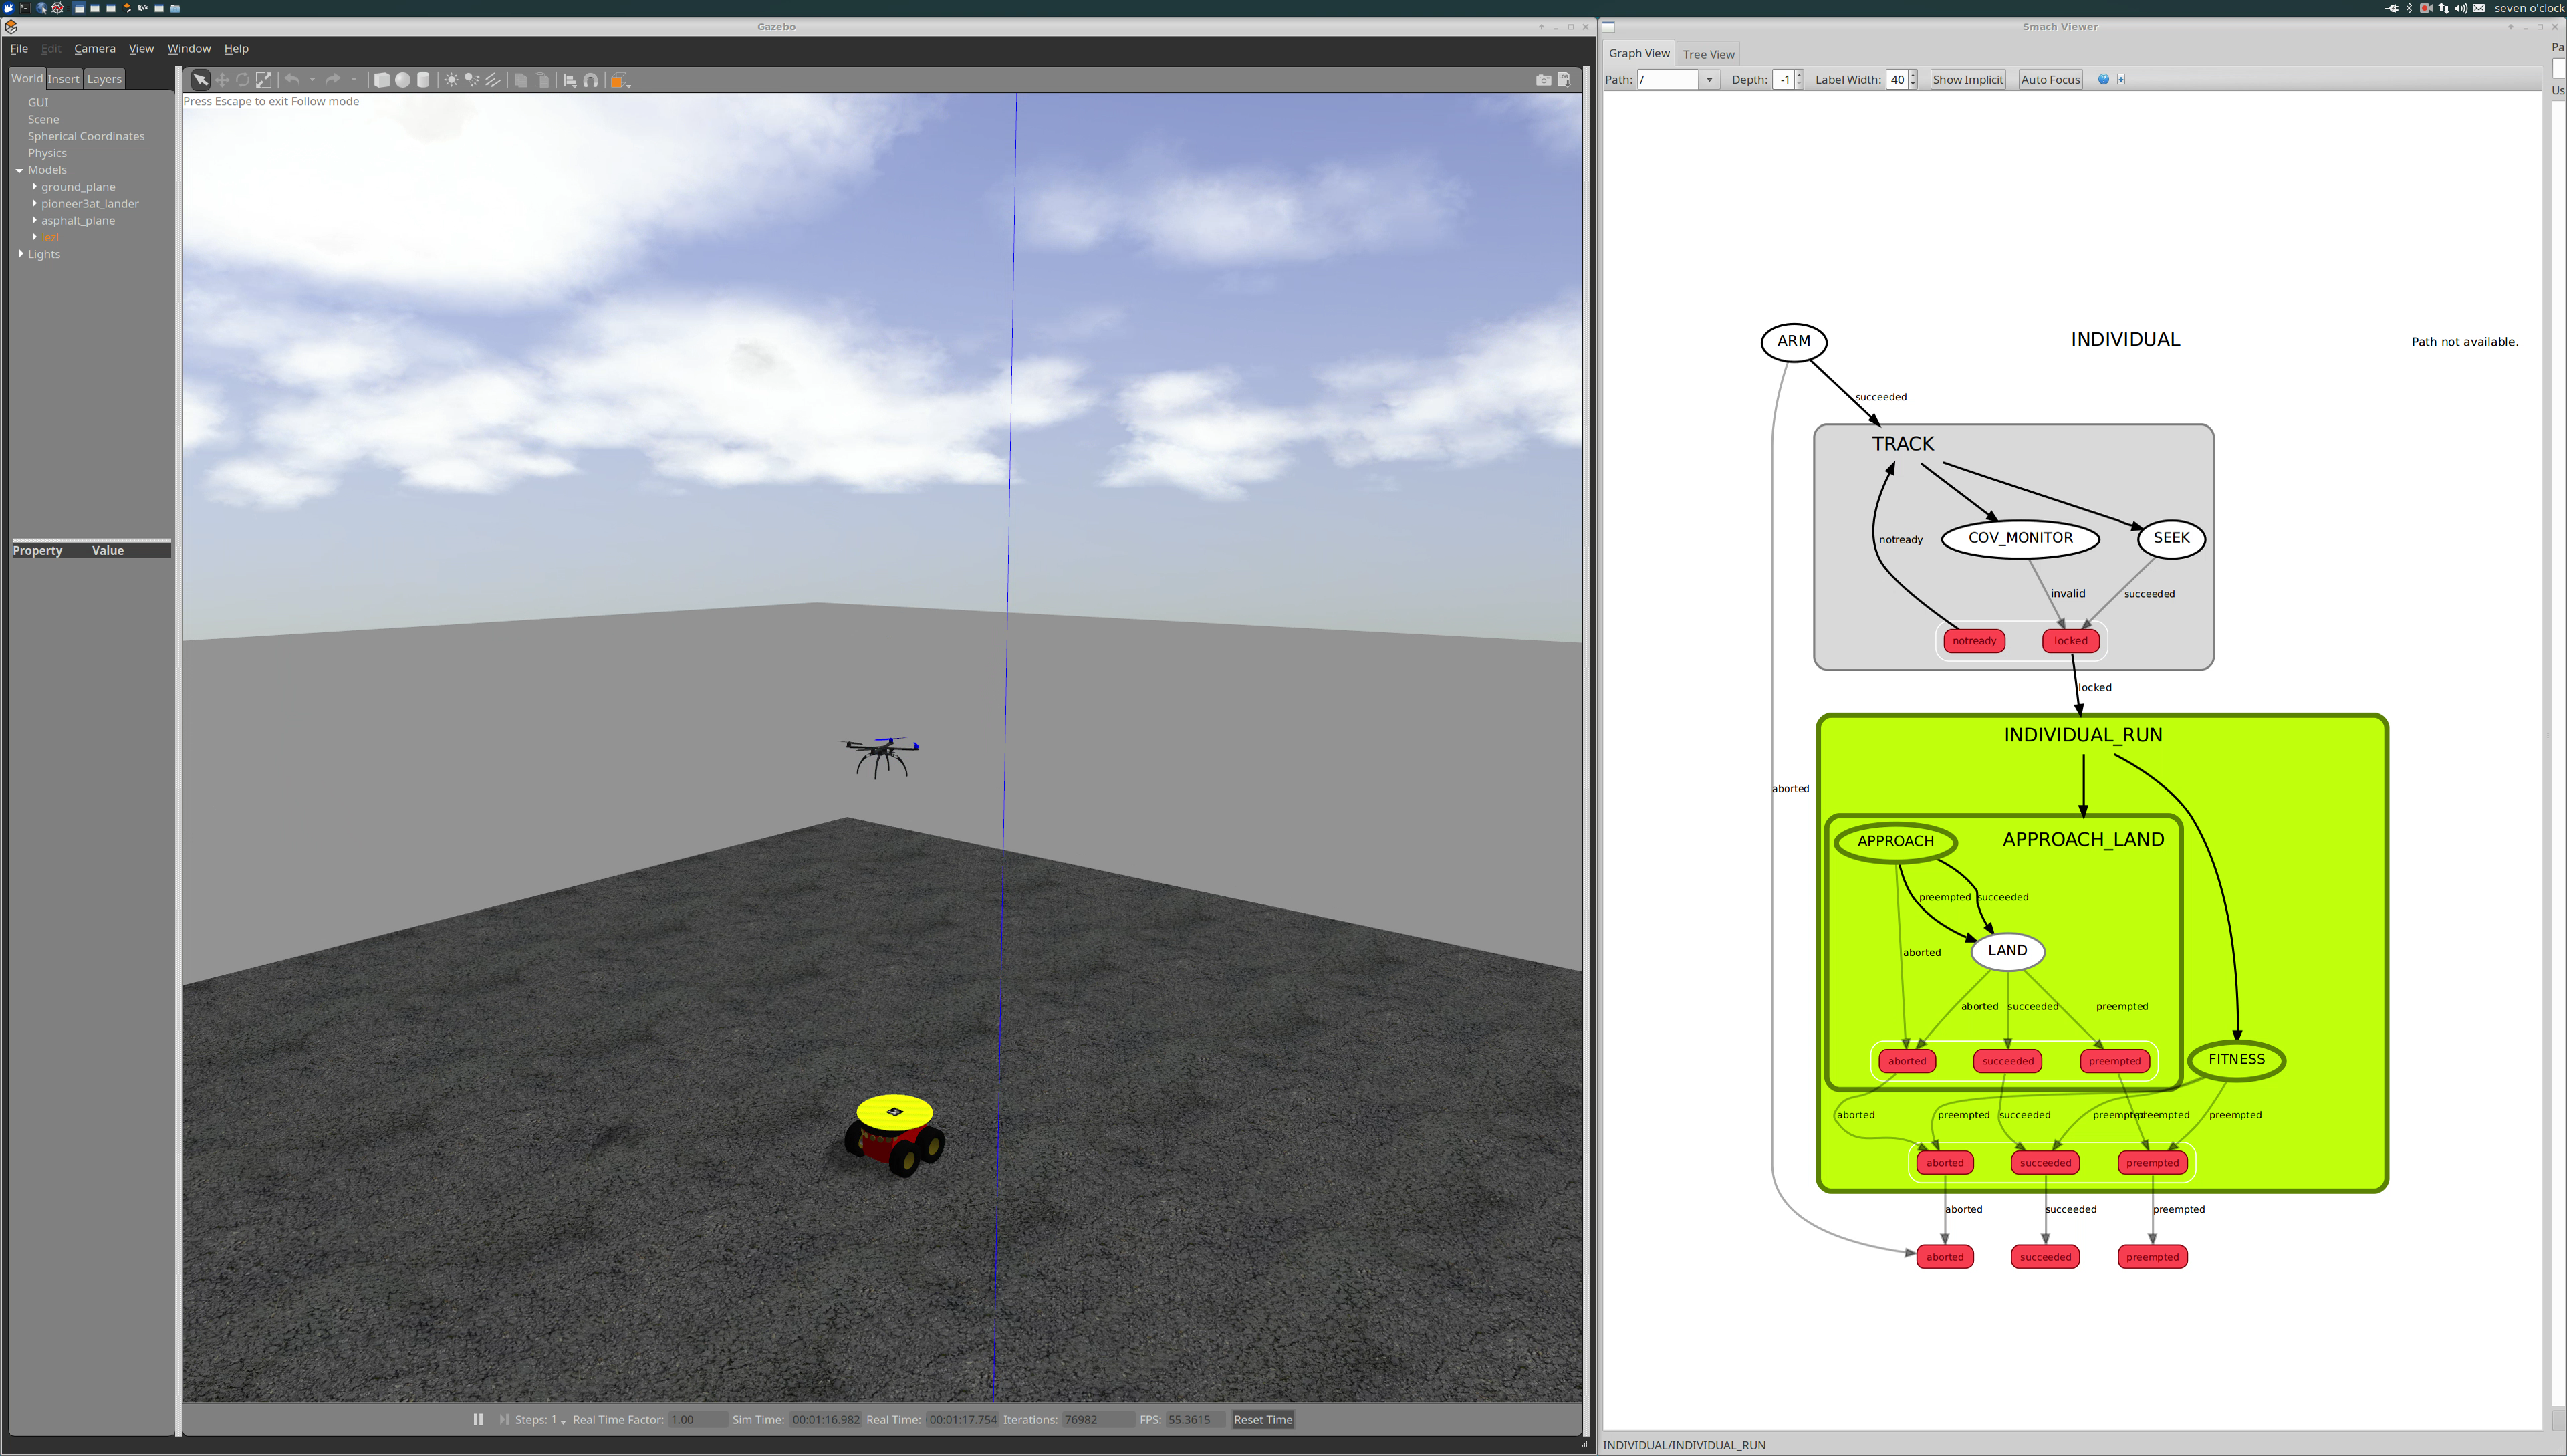
\includegraphics[width=0.6\textwidth]{images/static_captures/static-15h39m54s115}
    \caption{Image of the simulation and live state diagram while vehicle is approaching the
    platform.}\label{f:sim_static_shot}
\end{figure}

The state of the vehicle is managed by fusing together the positional estimate from the camera sensor and the
AprilTag estimate (see \cref{s:landing:cv}), as well as orientation information from the onboard IMU using an
extended kalman filter (EKF). This estimate is only valid when the vehicle has a visual track on the target
platform; otherwise, it is assumed that the vehicle is still in transit from its launch location, or it has
landed. 

As can be seen in \cref{f:smach}, a mission starts in the ``ARM'' by arming the vehicle and immediately
sending it a waypoint which is near the target's location. Once the vehicle has received the waypoint, it
enters the ``TRACK'' state and is en route to the target location. While in this state, it monitors the
quality of its visual estimation of the target location by evaluating the norm of the covariance matrix 
computed by the EKF. Only when the covariance is sufficiently small does the vehicle transition to the next
state.

The transition to the ``APPROACH\_LAND'' state signals the transfer of control from the flight controller's
waypoint manager to the FISs. The "APPROACH\_LAND" state is simply a composition of two substates, "APPROACH"
and "LAND". During the "APPROACH" substate, the EKF is still running, sending estimates to the fuzzy logic
controller. The fuzzy logic controller is sending velocity setpoints to the onboard flight controller, thus
closing the feedback loop. The desired outcome of this state is to get the vehicle in a position above
the platform such that we can initiate the landing sequence. When the vehicle meets a proximity threshold,
it transitions to the ``LAND'' substate and puts down onto the landing pad. The details of the simulation,
control, vision estimation, and development process are discussed at length in the following sections.

\subsection{Computer Vision}\label{s:landing:cv}
Image processing is handled by a node in the ROS computation graph that is constantly processing image outputs
from the onboard camera. Once it senses the platform, it then publishes
a state estimation to the rest of the nodes in the ROS graph. Much emphasis is put on the sensing algorithms to be computationally efficient to decrease the load on the
on-board computer. For this purpose, only a small number of image processes are required to detect and locate
the target. As a first pass, the image is brought into the Hue-Saturation-Value (HSV) color space. This has
been shown to be a robust space in which to perform color detection and segmentation in uncontrolled and
unpredictable lighting conditions\cite{zhao2002robust}. A simple thresholding is performed on the image to
isolate a sufficiently wide band of yellows to match the color of the target and dilate this to a binary blob.
From this binary image, the image moments are calculated by
\begin{figure}[ht!]
    \centering
    \includegraphics[width=0.8\textwidth]{images/rs_working_apriltags_crop.png}
    \caption{Simulated image sensor detection of AprilTag marker.}\label{f:apriltag}
\end{figure}

\begin{equation}\label{e:im_moments} 
    m_{ij}=\sum_{x,y}x^iy^jI_{xy}
\end{equation}
\nomenclature[]{$m_{ij}$}{Raw image moment}
\nomenclature[]{$I_{xy}$}{Pixel intensity value}
where $I_{xy}$ is the pixel intensity value for each pixel $(x,y)$ (equal to 1 for this binary blob) and $i,j
= 0,1,2$. From this it can be seen that $m_{00}$ describes the area and $\frac{m_{10}}{m_{00}}$ and
$\frac{m_{01}}{m_{00}}$ describe the centroids $\overline{x}_p$ and $\overline{y}_p$ in terms of
pixels\cite{hu1962visual}. The blob is assumed to be circular and hence a diameter is extracted from the pixel
area. Using the focal length of the sensor, these image points are then projected onto the ground plane using
the known diameter of the landing pad and a vertical offset estimate is obtained as is shown in
\cref{e:dist_est}.
\begin{equation}\label{e:dist_est}
    d_z=\frac{d\cdot f}{m\cdot d_p}
\end{equation}
where $f$ is the focal length of the camera in units of length, $d$ is the known diameter of the landing pad,
$d_p$ is the estimated diameter in pixels, and $m$ represents a scaling factor in units of \si{\px\per\mm}
(unity in the simulation).
\nomenclature[]{$f$}{Focal length of image sensor}
\nomenclature[]{$m$}{Pixel scaling factor}
Assuming that the image plane and the ground plane are parallel, the center of the image can be assumed to
point directly below the vehicle and the horizontal offsets to the landing pad can then be calculated as
\begin{align}\label{e:horiz_est}
    d_x &= d_z\cdot\frac{m\overline{x}_p}{f}\\
    d_y &= d_z\cdot\frac{m\overline{y}_p}{f}\label{e:horiz_est-y}
\end{align}
\nomenclature[]{$d_x$}{Horizontal offset error from vehicle to target in the body-fixed $x$-axis}
\nomenclature[]{$d_y$}{Horizontal offset error from vehicle to target in the body-fixed $y$-axis}
\nomenclature[]{$d_z$}{Vertical offset error from vehicle to the target}

Unless the camera is mounted to a perfect gimbal, the image plane cannot be assumed to be parallel to the
ground plane, thus invalidating \crefrange{e:horiz_est}{e:horiz_est-y}. To overcome this, the rotation
sequence needed to transform the image into body-relative coordinates is found and applied to the image data.
The camera is assumed to be rigidly affixed to the body of the vehicle, thus this is a simple static
transformation. Then, the vehicle body frame is related to the inertial frame by another rotation. The landing
pad is assumed to be on level ground and the distance between the vehicle and pad is estimated from
\cref{e:dist_est}. Note that although there will be image skew when the vehicle is under some rotation, the error in estimated distance this introduces is small compared to the actual distance of the vehicle from
the target. As the vehicle approaches the target, the estimate improves in quality due to a crisper image,
level flight, and the addition of AprilTag estimation.

In order to account for vehicle attitude, a rotation sequence is applied to the projected target location.
Let $R\left(\phi, \theta, \psi\right)$ be the rotation matrix defined as
\begin{equation}
    R(\phi,\theta,\psi) = 
    \begin{bmatrix}
            c_{\theta}c_{\psi}                           & -c_{\theta}s_{\phi}                           & s_{\theta}\\
            c_{\phi}s_{\psi} + c_{\psi}s_{\phi}s_{\theta} & c_{\phi}c_{\psi} - c_{\psi}s_{\phi}s_{\theta} & -c_{\theta}s_{\phi}\\
            s_{\phi}s_{\psi} -c_{\phi}c_{\psi}s_{\theta} & c_{\psi}s_{\phi} + c_{\phi}s_{\theta}s_{\psi} & c_{\phi}c_{\theta}
    \end{bmatrix}
\end{equation}
where $\phi$, $\theta$, and $\psi$ are vehicle roll, pitch and yaw respectively. $c_{\alpha}$ and $s_{\alpha}$
represent $\cos{\alpha}$ and $\sin{\alpha}$ respectively. Let $R_x^y$ represent the rotation from frame $x$ to
$y$, then $R_x^yR_y^z$ is the rotation from frame $x$ to frame $z$ with respect to the stationary frame $x$.
Now assuming the vehicle can estimate its orientation from the onboard inertial measurement unit, the
following rotation matrices can be defined.
\begin{align}
    R_{cam}^{body}   & = R(\pi, 0, 0)\label{e:rot_cam_bod}\\
    R_{body}^{inert} & = R(\phi, \theta, \psi)\label{e:rot_body_inert}
\end{align}
where $R_{x}^{y}$ represents the rotation from frame $x$ to frame $y$. These rotations are then prefixed to the
projected point found  in \crefrange{e:dist_est}{e:horiz_est-y} to find the point in world units with respect
to the vehicle.
\begin{align}\label{e:rotate}
    P_i = \begin{pmatrix}d_x\\d_y\\d_z\end{pmatrix}\\
    P_r = R_{body}^{inert}R_{cam}^{body}P_i
\end{align}
where $P_i$ is the projected point of the target in the plane parallel to the image plane, and $P_r$ is the
rotated point of the target with respect to the vehicle.

As the vehicle approaches the landing pad, the image field of view is overtaken by the landing pad itself and
the former segmentation no longer becomes effective. For this purpose, an AprilTag\cite{olson2011tags} (see
\cref{f:apriltag}) is placed on the center of the target. In \cref{f:landing_ims}, a landing approach is
illustrated from the viewpoint of the image sensor. This figure shows three different stages of the image
processing pipeline: raw image capture ( \crefrange{f:colora}{f:colorb}), AprilTag detection
(\crefrange{f:aprila}{f:aprilb}), and platform detection (\crefrange{f:cva}{f:cvb}). Individual estimates from
both the AprilTag detection and platform detection are then fused using an EKF (\cref{s:ekf}). 

\begin{figure}
    \begin{subfigmatrix}{4}% number of columns
        \subfigure[\label{f:colora}]{\includegraphics[width=0.2\textwidth]{images/image1_18469000.png}}
        \subfigure[]{\includegraphics[width=0.2\textwidth]{images/image1_30863000.png}}
        \subfigure[]{\includegraphics[width=0.2\textwidth]{images/image1_36074000.png}}
        \subfigure[\label{f:colorb}]{\includegraphics[width=0.2\textwidth]{images/image1_38233000.png}}
        \subfigure[\label{f:aprila}]{\includegraphics[width=0.2\textwidth]{images/image2_18469000.png}}
        \subfigure[]{\includegraphics[width=0.2\textwidth]{images/image2_30863000.png}}
        \subfigure[]{\includegraphics[width=0.2\textwidth]{images/image2_36074000.png}}
        \subfigure[\label{f:aprilb}]{\includegraphics[width=0.2\textwidth]{images/image2_38233000.png}}
        \subfigure[\label{f:cva}]{\includegraphics[width=0.2\textwidth]{images/image1_18469000_proc.png}}
        \subfigure[]{\includegraphics[width=0.2\textwidth]{images/image1_30863000_proc.png}}
        \subfigure[]{\includegraphics[width=0.2\textwidth]{images/image1_36074000_proc.png}}
        \subfigure[\label{f:cvb}]{\includegraphics[width=0.2\textwidth]{images/image1_38233000_proc.png}}
    \end{subfigmatrix}
    \caption{A time series of images taken during the landing maneuver.}
    \label{f:landing_ims}
\end{figure}

\section{Controller}\label{s:landing:controller}
Control is actuated on the vehicle by providing velocity setpoints to the flight controller, $v_x$, $v_y$,
$v_z$, and yaw rate, $\dot{\psi}$. Ideally either linear acceleration setpoints or forces would be the control
output, but limitations in the flight controller make this impossible at this time. Setting velocities allows
the controller to cope with step changes to position offset well, but have difficulties tracking ramps. The
yaw angle, $\psi$ of the vehicle at landing is irrelevant for this project, but the controller is able to
control that axis regardless.

\subsection{PID Controller}
A PID controller was created which uses error estimates and sends velocity setpoints to the flight controller.
Due to the lack of a mathematical model of the system, the PID gains were found by iterating the simulation
with various position setpoints and dynamically adjusting the gains while observing the response visually.
This closely mimics the method by which PID gains are attained in the tuning of an actual quadrotor by flying
a series of test flights and adjusting gain values by feel. In this way, a reasonable response and landing
sequence was achieved for first a static target and then repeated for a dynamic target moving with constant
velocity. The results are presented in \crefrange{f:pid_stat}{f:pid_dyn} in which the normed horizontal offset
from target is shown in conjunction with the vertical distance to the platform. This view of the data gives an
overall sens of how the controller performs by showing how smooth the trajectory of the vehicle is as it
approaches the platform.  Viewing the charts, it is
apparent that as the vehicle approaches the target, it tends to accumulate horizontal errors and must correct
more frequently, particularly in the dynamic case. In both cases, the quadrotor managed to successfully land
on the target. In the static case, the final offset from the center of the target was less than \SI{5}{\cm}.
For the dynamic case, the error was \SI{7}{\cm} which nearly displaced it from the target surface. In both
cases, the sink rate and yaw rates were controlled by simple PD controllers. It can be seen that the controller took a significantly longer time to intercept and land
on the moving target as it repeatedly had trouble responding to the motion and would temporarily lose its
visual track. This is apparent in the large spiking errors in \cref{f:pid_dyn}.

%\begin{figure}
    %\centering
    %\begin{tikzpicture}[gnuplot]
%% generated with GNUPLOT 5.0p3 (Lua 5.1; terminal rev. 99, script rev. 100)
%% Tue 27 Mar 2018 03:05:26 AM EDT
\path (0.000,0.000) rectangle (12.500,8.750);
\gpcolor{color=gp lt color border}
\gpsetlinetype{gp lt border}
\gpsetdashtype{gp dt solid}
\gpsetlinewidth{1.00}
\draw[gp path] (1.012,0.616)--(1.192,0.616);
\draw[gp path] (11.947,0.616)--(11.767,0.616);
\node[gp node right] at (0.828,0.616) {$0$};
\draw[gp path] (1.012,1.337)--(1.192,1.337);
\draw[gp path] (11.947,1.337)--(11.767,1.337);
\node[gp node right] at (0.828,1.337) {$0.5$};
\draw[gp path] (1.012,2.058)--(1.192,2.058);
\draw[gp path] (11.947,2.058)--(11.767,2.058);
\node[gp node right] at (0.828,2.058) {$1$};
\draw[gp path] (1.012,2.779)--(1.192,2.779);
\draw[gp path] (11.947,2.779)--(11.767,2.779);
\node[gp node right] at (0.828,2.779) {$1.5$};
\draw[gp path] (1.012,3.500)--(1.192,3.500);
\draw[gp path] (11.947,3.500)--(11.767,3.500);
\node[gp node right] at (0.828,3.500) {$2$};
\draw[gp path] (1.012,4.221)--(1.192,4.221);
\draw[gp path] (11.947,4.221)--(11.767,4.221);
\node[gp node right] at (0.828,4.221) {$2.5$};
\draw[gp path] (1.012,4.941)--(1.192,4.941);
\draw[gp path] (11.947,4.941)--(11.767,4.941);
\node[gp node right] at (0.828,4.941) {$3$};
\draw[gp path] (1.012,5.662)--(1.192,5.662);
\draw[gp path] (11.947,5.662)--(11.767,5.662);
\node[gp node right] at (0.828,5.662) {$3.5$};
\draw[gp path] (1.012,6.383)--(1.192,6.383);
\draw[gp path] (11.947,6.383)--(11.767,6.383);
\node[gp node right] at (0.828,6.383) {$4$};
\draw[gp path] (1.012,7.104)--(1.192,7.104);
\draw[gp path] (11.947,7.104)--(11.767,7.104);
\node[gp node right] at (0.828,7.104) {$4.5$};
\draw[gp path] (1.012,7.825)--(1.192,7.825);
\draw[gp path] (11.947,7.825)--(11.767,7.825);
\node[gp node right] at (0.828,7.825) {$5$};
\draw[gp path] (1.012,0.616)--(1.012,0.796);
\draw[gp path] (1.012,7.825)--(1.012,7.645);
\node[gp node center] at (1.012,0.308) {$0$};
\draw[gp path] (2.574,0.616)--(2.574,0.796);
\draw[gp path] (2.574,7.825)--(2.574,7.645);
\node[gp node center] at (2.574,0.308) {$5$};
\draw[gp path] (4.136,0.616)--(4.136,0.796);
\draw[gp path] (4.136,7.825)--(4.136,7.645);
\node[gp node center] at (4.136,0.308) {$10$};
\draw[gp path] (5.698,0.616)--(5.698,0.796);
\draw[gp path] (5.698,7.825)--(5.698,7.645);
\node[gp node center] at (5.698,0.308) {$15$};
\draw[gp path] (7.261,0.616)--(7.261,0.796);
\draw[gp path] (7.261,7.825)--(7.261,7.645);
\node[gp node center] at (7.261,0.308) {$20$};
\draw[gp path] (8.823,0.616)--(8.823,0.796);
\draw[gp path] (8.823,7.825)--(8.823,7.645);
\node[gp node center] at (8.823,0.308) {$25$};
\draw[gp path] (10.385,0.616)--(10.385,0.796);
\draw[gp path] (10.385,7.825)--(10.385,7.645);
\node[gp node center] at (10.385,0.308) {$30$};
\draw[gp path] (11.947,0.616)--(11.947,0.796);
\draw[gp path] (11.947,7.825)--(11.947,7.645);
\node[gp node center] at (11.947,0.308) {$35$};
\draw[gp path] (1.012,7.825)--(1.012,0.616)--(11.947,0.616)--(11.947,7.825)--cycle;
\node[gp node center] at (6.479,8.287) {Planar error};
\node[gp node right] at (10.479,7.491) {e_{xy}};
\gpcolor{rgb color={0.580,0.000,0.827}}
\gpsetpointsize{4.00}
\gppoint{gp mark 1}{(1.012,6.741)}
\gppoint{gp mark 1}{(1.012,6.741)}
\gppoint{gp mark 1}{(1.013,6.741)}
\gppoint{gp mark 1}{(1.013,6.741)}
\gppoint{gp mark 1}{(1.013,6.741)}
\gppoint{gp mark 1}{(1.014,6.741)}
\gppoint{gp mark 1}{(1.014,6.741)}
\gppoint{gp mark 1}{(1.014,6.741)}
\gppoint{gp mark 1}{(1.014,6.741)}
\gppoint{gp mark 1}{(1.015,6.741)}
\gppoint{gp mark 1}{(1.015,6.741)}
\gppoint{gp mark 1}{(1.015,6.741)}
\gppoint{gp mark 1}{(1.016,6.741)}
\gppoint{gp mark 1}{(1.016,6.741)}
\gppoint{gp mark 1}{(1.016,6.741)}
\gppoint{gp mark 1}{(1.017,6.741)}
\gppoint{gp mark 1}{(1.017,6.741)}
\gppoint{gp mark 1}{(1.017,6.741)}
\gppoint{gp mark 1}{(1.018,6.741)}
\gppoint{gp mark 1}{(1.018,6.741)}
\gppoint{gp mark 1}{(1.018,6.741)}
\gppoint{gp mark 1}{(1.018,6.741)}
\gppoint{gp mark 1}{(1.019,6.741)}
\gppoint{gp mark 1}{(1.019,6.741)}
\gppoint{gp mark 1}{(1.019,6.741)}
\gppoint{gp mark 1}{(1.020,6.741)}
\gppoint{gp mark 1}{(1.020,6.741)}
\gppoint{gp mark 1}{(1.020,6.741)}
\gppoint{gp mark 1}{(1.021,6.741)}
\gppoint{gp mark 1}{(1.021,6.741)}
\gppoint{gp mark 1}{(1.021,6.741)}
\gppoint{gp mark 1}{(1.022,6.741)}
\gppoint{gp mark 1}{(1.022,6.741)}
\gppoint{gp mark 1}{(1.022,6.741)}
\gppoint{gp mark 1}{(1.023,6.741)}
\gppoint{gp mark 1}{(1.023,6.741)}
\gppoint{gp mark 1}{(1.023,6.741)}
\gppoint{gp mark 1}{(1.024,6.741)}
\gppoint{gp mark 1}{(1.024,6.741)}
\gppoint{gp mark 1}{(1.024,6.741)}
\gppoint{gp mark 1}{(1.024,6.741)}
\gppoint{gp mark 1}{(1.024,6.741)}
\gppoint{gp mark 1}{(1.025,6.741)}
\gppoint{gp mark 1}{(1.025,6.741)}
\gppoint{gp mark 1}{(1.026,6.741)}
\gppoint{gp mark 1}{(1.026,6.741)}
\gppoint{gp mark 1}{(1.026,6.741)}
\gppoint{gp mark 1}{(1.027,6.741)}
\gppoint{gp mark 1}{(1.027,6.741)}
\gppoint{gp mark 1}{(1.027,6.741)}
\gppoint{gp mark 1}{(1.028,6.741)}
\gppoint{gp mark 1}{(1.028,6.741)}
\gppoint{gp mark 1}{(1.028,6.741)}
\gppoint{gp mark 1}{(1.029,6.741)}
\gppoint{gp mark 1}{(1.029,6.741)}
\gppoint{gp mark 1}{(1.029,6.741)}
\gppoint{gp mark 1}{(1.029,6.741)}
\gppoint{gp mark 1}{(1.030,6.741)}
\gppoint{gp mark 1}{(1.030,6.741)}
\gppoint{gp mark 1}{(1.030,6.741)}
\gppoint{gp mark 1}{(1.031,6.741)}
\gppoint{gp mark 1}{(1.031,6.741)}
\gppoint{gp mark 1}{(1.031,6.741)}
\gppoint{gp mark 1}{(1.032,6.741)}
\gppoint{gp mark 1}{(1.032,6.741)}
\gppoint{gp mark 1}{(1.032,6.741)}
\gppoint{gp mark 1}{(1.033,6.741)}
\gppoint{gp mark 1}{(1.033,6.741)}
\gppoint{gp mark 1}{(1.033,6.741)}
\gppoint{gp mark 1}{(1.034,6.741)}
\gppoint{gp mark 1}{(1.034,6.741)}
\gppoint{gp mark 1}{(1.034,6.741)}
\gppoint{gp mark 1}{(1.034,6.741)}
\gppoint{gp mark 1}{(1.035,6.741)}
\gppoint{gp mark 1}{(1.035,6.741)}
\gppoint{gp mark 1}{(1.035,6.741)}
\gppoint{gp mark 1}{(1.036,6.741)}
\gppoint{gp mark 1}{(1.036,6.741)}
\gppoint{gp mark 1}{(1.036,6.741)}
\gppoint{gp mark 1}{(1.037,6.741)}
\gppoint{gp mark 1}{(1.037,6.741)}
\gppoint{gp mark 1}{(1.037,6.741)}
\gppoint{gp mark 1}{(1.038,6.741)}
\gppoint{gp mark 1}{(1.038,6.741)}
\gppoint{gp mark 1}{(1.038,6.741)}
\gppoint{gp mark 1}{(1.039,6.741)}
\gppoint{gp mark 1}{(1.039,6.741)}
\gppoint{gp mark 1}{(1.039,6.741)}
\gppoint{gp mark 1}{(1.039,6.741)}
\gppoint{gp mark 1}{(1.040,6.741)}
\gppoint{gp mark 1}{(1.040,6.741)}
\gppoint{gp mark 1}{(1.040,6.741)}
\gppoint{gp mark 1}{(1.041,6.741)}
\gppoint{gp mark 1}{(1.041,6.741)}
\gppoint{gp mark 1}{(1.041,6.741)}
\gppoint{gp mark 1}{(1.042,6.741)}
\gppoint{gp mark 1}{(1.042,6.741)}
\gppoint{gp mark 1}{(1.042,6.741)}
\gppoint{gp mark 1}{(1.043,6.741)}
\gppoint{gp mark 1}{(1.043,6.741)}
\gppoint{gp mark 1}{(1.043,6.741)}
\gppoint{gp mark 1}{(1.044,6.741)}
\gppoint{gp mark 1}{(1.044,6.741)}
\gppoint{gp mark 1}{(1.044,6.741)}
\gppoint{gp mark 1}{(1.044,6.741)}
\gppoint{gp mark 1}{(1.045,6.741)}
\gppoint{gp mark 1}{(1.045,6.741)}
\gppoint{gp mark 1}{(1.045,6.741)}
\gppoint{gp mark 1}{(1.046,6.741)}
\gppoint{gp mark 1}{(1.046,6.741)}
\gppoint{gp mark 1}{(1.047,6.741)}
\gppoint{gp mark 1}{(1.047,6.741)}
\gppoint{gp mark 1}{(1.047,6.741)}
\gppoint{gp mark 1}{(1.047,6.741)}
\gppoint{gp mark 1}{(1.048,6.741)}
\gppoint{gp mark 1}{(1.048,6.741)}
\gppoint{gp mark 1}{(1.048,6.741)}
\gppoint{gp mark 1}{(1.049,6.741)}
\gppoint{gp mark 1}{(1.049,6.741)}
\gppoint{gp mark 1}{(1.049,6.741)}
\gppoint{gp mark 1}{(1.049,6.741)}
\gppoint{gp mark 1}{(1.050,6.741)}
\gppoint{gp mark 1}{(1.050,6.741)}
\gppoint{gp mark 1}{(1.050,6.741)}
\gppoint{gp mark 1}{(1.051,6.741)}
\gppoint{gp mark 1}{(1.051,6.741)}
\gppoint{gp mark 1}{(1.051,6.741)}
\gppoint{gp mark 1}{(1.052,6.741)}
\gppoint{gp mark 1}{(1.052,6.741)}
\gppoint{gp mark 1}{(1.052,6.741)}
\gppoint{gp mark 1}{(1.053,6.741)}
\gppoint{gp mark 1}{(1.053,6.741)}
\gppoint{gp mark 1}{(1.053,6.741)}
\gppoint{gp mark 1}{(1.054,6.741)}
\gppoint{gp mark 1}{(1.054,6.741)}
\gppoint{gp mark 1}{(1.054,6.741)}
\gppoint{gp mark 1}{(1.054,6.741)}
\gppoint{gp mark 1}{(1.055,6.741)}
\gppoint{gp mark 1}{(1.055,6.741)}
\gppoint{gp mark 1}{(1.055,6.741)}
\gppoint{gp mark 1}{(1.056,6.741)}
\gppoint{gp mark 1}{(1.056,6.741)}
\gppoint{gp mark 1}{(1.056,6.741)}
\gppoint{gp mark 1}{(1.057,6.741)}
\gppoint{gp mark 1}{(1.057,6.741)}
\gppoint{gp mark 1}{(1.057,6.741)}
\gppoint{gp mark 1}{(1.058,6.741)}
\gppoint{gp mark 1}{(1.058,6.741)}
\gppoint{gp mark 1}{(1.058,6.741)}
\gppoint{gp mark 1}{(1.059,6.741)}
\gppoint{gp mark 1}{(1.059,6.741)}
\gppoint{gp mark 1}{(1.059,6.741)}
\gppoint{gp mark 1}{(1.059,6.741)}
\gppoint{gp mark 1}{(1.060,6.741)}
\gppoint{gp mark 1}{(1.060,6.741)}
\gppoint{gp mark 1}{(1.060,6.741)}
\gppoint{gp mark 1}{(1.061,6.741)}
\gppoint{gp mark 1}{(1.061,6.741)}
\gppoint{gp mark 1}{(1.061,6.741)}
\gppoint{gp mark 1}{(1.062,6.741)}
\gppoint{gp mark 1}{(1.062,6.741)}
\gppoint{gp mark 1}{(1.062,6.741)}
\gppoint{gp mark 1}{(1.063,6.741)}
\gppoint{gp mark 1}{(1.063,6.741)}
\gppoint{gp mark 1}{(1.063,6.741)}
\gppoint{gp mark 1}{(1.064,6.741)}
\gppoint{gp mark 1}{(1.064,6.741)}
\gppoint{gp mark 1}{(1.064,6.741)}
\gppoint{gp mark 1}{(1.064,6.741)}
\gppoint{gp mark 1}{(1.065,6.741)}
\gppoint{gp mark 1}{(1.065,6.741)}
\gppoint{gp mark 1}{(1.065,6.741)}
\gppoint{gp mark 1}{(1.066,6.741)}
\gppoint{gp mark 1}{(1.066,6.741)}
\gppoint{gp mark 1}{(1.066,6.741)}
\gppoint{gp mark 1}{(1.067,6.741)}
\gppoint{gp mark 1}{(1.067,6.741)}
\gppoint{gp mark 1}{(1.067,6.741)}
\gppoint{gp mark 1}{(1.068,6.741)}
\gppoint{gp mark 1}{(1.068,6.741)}
\gppoint{gp mark 1}{(1.068,6.741)}
\gppoint{gp mark 1}{(1.069,6.741)}
\gppoint{gp mark 1}{(1.069,6.741)}
\gppoint{gp mark 1}{(1.069,6.741)}
\gppoint{gp mark 1}{(1.069,6.741)}
\gppoint{gp mark 1}{(1.070,6.741)}
\gppoint{gp mark 1}{(1.070,6.741)}
\gppoint{gp mark 1}{(1.070,6.741)}
\gppoint{gp mark 1}{(1.071,6.741)}
\gppoint{gp mark 1}{(1.071,6.741)}
\gppoint{gp mark 1}{(1.071,6.741)}
\gppoint{gp mark 1}{(1.072,6.741)}
\gppoint{gp mark 1}{(1.072,6.741)}
\gppoint{gp mark 1}{(1.072,6.741)}
\gppoint{gp mark 1}{(1.073,6.741)}
\gppoint{gp mark 1}{(1.073,6.741)}
\gppoint{gp mark 1}{(1.073,6.741)}
\gppoint{gp mark 1}{(1.074,6.741)}
\gppoint{gp mark 1}{(1.074,6.741)}
\gppoint{gp mark 1}{(1.074,6.741)}
\gppoint{gp mark 1}{(1.074,6.741)}
\gppoint{gp mark 1}{(1.075,6.741)}
\gppoint{gp mark 1}{(1.075,6.741)}
\gppoint{gp mark 1}{(1.075,6.741)}
\gppoint{gp mark 1}{(1.076,6.741)}
\gppoint{gp mark 1}{(1.076,6.741)}
\gppoint{gp mark 1}{(1.076,6.741)}
\gppoint{gp mark 1}{(1.077,6.741)}
\gppoint{gp mark 1}{(1.077,6.741)}
\gppoint{gp mark 1}{(1.077,6.741)}
\gppoint{gp mark 1}{(1.078,6.741)}
\gppoint{gp mark 1}{(1.078,6.741)}
\gppoint{gp mark 1}{(1.078,6.741)}
\gppoint{gp mark 1}{(1.078,6.741)}
\gppoint{gp mark 1}{(1.079,6.741)}
\gppoint{gp mark 1}{(1.079,6.741)}
\gppoint{gp mark 1}{(1.079,6.741)}
\gppoint{gp mark 1}{(1.080,6.741)}
\gppoint{gp mark 1}{(1.080,6.741)}
\gppoint{gp mark 1}{(1.080,6.741)}
\gppoint{gp mark 1}{(1.081,6.741)}
\gppoint{gp mark 1}{(1.081,6.741)}
\gppoint{gp mark 1}{(1.081,6.741)}
\gppoint{gp mark 1}{(1.081,6.741)}
\gppoint{gp mark 1}{(1.082,6.741)}
\gppoint{gp mark 1}{(1.082,6.741)}
\gppoint{gp mark 1}{(1.083,6.741)}
\gppoint{gp mark 1}{(1.083,6.741)}
\gppoint{gp mark 1}{(1.083,6.741)}
\gppoint{gp mark 1}{(1.084,6.741)}
\gppoint{gp mark 1}{(1.084,6.741)}
\gppoint{gp mark 1}{(1.084,6.741)}
\gppoint{gp mark 1}{(1.084,6.741)}
\gppoint{gp mark 1}{(1.085,6.741)}
\gppoint{gp mark 1}{(1.085,6.741)}
\gppoint{gp mark 1}{(1.085,6.741)}
\gppoint{gp mark 1}{(1.085,6.741)}
\gppoint{gp mark 1}{(1.086,6.741)}
\gppoint{gp mark 1}{(1.086,6.741)}
\gppoint{gp mark 1}{(1.086,6.741)}
\gppoint{gp mark 1}{(1.087,6.741)}
\gppoint{gp mark 1}{(1.087,6.741)}
\gppoint{gp mark 1}{(1.087,6.741)}
\gppoint{gp mark 1}{(1.088,6.741)}
\gppoint{gp mark 1}{(1.088,6.741)}
\gppoint{gp mark 1}{(1.089,6.741)}
\gppoint{gp mark 1}{(1.089,6.741)}
\gppoint{gp mark 1}{(1.089,6.741)}
\gppoint{gp mark 1}{(1.089,6.741)}
\gppoint{gp mark 1}{(1.090,6.741)}
\gppoint{gp mark 1}{(1.090,6.741)}
\gppoint{gp mark 1}{(1.090,6.741)}
\gppoint{gp mark 1}{(1.091,6.741)}
\gppoint{gp mark 1}{(1.091,6.741)}
\gppoint{gp mark 1}{(1.091,6.741)}
\gppoint{gp mark 1}{(1.091,6.741)}
\gppoint{gp mark 1}{(1.092,6.741)}
\gppoint{gp mark 1}{(1.092,6.741)}
\gppoint{gp mark 1}{(1.093,6.741)}
\gppoint{gp mark 1}{(1.093,6.741)}
\gppoint{gp mark 1}{(1.093,6.741)}
\gppoint{gp mark 1}{(1.094,6.741)}
\gppoint{gp mark 1}{(1.094,6.741)}
\gppoint{gp mark 1}{(1.094,6.741)}
\gppoint{gp mark 1}{(1.094,6.741)}
\gppoint{gp mark 1}{(1.095,6.741)}
\gppoint{gp mark 1}{(1.095,6.741)}
\gppoint{gp mark 1}{(1.095,6.741)}
\gppoint{gp mark 1}{(1.096,6.741)}
\gppoint{gp mark 1}{(1.096,6.741)}
\gppoint{gp mark 1}{(1.096,6.741)}
\gppoint{gp mark 1}{(1.097,6.741)}
\gppoint{gp mark 1}{(1.097,6.741)}
\gppoint{gp mark 1}{(1.097,6.741)}
\gppoint{gp mark 1}{(1.098,6.741)}
\gppoint{gp mark 1}{(1.098,6.741)}
\gppoint{gp mark 1}{(1.098,6.741)}
\gppoint{gp mark 1}{(1.099,6.741)}
\gppoint{gp mark 1}{(1.099,6.741)}
\gppoint{gp mark 1}{(1.099,6.741)}
\gppoint{gp mark 1}{(1.099,6.741)}
\gppoint{gp mark 1}{(1.100,6.741)}
\gppoint{gp mark 1}{(1.100,6.741)}
\gppoint{gp mark 1}{(1.100,6.741)}
\gppoint{gp mark 1}{(1.101,6.741)}
\gppoint{gp mark 1}{(1.101,6.741)}
\gppoint{gp mark 1}{(1.101,6.741)}
\gppoint{gp mark 1}{(1.101,6.741)}
\gppoint{gp mark 1}{(1.102,6.741)}
\gppoint{gp mark 1}{(1.102,6.741)}
\gppoint{gp mark 1}{(1.103,6.741)}
\gppoint{gp mark 1}{(1.103,6.741)}
\gppoint{gp mark 1}{(1.103,6.741)}
\gppoint{gp mark 1}{(1.103,6.741)}
\gppoint{gp mark 1}{(1.104,6.741)}
\gppoint{gp mark 1}{(1.104,6.741)}
\gppoint{gp mark 1}{(1.104,6.741)}
\gppoint{gp mark 1}{(1.105,6.741)}
\gppoint{gp mark 1}{(1.105,6.741)}
\gppoint{gp mark 1}{(1.105,6.741)}
\gppoint{gp mark 1}{(1.106,6.741)}
\gppoint{gp mark 1}{(1.106,6.741)}
\gppoint{gp mark 1}{(1.106,6.741)}
\gppoint{gp mark 1}{(1.107,6.741)}
\gppoint{gp mark 1}{(1.107,6.741)}
\gppoint{gp mark 1}{(1.107,6.741)}
\gppoint{gp mark 1}{(1.108,6.741)}
\gppoint{gp mark 1}{(1.108,6.741)}
\gppoint{gp mark 1}{(1.108,6.741)}
\gppoint{gp mark 1}{(1.109,6.741)}
\gppoint{gp mark 1}{(1.109,6.741)}
\gppoint{gp mark 1}{(1.109,6.741)}
\gppoint{gp mark 1}{(1.109,6.741)}
\gppoint{gp mark 1}{(1.110,6.741)}
\gppoint{gp mark 1}{(1.110,6.741)}
\gppoint{gp mark 1}{(1.110,6.741)}
\gppoint{gp mark 1}{(1.111,6.741)}
\gppoint{gp mark 1}{(1.111,6.741)}
\gppoint{gp mark 1}{(1.111,6.741)}
\gppoint{gp mark 1}{(1.112,6.741)}
\gppoint{gp mark 1}{(1.112,6.741)}
\gppoint{gp mark 1}{(1.112,6.741)}
\gppoint{gp mark 1}{(1.113,6.741)}
\gppoint{gp mark 1}{(1.113,6.741)}
\gppoint{gp mark 1}{(1.113,6.741)}
\gppoint{gp mark 1}{(1.114,6.741)}
\gppoint{gp mark 1}{(1.114,6.741)}
\gppoint{gp mark 1}{(1.114,6.741)}
\gppoint{gp mark 1}{(1.114,6.741)}
\gppoint{gp mark 1}{(1.115,6.741)}
\gppoint{gp mark 1}{(1.115,6.741)}
\gppoint{gp mark 1}{(1.115,6.741)}
\gppoint{gp mark 1}{(1.116,6.741)}
\gppoint{gp mark 1}{(1.116,6.741)}
\gppoint{gp mark 1}{(1.116,6.741)}
\gppoint{gp mark 1}{(1.117,6.741)}
\gppoint{gp mark 1}{(1.117,6.741)}
\gppoint{gp mark 1}{(1.117,6.741)}
\gppoint{gp mark 1}{(1.118,6.741)}
\gppoint{gp mark 1}{(1.118,6.741)}
\gppoint{gp mark 1}{(1.118,6.741)}
\gppoint{gp mark 1}{(1.119,6.741)}
\gppoint{gp mark 1}{(1.119,6.741)}
\gppoint{gp mark 1}{(1.119,6.741)}
\gppoint{gp mark 1}{(1.119,6.741)}
\gppoint{gp mark 1}{(1.120,6.741)}
\gppoint{gp mark 1}{(1.120,6.741)}
\gppoint{gp mark 1}{(1.120,6.741)}
\gppoint{gp mark 1}{(1.121,6.741)}
\gppoint{gp mark 1}{(1.121,6.741)}
\gppoint{gp mark 1}{(1.121,6.741)}
\gppoint{gp mark 1}{(1.122,6.741)}
\gppoint{gp mark 1}{(1.122,6.741)}
\gppoint{gp mark 1}{(1.122,6.741)}
\gppoint{gp mark 1}{(1.123,6.741)}
\gppoint{gp mark 1}{(1.123,6.741)}
\gppoint{gp mark 1}{(1.123,6.741)}
\gppoint{gp mark 1}{(1.124,6.741)}
\gppoint{gp mark 1}{(1.124,6.741)}
\gppoint{gp mark 1}{(1.124,6.741)}
\gppoint{gp mark 1}{(1.124,6.741)}
\gppoint{gp mark 1}{(1.125,6.741)}
\gppoint{gp mark 1}{(1.125,6.741)}
\gppoint{gp mark 1}{(1.125,6.741)}
\gppoint{gp mark 1}{(1.126,6.741)}
\gppoint{gp mark 1}{(1.126,6.741)}
\gppoint{gp mark 1}{(1.127,6.741)}
\gppoint{gp mark 1}{(1.127,6.741)}
\gppoint{gp mark 1}{(1.127,6.741)}
\gppoint{gp mark 1}{(1.127,6.741)}
\gppoint{gp mark 1}{(1.128,6.741)}
\gppoint{gp mark 1}{(1.128,6.741)}
\gppoint{gp mark 1}{(1.128,6.741)}
\gppoint{gp mark 1}{(1.129,6.741)}
\gppoint{gp mark 1}{(1.129,6.741)}
\gppoint{gp mark 1}{(1.129,6.741)}
\gppoint{gp mark 1}{(1.129,6.741)}
\gppoint{gp mark 1}{(1.130,6.741)}
\gppoint{gp mark 1}{(1.130,6.741)}
\gppoint{gp mark 1}{(1.130,6.741)}
\gppoint{gp mark 1}{(1.131,6.741)}
\gppoint{gp mark 1}{(1.131,6.741)}
\gppoint{gp mark 1}{(1.131,6.741)}
\gppoint{gp mark 1}{(1.132,6.741)}
\gppoint{gp mark 1}{(1.132,6.741)}
\gppoint{gp mark 1}{(1.132,6.741)}
\gppoint{gp mark 1}{(1.133,6.741)}
\gppoint{gp mark 1}{(1.133,6.741)}
\gppoint{gp mark 1}{(1.133,6.741)}
\gppoint{gp mark 1}{(1.134,6.741)}
\gppoint{gp mark 1}{(1.134,6.741)}
\gppoint{gp mark 1}{(1.134,6.741)}
\gppoint{gp mark 1}{(1.134,6.741)}
\gppoint{gp mark 1}{(1.135,6.741)}
\gppoint{gp mark 1}{(1.135,6.741)}
\gppoint{gp mark 1}{(1.135,6.741)}
\gppoint{gp mark 1}{(1.136,6.741)}
\gppoint{gp mark 1}{(1.136,6.741)}
\gppoint{gp mark 1}{(1.136,6.741)}
\gppoint{gp mark 1}{(1.136,6.741)}
\gppoint{gp mark 1}{(1.136,6.741)}
\gppoint{gp mark 1}{(1.137,6.741)}
\gppoint{gp mark 1}{(1.137,6.741)}
\gppoint{gp mark 1}{(1.138,6.741)}
\gppoint{gp mark 1}{(1.138,6.741)}
\gppoint{gp mark 1}{(1.139,6.741)}
\gppoint{gp mark 1}{(1.139,6.741)}
\gppoint{gp mark 1}{(1.139,6.741)}
\gppoint{gp mark 1}{(1.139,6.741)}
\gppoint{gp mark 1}{(1.140,6.741)}
\gppoint{gp mark 1}{(1.140,6.741)}
\gppoint{gp mark 1}{(1.140,6.741)}
\gppoint{gp mark 1}{(1.141,6.741)}
\gppoint{gp mark 1}{(1.141,6.741)}
\gppoint{gp mark 1}{(1.141,6.741)}
\gppoint{gp mark 1}{(1.142,6.741)}
\gppoint{gp mark 1}{(1.142,6.741)}
\gppoint{gp mark 1}{(1.142,6.741)}
\gppoint{gp mark 1}{(1.143,6.741)}
\gppoint{gp mark 1}{(1.143,6.741)}
\gppoint{gp mark 1}{(1.143,6.741)}
\gppoint{gp mark 1}{(1.144,6.741)}
\gppoint{gp mark 1}{(1.144,6.741)}
\gppoint{gp mark 1}{(1.144,6.741)}
\gppoint{gp mark 1}{(1.144,6.741)}
\gppoint{gp mark 1}{(1.145,6.741)}
\gppoint{gp mark 1}{(1.145,6.741)}
\gppoint{gp mark 1}{(1.145,6.741)}
\gppoint{gp mark 1}{(1.146,6.741)}
\gppoint{gp mark 1}{(1.146,6.741)}
\gppoint{gp mark 1}{(1.146,6.741)}
\gppoint{gp mark 1}{(1.147,6.741)}
\gppoint{gp mark 1}{(1.147,6.741)}
\gppoint{gp mark 1}{(1.147,6.741)}
\gppoint{gp mark 1}{(1.148,6.741)}
\gppoint{gp mark 1}{(1.148,6.741)}
\gppoint{gp mark 1}{(1.148,6.741)}
\gppoint{gp mark 1}{(1.149,6.741)}
\gppoint{gp mark 1}{(1.149,6.741)}
\gppoint{gp mark 1}{(1.149,6.741)}
\gppoint{gp mark 1}{(1.149,6.741)}
\gppoint{gp mark 1}{(1.150,6.741)}
\gppoint{gp mark 1}{(1.150,6.741)}
\gppoint{gp mark 1}{(1.150,6.741)}
\gppoint{gp mark 1}{(1.151,6.741)}
\gppoint{gp mark 1}{(1.151,6.741)}
\gppoint{gp mark 1}{(1.151,6.741)}
\gppoint{gp mark 1}{(1.152,6.741)}
\gppoint{gp mark 1}{(1.152,6.741)}
\gppoint{gp mark 1}{(1.152,6.741)}
\gppoint{gp mark 1}{(1.153,6.741)}
\gppoint{gp mark 1}{(1.153,6.741)}
\gppoint{gp mark 1}{(1.153,6.741)}
\gppoint{gp mark 1}{(1.154,6.741)}
\gppoint{gp mark 1}{(1.154,6.741)}
\gppoint{gp mark 1}{(1.154,6.741)}
\gppoint{gp mark 1}{(1.154,6.741)}
\gppoint{gp mark 1}{(1.155,6.741)}
\gppoint{gp mark 1}{(1.155,6.741)}
\gppoint{gp mark 1}{(1.155,6.741)}
\gppoint{gp mark 1}{(1.156,6.741)}
\gppoint{gp mark 1}{(1.156,6.741)}
\gppoint{gp mark 1}{(1.156,6.741)}
\gppoint{gp mark 1}{(1.157,6.741)}
\gppoint{gp mark 1}{(1.157,6.741)}
\gppoint{gp mark 1}{(1.157,6.741)}
\gppoint{gp mark 1}{(1.158,6.741)}
\gppoint{gp mark 1}{(1.158,6.741)}
\gppoint{gp mark 1}{(1.158,6.741)}
\gppoint{gp mark 1}{(1.158,6.741)}
\gppoint{gp mark 1}{(1.159,6.741)}
\gppoint{gp mark 1}{(1.159,6.741)}
\gppoint{gp mark 1}{(1.159,6.741)}
\gppoint{gp mark 1}{(1.159,6.741)}
\gppoint{gp mark 1}{(1.160,6.741)}
\gppoint{gp mark 1}{(1.160,6.741)}
\gppoint{gp mark 1}{(1.161,6.741)}
\gppoint{gp mark 1}{(1.161,6.741)}
\gppoint{gp mark 1}{(1.161,6.741)}
\gppoint{gp mark 1}{(1.162,6.741)}
\gppoint{gp mark 1}{(1.162,6.741)}
\gppoint{gp mark 1}{(1.162,6.741)}
\gppoint{gp mark 1}{(1.162,6.741)}
\gppoint{gp mark 1}{(1.163,6.741)}
\gppoint{gp mark 1}{(1.163,6.741)}
\gppoint{gp mark 1}{(1.164,6.741)}
\gppoint{gp mark 1}{(1.164,6.741)}
\gppoint{gp mark 1}{(1.164,6.741)}
\gppoint{gp mark 1}{(1.164,6.741)}
\gppoint{gp mark 1}{(1.165,6.741)}
\gppoint{gp mark 1}{(1.165,6.741)}
\gppoint{gp mark 1}{(1.165,6.741)}
\gppoint{gp mark 1}{(1.166,6.741)}
\gppoint{gp mark 1}{(1.166,6.741)}
\gppoint{gp mark 1}{(1.166,6.741)}
\gppoint{gp mark 1}{(1.167,6.741)}
\gppoint{gp mark 1}{(1.167,6.741)}
\gppoint{gp mark 1}{(1.167,6.741)}
\gppoint{gp mark 1}{(1.168,6.741)}
\gppoint{gp mark 1}{(1.168,6.741)}
\gppoint{gp mark 1}{(1.170,6.741)}
\gppoint{gp mark 1}{(1.170,6.741)}
\gppoint{gp mark 1}{(1.170,6.741)}
\gppoint{gp mark 1}{(1.170,6.741)}
\gppoint{gp mark 1}{(1.170,6.741)}
\gppoint{gp mark 1}{(1.170,6.741)}
\gppoint{gp mark 1}{(1.183,6.741)}
\gppoint{gp mark 1}{(1.184,6.741)}
\gppoint{gp mark 1}{(1.184,6.741)}
\gppoint{gp mark 1}{(1.184,6.741)}
\gppoint{gp mark 1}{(1.184,6.741)}
\gppoint{gp mark 1}{(1.184,6.741)}
\gppoint{gp mark 1}{(1.184,6.741)}
\gppoint{gp mark 1}{(1.184,6.741)}
\gppoint{gp mark 1}{(1.184,6.741)}
\gppoint{gp mark 1}{(1.184,6.741)}
\gppoint{gp mark 1}{(1.184,6.741)}
\gppoint{gp mark 1}{(1.185,6.741)}
\gppoint{gp mark 1}{(1.185,6.741)}
\gppoint{gp mark 1}{(1.185,6.741)}
\gppoint{gp mark 1}{(1.185,6.741)}
\gppoint{gp mark 1}{(1.185,6.741)}
\gppoint{gp mark 1}{(1.185,6.741)}
\gppoint{gp mark 1}{(1.185,6.741)}
\gppoint{gp mark 1}{(1.185,6.741)}
\gppoint{gp mark 1}{(1.185,6.741)}
\gppoint{gp mark 1}{(1.185,6.741)}
\gppoint{gp mark 1}{(1.186,6.741)}
\gppoint{gp mark 1}{(1.186,6.741)}
\gppoint{gp mark 1}{(1.186,6.741)}
\gppoint{gp mark 1}{(1.186,6.741)}
\gppoint{gp mark 1}{(1.186,6.741)}
\gppoint{gp mark 1}{(1.186,6.741)}
\gppoint{gp mark 1}{(1.186,6.741)}
\gppoint{gp mark 1}{(1.186,6.741)}
\gppoint{gp mark 1}{(1.186,6.741)}
\gppoint{gp mark 1}{(1.186,6.741)}
\gppoint{gp mark 1}{(1.186,6.741)}
\gppoint{gp mark 1}{(1.187,6.741)}
\gppoint{gp mark 1}{(1.187,6.741)}
\gppoint{gp mark 1}{(1.187,6.741)}
\gppoint{gp mark 1}{(1.187,6.741)}
\gppoint{gp mark 1}{(1.187,6.741)}
\gppoint{gp mark 1}{(1.187,6.741)}
\gppoint{gp mark 1}{(1.187,6.741)}
\gppoint{gp mark 1}{(1.187,6.741)}
\gppoint{gp mark 1}{(1.187,6.741)}
\gppoint{gp mark 1}{(1.187,6.741)}
\gppoint{gp mark 1}{(1.188,6.741)}
\gppoint{gp mark 1}{(1.197,6.741)}
\gppoint{gp mark 1}{(1.198,6.741)}
\gppoint{gp mark 1}{(1.198,6.741)}
\gppoint{gp mark 1}{(1.198,6.741)}
\gppoint{gp mark 1}{(1.198,6.741)}
\gppoint{gp mark 1}{(1.198,6.741)}
\gppoint{gp mark 1}{(1.198,6.741)}
\gppoint{gp mark 1}{(1.198,6.741)}
\gppoint{gp mark 1}{(1.198,6.741)}
\gppoint{gp mark 1}{(1.198,6.741)}
\gppoint{gp mark 1}{(1.198,6.741)}
\gppoint{gp mark 1}{(1.198,6.741)}
\gppoint{gp mark 1}{(1.199,6.741)}
\gppoint{gp mark 1}{(1.199,6.741)}
\gppoint{gp mark 1}{(1.199,6.741)}
\gppoint{gp mark 1}{(1.199,6.741)}
\gppoint{gp mark 1}{(1.199,6.741)}
\gppoint{gp mark 1}{(1.199,6.741)}
\gppoint{gp mark 1}{(1.199,6.741)}
\gppoint{gp mark 1}{(1.199,6.741)}
\gppoint{gp mark 1}{(1.199,6.741)}
\gppoint{gp mark 1}{(1.199,6.741)}
\gppoint{gp mark 1}{(1.199,6.741)}
\gppoint{gp mark 1}{(1.199,6.741)}
\gppoint{gp mark 1}{(1.199,6.741)}
\gppoint{gp mark 1}{(1.200,6.741)}
\gppoint{gp mark 1}{(1.200,6.741)}
\gppoint{gp mark 1}{(1.200,6.741)}
\gppoint{gp mark 1}{(1.200,6.741)}
\gppoint{gp mark 1}{(1.200,6.741)}
\gppoint{gp mark 1}{(1.200,6.741)}
\gppoint{gp mark 1}{(1.200,6.741)}
\gppoint{gp mark 1}{(1.200,6.741)}
\gppoint{gp mark 1}{(1.200,6.741)}
\gppoint{gp mark 1}{(1.200,6.741)}
\gppoint{gp mark 1}{(1.200,6.741)}
\gppoint{gp mark 1}{(1.201,6.741)}
\gppoint{gp mark 1}{(1.201,6.741)}
\gppoint{gp mark 1}{(1.201,6.741)}
\gppoint{gp mark 1}{(1.201,6.741)}
\gppoint{gp mark 1}{(1.201,6.741)}
\gppoint{gp mark 1}{(1.201,6.741)}
\gppoint{gp mark 1}{(1.201,6.741)}
\gppoint{gp mark 1}{(1.201,6.741)}
\gppoint{gp mark 1}{(1.211,6.741)}
\gppoint{gp mark 1}{(1.211,6.741)}
\gppoint{gp mark 1}{(1.211,6.741)}
\gppoint{gp mark 1}{(1.211,6.741)}
\gppoint{gp mark 1}{(1.211,6.741)}
\gppoint{gp mark 1}{(1.212,6.741)}
\gppoint{gp mark 1}{(1.212,6.741)}
\gppoint{gp mark 1}{(1.212,6.741)}
\gppoint{gp mark 1}{(1.212,6.741)}
\gppoint{gp mark 1}{(1.212,6.741)}
\gppoint{gp mark 1}{(1.212,6.741)}
\gppoint{gp mark 1}{(1.212,6.741)}
\gppoint{gp mark 1}{(1.212,6.741)}
\gppoint{gp mark 1}{(1.212,6.741)}
\gppoint{gp mark 1}{(1.212,6.741)}
\gppoint{gp mark 1}{(1.212,6.741)}
\gppoint{gp mark 1}{(1.213,6.741)}
\gppoint{gp mark 1}{(1.213,6.741)}
\gppoint{gp mark 1}{(1.213,6.741)}
\gppoint{gp mark 1}{(1.213,6.741)}
\gppoint{gp mark 1}{(1.213,6.741)}
\gppoint{gp mark 1}{(1.213,6.741)}
\gppoint{gp mark 1}{(1.213,6.741)}
\gppoint{gp mark 1}{(1.213,6.741)}
\gppoint{gp mark 1}{(1.213,6.741)}
\gppoint{gp mark 1}{(1.213,6.741)}
\gppoint{gp mark 1}{(1.214,6.741)}
\gppoint{gp mark 1}{(1.214,6.741)}
\gppoint{gp mark 1}{(1.214,6.741)}
\gppoint{gp mark 1}{(1.214,6.741)}
\gppoint{gp mark 1}{(1.214,6.741)}
\gppoint{gp mark 1}{(1.214,6.741)}
\gppoint{gp mark 1}{(1.214,6.741)}
\gppoint{gp mark 1}{(1.214,6.741)}
\gppoint{gp mark 1}{(1.214,6.741)}
\gppoint{gp mark 1}{(1.214,6.741)}
\gppoint{gp mark 1}{(1.214,6.741)}
\gppoint{gp mark 1}{(1.215,6.741)}
\gppoint{gp mark 1}{(1.215,6.741)}
\gppoint{gp mark 1}{(1.215,6.741)}
\gppoint{gp mark 1}{(1.215,6.741)}
\gppoint{gp mark 1}{(1.215,6.741)}
\gppoint{gp mark 1}{(1.215,6.741)}
\gppoint{gp mark 1}{(1.215,6.741)}
\gppoint{gp mark 1}{(1.224,6.741)}
\gppoint{gp mark 1}{(1.224,6.741)}
\gppoint{gp mark 1}{(1.225,6.741)}
\gppoint{gp mark 1}{(1.225,6.741)}
\gppoint{gp mark 1}{(1.225,6.741)}
\gppoint{gp mark 1}{(1.225,6.741)}
\gppoint{gp mark 1}{(1.225,6.741)}
\gppoint{gp mark 1}{(1.225,6.741)}
\gppoint{gp mark 1}{(1.225,6.741)}
\gppoint{gp mark 1}{(1.226,6.741)}
\gppoint{gp mark 1}{(1.226,6.741)}
\gppoint{gp mark 1}{(1.226,6.741)}
\gppoint{gp mark 1}{(1.226,6.741)}
\gppoint{gp mark 1}{(1.226,6.741)}
\gppoint{gp mark 1}{(1.226,6.741)}
\gppoint{gp mark 1}{(1.226,6.741)}
\gppoint{gp mark 1}{(1.226,6.741)}
\gppoint{gp mark 1}{(1.226,6.741)}
\gppoint{gp mark 1}{(1.227,6.741)}
\gppoint{gp mark 1}{(1.227,6.741)}
\gppoint{gp mark 1}{(1.227,6.741)}
\gppoint{gp mark 1}{(1.227,6.741)}
\gppoint{gp mark 1}{(1.227,6.741)}
\gppoint{gp mark 1}{(1.227,6.741)}
\gppoint{gp mark 1}{(1.227,6.741)}
\gppoint{gp mark 1}{(1.227,6.741)}
\gppoint{gp mark 1}{(1.227,6.741)}
\gppoint{gp mark 1}{(1.228,6.741)}
\gppoint{gp mark 1}{(1.228,6.741)}
\gppoint{gp mark 1}{(1.228,6.741)}
\gppoint{gp mark 1}{(1.228,6.741)}
\gppoint{gp mark 1}{(1.228,6.741)}
\gppoint{gp mark 1}{(1.228,6.741)}
\gppoint{gp mark 1}{(1.228,6.741)}
\gppoint{gp mark 1}{(1.228,6.741)}
\gppoint{gp mark 1}{(1.228,6.741)}
\gppoint{gp mark 1}{(1.228,6.741)}
\gppoint{gp mark 1}{(1.229,6.741)}
\gppoint{gp mark 1}{(1.229,6.741)}
\gppoint{gp mark 1}{(1.229,6.741)}
\gppoint{gp mark 1}{(1.229,6.741)}
\gppoint{gp mark 1}{(1.229,6.741)}
\gppoint{gp mark 1}{(1.229,6.741)}
\gppoint{gp mark 1}{(1.229,6.741)}
\gppoint{gp mark 1}{(1.229,6.741)}
\gppoint{gp mark 1}{(1.229,6.741)}
\gppoint{gp mark 1}{(1.229,6.741)}
\gppoint{gp mark 1}{(1.229,6.741)}
\gppoint{gp mark 1}{(1.230,6.741)}
\gppoint{gp mark 1}{(1.230,6.741)}
\gppoint{gp mark 1}{(1.230,6.741)}
\gppoint{gp mark 1}{(1.230,6.741)}
\gppoint{gp mark 1}{(1.230,6.741)}
\gppoint{gp mark 1}{(1.230,6.741)}
\gppoint{gp mark 1}{(1.230,6.741)}
\gppoint{gp mark 1}{(1.230,6.741)}
\gppoint{gp mark 1}{(1.230,6.741)}
\gppoint{gp mark 1}{(1.230,6.741)}
\gppoint{gp mark 1}{(1.230,6.741)}
\gppoint{gp mark 1}{(1.231,6.741)}
\gppoint{gp mark 1}{(1.231,6.741)}
\gppoint{gp mark 1}{(1.231,6.741)}
\gppoint{gp mark 1}{(1.231,6.741)}
\gppoint{gp mark 1}{(1.231,6.741)}
\gppoint{gp mark 1}{(1.231,6.741)}
\gppoint{gp mark 1}{(1.231,6.741)}
\gppoint{gp mark 1}{(1.232,6.741)}
\gppoint{gp mark 1}{(1.232,6.741)}
\gppoint{gp mark 1}{(1.232,6.741)}
\gppoint{gp mark 1}{(1.232,6.741)}
\gppoint{gp mark 1}{(1.233,6.741)}
\gppoint{gp mark 1}{(1.233,6.741)}
\gppoint{gp mark 1}{(1.234,6.741)}
\gppoint{gp mark 1}{(1.234,6.741)}
\gppoint{gp mark 1}{(1.234,6.741)}
\gppoint{gp mark 1}{(1.234,6.741)}
\gppoint{gp mark 1}{(1.235,6.741)}
\gppoint{gp mark 1}{(1.235,6.741)}
\gppoint{gp mark 1}{(1.235,6.741)}
\gppoint{gp mark 1}{(1.235,6.741)}
\gppoint{gp mark 1}{(1.236,6.741)}
\gppoint{gp mark 1}{(1.236,6.741)}
\gppoint{gp mark 1}{(1.237,6.741)}
\gppoint{gp mark 1}{(1.237,6.741)}
\gppoint{gp mark 1}{(1.237,6.741)}
\gppoint{gp mark 1}{(1.238,6.741)}
\gppoint{gp mark 1}{(1.238,6.741)}
\gppoint{gp mark 1}{(1.238,6.741)}
\gppoint{gp mark 1}{(1.239,6.741)}
\gppoint{gp mark 1}{(1.239,6.741)}
\gppoint{gp mark 1}{(1.239,6.741)}
\gppoint{gp mark 1}{(1.239,6.741)}
\gppoint{gp mark 1}{(1.240,6.741)}
\gppoint{gp mark 1}{(1.240,6.741)}
\gppoint{gp mark 1}{(1.240,6.741)}
\gppoint{gp mark 1}{(1.241,6.741)}
\gppoint{gp mark 1}{(1.241,6.741)}
\gppoint{gp mark 1}{(1.241,6.741)}
\gppoint{gp mark 1}{(1.242,6.741)}
\gppoint{gp mark 1}{(1.242,6.741)}
\gppoint{gp mark 1}{(1.242,6.741)}
\gppoint{gp mark 1}{(1.243,6.741)}
\gppoint{gp mark 1}{(1.243,6.741)}
\gppoint{gp mark 1}{(1.243,6.741)}
\gppoint{gp mark 1}{(1.244,6.741)}
\gppoint{gp mark 1}{(1.244,6.741)}
\gppoint{gp mark 1}{(1.244,6.741)}
\gppoint{gp mark 1}{(1.244,6.741)}
\gppoint{gp mark 1}{(1.245,6.741)}
\gppoint{gp mark 1}{(1.245,6.741)}
\gppoint{gp mark 1}{(1.245,6.741)}
\gppoint{gp mark 1}{(1.246,6.741)}
\gppoint{gp mark 1}{(1.246,6.741)}
\gppoint{gp mark 1}{(1.246,6.741)}
\gppoint{gp mark 1}{(1.247,6.741)}
\gppoint{gp mark 1}{(1.247,6.741)}
\gppoint{gp mark 1}{(1.247,6.741)}
\gppoint{gp mark 1}{(1.247,6.741)}
\gppoint{gp mark 1}{(1.247,6.741)}
\gppoint{gp mark 1}{(1.248,6.741)}
\gppoint{gp mark 1}{(1.249,6.741)}
\gppoint{gp mark 1}{(1.249,6.741)}
\gppoint{gp mark 1}{(1.249,6.741)}
\gppoint{gp mark 1}{(1.249,6.741)}
\gppoint{gp mark 1}{(1.250,6.741)}
\gppoint{gp mark 1}{(1.250,6.741)}
\gppoint{gp mark 1}{(1.250,6.741)}
\gppoint{gp mark 1}{(1.251,6.741)}
\gppoint{gp mark 1}{(1.251,6.741)}
\gppoint{gp mark 1}{(1.251,6.741)}
\gppoint{gp mark 1}{(1.251,6.741)}
\gppoint{gp mark 1}{(1.252,6.741)}
\gppoint{gp mark 1}{(1.252,6.741)}
\gppoint{gp mark 1}{(1.253,6.741)}
\gppoint{gp mark 1}{(1.253,6.741)}
\gppoint{gp mark 1}{(1.253,6.741)}
\gppoint{gp mark 1}{(1.254,6.741)}
\gppoint{gp mark 1}{(1.254,6.741)}
\gppoint{gp mark 1}{(1.254,6.741)}
\gppoint{gp mark 1}{(1.254,6.741)}
\gppoint{gp mark 1}{(1.255,6.741)}
\gppoint{gp mark 1}{(1.255,6.741)}
\gppoint{gp mark 1}{(1.255,6.741)}
\gppoint{gp mark 1}{(1.256,6.741)}
\gppoint{gp mark 1}{(1.256,6.741)}
\gppoint{gp mark 1}{(1.256,6.741)}
\gppoint{gp mark 1}{(1.257,6.741)}
\gppoint{gp mark 1}{(1.257,6.741)}
\gppoint{gp mark 1}{(1.257,6.741)}
\gppoint{gp mark 1}{(1.258,6.741)}
\gppoint{gp mark 1}{(1.258,6.741)}
\gppoint{gp mark 1}{(1.258,6.741)}
\gppoint{gp mark 1}{(1.258,6.741)}
\gppoint{gp mark 1}{(1.259,6.741)}
\gppoint{gp mark 1}{(1.259,6.741)}
\gppoint{gp mark 1}{(1.259,6.741)}
\gppoint{gp mark 1}{(1.260,6.741)}
\gppoint{gp mark 1}{(1.260,6.741)}
\gppoint{gp mark 1}{(1.260,6.741)}
\gppoint{gp mark 1}{(1.261,6.741)}
\gppoint{gp mark 1}{(1.261,6.741)}
\gppoint{gp mark 1}{(1.261,6.741)}
\gppoint{gp mark 1}{(1.261,6.741)}
\gppoint{gp mark 1}{(1.262,6.741)}
\gppoint{gp mark 1}{(1.262,6.741)}
\gppoint{gp mark 1}{(1.262,6.741)}
\gppoint{gp mark 1}{(1.262,6.741)}
\gppoint{gp mark 1}{(1.263,6.741)}
\gppoint{gp mark 1}{(1.264,6.741)}
\gppoint{gp mark 1}{(1.264,6.741)}
\gppoint{gp mark 1}{(1.264,6.741)}
\gppoint{gp mark 1}{(1.264,6.741)}
\gppoint{gp mark 1}{(1.265,6.741)}
\gppoint{gp mark 1}{(1.265,6.741)}
\gppoint{gp mark 1}{(1.265,6.741)}
\gppoint{gp mark 1}{(1.266,6.741)}
\gppoint{gp mark 1}{(1.266,6.741)}
\gppoint{gp mark 1}{(1.266,6.741)}
\gppoint{gp mark 1}{(1.267,6.741)}
\gppoint{gp mark 1}{(1.267,6.741)}
\gppoint{gp mark 1}{(1.267,6.741)}
\gppoint{gp mark 1}{(1.268,6.741)}
\gppoint{gp mark 1}{(1.268,6.741)}
\gppoint{gp mark 1}{(1.268,6.741)}
\gppoint{gp mark 1}{(1.269,6.741)}
\gppoint{gp mark 1}{(1.269,6.741)}
\gppoint{gp mark 1}{(1.269,6.741)}
\gppoint{gp mark 1}{(1.269,6.741)}
\gppoint{gp mark 1}{(1.270,6.741)}
\gppoint{gp mark 1}{(1.270,6.741)}
\gppoint{gp mark 1}{(1.270,6.741)}
\gppoint{gp mark 1}{(1.271,6.741)}
\gppoint{gp mark 1}{(1.271,6.741)}
\gppoint{gp mark 1}{(1.271,6.741)}
\gppoint{gp mark 1}{(1.272,6.741)}
\gppoint{gp mark 1}{(1.272,6.741)}
\gppoint{gp mark 1}{(1.272,6.741)}
\gppoint{gp mark 1}{(1.272,6.741)}
\gppoint{gp mark 1}{(1.273,6.741)}
\gppoint{gp mark 1}{(1.273,6.741)}
\gppoint{gp mark 1}{(1.273,6.741)}
\gppoint{gp mark 1}{(1.274,6.741)}
\gppoint{gp mark 1}{(1.274,6.741)}
\gppoint{gp mark 1}{(1.274,6.741)}
\gppoint{gp mark 1}{(1.274,6.741)}
\gppoint{gp mark 1}{(1.275,6.741)}
\gppoint{gp mark 1}{(1.275,6.741)}
\gppoint{gp mark 1}{(1.276,6.741)}
\gppoint{gp mark 1}{(1.276,6.741)}
\gppoint{gp mark 1}{(1.276,6.741)}
\gppoint{gp mark 1}{(1.277,6.741)}
\gppoint{gp mark 1}{(1.277,6.741)}
\gppoint{gp mark 1}{(1.277,6.741)}
\gppoint{gp mark 1}{(1.278,6.741)}
\gppoint{gp mark 1}{(1.278,6.741)}
\gppoint{gp mark 1}{(1.278,6.741)}
\gppoint{gp mark 1}{(1.279,6.741)}
\gppoint{gp mark 1}{(1.279,6.741)}
\gppoint{gp mark 1}{(1.279,6.741)}
\gppoint{gp mark 1}{(1.279,6.741)}
\gppoint{gp mark 1}{(1.280,6.741)}
\gppoint{gp mark 1}{(1.280,6.741)}
\gppoint{gp mark 1}{(1.280,6.741)}
\gppoint{gp mark 1}{(1.281,6.741)}
\gppoint{gp mark 1}{(1.281,6.741)}
\gppoint{gp mark 1}{(1.281,6.741)}
\gppoint{gp mark 1}{(1.281,6.741)}
\gppoint{gp mark 1}{(1.282,6.741)}
\gppoint{gp mark 1}{(1.282,6.741)}
\gppoint{gp mark 1}{(1.283,6.741)}
\gppoint{gp mark 1}{(1.283,6.741)}
\gppoint{gp mark 1}{(1.283,6.741)}
\gppoint{gp mark 1}{(1.284,6.741)}
\gppoint{gp mark 1}{(1.284,6.741)}
\gppoint{gp mark 1}{(1.284,6.741)}
\gppoint{gp mark 1}{(1.284,6.741)}
\gppoint{gp mark 1}{(1.285,6.741)}
\gppoint{gp mark 1}{(1.285,6.741)}
\gppoint{gp mark 1}{(1.285,6.741)}
\gppoint{gp mark 1}{(1.285,6.741)}
\gppoint{gp mark 1}{(1.286,6.741)}
\gppoint{gp mark 1}{(1.286,6.741)}
\gppoint{gp mark 1}{(1.287,6.741)}
\gppoint{gp mark 1}{(1.287,6.741)}
\gppoint{gp mark 1}{(1.287,6.741)}
\gppoint{gp mark 1}{(1.288,6.741)}
\gppoint{gp mark 1}{(1.288,6.741)}
\gppoint{gp mark 1}{(1.288,6.741)}
\gppoint{gp mark 1}{(1.288,6.741)}
\gppoint{gp mark 1}{(1.289,6.741)}
\gppoint{gp mark 1}{(1.289,6.741)}
\gppoint{gp mark 1}{(1.289,6.741)}
\gppoint{gp mark 1}{(1.290,6.741)}
\gppoint{gp mark 1}{(1.290,6.741)}
\gppoint{gp mark 1}{(1.290,6.741)}
\gppoint{gp mark 1}{(1.291,6.741)}
\gppoint{gp mark 1}{(1.291,6.741)}
\gppoint{gp mark 1}{(1.291,6.741)}
\gppoint{gp mark 1}{(1.291,6.741)}
\gppoint{gp mark 1}{(1.292,6.741)}
\gppoint{gp mark 1}{(1.292,6.741)}
\gppoint{gp mark 1}{(1.293,6.741)}
\gppoint{gp mark 1}{(1.293,6.741)}
\gppoint{gp mark 1}{(1.293,6.741)}
\gppoint{gp mark 1}{(1.293,6.741)}
\gppoint{gp mark 1}{(1.293,6.741)}
\gppoint{gp mark 1}{(1.294,6.741)}
\gppoint{gp mark 1}{(1.294,6.741)}
\gppoint{gp mark 1}{(1.294,6.741)}
\gppoint{gp mark 1}{(1.295,6.741)}
\gppoint{gp mark 1}{(1.295,6.741)}
\gppoint{gp mark 1}{(1.296,6.741)}
\gppoint{gp mark 1}{(1.296,6.741)}
\gppoint{gp mark 1}{(1.296,6.741)}
\gppoint{gp mark 1}{(1.297,6.741)}
\gppoint{gp mark 1}{(1.297,6.741)}
\gppoint{gp mark 1}{(1.297,6.741)}
\gppoint{gp mark 1}{(1.298,6.741)}
\gppoint{gp mark 1}{(1.298,6.741)}
\gppoint{gp mark 1}{(1.298,6.741)}
\gppoint{gp mark 1}{(1.298,6.741)}
\gppoint{gp mark 1}{(1.299,6.741)}
\gppoint{gp mark 1}{(1.299,6.741)}
\gppoint{gp mark 1}{(1.299,6.741)}
\gppoint{gp mark 1}{(1.300,6.741)}
\gppoint{gp mark 1}{(1.300,6.741)}
\gppoint{gp mark 1}{(1.300,6.741)}
\gppoint{gp mark 1}{(1.301,6.741)}
\gppoint{gp mark 1}{(1.301,6.741)}
\gppoint{gp mark 1}{(1.301,6.741)}
\gppoint{gp mark 1}{(1.302,6.741)}
\gppoint{gp mark 1}{(1.302,6.741)}
\gppoint{gp mark 1}{(1.302,6.741)}
\gppoint{gp mark 1}{(1.303,6.741)}
\gppoint{gp mark 1}{(1.303,6.741)}
\gppoint{gp mark 1}{(1.303,6.741)}
\gppoint{gp mark 1}{(1.303,6.741)}
\gppoint{gp mark 1}{(1.304,6.741)}
\gppoint{gp mark 1}{(1.304,6.741)}
\gppoint{gp mark 1}{(1.304,6.741)}
\gppoint{gp mark 1}{(1.305,6.741)}
\gppoint{gp mark 1}{(1.305,6.741)}
\gppoint{gp mark 1}{(1.305,6.741)}
\gppoint{gp mark 1}{(1.305,6.741)}
\gppoint{gp mark 1}{(1.306,6.741)}
\gppoint{gp mark 1}{(1.306,6.741)}
\gppoint{gp mark 1}{(1.307,6.741)}
\gppoint{gp mark 1}{(1.307,6.741)}
\gppoint{gp mark 1}{(1.307,6.741)}
\gppoint{gp mark 1}{(1.308,6.741)}
\gppoint{gp mark 1}{(1.308,6.741)}
\gppoint{gp mark 1}{(1.308,6.741)}
\gppoint{gp mark 1}{(1.308,6.741)}
\gppoint{gp mark 1}{(1.309,6.741)}
\gppoint{gp mark 1}{(1.309,6.741)}
\gppoint{gp mark 1}{(1.309,6.741)}
\gppoint{gp mark 1}{(1.310,6.741)}
\gppoint{gp mark 1}{(1.310,6.741)}
\gppoint{gp mark 1}{(1.310,6.741)}
\gppoint{gp mark 1}{(1.311,6.741)}
\gppoint{gp mark 1}{(1.311,6.740)}
\gppoint{gp mark 1}{(1.311,6.740)}
\gppoint{gp mark 1}{(1.312,6.740)}
\gppoint{gp mark 1}{(1.312,6.740)}
\gppoint{gp mark 1}{(1.312,6.740)}
\gppoint{gp mark 1}{(1.313,6.740)}
\gppoint{gp mark 1}{(1.313,6.740)}
\gppoint{gp mark 1}{(1.313,6.740)}
\gppoint{gp mark 1}{(1.313,6.740)}
\gppoint{gp mark 1}{(1.314,6.740)}
\gppoint{gp mark 1}{(1.314,6.740)}
\gppoint{gp mark 1}{(1.314,6.740)}
\gppoint{gp mark 1}{(1.315,6.740)}
\gppoint{gp mark 1}{(1.315,6.740)}
\gppoint{gp mark 1}{(1.315,6.740)}
\gppoint{gp mark 1}{(1.316,6.740)}
\gppoint{gp mark 1}{(1.316,6.740)}
\gppoint{gp mark 1}{(1.316,6.740)}
\gppoint{gp mark 1}{(1.317,6.740)}
\gppoint{gp mark 1}{(1.317,6.740)}
\gppoint{gp mark 1}{(1.317,6.739)}
\gppoint{gp mark 1}{(1.318,6.739)}
\gppoint{gp mark 1}{(1.318,6.739)}
\gppoint{gp mark 1}{(1.318,6.739)}
\gppoint{gp mark 1}{(1.318,6.739)}
\gppoint{gp mark 1}{(1.319,6.739)}
\gppoint{gp mark 1}{(1.319,6.739)}
\gppoint{gp mark 1}{(1.319,6.739)}
\gppoint{gp mark 1}{(1.320,6.739)}
\gppoint{gp mark 1}{(1.320,6.739)}
\gppoint{gp mark 1}{(1.320,6.739)}
\gppoint{gp mark 1}{(1.321,6.739)}
\gppoint{gp mark 1}{(1.321,6.739)}
\gppoint{gp mark 1}{(1.321,6.739)}
\gppoint{gp mark 1}{(1.322,6.738)}
\gppoint{gp mark 1}{(1.322,6.738)}
\gppoint{gp mark 1}{(1.322,6.738)}
\gppoint{gp mark 1}{(1.323,6.738)}
\gppoint{gp mark 1}{(1.323,6.738)}
\gppoint{gp mark 1}{(1.323,6.738)}
\gppoint{gp mark 1}{(1.323,6.738)}
\gppoint{gp mark 1}{(1.324,6.738)}
\gppoint{gp mark 1}{(1.324,6.738)}
\gppoint{gp mark 1}{(1.324,6.738)}
\gppoint{gp mark 1}{(1.325,6.738)}
\gppoint{gp mark 1}{(1.325,6.738)}
\gppoint{gp mark 1}{(1.325,6.737)}
\gppoint{gp mark 1}{(1.326,6.737)}
\gppoint{gp mark 1}{(1.326,6.737)}
\gppoint{gp mark 1}{(1.326,6.737)}
\gppoint{gp mark 1}{(1.327,6.737)}
\gppoint{gp mark 1}{(1.327,6.737)}
\gppoint{gp mark 1}{(1.327,6.737)}
\gppoint{gp mark 1}{(1.328,6.737)}
\gppoint{gp mark 1}{(1.328,6.737)}
\gppoint{gp mark 1}{(1.328,6.737)}
\gppoint{gp mark 1}{(1.328,6.737)}
\gppoint{gp mark 1}{(1.329,6.736)}
\gppoint{gp mark 1}{(1.329,6.736)}
\gppoint{gp mark 1}{(1.329,6.736)}
\gppoint{gp mark 1}{(1.330,6.736)}
\gppoint{gp mark 1}{(1.330,6.736)}
\gppoint{gp mark 1}{(1.330,6.736)}
\gppoint{gp mark 1}{(1.331,6.736)}
\gppoint{gp mark 1}{(1.331,6.736)}
\gppoint{gp mark 1}{(1.331,6.736)}
\gppoint{gp mark 1}{(1.332,6.736)}
\gppoint{gp mark 1}{(1.332,6.736)}
\gppoint{gp mark 1}{(1.332,6.735)}
\gppoint{gp mark 1}{(1.333,6.735)}
\gppoint{gp mark 1}{(1.333,6.735)}
\gppoint{gp mark 1}{(1.333,6.735)}
\gppoint{gp mark 1}{(1.333,6.735)}
\gppoint{gp mark 1}{(1.334,6.735)}
\gppoint{gp mark 1}{(1.334,6.735)}
\gppoint{gp mark 1}{(1.334,6.735)}
\gppoint{gp mark 1}{(1.334,6.735)}
\gppoint{gp mark 1}{(1.335,6.735)}
\gppoint{gp mark 1}{(1.335,6.734)}
\gppoint{gp mark 1}{(1.335,6.734)}
\gppoint{gp mark 1}{(1.336,6.734)}
\gppoint{gp mark 1}{(1.336,6.734)}
\gppoint{gp mark 1}{(1.337,6.734)}
\gppoint{gp mark 1}{(1.337,6.734)}
\gppoint{gp mark 1}{(1.337,6.734)}
\gppoint{gp mark 1}{(1.338,6.734)}
\gppoint{gp mark 1}{(1.338,6.734)}
\gppoint{gp mark 1}{(1.338,6.733)}
\gppoint{gp mark 1}{(1.338,6.733)}
\gppoint{gp mark 1}{(1.339,6.733)}
\gppoint{gp mark 1}{(1.339,6.733)}
\gppoint{gp mark 1}{(1.339,6.733)}
\gppoint{gp mark 1}{(1.340,6.733)}
\gppoint{gp mark 1}{(1.340,6.733)}
\gppoint{gp mark 1}{(1.340,6.733)}
\gppoint{gp mark 1}{(1.341,6.733)}
\gppoint{gp mark 1}{(1.341,6.732)}
\gppoint{gp mark 1}{(1.341,6.732)}
\gppoint{gp mark 1}{(1.342,6.732)}
\gppoint{gp mark 1}{(1.342,6.732)}
\gppoint{gp mark 1}{(1.342,6.732)}
\gppoint{gp mark 1}{(1.343,6.732)}
\gppoint{gp mark 1}{(1.343,6.732)}
\gppoint{gp mark 1}{(1.343,6.732)}
\gppoint{gp mark 1}{(1.343,6.731)}
\gppoint{gp mark 1}{(1.344,6.731)}
\gppoint{gp mark 1}{(1.344,6.731)}
\gppoint{gp mark 1}{(1.344,6.731)}
\gppoint{gp mark 1}{(1.345,6.731)}
\gppoint{gp mark 1}{(1.345,6.731)}
\gppoint{gp mark 1}{(1.345,6.731)}
\gppoint{gp mark 1}{(1.346,6.730)}
\gppoint{gp mark 1}{(1.346,6.730)}
\gppoint{gp mark 1}{(1.346,6.730)}
\gppoint{gp mark 1}{(1.347,6.730)}
\gppoint{gp mark 1}{(1.347,6.730)}
\gppoint{gp mark 1}{(1.347,6.730)}
\gppoint{gp mark 1}{(1.348,6.730)}
\gppoint{gp mark 1}{(1.348,6.729)}
\gppoint{gp mark 1}{(1.348,6.729)}
\gppoint{gp mark 1}{(1.348,6.729)}
\gppoint{gp mark 1}{(1.349,6.729)}
\gppoint{gp mark 1}{(1.349,6.729)}
\gppoint{gp mark 1}{(1.349,6.729)}
\gppoint{gp mark 1}{(1.350,6.729)}
\gppoint{gp mark 1}{(1.350,6.728)}
\gppoint{gp mark 1}{(1.350,6.728)}
\gppoint{gp mark 1}{(1.351,6.728)}
\gppoint{gp mark 1}{(1.351,6.728)}
\gppoint{gp mark 1}{(1.351,6.728)}
\gppoint{gp mark 1}{(1.352,6.728)}
\gppoint{gp mark 1}{(1.352,6.727)}
\gppoint{gp mark 1}{(1.352,6.727)}
\gppoint{gp mark 1}{(1.353,6.727)}
\gppoint{gp mark 1}{(1.353,6.727)}
\gppoint{gp mark 1}{(1.353,6.727)}
\gppoint{gp mark 1}{(1.353,6.727)}
\gppoint{gp mark 1}{(1.354,6.726)}
\gppoint{gp mark 1}{(1.354,6.726)}
\gppoint{gp mark 1}{(1.354,6.726)}
\gppoint{gp mark 1}{(1.355,6.726)}
\gppoint{gp mark 1}{(1.355,6.726)}
\gppoint{gp mark 1}{(1.355,6.725)}
\gppoint{gp mark 1}{(1.356,6.725)}
\gppoint{gp mark 1}{(1.356,6.725)}
\gppoint{gp mark 1}{(1.356,6.725)}
\gppoint{gp mark 1}{(1.357,6.725)}
\gppoint{gp mark 1}{(1.357,6.724)}
\gppoint{gp mark 1}{(1.357,6.724)}
\gppoint{gp mark 1}{(1.358,6.724)}
\gppoint{gp mark 1}{(1.358,6.724)}
\gppoint{gp mark 1}{(1.358,6.724)}
\gppoint{gp mark 1}{(1.358,6.723)}
\gppoint{gp mark 1}{(1.359,6.723)}
\gppoint{gp mark 1}{(1.359,6.723)}
\gppoint{gp mark 1}{(1.359,6.723)}
\gppoint{gp mark 1}{(1.360,6.723)}
\gppoint{gp mark 1}{(1.360,6.722)}
\gppoint{gp mark 1}{(1.360,6.722)}
\gppoint{gp mark 1}{(1.360,6.722)}
\gppoint{gp mark 1}{(1.361,6.722)}
\gppoint{gp mark 1}{(1.361,6.721)}
\gppoint{gp mark 1}{(1.362,6.721)}
\gppoint{gp mark 1}{(1.362,6.721)}
\gppoint{gp mark 1}{(1.362,6.721)}
\gppoint{gp mark 1}{(1.363,6.720)}
\gppoint{gp mark 1}{(1.363,6.720)}
\gppoint{gp mark 1}{(1.363,6.720)}
\gppoint{gp mark 1}{(1.363,6.720)}
\gppoint{gp mark 1}{(1.364,6.719)}
\gppoint{gp mark 1}{(1.364,6.719)}
\gppoint{gp mark 1}{(1.364,6.719)}
\gppoint{gp mark 1}{(1.365,6.719)}
\gppoint{gp mark 1}{(1.365,6.718)}
\gppoint{gp mark 1}{(1.365,6.718)}
\gppoint{gp mark 1}{(1.366,6.718)}
\gppoint{gp mark 1}{(1.366,6.718)}
\gppoint{gp mark 1}{(1.366,6.717)}
\gppoint{gp mark 1}{(1.367,6.717)}
\gppoint{gp mark 1}{(1.367,6.717)}
\gppoint{gp mark 1}{(1.367,6.716)}
\gppoint{gp mark 1}{(1.368,6.716)}
\gppoint{gp mark 1}{(1.368,6.716)}
\gppoint{gp mark 1}{(1.368,6.716)}
\gppoint{gp mark 1}{(1.368,6.715)}
\gppoint{gp mark 1}{(1.369,6.715)}
\gppoint{gp mark 1}{(1.369,6.715)}
\gppoint{gp mark 1}{(1.369,6.714)}
\gppoint{gp mark 1}{(1.370,6.714)}
\gppoint{gp mark 1}{(1.370,6.714)}
\gppoint{gp mark 1}{(1.370,6.713)}
\gppoint{gp mark 1}{(1.371,6.713)}
\gppoint{gp mark 1}{(1.371,6.713)}
\gppoint{gp mark 1}{(1.371,6.712)}
\gppoint{gp mark 1}{(1.371,6.712)}
\gppoint{gp mark 1}{(1.372,6.712)}
\gppoint{gp mark 1}{(1.372,6.711)}
\gppoint{gp mark 1}{(1.373,6.711)}
\gppoint{gp mark 1}{(1.373,6.711)}
\gppoint{gp mark 1}{(1.373,6.710)}
\gppoint{gp mark 1}{(1.373,6.710)}
\gppoint{gp mark 1}{(1.374,6.710)}
\gppoint{gp mark 1}{(1.374,6.709)}
\gppoint{gp mark 1}{(1.374,6.709)}
\gppoint{gp mark 1}{(1.375,6.709)}
\gppoint{gp mark 1}{(1.375,6.708)}
\gppoint{gp mark 1}{(1.375,6.708)}
\gppoint{gp mark 1}{(1.376,6.708)}
\gppoint{gp mark 1}{(1.376,6.707)}
\gppoint{gp mark 1}{(1.376,6.707)}
\gppoint{gp mark 1}{(1.377,6.706)}
\gppoint{gp mark 1}{(1.377,6.706)}
\gppoint{gp mark 1}{(1.377,6.706)}
\gppoint{gp mark 1}{(1.378,6.705)}
\gppoint{gp mark 1}{(1.378,6.705)}
\gppoint{gp mark 1}{(1.378,6.705)}
\gppoint{gp mark 1}{(1.378,6.704)}
\gppoint{gp mark 1}{(1.379,6.704)}
\gppoint{gp mark 1}{(1.379,6.703)}
\gppoint{gp mark 1}{(1.379,6.703)}
\gppoint{gp mark 1}{(1.379,6.702)}
\gppoint{gp mark 1}{(1.380,6.702)}
\gppoint{gp mark 1}{(1.380,6.702)}
\gppoint{gp mark 1}{(1.381,6.701)}
\gppoint{gp mark 1}{(1.381,6.701)}
\gppoint{gp mark 1}{(1.381,6.700)}
\gppoint{gp mark 1}{(1.382,6.700)}
\gppoint{gp mark 1}{(1.382,6.700)}
\gppoint{gp mark 1}{(1.382,6.699)}
\gppoint{gp mark 1}{(1.383,6.699)}
\gppoint{gp mark 1}{(1.383,6.698)}
\gppoint{gp mark 1}{(1.383,6.698)}
\gppoint{gp mark 1}{(1.383,6.697)}
\gppoint{gp mark 1}{(1.384,6.697)}
\gppoint{gp mark 1}{(1.384,6.696)}
\gppoint{gp mark 1}{(1.384,6.696)}
\gppoint{gp mark 1}{(1.385,6.695)}
\gppoint{gp mark 1}{(1.385,6.695)}
\gppoint{gp mark 1}{(1.385,6.694)}
\gppoint{gp mark 1}{(1.386,6.694)}
\gppoint{gp mark 1}{(1.386,6.694)}
\gppoint{gp mark 1}{(1.386,6.693)}
\gppoint{gp mark 1}{(1.387,6.693)}
\gppoint{gp mark 1}{(1.387,6.692)}
\gppoint{gp mark 1}{(1.387,6.692)}
\gppoint{gp mark 1}{(1.387,6.691)}
\gppoint{gp mark 1}{(1.388,6.691)}
\gppoint{gp mark 1}{(1.388,6.690)}
\gppoint{gp mark 1}{(1.388,6.690)}
\gppoint{gp mark 1}{(1.389,6.689)}
\gppoint{gp mark 1}{(1.389,6.688)}
\gppoint{gp mark 1}{(1.389,6.688)}
\gppoint{gp mark 1}{(1.390,6.687)}
\gppoint{gp mark 1}{(1.390,6.687)}
\gppoint{gp mark 1}{(1.390,6.686)}
\gppoint{gp mark 1}{(1.390,6.686)}
\gppoint{gp mark 1}{(1.391,6.685)}
\gppoint{gp mark 1}{(1.391,6.685)}
\gppoint{gp mark 1}{(1.392,6.684)}
\gppoint{gp mark 1}{(1.392,6.684)}
\gppoint{gp mark 1}{(1.392,6.683)}
\gppoint{gp mark 1}{(1.393,6.682)}
\gppoint{gp mark 1}{(1.393,6.682)}
\gppoint{gp mark 1}{(1.393,6.681)}
\gppoint{gp mark 1}{(1.393,6.681)}
\gppoint{gp mark 1}{(1.394,6.680)}
\gppoint{gp mark 1}{(1.394,6.680)}
\gppoint{gp mark 1}{(1.394,6.679)}
\gppoint{gp mark 1}{(1.395,6.678)}
\gppoint{gp mark 1}{(1.395,6.678)}
\gppoint{gp mark 1}{(1.395,6.677)}
\gppoint{gp mark 1}{(1.396,6.677)}
\gppoint{gp mark 1}{(1.396,6.676)}
\gppoint{gp mark 1}{(1.396,6.675)}
\gppoint{gp mark 1}{(1.397,6.675)}
\gppoint{gp mark 1}{(1.397,6.674)}
\gppoint{gp mark 1}{(1.397,6.674)}
\gppoint{gp mark 1}{(1.398,6.673)}
\gppoint{gp mark 1}{(1.398,6.672)}
\gppoint{gp mark 1}{(1.398,6.672)}
\gppoint{gp mark 1}{(1.398,6.671)}
\gppoint{gp mark 1}{(1.399,6.670)}
\gppoint{gp mark 1}{(1.399,6.670)}
\gppoint{gp mark 1}{(1.399,6.669)}
\gppoint{gp mark 1}{(1.399,6.668)}
\gppoint{gp mark 1}{(1.400,6.668)}
\gppoint{gp mark 1}{(1.400,6.667)}
\gppoint{gp mark 1}{(1.401,6.666)}
\gppoint{gp mark 1}{(1.401,6.666)}
\gppoint{gp mark 1}{(1.401,6.665)}
\gppoint{gp mark 1}{(1.402,6.664)}
\gppoint{gp mark 1}{(1.402,6.664)}
\gppoint{gp mark 1}{(1.402,6.663)}
\gppoint{gp mark 1}{(1.403,6.662)}
\gppoint{gp mark 1}{(1.403,6.662)}
\gppoint{gp mark 1}{(1.403,6.661)}
\gppoint{gp mark 1}{(1.403,6.660)}
\gppoint{gp mark 1}{(1.403,6.660)}
\gppoint{gp mark 1}{(1.404,6.659)}
\gppoint{gp mark 1}{(1.404,6.658)}
\gppoint{gp mark 1}{(1.405,6.657)}
\gppoint{gp mark 1}{(1.405,6.657)}
\gppoint{gp mark 1}{(1.405,6.656)}
\gppoint{gp mark 1}{(1.406,6.655)}
\gppoint{gp mark 1}{(1.406,6.655)}
\gppoint{gp mark 1}{(1.406,6.654)}
\gppoint{gp mark 1}{(1.407,6.653)}
\gppoint{gp mark 1}{(1.407,6.652)}
\gppoint{gp mark 1}{(1.407,6.652)}
\gppoint{gp mark 1}{(1.408,6.651)}
\gppoint{gp mark 1}{(1.408,6.650)}
\gppoint{gp mark 1}{(1.408,6.649)}
\gppoint{gp mark 1}{(1.408,6.648)}
\gppoint{gp mark 1}{(1.409,6.648)}
\gppoint{gp mark 1}{(1.409,6.647)}
\gppoint{gp mark 1}{(1.409,6.646)}
\gppoint{gp mark 1}{(1.410,6.645)}
\gppoint{gp mark 1}{(1.410,6.645)}
\gppoint{gp mark 1}{(1.410,6.644)}
\gppoint{gp mark 1}{(1.411,6.643)}
\gppoint{gp mark 1}{(1.411,6.642)}
\gppoint{gp mark 1}{(1.411,6.641)}
\gppoint{gp mark 1}{(1.412,6.640)}
\gppoint{gp mark 1}{(1.412,6.640)}
\gppoint{gp mark 1}{(1.412,6.639)}
\gppoint{gp mark 1}{(1.413,6.638)}
\gppoint{gp mark 1}{(1.413,6.637)}
\gppoint{gp mark 1}{(1.413,6.636)}
\gppoint{gp mark 1}{(1.413,6.636)}
\gppoint{gp mark 1}{(1.414,6.635)}
\gppoint{gp mark 1}{(1.414,6.634)}
\gppoint{gp mark 1}{(1.414,6.633)}
\gppoint{gp mark 1}{(1.415,6.632)}
\gppoint{gp mark 1}{(1.415,6.631)}
\gppoint{gp mark 1}{(1.415,6.630)}
\gppoint{gp mark 1}{(1.416,6.629)}
\gppoint{gp mark 1}{(1.416,6.629)}
\gppoint{gp mark 1}{(1.416,6.628)}
\gppoint{gp mark 1}{(1.416,6.627)}
\gppoint{gp mark 1}{(1.416,6.626)}
\gppoint{gp mark 1}{(1.416,6.625)}
\gppoint{gp mark 1}{(1.418,6.624)}
\gppoint{gp mark 1}{(1.418,6.623)}
\gppoint{gp mark 1}{(1.418,6.622)}
\gppoint{gp mark 1}{(1.418,6.621)}
\gppoint{gp mark 1}{(1.419,6.621)}
\gppoint{gp mark 1}{(1.419,6.620)}
\gppoint{gp mark 1}{(1.419,6.619)}
\gppoint{gp mark 1}{(1.420,6.618)}
\gppoint{gp mark 1}{(1.420,6.617)}
\gppoint{gp mark 1}{(1.420,6.616)}
\gppoint{gp mark 1}{(1.421,6.615)}
\gppoint{gp mark 1}{(1.421,6.614)}
\gppoint{gp mark 1}{(1.421,6.613)}
\gppoint{gp mark 1}{(1.422,6.612)}
\gppoint{gp mark 1}{(1.422,6.611)}
\gppoint{gp mark 1}{(1.422,6.610)}
\gppoint{gp mark 1}{(1.423,6.609)}
\gppoint{gp mark 1}{(1.423,6.608)}
\gppoint{gp mark 1}{(1.423,6.607)}
\gppoint{gp mark 1}{(1.423,6.606)}
\gppoint{gp mark 1}{(1.424,6.605)}
\gppoint{gp mark 1}{(1.424,6.604)}
\gppoint{gp mark 1}{(1.424,6.603)}
\gppoint{gp mark 1}{(1.425,6.602)}
\gppoint{gp mark 1}{(1.425,6.601)}
\gppoint{gp mark 1}{(1.425,6.600)}
\gppoint{gp mark 1}{(1.426,6.599)}
\gppoint{gp mark 1}{(1.426,6.598)}
\gppoint{gp mark 1}{(1.426,6.597)}
\gppoint{gp mark 1}{(1.427,6.596)}
\gppoint{gp mark 1}{(1.427,6.595)}
\gppoint{gp mark 1}{(1.427,6.594)}
\gppoint{gp mark 1}{(1.428,6.593)}
\gppoint{gp mark 1}{(1.428,6.592)}
\gppoint{gp mark 1}{(1.428,6.591)}
\gppoint{gp mark 1}{(1.428,6.590)}
\gppoint{gp mark 1}{(1.429,6.589)}
\gppoint{gp mark 1}{(1.429,6.588)}
\gppoint{gp mark 1}{(1.429,6.587)}
\gppoint{gp mark 1}{(1.430,6.586)}
\gppoint{gp mark 1}{(1.430,6.585)}
\gppoint{gp mark 1}{(1.430,6.583)}
\gppoint{gp mark 1}{(1.431,6.582)}
\gppoint{gp mark 1}{(1.431,6.581)}
\gppoint{gp mark 1}{(1.431,6.580)}
\gppoint{gp mark 1}{(1.432,6.579)}
\gppoint{gp mark 1}{(1.432,6.578)}
\gppoint{gp mark 1}{(1.432,6.577)}
\gppoint{gp mark 1}{(1.433,6.576)}
\gppoint{gp mark 1}{(1.433,6.575)}
\gppoint{gp mark 1}{(1.433,6.573)}
\gppoint{gp mark 1}{(1.433,6.572)}
\gppoint{gp mark 1}{(1.434,6.571)}
\gppoint{gp mark 1}{(1.434,6.570)}
\gppoint{gp mark 1}{(1.434,6.569)}
\gppoint{gp mark 1}{(1.435,6.568)}
\gppoint{gp mark 1}{(1.435,6.567)}
\gppoint{gp mark 1}{(1.435,6.565)}
\gppoint{gp mark 1}{(1.436,6.564)}
\gppoint{gp mark 1}{(1.436,6.563)}
\gppoint{gp mark 1}{(1.436,6.562)}
\gppoint{gp mark 1}{(1.437,6.561)}
\gppoint{gp mark 1}{(1.437,6.560)}
\gppoint{gp mark 1}{(1.437,6.558)}
\gppoint{gp mark 1}{(1.438,6.557)}
\gppoint{gp mark 1}{(1.438,6.556)}
\gppoint{gp mark 1}{(1.438,6.555)}
\gppoint{gp mark 1}{(1.438,6.554)}
\gppoint{gp mark 1}{(1.439,6.552)}
\gppoint{gp mark 1}{(1.439,6.551)}
\gppoint{gp mark 1}{(1.439,6.550)}
\gppoint{gp mark 1}{(1.440,6.549)}
\gppoint{gp mark 1}{(1.440,6.548)}
\gppoint{gp mark 1}{(1.440,6.546)}
\gppoint{gp mark 1}{(1.441,6.545)}
\gppoint{gp mark 1}{(1.441,6.544)}
\gppoint{gp mark 1}{(1.441,6.543)}
\gppoint{gp mark 1}{(1.442,6.541)}
\gppoint{gp mark 1}{(1.442,6.540)}
\gppoint{gp mark 1}{(1.442,6.539)}
\gppoint{gp mark 1}{(1.443,6.538)}
\gppoint{gp mark 1}{(1.443,6.536)}
\gppoint{gp mark 1}{(1.443,6.535)}
\gppoint{gp mark 1}{(1.443,6.534)}
\gppoint{gp mark 1}{(1.444,6.533)}
\gppoint{gp mark 1}{(1.444,6.531)}
\gppoint{gp mark 1}{(1.444,6.530)}
\gppoint{gp mark 1}{(1.445,6.529)}
\gppoint{gp mark 1}{(1.445,6.527)}
\gppoint{gp mark 1}{(1.445,6.526)}
\gppoint{gp mark 1}{(1.446,6.525)}
\gppoint{gp mark 1}{(1.446,6.523)}
\gppoint{gp mark 1}{(1.446,6.522)}
\gppoint{gp mark 1}{(1.447,6.521)}
\gppoint{gp mark 1}{(1.447,6.520)}
\gppoint{gp mark 1}{(1.447,6.518)}
\gppoint{gp mark 1}{(1.448,6.517)}
\gppoint{gp mark 1}{(1.448,6.516)}
\gppoint{gp mark 1}{(1.448,6.514)}
\gppoint{gp mark 1}{(1.448,6.513)}
\gppoint{gp mark 1}{(1.449,6.512)}
\gppoint{gp mark 1}{(1.449,6.510)}
\gppoint{gp mark 1}{(1.449,6.509)}
\gppoint{gp mark 1}{(1.450,6.508)}
\gppoint{gp mark 1}{(1.450,6.506)}
\gppoint{gp mark 1}{(1.450,6.505)}
\gppoint{gp mark 1}{(1.451,6.503)}
\gppoint{gp mark 1}{(1.451,6.502)}
\gppoint{gp mark 1}{(1.451,6.501)}
\gppoint{gp mark 1}{(1.452,6.499)}
\gppoint{gp mark 1}{(1.452,6.498)}
\gppoint{gp mark 1}{(1.452,6.497)}
\gppoint{gp mark 1}{(1.452,6.495)}
\gppoint{gp mark 1}{(1.452,6.494)}
\gppoint{gp mark 1}{(1.453,6.492)}
\gppoint{gp mark 1}{(1.453,6.491)}
\gppoint{gp mark 1}{(1.454,6.490)}
\gppoint{gp mark 1}{(1.454,6.488)}
\gppoint{gp mark 1}{(1.454,6.487)}
\gppoint{gp mark 1}{(1.455,6.485)}
\gppoint{gp mark 1}{(1.455,6.484)}
\gppoint{gp mark 1}{(1.455,6.483)}
\gppoint{gp mark 1}{(1.456,6.481)}
\gppoint{gp mark 1}{(1.456,6.480)}
\gppoint{gp mark 1}{(1.456,6.478)}
\gppoint{gp mark 1}{(1.457,6.477)}
\gppoint{gp mark 1}{(1.457,6.476)}
\gppoint{gp mark 1}{(1.457,6.474)}
\gppoint{gp mark 1}{(1.458,6.473)}
\gppoint{gp mark 1}{(1.458,6.471)}
\gppoint{gp mark 1}{(1.458,6.470)}
\gppoint{gp mark 1}{(1.458,6.468)}
\gppoint{gp mark 1}{(1.459,6.467)}
\gppoint{gp mark 1}{(1.459,6.466)}
\gppoint{gp mark 1}{(1.459,6.464)}
\gppoint{gp mark 1}{(1.459,6.463)}
\gppoint{gp mark 1}{(1.460,6.461)}
\gppoint{gp mark 1}{(1.460,6.460)}
\gppoint{gp mark 1}{(1.461,6.458)}
\gppoint{gp mark 1}{(1.461,6.457)}
\gppoint{gp mark 1}{(1.461,6.455)}
\gppoint{gp mark 1}{(1.462,6.454)}
\gppoint{gp mark 1}{(1.462,6.452)}
\gppoint{gp mark 1}{(1.462,6.451)}
\gppoint{gp mark 1}{(1.463,6.450)}
\gppoint{gp mark 1}{(1.463,6.448)}
\gppoint{gp mark 1}{(1.463,6.447)}
\gppoint{gp mark 1}{(1.463,6.445)}
\gppoint{gp mark 1}{(1.464,6.444)}
\gppoint{gp mark 1}{(1.464,6.442)}
\gppoint{gp mark 1}{(1.464,6.441)}
\gppoint{gp mark 1}{(1.465,6.439)}
\gppoint{gp mark 1}{(1.465,6.438)}
\gppoint{gp mark 1}{(1.465,6.436)}
\gppoint{gp mark 1}{(1.466,6.435)}
\gppoint{gp mark 1}{(1.466,6.433)}
\gppoint{gp mark 1}{(1.466,6.432)}
\gppoint{gp mark 1}{(1.467,6.430)}
\gppoint{gp mark 1}{(1.467,6.429)}
\gppoint{gp mark 1}{(1.467,6.427)}
\gppoint{gp mark 1}{(1.468,6.426)}
\gppoint{gp mark 1}{(1.468,6.424)}
\gppoint{gp mark 1}{(1.468,6.423)}
\gppoint{gp mark 1}{(1.468,6.421)}
\gppoint{gp mark 1}{(1.469,6.420)}
\gppoint{gp mark 1}{(1.469,6.418)}
\gppoint{gp mark 1}{(1.469,6.417)}
\gppoint{gp mark 1}{(1.469,6.415)}
\gppoint{gp mark 1}{(1.469,6.414)}
\gppoint{gp mark 1}{(1.469,6.412)}
\gppoint{gp mark 1}{(1.471,6.411)}
\gppoint{gp mark 1}{(1.471,6.409)}
\gppoint{gp mark 1}{(1.471,6.408)}
\gppoint{gp mark 1}{(1.472,6.406)}
\gppoint{gp mark 1}{(1.472,6.405)}
\gppoint{gp mark 1}{(1.472,6.403)}
\gppoint{gp mark 1}{(1.473,6.402)}
\gppoint{gp mark 1}{(1.473,6.400)}
\gppoint{gp mark 1}{(1.473,6.399)}
\gppoint{gp mark 1}{(1.473,6.397)}
\gppoint{gp mark 1}{(1.474,6.396)}
\gppoint{gp mark 1}{(1.474,6.394)}
\gppoint{gp mark 1}{(1.474,6.393)}
\gppoint{gp mark 1}{(1.475,6.391)}
\gppoint{gp mark 1}{(1.475,6.390)}
\gppoint{gp mark 1}{(1.475,6.388)}
\gppoint{gp mark 1}{(1.476,6.387)}
\gppoint{gp mark 1}{(1.476,6.385)}
\gppoint{gp mark 1}{(1.476,6.384)}
\gppoint{gp mark 1}{(1.477,6.382)}
\gppoint{gp mark 1}{(1.477,6.380)}
\gppoint{gp mark 1}{(1.477,6.379)}
\gppoint{gp mark 1}{(1.478,6.377)}
\gppoint{gp mark 1}{(1.478,6.376)}
\gppoint{gp mark 1}{(1.478,6.374)}
\gppoint{gp mark 1}{(1.478,6.373)}
\gppoint{gp mark 1}{(1.479,6.371)}
\gppoint{gp mark 1}{(1.479,6.370)}
\gppoint{gp mark 1}{(1.479,6.368)}
\gppoint{gp mark 1}{(1.480,6.367)}
\gppoint{gp mark 1}{(1.480,6.365)}
\gppoint{gp mark 1}{(1.480,6.364)}
\gppoint{gp mark 1}{(1.481,6.362)}
\gppoint{gp mark 1}{(1.481,6.360)}
\gppoint{gp mark 1}{(1.481,6.359)}
\gppoint{gp mark 1}{(1.482,6.357)}
\gppoint{gp mark 1}{(1.482,6.356)}
\gppoint{gp mark 1}{(1.482,6.354)}
\gppoint{gp mark 1}{(1.483,6.353)}
\gppoint{gp mark 1}{(1.483,6.351)}
\gppoint{gp mark 1}{(1.483,6.350)}
\gppoint{gp mark 1}{(1.483,6.348)}
\gppoint{gp mark 1}{(1.484,6.346)}
\gppoint{gp mark 1}{(1.484,6.345)}
\gppoint{gp mark 1}{(1.484,6.343)}
\gppoint{gp mark 1}{(1.485,6.342)}
\gppoint{gp mark 1}{(1.485,6.340)}
\gppoint{gp mark 1}{(1.485,6.339)}
\gppoint{gp mark 1}{(1.486,6.337)}
\gppoint{gp mark 1}{(1.486,6.336)}
\gppoint{gp mark 1}{(1.486,6.334)}
\gppoint{gp mark 1}{(1.487,6.332)}
\gppoint{gp mark 1}{(1.487,6.331)}
\gppoint{gp mark 1}{(1.487,6.329)}
\gppoint{gp mark 1}{(1.488,6.328)}
\gppoint{gp mark 1}{(1.488,6.326)}
\gppoint{gp mark 1}{(1.488,6.325)}
\gppoint{gp mark 1}{(1.488,6.323)}
\gppoint{gp mark 1}{(1.489,6.321)}
\gppoint{gp mark 1}{(1.489,6.320)}
\gppoint{gp mark 1}{(1.489,6.318)}
\gppoint{gp mark 1}{(1.490,6.317)}
\gppoint{gp mark 1}{(1.490,6.315)}
\gppoint{gp mark 1}{(1.490,6.313)}
\gppoint{gp mark 1}{(1.491,6.312)}
\gppoint{gp mark 1}{(1.491,6.310)}
\gppoint{gp mark 1}{(1.491,6.309)}
\gppoint{gp mark 1}{(1.492,6.307)}
\gppoint{gp mark 1}{(1.492,6.305)}
\gppoint{gp mark 1}{(1.492,6.304)}
\gppoint{gp mark 1}{(1.493,6.302)}
\gppoint{gp mark 1}{(1.493,6.301)}
\gppoint{gp mark 1}{(1.493,6.299)}
\gppoint{gp mark 1}{(1.493,6.298)}
\gppoint{gp mark 1}{(1.494,6.296)}
\gppoint{gp mark 1}{(1.494,6.294)}
\gppoint{gp mark 1}{(1.494,6.293)}
\gppoint{gp mark 1}{(1.494,6.291)}
\gppoint{gp mark 1}{(1.495,6.289)}
\gppoint{gp mark 1}{(1.495,6.288)}
\gppoint{gp mark 1}{(1.496,6.286)}
\gppoint{gp mark 1}{(1.496,6.285)}
\gppoint{gp mark 1}{(1.496,6.283)}
\gppoint{gp mark 1}{(1.497,6.281)}
\gppoint{gp mark 1}{(1.497,6.280)}
\gppoint{gp mark 1}{(1.497,6.278)}
\gppoint{gp mark 1}{(1.498,6.277)}
\gppoint{gp mark 1}{(1.498,6.275)}
\gppoint{gp mark 1}{(1.498,6.273)}
\gppoint{gp mark 1}{(1.498,6.272)}
\gppoint{gp mark 1}{(1.499,6.270)}
\gppoint{gp mark 1}{(1.499,6.268)}
\gppoint{gp mark 1}{(1.499,6.267)}
\gppoint{gp mark 1}{(1.500,6.265)}
\gppoint{gp mark 1}{(1.500,6.264)}
\gppoint{gp mark 1}{(1.500,6.262)}
\gppoint{gp mark 1}{(1.500,6.260)}
\gppoint{gp mark 1}{(1.501,6.259)}
\gppoint{gp mark 1}{(1.501,6.257)}
\gppoint{gp mark 1}{(1.502,6.255)}
\gppoint{gp mark 1}{(1.502,6.254)}
\gppoint{gp mark 1}{(1.502,6.252)}
\gppoint{gp mark 1}{(1.503,6.250)}
\gppoint{gp mark 1}{(1.503,6.249)}
\gppoint{gp mark 1}{(1.503,6.247)}
\gppoint{gp mark 1}{(1.503,6.245)}
\gppoint{gp mark 1}{(1.504,6.244)}
\gppoint{gp mark 1}{(1.504,6.242)}
\gppoint{gp mark 1}{(1.504,6.241)}
\gppoint{gp mark 1}{(1.505,6.239)}
\gppoint{gp mark 1}{(1.505,6.237)}
\gppoint{gp mark 1}{(1.505,6.236)}
\gppoint{gp mark 1}{(1.506,6.234)}
\gppoint{gp mark 1}{(1.506,6.232)}
\gppoint{gp mark 1}{(1.506,6.230)}
\gppoint{gp mark 1}{(1.507,6.229)}
\gppoint{gp mark 1}{(1.507,6.227)}
\gppoint{gp mark 1}{(1.507,6.225)}
\gppoint{gp mark 1}{(1.508,6.224)}
\gppoint{gp mark 1}{(1.508,6.222)}
\gppoint{gp mark 1}{(1.508,6.220)}
\gppoint{gp mark 1}{(1.508,6.219)}
\gppoint{gp mark 1}{(1.509,6.217)}
\gppoint{gp mark 1}{(1.509,6.215)}
\gppoint{gp mark 1}{(1.509,6.214)}
\gppoint{gp mark 1}{(1.510,6.212)}
\gppoint{gp mark 1}{(1.510,6.210)}
\gppoint{gp mark 1}{(1.510,6.209)}
\gppoint{gp mark 1}{(1.511,6.207)}
\gppoint{gp mark 1}{(1.511,6.205)}
\gppoint{gp mark 1}{(1.511,6.203)}
\gppoint{gp mark 1}{(1.512,6.202)}
\gppoint{gp mark 1}{(1.512,6.200)}
\gppoint{gp mark 1}{(1.512,6.198)}
\gppoint{gp mark 1}{(1.513,6.197)}
\gppoint{gp mark 1}{(1.513,6.195)}
\gppoint{gp mark 1}{(1.513,6.193)}
\gppoint{gp mark 1}{(1.513,6.191)}
\gppoint{gp mark 1}{(1.514,6.190)}
\gppoint{gp mark 1}{(1.514,6.188)}
\gppoint{gp mark 1}{(1.514,6.186)}
\gppoint{gp mark 1}{(1.515,6.184)}
\gppoint{gp mark 1}{(1.515,6.183)}
\gppoint{gp mark 1}{(1.515,6.181)}
\gppoint{gp mark 1}{(1.516,6.179)}
\gppoint{gp mark 1}{(1.516,6.177)}
\gppoint{gp mark 1}{(1.516,6.176)}
\gppoint{gp mark 1}{(1.517,6.174)}
\gppoint{gp mark 1}{(1.517,6.172)}
\gppoint{gp mark 1}{(1.517,6.170)}
\gppoint{gp mark 1}{(1.518,6.169)}
\gppoint{gp mark 1}{(1.518,6.167)}
\gppoint{gp mark 1}{(1.518,6.165)}
\gppoint{gp mark 1}{(1.518,6.163)}
\gppoint{gp mark 1}{(1.519,6.162)}
\gppoint{gp mark 1}{(1.519,6.160)}
\gppoint{gp mark 1}{(1.519,6.158)}
\gppoint{gp mark 1}{(1.520,6.156)}
\gppoint{gp mark 1}{(1.520,6.154)}
\gppoint{gp mark 1}{(1.520,6.153)}
\gppoint{gp mark 1}{(1.521,6.151)}
\gppoint{gp mark 1}{(1.521,6.149)}
\gppoint{gp mark 1}{(1.521,6.147)}
\gppoint{gp mark 1}{(1.522,6.145)}
\gppoint{gp mark 1}{(1.522,6.144)}
\gppoint{gp mark 1}{(1.522,6.142)}
\gppoint{gp mark 1}{(1.523,6.140)}
\gppoint{gp mark 1}{(1.523,6.138)}
\gppoint{gp mark 1}{(1.523,6.136)}
\gppoint{gp mark 1}{(1.523,6.135)}
\gppoint{gp mark 1}{(1.524,6.133)}
\gppoint{gp mark 1}{(1.524,6.131)}
\gppoint{gp mark 1}{(1.524,6.129)}
\gppoint{gp mark 1}{(1.525,6.127)}
\gppoint{gp mark 1}{(1.525,6.125)}
\gppoint{gp mark 1}{(1.525,6.124)}
\gppoint{gp mark 1}{(1.526,6.122)}
\gppoint{gp mark 1}{(1.526,6.120)}
\gppoint{gp mark 1}{(1.526,6.118)}
\gppoint{gp mark 1}{(1.527,6.116)}
\gppoint{gp mark 1}{(1.527,6.114)}
\gppoint{gp mark 1}{(1.527,6.112)}
\gppoint{gp mark 1}{(1.528,6.111)}
\gppoint{gp mark 1}{(1.528,6.109)}
\gppoint{gp mark 1}{(1.528,6.107)}
\gppoint{gp mark 1}{(1.528,6.105)}
\gppoint{gp mark 1}{(1.529,6.103)}
\gppoint{gp mark 1}{(1.529,6.101)}
\gppoint{gp mark 1}{(1.529,6.099)}
\gppoint{gp mark 1}{(1.530,6.097)}
\gppoint{gp mark 1}{(1.530,6.096)}
\gppoint{gp mark 1}{(1.530,6.094)}
\gppoint{gp mark 1}{(1.531,6.092)}
\gppoint{gp mark 1}{(1.531,6.090)}
\gppoint{gp mark 1}{(1.531,6.088)}
\gppoint{gp mark 1}{(1.532,6.086)}
\gppoint{gp mark 1}{(1.532,6.084)}
\gppoint{gp mark 1}{(1.532,6.082)}
\gppoint{gp mark 1}{(1.533,6.080)}
\gppoint{gp mark 1}{(1.533,6.078)}
\gppoint{gp mark 1}{(1.533,6.076)}
\gppoint{gp mark 1}{(1.533,6.075)}
\gppoint{gp mark 1}{(1.533,6.073)}
\gppoint{gp mark 1}{(1.534,6.071)}
\gppoint{gp mark 1}{(1.534,6.069)}
\gppoint{gp mark 1}{(1.535,6.067)}
\gppoint{gp mark 1}{(1.535,6.065)}
\gppoint{gp mark 1}{(1.535,6.063)}
\gppoint{gp mark 1}{(1.536,6.061)}
\gppoint{gp mark 1}{(1.536,6.059)}
\gppoint{gp mark 1}{(1.536,6.057)}
\gppoint{gp mark 1}{(1.537,6.055)}
\gppoint{gp mark 1}{(1.537,6.053)}
\gppoint{gp mark 1}{(1.537,6.051)}
\gppoint{gp mark 1}{(1.538,6.049)}
\gppoint{gp mark 1}{(1.538,6.047)}
\gppoint{gp mark 1}{(1.538,6.045)}
\gppoint{gp mark 1}{(1.538,6.043)}
\gppoint{gp mark 1}{(1.539,6.041)}
\gppoint{gp mark 1}{(1.539,6.039)}
\gppoint{gp mark 1}{(1.539,6.037)}
\gppoint{gp mark 1}{(1.540,6.035)}
\gppoint{gp mark 1}{(1.540,6.033)}
\gppoint{gp mark 1}{(1.540,6.031)}
\gppoint{gp mark 1}{(1.541,6.029)}
\gppoint{gp mark 1}{(1.541,6.027)}
\gppoint{gp mark 1}{(1.541,6.025)}
\gppoint{gp mark 1}{(1.542,6.023)}
\gppoint{gp mark 1}{(1.542,6.021)}
\gppoint{gp mark 1}{(1.542,6.019)}
\gppoint{gp mark 1}{(1.543,6.017)}
\gppoint{gp mark 1}{(1.543,6.015)}
\gppoint{gp mark 1}{(1.543,6.013)}
\gppoint{gp mark 1}{(1.543,6.011)}
\gppoint{gp mark 1}{(1.544,6.009)}
\gppoint{gp mark 1}{(1.544,6.007)}
\gppoint{gp mark 1}{(1.544,6.005)}
\gppoint{gp mark 1}{(1.545,6.003)}
\gppoint{gp mark 1}{(1.545,6.001)}
\gppoint{gp mark 1}{(1.545,5.999)}
\gppoint{gp mark 1}{(1.546,5.997)}
\gppoint{gp mark 1}{(1.546,5.995)}
\gppoint{gp mark 1}{(1.546,5.993)}
\gppoint{gp mark 1}{(1.547,5.991)}
\gppoint{gp mark 1}{(1.547,5.989)}
\gppoint{gp mark 1}{(1.547,5.987)}
\gppoint{gp mark 1}{(1.548,5.985)}
\gppoint{gp mark 1}{(1.548,5.983)}
\gppoint{gp mark 1}{(1.548,5.981)}
\gppoint{gp mark 1}{(1.548,5.978)}
\gppoint{gp mark 1}{(1.549,5.976)}
\gppoint{gp mark 1}{(1.549,5.974)}
\gppoint{gp mark 1}{(1.549,5.972)}
\gppoint{gp mark 1}{(1.550,5.970)}
\gppoint{gp mark 1}{(1.550,5.968)}
\gppoint{gp mark 1}{(1.550,5.966)}
\gppoint{gp mark 1}{(1.550,5.964)}
\gppoint{gp mark 1}{(1.551,5.962)}
\gppoint{gp mark 1}{(1.551,5.960)}
\gppoint{gp mark 1}{(1.552,5.958)}
\gppoint{gp mark 1}{(1.552,5.955)}
\gppoint{gp mark 1}{(1.552,5.953)}
\gppoint{gp mark 1}{(1.553,5.951)}
\gppoint{gp mark 1}{(1.553,5.949)}
\gppoint{gp mark 1}{(1.553,5.947)}
\gppoint{gp mark 1}{(1.553,5.945)}
\gppoint{gp mark 1}{(1.553,5.943)}
\gppoint{gp mark 1}{(1.554,5.941)}
\gppoint{gp mark 1}{(1.554,5.938)}
\gppoint{gp mark 1}{(1.555,5.936)}
\gppoint{gp mark 1}{(1.555,5.934)}
\gppoint{gp mark 1}{(1.555,5.932)}
\gppoint{gp mark 1}{(1.556,5.930)}
\gppoint{gp mark 1}{(1.556,5.928)}
\gppoint{gp mark 1}{(1.556,5.926)}
\gppoint{gp mark 1}{(1.557,5.923)}
\gppoint{gp mark 1}{(1.557,5.921)}
\gppoint{gp mark 1}{(1.557,5.919)}
\gppoint{gp mark 1}{(1.558,5.917)}
\gppoint{gp mark 1}{(1.558,5.915)}
\gppoint{gp mark 1}{(1.558,5.913)}
\gppoint{gp mark 1}{(1.558,5.910)}
\gppoint{gp mark 1}{(1.559,5.908)}
\gppoint{gp mark 1}{(1.559,5.906)}
\gppoint{gp mark 1}{(1.559,5.904)}
\gppoint{gp mark 1}{(1.560,5.902)}
\gppoint{gp mark 1}{(1.560,5.900)}
\gppoint{gp mark 1}{(1.560,5.897)}
\gppoint{gp mark 1}{(1.561,5.895)}
\gppoint{gp mark 1}{(1.561,5.893)}
\gppoint{gp mark 1}{(1.561,5.891)}
\gppoint{gp mark 1}{(1.562,5.889)}
\gppoint{gp mark 1}{(1.562,5.886)}
\gppoint{gp mark 1}{(1.562,5.884)}
\gppoint{gp mark 1}{(1.562,5.882)}
\gppoint{gp mark 1}{(1.563,5.880)}
\gppoint{gp mark 1}{(1.563,5.878)}
\gppoint{gp mark 1}{(1.563,5.875)}
\gppoint{gp mark 1}{(1.564,5.873)}
\gppoint{gp mark 1}{(1.564,5.871)}
\gppoint{gp mark 1}{(1.564,5.869)}
\gppoint{gp mark 1}{(1.564,5.867)}
\gppoint{gp mark 1}{(1.565,5.864)}
\gppoint{gp mark 1}{(1.565,5.862)}
\gppoint{gp mark 1}{(1.566,5.860)}
\gppoint{gp mark 1}{(1.566,5.858)}
\gppoint{gp mark 1}{(1.566,5.855)}
\gppoint{gp mark 1}{(1.567,5.853)}
\gppoint{gp mark 1}{(1.567,5.851)}
\gppoint{gp mark 1}{(1.567,5.849)}
\gppoint{gp mark 1}{(1.567,5.847)}
\gppoint{gp mark 1}{(1.568,5.844)}
\gppoint{gp mark 1}{(1.568,5.842)}
\gppoint{gp mark 1}{(1.568,5.840)}
\gppoint{gp mark 1}{(1.569,5.838)}
\gppoint{gp mark 1}{(1.569,5.835)}
\gppoint{gp mark 1}{(1.569,5.833)}
\gppoint{gp mark 1}{(1.570,5.831)}
\gppoint{gp mark 1}{(1.570,5.829)}
\gppoint{gp mark 1}{(1.570,5.826)}
\gppoint{gp mark 1}{(1.571,5.824)}
\gppoint{gp mark 1}{(1.571,5.822)}
\gppoint{gp mark 1}{(1.571,5.820)}
\gppoint{gp mark 1}{(1.571,5.817)}
\gppoint{gp mark 1}{(1.572,5.815)}
\gppoint{gp mark 1}{(1.572,5.813)}
\gppoint{gp mark 1}{(1.572,5.810)}
\gppoint{gp mark 1}{(1.573,5.808)}
\gppoint{gp mark 1}{(1.573,5.806)}
\gppoint{gp mark 1}{(1.573,5.804)}
\gppoint{gp mark 1}{(1.574,5.801)}
\gppoint{gp mark 1}{(1.574,5.799)}
\gppoint{gp mark 1}{(1.574,5.797)}
\gppoint{gp mark 1}{(1.574,5.794)}
\gppoint{gp mark 1}{(1.575,5.792)}
\gppoint{gp mark 1}{(1.575,5.790)}
\gppoint{gp mark 1}{(1.576,5.788)}
\gppoint{gp mark 1}{(1.576,5.785)}
\gppoint{gp mark 1}{(1.576,5.783)}
\gppoint{gp mark 1}{(1.577,5.781)}
\gppoint{gp mark 1}{(1.577,5.778)}
\gppoint{gp mark 1}{(1.577,5.776)}
\gppoint{gp mark 1}{(1.577,5.774)}
\gppoint{gp mark 1}{(1.578,5.772)}
\gppoint{gp mark 1}{(1.578,5.769)}
\gppoint{gp mark 1}{(1.578,5.767)}
\gppoint{gp mark 1}{(1.579,5.765)}
\gppoint{gp mark 1}{(1.579,5.762)}
\gppoint{gp mark 1}{(1.579,5.760)}
\gppoint{gp mark 1}{(1.580,5.758)}
\gppoint{gp mark 1}{(1.580,5.755)}
\gppoint{gp mark 1}{(1.580,5.753)}
\gppoint{gp mark 1}{(1.581,5.751)}
\gppoint{gp mark 1}{(1.581,5.748)}
\gppoint{gp mark 1}{(1.581,5.746)}
\gppoint{gp mark 1}{(1.582,5.744)}
\gppoint{gp mark 1}{(1.582,5.741)}
\gppoint{gp mark 1}{(1.582,5.739)}
\gppoint{gp mark 1}{(1.582,5.737)}
\gppoint{gp mark 1}{(1.583,5.734)}
\gppoint{gp mark 1}{(1.583,5.732)}
\gppoint{gp mark 1}{(1.583,5.730)}
\gppoint{gp mark 1}{(1.584,5.727)}
\gppoint{gp mark 1}{(1.584,5.725)}
\gppoint{gp mark 1}{(1.584,5.723)}
\gppoint{gp mark 1}{(1.585,5.720)}
\gppoint{gp mark 1}{(1.585,5.718)}
\gppoint{gp mark 1}{(1.585,5.716)}
\gppoint{gp mark 1}{(1.586,5.713)}
\gppoint{gp mark 1}{(1.586,5.711)}
\gppoint{gp mark 1}{(1.586,5.709)}
\gppoint{gp mark 1}{(1.587,5.706)}
\gppoint{gp mark 1}{(1.587,5.704)}
\gppoint{gp mark 1}{(1.587,5.702)}
\gppoint{gp mark 1}{(1.587,5.699)}
\gppoint{gp mark 1}{(1.588,5.697)}
\gppoint{gp mark 1}{(1.588,5.695)}
\gppoint{gp mark 1}{(1.588,5.692)}
\gppoint{gp mark 1}{(1.589,5.690)}
\gppoint{gp mark 1}{(1.589,5.688)}
\gppoint{gp mark 1}{(1.589,5.685)}
\gppoint{gp mark 1}{(1.590,5.683)}
\gppoint{gp mark 1}{(1.590,5.681)}
\gppoint{gp mark 1}{(1.590,5.678)}
\gppoint{gp mark 1}{(1.591,5.676)}
\gppoint{gp mark 1}{(1.591,5.673)}
\gppoint{gp mark 1}{(1.591,5.671)}
\gppoint{gp mark 1}{(1.592,5.669)}
\gppoint{gp mark 1}{(1.592,5.666)}
\gppoint{gp mark 1}{(1.592,5.664)}
\gppoint{gp mark 1}{(1.592,5.662)}
\gppoint{gp mark 1}{(1.593,5.659)}
\gppoint{gp mark 1}{(1.593,5.657)}
\gppoint{gp mark 1}{(1.593,5.655)}
\gppoint{gp mark 1}{(1.594,5.652)}
\gppoint{gp mark 1}{(1.594,5.650)}
\gppoint{gp mark 1}{(1.594,5.647)}
\gppoint{gp mark 1}{(1.595,5.645)}
\gppoint{gp mark 1}{(1.595,5.643)}
\gppoint{gp mark 1}{(1.595,5.640)}
\gppoint{gp mark 1}{(1.596,5.638)}
\gppoint{gp mark 1}{(1.596,5.636)}
\gppoint{gp mark 1}{(1.596,5.633)}
\gppoint{gp mark 1}{(1.597,5.631)}
\gppoint{gp mark 1}{(1.597,5.628)}
\gppoint{gp mark 1}{(1.597,5.626)}
\gppoint{gp mark 1}{(1.597,5.624)}
\gppoint{gp mark 1}{(1.598,5.621)}
\gppoint{gp mark 1}{(1.598,5.619)}
\gppoint{gp mark 1}{(1.598,5.616)}
\gppoint{gp mark 1}{(1.599,5.614)}
\gppoint{gp mark 1}{(1.599,5.612)}
\gppoint{gp mark 1}{(1.599,5.609)}
\gppoint{gp mark 1}{(1.600,5.607)}
\gppoint{gp mark 1}{(1.600,5.605)}
\gppoint{gp mark 1}{(1.600,5.602)}
\gppoint{gp mark 1}{(1.601,5.600)}
\gppoint{gp mark 1}{(1.601,5.597)}
\gppoint{gp mark 1}{(1.601,5.595)}
\gppoint{gp mark 1}{(1.602,5.593)}
\gppoint{gp mark 1}{(1.602,5.590)}
\gppoint{gp mark 1}{(1.602,5.588)}
\gppoint{gp mark 1}{(1.602,5.585)}
\gppoint{gp mark 1}{(1.602,5.583)}
\gppoint{gp mark 1}{(1.603,5.581)}
\gppoint{gp mark 1}{(1.603,5.578)}
\gppoint{gp mark 1}{(1.604,5.576)}
\gppoint{gp mark 1}{(1.604,5.573)}
\gppoint{gp mark 1}{(1.604,5.571)}
\gppoint{gp mark 1}{(1.605,5.569)}
\gppoint{gp mark 1}{(1.605,5.566)}
\gppoint{gp mark 1}{(1.605,5.564)}
\gppoint{gp mark 1}{(1.606,5.561)}
\gppoint{gp mark 1}{(1.606,5.559)}
\gppoint{gp mark 1}{(1.606,5.557)}
\gppoint{gp mark 1}{(1.607,5.554)}
\gppoint{gp mark 1}{(1.607,5.552)}
\gppoint{gp mark 1}{(1.607,5.549)}
\gppoint{gp mark 1}{(1.607,5.547)}
\gppoint{gp mark 1}{(1.608,5.545)}
\gppoint{gp mark 1}{(1.608,5.542)}
\gppoint{gp mark 1}{(1.608,5.540)}
\gppoint{gp mark 1}{(1.609,5.537)}
\gppoint{gp mark 1}{(1.609,5.535)}
\gppoint{gp mark 1}{(1.609,5.533)}
\gppoint{gp mark 1}{(1.610,5.530)}
\gppoint{gp mark 1}{(1.610,5.528)}
\gppoint{gp mark 1}{(1.610,5.525)}
\gppoint{gp mark 1}{(1.611,5.523)}
\gppoint{gp mark 1}{(1.611,5.521)}
\gppoint{gp mark 1}{(1.611,5.518)}
\gppoint{gp mark 1}{(1.612,5.516)}
\gppoint{gp mark 1}{(1.612,5.513)}
\gppoint{gp mark 1}{(1.612,5.511)}
\gppoint{gp mark 1}{(1.612,5.508)}
\gppoint{gp mark 1}{(1.613,5.506)}
\gppoint{gp mark 1}{(1.613,5.504)}
\gppoint{gp mark 1}{(1.613,5.501)}
\gppoint{gp mark 1}{(1.614,5.499)}
\gppoint{gp mark 1}{(1.614,5.496)}
\gppoint{gp mark 1}{(1.614,5.494)}
\gppoint{gp mark 1}{(1.615,5.492)}
\gppoint{gp mark 1}{(1.615,5.489)}
\gppoint{gp mark 1}{(1.615,5.487)}
\gppoint{gp mark 1}{(1.616,5.484)}
\gppoint{gp mark 1}{(1.616,5.482)}
\gppoint{gp mark 1}{(1.616,5.480)}
\gppoint{gp mark 1}{(1.617,5.477)}
\gppoint{gp mark 1}{(1.617,5.475)}
\gppoint{gp mark 1}{(1.617,5.472)}
\gppoint{gp mark 1}{(1.617,5.470)}
\gppoint{gp mark 1}{(1.618,5.467)}
\gppoint{gp mark 1}{(1.618,5.465)}
\gppoint{gp mark 1}{(1.618,5.463)}
\gppoint{gp mark 1}{(1.619,5.460)}
\gppoint{gp mark 1}{(1.619,5.458)}
\gppoint{gp mark 1}{(1.619,5.455)}
\gppoint{gp mark 1}{(1.620,5.453)}
\gppoint{gp mark 1}{(1.620,5.451)}
\gppoint{gp mark 1}{(1.620,5.448)}
\gppoint{gp mark 1}{(1.621,5.446)}
\gppoint{gp mark 1}{(1.621,5.443)}
\gppoint{gp mark 1}{(1.621,5.441)}
\gppoint{gp mark 1}{(1.622,5.438)}
\gppoint{gp mark 1}{(1.622,5.436)}
\gppoint{gp mark 1}{(1.622,5.434)}
\gppoint{gp mark 1}{(1.622,5.431)}
\gppoint{gp mark 1}{(1.623,5.429)}
\gppoint{gp mark 1}{(1.623,5.426)}
\gppoint{gp mark 1}{(1.623,5.424)}
\gppoint{gp mark 1}{(1.624,5.422)}
\gppoint{gp mark 1}{(1.624,5.419)}
\gppoint{gp mark 1}{(1.624,5.417)}
\gppoint{gp mark 1}{(1.625,5.414)}
\gppoint{gp mark 1}{(1.625,5.412)}
\gppoint{gp mark 1}{(1.625,5.410)}
\gppoint{gp mark 1}{(1.626,5.407)}
\gppoint{gp mark 1}{(1.626,5.405)}
\gppoint{gp mark 1}{(1.626,5.402)}
\gppoint{gp mark 1}{(1.627,5.400)}
\gppoint{gp mark 1}{(1.627,5.397)}
\gppoint{gp mark 1}{(1.627,5.395)}
\gppoint{gp mark 1}{(1.627,5.393)}
\gppoint{gp mark 1}{(1.628,5.390)}
\gppoint{gp mark 1}{(1.628,5.388)}
\gppoint{gp mark 1}{(1.628,5.385)}
\gppoint{gp mark 1}{(1.629,5.383)}
\gppoint{gp mark 1}{(1.629,5.381)}
\gppoint{gp mark 1}{(1.629,5.378)}
\gppoint{gp mark 1}{(1.630,5.376)}
\gppoint{gp mark 1}{(1.630,5.373)}
\gppoint{gp mark 1}{(1.630,5.371)}
\gppoint{gp mark 1}{(1.630,5.369)}
\gppoint{gp mark 1}{(1.631,5.366)}
\gppoint{gp mark 1}{(1.631,5.364)}
\gppoint{gp mark 1}{(1.632,5.361)}
\gppoint{gp mark 1}{(1.632,5.359)}
\gppoint{gp mark 1}{(1.632,5.357)}
\gppoint{gp mark 1}{(1.632,5.354)}
\gppoint{gp mark 1}{(1.633,5.352)}
\gppoint{gp mark 1}{(1.633,5.349)}
\gppoint{gp mark 1}{(1.633,5.347)}
\gppoint{gp mark 1}{(1.634,5.344)}
\gppoint{gp mark 1}{(1.634,5.342)}
\gppoint{gp mark 1}{(1.634,5.340)}
\gppoint{gp mark 1}{(1.635,5.337)}
\gppoint{gp mark 1}{(1.635,5.335)}
\gppoint{gp mark 1}{(1.635,5.332)}
\gppoint{gp mark 1}{(1.636,5.330)}
\gppoint{gp mark 1}{(1.636,5.328)}
\gppoint{gp mark 1}{(1.636,5.325)}
\gppoint{gp mark 1}{(1.637,5.323)}
\gppoint{gp mark 1}{(1.637,5.320)}
\gppoint{gp mark 1}{(1.637,5.318)}
\gppoint{gp mark 1}{(1.637,5.316)}
\gppoint{gp mark 1}{(1.638,5.313)}
\gppoint{gp mark 1}{(1.638,5.311)}
\gppoint{gp mark 1}{(1.638,5.308)}
\gppoint{gp mark 1}{(1.639,5.306)}
\gppoint{gp mark 1}{(1.639,5.304)}
\gppoint{gp mark 1}{(1.639,5.301)}
\gppoint{gp mark 1}{(1.639,5.299)}
\gppoint{gp mark 1}{(1.640,5.297)}
\gppoint{gp mark 1}{(1.640,5.294)}
\gppoint{gp mark 1}{(1.641,5.292)}
\gppoint{gp mark 1}{(1.641,5.289)}
\gppoint{gp mark 1}{(1.641,5.287)}
\gppoint{gp mark 1}{(1.642,5.285)}
\gppoint{gp mark 1}{(1.642,5.282)}
\gppoint{gp mark 1}{(1.642,5.280)}
\gppoint{gp mark 1}{(1.642,5.277)}
\gppoint{gp mark 1}{(1.643,5.275)}
\gppoint{gp mark 1}{(1.643,5.273)}
\gppoint{gp mark 1}{(1.643,5.270)}
\gppoint{gp mark 1}{(1.644,5.268)}
\gppoint{gp mark 1}{(1.644,5.265)}
\gppoint{gp mark 1}{(1.644,5.263)}
\gppoint{gp mark 1}{(1.645,5.261)}
\gppoint{gp mark 1}{(1.645,5.258)}
\gppoint{gp mark 1}{(1.645,5.256)}
\gppoint{gp mark 1}{(1.646,5.254)}
\gppoint{gp mark 1}{(1.646,5.251)}
\gppoint{gp mark 1}{(1.646,5.249)}
\gppoint{gp mark 1}{(1.647,5.246)}
\gppoint{gp mark 1}{(1.647,5.244)}
\gppoint{gp mark 1}{(1.647,5.242)}
\gppoint{gp mark 1}{(1.647,5.239)}
\gppoint{gp mark 1}{(1.648,5.237)}
\gppoint{gp mark 1}{(1.648,5.234)}
\gppoint{gp mark 1}{(1.648,5.232)}
\gppoint{gp mark 1}{(1.648,5.230)}
\gppoint{gp mark 1}{(1.649,5.227)}
\gppoint{gp mark 1}{(1.649,5.225)}
\gppoint{gp mark 1}{(1.649,5.223)}
\gppoint{gp mark 1}{(1.650,5.220)}
\gppoint{gp mark 1}{(1.650,5.218)}
\gppoint{gp mark 1}{(1.651,5.215)}
\gppoint{gp mark 1}{(1.651,5.213)}
\gppoint{gp mark 1}{(1.651,5.211)}
\gppoint{gp mark 1}{(1.652,5.208)}
\gppoint{gp mark 1}{(1.652,5.206)}
\gppoint{gp mark 1}{(1.652,5.204)}
\gppoint{gp mark 1}{(1.652,5.201)}
\gppoint{gp mark 1}{(1.653,5.199)}
\gppoint{gp mark 1}{(1.653,5.197)}
\gppoint{gp mark 1}{(1.653,5.194)}
\gppoint{gp mark 1}{(1.654,5.192)}
\gppoint{gp mark 1}{(1.654,5.189)}
\gppoint{gp mark 1}{(1.654,5.187)}
\gppoint{gp mark 1}{(1.655,5.185)}
\gppoint{gp mark 1}{(1.655,5.182)}
\gppoint{gp mark 1}{(1.655,5.180)}
\gppoint{gp mark 1}{(1.656,5.178)}
\gppoint{gp mark 1}{(1.656,5.175)}
\gppoint{gp mark 1}{(1.656,5.173)}
\gppoint{gp mark 1}{(1.657,5.171)}
\gppoint{gp mark 1}{(1.657,5.168)}
\gppoint{gp mark 1}{(1.657,5.166)}
\gppoint{gp mark 1}{(1.657,5.163)}
\gppoint{gp mark 1}{(1.658,5.161)}
\gppoint{gp mark 1}{(1.658,5.159)}
\gppoint{gp mark 1}{(1.658,5.156)}
\gppoint{gp mark 1}{(1.659,5.154)}
\gppoint{gp mark 1}{(1.659,5.152)}
\gppoint{gp mark 1}{(1.659,5.149)}
\gppoint{gp mark 1}{(1.659,5.147)}
\gppoint{gp mark 1}{(1.660,5.145)}
\gppoint{gp mark 1}{(1.660,5.142)}
\gppoint{gp mark 1}{(1.661,5.140)}
\gppoint{gp mark 1}{(1.661,5.138)}
\gppoint{gp mark 1}{(1.661,5.135)}
\gppoint{gp mark 1}{(1.662,5.133)}
\gppoint{gp mark 1}{(1.662,5.131)}
\gppoint{gp mark 1}{(1.662,5.128)}
\gppoint{gp mark 1}{(1.662,5.126)}
\gppoint{gp mark 1}{(1.663,5.123)}
\gppoint{gp mark 1}{(1.663,5.121)}
\gppoint{gp mark 1}{(1.663,5.119)}
\gppoint{gp mark 1}{(1.664,5.116)}
\gppoint{gp mark 1}{(1.664,5.114)}
\gppoint{gp mark 1}{(1.664,5.112)}
\gppoint{gp mark 1}{(1.665,5.109)}
\gppoint{gp mark 1}{(1.665,5.107)}
\gppoint{gp mark 1}{(1.665,5.105)}
\gppoint{gp mark 1}{(1.666,5.102)}
\gppoint{gp mark 1}{(1.666,5.100)}
\gppoint{gp mark 1}{(1.666,5.098)}
\gppoint{gp mark 1}{(1.667,5.095)}
\gppoint{gp mark 1}{(1.667,5.093)}
\gppoint{gp mark 1}{(1.667,5.091)}
\gppoint{gp mark 1}{(1.667,5.088)}
\gppoint{gp mark 1}{(1.668,5.086)}
\gppoint{gp mark 1}{(1.668,5.084)}
\gppoint{gp mark 1}{(1.668,5.081)}
\gppoint{gp mark 1}{(1.669,5.079)}
\gppoint{gp mark 1}{(1.669,5.077)}
\gppoint{gp mark 1}{(1.669,5.074)}
\gppoint{gp mark 1}{(1.670,5.072)}
\gppoint{gp mark 1}{(1.670,5.070)}
\gppoint{gp mark 1}{(1.670,5.067)}
\gppoint{gp mark 1}{(1.671,5.065)}
\gppoint{gp mark 1}{(1.671,5.063)}
\gppoint{gp mark 1}{(1.671,5.060)}
\gppoint{gp mark 1}{(1.671,5.058)}
\gppoint{gp mark 1}{(1.672,5.056)}
\gppoint{gp mark 1}{(1.672,5.053)}
\gppoint{gp mark 1}{(1.672,5.051)}
\gppoint{gp mark 1}{(1.673,5.049)}
\gppoint{gp mark 1}{(1.673,5.046)}
\gppoint{gp mark 1}{(1.673,5.044)}
\gppoint{gp mark 1}{(1.673,5.042)}
\gppoint{gp mark 1}{(1.674,5.039)}
\gppoint{gp mark 1}{(1.674,5.037)}
\gppoint{gp mark 1}{(1.675,5.035)}
\gppoint{gp mark 1}{(1.675,5.032)}
\gppoint{gp mark 1}{(1.675,5.030)}
\gppoint{gp mark 1}{(1.676,5.028)}
\gppoint{gp mark 1}{(1.676,5.025)}
\gppoint{gp mark 1}{(1.676,5.023)}
\gppoint{gp mark 1}{(1.677,5.021)}
\gppoint{gp mark 1}{(1.677,5.018)}
\gppoint{gp mark 1}{(1.677,5.016)}
\gppoint{gp mark 1}{(1.677,5.014)}
\gppoint{gp mark 1}{(1.678,5.011)}
\gppoint{gp mark 1}{(1.678,5.009)}
\gppoint{gp mark 1}{(1.678,5.007)}
\gppoint{gp mark 1}{(1.679,5.004)}
\gppoint{gp mark 1}{(1.679,5.002)}
\gppoint{gp mark 1}{(1.679,5.000)}
\gppoint{gp mark 1}{(1.680,4.997)}
\gppoint{gp mark 1}{(1.680,4.995)}
\gppoint{gp mark 1}{(1.680,4.993)}
\gppoint{gp mark 1}{(1.681,4.991)}
\gppoint{gp mark 1}{(1.681,4.988)}
\gppoint{gp mark 1}{(1.681,4.986)}
\gppoint{gp mark 1}{(1.682,4.984)}
\gppoint{gp mark 1}{(1.682,4.981)}
\gppoint{gp mark 1}{(1.682,4.979)}
\gppoint{gp mark 1}{(1.682,4.977)}
\gppoint{gp mark 1}{(1.683,4.974)}
\gppoint{gp mark 1}{(1.683,4.972)}
\gppoint{gp mark 1}{(1.683,4.970)}
\gppoint{gp mark 1}{(1.684,4.967)}
\gppoint{gp mark 1}{(1.684,4.965)}
\gppoint{gp mark 1}{(1.684,4.963)}
\gppoint{gp mark 1}{(1.685,4.960)}
\gppoint{gp mark 1}{(1.685,4.958)}
\gppoint{gp mark 1}{(1.685,4.956)}
\gppoint{gp mark 1}{(1.686,4.953)}
\gppoint{gp mark 1}{(1.686,4.951)}
\gppoint{gp mark 1}{(1.686,4.949)}
\gppoint{gp mark 1}{(1.687,4.946)}
\gppoint{gp mark 1}{(1.687,4.944)}
\gppoint{gp mark 1}{(1.687,4.942)}
\gppoint{gp mark 1}{(1.687,4.940)}
\gppoint{gp mark 1}{(1.688,4.937)}
\gppoint{gp mark 1}{(1.688,4.935)}
\gppoint{gp mark 1}{(1.688,4.933)}
\gppoint{gp mark 1}{(1.689,4.930)}
\gppoint{gp mark 1}{(1.689,4.928)}
\gppoint{gp mark 1}{(1.689,4.926)}
\gppoint{gp mark 1}{(1.690,4.923)}
\gppoint{gp mark 1}{(1.690,4.921)}
\gppoint{gp mark 1}{(1.690,4.919)}
\gppoint{gp mark 1}{(1.691,4.916)}
\gppoint{gp mark 1}{(1.691,4.914)}
\gppoint{gp mark 1}{(1.691,4.912)}
\gppoint{gp mark 1}{(1.692,4.909)}
\gppoint{gp mark 1}{(1.692,4.907)}
\gppoint{gp mark 1}{(1.692,4.905)}
\gppoint{gp mark 1}{(1.692,4.903)}
\gppoint{gp mark 1}{(1.693,4.900)}
\gppoint{gp mark 1}{(1.693,4.898)}
\gppoint{gp mark 1}{(1.693,4.896)}
\gppoint{gp mark 1}{(1.694,4.893)}
\gppoint{gp mark 1}{(1.694,4.891)}
\gppoint{gp mark 1}{(1.694,4.889)}
\gppoint{gp mark 1}{(1.695,4.886)}
\gppoint{gp mark 1}{(1.695,4.884)}
\gppoint{gp mark 1}{(1.695,4.882)}
\gppoint{gp mark 1}{(1.696,4.879)}
\gppoint{gp mark 1}{(1.696,4.877)}
\gppoint{gp mark 1}{(1.696,4.875)}
\gppoint{gp mark 1}{(1.697,4.872)}
\gppoint{gp mark 1}{(1.697,4.870)}
\gppoint{gp mark 1}{(1.697,4.868)}
\gppoint{gp mark 1}{(1.697,4.866)}
\gppoint{gp mark 1}{(1.698,4.863)}
\gppoint{gp mark 1}{(1.698,4.861)}
\gppoint{gp mark 1}{(1.698,4.859)}
\gppoint{gp mark 1}{(1.699,4.856)}
\gppoint{gp mark 1}{(1.699,4.854)}
\gppoint{gp mark 1}{(1.699,4.852)}
\gppoint{gp mark 1}{(1.700,4.849)}
\gppoint{gp mark 1}{(1.700,4.847)}
\gppoint{gp mark 1}{(1.700,4.845)}
\gppoint{gp mark 1}{(1.701,4.842)}
\gppoint{gp mark 1}{(1.701,4.840)}
\gppoint{gp mark 1}{(1.701,4.838)}
\gppoint{gp mark 1}{(1.702,4.836)}
\gppoint{gp mark 1}{(1.702,4.833)}
\gppoint{gp mark 1}{(1.702,4.831)}
\gppoint{gp mark 1}{(1.702,4.829)}
\gppoint{gp mark 1}{(1.703,4.826)}
\gppoint{gp mark 1}{(1.703,4.824)}
\gppoint{gp mark 1}{(1.703,4.822)}
\gppoint{gp mark 1}{(1.704,4.819)}
\gppoint{gp mark 1}{(1.704,4.817)}
\gppoint{gp mark 1}{(1.704,4.815)}
\gppoint{gp mark 1}{(1.705,4.812)}
\gppoint{gp mark 1}{(1.705,4.810)}
\gppoint{gp mark 1}{(1.705,4.808)}
\gppoint{gp mark 1}{(1.706,4.806)}
\gppoint{gp mark 1}{(1.706,4.803)}
\gppoint{gp mark 1}{(1.706,4.801)}
\gppoint{gp mark 1}{(1.707,4.799)}
\gppoint{gp mark 1}{(1.707,4.796)}
\gppoint{gp mark 1}{(1.707,4.794)}
\gppoint{gp mark 1}{(1.707,4.792)}
\gppoint{gp mark 1}{(1.708,4.789)}
\gppoint{gp mark 1}{(1.708,4.787)}
\gppoint{gp mark 1}{(1.708,4.785)}
\gppoint{gp mark 1}{(1.709,4.782)}
\gppoint{gp mark 1}{(1.709,4.780)}
\gppoint{gp mark 1}{(1.709,4.778)}
\gppoint{gp mark 1}{(1.710,4.776)}
\gppoint{gp mark 1}{(1.710,4.773)}
\gppoint{gp mark 1}{(1.710,4.771)}
\gppoint{gp mark 1}{(1.710,4.769)}
\gppoint{gp mark 1}{(1.711,4.766)}
\gppoint{gp mark 1}{(1.711,4.764)}
\gppoint{gp mark 1}{(1.712,4.762)}
\gppoint{gp mark 1}{(1.712,4.759)}
\gppoint{gp mark 1}{(1.712,4.757)}
\gppoint{gp mark 1}{(1.712,4.755)}
\gppoint{gp mark 1}{(1.713,4.752)}
\gppoint{gp mark 1}{(1.713,4.750)}
\gppoint{gp mark 1}{(1.713,4.748)}
\gppoint{gp mark 1}{(1.714,4.746)}
\gppoint{gp mark 1}{(1.714,4.743)}
\gppoint{gp mark 1}{(1.714,4.741)}
\gppoint{gp mark 1}{(1.715,4.739)}
\gppoint{gp mark 1}{(1.715,4.736)}
\gppoint{gp mark 1}{(1.715,4.734)}
\gppoint{gp mark 1}{(1.716,4.732)}
\gppoint{gp mark 1}{(1.716,4.729)}
\gppoint{gp mark 1}{(1.716,4.727)}
\gppoint{gp mark 1}{(1.717,4.725)}
\gppoint{gp mark 1}{(1.717,4.723)}
\gppoint{gp mark 1}{(1.717,4.720)}
\gppoint{gp mark 1}{(1.717,4.718)}
\gppoint{gp mark 1}{(1.718,4.716)}
\gppoint{gp mark 1}{(1.718,4.713)}
\gppoint{gp mark 1}{(1.718,4.711)}
\gppoint{gp mark 1}{(1.719,4.709)}
\gppoint{gp mark 1}{(1.719,4.706)}
\gppoint{gp mark 1}{(1.719,4.704)}
\gppoint{gp mark 1}{(1.720,4.702)}
\gppoint{gp mark 1}{(1.720,4.699)}
\gppoint{gp mark 1}{(1.720,4.697)}
\gppoint{gp mark 1}{(1.721,4.695)}
\gppoint{gp mark 1}{(1.721,4.693)}
\gppoint{gp mark 1}{(1.721,4.690)}
\gppoint{gp mark 1}{(1.722,4.688)}
\gppoint{gp mark 1}{(1.722,4.686)}
\gppoint{gp mark 1}{(1.722,4.683)}
\gppoint{gp mark 1}{(1.722,4.681)}
\gppoint{gp mark 1}{(1.723,4.679)}
\gppoint{gp mark 1}{(1.723,4.676)}
\gppoint{gp mark 1}{(1.723,4.674)}
\gppoint{gp mark 1}{(1.724,4.672)}
\gppoint{gp mark 1}{(1.724,4.669)}
\gppoint{gp mark 1}{(1.724,4.667)}
\gppoint{gp mark 1}{(1.725,4.665)}
\gppoint{gp mark 1}{(1.725,4.663)}
\gppoint{gp mark 1}{(1.725,4.660)}
\gppoint{gp mark 1}{(1.726,4.658)}
\gppoint{gp mark 1}{(1.726,4.656)}
\gppoint{gp mark 1}{(1.726,4.653)}
\gppoint{gp mark 1}{(1.727,4.651)}
\gppoint{gp mark 1}{(1.727,4.649)}
\gppoint{gp mark 1}{(1.727,4.646)}
\gppoint{gp mark 1}{(1.727,4.644)}
\gppoint{gp mark 1}{(1.728,4.642)}
\gppoint{gp mark 1}{(1.728,4.639)}
\gppoint{gp mark 1}{(1.728,4.637)}
\gppoint{gp mark 1}{(1.729,4.635)}
\gppoint{gp mark 1}{(1.729,4.633)}
\gppoint{gp mark 1}{(1.729,4.630)}
\gppoint{gp mark 1}{(1.730,4.628)}
\gppoint{gp mark 1}{(1.730,4.626)}
\gppoint{gp mark 1}{(1.730,4.623)}
\gppoint{gp mark 1}{(1.730,4.621)}
\gppoint{gp mark 1}{(1.731,4.619)}
\gppoint{gp mark 1}{(1.731,4.616)}
\gppoint{gp mark 1}{(1.732,4.614)}
\gppoint{gp mark 1}{(1.732,4.612)}
\gppoint{gp mark 1}{(1.732,4.609)}
\gppoint{gp mark 1}{(1.732,4.607)}
\gppoint{gp mark 1}{(1.733,4.605)}
\gppoint{gp mark 1}{(1.733,4.603)}
\gppoint{gp mark 1}{(1.733,4.600)}
\gppoint{gp mark 1}{(1.734,4.598)}
\gppoint{gp mark 1}{(1.734,4.596)}
\gppoint{gp mark 1}{(1.734,4.593)}
\gppoint{gp mark 1}{(1.735,4.591)}
\gppoint{gp mark 1}{(1.735,4.589)}
\gppoint{gp mark 1}{(1.735,4.586)}
\gppoint{gp mark 1}{(1.736,4.584)}
\gppoint{gp mark 1}{(1.736,4.582)}
\gppoint{gp mark 1}{(1.736,4.580)}
\gppoint{gp mark 1}{(1.737,4.577)}
\gppoint{gp mark 1}{(1.737,4.575)}
\gppoint{gp mark 1}{(1.737,4.573)}
\gppoint{gp mark 1}{(1.737,4.570)}
\gppoint{gp mark 1}{(1.738,4.568)}
\gppoint{gp mark 1}{(1.738,4.566)}
\gppoint{gp mark 1}{(1.738,4.563)}
\gppoint{gp mark 1}{(1.739,4.561)}
\gppoint{gp mark 1}{(1.739,4.559)}
\gppoint{gp mark 1}{(1.739,4.556)}
\gppoint{gp mark 1}{(1.740,4.554)}
\gppoint{gp mark 1}{(1.740,4.552)}
\gppoint{gp mark 1}{(1.740,4.550)}
\gppoint{gp mark 1}{(1.741,4.547)}
\gppoint{gp mark 1}{(1.741,4.545)}
\gppoint{gp mark 1}{(1.741,4.543)}
\gppoint{gp mark 1}{(1.742,4.540)}
\gppoint{gp mark 1}{(1.742,4.538)}
\gppoint{gp mark 1}{(1.742,4.536)}
\gppoint{gp mark 1}{(1.742,4.533)}
\gppoint{gp mark 1}{(1.743,4.531)}
\gppoint{gp mark 1}{(1.743,4.529)}
\gppoint{gp mark 1}{(1.743,4.527)}
\gppoint{gp mark 1}{(1.744,4.524)}
\gppoint{gp mark 1}{(1.744,4.522)}
\gppoint{gp mark 1}{(1.744,4.520)}
\gppoint{gp mark 1}{(1.745,4.517)}
\gppoint{gp mark 1}{(1.745,4.515)}
\gppoint{gp mark 1}{(1.745,4.513)}
\gppoint{gp mark 1}{(1.746,4.510)}
\gppoint{gp mark 1}{(1.746,4.508)}
\gppoint{gp mark 1}{(1.746,4.506)}
\gppoint{gp mark 1}{(1.747,4.503)}
\gppoint{gp mark 1}{(1.747,4.501)}
\gppoint{gp mark 1}{(1.747,4.499)}
\gppoint{gp mark 1}{(1.747,4.497)}
\gppoint{gp mark 1}{(1.747,4.494)}
\gppoint{gp mark 1}{(1.748,4.492)}
\gppoint{gp mark 1}{(1.748,4.490)}
\gppoint{gp mark 1}{(1.749,4.487)}
\gppoint{gp mark 1}{(1.749,4.485)}
\gppoint{gp mark 1}{(1.749,4.483)}
\gppoint{gp mark 1}{(1.749,4.480)}
\gppoint{gp mark 1}{(1.750,4.478)}
\gppoint{gp mark 1}{(1.750,4.476)}
\gppoint{gp mark 1}{(1.751,4.474)}
\gppoint{gp mark 1}{(1.751,4.471)}
\gppoint{gp mark 1}{(1.751,4.469)}
\gppoint{gp mark 1}{(1.752,4.467)}
\gppoint{gp mark 1}{(1.752,4.464)}
\gppoint{gp mark 1}{(1.752,4.462)}
\gppoint{gp mark 1}{(1.752,4.460)}
\gppoint{gp mark 1}{(1.753,4.457)}
\gppoint{gp mark 1}{(1.753,4.455)}
\gppoint{gp mark 1}{(1.753,4.453)}
\gppoint{gp mark 1}{(1.754,4.451)}
\gppoint{gp mark 1}{(1.754,4.448)}
\gppoint{gp mark 1}{(1.754,4.446)}
\gppoint{gp mark 1}{(1.755,4.444)}
\gppoint{gp mark 1}{(1.755,4.441)}
\gppoint{gp mark 1}{(1.755,4.439)}
\gppoint{gp mark 1}{(1.756,4.437)}
\gppoint{gp mark 1}{(1.756,4.435)}
\gppoint{gp mark 1}{(1.756,4.432)}
\gppoint{gp mark 1}{(1.757,4.430)}
\gppoint{gp mark 1}{(1.757,4.428)}
\gppoint{gp mark 1}{(1.757,4.425)}
\gppoint{gp mark 1}{(1.757,4.423)}
\gppoint{gp mark 1}{(1.758,4.421)}
\gppoint{gp mark 1}{(1.758,4.418)}
\gppoint{gp mark 1}{(1.758,4.416)}
\gppoint{gp mark 1}{(1.759,4.414)}
\gppoint{gp mark 1}{(1.759,4.412)}
\gppoint{gp mark 1}{(1.759,4.409)}
\gppoint{gp mark 1}{(1.760,4.407)}
\gppoint{gp mark 1}{(1.760,4.405)}
\gppoint{gp mark 1}{(1.760,4.402)}
\gppoint{gp mark 1}{(1.761,4.400)}
\gppoint{gp mark 1}{(1.761,4.398)}
\gppoint{gp mark 1}{(1.761,4.396)}
\gppoint{gp mark 1}{(1.762,4.393)}
\gppoint{gp mark 1}{(1.762,4.391)}
\gppoint{gp mark 1}{(1.762,4.389)}
\gppoint{gp mark 1}{(1.762,4.386)}
\gppoint{gp mark 1}{(1.763,4.384)}
\gppoint{gp mark 1}{(1.763,4.382)}
\gppoint{gp mark 1}{(1.763,4.380)}
\gppoint{gp mark 1}{(1.764,4.377)}
\gppoint{gp mark 1}{(1.764,4.375)}
\gppoint{gp mark 1}{(1.764,4.373)}
\gppoint{gp mark 1}{(1.765,4.370)}
\gppoint{gp mark 1}{(1.765,4.368)}
\gppoint{gp mark 1}{(1.765,4.366)}
\gppoint{gp mark 1}{(1.766,4.364)}
\gppoint{gp mark 1}{(1.766,4.361)}
\gppoint{gp mark 1}{(1.766,4.359)}
\gppoint{gp mark 1}{(1.767,4.357)}
\gppoint{gp mark 1}{(1.767,4.354)}
\gppoint{gp mark 1}{(1.767,4.352)}
\gppoint{gp mark 1}{(1.767,4.350)}
\gppoint{gp mark 1}{(1.768,4.348)}
\gppoint{gp mark 1}{(1.768,4.345)}
\gppoint{gp mark 1}{(1.768,4.343)}
\gppoint{gp mark 1}{(1.769,4.341)}
\gppoint{gp mark 1}{(1.769,4.338)}
\gppoint{gp mark 1}{(1.769,4.336)}
\gppoint{gp mark 1}{(1.770,4.334)}
\gppoint{gp mark 1}{(1.770,4.332)}
\gppoint{gp mark 1}{(1.770,4.329)}
\gppoint{gp mark 1}{(1.771,4.327)}
\gppoint{gp mark 1}{(1.771,4.325)}
\gppoint{gp mark 1}{(1.771,4.322)}
\gppoint{gp mark 1}{(1.772,4.320)}
\gppoint{gp mark 1}{(1.772,4.318)}
\gppoint{gp mark 1}{(1.772,4.316)}
\gppoint{gp mark 1}{(1.772,4.313)}
\gppoint{gp mark 1}{(1.772,4.311)}
\gppoint{gp mark 1}{(1.772,4.309)}
\gppoint{gp mark 1}{(1.773,4.306)}
\gppoint{gp mark 1}{(1.774,4.304)}
\gppoint{gp mark 1}{(1.774,4.302)}
\gppoint{gp mark 1}{(1.774,4.300)}
\gppoint{gp mark 1}{(1.775,4.297)}
\gppoint{gp mark 1}{(1.775,4.295)}
\gppoint{gp mark 1}{(1.775,4.293)}
\gppoint{gp mark 1}{(1.776,4.291)}
\gppoint{gp mark 1}{(1.776,4.288)}
\gppoint{gp mark 1}{(1.776,4.286)}
\gppoint{gp mark 1}{(1.777,4.284)}
\gppoint{gp mark 1}{(1.777,4.281)}
\gppoint{gp mark 1}{(1.777,4.279)}
\gppoint{gp mark 1}{(1.777,4.277)}
\gppoint{gp mark 1}{(1.778,4.275)}
\gppoint{gp mark 1}{(1.778,4.272)}
\gppoint{gp mark 1}{(1.778,4.270)}
\gppoint{gp mark 1}{(1.779,4.268)}
\gppoint{gp mark 1}{(1.779,4.266)}
\gppoint{gp mark 1}{(1.779,4.263)}
\gppoint{gp mark 1}{(1.780,4.261)}
\gppoint{gp mark 1}{(1.780,4.259)}
\gppoint{gp mark 1}{(1.780,4.257)}
\gppoint{gp mark 1}{(1.781,4.254)}
\gppoint{gp mark 1}{(1.781,4.252)}
\gppoint{gp mark 1}{(1.781,4.250)}
\gppoint{gp mark 1}{(1.782,4.247)}
\gppoint{gp mark 1}{(1.782,4.245)}
\gppoint{gp mark 1}{(1.782,4.243)}
\gppoint{gp mark 1}{(1.782,4.241)}
\gppoint{gp mark 1}{(1.783,4.238)}
\gppoint{gp mark 1}{(1.783,4.236)}
\gppoint{gp mark 1}{(1.783,4.234)}
\gppoint{gp mark 1}{(1.784,4.232)}
\gppoint{gp mark 1}{(1.784,4.229)}
\gppoint{gp mark 1}{(1.784,4.227)}
\gppoint{gp mark 1}{(1.785,4.225)}
\gppoint{gp mark 1}{(1.785,4.223)}
\gppoint{gp mark 1}{(1.785,4.220)}
\gppoint{gp mark 1}{(1.786,4.218)}
\gppoint{gp mark 1}{(1.786,4.216)}
\gppoint{gp mark 1}{(1.786,4.214)}
\gppoint{gp mark 1}{(1.787,4.211)}
\gppoint{gp mark 1}{(1.787,4.209)}
\gppoint{gp mark 1}{(1.787,4.207)}
\gppoint{gp mark 1}{(1.787,4.204)}
\gppoint{gp mark 1}{(1.788,4.202)}
\gppoint{gp mark 1}{(1.788,4.200)}
\gppoint{gp mark 1}{(1.788,4.198)}
\gppoint{gp mark 1}{(1.789,4.195)}
\gppoint{gp mark 1}{(1.789,4.193)}
\gppoint{gp mark 1}{(1.789,4.191)}
\gppoint{gp mark 1}{(1.790,4.189)}
\gppoint{gp mark 1}{(1.790,4.186)}
\gppoint{gp mark 1}{(1.790,4.184)}
\gppoint{gp mark 1}{(1.791,4.182)}
\gppoint{gp mark 1}{(1.791,4.180)}
\gppoint{gp mark 1}{(1.791,4.177)}
\gppoint{gp mark 1}{(1.792,4.175)}
\gppoint{gp mark 1}{(1.792,4.173)}
\gppoint{gp mark 1}{(1.792,4.171)}
\gppoint{gp mark 1}{(1.792,4.168)}
\gppoint{gp mark 1}{(1.793,4.166)}
\gppoint{gp mark 1}{(1.793,4.164)}
\gppoint{gp mark 1}{(1.793,4.162)}
\gppoint{gp mark 1}{(1.794,4.159)}
\gppoint{gp mark 1}{(1.794,4.157)}
\gppoint{gp mark 1}{(1.794,4.155)}
\gppoint{gp mark 1}{(1.795,4.153)}
\gppoint{gp mark 1}{(1.795,4.150)}
\gppoint{gp mark 1}{(1.795,4.148)}
\gppoint{gp mark 1}{(1.796,4.146)}
\gppoint{gp mark 1}{(1.796,4.144)}
\gppoint{gp mark 1}{(1.796,4.141)}
\gppoint{gp mark 1}{(1.797,4.139)}
\gppoint{gp mark 1}{(1.797,4.137)}
\gppoint{gp mark 1}{(1.797,4.135)}
\gppoint{gp mark 1}{(1.797,4.132)}
\gppoint{gp mark 1}{(1.798,4.130)}
\gppoint{gp mark 1}{(1.798,4.128)}
\gppoint{gp mark 1}{(1.798,4.126)}
\gppoint{gp mark 1}{(1.799,4.123)}
\gppoint{gp mark 1}{(1.799,4.121)}
\gppoint{gp mark 1}{(1.799,4.119)}
\gppoint{gp mark 1}{(1.800,4.117)}
\gppoint{gp mark 1}{(1.800,4.114)}
\gppoint{gp mark 1}{(1.800,4.112)}
\gppoint{gp mark 1}{(1.801,4.110)}
\gppoint{gp mark 1}{(1.801,4.108)}
\gppoint{gp mark 1}{(1.801,4.106)}
\gppoint{gp mark 1}{(1.802,4.103)}
\gppoint{gp mark 1}{(1.802,4.101)}
\gppoint{gp mark 1}{(1.802,4.099)}
\gppoint{gp mark 1}{(1.802,4.097)}
\gppoint{gp mark 1}{(1.803,4.094)}
\gppoint{gp mark 1}{(1.803,4.092)}
\gppoint{gp mark 1}{(1.803,4.090)}
\gppoint{gp mark 1}{(1.804,4.088)}
\gppoint{gp mark 1}{(1.804,4.085)}
\gppoint{gp mark 1}{(1.804,4.083)}
\gppoint{gp mark 1}{(1.805,4.081)}
\gppoint{gp mark 1}{(1.805,4.079)}
\gppoint{gp mark 1}{(1.805,4.076)}
\gppoint{gp mark 1}{(1.806,4.074)}
\gppoint{gp mark 1}{(1.806,4.072)}
\gppoint{gp mark 1}{(1.806,4.070)}
\gppoint{gp mark 1}{(1.807,4.068)}
\gppoint{gp mark 1}{(1.807,4.065)}
\gppoint{gp mark 1}{(1.807,4.063)}
\gppoint{gp mark 1}{(1.807,4.061)}
\gppoint{gp mark 1}{(1.808,4.059)}
\gppoint{gp mark 1}{(1.808,4.056)}
\gppoint{gp mark 1}{(1.808,4.054)}
\gppoint{gp mark 1}{(1.809,4.052)}
\gppoint{gp mark 1}{(1.809,4.050)}
\gppoint{gp mark 1}{(1.809,4.048)}
\gppoint{gp mark 1}{(1.810,4.045)}
\gppoint{gp mark 1}{(1.810,4.043)}
\gppoint{gp mark 1}{(1.810,4.041)}
\gppoint{gp mark 1}{(1.811,4.039)}
\gppoint{gp mark 1}{(1.811,4.036)}
\gppoint{gp mark 1}{(1.811,4.034)}
\gppoint{gp mark 1}{(1.812,4.032)}
\gppoint{gp mark 1}{(1.812,4.030)}
\gppoint{gp mark 1}{(1.812,4.028)}
\gppoint{gp mark 1}{(1.812,4.025)}
\gppoint{gp mark 1}{(1.813,4.023)}
\gppoint{gp mark 1}{(1.813,4.021)}
\gppoint{gp mark 1}{(1.813,4.019)}
\gppoint{gp mark 1}{(1.814,4.016)}
\gppoint{gp mark 1}{(1.814,4.014)}
\gppoint{gp mark 1}{(1.814,4.012)}
\gppoint{gp mark 1}{(1.815,4.010)}
\gppoint{gp mark 1}{(1.815,4.008)}
\gppoint{gp mark 1}{(1.815,4.005)}
\gppoint{gp mark 1}{(1.816,4.003)}
\gppoint{gp mark 1}{(1.816,4.001)}
\gppoint{gp mark 1}{(1.816,3.999)}
\gppoint{gp mark 1}{(1.817,3.997)}
\gppoint{gp mark 1}{(1.817,3.994)}
\gppoint{gp mark 1}{(1.817,3.992)}
\gppoint{gp mark 1}{(1.817,3.990)}
\gppoint{gp mark 1}{(1.818,3.988)}
\gppoint{gp mark 1}{(1.818,3.985)}
\gppoint{gp mark 1}{(1.818,3.983)}
\gppoint{gp mark 1}{(1.819,3.981)}
\gppoint{gp mark 1}{(1.819,3.979)}
\gppoint{gp mark 1}{(1.819,3.977)}
\gppoint{gp mark 1}{(1.820,3.974)}
\gppoint{gp mark 1}{(1.820,3.972)}
\gppoint{gp mark 1}{(1.820,3.970)}
\gppoint{gp mark 1}{(1.821,3.968)}
\gppoint{gp mark 1}{(1.821,3.966)}
\gppoint{gp mark 1}{(1.821,3.963)}
\gppoint{gp mark 1}{(1.822,3.961)}
\gppoint{gp mark 1}{(1.822,3.959)}
\gppoint{gp mark 1}{(1.822,3.957)}
\gppoint{gp mark 1}{(1.822,3.955)}
\gppoint{gp mark 1}{(1.822,3.952)}
\gppoint{gp mark 1}{(1.823,3.950)}
\gppoint{gp mark 1}{(1.823,3.948)}
\gppoint{gp mark 1}{(1.823,3.946)}
\gppoint{gp mark 1}{(1.824,3.944)}
\gppoint{gp mark 1}{(1.824,3.941)}
\gppoint{gp mark 1}{(1.825,3.939)}
\gppoint{gp mark 1}{(1.825,3.937)}
\gppoint{gp mark 1}{(1.825,3.935)}
\gppoint{gp mark 1}{(1.826,3.933)}
\gppoint{gp mark 1}{(1.826,3.931)}
\gppoint{gp mark 1}{(1.826,3.928)}
\gppoint{gp mark 1}{(1.827,3.926)}
\gppoint{gp mark 1}{(1.827,3.924)}
\gppoint{gp mark 1}{(1.827,3.922)}
\gppoint{gp mark 1}{(1.827,3.920)}
\gppoint{gp mark 1}{(1.828,3.917)}
\gppoint{gp mark 1}{(1.828,3.915)}
\gppoint{gp mark 1}{(1.828,3.913)}
\gppoint{gp mark 1}{(1.829,3.911)}
\gppoint{gp mark 1}{(1.829,3.909)}
\gppoint{gp mark 1}{(1.829,3.906)}
\gppoint{gp mark 1}{(1.830,3.904)}
\gppoint{gp mark 1}{(1.830,3.902)}
\gppoint{gp mark 1}{(1.830,3.900)}
\gppoint{gp mark 1}{(1.831,3.898)}
\gppoint{gp mark 1}{(1.831,3.896)}
\gppoint{gp mark 1}{(1.831,3.893)}
\gppoint{gp mark 1}{(1.832,3.891)}
\gppoint{gp mark 1}{(1.832,3.889)}
\gppoint{gp mark 1}{(1.832,3.887)}
\gppoint{gp mark 1}{(1.832,3.885)}
\gppoint{gp mark 1}{(1.833,3.883)}
\gppoint{gp mark 1}{(1.833,3.880)}
\gppoint{gp mark 1}{(1.833,3.878)}
\gppoint{gp mark 1}{(1.834,3.876)}
\gppoint{gp mark 1}{(1.834,3.874)}
\gppoint{gp mark 1}{(1.834,3.872)}
\gppoint{gp mark 1}{(1.835,3.870)}
\gppoint{gp mark 1}{(1.835,3.867)}
\gppoint{gp mark 1}{(1.835,3.865)}
\gppoint{gp mark 1}{(1.836,3.863)}
\gppoint{gp mark 1}{(1.836,3.861)}
\gppoint{gp mark 1}{(1.836,3.859)}
\gppoint{gp mark 1}{(1.836,3.857)}
\gppoint{gp mark 1}{(1.837,3.854)}
\gppoint{gp mark 1}{(1.837,3.852)}
\gppoint{gp mark 1}{(1.837,3.850)}
\gppoint{gp mark 1}{(1.838,3.848)}
\gppoint{gp mark 1}{(1.838,3.846)}
\gppoint{gp mark 1}{(1.838,3.844)}
\gppoint{gp mark 1}{(1.839,3.841)}
\gppoint{gp mark 1}{(1.839,3.839)}
\gppoint{gp mark 1}{(1.839,3.837)}
\gppoint{gp mark 1}{(1.840,3.835)}
\gppoint{gp mark 1}{(1.840,3.833)}
\gppoint{gp mark 1}{(1.840,3.831)}
\gppoint{gp mark 1}{(1.841,3.828)}
\gppoint{gp mark 1}{(1.841,3.826)}
\gppoint{gp mark 1}{(1.841,3.824)}
\gppoint{gp mark 1}{(1.841,3.822)}
\gppoint{gp mark 1}{(1.842,3.820)}
\gppoint{gp mark 1}{(1.842,3.818)}
\gppoint{gp mark 1}{(1.842,3.815)}
\gppoint{gp mark 1}{(1.843,3.813)}
\gppoint{gp mark 1}{(1.843,3.811)}
\gppoint{gp mark 1}{(1.843,3.809)}
\gppoint{gp mark 1}{(1.844,3.807)}
\gppoint{gp mark 1}{(1.844,3.805)}
\gppoint{gp mark 1}{(1.844,3.803)}
\gppoint{gp mark 1}{(1.845,3.800)}
\gppoint{gp mark 1}{(1.845,3.798)}
\gppoint{gp mark 1}{(1.845,3.796)}
\gppoint{gp mark 1}{(1.846,3.794)}
\gppoint{gp mark 1}{(1.846,3.792)}
\gppoint{gp mark 1}{(1.846,3.790)}
\gppoint{gp mark 1}{(1.846,3.788)}
\gppoint{gp mark 1}{(1.847,3.785)}
\gppoint{gp mark 1}{(1.847,3.783)}
\gppoint{gp mark 1}{(1.847,3.781)}
\gppoint{gp mark 1}{(1.848,3.779)}
\gppoint{gp mark 1}{(1.848,3.777)}
\gppoint{gp mark 1}{(1.848,3.775)}
\gppoint{gp mark 1}{(1.849,3.773)}
\gppoint{gp mark 1}{(1.849,3.770)}
\gppoint{gp mark 1}{(1.849,3.768)}
\gppoint{gp mark 1}{(1.850,3.766)}
\gppoint{gp mark 1}{(1.850,3.764)}
\gppoint{gp mark 1}{(1.850,3.762)}
\gppoint{gp mark 1}{(1.851,3.760)}
\gppoint{gp mark 1}{(1.851,3.758)}
\gppoint{gp mark 1}{(1.851,3.756)}
\gppoint{gp mark 1}{(1.851,3.753)}
\gppoint{gp mark 1}{(1.852,3.751)}
\gppoint{gp mark 1}{(1.852,3.749)}
\gppoint{gp mark 1}{(1.852,3.747)}
\gppoint{gp mark 1}{(1.853,3.745)}
\gppoint{gp mark 1}{(1.853,3.743)}
\gppoint{gp mark 1}{(1.853,3.741)}
\gppoint{gp mark 1}{(1.853,3.739)}
\gppoint{gp mark 1}{(1.854,3.736)}
\gppoint{gp mark 1}{(1.854,3.734)}
\gppoint{gp mark 1}{(1.855,3.732)}
\gppoint{gp mark 1}{(1.855,3.730)}
\gppoint{gp mark 1}{(1.855,3.728)}
\gppoint{gp mark 1}{(1.856,3.726)}
\gppoint{gp mark 1}{(1.856,3.724)}
\gppoint{gp mark 1}{(1.856,3.722)}
\gppoint{gp mark 1}{(1.856,3.719)}
\gppoint{gp mark 1}{(1.857,3.717)}
\gppoint{gp mark 1}{(1.857,3.715)}
\gppoint{gp mark 1}{(1.857,3.713)}
\gppoint{gp mark 1}{(1.858,3.711)}
\gppoint{gp mark 1}{(1.858,3.709)}
\gppoint{gp mark 1}{(1.858,3.707)}
\gppoint{gp mark 1}{(1.859,3.705)}
\gppoint{gp mark 1}{(1.859,3.702)}
\gppoint{gp mark 1}{(1.859,3.700)}
\gppoint{gp mark 1}{(1.860,3.698)}
\gppoint{gp mark 1}{(1.860,3.696)}
\gppoint{gp mark 1}{(1.860,3.694)}
\gppoint{gp mark 1}{(1.861,3.692)}
\gppoint{gp mark 1}{(1.861,3.690)}
\gppoint{gp mark 1}{(1.861,3.688)}
\gppoint{gp mark 1}{(1.861,3.686)}
\gppoint{gp mark 1}{(1.862,3.683)}
\gppoint{gp mark 1}{(1.862,3.681)}
\gppoint{gp mark 1}{(1.862,3.679)}
\gppoint{gp mark 1}{(1.863,3.677)}
\gppoint{gp mark 1}{(1.863,3.675)}
\gppoint{gp mark 1}{(1.863,3.673)}
\gppoint{gp mark 1}{(1.864,3.671)}
\gppoint{gp mark 1}{(1.864,3.669)}
\gppoint{gp mark 1}{(1.864,3.667)}
\gppoint{gp mark 1}{(1.865,3.665)}
\gppoint{gp mark 1}{(1.865,3.662)}
\gppoint{gp mark 1}{(1.865,3.660)}
\gppoint{gp mark 1}{(1.866,3.658)}
\gppoint{gp mark 1}{(1.866,3.656)}
\gppoint{gp mark 1}{(1.866,3.654)}
\gppoint{gp mark 1}{(1.866,3.652)}
\gppoint{gp mark 1}{(1.866,3.650)}
\gppoint{gp mark 1}{(1.866,3.648)}
\gppoint{gp mark 1}{(1.866,3.646)}
\gppoint{gp mark 1}{(1.866,3.644)}
\gppoint{gp mark 1}{(1.866,3.641)}
\gppoint{gp mark 1}{(1.866,3.639)}
\gppoint{gp mark 1}{(1.866,3.637)}
\gppoint{gp mark 1}{(1.866,3.635)}
\gppoint{gp mark 1}{(1.866,3.633)}
\gppoint{gp mark 1}{(1.866,3.631)}
\gppoint{gp mark 1}{(1.870,3.629)}
\gppoint{gp mark 1}{(1.870,3.627)}
\gppoint{gp mark 1}{(1.871,3.625)}
\gppoint{gp mark 1}{(1.871,3.623)}
\gppoint{gp mark 1}{(1.871,3.621)}
\gppoint{gp mark 1}{(1.871,3.618)}
\gppoint{gp mark 1}{(1.872,3.616)}
\gppoint{gp mark 1}{(1.872,3.614)}
\gppoint{gp mark 1}{(1.872,3.612)}
\gppoint{gp mark 1}{(1.873,3.610)}
\gppoint{gp mark 1}{(1.873,3.608)}
\gppoint{gp mark 1}{(1.873,3.606)}
\gppoint{gp mark 1}{(1.873,3.604)}
\gppoint{gp mark 1}{(1.874,3.602)}
\gppoint{gp mark 1}{(1.874,3.600)}
\gppoint{gp mark 1}{(1.875,3.598)}
\gppoint{gp mark 1}{(1.875,3.596)}
\gppoint{gp mark 1}{(1.875,3.594)}
\gppoint{gp mark 1}{(1.876,3.591)}
\gppoint{gp mark 1}{(1.876,3.589)}
\gppoint{gp mark 1}{(1.876,3.587)}
\gppoint{gp mark 1}{(1.876,3.585)}
\gppoint{gp mark 1}{(1.877,3.583)}
\gppoint{gp mark 1}{(1.877,3.581)}
\gppoint{gp mark 1}{(1.877,3.579)}
\gppoint{gp mark 1}{(1.878,3.577)}
\gppoint{gp mark 1}{(1.878,3.575)}
\gppoint{gp mark 1}{(1.878,3.573)}
\gppoint{gp mark 1}{(1.879,3.571)}
\gppoint{gp mark 1}{(1.879,3.569)}
\gppoint{gp mark 1}{(1.879,3.567)}
\gppoint{gp mark 1}{(1.880,3.565)}
\gppoint{gp mark 1}{(1.880,3.562)}
\gppoint{gp mark 1}{(1.880,3.560)}
\gppoint{gp mark 1}{(1.881,3.558)}
\gppoint{gp mark 1}{(1.881,3.556)}
\gppoint{gp mark 1}{(1.881,3.554)}
\gppoint{gp mark 1}{(1.881,3.552)}
\gppoint{gp mark 1}{(1.882,3.550)}
\gppoint{gp mark 1}{(1.882,3.548)}
\gppoint{gp mark 1}{(1.882,3.546)}
\gppoint{gp mark 1}{(1.883,3.544)}
\gppoint{gp mark 1}{(1.883,3.542)}
\gppoint{gp mark 1}{(1.883,3.540)}
\gppoint{gp mark 1}{(1.884,3.538)}
\gppoint{gp mark 1}{(1.884,3.536)}
\gppoint{gp mark 1}{(1.884,3.534)}
\gppoint{gp mark 1}{(1.885,3.532)}
\gppoint{gp mark 1}{(1.885,3.529)}
\gppoint{gp mark 1}{(1.885,3.527)}
\gppoint{gp mark 1}{(1.886,3.525)}
\gppoint{gp mark 1}{(1.886,3.523)}
\gppoint{gp mark 1}{(1.886,3.521)}
\gppoint{gp mark 1}{(1.886,3.519)}
\gppoint{gp mark 1}{(1.887,3.517)}
\gppoint{gp mark 1}{(1.887,3.515)}
\gppoint{gp mark 1}{(1.887,3.513)}
\gppoint{gp mark 1}{(1.888,3.511)}
\gppoint{gp mark 1}{(1.888,3.509)}
\gppoint{gp mark 1}{(1.888,3.507)}
\gppoint{gp mark 1}{(1.889,3.505)}
\gppoint{gp mark 1}{(1.889,3.503)}
\gppoint{gp mark 1}{(1.889,3.501)}
\gppoint{gp mark 1}{(1.890,3.499)}
\gppoint{gp mark 1}{(1.890,3.497)}
\gppoint{gp mark 1}{(1.890,3.495)}
\gppoint{gp mark 1}{(1.891,3.493)}
\gppoint{gp mark 1}{(1.891,3.491)}
\gppoint{gp mark 1}{(1.891,3.489)}
\gppoint{gp mark 1}{(1.891,3.486)}
\gppoint{gp mark 1}{(1.892,3.484)}
\gppoint{gp mark 1}{(1.892,3.482)}
\gppoint{gp mark 1}{(1.892,3.480)}
\gppoint{gp mark 1}{(1.893,3.478)}
\gppoint{gp mark 1}{(1.893,3.476)}
\gppoint{gp mark 1}{(1.893,3.474)}
\gppoint{gp mark 1}{(1.894,3.472)}
\gppoint{gp mark 1}{(1.894,3.470)}
\gppoint{gp mark 1}{(1.894,3.468)}
\gppoint{gp mark 1}{(1.895,3.466)}
\gppoint{gp mark 1}{(1.895,3.464)}
\gppoint{gp mark 1}{(1.895,3.462)}
\gppoint{gp mark 1}{(1.896,3.460)}
\gppoint{gp mark 1}{(1.896,3.458)}
\gppoint{gp mark 1}{(1.896,3.456)}
\gppoint{gp mark 1}{(1.896,3.454)}
\gppoint{gp mark 1}{(1.896,3.452)}
\gppoint{gp mark 1}{(1.897,3.450)}
\gppoint{gp mark 1}{(1.897,3.448)}
\gppoint{gp mark 1}{(1.898,3.446)}
\gppoint{gp mark 1}{(1.898,3.444)}
\gppoint{gp mark 1}{(1.898,3.442)}
\gppoint{gp mark 1}{(1.899,3.440)}
\gppoint{gp mark 1}{(1.899,3.438)}
\gppoint{gp mark 1}{(1.899,3.436)}
\gppoint{gp mark 1}{(1.900,3.434)}
\gppoint{gp mark 1}{(1.900,3.432)}
\gppoint{gp mark 1}{(1.900,3.430)}
\gppoint{gp mark 1}{(1.901,3.428)}
\gppoint{gp mark 1}{(1.901,3.426)}
\gppoint{gp mark 1}{(1.901,3.424)}
\gppoint{gp mark 1}{(1.901,3.422)}
\gppoint{gp mark 1}{(1.902,3.420)}
\gppoint{gp mark 1}{(1.902,3.418)}
\gppoint{gp mark 1}{(1.902,3.416)}
\gppoint{gp mark 1}{(1.903,3.414)}
\gppoint{gp mark 1}{(1.903,3.412)}
\gppoint{gp mark 1}{(1.903,3.410)}
\gppoint{gp mark 1}{(1.904,3.408)}
\gppoint{gp mark 1}{(1.904,3.406)}
\gppoint{gp mark 1}{(1.904,3.404)}
\gppoint{gp mark 1}{(1.905,3.402)}
\gppoint{gp mark 1}{(1.905,3.400)}
\gppoint{gp mark 1}{(1.905,3.398)}
\gppoint{gp mark 1}{(1.906,3.396)}
\gppoint{gp mark 1}{(1.906,3.394)}
\gppoint{gp mark 1}{(1.906,3.392)}
\gppoint{gp mark 1}{(1.906,3.390)}
\gppoint{gp mark 1}{(1.907,3.388)}
\gppoint{gp mark 1}{(1.907,3.386)}
\gppoint{gp mark 1}{(1.907,3.384)}
\gppoint{gp mark 1}{(1.908,3.382)}
\gppoint{gp mark 1}{(1.908,3.380)}
\gppoint{gp mark 1}{(1.908,3.378)}
\gppoint{gp mark 1}{(1.909,3.376)}
\gppoint{gp mark 1}{(1.909,3.374)}
\gppoint{gp mark 1}{(1.909,3.372)}
\gppoint{gp mark 1}{(1.910,3.370)}
\gppoint{gp mark 1}{(1.910,3.368)}
\gppoint{gp mark 1}{(1.910,3.366)}
\gppoint{gp mark 1}{(1.911,3.364)}
\gppoint{gp mark 1}{(1.911,3.362)}
\gppoint{gp mark 1}{(1.911,3.360)}
\gppoint{gp mark 1}{(1.911,3.358)}
\gppoint{gp mark 1}{(1.912,3.356)}
\gppoint{gp mark 1}{(1.912,3.354)}
\gppoint{gp mark 1}{(1.912,3.352)}
\gppoint{gp mark 1}{(1.913,3.350)}
\gppoint{gp mark 1}{(1.913,3.348)}
\gppoint{gp mark 1}{(1.913,3.346)}
\gppoint{gp mark 1}{(1.914,3.344)}
\gppoint{gp mark 1}{(1.914,3.342)}
\gppoint{gp mark 1}{(1.914,3.340)}
\gppoint{gp mark 1}{(1.915,3.338)}
\gppoint{gp mark 1}{(1.915,3.336)}
\gppoint{gp mark 1}{(1.915,3.334)}
\gppoint{gp mark 1}{(1.916,3.332)}
\gppoint{gp mark 1}{(1.916,3.330)}
\gppoint{gp mark 1}{(1.916,3.328)}
\gppoint{gp mark 1}{(1.916,3.326)}
\gppoint{gp mark 1}{(1.917,3.324)}
\gppoint{gp mark 1}{(1.917,3.322)}
\gppoint{gp mark 1}{(1.917,3.320)}
\gppoint{gp mark 1}{(1.918,3.318)}
\gppoint{gp mark 1}{(1.918,3.316)}
\gppoint{gp mark 1}{(1.918,3.314)}
\gppoint{gp mark 1}{(1.919,3.312)}
\gppoint{gp mark 1}{(1.919,3.310)}
\gppoint{gp mark 1}{(1.919,3.308)}
\gppoint{gp mark 1}{(1.920,3.306)}
\gppoint{gp mark 1}{(1.920,3.304)}
\gppoint{gp mark 1}{(1.920,3.302)}
\gppoint{gp mark 1}{(1.921,3.300)}
\gppoint{gp mark 1}{(1.921,3.298)}
\gppoint{gp mark 1}{(1.921,3.296)}
\gppoint{gp mark 1}{(1.921,3.294)}
\gppoint{gp mark 1}{(1.921,3.292)}
\gppoint{gp mark 1}{(1.922,3.290)}
\gppoint{gp mark 1}{(1.922,3.288)}
\gppoint{gp mark 1}{(1.922,3.286)}
\gppoint{gp mark 1}{(1.923,3.284)}
\gppoint{gp mark 1}{(1.923,3.282)}
\gppoint{gp mark 1}{(1.924,3.280)}
\gppoint{gp mark 1}{(1.924,3.278)}
\gppoint{gp mark 1}{(1.924,3.277)}
\gppoint{gp mark 1}{(1.925,3.275)}
\gppoint{gp mark 1}{(1.925,3.273)}
\gppoint{gp mark 1}{(1.925,3.271)}
\gppoint{gp mark 1}{(1.926,3.269)}
\gppoint{gp mark 1}{(1.926,3.267)}
\gppoint{gp mark 1}{(1.926,3.265)}
\gppoint{gp mark 1}{(1.926,3.263)}
\gppoint{gp mark 1}{(1.927,3.261)}
\gppoint{gp mark 1}{(1.927,3.259)}
\gppoint{gp mark 1}{(1.927,3.257)}
\gppoint{gp mark 1}{(1.928,3.255)}
\gppoint{gp mark 1}{(1.928,3.253)}
\gppoint{gp mark 1}{(1.928,3.251)}
\gppoint{gp mark 1}{(1.929,3.249)}
\gppoint{gp mark 1}{(1.929,3.247)}
\gppoint{gp mark 1}{(1.929,3.245)}
\gppoint{gp mark 1}{(1.930,3.243)}
\gppoint{gp mark 1}{(1.930,3.241)}
\gppoint{gp mark 1}{(1.930,3.239)}
\gppoint{gp mark 1}{(1.931,3.237)}
\gppoint{gp mark 1}{(1.931,3.235)}
\gppoint{gp mark 1}{(1.931,3.234)}
\gppoint{gp mark 1}{(1.931,3.232)}
\gppoint{gp mark 1}{(1.932,3.230)}
\gppoint{gp mark 1}{(1.932,3.228)}
\gppoint{gp mark 1}{(1.932,3.226)}
\gppoint{gp mark 1}{(1.933,3.224)}
\gppoint{gp mark 1}{(1.933,3.222)}
\gppoint{gp mark 1}{(1.933,3.220)}
\gppoint{gp mark 1}{(1.934,3.218)}
\gppoint{gp mark 1}{(1.934,3.216)}
\gppoint{gp mark 1}{(1.934,3.214)}
\gppoint{gp mark 1}{(1.935,3.212)}
\gppoint{gp mark 1}{(1.935,3.210)}
\gppoint{gp mark 1}{(1.935,3.208)}
\gppoint{gp mark 1}{(1.936,3.206)}
\gppoint{gp mark 1}{(1.936,3.204)}
\gppoint{gp mark 1}{(1.936,3.202)}
\gppoint{gp mark 1}{(1.936,3.200)}
\gppoint{gp mark 1}{(1.937,3.199)}
\gppoint{gp mark 1}{(1.937,3.197)}
\gppoint{gp mark 1}{(1.937,3.195)}
\gppoint{gp mark 1}{(1.938,3.193)}
\gppoint{gp mark 1}{(1.938,3.191)}
\gppoint{gp mark 1}{(1.938,3.189)}
\gppoint{gp mark 1}{(1.939,3.187)}
\gppoint{gp mark 1}{(1.939,3.185)}
\gppoint{gp mark 1}{(1.939,3.183)}
\gppoint{gp mark 1}{(1.940,3.181)}
\gppoint{gp mark 1}{(1.940,3.179)}
\gppoint{gp mark 1}{(1.940,3.177)}
\gppoint{gp mark 1}{(1.941,3.175)}
\gppoint{gp mark 1}{(1.941,3.173)}
\gppoint{gp mark 1}{(1.941,3.172)}
\gppoint{gp mark 1}{(1.941,3.170)}
\gppoint{gp mark 1}{(1.942,3.168)}
\gppoint{gp mark 1}{(1.942,3.166)}
\gppoint{gp mark 1}{(1.942,3.164)}
\gppoint{gp mark 1}{(1.943,3.162)}
\gppoint{gp mark 1}{(1.943,3.160)}
\gppoint{gp mark 1}{(1.943,3.158)}
\gppoint{gp mark 1}{(1.944,3.156)}
\gppoint{gp mark 1}{(1.944,3.154)}
\gppoint{gp mark 1}{(1.944,3.152)}
\gppoint{gp mark 1}{(1.944,3.150)}
\gppoint{gp mark 1}{(1.945,3.148)}
\gppoint{gp mark 1}{(1.945,3.147)}
\gppoint{gp mark 1}{(1.946,3.145)}
\gppoint{gp mark 1}{(1.946,3.143)}
\gppoint{gp mark 1}{(1.946,3.141)}
\gppoint{gp mark 1}{(1.946,3.139)}
\gppoint{gp mark 1}{(1.947,3.137)}
\gppoint{gp mark 1}{(1.947,3.135)}
\gppoint{gp mark 1}{(1.947,3.133)}
\gppoint{gp mark 1}{(1.948,3.131)}
\gppoint{gp mark 1}{(1.948,3.129)}
\gppoint{gp mark 1}{(1.948,3.127)}
\gppoint{gp mark 1}{(1.949,3.126)}
\gppoint{gp mark 1}{(1.949,3.124)}
\gppoint{gp mark 1}{(1.949,3.122)}
\gppoint{gp mark 1}{(1.950,3.120)}
\gppoint{gp mark 1}{(1.950,3.118)}
\gppoint{gp mark 1}{(1.950,3.116)}
\gppoint{gp mark 1}{(1.951,3.114)}
\gppoint{gp mark 1}{(1.951,3.112)}
\gppoint{gp mark 1}{(1.951,3.110)}
\gppoint{gp mark 1}{(1.951,3.108)}
\gppoint{gp mark 1}{(1.952,3.106)}
\gppoint{gp mark 1}{(1.952,3.105)}
\gppoint{gp mark 1}{(1.952,3.103)}
\gppoint{gp mark 1}{(1.953,3.101)}
\gppoint{gp mark 1}{(1.953,3.099)}
\gppoint{gp mark 1}{(1.953,3.097)}
\gppoint{gp mark 1}{(1.954,3.095)}
\gppoint{gp mark 1}{(1.954,3.093)}
\gppoint{gp mark 1}{(1.954,3.091)}
\gppoint{gp mark 1}{(1.955,3.089)}
\gppoint{gp mark 1}{(1.955,3.087)}
\gppoint{gp mark 1}{(1.955,3.086)}
\gppoint{gp mark 1}{(1.956,3.084)}
\gppoint{gp mark 1}{(1.956,3.082)}
\gppoint{gp mark 1}{(1.956,3.080)}
\gppoint{gp mark 1}{(1.956,3.078)}
\gppoint{gp mark 1}{(1.957,3.076)}
\gppoint{gp mark 1}{(1.957,3.074)}
\gppoint{gp mark 1}{(1.957,3.072)}
\gppoint{gp mark 1}{(1.958,3.070)}
\gppoint{gp mark 1}{(1.958,3.069)}
\gppoint{gp mark 1}{(1.958,3.067)}
\gppoint{gp mark 1}{(1.959,3.065)}
\gppoint{gp mark 1}{(1.959,3.063)}
\gppoint{gp mark 1}{(1.959,3.061)}
\gppoint{gp mark 1}{(1.960,3.059)}
\gppoint{gp mark 1}{(1.960,3.057)}
\gppoint{gp mark 1}{(1.960,3.055)}
\gppoint{gp mark 1}{(1.961,3.054)}
\gppoint{gp mark 1}{(1.961,3.052)}
\gppoint{gp mark 1}{(1.961,3.050)}
\gppoint{gp mark 1}{(1.961,3.048)}
\gppoint{gp mark 1}{(1.962,3.046)}
\gppoint{gp mark 1}{(1.962,3.044)}
\gppoint{gp mark 1}{(1.962,3.042)}
\gppoint{gp mark 1}{(1.963,3.040)}
\gppoint{gp mark 1}{(1.963,3.038)}
\gppoint{gp mark 1}{(1.963,3.037)}
\gppoint{gp mark 1}{(1.964,3.035)}
\gppoint{gp mark 1}{(1.964,3.033)}
\gppoint{gp mark 1}{(1.964,3.031)}
\gppoint{gp mark 1}{(1.965,3.029)}
\gppoint{gp mark 1}{(1.965,3.027)}
\gppoint{gp mark 1}{(1.965,3.025)}
\gppoint{gp mark 1}{(1.966,3.023)}
\gppoint{gp mark 1}{(1.966,3.022)}
\gppoint{gp mark 1}{(1.966,3.020)}
\gppoint{gp mark 1}{(1.966,3.018)}
\gppoint{gp mark 1}{(1.967,3.016)}
\gppoint{gp mark 1}{(1.967,3.014)}
\gppoint{gp mark 1}{(1.967,3.012)}
\gppoint{gp mark 1}{(1.968,3.010)}
\gppoint{gp mark 1}{(1.968,3.009)}
\gppoint{gp mark 1}{(1.968,3.007)}
\gppoint{gp mark 1}{(1.969,3.005)}
\gppoint{gp mark 1}{(1.969,3.003)}
\gppoint{gp mark 1}{(1.969,3.001)}
\gppoint{gp mark 1}{(1.970,2.999)}
\gppoint{gp mark 1}{(1.970,2.997)}
\gppoint{gp mark 1}{(1.970,2.995)}
\gppoint{gp mark 1}{(1.971,2.994)}
\gppoint{gp mark 1}{(1.971,2.992)}
\gppoint{gp mark 1}{(1.971,2.990)}
\gppoint{gp mark 1}{(1.971,2.988)}
\gppoint{gp mark 1}{(1.972,2.986)}
\gppoint{gp mark 1}{(1.972,2.984)}
\gppoint{gp mark 1}{(1.972,2.982)}
\gppoint{gp mark 1}{(1.973,2.981)}
\gppoint{gp mark 1}{(1.973,2.979)}
\gppoint{gp mark 1}{(1.973,2.977)}
\gppoint{gp mark 1}{(1.974,2.975)}
\gppoint{gp mark 1}{(1.974,2.973)}
\gppoint{gp mark 1}{(1.974,2.971)}
\gppoint{gp mark 1}{(1.975,2.970)}
\gppoint{gp mark 1}{(1.975,2.968)}
\gppoint{gp mark 1}{(1.975,2.966)}
\gppoint{gp mark 1}{(1.976,2.964)}
\gppoint{gp mark 1}{(1.976,2.962)}
\gppoint{gp mark 1}{(1.976,2.960)}
\gppoint{gp mark 1}{(1.976,2.958)}
\gppoint{gp mark 1}{(1.977,2.957)}
\gppoint{gp mark 1}{(1.977,2.955)}
\gppoint{gp mark 1}{(1.977,2.953)}
\gppoint{gp mark 1}{(1.978,2.951)}
\gppoint{gp mark 1}{(1.978,2.949)}
\gppoint{gp mark 1}{(1.978,2.947)}
\gppoint{gp mark 1}{(1.979,2.946)}
\gppoint{gp mark 1}{(1.979,2.944)}
\gppoint{gp mark 1}{(1.979,2.942)}
\gppoint{gp mark 1}{(1.980,2.940)}
\gppoint{gp mark 1}{(1.980,2.938)}
\gppoint{gp mark 1}{(1.980,2.936)}
\gppoint{gp mark 1}{(1.981,2.934)}
\gppoint{gp mark 1}{(1.981,2.933)}
\gppoint{gp mark 1}{(1.981,2.931)}
\gppoint{gp mark 1}{(1.981,2.929)}
\gppoint{gp mark 1}{(1.982,2.927)}
\gppoint{gp mark 1}{(1.982,2.925)}
\gppoint{gp mark 1}{(1.982,2.923)}
\gppoint{gp mark 1}{(1.983,2.922)}
\gppoint{gp mark 1}{(1.983,2.920)}
\gppoint{gp mark 1}{(1.983,2.918)}
\gppoint{gp mark 1}{(1.984,2.916)}
\gppoint{gp mark 1}{(1.984,2.914)}
\gppoint{gp mark 1}{(1.984,2.912)}
\gppoint{gp mark 1}{(1.985,2.911)}
\gppoint{gp mark 1}{(1.985,2.909)}
\gppoint{gp mark 1}{(1.985,2.907)}
\gppoint{gp mark 1}{(1.986,2.905)}
\gppoint{gp mark 1}{(1.986,2.903)}
\gppoint{gp mark 1}{(1.986,2.901)}
\gppoint{gp mark 1}{(1.986,2.900)}
\gppoint{gp mark 1}{(1.987,2.898)}
\gppoint{gp mark 1}{(1.987,2.896)}
\gppoint{gp mark 1}{(1.987,2.894)}
\gppoint{gp mark 1}{(1.988,2.892)}
\gppoint{gp mark 1}{(1.988,2.891)}
\gppoint{gp mark 1}{(1.988,2.889)}
\gppoint{gp mark 1}{(1.989,2.887)}
\gppoint{gp mark 1}{(1.989,2.885)}
\gppoint{gp mark 1}{(1.989,2.883)}
\gppoint{gp mark 1}{(1.990,2.881)}
\gppoint{gp mark 1}{(1.990,2.880)}
\gppoint{gp mark 1}{(1.990,2.878)}
\gppoint{gp mark 1}{(1.991,2.876)}
\gppoint{gp mark 1}{(1.991,2.874)}
\gppoint{gp mark 1}{(1.991,2.872)}
\gppoint{gp mark 1}{(1.991,2.871)}
\gppoint{gp mark 1}{(1.992,2.869)}
\gppoint{gp mark 1}{(1.992,2.867)}
\gppoint{gp mark 1}{(1.992,2.865)}
\gppoint{gp mark 1}{(1.993,2.863)}
\gppoint{gp mark 1}{(1.993,2.861)}
\gppoint{gp mark 1}{(1.993,2.860)}
\gppoint{gp mark 1}{(1.994,2.858)}
\gppoint{gp mark 1}{(1.994,2.856)}
\gppoint{gp mark 1}{(1.994,2.854)}
\gppoint{gp mark 1}{(1.995,2.852)}
\gppoint{gp mark 1}{(1.995,2.851)}
\gppoint{gp mark 1}{(1.995,2.849)}
\gppoint{gp mark 1}{(1.996,2.847)}
\gppoint{gp mark 1}{(1.996,2.845)}
\gppoint{gp mark 1}{(1.996,2.843)}
\gppoint{gp mark 1}{(1.996,2.842)}
\gppoint{gp mark 1}{(1.997,2.840)}
\gppoint{gp mark 1}{(1.997,2.838)}
\gppoint{gp mark 1}{(1.997,2.836)}
\gppoint{gp mark 1}{(1.998,2.834)}
\gppoint{gp mark 1}{(1.998,2.833)}
\gppoint{gp mark 1}{(1.998,2.831)}
\gppoint{gp mark 1}{(1.999,2.829)}
\gppoint{gp mark 1}{(1.999,2.827)}
\gppoint{gp mark 1}{(1.999,2.825)}
\gppoint{gp mark 1}{(2.000,2.824)}
\gppoint{gp mark 1}{(2.000,2.822)}
\gppoint{gp mark 1}{(2.000,2.820)}
\gppoint{gp mark 1}{(2.001,2.818)}
\gppoint{gp mark 1}{(2.001,2.816)}
\gppoint{gp mark 1}{(2.001,2.815)}
\gppoint{gp mark 1}{(2.001,2.813)}
\gppoint{gp mark 1}{(2.002,2.811)}
\gppoint{gp mark 1}{(2.002,2.809)}
\gppoint{gp mark 1}{(2.002,2.807)}
\gppoint{gp mark 1}{(2.003,2.806)}
\gppoint{gp mark 1}{(2.003,2.804)}
\gppoint{gp mark 1}{(2.003,2.802)}
\gppoint{gp mark 1}{(2.004,2.800)}
\gppoint{gp mark 1}{(2.004,2.799)}
\gppoint{gp mark 1}{(2.004,2.797)}
\gppoint{gp mark 1}{(2.005,2.795)}
\gppoint{gp mark 1}{(2.005,2.793)}
\gppoint{gp mark 1}{(2.005,2.791)}
\gppoint{gp mark 1}{(2.006,2.790)}
\gppoint{gp mark 1}{(2.006,2.788)}
\gppoint{gp mark 1}{(2.006,2.786)}
\gppoint{gp mark 1}{(2.006,2.784)}
\gppoint{gp mark 1}{(2.007,2.782)}
\gppoint{gp mark 1}{(2.007,2.781)}
\gppoint{gp mark 1}{(2.007,2.779)}
\gppoint{gp mark 1}{(2.008,2.777)}
\gppoint{gp mark 1}{(2.008,2.775)}
\gppoint{gp mark 1}{(2.008,2.774)}
\gppoint{gp mark 1}{(2.009,2.772)}
\gppoint{gp mark 1}{(2.009,2.770)}
\gppoint{gp mark 1}{(2.009,2.768)}
\gppoint{gp mark 1}{(2.010,2.766)}
\gppoint{gp mark 1}{(2.010,2.765)}
\gppoint{gp mark 1}{(2.010,2.763)}
\gppoint{gp mark 1}{(2.011,2.761)}
\gppoint{gp mark 1}{(2.011,2.759)}
\gppoint{gp mark 1}{(2.011,2.758)}
\gppoint{gp mark 1}{(2.011,2.756)}
\gppoint{gp mark 1}{(2.012,2.754)}
\gppoint{gp mark 1}{(2.012,2.752)}
\gppoint{gp mark 1}{(2.012,2.751)}
\gppoint{gp mark 1}{(2.013,2.749)}
\gppoint{gp mark 1}{(2.013,2.747)}
\gppoint{gp mark 1}{(2.013,2.745)}
\gppoint{gp mark 1}{(2.013,2.744)}
\gppoint{gp mark 1}{(2.014,2.742)}
\gppoint{gp mark 1}{(2.014,2.740)}
\gppoint{gp mark 1}{(2.014,2.738)}
\gppoint{gp mark 1}{(2.014,2.736)}
\gppoint{gp mark 1}{(2.015,2.735)}
\gppoint{gp mark 1}{(2.016,2.733)}
\gppoint{gp mark 1}{(2.016,2.731)}
\gppoint{gp mark 1}{(2.016,2.729)}
\gppoint{gp mark 1}{(2.016,2.728)}
\gppoint{gp mark 1}{(2.017,2.726)}
\gppoint{gp mark 1}{(2.017,2.724)}
\gppoint{gp mark 1}{(2.017,2.722)}
\gppoint{gp mark 1}{(2.017,2.721)}
\gppoint{gp mark 1}{(2.018,2.719)}
\gppoint{gp mark 1}{(2.018,2.717)}
\gppoint{gp mark 1}{(2.019,2.715)}
\gppoint{gp mark 1}{(2.019,2.714)}
\gppoint{gp mark 1}{(2.019,2.712)}
\gppoint{gp mark 1}{(2.020,2.710)}
\gppoint{gp mark 1}{(2.020,2.708)}
\gppoint{gp mark 1}{(2.020,2.707)}
\gppoint{gp mark 1}{(2.021,2.705)}
\gppoint{gp mark 1}{(2.021,2.703)}
\gppoint{gp mark 1}{(2.021,2.701)}
\gppoint{gp mark 1}{(2.021,2.700)}
\gppoint{gp mark 1}{(2.022,2.698)}
\gppoint{gp mark 1}{(2.022,2.696)}
\gppoint{gp mark 1}{(2.022,2.694)}
\gppoint{gp mark 1}{(2.023,2.693)}
\gppoint{gp mark 1}{(2.023,2.691)}
\gppoint{gp mark 1}{(2.023,2.689)}
\gppoint{gp mark 1}{(2.024,2.687)}
\gppoint{gp mark 1}{(2.024,2.686)}
\gppoint{gp mark 1}{(2.024,2.684)}
\gppoint{gp mark 1}{(2.025,2.682)}
\gppoint{gp mark 1}{(2.025,2.680)}
\gppoint{gp mark 1}{(2.025,2.679)}
\gppoint{gp mark 1}{(2.026,2.677)}
\gppoint{gp mark 1}{(2.026,2.675)}
\gppoint{gp mark 1}{(2.026,2.674)}
\gppoint{gp mark 1}{(2.026,2.672)}
\gppoint{gp mark 1}{(2.027,2.670)}
\gppoint{gp mark 1}{(2.027,2.668)}
\gppoint{gp mark 1}{(2.027,2.667)}
\gppoint{gp mark 1}{(2.028,2.665)}
\gppoint{gp mark 1}{(2.028,2.663)}
\gppoint{gp mark 1}{(2.028,2.661)}
\gppoint{gp mark 1}{(2.029,2.660)}
\gppoint{gp mark 1}{(2.029,2.658)}
\gppoint{gp mark 1}{(2.029,2.656)}
\gppoint{gp mark 1}{(2.030,2.654)}
\gppoint{gp mark 1}{(2.030,2.653)}
\gppoint{gp mark 1}{(2.030,2.651)}
\gppoint{gp mark 1}{(2.031,2.649)}
\gppoint{gp mark 1}{(2.031,2.648)}
\gppoint{gp mark 1}{(2.031,2.646)}
\gppoint{gp mark 1}{(2.031,2.644)}
\gppoint{gp mark 1}{(2.032,2.642)}
\gppoint{gp mark 1}{(2.032,2.641)}
\gppoint{gp mark 1}{(2.032,2.639)}
\gppoint{gp mark 1}{(2.033,2.637)}
\gppoint{gp mark 1}{(2.033,2.636)}
\gppoint{gp mark 1}{(2.033,2.634)}
\gppoint{gp mark 1}{(2.034,2.632)}
\gppoint{gp mark 1}{(2.034,2.630)}
\gppoint{gp mark 1}{(2.034,2.629)}
\gppoint{gp mark 1}{(2.035,2.627)}
\gppoint{gp mark 1}{(2.035,2.625)}
\gppoint{gp mark 1}{(2.035,2.623)}
\gppoint{gp mark 1}{(2.036,2.622)}
\gppoint{gp mark 1}{(2.036,2.620)}
\gppoint{gp mark 1}{(2.036,2.618)}
\gppoint{gp mark 1}{(2.036,2.617)}
\gppoint{gp mark 1}{(2.037,2.615)}
\gppoint{gp mark 1}{(2.037,2.613)}
\gppoint{gp mark 1}{(2.037,2.612)}
\gppoint{gp mark 1}{(2.038,2.610)}
\gppoint{gp mark 1}{(2.038,2.608)}
\gppoint{gp mark 1}{(2.038,2.606)}
\gppoint{gp mark 1}{(2.039,2.605)}
\gppoint{gp mark 1}{(2.039,2.603)}
\gppoint{gp mark 1}{(2.039,2.601)}
\gppoint{gp mark 1}{(2.040,2.600)}
\gppoint{gp mark 1}{(2.040,2.598)}
\gppoint{gp mark 1}{(2.040,2.596)}
\gppoint{gp mark 1}{(2.041,2.594)}
\gppoint{gp mark 1}{(2.041,2.593)}
\gppoint{gp mark 1}{(2.041,2.591)}
\gppoint{gp mark 1}{(2.041,2.589)}
\gppoint{gp mark 1}{(2.042,2.588)}
\gppoint{gp mark 1}{(2.042,2.586)}
\gppoint{gp mark 1}{(2.042,2.584)}
\gppoint{gp mark 1}{(2.043,2.583)}
\gppoint{gp mark 1}{(2.043,2.581)}
\gppoint{gp mark 1}{(2.043,2.579)}
\gppoint{gp mark 1}{(2.044,2.577)}
\gppoint{gp mark 1}{(2.044,2.576)}
\gppoint{gp mark 1}{(2.044,2.574)}
\gppoint{gp mark 1}{(2.045,2.572)}
\gppoint{gp mark 1}{(2.045,2.571)}
\gppoint{gp mark 1}{(2.045,2.569)}
\gppoint{gp mark 1}{(2.046,2.567)}
\gppoint{gp mark 1}{(2.046,2.566)}
\gppoint{gp mark 1}{(2.046,2.564)}
\gppoint{gp mark 1}{(2.046,2.562)}
\gppoint{gp mark 1}{(2.047,2.561)}
\gppoint{gp mark 1}{(2.047,2.559)}
\gppoint{gp mark 1}{(2.047,2.557)}
\gppoint{gp mark 1}{(2.048,2.555)}
\gppoint{gp mark 1}{(2.048,2.554)}
\gppoint{gp mark 1}{(2.048,2.552)}
\gppoint{gp mark 1}{(2.049,2.550)}
\gppoint{gp mark 1}{(2.049,2.549)}
\gppoint{gp mark 1}{(2.049,2.547)}
\gppoint{gp mark 1}{(2.049,2.545)}
\gppoint{gp mark 1}{(2.050,2.544)}
\gppoint{gp mark 1}{(2.050,2.542)}
\gppoint{gp mark 1}{(2.051,2.540)}
\gppoint{gp mark 1}{(2.051,2.539)}
\gppoint{gp mark 1}{(2.051,2.537)}
\gppoint{gp mark 1}{(2.051,2.535)}
\gppoint{gp mark 1}{(2.052,2.534)}
\gppoint{gp mark 1}{(2.052,2.532)}
\gppoint{gp mark 1}{(2.052,2.530)}
\gppoint{gp mark 1}{(2.053,2.529)}
\gppoint{gp mark 1}{(2.053,2.527)}
\gppoint{gp mark 1}{(2.053,2.525)}
\gppoint{gp mark 1}{(2.054,2.524)}
\gppoint{gp mark 1}{(2.054,2.522)}
\gppoint{gp mark 1}{(2.054,2.520)}
\gppoint{gp mark 1}{(2.055,2.519)}
\gppoint{gp mark 1}{(2.055,2.517)}
\gppoint{gp mark 1}{(2.055,2.515)}
\gppoint{gp mark 1}{(2.056,2.514)}
\gppoint{gp mark 1}{(2.056,2.512)}
\gppoint{gp mark 1}{(2.056,2.510)}
\gppoint{gp mark 1}{(2.056,2.509)}
\gppoint{gp mark 1}{(2.057,2.507)}
\gppoint{gp mark 1}{(2.057,2.505)}
\gppoint{gp mark 1}{(2.057,2.504)}
\gppoint{gp mark 1}{(2.058,2.502)}
\gppoint{gp mark 1}{(2.058,2.500)}
\gppoint{gp mark 1}{(2.058,2.499)}
\gppoint{gp mark 1}{(2.059,2.497)}
\gppoint{gp mark 1}{(2.059,2.495)}
\gppoint{gp mark 1}{(2.059,2.494)}
\gppoint{gp mark 1}{(2.060,2.492)}
\gppoint{gp mark 1}{(2.060,2.490)}
\gppoint{gp mark 1}{(2.060,2.489)}
\gppoint{gp mark 1}{(2.061,2.487)}
\gppoint{gp mark 1}{(2.061,2.485)}
\gppoint{gp mark 1}{(2.061,2.484)}
\gppoint{gp mark 1}{(2.061,2.482)}
\gppoint{gp mark 1}{(2.062,2.480)}
\gppoint{gp mark 1}{(2.062,2.479)}
\gppoint{gp mark 1}{(2.062,2.477)}
\gppoint{gp mark 1}{(2.063,2.475)}
\gppoint{gp mark 1}{(2.063,2.474)}
\gppoint{gp mark 1}{(2.063,2.472)}
\gppoint{gp mark 1}{(2.064,2.470)}
\gppoint{gp mark 1}{(2.064,2.469)}
\gppoint{gp mark 1}{(2.064,2.467)}
\gppoint{gp mark 1}{(2.065,2.465)}
\gppoint{gp mark 1}{(2.065,2.464)}
\gppoint{gp mark 1}{(2.065,2.462)}
\gppoint{gp mark 1}{(2.066,2.460)}
\gppoint{gp mark 1}{(2.066,2.459)}
\gppoint{gp mark 1}{(2.066,2.457)}
\gppoint{gp mark 1}{(2.066,2.456)}
\gppoint{gp mark 1}{(2.067,2.454)}
\gppoint{gp mark 1}{(2.067,2.452)}
\gppoint{gp mark 1}{(2.067,2.451)}
\gppoint{gp mark 1}{(2.068,2.449)}
\gppoint{gp mark 1}{(2.068,2.447)}
\gppoint{gp mark 1}{(2.068,2.446)}
\gppoint{gp mark 1}{(2.069,2.444)}
\gppoint{gp mark 1}{(2.069,2.442)}
\gppoint{gp mark 1}{(2.069,2.441)}
\gppoint{gp mark 1}{(2.070,2.439)}
\gppoint{gp mark 1}{(2.070,2.438)}
\gppoint{gp mark 1}{(2.070,2.436)}
\gppoint{gp mark 1}{(2.071,2.434)}
\gppoint{gp mark 1}{(2.071,2.433)}
\gppoint{gp mark 1}{(2.071,2.431)}
\gppoint{gp mark 1}{(2.071,2.429)}
\gppoint{gp mark 1}{(2.072,2.428)}
\gppoint{gp mark 1}{(2.072,2.426)}
\gppoint{gp mark 1}{(2.072,2.424)}
\gppoint{gp mark 1}{(2.073,2.423)}
\gppoint{gp mark 1}{(2.073,2.421)}
\gppoint{gp mark 1}{(2.073,2.420)}
\gppoint{gp mark 1}{(2.074,2.418)}
\gppoint{gp mark 1}{(2.074,2.416)}
\gppoint{gp mark 1}{(2.074,2.415)}
\gppoint{gp mark 1}{(2.075,2.413)}
\gppoint{gp mark 1}{(2.075,2.411)}
\gppoint{gp mark 1}{(2.075,2.410)}
\gppoint{gp mark 1}{(2.076,2.408)}
\gppoint{gp mark 1}{(2.076,2.407)}
\gppoint{gp mark 1}{(2.076,2.405)}
\gppoint{gp mark 1}{(2.076,2.403)}
\gppoint{gp mark 1}{(2.077,2.402)}
\gppoint{gp mark 1}{(2.077,2.400)}
\gppoint{gp mark 1}{(2.077,2.398)}
\gppoint{gp mark 1}{(2.078,2.397)}
\gppoint{gp mark 1}{(2.078,2.395)}
\gppoint{gp mark 1}{(2.078,2.394)}
\gppoint{gp mark 1}{(2.079,2.392)}
\gppoint{gp mark 1}{(2.079,2.390)}
\gppoint{gp mark 1}{(2.079,2.389)}
\gppoint{gp mark 1}{(2.080,2.387)}
\gppoint{gp mark 1}{(2.080,2.386)}
\gppoint{gp mark 1}{(2.080,2.384)}
\gppoint{gp mark 1}{(2.081,2.382)}
\gppoint{gp mark 1}{(2.081,2.381)}
\gppoint{gp mark 1}{(2.081,2.379)}
\gppoint{gp mark 1}{(2.081,2.377)}
\gppoint{gp mark 1}{(2.082,2.376)}
\gppoint{gp mark 1}{(2.082,2.374)}
\gppoint{gp mark 1}{(2.082,2.373)}
\gppoint{gp mark 1}{(2.083,2.371)}
\gppoint{gp mark 1}{(2.083,2.369)}
\gppoint{gp mark 1}{(2.083,2.368)}
\gppoint{gp mark 1}{(2.084,2.366)}
\gppoint{gp mark 1}{(2.084,2.365)}
\gppoint{gp mark 1}{(2.084,2.363)}
\gppoint{gp mark 1}{(2.085,2.361)}
\gppoint{gp mark 1}{(2.085,2.360)}
\gppoint{gp mark 1}{(2.085,2.358)}
\gppoint{gp mark 1}{(2.086,2.357)}
\gppoint{gp mark 1}{(2.086,2.355)}
\gppoint{gp mark 1}{(2.086,2.353)}
\gppoint{gp mark 1}{(2.086,2.352)}
\gppoint{gp mark 1}{(2.087,2.350)}
\gppoint{gp mark 1}{(2.087,2.349)}
\gppoint{gp mark 1}{(2.087,2.347)}
\gppoint{gp mark 1}{(2.088,2.345)}
\gppoint{gp mark 1}{(2.088,2.344)}
\gppoint{gp mark 1}{(2.088,2.342)}
\gppoint{gp mark 1}{(2.089,2.341)}
\gppoint{gp mark 1}{(2.089,2.339)}
\gppoint{gp mark 1}{(2.089,2.337)}
\gppoint{gp mark 1}{(2.090,2.336)}
\gppoint{gp mark 1}{(2.090,2.334)}
\gppoint{gp mark 1}{(2.090,2.333)}
\gppoint{gp mark 1}{(2.091,2.331)}
\gppoint{gp mark 1}{(2.091,2.330)}
\gppoint{gp mark 1}{(2.091,2.328)}
\gppoint{gp mark 1}{(2.091,2.326)}
\gppoint{gp mark 1}{(2.092,2.325)}
\gppoint{gp mark 1}{(2.092,2.323)}
\gppoint{gp mark 1}{(2.092,2.322)}
\gppoint{gp mark 1}{(2.093,2.320)}
\gppoint{gp mark 1}{(2.093,2.318)}
\gppoint{gp mark 1}{(2.093,2.317)}
\gppoint{gp mark 1}{(2.093,2.315)}
\gppoint{gp mark 1}{(2.094,2.314)}
\gppoint{gp mark 1}{(2.094,2.312)}
\gppoint{gp mark 1}{(2.095,2.310)}
\gppoint{gp mark 1}{(2.095,2.309)}
\gppoint{gp mark 1}{(2.095,2.307)}
\gppoint{gp mark 1}{(2.095,2.306)}
\gppoint{gp mark 1}{(2.096,2.304)}
\gppoint{gp mark 1}{(2.096,2.303)}
\gppoint{gp mark 1}{(2.096,2.301)}
\gppoint{gp mark 1}{(2.097,2.299)}
\gppoint{gp mark 1}{(2.097,2.298)}
\gppoint{gp mark 1}{(2.097,2.296)}
\gppoint{gp mark 1}{(2.098,2.295)}
\gppoint{gp mark 1}{(2.098,2.293)}
\gppoint{gp mark 1}{(2.098,2.292)}
\gppoint{gp mark 1}{(2.099,2.290)}
\gppoint{gp mark 1}{(2.099,2.288)}
\gppoint{gp mark 1}{(2.099,2.287)}
\gppoint{gp mark 1}{(2.100,2.285)}
\gppoint{gp mark 1}{(2.100,2.284)}
\gppoint{gp mark 1}{(2.100,2.282)}
\gppoint{gp mark 1}{(2.101,2.281)}
\gppoint{gp mark 1}{(2.101,2.279)}
\gppoint{gp mark 1}{(2.101,2.277)}
\gppoint{gp mark 1}{(2.101,2.276)}
\gppoint{gp mark 1}{(2.102,2.274)}
\gppoint{gp mark 1}{(2.102,2.273)}
\gppoint{gp mark 1}{(2.102,2.271)}
\gppoint{gp mark 1}{(2.103,2.270)}
\gppoint{gp mark 1}{(2.103,2.268)}
\gppoint{gp mark 1}{(2.103,2.267)}
\gppoint{gp mark 1}{(2.104,2.265)}
\gppoint{gp mark 1}{(2.104,2.263)}
\gppoint{gp mark 1}{(2.104,2.262)}
\gppoint{gp mark 1}{(2.105,2.260)}
\gppoint{gp mark 1}{(2.105,2.259)}
\gppoint{gp mark 1}{(2.105,2.257)}
\gppoint{gp mark 1}{(2.106,2.256)}
\gppoint{gp mark 1}{(2.106,2.254)}
\gppoint{gp mark 1}{(2.106,2.253)}
\gppoint{gp mark 1}{(2.106,2.251)}
\gppoint{gp mark 1}{(2.107,2.249)}
\gppoint{gp mark 1}{(2.107,2.248)}
\gppoint{gp mark 1}{(2.107,2.246)}
\gppoint{gp mark 1}{(2.108,2.245)}
\gppoint{gp mark 1}{(2.108,2.243)}
\gppoint{gp mark 1}{(2.108,2.242)}
\gppoint{gp mark 1}{(2.109,2.240)}
\gppoint{gp mark 1}{(2.109,2.239)}
\gppoint{gp mark 1}{(2.109,2.237)}
\gppoint{gp mark 1}{(2.110,2.235)}
\gppoint{gp mark 1}{(2.110,2.234)}
\gppoint{gp mark 1}{(2.110,2.232)}
\gppoint{gp mark 1}{(2.110,2.231)}
\gppoint{gp mark 1}{(2.111,2.229)}
\gppoint{gp mark 1}{(2.111,2.228)}
\gppoint{gp mark 1}{(2.111,2.226)}
\gppoint{gp mark 1}{(2.112,2.225)}
\gppoint{gp mark 1}{(2.112,2.223)}
\gppoint{gp mark 1}{(2.112,2.222)}
\gppoint{gp mark 1}{(2.113,2.220)}
\gppoint{gp mark 1}{(2.113,2.218)}
\gppoint{gp mark 1}{(2.113,2.217)}
\gppoint{gp mark 1}{(2.114,2.215)}
\gppoint{gp mark 1}{(2.114,2.214)}
\gppoint{gp mark 1}{(2.114,2.212)}
\gppoint{gp mark 1}{(2.114,2.211)}
\gppoint{gp mark 1}{(2.114,2.209)}
\gppoint{gp mark 1}{(2.114,2.208)}
\gppoint{gp mark 1}{(2.115,2.206)}
\gppoint{gp mark 1}{(2.116,2.205)}
\gppoint{gp mark 1}{(2.116,2.203)}
\gppoint{gp mark 1}{(2.116,2.202)}
\gppoint{gp mark 1}{(2.117,2.200)}
\gppoint{gp mark 1}{(2.117,2.199)}
\gppoint{gp mark 1}{(2.117,2.197)}
\gppoint{gp mark 1}{(2.118,2.195)}
\gppoint{gp mark 1}{(2.118,2.194)}
\gppoint{gp mark 1}{(2.118,2.192)}
\gppoint{gp mark 1}{(2.119,2.191)}
\gppoint{gp mark 1}{(2.119,2.189)}
\gppoint{gp mark 1}{(2.119,2.188)}
\gppoint{gp mark 1}{(2.120,2.186)}
\gppoint{gp mark 1}{(2.120,2.185)}
\gppoint{gp mark 1}{(2.120,2.183)}
\gppoint{gp mark 1}{(2.120,2.182)}
\gppoint{gp mark 1}{(2.121,2.180)}
\gppoint{gp mark 1}{(2.121,2.179)}
\gppoint{gp mark 1}{(2.121,2.177)}
\gppoint{gp mark 1}{(2.122,2.176)}
\gppoint{gp mark 1}{(2.122,2.174)}
\gppoint{gp mark 1}{(2.122,2.173)}
\gppoint{gp mark 1}{(2.123,2.171)}
\gppoint{gp mark 1}{(2.123,2.170)}
\gppoint{gp mark 1}{(2.123,2.168)}
\gppoint{gp mark 1}{(2.124,2.167)}
\gppoint{gp mark 1}{(2.124,2.165)}
\gppoint{gp mark 1}{(2.124,2.164)}
\gppoint{gp mark 1}{(2.125,2.162)}
\gppoint{gp mark 1}{(2.125,2.161)}
\gppoint{gp mark 1}{(2.125,2.159)}
\gppoint{gp mark 1}{(2.125,2.158)}
\gppoint{gp mark 1}{(2.126,2.156)}
\gppoint{gp mark 1}{(2.126,2.154)}
\gppoint{gp mark 1}{(2.126,2.153)}
\gppoint{gp mark 1}{(2.127,2.151)}
\gppoint{gp mark 1}{(2.127,2.150)}
\gppoint{gp mark 1}{(2.127,2.148)}
\gppoint{gp mark 1}{(2.128,2.147)}
\gppoint{gp mark 1}{(2.128,2.145)}
\gppoint{gp mark 1}{(2.128,2.144)}
\gppoint{gp mark 1}{(2.129,2.142)}
\gppoint{gp mark 1}{(2.129,2.141)}
\gppoint{gp mark 1}{(2.129,2.139)}
\gppoint{gp mark 1}{(2.130,2.138)}
\gppoint{gp mark 1}{(2.130,2.136)}
\gppoint{gp mark 1}{(2.130,2.135)}
\gppoint{gp mark 1}{(2.130,2.133)}
\gppoint{gp mark 1}{(2.131,2.132)}
\gppoint{gp mark 1}{(2.131,2.130)}
\gppoint{gp mark 1}{(2.131,2.129)}
\gppoint{gp mark 1}{(2.132,2.127)}
\gppoint{gp mark 1}{(2.132,2.126)}
\gppoint{gp mark 1}{(2.132,2.124)}
\gppoint{gp mark 1}{(2.133,2.123)}
\gppoint{gp mark 1}{(2.133,2.122)}
\gppoint{gp mark 1}{(2.133,2.120)}
\gppoint{gp mark 1}{(2.134,2.119)}
\gppoint{gp mark 1}{(2.134,2.117)}
\gppoint{gp mark 1}{(2.134,2.116)}
\gppoint{gp mark 1}{(2.135,2.114)}
\gppoint{gp mark 1}{(2.135,2.113)}
\gppoint{gp mark 1}{(2.135,2.111)}
\gppoint{gp mark 1}{(2.135,2.110)}
\gppoint{gp mark 1}{(2.136,2.108)}
\gppoint{gp mark 1}{(2.136,2.107)}
\gppoint{gp mark 1}{(2.136,2.105)}
\gppoint{gp mark 1}{(2.137,2.104)}
\gppoint{gp mark 1}{(2.137,2.102)}
\gppoint{gp mark 1}{(2.137,2.101)}
\gppoint{gp mark 1}{(2.137,2.099)}
\gppoint{gp mark 1}{(2.137,2.098)}
\gppoint{gp mark 1}{(2.138,2.096)}
\gppoint{gp mark 1}{(2.139,2.095)}
\gppoint{gp mark 1}{(2.139,2.093)}
\gppoint{gp mark 1}{(2.139,2.092)}
\gppoint{gp mark 1}{(2.140,2.090)}
\gppoint{gp mark 1}{(2.140,2.089)}
\gppoint{gp mark 1}{(2.140,2.087)}
\gppoint{gp mark 1}{(2.140,2.086)}
\gppoint{gp mark 1}{(2.141,2.084)}
\gppoint{gp mark 1}{(2.141,2.083)}
\gppoint{gp mark 1}{(2.141,2.082)}
\gppoint{gp mark 1}{(2.142,2.080)}
\gppoint{gp mark 1}{(2.142,2.079)}
\gppoint{gp mark 1}{(2.142,2.077)}
\gppoint{gp mark 1}{(2.143,2.076)}
\gppoint{gp mark 1}{(2.143,2.074)}
\gppoint{gp mark 1}{(2.143,2.073)}
\gppoint{gp mark 1}{(2.144,2.071)}
\gppoint{gp mark 1}{(2.144,2.070)}
\gppoint{gp mark 1}{(2.144,2.068)}
\gppoint{gp mark 1}{(2.145,2.067)}
\gppoint{gp mark 1}{(2.145,2.065)}
\gppoint{gp mark 1}{(2.145,2.064)}
\gppoint{gp mark 1}{(2.145,2.063)}
\gppoint{gp mark 1}{(2.146,2.061)}
\gppoint{gp mark 1}{(2.146,2.060)}
\gppoint{gp mark 1}{(2.146,2.058)}
\gppoint{gp mark 1}{(2.147,2.057)}
\gppoint{gp mark 1}{(2.147,2.055)}
\gppoint{gp mark 1}{(2.147,2.054)}
\gppoint{gp mark 1}{(2.148,2.052)}
\gppoint{gp mark 1}{(2.148,2.051)}
\gppoint{gp mark 1}{(2.148,2.049)}
\gppoint{gp mark 1}{(2.149,2.048)}
\gppoint{gp mark 1}{(2.149,2.047)}
\gppoint{gp mark 1}{(2.149,2.045)}
\gppoint{gp mark 1}{(2.150,2.044)}
\gppoint{gp mark 1}{(2.150,2.042)}
\gppoint{gp mark 1}{(2.150,2.041)}
\gppoint{gp mark 1}{(2.150,2.039)}
\gppoint{gp mark 1}{(2.151,2.038)}
\gppoint{gp mark 1}{(2.151,2.036)}
\gppoint{gp mark 1}{(2.151,2.035)}
\gppoint{gp mark 1}{(2.152,2.033)}
\gppoint{gp mark 1}{(2.152,2.032)}
\gppoint{gp mark 1}{(2.152,2.031)}
\gppoint{gp mark 1}{(2.153,2.029)}
\gppoint{gp mark 1}{(2.153,2.028)}
\gppoint{gp mark 1}{(2.153,2.026)}
\gppoint{gp mark 1}{(2.154,2.025)}
\gppoint{gp mark 1}{(2.154,2.023)}
\gppoint{gp mark 1}{(2.154,2.022)}
\gppoint{gp mark 1}{(2.154,2.021)}
\gppoint{gp mark 1}{(2.155,2.019)}
\gppoint{gp mark 1}{(2.155,2.018)}
\gppoint{gp mark 1}{(2.155,2.016)}
\gppoint{gp mark 1}{(2.156,2.015)}
\gppoint{gp mark 1}{(2.156,2.013)}
\gppoint{gp mark 1}{(2.156,2.012)}
\gppoint{gp mark 1}{(2.157,2.010)}
\gppoint{gp mark 1}{(2.157,2.009)}
\gppoint{gp mark 1}{(2.157,2.008)}
\gppoint{gp mark 1}{(2.158,2.006)}
\gppoint{gp mark 1}{(2.158,2.005)}
\gppoint{gp mark 1}{(2.158,2.003)}
\gppoint{gp mark 1}{(2.159,2.002)}
\gppoint{gp mark 1}{(2.159,2.000)}
\gppoint{gp mark 1}{(2.159,1.999)}
\gppoint{gp mark 1}{(2.160,1.998)}
\gppoint{gp mark 1}{(2.160,1.996)}
\gppoint{gp mark 1}{(2.160,1.995)}
\gppoint{gp mark 1}{(2.160,1.993)}
\gppoint{gp mark 1}{(2.161,1.992)}
\gppoint{gp mark 1}{(2.161,1.991)}
\gppoint{gp mark 1}{(2.161,1.989)}
\gppoint{gp mark 1}{(2.162,1.988)}
\gppoint{gp mark 1}{(2.162,1.986)}
\gppoint{gp mark 1}{(2.162,1.985)}
\gppoint{gp mark 1}{(2.163,1.983)}
\gppoint{gp mark 1}{(2.163,1.982)}
\gppoint{gp mark 1}{(2.163,1.981)}
\gppoint{gp mark 1}{(2.164,1.979)}
\gppoint{gp mark 1}{(2.165,1.978)}
\gppoint{gp mark 1}{(2.165,1.976)}
\gppoint{gp mark 1}{(2.165,1.975)}
\gppoint{gp mark 1}{(2.165,1.974)}
\gppoint{gp mark 1}{(2.165,1.972)}
\gppoint{gp mark 1}{(2.165,1.971)}
\gppoint{gp mark 1}{(2.166,1.969)}
\gppoint{gp mark 1}{(2.166,1.968)}
\gppoint{gp mark 1}{(2.166,1.967)}
\gppoint{gp mark 1}{(2.167,1.965)}
\gppoint{gp mark 1}{(2.167,1.964)}
\gppoint{gp mark 1}{(2.167,1.962)}
\gppoint{gp mark 1}{(2.168,1.961)}
\gppoint{gp mark 1}{(2.168,1.959)}
\gppoint{gp mark 1}{(2.168,1.958)}
\gppoint{gp mark 1}{(2.169,1.957)}
\gppoint{gp mark 1}{(2.169,1.955)}
\gppoint{gp mark 1}{(2.169,1.954)}
\gppoint{gp mark 1}{(2.169,1.952)}
\gppoint{gp mark 1}{(2.170,1.951)}
\gppoint{gp mark 1}{(2.170,1.950)}
\gppoint{gp mark 1}{(2.170,1.948)}
\gppoint{gp mark 1}{(2.171,1.947)}
\gppoint{gp mark 1}{(2.171,1.945)}
\gppoint{gp mark 1}{(2.171,1.944)}
\gppoint{gp mark 1}{(2.172,1.943)}
\gppoint{gp mark 1}{(2.172,1.941)}
\gppoint{gp mark 1}{(2.172,1.940)}
\gppoint{gp mark 1}{(2.173,1.939)}
\gppoint{gp mark 1}{(2.173,1.937)}
\gppoint{gp mark 1}{(2.174,1.936)}
\gppoint{gp mark 1}{(2.174,1.934)}
\gppoint{gp mark 1}{(2.175,1.933)}
\gppoint{gp mark 1}{(2.175,1.932)}
\gppoint{gp mark 1}{(2.175,1.930)}
\gppoint{gp mark 1}{(2.175,1.929)}
\gppoint{gp mark 1}{(2.175,1.927)}
\gppoint{gp mark 1}{(2.176,1.926)}
\gppoint{gp mark 1}{(2.176,1.925)}
\gppoint{gp mark 1}{(2.176,1.923)}
\gppoint{gp mark 1}{(2.176,1.922)}
\gppoint{gp mark 1}{(2.177,1.921)}
\gppoint{gp mark 1}{(2.177,1.919)}
\gppoint{gp mark 1}{(2.177,1.918)}
\gppoint{gp mark 1}{(2.178,1.916)}
\gppoint{gp mark 1}{(2.178,1.915)}
\gppoint{gp mark 1}{(2.178,1.914)}
\gppoint{gp mark 1}{(2.178,1.912)}
\gppoint{gp mark 1}{(2.179,1.911)}
\gppoint{gp mark 1}{(2.179,1.910)}
\gppoint{gp mark 1}{(2.180,1.908)}
\gppoint{gp mark 1}{(2.180,1.907)}
\gppoint{gp mark 1}{(2.180,1.905)}
\gppoint{gp mark 1}{(2.180,1.904)}
\gppoint{gp mark 1}{(2.181,1.903)}
\gppoint{gp mark 1}{(2.181,1.901)}
\gppoint{gp mark 1}{(2.181,1.900)}
\gppoint{gp mark 1}{(2.181,1.899)}
\gppoint{gp mark 1}{(2.182,1.897)}
\gppoint{gp mark 1}{(2.183,1.896)}
\gppoint{gp mark 1}{(2.183,1.894)}
\gppoint{gp mark 1}{(2.183,1.893)}
\gppoint{gp mark 1}{(2.183,1.892)}
\gppoint{gp mark 1}{(2.184,1.890)}
\gppoint{gp mark 1}{(2.184,1.889)}
\gppoint{gp mark 1}{(2.184,1.888)}
\gppoint{gp mark 1}{(2.185,1.886)}
\gppoint{gp mark 1}{(2.185,1.885)}
\gppoint{gp mark 1}{(2.185,1.884)}
\gppoint{gp mark 1}{(2.185,1.882)}
\gppoint{gp mark 1}{(2.186,1.881)}
\gppoint{gp mark 1}{(2.186,1.879)}
\gppoint{gp mark 1}{(2.186,1.878)}
\gppoint{gp mark 1}{(2.187,1.877)}
\gppoint{gp mark 1}{(2.187,1.875)}
\gppoint{gp mark 1}{(2.187,1.874)}
\gppoint{gp mark 1}{(2.188,1.873)}
\gppoint{gp mark 1}{(2.188,1.871)}
\gppoint{gp mark 1}{(2.188,1.870)}
\gppoint{gp mark 1}{(2.189,1.869)}
\gppoint{gp mark 1}{(2.189,1.867)}
\gppoint{gp mark 1}{(2.189,1.866)}
\gppoint{gp mark 1}{(2.190,1.865)}
\gppoint{gp mark 1}{(2.190,1.863)}
\gppoint{gp mark 1}{(2.190,1.862)}
\gppoint{gp mark 1}{(2.190,1.861)}
\gppoint{gp mark 1}{(2.191,1.859)}
\gppoint{gp mark 1}{(2.191,1.858)}
\gppoint{gp mark 1}{(2.191,1.857)}
\gppoint{gp mark 1}{(2.192,1.855)}
\gppoint{gp mark 1}{(2.192,1.854)}
\gppoint{gp mark 1}{(2.192,1.853)}
\gppoint{gp mark 1}{(2.193,1.851)}
\gppoint{gp mark 1}{(2.193,1.850)}
\gppoint{gp mark 1}{(2.193,1.849)}
\gppoint{gp mark 1}{(2.194,1.847)}
\gppoint{gp mark 1}{(2.194,1.846)}
\gppoint{gp mark 1}{(2.194,1.845)}
\gppoint{gp mark 1}{(2.195,1.843)}
\gppoint{gp mark 1}{(2.195,1.842)}
\gppoint{gp mark 1}{(2.195,1.841)}
\gppoint{gp mark 1}{(2.195,1.839)}
\gppoint{gp mark 1}{(2.196,1.838)}
\gppoint{gp mark 1}{(2.196,1.837)}
\gppoint{gp mark 1}{(2.196,1.835)}
\gppoint{gp mark 1}{(2.197,1.834)}
\gppoint{gp mark 1}{(2.197,1.833)}
\gppoint{gp mark 1}{(2.197,1.831)}
\gppoint{gp mark 1}{(2.198,1.830)}
\gppoint{gp mark 1}{(2.198,1.829)}
\gppoint{gp mark 1}{(2.198,1.827)}
\gppoint{gp mark 1}{(2.199,1.826)}
\gppoint{gp mark 1}{(2.199,1.825)}
\gppoint{gp mark 1}{(2.199,1.823)}
\gppoint{gp mark 1}{(2.200,1.822)}
\gppoint{gp mark 1}{(2.200,1.821)}
\gppoint{gp mark 1}{(2.200,1.819)}
\gppoint{gp mark 1}{(2.200,1.818)}
\gppoint{gp mark 1}{(2.201,1.817)}
\gppoint{gp mark 1}{(2.201,1.815)}
\gppoint{gp mark 1}{(2.201,1.814)}
\gppoint{gp mark 1}{(2.202,1.813)}
\gppoint{gp mark 1}{(2.202,1.811)}
\gppoint{gp mark 1}{(2.202,1.810)}
\gppoint{gp mark 1}{(2.203,1.809)}
\gppoint{gp mark 1}{(2.203,1.808)}
\gppoint{gp mark 1}{(2.203,1.806)}
\gppoint{gp mark 1}{(2.204,1.805)}
\gppoint{gp mark 1}{(2.204,1.804)}
\gppoint{gp mark 1}{(2.204,1.802)}
\gppoint{gp mark 1}{(2.205,1.801)}
\gppoint{gp mark 1}{(2.205,1.800)}
\gppoint{gp mark 1}{(2.205,1.798)}
\gppoint{gp mark 1}{(2.205,1.797)}
\gppoint{gp mark 1}{(2.206,1.796)}
\gppoint{gp mark 1}{(2.206,1.795)}
\gppoint{gp mark 1}{(2.206,1.793)}
\gppoint{gp mark 1}{(2.207,1.792)}
\gppoint{gp mark 1}{(2.207,1.791)}
\gppoint{gp mark 1}{(2.207,1.789)}
\gppoint{gp mark 1}{(2.208,1.788)}
\gppoint{gp mark 1}{(2.208,1.787)}
\gppoint{gp mark 1}{(2.208,1.785)}
\gppoint{gp mark 1}{(2.209,1.784)}
\gppoint{gp mark 1}{(2.209,1.783)}
\gppoint{gp mark 1}{(2.209,1.782)}
\gppoint{gp mark 1}{(2.210,1.780)}
\gppoint{gp mark 1}{(2.210,1.779)}
\gppoint{gp mark 1}{(2.210,1.778)}
\gppoint{gp mark 1}{(2.210,1.776)}
\gppoint{gp mark 1}{(2.211,1.775)}
\gppoint{gp mark 1}{(2.211,1.774)}
\gppoint{gp mark 1}{(2.211,1.773)}
\gppoint{gp mark 1}{(2.212,1.771)}
\gppoint{gp mark 1}{(2.212,1.770)}
\gppoint{gp mark 1}{(2.212,1.769)}
\gppoint{gp mark 1}{(2.213,1.767)}
\gppoint{gp mark 1}{(2.213,1.766)}
\gppoint{gp mark 1}{(2.213,1.765)}
\gppoint{gp mark 1}{(2.214,1.764)}
\gppoint{gp mark 1}{(2.214,1.762)}
\gppoint{gp mark 1}{(2.214,1.761)}
\gppoint{gp mark 1}{(2.215,1.760)}
\gppoint{gp mark 1}{(2.215,1.758)}
\gppoint{gp mark 1}{(2.215,1.757)}
\gppoint{gp mark 1}{(2.215,1.756)}
\gppoint{gp mark 1}{(2.216,1.755)}
\gppoint{gp mark 1}{(2.216,1.753)}
\gppoint{gp mark 1}{(2.216,1.752)}
\gppoint{gp mark 1}{(2.217,1.751)}
\gppoint{gp mark 1}{(2.217,1.750)}
\gppoint{gp mark 1}{(2.217,1.748)}
\gppoint{gp mark 1}{(2.218,1.747)}
\gppoint{gp mark 1}{(2.218,1.746)}
\gppoint{gp mark 1}{(2.218,1.744)}
\gppoint{gp mark 1}{(2.218,1.743)}
\gppoint{gp mark 1}{(2.219,1.742)}
\gppoint{gp mark 1}{(2.219,1.741)}
\gppoint{gp mark 1}{(2.220,1.739)}
\gppoint{gp mark 1}{(2.220,1.738)}
\gppoint{gp mark 1}{(2.220,1.737)}
\gppoint{gp mark 1}{(2.220,1.736)}
\gppoint{gp mark 1}{(2.221,1.734)}
\gppoint{gp mark 1}{(2.221,1.733)}
\gppoint{gp mark 1}{(2.221,1.732)}
\gppoint{gp mark 1}{(2.221,1.731)}
\gppoint{gp mark 1}{(2.222,1.729)}
\gppoint{gp mark 1}{(2.222,1.728)}
\gppoint{gp mark 1}{(2.223,1.727)}
\gppoint{gp mark 1}{(2.223,1.726)}
\gppoint{gp mark 1}{(2.223,1.724)}
\gppoint{gp mark 1}{(2.224,1.723)}
\gppoint{gp mark 1}{(2.224,1.722)}
\gppoint{gp mark 1}{(2.224,1.721)}
\gppoint{gp mark 1}{(2.225,1.719)}
\gppoint{gp mark 1}{(2.225,1.718)}
\gppoint{gp mark 1}{(2.225,1.717)}
\gppoint{gp mark 1}{(2.225,1.716)}
\gppoint{gp mark 1}{(2.225,1.714)}
\gppoint{gp mark 1}{(2.226,1.713)}
\gppoint{gp mark 1}{(2.226,1.712)}
\gppoint{gp mark 1}{(2.227,1.711)}
\gppoint{gp mark 1}{(2.227,1.709)}
\gppoint{gp mark 1}{(2.227,1.708)}
\gppoint{gp mark 1}{(2.228,1.707)}
\gppoint{gp mark 1}{(2.228,1.706)}
\gppoint{gp mark 1}{(2.228,1.704)}
\gppoint{gp mark 1}{(2.229,1.703)}
\gppoint{gp mark 1}{(2.229,1.702)}
\gppoint{gp mark 1}{(2.229,1.701)}
\gppoint{gp mark 1}{(2.230,1.699)}
\gppoint{gp mark 1}{(2.230,1.698)}
\gppoint{gp mark 1}{(2.230,1.697)}
\gppoint{gp mark 1}{(2.230,1.696)}
\gppoint{gp mark 1}{(2.231,1.694)}
\gppoint{gp mark 1}{(2.231,1.693)}
\gppoint{gp mark 1}{(2.231,1.692)}
\gppoint{gp mark 1}{(2.232,1.691)}
\gppoint{gp mark 1}{(2.232,1.690)}
\gppoint{gp mark 1}{(2.232,1.688)}
\gppoint{gp mark 1}{(2.233,1.687)}
\gppoint{gp mark 1}{(2.233,1.686)}
\gppoint{gp mark 1}{(2.233,1.685)}
\gppoint{gp mark 1}{(2.234,1.683)}
\gppoint{gp mark 1}{(2.234,1.682)}
\gppoint{gp mark 1}{(2.234,1.681)}
\gppoint{gp mark 1}{(2.235,1.680)}
\gppoint{gp mark 1}{(2.235,1.679)}
\gppoint{gp mark 1}{(2.235,1.677)}
\gppoint{gp mark 1}{(2.235,1.676)}
\gppoint{gp mark 1}{(2.236,1.675)}
\gppoint{gp mark 1}{(2.236,1.674)}
\gppoint{gp mark 1}{(2.236,1.672)}
\gppoint{gp mark 1}{(2.237,1.671)}
\gppoint{gp mark 1}{(2.237,1.670)}
\gppoint{gp mark 1}{(2.237,1.669)}
\gppoint{gp mark 1}{(2.238,1.668)}
\gppoint{gp mark 1}{(2.238,1.666)}
\gppoint{gp mark 1}{(2.238,1.665)}
\gppoint{gp mark 1}{(2.239,1.664)}
\gppoint{gp mark 1}{(2.239,1.663)}
\gppoint{gp mark 1}{(2.239,1.662)}
\gppoint{gp mark 1}{(2.240,1.660)}
\gppoint{gp mark 1}{(2.240,1.659)}
\gppoint{gp mark 1}{(2.240,1.658)}
\gppoint{gp mark 1}{(2.240,1.657)}
\gppoint{gp mark 1}{(2.241,1.655)}
\gppoint{gp mark 1}{(2.241,1.654)}
\gppoint{gp mark 1}{(2.241,1.653)}
\gppoint{gp mark 1}{(2.242,1.652)}
\gppoint{gp mark 1}{(2.242,1.651)}
\gppoint{gp mark 1}{(2.242,1.649)}
\gppoint{gp mark 1}{(2.243,1.648)}
\gppoint{gp mark 1}{(2.243,1.647)}
\gppoint{gp mark 1}{(2.243,1.646)}
\gppoint{gp mark 1}{(2.244,1.645)}
\gppoint{gp mark 1}{(2.244,1.643)}
\gppoint{gp mark 1}{(2.244,1.642)}
\gppoint{gp mark 1}{(2.245,1.641)}
\gppoint{gp mark 1}{(2.245,1.640)}
\gppoint{gp mark 1}{(2.245,1.639)}
\gppoint{gp mark 1}{(2.245,1.638)}
\gppoint{gp mark 1}{(2.245,1.636)}
\gppoint{gp mark 1}{(2.246,1.635)}
\gppoint{gp mark 1}{(2.246,1.634)}
\gppoint{gp mark 1}{(2.247,1.633)}
\gppoint{gp mark 1}{(2.247,1.632)}
\gppoint{gp mark 1}{(2.247,1.630)}
\gppoint{gp mark 1}{(2.248,1.629)}
\gppoint{gp mark 1}{(2.248,1.628)}
\gppoint{gp mark 1}{(2.248,1.627)}
\gppoint{gp mark 1}{(2.249,1.626)}
\gppoint{gp mark 1}{(2.249,1.624)}
\gppoint{gp mark 1}{(2.249,1.623)}
\gppoint{gp mark 1}{(2.250,1.622)}
\gppoint{gp mark 1}{(2.250,1.621)}
\gppoint{gp mark 1}{(2.250,1.620)}
\gppoint{gp mark 1}{(2.250,1.619)}
\gppoint{gp mark 1}{(2.251,1.617)}
\gppoint{gp mark 1}{(2.251,1.616)}
\gppoint{gp mark 1}{(2.251,1.615)}
\gppoint{gp mark 1}{(2.252,1.614)}
\gppoint{gp mark 1}{(2.252,1.613)}
\gppoint{gp mark 1}{(2.252,1.612)}
\gppoint{gp mark 1}{(2.253,1.610)}
\gppoint{gp mark 1}{(2.253,1.609)}
\gppoint{gp mark 1}{(2.253,1.608)}
\gppoint{gp mark 1}{(2.254,1.607)}
\gppoint{gp mark 1}{(2.254,1.606)}
\gppoint{gp mark 1}{(2.254,1.605)}
\gppoint{gp mark 1}{(2.255,1.603)}
\gppoint{gp mark 1}{(2.255,1.602)}
\gppoint{gp mark 1}{(2.255,1.601)}
\gppoint{gp mark 1}{(2.255,1.600)}
\gppoint{gp mark 1}{(2.256,1.599)}
\gppoint{gp mark 1}{(2.256,1.598)}
\gppoint{gp mark 1}{(2.256,1.596)}
\gppoint{gp mark 1}{(2.256,1.595)}
\gppoint{gp mark 1}{(2.257,1.594)}
\gppoint{gp mark 1}{(2.257,1.593)}
\gppoint{gp mark 1}{(2.258,1.592)}
\gppoint{gp mark 1}{(2.258,1.591)}
\gppoint{gp mark 1}{(2.258,1.590)}
\gppoint{gp mark 1}{(2.259,1.588)}
\gppoint{gp mark 1}{(2.259,1.587)}
\gppoint{gp mark 1}{(2.259,1.586)}
\gppoint{gp mark 1}{(2.260,1.585)}
\gppoint{gp mark 1}{(2.260,1.584)}
\gppoint{gp mark 1}{(2.260,1.583)}
\gppoint{gp mark 1}{(2.260,1.581)}
\gppoint{gp mark 1}{(2.261,1.580)}
\gppoint{gp mark 1}{(2.261,1.579)}
\gppoint{gp mark 1}{(2.261,1.578)}
\gppoint{gp mark 1}{(2.261,1.577)}
\gppoint{gp mark 1}{(2.262,1.576)}
\gppoint{gp mark 1}{(2.262,1.575)}
\gppoint{gp mark 1}{(2.263,1.573)}
\gppoint{gp mark 1}{(2.263,1.572)}
\gppoint{gp mark 1}{(2.263,1.571)}
\gppoint{gp mark 1}{(2.264,1.570)}
\gppoint{gp mark 1}{(2.264,1.569)}
\gppoint{gp mark 1}{(2.264,1.568)}
\gppoint{gp mark 1}{(2.265,1.567)}
\gppoint{gp mark 1}{(2.265,1.566)}
\gppoint{gp mark 1}{(2.265,1.564)}
\gppoint{gp mark 1}{(2.265,1.563)}
\gppoint{gp mark 1}{(2.266,1.562)}
\gppoint{gp mark 1}{(2.266,1.561)}
\gppoint{gp mark 1}{(2.266,1.560)}
\gppoint{gp mark 1}{(2.267,1.559)}
\gppoint{gp mark 1}{(2.267,1.558)}
\gppoint{gp mark 1}{(2.267,1.557)}
\gppoint{gp mark 1}{(2.268,1.555)}
\gppoint{gp mark 1}{(2.268,1.554)}
\gppoint{gp mark 1}{(2.268,1.553)}
\gppoint{gp mark 1}{(2.269,1.552)}
\gppoint{gp mark 1}{(2.269,1.551)}
\gppoint{gp mark 1}{(2.269,1.550)}
\gppoint{gp mark 1}{(2.270,1.549)}
\gppoint{gp mark 1}{(2.270,1.548)}
\gppoint{gp mark 1}{(2.270,1.546)}
\gppoint{gp mark 1}{(2.270,1.545)}
\gppoint{gp mark 1}{(2.270,1.544)}
\gppoint{gp mark 1}{(2.271,1.543)}
\gppoint{gp mark 1}{(2.271,1.542)}
\gppoint{gp mark 1}{(2.272,1.541)}
\gppoint{gp mark 1}{(2.272,1.540)}
\gppoint{gp mark 1}{(2.272,1.539)}
\gppoint{gp mark 1}{(2.273,1.538)}
\gppoint{gp mark 1}{(2.273,1.536)}
\gppoint{gp mark 1}{(2.273,1.535)}
\gppoint{gp mark 1}{(2.274,1.534)}
\gppoint{gp mark 1}{(2.274,1.533)}
\gppoint{gp mark 1}{(2.274,1.532)}
\gppoint{gp mark 1}{(2.275,1.531)}
\gppoint{gp mark 1}{(2.275,1.530)}
\gppoint{gp mark 1}{(2.275,1.529)}
\gppoint{gp mark 1}{(2.275,1.528)}
\gppoint{gp mark 1}{(2.276,1.527)}
\gppoint{gp mark 1}{(2.276,1.525)}
\gppoint{gp mark 1}{(2.276,1.524)}
\gppoint{gp mark 1}{(2.277,1.523)}
\gppoint{gp mark 1}{(2.277,1.522)}
\gppoint{gp mark 1}{(2.277,1.521)}
\gppoint{gp mark 1}{(2.278,1.520)}
\gppoint{gp mark 1}{(2.278,1.519)}
\gppoint{gp mark 1}{(2.278,1.518)}
\gppoint{gp mark 1}{(2.279,1.517)}
\gppoint{gp mark 1}{(2.279,1.516)}
\gppoint{gp mark 1}{(2.279,1.515)}
\gppoint{gp mark 1}{(2.280,1.513)}
\gppoint{gp mark 1}{(2.280,1.512)}
\gppoint{gp mark 1}{(2.280,1.511)}
\gppoint{gp mark 1}{(2.280,1.510)}
\gppoint{gp mark 1}{(2.281,1.509)}
\gppoint{gp mark 1}{(2.281,1.508)}
\gppoint{gp mark 1}{(2.281,1.507)}
\gppoint{gp mark 1}{(2.282,1.506)}
\gppoint{gp mark 1}{(2.282,1.505)}
\gppoint{gp mark 1}{(2.282,1.504)}
\gppoint{gp mark 1}{(2.283,1.503)}
\gppoint{gp mark 1}{(2.283,1.502)}
\gppoint{gp mark 1}{(2.283,1.500)}
\gppoint{gp mark 1}{(2.284,1.499)}
\gppoint{gp mark 1}{(2.284,1.498)}
\gppoint{gp mark 1}{(2.284,1.497)}
\gppoint{gp mark 1}{(2.285,1.496)}
\gppoint{gp mark 1}{(2.285,1.495)}
\gppoint{gp mark 1}{(2.285,1.494)}
\gppoint{gp mark 1}{(2.285,1.493)}
\gppoint{gp mark 1}{(2.286,1.492)}
\gppoint{gp mark 1}{(2.286,1.491)}
\gppoint{gp mark 1}{(2.286,1.490)}
\gppoint{gp mark 1}{(2.287,1.489)}
\gppoint{gp mark 1}{(2.287,1.488)}
\gppoint{gp mark 1}{(2.287,1.487)}
\gppoint{gp mark 1}{(2.287,1.486)}
\gppoint{gp mark 1}{(2.288,1.484)}
\gppoint{gp mark 1}{(2.288,1.483)}
\gppoint{gp mark 1}{(2.289,1.482)}
\gppoint{gp mark 1}{(2.289,1.481)}
\gppoint{gp mark 1}{(2.289,1.480)}
\gppoint{gp mark 1}{(2.290,1.479)}
\gppoint{gp mark 1}{(2.290,1.478)}
\gppoint{gp mark 1}{(2.290,1.477)}
\gppoint{gp mark 1}{(2.290,1.476)}
\gppoint{gp mark 1}{(2.291,1.475)}
\gppoint{gp mark 1}{(2.291,1.474)}
\gppoint{gp mark 1}{(2.291,1.473)}
\gppoint{gp mark 1}{(2.292,1.472)}
\gppoint{gp mark 1}{(2.292,1.471)}
\gppoint{gp mark 1}{(2.292,1.470)}
\gppoint{gp mark 1}{(2.293,1.469)}
\gppoint{gp mark 1}{(2.293,1.468)}
\gppoint{gp mark 1}{(2.293,1.467)}
\gppoint{gp mark 1}{(2.294,1.466)}
\gppoint{gp mark 1}{(2.294,1.465)}
\gppoint{gp mark 1}{(2.294,1.463)}
\gppoint{gp mark 1}{(2.295,1.462)}
\gppoint{gp mark 1}{(2.295,1.461)}
\gppoint{gp mark 1}{(2.295,1.460)}
\gppoint{gp mark 1}{(2.295,1.459)}
\gppoint{gp mark 1}{(2.296,1.458)}
\gppoint{gp mark 1}{(2.296,1.457)}
\gppoint{gp mark 1}{(2.296,1.456)}
\gppoint{gp mark 1}{(2.297,1.455)}
\gppoint{gp mark 1}{(2.297,1.454)}
\gppoint{gp mark 1}{(2.297,1.453)}
\gppoint{gp mark 1}{(2.298,1.452)}
\gppoint{gp mark 1}{(2.298,1.451)}
\gppoint{gp mark 1}{(2.298,1.450)}
\gppoint{gp mark 1}{(2.298,1.449)}
\gppoint{gp mark 1}{(2.299,1.448)}
\gppoint{gp mark 1}{(2.299,1.447)}
\gppoint{gp mark 1}{(2.300,1.446)}
\gppoint{gp mark 1}{(2.300,1.445)}
\gppoint{gp mark 1}{(2.300,1.444)}
\gppoint{gp mark 1}{(2.300,1.443)}
\gppoint{gp mark 1}{(2.301,1.442)}
\gppoint{gp mark 1}{(2.301,1.441)}
\gppoint{gp mark 1}{(2.301,1.440)}
\gppoint{gp mark 1}{(2.302,1.439)}
\gppoint{gp mark 1}{(2.302,1.438)}
\gppoint{gp mark 1}{(2.302,1.437)}
\gppoint{gp mark 1}{(2.303,1.436)}
\gppoint{gp mark 1}{(2.303,1.435)}
\gppoint{gp mark 1}{(2.303,1.434)}
\gppoint{gp mark 1}{(2.304,1.433)}
\gppoint{gp mark 1}{(2.304,1.432)}
\gppoint{gp mark 1}{(2.304,1.431)}
\gppoint{gp mark 1}{(2.305,1.430)}
\gppoint{gp mark 1}{(2.305,1.429)}
\gppoint{gp mark 1}{(2.305,1.428)}
\gppoint{gp mark 1}{(2.305,1.427)}
\gppoint{gp mark 1}{(2.306,1.426)}
\gppoint{gp mark 1}{(2.306,1.425)}
\gppoint{gp mark 1}{(2.306,1.424)}
\gppoint{gp mark 1}{(2.307,1.423)}
\gppoint{gp mark 1}{(2.307,1.422)}
\gppoint{gp mark 1}{(2.307,1.421)}
\gppoint{gp mark 1}{(2.308,1.420)}
\gppoint{gp mark 1}{(2.308,1.419)}
\gppoint{gp mark 1}{(2.308,1.418)}
\gppoint{gp mark 1}{(2.309,1.417)}
\gppoint{gp mark 1}{(2.309,1.416)}
\gppoint{gp mark 1}{(2.309,1.415)}
\gppoint{gp mark 1}{(2.310,1.414)}
\gppoint{gp mark 1}{(2.310,1.413)}
\gppoint{gp mark 1}{(2.310,1.412)}
\gppoint{gp mark 1}{(2.310,1.411)}
\gppoint{gp mark 1}{(2.311,1.410)}
\gppoint{gp mark 1}{(2.311,1.409)}
\gppoint{gp mark 1}{(2.311,1.408)}
\gppoint{gp mark 1}{(2.312,1.407)}
\gppoint{gp mark 1}{(2.312,1.406)}
\gppoint{gp mark 1}{(2.312,1.405)}
\gppoint{gp mark 1}{(2.313,1.404)}
\gppoint{gp mark 1}{(2.313,1.403)}
\gppoint{gp mark 1}{(2.313,1.402)}
\gppoint{gp mark 1}{(2.314,1.401)}
\gppoint{gp mark 1}{(2.314,1.400)}
\gppoint{gp mark 1}{(2.314,1.399)}
\gppoint{gp mark 1}{(2.315,1.398)}
\gppoint{gp mark 1}{(2.315,1.397)}
\gppoint{gp mark 1}{(2.315,1.396)}
\gppoint{gp mark 1}{(2.315,1.395)}
\gppoint{gp mark 1}{(2.316,1.394)}
\gppoint{gp mark 1}{(2.316,1.393)}
\gppoint{gp mark 1}{(2.316,1.392)}
\gppoint{gp mark 1}{(2.317,1.391)}
\gppoint{gp mark 1}{(2.317,1.390)}
\gppoint{gp mark 1}{(2.317,1.389)}
\gppoint{gp mark 1}{(2.318,1.388)}
\gppoint{gp mark 1}{(2.318,1.388)}
\gppoint{gp mark 1}{(2.318,1.387)}
\gppoint{gp mark 1}{(2.319,1.386)}
\gppoint{gp mark 1}{(2.319,1.385)}
\gppoint{gp mark 1}{(2.319,1.384)}
\gppoint{gp mark 1}{(2.320,1.383)}
\gppoint{gp mark 1}{(2.320,1.382)}
\gppoint{gp mark 1}{(2.320,1.381)}
\gppoint{gp mark 1}{(2.320,1.380)}
\gppoint{gp mark 1}{(2.321,1.379)}
\gppoint{gp mark 1}{(2.321,1.378)}
\gppoint{gp mark 1}{(2.321,1.377)}
\gppoint{gp mark 1}{(2.322,1.376)}
\gppoint{gp mark 1}{(2.322,1.375)}
\gppoint{gp mark 1}{(2.322,1.374)}
\gppoint{gp mark 1}{(2.323,1.373)}
\gppoint{gp mark 1}{(2.323,1.372)}
\gppoint{gp mark 1}{(2.323,1.371)}
\gppoint{gp mark 1}{(2.324,1.370)}
\gppoint{gp mark 1}{(2.324,1.369)}
\gppoint{gp mark 1}{(2.324,1.369)}
\gppoint{gp mark 1}{(2.325,1.368)}
\gppoint{gp mark 1}{(2.325,1.367)}
\gppoint{gp mark 1}{(2.325,1.366)}
\gppoint{gp mark 1}{(2.325,1.365)}
\gppoint{gp mark 1}{(2.326,1.364)}
\gppoint{gp mark 1}{(2.326,1.363)}
\gppoint{gp mark 1}{(2.326,1.362)}
\gppoint{gp mark 1}{(2.327,1.361)}
\gppoint{gp mark 1}{(2.327,1.360)}
\gppoint{gp mark 1}{(2.327,1.359)}
\gppoint{gp mark 1}{(2.328,1.358)}
\gppoint{gp mark 1}{(2.328,1.357)}
\gppoint{gp mark 1}{(2.328,1.356)}
\gppoint{gp mark 1}{(2.329,1.356)}
\gppoint{gp mark 1}{(2.329,1.355)}
\gppoint{gp mark 1}{(2.329,1.354)}
\gppoint{gp mark 1}{(2.330,1.353)}
\gppoint{gp mark 1}{(2.330,1.352)}
\gppoint{gp mark 1}{(2.330,1.351)}
\gppoint{gp mark 1}{(2.330,1.350)}
\gppoint{gp mark 1}{(2.330,1.349)}
\gppoint{gp mark 1}{(2.331,1.348)}
\gppoint{gp mark 1}{(2.331,1.347)}
\gppoint{gp mark 1}{(2.332,1.346)}
\gppoint{gp mark 1}{(2.332,1.345)}
\gppoint{gp mark 1}{(2.332,1.345)}
\gppoint{gp mark 1}{(2.333,1.344)}
\gppoint{gp mark 1}{(2.333,1.343)}
\gppoint{gp mark 1}{(2.333,1.342)}
\gppoint{gp mark 1}{(2.333,1.341)}
\gppoint{gp mark 1}{(2.334,1.340)}
\gppoint{gp mark 1}{(2.334,1.339)}
\gppoint{gp mark 1}{(2.335,1.338)}
\gppoint{gp mark 1}{(2.335,1.337)}
\gppoint{gp mark 1}{(2.335,1.336)}
\gppoint{gp mark 1}{(2.335,1.336)}
\gppoint{gp mark 1}{(2.336,1.335)}
\gppoint{gp mark 1}{(2.336,1.334)}
\gppoint{gp mark 1}{(2.336,1.333)}
\gppoint{gp mark 1}{(2.337,1.332)}
\gppoint{gp mark 1}{(2.337,1.331)}
\gppoint{gp mark 1}{(2.337,1.330)}
\gppoint{gp mark 1}{(2.338,1.329)}
\gppoint{gp mark 1}{(2.338,1.328)}
\gppoint{gp mark 1}{(2.338,1.328)}
\gppoint{gp mark 1}{(2.339,1.327)}
\gppoint{gp mark 1}{(2.339,1.326)}
\gppoint{gp mark 1}{(2.339,1.325)}
\gppoint{gp mark 1}{(2.340,1.324)}
\gppoint{gp mark 1}{(2.340,1.323)}
\gppoint{gp mark 1}{(2.340,1.322)}
\gppoint{gp mark 1}{(2.340,1.321)}
\gppoint{gp mark 1}{(2.340,1.320)}
\gppoint{gp mark 1}{(2.340,1.320)}
\gppoint{gp mark 1}{(2.341,1.319)}
\gppoint{gp mark 1}{(2.342,1.318)}
\gppoint{gp mark 1}{(2.342,1.317)}
\gppoint{gp mark 1}{(2.342,1.316)}
\gppoint{gp mark 1}{(2.343,1.315)}
\gppoint{gp mark 1}{(2.343,1.314)}
\gppoint{gp mark 1}{(2.343,1.314)}
\gppoint{gp mark 1}{(2.344,1.313)}
\gppoint{gp mark 1}{(2.344,1.312)}
\gppoint{gp mark 1}{(2.344,1.311)}
\gppoint{gp mark 1}{(2.344,1.310)}
\gppoint{gp mark 1}{(2.345,1.309)}
\gppoint{gp mark 1}{(2.345,1.308)}
\gppoint{gp mark 1}{(2.345,1.307)}
\gppoint{gp mark 1}{(2.346,1.307)}
\gppoint{gp mark 1}{(2.346,1.306)}
\gppoint{gp mark 1}{(2.346,1.305)}
\gppoint{gp mark 1}{(2.347,1.304)}
\gppoint{gp mark 1}{(2.347,1.303)}
\gppoint{gp mark 1}{(2.347,1.302)}
\gppoint{gp mark 1}{(2.347,1.302)}
\gppoint{gp mark 1}{(2.348,1.301)}
\gppoint{gp mark 1}{(2.348,1.300)}
\gppoint{gp mark 1}{(2.349,1.299)}
\gppoint{gp mark 1}{(2.349,1.298)}
\gppoint{gp mark 1}{(2.349,1.297)}
\gppoint{gp mark 1}{(2.350,1.296)}
\gppoint{gp mark 1}{(2.350,1.296)}
\gppoint{gp mark 1}{(2.350,1.295)}
\gppoint{gp mark 1}{(2.350,1.294)}
\gppoint{gp mark 1}{(2.351,1.293)}
\gppoint{gp mark 1}{(2.351,1.292)}
\gppoint{gp mark 1}{(2.351,1.291)}
\gppoint{gp mark 1}{(2.352,1.291)}
\gppoint{gp mark 1}{(2.352,1.290)}
\gppoint{gp mark 1}{(2.352,1.289)}
\gppoint{gp mark 1}{(2.353,1.288)}
\gppoint{gp mark 1}{(2.353,1.287)}
\gppoint{gp mark 1}{(2.353,1.286)}
\gppoint{gp mark 1}{(2.354,1.286)}
\gppoint{gp mark 1}{(2.354,1.285)}
\gppoint{gp mark 1}{(2.354,1.284)}
\gppoint{gp mark 1}{(2.355,1.283)}
\gppoint{gp mark 1}{(2.355,1.282)}
\gppoint{gp mark 1}{(2.355,1.281)}
\gppoint{gp mark 1}{(2.355,1.281)}
\gppoint{gp mark 1}{(2.356,1.280)}
\gppoint{gp mark 1}{(2.356,1.279)}
\gppoint{gp mark 1}{(2.356,1.278)}
\gppoint{gp mark 1}{(2.357,1.277)}
\gppoint{gp mark 1}{(2.357,1.277)}
\gppoint{gp mark 1}{(2.357,1.276)}
\gppoint{gp mark 1}{(2.358,1.275)}
\gppoint{gp mark 1}{(2.358,1.274)}
\gppoint{gp mark 1}{(2.358,1.273)}
\gppoint{gp mark 1}{(2.359,1.273)}
\gppoint{gp mark 1}{(2.359,1.272)}
\gppoint{gp mark 1}{(2.359,1.271)}
\gppoint{gp mark 1}{(2.360,1.270)}
\gppoint{gp mark 1}{(2.360,1.269)}
\gppoint{gp mark 1}{(2.360,1.269)}
\gppoint{gp mark 1}{(2.360,1.268)}
\gppoint{gp mark 1}{(2.361,1.267)}
\gppoint{gp mark 1}{(2.361,1.266)}
\gppoint{gp mark 1}{(2.361,1.265)}
\gppoint{gp mark 1}{(2.362,1.265)}
\gppoint{gp mark 1}{(2.362,1.264)}
\gppoint{gp mark 1}{(2.362,1.263)}
\gppoint{gp mark 1}{(2.363,1.262)}
\gppoint{gp mark 1}{(2.363,1.261)}
\gppoint{gp mark 1}{(2.363,1.261)}
\gppoint{gp mark 1}{(2.364,1.260)}
\gppoint{gp mark 1}{(2.364,1.259)}
\gppoint{gp mark 1}{(2.364,1.258)}
\gppoint{gp mark 1}{(2.365,1.257)}
\gppoint{gp mark 1}{(2.365,1.257)}
\gppoint{gp mark 1}{(2.365,1.256)}
\gppoint{gp mark 1}{(2.365,1.255)}
\gppoint{gp mark 1}{(2.366,1.254)}
\gppoint{gp mark 1}{(2.366,1.254)}
\gppoint{gp mark 1}{(2.366,1.253)}
\gppoint{gp mark 1}{(2.367,1.252)}
\gppoint{gp mark 1}{(2.367,1.251)}
\gppoint{gp mark 1}{(2.367,1.251)}
\gppoint{gp mark 1}{(2.368,1.250)}
\gppoint{gp mark 1}{(2.368,1.249)}
\gppoint{gp mark 1}{(2.368,1.248)}
\gppoint{gp mark 1}{(2.369,1.247)}
\gppoint{gp mark 1}{(2.369,1.247)}
\gppoint{gp mark 1}{(2.369,1.246)}
\gppoint{gp mark 1}{(2.370,1.245)}
\gppoint{gp mark 1}{(2.370,1.244)}
\gppoint{gp mark 1}{(2.370,1.244)}
\gppoint{gp mark 1}{(2.370,1.243)}
\gppoint{gp mark 1}{(2.371,1.242)}
\gppoint{gp mark 1}{(2.371,1.241)}
\gppoint{gp mark 1}{(2.371,1.241)}
\gppoint{gp mark 1}{(2.372,1.240)}
\gppoint{gp mark 1}{(2.372,1.239)}
\gppoint{gp mark 1}{(2.372,1.238)}
\gppoint{gp mark 1}{(2.373,1.238)}
\gppoint{gp mark 1}{(2.373,1.237)}
\gppoint{gp mark 1}{(2.373,1.236)}
\gppoint{gp mark 1}{(2.374,1.235)}
\gppoint{gp mark 1}{(2.374,1.235)}
\gppoint{gp mark 1}{(2.374,1.234)}
\gppoint{gp mark 1}{(2.375,1.233)}
\gppoint{gp mark 1}{(2.375,1.232)}
\gppoint{gp mark 1}{(2.375,1.232)}
\gppoint{gp mark 1}{(2.375,1.231)}
\gppoint{gp mark 1}{(2.376,1.230)}
\gppoint{gp mark 1}{(2.376,1.230)}
\gppoint{gp mark 1}{(2.376,1.229)}
\gppoint{gp mark 1}{(2.377,1.228)}
\gppoint{gp mark 1}{(2.377,1.227)}
\gppoint{gp mark 1}{(2.377,1.227)}
\gppoint{gp mark 1}{(2.378,1.226)}
\gppoint{gp mark 1}{(2.378,1.225)}
\gppoint{gp mark 1}{(2.378,1.224)}
\gppoint{gp mark 1}{(2.379,1.224)}
\gppoint{gp mark 1}{(2.379,1.223)}
\gppoint{gp mark 1}{(2.379,1.222)}
\gppoint{gp mark 1}{(2.379,1.222)}
\gppoint{gp mark 1}{(2.380,1.221)}
\gppoint{gp mark 1}{(2.380,1.220)}
\gppoint{gp mark 1}{(2.380,1.219)}
\gppoint{gp mark 1}{(2.381,1.219)}
\gppoint{gp mark 1}{(2.381,1.218)}
\gppoint{gp mark 1}{(2.381,1.217)}
\gppoint{gp mark 1}{(2.382,1.217)}
\gppoint{gp mark 1}{(2.382,1.216)}
\gppoint{gp mark 1}{(2.382,1.215)}
\gppoint{gp mark 1}{(2.383,1.214)}
\gppoint{gp mark 1}{(2.383,1.214)}
\gppoint{gp mark 1}{(2.383,1.213)}
\gppoint{gp mark 1}{(2.383,1.212)}
\gppoint{gp mark 1}{(2.384,1.212)}
\gppoint{gp mark 1}{(2.384,1.211)}
\gppoint{gp mark 1}{(2.384,1.210)}
\gppoint{gp mark 1}{(2.385,1.210)}
\gppoint{gp mark 1}{(2.385,1.209)}
\gppoint{gp mark 1}{(2.385,1.208)}
\gppoint{gp mark 1}{(2.386,1.208)}
\gppoint{gp mark 1}{(2.386,1.207)}
\gppoint{gp mark 1}{(2.386,1.206)}
\gppoint{gp mark 1}{(2.387,1.206)}
\gppoint{gp mark 1}{(2.387,1.205)}
\gppoint{gp mark 1}{(2.387,1.204)}
\gppoint{gp mark 1}{(2.388,1.203)}
\gppoint{gp mark 1}{(2.388,1.203)}
\gppoint{gp mark 1}{(2.388,1.202)}
\gppoint{gp mark 1}{(2.389,1.201)}
\gppoint{gp mark 1}{(2.389,1.201)}
\gppoint{gp mark 1}{(2.389,1.200)}
\gppoint{gp mark 1}{(2.389,1.199)}
\gppoint{gp mark 1}{(2.390,1.199)}
\gppoint{gp mark 1}{(2.390,1.198)}
\gppoint{gp mark 1}{(2.390,1.197)}
\gppoint{gp mark 1}{(2.391,1.197)}
\gppoint{gp mark 1}{(2.391,1.196)}
\gppoint{gp mark 1}{(2.391,1.195)}
\gppoint{gp mark 1}{(2.392,1.195)}
\gppoint{gp mark 1}{(2.392,1.194)}
\gppoint{gp mark 1}{(2.392,1.193)}
\gppoint{gp mark 1}{(2.393,1.193)}
\gppoint{gp mark 1}{(2.393,1.192)}
\gppoint{gp mark 1}{(2.393,1.192)}
\gppoint{gp mark 1}{(2.394,1.191)}
\gppoint{gp mark 1}{(2.394,1.190)}
\gppoint{gp mark 1}{(2.394,1.190)}
\gppoint{gp mark 1}{(2.394,1.189)}
\gppoint{gp mark 1}{(2.395,1.188)}
\gppoint{gp mark 1}{(2.395,1.188)}
\gppoint{gp mark 1}{(2.395,1.187)}
\gppoint{gp mark 1}{(2.396,1.186)}
\gppoint{gp mark 1}{(2.396,1.186)}
\gppoint{gp mark 1}{(2.396,1.185)}
\gppoint{gp mark 1}{(2.397,1.184)}
\gppoint{gp mark 1}{(2.397,1.184)}
\gppoint{gp mark 1}{(2.397,1.183)}
\gppoint{gp mark 1}{(2.398,1.183)}
\gppoint{gp mark 1}{(2.398,1.182)}
\gppoint{gp mark 1}{(2.398,1.181)}
\gppoint{gp mark 1}{(2.399,1.181)}
\gppoint{gp mark 1}{(2.399,1.180)}
\gppoint{gp mark 1}{(2.399,1.179)}
\gppoint{gp mark 1}{(2.399,1.179)}
\gppoint{gp mark 1}{(2.400,1.178)}
\gppoint{gp mark 1}{(2.400,1.178)}
\gppoint{gp mark 1}{(2.400,1.177)}
\gppoint{gp mark 1}{(2.401,1.176)}
\gppoint{gp mark 1}{(2.401,1.176)}
\gppoint{gp mark 1}{(2.401,1.175)}
\gppoint{gp mark 1}{(2.402,1.175)}
\gppoint{gp mark 1}{(2.402,1.174)}
\gppoint{gp mark 1}{(2.402,1.173)}
\gppoint{gp mark 1}{(2.403,1.173)}
\gppoint{gp mark 1}{(2.403,1.172)}
\gppoint{gp mark 1}{(2.403,1.172)}
\gppoint{gp mark 1}{(2.404,1.171)}
\gppoint{gp mark 1}{(2.404,1.170)}
\gppoint{gp mark 1}{(2.404,1.170)}
\gppoint{gp mark 1}{(2.404,1.169)}
\gppoint{gp mark 1}{(2.405,1.169)}
\gppoint{gp mark 1}{(2.405,1.168)}
\gppoint{gp mark 1}{(2.405,1.167)}
\gppoint{gp mark 1}{(2.406,1.167)}
\gppoint{gp mark 1}{(2.406,1.166)}
\gppoint{gp mark 1}{(2.406,1.166)}
\gppoint{gp mark 1}{(2.406,1.165)}
\gppoint{gp mark 1}{(2.407,1.164)}
\gppoint{gp mark 1}{(2.407,1.164)}
\gppoint{gp mark 1}{(2.408,1.163)}
\gppoint{gp mark 1}{(2.408,1.163)}
\gppoint{gp mark 1}{(2.408,1.162)}
\gppoint{gp mark 1}{(2.409,1.162)}
\gppoint{gp mark 1}{(2.409,1.161)}
\gppoint{gp mark 1}{(2.409,1.160)}
\gppoint{gp mark 1}{(2.409,1.160)}
\gppoint{gp mark 1}{(2.410,1.159)}
\gppoint{gp mark 1}{(2.410,1.159)}
\gppoint{gp mark 1}{(2.410,1.158)}
\gppoint{gp mark 1}{(2.411,1.158)}
\gppoint{gp mark 1}{(2.411,1.157)}
\gppoint{gp mark 1}{(2.411,1.156)}
\gppoint{gp mark 1}{(2.412,1.156)}
\gppoint{gp mark 1}{(2.412,1.155)}
\gppoint{gp mark 1}{(2.412,1.155)}
\gppoint{gp mark 1}{(2.413,1.154)}
\gppoint{gp mark 1}{(2.413,1.154)}
\gppoint{gp mark 1}{(2.413,1.153)}
\gppoint{gp mark 1}{(2.414,1.153)}
\gppoint{gp mark 1}{(2.414,1.152)}
\gppoint{gp mark 1}{(2.414,1.151)}
\gppoint{gp mark 1}{(2.414,1.151)}
\gppoint{gp mark 1}{(2.415,1.150)}
\gppoint{gp mark 1}{(2.415,1.150)}
\gppoint{gp mark 1}{(2.415,1.149)}
\gppoint{gp mark 1}{(2.415,1.149)}
\gppoint{gp mark 1}{(2.416,1.148)}
\gppoint{gp mark 1}{(2.416,1.148)}
\gppoint{gp mark 1}{(2.417,1.147)}
\gppoint{gp mark 1}{(2.417,1.147)}
\gppoint{gp mark 1}{(2.417,1.146)}
\gppoint{gp mark 1}{(2.418,1.146)}
\gppoint{gp mark 1}{(2.418,1.145)}
\gppoint{gp mark 1}{(2.418,1.144)}
\gppoint{gp mark 1}{(2.419,1.144)}
\gppoint{gp mark 1}{(2.419,1.143)}
\gppoint{gp mark 1}{(2.419,1.143)}
\gppoint{gp mark 1}{(2.419,1.142)}
\gppoint{gp mark 1}{(2.420,1.142)}
\gppoint{gp mark 1}{(2.420,1.141)}
\gppoint{gp mark 1}{(2.420,1.141)}
\gppoint{gp mark 1}{(2.421,1.140)}
\gppoint{gp mark 1}{(2.421,1.140)}
\gppoint{gp mark 1}{(2.421,1.139)}
\gppoint{gp mark 1}{(2.422,1.139)}
\gppoint{gp mark 1}{(2.422,1.138)}
\gppoint{gp mark 1}{(2.422,1.138)}
\gppoint{gp mark 1}{(2.423,1.137)}
\gppoint{gp mark 1}{(2.423,1.137)}
\gppoint{gp mark 1}{(2.423,1.136)}
\gppoint{gp mark 1}{(2.424,1.136)}
\gppoint{gp mark 1}{(2.424,1.135)}
\gppoint{gp mark 1}{(2.424,1.135)}
\gppoint{gp mark 1}{(2.424,1.134)}
\gppoint{gp mark 1}{(2.425,1.134)}
\gppoint{gp mark 1}{(2.425,1.133)}
\gppoint{gp mark 1}{(2.425,1.133)}
\gppoint{gp mark 1}{(2.425,1.132)}
\gppoint{gp mark 1}{(2.426,1.132)}
\gppoint{gp mark 1}{(2.426,1.131)}
\gppoint{gp mark 1}{(2.427,1.131)}
\gppoint{gp mark 1}{(2.427,1.130)}
\gppoint{gp mark 1}{(2.427,1.130)}
\gppoint{gp mark 1}{(2.428,1.129)}
\gppoint{gp mark 1}{(2.428,1.129)}
\gppoint{gp mark 1}{(2.428,1.129)}
\gppoint{gp mark 1}{(2.429,1.128)}
\gppoint{gp mark 1}{(2.429,1.128)}
\gppoint{gp mark 1}{(2.429,1.127)}
\gppoint{gp mark 1}{(2.429,1.127)}
\gppoint{gp mark 1}{(2.430,1.126)}
\gppoint{gp mark 1}{(2.430,1.126)}
\gppoint{gp mark 1}{(2.430,1.125)}
\gppoint{gp mark 1}{(2.431,1.125)}
\gppoint{gp mark 1}{(2.431,1.124)}
\gppoint{gp mark 1}{(2.431,1.124)}
\gppoint{gp mark 1}{(2.432,1.123)}
\gppoint{gp mark 1}{(2.432,1.123)}
\gppoint{gp mark 1}{(2.432,1.123)}
\gppoint{gp mark 1}{(2.433,1.122)}
\gppoint{gp mark 1}{(2.433,1.122)}
\gppoint{gp mark 1}{(2.433,1.121)}
\gppoint{gp mark 1}{(2.434,1.121)}
\gppoint{gp mark 1}{(2.434,1.120)}
\gppoint{gp mark 1}{(2.434,1.120)}
\gppoint{gp mark 1}{(2.434,1.119)}
\gppoint{gp mark 1}{(2.435,1.119)}
\gppoint{gp mark 1}{(2.435,1.119)}
\gppoint{gp mark 1}{(2.435,1.118)}
\gppoint{gp mark 1}{(2.436,1.118)}
\gppoint{gp mark 1}{(2.436,1.117)}
\gppoint{gp mark 1}{(2.436,1.117)}
\gppoint{gp mark 1}{(2.437,1.116)}
\gppoint{gp mark 1}{(2.437,1.116)}
\gppoint{gp mark 1}{(2.437,1.116)}
\gppoint{gp mark 1}{(2.438,1.115)}
\gppoint{gp mark 1}{(2.438,1.115)}
\gppoint{gp mark 1}{(2.438,1.114)}
\gppoint{gp mark 1}{(2.439,1.114)}
\gppoint{gp mark 1}{(2.439,1.113)}
\gppoint{gp mark 1}{(2.439,1.113)}
\gppoint{gp mark 1}{(2.439,1.113)}
\gppoint{gp mark 1}{(2.440,1.112)}
\gppoint{gp mark 1}{(2.440,1.112)}
\gppoint{gp mark 1}{(2.440,1.111)}
\gppoint{gp mark 1}{(2.440,1.111)}
\gppoint{gp mark 1}{(2.441,1.111)}
\gppoint{gp mark 1}{(2.441,1.110)}
\gppoint{gp mark 1}{(2.442,1.110)}
\gppoint{gp mark 1}{(2.442,1.109)}
\gppoint{gp mark 1}{(2.442,1.109)}
\gppoint{gp mark 1}{(2.443,1.109)}
\gppoint{gp mark 1}{(2.443,1.108)}
\gppoint{gp mark 1}{(2.443,1.108)}
\gppoint{gp mark 1}{(2.444,1.107)}
\gppoint{gp mark 1}{(2.444,1.107)}
\gppoint{gp mark 1}{(2.444,1.107)}
\gppoint{gp mark 1}{(2.444,1.106)}
\gppoint{gp mark 1}{(2.445,1.106)}
\gppoint{gp mark 1}{(2.445,1.106)}
\gppoint{gp mark 1}{(2.445,1.105)}
\gppoint{gp mark 1}{(2.446,1.105)}
\gppoint{gp mark 1}{(2.446,1.104)}
\gppoint{gp mark 1}{(2.446,1.104)}
\gppoint{gp mark 1}{(2.447,1.104)}
\gppoint{gp mark 1}{(2.447,1.103)}
\gppoint{gp mark 1}{(2.447,1.103)}
\gppoint{gp mark 1}{(2.448,1.103)}
\gppoint{gp mark 1}{(2.448,1.102)}
\gppoint{gp mark 1}{(2.448,1.102)}
\gppoint{gp mark 1}{(2.449,1.101)}
\gppoint{gp mark 1}{(2.449,1.101)}
\gppoint{gp mark 1}{(2.449,1.101)}
\gppoint{gp mark 1}{(2.450,1.100)}
\gppoint{gp mark 1}{(2.450,1.100)}
\gppoint{gp mark 1}{(2.450,1.100)}
\gppoint{gp mark 1}{(2.450,1.099)}
\gppoint{gp mark 1}{(2.451,1.099)}
\gppoint{gp mark 1}{(2.451,1.099)}
\gppoint{gp mark 1}{(2.451,1.098)}
\gppoint{gp mark 1}{(2.452,1.098)}
\gppoint{gp mark 1}{(2.452,1.098)}
\gppoint{gp mark 1}{(2.452,1.097)}
\gppoint{gp mark 1}{(2.453,1.097)}
\gppoint{gp mark 1}{(2.453,1.097)}
\gppoint{gp mark 1}{(2.453,1.096)}
\gppoint{gp mark 1}{(2.454,1.096)}
\gppoint{gp mark 1}{(2.454,1.096)}
\gppoint{gp mark 1}{(2.454,1.095)}
\gppoint{gp mark 1}{(2.454,1.095)}
\gppoint{gp mark 1}{(2.455,1.095)}
\gppoint{gp mark 1}{(2.455,1.094)}
\gppoint{gp mark 1}{(2.455,1.094)}
\gppoint{gp mark 1}{(2.456,1.094)}
\gppoint{gp mark 1}{(2.456,1.093)}
\gppoint{gp mark 1}{(2.456,1.093)}
\gppoint{gp mark 1}{(2.457,1.093)}
\gppoint{gp mark 1}{(2.457,1.092)}
\gppoint{gp mark 1}{(2.457,1.092)}
\gppoint{gp mark 1}{(2.458,1.092)}
\gppoint{gp mark 1}{(2.458,1.092)}
\gppoint{gp mark 1}{(2.458,1.091)}
\gppoint{gp mark 1}{(2.459,1.091)}
\gppoint{gp mark 1}{(2.459,1.091)}
\gppoint{gp mark 1}{(2.459,1.090)}
\gppoint{gp mark 1}{(2.459,1.090)}
\gppoint{gp mark 1}{(2.459,1.090)}
\gppoint{gp mark 1}{(2.460,1.089)}
\gppoint{gp mark 1}{(2.460,1.089)}
\gppoint{gp mark 1}{(2.461,1.089)}
\gppoint{gp mark 1}{(2.461,1.089)}
\gppoint{gp mark 1}{(2.461,1.088)}
\gppoint{gp mark 1}{(2.462,1.088)}
\gppoint{gp mark 1}{(2.462,1.088)}
\gppoint{gp mark 1}{(2.462,1.087)}
\gppoint{gp mark 1}{(2.463,1.087)}
\gppoint{gp mark 1}{(2.463,1.087)}
\gppoint{gp mark 1}{(2.463,1.087)}
\gppoint{gp mark 1}{(2.464,1.086)}
\gppoint{gp mark 1}{(2.464,1.086)}
\gppoint{gp mark 1}{(2.464,1.086)}
\gppoint{gp mark 1}{(2.464,1.085)}
\gppoint{gp mark 1}{(2.465,1.085)}
\gppoint{gp mark 1}{(2.465,1.085)}
\gppoint{gp mark 1}{(2.465,1.085)}
\gppoint{gp mark 1}{(2.466,1.084)}
\gppoint{gp mark 1}{(2.466,1.084)}
\gppoint{gp mark 1}{(2.466,1.084)}
\gppoint{gp mark 1}{(2.467,1.084)}
\gppoint{gp mark 1}{(2.467,1.083)}
\gppoint{gp mark 1}{(2.467,1.083)}
\gppoint{gp mark 1}{(2.468,1.083)}
\gppoint{gp mark 1}{(2.468,1.083)}
\gppoint{gp mark 1}{(2.468,1.082)}
\gppoint{gp mark 1}{(2.469,1.082)}
\gppoint{gp mark 1}{(2.469,1.082)}
\gppoint{gp mark 1}{(2.469,1.082)}
\gppoint{gp mark 1}{(2.469,1.081)}
\gppoint{gp mark 1}{(2.470,1.081)}
\gppoint{gp mark 1}{(2.470,1.081)}
\gppoint{gp mark 1}{(2.470,1.081)}
\gppoint{gp mark 1}{(2.471,1.080)}
\gppoint{gp mark 1}{(2.471,1.080)}
\gppoint{gp mark 1}{(2.471,1.080)}
\gppoint{gp mark 1}{(2.471,1.080)}
\gppoint{gp mark 1}{(2.472,1.080)}
\gppoint{gp mark 1}{(2.472,1.079)}
\gppoint{gp mark 1}{(2.473,1.079)}
\gppoint{gp mark 1}{(2.473,1.079)}
\gppoint{gp mark 1}{(2.473,1.079)}
\gppoint{gp mark 1}{(2.474,1.078)}
\gppoint{gp mark 1}{(2.474,1.078)}
\gppoint{gp mark 1}{(2.474,1.078)}
\gppoint{gp mark 1}{(2.474,1.078)}
\gppoint{gp mark 1}{(2.475,1.078)}
\gppoint{gp mark 1}{(2.475,1.077)}
\gppoint{gp mark 1}{(2.475,1.077)}
\gppoint{gp mark 1}{(2.476,1.077)}
\gppoint{gp mark 1}{(2.476,1.077)}
\gppoint{gp mark 1}{(2.476,1.077)}
\gppoint{gp mark 1}{(2.477,1.076)}
\gppoint{gp mark 1}{(2.477,1.076)}
\gppoint{gp mark 1}{(2.477,1.076)}
\gppoint{gp mark 1}{(2.478,1.076)}
\gppoint{gp mark 1}{(2.478,1.076)}
\gppoint{gp mark 1}{(2.478,1.075)}
\gppoint{gp mark 1}{(2.479,1.075)}
\gppoint{gp mark 1}{(2.479,1.075)}
\gppoint{gp mark 1}{(2.479,1.075)}
\gppoint{gp mark 1}{(2.479,1.075)}
\gppoint{gp mark 1}{(2.480,1.074)}
\gppoint{gp mark 1}{(2.480,1.074)}
\gppoint{gp mark 1}{(2.480,1.074)}
\gppoint{gp mark 1}{(2.481,1.074)}
\gppoint{gp mark 1}{(2.481,1.074)}
\gppoint{gp mark 1}{(2.481,1.074)}
\gppoint{gp mark 1}{(2.482,1.073)}
\gppoint{gp mark 1}{(2.482,1.073)}
\gppoint{gp mark 1}{(2.482,1.073)}
\gppoint{gp mark 1}{(2.483,1.073)}
\gppoint{gp mark 1}{(2.483,1.073)}
\gppoint{gp mark 1}{(2.483,1.073)}
\gppoint{gp mark 1}{(2.484,1.072)}
\gppoint{gp mark 1}{(2.484,1.072)}
\gppoint{gp mark 1}{(2.484,1.072)}
\gppoint{gp mark 1}{(2.484,1.072)}
\gppoint{gp mark 1}{(2.485,1.072)}
\gppoint{gp mark 1}{(2.485,1.072)}
\gppoint{gp mark 1}{(2.485,1.071)}
\gppoint{gp mark 1}{(2.486,1.071)}
\gppoint{gp mark 1}{(2.486,1.071)}
\gppoint{gp mark 1}{(2.486,1.071)}
\gppoint{gp mark 1}{(2.486,1.071)}
\gppoint{gp mark 1}{(2.487,1.071)}
\gppoint{gp mark 1}{(2.487,1.071)}
\gppoint{gp mark 1}{(2.488,1.071)}
\gppoint{gp mark 1}{(2.488,1.070)}
\gppoint{gp mark 1}{(2.488,1.070)}
\gppoint{gp mark 1}{(2.489,1.070)}
\gppoint{gp mark 1}{(2.489,1.070)}
\gppoint{gp mark 1}{(2.489,1.070)}
\gppoint{gp mark 1}{(2.489,1.070)}
\gppoint{gp mark 1}{(2.490,1.070)}
\gppoint{gp mark 1}{(2.490,1.069)}
\gppoint{gp mark 1}{(2.490,1.069)}
\gppoint{gp mark 1}{(2.491,1.069)}
\gppoint{gp mark 1}{(2.491,1.069)}
\gppoint{gp mark 1}{(2.491,1.069)}
\gppoint{gp mark 1}{(2.491,1.069)}
\gppoint{gp mark 1}{(2.492,1.069)}
\gppoint{gp mark 1}{(2.492,1.069)}
\gppoint{gp mark 1}{(2.493,1.069)}
\gppoint{gp mark 1}{(2.493,1.068)}
\gppoint{gp mark 1}{(2.493,1.068)}
\gppoint{gp mark 1}{(2.494,1.068)}
\gppoint{gp mark 1}{(2.494,1.068)}
\gppoint{gp mark 1}{(2.494,1.068)}
\gppoint{gp mark 1}{(2.494,1.068)}
\gppoint{gp mark 1}{(2.495,1.068)}
\gppoint{gp mark 1}{(2.495,1.068)}
\gppoint{gp mark 1}{(2.495,1.068)}
\gppoint{gp mark 1}{(2.496,1.068)}
\gppoint{gp mark 1}{(2.496,1.068)}
\gppoint{gp mark 1}{(2.496,1.067)}
\gppoint{gp mark 1}{(2.497,1.067)}
\gppoint{gp mark 1}{(2.497,1.067)}
\gppoint{gp mark 1}{(2.497,1.067)}
\gppoint{gp mark 1}{(2.498,1.067)}
\gppoint{gp mark 1}{(2.498,1.067)}
\gppoint{gp mark 1}{(2.498,1.067)}
\gppoint{gp mark 1}{(2.499,1.067)}
\gppoint{gp mark 1}{(2.499,1.067)}
\gppoint{gp mark 1}{(2.499,1.067)}
\gppoint{gp mark 1}{(2.499,1.067)}
\gppoint{gp mark 1}{(2.500,1.067)}
\gppoint{gp mark 1}{(2.500,1.067)}
\gppoint{gp mark 1}{(2.500,1.067)}
\gppoint{gp mark 1}{(2.501,1.066)}
\gppoint{gp mark 1}{(2.501,1.066)}
\gppoint{gp mark 1}{(2.501,1.066)}
\gppoint{gp mark 1}{(2.502,1.066)}
\gppoint{gp mark 1}{(2.502,1.066)}
\gppoint{gp mark 1}{(2.502,1.066)}
\gppoint{gp mark 1}{(2.503,1.066)}
\gppoint{gp mark 1}{(2.503,1.066)}
\gppoint{gp mark 1}{(2.503,1.066)}
\gppoint{gp mark 1}{(2.504,1.066)}
\gppoint{gp mark 1}{(2.504,1.066)}
\gppoint{gp mark 1}{(2.504,1.066)}
\gppoint{gp mark 1}{(2.504,1.066)}
\gppoint{gp mark 1}{(2.505,1.066)}
\gppoint{gp mark 1}{(2.505,1.066)}
\gppoint{gp mark 1}{(2.505,1.066)}
\gppoint{gp mark 1}{(2.506,1.066)}
\gppoint{gp mark 1}{(2.506,1.066)}
\gppoint{gp mark 1}{(2.506,1.066)}
\gppoint{gp mark 1}{(2.507,1.066)}
\gppoint{gp mark 1}{(2.507,1.066)}
\gppoint{gp mark 1}{(2.507,1.066)}
\gppoint{gp mark 1}{(2.508,1.066)}
\gppoint{gp mark 1}{(2.508,1.066)}
\gppoint{gp mark 1}{(2.508,1.066)}
\gppoint{gp mark 1}{(2.509,1.066)}
\gppoint{gp mark 1}{(2.509,1.066)}
\gppoint{gp mark 1}{(2.509,1.066)}
\gppoint{gp mark 1}{(2.509,1.066)}
\gppoint{gp mark 1}{(2.510,1.066)}
\gppoint{gp mark 1}{(2.510,1.066)}
\gppoint{gp mark 1}{(2.510,1.066)}
\gppoint{gp mark 1}{(2.511,1.066)}
\gppoint{gp mark 1}{(2.511,1.066)}
\gppoint{gp mark 1}{(2.511,1.066)}
\gppoint{gp mark 1}{(2.512,1.066)}
\gppoint{gp mark 1}{(2.512,1.066)}
\gppoint{gp mark 1}{(2.512,1.066)}
\gppoint{gp mark 1}{(2.513,1.066)}
\gppoint{gp mark 1}{(2.513,1.066)}
\gppoint{gp mark 1}{(2.513,1.066)}
\gppoint{gp mark 1}{(2.514,1.066)}
\gppoint{gp mark 1}{(2.514,1.066)}
\gppoint{gp mark 1}{(2.514,1.066)}
\gppoint{gp mark 1}{(2.514,1.066)}
\gppoint{gp mark 1}{(2.515,1.066)}
\gppoint{gp mark 1}{(2.515,1.066)}
\gppoint{gp mark 1}{(2.515,1.066)}
\gppoint{gp mark 1}{(2.516,1.066)}
\gppoint{gp mark 1}{(2.516,1.066)}
\gppoint{gp mark 1}{(2.516,1.066)}
\gppoint{gp mark 1}{(2.516,1.066)}
\gppoint{gp mark 1}{(2.517,1.066)}
\gppoint{gp mark 1}{(2.517,1.066)}
\gppoint{gp mark 1}{(2.518,1.066)}
\gppoint{gp mark 1}{(2.518,1.066)}
\gppoint{gp mark 1}{(2.518,1.066)}
\gppoint{gp mark 1}{(2.519,1.066)}
\gppoint{gp mark 1}{(2.519,1.066)}
\gppoint{gp mark 1}{(2.519,1.066)}
\gppoint{gp mark 1}{(2.519,1.066)}
\gppoint{gp mark 1}{(2.520,1.066)}
\gppoint{gp mark 1}{(2.520,1.066)}
\gppoint{gp mark 1}{(2.520,1.066)}
\gppoint{gp mark 1}{(2.521,1.066)}
\gppoint{gp mark 1}{(2.521,1.066)}
\gppoint{gp mark 1}{(2.521,1.066)}
\gppoint{gp mark 1}{(2.522,1.066)}
\gppoint{gp mark 1}{(2.522,1.067)}
\gppoint{gp mark 1}{(2.522,1.067)}
\gppoint{gp mark 1}{(2.523,1.067)}
\gppoint{gp mark 1}{(2.523,1.067)}
\gppoint{gp mark 1}{(2.523,1.067)}
\gppoint{gp mark 1}{(2.524,1.067)}
\gppoint{gp mark 1}{(2.524,1.067)}
\gppoint{gp mark 1}{(2.524,1.067)}
\gppoint{gp mark 1}{(2.524,1.067)}
\gppoint{gp mark 1}{(2.525,1.067)}
\gppoint{gp mark 1}{(2.525,1.067)}
\gppoint{gp mark 1}{(2.525,1.067)}
\gppoint{gp mark 1}{(2.526,1.067)}
\gppoint{gp mark 1}{(2.526,1.067)}
\gppoint{gp mark 1}{(2.526,1.067)}
\gppoint{gp mark 1}{(2.527,1.068)}
\gppoint{gp mark 1}{(2.527,1.068)}
\gppoint{gp mark 1}{(2.527,1.068)}
\gppoint{gp mark 1}{(2.528,1.068)}
\gppoint{gp mark 1}{(2.528,1.068)}
\gppoint{gp mark 1}{(2.528,1.068)}
\gppoint{gp mark 1}{(2.529,1.068)}
\gppoint{gp mark 1}{(2.529,1.068)}
\gppoint{gp mark 1}{(2.529,1.068)}
\gppoint{gp mark 1}{(2.529,1.068)}
\gppoint{gp mark 1}{(2.530,1.068)}
\gppoint{gp mark 1}{(2.530,1.069)}
\gppoint{gp mark 1}{(2.530,1.069)}
\gppoint{gp mark 1}{(2.531,1.069)}
\gppoint{gp mark 1}{(2.531,1.069)}
\gppoint{gp mark 1}{(2.531,1.069)}
\gppoint{gp mark 1}{(2.532,1.069)}
\gppoint{gp mark 1}{(2.532,1.069)}
\gppoint{gp mark 1}{(2.532,1.069)}
\gppoint{gp mark 1}{(2.533,1.069)}
\gppoint{gp mark 1}{(2.533,1.069)}
\gppoint{gp mark 1}{(2.533,1.070)}
\gppoint{gp mark 1}{(2.534,1.070)}
\gppoint{gp mark 1}{(2.534,1.070)}
\gppoint{gp mark 1}{(2.534,1.070)}
\gppoint{gp mark 1}{(2.534,1.070)}
\gppoint{gp mark 1}{(2.535,1.070)}
\gppoint{gp mark 1}{(2.535,1.070)}
\gppoint{gp mark 1}{(2.535,1.070)}
\gppoint{gp mark 1}{(2.536,1.070)}
\gppoint{gp mark 1}{(2.536,1.071)}
\gppoint{gp mark 1}{(2.536,1.071)}
\gppoint{gp mark 1}{(2.537,1.071)}
\gppoint{gp mark 1}{(2.537,1.071)}
\gppoint{gp mark 1}{(2.537,1.071)}
\gppoint{gp mark 1}{(2.538,1.071)}
\gppoint{gp mark 1}{(2.538,1.071)}
\gppoint{gp mark 1}{(2.538,1.072)}
\gppoint{gp mark 1}{(2.539,1.072)}
\gppoint{gp mark 1}{(2.539,1.072)}
\gppoint{gp mark 1}{(2.539,1.072)}
\gppoint{gp mark 1}{(2.539,1.072)}
\gppoint{gp mark 1}{(2.540,1.072)}
\gppoint{gp mark 1}{(2.540,1.072)}
\gppoint{gp mark 1}{(2.540,1.072)}
\gppoint{gp mark 1}{(2.541,1.073)}
\gppoint{gp mark 1}{(2.541,1.073)}
\gppoint{gp mark 1}{(2.541,1.073)}
\gppoint{gp mark 1}{(2.542,1.073)}
\gppoint{gp mark 1}{(2.542,1.073)}
\gppoint{gp mark 1}{(2.542,1.073)}
\gppoint{gp mark 1}{(2.543,1.074)}
\gppoint{gp mark 1}{(2.543,1.074)}
\gppoint{gp mark 1}{(2.543,1.074)}
\gppoint{gp mark 1}{(2.544,1.074)}
\gppoint{gp mark 1}{(2.544,1.074)}
\gppoint{gp mark 1}{(2.544,1.074)}
\gppoint{gp mark 1}{(2.544,1.074)}
\gppoint{gp mark 1}{(2.545,1.075)}
\gppoint{gp mark 1}{(2.545,1.075)}
\gppoint{gp mark 1}{(2.545,1.075)}
\gppoint{gp mark 1}{(2.546,1.075)}
\gppoint{gp mark 1}{(2.546,1.075)}
\gppoint{gp mark 1}{(2.546,1.075)}
\gppoint{gp mark 1}{(2.547,1.076)}
\gppoint{gp mark 1}{(2.547,1.076)}
\gppoint{gp mark 1}{(2.547,1.076)}
\gppoint{gp mark 1}{(2.547,1.076)}
\gppoint{gp mark 1}{(2.548,1.076)}
\gppoint{gp mark 1}{(2.548,1.076)}
\gppoint{gp mark 1}{(2.549,1.077)}
\gppoint{gp mark 1}{(2.549,1.077)}
\gppoint{gp mark 1}{(2.549,1.077)}
\gppoint{gp mark 1}{(2.549,1.077)}
\gppoint{gp mark 1}{(2.550,1.077)}
\gppoint{gp mark 1}{(2.550,1.078)}
\gppoint{gp mark 1}{(2.550,1.078)}
\gppoint{gp mark 1}{(2.551,1.078)}
\gppoint{gp mark 1}{(2.551,1.078)}
\gppoint{gp mark 1}{(2.551,1.078)}
\gppoint{gp mark 1}{(2.552,1.078)}
\gppoint{gp mark 1}{(2.552,1.079)}
\gppoint{gp mark 1}{(2.552,1.079)}
\gppoint{gp mark 1}{(2.553,1.079)}
\gppoint{gp mark 1}{(2.553,1.079)}
\gppoint{gp mark 1}{(2.553,1.079)}
\gppoint{gp mark 1}{(2.554,1.080)}
\gppoint{gp mark 1}{(2.554,1.080)}
\gppoint{gp mark 1}{(2.554,1.080)}
\gppoint{gp mark 1}{(2.554,1.080)}
\gppoint{gp mark 1}{(2.555,1.080)}
\gppoint{gp mark 1}{(2.555,1.081)}
\gppoint{gp mark 1}{(2.555,1.081)}
\gppoint{gp mark 1}{(2.556,1.081)}
\gppoint{gp mark 1}{(2.556,1.081)}
\gppoint{gp mark 1}{(2.556,1.081)}
\gppoint{gp mark 1}{(2.557,1.082)}
\gppoint{gp mark 1}{(2.557,1.082)}
\gppoint{gp mark 1}{(2.557,1.082)}
\gppoint{gp mark 1}{(2.558,1.082)}
\gppoint{gp mark 1}{(2.558,1.082)}
\gppoint{gp mark 1}{(2.558,1.083)}
\gppoint{gp mark 1}{(2.559,1.083)}
\gppoint{gp mark 1}{(2.559,1.083)}
\gppoint{gp mark 1}{(2.559,1.083)}
\gppoint{gp mark 1}{(2.559,1.084)}
\gppoint{gp mark 1}{(2.560,1.084)}
\gppoint{gp mark 1}{(2.560,1.084)}
\gppoint{gp mark 1}{(2.560,1.084)}
\gppoint{gp mark 1}{(2.561,1.084)}
\gppoint{gp mark 1}{(2.561,1.085)}
\gppoint{gp mark 1}{(2.561,1.085)}
\gppoint{gp mark 1}{(2.562,1.085)}
\gppoint{gp mark 1}{(2.562,1.085)}
\gppoint{gp mark 1}{(2.562,1.085)}
\gppoint{gp mark 1}{(2.563,1.086)}
\gppoint{gp mark 1}{(2.563,1.086)}
\gppoint{gp mark 1}{(2.563,1.086)}
\gppoint{gp mark 1}{(2.564,1.086)}
\gppoint{gp mark 1}{(2.564,1.087)}
\gppoint{gp mark 1}{(2.564,1.087)}
\gppoint{gp mark 1}{(2.564,1.087)}
\gppoint{gp mark 1}{(2.565,1.087)}
\gppoint{gp mark 1}{(2.565,1.088)}
\gppoint{gp mark 1}{(2.565,1.088)}
\gppoint{gp mark 1}{(2.566,1.088)}
\gppoint{gp mark 1}{(2.566,1.088)}
\gppoint{gp mark 1}{(2.566,1.088)}
\gppoint{gp mark 1}{(2.567,1.089)}
\gppoint{gp mark 1}{(2.567,1.089)}
\gppoint{gp mark 1}{(2.567,1.089)}
\gppoint{gp mark 1}{(2.568,1.089)}
\gppoint{gp mark 1}{(2.568,1.090)}
\gppoint{gp mark 1}{(2.568,1.090)}
\gppoint{gp mark 1}{(2.569,1.090)}
\gppoint{gp mark 1}{(2.569,1.090)}
\gppoint{gp mark 1}{(2.569,1.091)}
\gppoint{gp mark 1}{(2.569,1.091)}
\gppoint{gp mark 1}{(2.570,1.091)}
\gppoint{gp mark 1}{(2.570,1.091)}
\gppoint{gp mark 1}{(2.570,1.092)}
\gppoint{gp mark 1}{(2.571,1.092)}
\gppoint{gp mark 1}{(2.571,1.092)}
\gppoint{gp mark 1}{(2.571,1.092)}
\gppoint{gp mark 1}{(2.572,1.093)}
\gppoint{gp mark 1}{(2.572,1.093)}
\gppoint{gp mark 1}{(2.572,1.093)}
\gppoint{gp mark 1}{(2.573,1.093)}
\gppoint{gp mark 1}{(2.573,1.094)}
\gppoint{gp mark 1}{(2.573,1.094)}
\gppoint{gp mark 1}{(2.574,1.094)}
\gppoint{gp mark 1}{(2.574,1.094)}
\gppoint{gp mark 1}{(2.574,1.095)}
\gppoint{gp mark 1}{(2.574,1.095)}
\gppoint{gp mark 1}{(2.575,1.095)}
\gppoint{gp mark 1}{(2.575,1.095)}
\gppoint{gp mark 1}{(2.575,1.096)}
\gppoint{gp mark 1}{(2.576,1.096)}
\gppoint{gp mark 1}{(2.576,1.096)}
\gppoint{gp mark 1}{(2.576,1.097)}
\gppoint{gp mark 1}{(2.577,1.097)}
\gppoint{gp mark 1}{(2.577,1.097)}
\gppoint{gp mark 1}{(2.577,1.097)}
\gppoint{gp mark 1}{(2.578,1.098)}
\gppoint{gp mark 1}{(2.578,1.098)}
\gppoint{gp mark 1}{(2.578,1.098)}
\gppoint{gp mark 1}{(2.578,1.098)}
\gppoint{gp mark 1}{(2.579,1.099)}
\gppoint{gp mark 1}{(2.579,1.099)}
\gppoint{gp mark 1}{(2.579,1.099)}
\gppoint{gp mark 1}{(2.580,1.099)}
\gppoint{gp mark 1}{(2.580,1.100)}
\gppoint{gp mark 1}{(2.580,1.100)}
\gppoint{gp mark 1}{(2.581,1.100)}
\gppoint{gp mark 1}{(2.581,1.101)}
\gppoint{gp mark 1}{(2.581,1.101)}
\gppoint{gp mark 1}{(2.582,1.101)}
\gppoint{gp mark 1}{(2.582,1.101)}
\gppoint{gp mark 1}{(2.582,1.102)}
\gppoint{gp mark 1}{(2.583,1.102)}
\gppoint{gp mark 1}{(2.583,1.102)}
\gppoint{gp mark 1}{(2.583,1.102)}
\gppoint{gp mark 1}{(2.584,1.103)}
\gppoint{gp mark 1}{(2.584,1.103)}
\gppoint{gp mark 1}{(2.584,1.103)}
\gppoint{gp mark 1}{(2.584,1.104)}
\gppoint{gp mark 1}{(2.585,1.104)}
\gppoint{gp mark 1}{(2.585,1.104)}
\gppoint{gp mark 1}{(2.585,1.104)}
\gppoint{gp mark 1}{(2.586,1.105)}
\gppoint{gp mark 1}{(2.586,1.105)}
\gppoint{gp mark 1}{(2.586,1.105)}
\gppoint{gp mark 1}{(2.587,1.106)}
\gppoint{gp mark 1}{(2.587,1.106)}
\gppoint{gp mark 1}{(2.587,1.106)}
\gppoint{gp mark 1}{(2.588,1.106)}
\gppoint{gp mark 1}{(2.588,1.107)}
\gppoint{gp mark 1}{(2.588,1.107)}
\gppoint{gp mark 1}{(2.589,1.107)}
\gppoint{gp mark 1}{(2.589,1.108)}
\gppoint{gp mark 1}{(2.589,1.108)}
\gppoint{gp mark 1}{(2.589,1.108)}
\gppoint{gp mark 1}{(2.590,1.108)}
\gppoint{gp mark 1}{(2.590,1.109)}
\gppoint{gp mark 1}{(2.590,1.109)}
\gppoint{gp mark 1}{(2.592,1.109)}
\gppoint{gp mark 1}{(2.592,1.110)}
\gppoint{gp mark 1}{(2.592,1.110)}
\gppoint{gp mark 1}{(2.592,1.110)}
\gppoint{gp mark 1}{(2.592,1.111)}
\gppoint{gp mark 1}{(2.592,1.111)}
\gppoint{gp mark 1}{(2.593,1.111)}
\gppoint{gp mark 1}{(2.593,1.111)}
\gppoint{gp mark 1}{(2.593,1.112)}
\gppoint{gp mark 1}{(2.594,1.112)}
\gppoint{gp mark 1}{(2.594,1.112)}
\gppoint{gp mark 1}{(2.594,1.113)}
\gppoint{gp mark 1}{(2.594,1.113)}
\gppoint{gp mark 1}{(2.595,1.113)}
\gppoint{gp mark 1}{(2.595,1.113)}
\gppoint{gp mark 1}{(2.595,1.114)}
\gppoint{gp mark 1}{(2.596,1.114)}
\gppoint{gp mark 1}{(2.596,1.114)}
\gppoint{gp mark 1}{(2.596,1.115)}
\gppoint{gp mark 1}{(2.597,1.115)}
\gppoint{gp mark 1}{(2.597,1.115)}
\gppoint{gp mark 1}{(2.597,1.116)}
\gppoint{gp mark 1}{(2.598,1.116)}
\gppoint{gp mark 1}{(2.598,1.116)}
\gppoint{gp mark 1}{(2.598,1.117)}
\gppoint{gp mark 1}{(2.599,1.117)}
\gppoint{gp mark 1}{(2.599,1.117)}
\gppoint{gp mark 1}{(2.599,1.117)}
\gppoint{gp mark 1}{(2.599,1.118)}
\gppoint{gp mark 1}{(2.600,1.118)}
\gppoint{gp mark 1}{(2.600,1.118)}
\gppoint{gp mark 1}{(2.600,1.119)}
\gppoint{gp mark 1}{(2.601,1.119)}
\gppoint{gp mark 1}{(2.601,1.119)}
\gppoint{gp mark 1}{(2.601,1.120)}
\gppoint{gp mark 1}{(2.602,1.120)}
\gppoint{gp mark 1}{(2.602,1.120)}
\gppoint{gp mark 1}{(2.602,1.120)}
\gppoint{gp mark 1}{(2.603,1.121)}
\gppoint{gp mark 1}{(2.603,1.121)}
\gppoint{gp mark 1}{(2.603,1.121)}
\gppoint{gp mark 1}{(2.604,1.122)}
\gppoint{gp mark 1}{(2.604,1.122)}
\gppoint{gp mark 1}{(2.604,1.122)}
\gppoint{gp mark 1}{(2.604,1.123)}
\gppoint{gp mark 1}{(2.605,1.123)}
\gppoint{gp mark 1}{(2.605,1.123)}
\gppoint{gp mark 1}{(2.605,1.124)}
\gppoint{gp mark 1}{(2.606,1.124)}
\gppoint{gp mark 1}{(2.606,1.124)}
\gppoint{gp mark 1}{(2.606,1.125)}
\gppoint{gp mark 1}{(2.607,1.125)}
\gppoint{gp mark 1}{(2.607,1.125)}
\gppoint{gp mark 1}{(2.607,1.126)}
\gppoint{gp mark 1}{(2.608,1.126)}
\gppoint{gp mark 1}{(2.608,1.126)}
\gppoint{gp mark 1}{(2.608,1.126)}
\gppoint{gp mark 1}{(2.609,1.127)}
\gppoint{gp mark 1}{(2.609,1.127)}
\gppoint{gp mark 1}{(2.609,1.127)}
\gppoint{gp mark 1}{(2.609,1.128)}
\gppoint{gp mark 1}{(2.610,1.128)}
\gppoint{gp mark 1}{(2.610,1.128)}
\gppoint{gp mark 1}{(2.610,1.129)}
\gppoint{gp mark 1}{(2.611,1.129)}
\gppoint{gp mark 1}{(2.611,1.129)}
\gppoint{gp mark 1}{(2.611,1.130)}
\gppoint{gp mark 1}{(2.612,1.130)}
\gppoint{gp mark 1}{(2.612,1.130)}
\gppoint{gp mark 1}{(2.612,1.131)}
\gppoint{gp mark 1}{(2.613,1.131)}
\gppoint{gp mark 1}{(2.613,1.131)}
\gppoint{gp mark 1}{(2.613,1.132)}
\gppoint{gp mark 1}{(2.614,1.132)}
\gppoint{gp mark 1}{(2.614,1.132)}
\gppoint{gp mark 1}{(2.614,1.133)}
\gppoint{gp mark 1}{(2.614,1.133)}
\gppoint{gp mark 1}{(2.615,1.133)}
\gppoint{gp mark 1}{(2.615,1.134)}
\gppoint{gp mark 1}{(2.615,1.134)}
\gppoint{gp mark 1}{(2.616,1.134)}
\gppoint{gp mark 1}{(2.616,1.135)}
\gppoint{gp mark 1}{(2.616,1.135)}
\gppoint{gp mark 1}{(2.617,1.135)}
\gppoint{gp mark 1}{(2.617,1.135)}
\gppoint{gp mark 1}{(2.617,1.136)}
\gppoint{gp mark 1}{(2.618,1.136)}
\gppoint{gp mark 1}{(2.618,1.136)}
\gppoint{gp mark 1}{(2.618,1.137)}
\gppoint{gp mark 1}{(2.619,1.137)}
\gppoint{gp mark 1}{(2.619,1.137)}
\gppoint{gp mark 1}{(2.619,1.138)}
\gppoint{gp mark 1}{(2.619,1.138)}
\gppoint{gp mark 1}{(2.620,1.138)}
\gppoint{gp mark 1}{(2.620,1.139)}
\gppoint{gp mark 1}{(2.620,1.139)}
\gppoint{gp mark 1}{(2.621,1.139)}
\gppoint{gp mark 1}{(2.621,1.140)}
\gppoint{gp mark 1}{(2.621,1.140)}
\gppoint{gp mark 1}{(2.621,1.140)}
\gppoint{gp mark 1}{(2.622,1.141)}
\gppoint{gp mark 1}{(2.622,1.141)}
\gppoint{gp mark 1}{(2.623,1.141)}
\gppoint{gp mark 1}{(2.623,1.142)}
\gppoint{gp mark 1}{(2.623,1.142)}
\gppoint{gp mark 1}{(2.624,1.142)}
\gppoint{gp mark 1}{(2.624,1.143)}
\gppoint{gp mark 1}{(2.624,1.143)}
\gppoint{gp mark 1}{(2.624,1.143)}
\gppoint{gp mark 1}{(2.624,1.144)}
\gppoint{gp mark 1}{(2.625,1.144)}
\gppoint{gp mark 1}{(2.625,1.144)}
\gppoint{gp mark 1}{(2.626,1.145)}
\gppoint{gp mark 1}{(2.626,1.145)}
\gppoint{gp mark 1}{(2.626,1.145)}
\gppoint{gp mark 1}{(2.627,1.146)}
\gppoint{gp mark 1}{(2.627,1.146)}
\gppoint{gp mark 1}{(2.627,1.146)}
\gppoint{gp mark 1}{(2.628,1.147)}
\gppoint{gp mark 1}{(2.628,1.147)}
\gppoint{gp mark 1}{(2.628,1.147)}
\gppoint{gp mark 1}{(2.629,1.148)}
\gppoint{gp mark 1}{(2.629,1.148)}
\gppoint{gp mark 1}{(2.629,1.148)}
\gppoint{gp mark 1}{(2.629,1.149)}
\gppoint{gp mark 1}{(2.630,1.149)}
\gppoint{gp mark 1}{(2.630,1.149)}
\gppoint{gp mark 1}{(2.630,1.150)}
\gppoint{gp mark 1}{(2.631,1.150)}
\gppoint{gp mark 1}{(2.631,1.150)}
\gppoint{gp mark 1}{(2.631,1.151)}
\gppoint{gp mark 1}{(2.632,1.151)}
\gppoint{gp mark 1}{(2.632,1.151)}
\gppoint{gp mark 1}{(2.632,1.152)}
\gppoint{gp mark 1}{(2.633,1.152)}
\gppoint{gp mark 1}{(2.633,1.152)}
\gppoint{gp mark 1}{(2.633,1.153)}
\gppoint{gp mark 1}{(2.634,1.153)}
\gppoint{gp mark 1}{(2.634,1.153)}
\gppoint{gp mark 1}{(2.634,1.154)}
\gppoint{gp mark 1}{(2.634,1.154)}
\gppoint{gp mark 1}{(2.634,1.154)}
\gppoint{gp mark 1}{(2.635,1.155)}
\gppoint{gp mark 1}{(2.635,1.155)}
\gppoint{gp mark 1}{(2.636,1.155)}
\gppoint{gp mark 1}{(2.636,1.156)}
\gppoint{gp mark 1}{(2.636,1.156)}
\gppoint{gp mark 1}{(2.637,1.156)}
\gppoint{gp mark 1}{(2.637,1.157)}
\gppoint{gp mark 1}{(2.637,1.157)}
\gppoint{gp mark 1}{(2.638,1.157)}
\gppoint{gp mark 1}{(2.638,1.158)}
\gppoint{gp mark 1}{(2.638,1.158)}
\gppoint{gp mark 1}{(2.639,1.158)}
\gppoint{gp mark 1}{(2.639,1.159)}
\gppoint{gp mark 1}{(2.639,1.159)}
\gppoint{gp mark 1}{(2.639,1.159)}
\gppoint{gp mark 1}{(2.640,1.160)}
\gppoint{gp mark 1}{(2.640,1.160)}
\gppoint{gp mark 1}{(2.640,1.161)}
\gppoint{gp mark 1}{(2.641,1.161)}
\gppoint{gp mark 1}{(2.641,1.161)}
\gppoint{gp mark 1}{(2.641,1.162)}
\gppoint{gp mark 1}{(2.642,1.162)}
\gppoint{gp mark 1}{(2.642,1.162)}
\gppoint{gp mark 1}{(2.642,1.163)}
\gppoint{gp mark 1}{(2.643,1.163)}
\gppoint{gp mark 1}{(2.643,1.163)}
\gppoint{gp mark 1}{(2.643,1.164)}
\gppoint{gp mark 1}{(2.644,1.164)}
\gppoint{gp mark 1}{(2.644,1.164)}
\gppoint{gp mark 1}{(2.644,1.165)}
\gppoint{gp mark 1}{(2.644,1.165)}
\gppoint{gp mark 1}{(2.645,1.165)}
\gppoint{gp mark 1}{(2.645,1.166)}
\gppoint{gp mark 1}{(2.645,1.166)}
\gppoint{gp mark 1}{(2.646,1.166)}
\gppoint{gp mark 1}{(2.646,1.167)}
\gppoint{gp mark 1}{(2.646,1.167)}
\gppoint{gp mark 1}{(2.647,1.167)}
\gppoint{gp mark 1}{(2.647,1.168)}
\gppoint{gp mark 1}{(2.647,1.168)}
\gppoint{gp mark 1}{(2.648,1.168)}
\gppoint{gp mark 1}{(2.648,1.169)}
\gppoint{gp mark 1}{(2.648,1.169)}
\gppoint{gp mark 1}{(2.649,1.169)}
\gppoint{gp mark 1}{(2.649,1.170)}
\gppoint{gp mark 1}{(2.649,1.170)}
\gppoint{gp mark 1}{(2.649,1.170)}
\gppoint{gp mark 1}{(2.650,1.171)}
\gppoint{gp mark 1}{(2.650,1.171)}
\gppoint{gp mark 1}{(2.650,1.171)}
\gppoint{gp mark 1}{(2.651,1.172)}
\gppoint{gp mark 1}{(2.651,1.172)}
\gppoint{gp mark 1}{(2.651,1.172)}
\gppoint{gp mark 1}{(2.652,1.173)}
\gppoint{gp mark 1}{(2.652,1.173)}
\gppoint{gp mark 1}{(2.652,1.173)}
\gppoint{gp mark 1}{(2.653,1.174)}
\gppoint{gp mark 1}{(2.653,1.174)}
\gppoint{gp mark 1}{(2.653,1.174)}
\gppoint{gp mark 1}{(2.653,1.175)}
\gppoint{gp mark 1}{(2.653,1.175)}
\gppoint{gp mark 1}{(2.653,1.176)}
\gppoint{gp mark 1}{(2.653,1.176)}
\gppoint{gp mark 1}{(2.653,1.176)}
\gppoint{gp mark 1}{(2.655,1.177)}
\gppoint{gp mark 1}{(2.655,1.177)}
\gppoint{gp mark 1}{(2.656,1.177)}
\gppoint{gp mark 1}{(2.656,1.178)}
\gppoint{gp mark 1}{(2.656,1.178)}
\gppoint{gp mark 1}{(2.657,1.178)}
\gppoint{gp mark 1}{(2.657,1.179)}
\gppoint{gp mark 1}{(2.657,1.179)}
\gppoint{gp mark 1}{(2.658,1.179)}
\gppoint{gp mark 1}{(2.658,1.180)}
\gppoint{gp mark 1}{(2.658,1.180)}
\gppoint{gp mark 1}{(2.658,1.180)}
\gppoint{gp mark 1}{(2.659,1.181)}
\gppoint{gp mark 1}{(2.659,1.181)}
\gppoint{gp mark 1}{(2.659,1.181)}
\gppoint{gp mark 1}{(2.660,1.182)}
\gppoint{gp mark 1}{(2.660,1.182)}
\gppoint{gp mark 1}{(2.660,1.182)}
\gppoint{gp mark 1}{(2.661,1.183)}
\gppoint{gp mark 1}{(2.661,1.183)}
\gppoint{gp mark 1}{(2.661,1.183)}
\gppoint{gp mark 1}{(2.662,1.184)}
\gppoint{gp mark 1}{(2.662,1.184)}
\gppoint{gp mark 1}{(2.662,1.184)}
\gppoint{gp mark 1}{(2.662,1.185)}
\gppoint{gp mark 1}{(2.663,1.185)}
\gppoint{gp mark 1}{(2.663,1.185)}
\gppoint{gp mark 1}{(2.663,1.186)}
\gppoint{gp mark 1}{(2.664,1.186)}
\gppoint{gp mark 1}{(2.664,1.186)}
\gppoint{gp mark 1}{(2.664,1.187)}
\gppoint{gp mark 1}{(2.665,1.187)}
\gppoint{gp mark 1}{(2.665,1.187)}
\gppoint{gp mark 1}{(2.665,1.188)}
\gppoint{gp mark 1}{(2.666,1.188)}
\gppoint{gp mark 1}{(2.666,1.189)}
\gppoint{gp mark 1}{(2.666,1.189)}
\gppoint{gp mark 1}{(2.667,1.189)}
\gppoint{gp mark 1}{(2.667,1.190)}
\gppoint{gp mark 1}{(2.667,1.190)}
\gppoint{gp mark 1}{(2.668,1.190)}
\gppoint{gp mark 1}{(2.668,1.191)}
\gppoint{gp mark 1}{(2.668,1.191)}
\gppoint{gp mark 1}{(2.668,1.191)}
\gppoint{gp mark 1}{(2.669,1.192)}
\gppoint{gp mark 1}{(2.669,1.192)}
\gppoint{gp mark 1}{(2.669,1.192)}
\gppoint{gp mark 1}{(2.670,1.193)}
\gppoint{gp mark 1}{(2.670,1.193)}
\gppoint{gp mark 1}{(2.670,1.193)}
\gppoint{gp mark 1}{(2.671,1.194)}
\gppoint{gp mark 1}{(2.671,1.194)}
\gppoint{gp mark 1}{(2.671,1.194)}
\gppoint{gp mark 1}{(2.672,1.195)}
\gppoint{gp mark 1}{(2.672,1.195)}
\gppoint{gp mark 1}{(2.672,1.195)}
\gppoint{gp mark 1}{(2.673,1.196)}
\gppoint{gp mark 1}{(2.673,1.196)}
\gppoint{gp mark 1}{(2.673,1.196)}
\gppoint{gp mark 1}{(2.673,1.197)}
\gppoint{gp mark 1}{(2.674,1.197)}
\gppoint{gp mark 1}{(2.674,1.197)}
\gppoint{gp mark 1}{(2.674,1.198)}
\gppoint{gp mark 1}{(2.675,1.198)}
\gppoint{gp mark 1}{(2.675,1.198)}
\gppoint{gp mark 1}{(2.675,1.199)}
\gppoint{gp mark 1}{(2.676,1.199)}
\gppoint{gp mark 1}{(2.676,1.199)}
\gppoint{gp mark 1}{(2.676,1.200)}
\gppoint{gp mark 1}{(2.677,1.200)}
\gppoint{gp mark 1}{(2.677,1.200)}
\gppoint{gp mark 1}{(2.677,1.201)}
\gppoint{gp mark 1}{(2.678,1.201)}
\gppoint{gp mark 1}{(2.678,1.201)}
\gppoint{gp mark 1}{(2.678,1.202)}
\gppoint{gp mark 1}{(2.678,1.202)}
\gppoint{gp mark 1}{(2.679,1.202)}
\gppoint{gp mark 1}{(2.679,1.203)}
\gppoint{gp mark 1}{(2.679,1.203)}
\gppoint{gp mark 1}{(2.680,1.204)}
\gppoint{gp mark 1}{(2.680,1.204)}
\gppoint{gp mark 1}{(2.680,1.204)}
\gppoint{gp mark 1}{(2.681,1.205)}
\gppoint{gp mark 1}{(2.681,1.205)}
\gppoint{gp mark 1}{(2.681,1.205)}
\gppoint{gp mark 1}{(2.682,1.206)}
\gppoint{gp mark 1}{(2.682,1.206)}
\gppoint{gp mark 1}{(2.682,1.206)}
\gppoint{gp mark 1}{(2.683,1.207)}
\gppoint{gp mark 1}{(2.683,1.207)}
\gppoint{gp mark 1}{(2.683,1.207)}
\gppoint{gp mark 1}{(2.683,1.208)}
\gppoint{gp mark 1}{(2.684,1.208)}
\gppoint{gp mark 1}{(2.684,1.208)}
\gppoint{gp mark 1}{(2.684,1.209)}
\gppoint{gp mark 1}{(2.685,1.209)}
\gppoint{gp mark 1}{(2.685,1.209)}
\gppoint{gp mark 1}{(2.685,1.210)}
\gppoint{gp mark 1}{(2.686,1.210)}
\gppoint{gp mark 1}{(2.686,1.210)}
\gppoint{gp mark 1}{(2.686,1.211)}
\gppoint{gp mark 1}{(2.687,1.211)}
\gppoint{gp mark 1}{(2.687,1.211)}
\gppoint{gp mark 1}{(2.687,1.212)}
\gppoint{gp mark 1}{(2.688,1.212)}
\gppoint{gp mark 1}{(2.688,1.212)}
\gppoint{gp mark 1}{(2.688,1.213)}
\gppoint{gp mark 1}{(2.688,1.213)}
\gppoint{gp mark 1}{(2.689,1.213)}
\gppoint{gp mark 1}{(2.689,1.214)}
\gppoint{gp mark 1}{(2.689,1.214)}
\gppoint{gp mark 1}{(2.690,1.214)}
\gppoint{gp mark 1}{(2.690,1.215)}
\gppoint{gp mark 1}{(2.690,1.215)}
\gppoint{gp mark 1}{(2.691,1.215)}
\gppoint{gp mark 1}{(2.691,1.216)}
\gppoint{gp mark 1}{(2.691,1.216)}
\gppoint{gp mark 1}{(2.691,1.216)}
\gppoint{gp mark 1}{(2.692,1.217)}
\gppoint{gp mark 1}{(2.692,1.217)}
\gppoint{gp mark 1}{(2.693,1.217)}
\gppoint{gp mark 1}{(2.693,1.218)}
\gppoint{gp mark 1}{(2.693,1.218)}
\gppoint{gp mark 1}{(2.693,1.218)}
\gppoint{gp mark 1}{(2.694,1.219)}
\gppoint{gp mark 1}{(2.694,1.219)}
\gppoint{gp mark 1}{(2.694,1.219)}
\gppoint{gp mark 1}{(2.695,1.220)}
\gppoint{gp mark 1}{(2.695,1.220)}
\gppoint{gp mark 1}{(2.695,1.220)}
\gppoint{gp mark 1}{(2.696,1.221)}
\gppoint{gp mark 1}{(2.696,1.221)}
\gppoint{gp mark 1}{(2.696,1.221)}
\gppoint{gp mark 1}{(2.697,1.222)}
\gppoint{gp mark 1}{(2.697,1.222)}
\gppoint{gp mark 1}{(2.697,1.222)}
\gppoint{gp mark 1}{(2.698,1.223)}
\gppoint{gp mark 1}{(2.698,1.223)}
\gppoint{gp mark 1}{(2.698,1.223)}
\gppoint{gp mark 1}{(2.698,1.224)}
\gppoint{gp mark 1}{(2.699,1.224)}
\gppoint{gp mark 1}{(2.699,1.224)}
\gppoint{gp mark 1}{(2.699,1.225)}
\gppoint{gp mark 1}{(2.700,1.225)}
\gppoint{gp mark 1}{(2.700,1.225)}
\gppoint{gp mark 1}{(2.700,1.226)}
\gppoint{gp mark 1}{(2.701,1.226)}
\gppoint{gp mark 1}{(2.701,1.226)}
\gppoint{gp mark 1}{(2.701,1.227)}
\gppoint{gp mark 1}{(2.702,1.227)}
\gppoint{gp mark 1}{(2.702,1.227)}
\gppoint{gp mark 1}{(2.702,1.228)}
\gppoint{gp mark 1}{(2.703,1.228)}
\gppoint{gp mark 1}{(2.703,1.228)}
\gppoint{gp mark 1}{(2.703,1.229)}
\gppoint{gp mark 1}{(2.703,1.229)}
\gppoint{gp mark 1}{(2.704,1.229)}
\gppoint{gp mark 1}{(2.704,1.230)}
\gppoint{gp mark 1}{(2.704,1.230)}
\gppoint{gp mark 1}{(2.705,1.230)}
\gppoint{gp mark 1}{(2.705,1.231)}
\gppoint{gp mark 1}{(2.705,1.231)}
\gppoint{gp mark 1}{(2.706,1.231)}
\gppoint{gp mark 1}{(2.706,1.232)}
\gppoint{gp mark 1}{(2.706,1.232)}
\gppoint{gp mark 1}{(2.707,1.232)}
\gppoint{gp mark 1}{(2.707,1.233)}
\gppoint{gp mark 1}{(2.707,1.233)}
\gppoint{gp mark 1}{(2.708,1.233)}
\gppoint{gp mark 1}{(2.708,1.234)}
\gppoint{gp mark 1}{(2.708,1.234)}
\gppoint{gp mark 1}{(2.708,1.234)}
\gppoint{gp mark 1}{(2.709,1.235)}
\gppoint{gp mark 1}{(2.709,1.235)}
\gppoint{gp mark 1}{(2.709,1.235)}
\gppoint{gp mark 1}{(2.710,1.236)}
\gppoint{gp mark 1}{(2.710,1.236)}
\gppoint{gp mark 1}{(2.710,1.236)}
\gppoint{gp mark 1}{(2.711,1.236)}
\gppoint{gp mark 1}{(2.711,1.237)}
\gppoint{gp mark 1}{(2.711,1.237)}
\gppoint{gp mark 1}{(2.712,1.237)}
\gppoint{gp mark 1}{(2.712,1.238)}
\gppoint{gp mark 1}{(2.712,1.238)}
\gppoint{gp mark 1}{(2.713,1.238)}
\gppoint{gp mark 1}{(2.713,1.239)}
\gppoint{gp mark 1}{(2.713,1.239)}
\gppoint{gp mark 1}{(2.713,1.239)}
\gppoint{gp mark 1}{(2.714,1.240)}
\gppoint{gp mark 1}{(2.714,1.240)}
\gppoint{gp mark 1}{(2.714,1.240)}
\gppoint{gp mark 1}{(2.715,1.241)}
\gppoint{gp mark 1}{(2.715,1.241)}
\gppoint{gp mark 1}{(2.715,1.241)}
\gppoint{gp mark 1}{(2.716,1.242)}
\gppoint{gp mark 1}{(2.716,1.242)}
\gppoint{gp mark 1}{(2.716,1.242)}
\gppoint{gp mark 1}{(2.717,1.243)}
\gppoint{gp mark 1}{(2.717,1.243)}
\gppoint{gp mark 1}{(2.717,1.243)}
\gppoint{gp mark 1}{(2.718,1.244)}
\gppoint{gp mark 1}{(2.718,1.244)}
\gppoint{gp mark 1}{(2.718,1.244)}
\gppoint{gp mark 1}{(2.718,1.245)}
\gppoint{gp mark 1}{(2.719,1.245)}
\gppoint{gp mark 1}{(2.719,1.245)}
\gppoint{gp mark 1}{(2.719,1.246)}
\gppoint{gp mark 1}{(2.720,1.246)}
\gppoint{gp mark 1}{(2.720,1.246)}
\gppoint{gp mark 1}{(2.720,1.247)}
\gppoint{gp mark 1}{(2.721,1.247)}
\gppoint{gp mark 1}{(2.721,1.247)}
\gppoint{gp mark 1}{(2.721,1.248)}
\gppoint{gp mark 1}{(2.722,1.248)}
\gppoint{gp mark 1}{(2.722,1.248)}
\gppoint{gp mark 1}{(2.722,1.248)}
\gppoint{gp mark 1}{(2.723,1.249)}
\gppoint{gp mark 1}{(2.723,1.249)}
\gppoint{gp mark 1}{(2.723,1.249)}
\gppoint{gp mark 1}{(2.723,1.250)}
\gppoint{gp mark 1}{(2.724,1.250)}
\gppoint{gp mark 1}{(2.724,1.250)}
\gppoint{gp mark 1}{(2.724,1.251)}
\gppoint{gp mark 1}{(2.725,1.251)}
\gppoint{gp mark 1}{(2.725,1.251)}
\gppoint{gp mark 1}{(2.725,1.252)}
\gppoint{gp mark 1}{(2.726,1.252)}
\gppoint{gp mark 1}{(2.726,1.252)}
\gppoint{gp mark 1}{(2.726,1.253)}
\gppoint{gp mark 1}{(2.727,1.253)}
\gppoint{gp mark 1}{(2.727,1.253)}
\gppoint{gp mark 1}{(2.727,1.254)}
\gppoint{gp mark 1}{(2.728,1.254)}
\gppoint{gp mark 1}{(2.728,1.254)}
\gppoint{gp mark 1}{(2.728,1.255)}
\gppoint{gp mark 1}{(2.728,1.255)}
\gppoint{gp mark 1}{(2.729,1.255)}
\gppoint{gp mark 1}{(2.729,1.256)}
\gppoint{gp mark 1}{(2.729,1.256)}
\gppoint{gp mark 1}{(2.730,1.256)}
\gppoint{gp mark 1}{(2.730,1.256)}
\gppoint{gp mark 1}{(2.730,1.257)}
\gppoint{gp mark 1}{(2.731,1.257)}
\gppoint{gp mark 1}{(2.731,1.257)}
\gppoint{gp mark 1}{(2.731,1.258)}
\gppoint{gp mark 1}{(2.732,1.258)}
\gppoint{gp mark 1}{(2.732,1.258)}
\gppoint{gp mark 1}{(2.732,1.259)}
\gppoint{gp mark 1}{(2.732,1.259)}
\gppoint{gp mark 1}{(2.733,1.259)}
\gppoint{gp mark 1}{(2.733,1.260)}
\gppoint{gp mark 1}{(2.733,1.260)}
\gppoint{gp mark 1}{(2.734,1.260)}
\gppoint{gp mark 1}{(2.734,1.261)}
\gppoint{gp mark 1}{(2.734,1.261)}
\gppoint{gp mark 1}{(2.735,1.261)}
\gppoint{gp mark 1}{(2.735,1.262)}
\gppoint{gp mark 1}{(2.735,1.262)}
\gppoint{gp mark 1}{(2.736,1.262)}
\gppoint{gp mark 1}{(2.736,1.262)}
\gppoint{gp mark 1}{(2.736,1.263)}
\gppoint{gp mark 1}{(2.737,1.263)}
\gppoint{gp mark 1}{(2.737,1.263)}
\gppoint{gp mark 1}{(2.737,1.264)}
\gppoint{gp mark 1}{(2.738,1.264)}
\gppoint{gp mark 1}{(2.738,1.264)}
\gppoint{gp mark 1}{(2.738,1.265)}
\gppoint{gp mark 1}{(2.738,1.265)}
\gppoint{gp mark 1}{(2.738,1.265)}
\gppoint{gp mark 1}{(2.739,1.266)}
\gppoint{gp mark 1}{(2.739,1.266)}
\gppoint{gp mark 1}{(2.740,1.266)}
\gppoint{gp mark 1}{(2.740,1.267)}
\gppoint{gp mark 1}{(2.740,1.267)}
\gppoint{gp mark 1}{(2.741,1.267)}
\gppoint{gp mark 1}{(2.741,1.267)}
\gppoint{gp mark 1}{(2.741,1.268)}
\gppoint{gp mark 1}{(2.742,1.268)}
\gppoint{gp mark 1}{(2.742,1.268)}
\gppoint{gp mark 1}{(2.742,1.269)}
\gppoint{gp mark 1}{(2.743,1.269)}
\gppoint{gp mark 1}{(2.743,1.269)}
\gppoint{gp mark 1}{(2.743,1.270)}
\gppoint{gp mark 1}{(2.743,1.270)}
\gppoint{gp mark 1}{(2.744,1.270)}
\gppoint{gp mark 1}{(2.744,1.271)}
\gppoint{gp mark 1}{(2.744,1.271)}
\gppoint{gp mark 1}{(2.745,1.271)}
\gppoint{gp mark 1}{(2.745,1.272)}
\gppoint{gp mark 1}{(2.745,1.272)}
\gppoint{gp mark 1}{(2.746,1.272)}
\gppoint{gp mark 1}{(2.746,1.272)}
\gppoint{gp mark 1}{(2.746,1.273)}
\gppoint{gp mark 1}{(2.747,1.273)}
\gppoint{gp mark 1}{(2.747,1.273)}
\gppoint{gp mark 1}{(2.747,1.274)}
\gppoint{gp mark 1}{(2.748,1.274)}
\gppoint{gp mark 1}{(2.748,1.274)}
\gppoint{gp mark 1}{(2.748,1.275)}
\gppoint{gp mark 1}{(2.748,1.275)}
\gppoint{gp mark 1}{(2.749,1.275)}
\gppoint{gp mark 1}{(2.749,1.276)}
\gppoint{gp mark 1}{(2.749,1.276)}
\gppoint{gp mark 1}{(2.750,1.276)}
\gppoint{gp mark 1}{(2.750,1.276)}
\gppoint{gp mark 1}{(2.750,1.277)}
\gppoint{gp mark 1}{(2.751,1.277)}
\gppoint{gp mark 1}{(2.751,1.277)}
\gppoint{gp mark 1}{(2.751,1.278)}
\gppoint{gp mark 1}{(2.752,1.278)}
\gppoint{gp mark 1}{(2.752,1.278)}
\gppoint{gp mark 1}{(2.752,1.279)}
\gppoint{gp mark 1}{(2.753,1.279)}
\gppoint{gp mark 1}{(2.753,1.279)}
\gppoint{gp mark 1}{(2.753,1.280)}
\gppoint{gp mark 1}{(2.753,1.280)}
\gppoint{gp mark 1}{(2.754,1.280)}
\gppoint{gp mark 1}{(2.754,1.280)}
\gppoint{gp mark 1}{(2.754,1.281)}
\gppoint{gp mark 1}{(2.755,1.281)}
\gppoint{gp mark 1}{(2.755,1.281)}
\gppoint{gp mark 1}{(2.755,1.282)}
\gppoint{gp mark 1}{(2.756,1.282)}
\gppoint{gp mark 1}{(2.756,1.282)}
\gppoint{gp mark 1}{(2.756,1.283)}
\gppoint{gp mark 1}{(2.757,1.283)}
\gppoint{gp mark 1}{(2.757,1.283)}
\gppoint{gp mark 1}{(2.757,1.284)}
\gppoint{gp mark 1}{(2.758,1.284)}
\gppoint{gp mark 1}{(2.758,1.284)}
\gppoint{gp mark 1}{(2.758,1.284)}
\gppoint{gp mark 1}{(2.758,1.285)}
\gppoint{gp mark 1}{(2.759,1.285)}
\gppoint{gp mark 1}{(2.759,1.285)}
\gppoint{gp mark 1}{(2.759,1.286)}
\gppoint{gp mark 1}{(2.759,1.286)}
\gppoint{gp mark 1}{(2.760,1.286)}
\gppoint{gp mark 1}{(2.760,1.287)}
\gppoint{gp mark 1}{(2.761,1.287)}
\gppoint{gp mark 1}{(2.761,1.287)}
\gppoint{gp mark 1}{(2.761,1.288)}
\gppoint{gp mark 1}{(2.762,1.288)}
\gppoint{gp mark 1}{(2.762,1.288)}
\gppoint{gp mark 1}{(2.762,1.288)}
\gppoint{gp mark 1}{(2.763,1.289)}
\gppoint{gp mark 1}{(2.763,1.289)}
\gppoint{gp mark 1}{(2.763,1.289)}
\gppoint{gp mark 1}{(2.763,1.290)}
\gppoint{gp mark 1}{(2.764,1.290)}
\gppoint{gp mark 1}{(2.764,1.290)}
\gppoint{gp mark 1}{(2.764,1.291)}
\gppoint{gp mark 1}{(2.765,1.291)}
\gppoint{gp mark 1}{(2.765,1.291)}
\gppoint{gp mark 1}{(2.765,1.291)}
\gppoint{gp mark 1}{(2.766,1.292)}
\gppoint{gp mark 1}{(2.766,1.292)}
\gppoint{gp mark 1}{(2.766,1.292)}
\gppoint{gp mark 1}{(2.768,1.293)}
\gppoint{gp mark 1}{(2.768,1.293)}
\gppoint{gp mark 1}{(2.768,1.293)}
\gppoint{gp mark 1}{(2.768,1.294)}
\gppoint{gp mark 1}{(2.768,1.294)}
\gppoint{gp mark 1}{(2.768,1.294)}
\gppoint{gp mark 1}{(2.768,1.294)}
\gppoint{gp mark 1}{(2.769,1.295)}
\gppoint{gp mark 1}{(2.769,1.295)}
\gppoint{gp mark 1}{(2.769,1.295)}
\gppoint{gp mark 1}{(2.770,1.296)}
\gppoint{gp mark 1}{(2.770,1.296)}
\gppoint{gp mark 1}{(2.770,1.296)}
\gppoint{gp mark 1}{(2.771,1.297)}
\gppoint{gp mark 1}{(2.771,1.297)}
\gppoint{gp mark 1}{(2.771,1.297)}
\gppoint{gp mark 1}{(2.772,1.297)}
\gppoint{gp mark 1}{(2.772,1.298)}
\gppoint{gp mark 1}{(2.772,1.298)}
\gppoint{gp mark 1}{(2.773,1.298)}
\gppoint{gp mark 1}{(2.773,1.299)}
\gppoint{gp mark 1}{(2.773,1.299)}
\gppoint{gp mark 1}{(2.773,1.299)}
\gppoint{gp mark 1}{(2.774,1.299)}
\gppoint{gp mark 1}{(2.774,1.300)}
\gppoint{gp mark 1}{(2.774,1.300)}
\gppoint{gp mark 1}{(2.775,1.300)}
\gppoint{gp mark 1}{(2.775,1.301)}
\gppoint{gp mark 1}{(2.775,1.301)}
\gppoint{gp mark 1}{(2.776,1.301)}
\gppoint{gp mark 1}{(2.776,1.302)}
\gppoint{gp mark 1}{(2.776,1.302)}
\gppoint{gp mark 1}{(2.777,1.302)}
\gppoint{gp mark 1}{(2.777,1.302)}
\gppoint{gp mark 1}{(2.777,1.303)}
\gppoint{gp mark 1}{(2.778,1.303)}
\gppoint{gp mark 1}{(2.778,1.303)}
\gppoint{gp mark 1}{(2.778,1.304)}
\gppoint{gp mark 1}{(2.778,1.304)}
\gppoint{gp mark 1}{(2.779,1.304)}
\gppoint{gp mark 1}{(2.779,1.305)}
\gppoint{gp mark 1}{(2.779,1.305)}
\gppoint{gp mark 1}{(2.780,1.305)}
\gppoint{gp mark 1}{(2.780,1.305)}
\gppoint{gp mark 1}{(2.780,1.306)}
\gppoint{gp mark 1}{(2.781,1.306)}
\gppoint{gp mark 1}{(2.781,1.306)}
\gppoint{gp mark 1}{(2.781,1.307)}
\gppoint{gp mark 1}{(2.782,1.307)}
\gppoint{gp mark 1}{(2.782,1.307)}
\gppoint{gp mark 1}{(2.782,1.307)}
\gppoint{gp mark 1}{(2.783,1.308)}
\gppoint{gp mark 1}{(2.783,1.308)}
\gppoint{gp mark 1}{(2.783,1.308)}
\gppoint{gp mark 1}{(2.783,1.309)}
\gppoint{gp mark 1}{(2.784,1.309)}
\gppoint{gp mark 1}{(2.784,1.309)}
\gppoint{gp mark 1}{(2.784,1.309)}
\gppoint{gp mark 1}{(2.785,1.310)}
\gppoint{gp mark 1}{(2.785,1.310)}
\gppoint{gp mark 1}{(2.785,1.310)}
\gppoint{gp mark 1}{(2.786,1.311)}
\gppoint{gp mark 1}{(2.786,1.311)}
\gppoint{gp mark 1}{(2.786,1.311)}
\gppoint{gp mark 1}{(2.787,1.312)}
\gppoint{gp mark 1}{(2.787,1.312)}
\gppoint{gp mark 1}{(2.787,1.312)}
\gppoint{gp mark 1}{(2.788,1.312)}
\gppoint{gp mark 1}{(2.788,1.313)}
\gppoint{gp mark 1}{(2.788,1.313)}
\gppoint{gp mark 1}{(2.788,1.313)}
\gppoint{gp mark 1}{(2.789,1.314)}
\gppoint{gp mark 1}{(2.789,1.314)}
\gppoint{gp mark 1}{(2.789,1.314)}
\gppoint{gp mark 1}{(2.789,1.314)}
\gppoint{gp mark 1}{(2.790,1.315)}
\gppoint{gp mark 1}{(2.790,1.315)}
\gppoint{gp mark 1}{(2.791,1.315)}
\gppoint{gp mark 1}{(2.791,1.316)}
\gppoint{gp mark 1}{(2.791,1.316)}
\gppoint{gp mark 1}{(2.792,1.316)}
\gppoint{gp mark 1}{(2.792,1.316)}
\gppoint{gp mark 1}{(2.792,1.317)}
\gppoint{gp mark 1}{(2.793,1.317)}
\gppoint{gp mark 1}{(2.793,1.317)}
\gppoint{gp mark 1}{(2.793,1.318)}
\gppoint{gp mark 1}{(2.793,1.318)}
\gppoint{gp mark 1}{(2.794,1.318)}
\gppoint{gp mark 1}{(2.794,1.318)}
\gppoint{gp mark 1}{(2.794,1.319)}
\gppoint{gp mark 1}{(2.795,1.319)}
\gppoint{gp mark 1}{(2.795,1.319)}
\gppoint{gp mark 1}{(2.795,1.320)}
\gppoint{gp mark 1}{(2.796,1.320)}
\gppoint{gp mark 1}{(2.796,1.320)}
\gppoint{gp mark 1}{(2.796,1.320)}
\gppoint{gp mark 1}{(2.797,1.321)}
\gppoint{gp mark 1}{(2.797,1.321)}
\gppoint{gp mark 1}{(2.797,1.321)}
\gppoint{gp mark 1}{(2.798,1.322)}
\gppoint{gp mark 1}{(2.798,1.322)}
\gppoint{gp mark 1}{(2.798,1.322)}
\gppoint{gp mark 1}{(2.798,1.322)}
\gppoint{gp mark 1}{(2.799,1.323)}
\gppoint{gp mark 1}{(2.799,1.323)}
\gppoint{gp mark 1}{(2.799,1.323)}
\gppoint{gp mark 1}{(2.800,1.324)}
\gppoint{gp mark 1}{(2.800,1.324)}
\gppoint{gp mark 1}{(2.800,1.324)}
\gppoint{gp mark 1}{(2.801,1.324)}
\gppoint{gp mark 1}{(2.801,1.325)}
\gppoint{gp mark 1}{(2.801,1.325)}
\gppoint{gp mark 1}{(2.802,1.325)}
\gppoint{gp mark 1}{(2.802,1.326)}
\gppoint{gp mark 1}{(2.802,1.326)}
\gppoint{gp mark 1}{(2.802,1.326)}
\gppoint{gp mark 1}{(2.803,1.326)}
\gppoint{gp mark 1}{(2.803,1.327)}
\gppoint{gp mark 1}{(2.803,1.327)}
\gppoint{gp mark 1}{(2.804,1.327)}
\gppoint{gp mark 1}{(2.804,1.328)}
\gppoint{gp mark 1}{(2.804,1.328)}
\gppoint{gp mark 1}{(2.805,1.328)}
\gppoint{gp mark 1}{(2.805,1.328)}
\gppoint{gp mark 1}{(2.805,1.329)}
\gppoint{gp mark 1}{(2.806,1.329)}
\gppoint{gp mark 1}{(2.806,1.329)}
\gppoint{gp mark 1}{(2.806,1.329)}
\gppoint{gp mark 1}{(2.807,1.330)}
\gppoint{gp mark 1}{(2.807,1.330)}
\gppoint{gp mark 1}{(2.807,1.330)}
\gppoint{gp mark 1}{(2.808,1.331)}
\gppoint{gp mark 1}{(2.808,1.331)}
\gppoint{gp mark 1}{(2.808,1.331)}
\gppoint{gp mark 1}{(2.808,1.331)}
\gppoint{gp mark 1}{(2.809,1.332)}
\gppoint{gp mark 1}{(2.809,1.332)}
\gppoint{gp mark 1}{(2.809,1.332)}
\gppoint{gp mark 1}{(2.810,1.333)}
\gppoint{gp mark 1}{(2.810,1.333)}
\gppoint{gp mark 1}{(2.810,1.333)}
\gppoint{gp mark 1}{(2.811,1.333)}
\gppoint{gp mark 1}{(2.811,1.334)}
\gppoint{gp mark 1}{(2.811,1.334)}
\gppoint{gp mark 1}{(2.812,1.334)}
\gppoint{gp mark 1}{(2.812,1.335)}
\gppoint{gp mark 1}{(2.812,1.335)}
\gppoint{gp mark 1}{(2.813,1.335)}
\gppoint{gp mark 1}{(2.813,1.335)}
\gppoint{gp mark 1}{(2.813,1.336)}
\gppoint{gp mark 1}{(2.813,1.336)}
\gppoint{gp mark 1}{(2.814,1.336)}
\gppoint{gp mark 1}{(2.814,1.336)}
\gppoint{gp mark 1}{(2.814,1.337)}
\gppoint{gp mark 1}{(2.815,1.337)}
\gppoint{gp mark 1}{(2.815,1.337)}
\gppoint{gp mark 1}{(2.815,1.338)}
\gppoint{gp mark 1}{(2.815,1.338)}
\gppoint{gp mark 1}{(2.816,1.338)}
\gppoint{gp mark 1}{(2.816,1.338)}
\gppoint{gp mark 1}{(2.817,1.339)}
\gppoint{gp mark 1}{(2.817,1.339)}
\gppoint{gp mark 1}{(2.817,1.339)}
\gppoint{gp mark 1}{(2.818,1.339)}
\gppoint{gp mark 1}{(2.818,1.340)}
\gppoint{gp mark 1}{(2.818,1.340)}
\gppoint{gp mark 1}{(2.818,1.340)}
\gppoint{gp mark 1}{(2.819,1.341)}
\gppoint{gp mark 1}{(2.819,1.341)}
\gppoint{gp mark 1}{(2.819,1.341)}
\gppoint{gp mark 1}{(2.820,1.341)}
\gppoint{gp mark 1}{(2.820,1.342)}
\gppoint{gp mark 1}{(2.820,1.342)}
\gppoint{gp mark 1}{(2.821,1.342)}
\gppoint{gp mark 1}{(2.821,1.342)}
\gppoint{gp mark 1}{(2.821,1.343)}
\gppoint{gp mark 1}{(2.822,1.343)}
\gppoint{gp mark 1}{(2.822,1.343)}
\gppoint{gp mark 1}{(2.822,1.344)}
\gppoint{gp mark 1}{(2.823,1.344)}
\gppoint{gp mark 1}{(2.823,1.344)}
\gppoint{gp mark 1}{(2.823,1.344)}
\gppoint{gp mark 1}{(2.823,1.345)}
\gppoint{gp mark 1}{(2.824,1.345)}
\gppoint{gp mark 1}{(2.824,1.345)}
\gppoint{gp mark 1}{(2.824,1.345)}
\gppoint{gp mark 1}{(2.825,1.346)}
\gppoint{gp mark 1}{(2.825,1.346)}
\gppoint{gp mark 1}{(2.825,1.346)}
\gppoint{gp mark 1}{(2.826,1.347)}
\gppoint{gp mark 1}{(2.826,1.347)}
\gppoint{gp mark 1}{(2.826,1.347)}
\gppoint{gp mark 1}{(2.827,1.347)}
\gppoint{gp mark 1}{(2.827,1.348)}
\gppoint{gp mark 1}{(2.827,1.348)}
\gppoint{gp mark 1}{(2.828,1.348)}
\gppoint{gp mark 1}{(2.828,1.348)}
\gppoint{gp mark 1}{(2.828,1.349)}
\gppoint{gp mark 1}{(2.828,1.349)}
\gppoint{gp mark 1}{(2.829,1.349)}
\gppoint{gp mark 1}{(2.829,1.350)}
\gppoint{gp mark 1}{(2.829,1.350)}
\gppoint{gp mark 1}{(2.830,1.350)}
\gppoint{gp mark 1}{(2.830,1.350)}
\gppoint{gp mark 1}{(2.830,1.351)}
\gppoint{gp mark 1}{(2.831,1.351)}
\gppoint{gp mark 1}{(2.831,1.351)}
\gppoint{gp mark 1}{(2.831,1.351)}
\gppoint{gp mark 1}{(2.832,1.352)}
\gppoint{gp mark 1}{(2.832,1.352)}
\gppoint{gp mark 1}{(2.832,1.352)}
\gppoint{gp mark 1}{(2.833,1.352)}
\gppoint{gp mark 1}{(2.833,1.353)}
\gppoint{gp mark 1}{(2.833,1.353)}
\gppoint{gp mark 1}{(2.833,1.353)}
\gppoint{gp mark 1}{(2.834,1.354)}
\gppoint{gp mark 1}{(2.834,1.354)}
\gppoint{gp mark 1}{(2.834,1.354)}
\gppoint{gp mark 1}{(2.835,1.354)}
\gppoint{gp mark 1}{(2.835,1.355)}
\gppoint{gp mark 1}{(2.835,1.355)}
\gppoint{gp mark 1}{(2.836,1.355)}
\gppoint{gp mark 1}{(2.836,1.355)}
\gppoint{gp mark 1}{(2.836,1.356)}
\gppoint{gp mark 1}{(2.837,1.356)}
\gppoint{gp mark 1}{(2.837,1.356)}
\gppoint{gp mark 1}{(2.837,1.356)}
\gppoint{gp mark 1}{(2.837,1.357)}
\gppoint{gp mark 1}{(2.838,1.357)}
\gppoint{gp mark 1}{(2.838,1.357)}
\gppoint{gp mark 1}{(2.838,1.358)}
\gppoint{gp mark 1}{(2.839,1.358)}
\gppoint{gp mark 1}{(2.839,1.358)}
\gppoint{gp mark 1}{(2.839,1.358)}
\gppoint{gp mark 1}{(2.840,1.359)}
\gppoint{gp mark 1}{(2.840,1.359)}
\gppoint{gp mark 1}{(2.840,1.359)}
\gppoint{gp mark 1}{(2.841,1.359)}
\gppoint{gp mark 1}{(2.841,1.360)}
\gppoint{gp mark 1}{(2.841,1.360)}
\gppoint{gp mark 1}{(2.842,1.360)}
\gppoint{gp mark 1}{(2.842,1.360)}
\gppoint{gp mark 1}{(2.842,1.361)}
\gppoint{gp mark 1}{(2.843,1.361)}
\gppoint{gp mark 1}{(2.843,1.361)}
\gppoint{gp mark 1}{(2.843,1.361)}
\gppoint{gp mark 1}{(2.843,1.362)}
\gppoint{gp mark 1}{(2.844,1.362)}
\gppoint{gp mark 1}{(2.844,1.362)}
\gppoint{gp mark 1}{(2.844,1.363)}
\gppoint{gp mark 1}{(2.845,1.363)}
\gppoint{gp mark 1}{(2.845,1.363)}
\gppoint{gp mark 1}{(2.845,1.363)}
\gppoint{gp mark 1}{(2.846,1.364)}
\gppoint{gp mark 1}{(2.846,1.364)}
\gppoint{gp mark 1}{(2.846,1.364)}
\gppoint{gp mark 1}{(2.847,1.364)}
\gppoint{gp mark 1}{(2.847,1.365)}
\gppoint{gp mark 1}{(2.847,1.365)}
\gppoint{gp mark 1}{(2.848,1.365)}
\gppoint{gp mark 1}{(2.848,1.365)}
\gppoint{gp mark 1}{(2.848,1.366)}
\gppoint{gp mark 1}{(2.848,1.366)}
\gppoint{gp mark 1}{(2.849,1.366)}
\gppoint{gp mark 1}{(2.849,1.366)}
\gppoint{gp mark 1}{(2.849,1.367)}
\gppoint{gp mark 1}{(2.850,1.367)}
\gppoint{gp mark 1}{(2.850,1.367)}
\gppoint{gp mark 1}{(2.850,1.367)}
\gppoint{gp mark 1}{(2.851,1.368)}
\gppoint{gp mark 1}{(2.851,1.368)}
\gppoint{gp mark 1}{(2.851,1.368)}
\gppoint{gp mark 1}{(2.852,1.368)}
\gppoint{gp mark 1}{(2.852,1.369)}
\gppoint{gp mark 1}{(2.852,1.369)}
\gppoint{gp mark 1}{(2.853,1.369)}
\gppoint{gp mark 1}{(2.853,1.369)}
\gppoint{gp mark 1}{(2.853,1.370)}
\gppoint{gp mark 1}{(2.853,1.370)}
\gppoint{gp mark 1}{(2.854,1.370)}
\gppoint{gp mark 1}{(2.854,1.371)}
\gppoint{gp mark 1}{(2.854,1.371)}
\gppoint{gp mark 1}{(2.855,1.371)}
\gppoint{gp mark 1}{(2.855,1.371)}
\gppoint{gp mark 1}{(2.855,1.372)}
\gppoint{gp mark 1}{(2.856,1.372)}
\gppoint{gp mark 1}{(2.856,1.372)}
\gppoint{gp mark 1}{(2.856,1.372)}
\gppoint{gp mark 1}{(2.857,1.373)}
\gppoint{gp mark 1}{(2.857,1.373)}
\gppoint{gp mark 1}{(2.857,1.373)}
\gppoint{gp mark 1}{(2.858,1.373)}
\gppoint{gp mark 1}{(2.858,1.374)}
\gppoint{gp mark 1}{(2.858,1.374)}
\gppoint{gp mark 1}{(2.858,1.374)}
\gppoint{gp mark 1}{(2.859,1.374)}
\gppoint{gp mark 1}{(2.859,1.375)}
\gppoint{gp mark 1}{(2.859,1.375)}
\gppoint{gp mark 1}{(2.860,1.375)}
\gppoint{gp mark 1}{(2.860,1.375)}
\gppoint{gp mark 1}{(2.860,1.376)}
\gppoint{gp mark 1}{(2.861,1.376)}
\gppoint{gp mark 1}{(2.861,1.376)}
\gppoint{gp mark 1}{(2.861,1.376)}
\gppoint{gp mark 1}{(2.862,1.377)}
\gppoint{gp mark 1}{(2.862,1.377)}
\gppoint{gp mark 1}{(2.862,1.377)}
\gppoint{gp mark 1}{(2.863,1.377)}
\gppoint{gp mark 1}{(2.863,1.378)}
\gppoint{gp mark 1}{(2.863,1.378)}
\gppoint{gp mark 1}{(2.863,1.378)}
\gppoint{gp mark 1}{(2.864,1.378)}
\gppoint{gp mark 1}{(2.864,1.379)}
\gppoint{gp mark 1}{(2.864,1.379)}
\gppoint{gp mark 1}{(2.865,1.379)}
\gppoint{gp mark 1}{(2.865,1.379)}
\gppoint{gp mark 1}{(2.865,1.380)}
\gppoint{gp mark 1}{(2.866,1.380)}
\gppoint{gp mark 1}{(2.866,1.380)}
\gppoint{gp mark 1}{(2.866,1.380)}
\gppoint{gp mark 1}{(2.867,1.381)}
\gppoint{gp mark 1}{(2.867,1.381)}
\gppoint{gp mark 1}{(2.867,1.381)}
\gppoint{gp mark 1}{(2.868,1.381)}
\gppoint{gp mark 1}{(2.868,1.382)}
\gppoint{gp mark 1}{(2.868,1.382)}
\gppoint{gp mark 1}{(2.868,1.382)}
\gppoint{gp mark 1}{(2.869,1.382)}
\gppoint{gp mark 1}{(2.869,1.383)}
\gppoint{gp mark 1}{(2.869,1.383)}
\gppoint{gp mark 1}{(2.870,1.383)}
\gppoint{gp mark 1}{(2.870,1.383)}
\gppoint{gp mark 1}{(2.870,1.384)}
\gppoint{gp mark 1}{(2.871,1.384)}
\gppoint{gp mark 1}{(2.871,1.384)}
\gppoint{gp mark 1}{(2.871,1.384)}
\gppoint{gp mark 1}{(2.872,1.385)}
\gppoint{gp mark 1}{(2.872,1.385)}
\gppoint{gp mark 1}{(2.872,1.385)}
\gppoint{gp mark 1}{(2.873,1.385)}
\gppoint{gp mark 1}{(2.873,1.386)}
\gppoint{gp mark 1}{(2.873,1.386)}
\gppoint{gp mark 1}{(2.873,1.386)}
\gppoint{gp mark 1}{(2.874,1.386)}
\gppoint{gp mark 1}{(2.874,1.387)}
\gppoint{gp mark 1}{(2.874,1.387)}
\gppoint{gp mark 1}{(2.875,1.387)}
\gppoint{gp mark 1}{(2.875,1.387)}
\gppoint{gp mark 1}{(2.875,1.388)}
\gppoint{gp mark 1}{(2.876,1.388)}
\gppoint{gp mark 1}{(2.876,1.388)}
\gppoint{gp mark 1}{(2.876,1.388)}
\gppoint{gp mark 1}{(2.877,1.389)}
\gppoint{gp mark 1}{(2.877,1.389)}
\gppoint{gp mark 1}{(2.877,1.389)}
\gppoint{gp mark 1}{(2.878,1.389)}
\gppoint{gp mark 1}{(2.878,1.390)}
\gppoint{gp mark 1}{(2.878,1.390)}
\gppoint{gp mark 1}{(2.878,1.390)}
\gppoint{gp mark 1}{(2.879,1.390)}
\gppoint{gp mark 1}{(2.879,1.391)}
\gppoint{gp mark 1}{(2.879,1.391)}
\gppoint{gp mark 1}{(2.880,1.391)}
\gppoint{gp mark 1}{(2.880,1.391)}
\gppoint{gp mark 1}{(2.880,1.391)}
\gppoint{gp mark 1}{(2.880,1.392)}
\gppoint{gp mark 1}{(2.881,1.392)}
\gppoint{gp mark 1}{(2.881,1.392)}
\gppoint{gp mark 1}{(2.882,1.392)}
\gppoint{gp mark 1}{(2.882,1.393)}
\gppoint{gp mark 1}{(2.882,1.393)}
\gppoint{gp mark 1}{(2.883,1.393)}
\gppoint{gp mark 1}{(2.883,1.393)}
\gppoint{gp mark 1}{(2.883,1.394)}
\gppoint{gp mark 1}{(2.883,1.394)}
\gppoint{gp mark 1}{(2.884,1.394)}
\gppoint{gp mark 1}{(2.884,1.394)}
\gppoint{gp mark 1}{(2.884,1.395)}
\gppoint{gp mark 1}{(2.885,1.395)}
\gppoint{gp mark 1}{(2.885,1.395)}
\gppoint{gp mark 1}{(2.885,1.395)}
\gppoint{gp mark 1}{(2.886,1.396)}
\gppoint{gp mark 1}{(2.886,1.396)}
\gppoint{gp mark 1}{(2.886,1.396)}
\gppoint{gp mark 1}{(2.887,1.396)}
\gppoint{gp mark 1}{(2.887,1.397)}
\gppoint{gp mark 1}{(2.887,1.397)}
\gppoint{gp mark 1}{(2.888,1.397)}
\gppoint{gp mark 1}{(2.888,1.397)}
\gppoint{gp mark 1}{(2.888,1.398)}
\gppoint{gp mark 1}{(2.888,1.398)}
\gppoint{gp mark 1}{(2.889,1.398)}
\gppoint{gp mark 1}{(2.889,1.398)}
\gppoint{gp mark 1}{(2.889,1.398)}
\gppoint{gp mark 1}{(2.890,1.399)}
\gppoint{gp mark 1}{(2.890,1.399)}
\gppoint{gp mark 1}{(2.890,1.399)}
\gppoint{gp mark 1}{(2.891,1.399)}
\gppoint{gp mark 1}{(2.891,1.400)}
\gppoint{gp mark 1}{(2.891,1.400)}
\gppoint{gp mark 1}{(2.892,1.400)}
\gppoint{gp mark 1}{(2.892,1.400)}
\gppoint{gp mark 1}{(2.892,1.401)}
\gppoint{gp mark 1}{(2.892,1.401)}
\gppoint{gp mark 1}{(2.893,1.401)}
\gppoint{gp mark 1}{(2.893,1.401)}
\gppoint{gp mark 1}{(2.893,1.402)}
\gppoint{gp mark 1}{(2.894,1.402)}
\gppoint{gp mark 1}{(2.894,1.402)}
\gppoint{gp mark 1}{(2.894,1.402)}
\gppoint{gp mark 1}{(2.895,1.402)}
\gppoint{gp mark 1}{(2.895,1.403)}
\gppoint{gp mark 1}{(2.895,1.403)}
\gppoint{gp mark 1}{(2.896,1.403)}
\gppoint{gp mark 1}{(2.896,1.403)}
\gppoint{gp mark 1}{(2.896,1.404)}
\gppoint{gp mark 1}{(2.897,1.404)}
\gppoint{gp mark 1}{(2.897,1.404)}
\gppoint{gp mark 1}{(2.897,1.404)}
\gppoint{gp mark 1}{(2.898,1.405)}
\gppoint{gp mark 1}{(2.898,1.405)}
\gppoint{gp mark 1}{(2.898,1.405)}
\gppoint{gp mark 1}{(2.898,1.405)}
\gppoint{gp mark 1}{(2.899,1.406)}
\gppoint{gp mark 1}{(2.899,1.406)}
\gppoint{gp mark 1}{(2.899,1.406)}
\gppoint{gp mark 1}{(2.900,1.406)}
\gppoint{gp mark 1}{(2.900,1.406)}
\gppoint{gp mark 1}{(2.900,1.407)}
\gppoint{gp mark 1}{(2.901,1.407)}
\gppoint{gp mark 1}{(2.901,1.407)}
\gppoint{gp mark 1}{(2.901,1.407)}
\gppoint{gp mark 1}{(2.902,1.408)}
\gppoint{gp mark 1}{(2.902,1.408)}
\gppoint{gp mark 1}{(2.902,1.408)}
\gppoint{gp mark 1}{(2.903,1.408)}
\gppoint{gp mark 1}{(2.903,1.409)}
\gppoint{gp mark 1}{(2.903,1.409)}
\gppoint{gp mark 1}{(2.903,1.409)}
\gppoint{gp mark 1}{(2.904,1.409)}
\gppoint{gp mark 1}{(2.904,1.410)}
\gppoint{gp mark 1}{(2.904,1.410)}
\gppoint{gp mark 1}{(2.905,1.410)}
\gppoint{gp mark 1}{(2.905,1.410)}
\gppoint{gp mark 1}{(2.905,1.410)}
\gppoint{gp mark 1}{(2.906,1.411)}
\gppoint{gp mark 1}{(2.906,1.411)}
\gppoint{gp mark 1}{(2.906,1.411)}
\gppoint{gp mark 1}{(2.907,1.411)}
\gppoint{gp mark 1}{(2.907,1.412)}
\gppoint{gp mark 1}{(2.907,1.412)}
\gppoint{gp mark 1}{(2.908,1.412)}
\gppoint{gp mark 1}{(2.908,1.412)}
\gppoint{gp mark 1}{(2.908,1.413)}
\gppoint{gp mark 1}{(2.908,1.413)}
\gppoint{gp mark 1}{(2.909,1.413)}
\gppoint{gp mark 1}{(2.909,1.413)}
\gppoint{gp mark 1}{(2.909,1.413)}
\gppoint{gp mark 1}{(2.910,1.414)}
\gppoint{gp mark 1}{(2.910,1.414)}
\gppoint{gp mark 1}{(2.910,1.414)}
\gppoint{gp mark 1}{(2.911,1.414)}
\gppoint{gp mark 1}{(2.911,1.415)}
\gppoint{gp mark 1}{(2.911,1.415)}
\gppoint{gp mark 1}{(2.912,1.415)}
\gppoint{gp mark 1}{(2.912,1.415)}
\gppoint{gp mark 1}{(2.912,1.415)}
\gppoint{gp mark 1}{(2.913,1.416)}
\gppoint{gp mark 1}{(2.913,1.416)}
\gppoint{gp mark 1}{(2.913,1.416)}
\gppoint{gp mark 1}{(2.913,1.416)}
\gppoint{gp mark 1}{(2.914,1.417)}
\gppoint{gp mark 1}{(2.914,1.417)}
\gppoint{gp mark 1}{(2.914,1.417)}
\gppoint{gp mark 1}{(2.915,1.417)}
\gppoint{gp mark 1}{(2.915,1.418)}
\gppoint{gp mark 1}{(2.915,1.418)}
\gppoint{gp mark 1}{(2.915,1.418)}
\gppoint{gp mark 1}{(2.916,1.418)}
\gppoint{gp mark 1}{(2.916,1.418)}
\gppoint{gp mark 1}{(2.917,1.419)}
\gppoint{gp mark 1}{(2.917,1.419)}
\gppoint{gp mark 1}{(2.917,1.419)}
\gppoint{gp mark 1}{(2.918,1.419)}
\gppoint{gp mark 1}{(2.918,1.420)}
\gppoint{gp mark 1}{(2.918,1.420)}
\gppoint{gp mark 1}{(2.918,1.420)}
\gppoint{gp mark 1}{(2.919,1.420)}
\gppoint{gp mark 1}{(2.919,1.420)}
\gppoint{gp mark 1}{(2.919,1.421)}
\gppoint{gp mark 1}{(2.920,1.421)}
\gppoint{gp mark 1}{(2.920,1.421)}
\gppoint{gp mark 1}{(2.920,1.421)}
\gppoint{gp mark 1}{(2.921,1.422)}
\gppoint{gp mark 1}{(2.921,1.422)}
\gppoint{gp mark 1}{(2.921,1.422)}
\gppoint{gp mark 1}{(2.922,1.422)}
\gppoint{gp mark 1}{(2.922,1.422)}
\gppoint{gp mark 1}{(2.922,1.423)}
\gppoint{gp mark 1}{(2.923,1.423)}
\gppoint{gp mark 1}{(2.923,1.423)}
\gppoint{gp mark 1}{(2.923,1.423)}
\gppoint{gp mark 1}{(2.923,1.424)}
\gppoint{gp mark 1}{(2.924,1.424)}
\gppoint{gp mark 1}{(2.924,1.424)}
\gppoint{gp mark 1}{(2.924,1.424)}
\gppoint{gp mark 1}{(2.925,1.424)}
\gppoint{gp mark 1}{(2.925,1.425)}
\gppoint{gp mark 1}{(2.925,1.425)}
\gppoint{gp mark 1}{(2.926,1.425)}
\gppoint{gp mark 1}{(2.926,1.425)}
\gppoint{gp mark 1}{(2.926,1.426)}
\gppoint{gp mark 1}{(2.927,1.426)}
\gppoint{gp mark 1}{(2.927,1.426)}
\gppoint{gp mark 1}{(2.927,1.426)}
\gppoint{gp mark 1}{(2.927,1.426)}
\gppoint{gp mark 1}{(2.927,1.427)}
\gppoint{gp mark 1}{(2.928,1.427)}
\gppoint{gp mark 1}{(2.928,1.427)}
\gppoint{gp mark 1}{(2.929,1.427)}
\gppoint{gp mark 1}{(2.929,1.428)}
\gppoint{gp mark 1}{(2.929,1.428)}
\gppoint{gp mark 1}{(2.930,1.428)}
\gppoint{gp mark 1}{(2.930,1.428)}
\gppoint{gp mark 1}{(2.930,1.428)}
\gppoint{gp mark 1}{(2.931,1.429)}
\gppoint{gp mark 1}{(2.931,1.429)}
\gppoint{gp mark 1}{(2.931,1.429)}
\gppoint{gp mark 1}{(2.932,1.429)}
\gppoint{gp mark 1}{(2.932,1.430)}
\gppoint{gp mark 1}{(2.932,1.430)}
\gppoint{gp mark 1}{(2.932,1.430)}
\gppoint{gp mark 1}{(2.933,1.430)}
\gppoint{gp mark 1}{(2.933,1.430)}
\gppoint{gp mark 1}{(2.933,1.431)}
\gppoint{gp mark 1}{(2.934,1.431)}
\gppoint{gp mark 1}{(2.934,1.431)}
\gppoint{gp mark 1}{(2.934,1.431)}
\gppoint{gp mark 1}{(2.935,1.431)}
\gppoint{gp mark 1}{(2.935,1.432)}
\gppoint{gp mark 1}{(2.935,1.432)}
\gppoint{gp mark 1}{(2.936,1.432)}
\gppoint{gp mark 1}{(2.936,1.432)}
\gppoint{gp mark 1}{(2.936,1.433)}
\gppoint{gp mark 1}{(2.937,1.433)}
\gppoint{gp mark 1}{(2.937,1.433)}
\gppoint{gp mark 1}{(2.937,1.433)}
\gppoint{gp mark 1}{(2.937,1.433)}
\gppoint{gp mark 1}{(2.938,1.434)}
\gppoint{gp mark 1}{(2.938,1.434)}
\gppoint{gp mark 1}{(2.938,1.434)}
\gppoint{gp mark 1}{(2.939,1.434)}
\gppoint{gp mark 1}{(2.939,1.434)}
\gppoint{gp mark 1}{(2.939,1.435)}
\gppoint{gp mark 1}{(2.940,1.435)}
\gppoint{gp mark 1}{(2.940,1.435)}
\gppoint{gp mark 1}{(2.940,1.435)}
\gppoint{gp mark 1}{(2.941,1.436)}
\gppoint{gp mark 1}{(2.941,1.436)}
\gppoint{gp mark 1}{(2.941,1.436)}
\gppoint{gp mark 1}{(2.942,1.436)}
\gppoint{gp mark 1}{(2.942,1.436)}
\gppoint{gp mark 1}{(2.942,1.437)}
\gppoint{gp mark 1}{(2.942,1.437)}
\gppoint{gp mark 1}{(2.943,1.437)}
\gppoint{gp mark 1}{(2.943,1.437)}
\gppoint{gp mark 1}{(2.943,1.437)}
\gppoint{gp mark 1}{(2.944,1.438)}
\gppoint{gp mark 1}{(2.944,1.438)}
\gppoint{gp mark 1}{(2.944,1.438)}
\gppoint{gp mark 1}{(2.945,1.438)}
\gppoint{gp mark 1}{(2.945,1.439)}
\gppoint{gp mark 1}{(2.945,1.439)}
\gppoint{gp mark 1}{(2.946,1.439)}
\gppoint{gp mark 1}{(2.946,1.439)}
\gppoint{gp mark 1}{(2.946,1.439)}
\gppoint{gp mark 1}{(2.947,1.440)}
\gppoint{gp mark 1}{(2.947,1.440)}
\gppoint{gp mark 1}{(2.947,1.440)}
\gppoint{gp mark 1}{(2.947,1.440)}
\gppoint{gp mark 1}{(2.948,1.440)}
\gppoint{gp mark 1}{(2.948,1.441)}
\gppoint{gp mark 1}{(2.948,1.441)}
\gppoint{gp mark 1}{(2.949,1.441)}
\gppoint{gp mark 1}{(2.949,1.441)}
\gppoint{gp mark 1}{(2.949,1.441)}
\gppoint{gp mark 1}{(2.950,1.442)}
\gppoint{gp mark 1}{(2.950,1.442)}
\gppoint{gp mark 1}{(2.950,1.442)}
\gppoint{gp mark 1}{(2.951,1.442)}
\gppoint{gp mark 1}{(2.951,1.443)}
\gppoint{gp mark 1}{(2.951,1.443)}
\gppoint{gp mark 1}{(2.952,1.443)}
\gppoint{gp mark 1}{(2.952,1.443)}
\gppoint{gp mark 1}{(2.952,1.443)}
\gppoint{gp mark 1}{(2.952,1.444)}
\gppoint{gp mark 1}{(2.953,1.444)}
\gppoint{gp mark 1}{(2.953,1.444)}
\gppoint{gp mark 1}{(2.953,1.444)}
\gppoint{gp mark 1}{(2.954,1.444)}
\gppoint{gp mark 1}{(2.954,1.445)}
\gppoint{gp mark 1}{(2.954,1.445)}
\gppoint{gp mark 1}{(2.955,1.445)}
\gppoint{gp mark 1}{(2.955,1.445)}
\gppoint{gp mark 1}{(2.955,1.445)}
\gppoint{gp mark 1}{(2.956,1.446)}
\gppoint{gp mark 1}{(2.956,1.446)}
\gppoint{gp mark 1}{(2.956,1.446)}
\gppoint{gp mark 1}{(2.957,1.446)}
\gppoint{gp mark 1}{(2.957,1.446)}
\gppoint{gp mark 1}{(2.957,1.447)}
\gppoint{gp mark 1}{(2.957,1.447)}
\gppoint{gp mark 1}{(2.958,1.447)}
\gppoint{gp mark 1}{(2.958,1.447)}
\gppoint{gp mark 1}{(2.958,1.447)}
\gppoint{gp mark 1}{(2.959,1.448)}
\gppoint{gp mark 1}{(2.959,1.448)}
\gppoint{gp mark 1}{(2.959,1.448)}
\gppoint{gp mark 1}{(2.960,1.448)}
\gppoint{gp mark 1}{(2.960,1.448)}
\gppoint{gp mark 1}{(2.960,1.449)}
\gppoint{gp mark 1}{(2.961,1.449)}
\gppoint{gp mark 1}{(2.961,1.449)}
\gppoint{gp mark 1}{(2.961,1.449)}
\gppoint{gp mark 1}{(2.962,1.450)}
\gppoint{gp mark 1}{(2.962,1.450)}
\gppoint{gp mark 1}{(2.962,1.450)}
\gppoint{gp mark 1}{(2.962,1.450)}
\gppoint{gp mark 1}{(2.963,1.450)}
\gppoint{gp mark 1}{(2.963,1.451)}
\gppoint{gp mark 1}{(2.963,1.451)}
\gppoint{gp mark 1}{(2.963,1.451)}
\gppoint{gp mark 1}{(2.963,1.451)}
\gppoint{gp mark 1}{(2.964,1.451)}
\gppoint{gp mark 1}{(2.965,1.452)}
\gppoint{gp mark 1}{(2.965,1.452)}
\gppoint{gp mark 1}{(2.965,1.452)}
\gppoint{gp mark 1}{(2.966,1.452)}
\gppoint{gp mark 1}{(2.966,1.452)}
\gppoint{gp mark 1}{(2.966,1.453)}
\gppoint{gp mark 1}{(2.967,1.453)}
\gppoint{gp mark 1}{(2.967,1.453)}
\gppoint{gp mark 1}{(2.967,1.453)}
\gppoint{gp mark 1}{(2.967,1.453)}
\gppoint{gp mark 1}{(2.968,1.454)}
\gppoint{gp mark 1}{(2.968,1.454)}
\gppoint{gp mark 1}{(2.968,1.454)}
\gppoint{gp mark 1}{(2.969,1.454)}
\gppoint{gp mark 1}{(2.969,1.454)}
\gppoint{gp mark 1}{(2.969,1.455)}
\gppoint{gp mark 1}{(2.970,1.455)}
\gppoint{gp mark 1}{(2.970,1.455)}
\gppoint{gp mark 1}{(2.970,1.455)}
\gppoint{gp mark 1}{(2.971,1.455)}
\gppoint{gp mark 1}{(2.971,1.456)}
\gppoint{gp mark 1}{(2.971,1.456)}
\gppoint{gp mark 1}{(2.971,1.456)}
\gppoint{gp mark 1}{(2.972,1.456)}
\gppoint{gp mark 1}{(2.972,1.456)}
\gppoint{gp mark 1}{(2.972,1.457)}
\gppoint{gp mark 1}{(2.973,1.457)}
\gppoint{gp mark 1}{(2.973,1.457)}
\gppoint{gp mark 1}{(2.973,1.457)}
\gppoint{gp mark 1}{(2.974,1.457)}
\gppoint{gp mark 1}{(2.974,1.458)}
\gppoint{gp mark 1}{(2.974,1.458)}
\gppoint{gp mark 1}{(2.975,1.458)}
\gppoint{gp mark 1}{(2.975,1.458)}
\gppoint{gp mark 1}{(2.975,1.458)}
\gppoint{gp mark 1}{(2.976,1.459)}
\gppoint{gp mark 1}{(2.976,1.459)}
\gppoint{gp mark 1}{(2.976,1.459)}
\gppoint{gp mark 1}{(2.977,1.459)}
\gppoint{gp mark 1}{(2.977,1.459)}
\gppoint{gp mark 1}{(2.977,1.460)}
\gppoint{gp mark 1}{(2.977,1.460)}
\gppoint{gp mark 1}{(2.978,1.460)}
\gppoint{gp mark 1}{(2.978,1.460)}
\gppoint{gp mark 1}{(2.978,1.460)}
\gppoint{gp mark 1}{(2.979,1.461)}
\gppoint{gp mark 1}{(2.979,1.461)}
\gppoint{gp mark 1}{(2.979,1.461)}
\gppoint{gp mark 1}{(2.980,1.461)}
\gppoint{gp mark 1}{(2.980,1.461)}
\gppoint{gp mark 1}{(2.980,1.461)}
\gppoint{gp mark 1}{(2.981,1.462)}
\gppoint{gp mark 1}{(2.981,1.462)}
\gppoint{gp mark 1}{(2.981,1.462)}
\gppoint{gp mark 1}{(2.982,1.462)}
\gppoint{gp mark 1}{(2.982,1.462)}
\gppoint{gp mark 1}{(2.982,1.463)}
\gppoint{gp mark 1}{(2.982,1.463)}
\gppoint{gp mark 1}{(2.983,1.463)}
\gppoint{gp mark 1}{(2.983,1.463)}
\gppoint{gp mark 1}{(2.983,1.463)}
\gppoint{gp mark 1}{(2.983,1.464)}
\gppoint{gp mark 1}{(2.984,1.464)}
\gppoint{gp mark 1}{(2.984,1.464)}
\gppoint{gp mark 1}{(2.985,1.464)}
\gppoint{gp mark 1}{(2.985,1.464)}
\gppoint{gp mark 1}{(2.985,1.465)}
\gppoint{gp mark 1}{(2.986,1.465)}
\gppoint{gp mark 1}{(2.986,1.465)}
\gppoint{gp mark 1}{(2.986,1.465)}
\gppoint{gp mark 1}{(2.987,1.465)}
\gppoint{gp mark 1}{(2.987,1.466)}
\gppoint{gp mark 1}{(2.987,1.466)}
\gppoint{gp mark 1}{(2.987,1.466)}
\gppoint{gp mark 1}{(2.988,1.466)}
\gppoint{gp mark 1}{(2.988,1.466)}
\gppoint{gp mark 1}{(2.988,1.467)}
\gppoint{gp mark 1}{(2.989,1.467)}
\gppoint{gp mark 1}{(2.989,1.467)}
\gppoint{gp mark 1}{(2.989,1.467)}
\gppoint{gp mark 1}{(2.990,1.467)}
\gppoint{gp mark 1}{(2.990,1.467)}
\gppoint{gp mark 1}{(2.990,1.468)}
\gppoint{gp mark 1}{(2.991,1.468)}
\gppoint{gp mark 1}{(2.991,1.468)}
\gppoint{gp mark 1}{(2.991,1.468)}
\gppoint{gp mark 1}{(2.992,1.468)}
\gppoint{gp mark 1}{(2.992,1.469)}
\gppoint{gp mark 1}{(2.992,1.469)}
\gppoint{gp mark 1}{(2.992,1.469)}
\gppoint{gp mark 1}{(2.993,1.469)}
\gppoint{gp mark 1}{(2.993,1.469)}
\gppoint{gp mark 1}{(2.993,1.470)}
\gppoint{gp mark 1}{(2.994,1.470)}
\gppoint{gp mark 1}{(2.994,1.470)}
\gppoint{gp mark 1}{(2.994,1.470)}
\gppoint{gp mark 1}{(2.995,1.470)}
\gppoint{gp mark 1}{(2.995,1.471)}
\gppoint{gp mark 1}{(2.995,1.471)}
\gppoint{gp mark 1}{(2.996,1.471)}
\gppoint{gp mark 1}{(2.996,1.471)}
\gppoint{gp mark 1}{(2.996,1.471)}
\gppoint{gp mark 1}{(2.997,1.471)}
\gppoint{gp mark 1}{(2.997,1.472)}
\gppoint{gp mark 1}{(2.997,1.472)}
\gppoint{gp mark 1}{(2.997,1.472)}
\gppoint{gp mark 1}{(2.998,1.472)}
\gppoint{gp mark 1}{(2.998,1.472)}
\gppoint{gp mark 1}{(2.998,1.473)}
\gppoint{gp mark 1}{(2.998,1.473)}
\gppoint{gp mark 1}{(2.999,1.473)}
\gppoint{gp mark 1}{(2.999,1.473)}
\gppoint{gp mark 1}{(3.000,1.473)}
\gppoint{gp mark 1}{(3.000,1.474)}
\gppoint{gp mark 1}{(3.000,1.474)}
\gppoint{gp mark 1}{(3.001,1.474)}
\gppoint{gp mark 1}{(3.001,1.474)}
\gppoint{gp mark 1}{(3.001,1.474)}
\gppoint{gp mark 1}{(3.002,1.474)}
\gppoint{gp mark 1}{(3.002,1.475)}
\gppoint{gp mark 1}{(3.002,1.475)}
\gppoint{gp mark 1}{(3.002,1.475)}
\gppoint{gp mark 1}{(3.003,1.475)}
\gppoint{gp mark 1}{(3.003,1.475)}
\gppoint{gp mark 1}{(3.003,1.476)}
\gppoint{gp mark 1}{(3.004,1.476)}
\gppoint{gp mark 1}{(3.004,1.476)}
\gppoint{gp mark 1}{(3.004,1.476)}
\gppoint{gp mark 1}{(3.005,1.476)}
\gppoint{gp mark 1}{(3.005,1.477)}
\gppoint{gp mark 1}{(3.005,1.477)}
\gppoint{gp mark 1}{(3.006,1.477)}
\gppoint{gp mark 1}{(3.006,1.477)}
\gppoint{gp mark 1}{(3.006,1.477)}
\gppoint{gp mark 1}{(3.007,1.477)}
\gppoint{gp mark 1}{(3.007,1.478)}
\gppoint{gp mark 1}{(3.007,1.478)}
\gppoint{gp mark 1}{(3.007,1.478)}
\gppoint{gp mark 1}{(3.008,1.478)}
\gppoint{gp mark 1}{(3.008,1.478)}
\gppoint{gp mark 1}{(3.008,1.479)}
\gppoint{gp mark 1}{(3.009,1.479)}
\gppoint{gp mark 1}{(3.009,1.479)}
\gppoint{gp mark 1}{(3.009,1.479)}
\gppoint{gp mark 1}{(3.010,1.479)}
\gppoint{gp mark 1}{(3.010,1.479)}
\gppoint{gp mark 1}{(3.010,1.480)}
\gppoint{gp mark 1}{(3.011,1.480)}
\gppoint{gp mark 1}{(3.011,1.480)}
\gppoint{gp mark 1}{(3.011,1.480)}
\gppoint{gp mark 1}{(3.012,1.480)}
\gppoint{gp mark 1}{(3.012,1.481)}
\gppoint{gp mark 1}{(3.012,1.481)}
\gppoint{gp mark 1}{(3.012,1.481)}
\gppoint{gp mark 1}{(3.013,1.481)}
\gppoint{gp mark 1}{(3.013,1.481)}
\gppoint{gp mark 1}{(3.013,1.481)}
\gppoint{gp mark 1}{(3.014,1.482)}
\gppoint{gp mark 1}{(3.014,1.482)}
\gppoint{gp mark 1}{(3.014,1.482)}
\gppoint{gp mark 1}{(3.015,1.482)}
\gppoint{gp mark 1}{(3.015,1.482)}
\gppoint{gp mark 1}{(3.015,1.483)}
\gppoint{gp mark 1}{(3.015,1.483)}
\gppoint{gp mark 1}{(3.016,1.483)}
\gppoint{gp mark 1}{(3.016,1.483)}
\gppoint{gp mark 1}{(3.017,1.483)}
\gppoint{gp mark 1}{(3.017,1.483)}
\gppoint{gp mark 1}{(3.017,1.484)}
\gppoint{gp mark 1}{(3.017,1.484)}
\gppoint{gp mark 1}{(3.018,1.484)}
\gppoint{gp mark 1}{(3.018,1.484)}
\gppoint{gp mark 1}{(3.018,1.484)}
\gppoint{gp mark 1}{(3.019,1.485)}
\gppoint{gp mark 1}{(3.019,1.485)}
\gppoint{gp mark 1}{(3.019,1.485)}
\gppoint{gp mark 1}{(3.020,1.485)}
\gppoint{gp mark 1}{(3.020,1.485)}
\gppoint{gp mark 1}{(3.020,1.485)}
\gppoint{gp mark 1}{(3.021,1.486)}
\gppoint{gp mark 1}{(3.021,1.486)}
\gppoint{gp mark 1}{(3.021,1.486)}
\gppoint{gp mark 1}{(3.022,1.486)}
\gppoint{gp mark 1}{(3.022,1.486)}
\gppoint{gp mark 1}{(3.022,1.486)}
\gppoint{gp mark 1}{(3.022,1.487)}
\gppoint{gp mark 1}{(3.023,1.487)}
\gppoint{gp mark 1}{(3.023,1.487)}
\gppoint{gp mark 1}{(3.023,1.487)}
\gppoint{gp mark 1}{(3.024,1.487)}
\gppoint{gp mark 1}{(3.024,1.488)}
\gppoint{gp mark 1}{(3.024,1.488)}
\gppoint{gp mark 1}{(3.025,1.488)}
\gppoint{gp mark 1}{(3.025,1.488)}
\gppoint{gp mark 1}{(3.025,1.488)}
\gppoint{gp mark 1}{(3.026,1.488)}
\gppoint{gp mark 1}{(3.026,1.489)}
\gppoint{gp mark 1}{(3.026,1.489)}
\gppoint{gp mark 1}{(3.027,1.489)}
\gppoint{gp mark 1}{(3.027,1.489)}
\gppoint{gp mark 1}{(3.027,1.489)}
\gppoint{gp mark 1}{(3.027,1.489)}
\gppoint{gp mark 1}{(3.028,1.490)}
\gppoint{gp mark 1}{(3.028,1.490)}
\gppoint{gp mark 1}{(3.028,1.490)}
\gppoint{gp mark 1}{(3.029,1.490)}
\gppoint{gp mark 1}{(3.029,1.490)}
\gppoint{gp mark 1}{(3.029,1.491)}
\gppoint{gp mark 1}{(3.030,1.491)}
\gppoint{gp mark 1}{(3.030,1.491)}
\gppoint{gp mark 1}{(3.030,1.491)}
\gppoint{gp mark 1}{(3.031,1.491)}
\gppoint{gp mark 1}{(3.031,1.491)}
\gppoint{gp mark 1}{(3.031,1.492)}
\gppoint{gp mark 1}{(3.032,1.492)}
\gppoint{gp mark 1}{(3.032,1.492)}
\gppoint{gp mark 1}{(3.032,1.492)}
\gppoint{gp mark 1}{(3.032,1.492)}
\gppoint{gp mark 1}{(3.033,1.492)}
\gppoint{gp mark 1}{(3.033,1.493)}
\gppoint{gp mark 1}{(3.033,1.493)}
\gppoint{gp mark 1}{(3.034,1.493)}
\gppoint{gp mark 1}{(3.034,1.493)}
\gppoint{gp mark 1}{(3.034,1.493)}
\gppoint{gp mark 1}{(3.035,1.493)}
\gppoint{gp mark 1}{(3.035,1.494)}
\gppoint{gp mark 1}{(3.035,1.494)}
\gppoint{gp mark 1}{(3.036,1.494)}
\gppoint{gp mark 1}{(3.036,1.494)}
\gppoint{gp mark 1}{(3.036,1.494)}
\gppoint{gp mark 1}{(3.037,1.494)}
\gppoint{gp mark 1}{(3.037,1.495)}
\gppoint{gp mark 1}{(3.037,1.495)}
\gppoint{gp mark 1}{(3.037,1.495)}
\gppoint{gp mark 1}{(3.038,1.495)}
\gppoint{gp mark 1}{(3.038,1.495)}
\gppoint{gp mark 1}{(3.038,1.495)}
\gppoint{gp mark 1}{(3.039,1.496)}
\gppoint{gp mark 1}{(3.039,1.496)}
\gppoint{gp mark 1}{(3.039,1.496)}
\gppoint{gp mark 1}{(3.040,1.496)}
\gppoint{gp mark 1}{(3.040,1.496)}
\gppoint{gp mark 1}{(3.040,1.496)}
\gppoint{gp mark 1}{(3.041,1.497)}
\gppoint{gp mark 1}{(3.041,1.497)}
\gppoint{gp mark 1}{(3.041,1.497)}
\gppoint{gp mark 1}{(3.042,1.497)}
\gppoint{gp mark 1}{(3.042,1.497)}
\gppoint{gp mark 1}{(3.042,1.497)}
\gppoint{gp mark 1}{(3.042,1.498)}
\gppoint{gp mark 1}{(3.043,1.498)}
\gppoint{gp mark 1}{(3.043,1.498)}
\gppoint{gp mark 1}{(3.043,1.498)}
\gppoint{gp mark 1}{(3.044,1.498)}
\gppoint{gp mark 1}{(3.044,1.498)}
\gppoint{gp mark 1}{(3.044,1.499)}
\gppoint{gp mark 1}{(3.045,1.499)}
\gppoint{gp mark 1}{(3.045,1.499)}
\gppoint{gp mark 1}{(3.045,1.499)}
\gppoint{gp mark 1}{(3.046,1.499)}
\gppoint{gp mark 1}{(3.046,1.499)}
\gppoint{gp mark 1}{(3.046,1.500)}
\gppoint{gp mark 1}{(3.047,1.500)}
\gppoint{gp mark 1}{(3.047,1.500)}
\gppoint{gp mark 1}{(3.047,1.500)}
\gppoint{gp mark 1}{(3.047,1.500)}
\gppoint{gp mark 1}{(3.048,1.500)}
\gppoint{gp mark 1}{(3.048,1.501)}
\gppoint{gp mark 1}{(3.048,1.501)}
\gppoint{gp mark 1}{(3.049,1.501)}
\gppoint{gp mark 1}{(3.049,1.501)}
\gppoint{gp mark 1}{(3.050,1.501)}
\gppoint{gp mark 1}{(3.051,1.501)}
\gppoint{gp mark 1}{(3.051,1.502)}
\gppoint{gp mark 1}{(3.051,1.502)}
\gppoint{gp mark 1}{(3.051,1.502)}
\gppoint{gp mark 1}{(3.051,1.502)}
\gppoint{gp mark 1}{(3.051,1.502)}
\gppoint{gp mark 1}{(3.052,1.502)}
\gppoint{gp mark 1}{(3.052,1.503)}
\gppoint{gp mark 1}{(3.052,1.503)}
\gppoint{gp mark 1}{(3.052,1.503)}
\gppoint{gp mark 1}{(3.053,1.503)}
\gppoint{gp mark 1}{(3.053,1.503)}
\gppoint{gp mark 1}{(3.053,1.503)}
\gppoint{gp mark 1}{(3.054,1.504)}
\gppoint{gp mark 1}{(3.054,1.504)}
\gppoint{gp mark 1}{(3.054,1.504)}
\gppoint{gp mark 1}{(3.055,1.504)}
\gppoint{gp mark 1}{(3.055,1.504)}
\gppoint{gp mark 1}{(3.055,1.504)}
\gppoint{gp mark 1}{(3.056,1.505)}
\gppoint{gp mark 1}{(3.056,1.505)}
\gppoint{gp mark 1}{(3.056,1.505)}
\gppoint{gp mark 1}{(3.057,1.505)}
\gppoint{gp mark 1}{(3.057,1.505)}
\gppoint{gp mark 1}{(3.057,1.505)}
\gppoint{gp mark 1}{(3.057,1.505)}
\gppoint{gp mark 1}{(3.058,1.506)}
\gppoint{gp mark 1}{(3.058,1.506)}
\gppoint{gp mark 1}{(3.058,1.506)}
\gppoint{gp mark 1}{(3.059,1.506)}
\gppoint{gp mark 1}{(3.059,1.506)}
\gppoint{gp mark 1}{(3.059,1.506)}
\gppoint{gp mark 1}{(3.059,1.507)}
\gppoint{gp mark 1}{(3.060,1.507)}
\gppoint{gp mark 1}{(3.060,1.507)}
\gppoint{gp mark 1}{(3.060,1.507)}
\gppoint{gp mark 1}{(3.061,1.507)}
\gppoint{gp mark 1}{(3.061,1.507)}
\gppoint{gp mark 1}{(3.062,1.508)}
\gppoint{gp mark 1}{(3.062,1.508)}
\gppoint{gp mark 1}{(3.062,1.508)}
\gppoint{gp mark 1}{(3.062,1.508)}
\gppoint{gp mark 1}{(3.063,1.508)}
\gppoint{gp mark 1}{(3.063,1.508)}
\gppoint{gp mark 1}{(3.063,1.508)}
\gppoint{gp mark 1}{(3.064,1.509)}
\gppoint{gp mark 1}{(3.064,1.509)}
\gppoint{gp mark 1}{(3.064,1.509)}
\gppoint{gp mark 1}{(3.065,1.509)}
\gppoint{gp mark 1}{(3.065,1.509)}
\gppoint{gp mark 1}{(3.065,1.509)}
\gppoint{gp mark 1}{(3.066,1.510)}
\gppoint{gp mark 1}{(3.066,1.510)}
\gppoint{gp mark 1}{(3.066,1.510)}
\gppoint{gp mark 1}{(3.067,1.510)}
\gppoint{gp mark 1}{(3.067,1.510)}
\gppoint{gp mark 1}{(3.067,1.510)}
\gppoint{gp mark 1}{(3.067,1.510)}
\gppoint{gp mark 1}{(3.068,1.511)}
\gppoint{gp mark 1}{(3.068,1.511)}
\gppoint{gp mark 1}{(3.068,1.511)}
\gppoint{gp mark 1}{(3.069,1.511)}
\gppoint{gp mark 1}{(3.069,1.511)}
\gppoint{gp mark 1}{(3.069,1.511)}
\gppoint{gp mark 1}{(3.070,1.512)}
\gppoint{gp mark 1}{(3.070,1.512)}
\gppoint{gp mark 1}{(3.070,1.512)}
\gppoint{gp mark 1}{(3.071,1.512)}
\gppoint{gp mark 1}{(3.071,1.512)}
\gppoint{gp mark 1}{(3.071,1.512)}
\gppoint{gp mark 1}{(3.072,1.512)}
\gppoint{gp mark 1}{(3.072,1.513)}
\gppoint{gp mark 1}{(3.072,1.513)}
\gppoint{gp mark 1}{(3.072,1.513)}
\gppoint{gp mark 1}{(3.073,1.513)}
\gppoint{gp mark 1}{(3.073,1.513)}
\gppoint{gp mark 1}{(3.073,1.513)}
\gppoint{gp mark 1}{(3.074,1.514)}
\gppoint{gp mark 1}{(3.074,1.514)}
\gppoint{gp mark 1}{(3.074,1.514)}
\gppoint{gp mark 1}{(3.075,1.514)}
\gppoint{gp mark 1}{(3.075,1.514)}
\gppoint{gp mark 1}{(3.075,1.514)}
\gppoint{gp mark 1}{(3.076,1.514)}
\gppoint{gp mark 1}{(3.076,1.515)}
\gppoint{gp mark 1}{(3.076,1.515)}
\gppoint{gp mark 1}{(3.077,1.515)}
\gppoint{gp mark 1}{(3.077,1.515)}
\gppoint{gp mark 1}{(3.077,1.515)}
\gppoint{gp mark 1}{(3.077,1.515)}
\gppoint{gp mark 1}{(3.078,1.516)}
\gppoint{gp mark 1}{(3.078,1.516)}
\gppoint{gp mark 1}{(3.078,1.516)}
\gppoint{gp mark 1}{(3.079,1.516)}
\gppoint{gp mark 1}{(3.079,1.516)}
\gppoint{gp mark 1}{(3.079,1.516)}
\gppoint{gp mark 1}{(3.080,1.516)}
\gppoint{gp mark 1}{(3.080,1.517)}
\gppoint{gp mark 1}{(3.080,1.517)}
\gppoint{gp mark 1}{(3.081,1.517)}
\gppoint{gp mark 1}{(3.081,1.517)}
\gppoint{gp mark 1}{(3.081,1.517)}
\gppoint{gp mark 1}{(3.082,1.517)}
\gppoint{gp mark 1}{(3.082,1.517)}
\gppoint{gp mark 1}{(3.082,1.518)}
\gppoint{gp mark 1}{(3.082,1.518)}
\gppoint{gp mark 1}{(3.083,1.518)}
\gppoint{gp mark 1}{(3.083,1.518)}
\gppoint{gp mark 1}{(3.083,1.518)}
\gppoint{gp mark 1}{(3.083,1.518)}
\gppoint{gp mark 1}{(3.084,1.518)}
\gppoint{gp mark 1}{(3.084,1.519)}
\gppoint{gp mark 1}{(3.084,1.519)}
\gppoint{gp mark 1}{(3.085,1.519)}
\gppoint{gp mark 1}{(3.085,1.519)}
\gppoint{gp mark 1}{(3.086,1.519)}
\gppoint{gp mark 1}{(3.086,1.519)}
\gppoint{gp mark 1}{(3.086,1.519)}
\gppoint{gp mark 1}{(3.087,1.520)}
\gppoint{gp mark 1}{(3.087,1.520)}
\gppoint{gp mark 1}{(3.087,1.520)}
\gppoint{gp mark 1}{(3.087,1.520)}
\gppoint{gp mark 1}{(3.088,1.520)}
\gppoint{gp mark 1}{(3.088,1.520)}
\gppoint{gp mark 1}{(3.088,1.521)}
\gppoint{gp mark 1}{(3.088,1.521)}
\gppoint{gp mark 1}{(3.088,1.521)}
\gppoint{gp mark 1}{(3.089,1.521)}
\gppoint{gp mark 1}{(3.090,1.521)}
\gppoint{gp mark 1}{(3.090,1.521)}
\gppoint{gp mark 1}{(3.090,1.521)}
\gppoint{gp mark 1}{(3.091,1.522)}
\gppoint{gp mark 1}{(3.091,1.522)}
\gppoint{gp mark 1}{(3.091,1.522)}
\gppoint{gp mark 1}{(3.092,1.522)}
\gppoint{gp mark 1}{(3.092,1.522)}
\gppoint{gp mark 1}{(3.092,1.522)}
\gppoint{gp mark 1}{(3.092,1.522)}
\gppoint{gp mark 1}{(3.093,1.523)}
\gppoint{gp mark 1}{(3.093,1.523)}
\gppoint{gp mark 1}{(3.093,1.523)}
\gppoint{gp mark 1}{(3.094,1.523)}
\gppoint{gp mark 1}{(3.094,1.523)}
\gppoint{gp mark 1}{(3.094,1.523)}
\gppoint{gp mark 1}{(3.095,1.523)}
\gppoint{gp mark 1}{(3.095,1.524)}
\gppoint{gp mark 1}{(3.095,1.524)}
\gppoint{gp mark 1}{(3.096,1.524)}
\gppoint{gp mark 1}{(3.096,1.524)}
\gppoint{gp mark 1}{(3.096,1.524)}
\gppoint{gp mark 1}{(3.097,1.524)}
\gppoint{gp mark 1}{(3.097,1.524)}
\gppoint{gp mark 1}{(3.097,1.524)}
\gppoint{gp mark 1}{(3.097,1.525)}
\gppoint{gp mark 1}{(3.098,1.525)}
\gppoint{gp mark 1}{(3.098,1.525)}
\gppoint{gp mark 1}{(3.098,1.525)}
\gppoint{gp mark 1}{(3.099,1.525)}
\gppoint{gp mark 1}{(3.099,1.525)}
\gppoint{gp mark 1}{(3.099,1.525)}
\gppoint{gp mark 1}{(3.100,1.526)}
\gppoint{gp mark 1}{(3.100,1.526)}
\gppoint{gp mark 1}{(3.100,1.526)}
\gppoint{gp mark 1}{(3.101,1.526)}
\gppoint{gp mark 1}{(3.101,1.526)}
\gppoint{gp mark 1}{(3.101,1.526)}
\gppoint{gp mark 1}{(3.101,1.526)}
\gppoint{gp mark 1}{(3.101,1.527)}
\gppoint{gp mark 1}{(3.102,1.527)}
\gppoint{gp mark 1}{(3.102,1.527)}
\gppoint{gp mark 1}{(3.103,1.527)}
\gppoint{gp mark 1}{(3.103,1.527)}
\gppoint{gp mark 1}{(3.103,1.527)}
\gppoint{gp mark 1}{(3.104,1.527)}
\gppoint{gp mark 1}{(3.104,1.528)}
\gppoint{gp mark 1}{(3.104,1.528)}
\gppoint{gp mark 1}{(3.105,1.528)}
\gppoint{gp mark 1}{(3.105,1.528)}
\gppoint{gp mark 1}{(3.105,1.528)}
\gppoint{gp mark 1}{(3.106,1.528)}
\gppoint{gp mark 1}{(3.106,1.528)}
\gppoint{gp mark 1}{(3.106,1.529)}
\gppoint{gp mark 1}{(3.107,1.529)}
\gppoint{gp mark 1}{(3.107,1.529)}
\gppoint{gp mark 1}{(3.107,1.529)}
\gppoint{gp mark 1}{(3.107,1.529)}
\gppoint{gp mark 1}{(3.108,1.529)}
\gppoint{gp mark 1}{(3.108,1.529)}
\gppoint{gp mark 1}{(3.108,1.529)}
\gppoint{gp mark 1}{(3.109,1.530)}
\gppoint{gp mark 1}{(3.109,1.530)}
\gppoint{gp mark 1}{(3.109,1.530)}
\gppoint{gp mark 1}{(3.110,1.530)}
\gppoint{gp mark 1}{(3.110,1.530)}
\gppoint{gp mark 1}{(3.110,1.530)}
\gppoint{gp mark 1}{(3.111,1.530)}
\gppoint{gp mark 1}{(3.111,1.531)}
\gppoint{gp mark 1}{(3.111,1.531)}
\gppoint{gp mark 1}{(3.112,1.531)}
\gppoint{gp mark 1}{(3.112,1.531)}
\gppoint{gp mark 1}{(3.112,1.531)}
\gppoint{gp mark 1}{(3.112,1.531)}
\gppoint{gp mark 1}{(3.113,1.531)}
\gppoint{gp mark 1}{(3.113,1.531)}
\gppoint{gp mark 1}{(3.113,1.532)}
\gppoint{gp mark 1}{(3.114,1.532)}
\gppoint{gp mark 1}{(3.114,1.532)}
\gppoint{gp mark 1}{(3.114,1.532)}
\gppoint{gp mark 1}{(3.115,1.532)}
\gppoint{gp mark 1}{(3.115,1.532)}
\gppoint{gp mark 1}{(3.115,1.532)}
\gppoint{gp mark 1}{(3.115,1.533)}
\gppoint{gp mark 1}{(3.116,1.533)}
\gppoint{gp mark 1}{(3.116,1.533)}
\gppoint{gp mark 1}{(3.117,1.533)}
\gppoint{gp mark 1}{(3.117,1.533)}
\gppoint{gp mark 1}{(3.117,1.533)}
\gppoint{gp mark 1}{(3.117,1.533)}
\gppoint{gp mark 1}{(3.118,1.533)}
\gppoint{gp mark 1}{(3.118,1.534)}
\gppoint{gp mark 1}{(3.118,1.534)}
\gppoint{gp mark 1}{(3.119,1.534)}
\gppoint{gp mark 1}{(3.119,1.534)}
\gppoint{gp mark 1}{(3.119,1.534)}
\gppoint{gp mark 1}{(3.120,1.534)}
\gppoint{gp mark 1}{(3.120,1.534)}
\gppoint{gp mark 1}{(3.120,1.534)}
\gppoint{gp mark 1}{(3.121,1.535)}
\gppoint{gp mark 1}{(3.121,1.535)}
\gppoint{gp mark 1}{(3.121,1.535)}
\gppoint{gp mark 1}{(3.122,1.535)}
\gppoint{gp mark 1}{(3.122,1.535)}
\gppoint{gp mark 1}{(3.122,1.535)}
\gppoint{gp mark 1}{(3.122,1.535)}
\gppoint{gp mark 1}{(3.123,1.536)}
\gppoint{gp mark 1}{(3.123,1.536)}
\gppoint{gp mark 1}{(3.123,1.536)}
\gppoint{gp mark 1}{(3.124,1.536)}
\gppoint{gp mark 1}{(3.124,1.536)}
\gppoint{gp mark 1}{(3.124,1.536)}
\gppoint{gp mark 1}{(3.125,1.536)}
\gppoint{gp mark 1}{(3.125,1.536)}
\gppoint{gp mark 1}{(3.125,1.537)}
\gppoint{gp mark 1}{(3.126,1.537)}
\gppoint{gp mark 1}{(3.126,1.537)}
\gppoint{gp mark 1}{(3.126,1.537)}
\gppoint{gp mark 1}{(3.127,1.537)}
\gppoint{gp mark 1}{(3.127,1.537)}
\gppoint{gp mark 1}{(3.127,1.537)}
\gppoint{gp mark 1}{(3.127,1.537)}
\gppoint{gp mark 1}{(3.128,1.538)}
\gppoint{gp mark 1}{(3.128,1.538)}
\gppoint{gp mark 1}{(3.128,1.538)}
\gppoint{gp mark 1}{(3.129,1.538)}
\gppoint{gp mark 1}{(3.129,1.538)}
\gppoint{gp mark 1}{(3.129,1.538)}
\gppoint{gp mark 1}{(3.130,1.538)}
\gppoint{gp mark 1}{(3.130,1.538)}
\gppoint{gp mark 1}{(3.130,1.539)}
\gppoint{gp mark 1}{(3.131,1.539)}
\gppoint{gp mark 1}{(3.131,1.539)}
\gppoint{gp mark 1}{(3.131,1.539)}
\gppoint{gp mark 1}{(3.132,1.539)}
\gppoint{gp mark 1}{(3.132,1.539)}
\gppoint{gp mark 1}{(3.132,1.539)}
\gppoint{gp mark 1}{(3.132,1.539)}
\gppoint{gp mark 1}{(3.133,1.540)}
\gppoint{gp mark 1}{(3.133,1.540)}
\gppoint{gp mark 1}{(3.133,1.540)}
\gppoint{gp mark 1}{(3.134,1.540)}
\gppoint{gp mark 1}{(3.134,1.540)}
\gppoint{gp mark 1}{(3.134,1.540)}
\gppoint{gp mark 1}{(3.134,1.540)}
\gppoint{gp mark 1}{(3.135,1.540)}
\gppoint{gp mark 1}{(3.135,1.541)}
\gppoint{gp mark 1}{(3.136,1.541)}
\gppoint{gp mark 1}{(3.136,1.541)}
\gppoint{gp mark 1}{(3.136,1.541)}
\gppoint{gp mark 1}{(3.137,1.541)}
\gppoint{gp mark 1}{(3.137,1.541)}
\gppoint{gp mark 1}{(3.137,1.541)}
\gppoint{gp mark 1}{(3.137,1.541)}
\gppoint{gp mark 1}{(3.138,1.542)}
\gppoint{gp mark 1}{(3.138,1.542)}
\gppoint{gp mark 1}{(3.138,1.542)}
\gppoint{gp mark 1}{(3.139,1.542)}
\gppoint{gp mark 1}{(3.139,1.542)}
\gppoint{gp mark 1}{(3.139,1.542)}
\gppoint{gp mark 1}{(3.140,1.542)}
\gppoint{gp mark 1}{(3.140,1.542)}
\gppoint{gp mark 1}{(3.140,1.543)}
\gppoint{gp mark 1}{(3.140,1.543)}
\gppoint{gp mark 1}{(3.141,1.543)}
\gppoint{gp mark 1}{(3.141,1.543)}
\gppoint{gp mark 1}{(3.141,1.543)}
\gppoint{gp mark 1}{(3.142,1.543)}
\gppoint{gp mark 1}{(3.142,1.543)}
\gppoint{gp mark 1}{(3.142,1.543)}
\gppoint{gp mark 1}{(3.143,1.543)}
\gppoint{gp mark 1}{(3.143,1.544)}
\gppoint{gp mark 1}{(3.143,1.544)}
\gppoint{gp mark 1}{(3.144,1.544)}
\gppoint{gp mark 1}{(3.144,1.544)}
\gppoint{gp mark 1}{(3.144,1.544)}
\gppoint{gp mark 1}{(3.145,1.544)}
\gppoint{gp mark 1}{(3.145,1.544)}
\gppoint{gp mark 1}{(3.145,1.544)}
\gppoint{gp mark 1}{(3.146,1.545)}
\gppoint{gp mark 1}{(3.146,1.545)}
\gppoint{gp mark 1}{(3.146,1.545)}
\gppoint{gp mark 1}{(3.147,1.545)}
\gppoint{gp mark 1}{(3.147,1.545)}
\gppoint{gp mark 1}{(3.147,1.545)}
\gppoint{gp mark 1}{(3.147,1.545)}
\gppoint{gp mark 1}{(3.148,1.545)}
\gppoint{gp mark 1}{(3.148,1.545)}
\gppoint{gp mark 1}{(3.148,1.546)}
\gppoint{gp mark 1}{(3.149,1.546)}
\gppoint{gp mark 1}{(3.149,1.546)}
\gppoint{gp mark 1}{(3.149,1.546)}
\gppoint{gp mark 1}{(3.150,1.546)}
\gppoint{gp mark 1}{(3.150,1.546)}
\gppoint{gp mark 1}{(3.150,1.546)}
\gppoint{gp mark 1}{(3.151,1.546)}
\gppoint{gp mark 1}{(3.151,1.547)}
\gppoint{gp mark 1}{(3.151,1.547)}
\gppoint{gp mark 1}{(3.152,1.547)}
\gppoint{gp mark 1}{(3.152,1.547)}
\gppoint{gp mark 1}{(3.152,1.547)}
\gppoint{gp mark 1}{(3.152,1.547)}
\gppoint{gp mark 1}{(3.153,1.547)}
\gppoint{gp mark 1}{(3.153,1.547)}
\gppoint{gp mark 1}{(3.153,1.547)}
\gppoint{gp mark 1}{(3.154,1.548)}
\gppoint{gp mark 1}{(3.154,1.548)}
\gppoint{gp mark 1}{(3.154,1.548)}
\gppoint{gp mark 1}{(3.155,1.548)}
\gppoint{gp mark 1}{(3.155,1.548)}
\gppoint{gp mark 1}{(3.155,1.548)}
\gppoint{gp mark 1}{(3.156,1.548)}
\gppoint{gp mark 1}{(3.156,1.548)}
\gppoint{gp mark 1}{(3.156,1.549)}
\gppoint{gp mark 1}{(3.157,1.549)}
\gppoint{gp mark 1}{(3.157,1.549)}
\gppoint{gp mark 1}{(3.157,1.549)}
\gppoint{gp mark 1}{(3.157,1.549)}
\gppoint{gp mark 1}{(3.158,1.549)}
\gppoint{gp mark 1}{(3.158,1.549)}
\gppoint{gp mark 1}{(3.158,1.549)}
\gppoint{gp mark 1}{(3.159,1.549)}
\gppoint{gp mark 1}{(3.159,1.550)}
\gppoint{gp mark 1}{(3.159,1.550)}
\gppoint{gp mark 1}{(3.160,1.550)}
\gppoint{gp mark 1}{(3.160,1.550)}
\gppoint{gp mark 1}{(3.160,1.550)}
\gppoint{gp mark 1}{(3.161,1.550)}
\gppoint{gp mark 1}{(3.161,1.550)}
\gppoint{gp mark 1}{(3.161,1.550)}
\gppoint{gp mark 1}{(3.162,1.550)}
\gppoint{gp mark 1}{(3.162,1.551)}
\gppoint{gp mark 1}{(3.162,1.551)}
\gppoint{gp mark 1}{(3.162,1.551)}
\gppoint{gp mark 1}{(3.163,1.551)}
\gppoint{gp mark 1}{(3.163,1.551)}
\gppoint{gp mark 1}{(3.163,1.551)}
\gppoint{gp mark 1}{(3.164,1.551)}
\gppoint{gp mark 1}{(3.164,1.551)}
\gppoint{gp mark 1}{(3.164,1.551)}
\gppoint{gp mark 1}{(3.165,1.552)}
\gppoint{gp mark 1}{(3.165,1.552)}
\gppoint{gp mark 1}{(3.165,1.552)}
\gppoint{gp mark 1}{(3.166,1.552)}
\gppoint{gp mark 1}{(3.166,1.552)}
\gppoint{gp mark 1}{(3.166,1.552)}
\gppoint{gp mark 1}{(3.167,1.552)}
\gppoint{gp mark 1}{(3.167,1.552)}
\gppoint{gp mark 1}{(3.167,1.552)}
\gppoint{gp mark 1}{(3.167,1.553)}
\gppoint{gp mark 1}{(3.168,1.553)}
\gppoint{gp mark 1}{(3.168,1.553)}
\gppoint{gp mark 1}{(3.168,1.553)}
\gppoint{gp mark 1}{(3.169,1.553)}
\gppoint{gp mark 1}{(3.169,1.553)}
\gppoint{gp mark 1}{(3.169,1.553)}
\gppoint{gp mark 1}{(3.170,1.553)}
\gppoint{gp mark 1}{(3.170,1.553)}
\gppoint{gp mark 1}{(3.170,1.554)}
\gppoint{gp mark 1}{(3.171,1.554)}
\gppoint{gp mark 1}{(3.171,1.554)}
\gppoint{gp mark 1}{(3.171,1.554)}
\gppoint{gp mark 1}{(3.172,1.554)}
\gppoint{gp mark 1}{(3.172,1.554)}
\gppoint{gp mark 1}{(3.172,1.554)}
\gppoint{gp mark 1}{(3.172,1.554)}
\gppoint{gp mark 1}{(3.173,1.554)}
\gppoint{gp mark 1}{(3.173,1.554)}
\gppoint{gp mark 1}{(3.173,1.555)}
\gppoint{gp mark 1}{(3.174,1.555)}
\gppoint{gp mark 1}{(3.174,1.555)}
\gppoint{gp mark 1}{(3.174,1.555)}
\gppoint{gp mark 1}{(3.175,1.555)}
\gppoint{gp mark 1}{(3.175,1.555)}
\gppoint{gp mark 1}{(3.175,1.555)}
\gppoint{gp mark 1}{(3.176,1.555)}
\gppoint{gp mark 1}{(3.176,1.555)}
\gppoint{gp mark 1}{(3.176,1.556)}
\gppoint{gp mark 1}{(3.177,1.556)}
\gppoint{gp mark 1}{(3.177,1.556)}
\gppoint{gp mark 1}{(3.177,1.556)}
\gppoint{gp mark 1}{(3.177,1.556)}
\gppoint{gp mark 1}{(3.177,1.556)}
\gppoint{gp mark 1}{(3.178,1.556)}
\gppoint{gp mark 1}{(3.178,1.556)}
\gppoint{gp mark 1}{(3.179,1.556)}
\gppoint{gp mark 1}{(3.179,1.556)}
\gppoint{gp mark 1}{(3.179,1.557)}
\gppoint{gp mark 1}{(3.180,1.557)}
\gppoint{gp mark 1}{(3.180,1.557)}
\gppoint{gp mark 1}{(3.180,1.557)}
\gppoint{gp mark 1}{(3.181,1.557)}
\gppoint{gp mark 1}{(3.181,1.557)}
\gppoint{gp mark 1}{(3.181,1.557)}
\gppoint{gp mark 1}{(3.181,1.557)}
\gppoint{gp mark 1}{(3.182,1.557)}
\gppoint{gp mark 1}{(3.182,1.558)}
\gppoint{gp mark 1}{(3.182,1.558)}
\gppoint{gp mark 1}{(3.183,1.558)}
\gppoint{gp mark 1}{(3.183,1.558)}
\gppoint{gp mark 1}{(3.183,1.558)}
\gppoint{gp mark 1}{(3.184,1.558)}
\gppoint{gp mark 1}{(3.184,1.558)}
\gppoint{gp mark 1}{(3.184,1.558)}
\gppoint{gp mark 1}{(3.185,1.558)}
\gppoint{gp mark 1}{(3.185,1.558)}
\gppoint{gp mark 1}{(3.185,1.559)}
\gppoint{gp mark 1}{(3.186,1.559)}
\gppoint{gp mark 1}{(3.186,1.559)}
\gppoint{gp mark 1}{(3.186,1.559)}
\gppoint{gp mark 1}{(3.187,1.559)}
\gppoint{gp mark 1}{(3.187,1.559)}
\gppoint{gp mark 1}{(3.187,1.559)}
\gppoint{gp mark 1}{(3.187,1.559)}
\gppoint{gp mark 1}{(3.187,1.559)}
\gppoint{gp mark 1}{(3.188,1.559)}
\gppoint{gp mark 1}{(3.188,1.560)}
\gppoint{gp mark 1}{(3.189,1.560)}
\gppoint{gp mark 1}{(3.189,1.560)}
\gppoint{gp mark 1}{(3.189,1.560)}
\gppoint{gp mark 1}{(3.189,1.560)}
\gppoint{gp mark 1}{(3.190,1.560)}
\gppoint{gp mark 1}{(3.190,1.560)}
\gppoint{gp mark 1}{(3.191,1.560)}
\gppoint{gp mark 1}{(3.192,1.560)}
\gppoint{gp mark 1}{(3.192,1.560)}
\gppoint{gp mark 1}{(3.192,1.561)}
\gppoint{gp mark 1}{(3.192,1.561)}
\gppoint{gp mark 1}{(3.192,1.561)}
\gppoint{gp mark 1}{(3.192,1.561)}
\gppoint{gp mark 1}{(3.193,1.561)}
\gppoint{gp mark 1}{(3.193,1.561)}
\gppoint{gp mark 1}{(3.193,1.561)}
\gppoint{gp mark 1}{(3.194,1.561)}
\gppoint{gp mark 1}{(3.194,1.561)}
\gppoint{gp mark 1}{(3.194,1.561)}
\gppoint{gp mark 1}{(3.195,1.562)}
\gppoint{gp mark 1}{(3.195,1.562)}
\gppoint{gp mark 1}{(3.195,1.562)}
\gppoint{gp mark 1}{(3.196,1.562)}
\gppoint{gp mark 1}{(3.196,1.562)}
\gppoint{gp mark 1}{(3.196,1.562)}
\gppoint{gp mark 1}{(3.197,1.562)}
\gppoint{gp mark 1}{(3.197,1.562)}
\gppoint{gp mark 1}{(3.197,1.562)}
\gppoint{gp mark 1}{(3.197,1.562)}
\gppoint{gp mark 1}{(3.198,1.562)}
\gppoint{gp mark 1}{(3.198,1.563)}
\gppoint{gp mark 1}{(3.198,1.563)}
\gppoint{gp mark 1}{(3.199,1.563)}
\gppoint{gp mark 1}{(3.199,1.563)}
\gppoint{gp mark 1}{(3.199,1.563)}
\gppoint{gp mark 1}{(3.200,1.563)}
\gppoint{gp mark 1}{(3.200,1.563)}
\gppoint{gp mark 1}{(3.200,1.563)}
\gppoint{gp mark 1}{(3.201,1.563)}
\gppoint{gp mark 1}{(3.201,1.563)}
\gppoint{gp mark 1}{(3.201,1.564)}
\gppoint{gp mark 1}{(3.201,1.564)}
\gppoint{gp mark 1}{(3.202,1.564)}
\gppoint{gp mark 1}{(3.202,1.564)}
\gppoint{gp mark 1}{(3.202,1.564)}
\gppoint{gp mark 1}{(3.202,1.564)}
\gppoint{gp mark 1}{(3.203,1.564)}
\gppoint{gp mark 1}{(3.203,1.564)}
\gppoint{gp mark 1}{(3.204,1.564)}
\gppoint{gp mark 1}{(3.204,1.564)}
\gppoint{gp mark 1}{(3.204,1.564)}
\gppoint{gp mark 1}{(3.205,1.565)}
\gppoint{gp mark 1}{(3.205,1.565)}
\gppoint{gp mark 1}{(3.205,1.565)}
\gppoint{gp mark 1}{(3.206,1.565)}
\gppoint{gp mark 1}{(3.206,1.565)}
\gppoint{gp mark 1}{(3.206,1.565)}
\gppoint{gp mark 1}{(3.206,1.565)}
\gppoint{gp mark 1}{(3.207,1.565)}
\gppoint{gp mark 1}{(3.207,1.565)}
\gppoint{gp mark 1}{(3.207,1.565)}
\gppoint{gp mark 1}{(3.208,1.566)}
\gppoint{gp mark 1}{(3.208,1.566)}
\gppoint{gp mark 1}{(3.208,1.566)}
\gppoint{gp mark 1}{(3.209,1.566)}
\gppoint{gp mark 1}{(3.209,1.566)}
\gppoint{gp mark 1}{(3.209,1.566)}
\gppoint{gp mark 1}{(3.210,1.566)}
\gppoint{gp mark 1}{(3.210,1.566)}
\gppoint{gp mark 1}{(3.210,1.566)}
\gppoint{gp mark 1}{(3.211,1.566)}
\gppoint{gp mark 1}{(3.211,1.566)}
\gppoint{gp mark 1}{(3.211,1.567)}
\gppoint{gp mark 1}{(3.211,1.567)}
\gppoint{gp mark 1}{(3.212,1.567)}
\gppoint{gp mark 1}{(3.212,1.567)}
\gppoint{gp mark 1}{(3.212,1.567)}
\gppoint{gp mark 1}{(3.213,1.567)}
\gppoint{gp mark 1}{(3.213,1.567)}
\gppoint{gp mark 1}{(3.213,1.567)}
\gppoint{gp mark 1}{(3.214,1.567)}
\gppoint{gp mark 1}{(3.214,1.567)}
\gppoint{gp mark 1}{(3.214,1.567)}
\gppoint{gp mark 1}{(3.215,1.568)}
\gppoint{gp mark 1}{(3.215,1.568)}
\gppoint{gp mark 1}{(3.215,1.568)}
\gppoint{gp mark 1}{(3.215,1.568)}
\gppoint{gp mark 1}{(3.216,1.568)}
\gppoint{gp mark 1}{(3.216,1.568)}
\gppoint{gp mark 1}{(3.216,1.568)}
\gppoint{gp mark 1}{(3.217,1.568)}
\gppoint{gp mark 1}{(3.217,1.568)}
\gppoint{gp mark 1}{(3.217,1.568)}
\gppoint{gp mark 1}{(3.218,1.568)}
\gppoint{gp mark 1}{(3.218,1.568)}
\gppoint{gp mark 1}{(3.218,1.569)}
\gppoint{gp mark 1}{(3.219,1.569)}
\gppoint{gp mark 1}{(3.219,1.569)}
\gppoint{gp mark 1}{(3.219,1.569)}
\gppoint{gp mark 1}{(3.220,1.569)}
\gppoint{gp mark 1}{(3.220,1.569)}
\gppoint{gp mark 1}{(3.220,1.569)}
\gppoint{gp mark 1}{(3.220,1.569)}
\gppoint{gp mark 1}{(3.221,1.569)}
\gppoint{gp mark 1}{(3.221,1.569)}
\gppoint{gp mark 1}{(3.221,1.569)}
\gppoint{gp mark 1}{(3.221,1.570)}
\gppoint{gp mark 1}{(3.222,1.570)}
\gppoint{gp mark 1}{(3.222,1.570)}
\gppoint{gp mark 1}{(3.223,1.570)}
\gppoint{gp mark 1}{(3.223,1.570)}
\gppoint{gp mark 1}{(3.223,1.570)}
\gppoint{gp mark 1}{(3.224,1.570)}
\gppoint{gp mark 1}{(3.224,1.570)}
\gppoint{gp mark 1}{(3.224,1.570)}
\gppoint{gp mark 1}{(3.225,1.570)}
\gppoint{gp mark 1}{(3.225,1.570)}
\gppoint{gp mark 1}{(3.225,1.570)}
\gppoint{gp mark 1}{(3.226,1.571)}
\gppoint{gp mark 1}{(3.226,1.571)}
\gppoint{gp mark 1}{(3.226,1.571)}
\gppoint{gp mark 1}{(3.226,1.571)}
\gppoint{gp mark 1}{(3.227,1.571)}
\gppoint{gp mark 1}{(3.227,1.571)}
\gppoint{gp mark 1}{(3.227,1.571)}
\gppoint{gp mark 1}{(3.228,1.571)}
\gppoint{gp mark 1}{(3.228,1.571)}
\gppoint{gp mark 1}{(3.228,1.571)}
\gppoint{gp mark 1}{(3.228,1.571)}
\gppoint{gp mark 1}{(3.229,1.571)}
\gppoint{gp mark 1}{(3.229,1.572)}
\gppoint{gp mark 1}{(3.230,1.572)}
\gppoint{gp mark 1}{(3.230,1.572)}
\gppoint{gp mark 1}{(3.230,1.572)}
\gppoint{gp mark 1}{(3.231,1.572)}
\gppoint{gp mark 1}{(3.231,1.572)}
\gppoint{gp mark 1}{(3.231,1.572)}
\gppoint{gp mark 1}{(3.231,1.572)}
\gppoint{gp mark 1}{(3.232,1.572)}
\gppoint{gp mark 1}{(3.232,1.572)}
\gppoint{gp mark 1}{(3.232,1.572)}
\gppoint{gp mark 1}{(3.233,1.572)}
\gppoint{gp mark 1}{(3.233,1.573)}
\gppoint{gp mark 1}{(3.233,1.573)}
\gppoint{gp mark 1}{(3.234,1.573)}
\gppoint{gp mark 1}{(3.235,1.573)}
\gppoint{gp mark 1}{(3.235,1.573)}
\gppoint{gp mark 1}{(3.235,1.573)}
\gppoint{gp mark 1}{(3.236,1.573)}
\gppoint{gp mark 1}{(3.236,1.573)}
\gppoint{gp mark 1}{(3.236,1.573)}
\gppoint{gp mark 1}{(3.236,1.573)}
\gppoint{gp mark 1}{(3.236,1.573)}
\gppoint{gp mark 1}{(3.236,1.573)}
\gppoint{gp mark 1}{(3.237,1.574)}
\gppoint{gp mark 1}{(3.237,1.574)}
\gppoint{gp mark 1}{(3.237,1.574)}
\gppoint{gp mark 1}{(3.238,1.574)}
\gppoint{gp mark 1}{(3.238,1.574)}
\gppoint{gp mark 1}{(3.238,1.574)}
\gppoint{gp mark 1}{(3.239,1.574)}
\gppoint{gp mark 1}{(3.239,1.574)}
\gppoint{gp mark 1}{(3.239,1.574)}
\gppoint{gp mark 1}{(3.240,1.574)}
\gppoint{gp mark 1}{(3.240,1.574)}
\gppoint{gp mark 1}{(3.240,1.574)}
\gppoint{gp mark 1}{(3.241,1.574)}
\gppoint{gp mark 1}{(3.241,1.575)}
\gppoint{gp mark 1}{(3.241,1.575)}
\gppoint{gp mark 1}{(3.241,1.575)}
\gppoint{gp mark 1}{(3.242,1.575)}
\gppoint{gp mark 1}{(3.242,1.575)}
\gppoint{gp mark 1}{(3.242,1.575)}
\gppoint{gp mark 1}{(3.243,1.575)}
\gppoint{gp mark 1}{(3.243,1.575)}
\gppoint{gp mark 1}{(3.243,1.575)}
\gppoint{gp mark 1}{(3.244,1.575)}
\gppoint{gp mark 1}{(3.244,1.575)}
\gppoint{gp mark 1}{(3.244,1.575)}
\gppoint{gp mark 1}{(3.245,1.575)}
\gppoint{gp mark 1}{(3.245,1.576)}
\gppoint{gp mark 1}{(3.245,1.576)}
\gppoint{gp mark 1}{(3.245,1.576)}
\gppoint{gp mark 1}{(3.246,1.576)}
\gppoint{gp mark 1}{(3.246,1.576)}
\gppoint{gp mark 1}{(3.246,1.576)}
\gppoint{gp mark 1}{(3.247,1.576)}
\gppoint{gp mark 1}{(3.247,1.576)}
\gppoint{gp mark 1}{(3.247,1.576)}
\gppoint{gp mark 1}{(3.248,1.576)}
\gppoint{gp mark 1}{(3.248,1.576)}
\gppoint{gp mark 1}{(3.248,1.576)}
\gppoint{gp mark 1}{(3.249,1.576)}
\gppoint{gp mark 1}{(3.249,1.577)}
\gppoint{gp mark 1}{(3.249,1.577)}
\gppoint{gp mark 1}{(3.250,1.577)}
\gppoint{gp mark 1}{(3.250,1.577)}
\gppoint{gp mark 1}{(3.250,1.577)}
\gppoint{gp mark 1}{(3.251,1.577)}
\gppoint{gp mark 1}{(3.251,1.577)}
\gppoint{gp mark 1}{(3.251,1.577)}
\gppoint{gp mark 1}{(3.251,1.577)}
\gppoint{gp mark 1}{(3.252,1.577)}
\gppoint{gp mark 1}{(3.252,1.577)}
\gppoint{gp mark 1}{(3.252,1.577)}
\gppoint{gp mark 1}{(3.253,1.577)}
\gppoint{gp mark 1}{(3.253,1.577)}
\gppoint{gp mark 1}{(3.253,1.578)}
\gppoint{gp mark 1}{(3.254,1.578)}
\gppoint{gp mark 1}{(3.254,1.578)}
\gppoint{gp mark 1}{(3.254,1.578)}
\gppoint{gp mark 1}{(3.254,1.578)}
\gppoint{gp mark 1}{(3.255,1.578)}
\gppoint{gp mark 1}{(3.255,1.578)}
\gppoint{gp mark 1}{(3.256,1.578)}
\gppoint{gp mark 1}{(3.256,1.578)}
\gppoint{gp mark 1}{(3.256,1.578)}
\gppoint{gp mark 1}{(3.256,1.578)}
\gppoint{gp mark 1}{(3.257,1.578)}
\gppoint{gp mark 1}{(3.257,1.578)}
\gppoint{gp mark 1}{(3.257,1.578)}
\gppoint{gp mark 1}{(3.258,1.579)}
\gppoint{gp mark 1}{(3.258,1.579)}
\gppoint{gp mark 1}{(3.258,1.579)}
\gppoint{gp mark 1}{(3.259,1.579)}
\gppoint{gp mark 1}{(3.259,1.579)}
\gppoint{gp mark 1}{(3.259,1.579)}
\gppoint{gp mark 1}{(3.260,1.579)}
\gppoint{gp mark 1}{(3.260,1.579)}
\gppoint{gp mark 1}{(3.260,1.579)}
\gppoint{gp mark 1}{(3.260,1.579)}
\gppoint{gp mark 1}{(3.261,1.579)}
\gppoint{gp mark 1}{(3.261,1.579)}
\gppoint{gp mark 1}{(3.261,1.579)}
\gppoint{gp mark 1}{(3.262,1.579)}
\gppoint{gp mark 1}{(3.262,1.580)}
\gppoint{gp mark 1}{(3.262,1.580)}
\gppoint{gp mark 1}{(3.263,1.580)}
\gppoint{gp mark 1}{(3.263,1.580)}
\gppoint{gp mark 1}{(3.263,1.580)}
\gppoint{gp mark 1}{(3.264,1.580)}
\gppoint{gp mark 1}{(3.264,1.580)}
\gppoint{gp mark 1}{(3.264,1.580)}
\gppoint{gp mark 1}{(3.265,1.580)}
\gppoint{gp mark 1}{(3.265,1.580)}
\gppoint{gp mark 1}{(3.265,1.580)}
\gppoint{gp mark 1}{(3.266,1.580)}
\gppoint{gp mark 1}{(3.266,1.580)}
\gppoint{gp mark 1}{(3.266,1.580)}
\gppoint{gp mark 1}{(3.266,1.580)}
\gppoint{gp mark 1}{(3.267,1.581)}
\gppoint{gp mark 1}{(3.267,1.581)}
\gppoint{gp mark 1}{(3.267,1.581)}
\gppoint{gp mark 1}{(3.268,1.581)}
\gppoint{gp mark 1}{(3.268,1.581)}
\gppoint{gp mark 1}{(3.268,1.581)}
\gppoint{gp mark 1}{(3.269,1.581)}
\gppoint{gp mark 1}{(3.269,1.581)}
\gppoint{gp mark 1}{(3.269,1.581)}
\gppoint{gp mark 1}{(3.269,1.581)}
\gppoint{gp mark 1}{(3.270,1.581)}
\gppoint{gp mark 1}{(3.270,1.581)}
\gppoint{gp mark 1}{(3.270,1.581)}
\gppoint{gp mark 1}{(3.271,1.581)}
\gppoint{gp mark 1}{(3.271,1.581)}
\gppoint{gp mark 1}{(3.271,1.582)}
\gppoint{gp mark 1}{(3.272,1.582)}
\gppoint{gp mark 1}{(3.272,1.582)}
\gppoint{gp mark 1}{(3.272,1.582)}
\gppoint{gp mark 1}{(3.273,1.582)}
\gppoint{gp mark 1}{(3.273,1.582)}
\gppoint{gp mark 1}{(3.273,1.582)}
\gppoint{gp mark 1}{(3.274,1.582)}
\gppoint{gp mark 1}{(3.274,1.582)}
\gppoint{gp mark 1}{(3.274,1.582)}
\gppoint{gp mark 1}{(3.275,1.582)}
\gppoint{gp mark 1}{(3.275,1.582)}
\gppoint{gp mark 1}{(3.275,1.582)}
\gppoint{gp mark 1}{(3.276,1.582)}
\gppoint{gp mark 1}{(3.276,1.582)}
\gppoint{gp mark 1}{(3.276,1.582)}
\gppoint{gp mark 1}{(3.276,1.583)}
\gppoint{gp mark 1}{(3.277,1.583)}
\gppoint{gp mark 1}{(3.277,1.583)}
\gppoint{gp mark 1}{(3.277,1.583)}
\gppoint{gp mark 1}{(3.278,1.583)}
\gppoint{gp mark 1}{(3.278,1.583)}
\gppoint{gp mark 1}{(3.278,1.583)}
\gppoint{gp mark 1}{(3.279,1.583)}
\gppoint{gp mark 1}{(3.279,1.583)}
\gppoint{gp mark 1}{(3.279,1.583)}
\gppoint{gp mark 1}{(3.280,1.583)}
\gppoint{gp mark 1}{(3.280,1.583)}
\gppoint{gp mark 1}{(3.280,1.583)}
\gppoint{gp mark 1}{(3.281,1.583)}
\gppoint{gp mark 1}{(3.281,1.583)}
\gppoint{gp mark 1}{(3.281,1.583)}
\gppoint{gp mark 1}{(3.281,1.584)}
\gppoint{gp mark 1}{(3.282,1.584)}
\gppoint{gp mark 1}{(3.282,1.584)}
\gppoint{gp mark 1}{(3.282,1.584)}
\gppoint{gp mark 1}{(3.283,1.584)}
\gppoint{gp mark 1}{(3.283,1.584)}
\gppoint{gp mark 1}{(3.283,1.584)}
\gppoint{gp mark 1}{(3.284,1.584)}
\gppoint{gp mark 1}{(3.284,1.584)}
\gppoint{gp mark 1}{(3.284,1.584)}
\gppoint{gp mark 1}{(3.285,1.584)}
\gppoint{gp mark 1}{(3.285,1.584)}
\gppoint{gp mark 1}{(3.285,1.584)}
\gppoint{gp mark 1}{(3.286,1.584)}
\gppoint{gp mark 1}{(3.286,1.584)}
\gppoint{gp mark 1}{(3.286,1.584)}
\gppoint{gp mark 1}{(3.286,1.584)}
\gppoint{gp mark 1}{(3.286,1.585)}
\gppoint{gp mark 1}{(3.287,1.585)}
\gppoint{gp mark 1}{(3.287,1.585)}
\gppoint{gp mark 1}{(3.288,1.585)}
\gppoint{gp mark 1}{(3.288,1.585)}
\gppoint{gp mark 1}{(3.288,1.585)}
\gppoint{gp mark 1}{(3.289,1.585)}
\gppoint{gp mark 1}{(3.289,1.585)}
\gppoint{gp mark 1}{(3.289,1.585)}
\gppoint{gp mark 1}{(3.290,1.585)}
\gppoint{gp mark 1}{(3.290,1.585)}
\gppoint{gp mark 1}{(3.290,1.585)}
\gppoint{gp mark 1}{(3.291,1.585)}
\gppoint{gp mark 1}{(3.291,1.585)}
\gppoint{gp mark 1}{(3.291,1.585)}
\gppoint{gp mark 1}{(3.291,1.585)}
\gppoint{gp mark 1}{(3.292,1.585)}
\gppoint{gp mark 1}{(3.292,1.585)}
\gppoint{gp mark 1}{(3.292,1.586)}
\gppoint{gp mark 1}{(3.293,1.586)}
\gppoint{gp mark 1}{(3.293,1.586)}
\gppoint{gp mark 1}{(3.293,1.586)}
\gppoint{gp mark 1}{(3.294,1.586)}
\gppoint{gp mark 1}{(3.294,1.586)}
\gppoint{gp mark 1}{(3.294,1.586)}
\gppoint{gp mark 1}{(3.295,1.586)}
\gppoint{gp mark 1}{(3.295,1.586)}
\gppoint{gp mark 1}{(3.295,1.586)}
\gppoint{gp mark 1}{(3.296,1.586)}
\gppoint{gp mark 1}{(3.296,1.586)}
\gppoint{gp mark 1}{(3.296,1.586)}
\gppoint{gp mark 1}{(3.296,1.586)}
\gppoint{gp mark 1}{(3.297,1.586)}
\gppoint{gp mark 1}{(3.297,1.586)}
\gppoint{gp mark 1}{(3.297,1.586)}
\gppoint{gp mark 1}{(3.298,1.586)}
\gppoint{gp mark 1}{(3.298,1.587)}
\gppoint{gp mark 1}{(3.298,1.587)}
\gppoint{gp mark 1}{(3.299,1.587)}
\gppoint{gp mark 1}{(3.299,1.587)}
\gppoint{gp mark 1}{(3.299,1.587)}
\gppoint{gp mark 1}{(3.300,1.587)}
\gppoint{gp mark 1}{(3.300,1.587)}
\gppoint{gp mark 1}{(3.300,1.587)}
\gppoint{gp mark 1}{(3.301,1.587)}
\gppoint{gp mark 1}{(3.301,1.587)}
\gppoint{gp mark 1}{(3.301,1.587)}
\gppoint{gp mark 1}{(3.301,1.587)}
\gppoint{gp mark 1}{(3.302,1.587)}
\gppoint{gp mark 1}{(3.302,1.587)}
\gppoint{gp mark 1}{(3.302,1.587)}
\gppoint{gp mark 1}{(3.303,1.587)}
\gppoint{gp mark 1}{(3.303,1.587)}
\gppoint{gp mark 1}{(3.303,1.587)}
\gppoint{gp mark 1}{(3.304,1.587)}
\gppoint{gp mark 1}{(3.304,1.588)}
\gppoint{gp mark 1}{(3.304,1.588)}
\gppoint{gp mark 1}{(3.305,1.588)}
\gppoint{gp mark 1}{(3.305,1.588)}
\gppoint{gp mark 1}{(3.305,1.588)}
\gppoint{gp mark 1}{(3.305,1.588)}
\gppoint{gp mark 1}{(3.306,1.588)}
\gppoint{gp mark 1}{(3.306,1.588)}
\gppoint{gp mark 1}{(3.307,1.588)}
\gppoint{gp mark 1}{(3.307,1.588)}
\gppoint{gp mark 1}{(3.307,1.588)}
\gppoint{gp mark 1}{(3.307,1.588)}
\gppoint{gp mark 1}{(3.308,1.588)}
\gppoint{gp mark 1}{(3.308,1.588)}
\gppoint{gp mark 1}{(3.308,1.588)}
\gppoint{gp mark 1}{(3.309,1.588)}
\gppoint{gp mark 1}{(3.309,1.588)}
\gppoint{gp mark 1}{(3.309,1.588)}
\gppoint{gp mark 1}{(3.309,1.588)}
\gppoint{gp mark 1}{(3.310,1.588)}
\gppoint{gp mark 1}{(3.310,1.589)}
\gppoint{gp mark 1}{(3.310,1.589)}
\gppoint{gp mark 1}{(3.311,1.589)}
\gppoint{gp mark 1}{(3.311,1.589)}
\gppoint{gp mark 1}{(3.311,1.589)}
\gppoint{gp mark 1}{(3.312,1.589)}
\gppoint{gp mark 1}{(3.312,1.589)}
\gppoint{gp mark 1}{(3.312,1.589)}
\gppoint{gp mark 1}{(3.313,1.589)}
\gppoint{gp mark 1}{(3.313,1.589)}
\gppoint{gp mark 1}{(3.313,1.589)}
\gppoint{gp mark 1}{(3.313,1.589)}
\gppoint{gp mark 1}{(3.313,1.589)}
\gppoint{gp mark 1}{(3.313,1.589)}
\gppoint{gp mark 1}{(3.315,1.589)}
\gppoint{gp mark 1}{(3.315,1.589)}
\gppoint{gp mark 1}{(3.315,1.589)}
\gppoint{gp mark 1}{(3.316,1.589)}
\gppoint{gp mark 1}{(3.316,1.589)}
\gppoint{gp mark 1}{(3.317,1.589)}
\gppoint{gp mark 1}{(3.317,1.589)}
\gppoint{gp mark 1}{(3.317,1.590)}
\gppoint{gp mark 1}{(3.317,1.590)}
\gppoint{gp mark 1}{(3.317,1.590)}
\gppoint{gp mark 1}{(3.318,1.590)}
\gppoint{gp mark 1}{(3.318,1.590)}
\gppoint{gp mark 1}{(3.318,1.590)}
\gppoint{gp mark 1}{(3.319,1.590)}
\gppoint{gp mark 1}{(3.319,1.590)}
\gppoint{gp mark 1}{(3.319,1.590)}
\gppoint{gp mark 1}{(3.320,1.590)}
\gppoint{gp mark 1}{(3.320,1.590)}
\gppoint{gp mark 1}{(3.320,1.590)}
\gppoint{gp mark 1}{(3.321,1.590)}
\gppoint{gp mark 1}{(3.321,1.590)}
\gppoint{gp mark 1}{(3.321,1.590)}
\gppoint{gp mark 1}{(3.321,1.590)}
\gppoint{gp mark 1}{(3.322,1.590)}
\gppoint{gp mark 1}{(3.322,1.590)}
\gppoint{gp mark 1}{(3.322,1.590)}
\gppoint{gp mark 1}{(3.323,1.590)}
\gppoint{gp mark 1}{(3.323,1.590)}
\gppoint{gp mark 1}{(3.323,1.590)}
\gppoint{gp mark 1}{(3.323,1.591)}
\gppoint{gp mark 1}{(3.324,1.591)}
\gppoint{gp mark 1}{(3.324,1.591)}
\gppoint{gp mark 1}{(3.324,1.591)}
\gppoint{gp mark 1}{(3.325,1.591)}
\gppoint{gp mark 1}{(3.325,1.591)}
\gppoint{gp mark 1}{(3.326,1.591)}
\gppoint{gp mark 1}{(3.326,1.591)}
\gppoint{gp mark 1}{(3.326,1.591)}
\gppoint{gp mark 1}{(3.326,1.591)}
\gppoint{gp mark 1}{(3.327,1.591)}
\gppoint{gp mark 1}{(3.327,1.591)}
\gppoint{gp mark 1}{(3.327,1.591)}
\gppoint{gp mark 1}{(3.328,1.591)}
\gppoint{gp mark 1}{(3.328,1.591)}
\gppoint{gp mark 1}{(3.328,1.591)}
\gppoint{gp mark 1}{(3.329,1.591)}
\gppoint{gp mark 1}{(3.329,1.591)}
\gppoint{gp mark 1}{(3.329,1.591)}
\gppoint{gp mark 1}{(3.330,1.591)}
\gppoint{gp mark 1}{(3.330,1.591)}
\gppoint{gp mark 1}{(3.330,1.591)}
\gppoint{gp mark 1}{(3.331,1.591)}
\gppoint{gp mark 1}{(3.331,1.591)}
\gppoint{gp mark 1}{(3.331,1.592)}
\gppoint{gp mark 1}{(3.331,1.592)}
\gppoint{gp mark 1}{(3.332,1.592)}
\gppoint{gp mark 1}{(3.332,1.592)}
\gppoint{gp mark 1}{(3.332,1.592)}
\gppoint{gp mark 1}{(3.333,1.592)}
\gppoint{gp mark 1}{(3.333,1.592)}
\gppoint{gp mark 1}{(3.333,1.592)}
\gppoint{gp mark 1}{(3.334,1.592)}
\gppoint{gp mark 1}{(3.334,1.592)}
\gppoint{gp mark 1}{(3.334,1.592)}
\gppoint{gp mark 1}{(3.335,1.592)}
\gppoint{gp mark 1}{(3.335,1.592)}
\gppoint{gp mark 1}{(3.335,1.592)}
\gppoint{gp mark 1}{(3.336,1.592)}
\gppoint{gp mark 1}{(3.336,1.592)}
\gppoint{gp mark 1}{(3.336,1.592)}
\gppoint{gp mark 1}{(3.336,1.592)}
\gppoint{gp mark 1}{(3.337,1.592)}
\gppoint{gp mark 1}{(3.337,1.592)}
\gppoint{gp mark 1}{(3.337,1.592)}
\gppoint{gp mark 1}{(3.338,1.592)}
\gppoint{gp mark 1}{(3.338,1.592)}
\gppoint{gp mark 1}{(3.338,1.592)}
\gppoint{gp mark 1}{(3.339,1.592)}
\gppoint{gp mark 1}{(3.339,1.592)}
\gppoint{gp mark 1}{(3.339,1.593)}
\gppoint{gp mark 1}{(3.340,1.593)}
\gppoint{gp mark 1}{(3.340,1.593)}
\gppoint{gp mark 1}{(3.340,1.593)}
\gppoint{gp mark 1}{(3.341,1.593)}
\gppoint{gp mark 1}{(3.341,1.593)}
\gppoint{gp mark 1}{(3.341,1.593)}
\gppoint{gp mark 1}{(3.341,1.593)}
\gppoint{gp mark 1}{(3.342,1.593)}
\gppoint{gp mark 1}{(3.342,1.593)}
\gppoint{gp mark 1}{(3.342,1.593)}
\gppoint{gp mark 1}{(3.343,1.593)}
\gppoint{gp mark 1}{(3.343,1.593)}
\gppoint{gp mark 1}{(3.343,1.593)}
\gppoint{gp mark 1}{(3.344,1.593)}
\gppoint{gp mark 1}{(3.344,1.593)}
\gppoint{gp mark 1}{(3.344,1.593)}
\gppoint{gp mark 1}{(3.345,1.593)}
\gppoint{gp mark 1}{(3.345,1.593)}
\gppoint{gp mark 1}{(3.345,1.593)}
\gppoint{gp mark 1}{(3.346,1.593)}
\gppoint{gp mark 1}{(3.346,1.593)}
\gppoint{gp mark 1}{(3.346,1.593)}
\gppoint{gp mark 1}{(3.346,1.593)}
\gppoint{gp mark 1}{(3.347,1.593)}
\gppoint{gp mark 1}{(3.347,1.593)}
\gppoint{gp mark 1}{(3.347,1.593)}
\gppoint{gp mark 1}{(3.348,1.593)}
\gppoint{gp mark 1}{(3.348,1.593)}
\gppoint{gp mark 1}{(3.348,1.593)}
\gppoint{gp mark 1}{(3.349,1.593)}
\gppoint{gp mark 1}{(3.349,1.593)}
\gppoint{gp mark 1}{(3.349,1.593)}
\gppoint{gp mark 1}{(3.350,1.593)}
\gppoint{gp mark 1}{(3.350,1.594)}
\gppoint{gp mark 1}{(3.350,1.594)}
\gppoint{gp mark 1}{(3.351,1.594)}
\gppoint{gp mark 1}{(3.351,1.594)}
\gppoint{gp mark 1}{(3.351,1.594)}
\gppoint{gp mark 1}{(3.351,1.594)}
\gppoint{gp mark 1}{(3.352,1.594)}
\gppoint{gp mark 1}{(3.352,1.594)}
\gppoint{gp mark 1}{(3.352,1.594)}
\gppoint{gp mark 1}{(3.353,1.594)}
\gppoint{gp mark 1}{(3.353,1.594)}
\gppoint{gp mark 1}{(3.353,1.594)}
\gppoint{gp mark 1}{(3.354,1.594)}
\gppoint{gp mark 1}{(3.354,1.594)}
\gppoint{gp mark 1}{(3.354,1.594)}
\gppoint{gp mark 1}{(3.355,1.594)}
\gppoint{gp mark 1}{(3.355,1.594)}
\gppoint{gp mark 1}{(3.355,1.594)}
\gppoint{gp mark 1}{(3.356,1.594)}
\gppoint{gp mark 1}{(3.356,1.594)}
\gppoint{gp mark 1}{(3.356,1.594)}
\gppoint{gp mark 1}{(3.356,1.594)}
\gppoint{gp mark 1}{(3.357,1.594)}
\gppoint{gp mark 1}{(3.357,1.594)}
\gppoint{gp mark 1}{(3.357,1.594)}
\gppoint{gp mark 1}{(3.358,1.594)}
\gppoint{gp mark 1}{(3.358,1.594)}
\gppoint{gp mark 1}{(3.358,1.594)}
\gppoint{gp mark 1}{(3.359,1.594)}
\gppoint{gp mark 1}{(3.359,1.594)}
\gppoint{gp mark 1}{(3.359,1.594)}
\gppoint{gp mark 1}{(3.360,1.594)}
\gppoint{gp mark 1}{(3.360,1.594)}
\gppoint{gp mark 1}{(3.360,1.594)}
\gppoint{gp mark 1}{(3.361,1.594)}
\gppoint{gp mark 1}{(3.361,1.594)}
\gppoint{gp mark 1}{(3.361,1.594)}
\gppoint{gp mark 1}{(3.361,1.594)}
\gppoint{gp mark 1}{(3.362,1.594)}
\gppoint{gp mark 1}{(3.362,1.594)}
\gppoint{gp mark 1}{(3.362,1.594)}
\gppoint{gp mark 1}{(3.363,1.594)}
\gppoint{gp mark 1}{(3.363,1.594)}
\gppoint{gp mark 1}{(3.363,1.594)}
\gppoint{gp mark 1}{(3.364,1.594)}
\gppoint{gp mark 1}{(3.364,1.594)}
\gppoint{gp mark 1}{(3.364,1.594)}
\gppoint{gp mark 1}{(3.365,1.594)}
\gppoint{gp mark 1}{(3.365,1.594)}
\gppoint{gp mark 1}{(3.365,1.594)}
\gppoint{gp mark 1}{(3.366,1.594)}
\gppoint{gp mark 1}{(3.366,1.594)}
\gppoint{gp mark 1}{(3.366,1.594)}
\gppoint{gp mark 1}{(3.366,1.594)}
\gppoint{gp mark 1}{(3.367,1.594)}
\gppoint{gp mark 1}{(3.367,1.594)}
\gppoint{gp mark 1}{(3.367,1.594)}
\gppoint{gp mark 1}{(3.368,1.594)}
\gppoint{gp mark 1}{(3.368,1.594)}
\gppoint{gp mark 1}{(3.368,1.594)}
\gppoint{gp mark 1}{(3.369,1.594)}
\gppoint{gp mark 1}{(3.369,1.594)}
\gppoint{gp mark 1}{(3.369,1.594)}
\gppoint{gp mark 1}{(3.370,1.594)}
\gppoint{gp mark 1}{(3.370,1.594)}
\gppoint{gp mark 1}{(3.370,1.594)}
\gppoint{gp mark 1}{(3.371,1.594)}
\gppoint{gp mark 1}{(3.371,1.594)}
\gppoint{gp mark 1}{(3.371,1.594)}
\gppoint{gp mark 1}{(3.371,1.594)}
\gppoint{gp mark 1}{(3.372,1.594)}
\gppoint{gp mark 1}{(3.372,1.594)}
\gppoint{gp mark 1}{(3.372,1.594)}
\gppoint{gp mark 1}{(3.373,1.594)}
\gppoint{gp mark 1}{(3.373,1.594)}
\gppoint{gp mark 1}{(3.373,1.594)}
\gppoint{gp mark 1}{(3.374,1.594)}
\gppoint{gp mark 1}{(3.374,1.594)}
\gppoint{gp mark 1}{(3.374,1.594)}
\gppoint{gp mark 1}{(3.375,1.594)}
\gppoint{gp mark 1}{(3.375,1.594)}
\gppoint{gp mark 1}{(3.375,1.594)}
\gppoint{gp mark 1}{(3.376,1.594)}
\gppoint{gp mark 1}{(3.376,1.594)}
\gppoint{gp mark 1}{(3.376,1.594)}
\gppoint{gp mark 1}{(3.376,1.594)}
\gppoint{gp mark 1}{(3.377,1.594)}
\gppoint{gp mark 1}{(3.377,1.594)}
\gppoint{gp mark 1}{(3.377,1.594)}
\gppoint{gp mark 1}{(3.378,1.594)}
\gppoint{gp mark 1}{(3.378,1.594)}
\gppoint{gp mark 1}{(3.378,1.594)}
\gppoint{gp mark 1}{(3.379,1.594)}
\gppoint{gp mark 1}{(3.379,1.594)}
\gppoint{gp mark 1}{(3.379,1.594)}
\gppoint{gp mark 1}{(3.380,1.594)}
\gppoint{gp mark 1}{(3.380,1.594)}
\gppoint{gp mark 1}{(3.380,1.594)}
\gppoint{gp mark 1}{(3.381,1.594)}
\gppoint{gp mark 1}{(3.381,1.594)}
\gppoint{gp mark 1}{(3.381,1.594)}
\gppoint{gp mark 1}{(3.381,1.594)}
\gppoint{gp mark 1}{(3.382,1.594)}
\gppoint{gp mark 1}{(3.382,1.594)}
\gppoint{gp mark 1}{(3.382,1.594)}
\gppoint{gp mark 1}{(3.383,1.594)}
\gppoint{gp mark 1}{(3.383,1.594)}
\gppoint{gp mark 1}{(3.383,1.594)}
\gppoint{gp mark 1}{(3.384,1.594)}
\gppoint{gp mark 1}{(3.384,1.594)}
\gppoint{gp mark 1}{(3.384,1.594)}
\gppoint{gp mark 1}{(3.385,1.594)}
\gppoint{gp mark 1}{(3.385,1.594)}
\gppoint{gp mark 1}{(3.385,1.594)}
\gppoint{gp mark 1}{(3.386,1.594)}
\gppoint{gp mark 1}{(3.386,1.594)}
\gppoint{gp mark 1}{(3.386,1.594)}
\gppoint{gp mark 1}{(3.386,1.594)}
\gppoint{gp mark 1}{(3.387,1.594)}
\gppoint{gp mark 1}{(3.387,1.594)}
\gppoint{gp mark 1}{(3.387,1.594)}
\gppoint{gp mark 1}{(3.388,1.594)}
\gppoint{gp mark 1}{(3.388,1.594)}
\gppoint{gp mark 1}{(3.388,1.594)}
\gppoint{gp mark 1}{(3.389,1.594)}
\gppoint{gp mark 1}{(3.389,1.594)}
\gppoint{gp mark 1}{(3.389,1.594)}
\gppoint{gp mark 1}{(3.390,1.594)}
\gppoint{gp mark 1}{(3.390,1.594)}
\gppoint{gp mark 1}{(3.390,1.594)}
\gppoint{gp mark 1}{(3.391,1.594)}
\gppoint{gp mark 1}{(3.391,1.594)}
\gppoint{gp mark 1}{(3.391,1.594)}
\gppoint{gp mark 1}{(3.391,1.594)}
\gppoint{gp mark 1}{(3.392,1.594)}
\gppoint{gp mark 1}{(3.392,1.594)}
\gppoint{gp mark 1}{(3.392,1.594)}
\gppoint{gp mark 1}{(3.393,1.594)}
\gppoint{gp mark 1}{(3.393,1.594)}
\gppoint{gp mark 1}{(3.393,1.594)}
\gppoint{gp mark 1}{(3.394,1.594)}
\gppoint{gp mark 1}{(3.394,1.594)}
\gppoint{gp mark 1}{(3.394,1.594)}
\gppoint{gp mark 1}{(3.395,1.594)}
\gppoint{gp mark 1}{(3.395,1.594)}
\gppoint{gp mark 1}{(3.395,1.594)}
\gppoint{gp mark 1}{(3.396,1.594)}
\gppoint{gp mark 1}{(3.396,1.594)}
\gppoint{gp mark 1}{(3.396,1.594)}
\gppoint{gp mark 1}{(3.396,1.594)}
\gppoint{gp mark 1}{(3.397,1.593)}
\gppoint{gp mark 1}{(3.397,1.593)}
\gppoint{gp mark 1}{(3.397,1.593)}
\gppoint{gp mark 1}{(3.398,1.593)}
\gppoint{gp mark 1}{(3.398,1.593)}
\gppoint{gp mark 1}{(3.398,1.593)}
\gppoint{gp mark 1}{(3.399,1.593)}
\gppoint{gp mark 1}{(3.399,1.593)}
\gppoint{gp mark 1}{(3.399,1.593)}
\gppoint{gp mark 1}{(3.400,1.593)}
\gppoint{gp mark 1}{(3.400,1.593)}
\gppoint{gp mark 1}{(3.400,1.593)}
\gppoint{gp mark 1}{(3.401,1.593)}
\gppoint{gp mark 1}{(3.401,1.593)}
\gppoint{gp mark 1}{(3.401,1.593)}
\gppoint{gp mark 1}{(3.401,1.593)}
\gppoint{gp mark 1}{(3.402,1.593)}
\gppoint{gp mark 1}{(3.402,1.593)}
\gppoint{gp mark 1}{(3.402,1.593)}
\gppoint{gp mark 1}{(3.403,1.593)}
\gppoint{gp mark 1}{(3.403,1.593)}
\gppoint{gp mark 1}{(3.403,1.593)}
\gppoint{gp mark 1}{(3.404,1.593)}
\gppoint{gp mark 1}{(3.404,1.593)}
\gppoint{gp mark 1}{(3.404,1.593)}
\gppoint{gp mark 1}{(3.405,1.593)}
\gppoint{gp mark 1}{(3.405,1.593)}
\gppoint{gp mark 1}{(3.405,1.593)}
\gppoint{gp mark 1}{(3.406,1.593)}
\gppoint{gp mark 1}{(3.406,1.593)}
\gppoint{gp mark 1}{(3.406,1.593)}
\gppoint{gp mark 1}{(3.406,1.593)}
\gppoint{gp mark 1}{(3.407,1.593)}
\gppoint{gp mark 1}{(3.407,1.593)}
\gppoint{gp mark 1}{(3.407,1.592)}
\gppoint{gp mark 1}{(3.408,1.592)}
\gppoint{gp mark 1}{(3.408,1.592)}
\gppoint{gp mark 1}{(3.408,1.592)}
\gppoint{gp mark 1}{(3.409,1.592)}
\gppoint{gp mark 1}{(3.409,1.592)}
\gppoint{gp mark 1}{(3.409,1.592)}
\gppoint{gp mark 1}{(3.410,1.592)}
\gppoint{gp mark 1}{(3.410,1.592)}
\gppoint{gp mark 1}{(3.410,1.592)}
\gppoint{gp mark 1}{(3.411,1.592)}
\gppoint{gp mark 1}{(3.411,1.592)}
\gppoint{gp mark 1}{(3.411,1.592)}
\gppoint{gp mark 1}{(3.411,1.592)}
\gppoint{gp mark 1}{(3.411,1.592)}
\gppoint{gp mark 1}{(3.412,1.592)}
\gppoint{gp mark 1}{(3.412,1.592)}
\gppoint{gp mark 1}{(3.413,1.592)}
\gppoint{gp mark 1}{(3.413,1.592)}
\gppoint{gp mark 1}{(3.413,1.592)}
\gppoint{gp mark 1}{(3.414,1.592)}
\gppoint{gp mark 1}{(3.414,1.592)}
\gppoint{gp mark 1}{(3.414,1.592)}
\gppoint{gp mark 1}{(3.415,1.592)}
\gppoint{gp mark 1}{(3.415,1.591)}
\gppoint{gp mark 1}{(3.415,1.591)}
\gppoint{gp mark 1}{(3.416,1.591)}
\gppoint{gp mark 1}{(3.416,1.591)}
\gppoint{gp mark 1}{(3.416,1.591)}
\gppoint{gp mark 1}{(3.416,1.591)}
\gppoint{gp mark 1}{(3.417,1.591)}
\gppoint{gp mark 1}{(3.417,1.591)}
\gppoint{gp mark 1}{(3.417,1.591)}
\gppoint{gp mark 1}{(3.418,1.591)}
\gppoint{gp mark 1}{(3.418,1.591)}
\gppoint{gp mark 1}{(3.418,1.591)}
\gppoint{gp mark 1}{(3.419,1.591)}
\gppoint{gp mark 1}{(3.419,1.591)}
\gppoint{gp mark 1}{(3.419,1.591)}
\gppoint{gp mark 1}{(3.420,1.591)}
\gppoint{gp mark 1}{(3.420,1.591)}
\gppoint{gp mark 1}{(3.420,1.591)}
\gppoint{gp mark 1}{(3.420,1.591)}
\gppoint{gp mark 1}{(3.420,1.590)}
\gppoint{gp mark 1}{(3.421,1.590)}
\gppoint{gp mark 1}{(3.421,1.590)}
\gppoint{gp mark 1}{(3.422,1.590)}
\gppoint{gp mark 1}{(3.422,1.590)}
\gppoint{gp mark 1}{(3.422,1.590)}
\gppoint{gp mark 1}{(3.423,1.590)}
\gppoint{gp mark 1}{(3.423,1.590)}
\gppoint{gp mark 1}{(3.423,1.590)}
\gppoint{gp mark 1}{(3.424,1.590)}
\gppoint{gp mark 1}{(3.424,1.590)}
\gppoint{gp mark 1}{(3.424,1.590)}
\gppoint{gp mark 1}{(3.425,1.590)}
\gppoint{gp mark 1}{(3.425,1.590)}
\gppoint{gp mark 1}{(3.425,1.590)}
\gppoint{gp mark 1}{(3.426,1.590)}
\gppoint{gp mark 1}{(3.426,1.589)}
\gppoint{gp mark 1}{(3.426,1.589)}
\gppoint{gp mark 1}{(3.426,1.589)}
\gppoint{gp mark 1}{(3.427,1.589)}
\gppoint{gp mark 1}{(3.427,1.589)}
\gppoint{gp mark 1}{(3.427,1.589)}
\gppoint{gp mark 1}{(3.428,1.589)}
\gppoint{gp mark 1}{(3.428,1.589)}
\gppoint{gp mark 1}{(3.428,1.589)}
\gppoint{gp mark 1}{(3.429,1.589)}
\gppoint{gp mark 1}{(3.429,1.589)}
\gppoint{gp mark 1}{(3.429,1.589)}
\gppoint{gp mark 1}{(3.430,1.589)}
\gppoint{gp mark 1}{(3.430,1.589)}
\gppoint{gp mark 1}{(3.430,1.589)}
\gppoint{gp mark 1}{(3.431,1.588)}
\gppoint{gp mark 1}{(3.431,1.588)}
\gppoint{gp mark 1}{(3.431,1.588)}
\gppoint{gp mark 1}{(3.431,1.588)}
\gppoint{gp mark 1}{(3.432,1.588)}
\gppoint{gp mark 1}{(3.432,1.588)}
\gppoint{gp mark 1}{(3.432,1.588)}
\gppoint{gp mark 1}{(3.433,1.588)}
\gppoint{gp mark 1}{(3.433,1.588)}
\gppoint{gp mark 1}{(3.433,1.588)}
\gppoint{gp mark 1}{(3.434,1.588)}
\gppoint{gp mark 1}{(3.434,1.588)}
\gppoint{gp mark 1}{(3.434,1.588)}
\gppoint{gp mark 1}{(3.435,1.587)}
\gppoint{gp mark 1}{(3.435,1.587)}
\gppoint{gp mark 1}{(3.435,1.587)}
\gppoint{gp mark 1}{(3.436,1.587)}
\gppoint{gp mark 1}{(3.436,1.587)}
\gppoint{gp mark 1}{(3.437,1.587)}
\gppoint{gp mark 1}{(3.437,1.587)}
\gppoint{gp mark 1}{(3.437,1.587)}
\gppoint{gp mark 1}{(3.437,1.587)}
\gppoint{gp mark 1}{(3.437,1.587)}
\gppoint{gp mark 1}{(3.438,1.587)}
\gppoint{gp mark 1}{(3.438,1.587)}
\gppoint{gp mark 1}{(3.438,1.587)}
\gppoint{gp mark 1}{(3.439,1.586)}
\gppoint{gp mark 1}{(3.439,1.586)}
\gppoint{gp mark 1}{(3.439,1.586)}
\gppoint{gp mark 1}{(3.440,1.586)}
\gppoint{gp mark 1}{(3.440,1.586)}
\gppoint{gp mark 1}{(3.440,1.586)}
\gppoint{gp mark 1}{(3.441,1.586)}
\gppoint{gp mark 1}{(3.441,1.586)}
\gppoint{gp mark 1}{(3.441,1.586)}
\gppoint{gp mark 1}{(3.441,1.586)}
\gppoint{gp mark 1}{(3.442,1.586)}
\gppoint{gp mark 1}{(3.442,1.586)}
\gppoint{gp mark 1}{(3.442,1.585)}
\gppoint{gp mark 1}{(3.443,1.585)}
\gppoint{gp mark 1}{(3.443,1.585)}
\gppoint{gp mark 1}{(3.443,1.585)}
\gppoint{gp mark 1}{(3.444,1.585)}
\gppoint{gp mark 1}{(3.444,1.585)}
\gppoint{gp mark 1}{(3.444,1.585)}
\gppoint{gp mark 1}{(3.445,1.585)}
\gppoint{gp mark 1}{(3.445,1.585)}
\gppoint{gp mark 1}{(3.445,1.585)}
\gppoint{gp mark 1}{(3.446,1.585)}
\gppoint{gp mark 1}{(3.446,1.584)}
\gppoint{gp mark 1}{(3.446,1.584)}
\gppoint{gp mark 1}{(3.446,1.584)}
\gppoint{gp mark 1}{(3.447,1.584)}
\gppoint{gp mark 1}{(3.447,1.584)}
\gppoint{gp mark 1}{(3.447,1.584)}
\gppoint{gp mark 1}{(3.448,1.584)}
\gppoint{gp mark 1}{(3.448,1.584)}
\gppoint{gp mark 1}{(3.448,1.584)}
\gppoint{gp mark 1}{(3.449,1.584)}
\gppoint{gp mark 1}{(3.449,1.583)}
\gppoint{gp mark 1}{(3.449,1.583)}
\gppoint{gp mark 1}{(3.450,1.583)}
\gppoint{gp mark 1}{(3.450,1.583)}
\gppoint{gp mark 1}{(3.450,1.583)}
\gppoint{gp mark 1}{(3.451,1.583)}
\gppoint{gp mark 1}{(3.451,1.583)}
\gppoint{gp mark 1}{(3.451,1.583)}
\gppoint{gp mark 1}{(3.451,1.583)}
\gppoint{gp mark 1}{(3.452,1.583)}
\gppoint{gp mark 1}{(3.452,1.582)}
\gppoint{gp mark 1}{(3.452,1.582)}
\gppoint{gp mark 1}{(3.453,1.582)}
\gppoint{gp mark 1}{(3.453,1.582)}
\gppoint{gp mark 1}{(3.453,1.582)}
\gppoint{gp mark 1}{(3.454,1.582)}
\gppoint{gp mark 1}{(3.454,1.582)}
\gppoint{gp mark 1}{(3.454,1.582)}
\gppoint{gp mark 1}{(3.455,1.582)}
\gppoint{gp mark 1}{(3.455,1.582)}
\gppoint{gp mark 1}{(3.455,1.581)}
\gppoint{gp mark 1}{(3.456,1.581)}
\gppoint{gp mark 1}{(3.456,1.581)}
\gppoint{gp mark 1}{(3.456,1.581)}
\gppoint{gp mark 1}{(3.456,1.581)}
\gppoint{gp mark 1}{(3.457,1.581)}
\gppoint{gp mark 1}{(3.457,1.581)}
\gppoint{gp mark 1}{(3.457,1.581)}
\gppoint{gp mark 1}{(3.458,1.581)}
\gppoint{gp mark 1}{(3.458,1.581)}
\gppoint{gp mark 1}{(3.458,1.580)}
\gppoint{gp mark 1}{(3.458,1.580)}
\gppoint{gp mark 1}{(3.459,1.580)}
\gppoint{gp mark 1}{(3.459,1.580)}
\gppoint{gp mark 1}{(3.460,1.580)}
\gppoint{gp mark 1}{(3.460,1.580)}
\gppoint{gp mark 1}{(3.460,1.580)}
\gppoint{gp mark 1}{(3.461,1.580)}
\gppoint{gp mark 1}{(3.461,1.580)}
\gppoint{gp mark 1}{(3.461,1.579)}
\gppoint{gp mark 1}{(3.461,1.579)}
\gppoint{gp mark 1}{(3.462,1.579)}
\gppoint{gp mark 1}{(3.462,1.579)}
\gppoint{gp mark 1}{(3.462,1.579)}
\gppoint{gp mark 1}{(3.463,1.579)}
\gppoint{gp mark 1}{(3.463,1.579)}
\gppoint{gp mark 1}{(3.463,1.579)}
\gppoint{gp mark 1}{(3.464,1.579)}
\gppoint{gp mark 1}{(3.464,1.578)}
\gppoint{gp mark 1}{(3.464,1.578)}
\gppoint{gp mark 1}{(3.465,1.578)}
\gppoint{gp mark 1}{(3.465,1.578)}
\gppoint{gp mark 1}{(3.465,1.578)}
\gppoint{gp mark 1}{(3.466,1.578)}
\gppoint{gp mark 1}{(3.466,1.578)}
\gppoint{gp mark 1}{(3.466,1.578)}
\gppoint{gp mark 1}{(3.466,1.578)}
\gppoint{gp mark 1}{(3.467,1.577)}
\gppoint{gp mark 1}{(3.467,1.577)}
\gppoint{gp mark 1}{(3.467,1.577)}
\gppoint{gp mark 1}{(3.468,1.577)}
\gppoint{gp mark 1}{(3.468,1.577)}
\gppoint{gp mark 1}{(3.468,1.577)}
\gppoint{gp mark 1}{(3.469,1.577)}
\gppoint{gp mark 1}{(3.469,1.577)}
\gppoint{gp mark 1}{(3.469,1.577)}
\gppoint{gp mark 1}{(3.470,1.576)}
\gppoint{gp mark 1}{(3.470,1.576)}
\gppoint{gp mark 1}{(3.470,1.576)}
\gppoint{gp mark 1}{(3.471,1.576)}
\gppoint{gp mark 1}{(3.471,1.576)}
\gppoint{gp mark 1}{(3.471,1.576)}
\gppoint{gp mark 1}{(3.471,1.576)}
\gppoint{gp mark 1}{(3.472,1.576)}
\gppoint{gp mark 1}{(3.472,1.576)}
\gppoint{gp mark 1}{(3.472,1.575)}
\gppoint{gp mark 1}{(3.473,1.575)}
\gppoint{gp mark 1}{(3.473,1.575)}
\gppoint{gp mark 1}{(3.473,1.575)}
\gppoint{gp mark 1}{(3.474,1.575)}
\gppoint{gp mark 1}{(3.474,1.575)}
\gppoint{gp mark 1}{(3.474,1.575)}
\gppoint{gp mark 1}{(3.475,1.575)}
\gppoint{gp mark 1}{(3.475,1.575)}
\gppoint{gp mark 1}{(3.475,1.574)}
\gppoint{gp mark 1}{(3.475,1.574)}
\gppoint{gp mark 1}{(3.476,1.574)}
\gppoint{gp mark 1}{(3.476,1.574)}
\gppoint{gp mark 1}{(3.476,1.574)}
\gppoint{gp mark 1}{(3.477,1.574)}
\gppoint{gp mark 1}{(3.477,1.574)}
\gppoint{gp mark 1}{(3.477,1.574)}
\gppoint{gp mark 1}{(3.478,1.573)}
\gppoint{gp mark 1}{(3.478,1.573)}
\gppoint{gp mark 1}{(3.478,1.573)}
\gppoint{gp mark 1}{(3.479,1.573)}
\gppoint{gp mark 1}{(3.479,1.573)}
\gppoint{gp mark 1}{(3.479,1.573)}
\gppoint{gp mark 1}{(3.480,1.573)}
\gppoint{gp mark 1}{(3.480,1.573)}
\gppoint{gp mark 1}{(3.480,1.572)}
\gppoint{gp mark 1}{(3.480,1.572)}
\gppoint{gp mark 1}{(3.481,1.572)}
\gppoint{gp mark 1}{(3.481,1.572)}
\gppoint{gp mark 1}{(3.481,1.572)}
\gppoint{gp mark 1}{(3.482,1.572)}
\gppoint{gp mark 1}{(3.482,1.572)}
\gppoint{gp mark 1}{(3.482,1.572)}
\gppoint{gp mark 1}{(3.482,1.572)}
\gppoint{gp mark 1}{(3.483,1.571)}
\gppoint{gp mark 1}{(3.483,1.571)}
\gppoint{gp mark 1}{(3.484,1.571)}
\gppoint{gp mark 1}{(3.484,1.571)}
\gppoint{gp mark 1}{(3.484,1.571)}
\gppoint{gp mark 1}{(3.484,1.571)}
\gppoint{gp mark 1}{(3.485,1.571)}
\gppoint{gp mark 1}{(3.485,1.571)}
\gppoint{gp mark 1}{(3.485,1.570)}
\gppoint{gp mark 1}{(3.485,1.570)}
\gppoint{gp mark 1}{(3.486,1.570)}
\gppoint{gp mark 1}{(3.486,1.570)}
\gppoint{gp mark 1}{(3.486,1.570)}
\gppoint{gp mark 1}{(3.487,1.570)}
\gppoint{gp mark 1}{(3.487,1.570)}
\gppoint{gp mark 1}{(3.487,1.570)}
\gppoint{gp mark 1}{(3.488,1.569)}
\gppoint{gp mark 1}{(3.488,1.569)}
\gppoint{gp mark 1}{(3.489,1.569)}
\gppoint{gp mark 1}{(3.489,1.569)}
\gppoint{gp mark 1}{(3.489,1.569)}
\gppoint{gp mark 1}{(3.490,1.569)}
\gppoint{gp mark 1}{(3.490,1.569)}
\gppoint{gp mark 1}{(3.490,1.569)}
\gppoint{gp mark 1}{(3.490,1.568)}
\gppoint{gp mark 1}{(3.491,1.568)}
\gppoint{gp mark 1}{(3.491,1.568)}
\gppoint{gp mark 1}{(3.491,1.568)}
\gppoint{gp mark 1}{(3.492,1.568)}
\gppoint{gp mark 1}{(3.492,1.568)}
\gppoint{gp mark 1}{(3.492,1.568)}
\gppoint{gp mark 1}{(3.493,1.568)}
\gppoint{gp mark 1}{(3.493,1.568)}
\gppoint{gp mark 1}{(3.493,1.567)}
\gppoint{gp mark 1}{(3.494,1.567)}
\gppoint{gp mark 1}{(3.494,1.567)}
\gppoint{gp mark 1}{(3.494,1.567)}
\gppoint{gp mark 1}{(3.495,1.567)}
\gppoint{gp mark 1}{(3.495,1.567)}
\gppoint{gp mark 1}{(3.495,1.567)}
\gppoint{gp mark 1}{(3.495,1.567)}
\gppoint{gp mark 1}{(3.496,1.566)}
\gppoint{gp mark 1}{(3.496,1.566)}
\gppoint{gp mark 1}{(3.496,1.566)}
\gppoint{gp mark 1}{(3.497,1.566)}
\gppoint{gp mark 1}{(3.497,1.566)}
\gppoint{gp mark 1}{(3.497,1.566)}
\gppoint{gp mark 1}{(3.498,1.566)}
\gppoint{gp mark 1}{(3.498,1.566)}
\gppoint{gp mark 1}{(3.498,1.565)}
\gppoint{gp mark 1}{(3.499,1.565)}
\gppoint{gp mark 1}{(3.499,1.565)}
\gppoint{gp mark 1}{(3.499,1.565)}
\gppoint{gp mark 1}{(3.500,1.565)}
\gppoint{gp mark 1}{(3.500,1.565)}
\gppoint{gp mark 1}{(3.500,1.565)}
\gppoint{gp mark 1}{(3.500,1.564)}
\gppoint{gp mark 1}{(3.501,1.564)}
\gppoint{gp mark 1}{(3.501,1.564)}
\gppoint{gp mark 1}{(3.501,1.564)}
\gppoint{gp mark 1}{(3.502,1.564)}
\gppoint{gp mark 1}{(3.502,1.564)}
\gppoint{gp mark 1}{(3.502,1.564)}
\gppoint{gp mark 1}{(3.503,1.564)}
\gppoint{gp mark 1}{(3.505,1.563)}
\gppoint{gp mark 1}{(3.505,1.563)}
\gppoint{gp mark 1}{(3.505,1.563)}
\gppoint{gp mark 1}{(3.505,1.563)}
\gppoint{gp mark 1}{(3.506,1.563)}
\gppoint{gp mark 1}{(3.506,1.563)}
\gppoint{gp mark 1}{(3.506,1.563)}
\gppoint{gp mark 1}{(3.506,1.563)}
\gppoint{gp mark 1}{(3.506,1.562)}
\gppoint{gp mark 1}{(3.506,1.562)}
\gppoint{gp mark 1}{(3.507,1.562)}
\gppoint{gp mark 1}{(3.507,1.562)}
\gppoint{gp mark 1}{(3.507,1.562)}
\gppoint{gp mark 1}{(3.507,1.562)}
\gppoint{gp mark 1}{(3.507,1.562)}
\gppoint{gp mark 1}{(3.508,1.562)}
\gppoint{gp mark 1}{(3.508,1.561)}
\gppoint{gp mark 1}{(3.508,1.561)}
\gppoint{gp mark 1}{(3.509,1.561)}
\gppoint{gp mark 1}{(3.509,1.561)}
\gppoint{gp mark 1}{(3.509,1.561)}
\gppoint{gp mark 1}{(3.510,1.561)}
\gppoint{gp mark 1}{(3.510,1.561)}
\gppoint{gp mark 1}{(3.510,1.561)}
\gppoint{gp mark 1}{(3.510,1.560)}
\gppoint{gp mark 1}{(3.511,1.560)}
\gppoint{gp mark 1}{(3.511,1.560)}
\gppoint{gp mark 1}{(3.511,1.560)}
\gppoint{gp mark 1}{(3.512,1.560)}
\gppoint{gp mark 1}{(3.512,1.560)}
\gppoint{gp mark 1}{(3.512,1.560)}
\gppoint{gp mark 1}{(3.513,1.560)}
\gppoint{gp mark 1}{(3.513,1.559)}
\gppoint{gp mark 1}{(3.513,1.559)}
\gppoint{gp mark 1}{(3.514,1.559)}
\gppoint{gp mark 1}{(3.514,1.559)}
\gppoint{gp mark 1}{(3.514,1.559)}
\gppoint{gp mark 1}{(3.515,1.559)}
\gppoint{gp mark 1}{(3.515,1.559)}
\gppoint{gp mark 1}{(3.515,1.558)}
\gppoint{gp mark 1}{(3.515,1.558)}
\gppoint{gp mark 1}{(3.516,1.558)}
\gppoint{gp mark 1}{(3.516,1.558)}
\gppoint{gp mark 1}{(3.516,1.558)}
\gppoint{gp mark 1}{(3.517,1.558)}
\gppoint{gp mark 1}{(3.517,1.558)}
\gppoint{gp mark 1}{(3.517,1.558)}
\gppoint{gp mark 1}{(3.518,1.557)}
\gppoint{gp mark 1}{(3.518,1.557)}
\gppoint{gp mark 1}{(3.518,1.557)}
\gppoint{gp mark 1}{(3.519,1.557)}
\gppoint{gp mark 1}{(3.519,1.557)}
\gppoint{gp mark 1}{(3.519,1.557)}
\gppoint{gp mark 1}{(3.520,1.557)}
\gppoint{gp mark 1}{(3.520,1.557)}
\gppoint{gp mark 1}{(3.520,1.556)}
\gppoint{gp mark 1}{(3.520,1.556)}
\gppoint{gp mark 1}{(3.521,1.556)}
\gppoint{gp mark 1}{(3.521,1.556)}
\gppoint{gp mark 1}{(3.521,1.556)}
\gppoint{gp mark 1}{(3.522,1.556)}
\gppoint{gp mark 1}{(3.522,1.556)}
\gppoint{gp mark 1}{(3.522,1.555)}
\gppoint{gp mark 1}{(3.523,1.555)}
\gppoint{gp mark 1}{(3.523,1.555)}
\gppoint{gp mark 1}{(3.523,1.555)}
\gppoint{gp mark 1}{(3.524,1.555)}
\gppoint{gp mark 1}{(3.524,1.555)}
\gppoint{gp mark 1}{(3.524,1.555)}
\gppoint{gp mark 1}{(3.525,1.555)}
\gppoint{gp mark 1}{(3.525,1.554)}
\gppoint{gp mark 1}{(3.525,1.554)}
\gppoint{gp mark 1}{(3.525,1.554)}
\gppoint{gp mark 1}{(3.526,1.554)}
\gppoint{gp mark 1}{(3.526,1.554)}
\gppoint{gp mark 1}{(3.526,1.554)}
\gppoint{gp mark 1}{(3.527,1.554)}
\gppoint{gp mark 1}{(3.527,1.553)}
\gppoint{gp mark 1}{(3.527,1.553)}
\gppoint{gp mark 1}{(3.528,1.553)}
\gppoint{gp mark 1}{(3.528,1.553)}
\gppoint{gp mark 1}{(3.528,1.553)}
\gppoint{gp mark 1}{(3.529,1.553)}
\gppoint{gp mark 1}{(3.529,1.553)}
\gppoint{gp mark 1}{(3.529,1.553)}
\gppoint{gp mark 1}{(3.530,1.552)}
\gppoint{gp mark 1}{(3.530,1.552)}
\gppoint{gp mark 1}{(3.530,1.552)}
\gppoint{gp mark 1}{(3.530,1.552)}
\gppoint{gp mark 1}{(3.531,1.552)}
\gppoint{gp mark 1}{(3.531,1.552)}
\gppoint{gp mark 1}{(3.531,1.552)}
\gppoint{gp mark 1}{(3.532,1.551)}
\gppoint{gp mark 1}{(3.532,1.551)}
\gppoint{gp mark 1}{(3.532,1.551)}
\gppoint{gp mark 1}{(3.533,1.551)}
\gppoint{gp mark 1}{(3.533,1.551)}
\gppoint{gp mark 1}{(3.533,1.551)}
\gppoint{gp mark 1}{(3.534,1.551)}
\gppoint{gp mark 1}{(3.534,1.551)}
\gppoint{gp mark 1}{(3.534,1.550)}
\gppoint{gp mark 1}{(3.535,1.550)}
\gppoint{gp mark 1}{(3.535,1.550)}
\gppoint{gp mark 1}{(3.535,1.550)}
\gppoint{gp mark 1}{(3.535,1.550)}
\gppoint{gp mark 1}{(3.536,1.550)}
\gppoint{gp mark 1}{(3.536,1.550)}
\gppoint{gp mark 1}{(3.536,1.550)}
\gppoint{gp mark 1}{(3.537,1.549)}
\gppoint{gp mark 1}{(3.537,1.549)}
\gppoint{gp mark 1}{(3.537,1.549)}
\gppoint{gp mark 1}{(3.538,1.549)}
\gppoint{gp mark 1}{(3.538,1.549)}
\gppoint{gp mark 1}{(3.538,1.549)}
\gppoint{gp mark 1}{(3.539,1.549)}
\gppoint{gp mark 1}{(3.539,1.548)}
\gppoint{gp mark 1}{(3.539,1.548)}
\gppoint{gp mark 1}{(3.540,1.548)}
\gppoint{gp mark 1}{(3.540,1.548)}
\gppoint{gp mark 1}{(3.540,1.548)}
\gppoint{gp mark 1}{(3.540,1.548)}
\gppoint{gp mark 1}{(3.541,1.548)}
\gppoint{gp mark 1}{(3.541,1.548)}
\gppoint{gp mark 1}{(3.541,1.547)}
\gppoint{gp mark 1}{(3.542,1.547)}
\gppoint{gp mark 1}{(3.542,1.547)}
\gppoint{gp mark 1}{(3.542,1.547)}
\gppoint{gp mark 1}{(3.543,1.547)}
\gppoint{gp mark 1}{(3.543,1.547)}
\gppoint{gp mark 1}{(3.543,1.547)}
\gppoint{gp mark 1}{(3.544,1.546)}
\gppoint{gp mark 1}{(3.544,1.546)}
\gppoint{gp mark 1}{(3.544,1.546)}
\gppoint{gp mark 1}{(3.544,1.546)}
\gppoint{gp mark 1}{(3.545,1.546)}
\gppoint{gp mark 1}{(3.545,1.546)}
\gppoint{gp mark 1}{(3.545,1.546)}
\gppoint{gp mark 1}{(3.546,1.546)}
\gppoint{gp mark 1}{(3.546,1.545)}
\gppoint{gp mark 1}{(3.546,1.545)}
\gppoint{gp mark 1}{(3.547,1.545)}
\gppoint{gp mark 1}{(3.547,1.545)}
\gppoint{gp mark 1}{(3.547,1.545)}
\gppoint{gp mark 1}{(3.548,1.545)}
\gppoint{gp mark 1}{(3.548,1.545)}
\gppoint{gp mark 1}{(3.548,1.544)}
\gppoint{gp mark 1}{(3.549,1.544)}
\gppoint{gp mark 1}{(3.549,1.544)}
\gppoint{gp mark 1}{(3.549,1.544)}
\gppoint{gp mark 1}{(3.550,1.544)}
\gppoint{gp mark 1}{(3.550,1.544)}
\gppoint{gp mark 1}{(3.550,1.544)}
\gppoint{gp mark 1}{(3.550,1.544)}
\gppoint{gp mark 1}{(3.551,1.543)}
\gppoint{gp mark 1}{(3.551,1.543)}
\gppoint{gp mark 1}{(3.551,1.543)}
\gppoint{gp mark 1}{(3.552,1.543)}
\gppoint{gp mark 1}{(3.552,1.543)}
\gppoint{gp mark 1}{(3.552,1.543)}
\gppoint{gp mark 1}{(3.553,1.543)}
\gppoint{gp mark 1}{(3.553,1.542)}
\gppoint{gp mark 1}{(3.553,1.542)}
\gppoint{gp mark 1}{(3.554,1.542)}
\gppoint{gp mark 1}{(3.554,1.542)}
\gppoint{gp mark 1}{(3.554,1.542)}
\gppoint{gp mark 1}{(3.555,1.542)}
\gppoint{gp mark 1}{(3.555,1.542)}
\gppoint{gp mark 1}{(3.555,1.542)}
\gppoint{gp mark 1}{(3.555,1.541)}
\gppoint{gp mark 1}{(3.556,1.541)}
\gppoint{gp mark 1}{(3.556,1.541)}
\gppoint{gp mark 1}{(3.556,1.541)}
\gppoint{gp mark 1}{(3.557,1.541)}
\gppoint{gp mark 1}{(3.557,1.541)}
\gppoint{gp mark 1}{(3.557,1.541)}
\gppoint{gp mark 1}{(3.558,1.540)}
\gppoint{gp mark 1}{(3.558,1.540)}
\gppoint{gp mark 1}{(3.558,1.540)}
\gppoint{gp mark 1}{(3.559,1.540)}
\gppoint{gp mark 1}{(3.559,1.540)}
\gppoint{gp mark 1}{(3.559,1.540)}
\gppoint{gp mark 1}{(3.560,1.540)}
\gppoint{gp mark 1}{(3.560,1.540)}
\gppoint{gp mark 1}{(3.560,1.539)}
\gppoint{gp mark 1}{(3.560,1.539)}
\gppoint{gp mark 1}{(3.561,1.539)}
\gppoint{gp mark 1}{(3.561,1.539)}
\gppoint{gp mark 1}{(3.561,1.539)}
\gppoint{gp mark 1}{(3.562,1.539)}
\gppoint{gp mark 1}{(3.562,1.539)}
\gppoint{gp mark 1}{(3.562,1.538)}
\gppoint{gp mark 1}{(3.563,1.538)}
\gppoint{gp mark 1}{(3.563,1.538)}
\gppoint{gp mark 1}{(3.563,1.538)}
\gppoint{gp mark 1}{(3.564,1.538)}
\gppoint{gp mark 1}{(3.564,1.538)}
\gppoint{gp mark 1}{(3.564,1.538)}
\gppoint{gp mark 1}{(3.564,1.538)}
\gppoint{gp mark 1}{(3.565,1.537)}
\gppoint{gp mark 1}{(3.565,1.537)}
\gppoint{gp mark 1}{(3.565,1.537)}
\gppoint{gp mark 1}{(3.566,1.537)}
\gppoint{gp mark 1}{(3.566,1.537)}
\gppoint{gp mark 1}{(3.566,1.537)}
\gppoint{gp mark 1}{(3.566,1.537)}
\gppoint{gp mark 1}{(3.567,1.536)}
\gppoint{gp mark 1}{(3.567,1.536)}
\gppoint{gp mark 1}{(3.568,1.536)}
\gppoint{gp mark 1}{(3.568,1.536)}
\gppoint{gp mark 1}{(3.568,1.536)}
\gppoint{gp mark 1}{(3.569,1.536)}
\gppoint{gp mark 1}{(3.569,1.536)}
\gppoint{gp mark 1}{(3.569,1.536)}
\gppoint{gp mark 1}{(3.570,1.535)}
\gppoint{gp mark 1}{(3.570,1.535)}
\gppoint{gp mark 1}{(3.570,1.535)}
\gppoint{gp mark 1}{(3.570,1.535)}
\gppoint{gp mark 1}{(3.571,1.535)}
\gppoint{gp mark 1}{(3.571,1.535)}
\gppoint{gp mark 1}{(3.571,1.535)}
\gppoint{gp mark 1}{(3.572,1.534)}
\gppoint{gp mark 1}{(3.572,1.534)}
\gppoint{gp mark 1}{(3.572,1.534)}
\gppoint{gp mark 1}{(3.573,1.534)}
\gppoint{gp mark 1}{(3.573,1.534)}
\gppoint{gp mark 1}{(3.573,1.534)}
\gppoint{gp mark 1}{(3.574,1.534)}
\gppoint{gp mark 1}{(3.574,1.533)}
\gppoint{gp mark 1}{(3.574,1.533)}
\gppoint{gp mark 1}{(3.575,1.533)}
\gppoint{gp mark 1}{(3.575,1.533)}
\gppoint{gp mark 1}{(3.575,1.533)}
\gppoint{gp mark 1}{(3.575,1.533)}
\gppoint{gp mark 1}{(3.575,1.533)}
\gppoint{gp mark 1}{(3.576,1.533)}
\gppoint{gp mark 1}{(3.576,1.532)}
\gppoint{gp mark 1}{(3.577,1.532)}
\gppoint{gp mark 1}{(3.577,1.532)}
\gppoint{gp mark 1}{(3.577,1.532)}
\gppoint{gp mark 1}{(3.578,1.532)}
\gppoint{gp mark 1}{(3.578,1.532)}
\gppoint{gp mark 1}{(3.578,1.532)}
\gppoint{gp mark 1}{(3.579,1.531)}
\gppoint{gp mark 1}{(3.579,1.531)}
\gppoint{gp mark 1}{(3.579,1.531)}
\gppoint{gp mark 1}{(3.580,1.531)}
\gppoint{gp mark 1}{(3.580,1.531)}
\gppoint{gp mark 1}{(3.580,1.531)}
\gppoint{gp mark 1}{(3.580,1.531)}
\gppoint{gp mark 1}{(3.581,1.530)}
\gppoint{gp mark 1}{(3.581,1.530)}
\gppoint{gp mark 1}{(3.581,1.530)}
\gppoint{gp mark 1}{(3.582,1.530)}
\gppoint{gp mark 1}{(3.582,1.530)}
\gppoint{gp mark 1}{(3.582,1.530)}
\gppoint{gp mark 1}{(3.583,1.530)}
\gppoint{gp mark 1}{(3.583,1.530)}
\gppoint{gp mark 1}{(3.583,1.529)}
\gppoint{gp mark 1}{(3.584,1.529)}
\gppoint{gp mark 1}{(3.584,1.529)}
\gppoint{gp mark 1}{(3.584,1.529)}
\gppoint{gp mark 1}{(3.584,1.529)}
\gppoint{gp mark 1}{(3.584,1.529)}
\gppoint{gp mark 1}{(3.584,1.529)}
\gppoint{gp mark 1}{(3.584,1.528)}
\gppoint{gp mark 1}{(3.586,1.528)}
\gppoint{gp mark 1}{(3.586,1.528)}
\gppoint{gp mark 1}{(3.586,1.528)}
\gppoint{gp mark 1}{(3.586,1.528)}
\gppoint{gp mark 1}{(3.587,1.528)}
\gppoint{gp mark 1}{(3.587,1.528)}
\gppoint{gp mark 1}{(3.588,1.527)}
\gppoint{gp mark 1}{(3.588,1.527)}
\gppoint{gp mark 1}{(3.588,1.527)}
\gppoint{gp mark 1}{(3.589,1.527)}
\gppoint{gp mark 1}{(3.589,1.527)}
\gppoint{gp mark 1}{(3.589,1.527)}
\gppoint{gp mark 1}{(3.590,1.527)}
\gppoint{gp mark 1}{(3.590,1.526)}
\gppoint{gp mark 1}{(3.590,1.526)}
\gppoint{gp mark 1}{(3.590,1.526)}
\gppoint{gp mark 1}{(3.591,1.526)}
\gppoint{gp mark 1}{(3.591,1.526)}
\gppoint{gp mark 1}{(3.591,1.526)}
\gppoint{gp mark 1}{(3.592,1.526)}
\gppoint{gp mark 1}{(3.592,1.525)}
\gppoint{gp mark 1}{(3.592,1.525)}
\gppoint{gp mark 1}{(3.593,1.525)}
\gppoint{gp mark 1}{(3.593,1.525)}
\gppoint{gp mark 1}{(3.593,1.525)}
\gppoint{gp mark 1}{(3.594,1.525)}
\gppoint{gp mark 1}{(3.594,1.525)}
\gppoint{gp mark 1}{(3.594,1.525)}
\gppoint{gp mark 1}{(3.594,1.524)}
\gppoint{gp mark 1}{(3.595,1.524)}
\gppoint{gp mark 1}{(3.595,1.524)}
\gppoint{gp mark 1}{(3.595,1.524)}
\gppoint{gp mark 1}{(3.596,1.524)}
\gppoint{gp mark 1}{(3.596,1.524)}
\gppoint{gp mark 1}{(3.596,1.524)}
\gppoint{gp mark 1}{(3.596,1.523)}
\gppoint{gp mark 1}{(3.597,1.523)}
\gppoint{gp mark 1}{(3.597,1.523)}
\gppoint{gp mark 1}{(3.598,1.523)}
\gppoint{gp mark 1}{(3.598,1.523)}
\gppoint{gp mark 1}{(3.598,1.523)}
\gppoint{gp mark 1}{(3.599,1.523)}
\gppoint{gp mark 1}{(3.599,1.522)}
\gppoint{gp mark 1}{(3.599,1.522)}
\gppoint{gp mark 1}{(3.600,1.522)}
\gppoint{gp mark 1}{(3.600,1.522)}
\gppoint{gp mark 1}{(3.600,1.522)}
\gppoint{gp mark 1}{(3.600,1.522)}
\gppoint{gp mark 1}{(3.601,1.522)}
\gppoint{gp mark 1}{(3.601,1.521)}
\gppoint{gp mark 1}{(3.601,1.521)}
\gppoint{gp mark 1}{(3.602,1.521)}
\gppoint{gp mark 1}{(3.602,1.521)}
\gppoint{gp mark 1}{(3.602,1.521)}
\gppoint{gp mark 1}{(3.603,1.521)}
\gppoint{gp mark 1}{(3.603,1.521)}
\gppoint{gp mark 1}{(3.603,1.520)}
\gppoint{gp mark 1}{(3.604,1.520)}
\gppoint{gp mark 1}{(3.604,1.520)}
\gppoint{gp mark 1}{(3.604,1.520)}
\gppoint{gp mark 1}{(3.605,1.520)}
\gppoint{gp mark 1}{(3.605,1.520)}
\gppoint{gp mark 1}{(3.605,1.520)}
\gppoint{gp mark 1}{(3.605,1.519)}
\gppoint{gp mark 1}{(3.606,1.519)}
\gppoint{gp mark 1}{(3.606,1.519)}
\gppoint{gp mark 1}{(3.606,1.519)}
\gppoint{gp mark 1}{(3.607,1.519)}
\gppoint{gp mark 1}{(3.607,1.519)}
\gppoint{gp mark 1}{(3.607,1.519)}
\gppoint{gp mark 1}{(3.607,1.518)}
\gppoint{gp mark 1}{(3.608,1.518)}
\gppoint{gp mark 1}{(3.608,1.518)}
\gppoint{gp mark 1}{(3.608,1.518)}
\gppoint{gp mark 1}{(3.609,1.518)}
\gppoint{gp mark 1}{(3.609,1.518)}
\gppoint{gp mark 1}{(3.610,1.518)}
\gppoint{gp mark 1}{(3.610,1.517)}
\gppoint{gp mark 1}{(3.610,1.517)}
\gppoint{gp mark 1}{(3.610,1.517)}
\gppoint{gp mark 1}{(3.611,1.517)}
\gppoint{gp mark 1}{(3.611,1.517)}
\gppoint{gp mark 1}{(3.611,1.517)}
\gppoint{gp mark 1}{(3.612,1.517)}
\gppoint{gp mark 1}{(3.612,1.516)}
\gppoint{gp mark 1}{(3.612,1.516)}
\gppoint{gp mark 1}{(3.613,1.516)}
\gppoint{gp mark 1}{(3.613,1.516)}
\gppoint{gp mark 1}{(3.613,1.516)}
\gppoint{gp mark 1}{(3.614,1.516)}
\gppoint{gp mark 1}{(3.614,1.516)}
\gppoint{gp mark 1}{(3.614,1.515)}
\gppoint{gp mark 1}{(3.615,1.515)}
\gppoint{gp mark 1}{(3.615,1.515)}
\gppoint{gp mark 1}{(3.615,1.515)}
\gppoint{gp mark 1}{(3.615,1.515)}
\gppoint{gp mark 1}{(3.616,1.515)}
\gppoint{gp mark 1}{(3.616,1.515)}
\gppoint{gp mark 1}{(3.616,1.514)}
\gppoint{gp mark 1}{(3.617,1.514)}
\gppoint{gp mark 1}{(3.617,1.514)}
\gppoint{gp mark 1}{(3.617,1.514)}
\gppoint{gp mark 1}{(3.617,1.514)}
\gppoint{gp mark 1}{(3.617,1.514)}
\gppoint{gp mark 1}{(3.618,1.514)}
\gppoint{gp mark 1}{(3.619,1.513)}
\gppoint{gp mark 1}{(3.619,1.513)}
\gppoint{gp mark 1}{(3.619,1.513)}
\gppoint{gp mark 1}{(3.620,1.513)}
\gppoint{gp mark 1}{(3.620,1.513)}
\gppoint{gp mark 1}{(3.620,1.513)}
\gppoint{gp mark 1}{(3.620,1.512)}
\gppoint{gp mark 1}{(3.620,1.512)}
\gppoint{gp mark 1}{(3.621,1.512)}
\gppoint{gp mark 1}{(3.621,1.512)}
\gppoint{gp mark 1}{(3.622,1.512)}
\gppoint{gp mark 1}{(3.622,1.512)}
\gppoint{gp mark 1}{(3.622,1.512)}
\gppoint{gp mark 1}{(3.623,1.511)}
\gppoint{gp mark 1}{(3.623,1.511)}
\gppoint{gp mark 1}{(3.623,1.511)}
\gppoint{gp mark 1}{(3.624,1.511)}
\gppoint{gp mark 1}{(3.624,1.511)}
\gppoint{gp mark 1}{(3.624,1.511)}
\gppoint{gp mark 1}{(3.625,1.511)}
\gppoint{gp mark 1}{(3.625,1.510)}
\gppoint{gp mark 1}{(3.625,1.510)}
\gppoint{gp mark 1}{(3.625,1.510)}
\gppoint{gp mark 1}{(3.626,1.510)}
\gppoint{gp mark 1}{(3.626,1.510)}
\gppoint{gp mark 1}{(3.626,1.510)}
\gppoint{gp mark 1}{(3.627,1.510)}
\gppoint{gp mark 1}{(3.627,1.509)}
\gppoint{gp mark 1}{(3.627,1.509)}
\gppoint{gp mark 1}{(3.628,1.509)}
\gppoint{gp mark 1}{(3.628,1.509)}
\gppoint{gp mark 1}{(3.628,1.509)}
\gppoint{gp mark 1}{(3.629,1.509)}
\gppoint{gp mark 1}{(3.629,1.509)}
\gppoint{gp mark 1}{(3.629,1.508)}
\gppoint{gp mark 1}{(3.629,1.508)}
\gppoint{gp mark 1}{(3.630,1.508)}
\gppoint{gp mark 1}{(3.630,1.508)}
\gppoint{gp mark 1}{(3.630,1.508)}
\gppoint{gp mark 1}{(3.631,1.508)}
\gppoint{gp mark 1}{(3.631,1.508)}
\gppoint{gp mark 1}{(3.631,1.507)}
\gppoint{gp mark 1}{(3.632,1.507)}
\gppoint{gp mark 1}{(3.632,1.507)}
\gppoint{gp mark 1}{(3.632,1.507)}
\gppoint{gp mark 1}{(3.633,1.507)}
\gppoint{gp mark 1}{(3.633,1.507)}
\gppoint{gp mark 1}{(3.633,1.507)}
\gppoint{gp mark 1}{(3.634,1.506)}
\gppoint{gp mark 1}{(3.634,1.506)}
\gppoint{gp mark 1}{(3.634,1.506)}
\gppoint{gp mark 1}{(3.635,1.506)}
\gppoint{gp mark 1}{(3.635,1.506)}
\gppoint{gp mark 1}{(3.635,1.506)}
\gppoint{gp mark 1}{(3.635,1.505)}
\gppoint{gp mark 1}{(3.636,1.505)}
\gppoint{gp mark 1}{(3.636,1.505)}
\gppoint{gp mark 1}{(3.636,1.505)}
\gppoint{gp mark 1}{(3.637,1.505)}
\gppoint{gp mark 1}{(3.637,1.505)}
\gppoint{gp mark 1}{(3.637,1.505)}
\gppoint{gp mark 1}{(3.638,1.504)}
\gppoint{gp mark 1}{(3.638,1.504)}
\gppoint{gp mark 1}{(3.638,1.504)}
\gppoint{gp mark 1}{(3.639,1.504)}
\gppoint{gp mark 1}{(3.639,1.504)}
\gppoint{gp mark 1}{(3.639,1.504)}
\gppoint{gp mark 1}{(3.639,1.504)}
\gppoint{gp mark 1}{(3.640,1.503)}
\gppoint{gp mark 1}{(3.640,1.503)}
\gppoint{gp mark 1}{(3.640,1.503)}
\gppoint{gp mark 1}{(3.640,1.503)}
\gppoint{gp mark 1}{(3.641,1.503)}
\gppoint{gp mark 1}{(3.641,1.503)}
\gppoint{gp mark 1}{(3.642,1.503)}
\gppoint{gp mark 1}{(3.642,1.502)}
\gppoint{gp mark 1}{(3.642,1.502)}
\gppoint{gp mark 1}{(3.642,1.502)}
\gppoint{gp mark 1}{(3.643,1.502)}
\gppoint{gp mark 1}{(3.643,1.502)}
\gppoint{gp mark 1}{(3.644,1.502)}
\gppoint{gp mark 1}{(3.644,1.502)}
\gppoint{gp mark 1}{(3.644,1.501)}
\gppoint{gp mark 1}{(3.645,1.501)}
\gppoint{gp mark 1}{(3.645,1.501)}
\gppoint{gp mark 1}{(3.645,1.501)}
\gppoint{gp mark 1}{(3.645,1.501)}
\gppoint{gp mark 1}{(3.645,1.501)}
\gppoint{gp mark 1}{(3.646,1.501)}
\gppoint{gp mark 1}{(3.646,1.500)}
\gppoint{gp mark 1}{(3.647,1.500)}
\gppoint{gp mark 1}{(3.647,1.500)}
\gppoint{gp mark 1}{(3.647,1.500)}
\gppoint{gp mark 1}{(3.648,1.500)}
\gppoint{gp mark 1}{(3.648,1.500)}
\gppoint{gp mark 1}{(3.648,1.500)}
\gppoint{gp mark 1}{(3.649,1.499)}
\gppoint{gp mark 1}{(3.649,1.499)}
\gppoint{gp mark 1}{(3.649,1.499)}
\gppoint{gp mark 1}{(3.650,1.499)}
\gppoint{gp mark 1}{(3.650,1.499)}
\gppoint{gp mark 1}{(3.650,1.499)}
\gppoint{gp mark 1}{(3.650,1.499)}
\gppoint{gp mark 1}{(3.651,1.498)}
\gppoint{gp mark 1}{(3.651,1.498)}
\gppoint{gp mark 1}{(3.651,1.498)}
\gppoint{gp mark 1}{(3.652,1.498)}
\gppoint{gp mark 1}{(3.652,1.498)}
\gppoint{gp mark 1}{(3.652,1.498)}
\gppoint{gp mark 1}{(3.653,1.497)}
\gppoint{gp mark 1}{(3.653,1.497)}
\gppoint{gp mark 1}{(3.653,1.497)}
\gppoint{gp mark 1}{(3.653,1.497)}
\gppoint{gp mark 1}{(3.654,1.497)}
\gppoint{gp mark 1}{(3.654,1.497)}
\gppoint{gp mark 1}{(3.655,1.497)}
\gppoint{gp mark 1}{(3.655,1.496)}
\gppoint{gp mark 1}{(3.655,1.496)}
\gppoint{gp mark 1}{(3.655,1.496)}
\gppoint{gp mark 1}{(3.656,1.496)}
\gppoint{gp mark 1}{(3.656,1.496)}
\gppoint{gp mark 1}{(3.656,1.496)}
\gppoint{gp mark 1}{(3.656,1.496)}
\gppoint{gp mark 1}{(3.657,1.495)}
\gppoint{gp mark 1}{(3.657,1.495)}
\gppoint{gp mark 1}{(3.658,1.495)}
\gppoint{gp mark 1}{(3.658,1.495)}
\gppoint{gp mark 1}{(3.658,1.495)}
\gppoint{gp mark 1}{(3.659,1.495)}
\gppoint{gp mark 1}{(3.659,1.495)}
\gppoint{gp mark 1}{(3.659,1.494)}
\gppoint{gp mark 1}{(3.660,1.494)}
\gppoint{gp mark 1}{(3.660,1.494)}
\gppoint{gp mark 1}{(3.660,1.494)}
\gppoint{gp mark 1}{(3.660,1.494)}
\gppoint{gp mark 1}{(3.661,1.494)}
\gppoint{gp mark 1}{(3.661,1.494)}
\gppoint{gp mark 1}{(3.661,1.493)}
\gppoint{gp mark 1}{(3.662,1.493)}
\gppoint{gp mark 1}{(3.662,1.493)}
\gppoint{gp mark 1}{(3.662,1.493)}
\gppoint{gp mark 1}{(3.663,1.493)}
\gppoint{gp mark 1}{(3.663,1.493)}
\gppoint{gp mark 1}{(3.663,1.493)}
\gppoint{gp mark 1}{(3.664,1.492)}
\gppoint{gp mark 1}{(3.664,1.492)}
\gppoint{gp mark 1}{(3.664,1.492)}
\gppoint{gp mark 1}{(3.665,1.492)}
\gppoint{gp mark 1}{(3.665,1.492)}
\gppoint{gp mark 1}{(3.665,1.492)}
\gppoint{gp mark 1}{(3.665,1.492)}
\gppoint{gp mark 1}{(3.666,1.491)}
\gppoint{gp mark 1}{(3.666,1.491)}
\gppoint{gp mark 1}{(3.666,1.491)}
\gppoint{gp mark 1}{(3.667,1.491)}
\gppoint{gp mark 1}{(3.667,1.491)}
\gppoint{gp mark 1}{(3.667,1.491)}
\gppoint{gp mark 1}{(3.668,1.491)}
\gppoint{gp mark 1}{(3.668,1.490)}
\gppoint{gp mark 1}{(3.668,1.490)}
\gppoint{gp mark 1}{(3.669,1.490)}
\gppoint{gp mark 1}{(3.669,1.490)}
\gppoint{gp mark 1}{(3.669,1.490)}
\gppoint{gp mark 1}{(3.670,1.490)}
\gppoint{gp mark 1}{(3.670,1.490)}
\gppoint{gp mark 1}{(3.670,1.489)}
\gppoint{gp mark 1}{(3.670,1.489)}
\gppoint{gp mark 1}{(3.671,1.489)}
\gppoint{gp mark 1}{(3.671,1.489)}
\gppoint{gp mark 1}{(3.671,1.489)}
\gppoint{gp mark 1}{(3.672,1.489)}
\gppoint{gp mark 1}{(3.672,1.489)}
\gppoint{gp mark 1}{(3.672,1.488)}
\gppoint{gp mark 1}{(3.673,1.488)}
\gppoint{gp mark 1}{(3.673,1.488)}
\gppoint{gp mark 1}{(3.673,1.488)}
\gppoint{gp mark 1}{(3.674,1.488)}
\gppoint{gp mark 1}{(3.674,1.488)}
\gppoint{gp mark 1}{(3.674,1.488)}
\gppoint{gp mark 1}{(3.675,1.487)}
\gppoint{gp mark 1}{(3.675,1.487)}
\gppoint{gp mark 1}{(3.675,1.487)}
\gppoint{gp mark 1}{(3.675,1.487)}
\gppoint{gp mark 1}{(3.676,1.487)}
\gppoint{gp mark 1}{(3.676,1.487)}
\gppoint{gp mark 1}{(3.676,1.487)}
\gppoint{gp mark 1}{(3.676,1.486)}
\gppoint{gp mark 1}{(3.677,1.486)}
\gppoint{gp mark 1}{(3.677,1.486)}
\gppoint{gp mark 1}{(3.678,1.486)}
\gppoint{gp mark 1}{(3.678,1.486)}
\gppoint{gp mark 1}{(3.678,1.486)}
\gppoint{gp mark 1}{(3.679,1.486)}
\gppoint{gp mark 1}{(3.679,1.486)}
\gppoint{gp mark 1}{(3.679,1.485)}
\gppoint{gp mark 1}{(3.680,1.485)}
\gppoint{gp mark 1}{(3.680,1.485)}
\gppoint{gp mark 1}{(3.680,1.485)}
\gppoint{gp mark 1}{(3.680,1.485)}
\gppoint{gp mark 1}{(3.681,1.485)}
\gppoint{gp mark 1}{(3.681,1.485)}
\gppoint{gp mark 1}{(3.681,1.484)}
\gppoint{gp mark 1}{(3.682,1.484)}
\gppoint{gp mark 1}{(3.682,1.484)}
\gppoint{gp mark 1}{(3.682,1.484)}
\gppoint{gp mark 1}{(3.683,1.484)}
\gppoint{gp mark 1}{(3.683,1.484)}
\gppoint{gp mark 1}{(3.683,1.484)}
\gppoint{gp mark 1}{(3.684,1.483)}
\gppoint{gp mark 1}{(3.684,1.483)}
\gppoint{gp mark 1}{(3.684,1.483)}
\gppoint{gp mark 1}{(3.685,1.483)}
\gppoint{gp mark 1}{(3.685,1.483)}
\gppoint{gp mark 1}{(3.685,1.483)}
\gppoint{gp mark 1}{(3.685,1.483)}
\gppoint{gp mark 1}{(3.686,1.482)}
\gppoint{gp mark 1}{(3.686,1.482)}
\gppoint{gp mark 1}{(3.686,1.482)}
\gppoint{gp mark 1}{(3.687,1.482)}
\gppoint{gp mark 1}{(3.687,1.482)}
\gppoint{gp mark 1}{(3.687,1.482)}
\gppoint{gp mark 1}{(3.688,1.482)}
\gppoint{gp mark 1}{(3.688,1.481)}
\gppoint{gp mark 1}{(3.688,1.481)}
\gppoint{gp mark 1}{(3.689,1.481)}
\gppoint{gp mark 1}{(3.689,1.481)}
\gppoint{gp mark 1}{(3.689,1.481)}
\gppoint{gp mark 1}{(3.690,1.481)}
\gppoint{gp mark 1}{(3.690,1.481)}
\gppoint{gp mark 1}{(3.690,1.480)}
\gppoint{gp mark 1}{(3.690,1.480)}
\gppoint{gp mark 1}{(3.691,1.480)}
\gppoint{gp mark 1}{(3.691,1.480)}
\gppoint{gp mark 1}{(3.691,1.480)}
\gppoint{gp mark 1}{(3.692,1.480)}
\gppoint{gp mark 1}{(3.692,1.480)}
\gppoint{gp mark 1}{(3.692,1.479)}
\gppoint{gp mark 1}{(3.693,1.479)}
\gppoint{gp mark 1}{(3.693,1.479)}
\gppoint{gp mark 1}{(3.693,1.479)}
\gppoint{gp mark 1}{(3.694,1.479)}
\gppoint{gp mark 1}{(3.694,1.479)}
\gppoint{gp mark 1}{(3.694,1.479)}
\gppoint{gp mark 1}{(3.695,1.478)}
\gppoint{gp mark 1}{(3.695,1.478)}
\gppoint{gp mark 1}{(3.695,1.478)}
\gppoint{gp mark 1}{(3.695,1.478)}
\gppoint{gp mark 1}{(3.695,1.478)}
\gppoint{gp mark 1}{(3.696,1.478)}
\gppoint{gp mark 1}{(3.696,1.478)}
\gppoint{gp mark 1}{(3.696,1.478)}
\gppoint{gp mark 1}{(3.697,1.477)}
\gppoint{gp mark 1}{(3.697,1.477)}
\gppoint{gp mark 1}{(3.698,1.477)}
\gppoint{gp mark 1}{(3.698,1.477)}
\gppoint{gp mark 1}{(3.698,1.477)}
\gppoint{gp mark 1}{(3.699,1.477)}
\gppoint{gp mark 1}{(3.699,1.477)}
\gppoint{gp mark 1}{(3.699,1.476)}
\gppoint{gp mark 1}{(3.699,1.476)}
\gppoint{gp mark 1}{(3.700,1.476)}
\gppoint{gp mark 1}{(3.700,1.476)}
\gppoint{gp mark 1}{(3.700,1.476)}
\gppoint{gp mark 1}{(3.700,1.476)}
\gppoint{gp mark 1}{(3.701,1.476)}
\gppoint{gp mark 1}{(3.701,1.475)}
\gppoint{gp mark 1}{(3.701,1.475)}
\gppoint{gp mark 1}{(3.702,1.475)}
\gppoint{gp mark 1}{(3.702,1.475)}
\gppoint{gp mark 1}{(3.703,1.475)}
\gppoint{gp mark 1}{(3.703,1.475)}
\gppoint{gp mark 1}{(3.703,1.475)}
\gppoint{gp mark 1}{(3.704,1.474)}
\gppoint{gp mark 1}{(3.704,1.474)}
\gppoint{gp mark 1}{(3.704,1.474)}
\gppoint{gp mark 1}{(3.705,1.474)}
\gppoint{gp mark 1}{(3.705,1.474)}
\gppoint{gp mark 1}{(3.705,1.474)}
\gppoint{gp mark 1}{(3.705,1.474)}
\gppoint{gp mark 1}{(3.706,1.474)}
\gppoint{gp mark 1}{(3.706,1.473)}
\gppoint{gp mark 1}{(3.706,1.473)}
\gppoint{gp mark 1}{(3.707,1.473)}
\gppoint{gp mark 1}{(3.707,1.473)}
\gppoint{gp mark 1}{(3.707,1.473)}
\gppoint{gp mark 1}{(3.708,1.473)}
\gppoint{gp mark 1}{(3.708,1.473)}
\gppoint{gp mark 1}{(3.708,1.472)}
\gppoint{gp mark 1}{(3.709,1.472)}
\gppoint{gp mark 1}{(3.709,1.472)}
\gppoint{gp mark 1}{(3.709,1.472)}
\gppoint{gp mark 1}{(3.709,1.472)}
\gppoint{gp mark 1}{(3.710,1.472)}
\gppoint{gp mark 1}{(3.710,1.472)}
\gppoint{gp mark 1}{(3.710,1.471)}
\gppoint{gp mark 1}{(3.711,1.471)}
\gppoint{gp mark 1}{(3.711,1.471)}
\gppoint{gp mark 1}{(3.711,1.471)}
\gppoint{gp mark 1}{(3.712,1.471)}
\gppoint{gp mark 1}{(3.712,1.471)}
\gppoint{gp mark 1}{(3.712,1.471)}
\gppoint{gp mark 1}{(3.713,1.471)}
\gppoint{gp mark 1}{(3.713,1.470)}
\gppoint{gp mark 1}{(3.713,1.470)}
\gppoint{gp mark 1}{(3.713,1.470)}
\gppoint{gp mark 1}{(3.714,1.470)}
\gppoint{gp mark 1}{(3.714,1.470)}
\gppoint{gp mark 1}{(3.714,1.470)}
\gppoint{gp mark 1}{(3.715,1.470)}
\gppoint{gp mark 1}{(3.715,1.469)}
\gppoint{gp mark 1}{(3.715,1.469)}
\gppoint{gp mark 1}{(3.716,1.469)}
\gppoint{gp mark 1}{(3.716,1.469)}
\gppoint{gp mark 1}{(3.716,1.469)}
\gppoint{gp mark 1}{(3.717,1.469)}
\gppoint{gp mark 1}{(3.717,1.469)}
\gppoint{gp mark 1}{(3.717,1.468)}
\gppoint{gp mark 1}{(3.718,1.468)}
\gppoint{gp mark 1}{(3.718,1.468)}
\gppoint{gp mark 1}{(3.718,1.468)}
\gppoint{gp mark 1}{(3.718,1.468)}
\gppoint{gp mark 1}{(3.719,1.468)}
\gppoint{gp mark 1}{(3.719,1.468)}
\gppoint{gp mark 1}{(3.719,1.468)}
\gppoint{gp mark 1}{(3.720,1.467)}
\gppoint{gp mark 1}{(3.720,1.467)}
\gppoint{gp mark 1}{(3.720,1.467)}
\gppoint{gp mark 1}{(3.720,1.467)}
\gppoint{gp mark 1}{(3.721,1.467)}
\gppoint{gp mark 1}{(3.721,1.467)}
\gppoint{gp mark 1}{(3.721,1.467)}
\gppoint{gp mark 1}{(3.722,1.466)}
\gppoint{gp mark 1}{(3.722,1.466)}
\gppoint{gp mark 1}{(3.723,1.466)}
\gppoint{gp mark 1}{(3.723,1.466)}
\gppoint{gp mark 1}{(3.723,1.466)}
\gppoint{gp mark 1}{(3.724,1.466)}
\gppoint{gp mark 1}{(3.724,1.466)}
\gppoint{gp mark 1}{(3.724,1.466)}
\gppoint{gp mark 1}{(3.725,1.465)}
\gppoint{gp mark 1}{(3.725,1.465)}
\gppoint{gp mark 1}{(3.725,1.465)}
\gppoint{gp mark 1}{(3.725,1.465)}
\gppoint{gp mark 1}{(3.726,1.465)}
\gppoint{gp mark 1}{(3.726,1.465)}
\gppoint{gp mark 1}{(3.726,1.465)}
\gppoint{gp mark 1}{(3.727,1.464)}
\gppoint{gp mark 1}{(3.727,1.464)}
\gppoint{gp mark 1}{(3.727,1.464)}
\gppoint{gp mark 1}{(3.728,1.464)}
\gppoint{gp mark 1}{(3.728,1.464)}
\gppoint{gp mark 1}{(3.728,1.464)}
\gppoint{gp mark 1}{(3.729,1.464)}
\gppoint{gp mark 1}{(3.729,1.463)}
\gppoint{gp mark 1}{(3.729,1.463)}
\gppoint{gp mark 1}{(3.730,1.463)}
\gppoint{gp mark 1}{(3.730,1.463)}
\gppoint{gp mark 1}{(3.730,1.463)}
\gppoint{gp mark 1}{(3.730,1.463)}
\gppoint{gp mark 1}{(3.731,1.463)}
\gppoint{gp mark 1}{(3.731,1.463)}
\gppoint{gp mark 1}{(3.731,1.462)}
\gppoint{gp mark 1}{(3.732,1.462)}
\gppoint{gp mark 1}{(3.732,1.462)}
\gppoint{gp mark 1}{(3.732,1.462)}
\gppoint{gp mark 1}{(3.733,1.462)}
\gppoint{gp mark 1}{(3.733,1.462)}
\gppoint{gp mark 1}{(3.733,1.462)}
\gppoint{gp mark 1}{(3.734,1.462)}
\gppoint{gp mark 1}{(3.734,1.461)}
\gppoint{gp mark 1}{(3.734,1.461)}
\gppoint{gp mark 1}{(3.735,1.461)}
\gppoint{gp mark 1}{(3.735,1.461)}
\gppoint{gp mark 1}{(3.735,1.461)}
\gppoint{gp mark 1}{(3.735,1.461)}
\gppoint{gp mark 1}{(3.736,1.461)}
\gppoint{gp mark 1}{(3.736,1.460)}
\gppoint{gp mark 1}{(3.736,1.460)}
\gppoint{gp mark 1}{(3.737,1.460)}
\gppoint{gp mark 1}{(3.737,1.460)}
\gppoint{gp mark 1}{(3.737,1.460)}
\gppoint{gp mark 1}{(3.738,1.460)}
\gppoint{gp mark 1}{(3.738,1.460)}
\gppoint{gp mark 1}{(3.738,1.460)}
\gppoint{gp mark 1}{(3.739,1.459)}
\gppoint{gp mark 1}{(3.739,1.459)}
\gppoint{gp mark 1}{(3.739,1.459)}
\gppoint{gp mark 1}{(3.740,1.459)}
\gppoint{gp mark 1}{(3.740,1.459)}
\gppoint{gp mark 1}{(3.740,1.459)}
\gppoint{gp mark 1}{(3.740,1.459)}
\gppoint{gp mark 1}{(3.740,1.458)}
\gppoint{gp mark 1}{(3.741,1.458)}
\gppoint{gp mark 1}{(3.741,1.458)}
\gppoint{gp mark 1}{(3.742,1.458)}
\gppoint{gp mark 1}{(3.742,1.458)}
\gppoint{gp mark 1}{(3.742,1.458)}
\gppoint{gp mark 1}{(3.743,1.458)}
\gppoint{gp mark 1}{(3.743,1.458)}
\gppoint{gp mark 1}{(3.743,1.457)}
\gppoint{gp mark 1}{(3.744,1.457)}
\gppoint{gp mark 1}{(3.744,1.457)}
\gppoint{gp mark 1}{(3.744,1.457)}
\gppoint{gp mark 1}{(3.745,1.457)}
\gppoint{gp mark 1}{(3.745,1.457)}
\gppoint{gp mark 1}{(3.745,1.457)}
\gppoint{gp mark 1}{(3.745,1.457)}
\gppoint{gp mark 1}{(3.746,1.456)}
\gppoint{gp mark 1}{(3.746,1.456)}
\gppoint{gp mark 1}{(3.746,1.456)}
\gppoint{gp mark 1}{(3.747,1.456)}
\gppoint{gp mark 1}{(3.747,1.456)}
\gppoint{gp mark 1}{(3.747,1.456)}
\gppoint{gp mark 1}{(3.748,1.456)}
\gppoint{gp mark 1}{(3.748,1.456)}
\gppoint{gp mark 1}{(3.748,1.455)}
\gppoint{gp mark 1}{(3.749,1.455)}
\gppoint{gp mark 1}{(3.749,1.455)}
\gppoint{gp mark 1}{(3.749,1.455)}
\gppoint{gp mark 1}{(3.749,1.455)}
\gppoint{gp mark 1}{(3.750,1.455)}
\gppoint{gp mark 1}{(3.750,1.455)}
\gppoint{gp mark 1}{(3.750,1.455)}
\gppoint{gp mark 1}{(3.751,1.454)}
\gppoint{gp mark 1}{(3.751,1.454)}
\gppoint{gp mark 1}{(3.751,1.454)}
\gppoint{gp mark 1}{(3.752,1.454)}
\gppoint{gp mark 1}{(3.752,1.454)}
\gppoint{gp mark 1}{(3.752,1.454)}
\gppoint{gp mark 1}{(3.753,1.454)}
\gppoint{gp mark 1}{(3.753,1.454)}
\gppoint{gp mark 1}{(3.753,1.453)}
\gppoint{gp mark 1}{(3.754,1.453)}
\gppoint{gp mark 1}{(3.754,1.453)}
\gppoint{gp mark 1}{(3.754,1.453)}
\gppoint{gp mark 1}{(3.754,1.453)}
\gppoint{gp mark 1}{(3.755,1.453)}
\gppoint{gp mark 1}{(3.755,1.453)}
\gppoint{gp mark 1}{(3.755,1.452)}
\gppoint{gp mark 1}{(3.756,1.452)}
\gppoint{gp mark 1}{(3.756,1.452)}
\gppoint{gp mark 1}{(3.756,1.452)}
\gppoint{gp mark 1}{(3.757,1.452)}
\gppoint{gp mark 1}{(3.757,1.452)}
\gppoint{gp mark 1}{(3.757,1.452)}
\gppoint{gp mark 1}{(3.758,1.452)}
\gppoint{gp mark 1}{(3.758,1.452)}
\gppoint{gp mark 1}{(3.758,1.451)}
\gppoint{gp mark 1}{(3.759,1.451)}
\gppoint{gp mark 1}{(3.759,1.451)}
\gppoint{gp mark 1}{(3.759,1.451)}
\gppoint{gp mark 1}{(3.759,1.451)}
\gppoint{gp mark 1}{(3.760,1.451)}
\gppoint{gp mark 1}{(3.760,1.451)}
\gppoint{gp mark 1}{(3.760,1.451)}
\gppoint{gp mark 1}{(3.760,1.450)}
\gppoint{gp mark 1}{(3.761,1.450)}
\gppoint{gp mark 1}{(3.761,1.450)}
\gppoint{gp mark 1}{(3.762,1.450)}
\gppoint{gp mark 1}{(3.762,1.450)}
\gppoint{gp mark 1}{(3.762,1.450)}
\gppoint{gp mark 1}{(3.763,1.450)}
\gppoint{gp mark 1}{(3.763,1.450)}
\gppoint{gp mark 1}{(3.763,1.449)}
\gppoint{gp mark 1}{(3.764,1.449)}
\gppoint{gp mark 1}{(3.764,1.449)}
\gppoint{gp mark 1}{(3.764,1.449)}
\gppoint{gp mark 1}{(3.764,1.449)}
\gppoint{gp mark 1}{(3.765,1.449)}
\gppoint{gp mark 1}{(3.765,1.449)}
\gppoint{gp mark 1}{(3.765,1.449)}
\gppoint{gp mark 1}{(3.766,1.448)}
\gppoint{gp mark 1}{(3.766,1.448)}
\gppoint{gp mark 1}{(3.766,1.448)}
\gppoint{gp mark 1}{(3.766,1.448)}
\gppoint{gp mark 1}{(3.767,1.448)}
\gppoint{gp mark 1}{(3.767,1.448)}
\gppoint{gp mark 1}{(3.768,1.448)}
\gppoint{gp mark 1}{(3.768,1.448)}
\gppoint{gp mark 1}{(3.768,1.447)}
\gppoint{gp mark 1}{(3.768,1.447)}
\gppoint{gp mark 1}{(3.769,1.447)}
\gppoint{gp mark 1}{(3.769,1.447)}
\gppoint{gp mark 1}{(3.769,1.447)}
\gppoint{gp mark 1}{(3.770,1.447)}
\gppoint{gp mark 1}{(3.770,1.447)}
\gppoint{gp mark 1}{(3.770,1.447)}
\gppoint{gp mark 1}{(3.771,1.447)}
\gppoint{gp mark 1}{(3.771,1.446)}
\gppoint{gp mark 1}{(3.771,1.446)}
\gppoint{gp mark 1}{(3.772,1.446)}
\gppoint{gp mark 1}{(3.772,1.446)}
\gppoint{gp mark 1}{(3.772,1.446)}
\gppoint{gp mark 1}{(3.773,1.446)}
\gppoint{gp mark 1}{(3.773,1.446)}
\gppoint{gp mark 1}{(3.773,1.446)}
\gppoint{gp mark 1}{(3.774,1.445)}
\gppoint{gp mark 1}{(3.774,1.445)}
\gppoint{gp mark 1}{(3.774,1.445)}
\gppoint{gp mark 1}{(3.774,1.445)}
\gppoint{gp mark 1}{(3.775,1.445)}
\gppoint{gp mark 1}{(3.775,1.445)}
\gppoint{gp mark 1}{(3.775,1.445)}
\gppoint{gp mark 1}{(3.776,1.445)}
\gppoint{gp mark 1}{(3.776,1.445)}
\gppoint{gp mark 1}{(3.776,1.444)}
\gppoint{gp mark 1}{(3.776,1.444)}
\gppoint{gp mark 1}{(3.777,1.444)}
\gppoint{gp mark 1}{(3.777,1.444)}
\gppoint{gp mark 1}{(3.778,1.444)}
\gppoint{gp mark 1}{(3.778,1.444)}
\gppoint{gp mark 1}{(3.778,1.444)}
\gppoint{gp mark 1}{(3.779,1.444)}
\gppoint{gp mark 1}{(3.779,1.443)}
\gppoint{gp mark 1}{(3.779,1.443)}
\gppoint{gp mark 1}{(3.779,1.443)}
\gppoint{gp mark 1}{(3.780,1.443)}
\gppoint{gp mark 1}{(3.780,1.443)}
\gppoint{gp mark 1}{(3.780,1.443)}
\gppoint{gp mark 1}{(3.781,1.443)}
\gppoint{gp mark 1}{(3.781,1.443)}
\gppoint{gp mark 1}{(3.781,1.443)}
\gppoint{gp mark 1}{(3.782,1.442)}
\gppoint{gp mark 1}{(3.782,1.442)}
\gppoint{gp mark 1}{(3.782,1.442)}
\gppoint{gp mark 1}{(3.783,1.442)}
\gppoint{gp mark 1}{(3.783,1.442)}
\gppoint{gp mark 1}{(3.783,1.442)}
\gppoint{gp mark 1}{(3.784,1.442)}
\gppoint{gp mark 1}{(3.784,1.442)}
\gppoint{gp mark 1}{(3.784,1.441)}
\gppoint{gp mark 1}{(3.784,1.441)}
\gppoint{gp mark 1}{(3.785,1.441)}
\gppoint{gp mark 1}{(3.785,1.441)}
\gppoint{gp mark 1}{(3.785,1.441)}
\gppoint{gp mark 1}{(3.786,1.441)}
\gppoint{gp mark 1}{(3.786,1.441)}
\gppoint{gp mark 1}{(3.786,1.441)}
\gppoint{gp mark 1}{(3.787,1.441)}
\gppoint{gp mark 1}{(3.787,1.440)}
\gppoint{gp mark 1}{(3.787,1.440)}
\gppoint{gp mark 1}{(3.787,1.440)}
\gppoint{gp mark 1}{(3.787,1.440)}
\gppoint{gp mark 1}{(3.787,1.440)}
\gppoint{gp mark 1}{(3.789,1.440)}
\gppoint{gp mark 1}{(3.789,1.440)}
\gppoint{gp mark 1}{(3.789,1.440)}
\gppoint{gp mark 1}{(3.789,1.440)}
\gppoint{gp mark 1}{(3.790,1.439)}
\gppoint{gp mark 1}{(3.790,1.439)}
\gppoint{gp mark 1}{(3.790,1.439)}
\gppoint{gp mark 1}{(3.791,1.439)}
\gppoint{gp mark 1}{(3.791,1.439)}
\gppoint{gp mark 1}{(3.791,1.439)}
\gppoint{gp mark 1}{(3.792,1.439)}
\gppoint{gp mark 1}{(3.793,1.439)}
\gppoint{gp mark 1}{(3.793,1.438)}
\gppoint{gp mark 1}{(3.793,1.438)}
\gppoint{gp mark 1}{(3.793,1.438)}
\gppoint{gp mark 1}{(3.793,1.438)}
\gppoint{gp mark 1}{(3.794,1.438)}
\gppoint{gp mark 1}{(3.794,1.438)}
\gppoint{gp mark 1}{(3.794,1.438)}
\gppoint{gp mark 1}{(3.794,1.438)}
\gppoint{gp mark 1}{(3.795,1.438)}
\gppoint{gp mark 1}{(3.795,1.437)}
\gppoint{gp mark 1}{(3.795,1.437)}
\gppoint{gp mark 1}{(3.796,1.437)}
\gppoint{gp mark 1}{(3.796,1.437)}
\gppoint{gp mark 1}{(3.796,1.437)}
\gppoint{gp mark 1}{(3.797,1.437)}
\gppoint{gp mark 1}{(3.797,1.437)}
\gppoint{gp mark 1}{(3.797,1.437)}
\gppoint{gp mark 1}{(3.798,1.437)}
\gppoint{gp mark 1}{(3.798,1.436)}
\gppoint{gp mark 1}{(3.798,1.436)}
\gppoint{gp mark 1}{(3.799,1.436)}
\gppoint{gp mark 1}{(3.799,1.436)}
\gppoint{gp mark 1}{(3.799,1.436)}
\gppoint{gp mark 1}{(3.799,1.436)}
\gppoint{gp mark 1}{(3.800,1.436)}
\gppoint{gp mark 1}{(3.800,1.436)}
\gppoint{gp mark 1}{(3.800,1.436)}
\gppoint{gp mark 1}{(3.800,1.435)}
\gppoint{gp mark 1}{(3.801,1.435)}
\gppoint{gp mark 1}{(3.801,1.435)}
\gppoint{gp mark 1}{(3.802,1.435)}
\gppoint{gp mark 1}{(3.802,1.435)}
\gppoint{gp mark 1}{(3.802,1.435)}
\gppoint{gp mark 1}{(3.803,1.435)}
\gppoint{gp mark 1}{(3.803,1.435)}
\gppoint{gp mark 1}{(3.803,1.435)}
\gppoint{gp mark 1}{(3.804,1.434)}
\gppoint{gp mark 1}{(3.804,1.434)}
\gppoint{gp mark 1}{(3.804,1.434)}
\gppoint{gp mark 1}{(3.804,1.434)}
\gppoint{gp mark 1}{(3.805,1.434)}
\gppoint{gp mark 1}{(3.805,1.434)}
\gppoint{gp mark 1}{(3.805,1.434)}
\gppoint{gp mark 1}{(3.806,1.434)}
\gppoint{gp mark 1}{(3.806,1.434)}
\gppoint{gp mark 1}{(3.806,1.433)}
\gppoint{gp mark 1}{(3.807,1.433)}
\gppoint{gp mark 1}{(3.807,1.433)}
\gppoint{gp mark 1}{(3.807,1.433)}
\gppoint{gp mark 1}{(3.808,1.433)}
\gppoint{gp mark 1}{(3.808,1.433)}
\gppoint{gp mark 1}{(3.808,1.433)}
\gppoint{gp mark 1}{(3.809,1.433)}
\gppoint{gp mark 1}{(3.809,1.433)}
\gppoint{gp mark 1}{(3.809,1.432)}
\gppoint{gp mark 1}{(3.809,1.432)}
\gppoint{gp mark 1}{(3.810,1.432)}
\gppoint{gp mark 1}{(3.810,1.432)}
\gppoint{gp mark 1}{(3.810,1.432)}
\gppoint{gp mark 1}{(3.811,1.432)}
\gppoint{gp mark 1}{(3.811,1.432)}
\gppoint{gp mark 1}{(3.811,1.432)}
\gppoint{gp mark 1}{(3.812,1.432)}
\gppoint{gp mark 1}{(3.812,1.431)}
\gppoint{gp mark 1}{(3.812,1.431)}
\gppoint{gp mark 1}{(3.813,1.431)}
\gppoint{gp mark 1}{(3.813,1.431)}
\gppoint{gp mark 1}{(3.813,1.431)}
\gppoint{gp mark 1}{(3.814,1.431)}
\gppoint{gp mark 1}{(3.814,1.431)}
\gppoint{gp mark 1}{(3.814,1.431)}
\gppoint{gp mark 1}{(3.814,1.431)}
\gppoint{gp mark 1}{(3.815,1.431)}
\gppoint{gp mark 1}{(3.815,1.430)}
\gppoint{gp mark 1}{(3.815,1.430)}
\gppoint{gp mark 1}{(3.815,1.430)}
\gppoint{gp mark 1}{(3.816,1.430)}
\gppoint{gp mark 1}{(3.816,1.430)}
\gppoint{gp mark 1}{(3.817,1.430)}
\gppoint{gp mark 1}{(3.817,1.430)}
\gppoint{gp mark 1}{(3.817,1.430)}
\gppoint{gp mark 1}{(3.818,1.430)}
\gppoint{gp mark 1}{(3.818,1.429)}
\gppoint{gp mark 1}{(3.818,1.429)}
\gppoint{gp mark 1}{(3.819,1.429)}
\gppoint{gp mark 1}{(3.819,1.429)}
\gppoint{gp mark 1}{(3.819,1.429)}
\gppoint{gp mark 1}{(3.819,1.429)}
\gppoint{gp mark 1}{(3.820,1.429)}
\gppoint{gp mark 1}{(3.820,1.429)}
\gppoint{gp mark 1}{(3.820,1.429)}
\gppoint{gp mark 1}{(3.821,1.428)}
\gppoint{gp mark 1}{(3.821,1.428)}
\gppoint{gp mark 1}{(3.821,1.428)}
\gppoint{gp mark 1}{(3.822,1.428)}
\gppoint{gp mark 1}{(3.822,1.428)}
\gppoint{gp mark 1}{(3.822,1.428)}
\gppoint{gp mark 1}{(3.823,1.428)}
\gppoint{gp mark 1}{(3.823,1.428)}
\gppoint{gp mark 1}{(3.823,1.428)}
\gppoint{gp mark 1}{(3.824,1.428)}
\gppoint{gp mark 1}{(3.824,1.427)}
\gppoint{gp mark 1}{(3.824,1.427)}
\gppoint{gp mark 1}{(3.824,1.427)}
\gppoint{gp mark 1}{(3.824,1.427)}
\gppoint{gp mark 1}{(3.824,1.427)}
\gppoint{gp mark 1}{(3.824,1.427)}
\gppoint{gp mark 1}{(3.826,1.427)}
\gppoint{gp mark 1}{(3.826,1.427)}
\gppoint{gp mark 1}{(3.826,1.427)}
\gppoint{gp mark 1}{(3.827,1.426)}
\gppoint{gp mark 1}{(3.827,1.426)}
\gppoint{gp mark 1}{(3.827,1.426)}
\gppoint{gp mark 1}{(3.828,1.426)}
\gppoint{gp mark 1}{(3.828,1.426)}
\gppoint{gp mark 1}{(3.828,1.426)}
\gppoint{gp mark 1}{(3.829,1.426)}
\gppoint{gp mark 1}{(3.829,1.426)}
\gppoint{gp mark 1}{(3.829,1.426)}
\gppoint{gp mark 1}{(3.829,1.426)}
\gppoint{gp mark 1}{(3.830,1.425)}
\gppoint{gp mark 1}{(3.830,1.425)}
\gppoint{gp mark 1}{(3.830,1.425)}
\gppoint{gp mark 1}{(3.831,1.425)}
\gppoint{gp mark 1}{(3.831,1.425)}
\gppoint{gp mark 1}{(3.831,1.425)}
\gppoint{gp mark 1}{(3.832,1.425)}
\gppoint{gp mark 1}{(3.832,1.425)}
\gppoint{gp mark 1}{(3.832,1.425)}
\gppoint{gp mark 1}{(3.833,1.425)}
\gppoint{gp mark 1}{(3.833,1.424)}
\gppoint{gp mark 1}{(3.833,1.424)}
\gppoint{gp mark 1}{(3.833,1.424)}
\gppoint{gp mark 1}{(3.834,1.424)}
\gppoint{gp mark 1}{(3.834,1.424)}
\gppoint{gp mark 1}{(3.834,1.424)}
\gppoint{gp mark 1}{(3.835,1.424)}
\gppoint{gp mark 1}{(3.835,1.424)}
\gppoint{gp mark 1}{(3.835,1.424)}
\gppoint{gp mark 1}{(3.836,1.424)}
\gppoint{gp mark 1}{(3.836,1.423)}
\gppoint{gp mark 1}{(3.836,1.423)}
\gppoint{gp mark 1}{(3.837,1.423)}
\gppoint{gp mark 1}{(3.837,1.423)}
\gppoint{gp mark 1}{(3.837,1.423)}
\gppoint{gp mark 1}{(3.838,1.423)}
\gppoint{gp mark 1}{(3.838,1.423)}
\gppoint{gp mark 1}{(3.838,1.423)}
\gppoint{gp mark 1}{(3.839,1.423)}
\gppoint{gp mark 1}{(3.839,1.423)}
\gppoint{gp mark 1}{(3.839,1.422)}
\gppoint{gp mark 1}{(3.839,1.422)}
\gppoint{gp mark 1}{(3.840,1.422)}
\gppoint{gp mark 1}{(3.840,1.422)}
\gppoint{gp mark 1}{(3.840,1.422)}
\gppoint{gp mark 1}{(3.841,1.422)}
\gppoint{gp mark 1}{(3.841,1.422)}
\gppoint{gp mark 1}{(3.841,1.422)}
\gppoint{gp mark 1}{(3.842,1.422)}
\gppoint{gp mark 1}{(3.842,1.422)}
\gppoint{gp mark 1}{(3.842,1.421)}
\gppoint{gp mark 1}{(3.843,1.421)}
\gppoint{gp mark 1}{(3.843,1.421)}
\gppoint{gp mark 1}{(3.843,1.421)}
\gppoint{gp mark 1}{(3.844,1.421)}
\gppoint{gp mark 1}{(3.844,1.421)}
\gppoint{gp mark 1}{(3.844,1.421)}
\gppoint{gp mark 1}{(3.844,1.421)}
\gppoint{gp mark 1}{(3.845,1.421)}
\gppoint{gp mark 1}{(3.845,1.421)}
\gppoint{gp mark 1}{(3.845,1.421)}
\gppoint{gp mark 1}{(3.846,1.420)}
\gppoint{gp mark 1}{(3.846,1.420)}
\gppoint{gp mark 1}{(3.846,1.420)}
\gppoint{gp mark 1}{(3.847,1.420)}
\gppoint{gp mark 1}{(3.847,1.420)}
\gppoint{gp mark 1}{(3.847,1.420)}
\gppoint{gp mark 1}{(3.848,1.420)}
\gppoint{gp mark 1}{(3.848,1.420)}
\gppoint{gp mark 1}{(3.848,1.420)}
\gppoint{gp mark 1}{(3.849,1.420)}
\gppoint{gp mark 1}{(3.849,1.419)}
\gppoint{gp mark 1}{(3.849,1.419)}
\gppoint{gp mark 1}{(3.849,1.419)}
\gppoint{gp mark 1}{(3.850,1.419)}
\gppoint{gp mark 1}{(3.850,1.419)}
\gppoint{gp mark 1}{(3.850,1.419)}
\gppoint{gp mark 1}{(3.851,1.419)}
\gppoint{gp mark 1}{(3.851,1.419)}
\gppoint{gp mark 1}{(3.851,1.419)}
\gppoint{gp mark 1}{(3.852,1.419)}
\gppoint{gp mark 1}{(3.852,1.419)}
\gppoint{gp mark 1}{(3.852,1.418)}
\gppoint{gp mark 1}{(3.853,1.418)}
\gppoint{gp mark 1}{(3.853,1.418)}
\gppoint{gp mark 1}{(3.853,1.418)}
\gppoint{gp mark 1}{(3.854,1.418)}
\gppoint{gp mark 1}{(3.854,1.418)}
\gppoint{gp mark 1}{(3.854,1.418)}
\gppoint{gp mark 1}{(3.854,1.418)}
\gppoint{gp mark 1}{(3.855,1.418)}
\gppoint{gp mark 1}{(3.855,1.418)}
\gppoint{gp mark 1}{(3.855,1.418)}
\gppoint{gp mark 1}{(3.856,1.417)}
\gppoint{gp mark 1}{(3.856,1.417)}
\gppoint{gp mark 1}{(3.856,1.417)}
\gppoint{gp mark 1}{(3.857,1.417)}
\gppoint{gp mark 1}{(3.857,1.417)}
\gppoint{gp mark 1}{(3.857,1.417)}
\gppoint{gp mark 1}{(3.858,1.417)}
\gppoint{gp mark 1}{(3.858,1.417)}
\gppoint{gp mark 1}{(3.858,1.417)}
\gppoint{gp mark 1}{(3.859,1.417)}
\gppoint{gp mark 1}{(3.859,1.417)}
\gppoint{gp mark 1}{(3.859,1.417)}
\gppoint{gp mark 1}{(3.859,1.416)}
\gppoint{gp mark 1}{(3.860,1.416)}
\gppoint{gp mark 1}{(3.860,1.416)}
\gppoint{gp mark 1}{(3.860,1.416)}
\gppoint{gp mark 1}{(3.861,1.416)}
\gppoint{gp mark 1}{(3.861,1.416)}
\gppoint{gp mark 1}{(3.861,1.416)}
\gppoint{gp mark 1}{(3.862,1.416)}
\gppoint{gp mark 1}{(3.862,1.416)}
\gppoint{gp mark 1}{(3.862,1.416)}
\gppoint{gp mark 1}{(3.863,1.416)}
\gppoint{gp mark 1}{(3.863,1.415)}
\gppoint{gp mark 1}{(3.863,1.415)}
\gppoint{gp mark 1}{(3.864,1.415)}
\gppoint{gp mark 1}{(3.864,1.415)}
\gppoint{gp mark 1}{(3.864,1.415)}
\gppoint{gp mark 1}{(3.864,1.415)}
\gppoint{gp mark 1}{(3.865,1.415)}
\gppoint{gp mark 1}{(3.865,1.415)}
\gppoint{gp mark 1}{(3.865,1.415)}
\gppoint{gp mark 1}{(3.866,1.415)}
\gppoint{gp mark 1}{(3.866,1.415)}
\gppoint{gp mark 1}{(3.866,1.415)}
\gppoint{gp mark 1}{(3.867,1.414)}
\gppoint{gp mark 1}{(3.867,1.414)}
\gppoint{gp mark 1}{(3.867,1.414)}
\gppoint{gp mark 1}{(3.868,1.414)}
\gppoint{gp mark 1}{(3.868,1.414)}
\gppoint{gp mark 1}{(3.868,1.414)}
\gppoint{gp mark 1}{(3.869,1.414)}
\gppoint{gp mark 1}{(3.869,1.414)}
\gppoint{gp mark 1}{(3.869,1.414)}
\gppoint{gp mark 1}{(3.869,1.414)}
\gppoint{gp mark 1}{(3.870,1.414)}
\gppoint{gp mark 1}{(3.870,1.414)}
\gppoint{gp mark 1}{(3.870,1.413)}
\gppoint{gp mark 1}{(3.871,1.413)}
\gppoint{gp mark 1}{(3.871,1.413)}
\gppoint{gp mark 1}{(3.871,1.413)}
\gppoint{gp mark 1}{(3.872,1.413)}
\gppoint{gp mark 1}{(3.872,1.413)}
\gppoint{gp mark 1}{(3.872,1.413)}
\gppoint{gp mark 1}{(3.873,1.413)}
\gppoint{gp mark 1}{(3.873,1.413)}
\gppoint{gp mark 1}{(3.873,1.413)}
\gppoint{gp mark 1}{(3.874,1.413)}
\gppoint{gp mark 1}{(3.874,1.413)}
\gppoint{gp mark 1}{(3.874,1.412)}
\gppoint{gp mark 1}{(3.874,1.412)}
\gppoint{gp mark 1}{(3.875,1.412)}
\gppoint{gp mark 1}{(3.875,1.412)}
\gppoint{gp mark 1}{(3.875,1.412)}
\gppoint{gp mark 1}{(3.876,1.412)}
\gppoint{gp mark 1}{(3.876,1.412)}
\gppoint{gp mark 1}{(3.876,1.412)}
\gppoint{gp mark 1}{(3.877,1.412)}
\gppoint{gp mark 1}{(3.877,1.412)}
\gppoint{gp mark 1}{(3.877,1.412)}
\gppoint{gp mark 1}{(3.877,1.412)}
\gppoint{gp mark 1}{(3.878,1.412)}
\gppoint{gp mark 1}{(3.878,1.411)}
\gppoint{gp mark 1}{(3.878,1.411)}
\gppoint{gp mark 1}{(3.878,1.411)}
\gppoint{gp mark 1}{(3.878,1.411)}
\gppoint{gp mark 1}{(3.879,1.411)}
\gppoint{gp mark 1}{(3.880,1.411)}
\gppoint{gp mark 1}{(3.880,1.411)}
\gppoint{gp mark 1}{(3.880,1.411)}
\gppoint{gp mark 1}{(3.881,1.411)}
\gppoint{gp mark 1}{(3.881,1.411)}
\gppoint{gp mark 1}{(3.881,1.411)}
\gppoint{gp mark 1}{(3.882,1.411)}
\gppoint{gp mark 1}{(3.882,1.411)}
\gppoint{gp mark 1}{(3.882,1.410)}
\gppoint{gp mark 1}{(3.883,1.410)}
\gppoint{gp mark 1}{(3.883,1.410)}
\gppoint{gp mark 1}{(3.883,1.410)}
\gppoint{gp mark 1}{(3.884,1.410)}
\gppoint{gp mark 1}{(3.884,1.410)}
\gppoint{gp mark 1}{(3.884,1.410)}
\gppoint{gp mark 1}{(3.884,1.410)}
\gppoint{gp mark 1}{(3.885,1.410)}
\gppoint{gp mark 1}{(3.885,1.410)}
\gppoint{gp mark 1}{(3.885,1.410)}
\gppoint{gp mark 1}{(3.886,1.410)}
\gppoint{gp mark 1}{(3.886,1.410)}
\gppoint{gp mark 1}{(3.886,1.409)}
\gppoint{gp mark 1}{(3.887,1.409)}
\gppoint{gp mark 1}{(3.887,1.409)}
\gppoint{gp mark 1}{(3.887,1.409)}
\gppoint{gp mark 1}{(3.888,1.409)}
\gppoint{gp mark 1}{(3.888,1.409)}
\gppoint{gp mark 1}{(3.888,1.409)}
\gppoint{gp mark 1}{(3.889,1.409)}
\gppoint{gp mark 1}{(3.889,1.409)}
\gppoint{gp mark 1}{(3.889,1.409)}
\gppoint{gp mark 1}{(3.889,1.409)}
\gppoint{gp mark 1}{(3.890,1.409)}
\gppoint{gp mark 1}{(3.890,1.409)}
\gppoint{gp mark 1}{(3.890,1.409)}
\gppoint{gp mark 1}{(3.891,1.408)}
\gppoint{gp mark 1}{(3.891,1.408)}
\gppoint{gp mark 1}{(3.891,1.408)}
\gppoint{gp mark 1}{(3.892,1.408)}
\gppoint{gp mark 1}{(3.892,1.408)}
\gppoint{gp mark 1}{(3.892,1.408)}
\gppoint{gp mark 1}{(3.893,1.408)}
\gppoint{gp mark 1}{(3.893,1.408)}
\gppoint{gp mark 1}{(3.893,1.408)}
\gppoint{gp mark 1}{(3.894,1.408)}
\gppoint{gp mark 1}{(3.894,1.408)}
\gppoint{gp mark 1}{(3.894,1.408)}
\gppoint{gp mark 1}{(3.894,1.408)}
\gppoint{gp mark 1}{(3.895,1.408)}
\gppoint{gp mark 1}{(3.895,1.407)}
\gppoint{gp mark 1}{(3.895,1.407)}
\gppoint{gp mark 1}{(3.896,1.407)}
\gppoint{gp mark 1}{(3.896,1.407)}
\gppoint{gp mark 1}{(3.896,1.407)}
\gppoint{gp mark 1}{(3.897,1.407)}
\gppoint{gp mark 1}{(3.897,1.407)}
\gppoint{gp mark 1}{(3.897,1.407)}
\gppoint{gp mark 1}{(3.898,1.407)}
\gppoint{gp mark 1}{(3.898,1.407)}
\gppoint{gp mark 1}{(3.898,1.407)}
\gppoint{gp mark 1}{(3.899,1.407)}
\gppoint{gp mark 1}{(3.899,1.407)}
\gppoint{gp mark 1}{(3.899,1.407)}
\gppoint{gp mark 1}{(3.899,1.406)}
\gppoint{gp mark 1}{(3.900,1.406)}
\gppoint{gp mark 1}{(3.900,1.406)}
\gppoint{gp mark 1}{(3.900,1.406)}
\gppoint{gp mark 1}{(3.901,1.406)}
\gppoint{gp mark 1}{(3.901,1.406)}
\gppoint{gp mark 1}{(3.901,1.406)}
\gppoint{gp mark 1}{(3.902,1.406)}
\gppoint{gp mark 1}{(3.902,1.406)}
\gppoint{gp mark 1}{(3.902,1.406)}
\gppoint{gp mark 1}{(3.903,1.406)}
\gppoint{gp mark 1}{(3.903,1.406)}
\gppoint{gp mark 1}{(3.903,1.406)}
\gppoint{gp mark 1}{(3.904,1.406)}
\gppoint{gp mark 1}{(3.904,1.406)}
\gppoint{gp mark 1}{(3.904,1.405)}
\gppoint{gp mark 1}{(3.904,1.405)}
\gppoint{gp mark 1}{(3.905,1.405)}
\gppoint{gp mark 1}{(3.905,1.405)}
\gppoint{gp mark 1}{(3.905,1.405)}
\gppoint{gp mark 1}{(3.906,1.405)}
\gppoint{gp mark 1}{(3.906,1.405)}
\gppoint{gp mark 1}{(3.906,1.405)}
\gppoint{gp mark 1}{(3.907,1.405)}
\gppoint{gp mark 1}{(3.907,1.405)}
\gppoint{gp mark 1}{(3.907,1.405)}
\gppoint{gp mark 1}{(3.908,1.405)}
\gppoint{gp mark 1}{(3.908,1.405)}
\gppoint{gp mark 1}{(3.908,1.405)}
\gppoint{gp mark 1}{(3.909,1.405)}
\gppoint{gp mark 1}{(3.909,1.404)}
\gppoint{gp mark 1}{(3.909,1.404)}
\gppoint{gp mark 1}{(3.909,1.404)}
\gppoint{gp mark 1}{(3.910,1.404)}
\gppoint{gp mark 1}{(3.910,1.404)}
\gppoint{gp mark 1}{(3.910,1.404)}
\gppoint{gp mark 1}{(3.911,1.404)}
\gppoint{gp mark 1}{(3.911,1.404)}
\gppoint{gp mark 1}{(3.911,1.404)}
\gppoint{gp mark 1}{(3.912,1.404)}
\gppoint{gp mark 1}{(3.912,1.404)}
\gppoint{gp mark 1}{(3.912,1.404)}
\gppoint{gp mark 1}{(3.913,1.404)}
\gppoint{gp mark 1}{(3.913,1.404)}
\gppoint{gp mark 1}{(3.913,1.404)}
\gppoint{gp mark 1}{(3.914,1.403)}
\gppoint{gp mark 1}{(3.914,1.403)}
\gppoint{gp mark 1}{(3.914,1.403)}
\gppoint{gp mark 1}{(3.914,1.403)}
\gppoint{gp mark 1}{(3.915,1.403)}
\gppoint{gp mark 1}{(3.915,1.403)}
\gppoint{gp mark 1}{(3.915,1.403)}
\gppoint{gp mark 1}{(3.915,1.403)}
\gppoint{gp mark 1}{(3.916,1.403)}
\gppoint{gp mark 1}{(3.916,1.403)}
\gppoint{gp mark 1}{(3.917,1.403)}
\gppoint{gp mark 1}{(3.917,1.403)}
\gppoint{gp mark 1}{(3.917,1.403)}
\gppoint{gp mark 1}{(3.918,1.403)}
\gppoint{gp mark 1}{(3.918,1.403)}
\gppoint{gp mark 1}{(3.918,1.402)}
\gppoint{gp mark 1}{(3.919,1.402)}
\gppoint{gp mark 1}{(3.919,1.402)}
\gppoint{gp mark 1}{(3.919,1.402)}
\gppoint{gp mark 1}{(3.919,1.402)}
\gppoint{gp mark 1}{(3.920,1.402)}
\gppoint{gp mark 1}{(3.920,1.402)}
\gppoint{gp mark 1}{(3.920,1.402)}
\gppoint{gp mark 1}{(3.921,1.402)}
\gppoint{gp mark 1}{(3.921,1.402)}
\gppoint{gp mark 1}{(3.921,1.402)}
\gppoint{gp mark 1}{(3.922,1.402)}
\gppoint{gp mark 1}{(3.922,1.402)}
\gppoint{gp mark 1}{(3.922,1.402)}
\gppoint{gp mark 1}{(3.923,1.402)}
\gppoint{gp mark 1}{(3.923,1.401)}
\gppoint{gp mark 1}{(3.923,1.401)}
\gppoint{gp mark 1}{(3.924,1.401)}
\gppoint{gp mark 1}{(3.924,1.401)}
\gppoint{gp mark 1}{(3.924,1.401)}
\gppoint{gp mark 1}{(3.924,1.401)}
\gppoint{gp mark 1}{(3.925,1.401)}
\gppoint{gp mark 1}{(3.925,1.401)}
\gppoint{gp mark 1}{(3.925,1.401)}
\gppoint{gp mark 1}{(3.926,1.401)}
\gppoint{gp mark 1}{(3.926,1.401)}
\gppoint{gp mark 1}{(3.926,1.401)}
\gppoint{gp mark 1}{(3.927,1.401)}
\gppoint{gp mark 1}{(3.927,1.401)}
\gppoint{gp mark 1}{(3.927,1.401)}
\gppoint{gp mark 1}{(3.928,1.401)}
\gppoint{gp mark 1}{(3.928,1.400)}
\gppoint{gp mark 1}{(3.928,1.400)}
\gppoint{gp mark 1}{(3.929,1.400)}
\gppoint{gp mark 1}{(3.929,1.400)}
\gppoint{gp mark 1}{(3.929,1.400)}
\gppoint{gp mark 1}{(3.929,1.400)}
\gppoint{gp mark 1}{(3.930,1.400)}
\gppoint{gp mark 1}{(3.930,1.400)}
\gppoint{gp mark 1}{(3.930,1.400)}
\gppoint{gp mark 1}{(3.931,1.400)}
\gppoint{gp mark 1}{(3.931,1.400)}
\gppoint{gp mark 1}{(3.931,1.400)}
\gppoint{gp mark 1}{(3.932,1.400)}
\gppoint{gp mark 1}{(3.932,1.400)}
\gppoint{gp mark 1}{(3.932,1.400)}
\gppoint{gp mark 1}{(3.933,1.400)}
\gppoint{gp mark 1}{(3.933,1.399)}
\gppoint{gp mark 1}{(3.933,1.399)}
\gppoint{gp mark 1}{(3.934,1.399)}
\gppoint{gp mark 1}{(3.934,1.399)}
\gppoint{gp mark 1}{(3.934,1.399)}
\gppoint{gp mark 1}{(3.934,1.399)}
\gppoint{gp mark 1}{(3.935,1.399)}
\gppoint{gp mark 1}{(3.935,1.399)}
\gppoint{gp mark 1}{(3.935,1.399)}
\gppoint{gp mark 1}{(3.936,1.399)}
\gppoint{gp mark 1}{(3.936,1.399)}
\gppoint{gp mark 1}{(3.936,1.399)}
\gppoint{gp mark 1}{(3.937,1.399)}
\gppoint{gp mark 1}{(3.937,1.399)}
\gppoint{gp mark 1}{(3.937,1.399)}
\gppoint{gp mark 1}{(3.938,1.398)}
\gppoint{gp mark 1}{(3.938,1.398)}
\gppoint{gp mark 1}{(3.938,1.398)}
\gppoint{gp mark 1}{(3.939,1.398)}
\gppoint{gp mark 1}{(3.939,1.398)}
\gppoint{gp mark 1}{(3.939,1.398)}
\gppoint{gp mark 1}{(3.939,1.398)}
\gppoint{gp mark 1}{(3.940,1.398)}
\gppoint{gp mark 1}{(3.940,1.398)}
\gppoint{gp mark 1}{(3.940,1.398)}
\gppoint{gp mark 1}{(3.941,1.398)}
\gppoint{gp mark 1}{(3.941,1.398)}
\gppoint{gp mark 1}{(3.941,1.398)}
\gppoint{gp mark 1}{(3.942,1.398)}
\gppoint{gp mark 1}{(3.942,1.398)}
\gppoint{gp mark 1}{(3.942,1.398)}
\gppoint{gp mark 1}{(3.943,1.397)}
\gppoint{gp mark 1}{(3.943,1.397)}
\gppoint{gp mark 1}{(3.943,1.397)}
\gppoint{gp mark 1}{(3.944,1.397)}
\gppoint{gp mark 1}{(3.944,1.397)}
\gppoint{gp mark 1}{(3.944,1.397)}
\gppoint{gp mark 1}{(3.944,1.397)}
\gppoint{gp mark 1}{(3.945,1.397)}
\gppoint{gp mark 1}{(3.945,1.397)}
\gppoint{gp mark 1}{(3.945,1.397)}
\gppoint{gp mark 1}{(3.946,1.397)}
\gppoint{gp mark 1}{(3.946,1.397)}
\gppoint{gp mark 1}{(3.946,1.397)}
\gppoint{gp mark 1}{(3.947,1.397)}
\gppoint{gp mark 1}{(3.947,1.397)}
\gppoint{gp mark 1}{(3.947,1.397)}
\gppoint{gp mark 1}{(3.948,1.396)}
\gppoint{gp mark 1}{(3.948,1.396)}
\gppoint{gp mark 1}{(3.948,1.396)}
\gppoint{gp mark 1}{(3.949,1.396)}
\gppoint{gp mark 1}{(3.949,1.396)}
\gppoint{gp mark 1}{(3.949,1.396)}
\gppoint{gp mark 1}{(3.949,1.396)}
\gppoint{gp mark 1}{(3.950,1.396)}
\gppoint{gp mark 1}{(3.950,1.396)}
\gppoint{gp mark 1}{(3.950,1.396)}
\gppoint{gp mark 1}{(3.951,1.396)}
\gppoint{gp mark 1}{(3.951,1.396)}
\gppoint{gp mark 1}{(3.951,1.396)}
\gppoint{gp mark 1}{(3.952,1.396)}
\gppoint{gp mark 1}{(3.952,1.396)}
\gppoint{gp mark 1}{(3.952,1.396)}
\gppoint{gp mark 1}{(3.953,1.395)}
\gppoint{gp mark 1}{(3.953,1.395)}
\gppoint{gp mark 1}{(3.953,1.395)}
\gppoint{gp mark 1}{(3.954,1.395)}
\gppoint{gp mark 1}{(3.954,1.395)}
\gppoint{gp mark 1}{(3.954,1.395)}
\gppoint{gp mark 1}{(3.954,1.395)}
\gppoint{gp mark 1}{(3.955,1.395)}
\gppoint{gp mark 1}{(3.955,1.395)}
\gppoint{gp mark 1}{(3.955,1.395)}
\gppoint{gp mark 1}{(3.956,1.395)}
\gppoint{gp mark 1}{(3.956,1.395)}
\gppoint{gp mark 1}{(3.956,1.395)}
\gppoint{gp mark 1}{(3.957,1.395)}
\gppoint{gp mark 1}{(3.957,1.395)}
\gppoint{gp mark 1}{(3.957,1.395)}
\gppoint{gp mark 1}{(3.957,1.394)}
\gppoint{gp mark 1}{(3.958,1.394)}
\gppoint{gp mark 1}{(3.958,1.394)}
\gppoint{gp mark 1}{(3.959,1.394)}
\gppoint{gp mark 1}{(3.959,1.394)}
\gppoint{gp mark 1}{(3.959,1.394)}
\gppoint{gp mark 1}{(3.959,1.394)}
\gppoint{gp mark 1}{(3.960,1.394)}
\gppoint{gp mark 1}{(3.960,1.394)}
\gppoint{gp mark 1}{(3.960,1.394)}
\gppoint{gp mark 1}{(3.960,1.394)}
\gppoint{gp mark 1}{(3.961,1.394)}
\gppoint{gp mark 1}{(3.961,1.394)}
\gppoint{gp mark 1}{(3.961,1.394)}
\gppoint{gp mark 1}{(3.962,1.394)}
\gppoint{gp mark 1}{(3.962,1.394)}
\gppoint{gp mark 1}{(3.962,1.393)}
\gppoint{gp mark 1}{(3.963,1.393)}
\gppoint{gp mark 1}{(3.963,1.393)}
\gppoint{gp mark 1}{(3.964,1.393)}
\gppoint{gp mark 1}{(3.964,1.393)}
\gppoint{gp mark 1}{(3.964,1.393)}
\gppoint{gp mark 1}{(3.964,1.393)}
\gppoint{gp mark 1}{(3.965,1.393)}
\gppoint{gp mark 1}{(3.965,1.393)}
\gppoint{gp mark 1}{(3.965,1.393)}
\gppoint{gp mark 1}{(3.965,1.393)}
\gppoint{gp mark 1}{(3.966,1.393)}
\gppoint{gp mark 1}{(3.966,1.393)}
\gppoint{gp mark 1}{(3.966,1.393)}
\gppoint{gp mark 1}{(3.967,1.393)}
\gppoint{gp mark 1}{(3.967,1.392)}
\gppoint{gp mark 1}{(3.968,1.392)}
\gppoint{gp mark 1}{(3.968,1.392)}
\gppoint{gp mark 1}{(3.968,1.392)}
\gppoint{gp mark 1}{(3.968,1.392)}
\gppoint{gp mark 1}{(3.969,1.392)}
\gppoint{gp mark 1}{(3.969,1.392)}
\gppoint{gp mark 1}{(3.969,1.392)}
\gppoint{gp mark 1}{(3.970,1.392)}
\gppoint{gp mark 1}{(3.970,1.392)}
\gppoint{gp mark 1}{(3.970,1.392)}
\gppoint{gp mark 1}{(3.971,1.392)}
\gppoint{gp mark 1}{(3.971,1.392)}
\gppoint{gp mark 1}{(3.971,1.392)}
\gppoint{gp mark 1}{(3.971,1.392)}
\gppoint{gp mark 1}{(3.972,1.392)}
\gppoint{gp mark 1}{(3.972,1.391)}
\gppoint{gp mark 1}{(3.972,1.391)}
\gppoint{gp mark 1}{(3.973,1.391)}
\gppoint{gp mark 1}{(3.973,1.391)}
\gppoint{gp mark 1}{(3.974,1.391)}
\gppoint{gp mark 1}{(3.974,1.391)}
\gppoint{gp mark 1}{(3.974,1.391)}
\gppoint{gp mark 1}{(3.974,1.391)}
\gppoint{gp mark 1}{(3.975,1.391)}
\gppoint{gp mark 1}{(3.975,1.391)}
\gppoint{gp mark 1}{(3.975,1.391)}
\gppoint{gp mark 1}{(3.976,1.391)}
\gppoint{gp mark 1}{(3.976,1.391)}
\gppoint{gp mark 1}{(3.976,1.391)}
\gppoint{gp mark 1}{(3.977,1.391)}
\gppoint{gp mark 1}{(3.977,1.391)}
\gppoint{gp mark 1}{(3.977,1.391)}
\gppoint{gp mark 1}{(3.978,1.390)}
\gppoint{gp mark 1}{(3.978,1.390)}
\gppoint{gp mark 1}{(3.978,1.390)}
\gppoint{gp mark 1}{(3.979,1.390)}
\gppoint{gp mark 1}{(3.979,1.390)}
\gppoint{gp mark 1}{(3.979,1.390)}
\gppoint{gp mark 1}{(3.979,1.390)}
\gppoint{gp mark 1}{(3.980,1.390)}
\gppoint{gp mark 1}{(3.980,1.390)}
\gppoint{gp mark 1}{(3.980,1.390)}
\gppoint{gp mark 1}{(3.981,1.390)}
\gppoint{gp mark 1}{(3.981,1.390)}
\gppoint{gp mark 1}{(3.981,1.390)}
\gppoint{gp mark 1}{(3.982,1.390)}
\gppoint{gp mark 1}{(3.982,1.390)}
\gppoint{gp mark 1}{(3.982,1.390)}
\gppoint{gp mark 1}{(3.983,1.389)}
\gppoint{gp mark 1}{(3.983,1.389)}
\gppoint{gp mark 1}{(3.983,1.389)}
\gppoint{gp mark 1}{(3.984,1.389)}
\gppoint{gp mark 1}{(3.984,1.389)}
\gppoint{gp mark 1}{(3.984,1.389)}
\gppoint{gp mark 1}{(3.984,1.389)}
\gppoint{gp mark 1}{(3.985,1.389)}
\gppoint{gp mark 1}{(3.985,1.389)}
\gppoint{gp mark 1}{(3.985,1.389)}
\gppoint{gp mark 1}{(3.986,1.389)}
\gppoint{gp mark 1}{(3.986,1.389)}
\gppoint{gp mark 1}{(3.986,1.389)}
\gppoint{gp mark 1}{(3.987,1.389)}
\gppoint{gp mark 1}{(3.987,1.389)}
\gppoint{gp mark 1}{(3.987,1.389)}
\gppoint{gp mark 1}{(3.988,1.388)}
\gppoint{gp mark 1}{(3.988,1.388)}
\gppoint{gp mark 1}{(3.988,1.388)}
\gppoint{gp mark 1}{(3.989,1.388)}
\gppoint{gp mark 1}{(3.989,1.388)}
\gppoint{gp mark 1}{(3.989,1.388)}
\gppoint{gp mark 1}{(3.989,1.388)}
\gppoint{gp mark 1}{(3.990,1.388)}
\gppoint{gp mark 1}{(3.990,1.388)}
\gppoint{gp mark 1}{(3.990,1.388)}
\gppoint{gp mark 1}{(3.991,1.388)}
\gppoint{gp mark 1}{(3.991,1.388)}
\gppoint{gp mark 1}{(3.991,1.388)}
\gppoint{gp mark 1}{(3.991,1.388)}
\gppoint{gp mark 1}{(3.992,1.388)}
\gppoint{gp mark 1}{(3.992,1.388)}
\gppoint{gp mark 1}{(3.993,1.387)}
\gppoint{gp mark 1}{(3.993,1.387)}
\gppoint{gp mark 1}{(3.993,1.387)}
\gppoint{gp mark 1}{(3.994,1.387)}
\gppoint{gp mark 1}{(3.994,1.387)}
\gppoint{gp mark 1}{(3.994,1.387)}
\gppoint{gp mark 1}{(3.994,1.387)}
\gppoint{gp mark 1}{(3.995,1.387)}
\gppoint{gp mark 1}{(3.995,1.387)}
\gppoint{gp mark 1}{(3.995,1.387)}
\gppoint{gp mark 1}{(3.996,1.387)}
\gppoint{gp mark 1}{(3.996,1.387)}
\gppoint{gp mark 1}{(3.996,1.387)}
\gppoint{gp mark 1}{(3.997,1.387)}
\gppoint{gp mark 1}{(3.997,1.387)}
\gppoint{gp mark 1}{(3.997,1.387)}
\gppoint{gp mark 1}{(3.998,1.387)}
\gppoint{gp mark 1}{(3.998,1.386)}
\gppoint{gp mark 1}{(3.998,1.386)}
\gppoint{gp mark 1}{(3.999,1.386)}
\gppoint{gp mark 1}{(3.999,1.386)}
\gppoint{gp mark 1}{(3.999,1.386)}
\gppoint{gp mark 1}{(3.999,1.386)}
\gppoint{gp mark 1}{(4.000,1.386)}
\gppoint{gp mark 1}{(4.000,1.386)}
\gppoint{gp mark 1}{(4.000,1.386)}
\gppoint{gp mark 1}{(4.001,1.386)}
\gppoint{gp mark 1}{(4.001,1.386)}
\gppoint{gp mark 1}{(4.001,1.386)}
\gppoint{gp mark 1}{(4.002,1.386)}
\gppoint{gp mark 1}{(4.002,1.386)}
\gppoint{gp mark 1}{(4.002,1.386)}
\gppoint{gp mark 1}{(4.003,1.386)}
\gppoint{gp mark 1}{(4.003,1.386)}
\gppoint{gp mark 1}{(4.003,1.385)}
\gppoint{gp mark 1}{(4.004,1.385)}
\gppoint{gp mark 1}{(4.004,1.385)}
\gppoint{gp mark 1}{(4.004,1.385)}
\gppoint{gp mark 1}{(4.004,1.385)}
\gppoint{gp mark 1}{(4.005,1.385)}
\gppoint{gp mark 1}{(4.005,1.385)}
\gppoint{gp mark 1}{(4.005,1.385)}
\gppoint{gp mark 1}{(4.006,1.385)}
\gppoint{gp mark 1}{(4.006,1.385)}
\gppoint{gp mark 1}{(4.006,1.385)}
\gppoint{gp mark 1}{(4.007,1.385)}
\gppoint{gp mark 1}{(4.007,1.385)}
\gppoint{gp mark 1}{(4.007,1.385)}
\gppoint{gp mark 1}{(4.008,1.385)}
\gppoint{gp mark 1}{(4.008,1.385)}
\gppoint{gp mark 1}{(4.008,1.385)}
\gppoint{gp mark 1}{(4.009,1.384)}
\gppoint{gp mark 1}{(4.009,1.384)}
\gppoint{gp mark 1}{(4.009,1.384)}
\gppoint{gp mark 1}{(4.009,1.384)}
\gppoint{gp mark 1}{(4.009,1.384)}
\gppoint{gp mark 1}{(4.010,1.384)}
\gppoint{gp mark 1}{(4.010,1.384)}
\gppoint{gp mark 1}{(4.011,1.384)}
\gppoint{gp mark 1}{(4.011,1.384)}
\gppoint{gp mark 1}{(4.011,1.384)}
\gppoint{gp mark 1}{(4.012,1.384)}
\gppoint{gp mark 1}{(4.012,1.384)}
\gppoint{gp mark 1}{(4.012,1.384)}
\gppoint{gp mark 1}{(4.013,1.384)}
\gppoint{gp mark 1}{(4.013,1.384)}
\gppoint{gp mark 1}{(4.013,1.384)}
\gppoint{gp mark 1}{(4.013,1.384)}
\gppoint{gp mark 1}{(4.014,1.383)}
\gppoint{gp mark 1}{(4.014,1.383)}
\gppoint{gp mark 1}{(4.014,1.383)}
\gppoint{gp mark 1}{(4.015,1.383)}
\gppoint{gp mark 1}{(4.015,1.383)}
\gppoint{gp mark 1}{(4.015,1.383)}
\gppoint{gp mark 1}{(4.016,1.383)}
\gppoint{gp mark 1}{(4.016,1.383)}
\gppoint{gp mark 1}{(4.016,1.383)}
\gppoint{gp mark 1}{(4.017,1.383)}
\gppoint{gp mark 1}{(4.017,1.383)}
\gppoint{gp mark 1}{(4.017,1.383)}
\gppoint{gp mark 1}{(4.018,1.383)}
\gppoint{gp mark 1}{(4.018,1.383)}
\gppoint{gp mark 1}{(4.018,1.383)}
\gppoint{gp mark 1}{(4.019,1.383)}
\gppoint{gp mark 1}{(4.019,1.382)}
\gppoint{gp mark 1}{(4.019,1.382)}
\gppoint{gp mark 1}{(4.019,1.382)}
\gppoint{gp mark 1}{(4.020,1.382)}
\gppoint{gp mark 1}{(4.020,1.382)}
\gppoint{gp mark 1}{(4.020,1.382)}
\gppoint{gp mark 1}{(4.020,1.382)}
\gppoint{gp mark 1}{(4.020,1.382)}
\gppoint{gp mark 1}{(4.021,1.382)}
\gppoint{gp mark 1}{(4.022,1.382)}
\gppoint{gp mark 1}{(4.022,1.382)}
\gppoint{gp mark 1}{(4.022,1.382)}
\gppoint{gp mark 1}{(4.023,1.382)}
\gppoint{gp mark 1}{(4.023,1.382)}
\gppoint{gp mark 1}{(4.023,1.382)}
\gppoint{gp mark 1}{(4.023,1.382)}
\gppoint{gp mark 1}{(4.024,1.382)}
\gppoint{gp mark 1}{(4.024,1.381)}
\gppoint{gp mark 1}{(4.024,1.381)}
\gppoint{gp mark 1}{(4.025,1.381)}
\gppoint{gp mark 1}{(4.025,1.381)}
\gppoint{gp mark 1}{(4.025,1.381)}
\gppoint{gp mark 1}{(4.026,1.381)}
\gppoint{gp mark 1}{(4.026,1.381)}
\gppoint{gp mark 1}{(4.026,1.381)}
\gppoint{gp mark 1}{(4.027,1.381)}
\gppoint{gp mark 1}{(4.027,1.381)}
\gppoint{gp mark 1}{(4.027,1.381)}
\gppoint{gp mark 1}{(4.028,1.381)}
\gppoint{gp mark 1}{(4.028,1.381)}
\gppoint{gp mark 1}{(4.028,1.381)}
\gppoint{gp mark 1}{(4.028,1.381)}
\gppoint{gp mark 1}{(4.029,1.381)}
\gppoint{gp mark 1}{(4.029,1.381)}
\gppoint{gp mark 1}{(4.029,1.380)}
\gppoint{gp mark 1}{(4.030,1.380)}
\gppoint{gp mark 1}{(4.030,1.380)}
\gppoint{gp mark 1}{(4.030,1.380)}
\gppoint{gp mark 1}{(4.031,1.380)}
\gppoint{gp mark 1}{(4.031,1.380)}
\gppoint{gp mark 1}{(4.031,1.380)}
\gppoint{gp mark 1}{(4.032,1.380)}
\gppoint{gp mark 1}{(4.032,1.380)}
\gppoint{gp mark 1}{(4.032,1.380)}
\gppoint{gp mark 1}{(4.033,1.380)}
\gppoint{gp mark 1}{(4.033,1.380)}
\gppoint{gp mark 1}{(4.033,1.380)}
\gppoint{gp mark 1}{(4.033,1.380)}
\gppoint{gp mark 1}{(4.034,1.380)}
\gppoint{gp mark 1}{(4.034,1.380)}
\gppoint{gp mark 1}{(4.034,1.380)}
\gppoint{gp mark 1}{(4.035,1.379)}
\gppoint{gp mark 1}{(4.035,1.379)}
\gppoint{gp mark 1}{(4.035,1.379)}
\gppoint{gp mark 1}{(4.036,1.379)}
\gppoint{gp mark 1}{(4.036,1.379)}
\gppoint{gp mark 1}{(4.036,1.379)}
\gppoint{gp mark 1}{(4.037,1.379)}
\gppoint{gp mark 1}{(4.037,1.379)}
\gppoint{gp mark 1}{(4.037,1.379)}
\gppoint{gp mark 1}{(4.038,1.379)}
\gppoint{gp mark 1}{(4.038,1.379)}
\gppoint{gp mark 1}{(4.038,1.379)}
\gppoint{gp mark 1}{(4.038,1.379)}
\gppoint{gp mark 1}{(4.039,1.379)}
\gppoint{gp mark 1}{(4.039,1.379)}
\gppoint{gp mark 1}{(4.039,1.379)}
\gppoint{gp mark 1}{(4.040,1.378)}
\gppoint{gp mark 1}{(4.040,1.378)}
\gppoint{gp mark 1}{(4.040,1.378)}
\gppoint{gp mark 1}{(4.041,1.378)}
\gppoint{gp mark 1}{(4.041,1.378)}
\gppoint{gp mark 1}{(4.041,1.378)}
\gppoint{gp mark 1}{(4.042,1.378)}
\gppoint{gp mark 1}{(4.042,1.378)}
\gppoint{gp mark 1}{(4.042,1.378)}
\gppoint{gp mark 1}{(4.043,1.378)}
\gppoint{gp mark 1}{(4.043,1.378)}
\gppoint{gp mark 1}{(4.043,1.378)}
\gppoint{gp mark 1}{(4.043,1.378)}
\gppoint{gp mark 1}{(4.044,1.378)}
\gppoint{gp mark 1}{(4.044,1.378)}
\gppoint{gp mark 1}{(4.044,1.378)}
\gppoint{gp mark 1}{(4.045,1.377)}
\gppoint{gp mark 1}{(4.045,1.377)}
\gppoint{gp mark 1}{(4.045,1.377)}
\gppoint{gp mark 1}{(4.046,1.377)}
\gppoint{gp mark 1}{(4.046,1.377)}
\gppoint{gp mark 1}{(4.046,1.377)}
\gppoint{gp mark 1}{(4.046,1.377)}
\gppoint{gp mark 1}{(4.047,1.377)}
\gppoint{gp mark 1}{(4.047,1.377)}
\gppoint{gp mark 1}{(4.048,1.377)}
\gppoint{gp mark 1}{(4.048,1.377)}
\gppoint{gp mark 1}{(4.048,1.377)}
\gppoint{gp mark 1}{(4.048,1.377)}
\gppoint{gp mark 1}{(4.049,1.377)}
\gppoint{gp mark 1}{(4.049,1.377)}
\gppoint{gp mark 1}{(4.049,1.376)}
\gppoint{gp mark 1}{(4.050,1.376)}
\gppoint{gp mark 1}{(4.050,1.376)}
\gppoint{gp mark 1}{(4.050,1.376)}
\gppoint{gp mark 1}{(4.051,1.376)}
\gppoint{gp mark 1}{(4.051,1.376)}
\gppoint{gp mark 1}{(4.051,1.376)}
\gppoint{gp mark 1}{(4.052,1.376)}
\gppoint{gp mark 1}{(4.052,1.376)}
\gppoint{gp mark 1}{(4.052,1.376)}
\gppoint{gp mark 1}{(4.053,1.376)}
\gppoint{gp mark 1}{(4.053,1.376)}
\gppoint{gp mark 1}{(4.053,1.376)}
\gppoint{gp mark 1}{(4.053,1.376)}
\gppoint{gp mark 1}{(4.054,1.376)}
\gppoint{gp mark 1}{(4.054,1.376)}
\gppoint{gp mark 1}{(4.054,1.375)}
\gppoint{gp mark 1}{(4.055,1.375)}
\gppoint{gp mark 1}{(4.055,1.375)}
\gppoint{gp mark 1}{(4.055,1.375)}
\gppoint{gp mark 1}{(4.056,1.375)}
\gppoint{gp mark 1}{(4.056,1.375)}
\gppoint{gp mark 1}{(4.056,1.375)}
\gppoint{gp mark 1}{(4.057,1.375)}
\gppoint{gp mark 1}{(4.057,1.375)}
\gppoint{gp mark 1}{(4.057,1.375)}
\gppoint{gp mark 1}{(4.057,1.375)}
\gppoint{gp mark 1}{(4.058,1.375)}
\gppoint{gp mark 1}{(4.058,1.375)}
\gppoint{gp mark 1}{(4.058,1.375)}
\gppoint{gp mark 1}{(4.059,1.375)}
\gppoint{gp mark 1}{(4.059,1.374)}
\gppoint{gp mark 1}{(4.059,1.374)}
\gppoint{gp mark 1}{(4.060,1.374)}
\gppoint{gp mark 1}{(4.060,1.374)}
\gppoint{gp mark 1}{(4.060,1.374)}
\gppoint{gp mark 1}{(4.061,1.374)}
\gppoint{gp mark 1}{(4.061,1.374)}
\gppoint{gp mark 1}{(4.061,1.374)}
\gppoint{gp mark 1}{(4.062,1.374)}
\gppoint{gp mark 1}{(4.062,1.374)}
\gppoint{gp mark 1}{(4.062,1.374)}
\gppoint{gp mark 1}{(4.063,1.374)}
\gppoint{gp mark 1}{(4.063,1.374)}
\gppoint{gp mark 1}{(4.063,1.374)}
\gppoint{gp mark 1}{(4.063,1.373)}
\gppoint{gp mark 1}{(4.064,1.373)}
\gppoint{gp mark 1}{(4.064,1.373)}
\gppoint{gp mark 1}{(4.064,1.373)}
\gppoint{gp mark 1}{(4.065,1.373)}
\gppoint{gp mark 1}{(4.065,1.373)}
\gppoint{gp mark 1}{(4.065,1.373)}
\gppoint{gp mark 1}{(4.066,1.373)}
\gppoint{gp mark 1}{(4.066,1.373)}
\gppoint{gp mark 1}{(4.066,1.373)}
\gppoint{gp mark 1}{(4.067,1.373)}
\gppoint{gp mark 1}{(4.067,1.373)}
\gppoint{gp mark 1}{(4.067,1.373)}
\gppoint{gp mark 1}{(4.068,1.373)}
\gppoint{gp mark 1}{(4.068,1.373)}
\gppoint{gp mark 1}{(4.068,1.372)}
\gppoint{gp mark 1}{(4.068,1.372)}
\gppoint{gp mark 1}{(4.069,1.372)}
\gppoint{gp mark 1}{(4.069,1.372)}
\gppoint{gp mark 1}{(4.069,1.372)}
\gppoint{gp mark 1}{(4.070,1.372)}
\gppoint{gp mark 1}{(4.070,1.372)}
\gppoint{gp mark 1}{(4.070,1.372)}
\gppoint{gp mark 1}{(4.071,1.372)}
\gppoint{gp mark 1}{(4.071,1.372)}
\gppoint{gp mark 1}{(4.071,1.372)}
\gppoint{gp mark 1}{(4.071,1.372)}
\gppoint{gp mark 1}{(4.072,1.372)}
\gppoint{gp mark 1}{(4.072,1.371)}
\gppoint{gp mark 1}{(4.073,1.371)}
\gppoint{gp mark 1}{(4.073,1.371)}
\gppoint{gp mark 1}{(4.073,1.371)}
\gppoint{gp mark 1}{(4.073,1.371)}
\gppoint{gp mark 1}{(4.073,1.371)}
\gppoint{gp mark 1}{(4.074,1.371)}
\gppoint{gp mark 1}{(4.074,1.371)}
\gppoint{gp mark 1}{(4.075,1.371)}
\gppoint{gp mark 1}{(4.075,1.371)}
\gppoint{gp mark 1}{(4.075,1.371)}
\gppoint{gp mark 1}{(4.076,1.371)}
\gppoint{gp mark 1}{(4.076,1.371)}
\gppoint{gp mark 1}{(4.076,1.371)}
\gppoint{gp mark 1}{(4.077,1.370)}
\gppoint{gp mark 1}{(4.077,1.370)}
\gppoint{gp mark 1}{(4.077,1.370)}
\gppoint{gp mark 1}{(4.078,1.370)}
\gppoint{gp mark 1}{(4.078,1.370)}
\gppoint{gp mark 1}{(4.078,1.370)}
\gppoint{gp mark 1}{(4.078,1.370)}
\gppoint{gp mark 1}{(4.079,1.370)}
\gppoint{gp mark 1}{(4.079,1.370)}
\gppoint{gp mark 1}{(4.079,1.370)}
\gppoint{gp mark 1}{(4.080,1.370)}
\gppoint{gp mark 1}{(4.080,1.370)}
\gppoint{gp mark 1}{(4.080,1.370)}
\gppoint{gp mark 1}{(4.081,1.369)}
\gppoint{gp mark 1}{(4.081,1.369)}
\gppoint{gp mark 1}{(4.081,1.369)}
\gppoint{gp mark 1}{(4.081,1.369)}
\gppoint{gp mark 1}{(4.082,1.369)}
\gppoint{gp mark 1}{(4.082,1.369)}
\gppoint{gp mark 1}{(4.083,1.369)}
\gppoint{gp mark 1}{(4.084,1.369)}
\gppoint{gp mark 1}{(4.084,1.369)}
\gppoint{gp mark 1}{(4.084,1.369)}
\gppoint{gp mark 1}{(4.084,1.369)}
\gppoint{gp mark 1}{(4.084,1.369)}
\gppoint{gp mark 1}{(4.084,1.369)}
\gppoint{gp mark 1}{(4.085,1.368)}
\gppoint{gp mark 1}{(4.085,1.368)}
\gppoint{gp mark 1}{(4.085,1.368)}
\gppoint{gp mark 1}{(4.086,1.368)}
\gppoint{gp mark 1}{(4.086,1.368)}
\gppoint{gp mark 1}{(4.086,1.368)}
\gppoint{gp mark 1}{(4.087,1.368)}
\gppoint{gp mark 1}{(4.087,1.368)}
\gppoint{gp mark 1}{(4.087,1.368)}
\gppoint{gp mark 1}{(4.088,1.368)}
\gppoint{gp mark 1}{(4.088,1.368)}
\gppoint{gp mark 1}{(4.088,1.368)}
\gppoint{gp mark 1}{(4.088,1.368)}
\gppoint{gp mark 1}{(4.089,1.367)}
\gppoint{gp mark 1}{(4.089,1.367)}
\gppoint{gp mark 1}{(4.089,1.367)}
\gppoint{gp mark 1}{(4.090,1.367)}
\gppoint{gp mark 1}{(4.090,1.367)}
\gppoint{gp mark 1}{(4.090,1.367)}
\gppoint{gp mark 1}{(4.091,1.367)}
\gppoint{gp mark 1}{(4.091,1.367)}
\gppoint{gp mark 1}{(4.091,1.367)}
\gppoint{gp mark 1}{(4.092,1.367)}
\gppoint{gp mark 1}{(4.092,1.367)}
\gppoint{gp mark 1}{(4.092,1.367)}
\gppoint{gp mark 1}{(4.092,1.367)}
\gppoint{gp mark 1}{(4.093,1.366)}
\gppoint{gp mark 1}{(4.093,1.366)}
\gppoint{gp mark 1}{(4.093,1.366)}
\gppoint{gp mark 1}{(4.094,1.366)}
\gppoint{gp mark 1}{(4.094,1.366)}
\gppoint{gp mark 1}{(4.094,1.366)}
\gppoint{gp mark 1}{(4.095,1.366)}
\gppoint{gp mark 1}{(4.095,1.366)}
\gppoint{gp mark 1}{(4.095,1.366)}
\gppoint{gp mark 1}{(4.096,1.366)}
\gppoint{gp mark 1}{(4.096,1.366)}
\gppoint{gp mark 1}{(4.096,1.366)}
\gppoint{gp mark 1}{(4.097,1.365)}
\gppoint{gp mark 1}{(4.097,1.365)}
\gppoint{gp mark 1}{(4.097,1.365)}
\gppoint{gp mark 1}{(4.098,1.365)}
\gppoint{gp mark 1}{(4.098,1.365)}
\gppoint{gp mark 1}{(4.098,1.365)}
\gppoint{gp mark 1}{(4.098,1.365)}
\gppoint{gp mark 1}{(4.099,1.365)}
\gppoint{gp mark 1}{(4.099,1.365)}
\gppoint{gp mark 1}{(4.099,1.365)}
\gppoint{gp mark 1}{(4.100,1.365)}
\gppoint{gp mark 1}{(4.100,1.365)}
\gppoint{gp mark 1}{(4.100,1.364)}
\gppoint{gp mark 1}{(4.101,1.364)}
\gppoint{gp mark 1}{(4.101,1.364)}
\gppoint{gp mark 1}{(4.101,1.364)}
\gppoint{gp mark 1}{(4.102,1.364)}
\gppoint{gp mark 1}{(4.102,1.364)}
\gppoint{gp mark 1}{(4.102,1.364)}
\gppoint{gp mark 1}{(4.103,1.364)}
\gppoint{gp mark 1}{(4.103,1.364)}
\gppoint{gp mark 1}{(4.103,1.364)}
\gppoint{gp mark 1}{(4.103,1.364)}
\gppoint{gp mark 1}{(4.103,1.363)}
\gppoint{gp mark 1}{(4.104,1.363)}
\gppoint{gp mark 1}{(4.105,1.363)}
\gppoint{gp mark 1}{(4.105,1.363)}
\gppoint{gp mark 1}{(4.106,1.363)}
\gppoint{gp mark 1}{(4.106,1.363)}
\gppoint{gp mark 1}{(4.106,1.363)}
\gppoint{gp mark 1}{(4.106,1.363)}
\gppoint{gp mark 1}{(4.106,1.363)}
\gppoint{gp mark 1}{(4.107,1.363)}
\gppoint{gp mark 1}{(4.107,1.363)}
\gppoint{gp mark 1}{(4.107,1.363)}
\gppoint{gp mark 1}{(4.108,1.362)}
\gppoint{gp mark 1}{(4.108,1.362)}
\gppoint{gp mark 1}{(4.108,1.362)}
\gppoint{gp mark 1}{(4.108,1.362)}
\gppoint{gp mark 1}{(4.108,1.362)}
\gppoint{gp mark 1}{(4.109,1.362)}
\gppoint{gp mark 1}{(4.109,1.362)}
\gppoint{gp mark 1}{(4.110,1.362)}
\gppoint{gp mark 1}{(4.110,1.362)}
\gppoint{gp mark 1}{(4.110,1.362)}
\gppoint{gp mark 1}{(4.111,1.362)}
\gppoint{gp mark 1}{(4.111,1.361)}
\gppoint{gp mark 1}{(4.111,1.361)}
\gppoint{gp mark 1}{(4.112,1.361)}
\gppoint{gp mark 1}{(4.112,1.361)}
\gppoint{gp mark 1}{(4.112,1.361)}
\gppoint{gp mark 1}{(4.113,1.361)}
\gppoint{gp mark 1}{(4.113,1.361)}
\gppoint{gp mark 1}{(4.113,1.361)}
\gppoint{gp mark 1}{(4.113,1.361)}
\gppoint{gp mark 1}{(4.114,1.361)}
\gppoint{gp mark 1}{(4.114,1.361)}
\gppoint{gp mark 1}{(4.114,1.360)}
\gppoint{gp mark 1}{(4.115,1.360)}
\gppoint{gp mark 1}{(4.115,1.360)}
\gppoint{gp mark 1}{(4.115,1.360)}
\gppoint{gp mark 1}{(4.116,1.360)}
\gppoint{gp mark 1}{(4.116,1.360)}
\gppoint{gp mark 1}{(4.116,1.360)}
\gppoint{gp mark 1}{(4.117,1.360)}
\gppoint{gp mark 1}{(4.117,1.360)}
\gppoint{gp mark 1}{(4.117,1.360)}
\gppoint{gp mark 1}{(4.118,1.359)}
\gppoint{gp mark 1}{(4.118,1.359)}
\gppoint{gp mark 1}{(4.118,1.359)}
\gppoint{gp mark 1}{(4.118,1.359)}
\gppoint{gp mark 1}{(4.119,1.359)}
\gppoint{gp mark 1}{(4.119,1.359)}
\gppoint{gp mark 1}{(4.119,1.359)}
\gppoint{gp mark 1}{(4.120,1.359)}
\gppoint{gp mark 1}{(4.120,1.359)}
\gppoint{gp mark 1}{(4.120,1.359)}
\gppoint{gp mark 1}{(4.121,1.359)}
\gppoint{gp mark 1}{(4.121,1.358)}
\gppoint{gp mark 1}{(4.121,1.358)}
\gppoint{gp mark 1}{(4.122,1.358)}
\gppoint{gp mark 1}{(4.122,1.358)}
\gppoint{gp mark 1}{(4.122,1.358)}
\gppoint{gp mark 1}{(4.123,1.358)}
\gppoint{gp mark 1}{(4.123,1.358)}
\gppoint{gp mark 1}{(4.123,1.358)}
\gppoint{gp mark 1}{(4.123,1.358)}
\gppoint{gp mark 1}{(4.124,1.358)}
\gppoint{gp mark 1}{(4.124,1.357)}
\gppoint{gp mark 1}{(4.124,1.357)}
\gppoint{gp mark 1}{(4.125,1.357)}
\gppoint{gp mark 1}{(4.125,1.357)}
\gppoint{gp mark 1}{(4.125,1.357)}
\gppoint{gp mark 1}{(4.126,1.357)}
\gppoint{gp mark 1}{(4.126,1.357)}
\gppoint{gp mark 1}{(4.126,1.357)}
\gppoint{gp mark 1}{(4.127,1.357)}
\gppoint{gp mark 1}{(4.127,1.357)}
\gppoint{gp mark 1}{(4.127,1.356)}
\gppoint{gp mark 1}{(4.128,1.356)}
\gppoint{gp mark 1}{(4.128,1.356)}
\gppoint{gp mark 1}{(4.128,1.356)}
\gppoint{gp mark 1}{(4.128,1.356)}
\gppoint{gp mark 1}{(4.129,1.356)}
\gppoint{gp mark 1}{(4.129,1.356)}
\gppoint{gp mark 1}{(4.129,1.356)}
\gppoint{gp mark 1}{(4.130,1.356)}
\gppoint{gp mark 1}{(4.130,1.356)}
\gppoint{gp mark 1}{(4.130,1.355)}
\gppoint{gp mark 1}{(4.131,1.355)}
\gppoint{gp mark 1}{(4.131,1.355)}
\gppoint{gp mark 1}{(4.131,1.355)}
\gppoint{gp mark 1}{(4.132,1.355)}
\gppoint{gp mark 1}{(4.132,1.355)}
\gppoint{gp mark 1}{(4.132,1.355)}
\gppoint{gp mark 1}{(4.133,1.355)}
\gppoint{gp mark 1}{(4.133,1.355)}
\gppoint{gp mark 1}{(4.133,1.355)}
\gppoint{gp mark 1}{(4.133,1.354)}
\gppoint{gp mark 1}{(4.134,1.354)}
\gppoint{gp mark 1}{(4.134,1.354)}
\gppoint{gp mark 1}{(4.134,1.354)}
\gppoint{gp mark 1}{(4.135,1.354)}
\gppoint{gp mark 1}{(4.135,1.354)}
\gppoint{gp mark 1}{(4.135,1.354)}
\gppoint{gp mark 1}{(4.136,1.354)}
\gppoint{gp mark 1}{(4.136,1.354)}
\gppoint{gp mark 1}{(4.136,1.353)}
\gppoint{gp mark 1}{(4.137,1.353)}
\gppoint{gp mark 1}{(4.137,1.353)}
\gppoint{gp mark 1}{(4.137,1.353)}
\gppoint{gp mark 1}{(4.138,1.353)}
\gppoint{gp mark 1}{(4.138,1.353)}
\gppoint{gp mark 1}{(4.138,1.353)}
\gppoint{gp mark 1}{(4.138,1.353)}
\gppoint{gp mark 1}{(4.139,1.353)}
\gppoint{gp mark 1}{(4.139,1.353)}
\gppoint{gp mark 1}{(4.139,1.352)}
\gppoint{gp mark 1}{(4.140,1.352)}
\gppoint{gp mark 1}{(4.140,1.352)}
\gppoint{gp mark 1}{(4.140,1.352)}
\gppoint{gp mark 1}{(4.141,1.352)}
\gppoint{gp mark 1}{(4.141,1.352)}
\gppoint{gp mark 1}{(4.141,1.352)}
\gppoint{gp mark 1}{(4.142,1.352)}
\gppoint{gp mark 1}{(4.142,1.352)}
\gppoint{gp mark 1}{(4.142,1.351)}
\gppoint{gp mark 1}{(4.143,1.351)}
\gppoint{gp mark 1}{(4.143,1.351)}
\gppoint{gp mark 1}{(4.143,1.351)}
\gppoint{gp mark 1}{(4.143,1.351)}
\gppoint{gp mark 1}{(4.144,1.351)}
\gppoint{gp mark 1}{(4.144,1.351)}
\gppoint{gp mark 1}{(4.144,1.351)}
\gppoint{gp mark 1}{(4.144,1.350)}
\gppoint{gp mark 1}{(4.145,1.350)}
\gppoint{gp mark 1}{(4.145,1.350)}
\gppoint{gp mark 1}{(4.146,1.350)}
\gppoint{gp mark 1}{(4.146,1.350)}
\gppoint{gp mark 1}{(4.146,1.350)}
\gppoint{gp mark 1}{(4.146,1.350)}
\gppoint{gp mark 1}{(4.147,1.350)}
\gppoint{gp mark 1}{(4.147,1.350)}
\gppoint{gp mark 1}{(4.148,1.349)}
\gppoint{gp mark 1}{(4.148,1.349)}
\gppoint{gp mark 1}{(4.148,1.349)}
\gppoint{gp mark 1}{(4.148,1.349)}
\gppoint{gp mark 1}{(4.149,1.349)}
\gppoint{gp mark 1}{(4.149,1.349)}
\gppoint{gp mark 1}{(4.149,1.349)}
\gppoint{gp mark 1}{(4.150,1.349)}
\gppoint{gp mark 1}{(4.150,1.349)}
\gppoint{gp mark 1}{(4.150,1.348)}
\gppoint{gp mark 1}{(4.151,1.348)}
\gppoint{gp mark 1}{(4.151,1.348)}
\gppoint{gp mark 1}{(4.151,1.348)}
\gppoint{gp mark 1}{(4.152,1.348)}
\gppoint{gp mark 1}{(4.152,1.348)}
\gppoint{gp mark 1}{(4.152,1.348)}
\gppoint{gp mark 1}{(4.153,1.348)}
\gppoint{gp mark 1}{(4.153,1.347)}
\gppoint{gp mark 1}{(4.153,1.347)}
\gppoint{gp mark 1}{(4.153,1.347)}
\gppoint{gp mark 1}{(4.154,1.347)}
\gppoint{gp mark 1}{(4.154,1.347)}
\gppoint{gp mark 1}{(4.154,1.347)}
\gppoint{gp mark 1}{(4.155,1.347)}
\gppoint{gp mark 1}{(4.155,1.347)}
\gppoint{gp mark 1}{(4.155,1.346)}
\gppoint{gp mark 1}{(4.156,1.346)}
\gppoint{gp mark 1}{(4.156,1.346)}
\gppoint{gp mark 1}{(4.156,1.346)}
\gppoint{gp mark 1}{(4.157,1.346)}
\gppoint{gp mark 1}{(4.157,1.346)}
\gppoint{gp mark 1}{(4.157,1.346)}
\gppoint{gp mark 1}{(4.158,1.346)}
\gppoint{gp mark 1}{(4.158,1.346)}
\gppoint{gp mark 1}{(4.158,1.345)}
\gppoint{gp mark 1}{(4.158,1.345)}
\gppoint{gp mark 1}{(4.159,1.345)}
\gppoint{gp mark 1}{(4.159,1.345)}
\gppoint{gp mark 1}{(4.159,1.345)}
\gppoint{gp mark 1}{(4.160,1.345)}
\gppoint{gp mark 1}{(4.160,1.345)}
\gppoint{gp mark 1}{(4.160,1.345)}
\gppoint{gp mark 1}{(4.161,1.344)}
\gppoint{gp mark 1}{(4.161,1.344)}
\gppoint{gp mark 1}{(4.161,1.344)}
\gppoint{gp mark 1}{(4.162,1.344)}
\gppoint{gp mark 1}{(4.162,1.344)}
\gppoint{gp mark 1}{(4.162,1.344)}
\gppoint{gp mark 1}{(4.163,1.344)}
\gppoint{gp mark 1}{(4.163,1.344)}
\gppoint{gp mark 1}{(4.163,1.343)}
\gppoint{gp mark 1}{(4.163,1.343)}
\gppoint{gp mark 1}{(4.164,1.343)}
\gppoint{gp mark 1}{(4.164,1.343)}
\gppoint{gp mark 1}{(4.164,1.343)}
\gppoint{gp mark 1}{(4.165,1.343)}
\gppoint{gp mark 1}{(4.165,1.343)}
\gppoint{gp mark 1}{(4.165,1.343)}
\gppoint{gp mark 1}{(4.166,1.343)}
\gppoint{gp mark 1}{(4.166,1.342)}
\gppoint{gp mark 1}{(4.166,1.342)}
\gppoint{gp mark 1}{(4.166,1.342)}
\gppoint{gp mark 1}{(4.166,1.342)}
\gppoint{gp mark 1}{(4.166,1.342)}
\gppoint{gp mark 1}{(4.168,1.342)}
\gppoint{gp mark 1}{(4.168,1.342)}
\gppoint{gp mark 1}{(4.168,1.342)}
\gppoint{gp mark 1}{(4.168,1.341)}
\gppoint{gp mark 1}{(4.169,1.341)}
\gppoint{gp mark 1}{(4.169,1.341)}
\gppoint{gp mark 1}{(4.169,1.341)}
\gppoint{gp mark 1}{(4.169,1.341)}
\gppoint{gp mark 1}{(4.170,1.341)}
\gppoint{gp mark 1}{(4.170,1.341)}
\gppoint{gp mark 1}{(4.171,1.341)}
\gppoint{gp mark 1}{(4.171,1.341)}
\gppoint{gp mark 1}{(4.171,1.340)}
\gppoint{gp mark 1}{(4.172,1.340)}
\gppoint{gp mark 1}{(4.172,1.340)}
\gppoint{gp mark 1}{(4.172,1.340)}
\gppoint{gp mark 1}{(4.173,1.340)}
\gppoint{gp mark 1}{(4.173,1.340)}
\gppoint{gp mark 1}{(4.173,1.340)}
\gppoint{gp mark 1}{(4.173,1.340)}
\gppoint{gp mark 1}{(4.173,1.339)}
\gppoint{gp mark 1}{(4.174,1.339)}
\gppoint{gp mark 1}{(4.174,1.339)}
\gppoint{gp mark 1}{(4.174,1.339)}
\gppoint{gp mark 1}{(4.175,1.339)}
\gppoint{gp mark 1}{(4.175,1.339)}
\gppoint{gp mark 1}{(4.176,1.339)}
\gppoint{gp mark 1}{(4.176,1.339)}
\gppoint{gp mark 1}{(4.176,1.339)}
\gppoint{gp mark 1}{(4.177,1.338)}
\gppoint{gp mark 1}{(4.177,1.338)}
\gppoint{gp mark 1}{(4.177,1.338)}
\gppoint{gp mark 1}{(4.178,1.338)}
\gppoint{gp mark 1}{(4.178,1.338)}
\gppoint{gp mark 1}{(4.178,1.338)}
\gppoint{gp mark 1}{(4.178,1.338)}
\gppoint{gp mark 1}{(4.179,1.338)}
\gppoint{gp mark 1}{(4.179,1.338)}
\gppoint{gp mark 1}{(4.179,1.337)}
\gppoint{gp mark 1}{(4.180,1.337)}
\gppoint{gp mark 1}{(4.180,1.337)}
\gppoint{gp mark 1}{(4.180,1.337)}
\gppoint{gp mark 1}{(4.181,1.337)}
\gppoint{gp mark 1}{(4.181,1.337)}
\gppoint{gp mark 1}{(4.181,1.337)}
\gppoint{gp mark 1}{(4.182,1.337)}
\gppoint{gp mark 1}{(4.182,1.337)}
\gppoint{gp mark 1}{(4.182,1.336)}
\gppoint{gp mark 1}{(4.183,1.336)}
\gppoint{gp mark 1}{(4.183,1.336)}
\gppoint{gp mark 1}{(4.183,1.336)}
\gppoint{gp mark 1}{(4.183,1.336)}
\gppoint{gp mark 1}{(4.184,1.336)}
\gppoint{gp mark 1}{(4.184,1.336)}
\gppoint{gp mark 1}{(4.184,1.336)}
\gppoint{gp mark 1}{(4.185,1.336)}
\gppoint{gp mark 1}{(4.185,1.335)}
\gppoint{gp mark 1}{(4.185,1.335)}
\gppoint{gp mark 1}{(4.186,1.335)}
\gppoint{gp mark 1}{(4.186,1.335)}
\gppoint{gp mark 1}{(4.186,1.335)}
\gppoint{gp mark 1}{(4.187,1.335)}
\gppoint{gp mark 1}{(4.188,1.335)}
\gppoint{gp mark 1}{(4.188,1.335)}
\gppoint{gp mark 1}{(4.188,1.335)}
\gppoint{gp mark 1}{(4.188,1.334)}
\gppoint{gp mark 1}{(4.188,1.334)}
\gppoint{gp mark 1}{(4.188,1.334)}
\gppoint{gp mark 1}{(4.189,1.334)}
\gppoint{gp mark 1}{(4.189,1.334)}
\gppoint{gp mark 1}{(4.189,1.334)}
\gppoint{gp mark 1}{(4.190,1.334)}
\gppoint{gp mark 1}{(4.190,1.334)}
\gppoint{gp mark 1}{(4.190,1.334)}
\gppoint{gp mark 1}{(4.191,1.333)}
\gppoint{gp mark 1}{(4.191,1.333)}
\gppoint{gp mark 1}{(4.191,1.333)}
\gppoint{gp mark 1}{(4.192,1.333)}
\gppoint{gp mark 1}{(4.192,1.333)}
\gppoint{gp mark 1}{(4.192,1.333)}
\gppoint{gp mark 1}{(4.193,1.333)}
\gppoint{gp mark 1}{(4.193,1.333)}
\gppoint{gp mark 1}{(4.193,1.333)}
\gppoint{gp mark 1}{(4.193,1.333)}
\gppoint{gp mark 1}{(4.194,1.332)}
\gppoint{gp mark 1}{(4.194,1.332)}
\gppoint{gp mark 1}{(4.194,1.332)}
\gppoint{gp mark 1}{(4.195,1.332)}
\gppoint{gp mark 1}{(4.195,1.332)}
\gppoint{gp mark 1}{(4.195,1.332)}
\gppoint{gp mark 1}{(4.196,1.332)}
\gppoint{gp mark 1}{(4.196,1.332)}
\gppoint{gp mark 1}{(4.196,1.332)}
\gppoint{gp mark 1}{(4.197,1.332)}
\gppoint{gp mark 1}{(4.197,1.331)}
\gppoint{gp mark 1}{(4.197,1.331)}
\gppoint{gp mark 1}{(4.198,1.331)}
\gppoint{gp mark 1}{(4.198,1.331)}
\gppoint{gp mark 1}{(4.198,1.331)}
\gppoint{gp mark 1}{(4.198,1.331)}
\gppoint{gp mark 1}{(4.199,1.331)}
\gppoint{gp mark 1}{(4.199,1.331)}
\gppoint{gp mark 1}{(4.199,1.331)}
\gppoint{gp mark 1}{(4.200,1.331)}
\gppoint{gp mark 1}{(4.200,1.331)}
\gppoint{gp mark 1}{(4.200,1.330)}
\gppoint{gp mark 1}{(4.201,1.330)}
\gppoint{gp mark 1}{(4.201,1.330)}
\gppoint{gp mark 1}{(4.201,1.330)}
\gppoint{gp mark 1}{(4.202,1.330)}
\gppoint{gp mark 1}{(4.202,1.330)}
\gppoint{gp mark 1}{(4.202,1.330)}
\gppoint{gp mark 1}{(4.203,1.330)}
\gppoint{gp mark 1}{(4.203,1.330)}
\gppoint{gp mark 1}{(4.203,1.330)}
\gppoint{gp mark 1}{(4.203,1.330)}
\gppoint{gp mark 1}{(4.204,1.329)}
\gppoint{gp mark 1}{(4.204,1.329)}
\gppoint{gp mark 1}{(4.204,1.329)}
\gppoint{gp mark 1}{(4.205,1.329)}
\gppoint{gp mark 1}{(4.205,1.329)}
\gppoint{gp mark 1}{(4.205,1.329)}
\gppoint{gp mark 1}{(4.205,1.329)}
\gppoint{gp mark 1}{(4.206,1.329)}
\gppoint{gp mark 1}{(4.206,1.329)}
\gppoint{gp mark 1}{(4.207,1.329)}
\gppoint{gp mark 1}{(4.207,1.329)}
\gppoint{gp mark 1}{(4.207,1.329)}
\gppoint{gp mark 1}{(4.208,1.328)}
\gppoint{gp mark 1}{(4.208,1.328)}
\gppoint{gp mark 1}{(4.208,1.328)}
\gppoint{gp mark 1}{(4.208,1.328)}
\gppoint{gp mark 1}{(4.209,1.328)}
\gppoint{gp mark 1}{(4.209,1.328)}
\gppoint{gp mark 1}{(4.209,1.328)}
\gppoint{gp mark 1}{(4.210,1.328)}
\gppoint{gp mark 1}{(4.210,1.328)}
\gppoint{gp mark 1}{(4.210,1.328)}
\gppoint{gp mark 1}{(4.211,1.328)}
\gppoint{gp mark 1}{(4.211,1.328)}
\gppoint{gp mark 1}{(4.211,1.328)}
\gppoint{gp mark 1}{(4.212,1.328)}
\gppoint{gp mark 1}{(4.212,1.327)}
\gppoint{gp mark 1}{(4.212,1.327)}
\gppoint{gp mark 1}{(4.213,1.327)}
\gppoint{gp mark 1}{(4.213,1.327)}
\gppoint{gp mark 1}{(4.213,1.327)}
\gppoint{gp mark 1}{(4.213,1.327)}
\gppoint{gp mark 1}{(4.214,1.327)}
\gppoint{gp mark 1}{(4.214,1.327)}
\gppoint{gp mark 1}{(4.214,1.327)}
\gppoint{gp mark 1}{(4.215,1.327)}
\gppoint{gp mark 1}{(4.215,1.327)}
\gppoint{gp mark 1}{(4.215,1.327)}
\gppoint{gp mark 1}{(4.216,1.327)}
\gppoint{gp mark 1}{(4.216,1.327)}
\gppoint{gp mark 1}{(4.216,1.327)}
\gppoint{gp mark 1}{(4.217,1.327)}
\gppoint{gp mark 1}{(4.217,1.327)}
\gppoint{gp mark 1}{(4.217,1.326)}
\gppoint{gp mark 1}{(4.218,1.326)}
\gppoint{gp mark 1}{(4.218,1.326)}
\gppoint{gp mark 1}{(4.218,1.326)}
\gppoint{gp mark 1}{(4.218,1.326)}
\gppoint{gp mark 1}{(4.219,1.326)}
\gppoint{gp mark 1}{(4.219,1.326)}
\gppoint{gp mark 1}{(4.219,1.326)}
\gppoint{gp mark 1}{(4.220,1.326)}
\gppoint{gp mark 1}{(4.220,1.326)}
\gppoint{gp mark 1}{(4.220,1.326)}
\gppoint{gp mark 1}{(4.221,1.326)}
\gppoint{gp mark 1}{(4.221,1.326)}
\gppoint{gp mark 1}{(4.221,1.326)}
\gppoint{gp mark 1}{(4.222,1.326)}
\gppoint{gp mark 1}{(4.222,1.326)}
\gppoint{gp mark 1}{(4.222,1.326)}
\gppoint{gp mark 1}{(4.223,1.326)}
\gppoint{gp mark 1}{(4.223,1.326)}
\gppoint{gp mark 1}{(4.223,1.326)}
\gppoint{gp mark 1}{(4.223,1.326)}
\gppoint{gp mark 1}{(4.224,1.326)}
\gppoint{gp mark 1}{(4.224,1.326)}
\gppoint{gp mark 1}{(4.224,1.326)}
\gppoint{gp mark 1}{(4.225,1.326)}
\gppoint{gp mark 1}{(4.225,1.326)}
\gppoint{gp mark 1}{(4.225,1.326)}
\gppoint{gp mark 1}{(4.226,1.326)}
\gppoint{gp mark 1}{(4.226,1.326)}
\gppoint{gp mark 1}{(4.226,1.325)}
\gppoint{gp mark 1}{(4.227,1.325)}
\gppoint{gp mark 1}{(4.227,1.325)}
\gppoint{gp mark 1}{(4.227,1.325)}
\gppoint{gp mark 1}{(4.228,1.325)}
\gppoint{gp mark 1}{(4.228,1.325)}
\gppoint{gp mark 1}{(4.228,1.325)}
\gppoint{gp mark 1}{(4.228,1.325)}
\gppoint{gp mark 1}{(4.229,1.325)}
\gppoint{gp mark 1}{(4.229,1.325)}
\gppoint{gp mark 1}{(4.229,1.325)}
\gppoint{gp mark 1}{(4.229,1.325)}
\gppoint{gp mark 1}{(4.230,1.325)}
\gppoint{gp mark 1}{(4.230,1.325)}
\gppoint{gp mark 1}{(4.231,1.325)}
\gppoint{gp mark 1}{(4.231,1.325)}
\gppoint{gp mark 1}{(4.231,1.325)}
\gppoint{gp mark 1}{(4.232,1.325)}
\gppoint{gp mark 1}{(4.232,1.325)}
\gppoint{gp mark 1}{(4.232,1.325)}
\gppoint{gp mark 1}{(4.233,1.325)}
\gppoint{gp mark 1}{(4.233,1.325)}
\gppoint{gp mark 1}{(4.233,1.325)}
\gppoint{gp mark 1}{(4.233,1.325)}
\gppoint{gp mark 1}{(4.234,1.325)}
\gppoint{gp mark 1}{(4.234,1.325)}
\gppoint{gp mark 1}{(4.234,1.325)}
\gppoint{gp mark 1}{(4.235,1.325)}
\gppoint{gp mark 1}{(4.235,1.325)}
\gppoint{gp mark 1}{(4.235,1.325)}
\gppoint{gp mark 1}{(4.236,1.325)}
\gppoint{gp mark 1}{(4.236,1.325)}
\gppoint{gp mark 1}{(4.236,1.325)}
\gppoint{gp mark 1}{(4.237,1.325)}
\gppoint{gp mark 1}{(4.237,1.325)}
\gppoint{gp mark 1}{(4.237,1.325)}
\gppoint{gp mark 1}{(4.238,1.325)}
\gppoint{gp mark 1}{(4.238,1.325)}
\gppoint{gp mark 1}{(4.238,1.325)}
\gppoint{gp mark 1}{(4.238,1.325)}
\gppoint{gp mark 1}{(4.239,1.325)}
\gppoint{gp mark 1}{(4.239,1.325)}
\gppoint{gp mark 1}{(4.239,1.325)}
\gppoint{gp mark 1}{(4.240,1.325)}
\gppoint{gp mark 1}{(4.240,1.326)}
\gppoint{gp mark 1}{(4.240,1.326)}
\gppoint{gp mark 1}{(4.241,1.326)}
\gppoint{gp mark 1}{(4.241,1.326)}
\gppoint{gp mark 1}{(4.241,1.326)}
\gppoint{gp mark 1}{(4.242,1.326)}
\gppoint{gp mark 1}{(4.242,1.326)}
\gppoint{gp mark 1}{(4.242,1.326)}
\gppoint{gp mark 1}{(4.243,1.326)}
\gppoint{gp mark 1}{(4.243,1.326)}
\gppoint{gp mark 1}{(4.243,1.326)}
\gppoint{gp mark 1}{(4.243,1.326)}
\gppoint{gp mark 1}{(4.244,1.326)}
\gppoint{gp mark 1}{(4.244,1.326)}
\gppoint{gp mark 1}{(4.244,1.326)}
\gppoint{gp mark 1}{(4.245,1.326)}
\gppoint{gp mark 1}{(4.245,1.326)}
\gppoint{gp mark 1}{(4.245,1.326)}
\gppoint{gp mark 1}{(4.246,1.326)}
\gppoint{gp mark 1}{(4.246,1.326)}
\gppoint{gp mark 1}{(4.246,1.326)}
\gppoint{gp mark 1}{(4.247,1.326)}
\gppoint{gp mark 1}{(4.247,1.326)}
\gppoint{gp mark 1}{(4.247,1.326)}
\gppoint{gp mark 1}{(4.248,1.326)}
\gppoint{gp mark 1}{(4.248,1.326)}
\gppoint{gp mark 1}{(4.248,1.326)}
\gppoint{gp mark 1}{(4.248,1.326)}
\gppoint{gp mark 1}{(4.249,1.326)}
\gppoint{gp mark 1}{(4.249,1.326)}
\gppoint{gp mark 1}{(4.249,1.326)}
\gppoint{gp mark 1}{(4.250,1.326)}
\gppoint{gp mark 1}{(4.250,1.326)}
\gppoint{gp mark 1}{(4.250,1.327)}
\gppoint{gp mark 1}{(4.251,1.327)}
\gppoint{gp mark 1}{(4.251,1.327)}
\gppoint{gp mark 1}{(4.251,1.327)}
\gppoint{gp mark 1}{(4.252,1.327)}
\gppoint{gp mark 1}{(4.252,1.327)}
\gppoint{gp mark 1}{(4.252,1.327)}
\gppoint{gp mark 1}{(4.253,1.327)}
\gppoint{gp mark 1}{(4.253,1.327)}
\gppoint{gp mark 1}{(4.253,1.327)}
\gppoint{gp mark 1}{(4.253,1.327)}
\gppoint{gp mark 1}{(4.254,1.327)}
\gppoint{gp mark 1}{(4.254,1.327)}
\gppoint{gp mark 1}{(4.254,1.327)}
\gppoint{gp mark 1}{(4.254,1.327)}
\gppoint{gp mark 1}{(4.255,1.327)}
\gppoint{gp mark 1}{(4.255,1.327)}
\gppoint{gp mark 1}{(4.255,1.327)}
\gppoint{gp mark 1}{(4.256,1.327)}
\gppoint{gp mark 1}{(4.256,1.327)}
\gppoint{gp mark 1}{(4.257,1.327)}
\gppoint{gp mark 1}{(4.257,1.327)}
\gppoint{gp mark 1}{(4.257,1.327)}
\gppoint{gp mark 1}{(4.257,1.328)}
\gppoint{gp mark 1}{(4.258,1.328)}
\gppoint{gp mark 1}{(4.258,1.328)}
\gppoint{gp mark 1}{(4.258,1.328)}
\gppoint{gp mark 1}{(4.259,1.328)}
\gppoint{gp mark 1}{(4.259,1.328)}
\gppoint{gp mark 1}{(4.259,1.328)}
\gppoint{gp mark 1}{(4.260,1.328)}
\gppoint{gp mark 1}{(4.260,1.328)}
\gppoint{gp mark 1}{(4.260,1.328)}
\gppoint{gp mark 1}{(4.261,1.328)}
\gppoint{gp mark 1}{(4.261,1.328)}
\gppoint{gp mark 1}{(4.261,1.328)}
\gppoint{gp mark 1}{(4.262,1.328)}
\gppoint{gp mark 1}{(4.262,1.328)}
\gppoint{gp mark 1}{(4.262,1.328)}
\gppoint{gp mark 1}{(4.263,1.328)}
\gppoint{gp mark 1}{(4.263,1.328)}
\gppoint{gp mark 1}{(4.263,1.328)}
\gppoint{gp mark 1}{(4.263,1.328)}
\gppoint{gp mark 1}{(4.264,1.328)}
\gppoint{gp mark 1}{(4.264,1.329)}
\gppoint{gp mark 1}{(4.264,1.329)}
\gppoint{gp mark 1}{(4.265,1.329)}
\gppoint{gp mark 1}{(4.265,1.329)}
\gppoint{gp mark 1}{(4.265,1.329)}
\gppoint{gp mark 1}{(4.266,1.329)}
\gppoint{gp mark 1}{(4.266,1.329)}
\gppoint{gp mark 1}{(4.266,1.329)}
\gppoint{gp mark 1}{(4.267,1.329)}
\gppoint{gp mark 1}{(4.267,1.329)}
\gppoint{gp mark 1}{(4.267,1.329)}
\gppoint{gp mark 1}{(4.268,1.329)}
\gppoint{gp mark 1}{(4.268,1.329)}
\gppoint{gp mark 1}{(4.268,1.329)}
\gppoint{gp mark 1}{(4.268,1.329)}
\gppoint{gp mark 1}{(4.269,1.329)}
\gppoint{gp mark 1}{(4.269,1.329)}
\gppoint{gp mark 1}{(4.269,1.329)}
\gppoint{gp mark 1}{(4.269,1.330)}
\gppoint{gp mark 1}{(4.270,1.330)}
\gppoint{gp mark 1}{(4.270,1.330)}
\gppoint{gp mark 1}{(4.271,1.330)}
\gppoint{gp mark 1}{(4.271,1.330)}
\gppoint{gp mark 1}{(4.271,1.330)}
\gppoint{gp mark 1}{(4.272,1.330)}
\gppoint{gp mark 1}{(4.272,1.330)}
\gppoint{gp mark 1}{(4.272,1.330)}
\gppoint{gp mark 1}{(4.273,1.330)}
\gppoint{gp mark 1}{(4.273,1.330)}
\gppoint{gp mark 1}{(4.273,1.330)}
\gppoint{gp mark 1}{(4.273,1.330)}
\gppoint{gp mark 1}{(4.274,1.330)}
\gppoint{gp mark 1}{(4.274,1.330)}
\gppoint{gp mark 1}{(4.274,1.330)}
\gppoint{gp mark 1}{(4.275,1.330)}
\gppoint{gp mark 1}{(4.275,1.330)}
\gppoint{gp mark 1}{(4.275,1.330)}
\gppoint{gp mark 1}{(4.276,1.331)}
\gppoint{gp mark 1}{(4.276,1.331)}
\gppoint{gp mark 1}{(4.276,1.331)}
\gppoint{gp mark 1}{(4.277,1.331)}
\gppoint{gp mark 1}{(4.277,1.331)}
\gppoint{gp mark 1}{(4.277,1.331)}
\gppoint{gp mark 1}{(4.278,1.331)}
\gppoint{gp mark 1}{(4.278,1.331)}
\gppoint{gp mark 1}{(4.278,1.331)}
\gppoint{gp mark 1}{(4.278,1.331)}
\gppoint{gp mark 1}{(4.279,1.331)}
\gppoint{gp mark 1}{(4.279,1.331)}
\gppoint{gp mark 1}{(4.279,1.331)}
\gppoint{gp mark 1}{(4.280,1.331)}
\gppoint{gp mark 1}{(4.280,1.331)}
\gppoint{gp mark 1}{(4.280,1.331)}
\gppoint{gp mark 1}{(4.281,1.331)}
\gppoint{gp mark 1}{(4.281,1.332)}
\gppoint{gp mark 1}{(4.281,1.332)}
\gppoint{gp mark 1}{(4.282,1.332)}
\gppoint{gp mark 1}{(4.282,1.332)}
\gppoint{gp mark 1}{(4.282,1.332)}
\gppoint{gp mark 1}{(4.283,1.332)}
\gppoint{gp mark 1}{(4.283,1.332)}
\gppoint{gp mark 1}{(4.283,1.332)}
\gppoint{gp mark 1}{(4.283,1.332)}
\gppoint{gp mark 1}{(4.284,1.332)}
\gppoint{gp mark 1}{(4.284,1.332)}
\gppoint{gp mark 1}{(4.284,1.332)}
\gppoint{gp mark 1}{(4.284,1.332)}
\gppoint{gp mark 1}{(4.285,1.332)}
\gppoint{gp mark 1}{(4.285,1.332)}
\gppoint{gp mark 1}{(4.286,1.332)}
\gppoint{gp mark 1}{(4.286,1.332)}
\gppoint{gp mark 1}{(4.286,1.332)}
\gppoint{gp mark 1}{(4.287,1.333)}
\gppoint{gp mark 1}{(4.287,1.333)}
\gppoint{gp mark 1}{(4.287,1.333)}
\gppoint{gp mark 1}{(4.288,1.333)}
\gppoint{gp mark 1}{(4.288,1.333)}
\gppoint{gp mark 1}{(4.288,1.333)}
\gppoint{gp mark 1}{(4.288,1.333)}
\gppoint{gp mark 1}{(4.289,1.333)}
\gppoint{gp mark 1}{(4.289,1.333)}
\gppoint{gp mark 1}{(4.289,1.333)}
\gppoint{gp mark 1}{(4.289,1.333)}
\gppoint{gp mark 1}{(4.290,1.333)}
\gppoint{gp mark 1}{(4.290,1.333)}
\gppoint{gp mark 1}{(4.290,1.333)}
\gppoint{gp mark 1}{(4.291,1.333)}
\gppoint{gp mark 1}{(4.291,1.333)}
\gppoint{gp mark 1}{(4.292,1.334)}
\gppoint{gp mark 1}{(4.292,1.334)}
\gppoint{gp mark 1}{(4.292,1.334)}
\gppoint{gp mark 1}{(4.293,1.334)}
\gppoint{gp mark 1}{(4.293,1.334)}
\gppoint{gp mark 1}{(4.293,1.334)}
\gppoint{gp mark 1}{(4.293,1.334)}
\gppoint{gp mark 1}{(4.294,1.334)}
\gppoint{gp mark 1}{(4.294,1.334)}
\gppoint{gp mark 1}{(4.294,1.334)}
\gppoint{gp mark 1}{(4.294,1.334)}
\gppoint{gp mark 1}{(4.295,1.334)}
\gppoint{gp mark 1}{(4.295,1.334)}
\gppoint{gp mark 1}{(4.296,1.334)}
\gppoint{gp mark 1}{(4.296,1.334)}
\gppoint{gp mark 1}{(4.296,1.334)}
\gppoint{gp mark 1}{(4.297,1.335)}
\gppoint{gp mark 1}{(4.297,1.335)}
\gppoint{gp mark 1}{(4.297,1.335)}
\gppoint{gp mark 1}{(4.297,1.335)}
\gppoint{gp mark 1}{(4.298,1.335)}
\gppoint{gp mark 1}{(4.298,1.335)}
\gppoint{gp mark 1}{(4.298,1.335)}
\gppoint{gp mark 1}{(4.299,1.335)}
\gppoint{gp mark 1}{(4.299,1.335)}
\gppoint{gp mark 1}{(4.299,1.335)}
\gppoint{gp mark 1}{(4.300,1.335)}
\gppoint{gp mark 1}{(4.300,1.335)}
\gppoint{gp mark 1}{(4.300,1.335)}
\gppoint{gp mark 1}{(4.301,1.335)}
\gppoint{gp mark 1}{(4.301,1.335)}
\gppoint{gp mark 1}{(4.301,1.336)}
\gppoint{gp mark 1}{(4.302,1.336)}
\gppoint{gp mark 1}{(4.302,1.336)}
\gppoint{gp mark 1}{(4.302,1.336)}
\gppoint{gp mark 1}{(4.302,1.336)}
\gppoint{gp mark 1}{(4.302,1.336)}
\gppoint{gp mark 1}{(4.303,1.336)}
\gppoint{gp mark 1}{(4.303,1.336)}
\gppoint{gp mark 1}{(4.304,1.336)}
\gppoint{gp mark 1}{(4.304,1.336)}
\gppoint{gp mark 1}{(4.304,1.336)}
\gppoint{gp mark 1}{(4.305,1.336)}
\gppoint{gp mark 1}{(4.305,1.336)}
\gppoint{gp mark 1}{(4.305,1.336)}
\gppoint{gp mark 1}{(4.306,1.337)}
\gppoint{gp mark 1}{(4.306,1.337)}
\gppoint{gp mark 1}{(4.306,1.337)}
\gppoint{gp mark 1}{(4.307,1.337)}
\gppoint{gp mark 1}{(4.307,1.337)}
\gppoint{gp mark 1}{(4.307,1.337)}
\gppoint{gp mark 1}{(4.307,1.337)}
\gppoint{gp mark 1}{(4.308,1.337)}
\gppoint{gp mark 1}{(4.308,1.337)}
\gppoint{gp mark 1}{(4.309,1.337)}
\gppoint{gp mark 1}{(4.309,1.337)}
\gppoint{gp mark 1}{(4.309,1.337)}
\gppoint{gp mark 1}{(4.309,1.337)}
\gppoint{gp mark 1}{(4.310,1.337)}
\gppoint{gp mark 1}{(4.310,1.338)}
\gppoint{gp mark 1}{(4.310,1.338)}
\gppoint{gp mark 1}{(4.311,1.338)}
\gppoint{gp mark 1}{(4.311,1.338)}
\gppoint{gp mark 1}{(4.311,1.338)}
\gppoint{gp mark 1}{(4.312,1.338)}
\gppoint{gp mark 1}{(4.312,1.338)}
\gppoint{gp mark 1}{(4.312,1.338)}
\gppoint{gp mark 1}{(4.312,1.338)}
\gppoint{gp mark 1}{(4.312,1.338)}
\gppoint{gp mark 1}{(4.312,1.338)}
\gppoint{gp mark 1}{(4.312,1.338)}
\gppoint{gp mark 1}{(4.314,1.338)}
\gppoint{gp mark 1}{(4.314,1.339)}
\gppoint{gp mark 1}{(4.314,1.339)}
\gppoint{gp mark 1}{(4.315,1.339)}
\gppoint{gp mark 1}{(4.315,1.339)}
\gppoint{gp mark 1}{(4.315,1.339)}
\gppoint{gp mark 1}{(4.316,1.339)}
\gppoint{gp mark 1}{(4.316,1.339)}
\gppoint{gp mark 1}{(4.316,1.339)}
\gppoint{gp mark 1}{(4.317,1.339)}
\gppoint{gp mark 1}{(4.317,1.339)}
\gppoint{gp mark 1}{(4.317,1.339)}
\gppoint{gp mark 1}{(4.317,1.339)}
\gppoint{gp mark 1}{(4.318,1.340)}
\gppoint{gp mark 1}{(4.318,1.340)}
\gppoint{gp mark 1}{(4.318,1.340)}
\gppoint{gp mark 1}{(4.318,1.340)}
\gppoint{gp mark 1}{(4.319,1.340)}
\gppoint{gp mark 1}{(4.319,1.340)}
\gppoint{gp mark 1}{(4.320,1.340)}
\gppoint{gp mark 1}{(4.320,1.340)}
\gppoint{gp mark 1}{(4.320,1.340)}
\gppoint{gp mark 1}{(4.321,1.340)}
\gppoint{gp mark 1}{(4.321,1.340)}
\gppoint{gp mark 1}{(4.321,1.340)}
\gppoint{gp mark 1}{(4.322,1.341)}
\gppoint{gp mark 1}{(4.322,1.341)}
\gppoint{gp mark 1}{(4.322,1.341)}
\gppoint{gp mark 1}{(4.322,1.341)}
\gppoint{gp mark 1}{(4.323,1.341)}
\gppoint{gp mark 1}{(4.323,1.341)}
\gppoint{gp mark 1}{(4.323,1.341)}
\gppoint{gp mark 1}{(4.323,1.341)}
\gppoint{gp mark 1}{(4.324,1.341)}
\gppoint{gp mark 1}{(4.324,1.341)}
\gppoint{gp mark 1}{(4.325,1.341)}
\gppoint{gp mark 1}{(4.325,1.342)}
\gppoint{gp mark 1}{(4.325,1.342)}
\gppoint{gp mark 1}{(4.326,1.342)}
\gppoint{gp mark 1}{(4.326,1.342)}
\gppoint{gp mark 1}{(4.326,1.342)}
\gppoint{gp mark 1}{(4.327,1.342)}
\gppoint{gp mark 1}{(4.327,1.342)}
\gppoint{gp mark 1}{(4.327,1.342)}
\gppoint{gp mark 1}{(4.327,1.342)}
\gppoint{gp mark 1}{(4.328,1.342)}
\gppoint{gp mark 1}{(4.328,1.342)}
\gppoint{gp mark 1}{(4.328,1.343)}
\gppoint{gp mark 1}{(4.329,1.343)}
\gppoint{gp mark 1}{(4.329,1.343)}
\gppoint{gp mark 1}{(4.329,1.343)}
\gppoint{gp mark 1}{(4.330,1.343)}
\gppoint{gp mark 1}{(4.330,1.343)}
\gppoint{gp mark 1}{(4.330,1.343)}
\gppoint{gp mark 1}{(4.331,1.343)}
\gppoint{gp mark 1}{(4.331,1.343)}
\gppoint{gp mark 1}{(4.331,1.343)}
\gppoint{gp mark 1}{(4.332,1.343)}
\gppoint{gp mark 1}{(4.332,1.344)}
\gppoint{gp mark 1}{(4.332,1.344)}
\gppoint{gp mark 1}{(4.332,1.344)}
\gppoint{gp mark 1}{(4.333,1.344)}
\gppoint{gp mark 1}{(4.333,1.344)}
\gppoint{gp mark 1}{(4.333,1.344)}
\gppoint{gp mark 1}{(4.334,1.344)}
\gppoint{gp mark 1}{(4.334,1.344)}
\gppoint{gp mark 1}{(4.334,1.344)}
\gppoint{gp mark 1}{(4.335,1.344)}
\gppoint{gp mark 1}{(4.335,1.345)}
\gppoint{gp mark 1}{(4.335,1.345)}
\gppoint{gp mark 1}{(4.336,1.345)}
\gppoint{gp mark 1}{(4.336,1.345)}
\gppoint{gp mark 1}{(4.336,1.345)}
\gppoint{gp mark 1}{(4.337,1.345)}
\gppoint{gp mark 1}{(4.337,1.345)}
\gppoint{gp mark 1}{(4.337,1.345)}
\gppoint{gp mark 1}{(4.337,1.345)}
\gppoint{gp mark 1}{(4.338,1.345)}
\gppoint{gp mark 1}{(4.338,1.346)}
\gppoint{gp mark 1}{(4.338,1.346)}
\gppoint{gp mark 1}{(4.339,1.346)}
\gppoint{gp mark 1}{(4.339,1.346)}
\gppoint{gp mark 1}{(4.339,1.346)}
\gppoint{gp mark 1}{(4.340,1.346)}
\gppoint{gp mark 1}{(4.340,1.346)}
\gppoint{gp mark 1}{(4.340,1.346)}
\gppoint{gp mark 1}{(4.341,1.346)}
\gppoint{gp mark 1}{(4.341,1.347)}
\gppoint{gp mark 1}{(4.341,1.347)}
\gppoint{gp mark 1}{(4.342,1.347)}
\gppoint{gp mark 1}{(4.342,1.347)}
\gppoint{gp mark 1}{(4.342,1.347)}
\gppoint{gp mark 1}{(4.342,1.347)}
\gppoint{gp mark 1}{(4.343,1.347)}
\gppoint{gp mark 1}{(4.343,1.347)}
\gppoint{gp mark 1}{(4.343,1.347)}
\gppoint{gp mark 1}{(4.344,1.347)}
\gppoint{gp mark 1}{(4.344,1.348)}
\gppoint{gp mark 1}{(4.344,1.348)}
\gppoint{gp mark 1}{(4.345,1.348)}
\gppoint{gp mark 1}{(4.345,1.348)}
\gppoint{gp mark 1}{(4.345,1.348)}
\gppoint{gp mark 1}{(4.346,1.348)}
\gppoint{gp mark 1}{(4.346,1.348)}
\gppoint{gp mark 1}{(4.346,1.348)}
\gppoint{gp mark 1}{(4.347,1.348)}
\gppoint{gp mark 1}{(4.347,1.349)}
\gppoint{gp mark 1}{(4.347,1.349)}
\gppoint{gp mark 1}{(4.347,1.349)}
\gppoint{gp mark 1}{(4.347,1.349)}
\gppoint{gp mark 1}{(4.348,1.349)}
\gppoint{gp mark 1}{(4.348,1.349)}
\gppoint{gp mark 1}{(4.349,1.349)}
\gppoint{gp mark 1}{(4.349,1.349)}
\gppoint{gp mark 1}{(4.349,1.349)}
\gppoint{gp mark 1}{(4.350,1.350)}
\gppoint{gp mark 1}{(4.350,1.350)}
\gppoint{gp mark 1}{(4.350,1.350)}
\gppoint{gp mark 1}{(4.351,1.350)}
\gppoint{gp mark 1}{(4.351,1.350)}
\gppoint{gp mark 1}{(4.351,1.350)}
\gppoint{gp mark 1}{(4.352,1.350)}
\gppoint{gp mark 1}{(4.352,1.350)}
\gppoint{gp mark 1}{(4.352,1.351)}
\gppoint{gp mark 1}{(4.352,1.351)}
\gppoint{gp mark 1}{(4.352,1.351)}
\gppoint{gp mark 1}{(4.353,1.351)}
\gppoint{gp mark 1}{(4.353,1.351)}
\gppoint{gp mark 1}{(4.354,1.351)}
\gppoint{gp mark 1}{(4.354,1.351)}
\gppoint{gp mark 1}{(4.354,1.351)}
\gppoint{gp mark 1}{(4.354,1.352)}
\gppoint{gp mark 1}{(4.355,1.352)}
\gppoint{gp mark 1}{(4.355,1.352)}
\gppoint{gp mark 1}{(4.356,1.352)}
\gppoint{gp mark 1}{(4.356,1.352)}
\gppoint{gp mark 1}{(4.356,1.352)}
\gppoint{gp mark 1}{(4.357,1.352)}
\gppoint{gp mark 1}{(4.357,1.352)}
\gppoint{gp mark 1}{(4.357,1.353)}
\gppoint{gp mark 1}{(4.357,1.353)}
\gppoint{gp mark 1}{(4.358,1.353)}
\gppoint{gp mark 1}{(4.358,1.353)}
\gppoint{gp mark 1}{(4.358,1.353)}
\gppoint{gp mark 1}{(4.359,1.353)}
\gppoint{gp mark 1}{(4.359,1.353)}
\gppoint{gp mark 1}{(4.359,1.353)}
\gppoint{gp mark 1}{(4.360,1.354)}
\gppoint{gp mark 1}{(4.360,1.354)}
\gppoint{gp mark 1}{(4.360,1.354)}
\gppoint{gp mark 1}{(4.361,1.354)}
\gppoint{gp mark 1}{(4.361,1.354)}
\gppoint{gp mark 1}{(4.361,1.354)}
\gppoint{gp mark 1}{(4.362,1.354)}
\gppoint{gp mark 1}{(4.362,1.355)}
\gppoint{gp mark 1}{(4.362,1.355)}
\gppoint{gp mark 1}{(4.362,1.355)}
\gppoint{gp mark 1}{(4.363,1.355)}
\gppoint{gp mark 1}{(4.363,1.355)}
\gppoint{gp mark 1}{(4.363,1.355)}
\gppoint{gp mark 1}{(4.364,1.355)}
\gppoint{gp mark 1}{(4.364,1.355)}
\gppoint{gp mark 1}{(4.364,1.356)}
\gppoint{gp mark 1}{(4.365,1.356)}
\gppoint{gp mark 1}{(4.365,1.356)}
\gppoint{gp mark 1}{(4.365,1.356)}
\gppoint{gp mark 1}{(4.366,1.356)}
\gppoint{gp mark 1}{(4.366,1.356)}
\gppoint{gp mark 1}{(4.366,1.356)}
\gppoint{gp mark 1}{(4.366,1.357)}
\gppoint{gp mark 1}{(4.367,1.357)}
\gppoint{gp mark 1}{(4.367,1.357)}
\gppoint{gp mark 1}{(4.367,1.357)}
\gppoint{gp mark 1}{(4.368,1.357)}
\gppoint{gp mark 1}{(4.368,1.357)}
\gppoint{gp mark 1}{(4.368,1.357)}
\gppoint{gp mark 1}{(4.369,1.358)}
\gppoint{gp mark 1}{(4.369,1.358)}
\gppoint{gp mark 1}{(4.369,1.358)}
\gppoint{gp mark 1}{(4.370,1.358)}
\gppoint{gp mark 1}{(4.370,1.358)}
\gppoint{gp mark 1}{(4.370,1.358)}
\gppoint{gp mark 1}{(4.371,1.358)}
\gppoint{gp mark 1}{(4.371,1.359)}
\gppoint{gp mark 1}{(4.371,1.359)}
\gppoint{gp mark 1}{(4.372,1.359)}
\gppoint{gp mark 1}{(4.372,1.359)}
\gppoint{gp mark 1}{(4.372,1.359)}
\gppoint{gp mark 1}{(4.372,1.359)}
\gppoint{gp mark 1}{(4.373,1.359)}
\gppoint{gp mark 1}{(4.373,1.360)}
\gppoint{gp mark 1}{(4.373,1.360)}
\gppoint{gp mark 1}{(4.374,1.360)}
\gppoint{gp mark 1}{(4.374,1.360)}
\gppoint{gp mark 1}{(4.374,1.360)}
\gppoint{gp mark 1}{(4.375,1.360)}
\gppoint{gp mark 1}{(4.375,1.360)}
\gppoint{gp mark 1}{(4.375,1.361)}
\gppoint{gp mark 1}{(4.376,1.361)}
\gppoint{gp mark 1}{(4.376,1.361)}
\gppoint{gp mark 1}{(4.376,1.361)}
\gppoint{gp mark 1}{(4.377,1.361)}
\gppoint{gp mark 1}{(4.377,1.361)}
\gppoint{gp mark 1}{(4.377,1.361)}
\gppoint{gp mark 1}{(4.377,1.362)}
\gppoint{gp mark 1}{(4.377,1.362)}
\gppoint{gp mark 1}{(4.378,1.362)}
\gppoint{gp mark 1}{(4.378,1.362)}
\gppoint{gp mark 1}{(4.379,1.362)}
\gppoint{gp mark 1}{(4.379,1.362)}
\gppoint{gp mark 1}{(4.379,1.363)}
\gppoint{gp mark 1}{(4.380,1.363)}
\gppoint{gp mark 1}{(4.380,1.363)}
\gppoint{gp mark 1}{(4.380,1.363)}
\gppoint{gp mark 1}{(4.381,1.363)}
\gppoint{gp mark 1}{(4.381,1.363)}
\gppoint{gp mark 1}{(4.381,1.363)}
\gppoint{gp mark 1}{(4.382,1.364)}
\gppoint{gp mark 1}{(4.382,1.364)}
\gppoint{gp mark 1}{(4.382,1.364)}
\gppoint{gp mark 1}{(4.382,1.364)}
\gppoint{gp mark 1}{(4.383,1.364)}
\gppoint{gp mark 1}{(4.383,1.364)}
\gppoint{gp mark 1}{(4.383,1.364)}
\gppoint{gp mark 1}{(4.384,1.365)}
\gppoint{gp mark 1}{(4.384,1.365)}
\gppoint{gp mark 1}{(4.384,1.365)}
\gppoint{gp mark 1}{(4.384,1.365)}
\gppoint{gp mark 1}{(4.385,1.365)}
\gppoint{gp mark 1}{(4.385,1.365)}
\gppoint{gp mark 1}{(4.386,1.365)}
\gppoint{gp mark 1}{(4.386,1.366)}
\gppoint{gp mark 1}{(4.386,1.366)}
\gppoint{gp mark 1}{(4.387,1.366)}
\gppoint{gp mark 1}{(4.387,1.366)}
\gppoint{gp mark 1}{(4.387,1.366)}
\gppoint{gp mark 1}{(4.387,1.366)}
\gppoint{gp mark 1}{(4.388,1.366)}
\gppoint{gp mark 1}{(4.388,1.367)}
\gppoint{gp mark 1}{(4.388,1.367)}
\gppoint{gp mark 1}{(4.389,1.367)}
\gppoint{gp mark 1}{(4.389,1.367)}
\gppoint{gp mark 1}{(4.389,1.367)}
\gppoint{gp mark 1}{(4.390,1.367)}
\gppoint{gp mark 1}{(4.390,1.367)}
\gppoint{gp mark 1}{(4.390,1.368)}
\gppoint{gp mark 1}{(4.391,1.368)}
\gppoint{gp mark 1}{(4.391,1.368)}
\gppoint{gp mark 1}{(4.391,1.368)}
\gppoint{gp mark 1}{(4.392,1.368)}
\gppoint{gp mark 1}{(4.392,1.368)}
\gppoint{gp mark 1}{(4.392,1.368)}
\gppoint{gp mark 1}{(4.392,1.369)}
\gppoint{gp mark 1}{(4.393,1.369)}
\gppoint{gp mark 1}{(4.393,1.369)}
\gppoint{gp mark 1}{(4.393,1.369)}
\gppoint{gp mark 1}{(4.394,1.369)}
\gppoint{gp mark 1}{(4.394,1.369)}
\gppoint{gp mark 1}{(4.394,1.369)}
\gppoint{gp mark 1}{(4.395,1.370)}
\gppoint{gp mark 1}{(4.395,1.370)}
\gppoint{gp mark 1}{(4.395,1.370)}
\gppoint{gp mark 1}{(4.396,1.370)}
\gppoint{gp mark 1}{(4.396,1.370)}
\gppoint{gp mark 1}{(4.396,1.370)}
\gppoint{gp mark 1}{(4.397,1.370)}
\gppoint{gp mark 1}{(4.397,1.370)}
\gppoint{gp mark 1}{(4.397,1.371)}
\gppoint{gp mark 1}{(4.397,1.371)}
\gppoint{gp mark 1}{(4.398,1.371)}
\gppoint{gp mark 1}{(4.398,1.371)}
\gppoint{gp mark 1}{(4.398,1.371)}
\gppoint{gp mark 1}{(4.399,1.371)}
\gppoint{gp mark 1}{(4.399,1.371)}
\gppoint{gp mark 1}{(4.399,1.371)}
\gppoint{gp mark 1}{(4.400,1.372)}
\gppoint{gp mark 1}{(4.400,1.372)}
\gppoint{gp mark 1}{(4.400,1.372)}
\gppoint{gp mark 1}{(4.401,1.372)}
\gppoint{gp mark 1}{(4.401,1.372)}
\gppoint{gp mark 1}{(4.401,1.372)}
\gppoint{gp mark 1}{(4.402,1.372)}
\gppoint{gp mark 1}{(4.402,1.372)}
\gppoint{gp mark 1}{(4.402,1.373)}
\gppoint{gp mark 1}{(4.402,1.373)}
\gppoint{gp mark 1}{(4.403,1.373)}
\gppoint{gp mark 1}{(4.403,1.373)}
\gppoint{gp mark 1}{(4.403,1.373)}
\gppoint{gp mark 1}{(4.404,1.373)}
\gppoint{gp mark 1}{(4.404,1.373)}
\gppoint{gp mark 1}{(4.404,1.373)}
\gppoint{gp mark 1}{(4.405,1.373)}
\gppoint{gp mark 1}{(4.405,1.374)}
\gppoint{gp mark 1}{(4.405,1.374)}
\gppoint{gp mark 1}{(4.406,1.374)}
\gppoint{gp mark 1}{(4.406,1.374)}
\gppoint{gp mark 1}{(4.406,1.374)}
\gppoint{gp mark 1}{(4.407,1.374)}
\gppoint{gp mark 1}{(4.407,1.374)}
\gppoint{gp mark 1}{(4.407,1.374)}
\gppoint{gp mark 1}{(4.407,1.374)}
\gppoint{gp mark 1}{(4.408,1.375)}
\gppoint{gp mark 1}{(4.408,1.375)}
\gppoint{gp mark 1}{(4.408,1.375)}
\gppoint{gp mark 1}{(4.409,1.375)}
\gppoint{gp mark 1}{(4.409,1.375)}
\gppoint{gp mark 1}{(4.409,1.375)}
\gppoint{gp mark 1}{(4.410,1.375)}
\gppoint{gp mark 1}{(4.410,1.375)}
\gppoint{gp mark 1}{(4.410,1.375)}
\gppoint{gp mark 1}{(4.411,1.375)}
\gppoint{gp mark 1}{(4.411,1.376)}
\gppoint{gp mark 1}{(4.411,1.376)}
\gppoint{gp mark 1}{(4.412,1.376)}
\gppoint{gp mark 1}{(4.412,1.376)}
\gppoint{gp mark 1}{(4.412,1.376)}
\gppoint{gp mark 1}{(4.412,1.376)}
\gppoint{gp mark 1}{(4.413,1.376)}
\gppoint{gp mark 1}{(4.413,1.376)}
\gppoint{gp mark 1}{(4.413,1.376)}
\gppoint{gp mark 1}{(4.414,1.376)}
\gppoint{gp mark 1}{(4.414,1.377)}
\gppoint{gp mark 1}{(4.414,1.377)}
\gppoint{gp mark 1}{(4.415,1.377)}
\gppoint{gp mark 1}{(4.415,1.377)}
\gppoint{gp mark 1}{(4.415,1.377)}
\gppoint{gp mark 1}{(4.416,1.377)}
\gppoint{gp mark 1}{(4.416,1.377)}
\gppoint{gp mark 1}{(4.416,1.377)}
\gppoint{gp mark 1}{(4.417,1.377)}
\gppoint{gp mark 1}{(4.417,1.377)}
\gppoint{gp mark 1}{(4.417,1.377)}
\gppoint{gp mark 1}{(4.417,1.377)}
\gppoint{gp mark 1}{(4.418,1.378)}
\gppoint{gp mark 1}{(4.418,1.378)}
\gppoint{gp mark 1}{(4.418,1.378)}
\gppoint{gp mark 1}{(4.418,1.378)}
\gppoint{gp mark 1}{(4.419,1.378)}
\gppoint{gp mark 1}{(4.419,1.378)}
\gppoint{gp mark 1}{(4.419,1.378)}
\gppoint{gp mark 1}{(4.420,1.378)}
\gppoint{gp mark 1}{(4.420,1.378)}
\gppoint{gp mark 1}{(4.420,1.378)}
\gppoint{gp mark 1}{(4.421,1.378)}
\gppoint{gp mark 1}{(4.421,1.378)}
\gppoint{gp mark 1}{(4.422,1.378)}
\gppoint{gp mark 1}{(4.422,1.378)}
\gppoint{gp mark 1}{(4.422,1.379)}
\gppoint{gp mark 1}{(4.422,1.379)}
\gppoint{gp mark 1}{(4.422,1.379)}
\gppoint{gp mark 1}{(4.422,1.379)}
\gppoint{gp mark 1}{(4.423,1.379)}
\gppoint{gp mark 1}{(4.424,1.379)}
\gppoint{gp mark 1}{(4.424,1.379)}
\gppoint{gp mark 1}{(4.424,1.379)}
\gppoint{gp mark 1}{(4.425,1.379)}
\gppoint{gp mark 1}{(4.425,1.379)}
\gppoint{gp mark 1}{(4.425,1.379)}
\gppoint{gp mark 1}{(4.425,1.379)}
\gppoint{gp mark 1}{(4.425,1.379)}
\gppoint{gp mark 1}{(4.425,1.379)}
\gppoint{gp mark 1}{(4.427,1.379)}
\gppoint{gp mark 1}{(4.427,1.379)}
\gppoint{gp mark 1}{(4.427,1.379)}
\gppoint{gp mark 1}{(4.427,1.379)}
\gppoint{gp mark 1}{(4.428,1.380)}
\gppoint{gp mark 1}{(4.428,1.380)}
\gppoint{gp mark 1}{(4.428,1.380)}
\gppoint{gp mark 1}{(4.429,1.380)}
\gppoint{gp mark 1}{(4.429,1.380)}
\gppoint{gp mark 1}{(4.429,1.380)}
\gppoint{gp mark 1}{(4.429,1.380)}
\gppoint{gp mark 1}{(4.430,1.380)}
\gppoint{gp mark 1}{(4.430,1.380)}
\gppoint{gp mark 1}{(4.431,1.380)}
\gppoint{gp mark 1}{(4.431,1.380)}
\gppoint{gp mark 1}{(4.431,1.380)}
\gppoint{gp mark 1}{(4.432,1.380)}
\gppoint{gp mark 1}{(4.432,1.380)}
\gppoint{gp mark 1}{(4.432,1.380)}
\gppoint{gp mark 1}{(4.432,1.380)}
\gppoint{gp mark 1}{(4.432,1.380)}
\gppoint{gp mark 1}{(4.433,1.380)}
\gppoint{gp mark 1}{(4.433,1.380)}
\gppoint{gp mark 1}{(4.434,1.380)}
\gppoint{gp mark 1}{(4.434,1.380)}
\gppoint{gp mark 1}{(4.434,1.380)}
\gppoint{gp mark 1}{(4.434,1.380)}
\gppoint{gp mark 1}{(4.435,1.380)}
\gppoint{gp mark 1}{(4.435,1.380)}
\gppoint{gp mark 1}{(4.436,1.380)}
\gppoint{gp mark 1}{(4.436,1.380)}
\gppoint{gp mark 1}{(4.437,1.380)}
\gppoint{gp mark 1}{(4.437,1.381)}
\gppoint{gp mark 1}{(4.437,1.381)}
\gppoint{gp mark 1}{(4.437,1.381)}
\gppoint{gp mark 1}{(4.437,1.381)}
\gppoint{gp mark 1}{(4.438,1.381)}
\gppoint{gp mark 1}{(4.438,1.381)}
\gppoint{gp mark 1}{(4.438,1.381)}
\gppoint{gp mark 1}{(4.439,1.381)}
\gppoint{gp mark 1}{(4.439,1.381)}
\gppoint{gp mark 1}{(4.439,1.381)}
\gppoint{gp mark 1}{(4.440,1.381)}
\gppoint{gp mark 1}{(4.440,1.381)}
\gppoint{gp mark 1}{(4.440,1.381)}
\gppoint{gp mark 1}{(4.441,1.381)}
\gppoint{gp mark 1}{(4.441,1.381)}
\gppoint{gp mark 1}{(4.441,1.381)}
\gppoint{gp mark 1}{(4.442,1.381)}
\gppoint{gp mark 1}{(4.442,1.381)}
\gppoint{gp mark 1}{(4.442,1.381)}
\gppoint{gp mark 1}{(4.442,1.381)}
\gppoint{gp mark 1}{(4.443,1.381)}
\gppoint{gp mark 1}{(4.443,1.381)}
\gppoint{gp mark 1}{(4.443,1.381)}
\gppoint{gp mark 1}{(4.444,1.381)}
\gppoint{gp mark 1}{(4.444,1.381)}
\gppoint{gp mark 1}{(4.444,1.381)}
\gppoint{gp mark 1}{(4.445,1.381)}
\gppoint{gp mark 1}{(4.445,1.381)}
\gppoint{gp mark 1}{(4.445,1.381)}
\gppoint{gp mark 1}{(4.446,1.381)}
\gppoint{gp mark 1}{(4.446,1.381)}
\gppoint{gp mark 1}{(4.446,1.381)}
\gppoint{gp mark 1}{(4.447,1.381)}
\gppoint{gp mark 1}{(4.447,1.381)}
\gppoint{gp mark 1}{(4.447,1.381)}
\gppoint{gp mark 1}{(4.447,1.381)}
\gppoint{gp mark 1}{(4.448,1.381)}
\gppoint{gp mark 1}{(4.448,1.381)}
\gppoint{gp mark 1}{(4.448,1.381)}
\gppoint{gp mark 1}{(4.449,1.381)}
\gppoint{gp mark 1}{(4.449,1.381)}
\gppoint{gp mark 1}{(4.449,1.381)}
\gppoint{gp mark 1}{(4.450,1.381)}
\gppoint{gp mark 1}{(4.450,1.381)}
\gppoint{gp mark 1}{(4.450,1.381)}
\gppoint{gp mark 1}{(4.451,1.381)}
\gppoint{gp mark 1}{(4.451,1.381)}
\gppoint{gp mark 1}{(4.451,1.381)}
\gppoint{gp mark 1}{(4.452,1.381)}
\gppoint{gp mark 1}{(4.452,1.380)}
\gppoint{gp mark 1}{(4.452,1.380)}
\gppoint{gp mark 1}{(4.452,1.380)}
\gppoint{gp mark 1}{(4.453,1.380)}
\gppoint{gp mark 1}{(4.453,1.380)}
\gppoint{gp mark 1}{(4.453,1.380)}
\gppoint{gp mark 1}{(4.454,1.380)}
\gppoint{gp mark 1}{(4.454,1.380)}
\gppoint{gp mark 1}{(4.454,1.380)}
\gppoint{gp mark 1}{(4.455,1.380)}
\gppoint{gp mark 1}{(4.455,1.380)}
\gppoint{gp mark 1}{(4.455,1.380)}
\gppoint{gp mark 1}{(4.456,1.380)}
\gppoint{gp mark 1}{(4.456,1.380)}
\gppoint{gp mark 1}{(4.456,1.380)}
\gppoint{gp mark 1}{(4.457,1.380)}
\gppoint{gp mark 1}{(4.457,1.380)}
\gppoint{gp mark 1}{(4.457,1.380)}
\gppoint{gp mark 1}{(4.457,1.380)}
\gppoint{gp mark 1}{(4.457,1.380)}
\gppoint{gp mark 1}{(4.457,1.380)}
\gppoint{gp mark 1}{(4.458,1.380)}
\gppoint{gp mark 1}{(4.459,1.380)}
\gppoint{gp mark 1}{(4.459,1.380)}
\gppoint{gp mark 1}{(4.459,1.380)}
\gppoint{gp mark 1}{(4.460,1.380)}
\gppoint{gp mark 1}{(4.460,1.380)}
\gppoint{gp mark 1}{(4.460,1.380)}
\gppoint{gp mark 1}{(4.461,1.380)}
\gppoint{gp mark 1}{(4.461,1.380)}
\gppoint{gp mark 1}{(4.461,1.379)}
\gppoint{gp mark 1}{(4.461,1.379)}
\gppoint{gp mark 1}{(4.462,1.379)}
\gppoint{gp mark 1}{(4.462,1.379)}
\gppoint{gp mark 1}{(4.462,1.379)}
\gppoint{gp mark 1}{(4.463,1.379)}
\gppoint{gp mark 1}{(4.463,1.379)}
\gppoint{gp mark 1}{(4.463,1.379)}
\gppoint{gp mark 1}{(4.464,1.379)}
\gppoint{gp mark 1}{(4.464,1.379)}
\gppoint{gp mark 1}{(4.464,1.379)}
\gppoint{gp mark 1}{(4.465,1.379)}
\gppoint{gp mark 1}{(4.465,1.379)}
\gppoint{gp mark 1}{(4.465,1.379)}
\gppoint{gp mark 1}{(4.466,1.379)}
\gppoint{gp mark 1}{(4.466,1.379)}
\gppoint{gp mark 1}{(4.466,1.379)}
\gppoint{gp mark 1}{(4.467,1.379)}
\gppoint{gp mark 1}{(4.467,1.379)}
\gppoint{gp mark 1}{(4.467,1.379)}
\gppoint{gp mark 1}{(4.467,1.378)}
\gppoint{gp mark 1}{(4.468,1.378)}
\gppoint{gp mark 1}{(4.468,1.378)}
\gppoint{gp mark 1}{(4.468,1.378)}
\gppoint{gp mark 1}{(4.469,1.378)}
\gppoint{gp mark 1}{(4.469,1.378)}
\gppoint{gp mark 1}{(4.469,1.378)}
\gppoint{gp mark 1}{(4.470,1.378)}
\gppoint{gp mark 1}{(4.470,1.378)}
\gppoint{gp mark 1}{(4.470,1.378)}
\gppoint{gp mark 1}{(4.471,1.378)}
\gppoint{gp mark 1}{(4.471,1.378)}
\gppoint{gp mark 1}{(4.471,1.378)}
\gppoint{gp mark 1}{(4.472,1.378)}
\gppoint{gp mark 1}{(4.472,1.378)}
\gppoint{gp mark 1}{(4.472,1.378)}
\gppoint{gp mark 1}{(4.472,1.378)}
\gppoint{gp mark 1}{(4.473,1.377)}
\gppoint{gp mark 1}{(4.473,1.377)}
\gppoint{gp mark 1}{(4.473,1.377)}
\gppoint{gp mark 1}{(4.474,1.377)}
\gppoint{gp mark 1}{(4.474,1.377)}
\gppoint{gp mark 1}{(4.474,1.377)}
\gppoint{gp mark 1}{(4.475,1.377)}
\gppoint{gp mark 1}{(4.475,1.377)}
\gppoint{gp mark 1}{(4.475,1.377)}
\gppoint{gp mark 1}{(4.476,1.377)}
\gppoint{gp mark 1}{(4.476,1.377)}
\gppoint{gp mark 1}{(4.476,1.377)}
\gppoint{gp mark 1}{(4.477,1.377)}
\gppoint{gp mark 1}{(4.477,1.377)}
\gppoint{gp mark 1}{(4.478,1.377)}
\gppoint{gp mark 1}{(4.478,1.377)}
\gppoint{gp mark 1}{(4.478,1.376)}
\gppoint{gp mark 1}{(4.478,1.376)}
\gppoint{gp mark 1}{(4.478,1.376)}
\gppoint{gp mark 1}{(4.479,1.376)}
\gppoint{gp mark 1}{(4.479,1.376)}
\gppoint{gp mark 1}{(4.479,1.376)}
\gppoint{gp mark 1}{(4.480,1.376)}
\gppoint{gp mark 1}{(4.480,1.376)}
\gppoint{gp mark 1}{(4.480,1.376)}
\gppoint{gp mark 1}{(4.481,1.376)}
\gppoint{gp mark 1}{(4.481,1.376)}
\gppoint{gp mark 1}{(4.481,1.376)}
\gppoint{gp mark 1}{(4.481,1.376)}
\gppoint{gp mark 1}{(4.482,1.376)}
\gppoint{gp mark 1}{(4.482,1.376)}
\gppoint{gp mark 1}{(4.482,1.375)}
\gppoint{gp mark 1}{(4.483,1.375)}
\gppoint{gp mark 1}{(4.483,1.375)}
\gppoint{gp mark 1}{(4.483,1.375)}
\gppoint{gp mark 1}{(4.484,1.375)}
\gppoint{gp mark 1}{(4.484,1.375)}
\gppoint{gp mark 1}{(4.484,1.375)}
\gppoint{gp mark 1}{(4.485,1.375)}
\gppoint{gp mark 1}{(4.485,1.375)}
\gppoint{gp mark 1}{(4.485,1.375)}
\gppoint{gp mark 1}{(4.486,1.375)}
\gppoint{gp mark 1}{(4.486,1.375)}
\gppoint{gp mark 1}{(4.486,1.375)}
\gppoint{gp mark 1}{(4.487,1.375)}
\gppoint{gp mark 1}{(4.487,1.375)}
\gppoint{gp mark 1}{(4.487,1.374)}
\gppoint{gp mark 1}{(4.487,1.374)}
\gppoint{gp mark 1}{(4.488,1.374)}
\gppoint{gp mark 1}{(4.488,1.374)}
\gppoint{gp mark 1}{(4.488,1.374)}
\gppoint{gp mark 1}{(4.489,1.374)}
\gppoint{gp mark 1}{(4.489,1.374)}
\gppoint{gp mark 1}{(4.489,1.374)}
\gppoint{gp mark 1}{(4.490,1.374)}
\gppoint{gp mark 1}{(4.490,1.374)}
\gppoint{gp mark 1}{(4.490,1.374)}
\gppoint{gp mark 1}{(4.491,1.374)}
\gppoint{gp mark 1}{(4.491,1.374)}
\gppoint{gp mark 1}{(4.491,1.374)}
\gppoint{gp mark 1}{(4.492,1.374)}
\gppoint{gp mark 1}{(4.492,1.373)}
\gppoint{gp mark 1}{(4.492,1.373)}
\gppoint{gp mark 1}{(4.492,1.373)}
\gppoint{gp mark 1}{(4.493,1.373)}
\gppoint{gp mark 1}{(4.493,1.373)}
\gppoint{gp mark 1}{(4.493,1.373)}
\gppoint{gp mark 1}{(4.494,1.373)}
\gppoint{gp mark 1}{(4.494,1.373)}
\gppoint{gp mark 1}{(4.494,1.373)}
\gppoint{gp mark 1}{(4.495,1.373)}
\gppoint{gp mark 1}{(4.495,1.373)}
\gppoint{gp mark 1}{(4.495,1.373)}
\gppoint{gp mark 1}{(4.496,1.373)}
\gppoint{gp mark 1}{(4.496,1.373)}
\gppoint{gp mark 1}{(4.496,1.373)}
\gppoint{gp mark 1}{(4.497,1.373)}
\gppoint{gp mark 1}{(4.497,1.372)}
\gppoint{gp mark 1}{(4.497,1.372)}
\gppoint{gp mark 1}{(4.497,1.372)}
\gppoint{gp mark 1}{(4.498,1.372)}
\gppoint{gp mark 1}{(4.498,1.372)}
\gppoint{gp mark 1}{(4.498,1.372)}
\gppoint{gp mark 1}{(4.499,1.372)}
\gppoint{gp mark 1}{(4.499,1.372)}
\gppoint{gp mark 1}{(4.499,1.372)}
\gppoint{gp mark 1}{(4.500,1.372)}
\gppoint{gp mark 1}{(4.500,1.372)}
\gppoint{gp mark 1}{(4.500,1.372)}
\gppoint{gp mark 1}{(4.501,1.372)}
\gppoint{gp mark 1}{(4.501,1.372)}
\gppoint{gp mark 1}{(4.501,1.372)}
\gppoint{gp mark 1}{(4.501,1.372)}
\gppoint{gp mark 1}{(4.502,1.372)}
\gppoint{gp mark 1}{(4.502,1.372)}
\gppoint{gp mark 1}{(4.502,1.371)}
\gppoint{gp mark 1}{(4.503,1.371)}
\gppoint{gp mark 1}{(4.503,1.371)}
\gppoint{gp mark 1}{(4.503,1.371)}
\gppoint{gp mark 1}{(4.504,1.371)}
\gppoint{gp mark 1}{(4.504,1.371)}
\gppoint{gp mark 1}{(4.504,1.371)}
\gppoint{gp mark 1}{(4.505,1.371)}
\gppoint{gp mark 1}{(4.505,1.371)}
\gppoint{gp mark 1}{(4.505,1.371)}
\gppoint{gp mark 1}{(4.506,1.371)}
\gppoint{gp mark 1}{(4.506,1.371)}
\gppoint{gp mark 1}{(4.506,1.371)}
\gppoint{gp mark 1}{(4.507,1.371)}
\gppoint{gp mark 1}{(4.507,1.371)}
\gppoint{gp mark 1}{(4.507,1.371)}
\gppoint{gp mark 1}{(4.507,1.371)}
\gppoint{gp mark 1}{(4.508,1.371)}
\gppoint{gp mark 1}{(4.508,1.371)}
\gppoint{gp mark 1}{(4.508,1.371)}
\gppoint{gp mark 1}{(4.509,1.371)}
\gppoint{gp mark 1}{(4.509,1.371)}
\gppoint{gp mark 1}{(4.509,1.371)}
\gppoint{gp mark 1}{(4.510,1.370)}
\gppoint{gp mark 1}{(4.510,1.370)}
\gppoint{gp mark 1}{(4.510,1.370)}
\gppoint{gp mark 1}{(4.511,1.370)}
\gppoint{gp mark 1}{(4.511,1.370)}
\gppoint{gp mark 1}{(4.511,1.370)}
\gppoint{gp mark 1}{(4.512,1.370)}
\gppoint{gp mark 1}{(4.512,1.370)}
\gppoint{gp mark 1}{(4.512,1.370)}
\gppoint{gp mark 1}{(4.512,1.370)}
\gppoint{gp mark 1}{(4.512,1.370)}
\gppoint{gp mark 1}{(4.513,1.370)}
\gppoint{gp mark 1}{(4.513,1.370)}
\gppoint{gp mark 1}{(4.514,1.370)}
\gppoint{gp mark 1}{(4.514,1.370)}
\gppoint{gp mark 1}{(4.514,1.370)}
\gppoint{gp mark 1}{(4.515,1.370)}
\gppoint{gp mark 1}{(4.515,1.370)}
\gppoint{gp mark 1}{(4.515,1.370)}
\gppoint{gp mark 1}{(4.515,1.370)}
\gppoint{gp mark 1}{(4.516,1.370)}
\gppoint{gp mark 1}{(4.516,1.370)}
\gppoint{gp mark 1}{(4.516,1.370)}
\gppoint{gp mark 1}{(4.517,1.370)}
\gppoint{gp mark 1}{(4.517,1.370)}
\gppoint{gp mark 1}{(4.517,1.370)}
\gppoint{gp mark 1}{(4.518,1.370)}
\gppoint{gp mark 1}{(4.518,1.370)}
\gppoint{gp mark 1}{(4.518,1.370)}
\gppoint{gp mark 1}{(4.519,1.370)}
\gppoint{gp mark 1}{(4.519,1.370)}
\gppoint{gp mark 1}{(4.519,1.370)}
\gppoint{gp mark 1}{(4.520,1.370)}
\gppoint{gp mark 1}{(4.520,1.370)}
\gppoint{gp mark 1}{(4.520,1.370)}
\gppoint{gp mark 1}{(4.521,1.370)}
\gppoint{gp mark 1}{(4.521,1.370)}
\gppoint{gp mark 1}{(4.521,1.370)}
\gppoint{gp mark 1}{(4.522,1.370)}
\gppoint{gp mark 1}{(4.522,1.370)}
\gppoint{gp mark 1}{(4.522,1.370)}
\gppoint{gp mark 1}{(4.522,1.370)}
\gppoint{gp mark 1}{(4.523,1.370)}
\gppoint{gp mark 1}{(4.523,1.370)}
\gppoint{gp mark 1}{(4.523,1.370)}
\gppoint{gp mark 1}{(4.524,1.370)}
\gppoint{gp mark 1}{(4.524,1.370)}
\gppoint{gp mark 1}{(4.524,1.370)}
\gppoint{gp mark 1}{(4.525,1.370)}
\gppoint{gp mark 1}{(4.525,1.370)}
\gppoint{gp mark 1}{(4.525,1.370)}
\gppoint{gp mark 1}{(4.526,1.370)}
\gppoint{gp mark 1}{(4.526,1.370)}
\gppoint{gp mark 1}{(4.526,1.370)}
\gppoint{gp mark 1}{(4.527,1.370)}
\gppoint{gp mark 1}{(4.527,1.370)}
\gppoint{gp mark 1}{(4.527,1.370)}
\gppoint{gp mark 1}{(4.527,1.370)}
\gppoint{gp mark 1}{(4.528,1.370)}
\gppoint{gp mark 1}{(4.528,1.370)}
\gppoint{gp mark 1}{(4.528,1.370)}
\gppoint{gp mark 1}{(4.529,1.370)}
\gppoint{gp mark 1}{(4.529,1.370)}
\gppoint{gp mark 1}{(4.529,1.370)}
\gppoint{gp mark 1}{(4.530,1.370)}
\gppoint{gp mark 1}{(4.530,1.370)}
\gppoint{gp mark 1}{(4.530,1.370)}
\gppoint{gp mark 1}{(4.531,1.370)}
\gppoint{gp mark 1}{(4.531,1.370)}
\gppoint{gp mark 1}{(4.531,1.370)}
\gppoint{gp mark 1}{(4.532,1.370)}
\gppoint{gp mark 1}{(4.532,1.370)}
\gppoint{gp mark 1}{(4.532,1.370)}
\gppoint{gp mark 1}{(4.532,1.370)}
\gppoint{gp mark 1}{(4.533,1.370)}
\gppoint{gp mark 1}{(4.533,1.370)}
\gppoint{gp mark 1}{(4.533,1.370)}
\gppoint{gp mark 1}{(4.534,1.370)}
\gppoint{gp mark 1}{(4.534,1.370)}
\gppoint{gp mark 1}{(4.534,1.370)}
\gppoint{gp mark 1}{(4.535,1.370)}
\gppoint{gp mark 1}{(4.535,1.370)}
\gppoint{gp mark 1}{(4.535,1.370)}
\gppoint{gp mark 1}{(4.536,1.370)}
\gppoint{gp mark 1}{(4.536,1.370)}
\gppoint{gp mark 1}{(4.536,1.370)}
\gppoint{gp mark 1}{(4.537,1.370)}
\gppoint{gp mark 1}{(4.537,1.370)}
\gppoint{gp mark 1}{(4.537,1.370)}
\gppoint{gp mark 1}{(4.537,1.370)}
\gppoint{gp mark 1}{(4.538,1.370)}
\gppoint{gp mark 1}{(4.538,1.370)}
\gppoint{gp mark 1}{(4.538,1.370)}
\gppoint{gp mark 1}{(4.539,1.370)}
\gppoint{gp mark 1}{(4.539,1.370)}
\gppoint{gp mark 1}{(4.539,1.370)}
\gppoint{gp mark 1}{(4.540,1.370)}
\gppoint{gp mark 1}{(4.540,1.370)}
\gppoint{gp mark 1}{(4.540,1.371)}
\gppoint{gp mark 1}{(4.541,1.371)}
\gppoint{gp mark 1}{(4.541,1.371)}
\gppoint{gp mark 1}{(4.541,1.371)}
\gppoint{gp mark 1}{(4.542,1.371)}
\gppoint{gp mark 1}{(4.542,1.371)}
\gppoint{gp mark 1}{(4.542,1.371)}
\gppoint{gp mark 1}{(4.542,1.371)}
\gppoint{gp mark 1}{(4.543,1.371)}
\gppoint{gp mark 1}{(4.543,1.371)}
\gppoint{gp mark 1}{(4.543,1.371)}
\gppoint{gp mark 1}{(4.544,1.371)}
\gppoint{gp mark 1}{(4.544,1.371)}
\gppoint{gp mark 1}{(4.544,1.371)}
\gppoint{gp mark 1}{(4.544,1.371)}
\gppoint{gp mark 1}{(4.545,1.371)}
\gppoint{gp mark 1}{(4.545,1.371)}
\gppoint{gp mark 1}{(4.546,1.371)}
\gppoint{gp mark 1}{(4.546,1.371)}
\gppoint{gp mark 1}{(4.546,1.371)}
\gppoint{gp mark 1}{(4.547,1.371)}
\gppoint{gp mark 1}{(4.547,1.371)}
\gppoint{gp mark 1}{(4.547,1.371)}
\gppoint{gp mark 1}{(4.547,1.371)}
\gppoint{gp mark 1}{(4.548,1.371)}
\gppoint{gp mark 1}{(4.548,1.371)}
\gppoint{gp mark 1}{(4.548,1.371)}
\gppoint{gp mark 1}{(4.549,1.371)}
\gppoint{gp mark 1}{(4.549,1.371)}
\gppoint{gp mark 1}{(4.549,1.371)}
\gppoint{gp mark 1}{(4.549,1.371)}
\gppoint{gp mark 1}{(4.550,1.371)}
\gppoint{gp mark 1}{(4.550,1.371)}
\gppoint{gp mark 1}{(4.551,1.371)}
\gppoint{gp mark 1}{(4.551,1.371)}
\gppoint{gp mark 1}{(4.551,1.371)}
\gppoint{gp mark 1}{(4.552,1.371)}
\gppoint{gp mark 1}{(4.552,1.371)}
\gppoint{gp mark 1}{(4.552,1.371)}
\gppoint{gp mark 1}{(4.552,1.371)}
\gppoint{gp mark 1}{(4.553,1.371)}
\gppoint{gp mark 1}{(4.553,1.371)}
\gppoint{gp mark 1}{(4.553,1.371)}
\gppoint{gp mark 1}{(4.554,1.372)}
\gppoint{gp mark 1}{(4.554,1.372)}
\gppoint{gp mark 1}{(4.554,1.372)}
\gppoint{gp mark 1}{(4.555,1.372)}
\gppoint{gp mark 1}{(4.555,1.372)}
\gppoint{gp mark 1}{(4.555,1.372)}
\gppoint{gp mark 1}{(4.556,1.372)}
\gppoint{gp mark 1}{(4.556,1.372)}
\gppoint{gp mark 1}{(4.556,1.372)}
\gppoint{gp mark 1}{(4.557,1.372)}
\gppoint{gp mark 1}{(4.557,1.372)}
\gppoint{gp mark 1}{(4.557,1.372)}
\gppoint{gp mark 1}{(4.557,1.372)}
\gppoint{gp mark 1}{(4.558,1.372)}
\gppoint{gp mark 1}{(4.558,1.372)}
\gppoint{gp mark 1}{(4.558,1.372)}
\gppoint{gp mark 1}{(4.559,1.372)}
\gppoint{gp mark 1}{(4.559,1.372)}
\gppoint{gp mark 1}{(4.559,1.372)}
\gppoint{gp mark 1}{(4.560,1.372)}
\gppoint{gp mark 1}{(4.560,1.372)}
\gppoint{gp mark 1}{(4.560,1.372)}
\gppoint{gp mark 1}{(4.561,1.372)}
\gppoint{gp mark 1}{(4.561,1.372)}
\gppoint{gp mark 1}{(4.561,1.372)}
\gppoint{gp mark 1}{(4.562,1.372)}
\gppoint{gp mark 1}{(4.562,1.372)}
\gppoint{gp mark 1}{(4.562,1.372)}
\gppoint{gp mark 1}{(4.562,1.372)}
\gppoint{gp mark 1}{(4.563,1.372)}
\gppoint{gp mark 1}{(4.563,1.372)}
\gppoint{gp mark 1}{(4.563,1.372)}
\gppoint{gp mark 1}{(4.564,1.372)}
\gppoint{gp mark 1}{(4.564,1.372)}
\gppoint{gp mark 1}{(4.564,1.372)}
\gppoint{gp mark 1}{(4.564,1.372)}
\gppoint{gp mark 1}{(4.565,1.372)}
\gppoint{gp mark 1}{(4.565,1.372)}
\gppoint{gp mark 1}{(4.566,1.372)}
\gppoint{gp mark 1}{(4.566,1.372)}
\gppoint{gp mark 1}{(4.566,1.372)}
\gppoint{gp mark 1}{(4.566,1.372)}
\gppoint{gp mark 1}{(4.567,1.372)}
\gppoint{gp mark 1}{(4.567,1.372)}
\gppoint{gp mark 1}{(4.567,1.372)}
\gppoint{gp mark 1}{(4.568,1.372)}
\gppoint{gp mark 1}{(4.568,1.372)}
\gppoint{gp mark 1}{(4.568,1.372)}
\gppoint{gp mark 1}{(4.569,1.372)}
\gppoint{gp mark 1}{(4.569,1.372)}
\gppoint{gp mark 1}{(4.569,1.372)}
\gppoint{gp mark 1}{(4.570,1.372)}
\gppoint{gp mark 1}{(4.570,1.372)}
\gppoint{gp mark 1}{(4.570,1.372)}
\gppoint{gp mark 1}{(4.571,1.372)}
\gppoint{gp mark 1}{(4.571,1.372)}
\gppoint{gp mark 1}{(4.571,1.372)}
\gppoint{gp mark 1}{(4.571,1.372)}
\gppoint{gp mark 1}{(4.572,1.372)}
\gppoint{gp mark 1}{(4.572,1.372)}
\gppoint{gp mark 1}{(4.572,1.372)}
\gppoint{gp mark 1}{(4.573,1.372)}
\gppoint{gp mark 1}{(4.573,1.372)}
\gppoint{gp mark 1}{(4.573,1.372)}
\gppoint{gp mark 1}{(4.574,1.372)}
\gppoint{gp mark 1}{(4.574,1.372)}
\gppoint{gp mark 1}{(4.574,1.372)}
\gppoint{gp mark 1}{(4.575,1.372)}
\gppoint{gp mark 1}{(4.575,1.372)}
\gppoint{gp mark 1}{(4.575,1.372)}
\gppoint{gp mark 1}{(4.576,1.372)}
\gppoint{gp mark 1}{(4.576,1.372)}
\gppoint{gp mark 1}{(4.576,1.372)}
\gppoint{gp mark 1}{(4.576,1.372)}
\gppoint{gp mark 1}{(4.577,1.372)}
\gppoint{gp mark 1}{(4.577,1.372)}
\gppoint{gp mark 1}{(4.577,1.372)}
\gppoint{gp mark 1}{(4.578,1.372)}
\gppoint{gp mark 1}{(4.578,1.372)}
\gppoint{gp mark 1}{(4.578,1.372)}
\gppoint{gp mark 1}{(4.579,1.372)}
\gppoint{gp mark 1}{(4.579,1.372)}
\gppoint{gp mark 1}{(4.579,1.372)}
\gppoint{gp mark 1}{(4.580,1.372)}
\gppoint{gp mark 1}{(4.580,1.371)}
\gppoint{gp mark 1}{(4.580,1.371)}
\gppoint{gp mark 1}{(4.581,1.371)}
\gppoint{gp mark 1}{(4.581,1.371)}
\gppoint{gp mark 1}{(4.581,1.371)}
\gppoint{gp mark 1}{(4.581,1.371)}
\gppoint{gp mark 1}{(4.582,1.371)}
\gppoint{gp mark 1}{(4.582,1.371)}
\gppoint{gp mark 1}{(4.582,1.371)}
\gppoint{gp mark 1}{(4.582,1.371)}
\gppoint{gp mark 1}{(4.583,1.371)}
\gppoint{gp mark 1}{(4.583,1.371)}
\gppoint{gp mark 1}{(4.584,1.371)}
\gppoint{gp mark 1}{(4.584,1.371)}
\gppoint{gp mark 1}{(4.584,1.371)}
\gppoint{gp mark 1}{(4.584,1.371)}
\gppoint{gp mark 1}{(4.585,1.371)}
\gppoint{gp mark 1}{(4.585,1.371)}
\gppoint{gp mark 1}{(4.586,1.371)}
\gppoint{gp mark 1}{(4.586,1.371)}
\gppoint{gp mark 1}{(4.586,1.371)}
\gppoint{gp mark 1}{(4.586,1.371)}
\gppoint{gp mark 1}{(4.587,1.371)}
\gppoint{gp mark 1}{(4.587,1.371)}
\gppoint{gp mark 1}{(4.587,1.370)}
\gppoint{gp mark 1}{(4.588,1.370)}
\gppoint{gp mark 1}{(4.588,1.370)}
\gppoint{gp mark 1}{(4.588,1.370)}
\gppoint{gp mark 1}{(4.589,1.370)}
\gppoint{gp mark 1}{(4.589,1.370)}
\gppoint{gp mark 1}{(4.589,1.370)}
\gppoint{gp mark 1}{(4.590,1.370)}
\gppoint{gp mark 1}{(4.590,1.370)}
\gppoint{gp mark 1}{(4.590,1.370)}
\gppoint{gp mark 1}{(4.591,1.370)}
\gppoint{gp mark 1}{(4.591,1.370)}
\gppoint{gp mark 1}{(4.591,1.370)}
\gppoint{gp mark 1}{(4.591,1.370)}
\gppoint{gp mark 1}{(4.592,1.370)}
\gppoint{gp mark 1}{(4.592,1.370)}
\gppoint{gp mark 1}{(4.592,1.369)}
\gppoint{gp mark 1}{(4.593,1.369)}
\gppoint{gp mark 1}{(4.593,1.369)}
\gppoint{gp mark 1}{(4.593,1.369)}
\gppoint{gp mark 1}{(4.594,1.369)}
\gppoint{gp mark 1}{(4.594,1.369)}
\gppoint{gp mark 1}{(4.594,1.369)}
\gppoint{gp mark 1}{(4.595,1.369)}
\gppoint{gp mark 1}{(4.595,1.369)}
\gppoint{gp mark 1}{(4.595,1.369)}
\gppoint{gp mark 1}{(4.595,1.369)}
\gppoint{gp mark 1}{(4.596,1.369)}
\gppoint{gp mark 1}{(4.596,1.368)}
\gppoint{gp mark 1}{(4.596,1.368)}
\gppoint{gp mark 1}{(4.597,1.368)}
\gppoint{gp mark 1}{(4.597,1.368)}
\gppoint{gp mark 1}{(4.597,1.368)}
\gppoint{gp mark 1}{(4.598,1.368)}
\gppoint{gp mark 1}{(4.598,1.368)}
\gppoint{gp mark 1}{(4.598,1.368)}
\gppoint{gp mark 1}{(4.599,1.368)}
\gppoint{gp mark 1}{(4.599,1.368)}
\gppoint{gp mark 1}{(4.599,1.367)}
\gppoint{gp mark 1}{(4.600,1.367)}
\gppoint{gp mark 1}{(4.600,1.367)}
\gppoint{gp mark 1}{(4.600,1.367)}
\gppoint{gp mark 1}{(4.601,1.367)}
\gppoint{gp mark 1}{(4.601,1.367)}
\gppoint{gp mark 1}{(4.601,1.367)}
\gppoint{gp mark 1}{(4.601,1.367)}
\gppoint{gp mark 1}{(4.602,1.367)}
\gppoint{gp mark 1}{(4.602,1.366)}
\gppoint{gp mark 1}{(4.602,1.366)}
\gppoint{gp mark 1}{(4.603,1.366)}
\gppoint{gp mark 1}{(4.603,1.366)}
\gppoint{gp mark 1}{(4.603,1.366)}
\gppoint{gp mark 1}{(4.604,1.366)}
\gppoint{gp mark 1}{(4.604,1.366)}
\gppoint{gp mark 1}{(4.604,1.366)}
\gppoint{gp mark 1}{(4.605,1.365)}
\gppoint{gp mark 1}{(4.605,1.365)}
\gppoint{gp mark 1}{(4.605,1.365)}
\gppoint{gp mark 1}{(4.606,1.365)}
\gppoint{gp mark 1}{(4.606,1.365)}
\gppoint{gp mark 1}{(4.606,1.365)}
\gppoint{gp mark 1}{(4.606,1.365)}
\gppoint{gp mark 1}{(4.607,1.365)}
\gppoint{gp mark 1}{(4.607,1.364)}
\gppoint{gp mark 1}{(4.607,1.364)}
\gppoint{gp mark 1}{(4.608,1.364)}
\gppoint{gp mark 1}{(4.608,1.364)}
\gppoint{gp mark 1}{(4.608,1.364)}
\gppoint{gp mark 1}{(4.609,1.364)}
\gppoint{gp mark 1}{(4.609,1.364)}
\gppoint{gp mark 1}{(4.609,1.363)}
\gppoint{gp mark 1}{(4.610,1.363)}
\gppoint{gp mark 1}{(4.610,1.363)}
\gppoint{gp mark 1}{(4.610,1.363)}
\gppoint{gp mark 1}{(4.611,1.363)}
\gppoint{gp mark 1}{(4.611,1.363)}
\gppoint{gp mark 1}{(4.611,1.362)}
\gppoint{gp mark 1}{(4.611,1.362)}
\gppoint{gp mark 1}{(4.612,1.362)}
\gppoint{gp mark 1}{(4.612,1.362)}
\gppoint{gp mark 1}{(4.612,1.362)}
\gppoint{gp mark 1}{(4.613,1.362)}
\gppoint{gp mark 1}{(4.613,1.361)}
\gppoint{gp mark 1}{(4.613,1.361)}
\gppoint{gp mark 1}{(4.614,1.361)}
\gppoint{gp mark 1}{(4.614,1.361)}
\gppoint{gp mark 1}{(4.614,1.361)}
\gppoint{gp mark 1}{(4.615,1.361)}
\gppoint{gp mark 1}{(4.615,1.360)}
\gppoint{gp mark 1}{(4.615,1.360)}
\gppoint{gp mark 1}{(4.616,1.360)}
\gppoint{gp mark 1}{(4.616,1.360)}
\gppoint{gp mark 1}{(4.616,1.360)}
\gppoint{gp mark 1}{(4.616,1.360)}
\gppoint{gp mark 1}{(4.617,1.359)}
\gppoint{gp mark 1}{(4.617,1.359)}
\gppoint{gp mark 1}{(4.617,1.359)}
\gppoint{gp mark 1}{(4.618,1.359)}
\gppoint{gp mark 1}{(4.618,1.359)}
\gppoint{gp mark 1}{(4.618,1.359)}
\gppoint{gp mark 1}{(4.619,1.358)}
\gppoint{gp mark 1}{(4.619,1.358)}
\gppoint{gp mark 1}{(4.619,1.358)}
\gppoint{gp mark 1}{(4.620,1.358)}
\gppoint{gp mark 1}{(4.620,1.358)}
\gppoint{gp mark 1}{(4.620,1.357)}
\gppoint{gp mark 1}{(4.621,1.357)}
\gppoint{gp mark 1}{(4.621,1.357)}
\gppoint{gp mark 1}{(4.621,1.357)}
\gppoint{gp mark 1}{(4.621,1.357)}
\gppoint{gp mark 1}{(4.621,1.357)}
\gppoint{gp mark 1}{(4.622,1.356)}
\gppoint{gp mark 1}{(4.622,1.356)}
\gppoint{gp mark 1}{(4.623,1.356)}
\gppoint{gp mark 1}{(4.623,1.356)}
\gppoint{gp mark 1}{(4.623,1.356)}
\gppoint{gp mark 1}{(4.624,1.355)}
\gppoint{gp mark 1}{(4.624,1.355)}
\gppoint{gp mark 1}{(4.624,1.355)}
\gppoint{gp mark 1}{(4.625,1.355)}
\gppoint{gp mark 1}{(4.625,1.355)}
\gppoint{gp mark 1}{(4.625,1.354)}
\gppoint{gp mark 1}{(4.626,1.354)}
\gppoint{gp mark 1}{(4.626,1.354)}
\gppoint{gp mark 1}{(4.626,1.354)}
\gppoint{gp mark 1}{(4.626,1.354)}
\gppoint{gp mark 1}{(4.627,1.353)}
\gppoint{gp mark 1}{(4.627,1.353)}
\gppoint{gp mark 1}{(4.627,1.353)}
\gppoint{gp mark 1}{(4.628,1.353)}
\gppoint{gp mark 1}{(4.628,1.353)}
\gppoint{gp mark 1}{(4.628,1.352)}
\gppoint{gp mark 1}{(4.629,1.352)}
\gppoint{gp mark 1}{(4.629,1.352)}
\gppoint{gp mark 1}{(4.629,1.352)}
\gppoint{gp mark 1}{(4.630,1.352)}
\gppoint{gp mark 1}{(4.630,1.351)}
\gppoint{gp mark 1}{(4.630,1.351)}
\gppoint{gp mark 1}{(4.631,1.351)}
\gppoint{gp mark 1}{(4.631,1.351)}
\gppoint{gp mark 1}{(4.631,1.351)}
\gppoint{gp mark 1}{(4.631,1.350)}
\gppoint{gp mark 1}{(4.632,1.350)}
\gppoint{gp mark 1}{(4.632,1.350)}
\gppoint{gp mark 1}{(4.632,1.350)}
\gppoint{gp mark 1}{(4.633,1.350)}
\gppoint{gp mark 1}{(4.633,1.349)}
\gppoint{gp mark 1}{(4.633,1.349)}
\gppoint{gp mark 1}{(4.633,1.349)}
\gppoint{gp mark 1}{(4.634,1.349)}
\gppoint{gp mark 1}{(4.634,1.348)}
\gppoint{gp mark 1}{(4.635,1.348)}
\gppoint{gp mark 1}{(4.635,1.348)}
\gppoint{gp mark 1}{(4.635,1.348)}
\gppoint{gp mark 1}{(4.636,1.348)}
\gppoint{gp mark 1}{(4.636,1.347)}
\gppoint{gp mark 1}{(4.636,1.347)}
\gppoint{gp mark 1}{(4.636,1.347)}
\gppoint{gp mark 1}{(4.637,1.347)}
\gppoint{gp mark 1}{(4.637,1.347)}
\gppoint{gp mark 1}{(4.637,1.346)}
\gppoint{gp mark 1}{(4.638,1.346)}
\gppoint{gp mark 1}{(4.638,1.346)}
\gppoint{gp mark 1}{(4.638,1.346)}
\gppoint{gp mark 1}{(4.639,1.346)}
\gppoint{gp mark 1}{(4.639,1.345)}
\gppoint{gp mark 1}{(4.639,1.345)}
\gppoint{gp mark 1}{(4.640,1.345)}
\gppoint{gp mark 1}{(4.640,1.345)}
\gppoint{gp mark 1}{(4.640,1.345)}
\gppoint{gp mark 1}{(4.641,1.344)}
\gppoint{gp mark 1}{(4.641,1.344)}
\gppoint{gp mark 1}{(4.641,1.344)}
\gppoint{gp mark 1}{(4.641,1.344)}
\gppoint{gp mark 1}{(4.642,1.343)}
\gppoint{gp mark 1}{(4.642,1.343)}
\gppoint{gp mark 1}{(4.642,1.343)}
\gppoint{gp mark 1}{(4.643,1.343)}
\gppoint{gp mark 1}{(4.643,1.343)}
\gppoint{gp mark 1}{(4.643,1.342)}
\gppoint{gp mark 1}{(4.644,1.342)}
\gppoint{gp mark 1}{(4.644,1.342)}
\gppoint{gp mark 1}{(4.644,1.342)}
\gppoint{gp mark 1}{(4.644,1.342)}
\gppoint{gp mark 1}{(4.645,1.341)}
\gppoint{gp mark 1}{(4.645,1.341)}
\gppoint{gp mark 1}{(4.646,1.341)}
\gppoint{gp mark 1}{(4.646,1.341)}
\gppoint{gp mark 1}{(4.646,1.341)}
\gppoint{gp mark 1}{(4.646,1.340)}
\gppoint{gp mark 1}{(4.647,1.340)}
\gppoint{gp mark 1}{(4.647,1.340)}
\gppoint{gp mark 1}{(4.647,1.340)}
\gppoint{gp mark 1}{(4.648,1.340)}
\gppoint{gp mark 1}{(4.648,1.339)}
\gppoint{gp mark 1}{(4.648,1.339)}
\gppoint{gp mark 1}{(4.649,1.339)}
\gppoint{gp mark 1}{(4.649,1.339)}
\gppoint{gp mark 1}{(4.649,1.338)}
\gppoint{gp mark 1}{(4.650,1.338)}
\gppoint{gp mark 1}{(4.650,1.338)}
\gppoint{gp mark 1}{(4.650,1.338)}
\gppoint{gp mark 1}{(4.650,1.338)}
\gppoint{gp mark 1}{(4.651,1.337)}
\gppoint{gp mark 1}{(4.651,1.337)}
\gppoint{gp mark 1}{(4.651,1.337)}
\gppoint{gp mark 1}{(4.652,1.337)}
\gppoint{gp mark 1}{(4.652,1.337)}
\gppoint{gp mark 1}{(4.652,1.336)}
\gppoint{gp mark 1}{(4.653,1.336)}
\gppoint{gp mark 1}{(4.653,1.336)}
\gppoint{gp mark 1}{(4.653,1.336)}
\gppoint{gp mark 1}{(4.654,1.336)}
\gppoint{gp mark 1}{(4.654,1.335)}
\gppoint{gp mark 1}{(4.654,1.335)}
\gppoint{gp mark 1}{(4.655,1.335)}
\gppoint{gp mark 1}{(4.655,1.335)}
\gppoint{gp mark 1}{(4.655,1.335)}
\gppoint{gp mark 1}{(4.656,1.334)}
\gppoint{gp mark 1}{(4.656,1.334)}
\gppoint{gp mark 1}{(4.656,1.334)}
\gppoint{gp mark 1}{(4.656,1.334)}
\gppoint{gp mark 1}{(4.657,1.334)}
\gppoint{gp mark 1}{(4.657,1.333)}
\gppoint{gp mark 1}{(4.657,1.333)}
\gppoint{gp mark 1}{(4.658,1.333)}
\gppoint{gp mark 1}{(4.658,1.333)}
\gppoint{gp mark 1}{(4.658,1.333)}
\gppoint{gp mark 1}{(4.659,1.332)}
\gppoint{gp mark 1}{(4.659,1.332)}
\gppoint{gp mark 1}{(4.659,1.332)}
\gppoint{gp mark 1}{(4.660,1.332)}
\gppoint{gp mark 1}{(4.660,1.332)}
\gppoint{gp mark 1}{(4.660,1.332)}
\gppoint{gp mark 1}{(4.661,1.331)}
\gppoint{gp mark 1}{(4.661,1.331)}
\gppoint{gp mark 1}{(4.661,1.331)}
\gppoint{gp mark 1}{(4.661,1.331)}
\gppoint{gp mark 1}{(4.662,1.331)}
\gppoint{gp mark 1}{(4.662,1.330)}
\gppoint{gp mark 1}{(4.662,1.330)}
\gppoint{gp mark 1}{(4.663,1.330)}
\gppoint{gp mark 1}{(4.663,1.330)}
\gppoint{gp mark 1}{(4.663,1.330)}
\gppoint{gp mark 1}{(4.663,1.329)}
\gppoint{gp mark 1}{(4.664,1.329)}
\gppoint{gp mark 1}{(4.664,1.329)}
\gppoint{gp mark 1}{(4.664,1.329)}
\gppoint{gp mark 1}{(4.664,1.329)}
\gppoint{gp mark 1}{(4.664,1.328)}
\gppoint{gp mark 1}{(4.664,1.328)}
\gppoint{gp mark 1}{(4.666,1.328)}
\gppoint{gp mark 1}{(4.666,1.328)}
\gppoint{gp mark 1}{(4.666,1.328)}
\gppoint{gp mark 1}{(4.667,1.328)}
\gppoint{gp mark 1}{(4.667,1.327)}
\gppoint{gp mark 1}{(4.667,1.327)}
\gppoint{gp mark 1}{(4.668,1.327)}
\gppoint{gp mark 1}{(4.668,1.327)}
\gppoint{gp mark 1}{(4.668,1.327)}
\gppoint{gp mark 1}{(4.669,1.326)}
\gppoint{gp mark 1}{(4.669,1.326)}
\gppoint{gp mark 1}{(4.669,1.326)}
\gppoint{gp mark 1}{(4.670,1.326)}
\gppoint{gp mark 1}{(4.670,1.326)}
\gppoint{gp mark 1}{(4.670,1.326)}
\gppoint{gp mark 1}{(4.671,1.325)}
\gppoint{gp mark 1}{(4.671,1.325)}
\gppoint{gp mark 1}{(4.671,1.325)}
\gppoint{gp mark 1}{(4.671,1.325)}
\gppoint{gp mark 1}{(4.672,1.325)}
\gppoint{gp mark 1}{(4.672,1.324)}
\gppoint{gp mark 1}{(4.672,1.324)}
\gppoint{gp mark 1}{(4.673,1.324)}
\gppoint{gp mark 1}{(4.673,1.324)}
\gppoint{gp mark 1}{(4.673,1.324)}
\gppoint{gp mark 1}{(4.674,1.324)}
\gppoint{gp mark 1}{(4.674,1.323)}
\gppoint{gp mark 1}{(4.674,1.323)}
\gppoint{gp mark 1}{(4.675,1.323)}
\gppoint{gp mark 1}{(4.675,1.323)}
\gppoint{gp mark 1}{(4.675,1.323)}
\gppoint{gp mark 1}{(4.675,1.323)}
\gppoint{gp mark 1}{(4.676,1.322)}
\gppoint{gp mark 1}{(4.676,1.322)}
\gppoint{gp mark 1}{(4.676,1.322)}
\gppoint{gp mark 1}{(4.676,1.322)}
\gppoint{gp mark 1}{(4.677,1.322)}
\gppoint{gp mark 1}{(4.677,1.321)}
\gppoint{gp mark 1}{(4.678,1.321)}
\gppoint{gp mark 1}{(4.678,1.321)}
\gppoint{gp mark 1}{(4.678,1.321)}
\gppoint{gp mark 1}{(4.679,1.321)}
\gppoint{gp mark 1}{(4.679,1.321)}
\gppoint{gp mark 1}{(4.679,1.320)}
\gppoint{gp mark 1}{(4.680,1.320)}
\gppoint{gp mark 1}{(4.680,1.320)}
\gppoint{gp mark 1}{(4.680,1.320)}
\gppoint{gp mark 1}{(4.681,1.320)}
\gppoint{gp mark 1}{(4.681,1.320)}
\gppoint{gp mark 1}{(4.681,1.319)}
\gppoint{gp mark 1}{(4.681,1.319)}
\gppoint{gp mark 1}{(4.682,1.319)}
\gppoint{gp mark 1}{(4.682,1.319)}
\gppoint{gp mark 1}{(4.682,1.319)}
\gppoint{gp mark 1}{(4.683,1.319)}
\gppoint{gp mark 1}{(4.683,1.318)}
\gppoint{gp mark 1}{(4.683,1.318)}
\gppoint{gp mark 1}{(4.684,1.318)}
\gppoint{gp mark 1}{(4.684,1.318)}
\gppoint{gp mark 1}{(4.684,1.318)}
\gppoint{gp mark 1}{(4.685,1.318)}
\gppoint{gp mark 1}{(4.685,1.317)}
\gppoint{gp mark 1}{(4.685,1.317)}
\gppoint{gp mark 1}{(4.685,1.317)}
\gppoint{gp mark 1}{(4.686,1.317)}
\gppoint{gp mark 1}{(4.686,1.317)}
\gppoint{gp mark 1}{(4.686,1.317)}
\gppoint{gp mark 1}{(4.687,1.316)}
\gppoint{gp mark 1}{(4.687,1.316)}
\gppoint{gp mark 1}{(4.687,1.316)}
\gppoint{gp mark 1}{(4.688,1.316)}
\gppoint{gp mark 1}{(4.688,1.316)}
\gppoint{gp mark 1}{(4.688,1.316)}
\gppoint{gp mark 1}{(4.689,1.315)}
\gppoint{gp mark 1}{(4.689,1.315)}
\gppoint{gp mark 1}{(4.689,1.315)}
\gppoint{gp mark 1}{(4.690,1.315)}
\gppoint{gp mark 1}{(4.690,1.315)}
\gppoint{gp mark 1}{(4.690,1.315)}
\gppoint{gp mark 1}{(4.691,1.314)}
\gppoint{gp mark 1}{(4.691,1.314)}
\gppoint{gp mark 1}{(4.691,1.314)}
\gppoint{gp mark 1}{(4.691,1.314)}
\gppoint{gp mark 1}{(4.692,1.314)}
\gppoint{gp mark 1}{(4.692,1.314)}
\gppoint{gp mark 1}{(4.692,1.313)}
\gppoint{gp mark 1}{(4.693,1.313)}
\gppoint{gp mark 1}{(4.693,1.313)}
\gppoint{gp mark 1}{(4.693,1.313)}
\gppoint{gp mark 1}{(4.694,1.313)}
\gppoint{gp mark 1}{(4.694,1.313)}
\gppoint{gp mark 1}{(4.694,1.312)}
\gppoint{gp mark 1}{(4.695,1.312)}
\gppoint{gp mark 1}{(4.695,1.312)}
\gppoint{gp mark 1}{(4.695,1.312)}
\gppoint{gp mark 1}{(4.696,1.312)}
\gppoint{gp mark 1}{(4.696,1.312)}
\gppoint{gp mark 1}{(4.696,1.311)}
\gppoint{gp mark 1}{(4.696,1.311)}
\gppoint{gp mark 1}{(4.697,1.311)}
\gppoint{gp mark 1}{(4.697,1.311)}
\gppoint{gp mark 1}{(4.697,1.311)}
\gppoint{gp mark 1}{(4.698,1.311)}
\gppoint{gp mark 1}{(4.698,1.311)}
\gppoint{gp mark 1}{(4.698,1.310)}
\gppoint{gp mark 1}{(4.699,1.310)}
\gppoint{gp mark 1}{(4.699,1.310)}
\gppoint{gp mark 1}{(4.699,1.310)}
\gppoint{gp mark 1}{(4.700,1.310)}
\gppoint{gp mark 1}{(4.700,1.310)}
\gppoint{gp mark 1}{(4.700,1.309)}
\gppoint{gp mark 1}{(4.701,1.309)}
\gppoint{gp mark 1}{(4.701,1.309)}
\gppoint{gp mark 1}{(4.701,1.309)}
\gppoint{gp mark 1}{(4.701,1.309)}
\gppoint{gp mark 1}{(4.702,1.309)}
\gppoint{gp mark 1}{(4.702,1.308)}
\gppoint{gp mark 1}{(4.702,1.308)}
\gppoint{gp mark 1}{(4.703,1.308)}
\gppoint{gp mark 1}{(4.703,1.308)}
\gppoint{gp mark 1}{(4.703,1.308)}
\gppoint{gp mark 1}{(4.704,1.308)}
\gppoint{gp mark 1}{(4.704,1.307)}
\gppoint{gp mark 1}{(4.704,1.307)}
\gppoint{gp mark 1}{(4.705,1.307)}
\gppoint{gp mark 1}{(4.705,1.307)}
\gppoint{gp mark 1}{(4.705,1.307)}
\gppoint{gp mark 1}{(4.706,1.307)}
\gppoint{gp mark 1}{(4.706,1.306)}
\gppoint{gp mark 1}{(4.706,1.306)}
\gppoint{gp mark 1}{(4.706,1.306)}
\gppoint{gp mark 1}{(4.706,1.306)}
\gppoint{gp mark 1}{(4.707,1.306)}
\gppoint{gp mark 1}{(4.707,1.306)}
\gppoint{gp mark 1}{(4.708,1.305)}
\gppoint{gp mark 1}{(4.708,1.305)}
\gppoint{gp mark 1}{(4.708,1.305)}
\gppoint{gp mark 1}{(4.709,1.305)}
\gppoint{gp mark 1}{(4.709,1.305)}
\gppoint{gp mark 1}{(4.709,1.304)}
\gppoint{gp mark 1}{(4.710,1.304)}
\gppoint{gp mark 1}{(4.710,1.304)}
\gppoint{gp mark 1}{(4.710,1.304)}
\gppoint{gp mark 1}{(4.711,1.304)}
\gppoint{gp mark 1}{(4.711,1.304)}
\gppoint{gp mark 1}{(4.711,1.303)}
\gppoint{gp mark 1}{(4.711,1.303)}
\gppoint{gp mark 1}{(4.712,1.303)}
\gppoint{gp mark 1}{(4.712,1.303)}
\gppoint{gp mark 1}{(4.712,1.303)}
\gppoint{gp mark 1}{(4.713,1.303)}
\gppoint{gp mark 1}{(4.713,1.302)}
\gppoint{gp mark 1}{(4.713,1.302)}
\gppoint{gp mark 1}{(4.714,1.302)}
\gppoint{gp mark 1}{(4.714,1.302)}
\gppoint{gp mark 1}{(4.714,1.302)}
\gppoint{gp mark 1}{(4.715,1.302)}
\gppoint{gp mark 1}{(4.715,1.301)}
\gppoint{gp mark 1}{(4.715,1.301)}
\gppoint{gp mark 1}{(4.716,1.301)}
\gppoint{gp mark 1}{(4.716,1.301)}
\gppoint{gp mark 1}{(4.716,1.301)}
\gppoint{gp mark 1}{(4.716,1.300)}
\gppoint{gp mark 1}{(4.717,1.300)}
\gppoint{gp mark 1}{(4.717,1.300)}
\gppoint{gp mark 1}{(4.717,1.300)}
\gppoint{gp mark 1}{(4.718,1.300)}
\gppoint{gp mark 1}{(4.718,1.300)}
\gppoint{gp mark 1}{(4.718,1.299)}
\gppoint{gp mark 1}{(4.719,1.299)}
\gppoint{gp mark 1}{(4.719,1.299)}
\gppoint{gp mark 1}{(4.719,1.299)}
\gppoint{gp mark 1}{(4.720,1.299)}
\gppoint{gp mark 1}{(4.720,1.298)}
\gppoint{gp mark 1}{(4.720,1.298)}
\gppoint{gp mark 1}{(4.721,1.298)}
\gppoint{gp mark 1}{(4.721,1.298)}
\gppoint{gp mark 1}{(4.721,1.298)}
\gppoint{gp mark 1}{(4.721,1.297)}
\gppoint{gp mark 1}{(4.722,1.297)}
\gppoint{gp mark 1}{(4.722,1.297)}
\gppoint{gp mark 1}{(4.722,1.297)}
\gppoint{gp mark 1}{(4.723,1.297)}
\gppoint{gp mark 1}{(4.723,1.297)}
\gppoint{gp mark 1}{(4.723,1.296)}
\gppoint{gp mark 1}{(4.724,1.296)}
\gppoint{gp mark 1}{(4.724,1.296)}
\gppoint{gp mark 1}{(4.724,1.296)}
\gppoint{gp mark 1}{(4.725,1.296)}
\gppoint{gp mark 1}{(4.725,1.295)}
\gppoint{gp mark 1}{(4.725,1.295)}
\gppoint{gp mark 1}{(4.726,1.295)}
\gppoint{gp mark 1}{(4.726,1.295)}
\gppoint{gp mark 1}{(4.726,1.295)}
\gppoint{gp mark 1}{(4.727,1.294)}
\gppoint{gp mark 1}{(4.727,1.294)}
\gppoint{gp mark 1}{(4.727,1.294)}
\gppoint{gp mark 1}{(4.727,1.294)}
\gppoint{gp mark 1}{(4.728,1.294)}
\gppoint{gp mark 1}{(4.728,1.293)}
\gppoint{gp mark 1}{(4.728,1.293)}
\gppoint{gp mark 1}{(4.729,1.293)}
\gppoint{gp mark 1}{(4.729,1.293)}
\gppoint{gp mark 1}{(4.729,1.293)}
\gppoint{gp mark 1}{(4.729,1.292)}
\gppoint{gp mark 1}{(4.730,1.292)}
\gppoint{gp mark 1}{(4.730,1.292)}
\gppoint{gp mark 1}{(4.731,1.292)}
\gppoint{gp mark 1}{(4.731,1.292)}
\gppoint{gp mark 1}{(4.731,1.291)}
\gppoint{gp mark 1}{(4.731,1.291)}
\gppoint{gp mark 1}{(4.732,1.291)}
\gppoint{gp mark 1}{(4.732,1.291)}
\gppoint{gp mark 1}{(4.732,1.290)}
\gppoint{gp mark 1}{(4.733,1.290)}
\gppoint{gp mark 1}{(4.733,1.290)}
\gppoint{gp mark 1}{(4.733,1.290)}
\gppoint{gp mark 1}{(4.734,1.290)}
\gppoint{gp mark 1}{(4.734,1.289)}
\gppoint{gp mark 1}{(4.734,1.289)}
\gppoint{gp mark 1}{(4.735,1.289)}
\gppoint{gp mark 1}{(4.735,1.289)}
\gppoint{gp mark 1}{(4.735,1.289)}
\gppoint{gp mark 1}{(4.736,1.288)}
\gppoint{gp mark 1}{(4.736,1.288)}
\gppoint{gp mark 1}{(4.736,1.288)}
\gppoint{gp mark 1}{(4.736,1.288)}
\gppoint{gp mark 1}{(4.737,1.287)}
\gppoint{gp mark 1}{(4.737,1.287)}
\gppoint{gp mark 1}{(4.737,1.287)}
\gppoint{gp mark 1}{(4.738,1.287)}
\gppoint{gp mark 1}{(4.738,1.287)}
\gppoint{gp mark 1}{(4.738,1.286)}
\gppoint{gp mark 1}{(4.739,1.286)}
\gppoint{gp mark 1}{(4.739,1.286)}
\gppoint{gp mark 1}{(4.739,1.286)}
\gppoint{gp mark 1}{(4.740,1.285)}
\gppoint{gp mark 1}{(4.740,1.285)}
\gppoint{gp mark 1}{(4.740,1.285)}
\gppoint{gp mark 1}{(4.741,1.285)}
\gppoint{gp mark 1}{(4.741,1.285)}
\gppoint{gp mark 1}{(4.741,1.284)}
\gppoint{gp mark 1}{(4.741,1.284)}
\gppoint{gp mark 1}{(4.742,1.284)}
\gppoint{gp mark 1}{(4.742,1.284)}
\gppoint{gp mark 1}{(4.742,1.283)}
\gppoint{gp mark 1}{(4.743,1.283)}
\gppoint{gp mark 1}{(4.743,1.283)}
\gppoint{gp mark 1}{(4.743,1.283)}
\gppoint{gp mark 1}{(4.743,1.282)}
\gppoint{gp mark 1}{(4.744,1.282)}
\gppoint{gp mark 1}{(4.744,1.282)}
\gppoint{gp mark 1}{(4.745,1.282)}
\gppoint{gp mark 1}{(4.745,1.281)}
\gppoint{gp mark 1}{(4.745,1.281)}
\gppoint{gp mark 1}{(4.746,1.281)}
\gppoint{gp mark 1}{(4.746,1.281)}
\gppoint{gp mark 1}{(4.746,1.281)}
\gppoint{gp mark 1}{(4.746,1.280)}
\gppoint{gp mark 1}{(4.747,1.280)}
\gppoint{gp mark 1}{(4.747,1.280)}
\gppoint{gp mark 1}{(4.747,1.280)}
\gppoint{gp mark 1}{(4.748,1.279)}
\gppoint{gp mark 1}{(4.748,1.279)}
\gppoint{gp mark 1}{(4.748,1.279)}
\gppoint{gp mark 1}{(4.749,1.279)}
\gppoint{gp mark 1}{(4.749,1.278)}
\gppoint{gp mark 1}{(4.749,1.278)}
\gppoint{gp mark 1}{(4.750,1.278)}
\gppoint{gp mark 1}{(4.750,1.278)}
\gppoint{gp mark 1}{(4.750,1.277)}
\gppoint{gp mark 1}{(4.751,1.277)}
\gppoint{gp mark 1}{(4.751,1.277)}
\gppoint{gp mark 1}{(4.751,1.277)}
\gppoint{gp mark 1}{(4.751,1.276)}
\gppoint{gp mark 1}{(4.752,1.276)}
\gppoint{gp mark 1}{(4.752,1.276)}
\gppoint{gp mark 1}{(4.752,1.276)}
\gppoint{gp mark 1}{(4.753,1.275)}
\gppoint{gp mark 1}{(4.753,1.275)}
\gppoint{gp mark 1}{(4.753,1.275)}
\gppoint{gp mark 1}{(4.754,1.275)}
\gppoint{gp mark 1}{(4.754,1.274)}
\gppoint{gp mark 1}{(4.754,1.274)}
\gppoint{gp mark 1}{(4.755,1.274)}
\gppoint{gp mark 1}{(4.755,1.274)}
\gppoint{gp mark 1}{(4.755,1.273)}
\gppoint{gp mark 1}{(4.755,1.273)}
\gppoint{gp mark 1}{(4.755,1.273)}
\gppoint{gp mark 1}{(4.756,1.272)}
\gppoint{gp mark 1}{(4.756,1.272)}
\gppoint{gp mark 1}{(4.757,1.272)}
\gppoint{gp mark 1}{(4.757,1.272)}
\gppoint{gp mark 1}{(4.757,1.271)}
\gppoint{gp mark 1}{(4.757,1.271)}
\gppoint{gp mark 1}{(4.758,1.271)}
\gppoint{gp mark 1}{(4.758,1.271)}
\gppoint{gp mark 1}{(4.758,1.270)}
\gppoint{gp mark 1}{(4.759,1.270)}
\gppoint{gp mark 1}{(4.759,1.270)}
\gppoint{gp mark 1}{(4.760,1.270)}
\gppoint{gp mark 1}{(4.760,1.269)}
\gppoint{gp mark 1}{(4.760,1.269)}
\gppoint{gp mark 1}{(4.761,1.269)}
\gppoint{gp mark 1}{(4.761,1.269)}
\gppoint{gp mark 1}{(4.761,1.268)}
\gppoint{gp mark 1}{(4.761,1.268)}
\gppoint{gp mark 1}{(4.762,1.268)}
\gppoint{gp mark 1}{(4.762,1.267)}
\gppoint{gp mark 1}{(4.762,1.267)}
\gppoint{gp mark 1}{(4.763,1.267)}
\gppoint{gp mark 1}{(4.763,1.267)}
\gppoint{gp mark 1}{(4.763,1.266)}
\gppoint{gp mark 1}{(4.764,1.266)}
\gppoint{gp mark 1}{(4.764,1.266)}
\gppoint{gp mark 1}{(4.764,1.266)}
\gppoint{gp mark 1}{(4.765,1.265)}
\gppoint{gp mark 1}{(4.765,1.265)}
\gppoint{gp mark 1}{(4.765,1.265)}
\gppoint{gp mark 1}{(4.766,1.265)}
\gppoint{gp mark 1}{(4.766,1.264)}
\gppoint{gp mark 1}{(4.766,1.264)}
\gppoint{gp mark 1}{(4.766,1.264)}
\gppoint{gp mark 1}{(4.767,1.263)}
\gppoint{gp mark 1}{(4.767,1.263)}
\gppoint{gp mark 1}{(4.767,1.263)}
\gppoint{gp mark 1}{(4.768,1.263)}
\gppoint{gp mark 1}{(4.768,1.262)}
\gppoint{gp mark 1}{(4.768,1.262)}
\gppoint{gp mark 1}{(4.769,1.262)}
\gppoint{gp mark 1}{(4.769,1.262)}
\gppoint{gp mark 1}{(4.769,1.261)}
\gppoint{gp mark 1}{(4.770,1.261)}
\gppoint{gp mark 1}{(4.770,1.261)}
\gppoint{gp mark 1}{(4.770,1.260)}
\gppoint{gp mark 1}{(4.771,1.260)}
\gppoint{gp mark 1}{(4.771,1.260)}
\gppoint{gp mark 1}{(4.771,1.260)}
\gppoint{gp mark 1}{(4.771,1.259)}
\gppoint{gp mark 1}{(4.772,1.259)}
\gppoint{gp mark 1}{(4.772,1.259)}
\gppoint{gp mark 1}{(4.772,1.258)}
\gppoint{gp mark 1}{(4.773,1.258)}
\gppoint{gp mark 1}{(4.773,1.258)}
\gppoint{gp mark 1}{(4.773,1.258)}
\gppoint{gp mark 1}{(4.774,1.257)}
\gppoint{gp mark 1}{(4.774,1.257)}
\gppoint{gp mark 1}{(4.774,1.257)}
\gppoint{gp mark 1}{(4.775,1.257)}
\gppoint{gp mark 1}{(4.775,1.256)}
\gppoint{gp mark 1}{(4.775,1.256)}
\gppoint{gp mark 1}{(4.776,1.256)}
\gppoint{gp mark 1}{(4.776,1.255)}
\gppoint{gp mark 1}{(4.776,1.255)}
\gppoint{gp mark 1}{(4.776,1.255)}
\gppoint{gp mark 1}{(4.777,1.255)}
\gppoint{gp mark 1}{(4.777,1.254)}
\gppoint{gp mark 1}{(4.778,1.254)}
\gppoint{gp mark 1}{(4.778,1.254)}
\gppoint{gp mark 1}{(4.778,1.253)}
\gppoint{gp mark 1}{(4.778,1.253)}
\gppoint{gp mark 1}{(4.779,1.253)}
\gppoint{gp mark 1}{(4.779,1.253)}
\gppoint{gp mark 1}{(4.779,1.252)}
\gppoint{gp mark 1}{(4.780,1.252)}
\gppoint{gp mark 1}{(4.780,1.252)}
\gppoint{gp mark 1}{(4.780,1.252)}
\gppoint{gp mark 1}{(4.781,1.251)}
\gppoint{gp mark 1}{(4.781,1.251)}
\gppoint{gp mark 1}{(4.781,1.251)}
\gppoint{gp mark 1}{(4.781,1.250)}
\gppoint{gp mark 1}{(4.781,1.250)}
\gppoint{gp mark 1}{(4.782,1.250)}
\gppoint{gp mark 1}{(4.782,1.250)}
\gppoint{gp mark 1}{(4.783,1.249)}
\gppoint{gp mark 1}{(4.783,1.249)}
\gppoint{gp mark 1}{(4.783,1.249)}
\gppoint{gp mark 1}{(4.784,1.248)}
\gppoint{gp mark 1}{(4.784,1.248)}
\gppoint{gp mark 1}{(4.784,1.248)}
\gppoint{gp mark 1}{(4.785,1.248)}
\gppoint{gp mark 1}{(4.785,1.247)}
\gppoint{gp mark 1}{(4.785,1.247)}
\gppoint{gp mark 1}{(4.786,1.247)}
\gppoint{gp mark 1}{(4.786,1.246)}
\gppoint{gp mark 1}{(4.786,1.246)}
\gppoint{gp mark 1}{(4.786,1.246)}
\gppoint{gp mark 1}{(4.787,1.246)}
\gppoint{gp mark 1}{(4.787,1.245)}
\gppoint{gp mark 1}{(4.787,1.245)}
\gppoint{gp mark 1}{(4.788,1.245)}
\gppoint{gp mark 1}{(4.788,1.244)}
\gppoint{gp mark 1}{(4.788,1.244)}
\gppoint{gp mark 1}{(4.789,1.244)}
\gppoint{gp mark 1}{(4.789,1.244)}
\gppoint{gp mark 1}{(4.789,1.243)}
\gppoint{gp mark 1}{(4.790,1.243)}
\gppoint{gp mark 1}{(4.790,1.243)}
\gppoint{gp mark 1}{(4.790,1.243)}
\gppoint{gp mark 1}{(4.791,1.242)}
\gppoint{gp mark 1}{(4.791,1.242)}
\gppoint{gp mark 1}{(4.791,1.242)}
\gppoint{gp mark 1}{(4.791,1.241)}
\gppoint{gp mark 1}{(4.792,1.241)}
\gppoint{gp mark 1}{(4.792,1.241)}
\gppoint{gp mark 1}{(4.792,1.241)}
\gppoint{gp mark 1}{(4.793,1.240)}
\gppoint{gp mark 1}{(4.793,1.240)}
\gppoint{gp mark 1}{(4.793,1.240)}
\gppoint{gp mark 1}{(4.794,1.239)}
\gppoint{gp mark 1}{(4.794,1.239)}
\gppoint{gp mark 1}{(4.794,1.239)}
\gppoint{gp mark 1}{(4.795,1.239)}
\gppoint{gp mark 1}{(4.795,1.238)}
\gppoint{gp mark 1}{(4.795,1.238)}
\gppoint{gp mark 1}{(4.796,1.238)}
\gppoint{gp mark 1}{(4.796,1.238)}
\gppoint{gp mark 1}{(4.796,1.237)}
\gppoint{gp mark 1}{(4.796,1.237)}
\gppoint{gp mark 1}{(4.797,1.237)}
\gppoint{gp mark 1}{(4.797,1.236)}
\gppoint{gp mark 1}{(4.797,1.236)}
\gppoint{gp mark 1}{(4.798,1.236)}
\gppoint{gp mark 1}{(4.798,1.236)}
\gppoint{gp mark 1}{(4.798,1.235)}
\gppoint{gp mark 1}{(4.799,1.235)}
\gppoint{gp mark 1}{(4.799,1.235)}
\gppoint{gp mark 1}{(4.799,1.234)}
\gppoint{gp mark 1}{(4.800,1.234)}
\gppoint{gp mark 1}{(4.800,1.234)}
\gppoint{gp mark 1}{(4.800,1.234)}
\gppoint{gp mark 1}{(4.801,1.233)}
\gppoint{gp mark 1}{(4.801,1.233)}
\gppoint{gp mark 1}{(4.801,1.233)}
\gppoint{gp mark 1}{(4.801,1.233)}
\gppoint{gp mark 1}{(4.802,1.232)}
\gppoint{gp mark 1}{(4.802,1.232)}
\gppoint{gp mark 1}{(4.802,1.232)}
\gppoint{gp mark 1}{(4.803,1.231)}
\gppoint{gp mark 1}{(4.803,1.231)}
\gppoint{gp mark 1}{(4.803,1.231)}
\gppoint{gp mark 1}{(4.804,1.231)}
\gppoint{gp mark 1}{(4.804,1.230)}
\gppoint{gp mark 1}{(4.804,1.230)}
\gppoint{gp mark 1}{(4.805,1.230)}
\gppoint{gp mark 1}{(4.805,1.229)}
\gppoint{gp mark 1}{(4.805,1.229)}
\gppoint{gp mark 1}{(4.806,1.229)}
\gppoint{gp mark 1}{(4.806,1.229)}
\gppoint{gp mark 1}{(4.806,1.228)}
\gppoint{gp mark 1}{(4.806,1.228)}
\gppoint{gp mark 1}{(4.807,1.228)}
\gppoint{gp mark 1}{(4.807,1.228)}
\gppoint{gp mark 1}{(4.807,1.227)}
\gppoint{gp mark 1}{(4.808,1.227)}
\gppoint{gp mark 1}{(4.808,1.227)}
\gppoint{gp mark 1}{(4.808,1.227)}
\gppoint{gp mark 1}{(4.809,1.226)}
\gppoint{gp mark 1}{(4.809,1.226)}
\gppoint{gp mark 1}{(4.809,1.226)}
\gppoint{gp mark 1}{(4.810,1.225)}
\gppoint{gp mark 1}{(4.810,1.225)}
\gppoint{gp mark 1}{(4.810,1.225)}
\gppoint{gp mark 1}{(4.811,1.225)}
\gppoint{gp mark 1}{(4.811,1.224)}
\gppoint{gp mark 1}{(4.811,1.224)}
\gppoint{gp mark 1}{(4.811,1.224)}
\gppoint{gp mark 1}{(4.812,1.224)}
\gppoint{gp mark 1}{(4.812,1.223)}
\gppoint{gp mark 1}{(4.812,1.223)}
\gppoint{gp mark 1}{(4.813,1.223)}
\gppoint{gp mark 1}{(4.813,1.223)}
\gppoint{gp mark 1}{(4.813,1.222)}
\gppoint{gp mark 1}{(4.814,1.222)}
\gppoint{gp mark 1}{(4.814,1.222)}
\gppoint{gp mark 1}{(4.814,1.221)}
\gppoint{gp mark 1}{(4.815,1.221)}
\gppoint{gp mark 1}{(4.815,1.221)}
\gppoint{gp mark 1}{(4.815,1.221)}
\gppoint{gp mark 1}{(4.816,1.220)}
\gppoint{gp mark 1}{(4.817,1.220)}
\gppoint{gp mark 1}{(4.817,1.220)}
\gppoint{gp mark 1}{(4.817,1.220)}
\gppoint{gp mark 1}{(4.817,1.219)}
\gppoint{gp mark 1}{(4.817,1.219)}
\gppoint{gp mark 1}{(4.817,1.219)}
\gppoint{gp mark 1}{(4.818,1.219)}
\gppoint{gp mark 1}{(4.818,1.218)}
\gppoint{gp mark 1}{(4.818,1.218)}
\gppoint{gp mark 1}{(4.819,1.218)}
\gppoint{gp mark 1}{(4.819,1.218)}
\gppoint{gp mark 1}{(4.819,1.217)}
\gppoint{gp mark 1}{(4.820,1.217)}
\gppoint{gp mark 1}{(4.820,1.217)}
\gppoint{gp mark 1}{(4.820,1.217)}
\gppoint{gp mark 1}{(4.821,1.216)}
\gppoint{gp mark 1}{(4.821,1.216)}
\gppoint{gp mark 1}{(4.821,1.216)}
\gppoint{gp mark 1}{(4.821,1.216)}
\gppoint{gp mark 1}{(4.822,1.215)}
\gppoint{gp mark 1}{(4.822,1.215)}
\gppoint{gp mark 1}{(4.822,1.215)}
\gppoint{gp mark 1}{(4.823,1.214)}
\gppoint{gp mark 1}{(4.823,1.214)}
\gppoint{gp mark 1}{(4.823,1.214)}
\gppoint{gp mark 1}{(4.824,1.214)}
\gppoint{gp mark 1}{(4.824,1.213)}
\gppoint{gp mark 1}{(4.824,1.213)}
\gppoint{gp mark 1}{(4.825,1.213)}
\gppoint{gp mark 1}{(4.825,1.213)}
\gppoint{gp mark 1}{(4.825,1.212)}
\gppoint{gp mark 1}{(4.826,1.212)}
\gppoint{gp mark 1}{(4.826,1.212)}
\gppoint{gp mark 1}{(4.826,1.212)}
\gppoint{gp mark 1}{(4.826,1.211)}
\gppoint{gp mark 1}{(4.827,1.211)}
\gppoint{gp mark 1}{(4.827,1.211)}
\gppoint{gp mark 1}{(4.827,1.211)}
\gppoint{gp mark 1}{(4.828,1.211)}
\gppoint{gp mark 1}{(4.828,1.210)}
\gppoint{gp mark 1}{(4.828,1.210)}
\gppoint{gp mark 1}{(4.829,1.210)}
\gppoint{gp mark 1}{(4.829,1.210)}
\gppoint{gp mark 1}{(4.829,1.209)}
\gppoint{gp mark 1}{(4.830,1.209)}
\gppoint{gp mark 1}{(4.830,1.209)}
\gppoint{gp mark 1}{(4.830,1.209)}
\gppoint{gp mark 1}{(4.831,1.208)}
\gppoint{gp mark 1}{(4.831,1.208)}
\gppoint{gp mark 1}{(4.831,1.208)}
\gppoint{gp mark 1}{(4.831,1.208)}
\gppoint{gp mark 1}{(4.832,1.207)}
\gppoint{gp mark 1}{(4.832,1.207)}
\gppoint{gp mark 1}{(4.832,1.207)}
\gppoint{gp mark 1}{(4.833,1.207)}
\gppoint{gp mark 1}{(4.833,1.206)}
\gppoint{gp mark 1}{(4.833,1.206)}
\gppoint{gp mark 1}{(4.834,1.206)}
\gppoint{gp mark 1}{(4.834,1.206)}
\gppoint{gp mark 1}{(4.834,1.205)}
\gppoint{gp mark 1}{(4.835,1.205)}
\gppoint{gp mark 1}{(4.835,1.205)}
\gppoint{gp mark 1}{(4.835,1.205)}
\gppoint{gp mark 1}{(4.836,1.205)}
\gppoint{gp mark 1}{(4.836,1.204)}
\gppoint{gp mark 1}{(4.836,1.204)}
\gppoint{gp mark 1}{(4.836,1.204)}
\gppoint{gp mark 1}{(4.837,1.204)}
\gppoint{gp mark 1}{(4.837,1.203)}
\gppoint{gp mark 1}{(4.837,1.203)}
\gppoint{gp mark 1}{(4.838,1.203)}
\gppoint{gp mark 1}{(4.838,1.203)}
\gppoint{gp mark 1}{(4.838,1.202)}
\gppoint{gp mark 1}{(4.839,1.202)}
\gppoint{gp mark 1}{(4.839,1.202)}
\gppoint{gp mark 1}{(4.839,1.202)}
\gppoint{gp mark 1}{(4.840,1.202)}
\gppoint{gp mark 1}{(4.840,1.201)}
\gppoint{gp mark 1}{(4.840,1.201)}
\gppoint{gp mark 1}{(4.840,1.201)}
\gppoint{gp mark 1}{(4.841,1.201)}
\gppoint{gp mark 1}{(4.841,1.200)}
\gppoint{gp mark 1}{(4.841,1.200)}
\gppoint{gp mark 1}{(4.842,1.200)}
\gppoint{gp mark 1}{(4.842,1.200)}
\gppoint{gp mark 1}{(4.842,1.199)}
\gppoint{gp mark 1}{(4.843,1.199)}
\gppoint{gp mark 1}{(4.843,1.199)}
\gppoint{gp mark 1}{(4.843,1.199)}
\gppoint{gp mark 1}{(4.844,1.199)}
\gppoint{gp mark 1}{(4.844,1.198)}
\gppoint{gp mark 1}{(4.844,1.198)}
\gppoint{gp mark 1}{(4.845,1.198)}
\gppoint{gp mark 1}{(4.845,1.198)}
\gppoint{gp mark 1}{(4.845,1.197)}
\gppoint{gp mark 1}{(4.845,1.197)}
\gppoint{gp mark 1}{(4.846,1.197)}
\gppoint{gp mark 1}{(4.846,1.197)}
\gppoint{gp mark 1}{(4.846,1.197)}
\gppoint{gp mark 1}{(4.847,1.196)}
\gppoint{gp mark 1}{(4.847,1.196)}
\gppoint{gp mark 1}{(4.847,1.196)}
\gppoint{gp mark 1}{(4.848,1.196)}
\gppoint{gp mark 1}{(4.848,1.196)}
\gppoint{gp mark 1}{(4.848,1.195)}
\gppoint{gp mark 1}{(4.849,1.195)}
\gppoint{gp mark 1}{(4.849,1.195)}
\gppoint{gp mark 1}{(4.849,1.195)}
\gppoint{gp mark 1}{(4.850,1.194)}
\gppoint{gp mark 1}{(4.850,1.194)}
\gppoint{gp mark 1}{(4.850,1.194)}
\gppoint{gp mark 1}{(4.850,1.194)}
\gppoint{gp mark 1}{(4.851,1.194)}
\gppoint{gp mark 1}{(4.851,1.193)}
\gppoint{gp mark 1}{(4.851,1.193)}
\gppoint{gp mark 1}{(4.852,1.193)}
\gppoint{gp mark 1}{(4.852,1.193)}
\gppoint{gp mark 1}{(4.852,1.192)}
\gppoint{gp mark 1}{(4.853,1.192)}
\gppoint{gp mark 1}{(4.853,1.192)}
\gppoint{gp mark 1}{(4.853,1.192)}
\gppoint{gp mark 1}{(4.854,1.192)}
\gppoint{gp mark 1}{(4.854,1.191)}
\gppoint{gp mark 1}{(4.854,1.191)}
\gppoint{gp mark 1}{(4.855,1.191)}
\gppoint{gp mark 1}{(4.855,1.191)}
\gppoint{gp mark 1}{(4.855,1.191)}
\gppoint{gp mark 1}{(4.855,1.190)}
\gppoint{gp mark 1}{(4.856,1.190)}
\gppoint{gp mark 1}{(4.856,1.190)}
\gppoint{gp mark 1}{(4.856,1.190)}
\gppoint{gp mark 1}{(4.857,1.190)}
\gppoint{gp mark 1}{(4.857,1.189)}
\gppoint{gp mark 1}{(4.857,1.189)}
\gppoint{gp mark 1}{(4.858,1.189)}
\gppoint{gp mark 1}{(4.858,1.189)}
\gppoint{gp mark 1}{(4.858,1.189)}
\gppoint{gp mark 1}{(4.859,1.188)}
\gppoint{gp mark 1}{(4.859,1.188)}
\gppoint{gp mark 1}{(4.859,1.188)}
\gppoint{gp mark 1}{(4.860,1.188)}
\gppoint{gp mark 1}{(4.860,1.188)}
\gppoint{gp mark 1}{(4.860,1.187)}
\gppoint{gp mark 1}{(4.860,1.187)}
\gppoint{gp mark 1}{(4.861,1.187)}
\gppoint{gp mark 1}{(4.861,1.187)}
\gppoint{gp mark 1}{(4.861,1.186)}
\gppoint{gp mark 1}{(4.862,1.186)}
\gppoint{gp mark 1}{(4.862,1.186)}
\gppoint{gp mark 1}{(4.862,1.186)}
\gppoint{gp mark 1}{(4.863,1.186)}
\gppoint{gp mark 1}{(4.863,1.185)}
\gppoint{gp mark 1}{(4.863,1.185)}
\gppoint{gp mark 1}{(4.864,1.185)}
\gppoint{gp mark 1}{(4.864,1.185)}
\gppoint{gp mark 1}{(4.864,1.185)}
\gppoint{gp mark 1}{(4.865,1.184)}
\gppoint{gp mark 1}{(4.865,1.184)}
\gppoint{gp mark 1}{(4.865,1.184)}
\gppoint{gp mark 1}{(4.865,1.184)}
\gppoint{gp mark 1}{(4.866,1.184)}
\gppoint{gp mark 1}{(4.866,1.183)}
\gppoint{gp mark 1}{(4.866,1.183)}
\gppoint{gp mark 1}{(4.867,1.183)}
\gppoint{gp mark 1}{(4.867,1.183)}
\gppoint{gp mark 1}{(4.867,1.183)}
\gppoint{gp mark 1}{(4.868,1.182)}
\gppoint{gp mark 1}{(4.868,1.182)}
\gppoint{gp mark 1}{(4.868,1.182)}
\gppoint{gp mark 1}{(4.869,1.182)}
\gppoint{gp mark 1}{(4.869,1.182)}
\gppoint{gp mark 1}{(4.869,1.181)}
\gppoint{gp mark 1}{(4.870,1.181)}
\gppoint{gp mark 1}{(4.870,1.181)}
\gppoint{gp mark 1}{(4.870,1.181)}
\gppoint{gp mark 1}{(4.870,1.181)}
\gppoint{gp mark 1}{(4.871,1.180)}
\gppoint{gp mark 1}{(4.871,1.180)}
\gppoint{gp mark 1}{(4.871,1.180)}
\gppoint{gp mark 1}{(4.872,1.180)}
\gppoint{gp mark 1}{(4.872,1.180)}
\gppoint{gp mark 1}{(4.872,1.179)}
\gppoint{gp mark 1}{(4.873,1.179)}
\gppoint{gp mark 1}{(4.873,1.179)}
\gppoint{gp mark 1}{(4.873,1.179)}
\gppoint{gp mark 1}{(4.874,1.179)}
\gppoint{gp mark 1}{(4.874,1.178)}
\gppoint{gp mark 1}{(4.874,1.178)}
\gppoint{gp mark 1}{(4.875,1.178)}
\gppoint{gp mark 1}{(4.875,1.178)}
\gppoint{gp mark 1}{(4.875,1.178)}
\gppoint{gp mark 1}{(4.875,1.177)}
\gppoint{gp mark 1}{(4.876,1.177)}
\gppoint{gp mark 1}{(4.876,1.177)}
\gppoint{gp mark 1}{(4.876,1.177)}
\gppoint{gp mark 1}{(4.877,1.177)}
\gppoint{gp mark 1}{(4.877,1.177)}
\gppoint{gp mark 1}{(4.877,1.176)}
\gppoint{gp mark 1}{(4.878,1.176)}
\gppoint{gp mark 1}{(4.878,1.176)}
\gppoint{gp mark 1}{(4.878,1.176)}
\gppoint{gp mark 1}{(4.879,1.176)}
\gppoint{gp mark 1}{(4.879,1.175)}
\gppoint{gp mark 1}{(4.879,1.175)}
\gppoint{gp mark 1}{(4.880,1.175)}
\gppoint{gp mark 1}{(4.880,1.175)}
\gppoint{gp mark 1}{(4.880,1.175)}
\gppoint{gp mark 1}{(4.880,1.174)}
\gppoint{gp mark 1}{(4.881,1.174)}
\gppoint{gp mark 1}{(4.881,1.174)}
\gppoint{gp mark 1}{(4.881,1.174)}
\gppoint{gp mark 1}{(4.882,1.174)}
\gppoint{gp mark 1}{(4.882,1.173)}
\gppoint{gp mark 1}{(4.882,1.173)}
\gppoint{gp mark 1}{(4.883,1.173)}
\gppoint{gp mark 1}{(4.883,1.173)}
\gppoint{gp mark 1}{(4.883,1.173)}
\gppoint{gp mark 1}{(4.884,1.172)}
\gppoint{gp mark 1}{(4.884,1.172)}
\gppoint{gp mark 1}{(4.884,1.172)}
\gppoint{gp mark 1}{(4.885,1.172)}
\gppoint{gp mark 1}{(4.885,1.172)}
\gppoint{gp mark 1}{(4.885,1.171)}
\gppoint{gp mark 1}{(4.885,1.171)}
\gppoint{gp mark 1}{(4.886,1.171)}
\gppoint{gp mark 1}{(4.886,1.171)}
\gppoint{gp mark 1}{(4.886,1.171)}
\gppoint{gp mark 1}{(4.887,1.170)}
\gppoint{gp mark 1}{(4.887,1.170)}
\gppoint{gp mark 1}{(4.887,1.170)}
\gppoint{gp mark 1}{(4.888,1.170)}
\gppoint{gp mark 1}{(4.888,1.170)}
\gppoint{gp mark 1}{(4.888,1.169)}
\gppoint{gp mark 1}{(4.889,1.169)}
\gppoint{gp mark 1}{(4.889,1.169)}
\gppoint{gp mark 1}{(4.889,1.169)}
\gppoint{gp mark 1}{(4.890,1.169)}
\gppoint{gp mark 1}{(4.890,1.168)}
\gppoint{gp mark 1}{(4.890,1.168)}
\gppoint{gp mark 1}{(4.890,1.168)}
\gppoint{gp mark 1}{(4.891,1.168)}
\gppoint{gp mark 1}{(4.891,1.167)}
\gppoint{gp mark 1}{(4.891,1.167)}
\gppoint{gp mark 1}{(4.892,1.167)}
\gppoint{gp mark 1}{(4.892,1.167)}
\gppoint{gp mark 1}{(4.892,1.167)}
\gppoint{gp mark 1}{(4.893,1.166)}
\gppoint{gp mark 1}{(4.893,1.166)}
\gppoint{gp mark 1}{(4.893,1.166)}
\gppoint{gp mark 1}{(4.894,1.166)}
\gppoint{gp mark 1}{(4.894,1.166)}
\gppoint{gp mark 1}{(4.894,1.165)}
\gppoint{gp mark 1}{(4.895,1.165)}
\gppoint{gp mark 1}{(4.895,1.165)}
\gppoint{gp mark 1}{(4.895,1.165)}
\gppoint{gp mark 1}{(4.895,1.165)}
\gppoint{gp mark 1}{(4.896,1.164)}
\gppoint{gp mark 1}{(4.896,1.164)}
\gppoint{gp mark 1}{(4.896,1.164)}
\gppoint{gp mark 1}{(4.897,1.164)}
\gppoint{gp mark 1}{(4.897,1.164)}
\gppoint{gp mark 1}{(4.897,1.163)}
\gppoint{gp mark 1}{(4.898,1.163)}
\gppoint{gp mark 1}{(4.898,1.163)}
\gppoint{gp mark 1}{(4.898,1.163)}
\gppoint{gp mark 1}{(4.899,1.163)}
\gppoint{gp mark 1}{(4.899,1.162)}
\gppoint{gp mark 1}{(4.899,1.162)}
\gppoint{gp mark 1}{(4.900,1.162)}
\gppoint{gp mark 1}{(4.900,1.162)}
\gppoint{gp mark 1}{(4.900,1.161)}
\gppoint{gp mark 1}{(4.900,1.161)}
\gppoint{gp mark 1}{(4.901,1.161)}
\gppoint{gp mark 1}{(4.901,1.161)}
\gppoint{gp mark 1}{(4.901,1.161)}
\gppoint{gp mark 1}{(4.902,1.160)}
\gppoint{gp mark 1}{(4.902,1.160)}
\gppoint{gp mark 1}{(4.902,1.160)}
\gppoint{gp mark 1}{(4.903,1.160)}
\gppoint{gp mark 1}{(4.903,1.160)}
\gppoint{gp mark 1}{(4.903,1.159)}
\gppoint{gp mark 1}{(4.904,1.159)}
\gppoint{gp mark 1}{(4.904,1.159)}
\gppoint{gp mark 1}{(4.904,1.159)}
\gppoint{gp mark 1}{(4.905,1.158)}
\gppoint{gp mark 1}{(4.905,1.158)}
\gppoint{gp mark 1}{(4.905,1.158)}
\gppoint{gp mark 1}{(4.905,1.158)}
\gppoint{gp mark 1}{(4.906,1.158)}
\gppoint{gp mark 1}{(4.906,1.157)}
\gppoint{gp mark 1}{(4.906,1.157)}
\gppoint{gp mark 1}{(4.907,1.157)}
\gppoint{gp mark 1}{(4.907,1.157)}
\gppoint{gp mark 1}{(4.907,1.157)}
\gppoint{gp mark 1}{(4.908,1.156)}
\gppoint{gp mark 1}{(4.908,1.156)}
\gppoint{gp mark 1}{(4.908,1.156)}
\gppoint{gp mark 1}{(4.909,1.156)}
\gppoint{gp mark 1}{(4.909,1.155)}
\gppoint{gp mark 1}{(4.909,1.155)}
\gppoint{gp mark 1}{(4.910,1.155)}
\gppoint{gp mark 1}{(4.910,1.155)}
\gppoint{gp mark 1}{(4.910,1.155)}
\gppoint{gp mark 1}{(4.910,1.154)}
\gppoint{gp mark 1}{(4.911,1.154)}
\gppoint{gp mark 1}{(4.911,1.154)}
\gppoint{gp mark 1}{(4.911,1.154)}
\gppoint{gp mark 1}{(4.912,1.153)}
\gppoint{gp mark 1}{(4.912,1.153)}
\gppoint{gp mark 1}{(4.912,1.153)}
\gppoint{gp mark 1}{(4.912,1.153)}
\gppoint{gp mark 1}{(4.913,1.153)}
\gppoint{gp mark 1}{(4.913,1.152)}
\gppoint{gp mark 1}{(4.914,1.152)}
\gppoint{gp mark 1}{(4.914,1.152)}
\gppoint{gp mark 1}{(4.914,1.152)}
\gppoint{gp mark 1}{(4.915,1.151)}
\gppoint{gp mark 1}{(4.915,1.151)}
\gppoint{gp mark 1}{(4.915,1.151)}
\gppoint{gp mark 1}{(4.915,1.151)}
\gppoint{gp mark 1}{(4.916,1.151)}
\gppoint{gp mark 1}{(4.916,1.150)}
\gppoint{gp mark 1}{(4.916,1.150)}
\gppoint{gp mark 1}{(4.917,1.150)}
\gppoint{gp mark 1}{(4.917,1.150)}
\gppoint{gp mark 1}{(4.917,1.149)}
\gppoint{gp mark 1}{(4.918,1.149)}
\gppoint{gp mark 1}{(4.918,1.149)}
\gppoint{gp mark 1}{(4.918,1.149)}
\gppoint{gp mark 1}{(4.919,1.149)}
\gppoint{gp mark 1}{(4.919,1.148)}
\gppoint{gp mark 1}{(4.919,1.148)}
\gppoint{gp mark 1}{(4.920,1.148)}
\gppoint{gp mark 1}{(4.920,1.148)}
\gppoint{gp mark 1}{(4.920,1.147)}
\gppoint{gp mark 1}{(4.920,1.147)}
\gppoint{gp mark 1}{(4.921,1.147)}
\gppoint{gp mark 1}{(4.921,1.147)}
\gppoint{gp mark 1}{(4.921,1.147)}
\gppoint{gp mark 1}{(4.922,1.146)}
\gppoint{gp mark 1}{(4.922,1.146)}
\gppoint{gp mark 1}{(4.922,1.146)}
\gppoint{gp mark 1}{(4.923,1.146)}
\gppoint{gp mark 1}{(4.923,1.145)}
\gppoint{gp mark 1}{(4.923,1.145)}
\gppoint{gp mark 1}{(4.924,1.145)}
\gppoint{gp mark 1}{(4.924,1.145)}
\gppoint{gp mark 1}{(4.924,1.145)}
\gppoint{gp mark 1}{(4.925,1.144)}
\gppoint{gp mark 1}{(4.925,1.144)}
\gppoint{gp mark 1}{(4.925,1.144)}
\gppoint{gp mark 1}{(4.925,1.144)}
\gppoint{gp mark 1}{(4.926,1.143)}
\gppoint{gp mark 1}{(4.926,1.143)}
\gppoint{gp mark 1}{(4.926,1.143)}
\gppoint{gp mark 1}{(4.927,1.143)}
\gppoint{gp mark 1}{(4.927,1.143)}
\gppoint{gp mark 1}{(4.927,1.142)}
\gppoint{gp mark 1}{(4.928,1.142)}
\gppoint{gp mark 1}{(4.928,1.142)}
\gppoint{gp mark 1}{(4.928,1.142)}
\gppoint{gp mark 1}{(4.929,1.141)}
\gppoint{gp mark 1}{(4.929,1.141)}
\gppoint{gp mark 1}{(4.929,1.141)}
\gppoint{gp mark 1}{(4.930,1.141)}
\gppoint{gp mark 1}{(4.930,1.141)}
\gppoint{gp mark 1}{(4.930,1.140)}
\gppoint{gp mark 1}{(4.930,1.140)}
\gppoint{gp mark 1}{(4.930,1.140)}
\gppoint{gp mark 1}{(4.931,1.140)}
\gppoint{gp mark 1}{(4.931,1.139)}
\gppoint{gp mark 1}{(4.932,1.139)}
\gppoint{gp mark 1}{(4.932,1.139)}
\gppoint{gp mark 1}{(4.932,1.139)}
\gppoint{gp mark 1}{(4.933,1.139)}
\gppoint{gp mark 1}{(4.933,1.138)}
\gppoint{gp mark 1}{(4.933,1.138)}
\gppoint{gp mark 1}{(4.934,1.138)}
\gppoint{gp mark 1}{(4.934,1.138)}
\gppoint{gp mark 1}{(4.934,1.137)}
\gppoint{gp mark 1}{(4.935,1.137)}
\gppoint{gp mark 1}{(4.935,1.137)}
\gppoint{gp mark 1}{(4.935,1.137)}
\gppoint{gp mark 1}{(4.935,1.137)}
\gppoint{gp mark 1}{(4.936,1.136)}
\gppoint{gp mark 1}{(4.936,1.136)}
\gppoint{gp mark 1}{(4.936,1.136)}
\gppoint{gp mark 1}{(4.937,1.136)}
\gppoint{gp mark 1}{(4.937,1.135)}
\gppoint{gp mark 1}{(4.937,1.135)}
\gppoint{gp mark 1}{(4.938,1.135)}
\gppoint{gp mark 1}{(4.938,1.135)}
\gppoint{gp mark 1}{(4.938,1.135)}
\gppoint{gp mark 1}{(4.939,1.134)}
\gppoint{gp mark 1}{(4.939,1.134)}
\gppoint{gp mark 1}{(4.939,1.134)}
\gppoint{gp mark 1}{(4.940,1.134)}
\gppoint{gp mark 1}{(4.940,1.134)}
\gppoint{gp mark 1}{(4.940,1.133)}
\gppoint{gp mark 1}{(4.940,1.133)}
\gppoint{gp mark 1}{(4.941,1.133)}
\gppoint{gp mark 1}{(4.941,1.133)}
\gppoint{gp mark 1}{(4.941,1.132)}
\gppoint{gp mark 1}{(4.942,1.132)}
\gppoint{gp mark 1}{(4.942,1.132)}
\gppoint{gp mark 1}{(4.942,1.132)}
\gppoint{gp mark 1}{(4.943,1.132)}
\gppoint{gp mark 1}{(4.943,1.131)}
\gppoint{gp mark 1}{(4.943,1.131)}
\gppoint{gp mark 1}{(4.944,1.131)}
\gppoint{gp mark 1}{(4.944,1.131)}
\gppoint{gp mark 1}{(4.944,1.131)}
\gppoint{gp mark 1}{(4.945,1.130)}
\gppoint{gp mark 1}{(4.945,1.130)}
\gppoint{gp mark 1}{(4.945,1.130)}
\gppoint{gp mark 1}{(4.945,1.130)}
\gppoint{gp mark 1}{(4.946,1.129)}
\gppoint{gp mark 1}{(4.946,1.129)}
\gppoint{gp mark 1}{(4.946,1.129)}
\gppoint{gp mark 1}{(4.947,1.129)}
\gppoint{gp mark 1}{(4.947,1.129)}
\gppoint{gp mark 1}{(4.947,1.128)}
\gppoint{gp mark 1}{(4.948,1.128)}
\gppoint{gp mark 1}{(4.948,1.128)}
\gppoint{gp mark 1}{(4.948,1.128)}
\gppoint{gp mark 1}{(4.949,1.128)}
\gppoint{gp mark 1}{(4.949,1.127)}
\gppoint{gp mark 1}{(4.949,1.127)}
\gppoint{gp mark 1}{(4.950,1.127)}
\gppoint{gp mark 1}{(4.950,1.127)}
\gppoint{gp mark 1}{(4.950,1.126)}
\gppoint{gp mark 1}{(4.950,1.126)}
\gppoint{gp mark 1}{(4.951,1.126)}
\gppoint{gp mark 1}{(4.951,1.126)}
\gppoint{gp mark 1}{(4.951,1.126)}
\gppoint{gp mark 1}{(4.952,1.125)}
\gppoint{gp mark 1}{(4.952,1.125)}
\gppoint{gp mark 1}{(4.952,1.125)}
\gppoint{gp mark 1}{(4.953,1.125)}
\gppoint{gp mark 1}{(4.953,1.125)}
\gppoint{gp mark 1}{(4.953,1.124)}
\gppoint{gp mark 1}{(4.954,1.124)}
\gppoint{gp mark 1}{(4.954,1.124)}
\gppoint{gp mark 1}{(4.954,1.124)}
\gppoint{gp mark 1}{(4.955,1.124)}
\gppoint{gp mark 1}{(4.955,1.123)}
\gppoint{gp mark 1}{(4.955,1.123)}
\gppoint{gp mark 1}{(4.955,1.123)}
\gppoint{gp mark 1}{(4.956,1.123)}
\gppoint{gp mark 1}{(4.956,1.123)}
\gppoint{gp mark 1}{(4.956,1.122)}
\gppoint{gp mark 1}{(4.957,1.122)}
\gppoint{gp mark 1}{(4.957,1.122)}
\gppoint{gp mark 1}{(4.957,1.122)}
\gppoint{gp mark 1}{(4.958,1.122)}
\gppoint{gp mark 1}{(4.958,1.121)}
\gppoint{gp mark 1}{(4.958,1.121)}
\gppoint{gp mark 1}{(4.959,1.121)}
\gppoint{gp mark 1}{(4.959,1.121)}
\gppoint{gp mark 1}{(4.959,1.120)}
\gppoint{gp mark 1}{(4.960,1.120)}
\gppoint{gp mark 1}{(4.960,1.120)}
\gppoint{gp mark 1}{(4.960,1.120)}
\gppoint{gp mark 1}{(4.960,1.120)}
\gppoint{gp mark 1}{(4.961,1.119)}
\gppoint{gp mark 1}{(4.961,1.119)}
\gppoint{gp mark 1}{(4.961,1.119)}
\gppoint{gp mark 1}{(4.962,1.119)}
\gppoint{gp mark 1}{(4.962,1.119)}
\gppoint{gp mark 1}{(4.962,1.118)}
\gppoint{gp mark 1}{(4.962,1.118)}
\gppoint{gp mark 1}{(4.963,1.118)}
\gppoint{gp mark 1}{(4.963,1.118)}
\gppoint{gp mark 1}{(4.964,1.118)}
\gppoint{gp mark 1}{(4.964,1.117)}
\gppoint{gp mark 1}{(4.964,1.117)}
\gppoint{gp mark 1}{(4.965,1.117)}
\gppoint{gp mark 1}{(4.965,1.117)}
\gppoint{gp mark 1}{(4.965,1.117)}
\gppoint{gp mark 1}{(4.965,1.117)}
\gppoint{gp mark 1}{(4.966,1.116)}
\gppoint{gp mark 1}{(4.966,1.116)}
\gppoint{gp mark 1}{(4.966,1.116)}
\gppoint{gp mark 1}{(4.966,1.116)}
\gppoint{gp mark 1}{(4.967,1.116)}
\gppoint{gp mark 1}{(4.967,1.115)}
\gppoint{gp mark 1}{(4.968,1.115)}
\gppoint{gp mark 1}{(4.968,1.115)}
\gppoint{gp mark 1}{(4.968,1.115)}
\gppoint{gp mark 1}{(4.969,1.115)}
\gppoint{gp mark 1}{(4.969,1.114)}
\gppoint{gp mark 1}{(4.969,1.114)}
\gppoint{gp mark 1}{(4.970,1.114)}
\gppoint{gp mark 1}{(4.970,1.114)}
\gppoint{gp mark 1}{(4.970,1.114)}
\gppoint{gp mark 1}{(4.970,1.113)}
\gppoint{gp mark 1}{(4.971,1.113)}
\gppoint{gp mark 1}{(4.971,1.113)}
\gppoint{gp mark 1}{(4.971,1.113)}
\gppoint{gp mark 1}{(4.972,1.113)}
\gppoint{gp mark 1}{(4.972,1.113)}
\gppoint{gp mark 1}{(4.972,1.112)}
\gppoint{gp mark 1}{(4.973,1.112)}
\gppoint{gp mark 1}{(4.973,1.112)}
\gppoint{gp mark 1}{(4.973,1.112)}
\gppoint{gp mark 1}{(4.974,1.112)}
\gppoint{gp mark 1}{(4.974,1.111)}
\gppoint{gp mark 1}{(4.974,1.111)}
\gppoint{gp mark 1}{(4.975,1.111)}
\gppoint{gp mark 1}{(4.975,1.111)}
\gppoint{gp mark 1}{(4.975,1.111)}
\gppoint{gp mark 1}{(4.975,1.110)}
\gppoint{gp mark 1}{(4.976,1.110)}
\gppoint{gp mark 1}{(4.976,1.110)}
\gppoint{gp mark 1}{(4.976,1.110)}
\gppoint{gp mark 1}{(4.977,1.110)}
\gppoint{gp mark 1}{(4.977,1.110)}
\gppoint{gp mark 1}{(4.977,1.109)}
\gppoint{gp mark 1}{(4.978,1.109)}
\gppoint{gp mark 1}{(4.978,1.109)}
\gppoint{gp mark 1}{(4.978,1.109)}
\gppoint{gp mark 1}{(4.979,1.109)}
\gppoint{gp mark 1}{(4.979,1.109)}
\gppoint{gp mark 1}{(4.979,1.108)}
\gppoint{gp mark 1}{(4.980,1.108)}
\gppoint{gp mark 1}{(4.980,1.108)}
\gppoint{gp mark 1}{(4.980,1.108)}
\gppoint{gp mark 1}{(4.980,1.108)}
\gppoint{gp mark 1}{(4.981,1.107)}
\gppoint{gp mark 1}{(4.981,1.107)}
\gppoint{gp mark 1}{(4.981,1.107)}
\gppoint{gp mark 1}{(4.982,1.107)}
\gppoint{gp mark 1}{(4.982,1.107)}
\gppoint{gp mark 1}{(4.982,1.107)}
\gppoint{gp mark 1}{(4.983,1.106)}
\gppoint{gp mark 1}{(4.983,1.106)}
\gppoint{gp mark 1}{(4.983,1.106)}
\gppoint{gp mark 1}{(4.984,1.106)}
\gppoint{gp mark 1}{(4.984,1.106)}
\gppoint{gp mark 1}{(4.984,1.106)}
\gppoint{gp mark 1}{(4.985,1.105)}
\gppoint{gp mark 1}{(4.985,1.105)}
\gppoint{gp mark 1}{(4.985,1.105)}
\gppoint{gp mark 1}{(4.985,1.105)}
\gppoint{gp mark 1}{(4.986,1.105)}
\gppoint{gp mark 1}{(4.986,1.105)}
\gppoint{gp mark 1}{(4.986,1.104)}
\gppoint{gp mark 1}{(4.987,1.104)}
\gppoint{gp mark 1}{(4.987,1.104)}
\gppoint{gp mark 1}{(4.987,1.104)}
\gppoint{gp mark 1}{(4.988,1.104)}
\gppoint{gp mark 1}{(4.988,1.104)}
\gppoint{gp mark 1}{(4.988,1.104)}
\gppoint{gp mark 1}{(4.989,1.103)}
\gppoint{gp mark 1}{(4.989,1.103)}
\gppoint{gp mark 1}{(4.989,1.103)}
\gppoint{gp mark 1}{(4.990,1.103)}
\gppoint{gp mark 1}{(4.990,1.103)}
\gppoint{gp mark 1}{(4.990,1.103)}
\gppoint{gp mark 1}{(4.990,1.102)}
\gppoint{gp mark 1}{(4.991,1.102)}
\gppoint{gp mark 1}{(4.991,1.102)}
\gppoint{gp mark 1}{(4.991,1.102)}
\gppoint{gp mark 1}{(4.992,1.102)}
\gppoint{gp mark 1}{(4.992,1.102)}
\gppoint{gp mark 1}{(4.992,1.101)}
\gppoint{gp mark 1}{(4.993,1.101)}
\gppoint{gp mark 1}{(4.993,1.101)}
\gppoint{gp mark 1}{(4.993,1.101)}
\gppoint{gp mark 1}{(4.994,1.101)}
\gppoint{gp mark 1}{(4.994,1.101)}
\gppoint{gp mark 1}{(4.994,1.101)}
\gppoint{gp mark 1}{(4.995,1.100)}
\gppoint{gp mark 1}{(4.995,1.100)}
\gppoint{gp mark 1}{(4.995,1.100)}
\gppoint{gp mark 1}{(4.995,1.100)}
\gppoint{gp mark 1}{(4.996,1.100)}
\gppoint{gp mark 1}{(4.996,1.100)}
\gppoint{gp mark 1}{(4.996,1.100)}
\gppoint{gp mark 1}{(4.996,1.099)}
\gppoint{gp mark 1}{(4.997,1.099)}
\gppoint{gp mark 1}{(4.997,1.099)}
\gppoint{gp mark 1}{(4.998,1.099)}
\gppoint{gp mark 1}{(4.998,1.099)}
\gppoint{gp mark 1}{(4.998,1.099)}
\gppoint{gp mark 1}{(4.999,1.099)}
\gppoint{gp mark 1}{(4.999,1.098)}
\gppoint{gp mark 1}{(4.999,1.098)}
\gppoint{gp mark 1}{(5.000,1.098)}
\gppoint{gp mark 1}{(5.000,1.098)}
\gppoint{gp mark 1}{(5.000,1.098)}
\gppoint{gp mark 1}{(5.000,1.098)}
\gppoint{gp mark 1}{(5.001,1.098)}
\gppoint{gp mark 1}{(5.001,1.097)}
\gppoint{gp mark 1}{(5.001,1.097)}
\gppoint{gp mark 1}{(5.002,1.097)}
\gppoint{gp mark 1}{(5.002,1.097)}
\gppoint{gp mark 1}{(5.002,1.097)}
\gppoint{gp mark 1}{(5.003,1.097)}
\gppoint{gp mark 1}{(5.003,1.097)}
\gppoint{gp mark 1}{(5.003,1.097)}
\gppoint{gp mark 1}{(5.004,1.096)}
\gppoint{gp mark 1}{(5.004,1.096)}
\gppoint{gp mark 1}{(5.004,1.096)}
\gppoint{gp mark 1}{(5.005,1.096)}
\gppoint{gp mark 1}{(5.005,1.096)}
\gppoint{gp mark 1}{(5.005,1.096)}
\gppoint{gp mark 1}{(5.005,1.096)}
\gppoint{gp mark 1}{(5.006,1.096)}
\gppoint{gp mark 1}{(5.006,1.095)}
\gppoint{gp mark 1}{(5.006,1.095)}
\gppoint{gp mark 1}{(5.007,1.095)}
\gppoint{gp mark 1}{(5.007,1.095)}
\gppoint{gp mark 1}{(5.007,1.095)}
\gppoint{gp mark 1}{(5.008,1.095)}
\gppoint{gp mark 1}{(5.008,1.095)}
\gppoint{gp mark 1}{(5.008,1.095)}
\gppoint{gp mark 1}{(5.009,1.094)}
\gppoint{gp mark 1}{(5.009,1.094)}
\gppoint{gp mark 1}{(5.009,1.094)}
\gppoint{gp mark 1}{(5.010,1.094)}
\gppoint{gp mark 1}{(5.010,1.094)}
\gppoint{gp mark 1}{(5.010,1.094)}
\gppoint{gp mark 1}{(5.010,1.094)}
\gppoint{gp mark 1}{(5.010,1.094)}
\gppoint{gp mark 1}{(5.011,1.093)}
\gppoint{gp mark 1}{(5.011,1.093)}
\gppoint{gp mark 1}{(5.012,1.093)}
\gppoint{gp mark 1}{(5.013,1.093)}
\gppoint{gp mark 1}{(5.013,1.093)}
\gppoint{gp mark 1}{(5.013,1.093)}
\gppoint{gp mark 1}{(5.013,1.093)}
\gppoint{gp mark 1}{(5.013,1.093)}
\gppoint{gp mark 1}{(5.014,1.093)}
\gppoint{gp mark 1}{(5.014,1.092)}
\gppoint{gp mark 1}{(5.014,1.092)}
\gppoint{gp mark 1}{(5.015,1.092)}
\gppoint{gp mark 1}{(5.015,1.092)}
\gppoint{gp mark 1}{(5.015,1.092)}
\gppoint{gp mark 1}{(5.015,1.092)}
\gppoint{gp mark 1}{(5.016,1.092)}
\gppoint{gp mark 1}{(5.016,1.092)}
\gppoint{gp mark 1}{(5.016,1.091)}
\gppoint{gp mark 1}{(5.017,1.091)}
\gppoint{gp mark 1}{(5.017,1.091)}
\gppoint{gp mark 1}{(5.017,1.091)}
\gppoint{gp mark 1}{(5.018,1.091)}
\gppoint{gp mark 1}{(5.018,1.091)}
\gppoint{gp mark 1}{(5.018,1.091)}
\gppoint{gp mark 1}{(5.019,1.091)}
\gppoint{gp mark 1}{(5.019,1.091)}
\gppoint{gp mark 1}{(5.019,1.091)}
\gppoint{gp mark 1}{(5.020,1.090)}
\gppoint{gp mark 1}{(5.020,1.090)}
\gppoint{gp mark 1}{(5.020,1.090)}
\gppoint{gp mark 1}{(5.020,1.090)}
\gppoint{gp mark 1}{(5.021,1.090)}
\gppoint{gp mark 1}{(5.021,1.090)}
\gppoint{gp mark 1}{(5.021,1.090)}
\gppoint{gp mark 1}{(5.022,1.090)}
\gppoint{gp mark 1}{(5.022,1.090)}
\gppoint{gp mark 1}{(5.022,1.089)}
\gppoint{gp mark 1}{(5.022,1.089)}
\gppoint{gp mark 1}{(5.023,1.089)}
\gppoint{gp mark 1}{(5.023,1.089)}
\gppoint{gp mark 1}{(5.024,1.089)}
\gppoint{gp mark 1}{(5.024,1.089)}
\gppoint{gp mark 1}{(5.024,1.089)}
\gppoint{gp mark 1}{(5.025,1.089)}
\gppoint{gp mark 1}{(5.025,1.089)}
\gppoint{gp mark 1}{(5.025,1.089)}
\gppoint{gp mark 1}{(5.025,1.088)}
\gppoint{gp mark 1}{(5.026,1.088)}
\gppoint{gp mark 1}{(5.026,1.088)}
\gppoint{gp mark 1}{(5.026,1.088)}
\gppoint{gp mark 1}{(5.027,1.088)}
\gppoint{gp mark 1}{(5.027,1.088)}
\gppoint{gp mark 1}{(5.027,1.088)}
\gppoint{gp mark 1}{(5.028,1.088)}
\gppoint{gp mark 1}{(5.028,1.088)}
\gppoint{gp mark 1}{(5.028,1.088)}
\gppoint{gp mark 1}{(5.029,1.088)}
\gppoint{gp mark 1}{(5.029,1.087)}
\gppoint{gp mark 1}{(5.029,1.087)}
\gppoint{gp mark 1}{(5.030,1.087)}
\gppoint{gp mark 1}{(5.030,1.087)}
\gppoint{gp mark 1}{(5.030,1.087)}
\gppoint{gp mark 1}{(5.030,1.087)}
\gppoint{gp mark 1}{(5.031,1.087)}
\gppoint{gp mark 1}{(5.031,1.087)}
\gppoint{gp mark 1}{(5.031,1.087)}
\gppoint{gp mark 1}{(5.032,1.087)}
\gppoint{gp mark 1}{(5.032,1.086)}
\gppoint{gp mark 1}{(5.032,1.086)}
\gppoint{gp mark 1}{(5.033,1.086)}
\gppoint{gp mark 1}{(5.033,1.086)}
\gppoint{gp mark 1}{(5.033,1.086)}
\gppoint{gp mark 1}{(5.034,1.086)}
\gppoint{gp mark 1}{(5.034,1.086)}
\gppoint{gp mark 1}{(5.034,1.086)}
\gppoint{gp mark 1}{(5.035,1.086)}
\gppoint{gp mark 1}{(5.035,1.086)}
\gppoint{gp mark 1}{(5.035,1.086)}
\gppoint{gp mark 1}{(5.035,1.085)}
\gppoint{gp mark 1}{(5.036,1.085)}
\gppoint{gp mark 1}{(5.036,1.085)}
\gppoint{gp mark 1}{(5.036,1.085)}
\gppoint{gp mark 1}{(5.036,1.085)}
\gppoint{gp mark 1}{(5.037,1.085)}
\gppoint{gp mark 1}{(5.037,1.085)}
\gppoint{gp mark 1}{(5.037,1.085)}
\gppoint{gp mark 1}{(5.038,1.085)}
\gppoint{gp mark 1}{(5.038,1.085)}
\gppoint{gp mark 1}{(5.039,1.084)}
\gppoint{gp mark 1}{(5.039,1.084)}
\gppoint{gp mark 1}{(5.039,1.084)}
\gppoint{gp mark 1}{(5.040,1.084)}
\gppoint{gp mark 1}{(5.040,1.084)}
\gppoint{gp mark 1}{(5.040,1.084)}
\gppoint{gp mark 1}{(5.040,1.084)}
\gppoint{gp mark 1}{(5.041,1.084)}
\gppoint{gp mark 1}{(5.041,1.084)}
\gppoint{gp mark 1}{(5.041,1.084)}
\gppoint{gp mark 1}{(5.042,1.084)}
\gppoint{gp mark 1}{(5.042,1.083)}
\gppoint{gp mark 1}{(5.042,1.083)}
\gppoint{gp mark 1}{(5.043,1.083)}
\gppoint{gp mark 1}{(5.043,1.083)}
\gppoint{gp mark 1}{(5.043,1.083)}
\gppoint{gp mark 1}{(5.044,1.083)}
\gppoint{gp mark 1}{(5.044,1.083)}
\gppoint{gp mark 1}{(5.044,1.083)}
\gppoint{gp mark 1}{(5.045,1.083)}
\gppoint{gp mark 1}{(5.045,1.083)}
\gppoint{gp mark 1}{(5.045,1.083)}
\gppoint{gp mark 1}{(5.045,1.082)}
\gppoint{gp mark 1}{(5.045,1.082)}
\gppoint{gp mark 1}{(5.046,1.082)}
\gppoint{gp mark 1}{(5.046,1.082)}
\gppoint{gp mark 1}{(5.047,1.082)}
\gppoint{gp mark 1}{(5.047,1.082)}
\gppoint{gp mark 1}{(5.047,1.082)}
\gppoint{gp mark 1}{(5.047,1.082)}
\gppoint{gp mark 1}{(5.048,1.082)}
\gppoint{gp mark 1}{(5.048,1.082)}
\gppoint{gp mark 1}{(5.048,1.081)}
\gppoint{gp mark 1}{(5.049,1.081)}
\gppoint{gp mark 1}{(5.049,1.081)}
\gppoint{gp mark 1}{(5.050,1.081)}
\gppoint{gp mark 1}{(5.050,1.081)}
\gppoint{gp mark 1}{(5.050,1.081)}
\gppoint{gp mark 1}{(5.050,1.081)}
\gppoint{gp mark 1}{(5.051,1.081)}
\gppoint{gp mark 1}{(5.051,1.081)}
\gppoint{gp mark 1}{(5.051,1.081)}
\gppoint{gp mark 1}{(5.052,1.080)}
\gppoint{gp mark 1}{(5.052,1.080)}
\gppoint{gp mark 1}{(5.052,1.080)}
\gppoint{gp mark 1}{(5.053,1.080)}
\gppoint{gp mark 1}{(5.053,1.080)}
\gppoint{gp mark 1}{(5.053,1.080)}
\gppoint{gp mark 1}{(5.054,1.080)}
\gppoint{gp mark 1}{(5.054,1.080)}
\gppoint{gp mark 1}{(5.054,1.080)}
\gppoint{gp mark 1}{(5.055,1.080)}
\gppoint{gp mark 1}{(5.055,1.080)}
\gppoint{gp mark 1}{(5.055,1.079)}
\gppoint{gp mark 1}{(5.055,1.079)}
\gppoint{gp mark 1}{(5.056,1.079)}
\gppoint{gp mark 1}{(5.056,1.079)}
\gppoint{gp mark 1}{(5.056,1.079)}
\gppoint{gp mark 1}{(5.057,1.079)}
\gppoint{gp mark 1}{(5.057,1.079)}
\gppoint{gp mark 1}{(5.057,1.079)}
\gppoint{gp mark 1}{(5.058,1.079)}
\gppoint{gp mark 1}{(5.058,1.079)}
\gppoint{gp mark 1}{(5.058,1.078)}
\gppoint{gp mark 1}{(5.059,1.078)}
\gppoint{gp mark 1}{(5.059,1.078)}
\gppoint{gp mark 1}{(5.059,1.078)}
\gppoint{gp mark 1}{(5.059,1.078)}
\gppoint{gp mark 1}{(5.060,1.078)}
\gppoint{gp mark 1}{(5.060,1.078)}
\gppoint{gp mark 1}{(5.060,1.078)}
\gppoint{gp mark 1}{(5.060,1.078)}
\gppoint{gp mark 1}{(5.061,1.077)}
\gppoint{gp mark 1}{(5.061,1.077)}
\gppoint{gp mark 1}{(5.062,1.077)}
\gppoint{gp mark 1}{(5.062,1.077)}
\gppoint{gp mark 1}{(5.062,1.077)}
\gppoint{gp mark 1}{(5.063,1.077)}
\gppoint{gp mark 1}{(5.063,1.077)}
\gppoint{gp mark 1}{(5.063,1.077)}
\gppoint{gp mark 1}{(5.064,1.077)}
\gppoint{gp mark 1}{(5.064,1.077)}
\gppoint{gp mark 1}{(5.064,1.076)}
\gppoint{gp mark 1}{(5.064,1.076)}
\gppoint{gp mark 1}{(5.065,1.076)}
\gppoint{gp mark 1}{(5.065,1.076)}
\gppoint{gp mark 1}{(5.065,1.076)}
\gppoint{gp mark 1}{(5.065,1.076)}
\gppoint{gp mark 1}{(5.066,1.076)}
\gppoint{gp mark 1}{(5.066,1.076)}
\gppoint{gp mark 1}{(5.067,1.076)}
\gppoint{gp mark 1}{(5.067,1.075)}
\gppoint{gp mark 1}{(5.067,1.075)}
\gppoint{gp mark 1}{(5.067,1.075)}
\gppoint{gp mark 1}{(5.068,1.075)}
\gppoint{gp mark 1}{(5.068,1.075)}
\gppoint{gp mark 1}{(5.069,1.075)}
\gppoint{gp mark 1}{(5.069,1.075)}
\gppoint{gp mark 1}{(5.069,1.075)}
\gppoint{gp mark 1}{(5.070,1.075)}
\gppoint{gp mark 1}{(5.070,1.075)}
\gppoint{gp mark 1}{(5.070,1.074)}
\gppoint{gp mark 1}{(5.070,1.074)}
\gppoint{gp mark 1}{(5.071,1.074)}
\gppoint{gp mark 1}{(5.071,1.074)}
\gppoint{gp mark 1}{(5.071,1.074)}
\gppoint{gp mark 1}{(5.072,1.074)}
\gppoint{gp mark 1}{(5.072,1.074)}
\gppoint{gp mark 1}{(5.072,1.074)}
\gppoint{gp mark 1}{(5.073,1.074)}
\gppoint{gp mark 1}{(5.073,1.073)}
\gppoint{gp mark 1}{(5.073,1.073)}
\gppoint{gp mark 1}{(5.074,1.073)}
\gppoint{gp mark 1}{(5.074,1.073)}
\gppoint{gp mark 1}{(5.074,1.073)}
\gppoint{gp mark 1}{(5.075,1.073)}
\gppoint{gp mark 1}{(5.075,1.073)}
\gppoint{gp mark 1}{(5.075,1.073)}
\gppoint{gp mark 1}{(5.075,1.072)}
\gppoint{gp mark 1}{(5.076,1.072)}
\gppoint{gp mark 1}{(5.076,1.072)}
\gppoint{gp mark 1}{(5.076,1.072)}
\gppoint{gp mark 1}{(5.077,1.072)}
\gppoint{gp mark 1}{(5.077,1.072)}
\gppoint{gp mark 1}{(5.077,1.072)}
\gppoint{gp mark 1}{(5.078,1.072)}
\gppoint{gp mark 1}{(5.078,1.072)}
\gppoint{gp mark 1}{(5.078,1.071)}
\gppoint{gp mark 1}{(5.079,1.071)}
\gppoint{gp mark 1}{(5.079,1.071)}
\gppoint{gp mark 1}{(5.079,1.071)}
\gppoint{gp mark 1}{(5.080,1.071)}
\gppoint{gp mark 1}{(5.080,1.071)}
\gppoint{gp mark 1}{(5.080,1.071)}
\gppoint{gp mark 1}{(5.080,1.071)}
\gppoint{gp mark 1}{(5.081,1.071)}
\gppoint{gp mark 1}{(5.081,1.070)}
\gppoint{gp mark 1}{(5.081,1.070)}
\gppoint{gp mark 1}{(5.082,1.070)}
\gppoint{gp mark 1}{(5.082,1.070)}
\gppoint{gp mark 1}{(5.082,1.070)}
\gppoint{gp mark 1}{(5.082,1.070)}
\gppoint{gp mark 1}{(5.083,1.070)}
\gppoint{gp mark 1}{(5.083,1.070)}
\gppoint{gp mark 1}{(5.084,1.069)}
\gppoint{gp mark 1}{(5.084,1.069)}
\gppoint{gp mark 1}{(5.084,1.069)}
\gppoint{gp mark 1}{(5.085,1.069)}
\gppoint{gp mark 1}{(5.085,1.069)}
\gppoint{gp mark 1}{(5.085,1.069)}
\gppoint{gp mark 1}{(5.085,1.069)}
\gppoint{gp mark 1}{(5.086,1.069)}
\gppoint{gp mark 1}{(5.086,1.069)}
\gppoint{gp mark 1}{(5.086,1.068)}
\gppoint{gp mark 1}{(5.087,1.068)}
\gppoint{gp mark 1}{(5.087,1.068)}
\gppoint{gp mark 1}{(5.087,1.068)}
\gppoint{gp mark 1}{(5.088,1.068)}
\gppoint{gp mark 1}{(5.088,1.068)}
\gppoint{gp mark 1}{(5.088,1.068)}
\gppoint{gp mark 1}{(5.089,1.068)}
\gppoint{gp mark 1}{(5.089,1.067)}
\gppoint{gp mark 1}{(5.089,1.067)}
\gppoint{gp mark 1}{(5.089,1.067)}
\gppoint{gp mark 1}{(5.090,1.067)}
\gppoint{gp mark 1}{(5.090,1.067)}
\gppoint{gp mark 1}{(5.090,1.067)}
\gppoint{gp mark 1}{(5.091,1.067)}
\gppoint{gp mark 1}{(5.091,1.067)}
\gppoint{gp mark 1}{(5.091,1.067)}
\gppoint{gp mark 1}{(5.092,1.066)}
\gppoint{gp mark 1}{(5.092,1.066)}
\gppoint{gp mark 1}{(5.092,1.066)}
\gppoint{gp mark 1}{(5.093,1.066)}
\gppoint{gp mark 1}{(5.093,1.066)}
\gppoint{gp mark 1}{(5.093,1.066)}
\gppoint{gp mark 1}{(5.094,1.066)}
\gppoint{gp mark 1}{(5.094,1.066)}
\gppoint{gp mark 1}{(5.094,1.065)}
\gppoint{gp mark 1}{(5.095,1.065)}
\gppoint{gp mark 1}{(5.095,1.065)}
\gppoint{gp mark 1}{(5.095,1.065)}
\gppoint{gp mark 1}{(5.095,1.065)}
\gppoint{gp mark 1}{(5.096,1.065)}
\gppoint{gp mark 1}{(5.096,1.065)}
\gppoint{gp mark 1}{(5.096,1.065)}
\gppoint{gp mark 1}{(5.097,1.065)}
\gppoint{gp mark 1}{(5.097,1.064)}
\gppoint{gp mark 1}{(5.097,1.064)}
\gppoint{gp mark 1}{(5.098,1.064)}
\gppoint{gp mark 1}{(5.098,1.064)}
\gppoint{gp mark 1}{(5.100,1.064)}
\gppoint{gp mark 1}{(5.100,1.064)}
\gppoint{gp mark 1}{(5.100,1.064)}
\gppoint{gp mark 1}{(5.100,1.064)}
\gppoint{gp mark 1}{(5.100,1.063)}
\gppoint{gp mark 1}{(5.101,1.063)}
\gppoint{gp mark 1}{(5.101,1.063)}
\gppoint{gp mark 1}{(5.101,1.063)}
\gppoint{gp mark 1}{(5.113,1.063)}
\gppoint{gp mark 1}{(5.114,1.063)}
\gppoint{gp mark 1}{(5.114,1.063)}
\gppoint{gp mark 1}{(5.114,1.063)}
\gppoint{gp mark 1}{(5.114,1.063)}
\gppoint{gp mark 1}{(5.114,1.062)}
\gppoint{gp mark 1}{(5.114,1.062)}
\gppoint{gp mark 1}{(5.114,1.062)}
\gppoint{gp mark 1}{(5.114,1.062)}
\gppoint{gp mark 1}{(5.114,1.062)}
\gppoint{gp mark 1}{(5.114,1.062)}
\gppoint{gp mark 1}{(5.114,1.062)}
\gppoint{gp mark 1}{(5.114,1.062)}
\gppoint{gp mark 1}{(5.115,1.062)}
\gppoint{gp mark 1}{(5.115,1.061)}
\gppoint{gp mark 1}{(5.115,1.061)}
\gppoint{gp mark 1}{(5.115,1.061)}
\gppoint{gp mark 1}{(5.115,1.061)}
\gppoint{gp mark 1}{(5.115,1.061)}
\gppoint{gp mark 1}{(5.115,1.061)}
\gppoint{gp mark 1}{(5.115,1.061)}
\gppoint{gp mark 1}{(5.115,1.061)}
\gppoint{gp mark 1}{(5.115,1.061)}
\gppoint{gp mark 1}{(5.115,1.060)}
\gppoint{gp mark 1}{(5.116,1.060)}
\gppoint{gp mark 1}{(5.116,1.060)}
\gppoint{gp mark 1}{(5.116,1.060)}
\gppoint{gp mark 1}{(5.116,1.060)}
\gppoint{gp mark 1}{(5.116,1.060)}
\gppoint{gp mark 1}{(5.116,1.060)}
\gppoint{gp mark 1}{(5.116,1.060)}
\gppoint{gp mark 1}{(5.116,1.060)}
\gppoint{gp mark 1}{(5.116,1.059)}
\gppoint{gp mark 1}{(5.116,1.059)}
\gppoint{gp mark 1}{(5.117,1.059)}
\gppoint{gp mark 1}{(5.117,1.059)}
\gppoint{gp mark 1}{(5.117,1.059)}
\gppoint{gp mark 1}{(5.117,1.059)}
\gppoint{gp mark 1}{(5.117,1.059)}
\gppoint{gp mark 1}{(5.117,1.059)}
\gppoint{gp mark 1}{(5.117,1.059)}
\gppoint{gp mark 1}{(5.127,1.058)}
\gppoint{gp mark 1}{(5.128,1.058)}
\gppoint{gp mark 1}{(5.128,1.058)}
\gppoint{gp mark 1}{(5.128,1.058)}
\gppoint{gp mark 1}{(5.128,1.058)}
\gppoint{gp mark 1}{(5.128,1.058)}
\gppoint{gp mark 1}{(5.128,1.058)}
\gppoint{gp mark 1}{(5.128,1.058)}
\gppoint{gp mark 1}{(5.129,1.058)}
\gppoint{gp mark 1}{(5.129,1.057)}
\gppoint{gp mark 1}{(5.129,1.057)}
\gppoint{gp mark 1}{(5.129,1.057)}
\gppoint{gp mark 1}{(5.129,1.057)}
\gppoint{gp mark 1}{(5.129,1.057)}
\gppoint{gp mark 1}{(5.129,1.057)}
\gppoint{gp mark 1}{(5.129,1.057)}
\gppoint{gp mark 1}{(5.129,1.057)}
\gppoint{gp mark 1}{(5.129,1.057)}
\gppoint{gp mark 1}{(5.129,1.057)}
\gppoint{gp mark 1}{(5.129,1.056)}
\gppoint{gp mark 1}{(5.130,1.056)}
\gppoint{gp mark 1}{(5.130,1.056)}
\gppoint{gp mark 1}{(5.130,1.056)}
\gppoint{gp mark 1}{(5.130,1.056)}
\gppoint{gp mark 1}{(5.130,1.056)}
\gppoint{gp mark 1}{(5.130,1.056)}
\gppoint{gp mark 1}{(5.130,1.056)}
\gppoint{gp mark 1}{(5.130,1.056)}
\gppoint{gp mark 1}{(5.130,1.056)}
\gppoint{gp mark 1}{(5.130,1.055)}
\gppoint{gp mark 1}{(5.131,1.055)}
\gppoint{gp mark 1}{(5.131,1.055)}
\gppoint{gp mark 1}{(5.131,1.055)}
\gppoint{gp mark 1}{(5.131,1.055)}
\gppoint{gp mark 1}{(5.131,1.055)}
\gppoint{gp mark 1}{(5.131,1.055)}
\gppoint{gp mark 1}{(5.131,1.055)}
\gppoint{gp mark 1}{(5.131,1.055)}
\gppoint{gp mark 1}{(5.131,1.055)}
\gppoint{gp mark 1}{(5.131,1.055)}
\gppoint{gp mark 1}{(5.132,1.054)}
\gppoint{gp mark 1}{(5.132,1.054)}
\gppoint{gp mark 1}{(5.132,1.054)}
\gppoint{gp mark 1}{(5.132,1.054)}
\gppoint{gp mark 1}{(5.141,1.054)}
\gppoint{gp mark 1}{(5.141,1.054)}
\gppoint{gp mark 1}{(5.141,1.054)}
\gppoint{gp mark 1}{(5.141,1.054)}
\gppoint{gp mark 1}{(5.142,1.054)}
\gppoint{gp mark 1}{(5.142,1.054)}
\gppoint{gp mark 1}{(5.142,1.054)}
\gppoint{gp mark 1}{(5.142,1.053)}
\gppoint{gp mark 1}{(5.142,1.053)}
\gppoint{gp mark 1}{(5.142,1.053)}
\gppoint{gp mark 1}{(5.142,1.053)}
\gppoint{gp mark 1}{(5.142,1.053)}
\gppoint{gp mark 1}{(5.143,1.053)}
\gppoint{gp mark 1}{(5.143,1.053)}
\gppoint{gp mark 1}{(5.143,1.053)}
\gppoint{gp mark 1}{(5.143,1.053)}
\gppoint{gp mark 1}{(5.143,1.053)}
\gppoint{gp mark 1}{(5.143,1.053)}
\gppoint{gp mark 1}{(5.143,1.053)}
\gppoint{gp mark 1}{(5.143,1.052)}
\gppoint{gp mark 1}{(5.144,1.052)}
\gppoint{gp mark 1}{(5.144,1.052)}
\gppoint{gp mark 1}{(5.144,1.052)}
\gppoint{gp mark 1}{(5.144,1.052)}
\gppoint{gp mark 1}{(5.144,1.052)}
\gppoint{gp mark 1}{(5.144,1.052)}
\gppoint{gp mark 1}{(5.144,1.052)}
\gppoint{gp mark 1}{(5.144,1.052)}
\gppoint{gp mark 1}{(5.144,1.052)}
\gppoint{gp mark 1}{(5.144,1.052)}
\gppoint{gp mark 1}{(5.144,1.052)}
\gppoint{gp mark 1}{(5.144,1.051)}
\gppoint{gp mark 1}{(5.144,1.051)}
\gppoint{gp mark 1}{(5.145,1.051)}
\gppoint{gp mark 1}{(5.145,1.051)}
\gppoint{gp mark 1}{(5.145,1.051)}
\gppoint{gp mark 1}{(5.145,1.051)}
\gppoint{gp mark 1}{(5.145,1.051)}
\gppoint{gp mark 1}{(5.145,1.051)}
\gppoint{gp mark 1}{(5.145,1.051)}
\gppoint{gp mark 1}{(5.145,1.051)}
\gppoint{gp mark 1}{(5.145,1.051)}
\gppoint{gp mark 1}{(5.146,1.051)}
\gppoint{gp mark 1}{(5.146,1.051)}
\gppoint{gp mark 1}{(5.146,1.050)}
\gppoint{gp mark 1}{(5.146,1.050)}
\gppoint{gp mark 1}{(5.146,1.050)}
\gppoint{gp mark 1}{(5.146,1.050)}
\gppoint{gp mark 1}{(5.147,1.050)}
\gppoint{gp mark 1}{(5.147,1.050)}
\gppoint{gp mark 1}{(5.147,1.050)}
\gppoint{gp mark 1}{(5.147,1.050)}
\gppoint{gp mark 1}{(5.147,1.050)}
\gppoint{gp mark 1}{(5.147,1.050)}
\gppoint{gp mark 1}{(5.147,1.050)}
\gppoint{gp mark 1}{(5.147,1.050)}
\gppoint{gp mark 1}{(5.147,1.050)}
\gppoint{gp mark 1}{(5.148,1.050)}
\gppoint{gp mark 1}{(5.148,1.049)}
\gppoint{gp mark 1}{(5.148,1.049)}
\gppoint{gp mark 1}{(5.148,1.049)}
\gppoint{gp mark 1}{(5.148,1.049)}
\gppoint{gp mark 1}{(5.148,1.049)}
\gppoint{gp mark 1}{(5.148,1.049)}
\gppoint{gp mark 1}{(5.149,1.049)}
\gppoint{gp mark 1}{(5.149,1.049)}
\gppoint{gp mark 1}{(5.149,1.049)}
\gppoint{gp mark 1}{(5.149,1.049)}
\gppoint{gp mark 1}{(5.149,1.049)}
\gppoint{gp mark 1}{(5.149,1.049)}
\gppoint{gp mark 1}{(5.149,1.049)}
\gppoint{gp mark 1}{(5.149,1.049)}
\gppoint{gp mark 1}{(5.150,1.048)}
\gppoint{gp mark 1}{(5.150,1.048)}
\gppoint{gp mark 1}{(5.150,1.048)}
\gppoint{gp mark 1}{(5.151,1.048)}
\gppoint{gp mark 1}{(5.151,1.048)}
\gppoint{gp mark 1}{(5.151,1.048)}
\gppoint{gp mark 1}{(5.151,1.048)}
\gppoint{gp mark 1}{(5.152,1.048)}
\gppoint{gp mark 1}{(5.152,1.048)}
\gppoint{gp mark 1}{(5.153,1.048)}
\gppoint{gp mark 1}{(5.153,1.048)}
\gppoint{gp mark 1}{(5.153,1.048)}
\gppoint{gp mark 1}{(5.153,1.048)}
\gppoint{gp mark 1}{(5.154,1.048)}
\gppoint{gp mark 1}{(5.154,1.048)}
\gppoint{gp mark 1}{(5.154,1.048)}
\gppoint{gp mark 1}{(5.155,1.047)}
\gppoint{gp mark 1}{(5.155,1.047)}
\gppoint{gp mark 1}{(5.155,1.047)}
\gppoint{gp mark 1}{(5.156,1.047)}
\gppoint{gp mark 1}{(5.156,1.047)}
\gppoint{gp mark 1}{(5.156,1.047)}
\gppoint{gp mark 1}{(5.156,1.047)}
\gppoint{gp mark 1}{(5.157,1.047)}
\gppoint{gp mark 1}{(5.157,1.047)}
\gppoint{gp mark 1}{(5.158,1.047)}
\gppoint{gp mark 1}{(5.158,1.047)}
\gppoint{gp mark 1}{(5.158,1.047)}
\gppoint{gp mark 1}{(5.158,1.047)}
\gppoint{gp mark 1}{(5.159,1.047)}
\gppoint{gp mark 1}{(5.159,1.047)}
\gppoint{gp mark 1}{(5.159,1.047)}
\gppoint{gp mark 1}{(5.160,1.047)}
\gppoint{gp mark 1}{(5.160,1.047)}
\gppoint{gp mark 1}{(5.160,1.046)}
\gppoint{gp mark 1}{(5.161,1.046)}
\gppoint{gp mark 1}{(5.161,1.046)}
\gppoint{gp mark 1}{(5.161,1.046)}
\gppoint{gp mark 1}{(5.162,1.046)}
\gppoint{gp mark 1}{(5.162,1.046)}
\gppoint{gp mark 1}{(5.162,1.046)}
\gppoint{gp mark 1}{(5.163,1.046)}
\gppoint{gp mark 1}{(5.163,1.046)}
\gppoint{gp mark 1}{(5.163,1.046)}
\gppoint{gp mark 1}{(5.164,1.046)}
\gppoint{gp mark 1}{(5.164,1.046)}
\gppoint{gp mark 1}{(5.164,1.046)}
\gppoint{gp mark 1}{(5.164,1.046)}
\gppoint{gp mark 1}{(5.164,1.046)}
\gppoint{gp mark 1}{(5.165,1.046)}
\gppoint{gp mark 1}{(5.165,1.046)}
\gppoint{gp mark 1}{(5.166,1.046)}
\gppoint{gp mark 1}{(5.166,1.046)}
\gppoint{gp mark 1}{(5.166,1.045)}
\gppoint{gp mark 1}{(5.166,1.045)}
\gppoint{gp mark 1}{(5.167,1.045)}
\gppoint{gp mark 1}{(5.167,1.045)}
\gppoint{gp mark 1}{(5.168,1.045)}
\gppoint{gp mark 1}{(5.168,1.045)}
\gppoint{gp mark 1}{(5.168,1.045)}
\gppoint{gp mark 1}{(5.169,1.045)}
\gppoint{gp mark 1}{(5.169,1.045)}
\gppoint{gp mark 1}{(5.169,1.045)}
\gppoint{gp mark 1}{(5.169,1.045)}
\gppoint{gp mark 1}{(5.169,1.045)}
\gppoint{gp mark 1}{(5.169,1.045)}
\gppoint{gp mark 1}{(5.170,1.045)}
\gppoint{gp mark 1}{(5.171,1.045)}
\gppoint{gp mark 1}{(5.171,1.045)}
\gppoint{gp mark 1}{(5.171,1.045)}
\gppoint{gp mark 1}{(5.172,1.045)}
\gppoint{gp mark 1}{(5.172,1.045)}
\gppoint{gp mark 1}{(5.172,1.045)}
\gppoint{gp mark 1}{(5.173,1.045)}
\gppoint{gp mark 1}{(5.173,1.044)}
\gppoint{gp mark 1}{(5.173,1.044)}
\gppoint{gp mark 1}{(5.174,1.044)}
\gppoint{gp mark 1}{(5.174,1.044)}
\gppoint{gp mark 1}{(5.174,1.044)}
\gppoint{gp mark 1}{(5.174,1.044)}
\gppoint{gp mark 1}{(5.175,1.044)}
\gppoint{gp mark 1}{(5.175,1.044)}
\gppoint{gp mark 1}{(5.175,1.044)}
\gppoint{gp mark 1}{(5.176,1.044)}
\gppoint{gp mark 1}{(5.176,1.044)}
\gppoint{gp mark 1}{(5.176,1.044)}
\gppoint{gp mark 1}{(5.177,1.044)}
\gppoint{gp mark 1}{(5.177,1.044)}
\gppoint{gp mark 1}{(5.177,1.044)}
\gppoint{gp mark 1}{(5.178,1.044)}
\gppoint{gp mark 1}{(5.178,1.044)}
\gppoint{gp mark 1}{(5.178,1.044)}
\gppoint{gp mark 1}{(5.179,1.044)}
\gppoint{gp mark 1}{(5.179,1.044)}
\gppoint{gp mark 1}{(5.179,1.044)}
\gppoint{gp mark 1}{(5.179,1.044)}
\gppoint{gp mark 1}{(5.180,1.044)}
\gppoint{gp mark 1}{(5.180,1.043)}
\gppoint{gp mark 1}{(5.180,1.043)}
\gppoint{gp mark 1}{(5.181,1.043)}
\gppoint{gp mark 1}{(5.181,1.043)}
\gppoint{gp mark 1}{(5.181,1.043)}
\gppoint{gp mark 1}{(5.182,1.043)}
\gppoint{gp mark 1}{(5.182,1.043)}
\gppoint{gp mark 1}{(5.182,1.043)}
\gppoint{gp mark 1}{(5.183,1.043)}
\gppoint{gp mark 1}{(5.183,1.043)}
\gppoint{gp mark 1}{(5.183,1.043)}
\gppoint{gp mark 1}{(5.184,1.043)}
\gppoint{gp mark 1}{(5.184,1.043)}
\gppoint{gp mark 1}{(5.184,1.043)}
\gppoint{gp mark 1}{(5.184,1.043)}
\gppoint{gp mark 1}{(5.185,1.043)}
\gppoint{gp mark 1}{(5.185,1.043)}
\gppoint{gp mark 1}{(5.185,1.043)}
\gppoint{gp mark 1}{(5.186,1.043)}
\gppoint{gp mark 1}{(5.186,1.043)}
\gppoint{gp mark 1}{(5.186,1.043)}
\gppoint{gp mark 1}{(5.187,1.043)}
\gppoint{gp mark 1}{(5.187,1.043)}
\gppoint{gp mark 1}{(5.187,1.043)}
\gppoint{gp mark 1}{(5.188,1.043)}
\gppoint{gp mark 1}{(5.188,1.043)}
\gppoint{gp mark 1}{(5.188,1.043)}
\gppoint{gp mark 1}{(5.189,1.042)}
\gppoint{gp mark 1}{(5.189,1.042)}
\gppoint{gp mark 1}{(5.189,1.042)}
\gppoint{gp mark 1}{(5.189,1.042)}
\gppoint{gp mark 1}{(5.190,1.042)}
\gppoint{gp mark 1}{(5.190,1.042)}
\gppoint{gp mark 1}{(5.190,1.042)}
\gppoint{gp mark 1}{(5.191,1.042)}
\gppoint{gp mark 1}{(5.191,1.042)}
\gppoint{gp mark 1}{(5.191,1.042)}
\gppoint{gp mark 1}{(5.192,1.042)}
\gppoint{gp mark 1}{(5.192,1.042)}
\gppoint{gp mark 1}{(5.192,1.042)}
\gppoint{gp mark 1}{(5.193,1.042)}
\gppoint{gp mark 1}{(5.193,1.042)}
\gppoint{gp mark 1}{(5.193,1.042)}
\gppoint{gp mark 1}{(5.194,1.042)}
\gppoint{gp mark 1}{(5.194,1.042)}
\gppoint{gp mark 1}{(5.194,1.042)}
\gppoint{gp mark 1}{(5.194,1.042)}
\gppoint{gp mark 1}{(5.195,1.042)}
\gppoint{gp mark 1}{(5.195,1.042)}
\gppoint{gp mark 1}{(5.195,1.042)}
\gppoint{gp mark 1}{(5.196,1.042)}
\gppoint{gp mark 1}{(5.196,1.042)}
\gppoint{gp mark 1}{(5.196,1.042)}
\gppoint{gp mark 1}{(5.196,1.042)}
\gppoint{gp mark 1}{(5.197,1.042)}
\gppoint{gp mark 1}{(5.197,1.042)}
\gppoint{gp mark 1}{(5.198,1.042)}
\gppoint{gp mark 1}{(5.198,1.042)}
\gppoint{gp mark 1}{(5.198,1.042)}
\gppoint{gp mark 1}{(5.199,1.041)}
\gppoint{gp mark 1}{(5.199,1.041)}
\gppoint{gp mark 1}{(5.199,1.041)}
\gppoint{gp mark 1}{(5.199,1.041)}
\gppoint{gp mark 1}{(5.199,1.041)}
\gppoint{gp mark 1}{(5.200,1.041)}
\gppoint{gp mark 1}{(5.200,1.041)}
\gppoint{gp mark 1}{(5.201,1.041)}
\gppoint{gp mark 1}{(5.201,1.041)}
\gppoint{gp mark 1}{(5.201,1.041)}
\gppoint{gp mark 1}{(5.202,1.041)}
\gppoint{gp mark 1}{(5.202,1.041)}
\gppoint{gp mark 1}{(5.202,1.041)}
\gppoint{gp mark 1}{(5.203,1.041)}
\gppoint{gp mark 1}{(5.203,1.041)}
\gppoint{gp mark 1}{(5.203,1.041)}
\gppoint{gp mark 1}{(5.204,1.041)}
\gppoint{gp mark 1}{(5.204,1.041)}
\gppoint{gp mark 1}{(5.204,1.041)}
\gppoint{gp mark 1}{(5.204,1.041)}
\gppoint{gp mark 1}{(5.205,1.041)}
\gppoint{gp mark 1}{(5.205,1.041)}
\gppoint{gp mark 1}{(5.205,1.041)}
\gppoint{gp mark 1}{(5.206,1.041)}
\gppoint{gp mark 1}{(5.206,1.041)}
\gppoint{gp mark 1}{(5.206,1.041)}
\gppoint{gp mark 1}{(5.207,1.041)}
\gppoint{gp mark 1}{(5.207,1.041)}
\gppoint{gp mark 1}{(5.207,1.041)}
\gppoint{gp mark 1}{(5.208,1.041)}
\gppoint{gp mark 1}{(5.208,1.041)}
\gppoint{gp mark 1}{(5.208,1.041)}
\gppoint{gp mark 1}{(5.209,1.041)}
\gppoint{gp mark 1}{(5.209,1.041)}
\gppoint{gp mark 1}{(5.209,1.041)}
\gppoint{gp mark 1}{(5.209,1.041)}
\gppoint{gp mark 1}{(5.210,1.041)}
\gppoint{gp mark 1}{(5.210,1.041)}
\gppoint{gp mark 1}{(5.210,1.041)}
\gppoint{gp mark 1}{(5.211,1.040)}
\gppoint{gp mark 1}{(5.211,1.040)}
\gppoint{gp mark 1}{(5.211,1.040)}
\gppoint{gp mark 1}{(5.212,1.040)}
\gppoint{gp mark 1}{(5.212,1.040)}
\gppoint{gp mark 1}{(5.212,1.040)}
\gppoint{gp mark 1}{(5.213,1.040)}
\gppoint{gp mark 1}{(5.213,1.040)}
\gppoint{gp mark 1}{(5.213,1.040)}
\gppoint{gp mark 1}{(5.214,1.040)}
\gppoint{gp mark 1}{(5.214,1.040)}
\gppoint{gp mark 1}{(5.214,1.040)}
\gppoint{gp mark 1}{(5.214,1.040)}
\gppoint{gp mark 1}{(5.215,1.040)}
\gppoint{gp mark 1}{(5.215,1.040)}
\gppoint{gp mark 1}{(5.215,1.040)}
\gppoint{gp mark 1}{(5.216,1.040)}
\gppoint{gp mark 1}{(5.216,1.040)}
\gppoint{gp mark 1}{(5.216,1.040)}
\gppoint{gp mark 1}{(5.217,1.040)}
\gppoint{gp mark 1}{(5.217,1.040)}
\gppoint{gp mark 1}{(5.217,1.040)}
\gppoint{gp mark 1}{(5.218,1.040)}
\gppoint{gp mark 1}{(5.218,1.040)}
\gppoint{gp mark 1}{(5.218,1.040)}
\gppoint{gp mark 1}{(5.219,1.040)}
\gppoint{gp mark 1}{(5.219,1.040)}
\gppoint{gp mark 1}{(5.219,1.040)}
\gppoint{gp mark 1}{(5.219,1.040)}
\gppoint{gp mark 1}{(5.220,1.040)}
\gppoint{gp mark 1}{(5.220,1.040)}
\gppoint{gp mark 1}{(5.220,1.040)}
\gppoint{gp mark 1}{(5.221,1.040)}
\gppoint{gp mark 1}{(5.221,1.040)}
\gppoint{gp mark 1}{(5.221,1.040)}
\gppoint{gp mark 1}{(5.222,1.040)}
\gppoint{gp mark 1}{(5.222,1.040)}
\gppoint{gp mark 1}{(5.222,1.040)}
\gppoint{gp mark 1}{(5.223,1.039)}
\gppoint{gp mark 1}{(5.223,1.039)}
\gppoint{gp mark 1}{(5.223,1.039)}
\gppoint{gp mark 1}{(5.224,1.039)}
\gppoint{gp mark 1}{(5.224,1.039)}
\gppoint{gp mark 1}{(5.224,1.039)}
\gppoint{gp mark 1}{(5.224,1.039)}
\gppoint{gp mark 1}{(5.225,1.039)}
\gppoint{gp mark 1}{(5.225,1.039)}
\gppoint{gp mark 1}{(5.225,1.039)}
\gppoint{gp mark 1}{(5.226,1.039)}
\gppoint{gp mark 1}{(5.226,1.039)}
\gppoint{gp mark 1}{(5.226,1.039)}
\gppoint{gp mark 1}{(5.227,1.039)}
\gppoint{gp mark 1}{(5.227,1.039)}
\gppoint{gp mark 1}{(5.227,1.039)}
\gppoint{gp mark 1}{(5.228,1.039)}
\gppoint{gp mark 1}{(5.228,1.039)}
\gppoint{gp mark 1}{(5.228,1.039)}
\gppoint{gp mark 1}{(5.228,1.039)}
\gppoint{gp mark 1}{(5.229,1.039)}
\gppoint{gp mark 1}{(5.229,1.039)}
\gppoint{gp mark 1}{(5.229,1.039)}
\gppoint{gp mark 1}{(5.230,1.039)}
\gppoint{gp mark 1}{(5.230,1.039)}
\gppoint{gp mark 1}{(5.230,1.039)}
\gppoint{gp mark 1}{(5.231,1.039)}
\gppoint{gp mark 1}{(5.231,1.039)}
\gppoint{gp mark 1}{(5.231,1.039)}
\gppoint{gp mark 1}{(5.232,1.038)}
\gppoint{gp mark 1}{(5.232,1.038)}
\gppoint{gp mark 1}{(5.232,1.038)}
\gppoint{gp mark 1}{(5.233,1.038)}
\gppoint{gp mark 1}{(5.233,1.038)}
\gppoint{gp mark 1}{(5.233,1.038)}
\gppoint{gp mark 1}{(5.234,1.038)}
\gppoint{gp mark 1}{(5.234,1.038)}
\gppoint{gp mark 1}{(5.234,1.038)}
\gppoint{gp mark 1}{(5.234,1.038)}
\gppoint{gp mark 1}{(5.235,1.038)}
\gppoint{gp mark 1}{(5.235,1.038)}
\gppoint{gp mark 1}{(5.235,1.038)}
\gppoint{gp mark 1}{(5.236,1.038)}
\gppoint{gp mark 1}{(5.236,1.038)}
\gppoint{gp mark 1}{(5.236,1.038)}
\gppoint{gp mark 1}{(5.236,1.038)}
\gppoint{gp mark 1}{(5.237,1.038)}
\gppoint{gp mark 1}{(5.237,1.038)}
\gppoint{gp mark 1}{(5.237,1.038)}
\gppoint{gp mark 1}{(5.238,1.038)}
\gppoint{gp mark 1}{(5.238,1.038)}
\gppoint{gp mark 1}{(5.239,1.038)}
\gppoint{gp mark 1}{(5.239,1.038)}
\gppoint{gp mark 1}{(5.239,1.037)}
\gppoint{gp mark 1}{(5.239,1.037)}
\gppoint{gp mark 1}{(5.240,1.037)}
\gppoint{gp mark 1}{(5.240,1.037)}
\gppoint{gp mark 1}{(5.240,1.037)}
\gppoint{gp mark 1}{(5.241,1.037)}
\gppoint{gp mark 1}{(5.241,1.037)}
\gppoint{gp mark 1}{(5.241,1.037)}
\gppoint{gp mark 1}{(5.242,1.037)}
\gppoint{gp mark 1}{(5.242,1.037)}
\gppoint{gp mark 1}{(5.242,1.037)}
\gppoint{gp mark 1}{(5.243,1.037)}
\gppoint{gp mark 1}{(5.243,1.037)}
\gppoint{gp mark 1}{(5.243,1.037)}
\gppoint{gp mark 1}{(5.243,1.037)}
\gppoint{gp mark 1}{(5.243,1.037)}
\gppoint{gp mark 1}{(5.243,1.037)}
\gppoint{gp mark 1}{(5.244,1.037)}
\gppoint{gp mark 1}{(5.245,1.037)}
\gppoint{gp mark 1}{(5.245,1.036)}
\gppoint{gp mark 1}{(5.245,1.036)}
\gppoint{gp mark 1}{(5.246,1.036)}
\gppoint{gp mark 1}{(5.246,1.036)}
\gppoint{gp mark 1}{(5.246,1.036)}
\gppoint{gp mark 1}{(5.247,1.036)}
\gppoint{gp mark 1}{(5.247,1.036)}
\gppoint{gp mark 1}{(5.247,1.036)}
\gppoint{gp mark 1}{(5.247,1.036)}
\gppoint{gp mark 1}{(5.248,1.036)}
\gppoint{gp mark 1}{(5.248,1.036)}
\gppoint{gp mark 1}{(5.248,1.036)}
\gppoint{gp mark 1}{(5.249,1.036)}
\gppoint{gp mark 1}{(5.249,1.036)}
\gppoint{gp mark 1}{(5.249,1.036)}
\gppoint{gp mark 1}{(5.250,1.036)}
\gppoint{gp mark 1}{(5.250,1.036)}
\gppoint{gp mark 1}{(5.250,1.035)}
\gppoint{gp mark 1}{(5.251,1.035)}
\gppoint{gp mark 1}{(5.251,1.035)}
\gppoint{gp mark 1}{(5.251,1.035)}
\gppoint{gp mark 1}{(5.252,1.035)}
\gppoint{gp mark 1}{(5.252,1.035)}
\gppoint{gp mark 1}{(5.252,1.035)}
\gppoint{gp mark 1}{(5.253,1.035)}
\gppoint{gp mark 1}{(5.253,1.035)}
\gppoint{gp mark 1}{(5.253,1.035)}
\gppoint{gp mark 1}{(5.254,1.035)}
\gppoint{gp mark 1}{(5.254,1.035)}
\gppoint{gp mark 1}{(5.254,1.035)}
\gppoint{gp mark 1}{(5.254,1.035)}
\gppoint{gp mark 1}{(5.255,1.034)}
\gppoint{gp mark 1}{(5.255,1.034)}
\gppoint{gp mark 1}{(5.255,1.034)}
\gppoint{gp mark 1}{(5.256,1.034)}
\gppoint{gp mark 1}{(5.256,1.034)}
\gppoint{gp mark 1}{(5.256,1.034)}
\gppoint{gp mark 1}{(5.257,1.034)}
\gppoint{gp mark 1}{(5.257,1.034)}
\gppoint{gp mark 1}{(5.257,1.034)}
\gppoint{gp mark 1}{(5.258,1.034)}
\gppoint{gp mark 1}{(5.258,1.034)}
\gppoint{gp mark 1}{(5.258,1.034)}
\gppoint{gp mark 1}{(5.259,1.034)}
\gppoint{gp mark 1}{(5.259,1.033)}
\gppoint{gp mark 1}{(5.259,1.033)}
\gppoint{gp mark 1}{(5.259,1.033)}
\gppoint{gp mark 1}{(5.259,1.033)}
\gppoint{gp mark 1}{(5.260,1.033)}
\gppoint{gp mark 1}{(5.260,1.033)}
\gppoint{gp mark 1}{(5.260,1.033)}
\gppoint{gp mark 1}{(5.261,1.033)}
\gppoint{gp mark 1}{(5.261,1.033)}
\gppoint{gp mark 1}{(5.262,1.033)}
\gppoint{gp mark 1}{(5.262,1.033)}
\gppoint{gp mark 1}{(5.262,1.033)}
\gppoint{gp mark 1}{(5.263,1.032)}
\gppoint{gp mark 1}{(5.263,1.032)}
\gppoint{gp mark 1}{(5.263,1.032)}
\gppoint{gp mark 1}{(5.264,1.032)}
\gppoint{gp mark 1}{(5.264,1.032)}
\gppoint{gp mark 1}{(5.264,1.032)}
\gppoint{gp mark 1}{(5.264,1.032)}
\gppoint{gp mark 1}{(5.264,1.032)}
\gppoint{gp mark 1}{(5.265,1.032)}
\gppoint{gp mark 1}{(5.265,1.032)}
\gppoint{gp mark 1}{(5.265,1.032)}
\gppoint{gp mark 1}{(5.266,1.031)}
\gppoint{gp mark 1}{(5.266,1.031)}
\gppoint{gp mark 1}{(5.266,1.031)}
\gppoint{gp mark 1}{(5.266,1.031)}
\gppoint{gp mark 1}{(5.266,1.031)}
\gppoint{gp mark 1}{(5.266,1.031)}
\gppoint{gp mark 1}{(5.268,1.031)}
\gppoint{gp mark 1}{(5.268,1.031)}
\gppoint{gp mark 1}{(5.269,1.031)}
\gppoint{gp mark 1}{(5.269,1.031)}
\gppoint{gp mark 1}{(5.269,1.031)}
\gppoint{gp mark 1}{(5.269,1.030)}
\gppoint{gp mark 1}{(5.270,1.030)}
\gppoint{gp mark 1}{(5.270,1.030)}
\gppoint{gp mark 1}{(5.270,1.030)}
\gppoint{gp mark 1}{(5.270,1.030)}
\gppoint{gp mark 1}{(5.271,1.030)}
\gppoint{gp mark 1}{(5.271,1.030)}
\gppoint{gp mark 1}{(5.272,1.030)}
\gppoint{gp mark 1}{(5.272,1.030)}
\gppoint{gp mark 1}{(5.272,1.030)}
\gppoint{gp mark 1}{(5.273,1.029)}
\gppoint{gp mark 1}{(5.273,1.029)}
\gppoint{gp mark 1}{(5.273,1.029)}
\gppoint{gp mark 1}{(5.274,1.029)}
\gppoint{gp mark 1}{(5.274,1.029)}
\gppoint{gp mark 1}{(5.274,1.029)}
\gppoint{gp mark 1}{(5.274,1.029)}
\gppoint{gp mark 1}{(5.275,1.029)}
\gppoint{gp mark 1}{(5.275,1.029)}
\gppoint{gp mark 1}{(5.275,1.028)}
\gppoint{gp mark 1}{(5.276,1.028)}
\gppoint{gp mark 1}{(5.276,1.028)}
\gppoint{gp mark 1}{(5.276,1.028)}
\gppoint{gp mark 1}{(5.277,1.028)}
\gppoint{gp mark 1}{(5.277,1.028)}
\gppoint{gp mark 1}{(5.277,1.028)}
\gppoint{gp mark 1}{(5.278,1.028)}
\gppoint{gp mark 1}{(5.278,1.028)}
\gppoint{gp mark 1}{(5.278,1.027)}
\gppoint{gp mark 1}{(5.278,1.027)}
\gppoint{gp mark 1}{(5.279,1.027)}
\gppoint{gp mark 1}{(5.279,1.027)}
\gppoint{gp mark 1}{(5.279,1.027)}
\gppoint{gp mark 1}{(5.280,1.027)}
\gppoint{gp mark 1}{(5.280,1.027)}
\gppoint{gp mark 1}{(5.280,1.027)}
\gppoint{gp mark 1}{(5.281,1.027)}
\gppoint{gp mark 1}{(5.281,1.026)}
\gppoint{gp mark 1}{(5.281,1.026)}
\gppoint{gp mark 1}{(5.282,1.026)}
\gppoint{gp mark 1}{(5.282,1.026)}
\gppoint{gp mark 1}{(5.282,1.026)}
\gppoint{gp mark 1}{(5.283,1.026)}
\gppoint{gp mark 1}{(5.283,1.026)}
\gppoint{gp mark 1}{(5.283,1.026)}
\gppoint{gp mark 1}{(5.284,1.025)}
\gppoint{gp mark 1}{(5.284,1.025)}
\gppoint{gp mark 1}{(5.284,1.025)}
\gppoint{gp mark 1}{(5.284,1.025)}
\gppoint{gp mark 1}{(5.285,1.025)}
\gppoint{gp mark 1}{(5.285,1.025)}
\gppoint{gp mark 1}{(5.285,1.025)}
\gppoint{gp mark 1}{(5.286,1.025)}
\gppoint{gp mark 1}{(5.286,1.024)}
\gppoint{gp mark 1}{(5.286,1.024)}
\gppoint{gp mark 1}{(5.287,1.024)}
\gppoint{gp mark 1}{(5.287,1.024)}
\gppoint{gp mark 1}{(5.287,1.024)}
\gppoint{gp mark 1}{(5.288,1.024)}
\gppoint{gp mark 1}{(5.288,1.024)}
\gppoint{gp mark 1}{(5.288,1.024)}
\gppoint{gp mark 1}{(5.288,1.024)}
\gppoint{gp mark 1}{(5.289,1.023)}
\gppoint{gp mark 1}{(5.289,1.023)}
\gppoint{gp mark 1}{(5.289,1.023)}
\gppoint{gp mark 1}{(5.289,1.023)}
\gppoint{gp mark 1}{(5.289,1.023)}
\gppoint{gp mark 1}{(5.290,1.023)}
\gppoint{gp mark 1}{(5.291,1.023)}
\gppoint{gp mark 1}{(5.291,1.023)}
\gppoint{gp mark 1}{(5.291,1.022)}
\gppoint{gp mark 1}{(5.291,1.022)}
\gppoint{gp mark 1}{(5.292,1.022)}
\gppoint{gp mark 1}{(5.292,1.022)}
\gppoint{gp mark 1}{(5.293,1.022)}
\gppoint{gp mark 1}{(5.293,1.022)}
\gppoint{gp mark 1}{(5.293,1.022)}
\gppoint{gp mark 1}{(5.293,1.021)}
\gppoint{gp mark 1}{(5.294,1.021)}
\gppoint{gp mark 1}{(5.294,1.021)}
\gppoint{gp mark 1}{(5.294,1.021)}
\gppoint{gp mark 1}{(5.295,1.021)}
\gppoint{gp mark 1}{(5.295,1.021)}
\gppoint{gp mark 1}{(5.295,1.021)}
\gppoint{gp mark 1}{(5.296,1.021)}
\gppoint{gp mark 1}{(5.296,1.020)}
\gppoint{gp mark 1}{(5.296,1.020)}
\gppoint{gp mark 1}{(5.297,1.020)}
\gppoint{gp mark 1}{(5.297,1.020)}
\gppoint{gp mark 1}{(5.297,1.020)}
\gppoint{gp mark 1}{(5.298,1.020)}
\gppoint{gp mark 1}{(5.298,1.020)}
\gppoint{gp mark 1}{(5.298,1.020)}
\gppoint{gp mark 1}{(5.299,1.019)}
\gppoint{gp mark 1}{(5.299,1.019)}
\gppoint{gp mark 1}{(5.299,1.019)}
\gppoint{gp mark 1}{(5.299,1.019)}
\gppoint{gp mark 1}{(5.300,1.019)}
\gppoint{gp mark 1}{(5.300,1.019)}
\gppoint{gp mark 1}{(5.300,1.019)}
\gppoint{gp mark 1}{(5.300,1.018)}
\gppoint{gp mark 1}{(5.301,1.018)}
\gppoint{gp mark 1}{(5.301,1.018)}
\gppoint{gp mark 1}{(5.302,1.018)}
\gppoint{gp mark 1}{(5.302,1.018)}
\gppoint{gp mark 1}{(5.302,1.018)}
\gppoint{gp mark 1}{(5.303,1.018)}
\gppoint{gp mark 1}{(5.303,1.018)}
\gppoint{gp mark 1}{(5.303,1.017)}
\gppoint{gp mark 1}{(5.304,1.017)}
\gppoint{gp mark 1}{(5.304,1.017)}
\gppoint{gp mark 1}{(5.304,1.017)}
\gppoint{gp mark 1}{(5.304,1.017)}
\gppoint{gp mark 1}{(5.305,1.017)}
\gppoint{gp mark 1}{(5.305,1.017)}
\gppoint{gp mark 1}{(5.305,1.016)}
\gppoint{gp mark 1}{(5.306,1.016)}
\gppoint{gp mark 1}{(5.306,1.016)}
\gppoint{gp mark 1}{(5.306,1.016)}
\gppoint{gp mark 1}{(5.307,1.016)}
\gppoint{gp mark 1}{(5.307,1.016)}
\gppoint{gp mark 1}{(5.307,1.016)}
\gppoint{gp mark 1}{(5.308,1.016)}
\gppoint{gp mark 1}{(5.308,1.015)}
\gppoint{gp mark 1}{(5.308,1.015)}
\gppoint{gp mark 1}{(5.309,1.015)}
\gppoint{gp mark 1}{(5.309,1.015)}
\gppoint{gp mark 1}{(5.309,1.015)}
\gppoint{gp mark 1}{(5.309,1.015)}
\gppoint{gp mark 1}{(5.310,1.015)}
\gppoint{gp mark 1}{(5.310,1.014)}
\gppoint{gp mark 1}{(5.310,1.014)}
\gppoint{gp mark 1}{(5.311,1.014)}
\gppoint{gp mark 1}{(5.311,1.014)}
\gppoint{gp mark 1}{(5.311,1.014)}
\gppoint{gp mark 1}{(5.312,1.014)}
\gppoint{gp mark 1}{(5.312,1.014)}
\gppoint{gp mark 1}{(5.312,1.014)}
\gppoint{gp mark 1}{(5.313,1.013)}
\gppoint{gp mark 1}{(5.313,1.013)}
\gppoint{gp mark 1}{(5.313,1.013)}
\gppoint{gp mark 1}{(5.314,1.013)}
\gppoint{gp mark 1}{(5.314,1.013)}
\gppoint{gp mark 1}{(5.314,1.013)}
\gppoint{gp mark 1}{(5.314,1.013)}
\gppoint{gp mark 1}{(5.315,1.012)}
\gppoint{gp mark 1}{(5.315,1.012)}
\gppoint{gp mark 1}{(5.315,1.012)}
\gppoint{gp mark 1}{(5.316,1.012)}
\gppoint{gp mark 1}{(5.316,1.012)}
\gppoint{gp mark 1}{(5.316,1.012)}
\gppoint{gp mark 1}{(5.317,1.012)}
\gppoint{gp mark 1}{(5.317,1.012)}
\gppoint{gp mark 1}{(5.317,1.011)}
\gppoint{gp mark 1}{(5.317,1.011)}
\gppoint{gp mark 1}{(5.318,1.011)}
\gppoint{gp mark 1}{(5.318,1.011)}
\gppoint{gp mark 1}{(5.318,1.011)}
\gppoint{gp mark 1}{(5.319,1.011)}
\gppoint{gp mark 1}{(5.319,1.011)}
\gppoint{gp mark 1}{(5.319,1.010)}
\gppoint{gp mark 1}{(5.320,1.010)}
\gppoint{gp mark 1}{(5.320,1.010)}
\gppoint{gp mark 1}{(5.320,1.010)}
\gppoint{gp mark 1}{(5.321,1.010)}
\gppoint{gp mark 1}{(5.321,1.010)}
\gppoint{gp mark 1}{(5.321,1.010)}
\gppoint{gp mark 1}{(5.322,1.010)}
\gppoint{gp mark 1}{(5.322,1.009)}
\gppoint{gp mark 1}{(5.322,1.009)}
\gppoint{gp mark 1}{(5.323,1.009)}
\gppoint{gp mark 1}{(5.323,1.009)}
\gppoint{gp mark 1}{(5.323,1.009)}
\gppoint{gp mark 1}{(5.324,1.009)}
\gppoint{gp mark 1}{(5.324,1.009)}
\gppoint{gp mark 1}{(5.324,1.008)}
\gppoint{gp mark 1}{(5.324,1.008)}
\gppoint{gp mark 1}{(5.325,1.008)}
\gppoint{gp mark 1}{(5.325,1.008)}
\gppoint{gp mark 1}{(5.325,1.008)}
\gppoint{gp mark 1}{(5.326,1.008)}
\gppoint{gp mark 1}{(5.326,1.008)}
\gppoint{gp mark 1}{(5.326,1.008)}
\gppoint{gp mark 1}{(5.327,1.007)}
\gppoint{gp mark 1}{(5.327,1.007)}
\gppoint{gp mark 1}{(5.327,1.007)}
\gppoint{gp mark 1}{(5.328,1.007)}
\gppoint{gp mark 1}{(5.328,1.007)}
\gppoint{gp mark 1}{(5.328,1.007)}
\gppoint{gp mark 1}{(5.329,1.007)}
\gppoint{gp mark 1}{(5.329,1.007)}
\gppoint{gp mark 1}{(5.329,1.006)}
\gppoint{gp mark 1}{(5.329,1.006)}
\gppoint{gp mark 1}{(5.330,1.006)}
\gppoint{gp mark 1}{(5.330,1.006)}
\gppoint{gp mark 1}{(5.330,1.006)}
\gppoint{gp mark 1}{(5.331,1.006)}
\gppoint{gp mark 1}{(5.331,1.006)}
\gppoint{gp mark 1}{(5.331,1.005)}
\gppoint{gp mark 1}{(5.331,1.005)}
\gppoint{gp mark 1}{(5.332,1.005)}
\gppoint{gp mark 1}{(5.332,1.005)}
\gppoint{gp mark 1}{(5.333,1.005)}
\gppoint{gp mark 1}{(5.333,1.005)}
\gppoint{gp mark 1}{(5.333,1.005)}
\gppoint{gp mark 1}{(5.334,1.005)}
\gppoint{gp mark 1}{(5.334,1.004)}
\gppoint{gp mark 1}{(5.334,1.004)}
\gppoint{gp mark 1}{(5.334,1.004)}
\gppoint{gp mark 1}{(5.335,1.004)}
\gppoint{gp mark 1}{(5.335,1.004)}
\gppoint{gp mark 1}{(5.335,1.004)}
\gppoint{gp mark 1}{(5.335,1.004)}
\gppoint{gp mark 1}{(5.336,1.004)}
\gppoint{gp mark 1}{(5.336,1.003)}
\gppoint{gp mark 1}{(5.337,1.003)}
\gppoint{gp mark 1}{(5.337,1.003)}
\gppoint{gp mark 1}{(5.337,1.003)}
\gppoint{gp mark 1}{(5.338,1.003)}
\gppoint{gp mark 1}{(5.338,1.003)}
\gppoint{gp mark 1}{(5.338,1.003)}
\gppoint{gp mark 1}{(5.338,1.003)}
\gppoint{gp mark 1}{(5.339,1.002)}
\gppoint{gp mark 1}{(5.339,1.002)}
\gppoint{gp mark 1}{(5.339,1.002)}
\gppoint{gp mark 1}{(5.340,1.002)}
\gppoint{gp mark 1}{(5.340,1.002)}
\gppoint{gp mark 1}{(5.340,1.002)}
\gppoint{gp mark 1}{(5.341,1.002)}
\gppoint{gp mark 1}{(5.341,1.002)}
\gppoint{gp mark 1}{(5.341,1.002)}
\gppoint{gp mark 1}{(5.341,1.001)}
\gppoint{gp mark 1}{(5.342,1.001)}
\gppoint{gp mark 1}{(5.342,1.001)}
\gppoint{gp mark 1}{(5.343,1.001)}
\gppoint{gp mark 1}{(5.343,1.001)}
\gppoint{gp mark 1}{(5.343,1.001)}
\gppoint{gp mark 1}{(5.344,1.001)}
\gppoint{gp mark 1}{(5.344,1.001)}
\gppoint{gp mark 1}{(5.344,1.000)}
\gppoint{gp mark 1}{(5.344,1.000)}
\gppoint{gp mark 1}{(5.345,1.000)}
\gppoint{gp mark 1}{(5.345,1.000)}
\gppoint{gp mark 1}{(5.345,1.000)}
\gppoint{gp mark 1}{(5.346,1.000)}
\gppoint{gp mark 1}{(5.346,1.000)}
\gppoint{gp mark 1}{(5.346,1.000)}
\gppoint{gp mark 1}{(5.347,0.999)}
\gppoint{gp mark 1}{(5.347,0.999)}
\gppoint{gp mark 1}{(5.347,0.999)}
\gppoint{gp mark 1}{(5.348,0.999)}
\gppoint{gp mark 1}{(5.348,0.999)}
\gppoint{gp mark 1}{(5.348,0.999)}
\gppoint{gp mark 1}{(5.349,0.999)}
\gppoint{gp mark 1}{(5.349,0.999)}
\gppoint{gp mark 1}{(5.349,0.999)}
\gppoint{gp mark 1}{(5.349,0.998)}
\gppoint{gp mark 1}{(5.350,0.998)}
\gppoint{gp mark 1}{(5.350,0.998)}
\gppoint{gp mark 1}{(5.350,0.998)}
\gppoint{gp mark 1}{(5.351,0.998)}
\gppoint{gp mark 1}{(5.351,0.998)}
\gppoint{gp mark 1}{(5.351,0.998)}
\gppoint{gp mark 1}{(5.352,0.998)}
\gppoint{gp mark 1}{(5.352,0.998)}
\gppoint{gp mark 1}{(5.352,0.997)}
\gppoint{gp mark 1}{(5.353,0.997)}
\gppoint{gp mark 1}{(5.353,0.997)}
\gppoint{gp mark 1}{(5.353,0.997)}
\gppoint{gp mark 1}{(5.354,0.997)}
\gppoint{gp mark 1}{(5.354,0.997)}
\gppoint{gp mark 1}{(5.354,0.997)}
\gppoint{gp mark 1}{(5.354,0.997)}
\gppoint{gp mark 1}{(5.355,0.997)}
\gppoint{gp mark 1}{(5.355,0.996)}
\gppoint{gp mark 1}{(5.355,0.996)}
\gppoint{gp mark 1}{(5.356,0.996)}
\gppoint{gp mark 1}{(5.356,0.996)}
\gppoint{gp mark 1}{(5.356,0.996)}
\gppoint{gp mark 1}{(5.357,0.996)}
\gppoint{gp mark 1}{(5.357,0.996)}
\gppoint{gp mark 1}{(5.357,0.996)}
\gppoint{gp mark 1}{(5.358,0.996)}
\gppoint{gp mark 1}{(5.358,0.995)}
\gppoint{gp mark 1}{(5.358,0.995)}
\gppoint{gp mark 1}{(5.359,0.995)}
\gppoint{gp mark 1}{(5.359,0.995)}
\gppoint{gp mark 1}{(5.359,0.995)}
\gppoint{gp mark 1}{(5.359,0.995)}
\gppoint{gp mark 1}{(5.359,0.995)}
\gppoint{gp mark 1}{(5.360,0.995)}
\gppoint{gp mark 1}{(5.360,0.995)}
\gppoint{gp mark 1}{(5.360,0.995)}
\gppoint{gp mark 1}{(5.361,0.994)}
\gppoint{gp mark 1}{(5.361,0.994)}
\gppoint{gp mark 1}{(5.362,0.994)}
\gppoint{gp mark 1}{(5.362,0.994)}
\gppoint{gp mark 1}{(5.362,0.994)}
\gppoint{gp mark 1}{(5.363,0.994)}
\gppoint{gp mark 1}{(5.363,0.994)}
\gppoint{gp mark 1}{(5.363,0.994)}
\gppoint{gp mark 1}{(5.364,0.994)}
\gppoint{gp mark 1}{(5.364,0.994)}
\gppoint{gp mark 1}{(5.364,0.993)}
\gppoint{gp mark 1}{(5.364,0.993)}
\gppoint{gp mark 1}{(5.365,0.993)}
\gppoint{gp mark 1}{(5.365,0.993)}
\gppoint{gp mark 1}{(5.365,0.993)}
\gppoint{gp mark 1}{(5.366,0.993)}
\gppoint{gp mark 1}{(5.366,0.993)}
\gppoint{gp mark 1}{(5.366,0.993)}
\gppoint{gp mark 1}{(5.367,0.993)}
\gppoint{gp mark 1}{(5.367,0.993)}
\gppoint{gp mark 1}{(5.367,0.992)}
\gppoint{gp mark 1}{(5.368,0.992)}
\gppoint{gp mark 1}{(5.368,0.992)}
\gppoint{gp mark 1}{(5.368,0.992)}
\gppoint{gp mark 1}{(5.369,0.992)}
\gppoint{gp mark 1}{(5.369,0.992)}
\gppoint{gp mark 1}{(5.369,0.992)}
\gppoint{gp mark 1}{(5.369,0.992)}
\gppoint{gp mark 1}{(5.370,0.992)}
\gppoint{gp mark 1}{(5.370,0.992)}
\gppoint{gp mark 1}{(5.370,0.991)}
\gppoint{gp mark 1}{(5.371,0.991)}
\gppoint{gp mark 1}{(5.371,0.991)}
\gppoint{gp mark 1}{(5.371,0.991)}
\gppoint{gp mark 1}{(5.371,0.991)}
\gppoint{gp mark 1}{(5.372,0.991)}
\gppoint{gp mark 1}{(5.372,0.991)}
\gppoint{gp mark 1}{(5.373,0.991)}
\gppoint{gp mark 1}{(5.373,0.991)}
\gppoint{gp mark 1}{(5.373,0.991)}
\gppoint{gp mark 1}{(5.374,0.990)}
\gppoint{gp mark 1}{(5.374,0.990)}
\gppoint{gp mark 1}{(5.374,0.990)}
\gppoint{gp mark 1}{(5.374,0.990)}
\gppoint{gp mark 1}{(5.375,0.990)}
\gppoint{gp mark 1}{(5.375,0.990)}
\gppoint{gp mark 1}{(5.375,0.990)}
\gppoint{gp mark 1}{(5.376,0.990)}
\gppoint{gp mark 1}{(5.376,0.990)}
\gppoint{gp mark 1}{(5.376,0.990)}
\gppoint{gp mark 1}{(5.377,0.989)}
\gppoint{gp mark 1}{(5.377,0.989)}
\gppoint{gp mark 1}{(5.377,0.989)}
\gppoint{gp mark 1}{(5.378,0.989)}
\gppoint{gp mark 1}{(5.378,0.989)}
\gppoint{gp mark 1}{(5.378,0.989)}
\gppoint{gp mark 1}{(5.379,0.989)}
\gppoint{gp mark 1}{(5.379,0.989)}
\gppoint{gp mark 1}{(5.379,0.989)}
\gppoint{gp mark 1}{(5.379,0.989)}
\gppoint{gp mark 1}{(5.380,0.988)}
\gppoint{gp mark 1}{(5.380,0.988)}
\gppoint{gp mark 1}{(5.381,0.988)}
\gppoint{gp mark 1}{(5.381,0.988)}
\gppoint{gp mark 1}{(5.382,0.988)}
\gppoint{gp mark 1}{(5.382,0.988)}
\gppoint{gp mark 1}{(5.382,0.988)}
\gppoint{gp mark 1}{(5.382,0.988)}
\gppoint{gp mark 1}{(5.382,0.988)}
\gppoint{gp mark 1}{(5.382,0.988)}
\gppoint{gp mark 1}{(5.383,0.987)}
\gppoint{gp mark 1}{(5.383,0.987)}
\gppoint{gp mark 1}{(5.384,0.987)}
\gppoint{gp mark 1}{(5.384,0.987)}
\gppoint{gp mark 1}{(5.384,0.987)}
\gppoint{gp mark 1}{(5.384,0.987)}
\gppoint{gp mark 1}{(5.384,0.987)}
\gppoint{gp mark 1}{(5.384,0.987)}
\gppoint{gp mark 1}{(5.385,0.987)}
\gppoint{gp mark 1}{(5.386,0.987)}
\gppoint{gp mark 1}{(5.386,0.986)}
\gppoint{gp mark 1}{(5.386,0.986)}
\gppoint{gp mark 1}{(5.387,0.986)}
\gppoint{gp mark 1}{(5.387,0.986)}
\gppoint{gp mark 1}{(5.387,0.986)}
\gppoint{gp mark 1}{(5.388,0.986)}
\gppoint{gp mark 1}{(5.388,0.986)}
\gppoint{gp mark 1}{(5.388,0.986)}
\gppoint{gp mark 1}{(5.388,0.986)}
\gppoint{gp mark 1}{(5.389,0.986)}
\gppoint{gp mark 1}{(5.389,0.985)}
\gppoint{gp mark 1}{(5.389,0.985)}
\gppoint{gp mark 1}{(5.390,0.985)}
\gppoint{gp mark 1}{(5.390,0.985)}
\gppoint{gp mark 1}{(5.390,0.985)}
\gppoint{gp mark 1}{(5.390,0.985)}
\gppoint{gp mark 1}{(5.391,0.985)}
\gppoint{gp mark 1}{(5.391,0.985)}
\gppoint{gp mark 1}{(5.392,0.985)}
\gppoint{gp mark 1}{(5.392,0.985)}
\gppoint{gp mark 1}{(5.392,0.984)}
\gppoint{gp mark 1}{(5.393,0.984)}
\gppoint{gp mark 1}{(5.393,0.984)}
\gppoint{gp mark 1}{(5.393,0.984)}
\gppoint{gp mark 1}{(5.393,0.984)}
\gppoint{gp mark 1}{(5.394,0.984)}
\gppoint{gp mark 1}{(5.394,0.984)}
\gppoint{gp mark 1}{(5.394,0.984)}
\gppoint{gp mark 1}{(5.395,0.984)}
\gppoint{gp mark 1}{(5.395,0.983)}
\gppoint{gp mark 1}{(5.395,0.983)}
\gppoint{gp mark 1}{(5.396,0.983)}
\gppoint{gp mark 1}{(5.396,0.983)}
\gppoint{gp mark 1}{(5.396,0.983)}
\gppoint{gp mark 1}{(5.397,0.983)}
\gppoint{gp mark 1}{(5.397,0.983)}
\gppoint{gp mark 1}{(5.397,0.983)}
\gppoint{gp mark 1}{(5.398,0.983)}
\gppoint{gp mark 1}{(5.398,0.982)}
\gppoint{gp mark 1}{(5.398,0.982)}
\gppoint{gp mark 1}{(5.398,0.982)}
\gppoint{gp mark 1}{(5.399,0.982)}
\gppoint{gp mark 1}{(5.399,0.982)}
\gppoint{gp mark 1}{(5.399,0.982)}
\gppoint{gp mark 1}{(5.400,0.982)}
\gppoint{gp mark 1}{(5.400,0.982)}
\gppoint{gp mark 1}{(5.400,0.982)}
\gppoint{gp mark 1}{(5.401,0.982)}
\gppoint{gp mark 1}{(5.401,0.981)}
\gppoint{gp mark 1}{(5.401,0.981)}
\gppoint{gp mark 1}{(5.402,0.981)}
\gppoint{gp mark 1}{(5.402,0.981)}
\gppoint{gp mark 1}{(5.402,0.981)}
\gppoint{gp mark 1}{(5.403,0.981)}
\gppoint{gp mark 1}{(5.403,0.981)}
\gppoint{gp mark 1}{(5.403,0.981)}
\gppoint{gp mark 1}{(5.403,0.981)}
\gppoint{gp mark 1}{(5.404,0.980)}
\gppoint{gp mark 1}{(5.404,0.980)}
\gppoint{gp mark 1}{(5.404,0.980)}
\gppoint{gp mark 1}{(5.405,0.980)}
\gppoint{gp mark 1}{(5.405,0.980)}
\gppoint{gp mark 1}{(5.405,0.980)}
\gppoint{gp mark 1}{(5.406,0.980)}
\gppoint{gp mark 1}{(5.406,0.980)}
\gppoint{gp mark 1}{(5.406,0.979)}
\gppoint{gp mark 1}{(5.407,0.979)}
\gppoint{gp mark 1}{(5.407,0.979)}
\gppoint{gp mark 1}{(5.407,0.979)}
\gppoint{gp mark 1}{(5.407,0.979)}
\gppoint{gp mark 1}{(5.408,0.979)}
\gppoint{gp mark 1}{(5.408,0.979)}
\gppoint{gp mark 1}{(5.408,0.979)}
\gppoint{gp mark 1}{(5.409,0.979)}
\gppoint{gp mark 1}{(5.409,0.978)}
\gppoint{gp mark 1}{(5.409,0.978)}
\gppoint{gp mark 1}{(5.410,0.978)}
\gppoint{gp mark 1}{(5.410,0.978)}
\gppoint{gp mark 1}{(5.410,0.978)}
\gppoint{gp mark 1}{(5.410,0.978)}
\gppoint{gp mark 1}{(5.411,0.978)}
\gppoint{gp mark 1}{(5.411,0.978)}
\gppoint{gp mark 1}{(5.412,0.978)}
\gppoint{gp mark 1}{(5.412,0.977)}
\gppoint{gp mark 1}{(5.412,0.977)}
\gppoint{gp mark 1}{(5.413,0.977)}
\gppoint{gp mark 1}{(5.413,0.977)}
\gppoint{gp mark 1}{(5.413,0.977)}
\gppoint{gp mark 1}{(5.413,0.977)}
\gppoint{gp mark 1}{(5.414,0.977)}
\gppoint{gp mark 1}{(5.414,0.977)}
\gppoint{gp mark 1}{(5.414,0.976)}
\gppoint{gp mark 1}{(5.415,0.976)}
\gppoint{gp mark 1}{(5.415,0.976)}
\gppoint{gp mark 1}{(5.415,0.976)}
\gppoint{gp mark 1}{(5.416,0.976)}
\gppoint{gp mark 1}{(5.416,0.976)}
\gppoint{gp mark 1}{(5.416,0.976)}
\gppoint{gp mark 1}{(5.417,0.976)}
\gppoint{gp mark 1}{(5.417,0.975)}
\gppoint{gp mark 1}{(5.417,0.975)}
\gppoint{gp mark 1}{(5.418,0.975)}
\gppoint{gp mark 1}{(5.418,0.975)}
\gppoint{gp mark 1}{(5.418,0.975)}
\gppoint{gp mark 1}{(5.418,0.975)}
\gppoint{gp mark 1}{(5.419,0.975)}
\gppoint{gp mark 1}{(5.419,0.975)}
\gppoint{gp mark 1}{(5.419,0.974)}
\gppoint{gp mark 1}{(5.420,0.974)}
\gppoint{gp mark 1}{(5.420,0.974)}
\gppoint{gp mark 1}{(5.420,0.974)}
\gppoint{gp mark 1}{(5.421,0.974)}
\gppoint{gp mark 1}{(5.421,0.974)}
\gppoint{gp mark 1}{(5.421,0.974)}
\gppoint{gp mark 1}{(5.421,0.974)}
\gppoint{gp mark 1}{(5.422,0.974)}
\gppoint{gp mark 1}{(5.422,0.973)}
\gppoint{gp mark 1}{(5.423,0.973)}
\gppoint{gp mark 1}{(5.423,0.973)}
\gppoint{gp mark 1}{(5.423,0.973)}
\gppoint{gp mark 1}{(5.423,0.973)}
\gppoint{gp mark 1}{(5.424,0.973)}
\gppoint{gp mark 1}{(5.424,0.973)}
\gppoint{gp mark 1}{(5.424,0.973)}
\gppoint{gp mark 1}{(5.425,0.972)}
\gppoint{gp mark 1}{(5.425,0.972)}
\gppoint{gp mark 1}{(5.425,0.972)}
\gppoint{gp mark 1}{(5.426,0.972)}
\gppoint{gp mark 1}{(5.426,0.972)}
\gppoint{gp mark 1}{(5.426,0.972)}
\gppoint{gp mark 1}{(5.427,0.972)}
\gppoint{gp mark 1}{(5.427,0.971)}
\gppoint{gp mark 1}{(5.427,0.971)}
\gppoint{gp mark 1}{(5.428,0.971)}
\gppoint{gp mark 1}{(5.428,0.971)}
\gppoint{gp mark 1}{(5.428,0.971)}
\gppoint{gp mark 1}{(5.428,0.971)}
\gppoint{gp mark 1}{(5.428,0.971)}
\gppoint{gp mark 1}{(5.429,0.971)}
\gppoint{gp mark 1}{(5.429,0.970)}
\gppoint{gp mark 1}{(5.430,0.970)}
\gppoint{gp mark 1}{(5.430,0.970)}
\gppoint{gp mark 1}{(5.430,0.970)}
\gppoint{gp mark 1}{(5.431,0.970)}
\gppoint{gp mark 1}{(5.431,0.970)}
\gppoint{gp mark 1}{(5.431,0.970)}
\gppoint{gp mark 1}{(5.432,0.970)}
\gppoint{gp mark 1}{(5.432,0.969)}
\gppoint{gp mark 1}{(5.432,0.969)}
\gppoint{gp mark 1}{(5.433,0.969)}
\gppoint{gp mark 1}{(5.433,0.969)}
\gppoint{gp mark 1}{(5.433,0.969)}
\gppoint{gp mark 1}{(5.433,0.969)}
\gppoint{gp mark 1}{(5.434,0.969)}
\gppoint{gp mark 1}{(5.434,0.969)}
\gppoint{gp mark 1}{(5.434,0.968)}
\gppoint{gp mark 1}{(5.435,0.968)}
\gppoint{gp mark 1}{(5.435,0.968)}
\gppoint{gp mark 1}{(5.435,0.968)}
\gppoint{gp mark 1}{(5.436,0.968)}
\gppoint{gp mark 1}{(5.436,0.968)}
\gppoint{gp mark 1}{(5.436,0.968)}
\gppoint{gp mark 1}{(5.437,0.967)}
\gppoint{gp mark 1}{(5.437,0.967)}
\gppoint{gp mark 1}{(5.437,0.967)}
\gppoint{gp mark 1}{(5.438,0.967)}
\gppoint{gp mark 1}{(5.438,0.967)}
\gppoint{gp mark 1}{(5.438,0.967)}
\gppoint{gp mark 1}{(5.438,0.967)}
\gppoint{gp mark 1}{(5.439,0.967)}
\gppoint{gp mark 1}{(5.439,0.966)}
\gppoint{gp mark 1}{(5.439,0.966)}
\gppoint{gp mark 1}{(5.440,0.966)}
\gppoint{gp mark 1}{(5.440,0.966)}
\gppoint{gp mark 1}{(5.440,0.966)}
\gppoint{gp mark 1}{(5.441,0.966)}
\gppoint{gp mark 1}{(5.441,0.966)}
\gppoint{gp mark 1}{(5.441,0.965)}
\gppoint{gp mark 1}{(5.442,0.965)}
\gppoint{gp mark 1}{(5.442,0.965)}
\gppoint{gp mark 1}{(5.442,0.965)}
\gppoint{gp mark 1}{(5.443,0.965)}
\gppoint{gp mark 1}{(5.443,0.965)}
\gppoint{gp mark 1}{(5.443,0.965)}
\gppoint{gp mark 1}{(5.443,0.965)}
\gppoint{gp mark 1}{(5.444,0.964)}
\gppoint{gp mark 1}{(5.444,0.964)}
\gppoint{gp mark 1}{(5.444,0.964)}
\gppoint{gp mark 1}{(5.445,0.964)}
\gppoint{gp mark 1}{(5.445,0.964)}
\gppoint{gp mark 1}{(5.445,0.964)}
\gppoint{gp mark 1}{(5.446,0.964)}
\gppoint{gp mark 1}{(5.446,0.963)}
\gppoint{gp mark 1}{(5.446,0.963)}
\gppoint{gp mark 1}{(5.447,0.963)}
\gppoint{gp mark 1}{(5.447,0.963)}
\gppoint{gp mark 1}{(5.447,0.963)}
\gppoint{gp mark 1}{(5.448,0.963)}
\gppoint{gp mark 1}{(5.448,0.963)}
\gppoint{gp mark 1}{(5.448,0.962)}
\gppoint{gp mark 1}{(5.448,0.962)}
\gppoint{gp mark 1}{(5.449,0.962)}
\gppoint{gp mark 1}{(5.449,0.962)}
\gppoint{gp mark 1}{(5.449,0.962)}
\gppoint{gp mark 1}{(5.450,0.962)}
\gppoint{gp mark 1}{(5.450,0.962)}
\gppoint{gp mark 1}{(5.450,0.962)}
\gppoint{gp mark 1}{(5.451,0.961)}
\gppoint{gp mark 1}{(5.451,0.961)}
\gppoint{gp mark 1}{(5.451,0.961)}
\gppoint{gp mark 1}{(5.452,0.961)}
\gppoint{gp mark 1}{(5.452,0.961)}
\gppoint{gp mark 1}{(5.452,0.961)}
\gppoint{gp mark 1}{(5.452,0.961)}
\gppoint{gp mark 1}{(5.452,0.960)}
\gppoint{gp mark 1}{(5.452,0.960)}
\gppoint{gp mark 1}{(5.452,0.960)}
\gppoint{gp mark 1}{(5.452,0.960)}
\gppoint{gp mark 1}{(5.452,0.960)}
\gppoint{gp mark 1}{(5.452,0.960)}
\gppoint{gp mark 1}{(5.452,0.960)}
\gppoint{gp mark 1}{(5.455,0.959)}
\gppoint{gp mark 1}{(5.455,0.959)}
\gppoint{gp mark 1}{(5.456,0.959)}
\gppoint{gp mark 1}{(5.456,0.959)}
\gppoint{gp mark 1}{(5.456,0.959)}
\gppoint{gp mark 1}{(5.457,0.959)}
\gppoint{gp mark 1}{(5.457,0.959)}
\gppoint{gp mark 1}{(5.457,0.958)}
\gppoint{gp mark 1}{(5.458,0.958)}
\gppoint{gp mark 1}{(5.458,0.958)}
\gppoint{gp mark 1}{(5.458,0.958)}
\gppoint{gp mark 1}{(5.458,0.958)}
\gppoint{gp mark 1}{(5.459,0.958)}
\gppoint{gp mark 1}{(5.459,0.958)}
\gppoint{gp mark 1}{(5.459,0.957)}
\gppoint{gp mark 1}{(5.459,0.957)}
\gppoint{gp mark 1}{(5.460,0.957)}
\gppoint{gp mark 1}{(5.460,0.957)}
\gppoint{gp mark 1}{(5.460,0.957)}
\gppoint{gp mark 1}{(5.460,0.957)}
\gppoint{gp mark 1}{(5.461,0.957)}
\gppoint{gp mark 1}{(5.462,0.956)}
\gppoint{gp mark 1}{(5.462,0.956)}
\gppoint{gp mark 1}{(5.462,0.956)}
\gppoint{gp mark 1}{(5.462,0.956)}
\gppoint{gp mark 1}{(5.463,0.956)}
\gppoint{gp mark 1}{(5.463,0.956)}
\gppoint{gp mark 1}{(5.463,0.955)}
\gppoint{gp mark 1}{(5.464,0.955)}
\gppoint{gp mark 1}{(5.464,0.955)}
\gppoint{gp mark 1}{(5.464,0.955)}
\gppoint{gp mark 1}{(5.465,0.955)}
\gppoint{gp mark 1}{(5.465,0.955)}
\gppoint{gp mark 1}{(5.465,0.955)}
\gppoint{gp mark 1}{(5.466,0.954)}
\gppoint{gp mark 1}{(5.466,0.954)}
\gppoint{gp mark 1}{(5.466,0.954)}
\gppoint{gp mark 1}{(5.467,0.954)}
\gppoint{gp mark 1}{(5.467,0.954)}
\gppoint{gp mark 1}{(5.467,0.954)}
\gppoint{gp mark 1}{(5.468,0.954)}
\gppoint{gp mark 1}{(5.468,0.953)}
\gppoint{gp mark 1}{(5.468,0.953)}
\gppoint{gp mark 1}{(5.468,0.953)}
\gppoint{gp mark 1}{(5.468,0.953)}
\gppoint{gp mark 1}{(5.469,0.953)}
\gppoint{gp mark 1}{(5.469,0.953)}
\gppoint{gp mark 1}{(5.470,0.953)}
\gppoint{gp mark 1}{(5.470,0.952)}
\gppoint{gp mark 1}{(5.470,0.952)}
\gppoint{gp mark 1}{(5.471,0.952)}
\gppoint{gp mark 1}{(5.471,0.952)}
\gppoint{gp mark 1}{(5.471,0.952)}
\gppoint{gp mark 1}{(5.471,0.952)}
\gppoint{gp mark 1}{(5.472,0.951)}
\gppoint{gp mark 1}{(5.472,0.951)}
\gppoint{gp mark 1}{(5.473,0.951)}
\gppoint{gp mark 1}{(5.473,0.951)}
\gppoint{gp mark 1}{(5.473,0.951)}
\gppoint{gp mark 1}{(5.473,0.951)}
\gppoint{gp mark 1}{(5.474,0.951)}
\gppoint{gp mark 1}{(5.474,0.950)}
\gppoint{gp mark 1}{(5.474,0.950)}
\gppoint{gp mark 1}{(5.475,0.950)}
\gppoint{gp mark 1}{(5.475,0.950)}
\gppoint{gp mark 1}{(5.475,0.950)}
\gppoint{gp mark 1}{(5.476,0.950)}
\gppoint{gp mark 1}{(5.476,0.950)}
\gppoint{gp mark 1}{(5.476,0.949)}
\gppoint{gp mark 1}{(5.477,0.949)}
\gppoint{gp mark 1}{(5.477,0.949)}
\gppoint{gp mark 1}{(5.477,0.949)}
\gppoint{gp mark 1}{(5.478,0.949)}
\gppoint{gp mark 1}{(5.478,0.949)}
\gppoint{gp mark 1}{(5.478,0.949)}
\gppoint{gp mark 1}{(5.478,0.948)}
\gppoint{gp mark 1}{(5.479,0.948)}
\gppoint{gp mark 1}{(5.479,0.948)}
\gppoint{gp mark 1}{(5.479,0.948)}
\gppoint{gp mark 1}{(5.480,0.948)}
\gppoint{gp mark 1}{(5.480,0.948)}
\gppoint{gp mark 1}{(5.480,0.947)}
\gppoint{gp mark 1}{(5.481,0.947)}
\gppoint{gp mark 1}{(5.481,0.947)}
\gppoint{gp mark 1}{(5.481,0.947)}
\gppoint{gp mark 1}{(5.482,0.947)}
\gppoint{gp mark 1}{(5.482,0.947)}
\gppoint{gp mark 1}{(5.482,0.947)}
\gppoint{gp mark 1}{(5.483,0.946)}
\gppoint{gp mark 1}{(5.483,0.946)}
\gppoint{gp mark 1}{(5.483,0.946)}
\gppoint{gp mark 1}{(5.483,0.946)}
\gppoint{gp mark 1}{(5.484,0.946)}
\gppoint{gp mark 1}{(5.484,0.946)}
\gppoint{gp mark 1}{(5.484,0.945)}
\gppoint{gp mark 1}{(5.485,0.945)}
\gppoint{gp mark 1}{(5.485,0.945)}
\gppoint{gp mark 1}{(5.485,0.945)}
\gppoint{gp mark 1}{(5.485,0.945)}
\gppoint{gp mark 1}{(5.486,0.945)}
\gppoint{gp mark 1}{(5.486,0.945)}
\gppoint{gp mark 1}{(5.487,0.944)}
\gppoint{gp mark 1}{(5.487,0.944)}
\gppoint{gp mark 1}{(5.487,0.944)}
\gppoint{gp mark 1}{(5.488,0.944)}
\gppoint{gp mark 1}{(5.488,0.944)}
\gppoint{gp mark 1}{(5.488,0.944)}
\gppoint{gp mark 1}{(5.488,0.944)}
\gppoint{gp mark 1}{(5.489,0.943)}
\gppoint{gp mark 1}{(5.489,0.943)}
\gppoint{gp mark 1}{(5.489,0.943)}
\gppoint{gp mark 1}{(5.490,0.943)}
\gppoint{gp mark 1}{(5.490,0.943)}
\gppoint{gp mark 1}{(5.490,0.943)}
\gppoint{gp mark 1}{(5.491,0.943)}
\gppoint{gp mark 1}{(5.491,0.942)}
\gppoint{gp mark 1}{(5.491,0.942)}
\gppoint{gp mark 1}{(5.492,0.942)}
\gppoint{gp mark 1}{(5.492,0.942)}
\gppoint{gp mark 1}{(5.492,0.942)}
\gppoint{gp mark 1}{(5.493,0.942)}
\gppoint{gp mark 1}{(5.493,0.941)}
\gppoint{gp mark 1}{(5.493,0.941)}
\gppoint{gp mark 1}{(5.493,0.941)}
\gppoint{gp mark 1}{(5.494,0.941)}
\gppoint{gp mark 1}{(5.494,0.941)}
\gppoint{gp mark 1}{(5.494,0.941)}
\gppoint{gp mark 1}{(5.495,0.941)}
\gppoint{gp mark 1}{(5.495,0.940)}
\gppoint{gp mark 1}{(5.495,0.940)}
\gppoint{gp mark 1}{(5.496,0.940)}
\gppoint{gp mark 1}{(5.496,0.940)}
\gppoint{gp mark 1}{(5.496,0.940)}
\gppoint{gp mark 1}{(5.497,0.940)}
\gppoint{gp mark 1}{(5.497,0.940)}
\gppoint{gp mark 1}{(5.497,0.939)}
\gppoint{gp mark 1}{(5.498,0.939)}
\gppoint{gp mark 1}{(5.498,0.939)}
\gppoint{gp mark 1}{(5.498,0.939)}
\gppoint{gp mark 1}{(5.498,0.939)}
\gppoint{gp mark 1}{(5.499,0.939)}
\gppoint{gp mark 1}{(5.499,0.939)}
\gppoint{gp mark 1}{(5.499,0.938)}
\gppoint{gp mark 1}{(5.500,0.938)}
\gppoint{gp mark 1}{(5.500,0.938)}
\gppoint{gp mark 1}{(5.500,0.938)}
\gppoint{gp mark 1}{(5.501,0.938)}
\gppoint{gp mark 1}{(5.501,0.938)}
\gppoint{gp mark 1}{(5.501,0.938)}
\gppoint{gp mark 1}{(5.501,0.937)}
\gppoint{gp mark 1}{(5.502,0.937)}
\gppoint{gp mark 1}{(5.502,0.937)}
\gppoint{gp mark 1}{(5.503,0.937)}
\gppoint{gp mark 1}{(5.503,0.937)}
\gppoint{gp mark 1}{(5.503,0.937)}
\gppoint{gp mark 1}{(5.503,0.937)}
\gppoint{gp mark 1}{(5.504,0.936)}
\gppoint{gp mark 1}{(5.504,0.936)}
\gppoint{gp mark 1}{(5.504,0.936)}
\gppoint{gp mark 1}{(5.505,0.936)}
\gppoint{gp mark 1}{(5.505,0.936)}
\gppoint{gp mark 1}{(5.505,0.936)}
\gppoint{gp mark 1}{(5.506,0.936)}
\gppoint{gp mark 1}{(5.506,0.935)}
\gppoint{gp mark 1}{(5.506,0.935)}
\gppoint{gp mark 1}{(5.507,0.935)}
\gppoint{gp mark 1}{(5.507,0.935)}
\gppoint{gp mark 1}{(5.507,0.935)}
\gppoint{gp mark 1}{(5.508,0.935)}
\gppoint{gp mark 1}{(5.508,0.935)}
\gppoint{gp mark 1}{(5.508,0.934)}
\gppoint{gp mark 1}{(5.508,0.934)}
\gppoint{gp mark 1}{(5.509,0.934)}
\gppoint{gp mark 1}{(5.509,0.934)}
\gppoint{gp mark 1}{(5.509,0.934)}
\gppoint{gp mark 1}{(5.510,0.934)}
\gppoint{gp mark 1}{(5.510,0.934)}
\gppoint{gp mark 1}{(5.510,0.933)}
\gppoint{gp mark 1}{(5.511,0.933)}
\gppoint{gp mark 1}{(5.511,0.933)}
\gppoint{gp mark 1}{(5.511,0.933)}
\gppoint{gp mark 1}{(5.512,0.933)}
\gppoint{gp mark 1}{(5.512,0.933)}
\gppoint{gp mark 1}{(5.512,0.933)}
\gppoint{gp mark 1}{(5.512,0.933)}
\gppoint{gp mark 1}{(5.513,0.932)}
\gppoint{gp mark 1}{(5.513,0.932)}
\gppoint{gp mark 1}{(5.513,0.932)}
\gppoint{gp mark 1}{(5.514,0.932)}
\gppoint{gp mark 1}{(5.514,0.932)}
\gppoint{gp mark 1}{(5.514,0.932)}
\gppoint{gp mark 1}{(5.515,0.932)}
\gppoint{gp mark 1}{(5.515,0.931)}
\gppoint{gp mark 1}{(5.515,0.931)}
\gppoint{gp mark 1}{(5.516,0.931)}
\gppoint{gp mark 1}{(5.516,0.931)}
\gppoint{gp mark 1}{(5.516,0.931)}
\gppoint{gp mark 1}{(5.517,0.931)}
\gppoint{gp mark 1}{(5.517,0.931)}
\gppoint{gp mark 1}{(5.517,0.931)}
\gppoint{gp mark 1}{(5.518,0.930)}
\gppoint{gp mark 1}{(5.518,0.930)}
\gppoint{gp mark 1}{(5.518,0.930)}
\gppoint{gp mark 1}{(5.518,0.930)}
\gppoint{gp mark 1}{(5.519,0.930)}
\gppoint{gp mark 1}{(5.519,0.930)}
\gppoint{gp mark 1}{(5.519,0.930)}
\gppoint{gp mark 1}{(5.520,0.930)}
\gppoint{gp mark 1}{(5.520,0.929)}
\gppoint{gp mark 1}{(5.520,0.929)}
\gppoint{gp mark 1}{(5.521,0.929)}
\gppoint{gp mark 1}{(5.521,0.929)}
\gppoint{gp mark 1}{(5.521,0.929)}
\gppoint{gp mark 1}{(5.522,0.929)}
\gppoint{gp mark 1}{(5.522,0.929)}
\gppoint{gp mark 1}{(5.522,0.929)}
\gppoint{gp mark 1}{(5.522,0.928)}
\gppoint{gp mark 1}{(5.523,0.928)}
\gppoint{gp mark 1}{(5.523,0.928)}
\gppoint{gp mark 1}{(5.523,0.928)}
\gppoint{gp mark 1}{(5.524,0.928)}
\gppoint{gp mark 1}{(5.524,0.928)}
\gppoint{gp mark 1}{(5.524,0.928)}
\gppoint{gp mark 1}{(5.525,0.928)}
\gppoint{gp mark 1}{(5.525,0.927)}
\gppoint{gp mark 1}{(5.525,0.927)}
\gppoint{gp mark 1}{(5.526,0.927)}
\gppoint{gp mark 1}{(5.526,0.927)}
\gppoint{gp mark 1}{(5.526,0.927)}
\gppoint{gp mark 1}{(5.527,0.927)}
\gppoint{gp mark 1}{(5.527,0.927)}
\gppoint{gp mark 1}{(5.527,0.927)}
\gppoint{gp mark 1}{(5.528,0.926)}
\gppoint{gp mark 1}{(5.528,0.926)}
\gppoint{gp mark 1}{(5.528,0.926)}
\gppoint{gp mark 1}{(5.528,0.926)}
\gppoint{gp mark 1}{(5.529,0.926)}
\gppoint{gp mark 1}{(5.529,0.926)}
\gppoint{gp mark 1}{(5.529,0.926)}
\gppoint{gp mark 1}{(5.530,0.926)}
\gppoint{gp mark 1}{(5.530,0.925)}
\gppoint{gp mark 1}{(5.530,0.925)}
\gppoint{gp mark 1}{(5.531,0.925)}
\gppoint{gp mark 1}{(5.531,0.925)}
\gppoint{gp mark 1}{(5.531,0.925)}
\gppoint{gp mark 1}{(5.531,0.925)}
\gppoint{gp mark 1}{(5.532,0.925)}
\gppoint{gp mark 1}{(5.532,0.925)}
\gppoint{gp mark 1}{(5.533,0.925)}
\gppoint{gp mark 1}{(5.533,0.924)}
\gppoint{gp mark 1}{(5.533,0.924)}
\gppoint{gp mark 1}{(5.533,0.924)}
\gppoint{gp mark 1}{(5.534,0.924)}
\gppoint{gp mark 1}{(5.534,0.924)}
\gppoint{gp mark 1}{(5.535,0.924)}
\gppoint{gp mark 1}{(5.535,0.924)}
\gppoint{gp mark 1}{(5.535,0.924)}
\gppoint{gp mark 1}{(5.535,0.923)}
\gppoint{gp mark 1}{(5.536,0.923)}
\gppoint{gp mark 1}{(5.536,0.923)}
\gppoint{gp mark 1}{(5.536,0.923)}
\gppoint{gp mark 1}{(5.537,0.923)}
\gppoint{gp mark 1}{(5.537,0.923)}
\gppoint{gp mark 1}{(5.537,0.923)}
\gppoint{gp mark 1}{(5.538,0.923)}
\gppoint{gp mark 1}{(5.538,0.923)}
\gppoint{gp mark 1}{(5.538,0.922)}
\gppoint{gp mark 1}{(5.538,0.922)}
\gppoint{gp mark 1}{(5.539,0.922)}
\gppoint{gp mark 1}{(5.539,0.922)}
\gppoint{gp mark 1}{(5.539,0.922)}
\gppoint{gp mark 1}{(5.540,0.922)}
\gppoint{gp mark 1}{(5.540,0.922)}
\gppoint{gp mark 1}{(5.540,0.922)}
\gppoint{gp mark 1}{(5.541,0.922)}
\gppoint{gp mark 1}{(5.541,0.922)}
\gppoint{gp mark 1}{(5.541,0.921)}
\gppoint{gp mark 1}{(5.542,0.921)}
\gppoint{gp mark 1}{(5.542,0.921)}
\gppoint{gp mark 1}{(5.542,0.921)}
\gppoint{gp mark 1}{(5.543,0.921)}
\gppoint{gp mark 1}{(5.543,0.921)}
\gppoint{gp mark 1}{(5.543,0.921)}
\gppoint{gp mark 1}{(5.543,0.921)}
\gppoint{gp mark 1}{(5.544,0.921)}
\gppoint{gp mark 1}{(5.544,0.920)}
\gppoint{gp mark 1}{(5.544,0.920)}
\gppoint{gp mark 1}{(5.545,0.920)}
\gppoint{gp mark 1}{(5.545,0.920)}
\gppoint{gp mark 1}{(5.545,0.920)}
\gppoint{gp mark 1}{(5.546,0.920)}
\gppoint{gp mark 1}{(5.546,0.920)}
\gppoint{gp mark 1}{(5.546,0.920)}
\gppoint{gp mark 1}{(5.547,0.920)}
\gppoint{gp mark 1}{(5.547,0.920)}
\gppoint{gp mark 1}{(5.547,0.919)}
\gppoint{gp mark 1}{(5.548,0.919)}
\gppoint{gp mark 1}{(5.548,0.919)}
\gppoint{gp mark 1}{(5.548,0.919)}
\gppoint{gp mark 1}{(5.548,0.919)}
\gppoint{gp mark 1}{(5.549,0.919)}
\gppoint{gp mark 1}{(5.549,0.919)}
\gppoint{gp mark 1}{(5.549,0.919)}
\gppoint{gp mark 1}{(5.550,0.919)}
\gppoint{gp mark 1}{(5.550,0.919)}
\gppoint{gp mark 1}{(5.550,0.918)}
\gppoint{gp mark 1}{(5.551,0.918)}
\gppoint{gp mark 1}{(5.551,0.918)}
\gppoint{gp mark 1}{(5.551,0.918)}
\gppoint{gp mark 1}{(5.552,0.918)}
\gppoint{gp mark 1}{(5.552,0.918)}
\gppoint{gp mark 1}{(5.552,0.918)}
\gppoint{gp mark 1}{(5.553,0.918)}
\gppoint{gp mark 1}{(5.553,0.918)}
\gppoint{gp mark 1}{(5.553,0.918)}
\gppoint{gp mark 1}{(5.553,0.918)}
\gppoint{gp mark 1}{(5.554,0.917)}
\gppoint{gp mark 1}{(5.554,0.917)}
\gppoint{gp mark 1}{(5.554,0.917)}
\gppoint{gp mark 1}{(5.555,0.917)}
\gppoint{gp mark 1}{(5.555,0.917)}
\gppoint{gp mark 1}{(5.555,0.917)}
\gppoint{gp mark 1}{(5.556,0.917)}
\gppoint{gp mark 1}{(5.556,0.917)}
\gppoint{gp mark 1}{(5.556,0.917)}
\gppoint{gp mark 1}{(5.557,0.917)}
\gppoint{gp mark 1}{(5.557,0.916)}
\gppoint{gp mark 1}{(5.557,0.916)}
\gppoint{gp mark 1}{(5.558,0.916)}
\gppoint{gp mark 1}{(5.558,0.916)}
\gppoint{gp mark 1}{(5.558,0.916)}
\gppoint{gp mark 1}{(5.558,0.916)}
\gppoint{gp mark 1}{(5.559,0.916)}
\gppoint{gp mark 1}{(5.559,0.916)}
\gppoint{gp mark 1}{(5.559,0.916)}
\gppoint{gp mark 1}{(5.560,0.916)}
\gppoint{gp mark 1}{(5.560,0.916)}
\gppoint{gp mark 1}{(5.560,0.915)}
\gppoint{gp mark 1}{(5.561,0.915)}
\gppoint{gp mark 1}{(5.561,0.915)}
\gppoint{gp mark 1}{(5.561,0.915)}
\gppoint{gp mark 1}{(5.562,0.915)}
\gppoint{gp mark 1}{(5.562,0.915)}
\gppoint{gp mark 1}{(5.562,0.915)}
\gppoint{gp mark 1}{(5.563,0.915)}
\gppoint{gp mark 1}{(5.563,0.915)}
\gppoint{gp mark 1}{(5.563,0.915)}
\gppoint{gp mark 1}{(5.563,0.915)}
\gppoint{gp mark 1}{(5.564,0.915)}
\gppoint{gp mark 1}{(5.564,0.914)}
\gppoint{gp mark 1}{(5.564,0.914)}
\gppoint{gp mark 1}{(5.565,0.914)}
\gppoint{gp mark 1}{(5.565,0.914)}
\gppoint{gp mark 1}{(5.565,0.914)}
\gppoint{gp mark 1}{(5.566,0.914)}
\gppoint{gp mark 1}{(5.566,0.914)}
\gppoint{gp mark 1}{(5.566,0.914)}
\gppoint{gp mark 1}{(5.567,0.914)}
\gppoint{gp mark 1}{(5.567,0.914)}
\gppoint{gp mark 1}{(5.567,0.914)}
\gppoint{gp mark 1}{(5.568,0.913)}
\gppoint{gp mark 1}{(5.568,0.913)}
\gppoint{gp mark 1}{(5.568,0.913)}
\gppoint{gp mark 1}{(5.568,0.913)}
\gppoint{gp mark 1}{(5.569,0.913)}
\gppoint{gp mark 1}{(5.569,0.913)}
\gppoint{gp mark 1}{(5.569,0.913)}
\gppoint{gp mark 1}{(5.570,0.913)}
\gppoint{gp mark 1}{(5.570,0.913)}
\gppoint{gp mark 1}{(5.570,0.913)}
\gppoint{gp mark 1}{(5.571,0.913)}
\gppoint{gp mark 1}{(5.571,0.913)}
\gppoint{gp mark 1}{(5.571,0.912)}
\gppoint{gp mark 1}{(5.572,0.912)}
\gppoint{gp mark 1}{(5.572,0.912)}
\gppoint{gp mark 1}{(5.572,0.912)}
\gppoint{gp mark 1}{(5.573,0.912)}
\gppoint{gp mark 1}{(5.573,0.912)}
\gppoint{gp mark 1}{(5.573,0.912)}
\gppoint{gp mark 1}{(5.573,0.912)}
\gppoint{gp mark 1}{(5.574,0.912)}
\gppoint{gp mark 1}{(5.574,0.912)}
\gppoint{gp mark 1}{(5.574,0.912)}
\gppoint{gp mark 1}{(5.575,0.911)}
\gppoint{gp mark 1}{(5.575,0.911)}
\gppoint{gp mark 1}{(5.575,0.911)}
\gppoint{gp mark 1}{(5.576,0.911)}
\gppoint{gp mark 1}{(5.576,0.911)}
\gppoint{gp mark 1}{(5.576,0.911)}
\gppoint{gp mark 1}{(5.577,0.911)}
\gppoint{gp mark 1}{(5.577,0.911)}
\gppoint{gp mark 1}{(5.577,0.911)}
\gppoint{gp mark 1}{(5.578,0.911)}
\gppoint{gp mark 1}{(5.578,0.911)}
\gppoint{gp mark 1}{(5.578,0.911)}
\gppoint{gp mark 1}{(5.578,0.910)}
\gppoint{gp mark 1}{(5.579,0.910)}
\gppoint{gp mark 1}{(5.579,0.910)}
\gppoint{gp mark 1}{(5.579,0.910)}
\gppoint{gp mark 1}{(5.580,0.910)}
\gppoint{gp mark 1}{(5.580,0.910)}
\gppoint{gp mark 1}{(5.580,0.910)}
\gppoint{gp mark 1}{(5.581,0.910)}
\gppoint{gp mark 1}{(5.581,0.910)}
\gppoint{gp mark 1}{(5.581,0.910)}
\gppoint{gp mark 1}{(5.582,0.910)}
\gppoint{gp mark 1}{(5.582,0.909)}
\gppoint{gp mark 1}{(5.582,0.909)}
\gppoint{gp mark 1}{(5.583,0.909)}
\gppoint{gp mark 1}{(5.583,0.909)}
\gppoint{gp mark 1}{(5.583,0.909)}
\gppoint{gp mark 1}{(5.583,0.909)}
\gppoint{gp mark 1}{(5.584,0.909)}
\gppoint{gp mark 1}{(5.584,0.909)}
\gppoint{gp mark 1}{(5.584,0.909)}
\gppoint{gp mark 1}{(5.585,0.909)}
\gppoint{gp mark 1}{(5.585,0.909)}
\gppoint{gp mark 1}{(5.585,0.909)}
\gppoint{gp mark 1}{(5.586,0.908)}
\gppoint{gp mark 1}{(5.586,0.908)}
\gppoint{gp mark 1}{(5.586,0.908)}
\gppoint{gp mark 1}{(5.587,0.908)}
\gppoint{gp mark 1}{(5.587,0.908)}
\gppoint{gp mark 1}{(5.587,0.908)}
\gppoint{gp mark 1}{(5.588,0.908)}
\gppoint{gp mark 1}{(5.588,0.908)}
\gppoint{gp mark 1}{(5.588,0.908)}
\gppoint{gp mark 1}{(5.588,0.908)}
\gppoint{gp mark 1}{(5.589,0.908)}
\gppoint{gp mark 1}{(5.589,0.907)}
\gppoint{gp mark 1}{(5.589,0.907)}
\gppoint{gp mark 1}{(5.590,0.907)}
\gppoint{gp mark 1}{(5.590,0.907)}
\gppoint{gp mark 1}{(5.590,0.907)}
\gppoint{gp mark 1}{(5.591,0.907)}
\gppoint{gp mark 1}{(5.591,0.907)}
\gppoint{gp mark 1}{(5.591,0.907)}
\gppoint{gp mark 1}{(5.592,0.907)}
\gppoint{gp mark 1}{(5.592,0.907)}
\gppoint{gp mark 1}{(5.592,0.907)}
\gppoint{gp mark 1}{(5.593,0.907)}
\gppoint{gp mark 1}{(5.593,0.906)}
\gppoint{gp mark 1}{(5.593,0.906)}
\gppoint{gp mark 1}{(5.593,0.906)}
\gppoint{gp mark 1}{(5.594,0.906)}
\gppoint{gp mark 1}{(5.594,0.906)}
\gppoint{gp mark 1}{(5.594,0.906)}
\gppoint{gp mark 1}{(5.595,0.906)}
\gppoint{gp mark 1}{(5.595,0.906)}
\gppoint{gp mark 1}{(5.595,0.906)}
\gppoint{gp mark 1}{(5.596,0.906)}
\gppoint{gp mark 1}{(5.596,0.906)}
\gppoint{gp mark 1}{(5.596,0.905)}
\gppoint{gp mark 1}{(5.597,0.905)}
\gppoint{gp mark 1}{(5.597,0.905)}
\gppoint{gp mark 1}{(5.597,0.905)}
\gppoint{gp mark 1}{(5.598,0.905)}
\gppoint{gp mark 1}{(5.598,0.905)}
\gppoint{gp mark 1}{(5.598,0.905)}
\gppoint{gp mark 1}{(5.598,0.905)}
\gppoint{gp mark 1}{(5.599,0.905)}
\gppoint{gp mark 1}{(5.599,0.905)}
\gppoint{gp mark 1}{(5.599,0.905)}
\gppoint{gp mark 1}{(5.600,0.904)}
\gppoint{gp mark 1}{(5.600,0.904)}
\gppoint{gp mark 1}{(5.600,0.904)}
\gppoint{gp mark 1}{(5.601,0.904)}
\gppoint{gp mark 1}{(5.601,0.904)}
\gppoint{gp mark 1}{(5.601,0.904)}
\gppoint{gp mark 1}{(5.602,0.904)}
\gppoint{gp mark 1}{(5.602,0.904)}
\gppoint{gp mark 1}{(5.602,0.904)}
\gppoint{gp mark 1}{(5.603,0.904)}
\gppoint{gp mark 1}{(5.603,0.904)}
\gppoint{gp mark 1}{(5.603,0.903)}
\gppoint{gp mark 1}{(5.603,0.903)}
\gppoint{gp mark 1}{(5.604,0.903)}
\gppoint{gp mark 1}{(5.604,0.903)}
\gppoint{gp mark 1}{(5.604,0.903)}
\gppoint{gp mark 1}{(5.605,0.903)}
\gppoint{gp mark 1}{(5.605,0.903)}
\gppoint{gp mark 1}{(5.605,0.903)}
\gppoint{gp mark 1}{(5.606,0.903)}
\gppoint{gp mark 1}{(5.606,0.903)}
\gppoint{gp mark 1}{(5.606,0.903)}
\gppoint{gp mark 1}{(5.606,0.902)}
\gppoint{gp mark 1}{(5.607,0.902)}
\gppoint{gp mark 1}{(5.607,0.902)}
\gppoint{gp mark 1}{(5.607,0.902)}
\gppoint{gp mark 1}{(5.608,0.902)}
\gppoint{gp mark 1}{(5.608,0.902)}
\gppoint{gp mark 1}{(5.608,0.902)}
\gppoint{gp mark 1}{(5.609,0.902)}
\gppoint{gp mark 1}{(5.609,0.902)}
\gppoint{gp mark 1}{(5.609,0.902)}
\gppoint{gp mark 1}{(5.610,0.902)}
\gppoint{gp mark 1}{(5.610,0.901)}
\gppoint{gp mark 1}{(5.610,0.901)}
\gppoint{gp mark 1}{(5.611,0.901)}
\gppoint{gp mark 1}{(5.611,0.901)}
\gppoint{gp mark 1}{(5.611,0.901)}
\gppoint{gp mark 1}{(5.612,0.901)}
\gppoint{gp mark 1}{(5.612,0.901)}
\gppoint{gp mark 1}{(5.612,0.901)}
\gppoint{gp mark 1}{(5.613,0.901)}
\gppoint{gp mark 1}{(5.613,0.901)}
\gppoint{gp mark 1}{(5.613,0.901)}
\gppoint{gp mark 1}{(5.613,0.900)}
\gppoint{gp mark 1}{(5.614,0.900)}
\gppoint{gp mark 1}{(5.614,0.900)}
\gppoint{gp mark 1}{(5.614,0.900)}
\gppoint{gp mark 1}{(5.615,0.900)}
\gppoint{gp mark 1}{(5.615,0.900)}
\gppoint{gp mark 1}{(5.615,0.900)}
\gppoint{gp mark 1}{(5.616,0.900)}
\gppoint{gp mark 1}{(5.616,0.900)}
\gppoint{gp mark 1}{(5.616,0.900)}
\gppoint{gp mark 1}{(5.617,0.899)}
\gppoint{gp mark 1}{(5.617,0.899)}
\gppoint{gp mark 1}{(5.617,0.899)}
\gppoint{gp mark 1}{(5.618,0.899)}
\gppoint{gp mark 1}{(5.618,0.899)}
\gppoint{gp mark 1}{(5.618,0.899)}
\gppoint{gp mark 1}{(5.618,0.899)}
\gppoint{gp mark 1}{(5.619,0.899)}
\gppoint{gp mark 1}{(5.619,0.899)}
\gppoint{gp mark 1}{(5.619,0.899)}
\gppoint{gp mark 1}{(5.620,0.899)}
\gppoint{gp mark 1}{(5.620,0.898)}
\gppoint{gp mark 1}{(5.620,0.898)}
\gppoint{gp mark 1}{(5.621,0.898)}
\gppoint{gp mark 1}{(5.621,0.898)}
\gppoint{gp mark 1}{(5.621,0.898)}
\gppoint{gp mark 1}{(5.622,0.898)}
\gppoint{gp mark 1}{(5.622,0.898)}
\gppoint{gp mark 1}{(5.622,0.898)}
\gppoint{gp mark 1}{(5.623,0.898)}
\gppoint{gp mark 1}{(5.623,0.898)}
\gppoint{gp mark 1}{(5.623,0.898)}
\gppoint{gp mark 1}{(5.623,0.897)}
\gppoint{gp mark 1}{(5.624,0.897)}
\gppoint{gp mark 1}{(5.624,0.897)}
\gppoint{gp mark 1}{(5.624,0.897)}
\gppoint{gp mark 1}{(5.625,0.897)}
\gppoint{gp mark 1}{(5.625,0.897)}
\gppoint{gp mark 1}{(5.625,0.897)}
\gppoint{gp mark 1}{(5.626,0.897)}
\gppoint{gp mark 1}{(5.626,0.897)}
\gppoint{gp mark 1}{(5.626,0.897)}
\gppoint{gp mark 1}{(5.627,0.897)}
\gppoint{gp mark 1}{(5.627,0.896)}
\gppoint{gp mark 1}{(5.627,0.896)}
\gppoint{gp mark 1}{(5.628,0.896)}
\gppoint{gp mark 1}{(5.628,0.896)}
\gppoint{gp mark 1}{(5.628,0.896)}
\gppoint{gp mark 1}{(5.628,0.896)}
\gppoint{gp mark 1}{(5.629,0.896)}
\gppoint{gp mark 1}{(5.629,0.896)}
\gppoint{gp mark 1}{(5.629,0.896)}
\gppoint{gp mark 1}{(5.630,0.896)}
\gppoint{gp mark 1}{(5.630,0.896)}
\gppoint{gp mark 1}{(5.630,0.895)}
\gppoint{gp mark 1}{(5.631,0.895)}
\gppoint{gp mark 1}{(5.631,0.895)}
\gppoint{gp mark 1}{(5.631,0.895)}
\gppoint{gp mark 1}{(5.632,0.895)}
\gppoint{gp mark 1}{(5.632,0.895)}
\gppoint{gp mark 1}{(5.632,0.895)}
\gppoint{gp mark 1}{(5.633,0.895)}
\gppoint{gp mark 1}{(5.633,0.895)}
\gppoint{gp mark 1}{(5.633,0.895)}
\gppoint{gp mark 1}{(5.633,0.895)}
\gppoint{gp mark 1}{(5.634,0.894)}
\gppoint{gp mark 1}{(5.634,0.894)}
\gppoint{gp mark 1}{(5.634,0.894)}
\gppoint{gp mark 1}{(5.635,0.894)}
\gppoint{gp mark 1}{(5.635,0.894)}
\gppoint{gp mark 1}{(5.635,0.894)}
\gppoint{gp mark 1}{(5.636,0.894)}
\gppoint{gp mark 1}{(5.636,0.894)}
\gppoint{gp mark 1}{(5.636,0.894)}
\gppoint{gp mark 1}{(5.637,0.894)}
\gppoint{gp mark 1}{(5.637,0.894)}
\gppoint{gp mark 1}{(5.637,0.893)}
\gppoint{gp mark 1}{(5.638,0.893)}
\gppoint{gp mark 1}{(5.638,0.893)}
\gppoint{gp mark 1}{(5.638,0.893)}
\gppoint{gp mark 1}{(5.638,0.893)}
\gppoint{gp mark 1}{(5.639,0.893)}
\gppoint{gp mark 1}{(5.639,0.893)}
\gppoint{gp mark 1}{(5.639,0.893)}
\gppoint{gp mark 1}{(5.640,0.893)}
\gppoint{gp mark 1}{(5.640,0.893)}
\gppoint{gp mark 1}{(5.640,0.893)}
\gppoint{gp mark 1}{(5.640,0.892)}
\gppoint{gp mark 1}{(5.641,0.892)}
\gppoint{gp mark 1}{(5.641,0.892)}
\gppoint{gp mark 1}{(5.642,0.892)}
\gppoint{gp mark 1}{(5.642,0.892)}
\gppoint{gp mark 1}{(5.642,0.892)}
\gppoint{gp mark 1}{(5.643,0.892)}
\gppoint{gp mark 1}{(5.643,0.892)}
\gppoint{gp mark 1}{(5.643,0.892)}
\gppoint{gp mark 1}{(5.643,0.892)}
\gppoint{gp mark 1}{(5.644,0.892)}
\gppoint{gp mark 1}{(5.644,0.891)}
\gppoint{gp mark 1}{(5.644,0.891)}
\gppoint{gp mark 1}{(5.645,0.891)}
\gppoint{gp mark 1}{(5.645,0.891)}
\gppoint{gp mark 1}{(5.645,0.891)}
\gppoint{gp mark 1}{(5.646,0.891)}
\gppoint{gp mark 1}{(5.646,0.891)}
\gppoint{gp mark 1}{(5.646,0.891)}
\gppoint{gp mark 1}{(5.647,0.891)}
\gppoint{gp mark 1}{(5.647,0.891)}
\gppoint{gp mark 1}{(5.647,0.891)}
\gppoint{gp mark 1}{(5.648,0.891)}
\gppoint{gp mark 1}{(5.648,0.890)}
\gppoint{gp mark 1}{(5.648,0.890)}
\gppoint{gp mark 1}{(5.648,0.890)}
\gppoint{gp mark 1}{(5.649,0.890)}
\gppoint{gp mark 1}{(5.649,0.890)}
\gppoint{gp mark 1}{(5.649,0.890)}
\gppoint{gp mark 1}{(5.650,0.890)}
\gppoint{gp mark 1}{(5.650,0.890)}
\gppoint{gp mark 1}{(5.650,0.890)}
\gppoint{gp mark 1}{(5.650,0.890)}
\gppoint{gp mark 1}{(5.651,0.890)}
\gppoint{gp mark 1}{(5.651,0.890)}
\gppoint{gp mark 1}{(5.652,0.889)}
\gppoint{gp mark 1}{(5.652,0.889)}
\gppoint{gp mark 1}{(5.652,0.889)}
\gppoint{gp mark 1}{(5.653,0.889)}
\gppoint{gp mark 1}{(5.653,0.889)}
\gppoint{gp mark 1}{(5.653,0.889)}
\gppoint{gp mark 1}{(5.653,0.889)}
\gppoint{gp mark 1}{(5.654,0.889)}
\gppoint{gp mark 1}{(5.654,0.889)}
\gppoint{gp mark 1}{(5.654,0.889)}
\gppoint{gp mark 1}{(5.655,0.889)}
\gppoint{gp mark 1}{(5.655,0.889)}
\gppoint{gp mark 1}{(5.655,0.888)}
\gppoint{gp mark 1}{(5.656,0.888)}
\gppoint{gp mark 1}{(5.656,0.888)}
\gppoint{gp mark 1}{(5.656,0.888)}
\gppoint{gp mark 1}{(5.657,0.888)}
\gppoint{gp mark 1}{(5.657,0.888)}
\gppoint{gp mark 1}{(5.657,0.888)}
\gppoint{gp mark 1}{(5.658,0.888)}
\gppoint{gp mark 1}{(5.658,0.888)}
\gppoint{gp mark 1}{(5.658,0.888)}
\gppoint{gp mark 1}{(5.658,0.888)}
\gppoint{gp mark 1}{(5.659,0.888)}
\gppoint{gp mark 1}{(5.659,0.887)}
\gppoint{gp mark 1}{(5.659,0.887)}
\gppoint{gp mark 1}{(5.660,0.887)}
\gppoint{gp mark 1}{(5.660,0.887)}
\gppoint{gp mark 1}{(5.660,0.887)}
\gppoint{gp mark 1}{(5.661,0.887)}
\gppoint{gp mark 1}{(5.661,0.887)}
\gppoint{gp mark 1}{(5.661,0.887)}
\gppoint{gp mark 1}{(5.662,0.887)}
\gppoint{gp mark 1}{(5.662,0.887)}
\gppoint{gp mark 1}{(5.662,0.887)}
\gppoint{gp mark 1}{(5.662,0.887)}
\gppoint{gp mark 1}{(5.663,0.887)}
\gppoint{gp mark 1}{(5.663,0.886)}
\gppoint{gp mark 1}{(5.663,0.886)}
\gppoint{gp mark 1}{(5.663,0.886)}
\gppoint{gp mark 1}{(5.664,0.886)}
\gppoint{gp mark 1}{(5.664,0.886)}
\gppoint{gp mark 1}{(5.665,0.886)}
\gppoint{gp mark 1}{(5.665,0.886)}
\gppoint{gp mark 1}{(5.665,0.886)}
\gppoint{gp mark 1}{(5.666,0.886)}
\gppoint{gp mark 1}{(5.666,0.886)}
\gppoint{gp mark 1}{(5.666,0.886)}
\gppoint{gp mark 1}{(5.667,0.886)}
\gppoint{gp mark 1}{(5.667,0.885)}
\gppoint{gp mark 1}{(5.667,0.885)}
\gppoint{gp mark 1}{(5.667,0.885)}
\gppoint{gp mark 1}{(5.668,0.885)}
\gppoint{gp mark 1}{(5.668,0.885)}
\gppoint{gp mark 1}{(5.668,0.885)}
\gppoint{gp mark 1}{(5.669,0.885)}
\gppoint{gp mark 1}{(5.669,0.885)}
\gppoint{gp mark 1}{(5.669,0.885)}
\gppoint{gp mark 1}{(5.670,0.885)}
\gppoint{gp mark 1}{(5.670,0.885)}
\gppoint{gp mark 1}{(5.670,0.885)}
\gppoint{gp mark 1}{(5.671,0.885)}
\gppoint{gp mark 1}{(5.671,0.884)}
\gppoint{gp mark 1}{(5.671,0.884)}
\gppoint{gp mark 1}{(5.672,0.884)}
\gppoint{gp mark 1}{(5.672,0.884)}
\gppoint{gp mark 1}{(5.672,0.884)}
\gppoint{gp mark 1}{(5.672,0.884)}
\gppoint{gp mark 1}{(5.673,0.884)}
\gppoint{gp mark 1}{(5.673,0.884)}
\gppoint{gp mark 1}{(5.673,0.884)}
\gppoint{gp mark 1}{(5.674,0.884)}
\gppoint{gp mark 1}{(5.674,0.884)}
\gppoint{gp mark 1}{(5.674,0.884)}
\gppoint{gp mark 1}{(5.675,0.884)}
\gppoint{gp mark 1}{(5.675,0.884)}
\gppoint{gp mark 1}{(5.675,0.883)}
\gppoint{gp mark 1}{(5.676,0.883)}
\gppoint{gp mark 1}{(5.676,0.883)}
\gppoint{gp mark 1}{(5.676,0.883)}
\gppoint{gp mark 1}{(5.677,0.883)}
\gppoint{gp mark 1}{(5.677,0.883)}
\gppoint{gp mark 1}{(5.677,0.883)}
\gppoint{gp mark 1}{(5.677,0.883)}
\gppoint{gp mark 1}{(5.678,0.883)}
\gppoint{gp mark 1}{(5.678,0.883)}
\gppoint{gp mark 1}{(5.678,0.883)}
\gppoint{gp mark 1}{(5.679,0.883)}
\gppoint{gp mark 1}{(5.679,0.883)}
\gppoint{gp mark 1}{(5.679,0.883)}
\gppoint{gp mark 1}{(5.680,0.882)}
\gppoint{gp mark 1}{(5.680,0.882)}
\gppoint{gp mark 1}{(5.680,0.882)}
\gppoint{gp mark 1}{(5.681,0.882)}
\gppoint{gp mark 1}{(5.681,0.882)}
\gppoint{gp mark 1}{(5.681,0.882)}
\gppoint{gp mark 1}{(5.682,0.882)}
\gppoint{gp mark 1}{(5.682,0.882)}
\gppoint{gp mark 1}{(5.682,0.882)}
\gppoint{gp mark 1}{(5.682,0.882)}
\gppoint{gp mark 1}{(5.683,0.882)}
\gppoint{gp mark 1}{(5.683,0.882)}
\gppoint{gp mark 1}{(5.683,0.882)}
\gppoint{gp mark 1}{(5.684,0.882)}
\gppoint{gp mark 1}{(5.684,0.881)}
\gppoint{gp mark 1}{(5.684,0.881)}
\gppoint{gp mark 1}{(5.685,0.881)}
\gppoint{gp mark 1}{(5.685,0.881)}
\gppoint{gp mark 1}{(5.685,0.881)}
\gppoint{gp mark 1}{(5.686,0.881)}
\gppoint{gp mark 1}{(5.686,0.881)}
\gppoint{gp mark 1}{(5.686,0.881)}
\gppoint{gp mark 1}{(5.687,0.881)}
\gppoint{gp mark 1}{(5.687,0.881)}
\gppoint{gp mark 1}{(5.687,0.881)}
\gppoint{gp mark 1}{(5.687,0.881)}
\gppoint{gp mark 1}{(5.688,0.881)}
\gppoint{gp mark 1}{(5.688,0.881)}
\gppoint{gp mark 1}{(5.688,0.881)}
\gppoint{gp mark 1}{(5.689,0.881)}
\gppoint{gp mark 1}{(5.689,0.880)}
\gppoint{gp mark 1}{(5.689,0.880)}
\gppoint{gp mark 1}{(5.690,0.880)}
\gppoint{gp mark 1}{(5.690,0.880)}
\gppoint{gp mark 1}{(5.690,0.880)}
\gppoint{gp mark 1}{(5.691,0.880)}
\gppoint{gp mark 1}{(5.691,0.880)}
\gppoint{gp mark 1}{(5.691,0.880)}
\gppoint{gp mark 1}{(5.692,0.880)}
\gppoint{gp mark 1}{(5.692,0.880)}
\gppoint{gp mark 1}{(5.692,0.880)}
\gppoint{gp mark 1}{(5.692,0.880)}
\gppoint{gp mark 1}{(5.693,0.880)}
\gppoint{gp mark 1}{(5.693,0.880)}
\gppoint{gp mark 1}{(5.693,0.880)}
\gppoint{gp mark 1}{(5.694,0.879)}
\gppoint{gp mark 1}{(5.694,0.879)}
\gppoint{gp mark 1}{(5.694,0.879)}
\gppoint{gp mark 1}{(5.695,0.879)}
\gppoint{gp mark 1}{(5.695,0.879)}
\gppoint{gp mark 1}{(5.695,0.879)}
\gppoint{gp mark 1}{(5.696,0.879)}
\gppoint{gp mark 1}{(5.696,0.879)}
\gppoint{gp mark 1}{(5.696,0.879)}
\gppoint{gp mark 1}{(5.697,0.879)}
\gppoint{gp mark 1}{(5.697,0.879)}
\gppoint{gp mark 1}{(5.697,0.879)}
\gppoint{gp mark 1}{(5.697,0.879)}
\gppoint{gp mark 1}{(5.698,0.879)}
\gppoint{gp mark 1}{(5.698,0.879)}
\gppoint{gp mark 1}{(5.698,0.879)}
\gppoint{gp mark 1}{(5.699,0.879)}
\gppoint{gp mark 1}{(5.699,0.878)}
\gppoint{gp mark 1}{(5.699,0.878)}
\gppoint{gp mark 1}{(5.700,0.878)}
\gppoint{gp mark 1}{(5.700,0.878)}
\gppoint{gp mark 1}{(5.700,0.878)}
\gppoint{gp mark 1}{(5.701,0.878)}
\gppoint{gp mark 1}{(5.701,0.878)}
\gppoint{gp mark 1}{(5.701,0.878)}
\gppoint{gp mark 1}{(5.701,0.878)}
\gppoint{gp mark 1}{(5.702,0.878)}
\gppoint{gp mark 1}{(5.702,0.878)}
\gppoint{gp mark 1}{(5.702,0.878)}
\gppoint{gp mark 1}{(5.703,0.878)}
\gppoint{gp mark 1}{(5.703,0.878)}
\gppoint{gp mark 1}{(5.703,0.878)}
\gppoint{gp mark 1}{(5.704,0.878)}
\gppoint{gp mark 1}{(5.704,0.878)}
\gppoint{gp mark 1}{(5.704,0.877)}
\gppoint{gp mark 1}{(5.705,0.877)}
\gppoint{gp mark 1}{(5.705,0.877)}
\gppoint{gp mark 1}{(5.705,0.877)}
\gppoint{gp mark 1}{(5.705,0.877)}
\gppoint{gp mark 1}{(5.706,0.877)}
\gppoint{gp mark 1}{(5.706,0.877)}
\gppoint{gp mark 1}{(5.707,0.877)}
\gppoint{gp mark 1}{(5.707,0.877)}
\gppoint{gp mark 1}{(5.707,0.877)}
\gppoint{gp mark 1}{(5.707,0.877)}
\gppoint{gp mark 1}{(5.708,0.877)}
\gppoint{gp mark 1}{(5.708,0.877)}
\gppoint{gp mark 1}{(5.708,0.877)}
\gppoint{gp mark 1}{(5.709,0.877)}
\gppoint{gp mark 1}{(5.709,0.877)}
\gppoint{gp mark 1}{(5.709,0.877)}
\gppoint{gp mark 1}{(5.710,0.877)}
\gppoint{gp mark 1}{(5.710,0.876)}
\gppoint{gp mark 1}{(5.710,0.876)}
\gppoint{gp mark 1}{(5.711,0.876)}
\gppoint{gp mark 1}{(5.711,0.876)}
\gppoint{gp mark 1}{(5.711,0.876)}
\gppoint{gp mark 1}{(5.712,0.876)}
\gppoint{gp mark 1}{(5.712,0.876)}
\gppoint{gp mark 1}{(5.712,0.876)}
\gppoint{gp mark 1}{(5.712,0.876)}
\gppoint{gp mark 1}{(5.713,0.876)}
\gppoint{gp mark 1}{(5.713,0.876)}
\gppoint{gp mark 1}{(5.713,0.876)}
\gppoint{gp mark 1}{(5.714,0.876)}
\gppoint{gp mark 1}{(5.714,0.876)}
\gppoint{gp mark 1}{(5.714,0.876)}
\gppoint{gp mark 1}{(5.715,0.876)}
\gppoint{gp mark 1}{(5.715,0.876)}
\gppoint{gp mark 1}{(5.715,0.876)}
\gppoint{gp mark 1}{(5.716,0.876)}
\gppoint{gp mark 1}{(5.716,0.876)}
\gppoint{gp mark 1}{(5.716,0.875)}
\gppoint{gp mark 1}{(5.717,0.875)}
\gppoint{gp mark 1}{(5.717,0.875)}
\gppoint{gp mark 1}{(5.717,0.875)}
\gppoint{gp mark 1}{(5.717,0.875)}
\gppoint{gp mark 1}{(5.718,0.875)}
\gppoint{gp mark 1}{(5.718,0.875)}
\gppoint{gp mark 1}{(5.718,0.875)}
\gppoint{gp mark 1}{(5.718,0.875)}
\gppoint{gp mark 1}{(5.719,0.875)}
\gppoint{gp mark 1}{(5.719,0.875)}
\gppoint{gp mark 1}{(5.720,0.875)}
\gppoint{gp mark 1}{(5.720,0.875)}
\gppoint{gp mark 1}{(5.720,0.875)}
\gppoint{gp mark 1}{(5.721,0.875)}
\gppoint{gp mark 1}{(5.721,0.875)}
\gppoint{gp mark 1}{(5.721,0.875)}
\gppoint{gp mark 1}{(5.722,0.875)}
\gppoint{gp mark 1}{(5.722,0.875)}
\gppoint{gp mark 1}{(5.722,0.875)}
\gppoint{gp mark 1}{(5.722,0.875)}
\gppoint{gp mark 1}{(5.723,0.874)}
\gppoint{gp mark 1}{(5.723,0.874)}
\gppoint{gp mark 1}{(5.723,0.874)}
\gppoint{gp mark 1}{(5.724,0.874)}
\gppoint{gp mark 1}{(5.724,0.874)}
\gppoint{gp mark 1}{(5.724,0.874)}
\gppoint{gp mark 1}{(5.725,0.874)}
\gppoint{gp mark 1}{(5.725,0.874)}
\gppoint{gp mark 1}{(5.725,0.874)}
\gppoint{gp mark 1}{(5.726,0.874)}
\gppoint{gp mark 1}{(5.726,0.874)}
\gppoint{gp mark 1}{(5.726,0.874)}
\gppoint{gp mark 1}{(5.727,0.874)}
\gppoint{gp mark 1}{(5.727,0.874)}
\gppoint{gp mark 1}{(5.727,0.874)}
\gppoint{gp mark 1}{(5.727,0.874)}
\gppoint{gp mark 1}{(5.728,0.874)}
\gppoint{gp mark 1}{(5.728,0.874)}
\gppoint{gp mark 1}{(5.728,0.874)}
\gppoint{gp mark 1}{(5.729,0.874)}
\gppoint{gp mark 1}{(5.729,0.874)}
\gppoint{gp mark 1}{(5.729,0.874)}
\gppoint{gp mark 1}{(5.730,0.874)}
\gppoint{gp mark 1}{(5.730,0.873)}
\gppoint{gp mark 1}{(5.731,0.873)}
\gppoint{gp mark 1}{(5.731,0.873)}
\gppoint{gp mark 1}{(5.731,0.873)}
\gppoint{gp mark 1}{(5.731,0.873)}
\gppoint{gp mark 1}{(5.732,0.873)}
\gppoint{gp mark 1}{(5.732,0.873)}
\gppoint{gp mark 1}{(5.732,0.873)}
\gppoint{gp mark 1}{(5.732,0.873)}
\gppoint{gp mark 1}{(5.733,0.873)}
\gppoint{gp mark 1}{(5.733,0.873)}
\gppoint{gp mark 1}{(5.733,0.873)}
\gppoint{gp mark 1}{(5.734,0.873)}
\gppoint{gp mark 1}{(5.734,0.873)}
\gppoint{gp mark 1}{(5.734,0.873)}
\gppoint{gp mark 1}{(5.735,0.873)}
\gppoint{gp mark 1}{(5.735,0.873)}
\gppoint{gp mark 1}{(5.735,0.873)}
\gppoint{gp mark 1}{(5.736,0.873)}
\gppoint{gp mark 1}{(5.736,0.873)}
\gppoint{gp mark 1}{(5.736,0.873)}
\gppoint{gp mark 1}{(5.737,0.873)}
\gppoint{gp mark 1}{(5.737,0.873)}
\gppoint{gp mark 1}{(5.737,0.873)}
\gppoint{gp mark 1}{(5.737,0.872)}
\gppoint{gp mark 1}{(5.738,0.872)}
\gppoint{gp mark 1}{(5.738,0.872)}
\gppoint{gp mark 1}{(5.738,0.872)}
\gppoint{gp mark 1}{(5.739,0.872)}
\gppoint{gp mark 1}{(5.739,0.872)}
\gppoint{gp mark 1}{(5.739,0.872)}
\gppoint{gp mark 1}{(5.740,0.872)}
\gppoint{gp mark 1}{(5.740,0.872)}
\gppoint{gp mark 1}{(5.740,0.872)}
\gppoint{gp mark 1}{(5.741,0.872)}
\gppoint{gp mark 1}{(5.741,0.872)}
\gppoint{gp mark 1}{(5.741,0.872)}
\gppoint{gp mark 1}{(5.742,0.872)}
\gppoint{gp mark 1}{(5.742,0.872)}
\gppoint{gp mark 1}{(5.744,0.872)}
\gppoint{gp mark 1}{(5.744,0.872)}
\gppoint{gp mark 1}{(5.744,0.872)}
\gppoint{gp mark 1}{(5.744,0.872)}
\gppoint{gp mark 1}{(5.744,0.872)}
\gppoint{gp mark 1}{(5.744,0.872)}
\gppoint{gp mark 1}{(5.745,0.872)}
\gppoint{gp mark 1}{(5.745,0.872)}
\gppoint{gp mark 1}{(5.745,0.872)}
\gppoint{gp mark 1}{(5.745,0.872)}
\gppoint{gp mark 1}{(5.745,0.871)}
\gppoint{gp mark 1}{(5.746,0.871)}
\gppoint{gp mark 1}{(5.746,0.871)}
\gppoint{gp mark 1}{(5.746,0.871)}
\gppoint{gp mark 1}{(5.747,0.871)}
\gppoint{gp mark 1}{(5.747,0.871)}
\gppoint{gp mark 1}{(5.747,0.871)}
\gppoint{gp mark 1}{(5.747,0.871)}
\gppoint{gp mark 1}{(5.748,0.871)}
\gppoint{gp mark 1}{(5.748,0.871)}
\gppoint{gp mark 1}{(5.748,0.871)}
\gppoint{gp mark 1}{(5.749,0.871)}
\gppoint{gp mark 1}{(5.749,0.871)}
\gppoint{gp mark 1}{(5.749,0.871)}
\gppoint{gp mark 1}{(5.750,0.871)}
\gppoint{gp mark 1}{(5.750,0.871)}
\gppoint{gp mark 1}{(5.750,0.871)}
\gppoint{gp mark 1}{(5.751,0.871)}
\gppoint{gp mark 1}{(5.751,0.871)}
\gppoint{gp mark 1}{(5.751,0.871)}
\gppoint{gp mark 1}{(5.752,0.871)}
\gppoint{gp mark 1}{(5.752,0.871)}
\gppoint{gp mark 1}{(5.752,0.871)}
\gppoint{gp mark 1}{(5.752,0.871)}
\gppoint{gp mark 1}{(5.753,0.870)}
\gppoint{gp mark 1}{(5.753,0.870)}
\gppoint{gp mark 1}{(5.753,0.870)}
\gppoint{gp mark 1}{(5.754,0.870)}
\gppoint{gp mark 1}{(5.754,0.870)}
\gppoint{gp mark 1}{(5.754,0.870)}
\gppoint{gp mark 1}{(5.755,0.870)}
\gppoint{gp mark 1}{(5.755,0.870)}
\gppoint{gp mark 1}{(5.755,0.870)}
\gppoint{gp mark 1}{(5.756,0.870)}
\gppoint{gp mark 1}{(5.756,0.870)}
\gppoint{gp mark 1}{(5.756,0.870)}
\gppoint{gp mark 1}{(5.757,0.870)}
\gppoint{gp mark 1}{(5.757,0.870)}
\gppoint{gp mark 1}{(5.757,0.870)}
\gppoint{gp mark 1}{(5.757,0.870)}
\gppoint{gp mark 1}{(5.758,0.870)}
\gppoint{gp mark 1}{(5.758,0.870)}
\gppoint{gp mark 1}{(5.758,0.870)}
\gppoint{gp mark 1}{(5.759,0.870)}
\gppoint{gp mark 1}{(5.759,0.870)}
\gppoint{gp mark 1}{(5.759,0.870)}
\gppoint{gp mark 1}{(5.760,0.869)}
\gppoint{gp mark 1}{(5.760,0.869)}
\gppoint{gp mark 1}{(5.760,0.869)}
\gppoint{gp mark 1}{(5.761,0.869)}
\gppoint{gp mark 1}{(5.761,0.869)}
\gppoint{gp mark 1}{(5.761,0.869)}
\gppoint{gp mark 1}{(5.762,0.869)}
\gppoint{gp mark 1}{(5.762,0.869)}
\gppoint{gp mark 1}{(5.762,0.869)}
\gppoint{gp mark 1}{(5.762,0.869)}
\gppoint{gp mark 1}{(5.763,0.869)}
\gppoint{gp mark 1}{(5.763,0.869)}
\gppoint{gp mark 1}{(5.764,0.869)}
\gppoint{gp mark 1}{(5.764,0.869)}
\gppoint{gp mark 1}{(5.764,0.869)}
\gppoint{gp mark 1}{(5.764,0.869)}
\gppoint{gp mark 1}{(5.765,0.869)}
\gppoint{gp mark 1}{(5.765,0.869)}
\gppoint{gp mark 1}{(5.765,0.869)}
\gppoint{gp mark 1}{(5.766,0.869)}
\gppoint{gp mark 1}{(5.766,0.869)}
\gppoint{gp mark 1}{(5.766,0.869)}
\gppoint{gp mark 1}{(5.767,0.868)}
\gppoint{gp mark 1}{(5.767,0.868)}
\gppoint{gp mark 1}{(5.767,0.868)}
\gppoint{gp mark 1}{(5.767,0.868)}
\gppoint{gp mark 1}{(5.768,0.868)}
\gppoint{gp mark 1}{(5.768,0.868)}
\gppoint{gp mark 1}{(5.768,0.868)}
\gppoint{gp mark 1}{(5.769,0.868)}
\gppoint{gp mark 1}{(5.769,0.868)}
\gppoint{gp mark 1}{(5.769,0.868)}
\gppoint{gp mark 1}{(5.769,0.868)}
\gppoint{gp mark 1}{(5.770,0.868)}
\gppoint{gp mark 1}{(5.770,0.868)}
\gppoint{gp mark 1}{(5.771,0.868)}
\gppoint{gp mark 1}{(5.771,0.868)}
\gppoint{gp mark 1}{(5.771,0.868)}
\gppoint{gp mark 1}{(5.772,0.868)}
\gppoint{gp mark 1}{(5.772,0.868)}
\gppoint{gp mark 1}{(5.772,0.868)}
\gppoint{gp mark 1}{(5.772,0.867)}
\gppoint{gp mark 1}{(5.773,0.867)}
\gppoint{gp mark 1}{(5.773,0.867)}
\gppoint{gp mark 1}{(5.773,0.867)}
\gppoint{gp mark 1}{(5.774,0.867)}
\gppoint{gp mark 1}{(5.774,0.867)}
\gppoint{gp mark 1}{(5.774,0.867)}
\gppoint{gp mark 1}{(5.775,0.867)}
\gppoint{gp mark 1}{(5.775,0.867)}
\gppoint{gp mark 1}{(5.775,0.867)}
\gppoint{gp mark 1}{(5.775,0.867)}
\gppoint{gp mark 1}{(5.776,0.867)}
\gppoint{gp mark 1}{(5.776,0.867)}
\gppoint{gp mark 1}{(5.777,0.867)}
\gppoint{gp mark 1}{(5.777,0.867)}
\gppoint{gp mark 1}{(5.777,0.867)}
\gppoint{gp mark 1}{(5.777,0.867)}
\gppoint{gp mark 1}{(5.778,0.867)}
\gppoint{gp mark 1}{(5.778,0.867)}
\gppoint{gp mark 1}{(5.778,0.866)}
\gppoint{gp mark 1}{(5.779,0.866)}
\gppoint{gp mark 1}{(5.779,0.866)}
\gppoint{gp mark 1}{(5.779,0.866)}
\gppoint{gp mark 1}{(5.780,0.866)}
\gppoint{gp mark 1}{(5.780,0.866)}
\gppoint{gp mark 1}{(5.780,0.866)}
\gppoint{gp mark 1}{(5.781,0.866)}
\gppoint{gp mark 1}{(5.781,0.866)}
\gppoint{gp mark 1}{(5.781,0.866)}
\gppoint{gp mark 1}{(5.782,0.866)}
\gppoint{gp mark 1}{(5.782,0.866)}
\gppoint{gp mark 1}{(5.782,0.866)}
\gppoint{gp mark 1}{(5.782,0.866)}
\gppoint{gp mark 1}{(5.783,0.866)}
\gppoint{gp mark 1}{(5.783,0.866)}
\gppoint{gp mark 1}{(5.783,0.866)}
\gppoint{gp mark 1}{(5.784,0.866)}
\gppoint{gp mark 1}{(5.784,0.865)}
\gppoint{gp mark 1}{(5.784,0.865)}
\gppoint{gp mark 1}{(5.785,0.865)}
\gppoint{gp mark 1}{(5.785,0.865)}
\gppoint{gp mark 1}{(5.785,0.865)}
\gppoint{gp mark 1}{(5.786,0.865)}
\gppoint{gp mark 1}{(5.786,0.865)}
\gppoint{gp mark 1}{(5.786,0.865)}
\gppoint{gp mark 1}{(5.787,0.865)}
\gppoint{gp mark 1}{(5.787,0.865)}
\gppoint{gp mark 1}{(5.787,0.865)}
\gppoint{gp mark 1}{(5.787,0.865)}
\gppoint{gp mark 1}{(5.788,0.865)}
\gppoint{gp mark 1}{(5.788,0.865)}
\gppoint{gp mark 1}{(5.788,0.865)}
\gppoint{gp mark 1}{(5.789,0.865)}
\gppoint{gp mark 1}{(5.789,0.865)}
\gppoint{gp mark 1}{(5.789,0.865)}
\gppoint{gp mark 1}{(5.790,0.864)}
\gppoint{gp mark 1}{(5.790,0.864)}
\gppoint{gp mark 1}{(5.790,0.864)}
\gppoint{gp mark 1}{(5.791,0.864)}
\gppoint{gp mark 1}{(5.791,0.864)}
\gppoint{gp mark 1}{(5.791,0.864)}
\gppoint{gp mark 1}{(5.792,0.864)}
\gppoint{gp mark 1}{(5.792,0.864)}
\gppoint{gp mark 1}{(5.792,0.864)}
\gppoint{gp mark 1}{(5.792,0.864)}
\gppoint{gp mark 1}{(5.793,0.864)}
\gppoint{gp mark 1}{(5.793,0.864)}
\gppoint{gp mark 1}{(5.793,0.864)}
\gppoint{gp mark 1}{(5.794,0.864)}
\gppoint{gp mark 1}{(5.794,0.864)}
\gppoint{gp mark 1}{(5.794,0.864)}
\gppoint{gp mark 1}{(5.795,0.864)}
\gppoint{gp mark 1}{(5.795,0.863)}
\gppoint{gp mark 1}{(5.795,0.863)}
\gppoint{gp mark 1}{(5.796,0.863)}
\gppoint{gp mark 1}{(5.796,0.863)}
\gppoint{gp mark 1}{(5.796,0.863)}
\gppoint{gp mark 1}{(5.797,0.863)}
\gppoint{gp mark 1}{(5.797,0.863)}
\gppoint{gp mark 1}{(5.797,0.863)}
\gppoint{gp mark 1}{(5.797,0.863)}
\gppoint{gp mark 1}{(5.798,0.863)}
\gppoint{gp mark 1}{(5.798,0.863)}
\gppoint{gp mark 1}{(5.798,0.863)}
\gppoint{gp mark 1}{(5.799,0.863)}
\gppoint{gp mark 1}{(5.799,0.863)}
\gppoint{gp mark 1}{(5.799,0.863)}
\gppoint{gp mark 1}{(5.800,0.863)}
\gppoint{gp mark 1}{(5.800,0.863)}
\gppoint{gp mark 1}{(5.800,0.862)}
\gppoint{gp mark 1}{(5.801,0.862)}
\gppoint{gp mark 1}{(5.801,0.862)}
\gppoint{gp mark 1}{(5.801,0.862)}
\gppoint{gp mark 1}{(5.802,0.862)}
\gppoint{gp mark 1}{(5.802,0.862)}
\gppoint{gp mark 1}{(5.802,0.862)}
\gppoint{gp mark 1}{(5.802,0.862)}
\gppoint{gp mark 1}{(5.803,0.862)}
\gppoint{gp mark 1}{(5.803,0.862)}
\gppoint{gp mark 1}{(5.803,0.862)}
\gppoint{gp mark 1}{(5.804,0.862)}
\gppoint{gp mark 1}{(5.804,0.862)}
\gppoint{gp mark 1}{(5.804,0.862)}
\gppoint{gp mark 1}{(5.805,0.862)}
\gppoint{gp mark 1}{(5.805,0.862)}
\gppoint{gp mark 1}{(5.805,0.861)}
\gppoint{gp mark 1}{(5.806,0.861)}
\gppoint{gp mark 1}{(5.806,0.861)}
\gppoint{gp mark 1}{(5.806,0.861)}
\gppoint{gp mark 1}{(5.807,0.861)}
\gppoint{gp mark 1}{(5.807,0.861)}
\gppoint{gp mark 1}{(5.807,0.861)}
\gppoint{gp mark 1}{(5.807,0.861)}
\gppoint{gp mark 1}{(5.808,0.861)}
\gppoint{gp mark 1}{(5.808,0.861)}
\gppoint{gp mark 1}{(5.808,0.861)}
\gppoint{gp mark 1}{(5.809,0.861)}
\gppoint{gp mark 1}{(5.809,0.861)}
\gppoint{gp mark 1}{(5.809,0.861)}
\gppoint{gp mark 1}{(5.810,0.861)}
\gppoint{gp mark 1}{(5.810,0.861)}
\gppoint{gp mark 1}{(5.810,0.860)}
\gppoint{gp mark 1}{(5.811,0.860)}
\gppoint{gp mark 1}{(5.811,0.860)}
\gppoint{gp mark 1}{(5.811,0.860)}
\gppoint{gp mark 1}{(5.811,0.860)}
\gppoint{gp mark 1}{(5.812,0.860)}
\gppoint{gp mark 1}{(5.812,0.860)}
\gppoint{gp mark 1}{(5.812,0.860)}
\gppoint{gp mark 1}{(5.813,0.860)}
\gppoint{gp mark 1}{(5.813,0.860)}
\gppoint{gp mark 1}{(5.813,0.860)}
\gppoint{gp mark 1}{(5.814,0.860)}
\gppoint{gp mark 1}{(5.814,0.860)}
\gppoint{gp mark 1}{(5.814,0.860)}
\gppoint{gp mark 1}{(5.815,0.860)}
\gppoint{gp mark 1}{(5.815,0.860)}
\gppoint{gp mark 1}{(5.815,0.859)}
\gppoint{gp mark 1}{(5.816,0.859)}
\gppoint{gp mark 1}{(5.816,0.859)}
\gppoint{gp mark 1}{(5.816,0.859)}
\gppoint{gp mark 1}{(5.816,0.859)}
\gppoint{gp mark 1}{(5.817,0.859)}
\gppoint{gp mark 1}{(5.817,0.859)}
\gppoint{gp mark 1}{(5.817,0.859)}
\gppoint{gp mark 1}{(5.818,0.859)}
\gppoint{gp mark 1}{(5.818,0.859)}
\gppoint{gp mark 1}{(5.818,0.859)}
\gppoint{gp mark 1}{(5.819,0.859)}
\gppoint{gp mark 1}{(5.819,0.859)}
\gppoint{gp mark 1}{(5.819,0.859)}
\gppoint{gp mark 1}{(5.820,0.859)}
\gppoint{gp mark 1}{(5.820,0.859)}
\gppoint{gp mark 1}{(5.820,0.858)}
\gppoint{gp mark 1}{(5.821,0.858)}
\gppoint{gp mark 1}{(5.821,0.858)}
\gppoint{gp mark 1}{(5.821,0.858)}
\gppoint{gp mark 1}{(5.822,0.858)}
\gppoint{gp mark 1}{(5.822,0.858)}
\gppoint{gp mark 1}{(5.822,0.858)}
\gppoint{gp mark 1}{(5.822,0.858)}
\gppoint{gp mark 1}{(5.823,0.858)}
\gppoint{gp mark 1}{(5.823,0.858)}
\gppoint{gp mark 1}{(5.823,0.858)}
\gppoint{gp mark 1}{(5.824,0.858)}
\gppoint{gp mark 1}{(5.824,0.858)}
\gppoint{gp mark 1}{(5.824,0.858)}
\gppoint{gp mark 1}{(5.825,0.858)}
\gppoint{gp mark 1}{(5.825,0.857)}
\gppoint{gp mark 1}{(5.825,0.857)}
\gppoint{gp mark 1}{(5.826,0.857)}
\gppoint{gp mark 1}{(5.826,0.857)}
\gppoint{gp mark 1}{(5.826,0.857)}
\gppoint{gp mark 1}{(5.827,0.857)}
\gppoint{gp mark 1}{(5.827,0.857)}
\gppoint{gp mark 1}{(5.827,0.857)}
\gppoint{gp mark 1}{(5.827,0.857)}
\gppoint{gp mark 1}{(5.828,0.857)}
\gppoint{gp mark 1}{(5.828,0.857)}
\gppoint{gp mark 1}{(5.828,0.857)}
\gppoint{gp mark 1}{(5.829,0.857)}
\gppoint{gp mark 1}{(5.829,0.857)}
\gppoint{gp mark 1}{(5.829,0.857)}
\gppoint{gp mark 1}{(5.830,0.856)}
\gppoint{gp mark 1}{(5.830,0.856)}
\gppoint{gp mark 1}{(5.830,0.856)}
\gppoint{gp mark 1}{(5.831,0.856)}
\gppoint{gp mark 1}{(5.831,0.856)}
\gppoint{gp mark 1}{(5.831,0.856)}
\gppoint{gp mark 1}{(5.832,0.856)}
\gppoint{gp mark 1}{(5.832,0.856)}
\gppoint{gp mark 1}{(5.832,0.856)}
\gppoint{gp mark 1}{(5.832,0.856)}
\gppoint{gp mark 1}{(5.832,0.856)}
\gppoint{gp mark 1}{(5.833,0.856)}
\gppoint{gp mark 1}{(5.833,0.856)}
\gppoint{gp mark 1}{(5.834,0.856)}
\gppoint{gp mark 1}{(5.834,0.856)}
\gppoint{gp mark 1}{(5.834,0.855)}
\gppoint{gp mark 1}{(5.835,0.855)}
\gppoint{gp mark 1}{(5.835,0.855)}
\gppoint{gp mark 1}{(5.835,0.855)}
\gppoint{gp mark 1}{(5.836,0.855)}
\gppoint{gp mark 1}{(5.836,0.855)}
\gppoint{gp mark 1}{(5.836,0.855)}
\gppoint{gp mark 1}{(5.837,0.855)}
\gppoint{gp mark 1}{(5.837,0.855)}
\gppoint{gp mark 1}{(5.837,0.855)}
\gppoint{gp mark 1}{(5.837,0.855)}
\gppoint{gp mark 1}{(5.837,0.855)}
\gppoint{gp mark 1}{(5.838,0.855)}
\gppoint{gp mark 1}{(5.838,0.855)}
\gppoint{gp mark 1}{(5.839,0.854)}
\gppoint{gp mark 1}{(5.839,0.854)}
\gppoint{gp mark 1}{(5.839,0.854)}
\gppoint{gp mark 1}{(5.840,0.854)}
\gppoint{gp mark 1}{(5.840,0.854)}
\gppoint{gp mark 1}{(5.840,0.854)}
\gppoint{gp mark 1}{(5.841,0.854)}
\gppoint{gp mark 1}{(5.841,0.854)}
\gppoint{gp mark 1}{(5.841,0.854)}
\gppoint{gp mark 1}{(5.842,0.854)}
\gppoint{gp mark 1}{(5.842,0.854)}
\gppoint{gp mark 1}{(5.842,0.854)}
\gppoint{gp mark 1}{(5.842,0.854)}
\gppoint{gp mark 1}{(5.843,0.854)}
\gppoint{gp mark 1}{(5.843,0.853)}
\gppoint{gp mark 1}{(5.843,0.853)}
\gppoint{gp mark 1}{(5.844,0.853)}
\gppoint{gp mark 1}{(5.844,0.853)}
\gppoint{gp mark 1}{(5.844,0.853)}
\gppoint{gp mark 1}{(5.845,0.853)}
\gppoint{gp mark 1}{(5.845,0.853)}
\gppoint{gp mark 1}{(5.845,0.853)}
\gppoint{gp mark 1}{(5.846,0.853)}
\gppoint{gp mark 1}{(5.846,0.853)}
\gppoint{gp mark 1}{(5.846,0.853)}
\gppoint{gp mark 1}{(5.847,0.853)}
\gppoint{gp mark 1}{(5.847,0.853)}
\gppoint{gp mark 1}{(5.847,0.853)}
\gppoint{gp mark 1}{(5.847,0.852)}
\gppoint{gp mark 1}{(5.848,0.852)}
\gppoint{gp mark 1}{(5.848,0.852)}
\gppoint{gp mark 1}{(5.848,0.852)}
\gppoint{gp mark 1}{(5.849,0.852)}
\gppoint{gp mark 1}{(5.849,0.852)}
\gppoint{gp mark 1}{(5.849,0.852)}
\gppoint{gp mark 1}{(5.850,0.852)}
\gppoint{gp mark 1}{(5.850,0.852)}
\gppoint{gp mark 1}{(5.850,0.852)}
\gppoint{gp mark 1}{(5.851,0.852)}
\gppoint{gp mark 1}{(5.851,0.852)}
\gppoint{gp mark 1}{(5.851,0.852)}
\gppoint{gp mark 1}{(5.852,0.851)}
\gppoint{gp mark 1}{(5.852,0.851)}
\gppoint{gp mark 1}{(5.852,0.851)}
\gppoint{gp mark 1}{(5.852,0.851)}
\gppoint{gp mark 1}{(5.853,0.851)}
\gppoint{gp mark 1}{(5.853,0.851)}
\gppoint{gp mark 1}{(5.853,0.851)}
\gppoint{gp mark 1}{(5.854,0.851)}
\gppoint{gp mark 1}{(5.854,0.851)}
\gppoint{gp mark 1}{(5.854,0.851)}
\gppoint{gp mark 1}{(5.855,0.851)}
\gppoint{gp mark 1}{(5.855,0.851)}
\gppoint{gp mark 1}{(5.855,0.851)}
\gppoint{gp mark 1}{(5.855,0.851)}
\gppoint{gp mark 1}{(5.856,0.850)}
\gppoint{gp mark 1}{(5.856,0.850)}
\gppoint{gp mark 1}{(5.857,0.850)}
\gppoint{gp mark 1}{(5.857,0.850)}
\gppoint{gp mark 1}{(5.857,0.850)}
\gppoint{gp mark 1}{(5.857,0.850)}
\gppoint{gp mark 1}{(5.858,0.850)}
\gppoint{gp mark 1}{(5.858,0.850)}
\gppoint{gp mark 1}{(5.858,0.850)}
\gppoint{gp mark 1}{(5.859,0.850)}
\gppoint{gp mark 1}{(5.859,0.850)}
\gppoint{gp mark 1}{(5.859,0.850)}
\gppoint{gp mark 1}{(5.860,0.850)}
\gppoint{gp mark 1}{(5.860,0.849)}
\gppoint{gp mark 1}{(5.860,0.849)}
\gppoint{gp mark 1}{(5.861,0.849)}
\gppoint{gp mark 1}{(5.861,0.849)}
\gppoint{gp mark 1}{(5.861,0.849)}
\gppoint{gp mark 1}{(5.861,0.849)}
\gppoint{gp mark 1}{(5.862,0.849)}
\gppoint{gp mark 1}{(5.862,0.849)}
\gppoint{gp mark 1}{(5.862,0.849)}
\gppoint{gp mark 1}{(5.863,0.849)}
\gppoint{gp mark 1}{(5.863,0.849)}
\gppoint{gp mark 1}{(5.863,0.849)}
\gppoint{gp mark 1}{(5.864,0.849)}
\gppoint{gp mark 1}{(5.864,0.848)}
\gppoint{gp mark 1}{(5.864,0.848)}
\gppoint{gp mark 1}{(5.865,0.848)}
\gppoint{gp mark 1}{(5.865,0.848)}
\gppoint{gp mark 1}{(5.865,0.848)}
\gppoint{gp mark 1}{(5.866,0.848)}
\gppoint{gp mark 1}{(5.866,0.848)}
\gppoint{gp mark 1}{(5.866,0.848)}
\gppoint{gp mark 1}{(5.867,0.848)}
\gppoint{gp mark 1}{(5.867,0.848)}
\gppoint{gp mark 1}{(5.867,0.848)}
\gppoint{gp mark 1}{(5.867,0.848)}
\gppoint{gp mark 1}{(5.868,0.848)}
\gppoint{gp mark 1}{(5.868,0.847)}
\gppoint{gp mark 1}{(5.868,0.847)}
\gppoint{gp mark 1}{(5.869,0.847)}
\gppoint{gp mark 1}{(5.869,0.847)}
\gppoint{gp mark 1}{(5.869,0.847)}
\gppoint{gp mark 1}{(5.870,0.847)}
\gppoint{gp mark 1}{(5.870,0.847)}
\gppoint{gp mark 1}{(5.870,0.847)}
\gppoint{gp mark 1}{(5.871,0.847)}
\gppoint{gp mark 1}{(5.871,0.847)}
\gppoint{gp mark 1}{(5.871,0.847)}
\gppoint{gp mark 1}{(5.872,0.847)}
\gppoint{gp mark 1}{(5.872,0.847)}
\gppoint{gp mark 1}{(5.872,0.847)}
\gppoint{gp mark 1}{(5.872,0.846)}
\gppoint{gp mark 1}{(5.873,0.846)}
\gppoint{gp mark 1}{(5.873,0.846)}
\gppoint{gp mark 1}{(5.873,0.846)}
\gppoint{gp mark 1}{(5.874,0.846)}
\gppoint{gp mark 1}{(5.874,0.846)}
\gppoint{gp mark 1}{(5.874,0.846)}
\gppoint{gp mark 1}{(5.875,0.846)}
\gppoint{gp mark 1}{(5.875,0.846)}
\gppoint{gp mark 1}{(5.875,0.846)}
\gppoint{gp mark 1}{(5.876,0.846)}
\gppoint{gp mark 1}{(5.876,0.846)}
\gppoint{gp mark 1}{(5.876,0.846)}
\gppoint{gp mark 1}{(5.877,0.845)}
\gppoint{gp mark 1}{(5.877,0.845)}
\gppoint{gp mark 1}{(5.877,0.845)}
\gppoint{gp mark 1}{(5.877,0.845)}
\gppoint{gp mark 1}{(5.878,0.845)}
\gppoint{gp mark 1}{(5.878,0.845)}
\gppoint{gp mark 1}{(5.878,0.845)}
\gppoint{gp mark 1}{(5.879,0.845)}
\gppoint{gp mark 1}{(5.879,0.845)}
\gppoint{gp mark 1}{(5.879,0.845)}
\gppoint{gp mark 1}{(5.880,0.845)}
\gppoint{gp mark 1}{(5.880,0.845)}
\gppoint{gp mark 1}{(5.880,0.845)}
\gppoint{gp mark 1}{(5.881,0.845)}
\gppoint{gp mark 1}{(5.881,0.844)}
\gppoint{gp mark 1}{(5.881,0.844)}
\gppoint{gp mark 1}{(5.882,0.844)}
\gppoint{gp mark 1}{(5.882,0.844)}
\gppoint{gp mark 1}{(5.882,0.844)}
\gppoint{gp mark 1}{(5.882,0.844)}
\gppoint{gp mark 1}{(5.883,0.844)}
\gppoint{gp mark 1}{(5.883,0.844)}
\gppoint{gp mark 1}{(5.883,0.844)}
\gppoint{gp mark 1}{(5.884,0.844)}
\gppoint{gp mark 1}{(5.884,0.844)}
\gppoint{gp mark 1}{(5.884,0.844)}
\gppoint{gp mark 1}{(5.885,0.844)}
\gppoint{gp mark 1}{(5.885,0.844)}
\gppoint{gp mark 1}{(5.885,0.843)}
\gppoint{gp mark 1}{(5.886,0.843)}
\gppoint{gp mark 1}{(5.886,0.843)}
\gppoint{gp mark 1}{(5.886,0.843)}
\gppoint{gp mark 1}{(5.887,0.843)}
\gppoint{gp mark 1}{(5.887,0.843)}
\gppoint{gp mark 1}{(5.887,0.843)}
\gppoint{gp mark 1}{(5.887,0.843)}
\gppoint{gp mark 1}{(5.888,0.843)}
\gppoint{gp mark 1}{(5.888,0.843)}
\gppoint{gp mark 1}{(5.888,0.843)}
\gppoint{gp mark 1}{(5.889,0.843)}
\gppoint{gp mark 1}{(5.889,0.843)}
\gppoint{gp mark 1}{(5.889,0.842)}
\gppoint{gp mark 1}{(5.890,0.842)}
\gppoint{gp mark 1}{(5.890,0.842)}
\gppoint{gp mark 1}{(5.890,0.842)}
\gppoint{gp mark 1}{(5.891,0.842)}
\gppoint{gp mark 1}{(5.891,0.842)}
\gppoint{gp mark 1}{(5.891,0.842)}
\gppoint{gp mark 1}{(5.892,0.842)}
\gppoint{gp mark 1}{(5.892,0.842)}
\gppoint{gp mark 1}{(5.892,0.842)}
\gppoint{gp mark 1}{(5.892,0.842)}
\gppoint{gp mark 1}{(5.893,0.842)}
\gppoint{gp mark 1}{(5.893,0.842)}
\gppoint{gp mark 1}{(5.893,0.842)}
\gppoint{gp mark 1}{(5.894,0.842)}
\gppoint{gp mark 1}{(5.894,0.841)}
\gppoint{gp mark 1}{(5.894,0.841)}
\gppoint{gp mark 1}{(5.895,0.841)}
\gppoint{gp mark 1}{(5.895,0.841)}
\gppoint{gp mark 1}{(5.895,0.841)}
\gppoint{gp mark 1}{(5.896,0.841)}
\gppoint{gp mark 1}{(5.896,0.841)}
\gppoint{gp mark 1}{(5.896,0.841)}
\gppoint{gp mark 1}{(5.897,0.841)}
\gppoint{gp mark 1}{(5.897,0.841)}
\gppoint{gp mark 1}{(5.897,0.841)}
\gppoint{gp mark 1}{(5.897,0.841)}
\gppoint{gp mark 1}{(5.898,0.841)}
\gppoint{gp mark 1}{(5.898,0.841)}
\gppoint{gp mark 1}{(5.898,0.840)}
\gppoint{gp mark 1}{(5.899,0.840)}
\gppoint{gp mark 1}{(5.899,0.840)}
\gppoint{gp mark 1}{(5.899,0.840)}
\gppoint{gp mark 1}{(5.900,0.840)}
\gppoint{gp mark 1}{(5.900,0.840)}
\gppoint{gp mark 1}{(5.900,0.840)}
\gppoint{gp mark 1}{(5.901,0.840)}
\gppoint{gp mark 1}{(5.901,0.840)}
\gppoint{gp mark 1}{(5.901,0.840)}
\gppoint{gp mark 1}{(5.902,0.840)}
\gppoint{gp mark 1}{(5.902,0.840)}
\gppoint{gp mark 1}{(5.902,0.840)}
\gppoint{gp mark 1}{(5.902,0.840)}
\gppoint{gp mark 1}{(5.903,0.839)}
\gppoint{gp mark 1}{(5.903,0.839)}
\gppoint{gp mark 1}{(5.903,0.839)}
\gppoint{gp mark 1}{(5.904,0.839)}
\gppoint{gp mark 1}{(5.904,0.839)}
\gppoint{gp mark 1}{(5.904,0.839)}
\gppoint{gp mark 1}{(5.905,0.839)}
\gppoint{gp mark 1}{(5.905,0.839)}
\gppoint{gp mark 1}{(5.905,0.839)}
\gppoint{gp mark 1}{(5.906,0.839)}
\gppoint{gp mark 1}{(5.906,0.839)}
\gppoint{gp mark 1}{(5.906,0.839)}
\gppoint{gp mark 1}{(5.907,0.839)}
\gppoint{gp mark 1}{(5.907,0.839)}
\gppoint{gp mark 1}{(5.907,0.838)}
\gppoint{gp mark 1}{(5.907,0.838)}
\gppoint{gp mark 1}{(5.908,0.838)}
\gppoint{gp mark 1}{(5.908,0.838)}
\gppoint{gp mark 1}{(5.908,0.838)}
\gppoint{gp mark 1}{(5.909,0.838)}
\gppoint{gp mark 1}{(5.909,0.838)}
\gppoint{gp mark 1}{(5.909,0.838)}
\gppoint{gp mark 1}{(5.909,0.838)}
\gppoint{gp mark 1}{(5.910,0.838)}
\gppoint{gp mark 1}{(5.910,0.838)}
\gppoint{gp mark 1}{(5.911,0.838)}
\gppoint{gp mark 1}{(5.911,0.838)}
\gppoint{gp mark 1}{(5.911,0.837)}
\gppoint{gp mark 1}{(5.912,0.837)}
\gppoint{gp mark 1}{(5.912,0.837)}
\gppoint{gp mark 1}{(5.912,0.837)}
\gppoint{gp mark 1}{(5.912,0.837)}
\gppoint{gp mark 1}{(5.913,0.837)}
\gppoint{gp mark 1}{(5.913,0.837)}
\gppoint{gp mark 1}{(5.913,0.837)}
\gppoint{gp mark 1}{(5.913,0.837)}
\gppoint{gp mark 1}{(5.914,0.837)}
\gppoint{gp mark 1}{(5.914,0.837)}
\gppoint{gp mark 1}{(5.915,0.837)}
\gppoint{gp mark 1}{(5.915,0.837)}
\gppoint{gp mark 1}{(5.915,0.837)}
\gppoint{gp mark 1}{(5.916,0.836)}
\gppoint{gp mark 1}{(5.916,0.836)}
\gppoint{gp mark 1}{(5.916,0.836)}
\gppoint{gp mark 1}{(5.917,0.836)}
\gppoint{gp mark 1}{(5.917,0.836)}
\gppoint{gp mark 1}{(5.917,0.836)}
\gppoint{gp mark 1}{(5.917,0.836)}
\gppoint{gp mark 1}{(5.918,0.836)}
\gppoint{gp mark 1}{(5.918,0.836)}
\gppoint{gp mark 1}{(5.918,0.836)}
\gppoint{gp mark 1}{(5.919,0.836)}
\gppoint{gp mark 1}{(5.919,0.836)}
\gppoint{gp mark 1}{(5.919,0.836)}
\gppoint{gp mark 1}{(5.920,0.835)}
\gppoint{gp mark 1}{(5.920,0.835)}
\gppoint{gp mark 1}{(5.920,0.835)}
\gppoint{gp mark 1}{(5.921,0.835)}
\gppoint{gp mark 1}{(5.921,0.835)}
\gppoint{gp mark 1}{(5.921,0.835)}
\gppoint{gp mark 1}{(5.922,0.835)}
\gppoint{gp mark 1}{(5.922,0.835)}
\gppoint{gp mark 1}{(5.922,0.835)}
\gppoint{gp mark 1}{(5.922,0.835)}
\gppoint{gp mark 1}{(5.923,0.835)}
\gppoint{gp mark 1}{(5.923,0.835)}
\gppoint{gp mark 1}{(5.923,0.835)}
\gppoint{gp mark 1}{(5.923,0.834)}
\gppoint{gp mark 1}{(5.923,0.834)}
\gppoint{gp mark 1}{(5.924,0.834)}
\gppoint{gp mark 1}{(5.925,0.834)}
\gppoint{gp mark 1}{(5.925,0.834)}
\gppoint{gp mark 1}{(5.925,0.834)}
\gppoint{gp mark 1}{(5.926,0.834)}
\gppoint{gp mark 1}{(5.926,0.834)}
\gppoint{gp mark 1}{(5.926,0.834)}
\gppoint{gp mark 1}{(5.927,0.834)}
\gppoint{gp mark 1}{(5.927,0.834)}
\gppoint{gp mark 1}{(5.927,0.834)}
\gppoint{gp mark 1}{(5.927,0.833)}
\gppoint{gp mark 1}{(5.928,0.833)}
\gppoint{gp mark 1}{(5.928,0.833)}
\gppoint{gp mark 1}{(5.928,0.833)}
\gppoint{gp mark 1}{(5.929,0.833)}
\gppoint{gp mark 1}{(5.929,0.833)}
\gppoint{gp mark 1}{(5.929,0.833)}
\gppoint{gp mark 1}{(5.930,0.833)}
\gppoint{gp mark 1}{(5.930,0.833)}
\gppoint{gp mark 1}{(5.930,0.833)}
\gppoint{gp mark 1}{(5.931,0.833)}
\gppoint{gp mark 1}{(5.931,0.833)}
\gppoint{gp mark 1}{(5.931,0.832)}
\gppoint{gp mark 1}{(5.932,0.832)}
\gppoint{gp mark 1}{(5.932,0.832)}
\gppoint{gp mark 1}{(5.932,0.832)}
\gppoint{gp mark 1}{(5.932,0.832)}
\gppoint{gp mark 1}{(5.933,0.832)}
\gppoint{gp mark 1}{(5.933,0.832)}
\gppoint{gp mark 1}{(5.933,0.832)}
\gppoint{gp mark 1}{(5.934,0.832)}
\gppoint{gp mark 1}{(5.934,0.832)}
\gppoint{gp mark 1}{(5.934,0.832)}
\gppoint{gp mark 1}{(5.935,0.832)}
\gppoint{gp mark 1}{(5.935,0.831)}
\gppoint{gp mark 1}{(5.935,0.831)}
\gppoint{gp mark 1}{(5.935,0.831)}
\gppoint{gp mark 1}{(5.936,0.831)}
\gppoint{gp mark 1}{(5.936,0.831)}
\gppoint{gp mark 1}{(5.936,0.831)}
\gppoint{gp mark 1}{(5.937,0.831)}
\gppoint{gp mark 1}{(5.937,0.831)}
\gppoint{gp mark 1}{(5.937,0.831)}
\gppoint{gp mark 1}{(5.938,0.831)}
\gppoint{gp mark 1}{(5.938,0.831)}
\gppoint{gp mark 1}{(5.938,0.831)}
\gppoint{gp mark 1}{(5.939,0.830)}
\gppoint{gp mark 1}{(5.939,0.830)}
\gppoint{gp mark 1}{(5.939,0.830)}
\gppoint{gp mark 1}{(5.940,0.830)}
\gppoint{gp mark 1}{(5.940,0.830)}
\gppoint{gp mark 1}{(5.940,0.830)}
\gppoint{gp mark 1}{(5.941,0.830)}
\gppoint{gp mark 1}{(5.941,0.830)}
\gppoint{gp mark 1}{(5.941,0.830)}
\gppoint{gp mark 1}{(5.941,0.830)}
\gppoint{gp mark 1}{(5.942,0.830)}
\gppoint{gp mark 1}{(5.942,0.829)}
\gppoint{gp mark 1}{(5.942,0.829)}
\gppoint{gp mark 1}{(5.943,0.829)}
\gppoint{gp mark 1}{(5.943,0.829)}
\gppoint{gp mark 1}{(5.943,0.829)}
\gppoint{gp mark 1}{(5.944,0.829)}
\gppoint{gp mark 1}{(5.944,0.829)}
\gppoint{gp mark 1}{(5.944,0.829)}
\gppoint{gp mark 1}{(5.945,0.829)}
\gppoint{gp mark 1}{(5.945,0.829)}
\gppoint{gp mark 1}{(5.945,0.829)}
\gppoint{gp mark 1}{(5.946,0.828)}
\gppoint{gp mark 1}{(5.946,0.828)}
\gppoint{gp mark 1}{(5.946,0.828)}
\gppoint{gp mark 1}{(5.946,0.828)}
\gppoint{gp mark 1}{(5.947,0.828)}
\gppoint{gp mark 1}{(5.947,0.828)}
\gppoint{gp mark 1}{(5.947,0.828)}
\gppoint{gp mark 1}{(5.948,0.828)}
\gppoint{gp mark 1}{(5.948,0.828)}
\gppoint{gp mark 1}{(5.948,0.828)}
\gppoint{gp mark 1}{(5.949,0.828)}
\gppoint{gp mark 1}{(5.949,0.827)}
\gppoint{gp mark 1}{(5.949,0.827)}
\gppoint{gp mark 1}{(5.950,0.827)}
\gppoint{gp mark 1}{(5.950,0.827)}
\gppoint{gp mark 1}{(5.950,0.827)}
\gppoint{gp mark 1}{(5.951,0.827)}
\gppoint{gp mark 1}{(5.951,0.827)}
\gppoint{gp mark 1}{(5.951,0.827)}
\gppoint{gp mark 1}{(5.951,0.827)}
\gppoint{gp mark 1}{(5.952,0.827)}
\gppoint{gp mark 1}{(5.952,0.826)}
\gppoint{gp mark 1}{(5.952,0.826)}
\gppoint{gp mark 1}{(5.953,0.826)}
\gppoint{gp mark 1}{(5.953,0.826)}
\gppoint{gp mark 1}{(5.953,0.826)}
\gppoint{gp mark 1}{(5.954,0.826)}
\gppoint{gp mark 1}{(5.954,0.826)}
\gppoint{gp mark 1}{(5.954,0.826)}
\gppoint{gp mark 1}{(5.955,0.826)}
\gppoint{gp mark 1}{(5.955,0.826)}
\gppoint{gp mark 1}{(5.955,0.826)}
\gppoint{gp mark 1}{(5.956,0.825)}
\gppoint{gp mark 1}{(5.956,0.825)}
\gppoint{gp mark 1}{(5.956,0.825)}
\gppoint{gp mark 1}{(5.956,0.825)}
\gppoint{gp mark 1}{(5.957,0.825)}
\gppoint{gp mark 1}{(5.957,0.825)}
\gppoint{gp mark 1}{(5.957,0.825)}
\gppoint{gp mark 1}{(5.958,0.825)}
\gppoint{gp mark 1}{(5.958,0.825)}
\gppoint{gp mark 1}{(5.958,0.825)}
\gppoint{gp mark 1}{(5.959,0.824)}
\gppoint{gp mark 1}{(5.959,0.824)}
\gppoint{gp mark 1}{(5.959,0.824)}
\gppoint{gp mark 1}{(5.960,0.824)}
\gppoint{gp mark 1}{(5.960,0.824)}
\gppoint{gp mark 1}{(5.960,0.824)}
\gppoint{gp mark 1}{(5.960,0.824)}
\gppoint{gp mark 1}{(5.961,0.824)}
\gppoint{gp mark 1}{(5.961,0.824)}
\gppoint{gp mark 1}{(5.961,0.824)}
\gppoint{gp mark 1}{(5.962,0.823)}
\gppoint{gp mark 1}{(5.962,0.823)}
\gppoint{gp mark 1}{(5.962,0.823)}
\gppoint{gp mark 1}{(5.963,0.823)}
\gppoint{gp mark 1}{(5.963,0.823)}
\gppoint{gp mark 1}{(5.963,0.823)}
\gppoint{gp mark 1}{(5.964,0.823)}
\gppoint{gp mark 1}{(5.964,0.823)}
\gppoint{gp mark 1}{(5.964,0.823)}
\gppoint{gp mark 1}{(5.965,0.823)}
\gppoint{gp mark 1}{(5.965,0.822)}
\gppoint{gp mark 1}{(5.965,0.822)}
\gppoint{gp mark 1}{(5.966,0.822)}
\gppoint{gp mark 1}{(5.966,0.822)}
\gppoint{gp mark 1}{(5.966,0.822)}
\gppoint{gp mark 1}{(5.966,0.822)}
\gppoint{gp mark 1}{(5.967,0.822)}
\gppoint{gp mark 1}{(5.967,0.822)}
\gppoint{gp mark 1}{(5.967,0.822)}
\gppoint{gp mark 1}{(5.968,0.822)}
\gppoint{gp mark 1}{(5.968,0.821)}
\gppoint{gp mark 1}{(5.968,0.821)}
\gppoint{gp mark 1}{(5.969,0.821)}
\gppoint{gp mark 1}{(5.969,0.821)}
\gppoint{gp mark 1}{(5.969,0.821)}
\gppoint{gp mark 1}{(5.970,0.821)}
\gppoint{gp mark 1}{(5.970,0.821)}
\gppoint{gp mark 1}{(5.970,0.821)}
\gppoint{gp mark 1}{(5.971,0.821)}
\gppoint{gp mark 1}{(5.971,0.820)}
\gppoint{gp mark 1}{(5.971,0.820)}
\gppoint{gp mark 1}{(5.971,0.820)}
\gppoint{gp mark 1}{(5.972,0.820)}
\gppoint{gp mark 1}{(5.972,0.820)}
\gppoint{gp mark 1}{(5.972,0.820)}
\gppoint{gp mark 1}{(5.973,0.820)}
\gppoint{gp mark 1}{(5.973,0.820)}
\gppoint{gp mark 1}{(5.973,0.820)}
\gppoint{gp mark 1}{(5.974,0.820)}
\gppoint{gp mark 1}{(5.974,0.819)}
\gppoint{gp mark 1}{(5.974,0.819)}
\gppoint{gp mark 1}{(5.975,0.819)}
\gppoint{gp mark 1}{(5.975,0.819)}
\gppoint{gp mark 1}{(5.975,0.819)}
\gppoint{gp mark 1}{(5.976,0.819)}
\gppoint{gp mark 1}{(5.976,0.819)}
\gppoint{gp mark 1}{(5.976,0.819)}
\gppoint{gp mark 1}{(5.976,0.819)}
\gppoint{gp mark 1}{(5.977,0.818)}
\gppoint{gp mark 1}{(5.977,0.818)}
\gppoint{gp mark 1}{(5.977,0.818)}
\gppoint{gp mark 1}{(5.978,0.818)}
\gppoint{gp mark 1}{(5.978,0.818)}
\gppoint{gp mark 1}{(5.978,0.818)}
\gppoint{gp mark 1}{(5.979,0.818)}
\gppoint{gp mark 1}{(5.979,0.818)}
\gppoint{gp mark 1}{(5.979,0.818)}
\gppoint{gp mark 1}{(5.980,0.817)}
\gppoint{gp mark 1}{(5.980,0.817)}
\gppoint{gp mark 1}{(5.980,0.817)}
\gppoint{gp mark 1}{(5.981,0.817)}
\gppoint{gp mark 1}{(5.981,0.817)}
\gppoint{gp mark 1}{(5.981,0.817)}
\gppoint{gp mark 1}{(5.981,0.817)}
\gppoint{gp mark 1}{(5.982,0.817)}
\gppoint{gp mark 1}{(5.982,0.817)}
\gppoint{gp mark 1}{(5.982,0.816)}
\gppoint{gp mark 1}{(5.983,0.816)}
\gppoint{gp mark 1}{(5.983,0.816)}
\gppoint{gp mark 1}{(5.983,0.816)}
\gppoint{gp mark 1}{(5.984,0.816)}
\gppoint{gp mark 1}{(5.984,0.816)}
\gppoint{gp mark 1}{(5.984,0.816)}
\gppoint{gp mark 1}{(5.985,0.816)}
\gppoint{gp mark 1}{(5.985,0.816)}
\gppoint{gp mark 1}{(5.985,0.815)}
\gppoint{gp mark 1}{(5.986,0.815)}
\gppoint{gp mark 1}{(5.986,0.815)}
\gppoint{gp mark 1}{(5.986,0.815)}
\gppoint{gp mark 1}{(5.986,0.815)}
\gppoint{gp mark 1}{(5.987,0.815)}
\gppoint{gp mark 1}{(5.987,0.815)}
\gppoint{gp mark 1}{(5.987,0.815)}
\gppoint{gp mark 1}{(5.988,0.814)}
\gppoint{gp mark 1}{(5.988,0.814)}
\gppoint{gp mark 1}{(5.988,0.814)}
\gppoint{gp mark 1}{(5.989,0.814)}
\gppoint{gp mark 1}{(5.989,0.814)}
\gppoint{gp mark 1}{(5.989,0.814)}
\gppoint{gp mark 1}{(5.990,0.814)}
\gppoint{gp mark 1}{(5.990,0.814)}
\gppoint{gp mark 1}{(5.990,0.814)}
\gppoint{gp mark 1}{(5.991,0.813)}
\gppoint{gp mark 1}{(5.991,0.813)}
\gppoint{gp mark 1}{(5.991,0.813)}
\gppoint{gp mark 1}{(5.991,0.813)}
\gppoint{gp mark 1}{(5.992,0.813)}
\gppoint{gp mark 1}{(5.992,0.813)}
\gppoint{gp mark 1}{(5.992,0.813)}
\gppoint{gp mark 1}{(5.993,0.813)}
\gppoint{gp mark 1}{(5.993,0.812)}
\gppoint{gp mark 1}{(5.993,0.812)}
\gppoint{gp mark 1}{(5.994,0.812)}
\gppoint{gp mark 1}{(5.994,0.812)}
\gppoint{gp mark 1}{(5.994,0.812)}
\gppoint{gp mark 1}{(5.995,0.812)}
\gppoint{gp mark 1}{(5.995,0.812)}
\gppoint{gp mark 1}{(5.995,0.812)}
\gppoint{gp mark 1}{(5.996,0.812)}
\gppoint{gp mark 1}{(5.996,0.811)}
\gppoint{gp mark 1}{(5.996,0.811)}
\gppoint{gp mark 1}{(5.996,0.811)}
\gppoint{gp mark 1}{(5.997,0.811)}
\gppoint{gp mark 1}{(5.997,0.811)}
\gppoint{gp mark 1}{(5.997,0.811)}
\gppoint{gp mark 1}{(5.998,0.811)}
\gppoint{gp mark 1}{(5.998,0.811)}
\gppoint{gp mark 1}{(5.998,0.810)}
\gppoint{gp mark 1}{(5.999,0.810)}
\gppoint{gp mark 1}{(5.999,0.810)}
\gppoint{gp mark 1}{(5.999,0.810)}
\gppoint{gp mark 1}{(6.000,0.810)}
\gppoint{gp mark 1}{(6.000,0.810)}
\gppoint{gp mark 1}{(6.000,0.810)}
\gppoint{gp mark 1}{(6.001,0.810)}
\gppoint{gp mark 1}{(6.001,0.809)}
\gppoint{gp mark 1}{(6.001,0.809)}
\gppoint{gp mark 1}{(6.001,0.809)}
\gppoint{gp mark 1}{(6.002,0.809)}
\gppoint{gp mark 1}{(6.002,0.809)}
\gppoint{gp mark 1}{(6.002,0.809)}
\gppoint{gp mark 1}{(6.003,0.809)}
\gppoint{gp mark 1}{(6.003,0.809)}
\gppoint{gp mark 1}{(6.003,0.808)}
\gppoint{gp mark 1}{(6.003,0.808)}
\gppoint{gp mark 1}{(6.004,0.808)}
\gppoint{gp mark 1}{(6.004,0.808)}
\gppoint{gp mark 1}{(6.005,0.808)}
\gppoint{gp mark 1}{(6.005,0.808)}
\gppoint{gp mark 1}{(6.005,0.808)}
\gppoint{gp mark 1}{(6.006,0.808)}
\gppoint{gp mark 1}{(6.006,0.807)}
\gppoint{gp mark 1}{(6.006,0.807)}
\gppoint{gp mark 1}{(6.006,0.807)}
\gppoint{gp mark 1}{(6.007,0.807)}
\gppoint{gp mark 1}{(6.007,0.807)}
\gppoint{gp mark 1}{(6.007,0.807)}
\gppoint{gp mark 1}{(6.008,0.807)}
\gppoint{gp mark 1}{(6.008,0.807)}
\gppoint{gp mark 1}{(6.008,0.807)}
\gppoint{gp mark 1}{(6.009,0.806)}
\gppoint{gp mark 1}{(6.009,0.806)}
\gppoint{gp mark 1}{(6.009,0.806)}
\gppoint{gp mark 1}{(6.010,0.806)}
\gppoint{gp mark 1}{(6.010,0.806)}
\gppoint{gp mark 1}{(6.010,0.806)}
\gppoint{gp mark 1}{(6.011,0.806)}
\gppoint{gp mark 1}{(6.011,0.805)}
\gppoint{gp mark 1}{(6.011,0.805)}
\gppoint{gp mark 1}{(6.011,0.805)}
\gppoint{gp mark 1}{(6.012,0.805)}
\gppoint{gp mark 1}{(6.012,0.805)}
\gppoint{gp mark 1}{(6.012,0.805)}
\gppoint{gp mark 1}{(6.013,0.805)}
\gppoint{gp mark 1}{(6.013,0.805)}
\gppoint{gp mark 1}{(6.013,0.804)}
\gppoint{gp mark 1}{(6.014,0.804)}
\gppoint{gp mark 1}{(6.014,0.804)}
\gppoint{gp mark 1}{(6.014,0.804)}
\gppoint{gp mark 1}{(6.015,0.804)}
\gppoint{gp mark 1}{(6.015,0.804)}
\gppoint{gp mark 1}{(6.015,0.804)}
\gppoint{gp mark 1}{(6.015,0.804)}
\gppoint{gp mark 1}{(6.016,0.803)}
\gppoint{gp mark 1}{(6.016,0.803)}
\gppoint{gp mark 1}{(6.016,0.803)}
\gppoint{gp mark 1}{(6.017,0.803)}
\gppoint{gp mark 1}{(6.017,0.803)}
\gppoint{gp mark 1}{(6.017,0.803)}
\gppoint{gp mark 1}{(6.018,0.803)}
\gppoint{gp mark 1}{(6.018,0.803)}
\gppoint{gp mark 1}{(6.018,0.802)}
\gppoint{gp mark 1}{(6.019,0.802)}
\gppoint{gp mark 1}{(6.019,0.802)}
\gppoint{gp mark 1}{(6.019,0.802)}
\gppoint{gp mark 1}{(6.020,0.802)}
\gppoint{gp mark 1}{(6.020,0.802)}
\gppoint{gp mark 1}{(6.020,0.802)}
\gppoint{gp mark 1}{(6.021,0.802)}
\gppoint{gp mark 1}{(6.021,0.801)}
\gppoint{gp mark 1}{(6.021,0.801)}
\gppoint{gp mark 1}{(6.021,0.801)}
\gppoint{gp mark 1}{(6.022,0.801)}
\gppoint{gp mark 1}{(6.022,0.801)}
\gppoint{gp mark 1}{(6.022,0.801)}
\gppoint{gp mark 1}{(6.023,0.801)}
\gppoint{gp mark 1}{(6.023,0.801)}
\gppoint{gp mark 1}{(6.023,0.800)}
\gppoint{gp mark 1}{(6.024,0.800)}
\gppoint{gp mark 1}{(6.024,0.800)}
\gppoint{gp mark 1}{(6.024,0.800)}
\gppoint{gp mark 1}{(6.025,0.800)}
\gppoint{gp mark 1}{(6.025,0.800)}
\gppoint{gp mark 1}{(6.025,0.800)}
\gppoint{gp mark 1}{(6.025,0.800)}
\gppoint{gp mark 1}{(6.026,0.799)}
\gppoint{gp mark 1}{(6.026,0.799)}
\gppoint{gp mark 1}{(6.026,0.799)}
\gppoint{gp mark 1}{(6.027,0.799)}
\gppoint{gp mark 1}{(6.027,0.799)}
\gppoint{gp mark 1}{(6.027,0.799)}
\gppoint{gp mark 1}{(6.028,0.799)}
\gppoint{gp mark 1}{(6.028,0.799)}
\gppoint{gp mark 1}{(6.028,0.798)}
\gppoint{gp mark 1}{(6.029,0.798)}
\gppoint{gp mark 1}{(6.029,0.798)}
\gppoint{gp mark 1}{(6.029,0.798)}
\gppoint{gp mark 1}{(6.030,0.798)}
\gppoint{gp mark 1}{(6.030,0.798)}
\gppoint{gp mark 1}{(6.030,0.798)}
\gppoint{gp mark 1}{(6.031,0.798)}
\gppoint{gp mark 1}{(6.031,0.797)}
\gppoint{gp mark 1}{(6.031,0.797)}
\gppoint{gp mark 1}{(6.031,0.797)}
\gppoint{gp mark 1}{(6.032,0.797)}
\gppoint{gp mark 1}{(6.032,0.797)}
\gppoint{gp mark 1}{(6.032,0.797)}
\gppoint{gp mark 1}{(6.033,0.797)}
\gppoint{gp mark 1}{(6.033,0.796)}
\gppoint{gp mark 1}{(6.033,0.796)}
\gppoint{gp mark 1}{(6.034,0.796)}
\gppoint{gp mark 1}{(6.034,0.796)}
\gppoint{gp mark 1}{(6.034,0.796)}
\gppoint{gp mark 1}{(6.035,0.796)}
\gppoint{gp mark 1}{(6.035,0.796)}
\gppoint{gp mark 1}{(6.035,0.796)}
\gppoint{gp mark 1}{(6.035,0.795)}
\gppoint{gp mark 1}{(6.036,0.795)}
\gppoint{gp mark 1}{(6.036,0.795)}
\gppoint{gp mark 1}{(6.036,0.795)}
\gppoint{gp mark 1}{(6.037,0.795)}
\gppoint{gp mark 1}{(6.037,0.795)}
\gppoint{gp mark 1}{(6.037,0.795)}
\gppoint{gp mark 1}{(6.038,0.795)}
\gppoint{gp mark 1}{(6.038,0.794)}
\gppoint{gp mark 1}{(6.038,0.794)}
\gppoint{gp mark 1}{(6.038,0.794)}
\gppoint{gp mark 1}{(6.039,0.794)}
\gppoint{gp mark 1}{(6.039,0.794)}
\gppoint{gp mark 1}{(6.040,0.794)}
\gppoint{gp mark 1}{(6.040,0.794)}
\gppoint{gp mark 1}{(6.040,0.794)}
\gppoint{gp mark 1}{(6.041,0.793)}
\gppoint{gp mark 1}{(6.041,0.793)}
\gppoint{gp mark 1}{(6.041,0.793)}
\gppoint{gp mark 1}{(6.041,0.793)}
\gppoint{gp mark 1}{(6.042,0.793)}
\gppoint{gp mark 1}{(6.042,0.793)}
\gppoint{gp mark 1}{(6.042,0.793)}
\gppoint{gp mark 1}{(6.043,0.792)}
\gppoint{gp mark 1}{(6.043,0.792)}
\gppoint{gp mark 1}{(6.043,0.792)}
\gppoint{gp mark 1}{(6.044,0.792)}
\gppoint{gp mark 1}{(6.044,0.792)}
\gppoint{gp mark 1}{(6.044,0.792)}
\gppoint{gp mark 1}{(6.045,0.792)}
\gppoint{gp mark 1}{(6.045,0.792)}
\gppoint{gp mark 1}{(6.045,0.791)}
\gppoint{gp mark 1}{(6.046,0.791)}
\gppoint{gp mark 1}{(6.046,0.791)}
\gppoint{gp mark 1}{(6.046,0.791)}
\gppoint{gp mark 1}{(6.046,0.791)}
\gppoint{gp mark 1}{(6.047,0.791)}
\gppoint{gp mark 1}{(6.047,0.791)}
\gppoint{gp mark 1}{(6.047,0.791)}
\gppoint{gp mark 1}{(6.048,0.790)}
\gppoint{gp mark 1}{(6.048,0.790)}
\gppoint{gp mark 1}{(6.048,0.790)}
\gppoint{gp mark 1}{(6.049,0.790)}
\gppoint{gp mark 1}{(6.049,0.790)}
\gppoint{gp mark 1}{(6.049,0.790)}
\gppoint{gp mark 1}{(6.050,0.790)}
\gppoint{gp mark 1}{(6.050,0.790)}
\gppoint{gp mark 1}{(6.050,0.789)}
\gppoint{gp mark 1}{(6.050,0.789)}
\gppoint{gp mark 1}{(6.051,0.789)}
\gppoint{gp mark 1}{(6.051,0.789)}
\gppoint{gp mark 1}{(6.051,0.789)}
\gppoint{gp mark 1}{(6.052,0.789)}
\gppoint{gp mark 1}{(6.052,0.789)}
\gppoint{gp mark 1}{(6.052,0.788)}
\gppoint{gp mark 1}{(6.053,0.788)}
\gppoint{gp mark 1}{(6.053,0.788)}
\gppoint{gp mark 1}{(6.053,0.788)}
\gppoint{gp mark 1}{(6.054,0.788)}
\gppoint{gp mark 1}{(6.054,0.788)}
\gppoint{gp mark 1}{(6.054,0.788)}
\gppoint{gp mark 1}{(6.055,0.788)}
\gppoint{gp mark 1}{(6.055,0.787)}
\gppoint{gp mark 1}{(6.055,0.787)}
\gppoint{gp mark 1}{(6.055,0.787)}
\gppoint{gp mark 1}{(6.056,0.787)}
\gppoint{gp mark 1}{(6.056,0.787)}
\gppoint{gp mark 1}{(6.056,0.787)}
\gppoint{gp mark 1}{(6.057,0.787)}
\gppoint{gp mark 1}{(6.057,0.787)}
\gppoint{gp mark 1}{(6.057,0.786)}
\gppoint{gp mark 1}{(6.058,0.786)}
\gppoint{gp mark 1}{(6.058,0.786)}
\gppoint{gp mark 1}{(6.058,0.786)}
\gppoint{gp mark 1}{(6.059,0.786)}
\gppoint{gp mark 1}{(6.059,0.786)}
\gppoint{gp mark 1}{(6.059,0.786)}
\gppoint{gp mark 1}{(6.060,0.785)}
\gppoint{gp mark 1}{(6.060,0.785)}
\gppoint{gp mark 1}{(6.060,0.785)}
\gppoint{gp mark 1}{(6.061,0.785)}
\gppoint{gp mark 1}{(6.061,0.785)}
\gppoint{gp mark 1}{(6.061,0.785)}
\gppoint{gp mark 1}{(6.061,0.785)}
\gppoint{gp mark 1}{(6.062,0.785)}
\gppoint{gp mark 1}{(6.062,0.784)}
\gppoint{gp mark 1}{(6.062,0.784)}
\gppoint{gp mark 1}{(6.063,0.784)}
\gppoint{gp mark 1}{(6.063,0.784)}
\gppoint{gp mark 1}{(6.063,0.784)}
\gppoint{gp mark 1}{(6.064,0.784)}
\gppoint{gp mark 1}{(6.064,0.784)}
\gppoint{gp mark 1}{(6.064,0.784)}
\gppoint{gp mark 1}{(6.065,0.783)}
\gppoint{gp mark 1}{(6.065,0.783)}
\gppoint{gp mark 1}{(6.065,0.783)}
\gppoint{gp mark 1}{(6.066,0.783)}
\gppoint{gp mark 1}{(6.066,0.783)}
\gppoint{gp mark 1}{(6.066,0.783)}
\gppoint{gp mark 1}{(6.066,0.783)}
\gppoint{gp mark 1}{(6.067,0.782)}
\gppoint{gp mark 1}{(6.067,0.782)}
\gppoint{gp mark 1}{(6.067,0.782)}
\gppoint{gp mark 1}{(6.067,0.782)}
\gppoint{gp mark 1}{(6.068,0.782)}
\gppoint{gp mark 1}{(6.068,0.782)}
\gppoint{gp mark 1}{(6.069,0.782)}
\gppoint{gp mark 1}{(6.069,0.782)}
\gppoint{gp mark 1}{(6.069,0.781)}
\gppoint{gp mark 1}{(6.070,0.781)}
\gppoint{gp mark 1}{(6.070,0.781)}
\gppoint{gp mark 1}{(6.070,0.781)}
\gppoint{gp mark 1}{(6.071,0.781)}
\gppoint{gp mark 1}{(6.071,0.781)}
\gppoint{gp mark 1}{(6.071,0.781)}
\gppoint{gp mark 1}{(6.071,0.780)}
\gppoint{gp mark 1}{(6.072,0.780)}
\gppoint{gp mark 1}{(6.072,0.780)}
\gppoint{gp mark 1}{(6.072,0.780)}
\gppoint{gp mark 1}{(6.073,0.780)}
\gppoint{gp mark 1}{(6.073,0.780)}
\gppoint{gp mark 1}{(6.073,0.780)}
\gppoint{gp mark 1}{(6.074,0.780)}
\gppoint{gp mark 1}{(6.074,0.779)}
\gppoint{gp mark 1}{(6.074,0.779)}
\gppoint{gp mark 1}{(6.075,0.779)}
\gppoint{gp mark 1}{(6.075,0.779)}
\gppoint{gp mark 1}{(6.075,0.779)}
\gppoint{gp mark 1}{(6.076,0.779)}
\gppoint{gp mark 1}{(6.076,0.779)}
\gppoint{gp mark 1}{(6.076,0.778)}
\gppoint{gp mark 1}{(6.076,0.778)}
\gppoint{gp mark 1}{(6.077,0.778)}
\gppoint{gp mark 1}{(6.077,0.778)}
\gppoint{gp mark 1}{(6.077,0.778)}
\gppoint{gp mark 1}{(6.078,0.778)}
\gppoint{gp mark 1}{(6.078,0.778)}
\gppoint{gp mark 1}{(6.078,0.778)}
\gppoint{gp mark 1}{(6.079,0.777)}
\gppoint{gp mark 1}{(6.079,0.777)}
\gppoint{gp mark 1}{(6.079,0.777)}
\gppoint{gp mark 1}{(6.080,0.777)}
\gppoint{gp mark 1}{(6.080,0.777)}
\gppoint{gp mark 1}{(6.080,0.777)}
\gppoint{gp mark 1}{(6.081,0.777)}
\gppoint{gp mark 1}{(6.081,0.776)}
\gppoint{gp mark 1}{(6.081,0.776)}
\gppoint{gp mark 1}{(6.081,0.776)}
\gppoint{gp mark 1}{(6.082,0.776)}
\gppoint{gp mark 1}{(6.082,0.776)}
\gppoint{gp mark 1}{(6.082,0.776)}
\gppoint{gp mark 1}{(6.083,0.776)}
\gppoint{gp mark 1}{(6.083,0.776)}
\gppoint{gp mark 1}{(6.083,0.775)}
\gppoint{gp mark 1}{(6.084,0.775)}
\gppoint{gp mark 1}{(6.084,0.775)}
\gppoint{gp mark 1}{(6.084,0.775)}
\gppoint{gp mark 1}{(6.085,0.775)}
\gppoint{gp mark 1}{(6.085,0.775)}
\gppoint{gp mark 1}{(6.085,0.775)}
\gppoint{gp mark 1}{(6.086,0.774)}
\gppoint{gp mark 1}{(6.086,0.774)}
\gppoint{gp mark 1}{(6.086,0.774)}
\gppoint{gp mark 1}{(6.086,0.774)}
\gppoint{gp mark 1}{(6.087,0.774)}
\gppoint{gp mark 1}{(6.087,0.774)}
\gppoint{gp mark 1}{(6.087,0.774)}
\gppoint{gp mark 1}{(6.087,0.774)}
\gppoint{gp mark 1}{(6.088,0.773)}
\gppoint{gp mark 1}{(6.088,0.773)}
\gppoint{gp mark 1}{(6.089,0.773)}
\gppoint{gp mark 1}{(6.089,0.773)}
\gppoint{gp mark 1}{(6.089,0.773)}
\gppoint{gp mark 1}{(6.090,0.773)}
\gppoint{gp mark 1}{(6.090,0.773)}
\gppoint{gp mark 1}{(6.090,0.772)}
\gppoint{gp mark 1}{(6.091,0.772)}
\gppoint{gp mark 1}{(6.091,0.772)}
\gppoint{gp mark 1}{(6.091,0.772)}
\gppoint{gp mark 1}{(6.091,0.772)}
\gppoint{gp mark 1}{(6.092,0.772)}
\gppoint{gp mark 1}{(6.092,0.772)}
\gppoint{gp mark 1}{(6.092,0.772)}
\gppoint{gp mark 1}{(6.093,0.771)}
\gppoint{gp mark 1}{(6.093,0.771)}
\gppoint{gp mark 1}{(6.093,0.771)}
\gppoint{gp mark 1}{(6.094,0.771)}
\gppoint{gp mark 1}{(6.094,0.771)}
\gppoint{gp mark 1}{(6.094,0.771)}
\gppoint{gp mark 1}{(6.095,0.771)}
\gppoint{gp mark 1}{(6.095,0.770)}
\gppoint{gp mark 1}{(6.095,0.770)}
\gppoint{gp mark 1}{(6.095,0.770)}
\gppoint{gp mark 1}{(6.095,0.770)}
\gppoint{gp mark 1}{(6.096,0.770)}
\gppoint{gp mark 1}{(6.096,0.770)}
\gppoint{gp mark 1}{(6.097,0.770)}
\gppoint{gp mark 1}{(6.097,0.769)}
\gppoint{gp mark 1}{(6.097,0.769)}
\gppoint{gp mark 1}{(6.098,0.769)}
\gppoint{gp mark 1}{(6.098,0.769)}
\gppoint{gp mark 1}{(6.098,0.769)}
\gppoint{gp mark 1}{(6.099,0.769)}
\gppoint{gp mark 1}{(6.099,0.769)}
\gppoint{gp mark 1}{(6.099,0.769)}
\gppoint{gp mark 1}{(6.100,0.768)}
\gppoint{gp mark 1}{(6.100,0.768)}
\gppoint{gp mark 1}{(6.100,0.768)}
\gppoint{gp mark 1}{(6.101,0.768)}
\gppoint{gp mark 1}{(6.101,0.768)}
\gppoint{gp mark 1}{(6.101,0.768)}
\gppoint{gp mark 1}{(6.101,0.768)}
\gppoint{gp mark 1}{(6.102,0.767)}
\gppoint{gp mark 1}{(6.102,0.767)}
\gppoint{gp mark 1}{(6.102,0.767)}
\gppoint{gp mark 1}{(6.103,0.767)}
\gppoint{gp mark 1}{(6.103,0.767)}
\gppoint{gp mark 1}{(6.103,0.767)}
\gppoint{gp mark 1}{(6.104,0.767)}
\gppoint{gp mark 1}{(6.104,0.766)}
\gppoint{gp mark 1}{(6.104,0.766)}
\gppoint{gp mark 1}{(6.105,0.766)}
\gppoint{gp mark 1}{(6.105,0.766)}
\gppoint{gp mark 1}{(6.105,0.766)}
\gppoint{gp mark 1}{(6.106,0.766)}
\gppoint{gp mark 1}{(6.106,0.766)}
\gppoint{gp mark 1}{(6.106,0.765)}
\gppoint{gp mark 1}{(6.106,0.765)}
\gppoint{gp mark 1}{(6.106,0.765)}
\gppoint{gp mark 1}{(6.107,0.765)}
\gppoint{gp mark 1}{(6.107,0.765)}
\gppoint{gp mark 1}{(6.108,0.765)}
\gppoint{gp mark 1}{(6.108,0.765)}
\gppoint{gp mark 1}{(6.108,0.765)}
\gppoint{gp mark 1}{(6.109,0.764)}
\gppoint{gp mark 1}{(6.109,0.764)}
\gppoint{gp mark 1}{(6.109,0.764)}
\gppoint{gp mark 1}{(6.109,0.764)}
\gppoint{gp mark 1}{(6.110,0.764)}
\gppoint{gp mark 1}{(6.110,0.764)}
\gppoint{gp mark 1}{(6.111,0.764)}
\gppoint{gp mark 1}{(6.111,0.763)}
\gppoint{gp mark 1}{(6.111,0.763)}
\gppoint{gp mark 1}{(6.111,0.763)}
\gppoint{gp mark 1}{(6.112,0.763)}
\gppoint{gp mark 1}{(6.112,0.763)}
\gppoint{gp mark 1}{(6.112,0.763)}
\gppoint{gp mark 1}{(6.113,0.763)}
\gppoint{gp mark 1}{(6.113,0.762)}
\gppoint{gp mark 1}{(6.113,0.762)}
\gppoint{gp mark 1}{(6.114,0.762)}
\gppoint{gp mark 1}{(6.114,0.762)}
\gppoint{gp mark 1}{(6.114,0.762)}
\gppoint{gp mark 1}{(6.115,0.762)}
\gppoint{gp mark 1}{(6.115,0.762)}
\gppoint{gp mark 1}{(6.115,0.761)}
\gppoint{gp mark 1}{(6.116,0.761)}
\gppoint{gp mark 1}{(6.116,0.761)}
\gppoint{gp mark 1}{(6.116,0.761)}
\gppoint{gp mark 1}{(6.116,0.761)}
\gppoint{gp mark 1}{(6.117,0.761)}
\gppoint{gp mark 1}{(6.117,0.761)}
\gppoint{gp mark 1}{(6.117,0.760)}
\gppoint{gp mark 1}{(6.118,0.760)}
\gppoint{gp mark 1}{(6.118,0.760)}
\gppoint{gp mark 1}{(6.118,0.760)}
\gppoint{gp mark 1}{(6.119,0.760)}
\gppoint{gp mark 1}{(6.119,0.760)}
\gppoint{gp mark 1}{(6.119,0.760)}
\gppoint{gp mark 1}{(6.120,0.759)}
\gppoint{gp mark 1}{(6.120,0.759)}
\gppoint{gp mark 1}{(6.120,0.759)}
\gppoint{gp mark 1}{(6.121,0.759)}
\gppoint{gp mark 1}{(6.121,0.759)}
\gppoint{gp mark 1}{(6.121,0.759)}
\gppoint{gp mark 1}{(6.121,0.759)}
\gppoint{gp mark 1}{(6.122,0.758)}
\gppoint{gp mark 1}{(6.122,0.758)}
\gppoint{gp mark 1}{(6.122,0.758)}
\gppoint{gp mark 1}{(6.123,0.758)}
\gppoint{gp mark 1}{(6.123,0.758)}
\gppoint{gp mark 1}{(6.123,0.758)}
\gppoint{gp mark 1}{(6.124,0.758)}
\gppoint{gp mark 1}{(6.124,0.757)}
\gppoint{gp mark 1}{(6.124,0.757)}
\gppoint{gp mark 1}{(6.125,0.757)}
\gppoint{gp mark 1}{(6.125,0.757)}
\gppoint{gp mark 1}{(6.125,0.757)}
\gppoint{gp mark 1}{(6.126,0.757)}
\gppoint{gp mark 1}{(6.126,0.757)}
\gppoint{gp mark 1}{(6.126,0.756)}
\gppoint{gp mark 1}{(6.126,0.756)}
\gppoint{gp mark 1}{(6.127,0.756)}
\gppoint{gp mark 1}{(6.127,0.756)}
\gppoint{gp mark 1}{(6.127,0.756)}
\gppoint{gp mark 1}{(6.127,0.756)}
\gppoint{gp mark 1}{(6.128,0.756)}
\gppoint{gp mark 1}{(6.128,0.755)}
\gppoint{gp mark 1}{(6.129,0.755)}
\gppoint{gp mark 1}{(6.129,0.755)}
\gppoint{gp mark 1}{(6.129,0.755)}
\gppoint{gp mark 1}{(6.130,0.755)}
\gppoint{gp mark 1}{(6.130,0.755)}
\gppoint{gp mark 1}{(6.130,0.754)}
\gppoint{gp mark 1}{(6.131,0.754)}
\gppoint{gp mark 1}{(6.131,0.754)}
\gppoint{gp mark 1}{(6.131,0.754)}
\gppoint{gp mark 1}{(6.131,0.754)}
\gppoint{gp mark 1}{(6.132,0.754)}
\gppoint{gp mark 1}{(6.132,0.754)}
\gppoint{gp mark 1}{(6.132,0.753)}
\gppoint{gp mark 1}{(6.133,0.753)}
\gppoint{gp mark 1}{(6.133,0.753)}
\gppoint{gp mark 1}{(6.133,0.753)}
\gppoint{gp mark 1}{(6.134,0.753)}
\gppoint{gp mark 1}{(6.134,0.753)}
\gppoint{gp mark 1}{(6.134,0.753)}
\gppoint{gp mark 1}{(6.135,0.752)}
\gppoint{gp mark 1}{(6.135,0.752)}
\gppoint{gp mark 1}{(6.135,0.752)}
\gppoint{gp mark 1}{(6.136,0.752)}
\gppoint{gp mark 1}{(6.136,0.752)}
\gppoint{gp mark 1}{(6.136,0.752)}
\gppoint{gp mark 1}{(6.136,0.752)}
\gppoint{gp mark 1}{(6.137,0.751)}
\gppoint{gp mark 1}{(6.137,0.751)}
\gppoint{gp mark 1}{(6.137,0.751)}
\gppoint{gp mark 1}{(6.137,0.751)}
\gppoint{gp mark 1}{(6.138,0.751)}
\gppoint{gp mark 1}{(6.138,0.751)}
\gppoint{gp mark 1}{(6.139,0.750)}
\gppoint{gp mark 1}{(6.139,0.750)}
\gppoint{gp mark 1}{(6.139,0.750)}
\gppoint{gp mark 1}{(6.140,0.750)}
\gppoint{gp mark 1}{(6.140,0.750)}
\gppoint{gp mark 1}{(6.140,0.750)}
\gppoint{gp mark 1}{(6.140,0.750)}
\gppoint{gp mark 1}{(6.141,0.749)}
\gppoint{gp mark 1}{(6.141,0.749)}
\gppoint{gp mark 1}{(6.141,0.749)}
\gppoint{gp mark 1}{(6.142,0.749)}
\gppoint{gp mark 1}{(6.142,0.749)}
\gppoint{gp mark 1}{(6.142,0.749)}
\gppoint{gp mark 1}{(6.142,0.748)}
\gppoint{gp mark 1}{(6.143,0.748)}
\gppoint{gp mark 1}{(6.143,0.748)}
\gppoint{gp mark 1}{(6.144,0.748)}
\gppoint{gp mark 1}{(6.144,0.748)}
\gppoint{gp mark 1}{(6.144,0.748)}
\gppoint{gp mark 1}{(6.145,0.748)}
\gppoint{gp mark 1}{(6.145,0.747)}
\gppoint{gp mark 1}{(6.145,0.747)}
\gppoint{gp mark 1}{(6.146,0.747)}
\gppoint{gp mark 1}{(6.146,0.747)}
\gppoint{gp mark 1}{(6.146,0.747)}
\gppoint{gp mark 1}{(6.146,0.747)}
\gppoint{gp mark 1}{(6.147,0.746)}
\gppoint{gp mark 1}{(6.147,0.746)}
\gppoint{gp mark 1}{(6.147,0.746)}
\gppoint{gp mark 1}{(6.148,0.746)}
\gppoint{gp mark 1}{(6.148,0.746)}
\gppoint{gp mark 1}{(6.148,0.746)}
\gppoint{gp mark 1}{(6.148,0.746)}
\gppoint{gp mark 1}{(6.149,0.745)}
\gppoint{gp mark 1}{(6.149,0.745)}
\gppoint{gp mark 1}{(6.150,0.745)}
\gppoint{gp mark 1}{(6.150,0.745)}
\gppoint{gp mark 1}{(6.150,0.745)}
\gppoint{gp mark 1}{(6.151,0.745)}
\gppoint{gp mark 1}{(6.151,0.744)}
\gppoint{gp mark 1}{(6.151,0.744)}
\gppoint{gp mark 1}{(6.151,0.744)}
\gppoint{gp mark 1}{(6.151,0.744)}
\gppoint{gp mark 1}{(6.152,0.744)}
\gppoint{gp mark 1}{(6.152,0.744)}
\gppoint{gp mark 1}{(6.153,0.743)}
\gppoint{gp mark 1}{(6.153,0.743)}
\gppoint{gp mark 1}{(6.153,0.743)}
\gppoint{gp mark 1}{(6.154,0.743)}
\gppoint{gp mark 1}{(6.154,0.743)}
\gppoint{gp mark 1}{(6.154,0.743)}
\gppoint{gp mark 1}{(6.154,0.743)}
\gppoint{gp mark 1}{(6.154,0.742)}
\gppoint{gp mark 1}{(6.155,0.742)}
\gppoint{gp mark 1}{(6.156,0.742)}
\gppoint{gp mark 1}{(6.156,0.742)}
\gppoint{gp mark 1}{(6.156,0.742)}
\gppoint{gp mark 1}{(6.156,0.742)}
\gppoint{gp mark 1}{(6.157,0.741)}
\gppoint{gp mark 1}{(6.157,0.741)}
\gppoint{gp mark 1}{(6.157,0.741)}
\gppoint{gp mark 1}{(6.158,0.741)}
\gppoint{gp mark 1}{(6.158,0.741)}
\gppoint{gp mark 1}{(6.158,0.741)}
\gppoint{gp mark 1}{(6.159,0.741)}
\gppoint{gp mark 1}{(6.159,0.740)}
\gppoint{gp mark 1}{(6.159,0.740)}
\gppoint{gp mark 1}{(6.160,0.740)}
\gppoint{gp mark 1}{(6.160,0.740)}
\gppoint{gp mark 1}{(6.160,0.740)}
\gppoint{gp mark 1}{(6.161,0.740)}
\gppoint{gp mark 1}{(6.161,0.739)}
\gppoint{gp mark 1}{(6.161,0.739)}
\gppoint{gp mark 1}{(6.161,0.739)}
\gppoint{gp mark 1}{(6.162,0.739)}
\gppoint{gp mark 1}{(6.162,0.739)}
\gppoint{gp mark 1}{(6.162,0.739)}
\gppoint{gp mark 1}{(6.163,0.738)}
\gppoint{gp mark 1}{(6.163,0.738)}
\gppoint{gp mark 1}{(6.163,0.738)}
\gppoint{gp mark 1}{(6.164,0.738)}
\gppoint{gp mark 1}{(6.164,0.738)}
\gppoint{gp mark 1}{(6.164,0.738)}
\gppoint{gp mark 1}{(6.165,0.738)}
\gppoint{gp mark 1}{(6.165,0.737)}
\gppoint{gp mark 1}{(6.165,0.737)}
\gppoint{gp mark 1}{(6.166,0.737)}
\gppoint{gp mark 1}{(6.166,0.737)}
\gppoint{gp mark 1}{(6.166,0.737)}
\gppoint{gp mark 1}{(6.166,0.737)}
\gppoint{gp mark 1}{(6.167,0.736)}
\gppoint{gp mark 1}{(6.167,0.736)}
\gppoint{gp mark 1}{(6.167,0.736)}
\gppoint{gp mark 1}{(6.168,0.736)}
\gppoint{gp mark 1}{(6.168,0.736)}
\gppoint{gp mark 1}{(6.168,0.736)}
\gppoint{gp mark 1}{(6.168,0.735)}
\gppoint{gp mark 1}{(6.169,0.735)}
\gppoint{gp mark 1}{(6.169,0.735)}
\gppoint{gp mark 1}{(6.170,0.735)}
\gppoint{gp mark 1}{(6.170,0.735)}
\gppoint{gp mark 1}{(6.170,0.735)}
\gppoint{gp mark 1}{(6.171,0.735)}
\gppoint{gp mark 1}{(6.171,0.734)}
\gppoint{gp mark 1}{(6.171,0.734)}
\gppoint{gp mark 1}{(6.171,0.734)}
\gppoint{gp mark 1}{(6.171,0.734)}
\gppoint{gp mark 1}{(6.171,0.734)}
\gppoint{gp mark 1}{(6.172,0.734)}
\gppoint{gp mark 1}{(6.172,0.733)}
\gppoint{gp mark 1}{(6.173,0.733)}
\gppoint{gp mark 1}{(6.173,0.733)}
\gppoint{gp mark 1}{(6.173,0.733)}
\gppoint{gp mark 1}{(6.174,0.733)}
\gppoint{gp mark 1}{(6.174,0.733)}
\gppoint{gp mark 1}{(6.175,0.732)}
\gppoint{gp mark 1}{(6.175,0.732)}
\gppoint{gp mark 1}{(6.175,0.732)}
\gppoint{gp mark 1}{(6.176,0.732)}
\gppoint{gp mark 1}{(6.176,0.732)}
\gppoint{gp mark 1}{(6.176,0.732)}
\gppoint{gp mark 1}{(6.176,0.732)}
\gppoint{gp mark 1}{(6.177,0.731)}
\gppoint{gp mark 1}{(6.177,0.731)}
\gppoint{gp mark 1}{(6.177,0.731)}
\gppoint{gp mark 1}{(6.178,0.731)}
\gppoint{gp mark 1}{(6.178,0.731)}
\gppoint{gp mark 1}{(6.178,0.731)}
\gppoint{gp mark 1}{(6.179,0.730)}
\gppoint{gp mark 1}{(6.179,0.730)}
\gppoint{gp mark 1}{(6.179,0.730)}
\gppoint{gp mark 1}{(6.180,0.730)}
\gppoint{gp mark 1}{(6.180,0.730)}
\gppoint{gp mark 1}{(6.180,0.730)}
\gppoint{gp mark 1}{(6.181,0.730)}
\gppoint{gp mark 1}{(6.181,0.729)}
\gppoint{gp mark 1}{(6.181,0.729)}
\gppoint{gp mark 1}{(6.181,0.729)}
\gppoint{gp mark 1}{(6.182,0.729)}
\gppoint{gp mark 1}{(6.182,0.729)}
\gppoint{gp mark 1}{(6.182,0.729)}
\gppoint{gp mark 1}{(6.183,0.728)}
\gppoint{gp mark 1}{(6.183,0.728)}
\gppoint{gp mark 1}{(6.183,0.728)}
\gppoint{gp mark 1}{(6.184,0.728)}
\gppoint{gp mark 1}{(6.184,0.728)}
\gppoint{gp mark 1}{(6.184,0.728)}
\gppoint{gp mark 1}{(6.185,0.728)}
\gppoint{gp mark 1}{(6.185,0.727)}
\gppoint{gp mark 1}{(6.186,0.727)}
\gppoint{gp mark 1}{(6.186,0.727)}
\gppoint{gp mark 1}{(6.186,0.727)}
\gppoint{gp mark 1}{(6.186,0.727)}
\gppoint{gp mark 1}{(6.186,0.727)}
\gppoint{gp mark 1}{(6.187,0.726)}
\gppoint{gp mark 1}{(6.187,0.726)}
\gppoint{gp mark 1}{(6.187,0.726)}
\gppoint{gp mark 1}{(6.188,0.726)}
\gppoint{gp mark 1}{(6.188,0.726)}
\gppoint{gp mark 1}{(6.188,0.726)}
\gppoint{gp mark 1}{(6.189,0.726)}
\gppoint{gp mark 1}{(6.189,0.725)}
\gppoint{gp mark 1}{(6.189,0.725)}
\gppoint{gp mark 1}{(6.190,0.725)}
\gppoint{gp mark 1}{(6.190,0.725)}
\gppoint{gp mark 1}{(6.190,0.725)}
\gppoint{gp mark 1}{(6.191,0.725)}
\gppoint{gp mark 1}{(6.191,0.725)}
\gppoint{gp mark 1}{(6.191,0.724)}
\gppoint{gp mark 1}{(6.191,0.724)}
\gppoint{gp mark 1}{(6.192,0.724)}
\gppoint{gp mark 1}{(6.192,0.724)}
\gppoint{gp mark 1}{(6.192,0.724)}
\gppoint{gp mark 1}{(6.193,0.724)}
\gppoint{gp mark 1}{(6.193,0.723)}
\gppoint{gp mark 1}{(6.193,0.723)}
\gppoint{gp mark 1}{(6.194,0.723)}
\gppoint{gp mark 1}{(6.194,0.723)}
\gppoint{gp mark 1}{(6.194,0.723)}
\gppoint{gp mark 1}{(6.195,0.723)}
\gppoint{gp mark 1}{(6.195,0.723)}
\gppoint{gp mark 1}{(6.195,0.722)}
\gppoint{gp mark 1}{(6.196,0.722)}
\gppoint{gp mark 1}{(6.196,0.722)}
\gppoint{gp mark 1}{(6.196,0.722)}
\gppoint{gp mark 1}{(6.196,0.722)}
\gppoint{gp mark 1}{(6.197,0.722)}
\gppoint{gp mark 1}{(6.197,0.722)}
\gppoint{gp mark 1}{(6.197,0.721)}
\gppoint{gp mark 1}{(6.198,0.721)}
\gppoint{gp mark 1}{(6.198,0.721)}
\gppoint{gp mark 1}{(6.198,0.721)}
\gppoint{gp mark 1}{(6.199,0.721)}
\gppoint{gp mark 1}{(6.199,0.721)}
\gppoint{gp mark 1}{(6.199,0.721)}
\gppoint{gp mark 1}{(6.200,0.720)}
\gppoint{gp mark 1}{(6.200,0.720)}
\gppoint{gp mark 1}{(6.200,0.720)}
\gppoint{gp mark 1}{(6.200,0.720)}
\gppoint{gp mark 1}{(6.201,0.720)}
\gppoint{gp mark 1}{(6.201,0.720)}
\gppoint{gp mark 1}{(6.201,0.720)}
\gppoint{gp mark 1}{(6.202,0.719)}
\gppoint{gp mark 1}{(6.202,0.719)}
\gppoint{gp mark 1}{(6.202,0.719)}
\gppoint{gp mark 1}{(6.203,0.719)}
\gppoint{gp mark 1}{(6.203,0.719)}
\gppoint{gp mark 1}{(6.203,0.719)}
\gppoint{gp mark 1}{(6.204,0.719)}
\gppoint{gp mark 1}{(6.204,0.719)}
\gppoint{gp mark 1}{(6.204,0.718)}
\gppoint{gp mark 1}{(6.204,0.718)}
\gppoint{gp mark 1}{(6.205,0.718)}
\gppoint{gp mark 1}{(6.205,0.718)}
\gppoint{gp mark 1}{(6.206,0.718)}
\gppoint{gp mark 1}{(6.206,0.718)}
\gppoint{gp mark 1}{(6.206,0.718)}
\gppoint{gp mark 1}{(6.206,0.717)}
\gppoint{gp mark 1}{(6.207,0.717)}
\gppoint{gp mark 1}{(6.207,0.717)}
\gppoint{gp mark 1}{(6.207,0.717)}
\gppoint{gp mark 1}{(6.208,0.717)}
\gppoint{gp mark 1}{(6.208,0.717)}
\gppoint{gp mark 1}{(6.208,0.717)}
\gppoint{gp mark 1}{(6.209,0.716)}
\gppoint{gp mark 1}{(6.209,0.716)}
\gppoint{gp mark 1}{(6.209,0.716)}
\gppoint{gp mark 1}{(6.210,0.716)}
\gppoint{gp mark 1}{(6.210,0.716)}
\gppoint{gp mark 1}{(6.210,0.716)}
\gppoint{gp mark 1}{(6.210,0.716)}
\gppoint{gp mark 1}{(6.211,0.716)}
\gppoint{gp mark 1}{(6.211,0.715)}
\gppoint{gp mark 1}{(6.211,0.715)}
\gppoint{gp mark 1}{(6.212,0.715)}
\gppoint{gp mark 1}{(6.212,0.715)}
\gppoint{gp mark 1}{(6.212,0.715)}
\gppoint{gp mark 1}{(6.213,0.715)}
\gppoint{gp mark 1}{(6.213,0.715)}
\gppoint{gp mark 1}{(6.213,0.715)}
\gppoint{gp mark 1}{(6.214,0.714)}
\gppoint{gp mark 1}{(6.214,0.714)}
\gppoint{gp mark 1}{(6.214,0.714)}
\gppoint{gp mark 1}{(6.215,0.714)}
\gppoint{gp mark 1}{(6.215,0.714)}
\gppoint{gp mark 1}{(6.215,0.714)}
\gppoint{gp mark 1}{(6.215,0.714)}
\gppoint{gp mark 1}{(6.216,0.714)}
\gppoint{gp mark 1}{(6.216,0.713)}
\gppoint{gp mark 1}{(6.216,0.713)}
\gppoint{gp mark 1}{(6.217,0.713)}
\gppoint{gp mark 1}{(6.217,0.713)}
\gppoint{gp mark 1}{(6.217,0.713)}
\gppoint{gp mark 1}{(6.218,0.713)}
\gppoint{gp mark 1}{(6.218,0.713)}
\gppoint{gp mark 1}{(6.218,0.713)}
\gppoint{gp mark 1}{(6.219,0.712)}
\gppoint{gp mark 1}{(6.219,0.712)}
\gppoint{gp mark 1}{(6.219,0.712)}
\gppoint{gp mark 1}{(6.220,0.712)}
\gppoint{gp mark 1}{(6.220,0.712)}
\gppoint{gp mark 1}{(6.220,0.712)}
\gppoint{gp mark 1}{(6.220,0.712)}
\gppoint{gp mark 1}{(6.221,0.712)}
\gppoint{gp mark 1}{(6.221,0.711)}
\gppoint{gp mark 1}{(6.221,0.711)}
\gppoint{gp mark 1}{(6.222,0.711)}
\gppoint{gp mark 1}{(6.222,0.711)}
\gppoint{gp mark 1}{(6.222,0.711)}
\gppoint{gp mark 1}{(6.223,0.711)}
\gppoint{gp mark 1}{(6.223,0.711)}
\gppoint{gp mark 1}{(6.223,0.711)}
\gppoint{gp mark 1}{(6.224,0.711)}
\gppoint{gp mark 1}{(6.224,0.710)}
\gppoint{gp mark 1}{(6.224,0.710)}
\gppoint{gp mark 1}{(6.225,0.710)}
\gppoint{gp mark 1}{(6.225,0.710)}
\gppoint{gp mark 1}{(6.225,0.710)}
\gppoint{gp mark 1}{(6.225,0.710)}
\gppoint{gp mark 1}{(6.226,0.710)}
\gppoint{gp mark 1}{(6.226,0.710)}
\gppoint{gp mark 1}{(6.226,0.710)}
\gppoint{gp mark 1}{(6.227,0.709)}
\gppoint{gp mark 1}{(6.227,0.709)}
\gppoint{gp mark 1}{(6.227,0.709)}
\gppoint{gp mark 1}{(6.227,0.709)}
\gppoint{gp mark 1}{(6.228,0.709)}
\gppoint{gp mark 1}{(6.228,0.709)}
\gppoint{gp mark 1}{(6.229,0.709)}
\gppoint{gp mark 1}{(6.229,0.709)}
\gppoint{gp mark 1}{(6.229,0.709)}
\gppoint{gp mark 1}{(6.230,0.708)}
\gppoint{gp mark 1}{(6.230,0.708)}
\gppoint{gp mark 1}{(6.230,0.708)}
\gppoint{gp mark 1}{(6.230,0.708)}
\gppoint{gp mark 1}{(6.231,0.708)}
\gppoint{gp mark 1}{(6.231,0.708)}
\gppoint{gp mark 1}{(6.231,0.708)}
\gppoint{gp mark 1}{(6.232,0.708)}
\gppoint{gp mark 1}{(6.232,0.708)}
\gppoint{gp mark 1}{(6.232,0.707)}
\gppoint{gp mark 1}{(6.233,0.707)}
\gppoint{gp mark 1}{(6.233,0.707)}
\gppoint{gp mark 1}{(6.233,0.707)}
\gppoint{gp mark 1}{(6.234,0.707)}
\gppoint{gp mark 1}{(6.234,0.707)}
\gppoint{gp mark 1}{(6.234,0.707)}
\gppoint{gp mark 1}{(6.234,0.707)}
\gppoint{gp mark 1}{(6.235,0.707)}
\gppoint{gp mark 1}{(6.235,0.707)}
\gppoint{gp mark 1}{(6.235,0.706)}
\gppoint{gp mark 1}{(6.235,0.706)}
\gppoint{gp mark 1}{(6.236,0.706)}
\gppoint{gp mark 1}{(6.236,0.706)}
\gppoint{gp mark 1}{(6.236,0.706)}
\gppoint{gp mark 1}{(6.237,0.706)}
\gppoint{gp mark 1}{(6.237,0.706)}
\gppoint{gp mark 1}{(6.238,0.706)}
\gppoint{gp mark 1}{(6.238,0.706)}
\gppoint{gp mark 1}{(6.238,0.706)}
\gppoint{gp mark 1}{(6.239,0.706)}
\gppoint{gp mark 1}{(6.239,0.705)}
\gppoint{gp mark 1}{(6.239,0.705)}
\gppoint{gp mark 1}{(6.240,0.705)}
\gppoint{gp mark 1}{(6.240,0.705)}
\gppoint{gp mark 1}{(6.240,0.705)}
\gppoint{gp mark 1}{(6.240,0.705)}
\gppoint{gp mark 1}{(6.241,0.705)}
\gppoint{gp mark 1}{(6.241,0.705)}
\gppoint{gp mark 1}{(6.241,0.705)}
\gppoint{gp mark 1}{(6.242,0.705)}
\gppoint{gp mark 1}{(6.242,0.705)}
\gppoint{gp mark 1}{(6.242,0.704)}
\gppoint{gp mark 1}{(6.243,0.704)}
\gppoint{gp mark 1}{(6.243,0.704)}
\gppoint{gp mark 1}{(6.243,0.704)}
\gppoint{gp mark 1}{(6.244,0.704)}
\gppoint{gp mark 1}{(6.244,0.704)}
\gppoint{gp mark 1}{(6.244,0.704)}
\gppoint{gp mark 1}{(6.244,0.704)}
\gppoint{gp mark 1}{(6.245,0.704)}
\gppoint{gp mark 1}{(6.245,0.704)}
\gppoint{gp mark 1}{(6.245,0.704)}
\gppoint{gp mark 1}{(6.246,0.703)}
\gppoint{gp mark 1}{(6.246,0.703)}
\gppoint{gp mark 1}{(6.246,0.703)}
\gppoint{gp mark 1}{(6.247,0.703)}
\gppoint{gp mark 1}{(6.247,0.703)}
\gppoint{gp mark 1}{(6.247,0.703)}
\gppoint{gp mark 1}{(6.248,0.703)}
\gppoint{gp mark 1}{(6.248,0.703)}
\gppoint{gp mark 1}{(6.248,0.703)}
\gppoint{gp mark 1}{(6.249,0.703)}
\gppoint{gp mark 1}{(6.249,0.703)}
\gppoint{gp mark 1}{(6.249,0.703)}
\gppoint{gp mark 1}{(6.250,0.703)}
\gppoint{gp mark 1}{(6.250,0.702)}
\gppoint{gp mark 1}{(6.250,0.702)}
\gppoint{gp mark 1}{(6.250,0.702)}
\gppoint{gp mark 1}{(6.251,0.702)}
\gppoint{gp mark 1}{(6.251,0.702)}
\gppoint{gp mark 1}{(6.251,0.702)}
\gppoint{gp mark 1}{(6.252,0.702)}
\gppoint{gp mark 1}{(6.252,0.702)}
\gppoint{gp mark 1}{(6.252,0.702)}
\gppoint{gp mark 1}{(6.253,0.702)}
\gppoint{gp mark 1}{(6.253,0.702)}
\gppoint{gp mark 1}{(6.253,0.702)}
\gppoint{gp mark 1}{(6.254,0.702)}
\gppoint{gp mark 1}{(6.254,0.702)}
\gppoint{gp mark 1}{(6.254,0.701)}
\gppoint{gp mark 1}{(6.255,0.701)}
\gppoint{gp mark 1}{(6.255,0.701)}
\gppoint{gp mark 1}{(6.255,0.701)}
\gppoint{gp mark 1}{(6.255,0.701)}
\gppoint{gp mark 1}{(6.256,0.701)}
\gppoint{gp mark 1}{(6.256,0.701)}
\gppoint{gp mark 1}{(6.256,0.701)}
\gppoint{gp mark 1}{(6.257,0.701)}
\gppoint{gp mark 1}{(6.257,0.701)}
\gppoint{gp mark 1}{(6.257,0.701)}
\gppoint{gp mark 1}{(6.258,0.701)}
\gppoint{gp mark 1}{(6.258,0.701)}
\gppoint{gp mark 1}{(6.258,0.701)}
\gppoint{gp mark 1}{(6.259,0.701)}
\gppoint{gp mark 1}{(6.259,0.701)}
\gppoint{gp mark 1}{(6.259,0.700)}
\gppoint{gp mark 1}{(6.260,0.700)}
\gppoint{gp mark 1}{(6.260,0.700)}
\gppoint{gp mark 1}{(6.260,0.700)}
\gppoint{gp mark 1}{(6.260,0.700)}
\gppoint{gp mark 1}{(6.261,0.700)}
\gppoint{gp mark 1}{(6.261,0.700)}
\gppoint{gp mark 1}{(6.261,0.700)}
\gppoint{gp mark 1}{(6.262,0.700)}
\gppoint{gp mark 1}{(6.262,0.700)}
\gppoint{gp mark 1}{(6.262,0.700)}
\gppoint{gp mark 1}{(6.263,0.700)}
\gppoint{gp mark 1}{(6.263,0.700)}
\gppoint{gp mark 1}{(6.263,0.700)}
\gppoint{gp mark 1}{(6.264,0.700)}
\gppoint{gp mark 1}{(6.264,0.700)}
\gppoint{gp mark 1}{(6.264,0.700)}
\gppoint{gp mark 1}{(6.265,0.700)}
\gppoint{gp mark 1}{(6.265,0.700)}
\gppoint{gp mark 1}{(6.265,0.700)}
\gppoint{gp mark 1}{(6.265,0.699)}
\gppoint{gp mark 1}{(6.266,0.699)}
\gppoint{gp mark 1}{(6.266,0.699)}
\gppoint{gp mark 1}{(6.266,0.699)}
\gppoint{gp mark 1}{(6.267,0.699)}
\gppoint{gp mark 1}{(6.267,0.699)}
\gppoint{gp mark 1}{(6.267,0.699)}
\gppoint{gp mark 1}{(6.268,0.699)}
\gppoint{gp mark 1}{(6.268,0.699)}
\gppoint{gp mark 1}{(6.268,0.699)}
\gppoint{gp mark 1}{(6.269,0.699)}
\gppoint{gp mark 1}{(6.269,0.699)}
\gppoint{gp mark 1}{(6.269,0.699)}
\gppoint{gp mark 1}{(6.270,0.699)}
\gppoint{gp mark 1}{(6.270,0.699)}
\gppoint{gp mark 1}{(6.270,0.699)}
\gppoint{gp mark 1}{(6.270,0.699)}
\gppoint{gp mark 1}{(6.271,0.699)}
\gppoint{gp mark 1}{(6.271,0.699)}
\gppoint{gp mark 1}{(6.271,0.699)}
\gppoint{gp mark 1}{(6.272,0.699)}
\gppoint{gp mark 1}{(6.272,0.699)}
\gppoint{gp mark 1}{(6.272,0.699)}
\gppoint{gp mark 1}{(6.273,0.699)}
\gppoint{gp mark 1}{(6.273,0.699)}
\gppoint{gp mark 1}{(6.273,0.699)}
\gppoint{gp mark 1}{(6.274,0.699)}
\gppoint{gp mark 1}{(6.274,0.699)}
\gppoint{gp mark 1}{(6.274,0.699)}
\gppoint{gp mark 1}{(6.275,0.699)}
\gppoint{gp mark 1}{(6.275,0.699)}
\gppoint{gp mark 1}{(6.275,0.699)}
\gppoint{gp mark 1}{(6.275,0.698)}
\gppoint{gp mark 1}{(6.276,0.698)}
\gppoint{gp mark 1}{(6.276,0.698)}
\gppoint{gp mark 1}{(6.276,0.698)}
\gppoint{gp mark 1}{(6.277,0.698)}
\gppoint{gp mark 1}{(6.277,0.698)}
\gppoint{gp mark 1}{(6.277,0.698)}
\gppoint{gp mark 1}{(6.278,0.698)}
\gppoint{gp mark 1}{(6.278,0.698)}
\gppoint{gp mark 1}{(6.278,0.698)}
\gppoint{gp mark 1}{(6.279,0.698)}
\gppoint{gp mark 1}{(6.279,0.698)}
\gppoint{gp mark 1}{(6.279,0.698)}
\gppoint{gp mark 1}{(6.280,0.698)}
\gppoint{gp mark 1}{(6.280,0.698)}
\gppoint{gp mark 1}{(6.280,0.698)}
\gppoint{gp mark 1}{(6.280,0.698)}
\gppoint{gp mark 1}{(6.281,0.698)}
\gppoint{gp mark 1}{(6.281,0.698)}
\gppoint{gp mark 1}{(6.281,0.698)}
\gppoint{gp mark 1}{(6.282,0.698)}
\gppoint{gp mark 1}{(6.282,0.698)}
\gppoint{gp mark 1}{(6.282,0.698)}
\gppoint{gp mark 1}{(6.283,0.698)}
\gppoint{gp mark 1}{(6.283,0.698)}
\gppoint{gp mark 1}{(6.283,0.698)}
\gppoint{gp mark 1}{(6.283,0.698)}
\gppoint{gp mark 1}{(6.284,0.698)}
\gppoint{gp mark 1}{(6.284,0.698)}
\gppoint{gp mark 1}{(6.285,0.698)}
\gppoint{gp mark 1}{(6.285,0.698)}
\gppoint{gp mark 1}{(6.285,0.698)}
\gppoint{gp mark 1}{(6.285,0.698)}
\gppoint{gp mark 1}{(6.286,0.698)}
\gppoint{gp mark 1}{(6.286,0.698)}
\gppoint{gp mark 1}{(6.286,0.698)}
\gppoint{gp mark 1}{(6.287,0.698)}
\gppoint{gp mark 1}{(6.287,0.698)}
\gppoint{gp mark 1}{(6.287,0.698)}
\gppoint{gp mark 1}{(6.288,0.698)}
\gppoint{gp mark 1}{(6.288,0.698)}
\gppoint{gp mark 1}{(6.288,0.698)}
\gppoint{gp mark 1}{(6.289,0.698)}
\gppoint{gp mark 1}{(6.289,0.698)}
\gppoint{gp mark 1}{(6.289,0.698)}
\gppoint{gp mark 1}{(6.290,0.698)}
\gppoint{gp mark 1}{(6.290,0.698)}
\gppoint{gp mark 1}{(6.290,0.698)}
\gppoint{gp mark 1}{(6.290,0.698)}
\gppoint{gp mark 1}{(6.291,0.699)}
\gppoint{gp mark 1}{(6.291,0.699)}
\gppoint{gp mark 1}{(6.291,0.699)}
\gppoint{gp mark 1}{(6.292,0.699)}
\gppoint{gp mark 1}{(6.292,0.699)}
\gppoint{gp mark 1}{(6.292,0.699)}
\gppoint{gp mark 1}{(6.293,0.699)}
\gppoint{gp mark 1}{(6.293,0.699)}
\gppoint{gp mark 1}{(6.293,0.699)}
\gppoint{gp mark 1}{(6.294,0.699)}
\gppoint{gp mark 1}{(6.294,0.699)}
\gppoint{gp mark 1}{(6.294,0.699)}
\gppoint{gp mark 1}{(6.295,0.699)}
\gppoint{gp mark 1}{(6.295,0.699)}
\gppoint{gp mark 1}{(6.295,0.699)}
\gppoint{gp mark 1}{(6.295,0.699)}
\gppoint{gp mark 1}{(6.296,0.699)}
\gppoint{gp mark 1}{(6.296,0.699)}
\gppoint{gp mark 1}{(6.296,0.699)}
\gppoint{gp mark 1}{(6.297,0.699)}
\gppoint{gp mark 1}{(6.297,0.699)}
\gppoint{gp mark 1}{(6.297,0.699)}
\gppoint{gp mark 1}{(6.298,0.699)}
\gppoint{gp mark 1}{(6.298,0.699)}
\gppoint{gp mark 1}{(6.298,0.699)}
\gppoint{gp mark 1}{(6.299,0.699)}
\gppoint{gp mark 1}{(6.299,0.699)}
\gppoint{gp mark 1}{(6.299,0.699)}
\gppoint{gp mark 1}{(6.300,0.699)}
\gppoint{gp mark 1}{(6.300,0.699)}
\gppoint{gp mark 1}{(6.300,0.699)}
\gppoint{gp mark 1}{(6.300,0.699)}
\gppoint{gp mark 1}{(6.301,0.700)}
\gppoint{gp mark 1}{(6.301,0.700)}
\gppoint{gp mark 1}{(6.301,0.700)}
\gppoint{gp mark 1}{(6.302,0.700)}
\gppoint{gp mark 1}{(6.302,0.700)}
\gppoint{gp mark 1}{(6.302,0.700)}
\gppoint{gp mark 1}{(6.302,0.700)}
\gppoint{gp mark 1}{(6.303,0.700)}
\gppoint{gp mark 1}{(6.303,0.700)}
\gppoint{gp mark 1}{(6.304,0.700)}
\gppoint{gp mark 1}{(6.304,0.700)}
\gppoint{gp mark 1}{(6.304,0.700)}
\gppoint{gp mark 1}{(6.305,0.700)}
\gppoint{gp mark 1}{(6.305,0.700)}
\gppoint{gp mark 1}{(6.305,0.700)}
\gppoint{gp mark 1}{(6.305,0.700)}
\gppoint{gp mark 1}{(6.306,0.700)}
\gppoint{gp mark 1}{(6.306,0.700)}
\gppoint{gp mark 1}{(6.306,0.700)}
\gppoint{gp mark 1}{(6.307,0.700)}
\gppoint{gp mark 1}{(6.307,0.701)}
\gppoint{gp mark 1}{(6.307,0.701)}
\gppoint{gp mark 1}{(6.308,0.701)}
\gppoint{gp mark 1}{(6.308,0.701)}
\gppoint{gp mark 1}{(6.308,0.701)}
\gppoint{gp mark 1}{(6.309,0.701)}
\gppoint{gp mark 1}{(6.309,0.701)}
\gppoint{gp mark 1}{(6.309,0.701)}
\gppoint{gp mark 1}{(6.310,0.701)}
\gppoint{gp mark 1}{(6.310,0.701)}
\gppoint{gp mark 1}{(6.310,0.701)}
\gppoint{gp mark 1}{(6.310,0.701)}
\gppoint{gp mark 1}{(6.311,0.701)}
\gppoint{gp mark 1}{(6.311,0.701)}
\gppoint{gp mark 1}{(6.311,0.701)}
\gppoint{gp mark 1}{(6.312,0.701)}
\gppoint{gp mark 1}{(6.312,0.702)}
\gppoint{gp mark 1}{(6.312,0.702)}
\gppoint{gp mark 1}{(6.313,0.702)}
\gppoint{gp mark 1}{(6.313,0.702)}
\gppoint{gp mark 1}{(6.313,0.702)}
\gppoint{gp mark 1}{(6.314,0.702)}
\gppoint{gp mark 1}{(6.314,0.702)}
\gppoint{gp mark 1}{(6.314,0.702)}
\gppoint{gp mark 1}{(6.315,0.702)}
\gppoint{gp mark 1}{(6.315,0.702)}
\gppoint{gp mark 1}{(6.315,0.702)}
\gppoint{gp mark 1}{(6.315,0.702)}
\gppoint{gp mark 1}{(6.316,0.702)}
\gppoint{gp mark 1}{(6.316,0.703)}
\gppoint{gp mark 1}{(6.316,0.703)}
\gppoint{gp mark 1}{(6.317,0.703)}
\gppoint{gp mark 1}{(6.317,0.703)}
\gppoint{gp mark 1}{(6.317,0.703)}
\gppoint{gp mark 1}{(6.318,0.703)}
\gppoint{gp mark 1}{(6.318,0.703)}
\gppoint{gp mark 1}{(6.318,0.703)}
\gppoint{gp mark 1}{(6.319,0.703)}
\gppoint{gp mark 1}{(6.319,0.703)}
\gppoint{gp mark 1}{(6.319,0.703)}
\gppoint{gp mark 1}{(6.320,0.703)}
\gppoint{gp mark 1}{(6.320,0.704)}
\gppoint{gp mark 1}{(6.320,0.704)}
\gppoint{gp mark 1}{(6.320,0.704)}
\gppoint{gp mark 1}{(6.321,0.704)}
\gppoint{gp mark 1}{(6.321,0.704)}
\gppoint{gp mark 1}{(6.321,0.704)}
\gppoint{gp mark 1}{(6.322,0.704)}
\gppoint{gp mark 1}{(6.322,0.704)}
\gppoint{gp mark 1}{(6.322,0.704)}
\gppoint{gp mark 1}{(6.323,0.704)}
\gppoint{gp mark 1}{(6.323,0.704)}
\gppoint{gp mark 1}{(6.323,0.705)}
\gppoint{gp mark 1}{(6.324,0.705)}
\gppoint{gp mark 1}{(6.324,0.705)}
\gppoint{gp mark 1}{(6.324,0.705)}
\gppoint{gp mark 1}{(6.325,0.705)}
\gppoint{gp mark 1}{(6.325,0.705)}
\gppoint{gp mark 1}{(6.325,0.705)}
\gppoint{gp mark 1}{(6.325,0.705)}
\gppoint{gp mark 1}{(6.326,0.705)}
\gppoint{gp mark 1}{(6.326,0.705)}
\gppoint{gp mark 1}{(6.326,0.706)}
\gppoint{gp mark 1}{(6.327,0.706)}
\gppoint{gp mark 1}{(6.327,0.706)}
\gppoint{gp mark 1}{(6.327,0.706)}
\gppoint{gp mark 1}{(6.328,0.706)}
\gppoint{gp mark 1}{(6.328,0.706)}
\gppoint{gp mark 1}{(6.328,0.706)}
\gppoint{gp mark 1}{(6.329,0.706)}
\gppoint{gp mark 1}{(6.329,0.706)}
\gppoint{gp mark 1}{(6.329,0.706)}
\gppoint{gp mark 1}{(6.329,0.707)}
\gppoint{gp mark 1}{(6.330,0.707)}
\gppoint{gp mark 1}{(6.330,0.707)}
\gppoint{gp mark 1}{(6.330,0.707)}
\gppoint{gp mark 1}{(6.331,0.707)}
\gppoint{gp mark 1}{(6.331,0.707)}
\gppoint{gp mark 1}{(6.331,0.707)}
\gppoint{gp mark 1}{(6.332,0.707)}
\gppoint{gp mark 1}{(6.332,0.708)}
\gppoint{gp mark 1}{(6.332,0.708)}
\gppoint{gp mark 1}{(6.333,0.708)}
\gppoint{gp mark 1}{(6.333,0.708)}
\gppoint{gp mark 1}{(6.333,0.708)}
\gppoint{gp mark 1}{(6.334,0.708)}
\gppoint{gp mark 1}{(6.334,0.708)}
\gppoint{gp mark 1}{(6.334,0.708)}
\gppoint{gp mark 1}{(6.335,0.708)}
\gppoint{gp mark 1}{(6.335,0.709)}
\gppoint{gp mark 1}{(6.335,0.709)}
\gppoint{gp mark 1}{(6.335,0.709)}
\gppoint{gp mark 1}{(6.336,0.709)}
\gppoint{gp mark 1}{(6.336,0.709)}
\gppoint{gp mark 1}{(6.336,0.709)}
\gppoint{gp mark 1}{(6.337,0.709)}
\gppoint{gp mark 1}{(6.337,0.709)}
\gppoint{gp mark 1}{(6.337,0.710)}
\gppoint{gp mark 1}{(6.338,0.710)}
\gppoint{gp mark 1}{(6.338,0.710)}
\gppoint{gp mark 1}{(6.338,0.710)}
\gppoint{gp mark 1}{(6.339,0.710)}
\gppoint{gp mark 1}{(6.339,0.710)}
\gppoint{gp mark 1}{(6.339,0.710)}
\gppoint{gp mark 1}{(6.340,0.710)}
\gppoint{gp mark 1}{(6.340,0.711)}
\gppoint{gp mark 1}{(6.340,0.711)}
\gppoint{gp mark 1}{(6.340,0.711)}
\gppoint{gp mark 1}{(6.341,0.711)}
\gppoint{gp mark 1}{(6.341,0.711)}
\gppoint{gp mark 1}{(6.341,0.711)}
\gppoint{gp mark 1}{(6.342,0.711)}
\gppoint{gp mark 1}{(6.342,0.712)}
\gppoint{gp mark 1}{(6.342,0.712)}
\gppoint{gp mark 1}{(6.343,0.712)}
\gppoint{gp mark 1}{(6.343,0.712)}
\gppoint{gp mark 1}{(6.343,0.712)}
\gppoint{gp mark 1}{(6.344,0.712)}
\gppoint{gp mark 1}{(6.344,0.712)}
\gppoint{gp mark 1}{(6.344,0.712)}
\gppoint{gp mark 1}{(6.345,0.713)}
\gppoint{gp mark 1}{(6.345,0.713)}
\gppoint{gp mark 1}{(6.345,0.713)}
\gppoint{gp mark 1}{(6.345,0.713)}
\gppoint{gp mark 1}{(6.346,0.713)}
\gppoint{gp mark 1}{(6.346,0.713)}
\gppoint{gp mark 1}{(6.346,0.713)}
\gppoint{gp mark 1}{(6.347,0.714)}
\gppoint{gp mark 1}{(6.347,0.714)}
\gppoint{gp mark 1}{(6.347,0.714)}
\gppoint{gp mark 1}{(6.348,0.714)}
\gppoint{gp mark 1}{(6.348,0.714)}
\gppoint{gp mark 1}{(6.348,0.714)}
\gppoint{gp mark 1}{(6.349,0.714)}
\gppoint{gp mark 1}{(6.349,0.715)}
\gppoint{gp mark 1}{(6.349,0.715)}
\gppoint{gp mark 1}{(6.350,0.715)}
\gppoint{gp mark 1}{(6.350,0.715)}
\gppoint{gp mark 1}{(6.350,0.715)}
\gppoint{gp mark 1}{(6.350,0.715)}
\gppoint{gp mark 1}{(6.351,0.715)}
\gppoint{gp mark 1}{(6.351,0.716)}
\gppoint{gp mark 1}{(6.351,0.716)}
\gppoint{gp mark 1}{(6.351,0.716)}
\gppoint{gp mark 1}{(6.352,0.716)}
\gppoint{gp mark 1}{(6.352,0.716)}
\gppoint{gp mark 1}{(6.353,0.716)}
\gppoint{gp mark 1}{(6.353,0.717)}
\gppoint{gp mark 1}{(6.353,0.717)}
\gppoint{gp mark 1}{(6.354,0.717)}
\gppoint{gp mark 1}{(6.354,0.717)}
\gppoint{gp mark 1}{(6.354,0.717)}
\gppoint{gp mark 1}{(6.354,0.717)}
\gppoint{gp mark 1}{(6.355,0.717)}
\gppoint{gp mark 1}{(6.355,0.718)}
\gppoint{gp mark 1}{(6.355,0.718)}
\gppoint{gp mark 1}{(6.356,0.718)}
\gppoint{gp mark 1}{(6.356,0.718)}
\gppoint{gp mark 1}{(6.356,0.718)}
\gppoint{gp mark 1}{(6.357,0.718)}
\gppoint{gp mark 1}{(6.357,0.718)}
\gppoint{gp mark 1}{(6.357,0.719)}
\gppoint{gp mark 1}{(6.358,0.719)}
\gppoint{gp mark 1}{(6.358,0.719)}
\gppoint{gp mark 1}{(6.358,0.719)}
\gppoint{gp mark 1}{(6.359,0.719)}
\gppoint{gp mark 1}{(6.359,0.719)}
\gppoint{gp mark 1}{(6.359,0.720)}
\gppoint{gp mark 1}{(6.360,0.720)}
\gppoint{gp mark 1}{(6.360,0.720)}
\gppoint{gp mark 1}{(6.360,0.720)}
\gppoint{gp mark 1}{(6.360,0.720)}
\gppoint{gp mark 1}{(6.361,0.720)}
\gppoint{gp mark 1}{(6.361,0.721)}
\gppoint{gp mark 1}{(6.361,0.721)}
\gppoint{gp mark 1}{(6.362,0.721)}
\gppoint{gp mark 1}{(6.362,0.721)}
\gppoint{gp mark 1}{(6.362,0.721)}
\gppoint{gp mark 1}{(6.363,0.721)}
\gppoint{gp mark 1}{(6.363,0.721)}
\gppoint{gp mark 1}{(6.363,0.722)}
\gppoint{gp mark 1}{(6.363,0.722)}
\gppoint{gp mark 1}{(6.364,0.722)}
\gppoint{gp mark 1}{(6.364,0.722)}
\gppoint{gp mark 1}{(6.365,0.722)}
\gppoint{gp mark 1}{(6.365,0.722)}
\gppoint{gp mark 1}{(6.365,0.723)}
\gppoint{gp mark 1}{(6.365,0.723)}
\gppoint{gp mark 1}{(6.366,0.723)}
\gppoint{gp mark 1}{(6.366,0.723)}
\gppoint{gp mark 1}{(6.366,0.723)}
\gppoint{gp mark 1}{(6.367,0.723)}
\gppoint{gp mark 1}{(6.367,0.724)}
\gppoint{gp mark 1}{(6.367,0.724)}
\gppoint{gp mark 1}{(6.367,0.724)}
\gppoint{gp mark 1}{(6.368,0.724)}
\gppoint{gp mark 1}{(6.368,0.724)}
\gppoint{gp mark 1}{(6.369,0.724)}
\gppoint{gp mark 1}{(6.369,0.725)}
\gppoint{gp mark 1}{(6.369,0.725)}
\gppoint{gp mark 1}{(6.370,0.725)}
\gppoint{gp mark 1}{(6.370,0.725)}
\gppoint{gp mark 1}{(6.370,0.725)}
\gppoint{gp mark 1}{(6.370,0.725)}
\gppoint{gp mark 1}{(6.371,0.726)}
\gppoint{gp mark 1}{(6.371,0.726)}
\gppoint{gp mark 1}{(6.371,0.726)}
\gppoint{gp mark 1}{(6.372,0.726)}
\gppoint{gp mark 1}{(6.372,0.726)}
\gppoint{gp mark 1}{(6.372,0.726)}
\gppoint{gp mark 1}{(6.373,0.726)}
\gppoint{gp mark 1}{(6.373,0.727)}
\gppoint{gp mark 1}{(6.373,0.727)}
\gppoint{gp mark 1}{(6.374,0.727)}
\gppoint{gp mark 1}{(6.374,0.727)}
\gppoint{gp mark 1}{(6.374,0.727)}
\gppoint{gp mark 1}{(6.374,0.727)}
\gppoint{gp mark 1}{(6.375,0.728)}
\gppoint{gp mark 1}{(6.375,0.728)}
\gppoint{gp mark 1}{(6.375,0.728)}
\gppoint{gp mark 1}{(6.376,0.728)}
\gppoint{gp mark 1}{(6.376,0.728)}
\gppoint{gp mark 1}{(6.376,0.728)}
\gppoint{gp mark 1}{(6.377,0.729)}
\gppoint{gp mark 1}{(6.377,0.729)}
\gppoint{gp mark 1}{(6.377,0.729)}
\gppoint{gp mark 1}{(6.378,0.729)}
\gppoint{gp mark 1}{(6.378,0.729)}
\gppoint{gp mark 1}{(6.378,0.729)}
\gppoint{gp mark 1}{(6.379,0.730)}
\gppoint{gp mark 1}{(6.379,0.730)}
\gppoint{gp mark 1}{(6.379,0.730)}
\gppoint{gp mark 1}{(6.380,0.730)}
\gppoint{gp mark 1}{(6.380,0.730)}
\gppoint{gp mark 1}{(6.380,0.730)}
\gppoint{gp mark 1}{(6.380,0.731)}
\gppoint{gp mark 1}{(6.381,0.731)}
\gppoint{gp mark 1}{(6.381,0.731)}
\gppoint{gp mark 1}{(6.381,0.731)}
\gppoint{gp mark 1}{(6.381,0.731)}
\gppoint{gp mark 1}{(6.382,0.731)}
\gppoint{gp mark 1}{(6.382,0.732)}
\gppoint{gp mark 1}{(6.383,0.732)}
\gppoint{gp mark 1}{(6.383,0.732)}
\gppoint{gp mark 1}{(6.383,0.732)}
\gppoint{gp mark 1}{(6.384,0.732)}
\gppoint{gp mark 1}{(6.384,0.732)}
\gppoint{gp mark 1}{(6.384,0.733)}
\gppoint{gp mark 1}{(6.385,0.733)}
\gppoint{gp mark 1}{(6.385,0.733)}
\gppoint{gp mark 1}{(6.385,0.733)}
\gppoint{gp mark 1}{(6.385,0.733)}
\gppoint{gp mark 1}{(6.386,0.733)}
\gppoint{gp mark 1}{(6.386,0.734)}
\gppoint{gp mark 1}{(6.386,0.734)}
\gppoint{gp mark 1}{(6.387,0.734)}
\gppoint{gp mark 1}{(6.387,0.734)}
\gppoint{gp mark 1}{(6.387,0.734)}
\gppoint{gp mark 1}{(6.388,0.734)}
\gppoint{gp mark 1}{(6.388,0.735)}
\gppoint{gp mark 1}{(6.388,0.735)}
\gppoint{gp mark 1}{(6.389,0.735)}
\gppoint{gp mark 1}{(6.389,0.735)}
\gppoint{gp mark 1}{(6.389,0.735)}
\gppoint{gp mark 1}{(6.390,0.735)}
\gppoint{gp mark 1}{(6.390,0.736)}
\gppoint{gp mark 1}{(6.390,0.736)}
\gppoint{gp mark 1}{(6.390,0.736)}
\gppoint{gp mark 1}{(6.391,0.736)}
\gppoint{gp mark 1}{(6.391,0.736)}
\gppoint{gp mark 1}{(6.391,0.736)}
\gppoint{gp mark 1}{(6.392,0.737)}
\gppoint{gp mark 1}{(6.392,0.737)}
\gppoint{gp mark 1}{(6.392,0.737)}
\gppoint{gp mark 1}{(6.393,0.737)}
\gppoint{gp mark 1}{(6.393,0.737)}
\gppoint{gp mark 1}{(6.393,0.737)}
\gppoint{gp mark 1}{(6.394,0.737)}
\gppoint{gp mark 1}{(6.394,0.738)}
\gppoint{gp mark 1}{(6.394,0.738)}
\gppoint{gp mark 1}{(6.395,0.738)}
\gppoint{gp mark 1}{(6.395,0.738)}
\gppoint{gp mark 1}{(6.395,0.738)}
\gppoint{gp mark 1}{(6.395,0.738)}
\gppoint{gp mark 1}{(6.396,0.739)}
\gppoint{gp mark 1}{(6.396,0.739)}
\gppoint{gp mark 1}{(6.396,0.739)}
\gppoint{gp mark 1}{(6.397,0.739)}
\gppoint{gp mark 1}{(6.397,0.739)}
\gppoint{gp mark 1}{(6.397,0.739)}
\gppoint{gp mark 1}{(6.398,0.740)}
\gppoint{gp mark 1}{(6.398,0.740)}
\gppoint{gp mark 1}{(6.398,0.740)}
\gppoint{gp mark 1}{(6.399,0.740)}
\gppoint{gp mark 1}{(6.399,0.740)}
\gppoint{gp mark 1}{(6.399,0.740)}
\gppoint{gp mark 1}{(6.400,0.741)}
\gppoint{gp mark 1}{(6.400,0.741)}
\gppoint{gp mark 1}{(6.400,0.741)}
\gppoint{gp mark 1}{(6.400,0.741)}
\gppoint{gp mark 1}{(6.401,0.741)}
\gppoint{gp mark 1}{(6.401,0.741)}
\gppoint{gp mark 1}{(6.401,0.741)}
\gppoint{gp mark 1}{(6.402,0.742)}
\gppoint{gp mark 1}{(6.402,0.742)}
\gppoint{gp mark 1}{(6.402,0.742)}
\gppoint{gp mark 1}{(6.403,0.742)}
\gppoint{gp mark 1}{(6.403,0.742)}
\gppoint{gp mark 1}{(6.403,0.742)}
\gppoint{gp mark 1}{(6.404,0.743)}
\gppoint{gp mark 1}{(6.404,0.743)}
\gppoint{gp mark 1}{(6.404,0.743)}
\gppoint{gp mark 1}{(6.405,0.743)}
\gppoint{gp mark 1}{(6.405,0.743)}
\gppoint{gp mark 1}{(6.405,0.743)}
\gppoint{gp mark 1}{(6.405,0.744)}
\gppoint{gp mark 1}{(6.406,0.744)}
\gppoint{gp mark 1}{(6.406,0.744)}
\gppoint{gp mark 1}{(6.406,0.744)}
\gppoint{gp mark 1}{(6.407,0.744)}
\gppoint{gp mark 1}{(6.407,0.744)}
\gppoint{gp mark 1}{(6.407,0.744)}
\gppoint{gp mark 1}{(6.408,0.745)}
\gppoint{gp mark 1}{(6.408,0.745)}
\gppoint{gp mark 1}{(6.408,0.745)}
\gppoint{gp mark 1}{(6.409,0.745)}
\gppoint{gp mark 1}{(6.409,0.745)}
\gppoint{gp mark 1}{(6.409,0.745)}
\gppoint{gp mark 1}{(6.410,0.746)}
\gppoint{gp mark 1}{(6.410,0.746)}
\gppoint{gp mark 1}{(6.410,0.746)}
\gppoint{gp mark 1}{(6.410,0.746)}
\gppoint{gp mark 1}{(6.411,0.746)}
\gppoint{gp mark 1}{(6.411,0.746)}
\gppoint{gp mark 1}{(6.411,0.746)}
\gppoint{gp mark 1}{(6.412,0.747)}
\gppoint{gp mark 1}{(6.412,0.747)}
\gppoint{gp mark 1}{(6.412,0.747)}
\gppoint{gp mark 1}{(6.413,0.747)}
\gppoint{gp mark 1}{(6.413,0.747)}
\gppoint{gp mark 1}{(6.413,0.747)}
\gppoint{gp mark 1}{(6.414,0.747)}
\gppoint{gp mark 1}{(6.414,0.748)}
\gppoint{gp mark 1}{(6.414,0.748)}
\gppoint{gp mark 1}{(6.415,0.748)}
\gppoint{gp mark 1}{(6.415,0.748)}
\gppoint{gp mark 1}{(6.415,0.748)}
\gppoint{gp mark 1}{(6.415,0.748)}
\gppoint{gp mark 1}{(6.416,0.749)}
\gppoint{gp mark 1}{(6.416,0.749)}
\gppoint{gp mark 1}{(6.416,0.749)}
\gppoint{gp mark 1}{(6.417,0.749)}
\gppoint{gp mark 1}{(6.417,0.749)}
\gppoint{gp mark 1}{(6.417,0.749)}
\gppoint{gp mark 1}{(6.418,0.749)}
\gppoint{gp mark 1}{(6.418,0.750)}
\gppoint{gp mark 1}{(6.418,0.750)}
\gppoint{gp mark 1}{(6.419,0.750)}
\gppoint{gp mark 1}{(6.419,0.750)}
\gppoint{gp mark 1}{(6.419,0.750)}
\gppoint{gp mark 1}{(6.420,0.750)}
\gppoint{gp mark 1}{(6.420,0.750)}
\gppoint{gp mark 1}{(6.420,0.751)}
\gppoint{gp mark 1}{(6.420,0.751)}
\gppoint{gp mark 1}{(6.421,0.751)}
\gppoint{gp mark 1}{(6.421,0.751)}
\gppoint{gp mark 1}{(6.421,0.751)}
\gppoint{gp mark 1}{(6.422,0.751)}
\gppoint{gp mark 1}{(6.422,0.751)}
\gppoint{gp mark 1}{(6.422,0.752)}
\gppoint{gp mark 1}{(6.423,0.752)}
\gppoint{gp mark 1}{(6.423,0.752)}
\gppoint{gp mark 1}{(6.423,0.752)}
\gppoint{gp mark 1}{(6.424,0.752)}
\gppoint{gp mark 1}{(6.424,0.752)}
\gppoint{gp mark 1}{(6.424,0.752)}
\gppoint{gp mark 1}{(6.425,0.753)}
\gppoint{gp mark 1}{(6.425,0.753)}
\gppoint{gp mark 1}{(6.425,0.753)}
\gppoint{gp mark 1}{(6.425,0.753)}
\gppoint{gp mark 1}{(6.426,0.753)}
\gppoint{gp mark 1}{(6.426,0.753)}
\gppoint{gp mark 1}{(6.426,0.753)}
\gppoint{gp mark 1}{(6.427,0.754)}
\gppoint{gp mark 1}{(6.427,0.754)}
\gppoint{gp mark 1}{(6.427,0.754)}
\gppoint{gp mark 1}{(6.428,0.754)}
\gppoint{gp mark 1}{(6.428,0.754)}
\gppoint{gp mark 1}{(6.428,0.754)}
\gppoint{gp mark 1}{(6.429,0.754)}
\gppoint{gp mark 1}{(6.429,0.755)}
\gppoint{gp mark 1}{(6.429,0.755)}
\gppoint{gp mark 1}{(6.430,0.755)}
\gppoint{gp mark 1}{(6.430,0.755)}
\gppoint{gp mark 1}{(6.430,0.755)}
\gppoint{gp mark 1}{(6.430,0.755)}
\gppoint{gp mark 1}{(6.431,0.755)}
\gppoint{gp mark 1}{(6.431,0.755)}
\gppoint{gp mark 1}{(6.431,0.756)}
\gppoint{gp mark 1}{(6.432,0.756)}
\gppoint{gp mark 1}{(6.432,0.756)}
\gppoint{gp mark 1}{(6.432,0.756)}
\gppoint{gp mark 1}{(6.433,0.756)}
\gppoint{gp mark 1}{(6.433,0.756)}
\gppoint{gp mark 1}{(6.433,0.756)}
\gppoint{gp mark 1}{(6.434,0.757)}
\gppoint{gp mark 1}{(6.434,0.757)}
\gppoint{gp mark 1}{(6.434,0.757)}
\gppoint{gp mark 1}{(6.435,0.757)}
\gppoint{gp mark 1}{(6.435,0.757)}
\gppoint{gp mark 1}{(6.435,0.757)}
\gppoint{gp mark 1}{(6.435,0.757)}
\gppoint{gp mark 1}{(6.436,0.757)}
\gppoint{gp mark 1}{(6.436,0.758)}
\gppoint{gp mark 1}{(6.436,0.758)}
\gppoint{gp mark 1}{(6.437,0.758)}
\gppoint{gp mark 1}{(6.437,0.758)}
\gppoint{gp mark 1}{(6.437,0.758)}
\gppoint{gp mark 1}{(6.438,0.758)}
\gppoint{gp mark 1}{(6.438,0.758)}
\gppoint{gp mark 1}{(6.438,0.759)}
\gppoint{gp mark 1}{(6.439,0.759)}
\gppoint{gp mark 1}{(6.439,0.759)}
\gppoint{gp mark 1}{(6.439,0.759)}
\gppoint{gp mark 1}{(6.440,0.759)}
\gppoint{gp mark 1}{(6.440,0.759)}
\gppoint{gp mark 1}{(6.440,0.759)}
\gppoint{gp mark 1}{(6.440,0.759)}
\gppoint{gp mark 1}{(6.440,0.760)}
\gppoint{gp mark 1}{(6.441,0.760)}
\gppoint{gp mark 1}{(6.441,0.760)}
\gppoint{gp mark 1}{(6.441,0.760)}
\gppoint{gp mark 1}{(6.442,0.760)}
\gppoint{gp mark 1}{(6.442,0.760)}
\gppoint{gp mark 1}{(6.443,0.760)}
\gppoint{gp mark 1}{(6.443,0.760)}
\gppoint{gp mark 1}{(6.443,0.761)}
\gppoint{gp mark 1}{(6.444,0.761)}
\gppoint{gp mark 1}{(6.444,0.761)}
\gppoint{gp mark 1}{(6.444,0.761)}
\gppoint{gp mark 1}{(6.445,0.761)}
\gppoint{gp mark 1}{(6.445,0.761)}
\gppoint{gp mark 1}{(6.445,0.761)}
\gppoint{gp mark 1}{(6.445,0.761)}
\gppoint{gp mark 1}{(6.446,0.762)}
\gppoint{gp mark 1}{(6.446,0.762)}
\gppoint{gp mark 1}{(6.446,0.762)}
\gppoint{gp mark 1}{(6.447,0.762)}
\gppoint{gp mark 1}{(6.447,0.762)}
\gppoint{gp mark 1}{(6.447,0.762)}
\gppoint{gp mark 1}{(6.448,0.762)}
\gppoint{gp mark 1}{(6.448,0.762)}
\gppoint{gp mark 1}{(6.448,0.763)}
\gppoint{gp mark 1}{(6.449,0.763)}
\gppoint{gp mark 1}{(6.449,0.763)}
\gppoint{gp mark 1}{(6.449,0.763)}
\gppoint{gp mark 1}{(6.450,0.763)}
\gppoint{gp mark 1}{(6.450,0.763)}
\gppoint{gp mark 1}{(6.450,0.763)}
\gppoint{gp mark 1}{(6.450,0.763)}
\gppoint{gp mark 1}{(6.451,0.763)}
\gppoint{gp mark 1}{(6.451,0.764)}
\gppoint{gp mark 1}{(6.451,0.764)}
\gppoint{gp mark 1}{(6.452,0.764)}
\gppoint{gp mark 1}{(6.452,0.764)}
\gppoint{gp mark 1}{(6.452,0.764)}
\gppoint{gp mark 1}{(6.453,0.764)}
\gppoint{gp mark 1}{(6.453,0.764)}
\gppoint{gp mark 1}{(6.453,0.764)}
\gppoint{gp mark 1}{(6.454,0.765)}
\gppoint{gp mark 1}{(6.454,0.765)}
\gppoint{gp mark 1}{(6.454,0.765)}
\gppoint{gp mark 1}{(6.455,0.765)}
\gppoint{gp mark 1}{(6.455,0.765)}
\gppoint{gp mark 1}{(6.455,0.765)}
\gppoint{gp mark 1}{(6.455,0.765)}
\gppoint{gp mark 1}{(6.456,0.765)}
\gppoint{gp mark 1}{(6.456,0.765)}
\gppoint{gp mark 1}{(6.456,0.766)}
\gppoint{gp mark 1}{(6.457,0.766)}
\gppoint{gp mark 1}{(6.457,0.766)}
\gppoint{gp mark 1}{(6.457,0.766)}
\gppoint{gp mark 1}{(6.457,0.766)}
\gppoint{gp mark 1}{(6.458,0.766)}
\gppoint{gp mark 1}{(6.458,0.766)}
\gppoint{gp mark 1}{(6.459,0.766)}
\gppoint{gp mark 1}{(6.459,0.766)}
\gppoint{gp mark 1}{(6.459,0.767)}
\gppoint{gp mark 1}{(6.460,0.767)}
\gppoint{gp mark 1}{(6.460,0.767)}
\gppoint{gp mark 1}{(6.460,0.767)}
\gppoint{gp mark 1}{(6.460,0.767)}
\gppoint{gp mark 1}{(6.461,0.767)}
\gppoint{gp mark 1}{(6.461,0.767)}
\gppoint{gp mark 1}{(6.461,0.767)}
\gppoint{gp mark 1}{(6.462,0.767)}
\gppoint{gp mark 1}{(6.462,0.768)}
\gppoint{gp mark 1}{(6.462,0.768)}
\gppoint{gp mark 1}{(6.463,0.768)}
\gppoint{gp mark 1}{(6.463,0.768)}
\gppoint{gp mark 1}{(6.463,0.768)}
\gppoint{gp mark 1}{(6.464,0.768)}
\gppoint{gp mark 1}{(6.464,0.768)}
\gppoint{gp mark 1}{(6.464,0.768)}
\gppoint{gp mark 1}{(6.465,0.768)}
\gppoint{gp mark 1}{(6.465,0.769)}
\gppoint{gp mark 1}{(6.465,0.769)}
\gppoint{gp mark 1}{(6.465,0.769)}
\gppoint{gp mark 1}{(6.466,0.769)}
\gppoint{gp mark 1}{(6.466,0.769)}
\gppoint{gp mark 1}{(6.466,0.769)}
\gppoint{gp mark 1}{(6.466,0.769)}
\gppoint{gp mark 1}{(6.467,0.769)}
\gppoint{gp mark 1}{(6.467,0.769)}
\gppoint{gp mark 1}{(6.468,0.770)}
\gppoint{gp mark 1}{(6.468,0.770)}
\gppoint{gp mark 1}{(6.468,0.770)}
\gppoint{gp mark 1}{(6.469,0.770)}
\gppoint{gp mark 1}{(6.469,0.770)}
\gppoint{gp mark 1}{(6.469,0.770)}
\gppoint{gp mark 1}{(6.470,0.770)}
\gppoint{gp mark 1}{(6.470,0.770)}
\gppoint{gp mark 1}{(6.470,0.770)}
\gppoint{gp mark 1}{(6.470,0.771)}
\gppoint{gp mark 1}{(6.471,0.771)}
\gppoint{gp mark 1}{(6.471,0.771)}
\gppoint{gp mark 1}{(6.471,0.771)}
\gppoint{gp mark 1}{(6.472,0.771)}
\gppoint{gp mark 1}{(6.472,0.771)}
\gppoint{gp mark 1}{(6.472,0.771)}
\gppoint{gp mark 1}{(6.473,0.771)}
\gppoint{gp mark 1}{(6.473,0.771)}
\gppoint{gp mark 1}{(6.473,0.771)}
\gppoint{gp mark 1}{(6.474,0.772)}
\gppoint{gp mark 1}{(6.474,0.772)}
\gppoint{gp mark 1}{(6.474,0.772)}
\gppoint{gp mark 1}{(6.475,0.772)}
\gppoint{gp mark 1}{(6.475,0.772)}
\gppoint{gp mark 1}{(6.475,0.772)}
\gppoint{gp mark 1}{(6.475,0.772)}
\gppoint{gp mark 1}{(6.476,0.772)}
\gppoint{gp mark 1}{(6.476,0.772)}
\gppoint{gp mark 1}{(6.476,0.772)}
\gppoint{gp mark 1}{(6.477,0.773)}
\gppoint{gp mark 1}{(6.477,0.773)}
\gppoint{gp mark 1}{(6.477,0.773)}
\gppoint{gp mark 1}{(6.478,0.773)}
\gppoint{gp mark 1}{(6.478,0.773)}
\gppoint{gp mark 1}{(6.478,0.773)}
\gppoint{gp mark 1}{(6.479,0.773)}
\gppoint{gp mark 1}{(6.479,0.773)}
\gppoint{gp mark 1}{(6.479,0.773)}
\gppoint{gp mark 1}{(6.480,0.773)}
\gppoint{gp mark 1}{(6.480,0.773)}
\gppoint{gp mark 1}{(6.480,0.774)}
\gppoint{gp mark 1}{(6.480,0.774)}
\gppoint{gp mark 1}{(6.481,0.774)}
\gppoint{gp mark 1}{(6.481,0.774)}
\gppoint{gp mark 1}{(6.481,0.774)}
\gppoint{gp mark 1}{(6.482,0.774)}
\gppoint{gp mark 1}{(6.482,0.774)}
\gppoint{gp mark 1}{(6.482,0.774)}
\gppoint{gp mark 1}{(6.483,0.774)}
\gppoint{gp mark 1}{(6.483,0.774)}
\gppoint{gp mark 1}{(6.483,0.775)}
\gppoint{gp mark 1}{(6.484,0.775)}
\gppoint{gp mark 1}{(6.484,0.775)}
\gppoint{gp mark 1}{(6.484,0.775)}
\gppoint{gp mark 1}{(6.484,0.775)}
\gppoint{gp mark 1}{(6.485,0.775)}
\gppoint{gp mark 1}{(6.485,0.775)}
\gppoint{gp mark 1}{(6.485,0.775)}
\gppoint{gp mark 1}{(6.486,0.775)}
\gppoint{gp mark 1}{(6.486,0.775)}
\gppoint{gp mark 1}{(6.486,0.775)}
\gppoint{gp mark 1}{(6.487,0.776)}
\gppoint{gp mark 1}{(6.487,0.776)}
\gppoint{gp mark 1}{(6.487,0.776)}
\gppoint{gp mark 1}{(6.488,0.776)}
\gppoint{gp mark 1}{(6.488,0.776)}
\gppoint{gp mark 1}{(6.488,0.776)}
\gppoint{gp mark 1}{(6.489,0.776)}
\gppoint{gp mark 1}{(6.489,0.776)}
\gppoint{gp mark 1}{(6.489,0.776)}
\gppoint{gp mark 1}{(6.489,0.776)}
\gppoint{gp mark 1}{(6.490,0.776)}
\gppoint{gp mark 1}{(6.490,0.777)}
\gppoint{gp mark 1}{(6.490,0.777)}
\gppoint{gp mark 1}{(6.491,0.777)}
\gppoint{gp mark 1}{(6.491,0.777)}
\gppoint{gp mark 1}{(6.491,0.777)}
\gppoint{gp mark 1}{(6.492,0.777)}
\gppoint{gp mark 1}{(6.492,0.777)}
\gppoint{gp mark 1}{(6.492,0.777)}
\gppoint{gp mark 1}{(6.492,0.777)}
\gppoint{gp mark 1}{(6.493,0.777)}
\gppoint{gp mark 1}{(6.493,0.777)}
\gppoint{gp mark 1}{(6.494,0.777)}
\gppoint{gp mark 1}{(6.494,0.778)}
\gppoint{gp mark 1}{(6.494,0.778)}
\gppoint{gp mark 1}{(6.494,0.778)}
\gppoint{gp mark 1}{(6.495,0.778)}
\gppoint{gp mark 1}{(6.495,0.778)}
\gppoint{gp mark 1}{(6.495,0.778)}
\gppoint{gp mark 1}{(6.496,0.778)}
\gppoint{gp mark 1}{(6.496,0.778)}
\gppoint{gp mark 1}{(6.496,0.778)}
\gppoint{gp mark 1}{(6.497,0.778)}
\gppoint{gp mark 1}{(6.497,0.778)}
\gppoint{gp mark 1}{(6.497,0.778)}
\gppoint{gp mark 1}{(6.498,0.778)}
\gppoint{gp mark 1}{(6.498,0.779)}
\gppoint{gp mark 1}{(6.498,0.779)}
\gppoint{gp mark 1}{(6.499,0.779)}
\gppoint{gp mark 1}{(6.499,0.779)}
\gppoint{gp mark 1}{(6.499,0.779)}
\gppoint{gp mark 1}{(6.499,0.779)}
\gppoint{gp mark 1}{(6.500,0.779)}
\gppoint{gp mark 1}{(6.500,0.779)}
\gppoint{gp mark 1}{(6.500,0.779)}
\gppoint{gp mark 1}{(6.501,0.779)}
\gppoint{gp mark 1}{(6.501,0.779)}
\gppoint{gp mark 1}{(6.501,0.779)}
\gppoint{gp mark 1}{(6.502,0.779)}
\gppoint{gp mark 1}{(6.502,0.780)}
\gppoint{gp mark 1}{(6.502,0.780)}
\gppoint{gp mark 1}{(6.503,0.780)}
\gppoint{gp mark 1}{(6.503,0.780)}
\gppoint{gp mark 1}{(6.503,0.780)}
\gppoint{gp mark 1}{(6.504,0.780)}
\gppoint{gp mark 1}{(6.504,0.780)}
\gppoint{gp mark 1}{(6.504,0.780)}
\gppoint{gp mark 1}{(6.504,0.780)}
\gppoint{gp mark 1}{(6.505,0.780)}
\gppoint{gp mark 1}{(6.505,0.780)}
\gppoint{gp mark 1}{(6.505,0.780)}
\gppoint{gp mark 1}{(6.506,0.780)}
\gppoint{gp mark 1}{(6.506,0.780)}
\gppoint{gp mark 1}{(6.506,0.781)}
\gppoint{gp mark 1}{(6.507,0.781)}
\gppoint{gp mark 1}{(6.507,0.781)}
\gppoint{gp mark 1}{(6.507,0.781)}
\gppoint{gp mark 1}{(6.508,0.781)}
\gppoint{gp mark 1}{(6.508,0.781)}
\gppoint{gp mark 1}{(6.508,0.781)}
\gppoint{gp mark 1}{(6.509,0.781)}
\gppoint{gp mark 1}{(6.509,0.781)}
\gppoint{gp mark 1}{(6.509,0.781)}
\gppoint{gp mark 1}{(6.509,0.781)}
\gppoint{gp mark 1}{(6.510,0.781)}
\gppoint{gp mark 1}{(6.510,0.781)}
\gppoint{gp mark 1}{(6.510,0.781)}
\gppoint{gp mark 1}{(6.511,0.782)}
\gppoint{gp mark 1}{(6.511,0.782)}
\gppoint{gp mark 1}{(6.511,0.782)}
\gppoint{gp mark 1}{(6.512,0.782)}
\gppoint{gp mark 1}{(6.512,0.782)}
\gppoint{gp mark 1}{(6.512,0.782)}
\gppoint{gp mark 1}{(6.513,0.782)}
\gppoint{gp mark 1}{(6.513,0.782)}
\gppoint{gp mark 1}{(6.513,0.782)}
\gppoint{gp mark 1}{(6.514,0.782)}
\gppoint{gp mark 1}{(6.514,0.782)}
\gppoint{gp mark 1}{(6.514,0.782)}
\gppoint{gp mark 1}{(6.514,0.782)}
\gppoint{gp mark 1}{(6.515,0.782)}
\gppoint{gp mark 1}{(6.515,0.782)}
\gppoint{gp mark 1}{(6.515,0.782)}
\gppoint{gp mark 1}{(6.516,0.782)}
\gppoint{gp mark 1}{(6.516,0.783)}
\gppoint{gp mark 1}{(6.516,0.783)}
\gppoint{gp mark 1}{(6.517,0.783)}
\gppoint{gp mark 1}{(6.518,0.783)}
\gppoint{gp mark 1}{(6.518,0.783)}
\gppoint{gp mark 1}{(6.518,0.783)}
\gppoint{gp mark 1}{(6.518,0.783)}
\gppoint{gp mark 1}{(6.518,0.783)}
\gppoint{gp mark 1}{(6.519,0.783)}
\gppoint{gp mark 1}{(6.519,0.783)}
\gppoint{gp mark 1}{(6.519,0.783)}
\gppoint{gp mark 1}{(6.519,0.783)}
\gppoint{gp mark 1}{(6.519,0.783)}
\gppoint{gp mark 1}{(6.520,0.783)}
\gppoint{gp mark 1}{(6.520,0.783)}
\gppoint{gp mark 1}{(6.521,0.783)}
\gppoint{gp mark 1}{(6.521,0.783)}
\gppoint{gp mark 1}{(6.521,0.783)}
\gppoint{gp mark 1}{(6.522,0.784)}
\gppoint{gp mark 1}{(6.522,0.784)}
\gppoint{gp mark 1}{(6.522,0.784)}
\gppoint{gp mark 1}{(6.523,0.784)}
\gppoint{gp mark 1}{(6.523,0.784)}
\gppoint{gp mark 1}{(6.523,0.784)}
\gppoint{gp mark 1}{(6.524,0.784)}
\gppoint{gp mark 1}{(6.524,0.784)}
\gppoint{gp mark 1}{(6.524,0.784)}
\gppoint{gp mark 1}{(6.524,0.784)}
\gppoint{gp mark 1}{(6.524,0.784)}
\gppoint{gp mark 1}{(6.525,0.784)}
\gppoint{gp mark 1}{(6.525,0.784)}
\gppoint{gp mark 1}{(6.526,0.784)}
\gppoint{gp mark 1}{(6.526,0.784)}
\gppoint{gp mark 1}{(6.526,0.784)}
\gppoint{gp mark 1}{(6.527,0.784)}
\gppoint{gp mark 1}{(6.527,0.784)}
\gppoint{gp mark 1}{(6.527,0.784)}
\gppoint{gp mark 1}{(6.528,0.784)}
\gppoint{gp mark 1}{(6.528,0.784)}
\gppoint{gp mark 1}{(6.528,0.784)}
\gppoint{gp mark 1}{(6.529,0.784)}
\gppoint{gp mark 1}{(6.529,0.785)}
\gppoint{gp mark 1}{(6.529,0.785)}
\gppoint{gp mark 1}{(6.529,0.785)}
\gppoint{gp mark 1}{(6.530,0.785)}
\gppoint{gp mark 1}{(6.530,0.785)}
\gppoint{gp mark 1}{(6.530,0.785)}
\gppoint{gp mark 1}{(6.531,0.785)}
\gppoint{gp mark 1}{(6.531,0.785)}
\gppoint{gp mark 1}{(6.531,0.785)}
\gppoint{gp mark 1}{(6.532,0.785)}
\gppoint{gp mark 1}{(6.532,0.785)}
\gppoint{gp mark 1}{(6.532,0.785)}
\gppoint{gp mark 1}{(6.533,0.785)}
\gppoint{gp mark 1}{(6.533,0.785)}
\gppoint{gp mark 1}{(6.533,0.785)}
\gppoint{gp mark 1}{(6.534,0.785)}
\gppoint{gp mark 1}{(6.534,0.785)}
\gppoint{gp mark 1}{(6.534,0.785)}
\gppoint{gp mark 1}{(6.534,0.785)}
\gppoint{gp mark 1}{(6.535,0.785)}
\gppoint{gp mark 1}{(6.535,0.785)}
\gppoint{gp mark 1}{(6.535,0.785)}
\gppoint{gp mark 1}{(6.536,0.785)}
\gppoint{gp mark 1}{(6.536,0.785)}
\gppoint{gp mark 1}{(6.536,0.785)}
\gppoint{gp mark 1}{(6.537,0.785)}
\gppoint{gp mark 1}{(6.537,0.785)}
\gppoint{gp mark 1}{(6.537,0.785)}
\gppoint{gp mark 1}{(6.537,0.785)}
\gppoint{gp mark 1}{(6.538,0.785)}
\gppoint{gp mark 1}{(6.538,0.786)}
\gppoint{gp mark 1}{(6.539,0.786)}
\gppoint{gp mark 1}{(6.539,0.786)}
\gppoint{gp mark 1}{(6.539,0.786)}
\gppoint{gp mark 1}{(6.539,0.786)}
\gppoint{gp mark 1}{(6.540,0.786)}
\gppoint{gp mark 1}{(6.540,0.786)}
\gppoint{gp mark 1}{(6.540,0.786)}
\gppoint{gp mark 1}{(6.541,0.786)}
\gppoint{gp mark 1}{(6.541,0.786)}
\gppoint{gp mark 1}{(6.541,0.786)}
\gppoint{gp mark 1}{(6.542,0.786)}
\gppoint{gp mark 1}{(6.542,0.786)}
\gppoint{gp mark 1}{(6.542,0.786)}
\gppoint{gp mark 1}{(6.543,0.786)}
\gppoint{gp mark 1}{(6.543,0.786)}
\gppoint{gp mark 1}{(6.543,0.786)}
\gppoint{gp mark 1}{(6.543,0.786)}
\gppoint{gp mark 1}{(6.544,0.786)}
\gppoint{gp mark 1}{(6.544,0.786)}
\gppoint{gp mark 1}{(6.544,0.786)}
\gppoint{gp mark 1}{(6.545,0.786)}
\gppoint{gp mark 1}{(6.545,0.786)}
\gppoint{gp mark 1}{(6.545,0.786)}
\gppoint{gp mark 1}{(6.546,0.786)}
\gppoint{gp mark 1}{(6.546,0.786)}
\gppoint{gp mark 1}{(6.546,0.786)}
\gppoint{gp mark 1}{(6.547,0.786)}
\gppoint{gp mark 1}{(6.547,0.786)}
\gppoint{gp mark 1}{(6.547,0.786)}
\gppoint{gp mark 1}{(6.548,0.786)}
\gppoint{gp mark 1}{(6.548,0.786)}
\gppoint{gp mark 1}{(6.548,0.786)}
\gppoint{gp mark 1}{(6.549,0.786)}
\gppoint{gp mark 1}{(6.549,0.786)}
\gppoint{gp mark 1}{(6.549,0.786)}
\gppoint{gp mark 1}{(6.549,0.786)}
\gppoint{gp mark 1}{(6.550,0.786)}
\gppoint{gp mark 1}{(6.550,0.786)}
\gppoint{gp mark 1}{(6.550,0.786)}
\gppoint{gp mark 1}{(6.551,0.786)}
\gppoint{gp mark 1}{(6.551,0.786)}
\gppoint{gp mark 1}{(6.551,0.786)}
\gppoint{gp mark 1}{(6.552,0.786)}
\gppoint{gp mark 1}{(6.552,0.786)}
\gppoint{gp mark 1}{(6.552,0.786)}
\gppoint{gp mark 1}{(6.553,0.786)}
\gppoint{gp mark 1}{(6.553,0.786)}
\gppoint{gp mark 1}{(6.553,0.786)}
\gppoint{gp mark 1}{(6.553,0.786)}
\gppoint{gp mark 1}{(6.554,0.786)}
\gppoint{gp mark 1}{(6.554,0.786)}
\gppoint{gp mark 1}{(6.554,0.786)}
\gppoint{gp mark 1}{(6.555,0.786)}
\gppoint{gp mark 1}{(6.555,0.786)}
\gppoint{gp mark 1}{(6.555,0.786)}
\gppoint{gp mark 1}{(6.555,0.786)}
\gppoint{gp mark 1}{(6.556,0.786)}
\gppoint{gp mark 1}{(6.556,0.786)}
\gppoint{gp mark 1}{(6.557,0.786)}
\gppoint{gp mark 1}{(6.557,0.786)}
\gppoint{gp mark 1}{(6.557,0.786)}
\gppoint{gp mark 1}{(6.558,0.786)}
\gppoint{gp mark 1}{(6.558,0.786)}
\gppoint{gp mark 1}{(6.558,0.786)}
\gppoint{gp mark 1}{(6.559,0.786)}
\gppoint{gp mark 1}{(6.559,0.786)}
\gppoint{gp mark 1}{(6.559,0.786)}
\gppoint{gp mark 1}{(6.559,0.786)}
\gppoint{gp mark 1}{(6.560,0.786)}
\gppoint{gp mark 1}{(6.560,0.786)}
\gppoint{gp mark 1}{(6.560,0.786)}
\gppoint{gp mark 1}{(6.561,0.786)}
\gppoint{gp mark 1}{(6.561,0.786)}
\gppoint{gp mark 1}{(6.561,0.786)}
\gppoint{gp mark 1}{(6.562,0.786)}
\gppoint{gp mark 1}{(6.562,0.786)}
\gppoint{gp mark 1}{(6.562,0.786)}
\gppoint{gp mark 1}{(6.563,0.786)}
\gppoint{gp mark 1}{(6.563,0.786)}
\gppoint{gp mark 1}{(6.563,0.786)}
\gppoint{gp mark 1}{(6.563,0.786)}
\gppoint{gp mark 1}{(6.564,0.786)}
\gppoint{gp mark 1}{(6.564,0.786)}
\gppoint{gp mark 1}{(6.564,0.786)}
\gppoint{gp mark 1}{(6.565,0.786)}
\gppoint{gp mark 1}{(6.565,0.786)}
\gppoint{gp mark 1}{(6.565,0.786)}
\gppoint{gp mark 1}{(6.565,0.786)}
\gppoint{gp mark 1}{(6.566,0.786)}
\gppoint{gp mark 1}{(6.566,0.786)}
\gppoint{gp mark 1}{(6.567,0.786)}
\gppoint{gp mark 1}{(6.567,0.786)}
\gppoint{gp mark 1}{(6.567,0.786)}
\gppoint{gp mark 1}{(6.568,0.786)}
\gppoint{gp mark 1}{(6.568,0.786)}
\gppoint{gp mark 1}{(6.568,0.786)}
\gppoint{gp mark 1}{(6.569,0.786)}
\gppoint{gp mark 1}{(6.569,0.786)}
\gppoint{gp mark 1}{(6.569,0.786)}
\gppoint{gp mark 1}{(6.569,0.786)}
\gppoint{gp mark 1}{(6.570,0.786)}
\gppoint{gp mark 1}{(6.570,0.786)}
\gppoint{gp mark 1}{(6.570,0.786)}
\gppoint{gp mark 1}{(6.571,0.786)}
\gppoint{gp mark 1}{(6.571,0.786)}
\gppoint{gp mark 1}{(6.571,0.786)}
\gppoint{gp mark 1}{(6.572,0.786)}
\gppoint{gp mark 1}{(6.572,0.786)}
\gppoint{gp mark 1}{(6.572,0.786)}
\gppoint{gp mark 1}{(6.573,0.786)}
\gppoint{gp mark 1}{(6.573,0.786)}
\gppoint{gp mark 1}{(6.573,0.786)}
\gppoint{gp mark 1}{(6.574,0.786)}
\gppoint{gp mark 1}{(6.574,0.786)}
\gppoint{gp mark 1}{(6.574,0.786)}
\gppoint{gp mark 1}{(6.574,0.786)}
\gppoint{gp mark 1}{(6.575,0.786)}
\gppoint{gp mark 1}{(6.575,0.786)}
\gppoint{gp mark 1}{(6.575,0.786)}
\gppoint{gp mark 1}{(6.576,0.786)}
\gppoint{gp mark 1}{(6.576,0.786)}
\gppoint{gp mark 1}{(6.576,0.786)}
\gppoint{gp mark 1}{(6.577,0.786)}
\gppoint{gp mark 1}{(6.577,0.786)}
\gppoint{gp mark 1}{(6.577,0.786)}
\gppoint{gp mark 1}{(6.578,0.786)}
\gppoint{gp mark 1}{(6.578,0.786)}
\gppoint{gp mark 1}{(6.578,0.786)}
\gppoint{gp mark 1}{(6.579,0.786)}
\gppoint{gp mark 1}{(6.579,0.786)}
\gppoint{gp mark 1}{(6.579,0.786)}
\gppoint{gp mark 1}{(6.579,0.786)}
\gppoint{gp mark 1}{(6.580,0.786)}
\gppoint{gp mark 1}{(6.580,0.786)}
\gppoint{gp mark 1}{(6.580,0.786)}
\gppoint{gp mark 1}{(6.581,0.786)}
\gppoint{gp mark 1}{(6.581,0.786)}
\gppoint{gp mark 1}{(6.581,0.786)}
\gppoint{gp mark 1}{(6.582,0.786)}
\gppoint{gp mark 1}{(6.582,0.786)}
\gppoint{gp mark 1}{(6.582,0.786)}
\gppoint{gp mark 1}{(6.582,0.786)}
\gppoint{gp mark 1}{(6.583,0.786)}
\gppoint{gp mark 1}{(6.583,0.786)}
\gppoint{gp mark 1}{(6.584,0.786)}
\gppoint{gp mark 1}{(6.584,0.786)}
\gppoint{gp mark 1}{(6.584,0.786)}
\gppoint{gp mark 1}{(6.584,0.786)}
\gppoint{gp mark 1}{(6.585,0.786)}
\gppoint{gp mark 1}{(6.585,0.786)}
\gppoint{gp mark 1}{(6.585,0.785)}
\gppoint{gp mark 1}{(6.585,0.785)}
\gppoint{gp mark 1}{(6.586,0.785)}
\gppoint{gp mark 1}{(6.586,0.785)}
\gppoint{gp mark 1}{(6.587,0.785)}
\gppoint{gp mark 1}{(6.587,0.785)}
\gppoint{gp mark 1}{(6.587,0.785)}
\gppoint{gp mark 1}{(6.587,0.785)}
\gppoint{gp mark 1}{(6.588,0.785)}
\gppoint{gp mark 1}{(6.588,0.785)}
\gppoint{gp mark 1}{(6.589,0.785)}
\gppoint{gp mark 1}{(6.589,0.785)}
\gppoint{gp mark 1}{(6.589,0.785)}
\gppoint{gp mark 1}{(6.589,0.785)}
\gppoint{gp mark 1}{(6.590,0.785)}
\gppoint{gp mark 1}{(6.590,0.785)}
\gppoint{gp mark 1}{(6.590,0.785)}
\gppoint{gp mark 1}{(6.591,0.785)}
\gppoint{gp mark 1}{(6.591,0.785)}
\gppoint{gp mark 1}{(6.591,0.785)}
\gppoint{gp mark 1}{(6.591,0.785)}
\gppoint{gp mark 1}{(6.592,0.785)}
\gppoint{gp mark 1}{(6.592,0.785)}
\gppoint{gp mark 1}{(6.593,0.785)}
\gppoint{gp mark 1}{(6.593,0.785)}
\gppoint{gp mark 1}{(6.593,0.785)}
\gppoint{gp mark 1}{(6.594,0.785)}
\gppoint{gp mark 1}{(6.594,0.785)}
\gppoint{gp mark 1}{(6.594,0.785)}
\gppoint{gp mark 1}{(6.594,0.785)}
\gppoint{gp mark 1}{(6.595,0.784)}
\gppoint{gp mark 1}{(6.595,0.784)}
\gppoint{gp mark 1}{(6.595,0.784)}
\gppoint{gp mark 1}{(6.596,0.784)}
\gppoint{gp mark 1}{(6.596,0.784)}
\gppoint{gp mark 1}{(6.596,0.784)}
\gppoint{gp mark 1}{(6.597,0.784)}
\gppoint{gp mark 1}{(6.597,0.784)}
\gppoint{gp mark 1}{(6.597,0.784)}
\gppoint{gp mark 1}{(6.598,0.784)}
\gppoint{gp mark 1}{(6.598,0.784)}
\gppoint{gp mark 1}{(6.598,0.784)}
\gppoint{gp mark 1}{(6.599,0.784)}
\gppoint{gp mark 1}{(6.599,0.784)}
\gppoint{gp mark 1}{(6.599,0.784)}
\gppoint{gp mark 1}{(6.599,0.784)}
\gppoint{gp mark 1}{(6.599,0.784)}
\gppoint{gp mark 1}{(6.600,0.784)}
\gppoint{gp mark 1}{(6.600,0.784)}
\gppoint{gp mark 1}{(6.601,0.784)}
\gppoint{gp mark 1}{(6.601,0.784)}
\gppoint{gp mark 1}{(6.601,0.784)}
\gppoint{gp mark 1}{(6.602,0.784)}
\gppoint{gp mark 1}{(6.602,0.783)}
\gppoint{gp mark 1}{(6.602,0.783)}
\gppoint{gp mark 1}{(6.603,0.783)}
\gppoint{gp mark 1}{(6.603,0.783)}
\gppoint{gp mark 1}{(6.603,0.783)}
\gppoint{gp mark 1}{(6.603,0.783)}
\gppoint{gp mark 1}{(6.604,0.783)}
\gppoint{gp mark 1}{(6.604,0.783)}
\gppoint{gp mark 1}{(6.604,0.783)}
\gppoint{gp mark 1}{(6.605,0.783)}
\gppoint{gp mark 1}{(6.605,0.783)}
\gppoint{gp mark 1}{(6.605,0.783)}
\gppoint{gp mark 1}{(6.606,0.783)}
\gppoint{gp mark 1}{(6.606,0.783)}
\gppoint{gp mark 1}{(6.606,0.783)}
\gppoint{gp mark 1}{(6.607,0.783)}
\gppoint{gp mark 1}{(6.607,0.783)}
\gppoint{gp mark 1}{(6.607,0.783)}
\gppoint{gp mark 1}{(6.608,0.782)}
\gppoint{gp mark 1}{(6.608,0.782)}
\gppoint{gp mark 1}{(6.608,0.782)}
\gppoint{gp mark 1}{(6.609,0.782)}
\gppoint{gp mark 1}{(6.609,0.782)}
\gppoint{gp mark 1}{(6.609,0.782)}
\gppoint{gp mark 1}{(6.609,0.782)}
\gppoint{gp mark 1}{(6.610,0.782)}
\gppoint{gp mark 1}{(6.610,0.782)}
\gppoint{gp mark 1}{(6.610,0.782)}
\gppoint{gp mark 1}{(6.611,0.782)}
\gppoint{gp mark 1}{(6.611,0.782)}
\gppoint{gp mark 1}{(6.611,0.782)}
\gppoint{gp mark 1}{(6.612,0.782)}
\gppoint{gp mark 1}{(6.612,0.782)}
\gppoint{gp mark 1}{(6.612,0.782)}
\gppoint{gp mark 1}{(6.613,0.781)}
\gppoint{gp mark 1}{(6.613,0.781)}
\gppoint{gp mark 1}{(6.613,0.781)}
\gppoint{gp mark 1}{(6.614,0.781)}
\gppoint{gp mark 1}{(6.614,0.781)}
\gppoint{gp mark 1}{(6.614,0.781)}
\gppoint{gp mark 1}{(6.614,0.781)}
\gppoint{gp mark 1}{(6.615,0.781)}
\gppoint{gp mark 1}{(6.615,0.781)}
\gppoint{gp mark 1}{(6.615,0.781)}
\gppoint{gp mark 1}{(6.616,0.781)}
\gppoint{gp mark 1}{(6.616,0.781)}
\gppoint{gp mark 1}{(6.616,0.781)}
\gppoint{gp mark 1}{(6.617,0.781)}
\gppoint{gp mark 1}{(6.617,0.780)}
\gppoint{gp mark 1}{(6.617,0.780)}
\gppoint{gp mark 1}{(6.618,0.780)}
\gppoint{gp mark 1}{(6.618,0.780)}
\gppoint{gp mark 1}{(6.618,0.780)}
\gppoint{gp mark 1}{(6.618,0.780)}
\gppoint{gp mark 1}{(6.619,0.780)}
\gppoint{gp mark 1}{(6.619,0.780)}
\gppoint{gp mark 1}{(6.619,0.780)}
\gppoint{gp mark 1}{(6.620,0.780)}
\gppoint{gp mark 1}{(6.620,0.780)}
\gppoint{gp mark 1}{(6.620,0.780)}
\gppoint{gp mark 1}{(6.621,0.780)}
\gppoint{gp mark 1}{(6.621,0.779)}
\gppoint{gp mark 1}{(6.621,0.779)}
\gppoint{gp mark 1}{(6.622,0.779)}
\gppoint{gp mark 1}{(6.622,0.779)}
\gppoint{gp mark 1}{(6.622,0.779)}
\gppoint{gp mark 1}{(6.623,0.779)}
\gppoint{gp mark 1}{(6.623,0.779)}
\gppoint{gp mark 1}{(6.623,0.779)}
\gppoint{gp mark 1}{(6.624,0.779)}
\gppoint{gp mark 1}{(6.624,0.779)}
\gppoint{gp mark 1}{(6.624,0.779)}
\gppoint{gp mark 1}{(6.624,0.779)}
\gppoint{gp mark 1}{(6.625,0.778)}
\gppoint{gp mark 1}{(6.625,0.778)}
\gppoint{gp mark 1}{(6.625,0.778)}
\gppoint{gp mark 1}{(6.626,0.778)}
\gppoint{gp mark 1}{(6.626,0.778)}
\gppoint{gp mark 1}{(6.626,0.778)}
\gppoint{gp mark 1}{(6.627,0.778)}
\gppoint{gp mark 1}{(6.627,0.778)}
\gppoint{gp mark 1}{(6.627,0.778)}
\gppoint{gp mark 1}{(6.628,0.778)}
\gppoint{gp mark 1}{(6.628,0.778)}
\gppoint{gp mark 1}{(6.628,0.778)}
\gppoint{gp mark 1}{(6.629,0.777)}
\gppoint{gp mark 1}{(6.629,0.777)}
\gppoint{gp mark 1}{(6.629,0.777)}
\gppoint{gp mark 1}{(6.629,0.777)}
\gppoint{gp mark 1}{(6.629,0.777)}
\gppoint{gp mark 1}{(6.630,0.777)}
\gppoint{gp mark 1}{(6.630,0.777)}
\gppoint{gp mark 1}{(6.631,0.777)}
\gppoint{gp mark 1}{(6.631,0.777)}
\gppoint{gp mark 1}{(6.631,0.777)}
\gppoint{gp mark 1}{(6.632,0.777)}
\gppoint{gp mark 1}{(6.632,0.776)}
\gppoint{gp mark 1}{(6.632,0.776)}
\gppoint{gp mark 1}{(6.633,0.776)}
\gppoint{gp mark 1}{(6.633,0.776)}
\gppoint{gp mark 1}{(6.633,0.776)}
\gppoint{gp mark 1}{(6.634,0.776)}
\gppoint{gp mark 1}{(6.634,0.776)}
\gppoint{gp mark 1}{(6.634,0.776)}
\gppoint{gp mark 1}{(6.634,0.776)}
\gppoint{gp mark 1}{(6.635,0.776)}
\gppoint{gp mark 1}{(6.635,0.775)}
\gppoint{gp mark 1}{(6.635,0.775)}
\gppoint{gp mark 1}{(6.636,0.775)}
\gppoint{gp mark 1}{(6.636,0.775)}
\gppoint{gp mark 1}{(6.636,0.775)}
\gppoint{gp mark 1}{(6.637,0.775)}
\gppoint{gp mark 1}{(6.637,0.775)}
\gppoint{gp mark 1}{(6.637,0.775)}
\gppoint{gp mark 1}{(6.638,0.775)}
\gppoint{gp mark 1}{(6.638,0.775)}
\gppoint{gp mark 1}{(6.638,0.774)}
\gppoint{gp mark 1}{(6.639,0.774)}
\gppoint{gp mark 1}{(6.639,0.774)}
\gppoint{gp mark 1}{(6.639,0.774)}
\gppoint{gp mark 1}{(6.639,0.774)}
\gppoint{gp mark 1}{(6.640,0.774)}
\gppoint{gp mark 1}{(6.640,0.774)}
\gppoint{gp mark 1}{(6.640,0.774)}
\gppoint{gp mark 1}{(6.641,0.774)}
\gppoint{gp mark 1}{(6.641,0.773)}
\gppoint{gp mark 1}{(6.641,0.773)}
\gppoint{gp mark 1}{(6.642,0.773)}
\gppoint{gp mark 1}{(6.642,0.773)}
\gppoint{gp mark 1}{(6.642,0.773)}
\gppoint{gp mark 1}{(6.643,0.773)}
\gppoint{gp mark 1}{(6.643,0.773)}
\gppoint{gp mark 1}{(6.643,0.773)}
\gppoint{gp mark 1}{(6.644,0.773)}
\gppoint{gp mark 1}{(6.644,0.772)}
\gppoint{gp mark 1}{(6.644,0.772)}
\gppoint{gp mark 1}{(6.644,0.772)}
\gppoint{gp mark 1}{(6.645,0.772)}
\gppoint{gp mark 1}{(6.645,0.772)}
\gppoint{gp mark 1}{(6.645,0.772)}
\gppoint{gp mark 1}{(6.646,0.772)}
\gppoint{gp mark 1}{(6.646,0.772)}
\gppoint{gp mark 1}{(6.646,0.771)}
\gppoint{gp mark 1}{(6.647,0.771)}
\gppoint{gp mark 1}{(6.647,0.771)}
\gppoint{gp mark 1}{(6.647,0.771)}
\gppoint{gp mark 1}{(6.648,0.771)}
\gppoint{gp mark 1}{(6.648,0.771)}
\gppoint{gp mark 1}{(6.648,0.771)}
\gppoint{gp mark 1}{(6.649,0.771)}
\gppoint{gp mark 1}{(6.649,0.770)}
\gppoint{gp mark 1}{(6.649,0.770)}
\gppoint{gp mark 1}{(6.649,0.770)}
\gppoint{gp mark 1}{(6.650,0.770)}
\gppoint{gp mark 1}{(6.650,0.770)}
\gppoint{gp mark 1}{(6.650,0.770)}
\gppoint{gp mark 1}{(6.650,0.770)}
\gppoint{gp mark 1}{(6.651,0.770)}
\gppoint{gp mark 1}{(6.651,0.769)}
\gppoint{gp mark 1}{(6.652,0.769)}
\gppoint{gp mark 1}{(6.652,0.769)}
\gppoint{gp mark 1}{(6.652,0.769)}
\gppoint{gp mark 1}{(6.653,0.769)}
\gppoint{gp mark 1}{(6.653,0.769)}
\gppoint{gp mark 1}{(6.653,0.769)}
\gppoint{gp mark 1}{(6.654,0.768)}
\gppoint{gp mark 1}{(6.654,0.768)}
\gppoint{gp mark 1}{(6.654,0.768)}
\gppoint{gp mark 1}{(6.654,0.768)}
\gppoint{gp mark 1}{(6.655,0.768)}
\gppoint{gp mark 1}{(6.655,0.768)}
\gppoint{gp mark 1}{(6.655,0.768)}
\gppoint{gp mark 1}{(6.656,0.768)}
\gppoint{gp mark 1}{(6.656,0.767)}
\gppoint{gp mark 1}{(6.656,0.767)}
\gppoint{gp mark 1}{(6.657,0.767)}
\gppoint{gp mark 1}{(6.657,0.767)}
\gppoint{gp mark 1}{(6.657,0.767)}
\gppoint{gp mark 1}{(6.658,0.767)}
\gppoint{gp mark 1}{(6.658,0.767)}
\gppoint{gp mark 1}{(6.658,0.766)}
\gppoint{gp mark 1}{(6.659,0.766)}
\gppoint{gp mark 1}{(6.659,0.766)}
\gppoint{gp mark 1}{(6.659,0.766)}
\gppoint{gp mark 1}{(6.659,0.766)}
\gppoint{gp mark 1}{(6.660,0.766)}
\gppoint{gp mark 1}{(6.660,0.766)}
\gppoint{gp mark 1}{(6.660,0.765)}
\gppoint{gp mark 1}{(6.661,0.765)}
\gppoint{gp mark 1}{(6.661,0.765)}
\gppoint{gp mark 1}{(6.661,0.765)}
\gppoint{gp mark 1}{(6.662,0.765)}
\gppoint{gp mark 1}{(6.662,0.765)}
\gppoint{gp mark 1}{(6.662,0.764)}
\gppoint{gp mark 1}{(6.663,0.764)}
\gppoint{gp mark 1}{(6.663,0.764)}
\gppoint{gp mark 1}{(6.663,0.764)}
\gppoint{gp mark 1}{(6.664,0.764)}
\gppoint{gp mark 1}{(6.664,0.764)}
\gppoint{gp mark 1}{(6.664,0.764)}
\gppoint{gp mark 1}{(6.664,0.763)}
\gppoint{gp mark 1}{(6.665,0.763)}
\gppoint{gp mark 1}{(6.665,0.763)}
\gppoint{gp mark 1}{(6.665,0.763)}
\gppoint{gp mark 1}{(6.666,0.763)}
\gppoint{gp mark 1}{(6.666,0.763)}
\gppoint{gp mark 1}{(6.666,0.763)}
\gppoint{gp mark 1}{(6.667,0.762)}
\gppoint{gp mark 1}{(6.667,0.762)}
\gppoint{gp mark 1}{(6.667,0.762)}
\gppoint{gp mark 1}{(6.668,0.762)}
\gppoint{gp mark 1}{(6.668,0.762)}
\gppoint{gp mark 1}{(6.668,0.762)}
\gppoint{gp mark 1}{(6.669,0.761)}
\gppoint{gp mark 1}{(6.669,0.761)}
\gppoint{gp mark 1}{(6.669,0.761)}
\gppoint{gp mark 1}{(6.669,0.761)}
\gppoint{gp mark 1}{(6.670,0.761)}
\gppoint{gp mark 1}{(6.670,0.761)}
\gppoint{gp mark 1}{(6.670,0.761)}
\gppoint{gp mark 1}{(6.671,0.760)}
\gppoint{gp mark 1}{(6.671,0.760)}
\gppoint{gp mark 1}{(6.671,0.760)}
\gppoint{gp mark 1}{(6.672,0.760)}
\gppoint{gp mark 1}{(6.672,0.760)}
\gppoint{gp mark 1}{(6.672,0.760)}
\gppoint{gp mark 1}{(6.673,0.759)}
\gppoint{gp mark 1}{(6.673,0.759)}
\gppoint{gp mark 1}{(6.673,0.759)}
\gppoint{gp mark 1}{(6.674,0.759)}
\gppoint{gp mark 1}{(6.674,0.759)}
\gppoint{gp mark 1}{(6.674,0.759)}
\gppoint{gp mark 1}{(6.674,0.759)}
\gppoint{gp mark 1}{(6.675,0.758)}
\gppoint{gp mark 1}{(6.675,0.758)}
\gppoint{gp mark 1}{(6.676,0.758)}
\gppoint{gp mark 1}{(6.676,0.758)}
\gppoint{gp mark 1}{(6.676,0.758)}
\gppoint{gp mark 1}{(6.676,0.758)}
\gppoint{gp mark 1}{(6.677,0.757)}
\gppoint{gp mark 1}{(6.677,0.757)}
\gppoint{gp mark 1}{(6.677,0.757)}
\gppoint{gp mark 1}{(6.678,0.757)}
\gppoint{gp mark 1}{(6.678,0.757)}
\gppoint{gp mark 1}{(6.678,0.757)}
\gppoint{gp mark 1}{(6.678,0.756)}
\gppoint{gp mark 1}{(6.679,0.756)}
\gppoint{gp mark 1}{(6.679,0.756)}
\gppoint{gp mark 1}{(6.679,0.756)}
\gppoint{gp mark 1}{(6.679,0.756)}
\gppoint{gp mark 1}{(6.680,0.756)}
\gppoint{gp mark 1}{(6.680,0.756)}
\gppoint{gp mark 1}{(6.680,0.755)}
\gppoint{gp mark 1}{(6.681,0.755)}
\gppoint{gp mark 1}{(6.681,0.755)}
\gppoint{gp mark 1}{(6.682,0.755)}
\gppoint{gp mark 1}{(6.682,0.755)}
\gppoint{gp mark 1}{(6.682,0.755)}
\gppoint{gp mark 1}{(6.683,0.754)}
\gppoint{gp mark 1}{(6.683,0.754)}
\gppoint{gp mark 1}{(6.683,0.754)}
\gppoint{gp mark 1}{(6.684,0.754)}
\gppoint{gp mark 1}{(6.684,0.754)}
\gppoint{gp mark 1}{(6.684,0.754)}
\gppoint{gp mark 1}{(6.684,0.753)}
\gppoint{gp mark 1}{(6.685,0.753)}
\gppoint{gp mark 1}{(6.685,0.753)}
\gppoint{gp mark 1}{(6.685,0.753)}
\gppoint{gp mark 1}{(6.686,0.753)}
\gppoint{gp mark 1}{(6.686,0.753)}
\gppoint{gp mark 1}{(6.686,0.753)}
\gppoint{gp mark 1}{(6.687,0.752)}
\gppoint{gp mark 1}{(6.687,0.752)}
\gppoint{gp mark 1}{(6.687,0.752)}
\gppoint{gp mark 1}{(6.688,0.752)}
\gppoint{gp mark 1}{(6.688,0.752)}
\gppoint{gp mark 1}{(6.688,0.752)}
\gppoint{gp mark 1}{(6.689,0.751)}
\gppoint{gp mark 1}{(6.689,0.751)}
\gppoint{gp mark 1}{(6.689,0.751)}
\gppoint{gp mark 1}{(6.689,0.751)}
\gppoint{gp mark 1}{(6.690,0.751)}
\gppoint{gp mark 1}{(6.690,0.751)}
\gppoint{gp mark 1}{(6.690,0.751)}
\gppoint{gp mark 1}{(6.691,0.750)}
\gppoint{gp mark 1}{(6.691,0.750)}
\gppoint{gp mark 1}{(6.691,0.750)}
\gppoint{gp mark 1}{(6.691,0.750)}
\gppoint{gp mark 1}{(6.692,0.750)}
\gppoint{gp mark 1}{(6.692,0.750)}
\gppoint{gp mark 1}{(6.693,0.749)}
\gppoint{gp mark 1}{(6.693,0.749)}
\gppoint{gp mark 1}{(6.693,0.749)}
\gppoint{gp mark 1}{(6.694,0.749)}
\gppoint{gp mark 1}{(6.694,0.749)}
\gppoint{gp mark 1}{(6.694,0.749)}
\gppoint{gp mark 1}{(6.694,0.748)}
\gppoint{gp mark 1}{(6.695,0.748)}
\gppoint{gp mark 1}{(6.695,0.748)}
\gppoint{gp mark 1}{(6.695,0.748)}
\gppoint{gp mark 1}{(6.696,0.748)}
\gppoint{gp mark 1}{(6.696,0.748)}
\gppoint{gp mark 1}{(6.696,0.748)}
\gppoint{gp mark 1}{(6.697,0.747)}
\gppoint{gp mark 1}{(6.697,0.747)}
\gppoint{gp mark 1}{(6.697,0.747)}
\gppoint{gp mark 1}{(6.698,0.747)}
\gppoint{gp mark 1}{(6.698,0.747)}
\gppoint{gp mark 1}{(6.698,0.747)}
\gppoint{gp mark 1}{(6.699,0.746)}
\gppoint{gp mark 1}{(6.699,0.746)}
\gppoint{gp mark 1}{(6.699,0.746)}
\gppoint{gp mark 1}{(6.699,0.746)}
\gppoint{gp mark 1}{(6.700,0.746)}
\gppoint{gp mark 1}{(6.700,0.746)}
\gppoint{gp mark 1}{(6.700,0.746)}
\gppoint{gp mark 1}{(6.701,0.745)}
\gppoint{gp mark 1}{(6.701,0.745)}
\gppoint{gp mark 1}{(6.701,0.745)}
\gppoint{gp mark 1}{(6.702,0.745)}
\gppoint{gp mark 1}{(6.702,0.745)}
\gppoint{gp mark 1}{(6.702,0.745)}
\gppoint{gp mark 1}{(6.703,0.745)}
\gppoint{gp mark 1}{(6.703,0.744)}
\gppoint{gp mark 1}{(6.703,0.744)}
\gppoint{gp mark 1}{(6.704,0.744)}
\gppoint{gp mark 1}{(6.704,0.744)}
\gppoint{gp mark 1}{(6.704,0.744)}
\gppoint{gp mark 1}{(6.704,0.744)}
\gppoint{gp mark 1}{(6.705,0.743)}
\gppoint{gp mark 1}{(6.705,0.743)}
\gppoint{gp mark 1}{(6.705,0.743)}
\gppoint{gp mark 1}{(6.706,0.743)}
\gppoint{gp mark 1}{(6.706,0.743)}
\gppoint{gp mark 1}{(6.706,0.743)}
\gppoint{gp mark 1}{(6.707,0.743)}
\gppoint{gp mark 1}{(6.707,0.742)}
\gppoint{gp mark 1}{(6.707,0.742)}
\gppoint{gp mark 1}{(6.708,0.742)}
\gppoint{gp mark 1}{(6.708,0.742)}
\gppoint{gp mark 1}{(6.708,0.742)}
\gppoint{gp mark 1}{(6.709,0.742)}
\gppoint{gp mark 1}{(6.709,0.742)}
\gppoint{gp mark 1}{(6.709,0.741)}
\gppoint{gp mark 1}{(6.709,0.741)}
\gppoint{gp mark 1}{(6.710,0.741)}
\gppoint{gp mark 1}{(6.710,0.741)}
\gppoint{gp mark 1}{(6.710,0.741)}
\gppoint{gp mark 1}{(6.711,0.741)}
\gppoint{gp mark 1}{(6.711,0.741)}
\gppoint{gp mark 1}{(6.711,0.740)}
\gppoint{gp mark 1}{(6.712,0.740)}
\gppoint{gp mark 1}{(6.712,0.740)}
\gppoint{gp mark 1}{(6.712,0.740)}
\gppoint{gp mark 1}{(6.713,0.740)}
\gppoint{gp mark 1}{(6.713,0.740)}
\gppoint{gp mark 1}{(6.713,0.739)}
\gppoint{gp mark 1}{(6.714,0.739)}
\gppoint{gp mark 1}{(6.714,0.739)}
\gppoint{gp mark 1}{(6.714,0.739)}
\gppoint{gp mark 1}{(6.714,0.739)}
\gppoint{gp mark 1}{(6.715,0.739)}
\gppoint{gp mark 1}{(6.715,0.739)}
\gppoint{gp mark 1}{(6.715,0.738)}
\gppoint{gp mark 1}{(6.716,0.738)}
\gppoint{gp mark 1}{(6.716,0.738)}
\gppoint{gp mark 1}{(6.716,0.738)}
\gppoint{gp mark 1}{(6.717,0.738)}
\gppoint{gp mark 1}{(6.717,0.738)}
\gppoint{gp mark 1}{(6.717,0.738)}
\gppoint{gp mark 1}{(6.718,0.737)}
\gppoint{gp mark 1}{(6.718,0.737)}
\gppoint{gp mark 1}{(6.718,0.737)}
\gppoint{gp mark 1}{(6.719,0.737)}
\gppoint{gp mark 1}{(6.719,0.737)}
\gppoint{gp mark 1}{(6.719,0.737)}
\gppoint{gp mark 1}{(6.719,0.737)}
\gppoint{gp mark 1}{(6.720,0.736)}
\gppoint{gp mark 1}{(6.720,0.736)}
\gppoint{gp mark 1}{(6.720,0.736)}
\gppoint{gp mark 1}{(6.721,0.736)}
\gppoint{gp mark 1}{(6.721,0.736)}
\gppoint{gp mark 1}{(6.721,0.736)}
\gppoint{gp mark 1}{(6.722,0.736)}
\gppoint{gp mark 1}{(6.722,0.735)}
\gppoint{gp mark 1}{(6.722,0.735)}
\gppoint{gp mark 1}{(6.723,0.735)}
\gppoint{gp mark 1}{(6.723,0.735)}
\gppoint{gp mark 1}{(6.723,0.735)}
\gppoint{gp mark 1}{(6.724,0.735)}
\gppoint{gp mark 1}{(6.724,0.735)}
\gppoint{gp mark 1}{(6.724,0.734)}
\gppoint{gp mark 1}{(6.724,0.734)}
\gppoint{gp mark 1}{(6.725,0.734)}
\gppoint{gp mark 1}{(6.725,0.734)}
\gppoint{gp mark 1}{(6.725,0.734)}
\gppoint{gp mark 1}{(6.726,0.734)}
\gppoint{gp mark 1}{(6.726,0.734)}
\gppoint{gp mark 1}{(6.726,0.734)}
\gppoint{gp mark 1}{(6.727,0.733)}
\gppoint{gp mark 1}{(6.727,0.733)}
\gppoint{gp mark 1}{(6.727,0.733)}
\gppoint{gp mark 1}{(6.728,0.733)}
\gppoint{gp mark 1}{(6.728,0.733)}
\gppoint{gp mark 1}{(6.728,0.733)}
\gppoint{gp mark 1}{(6.729,0.733)}
\gppoint{gp mark 1}{(6.729,0.732)}
\gppoint{gp mark 1}{(6.729,0.732)}
\gppoint{gp mark 1}{(6.729,0.732)}
\gppoint{gp mark 1}{(6.730,0.732)}
\gppoint{gp mark 1}{(6.730,0.732)}
\gppoint{gp mark 1}{(6.730,0.732)}
\gppoint{gp mark 1}{(6.731,0.732)}
\gppoint{gp mark 1}{(6.731,0.731)}
\gppoint{gp mark 1}{(6.731,0.731)}
\gppoint{gp mark 1}{(6.732,0.731)}
\gppoint{gp mark 1}{(6.732,0.731)}
\gppoint{gp mark 1}{(6.732,0.731)}
\gppoint{gp mark 1}{(6.733,0.731)}
\gppoint{gp mark 1}{(6.733,0.731)}
\gppoint{gp mark 1}{(6.733,0.730)}
\gppoint{gp mark 1}{(6.734,0.730)}
\gppoint{gp mark 1}{(6.734,0.730)}
\gppoint{gp mark 1}{(6.734,0.730)}
\gppoint{gp mark 1}{(6.734,0.730)}
\gppoint{gp mark 1}{(6.735,0.730)}
\gppoint{gp mark 1}{(6.735,0.730)}
\gppoint{gp mark 1}{(6.735,0.730)}
\gppoint{gp mark 1}{(6.736,0.729)}
\gppoint{gp mark 1}{(6.736,0.729)}
\gppoint{gp mark 1}{(6.736,0.729)}
\gppoint{gp mark 1}{(6.737,0.729)}
\gppoint{gp mark 1}{(6.737,0.729)}
\gppoint{gp mark 1}{(6.737,0.729)}
\gppoint{gp mark 1}{(6.738,0.729)}
\gppoint{gp mark 1}{(6.738,0.728)}
\gppoint{gp mark 1}{(6.738,0.728)}
\gppoint{gp mark 1}{(6.739,0.728)}
\gppoint{gp mark 1}{(6.739,0.728)}
\gppoint{gp mark 1}{(6.739,0.728)}
\gppoint{gp mark 1}{(6.739,0.728)}
\gppoint{gp mark 1}{(6.740,0.728)}
\gppoint{gp mark 1}{(6.740,0.728)}
\gppoint{gp mark 1}{(6.740,0.727)}
\gppoint{gp mark 1}{(6.741,0.727)}
\gppoint{gp mark 1}{(6.741,0.727)}
\gppoint{gp mark 1}{(6.741,0.727)}
\gppoint{gp mark 1}{(6.742,0.727)}
\gppoint{gp mark 1}{(6.742,0.727)}
\gppoint{gp mark 1}{(6.742,0.727)}
\gppoint{gp mark 1}{(6.743,0.726)}
\gppoint{gp mark 1}{(6.743,0.726)}
\gppoint{gp mark 1}{(6.743,0.726)}
\gppoint{gp mark 1}{(6.744,0.726)}
\gppoint{gp mark 1}{(6.744,0.726)}
\gppoint{gp mark 1}{(6.744,0.726)}
\gppoint{gp mark 1}{(6.744,0.726)}
\gppoint{gp mark 1}{(6.745,0.726)}
\gppoint{gp mark 1}{(6.745,0.725)}
\gppoint{gp mark 1}{(6.745,0.725)}
\gppoint{gp mark 1}{(6.746,0.725)}
\gppoint{gp mark 1}{(6.746,0.725)}
\gppoint{gp mark 1}{(6.746,0.725)}
\gppoint{gp mark 1}{(6.747,0.725)}
\gppoint{gp mark 1}{(6.747,0.725)}
\gppoint{gp mark 1}{(6.747,0.725)}
\gppoint{gp mark 1}{(6.747,0.724)}
\gppoint{gp mark 1}{(6.748,0.724)}
\gppoint{gp mark 1}{(6.748,0.724)}
\gppoint{gp mark 1}{(6.749,0.724)}
\gppoint{gp mark 1}{(6.749,0.724)}
\gppoint{gp mark 1}{(6.749,0.724)}
\gppoint{gp mark 1}{(6.749,0.724)}
\gppoint{gp mark 1}{(6.750,0.724)}
\gppoint{gp mark 1}{(6.750,0.723)}
\gppoint{gp mark 1}{(6.750,0.723)}
\gppoint{gp mark 1}{(6.751,0.723)}
\gppoint{gp mark 1}{(6.751,0.723)}
\gppoint{gp mark 1}{(6.751,0.723)}
\gppoint{gp mark 1}{(6.752,0.723)}
\gppoint{gp mark 1}{(6.752,0.723)}
\gppoint{gp mark 1}{(6.752,0.723)}
\gppoint{gp mark 1}{(6.753,0.722)}
\gppoint{gp mark 1}{(6.753,0.722)}
\gppoint{gp mark 1}{(6.753,0.722)}
\gppoint{gp mark 1}{(6.753,0.722)}
\gppoint{gp mark 1}{(6.754,0.722)}
\gppoint{gp mark 1}{(6.754,0.722)}
\gppoint{gp mark 1}{(6.754,0.722)}
\gppoint{gp mark 1}{(6.755,0.722)}
\gppoint{gp mark 1}{(6.755,0.721)}
\gppoint{gp mark 1}{(6.755,0.721)}
\gppoint{gp mark 1}{(6.756,0.721)}
\gppoint{gp mark 1}{(6.756,0.721)}
\gppoint{gp mark 1}{(6.756,0.721)}
\gppoint{gp mark 1}{(6.757,0.721)}
\gppoint{gp mark 1}{(6.757,0.721)}
\gppoint{gp mark 1}{(6.757,0.721)}
\gppoint{gp mark 1}{(6.758,0.720)}
\gppoint{gp mark 1}{(6.758,0.720)}
\gppoint{gp mark 1}{(6.758,0.720)}
\gppoint{gp mark 1}{(6.758,0.720)}
\gppoint{gp mark 1}{(6.759,0.720)}
\gppoint{gp mark 1}{(6.759,0.720)}
\gppoint{gp mark 1}{(6.759,0.720)}
\gppoint{gp mark 1}{(6.760,0.720)}
\gppoint{gp mark 1}{(6.760,0.720)}
\gppoint{gp mark 1}{(6.760,0.719)}
\gppoint{gp mark 1}{(6.761,0.719)}
\gppoint{gp mark 1}{(6.761,0.719)}
\gppoint{gp mark 1}{(6.761,0.719)}
\gppoint{gp mark 1}{(6.762,0.719)}
\gppoint{gp mark 1}{(6.762,0.719)}
\gppoint{gp mark 1}{(6.762,0.719)}
\gppoint{gp mark 1}{(6.763,0.719)}
\gppoint{gp mark 1}{(6.763,0.718)}
\gppoint{gp mark 1}{(6.763,0.718)}
\gppoint{gp mark 1}{(6.763,0.718)}
\gppoint{gp mark 1}{(6.764,0.718)}
\gppoint{gp mark 1}{(6.764,0.718)}
\gppoint{gp mark 1}{(6.764,0.718)}
\gppoint{gp mark 1}{(6.765,0.718)}
\gppoint{gp mark 1}{(6.765,0.718)}
\gppoint{gp mark 1}{(6.765,0.718)}
\gppoint{gp mark 1}{(6.766,0.717)}
\gppoint{gp mark 1}{(6.766,0.717)}
\gppoint{gp mark 1}{(6.766,0.717)}
\gppoint{gp mark 1}{(6.767,0.717)}
\gppoint{gp mark 1}{(6.767,0.717)}
\gppoint{gp mark 1}{(6.767,0.717)}
\gppoint{gp mark 1}{(6.768,0.717)}
\gppoint{gp mark 1}{(6.768,0.717)}
\gppoint{gp mark 1}{(6.768,0.717)}
\gppoint{gp mark 1}{(6.768,0.717)}
\gppoint{gp mark 1}{(6.769,0.716)}
\gppoint{gp mark 1}{(6.769,0.716)}
\gppoint{gp mark 1}{(6.769,0.716)}
\gppoint{gp mark 1}{(6.770,0.716)}
\gppoint{gp mark 1}{(6.770,0.716)}
\gppoint{gp mark 1}{(6.770,0.716)}
\gppoint{gp mark 1}{(6.771,0.716)}
\gppoint{gp mark 1}{(6.771,0.716)}
\gppoint{gp mark 1}{(6.771,0.716)}
\gppoint{gp mark 1}{(6.772,0.715)}
\gppoint{gp mark 1}{(6.772,0.715)}
\gppoint{gp mark 1}{(6.772,0.715)}
\gppoint{gp mark 1}{(6.773,0.715)}
\gppoint{gp mark 1}{(6.773,0.715)}
\gppoint{gp mark 1}{(6.773,0.715)}
\gppoint{gp mark 1}{(6.773,0.715)}
\gppoint{gp mark 1}{(6.774,0.715)}
\gppoint{gp mark 1}{(6.774,0.715)}
\gppoint{gp mark 1}{(6.774,0.715)}
\gppoint{gp mark 1}{(6.775,0.714)}
\gppoint{gp mark 1}{(6.775,0.714)}
\gppoint{gp mark 1}{(6.775,0.714)}
\gppoint{gp mark 1}{(6.776,0.714)}
\gppoint{gp mark 1}{(6.776,0.714)}
\gppoint{gp mark 1}{(6.776,0.714)}
\gppoint{gp mark 1}{(6.777,0.714)}
\gppoint{gp mark 1}{(6.777,0.714)}
\gppoint{gp mark 1}{(6.777,0.714)}
\gppoint{gp mark 1}{(6.778,0.714)}
\gppoint{gp mark 1}{(6.778,0.714)}
\gppoint{gp mark 1}{(6.778,0.713)}
\gppoint{gp mark 1}{(6.778,0.713)}
\gppoint{gp mark 1}{(6.779,0.713)}
\gppoint{gp mark 1}{(6.779,0.713)}
\gppoint{gp mark 1}{(6.779,0.713)}
\gppoint{gp mark 1}{(6.780,0.713)}
\gppoint{gp mark 1}{(6.780,0.713)}
\gppoint{gp mark 1}{(6.780,0.713)}
\gppoint{gp mark 1}{(6.781,0.713)}
\gppoint{gp mark 1}{(6.781,0.713)}
\gppoint{gp mark 1}{(6.781,0.713)}
\gppoint{gp mark 1}{(6.782,0.712)}
\gppoint{gp mark 1}{(6.782,0.712)}
\gppoint{gp mark 1}{(6.782,0.712)}
\gppoint{gp mark 1}{(6.783,0.712)}
\gppoint{gp mark 1}{(6.783,0.712)}
\gppoint{gp mark 1}{(6.783,0.712)}
\gppoint{gp mark 1}{(6.783,0.712)}
\gppoint{gp mark 1}{(6.783,0.712)}
\gppoint{gp mark 1}{(6.784,0.712)}
\gppoint{gp mark 1}{(6.784,0.712)}
\gppoint{gp mark 1}{(6.785,0.712)}
\gppoint{gp mark 1}{(6.785,0.712)}
\gppoint{gp mark 1}{(6.785,0.711)}
\gppoint{gp mark 1}{(6.786,0.711)}
\gppoint{gp mark 1}{(6.786,0.711)}
\gppoint{gp mark 1}{(6.786,0.711)}
\gppoint{gp mark 1}{(6.787,0.711)}
\gppoint{gp mark 1}{(6.787,0.711)}
\gppoint{gp mark 1}{(6.787,0.711)}
\gppoint{gp mark 1}{(6.788,0.711)}
\gppoint{gp mark 1}{(6.788,0.711)}
\gppoint{gp mark 1}{(6.788,0.711)}
\gppoint{gp mark 1}{(6.788,0.711)}
\gppoint{gp mark 1}{(6.789,0.711)}
\gppoint{gp mark 1}{(6.789,0.711)}
\gppoint{gp mark 1}{(6.789,0.710)}
\gppoint{gp mark 1}{(6.790,0.710)}
\gppoint{gp mark 1}{(6.790,0.710)}
\gppoint{gp mark 1}{(6.790,0.710)}
\gppoint{gp mark 1}{(6.791,0.710)}
\gppoint{gp mark 1}{(6.791,0.710)}
\gppoint{gp mark 1}{(6.791,0.710)}
\gppoint{gp mark 1}{(6.792,0.710)}
\gppoint{gp mark 1}{(6.792,0.710)}
\gppoint{gp mark 1}{(6.792,0.710)}
\gppoint{gp mark 1}{(6.793,0.710)}
\gppoint{gp mark 1}{(6.793,0.710)}
\gppoint{gp mark 1}{(6.793,0.710)}
\gppoint{gp mark 1}{(6.793,0.710)}
\gppoint{gp mark 1}{(6.794,0.710)}
\gppoint{gp mark 1}{(6.794,0.709)}
\gppoint{gp mark 1}{(6.794,0.709)}
\gppoint{gp mark 1}{(6.795,0.709)}
\gppoint{gp mark 1}{(6.795,0.709)}
\gppoint{gp mark 1}{(6.795,0.709)}
\gppoint{gp mark 1}{(6.796,0.709)}
\gppoint{gp mark 1}{(6.796,0.709)}
\gppoint{gp mark 1}{(6.796,0.709)}
\gppoint{gp mark 1}{(6.797,0.709)}
\gppoint{gp mark 1}{(6.797,0.709)}
\gppoint{gp mark 1}{(6.797,0.709)}
\gppoint{gp mark 1}{(6.798,0.709)}
\gppoint{gp mark 1}{(6.798,0.709)}
\gppoint{gp mark 1}{(6.798,0.709)}
\gppoint{gp mark 1}{(6.798,0.709)}
\gppoint{gp mark 1}{(6.799,0.709)}
\gppoint{gp mark 1}{(6.799,0.709)}
\gppoint{gp mark 1}{(6.799,0.709)}
\gppoint{gp mark 1}{(6.800,0.708)}
\gppoint{gp mark 1}{(6.800,0.708)}
\gppoint{gp mark 1}{(6.800,0.708)}
\gppoint{gp mark 1}{(6.801,0.708)}
\gppoint{gp mark 1}{(6.801,0.708)}
\gppoint{gp mark 1}{(6.801,0.708)}
\gppoint{gp mark 1}{(6.802,0.708)}
\gppoint{gp mark 1}{(6.802,0.708)}
\gppoint{gp mark 1}{(6.802,0.708)}
\gppoint{gp mark 1}{(6.803,0.708)}
\gppoint{gp mark 1}{(6.803,0.708)}
\gppoint{gp mark 1}{(6.803,0.708)}
\gppoint{gp mark 1}{(6.803,0.708)}
\gppoint{gp mark 1}{(6.804,0.708)}
\gppoint{gp mark 1}{(6.804,0.708)}
\gppoint{gp mark 1}{(6.804,0.708)}
\gppoint{gp mark 1}{(6.805,0.708)}
\gppoint{gp mark 1}{(6.805,0.708)}
\gppoint{gp mark 1}{(6.805,0.708)}
\gppoint{gp mark 1}{(6.806,0.708)}
\gppoint{gp mark 1}{(6.806,0.708)}
\gppoint{gp mark 1}{(6.806,0.708)}
\gppoint{gp mark 1}{(6.807,0.708)}
\gppoint{gp mark 1}{(6.807,0.707)}
\gppoint{gp mark 1}{(6.807,0.707)}
\gppoint{gp mark 1}{(6.808,0.707)}
\gppoint{gp mark 1}{(6.808,0.707)}
\gppoint{gp mark 1}{(6.808,0.707)}
\gppoint{gp mark 1}{(6.808,0.707)}
\gppoint{gp mark 1}{(6.809,0.707)}
\gppoint{gp mark 1}{(6.809,0.707)}
\gppoint{gp mark 1}{(6.809,0.707)}
\gppoint{gp mark 1}{(6.810,0.707)}
\gppoint{gp mark 1}{(6.810,0.707)}
\gppoint{gp mark 1}{(6.810,0.707)}
\gppoint{gp mark 1}{(6.810,0.707)}
\gppoint{gp mark 1}{(6.811,0.707)}
\gppoint{gp mark 1}{(6.811,0.707)}
\gppoint{gp mark 1}{(6.812,0.707)}
\gppoint{gp mark 1}{(6.812,0.707)}
\gppoint{gp mark 1}{(6.812,0.707)}
\gppoint{gp mark 1}{(6.813,0.707)}
\gppoint{gp mark 1}{(6.813,0.707)}
\gppoint{gp mark 1}{(6.813,0.707)}
\gppoint{gp mark 1}{(6.813,0.707)}
\gppoint{gp mark 1}{(6.814,0.707)}
\gppoint{gp mark 1}{(6.814,0.707)}
\gppoint{gp mark 1}{(6.814,0.707)}
\gppoint{gp mark 1}{(6.815,0.707)}
\gppoint{gp mark 1}{(6.815,0.707)}
\gppoint{gp mark 1}{(6.815,0.707)}
\gppoint{gp mark 1}{(6.816,0.707)}
\gppoint{gp mark 1}{(6.816,0.707)}
\gppoint{gp mark 1}{(6.816,0.707)}
\gppoint{gp mark 1}{(6.817,0.707)}
\gppoint{gp mark 1}{(6.817,0.707)}
\gppoint{gp mark 1}{(6.817,0.707)}
\gppoint{gp mark 1}{(6.818,0.707)}
\gppoint{gp mark 1}{(6.818,0.707)}
\gppoint{gp mark 1}{(6.818,0.707)}
\gppoint{gp mark 1}{(6.818,0.707)}
\gppoint{gp mark 1}{(6.819,0.707)}
\gppoint{gp mark 1}{(6.819,0.707)}
\gppoint{gp mark 1}{(6.819,0.707)}
\gppoint{gp mark 1}{(6.820,0.707)}
\gppoint{gp mark 1}{(6.820,0.707)}
\gppoint{gp mark 1}{(6.820,0.707)}
\gppoint{gp mark 1}{(6.821,0.706)}
\gppoint{gp mark 1}{(6.821,0.706)}
\gppoint{gp mark 1}{(6.821,0.706)}
\gppoint{gp mark 1}{(6.822,0.706)}
\gppoint{gp mark 1}{(6.822,0.706)}
\gppoint{gp mark 1}{(6.822,0.706)}
\gppoint{gp mark 1}{(6.823,0.706)}
\gppoint{gp mark 1}{(6.823,0.706)}
\gppoint{gp mark 1}{(6.823,0.706)}
\gppoint{gp mark 1}{(6.823,0.706)}
\gppoint{gp mark 1}{(6.824,0.706)}
\gppoint{gp mark 1}{(6.824,0.706)}
\gppoint{gp mark 1}{(6.824,0.706)}
\gppoint{gp mark 1}{(6.825,0.706)}
\gppoint{gp mark 1}{(6.825,0.706)}
\gppoint{gp mark 1}{(6.825,0.706)}
\gppoint{gp mark 1}{(6.826,0.706)}
\gppoint{gp mark 1}{(6.826,0.706)}
\gppoint{gp mark 1}{(6.826,0.706)}
\gppoint{gp mark 1}{(6.827,0.706)}
\gppoint{gp mark 1}{(6.827,0.706)}
\gppoint{gp mark 1}{(6.827,0.706)}
\gppoint{gp mark 1}{(6.828,0.706)}
\gppoint{gp mark 1}{(6.828,0.706)}
\gppoint{gp mark 1}{(6.828,0.706)}
\gppoint{gp mark 1}{(6.828,0.706)}
\gppoint{gp mark 1}{(6.829,0.706)}
\gppoint{gp mark 1}{(6.829,0.706)}
\gppoint{gp mark 1}{(6.829,0.706)}
\gppoint{gp mark 1}{(6.830,0.706)}
\gppoint{gp mark 1}{(6.830,0.706)}
\gppoint{gp mark 1}{(6.830,0.706)}
\gppoint{gp mark 1}{(6.831,0.706)}
\gppoint{gp mark 1}{(6.831,0.706)}
\gppoint{gp mark 1}{(6.831,0.706)}
\gppoint{gp mark 1}{(6.832,0.706)}
\gppoint{gp mark 1}{(6.832,0.706)}
\gppoint{gp mark 1}{(6.832,0.706)}
\gppoint{gp mark 1}{(6.833,0.706)}
\gppoint{gp mark 1}{(6.833,0.706)}
\gppoint{gp mark 1}{(6.833,0.706)}
\gppoint{gp mark 1}{(6.833,0.706)}
\gppoint{gp mark 1}{(6.834,0.706)}
\gppoint{gp mark 1}{(6.834,0.706)}
\gppoint{gp mark 1}{(6.834,0.706)}
\gppoint{gp mark 1}{(6.835,0.706)}
\gppoint{gp mark 1}{(6.835,0.706)}
\gppoint{gp mark 1}{(6.835,0.706)}
\gppoint{gp mark 1}{(6.836,0.706)}
\gppoint{gp mark 1}{(6.836,0.706)}
\gppoint{gp mark 1}{(6.836,0.707)}
\gppoint{gp mark 1}{(6.837,0.707)}
\gppoint{gp mark 1}{(6.837,0.707)}
\gppoint{gp mark 1}{(6.837,0.707)}
\gppoint{gp mark 1}{(6.837,0.707)}
\gppoint{gp mark 1}{(6.838,0.707)}
\gppoint{gp mark 1}{(6.838,0.707)}
\gppoint{gp mark 1}{(6.838,0.707)}
\gppoint{gp mark 1}{(6.839,0.707)}
\gppoint{gp mark 1}{(6.839,0.707)}
\gppoint{gp mark 1}{(6.839,0.707)}
\gppoint{gp mark 1}{(6.840,0.707)}
\gppoint{gp mark 1}{(6.840,0.707)}
\gppoint{gp mark 1}{(6.840,0.707)}
\gppoint{gp mark 1}{(6.841,0.707)}
\gppoint{gp mark 1}{(6.841,0.707)}
\gppoint{gp mark 1}{(6.841,0.707)}
\gppoint{gp mark 1}{(6.842,0.707)}
\gppoint{gp mark 1}{(6.842,0.707)}
\gppoint{gp mark 1}{(6.842,0.707)}
\gppoint{gp mark 1}{(6.843,0.707)}
\gppoint{gp mark 1}{(6.843,0.707)}
\gppoint{gp mark 1}{(6.843,0.707)}
\gppoint{gp mark 1}{(6.843,0.707)}
\gppoint{gp mark 1}{(6.844,0.707)}
\gppoint{gp mark 1}{(6.844,0.707)}
\gppoint{gp mark 1}{(6.844,0.707)}
\gppoint{gp mark 1}{(6.845,0.707)}
\gppoint{gp mark 1}{(6.845,0.707)}
\gppoint{gp mark 1}{(6.845,0.707)}
\gppoint{gp mark 1}{(6.846,0.707)}
\gppoint{gp mark 1}{(6.846,0.707)}
\gppoint{gp mark 1}{(6.846,0.707)}
\gppoint{gp mark 1}{(6.847,0.707)}
\gppoint{gp mark 1}{(6.847,0.707)}
\gppoint{gp mark 1}{(6.847,0.707)}
\gppoint{gp mark 1}{(6.848,0.707)}
\gppoint{gp mark 1}{(6.848,0.707)}
\gppoint{gp mark 1}{(6.848,0.707)}
\gppoint{gp mark 1}{(6.848,0.707)}
\gppoint{gp mark 1}{(6.849,0.707)}
\gppoint{gp mark 1}{(6.849,0.707)}
\gppoint{gp mark 1}{(6.849,0.707)}
\gppoint{gp mark 1}{(6.849,0.707)}
\gppoint{gp mark 1}{(6.850,0.707)}
\gppoint{gp mark 1}{(6.850,0.707)}
\gppoint{gp mark 1}{(6.851,0.707)}
\gppoint{gp mark 1}{(6.851,0.707)}
\gppoint{gp mark 1}{(6.851,0.707)}
\gppoint{gp mark 1}{(6.852,0.707)}
\gppoint{gp mark 1}{(6.852,0.707)}
\gppoint{gp mark 1}{(6.852,0.707)}
\gppoint{gp mark 1}{(6.853,0.707)}
\gppoint{gp mark 1}{(6.853,0.707)}
\gppoint{gp mark 1}{(6.853,0.707)}
\gppoint{gp mark 1}{(6.853,0.707)}
\gppoint{gp mark 1}{(6.854,0.707)}
\gppoint{gp mark 1}{(6.854,0.707)}
\gppoint{gp mark 1}{(6.854,0.707)}
\gppoint{gp mark 1}{(6.855,0.707)}
\gppoint{gp mark 1}{(6.855,0.707)}
\gppoint{gp mark 1}{(6.855,0.707)}
\gppoint{gp mark 1}{(6.856,0.707)}
\gppoint{gp mark 1}{(6.856,0.707)}
\gppoint{gp mark 1}{(6.856,0.707)}
\gppoint{gp mark 1}{(6.857,0.707)}
\gppoint{gp mark 1}{(6.857,0.707)}
\gppoint{gp mark 1}{(6.857,0.707)}
\gppoint{gp mark 1}{(6.858,0.707)}
\gppoint{gp mark 1}{(6.858,0.707)}
\gppoint{gp mark 1}{(6.858,0.707)}
\gppoint{gp mark 1}{(6.858,0.707)}
\gppoint{gp mark 1}{(6.859,0.707)}
\gppoint{gp mark 1}{(6.859,0.707)}
\gppoint{gp mark 1}{(6.859,0.707)}
\gppoint{gp mark 1}{(6.860,0.707)}
\gppoint{gp mark 1}{(6.860,0.707)}
\gppoint{gp mark 1}{(6.860,0.707)}
\gppoint{gp mark 1}{(6.860,0.707)}
\gppoint{gp mark 1}{(6.861,0.707)}
\gppoint{gp mark 1}{(6.861,0.707)}
\gppoint{gp mark 1}{(6.862,0.707)}
\gppoint{gp mark 1}{(6.862,0.707)}
\gppoint{gp mark 1}{(6.862,0.707)}
\gppoint{gp mark 1}{(6.863,0.707)}
\gppoint{gp mark 1}{(6.863,0.707)}
\gppoint{gp mark 1}{(6.863,0.707)}
\gppoint{gp mark 1}{(6.863,0.707)}
\gppoint{gp mark 1}{(6.864,0.707)}
\gppoint{gp mark 1}{(6.864,0.707)}
\gppoint{gp mark 1}{(6.864,0.707)}
\gppoint{gp mark 1}{(6.865,0.707)}
\gppoint{gp mark 1}{(6.865,0.707)}
\gppoint{gp mark 1}{(6.865,0.707)}
\gppoint{gp mark 1}{(6.866,0.707)}
\gppoint{gp mark 1}{(6.866,0.707)}
\gppoint{gp mark 1}{(6.866,0.707)}
\gppoint{gp mark 1}{(6.867,0.707)}
\gppoint{gp mark 1}{(6.867,0.707)}
\gppoint{gp mark 1}{(6.867,0.707)}
\gppoint{gp mark 1}{(6.868,0.707)}
\gppoint{gp mark 1}{(6.868,0.707)}
\gppoint{gp mark 1}{(6.868,0.707)}
\gppoint{gp mark 1}{(6.868,0.707)}
\gppoint{gp mark 1}{(6.869,0.707)}
\gppoint{gp mark 1}{(6.869,0.707)}
\gppoint{gp mark 1}{(6.869,0.708)}
\gppoint{gp mark 1}{(6.870,0.708)}
\gppoint{gp mark 1}{(6.870,0.708)}
\gppoint{gp mark 1}{(6.870,0.708)}
\gppoint{gp mark 1}{(6.871,0.708)}
\gppoint{gp mark 1}{(6.871,0.708)}
\gppoint{gp mark 1}{(6.871,0.708)}
\gppoint{gp mark 1}{(6.872,0.708)}
\gppoint{gp mark 1}{(6.872,0.708)}
\gppoint{gp mark 1}{(6.872,0.708)}
\gppoint{gp mark 1}{(6.873,0.708)}
\gppoint{gp mark 1}{(6.873,0.708)}
\gppoint{gp mark 1}{(6.873,0.708)}
\gppoint{gp mark 1}{(6.873,0.708)}
\gppoint{gp mark 1}{(6.874,0.708)}
\gppoint{gp mark 1}{(6.874,0.708)}
\gppoint{gp mark 1}{(6.874,0.708)}
\gppoint{gp mark 1}{(6.875,0.708)}
\gppoint{gp mark 1}{(6.875,0.708)}
\gppoint{gp mark 1}{(6.875,0.708)}
\gppoint{gp mark 1}{(6.875,0.708)}
\gppoint{gp mark 1}{(6.876,0.708)}
\gppoint{gp mark 1}{(6.876,0.708)}
\gppoint{gp mark 1}{(6.877,0.708)}
\gppoint{gp mark 1}{(6.877,0.708)}
\gppoint{gp mark 1}{(6.877,0.708)}
\gppoint{gp mark 1}{(6.878,0.708)}
\gppoint{gp mark 1}{(6.878,0.708)}
\gppoint{gp mark 1}{(6.878,0.708)}
\gppoint{gp mark 1}{(6.878,0.708)}
\gppoint{gp mark 1}{(6.879,0.708)}
\gppoint{gp mark 1}{(6.879,0.708)}
\gppoint{gp mark 1}{(6.879,0.708)}
\gppoint{gp mark 1}{(6.880,0.708)}
\gppoint{gp mark 1}{(6.880,0.708)}
\gppoint{gp mark 1}{(6.880,0.708)}
\gppoint{gp mark 1}{(6.881,0.708)}
\gppoint{gp mark 1}{(6.881,0.708)}
\gppoint{gp mark 1}{(6.881,0.708)}
\gppoint{gp mark 1}{(6.882,0.708)}
\gppoint{gp mark 1}{(6.882,0.708)}
\gppoint{gp mark 1}{(6.882,0.708)}
\gppoint{gp mark 1}{(6.883,0.708)}
\gppoint{gp mark 1}{(6.883,0.708)}
\gppoint{gp mark 1}{(6.883,0.708)}
\gppoint{gp mark 1}{(6.883,0.708)}
\gppoint{gp mark 1}{(6.884,0.708)}
\gppoint{gp mark 1}{(6.884,0.708)}
\gppoint{gp mark 1}{(6.884,0.708)}
\gppoint{gp mark 1}{(6.884,0.708)}
\gppoint{gp mark 1}{(6.885,0.708)}
\gppoint{gp mark 1}{(6.885,0.708)}
\gppoint{gp mark 1}{(6.886,0.708)}
\gppoint{gp mark 1}{(6.886,0.708)}
\gppoint{gp mark 1}{(6.886,0.708)}
\gppoint{gp mark 1}{(6.887,0.708)}
\gppoint{gp mark 1}{(6.887,0.708)}
\gppoint{gp mark 1}{(6.887,0.708)}
\gppoint{gp mark 1}{(6.888,0.708)}
\gppoint{gp mark 1}{(6.888,0.708)}
\gppoint{gp mark 1}{(6.888,0.708)}
\gppoint{gp mark 1}{(6.888,0.708)}
\gppoint{gp mark 1}{(6.889,0.708)}
\gppoint{gp mark 1}{(6.889,0.708)}
\gppoint{gp mark 1}{(6.889,0.708)}
\gppoint{gp mark 1}{(6.890,0.708)}
\gppoint{gp mark 1}{(6.890,0.708)}
\gppoint{gp mark 1}{(6.890,0.708)}
\gppoint{gp mark 1}{(6.891,0.708)}
\gppoint{gp mark 1}{(6.891,0.708)}
\gppoint{gp mark 1}{(6.891,0.708)}
\gppoint{gp mark 1}{(6.892,0.708)}
\gppoint{gp mark 1}{(6.892,0.708)}
\gppoint{gp mark 1}{(6.892,0.708)}
\gppoint{gp mark 1}{(6.893,0.708)}
\gppoint{gp mark 1}{(6.893,0.708)}
\gppoint{gp mark 1}{(6.893,0.708)}
\gppoint{gp mark 1}{(6.893,0.708)}
\gppoint{gp mark 1}{(6.894,0.708)}
\gppoint{gp mark 1}{(6.894,0.708)}
\gppoint{gp mark 1}{(6.894,0.708)}
\gppoint{gp mark 1}{(6.895,0.708)}
\gppoint{gp mark 1}{(6.895,0.708)}
\gppoint{gp mark 1}{(6.895,0.708)}
\gppoint{gp mark 1}{(6.896,0.708)}
\gppoint{gp mark 1}{(6.896,0.708)}
\gppoint{gp mark 1}{(6.896,0.708)}
\gppoint{gp mark 1}{(6.897,0.708)}
\gppoint{gp mark 1}{(6.897,0.708)}
\gppoint{gp mark 1}{(6.897,0.708)}
\gppoint{gp mark 1}{(6.898,0.708)}
\gppoint{gp mark 1}{(6.898,0.708)}
\gppoint{gp mark 1}{(6.898,0.708)}
\gppoint{gp mark 1}{(6.898,0.708)}
\gppoint{gp mark 1}{(6.899,0.708)}
\gppoint{gp mark 1}{(6.899,0.708)}
\gppoint{gp mark 1}{(6.899,0.708)}
\gppoint{gp mark 1}{(6.900,0.708)}
\gppoint{gp mark 1}{(6.900,0.708)}
\gppoint{gp mark 1}{(6.900,0.708)}
\gppoint{gp mark 1}{(6.901,0.708)}
\gppoint{gp mark 1}{(6.901,0.708)}
\gppoint{gp mark 1}{(6.901,0.708)}
\gppoint{gp mark 1}{(6.902,0.708)}
\gppoint{gp mark 1}{(6.902,0.708)}
\gppoint{gp mark 1}{(6.902,0.708)}
\gppoint{gp mark 1}{(6.903,0.708)}
\gppoint{gp mark 1}{(6.903,0.708)}
\gppoint{gp mark 1}{(6.903,0.708)}
\gppoint{gp mark 1}{(6.903,0.708)}
\gppoint{gp mark 1}{(6.903,0.708)}
\gppoint{gp mark 1}{(6.904,0.708)}
\gppoint{gp mark 1}{(6.904,0.708)}
\gppoint{gp mark 1}{(6.905,0.708)}
\gppoint{gp mark 1}{(6.905,0.708)}
\gppoint{gp mark 1}{(6.905,0.708)}
\gppoint{gp mark 1}{(6.906,0.708)}
\gppoint{gp mark 1}{(6.906,0.708)}
\gppoint{gp mark 1}{(6.906,0.708)}
\gppoint{gp mark 1}{(6.907,0.708)}
\gppoint{gp mark 1}{(6.907,0.708)}
\gppoint{gp mark 1}{(6.907,0.708)}
\gppoint{gp mark 1}{(6.908,0.708)}
\gppoint{gp mark 1}{(6.908,0.708)}
\gppoint{gp mark 1}{(6.908,0.708)}
\gppoint{gp mark 1}{(6.908,0.708)}
\gppoint{gp mark 1}{(6.909,0.708)}
\gppoint{gp mark 1}{(6.909,0.708)}
\gppoint{gp mark 1}{(6.909,0.708)}
\gppoint{gp mark 1}{(6.910,0.708)}
\gppoint{gp mark 1}{(6.910,0.708)}
\gppoint{gp mark 1}{(6.910,0.708)}
\gppoint{gp mark 1}{(6.911,0.708)}
\gppoint{gp mark 1}{(6.911,0.708)}
\gppoint{gp mark 1}{(6.911,0.708)}
\gppoint{gp mark 1}{(6.912,0.708)}
\gppoint{gp mark 1}{(6.912,0.708)}
\gppoint{gp mark 1}{(6.912,0.708)}
\gppoint{gp mark 1}{(6.913,0.708)}
\gppoint{gp mark 1}{(6.913,0.708)}
\gppoint{gp mark 1}{(6.913,0.708)}
\gppoint{gp mark 1}{(6.913,0.708)}
\gppoint{gp mark 1}{(6.914,0.708)}
\gppoint{gp mark 1}{(6.914,0.708)}
\gppoint{gp mark 1}{(6.914,0.708)}
\gppoint{gp mark 1}{(6.915,0.708)}
\gppoint{gp mark 1}{(6.915,0.708)}
\gppoint{gp mark 1}{(6.915,0.708)}
\gppoint{gp mark 1}{(6.916,0.708)}
\gppoint{gp mark 1}{(6.916,0.708)}
\gppoint{gp mark 1}{(6.916,0.708)}
\gppoint{gp mark 1}{(6.917,0.708)}
\gppoint{gp mark 1}{(6.917,0.708)}
\gppoint{gp mark 1}{(6.917,0.708)}
\gppoint{gp mark 1}{(6.918,0.708)}
\gppoint{gp mark 1}{(6.918,0.708)}
\gppoint{gp mark 1}{(6.918,0.708)}
\gppoint{gp mark 1}{(6.918,0.708)}
\gppoint{gp mark 1}{(6.919,0.708)}
\gppoint{gp mark 1}{(6.919,0.709)}
\gppoint{gp mark 1}{(6.919,0.709)}
\gppoint{gp mark 1}{(6.920,0.709)}
\gppoint{gp mark 1}{(6.920,0.709)}
\gppoint{gp mark 1}{(6.920,0.709)}
\gppoint{gp mark 1}{(6.921,0.709)}
\gppoint{gp mark 1}{(6.921,0.709)}
\gppoint{gp mark 1}{(6.921,0.709)}
\gppoint{gp mark 1}{(6.922,0.709)}
\gppoint{gp mark 1}{(6.922,0.709)}
\gppoint{gp mark 1}{(6.922,0.709)}
\gppoint{gp mark 1}{(6.923,0.709)}
\gppoint{gp mark 1}{(6.923,0.709)}
\gppoint{gp mark 1}{(6.923,0.709)}
\gppoint{gp mark 1}{(6.923,0.709)}
\gppoint{gp mark 1}{(6.924,0.709)}
\gppoint{gp mark 1}{(6.924,0.709)}
\gppoint{gp mark 1}{(6.924,0.709)}
\gppoint{gp mark 1}{(6.925,0.709)}
\gppoint{gp mark 1}{(6.925,0.709)}
\gppoint{gp mark 1}{(6.925,0.709)}
\gppoint{gp mark 1}{(6.925,0.709)}
\gppoint{gp mark 1}{(6.926,0.709)}
\gppoint{gp mark 1}{(6.926,0.709)}
\gppoint{gp mark 1}{(6.927,0.709)}
\gppoint{gp mark 1}{(6.927,0.709)}
\gppoint{gp mark 1}{(6.927,0.709)}
\gppoint{gp mark 1}{(6.928,0.709)}
\gppoint{gp mark 1}{(6.928,0.709)}
\gppoint{gp mark 1}{(6.928,0.709)}
\gppoint{gp mark 1}{(6.928,0.709)}
\gppoint{gp mark 1}{(6.929,0.709)}
\gppoint{gp mark 1}{(6.929,0.709)}
\gppoint{gp mark 1}{(6.929,0.709)}
\gppoint{gp mark 1}{(6.930,0.709)}
\gppoint{gp mark 1}{(6.930,0.709)}
\gppoint{gp mark 1}{(6.930,0.709)}
\gppoint{gp mark 1}{(6.931,0.709)}
\gppoint{gp mark 1}{(6.931,0.709)}
\gppoint{gp mark 1}{(6.931,0.709)}
\gppoint{gp mark 1}{(6.931,0.709)}
\gppoint{gp mark 1}{(6.932,0.709)}
\gppoint{gp mark 1}{(6.932,0.709)}
\gppoint{gp mark 1}{(6.933,0.709)}
\gppoint{gp mark 1}{(6.933,0.709)}
\gppoint{gp mark 1}{(6.933,0.709)}
\gppoint{gp mark 1}{(6.933,0.709)}
\gppoint{gp mark 1}{(6.934,0.709)}
\gppoint{gp mark 1}{(6.934,0.709)}
\gppoint{gp mark 1}{(6.934,0.709)}
\gppoint{gp mark 1}{(6.935,0.709)}
\gppoint{gp mark 1}{(6.935,0.709)}
\gppoint{gp mark 1}{(6.935,0.709)}
\gppoint{gp mark 1}{(6.936,0.709)}
\gppoint{gp mark 1}{(6.936,0.709)}
\gppoint{gp mark 1}{(6.936,0.709)}
\gppoint{gp mark 1}{(6.937,0.709)}
\gppoint{gp mark 1}{(6.937,0.709)}
\gppoint{gp mark 1}{(6.937,0.709)}
\gppoint{gp mark 1}{(6.938,0.709)}
\gppoint{gp mark 1}{(6.938,0.709)}
\gppoint{gp mark 1}{(6.938,0.709)}
\gppoint{gp mark 1}{(6.938,0.709)}
\gppoint{gp mark 1}{(6.939,0.709)}
\gppoint{gp mark 1}{(6.939,0.709)}
\gppoint{gp mark 1}{(6.939,0.709)}
\gppoint{gp mark 1}{(6.940,0.709)}
\gppoint{gp mark 1}{(6.940,0.709)}
\gppoint{gp mark 1}{(6.940,0.709)}
\gppoint{gp mark 1}{(6.941,0.709)}
\gppoint{gp mark 1}{(6.941,0.709)}
\gppoint{gp mark 1}{(6.941,0.709)}
\gppoint{gp mark 1}{(6.942,0.709)}
\gppoint{gp mark 1}{(6.942,0.709)}
\gppoint{gp mark 1}{(6.942,0.709)}
\gppoint{gp mark 1}{(6.943,0.709)}
\gppoint{gp mark 1}{(6.943,0.709)}
\gppoint{gp mark 1}{(6.943,0.709)}
\gppoint{gp mark 1}{(6.943,0.709)}
\gppoint{gp mark 1}{(6.944,0.709)}
\gppoint{gp mark 1}{(6.944,0.709)}
\gppoint{gp mark 1}{(6.944,0.709)}
\gppoint{gp mark 1}{(6.945,0.709)}
\gppoint{gp mark 1}{(6.945,0.709)}
\gppoint{gp mark 1}{(6.945,0.709)}
\gppoint{gp mark 1}{(6.946,0.709)}
\gppoint{gp mark 1}{(6.946,0.709)}
\gppoint{gp mark 1}{(6.946,0.709)}
\gppoint{gp mark 1}{(6.947,0.709)}
\gppoint{gp mark 1}{(6.947,0.709)}
\gppoint{gp mark 1}{(6.947,0.709)}
\gppoint{gp mark 1}{(6.948,0.709)}
\gppoint{gp mark 1}{(6.948,0.709)}
\gppoint{gp mark 1}{(6.948,0.709)}
\gppoint{gp mark 1}{(6.948,0.709)}
\gppoint{gp mark 1}{(6.949,0.709)}
\gppoint{gp mark 1}{(6.949,0.709)}
\gppoint{gp mark 1}{(6.949,0.709)}
\gppoint{gp mark 1}{(6.950,0.709)}
\gppoint{gp mark 1}{(6.950,0.709)}
\gppoint{gp mark 1}{(6.950,0.709)}
\gppoint{gp mark 1}{(6.951,0.709)}
\gppoint{gp mark 1}{(6.951,0.709)}
\gppoint{gp mark 1}{(6.951,0.709)}
\gppoint{gp mark 1}{(6.952,0.709)}
\gppoint{gp mark 1}{(6.952,0.709)}
\gppoint{gp mark 1}{(6.952,0.710)}
\gppoint{gp mark 1}{(6.953,0.710)}
\gppoint{gp mark 1}{(6.953,0.710)}
\gppoint{gp mark 1}{(6.953,0.710)}
\gppoint{gp mark 1}{(6.953,0.710)}
\gppoint{gp mark 1}{(6.954,0.710)}
\gppoint{gp mark 1}{(6.954,0.710)}
\gppoint{gp mark 1}{(6.954,0.710)}
\gppoint{gp mark 1}{(6.955,0.710)}
\gppoint{gp mark 1}{(6.955,0.710)}
\gppoint{gp mark 1}{(6.955,0.710)}
\gppoint{gp mark 1}{(6.956,0.710)}
\gppoint{gp mark 1}{(6.956,0.710)}
\gppoint{gp mark 1}{(6.956,0.710)}
\gppoint{gp mark 1}{(6.957,0.711)}
\gppoint{gp mark 1}{(6.957,0.711)}
\gppoint{gp mark 1}{(6.957,0.711)}
\gppoint{gp mark 1}{(6.958,0.711)}
\gppoint{gp mark 1}{(6.958,0.711)}
\gppoint{gp mark 1}{(6.958,0.711)}
\gppoint{gp mark 1}{(6.958,0.711)}
\gppoint{gp mark 1}{(6.959,0.711)}
\gppoint{gp mark 1}{(6.959,0.711)}
\gppoint{gp mark 1}{(6.959,0.711)}
\gppoint{gp mark 1}{(6.959,0.711)}
\gppoint{gp mark 1}{(6.960,0.711)}
\gppoint{gp mark 1}{(6.960,0.711)}
\gppoint{gp mark 1}{(6.961,0.711)}
\gppoint{gp mark 1}{(6.961,0.711)}
\gppoint{gp mark 1}{(6.961,0.711)}
\gppoint{gp mark 1}{(6.962,0.712)}
\gppoint{gp mark 1}{(6.962,0.712)}
\gppoint{gp mark 1}{(6.962,0.712)}
\gppoint{gp mark 1}{(6.963,0.712)}
\gppoint{gp mark 1}{(6.963,0.712)}
\gppoint{gp mark 1}{(6.963,0.712)}
\gppoint{gp mark 1}{(6.963,0.712)}
\gppoint{gp mark 1}{(6.964,0.712)}
\gppoint{gp mark 1}{(6.964,0.712)}
\gppoint{gp mark 1}{(6.964,0.712)}
\gppoint{gp mark 1}{(6.965,0.712)}
\gppoint{gp mark 1}{(6.965,0.712)}
\gppoint{gp mark 1}{(6.965,0.712)}
\gppoint{gp mark 1}{(6.965,0.712)}
\gppoint{gp mark 1}{(6.966,0.712)}
\gppoint{gp mark 1}{(6.966,0.712)}
\gppoint{gp mark 1}{(6.967,0.712)}
\gppoint{gp mark 1}{(6.967,0.712)}
\gppoint{gp mark 1}{(6.967,0.713)}
\gppoint{gp mark 1}{(6.968,0.713)}
\gppoint{gp mark 1}{(6.968,0.713)}
\gppoint{gp mark 1}{(6.968,0.713)}
\gppoint{gp mark 1}{(6.968,0.713)}
\gppoint{gp mark 1}{(6.969,0.713)}
\gppoint{gp mark 1}{(6.969,0.713)}
\gppoint{gp mark 1}{(6.969,0.713)}
\gppoint{gp mark 1}{(6.970,0.713)}
\gppoint{gp mark 1}{(6.970,0.713)}
\gppoint{gp mark 1}{(6.970,0.713)}
\gppoint{gp mark 1}{(6.970,0.713)}
\gppoint{gp mark 1}{(6.971,0.713)}
\gppoint{gp mark 1}{(6.971,0.713)}
\gppoint{gp mark 1}{(6.972,0.713)}
\gppoint{gp mark 1}{(6.972,0.713)}
\gppoint{gp mark 1}{(6.972,0.713)}
\gppoint{gp mark 1}{(6.973,0.713)}
\gppoint{gp mark 1}{(6.973,0.714)}
\gppoint{gp mark 1}{(6.973,0.714)}
\gppoint{gp mark 1}{(6.973,0.714)}
\gppoint{gp mark 1}{(6.974,0.714)}
\gppoint{gp mark 1}{(6.974,0.714)}
\gppoint{gp mark 1}{(6.974,0.714)}
\gppoint{gp mark 1}{(6.975,0.714)}
\gppoint{gp mark 1}{(6.975,0.714)}
\gppoint{gp mark 1}{(6.975,0.714)}
\gppoint{gp mark 1}{(6.976,0.714)}
\gppoint{gp mark 1}{(6.976,0.714)}
\gppoint{gp mark 1}{(6.976,0.714)}
\gppoint{gp mark 1}{(6.977,0.714)}
\gppoint{gp mark 1}{(6.977,0.714)}
\gppoint{gp mark 1}{(6.977,0.714)}
\gppoint{gp mark 1}{(6.978,0.714)}
\gppoint{gp mark 1}{(6.978,0.714)}
\gppoint{gp mark 1}{(6.978,0.714)}
\gppoint{gp mark 1}{(6.978,0.715)}
\gppoint{gp mark 1}{(6.979,0.715)}
\gppoint{gp mark 1}{(6.979,0.715)}
\gppoint{gp mark 1}{(6.979,0.715)}
\gppoint{gp mark 1}{(6.980,0.715)}
\gppoint{gp mark 1}{(6.980,0.715)}
\gppoint{gp mark 1}{(6.980,0.715)}
\gppoint{gp mark 1}{(6.981,0.715)}
\gppoint{gp mark 1}{(6.981,0.715)}
\gppoint{gp mark 1}{(6.981,0.715)}
\gppoint{gp mark 1}{(6.982,0.715)}
\gppoint{gp mark 1}{(6.982,0.715)}
\gppoint{gp mark 1}{(6.982,0.715)}
\gppoint{gp mark 1}{(6.983,0.715)}
\gppoint{gp mark 1}{(6.983,0.715)}
\gppoint{gp mark 1}{(6.983,0.715)}
\gppoint{gp mark 1}{(6.983,0.715)}
\gppoint{gp mark 1}{(6.984,0.715)}
\gppoint{gp mark 1}{(6.984,0.716)}
\gppoint{gp mark 1}{(6.984,0.716)}
\gppoint{gp mark 1}{(6.985,0.716)}
\gppoint{gp mark 1}{(6.985,0.716)}
\gppoint{gp mark 1}{(6.985,0.716)}
\gppoint{gp mark 1}{(6.986,0.716)}
\gppoint{gp mark 1}{(6.986,0.716)}
\gppoint{gp mark 1}{(6.986,0.716)}
\gppoint{gp mark 1}{(6.987,0.716)}
\gppoint{gp mark 1}{(6.987,0.716)}
\gppoint{gp mark 1}{(6.987,0.716)}
\gppoint{gp mark 1}{(6.987,0.716)}
\gppoint{gp mark 1}{(6.988,0.716)}
\gppoint{gp mark 1}{(6.988,0.716)}
\gppoint{gp mark 1}{(6.988,0.716)}
\gppoint{gp mark 1}{(6.989,0.716)}
\gppoint{gp mark 1}{(6.989,0.716)}
\gppoint{gp mark 1}{(6.989,0.716)}
\gppoint{gp mark 1}{(6.989,0.717)}
\gppoint{gp mark 1}{(6.990,0.717)}
\gppoint{gp mark 1}{(6.990,0.717)}
\gppoint{gp mark 1}{(6.991,0.717)}
\gppoint{gp mark 1}{(6.991,0.717)}
\gppoint{gp mark 1}{(6.991,0.717)}
\gppoint{gp mark 1}{(6.992,0.717)}
\gppoint{gp mark 1}{(6.992,0.717)}
\gppoint{gp mark 1}{(6.992,0.717)}
\gppoint{gp mark 1}{(6.993,0.717)}
\gppoint{gp mark 1}{(6.993,0.717)}
\gppoint{gp mark 1}{(6.993,0.717)}
\gppoint{gp mark 1}{(6.993,0.717)}
\gppoint{gp mark 1}{(6.993,0.717)}
\gppoint{gp mark 1}{(6.994,0.717)}
\gppoint{gp mark 1}{(6.994,0.717)}
\gppoint{gp mark 1}{(6.995,0.717)}
\gppoint{gp mark 1}{(6.995,0.717)}
\gppoint{gp mark 1}{(6.995,0.718)}
\gppoint{gp mark 1}{(6.996,0.718)}
\gppoint{gp mark 1}{(6.996,0.718)}
\gppoint{gp mark 1}{(6.996,0.718)}
\gppoint{gp mark 1}{(6.997,0.718)}
\gppoint{gp mark 1}{(6.997,0.718)}
\gppoint{gp mark 1}{(6.997,0.718)}
\gppoint{gp mark 1}{(6.998,0.718)}
\gppoint{gp mark 1}{(6.998,0.718)}
\gppoint{gp mark 1}{(6.998,0.718)}
\gppoint{gp mark 1}{(6.998,0.718)}
\gppoint{gp mark 1}{(6.999,0.718)}
\gppoint{gp mark 1}{(6.999,0.718)}
\gppoint{gp mark 1}{(6.999,0.718)}
\gppoint{gp mark 1}{(7.000,0.718)}
\gppoint{gp mark 1}{(7.000,0.718)}
\gppoint{gp mark 1}{(7.000,0.718)}
\gppoint{gp mark 1}{(7.001,0.718)}
\gppoint{gp mark 1}{(7.001,0.718)}
\gppoint{gp mark 1}{(7.001,0.718)}
\gppoint{gp mark 1}{(7.002,0.718)}
\gppoint{gp mark 1}{(7.002,0.719)}
\gppoint{gp mark 1}{(7.002,0.719)}
\gppoint{gp mark 1}{(7.003,0.719)}
\gppoint{gp mark 1}{(7.003,0.719)}
\gppoint{gp mark 1}{(7.003,0.719)}
\gppoint{gp mark 1}{(7.003,0.719)}
\gppoint{gp mark 1}{(7.004,0.719)}
\gppoint{gp mark 1}{(7.004,0.719)}
\gppoint{gp mark 1}{(7.004,0.719)}
\gppoint{gp mark 1}{(7.005,0.719)}
\gppoint{gp mark 1}{(7.005,0.719)}
\gppoint{gp mark 1}{(7.005,0.719)}
\gppoint{gp mark 1}{(7.006,0.719)}
\gppoint{gp mark 1}{(7.006,0.719)}
\gppoint{gp mark 1}{(7.006,0.719)}
\gppoint{gp mark 1}{(7.007,0.719)}
\gppoint{gp mark 1}{(7.007,0.719)}
\gppoint{gp mark 1}{(7.007,0.719)}
\gppoint{gp mark 1}{(7.008,0.719)}
\gppoint{gp mark 1}{(7.008,0.719)}
\gppoint{gp mark 1}{(7.008,0.719)}
\gppoint{gp mark 1}{(7.008,0.719)}
\gppoint{gp mark 1}{(7.009,0.720)}
\gppoint{gp mark 1}{(7.009,0.720)}
\gppoint{gp mark 1}{(7.009,0.720)}
\gppoint{gp mark 1}{(7.010,0.720)}
\gppoint{gp mark 1}{(7.010,0.720)}
\gppoint{gp mark 1}{(7.010,0.720)}
\gppoint{gp mark 1}{(7.011,0.720)}
\gppoint{gp mark 1}{(7.011,0.720)}
\gppoint{gp mark 1}{(7.011,0.720)}
\gppoint{gp mark 1}{(7.012,0.720)}
\gppoint{gp mark 1}{(7.012,0.720)}
\gppoint{gp mark 1}{(7.012,0.720)}
\gppoint{gp mark 1}{(7.012,0.720)}
\gppoint{gp mark 1}{(7.013,0.720)}
\gppoint{gp mark 1}{(7.013,0.720)}
\gppoint{gp mark 1}{(7.013,0.720)}
\gppoint{gp mark 1}{(7.014,0.720)}
\gppoint{gp mark 1}{(7.014,0.720)}
\gppoint{gp mark 1}{(7.014,0.720)}
\gppoint{gp mark 1}{(7.015,0.720)}
\gppoint{gp mark 1}{(7.015,0.720)}
\gppoint{gp mark 1}{(7.015,0.720)}
\gppoint{gp mark 1}{(7.016,0.721)}
\gppoint{gp mark 1}{(7.016,0.721)}
\gppoint{gp mark 1}{(7.016,0.721)}
\gppoint{gp mark 1}{(7.017,0.721)}
\gppoint{gp mark 1}{(7.017,0.721)}
\gppoint{gp mark 1}{(7.017,0.721)}
\gppoint{gp mark 1}{(7.018,0.721)}
\gppoint{gp mark 1}{(7.018,0.721)}
\gppoint{gp mark 1}{(7.018,0.721)}
\gppoint{gp mark 1}{(7.018,0.721)}
\gppoint{gp mark 1}{(7.019,0.721)}
\gppoint{gp mark 1}{(7.019,0.721)}
\gppoint{gp mark 1}{(7.019,0.721)}
\gppoint{gp mark 1}{(7.020,0.721)}
\gppoint{gp mark 1}{(7.020,0.721)}
\gppoint{gp mark 1}{(7.020,0.721)}
\gppoint{gp mark 1}{(7.021,0.721)}
\gppoint{gp mark 1}{(7.021,0.721)}
\gppoint{gp mark 1}{(7.021,0.721)}
\gppoint{gp mark 1}{(7.022,0.721)}
\gppoint{gp mark 1}{(7.022,0.721)}
\gppoint{gp mark 1}{(7.022,0.721)}
\gppoint{gp mark 1}{(7.023,0.721)}
\gppoint{gp mark 1}{(7.023,0.721)}
\gppoint{gp mark 1}{(7.023,0.721)}
\gppoint{gp mark 1}{(7.023,0.721)}
\gppoint{gp mark 1}{(7.024,0.721)}
\gppoint{gp mark 1}{(7.024,0.721)}
\gppoint{gp mark 1}{(7.024,0.721)}
\gppoint{gp mark 1}{(7.025,0.721)}
\gppoint{gp mark 1}{(7.025,0.721)}
\gppoint{gp mark 1}{(7.025,0.721)}
\gppoint{gp mark 1}{(7.026,0.721)}
\gppoint{gp mark 1}{(7.026,0.721)}
\gppoint{gp mark 1}{(7.026,0.721)}
\gppoint{gp mark 1}{(7.027,0.721)}
\gppoint{gp mark 1}{(7.027,0.721)}
\gppoint{gp mark 1}{(7.027,0.721)}
\gppoint{gp mark 1}{(7.027,0.721)}
\gppoint{gp mark 1}{(7.028,0.721)}
\gppoint{gp mark 1}{(7.028,0.721)}
\gppoint{gp mark 1}{(7.028,0.721)}
\gppoint{gp mark 1}{(7.029,0.721)}
\gppoint{gp mark 1}{(7.029,0.721)}
\gppoint{gp mark 1}{(7.029,0.721)}
\gppoint{gp mark 1}{(7.030,0.721)}
\gppoint{gp mark 1}{(7.030,0.721)}
\gppoint{gp mark 1}{(7.030,0.721)}
\gppoint{gp mark 1}{(7.031,0.721)}
\gppoint{gp mark 1}{(7.031,0.721)}
\gppoint{gp mark 1}{(7.031,0.721)}
\gppoint{gp mark 1}{(7.032,0.721)}
\gppoint{gp mark 1}{(7.032,0.721)}
\gppoint{gp mark 1}{(7.032,0.721)}
\gppoint{gp mark 1}{(7.032,0.721)}
\gppoint{gp mark 1}{(7.033,0.721)}
\gppoint{gp mark 1}{(7.033,0.721)}
\gppoint{gp mark 1}{(7.033,0.721)}
\gppoint{gp mark 1}{(7.034,0.721)}
\gppoint{gp mark 1}{(7.034,0.721)}
\gppoint{gp mark 1}{(7.034,0.721)}
\gppoint{gp mark 1}{(7.035,0.721)}
\gppoint{gp mark 1}{(7.035,0.721)}
\gppoint{gp mark 1}{(7.035,0.721)}
\gppoint{gp mark 1}{(7.036,0.721)}
\gppoint{gp mark 1}{(7.036,0.721)}
\gppoint{gp mark 1}{(7.036,0.721)}
\gppoint{gp mark 1}{(7.037,0.721)}
\gppoint{gp mark 1}{(7.037,0.721)}
\gppoint{gp mark 1}{(7.037,0.721)}
\gppoint{gp mark 1}{(7.037,0.721)}
\gppoint{gp mark 1}{(7.038,0.721)}
\gppoint{gp mark 1}{(7.038,0.721)}
\gppoint{gp mark 1}{(7.038,0.721)}
\gppoint{gp mark 1}{(7.038,0.721)}
\gppoint{gp mark 1}{(7.039,0.721)}
\gppoint{gp mark 1}{(7.039,0.721)}
\gppoint{gp mark 1}{(7.040,0.721)}
\gppoint{gp mark 1}{(7.040,0.721)}
\gppoint{gp mark 1}{(7.040,0.721)}
\gppoint{gp mark 1}{(7.041,0.721)}
\gppoint{gp mark 1}{(7.041,0.721)}
\gppoint{gp mark 1}{(7.041,0.721)}
\gppoint{gp mark 1}{(7.041,0.721)}
\gppoint{gp mark 1}{(7.042,0.721)}
\gppoint{gp mark 1}{(7.042,0.721)}
\gppoint{gp mark 1}{(7.042,0.721)}
\gppoint{gp mark 1}{(7.043,0.721)}
\gppoint{gp mark 1}{(7.043,0.721)}
\gppoint{gp mark 1}{(7.043,0.721)}
\gppoint{gp mark 1}{(7.044,0.721)}
\gppoint{gp mark 1}{(7.044,0.721)}
\gppoint{gp mark 1}{(7.044,0.721)}
\gppoint{gp mark 1}{(7.045,0.721)}
\gppoint{gp mark 1}{(7.045,0.721)}
\gppoint{gp mark 1}{(7.045,0.721)}
\gppoint{gp mark 1}{(7.046,0.721)}
\gppoint{gp mark 1}{(7.046,0.721)}
\gppoint{gp mark 1}{(7.046,0.721)}
\gppoint{gp mark 1}{(7.047,0.721)}
\gppoint{gp mark 1}{(7.047,0.721)}
\gppoint{gp mark 1}{(7.047,0.721)}
\gppoint{gp mark 1}{(7.047,0.721)}
\gppoint{gp mark 1}{(7.048,0.721)}
\gppoint{gp mark 1}{(7.048,0.721)}
\gppoint{gp mark 1}{(7.048,0.721)}
\gppoint{gp mark 1}{(7.049,0.721)}
\gppoint{gp mark 1}{(7.049,0.721)}
\gppoint{gp mark 1}{(7.049,0.721)}
\gppoint{gp mark 1}{(7.050,0.721)}
\gppoint{gp mark 1}{(7.050,0.721)}
\gppoint{gp mark 1}{(7.050,0.721)}
\gppoint{gp mark 1}{(7.051,0.721)}
\gppoint{gp mark 1}{(7.051,0.721)}
\gppoint{gp mark 1}{(7.051,0.721)}
\gppoint{gp mark 1}{(7.052,0.721)}
\gppoint{gp mark 1}{(7.052,0.721)}
\gppoint{gp mark 1}{(7.052,0.721)}
\gppoint{gp mark 1}{(7.052,0.721)}
\gppoint{gp mark 1}{(7.053,0.721)}
\gppoint{gp mark 1}{(7.053,0.721)}
\gppoint{gp mark 1}{(7.053,0.721)}
\gppoint{gp mark 1}{(7.053,0.721)}
\gppoint{gp mark 1}{(7.054,0.721)}
\gppoint{gp mark 1}{(7.054,0.721)}
\gppoint{gp mark 1}{(7.055,0.721)}
\gppoint{gp mark 1}{(7.055,0.721)}
\gppoint{gp mark 1}{(7.055,0.721)}
\gppoint{gp mark 1}{(7.056,0.721)}
\gppoint{gp mark 1}{(7.056,0.721)}
\gppoint{gp mark 1}{(7.056,0.721)}
\gppoint{gp mark 1}{(7.057,0.721)}
\gppoint{gp mark 1}{(7.057,0.721)}
\gppoint{gp mark 1}{(7.057,0.721)}
\gppoint{gp mark 1}{(7.057,0.721)}
\gppoint{gp mark 1}{(7.058,0.721)}
\gppoint{gp mark 1}{(7.058,0.721)}
\gppoint{gp mark 1}{(7.058,0.721)}
\gppoint{gp mark 1}{(7.058,0.721)}
\gppoint{gp mark 1}{(7.059,0.721)}
\gppoint{gp mark 1}{(7.059,0.721)}
\gppoint{gp mark 1}{(7.060,0.721)}
\gppoint{gp mark 1}{(7.060,0.721)}
\gppoint{gp mark 1}{(7.060,0.721)}
\gppoint{gp mark 1}{(7.061,0.721)}
\gppoint{gp mark 1}{(7.061,0.721)}
\gppoint{gp mark 1}{(7.061,0.721)}
\gppoint{gp mark 1}{(7.062,0.721)}
\gppoint{gp mark 1}{(7.062,0.721)}
\gppoint{gp mark 1}{(7.062,0.721)}
\gppoint{gp mark 1}{(7.062,0.721)}
\gppoint{gp mark 1}{(7.063,0.721)}
\gppoint{gp mark 1}{(7.063,0.721)}
\gppoint{gp mark 1}{(7.063,0.721)}
\gppoint{gp mark 1}{(7.064,0.721)}
\gppoint{gp mark 1}{(7.064,0.721)}
\gppoint{gp mark 1}{(7.064,0.721)}
\gppoint{gp mark 1}{(7.065,0.721)}
\gppoint{gp mark 1}{(7.065,0.721)}
\gppoint{gp mark 1}{(7.065,0.721)}
\gppoint{gp mark 1}{(7.066,0.721)}
\gppoint{gp mark 1}{(7.066,0.721)}
\gppoint{gp mark 1}{(7.066,0.721)}
\gppoint{gp mark 1}{(7.067,0.721)}
\gppoint{gp mark 1}{(7.067,0.721)}
\gppoint{gp mark 1}{(7.067,0.721)}
\gppoint{gp mark 1}{(7.067,0.721)}
\gppoint{gp mark 1}{(7.068,0.721)}
\gppoint{gp mark 1}{(7.068,0.721)}
\gppoint{gp mark 1}{(7.068,0.721)}
\gppoint{gp mark 1}{(7.069,0.721)}
\gppoint{gp mark 1}{(7.069,0.721)}
\gppoint{gp mark 1}{(7.069,0.721)}
\gppoint{gp mark 1}{(7.069,0.721)}
\gppoint{gp mark 1}{(7.070,0.721)}
\gppoint{gp mark 1}{(7.070,0.721)}
\gppoint{gp mark 1}{(7.071,0.721)}
\gppoint{gp mark 1}{(7.071,0.721)}
\gppoint{gp mark 1}{(7.071,0.721)}
\gppoint{gp mark 1}{(7.072,0.721)}
\gppoint{gp mark 1}{(7.072,0.721)}
\gppoint{gp mark 1}{(7.072,0.721)}
\gppoint{gp mark 1}{(7.072,0.721)}
\gppoint{gp mark 1}{(7.073,0.721)}
\gppoint{gp mark 1}{(7.073,0.721)}
\gppoint{gp mark 1}{(7.073,0.721)}
\gppoint{gp mark 1}{(7.074,0.721)}
\gppoint{gp mark 1}{(7.074,0.721)}
\gppoint{gp mark 1}{(7.074,0.721)}
\gppoint{gp mark 1}{(7.075,0.721)}
\gppoint{gp mark 1}{(7.075,0.721)}
\gppoint{gp mark 1}{(7.075,0.721)}
\gppoint{gp mark 1}{(7.076,0.721)}
\gppoint{gp mark 1}{(7.076,0.721)}
\gppoint{gp mark 1}{(7.076,0.721)}
\gppoint{gp mark 1}{(7.077,0.721)}
\gppoint{gp mark 1}{(7.077,0.721)}
\gppoint{gp mark 1}{(7.077,0.721)}
\gppoint{gp mark 1}{(7.077,0.721)}
\gppoint{gp mark 1}{(7.078,0.721)}
\gppoint{gp mark 1}{(7.078,0.721)}
\gppoint{gp mark 1}{(7.078,0.721)}
\gppoint{gp mark 1}{(7.079,0.721)}
\gppoint{gp mark 1}{(7.079,0.721)}
\gppoint{gp mark 1}{(7.079,0.721)}
\gppoint{gp mark 1}{(7.080,0.721)}
\gppoint{gp mark 1}{(7.080,0.721)}
\gppoint{gp mark 1}{(7.080,0.721)}
\gppoint{gp mark 1}{(7.081,0.721)}
\gppoint{gp mark 1}{(7.081,0.721)}
\gppoint{gp mark 1}{(7.081,0.721)}
\gppoint{gp mark 1}{(7.082,0.721)}
\gppoint{gp mark 1}{(7.082,0.721)}
\gppoint{gp mark 1}{(7.082,0.721)}
\gppoint{gp mark 1}{(7.082,0.721)}
\gppoint{gp mark 1}{(7.083,0.721)}
\gppoint{gp mark 1}{(7.083,0.721)}
\gppoint{gp mark 1}{(7.083,0.721)}
\gppoint{gp mark 1}{(7.083,0.721)}
\gppoint{gp mark 1}{(7.084,0.721)}
\gppoint{gp mark 1}{(7.084,0.721)}
\gppoint{gp mark 1}{(7.085,0.721)}
\gppoint{gp mark 1}{(7.085,0.721)}
\gppoint{gp mark 1}{(7.085,0.721)}
\gppoint{gp mark 1}{(7.086,0.721)}
\gppoint{gp mark 1}{(7.086,0.721)}
\gppoint{gp mark 1}{(7.086,0.721)}
\gppoint{gp mark 1}{(7.087,0.721)}
\gppoint{gp mark 1}{(7.087,0.721)}
\gppoint{gp mark 1}{(7.087,0.721)}
\gppoint{gp mark 1}{(7.087,0.721)}
\gppoint{gp mark 1}{(7.088,0.721)}
\gppoint{gp mark 1}{(7.088,0.721)}
\gppoint{gp mark 1}{(7.088,0.721)}
\gppoint{gp mark 1}{(7.089,0.721)}
\gppoint{gp mark 1}{(7.089,0.721)}
\gppoint{gp mark 1}{(7.089,0.721)}
\gppoint{gp mark 1}{(7.090,0.721)}
\gppoint{gp mark 1}{(7.090,0.721)}
\gppoint{gp mark 1}{(7.090,0.721)}
\gppoint{gp mark 1}{(7.090,0.721)}
\gppoint{gp mark 1}{(7.091,0.721)}
\gppoint{gp mark 1}{(7.091,0.721)}
\gppoint{gp mark 1}{(7.092,0.721)}
\gppoint{gp mark 1}{(7.092,0.721)}
\gppoint{gp mark 1}{(7.092,0.721)}
\gppoint{gp mark 1}{(7.092,0.721)}
\gppoint{gp mark 1}{(7.093,0.721)}
\gppoint{gp mark 1}{(7.093,0.721)}
\gppoint{gp mark 1}{(7.093,0.721)}
\gppoint{gp mark 1}{(7.094,0.721)}
\gppoint{gp mark 1}{(7.094,0.721)}
\gppoint{gp mark 1}{(7.094,0.721)}
\gppoint{gp mark 1}{(7.095,0.721)}
\gppoint{gp mark 1}{(7.095,0.721)}
\gppoint{gp mark 1}{(7.095,0.721)}
\gppoint{gp mark 1}{(7.096,0.721)}
\gppoint{gp mark 1}{(7.096,0.721)}
\gppoint{gp mark 1}{(7.096,0.721)}
\gppoint{gp mark 1}{(7.097,0.721)}
\gppoint{gp mark 1}{(7.097,0.721)}
\gppoint{gp mark 1}{(7.097,0.721)}
\gppoint{gp mark 1}{(7.097,0.721)}
\gppoint{gp mark 1}{(7.098,0.721)}
\gppoint{gp mark 1}{(7.098,0.721)}
\gppoint{gp mark 1}{(7.098,0.721)}
\gppoint{gp mark 1}{(7.099,0.721)}
\gppoint{gp mark 1}{(7.099,0.721)}
\gppoint{gp mark 1}{(7.099,0.721)}
\gppoint{gp mark 1}{(7.100,0.721)}
\gppoint{gp mark 1}{(7.100,0.721)}
\gppoint{gp mark 1}{(7.100,0.721)}
\gppoint{gp mark 1}{(7.101,0.721)}
\gppoint{gp mark 1}{(7.101,0.721)}
\gppoint{gp mark 1}{(7.101,0.721)}
\gppoint{gp mark 1}{(7.102,0.721)}
\gppoint{gp mark 1}{(7.102,0.721)}
\gppoint{gp mark 1}{(7.102,0.721)}
\gppoint{gp mark 1}{(7.102,0.721)}
\gppoint{gp mark 1}{(7.103,0.721)}
\gppoint{gp mark 1}{(7.103,0.721)}
\gppoint{gp mark 1}{(7.103,0.721)}
\gppoint{gp mark 1}{(7.104,0.721)}
\gppoint{gp mark 1}{(7.104,0.721)}
\gppoint{gp mark 1}{(7.104,0.721)}
\gppoint{gp mark 1}{(7.105,0.721)}
\gppoint{gp mark 1}{(7.105,0.721)}
\gppoint{gp mark 1}{(7.105,0.721)}
\gppoint{gp mark 1}{(7.106,0.721)}
\gppoint{gp mark 1}{(7.106,0.721)}
\gppoint{gp mark 1}{(7.106,0.721)}
\gppoint{gp mark 1}{(7.107,0.721)}
\gppoint{gp mark 1}{(7.107,0.721)}
\gppoint{gp mark 1}{(7.107,0.721)}
\gppoint{gp mark 1}{(7.107,0.721)}
\gppoint{gp mark 1}{(7.108,0.721)}
\gppoint{gp mark 1}{(7.108,0.721)}
\gppoint{gp mark 1}{(7.108,0.721)}
\gppoint{gp mark 1}{(7.109,0.721)}
\gppoint{gp mark 1}{(7.109,0.721)}
\gppoint{gp mark 1}{(7.109,0.721)}
\gppoint{gp mark 1}{(7.110,0.721)}
\gppoint{gp mark 1}{(7.110,0.721)}
\gppoint{gp mark 1}{(7.110,0.721)}
\gppoint{gp mark 1}{(7.111,0.721)}
\gppoint{gp mark 1}{(7.111,0.721)}
\gppoint{gp mark 1}{(7.111,0.721)}
\gppoint{gp mark 1}{(7.112,0.721)}
\gppoint{gp mark 1}{(7.112,0.721)}
\gppoint{gp mark 1}{(7.112,0.721)}
\gppoint{gp mark 1}{(7.112,0.721)}
\gppoint{gp mark 1}{(7.113,0.721)}
\gppoint{gp mark 1}{(7.113,0.721)}
\gppoint{gp mark 1}{(7.113,0.721)}
\gppoint{gp mark 1}{(7.114,0.721)}
\gppoint{gp mark 1}{(7.114,0.721)}
\gppoint{gp mark 1}{(7.114,0.721)}
\gppoint{gp mark 1}{(7.115,0.721)}
\gppoint{gp mark 1}{(7.115,0.721)}
\gppoint{gp mark 1}{(7.115,0.721)}
\gppoint{gp mark 1}{(7.116,0.721)}
\gppoint{gp mark 1}{(7.116,0.721)}
\gppoint{gp mark 1}{(7.116,0.721)}
\gppoint{gp mark 1}{(7.117,0.721)}
\gppoint{gp mark 1}{(7.117,0.721)}
\gppoint{gp mark 1}{(7.117,0.721)}
\gppoint{gp mark 1}{(7.117,0.721)}
\gppoint{gp mark 1}{(7.118,0.721)}
\gppoint{gp mark 1}{(7.118,0.721)}
\gppoint{gp mark 1}{(7.118,0.721)}
\gppoint{gp mark 1}{(7.119,0.721)}
\gppoint{gp mark 1}{(7.119,0.721)}
\gppoint{gp mark 1}{(7.119,0.721)}
\gppoint{gp mark 1}{(7.120,0.721)}
\gppoint{gp mark 1}{(7.120,0.721)}
\gppoint{gp mark 1}{(7.120,0.721)}
\gppoint{gp mark 1}{(7.121,0.721)}
\gppoint{gp mark 1}{(7.121,0.721)}
\gppoint{gp mark 1}{(7.121,0.721)}
\gppoint{gp mark 1}{(7.122,0.721)}
\gppoint{gp mark 1}{(7.122,0.721)}
\gppoint{gp mark 1}{(7.122,0.721)}
\gppoint{gp mark 1}{(7.122,0.721)}
\gppoint{gp mark 1}{(7.123,0.721)}
\gppoint{gp mark 1}{(7.123,0.721)}
\gppoint{gp mark 1}{(7.123,0.721)}
\gppoint{gp mark 1}{(7.124,0.721)}
\gppoint{gp mark 1}{(7.124,0.721)}
\gppoint{gp mark 1}{(7.124,0.721)}
\gppoint{gp mark 1}{(7.125,0.721)}
\gppoint{gp mark 1}{(7.125,0.721)}
\gppoint{gp mark 1}{(7.125,0.721)}
\gppoint{gp mark 1}{(7.126,0.721)}
\gppoint{gp mark 1}{(7.126,0.721)}
\gppoint{gp mark 1}{(7.126,0.721)}
\gppoint{gp mark 1}{(7.127,0.721)}
\gppoint{gp mark 1}{(7.127,0.721)}
\gppoint{gp mark 1}{(7.127,0.721)}
\gppoint{gp mark 1}{(7.127,0.721)}
\gppoint{gp mark 1}{(7.128,0.721)}
\gppoint{gp mark 1}{(7.128,0.721)}
\gppoint{gp mark 1}{(7.128,0.721)}
\gppoint{gp mark 1}{(7.129,0.721)}
\gppoint{gp mark 1}{(7.129,0.721)}
\gppoint{gp mark 1}{(7.129,0.721)}
\gppoint{gp mark 1}{(7.130,0.721)}
\gppoint{gp mark 1}{(7.130,0.721)}
\gppoint{gp mark 1}{(7.130,0.721)}
\gppoint{gp mark 1}{(7.131,0.721)}
\gppoint{gp mark 1}{(7.131,0.721)}
\gppoint{gp mark 1}{(7.131,0.721)}
\gppoint{gp mark 1}{(7.132,0.721)}
\gppoint{gp mark 1}{(7.132,0.721)}
\gppoint{gp mark 1}{(7.132,0.721)}
\gppoint{gp mark 1}{(7.132,0.721)}
\gppoint{gp mark 1}{(7.133,0.721)}
\gppoint{gp mark 1}{(7.133,0.721)}
\gppoint{gp mark 1}{(7.133,0.721)}
\gppoint{gp mark 1}{(7.134,0.721)}
\gppoint{gp mark 1}{(7.134,0.721)}
\gppoint{gp mark 1}{(7.134,0.721)}
\gppoint{gp mark 1}{(7.135,0.721)}
\gppoint{gp mark 1}{(7.135,0.721)}
\gppoint{gp mark 1}{(7.135,0.721)}
\gppoint{gp mark 1}{(7.136,0.721)}
\gppoint{gp mark 1}{(7.136,0.721)}
\gppoint{gp mark 1}{(7.136,0.721)}
\gppoint{gp mark 1}{(7.137,0.721)}
\gppoint{gp mark 1}{(7.137,0.721)}
\gppoint{gp mark 1}{(7.137,0.721)}
\gppoint{gp mark 1}{(7.137,0.721)}
\gppoint{gp mark 1}{(7.138,0.721)}
\gppoint{gp mark 1}{(7.138,0.721)}
\gppoint{gp mark 1}{(7.138,0.721)}
\gppoint{gp mark 1}{(7.139,0.721)}
\gppoint{gp mark 1}{(7.139,0.721)}
\gppoint{gp mark 1}{(7.139,0.721)}
\gppoint{gp mark 1}{(7.140,0.721)}
\gppoint{gp mark 1}{(7.140,0.721)}
\gppoint{gp mark 1}{(7.140,0.721)}
\gppoint{gp mark 1}{(7.140,0.721)}
\gppoint{gp mark 1}{(7.141,0.721)}
\gppoint{gp mark 1}{(7.141,0.721)}
\gppoint{gp mark 1}{(7.142,0.721)}
\gppoint{gp mark 1}{(7.142,0.721)}
\gppoint{gp mark 1}{(7.142,0.721)}
\gppoint{gp mark 1}{(7.142,0.721)}
\gppoint{gp mark 1}{(7.143,0.721)}
\gppoint{gp mark 1}{(7.143,0.721)}
\gppoint{gp mark 1}{(7.143,0.721)}
\gppoint{gp mark 1}{(7.144,0.721)}
\gppoint{gp mark 1}{(7.144,0.721)}
\gppoint{gp mark 1}{(7.144,0.721)}
\gppoint{gp mark 1}{(7.144,0.721)}
\gppoint{gp mark 1}{(7.145,0.721)}
\gppoint{gp mark 1}{(7.145,0.721)}
\gppoint{gp mark 1}{(7.146,0.721)}
\gppoint{gp mark 1}{(7.146,0.721)}
\gppoint{gp mark 1}{(7.146,0.721)}
\gppoint{gp mark 1}{(7.146,0.721)}
\gppoint{gp mark 1}{(7.147,0.721)}
\gppoint{gp mark 1}{(7.147,0.721)}
\gppoint{gp mark 1}{(7.147,0.721)}
\gppoint{gp mark 1}{(7.148,0.721)}
\gppoint{gp mark 1}{(7.148,0.721)}
\gppoint{gp mark 1}{(7.148,0.721)}
\gppoint{gp mark 1}{(7.149,0.721)}
\gppoint{gp mark 1}{(7.149,0.721)}
\gppoint{gp mark 1}{(7.149,0.721)}
\gppoint{gp mark 1}{(7.150,0.721)}
\gppoint{gp mark 1}{(7.150,0.721)}
\gppoint{gp mark 1}{(7.150,0.721)}
\gppoint{gp mark 1}{(7.150,0.721)}
\gppoint{gp mark 1}{(7.151,0.721)}
\gppoint{gp mark 1}{(7.151,0.721)}
\gppoint{gp mark 1}{(7.152,0.721)}
\gppoint{gp mark 1}{(7.152,0.721)}
\gppoint{gp mark 1}{(7.152,0.721)}
\gppoint{gp mark 1}{(7.152,0.721)}
\gppoint{gp mark 1}{(7.153,0.721)}
\gppoint{gp mark 1}{(7.153,0.721)}
\gppoint{gp mark 1}{(7.153,0.721)}
\gppoint{gp mark 1}{(7.154,0.721)}
\gppoint{gp mark 1}{(7.154,0.721)}
\gppoint{gp mark 1}{(7.154,0.721)}
\gppoint{gp mark 1}{(7.155,0.721)}
\gppoint{gp mark 1}{(7.155,0.721)}
\gppoint{gp mark 1}{(7.155,0.721)}
\gppoint{gp mark 1}{(7.156,0.721)}
\gppoint{gp mark 1}{(7.156,0.721)}
\gppoint{gp mark 1}{(7.156,0.721)}
\gppoint{gp mark 1}{(7.157,0.721)}
\gppoint{gp mark 1}{(7.157,0.721)}
\gppoint{gp mark 1}{(7.157,0.721)}
\gppoint{gp mark 1}{(7.157,0.721)}
\gppoint{gp mark 1}{(7.158,0.721)}
\gppoint{gp mark 1}{(7.158,0.721)}
\gppoint{gp mark 1}{(7.158,0.721)}
\gppoint{gp mark 1}{(7.159,0.721)}
\gppoint{gp mark 1}{(7.159,0.721)}
\gppoint{gp mark 1}{(7.159,0.721)}
\gppoint{gp mark 1}{(7.160,0.721)}
\gppoint{gp mark 1}{(7.160,0.721)}
\gppoint{gp mark 1}{(7.160,0.721)}
\gppoint{gp mark 1}{(7.161,0.721)}
\gppoint{gp mark 1}{(7.161,0.721)}
\gppoint{gp mark 1}{(7.161,0.721)}
\gppoint{gp mark 1}{(7.162,0.721)}
\gppoint{gp mark 1}{(7.162,0.721)}
\gppoint{gp mark 1}{(7.162,0.721)}
\gppoint{gp mark 1}{(7.162,0.721)}
\gppoint{gp mark 1}{(7.162,0.721)}
\gppoint{gp mark 1}{(7.163,0.721)}
\gppoint{gp mark 1}{(7.163,0.721)}
\gppoint{gp mark 1}{(7.164,0.721)}
\gppoint{gp mark 1}{(7.164,0.721)}
\gppoint{gp mark 1}{(7.164,0.721)}
\gppoint{gp mark 1}{(7.165,0.721)}
\gppoint{gp mark 1}{(7.165,0.721)}
\gppoint{gp mark 1}{(7.165,0.721)}
\gppoint{gp mark 1}{(7.166,0.721)}
\gppoint{gp mark 1}{(7.166,0.721)}
\gppoint{gp mark 1}{(7.166,0.721)}
\gppoint{gp mark 1}{(7.167,0.721)}
\gppoint{gp mark 1}{(7.167,0.721)}
\gppoint{gp mark 1}{(7.167,0.721)}
\gppoint{gp mark 1}{(7.167,0.721)}
\gppoint{gp mark 1}{(7.168,0.721)}
\gppoint{gp mark 1}{(7.168,0.721)}
\gppoint{gp mark 1}{(7.168,0.721)}
\gppoint{gp mark 1}{(7.169,0.721)}
\gppoint{gp mark 1}{(7.169,0.721)}
\gppoint{gp mark 1}{(7.169,0.721)}
\gppoint{gp mark 1}{(7.170,0.721)}
\gppoint{gp mark 1}{(7.170,0.721)}
\gppoint{gp mark 1}{(7.170,0.721)}
\gppoint{gp mark 1}{(7.171,0.721)}
\gppoint{gp mark 1}{(7.171,0.721)}
\gppoint{gp mark 1}{(7.171,0.721)}
\gppoint{gp mark 1}{(7.172,0.721)}
\gppoint{gp mark 1}{(7.172,0.721)}
\gppoint{gp mark 1}{(7.172,0.721)}
\gppoint{gp mark 1}{(7.172,0.721)}
\gppoint{gp mark 1}{(7.173,0.721)}
\gppoint{gp mark 1}{(7.173,0.721)}
\gppoint{gp mark 1}{(7.173,0.721)}
\gppoint{gp mark 1}{(7.174,0.721)}
\gppoint{gp mark 1}{(7.174,0.721)}
\gppoint{gp mark 1}{(7.174,0.721)}
\gppoint{gp mark 1}{(7.175,0.721)}
\gppoint{gp mark 1}{(7.175,0.721)}
\gppoint{gp mark 1}{(7.175,0.721)}
\gppoint{gp mark 1}{(7.176,0.721)}
\gppoint{gp mark 1}{(7.176,0.721)}
\gppoint{gp mark 1}{(7.176,0.721)}
\gppoint{gp mark 1}{(7.177,0.721)}
\gppoint{gp mark 1}{(7.177,0.721)}
\gppoint{gp mark 1}{(7.177,0.721)}
\gppoint{gp mark 1}{(7.177,0.721)}
\gppoint{gp mark 1}{(7.178,0.721)}
\gppoint{gp mark 1}{(7.178,0.721)}
\gppoint{gp mark 1}{(7.178,0.721)}
\gppoint{gp mark 1}{(7.179,0.721)}
\gppoint{gp mark 1}{(7.179,0.721)}
\gppoint{gp mark 1}{(7.179,0.721)}
\gppoint{gp mark 1}{(7.180,0.721)}
\gppoint{gp mark 1}{(7.180,0.721)}
\gppoint{gp mark 1}{(7.180,0.721)}
\gppoint{gp mark 1}{(7.180,0.721)}
\gppoint{gp mark 1}{(7.180,0.721)}
\gppoint{gp mark 1}{(7.181,0.721)}
\gppoint{gp mark 1}{(7.182,0.721)}
\gppoint{gp mark 1}{(7.182,0.721)}
\gppoint{gp mark 1}{(7.182,0.721)}
\gppoint{gp mark 1}{(7.182,0.721)}
\gppoint{gp mark 1}{(7.183,0.721)}
\gppoint{gp mark 1}{(7.183,0.721)}
\gppoint{gp mark 1}{(7.183,0.721)}
\gppoint{gp mark 1}{(7.184,0.721)}
\gppoint{gp mark 1}{(7.184,0.721)}
\gppoint{gp mark 1}{(7.184,0.721)}
\gppoint{gp mark 1}{(7.185,0.721)}
\gppoint{gp mark 1}{(7.185,0.721)}
\gppoint{gp mark 1}{(7.185,0.721)}
\gppoint{gp mark 1}{(7.186,0.721)}
\gppoint{gp mark 1}{(7.186,0.721)}
\gppoint{gp mark 1}{(7.186,0.721)}
\gppoint{gp mark 1}{(7.187,0.721)}
\gppoint{gp mark 1}{(7.187,0.721)}
\gppoint{gp mark 1}{(7.187,0.721)}
\gppoint{gp mark 1}{(7.187,0.721)}
\gppoint{gp mark 1}{(7.188,0.721)}
\gppoint{gp mark 1}{(7.188,0.721)}
\gppoint{gp mark 1}{(7.188,0.721)}
\gppoint{gp mark 1}{(7.188,0.721)}
\gppoint{gp mark 1}{(7.189,0.721)}
\gppoint{gp mark 1}{(7.189,0.721)}
\gppoint{gp mark 1}{(7.190,0.721)}
\gppoint{gp mark 1}{(7.190,0.721)}
\gppoint{gp mark 1}{(7.190,0.721)}
\gppoint{gp mark 1}{(7.191,0.721)}
\gppoint{gp mark 1}{(7.191,0.721)}
\gppoint{gp mark 1}{(7.191,0.721)}
\gppoint{gp mark 1}{(7.192,0.721)}
\gppoint{gp mark 1}{(7.192,0.721)}
\gppoint{gp mark 1}{(7.192,0.721)}
\gppoint{gp mark 1}{(7.192,0.721)}
\gppoint{gp mark 1}{(7.193,0.721)}
\gppoint{gp mark 1}{(7.193,0.721)}
\gppoint{gp mark 1}{(7.193,0.721)}
\gppoint{gp mark 1}{(7.194,0.721)}
\gppoint{gp mark 1}{(7.194,0.721)}
\gppoint{gp mark 1}{(7.194,0.721)}
\gppoint{gp mark 1}{(7.195,0.721)}
\gppoint{gp mark 1}{(7.195,0.721)}
\gppoint{gp mark 1}{(7.195,0.721)}
\gppoint{gp mark 1}{(7.196,0.721)}
\gppoint{gp mark 1}{(7.196,0.721)}
\gppoint{gp mark 1}{(7.196,0.721)}
\gppoint{gp mark 1}{(7.197,0.721)}
\gppoint{gp mark 1}{(7.197,0.721)}
\gppoint{gp mark 1}{(7.197,0.721)}
\gppoint{gp mark 1}{(7.197,0.721)}
\gppoint{gp mark 1}{(7.198,0.721)}
\gppoint{gp mark 1}{(7.198,0.721)}
\gppoint{gp mark 1}{(7.198,0.721)}
\gppoint{gp mark 1}{(7.199,0.721)}
\gppoint{gp mark 1}{(7.199,0.721)}
\gppoint{gp mark 1}{(7.199,0.721)}
\gppoint{gp mark 1}{(7.200,0.721)}
\gppoint{gp mark 1}{(7.200,0.721)}
\gppoint{gp mark 1}{(7.200,0.721)}
\gppoint{gp mark 1}{(7.201,0.721)}
\gppoint{gp mark 1}{(7.201,0.721)}
\gppoint{gp mark 1}{(7.201,0.721)}
\gppoint{gp mark 1}{(7.202,0.721)}
\gppoint{gp mark 1}{(7.202,0.721)}
\gppoint{gp mark 1}{(7.202,0.721)}
\gppoint{gp mark 1}{(7.202,0.721)}
\gppoint{gp mark 1}{(7.203,0.721)}
\gppoint{gp mark 1}{(7.203,0.721)}
\gppoint{gp mark 1}{(7.203,0.721)}
\gppoint{gp mark 1}{(7.204,0.721)}
\gppoint{gp mark 1}{(7.204,0.721)}
\gppoint{gp mark 1}{(7.204,0.721)}
\gppoint{gp mark 1}{(7.205,0.721)}
\gppoint{gp mark 1}{(7.205,0.721)}
\gppoint{gp mark 1}{(7.205,0.721)}
\gppoint{gp mark 1}{(7.206,0.721)}
\gppoint{gp mark 1}{(7.206,0.721)}
\gppoint{gp mark 1}{(7.206,0.721)}
\gppoint{gp mark 1}{(7.207,0.721)}
\gppoint{gp mark 1}{(7.207,0.721)}
\gppoint{gp mark 1}{(7.207,0.721)}
\gppoint{gp mark 1}{(7.207,0.721)}
\gppoint{gp mark 1}{(7.208,0.721)}
\gppoint{gp mark 1}{(7.208,0.721)}
\gppoint{gp mark 1}{(7.208,0.721)}
\gppoint{gp mark 1}{(7.209,0.721)}
\gppoint{gp mark 1}{(7.209,0.721)}
\gppoint{gp mark 1}{(7.209,0.721)}
\gppoint{gp mark 1}{(7.210,0.721)}
\gppoint{gp mark 1}{(7.210,0.721)}
\gppoint{gp mark 1}{(7.210,0.721)}
\gppoint{gp mark 1}{(7.211,0.721)}
\gppoint{gp mark 1}{(7.211,0.721)}
\gppoint{gp mark 1}{(7.211,0.721)}
\gppoint{gp mark 1}{(7.212,0.721)}
\gppoint{gp mark 1}{(7.212,0.721)}
\gppoint{gp mark 1}{(7.212,0.721)}
\gppoint{gp mark 1}{(7.212,0.721)}
\gppoint{gp mark 1}{(7.213,0.721)}
\gppoint{gp mark 1}{(7.213,0.721)}
\gppoint{gp mark 1}{(7.213,0.721)}
\gppoint{gp mark 1}{(7.214,0.721)}
\gppoint{gp mark 1}{(7.214,0.721)}
\gppoint{gp mark 1}{(7.214,0.721)}
\gppoint{gp mark 1}{(7.215,0.721)}
\gppoint{gp mark 1}{(7.215,0.721)}
\gppoint{gp mark 1}{(7.215,0.721)}
\gppoint{gp mark 1}{(7.216,0.721)}
\gppoint{gp mark 1}{(7.216,0.721)}
\gppoint{gp mark 1}{(7.216,0.721)}
\gppoint{gp mark 1}{(7.217,0.721)}
\gppoint{gp mark 1}{(7.217,0.721)}
\gppoint{gp mark 1}{(7.217,0.721)}
\gppoint{gp mark 1}{(7.217,0.721)}
\gppoint{gp mark 1}{(7.218,0.721)}
\gppoint{gp mark 1}{(7.218,0.721)}
\gppoint{gp mark 1}{(7.218,0.721)}
\gppoint{gp mark 1}{(7.219,0.721)}
\gppoint{gp mark 1}{(7.219,0.721)}
\gppoint{gp mark 1}{(7.219,0.721)}
\gppoint{gp mark 1}{(7.220,0.721)}
\gppoint{gp mark 1}{(7.220,0.721)}
\gppoint{gp mark 1}{(7.220,0.721)}
\gppoint{gp mark 1}{(7.221,0.721)}
\gppoint{gp mark 1}{(7.221,0.721)}
\gppoint{gp mark 1}{(7.221,0.721)}
\gppoint{gp mark 1}{(7.221,0.721)}
\gppoint{gp mark 1}{(7.222,0.721)}
\gppoint{gp mark 1}{(7.222,0.721)}
\gppoint{gp mark 1}{(7.222,0.721)}
\gppoint{gp mark 1}{(7.223,0.721)}
\gppoint{gp mark 1}{(7.223,0.721)}
\gppoint{gp mark 1}{(7.223,0.721)}
\gppoint{gp mark 1}{(7.224,0.721)}
\gppoint{gp mark 1}{(7.224,0.721)}
\gppoint{gp mark 1}{(7.224,0.721)}
\gppoint{gp mark 1}{(7.224,0.721)}
\gppoint{gp mark 1}{(7.224,0.721)}
\gppoint{gp mark 1}{(7.225,0.721)}
\gppoint{gp mark 1}{(7.226,0.721)}
\gppoint{gp mark 1}{(7.226,0.721)}
\gppoint{gp mark 1}{(7.226,0.721)}
\gppoint{gp mark 1}{(7.227,0.721)}
\gppoint{gp mark 1}{(7.227,0.721)}
\gppoint{gp mark 1}{(7.227,0.721)}
\gppoint{gp mark 1}{(7.227,0.721)}
\gppoint{gp mark 1}{(7.228,0.721)}
\gppoint{gp mark 1}{(7.228,0.721)}
\gppoint{gp mark 1}{(7.228,0.721)}
\gppoint{gp mark 1}{(7.229,0.721)}
\gppoint{gp mark 1}{(7.229,0.721)}
\gppoint{gp mark 1}{(7.229,0.721)}
\gppoint{gp mark 1}{(7.230,0.721)}
\gppoint{gp mark 1}{(7.230,0.721)}
\gppoint{gp mark 1}{(7.230,0.721)}
\gppoint{gp mark 1}{(7.231,0.721)}
\gppoint{gp mark 1}{(7.231,0.721)}
\gppoint{gp mark 1}{(7.231,0.721)}
\gppoint{gp mark 1}{(7.232,0.721)}
\gppoint{gp mark 1}{(7.232,0.721)}
\gppoint{gp mark 1}{(7.232,0.721)}
\gppoint{gp mark 1}{(7.232,0.721)}
\gppoint{gp mark 1}{(7.233,0.721)}
\gppoint{gp mark 1}{(7.233,0.721)}
\gppoint{gp mark 1}{(7.233,0.721)}
\gppoint{gp mark 1}{(7.234,0.721)}
\gppoint{gp mark 1}{(7.234,0.721)}
\gppoint{gp mark 1}{(7.234,0.721)}
\gppoint{gp mark 1}{(7.235,0.721)}
\gppoint{gp mark 1}{(7.235,0.721)}
\gppoint{gp mark 1}{(7.235,0.721)}
\gppoint{gp mark 1}{(7.236,0.721)}
\gppoint{gp mark 1}{(7.236,0.721)}
\gppoint{gp mark 1}{(7.236,0.721)}
\gppoint{gp mark 1}{(7.236,0.721)}
\gppoint{gp mark 1}{(7.237,0.721)}
\gppoint{gp mark 1}{(7.237,0.721)}
\gppoint{gp mark 1}{(7.237,0.721)}
\gppoint{gp mark 1}{(7.237,0.721)}
\gppoint{gp mark 1}{(7.238,0.721)}
\gppoint{gp mark 1}{(7.238,0.721)}
\gppoint{gp mark 1}{(7.239,0.721)}
\gppoint{gp mark 1}{(7.239,0.721)}
\gppoint{gp mark 1}{(7.239,0.721)}
\gppoint{gp mark 1}{(7.240,0.721)}
\gppoint{gp mark 1}{(7.240,0.721)}
\gppoint{gp mark 1}{(7.240,0.721)}
\gppoint{gp mark 1}{(7.241,0.721)}
\gppoint{gp mark 1}{(7.241,0.721)}
\gppoint{gp mark 1}{(7.241,0.721)}
\gppoint{gp mark 1}{(7.242,0.721)}
\gppoint{gp mark 1}{(7.242,0.721)}
\gppoint{gp mark 1}{(7.242,0.721)}
\gppoint{gp mark 1}{(7.242,0.721)}
\gppoint{gp mark 1}{(7.243,0.721)}
\gppoint{gp mark 1}{(7.243,0.721)}
\gppoint{gp mark 1}{(7.243,0.721)}
\gppoint{gp mark 1}{(7.244,0.721)}
\gppoint{gp mark 1}{(7.244,0.721)}
\gppoint{gp mark 1}{(7.244,0.721)}
\gppoint{gp mark 1}{(7.245,0.721)}
\gppoint{gp mark 1}{(7.245,0.721)}
\gppoint{gp mark 1}{(7.245,0.721)}
\gppoint{gp mark 1}{(7.246,0.721)}
\gppoint{gp mark 1}{(7.246,0.721)}
\gppoint{gp mark 1}{(7.246,0.721)}
\gppoint{gp mark 1}{(7.247,0.721)}
\gppoint{gp mark 1}{(7.247,0.721)}
\gppoint{gp mark 1}{(7.247,0.721)}
\gppoint{gp mark 1}{(7.247,0.721)}
\gppoint{gp mark 1}{(7.248,0.721)}
\gppoint{gp mark 1}{(7.248,0.721)}
\gppoint{gp mark 1}{(7.248,0.721)}
\gppoint{gp mark 1}{(7.249,0.721)}
\gppoint{gp mark 1}{(7.249,0.721)}
\gppoint{gp mark 1}{(7.249,0.721)}
\gppoint{gp mark 1}{(7.250,0.721)}
\gppoint{gp mark 1}{(7.250,0.721)}
\gppoint{gp mark 1}{(7.250,0.721)}
\gppoint{gp mark 1}{(7.251,0.721)}
\gppoint{gp mark 1}{(7.251,0.721)}
\gppoint{gp mark 1}{(7.251,0.721)}
\gppoint{gp mark 1}{(7.252,0.721)}
\gppoint{gp mark 1}{(7.252,0.721)}
\gppoint{gp mark 1}{(7.252,0.721)}
\gppoint{gp mark 1}{(7.252,0.721)}
\gppoint{gp mark 1}{(7.253,0.721)}
\gppoint{gp mark 1}{(7.253,0.721)}
\gppoint{gp mark 1}{(7.253,0.721)}
\gppoint{gp mark 1}{(7.254,0.721)}
\gppoint{gp mark 1}{(7.254,0.721)}
\gppoint{gp mark 1}{(7.254,0.721)}
\gppoint{gp mark 1}{(7.255,0.721)}
\gppoint{gp mark 1}{(7.255,0.721)}
\gppoint{gp mark 1}{(7.255,0.721)}
\gppoint{gp mark 1}{(7.256,0.721)}
\gppoint{gp mark 1}{(7.256,0.721)}
\gppoint{gp mark 1}{(7.256,0.721)}
\gppoint{gp mark 1}{(7.257,0.721)}
\gppoint{gp mark 1}{(7.257,0.721)}
\gppoint{gp mark 1}{(7.257,0.721)}
\gppoint{gp mark 1}{(7.257,0.721)}
\gppoint{gp mark 1}{(7.258,0.721)}
\gppoint{gp mark 1}{(7.258,0.721)}
\gppoint{gp mark 1}{(7.258,0.721)}
\gppoint{gp mark 1}{(7.259,0.721)}
\gppoint{gp mark 1}{(7.259,0.721)}
\gppoint{gp mark 1}{(7.259,0.721)}
\gppoint{gp mark 1}{(7.260,0.721)}
\gppoint{gp mark 1}{(7.260,0.721)}
\gppoint{gp mark 1}{(7.260,0.721)}
\gppoint{gp mark 1}{(7.261,0.721)}
\gppoint{gp mark 1}{(7.261,0.721)}
\gppoint{gp mark 1}{(7.261,0.721)}
\gppoint{gp mark 1}{(7.262,0.721)}
\gppoint{gp mark 1}{(7.262,0.721)}
\gppoint{gp mark 1}{(7.262,0.721)}
\gppoint{gp mark 1}{(7.262,0.721)}
\gppoint{gp mark 1}{(7.263,0.721)}
\gppoint{gp mark 1}{(7.263,0.721)}
\gppoint{gp mark 1}{(7.263,0.721)}
\gppoint{gp mark 1}{(7.264,0.721)}
\gppoint{gp mark 1}{(7.264,0.721)}
\gppoint{gp mark 1}{(7.264,0.721)}
\gppoint{gp mark 1}{(7.265,0.721)}
\gppoint{gp mark 1}{(7.265,0.721)}
\gppoint{gp mark 1}{(7.265,0.721)}
\gppoint{gp mark 1}{(7.266,0.721)}
\gppoint{gp mark 1}{(7.266,0.721)}
\gppoint{gp mark 1}{(7.266,0.721)}
\gppoint{gp mark 1}{(7.267,0.721)}
\gppoint{gp mark 1}{(7.267,0.721)}
\gppoint{gp mark 1}{(7.267,0.721)}
\gppoint{gp mark 1}{(7.267,0.721)}
\gppoint{gp mark 1}{(7.268,0.721)}
\gppoint{gp mark 1}{(7.268,0.721)}
\gppoint{gp mark 1}{(7.268,0.721)}
\gppoint{gp mark 1}{(7.269,0.721)}
\gppoint{gp mark 1}{(7.269,0.721)}
\gppoint{gp mark 1}{(7.269,0.721)}
\gppoint{gp mark 1}{(7.270,0.721)}
\gppoint{gp mark 1}{(7.270,0.721)}
\gppoint{gp mark 1}{(7.270,0.721)}
\gppoint{gp mark 1}{(7.271,0.721)}
\gppoint{gp mark 1}{(7.271,0.721)}
\gppoint{gp mark 1}{(7.271,0.721)}
\gppoint{gp mark 1}{(7.272,0.721)}
\gppoint{gp mark 1}{(7.272,0.721)}
\gppoint{gp mark 1}{(7.272,0.721)}
\gppoint{gp mark 1}{(7.272,0.721)}
\gppoint{gp mark 1}{(7.273,0.721)}
\gppoint{gp mark 1}{(7.273,0.721)}
\gppoint{gp mark 1}{(7.273,0.721)}
\gppoint{gp mark 1}{(7.274,0.721)}
\gppoint{gp mark 1}{(7.274,0.721)}
\gppoint{gp mark 1}{(7.274,0.721)}
\gppoint{gp mark 1}{(7.275,0.721)}
\gppoint{gp mark 1}{(7.275,0.721)}
\gppoint{gp mark 1}{(7.275,0.721)}
\gppoint{gp mark 1}{(7.276,0.721)}
\gppoint{gp mark 1}{(7.276,0.721)}
\gppoint{gp mark 1}{(7.276,0.721)}
\gppoint{gp mark 1}{(7.277,0.721)}
\gppoint{gp mark 1}{(7.277,0.721)}
\gppoint{gp mark 1}{(7.277,0.721)}
\gppoint{gp mark 1}{(7.277,0.721)}
\gppoint{gp mark 1}{(7.278,0.721)}
\gppoint{gp mark 1}{(7.278,0.721)}
\gppoint{gp mark 1}{(7.278,0.721)}
\gppoint{gp mark 1}{(7.279,0.721)}
\gppoint{gp mark 1}{(7.279,0.721)}
\gppoint{gp mark 1}{(7.279,0.721)}
\gppoint{gp mark 1}{(7.280,0.721)}
\gppoint{gp mark 1}{(7.280,0.721)}
\gppoint{gp mark 1}{(7.280,0.721)}
\gppoint{gp mark 1}{(7.281,0.721)}
\gppoint{gp mark 1}{(7.281,0.721)}
\gppoint{gp mark 1}{(7.281,0.721)}
\gppoint{gp mark 1}{(7.282,0.721)}
\gppoint{gp mark 1}{(7.282,0.721)}
\gppoint{gp mark 1}{(7.282,0.721)}
\gppoint{gp mark 1}{(7.282,0.721)}
\gppoint{gp mark 1}{(7.283,0.721)}
\gppoint{gp mark 1}{(7.283,0.721)}
\gppoint{gp mark 1}{(7.283,0.721)}
\gppoint{gp mark 1}{(7.284,0.721)}
\gppoint{gp mark 1}{(7.284,0.721)}
\gppoint{gp mark 1}{(7.284,0.721)}
\gppoint{gp mark 1}{(7.285,0.721)}
\gppoint{gp mark 1}{(7.285,0.721)}
\gppoint{gp mark 1}{(7.285,0.721)}
\gppoint{gp mark 1}{(7.286,0.721)}
\gppoint{gp mark 1}{(7.286,0.721)}
\gppoint{gp mark 1}{(7.286,0.721)}
\gppoint{gp mark 1}{(7.287,0.721)}
\gppoint{gp mark 1}{(7.287,0.721)}
\gppoint{gp mark 1}{(7.287,0.721)}
\gppoint{gp mark 1}{(7.287,0.721)}
\gppoint{gp mark 1}{(7.288,0.721)}
\gppoint{gp mark 1}{(7.288,0.721)}
\gppoint{gp mark 1}{(7.288,0.721)}
\gppoint{gp mark 1}{(7.289,0.721)}
\gppoint{gp mark 1}{(7.289,0.721)}
\gppoint{gp mark 1}{(7.289,0.721)}
\gppoint{gp mark 1}{(7.289,0.721)}
\gppoint{gp mark 1}{(7.290,0.721)}
\gppoint{gp mark 1}{(7.290,0.721)}
\gppoint{gp mark 1}{(7.291,0.721)}
\gppoint{gp mark 1}{(7.291,0.721)}
\gppoint{gp mark 1}{(7.291,0.721)}
\gppoint{gp mark 1}{(7.292,0.721)}
\gppoint{gp mark 1}{(7.292,0.721)}
\gppoint{gp mark 1}{(7.292,0.721)}
\gppoint{gp mark 1}{(7.292,0.721)}
\gppoint{gp mark 1}{(7.293,0.721)}
\gppoint{gp mark 1}{(7.293,0.721)}
\gppoint{gp mark 1}{(7.293,0.721)}
\gppoint{gp mark 1}{(7.294,0.721)}
\gppoint{gp mark 1}{(7.294,0.721)}
\gppoint{gp mark 1}{(7.294,0.721)}
\gppoint{gp mark 1}{(7.295,0.721)}
\gppoint{gp mark 1}{(7.295,0.721)}
\gppoint{gp mark 1}{(7.295,0.721)}
\gppoint{gp mark 1}{(7.296,0.721)}
\gppoint{gp mark 1}{(7.296,0.721)}
\gppoint{gp mark 1}{(7.296,0.721)}
\gppoint{gp mark 1}{(7.297,0.721)}
\gppoint{gp mark 1}{(7.297,0.721)}
\gppoint{gp mark 1}{(7.297,0.721)}
\gppoint{gp mark 1}{(7.297,0.721)}
\gppoint{gp mark 1}{(7.298,0.721)}
\gppoint{gp mark 1}{(7.298,0.721)}
\gppoint{gp mark 1}{(7.298,0.721)}
\gppoint{gp mark 1}{(7.299,0.721)}
\gppoint{gp mark 1}{(7.299,0.721)}
\gppoint{gp mark 1}{(7.299,0.721)}
\gppoint{gp mark 1}{(7.300,0.721)}
\gppoint{gp mark 1}{(7.300,0.721)}
\gppoint{gp mark 1}{(7.300,0.721)}
\gppoint{gp mark 1}{(7.301,0.721)}
\gppoint{gp mark 1}{(7.301,0.721)}
\gppoint{gp mark 1}{(7.301,0.721)}
\gppoint{gp mark 1}{(7.301,0.721)}
\gppoint{gp mark 1}{(7.302,0.721)}
\gppoint{gp mark 1}{(7.302,0.721)}
\gppoint{gp mark 1}{(7.302,0.721)}
\gppoint{gp mark 1}{(7.303,0.721)}
\gppoint{gp mark 1}{(7.303,0.721)}
\gppoint{gp mark 1}{(7.303,0.721)}
\gppoint{gp mark 1}{(7.304,0.721)}
\gppoint{gp mark 1}{(7.304,0.721)}
\gppoint{gp mark 1}{(7.304,0.721)}
\gppoint{gp mark 1}{(7.305,0.721)}
\gppoint{gp mark 1}{(7.305,0.721)}
\gppoint{gp mark 1}{(7.305,0.721)}
\gppoint{gp mark 1}{(7.306,0.721)}
\gppoint{gp mark 1}{(7.306,0.721)}
\gppoint{gp mark 1}{(7.306,0.721)}
\gppoint{gp mark 1}{(7.306,0.721)}
\gppoint{gp mark 1}{(7.307,0.721)}
\gppoint{gp mark 1}{(7.307,0.721)}
\gppoint{gp mark 1}{(7.307,0.721)}
\gppoint{gp mark 1}{(7.308,0.721)}
\gppoint{gp mark 1}{(7.308,0.721)}
\gppoint{gp mark 1}{(7.308,0.721)}
\gppoint{gp mark 1}{(7.309,0.721)}
\gppoint{gp mark 1}{(7.309,0.721)}
\gppoint{gp mark 1}{(7.309,0.721)}
\gppoint{gp mark 1}{(7.310,0.721)}
\gppoint{gp mark 1}{(7.310,0.721)}
\gppoint{gp mark 1}{(7.310,0.721)}
\gppoint{gp mark 1}{(7.311,0.721)}
\gppoint{gp mark 1}{(7.311,0.721)}
\gppoint{gp mark 1}{(7.311,0.721)}
\gppoint{gp mark 1}{(7.311,0.721)}
\gppoint{gp mark 1}{(7.312,0.721)}
\gppoint{gp mark 1}{(7.312,0.721)}
\gppoint{gp mark 1}{(7.312,0.721)}
\gppoint{gp mark 1}{(7.313,0.721)}
\gppoint{gp mark 1}{(7.313,0.721)}
\gppoint{gp mark 1}{(7.313,0.721)}
\gppoint{gp mark 1}{(7.314,0.721)}
\gppoint{gp mark 1}{(7.314,0.721)}
\gppoint{gp mark 1}{(7.314,0.721)}
\gppoint{gp mark 1}{(7.315,0.721)}
\gppoint{gp mark 1}{(7.315,0.721)}
\gppoint{gp mark 1}{(7.315,0.721)}
\gppoint{gp mark 1}{(7.316,0.721)}
\gppoint{gp mark 1}{(7.316,0.721)}
\gppoint{gp mark 1}{(7.316,0.721)}
\gppoint{gp mark 1}{(7.316,0.721)}
\gppoint{gp mark 1}{(7.317,0.721)}
\gppoint{gp mark 1}{(7.317,0.721)}
\gppoint{gp mark 1}{(7.317,0.721)}
\gppoint{gp mark 1}{(7.318,0.721)}
\gppoint{gp mark 1}{(7.318,0.721)}
\gppoint{gp mark 1}{(7.318,0.721)}
\gppoint{gp mark 1}{(7.319,0.721)}
\gppoint{gp mark 1}{(7.319,0.721)}
\gppoint{gp mark 1}{(7.319,0.721)}
\gppoint{gp mark 1}{(7.319,0.721)}
\gppoint{gp mark 1}{(7.320,0.721)}
\gppoint{gp mark 1}{(7.320,0.721)}
\gppoint{gp mark 1}{(7.321,0.721)}
\gppoint{gp mark 1}{(7.321,0.721)}
\gppoint{gp mark 1}{(7.321,0.721)}
\gppoint{gp mark 1}{(7.321,0.721)}
\gppoint{gp mark 1}{(7.322,0.721)}
\gppoint{gp mark 1}{(7.322,0.721)}
\gppoint{gp mark 1}{(7.322,0.721)}
\gppoint{gp mark 1}{(7.323,0.721)}
\gppoint{gp mark 1}{(7.323,0.721)}
\gppoint{gp mark 1}{(7.323,0.721)}
\gppoint{gp mark 1}{(7.324,0.721)}
\gppoint{gp mark 1}{(7.324,0.721)}
\gppoint{gp mark 1}{(7.324,0.721)}
\gppoint{gp mark 1}{(7.325,0.721)}
\gppoint{gp mark 1}{(7.325,0.721)}
\gppoint{gp mark 1}{(7.325,0.721)}
\gppoint{gp mark 1}{(7.326,0.721)}
\gppoint{gp mark 1}{(7.326,0.721)}
\gppoint{gp mark 1}{(7.326,0.721)}
\gppoint{gp mark 1}{(7.326,0.721)}
\gppoint{gp mark 1}{(7.327,0.721)}
\gppoint{gp mark 1}{(7.327,0.721)}
\gppoint{gp mark 1}{(7.327,0.721)}
\gppoint{gp mark 1}{(7.328,0.721)}
\gppoint{gp mark 1}{(7.328,0.721)}
\gppoint{gp mark 1}{(7.328,0.721)}
\gppoint{gp mark 1}{(7.329,0.721)}
\gppoint{gp mark 1}{(7.329,0.721)}
\gppoint{gp mark 1}{(7.329,0.721)}
\gppoint{gp mark 1}{(7.330,0.721)}
\gppoint{gp mark 1}{(7.330,0.721)}
\gppoint{gp mark 1}{(7.330,0.721)}
\gppoint{gp mark 1}{(7.331,0.721)}
\gppoint{gp mark 1}{(7.331,0.721)}
\gppoint{gp mark 1}{(7.331,0.721)}
\gppoint{gp mark 1}{(7.331,0.721)}
\gppoint{gp mark 1}{(7.332,0.721)}
\gppoint{gp mark 1}{(7.332,0.721)}
\gppoint{gp mark 1}{(7.332,0.721)}
\gppoint{gp mark 1}{(7.333,0.721)}
\gppoint{gp mark 1}{(7.333,0.721)}
\gppoint{gp mark 1}{(7.333,0.721)}
\gppoint{gp mark 1}{(7.334,0.721)}
\gppoint{gp mark 1}{(7.334,0.721)}
\gppoint{gp mark 1}{(7.334,0.721)}
\gppoint{gp mark 1}{(7.335,0.721)}
\gppoint{gp mark 1}{(7.335,0.721)}
\gppoint{gp mark 1}{(7.335,0.721)}
\gppoint{gp mark 1}{(7.336,0.721)}
\gppoint{gp mark 1}{(7.336,0.721)}
\gppoint{gp mark 1}{(7.336,0.721)}
\gppoint{gp mark 1}{(7.336,0.721)}
\gppoint{gp mark 1}{(7.337,0.721)}
\gppoint{gp mark 1}{(7.337,0.721)}
\gppoint{gp mark 1}{(7.337,0.721)}
\gppoint{gp mark 1}{(7.338,0.721)}
\gppoint{gp mark 1}{(7.338,0.721)}
\gppoint{gp mark 1}{(7.338,0.721)}
\gppoint{gp mark 1}{(7.339,0.721)}
\gppoint{gp mark 1}{(7.339,0.721)}
\gppoint{gp mark 1}{(7.339,0.721)}
\gppoint{gp mark 1}{(7.340,0.721)}
\gppoint{gp mark 1}{(7.340,0.721)}
\gppoint{gp mark 1}{(7.340,0.721)}
\gppoint{gp mark 1}{(7.341,0.721)}
\gppoint{gp mark 1}{(7.341,0.721)}
\gppoint{gp mark 1}{(7.341,0.721)}
\gppoint{gp mark 1}{(7.341,0.721)}
\gppoint{gp mark 1}{(7.342,0.721)}
\gppoint{gp mark 1}{(7.342,0.721)}
\gppoint{gp mark 1}{(7.342,0.721)}
\gppoint{gp mark 1}{(7.343,0.721)}
\gppoint{gp mark 1}{(7.343,0.721)}
\gppoint{gp mark 1}{(7.343,0.721)}
\gppoint{gp mark 1}{(7.344,0.721)}
\gppoint{gp mark 1}{(7.344,0.721)}
\gppoint{gp mark 1}{(7.344,0.721)}
\gppoint{gp mark 1}{(7.345,0.721)}
\gppoint{gp mark 1}{(7.345,0.721)}
\gppoint{gp mark 1}{(7.345,0.721)}
\gppoint{gp mark 1}{(7.346,0.721)}
\gppoint{gp mark 1}{(7.346,0.721)}
\gppoint{gp mark 1}{(7.346,0.721)}
\gppoint{gp mark 1}{(7.346,0.721)}
\gppoint{gp mark 1}{(7.347,0.721)}
\gppoint{gp mark 1}{(7.347,0.721)}
\gppoint{gp mark 1}{(7.347,0.721)}
\gppoint{gp mark 1}{(7.348,0.721)}
\gppoint{gp mark 1}{(7.348,0.721)}
\gppoint{gp mark 1}{(7.348,0.721)}
\gppoint{gp mark 1}{(7.349,0.721)}
\gppoint{gp mark 1}{(7.349,0.721)}
\gppoint{gp mark 1}{(7.349,0.721)}
\gppoint{gp mark 1}{(7.350,0.721)}
\gppoint{gp mark 1}{(7.350,0.721)}
\gppoint{gp mark 1}{(7.350,0.721)}
\gppoint{gp mark 1}{(7.351,0.721)}
\gppoint{gp mark 1}{(7.351,0.721)}
\gppoint{gp mark 1}{(7.351,0.721)}
\gppoint{gp mark 1}{(7.351,0.721)}
\gppoint{gp mark 1}{(7.351,0.721)}
\gppoint{gp mark 1}{(7.352,0.721)}
\gppoint{gp mark 1}{(7.352,0.721)}
\gppoint{gp mark 1}{(7.353,0.721)}
\gppoint{gp mark 1}{(7.353,0.721)}
\gppoint{gp mark 1}{(7.353,0.721)}
\gppoint{gp mark 1}{(7.354,0.721)}
\gppoint{gp mark 1}{(7.354,0.721)}
\gppoint{gp mark 1}{(7.354,0.721)}
\gppoint{gp mark 1}{(7.355,0.721)}
\gppoint{gp mark 1}{(7.355,0.721)}
\gppoint{gp mark 1}{(7.355,0.721)}
\gppoint{gp mark 1}{(7.356,0.721)}
\gppoint{gp mark 1}{(7.356,0.721)}
\gppoint{gp mark 1}{(7.356,0.721)}
\gppoint{gp mark 1}{(7.356,0.721)}
\gppoint{gp mark 1}{(7.357,0.721)}
\gppoint{gp mark 1}{(7.357,0.721)}
\gppoint{gp mark 1}{(7.357,0.721)}
\gppoint{gp mark 1}{(7.358,0.721)}
\gppoint{gp mark 1}{(7.358,0.721)}
\gppoint{gp mark 1}{(7.358,0.721)}
\gppoint{gp mark 1}{(7.359,0.721)}
\gppoint{gp mark 1}{(7.359,0.721)}
\gppoint{gp mark 1}{(7.359,0.721)}
\gppoint{gp mark 1}{(7.360,0.721)}
\gppoint{gp mark 1}{(7.360,0.721)}
\gppoint{gp mark 1}{(7.360,0.721)}
\gppoint{gp mark 1}{(7.361,0.721)}
\gppoint{gp mark 1}{(7.361,0.721)}
\gppoint{gp mark 1}{(7.361,0.721)}
\gppoint{gp mark 1}{(7.361,0.721)}
\gppoint{gp mark 1}{(7.362,0.721)}
\gppoint{gp mark 1}{(7.362,0.721)}
\gppoint{gp mark 1}{(7.362,0.721)}
\gppoint{gp mark 1}{(7.363,0.721)}
\gppoint{gp mark 1}{(7.363,0.721)}
\gppoint{gp mark 1}{(7.363,0.721)}
\gppoint{gp mark 1}{(7.364,0.721)}
\gppoint{gp mark 1}{(7.364,0.721)}
\gppoint{gp mark 1}{(7.364,0.721)}
\gppoint{gp mark 1}{(7.365,0.721)}
\gppoint{gp mark 1}{(7.365,0.721)}
\gppoint{gp mark 1}{(7.365,0.721)}
\gppoint{gp mark 1}{(7.366,0.721)}
\gppoint{gp mark 1}{(7.366,0.721)}
\gppoint{gp mark 1}{(7.366,0.721)}
\gppoint{gp mark 1}{(7.366,0.721)}
\gppoint{gp mark 1}{(7.367,0.721)}
\gppoint{gp mark 1}{(7.367,0.721)}
\gppoint{gp mark 1}{(7.367,0.721)}
\gppoint{gp mark 1}{(7.368,0.721)}
\gppoint{gp mark 1}{(7.368,0.721)}
\gppoint{gp mark 1}{(7.368,0.721)}
\gppoint{gp mark 1}{(7.369,0.721)}
\gppoint{gp mark 1}{(7.369,0.721)}
\gppoint{gp mark 1}{(7.369,0.721)}
\gppoint{gp mark 1}{(7.370,0.721)}
\gppoint{gp mark 1}{(7.370,0.721)}
\gppoint{gp mark 1}{(7.370,0.721)}
\gppoint{gp mark 1}{(7.371,0.721)}
\gppoint{gp mark 1}{(7.371,0.721)}
\gppoint{gp mark 1}{(7.371,0.721)}
\gppoint{gp mark 1}{(7.371,0.721)}
\gppoint{gp mark 1}{(7.372,0.721)}
\gppoint{gp mark 1}{(7.372,0.721)}
\gppoint{gp mark 1}{(7.372,0.721)}
\gppoint{gp mark 1}{(7.373,0.721)}
\gppoint{gp mark 1}{(7.373,0.721)}
\gppoint{gp mark 1}{(7.373,0.721)}
\gppoint{gp mark 1}{(7.374,0.721)}
\gppoint{gp mark 1}{(7.374,0.721)}
\gppoint{gp mark 1}{(7.374,0.721)}
\gppoint{gp mark 1}{(7.375,0.721)}
\gppoint{gp mark 1}{(7.375,0.721)}
\gppoint{gp mark 1}{(7.375,0.721)}
\gppoint{gp mark 1}{(7.376,0.721)}
\gppoint{gp mark 1}{(7.376,0.721)}
\gppoint{gp mark 1}{(7.376,0.721)}
\gppoint{gp mark 1}{(7.376,0.721)}
\gppoint{gp mark 1}{(7.377,0.721)}
\gppoint{gp mark 1}{(7.377,0.721)}
\gppoint{gp mark 1}{(7.377,0.721)}
\gppoint{gp mark 1}{(7.378,0.721)}
\gppoint{gp mark 1}{(7.378,0.721)}
\gppoint{gp mark 1}{(7.378,0.721)}
\gppoint{gp mark 1}{(7.379,0.721)}
\gppoint{gp mark 1}{(7.379,0.721)}
\gppoint{gp mark 1}{(7.379,0.721)}
\gppoint{gp mark 1}{(7.380,0.721)}
\gppoint{gp mark 1}{(7.380,0.721)}
\gppoint{gp mark 1}{(7.380,0.721)}
\gppoint{gp mark 1}{(7.381,0.721)}
\gppoint{gp mark 1}{(7.381,0.721)}
\gppoint{gp mark 1}{(7.381,0.721)}
\gppoint{gp mark 1}{(7.381,0.721)}
\gppoint{gp mark 1}{(7.382,0.721)}
\gppoint{gp mark 1}{(7.382,0.721)}
\gppoint{gp mark 1}{(7.382,0.721)}
\gppoint{gp mark 1}{(7.383,0.721)}
\gppoint{gp mark 1}{(7.383,0.721)}
\gppoint{gp mark 1}{(7.383,0.721)}
\gppoint{gp mark 1}{(7.383,0.721)}
\gppoint{gp mark 1}{(7.384,0.721)}
\gppoint{gp mark 1}{(7.384,0.721)}
\gppoint{gp mark 1}{(7.385,0.721)}
\gppoint{gp mark 1}{(7.385,0.721)}
\gppoint{gp mark 1}{(7.385,0.721)}
\gppoint{gp mark 1}{(7.386,0.721)}
\gppoint{gp mark 1}{(7.386,0.721)}
\gppoint{gp mark 1}{(7.386,0.721)}
\gppoint{gp mark 1}{(7.386,0.721)}
\gppoint{gp mark 1}{(7.387,0.721)}
\gppoint{gp mark 1}{(7.387,0.721)}
\gppoint{gp mark 1}{(7.387,0.721)}
\gppoint{gp mark 1}{(7.388,0.721)}
\gppoint{gp mark 1}{(7.388,0.721)}
\gppoint{gp mark 1}{(7.388,0.721)}
\gppoint{gp mark 1}{(7.389,0.721)}
\gppoint{gp mark 1}{(7.389,0.721)}
\gppoint{gp mark 1}{(7.389,0.721)}
\gppoint{gp mark 1}{(7.390,0.721)}
\gppoint{gp mark 1}{(7.390,0.721)}
\gppoint{gp mark 1}{(7.390,0.721)}
\gppoint{gp mark 1}{(7.391,0.721)}
\gppoint{gp mark 1}{(7.391,0.721)}
\gppoint{gp mark 1}{(7.391,0.721)}
\gppoint{gp mark 1}{(7.391,0.721)}
\gppoint{gp mark 1}{(7.392,0.721)}
\gppoint{gp mark 1}{(7.392,0.721)}
\gppoint{gp mark 1}{(7.392,0.721)}
\gppoint{gp mark 1}{(7.393,0.721)}
\gppoint{gp mark 1}{(7.393,0.721)}
\gppoint{gp mark 1}{(7.393,0.721)}
\gppoint{gp mark 1}{(7.394,0.721)}
\gppoint{gp mark 1}{(7.394,0.721)}
\gppoint{gp mark 1}{(7.394,0.721)}
\gppoint{gp mark 1}{(7.395,0.721)}
\gppoint{gp mark 1}{(7.395,0.721)}
\gppoint{gp mark 1}{(7.395,0.721)}
\gppoint{gp mark 1}{(7.396,0.721)}
\gppoint{gp mark 1}{(7.396,0.721)}
\gppoint{gp mark 1}{(7.396,0.721)}
\gppoint{gp mark 1}{(7.396,0.721)}
\gppoint{gp mark 1}{(7.397,0.721)}
\gppoint{gp mark 1}{(7.397,0.721)}
\gppoint{gp mark 1}{(7.397,0.721)}
\gppoint{gp mark 1}{(7.398,0.721)}
\gppoint{gp mark 1}{(7.398,0.721)}
\gppoint{gp mark 1}{(7.398,0.721)}
\gppoint{gp mark 1}{(7.399,0.721)}
\gppoint{gp mark 1}{(7.399,0.721)}
\gppoint{gp mark 1}{(7.399,0.721)}
\gppoint{gp mark 1}{(7.400,0.721)}
\gppoint{gp mark 1}{(7.400,0.721)}
\gppoint{gp mark 1}{(7.400,0.721)}
\gppoint{gp mark 1}{(7.401,0.721)}
\gppoint{gp mark 1}{(7.401,0.721)}
\gppoint{gp mark 1}{(7.401,0.721)}
\gppoint{gp mark 1}{(7.401,0.721)}
\gppoint{gp mark 1}{(7.402,0.721)}
\gppoint{gp mark 1}{(7.402,0.721)}
\gppoint{gp mark 1}{(7.402,0.721)}
\gppoint{gp mark 1}{(7.403,0.721)}
\gppoint{gp mark 1}{(7.403,0.721)}
\gppoint{gp mark 1}{(7.403,0.721)}
\gppoint{gp mark 1}{(7.404,0.721)}
\gppoint{gp mark 1}{(7.404,0.721)}
\gppoint{gp mark 1}{(7.404,0.721)}
\gppoint{gp mark 1}{(7.405,0.721)}
\gppoint{gp mark 1}{(7.405,0.721)}
\gppoint{gp mark 1}{(7.405,0.721)}
\gppoint{gp mark 1}{(7.406,0.721)}
\gppoint{gp mark 1}{(7.406,0.721)}
\gppoint{gp mark 1}{(7.406,0.721)}
\gppoint{gp mark 1}{(7.406,0.721)}
\gppoint{gp mark 1}{(7.407,0.721)}
\gppoint{gp mark 1}{(7.407,0.721)}
\gppoint{gp mark 1}{(7.407,0.721)}
\gppoint{gp mark 1}{(7.408,0.721)}
\gppoint{gp mark 1}{(7.408,0.721)}
\gppoint{gp mark 1}{(7.408,0.721)}
\gppoint{gp mark 1}{(7.409,0.721)}
\gppoint{gp mark 1}{(7.409,0.721)}
\gppoint{gp mark 1}{(7.409,0.721)}
\gppoint{gp mark 1}{(7.410,0.721)}
\gppoint{gp mark 1}{(7.410,0.721)}
\gppoint{gp mark 1}{(7.410,0.721)}
\gppoint{gp mark 1}{(7.411,0.721)}
\gppoint{gp mark 1}{(7.411,0.720)}
\gppoint{gp mark 1}{(7.411,0.721)}
\gppoint{gp mark 1}{(7.411,0.721)}
\gppoint{gp mark 1}{(7.412,0.721)}
\gppoint{gp mark 1}{(7.412,0.721)}
\gppoint{gp mark 1}{(7.412,0.721)}
\gppoint{gp mark 1}{(7.413,0.721)}
\gppoint{gp mark 1}{(7.413,0.720)}
\gppoint{gp mark 1}{(7.413,0.720)}
\gppoint{gp mark 1}{(7.414,0.720)}
\gppoint{gp mark 1}{(7.414,0.720)}
\gppoint{gp mark 1}{(7.414,0.720)}
\gppoint{gp mark 1}{(7.415,0.720)}
\gppoint{gp mark 1}{(7.415,0.720)}
\gppoint{gp mark 1}{(7.415,0.720)}
\gppoint{gp mark 1}{(7.416,0.720)}
\gppoint{gp mark 1}{(7.416,0.720)}
\gppoint{gp mark 1}{(7.416,0.720)}
\gppoint{gp mark 1}{(7.416,0.720)}
\gppoint{gp mark 1}{(7.417,0.720)}
\gppoint{gp mark 1}{(7.417,0.720)}
\gppoint{gp mark 1}{(7.417,0.720)}
\gppoint{gp mark 1}{(7.418,0.720)}
\gppoint{gp mark 1}{(7.418,0.720)}
\gppoint{gp mark 1}{(7.418,0.720)}
\gppoint{gp mark 1}{(7.419,0.720)}
\gppoint{gp mark 1}{(7.419,0.720)}
\gppoint{gp mark 1}{(7.419,0.720)}
\gppoint{gp mark 1}{(7.419,0.720)}
\gppoint{gp mark 1}{(7.420,0.720)}
\gppoint{gp mark 1}{(7.420,0.720)}
\gppoint{gp mark 1}{(7.421,0.720)}
\gppoint{gp mark 1}{(7.421,0.720)}
\gppoint{gp mark 1}{(7.421,0.720)}
\gppoint{gp mark 1}{(7.421,0.720)}
\gppoint{gp mark 1}{(7.422,0.720)}
\gppoint{gp mark 1}{(7.422,0.720)}
\gppoint{gp mark 1}{(7.422,0.720)}
\gppoint{gp mark 1}{(7.423,0.720)}
\gppoint{gp mark 1}{(7.423,0.720)}
\gppoint{gp mark 1}{(7.423,0.720)}
\gppoint{gp mark 1}{(7.424,0.720)}
\gppoint{gp mark 1}{(7.424,0.720)}
\gppoint{gp mark 1}{(7.424,0.720)}
\gppoint{gp mark 1}{(7.425,0.720)}
\gppoint{gp mark 1}{(7.425,0.720)}
\gppoint{gp mark 1}{(7.425,0.720)}
\gppoint{gp mark 1}{(7.426,0.720)}
\gppoint{gp mark 1}{(7.426,0.720)}
\gppoint{gp mark 1}{(7.426,0.720)}
\gppoint{gp mark 1}{(7.426,0.720)}
\gppoint{gp mark 1}{(7.427,0.720)}
\gppoint{gp mark 1}{(7.427,0.720)}
\gppoint{gp mark 1}{(7.427,0.720)}
\gppoint{gp mark 1}{(7.427,0.720)}
\gppoint{gp mark 1}{(7.428,0.720)}
\gppoint{gp mark 1}{(7.428,0.720)}
\gppoint{gp mark 1}{(7.429,0.720)}
\gppoint{gp mark 1}{(7.429,0.720)}
\gppoint{gp mark 1}{(7.429,0.720)}
\gppoint{gp mark 1}{(7.430,0.720)}
\gppoint{gp mark 1}{(7.430,0.720)}
\gppoint{gp mark 1}{(7.430,0.720)}
\gppoint{gp mark 1}{(7.431,0.720)}
\gppoint{gp mark 1}{(7.431,0.720)}
\gppoint{gp mark 1}{(7.431,0.720)}
\gppoint{gp mark 1}{(7.431,0.720)}
\gppoint{gp mark 1}{(7.432,0.720)}
\gppoint{gp mark 1}{(7.432,0.720)}
\gppoint{gp mark 1}{(7.432,0.720)}
\gppoint{gp mark 1}{(7.433,0.720)}
\gppoint{gp mark 1}{(7.433,0.720)}
\gppoint{gp mark 1}{(7.433,0.720)}
\gppoint{gp mark 1}{(7.434,0.720)}
\gppoint{gp mark 1}{(7.434,0.720)}
\gppoint{gp mark 1}{(7.434,0.720)}
\gppoint{gp mark 1}{(7.435,0.720)}
\gppoint{gp mark 1}{(7.435,0.720)}
\gppoint{gp mark 1}{(7.435,0.720)}
\gppoint{gp mark 1}{(7.436,0.720)}
\gppoint{gp mark 1}{(7.436,0.720)}
\gppoint{gp mark 1}{(7.436,0.720)}
\gppoint{gp mark 1}{(7.436,0.720)}
\gppoint{gp mark 1}{(7.437,0.720)}
\gppoint{gp mark 1}{(7.437,0.720)}
\gppoint{gp mark 1}{(7.437,0.720)}
\gppoint{gp mark 1}{(7.438,0.720)}
\gppoint{gp mark 1}{(7.438,0.720)}
\gppoint{gp mark 1}{(7.438,0.720)}
\gppoint{gp mark 1}{(7.439,0.720)}
\gppoint{gp mark 1}{(7.439,0.720)}
\gppoint{gp mark 1}{(7.439,0.720)}
\gppoint{gp mark 1}{(7.440,0.720)}
\gppoint{gp mark 1}{(7.440,0.720)}
\gppoint{gp mark 1}{(7.440,0.720)}
\gppoint{gp mark 1}{(7.441,0.720)}
\gppoint{gp mark 1}{(7.441,0.720)}
\gppoint{gp mark 1}{(7.441,0.720)}
\gppoint{gp mark 1}{(7.441,0.720)}
\gppoint{gp mark 1}{(7.442,0.720)}
\gppoint{gp mark 1}{(7.442,0.720)}
\gppoint{gp mark 1}{(7.442,0.720)}
\gppoint{gp mark 1}{(7.443,0.720)}
\gppoint{gp mark 1}{(7.443,0.720)}
\gppoint{gp mark 1}{(7.443,0.720)}
\gppoint{gp mark 1}{(7.444,0.720)}
\gppoint{gp mark 1}{(7.444,0.720)}
\gppoint{gp mark 1}{(7.444,0.720)}
\gppoint{gp mark 1}{(7.445,0.720)}
\gppoint{gp mark 1}{(7.445,0.720)}
\gppoint{gp mark 1}{(7.445,0.720)}
\gppoint{gp mark 1}{(7.446,0.720)}
\gppoint{gp mark 1}{(7.446,0.720)}
\gppoint{gp mark 1}{(7.446,0.720)}
\gppoint{gp mark 1}{(7.446,0.720)}
\gppoint{gp mark 1}{(7.446,0.720)}
\gppoint{gp mark 1}{(7.447,0.720)}
\gppoint{gp mark 1}{(7.447,0.720)}
\gppoint{gp mark 1}{(7.448,0.720)}
\gppoint{gp mark 1}{(7.448,0.720)}
\gppoint{gp mark 1}{(7.448,0.720)}
\gppoint{gp mark 1}{(7.449,0.720)}
\gppoint{gp mark 1}{(7.449,0.720)}
\gppoint{gp mark 1}{(7.449,0.720)}
\gppoint{gp mark 1}{(7.450,0.720)}
\gppoint{gp mark 1}{(7.450,0.720)}
\gppoint{gp mark 1}{(7.450,0.720)}
\gppoint{gp mark 1}{(7.451,0.720)}
\gppoint{gp mark 1}{(7.451,0.720)}
\gppoint{gp mark 1}{(7.451,0.720)}
\gppoint{gp mark 1}{(7.451,0.720)}
\gppoint{gp mark 1}{(7.452,0.720)}
\gppoint{gp mark 1}{(7.452,0.720)}
\gppoint{gp mark 1}{(7.452,0.720)}
\gppoint{gp mark 1}{(7.453,0.720)}
\gppoint{gp mark 1}{(7.453,0.720)}
\gppoint{gp mark 1}{(7.453,0.720)}
\gppoint{gp mark 1}{(7.454,0.720)}
\gppoint{gp mark 1}{(7.454,0.720)}
\gppoint{gp mark 1}{(7.454,0.720)}
\gppoint{gp mark 1}{(7.455,0.720)}
\gppoint{gp mark 1}{(7.455,0.720)}
\gppoint{gp mark 1}{(7.455,0.720)}
\gppoint{gp mark 1}{(7.456,0.720)}
\gppoint{gp mark 1}{(7.456,0.720)}
\gppoint{gp mark 1}{(7.456,0.720)}
\gppoint{gp mark 1}{(7.456,0.720)}
\gppoint{gp mark 1}{(7.457,0.720)}
\gppoint{gp mark 1}{(7.457,0.720)}
\gppoint{gp mark 1}{(7.457,0.720)}
\gppoint{gp mark 1}{(7.458,0.720)}
\gppoint{gp mark 1}{(7.458,0.720)}
\gppoint{gp mark 1}{(7.458,0.720)}
\gppoint{gp mark 1}{(7.459,0.720)}
\gppoint{gp mark 1}{(7.459,0.720)}
\gppoint{gp mark 1}{(7.459,0.720)}
\gppoint{gp mark 1}{(7.460,0.720)}
\gppoint{gp mark 1}{(7.460,0.720)}
\gppoint{gp mark 1}{(7.460,0.720)}
\gppoint{gp mark 1}{(7.461,0.720)}
\gppoint{gp mark 1}{(7.461,0.720)}
\gppoint{gp mark 1}{(7.461,0.720)}
\gppoint{gp mark 1}{(7.461,0.720)}
\gppoint{gp mark 1}{(7.462,0.720)}
\gppoint{gp mark 1}{(7.462,0.720)}
\gppoint{gp mark 1}{(7.462,0.720)}
\gppoint{gp mark 1}{(7.463,0.720)}
\gppoint{gp mark 1}{(7.463,0.720)}
\gppoint{gp mark 1}{(7.463,0.720)}
\gppoint{gp mark 1}{(7.464,0.720)}
\gppoint{gp mark 1}{(7.464,0.720)}
\gppoint{gp mark 1}{(7.464,0.720)}
\gppoint{gp mark 1}{(7.465,0.720)}
\gppoint{gp mark 1}{(7.465,0.720)}
\gppoint{gp mark 1}{(7.465,0.720)}
\gppoint{gp mark 1}{(7.466,0.720)}
\gppoint{gp mark 1}{(7.466,0.720)}
\gppoint{gp mark 1}{(7.466,0.720)}
\gppoint{gp mark 1}{(7.466,0.720)}
\gppoint{gp mark 1}{(7.467,0.720)}
\gppoint{gp mark 1}{(7.467,0.720)}
\gppoint{gp mark 1}{(7.467,0.720)}
\gppoint{gp mark 1}{(7.468,0.720)}
\gppoint{gp mark 1}{(7.468,0.720)}
\gppoint{gp mark 1}{(7.468,0.720)}
\gppoint{gp mark 1}{(7.469,0.720)}
\gppoint{gp mark 1}{(7.469,0.720)}
\gppoint{gp mark 1}{(7.469,0.720)}
\gppoint{gp mark 1}{(7.470,0.720)}
\gppoint{gp mark 1}{(7.470,0.720)}
\gppoint{gp mark 1}{(7.470,0.720)}
\gppoint{gp mark 1}{(7.471,0.720)}
\gppoint{gp mark 1}{(7.471,0.720)}
\gppoint{gp mark 1}{(7.471,0.720)}
\gppoint{gp mark 1}{(7.471,0.720)}
\gppoint{gp mark 1}{(7.472,0.720)}
\gppoint{gp mark 1}{(7.472,0.720)}
\gppoint{gp mark 1}{(7.472,0.720)}
\gppoint{gp mark 1}{(7.473,0.720)}
\gppoint{gp mark 1}{(7.473,0.720)}
\gppoint{gp mark 1}{(7.473,0.720)}
\gppoint{gp mark 1}{(7.474,0.720)}
\gppoint{gp mark 1}{(7.474,0.720)}
\gppoint{gp mark 1}{(7.474,0.720)}
\gppoint{gp mark 1}{(7.475,0.720)}
\gppoint{gp mark 1}{(7.475,0.720)}
\gppoint{gp mark 1}{(7.475,0.720)}
\gppoint{gp mark 1}{(7.475,0.720)}
\gppoint{gp mark 1}{(7.476,0.720)}
\gppoint{gp mark 1}{(7.476,0.720)}
\gppoint{gp mark 1}{(7.476,0.720)}
\gppoint{gp mark 1}{(7.477,0.720)}
\gppoint{gp mark 1}{(7.477,0.720)}
\gppoint{gp mark 1}{(7.477,0.720)}
\gppoint{gp mark 1}{(7.477,0.720)}
\gppoint{gp mark 1}{(7.478,0.720)}
\gppoint{gp mark 1}{(7.478,0.720)}
\gppoint{gp mark 1}{(7.479,0.720)}
\gppoint{gp mark 1}{(7.479,0.720)}
\gppoint{gp mark 1}{(7.479,0.720)}
\gppoint{gp mark 1}{(7.480,0.720)}
\gppoint{gp mark 1}{(7.480,0.720)}
\gppoint{gp mark 1}{(7.480,0.720)}
\gppoint{gp mark 1}{(7.481,0.720)}
\gppoint{gp mark 1}{(7.481,0.720)}
\gppoint{gp mark 1}{(7.481,0.720)}
\gppoint{gp mark 1}{(7.481,0.720)}
\gppoint{gp mark 1}{(7.482,0.720)}
\gppoint{gp mark 1}{(7.482,0.720)}
\gppoint{gp mark 1}{(7.482,0.720)}
\gppoint{gp mark 1}{(7.483,0.720)}
\gppoint{gp mark 1}{(7.483,0.720)}
\gppoint{gp mark 1}{(7.483,0.720)}
\gppoint{gp mark 1}{(7.484,0.720)}
\gppoint{gp mark 1}{(7.484,0.720)}
\gppoint{gp mark 1}{(7.484,0.720)}
\gppoint{gp mark 1}{(7.485,0.720)}
\gppoint{gp mark 1}{(7.485,0.720)}
\gppoint{gp mark 1}{(7.485,0.720)}
\gppoint{gp mark 1}{(7.486,0.720)}
\gppoint{gp mark 1}{(7.486,0.720)}
\gppoint{gp mark 1}{(7.486,0.720)}
\gppoint{gp mark 1}{(7.486,0.720)}
\gppoint{gp mark 1}{(7.487,0.720)}
\gppoint{gp mark 1}{(7.487,0.720)}
\gppoint{gp mark 1}{(7.487,0.720)}
\gppoint{gp mark 1}{(7.488,0.720)}
\gppoint{gp mark 1}{(7.488,0.720)}
\gppoint{gp mark 1}{(7.488,0.720)}
\gppoint{gp mark 1}{(7.489,0.720)}
\gppoint{gp mark 1}{(7.489,0.720)}
\gppoint{gp mark 1}{(7.489,0.720)}
\gppoint{gp mark 1}{(7.490,0.720)}
\gppoint{gp mark 1}{(7.490,0.720)}
\gppoint{gp mark 1}{(7.490,0.720)}
\gppoint{gp mark 1}{(7.491,0.720)}
\gppoint{gp mark 1}{(7.491,0.720)}
\gppoint{gp mark 1}{(7.491,0.720)}
\gppoint{gp mark 1}{(7.491,0.720)}
\gppoint{gp mark 1}{(7.492,0.720)}
\gppoint{gp mark 1}{(7.492,0.720)}
\gppoint{gp mark 1}{(7.492,0.720)}
\gppoint{gp mark 1}{(7.493,0.720)}
\gppoint{gp mark 1}{(7.493,0.720)}
\gppoint{gp mark 1}{(7.493,0.720)}
\gppoint{gp mark 1}{(7.494,0.720)}
\gppoint{gp mark 1}{(7.494,0.720)}
\gppoint{gp mark 1}{(7.494,0.720)}
\gppoint{gp mark 1}{(7.494,0.720)}
\gppoint{gp mark 1}{(7.495,0.720)}
\gppoint{gp mark 1}{(7.495,0.720)}
\gppoint{gp mark 1}{(7.496,0.720)}
\gppoint{gp mark 1}{(7.496,0.720)}
\gppoint{gp mark 1}{(7.496,0.720)}
\gppoint{gp mark 1}{(7.496,0.720)}
\gppoint{gp mark 1}{(7.496,0.720)}
\gppoint{gp mark 1}{(7.497,0.720)}
\gppoint{gp mark 1}{(7.497,0.720)}
\gppoint{gp mark 1}{(7.498,0.720)}
\gppoint{gp mark 1}{(7.498,0.720)}
\gppoint{gp mark 1}{(7.498,0.720)}
\gppoint{gp mark 1}{(7.499,0.720)}
\gppoint{gp mark 1}{(7.499,0.720)}
\gppoint{gp mark 1}{(7.499,0.720)}
\gppoint{gp mark 1}{(7.500,0.720)}
\gppoint{gp mark 1}{(7.500,0.720)}
\gppoint{gp mark 1}{(7.500,0.720)}
\gppoint{gp mark 1}{(7.501,0.720)}
\gppoint{gp mark 1}{(7.501,0.720)}
\gppoint{gp mark 1}{(7.501,0.720)}
\gppoint{gp mark 1}{(7.501,0.720)}
\gppoint{gp mark 1}{(7.502,0.720)}
\gppoint{gp mark 1}{(7.502,0.720)}
\gppoint{gp mark 1}{(7.502,0.720)}
\gppoint{gp mark 1}{(7.503,0.720)}
\gppoint{gp mark 1}{(7.503,0.720)}
\gppoint{gp mark 1}{(7.503,0.720)}
\gppoint{gp mark 1}{(7.504,0.720)}
\gppoint{gp mark 1}{(7.504,0.720)}
\gppoint{gp mark 1}{(7.504,0.720)}
\gppoint{gp mark 1}{(7.504,0.720)}
\gppoint{gp mark 1}{(7.505,0.720)}
\gppoint{gp mark 1}{(7.505,0.720)}
\gppoint{gp mark 1}{(7.506,0.720)}
\gppoint{gp mark 1}{(7.506,0.720)}
\gppoint{gp mark 1}{(7.506,0.720)}
\gppoint{gp mark 1}{(7.506,0.720)}
\gppoint{gp mark 1}{(7.506,0.720)}
\gppoint{gp mark 1}{(7.507,0.720)}
\gppoint{gp mark 1}{(7.507,0.720)}
\gppoint{gp mark 1}{(7.508,0.720)}
\gppoint{gp mark 1}{(7.508,0.720)}
\gppoint{gp mark 1}{(7.508,0.720)}
\gppoint{gp mark 1}{(7.509,0.720)}
\gppoint{gp mark 1}{(7.509,0.720)}
\gppoint{gp mark 1}{(7.509,0.720)}
\gppoint{gp mark 1}{(7.510,0.720)}
\gppoint{gp mark 1}{(7.510,0.720)}
\gppoint{gp mark 1}{(7.510,0.720)}
\gppoint{gp mark 1}{(7.511,0.720)}
\gppoint{gp mark 1}{(7.511,0.720)}
\gppoint{gp mark 1}{(7.511,0.720)}
\gppoint{gp mark 1}{(7.511,0.720)}
\gppoint{gp mark 1}{(7.512,0.720)}
\gppoint{gp mark 1}{(7.512,0.720)}
\gppoint{gp mark 1}{(7.512,0.720)}
\gppoint{gp mark 1}{(7.513,0.720)}
\gppoint{gp mark 1}{(7.513,0.720)}
\gppoint{gp mark 1}{(7.513,0.720)}
\gppoint{gp mark 1}{(7.514,0.720)}
\gppoint{gp mark 1}{(7.514,0.720)}
\gppoint{gp mark 1}{(7.514,0.720)}
\gppoint{gp mark 1}{(7.515,0.720)}
\gppoint{gp mark 1}{(7.515,0.720)}
\gppoint{gp mark 1}{(7.515,0.720)}
\gppoint{gp mark 1}{(7.516,0.720)}
\gppoint{gp mark 1}{(7.516,0.720)}
\gppoint{gp mark 1}{(7.516,0.720)}
\gppoint{gp mark 1}{(7.516,0.720)}
\gppoint{gp mark 1}{(7.517,0.720)}
\gppoint{gp mark 1}{(7.517,0.720)}
\gppoint{gp mark 1}{(7.517,0.720)}
\gppoint{gp mark 1}{(7.518,0.720)}
\gppoint{gp mark 1}{(7.518,0.720)}
\gppoint{gp mark 1}{(7.518,0.720)}
\gppoint{gp mark 1}{(7.519,0.720)}
\gppoint{gp mark 1}{(7.519,0.720)}
\gppoint{gp mark 1}{(7.519,0.720)}
\gppoint{gp mark 1}{(7.520,0.720)}
\gppoint{gp mark 1}{(7.520,0.720)}
\gppoint{gp mark 1}{(7.520,0.720)}
\gppoint{gp mark 1}{(7.521,0.720)}
\gppoint{gp mark 1}{(7.521,0.720)}
\gppoint{gp mark 1}{(7.521,0.720)}
\gppoint{gp mark 1}{(7.521,0.720)}
\gppoint{gp mark 1}{(7.522,0.720)}
\gppoint{gp mark 1}{(7.522,0.720)}
\gppoint{gp mark 1}{(7.522,0.720)}
\gppoint{gp mark 1}{(7.523,0.720)}
\gppoint{gp mark 1}{(7.523,0.720)}
\gppoint{gp mark 1}{(7.523,0.720)}
\gppoint{gp mark 1}{(7.524,0.720)}
\gppoint{gp mark 1}{(7.524,0.720)}
\gppoint{gp mark 1}{(7.524,0.720)}
\gppoint{gp mark 1}{(7.525,0.720)}
\gppoint{gp mark 1}{(7.525,0.720)}
\gppoint{gp mark 1}{(7.525,0.720)}
\gppoint{gp mark 1}{(7.526,0.720)}
\gppoint{gp mark 1}{(7.526,0.720)}
\gppoint{gp mark 1}{(7.526,0.720)}
\gppoint{gp mark 1}{(7.526,0.720)}
\gppoint{gp mark 1}{(7.527,0.720)}
\gppoint{gp mark 1}{(7.527,0.720)}
\gppoint{gp mark 1}{(7.527,0.720)}
\gppoint{gp mark 1}{(7.528,0.720)}
\gppoint{gp mark 1}{(7.528,0.720)}
\gppoint{gp mark 1}{(7.528,0.720)}
\gppoint{gp mark 1}{(7.529,0.720)}
\gppoint{gp mark 1}{(7.529,0.720)}
\gppoint{gp mark 1}{(7.529,0.720)}
\gppoint{gp mark 1}{(7.530,0.720)}
\gppoint{gp mark 1}{(7.530,0.720)}
\gppoint{gp mark 1}{(7.530,0.720)}
\gppoint{gp mark 1}{(7.531,0.720)}
\gppoint{gp mark 1}{(7.531,0.720)}
\gppoint{gp mark 1}{(7.531,0.720)}
\gppoint{gp mark 1}{(7.531,0.720)}
\gppoint{gp mark 1}{(7.531,0.720)}
\gppoint{gp mark 1}{(7.532,0.720)}
\gppoint{gp mark 1}{(7.532,0.720)}
\gppoint{gp mark 1}{(7.533,0.720)}
\gppoint{gp mark 1}{(7.533,0.720)}
\gppoint{gp mark 1}{(7.533,0.720)}
\gppoint{gp mark 1}{(7.534,0.720)}
\gppoint{gp mark 1}{(7.534,0.720)}
\gppoint{gp mark 1}{(7.534,0.720)}
\gppoint{gp mark 1}{(7.535,0.720)}
\gppoint{gp mark 1}{(7.535,0.720)}
\gppoint{gp mark 1}{(7.535,0.720)}
\gppoint{gp mark 1}{(7.536,0.720)}
\gppoint{gp mark 1}{(7.536,0.720)}
\gppoint{gp mark 1}{(7.536,0.720)}
\gppoint{gp mark 1}{(7.536,0.720)}
\gppoint{gp mark 1}{(7.537,0.720)}
\gppoint{gp mark 1}{(7.537,0.720)}
\gppoint{gp mark 1}{(7.537,0.720)}
\gppoint{gp mark 1}{(7.538,0.720)}
\gppoint{gp mark 1}{(7.538,0.720)}
\gppoint{gp mark 1}{(7.538,0.720)}
\gppoint{gp mark 1}{(7.539,0.720)}
\gppoint{gp mark 1}{(7.539,0.720)}
\gppoint{gp mark 1}{(7.539,0.720)}
\gppoint{gp mark 1}{(7.539,0.720)}
\gppoint{gp mark 1}{(7.540,0.720)}
\gppoint{gp mark 1}{(7.540,0.720)}
\gppoint{gp mark 1}{(7.541,0.720)}
\gppoint{gp mark 1}{(7.541,0.720)}
\gppoint{gp mark 1}{(7.541,0.720)}
\gppoint{gp mark 1}{(7.541,0.720)}
\gppoint{gp mark 1}{(7.542,0.720)}
\gppoint{gp mark 1}{(7.542,0.720)}
\gppoint{gp mark 1}{(7.542,0.720)}
\gppoint{gp mark 1}{(7.543,0.720)}
\gppoint{gp mark 1}{(7.543,0.720)}
\gppoint{gp mark 1}{(7.543,0.720)}
\gppoint{gp mark 1}{(7.543,0.720)}
\gppoint{gp mark 1}{(7.544,0.720)}
\gppoint{gp mark 1}{(7.544,0.720)}
\gppoint{gp mark 1}{(7.545,0.720)}
\gppoint{gp mark 1}{(7.545,0.720)}
\gppoint{gp mark 1}{(7.545,0.720)}
\gppoint{gp mark 1}{(7.545,0.720)}
\gppoint{gp mark 1}{(7.546,0.720)}
\gppoint{gp mark 1}{(7.546,0.720)}
\gppoint{gp mark 1}{(7.546,0.720)}
\gppoint{gp mark 1}{(7.547,0.720)}
\gppoint{gp mark 1}{(7.547,0.720)}
\gppoint{gp mark 1}{(7.547,0.720)}
\gppoint{gp mark 1}{(7.547,0.720)}
\gppoint{gp mark 1}{(7.548,0.720)}
\gppoint{gp mark 1}{(7.548,0.720)}
\gppoint{gp mark 1}{(7.548,0.720)}
\gppoint{gp mark 1}{(7.549,0.720)}
\gppoint{gp mark 1}{(7.549,0.720)}
\gppoint{gp mark 1}{(7.550,0.720)}
\gppoint{gp mark 1}{(7.550,0.720)}
\gppoint{gp mark 1}{(7.550,0.720)}
\gppoint{gp mark 1}{(7.550,0.720)}
\gppoint{gp mark 1}{(7.551,0.720)}
\gppoint{gp mark 1}{(7.551,0.720)}
\gppoint{gp mark 1}{(7.551,0.720)}
\gppoint{gp mark 1}{(7.552,0.720)}
\gppoint{gp mark 1}{(7.552,0.720)}
\gppoint{gp mark 1}{(7.552,0.720)}
\gppoint{gp mark 1}{(7.553,0.720)}
\gppoint{gp mark 1}{(7.553,0.720)}
\gppoint{gp mark 1}{(7.553,0.720)}
\gppoint{gp mark 1}{(7.553,0.720)}
\gppoint{gp mark 1}{(7.554,0.720)}
\gppoint{gp mark 1}{(7.554,0.720)}
\gppoint{gp mark 1}{(7.555,0.720)}
\gppoint{gp mark 1}{(7.555,0.720)}
\gppoint{gp mark 1}{(7.555,0.720)}
\gppoint{gp mark 1}{(7.556,0.720)}
\gppoint{gp mark 1}{(7.556,0.720)}
\gppoint{gp mark 1}{(7.556,0.720)}
\gppoint{gp mark 1}{(7.556,0.720)}
\gppoint{gp mark 1}{(7.557,0.720)}
\gppoint{gp mark 1}{(7.557,0.720)}
\gppoint{gp mark 1}{(7.557,0.720)}
\gppoint{gp mark 1}{(7.558,0.720)}
\gppoint{gp mark 1}{(7.558,0.720)}
\gppoint{gp mark 1}{(7.558,0.720)}
\gppoint{gp mark 1}{(7.559,0.720)}
\gppoint{gp mark 1}{(7.559,0.720)}
\gppoint{gp mark 1}{(7.559,0.720)}
\gppoint{gp mark 1}{(7.560,0.720)}
\gppoint{gp mark 1}{(7.560,0.720)}
\gppoint{gp mark 1}{(7.560,0.720)}
\gppoint{gp mark 1}{(7.561,0.720)}
\gppoint{gp mark 1}{(7.561,0.720)}
\gppoint{gp mark 1}{(7.561,0.720)}
\gppoint{gp mark 1}{(7.561,0.720)}
\gppoint{gp mark 1}{(7.562,0.720)}
\gppoint{gp mark 1}{(7.562,0.720)}
\gppoint{gp mark 1}{(7.562,0.720)}
\gppoint{gp mark 1}{(7.563,0.720)}
\gppoint{gp mark 1}{(7.563,0.720)}
\gppoint{gp mark 1}{(7.563,0.720)}
\gppoint{gp mark 1}{(7.564,0.720)}
\gppoint{gp mark 1}{(7.564,0.720)}
\gppoint{gp mark 1}{(7.564,0.720)}
\gppoint{gp mark 1}{(7.565,0.720)}
\gppoint{gp mark 1}{(7.565,0.720)}
\gppoint{gp mark 1}{(7.565,0.720)}
\gppoint{gp mark 1}{(7.566,0.720)}
\gppoint{gp mark 1}{(7.566,0.720)}
\gppoint{gp mark 1}{(7.566,0.720)}
\gppoint{gp mark 1}{(7.566,0.720)}
\gppoint{gp mark 1}{(7.567,0.720)}
\gppoint{gp mark 1}{(7.567,0.720)}
\gppoint{gp mark 1}{(7.567,0.720)}
\gppoint{gp mark 1}{(7.568,0.720)}
\gppoint{gp mark 1}{(7.568,0.720)}
\gppoint{gp mark 1}{(7.568,0.720)}
\gppoint{gp mark 1}{(7.569,0.720)}
\gppoint{gp mark 1}{(7.569,0.720)}
\gppoint{gp mark 1}{(7.569,0.720)}
\gppoint{gp mark 1}{(7.570,0.720)}
\gppoint{gp mark 1}{(7.570,0.720)}
\gppoint{gp mark 1}{(7.570,0.720)}
\gppoint{gp mark 1}{(7.571,0.720)}
\gppoint{gp mark 1}{(7.571,0.720)}
\gppoint{gp mark 1}{(7.571,0.720)}
\gppoint{gp mark 1}{(7.571,0.720)}
\gppoint{gp mark 1}{(7.572,0.720)}
\gppoint{gp mark 1}{(7.572,0.720)}
\gppoint{gp mark 1}{(7.572,0.720)}
\gppoint{gp mark 1}{(7.573,0.720)}
\gppoint{gp mark 1}{(7.573,0.720)}
\gppoint{gp mark 1}{(7.573,0.720)}
\gppoint{gp mark 1}{(7.574,0.720)}
\gppoint{gp mark 1}{(7.574,0.720)}
\gppoint{gp mark 1}{(7.574,0.720)}
\gppoint{gp mark 1}{(7.575,0.720)}
\gppoint{gp mark 1}{(7.575,0.720)}
\gppoint{gp mark 1}{(7.575,0.720)}
\gppoint{gp mark 1}{(7.575,0.720)}
\gppoint{gp mark 1}{(7.576,0.720)}
\gppoint{gp mark 1}{(7.576,0.720)}
\gppoint{gp mark 1}{(7.576,0.720)}
\gppoint{gp mark 1}{(7.577,0.720)}
\gppoint{gp mark 1}{(7.577,0.720)}
\gppoint{gp mark 1}{(7.577,0.720)}
\gppoint{gp mark 1}{(7.578,0.720)}
\gppoint{gp mark 1}{(7.578,0.720)}
\gppoint{gp mark 1}{(7.578,0.720)}
\gppoint{gp mark 1}{(7.578,0.720)}
\gppoint{gp mark 1}{(7.579,0.720)}
\gppoint{gp mark 1}{(7.579,0.720)}
\gppoint{gp mark 1}{(7.580,0.720)}
\gppoint{gp mark 1}{(7.580,0.720)}
\gppoint{gp mark 1}{(7.580,0.720)}
\gppoint{gp mark 1}{(7.580,0.720)}
\gppoint{gp mark 1}{(7.581,0.720)}
\gppoint{gp mark 1}{(7.581,0.720)}
\gppoint{gp mark 1}{(7.581,0.720)}
\gppoint{gp mark 1}{(7.582,0.720)}
\gppoint{gp mark 1}{(7.582,0.720)}
\gppoint{gp mark 1}{(7.582,0.720)}
\gppoint{gp mark 1}{(7.583,0.720)}
\gppoint{gp mark 1}{(7.583,0.720)}
\gppoint{gp mark 1}{(7.583,0.720)}
\gppoint{gp mark 1}{(7.584,0.720)}
\gppoint{gp mark 1}{(7.584,0.720)}
\gppoint{gp mark 1}{(7.584,0.720)}
\gppoint{gp mark 1}{(7.585,0.720)}
\gppoint{gp mark 1}{(7.585,0.720)}
\gppoint{gp mark 1}{(7.585,0.720)}
\gppoint{gp mark 1}{(7.585,0.720)}
\gppoint{gp mark 1}{(7.586,0.720)}
\gppoint{gp mark 1}{(7.586,0.720)}
\gppoint{gp mark 1}{(7.586,0.720)}
\gppoint{gp mark 1}{(7.587,0.720)}
\gppoint{gp mark 1}{(7.587,0.720)}
\gppoint{gp mark 1}{(7.587,0.720)}
\gppoint{gp mark 1}{(7.587,0.720)}
\gppoint{gp mark 1}{(7.588,0.720)}
\gppoint{gp mark 1}{(7.588,0.720)}
\gppoint{gp mark 1}{(7.589,0.720)}
\gppoint{gp mark 1}{(7.589,0.720)}
\gppoint{gp mark 1}{(7.589,0.720)}
\gppoint{gp mark 1}{(7.590,0.720)}
\gppoint{gp mark 1}{(7.590,0.720)}
\gppoint{gp mark 1}{(7.590,0.720)}
\gppoint{gp mark 1}{(7.590,0.720)}
\gppoint{gp mark 1}{(7.591,0.720)}
\gppoint{gp mark 1}{(7.591,0.720)}
\gppoint{gp mark 1}{(7.591,0.720)}
\gppoint{gp mark 1}{(7.592,0.720)}
\gppoint{gp mark 1}{(7.592,0.720)}
\gppoint{gp mark 1}{(7.592,0.720)}
\gppoint{gp mark 1}{(7.593,0.720)}
\gppoint{gp mark 1}{(7.593,0.720)}
\gppoint{gp mark 1}{(7.593,0.720)}
\gppoint{gp mark 1}{(7.594,0.720)}
\gppoint{gp mark 1}{(7.594,0.720)}
\gppoint{gp mark 1}{(7.594,0.720)}
\gppoint{gp mark 1}{(7.594,0.720)}
\gppoint{gp mark 1}{(7.595,0.720)}
\gppoint{gp mark 1}{(7.595,0.720)}
\gppoint{gp mark 1}{(7.595,0.720)}
\gppoint{gp mark 1}{(7.596,0.720)}
\gppoint{gp mark 1}{(7.596,0.720)}
\gppoint{gp mark 1}{(7.596,0.720)}
\gppoint{gp mark 1}{(7.597,0.720)}
\gppoint{gp mark 1}{(7.597,0.720)}
\gppoint{gp mark 1}{(7.597,0.720)}
\gppoint{gp mark 1}{(7.598,0.720)}
\gppoint{gp mark 1}{(7.598,0.720)}
\gppoint{gp mark 1}{(7.598,0.720)}
\gppoint{gp mark 1}{(7.599,0.720)}
\gppoint{gp mark 1}{(7.599,0.720)}
\gppoint{gp mark 1}{(7.599,0.720)}
\gppoint{gp mark 1}{(7.600,0.720)}
\gppoint{gp mark 1}{(7.600,0.720)}
\gppoint{gp mark 1}{(7.600,0.720)}
\gppoint{gp mark 1}{(7.600,0.720)}
\gppoint{gp mark 1}{(7.601,0.720)}
\gppoint{gp mark 1}{(7.601,0.720)}
\gppoint{gp mark 1}{(7.601,0.720)}
\gppoint{gp mark 1}{(7.602,0.720)}
\gppoint{gp mark 1}{(7.602,0.720)}
\gppoint{gp mark 1}{(7.602,0.720)}
\gppoint{gp mark 1}{(7.603,0.720)}
\gppoint{gp mark 1}{(7.603,0.720)}
\gppoint{gp mark 1}{(7.603,0.720)}
\gppoint{gp mark 1}{(7.604,0.720)}
\gppoint{gp mark 1}{(7.604,0.720)}
\gppoint{gp mark 1}{(7.604,0.720)}
\gppoint{gp mark 1}{(7.605,0.720)}
\gppoint{gp mark 1}{(7.605,0.720)}
\gppoint{gp mark 1}{(7.605,0.720)}
\gppoint{gp mark 1}{(7.605,0.720)}
\gppoint{gp mark 1}{(7.606,0.720)}
\gppoint{gp mark 1}{(7.606,0.720)}
\gppoint{gp mark 1}{(7.606,0.720)}
\gppoint{gp mark 1}{(7.607,0.720)}
\gppoint{gp mark 1}{(7.607,0.720)}
\gppoint{gp mark 1}{(7.607,0.720)}
\gppoint{gp mark 1}{(7.607,0.720)}
\gppoint{gp mark 1}{(7.607,0.720)}
\gppoint{gp mark 1}{(7.608,0.720)}
\gppoint{gp mark 1}{(7.608,0.720)}
\gppoint{gp mark 1}{(7.609,0.720)}
\gppoint{gp mark 1}{(7.609,0.720)}
\gppoint{gp mark 1}{(7.610,0.720)}
\gppoint{gp mark 1}{(7.610,0.720)}
\gppoint{gp mark 1}{(7.610,0.720)}
\gppoint{gp mark 1}{(7.610,0.720)}
\gppoint{gp mark 1}{(7.611,0.720)}
\gppoint{gp mark 1}{(7.611,0.720)}
\gppoint{gp mark 1}{(7.611,0.720)}
\gppoint{gp mark 1}{(7.612,0.720)}
\gppoint{gp mark 1}{(7.612,0.720)}
\gppoint{gp mark 1}{(7.612,0.720)}
\gppoint{gp mark 1}{(7.613,0.720)}
\gppoint{gp mark 1}{(7.613,0.720)}
\gppoint{gp mark 1}{(7.613,0.720)}
\gppoint{gp mark 1}{(7.614,0.720)}
\gppoint{gp mark 1}{(7.614,0.720)}
\gppoint{gp mark 1}{(7.614,0.720)}
\gppoint{gp mark 1}{(7.615,0.720)}
\gppoint{gp mark 1}{(7.615,0.720)}
\gppoint{gp mark 1}{(7.615,0.720)}
\gppoint{gp mark 1}{(7.615,0.720)}
\gppoint{gp mark 1}{(7.616,0.720)}
\gppoint{gp mark 1}{(7.616,0.720)}
\gppoint{gp mark 1}{(7.616,0.720)}
\gppoint{gp mark 1}{(7.617,0.720)}
\gppoint{gp mark 1}{(7.617,0.720)}
\gppoint{gp mark 1}{(7.617,0.720)}
\gppoint{gp mark 1}{(7.617,0.720)}
\gppoint{gp mark 1}{(7.618,0.720)}
\gppoint{gp mark 1}{(7.618,0.720)}
\gppoint{gp mark 1}{(7.619,0.720)}
\gppoint{gp mark 1}{(7.619,0.720)}
\gppoint{gp mark 1}{(7.619,0.720)}
\gppoint{gp mark 1}{(7.620,0.720)}
\gppoint{gp mark 1}{(7.620,0.720)}
\gppoint{gp mark 1}{(7.620,0.720)}
\gppoint{gp mark 1}{(7.620,0.720)}
\gppoint{gp mark 1}{(7.621,0.720)}
\gppoint{gp mark 1}{(7.621,0.720)}
\gppoint{gp mark 1}{(7.621,0.720)}
\gppoint{gp mark 1}{(7.622,0.720)}
\gppoint{gp mark 1}{(7.622,0.720)}
\gppoint{gp mark 1}{(7.622,0.720)}
\gppoint{gp mark 1}{(7.623,0.720)}
\gppoint{gp mark 1}{(7.623,0.720)}
\gppoint{gp mark 1}{(7.623,0.720)}
\gppoint{gp mark 1}{(7.624,0.720)}
\gppoint{gp mark 1}{(7.624,0.720)}
\gppoint{gp mark 1}{(7.624,0.720)}
\gppoint{gp mark 1}{(7.625,0.720)}
\gppoint{gp mark 1}{(7.625,0.720)}
\gppoint{gp mark 1}{(7.625,0.720)}
\gppoint{gp mark 1}{(7.625,0.720)}
\gppoint{gp mark 1}{(7.626,0.720)}
\gppoint{gp mark 1}{(7.626,0.720)}
\gppoint{gp mark 1}{(7.626,0.720)}
\gppoint{gp mark 1}{(7.627,0.720)}
\gppoint{gp mark 1}{(7.627,0.720)}
\gppoint{gp mark 1}{(7.627,0.720)}
\gppoint{gp mark 1}{(7.628,0.720)}
\gppoint{gp mark 1}{(7.628,0.720)}
\gppoint{gp mark 1}{(7.628,0.720)}
\gppoint{gp mark 1}{(7.629,0.720)}
\gppoint{gp mark 1}{(7.629,0.720)}
\gppoint{gp mark 1}{(7.629,0.720)}
\gppoint{gp mark 1}{(7.630,0.720)}
\gppoint{gp mark 1}{(7.630,0.720)}
\gppoint{gp mark 1}{(7.630,0.720)}
\gppoint{gp mark 1}{(7.630,0.720)}
\gppoint{gp mark 1}{(7.631,0.720)}
\gppoint{gp mark 1}{(7.631,0.720)}
\gppoint{gp mark 1}{(7.631,0.720)}
\gppoint{gp mark 1}{(7.631,0.720)}
\gppoint{gp mark 1}{(7.632,0.720)}
\gppoint{gp mark 1}{(7.632,0.720)}
\gppoint{gp mark 1}{(7.633,0.720)}
\gppoint{gp mark 1}{(7.633,0.720)}
\gppoint{gp mark 1}{(7.633,0.720)}
\gppoint{gp mark 1}{(7.633,0.720)}
\gppoint{gp mark 1}{(7.634,0.720)}
\gppoint{gp mark 1}{(7.634,0.720)}
\gppoint{gp mark 1}{(7.635,0.720)}
\gppoint{gp mark 1}{(7.635,0.720)}
\gppoint{gp mark 1}{(7.635,0.720)}
\gppoint{gp mark 1}{(7.635,0.720)}
\gppoint{gp mark 1}{(7.636,0.720)}
\gppoint{gp mark 1}{(7.636,0.720)}
\gppoint{gp mark 1}{(7.636,0.720)}
\gppoint{gp mark 1}{(7.637,0.720)}
\gppoint{gp mark 1}{(7.637,0.720)}
\gppoint{gp mark 1}{(7.637,0.720)}
\gppoint{gp mark 1}{(7.638,0.720)}
\gppoint{gp mark 1}{(7.638,0.720)}
\gppoint{gp mark 1}{(7.638,0.720)}
\gppoint{gp mark 1}{(7.639,0.720)}
\gppoint{gp mark 1}{(7.639,0.720)}
\gppoint{gp mark 1}{(7.639,0.720)}
\gppoint{gp mark 1}{(7.640,0.720)}
\gppoint{gp mark 1}{(7.640,0.720)}
\gppoint{gp mark 1}{(7.640,0.720)}
\gppoint{gp mark 1}{(7.640,0.720)}
\gppoint{gp mark 1}{(7.641,0.720)}
\gppoint{gp mark 1}{(7.641,0.720)}
\gppoint{gp mark 1}{(7.641,0.720)}
\gppoint{gp mark 1}{(7.642,0.720)}
\gppoint{gp mark 1}{(7.642,0.720)}
\gppoint{gp mark 1}{(7.642,0.720)}
\gppoint{gp mark 1}{(7.643,0.720)}
\gppoint{gp mark 1}{(7.643,0.720)}
\gppoint{gp mark 1}{(7.643,0.720)}
\gppoint{gp mark 1}{(7.644,0.720)}
\gppoint{gp mark 1}{(7.644,0.720)}
\gppoint{gp mark 1}{(7.644,0.720)}
\gppoint{gp mark 1}{(7.645,0.720)}
\gppoint{gp mark 1}{(7.645,0.720)}
\gppoint{gp mark 1}{(7.645,0.720)}
\gppoint{gp mark 1}{(7.645,0.720)}
\gppoint{gp mark 1}{(7.646,0.720)}
\gppoint{gp mark 1}{(7.646,0.720)}
\gppoint{gp mark 1}{(7.646,0.720)}
\gppoint{gp mark 1}{(7.647,0.720)}
\gppoint{gp mark 1}{(7.647,0.720)}
\gppoint{gp mark 1}{(7.647,0.720)}
\gppoint{gp mark 1}{(7.648,0.720)}
\gppoint{gp mark 1}{(7.648,0.720)}
\gppoint{gp mark 1}{(7.648,0.720)}
\gppoint{gp mark 1}{(7.649,0.720)}
\gppoint{gp mark 1}{(7.649,0.720)}
\gppoint{gp mark 1}{(7.649,0.720)}
\gppoint{gp mark 1}{(7.650,0.720)}
\gppoint{gp mark 1}{(7.650,0.720)}
\gppoint{gp mark 1}{(7.650,0.720)}
\gppoint{gp mark 1}{(7.650,0.720)}
\gppoint{gp mark 1}{(7.651,0.720)}
\gppoint{gp mark 1}{(7.651,0.720)}
\gppoint{gp mark 1}{(7.651,0.720)}
\gppoint{gp mark 1}{(7.652,0.720)}
\gppoint{gp mark 1}{(7.652,0.720)}
\gppoint{gp mark 1}{(7.652,0.720)}
\gppoint{gp mark 1}{(7.653,0.720)}
\gppoint{gp mark 1}{(7.653,0.720)}
\gppoint{gp mark 1}{(7.653,0.720)}
\gppoint{gp mark 1}{(7.653,0.720)}
\gppoint{gp mark 1}{(7.654,0.720)}
\gppoint{gp mark 1}{(7.654,0.720)}
\gppoint{gp mark 1}{(7.655,0.720)}
\gppoint{gp mark 1}{(7.655,0.720)}
\gppoint{gp mark 1}{(7.655,0.720)}
\gppoint{gp mark 1}{(7.655,0.720)}
\gppoint{gp mark 1}{(7.656,0.720)}
\gppoint{gp mark 1}{(7.656,0.720)}
\gppoint{gp mark 1}{(7.656,0.720)}
\gppoint{gp mark 1}{(7.657,0.720)}
\gppoint{gp mark 1}{(7.657,0.720)}
\gppoint{gp mark 1}{(7.657,0.720)}
\gppoint{gp mark 1}{(7.658,0.720)}
\gppoint{gp mark 1}{(7.658,0.720)}
\gppoint{gp mark 1}{(7.658,0.720)}
\gppoint{gp mark 1}{(7.659,0.720)}
\gppoint{gp mark 1}{(7.659,0.720)}
\gppoint{gp mark 1}{(7.659,0.720)}
\gppoint{gp mark 1}{(7.660,0.720)}
\gppoint{gp mark 1}{(7.660,0.720)}
\gppoint{gp mark 1}{(7.660,0.720)}
\gppoint{gp mark 1}{(7.660,0.720)}
\gppoint{gp mark 1}{(7.661,0.720)}
\gppoint{gp mark 1}{(7.661,0.720)}
\gppoint{gp mark 1}{(7.661,0.720)}
\gppoint{gp mark 1}{(7.662,0.720)}
\gppoint{gp mark 1}{(7.662,0.720)}
\gppoint{gp mark 1}{(7.662,0.720)}
\gppoint{gp mark 1}{(7.663,0.720)}
\gppoint{gp mark 1}{(7.663,0.720)}
\gppoint{gp mark 1}{(7.663,0.720)}
\gppoint{gp mark 1}{(7.664,0.720)}
\gppoint{gp mark 1}{(7.664,0.720)}
\gppoint{gp mark 1}{(7.664,0.720)}
\gppoint{gp mark 1}{(7.665,0.720)}
\gppoint{gp mark 1}{(7.665,0.720)}
\gppoint{gp mark 1}{(7.665,0.720)}
\gppoint{gp mark 1}{(7.665,0.720)}
\gppoint{gp mark 1}{(7.666,0.720)}
\gppoint{gp mark 1}{(7.666,0.720)}
\gppoint{gp mark 1}{(7.666,0.720)}
\gppoint{gp mark 1}{(7.667,0.720)}
\gppoint{gp mark 1}{(7.667,0.720)}
\gppoint{gp mark 1}{(7.667,0.720)}
\gppoint{gp mark 1}{(7.668,0.720)}
\gppoint{gp mark 1}{(7.668,0.720)}
\gppoint{gp mark 1}{(7.668,0.720)}
\gppoint{gp mark 1}{(7.669,0.720)}
\gppoint{gp mark 1}{(7.669,0.720)}
\gppoint{gp mark 1}{(7.669,0.720)}
\gppoint{gp mark 1}{(7.670,0.720)}
\gppoint{gp mark 1}{(7.670,0.720)}
\gppoint{gp mark 1}{(7.670,0.720)}
\gppoint{gp mark 1}{(7.670,0.720)}
\gppoint{gp mark 1}{(7.671,0.720)}
\gppoint{gp mark 1}{(7.671,0.720)}
\gppoint{gp mark 1}{(7.671,0.720)}
\gppoint{gp mark 1}{(7.672,0.720)}
\gppoint{gp mark 1}{(7.672,0.720)}
\gppoint{gp mark 1}{(7.672,0.720)}
\gppoint{gp mark 1}{(7.673,0.720)}
\gppoint{gp mark 1}{(7.673,0.720)}
\gppoint{gp mark 1}{(7.673,0.720)}
\gppoint{gp mark 1}{(7.674,0.720)}
\gppoint{gp mark 1}{(7.674,0.720)}
\gppoint{gp mark 1}{(7.674,0.720)}
\gppoint{gp mark 1}{(7.675,0.720)}
\gppoint{gp mark 1}{(7.675,0.720)}
\gppoint{gp mark 1}{(7.675,0.720)}
\gppoint{gp mark 1}{(7.675,0.720)}
\gppoint{gp mark 1}{(7.676,0.720)}
\gppoint{gp mark 1}{(7.676,0.720)}
\gppoint{gp mark 1}{(7.676,0.720)}
\gppoint{gp mark 1}{(7.677,0.720)}
\gppoint{gp mark 1}{(7.677,0.719)}
\gppoint{gp mark 1}{(7.677,0.719)}
\gppoint{gp mark 1}{(7.678,0.719)}
\gppoint{gp mark 1}{(7.678,0.719)}
\gppoint{gp mark 1}{(7.678,0.719)}
\gppoint{gp mark 1}{(7.679,0.719)}
\gppoint{gp mark 1}{(7.679,0.719)}
\gppoint{gp mark 1}{(7.679,0.719)}
\gppoint{gp mark 1}{(7.680,0.719)}
\gppoint{gp mark 1}{(7.680,0.719)}
\gppoint{gp mark 1}{(7.680,0.719)}
\gppoint{gp mark 1}{(7.680,0.719)}
\gppoint{gp mark 1}{(7.681,0.719)}
\gppoint{gp mark 1}{(7.681,0.719)}
\gppoint{gp mark 1}{(7.681,0.719)}
\gppoint{gp mark 1}{(7.682,0.719)}
\gppoint{gp mark 1}{(7.682,0.719)}
\gppoint{gp mark 1}{(7.682,0.719)}
\gppoint{gp mark 1}{(7.683,0.719)}
\gppoint{gp mark 1}{(7.683,0.719)}
\gppoint{gp mark 1}{(7.683,0.719)}
\gppoint{gp mark 1}{(7.684,0.719)}
\gppoint{gp mark 1}{(7.684,0.719)}
\gppoint{gp mark 1}{(7.684,0.719)}
\gppoint{gp mark 1}{(7.685,0.719)}
\gppoint{gp mark 1}{(7.685,0.719)}
\gppoint{gp mark 1}{(7.685,0.719)}
\gppoint{gp mark 1}{(7.685,0.719)}
\gppoint{gp mark 1}{(7.686,0.719)}
\gppoint{gp mark 1}{(7.686,0.719)}
\gppoint{gp mark 1}{(7.686,0.719)}
\gppoint{gp mark 1}{(7.687,0.719)}
\gppoint{gp mark 1}{(7.687,0.719)}
\gppoint{gp mark 1}{(7.687,0.719)}
\gppoint{gp mark 1}{(7.688,0.719)}
\gppoint{gp mark 1}{(7.688,0.719)}
\gppoint{gp mark 1}{(7.688,0.719)}
\gppoint{gp mark 1}{(7.689,0.719)}
\gppoint{gp mark 1}{(7.689,0.719)}
\gppoint{gp mark 1}{(7.689,0.719)}
\gppoint{gp mark 1}{(7.690,0.719)}
\gppoint{gp mark 1}{(7.690,0.719)}
\gppoint{gp mark 1}{(7.690,0.719)}
\gppoint{gp mark 1}{(7.690,0.719)}
\gppoint{gp mark 1}{(7.691,0.719)}
\gppoint{gp mark 1}{(7.691,0.719)}
\gppoint{gp mark 1}{(7.691,0.719)}
\gppoint{gp mark 1}{(7.692,0.719)}
\gppoint{gp mark 1}{(7.692,0.719)}
\gppoint{gp mark 1}{(7.692,0.719)}
\gppoint{gp mark 1}{(7.692,0.719)}
\gppoint{gp mark 1}{(7.693,0.719)}
\gppoint{gp mark 1}{(7.693,0.719)}
\gppoint{gp mark 1}{(7.694,0.719)}
\gppoint{gp mark 1}{(7.694,0.719)}
\gppoint{gp mark 1}{(7.694,0.719)}
\gppoint{gp mark 1}{(7.695,0.719)}
\gppoint{gp mark 1}{(7.695,0.719)}
\gppoint{gp mark 1}{(7.695,0.719)}
\gppoint{gp mark 1}{(7.695,0.719)}
\gppoint{gp mark 1}{(7.696,0.719)}
\gppoint{gp mark 1}{(7.696,0.719)}
\gppoint{gp mark 1}{(7.696,0.719)}
\gppoint{gp mark 1}{(7.697,0.719)}
\gppoint{gp mark 1}{(7.697,0.719)}
\gppoint{gp mark 1}{(7.697,0.719)}
\gppoint{gp mark 1}{(7.698,0.719)}
\gppoint{gp mark 1}{(7.698,0.719)}
\gppoint{gp mark 1}{(7.698,0.719)}
\gppoint{gp mark 1}{(7.699,0.719)}
\gppoint{gp mark 1}{(7.699,0.719)}
\gppoint{gp mark 1}{(7.699,0.719)}
\gppoint{gp mark 1}{(7.700,0.719)}
\gppoint{gp mark 1}{(7.700,0.719)}
\gppoint{gp mark 1}{(7.700,0.719)}
\gppoint{gp mark 1}{(7.700,0.719)}
\gppoint{gp mark 1}{(7.701,0.719)}
\gppoint{gp mark 1}{(7.701,0.719)}
\gppoint{gp mark 1}{(7.701,0.719)}
\gppoint{gp mark 1}{(7.702,0.719)}
\gppoint{gp mark 1}{(7.702,0.719)}
\gppoint{gp mark 1}{(7.702,0.719)}
\gppoint{gp mark 1}{(7.703,0.719)}
\gppoint{gp mark 1}{(7.703,0.719)}
\gppoint{gp mark 1}{(7.703,0.719)}
\gppoint{gp mark 1}{(7.704,0.719)}
\gppoint{gp mark 1}{(7.704,0.719)}
\gppoint{gp mark 1}{(7.704,0.719)}
\gppoint{gp mark 1}{(7.705,0.719)}
\gppoint{gp mark 1}{(7.705,0.719)}
\gppoint{gp mark 1}{(7.705,0.719)}
\gppoint{gp mark 1}{(7.705,0.719)}
\gppoint{gp mark 1}{(7.706,0.719)}
\gppoint{gp mark 1}{(7.706,0.719)}
\gppoint{gp mark 1}{(7.706,0.719)}
\gppoint{gp mark 1}{(7.707,0.719)}
\gppoint{gp mark 1}{(7.707,0.719)}
\gppoint{gp mark 1}{(7.707,0.719)}
\gppoint{gp mark 1}{(7.708,0.719)}
\gppoint{gp mark 1}{(7.708,0.719)}
\gppoint{gp mark 1}{(7.708,0.719)}
\gppoint{gp mark 1}{(7.709,0.719)}
\gppoint{gp mark 1}{(7.709,0.719)}
\gppoint{gp mark 1}{(7.709,0.719)}
\gppoint{gp mark 1}{(7.710,0.719)}
\gppoint{gp mark 1}{(7.710,0.719)}
\gppoint{gp mark 1}{(7.710,0.719)}
\gppoint{gp mark 1}{(7.710,0.719)}
\gppoint{gp mark 1}{(7.711,0.719)}
\gppoint{gp mark 1}{(7.711,0.719)}
\gppoint{gp mark 1}{(7.711,0.719)}
\gppoint{gp mark 1}{(7.712,0.719)}
\gppoint{gp mark 1}{(7.712,0.719)}
\gppoint{gp mark 1}{(7.712,0.719)}
\gppoint{gp mark 1}{(7.713,0.719)}
\gppoint{gp mark 1}{(7.713,0.719)}
\gppoint{gp mark 1}{(7.713,0.719)}
\gppoint{gp mark 1}{(7.714,0.719)}
\gppoint{gp mark 1}{(7.714,0.719)}
\gppoint{gp mark 1}{(7.714,0.719)}
\gppoint{gp mark 1}{(7.715,0.719)}
\gppoint{gp mark 1}{(7.715,0.719)}
\gppoint{gp mark 1}{(7.715,0.719)}
\gppoint{gp mark 1}{(7.715,0.719)}
\gppoint{gp mark 1}{(7.716,0.719)}
\gppoint{gp mark 1}{(7.716,0.719)}
\gppoint{gp mark 1}{(7.716,0.719)}
\gppoint{gp mark 1}{(7.717,0.719)}
\gppoint{gp mark 1}{(7.717,0.719)}
\gppoint{gp mark 1}{(7.717,0.719)}
\gppoint{gp mark 1}{(7.718,0.719)}
\gppoint{gp mark 1}{(7.718,0.719)}
\gppoint{gp mark 1}{(7.718,0.719)}
\gppoint{gp mark 1}{(7.719,0.719)}
\gppoint{gp mark 1}{(7.719,0.719)}
\gppoint{gp mark 1}{(7.719,0.719)}
\gppoint{gp mark 1}{(7.720,0.719)}
\gppoint{gp mark 1}{(7.720,0.719)}
\gppoint{gp mark 1}{(7.720,0.719)}
\gppoint{gp mark 1}{(7.720,0.719)}
\gppoint{gp mark 1}{(7.721,0.719)}
\gppoint{gp mark 1}{(7.721,0.719)}
\gppoint{gp mark 1}{(7.721,0.719)}
\gppoint{gp mark 1}{(7.722,0.719)}
\gppoint{gp mark 1}{(7.722,0.719)}
\gppoint{gp mark 1}{(7.722,0.719)}
\gppoint{gp mark 1}{(7.722,0.719)}
\gppoint{gp mark 1}{(7.723,0.719)}
\gppoint{gp mark 1}{(7.723,0.719)}
\gppoint{gp mark 1}{(7.724,0.719)}
\gppoint{gp mark 1}{(7.724,0.719)}
\gppoint{gp mark 1}{(7.724,0.719)}
\gppoint{gp mark 1}{(7.725,0.719)}
\gppoint{gp mark 1}{(7.725,0.719)}
\gppoint{gp mark 1}{(7.725,0.719)}
\gppoint{gp mark 1}{(7.725,0.719)}
\gppoint{gp mark 1}{(7.726,0.719)}
\gppoint{gp mark 1}{(7.726,0.719)}
\gppoint{gp mark 1}{(7.726,0.719)}
\gppoint{gp mark 1}{(7.727,0.719)}
\gppoint{gp mark 1}{(7.727,0.719)}
\gppoint{gp mark 1}{(7.727,0.719)}
\gppoint{gp mark 1}{(7.728,0.719)}
\gppoint{gp mark 1}{(7.728,0.719)}
\gppoint{gp mark 1}{(7.728,0.719)}
\gppoint{gp mark 1}{(7.729,0.719)}
\gppoint{gp mark 1}{(7.729,0.719)}
\gppoint{gp mark 1}{(7.729,0.719)}
\gppoint{gp mark 1}{(7.730,0.719)}
\gppoint{gp mark 1}{(7.730,0.719)}
\gppoint{gp mark 1}{(7.730,0.719)}
\gppoint{gp mark 1}{(7.730,0.719)}
\gppoint{gp mark 1}{(7.731,0.719)}
\gppoint{gp mark 1}{(7.731,0.719)}
\gppoint{gp mark 1}{(7.731,0.719)}
\gppoint{gp mark 1}{(7.732,0.719)}
\gppoint{gp mark 1}{(7.732,0.719)}
\gppoint{gp mark 1}{(7.732,0.719)}
\gppoint{gp mark 1}{(7.733,0.719)}
\gppoint{gp mark 1}{(7.733,0.719)}
\gppoint{gp mark 1}{(7.733,0.719)}
\gppoint{gp mark 1}{(7.734,0.719)}
\gppoint{gp mark 1}{(7.734,0.719)}
\gppoint{gp mark 1}{(7.734,0.719)}
\gppoint{gp mark 1}{(7.735,0.719)}
\gppoint{gp mark 1}{(7.735,0.719)}
\gppoint{gp mark 1}{(7.735,0.719)}
\gppoint{gp mark 1}{(7.735,0.719)}
\gppoint{gp mark 1}{(7.736,0.719)}
\gppoint{gp mark 1}{(7.736,0.719)}
\gppoint{gp mark 1}{(7.736,0.719)}
\gppoint{gp mark 1}{(7.737,0.719)}
\gppoint{gp mark 1}{(7.737,0.719)}
\gppoint{gp mark 1}{(7.737,0.719)}
\gppoint{gp mark 1}{(7.738,0.719)}
\gppoint{gp mark 1}{(7.738,0.719)}
\gppoint{gp mark 1}{(7.738,0.719)}
\gppoint{gp mark 1}{(7.739,0.719)}
\gppoint{gp mark 1}{(7.739,0.719)}
\gppoint{gp mark 1}{(7.739,0.719)}
\gppoint{gp mark 1}{(7.740,0.719)}
\gppoint{gp mark 1}{(7.740,0.719)}
\gppoint{gp mark 1}{(7.740,0.719)}
\gppoint{gp mark 1}{(7.740,0.719)}
\gppoint{gp mark 1}{(7.741,0.719)}
\gppoint{gp mark 1}{(7.741,0.719)}
\gppoint{gp mark 1}{(7.741,0.719)}
\gppoint{gp mark 1}{(7.742,0.719)}
\gppoint{gp mark 1}{(7.742,0.719)}
\gppoint{gp mark 1}{(7.742,0.719)}
\gppoint{gp mark 1}{(7.743,0.719)}
\gppoint{gp mark 1}{(7.743,0.719)}
\gppoint{gp mark 1}{(7.743,0.719)}
\gppoint{gp mark 1}{(7.744,0.719)}
\gppoint{gp mark 1}{(7.744,0.719)}
\gppoint{gp mark 1}{(7.744,0.719)}
\gppoint{gp mark 1}{(7.744,0.719)}
\gppoint{gp mark 1}{(7.745,0.719)}
\gppoint{gp mark 1}{(7.745,0.719)}
\gppoint{gp mark 1}{(7.745,0.719)}
\gppoint{gp mark 1}{(7.746,0.719)}
\gppoint{gp mark 1}{(7.746,0.719)}
\gppoint{gp mark 1}{(7.746,0.719)}
\gppoint{gp mark 1}{(7.747,0.719)}
\gppoint{gp mark 1}{(7.747,0.719)}
\gppoint{gp mark 1}{(7.747,0.719)}
\gppoint{gp mark 1}{(7.748,0.719)}
\gppoint{gp mark 1}{(7.748,0.719)}
\gppoint{gp mark 1}{(7.748,0.719)}
\gppoint{gp mark 1}{(7.749,0.719)}
\gppoint{gp mark 1}{(7.749,0.719)}
\gppoint{gp mark 1}{(7.749,0.719)}
\gppoint{gp mark 1}{(7.750,0.719)}
\gppoint{gp mark 1}{(7.750,0.719)}
\gppoint{gp mark 1}{(7.750,0.719)}
\gppoint{gp mark 1}{(7.750,0.719)}
\gppoint{gp mark 1}{(7.751,0.719)}
\gppoint{gp mark 1}{(7.751,0.719)}
\gppoint{gp mark 1}{(7.751,0.719)}
\gppoint{gp mark 1}{(7.752,0.719)}
\gppoint{gp mark 1}{(7.752,0.719)}
\gppoint{gp mark 1}{(7.752,0.719)}
\gppoint{gp mark 1}{(7.753,0.719)}
\gppoint{gp mark 1}{(7.753,0.719)}
\gppoint{gp mark 1}{(7.753,0.719)}
\gppoint{gp mark 1}{(7.754,0.719)}
\gppoint{gp mark 1}{(7.754,0.719)}
\gppoint{gp mark 1}{(7.754,0.719)}
\gppoint{gp mark 1}{(7.755,0.719)}
\gppoint{gp mark 1}{(7.755,0.719)}
\gppoint{gp mark 1}{(7.755,0.719)}
\gppoint{gp mark 1}{(7.755,0.719)}
\gppoint{gp mark 1}{(7.756,0.719)}
\gppoint{gp mark 1}{(7.756,0.719)}
\gppoint{gp mark 1}{(7.756,0.719)}
\gppoint{gp mark 1}{(7.757,0.719)}
\gppoint{gp mark 1}{(7.757,0.719)}
\gppoint{gp mark 1}{(7.757,0.719)}
\gppoint{gp mark 1}{(7.758,0.719)}
\gppoint{gp mark 1}{(7.758,0.719)}
\gppoint{gp mark 1}{(7.758,0.719)}
\gppoint{gp mark 1}{(7.758,0.719)}
\gppoint{gp mark 1}{(7.759,0.719)}
\gppoint{gp mark 1}{(7.759,0.719)}
\gppoint{gp mark 1}{(7.760,0.719)}
\gppoint{gp mark 1}{(7.760,0.719)}
\gppoint{gp mark 1}{(7.760,0.719)}
\gppoint{gp mark 1}{(7.760,0.719)}
\gppoint{gp mark 1}{(7.761,0.719)}
\gppoint{gp mark 1}{(7.761,0.719)}
\gppoint{gp mark 1}{(7.761,0.719)}
\gppoint{gp mark 1}{(7.761,0.719)}
\gppoint{gp mark 1}{(7.762,0.719)}
\gppoint{gp mark 1}{(7.762,0.719)}
\gppoint{gp mark 1}{(7.763,0.719)}
\gppoint{gp mark 1}{(7.763,0.719)}
\gppoint{gp mark 1}{(7.763,0.719)}
\gppoint{gp mark 1}{(7.763,0.719)}
\gppoint{gp mark 1}{(7.764,0.719)}
\gppoint{gp mark 1}{(7.764,0.719)}
\gppoint{gp mark 1}{(7.765,0.719)}
\gppoint{gp mark 1}{(7.765,0.719)}
\gppoint{gp mark 1}{(7.765,0.719)}
\gppoint{gp mark 1}{(7.765,0.719)}
\gppoint{gp mark 1}{(7.766,0.719)}
\gppoint{gp mark 1}{(7.766,0.719)}
\gppoint{gp mark 1}{(7.766,0.719)}
\gppoint{gp mark 1}{(7.767,0.719)}
\gppoint{gp mark 1}{(7.767,0.719)}
\gppoint{gp mark 1}{(7.767,0.719)}
\gppoint{gp mark 1}{(7.768,0.719)}
\gppoint{gp mark 1}{(7.768,0.719)}
\gppoint{gp mark 1}{(7.768,0.719)}
\gppoint{gp mark 1}{(7.769,0.719)}
\gppoint{gp mark 1}{(7.769,0.719)}
\gppoint{gp mark 1}{(7.769,0.719)}
\gppoint{gp mark 1}{(7.770,0.719)}
\gppoint{gp mark 1}{(7.770,0.719)}
\gppoint{gp mark 1}{(7.770,0.719)}
\gppoint{gp mark 1}{(7.770,0.719)}
\gppoint{gp mark 1}{(7.771,0.719)}
\gppoint{gp mark 1}{(7.771,0.719)}
\gppoint{gp mark 1}{(7.771,0.719)}
\gppoint{gp mark 1}{(7.772,0.719)}
\gppoint{gp mark 1}{(7.772,0.719)}
\gppoint{gp mark 1}{(7.772,0.719)}
\gppoint{gp mark 1}{(7.773,0.719)}
\gppoint{gp mark 1}{(7.773,0.719)}
\gppoint{gp mark 1}{(7.773,0.719)}
\gppoint{gp mark 1}{(7.774,0.719)}
\gppoint{gp mark 1}{(7.774,0.719)}
\gppoint{gp mark 1}{(7.774,0.719)}
\gppoint{gp mark 1}{(7.775,0.719)}
\gppoint{gp mark 1}{(7.775,0.719)}
\gppoint{gp mark 1}{(7.775,0.719)}
\gppoint{gp mark 1}{(7.775,0.719)}
\gppoint{gp mark 1}{(7.776,0.719)}
\gppoint{gp mark 1}{(7.776,0.719)}
\gppoint{gp mark 1}{(7.776,0.719)}
\gppoint{gp mark 1}{(7.776,0.719)}
\gppoint{gp mark 1}{(7.777,0.719)}
\gppoint{gp mark 1}{(7.777,0.719)}
\gppoint{gp mark 1}{(7.778,0.719)}
\gppoint{gp mark 1}{(7.778,0.719)}
\gppoint{gp mark 1}{(7.778,0.719)}
\gppoint{gp mark 1}{(7.779,0.719)}
\gppoint{gp mark 1}{(7.779,0.719)}
\gppoint{gp mark 1}{(7.779,0.719)}
\gppoint{gp mark 1}{(7.780,0.719)}
\gppoint{gp mark 1}{(7.780,0.719)}
\gppoint{gp mark 1}{(7.780,0.719)}
\gppoint{gp mark 1}{(7.780,0.719)}
\gppoint{gp mark 1}{(7.781,0.719)}
\gppoint{gp mark 1}{(7.781,0.719)}
\gppoint{gp mark 1}{(7.781,0.719)}
\gppoint{gp mark 1}{(7.782,0.719)}
\gppoint{gp mark 1}{(7.782,0.719)}
\gppoint{gp mark 1}{(7.782,0.719)}
\gppoint{gp mark 1}{(7.783,0.719)}
\gppoint{gp mark 1}{(7.783,0.719)}
\gppoint{gp mark 1}{(7.783,0.719)}
\gppoint{gp mark 1}{(7.784,0.719)}
\gppoint{gp mark 1}{(7.784,0.719)}
\gppoint{gp mark 1}{(7.784,0.719)}
\gppoint{gp mark 1}{(7.785,0.719)}
\gppoint{gp mark 1}{(7.785,0.719)}
\gppoint{gp mark 1}{(7.785,0.719)}
\gppoint{gp mark 1}{(7.785,0.719)}
\gppoint{gp mark 1}{(7.786,0.719)}
\gppoint{gp mark 1}{(7.786,0.719)}
\gppoint{gp mark 1}{(7.786,0.719)}
\gppoint{gp mark 1}{(7.787,0.719)}
\gppoint{gp mark 1}{(7.787,0.719)}
\gppoint{gp mark 1}{(7.787,0.719)}
\gppoint{gp mark 1}{(7.788,0.719)}
\gppoint{gp mark 1}{(7.788,0.719)}
\gppoint{gp mark 1}{(7.788,0.719)}
\gppoint{gp mark 1}{(7.789,0.719)}
\gppoint{gp mark 1}{(7.789,0.719)}
\gppoint{gp mark 1}{(7.789,0.719)}
\gppoint{gp mark 1}{(7.790,0.719)}
\gppoint{gp mark 1}{(7.790,0.719)}
\gppoint{gp mark 1}{(7.790,0.719)}
\gppoint{gp mark 1}{(7.790,0.719)}
\gppoint{gp mark 1}{(7.791,0.719)}
\gppoint{gp mark 1}{(7.791,0.719)}
\gppoint{gp mark 1}{(7.791,0.719)}
\gppoint{gp mark 1}{(7.792,0.719)}
\gppoint{gp mark 1}{(7.792,0.719)}
\gppoint{gp mark 1}{(7.792,0.719)}
\gppoint{gp mark 1}{(7.793,0.719)}
\gppoint{gp mark 1}{(7.793,0.719)}
\gppoint{gp mark 1}{(7.793,0.719)}
\gppoint{gp mark 1}{(7.794,0.719)}
\gppoint{gp mark 1}{(7.794,0.719)}
\gppoint{gp mark 1}{(7.794,0.719)}
\gppoint{gp mark 1}{(7.795,0.719)}
\gppoint{gp mark 1}{(7.795,0.719)}
\gppoint{gp mark 1}{(7.795,0.719)}
\gppoint{gp mark 1}{(7.795,0.719)}
\gppoint{gp mark 1}{(7.796,0.719)}
\gppoint{gp mark 1}{(7.796,0.719)}
\gppoint{gp mark 1}{(7.796,0.719)}
\gppoint{gp mark 1}{(7.796,0.719)}
\gppoint{gp mark 1}{(7.797,0.719)}
\gppoint{gp mark 1}{(7.797,0.719)}
\gppoint{gp mark 1}{(7.797,0.719)}
\gppoint{gp mark 1}{(7.798,0.719)}
\gppoint{gp mark 1}{(7.798,0.719)}
\gppoint{gp mark 1}{(7.798,0.719)}
\gppoint{gp mark 1}{(7.799,0.719)}
\gppoint{gp mark 1}{(7.799,0.719)}
\gppoint{gp mark 1}{(7.800,0.719)}
\gppoint{gp mark 1}{(7.800,0.719)}
\gppoint{gp mark 1}{(7.800,0.719)}
\gppoint{gp mark 1}{(7.800,0.719)}
\gppoint{gp mark 1}{(7.801,0.719)}
\gppoint{gp mark 1}{(7.801,0.719)}
\gppoint{gp mark 1}{(7.801,0.719)}
\gppoint{gp mark 1}{(7.802,0.719)}
\gppoint{gp mark 1}{(7.802,0.719)}
\gppoint{gp mark 1}{(7.802,0.719)}
\gppoint{gp mark 1}{(7.803,0.719)}
\gppoint{gp mark 1}{(7.803,0.719)}
\gppoint{gp mark 1}{(7.803,0.719)}
\gppoint{gp mark 1}{(7.804,0.719)}
\gppoint{gp mark 1}{(7.804,0.719)}
\gppoint{gp mark 1}{(7.804,0.719)}
\gppoint{gp mark 1}{(7.805,0.719)}
\gppoint{gp mark 1}{(7.805,0.719)}
\gppoint{gp mark 1}{(7.805,0.719)}
\gppoint{gp mark 1}{(7.805,0.719)}
\gppoint{gp mark 1}{(7.806,0.719)}
\gppoint{gp mark 1}{(7.806,0.719)}
\gppoint{gp mark 1}{(7.806,0.719)}
\gppoint{gp mark 1}{(7.807,0.719)}
\gppoint{gp mark 1}{(7.807,0.719)}
\gppoint{gp mark 1}{(7.807,0.719)}
\gppoint{gp mark 1}{(7.808,0.719)}
\gppoint{gp mark 1}{(7.808,0.719)}
\gppoint{gp mark 1}{(7.808,0.719)}
\gppoint{gp mark 1}{(7.809,0.719)}
\gppoint{gp mark 1}{(7.809,0.719)}
\gppoint{gp mark 1}{(7.809,0.719)}
\gppoint{gp mark 1}{(7.810,0.719)}
\gppoint{gp mark 1}{(7.810,0.719)}
\gppoint{gp mark 1}{(7.810,0.719)}
\gppoint{gp mark 1}{(7.810,0.719)}
\gppoint{gp mark 1}{(7.811,0.719)}
\gppoint{gp mark 1}{(7.811,0.719)}
\gppoint{gp mark 1}{(7.811,0.719)}
\gppoint{gp mark 1}{(7.812,0.719)}
\gppoint{gp mark 1}{(7.812,0.719)}
\gppoint{gp mark 1}{(7.812,0.719)}
\gppoint{gp mark 1}{(7.813,0.719)}
\gppoint{gp mark 1}{(7.813,0.719)}
\gppoint{gp mark 1}{(7.813,0.719)}
\gppoint{gp mark 1}{(7.814,0.719)}
\gppoint{gp mark 1}{(7.814,0.719)}
\gppoint{gp mark 1}{(7.814,0.719)}
\gppoint{gp mark 1}{(7.815,0.719)}
\gppoint{gp mark 1}{(7.815,0.719)}
\gppoint{gp mark 1}{(7.815,0.719)}
\gppoint{gp mark 1}{(7.815,0.719)}
\gppoint{gp mark 1}{(7.816,0.719)}
\gppoint{gp mark 1}{(7.816,0.719)}
\gppoint{gp mark 1}{(7.816,0.719)}
\gppoint{gp mark 1}{(7.817,0.719)}
\gppoint{gp mark 1}{(7.817,0.719)}
\gppoint{gp mark 1}{(7.817,0.719)}
\gppoint{gp mark 1}{(7.817,0.719)}
\gppoint{gp mark 1}{(7.818,0.719)}
\gppoint{gp mark 1}{(7.818,0.719)}
\gppoint{gp mark 1}{(7.819,0.719)}
\gppoint{gp mark 1}{(7.819,0.719)}
\gppoint{gp mark 1}{(7.819,0.719)}
\gppoint{gp mark 1}{(7.820,0.719)}
\gppoint{gp mark 1}{(7.820,0.719)}
\gppoint{gp mark 1}{(7.820,0.719)}
\gppoint{gp mark 1}{(7.820,0.719)}
\gppoint{gp mark 1}{(7.820,0.719)}
\gppoint{gp mark 1}{(7.821,0.719)}
\gppoint{gp mark 1}{(7.821,0.719)}
\gppoint{gp mark 1}{(7.822,0.719)}
\gppoint{gp mark 1}{(7.822,0.719)}
\gppoint{gp mark 1}{(7.822,0.719)}
\gppoint{gp mark 1}{(7.823,0.719)}
\gppoint{gp mark 1}{(7.823,0.719)}
\gppoint{gp mark 1}{(7.823,0.719)}
\gppoint{gp mark 1}{(7.824,0.719)}
\gppoint{gp mark 1}{(7.824,0.719)}
\gppoint{gp mark 1}{(7.824,0.719)}
\gppoint{gp mark 1}{(7.825,0.719)}
\gppoint{gp mark 1}{(7.825,0.719)}
\gppoint{gp mark 1}{(7.825,0.719)}
\gppoint{gp mark 1}{(7.825,0.719)}
\gppoint{gp mark 1}{(7.826,0.719)}
\gppoint{gp mark 1}{(7.826,0.719)}
\gppoint{gp mark 1}{(7.826,0.719)}
\gppoint{gp mark 1}{(7.827,0.719)}
\gppoint{gp mark 1}{(7.827,0.719)}
\gppoint{gp mark 1}{(7.827,0.719)}
\gppoint{gp mark 1}{(7.828,0.719)}
\gppoint{gp mark 1}{(7.828,0.719)}
\gppoint{gp mark 1}{(7.828,0.719)}
\gppoint{gp mark 1}{(7.829,0.719)}
\gppoint{gp mark 1}{(7.829,0.719)}
\gppoint{gp mark 1}{(7.829,0.719)}
\gppoint{gp mark 1}{(7.830,0.719)}
\gppoint{gp mark 1}{(7.830,0.719)}
\gppoint{gp mark 1}{(7.830,0.719)}
\gppoint{gp mark 1}{(7.830,0.719)}
\gppoint{gp mark 1}{(7.831,0.719)}
\gppoint{gp mark 1}{(7.831,0.719)}
\gppoint{gp mark 1}{(7.831,0.719)}
\gppoint{gp mark 1}{(7.832,0.719)}
\gppoint{gp mark 1}{(7.832,0.719)}
\gppoint{gp mark 1}{(7.832,0.719)}
\gppoint{gp mark 1}{(7.833,0.719)}
\gppoint{gp mark 1}{(7.833,0.719)}
\gppoint{gp mark 1}{(7.833,0.719)}
\gppoint{gp mark 1}{(7.834,0.719)}
\gppoint{gp mark 1}{(7.834,0.719)}
\gppoint{gp mark 1}{(7.834,0.719)}
\gppoint{gp mark 1}{(7.835,0.719)}
\gppoint{gp mark 1}{(7.835,0.719)}
\gppoint{gp mark 1}{(7.835,0.719)}
\gppoint{gp mark 1}{(7.835,0.719)}
\gppoint{gp mark 1}{(7.835,0.719)}
\gppoint{gp mark 1}{(7.836,0.719)}
\gppoint{gp mark 1}{(7.836,0.719)}
\gppoint{gp mark 1}{(7.837,0.719)}
\gppoint{gp mark 1}{(7.837,0.719)}
\gppoint{gp mark 1}{(7.837,0.719)}
\gppoint{gp mark 1}{(7.838,0.719)}
\gppoint{gp mark 1}{(7.838,0.719)}
\gppoint{gp mark 1}{(7.838,0.719)}
\gppoint{gp mark 1}{(7.839,0.719)}
\gppoint{gp mark 1}{(7.839,0.719)}
\gppoint{gp mark 1}{(7.839,0.719)}
\gppoint{gp mark 1}{(7.840,0.719)}
\gppoint{gp mark 1}{(7.840,0.719)}
\gppoint{gp mark 1}{(7.840,0.719)}
\gppoint{gp mark 1}{(7.840,0.719)}
\gppoint{gp mark 1}{(7.841,0.719)}
\gppoint{gp mark 1}{(7.841,0.719)}
\gppoint{gp mark 1}{(7.841,0.719)}
\gppoint{gp mark 1}{(7.841,0.719)}
\gppoint{gp mark 1}{(7.842,0.719)}
\gppoint{gp mark 1}{(7.842,0.719)}
\gppoint{gp mark 1}{(7.843,0.719)}
\gppoint{gp mark 1}{(7.843,0.719)}
\gppoint{gp mark 1}{(7.843,0.719)}
\gppoint{gp mark 1}{(7.844,0.719)}
\gppoint{gp mark 1}{(7.844,0.719)}
\gppoint{gp mark 1}{(7.844,0.719)}
\gppoint{gp mark 1}{(7.845,0.719)}
\gppoint{gp mark 1}{(7.845,0.719)}
\gppoint{gp mark 1}{(7.845,0.719)}
\gppoint{gp mark 1}{(7.845,0.719)}
\gppoint{gp mark 1}{(7.846,0.719)}
\gppoint{gp mark 1}{(7.846,0.719)}
\gppoint{gp mark 1}{(7.846,0.719)}
\gppoint{gp mark 1}{(7.847,0.719)}
\gppoint{gp mark 1}{(7.847,0.719)}
\gppoint{gp mark 1}{(7.847,0.719)}
\gppoint{gp mark 1}{(7.848,0.719)}
\gppoint{gp mark 1}{(7.848,0.719)}
\gppoint{gp mark 1}{(7.848,0.719)}
\gppoint{gp mark 1}{(7.848,0.719)}
\gppoint{gp mark 1}{(7.849,0.719)}
\gppoint{gp mark 1}{(7.849,0.719)}
\gppoint{gp mark 1}{(7.849,0.719)}
\gppoint{gp mark 1}{(7.850,0.719)}
\gppoint{gp mark 1}{(7.850,0.719)}
\gppoint{gp mark 1}{(7.850,0.719)}
\gppoint{gp mark 1}{(7.851,0.719)}
\gppoint{gp mark 1}{(7.851,0.719)}
\gppoint{gp mark 1}{(7.851,0.719)}
\gppoint{gp mark 1}{(7.852,0.719)}
\gppoint{gp mark 1}{(7.852,0.719)}
\gppoint{gp mark 1}{(7.852,0.719)}
\gppoint{gp mark 1}{(7.853,0.719)}
\gppoint{gp mark 1}{(7.853,0.719)}
\gppoint{gp mark 1}{(7.853,0.719)}
\gppoint{gp mark 1}{(7.854,0.719)}
\gppoint{gp mark 1}{(7.854,0.719)}
\gppoint{gp mark 1}{(7.854,0.719)}
\gppoint{gp mark 1}{(7.854,0.719)}
\gppoint{gp mark 1}{(7.855,0.719)}
\gppoint{gp mark 1}{(7.855,0.719)}
\gppoint{gp mark 1}{(7.855,0.719)}
\gppoint{gp mark 1}{(7.856,0.719)}
\gppoint{gp mark 1}{(7.856,0.719)}
\gppoint{gp mark 1}{(7.856,0.719)}
\gppoint{gp mark 1}{(7.857,0.719)}
\gppoint{gp mark 1}{(7.857,0.719)}
\gppoint{gp mark 1}{(7.857,0.719)}
\gppoint{gp mark 1}{(7.857,0.719)}
\gppoint{gp mark 1}{(7.858,0.719)}
\gppoint{gp mark 1}{(7.858,0.719)}
\gppoint{gp mark 1}{(7.859,0.719)}
\gppoint{gp mark 1}{(7.859,0.719)}
\gppoint{gp mark 1}{(7.859,0.719)}
\gppoint{gp mark 1}{(7.859,0.719)}
\gppoint{gp mark 1}{(7.860,0.719)}
\gppoint{gp mark 1}{(7.860,0.719)}
\gppoint{gp mark 1}{(7.860,0.719)}
\gppoint{gp mark 1}{(7.861,0.719)}
\gppoint{gp mark 1}{(7.861,0.719)}
\gppoint{gp mark 1}{(7.861,0.719)}
\gppoint{gp mark 1}{(7.862,0.719)}
\gppoint{gp mark 1}{(7.862,0.719)}
\gppoint{gp mark 1}{(7.862,0.719)}
\gppoint{gp mark 1}{(7.862,0.719)}
\gppoint{gp mark 1}{(7.862,0.719)}
\gppoint{gp mark 1}{(7.862,0.719)}
\gppoint{gp mark 1}{(7.864,0.719)}
\gppoint{gp mark 1}{(7.864,0.719)}
\gppoint{gp mark 1}{(7.864,0.719)}
\gppoint{gp mark 1}{(7.864,0.719)}
\gppoint{gp mark 1}{(7.865,0.719)}
\gppoint{gp mark 1}{(7.865,0.719)}
\gppoint{gp mark 1}{(7.865,0.719)}
\gppoint{gp mark 1}{(7.866,0.719)}
\gppoint{gp mark 1}{(7.866,0.719)}
\gppoint{gp mark 1}{(7.866,0.719)}
\gppoint{gp mark 1}{(7.867,0.719)}
\gppoint{gp mark 1}{(7.867,0.719)}
\gppoint{gp mark 1}{(7.867,0.719)}
\gppoint{gp mark 1}{(7.868,0.719)}
\gppoint{gp mark 1}{(7.868,0.719)}
\gppoint{gp mark 1}{(7.868,0.719)}
\gppoint{gp mark 1}{(7.869,0.719)}
\gppoint{gp mark 1}{(7.869,0.719)}
\gppoint{gp mark 1}{(7.869,0.719)}
\gppoint{gp mark 1}{(7.869,0.719)}
\gppoint{gp mark 1}{(7.870,0.719)}
\gppoint{gp mark 1}{(7.870,0.719)}
\gppoint{gp mark 1}{(7.870,0.719)}
\gppoint{gp mark 1}{(7.870,0.719)}
\gppoint{gp mark 1}{(7.871,0.719)}
\gppoint{gp mark 1}{(7.871,0.719)}
\gppoint{gp mark 1}{(7.872,0.719)}
\gppoint{gp mark 1}{(7.872,0.719)}
\gppoint{gp mark 1}{(7.872,0.719)}
\gppoint{gp mark 1}{(7.873,0.719)}
\gppoint{gp mark 1}{(7.873,0.719)}
\gppoint{gp mark 1}{(7.873,0.719)}
\gppoint{gp mark 1}{(7.874,0.719)}
\gppoint{gp mark 1}{(7.874,0.719)}
\gppoint{gp mark 1}{(7.874,0.719)}
\gppoint{gp mark 1}{(7.874,0.719)}
\gppoint{gp mark 1}{(7.875,0.719)}
\gppoint{gp mark 1}{(7.875,0.719)}
\gppoint{gp mark 1}{(7.875,0.719)}
\gppoint{gp mark 1}{(7.876,0.719)}
\gppoint{gp mark 1}{(7.876,0.719)}
\gppoint{gp mark 1}{(7.876,0.719)}
\gppoint{gp mark 1}{(7.877,0.719)}
\gppoint{gp mark 1}{(7.877,0.719)}
\gppoint{gp mark 1}{(7.877,0.719)}
\gppoint{gp mark 1}{(7.878,0.719)}
\gppoint{gp mark 1}{(7.878,0.719)}
\gppoint{gp mark 1}{(7.878,0.719)}
\gppoint{gp mark 1}{(7.879,0.719)}
\gppoint{gp mark 1}{(7.879,0.719)}
\gppoint{gp mark 1}{(7.879,0.719)}
\gppoint{gp mark 1}{(7.879,0.719)}
\gppoint{gp mark 1}{(7.880,0.719)}
\gppoint{gp mark 1}{(7.880,0.719)}
\gppoint{gp mark 1}{(7.880,0.719)}
\gppoint{gp mark 1}{(7.881,0.719)}
\gppoint{gp mark 1}{(7.881,0.719)}
\gppoint{gp mark 1}{(7.881,0.719)}
\gppoint{gp mark 1}{(7.882,0.719)}
\gppoint{gp mark 1}{(7.882,0.719)}
\gppoint{gp mark 1}{(7.882,0.719)}
\gppoint{gp mark 1}{(7.883,0.719)}
\gppoint{gp mark 1}{(7.883,0.719)}
\gppoint{gp mark 1}{(7.883,0.719)}
\gppoint{gp mark 1}{(7.884,0.719)}
\gppoint{gp mark 1}{(7.884,0.719)}
\gppoint{gp mark 1}{(7.884,0.719)}
\gppoint{gp mark 1}{(7.884,0.719)}
\gppoint{gp mark 1}{(7.885,0.719)}
\gppoint{gp mark 1}{(7.885,0.719)}
\gppoint{gp mark 1}{(7.885,0.719)}
\gppoint{gp mark 1}{(7.886,0.719)}
\gppoint{gp mark 1}{(7.886,0.719)}
\gppoint{gp mark 1}{(7.886,0.719)}
\gppoint{gp mark 1}{(7.887,0.719)}
\gppoint{gp mark 1}{(7.887,0.719)}
\gppoint{gp mark 1}{(7.887,0.719)}
\gppoint{gp mark 1}{(7.888,0.719)}
\gppoint{gp mark 1}{(7.888,0.719)}
\gppoint{gp mark 1}{(7.888,0.719)}
\gppoint{gp mark 1}{(7.889,0.719)}
\gppoint{gp mark 1}{(7.889,0.719)}
\gppoint{gp mark 1}{(7.889,0.719)}
\gppoint{gp mark 1}{(7.889,0.719)}
\gppoint{gp mark 1}{(7.890,0.719)}
\gppoint{gp mark 1}{(7.890,0.719)}
\gppoint{gp mark 1}{(7.890,0.719)}
\gppoint{gp mark 1}{(7.891,0.719)}
\gppoint{gp mark 1}{(7.891,0.719)}
\gppoint{gp mark 1}{(7.891,0.719)}
\gppoint{gp mark 1}{(7.892,0.719)}
\gppoint{gp mark 1}{(7.892,0.719)}
\gppoint{gp mark 1}{(7.892,0.719)}
\gppoint{gp mark 1}{(7.893,0.719)}
\gppoint{gp mark 1}{(7.893,0.719)}
\gppoint{gp mark 1}{(7.893,0.719)}
\gppoint{gp mark 1}{(7.894,0.719)}
\gppoint{gp mark 1}{(7.894,0.719)}
\gppoint{gp mark 1}{(7.894,0.719)}
\gppoint{gp mark 1}{(7.894,0.719)}
\gppoint{gp mark 1}{(7.895,0.719)}
\gppoint{gp mark 1}{(7.895,0.719)}
\gppoint{gp mark 1}{(7.895,0.719)}
\gppoint{gp mark 1}{(7.896,0.719)}
\gppoint{gp mark 1}{(7.896,0.719)}
\gppoint{gp mark 1}{(7.896,0.719)}
\gppoint{gp mark 1}{(7.897,0.719)}
\gppoint{gp mark 1}{(7.897,0.719)}
\gppoint{gp mark 1}{(7.897,0.719)}
\gppoint{gp mark 1}{(7.898,0.719)}
\gppoint{gp mark 1}{(7.898,0.719)}
\gppoint{gp mark 1}{(7.898,0.719)}
\gppoint{gp mark 1}{(7.899,0.719)}
\gppoint{gp mark 1}{(7.899,0.719)}
\gppoint{gp mark 1}{(7.899,0.719)}
\gppoint{gp mark 1}{(7.899,0.719)}
\gppoint{gp mark 1}{(7.900,0.719)}
\gppoint{gp mark 1}{(7.900,0.719)}
\gppoint{gp mark 1}{(7.900,0.719)}
\gppoint{gp mark 1}{(7.901,0.719)}
\gppoint{gp mark 1}{(7.901,0.719)}
\gppoint{gp mark 1}{(7.901,0.719)}
\gppoint{gp mark 1}{(7.902,0.719)}
\gppoint{gp mark 1}{(7.902,0.719)}
\gppoint{gp mark 1}{(7.902,0.719)}
\gppoint{gp mark 1}{(7.903,0.719)}
\gppoint{gp mark 1}{(7.903,0.719)}
\gppoint{gp mark 1}{(7.903,0.719)}
\gppoint{gp mark 1}{(7.904,0.719)}
\gppoint{gp mark 1}{(7.904,0.719)}
\gppoint{gp mark 1}{(7.904,0.719)}
\gppoint{gp mark 1}{(7.904,0.719)}
\gppoint{gp mark 1}{(7.905,0.719)}
\gppoint{gp mark 1}{(7.905,0.719)}
\gppoint{gp mark 1}{(7.905,0.719)}
\gppoint{gp mark 1}{(7.906,0.719)}
\gppoint{gp mark 1}{(7.906,0.719)}
\gppoint{gp mark 1}{(7.906,0.719)}
\gppoint{gp mark 1}{(7.907,0.719)}
\gppoint{gp mark 1}{(7.907,0.719)}
\gppoint{gp mark 1}{(7.907,0.719)}
\gppoint{gp mark 1}{(7.907,0.719)}
\gppoint{gp mark 1}{(7.908,0.719)}
\gppoint{gp mark 1}{(7.908,0.719)}
\gppoint{gp mark 1}{(7.909,0.719)}
\gppoint{gp mark 1}{(7.909,0.719)}
\gppoint{gp mark 1}{(7.909,0.719)}
\gppoint{gp mark 1}{(7.909,0.719)}
\gppoint{gp mark 1}{(7.910,0.719)}
\gppoint{gp mark 1}{(7.910,0.719)}
\gppoint{gp mark 1}{(7.910,0.719)}
\gppoint{gp mark 1}{(7.911,0.719)}
\gppoint{gp mark 1}{(7.911,0.719)}
\gppoint{gp mark 1}{(7.911,0.719)}
\gppoint{gp mark 1}{(7.912,0.719)}
\gppoint{gp mark 1}{(7.912,0.719)}
\gppoint{gp mark 1}{(7.912,0.719)}
\gppoint{gp mark 1}{(7.913,0.719)}
\gppoint{gp mark 1}{(7.913,0.719)}
\gppoint{gp mark 1}{(7.913,0.719)}
\gppoint{gp mark 1}{(7.913,0.719)}
\gppoint{gp mark 1}{(7.914,0.719)}
\gppoint{gp mark 1}{(7.914,0.719)}
\gppoint{gp mark 1}{(7.914,0.719)}
\gppoint{gp mark 1}{(7.915,0.719)}
\gppoint{gp mark 1}{(7.915,0.719)}
\gppoint{gp mark 1}{(7.915,0.719)}
\gppoint{gp mark 1}{(7.916,0.719)}
\gppoint{gp mark 1}{(7.916,0.719)}
\gppoint{gp mark 1}{(7.916,0.719)}
\gppoint{gp mark 1}{(7.917,0.719)}
\gppoint{gp mark 1}{(7.917,0.719)}
\gppoint{gp mark 1}{(7.917,0.719)}
\gppoint{gp mark 1}{(7.918,0.719)}
\gppoint{gp mark 1}{(7.918,0.719)}
\gppoint{gp mark 1}{(7.918,0.719)}
\gppoint{gp mark 1}{(7.919,0.719)}
\gppoint{gp mark 1}{(7.919,0.719)}
\gppoint{gp mark 1}{(7.919,0.719)}
\gppoint{gp mark 1}{(7.919,0.719)}
\gppoint{gp mark 1}{(7.920,0.719)}
\gppoint{gp mark 1}{(7.920,0.719)}
\gppoint{gp mark 1}{(7.920,0.719)}
\gppoint{gp mark 1}{(7.921,0.719)}
\gppoint{gp mark 1}{(7.921,0.719)}
\gppoint{gp mark 1}{(7.921,0.719)}
\gppoint{gp mark 1}{(7.922,0.719)}
\gppoint{gp mark 1}{(7.922,0.719)}
\gppoint{gp mark 1}{(7.922,0.719)}
\gppoint{gp mark 1}{(7.923,0.719)}
\gppoint{gp mark 1}{(7.923,0.719)}
\gppoint{gp mark 1}{(7.923,0.719)}
\gppoint{gp mark 1}{(7.923,0.719)}
\gppoint{gp mark 1}{(7.924,0.719)}
\gppoint{gp mark 1}{(7.924,0.719)}
\gppoint{gp mark 1}{(7.924,0.719)}
\gppoint{gp mark 1}{(7.925,0.719)}
\gppoint{gp mark 1}{(7.925,0.719)}
\gppoint{gp mark 1}{(7.925,0.719)}
\gppoint{gp mark 1}{(7.926,0.719)}
\gppoint{gp mark 1}{(7.926,0.719)}
\gppoint{gp mark 1}{(7.926,0.719)}
\gppoint{gp mark 1}{(7.927,0.719)}
\gppoint{gp mark 1}{(7.927,0.719)}
\gppoint{gp mark 1}{(7.927,0.719)}
\gppoint{gp mark 1}{(7.928,0.719)}
\gppoint{gp mark 1}{(7.928,0.719)}
\gppoint{gp mark 1}{(7.928,0.719)}
\gppoint{gp mark 1}{(7.929,0.719)}
\gppoint{gp mark 1}{(7.929,0.719)}
\gppoint{gp mark 1}{(7.929,0.719)}
\gppoint{gp mark 1}{(7.929,0.719)}
\gppoint{gp mark 1}{(7.930,0.719)}
\gppoint{gp mark 1}{(7.930,0.719)}
\gppoint{gp mark 1}{(7.930,0.719)}
\gppoint{gp mark 1}{(7.931,0.719)}
\gppoint{gp mark 1}{(7.931,0.719)}
\gppoint{gp mark 1}{(7.931,0.719)}
\gppoint{gp mark 1}{(7.932,0.719)}
\gppoint{gp mark 1}{(7.932,0.719)}
\gppoint{gp mark 1}{(7.932,0.719)}
\gppoint{gp mark 1}{(7.933,0.719)}
\gppoint{gp mark 1}{(7.933,0.719)}
\gppoint{gp mark 1}{(7.933,0.719)}
\gppoint{gp mark 1}{(7.934,0.719)}
\gppoint{gp mark 1}{(7.934,0.719)}
\gppoint{gp mark 1}{(7.934,0.719)}
\gppoint{gp mark 1}{(7.934,0.719)}
\gppoint{gp mark 1}{(7.935,0.719)}
\gppoint{gp mark 1}{(7.935,0.719)}
\gppoint{gp mark 1}{(7.935,0.719)}
\gppoint{gp mark 1}{(7.936,0.719)}
\gppoint{gp mark 1}{(7.936,0.719)}
\gppoint{gp mark 1}{(7.936,0.719)}
\gppoint{gp mark 1}{(7.937,0.719)}
\gppoint{gp mark 1}{(7.937,0.719)}
\gppoint{gp mark 1}{(7.937,0.719)}
\gppoint{gp mark 1}{(7.938,0.719)}
\gppoint{gp mark 1}{(7.938,0.719)}
\gppoint{gp mark 1}{(7.938,0.719)}
\gppoint{gp mark 1}{(7.939,0.719)}
\gppoint{gp mark 1}{(7.939,0.719)}
\gppoint{gp mark 1}{(7.939,0.719)}
\gppoint{gp mark 1}{(7.939,0.719)}
\gppoint{gp mark 1}{(7.940,0.719)}
\gppoint{gp mark 1}{(7.940,0.719)}
\gppoint{gp mark 1}{(7.940,0.719)}
\gppoint{gp mark 1}{(7.941,0.719)}
\gppoint{gp mark 1}{(7.941,0.719)}
\gppoint{gp mark 1}{(7.941,0.719)}
\gppoint{gp mark 1}{(7.942,0.719)}
\gppoint{gp mark 1}{(7.942,0.719)}
\gppoint{gp mark 1}{(7.942,0.719)}
\gppoint{gp mark 1}{(7.943,0.719)}
\gppoint{gp mark 1}{(7.943,0.719)}
\gppoint{gp mark 1}{(7.943,0.719)}
\gppoint{gp mark 1}{(7.943,0.719)}
\gppoint{gp mark 1}{(7.944,0.719)}
\gppoint{gp mark 1}{(7.944,0.719)}
\gppoint{gp mark 1}{(7.944,0.719)}
\gppoint{gp mark 1}{(7.945,0.719)}
\gppoint{gp mark 1}{(7.945,0.719)}
\gppoint{gp mark 1}{(7.945,0.719)}
\gppoint{gp mark 1}{(7.946,0.719)}
\gppoint{gp mark 1}{(7.946,0.719)}
\gppoint{gp mark 1}{(7.946,0.719)}
\gppoint{gp mark 1}{(7.946,0.719)}
\gppoint{gp mark 1}{(7.947,0.719)}
\gppoint{gp mark 1}{(7.947,0.719)}
\gppoint{gp mark 1}{(7.948,0.719)}
\gppoint{gp mark 1}{(7.948,0.719)}
\gppoint{gp mark 1}{(7.948,0.719)}
\gppoint{gp mark 1}{(7.949,0.719)}
\gppoint{gp mark 1}{(7.949,0.719)}
\gppoint{gp mark 1}{(7.949,0.719)}
\gppoint{gp mark 1}{(7.949,0.719)}
\gppoint{gp mark 1}{(7.950,0.719)}
\gppoint{gp mark 1}{(7.950,0.719)}
\gppoint{gp mark 1}{(7.950,0.719)}
\gppoint{gp mark 1}{(7.950,0.719)}
\gppoint{gp mark 1}{(7.951,0.719)}
\gppoint{gp mark 1}{(7.951,0.719)}
\gppoint{gp mark 1}{(7.951,0.719)}
\gppoint{gp mark 1}{(7.952,0.719)}
\gppoint{gp mark 1}{(7.952,0.719)}
\gppoint{gp mark 1}{(7.953,0.719)}
\gppoint{gp mark 1}{(7.953,0.719)}
\gppoint{gp mark 1}{(7.953,0.719)}
\gppoint{gp mark 1}{(7.954,0.719)}
\gppoint{gp mark 1}{(7.954,0.719)}
\gppoint{gp mark 1}{(7.954,0.719)}
\gppoint{gp mark 1}{(7.954,0.719)}
\gppoint{gp mark 1}{(7.955,0.719)}
\gppoint{gp mark 1}{(7.955,0.719)}
\gppoint{gp mark 1}{(7.955,0.719)}
\gppoint{gp mark 1}{(7.956,0.719)}
\gppoint{gp mark 1}{(7.956,0.719)}
\gppoint{gp mark 1}{(7.956,0.719)}
\gppoint{gp mark 1}{(7.957,0.719)}
\gppoint{gp mark 1}{(7.957,0.719)}
\gppoint{gp mark 1}{(7.957,0.719)}
\gppoint{gp mark 1}{(7.958,0.719)}
\gppoint{gp mark 1}{(7.958,0.719)}
\gppoint{gp mark 1}{(7.958,0.719)}
\gppoint{gp mark 1}{(7.959,0.719)}
\gppoint{gp mark 1}{(7.959,0.719)}
\gppoint{gp mark 1}{(7.959,0.719)}
\gppoint{gp mark 1}{(7.959,0.719)}
\gppoint{gp mark 1}{(7.960,0.719)}
\gppoint{gp mark 1}{(7.960,0.719)}
\gppoint{gp mark 1}{(7.960,0.719)}
\gppoint{gp mark 1}{(7.961,0.719)}
\gppoint{gp mark 1}{(7.961,0.719)}
\gppoint{gp mark 1}{(7.961,0.719)}
\gppoint{gp mark 1}{(7.962,0.719)}
\gppoint{gp mark 1}{(7.962,0.719)}
\gppoint{gp mark 1}{(7.962,0.719)}
\gppoint{gp mark 1}{(7.963,0.719)}
\gppoint{gp mark 1}{(7.963,0.719)}
\gppoint{gp mark 1}{(7.963,0.719)}
\gppoint{gp mark 1}{(7.964,0.719)}
\gppoint{gp mark 1}{(7.964,0.719)}
\gppoint{gp mark 1}{(7.964,0.719)}
\gppoint{gp mark 1}{(7.964,0.719)}
\gppoint{gp mark 1}{(7.965,0.719)}
\gppoint{gp mark 1}{(7.965,0.719)}
\gppoint{gp mark 1}{(7.965,0.719)}
\gppoint{gp mark 1}{(7.966,0.719)}
\gppoint{gp mark 1}{(7.966,0.719)}
\gppoint{gp mark 1}{(7.966,0.719)}
\gppoint{gp mark 1}{(7.967,0.719)}
\gppoint{gp mark 1}{(7.967,0.719)}
\gppoint{gp mark 1}{(7.967,0.719)}
\gppoint{gp mark 1}{(7.968,0.719)}
\gppoint{gp mark 1}{(7.968,0.719)}
\gppoint{gp mark 1}{(7.968,0.719)}
\gppoint{gp mark 1}{(7.969,0.719)}
\gppoint{gp mark 1}{(7.969,0.719)}
\gppoint{gp mark 1}{(7.969,0.719)}
\gppoint{gp mark 1}{(7.969,0.719)}
\gppoint{gp mark 1}{(7.970,0.719)}
\gppoint{gp mark 1}{(7.970,0.719)}
\gppoint{gp mark 1}{(7.970,0.719)}
\gppoint{gp mark 1}{(7.971,0.719)}
\gppoint{gp mark 1}{(7.971,0.719)}
\gppoint{gp mark 1}{(7.971,0.719)}
\gppoint{gp mark 1}{(7.972,0.719)}
\gppoint{gp mark 1}{(7.972,0.719)}
\gppoint{gp mark 1}{(7.972,0.719)}
\gppoint{gp mark 1}{(7.973,0.719)}
\gppoint{gp mark 1}{(7.973,0.719)}
\gppoint{gp mark 1}{(7.973,0.719)}
\gppoint{gp mark 1}{(7.974,0.719)}
\gppoint{gp mark 1}{(7.974,0.719)}
\gppoint{gp mark 1}{(7.974,0.719)}
\gppoint{gp mark 1}{(7.974,0.719)}
\gppoint{gp mark 1}{(7.975,0.719)}
\gppoint{gp mark 1}{(7.975,0.719)}
\gppoint{gp mark 1}{(7.975,0.719)}
\gppoint{gp mark 1}{(7.976,0.719)}
\gppoint{gp mark 1}{(7.976,0.719)}
\gppoint{gp mark 1}{(7.976,0.719)}
\gppoint{gp mark 1}{(7.977,0.719)}
\gppoint{gp mark 1}{(7.977,0.719)}
\gppoint{gp mark 1}{(7.977,0.719)}
\gppoint{gp mark 1}{(7.978,0.719)}
\gppoint{gp mark 1}{(7.978,0.719)}
\gppoint{gp mark 1}{(7.978,0.719)}
\gppoint{gp mark 1}{(7.979,0.719)}
\gppoint{gp mark 1}{(7.979,0.719)}
\gppoint{gp mark 1}{(7.979,0.719)}
\gppoint{gp mark 1}{(7.979,0.719)}
\gppoint{gp mark 1}{(7.979,0.719)}
\gppoint{gp mark 1}{(7.980,0.719)}
\gppoint{gp mark 1}{(7.980,0.719)}
\gppoint{gp mark 1}{(7.981,0.719)}
\gppoint{gp mark 1}{(7.981,0.719)}
\gppoint{gp mark 1}{(7.981,0.719)}
\gppoint{gp mark 1}{(7.982,0.719)}
\gppoint{gp mark 1}{(7.982,0.719)}
\gppoint{gp mark 1}{(7.982,0.719)}
\gppoint{gp mark 1}{(7.983,0.719)}
\gppoint{gp mark 1}{(7.983,0.719)}
\gppoint{gp mark 1}{(7.983,0.719)}
\gppoint{gp mark 1}{(7.983,0.719)}
\gppoint{gp mark 1}{(7.984,0.719)}
\gppoint{gp mark 1}{(7.984,0.719)}
\gppoint{gp mark 1}{(7.984,0.719)}
\gppoint{gp mark 1}{(7.985,0.719)}
\gppoint{gp mark 1}{(7.985,0.719)}
\gppoint{gp mark 1}{(7.985,0.719)}
\gppoint{gp mark 1}{(7.986,0.719)}
\gppoint{gp mark 1}{(7.986,0.719)}
\gppoint{gp mark 1}{(7.986,0.719)}
\gppoint{gp mark 1}{(7.987,0.719)}
\gppoint{gp mark 1}{(7.987,0.719)}
\gppoint{gp mark 1}{(7.987,0.719)}
\gppoint{gp mark 1}{(7.988,0.719)}
\gppoint{gp mark 1}{(7.988,0.719)}
\gppoint{gp mark 1}{(7.988,0.719)}
\gppoint{gp mark 1}{(7.989,0.719)}
\gppoint{gp mark 1}{(7.989,0.719)}
\gppoint{gp mark 1}{(7.989,0.719)}
\gppoint{gp mark 1}{(7.989,0.719)}
\gppoint{gp mark 1}{(7.990,0.719)}
\gppoint{gp mark 1}{(7.990,0.719)}
\gppoint{gp mark 1}{(7.990,0.719)}
\gppoint{gp mark 1}{(7.991,0.719)}
\gppoint{gp mark 1}{(7.991,0.719)}
\gppoint{gp mark 1}{(7.991,0.719)}
\gppoint{gp mark 1}{(7.992,0.719)}
\gppoint{gp mark 1}{(7.992,0.719)}
\gppoint{gp mark 1}{(7.992,0.719)}
\gppoint{gp mark 1}{(7.993,0.719)}
\gppoint{gp mark 1}{(7.993,0.719)}
\gppoint{gp mark 1}{(7.993,0.719)}
\gppoint{gp mark 1}{(7.994,0.719)}
\gppoint{gp mark 1}{(7.994,0.719)}
\gppoint{gp mark 1}{(7.994,0.719)}
\gppoint{gp mark 1}{(7.994,0.719)}
\gppoint{gp mark 1}{(7.995,0.719)}
\gppoint{gp mark 1}{(7.995,0.719)}
\gppoint{gp mark 1}{(7.995,0.719)}
\gppoint{gp mark 1}{(7.996,0.719)}
\gppoint{gp mark 1}{(7.996,0.719)}
\gppoint{gp mark 1}{(7.996,0.719)}
\gppoint{gp mark 1}{(7.997,0.719)}
\gppoint{gp mark 1}{(7.997,0.719)}
\gppoint{gp mark 1}{(7.997,0.719)}
\gppoint{gp mark 1}{(7.998,0.719)}
\gppoint{gp mark 1}{(7.998,0.719)}
\gppoint{gp mark 1}{(7.998,0.719)}
\gppoint{gp mark 1}{(7.999,0.719)}
\gppoint{gp mark 1}{(7.999,0.719)}
\gppoint{gp mark 1}{(7.999,0.719)}
\gppoint{gp mark 1}{(7.999,0.719)}
\gppoint{gp mark 1}{(8.000,0.719)}
\gppoint{gp mark 1}{(8.000,0.719)}
\gppoint{gp mark 1}{(8.000,0.719)}
\gppoint{gp mark 1}{(8.001,0.719)}
\gppoint{gp mark 1}{(8.001,0.719)}
\gppoint{gp mark 1}{(8.001,0.719)}
\gppoint{gp mark 1}{(8.002,0.719)}
\gppoint{gp mark 1}{(8.002,0.719)}
\gppoint{gp mark 1}{(8.002,0.719)}
\gppoint{gp mark 1}{(8.003,0.719)}
\gppoint{gp mark 1}{(8.003,0.719)}
\gppoint{gp mark 1}{(8.003,0.719)}
\gppoint{gp mark 1}{(8.004,0.719)}
\gppoint{gp mark 1}{(8.004,0.719)}
\gppoint{gp mark 1}{(8.004,0.719)}
\gppoint{gp mark 1}{(8.004,0.719)}
\gppoint{gp mark 1}{(8.005,0.719)}
\gppoint{gp mark 1}{(8.005,0.719)}
\gppoint{gp mark 1}{(8.005,0.719)}
\gppoint{gp mark 1}{(8.006,0.719)}
\gppoint{gp mark 1}{(8.006,0.719)}
\gppoint{gp mark 1}{(8.006,0.719)}
\gppoint{gp mark 1}{(8.007,0.719)}
\gppoint{gp mark 1}{(8.007,0.719)}
\gppoint{gp mark 1}{(8.007,0.719)}
\gppoint{gp mark 1}{(8.008,0.719)}
\gppoint{gp mark 1}{(8.008,0.719)}
\gppoint{gp mark 1}{(8.008,0.719)}
\gppoint{gp mark 1}{(8.009,0.719)}
\gppoint{gp mark 1}{(8.009,0.719)}
\gppoint{gp mark 1}{(8.009,0.719)}
\gppoint{gp mark 1}{(8.009,0.719)}
\gppoint{gp mark 1}{(8.010,0.719)}
\gppoint{gp mark 1}{(8.010,0.719)}
\gppoint{gp mark 1}{(8.010,0.719)}
\gppoint{gp mark 1}{(8.011,0.719)}
\gppoint{gp mark 1}{(8.011,0.719)}
\gppoint{gp mark 1}{(8.011,0.719)}
\gppoint{gp mark 1}{(8.011,0.719)}
\gppoint{gp mark 1}{(8.012,0.719)}
\gppoint{gp mark 1}{(8.012,0.719)}
\gppoint{gp mark 1}{(8.013,0.719)}
\gppoint{gp mark 1}{(8.013,0.719)}
\gppoint{gp mark 1}{(8.013,0.719)}
\gppoint{gp mark 1}{(8.014,0.719)}
\gppoint{gp mark 1}{(8.014,0.719)}
\gppoint{gp mark 1}{(8.014,0.719)}
\gppoint{gp mark 1}{(8.014,0.719)}
\gppoint{gp mark 1}{(8.015,0.719)}
\gppoint{gp mark 1}{(8.015,0.719)}
\gppoint{gp mark 1}{(8.015,0.719)}
\gppoint{gp mark 1}{(8.016,0.719)}
\gppoint{gp mark 1}{(8.016,0.719)}
\gppoint{gp mark 1}{(8.016,0.719)}
\gppoint{gp mark 1}{(8.016,0.719)}
\gppoint{gp mark 1}{(8.016,0.719)}
\gppoint{gp mark 1}{(8.016,0.719)}
\gppoint{gp mark 1}{(8.016,0.719)}
\gppoint{gp mark 1}{(8.018,0.719)}
\gppoint{gp mark 1}{(8.018,0.719)}
\gppoint{gp mark 1}{(8.019,0.719)}
\gppoint{gp mark 1}{(8.019,0.719)}
\gppoint{gp mark 1}{(8.019,0.719)}
\gppoint{gp mark 1}{(8.019,0.719)}
\gppoint{gp mark 1}{(8.020,0.719)}
\gppoint{gp mark 1}{(8.020,0.719)}
\gppoint{gp mark 1}{(8.020,0.719)}
\gppoint{gp mark 1}{(8.021,0.719)}
\gppoint{gp mark 1}{(8.021,0.719)}
\gppoint{gp mark 1}{(8.021,0.719)}
\gppoint{gp mark 1}{(8.022,0.719)}
\gppoint{gp mark 1}{(8.022,0.719)}
\gppoint{gp mark 1}{(8.022,0.719)}
\gppoint{gp mark 1}{(8.023,0.719)}
\gppoint{gp mark 1}{(8.023,0.719)}
\gppoint{gp mark 1}{(8.023,0.719)}
\gppoint{gp mark 1}{(8.024,0.719)}
\gppoint{gp mark 1}{(8.024,0.719)}
\gppoint{gp mark 1}{(8.024,0.719)}
\gppoint{gp mark 1}{(8.024,0.719)}
\gppoint{gp mark 1}{(8.025,0.719)}
\gppoint{gp mark 1}{(8.025,0.719)}
\gppoint{gp mark 1}{(8.025,0.719)}
\gppoint{gp mark 1}{(8.026,0.719)}
\gppoint{gp mark 1}{(8.026,0.719)}
\gppoint{gp mark 1}{(8.026,0.719)}
\gppoint{gp mark 1}{(8.027,0.719)}
\gppoint{gp mark 1}{(8.027,0.719)}
\gppoint{gp mark 1}{(8.027,0.719)}
\gppoint{gp mark 1}{(8.028,0.719)}
\gppoint{gp mark 1}{(8.028,0.719)}
\gppoint{gp mark 1}{(8.028,0.719)}
\gppoint{gp mark 1}{(8.029,0.719)}
\gppoint{gp mark 1}{(8.029,0.719)}
\gppoint{gp mark 1}{(8.029,0.719)}
\gppoint{gp mark 1}{(8.029,0.719)}
\gppoint{gp mark 1}{(8.030,0.719)}
\gppoint{gp mark 1}{(8.030,0.719)}
\gppoint{gp mark 1}{(8.030,0.719)}
\gppoint{gp mark 1}{(8.031,0.719)}
\gppoint{gp mark 1}{(8.031,0.719)}
\gppoint{gp mark 1}{(8.031,0.719)}
\gppoint{gp mark 1}{(8.032,0.719)}
\gppoint{gp mark 1}{(8.032,0.719)}
\gppoint{gp mark 1}{(8.032,0.719)}
\gppoint{gp mark 1}{(8.033,0.719)}
\gppoint{gp mark 1}{(8.033,0.719)}
\gppoint{gp mark 1}{(8.033,0.719)}
\gppoint{gp mark 1}{(8.034,0.719)}
\gppoint{gp mark 1}{(8.034,0.719)}
\gppoint{gp mark 1}{(8.034,0.719)}
\gppoint{gp mark 1}{(8.034,0.719)}
\gppoint{gp mark 1}{(8.035,0.719)}
\gppoint{gp mark 1}{(8.035,0.719)}
\gppoint{gp mark 1}{(8.035,0.719)}
\gppoint{gp mark 1}{(8.036,0.719)}
\gppoint{gp mark 1}{(8.036,0.719)}
\gppoint{gp mark 1}{(8.036,0.719)}
\gppoint{gp mark 1}{(8.037,0.719)}
\gppoint{gp mark 1}{(8.037,0.719)}
\gppoint{gp mark 1}{(8.037,0.719)}
\gppoint{gp mark 1}{(8.038,0.719)}
\gppoint{gp mark 1}{(8.038,0.719)}
\gppoint{gp mark 1}{(8.038,0.719)}
\gppoint{gp mark 1}{(8.039,0.719)}
\gppoint{gp mark 1}{(8.039,0.719)}
\gppoint{gp mark 1}{(8.039,0.719)}
\gppoint{gp mark 1}{(8.039,0.719)}
\gppoint{gp mark 1}{(8.040,0.719)}
\gppoint{gp mark 1}{(8.040,0.719)}
\gppoint{gp mark 1}{(8.040,0.719)}
\gppoint{gp mark 1}{(8.041,0.719)}
\gppoint{gp mark 1}{(8.041,0.719)}
\gppoint{gp mark 1}{(8.041,0.719)}
\gppoint{gp mark 1}{(8.042,0.719)}
\gppoint{gp mark 1}{(8.042,0.719)}
\gppoint{gp mark 1}{(8.042,0.719)}
\gppoint{gp mark 1}{(8.043,0.719)}
\gppoint{gp mark 1}{(8.043,0.719)}
\gppoint{gp mark 1}{(8.043,0.719)}
\gppoint{gp mark 1}{(8.044,0.719)}
\gppoint{gp mark 1}{(8.044,0.719)}
\gppoint{gp mark 1}{(8.044,0.719)}
\gppoint{gp mark 1}{(8.044,0.719)}
\gppoint{gp mark 1}{(8.045,0.719)}
\gppoint{gp mark 1}{(8.045,0.719)}
\gppoint{gp mark 1}{(8.045,0.719)}
\gppoint{gp mark 1}{(8.046,0.719)}
\gppoint{gp mark 1}{(8.046,0.719)}
\gppoint{gp mark 1}{(8.046,0.719)}
\gppoint{gp mark 1}{(8.047,0.719)}
\gppoint{gp mark 1}{(8.047,0.719)}
\gppoint{gp mark 1}{(8.047,0.719)}
\gppoint{gp mark 1}{(8.048,0.719)}
\gppoint{gp mark 1}{(8.048,0.719)}
\gppoint{gp mark 1}{(8.048,0.719)}
\gppoint{gp mark 1}{(8.049,0.719)}
\gppoint{gp mark 1}{(8.049,0.719)}
\gppoint{gp mark 1}{(8.049,0.719)}
\gppoint{gp mark 1}{(8.049,0.719)}
\gppoint{gp mark 1}{(8.050,0.719)}
\gppoint{gp mark 1}{(8.050,0.719)}
\gppoint{gp mark 1}{(8.050,0.719)}
\gppoint{gp mark 1}{(8.051,0.719)}
\gppoint{gp mark 1}{(8.051,0.719)}
\gppoint{gp mark 1}{(8.051,0.719)}
\gppoint{gp mark 1}{(8.052,0.719)}
\gppoint{gp mark 1}{(8.052,0.719)}
\gppoint{gp mark 1}{(8.052,0.719)}
\gppoint{gp mark 1}{(8.053,0.719)}
\gppoint{gp mark 1}{(8.053,0.719)}
\gppoint{gp mark 1}{(8.053,0.719)}
\gppoint{gp mark 1}{(8.054,0.719)}
\gppoint{gp mark 1}{(8.054,0.719)}
\gppoint{gp mark 1}{(8.054,0.719)}
\gppoint{gp mark 1}{(8.054,0.719)}
\gppoint{gp mark 1}{(8.055,0.719)}
\gppoint{gp mark 1}{(8.055,0.719)}
\gppoint{gp mark 1}{(8.055,0.719)}
\gppoint{gp mark 1}{(8.056,0.719)}
\gppoint{gp mark 1}{(8.056,0.719)}
\gppoint{gp mark 1}{(8.056,0.719)}
\gppoint{gp mark 1}{(8.057,0.719)}
\gppoint{gp mark 1}{(8.057,0.719)}
\gppoint{gp mark 1}{(8.057,0.719)}
\gppoint{gp mark 1}{(8.058,0.719)}
\gppoint{gp mark 1}{(8.058,0.719)}
\gppoint{gp mark 1}{(8.058,0.719)}
\gppoint{gp mark 1}{(8.059,0.719)}
\gppoint{gp mark 1}{(8.059,0.719)}
\gppoint{gp mark 1}{(8.059,0.719)}
\gppoint{gp mark 1}{(8.059,0.719)}
\gppoint{gp mark 1}{(8.060,0.719)}
\gppoint{gp mark 1}{(8.060,0.719)}
\gppoint{gp mark 1}{(8.060,0.719)}
\gppoint{gp mark 1}{(8.061,0.719)}
\gppoint{gp mark 1}{(8.061,0.719)}
\gppoint{gp mark 1}{(8.061,0.719)}
\gppoint{gp mark 1}{(8.062,0.719)}
\gppoint{gp mark 1}{(8.062,0.719)}
\gppoint{gp mark 1}{(8.062,0.719)}
\gppoint{gp mark 1}{(8.063,0.719)}
\gppoint{gp mark 1}{(8.063,0.719)}
\gppoint{gp mark 1}{(8.063,0.719)}
\gppoint{gp mark 1}{(8.064,0.719)}
\gppoint{gp mark 1}{(8.064,0.719)}
\gppoint{gp mark 1}{(8.064,0.719)}
\gppoint{gp mark 1}{(8.064,0.719)}
\gppoint{gp mark 1}{(8.065,0.719)}
\gppoint{gp mark 1}{(8.065,0.719)}
\gppoint{gp mark 1}{(8.065,0.719)}
\gppoint{gp mark 1}{(8.066,0.719)}
\gppoint{gp mark 1}{(8.066,0.719)}
\gppoint{gp mark 1}{(8.066,0.719)}
\gppoint{gp mark 1}{(8.067,0.719)}
\gppoint{gp mark 1}{(8.067,0.719)}
\gppoint{gp mark 1}{(8.067,0.719)}
\gppoint{gp mark 1}{(8.068,0.719)}
\gppoint{gp mark 1}{(8.068,0.719)}
\gppoint{gp mark 1}{(8.068,0.719)}
\gppoint{gp mark 1}{(8.069,0.719)}
\gppoint{gp mark 1}{(8.069,0.719)}
\gppoint{gp mark 1}{(8.069,0.719)}
\gppoint{gp mark 1}{(8.069,0.719)}
\gppoint{gp mark 1}{(8.070,0.719)}
\gppoint{gp mark 1}{(8.070,0.719)}
\gppoint{gp mark 1}{(8.070,0.719)}
\gppoint{gp mark 1}{(8.070,0.719)}
\gppoint{gp mark 1}{(8.071,0.719)}
\gppoint{gp mark 1}{(8.071,0.719)}
\gppoint{gp mark 1}{(8.072,0.719)}
\gppoint{gp mark 1}{(8.072,0.719)}
\gppoint{gp mark 1}{(8.072,0.719)}
\gppoint{gp mark 1}{(8.073,0.719)}
\gppoint{gp mark 1}{(8.073,0.719)}
\gppoint{gp mark 1}{(8.073,0.719)}
\gppoint{gp mark 1}{(8.074,0.719)}
\gppoint{gp mark 1}{(8.074,0.719)}
\gppoint{gp mark 1}{(8.074,0.719)}
\gppoint{gp mark 1}{(8.074,0.719)}
\gppoint{gp mark 1}{(8.075,0.719)}
\gppoint{gp mark 1}{(8.075,0.719)}
\gppoint{gp mark 1}{(8.075,0.719)}
\gppoint{gp mark 1}{(8.076,0.719)}
\gppoint{gp mark 1}{(8.076,0.719)}
\gppoint{gp mark 1}{(8.076,0.719)}
\gppoint{gp mark 1}{(8.077,0.719)}
\gppoint{gp mark 1}{(8.077,0.719)}
\gppoint{gp mark 1}{(8.077,0.719)}
\gppoint{gp mark 1}{(8.078,0.719)}
\gppoint{gp mark 1}{(8.078,0.719)}
\gppoint{gp mark 1}{(8.078,0.719)}
\gppoint{gp mark 1}{(8.079,0.719)}
\gppoint{gp mark 1}{(8.079,0.719)}
\gppoint{gp mark 1}{(8.079,0.719)}
\gppoint{gp mark 1}{(8.079,0.719)}
\gppoint{gp mark 1}{(8.080,0.719)}
\gppoint{gp mark 1}{(8.080,0.719)}
\gppoint{gp mark 1}{(8.080,0.719)}
\gppoint{gp mark 1}{(8.081,0.719)}
\gppoint{gp mark 1}{(8.081,0.719)}
\gppoint{gp mark 1}{(8.081,0.719)}
\gppoint{gp mark 1}{(8.082,0.719)}
\gppoint{gp mark 1}{(8.082,0.719)}
\gppoint{gp mark 1}{(8.082,0.719)}
\gppoint{gp mark 1}{(8.083,0.719)}
\gppoint{gp mark 1}{(8.083,0.719)}
\gppoint{gp mark 1}{(8.083,0.719)}
\gppoint{gp mark 1}{(8.084,0.719)}
\gppoint{gp mark 1}{(8.084,0.719)}
\gppoint{gp mark 1}{(8.084,0.719)}
\gppoint{gp mark 1}{(8.084,0.719)}
\gppoint{gp mark 1}{(8.085,0.719)}
\gppoint{gp mark 1}{(8.085,0.719)}
\gppoint{gp mark 1}{(8.085,0.719)}
\gppoint{gp mark 1}{(8.086,0.719)}
\gppoint{gp mark 1}{(8.086,0.719)}
\gppoint{gp mark 1}{(8.086,0.719)}
\gppoint{gp mark 1}{(8.087,0.719)}
\gppoint{gp mark 1}{(8.087,0.719)}
\gppoint{gp mark 1}{(8.087,0.719)}
\gppoint{gp mark 1}{(8.088,0.719)}
\gppoint{gp mark 1}{(8.088,0.719)}
\gppoint{gp mark 1}{(8.088,0.719)}
\gppoint{gp mark 1}{(8.089,0.719)}
\gppoint{gp mark 1}{(8.089,0.719)}
\gppoint{gp mark 1}{(8.089,0.719)}
\gppoint{gp mark 1}{(8.089,0.719)}
\gppoint{gp mark 1}{(8.089,0.719)}
\gppoint{gp mark 1}{(8.090,0.719)}
\gppoint{gp mark 1}{(8.090,0.719)}
\gppoint{gp mark 1}{(8.091,0.719)}
\gppoint{gp mark 1}{(8.091,0.719)}
\gppoint{gp mark 1}{(8.091,0.719)}
\gppoint{gp mark 1}{(8.092,0.719)}
\gppoint{gp mark 1}{(8.092,0.719)}
\gppoint{gp mark 1}{(8.092,0.719)}
\gppoint{gp mark 1}{(8.093,0.719)}
\gppoint{gp mark 1}{(8.093,0.719)}
\gppoint{gp mark 1}{(8.093,0.719)}
\gppoint{gp mark 1}{(8.094,0.719)}
\gppoint{gp mark 1}{(8.094,0.719)}
\gppoint{gp mark 1}{(8.094,0.719)}
\gppoint{gp mark 1}{(8.094,0.719)}
\gppoint{gp mark 1}{(8.095,0.719)}
\gppoint{gp mark 1}{(8.095,0.719)}
\gppoint{gp mark 1}{(8.095,0.719)}
\gppoint{gp mark 1}{(8.096,0.719)}
\gppoint{gp mark 1}{(8.096,0.719)}
\gppoint{gp mark 1}{(8.096,0.719)}
\gppoint{gp mark 1}{(8.097,0.719)}
\gppoint{gp mark 1}{(8.097,0.719)}
\gppoint{gp mark 1}{(8.097,0.719)}
\gppoint{gp mark 1}{(8.098,0.719)}
\gppoint{gp mark 1}{(8.098,0.719)}
\gppoint{gp mark 1}{(8.098,0.719)}
\gppoint{gp mark 1}{(8.099,0.719)}
\gppoint{gp mark 1}{(8.099,0.719)}
\gppoint{gp mark 1}{(8.099,0.719)}
\gppoint{gp mark 1}{(8.099,0.719)}
\gppoint{gp mark 1}{(8.100,0.719)}
\gppoint{gp mark 1}{(8.100,0.719)}
\gppoint{gp mark 1}{(8.100,0.719)}
\gppoint{gp mark 1}{(8.101,0.719)}
\gppoint{gp mark 1}{(8.101,0.719)}
\gppoint{gp mark 1}{(8.101,0.719)}
\gppoint{gp mark 1}{(8.102,0.719)}
\gppoint{gp mark 1}{(8.102,0.719)}
\gppoint{gp mark 1}{(8.102,0.719)}
\gppoint{gp mark 1}{(8.103,0.719)}
\gppoint{gp mark 1}{(8.103,0.719)}
\gppoint{gp mark 1}{(8.103,0.719)}
\gppoint{gp mark 1}{(8.104,0.719)}
\gppoint{gp mark 1}{(8.104,0.719)}
\gppoint{gp mark 1}{(8.104,0.719)}
\gppoint{gp mark 1}{(8.104,0.719)}
\gppoint{gp mark 1}{(8.105,0.719)}
\gppoint{gp mark 1}{(8.105,0.719)}
\gppoint{gp mark 1}{(8.105,0.719)}
\gppoint{gp mark 1}{(8.105,0.719)}
\gppoint{gp mark 1}{(8.106,0.719)}
\gppoint{gp mark 1}{(8.106,0.719)}
\gppoint{gp mark 1}{(8.106,0.719)}
\gppoint{gp mark 1}{(8.107,0.719)}
\gppoint{gp mark 1}{(8.107,0.719)}
\gppoint{gp mark 1}{(8.108,0.719)}
\gppoint{gp mark 1}{(8.108,0.719)}
\gppoint{gp mark 1}{(8.108,0.719)}
\gppoint{gp mark 1}{(8.109,0.719)}
\gppoint{gp mark 1}{(8.109,0.719)}
\gppoint{gp mark 1}{(8.109,0.719)}
\gppoint{gp mark 1}{(8.109,0.719)}
\gppoint{gp mark 1}{(8.110,0.719)}
\gppoint{gp mark 1}{(8.110,0.719)}
\gppoint{gp mark 1}{(8.110,0.719)}
\gppoint{gp mark 1}{(8.111,0.719)}
\gppoint{gp mark 1}{(8.111,0.719)}
\gppoint{gp mark 1}{(8.111,0.719)}
\gppoint{gp mark 1}{(8.112,0.719)}
\gppoint{gp mark 1}{(8.112,0.719)}
\gppoint{gp mark 1}{(8.112,0.719)}
\gppoint{gp mark 1}{(8.113,0.719)}
\gppoint{gp mark 1}{(8.113,0.719)}
\gppoint{gp mark 1}{(8.113,0.719)}
\gppoint{gp mark 1}{(8.114,0.719)}
\gppoint{gp mark 1}{(8.114,0.719)}
\gppoint{gp mark 1}{(8.114,0.719)}
\gppoint{gp mark 1}{(8.114,0.719)}
\gppoint{gp mark 1}{(8.115,0.719)}
\gppoint{gp mark 1}{(8.115,0.719)}
\gppoint{gp mark 1}{(8.115,0.719)}
\gppoint{gp mark 1}{(8.115,0.719)}
\gppoint{gp mark 1}{(8.116,0.719)}
\gppoint{gp mark 1}{(8.116,0.719)}
\gppoint{gp mark 1}{(8.117,0.719)}
\gppoint{gp mark 1}{(8.117,0.719)}
\gppoint{gp mark 1}{(8.117,0.719)}
\gppoint{gp mark 1}{(8.118,0.719)}
\gppoint{gp mark 1}{(8.118,0.719)}
\gppoint{gp mark 1}{(8.118,0.719)}
\gppoint{gp mark 1}{(8.119,0.719)}
\gppoint{gp mark 1}{(8.119,0.719)}
\gppoint{gp mark 1}{(8.119,0.719)}
\gppoint{gp mark 1}{(8.119,0.719)}
\gppoint{gp mark 1}{(8.120,0.719)}
\gppoint{gp mark 1}{(8.120,0.719)}
\gppoint{gp mark 1}{(8.120,0.719)}
\gppoint{gp mark 1}{(8.121,0.719)}
\gppoint{gp mark 1}{(8.121,0.719)}
\gppoint{gp mark 1}{(8.121,0.719)}
\gppoint{gp mark 1}{(8.121,0.719)}
\gppoint{gp mark 1}{(8.122,0.719)}
\gppoint{gp mark 1}{(8.122,0.719)}
\gppoint{gp mark 1}{(8.123,0.719)}
\gppoint{gp mark 1}{(8.123,0.719)}
\gppoint{gp mark 1}{(8.123,0.719)}
\gppoint{gp mark 1}{(8.123,0.719)}
\gppoint{gp mark 1}{(8.124,0.719)}
\gppoint{gp mark 1}{(8.124,0.719)}
\gppoint{gp mark 1}{(8.124,0.719)}
\gppoint{gp mark 1}{(8.125,0.719)}
\gppoint{gp mark 1}{(8.125,0.719)}
\gppoint{gp mark 1}{(8.125,0.719)}
\gppoint{gp mark 1}{(8.126,0.719)}
\gppoint{gp mark 1}{(8.126,0.719)}
\gppoint{gp mark 1}{(8.126,0.719)}
\gppoint{gp mark 1}{(8.127,0.719)}
\gppoint{gp mark 1}{(8.127,0.719)}
\gppoint{gp mark 1}{(8.127,0.719)}
\gppoint{gp mark 1}{(8.128,0.719)}
\gppoint{gp mark 1}{(8.128,0.719)}
\gppoint{gp mark 1}{(8.128,0.719)}
\gppoint{gp mark 1}{(8.128,0.719)}
\gppoint{gp mark 1}{(8.129,0.719)}
\gppoint{gp mark 1}{(8.129,0.719)}
\gppoint{gp mark 1}{(8.129,0.719)}
\gppoint{gp mark 1}{(8.129,0.719)}
\gppoint{gp mark 1}{(8.130,0.719)}
\gppoint{gp mark 1}{(8.130,0.719)}
\gppoint{gp mark 1}{(8.131,0.719)}
\gppoint{gp mark 1}{(8.131,0.719)}
\gppoint{gp mark 1}{(8.131,0.719)}
\gppoint{gp mark 1}{(8.131,0.719)}
\gppoint{gp mark 1}{(8.132,0.719)}
\gppoint{gp mark 1}{(8.132,0.719)}
\gppoint{gp mark 1}{(8.133,0.719)}
\gppoint{gp mark 1}{(8.133,0.719)}
\gppoint{gp mark 1}{(8.133,0.719)}
\gppoint{gp mark 1}{(8.133,0.719)}
\gppoint{gp mark 1}{(8.134,0.719)}
\gppoint{gp mark 1}{(8.134,0.719)}
\gppoint{gp mark 1}{(8.134,0.719)}
\gppoint{gp mark 1}{(8.135,0.719)}
\gppoint{gp mark 1}{(8.135,0.719)}
\gppoint{gp mark 1}{(8.135,0.719)}
\gppoint{gp mark 1}{(8.136,0.719)}
\gppoint{gp mark 1}{(8.136,0.719)}
\gppoint{gp mark 1}{(8.136,0.719)}
\gppoint{gp mark 1}{(8.137,0.719)}
\gppoint{gp mark 1}{(8.137,0.719)}
\gppoint{gp mark 1}{(8.137,0.719)}
\gppoint{gp mark 1}{(8.138,0.719)}
\gppoint{gp mark 1}{(8.138,0.719)}
\gppoint{gp mark 1}{(8.138,0.719)}
\gppoint{gp mark 1}{(8.138,0.719)}
\gppoint{gp mark 1}{(8.139,0.719)}
\gppoint{gp mark 1}{(8.139,0.719)}
\gppoint{gp mark 1}{(8.139,0.719)}
\gppoint{gp mark 1}{(8.140,0.719)}
\gppoint{gp mark 1}{(8.140,0.719)}
\gppoint{gp mark 1}{(8.140,0.719)}
\gppoint{gp mark 1}{(8.141,0.719)}
\gppoint{gp mark 1}{(8.141,0.719)}
\gppoint{gp mark 1}{(8.141,0.719)}
\gppoint{gp mark 1}{(8.142,0.719)}
\gppoint{gp mark 1}{(8.142,0.719)}
\gppoint{gp mark 1}{(8.142,0.719)}
\gppoint{gp mark 1}{(8.143,0.719)}
\gppoint{gp mark 1}{(8.143,0.719)}
\gppoint{gp mark 1}{(8.143,0.719)}
\gppoint{gp mark 1}{(8.143,0.719)}
\gppoint{gp mark 1}{(8.144,0.719)}
\gppoint{gp mark 1}{(8.144,0.719)}
\gppoint{gp mark 1}{(8.144,0.719)}
\gppoint{gp mark 1}{(8.145,0.719)}
\gppoint{gp mark 1}{(8.145,0.719)}
\gppoint{gp mark 1}{(8.145,0.719)}
\gppoint{gp mark 1}{(8.146,0.719)}
\gppoint{gp mark 1}{(8.146,0.719)}
\gppoint{gp mark 1}{(8.146,0.719)}
\gppoint{gp mark 1}{(8.147,0.719)}
\gppoint{gp mark 1}{(8.147,0.719)}
\gppoint{gp mark 1}{(8.147,0.719)}
\gppoint{gp mark 1}{(8.148,0.719)}
\gppoint{gp mark 1}{(8.148,0.719)}
\gppoint{gp mark 1}{(8.148,0.719)}
\gppoint{gp mark 1}{(8.148,0.719)}
\gppoint{gp mark 1}{(8.149,0.719)}
\gppoint{gp mark 1}{(8.149,0.719)}
\gppoint{gp mark 1}{(8.149,0.719)}
\gppoint{gp mark 1}{(8.150,0.719)}
\gppoint{gp mark 1}{(8.150,0.719)}
\gppoint{gp mark 1}{(8.150,0.719)}
\gppoint{gp mark 1}{(8.151,0.719)}
\gppoint{gp mark 1}{(8.151,0.719)}
\gppoint{gp mark 1}{(8.151,0.719)}
\gppoint{gp mark 1}{(8.152,0.719)}
\gppoint{gp mark 1}{(8.152,0.719)}
\gppoint{gp mark 1}{(8.152,0.719)}
\gppoint{gp mark 1}{(8.153,0.719)}
\gppoint{gp mark 1}{(8.153,0.719)}
\gppoint{gp mark 1}{(8.153,0.719)}
\gppoint{gp mark 1}{(8.153,0.719)}
\gppoint{gp mark 1}{(8.154,0.719)}
\gppoint{gp mark 1}{(8.154,0.719)}
\gppoint{gp mark 1}{(8.154,0.719)}
\gppoint{gp mark 1}{(8.155,0.719)}
\gppoint{gp mark 1}{(8.155,0.719)}
\gppoint{gp mark 1}{(8.155,0.719)}
\gppoint{gp mark 1}{(8.156,0.719)}
\gppoint{gp mark 1}{(8.156,0.719)}
\gppoint{gp mark 1}{(8.156,0.719)}
\gppoint{gp mark 1}{(8.156,0.719)}
\gppoint{gp mark 1}{(8.157,0.719)}
\gppoint{gp mark 1}{(8.157,0.719)}
\gppoint{gp mark 1}{(8.158,0.719)}
\gppoint{gp mark 1}{(8.158,0.719)}
\gppoint{gp mark 1}{(8.158,0.719)}
\gppoint{gp mark 1}{(8.158,0.719)}
\gppoint{gp mark 1}{(8.159,0.719)}
\gppoint{gp mark 1}{(8.159,0.719)}
\gppoint{gp mark 1}{(8.159,0.719)}
\gppoint{gp mark 1}{(8.160,0.719)}
\gppoint{gp mark 1}{(8.160,0.719)}
\gppoint{gp mark 1}{(8.160,0.719)}
\gppoint{gp mark 1}{(8.160,0.719)}
\gppoint{gp mark 1}{(8.161,0.719)}
\gppoint{gp mark 1}{(8.161,0.719)}
\gppoint{gp mark 1}{(8.162,0.719)}
\gppoint{gp mark 1}{(8.162,0.719)}
\gppoint{gp mark 1}{(8.162,0.719)}
\gppoint{gp mark 1}{(8.162,0.719)}
\gppoint{gp mark 1}{(8.163,0.719)}
\gppoint{gp mark 1}{(8.163,0.719)}
\gppoint{gp mark 1}{(8.163,0.719)}
\gppoint{gp mark 1}{(8.164,0.719)}
\gppoint{gp mark 1}{(8.164,0.719)}
\gppoint{gp mark 1}{(8.164,0.719)}
\gppoint{gp mark 1}{(8.165,0.719)}
\gppoint{gp mark 1}{(8.165,0.719)}
\gppoint{gp mark 1}{(8.165,0.719)}
\gppoint{gp mark 1}{(8.166,0.719)}
\gppoint{gp mark 1}{(8.166,0.719)}
\gppoint{gp mark 1}{(8.166,0.719)}
\gppoint{gp mark 1}{(8.166,0.719)}
\gppoint{gp mark 1}{(8.167,0.719)}
\gppoint{gp mark 1}{(8.167,0.719)}
\gppoint{gp mark 1}{(8.168,0.719)}
\gppoint{gp mark 1}{(8.168,0.719)}
\gppoint{gp mark 1}{(8.168,0.719)}
\gppoint{gp mark 1}{(8.168,0.719)}
\gppoint{gp mark 1}{(8.169,0.719)}
\gppoint{gp mark 1}{(8.169,0.719)}
\gppoint{gp mark 1}{(8.169,0.719)}
\gppoint{gp mark 1}{(8.170,0.719)}
\gppoint{gp mark 1}{(8.170,0.719)}
\gppoint{gp mark 1}{(8.170,0.719)}
\gppoint{gp mark 1}{(8.171,0.719)}
\gppoint{gp mark 1}{(8.171,0.719)}
\gppoint{gp mark 1}{(8.171,0.719)}
\gppoint{gp mark 1}{(8.172,0.719)}
\gppoint{gp mark 1}{(8.172,0.719)}
\gppoint{gp mark 1}{(8.172,0.719)}
\gppoint{gp mark 1}{(8.172,0.719)}
\gppoint{gp mark 1}{(8.173,0.719)}
\gppoint{gp mark 1}{(8.173,0.719)}
\gppoint{gp mark 1}{(8.173,0.719)}
\gppoint{gp mark 1}{(8.174,0.719)}
\gppoint{gp mark 1}{(8.174,0.719)}
\gppoint{gp mark 1}{(8.174,0.719)}
\gppoint{gp mark 1}{(8.175,0.719)}
\gppoint{gp mark 1}{(8.175,0.719)}
\gppoint{gp mark 1}{(8.175,0.719)}
\gppoint{gp mark 1}{(8.176,0.719)}
\gppoint{gp mark 1}{(8.176,0.719)}
\gppoint{gp mark 1}{(8.176,0.719)}
\gppoint{gp mark 1}{(8.177,0.719)}
\gppoint{gp mark 1}{(8.177,0.719)}
\gppoint{gp mark 1}{(8.177,0.719)}
\gppoint{gp mark 1}{(8.178,0.719)}
\gppoint{gp mark 1}{(8.178,0.719)}
\gppoint{gp mark 1}{(8.178,0.719)}
\gppoint{gp mark 1}{(8.178,0.719)}
\gppoint{gp mark 1}{(8.179,0.719)}
\gppoint{gp mark 1}{(8.179,0.719)}
\gppoint{gp mark 1}{(8.179,0.719)}
\gppoint{gp mark 1}{(8.180,0.719)}
\gppoint{gp mark 1}{(8.180,0.719)}
\gppoint{gp mark 1}{(8.180,0.719)}
\gppoint{gp mark 1}{(8.181,0.719)}
\gppoint{gp mark 1}{(8.181,0.719)}
\gppoint{gp mark 1}{(8.181,0.719)}
\gppoint{gp mark 1}{(8.182,0.719)}
\gppoint{gp mark 1}{(8.182,0.719)}
\gppoint{gp mark 1}{(8.182,0.719)}
\gppoint{gp mark 1}{(8.183,0.719)}
\gppoint{gp mark 1}{(8.183,0.719)}
\gppoint{gp mark 1}{(8.183,0.719)}
\gppoint{gp mark 1}{(8.183,0.719)}
\gppoint{gp mark 1}{(8.184,0.719)}
\gppoint{gp mark 1}{(8.184,0.719)}
\gppoint{gp mark 1}{(8.184,0.719)}
\gppoint{gp mark 1}{(8.185,0.719)}
\gppoint{gp mark 1}{(8.185,0.719)}
\gppoint{gp mark 1}{(8.185,0.719)}
\gppoint{gp mark 1}{(8.186,0.719)}
\gppoint{gp mark 1}{(8.186,0.719)}
\gppoint{gp mark 1}{(8.186,0.719)}
\gppoint{gp mark 1}{(8.187,0.719)}
\gppoint{gp mark 1}{(8.187,0.719)}
\gppoint{gp mark 1}{(8.187,0.719)}
\gppoint{gp mark 1}{(8.188,0.719)}
\gppoint{gp mark 1}{(8.188,0.719)}
\gppoint{gp mark 1}{(8.188,0.719)}
\gppoint{gp mark 1}{(8.188,0.719)}
\gppoint{gp mark 1}{(8.189,0.719)}
\gppoint{gp mark 1}{(8.189,0.719)}
\gppoint{gp mark 1}{(8.189,0.719)}
\gppoint{gp mark 1}{(8.190,0.719)}
\gppoint{gp mark 1}{(8.190,0.719)}
\gppoint{gp mark 1}{(8.190,0.719)}
\gppoint{gp mark 1}{(8.191,0.719)}
\gppoint{gp mark 1}{(8.191,0.719)}
\gppoint{gp mark 1}{(8.191,0.719)}
\gppoint{gp mark 1}{(8.192,0.719)}
\gppoint{gp mark 1}{(8.192,0.719)}
\gppoint{gp mark 1}{(8.192,0.719)}
\gppoint{gp mark 1}{(8.193,0.719)}
\gppoint{gp mark 1}{(8.193,0.719)}
\gppoint{gp mark 1}{(8.193,0.719)}
\gppoint{gp mark 1}{(8.193,0.719)}
\gppoint{gp mark 1}{(8.194,0.719)}
\gppoint{gp mark 1}{(8.194,0.719)}
\gppoint{gp mark 1}{(8.194,0.719)}
\gppoint{gp mark 1}{(8.195,0.719)}
\gppoint{gp mark 1}{(8.195,0.719)}
\gppoint{gp mark 1}{(8.195,0.719)}
\gppoint{gp mark 1}{(8.196,0.719)}
\gppoint{gp mark 1}{(8.196,0.719)}
\gppoint{gp mark 1}{(8.196,0.719)}
\gppoint{gp mark 1}{(8.197,0.719)}
\gppoint{gp mark 1}{(8.197,0.719)}
\gppoint{gp mark 1}{(8.197,0.719)}
\gppoint{gp mark 1}{(8.198,0.719)}
\gppoint{gp mark 1}{(8.198,0.719)}
\gppoint{gp mark 1}{(8.198,0.719)}
\gppoint{gp mark 1}{(8.198,0.719)}
\gppoint{gp mark 1}{(8.199,0.719)}
\gppoint{gp mark 1}{(8.199,0.719)}
\gppoint{gp mark 1}{(8.199,0.719)}
\gppoint{gp mark 1}{(8.200,0.719)}
\gppoint{gp mark 1}{(8.200,0.719)}
\gppoint{gp mark 1}{(8.200,0.719)}
\gppoint{gp mark 1}{(8.201,0.719)}
\gppoint{gp mark 1}{(8.201,0.719)}
\gppoint{gp mark 1}{(8.201,0.719)}
\gppoint{gp mark 1}{(8.202,0.719)}
\gppoint{gp mark 1}{(8.202,0.719)}
\gppoint{gp mark 1}{(8.202,0.719)}
\gppoint{gp mark 1}{(8.202,0.719)}
\gppoint{gp mark 1}{(8.203,0.719)}
\gppoint{gp mark 1}{(8.203,0.719)}
\gppoint{gp mark 1}{(8.203,0.719)}
\gppoint{gp mark 1}{(8.204,0.719)}
\gppoint{gp mark 1}{(8.204,0.719)}
\gppoint{gp mark 1}{(8.204,0.719)}
\gppoint{gp mark 1}{(8.205,0.719)}
\gppoint{gp mark 1}{(8.205,0.719)}
\gppoint{gp mark 1}{(8.205,0.719)}
\gppoint{gp mark 1}{(8.206,0.719)}
\gppoint{gp mark 1}{(8.206,0.719)}
\gppoint{gp mark 1}{(8.206,0.719)}
\gppoint{gp mark 1}{(8.207,0.719)}
\gppoint{gp mark 1}{(8.207,0.719)}
\gppoint{gp mark 1}{(8.207,0.719)}
\gppoint{gp mark 1}{(8.208,0.719)}
\gppoint{gp mark 1}{(8.208,0.719)}
\gppoint{gp mark 1}{(8.208,0.719)}
\gppoint{gp mark 1}{(8.208,0.719)}
\gppoint{gp mark 1}{(8.209,0.719)}
\gppoint{gp mark 1}{(8.209,0.719)}
\gppoint{gp mark 1}{(8.209,0.719)}
\gppoint{gp mark 1}{(8.210,0.719)}
\gppoint{gp mark 1}{(8.210,0.719)}
\gppoint{gp mark 1}{(8.210,0.719)}
\gppoint{gp mark 1}{(8.211,0.719)}
\gppoint{gp mark 1}{(8.211,0.719)}
\gppoint{gp mark 1}{(8.211,0.719)}
\gppoint{gp mark 1}{(8.212,0.719)}
\gppoint{gp mark 1}{(8.212,0.719)}
\gppoint{gp mark 1}{(8.212,0.719)}
\gppoint{gp mark 1}{(8.213,0.719)}
\gppoint{gp mark 1}{(8.213,0.719)}
\gppoint{gp mark 1}{(8.213,0.719)}
\gppoint{gp mark 1}{(8.213,0.719)}
\gppoint{gp mark 1}{(8.213,0.719)}
\gppoint{gp mark 1}{(8.214,0.719)}
\gppoint{gp mark 1}{(8.214,0.719)}
\gppoint{gp mark 1}{(8.215,0.719)}
\gppoint{gp mark 1}{(8.215,0.719)}
\gppoint{gp mark 1}{(8.215,0.719)}
\gppoint{gp mark 1}{(8.216,0.719)}
\gppoint{gp mark 1}{(8.216,0.719)}
\gppoint{gp mark 1}{(8.216,0.719)}
\gppoint{gp mark 1}{(8.217,0.719)}
\gppoint{gp mark 1}{(8.217,0.719)}
\gppoint{gp mark 1}{(8.217,0.719)}
\gppoint{gp mark 1}{(8.218,0.719)}
\gppoint{gp mark 1}{(8.218,0.719)}
\gppoint{gp mark 1}{(8.218,0.719)}
\gppoint{gp mark 1}{(8.218,0.719)}
\gppoint{gp mark 1}{(8.219,0.719)}
\gppoint{gp mark 1}{(8.219,0.719)}
\gppoint{gp mark 1}{(8.219,0.719)}
\gppoint{gp mark 1}{(8.220,0.719)}
\gppoint{gp mark 1}{(8.220,0.719)}
\gppoint{gp mark 1}{(8.220,0.719)}
\gppoint{gp mark 1}{(8.221,0.719)}
\gppoint{gp mark 1}{(8.221,0.719)}
\gppoint{gp mark 1}{(8.221,0.719)}
\gppoint{gp mark 1}{(8.222,0.719)}
\gppoint{gp mark 1}{(8.222,0.719)}
\gppoint{gp mark 1}{(8.222,0.719)}
\gppoint{gp mark 1}{(8.223,0.719)}
\gppoint{gp mark 1}{(8.223,0.719)}
\gppoint{gp mark 1}{(8.223,0.719)}
\gppoint{gp mark 1}{(8.223,0.719)}
\gppoint{gp mark 1}{(8.223,0.719)}
\gppoint{gp mark 1}{(8.224,0.719)}
\gppoint{gp mark 1}{(8.224,0.719)}
\gppoint{gp mark 1}{(8.225,0.719)}
\gppoint{gp mark 1}{(8.225,0.719)}
\gppoint{gp mark 1}{(8.225,0.719)}
\gppoint{gp mark 1}{(8.226,0.719)}
\gppoint{gp mark 1}{(8.226,0.719)}
\gppoint{gp mark 1}{(8.226,0.719)}
\gppoint{gp mark 1}{(8.227,0.719)}
\gppoint{gp mark 1}{(8.227,0.719)}
\gppoint{gp mark 1}{(8.227,0.719)}
\gppoint{gp mark 1}{(8.228,0.719)}
\gppoint{gp mark 1}{(8.228,0.719)}
\gppoint{gp mark 1}{(8.228,0.719)}
\gppoint{gp mark 1}{(8.228,0.719)}
\gppoint{gp mark 1}{(8.229,0.719)}
\gppoint{gp mark 1}{(8.229,0.719)}
\gppoint{gp mark 1}{(8.229,0.719)}
\gppoint{gp mark 1}{(8.230,0.719)}
\gppoint{gp mark 1}{(8.230,0.719)}
\gppoint{gp mark 1}{(8.230,0.719)}
\gppoint{gp mark 1}{(8.231,0.719)}
\gppoint{gp mark 1}{(8.231,0.719)}
\gppoint{gp mark 1}{(8.231,0.719)}
\gppoint{gp mark 1}{(8.232,0.719)}
\gppoint{gp mark 1}{(8.232,0.719)}
\gppoint{gp mark 1}{(8.232,0.719)}
\gppoint{gp mark 1}{(8.233,0.719)}
\gppoint{gp mark 1}{(8.233,0.719)}
\gppoint{gp mark 1}{(8.233,0.719)}
\gppoint{gp mark 1}{(8.233,0.719)}
\gppoint{gp mark 1}{(8.234,0.719)}
\gppoint{gp mark 1}{(8.234,0.719)}
\gppoint{gp mark 1}{(8.234,0.719)}
\gppoint{gp mark 1}{(8.234,0.719)}
\gppoint{gp mark 1}{(8.234,0.719)}
\gppoint{gp mark 1}{(8.235,0.719)}
\gppoint{gp mark 1}{(8.236,0.719)}
\gppoint{gp mark 1}{(8.236,0.719)}
\gppoint{gp mark 1}{(8.236,0.719)}
\gppoint{gp mark 1}{(8.237,0.719)}
\gppoint{gp mark 1}{(8.237,0.719)}
\gppoint{gp mark 1}{(8.237,0.719)}
\gppoint{gp mark 1}{(8.238,0.719)}
\gppoint{gp mark 1}{(8.238,0.719)}
\gppoint{gp mark 1}{(8.238,0.719)}
\gppoint{gp mark 1}{(8.238,0.719)}
\gppoint{gp mark 1}{(8.239,0.719)}
\gppoint{gp mark 1}{(8.239,0.719)}
\gppoint{gp mark 1}{(8.239,0.719)}
\gppoint{gp mark 1}{(8.240,0.719)}
\gppoint{gp mark 1}{(8.240,0.719)}
\gppoint{gp mark 1}{(8.240,0.719)}
\gppoint{gp mark 1}{(8.241,0.719)}
\gppoint{gp mark 1}{(8.241,0.719)}
\gppoint{gp mark 1}{(8.241,0.719)}
\gppoint{gp mark 1}{(8.242,0.719)}
\gppoint{gp mark 1}{(8.242,0.719)}
\gppoint{gp mark 1}{(8.242,0.719)}
\gppoint{gp mark 1}{(8.243,0.719)}
\gppoint{gp mark 1}{(8.243,0.719)}
\gppoint{gp mark 1}{(8.243,0.719)}
\gppoint{gp mark 1}{(8.243,0.719)}
\gppoint{gp mark 1}{(8.244,0.719)}
\gppoint{gp mark 1}{(8.244,0.719)}
\gppoint{gp mark 1}{(8.244,0.719)}
\gppoint{gp mark 1}{(8.245,0.719)}
\gppoint{gp mark 1}{(8.245,0.719)}
\gppoint{gp mark 1}{(8.245,0.719)}
\gppoint{gp mark 1}{(8.246,0.719)}
\gppoint{gp mark 1}{(8.246,0.719)}
\gppoint{gp mark 1}{(8.246,0.719)}
\gppoint{gp mark 1}{(8.247,0.719)}
\gppoint{gp mark 1}{(8.247,0.719)}
\gppoint{gp mark 1}{(8.247,0.719)}
\gppoint{gp mark 1}{(8.248,0.719)}
\gppoint{gp mark 1}{(8.248,0.719)}
\gppoint{gp mark 1}{(8.248,0.719)}
\gppoint{gp mark 1}{(8.248,0.719)}
\gppoint{gp mark 1}{(8.249,0.719)}
\gppoint{gp mark 1}{(8.249,0.719)}
\gppoint{gp mark 1}{(8.249,0.719)}
\gppoint{gp mark 1}{(8.250,0.719)}
\gppoint{gp mark 1}{(8.250,0.719)}
\gppoint{gp mark 1}{(8.250,0.719)}
\gppoint{gp mark 1}{(8.251,0.719)}
\gppoint{gp mark 1}{(8.251,0.719)}
\gppoint{gp mark 1}{(8.251,0.719)}
\gppoint{gp mark 1}{(8.252,0.719)}
\gppoint{gp mark 1}{(8.252,0.719)}
\gppoint{gp mark 1}{(8.252,0.719)}
\gppoint{gp mark 1}{(8.253,0.719)}
\gppoint{gp mark 1}{(8.253,0.719)}
\gppoint{gp mark 1}{(8.253,0.719)}
\gppoint{gp mark 1}{(8.253,0.719)}
\gppoint{gp mark 1}{(8.254,0.719)}
\gppoint{gp mark 1}{(8.254,0.719)}
\gppoint{gp mark 1}{(8.254,0.719)}
\gppoint{gp mark 1}{(8.255,0.719)}
\gppoint{gp mark 1}{(8.255,0.719)}
\gppoint{gp mark 1}{(8.255,0.719)}
\gppoint{gp mark 1}{(8.256,0.719)}
\gppoint{gp mark 1}{(8.256,0.719)}
\gppoint{gp mark 1}{(8.256,0.719)}
\gppoint{gp mark 1}{(8.257,0.719)}
\gppoint{gp mark 1}{(8.257,0.719)}
\gppoint{gp mark 1}{(8.257,0.719)}
\gppoint{gp mark 1}{(8.258,0.719)}
\gppoint{gp mark 1}{(8.258,0.719)}
\gppoint{gp mark 1}{(8.258,0.719)}
\gppoint{gp mark 1}{(8.258,0.719)}
\gppoint{gp mark 1}{(8.259,0.719)}
\gppoint{gp mark 1}{(8.259,0.719)}
\gppoint{gp mark 1}{(8.259,0.719)}
\gppoint{gp mark 1}{(8.260,0.719)}
\gppoint{gp mark 1}{(8.260,0.719)}
\gppoint{gp mark 1}{(8.260,0.719)}
\gppoint{gp mark 1}{(8.261,0.719)}
\gppoint{gp mark 1}{(8.261,0.719)}
\gppoint{gp mark 1}{(8.261,0.719)}
\gppoint{gp mark 1}{(8.262,0.719)}
\gppoint{gp mark 1}{(8.262,0.719)}
\gppoint{gp mark 1}{(8.262,0.719)}
\gppoint{gp mark 1}{(8.263,0.719)}
\gppoint{gp mark 1}{(8.263,0.719)}
\gppoint{gp mark 1}{(8.263,0.719)}
\gppoint{gp mark 1}{(8.263,0.719)}
\gppoint{gp mark 1}{(8.264,0.719)}
\gppoint{gp mark 1}{(8.264,0.719)}
\gppoint{gp mark 1}{(8.264,0.719)}
\gppoint{gp mark 1}{(8.265,0.719)}
\gppoint{gp mark 1}{(8.265,0.719)}
\gppoint{gp mark 1}{(8.265,0.719)}
\gppoint{gp mark 1}{(8.266,0.719)}
\gppoint{gp mark 1}{(8.266,0.719)}
\gppoint{gp mark 1}{(8.266,0.719)}
\gppoint{gp mark 1}{(8.267,0.719)}
\gppoint{gp mark 1}{(8.267,0.719)}
\gppoint{gp mark 1}{(8.267,0.719)}
\gppoint{gp mark 1}{(8.268,0.719)}
\gppoint{gp mark 1}{(8.268,0.719)}
\gppoint{gp mark 1}{(8.268,0.719)}
\gppoint{gp mark 1}{(8.268,0.719)}
\gppoint{gp mark 1}{(8.269,0.719)}
\gppoint{gp mark 1}{(8.269,0.719)}
\gppoint{gp mark 1}{(8.269,0.719)}
\gppoint{gp mark 1}{(8.270,0.719)}
\gppoint{gp mark 1}{(8.270,0.719)}
\gppoint{gp mark 1}{(8.270,0.719)}
\gppoint{gp mark 1}{(8.271,0.719)}
\gppoint{gp mark 1}{(8.271,0.719)}
\gppoint{gp mark 1}{(8.271,0.719)}
\gppoint{gp mark 1}{(8.272,0.719)}
\gppoint{gp mark 1}{(8.272,0.719)}
\gppoint{gp mark 1}{(8.272,0.719)}
\gppoint{gp mark 1}{(8.273,0.719)}
\gppoint{gp mark 1}{(8.273,0.719)}
\gppoint{gp mark 1}{(8.273,0.719)}
\gppoint{gp mark 1}{(8.273,0.719)}
\gppoint{gp mark 1}{(8.274,0.719)}
\gppoint{gp mark 1}{(8.274,0.719)}
\gppoint{gp mark 1}{(8.274,0.719)}
\gppoint{gp mark 1}{(8.275,0.719)}
\gppoint{gp mark 1}{(8.275,0.719)}
\gppoint{gp mark 1}{(8.275,0.719)}
\gppoint{gp mark 1}{(8.276,0.719)}
\gppoint{gp mark 1}{(8.276,0.719)}
\gppoint{gp mark 1}{(8.276,0.719)}
\gppoint{gp mark 1}{(8.277,0.719)}
\gppoint{gp mark 1}{(8.277,0.719)}
\gppoint{gp mark 1}{(8.277,0.719)}
\gppoint{gp mark 1}{(8.278,0.719)}
\gppoint{gp mark 1}{(8.278,0.719)}
\gppoint{gp mark 1}{(8.278,0.719)}
\gppoint{gp mark 1}{(8.278,0.719)}
\gppoint{gp mark 1}{(8.279,0.719)}
\gppoint{gp mark 1}{(8.279,0.719)}
\gppoint{gp mark 1}{(8.279,0.719)}
\gppoint{gp mark 1}{(8.280,0.719)}
\gppoint{gp mark 1}{(8.280,0.719)}
\gppoint{gp mark 1}{(8.280,0.719)}
\gppoint{gp mark 1}{(8.281,0.719)}
\gppoint{gp mark 1}{(8.281,0.719)}
\gppoint{gp mark 1}{(8.281,0.719)}
\gppoint{gp mark 1}{(8.282,0.719)}
\gppoint{gp mark 1}{(8.282,0.719)}
\gppoint{gp mark 1}{(8.282,0.719)}
\gppoint{gp mark 1}{(8.282,0.719)}
\gppoint{gp mark 1}{(8.283,0.719)}
\gppoint{gp mark 1}{(8.283,0.719)}
\gppoint{gp mark 1}{(8.283,0.719)}
\gppoint{gp mark 1}{(8.283,0.719)}
\gppoint{gp mark 1}{(8.284,0.719)}
\gppoint{gp mark 1}{(8.284,0.719)}
\gppoint{gp mark 1}{(8.285,0.719)}
\gppoint{gp mark 1}{(8.285,0.719)}
\gppoint{gp mark 1}{(8.285,0.719)}
\gppoint{gp mark 1}{(8.286,0.719)}
\gppoint{gp mark 1}{(8.286,0.719)}
\gppoint{gp mark 1}{(8.286,0.719)}
\gppoint{gp mark 1}{(8.287,0.719)}
\gppoint{gp mark 1}{(8.287,0.719)}
\gppoint{gp mark 1}{(8.287,0.719)}
\gppoint{gp mark 1}{(8.288,0.719)}
\gppoint{gp mark 1}{(8.288,0.719)}
\gppoint{gp mark 1}{(8.288,0.719)}
\gppoint{gp mark 1}{(8.288,0.719)}
\gppoint{gp mark 1}{(8.288,0.719)}
\gppoint{gp mark 1}{(8.289,0.719)}
\gppoint{gp mark 1}{(8.289,0.719)}
\gppoint{gp mark 1}{(8.289,0.719)}
\gppoint{gp mark 1}{(8.290,0.719)}
\gppoint{gp mark 1}{(8.290,0.719)}
\gppoint{gp mark 1}{(8.291,0.719)}
\gppoint{gp mark 1}{(8.291,0.719)}
\gppoint{gp mark 1}{(8.291,0.719)}
\gppoint{gp mark 1}{(8.292,0.719)}
\gppoint{gp mark 1}{(8.292,0.719)}
\gppoint{gp mark 1}{(8.292,0.719)}
\gppoint{gp mark 1}{(8.293,0.719)}
\gppoint{gp mark 1}{(8.293,0.719)}
\gppoint{gp mark 1}{(8.293,0.719)}
\gppoint{gp mark 1}{(8.293,0.719)}
\gppoint{gp mark 1}{(8.294,0.719)}
\gppoint{gp mark 1}{(8.294,0.719)}
\gppoint{gp mark 1}{(8.294,0.719)}
\gppoint{gp mark 1}{(8.295,0.719)}
\gppoint{gp mark 1}{(8.295,0.719)}
\gppoint{gp mark 1}{(8.295,0.719)}
\gppoint{gp mark 1}{(8.296,0.719)}
\gppoint{gp mark 1}{(8.296,0.719)}
\gppoint{gp mark 1}{(8.296,0.719)}
\gppoint{gp mark 1}{(8.297,0.719)}
\gppoint{gp mark 1}{(8.297,0.719)}
\gppoint{gp mark 1}{(8.297,0.719)}
\gppoint{gp mark 1}{(8.298,0.719)}
\gppoint{gp mark 1}{(8.298,0.719)}
\gppoint{gp mark 1}{(8.298,0.719)}
\gppoint{gp mark 1}{(8.298,0.719)}
\gppoint{gp mark 1}{(8.299,0.719)}
\gppoint{gp mark 1}{(8.299,0.719)}
\gppoint{gp mark 1}{(8.299,0.719)}
\gppoint{gp mark 1}{(8.300,0.719)}
\gppoint{gp mark 1}{(8.300,0.719)}
\gppoint{gp mark 1}{(8.300,0.719)}
\gppoint{gp mark 1}{(8.301,0.719)}
\gppoint{gp mark 1}{(8.301,0.719)}
\gppoint{gp mark 1}{(8.301,0.719)}
\gppoint{gp mark 1}{(8.302,0.719)}
\gppoint{gp mark 1}{(8.302,0.719)}
\gppoint{gp mark 1}{(8.302,0.719)}
\gppoint{gp mark 1}{(8.303,0.719)}
\gppoint{gp mark 1}{(8.303,0.719)}
\gppoint{gp mark 1}{(8.303,0.719)}
\gppoint{gp mark 1}{(8.303,0.719)}
\gppoint{gp mark 1}{(8.304,0.719)}
\gppoint{gp mark 1}{(8.304,0.719)}
\gppoint{gp mark 1}{(8.304,0.719)}
\gppoint{gp mark 1}{(8.305,0.719)}
\gppoint{gp mark 1}{(8.305,0.719)}
\gppoint{gp mark 1}{(8.305,0.719)}
\gppoint{gp mark 1}{(8.306,0.719)}
\gppoint{gp mark 1}{(8.306,0.719)}
\gppoint{gp mark 1}{(8.306,0.719)}
\gppoint{gp mark 1}{(8.307,0.719)}
\gppoint{gp mark 1}{(8.307,0.719)}
\gppoint{gp mark 1}{(8.307,0.719)}
\gppoint{gp mark 1}{(8.308,0.719)}
\gppoint{gp mark 1}{(8.308,0.719)}
\gppoint{gp mark 1}{(8.308,0.719)}
\gppoint{gp mark 1}{(8.308,0.719)}
\gppoint{gp mark 1}{(8.309,0.719)}
\gppoint{gp mark 1}{(8.309,0.719)}
\gppoint{gp mark 1}{(8.309,0.719)}
\gppoint{gp mark 1}{(8.310,0.719)}
\gppoint{gp mark 1}{(8.310,0.719)}
\gppoint{gp mark 1}{(8.310,0.719)}
\gppoint{gp mark 1}{(8.311,0.719)}
\gppoint{gp mark 1}{(8.311,0.719)}
\gppoint{gp mark 1}{(8.311,0.719)}
\gppoint{gp mark 1}{(8.312,0.719)}
\gppoint{gp mark 1}{(8.312,0.719)}
\gppoint{gp mark 1}{(8.312,0.719)}
\gppoint{gp mark 1}{(8.313,0.719)}
\gppoint{gp mark 1}{(8.313,0.719)}
\gppoint{gp mark 1}{(8.313,0.719)}
\gppoint{gp mark 1}{(8.313,0.719)}
\gppoint{gp mark 1}{(8.314,0.719)}
\gppoint{gp mark 1}{(8.314,0.719)}
\gppoint{gp mark 1}{(8.314,0.719)}
\gppoint{gp mark 1}{(8.315,0.719)}
\gppoint{gp mark 1}{(8.315,0.719)}
\gppoint{gp mark 1}{(8.315,0.719)}
\gppoint{gp mark 1}{(8.316,0.719)}
\gppoint{gp mark 1}{(8.316,0.719)}
\gppoint{gp mark 1}{(8.316,0.719)}
\gppoint{gp mark 1}{(8.317,0.719)}
\gppoint{gp mark 1}{(8.317,0.719)}
\gppoint{gp mark 1}{(8.317,0.719)}
\gppoint{gp mark 1}{(8.318,0.719)}
\gppoint{gp mark 1}{(8.318,0.719)}
\gppoint{gp mark 1}{(8.318,0.719)}
\gppoint{gp mark 1}{(8.318,0.719)}
\gppoint{gp mark 1}{(8.319,0.719)}
\gppoint{gp mark 1}{(8.319,0.719)}
\gppoint{gp mark 1}{(8.319,0.719)}
\gppoint{gp mark 1}{(8.320,0.719)}
\gppoint{gp mark 1}{(8.320,0.719)}
\gppoint{gp mark 1}{(8.320,0.719)}
\gppoint{gp mark 1}{(8.321,0.719)}
\gppoint{gp mark 1}{(8.321,0.719)}
\gppoint{gp mark 1}{(8.321,0.719)}
\gppoint{gp mark 1}{(8.322,0.719)}
\gppoint{gp mark 1}{(8.322,0.719)}
\gppoint{gp mark 1}{(8.322,0.719)}
\gppoint{gp mark 1}{(8.323,0.719)}
\gppoint{gp mark 1}{(8.323,0.719)}
\gppoint{gp mark 1}{(8.323,0.719)}
\gppoint{gp mark 1}{(8.323,0.719)}
\gppoint{gp mark 1}{(8.324,0.719)}
\gppoint{gp mark 1}{(8.324,0.719)}
\gppoint{gp mark 1}{(8.324,0.719)}
\gppoint{gp mark 1}{(8.325,0.719)}
\gppoint{gp mark 1}{(8.325,0.719)}
\gppoint{gp mark 1}{(8.325,0.719)}
\gppoint{gp mark 1}{(8.326,0.719)}
\gppoint{gp mark 1}{(8.326,0.719)}
\gppoint{gp mark 1}{(8.326,0.719)}
\gppoint{gp mark 1}{(8.327,0.719)}
\gppoint{gp mark 1}{(8.327,0.719)}
\gppoint{gp mark 1}{(8.327,0.719)}
\gppoint{gp mark 1}{(8.328,0.719)}
\gppoint{gp mark 1}{(8.328,0.719)}
\gppoint{gp mark 1}{(8.328,0.719)}
\gppoint{gp mark 1}{(8.328,0.719)}
\gppoint{gp mark 1}{(8.329,0.719)}
\gppoint{gp mark 1}{(8.329,0.719)}
\gppoint{gp mark 1}{(8.329,0.719)}
\gppoint{gp mark 1}{(8.330,0.719)}
\gppoint{gp mark 1}{(8.330,0.719)}
\gppoint{gp mark 1}{(8.330,0.719)}
\gppoint{gp mark 1}{(8.331,0.719)}
\gppoint{gp mark 1}{(8.331,0.719)}
\gppoint{gp mark 1}{(8.331,0.719)}
\gppoint{gp mark 1}{(8.332,0.719)}
\gppoint{gp mark 1}{(8.332,0.719)}
\gppoint{gp mark 1}{(8.332,0.719)}
\gppoint{gp mark 1}{(8.333,0.719)}
\gppoint{gp mark 1}{(8.333,0.719)}
\gppoint{gp mark 1}{(8.333,0.719)}
\gppoint{gp mark 1}{(8.333,0.719)}
\gppoint{gp mark 1}{(8.334,0.719)}
\gppoint{gp mark 1}{(8.334,0.719)}
\gppoint{gp mark 1}{(8.334,0.719)}
\gppoint{gp mark 1}{(8.335,0.719)}
\gppoint{gp mark 1}{(8.335,0.719)}
\gppoint{gp mark 1}{(8.335,0.719)}
\gppoint{gp mark 1}{(8.335,0.719)}
\gppoint{gp mark 1}{(8.336,0.719)}
\gppoint{gp mark 1}{(8.336,0.719)}
\gppoint{gp mark 1}{(8.337,0.719)}
\gppoint{gp mark 1}{(8.337,0.719)}
\gppoint{gp mark 1}{(8.337,0.719)}
\gppoint{gp mark 1}{(8.338,0.719)}
\gppoint{gp mark 1}{(8.338,0.719)}
\gppoint{gp mark 1}{(8.338,0.719)}
\gppoint{gp mark 1}{(8.338,0.719)}
\gppoint{gp mark 1}{(8.339,0.719)}
\gppoint{gp mark 1}{(8.339,0.719)}
\gppoint{gp mark 1}{(8.339,0.719)}
\gppoint{gp mark 1}{(8.340,0.719)}
\gppoint{gp mark 1}{(8.340,0.719)}
\gppoint{gp mark 1}{(8.340,0.719)}
\gppoint{gp mark 1}{(8.341,0.719)}
\gppoint{gp mark 1}{(8.341,0.719)}
\gppoint{gp mark 1}{(8.341,0.719)}
\gppoint{gp mark 1}{(8.341,0.719)}
\gppoint{gp mark 1}{(8.342,0.719)}
\gppoint{gp mark 1}{(8.342,0.719)}
\gppoint{gp mark 1}{(8.343,0.719)}
\gppoint{gp mark 1}{(8.343,0.719)}
\gppoint{gp mark 1}{(8.343,0.719)}
\gppoint{gp mark 1}{(8.343,0.719)}
\gppoint{gp mark 1}{(8.344,0.719)}
\gppoint{gp mark 1}{(8.344,0.719)}
\gppoint{gp mark 1}{(8.344,0.719)}
\gppoint{gp mark 1}{(8.345,0.719)}
\gppoint{gp mark 1}{(8.345,0.719)}
\gppoint{gp mark 1}{(8.345,0.719)}
\gppoint{gp mark 1}{(8.346,0.719)}
\gppoint{gp mark 1}{(8.346,0.719)}
\gppoint{gp mark 1}{(8.346,0.719)}
\gppoint{gp mark 1}{(8.346,0.719)}
\gppoint{gp mark 1}{(8.347,0.719)}
\gppoint{gp mark 1}{(8.347,0.719)}
\gppoint{gp mark 1}{(8.348,0.719)}
\gppoint{gp mark 1}{(8.348,0.719)}
\gppoint{gp mark 1}{(8.348,0.719)}
\gppoint{gp mark 1}{(8.348,0.719)}
\gppoint{gp mark 1}{(8.349,0.719)}
\gppoint{gp mark 1}{(8.349,0.719)}
\gppoint{gp mark 1}{(8.349,0.719)}
\gppoint{gp mark 1}{(8.349,0.719)}
\gppoint{gp mark 1}{(8.350,0.719)}
\gppoint{gp mark 1}{(8.350,0.719)}
\gppoint{gp mark 1}{(8.351,0.719)}
\gppoint{gp mark 1}{(8.351,0.719)}
\gppoint{gp mark 1}{(8.351,0.719)}
\gppoint{gp mark 1}{(8.352,0.719)}
\gppoint{gp mark 1}{(8.352,0.719)}
\gppoint{gp mark 1}{(8.352,0.719)}
\gppoint{gp mark 1}{(8.353,0.719)}
\gppoint{gp mark 1}{(8.353,0.719)}
\gppoint{gp mark 1}{(8.353,0.719)}
\gppoint{gp mark 1}{(8.353,0.719)}
\gppoint{gp mark 1}{(8.354,0.719)}
\gppoint{gp mark 1}{(8.354,0.719)}
\gppoint{gp mark 1}{(8.354,0.719)}
\gppoint{gp mark 1}{(8.355,0.719)}
\gppoint{gp mark 1}{(8.355,0.719)}
\gppoint{gp mark 1}{(8.355,0.719)}
\gppoint{gp mark 1}{(8.356,0.719)}
\gppoint{gp mark 1}{(8.356,0.719)}
\gppoint{gp mark 1}{(8.356,0.719)}
\gppoint{gp mark 1}{(8.356,0.719)}
\gppoint{gp mark 1}{(8.357,0.719)}
\gppoint{gp mark 1}{(8.357,0.719)}
\gppoint{gp mark 1}{(8.358,0.719)}
\gppoint{gp mark 1}{(8.358,0.719)}
\gppoint{gp mark 1}{(8.358,0.719)}
\gppoint{gp mark 1}{(8.358,0.719)}
\gppoint{gp mark 1}{(8.359,0.719)}
\gppoint{gp mark 1}{(8.359,0.719)}
\gppoint{gp mark 1}{(8.359,0.719)}
\gppoint{gp mark 1}{(8.359,0.719)}
\gppoint{gp mark 1}{(8.360,0.719)}
\gppoint{gp mark 1}{(8.360,0.719)}
\gppoint{gp mark 1}{(8.361,0.719)}
\gppoint{gp mark 1}{(8.361,0.719)}
\gppoint{gp mark 1}{(8.361,0.719)}
\gppoint{gp mark 1}{(8.362,0.719)}
\gppoint{gp mark 1}{(8.362,0.719)}
\gppoint{gp mark 1}{(8.362,0.719)}
\gppoint{gp mark 1}{(8.363,0.719)}
\gppoint{gp mark 1}{(8.363,0.719)}
\gppoint{gp mark 1}{(8.363,0.719)}
\gppoint{gp mark 1}{(8.363,0.719)}
\gppoint{gp mark 1}{(8.364,0.719)}
\gppoint{gp mark 1}{(8.364,0.719)}
\gppoint{gp mark 1}{(8.364,0.719)}
\gppoint{gp mark 1}{(8.365,0.719)}
\gppoint{gp mark 1}{(8.365,0.719)}
\gppoint{gp mark 1}{(8.365,0.719)}
\gppoint{gp mark 1}{(8.366,0.719)}
\gppoint{gp mark 1}{(8.366,0.719)}
\gppoint{gp mark 1}{(8.366,0.719)}
\gppoint{gp mark 1}{(8.367,0.719)}
\gppoint{gp mark 1}{(8.367,0.719)}
\gppoint{gp mark 1}{(8.367,0.719)}
\gppoint{gp mark 1}{(8.368,0.719)}
\gppoint{gp mark 1}{(8.368,0.719)}
\gppoint{gp mark 1}{(8.368,0.719)}
\gppoint{gp mark 1}{(8.368,0.719)}
\gppoint{gp mark 1}{(8.369,0.719)}
\gppoint{gp mark 1}{(8.369,0.719)}
\gppoint{gp mark 1}{(8.369,0.719)}
\gppoint{gp mark 1}{(8.369,0.719)}
\gppoint{gp mark 1}{(8.370,0.719)}
\gppoint{gp mark 1}{(8.370,0.719)}
\gppoint{gp mark 1}{(8.371,0.719)}
\gppoint{gp mark 1}{(8.371,0.719)}
\gppoint{gp mark 1}{(8.371,0.719)}
\gppoint{gp mark 1}{(8.372,0.719)}
\gppoint{gp mark 1}{(8.372,0.719)}
\gppoint{gp mark 1}{(8.372,0.719)}
\gppoint{gp mark 1}{(8.373,0.719)}
\gppoint{gp mark 1}{(8.373,0.719)}
\gppoint{gp mark 1}{(8.373,0.719)}
\gppoint{gp mark 1}{(8.373,0.719)}
\gppoint{gp mark 1}{(8.373,0.719)}
\gppoint{gp mark 1}{(8.374,0.719)}
\gppoint{gp mark 1}{(8.374,0.719)}
\gppoint{gp mark 1}{(8.375,0.719)}
\gppoint{gp mark 1}{(8.375,0.719)}
\gppoint{gp mark 1}{(8.375,0.719)}
\gppoint{gp mark 1}{(8.376,0.719)}
\gppoint{gp mark 1}{(8.376,0.719)}
\gppoint{gp mark 1}{(8.376,0.719)}
\gppoint{gp mark 1}{(8.377,0.719)}
\gppoint{gp mark 1}{(8.377,0.719)}
\gppoint{gp mark 1}{(8.377,0.719)}
\gppoint{gp mark 1}{(8.377,0.719)}
\gppoint{gp mark 1}{(8.378,0.719)}
\gppoint{gp mark 1}{(8.378,0.719)}
\gppoint{gp mark 1}{(8.378,0.719)}
\gppoint{gp mark 1}{(8.379,0.719)}
\gppoint{gp mark 1}{(8.379,0.719)}
\gppoint{gp mark 1}{(8.379,0.719)}
\gppoint{gp mark 1}{(8.380,0.719)}
\gppoint{gp mark 1}{(8.380,0.719)}
\gppoint{gp mark 1}{(8.380,0.719)}
\gppoint{gp mark 1}{(8.381,0.719)}
\gppoint{gp mark 1}{(8.381,0.719)}
\gppoint{gp mark 1}{(8.381,0.719)}
\gppoint{gp mark 1}{(8.382,0.719)}
\gppoint{gp mark 1}{(8.382,0.719)}
\gppoint{gp mark 1}{(8.382,0.719)}
\gppoint{gp mark 1}{(8.383,0.719)}
\gppoint{gp mark 1}{(8.383,0.719)}
\gppoint{gp mark 1}{(8.383,0.719)}
\gppoint{gp mark 1}{(8.383,0.719)}
\gppoint{gp mark 1}{(8.384,0.719)}
\gppoint{gp mark 1}{(8.384,0.719)}
\gppoint{gp mark 1}{(8.384,0.719)}
\gppoint{gp mark 1}{(8.385,0.719)}
\gppoint{gp mark 1}{(8.385,0.719)}
\gppoint{gp mark 1}{(8.385,0.719)}
\gppoint{gp mark 1}{(8.386,0.719)}
\gppoint{gp mark 1}{(8.386,0.719)}
\gppoint{gp mark 1}{(8.386,0.719)}
\gppoint{gp mark 1}{(8.387,0.719)}
\gppoint{gp mark 1}{(8.387,0.719)}
\gppoint{gp mark 1}{(8.387,0.719)}
\gppoint{gp mark 1}{(8.388,0.719)}
\gppoint{gp mark 1}{(8.388,0.719)}
\gppoint{gp mark 1}{(8.388,0.719)}
\gppoint{gp mark 1}{(8.388,0.719)}
\gppoint{gp mark 1}{(8.388,0.719)}
\gppoint{gp mark 1}{(8.389,0.719)}
\gppoint{gp mark 1}{(8.389,0.719)}
\gppoint{gp mark 1}{(8.390,0.719)}
\gppoint{gp mark 1}{(8.390,0.719)}
\gppoint{gp mark 1}{(8.390,0.719)}
\gppoint{gp mark 1}{(8.391,0.719)}
\gppoint{gp mark 1}{(8.391,0.719)}
\gppoint{gp mark 1}{(8.391,0.719)}
\gppoint{gp mark 1}{(8.392,0.719)}
\gppoint{gp mark 1}{(8.392,0.719)}
\gppoint{gp mark 1}{(8.392,0.719)}
\gppoint{gp mark 1}{(8.393,0.719)}
\gppoint{gp mark 1}{(8.393,0.719)}
\gppoint{gp mark 1}{(8.393,0.719)}
\gppoint{gp mark 1}{(8.393,0.719)}
\gppoint{gp mark 1}{(8.394,0.719)}
\gppoint{gp mark 1}{(8.394,0.719)}
\gppoint{gp mark 1}{(8.394,0.719)}
\gppoint{gp mark 1}{(8.395,0.719)}
\gppoint{gp mark 1}{(8.395,0.719)}
\gppoint{gp mark 1}{(8.395,0.719)}
\gppoint{gp mark 1}{(8.396,0.719)}
\gppoint{gp mark 1}{(8.396,0.719)}
\gppoint{gp mark 1}{(8.396,0.719)}
\gppoint{gp mark 1}{(8.396,0.719)}
\gppoint{gp mark 1}{(8.397,0.719)}
\gppoint{gp mark 1}{(8.397,0.719)}
\gppoint{gp mark 1}{(8.397,0.719)}
\gppoint{gp mark 1}{(8.398,0.719)}
\gppoint{gp mark 1}{(8.398,0.719)}
\gppoint{gp mark 1}{(8.398,0.719)}
\gppoint{gp mark 1}{(8.399,0.719)}
\gppoint{gp mark 1}{(8.399,0.719)}
\gppoint{gp mark 1}{(8.399,0.719)}
\gppoint{gp mark 1}{(8.399,0.719)}
\gppoint{gp mark 1}{(8.400,0.719)}
\gppoint{gp mark 1}{(8.400,0.719)}
\gppoint{gp mark 1}{(8.401,0.719)}
\gppoint{gp mark 1}{(8.401,0.719)}
\gppoint{gp mark 1}{(8.401,0.719)}
\gppoint{gp mark 1}{(8.402,0.719)}
\gppoint{gp mark 1}{(8.402,0.719)}
\gppoint{gp mark 1}{(8.402,0.719)}
\gppoint{gp mark 1}{(8.402,0.719)}
\gppoint{gp mark 1}{(8.402,0.719)}
\gppoint{gp mark 1}{(8.403,0.719)}
\gppoint{gp mark 1}{(8.403,0.719)}
\gppoint{gp mark 1}{(8.404,0.719)}
\gppoint{gp mark 1}{(8.404,0.719)}
\gppoint{gp mark 1}{(8.404,0.719)}
\gppoint{gp mark 1}{(8.405,0.719)}
\gppoint{gp mark 1}{(8.405,0.719)}
\gppoint{gp mark 1}{(8.405,0.719)}
\gppoint{gp mark 1}{(8.406,0.719)}
\gppoint{gp mark 1}{(8.406,0.719)}
\gppoint{gp mark 1}{(8.406,0.719)}
\gppoint{gp mark 1}{(8.407,0.719)}
\gppoint{gp mark 1}{(8.407,0.719)}
\gppoint{gp mark 1}{(8.407,0.719)}
\gppoint{gp mark 1}{(8.407,0.719)}
\gppoint{gp mark 1}{(8.408,0.719)}
\gppoint{gp mark 1}{(8.408,0.719)}
\gppoint{gp mark 1}{(8.408,0.719)}
\gppoint{gp mark 1}{(8.409,0.719)}
\gppoint{gp mark 1}{(8.409,0.719)}
\gppoint{gp mark 1}{(8.409,0.719)}
\gppoint{gp mark 1}{(8.410,0.719)}
\gppoint{gp mark 1}{(8.410,0.719)}
\gppoint{gp mark 1}{(8.410,0.719)}
\gppoint{gp mark 1}{(8.411,0.719)}
\gppoint{gp mark 1}{(8.411,0.719)}
\gppoint{gp mark 1}{(8.411,0.719)}
\gppoint{gp mark 1}{(8.411,0.719)}
\gppoint{gp mark 1}{(8.412,0.719)}
\gppoint{gp mark 1}{(8.412,0.719)}
\gppoint{gp mark 1}{(8.412,0.719)}
\gppoint{gp mark 1}{(8.413,0.719)}
\gppoint{gp mark 1}{(8.413,0.719)}
\gppoint{gp mark 1}{(8.413,0.719)}
\gppoint{gp mark 1}{(8.413,0.719)}
\gppoint{gp mark 1}{(8.414,0.719)}
\gppoint{gp mark 1}{(8.414,0.719)}
\gppoint{gp mark 1}{(8.415,0.719)}
\gppoint{gp mark 1}{(8.415,0.719)}
\gppoint{gp mark 1}{(8.415,0.719)}
\gppoint{gp mark 1}{(8.416,0.719)}
\gppoint{gp mark 1}{(8.416,0.719)}
\gppoint{gp mark 1}{(8.416,0.719)}
\gppoint{gp mark 1}{(8.417,0.719)}
\gppoint{gp mark 1}{(8.417,0.719)}
\gppoint{gp mark 1}{(8.417,0.719)}
\gppoint{gp mark 1}{(8.417,0.719)}
\gppoint{gp mark 1}{(8.417,0.719)}
\gppoint{gp mark 1}{(8.418,0.719)}
\gppoint{gp mark 1}{(8.418,0.719)}
\gppoint{gp mark 1}{(8.419,0.719)}
\gppoint{gp mark 1}{(8.419,0.719)}
\gppoint{gp mark 1}{(8.419,0.719)}
\gppoint{gp mark 1}{(8.420,0.719)}
\gppoint{gp mark 1}{(8.420,0.719)}
\gppoint{gp mark 1}{(8.420,0.719)}
\gppoint{gp mark 1}{(8.421,0.719)}
\gppoint{gp mark 1}{(8.421,0.719)}
\gppoint{gp mark 1}{(8.421,0.719)}
\gppoint{gp mark 1}{(8.422,0.719)}
\gppoint{gp mark 1}{(8.422,0.719)}
\gppoint{gp mark 1}{(8.422,0.719)}
\gppoint{gp mark 1}{(8.422,0.719)}
\gppoint{gp mark 1}{(8.423,0.719)}
\gppoint{gp mark 1}{(8.423,0.719)}
\gppoint{gp mark 1}{(8.423,0.719)}
\gppoint{gp mark 1}{(8.424,0.719)}
\gppoint{gp mark 1}{(8.424,0.719)}
\gppoint{gp mark 1}{(8.424,0.719)}
\gppoint{gp mark 1}{(8.425,0.719)}
\gppoint{gp mark 1}{(8.425,0.719)}
\gppoint{gp mark 1}{(8.425,0.719)}
\gppoint{gp mark 1}{(8.426,0.719)}
\gppoint{gp mark 1}{(8.426,0.719)}
\gppoint{gp mark 1}{(8.426,0.719)}
\gppoint{gp mark 1}{(8.427,0.719)}
\gppoint{gp mark 1}{(8.427,0.719)}
\gppoint{gp mark 1}{(8.427,0.719)}
\gppoint{gp mark 1}{(8.427,0.719)}
\gppoint{gp mark 1}{(8.428,0.719)}
\gppoint{gp mark 1}{(8.428,0.719)}
\gppoint{gp mark 1}{(8.428,0.719)}
\gppoint{gp mark 1}{(8.429,0.719)}
\gppoint{gp mark 1}{(8.429,0.719)}
\gppoint{gp mark 1}{(8.429,0.719)}
\gppoint{gp mark 1}{(8.430,0.719)}
\gppoint{gp mark 1}{(8.430,0.719)}
\gppoint{gp mark 1}{(8.430,0.719)}
\gppoint{gp mark 1}{(8.431,0.719)}
\gppoint{gp mark 1}{(8.431,0.719)}
\gppoint{gp mark 1}{(8.431,0.719)}
\gppoint{gp mark 1}{(8.432,0.719)}
\gppoint{gp mark 1}{(8.432,0.719)}
\gppoint{gp mark 1}{(8.432,0.719)}
\gppoint{gp mark 1}{(8.432,0.719)}
\gppoint{gp mark 1}{(8.433,0.719)}
\gppoint{gp mark 1}{(8.433,0.719)}
\gppoint{gp mark 1}{(8.433,0.719)}
\gppoint{gp mark 1}{(8.434,0.719)}
\gppoint{gp mark 1}{(8.434,0.719)}
\gppoint{gp mark 1}{(8.434,0.719)}
\gppoint{gp mark 1}{(8.435,0.719)}
\gppoint{gp mark 1}{(8.435,0.719)}
\gppoint{gp mark 1}{(8.435,0.719)}
\gppoint{gp mark 1}{(8.435,0.719)}
\gppoint{gp mark 1}{(8.436,0.719)}
\gppoint{gp mark 1}{(8.436,0.719)}
\gppoint{gp mark 1}{(8.437,0.719)}
\gppoint{gp mark 1}{(8.437,0.719)}
\gppoint{gp mark 1}{(8.437,0.719)}
\gppoint{gp mark 1}{(8.437,0.719)}
\gppoint{gp mark 1}{(8.438,0.719)}
\gppoint{gp mark 1}{(8.438,0.719)}
\gppoint{gp mark 1}{(8.438,0.719)}
\gppoint{gp mark 1}{(8.438,0.719)}
\gppoint{gp mark 1}{(8.439,0.719)}
\gppoint{gp mark 1}{(8.439,0.719)}
\gppoint{gp mark 1}{(8.440,0.719)}
\gppoint{gp mark 1}{(8.440,0.719)}
\gppoint{gp mark 1}{(8.440,0.719)}
\gppoint{gp mark 1}{(8.441,0.719)}
\gppoint{gp mark 1}{(8.441,0.719)}
\gppoint{gp mark 1}{(8.441,0.719)}
\gppoint{gp mark 1}{(8.442,0.719)}
\gppoint{gp mark 1}{(8.442,0.719)}
\gppoint{gp mark 1}{(8.442,0.719)}
\gppoint{gp mark 1}{(8.442,0.719)}
\gppoint{gp mark 1}{(8.443,0.719)}
\gppoint{gp mark 1}{(8.443,0.719)}
\gppoint{gp mark 1}{(8.443,0.719)}
\gppoint{gp mark 1}{(8.443,0.719)}
\gppoint{gp mark 1}{(8.444,0.719)}
\gppoint{gp mark 1}{(8.444,0.719)}
\gppoint{gp mark 1}{(8.445,0.719)}
\gppoint{gp mark 1}{(8.445,0.719)}
\gppoint{gp mark 1}{(8.445,0.719)}
\gppoint{gp mark 1}{(8.446,0.719)}
\gppoint{gp mark 1}{(8.446,0.719)}
\gppoint{gp mark 1}{(8.446,0.719)}
\gppoint{gp mark 1}{(8.447,0.719)}
\gppoint{gp mark 1}{(8.447,0.719)}
\gppoint{gp mark 1}{(8.447,0.719)}
\gppoint{gp mark 1}{(8.447,0.719)}
\gppoint{gp mark 1}{(8.448,0.719)}
\gppoint{gp mark 1}{(8.448,0.719)}
\gppoint{gp mark 1}{(8.448,0.719)}
\gppoint{gp mark 1}{(8.449,0.719)}
\gppoint{gp mark 1}{(8.449,0.719)}
\gppoint{gp mark 1}{(8.449,0.719)}
\gppoint{gp mark 1}{(8.450,0.719)}
\gppoint{gp mark 1}{(8.450,0.719)}
\gppoint{gp mark 1}{(8.450,0.719)}
\gppoint{gp mark 1}{(8.451,0.719)}
\gppoint{gp mark 1}{(8.451,0.719)}
\gppoint{gp mark 1}{(8.451,0.719)}
\gppoint{gp mark 1}{(8.452,0.719)}
\gppoint{gp mark 1}{(8.452,0.719)}
\gppoint{gp mark 1}{(8.452,0.719)}
\gppoint{gp mark 1}{(8.452,0.719)}
\gppoint{gp mark 1}{(8.453,0.719)}
\gppoint{gp mark 1}{(8.453,0.719)}
\gppoint{gp mark 1}{(8.453,0.719)}
\gppoint{gp mark 1}{(8.454,0.719)}
\gppoint{gp mark 1}{(8.454,0.719)}
\gppoint{gp mark 1}{(8.454,0.719)}
\gppoint{gp mark 1}{(8.455,0.719)}
\gppoint{gp mark 1}{(8.455,0.719)}
\gppoint{gp mark 1}{(8.455,0.719)}
\gppoint{gp mark 1}{(8.455,0.719)}
\gppoint{gp mark 1}{(8.456,0.719)}
\gppoint{gp mark 1}{(8.456,0.719)}
\gppoint{gp mark 1}{(8.457,0.719)}
\gppoint{gp mark 1}{(8.457,0.719)}
\gppoint{gp mark 1}{(8.457,0.719)}
\gppoint{gp mark 1}{(8.457,0.719)}
\gppoint{gp mark 1}{(8.458,0.719)}
\gppoint{gp mark 1}{(8.458,0.719)}
\gppoint{gp mark 1}{(8.458,0.719)}
\gppoint{gp mark 1}{(8.459,0.719)}
\gppoint{gp mark 1}{(8.459,0.719)}
\gppoint{gp mark 1}{(8.459,0.719)}
\gppoint{gp mark 1}{(8.460,0.719)}
\gppoint{gp mark 1}{(8.460,0.719)}
\gppoint{gp mark 1}{(8.460,0.719)}
\gppoint{gp mark 1}{(8.461,0.719)}
\gppoint{gp mark 1}{(8.461,0.719)}
\gppoint{gp mark 1}{(8.461,0.719)}
\gppoint{gp mark 1}{(8.462,0.719)}
\gppoint{gp mark 1}{(8.462,0.719)}
\gppoint{gp mark 1}{(8.462,0.719)}
\gppoint{gp mark 1}{(8.462,0.719)}
\gppoint{gp mark 1}{(8.463,0.719)}
\gppoint{gp mark 1}{(8.463,0.719)}
\gppoint{gp mark 1}{(8.463,0.719)}
\gppoint{gp mark 1}{(8.464,0.719)}
\gppoint{gp mark 1}{(8.464,0.719)}
\gppoint{gp mark 1}{(8.464,0.719)}
\gppoint{gp mark 1}{(8.465,0.719)}
\gppoint{gp mark 1}{(8.465,0.719)}
\gppoint{gp mark 1}{(8.465,0.719)}
\gppoint{gp mark 1}{(8.466,0.719)}
\gppoint{gp mark 1}{(8.466,0.719)}
\gppoint{gp mark 1}{(8.466,0.719)}
\gppoint{gp mark 1}{(8.467,0.719)}
\gppoint{gp mark 1}{(8.467,0.719)}
\gppoint{gp mark 1}{(8.467,0.719)}
\gppoint{gp mark 1}{(8.467,0.719)}
\gppoint{gp mark 1}{(8.468,0.719)}
\gppoint{gp mark 1}{(8.468,0.719)}
\gppoint{gp mark 1}{(8.468,0.719)}
\gppoint{gp mark 1}{(8.469,0.719)}
\gppoint{gp mark 1}{(8.469,0.719)}
\gppoint{gp mark 1}{(8.469,0.719)}
\gppoint{gp mark 1}{(8.470,0.719)}
\gppoint{gp mark 1}{(8.470,0.719)}
\gppoint{gp mark 1}{(8.470,0.719)}
\gppoint{gp mark 1}{(8.471,0.719)}
\gppoint{gp mark 1}{(8.471,0.719)}
\gppoint{gp mark 1}{(8.471,0.719)}
\gppoint{gp mark 1}{(8.472,0.719)}
\gppoint{gp mark 1}{(8.472,0.719)}
\gppoint{gp mark 1}{(8.472,0.719)}
\gppoint{gp mark 1}{(8.472,0.719)}
\gppoint{gp mark 1}{(8.473,0.719)}
\gppoint{gp mark 1}{(8.473,0.719)}
\gppoint{gp mark 1}{(8.473,0.719)}
\gppoint{gp mark 1}{(8.474,0.719)}
\gppoint{gp mark 1}{(8.474,0.719)}
\gppoint{gp mark 1}{(8.474,0.719)}
\gppoint{gp mark 1}{(8.475,0.719)}
\gppoint{gp mark 1}{(8.475,0.719)}
\gppoint{gp mark 1}{(8.475,0.719)}
\gppoint{gp mark 1}{(8.476,0.719)}
\gppoint{gp mark 1}{(8.476,0.719)}
\gppoint{gp mark 1}{(8.476,0.719)}
\gppoint{gp mark 1}{(8.477,0.719)}
\gppoint{gp mark 1}{(8.477,0.719)}
\gppoint{gp mark 1}{(8.477,0.719)}
\gppoint{gp mark 1}{(8.477,0.719)}
\gppoint{gp mark 1}{(8.477,0.719)}
\gppoint{gp mark 1}{(8.478,0.719)}
\gppoint{gp mark 1}{(8.478,0.719)}
\gppoint{gp mark 1}{(8.479,0.719)}
\gppoint{gp mark 1}{(8.479,0.719)}
\gppoint{gp mark 1}{(8.479,0.719)}
\gppoint{gp mark 1}{(8.480,0.719)}
\gppoint{gp mark 1}{(8.480,0.719)}
\gppoint{gp mark 1}{(8.480,0.719)}
\gppoint{gp mark 1}{(8.481,0.719)}
\gppoint{gp mark 1}{(8.481,0.719)}
\gppoint{gp mark 1}{(8.481,0.719)}
\gppoint{gp mark 1}{(8.482,0.719)}
\gppoint{gp mark 1}{(8.482,0.719)}
\gppoint{gp mark 1}{(8.482,0.719)}
\gppoint{gp mark 1}{(8.482,0.719)}
\gppoint{gp mark 1}{(8.483,0.719)}
\gppoint{gp mark 1}{(8.483,0.719)}
\gppoint{gp mark 1}{(8.483,0.719)}
\gppoint{gp mark 1}{(8.484,0.719)}
\gppoint{gp mark 1}{(8.484,0.719)}
\gppoint{gp mark 1}{(8.484,0.719)}
\gppoint{gp mark 1}{(8.485,0.719)}
\gppoint{gp mark 1}{(8.485,0.719)}
\gppoint{gp mark 1}{(8.485,0.719)}
\gppoint{gp mark 1}{(8.486,0.719)}
\gppoint{gp mark 1}{(8.486,0.719)}
\gppoint{gp mark 1}{(8.486,0.720)}
\gppoint{gp mark 1}{(8.487,0.720)}
\gppoint{gp mark 1}{(8.487,0.720)}
\gppoint{gp mark 1}{(8.487,0.720)}
\gppoint{gp mark 1}{(8.487,0.720)}
\gppoint{gp mark 1}{(8.488,0.720)}
\gppoint{gp mark 1}{(8.488,0.720)}
\gppoint{gp mark 1}{(8.488,0.720)}
\gppoint{gp mark 1}{(8.489,0.720)}
\gppoint{gp mark 1}{(8.489,0.720)}
\gppoint{gp mark 1}{(8.489,0.720)}
\gppoint{gp mark 1}{(8.490,0.720)}
\gppoint{gp mark 1}{(8.490,0.720)}
\gppoint{gp mark 1}{(8.490,0.720)}
\gppoint{gp mark 1}{(8.491,0.720)}
\gppoint{gp mark 1}{(8.491,0.719)}
\gppoint{gp mark 1}{(8.491,0.720)}
\gppoint{gp mark 1}{(8.492,0.720)}
\gppoint{gp mark 1}{(8.492,0.720)}
\gppoint{gp mark 1}{(8.492,0.720)}
\gppoint{gp mark 1}{(8.492,0.720)}
\gppoint{gp mark 1}{(8.493,0.720)}
\gppoint{gp mark 1}{(8.493,0.720)}
\gppoint{gp mark 1}{(8.493,0.720)}
\gppoint{gp mark 1}{(8.494,0.720)}
\gppoint{gp mark 1}{(8.494,0.720)}
\gppoint{gp mark 1}{(8.494,0.720)}
\gppoint{gp mark 1}{(8.495,0.720)}
\gppoint{gp mark 1}{(8.495,0.720)}
\gppoint{gp mark 1}{(8.495,0.720)}
\gppoint{gp mark 1}{(8.496,0.720)}
\gppoint{gp mark 1}{(8.496,0.720)}
\gppoint{gp mark 1}{(8.496,0.720)}
\gppoint{gp mark 1}{(8.497,0.720)}
\gppoint{gp mark 1}{(8.497,0.720)}
\gppoint{gp mark 1}{(8.497,0.720)}
\gppoint{gp mark 1}{(8.497,0.720)}
\gppoint{gp mark 1}{(8.498,0.720)}
\gppoint{gp mark 1}{(8.498,0.720)}
\gppoint{gp mark 1}{(8.498,0.720)}
\gppoint{gp mark 1}{(8.499,0.720)}
\gppoint{gp mark 1}{(8.499,0.720)}
\gppoint{gp mark 1}{(8.499,0.720)}
\gppoint{gp mark 1}{(8.500,0.720)}
\gppoint{gp mark 1}{(8.500,0.720)}
\gppoint{gp mark 1}{(8.500,0.720)}
\gppoint{gp mark 1}{(8.501,0.720)}
\gppoint{gp mark 1}{(8.501,0.720)}
\gppoint{gp mark 1}{(8.501,0.720)}
\gppoint{gp mark 1}{(8.502,0.720)}
\gppoint{gp mark 1}{(8.502,0.720)}
\gppoint{gp mark 1}{(8.502,0.720)}
\gppoint{gp mark 1}{(8.502,0.720)}
\gppoint{gp mark 1}{(8.503,0.720)}
\gppoint{gp mark 1}{(8.503,0.720)}
\gppoint{gp mark 1}{(8.503,0.720)}
\gppoint{gp mark 1}{(8.504,0.720)}
\gppoint{gp mark 1}{(8.504,0.720)}
\gppoint{gp mark 1}{(8.504,0.720)}
\gppoint{gp mark 1}{(8.505,0.720)}
\gppoint{gp mark 1}{(8.505,0.720)}
\gppoint{gp mark 1}{(8.505,0.720)}
\gppoint{gp mark 1}{(8.506,0.720)}
\gppoint{gp mark 1}{(8.506,0.720)}
\gppoint{gp mark 1}{(8.506,0.720)}
\gppoint{gp mark 1}{(8.507,0.720)}
\gppoint{gp mark 1}{(8.507,0.720)}
\gppoint{gp mark 1}{(8.507,0.720)}
\gppoint{gp mark 1}{(8.507,0.720)}
\gppoint{gp mark 1}{(8.508,0.720)}
\gppoint{gp mark 1}{(8.508,0.720)}
\gppoint{gp mark 1}{(8.508,0.720)}
\gppoint{gp mark 1}{(8.509,0.720)}
\gppoint{gp mark 1}{(8.509,0.720)}
\gppoint{gp mark 1}{(8.509,0.720)}
\gppoint{gp mark 1}{(8.509,0.720)}
\gppoint{gp mark 1}{(8.510,0.720)}
\gppoint{gp mark 1}{(8.510,0.720)}
\gppoint{gp mark 1}{(8.511,0.720)}
\gppoint{gp mark 1}{(8.511,0.720)}
\gppoint{gp mark 1}{(8.511,0.720)}
\gppoint{gp mark 1}{(8.511,0.720)}
\gppoint{gp mark 1}{(8.512,0.720)}
\gppoint{gp mark 1}{(8.512,0.720)}
\gppoint{gp mark 1}{(8.512,0.720)}
\gppoint{gp mark 1}{(8.513,0.720)}
\gppoint{gp mark 1}{(8.513,0.720)}
\gppoint{gp mark 1}{(8.513,0.720)}
\gppoint{gp mark 1}{(8.514,0.720)}
\gppoint{gp mark 1}{(8.514,0.720)}
\gppoint{gp mark 1}{(8.514,0.720)}
\gppoint{gp mark 1}{(8.515,0.720)}
\gppoint{gp mark 1}{(8.515,0.720)}
\gppoint{gp mark 1}{(8.515,0.720)}
\gppoint{gp mark 1}{(8.516,0.720)}
\gppoint{gp mark 1}{(8.516,0.720)}
\gppoint{gp mark 1}{(8.516,0.720)}
\gppoint{gp mark 1}{(8.517,0.720)}
\gppoint{gp mark 1}{(8.517,0.720)}
\gppoint{gp mark 1}{(8.517,0.720)}
\gppoint{gp mark 1}{(8.517,0.720)}
\gppoint{gp mark 1}{(8.518,0.720)}
\gppoint{gp mark 1}{(8.518,0.720)}
\gppoint{gp mark 1}{(8.518,0.720)}
\gppoint{gp mark 1}{(8.519,0.720)}
\gppoint{gp mark 1}{(8.519,0.720)}
\gppoint{gp mark 1}{(8.519,0.720)}
\gppoint{gp mark 1}{(8.520,0.720)}
\gppoint{gp mark 1}{(8.520,0.720)}
\gppoint{gp mark 1}{(8.520,0.720)}
\gppoint{gp mark 1}{(8.521,0.720)}
\gppoint{gp mark 1}{(8.521,0.720)}
\gppoint{gp mark 1}{(8.521,0.720)}
\gppoint{gp mark 1}{(8.522,0.720)}
\gppoint{gp mark 1}{(8.522,0.720)}
\gppoint{gp mark 1}{(8.522,0.719)}
\gppoint{gp mark 1}{(8.522,0.720)}
\gppoint{gp mark 1}{(8.523,0.719)}
\gppoint{gp mark 1}{(8.523,0.719)}
\gppoint{gp mark 1}{(8.523,0.719)}
\gppoint{gp mark 1}{(8.524,0.719)}
\gppoint{gp mark 1}{(8.524,0.719)}
\gppoint{gp mark 1}{(8.524,0.719)}
\gppoint{gp mark 1}{(8.525,0.719)}
\gppoint{gp mark 1}{(8.525,0.719)}
\gppoint{gp mark 1}{(8.525,0.719)}
\gppoint{gp mark 1}{(8.526,0.719)}
\gppoint{gp mark 1}{(8.526,0.719)}
\gppoint{gp mark 1}{(8.526,0.719)}
\gppoint{gp mark 1}{(8.527,0.719)}
\gppoint{gp mark 1}{(8.527,0.719)}
\gppoint{gp mark 1}{(8.527,0.719)}
\gppoint{gp mark 1}{(8.527,0.719)}
\gppoint{gp mark 1}{(8.528,0.719)}
\gppoint{gp mark 1}{(8.528,0.719)}
\gppoint{gp mark 1}{(8.528,0.719)}
\gppoint{gp mark 1}{(8.529,0.719)}
\gppoint{gp mark 1}{(8.529,0.719)}
\gppoint{gp mark 1}{(8.529,0.719)}
\gppoint{gp mark 1}{(8.530,0.719)}
\gppoint{gp mark 1}{(8.530,0.719)}
\gppoint{gp mark 1}{(8.530,0.719)}
\gppoint{gp mark 1}{(8.531,0.719)}
\gppoint{gp mark 1}{(8.531,0.719)}
\gppoint{gp mark 1}{(8.531,0.719)}
\gppoint{gp mark 1}{(8.532,0.719)}
\gppoint{gp mark 1}{(8.532,0.719)}
\gppoint{gp mark 1}{(8.532,0.719)}
\gppoint{gp mark 1}{(8.532,0.719)}
\gppoint{gp mark 1}{(8.533,0.719)}
\gppoint{gp mark 1}{(8.533,0.719)}
\gppoint{gp mark 1}{(8.533,0.719)}
\gppoint{gp mark 1}{(8.534,0.719)}
\gppoint{gp mark 1}{(8.534,0.719)}
\gppoint{gp mark 1}{(8.534,0.719)}
\gppoint{gp mark 1}{(8.535,0.719)}
\gppoint{gp mark 1}{(8.535,0.719)}
\gppoint{gp mark 1}{(8.535,0.719)}
\gppoint{gp mark 1}{(8.536,0.719)}
\gppoint{gp mark 1}{(8.536,0.719)}
\gppoint{gp mark 1}{(8.536,0.719)}
\gppoint{gp mark 1}{(8.537,0.719)}
\gppoint{gp mark 1}{(8.537,0.719)}
\gppoint{gp mark 1}{(8.537,0.719)}
\gppoint{gp mark 1}{(8.537,0.719)}
\gppoint{gp mark 1}{(8.538,0.719)}
\gppoint{gp mark 1}{(8.538,0.719)}
\gppoint{gp mark 1}{(8.538,0.719)}
\gppoint{gp mark 1}{(8.539,0.719)}
\gppoint{gp mark 1}{(8.539,0.719)}
\gppoint{gp mark 1}{(8.539,0.719)}
\gppoint{gp mark 1}{(8.539,0.719)}
\gppoint{gp mark 1}{(8.540,0.719)}
\gppoint{gp mark 1}{(8.540,0.719)}
\gppoint{gp mark 1}{(8.541,0.719)}
\gppoint{gp mark 1}{(8.541,0.719)}
\gppoint{gp mark 1}{(8.541,0.719)}
\gppoint{gp mark 1}{(8.542,0.719)}
\gppoint{gp mark 1}{(8.542,0.719)}
\gppoint{gp mark 1}{(8.542,0.719)}
\gppoint{gp mark 1}{(8.542,0.719)}
\gppoint{gp mark 1}{(8.543,0.719)}
\gppoint{gp mark 1}{(8.543,0.719)}
\gppoint{gp mark 1}{(8.543,0.719)}
\gppoint{gp mark 1}{(8.544,0.719)}
\gppoint{gp mark 1}{(8.544,0.719)}
\gppoint{gp mark 1}{(8.544,0.719)}
\gppoint{gp mark 1}{(8.545,0.719)}
\gppoint{gp mark 1}{(8.545,0.719)}
\gppoint{gp mark 1}{(8.545,0.719)}
\gppoint{gp mark 1}{(8.546,0.719)}
\gppoint{gp mark 1}{(8.546,0.719)}
\gppoint{gp mark 1}{(8.546,0.719)}
\gppoint{gp mark 1}{(8.547,0.719)}
\gppoint{gp mark 1}{(8.547,0.719)}
\gppoint{gp mark 1}{(8.547,0.719)}
\gppoint{gp mark 1}{(8.547,0.719)}
\gppoint{gp mark 1}{(8.548,0.719)}
\gppoint{gp mark 1}{(8.548,0.719)}
\gppoint{gp mark 1}{(8.548,0.719)}
\gppoint{gp mark 1}{(8.548,0.719)}
\gppoint{gp mark 1}{(8.548,0.719)}
\gppoint{gp mark 1}{(8.548,0.719)}
\gppoint{gp mark 1}{(8.549,0.719)}
\gppoint{gp mark 1}{(8.550,0.719)}
\gppoint{gp mark 1}{(8.550,0.719)}
\gppoint{gp mark 1}{(8.550,0.719)}
\gppoint{gp mark 1}{(8.551,0.719)}
\gppoint{gp mark 1}{(8.551,0.719)}
\gppoint{gp mark 1}{(8.552,0.719)}
\gppoint{gp mark 1}{(8.552,0.719)}
\gppoint{gp mark 1}{(8.552,0.719)}
\gppoint{gp mark 1}{(8.552,0.719)}
\gppoint{gp mark 1}{(8.553,0.719)}
\gppoint{gp mark 1}{(8.553,0.719)}
\gppoint{gp mark 1}{(8.553,0.719)}
\gppoint{gp mark 1}{(8.554,0.719)}
\gppoint{gp mark 1}{(8.554,0.719)}
\gppoint{gp mark 1}{(8.554,0.719)}
\gppoint{gp mark 1}{(8.555,0.719)}
\gppoint{gp mark 1}{(8.555,0.719)}
\gppoint{gp mark 1}{(8.555,0.719)}
\gppoint{gp mark 1}{(8.556,0.719)}
\gppoint{gp mark 1}{(8.556,0.719)}
\gppoint{gp mark 1}{(8.556,0.719)}
\gppoint{gp mark 1}{(8.557,0.719)}
\gppoint{gp mark 1}{(8.557,0.719)}
\gppoint{gp mark 1}{(8.557,0.719)}
\gppoint{gp mark 1}{(8.557,0.719)}
\gppoint{gp mark 1}{(8.558,0.719)}
\gppoint{gp mark 1}{(8.558,0.719)}
\gppoint{gp mark 1}{(8.558,0.719)}
\gppoint{gp mark 1}{(8.559,0.719)}
\gppoint{gp mark 1}{(8.559,0.719)}
\gppoint{gp mark 1}{(8.559,0.719)}
\gppoint{gp mark 1}{(8.560,0.719)}
\gppoint{gp mark 1}{(8.560,0.719)}
\gppoint{gp mark 1}{(8.560,0.719)}
\gppoint{gp mark 1}{(8.561,0.719)}
\gppoint{gp mark 1}{(8.561,0.719)}
\gppoint{gp mark 1}{(8.561,0.719)}
\gppoint{gp mark 1}{(8.562,0.719)}
\gppoint{gp mark 1}{(8.562,0.719)}
\gppoint{gp mark 1}{(8.562,0.719)}
\gppoint{gp mark 1}{(8.562,0.719)}
\gppoint{gp mark 1}{(8.563,0.719)}
\gppoint{gp mark 1}{(8.563,0.719)}
\gppoint{gp mark 1}{(8.563,0.719)}
\gppoint{gp mark 1}{(8.564,0.719)}
\gppoint{gp mark 1}{(8.564,0.719)}
\gppoint{gp mark 1}{(8.564,0.719)}
\gppoint{gp mark 1}{(8.565,0.719)}
\gppoint{gp mark 1}{(8.565,0.719)}
\gppoint{gp mark 1}{(8.565,0.719)}
\gppoint{gp mark 1}{(8.566,0.719)}
\gppoint{gp mark 1}{(8.566,0.719)}
\gppoint{gp mark 1}{(8.566,0.719)}
\gppoint{gp mark 1}{(8.567,0.719)}
\gppoint{gp mark 1}{(8.567,0.719)}
\gppoint{gp mark 1}{(8.567,0.719)}
\gppoint{gp mark 1}{(8.567,0.719)}
\gppoint{gp mark 1}{(8.568,0.719)}
\gppoint{gp mark 1}{(8.568,0.719)}
\gppoint{gp mark 1}{(8.568,0.719)}
\gppoint{gp mark 1}{(8.569,0.719)}
\gppoint{gp mark 1}{(8.569,0.719)}
\gppoint{gp mark 1}{(8.569,0.719)}
\gppoint{gp mark 1}{(8.570,0.719)}
\gppoint{gp mark 1}{(8.570,0.719)}
\gppoint{gp mark 1}{(8.570,0.719)}
\gppoint{gp mark 1}{(8.571,0.719)}
\gppoint{gp mark 1}{(8.571,0.719)}
\gppoint{gp mark 1}{(8.571,0.719)}
\gppoint{gp mark 1}{(8.572,0.719)}
\gppoint{gp mark 1}{(8.572,0.719)}
\gppoint{gp mark 1}{(8.572,0.719)}
\gppoint{gp mark 1}{(8.572,0.719)}
\gppoint{gp mark 1}{(8.573,0.719)}
\gppoint{gp mark 1}{(8.573,0.719)}
\gppoint{gp mark 1}{(8.573,0.719)}
\gppoint{gp mark 1}{(8.574,0.719)}
\gppoint{gp mark 1}{(8.574,0.719)}
\gppoint{gp mark 1}{(8.574,0.719)}
\gppoint{gp mark 1}{(8.575,0.719)}
\gppoint{gp mark 1}{(8.575,0.719)}
\gppoint{gp mark 1}{(8.575,0.719)}
\gppoint{gp mark 1}{(8.576,0.719)}
\gppoint{gp mark 1}{(8.576,0.719)}
\gppoint{gp mark 1}{(8.576,0.719)}
\gppoint{gp mark 1}{(8.576,0.719)}
\gppoint{gp mark 1}{(8.577,0.719)}
\gppoint{gp mark 1}{(8.577,0.719)}
\gppoint{gp mark 1}{(8.577,0.719)}
\gppoint{gp mark 1}{(8.578,0.719)}
\gppoint{gp mark 1}{(8.578,0.719)}
\gppoint{gp mark 1}{(8.578,0.719)}
\gppoint{gp mark 1}{(8.579,0.719)}
\gppoint{gp mark 1}{(8.579,0.719)}
\gppoint{gp mark 1}{(8.579,0.719)}
\gppoint{gp mark 1}{(8.579,0.719)}
\gppoint{gp mark 1}{(8.580,0.719)}
\gppoint{gp mark 1}{(8.580,0.719)}
\gppoint{gp mark 1}{(8.581,0.719)}
\gppoint{gp mark 1}{(8.581,0.719)}
\gppoint{gp mark 1}{(8.581,0.719)}
\gppoint{gp mark 1}{(8.582,0.719)}
\gppoint{gp mark 1}{(8.582,0.719)}
\gppoint{gp mark 1}{(8.582,0.719)}
\gppoint{gp mark 1}{(8.582,0.719)}
\gppoint{gp mark 1}{(8.582,0.719)}
\gppoint{gp mark 1}{(8.583,0.719)}
\gppoint{gp mark 1}{(8.583,0.719)}
\gppoint{gp mark 1}{(8.584,0.719)}
\gppoint{gp mark 1}{(8.584,0.719)}
\gppoint{gp mark 1}{(8.584,0.719)}
\gppoint{gp mark 1}{(8.585,0.719)}
\gppoint{gp mark 1}{(8.585,0.719)}
\gppoint{gp mark 1}{(8.585,0.719)}
\gppoint{gp mark 1}{(8.586,0.719)}
\gppoint{gp mark 1}{(8.586,0.719)}
\gppoint{gp mark 1}{(8.586,0.719)}
\gppoint{gp mark 1}{(8.587,0.719)}
\gppoint{gp mark 1}{(8.587,0.719)}
\gppoint{gp mark 1}{(8.587,0.719)}
\gppoint{gp mark 1}{(8.587,0.719)}
\gppoint{gp mark 1}{(8.588,0.719)}
\gppoint{gp mark 1}{(8.588,0.719)}
\gppoint{gp mark 1}{(8.588,0.719)}
\gppoint{gp mark 1}{(8.589,0.719)}
\gppoint{gp mark 1}{(8.589,0.719)}
\gppoint{gp mark 1}{(8.589,0.719)}
\gppoint{gp mark 1}{(8.590,0.719)}
\gppoint{gp mark 1}{(8.590,0.719)}
\gppoint{gp mark 1}{(8.590,0.719)}
\gppoint{gp mark 1}{(8.591,0.719)}
\gppoint{gp mark 1}{(8.591,0.719)}
\gppoint{gp mark 1}{(8.591,0.719)}
\gppoint{gp mark 1}{(8.592,0.719)}
\gppoint{gp mark 1}{(8.592,0.719)}
\gppoint{gp mark 1}{(8.592,0.719)}
\gppoint{gp mark 1}{(8.592,0.719)}
\gppoint{gp mark 1}{(8.593,0.719)}
\gppoint{gp mark 1}{(8.593,0.719)}
\gppoint{gp mark 1}{(8.593,0.719)}
\gppoint{gp mark 1}{(8.594,0.719)}
\gppoint{gp mark 1}{(8.594,0.719)}
\gppoint{gp mark 1}{(8.594,0.719)}
\gppoint{gp mark 1}{(8.595,0.719)}
\gppoint{gp mark 1}{(8.595,0.719)}
\gppoint{gp mark 1}{(8.595,0.719)}
\gppoint{gp mark 1}{(8.596,0.719)}
\gppoint{gp mark 1}{(8.596,0.719)}
\gppoint{gp mark 1}{(8.596,0.719)}
\gppoint{gp mark 1}{(8.597,0.719)}
\gppoint{gp mark 1}{(8.597,0.719)}
\gppoint{gp mark 1}{(8.597,0.719)}
\gppoint{gp mark 1}{(8.597,0.719)}
\gppoint{gp mark 1}{(8.597,0.719)}
\gppoint{gp mark 1}{(8.598,0.719)}
\gppoint{gp mark 1}{(8.598,0.719)}
\gppoint{gp mark 1}{(8.599,0.719)}
\gppoint{gp mark 1}{(8.599,0.719)}
\gppoint{gp mark 1}{(8.599,0.719)}
\gppoint{gp mark 1}{(8.600,0.719)}
\gppoint{gp mark 1}{(8.600,0.719)}
\gppoint{gp mark 1}{(8.600,0.719)}
\gppoint{gp mark 1}{(8.601,0.719)}
\gppoint{gp mark 1}{(8.601,0.719)}
\gppoint{gp mark 1}{(8.601,0.719)}
\gppoint{gp mark 1}{(8.602,0.719)}
\gppoint{gp mark 1}{(8.602,0.719)}
\gppoint{gp mark 1}{(8.602,0.719)}
\gppoint{gp mark 1}{(8.602,0.719)}
\gppoint{gp mark 1}{(8.603,0.719)}
\gppoint{gp mark 1}{(8.603,0.719)}
\gppoint{gp mark 1}{(8.603,0.719)}
\gppoint{gp mark 1}{(8.604,0.719)}
\gppoint{gp mark 1}{(8.604,0.719)}
\gppoint{gp mark 1}{(8.604,0.719)}
\gppoint{gp mark 1}{(8.605,0.719)}
\gppoint{gp mark 1}{(8.605,0.719)}
\gppoint{gp mark 1}{(8.605,0.719)}
\gppoint{gp mark 1}{(8.606,0.719)}
\gppoint{gp mark 1}{(8.606,0.719)}
\gppoint{gp mark 1}{(8.606,0.719)}
\gppoint{gp mark 1}{(8.607,0.719)}
\gppoint{gp mark 1}{(8.607,0.719)}
\gppoint{gp mark 1}{(8.607,0.719)}
\gppoint{gp mark 1}{(8.607,0.719)}
\gppoint{gp mark 1}{(8.608,0.719)}
\gppoint{gp mark 1}{(8.608,0.719)}
\gppoint{gp mark 1}{(8.608,0.719)}
\gppoint{gp mark 1}{(8.609,0.719)}
\gppoint{gp mark 1}{(8.609,0.719)}
\gppoint{gp mark 1}{(8.609,0.719)}
\gppoint{gp mark 1}{(8.610,0.719)}
\gppoint{gp mark 1}{(8.610,0.719)}
\gppoint{gp mark 1}{(8.610,0.719)}
\gppoint{gp mark 1}{(8.611,0.719)}
\gppoint{gp mark 1}{(8.611,0.719)}
\gppoint{gp mark 1}{(8.611,0.719)}
\gppoint{gp mark 1}{(8.612,0.719)}
\gppoint{gp mark 1}{(8.612,0.719)}
\gppoint{gp mark 1}{(8.612,0.719)}
\gppoint{gp mark 1}{(8.612,0.719)}
\gppoint{gp mark 1}{(8.613,0.719)}
\gppoint{gp mark 1}{(8.613,0.719)}
\gppoint{gp mark 1}{(8.613,0.719)}
\gppoint{gp mark 1}{(8.614,0.719)}
\gppoint{gp mark 1}{(8.614,0.719)}
\gppoint{gp mark 1}{(8.614,0.719)}
\gppoint{gp mark 1}{(8.615,0.719)}
\gppoint{gp mark 1}{(8.615,0.719)}
\gppoint{gp mark 1}{(8.615,0.719)}
\gppoint{gp mark 1}{(8.616,0.719)}
\gppoint{gp mark 1}{(8.616,0.719)}
\gppoint{gp mark 1}{(8.616,0.719)}
\gppoint{gp mark 1}{(8.617,0.719)}
\gppoint{gp mark 1}{(8.617,0.719)}
\gppoint{gp mark 1}{(8.617,0.719)}
\gppoint{gp mark 1}{(8.617,0.719)}
\gppoint{gp mark 1}{(8.618,0.719)}
\gppoint{gp mark 1}{(8.618,0.719)}
\gppoint{gp mark 1}{(8.618,0.719)}
\gppoint{gp mark 1}{(8.619,0.719)}
\gppoint{gp mark 1}{(8.619,0.719)}
\gppoint{gp mark 1}{(8.619,0.719)}
\gppoint{gp mark 1}{(8.620,0.719)}
\gppoint{gp mark 1}{(8.620,0.719)}
\gppoint{gp mark 1}{(8.620,0.719)}
\gppoint{gp mark 1}{(8.621,0.719)}
\gppoint{gp mark 1}{(8.621,0.719)}
\gppoint{gp mark 1}{(8.621,0.719)}
\gppoint{gp mark 1}{(8.622,0.719)}
\gppoint{gp mark 1}{(8.622,0.719)}
\gppoint{gp mark 1}{(8.622,0.719)}
\gppoint{gp mark 1}{(8.622,0.719)}
\gppoint{gp mark 1}{(8.623,0.719)}
\gppoint{gp mark 1}{(8.623,0.719)}
\gppoint{gp mark 1}{(8.623,0.719)}
\gppoint{gp mark 1}{(8.624,0.719)}
\gppoint{gp mark 1}{(8.624,0.719)}
\gppoint{gp mark 1}{(8.624,0.719)}
\gppoint{gp mark 1}{(8.625,0.719)}
\gppoint{gp mark 1}{(8.625,0.719)}
\gppoint{gp mark 1}{(8.625,0.719)}
\gppoint{gp mark 1}{(8.626,0.719)}
\gppoint{gp mark 1}{(8.626,0.719)}
\gppoint{gp mark 1}{(8.626,0.719)}
\gppoint{gp mark 1}{(8.627,0.719)}
\gppoint{gp mark 1}{(8.627,0.719)}
\gppoint{gp mark 1}{(8.627,0.719)}
\gppoint{gp mark 1}{(8.627,0.719)}
\gppoint{gp mark 1}{(8.628,0.719)}
\gppoint{gp mark 1}{(8.628,0.719)}
\gppoint{gp mark 1}{(8.628,0.719)}
\gppoint{gp mark 1}{(8.629,0.719)}
\gppoint{gp mark 1}{(8.629,0.719)}
\gppoint{gp mark 1}{(8.629,0.719)}
\gppoint{gp mark 1}{(8.630,0.719)}
\gppoint{gp mark 1}{(8.630,0.719)}
\gppoint{gp mark 1}{(8.630,0.719)}
\gppoint{gp mark 1}{(8.631,0.719)}
\gppoint{gp mark 1}{(8.631,0.719)}
\gppoint{gp mark 1}{(8.631,0.719)}
\gppoint{gp mark 1}{(8.632,0.719)}
\gppoint{gp mark 1}{(8.632,0.719)}
\gppoint{gp mark 1}{(8.632,0.719)}
\gppoint{gp mark 1}{(8.632,0.719)}
\gppoint{gp mark 1}{(8.633,0.719)}
\gppoint{gp mark 1}{(8.633,0.719)}
\gppoint{gp mark 1}{(8.633,0.719)}
\gppoint{gp mark 1}{(8.634,0.719)}
\gppoint{gp mark 1}{(8.634,0.719)}
\gppoint{gp mark 1}{(8.634,0.719)}
\gppoint{gp mark 1}{(8.635,0.719)}
\gppoint{gp mark 1}{(8.635,0.719)}
\gppoint{gp mark 1}{(8.635,0.719)}
\gppoint{gp mark 1}{(8.636,0.719)}
\gppoint{gp mark 1}{(8.636,0.719)}
\gppoint{gp mark 1}{(8.636,0.719)}
\gppoint{gp mark 1}{(8.637,0.719)}
\gppoint{gp mark 1}{(8.637,0.719)}
\gppoint{gp mark 1}{(8.637,0.719)}
\gppoint{gp mark 1}{(8.637,0.719)}
\gppoint{gp mark 1}{(8.638,0.719)}
\gppoint{gp mark 1}{(8.638,0.719)}
\gppoint{gp mark 1}{(8.638,0.719)}
\gppoint{gp mark 1}{(8.639,0.719)}
\gppoint{gp mark 1}{(8.639,0.719)}
\gppoint{gp mark 1}{(8.639,0.719)}
\gppoint{gp mark 1}{(8.640,0.719)}
\gppoint{gp mark 1}{(8.640,0.719)}
\gppoint{gp mark 1}{(8.640,0.719)}
\gppoint{gp mark 1}{(8.641,0.719)}
\gppoint{gp mark 1}{(8.641,0.719)}
\gppoint{gp mark 1}{(8.641,0.719)}
\gppoint{gp mark 1}{(8.642,0.719)}
\gppoint{gp mark 1}{(8.642,0.719)}
\gppoint{gp mark 1}{(8.642,0.719)}
\gppoint{gp mark 1}{(8.642,0.719)}
\gppoint{gp mark 1}{(8.642,0.719)}
\gppoint{gp mark 1}{(8.643,0.719)}
\gppoint{gp mark 1}{(8.643,0.719)}
\gppoint{gp mark 1}{(8.643,0.719)}
\gppoint{gp mark 1}{(8.644,0.719)}
\gppoint{gp mark 1}{(8.644,0.719)}
\gppoint{gp mark 1}{(8.645,0.719)}
\gppoint{gp mark 1}{(8.645,0.719)}
\gppoint{gp mark 1}{(8.645,0.719)}
\gppoint{gp mark 1}{(8.646,0.719)}
\gppoint{gp mark 1}{(8.646,0.719)}
\gppoint{gp mark 1}{(8.646,0.719)}
\gppoint{gp mark 1}{(8.647,0.719)}
\gppoint{gp mark 1}{(8.647,0.719)}
\gppoint{gp mark 1}{(8.647,0.719)}
\gppoint{gp mark 1}{(8.647,0.719)}
\gppoint{gp mark 1}{(8.648,0.719)}
\gppoint{gp mark 1}{(8.648,0.719)}
\gppoint{gp mark 1}{(8.648,0.719)}
\gppoint{gp mark 1}{(8.649,0.719)}
\gppoint{gp mark 1}{(8.649,0.719)}
\gppoint{gp mark 1}{(8.649,0.719)}
\gppoint{gp mark 1}{(8.650,0.719)}
\gppoint{gp mark 1}{(8.650,0.719)}
\gppoint{gp mark 1}{(8.650,0.719)}
\gppoint{gp mark 1}{(8.651,0.719)}
\gppoint{gp mark 1}{(8.651,0.719)}
\gppoint{gp mark 1}{(8.651,0.719)}
\gppoint{gp mark 1}{(8.652,0.719)}
\gppoint{gp mark 1}{(8.652,0.719)}
\gppoint{gp mark 1}{(8.652,0.719)}
\gppoint{gp mark 1}{(8.652,0.719)}
\gppoint{gp mark 1}{(8.653,0.719)}
\gppoint{gp mark 1}{(8.653,0.719)}
\gppoint{gp mark 1}{(8.653,0.719)}
\gppoint{gp mark 1}{(8.654,0.719)}
\gppoint{gp mark 1}{(8.654,0.719)}
\gppoint{gp mark 1}{(8.654,0.719)}
\gppoint{gp mark 1}{(8.655,0.719)}
\gppoint{gp mark 1}{(8.655,0.719)}
\gppoint{gp mark 1}{(8.655,0.719)}
\gppoint{gp mark 1}{(8.656,0.719)}
\gppoint{gp mark 1}{(8.656,0.719)}
\gppoint{gp mark 1}{(8.656,0.719)}
\gppoint{gp mark 1}{(8.657,0.719)}
\gppoint{gp mark 1}{(8.657,0.719)}
\gppoint{gp mark 1}{(8.657,0.719)}
\gppoint{gp mark 1}{(8.657,0.719)}
\gppoint{gp mark 1}{(8.658,0.719)}
\gppoint{gp mark 1}{(8.658,0.719)}
\gppoint{gp mark 1}{(8.658,0.719)}
\gppoint{gp mark 1}{(8.659,0.719)}
\gppoint{gp mark 1}{(8.659,0.719)}
\gppoint{gp mark 1}{(8.659,0.719)}
\gppoint{gp mark 1}{(8.660,0.719)}
\gppoint{gp mark 1}{(8.660,0.719)}
\gppoint{gp mark 1}{(8.660,0.719)}
\gppoint{gp mark 1}{(8.660,0.719)}
\gppoint{gp mark 1}{(8.661,0.719)}
\gppoint{gp mark 1}{(8.661,0.719)}
\gppoint{gp mark 1}{(8.662,0.719)}
\gppoint{gp mark 1}{(8.662,0.719)}
\gppoint{gp mark 1}{(8.662,0.719)}
\gppoint{gp mark 1}{(8.662,0.719)}
\gppoint{gp mark 1}{(8.663,0.719)}
\gppoint{gp mark 1}{(8.663,0.719)}
\gppoint{gp mark 1}{(8.663,0.719)}
\gppoint{gp mark 1}{(8.664,0.719)}
\gppoint{gp mark 1}{(8.664,0.719)}
\gppoint{gp mark 1}{(8.664,0.719)}
\gppoint{gp mark 1}{(8.665,0.719)}
\gppoint{gp mark 1}{(8.665,0.719)}
\gppoint{gp mark 1}{(8.665,0.719)}
\gppoint{gp mark 1}{(8.666,0.719)}
\gppoint{gp mark 1}{(8.666,0.719)}
\gppoint{gp mark 1}{(8.666,0.719)}
\gppoint{gp mark 1}{(8.667,0.719)}
\gppoint{gp mark 1}{(8.667,0.719)}
\gppoint{gp mark 1}{(8.667,0.719)}
\gppoint{gp mark 1}{(8.667,0.719)}
\gppoint{gp mark 1}{(8.668,0.719)}
\gppoint{gp mark 1}{(8.668,0.719)}
\gppoint{gp mark 1}{(8.668,0.719)}
\gppoint{gp mark 1}{(8.669,0.719)}
\gppoint{gp mark 1}{(8.669,0.719)}
\gppoint{gp mark 1}{(8.669,0.719)}
\gppoint{gp mark 1}{(8.670,0.719)}
\gppoint{gp mark 1}{(8.670,0.719)}
\gppoint{gp mark 1}{(8.670,0.719)}
\gppoint{gp mark 1}{(8.671,0.719)}
\gppoint{gp mark 1}{(8.671,0.719)}
\gppoint{gp mark 1}{(8.671,0.719)}
\gppoint{gp mark 1}{(8.671,0.719)}
\gppoint{gp mark 1}{(8.672,0.719)}
\gppoint{gp mark 1}{(8.672,0.719)}
\gppoint{gp mark 1}{(8.672,0.719)}
\gppoint{gp mark 1}{(8.673,0.719)}
\gppoint{gp mark 1}{(8.673,0.719)}
\gppoint{gp mark 1}{(8.673,0.719)}
\gppoint{gp mark 1}{(8.674,0.719)}
\gppoint{gp mark 1}{(8.674,0.719)}
\gppoint{gp mark 1}{(8.674,0.719)}
\gppoint{gp mark 1}{(8.675,0.719)}
\gppoint{gp mark 1}{(8.675,0.719)}
\gppoint{gp mark 1}{(8.675,0.719)}
\gppoint{gp mark 1}{(8.676,0.719)}
\gppoint{gp mark 1}{(8.676,0.719)}
\gppoint{gp mark 1}{(8.676,0.719)}
\gppoint{gp mark 1}{(8.676,0.719)}
\gppoint{gp mark 1}{(8.677,0.719)}
\gppoint{gp mark 1}{(8.677,0.719)}
\gppoint{gp mark 1}{(8.677,0.719)}
\gppoint{gp mark 1}{(8.678,0.719)}
\gppoint{gp mark 1}{(8.678,0.719)}
\gppoint{gp mark 1}{(8.678,0.719)}
\gppoint{gp mark 1}{(8.679,0.719)}
\gppoint{gp mark 1}{(8.679,0.719)}
\gppoint{gp mark 1}{(8.679,0.719)}
\gppoint{gp mark 1}{(8.680,0.719)}
\gppoint{gp mark 1}{(8.680,0.719)}
\gppoint{gp mark 1}{(8.680,0.719)}
\gppoint{gp mark 1}{(8.681,0.719)}
\gppoint{gp mark 1}{(8.681,0.719)}
\gppoint{gp mark 1}{(8.681,0.719)}
\gppoint{gp mark 1}{(8.681,0.719)}
\gppoint{gp mark 1}{(8.682,0.719)}
\gppoint{gp mark 1}{(8.682,0.719)}
\gppoint{gp mark 1}{(8.682,0.719)}
\gppoint{gp mark 1}{(8.683,0.719)}
\gppoint{gp mark 1}{(8.683,0.719)}
\gppoint{gp mark 1}{(8.683,0.719)}
\gppoint{gp mark 1}{(8.684,0.719)}
\gppoint{gp mark 1}{(8.684,0.719)}
\gppoint{gp mark 1}{(8.684,0.719)}
\gppoint{gp mark 1}{(8.685,0.719)}
\gppoint{gp mark 1}{(8.685,0.719)}
\gppoint{gp mark 1}{(8.685,0.719)}
\gppoint{gp mark 1}{(8.686,0.719)}
\gppoint{gp mark 1}{(8.686,0.719)}
\gppoint{gp mark 1}{(8.686,0.719)}
\gppoint{gp mark 1}{(8.686,0.719)}
\gppoint{gp mark 1}{(8.687,0.719)}
\gppoint{gp mark 1}{(8.687,0.719)}
\gppoint{gp mark 1}{(8.687,0.719)}
\gppoint{gp mark 1}{(8.688,0.719)}
\gppoint{gp mark 1}{(8.688,0.719)}
\gppoint{gp mark 1}{(8.688,0.719)}
\gppoint{gp mark 1}{(8.689,0.719)}
\gppoint{gp mark 1}{(8.689,0.719)}
\gppoint{gp mark 1}{(8.689,0.719)}
\gppoint{gp mark 1}{(8.690,0.719)}
\gppoint{gp mark 1}{(8.690,0.719)}
\gppoint{gp mark 1}{(8.690,0.719)}
\gppoint{gp mark 1}{(8.691,0.719)}
\gppoint{gp mark 1}{(8.691,0.719)}
\gppoint{gp mark 1}{(8.691,0.719)}
\gppoint{gp mark 1}{(8.691,0.719)}
\gppoint{gp mark 1}{(8.692,0.719)}
\gppoint{gp mark 1}{(8.692,0.719)}
\gppoint{gp mark 1}{(8.692,0.719)}
\gppoint{gp mark 1}{(8.693,0.719)}
\gppoint{gp mark 1}{(8.693,0.719)}
\gppoint{gp mark 1}{(8.693,0.719)}
\gppoint{gp mark 1}{(8.694,0.719)}
\gppoint{gp mark 1}{(8.694,0.719)}
\gppoint{gp mark 1}{(8.694,0.719)}
\gppoint{gp mark 1}{(8.695,0.719)}
\gppoint{gp mark 1}{(8.695,0.719)}
\gppoint{gp mark 1}{(8.695,0.719)}
\gppoint{gp mark 1}{(8.696,0.719)}
\gppoint{gp mark 1}{(8.696,0.719)}
\gppoint{gp mark 1}{(8.696,0.719)}
\gppoint{gp mark 1}{(8.696,0.719)}
\gppoint{gp mark 1}{(8.697,0.719)}
\gppoint{gp mark 1}{(8.697,0.719)}
\gppoint{gp mark 1}{(8.697,0.719)}
\gppoint{gp mark 1}{(8.698,0.719)}
\gppoint{gp mark 1}{(8.698,0.719)}
\gppoint{gp mark 1}{(8.698,0.719)}
\gppoint{gp mark 1}{(8.699,0.719)}
\gppoint{gp mark 1}{(8.699,0.719)}
\gppoint{gp mark 1}{(8.699,0.719)}
\gppoint{gp mark 1}{(8.700,0.719)}
\gppoint{gp mark 1}{(8.700,0.719)}
\gppoint{gp mark 1}{(8.700,0.719)}
\gppoint{gp mark 1}{(8.701,0.719)}
\gppoint{gp mark 1}{(8.701,0.719)}
\gppoint{gp mark 1}{(8.701,0.719)}
\gppoint{gp mark 1}{(8.701,0.719)}
\gppoint{gp mark 1}{(8.702,0.719)}
\gppoint{gp mark 1}{(8.702,0.719)}
\gppoint{gp mark 1}{(8.702,0.719)}
\gppoint{gp mark 1}{(8.703,0.719)}
\gppoint{gp mark 1}{(8.703,0.719)}
\gppoint{gp mark 1}{(8.703,0.719)}
\gppoint{gp mark 1}{(8.704,0.719)}
\gppoint{gp mark 1}{(8.704,0.719)}
\gppoint{gp mark 1}{(8.704,0.719)}
\gppoint{gp mark 1}{(8.705,0.719)}
\gppoint{gp mark 1}{(8.705,0.719)}
\gppoint{gp mark 1}{(8.705,0.719)}
\gppoint{gp mark 1}{(8.706,0.719)}
\gppoint{gp mark 1}{(8.706,0.719)}
\gppoint{gp mark 1}{(8.706,0.719)}
\gppoint{gp mark 1}{(8.706,0.719)}
\gppoint{gp mark 1}{(8.707,0.719)}
\gppoint{gp mark 1}{(8.707,0.719)}
\gppoint{gp mark 1}{(8.707,0.719)}
\gppoint{gp mark 1}{(8.708,0.719)}
\gppoint{gp mark 1}{(8.708,0.719)}
\gppoint{gp mark 1}{(8.708,0.719)}
\gppoint{gp mark 1}{(8.709,0.719)}
\gppoint{gp mark 1}{(8.709,0.719)}
\gppoint{gp mark 1}{(8.709,0.719)}
\gppoint{gp mark 1}{(8.710,0.719)}
\gppoint{gp mark 1}{(8.710,0.719)}
\gppoint{gp mark 1}{(8.710,0.719)}
\gppoint{gp mark 1}{(8.711,0.719)}
\gppoint{gp mark 1}{(8.711,0.719)}
\gppoint{gp mark 1}{(8.711,0.719)}
\gppoint{gp mark 1}{(8.711,0.719)}
\gppoint{gp mark 1}{(8.712,0.719)}
\gppoint{gp mark 1}{(8.712,0.719)}
\gppoint{gp mark 1}{(8.712,0.719)}
\gppoint{gp mark 1}{(8.713,0.719)}
\gppoint{gp mark 1}{(8.713,0.719)}
\gppoint{gp mark 1}{(8.713,0.719)}
\gppoint{gp mark 1}{(8.713,0.719)}
\gppoint{gp mark 1}{(8.713,0.719)}
\gppoint{gp mark 1}{(8.716,0.719)}
\gppoint{gp mark 1}{(8.716,0.719)}
\gppoint{gp mark 1}{(8.716,0.719)}
\gppoint{gp mark 1}{(8.716,0.719)}
\gppoint{gp mark 1}{(8.716,0.719)}
\gppoint{gp mark 1}{(8.716,0.719)}
\gppoint{gp mark 1}{(8.716,0.719)}
\gppoint{gp mark 1}{(8.716,0.719)}
\gppoint{gp mark 1}{(8.717,0.719)}
\gppoint{gp mark 1}{(8.717,0.719)}
\gppoint{gp mark 1}{(8.717,0.719)}
\gppoint{gp mark 1}{(8.718,0.719)}
\gppoint{gp mark 1}{(8.718,0.719)}
\gppoint{gp mark 1}{(8.718,0.719)}
\gppoint{gp mark 1}{(8.719,0.719)}
\gppoint{gp mark 1}{(8.719,0.719)}
\gppoint{gp mark 1}{(8.719,0.719)}
\gppoint{gp mark 1}{(8.720,0.719)}
\gppoint{gp mark 1}{(8.720,0.719)}
\gppoint{gp mark 1}{(8.720,0.719)}
\gppoint{gp mark 1}{(8.721,0.719)}
\gppoint{gp mark 1}{(8.721,0.719)}
\gppoint{gp mark 1}{(8.721,0.719)}
\gppoint{gp mark 1}{(8.721,0.719)}
\gppoint{gp mark 1}{(8.722,0.719)}
\gppoint{gp mark 1}{(8.722,0.719)}
\gppoint{gp mark 1}{(8.722,0.719)}
\gppoint{gp mark 1}{(8.723,0.719)}
\gppoint{gp mark 1}{(8.723,0.719)}
\gppoint{gp mark 1}{(8.723,0.719)}
\gppoint{gp mark 1}{(8.724,0.719)}
\gppoint{gp mark 1}{(8.724,0.719)}
\gppoint{gp mark 1}{(8.724,0.719)}
\gppoint{gp mark 1}{(8.725,0.719)}
\gppoint{gp mark 1}{(8.725,0.719)}
\gppoint{gp mark 1}{(8.725,0.719)}
\gppoint{gp mark 1}{(8.726,0.719)}
\gppoint{gp mark 1}{(8.726,0.719)}
\gppoint{gp mark 1}{(8.726,0.719)}
\gppoint{gp mark 1}{(8.726,0.719)}
\gppoint{gp mark 1}{(8.727,0.719)}
\gppoint{gp mark 1}{(8.727,0.719)}
\gppoint{gp mark 1}{(8.727,0.719)}
\gppoint{gp mark 1}{(8.728,0.719)}
\gppoint{gp mark 1}{(8.728,0.719)}
\gppoint{gp mark 1}{(8.728,0.719)}
\gppoint{gp mark 1}{(8.729,0.719)}
\gppoint{gp mark 1}{(8.729,0.719)}
\gppoint{gp mark 1}{(8.729,0.719)}
\gppoint{gp mark 1}{(8.730,0.719)}
\gppoint{gp mark 1}{(8.730,0.719)}
\gppoint{gp mark 1}{(8.730,0.719)}
\gppoint{gp mark 1}{(8.730,0.719)}
\gppoint{gp mark 1}{(8.731,0.719)}
\gppoint{gp mark 1}{(8.731,0.719)}
\gppoint{gp mark 1}{(8.731,0.719)}
\gppoint{gp mark 1}{(8.731,0.719)}
\gppoint{gp mark 1}{(8.732,0.719)}
\gppoint{gp mark 1}{(8.732,0.719)}
\gppoint{gp mark 1}{(8.733,0.719)}
\gppoint{gp mark 1}{(8.733,0.719)}
\gppoint{gp mark 1}{(8.733,0.719)}
\gppoint{gp mark 1}{(8.733,0.719)}
\gppoint{gp mark 1}{(8.734,0.719)}
\gppoint{gp mark 1}{(8.734,0.719)}
\gppoint{gp mark 1}{(8.735,0.719)}
\gppoint{gp mark 1}{(8.735,0.719)}
\gppoint{gp mark 1}{(8.735,0.719)}
\gppoint{gp mark 1}{(8.736,0.719)}
\gppoint{gp mark 1}{(8.736,0.719)}
\gppoint{gp mark 1}{(8.736,0.719)}
\gppoint{gp mark 1}{(8.736,0.719)}
\gppoint{gp mark 1}{(8.737,0.719)}
\gppoint{gp mark 1}{(8.737,0.719)}
\gppoint{gp mark 1}{(8.737,0.719)}
\gppoint{gp mark 1}{(8.738,0.719)}
\gppoint{gp mark 1}{(8.738,0.719)}
\gppoint{gp mark 1}{(8.738,0.719)}
\gppoint{gp mark 1}{(8.739,0.719)}
\gppoint{gp mark 1}{(8.739,0.719)}
\gppoint{gp mark 1}{(8.739,0.719)}
\gppoint{gp mark 1}{(8.740,0.719)}
\gppoint{gp mark 1}{(8.740,0.719)}
\gppoint{gp mark 1}{(8.740,0.719)}
\gppoint{gp mark 1}{(8.741,0.719)}
\gppoint{gp mark 1}{(8.741,0.719)}
\gppoint{gp mark 1}{(8.741,0.719)}
\gppoint{gp mark 1}{(8.741,0.719)}
\gppoint{gp mark 1}{(8.742,0.719)}
\gppoint{gp mark 1}{(8.742,0.719)}
\gppoint{gp mark 1}{(8.742,0.719)}
\gppoint{gp mark 1}{(8.743,0.719)}
\gppoint{gp mark 1}{(8.743,0.719)}
\gppoint{gp mark 1}{(8.743,0.719)}
\gppoint{gp mark 1}{(8.744,0.719)}
\gppoint{gp mark 1}{(8.744,0.719)}
\gppoint{gp mark 1}{(8.744,0.719)}
\gppoint{gp mark 1}{(8.744,0.719)}
\gppoint{gp mark 1}{(8.745,0.719)}
\gppoint{gp mark 1}{(8.745,0.719)}
\gppoint{gp mark 1}{(8.746,0.719)}
\gppoint{gp mark 1}{(8.746,0.719)}
\gppoint{gp mark 1}{(8.746,0.719)}
\gppoint{gp mark 1}{(8.746,0.719)}
\gppoint{gp mark 1}{(8.747,0.719)}
\gppoint{gp mark 1}{(8.747,0.719)}
\gppoint{gp mark 1}{(8.747,0.719)}
\gppoint{gp mark 1}{(8.748,0.719)}
\gppoint{gp mark 1}{(8.748,0.719)}
\gppoint{gp mark 1}{(8.748,0.719)}
\gppoint{gp mark 1}{(8.749,0.719)}
\gppoint{gp mark 1}{(8.749,0.719)}
\gppoint{gp mark 1}{(8.749,0.719)}
\gppoint{gp mark 1}{(8.750,0.719)}
\gppoint{gp mark 1}{(8.750,0.719)}
\gppoint{gp mark 1}{(8.750,0.719)}
\gppoint{gp mark 1}{(8.751,0.719)}
\gppoint{gp mark 1}{(8.751,0.719)}
\gppoint{gp mark 1}{(8.751,0.719)}
\gppoint{gp mark 1}{(8.751,0.719)}
\gppoint{gp mark 1}{(8.752,0.719)}
\gppoint{gp mark 1}{(8.752,0.719)}
\gppoint{gp mark 1}{(8.752,0.719)}
\gppoint{gp mark 1}{(8.753,0.719)}
\gppoint{gp mark 1}{(8.753,0.719)}
\gppoint{gp mark 1}{(8.753,0.719)}
\gppoint{gp mark 1}{(8.754,0.719)}
\gppoint{gp mark 1}{(8.754,0.719)}
\gppoint{gp mark 1}{(8.754,0.719)}
\gppoint{gp mark 1}{(8.755,0.719)}
\gppoint{gp mark 1}{(8.755,0.719)}
\gppoint{gp mark 1}{(8.755,0.719)}
\gppoint{gp mark 1}{(8.756,0.719)}
\gppoint{gp mark 1}{(8.756,0.719)}
\gppoint{gp mark 1}{(8.756,0.719)}
\gppoint{gp mark 1}{(8.756,0.719)}
\gppoint{gp mark 1}{(8.757,0.719)}
\gppoint{gp mark 1}{(8.757,0.719)}
\gppoint{gp mark 1}{(8.757,0.719)}
\gppoint{gp mark 1}{(8.758,0.719)}
\gppoint{gp mark 1}{(8.758,0.719)}
\gppoint{gp mark 1}{(8.758,0.719)}
\gppoint{gp mark 1}{(8.759,0.719)}
\gppoint{gp mark 1}{(8.759,0.719)}
\gppoint{gp mark 1}{(8.759,0.719)}
\gppoint{gp mark 1}{(8.760,0.719)}
\gppoint{gp mark 1}{(8.760,0.719)}
\gppoint{gp mark 1}{(8.760,0.719)}
\gppoint{gp mark 1}{(8.761,0.719)}
\gppoint{gp mark 1}{(8.761,0.719)}
\gppoint{gp mark 1}{(8.761,0.719)}
\gppoint{gp mark 1}{(8.761,0.719)}
\gppoint{gp mark 1}{(8.761,0.719)}
\gppoint{gp mark 1}{(8.762,0.719)}
\gppoint{gp mark 1}{(8.762,0.719)}
\gppoint{gp mark 1}{(8.763,0.719)}
\gppoint{gp mark 1}{(8.763,0.719)}
\gppoint{gp mark 1}{(8.763,0.719)}
\gppoint{gp mark 1}{(8.764,0.719)}
\gppoint{gp mark 1}{(8.764,0.719)}
\gppoint{gp mark 1}{(8.764,0.719)}
\gppoint{gp mark 1}{(8.765,0.719)}
\gppoint{gp mark 1}{(8.765,0.719)}
\gppoint{gp mark 1}{(8.765,0.719)}
\gppoint{gp mark 1}{(8.766,0.719)}
\gppoint{gp mark 1}{(8.766,0.719)}
\gppoint{gp mark 1}{(8.766,0.719)}
\gppoint{gp mark 1}{(8.766,0.719)}
\gppoint{gp mark 1}{(8.766,0.719)}
\gppoint{gp mark 1}{(8.767,0.719)}
\gppoint{gp mark 1}{(8.767,0.719)}
\gppoint{gp mark 1}{(8.768,0.719)}
\gppoint{gp mark 1}{(8.768,0.719)}
\gppoint{gp mark 1}{(8.768,0.719)}
\gppoint{gp mark 1}{(8.769,0.719)}
\gppoint{gp mark 1}{(8.769,0.719)}
\gppoint{gp mark 1}{(8.769,0.719)}
\gppoint{gp mark 1}{(8.770,0.719)}
\gppoint{gp mark 1}{(8.770,0.719)}
\gppoint{gp mark 1}{(8.770,0.719)}
\gppoint{gp mark 1}{(8.771,0.719)}
\gppoint{gp mark 1}{(8.771,0.719)}
\gppoint{gp mark 1}{(8.771,0.719)}
\gppoint{gp mark 1}{(8.771,0.719)}
\gppoint{gp mark 1}{(8.772,0.719)}
\gppoint{gp mark 1}{(8.772,0.719)}
\gppoint{gp mark 1}{(8.772,0.719)}
\gppoint{gp mark 1}{(8.773,0.719)}
\gppoint{gp mark 1}{(8.773,0.719)}
\gppoint{gp mark 1}{(8.773,0.719)}
\gppoint{gp mark 1}{(8.774,0.719)}
\gppoint{gp mark 1}{(8.774,0.719)}
\gppoint{gp mark 1}{(8.774,0.719)}
\gppoint{gp mark 1}{(8.775,0.719)}
\gppoint{gp mark 1}{(8.775,0.719)}
\gppoint{gp mark 1}{(8.775,0.719)}
\gppoint{gp mark 1}{(8.776,0.719)}
\gppoint{gp mark 1}{(8.776,0.719)}
\gppoint{gp mark 1}{(8.776,0.719)}
\gppoint{gp mark 1}{(8.776,0.719)}
\gppoint{gp mark 1}{(8.777,0.719)}
\gppoint{gp mark 1}{(8.777,0.719)}
\gppoint{gp mark 1}{(8.777,0.719)}
\gppoint{gp mark 1}{(8.778,0.719)}
\gppoint{gp mark 1}{(8.778,0.719)}
\gppoint{gp mark 1}{(8.778,0.719)}
\gppoint{gp mark 1}{(8.779,0.719)}
\gppoint{gp mark 1}{(8.779,0.719)}
\gppoint{gp mark 1}{(8.779,0.719)}
\gppoint{gp mark 1}{(8.780,0.719)}
\gppoint{gp mark 1}{(8.780,0.719)}
\gppoint{gp mark 1}{(8.780,0.719)}
\gppoint{gp mark 1}{(8.781,0.719)}
\gppoint{gp mark 1}{(8.781,0.719)}
\gppoint{gp mark 1}{(8.781,0.719)}
\gppoint{gp mark 1}{(8.781,0.719)}
\gppoint{gp mark 1}{(8.782,0.719)}
\gppoint{gp mark 1}{(8.782,0.719)}
\gppoint{gp mark 1}{(8.782,0.719)}
\gppoint{gp mark 1}{(8.783,0.719)}
\gppoint{gp mark 1}{(8.783,0.719)}
\gppoint{gp mark 1}{(8.783,0.719)}
\gppoint{gp mark 1}{(8.784,0.719)}
\gppoint{gp mark 1}{(8.784,0.719)}
\gppoint{gp mark 1}{(8.784,0.719)}
\gppoint{gp mark 1}{(8.785,0.719)}
\gppoint{gp mark 1}{(8.785,0.719)}
\gppoint{gp mark 1}{(8.785,0.719)}
\gppoint{gp mark 1}{(8.786,0.719)}
\gppoint{gp mark 1}{(8.786,0.719)}
\gppoint{gp mark 1}{(8.786,0.719)}
\gppoint{gp mark 1}{(8.786,0.719)}
\gppoint{gp mark 1}{(8.787,0.719)}
\gppoint{gp mark 1}{(8.787,0.719)}
\gppoint{gp mark 1}{(8.787,0.719)}
\gppoint{gp mark 1}{(8.788,0.719)}
\gppoint{gp mark 1}{(8.788,0.719)}
\gppoint{gp mark 1}{(8.788,0.719)}
\gppoint{gp mark 1}{(8.789,0.719)}
\gppoint{gp mark 1}{(8.789,0.719)}
\gppoint{gp mark 1}{(8.789,0.719)}
\gppoint{gp mark 1}{(8.789,0.719)}
\gppoint{gp mark 1}{(8.790,0.719)}
\gppoint{gp mark 1}{(8.790,0.719)}
\gppoint{gp mark 1}{(8.791,0.719)}
\gppoint{gp mark 1}{(8.791,0.719)}
\gppoint{gp mark 1}{(8.791,0.719)}
\gppoint{gp mark 1}{(8.791,0.719)}
\gppoint{gp mark 1}{(8.792,0.719)}
\gppoint{gp mark 1}{(8.792,0.719)}
\gppoint{gp mark 1}{(8.792,0.719)}
\gppoint{gp mark 1}{(8.793,0.719)}
\gppoint{gp mark 1}{(8.793,0.719)}
\gppoint{gp mark 1}{(8.793,0.719)}
\gppoint{gp mark 1}{(8.793,0.719)}
\gppoint{gp mark 1}{(8.794,0.719)}
\gppoint{gp mark 1}{(8.794,0.719)}
\gppoint{gp mark 1}{(8.795,0.719)}
\gppoint{gp mark 1}{(8.795,0.719)}
\gppoint{gp mark 1}{(8.795,0.719)}
\gppoint{gp mark 1}{(8.796,0.719)}
\gppoint{gp mark 1}{(8.796,0.719)}
\gppoint{gp mark 1}{(8.796,0.719)}
\gppoint{gp mark 1}{(8.796,0.719)}
\gppoint{gp mark 1}{(8.797,0.719)}
\gppoint{gp mark 1}{(8.797,0.719)}
\gppoint{gp mark 1}{(8.797,0.719)}
\gppoint{gp mark 1}{(8.798,0.719)}
\gppoint{gp mark 1}{(8.798,0.719)}
\gppoint{gp mark 1}{(8.798,0.719)}
\gppoint{gp mark 1}{(8.799,0.719)}
\gppoint{gp mark 1}{(8.799,0.719)}
\gppoint{gp mark 1}{(8.799,0.719)}
\gppoint{gp mark 1}{(8.800,0.719)}
\gppoint{gp mark 1}{(8.800,0.719)}
\gppoint{gp mark 1}{(8.800,0.719)}
\gppoint{gp mark 1}{(8.801,0.719)}
\gppoint{gp mark 1}{(8.801,0.719)}
\gppoint{gp mark 1}{(8.801,0.719)}
\gppoint{gp mark 1}{(8.801,0.719)}
\gppoint{gp mark 1}{(8.802,0.719)}
\gppoint{gp mark 1}{(8.802,0.719)}
\gppoint{gp mark 1}{(8.802,0.719)}
\gppoint{gp mark 1}{(8.803,0.719)}
\gppoint{gp mark 1}{(8.803,0.719)}
\gppoint{gp mark 1}{(8.803,0.719)}
\gppoint{gp mark 1}{(8.804,0.719)}
\gppoint{gp mark 1}{(8.804,0.719)}
\gppoint{gp mark 1}{(8.804,0.719)}
\gppoint{gp mark 1}{(8.805,0.719)}
\gppoint{gp mark 1}{(8.805,0.719)}
\gppoint{gp mark 1}{(8.805,0.719)}
\gppoint{gp mark 1}{(8.806,0.719)}
\gppoint{gp mark 1}{(8.806,0.719)}
\gppoint{gp mark 1}{(8.806,0.719)}
\gppoint{gp mark 1}{(8.806,0.719)}
\gppoint{gp mark 1}{(8.807,0.719)}
\gppoint{gp mark 1}{(8.807,0.719)}
\gppoint{gp mark 1}{(8.807,0.719)}
\gppoint{gp mark 1}{(8.808,0.719)}
\gppoint{gp mark 1}{(8.808,0.719)}
\gppoint{gp mark 1}{(8.808,0.719)}
\gppoint{gp mark 1}{(8.809,0.719)}
\gppoint{gp mark 1}{(8.809,0.719)}
\gppoint{gp mark 1}{(8.809,0.719)}
\gppoint{gp mark 1}{(8.810,0.719)}
\gppoint{gp mark 1}{(8.810,0.719)}
\gppoint{gp mark 1}{(8.810,0.719)}
\gppoint{gp mark 1}{(8.811,0.719)}
\gppoint{gp mark 1}{(8.811,0.719)}
\gppoint{gp mark 1}{(8.811,0.719)}
\gppoint{gp mark 1}{(8.811,0.719)}
\gppoint{gp mark 1}{(8.812,0.719)}
\gppoint{gp mark 1}{(8.812,0.719)}
\gppoint{gp mark 1}{(8.812,0.719)}
\gppoint{gp mark 1}{(8.813,0.719)}
\gppoint{gp mark 1}{(8.813,0.719)}
\gppoint{gp mark 1}{(8.813,0.719)}
\gppoint{gp mark 1}{(8.814,0.719)}
\gppoint{gp mark 1}{(8.814,0.719)}
\gppoint{gp mark 1}{(8.814,0.719)}
\gppoint{gp mark 1}{(8.815,0.719)}
\gppoint{gp mark 1}{(8.815,0.719)}
\gppoint{gp mark 1}{(8.815,0.719)}
\gppoint{gp mark 1}{(8.816,0.719)}
\gppoint{gp mark 1}{(8.816,0.719)}
\gppoint{gp mark 1}{(8.816,0.719)}
\gppoint{gp mark 1}{(8.816,0.719)}
\gppoint{gp mark 1}{(8.817,0.719)}
\gppoint{gp mark 1}{(8.817,0.719)}
\gppoint{gp mark 1}{(8.817,0.719)}
\gppoint{gp mark 1}{(8.818,0.719)}
\gppoint{gp mark 1}{(8.818,0.719)}
\gppoint{gp mark 1}{(8.818,0.719)}
\gppoint{gp mark 1}{(8.818,0.719)}
\gppoint{gp mark 1}{(8.819,0.719)}
\gppoint{gp mark 1}{(8.819,0.719)}
\gppoint{gp mark 1}{(8.820,0.719)}
\gppoint{gp mark 1}{(8.820,0.719)}
\gppoint{gp mark 1}{(8.820,0.719)}
\gppoint{gp mark 1}{(8.821,0.719)}
\gppoint{gp mark 1}{(8.821,0.719)}
\gppoint{gp mark 1}{(8.821,0.719)}
\gppoint{gp mark 1}{(8.821,0.719)}
\gppoint{gp mark 1}{(8.822,0.719)}
\gppoint{gp mark 1}{(8.822,0.719)}
\gppoint{gp mark 1}{(8.822,0.719)}
\gppoint{gp mark 1}{(8.822,0.719)}
\gppoint{gp mark 1}{(8.823,0.719)}
\gppoint{gp mark 1}{(8.823,0.719)}
\gppoint{gp mark 1}{(8.824,0.719)}
\gppoint{gp mark 1}{(8.824,0.719)}
\gppoint{gp mark 1}{(8.824,0.719)}
\gppoint{gp mark 1}{(8.825,0.719)}
\gppoint{gp mark 1}{(8.825,0.719)}
\gppoint{gp mark 1}{(8.825,0.719)}
\gppoint{gp mark 1}{(8.826,0.719)}
\gppoint{gp mark 1}{(8.826,0.719)}
\gppoint{gp mark 1}{(8.826,0.719)}
\gppoint{gp mark 1}{(8.826,0.719)}
\gppoint{gp mark 1}{(8.827,0.719)}
\gppoint{gp mark 1}{(8.827,0.719)}
\gppoint{gp mark 1}{(8.827,0.719)}
\gppoint{gp mark 1}{(8.828,0.719)}
\gppoint{gp mark 1}{(8.828,0.719)}
\gppoint{gp mark 1}{(8.828,0.719)}
\gppoint{gp mark 1}{(8.829,0.719)}
\gppoint{gp mark 1}{(8.829,0.719)}
\gppoint{gp mark 1}{(8.829,0.719)}
\gppoint{gp mark 1}{(8.830,0.719)}
\gppoint{gp mark 1}{(8.830,0.719)}
\gppoint{gp mark 1}{(8.830,0.719)}
\gppoint{gp mark 1}{(8.831,0.719)}
\gppoint{gp mark 1}{(8.831,0.719)}
\gppoint{gp mark 1}{(8.831,0.719)}
\gppoint{gp mark 1}{(8.831,0.719)}
\gppoint{gp mark 1}{(8.831,0.719)}
\gppoint{gp mark 1}{(8.832,0.719)}
\gppoint{gp mark 1}{(8.832,0.719)}
\gppoint{gp mark 1}{(8.832,0.719)}
\gppoint{gp mark 1}{(8.833,0.719)}
\gppoint{gp mark 1}{(8.833,0.719)}
\gppoint{gp mark 1}{(8.833,0.719)}
\gppoint{gp mark 1}{(8.834,0.719)}
\gppoint{gp mark 1}{(8.834,0.719)}
\gppoint{gp mark 1}{(8.835,0.719)}
\gppoint{gp mark 1}{(8.835,0.719)}
\gppoint{gp mark 1}{(8.835,0.719)}
\gppoint{gp mark 1}{(8.836,0.719)}
\gppoint{gp mark 1}{(8.836,0.719)}
\gppoint{gp mark 1}{(8.836,0.719)}
\gppoint{gp mark 1}{(8.836,0.719)}
\gppoint{gp mark 1}{(8.837,0.719)}
\gppoint{gp mark 1}{(8.837,0.719)}
\gppoint{gp mark 1}{(8.837,0.719)}
\gppoint{gp mark 1}{(8.838,0.719)}
\gppoint{gp mark 1}{(8.838,0.719)}
\gppoint{gp mark 1}{(8.838,0.719)}
\gppoint{gp mark 1}{(8.839,0.719)}
\gppoint{gp mark 1}{(8.839,0.719)}
\gppoint{gp mark 1}{(8.839,0.719)}
\gppoint{gp mark 1}{(8.840,0.719)}
\gppoint{gp mark 1}{(8.840,0.719)}
\gppoint{gp mark 1}{(8.840,0.719)}
\gppoint{gp mark 1}{(8.841,0.719)}
\gppoint{gp mark 1}{(8.841,0.719)}
\gppoint{gp mark 1}{(8.841,0.719)}
\gppoint{gp mark 1}{(8.841,0.719)}
\gppoint{gp mark 1}{(8.842,0.719)}
\gppoint{gp mark 1}{(8.842,0.719)}
\gppoint{gp mark 1}{(8.842,0.719)}
\gppoint{gp mark 1}{(8.843,0.719)}
\gppoint{gp mark 1}{(8.843,0.719)}
\gppoint{gp mark 1}{(8.843,0.719)}
\gppoint{gp mark 1}{(8.844,0.719)}
\gppoint{gp mark 1}{(8.844,0.719)}
\gppoint{gp mark 1}{(8.844,0.719)}
\gppoint{gp mark 1}{(8.845,0.719)}
\gppoint{gp mark 1}{(8.845,0.719)}
\gppoint{gp mark 1}{(8.845,0.719)}
\gppoint{gp mark 1}{(8.846,0.719)}
\gppoint{gp mark 1}{(8.846,0.719)}
\gppoint{gp mark 1}{(8.846,0.719)}
\gppoint{gp mark 1}{(8.846,0.719)}
\gppoint{gp mark 1}{(8.847,0.719)}
\gppoint{gp mark 1}{(8.847,0.719)}
\gppoint{gp mark 1}{(8.847,0.719)}
\gppoint{gp mark 1}{(8.848,0.719)}
\gppoint{gp mark 1}{(8.848,0.719)}
\gppoint{gp mark 1}{(8.848,0.719)}
\gppoint{gp mark 1}{(8.849,0.719)}
\gppoint{gp mark 1}{(8.849,0.719)}
\gppoint{gp mark 1}{(8.849,0.719)}
\gppoint{gp mark 1}{(8.850,0.719)}
\gppoint{gp mark 1}{(8.850,0.719)}
\gppoint{gp mark 1}{(8.850,0.719)}
\gppoint{gp mark 1}{(8.851,0.719)}
\gppoint{gp mark 1}{(8.851,0.719)}
\gppoint{gp mark 1}{(8.851,0.719)}
\gppoint{gp mark 1}{(8.851,0.719)}
\gppoint{gp mark 1}{(8.852,0.719)}
\gppoint{gp mark 1}{(8.852,0.719)}
\gppoint{gp mark 1}{(8.852,0.719)}
\gppoint{gp mark 1}{(8.853,0.719)}
\gppoint{gp mark 1}{(8.853,0.719)}
\gppoint{gp mark 1}{(8.853,0.719)}
\gppoint{gp mark 1}{(8.854,0.719)}
\gppoint{gp mark 1}{(8.854,0.719)}
\gppoint{gp mark 1}{(8.854,0.719)}
\gppoint{gp mark 1}{(8.855,0.719)}
\gppoint{gp mark 1}{(8.855,0.719)}
\gppoint{gp mark 1}{(8.855,0.719)}
\gppoint{gp mark 1}{(8.856,0.719)}
\gppoint{gp mark 1}{(8.856,0.719)}
\gppoint{gp mark 1}{(8.856,0.719)}
\gppoint{gp mark 1}{(8.856,0.719)}
\gppoint{gp mark 1}{(8.856,0.719)}
\gppoint{gp mark 1}{(8.857,0.719)}
\gppoint{gp mark 1}{(8.857,0.719)}
\gppoint{gp mark 1}{(8.858,0.719)}
\gppoint{gp mark 1}{(8.858,0.719)}
\gppoint{gp mark 1}{(8.858,0.719)}
\gppoint{gp mark 1}{(8.859,0.719)}
\gppoint{gp mark 1}{(8.859,0.719)}
\gppoint{gp mark 1}{(8.859,0.719)}
\gppoint{gp mark 1}{(8.860,0.719)}
\gppoint{gp mark 1}{(8.860,0.719)}
\gppoint{gp mark 1}{(8.860,0.719)}
\gppoint{gp mark 1}{(8.861,0.719)}
\gppoint{gp mark 1}{(8.861,0.719)}
\gppoint{gp mark 1}{(8.861,0.719)}
\gppoint{gp mark 1}{(8.861,0.719)}
\gppoint{gp mark 1}{(8.862,0.719)}
\gppoint{gp mark 1}{(8.862,0.719)}
\gppoint{gp mark 1}{(8.862,0.719)}
\gppoint{gp mark 1}{(8.863,0.719)}
\gppoint{gp mark 1}{(8.863,0.719)}
\gppoint{gp mark 1}{(8.863,0.719)}
\gppoint{gp mark 1}{(8.864,0.719)}
\gppoint{gp mark 1}{(8.864,0.719)}
\gppoint{gp mark 1}{(8.864,0.719)}
\gppoint{gp mark 1}{(8.865,0.719)}
\gppoint{gp mark 1}{(8.865,0.719)}
\gppoint{gp mark 1}{(8.865,0.719)}
\gppoint{gp mark 1}{(8.866,0.719)}
\gppoint{gp mark 1}{(8.866,0.719)}
\gppoint{gp mark 1}{(8.866,0.719)}
\gppoint{gp mark 1}{(8.866,0.719)}
\gppoint{gp mark 1}{(8.867,0.719)}
\gppoint{gp mark 1}{(8.867,0.719)}
\gppoint{gp mark 1}{(8.867,0.719)}
\gppoint{gp mark 1}{(8.868,0.719)}
\gppoint{gp mark 1}{(8.868,0.719)}
\gppoint{gp mark 1}{(8.868,0.719)}
\gppoint{gp mark 1}{(8.869,0.719)}
\gppoint{gp mark 1}{(8.869,0.719)}
\gppoint{gp mark 1}{(8.869,0.719)}
\gppoint{gp mark 1}{(8.870,0.719)}
\gppoint{gp mark 1}{(8.870,0.719)}
\gppoint{gp mark 1}{(8.870,0.719)}
\gppoint{gp mark 1}{(8.871,0.719)}
\gppoint{gp mark 1}{(8.871,0.719)}
\gppoint{gp mark 1}{(8.871,0.719)}
\gppoint{gp mark 1}{(8.871,0.719)}
\gppoint{gp mark 1}{(8.872,0.719)}
\gppoint{gp mark 1}{(8.872,0.719)}
\gppoint{gp mark 1}{(8.872,0.719)}
\gppoint{gp mark 1}{(8.873,0.719)}
\gppoint{gp mark 1}{(8.873,0.719)}
\gppoint{gp mark 1}{(8.873,0.719)}
\gppoint{gp mark 1}{(8.874,0.719)}
\gppoint{gp mark 1}{(8.874,0.719)}
\gppoint{gp mark 1}{(8.874,0.719)}
\gppoint{gp mark 1}{(8.875,0.719)}
\gppoint{gp mark 1}{(8.875,0.719)}
\gppoint{gp mark 1}{(8.875,0.719)}
\gppoint{gp mark 1}{(8.876,0.719)}
\gppoint{gp mark 1}{(8.876,0.719)}
\gppoint{gp mark 1}{(8.876,0.719)}
\gppoint{gp mark 1}{(8.876,0.719)}
\gppoint{gp mark 1}{(8.877,0.719)}
\gppoint{gp mark 1}{(8.877,0.719)}
\gppoint{gp mark 1}{(8.877,0.719)}
\gppoint{gp mark 1}{(8.878,0.719)}
\gppoint{gp mark 1}{(8.878,0.719)}
\gppoint{gp mark 1}{(8.878,0.719)}
\gppoint{gp mark 1}{(8.879,0.719)}
\gppoint{gp mark 1}{(8.879,0.719)}
\gppoint{gp mark 1}{(8.879,0.719)}
\gppoint{gp mark 1}{(8.880,0.719)}
\gppoint{gp mark 1}{(8.880,0.719)}
\gppoint{gp mark 1}{(8.880,0.719)}
\gppoint{gp mark 1}{(8.881,0.719)}
\gppoint{gp mark 1}{(8.881,0.719)}
\gppoint{gp mark 1}{(8.881,0.719)}
\gppoint{gp mark 1}{(8.881,0.719)}
\gppoint{gp mark 1}{(8.882,0.719)}
\gppoint{gp mark 1}{(8.882,0.719)}
\gppoint{gp mark 1}{(8.882,0.719)}
\gppoint{gp mark 1}{(8.883,0.719)}
\gppoint{gp mark 1}{(8.883,0.719)}
\gppoint{gp mark 1}{(8.883,0.719)}
\gppoint{gp mark 1}{(8.884,0.719)}
\gppoint{gp mark 1}{(8.884,0.719)}
\gppoint{gp mark 1}{(8.884,0.719)}
\gppoint{gp mark 1}{(8.885,0.719)}
\gppoint{gp mark 1}{(8.885,0.719)}
\gppoint{gp mark 1}{(8.885,0.719)}
\gppoint{gp mark 1}{(8.886,0.719)}
\gppoint{gp mark 1}{(8.886,0.719)}
\gppoint{gp mark 1}{(8.886,0.719)}
\gppoint{gp mark 1}{(8.886,0.719)}
\gppoint{gp mark 1}{(8.887,0.719)}
\gppoint{gp mark 1}{(8.887,0.719)}
\gppoint{gp mark 1}{(8.887,0.719)}
\gppoint{gp mark 1}{(8.888,0.719)}
\gppoint{gp mark 1}{(8.888,0.719)}
\gppoint{gp mark 1}{(8.888,0.719)}
\gppoint{gp mark 1}{(8.889,0.719)}
\gppoint{gp mark 1}{(8.889,0.719)}
\gppoint{gp mark 1}{(8.889,0.719)}
\gppoint{gp mark 1}{(8.890,0.719)}
\gppoint{gp mark 1}{(8.890,0.719)}
\gppoint{gp mark 1}{(8.890,0.719)}
\gppoint{gp mark 1}{(8.891,0.719)}
\gppoint{gp mark 1}{(8.891,0.719)}
\gppoint{gp mark 1}{(8.891,0.719)}
\gppoint{gp mark 1}{(8.891,0.719)}
\gppoint{gp mark 1}{(8.892,0.719)}
\gppoint{gp mark 1}{(8.892,0.719)}
\gppoint{gp mark 1}{(8.892,0.719)}
\gppoint{gp mark 1}{(8.893,0.719)}
\gppoint{gp mark 1}{(8.893,0.719)}
\gppoint{gp mark 1}{(8.893,0.719)}
\gppoint{gp mark 1}{(8.894,0.719)}
\gppoint{gp mark 1}{(8.894,0.719)}
\gppoint{gp mark 1}{(8.894,0.719)}
\gppoint{gp mark 1}{(8.895,0.719)}
\gppoint{gp mark 1}{(8.895,0.719)}
\gppoint{gp mark 1}{(8.895,0.719)}
\gppoint{gp mark 1}{(8.896,0.719)}
\gppoint{gp mark 1}{(8.896,0.719)}
\gppoint{gp mark 1}{(8.896,0.719)}
\gppoint{gp mark 1}{(8.896,0.719)}
\gppoint{gp mark 1}{(8.897,0.719)}
\gppoint{gp mark 1}{(8.897,0.719)}
\gppoint{gp mark 1}{(8.897,0.719)}
\gppoint{gp mark 1}{(8.898,0.719)}
\gppoint{gp mark 1}{(8.898,0.719)}
\gppoint{gp mark 1}{(8.898,0.719)}
\gppoint{gp mark 1}{(8.899,0.719)}
\gppoint{gp mark 1}{(8.899,0.719)}
\gppoint{gp mark 1}{(8.899,0.719)}
\gppoint{gp mark 1}{(8.900,0.719)}
\gppoint{gp mark 1}{(8.900,0.719)}
\gppoint{gp mark 1}{(8.900,0.719)}
\gppoint{gp mark 1}{(8.901,0.719)}
\gppoint{gp mark 1}{(8.901,0.719)}
\gppoint{gp mark 1}{(8.901,0.719)}
\gppoint{gp mark 1}{(8.901,0.719)}
\gppoint{gp mark 1}{(8.902,0.719)}
\gppoint{gp mark 1}{(8.902,0.719)}
\gppoint{gp mark 1}{(8.902,0.719)}
\gppoint{gp mark 1}{(8.903,0.719)}
\gppoint{gp mark 1}{(8.903,0.719)}
\gppoint{gp mark 1}{(8.903,0.719)}
\gppoint{gp mark 1}{(8.904,0.719)}
\gppoint{gp mark 1}{(8.904,0.719)}
\gppoint{gp mark 1}{(8.904,0.719)}
\gppoint{gp mark 1}{(8.905,0.719)}
\gppoint{gp mark 1}{(8.905,0.719)}
\gppoint{gp mark 1}{(8.905,0.719)}
\gppoint{gp mark 1}{(8.905,0.719)}
\gppoint{gp mark 1}{(8.906,0.719)}
\gppoint{gp mark 1}{(8.906,0.719)}
\gppoint{gp mark 1}{(8.906,0.719)}
\gppoint{gp mark 1}{(8.907,0.719)}
\gppoint{gp mark 1}{(8.907,0.719)}
\gppoint{gp mark 1}{(8.907,0.719)}
\gppoint{gp mark 1}{(8.908,0.719)}
\gppoint{gp mark 1}{(8.908,0.719)}
\gppoint{gp mark 1}{(8.908,0.719)}
\gppoint{gp mark 1}{(8.909,0.719)}
\gppoint{gp mark 1}{(8.909,0.719)}
\gppoint{gp mark 1}{(8.909,0.719)}
\gppoint{gp mark 1}{(8.909,0.719)}
\gppoint{gp mark 1}{(8.910,0.719)}
\gppoint{gp mark 1}{(8.910,0.719)}
\gppoint{gp mark 1}{(8.911,0.719)}
\gppoint{gp mark 1}{(8.911,0.719)}
\gppoint{gp mark 1}{(8.911,0.719)}
\gppoint{gp mark 1}{(8.911,0.719)}
\gppoint{gp mark 1}{(8.912,0.719)}
\gppoint{gp mark 1}{(8.912,0.719)}
\gppoint{gp mark 1}{(8.912,0.719)}
\gppoint{gp mark 1}{(8.913,0.719)}
\gppoint{gp mark 1}{(8.913,0.719)}
\gppoint{gp mark 1}{(8.913,0.719)}
\gppoint{gp mark 1}{(8.914,0.719)}
\gppoint{gp mark 1}{(8.914,0.719)}
\gppoint{gp mark 1}{(8.914,0.719)}
\gppoint{gp mark 1}{(8.915,0.719)}
\gppoint{gp mark 1}{(8.915,0.719)}
\gppoint{gp mark 1}{(8.915,0.719)}
\gppoint{gp mark 1}{(8.916,0.719)}
\gppoint{gp mark 1}{(8.916,0.719)}
\gppoint{gp mark 1}{(8.916,0.719)}
\gppoint{gp mark 1}{(8.916,0.719)}
\gppoint{gp mark 1}{(8.917,0.719)}
\gppoint{gp mark 1}{(8.917,0.719)}
\gppoint{gp mark 1}{(8.917,0.719)}
\gppoint{gp mark 1}{(8.918,0.719)}
\gppoint{gp mark 1}{(8.918,0.719)}
\gppoint{gp mark 1}{(8.918,0.719)}
\gppoint{gp mark 1}{(8.919,0.719)}
\gppoint{gp mark 1}{(8.919,0.719)}
\gppoint{gp mark 1}{(8.919,0.719)}
\gppoint{gp mark 1}{(8.920,0.719)}
\gppoint{gp mark 1}{(8.920,0.719)}
\gppoint{gp mark 1}{(8.920,0.719)}
\gppoint{gp mark 1}{(8.921,0.719)}
\gppoint{gp mark 1}{(8.921,0.719)}
\gppoint{gp mark 1}{(8.921,0.719)}
\gppoint{gp mark 1}{(8.921,0.719)}
\gppoint{gp mark 1}{(8.922,0.719)}
\gppoint{gp mark 1}{(8.922,0.719)}
\gppoint{gp mark 1}{(8.922,0.719)}
\gppoint{gp mark 1}{(8.923,0.719)}
\gppoint{gp mark 1}{(8.923,0.719)}
\gppoint{gp mark 1}{(8.923,0.719)}
\gppoint{gp mark 1}{(8.924,0.719)}
\gppoint{gp mark 1}{(8.924,0.719)}
\gppoint{gp mark 1}{(8.924,0.719)}
\gppoint{gp mark 1}{(8.925,0.719)}
\gppoint{gp mark 1}{(8.925,0.719)}
\gppoint{gp mark 1}{(8.925,0.719)}
\gppoint{gp mark 1}{(8.926,0.719)}
\gppoint{gp mark 1}{(8.926,0.719)}
\gppoint{gp mark 1}{(8.926,0.719)}
\gppoint{gp mark 1}{(8.926,0.719)}
\gppoint{gp mark 1}{(8.927,0.719)}
\gppoint{gp mark 1}{(8.927,0.719)}
\gppoint{gp mark 1}{(8.927,0.719)}
\gppoint{gp mark 1}{(8.928,0.719)}
\gppoint{gp mark 1}{(8.928,0.719)}
\gppoint{gp mark 1}{(8.928,0.719)}
\gppoint{gp mark 1}{(8.929,0.719)}
\gppoint{gp mark 1}{(8.929,0.719)}
\gppoint{gp mark 1}{(8.929,0.719)}
\gppoint{gp mark 1}{(8.930,0.719)}
\gppoint{gp mark 1}{(8.930,0.719)}
\gppoint{gp mark 1}{(8.930,0.719)}
\gppoint{gp mark 1}{(8.931,0.719)}
\gppoint{gp mark 1}{(8.931,0.719)}
\gppoint{gp mark 1}{(8.931,0.719)}
\gppoint{gp mark 1}{(8.931,0.719)}
\gppoint{gp mark 1}{(8.932,0.719)}
\gppoint{gp mark 1}{(8.932,0.719)}
\gppoint{gp mark 1}{(8.932,0.719)}
\gppoint{gp mark 1}{(8.933,0.719)}
\gppoint{gp mark 1}{(8.933,0.719)}
\gppoint{gp mark 1}{(8.933,0.719)}
\gppoint{gp mark 1}{(8.934,0.719)}
\gppoint{gp mark 1}{(8.934,0.719)}
\gppoint{gp mark 1}{(8.934,0.719)}
\gppoint{gp mark 1}{(8.935,0.719)}
\gppoint{gp mark 1}{(8.935,0.719)}
\gppoint{gp mark 1}{(8.935,0.719)}
\gppoint{gp mark 1}{(8.936,0.719)}
\gppoint{gp mark 1}{(8.936,0.719)}
\gppoint{gp mark 1}{(8.936,0.719)}
\gppoint{gp mark 1}{(8.936,0.719)}
\gppoint{gp mark 1}{(8.937,0.719)}
\gppoint{gp mark 1}{(8.937,0.719)}
\gppoint{gp mark 1}{(8.937,0.719)}
\gppoint{gp mark 1}{(8.938,0.719)}
\gppoint{gp mark 1}{(8.938,0.719)}
\gppoint{gp mark 1}{(8.938,0.719)}
\gppoint{gp mark 1}{(8.939,0.719)}
\gppoint{gp mark 1}{(8.939,0.719)}
\gppoint{gp mark 1}{(8.939,0.719)}
\gppoint{gp mark 1}{(8.940,0.719)}
\gppoint{gp mark 1}{(8.940,0.719)}
\gppoint{gp mark 1}{(8.940,0.719)}
\gppoint{gp mark 1}{(8.940,0.719)}
\gppoint{gp mark 1}{(8.941,0.719)}
\gppoint{gp mark 1}{(8.941,0.719)}
\gppoint{gp mark 1}{(8.941,0.719)}
\gppoint{gp mark 1}{(8.942,0.719)}
\gppoint{gp mark 1}{(8.942,0.719)}
\gppoint{gp mark 1}{(8.942,0.719)}
\gppoint{gp mark 1}{(8.943,0.719)}
\gppoint{gp mark 1}{(8.943,0.719)}
\gppoint{gp mark 1}{(8.943,0.719)}
\gppoint{gp mark 1}{(8.944,0.719)}
\gppoint{gp mark 1}{(8.944,0.719)}
\gppoint{gp mark 1}{(8.944,0.719)}
\gppoint{gp mark 1}{(8.945,0.719)}
\gppoint{gp mark 1}{(8.945,0.719)}
\gppoint{gp mark 1}{(8.945,0.719)}
\gppoint{gp mark 1}{(8.945,0.719)}
\gppoint{gp mark 1}{(8.946,0.719)}
\gppoint{gp mark 1}{(8.946,0.719)}
\gppoint{gp mark 1}{(8.946,0.719)}
\gppoint{gp mark 1}{(8.947,0.719)}
\gppoint{gp mark 1}{(8.947,0.719)}
\gppoint{gp mark 1}{(8.947,0.719)}
\gppoint{gp mark 1}{(8.948,0.719)}
\gppoint{gp mark 1}{(8.948,0.719)}
\gppoint{gp mark 1}{(8.948,0.719)}
\gppoint{gp mark 1}{(8.949,0.719)}
\gppoint{gp mark 1}{(8.949,0.719)}
\gppoint{gp mark 1}{(8.949,0.719)}
\gppoint{gp mark 1}{(8.950,0.719)}
\gppoint{gp mark 1}{(8.950,0.719)}
\gppoint{gp mark 1}{(8.950,0.719)}
\gppoint{gp mark 1}{(8.950,0.719)}
\gppoint{gp mark 1}{(8.951,0.719)}
\gppoint{gp mark 1}{(8.951,0.719)}
\gppoint{gp mark 1}{(8.951,0.719)}
\gppoint{gp mark 1}{(8.952,0.719)}
\gppoint{gp mark 1}{(8.952,0.719)}
\gppoint{gp mark 1}{(8.952,0.719)}
\gppoint{gp mark 1}{(8.953,0.719)}
\gppoint{gp mark 1}{(8.953,0.719)}
\gppoint{gp mark 1}{(8.953,0.719)}
\gppoint{gp mark 1}{(8.954,0.719)}
\gppoint{gp mark 1}{(8.954,0.719)}
\gppoint{gp mark 1}{(8.954,0.719)}
\gppoint{gp mark 1}{(8.955,0.719)}
\gppoint{gp mark 1}{(8.955,0.719)}
\gppoint{gp mark 1}{(8.955,0.719)}
\gppoint{gp mark 1}{(8.955,0.719)}
\gppoint{gp mark 1}{(8.956,0.719)}
\gppoint{gp mark 1}{(8.956,0.719)}
\gppoint{gp mark 1}{(8.956,0.719)}
\gppoint{gp mark 1}{(8.957,0.719)}
\gppoint{gp mark 1}{(8.957,0.719)}
\gppoint{gp mark 1}{(8.957,0.719)}
\gppoint{gp mark 1}{(8.958,0.719)}
\gppoint{gp mark 1}{(8.958,0.719)}
\gppoint{gp mark 1}{(8.958,0.719)}
\gppoint{gp mark 1}{(8.959,0.719)}
\gppoint{gp mark 1}{(8.959,0.719)}
\gppoint{gp mark 1}{(8.959,0.719)}
\gppoint{gp mark 1}{(8.960,0.719)}
\gppoint{gp mark 1}{(8.960,0.719)}
\gppoint{gp mark 1}{(8.960,0.719)}
\gppoint{gp mark 1}{(8.960,0.719)}
\gppoint{gp mark 1}{(8.961,0.719)}
\gppoint{gp mark 1}{(8.961,0.719)}
\gppoint{gp mark 1}{(8.961,0.719)}
\gppoint{gp mark 1}{(8.962,0.719)}
\gppoint{gp mark 1}{(8.962,0.719)}
\gppoint{gp mark 1}{(8.962,0.719)}
\gppoint{gp mark 1}{(8.963,0.719)}
\gppoint{gp mark 1}{(8.963,0.719)}
\gppoint{gp mark 1}{(8.963,0.719)}
\gppoint{gp mark 1}{(8.964,0.719)}
\gppoint{gp mark 1}{(8.964,0.719)}
\gppoint{gp mark 1}{(8.964,0.719)}
\gppoint{gp mark 1}{(8.965,0.719)}
\gppoint{gp mark 1}{(8.965,0.719)}
\gppoint{gp mark 1}{(8.965,0.719)}
\gppoint{gp mark 1}{(8.965,0.719)}
\gppoint{gp mark 1}{(8.966,0.719)}
\gppoint{gp mark 1}{(8.966,0.719)}
\gppoint{gp mark 1}{(8.966,0.719)}
\gppoint{gp mark 1}{(8.967,0.719)}
\gppoint{gp mark 1}{(8.967,0.719)}
\gppoint{gp mark 1}{(8.967,0.719)}
\gppoint{gp mark 1}{(8.968,0.719)}
\gppoint{gp mark 1}{(8.968,0.719)}
\gppoint{gp mark 1}{(8.968,0.719)}
\gppoint{gp mark 1}{(8.969,0.719)}
\gppoint{gp mark 1}{(8.969,0.719)}
\gppoint{gp mark 1}{(8.969,0.719)}
\gppoint{gp mark 1}{(8.970,0.719)}
\gppoint{gp mark 1}{(8.970,0.719)}
\gppoint{gp mark 1}{(8.970,0.719)}
\gppoint{gp mark 1}{(8.970,0.719)}
\gppoint{gp mark 1}{(8.971,0.719)}
\gppoint{gp mark 1}{(8.971,0.719)}
\gppoint{gp mark 1}{(8.971,0.719)}
\gppoint{gp mark 1}{(8.972,0.719)}
\gppoint{gp mark 1}{(8.972,0.719)}
\gppoint{gp mark 1}{(8.972,0.719)}
\gppoint{gp mark 1}{(8.973,0.719)}
\gppoint{gp mark 1}{(8.973,0.719)}
\gppoint{gp mark 1}{(8.973,0.719)}
\gppoint{gp mark 1}{(8.974,0.719)}
\gppoint{gp mark 1}{(8.974,0.719)}
\gppoint{gp mark 1}{(8.974,0.719)}
\gppoint{gp mark 1}{(8.975,0.719)}
\gppoint{gp mark 1}{(8.975,0.719)}
\gppoint{gp mark 1}{(8.975,0.719)}
\gppoint{gp mark 1}{(8.975,0.719)}
\gppoint{gp mark 1}{(8.976,0.719)}
\gppoint{gp mark 1}{(8.976,0.719)}
\gppoint{gp mark 1}{(8.976,0.719)}
\gppoint{gp mark 1}{(8.977,0.719)}
\gppoint{gp mark 1}{(8.977,0.719)}
\gppoint{gp mark 1}{(8.977,0.719)}
\gppoint{gp mark 1}{(8.978,0.719)}
\gppoint{gp mark 1}{(8.978,0.719)}
\gppoint{gp mark 1}{(8.978,0.719)}
\gppoint{gp mark 1}{(8.979,0.719)}
\gppoint{gp mark 1}{(8.979,0.719)}
\gppoint{gp mark 1}{(8.979,0.719)}
\gppoint{gp mark 1}{(8.980,0.719)}
\gppoint{gp mark 1}{(8.980,0.719)}
\gppoint{gp mark 1}{(8.980,0.719)}
\gppoint{gp mark 1}{(8.980,0.719)}
\gppoint{gp mark 1}{(8.981,0.719)}
\gppoint{gp mark 1}{(8.981,0.719)}
\gppoint{gp mark 1}{(8.981,0.719)}
\gppoint{gp mark 1}{(8.982,0.719)}
\gppoint{gp mark 1}{(8.982,0.719)}
\gppoint{gp mark 1}{(8.982,0.719)}
\gppoint{gp mark 1}{(8.983,0.719)}
\gppoint{gp mark 1}{(8.983,0.719)}
\gppoint{gp mark 1}{(8.983,0.719)}
\gppoint{gp mark 1}{(8.984,0.719)}
\gppoint{gp mark 1}{(8.984,0.719)}
\gppoint{gp mark 1}{(8.984,0.719)}
\gppoint{gp mark 1}{(8.985,0.719)}
\gppoint{gp mark 1}{(8.985,0.719)}
\gppoint{gp mark 1}{(8.985,0.719)}
\gppoint{gp mark 1}{(8.985,0.719)}
\gppoint{gp mark 1}{(8.986,0.719)}
\gppoint{gp mark 1}{(8.986,0.719)}
\gppoint{gp mark 1}{(8.986,0.719)}
\gppoint{gp mark 1}{(8.987,0.719)}
\gppoint{gp mark 1}{(8.987,0.719)}
\gppoint{gp mark 1}{(8.987,0.719)}
\gppoint{gp mark 1}{(8.988,0.719)}
\gppoint{gp mark 1}{(8.988,0.719)}
\gppoint{gp mark 1}{(8.988,0.719)}
\gppoint{gp mark 1}{(8.989,0.719)}
\gppoint{gp mark 1}{(8.989,0.719)}
\gppoint{gp mark 1}{(8.989,0.719)}
\gppoint{gp mark 1}{(8.990,0.719)}
\gppoint{gp mark 1}{(8.990,0.719)}
\gppoint{gp mark 1}{(8.990,0.719)}
\gppoint{gp mark 1}{(8.990,0.719)}
\gppoint{gp mark 1}{(8.991,0.719)}
\gppoint{gp mark 1}{(8.991,0.719)}
\gppoint{gp mark 1}{(8.991,0.719)}
\gppoint{gp mark 1}{(8.992,0.719)}
\gppoint{gp mark 1}{(8.992,0.719)}
\gppoint{gp mark 1}{(8.992,0.719)}
\gppoint{gp mark 1}{(8.993,0.719)}
\gppoint{gp mark 1}{(8.993,0.719)}
\gppoint{gp mark 1}{(8.993,0.719)}
\gppoint{gp mark 1}{(8.994,0.719)}
\gppoint{gp mark 1}{(8.994,0.719)}
\gppoint{gp mark 1}{(8.994,0.719)}
\gppoint{gp mark 1}{(8.995,0.719)}
\gppoint{gp mark 1}{(8.995,0.719)}
\gppoint{gp mark 1}{(8.995,0.719)}
\gppoint{gp mark 1}{(8.995,0.719)}
\gppoint{gp mark 1}{(8.996,0.719)}
\gppoint{gp mark 1}{(8.996,0.719)}
\gppoint{gp mark 1}{(8.996,0.719)}
\gppoint{gp mark 1}{(8.997,0.719)}
\gppoint{gp mark 1}{(8.997,0.719)}
\gppoint{gp mark 1}{(8.997,0.719)}
\gppoint{gp mark 1}{(8.998,0.719)}
\gppoint{gp mark 1}{(8.998,0.719)}
\gppoint{gp mark 1}{(8.998,0.719)}
\gppoint{gp mark 1}{(8.999,0.719)}
\gppoint{gp mark 1}{(8.999,0.719)}
\gppoint{gp mark 1}{(8.999,0.719)}
\gppoint{gp mark 1}{(9.000,0.719)}
\gppoint{gp mark 1}{(9.000,0.719)}
\gppoint{gp mark 1}{(9.000,0.719)}
\gppoint{gp mark 1}{(9.000,0.719)}
\gppoint{gp mark 1}{(9.001,0.719)}
\gppoint{gp mark 1}{(9.001,0.719)}
\gppoint{gp mark 1}{(9.001,0.719)}
\gppoint{gp mark 1}{(9.002,0.719)}
\gppoint{gp mark 1}{(9.002,0.719)}
\gppoint{gp mark 1}{(9.002,0.719)}
\gppoint{gp mark 1}{(9.003,0.719)}
\gppoint{gp mark 1}{(9.003,0.719)}
\gppoint{gp mark 1}{(9.003,0.719)}
\gppoint{gp mark 1}{(9.004,0.719)}
\gppoint{gp mark 1}{(9.004,0.719)}
\gppoint{gp mark 1}{(9.004,0.719)}
\gppoint{gp mark 1}{(9.005,0.719)}
\gppoint{gp mark 1}{(9.005,0.719)}
\gppoint{gp mark 1}{(9.005,0.719)}
\gppoint{gp mark 1}{(9.005,0.719)}
\gppoint{gp mark 1}{(9.006,0.719)}
\gppoint{gp mark 1}{(9.006,0.719)}
\gppoint{gp mark 1}{(9.006,0.719)}
\gppoint{gp mark 1}{(9.007,0.719)}
\gppoint{gp mark 1}{(9.007,0.719)}
\gppoint{gp mark 1}{(9.007,0.719)}
\gppoint{gp mark 1}{(9.008,0.719)}
\gppoint{gp mark 1}{(9.008,0.719)}
\gppoint{gp mark 1}{(9.008,0.719)}
\gppoint{gp mark 1}{(9.009,0.719)}
\gppoint{gp mark 1}{(9.009,0.719)}
\gppoint{gp mark 1}{(9.009,0.719)}
\gppoint{gp mark 1}{(9.010,0.719)}
\gppoint{gp mark 1}{(9.010,0.719)}
\gppoint{gp mark 1}{(9.010,0.719)}
\gppoint{gp mark 1}{(9.010,0.719)}
\gppoint{gp mark 1}{(9.011,0.719)}
\gppoint{gp mark 1}{(9.011,0.719)}
\gppoint{gp mark 1}{(9.011,0.719)}
\gppoint{gp mark 1}{(9.012,0.719)}
\gppoint{gp mark 1}{(9.012,0.719)}
\gppoint{gp mark 1}{(9.012,0.719)}
\gppoint{gp mark 1}{(9.013,0.719)}
\gppoint{gp mark 1}{(9.013,0.719)}
\gppoint{gp mark 1}{(9.013,0.719)}
\gppoint{gp mark 1}{(9.014,0.719)}
\gppoint{gp mark 1}{(9.014,0.719)}
\gppoint{gp mark 1}{(9.014,0.719)}
\gppoint{gp mark 1}{(9.015,0.719)}
\gppoint{gp mark 1}{(9.015,0.719)}
\gppoint{gp mark 1}{(9.015,0.719)}
\gppoint{gp mark 1}{(9.015,0.719)}
\gppoint{gp mark 1}{(9.016,0.719)}
\gppoint{gp mark 1}{(9.016,0.719)}
\gppoint{gp mark 1}{(9.016,0.719)}
\gppoint{gp mark 1}{(9.017,0.719)}
\gppoint{gp mark 1}{(9.017,0.719)}
\gppoint{gp mark 1}{(9.017,0.719)}
\gppoint{gp mark 1}{(9.018,0.719)}
\gppoint{gp mark 1}{(9.018,0.719)}
\gppoint{gp mark 1}{(9.018,0.719)}
\gppoint{gp mark 1}{(9.019,0.719)}
\gppoint{gp mark 1}{(9.019,0.719)}
\gppoint{gp mark 1}{(9.019,0.719)}
\gppoint{gp mark 1}{(9.020,0.719)}
\gppoint{gp mark 1}{(9.020,0.719)}
\gppoint{gp mark 1}{(9.020,0.719)}
\gppoint{gp mark 1}{(9.020,0.719)}
\gppoint{gp mark 1}{(9.021,0.719)}
\gppoint{gp mark 1}{(9.021,0.719)}
\gppoint{gp mark 1}{(9.021,0.719)}
\gppoint{gp mark 1}{(9.022,0.719)}
\gppoint{gp mark 1}{(9.022,0.719)}
\gppoint{gp mark 1}{(9.022,0.719)}
\gppoint{gp mark 1}{(9.023,0.719)}
\gppoint{gp mark 1}{(9.023,0.719)}
\gppoint{gp mark 1}{(9.023,0.719)}
\gppoint{gp mark 1}{(9.024,0.719)}
\gppoint{gp mark 1}{(9.024,0.719)}
\gppoint{gp mark 1}{(9.024,0.719)}
\gppoint{gp mark 1}{(9.025,0.719)}
\gppoint{gp mark 1}{(9.025,0.719)}
\gppoint{gp mark 1}{(9.025,0.719)}
\gppoint{gp mark 1}{(9.025,0.719)}
\gppoint{gp mark 1}{(9.026,0.719)}
\gppoint{gp mark 1}{(9.026,0.719)}
\gppoint{gp mark 1}{(9.026,0.719)}
\gppoint{gp mark 1}{(9.027,0.719)}
\gppoint{gp mark 1}{(9.027,0.719)}
\gppoint{gp mark 1}{(9.027,0.719)}
\gppoint{gp mark 1}{(9.028,0.719)}
\gppoint{gp mark 1}{(9.028,0.719)}
\gppoint{gp mark 1}{(9.028,0.719)}
\gppoint{gp mark 1}{(9.029,0.719)}
\gppoint{gp mark 1}{(9.029,0.719)}
\gppoint{gp mark 1}{(9.029,0.719)}
\gppoint{gp mark 1}{(9.030,0.719)}
\gppoint{gp mark 1}{(9.030,0.719)}
\gppoint{gp mark 1}{(9.030,0.719)}
\gppoint{gp mark 1}{(9.030,0.719)}
\gppoint{gp mark 1}{(9.031,0.719)}
\gppoint{gp mark 1}{(9.031,0.719)}
\gppoint{gp mark 1}{(9.031,0.719)}
\gppoint{gp mark 1}{(9.032,0.719)}
\gppoint{gp mark 1}{(9.032,0.719)}
\gppoint{gp mark 1}{(9.032,0.719)}
\gppoint{gp mark 1}{(9.033,0.719)}
\gppoint{gp mark 1}{(9.033,0.719)}
\gppoint{gp mark 1}{(9.033,0.719)}
\gppoint{gp mark 1}{(9.034,0.719)}
\gppoint{gp mark 1}{(9.034,0.719)}
\gppoint{gp mark 1}{(9.034,0.719)}
\gppoint{gp mark 1}{(9.035,0.719)}
\gppoint{gp mark 1}{(9.035,0.719)}
\gppoint{gp mark 1}{(9.035,0.719)}
\gppoint{gp mark 1}{(9.035,0.719)}
\gppoint{gp mark 1}{(9.036,0.719)}
\gppoint{gp mark 1}{(9.036,0.719)}
\gppoint{gp mark 1}{(9.036,0.719)}
\gppoint{gp mark 1}{(9.037,0.719)}
\gppoint{gp mark 1}{(9.037,0.719)}
\gppoint{gp mark 1}{(9.037,0.719)}
\gppoint{gp mark 1}{(9.038,0.719)}
\gppoint{gp mark 1}{(9.038,0.719)}
\gppoint{gp mark 1}{(9.038,0.719)}
\gppoint{gp mark 1}{(9.039,0.719)}
\gppoint{gp mark 1}{(9.039,0.719)}
\gppoint{gp mark 1}{(9.039,0.719)}
\gppoint{gp mark 1}{(9.039,0.719)}
\gppoint{gp mark 1}{(9.040,0.719)}
\gppoint{gp mark 1}{(9.040,0.719)}
\gppoint{gp mark 1}{(9.040,0.719)}
\gppoint{gp mark 1}{(9.040,0.719)}
\gppoint{gp mark 1}{(9.041,0.719)}
\gppoint{gp mark 1}{(9.041,0.719)}
\gppoint{gp mark 1}{(9.042,0.719)}
\gppoint{gp mark 1}{(9.042,0.719)}
\gppoint{gp mark 1}{(9.042,0.719)}
\gppoint{gp mark 1}{(9.043,0.719)}
\gppoint{gp mark 1}{(9.043,0.719)}
\gppoint{gp mark 1}{(9.043,0.719)}
\gppoint{gp mark 1}{(9.044,0.719)}
\gppoint{gp mark 1}{(9.044,0.719)}
\gppoint{gp mark 1}{(9.044,0.719)}
\gppoint{gp mark 1}{(9.045,0.719)}
\gppoint{gp mark 1}{(9.045,0.719)}
\gppoint{gp mark 1}{(9.045,0.719)}
\gppoint{gp mark 1}{(9.045,0.719)}
\gppoint{gp mark 1}{(9.046,0.719)}
\gppoint{gp mark 1}{(9.046,0.719)}
\gppoint{gp mark 1}{(9.046,0.719)}
\gppoint{gp mark 1}{(9.047,0.719)}
\gppoint{gp mark 1}{(9.047,0.719)}
\gppoint{gp mark 1}{(9.047,0.719)}
\gppoint{gp mark 1}{(9.047,0.719)}
\gppoint{gp mark 1}{(9.048,0.719)}
\gppoint{gp mark 1}{(9.048,0.719)}
\gppoint{gp mark 1}{(9.049,0.719)}
\gppoint{gp mark 1}{(9.049,0.719)}
\gppoint{gp mark 1}{(9.049,0.719)}
\gppoint{gp mark 1}{(9.050,0.719)}
\gppoint{gp mark 1}{(9.050,0.719)}
\gppoint{gp mark 1}{(9.050,0.719)}
\gppoint{gp mark 1}{(9.050,0.719)}
\gppoint{gp mark 1}{(9.051,0.719)}
\gppoint{gp mark 1}{(9.051,0.719)}
\gppoint{gp mark 1}{(9.051,0.719)}
\gppoint{gp mark 1}{(9.052,0.719)}
\gppoint{gp mark 1}{(9.052,0.719)}
\gppoint{gp mark 1}{(9.052,0.719)}
\gppoint{gp mark 1}{(9.053,0.719)}
\gppoint{gp mark 1}{(9.053,0.719)}
\gppoint{gp mark 1}{(9.053,0.719)}
\gppoint{gp mark 1}{(9.054,0.719)}
\gppoint{gp mark 1}{(9.054,0.719)}
\gppoint{gp mark 1}{(9.054,0.719)}
\gppoint{gp mark 1}{(9.055,0.719)}
\gppoint{gp mark 1}{(9.055,0.719)}
\gppoint{gp mark 1}{(9.055,0.719)}
\gppoint{gp mark 1}{(9.055,0.719)}
\gppoint{gp mark 1}{(9.056,0.719)}
\gppoint{gp mark 1}{(9.056,0.719)}
\gppoint{gp mark 1}{(9.056,0.719)}
\gppoint{gp mark 1}{(9.057,0.719)}
\gppoint{gp mark 1}{(9.057,0.719)}
\gppoint{gp mark 1}{(9.057,0.719)}
\gppoint{gp mark 1}{(9.058,0.719)}
\gppoint{gp mark 1}{(9.058,0.719)}
\gppoint{gp mark 1}{(9.058,0.719)}
\gppoint{gp mark 1}{(9.059,0.719)}
\gppoint{gp mark 1}{(9.059,0.719)}
\gppoint{gp mark 1}{(9.059,0.719)}
\gppoint{gp mark 1}{(9.060,0.719)}
\gppoint{gp mark 1}{(9.060,0.719)}
\gppoint{gp mark 1}{(9.060,0.719)}
\gppoint{gp mark 1}{(9.060,0.719)}
\gppoint{gp mark 1}{(9.061,0.719)}
\gppoint{gp mark 1}{(9.061,0.719)}
\gppoint{gp mark 1}{(9.061,0.719)}
\gppoint{gp mark 1}{(9.061,0.719)}
\gppoint{gp mark 1}{(9.062,0.719)}
\gppoint{gp mark 1}{(9.062,0.719)}
\gppoint{gp mark 1}{(9.063,0.719)}
\gppoint{gp mark 1}{(9.063,0.719)}
\gppoint{gp mark 1}{(9.063,0.719)}
\gppoint{gp mark 1}{(9.064,0.719)}
\gppoint{gp mark 1}{(9.064,0.719)}
\gppoint{gp mark 1}{(9.064,0.719)}
\gppoint{gp mark 1}{(9.065,0.719)}
\gppoint{gp mark 1}{(9.065,0.719)}
\gppoint{gp mark 1}{(9.065,0.719)}
\gppoint{gp mark 1}{(9.065,0.719)}
\gppoint{gp mark 1}{(9.066,0.719)}
\gppoint{gp mark 1}{(9.066,0.719)}
\gppoint{gp mark 1}{(9.066,0.719)}
\gppoint{gp mark 1}{(9.066,0.719)}
\gppoint{gp mark 1}{(9.066,0.719)}
\gppoint{gp mark 1}{(9.066,0.719)}
\gppoint{gp mark 1}{(9.068,0.719)}
\gppoint{gp mark 1}{(9.068,0.719)}
\gppoint{gp mark 1}{(9.068,0.719)}
\gppoint{gp mark 1}{(9.069,0.719)}
\gppoint{gp mark 1}{(9.069,0.719)}
\gppoint{gp mark 1}{(9.069,0.719)}
\gppoint{gp mark 1}{(9.069,0.719)}
\gppoint{gp mark 1}{(9.070,0.719)}
\gppoint{gp mark 1}{(9.070,0.719)}
\gppoint{gp mark 1}{(9.070,0.719)}
\gppoint{gp mark 1}{(9.071,0.719)}
\gppoint{gp mark 1}{(9.071,0.719)}
\gppoint{gp mark 1}{(9.071,0.719)}
\gppoint{gp mark 1}{(9.072,0.719)}
\gppoint{gp mark 1}{(9.072,0.719)}
\gppoint{gp mark 1}{(9.072,0.719)}
\gppoint{gp mark 1}{(9.073,0.719)}
\gppoint{gp mark 1}{(9.073,0.719)}
\gppoint{gp mark 1}{(9.073,0.719)}
\gppoint{gp mark 1}{(9.074,0.719)}
\gppoint{gp mark 1}{(9.074,0.719)}
\gppoint{gp mark 1}{(9.074,0.719)}
\gppoint{gp mark 1}{(9.074,0.719)}
\gppoint{gp mark 1}{(9.075,0.719)}
\gppoint{gp mark 1}{(9.075,0.719)}
\gppoint{gp mark 1}{(9.075,0.719)}
\gppoint{gp mark 1}{(9.075,0.719)}
\gppoint{gp mark 1}{(9.076,0.719)}
\gppoint{gp mark 1}{(9.076,0.719)}
\gppoint{gp mark 1}{(9.077,0.719)}
\gppoint{gp mark 1}{(9.077,0.719)}
\gppoint{gp mark 1}{(9.077,0.719)}
\gppoint{gp mark 1}{(9.078,0.719)}
\gppoint{gp mark 1}{(9.078,0.719)}
\gppoint{gp mark 1}{(9.078,0.719)}
\gppoint{gp mark 1}{(9.079,0.719)}
\gppoint{gp mark 1}{(9.079,0.719)}
\gppoint{gp mark 1}{(9.079,0.719)}
\gppoint{gp mark 1}{(9.080,0.719)}
\gppoint{gp mark 1}{(9.080,0.719)}
\gppoint{gp mark 1}{(9.080,0.719)}
\gppoint{gp mark 1}{(9.080,0.719)}
\gppoint{gp mark 1}{(9.081,0.719)}
\gppoint{gp mark 1}{(9.081,0.719)}
\gppoint{gp mark 1}{(9.081,0.719)}
\gppoint{gp mark 1}{(9.082,0.719)}
\gppoint{gp mark 1}{(9.082,0.719)}
\gppoint{gp mark 1}{(9.082,0.719)}
\gppoint{gp mark 1}{(9.083,0.719)}
\gppoint{gp mark 1}{(9.083,0.719)}
\gppoint{gp mark 1}{(9.083,0.719)}
\gppoint{gp mark 1}{(9.084,0.719)}
\gppoint{gp mark 1}{(9.084,0.719)}
\gppoint{gp mark 1}{(9.084,0.719)}
\gppoint{gp mark 1}{(9.085,0.719)}
\gppoint{gp mark 1}{(9.085,0.719)}
\gppoint{gp mark 1}{(9.085,0.719)}
\gppoint{gp mark 1}{(9.085,0.719)}
\gppoint{gp mark 1}{(9.086,0.719)}
\gppoint{gp mark 1}{(9.086,0.719)}
\gppoint{gp mark 1}{(9.086,0.719)}
\gppoint{gp mark 1}{(9.087,0.719)}
\gppoint{gp mark 1}{(9.087,0.719)}
\gppoint{gp mark 1}{(9.087,0.719)}
\gppoint{gp mark 1}{(9.088,0.719)}
\gppoint{gp mark 1}{(9.088,0.719)}
\gppoint{gp mark 1}{(9.088,0.719)}
\gppoint{gp mark 1}{(9.088,0.719)}
\gppoint{gp mark 1}{(9.088,0.719)}
\gppoint{gp mark 1}{(9.089,0.719)}
\gppoint{gp mark 1}{(9.090,0.719)}
\gppoint{gp mark 1}{(9.090,0.719)}
\gppoint{gp mark 1}{(9.090,0.719)}
\gppoint{gp mark 1}{(9.090,0.719)}
\gppoint{gp mark 1}{(9.091,0.719)}
\gppoint{gp mark 1}{(9.091,0.719)}
\gppoint{gp mark 1}{(9.091,0.719)}
\gppoint{gp mark 1}{(9.092,0.719)}
\gppoint{gp mark 1}{(9.092,0.719)}
\gppoint{gp mark 1}{(9.092,0.719)}
\gppoint{gp mark 1}{(9.093,0.719)}
\gppoint{gp mark 1}{(9.093,0.719)}
\gppoint{gp mark 1}{(9.093,0.719)}
\gppoint{gp mark 1}{(9.094,0.719)}
\gppoint{gp mark 1}{(9.094,0.719)}
\gppoint{gp mark 1}{(9.094,0.719)}
\gppoint{gp mark 1}{(9.095,0.719)}
\gppoint{gp mark 1}{(9.095,0.719)}
\gppoint{gp mark 1}{(9.095,0.719)}
\gppoint{gp mark 1}{(9.095,0.719)}
\gppoint{gp mark 1}{(9.096,0.719)}
\gppoint{gp mark 1}{(9.096,0.719)}
\gppoint{gp mark 1}{(9.096,0.719)}
\gppoint{gp mark 1}{(9.097,0.719)}
\gppoint{gp mark 1}{(9.097,0.719)}
\gppoint{gp mark 1}{(9.097,0.719)}
\gppoint{gp mark 1}{(9.098,0.719)}
\gppoint{gp mark 1}{(9.098,0.719)}
\gppoint{gp mark 1}{(9.098,0.719)}
\gppoint{gp mark 1}{(9.099,0.719)}
\gppoint{gp mark 1}{(9.099,0.719)}
\gppoint{gp mark 1}{(9.099,0.719)}
\gppoint{gp mark 1}{(9.100,0.719)}
\gppoint{gp mark 1}{(9.100,0.719)}
\gppoint{gp mark 1}{(9.100,0.719)}
\gppoint{gp mark 1}{(9.100,0.719)}
\gppoint{gp mark 1}{(9.101,0.719)}
\gppoint{gp mark 1}{(9.101,0.719)}
\gppoint{gp mark 1}{(9.101,0.719)}
\gppoint{gp mark 1}{(9.102,0.719)}
\gppoint{gp mark 1}{(9.102,0.719)}
\gppoint{gp mark 1}{(9.102,0.719)}
\gppoint{gp mark 1}{(9.103,0.719)}
\gppoint{gp mark 1}{(9.103,0.719)}
\gppoint{gp mark 1}{(9.103,0.719)}
\gppoint{gp mark 1}{(9.104,0.719)}
\gppoint{gp mark 1}{(9.104,0.719)}
\gppoint{gp mark 1}{(9.104,0.719)}
\gppoint{gp mark 1}{(9.104,0.719)}
\gppoint{gp mark 1}{(9.105,0.719)}
\gppoint{gp mark 1}{(9.105,0.719)}
\gppoint{gp mark 1}{(9.105,0.719)}
\gppoint{gp mark 1}{(9.106,0.719)}
\gppoint{gp mark 1}{(9.106,0.719)}
\gppoint{gp mark 1}{(9.106,0.719)}
\gppoint{gp mark 1}{(9.107,0.719)}
\gppoint{gp mark 1}{(9.107,0.719)}
\gppoint{gp mark 1}{(9.107,0.719)}
\gppoint{gp mark 1}{(9.108,0.719)}
\gppoint{gp mark 1}{(9.108,0.719)}
\gppoint{gp mark 1}{(9.108,0.719)}
\gppoint{gp mark 1}{(9.109,0.719)}
\gppoint{gp mark 1}{(9.109,0.719)}
\gppoint{gp mark 1}{(9.109,0.719)}
\gppoint{gp mark 1}{(9.110,0.719)}
\gppoint{gp mark 1}{(9.110,0.719)}
\gppoint{gp mark 1}{(9.110,0.719)}
\gppoint{gp mark 1}{(9.110,0.719)}
\gppoint{gp mark 1}{(9.111,0.719)}
\gppoint{gp mark 1}{(9.111,0.719)}
\gppoint{gp mark 1}{(9.111,0.719)}
\gppoint{gp mark 1}{(9.112,0.719)}
\gppoint{gp mark 1}{(9.112,0.719)}
\gppoint{gp mark 1}{(9.112,0.719)}
\gppoint{gp mark 1}{(9.113,0.719)}
\gppoint{gp mark 1}{(9.113,0.719)}
\gppoint{gp mark 1}{(9.113,0.719)}
\gppoint{gp mark 1}{(9.113,0.719)}
\gppoint{gp mark 1}{(9.114,0.719)}
\gppoint{gp mark 1}{(9.114,0.719)}
\gppoint{gp mark 1}{(9.114,0.719)}
\gppoint{gp mark 1}{(9.115,0.719)}
\gppoint{gp mark 1}{(9.115,0.719)}
\gppoint{gp mark 1}{(9.115,0.719)}
\gppoint{gp mark 1}{(9.116,0.719)}
\gppoint{gp mark 1}{(9.116,0.719)}
\gppoint{gp mark 1}{(9.116,0.719)}
\gppoint{gp mark 1}{(9.117,0.719)}
\gppoint{gp mark 1}{(9.117,0.719)}
\gppoint{gp mark 1}{(9.117,0.719)}
\gppoint{gp mark 1}{(9.118,0.719)}
\gppoint{gp mark 1}{(9.118,0.719)}
\gppoint{gp mark 1}{(9.118,0.719)}
\gppoint{gp mark 1}{(9.119,0.719)}
\gppoint{gp mark 1}{(9.119,0.719)}
\gppoint{gp mark 1}{(9.119,0.719)}
\gppoint{gp mark 1}{(9.120,0.719)}
\gppoint{gp mark 1}{(9.120,0.719)}
\gppoint{gp mark 1}{(9.120,0.719)}
\gppoint{gp mark 1}{(9.120,0.719)}
\gppoint{gp mark 1}{(9.121,0.719)}
\gppoint{gp mark 1}{(9.121,0.719)}
\gppoint{gp mark 1}{(9.121,0.719)}
\gppoint{gp mark 1}{(9.122,0.719)}
\gppoint{gp mark 1}{(9.122,0.719)}
\gppoint{gp mark 1}{(9.122,0.719)}
\gppoint{gp mark 1}{(9.123,0.719)}
\gppoint{gp mark 1}{(9.123,0.719)}
\gppoint{gp mark 1}{(9.123,0.719)}
\gppoint{gp mark 1}{(9.124,0.719)}
\gppoint{gp mark 1}{(9.124,0.719)}
\gppoint{gp mark 1}{(9.124,0.719)}
\gppoint{gp mark 1}{(9.125,0.719)}
\gppoint{gp mark 1}{(9.125,0.719)}
\gppoint{gp mark 1}{(9.125,0.719)}
\gppoint{gp mark 1}{(9.125,0.719)}
\gppoint{gp mark 1}{(9.126,0.719)}
\gppoint{gp mark 1}{(9.126,0.719)}
\gppoint{gp mark 1}{(9.126,0.719)}
\gppoint{gp mark 1}{(9.127,0.719)}
\gppoint{gp mark 1}{(9.127,0.719)}
\gppoint{gp mark 1}{(9.127,0.719)}
\gppoint{gp mark 1}{(9.128,0.719)}
\gppoint{gp mark 1}{(9.128,0.719)}
\gppoint{gp mark 1}{(9.128,0.719)}
\gppoint{gp mark 1}{(9.129,0.719)}
\gppoint{gp mark 1}{(9.129,0.719)}
\gppoint{gp mark 1}{(9.129,0.719)}
\gppoint{gp mark 1}{(9.130,0.719)}
\gppoint{gp mark 1}{(9.130,0.719)}
\gppoint{gp mark 1}{(9.130,0.719)}
\gppoint{gp mark 1}{(9.130,0.719)}
\gppoint{gp mark 1}{(9.131,0.719)}
\gppoint{gp mark 1}{(9.131,0.719)}
\gppoint{gp mark 1}{(9.131,0.719)}
\gppoint{gp mark 1}{(9.132,0.719)}
\gppoint{gp mark 1}{(9.132,0.719)}
\gppoint{gp mark 1}{(9.132,0.719)}
\gppoint{gp mark 1}{(9.133,0.719)}
\gppoint{gp mark 1}{(9.133,0.719)}
\gppoint{gp mark 1}{(9.133,0.719)}
\gppoint{gp mark 1}{(9.134,0.719)}
\gppoint{gp mark 1}{(9.134,0.719)}
\gppoint{gp mark 1}{(9.134,0.719)}
\gppoint{gp mark 1}{(9.135,0.719)}
\gppoint{gp mark 1}{(9.135,0.719)}
\gppoint{gp mark 1}{(9.135,0.719)}
\gppoint{gp mark 1}{(9.135,0.719)}
\gppoint{gp mark 1}{(9.136,0.719)}
\gppoint{gp mark 1}{(9.136,0.719)}
\gppoint{gp mark 1}{(9.136,0.719)}
\gppoint{gp mark 1}{(9.137,0.719)}
\gppoint{gp mark 1}{(9.137,0.719)}
\gppoint{gp mark 1}{(9.137,0.719)}
\gppoint{gp mark 1}{(9.138,0.719)}
\gppoint{gp mark 1}{(9.138,0.719)}
\gppoint{gp mark 1}{(9.138,0.719)}
\gppoint{gp mark 1}{(9.139,0.719)}
\gppoint{gp mark 1}{(9.139,0.719)}
\gppoint{gp mark 1}{(9.139,0.719)}
\gppoint{gp mark 1}{(9.140,0.719)}
\gppoint{gp mark 1}{(9.140,0.719)}
\gppoint{gp mark 1}{(9.140,0.719)}
\gppoint{gp mark 1}{(9.140,0.719)}
\gppoint{gp mark 1}{(9.141,0.719)}
\gppoint{gp mark 1}{(9.141,0.719)}
\gppoint{gp mark 1}{(9.141,0.719)}
\gppoint{gp mark 1}{(9.141,0.719)}
\gppoint{gp mark 1}{(9.142,0.719)}
\gppoint{gp mark 1}{(9.142,0.719)}
\gppoint{gp mark 1}{(9.143,0.719)}
\gppoint{gp mark 1}{(9.143,0.719)}
\gppoint{gp mark 1}{(9.143,0.719)}
\gppoint{gp mark 1}{(9.144,0.719)}
\gppoint{gp mark 1}{(9.144,0.719)}
\gppoint{gp mark 1}{(9.144,0.719)}
\gppoint{gp mark 1}{(9.145,0.719)}
\gppoint{gp mark 1}{(9.145,0.719)}
\gppoint{gp mark 1}{(9.145,0.719)}
\gppoint{gp mark 1}{(9.145,0.719)}
\gppoint{gp mark 1}{(9.146,0.719)}
\gppoint{gp mark 1}{(9.146,0.719)}
\gppoint{gp mark 1}{(9.146,0.719)}
\gppoint{gp mark 1}{(9.147,0.719)}
\gppoint{gp mark 1}{(9.147,0.719)}
\gppoint{gp mark 1}{(9.147,0.719)}
\gppoint{gp mark 1}{(9.148,0.719)}
\gppoint{gp mark 1}{(9.148,0.719)}
\gppoint{gp mark 1}{(9.148,0.719)}
\gppoint{gp mark 1}{(9.149,0.719)}
\gppoint{gp mark 1}{(9.149,0.719)}
\gppoint{gp mark 1}{(9.149,0.719)}
\gppoint{gp mark 1}{(9.150,0.719)}
\gppoint{gp mark 1}{(9.150,0.719)}
\gppoint{gp mark 1}{(9.150,0.719)}
\gppoint{gp mark 1}{(9.150,0.719)}
\gppoint{gp mark 1}{(9.151,0.719)}
\gppoint{gp mark 1}{(9.151,0.719)}
\gppoint{gp mark 1}{(9.151,0.719)}
\gppoint{gp mark 1}{(9.152,0.719)}
\gppoint{gp mark 1}{(9.152,0.719)}
\gppoint{gp mark 1}{(9.152,0.719)}
\gppoint{gp mark 1}{(9.153,0.719)}
\gppoint{gp mark 1}{(9.153,0.719)}
\gppoint{gp mark 1}{(9.153,0.719)}
\gppoint{gp mark 1}{(9.154,0.719)}
\gppoint{gp mark 1}{(9.154,0.719)}
\gppoint{gp mark 1}{(9.154,0.719)}
\gppoint{gp mark 1}{(9.155,0.719)}
\gppoint{gp mark 1}{(9.155,0.719)}
\gppoint{gp mark 1}{(9.155,0.719)}
\gppoint{gp mark 1}{(9.155,0.719)}
\gppoint{gp mark 1}{(9.155,0.719)}
\gppoint{gp mark 1}{(9.156,0.719)}
\gppoint{gp mark 1}{(9.156,0.719)}
\gppoint{gp mark 1}{(9.157,0.719)}
\gppoint{gp mark 1}{(9.157,0.719)}
\gppoint{gp mark 1}{(9.157,0.719)}
\gppoint{gp mark 1}{(9.158,0.719)}
\gppoint{gp mark 1}{(9.158,0.719)}
\gppoint{gp mark 1}{(9.158,0.719)}
\gppoint{gp mark 1}{(9.159,0.719)}
\gppoint{gp mark 1}{(9.159,0.719)}
\gppoint{gp mark 1}{(9.159,0.719)}
\gppoint{gp mark 1}{(9.160,0.719)}
\gppoint{gp mark 1}{(9.160,0.719)}
\gppoint{gp mark 1}{(9.160,0.719)}
\gppoint{gp mark 1}{(9.160,0.719)}
\gppoint{gp mark 1}{(9.161,0.719)}
\gppoint{gp mark 1}{(9.161,0.719)}
\gppoint{gp mark 1}{(9.161,0.719)}
\gppoint{gp mark 1}{(9.162,0.719)}
\gppoint{gp mark 1}{(9.162,0.719)}
\gppoint{gp mark 1}{(9.162,0.719)}
\gppoint{gp mark 1}{(9.163,0.719)}
\gppoint{gp mark 1}{(9.163,0.719)}
\gppoint{gp mark 1}{(9.163,0.719)}
\gppoint{gp mark 1}{(9.164,0.719)}
\gppoint{gp mark 1}{(9.164,0.719)}
\gppoint{gp mark 1}{(9.164,0.719)}
\gppoint{gp mark 1}{(9.165,0.719)}
\gppoint{gp mark 1}{(9.165,0.719)}
\gppoint{gp mark 1}{(9.165,0.719)}
\gppoint{gp mark 1}{(9.165,0.719)}
\gppoint{gp mark 1}{(9.166,0.719)}
\gppoint{gp mark 1}{(9.166,0.719)}
\gppoint{gp mark 1}{(9.166,0.719)}
\gppoint{gp mark 1}{(9.167,0.719)}
\gppoint{gp mark 1}{(9.167,0.719)}
\gppoint{gp mark 1}{(9.167,0.719)}
\gppoint{gp mark 1}{(9.168,0.719)}
\gppoint{gp mark 1}{(9.168,0.719)}
\gppoint{gp mark 1}{(9.168,0.719)}
\gppoint{gp mark 1}{(9.169,0.719)}
\gppoint{gp mark 1}{(9.169,0.719)}
\gppoint{gp mark 1}{(9.169,0.719)}
\gppoint{gp mark 1}{(9.169,0.719)}
\gppoint{gp mark 1}{(9.170,0.719)}
\gppoint{gp mark 1}{(9.170,0.719)}
\gppoint{gp mark 1}{(9.170,0.719)}
\gppoint{gp mark 1}{(9.171,0.719)}
\gppoint{gp mark 1}{(9.171,0.719)}
\gppoint{gp mark 1}{(9.171,0.719)}
\gppoint{gp mark 1}{(9.172,0.719)}
\gppoint{gp mark 1}{(9.172,0.719)}
\gppoint{gp mark 1}{(9.172,0.719)}
\gppoint{gp mark 1}{(9.173,0.719)}
\gppoint{gp mark 1}{(9.173,0.719)}
\gppoint{gp mark 1}{(9.173,0.719)}
\gppoint{gp mark 1}{(9.174,0.719)}
\gppoint{gp mark 1}{(9.174,0.719)}
\gppoint{gp mark 1}{(9.174,0.719)}
\gppoint{gp mark 1}{(9.175,0.719)}
\gppoint{gp mark 1}{(9.175,0.719)}
\gppoint{gp mark 1}{(9.175,0.719)}
\gppoint{gp mark 1}{(9.175,0.719)}
\gppoint{gp mark 1}{(9.176,0.719)}
\gppoint{gp mark 1}{(9.176,0.719)}
\gppoint{gp mark 1}{(9.176,0.719)}
\gppoint{gp mark 1}{(9.176,0.719)}
\gppoint{gp mark 1}{(9.177,0.719)}
\gppoint{gp mark 1}{(9.177,0.719)}
\gppoint{gp mark 1}{(9.178,0.719)}
\gppoint{gp mark 1}{(9.178,0.719)}
\gppoint{gp mark 1}{(9.178,0.719)}
\gppoint{gp mark 1}{(9.179,0.719)}
\gppoint{gp mark 1}{(9.179,0.719)}
\gppoint{gp mark 1}{(9.179,0.719)}
\gppoint{gp mark 1}{(9.180,0.719)}
\gppoint{gp mark 1}{(9.180,0.719)}
\gppoint{gp mark 1}{(9.180,0.719)}
\gppoint{gp mark 1}{(9.180,0.719)}
\gppoint{gp mark 1}{(9.181,0.719)}
\gppoint{gp mark 1}{(9.181,0.719)}
\gppoint{gp mark 1}{(9.181,0.719)}
\gppoint{gp mark 1}{(9.182,0.719)}
\gppoint{gp mark 1}{(9.182,0.719)}
\gppoint{gp mark 1}{(9.182,0.719)}
\gppoint{gp mark 1}{(9.183,0.719)}
\gppoint{gp mark 1}{(9.183,0.719)}
\gppoint{gp mark 1}{(9.183,0.719)}
\gppoint{gp mark 1}{(9.184,0.719)}
\gppoint{gp mark 1}{(9.184,0.719)}
\gppoint{gp mark 1}{(9.184,0.719)}
\gppoint{gp mark 1}{(9.185,0.719)}
\gppoint{gp mark 1}{(9.185,0.719)}
\gppoint{gp mark 1}{(9.185,0.719)}
\gppoint{gp mark 1}{(9.185,0.719)}
\gppoint{gp mark 1}{(9.186,0.719)}
\gppoint{gp mark 1}{(9.186,0.719)}
\gppoint{gp mark 1}{(9.186,0.719)}
\gppoint{gp mark 1}{(9.187,0.719)}
\gppoint{gp mark 1}{(9.187,0.719)}
\gppoint{gp mark 1}{(9.187,0.719)}
\gppoint{gp mark 1}{(9.187,0.719)}
\gppoint{gp mark 1}{(9.188,0.719)}
\gppoint{gp mark 1}{(9.188,0.719)}
\gppoint{gp mark 1}{(9.188,0.719)}
\gppoint{gp mark 1}{(9.189,0.719)}
\gppoint{gp mark 1}{(9.189,0.719)}
\gppoint{gp mark 1}{(9.190,0.719)}
\gppoint{gp mark 1}{(9.190,0.719)}
\gppoint{gp mark 1}{(9.190,0.719)}
\gppoint{gp mark 1}{(9.190,0.719)}
\gppoint{gp mark 1}{(9.191,0.719)}
\gppoint{gp mark 1}{(9.191,0.719)}
\gppoint{gp mark 1}{(9.191,0.719)}
\gppoint{gp mark 1}{(9.192,0.719)}
\gppoint{gp mark 1}{(9.192,0.719)}
\gppoint{gp mark 1}{(9.192,0.720)}
\gppoint{gp mark 1}{(9.193,0.720)}
\gppoint{gp mark 1}{(9.193,0.720)}
\gppoint{gp mark 1}{(9.193,0.720)}
\gppoint{gp mark 1}{(9.194,0.720)}
\gppoint{gp mark 1}{(9.194,0.720)}
\gppoint{gp mark 1}{(9.194,0.720)}
\gppoint{gp mark 1}{(9.195,0.719)}
\gppoint{gp mark 1}{(9.195,0.719)}
\gppoint{gp mark 1}{(9.195,0.720)}
\gppoint{gp mark 1}{(9.195,0.720)}
\gppoint{gp mark 1}{(9.195,0.720)}
\gppoint{gp mark 1}{(9.196,0.720)}
\gppoint{gp mark 1}{(9.196,0.720)}
\gppoint{gp mark 1}{(9.197,0.720)}
\gppoint{gp mark 1}{(9.197,0.720)}
\gppoint{gp mark 1}{(9.197,0.720)}
\gppoint{gp mark 1}{(9.198,0.719)}
\gppoint{gp mark 1}{(9.198,0.720)}
\gppoint{gp mark 1}{(9.198,0.720)}
\gppoint{gp mark 1}{(9.199,0.720)}
\gppoint{gp mark 1}{(9.199,0.720)}
\gppoint{gp mark 1}{(9.199,0.720)}
\gppoint{gp mark 1}{(9.200,0.720)}
\gppoint{gp mark 1}{(9.200,0.720)}
\gppoint{gp mark 1}{(9.200,0.720)}
\gppoint{gp mark 1}{(9.200,0.720)}
\gppoint{gp mark 1}{(9.201,0.720)}
\gppoint{gp mark 1}{(9.201,0.720)}
\gppoint{gp mark 1}{(9.201,0.720)}
\gppoint{gp mark 1}{(9.202,0.720)}
\gppoint{gp mark 1}{(9.202,0.720)}
\gppoint{gp mark 1}{(9.202,0.720)}
\gppoint{gp mark 1}{(9.203,0.720)}
\gppoint{gp mark 1}{(9.203,0.720)}
\gppoint{gp mark 1}{(9.203,0.720)}
\gppoint{gp mark 1}{(9.204,0.720)}
\gppoint{gp mark 1}{(9.204,0.720)}
\gppoint{gp mark 1}{(9.204,0.720)}
\gppoint{gp mark 1}{(9.205,0.720)}
\gppoint{gp mark 1}{(9.205,0.720)}
\gppoint{gp mark 1}{(9.205,0.720)}
\gppoint{gp mark 1}{(9.205,0.720)}
\gppoint{gp mark 1}{(9.206,0.720)}
\gppoint{gp mark 1}{(9.206,0.720)}
\gppoint{gp mark 1}{(9.206,0.720)}
\gppoint{gp mark 1}{(9.207,0.720)}
\gppoint{gp mark 1}{(9.207,0.720)}
\gppoint{gp mark 1}{(9.207,0.720)}
\gppoint{gp mark 1}{(9.208,0.720)}
\gppoint{gp mark 1}{(9.208,0.720)}
\gppoint{gp mark 1}{(9.208,0.720)}
\gppoint{gp mark 1}{(9.209,0.720)}
\gppoint{gp mark 1}{(9.209,0.720)}
\gppoint{gp mark 1}{(9.209,0.720)}
\gppoint{gp mark 1}{(9.210,0.720)}
\gppoint{gp mark 1}{(9.210,0.720)}
\gppoint{gp mark 1}{(9.210,0.720)}
\gppoint{gp mark 1}{(9.210,0.720)}
\gppoint{gp mark 1}{(9.211,0.720)}
\gppoint{gp mark 1}{(9.211,0.720)}
\gppoint{gp mark 1}{(9.211,0.720)}
\gppoint{gp mark 1}{(9.211,0.720)}
\gppoint{gp mark 1}{(9.212,0.720)}
\gppoint{gp mark 1}{(9.212,0.720)}
\gppoint{gp mark 1}{(9.212,0.720)}
\gppoint{gp mark 1}{(9.213,0.720)}
\gppoint{gp mark 1}{(9.213,0.720)}
\gppoint{gp mark 1}{(9.214,0.720)}
\gppoint{gp mark 1}{(9.214,0.720)}
\gppoint{gp mark 1}{(9.214,0.720)}
\gppoint{gp mark 1}{(9.214,0.720)}
\gppoint{gp mark 1}{(9.214,0.720)}
\gppoint{gp mark 1}{(9.215,0.720)}
\gppoint{gp mark 1}{(9.215,0.720)}
\gppoint{gp mark 1}{(9.216,0.720)}
\gppoint{gp mark 1}{(9.216,0.720)}
\gppoint{gp mark 1}{(9.216,0.720)}
\gppoint{gp mark 1}{(9.217,0.720)}
\gppoint{gp mark 1}{(9.217,0.720)}
\gppoint{gp mark 1}{(9.217,0.720)}
\gppoint{gp mark 1}{(9.218,0.720)}
\gppoint{gp mark 1}{(9.218,0.720)}
\gppoint{gp mark 1}{(9.218,0.720)}
\gppoint{gp mark 1}{(9.219,0.720)}
\gppoint{gp mark 1}{(9.219,0.720)}
\gppoint{gp mark 1}{(9.219,0.720)}
\gppoint{gp mark 1}{(9.219,0.720)}
\gppoint{gp mark 1}{(9.220,0.720)}
\gppoint{gp mark 1}{(9.220,0.720)}
\gppoint{gp mark 1}{(9.220,0.720)}
\gppoint{gp mark 1}{(9.221,0.720)}
\gppoint{gp mark 1}{(9.221,0.720)}
\gppoint{gp mark 1}{(9.221,0.720)}
\gppoint{gp mark 1}{(9.222,0.720)}
\gppoint{gp mark 1}{(9.222,0.720)}
\gppoint{gp mark 1}{(9.222,0.720)}
\gppoint{gp mark 1}{(9.223,0.720)}
\gppoint{gp mark 1}{(9.223,0.720)}
\gppoint{gp mark 1}{(9.223,0.720)}
\gppoint{gp mark 1}{(9.224,0.720)}
\gppoint{gp mark 1}{(9.224,0.720)}
\gppoint{gp mark 1}{(9.224,0.720)}
\gppoint{gp mark 1}{(9.224,0.720)}
\gppoint{gp mark 1}{(9.225,0.720)}
\gppoint{gp mark 1}{(9.225,0.720)}
\gppoint{gp mark 1}{(9.225,0.720)}
\gppoint{gp mark 1}{(9.226,0.720)}
\gppoint{gp mark 1}{(9.226,0.720)}
\gppoint{gp mark 1}{(9.226,0.720)}
\gppoint{gp mark 1}{(9.227,0.720)}
\gppoint{gp mark 1}{(9.227,0.720)}
\gppoint{gp mark 1}{(9.227,0.720)}
\gppoint{gp mark 1}{(9.228,0.720)}
\gppoint{gp mark 1}{(9.228,0.720)}
\gppoint{gp mark 1}{(9.228,0.720)}
\gppoint{gp mark 1}{(9.229,0.720)}
\gppoint{gp mark 1}{(9.229,0.720)}
\gppoint{gp mark 1}{(9.229,0.720)}
\gppoint{gp mark 1}{(9.229,0.720)}
\gppoint{gp mark 1}{(9.230,0.720)}
\gppoint{gp mark 1}{(9.230,0.720)}
\gppoint{gp mark 1}{(9.230,0.720)}
\gppoint{gp mark 1}{(9.231,0.720)}
\gppoint{gp mark 1}{(9.231,0.720)}
\gppoint{gp mark 1}{(9.231,0.720)}
\gppoint{gp mark 1}{(9.232,0.720)}
\gppoint{gp mark 1}{(9.232,0.720)}
\gppoint{gp mark 1}{(9.232,0.720)}
\gppoint{gp mark 1}{(9.233,0.720)}
\gppoint{gp mark 1}{(9.233,0.720)}
\gppoint{gp mark 1}{(9.233,0.720)}
\gppoint{gp mark 1}{(9.234,0.720)}
\gppoint{gp mark 1}{(9.234,0.720)}
\gppoint{gp mark 1}{(9.234,0.720)}
\gppoint{gp mark 1}{(9.234,0.720)}
\gppoint{gp mark 1}{(9.235,0.720)}
\gppoint{gp mark 1}{(9.235,0.720)}
\gppoint{gp mark 1}{(9.235,0.720)}
\gppoint{gp mark 1}{(9.236,0.720)}
\gppoint{gp mark 1}{(9.236,0.720)}
\gppoint{gp mark 1}{(9.236,0.720)}
\gppoint{gp mark 1}{(9.237,0.720)}
\gppoint{gp mark 1}{(9.237,0.720)}
\gppoint{gp mark 1}{(9.237,0.720)}
\gppoint{gp mark 1}{(9.238,0.720)}
\gppoint{gp mark 1}{(9.238,0.720)}
\gppoint{gp mark 1}{(9.238,0.720)}
\gppoint{gp mark 1}{(9.239,0.720)}
\gppoint{gp mark 1}{(9.239,0.720)}
\gppoint{gp mark 1}{(9.239,0.720)}
\gppoint{gp mark 1}{(9.239,0.720)}
\gppoint{gp mark 1}{(9.240,0.720)}
\gppoint{gp mark 1}{(9.240,0.720)}
\gppoint{gp mark 1}{(9.240,0.720)}
\gppoint{gp mark 1}{(9.241,0.720)}
\gppoint{gp mark 1}{(9.241,0.720)}
\gppoint{gp mark 1}{(9.241,0.720)}
\gppoint{gp mark 1}{(9.242,0.720)}
\gppoint{gp mark 1}{(9.242,0.720)}
\gppoint{gp mark 1}{(9.242,0.720)}
\gppoint{gp mark 1}{(9.242,0.720)}
\gppoint{gp mark 1}{(9.243,0.720)}
\gppoint{gp mark 1}{(9.243,0.720)}
\gppoint{gp mark 1}{(9.244,0.720)}
\gppoint{gp mark 1}{(9.244,0.720)}
\gppoint{gp mark 1}{(9.244,0.720)}
\gppoint{gp mark 1}{(9.244,0.720)}
\gppoint{gp mark 1}{(9.245,0.720)}
\gppoint{gp mark 1}{(9.245,0.720)}
\gppoint{gp mark 1}{(9.245,0.720)}
\gppoint{gp mark 1}{(9.246,0.720)}
\gppoint{gp mark 1}{(9.246,0.720)}
\gppoint{gp mark 1}{(9.246,0.720)}
\gppoint{gp mark 1}{(9.247,0.720)}
\gppoint{gp mark 1}{(9.247,0.720)}
\gppoint{gp mark 1}{(9.247,0.720)}
\gppoint{gp mark 1}{(9.248,0.720)}
\gppoint{gp mark 1}{(9.248,0.720)}
\gppoint{gp mark 1}{(9.248,0.720)}
\gppoint{gp mark 1}{(9.249,0.720)}
\gppoint{gp mark 1}{(9.249,0.720)}
\gppoint{gp mark 1}{(9.249,0.720)}
\gppoint{gp mark 1}{(9.249,0.720)}
\gppoint{gp mark 1}{(9.250,0.720)}
\gppoint{gp mark 1}{(9.250,0.720)}
\gppoint{gp mark 1}{(9.250,0.720)}
\gppoint{gp mark 1}{(9.251,0.720)}
\gppoint{gp mark 1}{(9.251,0.720)}
\gppoint{gp mark 1}{(9.251,0.720)}
\gppoint{gp mark 1}{(9.252,0.720)}
\gppoint{gp mark 1}{(9.252,0.720)}
\gppoint{gp mark 1}{(9.252,0.720)}
\gppoint{gp mark 1}{(9.253,0.720)}
\gppoint{gp mark 1}{(9.253,0.720)}
\gppoint{gp mark 1}{(9.253,0.720)}
\gppoint{gp mark 1}{(9.254,0.720)}
\gppoint{gp mark 1}{(9.254,0.720)}
\gppoint{gp mark 1}{(9.254,0.720)}
\gppoint{gp mark 1}{(9.254,0.720)}
\gppoint{gp mark 1}{(9.255,0.720)}
\gppoint{gp mark 1}{(9.255,0.720)}
\gppoint{gp mark 1}{(9.255,0.720)}
\gppoint{gp mark 1}{(9.256,0.720)}
\gppoint{gp mark 1}{(9.256,0.720)}
\gppoint{gp mark 1}{(9.256,0.720)}
\gppoint{gp mark 1}{(9.257,0.720)}
\gppoint{gp mark 1}{(9.257,0.720)}
\gppoint{gp mark 1}{(9.257,0.720)}
\gppoint{gp mark 1}{(9.258,0.720)}
\gppoint{gp mark 1}{(9.258,0.720)}
\gppoint{gp mark 1}{(9.258,0.720)}
\gppoint{gp mark 1}{(9.259,0.720)}
\gppoint{gp mark 1}{(9.259,0.720)}
\gppoint{gp mark 1}{(9.259,0.720)}
\gppoint{gp mark 1}{(9.259,0.720)}
\gppoint{gp mark 1}{(9.260,0.720)}
\gppoint{gp mark 1}{(9.260,0.720)}
\gppoint{gp mark 1}{(9.260,0.720)}
\gppoint{gp mark 1}{(9.261,0.720)}
\gppoint{gp mark 1}{(9.261,0.720)}
\gppoint{gp mark 1}{(9.261,0.720)}
\gppoint{gp mark 1}{(9.262,0.720)}
\gppoint{gp mark 1}{(9.262,0.720)}
\gppoint{gp mark 1}{(9.262,0.720)}
\gppoint{gp mark 1}{(9.263,0.720)}
\gppoint{gp mark 1}{(9.263,0.720)}
\gppoint{gp mark 1}{(9.263,0.720)}
\gppoint{gp mark 1}{(9.264,0.720)}
\gppoint{gp mark 1}{(9.264,0.720)}
\gppoint{gp mark 1}{(9.264,0.720)}
\gppoint{gp mark 1}{(9.264,0.720)}
\gppoint{gp mark 1}{(9.265,0.720)}
\gppoint{gp mark 1}{(9.265,0.720)}
\gppoint{gp mark 1}{(9.265,0.720)}
\gppoint{gp mark 1}{(9.266,0.720)}
\gppoint{gp mark 1}{(9.266,0.720)}
\gppoint{gp mark 1}{(9.266,0.720)}
\gppoint{gp mark 1}{(9.267,0.720)}
\gppoint{gp mark 1}{(9.267,0.720)}
\gppoint{gp mark 1}{(9.267,0.720)}
\gppoint{gp mark 1}{(9.268,0.720)}
\gppoint{gp mark 1}{(9.268,0.720)}
\gppoint{gp mark 1}{(9.268,0.720)}
\gppoint{gp mark 1}{(9.268,0.719)}
\gppoint{gp mark 1}{(9.269,0.719)}
\gppoint{gp mark 1}{(9.269,0.719)}
\gppoint{gp mark 1}{(9.269,0.719)}
\gppoint{gp mark 1}{(9.270,0.719)}
\gppoint{gp mark 1}{(9.270,0.719)}
\gppoint{gp mark 1}{(9.270,0.719)}
\gppoint{gp mark 1}{(9.271,0.719)}
\gppoint{gp mark 1}{(9.271,0.719)}
\gppoint{gp mark 1}{(9.271,0.719)}
\gppoint{gp mark 1}{(9.272,0.719)}
\gppoint{gp mark 1}{(9.272,0.719)}
\gppoint{gp mark 1}{(9.272,0.719)}
\gppoint{gp mark 1}{(9.273,0.719)}
\gppoint{gp mark 1}{(9.273,0.719)}
\gppoint{gp mark 1}{(9.273,0.719)}
\gppoint{gp mark 1}{(9.274,0.719)}
\gppoint{gp mark 1}{(9.274,0.719)}
\gppoint{gp mark 1}{(9.274,0.719)}
\gppoint{gp mark 1}{(9.274,0.719)}
\gppoint{gp mark 1}{(9.275,0.719)}
\gppoint{gp mark 1}{(9.275,0.719)}
\gppoint{gp mark 1}{(9.275,0.719)}
\gppoint{gp mark 1}{(9.275,0.719)}
\gppoint{gp mark 1}{(9.276,0.719)}
\gppoint{gp mark 1}{(9.276,0.719)}
\gppoint{gp mark 1}{(9.277,0.719)}
\gppoint{gp mark 1}{(9.277,0.719)}
\gppoint{gp mark 1}{(9.277,0.719)}
\gppoint{gp mark 1}{(9.278,0.719)}
\gppoint{gp mark 1}{(9.278,0.719)}
\gppoint{gp mark 1}{(9.278,0.719)}
\gppoint{gp mark 1}{(9.278,0.719)}
\gppoint{gp mark 1}{(9.279,0.719)}
\gppoint{gp mark 1}{(9.279,0.719)}
\gppoint{gp mark 1}{(9.279,0.719)}
\gppoint{gp mark 1}{(9.280,0.719)}
\gppoint{gp mark 1}{(9.280,0.719)}
\gppoint{gp mark 1}{(9.280,0.719)}
\gppoint{gp mark 1}{(9.281,0.719)}
\gppoint{gp mark 1}{(9.281,0.719)}
\gppoint{gp mark 1}{(9.281,0.719)}
\gppoint{gp mark 1}{(9.282,0.719)}
\gppoint{gp mark 1}{(9.282,0.719)}
\gppoint{gp mark 1}{(9.282,0.719)}
\gppoint{gp mark 1}{(9.283,0.719)}
\gppoint{gp mark 1}{(9.283,0.719)}
\gppoint{gp mark 1}{(9.283,0.719)}
\gppoint{gp mark 1}{(9.284,0.719)}
\gppoint{gp mark 1}{(9.284,0.719)}
\gppoint{gp mark 1}{(9.284,0.719)}
\gppoint{gp mark 1}{(9.284,0.719)}
\gppoint{gp mark 1}{(9.285,0.719)}
\gppoint{gp mark 1}{(9.285,0.719)}
\gppoint{gp mark 1}{(9.285,0.719)}
\gppoint{gp mark 1}{(9.286,0.719)}
\gppoint{gp mark 1}{(9.286,0.719)}
\gppoint{gp mark 1}{(9.286,0.719)}
\gppoint{gp mark 1}{(9.287,0.719)}
\gppoint{gp mark 1}{(9.287,0.719)}
\gppoint{gp mark 1}{(9.287,0.719)}
\gppoint{gp mark 1}{(9.288,0.719)}
\gppoint{gp mark 1}{(9.288,0.719)}
\gppoint{gp mark 1}{(9.288,0.719)}
\gppoint{gp mark 1}{(9.289,0.719)}
\gppoint{gp mark 1}{(9.289,0.719)}
\gppoint{gp mark 1}{(9.289,0.719)}
\gppoint{gp mark 1}{(9.289,0.719)}
\gppoint{gp mark 1}{(9.290,0.719)}
\gppoint{gp mark 1}{(9.290,0.719)}
\gppoint{gp mark 1}{(9.290,0.719)}
\gppoint{gp mark 1}{(9.291,0.719)}
\gppoint{gp mark 1}{(9.291,0.719)}
\gppoint{gp mark 1}{(9.291,0.719)}
\gppoint{gp mark 1}{(9.292,0.719)}
\gppoint{gp mark 1}{(9.292,0.719)}
\gppoint{gp mark 1}{(9.292,0.719)}
\gppoint{gp mark 1}{(9.293,0.719)}
\gppoint{gp mark 1}{(9.293,0.719)}
\gppoint{gp mark 1}{(9.293,0.719)}
\gppoint{gp mark 1}{(9.294,0.719)}
\gppoint{gp mark 1}{(9.294,0.719)}
\gppoint{gp mark 1}{(9.294,0.719)}
\gppoint{gp mark 1}{(9.294,0.719)}
\gppoint{gp mark 1}{(9.295,0.719)}
\gppoint{gp mark 1}{(9.295,0.719)}
\gppoint{gp mark 1}{(9.295,0.719)}
\gppoint{gp mark 1}{(9.296,0.719)}
\gppoint{gp mark 1}{(9.296,0.719)}
\gppoint{gp mark 1}{(9.296,0.719)}
\gppoint{gp mark 1}{(9.297,0.719)}
\gppoint{gp mark 1}{(9.297,0.719)}
\gppoint{gp mark 1}{(9.297,0.719)}
\gppoint{gp mark 1}{(9.298,0.719)}
\gppoint{gp mark 1}{(9.298,0.719)}
\gppoint{gp mark 1}{(9.298,0.719)}
\gppoint{gp mark 1}{(9.299,0.719)}
\gppoint{gp mark 1}{(9.299,0.719)}
\gppoint{gp mark 1}{(9.299,0.719)}
\gppoint{gp mark 1}{(9.299,0.719)}
\gppoint{gp mark 1}{(9.300,0.719)}
\gppoint{gp mark 1}{(9.300,0.719)}
\gppoint{gp mark 1}{(9.300,0.719)}
\gppoint{gp mark 1}{(9.301,0.719)}
\gppoint{gp mark 1}{(9.301,0.719)}
\gppoint{gp mark 1}{(9.301,0.719)}
\gppoint{gp mark 1}{(9.302,0.719)}
\gppoint{gp mark 1}{(9.302,0.719)}
\gppoint{gp mark 1}{(9.302,0.719)}
\gppoint{gp mark 1}{(9.303,0.719)}
\gppoint{gp mark 1}{(9.303,0.719)}
\gppoint{gp mark 1}{(9.303,0.719)}
\gppoint{gp mark 1}{(9.304,0.719)}
\gppoint{gp mark 1}{(9.304,0.719)}
\gppoint{gp mark 1}{(9.304,0.719)}
\gppoint{gp mark 1}{(9.304,0.719)}
\gppoint{gp mark 1}{(9.305,0.719)}
\gppoint{gp mark 1}{(9.305,0.719)}
\gppoint{gp mark 1}{(9.305,0.719)}
\gppoint{gp mark 1}{(9.305,0.719)}
\gppoint{gp mark 1}{(9.306,0.719)}
\gppoint{gp mark 1}{(9.306,0.719)}
\gppoint{gp mark 1}{(9.307,0.719)}
\gppoint{gp mark 1}{(9.307,0.719)}
\gppoint{gp mark 1}{(9.307,0.719)}
\gppoint{gp mark 1}{(9.308,0.719)}
\gppoint{gp mark 1}{(9.308,0.719)}
\gppoint{gp mark 1}{(9.308,0.719)}
\gppoint{gp mark 1}{(9.309,0.719)}
\gppoint{gp mark 1}{(9.309,0.719)}
\gppoint{gp mark 1}{(9.309,0.719)}
\gppoint{gp mark 1}{(9.309,0.719)}
\gppoint{gp mark 1}{(9.310,0.719)}
\gppoint{gp mark 1}{(9.310,0.719)}
\gppoint{gp mark 1}{(9.310,0.719)}
\gppoint{gp mark 1}{(9.311,0.719)}
\gppoint{gp mark 1}{(9.311,0.719)}
\gppoint{gp mark 1}{(9.311,0.719)}
\gppoint{gp mark 1}{(9.312,0.719)}
\gppoint{gp mark 1}{(9.312,0.719)}
\gppoint{gp mark 1}{(9.312,0.719)}
\gppoint{gp mark 1}{(9.313,0.719)}
\gppoint{gp mark 1}{(9.313,0.719)}
\gppoint{gp mark 1}{(9.313,0.719)}
\gppoint{gp mark 1}{(9.314,0.719)}
\gppoint{gp mark 1}{(9.314,0.719)}
\gppoint{gp mark 1}{(9.314,0.719)}
\gppoint{gp mark 1}{(9.314,0.719)}
\gppoint{gp mark 1}{(9.315,0.719)}
\gppoint{gp mark 1}{(9.315,0.719)}
\gppoint{gp mark 1}{(9.315,0.719)}
\gppoint{gp mark 1}{(9.316,0.719)}
\gppoint{gp mark 1}{(9.316,0.719)}
\gppoint{gp mark 1}{(9.316,0.719)}
\gppoint{gp mark 1}{(9.316,0.719)}
\gppoint{gp mark 1}{(9.317,0.719)}
\gppoint{gp mark 1}{(9.317,0.719)}
\gppoint{gp mark 1}{(9.318,0.719)}
\gppoint{gp mark 1}{(9.318,0.719)}
\gppoint{gp mark 1}{(9.318,0.719)}
\gppoint{gp mark 1}{(9.319,0.719)}
\gppoint{gp mark 1}{(9.319,0.719)}
\gppoint{gp mark 1}{(9.319,0.719)}
\gppoint{gp mark 1}{(9.319,0.719)}
\gppoint{gp mark 1}{(9.320,0.719)}
\gppoint{gp mark 1}{(9.320,0.719)}
\gppoint{gp mark 1}{(9.320,0.719)}
\gppoint{gp mark 1}{(9.321,0.719)}
\gppoint{gp mark 1}{(9.321,0.719)}
\gppoint{gp mark 1}{(9.321,0.719)}
\gppoint{gp mark 1}{(9.322,0.719)}
\gppoint{gp mark 1}{(9.322,0.719)}
\gppoint{gp mark 1}{(9.322,0.719)}
\gppoint{gp mark 1}{(9.322,0.719)}
\gppoint{gp mark 1}{(9.323,0.719)}
\gppoint{gp mark 1}{(9.323,0.719)}
\gppoint{gp mark 1}{(9.324,0.719)}
\gppoint{gp mark 1}{(9.324,0.719)}
\gppoint{gp mark 1}{(9.324,0.719)}
\gppoint{gp mark 1}{(9.324,0.719)}
\gppoint{gp mark 1}{(9.325,0.719)}
\gppoint{gp mark 1}{(9.325,0.719)}
\gppoint{gp mark 1}{(9.325,0.719)}
\gppoint{gp mark 1}{(9.326,0.719)}
\gppoint{gp mark 1}{(9.326,0.719)}
\gppoint{gp mark 1}{(9.326,0.719)}
\gppoint{gp mark 1}{(9.327,0.719)}
\gppoint{gp mark 1}{(9.327,0.719)}
\gppoint{gp mark 1}{(9.327,0.719)}
\gppoint{gp mark 1}{(9.328,0.719)}
\gppoint{gp mark 1}{(9.328,0.719)}
\gppoint{gp mark 1}{(9.328,0.719)}
\gppoint{gp mark 1}{(9.329,0.719)}
\gppoint{gp mark 1}{(9.329,0.719)}
\gppoint{gp mark 1}{(9.329,0.719)}
\gppoint{gp mark 1}{(9.329,0.719)}
\gppoint{gp mark 1}{(9.330,0.719)}
\gppoint{gp mark 1}{(9.330,0.719)}
\gppoint{gp mark 1}{(9.330,0.719)}
\gppoint{gp mark 1}{(9.331,0.719)}
\gppoint{gp mark 1}{(9.331,0.719)}
\gppoint{gp mark 1}{(9.331,0.719)}
\gppoint{gp mark 1}{(9.332,0.719)}
\gppoint{gp mark 1}{(9.332,0.719)}
\gppoint{gp mark 1}{(9.332,0.719)}
\gppoint{gp mark 1}{(9.333,0.719)}
\gppoint{gp mark 1}{(9.333,0.719)}
\gppoint{gp mark 1}{(9.333,0.719)}
\gppoint{gp mark 1}{(9.334,0.719)}
\gppoint{gp mark 1}{(9.334,0.719)}
\gppoint{gp mark 1}{(9.334,0.719)}
\gppoint{gp mark 1}{(9.334,0.719)}
\gppoint{gp mark 1}{(9.335,0.719)}
\gppoint{gp mark 1}{(9.335,0.719)}
\gppoint{gp mark 1}{(9.335,0.719)}
\gppoint{gp mark 1}{(9.336,0.719)}
\gppoint{gp mark 1}{(9.336,0.719)}
\gppoint{gp mark 1}{(9.336,0.719)}
\gppoint{gp mark 1}{(9.337,0.719)}
\gppoint{gp mark 1}{(9.337,0.719)}
\gppoint{gp mark 1}{(9.337,0.719)}
\gppoint{gp mark 1}{(9.338,0.719)}
\gppoint{gp mark 1}{(9.338,0.719)}
\gppoint{gp mark 1}{(9.338,0.719)}
\gppoint{gp mark 1}{(9.339,0.719)}
\gppoint{gp mark 1}{(9.339,0.719)}
\gppoint{gp mark 1}{(9.339,0.719)}
\gppoint{gp mark 1}{(9.339,0.719)}
\gppoint{gp mark 1}{(9.340,0.719)}
\gppoint{gp mark 1}{(9.340,0.719)}
\gppoint{gp mark 1}{(9.340,0.719)}
\gppoint{gp mark 1}{(9.341,0.719)}
\gppoint{gp mark 1}{(9.341,0.719)}
\gppoint{gp mark 1}{(9.341,0.719)}
\gppoint{gp mark 1}{(9.342,0.719)}
\gppoint{gp mark 1}{(9.342,0.719)}
\gppoint{gp mark 1}{(9.342,0.719)}
\gppoint{gp mark 1}{(9.343,0.719)}
\gppoint{gp mark 1}{(9.343,0.719)}
\gppoint{gp mark 1}{(9.343,0.719)}
\gppoint{gp mark 1}{(9.344,0.719)}
\gppoint{gp mark 1}{(9.344,0.719)}
\gppoint{gp mark 1}{(9.344,0.719)}
\gppoint{gp mark 1}{(9.344,0.719)}
\gppoint{gp mark 1}{(9.345,0.719)}
\gppoint{gp mark 1}{(9.345,0.719)}
\gppoint{gp mark 1}{(9.345,0.719)}
\gppoint{gp mark 1}{(9.346,0.719)}
\gppoint{gp mark 1}{(9.346,0.719)}
\gppoint{gp mark 1}{(9.346,0.719)}
\gppoint{gp mark 1}{(9.347,0.719)}
\gppoint{gp mark 1}{(9.347,0.719)}
\gppoint{gp mark 1}{(9.347,0.719)}
\gppoint{gp mark 1}{(9.348,0.719)}
\gppoint{gp mark 1}{(9.348,0.719)}
\gppoint{gp mark 1}{(9.348,0.719)}
\gppoint{gp mark 1}{(9.349,0.719)}
\gppoint{gp mark 1}{(9.349,0.719)}
\gppoint{gp mark 1}{(9.349,0.719)}
\gppoint{gp mark 1}{(9.349,0.719)}
\gppoint{gp mark 1}{(9.350,0.719)}
\gppoint{gp mark 1}{(9.350,0.719)}
\gppoint{gp mark 1}{(9.350,0.719)}
\gppoint{gp mark 1}{(9.351,0.719)}
\gppoint{gp mark 1}{(9.351,0.719)}
\gppoint{gp mark 1}{(9.351,0.719)}
\gppoint{gp mark 1}{(9.352,0.719)}
\gppoint{gp mark 1}{(9.352,0.719)}
\gppoint{gp mark 1}{(9.352,0.719)}
\gppoint{gp mark 1}{(9.353,0.719)}
\gppoint{gp mark 1}{(9.353,0.719)}
\gppoint{gp mark 1}{(9.353,0.719)}
\gppoint{gp mark 1}{(9.354,0.719)}
\gppoint{gp mark 1}{(9.354,0.719)}
\gppoint{gp mark 1}{(9.354,0.719)}
\gppoint{gp mark 1}{(9.354,0.719)}
\gppoint{gp mark 1}{(9.355,0.719)}
\gppoint{gp mark 1}{(9.355,0.719)}
\gppoint{gp mark 1}{(9.355,0.719)}
\gppoint{gp mark 1}{(9.356,0.719)}
\gppoint{gp mark 1}{(9.356,0.719)}
\gppoint{gp mark 1}{(9.356,0.719)}
\gppoint{gp mark 1}{(9.357,0.719)}
\gppoint{gp mark 1}{(9.357,0.719)}
\gppoint{gp mark 1}{(9.357,0.719)}
\gppoint{gp mark 1}{(9.358,0.719)}
\gppoint{gp mark 1}{(9.358,0.719)}
\gppoint{gp mark 1}{(9.358,0.719)}
\gppoint{gp mark 1}{(9.359,0.719)}
\gppoint{gp mark 1}{(9.359,0.719)}
\gppoint{gp mark 1}{(9.359,0.719)}
\gppoint{gp mark 1}{(9.359,0.719)}
\gppoint{gp mark 1}{(9.360,0.719)}
\gppoint{gp mark 1}{(9.360,0.719)}
\gppoint{gp mark 1}{(9.360,0.719)}
\gppoint{gp mark 1}{(9.361,0.719)}
\gppoint{gp mark 1}{(9.361,0.719)}
\gppoint{gp mark 1}{(9.361,0.719)}
\gppoint{gp mark 1}{(9.362,0.719)}
\gppoint{gp mark 1}{(9.362,0.719)}
\gppoint{gp mark 1}{(9.362,0.719)}
\gppoint{gp mark 1}{(9.362,0.719)}
\gppoint{gp mark 1}{(9.363,0.719)}
\gppoint{gp mark 1}{(9.363,0.719)}
\gppoint{gp mark 1}{(9.364,0.719)}
\gppoint{gp mark 1}{(9.364,0.719)}
\gppoint{gp mark 1}{(9.364,0.719)}
\gppoint{gp mark 1}{(9.364,0.719)}
\gppoint{gp mark 1}{(9.365,0.719)}
\gppoint{gp mark 1}{(9.365,0.719)}
\gppoint{gp mark 1}{(9.365,0.719)}
\gppoint{gp mark 1}{(9.366,0.719)}
\gppoint{gp mark 1}{(9.366,0.719)}
\gppoint{gp mark 1}{(9.366,0.719)}
\gppoint{gp mark 1}{(9.367,0.719)}
\gppoint{gp mark 1}{(9.367,0.719)}
\gppoint{gp mark 1}{(9.367,0.719)}
\gppoint{gp mark 1}{(9.368,0.719)}
\gppoint{gp mark 1}{(9.368,0.719)}
\gppoint{gp mark 1}{(9.368,0.719)}
\gppoint{gp mark 1}{(9.369,0.719)}
\gppoint{gp mark 1}{(9.369,0.719)}
\gppoint{gp mark 1}{(9.369,0.719)}
\gppoint{gp mark 1}{(9.369,0.719)}
\gppoint{gp mark 1}{(9.370,0.719)}
\gppoint{gp mark 1}{(9.370,0.719)}
\gppoint{gp mark 1}{(9.370,0.719)}
\gppoint{gp mark 1}{(9.371,0.719)}
\gppoint{gp mark 1}{(9.371,0.719)}
\gppoint{gp mark 1}{(9.371,0.719)}
\gppoint{gp mark 1}{(9.372,0.719)}
\gppoint{gp mark 1}{(9.372,0.719)}
\gppoint{gp mark 1}{(9.372,0.719)}
\gppoint{gp mark 1}{(9.373,0.719)}
\gppoint{gp mark 1}{(9.373,0.719)}
\gppoint{gp mark 1}{(9.373,0.719)}
\gppoint{gp mark 1}{(9.374,0.719)}
\gppoint{gp mark 1}{(9.374,0.719)}
\gppoint{gp mark 1}{(9.374,0.719)}
\gppoint{gp mark 1}{(9.374,0.719)}
\gppoint{gp mark 1}{(9.375,0.719)}
\gppoint{gp mark 1}{(9.375,0.719)}
\gppoint{gp mark 1}{(9.375,0.719)}
\gppoint{gp mark 1}{(9.376,0.719)}
\gppoint{gp mark 1}{(9.376,0.719)}
\gppoint{gp mark 1}{(9.376,0.719)}
\gppoint{gp mark 1}{(9.377,0.719)}
\gppoint{gp mark 1}{(9.377,0.719)}
\gppoint{gp mark 1}{(9.377,0.719)}
\gppoint{gp mark 1}{(9.378,0.719)}
\gppoint{gp mark 1}{(9.378,0.719)}
\gppoint{gp mark 1}{(9.378,0.719)}
\gppoint{gp mark 1}{(9.379,0.719)}
\gppoint{gp mark 1}{(9.379,0.719)}
\gppoint{gp mark 1}{(9.379,0.719)}
\gppoint{gp mark 1}{(9.379,0.719)}
\gppoint{gp mark 1}{(9.380,0.719)}
\gppoint{gp mark 1}{(9.380,0.719)}
\gppoint{gp mark 1}{(9.380,0.719)}
\gppoint{gp mark 1}{(9.381,0.719)}
\gppoint{gp mark 1}{(9.381,0.719)}
\gppoint{gp mark 1}{(9.381,0.719)}
\gppoint{gp mark 1}{(9.382,0.719)}
\gppoint{gp mark 1}{(9.382,0.719)}
\gppoint{gp mark 1}{(9.382,0.719)}
\gppoint{gp mark 1}{(9.383,0.719)}
\gppoint{gp mark 1}{(9.383,0.719)}
\gppoint{gp mark 1}{(9.383,0.719)}
\gppoint{gp mark 1}{(9.384,0.719)}
\gppoint{gp mark 1}{(9.384,0.718)}
\gppoint{gp mark 1}{(9.384,0.718)}
\gppoint{gp mark 1}{(9.384,0.718)}
\gppoint{gp mark 1}{(9.385,0.718)}
\gppoint{gp mark 1}{(9.385,0.718)}
\gppoint{gp mark 1}{(9.385,0.718)}
\gppoint{gp mark 1}{(9.386,0.718)}
\gppoint{gp mark 1}{(9.386,0.718)}
\gppoint{gp mark 1}{(9.386,0.718)}
\gppoint{gp mark 1}{(9.387,0.718)}
\gppoint{gp mark 1}{(9.387,0.718)}
\gppoint{gp mark 1}{(9.387,0.718)}
\gppoint{gp mark 1}{(9.388,0.718)}
\gppoint{gp mark 1}{(9.388,0.718)}
\gppoint{gp mark 1}{(9.388,0.718)}
\gppoint{gp mark 1}{(9.389,0.718)}
\gppoint{gp mark 1}{(9.389,0.718)}
\gppoint{gp mark 1}{(9.389,0.718)}
\gppoint{gp mark 1}{(9.389,0.718)}
\gppoint{gp mark 1}{(9.390,0.718)}
\gppoint{gp mark 1}{(9.390,0.718)}
\gppoint{gp mark 1}{(9.390,0.718)}
\gppoint{gp mark 1}{(9.391,0.718)}
\gppoint{gp mark 1}{(9.391,0.718)}
\gppoint{gp mark 1}{(9.391,0.718)}
\gppoint{gp mark 1}{(9.392,0.718)}
\gppoint{gp mark 1}{(9.392,0.718)}
\gppoint{gp mark 1}{(9.392,0.718)}
\gppoint{gp mark 1}{(9.392,0.718)}
\gppoint{gp mark 1}{(9.393,0.718)}
\gppoint{gp mark 1}{(9.393,0.718)}
\gppoint{gp mark 1}{(9.394,0.718)}
\gppoint{gp mark 1}{(9.394,0.718)}
\gppoint{gp mark 1}{(9.394,0.718)}
\gppoint{gp mark 1}{(9.394,0.718)}
\gppoint{gp mark 1}{(9.395,0.718)}
\gppoint{gp mark 1}{(9.395,0.718)}
\gppoint{gp mark 1}{(9.395,0.718)}
\gppoint{gp mark 1}{(9.396,0.718)}
\gppoint{gp mark 1}{(9.396,0.718)}
\gppoint{gp mark 1}{(9.396,0.718)}
\gppoint{gp mark 1}{(9.396,0.718)}
\gppoint{gp mark 1}{(9.397,0.718)}
\gppoint{gp mark 1}{(9.397,0.718)}
\gppoint{gp mark 1}{(9.398,0.718)}
\gppoint{gp mark 1}{(9.398,0.718)}
\gppoint{gp mark 1}{(9.398,0.718)}
\gppoint{gp mark 1}{(9.399,0.718)}
\gppoint{gp mark 1}{(9.399,0.718)}
\gppoint{gp mark 1}{(9.399,0.718)}
\gppoint{gp mark 1}{(9.399,0.718)}
\gppoint{gp mark 1}{(9.400,0.718)}
\gppoint{gp mark 1}{(9.400,0.718)}
\gppoint{gp mark 1}{(9.400,0.718)}
\gppoint{gp mark 1}{(9.401,0.718)}
\gppoint{gp mark 1}{(9.401,0.718)}
\gppoint{gp mark 1}{(9.401,0.718)}
\gppoint{gp mark 1}{(9.402,0.718)}
\gppoint{gp mark 1}{(9.402,0.718)}
\gppoint{gp mark 1}{(9.402,0.718)}
\gppoint{gp mark 1}{(9.403,0.718)}
\gppoint{gp mark 1}{(9.403,0.718)}
\gppoint{gp mark 1}{(9.403,0.718)}
\gppoint{gp mark 1}{(9.403,0.718)}
\gppoint{gp mark 1}{(9.404,0.718)}
\gppoint{gp mark 1}{(9.404,0.718)}
\gppoint{gp mark 1}{(9.404,0.718)}
\gppoint{gp mark 1}{(9.404,0.718)}
\gppoint{gp mark 1}{(9.405,0.718)}
\gppoint{gp mark 1}{(9.405,0.718)}
\gppoint{gp mark 1}{(9.406,0.718)}
\gppoint{gp mark 1}{(9.406,0.718)}
\gppoint{gp mark 1}{(9.406,0.718)}
\gppoint{gp mark 1}{(9.406,0.718)}
\gppoint{gp mark 1}{(9.407,0.718)}
\gppoint{gp mark 1}{(9.407,0.718)}
\gppoint{gp mark 1}{(9.408,0.718)}
\gppoint{gp mark 1}{(9.408,0.718)}
\gppoint{gp mark 1}{(9.408,0.718)}
\gppoint{gp mark 1}{(9.409,0.718)}
\gppoint{gp mark 1}{(9.409,0.718)}
\gppoint{gp mark 1}{(9.409,0.718)}
\gppoint{gp mark 1}{(9.409,0.718)}
\gppoint{gp mark 1}{(9.410,0.718)}
\gppoint{gp mark 1}{(9.410,0.718)}
\gppoint{gp mark 1}{(9.410,0.718)}
\gppoint{gp mark 1}{(9.411,0.718)}
\gppoint{gp mark 1}{(9.411,0.718)}
\gppoint{gp mark 1}{(9.411,0.718)}
\gppoint{gp mark 1}{(9.412,0.718)}
\gppoint{gp mark 1}{(9.412,0.718)}
\gppoint{gp mark 1}{(9.412,0.718)}
\gppoint{gp mark 1}{(9.413,0.718)}
\gppoint{gp mark 1}{(9.413,0.718)}
\gppoint{gp mark 1}{(9.413,0.718)}
\gppoint{gp mark 1}{(9.414,0.718)}
\gppoint{gp mark 1}{(9.414,0.718)}
\gppoint{gp mark 1}{(9.414,0.718)}
\gppoint{gp mark 1}{(9.414,0.718)}
\gppoint{gp mark 1}{(9.415,0.718)}
\gppoint{gp mark 1}{(9.415,0.718)}
\gppoint{gp mark 1}{(9.415,0.718)}
\gppoint{gp mark 1}{(9.416,0.718)}
\gppoint{gp mark 1}{(9.416,0.718)}
\gppoint{gp mark 1}{(9.416,0.718)}
\gppoint{gp mark 1}{(9.417,0.718)}
\gppoint{gp mark 1}{(9.417,0.718)}
\gppoint{gp mark 1}{(9.417,0.718)}
\gppoint{gp mark 1}{(9.418,0.718)}
\gppoint{gp mark 1}{(9.418,0.718)}
\gppoint{gp mark 1}{(9.418,0.718)}
\gppoint{gp mark 1}{(9.419,0.718)}
\gppoint{gp mark 1}{(9.419,0.718)}
\gppoint{gp mark 1}{(9.419,0.718)}
\gppoint{gp mark 1}{(9.419,0.718)}
\gppoint{gp mark 1}{(9.420,0.718)}
\gppoint{gp mark 1}{(9.420,0.718)}
\gppoint{gp mark 1}{(9.420,0.718)}
\gppoint{gp mark 1}{(9.421,0.718)}
\gppoint{gp mark 1}{(9.421,0.718)}
\gppoint{gp mark 1}{(9.421,0.718)}
\gppoint{gp mark 1}{(9.421,0.718)}
\gppoint{gp mark 1}{(9.422,0.718)}
\gppoint{gp mark 1}{(9.422,0.718)}
\gppoint{gp mark 1}{(9.423,0.718)}
\gppoint{gp mark 1}{(9.423,0.718)}
\gppoint{gp mark 1}{(9.423,0.718)}
\gppoint{gp mark 1}{(9.424,0.718)}
\gppoint{gp mark 1}{(9.424,0.718)}
\gppoint{gp mark 1}{(9.424,0.718)}
\gppoint{gp mark 1}{(9.424,0.718)}
\gppoint{gp mark 1}{(9.425,0.718)}
\gppoint{gp mark 1}{(9.425,0.718)}
\gppoint{gp mark 1}{(9.425,0.718)}
\gppoint{gp mark 1}{(9.426,0.718)}
\gppoint{gp mark 1}{(9.426,0.718)}
\gppoint{gp mark 1}{(9.426,0.718)}
\gppoint{gp mark 1}{(9.427,0.718)}
\gppoint{gp mark 1}{(9.427,0.718)}
\gppoint{gp mark 1}{(9.427,0.718)}
\gppoint{gp mark 1}{(9.428,0.718)}
\gppoint{gp mark 1}{(9.428,0.718)}
\gppoint{gp mark 1}{(9.428,0.718)}
\gppoint{gp mark 1}{(9.429,0.718)}
\gppoint{gp mark 1}{(9.429,0.718)}
\gppoint{gp mark 1}{(9.429,0.718)}
\gppoint{gp mark 1}{(9.429,0.718)}
\gppoint{gp mark 1}{(9.430,0.718)}
\gppoint{gp mark 1}{(9.430,0.718)}
\gppoint{gp mark 1}{(9.430,0.718)}
\gppoint{gp mark 1}{(9.431,0.718)}
\gppoint{gp mark 1}{(9.431,0.718)}
\gppoint{gp mark 1}{(9.431,0.718)}
\gppoint{gp mark 1}{(9.432,0.718)}
\gppoint{gp mark 1}{(9.432,0.718)}
\gppoint{gp mark 1}{(9.432,0.718)}
\gppoint{gp mark 1}{(9.433,0.718)}
\gppoint{gp mark 1}{(9.433,0.718)}
\gppoint{gp mark 1}{(9.433,0.718)}
\gppoint{gp mark 1}{(9.434,0.718)}
\gppoint{gp mark 1}{(9.434,0.718)}
\gppoint{gp mark 1}{(9.434,0.718)}
\gppoint{gp mark 1}{(9.434,0.718)}
\gppoint{gp mark 1}{(9.435,0.718)}
\gppoint{gp mark 1}{(9.435,0.718)}
\gppoint{gp mark 1}{(9.435,0.718)}
\gppoint{gp mark 1}{(9.436,0.718)}
\gppoint{gp mark 1}{(9.436,0.718)}
\gppoint{gp mark 1}{(9.436,0.718)}
\gppoint{gp mark 1}{(9.437,0.718)}
\gppoint{gp mark 1}{(9.437,0.718)}
\gppoint{gp mark 1}{(9.437,0.718)}
\gppoint{gp mark 1}{(9.438,0.718)}
\gppoint{gp mark 1}{(9.438,0.718)}
\gppoint{gp mark 1}{(9.438,0.718)}
\gppoint{gp mark 1}{(9.439,0.718)}
\gppoint{gp mark 1}{(9.439,0.718)}
\gppoint{gp mark 1}{(9.439,0.718)}
\gppoint{gp mark 1}{(9.439,0.718)}
\gppoint{gp mark 1}{(9.440,0.718)}
\gppoint{gp mark 1}{(9.440,0.718)}
\gppoint{gp mark 1}{(9.440,0.718)}
\gppoint{gp mark 1}{(9.441,0.718)}
\gppoint{gp mark 1}{(9.441,0.718)}
\gppoint{gp mark 1}{(9.441,0.718)}
\gppoint{gp mark 1}{(9.442,0.718)}
\gppoint{gp mark 1}{(9.442,0.718)}
\gppoint{gp mark 1}{(9.442,0.718)}
\gppoint{gp mark 1}{(9.443,0.718)}
\gppoint{gp mark 1}{(9.443,0.718)}
\gppoint{gp mark 1}{(9.443,0.718)}
\gppoint{gp mark 1}{(9.444,0.718)}
\gppoint{gp mark 1}{(9.444,0.718)}
\gppoint{gp mark 1}{(9.444,0.718)}
\gppoint{gp mark 1}{(9.444,0.718)}
\gppoint{gp mark 1}{(9.445,0.718)}
\gppoint{gp mark 1}{(9.445,0.718)}
\gppoint{gp mark 1}{(9.445,0.718)}
\gppoint{gp mark 1}{(9.446,0.718)}
\gppoint{gp mark 1}{(9.446,0.718)}
\gppoint{gp mark 1}{(9.446,0.718)}
\gppoint{gp mark 1}{(9.447,0.718)}
\gppoint{gp mark 1}{(9.447,0.718)}
\gppoint{gp mark 1}{(9.447,0.718)}
\gppoint{gp mark 1}{(9.448,0.718)}
\gppoint{gp mark 1}{(9.448,0.718)}
\gppoint{gp mark 1}{(9.448,0.718)}
\gppoint{gp mark 1}{(9.449,0.718)}
\gppoint{gp mark 1}{(9.449,0.718)}
\gppoint{gp mark 1}{(9.449,0.718)}
\gppoint{gp mark 1}{(9.449,0.718)}
\gppoint{gp mark 1}{(9.450,0.718)}
\gppoint{gp mark 1}{(9.450,0.718)}
\gppoint{gp mark 1}{(9.450,0.718)}
\gppoint{gp mark 1}{(9.451,0.718)}
\gppoint{gp mark 1}{(9.451,0.718)}
\gppoint{gp mark 1}{(9.451,0.718)}
\gppoint{gp mark 1}{(9.452,0.718)}
\gppoint{gp mark 1}{(9.452,0.718)}
\gppoint{gp mark 1}{(9.452,0.718)}
\gppoint{gp mark 1}{(9.453,0.718)}
\gppoint{gp mark 1}{(9.453,0.718)}
\gppoint{gp mark 1}{(9.453,0.718)}
\gppoint{gp mark 1}{(9.454,0.718)}
\gppoint{gp mark 1}{(9.454,0.718)}
\gppoint{gp mark 1}{(9.454,0.718)}
\gppoint{gp mark 1}{(9.454,0.718)}
\gppoint{gp mark 1}{(9.455,0.718)}
\gppoint{gp mark 1}{(9.455,0.718)}
\gppoint{gp mark 1}{(9.455,0.718)}
\gppoint{gp mark 1}{(9.456,0.718)}
\gppoint{gp mark 1}{(9.456,0.718)}
\gppoint{gp mark 1}{(9.456,0.718)}
\gppoint{gp mark 1}{(9.457,0.718)}
\gppoint{gp mark 1}{(9.457,0.718)}
\gppoint{gp mark 1}{(9.457,0.718)}
\gppoint{gp mark 1}{(9.458,0.718)}
\gppoint{gp mark 1}{(9.458,0.718)}
\gppoint{gp mark 1}{(9.458,0.718)}
\gppoint{gp mark 1}{(9.459,0.718)}
\gppoint{gp mark 1}{(9.459,0.718)}
\gppoint{gp mark 1}{(9.459,0.718)}
\gppoint{gp mark 1}{(9.459,0.718)}
\gppoint{gp mark 1}{(9.460,0.718)}
\gppoint{gp mark 1}{(9.460,0.718)}
\gppoint{gp mark 1}{(9.460,0.718)}
\gppoint{gp mark 1}{(9.461,0.718)}
\gppoint{gp mark 1}{(9.461,0.718)}
\gppoint{gp mark 1}{(9.461,0.718)}
\gppoint{gp mark 1}{(9.462,0.718)}
\gppoint{gp mark 1}{(9.462,0.718)}
\gppoint{gp mark 1}{(9.462,0.718)}
\gppoint{gp mark 1}{(9.463,0.718)}
\gppoint{gp mark 1}{(9.463,0.718)}
\gppoint{gp mark 1}{(9.463,0.718)}
\gppoint{gp mark 1}{(9.464,0.718)}
\gppoint{gp mark 1}{(9.464,0.718)}
\gppoint{gp mark 1}{(9.464,0.718)}
\gppoint{gp mark 1}{(9.464,0.718)}
\gppoint{gp mark 1}{(9.465,0.718)}
\gppoint{gp mark 1}{(9.465,0.718)}
\gppoint{gp mark 1}{(9.465,0.718)}
\gppoint{gp mark 1}{(9.466,0.718)}
\gppoint{gp mark 1}{(9.466,0.718)}
\gppoint{gp mark 1}{(9.466,0.718)}
\gppoint{gp mark 1}{(9.467,0.718)}
\gppoint{gp mark 1}{(9.467,0.718)}
\gppoint{gp mark 1}{(9.467,0.718)}
\gppoint{gp mark 1}{(9.468,0.718)}
\gppoint{gp mark 1}{(9.468,0.718)}
\gppoint{gp mark 1}{(9.468,0.718)}
\gppoint{gp mark 1}{(9.469,0.718)}
\gppoint{gp mark 1}{(9.469,0.718)}
\gppoint{gp mark 1}{(9.469,0.718)}
\gppoint{gp mark 1}{(9.469,0.718)}
\gppoint{gp mark 1}{(9.470,0.718)}
\gppoint{gp mark 1}{(9.470,0.718)}
\gppoint{gp mark 1}{(9.470,0.718)}
\gppoint{gp mark 1}{(9.471,0.718)}
\gppoint{gp mark 1}{(9.471,0.718)}
\gppoint{gp mark 1}{(9.471,0.718)}
\gppoint{gp mark 1}{(9.472,0.718)}
\gppoint{gp mark 1}{(9.472,0.718)}
\gppoint{gp mark 1}{(9.472,0.718)}
\gppoint{gp mark 1}{(9.473,0.718)}
\gppoint{gp mark 1}{(9.473,0.718)}
\gppoint{gp mark 1}{(9.473,0.718)}
\gppoint{gp mark 1}{(9.474,0.718)}
\gppoint{gp mark 1}{(9.474,0.718)}
\gppoint{gp mark 1}{(9.474,0.718)}
\gppoint{gp mark 1}{(9.474,0.718)}
\gppoint{gp mark 1}{(9.475,0.718)}
\gppoint{gp mark 1}{(9.475,0.718)}
\gppoint{gp mark 1}{(9.475,0.718)}
\gppoint{gp mark 1}{(9.476,0.718)}
\gppoint{gp mark 1}{(9.476,0.718)}
\gppoint{gp mark 1}{(9.476,0.718)}
\gppoint{gp mark 1}{(9.477,0.718)}
\gppoint{gp mark 1}{(9.477,0.718)}
\gppoint{gp mark 1}{(9.477,0.718)}
\gppoint{gp mark 1}{(9.478,0.718)}
\gppoint{gp mark 1}{(9.478,0.718)}
\gppoint{gp mark 1}{(9.478,0.718)}
\gppoint{gp mark 1}{(9.479,0.718)}
\gppoint{gp mark 1}{(9.479,0.718)}
\gppoint{gp mark 1}{(9.479,0.718)}
\gppoint{gp mark 1}{(9.479,0.718)}
\gppoint{gp mark 1}{(9.480,0.718)}
\gppoint{gp mark 1}{(9.480,0.718)}
\gppoint{gp mark 1}{(9.480,0.718)}
\gppoint{gp mark 1}{(9.481,0.718)}
\gppoint{gp mark 1}{(9.481,0.718)}
\gppoint{gp mark 1}{(9.481,0.718)}
\gppoint{gp mark 1}{(9.482,0.718)}
\gppoint{gp mark 1}{(9.482,0.718)}
\gppoint{gp mark 1}{(9.482,0.718)}
\gppoint{gp mark 1}{(9.482,0.718)}
\gppoint{gp mark 1}{(9.482,0.718)}
\gppoint{gp mark 1}{(9.482,0.718)}
\gppoint{gp mark 1}{(9.484,0.718)}
\gppoint{gp mark 1}{(9.484,0.718)}
\gppoint{gp mark 1}{(9.484,0.718)}
\gppoint{gp mark 1}{(9.484,0.718)}
\gppoint{gp mark 1}{(9.485,0.718)}
\gppoint{gp mark 1}{(9.485,0.718)}
\gppoint{gp mark 1}{(9.485,0.718)}
\gppoint{gp mark 1}{(9.486,0.718)}
\gppoint{gp mark 1}{(9.486,0.718)}
\gppoint{gp mark 1}{(9.486,0.718)}
\gppoint{gp mark 1}{(9.487,0.718)}
\gppoint{gp mark 1}{(9.487,0.718)}
\gppoint{gp mark 1}{(9.487,0.718)}
\gppoint{gp mark 1}{(9.488,0.718)}
\gppoint{gp mark 1}{(9.488,0.718)}
\gppoint{gp mark 1}{(9.488,0.718)}
\gppoint{gp mark 1}{(9.488,0.718)}
\gppoint{gp mark 1}{(9.489,0.718)}
\gppoint{gp mark 1}{(9.489,0.718)}
\gppoint{gp mark 1}{(9.489,0.718)}
\gppoint{gp mark 1}{(9.489,0.718)}
\gppoint{gp mark 1}{(9.490,0.718)}
\gppoint{gp mark 1}{(9.490,0.718)}
\gppoint{gp mark 1}{(9.491,0.718)}
\gppoint{gp mark 1}{(9.491,0.718)}
\gppoint{gp mark 1}{(9.491,0.718)}
\gppoint{gp mark 1}{(9.492,0.718)}
\gppoint{gp mark 1}{(9.492,0.718)}
\gppoint{gp mark 1}{(9.492,0.718)}
\gppoint{gp mark 1}{(9.493,0.718)}
\gppoint{gp mark 1}{(9.493,0.718)}
\gppoint{gp mark 1}{(9.493,0.718)}
\gppoint{gp mark 1}{(9.493,0.718)}
\gppoint{gp mark 1}{(9.494,0.718)}
\gppoint{gp mark 1}{(9.494,0.717)}
\gppoint{gp mark 1}{(9.494,0.717)}
\gppoint{gp mark 1}{(9.495,0.717)}
\gppoint{gp mark 1}{(9.495,0.717)}
\gppoint{gp mark 1}{(9.495,0.717)}
\gppoint{gp mark 1}{(9.496,0.717)}
\gppoint{gp mark 1}{(9.496,0.717)}
\gppoint{gp mark 1}{(9.496,0.717)}
\gppoint{gp mark 1}{(9.497,0.717)}
\gppoint{gp mark 1}{(9.497,0.717)}
\gppoint{gp mark 1}{(9.497,0.717)}
\gppoint{gp mark 1}{(9.498,0.717)}
\gppoint{gp mark 1}{(9.498,0.717)}
\gppoint{gp mark 1}{(9.498,0.717)}
\gppoint{gp mark 1}{(9.498,0.717)}
\gppoint{gp mark 1}{(9.499,0.717)}
\gppoint{gp mark 1}{(9.499,0.717)}
\gppoint{gp mark 1}{(9.499,0.717)}
\gppoint{gp mark 1}{(9.500,0.717)}
\gppoint{gp mark 1}{(9.500,0.717)}
\gppoint{gp mark 1}{(9.500,0.717)}
\gppoint{gp mark 1}{(9.501,0.717)}
\gppoint{gp mark 1}{(9.501,0.717)}
\gppoint{gp mark 1}{(9.501,0.717)}
\gppoint{gp mark 1}{(9.502,0.717)}
\gppoint{gp mark 1}{(9.502,0.717)}
\gppoint{gp mark 1}{(9.502,0.717)}
\gppoint{gp mark 1}{(9.503,0.717)}
\gppoint{gp mark 1}{(9.503,0.717)}
\gppoint{gp mark 1}{(9.503,0.717)}
\gppoint{gp mark 1}{(9.503,0.717)}
\gppoint{gp mark 1}{(9.504,0.717)}
\gppoint{gp mark 1}{(9.504,0.717)}
\gppoint{gp mark 1}{(9.504,0.717)}
\gppoint{gp mark 1}{(9.505,0.717)}
\gppoint{gp mark 1}{(9.505,0.717)}
\gppoint{gp mark 1}{(9.505,0.717)}
\gppoint{gp mark 1}{(9.506,0.717)}
\gppoint{gp mark 1}{(9.506,0.717)}
\gppoint{gp mark 1}{(9.506,0.717)}
\gppoint{gp mark 1}{(9.507,0.717)}
\gppoint{gp mark 1}{(9.507,0.717)}
\gppoint{gp mark 1}{(9.507,0.717)}
\gppoint{gp mark 1}{(9.508,0.717)}
\gppoint{gp mark 1}{(9.508,0.717)}
\gppoint{gp mark 1}{(9.508,0.717)}
\gppoint{gp mark 1}{(9.508,0.717)}
\gppoint{gp mark 1}{(9.509,0.717)}
\gppoint{gp mark 1}{(9.509,0.717)}
\gppoint{gp mark 1}{(9.509,0.717)}
\gppoint{gp mark 1}{(9.510,0.717)}
\gppoint{gp mark 1}{(9.510,0.717)}
\gppoint{gp mark 1}{(9.510,0.717)}
\gppoint{gp mark 1}{(9.511,0.717)}
\gppoint{gp mark 1}{(9.511,0.717)}
\gppoint{gp mark 1}{(9.511,0.717)}
\gppoint{gp mark 1}{(9.512,0.717)}
\gppoint{gp mark 1}{(9.512,0.717)}
\gppoint{gp mark 1}{(9.512,0.717)}
\gppoint{gp mark 1}{(9.513,0.717)}
\gppoint{gp mark 1}{(9.513,0.717)}
\gppoint{gp mark 1}{(9.513,0.717)}
\gppoint{gp mark 1}{(9.513,0.717)}
\gppoint{gp mark 1}{(9.513,0.717)}
\gppoint{gp mark 1}{(9.514,0.717)}
\gppoint{gp mark 1}{(9.514,0.717)}
\gppoint{gp mark 1}{(9.515,0.717)}
\gppoint{gp mark 1}{(9.515,0.717)}
\gppoint{gp mark 1}{(9.515,0.717)}
\gppoint{gp mark 1}{(9.516,0.717)}
\gppoint{gp mark 1}{(9.516,0.717)}
\gppoint{gp mark 1}{(9.516,0.717)}
\gppoint{gp mark 1}{(9.517,0.717)}
\gppoint{gp mark 1}{(9.517,0.717)}
\gppoint{gp mark 1}{(9.517,0.717)}
\gppoint{gp mark 1}{(9.518,0.717)}
\gppoint{gp mark 1}{(9.518,0.717)}
\gppoint{gp mark 1}{(9.518,0.717)}
\gppoint{gp mark 1}{(9.518,0.717)}
\gppoint{gp mark 1}{(9.519,0.717)}
\gppoint{gp mark 1}{(9.519,0.717)}
\gppoint{gp mark 1}{(9.519,0.717)}
\gppoint{gp mark 1}{(9.520,0.717)}
\gppoint{gp mark 1}{(9.520,0.717)}
\gppoint{gp mark 1}{(9.520,0.717)}
\gppoint{gp mark 1}{(9.521,0.717)}
\gppoint{gp mark 1}{(9.521,0.717)}
\gppoint{gp mark 1}{(9.521,0.717)}
\gppoint{gp mark 1}{(9.522,0.717)}
\gppoint{gp mark 1}{(9.522,0.717)}
\gppoint{gp mark 1}{(9.522,0.717)}
\gppoint{gp mark 1}{(9.523,0.717)}
\gppoint{gp mark 1}{(9.523,0.717)}
\gppoint{gp mark 1}{(9.523,0.717)}
\gppoint{gp mark 1}{(9.523,0.717)}
\gppoint{gp mark 1}{(9.524,0.717)}
\gppoint{gp mark 1}{(9.524,0.717)}
\gppoint{gp mark 1}{(9.524,0.717)}
\gppoint{gp mark 1}{(9.525,0.717)}
\gppoint{gp mark 1}{(9.525,0.717)}
\gppoint{gp mark 1}{(9.525,0.717)}
\gppoint{gp mark 1}{(9.526,0.717)}
\gppoint{gp mark 1}{(9.526,0.717)}
\gppoint{gp mark 1}{(9.526,0.717)}
\gppoint{gp mark 1}{(9.527,0.717)}
\gppoint{gp mark 1}{(9.527,0.717)}
\gppoint{gp mark 1}{(9.527,0.717)}
\gppoint{gp mark 1}{(9.528,0.717)}
\gppoint{gp mark 1}{(9.528,0.717)}
\gppoint{gp mark 1}{(9.528,0.717)}
\gppoint{gp mark 1}{(9.528,0.717)}
\gppoint{gp mark 1}{(9.529,0.717)}
\gppoint{gp mark 1}{(9.529,0.717)}
\gppoint{gp mark 1}{(9.529,0.717)}
\gppoint{gp mark 1}{(9.530,0.717)}
\gppoint{gp mark 1}{(9.530,0.717)}
\gppoint{gp mark 1}{(9.530,0.717)}
\gppoint{gp mark 1}{(9.530,0.717)}
\gppoint{gp mark 1}{(9.531,0.717)}
\gppoint{gp mark 1}{(9.531,0.717)}
\gppoint{gp mark 1}{(9.532,0.717)}
\gppoint{gp mark 1}{(9.532,0.717)}
\gppoint{gp mark 1}{(9.532,0.717)}
\gppoint{gp mark 1}{(9.533,0.717)}
\gppoint{gp mark 1}{(9.533,0.717)}
\gppoint{gp mark 1}{(9.533,0.717)}
\gppoint{gp mark 1}{(9.533,0.717)}
\gppoint{gp mark 1}{(9.534,0.717)}
\gppoint{gp mark 1}{(9.534,0.717)}
\gppoint{gp mark 1}{(9.534,0.717)}
\gppoint{gp mark 1}{(9.535,0.717)}
\gppoint{gp mark 1}{(9.535,0.717)}
\gppoint{gp mark 1}{(9.535,0.717)}
\gppoint{gp mark 1}{(9.536,0.717)}
\gppoint{gp mark 1}{(9.536,0.717)}
\gppoint{gp mark 1}{(9.536,0.717)}
\gppoint{gp mark 1}{(9.537,0.717)}
\gppoint{gp mark 1}{(9.537,0.717)}
\gppoint{gp mark 1}{(9.537,0.717)}
\gppoint{gp mark 1}{(9.537,0.717)}
\gppoint{gp mark 1}{(9.538,0.717)}
\gppoint{gp mark 1}{(9.538,0.717)}
\gppoint{gp mark 1}{(9.538,0.717)}
\gppoint{gp mark 1}{(9.539,0.717)}
\gppoint{gp mark 1}{(9.539,0.717)}
\gppoint{gp mark 1}{(9.539,0.717)}
\gppoint{gp mark 1}{(9.540,0.717)}
\gppoint{gp mark 1}{(9.540,0.717)}
\gppoint{gp mark 1}{(9.540,0.717)}
\gppoint{gp mark 1}{(9.541,0.717)}
\gppoint{gp mark 1}{(9.541,0.717)}
\gppoint{gp mark 1}{(9.541,0.717)}
\gppoint{gp mark 1}{(9.542,0.717)}
\gppoint{gp mark 1}{(9.542,0.717)}
\gppoint{gp mark 1}{(9.542,0.717)}
\gppoint{gp mark 1}{(9.543,0.717)}
\gppoint{gp mark 1}{(9.543,0.717)}
\gppoint{gp mark 1}{(9.543,0.717)}
\gppoint{gp mark 1}{(9.543,0.717)}
\gppoint{gp mark 1}{(9.544,0.717)}
\gppoint{gp mark 1}{(9.544,0.717)}
\gppoint{gp mark 1}{(9.544,0.717)}
\gppoint{gp mark 1}{(9.545,0.717)}
\gppoint{gp mark 1}{(9.545,0.717)}
\gppoint{gp mark 1}{(9.545,0.717)}
\gppoint{gp mark 1}{(9.546,0.717)}
\gppoint{gp mark 1}{(9.546,0.717)}
\gppoint{gp mark 1}{(9.546,0.717)}
\gppoint{gp mark 1}{(9.546,0.717)}
\gppoint{gp mark 1}{(9.547,0.717)}
\gppoint{gp mark 1}{(9.547,0.717)}
\gppoint{gp mark 1}{(9.548,0.717)}
\gppoint{gp mark 1}{(9.548,0.717)}
\gppoint{gp mark 1}{(9.548,0.717)}
\gppoint{gp mark 1}{(9.548,0.717)}
\gppoint{gp mark 1}{(9.549,0.717)}
\gppoint{gp mark 1}{(9.549,0.717)}
\gppoint{gp mark 1}{(9.549,0.717)}
\gppoint{gp mark 1}{(9.550,0.717)}
\gppoint{gp mark 1}{(9.550,0.717)}
\gppoint{gp mark 1}{(9.550,0.717)}
\gppoint{gp mark 1}{(9.551,0.717)}
\gppoint{gp mark 1}{(9.551,0.717)}
\gppoint{gp mark 1}{(9.551,0.717)}
\gppoint{gp mark 1}{(9.552,0.717)}
\gppoint{gp mark 1}{(9.552,0.717)}
\gppoint{gp mark 1}{(9.552,0.717)}
\gppoint{gp mark 1}{(9.553,0.717)}
\gppoint{gp mark 1}{(9.553,0.717)}
\gppoint{gp mark 1}{(9.553,0.717)}
\gppoint{gp mark 1}{(9.553,0.717)}
\gppoint{gp mark 1}{(9.554,0.717)}
\gppoint{gp mark 1}{(9.554,0.717)}
\gppoint{gp mark 1}{(9.554,0.717)}
\gppoint{gp mark 1}{(9.555,0.717)}
\gppoint{gp mark 1}{(9.555,0.717)}
\gppoint{gp mark 1}{(9.555,0.717)}
\gppoint{gp mark 1}{(9.556,0.717)}
\gppoint{gp mark 1}{(9.556,0.717)}
\gppoint{gp mark 1}{(9.556,0.717)}
\gppoint{gp mark 1}{(9.557,0.717)}
\gppoint{gp mark 1}{(9.557,0.717)}
\gppoint{gp mark 1}{(9.557,0.717)}
\gppoint{gp mark 1}{(9.558,0.717)}
\gppoint{gp mark 1}{(9.558,0.717)}
\gppoint{gp mark 1}{(9.558,0.717)}
\gppoint{gp mark 1}{(9.558,0.717)}
\gppoint{gp mark 1}{(9.559,0.717)}
\gppoint{gp mark 1}{(9.559,0.717)}
\gppoint{gp mark 1}{(9.559,0.717)}
\gppoint{gp mark 1}{(9.560,0.717)}
\gppoint{gp mark 1}{(9.560,0.717)}
\gppoint{gp mark 1}{(9.560,0.717)}
\gppoint{gp mark 1}{(9.561,0.717)}
\gppoint{gp mark 1}{(9.561,0.717)}
\gppoint{gp mark 1}{(9.561,0.717)}
\gppoint{gp mark 1}{(9.562,0.717)}
\gppoint{gp mark 1}{(9.562,0.717)}
\gppoint{gp mark 1}{(9.562,0.717)}
\gppoint{gp mark 1}{(9.563,0.717)}
\gppoint{gp mark 1}{(9.563,0.717)}
\gppoint{gp mark 1}{(9.563,0.717)}
\gppoint{gp mark 1}{(9.563,0.717)}
\gppoint{gp mark 1}{(9.564,0.717)}
\gppoint{gp mark 1}{(9.564,0.717)}
\gppoint{gp mark 1}{(9.564,0.717)}
\gppoint{gp mark 1}{(9.565,0.717)}
\gppoint{gp mark 1}{(9.565,0.717)}
\gppoint{gp mark 1}{(9.565,0.717)}
\gppoint{gp mark 1}{(9.566,0.717)}
\gppoint{gp mark 1}{(9.566,0.717)}
\gppoint{gp mark 1}{(9.566,0.717)}
\gppoint{gp mark 1}{(9.567,0.717)}
\gppoint{gp mark 1}{(9.567,0.717)}
\gppoint{gp mark 1}{(9.567,0.717)}
\gppoint{gp mark 1}{(9.568,0.717)}
\gppoint{gp mark 1}{(9.568,0.717)}
\gppoint{gp mark 1}{(9.568,0.717)}
\gppoint{gp mark 1}{(9.568,0.717)}
\gppoint{gp mark 1}{(9.569,0.717)}
\gppoint{gp mark 1}{(9.569,0.717)}
\gppoint{gp mark 1}{(9.569,0.717)}
\gppoint{gp mark 1}{(9.570,0.717)}
\gppoint{gp mark 1}{(9.570,0.717)}
\gppoint{gp mark 1}{(9.570,0.717)}
\gppoint{gp mark 1}{(9.571,0.717)}
\gppoint{gp mark 1}{(9.571,0.717)}
\gppoint{gp mark 1}{(9.571,0.717)}
\gppoint{gp mark 1}{(9.572,0.717)}
\gppoint{gp mark 1}{(9.572,0.717)}
\gppoint{gp mark 1}{(9.572,0.717)}
\gppoint{gp mark 1}{(9.573,0.717)}
\gppoint{gp mark 1}{(9.573,0.717)}
\gppoint{gp mark 1}{(9.573,0.717)}
\gppoint{gp mark 1}{(9.573,0.717)}
\gppoint{gp mark 1}{(9.574,0.717)}
\gppoint{gp mark 1}{(9.574,0.717)}
\gppoint{gp mark 1}{(9.574,0.717)}
\gppoint{gp mark 1}{(9.575,0.717)}
\gppoint{gp mark 1}{(9.575,0.717)}
\gppoint{gp mark 1}{(9.575,0.717)}
\gppoint{gp mark 1}{(9.576,0.717)}
\gppoint{gp mark 1}{(9.576,0.717)}
\gppoint{gp mark 1}{(9.576,0.717)}
\gppoint{gp mark 1}{(9.577,0.717)}
\gppoint{gp mark 1}{(9.577,0.717)}
\gppoint{gp mark 1}{(9.577,0.717)}
\gppoint{gp mark 1}{(9.578,0.717)}
\gppoint{gp mark 1}{(9.578,0.717)}
\gppoint{gp mark 1}{(9.578,0.717)}
\gppoint{gp mark 1}{(9.578,0.717)}
\gppoint{gp mark 1}{(9.579,0.717)}
\gppoint{gp mark 1}{(9.579,0.717)}
\gppoint{gp mark 1}{(9.579,0.717)}
\gppoint{gp mark 1}{(9.580,0.717)}
\gppoint{gp mark 1}{(9.580,0.717)}
\gppoint{gp mark 1}{(9.580,0.717)}
\gppoint{gp mark 1}{(9.581,0.717)}
\gppoint{gp mark 1}{(9.581,0.717)}
\gppoint{gp mark 1}{(9.581,0.717)}
\gppoint{gp mark 1}{(9.582,0.717)}
\gppoint{gp mark 1}{(9.582,0.717)}
\gppoint{gp mark 1}{(9.582,0.717)}
\gppoint{gp mark 1}{(9.583,0.717)}
\gppoint{gp mark 1}{(9.583,0.717)}
\gppoint{gp mark 1}{(9.583,0.717)}
\gppoint{gp mark 1}{(9.583,0.717)}
\gppoint{gp mark 1}{(9.584,0.717)}
\gppoint{gp mark 1}{(9.584,0.717)}
\gppoint{gp mark 1}{(9.584,0.717)}
\gppoint{gp mark 1}{(9.585,0.717)}
\gppoint{gp mark 1}{(9.585,0.717)}
\gppoint{gp mark 1}{(9.585,0.717)}
\gppoint{gp mark 1}{(9.586,0.717)}
\gppoint{gp mark 1}{(9.586,0.717)}
\gppoint{gp mark 1}{(9.586,0.717)}
\gppoint{gp mark 1}{(9.587,0.717)}
\gppoint{gp mark 1}{(9.587,0.717)}
\gppoint{gp mark 1}{(9.587,0.717)}
\gppoint{gp mark 1}{(9.588,0.717)}
\gppoint{gp mark 1}{(9.588,0.717)}
\gppoint{gp mark 1}{(9.588,0.717)}
\gppoint{gp mark 1}{(9.588,0.717)}
\gppoint{gp mark 1}{(9.589,0.717)}
\gppoint{gp mark 1}{(9.589,0.717)}
\gppoint{gp mark 1}{(9.589,0.717)}
\gppoint{gp mark 1}{(9.590,0.717)}
\gppoint{gp mark 1}{(9.590,0.717)}
\gppoint{gp mark 1}{(9.590,0.717)}
\gppoint{gp mark 1}{(9.591,0.717)}
\gppoint{gp mark 1}{(9.591,0.717)}
\gppoint{gp mark 1}{(9.591,0.717)}
\gppoint{gp mark 1}{(9.592,0.717)}
\gppoint{gp mark 1}{(9.592,0.717)}
\gppoint{gp mark 1}{(9.592,0.717)}
\gppoint{gp mark 1}{(9.593,0.717)}
\gppoint{gp mark 1}{(9.593,0.717)}
\gppoint{gp mark 1}{(9.593,0.717)}
\gppoint{gp mark 1}{(9.593,0.717)}
\gppoint{gp mark 1}{(9.594,0.717)}
\gppoint{gp mark 1}{(9.594,0.717)}
\gppoint{gp mark 1}{(9.594,0.717)}
\gppoint{gp mark 1}{(9.595,0.717)}
\gppoint{gp mark 1}{(9.595,0.717)}
\gppoint{gp mark 1}{(9.595,0.717)}
\gppoint{gp mark 1}{(9.596,0.717)}
\gppoint{gp mark 1}{(9.596,0.717)}
\gppoint{gp mark 1}{(9.596,0.717)}
\gppoint{gp mark 1}{(9.597,0.717)}
\gppoint{gp mark 1}{(9.597,0.717)}
\gppoint{gp mark 1}{(9.597,0.717)}
\gppoint{gp mark 1}{(9.598,0.717)}
\gppoint{gp mark 1}{(9.598,0.717)}
\gppoint{gp mark 1}{(9.598,0.717)}
\gppoint{gp mark 1}{(9.598,0.717)}
\gppoint{gp mark 1}{(9.599,0.717)}
\gppoint{gp mark 1}{(9.599,0.717)}
\gppoint{gp mark 1}{(9.599,0.717)}
\gppoint{gp mark 1}{(9.600,0.717)}
\gppoint{gp mark 1}{(9.600,0.717)}
\gppoint{gp mark 1}{(9.600,0.717)}
\gppoint{gp mark 1}{(9.601,0.717)}
\gppoint{gp mark 1}{(9.601,0.717)}
\gppoint{gp mark 1}{(9.601,0.717)}
\gppoint{gp mark 1}{(9.602,0.717)}
\gppoint{gp mark 1}{(9.602,0.717)}
\gppoint{gp mark 1}{(9.602,0.717)}
\gppoint{gp mark 1}{(9.603,0.717)}
\gppoint{gp mark 1}{(9.603,0.717)}
\gppoint{gp mark 1}{(9.603,0.717)}
\gppoint{gp mark 1}{(9.603,0.717)}
\gppoint{gp mark 1}{(9.604,0.717)}
\gppoint{gp mark 1}{(9.604,0.717)}
\gppoint{gp mark 1}{(9.604,0.717)}
\gppoint{gp mark 1}{(9.605,0.717)}
\gppoint{gp mark 1}{(9.605,0.717)}
\gppoint{gp mark 1}{(9.605,0.716)}
\gppoint{gp mark 1}{(9.606,0.716)}
\gppoint{gp mark 1}{(9.606,0.716)}
\gppoint{gp mark 1}{(9.606,0.716)}
\gppoint{gp mark 1}{(9.607,0.716)}
\gppoint{gp mark 1}{(9.607,0.716)}
\gppoint{gp mark 1}{(9.607,0.716)}
\gppoint{gp mark 1}{(9.607,0.716)}
\gppoint{gp mark 1}{(9.607,0.716)}
\gppoint{gp mark 1}{(9.607,0.716)}
\gppoint{gp mark 1}{(9.607,0.716)}
\gppoint{gp mark 1}{(9.607,0.716)}
\gppoint{gp mark 1}{(9.607,0.716)}
\gppoint{gp mark 1}{(9.609,0.716)}
\gppoint{gp mark 1}{(9.610,0.716)}
\gppoint{gp mark 1}{(9.610,0.716)}
\gppoint{gp mark 1}{(9.610,0.716)}
\gppoint{gp mark 1}{(9.611,0.716)}
\gppoint{gp mark 1}{(9.611,0.716)}
\gppoint{gp mark 1}{(9.611,0.716)}
\gppoint{gp mark 1}{(9.612,0.716)}
\gppoint{gp mark 1}{(9.612,0.716)}
\gppoint{gp mark 1}{(9.612,0.716)}
\gppoint{gp mark 1}{(9.613,0.716)}
\gppoint{gp mark 1}{(9.613,0.716)}
\gppoint{gp mark 1}{(9.613,0.716)}
\gppoint{gp mark 1}{(9.613,0.716)}
\gppoint{gp mark 1}{(9.613,0.716)}
\gppoint{gp mark 1}{(9.614,0.716)}
\gppoint{gp mark 1}{(9.614,0.716)}
\gppoint{gp mark 1}{(9.615,0.716)}
\gppoint{gp mark 1}{(9.615,0.716)}
\gppoint{gp mark 1}{(9.615,0.716)}
\gppoint{gp mark 1}{(9.616,0.716)}
\gppoint{gp mark 1}{(9.616,0.716)}
\gppoint{gp mark 1}{(9.616,0.716)}
\gppoint{gp mark 1}{(9.617,0.716)}
\gppoint{gp mark 1}{(9.617,0.716)}
\gppoint{gp mark 1}{(9.617,0.716)}
\gppoint{gp mark 1}{(9.618,0.716)}
\gppoint{gp mark 1}{(9.618,0.716)}
\gppoint{gp mark 1}{(9.618,0.716)}
\gppoint{gp mark 1}{(9.618,0.716)}
\gppoint{gp mark 1}{(9.619,0.716)}
\gppoint{gp mark 1}{(9.619,0.716)}
\gppoint{gp mark 1}{(9.619,0.716)}
\gppoint{gp mark 1}{(9.620,0.716)}
\gppoint{gp mark 1}{(9.620,0.716)}
\gppoint{gp mark 1}{(9.620,0.716)}
\gppoint{gp mark 1}{(9.621,0.716)}
\gppoint{gp mark 1}{(9.621,0.716)}
\gppoint{gp mark 1}{(9.621,0.716)}
\gppoint{gp mark 1}{(9.622,0.716)}
\gppoint{gp mark 1}{(9.622,0.716)}
\gppoint{gp mark 1}{(9.622,0.716)}
\gppoint{gp mark 1}{(9.623,0.716)}
\gppoint{gp mark 1}{(9.623,0.716)}
\gppoint{gp mark 1}{(9.623,0.716)}
\gppoint{gp mark 1}{(9.623,0.716)}
\gppoint{gp mark 1}{(9.624,0.716)}
\gppoint{gp mark 1}{(9.624,0.716)}
\gppoint{gp mark 1}{(9.624,0.716)}
\gppoint{gp mark 1}{(9.625,0.716)}
\gppoint{gp mark 1}{(9.625,0.716)}
\gppoint{gp mark 1}{(9.625,0.716)}
\gppoint{gp mark 1}{(9.626,0.716)}
\gppoint{gp mark 1}{(9.626,0.716)}
\gppoint{gp mark 1}{(9.626,0.716)}
\gppoint{gp mark 1}{(9.627,0.716)}
\gppoint{gp mark 1}{(9.627,0.716)}
\gppoint{gp mark 1}{(9.627,0.716)}
\gppoint{gp mark 1}{(9.628,0.716)}
\gppoint{gp mark 1}{(9.628,0.716)}
\gppoint{gp mark 1}{(9.628,0.716)}
\gppoint{gp mark 1}{(9.628,0.716)}
\gppoint{gp mark 1}{(9.629,0.716)}
\gppoint{gp mark 1}{(9.629,0.716)}
\gppoint{gp mark 1}{(9.629,0.716)}
\gppoint{gp mark 1}{(9.630,0.716)}
\gppoint{gp mark 1}{(9.630,0.716)}
\gppoint{gp mark 1}{(9.630,0.716)}
\gppoint{gp mark 1}{(9.631,0.716)}
\gppoint{gp mark 1}{(9.631,0.716)}
\gppoint{gp mark 1}{(9.631,0.716)}
\gppoint{gp mark 1}{(9.632,0.716)}
\gppoint{gp mark 1}{(9.632,0.716)}
\gppoint{gp mark 1}{(9.632,0.716)}
\gppoint{gp mark 1}{(9.633,0.716)}
\gppoint{gp mark 1}{(9.633,0.716)}
\gppoint{gp mark 1}{(9.633,0.716)}
\gppoint{gp mark 1}{(9.633,0.716)}
\gppoint{gp mark 1}{(9.634,0.716)}
\gppoint{gp mark 1}{(9.634,0.716)}
\gppoint{gp mark 1}{(9.634,0.716)}
\gppoint{gp mark 1}{(9.635,0.716)}
\gppoint{gp mark 1}{(9.635,0.716)}
\gppoint{gp mark 1}{(9.635,0.716)}
\gppoint{gp mark 1}{(9.636,0.716)}
\gppoint{gp mark 1}{(9.636,0.716)}
\gppoint{gp mark 1}{(9.636,0.716)}
\gppoint{gp mark 1}{(9.637,0.716)}
\gppoint{gp mark 1}{(9.637,0.716)}
\gppoint{gp mark 1}{(9.637,0.716)}
\gppoint{gp mark 1}{(9.638,0.716)}
\gppoint{gp mark 1}{(9.638,0.716)}
\gppoint{gp mark 1}{(9.638,0.716)}
\gppoint{gp mark 1}{(9.638,0.716)}
\gppoint{gp mark 1}{(9.639,0.716)}
\gppoint{gp mark 1}{(9.639,0.716)}
\gppoint{gp mark 1}{(9.639,0.716)}
\gppoint{gp mark 1}{(9.640,0.716)}
\gppoint{gp mark 1}{(9.640,0.716)}
\gppoint{gp mark 1}{(9.640,0.716)}
\gppoint{gp mark 1}{(9.641,0.716)}
\gppoint{gp mark 1}{(9.641,0.716)}
\gppoint{gp mark 1}{(9.641,0.716)}
\gppoint{gp mark 1}{(9.642,0.716)}
\gppoint{gp mark 1}{(9.642,0.716)}
\gppoint{gp mark 1}{(9.642,0.716)}
\gppoint{gp mark 1}{(9.643,0.716)}
\gppoint{gp mark 1}{(9.643,0.716)}
\gppoint{gp mark 1}{(9.643,0.716)}
\gppoint{gp mark 1}{(9.643,0.716)}
\gppoint{gp mark 1}{(9.644,0.716)}
\gppoint{gp mark 1}{(9.644,0.716)}
\gppoint{gp mark 1}{(9.644,0.716)}
\gppoint{gp mark 1}{(9.645,0.716)}
\gppoint{gp mark 1}{(9.645,0.716)}
\gppoint{gp mark 1}{(9.645,0.716)}
\gppoint{gp mark 1}{(9.646,0.716)}
\gppoint{gp mark 1}{(9.646,0.716)}
\gppoint{gp mark 1}{(9.646,0.716)}
\gppoint{gp mark 1}{(9.647,0.716)}
\gppoint{gp mark 1}{(9.647,0.716)}
\gppoint{gp mark 1}{(9.647,0.716)}
\gppoint{gp mark 1}{(9.648,0.716)}
\gppoint{gp mark 1}{(9.648,0.716)}
\gppoint{gp mark 1}{(9.648,0.716)}
\gppoint{gp mark 1}{(9.648,0.716)}
\gppoint{gp mark 1}{(9.648,0.716)}
\gppoint{gp mark 1}{(9.649,0.716)}
\gppoint{gp mark 1}{(9.649,0.716)}
\gppoint{gp mark 1}{(9.649,0.716)}
\gppoint{gp mark 1}{(9.650,0.716)}
\gppoint{gp mark 1}{(9.650,0.716)}
\gppoint{gp mark 1}{(9.650,0.716)}
\gppoint{gp mark 1}{(9.651,0.716)}
\gppoint{gp mark 1}{(9.651,0.716)}
\gppoint{gp mark 1}{(9.652,0.716)}
\gppoint{gp mark 1}{(9.652,0.716)}
\gppoint{gp mark 1}{(9.652,0.716)}
\gppoint{gp mark 1}{(9.653,0.716)}
\gppoint{gp mark 1}{(9.653,0.716)}
\gppoint{gp mark 1}{(9.653,0.716)}
\gppoint{gp mark 1}{(9.653,0.716)}
\gppoint{gp mark 1}{(9.654,0.716)}
\gppoint{gp mark 1}{(9.654,0.716)}
\gppoint{gp mark 1}{(9.654,0.716)}
\gppoint{gp mark 1}{(9.655,0.716)}
\gppoint{gp mark 1}{(9.655,0.716)}
\gppoint{gp mark 1}{(9.655,0.716)}
\gppoint{gp mark 1}{(9.656,0.716)}
\gppoint{gp mark 1}{(9.656,0.716)}
\gppoint{gp mark 1}{(9.656,0.716)}
\gppoint{gp mark 1}{(9.657,0.716)}
\gppoint{gp mark 1}{(9.657,0.716)}
\gppoint{gp mark 1}{(9.657,0.716)}
\gppoint{gp mark 1}{(9.658,0.716)}
\gppoint{gp mark 1}{(9.658,0.716)}
\gppoint{gp mark 1}{(9.658,0.716)}
\gppoint{gp mark 1}{(9.658,0.716)}
\gppoint{gp mark 1}{(9.659,0.716)}
\gppoint{gp mark 1}{(9.659,0.716)}
\gppoint{gp mark 1}{(9.659,0.716)}
\gppoint{gp mark 1}{(9.660,0.716)}
\gppoint{gp mark 1}{(9.660,0.716)}
\gppoint{gp mark 1}{(9.660,0.716)}
\gppoint{gp mark 1}{(9.661,0.716)}
\gppoint{gp mark 1}{(9.661,0.716)}
\gppoint{gp mark 1}{(9.661,0.716)}
\gppoint{gp mark 1}{(9.661,0.716)}
\gppoint{gp mark 1}{(9.662,0.716)}
\gppoint{gp mark 1}{(9.662,0.716)}
\gppoint{gp mark 1}{(9.663,0.716)}
\gppoint{gp mark 1}{(9.663,0.716)}
\gppoint{gp mark 1}{(9.663,0.716)}
\gppoint{gp mark 1}{(9.663,0.716)}
\gppoint{gp mark 1}{(9.664,0.716)}
\gppoint{gp mark 1}{(9.664,0.716)}
\gppoint{gp mark 1}{(9.664,0.716)}
\gppoint{gp mark 1}{(9.665,0.716)}
\gppoint{gp mark 1}{(9.665,0.716)}
\gppoint{gp mark 1}{(9.665,0.716)}
\gppoint{gp mark 1}{(9.666,0.716)}
\gppoint{gp mark 1}{(9.666,0.716)}
\gppoint{gp mark 1}{(9.666,0.716)}
\gppoint{gp mark 1}{(9.667,0.716)}
\gppoint{gp mark 1}{(9.667,0.716)}
\gppoint{gp mark 1}{(9.667,0.716)}
\gppoint{gp mark 1}{(9.668,0.716)}
\gppoint{gp mark 1}{(9.668,0.716)}
\gppoint{gp mark 1}{(9.668,0.716)}
\gppoint{gp mark 1}{(9.668,0.716)}
\gppoint{gp mark 1}{(9.669,0.716)}
\gppoint{gp mark 1}{(9.669,0.716)}
\gppoint{gp mark 1}{(9.669,0.716)}
\gppoint{gp mark 1}{(9.669,0.716)}
\gppoint{gp mark 1}{(9.670,0.716)}
\gppoint{gp mark 1}{(9.670,0.716)}
\gppoint{gp mark 1}{(9.671,0.716)}
\gppoint{gp mark 1}{(9.671,0.716)}
\gppoint{gp mark 1}{(9.671,0.716)}
\gppoint{gp mark 1}{(9.672,0.716)}
\gppoint{gp mark 1}{(9.672,0.716)}
\gppoint{gp mark 1}{(9.672,0.716)}
\gppoint{gp mark 1}{(9.673,0.716)}
\gppoint{gp mark 1}{(9.673,0.716)}
\gppoint{gp mark 1}{(9.673,0.716)}
\gppoint{gp mark 1}{(9.673,0.716)}
\gppoint{gp mark 1}{(9.674,0.716)}
\gppoint{gp mark 1}{(9.674,0.716)}
\gppoint{gp mark 1}{(9.674,0.716)}
\gppoint{gp mark 1}{(9.674,0.716)}
\gppoint{gp mark 1}{(9.675,0.716)}
\gppoint{gp mark 1}{(9.675,0.716)}
\gppoint{gp mark 1}{(9.676,0.716)}
\gppoint{gp mark 1}{(9.676,0.716)}
\gppoint{gp mark 1}{(9.676,0.716)}
\gppoint{gp mark 1}{(9.677,0.716)}
\gppoint{gp mark 1}{(9.677,0.716)}
\gppoint{gp mark 1}{(9.677,0.716)}
\gppoint{gp mark 1}{(9.678,0.716)}
\gppoint{gp mark 1}{(9.678,0.716)}
\gppoint{gp mark 1}{(9.678,0.716)}
\gppoint{gp mark 1}{(9.678,0.716)}
\gppoint{gp mark 1}{(9.679,0.716)}
\gppoint{gp mark 1}{(9.679,0.716)}
\gppoint{gp mark 1}{(9.679,0.716)}
\gppoint{gp mark 1}{(9.680,0.716)}
\gppoint{gp mark 1}{(9.680,0.716)}
\gppoint{gp mark 1}{(9.680,0.716)}
\gppoint{gp mark 1}{(9.681,0.716)}
\gppoint{gp mark 1}{(9.681,0.716)}
\gppoint{gp mark 1}{(9.681,0.716)}
\gppoint{gp mark 1}{(9.682,0.716)}
\gppoint{gp mark 1}{(9.682,0.716)}
\gppoint{gp mark 1}{(9.682,0.716)}
\gppoint{gp mark 1}{(9.683,0.716)}
\gppoint{gp mark 1}{(9.683,0.716)}
\gppoint{gp mark 1}{(9.683,0.716)}
\gppoint{gp mark 1}{(9.683,0.716)}
\gppoint{gp mark 1}{(9.684,0.716)}
\gppoint{gp mark 1}{(9.684,0.716)}
\gppoint{gp mark 1}{(9.684,0.716)}
\gppoint{gp mark 1}{(9.685,0.716)}
\gppoint{gp mark 1}{(9.685,0.716)}
\gppoint{gp mark 1}{(9.685,0.716)}
\gppoint{gp mark 1}{(9.686,0.716)}
\gppoint{gp mark 1}{(9.686,0.716)}
\gppoint{gp mark 1}{(9.686,0.716)}
\gppoint{gp mark 1}{(9.687,0.716)}
\gppoint{gp mark 1}{(9.687,0.716)}
\gppoint{gp mark 1}{(9.687,0.716)}
\gppoint{gp mark 1}{(9.688,0.716)}
\gppoint{gp mark 1}{(9.688,0.716)}
\gppoint{gp mark 1}{(9.688,0.716)}
\gppoint{gp mark 1}{(9.688,0.716)}
\gppoint{gp mark 1}{(9.689,0.716)}
\gppoint{gp mark 1}{(9.689,0.716)}
\gppoint{gp mark 1}{(9.689,0.716)}
\gppoint{gp mark 1}{(9.690,0.716)}
\gppoint{gp mark 1}{(9.690,0.716)}
\gppoint{gp mark 1}{(9.690,0.716)}
\gppoint{gp mark 1}{(9.691,0.716)}
\gppoint{gp mark 1}{(9.691,0.716)}
\gppoint{gp mark 1}{(9.691,0.716)}
\gppoint{gp mark 1}{(9.692,0.716)}
\gppoint{gp mark 1}{(9.692,0.716)}
\gppoint{gp mark 1}{(9.692,0.716)}
\gppoint{gp mark 1}{(9.693,0.716)}
\gppoint{gp mark 1}{(9.693,0.716)}
\gppoint{gp mark 1}{(9.693,0.716)}
\gppoint{gp mark 1}{(9.693,0.716)}
\gppoint{gp mark 1}{(9.694,0.716)}
\gppoint{gp mark 1}{(9.694,0.716)}
\gppoint{gp mark 1}{(9.694,0.716)}
\gppoint{gp mark 1}{(9.695,0.716)}
\gppoint{gp mark 1}{(9.695,0.716)}
\gppoint{gp mark 1}{(9.695,0.716)}
\gppoint{gp mark 1}{(9.696,0.716)}
\gppoint{gp mark 1}{(9.696,0.716)}
\gppoint{gp mark 1}{(9.696,0.716)}
\gppoint{gp mark 1}{(9.697,0.716)}
\gppoint{gp mark 1}{(9.697,0.716)}
\gppoint{gp mark 1}{(9.697,0.716)}
\gppoint{gp mark 1}{(9.698,0.716)}
\gppoint{gp mark 1}{(9.698,0.716)}
\gppoint{gp mark 1}{(9.698,0.716)}
\gppoint{gp mark 1}{(9.698,0.716)}
\gppoint{gp mark 1}{(9.699,0.716)}
\gppoint{gp mark 1}{(9.699,0.716)}
\gppoint{gp mark 1}{(9.699,0.716)}
\gppoint{gp mark 1}{(9.700,0.716)}
\gppoint{gp mark 1}{(9.700,0.716)}
\gppoint{gp mark 1}{(9.700,0.716)}
\gppoint{gp mark 1}{(9.701,0.716)}
\gppoint{gp mark 1}{(9.701,0.716)}
\gppoint{gp mark 1}{(9.701,0.716)}
\gppoint{gp mark 1}{(9.702,0.716)}
\gppoint{gp mark 1}{(9.702,0.716)}
\gppoint{gp mark 1}{(9.702,0.716)}
\gppoint{gp mark 1}{(9.703,0.716)}
\gppoint{gp mark 1}{(9.703,0.716)}
\gppoint{gp mark 1}{(9.703,0.716)}
\gppoint{gp mark 1}{(9.703,0.716)}
\gppoint{gp mark 1}{(9.704,0.716)}
\gppoint{gp mark 1}{(9.704,0.716)}
\gppoint{gp mark 1}{(9.704,0.716)}
\gppoint{gp mark 1}{(9.705,0.716)}
\gppoint{gp mark 1}{(9.705,0.716)}
\gppoint{gp mark 1}{(9.705,0.716)}
\gppoint{gp mark 1}{(9.706,0.716)}
\gppoint{gp mark 1}{(9.706,0.716)}
\gppoint{gp mark 1}{(9.706,0.716)}
\gppoint{gp mark 1}{(9.707,0.716)}
\gppoint{gp mark 1}{(9.707,0.716)}
\gppoint{gp mark 1}{(9.707,0.716)}
\gppoint{gp mark 1}{(9.708,0.716)}
\gppoint{gp mark 1}{(9.708,0.716)}
\gppoint{gp mark 1}{(9.708,0.716)}
\gppoint{gp mark 1}{(9.708,0.716)}
\gppoint{gp mark 1}{(9.709,0.716)}
\gppoint{gp mark 1}{(9.709,0.716)}
\gppoint{gp mark 1}{(9.709,0.716)}
\gppoint{gp mark 1}{(9.710,0.716)}
\gppoint{gp mark 1}{(9.710,0.716)}
\gppoint{gp mark 1}{(9.710,0.716)}
\gppoint{gp mark 1}{(9.711,0.716)}
\gppoint{gp mark 1}{(9.711,0.716)}
\gppoint{gp mark 1}{(9.711,0.716)}
\gppoint{gp mark 1}{(9.712,0.716)}
\gppoint{gp mark 1}{(9.712,0.716)}
\gppoint{gp mark 1}{(9.712,0.716)}
\gppoint{gp mark 1}{(9.712,0.716)}
\gppoint{gp mark 1}{(9.713,0.716)}
\gppoint{gp mark 1}{(9.713,0.716)}
\gppoint{gp mark 1}{(9.713,0.716)}
\gppoint{gp mark 1}{(9.714,0.715)}
\gppoint{gp mark 1}{(9.714,0.715)}
\gppoint{gp mark 1}{(9.714,0.715)}
\gppoint{gp mark 1}{(9.715,0.715)}
\gppoint{gp mark 1}{(9.715,0.715)}
\gppoint{gp mark 1}{(9.715,0.715)}
\gppoint{gp mark 1}{(9.716,0.715)}
\gppoint{gp mark 1}{(9.716,0.715)}
\gppoint{gp mark 1}{(9.716,0.715)}
\gppoint{gp mark 1}{(9.717,0.715)}
\gppoint{gp mark 1}{(9.717,0.715)}
\gppoint{gp mark 1}{(9.717,0.715)}
\gppoint{gp mark 1}{(9.718,0.715)}
\gppoint{gp mark 1}{(9.718,0.715)}
\gppoint{gp mark 1}{(9.718,0.715)}
\gppoint{gp mark 1}{(9.718,0.715)}
\gppoint{gp mark 1}{(9.719,0.715)}
\gppoint{gp mark 1}{(9.719,0.715)}
\gppoint{gp mark 1}{(9.719,0.715)}
\gppoint{gp mark 1}{(9.720,0.715)}
\gppoint{gp mark 1}{(9.720,0.715)}
\gppoint{gp mark 1}{(9.720,0.715)}
\gppoint{gp mark 1}{(9.721,0.715)}
\gppoint{gp mark 1}{(9.721,0.715)}
\gppoint{gp mark 1}{(9.721,0.715)}
\gppoint{gp mark 1}{(9.722,0.715)}
\gppoint{gp mark 1}{(9.722,0.715)}
\gppoint{gp mark 1}{(9.722,0.715)}
\gppoint{gp mark 1}{(9.722,0.715)}
\gppoint{gp mark 1}{(9.722,0.715)}
\gppoint{gp mark 1}{(9.723,0.715)}
\gppoint{gp mark 1}{(9.723,0.715)}
\gppoint{gp mark 1}{(9.724,0.715)}
\gppoint{gp mark 1}{(9.724,0.715)}
\gppoint{gp mark 1}{(9.724,0.715)}
\gppoint{gp mark 1}{(9.724,0.715)}
\gppoint{gp mark 1}{(9.725,0.715)}
\gppoint{gp mark 1}{(9.725,0.715)}
\gppoint{gp mark 1}{(9.725,0.715)}
\gppoint{gp mark 1}{(9.726,0.715)}
\gppoint{gp mark 1}{(9.726,0.715)}
\gppoint{gp mark 1}{(9.727,0.715)}
\gppoint{gp mark 1}{(9.727,0.715)}
\gppoint{gp mark 1}{(9.727,0.715)}
\gppoint{gp mark 1}{(9.728,0.715)}
\gppoint{gp mark 1}{(9.728,0.715)}
\gppoint{gp mark 1}{(9.728,0.715)}
\gppoint{gp mark 1}{(9.728,0.715)}
\gppoint{gp mark 1}{(9.729,0.715)}
\gppoint{gp mark 1}{(9.729,0.715)}
\gppoint{gp mark 1}{(9.729,0.715)}
\gppoint{gp mark 1}{(9.730,0.715)}
\gppoint{gp mark 1}{(9.730,0.715)}
\gppoint{gp mark 1}{(9.730,0.715)}
\gppoint{gp mark 1}{(9.731,0.715)}
\gppoint{gp mark 1}{(9.731,0.715)}
\gppoint{gp mark 1}{(9.731,0.715)}
\gppoint{gp mark 1}{(9.732,0.715)}
\gppoint{gp mark 1}{(9.732,0.715)}
\gppoint{gp mark 1}{(9.732,0.715)}
\gppoint{gp mark 1}{(9.733,0.715)}
\gppoint{gp mark 1}{(9.733,0.715)}
\gppoint{gp mark 1}{(9.733,0.715)}
\gppoint{gp mark 1}{(9.733,0.715)}
\gppoint{gp mark 1}{(9.734,0.715)}
\gppoint{gp mark 1}{(9.734,0.715)}
\gppoint{gp mark 1}{(9.734,0.715)}
\gppoint{gp mark 1}{(9.735,0.715)}
\gppoint{gp mark 1}{(9.735,0.715)}
\gppoint{gp mark 1}{(9.735,0.715)}
\gppoint{gp mark 1}{(9.736,0.715)}
\gppoint{gp mark 1}{(9.736,0.715)}
\gppoint{gp mark 1}{(9.736,0.715)}
\gppoint{gp mark 1}{(9.737,0.715)}
\gppoint{gp mark 1}{(9.737,0.715)}
\gppoint{gp mark 1}{(9.737,0.715)}
\gppoint{gp mark 1}{(9.738,0.715)}
\gppoint{gp mark 1}{(9.738,0.715)}
\gppoint{gp mark 1}{(9.738,0.715)}
\gppoint{gp mark 1}{(9.738,0.715)}
\gppoint{gp mark 1}{(9.739,0.715)}
\gppoint{gp mark 1}{(9.739,0.715)}
\gppoint{gp mark 1}{(9.739,0.715)}
\gppoint{gp mark 1}{(9.740,0.715)}
\gppoint{gp mark 1}{(9.740,0.715)}
\gppoint{gp mark 1}{(9.740,0.715)}
\gppoint{gp mark 1}{(9.740,0.715)}
\gppoint{gp mark 1}{(9.741,0.715)}
\gppoint{gp mark 1}{(9.741,0.715)}
\gppoint{gp mark 1}{(9.742,0.715)}
\gppoint{gp mark 1}{(9.742,0.715)}
\gppoint{gp mark 1}{(9.742,0.715)}
\gppoint{gp mark 1}{(9.743,0.715)}
\gppoint{gp mark 1}{(9.743,0.715)}
\gppoint{gp mark 1}{(9.743,0.715)}
\gppoint{gp mark 1}{(9.743,0.715)}
\gppoint{gp mark 1}{(9.744,0.715)}
\gppoint{gp mark 1}{(9.744,0.715)}
\gppoint{gp mark 1}{(9.744,0.715)}
\gppoint{gp mark 1}{(9.745,0.715)}
\gppoint{gp mark 1}{(9.745,0.715)}
\gppoint{gp mark 1}{(9.745,0.715)}
\gppoint{gp mark 1}{(9.746,0.715)}
\gppoint{gp mark 1}{(9.746,0.715)}
\gppoint{gp mark 1}{(9.746,0.715)}
\gppoint{gp mark 1}{(9.747,0.715)}
\gppoint{gp mark 1}{(9.747,0.715)}
\gppoint{gp mark 1}{(9.747,0.715)}
\gppoint{gp mark 1}{(9.748,0.715)}
\gppoint{gp mark 1}{(9.748,0.715)}
\gppoint{gp mark 1}{(9.748,0.715)}
\gppoint{gp mark 1}{(9.748,0.715)}
\gppoint{gp mark 1}{(9.749,0.715)}
\gppoint{gp mark 1}{(9.749,0.715)}
\gppoint{gp mark 1}{(9.749,0.715)}
\gppoint{gp mark 1}{(9.750,0.715)}
\gppoint{gp mark 1}{(9.750,0.715)}
\gppoint{gp mark 1}{(9.750,0.715)}
\gppoint{gp mark 1}{(9.751,0.715)}
\gppoint{gp mark 1}{(9.751,0.715)}
\gppoint{gp mark 1}{(9.751,0.715)}
\gppoint{gp mark 1}{(9.752,0.715)}
\gppoint{gp mark 1}{(9.752,0.715)}
\gppoint{gp mark 1}{(9.752,0.715)}
\gppoint{gp mark 1}{(9.752,0.715)}
\gppoint{gp mark 1}{(9.753,0.715)}
\gppoint{gp mark 1}{(9.753,0.715)}
\gppoint{gp mark 1}{(9.753,0.715)}
\gppoint{gp mark 1}{(9.754,0.715)}
\gppoint{gp mark 1}{(9.754,0.715)}
\gppoint{gp mark 1}{(9.754,0.715)}
\gppoint{gp mark 1}{(9.755,0.715)}
\gppoint{gp mark 1}{(9.755,0.715)}
\gppoint{gp mark 1}{(9.755,0.715)}
\gppoint{gp mark 1}{(9.756,0.715)}
\gppoint{gp mark 1}{(9.756,0.715)}
\gppoint{gp mark 1}{(9.756,0.715)}
\gppoint{gp mark 1}{(9.756,0.715)}
\gppoint{gp mark 1}{(9.757,0.715)}
\gppoint{gp mark 1}{(9.757,0.715)}
\gppoint{gp mark 1}{(9.758,0.715)}
\gppoint{gp mark 1}{(9.758,0.715)}
\gppoint{gp mark 1}{(9.758,0.715)}
\gppoint{gp mark 1}{(9.758,0.715)}
\gppoint{gp mark 1}{(9.759,0.715)}
\gppoint{gp mark 1}{(9.759,0.715)}
\gppoint{gp mark 1}{(9.759,0.715)}
\gppoint{gp mark 1}{(9.760,0.715)}
\gppoint{gp mark 1}{(9.760,0.715)}
\gppoint{gp mark 1}{(9.760,0.715)}
\gppoint{gp mark 1}{(9.761,0.715)}
\gppoint{gp mark 1}{(9.761,0.715)}
\gppoint{gp mark 1}{(9.761,0.715)}
\gppoint{gp mark 1}{(9.762,0.715)}
\gppoint{gp mark 1}{(9.762,0.715)}
\gppoint{gp mark 1}{(9.762,0.715)}
\gppoint{gp mark 1}{(9.762,0.715)}
\gppoint{gp mark 1}{(9.763,0.715)}
\gppoint{gp mark 1}{(9.763,0.715)}
\gppoint{gp mark 1}{(9.763,0.715)}
\gppoint{gp mark 1}{(9.764,0.715)}
\gppoint{gp mark 1}{(9.764,0.715)}
\gppoint{gp mark 1}{(9.764,0.715)}
\gppoint{gp mark 1}{(9.765,0.715)}
\gppoint{gp mark 1}{(9.765,0.715)}
\gppoint{gp mark 1}{(9.765,0.715)}
\gppoint{gp mark 1}{(9.766,0.715)}
\gppoint{gp mark 1}{(9.766,0.715)}
\gppoint{gp mark 1}{(9.766,0.715)}
\gppoint{gp mark 1}{(9.767,0.715)}
\gppoint{gp mark 1}{(9.767,0.715)}
\gppoint{gp mark 1}{(9.767,0.715)}
\gppoint{gp mark 1}{(9.767,0.715)}
\gppoint{gp mark 1}{(9.768,0.715)}
\gppoint{gp mark 1}{(9.768,0.715)}
\gppoint{gp mark 1}{(9.768,0.715)}
\gppoint{gp mark 1}{(9.768,0.715)}
\gppoint{gp mark 1}{(9.769,0.715)}
\gppoint{gp mark 1}{(9.769,0.715)}
\gppoint{gp mark 1}{(9.770,0.715)}
\gppoint{gp mark 1}{(9.770,0.715)}
\gppoint{gp mark 1}{(9.770,0.715)}
\gppoint{gp mark 1}{(9.771,0.715)}
\gppoint{gp mark 1}{(9.771,0.715)}
\gppoint{gp mark 1}{(9.771,0.715)}
\gppoint{gp mark 1}{(9.772,0.715)}
\gppoint{gp mark 1}{(9.772,0.715)}
\gppoint{gp mark 1}{(9.772,0.715)}
\gppoint{gp mark 1}{(9.772,0.715)}
\gppoint{gp mark 1}{(9.773,0.715)}
\gppoint{gp mark 1}{(9.773,0.715)}
\gppoint{gp mark 1}{(9.773,0.715)}
\gppoint{gp mark 1}{(9.774,0.715)}
\gppoint{gp mark 1}{(9.774,0.715)}
\gppoint{gp mark 1}{(9.774,0.715)}
\gppoint{gp mark 1}{(9.775,0.715)}
\gppoint{gp mark 1}{(9.775,0.715)}
\gppoint{gp mark 1}{(9.775,0.715)}
\gppoint{gp mark 1}{(9.776,0.715)}
\gppoint{gp mark 1}{(9.776,0.715)}
\gppoint{gp mark 1}{(9.776,0.715)}
\gppoint{gp mark 1}{(9.777,0.715)}
\gppoint{gp mark 1}{(9.777,0.715)}
\gppoint{gp mark 1}{(9.777,0.715)}
\gppoint{gp mark 1}{(9.777,0.715)}
\gppoint{gp mark 1}{(9.778,0.715)}
\gppoint{gp mark 1}{(9.778,0.715)}
\gppoint{gp mark 1}{(9.778,0.715)}
\gppoint{gp mark 1}{(9.779,0.715)}
\gppoint{gp mark 1}{(9.779,0.715)}
\gppoint{gp mark 1}{(9.779,0.715)}
\gppoint{gp mark 1}{(9.780,0.715)}
\gppoint{gp mark 1}{(9.780,0.715)}
\gppoint{gp mark 1}{(9.780,0.715)}
\gppoint{gp mark 1}{(9.780,0.715)}
\gppoint{gp mark 1}{(9.781,0.715)}
\gppoint{gp mark 1}{(9.781,0.715)}
\gppoint{gp mark 1}{(9.782,0.715)}
\gppoint{gp mark 1}{(9.782,0.715)}
\gppoint{gp mark 1}{(9.782,0.715)}
\gppoint{gp mark 1}{(9.782,0.715)}
\gppoint{gp mark 1}{(9.783,0.715)}
\gppoint{gp mark 1}{(9.783,0.715)}
\gppoint{gp mark 1}{(9.783,0.715)}
\gppoint{gp mark 1}{(9.784,0.715)}
\gppoint{gp mark 1}{(9.784,0.715)}
\gppoint{gp mark 1}{(9.784,0.715)}
\gppoint{gp mark 1}{(9.785,0.715)}
\gppoint{gp mark 1}{(9.785,0.715)}
\gppoint{gp mark 1}{(9.785,0.715)}
\gppoint{gp mark 1}{(9.786,0.715)}
\gppoint{gp mark 1}{(9.786,0.715)}
\gppoint{gp mark 1}{(9.786,0.715)}
\gppoint{gp mark 1}{(9.787,0.715)}
\gppoint{gp mark 1}{(9.787,0.715)}
\gppoint{gp mark 1}{(9.787,0.715)}
\gppoint{gp mark 1}{(9.787,0.715)}
\gppoint{gp mark 1}{(9.788,0.715)}
\gppoint{gp mark 1}{(9.788,0.715)}
\gppoint{gp mark 1}{(9.788,0.715)}
\gppoint{gp mark 1}{(9.789,0.715)}
\gppoint{gp mark 1}{(9.789,0.715)}
\gppoint{gp mark 1}{(9.789,0.715)}
\gppoint{gp mark 1}{(9.790,0.715)}
\gppoint{gp mark 1}{(9.790,0.715)}
\gppoint{gp mark 1}{(9.790,0.715)}
\gppoint{gp mark 1}{(9.791,0.715)}
\gppoint{gp mark 1}{(9.791,0.715)}
\gppoint{gp mark 1}{(9.791,0.715)}
\gppoint{gp mark 1}{(9.792,0.715)}
\gppoint{gp mark 1}{(9.792,0.715)}
\gppoint{gp mark 1}{(9.792,0.715)}
\gppoint{gp mark 1}{(9.792,0.715)}
\gppoint{gp mark 1}{(9.793,0.715)}
\gppoint{gp mark 1}{(9.793,0.715)}
\gppoint{gp mark 1}{(9.793,0.715)}
\gppoint{gp mark 1}{(9.794,0.715)}
\gppoint{gp mark 1}{(9.794,0.715)}
\gppoint{gp mark 1}{(9.794,0.715)}
\gppoint{gp mark 1}{(9.795,0.715)}
\gppoint{gp mark 1}{(9.795,0.715)}
\gppoint{gp mark 1}{(9.795,0.715)}
\gppoint{gp mark 1}{(9.796,0.715)}
\gppoint{gp mark 1}{(9.796,0.715)}
\gppoint{gp mark 1}{(9.796,0.715)}
\gppoint{gp mark 1}{(9.797,0.715)}
\gppoint{gp mark 1}{(9.797,0.715)}
\gppoint{gp mark 1}{(9.797,0.715)}
\gppoint{gp mark 1}{(9.797,0.715)}
\gppoint{gp mark 1}{(9.798,0.715)}
\gppoint{gp mark 1}{(9.798,0.715)}
\gppoint{gp mark 1}{(9.798,0.715)}
\gppoint{gp mark 1}{(9.799,0.715)}
\gppoint{gp mark 1}{(9.799,0.715)}
\gppoint{gp mark 1}{(9.799,0.715)}
\gppoint{gp mark 1}{(9.800,0.715)}
\gppoint{gp mark 1}{(9.800,0.715)}
\gppoint{gp mark 1}{(9.800,0.715)}
\gppoint{gp mark 1}{(9.801,0.715)}
\gppoint{gp mark 1}{(9.801,0.715)}
\gppoint{gp mark 1}{(9.801,0.715)}
\gppoint{gp mark 1}{(9.802,0.715)}
\gppoint{gp mark 1}{(9.802,0.715)}
\gppoint{gp mark 1}{(9.802,0.715)}
\gppoint{gp mark 1}{(9.802,0.715)}
\gppoint{gp mark 1}{(9.803,0.715)}
\gppoint{gp mark 1}{(9.803,0.715)}
\gppoint{gp mark 1}{(9.803,0.715)}
\gppoint{gp mark 1}{(9.804,0.715)}
\gppoint{gp mark 1}{(9.804,0.715)}
\gppoint{gp mark 1}{(9.804,0.715)}
\gppoint{gp mark 1}{(9.805,0.715)}
\gppoint{gp mark 1}{(9.805,0.715)}
\gppoint{gp mark 1}{(9.805,0.715)}
\gppoint{gp mark 1}{(9.806,0.715)}
\gppoint{gp mark 1}{(9.806,0.715)}
\gppoint{gp mark 1}{(9.806,0.715)}
\gppoint{gp mark 1}{(9.807,0.715)}
\gppoint{gp mark 1}{(9.807,0.715)}
\gppoint{gp mark 1}{(9.807,0.715)}
\gppoint{gp mark 1}{(9.807,0.715)}
\gppoint{gp mark 1}{(9.808,0.715)}
\gppoint{gp mark 1}{(9.808,0.715)}
\gppoint{gp mark 1}{(9.808,0.715)}
\gppoint{gp mark 1}{(9.809,0.715)}
\gppoint{gp mark 1}{(9.809,0.715)}
\gppoint{gp mark 1}{(9.809,0.715)}
\gppoint{gp mark 1}{(9.810,0.715)}
\gppoint{gp mark 1}{(9.810,0.715)}
\gppoint{gp mark 1}{(9.810,0.715)}
\gppoint{gp mark 1}{(9.811,0.715)}
\gppoint{gp mark 1}{(9.811,0.715)}
\gppoint{gp mark 1}{(9.811,0.715)}
\gppoint{gp mark 1}{(9.811,0.715)}
\gppoint{gp mark 1}{(9.812,0.715)}
\gppoint{gp mark 1}{(9.812,0.715)}
\gppoint{gp mark 1}{(9.812,0.715)}
\gppoint{gp mark 1}{(9.813,0.715)}
\gppoint{gp mark 1}{(9.813,0.715)}
\gppoint{gp mark 1}{(9.813,0.715)}
\gppoint{gp mark 1}{(9.814,0.715)}
\gppoint{gp mark 1}{(9.814,0.715)}
\gppoint{gp mark 1}{(9.814,0.715)}
\gppoint{gp mark 1}{(9.814,0.715)}
\gppoint{gp mark 1}{(9.815,0.715)}
\gppoint{gp mark 1}{(9.815,0.715)}
\gppoint{gp mark 1}{(9.816,0.715)}
\gppoint{gp mark 1}{(9.816,0.715)}
\gppoint{gp mark 1}{(9.816,0.715)}
\gppoint{gp mark 1}{(9.817,0.715)}
\gppoint{gp mark 1}{(9.817,0.715)}
\gppoint{gp mark 1}{(9.817,0.715)}
\gppoint{gp mark 1}{(9.817,0.715)}
\gppoint{gp mark 1}{(9.818,0.715)}
\gppoint{gp mark 1}{(9.818,0.715)}
\gppoint{gp mark 1}{(9.818,0.715)}
\gppoint{gp mark 1}{(9.819,0.715)}
\gppoint{gp mark 1}{(9.819,0.715)}
\gppoint{gp mark 1}{(9.819,0.715)}
\gppoint{gp mark 1}{(9.820,0.715)}
\gppoint{gp mark 1}{(9.820,0.715)}
\gppoint{gp mark 1}{(9.820,0.715)}
\gppoint{gp mark 1}{(9.821,0.715)}
\gppoint{gp mark 1}{(9.821,0.715)}
\gppoint{gp mark 1}{(9.821,0.715)}
\gppoint{gp mark 1}{(9.821,0.715)}
\gppoint{gp mark 1}{(9.821,0.715)}
\gppoint{gp mark 1}{(9.821,0.715)}
\gppoint{gp mark 1}{(9.821,0.715)}
\gppoint{gp mark 1}{(9.823,0.715)}
\gppoint{gp mark 1}{(9.823,0.715)}
\gppoint{gp mark 1}{(9.823,0.715)}
\gppoint{gp mark 1}{(9.824,0.715)}
\gppoint{gp mark 1}{(9.824,0.715)}
\gppoint{gp mark 1}{(9.824,0.715)}
\gppoint{gp mark 1}{(9.825,0.714)}
\gppoint{gp mark 1}{(9.825,0.714)}
\gppoint{gp mark 1}{(9.825,0.714)}
\gppoint{gp mark 1}{(9.826,0.714)}
\gppoint{gp mark 1}{(9.826,0.714)}
\gppoint{gp mark 1}{(9.826,0.714)}
\gppoint{gp mark 1}{(9.827,0.714)}
\gppoint{gp mark 1}{(9.827,0.714)}
\gppoint{gp mark 1}{(9.827,0.714)}
\gppoint{gp mark 1}{(9.827,0.714)}
\gppoint{gp mark 1}{(9.827,0.714)}
\gppoint{gp mark 1}{(9.828,0.714)}
\gppoint{gp mark 1}{(9.828,0.714)}
\gppoint{gp mark 1}{(9.829,0.714)}
\gppoint{gp mark 1}{(9.829,0.714)}
\gppoint{gp mark 1}{(9.829,0.714)}
\gppoint{gp mark 1}{(9.830,0.714)}
\gppoint{gp mark 1}{(9.830,0.714)}
\gppoint{gp mark 1}{(9.830,0.714)}
\gppoint{gp mark 1}{(9.831,0.714)}
\gppoint{gp mark 1}{(9.831,0.714)}
\gppoint{gp mark 1}{(9.831,0.714)}
\gppoint{gp mark 1}{(9.832,0.714)}
\gppoint{gp mark 1}{(9.832,0.714)}
\gppoint{gp mark 1}{(9.832,0.714)}
\gppoint{gp mark 1}{(9.832,0.714)}
\gppoint{gp mark 1}{(9.833,0.714)}
\gppoint{gp mark 1}{(9.833,0.714)}
\gppoint{gp mark 1}{(9.833,0.714)}
\gppoint{gp mark 1}{(9.834,0.714)}
\gppoint{gp mark 1}{(9.834,0.714)}
\gppoint{gp mark 1}{(9.834,0.714)}
\gppoint{gp mark 1}{(9.835,0.714)}
\gppoint{gp mark 1}{(9.835,0.714)}
\gppoint{gp mark 1}{(9.835,0.714)}
\gppoint{gp mark 1}{(9.836,0.714)}
\gppoint{gp mark 1}{(9.836,0.714)}
\gppoint{gp mark 1}{(9.836,0.714)}
\gppoint{gp mark 1}{(9.837,0.714)}
\gppoint{gp mark 1}{(9.837,0.714)}
\gppoint{gp mark 1}{(9.837,0.714)}
\gppoint{gp mark 1}{(9.837,0.714)}
\gppoint{gp mark 1}{(9.838,0.714)}
\gppoint{gp mark 1}{(9.838,0.714)}
\gppoint{gp mark 1}{(9.838,0.714)}
\gppoint{gp mark 1}{(9.839,0.714)}
\gppoint{gp mark 1}{(9.839,0.714)}
\gppoint{gp mark 1}{(9.839,0.714)}
\gppoint{gp mark 1}{(9.840,0.714)}
\gppoint{gp mark 1}{(9.840,0.714)}
\gppoint{gp mark 1}{(9.840,0.714)}
\gppoint{gp mark 1}{(9.841,0.714)}
\gppoint{gp mark 1}{(9.841,0.714)}
\gppoint{gp mark 1}{(9.841,0.714)}
\gppoint{gp mark 1}{(9.842,0.714)}
\gppoint{gp mark 1}{(9.842,0.714)}
\gppoint{gp mark 1}{(9.842,0.714)}
\gppoint{gp mark 1}{(9.842,0.714)}
\gppoint{gp mark 1}{(9.843,0.714)}
\gppoint{gp mark 1}{(9.843,0.714)}
\gppoint{gp mark 1}{(9.843,0.714)}
\gppoint{gp mark 1}{(9.844,0.714)}
\gppoint{gp mark 1}{(9.844,0.714)}
\gppoint{gp mark 1}{(9.844,0.714)}
\gppoint{gp mark 1}{(9.845,0.714)}
\gppoint{gp mark 1}{(9.845,0.714)}
\gppoint{gp mark 1}{(9.845,0.714)}
\gppoint{gp mark 1}{(9.846,0.714)}
\gppoint{gp mark 1}{(9.846,0.714)}
\gppoint{gp mark 1}{(9.846,0.714)}
\gppoint{gp mark 1}{(9.847,0.714)}
\gppoint{gp mark 1}{(9.847,0.714)}
\gppoint{gp mark 1}{(9.847,0.714)}
\gppoint{gp mark 1}{(9.847,0.714)}
\gppoint{gp mark 1}{(9.848,0.714)}
\gppoint{gp mark 1}{(9.848,0.714)}
\gppoint{gp mark 1}{(9.848,0.714)}
\gppoint{gp mark 1}{(9.849,0.714)}
\gppoint{gp mark 1}{(9.849,0.714)}
\gppoint{gp mark 1}{(9.849,0.714)}
\gppoint{gp mark 1}{(9.849,0.714)}
\gppoint{gp mark 1}{(9.850,0.714)}
\gppoint{gp mark 1}{(9.850,0.714)}
\gppoint{gp mark 1}{(9.851,0.714)}
\gppoint{gp mark 1}{(9.851,0.714)}
\gppoint{gp mark 1}{(9.851,0.714)}
\gppoint{gp mark 1}{(9.852,0.714)}
\gppoint{gp mark 1}{(9.852,0.714)}
\gppoint{gp mark 1}{(9.852,0.714)}
\gppoint{gp mark 1}{(9.852,0.714)}
\gppoint{gp mark 1}{(9.853,0.714)}
\gppoint{gp mark 1}{(9.853,0.714)}
\gppoint{gp mark 1}{(9.853,0.714)}
\gppoint{gp mark 1}{(9.854,0.714)}
\gppoint{gp mark 1}{(9.854,0.714)}
\gppoint{gp mark 1}{(9.854,0.714)}
\gppoint{gp mark 1}{(9.855,0.714)}
\gppoint{gp mark 1}{(9.855,0.714)}
\gppoint{gp mark 1}{(9.855,0.714)}
\gppoint{gp mark 1}{(9.856,0.714)}
\gppoint{gp mark 1}{(9.856,0.714)}
\gppoint{gp mark 1}{(9.856,0.714)}
\gppoint{gp mark 1}{(9.856,0.714)}
\gppoint{gp mark 1}{(9.857,0.714)}
\gppoint{gp mark 1}{(9.857,0.714)}
\gppoint{gp mark 1}{(9.857,0.714)}
\gppoint{gp mark 1}{(9.858,0.714)}
\gppoint{gp mark 1}{(9.858,0.714)}
\gppoint{gp mark 1}{(9.858,0.714)}
\gppoint{gp mark 1}{(9.859,0.714)}
\gppoint{gp mark 1}{(9.859,0.714)}
\gppoint{gp mark 1}{(9.859,0.714)}
\gppoint{gp mark 1}{(9.860,0.714)}
\gppoint{gp mark 1}{(9.860,0.714)}
\gppoint{gp mark 1}{(9.860,0.714)}
\gppoint{gp mark 1}{(9.861,0.714)}
\gppoint{gp mark 1}{(9.861,0.714)}
\gppoint{gp mark 1}{(9.861,0.714)}
\gppoint{gp mark 1}{(9.861,0.714)}
\gppoint{gp mark 1}{(9.862,0.714)}
\gppoint{gp mark 1}{(9.862,0.714)}
\gppoint{gp mark 1}{(9.862,0.714)}
\gppoint{gp mark 1}{(9.863,0.714)}
\gppoint{gp mark 1}{(9.863,0.714)}
\gppoint{gp mark 1}{(9.863,0.714)}
\gppoint{gp mark 1}{(9.864,0.714)}
\gppoint{gp mark 1}{(9.864,0.714)}
\gppoint{gp mark 1}{(9.864,0.714)}
\gppoint{gp mark 1}{(9.865,0.714)}
\gppoint{gp mark 1}{(9.865,0.714)}
\gppoint{gp mark 1}{(9.865,0.714)}
\gppoint{gp mark 1}{(9.866,0.714)}
\gppoint{gp mark 1}{(9.866,0.714)}
\gppoint{gp mark 1}{(9.866,0.714)}
\gppoint{gp mark 1}{(9.867,0.714)}
\gppoint{gp mark 1}{(9.867,0.714)}
\gppoint{gp mark 1}{(9.867,0.714)}
\gppoint{gp mark 1}{(9.867,0.714)}
\gppoint{gp mark 1}{(9.868,0.714)}
\gppoint{gp mark 1}{(9.868,0.714)}
\gppoint{gp mark 1}{(9.868,0.714)}
\gppoint{gp mark 1}{(9.869,0.714)}
\gppoint{gp mark 1}{(9.869,0.714)}
\gppoint{gp mark 1}{(9.869,0.714)}
\gppoint{gp mark 1}{(9.870,0.714)}
\gppoint{gp mark 1}{(9.870,0.714)}
\gppoint{gp mark 1}{(9.870,0.714)}
\gppoint{gp mark 1}{(9.871,0.714)}
\gppoint{gp mark 1}{(9.871,0.714)}
\gppoint{gp mark 1}{(9.871,0.714)}
\gppoint{gp mark 1}{(9.872,0.714)}
\gppoint{gp mark 1}{(9.872,0.714)}
\gppoint{gp mark 1}{(9.872,0.714)}
\gppoint{gp mark 1}{(9.872,0.714)}
\gppoint{gp mark 1}{(9.873,0.714)}
\gppoint{gp mark 1}{(9.873,0.714)}
\gppoint{gp mark 1}{(9.873,0.714)}
\gppoint{gp mark 1}{(9.874,0.714)}
\gppoint{gp mark 1}{(9.874,0.714)}
\gppoint{gp mark 1}{(9.874,0.714)}
\gppoint{gp mark 1}{(9.875,0.714)}
\gppoint{gp mark 1}{(9.875,0.714)}
\gppoint{gp mark 1}{(9.875,0.714)}
\gppoint{gp mark 1}{(9.876,0.714)}
\gppoint{gp mark 1}{(9.876,0.714)}
\gppoint{gp mark 1}{(9.876,0.714)}
\gppoint{gp mark 1}{(9.877,0.714)}
\gppoint{gp mark 1}{(9.877,0.714)}
\gppoint{gp mark 1}{(9.877,0.714)}
\gppoint{gp mark 1}{(9.877,0.714)}
\gppoint{gp mark 1}{(9.878,0.714)}
\gppoint{gp mark 1}{(9.878,0.714)}
\gppoint{gp mark 1}{(9.878,0.714)}
\gppoint{gp mark 1}{(9.879,0.714)}
\gppoint{gp mark 1}{(9.879,0.714)}
\gppoint{gp mark 1}{(9.879,0.714)}
\gppoint{gp mark 1}{(9.880,0.714)}
\gppoint{gp mark 1}{(9.880,0.714)}
\gppoint{gp mark 1}{(9.880,0.714)}
\gppoint{gp mark 1}{(9.881,0.714)}
\gppoint{gp mark 1}{(9.881,0.714)}
\gppoint{gp mark 1}{(9.881,0.714)}
\gppoint{gp mark 1}{(9.882,0.714)}
\gppoint{gp mark 1}{(9.882,0.714)}
\gppoint{gp mark 1}{(9.882,0.714)}
\gppoint{gp mark 1}{(9.882,0.714)}
\gppoint{gp mark 1}{(9.883,0.714)}
\gppoint{gp mark 1}{(9.883,0.714)}
\gppoint{gp mark 1}{(9.883,0.714)}
\gppoint{gp mark 1}{(9.884,0.714)}
\gppoint{gp mark 1}{(9.884,0.714)}
\gppoint{gp mark 1}{(9.884,0.714)}
\gppoint{gp mark 1}{(9.885,0.714)}
\gppoint{gp mark 1}{(9.885,0.714)}
\gppoint{gp mark 1}{(9.885,0.714)}
\gppoint{gp mark 1}{(9.886,0.714)}
\gppoint{gp mark 1}{(9.886,0.714)}
\gppoint{gp mark 1}{(9.886,0.714)}
\gppoint{gp mark 1}{(9.887,0.714)}
\gppoint{gp mark 1}{(9.887,0.714)}
\gppoint{gp mark 1}{(9.887,0.714)}
\gppoint{gp mark 1}{(9.887,0.714)}
\gppoint{gp mark 1}{(9.888,0.714)}
\gppoint{gp mark 1}{(9.888,0.714)}
\gppoint{gp mark 1}{(9.888,0.714)}
\gppoint{gp mark 1}{(9.889,0.714)}
\gppoint{gp mark 1}{(9.889,0.714)}
\gppoint{gp mark 1}{(9.889,0.714)}
\gppoint{gp mark 1}{(9.890,0.714)}
\gppoint{gp mark 1}{(9.890,0.714)}
\gppoint{gp mark 1}{(9.890,0.714)}
\gppoint{gp mark 1}{(9.890,0.714)}
\gppoint{gp mark 1}{(9.891,0.714)}
\gppoint{gp mark 1}{(9.891,0.714)}
\gppoint{gp mark 1}{(9.892,0.714)}
\gppoint{gp mark 1}{(9.892,0.714)}
\gppoint{gp mark 1}{(9.892,0.714)}
\gppoint{gp mark 1}{(9.892,0.714)}
\gppoint{gp mark 1}{(9.893,0.714)}
\gppoint{gp mark 1}{(9.893,0.714)}
\gppoint{gp mark 1}{(9.893,0.714)}
\gppoint{gp mark 1}{(9.894,0.714)}
\gppoint{gp mark 1}{(9.894,0.714)}
\gppoint{gp mark 1}{(9.894,0.714)}
\gppoint{gp mark 1}{(9.895,0.714)}
\gppoint{gp mark 1}{(9.895,0.714)}
\gppoint{gp mark 1}{(9.895,0.714)}
\gppoint{gp mark 1}{(9.896,0.714)}
\gppoint{gp mark 1}{(9.896,0.714)}
\gppoint{gp mark 1}{(9.896,0.714)}
\gppoint{gp mark 1}{(9.897,0.714)}
\gppoint{gp mark 1}{(9.897,0.714)}
\gppoint{gp mark 1}{(9.897,0.714)}
\gppoint{gp mark 1}{(9.897,0.714)}
\gppoint{gp mark 1}{(9.897,0.714)}
\gppoint{gp mark 1}{(9.898,0.714)}
\gppoint{gp mark 1}{(9.898,0.714)}
\gppoint{gp mark 1}{(9.899,0.714)}
\gppoint{gp mark 1}{(9.899,0.714)}
\gppoint{gp mark 1}{(9.899,0.714)}
\gppoint{gp mark 1}{(9.900,0.714)}
\gppoint{gp mark 1}{(9.900,0.714)}
\gppoint{gp mark 1}{(9.900,0.714)}
\gppoint{gp mark 1}{(9.901,0.714)}
\gppoint{gp mark 1}{(9.901,0.714)}
\gppoint{gp mark 1}{(9.901,0.714)}
\gppoint{gp mark 1}{(9.902,0.714)}
\gppoint{gp mark 1}{(9.902,0.714)}
\gppoint{gp mark 1}{(9.902,0.714)}
\gppoint{gp mark 1}{(9.902,0.714)}
\gppoint{gp mark 1}{(9.903,0.714)}
\gppoint{gp mark 1}{(9.903,0.714)}
\gppoint{gp mark 1}{(9.903,0.714)}
\gppoint{gp mark 1}{(9.904,0.714)}
\gppoint{gp mark 1}{(9.904,0.714)}
\gppoint{gp mark 1}{(9.904,0.714)}
\gppoint{gp mark 1}{(9.905,0.714)}
\gppoint{gp mark 1}{(9.905,0.714)}
\gppoint{gp mark 1}{(9.905,0.714)}
\gppoint{gp mark 1}{(9.905,0.714)}
\gppoint{gp mark 1}{(9.906,0.714)}
\gppoint{gp mark 1}{(9.906,0.714)}
\gppoint{gp mark 1}{(9.907,0.714)}
\gppoint{gp mark 1}{(9.907,0.714)}
\gppoint{gp mark 1}{(9.907,0.714)}
\gppoint{gp mark 1}{(9.907,0.714)}
\gppoint{gp mark 1}{(9.908,0.714)}
\gppoint{gp mark 1}{(9.908,0.714)}
\gppoint{gp mark 1}{(9.908,0.714)}
\gppoint{gp mark 1}{(9.909,0.714)}
\gppoint{gp mark 1}{(9.909,0.714)}
\gppoint{gp mark 1}{(9.909,0.714)}
\gppoint{gp mark 1}{(9.910,0.714)}
\gppoint{gp mark 1}{(9.910,0.714)}
\gppoint{gp mark 1}{(9.910,0.714)}
\gppoint{gp mark 1}{(9.911,0.714)}
\gppoint{gp mark 1}{(9.911,0.714)}
\gppoint{gp mark 1}{(9.911,0.714)}
\gppoint{gp mark 1}{(9.912,0.714)}
\gppoint{gp mark 1}{(9.912,0.714)}
\gppoint{gp mark 1}{(9.912,0.714)}
\gppoint{gp mark 1}{(9.912,0.714)}
\gppoint{gp mark 1}{(9.913,0.714)}
\gppoint{gp mark 1}{(9.913,0.714)}
\gppoint{gp mark 1}{(9.913,0.714)}
\gppoint{gp mark 1}{(9.913,0.714)}
\gppoint{gp mark 1}{(9.914,0.714)}
\gppoint{gp mark 1}{(9.914,0.714)}
\gppoint{gp mark 1}{(9.915,0.714)}
\gppoint{gp mark 1}{(9.915,0.714)}
\gppoint{gp mark 1}{(9.915,0.714)}
\gppoint{gp mark 1}{(9.916,0.714)}
\gppoint{gp mark 1}{(9.916,0.714)}
\gppoint{gp mark 1}{(9.916,0.714)}
\gppoint{gp mark 1}{(9.917,0.714)}
\gppoint{gp mark 1}{(9.917,0.714)}
\gppoint{gp mark 1}{(9.917,0.714)}
\gppoint{gp mark 1}{(9.917,0.714)}
\gppoint{gp mark 1}{(9.918,0.714)}
\gppoint{gp mark 1}{(9.918,0.714)}
\gppoint{gp mark 1}{(9.918,0.714)}
\gppoint{gp mark 1}{(9.919,0.714)}
\gppoint{gp mark 1}{(9.919,0.714)}
\gppoint{gp mark 1}{(9.919,0.714)}
\gppoint{gp mark 1}{(9.920,0.714)}
\gppoint{gp mark 1}{(9.920,0.714)}
\gppoint{gp mark 1}{(9.920,0.714)}
\gppoint{gp mark 1}{(9.921,0.714)}
\gppoint{gp mark 1}{(9.921,0.714)}
\gppoint{gp mark 1}{(9.921,0.714)}
\gppoint{gp mark 1}{(9.922,0.714)}
\gppoint{gp mark 1}{(9.922,0.714)}
\gppoint{gp mark 1}{(9.922,0.714)}
\gppoint{gp mark 1}{(9.922,0.714)}
\gppoint{gp mark 1}{(9.923,0.714)}
\gppoint{gp mark 1}{(9.923,0.714)}
\gppoint{gp mark 1}{(9.923,0.714)}
\gppoint{gp mark 1}{(9.924,0.714)}
\gppoint{gp mark 1}{(9.924,0.714)}
\gppoint{gp mark 1}{(9.924,0.714)}
\gppoint{gp mark 1}{(9.925,0.714)}
\gppoint{gp mark 1}{(9.925,0.714)}
\gppoint{gp mark 1}{(9.925,0.714)}
\gppoint{gp mark 1}{(9.926,0.714)}
\gppoint{gp mark 1}{(9.926,0.714)}
\gppoint{gp mark 1}{(9.926,0.714)}
\gppoint{gp mark 1}{(9.927,0.714)}
\gppoint{gp mark 1}{(9.927,0.714)}
\gppoint{gp mark 1}{(9.927,0.714)}
\gppoint{gp mark 1}{(9.927,0.714)}
\gppoint{gp mark 1}{(9.928,0.714)}
\gppoint{gp mark 1}{(9.928,0.714)}
\gppoint{gp mark 1}{(9.928,0.714)}
\gppoint{gp mark 1}{(9.929,0.714)}
\gppoint{gp mark 1}{(9.929,0.714)}
\gppoint{gp mark 1}{(9.929,0.714)}
\gppoint{gp mark 1}{(9.930,0.714)}
\gppoint{gp mark 1}{(9.930,0.714)}
\gppoint{gp mark 1}{(9.930,0.714)}
\gppoint{gp mark 1}{(9.931,0.714)}
\gppoint{gp mark 1}{(9.931,0.714)}
\gppoint{gp mark 1}{(9.931,0.714)}
\gppoint{gp mark 1}{(9.932,0.714)}
\gppoint{gp mark 1}{(9.932,0.714)}
\gppoint{gp mark 1}{(9.932,0.714)}
\gppoint{gp mark 1}{(9.932,0.714)}
\gppoint{gp mark 1}{(9.933,0.714)}
\gppoint{gp mark 1}{(9.933,0.714)}
\gppoint{gp mark 1}{(9.933,0.714)}
\gppoint{gp mark 1}{(9.934,0.714)}
\gppoint{gp mark 1}{(9.934,0.714)}
\gppoint{gp mark 1}{(9.934,0.714)}
\gppoint{gp mark 1}{(9.935,0.714)}
\gppoint{gp mark 1}{(9.935,0.714)}
\gppoint{gp mark 1}{(9.935,0.714)}
\gppoint{gp mark 1}{(9.936,0.714)}
\gppoint{gp mark 1}{(9.936,0.714)}
\gppoint{gp mark 1}{(9.936,0.714)}
\gppoint{gp mark 1}{(9.937,0.714)}
\gppoint{gp mark 1}{(9.937,0.714)}
\gppoint{gp mark 1}{(9.937,0.714)}
\gppoint{gp mark 1}{(9.937,0.714)}
\gppoint{gp mark 1}{(9.938,0.714)}
\gppoint{gp mark 1}{(9.938,0.714)}
\gppoint{gp mark 1}{(9.938,0.714)}
\gppoint{gp mark 1}{(9.939,0.714)}
\gppoint{gp mark 1}{(9.939,0.714)}
\gppoint{gp mark 1}{(9.939,0.714)}
\gppoint{gp mark 1}{(9.939,0.714)}
\gppoint{gp mark 1}{(9.940,0.714)}
\gppoint{gp mark 1}{(9.940,0.714)}
\gppoint{gp mark 1}{(9.941,0.714)}
\gppoint{gp mark 1}{(9.941,0.714)}
\gppoint{gp mark 1}{(9.941,0.714)}
\gppoint{gp mark 1}{(9.942,0.714)}
\gppoint{gp mark 1}{(9.942,0.714)}
\gppoint{gp mark 1}{(9.942,0.714)}
\gppoint{gp mark 1}{(9.942,0.714)}
\gppoint{gp mark 1}{(9.943,0.714)}
\gppoint{gp mark 1}{(9.943,0.714)}
\gppoint{gp mark 1}{(9.943,0.714)}
\gppoint{gp mark 1}{(9.944,0.714)}
\gppoint{gp mark 1}{(9.944,0.714)}
\gppoint{gp mark 1}{(9.944,0.714)}
\gppoint{gp mark 1}{(9.945,0.714)}
\gppoint{gp mark 1}{(9.945,0.714)}
\gppoint{gp mark 1}{(9.945,0.714)}
\gppoint{gp mark 1}{(9.946,0.714)}
\gppoint{gp mark 1}{(9.946,0.714)}
\gppoint{gp mark 1}{(9.946,0.714)}
\gppoint{gp mark 1}{(9.947,0.714)}
\gppoint{gp mark 1}{(9.947,0.714)}
\gppoint{gp mark 1}{(9.947,0.714)}
\gppoint{gp mark 1}{(9.947,0.714)}
\gppoint{gp mark 1}{(9.948,0.714)}
\gppoint{gp mark 1}{(9.948,0.714)}
\gppoint{gp mark 1}{(9.948,0.714)}
\gppoint{gp mark 1}{(9.948,0.714)}
\gppoint{gp mark 1}{(9.949,0.714)}
\gppoint{gp mark 1}{(9.949,0.714)}
\gppoint{gp mark 1}{(9.950,0.714)}
\gppoint{gp mark 1}{(9.950,0.714)}
\gppoint{gp mark 1}{(9.950,0.714)}
\gppoint{gp mark 1}{(9.951,0.714)}
\gppoint{gp mark 1}{(9.951,0.714)}
\gppoint{gp mark 1}{(9.951,0.714)}
\gppoint{gp mark 1}{(9.952,0.714)}
\gppoint{gp mark 1}{(9.952,0.714)}
\gppoint{gp mark 1}{(9.952,0.714)}
\gppoint{gp mark 1}{(9.952,0.714)}
\gppoint{gp mark 1}{(9.953,0.714)}
\gppoint{gp mark 1}{(9.953,0.714)}
\gppoint{gp mark 1}{(9.953,0.714)}
\gppoint{gp mark 1}{(9.954,0.714)}
\gppoint{gp mark 1}{(9.954,0.714)}
\gppoint{gp mark 1}{(9.954,0.714)}
\gppoint{gp mark 1}{(9.955,0.714)}
\gppoint{gp mark 1}{(9.955,0.714)}
\gppoint{gp mark 1}{(9.955,0.714)}
\gppoint{gp mark 1}{(9.956,0.714)}
\gppoint{gp mark 1}{(9.956,0.714)}
\gppoint{gp mark 1}{(9.956,0.714)}
\gppoint{gp mark 1}{(9.957,0.714)}
\gppoint{gp mark 1}{(9.957,0.714)}
\gppoint{gp mark 1}{(9.957,0.714)}
\gppoint{gp mark 1}{(9.957,0.714)}
\gppoint{gp mark 1}{(9.958,0.714)}
\gppoint{gp mark 1}{(9.958,0.714)}
\gppoint{gp mark 1}{(9.958,0.714)}
\gppoint{gp mark 1}{(9.959,0.714)}
\gppoint{gp mark 1}{(9.959,0.714)}
\gppoint{gp mark 1}{(9.959,0.714)}
\gppoint{gp mark 1}{(9.960,0.714)}
\gppoint{gp mark 1}{(9.960,0.714)}
\gppoint{gp mark 1}{(9.960,0.714)}
\gppoint{gp mark 1}{(9.960,0.714)}
\gppoint{gp mark 1}{(9.961,0.714)}
\gppoint{gp mark 1}{(9.961,0.714)}
\gppoint{gp mark 1}{(9.962,0.714)}
\gppoint{gp mark 1}{(9.962,0.714)}
\gppoint{gp mark 1}{(9.962,0.714)}
\gppoint{gp mark 1}{(9.962,0.714)}
\gppoint{gp mark 1}{(9.963,0.714)}
\gppoint{gp mark 1}{(9.963,0.714)}
\gppoint{gp mark 1}{(9.963,0.714)}
\gppoint{gp mark 1}{(9.964,0.714)}
\gppoint{gp mark 1}{(9.964,0.714)}
\gppoint{gp mark 1}{(9.964,0.714)}
\gppoint{gp mark 1}{(9.965,0.714)}
\gppoint{gp mark 1}{(9.965,0.714)}
\gppoint{gp mark 1}{(9.965,0.714)}
\gppoint{gp mark 1}{(9.966,0.714)}
\gppoint{gp mark 1}{(9.966,0.714)}
\gppoint{gp mark 1}{(9.966,0.714)}
\gppoint{gp mark 1}{(9.967,0.714)}
\gppoint{gp mark 1}{(9.967,0.714)}
\gppoint{gp mark 1}{(9.967,0.714)}
\gppoint{gp mark 1}{(9.967,0.714)}
\gppoint{gp mark 1}{(9.967,0.714)}
\gppoint{gp mark 1}{(9.968,0.714)}
\gppoint{gp mark 1}{(9.968,0.714)}
\gppoint{gp mark 1}{(9.969,0.714)}
\gppoint{gp mark 1}{(9.969,0.714)}
\gppoint{gp mark 1}{(9.969,0.714)}
\gppoint{gp mark 1}{(9.970,0.714)}
\gppoint{gp mark 1}{(9.970,0.714)}
\gppoint{gp mark 1}{(9.970,0.714)}
\gppoint{gp mark 1}{(9.971,0.714)}
\gppoint{gp mark 1}{(9.971,0.714)}
\gppoint{gp mark 1}{(9.971,0.714)}
\gppoint{gp mark 1}{(9.972,0.714)}
\gppoint{gp mark 1}{(9.972,0.714)}
\gppoint{gp mark 1}{(9.972,0.714)}
\gppoint{gp mark 1}{(9.972,0.714)}
\gppoint{gp mark 1}{(9.973,0.714)}
\gppoint{gp mark 1}{(9.973,0.714)}
\gppoint{gp mark 1}{(9.973,0.714)}
\gppoint{gp mark 1}{(9.974,0.714)}
\gppoint{gp mark 1}{(9.974,0.714)}
\gppoint{gp mark 1}{(9.974,0.714)}
\gppoint{gp mark 1}{(9.975,0.714)}
\gppoint{gp mark 1}{(9.975,0.714)}
\gppoint{gp mark 1}{(9.975,0.714)}
\gppoint{gp mark 1}{(9.976,0.714)}
\gppoint{gp mark 1}{(9.976,0.714)}
\gppoint{gp mark 1}{(9.976,0.714)}
\gppoint{gp mark 1}{(9.977,0.714)}
\gppoint{gp mark 1}{(9.977,0.714)}
\gppoint{gp mark 1}{(9.977,0.714)}
\gppoint{gp mark 1}{(9.977,0.714)}
\gppoint{gp mark 1}{(9.978,0.714)}
\gppoint{gp mark 1}{(9.978,0.714)}
\gppoint{gp mark 1}{(9.978,0.714)}
\gppoint{gp mark 1}{(9.979,0.714)}
\gppoint{gp mark 1}{(9.979,0.714)}
\gppoint{gp mark 1}{(9.979,0.714)}
\gppoint{gp mark 1}{(9.980,0.714)}
\gppoint{gp mark 1}{(9.980,0.714)}
\gppoint{gp mark 1}{(9.980,0.714)}
\gppoint{gp mark 1}{(9.981,0.714)}
\gppoint{gp mark 1}{(9.981,0.714)}
\gppoint{gp mark 1}{(9.981,0.714)}
\gppoint{gp mark 1}{(9.982,0.714)}
\gppoint{gp mark 1}{(9.982,0.714)}
\gppoint{gp mark 1}{(9.982,0.714)}
\gppoint{gp mark 1}{(9.982,0.714)}
\gppoint{gp mark 1}{(9.983,0.714)}
\gppoint{gp mark 1}{(9.983,0.714)}
\gppoint{gp mark 1}{(9.983,0.714)}
\gppoint{gp mark 1}{(9.984,0.714)}
\gppoint{gp mark 1}{(9.984,0.714)}
\gppoint{gp mark 1}{(9.984,0.714)}
\gppoint{gp mark 1}{(9.985,0.714)}
\gppoint{gp mark 1}{(9.985,0.714)}
\gppoint{gp mark 1}{(9.985,0.714)}
\gppoint{gp mark 1}{(9.986,0.714)}
\gppoint{gp mark 1}{(9.986,0.714)}
\gppoint{gp mark 1}{(9.986,0.714)}
\gppoint{gp mark 1}{(9.987,0.714)}
\gppoint{gp mark 1}{(9.987,0.714)}
\gppoint{gp mark 1}{(9.987,0.714)}
\gppoint{gp mark 1}{(9.987,0.714)}
\gppoint{gp mark 1}{(9.988,0.714)}
\gppoint{gp mark 1}{(9.988,0.714)}
\gppoint{gp mark 1}{(9.988,0.714)}
\gppoint{gp mark 1}{(9.989,0.714)}
\gppoint{gp mark 1}{(9.989,0.714)}
\gppoint{gp mark 1}{(9.989,0.714)}
\gppoint{gp mark 1}{(9.990,0.714)}
\gppoint{gp mark 1}{(9.990,0.714)}
\gppoint{gp mark 1}{(9.990,0.714)}
\gppoint{gp mark 1}{(9.991,0.714)}
\gppoint{gp mark 1}{(9.991,0.714)}
\gppoint{gp mark 1}{(9.991,0.714)}
\gppoint{gp mark 1}{(9.992,0.714)}
\gppoint{gp mark 1}{(9.992,0.714)}
\gppoint{gp mark 1}{(9.992,0.714)}
\gppoint{gp mark 1}{(9.992,0.714)}
\gppoint{gp mark 1}{(9.993,0.714)}
\gppoint{gp mark 1}{(9.993,0.714)}
\gppoint{gp mark 1}{(9.993,0.714)}
\gppoint{gp mark 1}{(9.994,0.714)}
\gppoint{gp mark 1}{(9.994,0.714)}
\gppoint{gp mark 1}{(9.994,0.714)}
\gppoint{gp mark 1}{(9.995,0.714)}
\gppoint{gp mark 1}{(9.995,0.714)}
\gppoint{gp mark 1}{(9.995,0.714)}
\gppoint{gp mark 1}{(9.995,0.714)}
\gppoint{gp mark 1}{(9.996,0.714)}
\gppoint{gp mark 1}{(9.996,0.714)}
\gppoint{gp mark 1}{(9.997,0.714)}
\gppoint{gp mark 1}{(9.997,0.714)}
\gppoint{gp mark 1}{(9.997,0.714)}
\gppoint{gp mark 1}{(9.997,0.714)}
\gppoint{gp mark 1}{(9.998,0.714)}
\gppoint{gp mark 1}{(9.998,0.714)}
\gppoint{gp mark 1}{(9.998,0.714)}
\gppoint{gp mark 1}{(9.999,0.714)}
\gppoint{gp mark 1}{(9.999,0.714)}
\gppoint{gp mark 1}{(9.999,0.714)}
\gppoint{gp mark 1}{(10.000,0.714)}
\gppoint{gp mark 1}{(10.000,0.714)}
\gppoint{gp mark 1}{(10.000,0.714)}
\gppoint{gp mark 1}{(10.001,0.714)}
\gppoint{gp mark 1}{(10.001,0.714)}
\gppoint{gp mark 1}{(10.001,0.714)}
\gppoint{gp mark 1}{(10.002,0.714)}
\gppoint{gp mark 1}{(10.002,0.714)}
\gppoint{gp mark 1}{(10.002,0.714)}
\gppoint{gp mark 1}{(10.002,0.714)}
\gppoint{gp mark 1}{(10.003,0.714)}
\gppoint{gp mark 1}{(10.003,0.714)}
\gppoint{gp mark 1}{(10.003,0.714)}
\gppoint{gp mark 1}{(10.004,0.714)}
\gppoint{gp mark 1}{(10.004,0.714)}
\gppoint{gp mark 1}{(10.004,0.714)}
\gppoint{gp mark 1}{(10.005,0.714)}
\gppoint{gp mark 1}{(10.005,0.714)}
\gppoint{gp mark 1}{(10.005,0.714)}
\gppoint{gp mark 1}{(10.006,0.714)}
\gppoint{gp mark 1}{(10.006,0.714)}
\gppoint{gp mark 1}{(10.006,0.714)}
\gppoint{gp mark 1}{(10.007,0.714)}
\gppoint{gp mark 1}{(10.007,0.714)}
\gppoint{gp mark 1}{(10.007,0.714)}
\gppoint{gp mark 1}{(10.007,0.714)}
\gppoint{gp mark 1}{(10.008,0.714)}
\gppoint{gp mark 1}{(10.008,0.714)}
\gppoint{gp mark 1}{(10.008,0.714)}
\gppoint{gp mark 1}{(10.009,0.714)}
\gppoint{gp mark 1}{(10.009,0.714)}
\gppoint{gp mark 1}{(10.009,0.714)}
\gppoint{gp mark 1}{(10.010,0.714)}
\gppoint{gp mark 1}{(10.010,0.714)}
\gppoint{gp mark 1}{(10.010,0.714)}
\gppoint{gp mark 1}{(10.011,0.714)}
\gppoint{gp mark 1}{(10.011,0.714)}
\gppoint{gp mark 1}{(10.011,0.714)}
\gppoint{gp mark 1}{(10.012,0.714)}
\gppoint{gp mark 1}{(10.012,0.714)}
\gppoint{gp mark 1}{(10.012,0.714)}
\gppoint{gp mark 1}{(10.012,0.714)}
\gppoint{gp mark 1}{(10.013,0.714)}
\gppoint{gp mark 1}{(10.013,0.714)}
\gppoint{gp mark 1}{(10.013,0.714)}
\gppoint{gp mark 1}{(10.014,0.714)}
\gppoint{gp mark 1}{(10.014,0.714)}
\gppoint{gp mark 1}{(10.014,0.714)}
\gppoint{gp mark 1}{(10.015,0.714)}
\gppoint{gp mark 1}{(10.015,0.714)}
\gppoint{gp mark 1}{(10.015,0.714)}
\gppoint{gp mark 1}{(10.016,0.714)}
\gppoint{gp mark 1}{(10.016,0.714)}
\gppoint{gp mark 1}{(10.016,0.714)}
\gppoint{gp mark 1}{(10.017,0.714)}
\gppoint{gp mark 1}{(10.017,0.714)}
\gppoint{gp mark 1}{(10.017,0.714)}
\gppoint{gp mark 1}{(10.017,0.714)}
\gppoint{gp mark 1}{(10.018,0.714)}
\gppoint{gp mark 1}{(10.018,0.714)}
\gppoint{gp mark 1}{(10.018,0.714)}
\gppoint{gp mark 1}{(10.019,0.714)}
\gppoint{gp mark 1}{(10.019,0.714)}
\gppoint{gp mark 1}{(10.019,0.714)}
\gppoint{gp mark 1}{(10.020,0.714)}
\gppoint{gp mark 1}{(10.020,0.714)}
\gppoint{gp mark 1}{(10.020,0.714)}
\gppoint{gp mark 1}{(10.021,0.714)}
\gppoint{gp mark 1}{(10.021,0.714)}
\gppoint{gp mark 1}{(10.021,0.714)}
\gppoint{gp mark 1}{(10.022,0.714)}
\gppoint{gp mark 1}{(10.022,0.714)}
\gppoint{gp mark 1}{(10.022,0.714)}
\gppoint{gp mark 1}{(10.022,0.714)}
\gppoint{gp mark 1}{(10.023,0.714)}
\gppoint{gp mark 1}{(10.023,0.714)}
\gppoint{gp mark 1}{(10.023,0.714)}
\gppoint{gp mark 1}{(10.024,0.714)}
\gppoint{gp mark 1}{(10.024,0.714)}
\gppoint{gp mark 1}{(10.024,0.714)}
\gppoint{gp mark 1}{(10.025,0.714)}
\gppoint{gp mark 1}{(10.025,0.714)}
\gppoint{gp mark 1}{(10.025,0.714)}
\gppoint{gp mark 1}{(10.025,0.714)}
\gppoint{gp mark 1}{(10.026,0.714)}
\gppoint{gp mark 1}{(10.026,0.714)}
\gppoint{gp mark 1}{(10.027,0.714)}
\gppoint{gp mark 1}{(10.027,0.714)}
\gppoint{gp mark 1}{(10.027,0.714)}
\gppoint{gp mark 1}{(10.027,0.714)}
\gppoint{gp mark 1}{(10.028,0.714)}
\gppoint{gp mark 1}{(10.028,0.714)}
\gppoint{gp mark 1}{(10.028,0.714)}
\gppoint{gp mark 1}{(10.029,0.714)}
\gppoint{gp mark 1}{(10.029,0.714)}
\gppoint{gp mark 1}{(10.029,0.714)}
\gppoint{gp mark 1}{(10.030,0.714)}
\gppoint{gp mark 1}{(10.030,0.714)}
\gppoint{gp mark 1}{(10.030,0.714)}
\gppoint{gp mark 1}{(10.031,0.714)}
\gppoint{gp mark 1}{(10.031,0.714)}
\gppoint{gp mark 1}{(10.031,0.714)}
\gppoint{gp mark 1}{(10.032,0.714)}
\gppoint{gp mark 1}{(10.032,0.714)}
\gppoint{gp mark 1}{(10.032,0.714)}
\gppoint{gp mark 1}{(10.032,0.714)}
\gppoint{gp mark 1}{(10.033,0.714)}
\gppoint{gp mark 1}{(10.033,0.714)}
\gppoint{gp mark 1}{(10.033,0.714)}
\gppoint{gp mark 1}{(10.034,0.714)}
\gppoint{gp mark 1}{(10.034,0.714)}
\gppoint{gp mark 1}{(10.034,0.714)}
\gppoint{gp mark 1}{(10.035,0.714)}
\gppoint{gp mark 1}{(10.035,0.714)}
\gppoint{gp mark 1}{(10.035,0.714)}
\gppoint{gp mark 1}{(10.036,0.714)}
\gppoint{gp mark 1}{(10.036,0.714)}
\gppoint{gp mark 1}{(10.036,0.714)}
\gppoint{gp mark 1}{(10.036,0.714)}
\gppoint{gp mark 1}{(10.037,0.714)}
\gppoint{gp mark 1}{(10.037,0.714)}
\gppoint{gp mark 1}{(10.037,0.714)}
\gppoint{gp mark 1}{(10.038,0.714)}
\gppoint{gp mark 1}{(10.038,0.714)}
\gppoint{gp mark 1}{(10.038,0.714)}
\gppoint{gp mark 1}{(10.039,0.714)}
\gppoint{gp mark 1}{(10.039,0.714)}
\gppoint{gp mark 1}{(10.039,0.714)}
\gppoint{gp mark 1}{(10.039,0.714)}
\gppoint{gp mark 1}{(10.040,0.714)}
\gppoint{gp mark 1}{(10.040,0.714)}
\gppoint{gp mark 1}{(10.041,0.714)}
\gppoint{gp mark 1}{(10.041,0.714)}
\gppoint{gp mark 1}{(10.041,0.714)}
\gppoint{gp mark 1}{(10.041,0.714)}
\gppoint{gp mark 1}{(10.042,0.714)}
\gppoint{gp mark 1}{(10.042,0.714)}
\gppoint{gp mark 1}{(10.042,0.714)}
\gppoint{gp mark 1}{(10.043,0.714)}
\gppoint{gp mark 1}{(10.043,0.714)}
\gppoint{gp mark 1}{(10.043,0.714)}
\gppoint{gp mark 1}{(10.044,0.714)}
\gppoint{gp mark 1}{(10.044,0.714)}
\gppoint{gp mark 1}{(10.044,0.714)}
\gppoint{gp mark 1}{(10.045,0.714)}
\gppoint{gp mark 1}{(10.045,0.714)}
\gppoint{gp mark 1}{(10.045,0.714)}
\gppoint{gp mark 1}{(10.046,0.714)}
\gppoint{gp mark 1}{(10.046,0.714)}
\gppoint{gp mark 1}{(10.046,0.714)}
\gppoint{gp mark 1}{(10.046,0.714)}
\gppoint{gp mark 1}{(10.047,0.714)}
\gppoint{gp mark 1}{(10.047,0.714)}
\gppoint{gp mark 1}{(10.047,0.714)}
\gppoint{gp mark 1}{(10.048,0.714)}
\gppoint{gp mark 1}{(10.048,0.714)}
\gppoint{gp mark 1}{(10.048,0.714)}
\gppoint{gp mark 1}{(10.049,0.714)}
\gppoint{gp mark 1}{(10.049,0.714)}
\gppoint{gp mark 1}{(10.049,0.714)}
\gppoint{gp mark 1}{(10.050,0.714)}
\gppoint{gp mark 1}{(10.050,0.714)}
\gppoint{gp mark 1}{(10.050,0.714)}
\gppoint{gp mark 1}{(10.051,0.714)}
\gppoint{gp mark 1}{(10.051,0.714)}
\gppoint{gp mark 1}{(10.051,0.714)}
\gppoint{gp mark 1}{(10.051,0.714)}
\gppoint{gp mark 1}{(10.052,0.714)}
\gppoint{gp mark 1}{(10.052,0.714)}
\gppoint{gp mark 1}{(10.052,0.714)}
\gppoint{gp mark 1}{(10.053,0.714)}
\gppoint{gp mark 1}{(10.053,0.714)}
\gppoint{gp mark 1}{(10.053,0.714)}
\gppoint{gp mark 1}{(10.054,0.714)}
\gppoint{gp mark 1}{(10.054,0.714)}
\gppoint{gp mark 1}{(10.054,0.714)}
\gppoint{gp mark 1}{(10.055,0.714)}
\gppoint{gp mark 1}{(10.055,0.714)}
\gppoint{gp mark 1}{(10.055,0.714)}
\gppoint{gp mark 1}{(10.056,0.714)}
\gppoint{gp mark 1}{(10.056,0.714)}
\gppoint{gp mark 1}{(10.056,0.714)}
\gppoint{gp mark 1}{(10.056,0.714)}
\gppoint{gp mark 1}{(10.057,0.714)}
\gppoint{gp mark 1}{(10.057,0.714)}
\gppoint{gp mark 1}{(10.057,0.714)}
\gppoint{gp mark 1}{(10.058,0.714)}
\gppoint{gp mark 1}{(10.058,0.714)}
\gppoint{gp mark 1}{(10.058,0.714)}
\gppoint{gp mark 1}{(10.059,0.714)}
\gppoint{gp mark 1}{(10.059,0.714)}
\gppoint{gp mark 1}{(10.059,0.714)}
\gppoint{gp mark 1}{(10.059,0.714)}
\gppoint{gp mark 1}{(10.060,0.714)}
\gppoint{gp mark 1}{(10.060,0.714)}
\gppoint{gp mark 1}{(10.061,0.714)}
\gppoint{gp mark 1}{(10.061,0.714)}
\gppoint{gp mark 1}{(10.061,0.714)}
\gppoint{gp mark 1}{(10.061,0.714)}
\gppoint{gp mark 1}{(10.062,0.714)}
\gppoint{gp mark 1}{(10.062,0.714)}
\gppoint{gp mark 1}{(10.062,0.714)}
\gppoint{gp mark 1}{(10.063,0.714)}
\gppoint{gp mark 1}{(10.063,0.714)}
\gppoint{gp mark 1}{(10.063,0.714)}
\gppoint{gp mark 1}{(10.064,0.714)}
\gppoint{gp mark 1}{(10.064,0.714)}
\gppoint{gp mark 1}{(10.064,0.714)}
\gppoint{gp mark 1}{(10.064,0.714)}
\gppoint{gp mark 1}{(10.065,0.714)}
\gppoint{gp mark 1}{(10.065,0.714)}
\gppoint{gp mark 1}{(10.065,0.714)}
\gppoint{gp mark 1}{(10.066,0.714)}
\gppoint{gp mark 1}{(10.066,0.714)}
\gppoint{gp mark 1}{(10.066,0.714)}
\gppoint{gp mark 1}{(10.067,0.714)}
\gppoint{gp mark 1}{(10.067,0.714)}
\gppoint{gp mark 1}{(10.067,0.714)}
\gppoint{gp mark 1}{(10.068,0.714)}
\gppoint{gp mark 1}{(10.068,0.714)}
\gppoint{gp mark 1}{(10.068,0.714)}
\gppoint{gp mark 1}{(10.069,0.714)}
\gppoint{gp mark 1}{(10.069,0.714)}
\gppoint{gp mark 1}{(10.069,0.714)}
\gppoint{gp mark 1}{(10.070,0.714)}
\gppoint{gp mark 1}{(10.070,0.714)}
\gppoint{gp mark 1}{(10.070,0.714)}
\gppoint{gp mark 1}{(10.070,0.714)}
\gppoint{gp mark 1}{(10.071,0.714)}
\gppoint{gp mark 1}{(10.071,0.714)}
\gppoint{gp mark 1}{(10.071,0.714)}
\gppoint{gp mark 1}{(10.072,0.714)}
\gppoint{gp mark 1}{(10.072,0.714)}
\gppoint{gp mark 1}{(10.072,0.714)}
\gppoint{gp mark 1}{(10.073,0.714)}
\gppoint{gp mark 1}{(10.073,0.714)}
\gppoint{gp mark 1}{(10.073,0.714)}
\gppoint{gp mark 1}{(10.074,0.714)}
\gppoint{gp mark 1}{(10.074,0.714)}
\gppoint{gp mark 1}{(10.074,0.714)}
\gppoint{gp mark 1}{(10.075,0.714)}
\gppoint{gp mark 1}{(10.075,0.714)}
\gppoint{gp mark 1}{(10.075,0.714)}
\gppoint{gp mark 1}{(10.076,0.714)}
\gppoint{gp mark 1}{(10.076,0.714)}
\gppoint{gp mark 1}{(10.076,0.714)}
\gppoint{gp mark 1}{(10.076,0.714)}
\gppoint{gp mark 1}{(10.077,0.714)}
\gppoint{gp mark 1}{(10.077,0.714)}
\gppoint{gp mark 1}{(10.077,0.714)}
\gppoint{gp mark 1}{(10.078,0.714)}
\gppoint{gp mark 1}{(10.078,0.714)}
\gppoint{gp mark 1}{(10.078,0.714)}
\gppoint{gp mark 1}{(10.079,0.714)}
\gppoint{gp mark 1}{(10.079,0.714)}
\gppoint{gp mark 1}{(10.079,0.714)}
\gppoint{gp mark 1}{(10.080,0.714)}
\gppoint{gp mark 1}{(10.080,0.714)}
\gppoint{gp mark 1}{(10.080,0.714)}
\gppoint{gp mark 1}{(10.081,0.714)}
\gppoint{gp mark 1}{(10.081,0.714)}
\gppoint{gp mark 1}{(10.081,0.714)}
\gppoint{gp mark 1}{(10.081,0.714)}
\gppoint{gp mark 1}{(10.082,0.714)}
\gppoint{gp mark 1}{(10.082,0.714)}
\gppoint{gp mark 1}{(10.082,0.714)}
\gppoint{gp mark 1}{(10.083,0.714)}
\gppoint{gp mark 1}{(10.083,0.714)}
\gppoint{gp mark 1}{(10.083,0.714)}
\gppoint{gp mark 1}{(10.084,0.714)}
\gppoint{gp mark 1}{(10.084,0.714)}
\gppoint{gp mark 1}{(10.084,0.714)}
\gppoint{gp mark 1}{(10.085,0.714)}
\gppoint{gp mark 1}{(10.085,0.714)}
\gppoint{gp mark 1}{(10.085,0.714)}
\gppoint{gp mark 1}{(10.086,0.714)}
\gppoint{gp mark 1}{(10.086,0.714)}
\gppoint{gp mark 1}{(10.086,0.714)}
\gppoint{gp mark 1}{(10.086,0.714)}
\gppoint{gp mark 1}{(10.087,0.714)}
\gppoint{gp mark 1}{(10.087,0.714)}
\gppoint{gp mark 1}{(10.087,0.714)}
\gppoint{gp mark 1}{(10.088,0.714)}
\gppoint{gp mark 1}{(10.088,0.714)}
\gppoint{gp mark 1}{(10.088,0.714)}
\gppoint{gp mark 1}{(10.089,0.714)}
\gppoint{gp mark 1}{(10.089,0.714)}
\gppoint{gp mark 1}{(10.089,0.714)}
\gppoint{gp mark 1}{(10.090,0.714)}
\gppoint{gp mark 1}{(10.090,0.714)}
\gppoint{gp mark 1}{(10.090,0.714)}
\gppoint{gp mark 1}{(10.091,0.714)}
\gppoint{gp mark 1}{(10.091,0.714)}
\gppoint{gp mark 1}{(10.091,0.714)}
\gppoint{gp mark 1}{(10.091,0.714)}
\gppoint{gp mark 1}{(10.092,0.714)}
\gppoint{gp mark 1}{(10.092,0.714)}
\gppoint{gp mark 1}{(10.092,0.714)}
\gppoint{gp mark 1}{(10.093,0.714)}
\gppoint{gp mark 1}{(10.093,0.714)}
\gppoint{gp mark 1}{(10.093,0.714)}
\gppoint{gp mark 1}{(10.094,0.714)}
\gppoint{gp mark 1}{(10.094,0.714)}
\gppoint{gp mark 1}{(10.094,0.714)}
\gppoint{gp mark 1}{(10.095,0.714)}
\gppoint{gp mark 1}{(10.095,0.714)}
\gppoint{gp mark 1}{(10.095,0.714)}
\gppoint{gp mark 1}{(10.096,0.714)}
\gppoint{gp mark 1}{(10.096,0.714)}
\gppoint{gp mark 1}{(10.096,0.714)}
\gppoint{gp mark 1}{(10.096,0.714)}
\gppoint{gp mark 1}{(10.097,0.714)}
\gppoint{gp mark 1}{(10.097,0.714)}
\gppoint{gp mark 1}{(10.097,0.714)}
\gppoint{gp mark 1}{(10.098,0.714)}
\gppoint{gp mark 1}{(10.098,0.714)}
\gppoint{gp mark 1}{(10.098,0.714)}
\gppoint{gp mark 1}{(10.099,0.714)}
\gppoint{gp mark 1}{(10.099,0.714)}
\gppoint{gp mark 1}{(10.099,0.714)}
\gppoint{gp mark 1}{(10.100,0.714)}
\gppoint{gp mark 1}{(10.100,0.714)}
\gppoint{gp mark 1}{(10.100,0.714)}
\gppoint{gp mark 1}{(10.101,0.714)}
\gppoint{gp mark 1}{(10.101,0.714)}
\gppoint{gp mark 1}{(10.101,0.714)}
\gppoint{gp mark 1}{(10.101,0.714)}
\gppoint{gp mark 1}{(10.102,0.714)}
\gppoint{gp mark 1}{(10.102,0.714)}
\gppoint{gp mark 1}{(10.102,0.714)}
\gppoint{gp mark 1}{(10.103,0.714)}
\gppoint{gp mark 1}{(10.103,0.714)}
\gppoint{gp mark 1}{(10.103,0.714)}
\gppoint{gp mark 1}{(10.104,0.714)}
\gppoint{gp mark 1}{(10.104,0.714)}
\gppoint{gp mark 1}{(10.104,0.714)}
\gppoint{gp mark 1}{(10.105,0.714)}
\gppoint{gp mark 1}{(10.105,0.714)}
\gppoint{gp mark 1}{(10.105,0.714)}
\gppoint{gp mark 1}{(10.106,0.714)}
\gppoint{gp mark 1}{(10.106,0.714)}
\gppoint{gp mark 1}{(10.106,0.714)}
\gppoint{gp mark 1}{(10.106,0.714)}
\gppoint{gp mark 1}{(10.107,0.714)}
\gppoint{gp mark 1}{(10.107,0.714)}
\gppoint{gp mark 1}{(10.107,0.714)}
\gppoint{gp mark 1}{(10.108,0.714)}
\gppoint{gp mark 1}{(10.108,0.714)}
\gppoint{gp mark 1}{(10.108,0.714)}
\gppoint{gp mark 1}{(10.109,0.714)}
\gppoint{gp mark 1}{(10.109,0.714)}
\gppoint{gp mark 1}{(10.109,0.714)}
\gppoint{gp mark 1}{(10.110,0.714)}
\gppoint{gp mark 1}{(10.110,0.714)}
\gppoint{gp mark 1}{(10.110,0.714)}
\gppoint{gp mark 1}{(10.110,0.714)}
\gppoint{gp mark 1}{(10.111,0.714)}
\gppoint{gp mark 1}{(10.111,0.714)}
\gppoint{gp mark 1}{(10.111,0.714)}
\gppoint{gp mark 1}{(10.112,0.714)}
\gppoint{gp mark 1}{(10.112,0.714)}
\gppoint{gp mark 1}{(10.112,0.714)}
\gppoint{gp mark 1}{(10.113,0.714)}
\gppoint{gp mark 1}{(10.113,0.714)}
\gppoint{gp mark 1}{(10.113,0.714)}
\gppoint{gp mark 1}{(10.114,0.714)}
\gppoint{gp mark 1}{(10.114,0.714)}
\gppoint{gp mark 1}{(10.114,0.714)}
\gppoint{gp mark 1}{(10.115,0.714)}
\gppoint{gp mark 1}{(10.115,0.714)}
\gppoint{gp mark 1}{(10.115,0.714)}
\gppoint{gp mark 1}{(10.116,0.714)}
\gppoint{gp mark 1}{(10.116,0.714)}
\gppoint{gp mark 1}{(10.116,0.714)}
\gppoint{gp mark 1}{(10.116,0.714)}
\gppoint{gp mark 1}{(10.117,0.714)}
\gppoint{gp mark 1}{(10.117,0.714)}
\gppoint{gp mark 1}{(10.117,0.714)}
\gppoint{gp mark 1}{(10.118,0.714)}
\gppoint{gp mark 1}{(10.118,0.714)}
\gppoint{gp mark 1}{(10.118,0.714)}
\gppoint{gp mark 1}{(10.118,0.714)}
\gppoint{gp mark 1}{(10.119,0.714)}
\gppoint{gp mark 1}{(10.119,0.714)}
\gppoint{gp mark 1}{(10.120,0.714)}
\gppoint{gp mark 1}{(10.120,0.714)}
\gppoint{gp mark 1}{(10.120,0.714)}
\gppoint{gp mark 1}{(10.121,0.714)}
\gppoint{gp mark 1}{(10.121,0.714)}
\gppoint{gp mark 1}{(10.121,0.714)}
\gppoint{gp mark 1}{(10.121,0.714)}
\gppoint{gp mark 1}{(10.122,0.714)}
\gppoint{gp mark 1}{(10.122,0.714)}
\gppoint{gp mark 1}{(10.122,0.714)}
\gppoint{gp mark 1}{(10.123,0.714)}
\gppoint{gp mark 1}{(10.123,0.714)}
\gppoint{gp mark 1}{(10.123,0.714)}
\gppoint{gp mark 1}{(10.124,0.714)}
\gppoint{gp mark 1}{(10.124,0.714)}
\gppoint{gp mark 1}{(10.124,0.714)}
\gppoint{gp mark 1}{(10.125,0.714)}
\gppoint{gp mark 1}{(10.125,0.714)}
\gppoint{gp mark 1}{(10.125,0.714)}
\gppoint{gp mark 1}{(10.126,0.714)}
\gppoint{gp mark 1}{(10.126,0.714)}
\gppoint{gp mark 1}{(10.126,0.714)}
\gppoint{gp mark 1}{(10.126,0.714)}
\gppoint{gp mark 1}{(10.127,0.714)}
\gppoint{gp mark 1}{(10.127,0.714)}
\gppoint{gp mark 1}{(10.128,0.714)}
\gppoint{gp mark 1}{(10.128,0.714)}
\gppoint{gp mark 1}{(10.128,0.714)}
\gppoint{gp mark 1}{(10.128,0.714)}
\gppoint{gp mark 1}{(10.129,0.714)}
\gppoint{gp mark 1}{(10.129,0.714)}
\gppoint{gp mark 1}{(10.129,0.714)}
\gppoint{gp mark 1}{(10.130,0.714)}
\gppoint{gp mark 1}{(10.130,0.714)}
\gppoint{gp mark 1}{(10.130,0.714)}
\gppoint{gp mark 1}{(10.131,0.714)}
\gppoint{gp mark 1}{(10.131,0.714)}
\gppoint{gp mark 1}{(10.131,0.714)}
\gppoint{gp mark 1}{(10.131,0.714)}
\gppoint{gp mark 1}{(10.132,0.714)}
\gppoint{gp mark 1}{(10.132,0.714)}
\gppoint{gp mark 1}{(10.132,0.714)}
\gppoint{gp mark 1}{(10.133,0.714)}
\gppoint{gp mark 1}{(10.133,0.714)}
\gppoint{gp mark 1}{(10.133,0.714)}
\gppoint{gp mark 1}{(10.134,0.714)}
\gppoint{gp mark 1}{(10.134,0.714)}
\gppoint{gp mark 1}{(10.134,0.714)}
\gppoint{gp mark 1}{(10.135,0.714)}
\gppoint{gp mark 1}{(10.135,0.714)}
\gppoint{gp mark 1}{(10.135,0.714)}
\gppoint{gp mark 1}{(10.136,0.714)}
\gppoint{gp mark 1}{(10.136,0.714)}
\gppoint{gp mark 1}{(10.136,0.714)}
\gppoint{gp mark 1}{(10.136,0.714)}
\gppoint{gp mark 1}{(10.137,0.714)}
\gppoint{gp mark 1}{(10.137,0.714)}
\gppoint{gp mark 1}{(10.137,0.714)}
\gppoint{gp mark 1}{(10.138,0.714)}
\gppoint{gp mark 1}{(10.138,0.714)}
\gppoint{gp mark 1}{(10.138,0.714)}
\gppoint{gp mark 1}{(10.138,0.714)}
\gppoint{gp mark 1}{(10.139,0.714)}
\gppoint{gp mark 1}{(10.139,0.714)}
\gppoint{gp mark 1}{(10.140,0.714)}
\gppoint{gp mark 1}{(10.140,0.714)}
\gppoint{gp mark 1}{(10.140,0.714)}
\gppoint{gp mark 1}{(10.141,0.714)}
\gppoint{gp mark 1}{(10.141,0.714)}
\gppoint{gp mark 1}{(10.141,0.714)}
\gppoint{gp mark 1}{(10.141,0.714)}
\gppoint{gp mark 1}{(10.142,0.714)}
\gppoint{gp mark 1}{(10.142,0.714)}
\gppoint{gp mark 1}{(10.142,0.714)}
\gppoint{gp mark 1}{(10.142,0.714)}
\gppoint{gp mark 1}{(10.143,0.714)}
\gppoint{gp mark 1}{(10.143,0.714)}
\gppoint{gp mark 1}{(10.144,0.714)}
\gppoint{gp mark 1}{(10.144,0.714)}
\gppoint{gp mark 1}{(10.144,0.714)}
\gppoint{gp mark 1}{(10.144,0.714)}
\gppoint{gp mark 1}{(10.145,0.714)}
\gppoint{gp mark 1}{(10.145,0.714)}
\gppoint{gp mark 1}{(10.146,0.714)}
\gppoint{gp mark 1}{(10.146,0.714)}
\gppoint{gp mark 1}{(10.146,0.714)}
\gppoint{gp mark 1}{(10.146,0.714)}
\gppoint{gp mark 1}{(10.147,0.714)}
\gppoint{gp mark 1}{(10.147,0.714)}
\gppoint{gp mark 1}{(10.147,0.714)}
\gppoint{gp mark 1}{(10.148,0.714)}
\gppoint{gp mark 1}{(10.148,0.714)}
\gppoint{gp mark 1}{(10.148,0.714)}
\gppoint{gp mark 1}{(10.149,0.714)}
\gppoint{gp mark 1}{(10.149,0.714)}
\gppoint{gp mark 1}{(10.149,0.714)}
\gppoint{gp mark 1}{(10.150,0.714)}
\gppoint{gp mark 1}{(10.150,0.714)}
\gppoint{gp mark 1}{(10.150,0.714)}
\gppoint{gp mark 1}{(10.151,0.714)}
\gppoint{gp mark 1}{(10.151,0.714)}
\gppoint{gp mark 1}{(10.151,0.714)}
\gppoint{gp mark 1}{(10.151,0.714)}
\gppoint{gp mark 1}{(10.152,0.714)}
\gppoint{gp mark 1}{(10.152,0.714)}
\gppoint{gp mark 1}{(10.152,0.714)}
\gppoint{gp mark 1}{(10.152,0.714)}
\gppoint{gp mark 1}{(10.153,0.714)}
\gppoint{gp mark 1}{(10.153,0.714)}
\gppoint{gp mark 1}{(10.154,0.714)}
\gppoint{gp mark 1}{(10.154,0.714)}
\gppoint{gp mark 1}{(10.154,0.714)}
\gppoint{gp mark 1}{(10.155,0.714)}
\gppoint{gp mark 1}{(10.155,0.714)}
\gppoint{gp mark 1}{(10.155,0.714)}
\gppoint{gp mark 1}{(10.156,0.714)}
\gppoint{gp mark 1}{(10.156,0.714)}
\gppoint{gp mark 1}{(10.156,0.714)}
\gppoint{gp mark 1}{(10.156,0.714)}
\gppoint{gp mark 1}{(10.157,0.714)}
\gppoint{gp mark 1}{(10.157,0.714)}
\gppoint{gp mark 1}{(10.157,0.714)}
\gppoint{gp mark 1}{(10.158,0.714)}
\gppoint{gp mark 1}{(10.158,0.714)}
\gppoint{gp mark 1}{(10.158,0.714)}
\gppoint{gp mark 1}{(10.159,0.714)}
\gppoint{gp mark 1}{(10.159,0.714)}
\gppoint{gp mark 1}{(10.159,0.714)}
\gppoint{gp mark 1}{(10.160,0.714)}
\gppoint{gp mark 1}{(10.160,0.714)}
\gppoint{gp mark 1}{(10.160,0.714)}
\gppoint{gp mark 1}{(10.161,0.714)}
\gppoint{gp mark 1}{(10.161,0.714)}
\gppoint{gp mark 1}{(10.161,0.714)}
\gppoint{gp mark 1}{(10.161,0.714)}
\gppoint{gp mark 1}{(10.162,0.714)}
\gppoint{gp mark 1}{(10.162,0.714)}
\gppoint{gp mark 1}{(10.162,0.714)}
\gppoint{gp mark 1}{(10.163,0.714)}
\gppoint{gp mark 1}{(10.163,0.714)}
\gppoint{gp mark 1}{(10.163,0.714)}
\gppoint{gp mark 1}{(10.164,0.714)}
\gppoint{gp mark 1}{(10.164,0.714)}
\gppoint{gp mark 1}{(10.164,0.714)}
\gppoint{gp mark 1}{(10.165,0.714)}
\gppoint{gp mark 1}{(10.165,0.714)}
\gppoint{gp mark 1}{(10.165,0.714)}
\gppoint{gp mark 1}{(10.166,0.714)}
\gppoint{gp mark 1}{(10.166,0.714)}
\gppoint{gp mark 1}{(10.166,0.714)}
\gppoint{gp mark 1}{(10.166,0.714)}
\gppoint{gp mark 1}{(10.167,0.714)}
\gppoint{gp mark 1}{(10.167,0.714)}
\gppoint{gp mark 1}{(10.167,0.714)}
\gppoint{gp mark 1}{(10.168,0.714)}
\gppoint{gp mark 1}{(10.168,0.714)}
\gppoint{gp mark 1}{(10.168,0.714)}
\gppoint{gp mark 1}{(10.169,0.714)}
\gppoint{gp mark 1}{(10.169,0.714)}
\gppoint{gp mark 1}{(10.169,0.714)}
\gppoint{gp mark 1}{(10.170,0.714)}
\gppoint{gp mark 1}{(10.170,0.714)}
\gppoint{gp mark 1}{(10.170,0.714)}
\gppoint{gp mark 1}{(10.171,0.714)}
\gppoint{gp mark 1}{(10.171,0.714)}
\gppoint{gp mark 1}{(10.171,0.714)}
\gppoint{gp mark 1}{(10.171,0.714)}
\gppoint{gp mark 1}{(10.172,0.714)}
\gppoint{gp mark 1}{(10.172,0.714)}
\gppoint{gp mark 1}{(10.172,0.714)}
\gppoint{gp mark 1}{(10.173,0.714)}
\gppoint{gp mark 1}{(10.173,0.714)}
\gppoint{gp mark 1}{(10.173,0.714)}
\gppoint{gp mark 1}{(10.173,0.714)}
\gppoint{gp mark 1}{(10.174,0.714)}
\gppoint{gp mark 1}{(10.174,0.714)}
\gppoint{gp mark 1}{(10.175,0.714)}
\gppoint{gp mark 1}{(10.175,0.714)}
\gppoint{gp mark 1}{(10.175,0.714)}
\gppoint{gp mark 1}{(10.176,0.714)}
\gppoint{gp mark 1}{(10.176,0.714)}
\gppoint{gp mark 1}{(10.176,0.714)}
\gppoint{gp mark 1}{(10.176,0.714)}
\gppoint{gp mark 1}{(10.177,0.714)}
\gppoint{gp mark 1}{(10.177,0.714)}
\gppoint{gp mark 1}{(10.177,0.714)}
\gppoint{gp mark 1}{(10.178,0.714)}
\gppoint{gp mark 1}{(10.178,0.714)}
\gppoint{gp mark 1}{(10.178,0.714)}
\gppoint{gp mark 1}{(10.179,0.714)}
\gppoint{gp mark 1}{(10.179,0.714)}
\gppoint{gp mark 1}{(10.179,0.714)}
\gppoint{gp mark 1}{(10.180,0.714)}
\gppoint{gp mark 1}{(10.180,0.714)}
\gppoint{gp mark 1}{(10.180,0.714)}
\gppoint{gp mark 1}{(10.181,0.714)}
\gppoint{gp mark 1}{(10.181,0.714)}
\gppoint{gp mark 1}{(10.181,0.714)}
\gppoint{gp mark 1}{(10.181,0.714)}
\gppoint{gp mark 1}{(10.182,0.714)}
\gppoint{gp mark 1}{(10.182,0.714)}
\gppoint{gp mark 1}{(10.182,0.714)}
\gppoint{gp mark 1}{(10.183,0.714)}
\gppoint{gp mark 1}{(10.183,0.714)}
\gppoint{gp mark 1}{(10.183,0.714)}
\gppoint{gp mark 1}{(10.184,0.714)}
\gppoint{gp mark 1}{(10.184,0.714)}
\gppoint{gp mark 1}{(10.184,0.714)}
\gppoint{gp mark 1}{(10.185,0.714)}
\gppoint{gp mark 1}{(10.185,0.714)}
\gppoint{gp mark 1}{(10.185,0.714)}
\gppoint{gp mark 1}{(10.186,0.714)}
\gppoint{gp mark 1}{(10.186,0.714)}
\gppoint{gp mark 1}{(10.186,0.714)}
\gppoint{gp mark 1}{(10.186,0.714)}
\gppoint{gp mark 1}{(10.187,0.714)}
\gppoint{gp mark 1}{(10.187,0.714)}
\gppoint{gp mark 1}{(10.187,0.714)}
\gppoint{gp mark 1}{(10.187,0.714)}
\gppoint{gp mark 1}{(10.188,0.714)}
\gppoint{gp mark 1}{(10.188,0.714)}
\gppoint{gp mark 1}{(10.190,0.714)}
\gppoint{gp mark 1}{(10.190,0.714)}
\gppoint{gp mark 1}{(10.190,0.714)}
\gppoint{gp mark 1}{(10.190,0.714)}
\gppoint{gp mark 1}{(10.190,0.714)}
\gppoint{gp mark 1}{(10.190,0.714)}
\gppoint{gp mark 1}{(10.190,0.714)}
\gppoint{gp mark 1}{(10.190,0.714)}
\gppoint{gp mark 1}{(10.191,0.714)}
\gppoint{gp mark 1}{(10.191,0.714)}
\gppoint{gp mark 1}{(10.192,0.714)}
\gppoint{gp mark 1}{(10.192,0.714)}
\gppoint{gp mark 1}{(10.192,0.714)}
\gppoint{gp mark 1}{(10.193,0.714)}
\gppoint{gp mark 1}{(10.193,0.714)}
\gppoint{gp mark 1}{(10.193,0.714)}
\gppoint{gp mark 1}{(10.194,0.714)}
\gppoint{gp mark 1}{(10.194,0.714)}
\gppoint{gp mark 1}{(10.194,0.714)}
\gppoint{gp mark 1}{(10.195,0.714)}
\gppoint{gp mark 1}{(10.195,0.714)}
\gppoint{gp mark 1}{(10.195,0.714)}
\gppoint{gp mark 1}{(10.196,0.714)}
\gppoint{gp mark 1}{(10.196,0.714)}
\gppoint{gp mark 1}{(10.196,0.714)}
\gppoint{gp mark 1}{(10.196,0.714)}
\gppoint{gp mark 1}{(10.197,0.714)}
\gppoint{gp mark 1}{(10.197,0.714)}
\gppoint{gp mark 1}{(10.197,0.714)}
\gppoint{gp mark 1}{(10.198,0.714)}
\gppoint{gp mark 1}{(10.198,0.714)}
\gppoint{gp mark 1}{(10.198,0.714)}
\gppoint{gp mark 1}{(10.199,0.714)}
\gppoint{gp mark 1}{(10.199,0.714)}
\gppoint{gp mark 1}{(10.199,0.714)}
\gppoint{gp mark 1}{(10.200,0.714)}
\gppoint{gp mark 1}{(10.200,0.714)}
\gppoint{gp mark 1}{(10.200,0.714)}
\gppoint{gp mark 1}{(10.201,0.714)}
\gppoint{gp mark 1}{(10.201,0.714)}
\gppoint{gp mark 1}{(10.201,0.714)}
\gppoint{gp mark 1}{(10.201,0.714)}
\gppoint{gp mark 1}{(10.202,0.714)}
\gppoint{gp mark 1}{(10.202,0.714)}
\gppoint{gp mark 1}{(10.202,0.714)}
\gppoint{gp mark 1}{(10.203,0.714)}
\gppoint{gp mark 1}{(10.203,0.714)}
\gppoint{gp mark 1}{(10.203,0.714)}
\gppoint{gp mark 1}{(10.204,0.714)}
\gppoint{gp mark 1}{(10.204,0.714)}
\gppoint{gp mark 1}{(10.204,0.714)}
\gppoint{gp mark 1}{(10.205,0.714)}
\gppoint{gp mark 1}{(10.205,0.714)}
\gppoint{gp mark 1}{(10.205,0.714)}
\gppoint{gp mark 1}{(10.206,0.714)}
\gppoint{gp mark 1}{(10.206,0.714)}
\gppoint{gp mark 1}{(10.206,0.714)}
\gppoint{gp mark 1}{(10.206,0.714)}
\gppoint{gp mark 1}{(10.207,0.714)}
\gppoint{gp mark 1}{(10.207,0.714)}
\gppoint{gp mark 1}{(10.207,0.714)}
\gppoint{gp mark 1}{(10.208,0.714)}
\gppoint{gp mark 1}{(10.208,0.714)}
\gppoint{gp mark 1}{(10.208,0.714)}
\gppoint{gp mark 1}{(10.209,0.714)}
\gppoint{gp mark 1}{(10.209,0.714)}
\gppoint{gp mark 1}{(10.209,0.714)}
\gppoint{gp mark 1}{(10.210,0.714)}
\gppoint{gp mark 1}{(10.210,0.714)}
\gppoint{gp mark 1}{(10.210,0.714)}
\gppoint{gp mark 1}{(10.211,0.714)}
\gppoint{gp mark 1}{(10.211,0.714)}
\gppoint{gp mark 1}{(10.211,0.714)}
\gppoint{gp mark 1}{(10.211,0.714)}
\gppoint{gp mark 1}{(10.212,0.714)}
\gppoint{gp mark 1}{(10.212,0.714)}
\gppoint{gp mark 1}{(10.212,0.714)}
\gppoint{gp mark 1}{(10.213,0.714)}
\gppoint{gp mark 1}{(10.213,0.714)}
\gppoint{gp mark 1}{(10.213,0.714)}
\gppoint{gp mark 1}{(10.214,0.714)}
\gppoint{gp mark 1}{(10.214,0.714)}
\gppoint{gp mark 1}{(10.214,0.714)}
\gppoint{gp mark 1}{(10.215,0.714)}
\gppoint{gp mark 1}{(10.215,0.714)}
\gppoint{gp mark 1}{(10.215,0.714)}
\gppoint{gp mark 1}{(10.216,0.714)}
\gppoint{gp mark 1}{(10.216,0.714)}
\gppoint{gp mark 1}{(10.216,0.714)}
\gppoint{gp mark 1}{(10.216,0.714)}
\gppoint{gp mark 1}{(10.217,0.714)}
\gppoint{gp mark 1}{(10.217,0.714)}
\gppoint{gp mark 1}{(10.217,0.714)}
\gppoint{gp mark 1}{(10.218,0.714)}
\gppoint{gp mark 1}{(10.218,0.714)}
\gppoint{gp mark 1}{(10.218,0.714)}
\gppoint{gp mark 1}{(10.219,0.714)}
\gppoint{gp mark 1}{(10.219,0.714)}
\gppoint{gp mark 1}{(10.219,0.714)}
\gppoint{gp mark 1}{(10.220,0.714)}
\gppoint{gp mark 1}{(10.220,0.714)}
\gppoint{gp mark 1}{(10.220,0.714)}
\gppoint{gp mark 1}{(10.221,0.714)}
\gppoint{gp mark 1}{(10.221,0.714)}
\gppoint{gp mark 1}{(10.221,0.714)}
\gppoint{gp mark 1}{(10.221,0.714)}
\gppoint{gp mark 1}{(10.222,0.714)}
\gppoint{gp mark 1}{(10.222,0.714)}
\gppoint{gp mark 1}{(10.222,0.714)}
\gppoint{gp mark 1}{(10.223,0.714)}
\gppoint{gp mark 1}{(10.223,0.714)}
\gppoint{gp mark 1}{(10.223,0.714)}
\gppoint{gp mark 1}{(10.224,0.714)}
\gppoint{gp mark 1}{(10.224,0.714)}
\gppoint{gp mark 1}{(10.224,0.714)}
\gppoint{gp mark 1}{(10.225,0.714)}
\gppoint{gp mark 1}{(10.225,0.714)}
\gppoint{gp mark 1}{(10.225,0.714)}
\gppoint{gp mark 1}{(10.226,0.714)}
\gppoint{gp mark 1}{(10.226,0.714)}
\gppoint{gp mark 1}{(10.226,0.714)}
\gppoint{gp mark 1}{(10.226,0.714)}
\gppoint{gp mark 1}{(10.227,0.714)}
\gppoint{gp mark 1}{(10.227,0.714)}
\gppoint{gp mark 1}{(10.227,0.714)}
\gppoint{gp mark 1}{(10.228,0.714)}
\gppoint{gp mark 1}{(10.228,0.714)}
\gppoint{gp mark 1}{(10.228,0.714)}
\gppoint{gp mark 1}{(10.229,0.714)}
\gppoint{gp mark 1}{(10.229,0.714)}
\gppoint{gp mark 1}{(10.229,0.714)}
\gppoint{gp mark 1}{(10.230,0.714)}
\gppoint{gp mark 1}{(10.230,0.714)}
\gppoint{gp mark 1}{(10.230,0.714)}
\gppoint{gp mark 1}{(10.231,0.714)}
\gppoint{gp mark 1}{(10.231,0.714)}
\gppoint{gp mark 1}{(10.231,0.714)}
\gppoint{gp mark 1}{(10.231,0.714)}
\gppoint{gp mark 1}{(10.232,0.714)}
\gppoint{gp mark 1}{(10.232,0.714)}
\gppoint{gp mark 1}{(10.232,0.714)}
\gppoint{gp mark 1}{(10.233,0.714)}
\gppoint{gp mark 1}{(10.233,0.714)}
\gppoint{gp mark 1}{(10.233,0.714)}
\gppoint{gp mark 1}{(10.234,0.714)}
\gppoint{gp mark 1}{(10.234,0.714)}
\gppoint{gp mark 1}{(10.234,0.714)}
\gppoint{gp mark 1}{(10.235,0.714)}
\gppoint{gp mark 1}{(10.235,0.714)}
\gppoint{gp mark 1}{(10.235,0.714)}
\gppoint{gp mark 1}{(10.236,0.714)}
\gppoint{gp mark 1}{(10.236,0.714)}
\gppoint{gp mark 1}{(10.236,0.714)}
\gppoint{gp mark 1}{(10.236,0.714)}
\gppoint{gp mark 1}{(10.237,0.714)}
\gppoint{gp mark 1}{(10.237,0.714)}
\gppoint{gp mark 1}{(10.237,0.714)}
\gppoint{gp mark 1}{(10.238,0.714)}
\gppoint{gp mark 1}{(10.238,0.714)}
\gppoint{gp mark 1}{(10.238,0.714)}
\gppoint{gp mark 1}{(10.239,0.714)}
\gppoint{gp mark 1}{(10.239,0.714)}
\gppoint{gp mark 1}{(10.239,0.714)}
\gppoint{gp mark 1}{(10.240,0.714)}
\gppoint{gp mark 1}{(10.240,0.714)}
\gppoint{gp mark 1}{(10.240,0.714)}
\gppoint{gp mark 1}{(10.241,0.714)}
\gppoint{gp mark 1}{(10.241,0.714)}
\gppoint{gp mark 1}{(10.241,0.714)}
\gppoint{gp mark 1}{(10.241,0.714)}
\gppoint{gp mark 1}{(10.242,0.714)}
\gppoint{gp mark 1}{(10.242,0.714)}
\gppoint{gp mark 1}{(10.242,0.714)}
\gppoint{gp mark 1}{(10.243,0.714)}
\gppoint{gp mark 1}{(10.243,0.714)}
\gppoint{gp mark 1}{(10.243,0.714)}
\gppoint{gp mark 1}{(10.244,0.714)}
\gppoint{gp mark 1}{(10.244,0.714)}
\gppoint{gp mark 1}{(10.244,0.714)}
\gppoint{gp mark 1}{(10.245,0.714)}
\gppoint{gp mark 1}{(10.245,0.714)}
\gppoint{gp mark 1}{(10.245,0.714)}
\gppoint{gp mark 1}{(10.246,0.714)}
\gppoint{gp mark 1}{(10.246,0.714)}
\gppoint{gp mark 1}{(10.246,0.714)}
\gppoint{gp mark 1}{(10.246,0.714)}
\gppoint{gp mark 1}{(10.247,0.714)}
\gppoint{gp mark 1}{(10.247,0.714)}
\gppoint{gp mark 1}{(10.247,0.714)}
\gppoint{gp mark 1}{(10.248,0.714)}
\gppoint{gp mark 1}{(10.248,0.714)}
\gppoint{gp mark 1}{(10.248,0.714)}
\gppoint{gp mark 1}{(10.249,0.714)}
\gppoint{gp mark 1}{(10.249,0.714)}
\gppoint{gp mark 1}{(10.249,0.714)}
\gppoint{gp mark 1}{(10.250,0.714)}
\gppoint{gp mark 1}{(10.250,0.714)}
\gppoint{gp mark 1}{(10.250,0.714)}
\gppoint{gp mark 1}{(10.251,0.714)}
\gppoint{gp mark 1}{(10.251,0.714)}
\gppoint{gp mark 1}{(10.251,0.714)}
\gppoint{gp mark 1}{(10.251,0.714)}
\gppoint{gp mark 1}{(10.252,0.714)}
\gppoint{gp mark 1}{(10.252,0.714)}
\gppoint{gp mark 1}{(10.252,0.714)}
\gppoint{gp mark 1}{(10.253,0.714)}
\gppoint{gp mark 1}{(10.253,0.714)}
\gppoint{gp mark 1}{(10.253,0.714)}
\gppoint{gp mark 1}{(10.254,0.714)}
\gppoint{gp mark 1}{(10.254,0.714)}
\gppoint{gp mark 1}{(10.254,0.714)}
\gppoint{gp mark 1}{(10.255,0.714)}
\gppoint{gp mark 1}{(10.255,0.714)}
\gppoint{gp mark 1}{(10.255,0.714)}
\gppoint{gp mark 1}{(10.256,0.714)}
\gppoint{gp mark 1}{(10.256,0.714)}
\gppoint{gp mark 1}{(10.256,0.714)}
\gppoint{gp mark 1}{(10.256,0.714)}
\gppoint{gp mark 1}{(10.257,0.714)}
\gppoint{gp mark 1}{(10.257,0.714)}
\gppoint{gp mark 1}{(10.257,0.714)}
\gppoint{gp mark 1}{(10.258,0.714)}
\gppoint{gp mark 1}{(10.258,0.714)}
\gppoint{gp mark 1}{(10.258,0.714)}
\gppoint{gp mark 1}{(10.259,0.714)}
\gppoint{gp mark 1}{(10.259,0.714)}
\gppoint{gp mark 1}{(10.259,0.714)}
\gppoint{gp mark 1}{(10.260,0.714)}
\gppoint{gp mark 1}{(10.260,0.714)}
\gppoint{gp mark 1}{(10.260,0.714)}
\gppoint{gp mark 1}{(10.261,0.714)}
\gppoint{gp mark 1}{(10.261,0.714)}
\gppoint{gp mark 1}{(10.261,0.714)}
\gppoint{gp mark 1}{(10.261,0.714)}
\gppoint{gp mark 1}{(10.261,0.714)}
\gppoint{gp mark 1}{(10.262,0.714)}
\gppoint{gp mark 1}{(10.262,0.714)}
\gppoint{gp mark 1}{(10.263,0.714)}
\gppoint{gp mark 1}{(10.263,0.714)}
\gppoint{gp mark 1}{(10.263,0.714)}
\gppoint{gp mark 1}{(10.264,0.714)}
\gppoint{gp mark 1}{(10.264,0.714)}
\gppoint{gp mark 1}{(10.264,0.714)}
\gppoint{gp mark 1}{(10.265,0.714)}
\gppoint{gp mark 1}{(10.265,0.714)}
\gppoint{gp mark 1}{(10.265,0.714)}
\gppoint{gp mark 1}{(10.266,0.714)}
\gppoint{gp mark 1}{(10.266,0.714)}
\gppoint{gp mark 1}{(10.266,0.714)}
\gppoint{gp mark 1}{(10.266,0.714)}
\gppoint{gp mark 1}{(10.267,0.714)}
\gppoint{gp mark 1}{(10.267,0.714)}
\gppoint{gp mark 1}{(10.267,0.714)}
\gppoint{gp mark 1}{(10.268,0.714)}
\gppoint{gp mark 1}{(10.268,0.714)}
\gppoint{gp mark 1}{(10.268,0.714)}
\gppoint{gp mark 1}{(10.269,0.714)}
\gppoint{gp mark 1}{(10.269,0.714)}
\gppoint{gp mark 1}{(10.269,0.714)}
\gppoint{gp mark 1}{(10.270,0.714)}
\gppoint{gp mark 1}{(10.270,0.714)}
\gppoint{gp mark 1}{(10.270,0.714)}
\gppoint{gp mark 1}{(10.271,0.714)}
\gppoint{gp mark 1}{(10.271,0.714)}
\gppoint{gp mark 1}{(10.271,0.714)}
\gppoint{gp mark 1}{(10.271,0.714)}
\gppoint{gp mark 1}{(10.272,0.714)}
\gppoint{gp mark 1}{(10.272,0.714)}
\gppoint{gp mark 1}{(10.272,0.714)}
\gppoint{gp mark 1}{(10.273,0.714)}
\gppoint{gp mark 1}{(10.273,0.714)}
\gppoint{gp mark 1}{(10.273,0.714)}
\gppoint{gp mark 1}{(10.274,0.714)}
\gppoint{gp mark 1}{(10.274,0.714)}
\gppoint{gp mark 1}{(10.274,0.714)}
\gppoint{gp mark 1}{(10.275,0.714)}
\gppoint{gp mark 1}{(10.275,0.714)}
\gppoint{gp mark 1}{(10.275,0.714)}
\gppoint{gp mark 1}{(10.276,0.714)}
\gppoint{gp mark 1}{(10.276,0.714)}
\gppoint{gp mark 1}{(10.276,0.714)}
\gppoint{gp mark 1}{(10.276,0.714)}
\gppoint{gp mark 1}{(10.277,0.714)}
\gppoint{gp mark 1}{(10.277,0.714)}
\gppoint{gp mark 1}{(10.277,0.714)}
\gppoint{gp mark 1}{(10.278,0.714)}
\gppoint{gp mark 1}{(10.278,0.714)}
\gppoint{gp mark 1}{(10.278,0.714)}
\gppoint{gp mark 1}{(10.279,0.714)}
\gppoint{gp mark 1}{(10.279,0.714)}
\gppoint{gp mark 1}{(10.279,0.714)}
\gppoint{gp mark 1}{(10.280,0.714)}
\gppoint{gp mark 1}{(10.280,0.714)}
\gppoint{gp mark 1}{(10.280,0.714)}
\gppoint{gp mark 1}{(10.281,0.714)}
\gppoint{gp mark 1}{(10.281,0.714)}
\gppoint{gp mark 1}{(10.281,0.714)}
\gppoint{gp mark 1}{(10.281,0.714)}
\gppoint{gp mark 1}{(10.282,0.714)}
\gppoint{gp mark 1}{(10.282,0.714)}
\gppoint{gp mark 1}{(10.282,0.714)}
\gppoint{gp mark 1}{(10.283,0.714)}
\gppoint{gp mark 1}{(10.283,0.714)}
\gppoint{gp mark 1}{(10.283,0.714)}
\gppoint{gp mark 1}{(10.284,0.714)}
\gppoint{gp mark 1}{(10.284,0.714)}
\gppoint{gp mark 1}{(10.284,0.714)}
\gppoint{gp mark 1}{(10.284,0.714)}
\gppoint{gp mark 1}{(10.285,0.714)}
\gppoint{gp mark 1}{(10.285,0.714)}
\gppoint{gp mark 1}{(10.286,0.714)}
\gppoint{gp mark 1}{(10.286,0.714)}
\gppoint{gp mark 1}{(10.286,0.714)}
\gppoint{gp mark 1}{(10.286,0.714)}
\gppoint{gp mark 1}{(10.286,0.714)}
\gppoint{gp mark 1}{(10.287,0.714)}
\gppoint{gp mark 1}{(10.287,0.714)}
\gppoint{gp mark 1}{(10.288,0.714)}
\gppoint{gp mark 1}{(10.288,0.714)}
\gppoint{gp mark 1}{(10.288,0.714)}
\gppoint{gp mark 1}{(10.289,0.714)}
\gppoint{gp mark 1}{(10.289,0.714)}
\gppoint{gp mark 1}{(10.289,0.714)}
\gppoint{gp mark 1}{(10.290,0.714)}
\gppoint{gp mark 1}{(10.290,0.714)}
\gppoint{gp mark 1}{(10.290,0.714)}
\gppoint{gp mark 1}{(10.291,0.714)}
\gppoint{gp mark 1}{(10.291,0.714)}
\gppoint{gp mark 1}{(10.291,0.714)}
\gppoint{gp mark 1}{(10.291,0.714)}
\gppoint{gp mark 1}{(10.292,0.714)}
\gppoint{gp mark 1}{(10.292,0.714)}
\gppoint{gp mark 1}{(10.292,0.714)}
\gppoint{gp mark 1}{(10.293,0.714)}
\gppoint{gp mark 1}{(10.293,0.714)}
\gppoint{gp mark 1}{(10.293,0.714)}
\gppoint{gp mark 1}{(10.294,0.714)}
\gppoint{gp mark 1}{(10.294,0.714)}
\gppoint{gp mark 1}{(10.294,0.714)}
\gppoint{gp mark 1}{(10.295,0.714)}
\gppoint{gp mark 1}{(10.295,0.714)}
\gppoint{gp mark 1}{(10.295,0.714)}
\gppoint{gp mark 1}{(10.296,0.714)}
\gppoint{gp mark 1}{(10.296,0.714)}
\gppoint{gp mark 1}{(10.296,0.714)}
\gppoint{gp mark 1}{(10.296,0.714)}
\gppoint{gp mark 1}{(10.297,0.714)}
\gppoint{gp mark 1}{(10.297,0.714)}
\gppoint{gp mark 1}{(10.297,0.714)}
\gppoint{gp mark 1}{(10.298,0.714)}
\gppoint{gp mark 1}{(10.298,0.714)}
\gppoint{gp mark 1}{(10.298,0.714)}
\gppoint{gp mark 1}{(10.299,0.714)}
\gppoint{gp mark 1}{(10.299,0.714)}
\gppoint{gp mark 1}{(10.299,0.714)}
\gppoint{gp mark 1}{(10.300,0.714)}
\gppoint{gp mark 1}{(10.300,0.714)}
\gppoint{gp mark 1}{(10.300,0.714)}
\gppoint{gp mark 1}{(10.301,0.714)}
\gppoint{gp mark 1}{(10.301,0.714)}
\gppoint{gp mark 1}{(10.301,0.714)}
\gppoint{gp mark 1}{(10.301,0.714)}
\gppoint{gp mark 1}{(10.302,0.714)}
\gppoint{gp mark 1}{(10.302,0.714)}
\gppoint{gp mark 1}{(10.302,0.714)}
\gppoint{gp mark 1}{(10.303,0.714)}
\gppoint{gp mark 1}{(10.303,0.714)}
\gppoint{gp mark 1}{(10.303,0.714)}
\gppoint{gp mark 1}{(10.304,0.714)}
\gppoint{gp mark 1}{(10.304,0.714)}
\gppoint{gp mark 1}{(10.304,0.714)}
\gppoint{gp mark 1}{(10.305,0.714)}
\gppoint{gp mark 1}{(10.305,0.714)}
\gppoint{gp mark 1}{(10.305,0.714)}
\gppoint{gp mark 1}{(10.306,0.714)}
\gppoint{gp mark 1}{(10.306,0.714)}
\gppoint{gp mark 1}{(10.306,0.714)}
\gppoint{gp mark 1}{(10.306,0.714)}
\gppoint{gp mark 1}{(10.307,0.714)}
\gppoint{gp mark 1}{(10.307,0.714)}
\gppoint{gp mark 1}{(10.307,0.714)}
\gppoint{gp mark 1}{(10.308,0.714)}
\gppoint{gp mark 1}{(10.308,0.714)}
\gppoint{gp mark 1}{(10.308,0.714)}
\gppoint{gp mark 1}{(10.309,0.714)}
\gppoint{gp mark 1}{(10.309,0.714)}
\gppoint{gp mark 1}{(10.309,0.714)}
\gppoint{gp mark 1}{(10.310,0.714)}
\gppoint{gp mark 1}{(10.310,0.714)}
\gppoint{gp mark 1}{(10.310,0.714)}
\gppoint{gp mark 1}{(10.310,0.714)}
\gppoint{gp mark 1}{(10.311,0.714)}
\gppoint{gp mark 1}{(10.311,0.714)}
\gppoint{gp mark 1}{(10.311,0.714)}
\gppoint{gp mark 1}{(10.312,0.714)}
\gppoint{gp mark 1}{(10.312,0.714)}
\gppoint{gp mark 1}{(10.312,0.714)}
\gppoint{gp mark 1}{(10.313,0.714)}
\gppoint{gp mark 1}{(10.313,0.714)}
\gppoint{gp mark 1}{(10.313,0.714)}
\gppoint{gp mark 1}{(10.314,0.714)}
\gppoint{gp mark 1}{(10.314,0.714)}
\gppoint{gp mark 1}{(10.314,0.714)}
\gppoint{gp mark 1}{(10.315,0.714)}
\gppoint{gp mark 1}{(10.315,0.714)}
\gppoint{gp mark 1}{(10.315,0.714)}
\gppoint{gp mark 1}{(10.315,0.714)}
\gppoint{gp mark 1}{(10.316,0.714)}
\gppoint{gp mark 1}{(10.316,0.714)}
\gppoint{gp mark 1}{(10.316,0.714)}
\gppoint{gp mark 1}{(10.317,0.714)}
\gppoint{gp mark 1}{(10.317,0.714)}
\gppoint{gp mark 1}{(10.317,0.714)}
\gppoint{gp mark 1}{(10.318,0.714)}
\gppoint{gp mark 1}{(10.318,0.714)}
\gppoint{gp mark 1}{(10.318,0.714)}
\gppoint{gp mark 1}{(10.319,0.714)}
\gppoint{gp mark 1}{(10.319,0.714)}
\gppoint{gp mark 1}{(10.319,0.714)}
\gppoint{gp mark 1}{(10.320,0.714)}
\gppoint{gp mark 1}{(10.320,0.714)}
\gppoint{gp mark 1}{(10.320,0.714)}
\gppoint{gp mark 1}{(10.320,0.714)}
\gppoint{gp mark 1}{(10.321,0.714)}
\gppoint{gp mark 1}{(10.321,0.714)}
\gppoint{gp mark 1}{(10.321,0.714)}
\gppoint{gp mark 1}{(10.322,0.714)}
\gppoint{gp mark 1}{(10.322,0.714)}
\gppoint{gp mark 1}{(10.322,0.714)}
\gppoint{gp mark 1}{(10.323,0.714)}
\gppoint{gp mark 1}{(10.323,0.714)}
\gppoint{gp mark 1}{(10.323,0.714)}
\gppoint{gp mark 1}{(10.323,0.714)}
\gppoint{gp mark 1}{(10.324,0.714)}
\gppoint{gp mark 1}{(10.324,0.714)}
\gppoint{gp mark 1}{(10.325,0.714)}
\gppoint{gp mark 1}{(10.325,0.714)}
\gppoint{gp mark 1}{(10.325,0.714)}
\gppoint{gp mark 1}{(10.325,0.714)}
\gppoint{gp mark 1}{(10.326,0.714)}
\gppoint{gp mark 1}{(10.326,0.714)}
\gppoint{gp mark 1}{(10.326,0.714)}
\gppoint{gp mark 1}{(10.327,0.714)}
\gppoint{gp mark 1}{(10.327,0.714)}
\gppoint{gp mark 1}{(10.327,0.714)}
\gppoint{gp mark 1}{(10.328,0.714)}
\gppoint{gp mark 1}{(10.328,0.714)}
\gppoint{gp mark 1}{(10.328,0.714)}
\gppoint{gp mark 1}{(10.329,0.714)}
\gppoint{gp mark 1}{(10.329,0.714)}
\gppoint{gp mark 1}{(10.329,0.714)}
\gppoint{gp mark 1}{(10.330,0.714)}
\gppoint{gp mark 1}{(10.330,0.714)}
\gppoint{gp mark 1}{(10.330,0.714)}
\gppoint{gp mark 1}{(10.330,0.714)}
\gppoint{gp mark 1}{(10.331,0.714)}
\gppoint{gp mark 1}{(10.331,0.714)}
\gppoint{gp mark 1}{(10.331,0.714)}
\gppoint{gp mark 1}{(10.332,0.714)}
\gppoint{gp mark 1}{(10.332,0.714)}
\gppoint{gp mark 1}{(10.332,0.714)}
\gppoint{gp mark 1}{(10.333,0.714)}
\gppoint{gp mark 1}{(10.333,0.714)}
\gppoint{gp mark 1}{(10.333,0.714)}
\gppoint{gp mark 1}{(10.334,0.714)}
\gppoint{gp mark 1}{(10.334,0.714)}
\gppoint{gp mark 1}{(10.334,0.714)}
\gppoint{gp mark 1}{(10.335,0.714)}
\gppoint{gp mark 1}{(10.335,0.714)}
\gppoint{gp mark 1}{(10.335,0.714)}
\gppoint{gp mark 1}{(10.335,0.714)}
\gppoint{gp mark 1}{(10.336,0.714)}
\gppoint{gp mark 1}{(10.336,0.714)}
\gppoint{gp mark 1}{(10.336,0.714)}
\gppoint{gp mark 1}{(10.337,0.714)}
\gppoint{gp mark 1}{(10.337,0.714)}
\gppoint{gp mark 1}{(10.337,0.714)}
\gppoint{gp mark 1}{(10.338,0.714)}
\gppoint{gp mark 1}{(10.338,0.714)}
\gppoint{gp mark 1}{(10.338,0.714)}
\gppoint{gp mark 1}{(10.339,0.714)}
\gppoint{gp mark 1}{(10.339,0.714)}
\gppoint{gp mark 1}{(10.339,0.714)}
\gppoint{gp mark 1}{(10.340,0.714)}
\gppoint{gp mark 1}{(10.340,0.714)}
\gppoint{gp mark 1}{(10.340,0.714)}
\gppoint{gp mark 1}{(10.340,0.714)}
\gppoint{gp mark 1}{(10.341,0.714)}
\gppoint{gp mark 1}{(10.341,0.714)}
\gppoint{gp mark 1}{(10.341,0.714)}
\gppoint{gp mark 1}{(10.342,0.714)}
\gppoint{gp mark 1}{(10.342,0.714)}
\gppoint{gp mark 1}{(10.342,0.714)}
\gppoint{gp mark 1}{(10.343,0.714)}
\gppoint{gp mark 1}{(10.343,0.714)}
\gppoint{gp mark 1}{(10.343,0.714)}
\gppoint{gp mark 1}{(10.344,0.714)}
\gppoint{gp mark 1}{(10.344,0.714)}
\gppoint{gp mark 1}{(10.344,0.714)}
\gppoint{gp mark 1}{(10.345,0.714)}
\gppoint{gp mark 1}{(10.345,0.714)}
\gppoint{gp mark 1}{(10.345,0.714)}
\gppoint{gp mark 1}{(10.345,0.714)}
\gppoint{gp mark 1}{(10.346,0.714)}
\gppoint{gp mark 1}{(10.346,0.714)}
\gppoint{gp mark 1}{(10.346,0.714)}
\gppoint{gp mark 1}{(10.347,0.714)}
\gppoint{gp mark 1}{(10.347,0.714)}
\gppoint{gp mark 1}{(10.347,0.714)}
\gppoint{gp mark 1}{(10.348,0.714)}
\gppoint{gp mark 1}{(10.348,0.714)}
\gppoint{gp mark 1}{(10.348,0.714)}
\gppoint{gp mark 1}{(10.349,0.714)}
\gppoint{gp mark 1}{(10.349,0.714)}
\gppoint{gp mark 1}{(10.349,0.714)}
\gppoint{gp mark 1}{(10.350,0.714)}
\gppoint{gp mark 1}{(10.350,0.714)}
\gppoint{gp mark 1}{(10.350,0.714)}
\gppoint{gp mark 1}{(10.350,0.714)}
\gppoint{gp mark 1}{(10.351,0.714)}
\gppoint{gp mark 1}{(10.351,0.714)}
\gppoint{gp mark 1}{(10.351,0.714)}
\gppoint{gp mark 1}{(10.352,0.714)}
\gppoint{gp mark 1}{(10.352,0.714)}
\gppoint{gp mark 1}{(10.352,0.714)}
\gppoint{gp mark 1}{(10.353,0.714)}
\gppoint{gp mark 1}{(10.353,0.714)}
\gppoint{gp mark 1}{(10.353,0.714)}
\gppoint{gp mark 1}{(10.354,0.714)}
\gppoint{gp mark 1}{(10.354,0.714)}
\gppoint{gp mark 1}{(10.354,0.714)}
\gppoint{gp mark 1}{(10.355,0.714)}
\gppoint{gp mark 1}{(10.355,0.714)}
\gppoint{gp mark 1}{(10.355,0.714)}
\gppoint{gp mark 1}{(10.355,0.714)}
\gppoint{gp mark 1}{(10.356,0.714)}
\gppoint{gp mark 1}{(10.356,0.714)}
\gppoint{gp mark 1}{(10.356,0.714)}
\gppoint{gp mark 1}{(10.357,0.714)}
\gppoint{gp mark 1}{(10.357,0.714)}
\gppoint{gp mark 1}{(10.357,0.714)}
\gppoint{gp mark 1}{(10.358,0.714)}
\gppoint{gp mark 1}{(10.358,0.714)}
\gppoint{gp mark 1}{(10.358,0.714)}
\gppoint{gp mark 1}{(10.359,0.714)}
\gppoint{gp mark 1}{(10.359,0.714)}
\gppoint{gp mark 1}{(10.359,0.714)}
\gppoint{gp mark 1}{(10.359,0.714)}
\gppoint{gp mark 1}{(10.360,0.714)}
\gppoint{gp mark 1}{(10.360,0.714)}
\gppoint{gp mark 1}{(10.360,0.714)}
\gppoint{gp mark 1}{(10.361,0.714)}
\gppoint{gp mark 1}{(10.361,0.714)}
\gppoint{gp mark 1}{(10.361,0.714)}
\gppoint{gp mark 1}{(10.362,0.714)}
\gppoint{gp mark 1}{(10.362,0.714)}
\gppoint{gp mark 1}{(10.362,0.714)}
\gppoint{gp mark 1}{(10.363,0.714)}
\gppoint{gp mark 1}{(10.363,0.714)}
\gppoint{gp mark 1}{(10.363,0.714)}
\gppoint{gp mark 1}{(10.364,0.714)}
\gppoint{gp mark 1}{(10.364,0.714)}
\gppoint{gp mark 1}{(10.364,0.714)}
\gppoint{gp mark 1}{(10.365,0.714)}
\gppoint{gp mark 1}{(10.365,0.714)}
\gppoint{gp mark 1}{(10.365,0.714)}
\gppoint{gp mark 1}{(10.365,0.714)}
\gppoint{gp mark 1}{(10.366,0.714)}
\gppoint{gp mark 1}{(10.366,0.714)}
\gppoint{gp mark 1}{(10.366,0.714)}
\gppoint{gp mark 1}{(10.367,0.714)}
\gppoint{gp mark 1}{(10.367,0.714)}
\gppoint{gp mark 1}{(10.367,0.714)}
\gppoint{gp mark 1}{(10.368,0.714)}
\gppoint{gp mark 1}{(10.368,0.714)}
\gppoint{gp mark 1}{(10.368,0.714)}
\gppoint{gp mark 1}{(10.369,0.714)}
\gppoint{gp mark 1}{(10.369,0.714)}
\gppoint{gp mark 1}{(10.369,0.714)}
\gppoint{gp mark 1}{(10.370,0.714)}
\gppoint{gp mark 1}{(10.370,0.714)}
\gppoint{gp mark 1}{(10.370,0.714)}
\gppoint{gp mark 1}{(10.370,0.714)}
\gppoint{gp mark 1}{(10.371,0.714)}
\gppoint{gp mark 1}{(10.371,0.714)}
\gppoint{gp mark 1}{(10.371,0.714)}
\gppoint{gp mark 1}{(10.372,0.714)}
\gppoint{gp mark 1}{(10.372,0.714)}
\gppoint{gp mark 1}{(10.372,0.714)}
\gppoint{gp mark 1}{(10.373,0.714)}
\gppoint{gp mark 1}{(10.373,0.714)}
\gppoint{gp mark 1}{(10.373,0.714)}
\gppoint{gp mark 1}{(10.374,0.714)}
\gppoint{gp mark 1}{(10.374,0.714)}
\gppoint{gp mark 1}{(10.374,0.714)}
\gppoint{gp mark 1}{(10.375,0.714)}
\gppoint{gp mark 1}{(10.375,0.714)}
\gppoint{gp mark 1}{(10.375,0.714)}
\gppoint{gp mark 1}{(10.375,0.714)}
\gppoint{gp mark 1}{(10.376,0.714)}
\gppoint{gp mark 1}{(10.376,0.714)}
\gppoint{gp mark 1}{(10.376,0.714)}
\gppoint{gp mark 1}{(10.377,0.714)}
\gppoint{gp mark 1}{(10.377,0.714)}
\gppoint{gp mark 1}{(10.377,0.714)}
\gppoint{gp mark 1}{(10.378,0.714)}
\gppoint{gp mark 1}{(10.378,0.714)}
\gppoint{gp mark 1}{(10.378,0.714)}
\gppoint{gp mark 1}{(10.378,0.714)}
\gppoint{gp mark 1}{(10.379,0.714)}
\gppoint{gp mark 1}{(10.379,0.714)}
\gppoint{gp mark 1}{(10.380,0.714)}
\gppoint{gp mark 1}{(10.380,0.714)}
\gppoint{gp mark 1}{(10.380,0.714)}
\gppoint{gp mark 1}{(10.380,0.714)}
\gppoint{gp mark 1}{(10.381,0.714)}
\gppoint{gp mark 1}{(10.381,0.714)}
\gppoint{gp mark 1}{(10.381,0.714)}
\gppoint{gp mark 1}{(10.382,0.714)}
\gppoint{gp mark 1}{(10.382,0.714)}
\gppoint{gp mark 1}{(10.382,0.714)}
\gppoint{gp mark 1}{(10.383,0.714)}
\gppoint{gp mark 1}{(10.383,0.714)}
\gppoint{gp mark 1}{(10.383,0.714)}
\gppoint{gp mark 1}{(10.384,0.714)}
\gppoint{gp mark 1}{(10.384,0.714)}
\gppoint{gp mark 1}{(10.384,0.714)}
\gppoint{gp mark 1}{(10.385,0.714)}
\gppoint{gp mark 1}{(10.385,0.714)}
\gppoint{gp mark 1}{(10.385,0.714)}
\gppoint{gp mark 1}{(10.385,0.714)}
\gppoint{gp mark 1}{(10.386,0.714)}
\gppoint{gp mark 1}{(10.386,0.714)}
\gppoint{gp mark 1}{(10.386,0.714)}
\gppoint{gp mark 1}{(10.387,0.714)}
\gppoint{gp mark 1}{(10.387,0.714)}
\gppoint{gp mark 1}{(10.387,0.714)}
\gppoint{gp mark 1}{(10.388,0.714)}
\gppoint{gp mark 1}{(10.388,0.714)}
\gppoint{gp mark 1}{(10.388,0.714)}
\gppoint{gp mark 1}{(10.389,0.714)}
\gppoint{gp mark 1}{(10.389,0.714)}
\gppoint{gp mark 1}{(10.389,0.714)}
\gppoint{gp mark 1}{(10.390,0.714)}
\gppoint{gp mark 1}{(10.390,0.714)}
\gppoint{gp mark 1}{(10.390,0.714)}
\gppoint{gp mark 1}{(10.390,0.714)}
\gppoint{gp mark 1}{(10.391,0.714)}
\gppoint{gp mark 1}{(10.391,0.714)}
\gppoint{gp mark 1}{(10.391,0.714)}
\gppoint{gp mark 1}{(10.392,0.714)}
\gppoint{gp mark 1}{(10.392,0.714)}
\gppoint{gp mark 1}{(10.392,0.714)}
\gppoint{gp mark 1}{(10.393,0.714)}
\gppoint{gp mark 1}{(10.393,0.714)}
\gppoint{gp mark 1}{(10.393,0.714)}
\gppoint{gp mark 1}{(10.394,0.714)}
\gppoint{gp mark 1}{(10.394,0.714)}
\gppoint{gp mark 1}{(10.394,0.714)}
\gppoint{gp mark 1}{(10.395,0.714)}
\gppoint{gp mark 1}{(10.395,0.714)}
\gppoint{gp mark 1}{(10.395,0.714)}
\gppoint{gp mark 1}{(10.395,0.714)}
\gppoint{gp mark 1}{(10.396,0.714)}
\gppoint{gp mark 1}{(10.396,0.714)}
\gppoint{gp mark 1}{(10.396,0.714)}
\gppoint{gp mark 1}{(10.397,0.714)}
\gppoint{gp mark 1}{(10.397,0.714)}
\gppoint{gp mark 1}{(10.397,0.714)}
\gppoint{gp mark 1}{(10.398,0.714)}
\gppoint{gp mark 1}{(10.398,0.714)}
\gppoint{gp mark 1}{(10.398,0.714)}
\gppoint{gp mark 1}{(10.399,0.714)}
\gppoint{gp mark 1}{(10.399,0.714)}
\gppoint{gp mark 1}{(10.399,0.714)}
\gppoint{gp mark 1}{(10.400,0.714)}
\gppoint{gp mark 1}{(10.400,0.714)}
\gppoint{gp mark 1}{(10.400,0.714)}
\gppoint{gp mark 1}{(10.400,0.714)}
\gppoint{gp mark 1}{(10.401,0.714)}
\gppoint{gp mark 1}{(10.401,0.714)}
\gppoint{gp mark 1}{(10.401,0.714)}
\gppoint{gp mark 1}{(10.402,0.714)}
\gppoint{gp mark 1}{(10.402,0.714)}
\gppoint{gp mark 1}{(10.402,0.714)}
\gppoint{gp mark 1}{(10.403,0.714)}
\gppoint{gp mark 1}{(10.403,0.714)}
\gppoint{gp mark 1}{(10.403,0.714)}
\gppoint{gp mark 1}{(10.404,0.714)}
\gppoint{gp mark 1}{(10.404,0.714)}
\gppoint{gp mark 1}{(10.404,0.714)}
\gppoint{gp mark 1}{(10.405,0.714)}
\gppoint{gp mark 1}{(10.405,0.714)}
\gppoint{gp mark 1}{(10.405,0.714)}
\gppoint{gp mark 1}{(10.405,0.714)}
\gppoint{gp mark 1}{(10.406,0.714)}
\gppoint{gp mark 1}{(10.406,0.714)}
\gppoint{gp mark 1}{(10.406,0.714)}
\gppoint{gp mark 1}{(10.407,0.714)}
\gppoint{gp mark 1}{(10.407,0.714)}
\gppoint{gp mark 1}{(10.407,0.714)}
\gppoint{gp mark 1}{(10.408,0.714)}
\gppoint{gp mark 1}{(10.408,0.714)}
\gppoint{gp mark 1}{(10.408,0.714)}
\gppoint{gp mark 1}{(10.409,0.714)}
\gppoint{gp mark 1}{(10.409,0.714)}
\gppoint{gp mark 1}{(10.409,0.714)}
\gppoint{gp mark 1}{(10.410,0.714)}
\gppoint{gp mark 1}{(10.410,0.714)}
\gppoint{gp mark 1}{(10.410,0.714)}
\gppoint{gp mark 1}{(10.410,0.714)}
\gppoint{gp mark 1}{(10.411,0.714)}
\gppoint{gp mark 1}{(10.411,0.714)}
\gppoint{gp mark 1}{(10.411,0.714)}
\gppoint{gp mark 1}{(10.412,0.714)}
\gppoint{gp mark 1}{(10.412,0.714)}
\gppoint{gp mark 1}{(10.412,0.714)}
\gppoint{gp mark 1}{(10.413,0.714)}
\gppoint{gp mark 1}{(10.413,0.714)}
\gppoint{gp mark 1}{(10.413,0.714)}
\gppoint{gp mark 1}{(10.414,0.714)}
\gppoint{gp mark 1}{(10.414,0.714)}
\gppoint{gp mark 1}{(10.414,0.714)}
\gppoint{gp mark 1}{(10.415,0.714)}
\gppoint{gp mark 1}{(10.415,0.714)}
\gppoint{gp mark 1}{(10.415,0.714)}
\gppoint{gp mark 1}{(10.415,0.714)}
\gppoint{gp mark 1}{(10.416,0.714)}
\gppoint{gp mark 1}{(10.416,0.714)}
\gppoint{gp mark 1}{(10.416,0.714)}
\gppoint{gp mark 1}{(10.417,0.714)}
\gppoint{gp mark 1}{(10.417,0.714)}
\gppoint{gp mark 1}{(10.417,0.714)}
\gppoint{gp mark 1}{(10.417,0.714)}
\gppoint{gp mark 1}{(10.417,0.714)}
\gppoint{gp mark 1}{(10.418,0.714)}
\gppoint{gp mark 1}{(10.419,0.714)}
\gppoint{gp mark 1}{(10.419,0.714)}
\gppoint{gp mark 1}{(10.419,0.714)}
\gppoint{gp mark 1}{(10.420,0.714)}
\gppoint{gp mark 1}{(10.420,0.714)}
\gppoint{gp mark 1}{(10.420,0.714)}
\gppoint{gp mark 1}{(10.420,0.714)}
\gppoint{gp mark 1}{(10.421,0.714)}
\gppoint{gp mark 1}{(10.421,0.714)}
\gppoint{gp mark 1}{(10.421,0.714)}
\gppoint{gp mark 1}{(10.422,0.714)}
\gppoint{gp mark 1}{(10.422,0.714)}
\gppoint{gp mark 1}{(10.422,0.714)}
\gppoint{gp mark 1}{(10.423,0.714)}
\gppoint{gp mark 1}{(10.423,0.714)}
\gppoint{gp mark 1}{(10.423,0.714)}
\gppoint{gp mark 1}{(10.424,0.714)}
\gppoint{gp mark 1}{(10.424,0.714)}
\gppoint{gp mark 1}{(10.424,0.714)}
\gppoint{gp mark 1}{(10.425,0.714)}
\gppoint{gp mark 1}{(10.425,0.714)}
\gppoint{gp mark 1}{(10.425,0.714)}
\gppoint{gp mark 1}{(10.425,0.714)}
\gppoint{gp mark 1}{(10.426,0.714)}
\gppoint{gp mark 1}{(10.426,0.714)}
\gppoint{gp mark 1}{(10.426,0.714)}
\gppoint{gp mark 1}{(10.427,0.714)}
\gppoint{gp mark 1}{(10.427,0.714)}
\gppoint{gp mark 1}{(10.427,0.714)}
\gppoint{gp mark 1}{(10.428,0.714)}
\gppoint{gp mark 1}{(10.428,0.714)}
\gppoint{gp mark 1}{(10.428,0.714)}
\gppoint{gp mark 1}{(10.429,0.714)}
\gppoint{gp mark 1}{(10.429,0.714)}
\gppoint{gp mark 1}{(10.429,0.714)}
\gppoint{gp mark 1}{(10.430,0.714)}
\gppoint{gp mark 1}{(10.430,0.714)}
\gppoint{gp mark 1}{(10.430,0.714)}
\gppoint{gp mark 1}{(10.430,0.714)}
\gppoint{gp mark 1}{(10.431,0.714)}
\gppoint{gp mark 1}{(10.431,0.714)}
\gppoint{gp mark 1}{(10.431,0.714)}
\gppoint{gp mark 1}{(10.432,0.714)}
\gppoint{gp mark 1}{(10.432,0.714)}
\gppoint{gp mark 1}{(10.432,0.714)}
\gppoint{gp mark 1}{(10.433,0.714)}
\gppoint{gp mark 1}{(10.433,0.714)}
\gppoint{gp mark 1}{(10.433,0.714)}
\gppoint{gp mark 1}{(10.434,0.714)}
\gppoint{gp mark 1}{(10.434,0.714)}
\gppoint{gp mark 1}{(10.434,0.714)}
\gppoint{gp mark 1}{(10.435,0.714)}
\gppoint{gp mark 1}{(10.435,0.714)}
\gppoint{gp mark 1}{(10.435,0.714)}
\gppoint{gp mark 1}{(10.435,0.714)}
\gppoint{gp mark 1}{(10.436,0.714)}
\gppoint{gp mark 1}{(10.436,0.714)}
\gppoint{gp mark 1}{(10.436,0.714)}
\gppoint{gp mark 1}{(10.437,0.714)}
\gppoint{gp mark 1}{(10.437,0.714)}
\gppoint{gp mark 1}{(10.437,0.714)}
\gppoint{gp mark 1}{(10.438,0.714)}
\gppoint{gp mark 1}{(10.438,0.714)}
\gppoint{gp mark 1}{(10.438,0.714)}
\gppoint{gp mark 1}{(10.439,0.714)}
\gppoint{gp mark 1}{(10.439,0.714)}
\gppoint{gp mark 1}{(10.439,0.714)}
\gppoint{gp mark 1}{(10.440,0.714)}
\gppoint{gp mark 1}{(10.440,0.714)}
\gppoint{gp mark 1}{(10.440,0.714)}
\gppoint{gp mark 1}{(10.440,0.714)}
\gppoint{gp mark 1}{(10.441,0.714)}
\gppoint{gp mark 1}{(10.441,0.714)}
\gppoint{gp mark 1}{(10.441,0.714)}
\gppoint{gp mark 1}{(10.442,0.714)}
\gppoint{gp mark 1}{(10.442,0.714)}
\gppoint{gp mark 1}{(10.442,0.714)}
\gppoint{gp mark 1}{(10.443,0.714)}
\gppoint{gp mark 1}{(10.443,0.714)}
\gppoint{gp mark 1}{(10.443,0.714)}
\gppoint{gp mark 1}{(10.444,0.714)}
\gppoint{gp mark 1}{(10.444,0.714)}
\gppoint{gp mark 1}{(10.444,0.714)}
\gppoint{gp mark 1}{(10.445,0.714)}
\gppoint{gp mark 1}{(10.445,0.714)}
\gppoint{gp mark 1}{(10.445,0.714)}
\gppoint{gp mark 1}{(10.445,0.714)}
\gppoint{gp mark 1}{(10.446,0.714)}
\gppoint{gp mark 1}{(10.446,0.714)}
\gppoint{gp mark 1}{(10.446,0.714)}
\gppoint{gp mark 1}{(10.447,0.714)}
\gppoint{gp mark 1}{(10.447,0.714)}
\gppoint{gp mark 1}{(10.447,0.714)}
\gppoint{gp mark 1}{(10.448,0.714)}
\gppoint{gp mark 1}{(10.448,0.714)}
\gppoint{gp mark 1}{(10.448,0.714)}
\gppoint{gp mark 1}{(10.449,0.714)}
\gppoint{gp mark 1}{(10.449,0.714)}
\gppoint{gp mark 1}{(10.450,0.714)}
\gppoint{gp mark 1}{(10.450,0.714)}
\gppoint{gp mark 1}{(10.450,0.714)}
\gppoint{gp mark 1}{(10.450,0.714)}
\gppoint{gp mark 1}{(10.450,0.714)}
\gppoint{gp mark 1}{(10.451,0.714)}
\gppoint{gp mark 1}{(10.451,0.714)}
\gppoint{gp mark 1}{(10.451,0.714)}
\gppoint{gp mark 1}{(10.452,0.714)}
\gppoint{gp mark 1}{(10.452,0.714)}
\gppoint{gp mark 1}{(10.452,0.714)}
\gppoint{gp mark 1}{(10.453,0.714)}
\gppoint{gp mark 1}{(10.453,0.714)}
\gppoint{gp mark 1}{(10.453,0.714)}
\gppoint{gp mark 1}{(10.454,0.714)}
\gppoint{gp mark 1}{(10.454,0.714)}
\gppoint{gp mark 1}{(10.454,0.714)}
\gppoint{gp mark 1}{(10.455,0.714)}
\gppoint{gp mark 1}{(10.455,0.714)}
\gppoint{gp mark 1}{(10.455,0.714)}
\gppoint{gp mark 1}{(10.455,0.714)}
\gppoint{gp mark 1}{(10.456,0.714)}
\gppoint{gp mark 1}{(10.456,0.714)}
\gppoint{gp mark 1}{(10.456,0.714)}
\gppoint{gp mark 1}{(10.457,0.714)}
\gppoint{gp mark 1}{(10.457,0.714)}
\gppoint{gp mark 1}{(10.457,0.714)}
\gppoint{gp mark 1}{(10.457,0.714)}
\gppoint{gp mark 1}{(10.458,0.714)}
\gppoint{gp mark 1}{(10.458,0.714)}
\gppoint{gp mark 1}{(10.459,0.714)}
\gppoint{gp mark 1}{(10.459,0.714)}
\gppoint{gp mark 1}{(10.459,0.714)}
\gppoint{gp mark 1}{(10.460,0.714)}
\gppoint{gp mark 1}{(10.460,0.714)}
\gppoint{gp mark 1}{(10.460,0.714)}
\gppoint{gp mark 1}{(10.460,0.714)}
\gppoint{gp mark 1}{(10.461,0.714)}
\gppoint{gp mark 1}{(10.462,0.714)}
\gppoint{gp mark 1}{(10.462,0.714)}
\gppoint{gp mark 1}{(10.462,0.714)}
\gppoint{gp mark 1}{(10.462,0.714)}
\gppoint{gp mark 1}{(10.462,0.714)}
\gppoint{gp mark 1}{(10.463,0.714)}
\gppoint{gp mark 1}{(10.463,0.714)}
\gppoint{gp mark 1}{(10.463,0.714)}
\gppoint{gp mark 1}{(10.464,0.714)}
\gppoint{gp mark 1}{(10.464,0.714)}
\gppoint{gp mark 1}{(10.464,0.714)}
\gppoint{gp mark 1}{(10.465,0.714)}
\gppoint{gp mark 1}{(10.465,0.714)}
\gppoint{gp mark 1}{(10.465,0.714)}
\gppoint{gp mark 1}{(10.465,0.714)}
\gppoint{gp mark 1}{(10.466,0.714)}
\gppoint{gp mark 1}{(10.466,0.714)}
\gppoint{gp mark 1}{(10.466,0.714)}
\gppoint{gp mark 1}{(10.467,0.714)}
\gppoint{gp mark 1}{(10.467,0.714)}
\gppoint{gp mark 1}{(10.467,0.714)}
\gppoint{gp mark 1}{(10.468,0.714)}
\gppoint{gp mark 1}{(10.468,0.714)}
\gppoint{gp mark 1}{(10.468,0.714)}
\gppoint{gp mark 1}{(10.469,0.714)}
\gppoint{gp mark 1}{(10.469,0.714)}
\gppoint{gp mark 1}{(10.469,0.714)}
\gppoint{gp mark 1}{(10.470,0.714)}
\gppoint{gp mark 1}{(10.470,0.714)}
\gppoint{gp mark 1}{(10.470,0.714)}
\gppoint{gp mark 1}{(10.470,0.714)}
\gppoint{gp mark 1}{(10.471,0.714)}
\gppoint{gp mark 1}{(10.471,0.714)}
\gppoint{gp mark 1}{(10.471,0.714)}
\gppoint{gp mark 1}{(10.472,0.714)}
\gppoint{gp mark 1}{(10.472,0.714)}
\gppoint{gp mark 1}{(10.472,0.714)}
\gppoint{gp mark 1}{(10.473,0.714)}
\gppoint{gp mark 1}{(10.473,0.714)}
\gppoint{gp mark 1}{(10.473,0.714)}
\gppoint{gp mark 1}{(10.474,0.714)}
\gppoint{gp mark 1}{(10.474,0.714)}
\gppoint{gp mark 1}{(10.474,0.714)}
\gppoint{gp mark 1}{(10.475,0.714)}
\gppoint{gp mark 1}{(10.475,0.714)}
\gppoint{gp mark 1}{(10.475,0.714)}
\gppoint{gp mark 1}{(10.475,0.714)}
\gppoint{gp mark 1}{(10.476,0.714)}
\gppoint{gp mark 1}{(10.476,0.714)}
\gppoint{gp mark 1}{(10.476,0.714)}
\gppoint{gp mark 1}{(10.477,0.714)}
\gppoint{gp mark 1}{(10.477,0.714)}
\gppoint{gp mark 1}{(10.477,0.714)}
\gppoint{gp mark 1}{(10.478,0.714)}
\gppoint{gp mark 1}{(10.478,0.714)}
\gppoint{gp mark 1}{(10.478,0.714)}
\gppoint{gp mark 1}{(10.479,0.714)}
\gppoint{gp mark 1}{(10.479,0.714)}
\gppoint{gp mark 1}{(10.479,0.714)}
\gppoint{gp mark 1}{(10.480,0.714)}
\gppoint{gp mark 1}{(10.480,0.714)}
\gppoint{gp mark 1}{(10.480,0.714)}
\gppoint{gp mark 1}{(10.480,0.714)}
\gppoint{gp mark 1}{(10.481,0.714)}
\gppoint{gp mark 1}{(10.481,0.714)}
\gppoint{gp mark 1}{(10.481,0.714)}
\gppoint{gp mark 1}{(10.481,0.714)}
\gppoint{gp mark 1}{(10.482,0.714)}
\gppoint{gp mark 1}{(10.482,0.714)}
\gppoint{gp mark 1}{(10.483,0.714)}
\gppoint{gp mark 1}{(10.483,0.714)}
\gppoint{gp mark 1}{(10.483,0.714)}
\gppoint{gp mark 1}{(10.484,0.714)}
\gppoint{gp mark 1}{(10.484,0.714)}
\gppoint{gp mark 1}{(10.484,0.714)}
\gppoint{gp mark 1}{(10.485,0.714)}
\gppoint{gp mark 1}{(10.485,0.714)}
\gppoint{gp mark 1}{(10.485,0.714)}
\gppoint{gp mark 1}{(10.485,0.714)}
\gppoint{gp mark 1}{(10.486,0.714)}
\gppoint{gp mark 1}{(10.486,0.714)}
\gppoint{gp mark 1}{(10.486,0.714)}
\gppoint{gp mark 1}{(10.487,0.714)}
\gppoint{gp mark 1}{(10.487,0.714)}
\gppoint{gp mark 1}{(10.487,0.714)}
\gppoint{gp mark 1}{(10.488,0.714)}
\gppoint{gp mark 1}{(10.488,0.714)}
\gppoint{gp mark 1}{(10.488,0.714)}
\gppoint{gp mark 1}{(10.489,0.714)}
\gppoint{gp mark 1}{(10.489,0.714)}
\gppoint{gp mark 1}{(10.489,0.714)}
\gppoint{gp mark 1}{(10.490,0.714)}
\gppoint{gp mark 1}{(10.490,0.714)}
\gppoint{gp mark 1}{(10.490,0.714)}
\gppoint{gp mark 1}{(10.490,0.714)}
\gppoint{gp mark 1}{(10.491,0.714)}
\gppoint{gp mark 1}{(10.491,0.714)}
\gppoint{gp mark 1}{(10.491,0.714)}
\gppoint{gp mark 1}{(10.492,0.714)}
\gppoint{gp mark 1}{(10.492,0.714)}
\gppoint{gp mark 1}{(10.492,0.714)}
\gppoint{gp mark 1}{(10.493,0.714)}
\gppoint{gp mark 1}{(10.493,0.714)}
\gppoint{gp mark 1}{(10.493,0.714)}
\gppoint{gp mark 1}{(10.494,0.714)}
\gppoint{gp mark 1}{(10.494,0.714)}
\gppoint{gp mark 1}{(10.494,0.714)}
\gppoint{gp mark 1}{(10.495,0.714)}
\gppoint{gp mark 1}{(10.495,0.714)}
\gppoint{gp mark 1}{(10.495,0.714)}
\gppoint{gp mark 1}{(10.495,0.714)}
\gppoint{gp mark 1}{(10.496,0.714)}
\gppoint{gp mark 1}{(10.496,0.714)}
\gppoint{gp mark 1}{(10.496,0.714)}
\gppoint{gp mark 1}{(10.497,0.714)}
\gppoint{gp mark 1}{(10.497,0.714)}
\gppoint{gp mark 1}{(10.497,0.714)}
\gppoint{gp mark 1}{(10.498,0.714)}
\gppoint{gp mark 1}{(10.498,0.714)}
\gppoint{gp mark 1}{(10.498,0.714)}
\gppoint{gp mark 1}{(10.499,0.714)}
\gppoint{gp mark 1}{(10.499,0.714)}
\gppoint{gp mark 1}{(10.499,0.714)}
\gppoint{gp mark 1}{(10.500,0.714)}
\gppoint{gp mark 1}{(10.500,0.714)}
\gppoint{gp mark 1}{(10.500,0.714)}
\gppoint{gp mark 1}{(10.500,0.714)}
\gppoint{gp mark 1}{(10.501,0.714)}
\gppoint{gp mark 1}{(10.501,0.714)}
\gppoint{gp mark 1}{(10.501,0.714)}
\gppoint{gp mark 1}{(10.502,0.714)}
\gppoint{gp mark 1}{(10.502,0.714)}
\gppoint{gp mark 1}{(10.502,0.714)}
\gppoint{gp mark 1}{(10.503,0.714)}
\gppoint{gp mark 1}{(10.503,0.714)}
\gppoint{gp mark 1}{(10.503,0.714)}
\gppoint{gp mark 1}{(10.504,0.714)}
\gppoint{gp mark 1}{(10.504,0.714)}
\gppoint{gp mark 1}{(10.504,0.714)}
\gppoint{gp mark 1}{(10.505,0.714)}
\gppoint{gp mark 1}{(10.505,0.714)}
\gppoint{gp mark 1}{(10.505,0.714)}
\gppoint{gp mark 1}{(10.505,0.714)}
\gppoint{gp mark 1}{(10.506,0.714)}
\gppoint{gp mark 1}{(10.506,0.714)}
\gppoint{gp mark 1}{(10.506,0.714)}
\gppoint{gp mark 1}{(10.507,0.714)}
\gppoint{gp mark 1}{(10.507,0.714)}
\gppoint{gp mark 1}{(10.507,0.714)}
\gppoint{gp mark 1}{(10.509,0.714)}
\gppoint{gp mark 1}{(10.509,0.714)}
\gppoint{gp mark 1}{(10.509,0.714)}
\gppoint{gp mark 1}{(10.509,0.714)}
\gppoint{gp mark 1}{(10.509,0.714)}
\gppoint{gp mark 1}{(10.509,0.714)}
\gppoint{gp mark 1}{(10.509,0.714)}
\gppoint{gp mark 1}{(10.510,0.714)}
\gppoint{gp mark 1}{(10.510,0.714)}
\gppoint{gp mark 1}{(10.510,0.714)}
\gppoint{gp mark 1}{(10.511,0.714)}
\gppoint{gp mark 1}{(10.511,0.714)}
\gppoint{gp mark 1}{(10.511,0.714)}
\gppoint{gp mark 1}{(10.512,0.714)}
\gppoint{gp mark 1}{(10.512,0.714)}
\gppoint{gp mark 1}{(10.512,0.714)}
\gppoint{gp mark 1}{(10.513,0.714)}
\gppoint{gp mark 1}{(10.513,0.714)}
\gppoint{gp mark 1}{(10.513,0.714)}
\gppoint{gp mark 1}{(10.514,0.714)}
\gppoint{gp mark 1}{(10.514,0.714)}
\gppoint{gp mark 1}{(10.514,0.714)}
\gppoint{gp mark 1}{(10.515,0.714)}
\gppoint{gp mark 1}{(10.515,0.714)}
\gppoint{gp mark 1}{(10.515,0.714)}
\gppoint{gp mark 1}{(10.515,0.714)}
\gppoint{gp mark 1}{(10.516,0.714)}
\gppoint{gp mark 1}{(10.516,0.714)}
\gppoint{gp mark 1}{(10.516,0.714)}
\gppoint{gp mark 1}{(10.517,0.714)}
\gppoint{gp mark 1}{(10.517,0.714)}
\gppoint{gp mark 1}{(10.517,0.714)}
\gppoint{gp mark 1}{(10.518,0.714)}
\gppoint{gp mark 1}{(10.518,0.714)}
\gppoint{gp mark 1}{(10.518,0.714)}
\gppoint{gp mark 1}{(10.519,0.714)}
\gppoint{gp mark 1}{(10.519,0.714)}
\gppoint{gp mark 1}{(10.519,0.714)}
\gppoint{gp mark 1}{(10.520,0.714)}
\gppoint{gp mark 1}{(10.520,0.714)}
\gppoint{gp mark 1}{(10.520,0.714)}
\gppoint{gp mark 1}{(10.520,0.714)}
\gppoint{gp mark 1}{(10.521,0.714)}
\gppoint{gp mark 1}{(10.521,0.714)}
\gppoint{gp mark 1}{(10.521,0.714)}
\gppoint{gp mark 1}{(10.522,0.714)}
\gppoint{gp mark 1}{(10.522,0.714)}
\gppoint{gp mark 1}{(10.522,0.714)}
\gppoint{gp mark 1}{(10.523,0.714)}
\gppoint{gp mark 1}{(10.523,0.714)}
\gppoint{gp mark 1}{(10.523,0.714)}
\gppoint{gp mark 1}{(10.524,0.714)}
\gppoint{gp mark 1}{(10.524,0.714)}
\gppoint{gp mark 1}{(10.524,0.714)}
\gppoint{gp mark 1}{(10.525,0.714)}
\gppoint{gp mark 1}{(10.525,0.714)}
\gppoint{gp mark 1}{(10.525,0.714)}
\gppoint{gp mark 1}{(10.525,0.714)}
\gppoint{gp mark 1}{(10.526,0.714)}
\gppoint{gp mark 1}{(10.526,0.714)}
\gppoint{gp mark 1}{(10.526,0.714)}
\gppoint{gp mark 1}{(10.527,0.714)}
\gppoint{gp mark 1}{(10.527,0.714)}
\gppoint{gp mark 1}{(10.527,0.714)}
\gppoint{gp mark 1}{(10.528,0.714)}
\gppoint{gp mark 1}{(10.528,0.714)}
\gppoint{gp mark 1}{(10.528,0.714)}
\gppoint{gp mark 1}{(10.529,0.714)}
\gppoint{gp mark 1}{(10.529,0.714)}
\gppoint{gp mark 1}{(10.529,0.714)}
\gppoint{gp mark 1}{(10.530,0.714)}
\gppoint{gp mark 1}{(10.530,0.714)}
\gppoint{gp mark 1}{(10.530,0.714)}
\gppoint{gp mark 1}{(10.530,0.714)}
\gppoint{gp mark 1}{(10.531,0.714)}
\gppoint{gp mark 1}{(10.531,0.714)}
\gppoint{gp mark 1}{(10.531,0.714)}
\gppoint{gp mark 1}{(10.532,0.714)}
\gppoint{gp mark 1}{(10.532,0.714)}
\gppoint{gp mark 1}{(10.532,0.714)}
\gppoint{gp mark 1}{(10.533,0.714)}
\gppoint{gp mark 1}{(10.533,0.714)}
\gppoint{gp mark 1}{(10.533,0.714)}
\gppoint{gp mark 1}{(10.534,0.714)}
\gppoint{gp mark 1}{(10.534,0.714)}
\gppoint{gp mark 1}{(10.534,0.714)}
\gppoint{gp mark 1}{(10.535,0.714)}
\gppoint{gp mark 1}{(10.535,0.714)}
\gppoint{gp mark 1}{(10.535,0.714)}
\gppoint{gp mark 1}{(10.535,0.714)}
\gppoint{gp mark 1}{(10.536,0.714)}
\gppoint{gp mark 1}{(10.536,0.714)}
\gppoint{gp mark 1}{(10.536,0.714)}
\gppoint{gp mark 1}{(10.537,0.714)}
\gppoint{gp mark 1}{(10.537,0.714)}
\gppoint{gp mark 1}{(10.537,0.714)}
\gppoint{gp mark 1}{(10.538,0.714)}
\gppoint{gp mark 1}{(10.538,0.714)}
\gppoint{gp mark 1}{(10.538,0.714)}
\gppoint{gp mark 1}{(10.539,0.714)}
\gppoint{gp mark 1}{(10.539,0.714)}
\gppoint{gp mark 1}{(10.539,0.714)}
\gppoint{gp mark 1}{(10.540,0.714)}
\gppoint{gp mark 1}{(10.540,0.714)}
\gppoint{gp mark 1}{(10.540,0.714)}
\gppoint{gp mark 1}{(10.540,0.714)}
\gppoint{gp mark 1}{(10.541,0.714)}
\gppoint{gp mark 1}{(10.541,0.714)}
\gppoint{gp mark 1}{(10.541,0.714)}
\gppoint{gp mark 1}{(10.542,0.714)}
\gppoint{gp mark 1}{(10.542,0.714)}
\gppoint{gp mark 1}{(10.542,0.714)}
\gppoint{gp mark 1}{(10.543,0.714)}
\gppoint{gp mark 1}{(10.543,0.714)}
\gppoint{gp mark 1}{(10.543,0.714)}
\gppoint{gp mark 1}{(10.544,0.714)}
\gppoint{gp mark 1}{(10.544,0.714)}
\gppoint{gp mark 1}{(10.544,0.714)}
\gppoint{gp mark 1}{(10.545,0.714)}
\gppoint{gp mark 1}{(10.545,0.714)}
\gppoint{gp mark 1}{(10.545,0.714)}
\gppoint{gp mark 1}{(10.545,0.714)}
\gppoint{gp mark 1}{(10.546,0.714)}
\gppoint{gp mark 1}{(10.546,0.714)}
\gppoint{gp mark 1}{(10.546,0.714)}
\gppoint{gp mark 1}{(10.547,0.714)}
\gppoint{gp mark 1}{(10.547,0.714)}
\gppoint{gp mark 1}{(10.547,0.714)}
\gppoint{gp mark 1}{(10.548,0.714)}
\gppoint{gp mark 1}{(10.548,0.714)}
\gppoint{gp mark 1}{(10.548,0.714)}
\gppoint{gp mark 1}{(10.549,0.714)}
\gppoint{gp mark 1}{(10.549,0.714)}
\gppoint{gp mark 1}{(10.549,0.714)}
\gppoint{gp mark 1}{(10.550,0.714)}
\gppoint{gp mark 1}{(10.550,0.714)}
\gppoint{gp mark 1}{(10.550,0.714)}
\gppoint{gp mark 1}{(10.550,0.714)}
\gppoint{gp mark 1}{(10.551,0.714)}
\gppoint{gp mark 1}{(10.551,0.714)}
\gppoint{gp mark 1}{(10.551,0.714)}
\gppoint{gp mark 1}{(10.552,0.714)}
\gppoint{gp mark 1}{(10.552,0.714)}
\gppoint{gp mark 1}{(10.552,0.714)}
\gppoint{gp mark 1}{(10.553,0.714)}
\gppoint{gp mark 1}{(10.553,0.714)}
\gppoint{gp mark 1}{(10.553,0.714)}
\gppoint{gp mark 1}{(10.554,0.714)}
\gppoint{gp mark 1}{(10.554,0.714)}
\gppoint{gp mark 1}{(10.554,0.714)}
\gppoint{gp mark 1}{(10.555,0.714)}
\gppoint{gp mark 1}{(10.555,0.714)}
\gppoint{gp mark 1}{(10.555,0.714)}
\gppoint{gp mark 1}{(10.555,0.714)}
\gppoint{gp mark 1}{(10.556,0.714)}
\gppoint{gp mark 1}{(10.556,0.714)}
\gppoint{gp mark 1}{(10.556,0.714)}
\gppoint{gp mark 1}{(10.557,0.714)}
\gppoint{gp mark 1}{(10.557,0.714)}
\gppoint{gp mark 1}{(10.557,0.714)}
\gppoint{gp mark 1}{(10.558,0.714)}
\gppoint{gp mark 1}{(10.558,0.714)}
\gppoint{gp mark 1}{(10.558,0.714)}
\gppoint{gp mark 1}{(10.559,0.714)}
\gppoint{gp mark 1}{(10.559,0.714)}
\gppoint{gp mark 1}{(10.559,0.714)}
\gppoint{gp mark 1}{(10.560,0.714)}
\gppoint{gp mark 1}{(10.560,0.714)}
\gppoint{gp mark 1}{(10.560,0.714)}
\gppoint{gp mark 1}{(10.560,0.714)}
\gppoint{gp mark 1}{(10.561,0.714)}
\gppoint{gp mark 1}{(10.561,0.714)}
\gppoint{gp mark 1}{(10.561,0.714)}
\gppoint{gp mark 1}{(10.562,0.714)}
\gppoint{gp mark 1}{(10.562,0.714)}
\gppoint{gp mark 1}{(10.562,0.714)}
\gppoint{gp mark 1}{(10.563,0.714)}
\gppoint{gp mark 1}{(10.563,0.714)}
\gppoint{gp mark 1}{(10.563,0.714)}
\gppoint{gp mark 1}{(10.564,0.714)}
\gppoint{gp mark 1}{(10.564,0.714)}
\gppoint{gp mark 1}{(10.564,0.714)}
\gppoint{gp mark 1}{(10.565,0.714)}
\gppoint{gp mark 1}{(10.565,0.714)}
\gppoint{gp mark 1}{(10.565,0.714)}
\gppoint{gp mark 1}{(10.565,0.714)}
\gppoint{gp mark 1}{(10.566,0.714)}
\gppoint{gp mark 1}{(10.566,0.714)}
\gppoint{gp mark 1}{(10.566,0.714)}
\gppoint{gp mark 1}{(10.566,0.714)}
\gppoint{gp mark 1}{(10.567,0.714)}
\gppoint{gp mark 1}{(10.567,0.714)}
\gppoint{gp mark 1}{(10.568,0.714)}
\gppoint{gp mark 1}{(10.568,0.714)}
\gppoint{gp mark 1}{(10.568,0.714)}
\gppoint{gp mark 1}{(10.569,0.714)}
\gppoint{gp mark 1}{(10.569,0.714)}
\gppoint{gp mark 1}{(10.569,0.714)}
\gppoint{gp mark 1}{(10.570,0.714)}
\gppoint{gp mark 1}{(10.570,0.714)}
\gppoint{gp mark 1}{(10.570,0.714)}
\gppoint{gp mark 1}{(10.570,0.714)}
\gppoint{gp mark 1}{(10.571,0.714)}
\gppoint{gp mark 1}{(10.571,0.714)}
\gppoint{gp mark 1}{(10.571,0.714)}
\gppoint{gp mark 1}{(10.572,0.714)}
\gppoint{gp mark 1}{(10.572,0.714)}
\gppoint{gp mark 1}{(10.572,0.714)}
\gppoint{gp mark 1}{(10.572,0.714)}
\gppoint{gp mark 1}{(10.573,0.714)}
\gppoint{gp mark 1}{(10.573,0.714)}
\gppoint{gp mark 1}{(10.574,0.714)}
\gppoint{gp mark 1}{(10.574,0.714)}
\gppoint{gp mark 1}{(10.574,0.714)}
\gppoint{gp mark 1}{(10.575,0.714)}
\gppoint{gp mark 1}{(10.575,0.714)}
\gppoint{gp mark 1}{(10.575,0.714)}
\gppoint{gp mark 1}{(10.575,0.714)}
\gppoint{gp mark 1}{(10.576,0.714)}
\gppoint{gp mark 1}{(10.576,0.714)}
\gppoint{gp mark 1}{(10.576,0.714)}
\gppoint{gp mark 1}{(10.577,0.714)}
\gppoint{gp mark 1}{(10.577,0.714)}
\gppoint{gp mark 1}{(10.577,0.714)}
\gppoint{gp mark 1}{(10.578,0.714)}
\gppoint{gp mark 1}{(10.578,0.714)}
\gppoint{gp mark 1}{(10.578,0.714)}
\gppoint{gp mark 1}{(10.579,0.714)}
\gppoint{gp mark 1}{(10.579,0.714)}
\gppoint{gp mark 1}{(10.579,0.714)}
\gppoint{gp mark 1}{(10.580,0.714)}
\gppoint{gp mark 1}{(10.580,0.714)}
\gppoint{gp mark 1}{(10.580,0.714)}
\gppoint{gp mark 1}{(10.580,0.714)}
\gppoint{gp mark 1}{(10.581,0.714)}
\gppoint{gp mark 1}{(10.581,0.714)}
\gppoint{gp mark 1}{(10.581,0.714)}
\gppoint{gp mark 1}{(10.582,0.714)}
\gppoint{gp mark 1}{(10.582,0.714)}
\gppoint{gp mark 1}{(10.582,0.714)}
\gppoint{gp mark 1}{(10.583,0.714)}
\gppoint{gp mark 1}{(10.583,0.714)}
\gppoint{gp mark 1}{(10.583,0.714)}
\gppoint{gp mark 1}{(10.584,0.714)}
\gppoint{gp mark 1}{(10.584,0.714)}
\gppoint{gp mark 1}{(10.584,0.714)}
\gppoint{gp mark 1}{(10.584,0.714)}
\gppoint{gp mark 1}{(10.585,0.714)}
\gppoint{gp mark 1}{(10.585,0.714)}
\gppoint{gp mark 1}{(10.585,0.714)}
\gppoint{gp mark 1}{(10.586,0.714)}
\gppoint{gp mark 1}{(10.586,0.714)}
\gppoint{gp mark 1}{(10.586,0.714)}
\gppoint{gp mark 1}{(10.587,0.714)}
\gppoint{gp mark 1}{(10.587,0.714)}
\gppoint{gp mark 1}{(10.587,0.714)}
\gppoint{gp mark 1}{(10.588,0.714)}
\gppoint{gp mark 1}{(10.588,0.714)}
\gppoint{gp mark 1}{(10.588,0.714)}
\gppoint{gp mark 1}{(10.589,0.714)}
\gppoint{gp mark 1}{(10.589,0.714)}
\gppoint{gp mark 1}{(10.589,0.714)}
\gppoint{gp mark 1}{(10.589,0.714)}
\gppoint{gp mark 1}{(10.590,0.714)}
\gppoint{gp mark 1}{(10.590,0.714)}
\gppoint{gp mark 1}{(10.590,0.714)}
\gppoint{gp mark 1}{(10.591,0.714)}
\gppoint{gp mark 1}{(10.591,0.714)}
\gppoint{gp mark 1}{(10.591,0.714)}
\gppoint{gp mark 1}{(10.592,0.714)}
\gppoint{gp mark 1}{(10.592,0.714)}
\gppoint{gp mark 1}{(10.592,0.714)}
\gppoint{gp mark 1}{(10.593,0.714)}
\gppoint{gp mark 1}{(10.593,0.714)}
\gppoint{gp mark 1}{(10.593,0.714)}
\gppoint{gp mark 1}{(10.594,0.714)}
\gppoint{gp mark 1}{(10.594,0.714)}
\gppoint{gp mark 1}{(10.594,0.714)}
\gppoint{gp mark 1}{(10.594,0.714)}
\gppoint{gp mark 1}{(10.595,0.714)}
\gppoint{gp mark 1}{(10.595,0.714)}
\gppoint{gp mark 1}{(10.595,0.714)}
\gppoint{gp mark 1}{(10.596,0.714)}
\gppoint{gp mark 1}{(10.596,0.714)}
\gppoint{gp mark 1}{(10.596,0.714)}
\gppoint{gp mark 1}{(10.597,0.714)}
\gppoint{gp mark 1}{(10.597,0.714)}
\gppoint{gp mark 1}{(10.597,0.714)}
\gppoint{gp mark 1}{(10.598,0.714)}
\gppoint{gp mark 1}{(10.598,0.714)}
\gppoint{gp mark 1}{(10.598,0.714)}
\gppoint{gp mark 1}{(10.598,0.714)}
\gppoint{gp mark 1}{(10.599,0.714)}
\gppoint{gp mark 1}{(10.599,0.714)}
\gppoint{gp mark 1}{(10.599,0.714)}
\gppoint{gp mark 1}{(10.600,0.714)}
\gppoint{gp mark 1}{(10.600,0.714)}
\gppoint{gp mark 1}{(10.600,0.714)}
\gppoint{gp mark 1}{(10.601,0.714)}
\gppoint{gp mark 1}{(10.601,0.714)}
\gppoint{gp mark 1}{(10.601,0.714)}
\gppoint{gp mark 1}{(10.602,0.714)}
\gppoint{gp mark 1}{(10.602,0.714)}
\gppoint{gp mark 1}{(10.602,0.714)}
\gppoint{gp mark 1}{(10.603,0.714)}
\gppoint{gp mark 1}{(10.603,0.714)}
\gppoint{gp mark 1}{(10.603,0.714)}
\gppoint{gp mark 1}{(10.604,0.714)}
\gppoint{gp mark 1}{(10.604,0.714)}
\gppoint{gp mark 1}{(10.604,0.714)}
\gppoint{gp mark 1}{(10.604,0.714)}
\gppoint{gp mark 1}{(10.605,0.714)}
\gppoint{gp mark 1}{(10.605,0.714)}
\gppoint{gp mark 1}{(10.605,0.714)}
\gppoint{gp mark 1}{(10.606,0.714)}
\gppoint{gp mark 1}{(10.606,0.714)}
\gppoint{gp mark 1}{(10.606,0.714)}
\gppoint{gp mark 1}{(10.606,0.714)}
\gppoint{gp mark 1}{(10.607,0.714)}
\gppoint{gp mark 1}{(10.607,0.714)}
\gppoint{gp mark 1}{(10.608,0.714)}
\gppoint{gp mark 1}{(10.608,0.714)}
\gppoint{gp mark 1}{(10.608,0.714)}
\gppoint{gp mark 1}{(10.609,0.714)}
\gppoint{gp mark 1}{(10.609,0.714)}
\gppoint{gp mark 1}{(10.609,0.714)}
\gppoint{gp mark 1}{(10.609,0.714)}
\gppoint{gp mark 1}{(10.610,0.714)}
\gppoint{gp mark 1}{(10.610,0.714)}
\gppoint{gp mark 1}{(10.610,0.714)}
\gppoint{gp mark 1}{(10.611,0.714)}
\gppoint{gp mark 1}{(10.611,0.714)}
\gppoint{gp mark 1}{(10.611,0.714)}
\gppoint{gp mark 1}{(10.612,0.714)}
\gppoint{gp mark 1}{(10.612,0.714)}
\gppoint{gp mark 1}{(10.612,0.714)}
\gppoint{gp mark 1}{(10.613,0.714)}
\gppoint{gp mark 1}{(10.613,0.714)}
\gppoint{gp mark 1}{(10.613,0.714)}
\gppoint{gp mark 1}{(10.614,0.714)}
\gppoint{gp mark 1}{(10.614,0.714)}
\gppoint{gp mark 1}{(10.614,0.714)}
\gppoint{gp mark 1}{(10.614,0.714)}
\gppoint{gp mark 1}{(10.615,0.714)}
\gppoint{gp mark 1}{(10.615,0.714)}
\gppoint{gp mark 1}{(10.615,0.714)}
\gppoint{gp mark 1}{(10.616,0.714)}
\gppoint{gp mark 1}{(10.616,0.714)}
\gppoint{gp mark 1}{(10.616,0.714)}
\gppoint{gp mark 1}{(10.617,0.714)}
\gppoint{gp mark 1}{(10.617,0.714)}
\gppoint{gp mark 1}{(10.617,0.714)}
\gppoint{gp mark 1}{(10.618,0.714)}
\gppoint{gp mark 1}{(10.618,0.714)}
\gppoint{gp mark 1}{(10.618,0.714)}
\gppoint{gp mark 1}{(10.619,0.714)}
\gppoint{gp mark 1}{(10.619,0.714)}
\gppoint{gp mark 1}{(10.619,0.714)}
\gppoint{gp mark 1}{(10.619,0.714)}
\gppoint{gp mark 1}{(10.620,0.714)}
\gppoint{gp mark 1}{(10.620,0.714)}
\gppoint{gp mark 1}{(10.620,0.714)}
\gppoint{gp mark 1}{(10.620,0.714)}
\gppoint{gp mark 1}{(10.621,0.714)}
\gppoint{gp mark 1}{(10.621,0.714)}
\gppoint{gp mark 1}{(10.621,0.714)}
\gppoint{gp mark 1}{(10.622,0.714)}
\gppoint{gp mark 1}{(10.622,0.714)}
\gppoint{gp mark 1}{(10.623,0.714)}
\gppoint{gp mark 1}{(10.623,0.714)}
\gppoint{gp mark 1}{(10.623,0.714)}
\gppoint{gp mark 1}{(10.624,0.714)}
\gppoint{gp mark 1}{(10.624,0.714)}
\gppoint{gp mark 1}{(10.624,0.714)}
\gppoint{gp mark 1}{(10.624,0.714)}
\gppoint{gp mark 1}{(10.625,0.714)}
\gppoint{gp mark 1}{(10.625,0.714)}
\gppoint{gp mark 1}{(10.625,0.714)}
\gppoint{gp mark 1}{(10.626,0.714)}
\gppoint{gp mark 1}{(10.626,0.714)}
\gppoint{gp mark 1}{(10.626,0.714)}
\gppoint{gp mark 1}{(10.627,0.714)}
\gppoint{gp mark 1}{(10.627,0.714)}
\gppoint{gp mark 1}{(10.627,0.714)}
\gppoint{gp mark 1}{(10.628,0.714)}
\gppoint{gp mark 1}{(10.628,0.714)}
\gppoint{gp mark 1}{(10.628,0.714)}
\gppoint{gp mark 1}{(10.629,0.714)}
\gppoint{gp mark 1}{(10.629,0.714)}
\gppoint{gp mark 1}{(10.629,0.714)}
\gppoint{gp mark 1}{(10.629,0.714)}
\gppoint{gp mark 1}{(10.630,0.714)}
\gppoint{gp mark 1}{(10.630,0.714)}
\gppoint{gp mark 1}{(10.630,0.714)}
\gppoint{gp mark 1}{(10.631,0.714)}
\gppoint{gp mark 1}{(10.631,0.714)}
\gppoint{gp mark 1}{(10.631,0.714)}
\gppoint{gp mark 1}{(10.632,0.714)}
\gppoint{gp mark 1}{(10.632,0.714)}
\gppoint{gp mark 1}{(10.632,0.714)}
\gppoint{gp mark 1}{(11.121,7.491)}
\gpcolor{color=gp lt color border}
\node[gp node right] at (10.479,7.183) {e_z};
\gpcolor{rgb color={0.000,0.620,0.451}}
\gppoint{gp mark 2}{(1.012,0.679)}
\gppoint{gp mark 2}{(1.012,0.679)}
\gppoint{gp mark 2}{(1.013,0.679)}
\gppoint{gp mark 2}{(1.013,0.679)}
\gppoint{gp mark 2}{(1.013,0.679)}
\gppoint{gp mark 2}{(1.014,0.679)}
\gppoint{gp mark 2}{(1.014,0.679)}
\gppoint{gp mark 2}{(1.014,0.679)}
\gppoint{gp mark 2}{(1.014,0.679)}
\gppoint{gp mark 2}{(1.015,0.679)}
\gppoint{gp mark 2}{(1.015,0.679)}
\gppoint{gp mark 2}{(1.015,0.679)}
\gppoint{gp mark 2}{(1.016,0.679)}
\gppoint{gp mark 2}{(1.016,0.679)}
\gppoint{gp mark 2}{(1.016,0.679)}
\gppoint{gp mark 2}{(1.017,0.679)}
\gppoint{gp mark 2}{(1.017,0.679)}
\gppoint{gp mark 2}{(1.017,0.679)}
\gppoint{gp mark 2}{(1.018,0.679)}
\gppoint{gp mark 2}{(1.018,0.679)}
\gppoint{gp mark 2}{(1.018,0.679)}
\gppoint{gp mark 2}{(1.018,0.679)}
\gppoint{gp mark 2}{(1.019,0.679)}
\gppoint{gp mark 2}{(1.019,0.679)}
\gppoint{gp mark 2}{(1.019,0.679)}
\gppoint{gp mark 2}{(1.020,0.679)}
\gppoint{gp mark 2}{(1.020,0.679)}
\gppoint{gp mark 2}{(1.020,0.679)}
\gppoint{gp mark 2}{(1.021,0.679)}
\gppoint{gp mark 2}{(1.021,0.679)}
\gppoint{gp mark 2}{(1.021,0.679)}
\gppoint{gp mark 2}{(1.022,0.679)}
\gppoint{gp mark 2}{(1.022,0.679)}
\gppoint{gp mark 2}{(1.022,0.679)}
\gppoint{gp mark 2}{(1.023,0.679)}
\gppoint{gp mark 2}{(1.023,0.679)}
\gppoint{gp mark 2}{(1.023,0.679)}
\gppoint{gp mark 2}{(1.024,0.679)}
\gppoint{gp mark 2}{(1.024,0.679)}
\gppoint{gp mark 2}{(1.024,0.679)}
\gppoint{gp mark 2}{(1.024,0.679)}
\gppoint{gp mark 2}{(1.024,0.679)}
\gppoint{gp mark 2}{(1.025,0.679)}
\gppoint{gp mark 2}{(1.025,0.679)}
\gppoint{gp mark 2}{(1.026,0.679)}
\gppoint{gp mark 2}{(1.026,0.679)}
\gppoint{gp mark 2}{(1.026,0.679)}
\gppoint{gp mark 2}{(1.027,0.679)}
\gppoint{gp mark 2}{(1.027,0.679)}
\gppoint{gp mark 2}{(1.027,0.679)}
\gppoint{gp mark 2}{(1.028,0.679)}
\gppoint{gp mark 2}{(1.028,0.679)}
\gppoint{gp mark 2}{(1.028,0.679)}
\gppoint{gp mark 2}{(1.029,0.679)}
\gppoint{gp mark 2}{(1.029,0.679)}
\gppoint{gp mark 2}{(1.029,0.679)}
\gppoint{gp mark 2}{(1.029,0.679)}
\gppoint{gp mark 2}{(1.030,0.679)}
\gppoint{gp mark 2}{(1.030,0.679)}
\gppoint{gp mark 2}{(1.030,0.679)}
\gppoint{gp mark 2}{(1.031,0.679)}
\gppoint{gp mark 2}{(1.031,0.679)}
\gppoint{gp mark 2}{(1.031,0.679)}
\gppoint{gp mark 2}{(1.032,0.679)}
\gppoint{gp mark 2}{(1.032,0.679)}
\gppoint{gp mark 2}{(1.032,0.679)}
\gppoint{gp mark 2}{(1.033,0.679)}
\gppoint{gp mark 2}{(1.033,0.679)}
\gppoint{gp mark 2}{(1.033,0.679)}
\gppoint{gp mark 2}{(1.034,0.679)}
\gppoint{gp mark 2}{(1.034,0.679)}
\gppoint{gp mark 2}{(1.034,0.679)}
\gppoint{gp mark 2}{(1.034,0.679)}
\gppoint{gp mark 2}{(1.035,0.679)}
\gppoint{gp mark 2}{(1.035,0.679)}
\gppoint{gp mark 2}{(1.035,0.679)}
\gppoint{gp mark 2}{(1.036,0.679)}
\gppoint{gp mark 2}{(1.036,0.679)}
\gppoint{gp mark 2}{(1.036,0.679)}
\gppoint{gp mark 2}{(1.037,0.679)}
\gppoint{gp mark 2}{(1.037,0.679)}
\gppoint{gp mark 2}{(1.037,0.679)}
\gppoint{gp mark 2}{(1.038,0.679)}
\gppoint{gp mark 2}{(1.038,0.679)}
\gppoint{gp mark 2}{(1.038,0.679)}
\gppoint{gp mark 2}{(1.039,0.679)}
\gppoint{gp mark 2}{(1.039,0.679)}
\gppoint{gp mark 2}{(1.039,0.679)}
\gppoint{gp mark 2}{(1.039,0.679)}
\gppoint{gp mark 2}{(1.040,0.679)}
\gppoint{gp mark 2}{(1.040,0.679)}
\gppoint{gp mark 2}{(1.040,0.679)}
\gppoint{gp mark 2}{(1.041,0.679)}
\gppoint{gp mark 2}{(1.041,0.679)}
\gppoint{gp mark 2}{(1.041,0.679)}
\gppoint{gp mark 2}{(1.042,0.679)}
\gppoint{gp mark 2}{(1.042,0.679)}
\gppoint{gp mark 2}{(1.042,0.679)}
\gppoint{gp mark 2}{(1.043,0.679)}
\gppoint{gp mark 2}{(1.043,0.679)}
\gppoint{gp mark 2}{(1.043,0.679)}
\gppoint{gp mark 2}{(1.044,0.679)}
\gppoint{gp mark 2}{(1.044,0.679)}
\gppoint{gp mark 2}{(1.044,0.679)}
\gppoint{gp mark 2}{(1.044,0.679)}
\gppoint{gp mark 2}{(1.045,0.679)}
\gppoint{gp mark 2}{(1.045,0.679)}
\gppoint{gp mark 2}{(1.045,0.679)}
\gppoint{gp mark 2}{(1.046,0.679)}
\gppoint{gp mark 2}{(1.046,0.679)}
\gppoint{gp mark 2}{(1.047,0.679)}
\gppoint{gp mark 2}{(1.047,0.679)}
\gppoint{gp mark 2}{(1.047,0.679)}
\gppoint{gp mark 2}{(1.047,0.679)}
\gppoint{gp mark 2}{(1.048,0.679)}
\gppoint{gp mark 2}{(1.048,0.679)}
\gppoint{gp mark 2}{(1.048,0.679)}
\gppoint{gp mark 2}{(1.049,0.679)}
\gppoint{gp mark 2}{(1.049,0.679)}
\gppoint{gp mark 2}{(1.049,0.679)}
\gppoint{gp mark 2}{(1.049,0.679)}
\gppoint{gp mark 2}{(1.050,0.679)}
\gppoint{gp mark 2}{(1.050,0.679)}
\gppoint{gp mark 2}{(1.050,0.679)}
\gppoint{gp mark 2}{(1.051,0.679)}
\gppoint{gp mark 2}{(1.051,0.679)}
\gppoint{gp mark 2}{(1.051,0.679)}
\gppoint{gp mark 2}{(1.052,0.679)}
\gppoint{gp mark 2}{(1.052,0.679)}
\gppoint{gp mark 2}{(1.052,0.679)}
\gppoint{gp mark 2}{(1.053,0.679)}
\gppoint{gp mark 2}{(1.053,0.679)}
\gppoint{gp mark 2}{(1.053,0.679)}
\gppoint{gp mark 2}{(1.054,0.679)}
\gppoint{gp mark 2}{(1.054,0.679)}
\gppoint{gp mark 2}{(1.054,0.679)}
\gppoint{gp mark 2}{(1.054,0.679)}
\gppoint{gp mark 2}{(1.055,0.679)}
\gppoint{gp mark 2}{(1.055,0.679)}
\gppoint{gp mark 2}{(1.055,0.679)}
\gppoint{gp mark 2}{(1.056,0.679)}
\gppoint{gp mark 2}{(1.056,0.679)}
\gppoint{gp mark 2}{(1.056,0.679)}
\gppoint{gp mark 2}{(1.057,0.679)}
\gppoint{gp mark 2}{(1.057,0.679)}
\gppoint{gp mark 2}{(1.057,0.679)}
\gppoint{gp mark 2}{(1.058,0.679)}
\gppoint{gp mark 2}{(1.058,0.679)}
\gppoint{gp mark 2}{(1.058,0.679)}
\gppoint{gp mark 2}{(1.059,0.679)}
\gppoint{gp mark 2}{(1.059,0.679)}
\gppoint{gp mark 2}{(1.059,0.679)}
\gppoint{gp mark 2}{(1.059,0.679)}
\gppoint{gp mark 2}{(1.060,0.679)}
\gppoint{gp mark 2}{(1.060,0.679)}
\gppoint{gp mark 2}{(1.060,0.679)}
\gppoint{gp mark 2}{(1.061,0.679)}
\gppoint{gp mark 2}{(1.061,0.679)}
\gppoint{gp mark 2}{(1.061,0.679)}
\gppoint{gp mark 2}{(1.062,0.679)}
\gppoint{gp mark 2}{(1.062,0.679)}
\gppoint{gp mark 2}{(1.062,0.679)}
\gppoint{gp mark 2}{(1.063,0.679)}
\gppoint{gp mark 2}{(1.063,0.679)}
\gppoint{gp mark 2}{(1.063,0.679)}
\gppoint{gp mark 2}{(1.064,0.679)}
\gppoint{gp mark 2}{(1.064,0.679)}
\gppoint{gp mark 2}{(1.064,0.679)}
\gppoint{gp mark 2}{(1.064,0.679)}
\gppoint{gp mark 2}{(1.065,0.679)}
\gppoint{gp mark 2}{(1.065,0.679)}
\gppoint{gp mark 2}{(1.065,0.679)}
\gppoint{gp mark 2}{(1.066,0.679)}
\gppoint{gp mark 2}{(1.066,0.679)}
\gppoint{gp mark 2}{(1.066,0.679)}
\gppoint{gp mark 2}{(1.067,0.679)}
\gppoint{gp mark 2}{(1.067,0.679)}
\gppoint{gp mark 2}{(1.067,0.679)}
\gppoint{gp mark 2}{(1.068,0.679)}
\gppoint{gp mark 2}{(1.068,0.679)}
\gppoint{gp mark 2}{(1.068,0.679)}
\gppoint{gp mark 2}{(1.069,0.679)}
\gppoint{gp mark 2}{(1.069,0.679)}
\gppoint{gp mark 2}{(1.069,0.679)}
\gppoint{gp mark 2}{(1.069,0.679)}
\gppoint{gp mark 2}{(1.070,0.679)}
\gppoint{gp mark 2}{(1.070,0.679)}
\gppoint{gp mark 2}{(1.070,0.679)}
\gppoint{gp mark 2}{(1.071,0.679)}
\gppoint{gp mark 2}{(1.071,0.679)}
\gppoint{gp mark 2}{(1.071,0.679)}
\gppoint{gp mark 2}{(1.072,0.679)}
\gppoint{gp mark 2}{(1.072,0.679)}
\gppoint{gp mark 2}{(1.072,0.679)}
\gppoint{gp mark 2}{(1.073,0.679)}
\gppoint{gp mark 2}{(1.073,0.679)}
\gppoint{gp mark 2}{(1.073,0.679)}
\gppoint{gp mark 2}{(1.074,0.679)}
\gppoint{gp mark 2}{(1.074,0.679)}
\gppoint{gp mark 2}{(1.074,0.679)}
\gppoint{gp mark 2}{(1.074,0.679)}
\gppoint{gp mark 2}{(1.075,0.679)}
\gppoint{gp mark 2}{(1.075,0.679)}
\gppoint{gp mark 2}{(1.075,0.679)}
\gppoint{gp mark 2}{(1.076,0.679)}
\gppoint{gp mark 2}{(1.076,0.679)}
\gppoint{gp mark 2}{(1.076,0.679)}
\gppoint{gp mark 2}{(1.077,0.679)}
\gppoint{gp mark 2}{(1.077,0.679)}
\gppoint{gp mark 2}{(1.077,0.679)}
\gppoint{gp mark 2}{(1.078,0.679)}
\gppoint{gp mark 2}{(1.078,0.679)}
\gppoint{gp mark 2}{(1.078,0.679)}
\gppoint{gp mark 2}{(1.078,0.679)}
\gppoint{gp mark 2}{(1.079,0.679)}
\gppoint{gp mark 2}{(1.079,0.679)}
\gppoint{gp mark 2}{(1.079,0.679)}
\gppoint{gp mark 2}{(1.080,0.679)}
\gppoint{gp mark 2}{(1.080,0.679)}
\gppoint{gp mark 2}{(1.080,0.679)}
\gppoint{gp mark 2}{(1.081,0.679)}
\gppoint{gp mark 2}{(1.081,0.679)}
\gppoint{gp mark 2}{(1.081,0.679)}
\gppoint{gp mark 2}{(1.081,0.679)}
\gppoint{gp mark 2}{(1.082,0.679)}
\gppoint{gp mark 2}{(1.082,0.679)}
\gppoint{gp mark 2}{(1.083,0.679)}
\gppoint{gp mark 2}{(1.083,0.679)}
\gppoint{gp mark 2}{(1.083,0.679)}
\gppoint{gp mark 2}{(1.084,0.679)}
\gppoint{gp mark 2}{(1.084,0.679)}
\gppoint{gp mark 2}{(1.084,0.679)}
\gppoint{gp mark 2}{(1.084,0.679)}
\gppoint{gp mark 2}{(1.085,0.679)}
\gppoint{gp mark 2}{(1.085,0.679)}
\gppoint{gp mark 2}{(1.085,0.679)}
\gppoint{gp mark 2}{(1.085,0.679)}
\gppoint{gp mark 2}{(1.086,0.679)}
\gppoint{gp mark 2}{(1.086,0.679)}
\gppoint{gp mark 2}{(1.086,0.679)}
\gppoint{gp mark 2}{(1.087,0.679)}
\gppoint{gp mark 2}{(1.087,0.679)}
\gppoint{gp mark 2}{(1.087,0.679)}
\gppoint{gp mark 2}{(1.088,0.679)}
\gppoint{gp mark 2}{(1.088,0.679)}
\gppoint{gp mark 2}{(1.089,0.679)}
\gppoint{gp mark 2}{(1.089,0.679)}
\gppoint{gp mark 2}{(1.089,0.679)}
\gppoint{gp mark 2}{(1.089,0.679)}
\gppoint{gp mark 2}{(1.090,0.679)}
\gppoint{gp mark 2}{(1.090,0.679)}
\gppoint{gp mark 2}{(1.090,0.679)}
\gppoint{gp mark 2}{(1.091,0.679)}
\gppoint{gp mark 2}{(1.091,0.679)}
\gppoint{gp mark 2}{(1.091,0.679)}
\gppoint{gp mark 2}{(1.091,0.679)}
\gppoint{gp mark 2}{(1.092,0.679)}
\gppoint{gp mark 2}{(1.092,0.679)}
\gppoint{gp mark 2}{(1.093,0.679)}
\gppoint{gp mark 2}{(1.093,0.679)}
\gppoint{gp mark 2}{(1.093,0.679)}
\gppoint{gp mark 2}{(1.094,0.679)}
\gppoint{gp mark 2}{(1.094,0.679)}
\gppoint{gp mark 2}{(1.094,0.679)}
\gppoint{gp mark 2}{(1.094,0.679)}
\gppoint{gp mark 2}{(1.095,0.679)}
\gppoint{gp mark 2}{(1.095,0.679)}
\gppoint{gp mark 2}{(1.095,0.679)}
\gppoint{gp mark 2}{(1.096,0.679)}
\gppoint{gp mark 2}{(1.096,0.679)}
\gppoint{gp mark 2}{(1.096,0.679)}
\gppoint{gp mark 2}{(1.097,0.679)}
\gppoint{gp mark 2}{(1.097,0.679)}
\gppoint{gp mark 2}{(1.097,0.679)}
\gppoint{gp mark 2}{(1.098,0.679)}
\gppoint{gp mark 2}{(1.098,0.679)}
\gppoint{gp mark 2}{(1.098,0.679)}
\gppoint{gp mark 2}{(1.099,0.679)}
\gppoint{gp mark 2}{(1.099,0.679)}
\gppoint{gp mark 2}{(1.099,0.679)}
\gppoint{gp mark 2}{(1.099,0.679)}
\gppoint{gp mark 2}{(1.100,0.679)}
\gppoint{gp mark 2}{(1.100,0.679)}
\gppoint{gp mark 2}{(1.100,0.679)}
\gppoint{gp mark 2}{(1.101,0.679)}
\gppoint{gp mark 2}{(1.101,0.679)}
\gppoint{gp mark 2}{(1.101,0.679)}
\gppoint{gp mark 2}{(1.101,0.679)}
\gppoint{gp mark 2}{(1.102,0.679)}
\gppoint{gp mark 2}{(1.102,0.679)}
\gppoint{gp mark 2}{(1.103,0.679)}
\gppoint{gp mark 2}{(1.103,0.679)}
\gppoint{gp mark 2}{(1.103,0.679)}
\gppoint{gp mark 2}{(1.103,0.679)}
\gppoint{gp mark 2}{(1.104,0.679)}
\gppoint{gp mark 2}{(1.104,0.679)}
\gppoint{gp mark 2}{(1.104,0.679)}
\gppoint{gp mark 2}{(1.105,0.679)}
\gppoint{gp mark 2}{(1.105,0.679)}
\gppoint{gp mark 2}{(1.105,0.679)}
\gppoint{gp mark 2}{(1.106,0.679)}
\gppoint{gp mark 2}{(1.106,0.679)}
\gppoint{gp mark 2}{(1.106,0.679)}
\gppoint{gp mark 2}{(1.107,0.679)}
\gppoint{gp mark 2}{(1.107,0.679)}
\gppoint{gp mark 2}{(1.107,0.679)}
\gppoint{gp mark 2}{(1.108,0.679)}
\gppoint{gp mark 2}{(1.108,0.679)}
\gppoint{gp mark 2}{(1.108,0.679)}
\gppoint{gp mark 2}{(1.109,0.679)}
\gppoint{gp mark 2}{(1.109,0.679)}
\gppoint{gp mark 2}{(1.109,0.679)}
\gppoint{gp mark 2}{(1.109,0.679)}
\gppoint{gp mark 2}{(1.110,0.679)}
\gppoint{gp mark 2}{(1.110,0.679)}
\gppoint{gp mark 2}{(1.110,0.679)}
\gppoint{gp mark 2}{(1.111,0.679)}
\gppoint{gp mark 2}{(1.111,0.679)}
\gppoint{gp mark 2}{(1.111,0.679)}
\gppoint{gp mark 2}{(1.112,0.679)}
\gppoint{gp mark 2}{(1.112,0.679)}
\gppoint{gp mark 2}{(1.112,0.679)}
\gppoint{gp mark 2}{(1.113,0.679)}
\gppoint{gp mark 2}{(1.113,0.679)}
\gppoint{gp mark 2}{(1.113,0.679)}
\gppoint{gp mark 2}{(1.114,0.679)}
\gppoint{gp mark 2}{(1.114,0.679)}
\gppoint{gp mark 2}{(1.114,0.679)}
\gppoint{gp mark 2}{(1.114,0.679)}
\gppoint{gp mark 2}{(1.115,0.679)}
\gppoint{gp mark 2}{(1.115,0.679)}
\gppoint{gp mark 2}{(1.115,0.679)}
\gppoint{gp mark 2}{(1.116,0.679)}
\gppoint{gp mark 2}{(1.116,0.679)}
\gppoint{gp mark 2}{(1.116,0.679)}
\gppoint{gp mark 2}{(1.117,0.679)}
\gppoint{gp mark 2}{(1.117,0.679)}
\gppoint{gp mark 2}{(1.117,0.679)}
\gppoint{gp mark 2}{(1.118,0.679)}
\gppoint{gp mark 2}{(1.118,0.679)}
\gppoint{gp mark 2}{(1.118,0.679)}
\gppoint{gp mark 2}{(1.119,0.679)}
\gppoint{gp mark 2}{(1.119,0.679)}
\gppoint{gp mark 2}{(1.119,0.679)}
\gppoint{gp mark 2}{(1.119,0.679)}
\gppoint{gp mark 2}{(1.120,0.679)}
\gppoint{gp mark 2}{(1.120,0.679)}
\gppoint{gp mark 2}{(1.120,0.679)}
\gppoint{gp mark 2}{(1.121,0.679)}
\gppoint{gp mark 2}{(1.121,0.679)}
\gppoint{gp mark 2}{(1.121,0.679)}
\gppoint{gp mark 2}{(1.122,0.679)}
\gppoint{gp mark 2}{(1.122,0.679)}
\gppoint{gp mark 2}{(1.122,0.679)}
\gppoint{gp mark 2}{(1.123,0.679)}
\gppoint{gp mark 2}{(1.123,0.679)}
\gppoint{gp mark 2}{(1.123,0.679)}
\gppoint{gp mark 2}{(1.124,0.679)}
\gppoint{gp mark 2}{(1.124,0.679)}
\gppoint{gp mark 2}{(1.124,0.679)}
\gppoint{gp mark 2}{(1.124,0.679)}
\gppoint{gp mark 2}{(1.125,0.679)}
\gppoint{gp mark 2}{(1.125,0.679)}
\gppoint{gp mark 2}{(1.125,0.679)}
\gppoint{gp mark 2}{(1.126,0.679)}
\gppoint{gp mark 2}{(1.126,0.679)}
\gppoint{gp mark 2}{(1.127,0.679)}
\gppoint{gp mark 2}{(1.127,0.679)}
\gppoint{gp mark 2}{(1.127,0.679)}
\gppoint{gp mark 2}{(1.127,0.679)}
\gppoint{gp mark 2}{(1.128,0.679)}
\gppoint{gp mark 2}{(1.128,0.679)}
\gppoint{gp mark 2}{(1.128,0.679)}
\gppoint{gp mark 2}{(1.129,0.679)}
\gppoint{gp mark 2}{(1.129,0.679)}
\gppoint{gp mark 2}{(1.129,0.679)}
\gppoint{gp mark 2}{(1.129,0.679)}
\gppoint{gp mark 2}{(1.130,0.679)}
\gppoint{gp mark 2}{(1.130,0.679)}
\gppoint{gp mark 2}{(1.130,0.679)}
\gppoint{gp mark 2}{(1.131,0.679)}
\gppoint{gp mark 2}{(1.131,0.679)}
\gppoint{gp mark 2}{(1.131,0.679)}
\gppoint{gp mark 2}{(1.132,0.679)}
\gppoint{gp mark 2}{(1.132,0.679)}
\gppoint{gp mark 2}{(1.132,0.679)}
\gppoint{gp mark 2}{(1.133,0.679)}
\gppoint{gp mark 2}{(1.133,0.679)}
\gppoint{gp mark 2}{(1.133,0.679)}
\gppoint{gp mark 2}{(1.134,0.679)}
\gppoint{gp mark 2}{(1.134,0.679)}
\gppoint{gp mark 2}{(1.134,0.679)}
\gppoint{gp mark 2}{(1.134,0.679)}
\gppoint{gp mark 2}{(1.135,0.679)}
\gppoint{gp mark 2}{(1.135,0.679)}
\gppoint{gp mark 2}{(1.135,0.679)}
\gppoint{gp mark 2}{(1.136,0.679)}
\gppoint{gp mark 2}{(1.136,0.679)}
\gppoint{gp mark 2}{(1.136,0.679)}
\gppoint{gp mark 2}{(1.136,0.679)}
\gppoint{gp mark 2}{(1.136,0.679)}
\gppoint{gp mark 2}{(1.137,0.679)}
\gppoint{gp mark 2}{(1.137,0.679)}
\gppoint{gp mark 2}{(1.138,0.679)}
\gppoint{gp mark 2}{(1.138,0.679)}
\gppoint{gp mark 2}{(1.139,0.679)}
\gppoint{gp mark 2}{(1.139,0.679)}
\gppoint{gp mark 2}{(1.139,0.679)}
\gppoint{gp mark 2}{(1.139,0.679)}
\gppoint{gp mark 2}{(1.140,0.679)}
\gppoint{gp mark 2}{(1.140,0.679)}
\gppoint{gp mark 2}{(1.140,0.679)}
\gppoint{gp mark 2}{(1.141,0.679)}
\gppoint{gp mark 2}{(1.141,0.679)}
\gppoint{gp mark 2}{(1.141,0.679)}
\gppoint{gp mark 2}{(1.142,0.679)}
\gppoint{gp mark 2}{(1.142,0.679)}
\gppoint{gp mark 2}{(1.142,0.679)}
\gppoint{gp mark 2}{(1.143,0.679)}
\gppoint{gp mark 2}{(1.143,0.679)}
\gppoint{gp mark 2}{(1.143,0.679)}
\gppoint{gp mark 2}{(1.144,0.679)}
\gppoint{gp mark 2}{(1.144,0.679)}
\gppoint{gp mark 2}{(1.144,0.679)}
\gppoint{gp mark 2}{(1.144,0.679)}
\gppoint{gp mark 2}{(1.145,0.679)}
\gppoint{gp mark 2}{(1.145,0.679)}
\gppoint{gp mark 2}{(1.145,0.679)}
\gppoint{gp mark 2}{(1.146,0.679)}
\gppoint{gp mark 2}{(1.146,0.679)}
\gppoint{gp mark 2}{(1.146,0.679)}
\gppoint{gp mark 2}{(1.147,0.679)}
\gppoint{gp mark 2}{(1.147,0.679)}
\gppoint{gp mark 2}{(1.147,0.679)}
\gppoint{gp mark 2}{(1.148,0.679)}
\gppoint{gp mark 2}{(1.148,0.679)}
\gppoint{gp mark 2}{(1.148,0.679)}
\gppoint{gp mark 2}{(1.149,0.679)}
\gppoint{gp mark 2}{(1.149,0.679)}
\gppoint{gp mark 2}{(1.149,0.679)}
\gppoint{gp mark 2}{(1.149,0.679)}
\gppoint{gp mark 2}{(1.150,0.679)}
\gppoint{gp mark 2}{(1.150,0.679)}
\gppoint{gp mark 2}{(1.150,0.679)}
\gppoint{gp mark 2}{(1.151,0.679)}
\gppoint{gp mark 2}{(1.151,0.679)}
\gppoint{gp mark 2}{(1.151,0.679)}
\gppoint{gp mark 2}{(1.152,0.679)}
\gppoint{gp mark 2}{(1.152,0.679)}
\gppoint{gp mark 2}{(1.152,0.679)}
\gppoint{gp mark 2}{(1.153,0.679)}
\gppoint{gp mark 2}{(1.153,0.679)}
\gppoint{gp mark 2}{(1.153,0.679)}
\gppoint{gp mark 2}{(1.154,0.679)}
\gppoint{gp mark 2}{(1.154,0.679)}
\gppoint{gp mark 2}{(1.154,0.679)}
\gppoint{gp mark 2}{(1.154,0.679)}
\gppoint{gp mark 2}{(1.155,0.679)}
\gppoint{gp mark 2}{(1.155,0.679)}
\gppoint{gp mark 2}{(1.155,0.679)}
\gppoint{gp mark 2}{(1.156,0.679)}
\gppoint{gp mark 2}{(1.156,0.679)}
\gppoint{gp mark 2}{(1.156,0.679)}
\gppoint{gp mark 2}{(1.157,0.679)}
\gppoint{gp mark 2}{(1.157,0.679)}
\gppoint{gp mark 2}{(1.157,0.679)}
\gppoint{gp mark 2}{(1.158,0.679)}
\gppoint{gp mark 2}{(1.158,0.679)}
\gppoint{gp mark 2}{(1.158,0.679)}
\gppoint{gp mark 2}{(1.158,0.679)}
\gppoint{gp mark 2}{(1.159,0.679)}
\gppoint{gp mark 2}{(1.159,0.679)}
\gppoint{gp mark 2}{(1.159,0.679)}
\gppoint{gp mark 2}{(1.159,0.679)}
\gppoint{gp mark 2}{(1.160,0.679)}
\gppoint{gp mark 2}{(1.160,0.679)}
\gppoint{gp mark 2}{(1.161,0.679)}
\gppoint{gp mark 2}{(1.161,0.679)}
\gppoint{gp mark 2}{(1.161,0.679)}
\gppoint{gp mark 2}{(1.162,0.679)}
\gppoint{gp mark 2}{(1.162,0.679)}
\gppoint{gp mark 2}{(1.162,0.679)}
\gppoint{gp mark 2}{(1.162,0.679)}
\gppoint{gp mark 2}{(1.163,0.679)}
\gppoint{gp mark 2}{(1.163,0.679)}
\gppoint{gp mark 2}{(1.164,0.679)}
\gppoint{gp mark 2}{(1.164,0.679)}
\gppoint{gp mark 2}{(1.164,0.679)}
\gppoint{gp mark 2}{(1.164,0.679)}
\gppoint{gp mark 2}{(1.165,0.679)}
\gppoint{gp mark 2}{(1.165,0.679)}
\gppoint{gp mark 2}{(1.165,0.679)}
\gppoint{gp mark 2}{(1.166,0.679)}
\gppoint{gp mark 2}{(1.166,0.679)}
\gppoint{gp mark 2}{(1.166,0.679)}
\gppoint{gp mark 2}{(1.167,0.679)}
\gppoint{gp mark 2}{(1.167,0.679)}
\gppoint{gp mark 2}{(1.167,0.679)}
\gppoint{gp mark 2}{(1.168,0.679)}
\gppoint{gp mark 2}{(1.168,0.679)}
\gppoint{gp mark 2}{(1.170,0.679)}
\gppoint{gp mark 2}{(1.170,0.679)}
\gppoint{gp mark 2}{(1.170,0.679)}
\gppoint{gp mark 2}{(1.170,0.679)}
\gppoint{gp mark 2}{(1.170,0.679)}
\gppoint{gp mark 2}{(1.170,0.679)}
\gppoint{gp mark 2}{(1.183,0.679)}
\gppoint{gp mark 2}{(1.184,0.679)}
\gppoint{gp mark 2}{(1.184,0.679)}
\gppoint{gp mark 2}{(1.184,0.679)}
\gppoint{gp mark 2}{(1.184,0.679)}
\gppoint{gp mark 2}{(1.184,0.679)}
\gppoint{gp mark 2}{(1.184,0.679)}
\gppoint{gp mark 2}{(1.184,0.679)}
\gppoint{gp mark 2}{(1.184,0.679)}
\gppoint{gp mark 2}{(1.184,0.679)}
\gppoint{gp mark 2}{(1.184,0.679)}
\gppoint{gp mark 2}{(1.185,0.679)}
\gppoint{gp mark 2}{(1.185,0.679)}
\gppoint{gp mark 2}{(1.185,0.679)}
\gppoint{gp mark 2}{(1.185,0.679)}
\gppoint{gp mark 2}{(1.185,0.679)}
\gppoint{gp mark 2}{(1.185,0.679)}
\gppoint{gp mark 2}{(1.185,0.679)}
\gppoint{gp mark 2}{(1.185,0.679)}
\gppoint{gp mark 2}{(1.185,0.679)}
\gppoint{gp mark 2}{(1.185,0.679)}
\gppoint{gp mark 2}{(1.186,0.679)}
\gppoint{gp mark 2}{(1.186,0.679)}
\gppoint{gp mark 2}{(1.186,0.679)}
\gppoint{gp mark 2}{(1.186,0.679)}
\gppoint{gp mark 2}{(1.186,0.679)}
\gppoint{gp mark 2}{(1.186,0.679)}
\gppoint{gp mark 2}{(1.186,0.679)}
\gppoint{gp mark 2}{(1.186,0.679)}
\gppoint{gp mark 2}{(1.186,0.679)}
\gppoint{gp mark 2}{(1.186,0.679)}
\gppoint{gp mark 2}{(1.186,0.679)}
\gppoint{gp mark 2}{(1.187,0.679)}
\gppoint{gp mark 2}{(1.187,0.679)}
\gppoint{gp mark 2}{(1.187,0.679)}
\gppoint{gp mark 2}{(1.187,0.679)}
\gppoint{gp mark 2}{(1.187,0.679)}
\gppoint{gp mark 2}{(1.187,0.679)}
\gppoint{gp mark 2}{(1.187,0.679)}
\gppoint{gp mark 2}{(1.187,0.679)}
\gppoint{gp mark 2}{(1.187,0.679)}
\gppoint{gp mark 2}{(1.187,0.679)}
\gppoint{gp mark 2}{(1.188,0.679)}
\gppoint{gp mark 2}{(1.197,0.679)}
\gppoint{gp mark 2}{(1.198,0.679)}
\gppoint{gp mark 2}{(1.198,0.679)}
\gppoint{gp mark 2}{(1.198,0.679)}
\gppoint{gp mark 2}{(1.198,0.679)}
\gppoint{gp mark 2}{(1.198,0.679)}
\gppoint{gp mark 2}{(1.198,0.679)}
\gppoint{gp mark 2}{(1.198,0.679)}
\gppoint{gp mark 2}{(1.198,0.679)}
\gppoint{gp mark 2}{(1.198,0.679)}
\gppoint{gp mark 2}{(1.198,0.679)}
\gppoint{gp mark 2}{(1.198,0.679)}
\gppoint{gp mark 2}{(1.199,0.679)}
\gppoint{gp mark 2}{(1.199,0.679)}
\gppoint{gp mark 2}{(1.199,0.679)}
\gppoint{gp mark 2}{(1.199,0.679)}
\gppoint{gp mark 2}{(1.199,0.679)}
\gppoint{gp mark 2}{(1.199,0.679)}
\gppoint{gp mark 2}{(1.199,0.679)}
\gppoint{gp mark 2}{(1.199,0.679)}
\gppoint{gp mark 2}{(1.199,0.679)}
\gppoint{gp mark 2}{(1.199,0.679)}
\gppoint{gp mark 2}{(1.199,0.679)}
\gppoint{gp mark 2}{(1.199,0.679)}
\gppoint{gp mark 2}{(1.199,0.679)}
\gppoint{gp mark 2}{(1.200,0.679)}
\gppoint{gp mark 2}{(1.200,0.679)}
\gppoint{gp mark 2}{(1.200,0.679)}
\gppoint{gp mark 2}{(1.200,0.679)}
\gppoint{gp mark 2}{(1.200,0.679)}
\gppoint{gp mark 2}{(1.200,0.679)}
\gppoint{gp mark 2}{(1.200,0.679)}
\gppoint{gp mark 2}{(1.200,0.679)}
\gppoint{gp mark 2}{(1.200,0.679)}
\gppoint{gp mark 2}{(1.200,0.679)}
\gppoint{gp mark 2}{(1.200,0.679)}
\gppoint{gp mark 2}{(1.201,0.679)}
\gppoint{gp mark 2}{(1.201,0.679)}
\gppoint{gp mark 2}{(1.201,0.679)}
\gppoint{gp mark 2}{(1.201,0.679)}
\gppoint{gp mark 2}{(1.201,0.679)}
\gppoint{gp mark 2}{(1.201,0.679)}
\gppoint{gp mark 2}{(1.201,0.679)}
\gppoint{gp mark 2}{(1.201,0.679)}
\gppoint{gp mark 2}{(1.211,0.679)}
\gppoint{gp mark 2}{(1.211,0.679)}
\gppoint{gp mark 2}{(1.211,0.679)}
\gppoint{gp mark 2}{(1.211,0.679)}
\gppoint{gp mark 2}{(1.211,0.679)}
\gppoint{gp mark 2}{(1.212,0.679)}
\gppoint{gp mark 2}{(1.212,0.679)}
\gppoint{gp mark 2}{(1.212,0.679)}
\gppoint{gp mark 2}{(1.212,0.679)}
\gppoint{gp mark 2}{(1.212,0.679)}
\gppoint{gp mark 2}{(1.212,0.679)}
\gppoint{gp mark 2}{(1.212,0.679)}
\gppoint{gp mark 2}{(1.212,0.679)}
\gppoint{gp mark 2}{(1.212,0.679)}
\gppoint{gp mark 2}{(1.212,0.679)}
\gppoint{gp mark 2}{(1.212,0.679)}
\gppoint{gp mark 2}{(1.213,0.679)}
\gppoint{gp mark 2}{(1.213,0.679)}
\gppoint{gp mark 2}{(1.213,0.679)}
\gppoint{gp mark 2}{(1.213,0.679)}
\gppoint{gp mark 2}{(1.213,0.679)}
\gppoint{gp mark 2}{(1.213,0.679)}
\gppoint{gp mark 2}{(1.213,0.679)}
\gppoint{gp mark 2}{(1.213,0.679)}
\gppoint{gp mark 2}{(1.213,0.679)}
\gppoint{gp mark 2}{(1.213,0.679)}
\gppoint{gp mark 2}{(1.214,0.679)}
\gppoint{gp mark 2}{(1.214,0.679)}
\gppoint{gp mark 2}{(1.214,0.679)}
\gppoint{gp mark 2}{(1.214,0.679)}
\gppoint{gp mark 2}{(1.214,0.679)}
\gppoint{gp mark 2}{(1.214,0.679)}
\gppoint{gp mark 2}{(1.214,0.679)}
\gppoint{gp mark 2}{(1.214,0.679)}
\gppoint{gp mark 2}{(1.214,0.679)}
\gppoint{gp mark 2}{(1.214,0.679)}
\gppoint{gp mark 2}{(1.214,0.679)}
\gppoint{gp mark 2}{(1.215,0.679)}
\gppoint{gp mark 2}{(1.215,0.679)}
\gppoint{gp mark 2}{(1.215,0.679)}
\gppoint{gp mark 2}{(1.215,0.679)}
\gppoint{gp mark 2}{(1.215,0.679)}
\gppoint{gp mark 2}{(1.215,0.679)}
\gppoint{gp mark 2}{(1.215,0.679)}
\gppoint{gp mark 2}{(1.224,0.679)}
\gppoint{gp mark 2}{(1.224,0.679)}
\gppoint{gp mark 2}{(1.225,0.679)}
\gppoint{gp mark 2}{(1.225,0.679)}
\gppoint{gp mark 2}{(1.225,0.679)}
\gppoint{gp mark 2}{(1.225,0.679)}
\gppoint{gp mark 2}{(1.225,0.679)}
\gppoint{gp mark 2}{(1.225,0.679)}
\gppoint{gp mark 2}{(1.225,0.679)}
\gppoint{gp mark 2}{(1.226,0.679)}
\gppoint{gp mark 2}{(1.226,0.679)}
\gppoint{gp mark 2}{(1.226,0.679)}
\gppoint{gp mark 2}{(1.226,0.679)}
\gppoint{gp mark 2}{(1.226,0.679)}
\gppoint{gp mark 2}{(1.226,0.679)}
\gppoint{gp mark 2}{(1.226,0.679)}
\gppoint{gp mark 2}{(1.226,0.679)}
\gppoint{gp mark 2}{(1.226,0.679)}
\gppoint{gp mark 2}{(1.227,0.679)}
\gppoint{gp mark 2}{(1.227,0.679)}
\gppoint{gp mark 2}{(1.227,0.679)}
\gppoint{gp mark 2}{(1.227,0.679)}
\gppoint{gp mark 2}{(1.227,0.679)}
\gppoint{gp mark 2}{(1.227,0.679)}
\gppoint{gp mark 2}{(1.227,0.679)}
\gppoint{gp mark 2}{(1.227,0.679)}
\gppoint{gp mark 2}{(1.227,0.679)}
\gppoint{gp mark 2}{(1.228,0.679)}
\gppoint{gp mark 2}{(1.228,0.679)}
\gppoint{gp mark 2}{(1.228,0.679)}
\gppoint{gp mark 2}{(1.228,0.679)}
\gppoint{gp mark 2}{(1.228,0.679)}
\gppoint{gp mark 2}{(1.228,0.679)}
\gppoint{gp mark 2}{(1.228,0.679)}
\gppoint{gp mark 2}{(1.228,0.679)}
\gppoint{gp mark 2}{(1.228,0.679)}
\gppoint{gp mark 2}{(1.228,0.679)}
\gppoint{gp mark 2}{(1.229,0.679)}
\gppoint{gp mark 2}{(1.229,0.679)}
\gppoint{gp mark 2}{(1.229,0.679)}
\gppoint{gp mark 2}{(1.229,0.679)}
\gppoint{gp mark 2}{(1.229,0.679)}
\gppoint{gp mark 2}{(1.229,0.679)}
\gppoint{gp mark 2}{(1.229,0.679)}
\gppoint{gp mark 2}{(1.229,0.679)}
\gppoint{gp mark 2}{(1.229,0.679)}
\gppoint{gp mark 2}{(1.229,0.679)}
\gppoint{gp mark 2}{(1.229,0.679)}
\gppoint{gp mark 2}{(1.230,0.679)}
\gppoint{gp mark 2}{(1.230,0.679)}
\gppoint{gp mark 2}{(1.230,0.679)}
\gppoint{gp mark 2}{(1.230,0.679)}
\gppoint{gp mark 2}{(1.230,0.679)}
\gppoint{gp mark 2}{(1.230,0.679)}
\gppoint{gp mark 2}{(1.230,0.679)}
\gppoint{gp mark 2}{(1.230,0.679)}
\gppoint{gp mark 2}{(1.230,0.679)}
\gppoint{gp mark 2}{(1.230,0.679)}
\gppoint{gp mark 2}{(1.230,0.679)}
\gppoint{gp mark 2}{(1.231,0.679)}
\gppoint{gp mark 2}{(1.231,0.679)}
\gppoint{gp mark 2}{(1.231,0.679)}
\gppoint{gp mark 2}{(1.231,0.679)}
\gppoint{gp mark 2}{(1.231,0.679)}
\gppoint{gp mark 2}{(1.231,0.679)}
\gppoint{gp mark 2}{(1.231,0.679)}
\gppoint{gp mark 2}{(1.232,0.679)}
\gppoint{gp mark 2}{(1.232,0.679)}
\gppoint{gp mark 2}{(1.232,0.679)}
\gppoint{gp mark 2}{(1.232,0.679)}
\gppoint{gp mark 2}{(1.233,0.679)}
\gppoint{gp mark 2}{(1.233,0.679)}
\gppoint{gp mark 2}{(1.234,0.679)}
\gppoint{gp mark 2}{(1.234,0.679)}
\gppoint{gp mark 2}{(1.234,0.679)}
\gppoint{gp mark 2}{(1.234,0.679)}
\gppoint{gp mark 2}{(1.235,0.679)}
\gppoint{gp mark 2}{(1.235,0.679)}
\gppoint{gp mark 2}{(1.235,0.679)}
\gppoint{gp mark 2}{(1.235,0.679)}
\gppoint{gp mark 2}{(1.236,0.679)}
\gppoint{gp mark 2}{(1.236,0.679)}
\gppoint{gp mark 2}{(1.237,0.679)}
\gppoint{gp mark 2}{(1.237,0.679)}
\gppoint{gp mark 2}{(1.237,0.679)}
\gppoint{gp mark 2}{(1.238,0.679)}
\gppoint{gp mark 2}{(1.238,0.679)}
\gppoint{gp mark 2}{(1.238,0.679)}
\gppoint{gp mark 2}{(1.239,0.679)}
\gppoint{gp mark 2}{(1.239,0.679)}
\gppoint{gp mark 2}{(1.239,0.679)}
\gppoint{gp mark 2}{(1.239,0.679)}
\gppoint{gp mark 2}{(1.240,0.679)}
\gppoint{gp mark 2}{(1.240,0.679)}
\gppoint{gp mark 2}{(1.240,0.679)}
\gppoint{gp mark 2}{(1.241,0.679)}
\gppoint{gp mark 2}{(1.241,0.679)}
\gppoint{gp mark 2}{(1.241,0.679)}
\gppoint{gp mark 2}{(1.242,0.679)}
\gppoint{gp mark 2}{(1.242,0.679)}
\gppoint{gp mark 2}{(1.242,0.679)}
\gppoint{gp mark 2}{(1.243,0.679)}
\gppoint{gp mark 2}{(1.243,0.679)}
\gppoint{gp mark 2}{(1.243,0.679)}
\gppoint{gp mark 2}{(1.244,0.679)}
\gppoint{gp mark 2}{(1.244,0.679)}
\gppoint{gp mark 2}{(1.244,0.679)}
\gppoint{gp mark 2}{(1.244,0.679)}
\gppoint{gp mark 2}{(1.245,0.679)}
\gppoint{gp mark 2}{(1.245,0.679)}
\gppoint{gp mark 2}{(1.245,0.679)}
\gppoint{gp mark 2}{(1.246,0.679)}
\gppoint{gp mark 2}{(1.246,0.679)}
\gppoint{gp mark 2}{(1.246,0.679)}
\gppoint{gp mark 2}{(1.247,0.679)}
\gppoint{gp mark 2}{(1.247,0.679)}
\gppoint{gp mark 2}{(1.247,0.679)}
\gppoint{gp mark 2}{(1.247,0.679)}
\gppoint{gp mark 2}{(1.247,0.679)}
\gppoint{gp mark 2}{(1.248,0.679)}
\gppoint{gp mark 2}{(1.249,0.679)}
\gppoint{gp mark 2}{(1.249,0.679)}
\gppoint{gp mark 2}{(1.249,0.679)}
\gppoint{gp mark 2}{(1.249,0.679)}
\gppoint{gp mark 2}{(1.250,0.679)}
\gppoint{gp mark 2}{(1.250,0.679)}
\gppoint{gp mark 2}{(1.250,0.679)}
\gppoint{gp mark 2}{(1.251,0.679)}
\gppoint{gp mark 2}{(1.251,0.679)}
\gppoint{gp mark 2}{(1.251,0.679)}
\gppoint{gp mark 2}{(1.251,0.679)}
\gppoint{gp mark 2}{(1.252,0.679)}
\gppoint{gp mark 2}{(1.252,0.679)}
\gppoint{gp mark 2}{(1.253,0.679)}
\gppoint{gp mark 2}{(1.253,0.679)}
\gppoint{gp mark 2}{(1.253,0.679)}
\gppoint{gp mark 2}{(1.254,0.679)}
\gppoint{gp mark 2}{(1.254,0.679)}
\gppoint{gp mark 2}{(1.254,0.679)}
\gppoint{gp mark 2}{(1.254,0.679)}
\gppoint{gp mark 2}{(1.255,0.679)}
\gppoint{gp mark 2}{(1.255,0.679)}
\gppoint{gp mark 2}{(1.255,0.679)}
\gppoint{gp mark 2}{(1.256,0.679)}
\gppoint{gp mark 2}{(1.256,0.679)}
\gppoint{gp mark 2}{(1.256,0.679)}
\gppoint{gp mark 2}{(1.257,0.679)}
\gppoint{gp mark 2}{(1.257,0.679)}
\gppoint{gp mark 2}{(1.257,0.679)}
\gppoint{gp mark 2}{(1.258,0.679)}
\gppoint{gp mark 2}{(1.258,0.679)}
\gppoint{gp mark 2}{(1.258,0.679)}
\gppoint{gp mark 2}{(1.258,0.679)}
\gppoint{gp mark 2}{(1.259,0.679)}
\gppoint{gp mark 2}{(1.259,0.679)}
\gppoint{gp mark 2}{(1.259,0.679)}
\gppoint{gp mark 2}{(1.260,0.679)}
\gppoint{gp mark 2}{(1.260,0.679)}
\gppoint{gp mark 2}{(1.260,0.679)}
\gppoint{gp mark 2}{(1.261,0.679)}
\gppoint{gp mark 2}{(1.261,0.679)}
\gppoint{gp mark 2}{(1.261,0.679)}
\gppoint{gp mark 2}{(1.261,0.679)}
\gppoint{gp mark 2}{(1.262,0.679)}
\gppoint{gp mark 2}{(1.262,0.679)}
\gppoint{gp mark 2}{(1.262,0.679)}
\gppoint{gp mark 2}{(1.262,0.679)}
\gppoint{gp mark 2}{(1.263,0.679)}
\gppoint{gp mark 2}{(1.264,0.679)}
\gppoint{gp mark 2}{(1.264,0.679)}
\gppoint{gp mark 2}{(1.264,0.679)}
\gppoint{gp mark 2}{(1.264,0.679)}
\gppoint{gp mark 2}{(1.265,0.679)}
\gppoint{gp mark 2}{(1.265,0.679)}
\gppoint{gp mark 2}{(1.265,0.679)}
\gppoint{gp mark 2}{(1.266,0.679)}
\gppoint{gp mark 2}{(1.266,0.679)}
\gppoint{gp mark 2}{(1.266,0.679)}
\gppoint{gp mark 2}{(1.267,0.679)}
\gppoint{gp mark 2}{(1.267,0.679)}
\gppoint{gp mark 2}{(1.267,0.679)}
\gppoint{gp mark 2}{(1.268,0.679)}
\gppoint{gp mark 2}{(1.268,0.679)}
\gppoint{gp mark 2}{(1.268,0.679)}
\gppoint{gp mark 2}{(1.269,0.679)}
\gppoint{gp mark 2}{(1.269,0.679)}
\gppoint{gp mark 2}{(1.269,0.679)}
\gppoint{gp mark 2}{(1.269,0.679)}
\gppoint{gp mark 2}{(1.270,0.679)}
\gppoint{gp mark 2}{(1.270,0.679)}
\gppoint{gp mark 2}{(1.270,0.679)}
\gppoint{gp mark 2}{(1.271,0.679)}
\gppoint{gp mark 2}{(1.271,0.679)}
\gppoint{gp mark 2}{(1.271,0.679)}
\gppoint{gp mark 2}{(1.272,0.679)}
\gppoint{gp mark 2}{(1.272,0.679)}
\gppoint{gp mark 2}{(1.272,0.679)}
\gppoint{gp mark 2}{(1.272,0.679)}
\gppoint{gp mark 2}{(1.273,0.679)}
\gppoint{gp mark 2}{(1.273,0.679)}
\gppoint{gp mark 2}{(1.273,0.679)}
\gppoint{gp mark 2}{(1.274,0.679)}
\gppoint{gp mark 2}{(1.274,0.679)}
\gppoint{gp mark 2}{(1.274,0.679)}
\gppoint{gp mark 2}{(1.274,0.679)}
\gppoint{gp mark 2}{(1.275,0.679)}
\gppoint{gp mark 2}{(1.275,0.679)}
\gppoint{gp mark 2}{(1.276,0.679)}
\gppoint{gp mark 2}{(1.276,0.679)}
\gppoint{gp mark 2}{(1.276,0.679)}
\gppoint{gp mark 2}{(1.277,0.679)}
\gppoint{gp mark 2}{(1.277,0.679)}
\gppoint{gp mark 2}{(1.277,0.679)}
\gppoint{gp mark 2}{(1.278,0.679)}
\gppoint{gp mark 2}{(1.278,0.679)}
\gppoint{gp mark 2}{(1.278,0.679)}
\gppoint{gp mark 2}{(1.279,0.679)}
\gppoint{gp mark 2}{(1.279,0.679)}
\gppoint{gp mark 2}{(1.279,0.679)}
\gppoint{gp mark 2}{(1.279,0.679)}
\gppoint{gp mark 2}{(1.280,0.679)}
\gppoint{gp mark 2}{(1.280,0.679)}
\gppoint{gp mark 2}{(1.280,0.679)}
\gppoint{gp mark 2}{(1.281,0.679)}
\gppoint{gp mark 2}{(1.281,0.679)}
\gppoint{gp mark 2}{(1.281,0.679)}
\gppoint{gp mark 2}{(1.281,0.679)}
\gppoint{gp mark 2}{(1.282,0.679)}
\gppoint{gp mark 2}{(1.282,0.679)}
\gppoint{gp mark 2}{(1.283,0.679)}
\gppoint{gp mark 2}{(1.283,0.679)}
\gppoint{gp mark 2}{(1.283,0.679)}
\gppoint{gp mark 2}{(1.284,0.679)}
\gppoint{gp mark 2}{(1.284,0.679)}
\gppoint{gp mark 2}{(1.284,0.679)}
\gppoint{gp mark 2}{(1.284,0.679)}
\gppoint{gp mark 2}{(1.285,0.679)}
\gppoint{gp mark 2}{(1.285,0.679)}
\gppoint{gp mark 2}{(1.285,0.679)}
\gppoint{gp mark 2}{(1.285,0.679)}
\gppoint{gp mark 2}{(1.286,0.679)}
\gppoint{gp mark 2}{(1.286,0.679)}
\gppoint{gp mark 2}{(1.287,0.679)}
\gppoint{gp mark 2}{(1.287,0.679)}
\gppoint{gp mark 2}{(1.287,0.679)}
\gppoint{gp mark 2}{(1.288,0.679)}
\gppoint{gp mark 2}{(1.288,0.679)}
\gppoint{gp mark 2}{(1.288,0.679)}
\gppoint{gp mark 2}{(1.288,0.679)}
\gppoint{gp mark 2}{(1.289,0.679)}
\gppoint{gp mark 2}{(1.289,0.679)}
\gppoint{gp mark 2}{(1.289,0.679)}
\gppoint{gp mark 2}{(1.290,0.679)}
\gppoint{gp mark 2}{(1.290,0.679)}
\gppoint{gp mark 2}{(1.290,0.679)}
\gppoint{gp mark 2}{(1.291,0.679)}
\gppoint{gp mark 2}{(1.291,0.679)}
\gppoint{gp mark 2}{(1.291,0.679)}
\gppoint{gp mark 2}{(1.291,0.679)}
\gppoint{gp mark 2}{(1.292,0.679)}
\gppoint{gp mark 2}{(1.292,0.679)}
\gppoint{gp mark 2}{(1.293,0.679)}
\gppoint{gp mark 2}{(1.293,0.679)}
\gppoint{gp mark 2}{(1.293,0.679)}
\gppoint{gp mark 2}{(1.293,0.679)}
\gppoint{gp mark 2}{(1.293,0.679)}
\gppoint{gp mark 2}{(1.294,0.679)}
\gppoint{gp mark 2}{(1.294,0.679)}
\gppoint{gp mark 2}{(1.294,0.679)}
\gppoint{gp mark 2}{(1.295,0.679)}
\gppoint{gp mark 2}{(1.295,0.679)}
\gppoint{gp mark 2}{(1.296,0.679)}
\gppoint{gp mark 2}{(1.296,0.679)}
\gppoint{gp mark 2}{(1.296,0.679)}
\gppoint{gp mark 2}{(1.297,0.679)}
\gppoint{gp mark 2}{(1.297,0.679)}
\gppoint{gp mark 2}{(1.297,0.679)}
\gppoint{gp mark 2}{(1.298,0.679)}
\gppoint{gp mark 2}{(1.298,0.679)}
\gppoint{gp mark 2}{(1.298,0.679)}
\gppoint{gp mark 2}{(1.298,0.679)}
\gppoint{gp mark 2}{(1.299,0.679)}
\gppoint{gp mark 2}{(1.299,0.679)}
\gppoint{gp mark 2}{(1.299,0.679)}
\gppoint{gp mark 2}{(1.300,0.679)}
\gppoint{gp mark 2}{(1.300,0.679)}
\gppoint{gp mark 2}{(1.300,0.680)}
\gppoint{gp mark 2}{(1.301,0.680)}
\gppoint{gp mark 2}{(1.301,0.680)}
\gppoint{gp mark 2}{(1.301,0.680)}
\gppoint{gp mark 2}{(1.302,0.680)}
\gppoint{gp mark 2}{(1.302,0.680)}
\gppoint{gp mark 2}{(1.302,0.680)}
\gppoint{gp mark 2}{(1.303,0.680)}
\gppoint{gp mark 2}{(1.303,0.680)}
\gppoint{gp mark 2}{(1.303,0.680)}
\gppoint{gp mark 2}{(1.303,0.680)}
\gppoint{gp mark 2}{(1.304,0.680)}
\gppoint{gp mark 2}{(1.304,0.680)}
\gppoint{gp mark 2}{(1.304,0.680)}
\gppoint{gp mark 2}{(1.305,0.680)}
\gppoint{gp mark 2}{(1.305,0.680)}
\gppoint{gp mark 2}{(1.305,0.680)}
\gppoint{gp mark 2}{(1.305,0.680)}
\gppoint{gp mark 2}{(1.306,0.680)}
\gppoint{gp mark 2}{(1.306,0.680)}
\gppoint{gp mark 2}{(1.307,0.680)}
\gppoint{gp mark 2}{(1.307,0.680)}
\gppoint{gp mark 2}{(1.307,0.680)}
\gppoint{gp mark 2}{(1.308,0.680)}
\gppoint{gp mark 2}{(1.308,0.680)}
\gppoint{gp mark 2}{(1.308,0.680)}
\gppoint{gp mark 2}{(1.308,0.680)}
\gppoint{gp mark 2}{(1.309,0.680)}
\gppoint{gp mark 2}{(1.309,0.680)}
\gppoint{gp mark 2}{(1.309,0.680)}
\gppoint{gp mark 2}{(1.310,0.680)}
\gppoint{gp mark 2}{(1.310,0.680)}
\gppoint{gp mark 2}{(1.310,0.681)}
\gppoint{gp mark 2}{(1.311,0.681)}
\gppoint{gp mark 2}{(1.311,0.681)}
\gppoint{gp mark 2}{(1.311,0.681)}
\gppoint{gp mark 2}{(1.312,0.681)}
\gppoint{gp mark 2}{(1.312,0.681)}
\gppoint{gp mark 2}{(1.312,0.681)}
\gppoint{gp mark 2}{(1.313,0.681)}
\gppoint{gp mark 2}{(1.313,0.681)}
\gppoint{gp mark 2}{(1.313,0.681)}
\gppoint{gp mark 2}{(1.313,0.681)}
\gppoint{gp mark 2}{(1.314,0.681)}
\gppoint{gp mark 2}{(1.314,0.682)}
\gppoint{gp mark 2}{(1.314,0.682)}
\gppoint{gp mark 2}{(1.315,0.682)}
\gppoint{gp mark 2}{(1.315,0.682)}
\gppoint{gp mark 2}{(1.315,0.682)}
\gppoint{gp mark 2}{(1.316,0.682)}
\gppoint{gp mark 2}{(1.316,0.682)}
\gppoint{gp mark 2}{(1.316,0.682)}
\gppoint{gp mark 2}{(1.317,0.682)}
\gppoint{gp mark 2}{(1.317,0.683)}
\gppoint{gp mark 2}{(1.317,0.683)}
\gppoint{gp mark 2}{(1.318,0.683)}
\gppoint{gp mark 2}{(1.318,0.683)}
\gppoint{gp mark 2}{(1.318,0.683)}
\gppoint{gp mark 2}{(1.318,0.683)}
\gppoint{gp mark 2}{(1.319,0.683)}
\gppoint{gp mark 2}{(1.319,0.684)}
\gppoint{gp mark 2}{(1.319,0.684)}
\gppoint{gp mark 2}{(1.320,0.684)}
\gppoint{gp mark 2}{(1.320,0.684)}
\gppoint{gp mark 2}{(1.320,0.684)}
\gppoint{gp mark 2}{(1.321,0.684)}
\gppoint{gp mark 2}{(1.321,0.685)}
\gppoint{gp mark 2}{(1.321,0.685)}
\gppoint{gp mark 2}{(1.322,0.685)}
\gppoint{gp mark 2}{(1.322,0.685)}
\gppoint{gp mark 2}{(1.322,0.685)}
\gppoint{gp mark 2}{(1.323,0.686)}
\gppoint{gp mark 2}{(1.323,0.686)}
\gppoint{gp mark 2}{(1.323,0.686)}
\gppoint{gp mark 2}{(1.323,0.686)}
\gppoint{gp mark 2}{(1.324,0.687)}
\gppoint{gp mark 2}{(1.324,0.687)}
\gppoint{gp mark 2}{(1.324,0.687)}
\gppoint{gp mark 2}{(1.325,0.687)}
\gppoint{gp mark 2}{(1.325,0.688)}
\gppoint{gp mark 2}{(1.325,0.688)}
\gppoint{gp mark 2}{(1.326,0.688)}
\gppoint{gp mark 2}{(1.326,0.688)}
\gppoint{gp mark 2}{(1.326,0.689)}
\gppoint{gp mark 2}{(1.327,0.689)}
\gppoint{gp mark 2}{(1.327,0.689)}
\gppoint{gp mark 2}{(1.327,0.689)}
\gppoint{gp mark 2}{(1.328,0.690)}
\gppoint{gp mark 2}{(1.328,0.690)}
\gppoint{gp mark 2}{(1.328,0.690)}
\gppoint{gp mark 2}{(1.328,0.691)}
\gppoint{gp mark 2}{(1.329,0.691)}
\gppoint{gp mark 2}{(1.329,0.691)}
\gppoint{gp mark 2}{(1.329,0.691)}
\gppoint{gp mark 2}{(1.330,0.692)}
\gppoint{gp mark 2}{(1.330,0.692)}
\gppoint{gp mark 2}{(1.330,0.692)}
\gppoint{gp mark 2}{(1.331,0.693)}
\gppoint{gp mark 2}{(1.331,0.693)}
\gppoint{gp mark 2}{(1.331,0.694)}
\gppoint{gp mark 2}{(1.332,0.694)}
\gppoint{gp mark 2}{(1.332,0.694)}
\gppoint{gp mark 2}{(1.332,0.695)}
\gppoint{gp mark 2}{(1.333,0.695)}
\gppoint{gp mark 2}{(1.333,0.695)}
\gppoint{gp mark 2}{(1.333,0.696)}
\gppoint{gp mark 2}{(1.333,0.696)}
\gppoint{gp mark 2}{(1.334,0.697)}
\gppoint{gp mark 2}{(1.334,0.697)}
\gppoint{gp mark 2}{(1.334,0.697)}
\gppoint{gp mark 2}{(1.334,0.698)}
\gppoint{gp mark 2}{(1.335,0.698)}
\gppoint{gp mark 2}{(1.335,0.699)}
\gppoint{gp mark 2}{(1.335,0.699)}
\gppoint{gp mark 2}{(1.336,0.700)}
\gppoint{gp mark 2}{(1.336,0.700)}
\gppoint{gp mark 2}{(1.337,0.701)}
\gppoint{gp mark 2}{(1.337,0.701)}
\gppoint{gp mark 2}{(1.337,0.701)}
\gppoint{gp mark 2}{(1.338,0.702)}
\gppoint{gp mark 2}{(1.338,0.702)}
\gppoint{gp mark 2}{(1.338,0.703)}
\gppoint{gp mark 2}{(1.338,0.703)}
\gppoint{gp mark 2}{(1.339,0.704)}
\gppoint{gp mark 2}{(1.339,0.704)}
\gppoint{gp mark 2}{(1.339,0.705)}
\gppoint{gp mark 2}{(1.340,0.706)}
\gppoint{gp mark 2}{(1.340,0.706)}
\gppoint{gp mark 2}{(1.340,0.707)}
\gppoint{gp mark 2}{(1.341,0.707)}
\gppoint{gp mark 2}{(1.341,0.708)}
\gppoint{gp mark 2}{(1.341,0.708)}
\gppoint{gp mark 2}{(1.342,0.709)}
\gppoint{gp mark 2}{(1.342,0.709)}
\gppoint{gp mark 2}{(1.342,0.710)}
\gppoint{gp mark 2}{(1.343,0.711)}
\gppoint{gp mark 2}{(1.343,0.711)}
\gppoint{gp mark 2}{(1.343,0.712)}
\gppoint{gp mark 2}{(1.343,0.712)}
\gppoint{gp mark 2}{(1.344,0.713)}
\gppoint{gp mark 2}{(1.344,0.714)}
\gppoint{gp mark 2}{(1.344,0.714)}
\gppoint{gp mark 2}{(1.345,0.715)}
\gppoint{gp mark 2}{(1.345,0.716)}
\gppoint{gp mark 2}{(1.345,0.716)}
\gppoint{gp mark 2}{(1.346,0.717)}
\gppoint{gp mark 2}{(1.346,0.718)}
\gppoint{gp mark 2}{(1.346,0.718)}
\gppoint{gp mark 2}{(1.347,0.719)}
\gppoint{gp mark 2}{(1.347,0.720)}
\gppoint{gp mark 2}{(1.347,0.721)}
\gppoint{gp mark 2}{(1.348,0.721)}
\gppoint{gp mark 2}{(1.348,0.722)}
\gppoint{gp mark 2}{(1.348,0.723)}
\gppoint{gp mark 2}{(1.348,0.724)}
\gppoint{gp mark 2}{(1.349,0.724)}
\gppoint{gp mark 2}{(1.349,0.725)}
\gppoint{gp mark 2}{(1.349,0.726)}
\gppoint{gp mark 2}{(1.350,0.727)}
\gppoint{gp mark 2}{(1.350,0.727)}
\gppoint{gp mark 2}{(1.350,0.728)}
\gppoint{gp mark 2}{(1.351,0.729)}
\gppoint{gp mark 2}{(1.351,0.730)}
\gppoint{gp mark 2}{(1.351,0.731)}
\gppoint{gp mark 2}{(1.352,0.732)}
\gppoint{gp mark 2}{(1.352,0.732)}
\gppoint{gp mark 2}{(1.352,0.733)}
\gppoint{gp mark 2}{(1.353,0.734)}
\gppoint{gp mark 2}{(1.353,0.735)}
\gppoint{gp mark 2}{(1.353,0.736)}
\gppoint{gp mark 2}{(1.353,0.737)}
\gppoint{gp mark 2}{(1.354,0.738)}
\gppoint{gp mark 2}{(1.354,0.739)}
\gppoint{gp mark 2}{(1.354,0.740)}
\gppoint{gp mark 2}{(1.355,0.741)}
\gppoint{gp mark 2}{(1.355,0.741)}
\gppoint{gp mark 2}{(1.355,0.742)}
\gppoint{gp mark 2}{(1.356,0.743)}
\gppoint{gp mark 2}{(1.356,0.744)}
\gppoint{gp mark 2}{(1.356,0.745)}
\gppoint{gp mark 2}{(1.357,0.746)}
\gppoint{gp mark 2}{(1.357,0.747)}
\gppoint{gp mark 2}{(1.357,0.748)}
\gppoint{gp mark 2}{(1.358,0.749)}
\gppoint{gp mark 2}{(1.358,0.750)}
\gppoint{gp mark 2}{(1.358,0.751)}
\gppoint{gp mark 2}{(1.358,0.753)}
\gppoint{gp mark 2}{(1.359,0.754)}
\gppoint{gp mark 2}{(1.359,0.755)}
\gppoint{gp mark 2}{(1.359,0.756)}
\gppoint{gp mark 2}{(1.360,0.757)}
\gppoint{gp mark 2}{(1.360,0.758)}
\gppoint{gp mark 2}{(1.360,0.759)}
\gppoint{gp mark 2}{(1.360,0.760)}
\gppoint{gp mark 2}{(1.361,0.761)}
\gppoint{gp mark 2}{(1.361,0.762)}
\gppoint{gp mark 2}{(1.362,0.764)}
\gppoint{gp mark 2}{(1.362,0.765)}
\gppoint{gp mark 2}{(1.362,0.766)}
\gppoint{gp mark 2}{(1.363,0.767)}
\gppoint{gp mark 2}{(1.363,0.768)}
\gppoint{gp mark 2}{(1.363,0.769)}
\gppoint{gp mark 2}{(1.363,0.771)}
\gppoint{gp mark 2}{(1.364,0.772)}
\gppoint{gp mark 2}{(1.364,0.773)}
\gppoint{gp mark 2}{(1.364,0.774)}
\gppoint{gp mark 2}{(1.365,0.776)}
\gppoint{gp mark 2}{(1.365,0.777)}
\gppoint{gp mark 2}{(1.365,0.778)}
\gppoint{gp mark 2}{(1.366,0.779)}
\gppoint{gp mark 2}{(1.366,0.781)}
\gppoint{gp mark 2}{(1.366,0.782)}
\gppoint{gp mark 2}{(1.367,0.783)}
\gppoint{gp mark 2}{(1.367,0.785)}
\gppoint{gp mark 2}{(1.367,0.786)}
\gppoint{gp mark 2}{(1.368,0.787)}
\gppoint{gp mark 2}{(1.368,0.789)}
\gppoint{gp mark 2}{(1.368,0.790)}
\gppoint{gp mark 2}{(1.368,0.791)}
\gppoint{gp mark 2}{(1.369,0.793)}
\gppoint{gp mark 2}{(1.369,0.794)}
\gppoint{gp mark 2}{(1.369,0.796)}
\gppoint{gp mark 2}{(1.370,0.797)}
\gppoint{gp mark 2}{(1.370,0.798)}
\gppoint{gp mark 2}{(1.370,0.800)}
\gppoint{gp mark 2}{(1.371,0.801)}
\gppoint{gp mark 2}{(1.371,0.803)}
\gppoint{gp mark 2}{(1.371,0.804)}
\gppoint{gp mark 2}{(1.371,0.806)}
\gppoint{gp mark 2}{(1.372,0.807)}
\gppoint{gp mark 2}{(1.372,0.809)}
\gppoint{gp mark 2}{(1.373,0.810)}
\gppoint{gp mark 2}{(1.373,0.812)}
\gppoint{gp mark 2}{(1.373,0.813)}
\gppoint{gp mark 2}{(1.373,0.815)}
\gppoint{gp mark 2}{(1.374,0.816)}
\gppoint{gp mark 2}{(1.374,0.818)}
\gppoint{gp mark 2}{(1.374,0.819)}
\gppoint{gp mark 2}{(1.375,0.821)}
\gppoint{gp mark 2}{(1.375,0.823)}
\gppoint{gp mark 2}{(1.375,0.824)}
\gppoint{gp mark 2}{(1.376,0.826)}
\gppoint{gp mark 2}{(1.376,0.827)}
\gppoint{gp mark 2}{(1.376,0.829)}
\gppoint{gp mark 2}{(1.377,0.831)}
\gppoint{gp mark 2}{(1.377,0.832)}
\gppoint{gp mark 2}{(1.377,0.834)}
\gppoint{gp mark 2}{(1.378,0.836)}
\gppoint{gp mark 2}{(1.378,0.837)}
\gppoint{gp mark 2}{(1.378,0.839)}
\gppoint{gp mark 2}{(1.378,0.841)}
\gppoint{gp mark 2}{(1.379,0.842)}
\gppoint{gp mark 2}{(1.379,0.844)}
\gppoint{gp mark 2}{(1.379,0.846)}
\gppoint{gp mark 2}{(1.379,0.848)}
\gppoint{gp mark 2}{(1.380,0.849)}
\gppoint{gp mark 2}{(1.380,0.851)}
\gppoint{gp mark 2}{(1.381,0.853)}
\gppoint{gp mark 2}{(1.381,0.855)}
\gppoint{gp mark 2}{(1.381,0.857)}
\gppoint{gp mark 2}{(1.382,0.858)}
\gppoint{gp mark 2}{(1.382,0.860)}
\gppoint{gp mark 2}{(1.382,0.862)}
\gppoint{gp mark 2}{(1.383,0.864)}
\gppoint{gp mark 2}{(1.383,0.866)}
\gppoint{gp mark 2}{(1.383,0.867)}
\gppoint{gp mark 2}{(1.383,0.869)}
\gppoint{gp mark 2}{(1.384,0.871)}
\gppoint{gp mark 2}{(1.384,0.873)}
\gppoint{gp mark 2}{(1.384,0.875)}
\gppoint{gp mark 2}{(1.385,0.877)}
\gppoint{gp mark 2}{(1.385,0.879)}
\gppoint{gp mark 2}{(1.385,0.881)}
\gppoint{gp mark 2}{(1.386,0.883)}
\gppoint{gp mark 2}{(1.386,0.885)}
\gppoint{gp mark 2}{(1.386,0.887)}
\gppoint{gp mark 2}{(1.387,0.888)}
\gppoint{gp mark 2}{(1.387,0.890)}
\gppoint{gp mark 2}{(1.387,0.892)}
\gppoint{gp mark 2}{(1.387,0.894)}
\gppoint{gp mark 2}{(1.388,0.896)}
\gppoint{gp mark 2}{(1.388,0.898)}
\gppoint{gp mark 2}{(1.388,0.900)}
\gppoint{gp mark 2}{(1.389,0.903)}
\gppoint{gp mark 2}{(1.389,0.905)}
\gppoint{gp mark 2}{(1.389,0.907)}
\gppoint{gp mark 2}{(1.390,0.909)}
\gppoint{gp mark 2}{(1.390,0.911)}
\gppoint{gp mark 2}{(1.390,0.913)}
\gppoint{gp mark 2}{(1.390,0.915)}
\gppoint{gp mark 2}{(1.391,0.917)}
\gppoint{gp mark 2}{(1.391,0.919)}
\gppoint{gp mark 2}{(1.392,0.921)}
\gppoint{gp mark 2}{(1.392,0.923)}
\gppoint{gp mark 2}{(1.392,0.926)}
\gppoint{gp mark 2}{(1.393,0.928)}
\gppoint{gp mark 2}{(1.393,0.930)}
\gppoint{gp mark 2}{(1.393,0.932)}
\gppoint{gp mark 2}{(1.393,0.934)}
\gppoint{gp mark 2}{(1.394,0.936)}
\gppoint{gp mark 2}{(1.394,0.939)}
\gppoint{gp mark 2}{(1.394,0.941)}
\gppoint{gp mark 2}{(1.395,0.943)}
\gppoint{gp mark 2}{(1.395,0.945)}
\gppoint{gp mark 2}{(1.395,0.948)}
\gppoint{gp mark 2}{(1.396,0.950)}
\gppoint{gp mark 2}{(1.396,0.952)}
\gppoint{gp mark 2}{(1.396,0.954)}
\gppoint{gp mark 2}{(1.397,0.957)}
\gppoint{gp mark 2}{(1.397,0.959)}
\gppoint{gp mark 2}{(1.397,0.961)}
\gppoint{gp mark 2}{(1.398,0.964)}
\gppoint{gp mark 2}{(1.398,0.966)}
\gppoint{gp mark 2}{(1.398,0.968)}
\gppoint{gp mark 2}{(1.398,0.971)}
\gppoint{gp mark 2}{(1.399,0.973)}
\gppoint{gp mark 2}{(1.399,0.975)}
\gppoint{gp mark 2}{(1.399,0.978)}
\gppoint{gp mark 2}{(1.399,0.980)}
\gppoint{gp mark 2}{(1.400,0.982)}
\gppoint{gp mark 2}{(1.400,0.985)}
\gppoint{gp mark 2}{(1.401,0.987)}
\gppoint{gp mark 2}{(1.401,0.990)}
\gppoint{gp mark 2}{(1.401,0.992)}
\gppoint{gp mark 2}{(1.402,0.995)}
\gppoint{gp mark 2}{(1.402,0.997)}
\gppoint{gp mark 2}{(1.402,1.000)}
\gppoint{gp mark 2}{(1.403,1.002)}
\gppoint{gp mark 2}{(1.403,1.005)}
\gppoint{gp mark 2}{(1.403,1.007)}
\gppoint{gp mark 2}{(1.403,1.010)}
\gppoint{gp mark 2}{(1.403,1.012)}
\gppoint{gp mark 2}{(1.404,1.015)}
\gppoint{gp mark 2}{(1.404,1.017)}
\gppoint{gp mark 2}{(1.405,1.020)}
\gppoint{gp mark 2}{(1.405,1.022)}
\gppoint{gp mark 2}{(1.405,1.025)}
\gppoint{gp mark 2}{(1.406,1.028)}
\gppoint{gp mark 2}{(1.406,1.030)}
\gppoint{gp mark 2}{(1.406,1.033)}
\gppoint{gp mark 2}{(1.407,1.035)}
\gppoint{gp mark 2}{(1.407,1.038)}
\gppoint{gp mark 2}{(1.407,1.041)}
\gppoint{gp mark 2}{(1.408,1.043)}
\gppoint{gp mark 2}{(1.408,1.046)}
\gppoint{gp mark 2}{(1.408,1.049)}
\gppoint{gp mark 2}{(1.408,1.051)}
\gppoint{gp mark 2}{(1.409,1.054)}
\gppoint{gp mark 2}{(1.409,1.057)}
\gppoint{gp mark 2}{(1.409,1.059)}
\gppoint{gp mark 2}{(1.410,1.062)}
\gppoint{gp mark 2}{(1.410,1.065)}
\gppoint{gp mark 2}{(1.410,1.068)}
\gppoint{gp mark 2}{(1.411,1.070)}
\gppoint{gp mark 2}{(1.411,1.073)}
\gppoint{gp mark 2}{(1.411,1.076)}
\gppoint{gp mark 2}{(1.412,1.079)}
\gppoint{gp mark 2}{(1.412,1.082)}
\gppoint{gp mark 2}{(1.412,1.084)}
\gppoint{gp mark 2}{(1.413,1.087)}
\gppoint{gp mark 2}{(1.413,1.090)}
\gppoint{gp mark 2}{(1.413,1.093)}
\gppoint{gp mark 2}{(1.413,1.096)}
\gppoint{gp mark 2}{(1.414,1.099)}
\gppoint{gp mark 2}{(1.414,1.102)}
\gppoint{gp mark 2}{(1.414,1.105)}
\gppoint{gp mark 2}{(1.415,1.107)}
\gppoint{gp mark 2}{(1.415,1.110)}
\gppoint{gp mark 2}{(1.415,1.113)}
\gppoint{gp mark 2}{(1.416,1.116)}
\gppoint{gp mark 2}{(1.416,1.119)}
\gppoint{gp mark 2}{(1.416,1.122)}
\gppoint{gp mark 2}{(1.416,1.125)}
\gppoint{gp mark 2}{(1.416,1.128)}
\gppoint{gp mark 2}{(1.416,1.131)}
\gppoint{gp mark 2}{(1.418,1.134)}
\gppoint{gp mark 2}{(1.418,1.137)}
\gppoint{gp mark 2}{(1.418,1.140)}
\gppoint{gp mark 2}{(1.418,1.143)}
\gppoint{gp mark 2}{(1.419,1.146)}
\gppoint{gp mark 2}{(1.419,1.149)}
\gppoint{gp mark 2}{(1.419,1.153)}
\gppoint{gp mark 2}{(1.420,1.156)}
\gppoint{gp mark 2}{(1.420,1.159)}
\gppoint{gp mark 2}{(1.420,1.162)}
\gppoint{gp mark 2}{(1.421,1.165)}
\gppoint{gp mark 2}{(1.421,1.168)}
\gppoint{gp mark 2}{(1.421,1.171)}
\gppoint{gp mark 2}{(1.422,1.174)}
\gppoint{gp mark 2}{(1.422,1.178)}
\gppoint{gp mark 2}{(1.422,1.181)}
\gppoint{gp mark 2}{(1.423,1.184)}
\gppoint{gp mark 2}{(1.423,1.187)}
\gppoint{gp mark 2}{(1.423,1.190)}
\gppoint{gp mark 2}{(1.423,1.194)}
\gppoint{gp mark 2}{(1.424,1.197)}
\gppoint{gp mark 2}{(1.424,1.200)}
\gppoint{gp mark 2}{(1.424,1.203)}
\gppoint{gp mark 2}{(1.425,1.207)}
\gppoint{gp mark 2}{(1.425,1.210)}
\gppoint{gp mark 2}{(1.425,1.213)}
\gppoint{gp mark 2}{(1.426,1.217)}
\gppoint{gp mark 2}{(1.426,1.220)}
\gppoint{gp mark 2}{(1.426,1.223)}
\gppoint{gp mark 2}{(1.427,1.227)}
\gppoint{gp mark 2}{(1.427,1.230)}
\gppoint{gp mark 2}{(1.427,1.233)}
\gppoint{gp mark 2}{(1.428,1.237)}
\gppoint{gp mark 2}{(1.428,1.240)}
\gppoint{gp mark 2}{(1.428,1.244)}
\gppoint{gp mark 2}{(1.428,1.247)}
\gppoint{gp mark 2}{(1.429,1.251)}
\gppoint{gp mark 2}{(1.429,1.254)}
\gppoint{gp mark 2}{(1.429,1.258)}
\gppoint{gp mark 2}{(1.430,1.261)}
\gppoint{gp mark 2}{(1.430,1.264)}
\gppoint{gp mark 2}{(1.430,1.268)}
\gppoint{gp mark 2}{(1.431,1.272)}
\gppoint{gp mark 2}{(1.431,1.275)}
\gppoint{gp mark 2}{(1.431,1.279)}
\gppoint{gp mark 2}{(1.432,1.282)}
\gppoint{gp mark 2}{(1.432,1.286)}
\gppoint{gp mark 2}{(1.432,1.289)}
\gppoint{gp mark 2}{(1.433,1.293)}
\gppoint{gp mark 2}{(1.433,1.296)}
\gppoint{gp mark 2}{(1.433,1.300)}
\gppoint{gp mark 2}{(1.433,1.304)}
\gppoint{gp mark 2}{(1.434,1.307)}
\gppoint{gp mark 2}{(1.434,1.311)}
\gppoint{gp mark 2}{(1.434,1.315)}
\gppoint{gp mark 2}{(1.435,1.318)}
\gppoint{gp mark 2}{(1.435,1.322)}
\gppoint{gp mark 2}{(1.435,1.326)}
\gppoint{gp mark 2}{(1.436,1.329)}
\gppoint{gp mark 2}{(1.436,1.333)}
\gppoint{gp mark 2}{(1.436,1.337)}
\gppoint{gp mark 2}{(1.437,1.341)}
\gppoint{gp mark 2}{(1.437,1.344)}
\gppoint{gp mark 2}{(1.437,1.348)}
\gppoint{gp mark 2}{(1.438,1.352)}
\gppoint{gp mark 2}{(1.438,1.356)}
\gppoint{gp mark 2}{(1.438,1.360)}
\gppoint{gp mark 2}{(1.438,1.364)}
\gppoint{gp mark 2}{(1.439,1.367)}
\gppoint{gp mark 2}{(1.439,1.371)}
\gppoint{gp mark 2}{(1.439,1.375)}
\gppoint{gp mark 2}{(1.440,1.379)}
\gppoint{gp mark 2}{(1.440,1.383)}
\gppoint{gp mark 2}{(1.440,1.387)}
\gppoint{gp mark 2}{(1.441,1.391)}
\gppoint{gp mark 2}{(1.441,1.395)}
\gppoint{gp mark 2}{(1.441,1.399)}
\gppoint{gp mark 2}{(1.442,1.403)}
\gppoint{gp mark 2}{(1.442,1.406)}
\gppoint{gp mark 2}{(1.442,1.410)}
\gppoint{gp mark 2}{(1.443,1.414)}
\gppoint{gp mark 2}{(1.443,1.418)}
\gppoint{gp mark 2}{(1.443,1.422)}
\gppoint{gp mark 2}{(1.443,1.427)}
\gppoint{gp mark 2}{(1.444,1.431)}
\gppoint{gp mark 2}{(1.444,1.435)}
\gppoint{gp mark 2}{(1.444,1.439)}
\gppoint{gp mark 2}{(1.445,1.443)}
\gppoint{gp mark 2}{(1.445,1.447)}
\gppoint{gp mark 2}{(1.445,1.451)}
\gppoint{gp mark 2}{(1.446,1.455)}
\gppoint{gp mark 2}{(1.446,1.459)}
\gppoint{gp mark 2}{(1.446,1.463)}
\gppoint{gp mark 2}{(1.447,1.467)}
\gppoint{gp mark 2}{(1.447,1.472)}
\gppoint{gp mark 2}{(1.447,1.476)}
\gppoint{gp mark 2}{(1.448,1.480)}
\gppoint{gp mark 2}{(1.448,1.484)}
\gppoint{gp mark 2}{(1.448,1.488)}
\gppoint{gp mark 2}{(1.448,1.493)}
\gppoint{gp mark 2}{(1.449,1.497)}
\gppoint{gp mark 2}{(1.449,1.501)}
\gppoint{gp mark 2}{(1.449,1.505)}
\gppoint{gp mark 2}{(1.450,1.510)}
\gppoint{gp mark 2}{(1.450,1.514)}
\gppoint{gp mark 2}{(1.450,1.518)}
\gppoint{gp mark 2}{(1.451,1.522)}
\gppoint{gp mark 2}{(1.451,1.527)}
\gppoint{gp mark 2}{(1.451,1.531)}
\gppoint{gp mark 2}{(1.452,1.535)}
\gppoint{gp mark 2}{(1.452,1.540)}
\gppoint{gp mark 2}{(1.452,1.544)}
\gppoint{gp mark 2}{(1.452,1.548)}
\gppoint{gp mark 2}{(1.452,1.553)}
\gppoint{gp mark 2}{(1.453,1.557)}
\gppoint{gp mark 2}{(1.453,1.561)}
\gppoint{gp mark 2}{(1.454,1.566)}
\gppoint{gp mark 2}{(1.454,1.570)}
\gppoint{gp mark 2}{(1.454,1.574)}
\gppoint{gp mark 2}{(1.455,1.579)}
\gppoint{gp mark 2}{(1.455,1.583)}
\gppoint{gp mark 2}{(1.455,1.587)}
\gppoint{gp mark 2}{(1.456,1.592)}
\gppoint{gp mark 2}{(1.456,1.596)}
\gppoint{gp mark 2}{(1.456,1.601)}
\gppoint{gp mark 2}{(1.457,1.605)}
\gppoint{gp mark 2}{(1.457,1.610)}
\gppoint{gp mark 2}{(1.457,1.614)}
\gppoint{gp mark 2}{(1.458,1.618)}
\gppoint{gp mark 2}{(1.458,1.623)}
\gppoint{gp mark 2}{(1.458,1.627)}
\gppoint{gp mark 2}{(1.458,1.632)}
\gppoint{gp mark 2}{(1.459,1.636)}
\gppoint{gp mark 2}{(1.459,1.641)}
\gppoint{gp mark 2}{(1.459,1.645)}
\gppoint{gp mark 2}{(1.459,1.649)}
\gppoint{gp mark 2}{(1.460,1.654)}
\gppoint{gp mark 2}{(1.460,1.658)}
\gppoint{gp mark 2}{(1.461,1.663)}
\gppoint{gp mark 2}{(1.461,1.667)}
\gppoint{gp mark 2}{(1.461,1.672)}
\gppoint{gp mark 2}{(1.462,1.676)}
\gppoint{gp mark 2}{(1.462,1.681)}
\gppoint{gp mark 2}{(1.462,1.685)}
\gppoint{gp mark 2}{(1.463,1.690)}
\gppoint{gp mark 2}{(1.463,1.694)}
\gppoint{gp mark 2}{(1.463,1.699)}
\gppoint{gp mark 2}{(1.463,1.703)}
\gppoint{gp mark 2}{(1.464,1.708)}
\gppoint{gp mark 2}{(1.464,1.712)}
\gppoint{gp mark 2}{(1.464,1.717)}
\gppoint{gp mark 2}{(1.465,1.721)}
\gppoint{gp mark 2}{(1.465,1.726)}
\gppoint{gp mark 2}{(1.465,1.730)}
\gppoint{gp mark 2}{(1.466,1.735)}
\gppoint{gp mark 2}{(1.466,1.739)}
\gppoint{gp mark 2}{(1.466,1.744)}
\gppoint{gp mark 2}{(1.467,1.748)}
\gppoint{gp mark 2}{(1.467,1.753)}
\gppoint{gp mark 2}{(1.467,1.757)}
\gppoint{gp mark 2}{(1.468,1.762)}
\gppoint{gp mark 2}{(1.468,1.766)}
\gppoint{gp mark 2}{(1.468,1.771)}
\gppoint{gp mark 2}{(1.468,1.775)}
\gppoint{gp mark 2}{(1.469,1.780)}
\gppoint{gp mark 2}{(1.469,1.784)}
\gppoint{gp mark 2}{(1.469,1.789)}
\gppoint{gp mark 2}{(1.469,1.793)}
\gppoint{gp mark 2}{(1.469,1.798)}
\gppoint{gp mark 2}{(1.469,1.802)}
\gppoint{gp mark 2}{(1.471,1.807)}
\gppoint{gp mark 2}{(1.471,1.811)}
\gppoint{gp mark 2}{(1.471,1.815)}
\gppoint{gp mark 2}{(1.472,1.820)}
\gppoint{gp mark 2}{(1.472,1.824)}
\gppoint{gp mark 2}{(1.472,1.829)}
\gppoint{gp mark 2}{(1.473,1.833)}
\gppoint{gp mark 2}{(1.473,1.838)}
\gppoint{gp mark 2}{(1.473,1.842)}
\gppoint{gp mark 2}{(1.473,1.847)}
\gppoint{gp mark 2}{(1.474,1.851)}
\gppoint{gp mark 2}{(1.474,1.856)}
\gppoint{gp mark 2}{(1.474,1.860)}
\gppoint{gp mark 2}{(1.475,1.865)}
\gppoint{gp mark 2}{(1.475,1.869)}
\gppoint{gp mark 2}{(1.475,1.873)}
\gppoint{gp mark 2}{(1.476,1.878)}
\gppoint{gp mark 2}{(1.476,1.882)}
\gppoint{gp mark 2}{(1.476,1.887)}
\gppoint{gp mark 2}{(1.477,1.891)}
\gppoint{gp mark 2}{(1.477,1.896)}
\gppoint{gp mark 2}{(1.477,1.900)}
\gppoint{gp mark 2}{(1.478,1.905)}
\gppoint{gp mark 2}{(1.478,1.909)}
\gppoint{gp mark 2}{(1.478,1.913)}
\gppoint{gp mark 2}{(1.478,1.918)}
\gppoint{gp mark 2}{(1.479,1.922)}
\gppoint{gp mark 2}{(1.479,1.927)}
\gppoint{gp mark 2}{(1.479,1.931)}
\gppoint{gp mark 2}{(1.480,1.935)}
\gppoint{gp mark 2}{(1.480,1.940)}
\gppoint{gp mark 2}{(1.480,1.944)}
\gppoint{gp mark 2}{(1.481,1.949)}
\gppoint{gp mark 2}{(1.481,1.953)}
\gppoint{gp mark 2}{(1.481,1.957)}
\gppoint{gp mark 2}{(1.482,1.962)}
\gppoint{gp mark 2}{(1.482,1.966)}
\gppoint{gp mark 2}{(1.482,1.970)}
\gppoint{gp mark 2}{(1.483,1.975)}
\gppoint{gp mark 2}{(1.483,1.979)}
\gppoint{gp mark 2}{(1.483,1.983)}
\gppoint{gp mark 2}{(1.483,1.988)}
\gppoint{gp mark 2}{(1.484,1.992)}
\gppoint{gp mark 2}{(1.484,1.996)}
\gppoint{gp mark 2}{(1.484,2.001)}
\gppoint{gp mark 2}{(1.485,2.005)}
\gppoint{gp mark 2}{(1.485,2.009)}
\gppoint{gp mark 2}{(1.485,2.014)}
\gppoint{gp mark 2}{(1.486,2.018)}
\gppoint{gp mark 2}{(1.486,2.022)}
\gppoint{gp mark 2}{(1.486,2.027)}
\gppoint{gp mark 2}{(1.487,2.031)}
\gppoint{gp mark 2}{(1.487,2.035)}
\gppoint{gp mark 2}{(1.487,2.040)}
\gppoint{gp mark 2}{(1.488,2.044)}
\gppoint{gp mark 2}{(1.488,2.048)}
\gppoint{gp mark 2}{(1.488,2.052)}
\gppoint{gp mark 2}{(1.488,2.057)}
\gppoint{gp mark 2}{(1.489,2.061)}
\gppoint{gp mark 2}{(1.489,2.065)}
\gppoint{gp mark 2}{(1.489,2.069)}
\gppoint{gp mark 2}{(1.490,2.074)}
\gppoint{gp mark 2}{(1.490,2.078)}
\gppoint{gp mark 2}{(1.490,2.082)}
\gppoint{gp mark 2}{(1.491,2.086)}
\gppoint{gp mark 2}{(1.491,2.091)}
\gppoint{gp mark 2}{(1.491,2.095)}
\gppoint{gp mark 2}{(1.492,2.099)}
\gppoint{gp mark 2}{(1.492,2.103)}
\gppoint{gp mark 2}{(1.492,2.108)}
\gppoint{gp mark 2}{(1.493,2.112)}
\gppoint{gp mark 2}{(1.493,2.116)}
\gppoint{gp mark 2}{(1.493,2.120)}
\gppoint{gp mark 2}{(1.493,2.124)}
\gppoint{gp mark 2}{(1.494,2.128)}
\gppoint{gp mark 2}{(1.494,2.133)}
\gppoint{gp mark 2}{(1.494,2.137)}
\gppoint{gp mark 2}{(1.494,2.141)}
\gppoint{gp mark 2}{(1.495,2.145)}
\gppoint{gp mark 2}{(1.495,2.149)}
\gppoint{gp mark 2}{(1.496,2.154)}
\gppoint{gp mark 2}{(1.496,2.158)}
\gppoint{gp mark 2}{(1.496,2.162)}
\gppoint{gp mark 2}{(1.497,2.166)}
\gppoint{gp mark 2}{(1.497,2.170)}
\gppoint{gp mark 2}{(1.497,2.174)}
\gppoint{gp mark 2}{(1.498,2.178)}
\gppoint{gp mark 2}{(1.498,2.183)}
\gppoint{gp mark 2}{(1.498,2.187)}
\gppoint{gp mark 2}{(1.498,2.191)}
\gppoint{gp mark 2}{(1.499,2.195)}
\gppoint{gp mark 2}{(1.499,2.199)}
\gppoint{gp mark 2}{(1.499,2.203)}
\gppoint{gp mark 2}{(1.500,2.207)}
\gppoint{gp mark 2}{(1.500,2.211)}
\gppoint{gp mark 2}{(1.500,2.215)}
\gppoint{gp mark 2}{(1.500,2.219)}
\gppoint{gp mark 2}{(1.501,2.224)}
\gppoint{gp mark 2}{(1.501,2.228)}
\gppoint{gp mark 2}{(1.502,2.232)}
\gppoint{gp mark 2}{(1.502,2.236)}
\gppoint{gp mark 2}{(1.502,2.240)}
\gppoint{gp mark 2}{(1.503,2.244)}
\gppoint{gp mark 2}{(1.503,2.248)}
\gppoint{gp mark 2}{(1.503,2.252)}
\gppoint{gp mark 2}{(1.503,2.256)}
\gppoint{gp mark 2}{(1.504,2.260)}
\gppoint{gp mark 2}{(1.504,2.264)}
\gppoint{gp mark 2}{(1.504,2.268)}
\gppoint{gp mark 2}{(1.505,2.272)}
\gppoint{gp mark 2}{(1.505,2.276)}
\gppoint{gp mark 2}{(1.505,2.280)}
\gppoint{gp mark 2}{(1.506,2.284)}
\gppoint{gp mark 2}{(1.506,2.288)}
\gppoint{gp mark 2}{(1.506,2.292)}
\gppoint{gp mark 2}{(1.507,2.296)}
\gppoint{gp mark 2}{(1.507,2.300)}
\gppoint{gp mark 2}{(1.507,2.304)}
\gppoint{gp mark 2}{(1.508,2.308)}
\gppoint{gp mark 2}{(1.508,2.312)}
\gppoint{gp mark 2}{(1.508,2.316)}
\gppoint{gp mark 2}{(1.508,2.320)}
\gppoint{gp mark 2}{(1.509,2.324)}
\gppoint{gp mark 2}{(1.509,2.328)}
\gppoint{gp mark 2}{(1.509,2.332)}
\gppoint{gp mark 2}{(1.510,2.336)}
\gppoint{gp mark 2}{(1.510,2.340)}
\gppoint{gp mark 2}{(1.510,2.344)}
\gppoint{gp mark 2}{(1.511,2.348)}
\gppoint{gp mark 2}{(1.511,2.352)}
\gppoint{gp mark 2}{(1.511,2.356)}
\gppoint{gp mark 2}{(1.512,2.360)}
\gppoint{gp mark 2}{(1.512,2.364)}
\gppoint{gp mark 2}{(1.512,2.368)}
\gppoint{gp mark 2}{(1.513,2.372)}
\gppoint{gp mark 2}{(1.513,2.376)}
\gppoint{gp mark 2}{(1.513,2.380)}
\gppoint{gp mark 2}{(1.513,2.384)}
\gppoint{gp mark 2}{(1.514,2.388)}
\gppoint{gp mark 2}{(1.514,2.392)}
\gppoint{gp mark 2}{(1.514,2.396)}
\gppoint{gp mark 2}{(1.515,2.400)}
\gppoint{gp mark 2}{(1.515,2.404)}
\gppoint{gp mark 2}{(1.515,2.407)}
\gppoint{gp mark 2}{(1.516,2.411)}
\gppoint{gp mark 2}{(1.516,2.415)}
\gppoint{gp mark 2}{(1.516,2.419)}
\gppoint{gp mark 2}{(1.517,2.423)}
\gppoint{gp mark 2}{(1.517,2.427)}
\gppoint{gp mark 2}{(1.517,2.431)}
\gppoint{gp mark 2}{(1.518,2.435)}
\gppoint{gp mark 2}{(1.518,2.439)}
\gppoint{gp mark 2}{(1.518,2.443)}
\gppoint{gp mark 2}{(1.518,2.447)}
\gppoint{gp mark 2}{(1.519,2.450)}
\gppoint{gp mark 2}{(1.519,2.454)}
\gppoint{gp mark 2}{(1.519,2.458)}
\gppoint{gp mark 2}{(1.520,2.462)}
\gppoint{gp mark 2}{(1.520,2.466)}
\gppoint{gp mark 2}{(1.520,2.470)}
\gppoint{gp mark 2}{(1.521,2.474)}
\gppoint{gp mark 2}{(1.521,2.478)}
\gppoint{gp mark 2}{(1.521,2.482)}
\gppoint{gp mark 2}{(1.522,2.486)}
\gppoint{gp mark 2}{(1.522,2.489)}
\gppoint{gp mark 2}{(1.522,2.493)}
\gppoint{gp mark 2}{(1.523,2.497)}
\gppoint{gp mark 2}{(1.523,2.501)}
\gppoint{gp mark 2}{(1.523,2.505)}
\gppoint{gp mark 2}{(1.523,2.509)}
\gppoint{gp mark 2}{(1.524,2.513)}
\gppoint{gp mark 2}{(1.524,2.517)}
\gppoint{gp mark 2}{(1.524,2.520)}
\gppoint{gp mark 2}{(1.525,2.524)}
\gppoint{gp mark 2}{(1.525,2.528)}
\gppoint{gp mark 2}{(1.525,2.532)}
\gppoint{gp mark 2}{(1.526,2.536)}
\gppoint{gp mark 2}{(1.526,2.540)}
\gppoint{gp mark 2}{(1.526,2.544)}
\gppoint{gp mark 2}{(1.527,2.547)}
\gppoint{gp mark 2}{(1.527,2.551)}
\gppoint{gp mark 2}{(1.527,2.555)}
\gppoint{gp mark 2}{(1.528,2.559)}
\gppoint{gp mark 2}{(1.528,2.563)}
\gppoint{gp mark 2}{(1.528,2.567)}
\gppoint{gp mark 2}{(1.528,2.571)}
\gppoint{gp mark 2}{(1.529,2.574)}
\gppoint{gp mark 2}{(1.529,2.578)}
\gppoint{gp mark 2}{(1.529,2.582)}
\gppoint{gp mark 2}{(1.530,2.586)}
\gppoint{gp mark 2}{(1.530,2.590)}
\gppoint{gp mark 2}{(1.530,2.594)}
\gppoint{gp mark 2}{(1.531,2.598)}
\gppoint{gp mark 2}{(1.531,2.601)}
\gppoint{gp mark 2}{(1.531,2.605)}
\gppoint{gp mark 2}{(1.532,2.609)}
\gppoint{gp mark 2}{(1.532,2.613)}
\gppoint{gp mark 2}{(1.532,2.617)}
\gppoint{gp mark 2}{(1.533,2.621)}
\gppoint{gp mark 2}{(1.533,2.624)}
\gppoint{gp mark 2}{(1.533,2.628)}
\gppoint{gp mark 2}{(1.533,2.632)}
\gppoint{gp mark 2}{(1.533,2.636)}
\gppoint{gp mark 2}{(1.534,2.640)}
\gppoint{gp mark 2}{(1.534,2.644)}
\gppoint{gp mark 2}{(1.535,2.647)}
\gppoint{gp mark 2}{(1.535,2.651)}
\gppoint{gp mark 2}{(1.535,2.655)}
\gppoint{gp mark 2}{(1.536,2.659)}
\gppoint{gp mark 2}{(1.536,2.663)}
\gppoint{gp mark 2}{(1.536,2.667)}
\gppoint{gp mark 2}{(1.537,2.670)}
\gppoint{gp mark 2}{(1.537,2.674)}
\gppoint{gp mark 2}{(1.537,2.678)}
\gppoint{gp mark 2}{(1.538,2.682)}
\gppoint{gp mark 2}{(1.538,2.686)}
\gppoint{gp mark 2}{(1.538,2.690)}
\gppoint{gp mark 2}{(1.538,2.693)}
\gppoint{gp mark 2}{(1.539,2.697)}
\gppoint{gp mark 2}{(1.539,2.701)}
\gppoint{gp mark 2}{(1.539,2.705)}
\gppoint{gp mark 2}{(1.540,2.709)}
\gppoint{gp mark 2}{(1.540,2.712)}
\gppoint{gp mark 2}{(1.540,2.716)}
\gppoint{gp mark 2}{(1.541,2.720)}
\gppoint{gp mark 2}{(1.541,2.724)}
\gppoint{gp mark 2}{(1.541,2.728)}
\gppoint{gp mark 2}{(1.542,2.732)}
\gppoint{gp mark 2}{(1.542,2.735)}
\gppoint{gp mark 2}{(1.542,2.739)}
\gppoint{gp mark 2}{(1.543,2.743)}
\gppoint{gp mark 2}{(1.543,2.747)}
\gppoint{gp mark 2}{(1.543,2.751)}
\gppoint{gp mark 2}{(1.543,2.754)}
\gppoint{gp mark 2}{(1.544,2.758)}
\gppoint{gp mark 2}{(1.544,2.762)}
\gppoint{gp mark 2}{(1.544,2.766)}
\gppoint{gp mark 2}{(1.545,2.770)}
\gppoint{gp mark 2}{(1.545,2.774)}
\gppoint{gp mark 2}{(1.545,2.777)}
\gppoint{gp mark 2}{(1.546,2.781)}
\gppoint{gp mark 2}{(1.546,2.785)}
\gppoint{gp mark 2}{(1.546,2.789)}
\gppoint{gp mark 2}{(1.547,2.793)}
\gppoint{gp mark 2}{(1.547,2.796)}
\gppoint{gp mark 2}{(1.547,2.800)}
\gppoint{gp mark 2}{(1.548,2.804)}
\gppoint{gp mark 2}{(1.548,2.808)}
\gppoint{gp mark 2}{(1.548,2.812)}
\gppoint{gp mark 2}{(1.548,2.816)}
\gppoint{gp mark 2}{(1.549,2.819)}
\gppoint{gp mark 2}{(1.549,2.823)}
\gppoint{gp mark 2}{(1.549,2.827)}
\gppoint{gp mark 2}{(1.550,2.831)}
\gppoint{gp mark 2}{(1.550,2.835)}
\gppoint{gp mark 2}{(1.550,2.839)}
\gppoint{gp mark 2}{(1.550,2.842)}
\gppoint{gp mark 2}{(1.551,2.846)}
\gppoint{gp mark 2}{(1.551,2.850)}
\gppoint{gp mark 2}{(1.552,2.854)}
\gppoint{gp mark 2}{(1.552,2.858)}
\gppoint{gp mark 2}{(1.552,2.861)}
\gppoint{gp mark 2}{(1.553,2.865)}
\gppoint{gp mark 2}{(1.553,2.869)}
\gppoint{gp mark 2}{(1.553,2.873)}
\gppoint{gp mark 2}{(1.553,2.877)}
\gppoint{gp mark 2}{(1.553,2.881)}
\gppoint{gp mark 2}{(1.554,2.884)}
\gppoint{gp mark 2}{(1.554,2.888)}
\gppoint{gp mark 2}{(1.555,2.892)}
\gppoint{gp mark 2}{(1.555,2.896)}
\gppoint{gp mark 2}{(1.555,2.900)}
\gppoint{gp mark 2}{(1.556,2.903)}
\gppoint{gp mark 2}{(1.556,2.907)}
\gppoint{gp mark 2}{(1.556,2.911)}
\gppoint{gp mark 2}{(1.557,2.915)}
\gppoint{gp mark 2}{(1.557,2.919)}
\gppoint{gp mark 2}{(1.557,2.923)}
\gppoint{gp mark 2}{(1.558,2.926)}
\gppoint{gp mark 2}{(1.558,2.930)}
\gppoint{gp mark 2}{(1.558,2.934)}
\gppoint{gp mark 2}{(1.558,2.938)}
\gppoint{gp mark 2}{(1.559,2.942)}
\gppoint{gp mark 2}{(1.559,2.946)}
\gppoint{gp mark 2}{(1.559,2.949)}
\gppoint{gp mark 2}{(1.560,2.953)}
\gppoint{gp mark 2}{(1.560,2.957)}
\gppoint{gp mark 2}{(1.560,2.961)}
\gppoint{gp mark 2}{(1.561,2.965)}
\gppoint{gp mark 2}{(1.561,2.969)}
\gppoint{gp mark 2}{(1.561,2.972)}
\gppoint{gp mark 2}{(1.562,2.976)}
\gppoint{gp mark 2}{(1.562,2.980)}
\gppoint{gp mark 2}{(1.562,2.984)}
\gppoint{gp mark 2}{(1.562,2.988)}
\gppoint{gp mark 2}{(1.563,2.992)}
\gppoint{gp mark 2}{(1.563,2.995)}
\gppoint{gp mark 2}{(1.563,2.999)}
\gppoint{gp mark 2}{(1.564,3.003)}
\gppoint{gp mark 2}{(1.564,3.007)}
\gppoint{gp mark 2}{(1.564,3.011)}
\gppoint{gp mark 2}{(1.564,3.015)}
\gppoint{gp mark 2}{(1.565,3.018)}
\gppoint{gp mark 2}{(1.565,3.022)}
\gppoint{gp mark 2}{(1.566,3.026)}
\gppoint{gp mark 2}{(1.566,3.030)}
\gppoint{gp mark 2}{(1.566,3.034)}
\gppoint{gp mark 2}{(1.567,3.038)}
\gppoint{gp mark 2}{(1.567,3.041)}
\gppoint{gp mark 2}{(1.567,3.045)}
\gppoint{gp mark 2}{(1.567,3.049)}
\gppoint{gp mark 2}{(1.568,3.053)}
\gppoint{gp mark 2}{(1.568,3.057)}
\gppoint{gp mark 2}{(1.568,3.061)}
\gppoint{gp mark 2}{(1.569,3.064)}
\gppoint{gp mark 2}{(1.569,3.068)}
\gppoint{gp mark 2}{(1.569,3.072)}
\gppoint{gp mark 2}{(1.570,3.076)}
\gppoint{gp mark 2}{(1.570,3.080)}
\gppoint{gp mark 2}{(1.570,3.084)}
\gppoint{gp mark 2}{(1.571,3.088)}
\gppoint{gp mark 2}{(1.571,3.091)}
\gppoint{gp mark 2}{(1.571,3.095)}
\gppoint{gp mark 2}{(1.571,3.099)}
\gppoint{gp mark 2}{(1.572,3.103)}
\gppoint{gp mark 2}{(1.572,3.107)}
\gppoint{gp mark 2}{(1.572,3.111)}
\gppoint{gp mark 2}{(1.573,3.114)}
\gppoint{gp mark 2}{(1.573,3.118)}
\gppoint{gp mark 2}{(1.573,3.122)}
\gppoint{gp mark 2}{(1.574,3.126)}
\gppoint{gp mark 2}{(1.574,3.130)}
\gppoint{gp mark 2}{(1.574,3.134)}
\gppoint{gp mark 2}{(1.574,3.138)}
\gppoint{gp mark 2}{(1.575,3.141)}
\gppoint{gp mark 2}{(1.575,3.145)}
\gppoint{gp mark 2}{(1.576,3.149)}
\gppoint{gp mark 2}{(1.576,3.153)}
\gppoint{gp mark 2}{(1.576,3.157)}
\gppoint{gp mark 2}{(1.577,3.161)}
\gppoint{gp mark 2}{(1.577,3.165)}
\gppoint{gp mark 2}{(1.577,3.168)}
\gppoint{gp mark 2}{(1.577,3.172)}
\gppoint{gp mark 2}{(1.578,3.176)}
\gppoint{gp mark 2}{(1.578,3.180)}
\gppoint{gp mark 2}{(1.578,3.184)}
\gppoint{gp mark 2}{(1.579,3.188)}
\gppoint{gp mark 2}{(1.579,3.192)}
\gppoint{gp mark 2}{(1.579,3.195)}
\gppoint{gp mark 2}{(1.580,3.199)}
\gppoint{gp mark 2}{(1.580,3.203)}
\gppoint{gp mark 2}{(1.580,3.207)}
\gppoint{gp mark 2}{(1.581,3.211)}
\gppoint{gp mark 2}{(1.581,3.215)}
\gppoint{gp mark 2}{(1.581,3.219)}
\gppoint{gp mark 2}{(1.582,3.223)}
\gppoint{gp mark 2}{(1.582,3.226)}
\gppoint{gp mark 2}{(1.582,3.230)}
\gppoint{gp mark 2}{(1.582,3.234)}
\gppoint{gp mark 2}{(1.583,3.238)}
\gppoint{gp mark 2}{(1.583,3.242)}
\gppoint{gp mark 2}{(1.583,3.246)}
\gppoint{gp mark 2}{(1.584,3.250)}
\gppoint{gp mark 2}{(1.584,3.253)}
\gppoint{gp mark 2}{(1.584,3.257)}
\gppoint{gp mark 2}{(1.585,3.261)}
\gppoint{gp mark 2}{(1.585,3.265)}
\gppoint{gp mark 2}{(1.585,3.269)}
\gppoint{gp mark 2}{(1.586,3.273)}
\gppoint{gp mark 2}{(1.586,3.277)}
\gppoint{gp mark 2}{(1.586,3.281)}
\gppoint{gp mark 2}{(1.587,3.284)}
\gppoint{gp mark 2}{(1.587,3.288)}
\gppoint{gp mark 2}{(1.587,3.292)}
\gppoint{gp mark 2}{(1.587,3.296)}
\gppoint{gp mark 2}{(1.588,3.300)}
\gppoint{gp mark 2}{(1.588,3.304)}
\gppoint{gp mark 2}{(1.588,3.308)}
\gppoint{gp mark 2}{(1.589,3.312)}
\gppoint{gp mark 2}{(1.589,3.316)}
\gppoint{gp mark 2}{(1.589,3.319)}
\gppoint{gp mark 2}{(1.590,3.323)}
\gppoint{gp mark 2}{(1.590,3.327)}
\gppoint{gp mark 2}{(1.590,3.331)}
\gppoint{gp mark 2}{(1.591,3.335)}
\gppoint{gp mark 2}{(1.591,3.339)}
\gppoint{gp mark 2}{(1.591,3.343)}
\gppoint{gp mark 2}{(1.592,3.347)}
\gppoint{gp mark 2}{(1.592,3.351)}
\gppoint{gp mark 2}{(1.592,3.354)}
\gppoint{gp mark 2}{(1.592,3.358)}
\gppoint{gp mark 2}{(1.593,3.362)}
\gppoint{gp mark 2}{(1.593,3.366)}
\gppoint{gp mark 2}{(1.593,3.370)}
\gppoint{gp mark 2}{(1.594,3.374)}
\gppoint{gp mark 2}{(1.594,3.378)}
\gppoint{gp mark 2}{(1.594,3.382)}
\gppoint{gp mark 2}{(1.595,3.386)}
\gppoint{gp mark 2}{(1.595,3.390)}
\gppoint{gp mark 2}{(1.595,3.393)}
\gppoint{gp mark 2}{(1.596,3.397)}
\gppoint{gp mark 2}{(1.596,3.401)}
\gppoint{gp mark 2}{(1.596,3.405)}
\gppoint{gp mark 2}{(1.597,3.409)}
\gppoint{gp mark 2}{(1.597,3.413)}
\gppoint{gp mark 2}{(1.597,3.417)}
\gppoint{gp mark 2}{(1.597,3.421)}
\gppoint{gp mark 2}{(1.598,3.425)}
\gppoint{gp mark 2}{(1.598,3.429)}
\gppoint{gp mark 2}{(1.598,3.432)}
\gppoint{gp mark 2}{(1.599,3.436)}
\gppoint{gp mark 2}{(1.599,3.440)}
\gppoint{gp mark 2}{(1.599,3.444)}
\gppoint{gp mark 2}{(1.600,3.448)}
\gppoint{gp mark 2}{(1.600,3.452)}
\gppoint{gp mark 2}{(1.600,3.456)}
\gppoint{gp mark 2}{(1.601,3.460)}
\gppoint{gp mark 2}{(1.601,3.464)}
\gppoint{gp mark 2}{(1.601,3.468)}
\gppoint{gp mark 2}{(1.602,3.472)}
\gppoint{gp mark 2}{(1.602,3.476)}
\gppoint{gp mark 2}{(1.602,3.480)}
\gppoint{gp mark 2}{(1.602,3.483)}
\gppoint{gp mark 2}{(1.602,3.487)}
\gppoint{gp mark 2}{(1.603,3.491)}
\gppoint{gp mark 2}{(1.603,3.495)}
\gppoint{gp mark 2}{(1.604,3.499)}
\gppoint{gp mark 2}{(1.604,3.503)}
\gppoint{gp mark 2}{(1.604,3.507)}
\gppoint{gp mark 2}{(1.605,3.511)}
\gppoint{gp mark 2}{(1.605,3.515)}
\gppoint{gp mark 2}{(1.605,3.519)}
\gppoint{gp mark 2}{(1.606,3.523)}
\gppoint{gp mark 2}{(1.606,3.527)}
\gppoint{gp mark 2}{(1.606,3.531)}
\gppoint{gp mark 2}{(1.607,3.535)}
\gppoint{gp mark 2}{(1.607,3.538)}
\gppoint{gp mark 2}{(1.607,3.542)}
\gppoint{gp mark 2}{(1.607,3.546)}
\gppoint{gp mark 2}{(1.608,3.550)}
\gppoint{gp mark 2}{(1.608,3.554)}
\gppoint{gp mark 2}{(1.608,3.558)}
\gppoint{gp mark 2}{(1.609,3.562)}
\gppoint{gp mark 2}{(1.609,3.566)}
\gppoint{gp mark 2}{(1.609,3.570)}
\gppoint{gp mark 2}{(1.610,3.574)}
\gppoint{gp mark 2}{(1.610,3.578)}
\gppoint{gp mark 2}{(1.610,3.582)}
\gppoint{gp mark 2}{(1.611,3.586)}
\gppoint{gp mark 2}{(1.611,3.590)}
\gppoint{gp mark 2}{(1.611,3.594)}
\gppoint{gp mark 2}{(1.612,3.598)}
\gppoint{gp mark 2}{(1.612,3.602)}
\gppoint{gp mark 2}{(1.612,3.606)}
\gppoint{gp mark 2}{(1.612,3.610)}
\gppoint{gp mark 2}{(1.613,3.613)}
\gppoint{gp mark 2}{(1.613,3.617)}
\gppoint{gp mark 2}{(1.613,3.621)}
\gppoint{gp mark 2}{(1.614,3.625)}
\gppoint{gp mark 2}{(1.614,3.629)}
\gppoint{gp mark 2}{(1.614,3.633)}
\gppoint{gp mark 2}{(1.615,3.637)}
\gppoint{gp mark 2}{(1.615,3.641)}
\gppoint{gp mark 2}{(1.615,3.645)}
\gppoint{gp mark 2}{(1.616,3.649)}
\gppoint{gp mark 2}{(1.616,3.653)}
\gppoint{gp mark 2}{(1.616,3.657)}
\gppoint{gp mark 2}{(1.617,3.661)}
\gppoint{gp mark 2}{(1.617,3.665)}
\gppoint{gp mark 2}{(1.617,3.669)}
\gppoint{gp mark 2}{(1.617,3.673)}
\gppoint{gp mark 2}{(1.618,3.677)}
\gppoint{gp mark 2}{(1.618,3.681)}
\gppoint{gp mark 2}{(1.618,3.685)}
\gppoint{gp mark 2}{(1.619,3.689)}
\gppoint{gp mark 2}{(1.619,3.693)}
\gppoint{gp mark 2}{(1.619,3.697)}
\gppoint{gp mark 2}{(1.620,3.700)}
\gppoint{gp mark 2}{(1.620,3.704)}
\gppoint{gp mark 2}{(1.620,3.708)}
\gppoint{gp mark 2}{(1.621,3.712)}
\gppoint{gp mark 2}{(1.621,3.716)}
\gppoint{gp mark 2}{(1.621,3.720)}
\gppoint{gp mark 2}{(1.622,3.724)}
\gppoint{gp mark 2}{(1.622,3.728)}
\gppoint{gp mark 2}{(1.622,3.732)}
\gppoint{gp mark 2}{(1.622,3.736)}
\gppoint{gp mark 2}{(1.623,3.740)}
\gppoint{gp mark 2}{(1.623,3.744)}
\gppoint{gp mark 2}{(1.623,3.748)}
\gppoint{gp mark 2}{(1.624,3.752)}
\gppoint{gp mark 2}{(1.624,3.756)}
\gppoint{gp mark 2}{(1.624,3.760)}
\gppoint{gp mark 2}{(1.625,3.764)}
\gppoint{gp mark 2}{(1.625,3.768)}
\gppoint{gp mark 2}{(1.625,3.772)}
\gppoint{gp mark 2}{(1.626,3.776)}
\gppoint{gp mark 2}{(1.626,3.780)}
\gppoint{gp mark 2}{(1.626,3.783)}
\gppoint{gp mark 2}{(1.627,3.787)}
\gppoint{gp mark 2}{(1.627,3.791)}
\gppoint{gp mark 2}{(1.627,3.795)}
\gppoint{gp mark 2}{(1.627,3.799)}
\gppoint{gp mark 2}{(1.628,3.803)}
\gppoint{gp mark 2}{(1.628,3.807)}
\gppoint{gp mark 2}{(1.628,3.811)}
\gppoint{gp mark 2}{(1.629,3.815)}
\gppoint{gp mark 2}{(1.629,3.819)}
\gppoint{gp mark 2}{(1.629,3.823)}
\gppoint{gp mark 2}{(1.630,3.827)}
\gppoint{gp mark 2}{(1.630,3.831)}
\gppoint{gp mark 2}{(1.630,3.835)}
\gppoint{gp mark 2}{(1.630,3.838)}
\gppoint{gp mark 2}{(1.631,3.842)}
\gppoint{gp mark 2}{(1.631,3.846)}
\gppoint{gp mark 2}{(1.632,3.850)}
\gppoint{gp mark 2}{(1.632,3.854)}
\gppoint{gp mark 2}{(1.632,3.858)}
\gppoint{gp mark 2}{(1.632,3.862)}
\gppoint{gp mark 2}{(1.633,3.866)}
\gppoint{gp mark 2}{(1.633,3.870)}
\gppoint{gp mark 2}{(1.633,3.874)}
\gppoint{gp mark 2}{(1.634,3.877)}
\gppoint{gp mark 2}{(1.634,3.881)}
\gppoint{gp mark 2}{(1.634,3.885)}
\gppoint{gp mark 2}{(1.635,3.889)}
\gppoint{gp mark 2}{(1.635,3.893)}
\gppoint{gp mark 2}{(1.635,3.897)}
\gppoint{gp mark 2}{(1.636,3.901)}
\gppoint{gp mark 2}{(1.636,3.905)}
\gppoint{gp mark 2}{(1.636,3.909)}
\gppoint{gp mark 2}{(1.637,3.912)}
\gppoint{gp mark 2}{(1.637,3.916)}
\gppoint{gp mark 2}{(1.637,3.920)}
\gppoint{gp mark 2}{(1.637,3.924)}
\gppoint{gp mark 2}{(1.638,3.928)}
\gppoint{gp mark 2}{(1.638,3.932)}
\gppoint{gp mark 2}{(1.638,3.936)}
\gppoint{gp mark 2}{(1.639,3.939)}
\gppoint{gp mark 2}{(1.639,3.943)}
\gppoint{gp mark 2}{(1.639,3.947)}
\gppoint{gp mark 2}{(1.639,3.951)}
\gppoint{gp mark 2}{(1.640,3.955)}
\gppoint{gp mark 2}{(1.640,3.959)}
\gppoint{gp mark 2}{(1.641,3.962)}
\gppoint{gp mark 2}{(1.641,3.966)}
\gppoint{gp mark 2}{(1.641,3.970)}
\gppoint{gp mark 2}{(1.642,3.974)}
\gppoint{gp mark 2}{(1.642,3.978)}
\gppoint{gp mark 2}{(1.642,3.981)}
\gppoint{gp mark 2}{(1.642,3.985)}
\gppoint{gp mark 2}{(1.643,3.989)}
\gppoint{gp mark 2}{(1.643,3.993)}
\gppoint{gp mark 2}{(1.643,3.997)}
\gppoint{gp mark 2}{(1.644,4.000)}
\gppoint{gp mark 2}{(1.644,4.004)}
\gppoint{gp mark 2}{(1.644,4.008)}
\gppoint{gp mark 2}{(1.645,4.012)}
\gppoint{gp mark 2}{(1.645,4.016)}
\gppoint{gp mark 2}{(1.645,4.019)}
\gppoint{gp mark 2}{(1.646,4.023)}
\gppoint{gp mark 2}{(1.646,4.027)}
\gppoint{gp mark 2}{(1.646,4.031)}
\gppoint{gp mark 2}{(1.647,4.034)}
\gppoint{gp mark 2}{(1.647,4.038)}
\gppoint{gp mark 2}{(1.647,4.042)}
\gppoint{gp mark 2}{(1.647,4.046)}
\gppoint{gp mark 2}{(1.648,4.049)}
\gppoint{gp mark 2}{(1.648,4.053)}
\gppoint{gp mark 2}{(1.648,4.057)}
\gppoint{gp mark 2}{(1.648,4.060)}
\gppoint{gp mark 2}{(1.649,4.064)}
\gppoint{gp mark 2}{(1.649,4.068)}
\gppoint{gp mark 2}{(1.649,4.072)}
\gppoint{gp mark 2}{(1.650,4.075)}
\gppoint{gp mark 2}{(1.650,4.079)}
\gppoint{gp mark 2}{(1.651,4.083)}
\gppoint{gp mark 2}{(1.651,4.086)}
\gppoint{gp mark 2}{(1.651,4.090)}
\gppoint{gp mark 2}{(1.652,4.094)}
\gppoint{gp mark 2}{(1.652,4.097)}
\gppoint{gp mark 2}{(1.652,4.101)}
\gppoint{gp mark 2}{(1.652,4.105)}
\gppoint{gp mark 2}{(1.653,4.108)}
\gppoint{gp mark 2}{(1.653,4.112)}
\gppoint{gp mark 2}{(1.653,4.116)}
\gppoint{gp mark 2}{(1.654,4.119)}
\gppoint{gp mark 2}{(1.654,4.123)}
\gppoint{gp mark 2}{(1.654,4.127)}
\gppoint{gp mark 2}{(1.655,4.130)}
\gppoint{gp mark 2}{(1.655,4.134)}
\gppoint{gp mark 2}{(1.655,4.137)}
\gppoint{gp mark 2}{(1.656,4.141)}
\gppoint{gp mark 2}{(1.656,4.145)}
\gppoint{gp mark 2}{(1.656,4.148)}
\gppoint{gp mark 2}{(1.657,4.152)}
\gppoint{gp mark 2}{(1.657,4.155)}
\gppoint{gp mark 2}{(1.657,4.159)}
\gppoint{gp mark 2}{(1.657,4.163)}
\gppoint{gp mark 2}{(1.658,4.166)}
\gppoint{gp mark 2}{(1.658,4.170)}
\gppoint{gp mark 2}{(1.658,4.173)}
\gppoint{gp mark 2}{(1.659,4.177)}
\gppoint{gp mark 2}{(1.659,4.180)}
\gppoint{gp mark 2}{(1.659,4.184)}
\gppoint{gp mark 2}{(1.659,4.188)}
\gppoint{gp mark 2}{(1.660,4.191)}
\gppoint{gp mark 2}{(1.660,4.195)}
\gppoint{gp mark 2}{(1.661,4.198)}
\gppoint{gp mark 2}{(1.661,4.202)}
\gppoint{gp mark 2}{(1.661,4.205)}
\gppoint{gp mark 2}{(1.662,4.209)}
\gppoint{gp mark 2}{(1.662,4.212)}
\gppoint{gp mark 2}{(1.662,4.216)}
\gppoint{gp mark 2}{(1.662,4.219)}
\gppoint{gp mark 2}{(1.663,4.223)}
\gppoint{gp mark 2}{(1.663,4.226)}
\gppoint{gp mark 2}{(1.663,4.230)}
\gppoint{gp mark 2}{(1.664,4.233)}
\gppoint{gp mark 2}{(1.664,4.237)}
\gppoint{gp mark 2}{(1.664,4.240)}
\gppoint{gp mark 2}{(1.665,4.244)}
\gppoint{gp mark 2}{(1.665,4.247)}
\gppoint{gp mark 2}{(1.665,4.251)}
\gppoint{gp mark 2}{(1.666,4.254)}
\gppoint{gp mark 2}{(1.666,4.258)}
\gppoint{gp mark 2}{(1.666,4.261)}
\gppoint{gp mark 2}{(1.667,4.265)}
\gppoint{gp mark 2}{(1.667,4.268)}
\gppoint{gp mark 2}{(1.667,4.271)}
\gppoint{gp mark 2}{(1.667,4.275)}
\gppoint{gp mark 2}{(1.668,4.278)}
\gppoint{gp mark 2}{(1.668,4.282)}
\gppoint{gp mark 2}{(1.668,4.285)}
\gppoint{gp mark 2}{(1.669,4.289)}
\gppoint{gp mark 2}{(1.669,4.292)}
\gppoint{gp mark 2}{(1.669,4.295)}
\gppoint{gp mark 2}{(1.670,4.299)}
\gppoint{gp mark 2}{(1.670,4.302)}
\gppoint{gp mark 2}{(1.670,4.306)}
\gppoint{gp mark 2}{(1.671,4.309)}
\gppoint{gp mark 2}{(1.671,4.312)}
\gppoint{gp mark 2}{(1.671,4.316)}
\gppoint{gp mark 2}{(1.671,4.319)}
\gppoint{gp mark 2}{(1.672,4.322)}
\gppoint{gp mark 2}{(1.672,4.326)}
\gppoint{gp mark 2}{(1.672,4.329)}
\gppoint{gp mark 2}{(1.673,4.332)}
\gppoint{gp mark 2}{(1.673,4.336)}
\gppoint{gp mark 2}{(1.673,4.339)}
\gppoint{gp mark 2}{(1.673,4.343)}
\gppoint{gp mark 2}{(1.674,4.346)}
\gppoint{gp mark 2}{(1.674,4.349)}
\gppoint{gp mark 2}{(1.675,4.352)}
\gppoint{gp mark 2}{(1.675,4.356)}
\gppoint{gp mark 2}{(1.675,4.359)}
\gppoint{gp mark 2}{(1.676,4.362)}
\gppoint{gp mark 2}{(1.676,4.366)}
\gppoint{gp mark 2}{(1.676,4.369)}
\gppoint{gp mark 2}{(1.677,4.372)}
\gppoint{gp mark 2}{(1.677,4.376)}
\gppoint{gp mark 2}{(1.677,4.379)}
\gppoint{gp mark 2}{(1.677,4.382)}
\gppoint{gp mark 2}{(1.678,4.385)}
\gppoint{gp mark 2}{(1.678,4.389)}
\gppoint{gp mark 2}{(1.678,4.392)}
\gppoint{gp mark 2}{(1.679,4.395)}
\gppoint{gp mark 2}{(1.679,4.399)}
\gppoint{gp mark 2}{(1.679,4.402)}
\gppoint{gp mark 2}{(1.680,4.405)}
\gppoint{gp mark 2}{(1.680,4.408)}
\gppoint{gp mark 2}{(1.680,4.412)}
\gppoint{gp mark 2}{(1.681,4.415)}
\gppoint{gp mark 2}{(1.681,4.418)}
\gppoint{gp mark 2}{(1.681,4.421)}
\gppoint{gp mark 2}{(1.682,4.424)}
\gppoint{gp mark 2}{(1.682,4.428)}
\gppoint{gp mark 2}{(1.682,4.431)}
\gppoint{gp mark 2}{(1.682,4.434)}
\gppoint{gp mark 2}{(1.683,4.437)}
\gppoint{gp mark 2}{(1.683,4.441)}
\gppoint{gp mark 2}{(1.683,4.444)}
\gppoint{gp mark 2}{(1.684,4.447)}
\gppoint{gp mark 2}{(1.684,4.450)}
\gppoint{gp mark 2}{(1.684,4.453)}
\gppoint{gp mark 2}{(1.685,4.456)}
\gppoint{gp mark 2}{(1.685,4.460)}
\gppoint{gp mark 2}{(1.685,4.463)}
\gppoint{gp mark 2}{(1.686,4.466)}
\gppoint{gp mark 2}{(1.686,4.469)}
\gppoint{gp mark 2}{(1.686,4.472)}
\gppoint{gp mark 2}{(1.687,4.475)}
\gppoint{gp mark 2}{(1.687,4.479)}
\gppoint{gp mark 2}{(1.687,4.482)}
\gppoint{gp mark 2}{(1.687,4.485)}
\gppoint{gp mark 2}{(1.688,4.488)}
\gppoint{gp mark 2}{(1.688,4.491)}
\gppoint{gp mark 2}{(1.688,4.494)}
\gppoint{gp mark 2}{(1.689,4.497)}
\gppoint{gp mark 2}{(1.689,4.501)}
\gppoint{gp mark 2}{(1.689,4.504)}
\gppoint{gp mark 2}{(1.690,4.507)}
\gppoint{gp mark 2}{(1.690,4.510)}
\gppoint{gp mark 2}{(1.690,4.513)}
\gppoint{gp mark 2}{(1.691,4.516)}
\gppoint{gp mark 2}{(1.691,4.519)}
\gppoint{gp mark 2}{(1.691,4.522)}
\gppoint{gp mark 2}{(1.692,4.525)}
\gppoint{gp mark 2}{(1.692,4.528)}
\gppoint{gp mark 2}{(1.692,4.531)}
\gppoint{gp mark 2}{(1.692,4.535)}
\gppoint{gp mark 2}{(1.693,4.538)}
\gppoint{gp mark 2}{(1.693,4.541)}
\gppoint{gp mark 2}{(1.693,4.544)}
\gppoint{gp mark 2}{(1.694,4.547)}
\gppoint{gp mark 2}{(1.694,4.550)}
\gppoint{gp mark 2}{(1.694,4.553)}
\gppoint{gp mark 2}{(1.695,4.556)}
\gppoint{gp mark 2}{(1.695,4.559)}
\gppoint{gp mark 2}{(1.695,4.562)}
\gppoint{gp mark 2}{(1.696,4.565)}
\gppoint{gp mark 2}{(1.696,4.568)}
\gppoint{gp mark 2}{(1.696,4.571)}
\gppoint{gp mark 2}{(1.697,4.574)}
\gppoint{gp mark 2}{(1.697,4.577)}
\gppoint{gp mark 2}{(1.697,4.580)}
\gppoint{gp mark 2}{(1.697,4.583)}
\gppoint{gp mark 2}{(1.698,4.586)}
\gppoint{gp mark 2}{(1.698,4.589)}
\gppoint{gp mark 2}{(1.698,4.592)}
\gppoint{gp mark 2}{(1.699,4.595)}
\gppoint{gp mark 2}{(1.699,4.598)}
\gppoint{gp mark 2}{(1.699,4.601)}
\gppoint{gp mark 2}{(1.700,4.604)}
\gppoint{gp mark 2}{(1.700,4.607)}
\gppoint{gp mark 2}{(1.700,4.610)}
\gppoint{gp mark 2}{(1.701,4.613)}
\gppoint{gp mark 2}{(1.701,4.616)}
\gppoint{gp mark 2}{(1.701,4.619)}
\gppoint{gp mark 2}{(1.702,4.622)}
\gppoint{gp mark 2}{(1.702,4.625)}
\gppoint{gp mark 2}{(1.702,4.628)}
\gppoint{gp mark 2}{(1.702,4.631)}
\gppoint{gp mark 2}{(1.703,4.634)}
\gppoint{gp mark 2}{(1.703,4.637)}
\gppoint{gp mark 2}{(1.703,4.640)}
\gppoint{gp mark 2}{(1.704,4.643)}
\gppoint{gp mark 2}{(1.704,4.646)}
\gppoint{gp mark 2}{(1.704,4.648)}
\gppoint{gp mark 2}{(1.705,4.651)}
\gppoint{gp mark 2}{(1.705,4.654)}
\gppoint{gp mark 2}{(1.705,4.657)}
\gppoint{gp mark 2}{(1.706,4.660)}
\gppoint{gp mark 2}{(1.706,4.663)}
\gppoint{gp mark 2}{(1.706,4.666)}
\gppoint{gp mark 2}{(1.707,4.669)}
\gppoint{gp mark 2}{(1.707,4.672)}
\gppoint{gp mark 2}{(1.707,4.675)}
\gppoint{gp mark 2}{(1.707,4.678)}
\gppoint{gp mark 2}{(1.708,4.680)}
\gppoint{gp mark 2}{(1.708,4.683)}
\gppoint{gp mark 2}{(1.708,4.686)}
\gppoint{gp mark 2}{(1.709,4.689)}
\gppoint{gp mark 2}{(1.709,4.692)}
\gppoint{gp mark 2}{(1.709,4.695)}
\gppoint{gp mark 2}{(1.710,4.698)}
\gppoint{gp mark 2}{(1.710,4.701)}
\gppoint{gp mark 2}{(1.710,4.703)}
\gppoint{gp mark 2}{(1.710,4.706)}
\gppoint{gp mark 2}{(1.711,4.709)}
\gppoint{gp mark 2}{(1.711,4.712)}
\gppoint{gp mark 2}{(1.712,4.715)}
\gppoint{gp mark 2}{(1.712,4.718)}
\gppoint{gp mark 2}{(1.712,4.720)}
\gppoint{gp mark 2}{(1.712,4.723)}
\gppoint{gp mark 2}{(1.713,4.726)}
\gppoint{gp mark 2}{(1.713,4.729)}
\gppoint{gp mark 2}{(1.713,4.732)}
\gppoint{gp mark 2}{(1.714,4.735)}
\gppoint{gp mark 2}{(1.714,4.737)}
\gppoint{gp mark 2}{(1.714,4.740)}
\gppoint{gp mark 2}{(1.715,4.743)}
\gppoint{gp mark 2}{(1.715,4.746)}
\gppoint{gp mark 2}{(1.715,4.749)}
\gppoint{gp mark 2}{(1.716,4.751)}
\gppoint{gp mark 2}{(1.716,4.754)}
\gppoint{gp mark 2}{(1.716,4.757)}
\gppoint{gp mark 2}{(1.717,4.760)}
\gppoint{gp mark 2}{(1.717,4.763)}
\gppoint{gp mark 2}{(1.717,4.765)}
\gppoint{gp mark 2}{(1.717,4.768)}
\gppoint{gp mark 2}{(1.718,4.771)}
\gppoint{gp mark 2}{(1.718,4.774)}
\gppoint{gp mark 2}{(1.718,4.777)}
\gppoint{gp mark 2}{(1.719,4.779)}
\gppoint{gp mark 2}{(1.719,4.782)}
\gppoint{gp mark 2}{(1.719,4.785)}
\gppoint{gp mark 2}{(1.720,4.788)}
\gppoint{gp mark 2}{(1.720,4.790)}
\gppoint{gp mark 2}{(1.720,4.793)}
\gppoint{gp mark 2}{(1.721,4.796)}
\gppoint{gp mark 2}{(1.721,4.799)}
\gppoint{gp mark 2}{(1.721,4.801)}
\gppoint{gp mark 2}{(1.722,4.804)}
\gppoint{gp mark 2}{(1.722,4.807)}
\gppoint{gp mark 2}{(1.722,4.810)}
\gppoint{gp mark 2}{(1.722,4.812)}
\gppoint{gp mark 2}{(1.723,4.815)}
\gppoint{gp mark 2}{(1.723,4.818)}
\gppoint{gp mark 2}{(1.723,4.821)}
\gppoint{gp mark 2}{(1.724,4.823)}
\gppoint{gp mark 2}{(1.724,4.826)}
\gppoint{gp mark 2}{(1.724,4.829)}
\gppoint{gp mark 2}{(1.725,4.832)}
\gppoint{gp mark 2}{(1.725,4.834)}
\gppoint{gp mark 2}{(1.725,4.837)}
\gppoint{gp mark 2}{(1.726,4.840)}
\gppoint{gp mark 2}{(1.726,4.842)}
\gppoint{gp mark 2}{(1.726,4.845)}
\gppoint{gp mark 2}{(1.727,4.848)}
\gppoint{gp mark 2}{(1.727,4.850)}
\gppoint{gp mark 2}{(1.727,4.853)}
\gppoint{gp mark 2}{(1.727,4.856)}
\gppoint{gp mark 2}{(1.728,4.859)}
\gppoint{gp mark 2}{(1.728,4.861)}
\gppoint{gp mark 2}{(1.728,4.864)}
\gppoint{gp mark 2}{(1.729,4.867)}
\gppoint{gp mark 2}{(1.729,4.869)}
\gppoint{gp mark 2}{(1.729,4.872)}
\gppoint{gp mark 2}{(1.730,4.875)}
\gppoint{gp mark 2}{(1.730,4.877)}
\gppoint{gp mark 2}{(1.730,4.880)}
\gppoint{gp mark 2}{(1.730,4.883)}
\gppoint{gp mark 2}{(1.731,4.885)}
\gppoint{gp mark 2}{(1.731,4.888)}
\gppoint{gp mark 2}{(1.732,4.891)}
\gppoint{gp mark 2}{(1.732,4.893)}
\gppoint{gp mark 2}{(1.732,4.896)}
\gppoint{gp mark 2}{(1.732,4.899)}
\gppoint{gp mark 2}{(1.733,4.901)}
\gppoint{gp mark 2}{(1.733,4.904)}
\gppoint{gp mark 2}{(1.733,4.907)}
\gppoint{gp mark 2}{(1.734,4.909)}
\gppoint{gp mark 2}{(1.734,4.912)}
\gppoint{gp mark 2}{(1.734,4.915)}
\gppoint{gp mark 2}{(1.735,4.917)}
\gppoint{gp mark 2}{(1.735,4.920)}
\gppoint{gp mark 2}{(1.735,4.922)}
\gppoint{gp mark 2}{(1.736,4.925)}
\gppoint{gp mark 2}{(1.736,4.928)}
\gppoint{gp mark 2}{(1.736,4.930)}
\gppoint{gp mark 2}{(1.737,4.933)}
\gppoint{gp mark 2}{(1.737,4.936)}
\gppoint{gp mark 2}{(1.737,4.938)}
\gppoint{gp mark 2}{(1.737,4.941)}
\gppoint{gp mark 2}{(1.738,4.943)}
\gppoint{gp mark 2}{(1.738,4.946)}
\gppoint{gp mark 2}{(1.738,4.949)}
\gppoint{gp mark 2}{(1.739,4.951)}
\gppoint{gp mark 2}{(1.739,4.954)}
\gppoint{gp mark 2}{(1.739,4.956)}
\gppoint{gp mark 2}{(1.740,4.959)}
\gppoint{gp mark 2}{(1.740,4.962)}
\gppoint{gp mark 2}{(1.740,4.964)}
\gppoint{gp mark 2}{(1.741,4.967)}
\gppoint{gp mark 2}{(1.741,4.969)}
\gppoint{gp mark 2}{(1.741,4.972)}
\gppoint{gp mark 2}{(1.742,4.975)}
\gppoint{gp mark 2}{(1.742,4.977)}
\gppoint{gp mark 2}{(1.742,4.980)}
\gppoint{gp mark 2}{(1.742,4.982)}
\gppoint{gp mark 2}{(1.743,4.985)}
\gppoint{gp mark 2}{(1.743,4.987)}
\gppoint{gp mark 2}{(1.743,4.990)}
\gppoint{gp mark 2}{(1.744,4.993)}
\gppoint{gp mark 2}{(1.744,4.995)}
\gppoint{gp mark 2}{(1.744,4.998)}
\gppoint{gp mark 2}{(1.745,5.000)}
\gppoint{gp mark 2}{(1.745,5.003)}
\gppoint{gp mark 2}{(1.745,5.005)}
\gppoint{gp mark 2}{(1.746,5.008)}
\gppoint{gp mark 2}{(1.746,5.010)}
\gppoint{gp mark 2}{(1.746,5.013)}
\gppoint{gp mark 2}{(1.747,5.016)}
\gppoint{gp mark 2}{(1.747,5.018)}
\gppoint{gp mark 2}{(1.747,5.021)}
\gppoint{gp mark 2}{(1.747,5.023)}
\gppoint{gp mark 2}{(1.747,5.026)}
\gppoint{gp mark 2}{(1.748,5.028)}
\gppoint{gp mark 2}{(1.748,5.031)}
\gppoint{gp mark 2}{(1.749,5.033)}
\gppoint{gp mark 2}{(1.749,5.036)}
\gppoint{gp mark 2}{(1.749,5.038)}
\gppoint{gp mark 2}{(1.749,5.041)}
\gppoint{gp mark 2}{(1.750,5.043)}
\gppoint{gp mark 2}{(1.750,5.046)}
\gppoint{gp mark 2}{(1.751,5.048)}
\gppoint{gp mark 2}{(1.751,5.051)}
\gppoint{gp mark 2}{(1.751,5.053)}
\gppoint{gp mark 2}{(1.752,5.056)}
\gppoint{gp mark 2}{(1.752,5.058)}
\gppoint{gp mark 2}{(1.752,5.061)}
\gppoint{gp mark 2}{(1.752,5.063)}
\gppoint{gp mark 2}{(1.753,5.066)}
\gppoint{gp mark 2}{(1.753,5.068)}
\gppoint{gp mark 2}{(1.753,5.071)}
\gppoint{gp mark 2}{(1.754,5.073)}
\gppoint{gp mark 2}{(1.754,5.076)}
\gppoint{gp mark 2}{(1.754,5.078)}
\gppoint{gp mark 2}{(1.755,5.081)}
\gppoint{gp mark 2}{(1.755,5.083)}
\gppoint{gp mark 2}{(1.755,5.086)}
\gppoint{gp mark 2}{(1.756,5.088)}
\gppoint{gp mark 2}{(1.756,5.091)}
\gppoint{gp mark 2}{(1.756,5.093)}
\gppoint{gp mark 2}{(1.757,5.096)}
\gppoint{gp mark 2}{(1.757,5.098)}
\gppoint{gp mark 2}{(1.757,5.100)}
\gppoint{gp mark 2}{(1.757,5.103)}
\gppoint{gp mark 2}{(1.758,5.105)}
\gppoint{gp mark 2}{(1.758,5.108)}
\gppoint{gp mark 2}{(1.758,5.110)}
\gppoint{gp mark 2}{(1.759,5.113)}
\gppoint{gp mark 2}{(1.759,5.115)}
\gppoint{gp mark 2}{(1.759,5.118)}
\gppoint{gp mark 2}{(1.760,5.120)}
\gppoint{gp mark 2}{(1.760,5.122)}
\gppoint{gp mark 2}{(1.760,5.125)}
\gppoint{gp mark 2}{(1.761,5.127)}
\gppoint{gp mark 2}{(1.761,5.130)}
\gppoint{gp mark 2}{(1.761,5.132)}
\gppoint{gp mark 2}{(1.762,5.135)}
\gppoint{gp mark 2}{(1.762,5.137)}
\gppoint{gp mark 2}{(1.762,5.139)}
\gppoint{gp mark 2}{(1.762,5.142)}
\gppoint{gp mark 2}{(1.763,5.144)}
\gppoint{gp mark 2}{(1.763,5.147)}
\gppoint{gp mark 2}{(1.763,5.149)}
\gppoint{gp mark 2}{(1.764,5.151)}
\gppoint{gp mark 2}{(1.764,5.154)}
\gppoint{gp mark 2}{(1.764,5.156)}
\gppoint{gp mark 2}{(1.765,5.159)}
\gppoint{gp mark 2}{(1.765,5.161)}
\gppoint{gp mark 2}{(1.765,5.163)}
\gppoint{gp mark 2}{(1.766,5.166)}
\gppoint{gp mark 2}{(1.766,5.168)}
\gppoint{gp mark 2}{(1.766,5.171)}
\gppoint{gp mark 2}{(1.767,5.173)}
\gppoint{gp mark 2}{(1.767,5.175)}
\gppoint{gp mark 2}{(1.767,5.178)}
\gppoint{gp mark 2}{(1.767,5.180)}
\gppoint{gp mark 2}{(1.768,5.182)}
\gppoint{gp mark 2}{(1.768,5.185)}
\gppoint{gp mark 2}{(1.768,5.187)}
\gppoint{gp mark 2}{(1.769,5.189)}
\gppoint{gp mark 2}{(1.769,5.192)}
\gppoint{gp mark 2}{(1.769,5.194)}
\gppoint{gp mark 2}{(1.770,5.197)}
\gppoint{gp mark 2}{(1.770,5.199)}
\gppoint{gp mark 2}{(1.770,5.201)}
\gppoint{gp mark 2}{(1.771,5.204)}
\gppoint{gp mark 2}{(1.771,5.206)}
\gppoint{gp mark 2}{(1.771,5.208)}
\gppoint{gp mark 2}{(1.772,5.211)}
\gppoint{gp mark 2}{(1.772,5.213)}
\gppoint{gp mark 2}{(1.772,5.215)}
\gppoint{gp mark 2}{(1.772,5.218)}
\gppoint{gp mark 2}{(1.772,5.220)}
\gppoint{gp mark 2}{(1.772,5.222)}
\gppoint{gp mark 2}{(1.773,5.225)}
\gppoint{gp mark 2}{(1.774,5.227)}
\gppoint{gp mark 2}{(1.774,5.229)}
\gppoint{gp mark 2}{(1.774,5.232)}
\gppoint{gp mark 2}{(1.775,5.234)}
\gppoint{gp mark 2}{(1.775,5.236)}
\gppoint{gp mark 2}{(1.775,5.238)}
\gppoint{gp mark 2}{(1.776,5.241)}
\gppoint{gp mark 2}{(1.776,5.243)}
\gppoint{gp mark 2}{(1.776,5.245)}
\gppoint{gp mark 2}{(1.777,5.248)}
\gppoint{gp mark 2}{(1.777,5.250)}
\gppoint{gp mark 2}{(1.777,5.252)}
\gppoint{gp mark 2}{(1.777,5.255)}
\gppoint{gp mark 2}{(1.778,5.257)}
\gppoint{gp mark 2}{(1.778,5.259)}
\gppoint{gp mark 2}{(1.778,5.261)}
\gppoint{gp mark 2}{(1.779,5.264)}
\gppoint{gp mark 2}{(1.779,5.266)}
\gppoint{gp mark 2}{(1.779,5.268)}
\gppoint{gp mark 2}{(1.780,5.271)}
\gppoint{gp mark 2}{(1.780,5.273)}
\gppoint{gp mark 2}{(1.780,5.275)}
\gppoint{gp mark 2}{(1.781,5.277)}
\gppoint{gp mark 2}{(1.781,5.280)}
\gppoint{gp mark 2}{(1.781,5.282)}
\gppoint{gp mark 2}{(1.782,5.284)}
\gppoint{gp mark 2}{(1.782,5.286)}
\gppoint{gp mark 2}{(1.782,5.289)}
\gppoint{gp mark 2}{(1.782,5.291)}
\gppoint{gp mark 2}{(1.783,5.293)}
\gppoint{gp mark 2}{(1.783,5.295)}
\gppoint{gp mark 2}{(1.783,5.298)}
\gppoint{gp mark 2}{(1.784,5.300)}
\gppoint{gp mark 2}{(1.784,5.302)}
\gppoint{gp mark 2}{(1.784,5.305)}
\gppoint{gp mark 2}{(1.785,5.307)}
\gppoint{gp mark 2}{(1.785,5.309)}
\gppoint{gp mark 2}{(1.785,5.311)}
\gppoint{gp mark 2}{(1.786,5.313)}
\gppoint{gp mark 2}{(1.786,5.316)}
\gppoint{gp mark 2}{(1.786,5.318)}
\gppoint{gp mark 2}{(1.787,5.320)}
\gppoint{gp mark 2}{(1.787,5.322)}
\gppoint{gp mark 2}{(1.787,5.325)}
\gppoint{gp mark 2}{(1.787,5.327)}
\gppoint{gp mark 2}{(1.788,5.329)}
\gppoint{gp mark 2}{(1.788,5.331)}
\gppoint{gp mark 2}{(1.788,5.334)}
\gppoint{gp mark 2}{(1.789,5.336)}
\gppoint{gp mark 2}{(1.789,5.338)}
\gppoint{gp mark 2}{(1.789,5.340)}
\gppoint{gp mark 2}{(1.790,5.343)}
\gppoint{gp mark 2}{(1.790,5.345)}
\gppoint{gp mark 2}{(1.790,5.347)}
\gppoint{gp mark 2}{(1.791,5.349)}
\gppoint{gp mark 2}{(1.791,5.351)}
\gppoint{gp mark 2}{(1.791,5.354)}
\gppoint{gp mark 2}{(1.792,5.356)}
\gppoint{gp mark 2}{(1.792,5.358)}
\gppoint{gp mark 2}{(1.792,5.360)}
\gppoint{gp mark 2}{(1.792,5.363)}
\gppoint{gp mark 2}{(1.793,5.365)}
\gppoint{gp mark 2}{(1.793,5.367)}
\gppoint{gp mark 2}{(1.793,5.369)}
\gppoint{gp mark 2}{(1.794,5.371)}
\gppoint{gp mark 2}{(1.794,5.374)}
\gppoint{gp mark 2}{(1.794,5.376)}
\gppoint{gp mark 2}{(1.795,5.378)}
\gppoint{gp mark 2}{(1.795,5.380)}
\gppoint{gp mark 2}{(1.795,5.382)}
\gppoint{gp mark 2}{(1.796,5.385)}
\gppoint{gp mark 2}{(1.796,5.387)}
\gppoint{gp mark 2}{(1.796,5.389)}
\gppoint{gp mark 2}{(1.797,5.391)}
\gppoint{gp mark 2}{(1.797,5.393)}
\gppoint{gp mark 2}{(1.797,5.396)}
\gppoint{gp mark 2}{(1.797,5.398)}
\gppoint{gp mark 2}{(1.798,5.400)}
\gppoint{gp mark 2}{(1.798,5.402)}
\gppoint{gp mark 2}{(1.798,5.404)}
\gppoint{gp mark 2}{(1.799,5.407)}
\gppoint{gp mark 2}{(1.799,5.409)}
\gppoint{gp mark 2}{(1.799,5.411)}
\gppoint{gp mark 2}{(1.800,5.413)}
\gppoint{gp mark 2}{(1.800,5.415)}
\gppoint{gp mark 2}{(1.800,5.417)}
\gppoint{gp mark 2}{(1.801,5.420)}
\gppoint{gp mark 2}{(1.801,5.422)}
\gppoint{gp mark 2}{(1.801,5.424)}
\gppoint{gp mark 2}{(1.802,5.426)}
\gppoint{gp mark 2}{(1.802,5.428)}
\gppoint{gp mark 2}{(1.802,5.430)}
\gppoint{gp mark 2}{(1.802,5.433)}
\gppoint{gp mark 2}{(1.803,5.435)}
\gppoint{gp mark 2}{(1.803,5.437)}
\gppoint{gp mark 2}{(1.803,5.439)}
\gppoint{gp mark 2}{(1.804,5.441)}
\gppoint{gp mark 2}{(1.804,5.443)}
\gppoint{gp mark 2}{(1.804,5.446)}
\gppoint{gp mark 2}{(1.805,5.448)}
\gppoint{gp mark 2}{(1.805,5.450)}
\gppoint{gp mark 2}{(1.805,5.452)}
\gppoint{gp mark 2}{(1.806,5.454)}
\gppoint{gp mark 2}{(1.806,5.456)}
\gppoint{gp mark 2}{(1.806,5.459)}
\gppoint{gp mark 2}{(1.807,5.461)}
\gppoint{gp mark 2}{(1.807,5.463)}
\gppoint{gp mark 2}{(1.807,5.465)}
\gppoint{gp mark 2}{(1.807,5.467)}
\gppoint{gp mark 2}{(1.808,5.469)}
\gppoint{gp mark 2}{(1.808,5.471)}
\gppoint{gp mark 2}{(1.808,5.474)}
\gppoint{gp mark 2}{(1.809,5.476)}
\gppoint{gp mark 2}{(1.809,5.478)}
\gppoint{gp mark 2}{(1.809,5.480)}
\gppoint{gp mark 2}{(1.810,5.482)}
\gppoint{gp mark 2}{(1.810,5.484)}
\gppoint{gp mark 2}{(1.810,5.486)}
\gppoint{gp mark 2}{(1.811,5.489)}
\gppoint{gp mark 2}{(1.811,5.491)}
\gppoint{gp mark 2}{(1.811,5.493)}
\gppoint{gp mark 2}{(1.812,5.495)}
\gppoint{gp mark 2}{(1.812,5.497)}
\gppoint{gp mark 2}{(1.812,5.499)}
\gppoint{gp mark 2}{(1.812,5.501)}
\gppoint{gp mark 2}{(1.813,5.503)}
\gppoint{gp mark 2}{(1.813,5.506)}
\gppoint{gp mark 2}{(1.813,5.508)}
\gppoint{gp mark 2}{(1.814,5.510)}
\gppoint{gp mark 2}{(1.814,5.512)}
\gppoint{gp mark 2}{(1.814,5.514)}
\gppoint{gp mark 2}{(1.815,5.516)}
\gppoint{gp mark 2}{(1.815,5.518)}
\gppoint{gp mark 2}{(1.815,5.520)}
\gppoint{gp mark 2}{(1.816,5.522)}
\gppoint{gp mark 2}{(1.816,5.524)}
\gppoint{gp mark 2}{(1.816,5.527)}
\gppoint{gp mark 2}{(1.817,5.529)}
\gppoint{gp mark 2}{(1.817,5.531)}
\gppoint{gp mark 2}{(1.817,5.533)}
\gppoint{gp mark 2}{(1.817,5.535)}
\gppoint{gp mark 2}{(1.818,5.537)}
\gppoint{gp mark 2}{(1.818,5.539)}
\gppoint{gp mark 2}{(1.818,5.541)}
\gppoint{gp mark 2}{(1.819,5.543)}
\gppoint{gp mark 2}{(1.819,5.545)}
\gppoint{gp mark 2}{(1.819,5.547)}
\gppoint{gp mark 2}{(1.820,5.550)}
\gppoint{gp mark 2}{(1.820,5.552)}
\gppoint{gp mark 2}{(1.820,5.554)}
\gppoint{gp mark 2}{(1.821,5.556)}
\gppoint{gp mark 2}{(1.821,5.558)}
\gppoint{gp mark 2}{(1.821,5.560)}
\gppoint{gp mark 2}{(1.822,5.562)}
\gppoint{gp mark 2}{(1.822,5.564)}
\gppoint{gp mark 2}{(1.822,5.566)}
\gppoint{gp mark 2}{(1.822,5.568)}
\gppoint{gp mark 2}{(1.822,5.570)}
\gppoint{gp mark 2}{(1.823,5.572)}
\gppoint{gp mark 2}{(1.823,5.574)}
\gppoint{gp mark 2}{(1.823,5.576)}
\gppoint{gp mark 2}{(1.824,5.578)}
\gppoint{gp mark 2}{(1.824,5.580)}
\gppoint{gp mark 2}{(1.825,5.582)}
\gppoint{gp mark 2}{(1.825,5.585)}
\gppoint{gp mark 2}{(1.825,5.587)}
\gppoint{gp mark 2}{(1.826,5.589)}
\gppoint{gp mark 2}{(1.826,5.591)}
\gppoint{gp mark 2}{(1.826,5.593)}
\gppoint{gp mark 2}{(1.827,5.595)}
\gppoint{gp mark 2}{(1.827,5.597)}
\gppoint{gp mark 2}{(1.827,5.599)}
\gppoint{gp mark 2}{(1.827,5.601)}
\gppoint{gp mark 2}{(1.828,5.603)}
\gppoint{gp mark 2}{(1.828,5.605)}
\gppoint{gp mark 2}{(1.828,5.607)}
\gppoint{gp mark 2}{(1.829,5.609)}
\gppoint{gp mark 2}{(1.829,5.611)}
\gppoint{gp mark 2}{(1.829,5.613)}
\gppoint{gp mark 2}{(1.830,5.615)}
\gppoint{gp mark 2}{(1.830,5.617)}
\gppoint{gp mark 2}{(1.830,5.619)}
\gppoint{gp mark 2}{(1.831,5.621)}
\gppoint{gp mark 2}{(1.831,5.623)}
\gppoint{gp mark 2}{(1.831,5.625)}
\gppoint{gp mark 2}{(1.832,5.627)}
\gppoint{gp mark 2}{(1.832,5.629)}
\gppoint{gp mark 2}{(1.832,5.631)}
\gppoint{gp mark 2}{(1.832,5.633)}
\gppoint{gp mark 2}{(1.833,5.635)}
\gppoint{gp mark 2}{(1.833,5.637)}
\gppoint{gp mark 2}{(1.833,5.639)}
\gppoint{gp mark 2}{(1.834,5.641)}
\gppoint{gp mark 2}{(1.834,5.643)}
\gppoint{gp mark 2}{(1.834,5.645)}
\gppoint{gp mark 2}{(1.835,5.647)}
\gppoint{gp mark 2}{(1.835,5.649)}
\gppoint{gp mark 2}{(1.835,5.651)}
\gppoint{gp mark 2}{(1.836,5.653)}
\gppoint{gp mark 2}{(1.836,5.655)}
\gppoint{gp mark 2}{(1.836,5.657)}
\gppoint{gp mark 2}{(1.836,5.659)}
\gppoint{gp mark 2}{(1.837,5.660)}
\gppoint{gp mark 2}{(1.837,5.662)}
\gppoint{gp mark 2}{(1.837,5.664)}
\gppoint{gp mark 2}{(1.838,5.666)}
\gppoint{gp mark 2}{(1.838,5.668)}
\gppoint{gp mark 2}{(1.838,5.670)}
\gppoint{gp mark 2}{(1.839,5.672)}
\gppoint{gp mark 2}{(1.839,5.674)}
\gppoint{gp mark 2}{(1.839,5.676)}
\gppoint{gp mark 2}{(1.840,5.678)}
\gppoint{gp mark 2}{(1.840,5.680)}
\gppoint{gp mark 2}{(1.840,5.682)}
\gppoint{gp mark 2}{(1.841,5.684)}
\gppoint{gp mark 2}{(1.841,5.686)}
\gppoint{gp mark 2}{(1.841,5.688)}
\gppoint{gp mark 2}{(1.841,5.690)}
\gppoint{gp mark 2}{(1.842,5.692)}
\gppoint{gp mark 2}{(1.842,5.693)}
\gppoint{gp mark 2}{(1.842,5.695)}
\gppoint{gp mark 2}{(1.843,5.697)}
\gppoint{gp mark 2}{(1.843,5.699)}
\gppoint{gp mark 2}{(1.843,5.701)}
\gppoint{gp mark 2}{(1.844,5.703)}
\gppoint{gp mark 2}{(1.844,5.705)}
\gppoint{gp mark 2}{(1.844,5.707)}
\gppoint{gp mark 2}{(1.845,5.709)}
\gppoint{gp mark 2}{(1.845,5.711)}
\gppoint{gp mark 2}{(1.845,5.713)}
\gppoint{gp mark 2}{(1.846,5.715)}
\gppoint{gp mark 2}{(1.846,5.716)}
\gppoint{gp mark 2}{(1.846,5.718)}
\gppoint{gp mark 2}{(1.846,5.720)}
\gppoint{gp mark 2}{(1.847,5.722)}
\gppoint{gp mark 2}{(1.847,5.724)}
\gppoint{gp mark 2}{(1.847,5.726)}
\gppoint{gp mark 2}{(1.848,5.728)}
\gppoint{gp mark 2}{(1.848,5.730)}
\gppoint{gp mark 2}{(1.848,5.732)}
\gppoint{gp mark 2}{(1.849,5.734)}
\gppoint{gp mark 2}{(1.849,5.735)}
\gppoint{gp mark 2}{(1.849,5.737)}
\gppoint{gp mark 2}{(1.850,5.739)}
\gppoint{gp mark 2}{(1.850,5.741)}
\gppoint{gp mark 2}{(1.850,5.743)}
\gppoint{gp mark 2}{(1.851,5.745)}
\gppoint{gp mark 2}{(1.851,5.747)}
\gppoint{gp mark 2}{(1.851,5.749)}
\gppoint{gp mark 2}{(1.851,5.750)}
\gppoint{gp mark 2}{(1.852,5.752)}
\gppoint{gp mark 2}{(1.852,5.754)}
\gppoint{gp mark 2}{(1.852,5.756)}
\gppoint{gp mark 2}{(1.853,5.758)}
\gppoint{gp mark 2}{(1.853,5.760)}
\gppoint{gp mark 2}{(1.853,5.762)}
\gppoint{gp mark 2}{(1.853,5.763)}
\gppoint{gp mark 2}{(1.854,5.765)}
\gppoint{gp mark 2}{(1.854,5.767)}
\gppoint{gp mark 2}{(1.855,5.769)}
\gppoint{gp mark 2}{(1.855,5.771)}
\gppoint{gp mark 2}{(1.855,5.773)}
\gppoint{gp mark 2}{(1.856,5.775)}
\gppoint{gp mark 2}{(1.856,5.776)}
\gppoint{gp mark 2}{(1.856,5.778)}
\gppoint{gp mark 2}{(1.856,5.780)}
\gppoint{gp mark 2}{(1.857,5.782)}
\gppoint{gp mark 2}{(1.857,5.784)}
\gppoint{gp mark 2}{(1.857,5.786)}
\gppoint{gp mark 2}{(1.858,5.787)}
\gppoint{gp mark 2}{(1.858,5.789)}
\gppoint{gp mark 2}{(1.858,5.791)}
\gppoint{gp mark 2}{(1.859,5.793)}
\gppoint{gp mark 2}{(1.859,5.795)}
\gppoint{gp mark 2}{(1.859,5.797)}
\gppoint{gp mark 2}{(1.860,5.798)}
\gppoint{gp mark 2}{(1.860,5.800)}
\gppoint{gp mark 2}{(1.860,5.802)}
\gppoint{gp mark 2}{(1.861,5.804)}
\gppoint{gp mark 2}{(1.861,5.806)}
\gppoint{gp mark 2}{(1.861,5.808)}
\gppoint{gp mark 2}{(1.861,5.809)}
\gppoint{gp mark 2}{(1.862,5.811)}
\gppoint{gp mark 2}{(1.862,5.813)}
\gppoint{gp mark 2}{(1.862,5.815)}
\gppoint{gp mark 2}{(1.863,5.817)}
\gppoint{gp mark 2}{(1.863,5.818)}
\gppoint{gp mark 2}{(1.863,5.820)}
\gppoint{gp mark 2}{(1.864,5.822)}
\gppoint{gp mark 2}{(1.864,5.824)}
\gppoint{gp mark 2}{(1.864,5.826)}
\gppoint{gp mark 2}{(1.865,5.828)}
\gppoint{gp mark 2}{(1.865,5.829)}
\gppoint{gp mark 2}{(1.865,5.831)}
\gppoint{gp mark 2}{(1.866,5.833)}
\gppoint{gp mark 2}{(1.866,5.835)}
\gppoint{gp mark 2}{(1.866,5.836)}
\gppoint{gp mark 2}{(1.866,5.838)}
\gppoint{gp mark 2}{(1.866,5.840)}
\gppoint{gp mark 2}{(1.866,5.842)}
\gppoint{gp mark 2}{(1.866,5.844)}
\gppoint{gp mark 2}{(1.866,5.845)}
\gppoint{gp mark 2}{(1.866,5.847)}
\gppoint{gp mark 2}{(1.866,5.849)}
\gppoint{gp mark 2}{(1.866,5.851)}
\gppoint{gp mark 2}{(1.866,5.853)}
\gppoint{gp mark 2}{(1.866,5.854)}
\gppoint{gp mark 2}{(1.866,5.856)}
\gppoint{gp mark 2}{(1.870,5.858)}
\gppoint{gp mark 2}{(1.870,5.860)}
\gppoint{gp mark 2}{(1.871,5.861)}
\gppoint{gp mark 2}{(1.871,5.863)}
\gppoint{gp mark 2}{(1.871,5.865)}
\gppoint{gp mark 2}{(1.871,5.867)}
\gppoint{gp mark 2}{(1.872,5.869)}
\gppoint{gp mark 2}{(1.872,5.870)}
\gppoint{gp mark 2}{(1.872,5.872)}
\gppoint{gp mark 2}{(1.873,5.874)}
\gppoint{gp mark 2}{(1.873,5.876)}
\gppoint{gp mark 2}{(1.873,5.877)}
\gppoint{gp mark 2}{(1.873,5.879)}
\gppoint{gp mark 2}{(1.874,5.881)}
\gppoint{gp mark 2}{(1.874,5.883)}
\gppoint{gp mark 2}{(1.875,5.884)}
\gppoint{gp mark 2}{(1.875,5.886)}
\gppoint{gp mark 2}{(1.875,5.888)}
\gppoint{gp mark 2}{(1.876,5.890)}
\gppoint{gp mark 2}{(1.876,5.891)}
\gppoint{gp mark 2}{(1.876,5.893)}
\gppoint{gp mark 2}{(1.876,5.895)}
\gppoint{gp mark 2}{(1.877,5.897)}
\gppoint{gp mark 2}{(1.877,5.898)}
\gppoint{gp mark 2}{(1.877,5.900)}
\gppoint{gp mark 2}{(1.878,5.902)}
\gppoint{gp mark 2}{(1.878,5.903)}
\gppoint{gp mark 2}{(1.878,5.905)}
\gppoint{gp mark 2}{(1.879,5.907)}
\gppoint{gp mark 2}{(1.879,5.909)}
\gppoint{gp mark 2}{(1.879,5.910)}
\gppoint{gp mark 2}{(1.880,5.912)}
\gppoint{gp mark 2}{(1.880,5.914)}
\gppoint{gp mark 2}{(1.880,5.915)}
\gppoint{gp mark 2}{(1.881,5.917)}
\gppoint{gp mark 2}{(1.881,5.919)}
\gppoint{gp mark 2}{(1.881,5.921)}
\gppoint{gp mark 2}{(1.881,5.922)}
\gppoint{gp mark 2}{(1.882,5.924)}
\gppoint{gp mark 2}{(1.882,5.926)}
\gppoint{gp mark 2}{(1.882,5.927)}
\gppoint{gp mark 2}{(1.883,5.929)}
\gppoint{gp mark 2}{(1.883,5.931)}
\gppoint{gp mark 2}{(1.883,5.933)}
\gppoint{gp mark 2}{(1.884,5.934)}
\gppoint{gp mark 2}{(1.884,5.936)}
\gppoint{gp mark 2}{(1.884,5.938)}
\gppoint{gp mark 2}{(1.885,5.939)}
\gppoint{gp mark 2}{(1.885,5.941)}
\gppoint{gp mark 2}{(1.885,5.943)}
\gppoint{gp mark 2}{(1.886,5.944)}
\gppoint{gp mark 2}{(1.886,5.946)}
\gppoint{gp mark 2}{(1.886,5.948)}
\gppoint{gp mark 2}{(1.886,5.949)}
\gppoint{gp mark 2}{(1.887,5.951)}
\gppoint{gp mark 2}{(1.887,5.953)}
\gppoint{gp mark 2}{(1.887,5.954)}
\gppoint{gp mark 2}{(1.888,5.956)}
\gppoint{gp mark 2}{(1.888,5.958)}
\gppoint{gp mark 2}{(1.888,5.959)}
\gppoint{gp mark 2}{(1.889,5.961)}
\gppoint{gp mark 2}{(1.889,5.963)}
\gppoint{gp mark 2}{(1.889,5.964)}
\gppoint{gp mark 2}{(1.890,5.966)}
\gppoint{gp mark 2}{(1.890,5.968)}
\gppoint{gp mark 2}{(1.890,5.969)}
\gppoint{gp mark 2}{(1.891,5.971)}
\gppoint{gp mark 2}{(1.891,5.973)}
\gppoint{gp mark 2}{(1.891,5.974)}
\gppoint{gp mark 2}{(1.891,5.976)}
\gppoint{gp mark 2}{(1.892,5.978)}
\gppoint{gp mark 2}{(1.892,5.979)}
\gppoint{gp mark 2}{(1.892,5.981)}
\gppoint{gp mark 2}{(1.893,5.983)}
\gppoint{gp mark 2}{(1.893,5.984)}
\gppoint{gp mark 2}{(1.893,5.986)}
\gppoint{gp mark 2}{(1.894,5.988)}
\gppoint{gp mark 2}{(1.894,5.989)}
\gppoint{gp mark 2}{(1.894,5.991)}
\gppoint{gp mark 2}{(1.895,5.992)}
\gppoint{gp mark 2}{(1.895,5.994)}
\gppoint{gp mark 2}{(1.895,5.996)}
\gppoint{gp mark 2}{(1.896,5.997)}
\gppoint{gp mark 2}{(1.896,5.999)}
\gppoint{gp mark 2}{(1.896,6.001)}
\gppoint{gp mark 2}{(1.896,6.002)}
\gppoint{gp mark 2}{(1.896,6.004)}
\gppoint{gp mark 2}{(1.897,6.005)}
\gppoint{gp mark 2}{(1.897,6.007)}
\gppoint{gp mark 2}{(1.898,6.009)}
\gppoint{gp mark 2}{(1.898,6.010)}
\gppoint{gp mark 2}{(1.898,6.012)}
\gppoint{gp mark 2}{(1.899,6.013)}
\gppoint{gp mark 2}{(1.899,6.015)}
\gppoint{gp mark 2}{(1.899,6.017)}
\gppoint{gp mark 2}{(1.900,6.018)}
\gppoint{gp mark 2}{(1.900,6.020)}
\gppoint{gp mark 2}{(1.900,6.021)}
\gppoint{gp mark 2}{(1.901,6.023)}
\gppoint{gp mark 2}{(1.901,6.025)}
\gppoint{gp mark 2}{(1.901,6.026)}
\gppoint{gp mark 2}{(1.901,6.028)}
\gppoint{gp mark 2}{(1.902,6.029)}
\gppoint{gp mark 2}{(1.902,6.031)}
\gppoint{gp mark 2}{(1.902,6.033)}
\gppoint{gp mark 2}{(1.903,6.034)}
\gppoint{gp mark 2}{(1.903,6.036)}
\gppoint{gp mark 2}{(1.903,6.037)}
\gppoint{gp mark 2}{(1.904,6.039)}
\gppoint{gp mark 2}{(1.904,6.040)}
\gppoint{gp mark 2}{(1.904,6.042)}
\gppoint{gp mark 2}{(1.905,6.044)}
\gppoint{gp mark 2}{(1.905,6.045)}
\gppoint{gp mark 2}{(1.905,6.047)}
\gppoint{gp mark 2}{(1.906,6.048)}
\gppoint{gp mark 2}{(1.906,6.050)}
\gppoint{gp mark 2}{(1.906,6.051)}
\gppoint{gp mark 2}{(1.906,6.053)}
\gppoint{gp mark 2}{(1.907,6.054)}
\gppoint{gp mark 2}{(1.907,6.056)}
\gppoint{gp mark 2}{(1.907,6.058)}
\gppoint{gp mark 2}{(1.908,6.059)}
\gppoint{gp mark 2}{(1.908,6.061)}
\gppoint{gp mark 2}{(1.908,6.062)}
\gppoint{gp mark 2}{(1.909,6.064)}
\gppoint{gp mark 2}{(1.909,6.065)}
\gppoint{gp mark 2}{(1.909,6.067)}
\gppoint{gp mark 2}{(1.910,6.068)}
\gppoint{gp mark 2}{(1.910,6.070)}
\gppoint{gp mark 2}{(1.910,6.072)}
\gppoint{gp mark 2}{(1.911,6.073)}
\gppoint{gp mark 2}{(1.911,6.075)}
\gppoint{gp mark 2}{(1.911,6.076)}
\gppoint{gp mark 2}{(1.911,6.078)}
\gppoint{gp mark 2}{(1.912,6.079)}
\gppoint{gp mark 2}{(1.912,6.081)}
\gppoint{gp mark 2}{(1.912,6.082)}
\gppoint{gp mark 2}{(1.913,6.084)}
\gppoint{gp mark 2}{(1.913,6.085)}
\gppoint{gp mark 2}{(1.913,6.087)}
\gppoint{gp mark 2}{(1.914,6.088)}
\gppoint{gp mark 2}{(1.914,6.090)}
\gppoint{gp mark 2}{(1.914,6.091)}
\gppoint{gp mark 2}{(1.915,6.093)}
\gppoint{gp mark 2}{(1.915,6.094)}
\gppoint{gp mark 2}{(1.915,6.096)}
\gppoint{gp mark 2}{(1.916,6.097)}
\gppoint{gp mark 2}{(1.916,6.099)}
\gppoint{gp mark 2}{(1.916,6.100)}
\gppoint{gp mark 2}{(1.916,6.102)}
\gppoint{gp mark 2}{(1.917,6.103)}
\gppoint{gp mark 2}{(1.917,6.105)}
\gppoint{gp mark 2}{(1.917,6.107)}
\gppoint{gp mark 2}{(1.918,6.108)}
\gppoint{gp mark 2}{(1.918,6.110)}
\gppoint{gp mark 2}{(1.918,6.111)}
\gppoint{gp mark 2}{(1.919,6.113)}
\gppoint{gp mark 2}{(1.919,6.114)}
\gppoint{gp mark 2}{(1.919,6.116)}
\gppoint{gp mark 2}{(1.920,6.117)}
\gppoint{gp mark 2}{(1.920,6.118)}
\gppoint{gp mark 2}{(1.920,6.120)}
\gppoint{gp mark 2}{(1.921,6.121)}
\gppoint{gp mark 2}{(1.921,6.123)}
\gppoint{gp mark 2}{(1.921,6.124)}
\gppoint{gp mark 2}{(1.921,6.126)}
\gppoint{gp mark 2}{(1.921,6.127)}
\gppoint{gp mark 2}{(1.922,6.129)}
\gppoint{gp mark 2}{(1.922,6.130)}
\gppoint{gp mark 2}{(1.922,6.132)}
\gppoint{gp mark 2}{(1.923,6.133)}
\gppoint{gp mark 2}{(1.923,6.135)}
\gppoint{gp mark 2}{(1.924,6.136)}
\gppoint{gp mark 2}{(1.924,6.138)}
\gppoint{gp mark 2}{(1.924,6.139)}
\gppoint{gp mark 2}{(1.925,6.141)}
\gppoint{gp mark 2}{(1.925,6.142)}
\gppoint{gp mark 2}{(1.925,6.144)}
\gppoint{gp mark 2}{(1.926,6.145)}
\gppoint{gp mark 2}{(1.926,6.147)}
\gppoint{gp mark 2}{(1.926,6.148)}
\gppoint{gp mark 2}{(1.926,6.150)}
\gppoint{gp mark 2}{(1.927,6.151)}
\gppoint{gp mark 2}{(1.927,6.152)}
\gppoint{gp mark 2}{(1.927,6.154)}
\gppoint{gp mark 2}{(1.928,6.155)}
\gppoint{gp mark 2}{(1.928,6.157)}
\gppoint{gp mark 2}{(1.928,6.158)}
\gppoint{gp mark 2}{(1.929,6.160)}
\gppoint{gp mark 2}{(1.929,6.161)}
\gppoint{gp mark 2}{(1.929,6.163)}
\gppoint{gp mark 2}{(1.930,6.164)}
\gppoint{gp mark 2}{(1.930,6.166)}
\gppoint{gp mark 2}{(1.930,6.167)}
\gppoint{gp mark 2}{(1.931,6.168)}
\gppoint{gp mark 2}{(1.931,6.170)}
\gppoint{gp mark 2}{(1.931,6.171)}
\gppoint{gp mark 2}{(1.931,6.173)}
\gppoint{gp mark 2}{(1.932,6.174)}
\gppoint{gp mark 2}{(1.932,6.176)}
\gppoint{gp mark 2}{(1.932,6.177)}
\gppoint{gp mark 2}{(1.933,6.178)}
\gppoint{gp mark 2}{(1.933,6.180)}
\gppoint{gp mark 2}{(1.933,6.181)}
\gppoint{gp mark 2}{(1.934,6.183)}
\gppoint{gp mark 2}{(1.934,6.184)}
\gppoint{gp mark 2}{(1.934,6.186)}
\gppoint{gp mark 2}{(1.935,6.187)}
\gppoint{gp mark 2}{(1.935,6.188)}
\gppoint{gp mark 2}{(1.935,6.190)}
\gppoint{gp mark 2}{(1.936,6.191)}
\gppoint{gp mark 2}{(1.936,6.193)}
\gppoint{gp mark 2}{(1.936,6.194)}
\gppoint{gp mark 2}{(1.936,6.196)}
\gppoint{gp mark 2}{(1.937,6.197)}
\gppoint{gp mark 2}{(1.937,6.198)}
\gppoint{gp mark 2}{(1.937,6.200)}
\gppoint{gp mark 2}{(1.938,6.201)}
\gppoint{gp mark 2}{(1.938,6.203)}
\gppoint{gp mark 2}{(1.938,6.204)}
\gppoint{gp mark 2}{(1.939,6.205)}
\gppoint{gp mark 2}{(1.939,6.207)}
\gppoint{gp mark 2}{(1.939,6.208)}
\gppoint{gp mark 2}{(1.940,6.210)}
\gppoint{gp mark 2}{(1.940,6.211)}
\gppoint{gp mark 2}{(1.940,6.212)}
\gppoint{gp mark 2}{(1.941,6.214)}
\gppoint{gp mark 2}{(1.941,6.215)}
\gppoint{gp mark 2}{(1.941,6.217)}
\gppoint{gp mark 2}{(1.941,6.218)}
\gppoint{gp mark 2}{(1.942,6.219)}
\gppoint{gp mark 2}{(1.942,6.221)}
\gppoint{gp mark 2}{(1.942,6.222)}
\gppoint{gp mark 2}{(1.943,6.224)}
\gppoint{gp mark 2}{(1.943,6.225)}
\gppoint{gp mark 2}{(1.943,6.226)}
\gppoint{gp mark 2}{(1.944,6.228)}
\gppoint{gp mark 2}{(1.944,6.229)}
\gppoint{gp mark 2}{(1.944,6.230)}
\gppoint{gp mark 2}{(1.944,6.232)}
\gppoint{gp mark 2}{(1.945,6.233)}
\gppoint{gp mark 2}{(1.945,6.235)}
\gppoint{gp mark 2}{(1.946,6.236)}
\gppoint{gp mark 2}{(1.946,6.237)}
\gppoint{gp mark 2}{(1.946,6.239)}
\gppoint{gp mark 2}{(1.946,6.240)}
\gppoint{gp mark 2}{(1.947,6.241)}
\gppoint{gp mark 2}{(1.947,6.243)}
\gppoint{gp mark 2}{(1.947,6.244)}
\gppoint{gp mark 2}{(1.948,6.246)}
\gppoint{gp mark 2}{(1.948,6.247)}
\gppoint{gp mark 2}{(1.948,6.248)}
\gppoint{gp mark 2}{(1.949,6.250)}
\gppoint{gp mark 2}{(1.949,6.251)}
\gppoint{gp mark 2}{(1.949,6.252)}
\gppoint{gp mark 2}{(1.950,6.254)}
\gppoint{gp mark 2}{(1.950,6.255)}
\gppoint{gp mark 2}{(1.950,6.256)}
\gppoint{gp mark 2}{(1.951,6.258)}
\gppoint{gp mark 2}{(1.951,6.259)}
\gppoint{gp mark 2}{(1.951,6.260)}
\gppoint{gp mark 2}{(1.951,6.262)}
\gppoint{gp mark 2}{(1.952,6.263)}
\gppoint{gp mark 2}{(1.952,6.264)}
\gppoint{gp mark 2}{(1.952,6.266)}
\gppoint{gp mark 2}{(1.953,6.267)}
\gppoint{gp mark 2}{(1.953,6.268)}
\gppoint{gp mark 2}{(1.953,6.270)}
\gppoint{gp mark 2}{(1.954,6.271)}
\gppoint{gp mark 2}{(1.954,6.272)}
\gppoint{gp mark 2}{(1.954,6.274)}
\gppoint{gp mark 2}{(1.955,6.275)}
\gppoint{gp mark 2}{(1.955,6.276)}
\gppoint{gp mark 2}{(1.955,6.278)}
\gppoint{gp mark 2}{(1.956,6.279)}
\gppoint{gp mark 2}{(1.956,6.280)}
\gppoint{gp mark 2}{(1.956,6.282)}
\gppoint{gp mark 2}{(1.956,6.283)}
\gppoint{gp mark 2}{(1.957,6.284)}
\gppoint{gp mark 2}{(1.957,6.286)}
\gppoint{gp mark 2}{(1.957,6.287)}
\gppoint{gp mark 2}{(1.958,6.288)}
\gppoint{gp mark 2}{(1.958,6.290)}
\gppoint{gp mark 2}{(1.958,6.291)}
\gppoint{gp mark 2}{(1.959,6.292)}
\gppoint{gp mark 2}{(1.959,6.294)}
\gppoint{gp mark 2}{(1.959,6.295)}
\gppoint{gp mark 2}{(1.960,6.296)}
\gppoint{gp mark 2}{(1.960,6.297)}
\gppoint{gp mark 2}{(1.960,6.299)}
\gppoint{gp mark 2}{(1.961,6.300)}
\gppoint{gp mark 2}{(1.961,6.301)}
\gppoint{gp mark 2}{(1.961,6.303)}
\gppoint{gp mark 2}{(1.961,6.304)}
\gppoint{gp mark 2}{(1.962,6.305)}
\gppoint{gp mark 2}{(1.962,6.307)}
\gppoint{gp mark 2}{(1.962,6.308)}
\gppoint{gp mark 2}{(1.963,6.309)}
\gppoint{gp mark 2}{(1.963,6.310)}
\gppoint{gp mark 2}{(1.963,6.312)}
\gppoint{gp mark 2}{(1.964,6.313)}
\gppoint{gp mark 2}{(1.964,6.314)}
\gppoint{gp mark 2}{(1.964,6.315)}
\gppoint{gp mark 2}{(1.965,6.317)}
\gppoint{gp mark 2}{(1.965,6.318)}
\gppoint{gp mark 2}{(1.965,6.319)}
\gppoint{gp mark 2}{(1.966,6.321)}
\gppoint{gp mark 2}{(1.966,6.322)}
\gppoint{gp mark 2}{(1.966,6.323)}
\gppoint{gp mark 2}{(1.966,6.324)}
\gppoint{gp mark 2}{(1.967,6.326)}
\gppoint{gp mark 2}{(1.967,6.327)}
\gppoint{gp mark 2}{(1.967,6.328)}
\gppoint{gp mark 2}{(1.968,6.329)}
\gppoint{gp mark 2}{(1.968,6.331)}
\gppoint{gp mark 2}{(1.968,6.332)}
\gppoint{gp mark 2}{(1.969,6.333)}
\gppoint{gp mark 2}{(1.969,6.335)}
\gppoint{gp mark 2}{(1.969,6.336)}
\gppoint{gp mark 2}{(1.970,6.337)}
\gppoint{gp mark 2}{(1.970,6.338)}
\gppoint{gp mark 2}{(1.970,6.340)}
\gppoint{gp mark 2}{(1.971,6.341)}
\gppoint{gp mark 2}{(1.971,6.342)}
\gppoint{gp mark 2}{(1.971,6.343)}
\gppoint{gp mark 2}{(1.971,6.345)}
\gppoint{gp mark 2}{(1.972,6.346)}
\gppoint{gp mark 2}{(1.972,6.347)}
\gppoint{gp mark 2}{(1.972,6.348)}
\gppoint{gp mark 2}{(1.973,6.350)}
\gppoint{gp mark 2}{(1.973,6.351)}
\gppoint{gp mark 2}{(1.973,6.352)}
\gppoint{gp mark 2}{(1.974,6.353)}
\gppoint{gp mark 2}{(1.974,6.355)}
\gppoint{gp mark 2}{(1.974,6.356)}
\gppoint{gp mark 2}{(1.975,6.357)}
\gppoint{gp mark 2}{(1.975,6.358)}
\gppoint{gp mark 2}{(1.975,6.360)}
\gppoint{gp mark 2}{(1.976,6.361)}
\gppoint{gp mark 2}{(1.976,6.362)}
\gppoint{gp mark 2}{(1.976,6.363)}
\gppoint{gp mark 2}{(1.976,6.364)}
\gppoint{gp mark 2}{(1.977,6.366)}
\gppoint{gp mark 2}{(1.977,6.367)}
\gppoint{gp mark 2}{(1.977,6.368)}
\gppoint{gp mark 2}{(1.978,6.369)}
\gppoint{gp mark 2}{(1.978,6.371)}
\gppoint{gp mark 2}{(1.978,6.372)}
\gppoint{gp mark 2}{(1.979,6.373)}
\gppoint{gp mark 2}{(1.979,6.374)}
\gppoint{gp mark 2}{(1.979,6.376)}
\gppoint{gp mark 2}{(1.980,6.377)}
\gppoint{gp mark 2}{(1.980,6.378)}
\gppoint{gp mark 2}{(1.980,6.379)}
\gppoint{gp mark 2}{(1.981,6.380)}
\gppoint{gp mark 2}{(1.981,6.382)}
\gppoint{gp mark 2}{(1.981,6.383)}
\gppoint{gp mark 2}{(1.981,6.384)}
\gppoint{gp mark 2}{(1.982,6.385)}
\gppoint{gp mark 2}{(1.982,6.387)}
\gppoint{gp mark 2}{(1.982,6.388)}
\gppoint{gp mark 2}{(1.983,6.389)}
\gppoint{gp mark 2}{(1.983,6.390)}
\gppoint{gp mark 2}{(1.983,6.391)}
\gppoint{gp mark 2}{(1.984,6.393)}
\gppoint{gp mark 2}{(1.984,6.394)}
\gppoint{gp mark 2}{(1.984,6.395)}
\gppoint{gp mark 2}{(1.985,6.396)}
\gppoint{gp mark 2}{(1.985,6.397)}
\gppoint{gp mark 2}{(1.985,6.399)}
\gppoint{gp mark 2}{(1.986,6.400)}
\gppoint{gp mark 2}{(1.986,6.401)}
\gppoint{gp mark 2}{(1.986,6.402)}
\gppoint{gp mark 2}{(1.986,6.403)}
\gppoint{gp mark 2}{(1.987,6.405)}
\gppoint{gp mark 2}{(1.987,6.406)}
\gppoint{gp mark 2}{(1.987,6.407)}
\gppoint{gp mark 2}{(1.988,6.408)}
\gppoint{gp mark 2}{(1.988,6.409)}
\gppoint{gp mark 2}{(1.988,6.411)}
\gppoint{gp mark 2}{(1.989,6.412)}
\gppoint{gp mark 2}{(1.989,6.413)}
\gppoint{gp mark 2}{(1.989,6.414)}
\gppoint{gp mark 2}{(1.990,6.415)}
\gppoint{gp mark 2}{(1.990,6.417)}
\gppoint{gp mark 2}{(1.990,6.418)}
\gppoint{gp mark 2}{(1.991,6.419)}
\gppoint{gp mark 2}{(1.991,6.420)}
\gppoint{gp mark 2}{(1.991,6.421)}
\gppoint{gp mark 2}{(1.991,6.423)}
\gppoint{gp mark 2}{(1.992,6.424)}
\gppoint{gp mark 2}{(1.992,6.425)}
\gppoint{gp mark 2}{(1.992,6.426)}
\gppoint{gp mark 2}{(1.993,6.427)}
\gppoint{gp mark 2}{(1.993,6.429)}
\gppoint{gp mark 2}{(1.993,6.430)}
\gppoint{gp mark 2}{(1.994,6.431)}
\gppoint{gp mark 2}{(1.994,6.432)}
\gppoint{gp mark 2}{(1.994,6.433)}
\gppoint{gp mark 2}{(1.995,6.434)}
\gppoint{gp mark 2}{(1.995,6.436)}
\gppoint{gp mark 2}{(1.995,6.437)}
\gppoint{gp mark 2}{(1.996,6.438)}
\gppoint{gp mark 2}{(1.996,6.439)}
\gppoint{gp mark 2}{(1.996,6.440)}
\gppoint{gp mark 2}{(1.996,6.442)}
\gppoint{gp mark 2}{(1.997,6.443)}
\gppoint{gp mark 2}{(1.997,6.444)}
\gppoint{gp mark 2}{(1.997,6.445)}
\gppoint{gp mark 2}{(1.998,6.446)}
\gppoint{gp mark 2}{(1.998,6.447)}
\gppoint{gp mark 2}{(1.998,6.449)}
\gppoint{gp mark 2}{(1.999,6.450)}
\gppoint{gp mark 2}{(1.999,6.451)}
\gppoint{gp mark 2}{(1.999,6.452)}
\gppoint{gp mark 2}{(2.000,6.453)}
\gppoint{gp mark 2}{(2.000,6.454)}
\gppoint{gp mark 2}{(2.000,6.456)}
\gppoint{gp mark 2}{(2.001,6.457)}
\gppoint{gp mark 2}{(2.001,6.458)}
\gppoint{gp mark 2}{(2.001,6.459)}
\gppoint{gp mark 2}{(2.001,6.460)}
\gppoint{gp mark 2}{(2.002,6.461)}
\gppoint{gp mark 2}{(2.002,6.462)}
\gppoint{gp mark 2}{(2.002,6.464)}
\gppoint{gp mark 2}{(2.003,6.465)}
\gppoint{gp mark 2}{(2.003,6.466)}
\gppoint{gp mark 2}{(2.003,6.467)}
\gppoint{gp mark 2}{(2.004,6.468)}
\gppoint{gp mark 2}{(2.004,6.469)}
\gppoint{gp mark 2}{(2.004,6.471)}
\gppoint{gp mark 2}{(2.005,6.472)}
\gppoint{gp mark 2}{(2.005,6.473)}
\gppoint{gp mark 2}{(2.005,6.474)}
\gppoint{gp mark 2}{(2.006,6.475)}
\gppoint{gp mark 2}{(2.006,6.476)}
\gppoint{gp mark 2}{(2.006,6.477)}
\gppoint{gp mark 2}{(2.006,6.479)}
\gppoint{gp mark 2}{(2.007,6.480)}
\gppoint{gp mark 2}{(2.007,6.481)}
\gppoint{gp mark 2}{(2.007,6.482)}
\gppoint{gp mark 2}{(2.008,6.483)}
\gppoint{gp mark 2}{(2.008,6.484)}
\gppoint{gp mark 2}{(2.008,6.485)}
\gppoint{gp mark 2}{(2.009,6.486)}
\gppoint{gp mark 2}{(2.009,6.488)}
\gppoint{gp mark 2}{(2.009,6.489)}
\gppoint{gp mark 2}{(2.010,6.490)}
\gppoint{gp mark 2}{(2.010,6.491)}
\gppoint{gp mark 2}{(2.010,6.492)}
\gppoint{gp mark 2}{(2.011,6.493)}
\gppoint{gp mark 2}{(2.011,6.494)}
\gppoint{gp mark 2}{(2.011,6.496)}
\gppoint{gp mark 2}{(2.011,6.497)}
\gppoint{gp mark 2}{(2.012,6.498)}
\gppoint{gp mark 2}{(2.012,6.499)}
\gppoint{gp mark 2}{(2.012,6.500)}
\gppoint{gp mark 2}{(2.013,6.501)}
\gppoint{gp mark 2}{(2.013,6.502)}
\gppoint{gp mark 2}{(2.013,6.503)}
\gppoint{gp mark 2}{(2.013,6.504)}
\gppoint{gp mark 2}{(2.014,6.506)}
\gppoint{gp mark 2}{(2.014,6.507)}
\gppoint{gp mark 2}{(2.014,6.508)}
\gppoint{gp mark 2}{(2.014,6.509)}
\gppoint{gp mark 2}{(2.015,6.510)}
\gppoint{gp mark 2}{(2.016,6.511)}
\gppoint{gp mark 2}{(2.016,6.512)}
\gppoint{gp mark 2}{(2.016,6.513)}
\gppoint{gp mark 2}{(2.016,6.514)}
\gppoint{gp mark 2}{(2.017,6.516)}
\gppoint{gp mark 2}{(2.017,6.517)}
\gppoint{gp mark 2}{(2.017,6.518)}
\gppoint{gp mark 2}{(2.017,6.519)}
\gppoint{gp mark 2}{(2.018,6.520)}
\gppoint{gp mark 2}{(2.018,6.521)}
\gppoint{gp mark 2}{(2.019,6.522)}
\gppoint{gp mark 2}{(2.019,6.523)}
\gppoint{gp mark 2}{(2.019,6.524)}
\gppoint{gp mark 2}{(2.020,6.525)}
\gppoint{gp mark 2}{(2.020,6.526)}
\gppoint{gp mark 2}{(2.020,6.528)}
\gppoint{gp mark 2}{(2.021,6.529)}
\gppoint{gp mark 2}{(2.021,6.530)}
\gppoint{gp mark 2}{(2.021,6.531)}
\gppoint{gp mark 2}{(2.021,6.532)}
\gppoint{gp mark 2}{(2.022,6.533)}
\gppoint{gp mark 2}{(2.022,6.534)}
\gppoint{gp mark 2}{(2.022,6.535)}
\gppoint{gp mark 2}{(2.023,6.536)}
\gppoint{gp mark 2}{(2.023,6.537)}
\gppoint{gp mark 2}{(2.023,6.538)}
\gppoint{gp mark 2}{(2.024,6.539)}
\gppoint{gp mark 2}{(2.024,6.541)}
\gppoint{gp mark 2}{(2.024,6.542)}
\gppoint{gp mark 2}{(2.025,6.543)}
\gppoint{gp mark 2}{(2.025,6.544)}
\gppoint{gp mark 2}{(2.025,6.545)}
\gppoint{gp mark 2}{(2.026,6.546)}
\gppoint{gp mark 2}{(2.026,6.547)}
\gppoint{gp mark 2}{(2.026,6.548)}
\gppoint{gp mark 2}{(2.026,6.549)}
\gppoint{gp mark 2}{(2.027,6.550)}
\gppoint{gp mark 2}{(2.027,6.551)}
\gppoint{gp mark 2}{(2.027,6.552)}
\gppoint{gp mark 2}{(2.028,6.553)}
\gppoint{gp mark 2}{(2.028,6.554)}
\gppoint{gp mark 2}{(2.028,6.555)}
\gppoint{gp mark 2}{(2.029,6.557)}
\gppoint{gp mark 2}{(2.029,6.558)}
\gppoint{gp mark 2}{(2.029,6.559)}
\gppoint{gp mark 2}{(2.030,6.560)}
\gppoint{gp mark 2}{(2.030,6.561)}
\gppoint{gp mark 2}{(2.030,6.562)}
\gppoint{gp mark 2}{(2.031,6.563)}
\gppoint{gp mark 2}{(2.031,6.564)}
\gppoint{gp mark 2}{(2.031,6.565)}
\gppoint{gp mark 2}{(2.031,6.566)}
\gppoint{gp mark 2}{(2.032,6.567)}
\gppoint{gp mark 2}{(2.032,6.568)}
\gppoint{gp mark 2}{(2.032,6.569)}
\gppoint{gp mark 2}{(2.033,6.570)}
\gppoint{gp mark 2}{(2.033,6.571)}
\gppoint{gp mark 2}{(2.033,6.572)}
\gppoint{gp mark 2}{(2.034,6.573)}
\gppoint{gp mark 2}{(2.034,6.574)}
\gppoint{gp mark 2}{(2.034,6.575)}
\gppoint{gp mark 2}{(2.035,6.576)}
\gppoint{gp mark 2}{(2.035,6.577)}
\gppoint{gp mark 2}{(2.035,6.579)}
\gppoint{gp mark 2}{(2.036,6.580)}
\gppoint{gp mark 2}{(2.036,6.581)}
\gppoint{gp mark 2}{(2.036,6.582)}
\gppoint{gp mark 2}{(2.036,6.583)}
\gppoint{gp mark 2}{(2.037,6.584)}
\gppoint{gp mark 2}{(2.037,6.585)}
\gppoint{gp mark 2}{(2.037,6.586)}
\gppoint{gp mark 2}{(2.038,6.587)}
\gppoint{gp mark 2}{(2.038,6.588)}
\gppoint{gp mark 2}{(2.038,6.589)}
\gppoint{gp mark 2}{(2.039,6.590)}
\gppoint{gp mark 2}{(2.039,6.591)}
\gppoint{gp mark 2}{(2.039,6.592)}
\gppoint{gp mark 2}{(2.040,6.593)}
\gppoint{gp mark 2}{(2.040,6.594)}
\gppoint{gp mark 2}{(2.040,6.595)}
\gppoint{gp mark 2}{(2.041,6.596)}
\gppoint{gp mark 2}{(2.041,6.597)}
\gppoint{gp mark 2}{(2.041,6.598)}
\gppoint{gp mark 2}{(2.041,6.599)}
\gppoint{gp mark 2}{(2.042,6.600)}
\gppoint{gp mark 2}{(2.042,6.601)}
\gppoint{gp mark 2}{(2.042,6.602)}
\gppoint{gp mark 2}{(2.043,6.603)}
\gppoint{gp mark 2}{(2.043,6.604)}
\gppoint{gp mark 2}{(2.043,6.605)}
\gppoint{gp mark 2}{(2.044,6.606)}
\gppoint{gp mark 2}{(2.044,6.607)}
\gppoint{gp mark 2}{(2.044,6.608)}
\gppoint{gp mark 2}{(2.045,6.609)}
\gppoint{gp mark 2}{(2.045,6.610)}
\gppoint{gp mark 2}{(2.045,6.611)}
\gppoint{gp mark 2}{(2.046,6.612)}
\gppoint{gp mark 2}{(2.046,6.613)}
\gppoint{gp mark 2}{(2.046,6.614)}
\gppoint{gp mark 2}{(2.046,6.615)}
\gppoint{gp mark 2}{(2.047,6.616)}
\gppoint{gp mark 2}{(2.047,6.617)}
\gppoint{gp mark 2}{(2.047,6.618)}
\gppoint{gp mark 2}{(2.048,6.619)}
\gppoint{gp mark 2}{(2.048,6.620)}
\gppoint{gp mark 2}{(2.048,6.621)}
\gppoint{gp mark 2}{(2.049,6.622)}
\gppoint{gp mark 2}{(2.049,6.623)}
\gppoint{gp mark 2}{(2.049,6.624)}
\gppoint{gp mark 2}{(2.049,6.625)}
\gppoint{gp mark 2}{(2.050,6.626)}
\gppoint{gp mark 2}{(2.050,6.627)}
\gppoint{gp mark 2}{(2.051,6.628)}
\gppoint{gp mark 2}{(2.051,6.629)}
\gppoint{gp mark 2}{(2.051,6.630)}
\gppoint{gp mark 2}{(2.051,6.631)}
\gppoint{gp mark 2}{(2.052,6.632)}
\gppoint{gp mark 2}{(2.052,6.633)}
\gppoint{gp mark 2}{(2.052,6.634)}
\gppoint{gp mark 2}{(2.053,6.635)}
\gppoint{gp mark 2}{(2.053,6.636)}
\gppoint{gp mark 2}{(2.053,6.637)}
\gppoint{gp mark 2}{(2.054,6.638)}
\gppoint{gp mark 2}{(2.054,6.639)}
\gppoint{gp mark 2}{(2.054,6.640)}
\gppoint{gp mark 2}{(2.055,6.641)}
\gppoint{gp mark 2}{(2.055,6.642)}
\gppoint{gp mark 2}{(2.055,6.643)}
\gppoint{gp mark 2}{(2.056,6.644)}
\gppoint{gp mark 2}{(2.056,6.645)}
\gppoint{gp mark 2}{(2.056,6.646)}
\gppoint{gp mark 2}{(2.056,6.647)}
\gppoint{gp mark 2}{(2.057,6.648)}
\gppoint{gp mark 2}{(2.057,6.649)}
\gppoint{gp mark 2}{(2.057,6.650)}
\gppoint{gp mark 2}{(2.058,6.651)}
\gppoint{gp mark 2}{(2.058,6.652)}
\gppoint{gp mark 2}{(2.058,6.653)}
\gppoint{gp mark 2}{(2.059,6.654)}
\gppoint{gp mark 2}{(2.059,6.655)}
\gppoint{gp mark 2}{(2.059,6.655)}
\gppoint{gp mark 2}{(2.060,6.656)}
\gppoint{gp mark 2}{(2.060,6.657)}
\gppoint{gp mark 2}{(2.060,6.658)}
\gppoint{gp mark 2}{(2.061,6.659)}
\gppoint{gp mark 2}{(2.061,6.660)}
\gppoint{gp mark 2}{(2.061,6.661)}
\gppoint{gp mark 2}{(2.061,6.662)}
\gppoint{gp mark 2}{(2.062,6.663)}
\gppoint{gp mark 2}{(2.062,6.664)}
\gppoint{gp mark 2}{(2.062,6.665)}
\gppoint{gp mark 2}{(2.063,6.666)}
\gppoint{gp mark 2}{(2.063,6.667)}
\gppoint{gp mark 2}{(2.063,6.668)}
\gppoint{gp mark 2}{(2.064,6.669)}
\gppoint{gp mark 2}{(2.064,6.670)}
\gppoint{gp mark 2}{(2.064,6.671)}
\gppoint{gp mark 2}{(2.065,6.672)}
\gppoint{gp mark 2}{(2.065,6.673)}
\gppoint{gp mark 2}{(2.065,6.674)}
\gppoint{gp mark 2}{(2.066,6.675)}
\gppoint{gp mark 2}{(2.066,6.675)}
\gppoint{gp mark 2}{(2.066,6.676)}
\gppoint{gp mark 2}{(2.066,6.677)}
\gppoint{gp mark 2}{(2.067,6.678)}
\gppoint{gp mark 2}{(2.067,6.679)}
\gppoint{gp mark 2}{(2.067,6.680)}
\gppoint{gp mark 2}{(2.068,6.681)}
\gppoint{gp mark 2}{(2.068,6.682)}
\gppoint{gp mark 2}{(2.068,6.683)}
\gppoint{gp mark 2}{(2.069,6.684)}
\gppoint{gp mark 2}{(2.069,6.685)}
\gppoint{gp mark 2}{(2.069,6.686)}
\gppoint{gp mark 2}{(2.070,6.687)}
\gppoint{gp mark 2}{(2.070,6.688)}
\gppoint{gp mark 2}{(2.070,6.689)}
\gppoint{gp mark 2}{(2.071,6.689)}
\gppoint{gp mark 2}{(2.071,6.690)}
\gppoint{gp mark 2}{(2.071,6.691)}
\gppoint{gp mark 2}{(2.071,6.692)}
\gppoint{gp mark 2}{(2.072,6.693)}
\gppoint{gp mark 2}{(2.072,6.694)}
\gppoint{gp mark 2}{(2.072,6.695)}
\gppoint{gp mark 2}{(2.073,6.696)}
\gppoint{gp mark 2}{(2.073,6.697)}
\gppoint{gp mark 2}{(2.073,6.698)}
\gppoint{gp mark 2}{(2.074,6.699)}
\gppoint{gp mark 2}{(2.074,6.700)}
\gppoint{gp mark 2}{(2.074,6.701)}
\gppoint{gp mark 2}{(2.075,6.701)}
\gppoint{gp mark 2}{(2.075,6.702)}
\gppoint{gp mark 2}{(2.075,6.703)}
\gppoint{gp mark 2}{(2.076,6.704)}
\gppoint{gp mark 2}{(2.076,6.705)}
\gppoint{gp mark 2}{(2.076,6.706)}
\gppoint{gp mark 2}{(2.076,6.707)}
\gppoint{gp mark 2}{(2.077,6.708)}
\gppoint{gp mark 2}{(2.077,6.709)}
\gppoint{gp mark 2}{(2.077,6.710)}
\gppoint{gp mark 2}{(2.078,6.711)}
\gppoint{gp mark 2}{(2.078,6.711)}
\gppoint{gp mark 2}{(2.078,6.712)}
\gppoint{gp mark 2}{(2.079,6.713)}
\gppoint{gp mark 2}{(2.079,6.714)}
\gppoint{gp mark 2}{(2.079,6.715)}
\gppoint{gp mark 2}{(2.080,6.716)}
\gppoint{gp mark 2}{(2.080,6.717)}
\gppoint{gp mark 2}{(2.080,6.718)}
\gppoint{gp mark 2}{(2.081,6.719)}
\gppoint{gp mark 2}{(2.081,6.719)}
\gppoint{gp mark 2}{(2.081,6.720)}
\gppoint{gp mark 2}{(2.081,6.721)}
\gppoint{gp mark 2}{(2.082,6.722)}
\gppoint{gp mark 2}{(2.082,6.723)}
\gppoint{gp mark 2}{(2.082,6.724)}
\gppoint{gp mark 2}{(2.083,6.725)}
\gppoint{gp mark 2}{(2.083,6.726)}
\gppoint{gp mark 2}{(2.083,6.727)}
\gppoint{gp mark 2}{(2.084,6.727)}
\gppoint{gp mark 2}{(2.084,6.728)}
\gppoint{gp mark 2}{(2.084,6.729)}
\gppoint{gp mark 2}{(2.085,6.730)}
\gppoint{gp mark 2}{(2.085,6.731)}
\gppoint{gp mark 2}{(2.085,6.732)}
\gppoint{gp mark 2}{(2.086,6.733)}
\gppoint{gp mark 2}{(2.086,6.734)}
\gppoint{gp mark 2}{(2.086,6.734)}
\gppoint{gp mark 2}{(2.086,6.735)}
\gppoint{gp mark 2}{(2.087,6.736)}
\gppoint{gp mark 2}{(2.087,6.737)}
\gppoint{gp mark 2}{(2.087,6.738)}
\gppoint{gp mark 2}{(2.088,6.739)}
\gppoint{gp mark 2}{(2.088,6.740)}
\gppoint{gp mark 2}{(2.088,6.741)}
\gppoint{gp mark 2}{(2.089,6.741)}
\gppoint{gp mark 2}{(2.089,6.742)}
\gppoint{gp mark 2}{(2.089,6.743)}
\gppoint{gp mark 2}{(2.090,6.744)}
\gppoint{gp mark 2}{(2.090,6.745)}
\gppoint{gp mark 2}{(2.090,6.746)}
\gppoint{gp mark 2}{(2.091,6.747)}
\gppoint{gp mark 2}{(2.091,6.747)}
\gppoint{gp mark 2}{(2.091,6.748)}
\gppoint{gp mark 2}{(2.091,6.749)}
\gppoint{gp mark 2}{(2.092,6.750)}
\gppoint{gp mark 2}{(2.092,6.751)}
\gppoint{gp mark 2}{(2.092,6.752)}
\gppoint{gp mark 2}{(2.093,6.753)}
\gppoint{gp mark 2}{(2.093,6.753)}
\gppoint{gp mark 2}{(2.093,6.754)}
\gppoint{gp mark 2}{(2.093,6.755)}
\gppoint{gp mark 2}{(2.094,6.756)}
\gppoint{gp mark 2}{(2.094,6.757)}
\gppoint{gp mark 2}{(2.095,6.758)}
\gppoint{gp mark 2}{(2.095,6.759)}
\gppoint{gp mark 2}{(2.095,6.759)}
\gppoint{gp mark 2}{(2.095,6.760)}
\gppoint{gp mark 2}{(2.096,6.761)}
\gppoint{gp mark 2}{(2.096,6.762)}
\gppoint{gp mark 2}{(2.096,6.763)}
\gppoint{gp mark 2}{(2.097,6.764)}
\gppoint{gp mark 2}{(2.097,6.765)}
\gppoint{gp mark 2}{(2.097,6.765)}
\gppoint{gp mark 2}{(2.098,6.766)}
\gppoint{gp mark 2}{(2.098,6.767)}
\gppoint{gp mark 2}{(2.098,6.768)}
\gppoint{gp mark 2}{(2.099,6.769)}
\gppoint{gp mark 2}{(2.099,6.770)}
\gppoint{gp mark 2}{(2.099,6.770)}
\gppoint{gp mark 2}{(2.100,6.771)}
\gppoint{gp mark 2}{(2.100,6.772)}
\gppoint{gp mark 2}{(2.100,6.773)}
\gppoint{gp mark 2}{(2.101,6.774)}
\gppoint{gp mark 2}{(2.101,6.775)}
\gppoint{gp mark 2}{(2.101,6.775)}
\gppoint{gp mark 2}{(2.101,6.776)}
\gppoint{gp mark 2}{(2.102,6.777)}
\gppoint{gp mark 2}{(2.102,6.778)}
\gppoint{gp mark 2}{(2.102,6.779)}
\gppoint{gp mark 2}{(2.103,6.780)}
\gppoint{gp mark 2}{(2.103,6.781)}
\gppoint{gp mark 2}{(2.103,6.781)}
\gppoint{gp mark 2}{(2.104,6.782)}
\gppoint{gp mark 2}{(2.104,6.783)}
\gppoint{gp mark 2}{(2.104,6.784)}
\gppoint{gp mark 2}{(2.105,6.785)}
\gppoint{gp mark 2}{(2.105,6.786)}
\gppoint{gp mark 2}{(2.105,6.786)}
\gppoint{gp mark 2}{(2.106,6.787)}
\gppoint{gp mark 2}{(2.106,6.788)}
\gppoint{gp mark 2}{(2.106,6.789)}
\gppoint{gp mark 2}{(2.106,6.790)}
\gppoint{gp mark 2}{(2.107,6.791)}
\gppoint{gp mark 2}{(2.107,6.791)}
\gppoint{gp mark 2}{(2.107,6.792)}
\gppoint{gp mark 2}{(2.108,6.793)}
\gppoint{gp mark 2}{(2.108,6.794)}
\gppoint{gp mark 2}{(2.108,6.795)}
\gppoint{gp mark 2}{(2.109,6.795)}
\gppoint{gp mark 2}{(2.109,6.796)}
\gppoint{gp mark 2}{(2.109,6.797)}
\gppoint{gp mark 2}{(2.110,6.798)}
\gppoint{gp mark 2}{(2.110,6.799)}
\gppoint{gp mark 2}{(2.110,6.800)}
\gppoint{gp mark 2}{(2.110,6.800)}
\gppoint{gp mark 2}{(2.111,6.801)}
\gppoint{gp mark 2}{(2.111,6.802)}
\gppoint{gp mark 2}{(2.111,6.803)}
\gppoint{gp mark 2}{(2.112,6.804)}
\gppoint{gp mark 2}{(2.112,6.805)}
\gppoint{gp mark 2}{(2.112,6.805)}
\gppoint{gp mark 2}{(2.113,6.806)}
\gppoint{gp mark 2}{(2.113,6.807)}
\gppoint{gp mark 2}{(2.113,6.808)}
\gppoint{gp mark 2}{(2.114,6.809)}
\gppoint{gp mark 2}{(2.114,6.809)}
\gppoint{gp mark 2}{(2.114,6.810)}
\gppoint{gp mark 2}{(2.114,6.811)}
\gppoint{gp mark 2}{(2.114,6.812)}
\gppoint{gp mark 2}{(2.114,6.813)}
\gppoint{gp mark 2}{(2.115,6.814)}
\gppoint{gp mark 2}{(2.116,6.814)}
\gppoint{gp mark 2}{(2.116,6.815)}
\gppoint{gp mark 2}{(2.116,6.816)}
\gppoint{gp mark 2}{(2.117,6.817)}
\gppoint{gp mark 2}{(2.117,6.818)}
\gppoint{gp mark 2}{(2.117,6.818)}
\gppoint{gp mark 2}{(2.118,6.819)}
\gppoint{gp mark 2}{(2.118,6.820)}
\gppoint{gp mark 2}{(2.118,6.821)}
\gppoint{gp mark 2}{(2.119,6.822)}
\gppoint{gp mark 2}{(2.119,6.823)}
\gppoint{gp mark 2}{(2.119,6.823)}
\gppoint{gp mark 2}{(2.120,6.824)}
\gppoint{gp mark 2}{(2.120,6.825)}
\gppoint{gp mark 2}{(2.120,6.826)}
\gppoint{gp mark 2}{(2.120,6.827)}
\gppoint{gp mark 2}{(2.121,6.827)}
\gppoint{gp mark 2}{(2.121,6.828)}
\gppoint{gp mark 2}{(2.121,6.829)}
\gppoint{gp mark 2}{(2.122,6.830)}
\gppoint{gp mark 2}{(2.122,6.831)}
\gppoint{gp mark 2}{(2.122,6.831)}
\gppoint{gp mark 2}{(2.123,6.832)}
\gppoint{gp mark 2}{(2.123,6.833)}
\gppoint{gp mark 2}{(2.123,6.834)}
\gppoint{gp mark 2}{(2.124,6.835)}
\gppoint{gp mark 2}{(2.124,6.835)}
\gppoint{gp mark 2}{(2.124,6.836)}
\gppoint{gp mark 2}{(2.125,6.837)}
\gppoint{gp mark 2}{(2.125,6.838)}
\gppoint{gp mark 2}{(2.125,6.839)}
\gppoint{gp mark 2}{(2.125,6.839)}
\gppoint{gp mark 2}{(2.126,6.840)}
\gppoint{gp mark 2}{(2.126,6.841)}
\gppoint{gp mark 2}{(2.126,6.842)}
\gppoint{gp mark 2}{(2.127,6.843)}
\gppoint{gp mark 2}{(2.127,6.843)}
\gppoint{gp mark 2}{(2.127,6.844)}
\gppoint{gp mark 2}{(2.128,6.845)}
\gppoint{gp mark 2}{(2.128,6.846)}
\gppoint{gp mark 2}{(2.128,6.847)}
\gppoint{gp mark 2}{(2.129,6.847)}
\gppoint{gp mark 2}{(2.129,6.848)}
\gppoint{gp mark 2}{(2.129,6.849)}
\gppoint{gp mark 2}{(2.130,6.850)}
\gppoint{gp mark 2}{(2.130,6.850)}
\gppoint{gp mark 2}{(2.130,6.851)}
\gppoint{gp mark 2}{(2.130,6.852)}
\gppoint{gp mark 2}{(2.131,6.853)}
\gppoint{gp mark 2}{(2.131,6.854)}
\gppoint{gp mark 2}{(2.131,6.854)}
\gppoint{gp mark 2}{(2.132,6.855)}
\gppoint{gp mark 2}{(2.132,6.856)}
\gppoint{gp mark 2}{(2.132,6.857)}
\gppoint{gp mark 2}{(2.133,6.857)}
\gppoint{gp mark 2}{(2.133,6.858)}
\gppoint{gp mark 2}{(2.133,6.859)}
\gppoint{gp mark 2}{(2.134,6.860)}
\gppoint{gp mark 2}{(2.134,6.861)}
\gppoint{gp mark 2}{(2.134,6.861)}
\gppoint{gp mark 2}{(2.135,6.862)}
\gppoint{gp mark 2}{(2.135,6.863)}
\gppoint{gp mark 2}{(2.135,6.864)}
\gppoint{gp mark 2}{(2.135,6.864)}
\gppoint{gp mark 2}{(2.136,6.865)}
\gppoint{gp mark 2}{(2.136,6.866)}
\gppoint{gp mark 2}{(2.136,6.867)}
\gppoint{gp mark 2}{(2.137,6.867)}
\gppoint{gp mark 2}{(2.137,6.868)}
\gppoint{gp mark 2}{(2.137,6.869)}
\gppoint{gp mark 2}{(2.137,6.870)}
\gppoint{gp mark 2}{(2.137,6.870)}
\gppoint{gp mark 2}{(2.138,6.871)}
\gppoint{gp mark 2}{(2.139,6.872)}
\gppoint{gp mark 2}{(2.139,6.873)}
\gppoint{gp mark 2}{(2.139,6.874)}
\gppoint{gp mark 2}{(2.140,6.874)}
\gppoint{gp mark 2}{(2.140,6.875)}
\gppoint{gp mark 2}{(2.140,6.876)}
\gppoint{gp mark 2}{(2.140,6.877)}
\gppoint{gp mark 2}{(2.141,6.877)}
\gppoint{gp mark 2}{(2.141,6.878)}
\gppoint{gp mark 2}{(2.141,6.879)}
\gppoint{gp mark 2}{(2.142,6.880)}
\gppoint{gp mark 2}{(2.142,6.880)}
\gppoint{gp mark 2}{(2.142,6.881)}
\gppoint{gp mark 2}{(2.143,6.882)}
\gppoint{gp mark 2}{(2.143,6.882)}
\gppoint{gp mark 2}{(2.143,6.883)}
\gppoint{gp mark 2}{(2.144,6.884)}
\gppoint{gp mark 2}{(2.144,6.885)}
\gppoint{gp mark 2}{(2.144,6.885)}
\gppoint{gp mark 2}{(2.145,6.886)}
\gppoint{gp mark 2}{(2.145,6.887)}
\gppoint{gp mark 2}{(2.145,6.888)}
\gppoint{gp mark 2}{(2.145,6.888)}
\gppoint{gp mark 2}{(2.146,6.889)}
\gppoint{gp mark 2}{(2.146,6.890)}
\gppoint{gp mark 2}{(2.146,6.891)}
\gppoint{gp mark 2}{(2.147,6.891)}
\gppoint{gp mark 2}{(2.147,6.892)}
\gppoint{gp mark 2}{(2.147,6.893)}
\gppoint{gp mark 2}{(2.148,6.894)}
\gppoint{gp mark 2}{(2.148,6.894)}
\gppoint{gp mark 2}{(2.148,6.895)}
\gppoint{gp mark 2}{(2.149,6.896)}
\gppoint{gp mark 2}{(2.149,6.896)}
\gppoint{gp mark 2}{(2.149,6.897)}
\gppoint{gp mark 2}{(2.150,6.898)}
\gppoint{gp mark 2}{(2.150,6.899)}
\gppoint{gp mark 2}{(2.150,6.899)}
\gppoint{gp mark 2}{(2.150,6.900)}
\gppoint{gp mark 2}{(2.151,6.901)}
\gppoint{gp mark 2}{(2.151,6.901)}
\gppoint{gp mark 2}{(2.151,6.902)}
\gppoint{gp mark 2}{(2.152,6.903)}
\gppoint{gp mark 2}{(2.152,6.904)}
\gppoint{gp mark 2}{(2.152,6.904)}
\gppoint{gp mark 2}{(2.153,6.905)}
\gppoint{gp mark 2}{(2.153,6.906)}
\gppoint{gp mark 2}{(2.153,6.906)}
\gppoint{gp mark 2}{(2.154,6.907)}
\gppoint{gp mark 2}{(2.154,6.908)}
\gppoint{gp mark 2}{(2.154,6.909)}
\gppoint{gp mark 2}{(2.154,6.909)}
\gppoint{gp mark 2}{(2.155,6.910)}
\gppoint{gp mark 2}{(2.155,6.911)}
\gppoint{gp mark 2}{(2.155,6.911)}
\gppoint{gp mark 2}{(2.156,6.912)}
\gppoint{gp mark 2}{(2.156,6.913)}
\gppoint{gp mark 2}{(2.156,6.914)}
\gppoint{gp mark 2}{(2.157,6.914)}
\gppoint{gp mark 2}{(2.157,6.915)}
\gppoint{gp mark 2}{(2.157,6.916)}
\gppoint{gp mark 2}{(2.158,6.916)}
\gppoint{gp mark 2}{(2.158,6.917)}
\gppoint{gp mark 2}{(2.158,6.918)}
\gppoint{gp mark 2}{(2.159,6.919)}
\gppoint{gp mark 2}{(2.159,6.919)}
\gppoint{gp mark 2}{(2.159,6.920)}
\gppoint{gp mark 2}{(2.160,6.921)}
\gppoint{gp mark 2}{(2.160,6.921)}
\gppoint{gp mark 2}{(2.160,6.922)}
\gppoint{gp mark 2}{(2.160,6.923)}
\gppoint{gp mark 2}{(2.161,6.923)}
\gppoint{gp mark 2}{(2.161,6.924)}
\gppoint{gp mark 2}{(2.161,6.925)}
\gppoint{gp mark 2}{(2.162,6.926)}
\gppoint{gp mark 2}{(2.162,6.926)}
\gppoint{gp mark 2}{(2.162,6.927)}
\gppoint{gp mark 2}{(2.163,6.928)}
\gppoint{gp mark 2}{(2.163,6.928)}
\gppoint{gp mark 2}{(2.163,6.929)}
\gppoint{gp mark 2}{(2.164,6.930)}
\gppoint{gp mark 2}{(2.165,6.930)}
\gppoint{gp mark 2}{(2.165,6.931)}
\gppoint{gp mark 2}{(2.165,6.932)}
\gppoint{gp mark 2}{(2.165,6.932)}
\gppoint{gp mark 2}{(2.165,6.933)}
\gppoint{gp mark 2}{(2.165,6.934)}
\gppoint{gp mark 2}{(2.166,6.935)}
\gppoint{gp mark 2}{(2.166,6.935)}
\gppoint{gp mark 2}{(2.166,6.936)}
\gppoint{gp mark 2}{(2.167,6.937)}
\gppoint{gp mark 2}{(2.167,6.937)}
\gppoint{gp mark 2}{(2.167,6.938)}
\gppoint{gp mark 2}{(2.168,6.939)}
\gppoint{gp mark 2}{(2.168,6.939)}
\gppoint{gp mark 2}{(2.168,6.940)}
\gppoint{gp mark 2}{(2.169,6.941)}
\gppoint{gp mark 2}{(2.169,6.941)}
\gppoint{gp mark 2}{(2.169,6.942)}
\gppoint{gp mark 2}{(2.169,6.943)}
\gppoint{gp mark 2}{(2.170,6.943)}
\gppoint{gp mark 2}{(2.170,6.944)}
\gppoint{gp mark 2}{(2.170,6.945)}
\gppoint{gp mark 2}{(2.171,6.946)}
\gppoint{gp mark 2}{(2.171,6.946)}
\gppoint{gp mark 2}{(2.171,6.947)}
\gppoint{gp mark 2}{(2.172,6.948)}
\gppoint{gp mark 2}{(2.172,6.948)}
\gppoint{gp mark 2}{(2.172,6.949)}
\gppoint{gp mark 2}{(2.173,6.950)}
\gppoint{gp mark 2}{(2.173,6.950)}
\gppoint{gp mark 2}{(2.174,6.951)}
\gppoint{gp mark 2}{(2.174,6.952)}
\gppoint{gp mark 2}{(2.175,6.952)}
\gppoint{gp mark 2}{(2.175,6.953)}
\gppoint{gp mark 2}{(2.175,6.954)}
\gppoint{gp mark 2}{(2.175,6.954)}
\gppoint{gp mark 2}{(2.175,6.955)}
\gppoint{gp mark 2}{(2.176,6.956)}
\gppoint{gp mark 2}{(2.176,6.956)}
\gppoint{gp mark 2}{(2.176,6.957)}
\gppoint{gp mark 2}{(2.176,6.958)}
\gppoint{gp mark 2}{(2.177,6.958)}
\gppoint{gp mark 2}{(2.177,6.959)}
\gppoint{gp mark 2}{(2.177,6.960)}
\gppoint{gp mark 2}{(2.178,6.960)}
\gppoint{gp mark 2}{(2.178,6.961)}
\gppoint{gp mark 2}{(2.178,6.962)}
\gppoint{gp mark 2}{(2.178,6.962)}
\gppoint{gp mark 2}{(2.179,6.963)}
\gppoint{gp mark 2}{(2.179,6.964)}
\gppoint{gp mark 2}{(2.180,6.964)}
\gppoint{gp mark 2}{(2.180,6.965)}
\gppoint{gp mark 2}{(2.180,6.966)}
\gppoint{gp mark 2}{(2.180,6.966)}
\gppoint{gp mark 2}{(2.181,6.967)}
\gppoint{gp mark 2}{(2.181,6.968)}
\gppoint{gp mark 2}{(2.181,6.968)}
\gppoint{gp mark 2}{(2.181,6.969)}
\gppoint{gp mark 2}{(2.182,6.970)}
\gppoint{gp mark 2}{(2.183,6.970)}
\gppoint{gp mark 2}{(2.183,6.971)}
\gppoint{gp mark 2}{(2.183,6.972)}
\gppoint{gp mark 2}{(2.183,6.972)}
\gppoint{gp mark 2}{(2.184,6.973)}
\gppoint{gp mark 2}{(2.184,6.974)}
\gppoint{gp mark 2}{(2.184,6.974)}
\gppoint{gp mark 2}{(2.185,6.975)}
\gppoint{gp mark 2}{(2.185,6.976)}
\gppoint{gp mark 2}{(2.185,6.976)}
\gppoint{gp mark 2}{(2.185,6.977)}
\gppoint{gp mark 2}{(2.186,6.978)}
\gppoint{gp mark 2}{(2.186,6.978)}
\gppoint{gp mark 2}{(2.186,6.979)}
\gppoint{gp mark 2}{(2.187,6.980)}
\gppoint{gp mark 2}{(2.187,6.980)}
\gppoint{gp mark 2}{(2.187,6.981)}
\gppoint{gp mark 2}{(2.188,6.982)}
\gppoint{gp mark 2}{(2.188,6.982)}
\gppoint{gp mark 2}{(2.188,6.983)}
\gppoint{gp mark 2}{(2.189,6.984)}
\gppoint{gp mark 2}{(2.189,6.984)}
\gppoint{gp mark 2}{(2.189,6.985)}
\gppoint{gp mark 2}{(2.190,6.986)}
\gppoint{gp mark 2}{(2.190,6.986)}
\gppoint{gp mark 2}{(2.190,6.987)}
\gppoint{gp mark 2}{(2.190,6.988)}
\gppoint{gp mark 2}{(2.191,6.988)}
\gppoint{gp mark 2}{(2.191,6.989)}
\gppoint{gp mark 2}{(2.191,6.990)}
\gppoint{gp mark 2}{(2.192,6.990)}
\gppoint{gp mark 2}{(2.192,6.991)}
\gppoint{gp mark 2}{(2.192,6.991)}
\gppoint{gp mark 2}{(2.193,6.992)}
\gppoint{gp mark 2}{(2.193,6.993)}
\gppoint{gp mark 2}{(2.193,6.993)}
\gppoint{gp mark 2}{(2.194,6.994)}
\gppoint{gp mark 2}{(2.194,6.995)}
\gppoint{gp mark 2}{(2.194,6.995)}
\gppoint{gp mark 2}{(2.195,6.996)}
\gppoint{gp mark 2}{(2.195,6.997)}
\gppoint{gp mark 2}{(2.195,6.997)}
\gppoint{gp mark 2}{(2.195,6.998)}
\gppoint{gp mark 2}{(2.196,6.999)}
\gppoint{gp mark 2}{(2.196,6.999)}
\gppoint{gp mark 2}{(2.196,7.000)}
\gppoint{gp mark 2}{(2.197,7.000)}
\gppoint{gp mark 2}{(2.197,7.001)}
\gppoint{gp mark 2}{(2.197,7.002)}
\gppoint{gp mark 2}{(2.198,7.002)}
\gppoint{gp mark 2}{(2.198,7.003)}
\gppoint{gp mark 2}{(2.198,7.004)}
\gppoint{gp mark 2}{(2.199,7.004)}
\gppoint{gp mark 2}{(2.199,7.005)}
\gppoint{gp mark 2}{(2.199,7.005)}
\gppoint{gp mark 2}{(2.200,7.006)}
\gppoint{gp mark 2}{(2.200,7.007)}
\gppoint{gp mark 2}{(2.200,7.007)}
\gppoint{gp mark 2}{(2.200,7.008)}
\gppoint{gp mark 2}{(2.201,7.009)}
\gppoint{gp mark 2}{(2.201,7.009)}
\gppoint{gp mark 2}{(2.201,7.010)}
\gppoint{gp mark 2}{(2.202,7.010)}
\gppoint{gp mark 2}{(2.202,7.011)}
\gppoint{gp mark 2}{(2.202,7.012)}
\gppoint{gp mark 2}{(2.203,7.012)}
\gppoint{gp mark 2}{(2.203,7.013)}
\gppoint{gp mark 2}{(2.203,7.014)}
\gppoint{gp mark 2}{(2.204,7.014)}
\gppoint{gp mark 2}{(2.204,7.015)}
\gppoint{gp mark 2}{(2.204,7.015)}
\gppoint{gp mark 2}{(2.205,7.016)}
\gppoint{gp mark 2}{(2.205,7.017)}
\gppoint{gp mark 2}{(2.205,7.017)}
\gppoint{gp mark 2}{(2.205,7.018)}
\gppoint{gp mark 2}{(2.206,7.018)}
\gppoint{gp mark 2}{(2.206,7.019)}
\gppoint{gp mark 2}{(2.206,7.020)}
\gppoint{gp mark 2}{(2.207,7.020)}
\gppoint{gp mark 2}{(2.207,7.021)}
\gppoint{gp mark 2}{(2.207,7.021)}
\gppoint{gp mark 2}{(2.208,7.022)}
\gppoint{gp mark 2}{(2.208,7.023)}
\gppoint{gp mark 2}{(2.208,7.023)}
\gppoint{gp mark 2}{(2.209,7.024)}
\gppoint{gp mark 2}{(2.209,7.025)}
\gppoint{gp mark 2}{(2.209,7.025)}
\gppoint{gp mark 2}{(2.210,7.026)}
\gppoint{gp mark 2}{(2.210,7.026)}
\gppoint{gp mark 2}{(2.210,7.027)}
\gppoint{gp mark 2}{(2.210,7.028)}
\gppoint{gp mark 2}{(2.211,7.028)}
\gppoint{gp mark 2}{(2.211,7.029)}
\gppoint{gp mark 2}{(2.211,7.029)}
\gppoint{gp mark 2}{(2.212,7.030)}
\gppoint{gp mark 2}{(2.212,7.031)}
\gppoint{gp mark 2}{(2.212,7.031)}
\gppoint{gp mark 2}{(2.213,7.032)}
\gppoint{gp mark 2}{(2.213,7.032)}
\gppoint{gp mark 2}{(2.213,7.033)}
\gppoint{gp mark 2}{(2.214,7.033)}
\gppoint{gp mark 2}{(2.214,7.034)}
\gppoint{gp mark 2}{(2.214,7.035)}
\gppoint{gp mark 2}{(2.215,7.035)}
\gppoint{gp mark 2}{(2.215,7.036)}
\gppoint{gp mark 2}{(2.215,7.036)}
\gppoint{gp mark 2}{(2.215,7.037)}
\gppoint{gp mark 2}{(2.216,7.038)}
\gppoint{gp mark 2}{(2.216,7.038)}
\gppoint{gp mark 2}{(2.216,7.039)}
\gppoint{gp mark 2}{(2.217,7.039)}
\gppoint{gp mark 2}{(2.217,7.040)}
\gppoint{gp mark 2}{(2.217,7.041)}
\gppoint{gp mark 2}{(2.218,7.041)}
\gppoint{gp mark 2}{(2.218,7.042)}
\gppoint{gp mark 2}{(2.218,7.042)}
\gppoint{gp mark 2}{(2.218,7.043)}
\gppoint{gp mark 2}{(2.219,7.044)}
\gppoint{gp mark 2}{(2.219,7.044)}
\gppoint{gp mark 2}{(2.220,7.045)}
\gppoint{gp mark 2}{(2.220,7.045)}
\gppoint{gp mark 2}{(2.220,7.046)}
\gppoint{gp mark 2}{(2.220,7.046)}
\gppoint{gp mark 2}{(2.221,7.047)}
\gppoint{gp mark 2}{(2.221,7.048)}
\gppoint{gp mark 2}{(2.221,7.048)}
\gppoint{gp mark 2}{(2.221,7.049)}
\gppoint{gp mark 2}{(2.222,7.049)}
\gppoint{gp mark 2}{(2.222,7.050)}
\gppoint{gp mark 2}{(2.223,7.051)}
\gppoint{gp mark 2}{(2.223,7.051)}
\gppoint{gp mark 2}{(2.223,7.052)}
\gppoint{gp mark 2}{(2.224,7.052)}
\gppoint{gp mark 2}{(2.224,7.053)}
\gppoint{gp mark 2}{(2.224,7.053)}
\gppoint{gp mark 2}{(2.225,7.054)}
\gppoint{gp mark 2}{(2.225,7.055)}
\gppoint{gp mark 2}{(2.225,7.055)}
\gppoint{gp mark 2}{(2.225,7.056)}
\gppoint{gp mark 2}{(2.225,7.056)}
\gppoint{gp mark 2}{(2.226,7.057)}
\gppoint{gp mark 2}{(2.226,7.057)}
\gppoint{gp mark 2}{(2.227,7.058)}
\gppoint{gp mark 2}{(2.227,7.059)}
\gppoint{gp mark 2}{(2.227,7.059)}
\gppoint{gp mark 2}{(2.228,7.060)}
\gppoint{gp mark 2}{(2.228,7.060)}
\gppoint{gp mark 2}{(2.228,7.061)}
\gppoint{gp mark 2}{(2.229,7.062)}
\gppoint{gp mark 2}{(2.229,7.062)}
\gppoint{gp mark 2}{(2.229,7.063)}
\gppoint{gp mark 2}{(2.230,7.063)}
\gppoint{gp mark 2}{(2.230,7.064)}
\gppoint{gp mark 2}{(2.230,7.064)}
\gppoint{gp mark 2}{(2.230,7.065)}
\gppoint{gp mark 2}{(2.231,7.066)}
\gppoint{gp mark 2}{(2.231,7.066)}
\gppoint{gp mark 2}{(2.231,7.067)}
\gppoint{gp mark 2}{(2.232,7.067)}
\gppoint{gp mark 2}{(2.232,7.068)}
\gppoint{gp mark 2}{(2.232,7.068)}
\gppoint{gp mark 2}{(2.233,7.069)}
\gppoint{gp mark 2}{(2.233,7.070)}
\gppoint{gp mark 2}{(2.233,7.070)}
\gppoint{gp mark 2}{(2.234,7.071)}
\gppoint{gp mark 2}{(2.234,7.071)}
\gppoint{gp mark 2}{(2.234,7.072)}
\gppoint{gp mark 2}{(2.235,7.072)}
\gppoint{gp mark 2}{(2.235,7.073)}
\gppoint{gp mark 2}{(2.235,7.073)}
\gppoint{gp mark 2}{(2.235,7.074)}
\gppoint{gp mark 2}{(2.236,7.075)}
\gppoint{gp mark 2}{(2.236,7.075)}
\gppoint{gp mark 2}{(2.236,7.076)}
\gppoint{gp mark 2}{(2.237,7.076)}
\gppoint{gp mark 2}{(2.237,7.077)}
\gppoint{gp mark 2}{(2.237,7.077)}
\gppoint{gp mark 2}{(2.238,7.078)}
\gppoint{gp mark 2}{(2.238,7.079)}
\gppoint{gp mark 2}{(2.238,7.079)}
\gppoint{gp mark 2}{(2.239,7.080)}
\gppoint{gp mark 2}{(2.239,7.080)}
\gppoint{gp mark 2}{(2.239,7.081)}
\gppoint{gp mark 2}{(2.240,7.081)}
\gppoint{gp mark 2}{(2.240,7.082)}
\gppoint{gp mark 2}{(2.240,7.083)}
\gppoint{gp mark 2}{(2.240,7.083)}
\gppoint{gp mark 2}{(2.241,7.084)}
\gppoint{gp mark 2}{(2.241,7.084)}
\gppoint{gp mark 2}{(2.241,7.085)}
\gppoint{gp mark 2}{(2.242,7.085)}
\gppoint{gp mark 2}{(2.242,7.086)}
\gppoint{gp mark 2}{(2.242,7.086)}
\gppoint{gp mark 2}{(2.243,7.087)}
\gppoint{gp mark 2}{(2.243,7.088)}
\gppoint{gp mark 2}{(2.243,7.088)}
\gppoint{gp mark 2}{(2.244,7.089)}
\gppoint{gp mark 2}{(2.244,7.089)}
\gppoint{gp mark 2}{(2.244,7.090)}
\gppoint{gp mark 2}{(2.245,7.090)}
\gppoint{gp mark 2}{(2.245,7.091)}
\gppoint{gp mark 2}{(2.245,7.091)}
\gppoint{gp mark 2}{(2.245,7.092)}
\gppoint{gp mark 2}{(2.245,7.093)}
\gppoint{gp mark 2}{(2.246,7.093)}
\gppoint{gp mark 2}{(2.246,7.094)}
\gppoint{gp mark 2}{(2.247,7.094)}
\gppoint{gp mark 2}{(2.247,7.095)}
\gppoint{gp mark 2}{(2.247,7.095)}
\gppoint{gp mark 2}{(2.248,7.096)}
\gppoint{gp mark 2}{(2.248,7.096)}
\gppoint{gp mark 2}{(2.248,7.097)}
\gppoint{gp mark 2}{(2.249,7.098)}
\gppoint{gp mark 2}{(2.249,7.098)}
\gppoint{gp mark 2}{(2.249,7.099)}
\gppoint{gp mark 2}{(2.250,7.099)}
\gppoint{gp mark 2}{(2.250,7.100)}
\gppoint{gp mark 2}{(2.250,7.100)}
\gppoint{gp mark 2}{(2.250,7.101)}
\gppoint{gp mark 2}{(2.251,7.101)}
\gppoint{gp mark 2}{(2.251,7.102)}
\gppoint{gp mark 2}{(2.251,7.102)}
\gppoint{gp mark 2}{(2.252,7.103)}
\gppoint{gp mark 2}{(2.252,7.104)}
\gppoint{gp mark 2}{(2.252,7.104)}
\gppoint{gp mark 2}{(2.253,7.105)}
\gppoint{gp mark 2}{(2.253,7.105)}
\gppoint{gp mark 2}{(2.253,7.106)}
\gppoint{gp mark 2}{(2.254,7.106)}
\gppoint{gp mark 2}{(2.254,7.107)}
\gppoint{gp mark 2}{(2.254,7.107)}
\gppoint{gp mark 2}{(2.255,7.108)}
\gppoint{gp mark 2}{(2.255,7.108)}
\gppoint{gp mark 2}{(2.255,7.109)}
\gppoint{gp mark 2}{(2.255,7.109)}
\gppoint{gp mark 2}{(2.256,7.110)}
\gppoint{gp mark 2}{(2.256,7.111)}
\gppoint{gp mark 2}{(2.256,7.111)}
\gppoint{gp mark 2}{(2.256,7.112)}
\gppoint{gp mark 2}{(2.257,7.112)}
\gppoint{gp mark 2}{(2.257,7.113)}
\gppoint{gp mark 2}{(2.258,7.113)}
\gppoint{gp mark 2}{(2.258,7.114)}
\gppoint{gp mark 2}{(2.258,7.114)}
\gppoint{gp mark 2}{(2.259,7.115)}
\gppoint{gp mark 2}{(2.259,7.115)}
\gppoint{gp mark 2}{(2.259,7.116)}
\gppoint{gp mark 2}{(2.260,7.116)}
\gppoint{gp mark 2}{(2.260,7.117)}
\gppoint{gp mark 2}{(2.260,7.117)}
\gppoint{gp mark 2}{(2.260,7.118)}
\gppoint{gp mark 2}{(2.261,7.118)}
\gppoint{gp mark 2}{(2.261,7.119)}
\gppoint{gp mark 2}{(2.261,7.120)}
\gppoint{gp mark 2}{(2.261,7.120)}
\gppoint{gp mark 2}{(2.262,7.121)}
\gppoint{gp mark 2}{(2.262,7.121)}
\gppoint{gp mark 2}{(2.263,7.122)}
\gppoint{gp mark 2}{(2.263,7.122)}
\gppoint{gp mark 2}{(2.263,7.123)}
\gppoint{gp mark 2}{(2.264,7.123)}
\gppoint{gp mark 2}{(2.264,7.124)}
\gppoint{gp mark 2}{(2.264,7.124)}
\gppoint{gp mark 2}{(2.265,7.125)}
\gppoint{gp mark 2}{(2.265,7.125)}
\gppoint{gp mark 2}{(2.265,7.126)}
\gppoint{gp mark 2}{(2.265,7.126)}
\gppoint{gp mark 2}{(2.266,7.127)}
\gppoint{gp mark 2}{(2.266,7.127)}
\gppoint{gp mark 2}{(2.266,7.128)}
\gppoint{gp mark 2}{(2.267,7.128)}
\gppoint{gp mark 2}{(2.267,7.129)}
\gppoint{gp mark 2}{(2.267,7.129)}
\gppoint{gp mark 2}{(2.268,7.130)}
\gppoint{gp mark 2}{(2.268,7.130)}
\gppoint{gp mark 2}{(2.268,7.131)}
\gppoint{gp mark 2}{(2.269,7.131)}
\gppoint{gp mark 2}{(2.269,7.132)}
\gppoint{gp mark 2}{(2.269,7.132)}
\gppoint{gp mark 2}{(2.270,7.133)}
\gppoint{gp mark 2}{(2.270,7.133)}
\gppoint{gp mark 2}{(2.270,7.134)}
\gppoint{gp mark 2}{(2.270,7.134)}
\gppoint{gp mark 2}{(2.270,7.135)}
\gppoint{gp mark 2}{(2.271,7.135)}
\gppoint{gp mark 2}{(2.271,7.136)}
\gppoint{gp mark 2}{(2.272,7.136)}
\gppoint{gp mark 2}{(2.272,7.137)}
\gppoint{gp mark 2}{(2.272,7.137)}
\gppoint{gp mark 2}{(2.273,7.138)}
\gppoint{gp mark 2}{(2.273,7.138)}
\gppoint{gp mark 2}{(2.273,7.139)}
\gppoint{gp mark 2}{(2.274,7.139)}
\gppoint{gp mark 2}{(2.274,7.140)}
\gppoint{gp mark 2}{(2.274,7.140)}
\gppoint{gp mark 2}{(2.275,7.141)}
\gppoint{gp mark 2}{(2.275,7.141)}
\gppoint{gp mark 2}{(2.275,7.142)}
\gppoint{gp mark 2}{(2.275,7.142)}
\gppoint{gp mark 2}{(2.276,7.143)}
\gppoint{gp mark 2}{(2.276,7.143)}
\gppoint{gp mark 2}{(2.276,7.144)}
\gppoint{gp mark 2}{(2.277,7.144)}
\gppoint{gp mark 2}{(2.277,7.145)}
\gppoint{gp mark 2}{(2.277,7.145)}
\gppoint{gp mark 2}{(2.278,7.146)}
\gppoint{gp mark 2}{(2.278,7.146)}
\gppoint{gp mark 2}{(2.278,7.147)}
\gppoint{gp mark 2}{(2.279,7.147)}
\gppoint{gp mark 2}{(2.279,7.148)}
\gppoint{gp mark 2}{(2.279,7.148)}
\gppoint{gp mark 2}{(2.280,7.149)}
\gppoint{gp mark 2}{(2.280,7.149)}
\gppoint{gp mark 2}{(2.280,7.150)}
\gppoint{gp mark 2}{(2.280,7.150)}
\gppoint{gp mark 2}{(2.281,7.151)}
\gppoint{gp mark 2}{(2.281,7.151)}
\gppoint{gp mark 2}{(2.281,7.151)}
\gppoint{gp mark 2}{(2.282,7.152)}
\gppoint{gp mark 2}{(2.282,7.152)}
\gppoint{gp mark 2}{(2.282,7.153)}
\gppoint{gp mark 2}{(2.283,7.153)}
\gppoint{gp mark 2}{(2.283,7.154)}
\gppoint{gp mark 2}{(2.283,7.154)}
\gppoint{gp mark 2}{(2.284,7.155)}
\gppoint{gp mark 2}{(2.284,7.155)}
\gppoint{gp mark 2}{(2.284,7.156)}
\gppoint{gp mark 2}{(2.285,7.156)}
\gppoint{gp mark 2}{(2.285,7.157)}
\gppoint{gp mark 2}{(2.285,7.157)}
\gppoint{gp mark 2}{(2.285,7.158)}
\gppoint{gp mark 2}{(2.286,7.158)}
\gppoint{gp mark 2}{(2.286,7.159)}
\gppoint{gp mark 2}{(2.286,7.159)}
\gppoint{gp mark 2}{(2.287,7.160)}
\gppoint{gp mark 2}{(2.287,7.160)}
\gppoint{gp mark 2}{(2.287,7.161)}
\gppoint{gp mark 2}{(2.287,7.161)}
\gppoint{gp mark 2}{(2.288,7.162)}
\gppoint{gp mark 2}{(2.288,7.162)}
\gppoint{gp mark 2}{(2.289,7.162)}
\gppoint{gp mark 2}{(2.289,7.163)}
\gppoint{gp mark 2}{(2.289,7.163)}
\gppoint{gp mark 2}{(2.290,7.164)}
\gppoint{gp mark 2}{(2.290,7.164)}
\gppoint{gp mark 2}{(2.290,7.165)}
\gppoint{gp mark 2}{(2.290,7.165)}
\gppoint{gp mark 2}{(2.291,7.166)}
\gppoint{gp mark 2}{(2.291,7.166)}
\gppoint{gp mark 2}{(2.291,7.167)}
\gppoint{gp mark 2}{(2.292,7.167)}
\gppoint{gp mark 2}{(2.292,7.168)}
\gppoint{gp mark 2}{(2.292,7.168)}
\gppoint{gp mark 2}{(2.293,7.169)}
\gppoint{gp mark 2}{(2.293,7.169)}
\gppoint{gp mark 2}{(2.293,7.170)}
\gppoint{gp mark 2}{(2.294,7.170)}
\gppoint{gp mark 2}{(2.294,7.170)}
\gppoint{gp mark 2}{(2.294,7.171)}
\gppoint{gp mark 2}{(2.295,7.171)}
\gppoint{gp mark 2}{(2.295,7.172)}
\gppoint{gp mark 2}{(2.295,7.172)}
\gppoint{gp mark 2}{(2.295,7.173)}
\gppoint{gp mark 2}{(2.296,7.173)}
\gppoint{gp mark 2}{(2.296,7.174)}
\gppoint{gp mark 2}{(2.296,7.174)}
\gppoint{gp mark 2}{(2.297,7.175)}
\gppoint{gp mark 2}{(2.297,7.175)}
\gppoint{gp mark 2}{(2.297,7.176)}
\gppoint{gp mark 2}{(2.298,7.176)}
\gppoint{gp mark 2}{(2.298,7.177)}
\gppoint{gp mark 2}{(2.298,7.177)}
\gppoint{gp mark 2}{(2.298,7.177)}
\gppoint{gp mark 2}{(2.299,7.178)}
\gppoint{gp mark 2}{(2.299,7.178)}
\gppoint{gp mark 2}{(2.300,7.179)}
\gppoint{gp mark 2}{(2.300,7.179)}
\gppoint{gp mark 2}{(2.300,7.180)}
\gppoint{gp mark 2}{(2.300,7.180)}
\gppoint{gp mark 2}{(2.301,7.181)}
\gppoint{gp mark 2}{(2.301,7.181)}
\gppoint{gp mark 2}{(2.301,7.182)}
\gppoint{gp mark 2}{(2.302,7.182)}
\gppoint{gp mark 2}{(2.302,7.183)}
\gppoint{gp mark 2}{(2.302,7.183)}
\gppoint{gp mark 2}{(2.303,7.183)}
\gppoint{gp mark 2}{(2.303,7.184)}
\gppoint{gp mark 2}{(2.303,7.184)}
\gppoint{gp mark 2}{(2.304,7.185)}
\gppoint{gp mark 2}{(2.304,7.185)}
\gppoint{gp mark 2}{(2.304,7.186)}
\gppoint{gp mark 2}{(2.305,7.186)}
\gppoint{gp mark 2}{(2.305,7.187)}
\gppoint{gp mark 2}{(2.305,7.187)}
\gppoint{gp mark 2}{(2.305,7.188)}
\gppoint{gp mark 2}{(2.306,7.188)}
\gppoint{gp mark 2}{(2.306,7.188)}
\gppoint{gp mark 2}{(2.306,7.189)}
\gppoint{gp mark 2}{(2.307,7.189)}
\gppoint{gp mark 2}{(2.307,7.190)}
\gppoint{gp mark 2}{(2.307,7.190)}
\gppoint{gp mark 2}{(2.308,7.191)}
\gppoint{gp mark 2}{(2.308,7.191)}
\gppoint{gp mark 2}{(2.308,7.192)}
\gppoint{gp mark 2}{(2.309,7.192)}
\gppoint{gp mark 2}{(2.309,7.193)}
\gppoint{gp mark 2}{(2.309,7.193)}
\gppoint{gp mark 2}{(2.310,7.193)}
\gppoint{gp mark 2}{(2.310,7.194)}
\gppoint{gp mark 2}{(2.310,7.194)}
\gppoint{gp mark 2}{(2.310,7.195)}
\gppoint{gp mark 2}{(2.311,7.195)}
\gppoint{gp mark 2}{(2.311,7.196)}
\gppoint{gp mark 2}{(2.311,7.196)}
\gppoint{gp mark 2}{(2.312,7.197)}
\gppoint{gp mark 2}{(2.312,7.197)}
\gppoint{gp mark 2}{(2.312,7.197)}
\gppoint{gp mark 2}{(2.313,7.198)}
\gppoint{gp mark 2}{(2.313,7.198)}
\gppoint{gp mark 2}{(2.313,7.199)}
\gppoint{gp mark 2}{(2.314,7.199)}
\gppoint{gp mark 2}{(2.314,7.200)}
\gppoint{gp mark 2}{(2.314,7.200)}
\gppoint{gp mark 2}{(2.315,7.201)}
\gppoint{gp mark 2}{(2.315,7.201)}
\gppoint{gp mark 2}{(2.315,7.201)}
\gppoint{gp mark 2}{(2.315,7.202)}
\gppoint{gp mark 2}{(2.316,7.202)}
\gppoint{gp mark 2}{(2.316,7.203)}
\gppoint{gp mark 2}{(2.316,7.203)}
\gppoint{gp mark 2}{(2.317,7.204)}
\gppoint{gp mark 2}{(2.317,7.204)}
\gppoint{gp mark 2}{(2.317,7.205)}
\gppoint{gp mark 2}{(2.318,7.205)}
\gppoint{gp mark 2}{(2.318,7.205)}
\gppoint{gp mark 2}{(2.318,7.206)}
\gppoint{gp mark 2}{(2.319,7.206)}
\gppoint{gp mark 2}{(2.319,7.207)}
\gppoint{gp mark 2}{(2.319,7.207)}
\gppoint{gp mark 2}{(2.320,7.208)}
\gppoint{gp mark 2}{(2.320,7.208)}
\gppoint{gp mark 2}{(2.320,7.209)}
\gppoint{gp mark 2}{(2.320,7.209)}
\gppoint{gp mark 2}{(2.321,7.209)}
\gppoint{gp mark 2}{(2.321,7.210)}
\gppoint{gp mark 2}{(2.321,7.210)}
\gppoint{gp mark 2}{(2.322,7.211)}
\gppoint{gp mark 2}{(2.322,7.211)}
\gppoint{gp mark 2}{(2.322,7.212)}
\gppoint{gp mark 2}{(2.323,7.212)}
\gppoint{gp mark 2}{(2.323,7.212)}
\gppoint{gp mark 2}{(2.323,7.213)}
\gppoint{gp mark 2}{(2.324,7.213)}
\gppoint{gp mark 2}{(2.324,7.214)}
\gppoint{gp mark 2}{(2.324,7.214)}
\gppoint{gp mark 2}{(2.325,7.215)}
\gppoint{gp mark 2}{(2.325,7.215)}
\gppoint{gp mark 2}{(2.325,7.215)}
\gppoint{gp mark 2}{(2.325,7.216)}
\gppoint{gp mark 2}{(2.326,7.216)}
\gppoint{gp mark 2}{(2.326,7.217)}
\gppoint{gp mark 2}{(2.326,7.217)}
\gppoint{gp mark 2}{(2.327,7.218)}
\gppoint{gp mark 2}{(2.327,7.218)}
\gppoint{gp mark 2}{(2.327,7.218)}
\gppoint{gp mark 2}{(2.328,7.219)}
\gppoint{gp mark 2}{(2.328,7.219)}
\gppoint{gp mark 2}{(2.328,7.220)}
\gppoint{gp mark 2}{(2.329,7.220)}
\gppoint{gp mark 2}{(2.329,7.220)}
\gppoint{gp mark 2}{(2.329,7.221)}
\gppoint{gp mark 2}{(2.330,7.221)}
\gppoint{gp mark 2}{(2.330,7.222)}
\gppoint{gp mark 2}{(2.330,7.222)}
\gppoint{gp mark 2}{(2.330,7.223)}
\gppoint{gp mark 2}{(2.330,7.223)}
\gppoint{gp mark 2}{(2.331,7.223)}
\gppoint{gp mark 2}{(2.331,7.224)}
\gppoint{gp mark 2}{(2.332,7.224)}
\gppoint{gp mark 2}{(2.332,7.225)}
\gppoint{gp mark 2}{(2.332,7.225)}
\gppoint{gp mark 2}{(2.333,7.225)}
\gppoint{gp mark 2}{(2.333,7.226)}
\gppoint{gp mark 2}{(2.333,7.226)}
\gppoint{gp mark 2}{(2.333,7.227)}
\gppoint{gp mark 2}{(2.334,7.227)}
\gppoint{gp mark 2}{(2.334,7.227)}
\gppoint{gp mark 2}{(2.335,7.228)}
\gppoint{gp mark 2}{(2.335,7.228)}
\gppoint{gp mark 2}{(2.335,7.229)}
\gppoint{gp mark 2}{(2.335,7.229)}
\gppoint{gp mark 2}{(2.336,7.230)}
\gppoint{gp mark 2}{(2.336,7.230)}
\gppoint{gp mark 2}{(2.336,7.230)}
\gppoint{gp mark 2}{(2.337,7.231)}
\gppoint{gp mark 2}{(2.337,7.231)}
\gppoint{gp mark 2}{(2.337,7.232)}
\gppoint{gp mark 2}{(2.338,7.232)}
\gppoint{gp mark 2}{(2.338,7.232)}
\gppoint{gp mark 2}{(2.338,7.233)}
\gppoint{gp mark 2}{(2.339,7.233)}
\gppoint{gp mark 2}{(2.339,7.234)}
\gppoint{gp mark 2}{(2.339,7.234)}
\gppoint{gp mark 2}{(2.340,7.234)}
\gppoint{gp mark 2}{(2.340,7.235)}
\gppoint{gp mark 2}{(2.340,7.235)}
\gppoint{gp mark 2}{(2.340,7.236)}
\gppoint{gp mark 2}{(2.340,7.236)}
\gppoint{gp mark 2}{(2.340,7.236)}
\gppoint{gp mark 2}{(2.341,7.237)}
\gppoint{gp mark 2}{(2.342,7.237)}
\gppoint{gp mark 2}{(2.342,7.238)}
\gppoint{gp mark 2}{(2.342,7.238)}
\gppoint{gp mark 2}{(2.343,7.238)}
\gppoint{gp mark 2}{(2.343,7.239)}
\gppoint{gp mark 2}{(2.343,7.239)}
\gppoint{gp mark 2}{(2.344,7.240)}
\gppoint{gp mark 2}{(2.344,7.240)}
\gppoint{gp mark 2}{(2.344,7.240)}
\gppoint{gp mark 2}{(2.344,7.241)}
\gppoint{gp mark 2}{(2.345,7.241)}
\gppoint{gp mark 2}{(2.345,7.242)}
\gppoint{gp mark 2}{(2.345,7.242)}
\gppoint{gp mark 2}{(2.346,7.242)}
\gppoint{gp mark 2}{(2.346,7.243)}
\gppoint{gp mark 2}{(2.346,7.243)}
\gppoint{gp mark 2}{(2.347,7.244)}
\gppoint{gp mark 2}{(2.347,7.244)}
\gppoint{gp mark 2}{(2.347,7.244)}
\gppoint{gp mark 2}{(2.347,7.245)}
\gppoint{gp mark 2}{(2.348,7.245)}
\gppoint{gp mark 2}{(2.348,7.245)}
\gppoint{gp mark 2}{(2.349,7.246)}
\gppoint{gp mark 2}{(2.349,7.246)}
\gppoint{gp mark 2}{(2.349,7.247)}
\gppoint{gp mark 2}{(2.350,7.247)}
\gppoint{gp mark 2}{(2.350,7.247)}
\gppoint{gp mark 2}{(2.350,7.248)}
\gppoint{gp mark 2}{(2.350,7.248)}
\gppoint{gp mark 2}{(2.351,7.249)}
\gppoint{gp mark 2}{(2.351,7.249)}
\gppoint{gp mark 2}{(2.351,7.249)}
\gppoint{gp mark 2}{(2.352,7.250)}
\gppoint{gp mark 2}{(2.352,7.250)}
\gppoint{gp mark 2}{(2.352,7.251)}
\gppoint{gp mark 2}{(2.353,7.251)}
\gppoint{gp mark 2}{(2.353,7.251)}
\gppoint{gp mark 2}{(2.353,7.252)}
\gppoint{gp mark 2}{(2.354,7.252)}
\gppoint{gp mark 2}{(2.354,7.253)}
\gppoint{gp mark 2}{(2.354,7.253)}
\gppoint{gp mark 2}{(2.355,7.253)}
\gppoint{gp mark 2}{(2.355,7.254)}
\gppoint{gp mark 2}{(2.355,7.254)}
\gppoint{gp mark 2}{(2.355,7.255)}
\gppoint{gp mark 2}{(2.356,7.255)}
\gppoint{gp mark 2}{(2.356,7.255)}
\gppoint{gp mark 2}{(2.356,7.256)}
\gppoint{gp mark 2}{(2.357,7.256)}
\gppoint{gp mark 2}{(2.357,7.257)}
\gppoint{gp mark 2}{(2.357,7.257)}
\gppoint{gp mark 2}{(2.358,7.257)}
\gppoint{gp mark 2}{(2.358,7.258)}
\gppoint{gp mark 2}{(2.358,7.258)}
\gppoint{gp mark 2}{(2.359,7.258)}
\gppoint{gp mark 2}{(2.359,7.259)}
\gppoint{gp mark 2}{(2.359,7.259)}
\gppoint{gp mark 2}{(2.360,7.260)}
\gppoint{gp mark 2}{(2.360,7.260)}
\gppoint{gp mark 2}{(2.360,7.260)}
\gppoint{gp mark 2}{(2.360,7.261)}
\gppoint{gp mark 2}{(2.361,7.261)}
\gppoint{gp mark 2}{(2.361,7.262)}
\gppoint{gp mark 2}{(2.361,7.262)}
\gppoint{gp mark 2}{(2.362,7.262)}
\gppoint{gp mark 2}{(2.362,7.263)}
\gppoint{gp mark 2}{(2.362,7.263)}
\gppoint{gp mark 2}{(2.363,7.264)}
\gppoint{gp mark 2}{(2.363,7.264)}
\gppoint{gp mark 2}{(2.363,7.264)}
\gppoint{gp mark 2}{(2.364,7.265)}
\gppoint{gp mark 2}{(2.364,7.265)}
\gppoint{gp mark 2}{(2.364,7.265)}
\gppoint{gp mark 2}{(2.365,7.266)}
\gppoint{gp mark 2}{(2.365,7.266)}
\gppoint{gp mark 2}{(2.365,7.267)}
\gppoint{gp mark 2}{(2.365,7.267)}
\gppoint{gp mark 2}{(2.366,7.267)}
\gppoint{gp mark 2}{(2.366,7.268)}
\gppoint{gp mark 2}{(2.366,7.268)}
\gppoint{gp mark 2}{(2.367,7.269)}
\gppoint{gp mark 2}{(2.367,7.269)}
\gppoint{gp mark 2}{(2.367,7.269)}
\gppoint{gp mark 2}{(2.368,7.270)}
\gppoint{gp mark 2}{(2.368,7.270)}
\gppoint{gp mark 2}{(2.368,7.270)}
\gppoint{gp mark 2}{(2.369,7.271)}
\gppoint{gp mark 2}{(2.369,7.271)}
\gppoint{gp mark 2}{(2.369,7.272)}
\gppoint{gp mark 2}{(2.370,7.272)}
\gppoint{gp mark 2}{(2.370,7.272)}
\gppoint{gp mark 2}{(2.370,7.273)}
\gppoint{gp mark 2}{(2.370,7.273)}
\gppoint{gp mark 2}{(2.371,7.274)}
\gppoint{gp mark 2}{(2.371,7.274)}
\gppoint{gp mark 2}{(2.371,7.274)}
\gppoint{gp mark 2}{(2.372,7.275)}
\gppoint{gp mark 2}{(2.372,7.275)}
\gppoint{gp mark 2}{(2.372,7.275)}
\gppoint{gp mark 2}{(2.373,7.276)}
\gppoint{gp mark 2}{(2.373,7.276)}
\gppoint{gp mark 2}{(2.373,7.277)}
\gppoint{gp mark 2}{(2.374,7.277)}
\gppoint{gp mark 2}{(2.374,7.277)}
\gppoint{gp mark 2}{(2.374,7.278)}
\gppoint{gp mark 2}{(2.375,7.278)}
\gppoint{gp mark 2}{(2.375,7.278)}
\gppoint{gp mark 2}{(2.375,7.279)}
\gppoint{gp mark 2}{(2.375,7.279)}
\gppoint{gp mark 2}{(2.376,7.280)}
\gppoint{gp mark 2}{(2.376,7.280)}
\gppoint{gp mark 2}{(2.376,7.280)}
\gppoint{gp mark 2}{(2.377,7.281)}
\gppoint{gp mark 2}{(2.377,7.281)}
\gppoint{gp mark 2}{(2.377,7.281)}
\gppoint{gp mark 2}{(2.378,7.282)}
\gppoint{gp mark 2}{(2.378,7.282)}
\gppoint{gp mark 2}{(2.378,7.283)}
\gppoint{gp mark 2}{(2.379,7.283)}
\gppoint{gp mark 2}{(2.379,7.283)}
\gppoint{gp mark 2}{(2.379,7.284)}
\gppoint{gp mark 2}{(2.379,7.284)}
\gppoint{gp mark 2}{(2.380,7.284)}
\gppoint{gp mark 2}{(2.380,7.285)}
\gppoint{gp mark 2}{(2.380,7.285)}
\gppoint{gp mark 2}{(2.381,7.286)}
\gppoint{gp mark 2}{(2.381,7.286)}
\gppoint{gp mark 2}{(2.381,7.286)}
\gppoint{gp mark 2}{(2.382,7.287)}
\gppoint{gp mark 2}{(2.382,7.287)}
\gppoint{gp mark 2}{(2.382,7.287)}
\gppoint{gp mark 2}{(2.383,7.288)}
\gppoint{gp mark 2}{(2.383,7.288)}
\gppoint{gp mark 2}{(2.383,7.289)}
\gppoint{gp mark 2}{(2.383,7.289)}
\gppoint{gp mark 2}{(2.384,7.289)}
\gppoint{gp mark 2}{(2.384,7.290)}
\gppoint{gp mark 2}{(2.384,7.290)}
\gppoint{gp mark 2}{(2.385,7.290)}
\gppoint{gp mark 2}{(2.385,7.291)}
\gppoint{gp mark 2}{(2.385,7.291)}
\gppoint{gp mark 2}{(2.386,7.291)}
\gppoint{gp mark 2}{(2.386,7.292)}
\gppoint{gp mark 2}{(2.386,7.292)}
\gppoint{gp mark 2}{(2.387,7.293)}
\gppoint{gp mark 2}{(2.387,7.293)}
\gppoint{gp mark 2}{(2.387,7.293)}
\gppoint{gp mark 2}{(2.388,7.294)}
\gppoint{gp mark 2}{(2.388,7.294)}
\gppoint{gp mark 2}{(2.388,7.294)}
\gppoint{gp mark 2}{(2.389,7.295)}
\gppoint{gp mark 2}{(2.389,7.295)}
\gppoint{gp mark 2}{(2.389,7.295)}
\gppoint{gp mark 2}{(2.389,7.296)}
\gppoint{gp mark 2}{(2.390,7.296)}
\gppoint{gp mark 2}{(2.390,7.297)}
\gppoint{gp mark 2}{(2.390,7.297)}
\gppoint{gp mark 2}{(2.391,7.297)}
\gppoint{gp mark 2}{(2.391,7.298)}
\gppoint{gp mark 2}{(2.391,7.298)}
\gppoint{gp mark 2}{(2.392,7.298)}
\gppoint{gp mark 2}{(2.392,7.299)}
\gppoint{gp mark 2}{(2.392,7.299)}
\gppoint{gp mark 2}{(2.393,7.299)}
\gppoint{gp mark 2}{(2.393,7.300)}
\gppoint{gp mark 2}{(2.393,7.300)}
\gppoint{gp mark 2}{(2.394,7.300)}
\gppoint{gp mark 2}{(2.394,7.301)}
\gppoint{gp mark 2}{(2.394,7.301)}
\gppoint{gp mark 2}{(2.394,7.302)}
\gppoint{gp mark 2}{(2.395,7.302)}
\gppoint{gp mark 2}{(2.395,7.302)}
\gppoint{gp mark 2}{(2.395,7.303)}
\gppoint{gp mark 2}{(2.396,7.303)}
\gppoint{gp mark 2}{(2.396,7.303)}
\gppoint{gp mark 2}{(2.396,7.304)}
\gppoint{gp mark 2}{(2.397,7.304)}
\gppoint{gp mark 2}{(2.397,7.304)}
\gppoint{gp mark 2}{(2.397,7.305)}
\gppoint{gp mark 2}{(2.398,7.305)}
\gppoint{gp mark 2}{(2.398,7.305)}
\gppoint{gp mark 2}{(2.398,7.306)}
\gppoint{gp mark 2}{(2.399,7.306)}
\gppoint{gp mark 2}{(2.399,7.306)}
\gppoint{gp mark 2}{(2.399,7.307)}
\gppoint{gp mark 2}{(2.399,7.307)}
\gppoint{gp mark 2}{(2.400,7.307)}
\gppoint{gp mark 2}{(2.400,7.308)}
\gppoint{gp mark 2}{(2.400,7.308)}
\gppoint{gp mark 2}{(2.401,7.308)}
\gppoint{gp mark 2}{(2.401,7.309)}
\gppoint{gp mark 2}{(2.401,7.309)}
\gppoint{gp mark 2}{(2.402,7.309)}
\gppoint{gp mark 2}{(2.402,7.310)}
\gppoint{gp mark 2}{(2.402,7.310)}
\gppoint{gp mark 2}{(2.403,7.311)}
\gppoint{gp mark 2}{(2.403,7.311)}
\gppoint{gp mark 2}{(2.403,7.311)}
\gppoint{gp mark 2}{(2.404,7.312)}
\gppoint{gp mark 2}{(2.404,7.312)}
\gppoint{gp mark 2}{(2.404,7.312)}
\gppoint{gp mark 2}{(2.404,7.313)}
\gppoint{gp mark 2}{(2.405,7.313)}
\gppoint{gp mark 2}{(2.405,7.313)}
\gppoint{gp mark 2}{(2.405,7.314)}
\gppoint{gp mark 2}{(2.406,7.314)}
\gppoint{gp mark 2}{(2.406,7.314)}
\gppoint{gp mark 2}{(2.406,7.315)}
\gppoint{gp mark 2}{(2.406,7.315)}
\gppoint{gp mark 2}{(2.407,7.315)}
\gppoint{gp mark 2}{(2.407,7.316)}
\gppoint{gp mark 2}{(2.408,7.316)}
\gppoint{gp mark 2}{(2.408,7.316)}
\gppoint{gp mark 2}{(2.408,7.317)}
\gppoint{gp mark 2}{(2.409,7.317)}
\gppoint{gp mark 2}{(2.409,7.317)}
\gppoint{gp mark 2}{(2.409,7.318)}
\gppoint{gp mark 2}{(2.409,7.318)}
\gppoint{gp mark 2}{(2.410,7.318)}
\gppoint{gp mark 2}{(2.410,7.319)}
\gppoint{gp mark 2}{(2.410,7.319)}
\gppoint{gp mark 2}{(2.411,7.319)}
\gppoint{gp mark 2}{(2.411,7.320)}
\gppoint{gp mark 2}{(2.411,7.320)}
\gppoint{gp mark 2}{(2.412,7.320)}
\gppoint{gp mark 2}{(2.412,7.321)}
\gppoint{gp mark 2}{(2.412,7.321)}
\gppoint{gp mark 2}{(2.413,7.321)}
\gppoint{gp mark 2}{(2.413,7.322)}
\gppoint{gp mark 2}{(2.413,7.322)}
\gppoint{gp mark 2}{(2.414,7.322)}
\gppoint{gp mark 2}{(2.414,7.323)}
\gppoint{gp mark 2}{(2.414,7.323)}
\gppoint{gp mark 2}{(2.414,7.323)}
\gppoint{gp mark 2}{(2.415,7.324)}
\gppoint{gp mark 2}{(2.415,7.324)}
\gppoint{gp mark 2}{(2.415,7.324)}
\gppoint{gp mark 2}{(2.415,7.325)}
\gppoint{gp mark 2}{(2.416,7.325)}
\gppoint{gp mark 2}{(2.416,7.325)}
\gppoint{gp mark 2}{(2.417,7.326)}
\gppoint{gp mark 2}{(2.417,7.326)}
\gppoint{gp mark 2}{(2.417,7.326)}
\gppoint{gp mark 2}{(2.418,7.327)}
\gppoint{gp mark 2}{(2.418,7.327)}
\gppoint{gp mark 2}{(2.418,7.327)}
\gppoint{gp mark 2}{(2.419,7.328)}
\gppoint{gp mark 2}{(2.419,7.328)}
\gppoint{gp mark 2}{(2.419,7.328)}
\gppoint{gp mark 2}{(2.419,7.329)}
\gppoint{gp mark 2}{(2.420,7.329)}
\gppoint{gp mark 2}{(2.420,7.329)}
\gppoint{gp mark 2}{(2.420,7.330)}
\gppoint{gp mark 2}{(2.421,7.330)}
\gppoint{gp mark 2}{(2.421,7.330)}
\gppoint{gp mark 2}{(2.421,7.331)}
\gppoint{gp mark 2}{(2.422,7.331)}
\gppoint{gp mark 2}{(2.422,7.331)}
\gppoint{gp mark 2}{(2.422,7.332)}
\gppoint{gp mark 2}{(2.423,7.332)}
\gppoint{gp mark 2}{(2.423,7.332)}
\gppoint{gp mark 2}{(2.423,7.333)}
\gppoint{gp mark 2}{(2.424,7.333)}
\gppoint{gp mark 2}{(2.424,7.333)}
\gppoint{gp mark 2}{(2.424,7.334)}
\gppoint{gp mark 2}{(2.424,7.334)}
\gppoint{gp mark 2}{(2.425,7.334)}
\gppoint{gp mark 2}{(2.425,7.335)}
\gppoint{gp mark 2}{(2.425,7.335)}
\gppoint{gp mark 2}{(2.425,7.335)}
\gppoint{gp mark 2}{(2.426,7.336)}
\gppoint{gp mark 2}{(2.426,7.336)}
\gppoint{gp mark 2}{(2.427,7.336)}
\gppoint{gp mark 2}{(2.427,7.337)}
\gppoint{gp mark 2}{(2.427,7.337)}
\gppoint{gp mark 2}{(2.428,7.337)}
\gppoint{gp mark 2}{(2.428,7.338)}
\gppoint{gp mark 2}{(2.428,7.338)}
\gppoint{gp mark 2}{(2.429,7.338)}
\gppoint{gp mark 2}{(2.429,7.339)}
\gppoint{gp mark 2}{(2.429,7.339)}
\gppoint{gp mark 2}{(2.429,7.339)}
\gppoint{gp mark 2}{(2.430,7.340)}
\gppoint{gp mark 2}{(2.430,7.340)}
\gppoint{gp mark 2}{(2.430,7.340)}
\gppoint{gp mark 2}{(2.431,7.341)}
\gppoint{gp mark 2}{(2.431,7.341)}
\gppoint{gp mark 2}{(2.431,7.341)}
\gppoint{gp mark 2}{(2.432,7.342)}
\gppoint{gp mark 2}{(2.432,7.342)}
\gppoint{gp mark 2}{(2.432,7.342)}
\gppoint{gp mark 2}{(2.433,7.343)}
\gppoint{gp mark 2}{(2.433,7.343)}
\gppoint{gp mark 2}{(2.433,7.343)}
\gppoint{gp mark 2}{(2.434,7.344)}
\gppoint{gp mark 2}{(2.434,7.344)}
\gppoint{gp mark 2}{(2.434,7.344)}
\gppoint{gp mark 2}{(2.434,7.345)}
\gppoint{gp mark 2}{(2.435,7.345)}
\gppoint{gp mark 2}{(2.435,7.345)}
\gppoint{gp mark 2}{(2.435,7.346)}
\gppoint{gp mark 2}{(2.436,7.346)}
\gppoint{gp mark 2}{(2.436,7.346)}
\gppoint{gp mark 2}{(2.436,7.347)}
\gppoint{gp mark 2}{(2.437,7.347)}
\gppoint{gp mark 2}{(2.437,7.347)}
\gppoint{gp mark 2}{(2.437,7.348)}
\gppoint{gp mark 2}{(2.438,7.348)}
\gppoint{gp mark 2}{(2.438,7.348)}
\gppoint{gp mark 2}{(2.438,7.348)}
\gppoint{gp mark 2}{(2.439,7.349)}
\gppoint{gp mark 2}{(2.439,7.349)}
\gppoint{gp mark 2}{(2.439,7.349)}
\gppoint{gp mark 2}{(2.439,7.350)}
\gppoint{gp mark 2}{(2.440,7.350)}
\gppoint{gp mark 2}{(2.440,7.350)}
\gppoint{gp mark 2}{(2.440,7.351)}
\gppoint{gp mark 2}{(2.440,7.351)}
\gppoint{gp mark 2}{(2.441,7.351)}
\gppoint{gp mark 2}{(2.441,7.352)}
\gppoint{gp mark 2}{(2.442,7.352)}
\gppoint{gp mark 2}{(2.442,7.352)}
\gppoint{gp mark 2}{(2.442,7.353)}
\gppoint{gp mark 2}{(2.443,7.353)}
\gppoint{gp mark 2}{(2.443,7.353)}
\gppoint{gp mark 2}{(2.443,7.354)}
\gppoint{gp mark 2}{(2.444,7.354)}
\gppoint{gp mark 2}{(2.444,7.354)}
\gppoint{gp mark 2}{(2.444,7.355)}
\gppoint{gp mark 2}{(2.444,7.355)}
\gppoint{gp mark 2}{(2.445,7.355)}
\gppoint{gp mark 2}{(2.445,7.356)}
\gppoint{gp mark 2}{(2.445,7.356)}
\gppoint{gp mark 2}{(2.446,7.356)}
\gppoint{gp mark 2}{(2.446,7.356)}
\gppoint{gp mark 2}{(2.446,7.357)}
\gppoint{gp mark 2}{(2.447,7.357)}
\gppoint{gp mark 2}{(2.447,7.357)}
\gppoint{gp mark 2}{(2.447,7.358)}
\gppoint{gp mark 2}{(2.448,7.358)}
\gppoint{gp mark 2}{(2.448,7.358)}
\gppoint{gp mark 2}{(2.448,7.359)}
\gppoint{gp mark 2}{(2.449,7.359)}
\gppoint{gp mark 2}{(2.449,7.359)}
\gppoint{gp mark 2}{(2.449,7.360)}
\gppoint{gp mark 2}{(2.450,7.360)}
\gppoint{gp mark 2}{(2.450,7.360)}
\gppoint{gp mark 2}{(2.450,7.361)}
\gppoint{gp mark 2}{(2.450,7.361)}
\gppoint{gp mark 2}{(2.451,7.361)}
\gppoint{gp mark 2}{(2.451,7.361)}
\gppoint{gp mark 2}{(2.451,7.362)}
\gppoint{gp mark 2}{(2.452,7.362)}
\gppoint{gp mark 2}{(2.452,7.362)}
\gppoint{gp mark 2}{(2.452,7.363)}
\gppoint{gp mark 2}{(2.453,7.363)}
\gppoint{gp mark 2}{(2.453,7.363)}
\gppoint{gp mark 2}{(2.453,7.364)}
\gppoint{gp mark 2}{(2.454,7.364)}
\gppoint{gp mark 2}{(2.454,7.364)}
\gppoint{gp mark 2}{(2.454,7.364)}
\gppoint{gp mark 2}{(2.454,7.365)}
\gppoint{gp mark 2}{(2.455,7.365)}
\gppoint{gp mark 2}{(2.455,7.365)}
\gppoint{gp mark 2}{(2.455,7.366)}
\gppoint{gp mark 2}{(2.456,7.366)}
\gppoint{gp mark 2}{(2.456,7.366)}
\gppoint{gp mark 2}{(2.456,7.367)}
\gppoint{gp mark 2}{(2.457,7.367)}
\gppoint{gp mark 2}{(2.457,7.367)}
\gppoint{gp mark 2}{(2.457,7.367)}
\gppoint{gp mark 2}{(2.458,7.368)}
\gppoint{gp mark 2}{(2.458,7.368)}
\gppoint{gp mark 2}{(2.458,7.368)}
\gppoint{gp mark 2}{(2.459,7.369)}
\gppoint{gp mark 2}{(2.459,7.369)}
\gppoint{gp mark 2}{(2.459,7.369)}
\gppoint{gp mark 2}{(2.459,7.370)}
\gppoint{gp mark 2}{(2.459,7.370)}
\gppoint{gp mark 2}{(2.460,7.370)}
\gppoint{gp mark 2}{(2.460,7.370)}
\gppoint{gp mark 2}{(2.461,7.371)}
\gppoint{gp mark 2}{(2.461,7.371)}
\gppoint{gp mark 2}{(2.461,7.371)}
\gppoint{gp mark 2}{(2.462,7.372)}
\gppoint{gp mark 2}{(2.462,7.372)}
\gppoint{gp mark 2}{(2.462,7.372)}
\gppoint{gp mark 2}{(2.463,7.372)}
\gppoint{gp mark 2}{(2.463,7.373)}
\gppoint{gp mark 2}{(2.463,7.373)}
\gppoint{gp mark 2}{(2.464,7.373)}
\gppoint{gp mark 2}{(2.464,7.374)}
\gppoint{gp mark 2}{(2.464,7.374)}
\gppoint{gp mark 2}{(2.464,7.374)}
\gppoint{gp mark 2}{(2.465,7.374)}
\gppoint{gp mark 2}{(2.465,7.375)}
\gppoint{gp mark 2}{(2.465,7.375)}
\gppoint{gp mark 2}{(2.466,7.375)}
\gppoint{gp mark 2}{(2.466,7.376)}
\gppoint{gp mark 2}{(2.466,7.376)}
\gppoint{gp mark 2}{(2.467,7.376)}
\gppoint{gp mark 2}{(2.467,7.376)}
\gppoint{gp mark 2}{(2.467,7.377)}
\gppoint{gp mark 2}{(2.468,7.377)}
\gppoint{gp mark 2}{(2.468,7.377)}
\gppoint{gp mark 2}{(2.468,7.378)}
\gppoint{gp mark 2}{(2.469,7.378)}
\gppoint{gp mark 2}{(2.469,7.378)}
\gppoint{gp mark 2}{(2.469,7.378)}
\gppoint{gp mark 2}{(2.469,7.379)}
\gppoint{gp mark 2}{(2.470,7.379)}
\gppoint{gp mark 2}{(2.470,7.379)}
\gppoint{gp mark 2}{(2.470,7.379)}
\gppoint{gp mark 2}{(2.471,7.380)}
\gppoint{gp mark 2}{(2.471,7.380)}
\gppoint{gp mark 2}{(2.471,7.380)}
\gppoint{gp mark 2}{(2.471,7.380)}
\gppoint{gp mark 2}{(2.472,7.381)}
\gppoint{gp mark 2}{(2.472,7.381)}
\gppoint{gp mark 2}{(2.473,7.381)}
\gppoint{gp mark 2}{(2.473,7.381)}
\gppoint{gp mark 2}{(2.473,7.382)}
\gppoint{gp mark 2}{(2.474,7.382)}
\gppoint{gp mark 2}{(2.474,7.382)}
\gppoint{gp mark 2}{(2.474,7.382)}
\gppoint{gp mark 2}{(2.474,7.382)}
\gppoint{gp mark 2}{(2.475,7.383)}
\gppoint{gp mark 2}{(2.475,7.383)}
\gppoint{gp mark 2}{(2.475,7.383)}
\gppoint{gp mark 2}{(2.476,7.383)}
\gppoint{gp mark 2}{(2.476,7.384)}
\gppoint{gp mark 2}{(2.476,7.384)}
\gppoint{gp mark 2}{(2.477,7.384)}
\gppoint{gp mark 2}{(2.477,7.384)}
\gppoint{gp mark 2}{(2.477,7.384)}
\gppoint{gp mark 2}{(2.478,7.385)}
\gppoint{gp mark 2}{(2.478,7.385)}
\gppoint{gp mark 2}{(2.478,7.385)}
\gppoint{gp mark 2}{(2.479,7.385)}
\gppoint{gp mark 2}{(2.479,7.385)}
\gppoint{gp mark 2}{(2.479,7.385)}
\gppoint{gp mark 2}{(2.479,7.386)}
\gppoint{gp mark 2}{(2.480,7.386)}
\gppoint{gp mark 2}{(2.480,7.386)}
\gppoint{gp mark 2}{(2.480,7.386)}
\gppoint{gp mark 2}{(2.481,7.386)}
\gppoint{gp mark 2}{(2.481,7.386)}
\gppoint{gp mark 2}{(2.481,7.387)}
\gppoint{gp mark 2}{(2.482,7.387)}
\gppoint{gp mark 2}{(2.482,7.387)}
\gppoint{gp mark 2}{(2.482,7.387)}
\gppoint{gp mark 2}{(2.483,7.387)}
\gppoint{gp mark 2}{(2.483,7.387)}
\gppoint{gp mark 2}{(2.483,7.387)}
\gppoint{gp mark 2}{(2.484,7.387)}
\gppoint{gp mark 2}{(2.484,7.387)}
\gppoint{gp mark 2}{(2.484,7.388)}
\gppoint{gp mark 2}{(2.484,7.388)}
\gppoint{gp mark 2}{(2.485,7.388)}
\gppoint{gp mark 2}{(2.485,7.388)}
\gppoint{gp mark 2}{(2.485,7.388)}
\gppoint{gp mark 2}{(2.486,7.388)}
\gppoint{gp mark 2}{(2.486,7.388)}
\gppoint{gp mark 2}{(2.486,7.388)}
\gppoint{gp mark 2}{(2.486,7.388)}
\gppoint{gp mark 2}{(2.487,7.388)}
\gppoint{gp mark 2}{(2.487,7.388)}
\gppoint{gp mark 2}{(2.488,7.388)}
\gppoint{gp mark 2}{(2.488,7.388)}
\gppoint{gp mark 2}{(2.488,7.388)}
\gppoint{gp mark 2}{(2.489,7.388)}
\gppoint{gp mark 2}{(2.489,7.388)}
\gppoint{gp mark 2}{(2.489,7.388)}
\gppoint{gp mark 2}{(2.489,7.388)}
\gppoint{gp mark 2}{(2.490,7.388)}
\gppoint{gp mark 2}{(2.490,7.388)}
\gppoint{gp mark 2}{(2.490,7.388)}
\gppoint{gp mark 2}{(2.491,7.388)}
\gppoint{gp mark 2}{(2.491,7.388)}
\gppoint{gp mark 2}{(2.491,7.388)}
\gppoint{gp mark 2}{(2.491,7.388)}
\gppoint{gp mark 2}{(2.492,7.388)}
\gppoint{gp mark 2}{(2.492,7.388)}
\gppoint{gp mark 2}{(2.493,7.388)}
\gppoint{gp mark 2}{(2.493,7.388)}
\gppoint{gp mark 2}{(2.493,7.388)}
\gppoint{gp mark 2}{(2.494,7.388)}
\gppoint{gp mark 2}{(2.494,7.388)}
\gppoint{gp mark 2}{(2.494,7.388)}
\gppoint{gp mark 2}{(2.494,7.387)}
\gppoint{gp mark 2}{(2.495,7.387)}
\gppoint{gp mark 2}{(2.495,7.387)}
\gppoint{gp mark 2}{(2.495,7.387)}
\gppoint{gp mark 2}{(2.496,7.387)}
\gppoint{gp mark 2}{(2.496,7.387)}
\gppoint{gp mark 2}{(2.496,7.387)}
\gppoint{gp mark 2}{(2.497,7.387)}
\gppoint{gp mark 2}{(2.497,7.386)}
\gppoint{gp mark 2}{(2.497,7.386)}
\gppoint{gp mark 2}{(2.498,7.386)}
\gppoint{gp mark 2}{(2.498,7.386)}
\gppoint{gp mark 2}{(2.498,7.386)}
\gppoint{gp mark 2}{(2.499,7.386)}
\gppoint{gp mark 2}{(2.499,7.386)}
\gppoint{gp mark 2}{(2.499,7.385)}
\gppoint{gp mark 2}{(2.499,7.385)}
\gppoint{gp mark 2}{(2.500,7.385)}
\gppoint{gp mark 2}{(2.500,7.385)}
\gppoint{gp mark 2}{(2.500,7.385)}
\gppoint{gp mark 2}{(2.501,7.384)}
\gppoint{gp mark 2}{(2.501,7.384)}
\gppoint{gp mark 2}{(2.501,7.384)}
\gppoint{gp mark 2}{(2.502,7.384)}
\gppoint{gp mark 2}{(2.502,7.384)}
\gppoint{gp mark 2}{(2.502,7.383)}
\gppoint{gp mark 2}{(2.503,7.383)}
\gppoint{gp mark 2}{(2.503,7.383)}
\gppoint{gp mark 2}{(2.503,7.383)}
\gppoint{gp mark 2}{(2.504,7.382)}
\gppoint{gp mark 2}{(2.504,7.382)}
\gppoint{gp mark 2}{(2.504,7.382)}
\gppoint{gp mark 2}{(2.504,7.382)}
\gppoint{gp mark 2}{(2.505,7.381)}
\gppoint{gp mark 2}{(2.505,7.381)}
\gppoint{gp mark 2}{(2.505,7.381)}
\gppoint{gp mark 2}{(2.506,7.381)}
\gppoint{gp mark 2}{(2.506,7.380)}
\gppoint{gp mark 2}{(2.506,7.380)}
\gppoint{gp mark 2}{(2.507,7.380)}
\gppoint{gp mark 2}{(2.507,7.380)}
\gppoint{gp mark 2}{(2.507,7.379)}
\gppoint{gp mark 2}{(2.508,7.379)}
\gppoint{gp mark 2}{(2.508,7.379)}
\gppoint{gp mark 2}{(2.508,7.378)}
\gppoint{gp mark 2}{(2.509,7.378)}
\gppoint{gp mark 2}{(2.509,7.378)}
\gppoint{gp mark 2}{(2.509,7.378)}
\gppoint{gp mark 2}{(2.509,7.377)}
\gppoint{gp mark 2}{(2.510,7.377)}
\gppoint{gp mark 2}{(2.510,7.377)}
\gppoint{gp mark 2}{(2.510,7.376)}
\gppoint{gp mark 2}{(2.511,7.376)}
\gppoint{gp mark 2}{(2.511,7.376)}
\gppoint{gp mark 2}{(2.511,7.375)}
\gppoint{gp mark 2}{(2.512,7.375)}
\gppoint{gp mark 2}{(2.512,7.375)}
\gppoint{gp mark 2}{(2.512,7.374)}
\gppoint{gp mark 2}{(2.513,7.374)}
\gppoint{gp mark 2}{(2.513,7.374)}
\gppoint{gp mark 2}{(2.513,7.373)}
\gppoint{gp mark 2}{(2.514,7.373)}
\gppoint{gp mark 2}{(2.514,7.373)}
\gppoint{gp mark 2}{(2.514,7.372)}
\gppoint{gp mark 2}{(2.514,7.372)}
\gppoint{gp mark 2}{(2.515,7.372)}
\gppoint{gp mark 2}{(2.515,7.371)}
\gppoint{gp mark 2}{(2.515,7.371)}
\gppoint{gp mark 2}{(2.516,7.371)}
\gppoint{gp mark 2}{(2.516,7.370)}
\gppoint{gp mark 2}{(2.516,7.370)}
\gppoint{gp mark 2}{(2.516,7.370)}
\gppoint{gp mark 2}{(2.517,7.369)}
\gppoint{gp mark 2}{(2.517,7.369)}
\gppoint{gp mark 2}{(2.518,7.369)}
\gppoint{gp mark 2}{(2.518,7.368)}
\gppoint{gp mark 2}{(2.518,7.368)}
\gppoint{gp mark 2}{(2.519,7.368)}
\gppoint{gp mark 2}{(2.519,7.367)}
\gppoint{gp mark 2}{(2.519,7.367)}
\gppoint{gp mark 2}{(2.519,7.367)}
\gppoint{gp mark 2}{(2.520,7.366)}
\gppoint{gp mark 2}{(2.520,7.366)}
\gppoint{gp mark 2}{(2.520,7.365)}
\gppoint{gp mark 2}{(2.521,7.365)}
\gppoint{gp mark 2}{(2.521,7.365)}
\gppoint{gp mark 2}{(2.521,7.364)}
\gppoint{gp mark 2}{(2.522,7.364)}
\gppoint{gp mark 2}{(2.522,7.364)}
\gppoint{gp mark 2}{(2.522,7.363)}
\gppoint{gp mark 2}{(2.523,7.363)}
\gppoint{gp mark 2}{(2.523,7.363)}
\gppoint{gp mark 2}{(2.523,7.362)}
\gppoint{gp mark 2}{(2.524,7.362)}
\gppoint{gp mark 2}{(2.524,7.362)}
\gppoint{gp mark 2}{(2.524,7.361)}
\gppoint{gp mark 2}{(2.524,7.361)}
\gppoint{gp mark 2}{(2.525,7.361)}
\gppoint{gp mark 2}{(2.525,7.360)}
\gppoint{gp mark 2}{(2.525,7.360)}
\gppoint{gp mark 2}{(2.526,7.359)}
\gppoint{gp mark 2}{(2.526,7.359)}
\gppoint{gp mark 2}{(2.526,7.359)}
\gppoint{gp mark 2}{(2.527,7.358)}
\gppoint{gp mark 2}{(2.527,7.358)}
\gppoint{gp mark 2}{(2.527,7.358)}
\gppoint{gp mark 2}{(2.528,7.357)}
\gppoint{gp mark 2}{(2.528,7.357)}
\gppoint{gp mark 2}{(2.528,7.357)}
\gppoint{gp mark 2}{(2.529,7.356)}
\gppoint{gp mark 2}{(2.529,7.356)}
\gppoint{gp mark 2}{(2.529,7.356)}
\gppoint{gp mark 2}{(2.529,7.355)}
\gppoint{gp mark 2}{(2.530,7.355)}
\gppoint{gp mark 2}{(2.530,7.355)}
\gppoint{gp mark 2}{(2.530,7.354)}
\gppoint{gp mark 2}{(2.531,7.354)}
\gppoint{gp mark 2}{(2.531,7.354)}
\gppoint{gp mark 2}{(2.531,7.353)}
\gppoint{gp mark 2}{(2.532,7.353)}
\gppoint{gp mark 2}{(2.532,7.353)}
\gppoint{gp mark 2}{(2.532,7.352)}
\gppoint{gp mark 2}{(2.533,7.352)}
\gppoint{gp mark 2}{(2.533,7.352)}
\gppoint{gp mark 2}{(2.533,7.351)}
\gppoint{gp mark 2}{(2.534,7.351)}
\gppoint{gp mark 2}{(2.534,7.351)}
\gppoint{gp mark 2}{(2.534,7.351)}
\gppoint{gp mark 2}{(2.534,7.350)}
\gppoint{gp mark 2}{(2.535,7.350)}
\gppoint{gp mark 2}{(2.535,7.350)}
\gppoint{gp mark 2}{(2.535,7.349)}
\gppoint{gp mark 2}{(2.536,7.349)}
\gppoint{gp mark 2}{(2.536,7.349)}
\gppoint{gp mark 2}{(2.536,7.348)}
\gppoint{gp mark 2}{(2.537,7.348)}
\gppoint{gp mark 2}{(2.537,7.348)}
\gppoint{gp mark 2}{(2.537,7.347)}
\gppoint{gp mark 2}{(2.538,7.347)}
\gppoint{gp mark 2}{(2.538,7.347)}
\gppoint{gp mark 2}{(2.538,7.347)}
\gppoint{gp mark 2}{(2.539,7.346)}
\gppoint{gp mark 2}{(2.539,7.346)}
\gppoint{gp mark 2}{(2.539,7.346)}
\gppoint{gp mark 2}{(2.539,7.345)}
\gppoint{gp mark 2}{(2.540,7.345)}
\gppoint{gp mark 2}{(2.540,7.345)}
\gppoint{gp mark 2}{(2.540,7.345)}
\gppoint{gp mark 2}{(2.541,7.344)}
\gppoint{gp mark 2}{(2.541,7.344)}
\gppoint{gp mark 2}{(2.541,7.344)}
\gppoint{gp mark 2}{(2.542,7.344)}
\gppoint{gp mark 2}{(2.542,7.343)}
\gppoint{gp mark 2}{(2.542,7.343)}
\gppoint{gp mark 2}{(2.543,7.343)}
\gppoint{gp mark 2}{(2.543,7.343)}
\gppoint{gp mark 2}{(2.543,7.342)}
\gppoint{gp mark 2}{(2.544,7.342)}
\gppoint{gp mark 2}{(2.544,7.342)}
\gppoint{gp mark 2}{(2.544,7.342)}
\gppoint{gp mark 2}{(2.544,7.341)}
\gppoint{gp mark 2}{(2.545,7.341)}
\gppoint{gp mark 2}{(2.545,7.341)}
\gppoint{gp mark 2}{(2.545,7.341)}
\gppoint{gp mark 2}{(2.546,7.340)}
\gppoint{gp mark 2}{(2.546,7.340)}
\gppoint{gp mark 2}{(2.546,7.340)}
\gppoint{gp mark 2}{(2.547,7.340)}
\gppoint{gp mark 2}{(2.547,7.339)}
\gppoint{gp mark 2}{(2.547,7.339)}
\gppoint{gp mark 2}{(2.547,7.339)}
\gppoint{gp mark 2}{(2.548,7.339)}
\gppoint{gp mark 2}{(2.548,7.339)}
\gppoint{gp mark 2}{(2.549,7.338)}
\gppoint{gp mark 2}{(2.549,7.338)}
\gppoint{gp mark 2}{(2.549,7.338)}
\gppoint{gp mark 2}{(2.549,7.338)}
\gppoint{gp mark 2}{(2.550,7.337)}
\gppoint{gp mark 2}{(2.550,7.337)}
\gppoint{gp mark 2}{(2.550,7.337)}
\gppoint{gp mark 2}{(2.551,7.337)}
\gppoint{gp mark 2}{(2.551,7.337)}
\gppoint{gp mark 2}{(2.551,7.336)}
\gppoint{gp mark 2}{(2.552,7.336)}
\gppoint{gp mark 2}{(2.552,7.336)}
\gppoint{gp mark 2}{(2.552,7.336)}
\gppoint{gp mark 2}{(2.553,7.336)}
\gppoint{gp mark 2}{(2.553,7.335)}
\gppoint{gp mark 2}{(2.553,7.335)}
\gppoint{gp mark 2}{(2.554,7.335)}
\gppoint{gp mark 2}{(2.554,7.335)}
\gppoint{gp mark 2}{(2.554,7.335)}
\gppoint{gp mark 2}{(2.554,7.335)}
\gppoint{gp mark 2}{(2.555,7.334)}
\gppoint{gp mark 2}{(2.555,7.334)}
\gppoint{gp mark 2}{(2.555,7.334)}
\gppoint{gp mark 2}{(2.556,7.334)}
\gppoint{gp mark 2}{(2.556,7.334)}
\gppoint{gp mark 2}{(2.556,7.334)}
\gppoint{gp mark 2}{(2.557,7.333)}
\gppoint{gp mark 2}{(2.557,7.333)}
\gppoint{gp mark 2}{(2.557,7.333)}
\gppoint{gp mark 2}{(2.558,7.333)}
\gppoint{gp mark 2}{(2.558,7.333)}
\gppoint{gp mark 2}{(2.558,7.333)}
\gppoint{gp mark 2}{(2.559,7.332)}
\gppoint{gp mark 2}{(2.559,7.332)}
\gppoint{gp mark 2}{(2.559,7.332)}
\gppoint{gp mark 2}{(2.559,7.332)}
\gppoint{gp mark 2}{(2.560,7.332)}
\gppoint{gp mark 2}{(2.560,7.332)}
\gppoint{gp mark 2}{(2.560,7.331)}
\gppoint{gp mark 2}{(2.561,7.331)}
\gppoint{gp mark 2}{(2.561,7.331)}
\gppoint{gp mark 2}{(2.561,7.331)}
\gppoint{gp mark 2}{(2.562,7.331)}
\gppoint{gp mark 2}{(2.562,7.331)}
\gppoint{gp mark 2}{(2.562,7.331)}
\gppoint{gp mark 2}{(2.563,7.330)}
\gppoint{gp mark 2}{(2.563,7.330)}
\gppoint{gp mark 2}{(2.563,7.330)}
\gppoint{gp mark 2}{(2.564,7.330)}
\gppoint{gp mark 2}{(2.564,7.330)}
\gppoint{gp mark 2}{(2.564,7.330)}
\gppoint{gp mark 2}{(2.564,7.330)}
\gppoint{gp mark 2}{(2.565,7.329)}
\gppoint{gp mark 2}{(2.565,7.329)}
\gppoint{gp mark 2}{(2.565,7.329)}
\gppoint{gp mark 2}{(2.566,7.329)}
\gppoint{gp mark 2}{(2.566,7.329)}
\gppoint{gp mark 2}{(2.566,7.329)}
\gppoint{gp mark 2}{(2.567,7.329)}
\gppoint{gp mark 2}{(2.567,7.329)}
\gppoint{gp mark 2}{(2.567,7.328)}
\gppoint{gp mark 2}{(2.568,7.328)}
\gppoint{gp mark 2}{(2.568,7.328)}
\gppoint{gp mark 2}{(2.568,7.328)}
\gppoint{gp mark 2}{(2.569,7.328)}
\gppoint{gp mark 2}{(2.569,7.328)}
\gppoint{gp mark 2}{(2.569,7.328)}
\gppoint{gp mark 2}{(2.569,7.328)}
\gppoint{gp mark 2}{(2.570,7.327)}
\gppoint{gp mark 2}{(2.570,7.327)}
\gppoint{gp mark 2}{(2.570,7.327)}
\gppoint{gp mark 2}{(2.571,7.327)}
\gppoint{gp mark 2}{(2.571,7.327)}
\gppoint{gp mark 2}{(2.571,7.327)}
\gppoint{gp mark 2}{(2.572,7.327)}
\gppoint{gp mark 2}{(2.572,7.327)}
\gppoint{gp mark 2}{(2.572,7.326)}
\gppoint{gp mark 2}{(2.573,7.326)}
\gppoint{gp mark 2}{(2.573,7.326)}
\gppoint{gp mark 2}{(2.573,7.326)}
\gppoint{gp mark 2}{(2.574,7.326)}
\gppoint{gp mark 2}{(2.574,7.326)}
\gppoint{gp mark 2}{(2.574,7.326)}
\gppoint{gp mark 2}{(2.574,7.326)}
\gppoint{gp mark 2}{(2.575,7.326)}
\gppoint{gp mark 2}{(2.575,7.325)}
\gppoint{gp mark 2}{(2.575,7.325)}
\gppoint{gp mark 2}{(2.576,7.325)}
\gppoint{gp mark 2}{(2.576,7.325)}
\gppoint{gp mark 2}{(2.576,7.325)}
\gppoint{gp mark 2}{(2.577,7.325)}
\gppoint{gp mark 2}{(2.577,7.325)}
\gppoint{gp mark 2}{(2.577,7.325)}
\gppoint{gp mark 2}{(2.578,7.325)}
\gppoint{gp mark 2}{(2.578,7.324)}
\gppoint{gp mark 2}{(2.578,7.324)}
\gppoint{gp mark 2}{(2.578,7.324)}
\gppoint{gp mark 2}{(2.579,7.324)}
\gppoint{gp mark 2}{(2.579,7.324)}
\gppoint{gp mark 2}{(2.579,7.324)}
\gppoint{gp mark 2}{(2.580,7.324)}
\gppoint{gp mark 2}{(2.580,7.324)}
\gppoint{gp mark 2}{(2.580,7.324)}
\gppoint{gp mark 2}{(2.581,7.323)}
\gppoint{gp mark 2}{(2.581,7.323)}
\gppoint{gp mark 2}{(2.581,7.323)}
\gppoint{gp mark 2}{(2.582,7.323)}
\gppoint{gp mark 2}{(2.582,7.323)}
\gppoint{gp mark 2}{(2.582,7.323)}
\gppoint{gp mark 2}{(2.583,7.323)}
\gppoint{gp mark 2}{(2.583,7.323)}
\gppoint{gp mark 2}{(2.583,7.322)}
\gppoint{gp mark 2}{(2.584,7.322)}
\gppoint{gp mark 2}{(2.584,7.322)}
\gppoint{gp mark 2}{(2.584,7.322)}
\gppoint{gp mark 2}{(2.584,7.322)}
\gppoint{gp mark 2}{(2.585,7.322)}
\gppoint{gp mark 2}{(2.585,7.322)}
\gppoint{gp mark 2}{(2.585,7.322)}
\gppoint{gp mark 2}{(2.586,7.322)}
\gppoint{gp mark 2}{(2.586,7.321)}
\gppoint{gp mark 2}{(2.586,7.321)}
\gppoint{gp mark 2}{(2.587,7.321)}
\gppoint{gp mark 2}{(2.587,7.321)}
\gppoint{gp mark 2}{(2.587,7.321)}
\gppoint{gp mark 2}{(2.588,7.321)}
\gppoint{gp mark 2}{(2.588,7.321)}
\gppoint{gp mark 2}{(2.588,7.321)}
\gppoint{gp mark 2}{(2.589,7.320)}
\gppoint{gp mark 2}{(2.589,7.320)}
\gppoint{gp mark 2}{(2.589,7.320)}
\gppoint{gp mark 2}{(2.589,7.320)}
\gppoint{gp mark 2}{(2.590,7.320)}
\gppoint{gp mark 2}{(2.590,7.320)}
\gppoint{gp mark 2}{(2.590,7.320)}
\gppoint{gp mark 2}{(2.592,7.320)}
\gppoint{gp mark 2}{(2.592,7.320)}
\gppoint{gp mark 2}{(2.592,7.319)}
\gppoint{gp mark 2}{(2.592,7.319)}
\gppoint{gp mark 2}{(2.592,7.319)}
\gppoint{gp mark 2}{(2.592,7.319)}
\gppoint{gp mark 2}{(2.593,7.319)}
\gppoint{gp mark 2}{(2.593,7.319)}
\gppoint{gp mark 2}{(2.593,7.319)}
\gppoint{gp mark 2}{(2.594,7.319)}
\gppoint{gp mark 2}{(2.594,7.319)}
\gppoint{gp mark 2}{(2.594,7.318)}
\gppoint{gp mark 2}{(2.594,7.318)}
\gppoint{gp mark 2}{(2.595,7.318)}
\gppoint{gp mark 2}{(2.595,7.318)}
\gppoint{gp mark 2}{(2.595,7.318)}
\gppoint{gp mark 2}{(2.596,7.318)}
\gppoint{gp mark 2}{(2.596,7.318)}
\gppoint{gp mark 2}{(2.596,7.318)}
\gppoint{gp mark 2}{(2.597,7.318)}
\gppoint{gp mark 2}{(2.597,7.317)}
\gppoint{gp mark 2}{(2.597,7.317)}
\gppoint{gp mark 2}{(2.598,7.317)}
\gppoint{gp mark 2}{(2.598,7.317)}
\gppoint{gp mark 2}{(2.598,7.317)}
\gppoint{gp mark 2}{(2.599,7.317)}
\gppoint{gp mark 2}{(2.599,7.317)}
\gppoint{gp mark 2}{(2.599,7.317)}
\gppoint{gp mark 2}{(2.599,7.317)}
\gppoint{gp mark 2}{(2.600,7.316)}
\gppoint{gp mark 2}{(2.600,7.316)}
\gppoint{gp mark 2}{(2.600,7.316)}
\gppoint{gp mark 2}{(2.601,7.316)}
\gppoint{gp mark 2}{(2.601,7.316)}
\gppoint{gp mark 2}{(2.601,7.316)}
\gppoint{gp mark 2}{(2.602,7.316)}
\gppoint{gp mark 2}{(2.602,7.316)}
\gppoint{gp mark 2}{(2.602,7.316)}
\gppoint{gp mark 2}{(2.603,7.315)}
\gppoint{gp mark 2}{(2.603,7.315)}
\gppoint{gp mark 2}{(2.603,7.315)}
\gppoint{gp mark 2}{(2.604,7.315)}
\gppoint{gp mark 2}{(2.604,7.315)}
\gppoint{gp mark 2}{(2.604,7.315)}
\gppoint{gp mark 2}{(2.604,7.315)}
\gppoint{gp mark 2}{(2.605,7.315)}
\gppoint{gp mark 2}{(2.605,7.315)}
\gppoint{gp mark 2}{(2.605,7.315)}
\gppoint{gp mark 2}{(2.606,7.314)}
\gppoint{gp mark 2}{(2.606,7.314)}
\gppoint{gp mark 2}{(2.606,7.314)}
\gppoint{gp mark 2}{(2.607,7.314)}
\gppoint{gp mark 2}{(2.607,7.314)}
\gppoint{gp mark 2}{(2.607,7.314)}
\gppoint{gp mark 2}{(2.608,7.314)}
\gppoint{gp mark 2}{(2.608,7.314)}
\gppoint{gp mark 2}{(2.608,7.314)}
\gppoint{gp mark 2}{(2.609,7.313)}
\gppoint{gp mark 2}{(2.609,7.313)}
\gppoint{gp mark 2}{(2.609,7.313)}
\gppoint{gp mark 2}{(2.609,7.313)}
\gppoint{gp mark 2}{(2.610,7.313)}
\gppoint{gp mark 2}{(2.610,7.313)}
\gppoint{gp mark 2}{(2.610,7.313)}
\gppoint{gp mark 2}{(2.611,7.313)}
\gppoint{gp mark 2}{(2.611,7.313)}
\gppoint{gp mark 2}{(2.611,7.313)}
\gppoint{gp mark 2}{(2.612,7.312)}
\gppoint{gp mark 2}{(2.612,7.312)}
\gppoint{gp mark 2}{(2.612,7.312)}
\gppoint{gp mark 2}{(2.613,7.312)}
\gppoint{gp mark 2}{(2.613,7.312)}
\gppoint{gp mark 2}{(2.613,7.312)}
\gppoint{gp mark 2}{(2.614,7.312)}
\gppoint{gp mark 2}{(2.614,7.312)}
\gppoint{gp mark 2}{(2.614,7.312)}
\gppoint{gp mark 2}{(2.614,7.312)}
\gppoint{gp mark 2}{(2.615,7.312)}
\gppoint{gp mark 2}{(2.615,7.311)}
\gppoint{gp mark 2}{(2.615,7.311)}
\gppoint{gp mark 2}{(2.616,7.311)}
\gppoint{gp mark 2}{(2.616,7.311)}
\gppoint{gp mark 2}{(2.616,7.311)}
\gppoint{gp mark 2}{(2.617,7.311)}
\gppoint{gp mark 2}{(2.617,7.311)}
\gppoint{gp mark 2}{(2.617,7.311)}
\gppoint{gp mark 2}{(2.618,7.311)}
\gppoint{gp mark 2}{(2.618,7.311)}
\gppoint{gp mark 2}{(2.618,7.310)}
\gppoint{gp mark 2}{(2.619,7.310)}
\gppoint{gp mark 2}{(2.619,7.310)}
\gppoint{gp mark 2}{(2.619,7.310)}
\gppoint{gp mark 2}{(2.619,7.310)}
\gppoint{gp mark 2}{(2.620,7.310)}
\gppoint{gp mark 2}{(2.620,7.310)}
\gppoint{gp mark 2}{(2.620,7.310)}
\gppoint{gp mark 2}{(2.621,7.310)}
\gppoint{gp mark 2}{(2.621,7.310)}
\gppoint{gp mark 2}{(2.621,7.310)}
\gppoint{gp mark 2}{(2.621,7.309)}
\gppoint{gp mark 2}{(2.622,7.309)}
\gppoint{gp mark 2}{(2.622,7.309)}
\gppoint{gp mark 2}{(2.623,7.309)}
\gppoint{gp mark 2}{(2.623,7.309)}
\gppoint{gp mark 2}{(2.623,7.309)}
\gppoint{gp mark 2}{(2.624,7.309)}
\gppoint{gp mark 2}{(2.624,7.309)}
\gppoint{gp mark 2}{(2.624,7.309)}
\gppoint{gp mark 2}{(2.624,7.309)}
\gppoint{gp mark 2}{(2.624,7.309)}
\gppoint{gp mark 2}{(2.625,7.308)}
\gppoint{gp mark 2}{(2.625,7.308)}
\gppoint{gp mark 2}{(2.626,7.308)}
\gppoint{gp mark 2}{(2.626,7.308)}
\gppoint{gp mark 2}{(2.626,7.308)}
\gppoint{gp mark 2}{(2.627,7.308)}
\gppoint{gp mark 2}{(2.627,7.308)}
\gppoint{gp mark 2}{(2.627,7.308)}
\gppoint{gp mark 2}{(2.628,7.308)}
\gppoint{gp mark 2}{(2.628,7.308)}
\gppoint{gp mark 2}{(2.628,7.308)}
\gppoint{gp mark 2}{(2.629,7.307)}
\gppoint{gp mark 2}{(2.629,7.307)}
\gppoint{gp mark 2}{(2.629,7.307)}
\gppoint{gp mark 2}{(2.629,7.307)}
\gppoint{gp mark 2}{(2.630,7.307)}
\gppoint{gp mark 2}{(2.630,7.307)}
\gppoint{gp mark 2}{(2.630,7.307)}
\gppoint{gp mark 2}{(2.631,7.307)}
\gppoint{gp mark 2}{(2.631,7.307)}
\gppoint{gp mark 2}{(2.631,7.307)}
\gppoint{gp mark 2}{(2.632,7.307)}
\gppoint{gp mark 2}{(2.632,7.307)}
\gppoint{gp mark 2}{(2.632,7.306)}
\gppoint{gp mark 2}{(2.633,7.306)}
\gppoint{gp mark 2}{(2.633,7.306)}
\gppoint{gp mark 2}{(2.633,7.306)}
\gppoint{gp mark 2}{(2.634,7.306)}
\gppoint{gp mark 2}{(2.634,7.306)}
\gppoint{gp mark 2}{(2.634,7.306)}
\gppoint{gp mark 2}{(2.634,7.306)}
\gppoint{gp mark 2}{(2.634,7.306)}
\gppoint{gp mark 2}{(2.635,7.306)}
\gppoint{gp mark 2}{(2.635,7.306)}
\gppoint{gp mark 2}{(2.636,7.305)}
\gppoint{gp mark 2}{(2.636,7.305)}
\gppoint{gp mark 2}{(2.636,7.305)}
\gppoint{gp mark 2}{(2.637,7.305)}
\gppoint{gp mark 2}{(2.637,7.305)}
\gppoint{gp mark 2}{(2.637,7.305)}
\gppoint{gp mark 2}{(2.638,7.305)}
\gppoint{gp mark 2}{(2.638,7.305)}
\gppoint{gp mark 2}{(2.638,7.305)}
\gppoint{gp mark 2}{(2.639,7.305)}
\gppoint{gp mark 2}{(2.639,7.305)}
\gppoint{gp mark 2}{(2.639,7.304)}
\gppoint{gp mark 2}{(2.639,7.304)}
\gppoint{gp mark 2}{(2.640,7.304)}
\gppoint{gp mark 2}{(2.640,7.304)}
\gppoint{gp mark 2}{(2.640,7.304)}
\gppoint{gp mark 2}{(2.641,7.304)}
\gppoint{gp mark 2}{(2.641,7.304)}
\gppoint{gp mark 2}{(2.641,7.304)}
\gppoint{gp mark 2}{(2.642,7.304)}
\gppoint{gp mark 2}{(2.642,7.304)}
\gppoint{gp mark 2}{(2.642,7.304)}
\gppoint{gp mark 2}{(2.643,7.304)}
\gppoint{gp mark 2}{(2.643,7.303)}
\gppoint{gp mark 2}{(2.643,7.303)}
\gppoint{gp mark 2}{(2.644,7.303)}
\gppoint{gp mark 2}{(2.644,7.303)}
\gppoint{gp mark 2}{(2.644,7.303)}
\gppoint{gp mark 2}{(2.644,7.303)}
\gppoint{gp mark 2}{(2.645,7.303)}
\gppoint{gp mark 2}{(2.645,7.303)}
\gppoint{gp mark 2}{(2.645,7.303)}
\gppoint{gp mark 2}{(2.646,7.303)}
\gppoint{gp mark 2}{(2.646,7.303)}
\gppoint{gp mark 2}{(2.646,7.302)}
\gppoint{gp mark 2}{(2.647,7.302)}
\gppoint{gp mark 2}{(2.647,7.302)}
\gppoint{gp mark 2}{(2.647,7.302)}
\gppoint{gp mark 2}{(2.648,7.302)}
\gppoint{gp mark 2}{(2.648,7.302)}
\gppoint{gp mark 2}{(2.648,7.302)}
\gppoint{gp mark 2}{(2.649,7.302)}
\gppoint{gp mark 2}{(2.649,7.302)}
\gppoint{gp mark 2}{(2.649,7.302)}
\gppoint{gp mark 2}{(2.649,7.302)}
\gppoint{gp mark 2}{(2.650,7.302)}
\gppoint{gp mark 2}{(2.650,7.301)}
\gppoint{gp mark 2}{(2.650,7.301)}
\gppoint{gp mark 2}{(2.651,7.301)}
\gppoint{gp mark 2}{(2.651,7.301)}
\gppoint{gp mark 2}{(2.651,7.301)}
\gppoint{gp mark 2}{(2.652,7.301)}
\gppoint{gp mark 2}{(2.652,7.301)}
\gppoint{gp mark 2}{(2.652,7.301)}
\gppoint{gp mark 2}{(2.653,7.301)}
\gppoint{gp mark 2}{(2.653,7.301)}
\gppoint{gp mark 2}{(2.653,7.301)}
\gppoint{gp mark 2}{(2.653,7.300)}
\gppoint{gp mark 2}{(2.653,7.300)}
\gppoint{gp mark 2}{(2.653,7.300)}
\gppoint{gp mark 2}{(2.653,7.300)}
\gppoint{gp mark 2}{(2.653,7.300)}
\gppoint{gp mark 2}{(2.655,7.300)}
\gppoint{gp mark 2}{(2.655,7.300)}
\gppoint{gp mark 2}{(2.656,7.300)}
\gppoint{gp mark 2}{(2.656,7.300)}
\gppoint{gp mark 2}{(2.656,7.300)}
\gppoint{gp mark 2}{(2.657,7.300)}
\gppoint{gp mark 2}{(2.657,7.299)}
\gppoint{gp mark 2}{(2.657,7.299)}
\gppoint{gp mark 2}{(2.658,7.299)}
\gppoint{gp mark 2}{(2.658,7.299)}
\gppoint{gp mark 2}{(2.658,7.299)}
\gppoint{gp mark 2}{(2.658,7.299)}
\gppoint{gp mark 2}{(2.659,7.299)}
\gppoint{gp mark 2}{(2.659,7.299)}
\gppoint{gp mark 2}{(2.659,7.299)}
\gppoint{gp mark 2}{(2.660,7.299)}
\gppoint{gp mark 2}{(2.660,7.298)}
\gppoint{gp mark 2}{(2.660,7.298)}
\gppoint{gp mark 2}{(2.661,7.298)}
\gppoint{gp mark 2}{(2.661,7.298)}
\gppoint{gp mark 2}{(2.661,7.298)}
\gppoint{gp mark 2}{(2.662,7.298)}
\gppoint{gp mark 2}{(2.662,7.298)}
\gppoint{gp mark 2}{(2.662,7.298)}
\gppoint{gp mark 2}{(2.662,7.298)}
\gppoint{gp mark 2}{(2.663,7.298)}
\gppoint{gp mark 2}{(2.663,7.298)}
\gppoint{gp mark 2}{(2.663,7.297)}
\gppoint{gp mark 2}{(2.664,7.297)}
\gppoint{gp mark 2}{(2.664,7.297)}
\gppoint{gp mark 2}{(2.664,7.297)}
\gppoint{gp mark 2}{(2.665,7.297)}
\gppoint{gp mark 2}{(2.665,7.297)}
\gppoint{gp mark 2}{(2.665,7.297)}
\gppoint{gp mark 2}{(2.666,7.297)}
\gppoint{gp mark 2}{(2.666,7.297)}
\gppoint{gp mark 2}{(2.666,7.297)}
\gppoint{gp mark 2}{(2.667,7.296)}
\gppoint{gp mark 2}{(2.667,7.296)}
\gppoint{gp mark 2}{(2.667,7.296)}
\gppoint{gp mark 2}{(2.668,7.296)}
\gppoint{gp mark 2}{(2.668,7.296)}
\gppoint{gp mark 2}{(2.668,7.296)}
\gppoint{gp mark 2}{(2.668,7.296)}
\gppoint{gp mark 2}{(2.669,7.296)}
\gppoint{gp mark 2}{(2.669,7.296)}
\gppoint{gp mark 2}{(2.669,7.296)}
\gppoint{gp mark 2}{(2.670,7.295)}
\gppoint{gp mark 2}{(2.670,7.295)}
\gppoint{gp mark 2}{(2.670,7.295)}
\gppoint{gp mark 2}{(2.671,7.295)}
\gppoint{gp mark 2}{(2.671,7.295)}
\gppoint{gp mark 2}{(2.671,7.295)}
\gppoint{gp mark 2}{(2.672,7.295)}
\gppoint{gp mark 2}{(2.672,7.295)}
\gppoint{gp mark 2}{(2.672,7.295)}
\gppoint{gp mark 2}{(2.673,7.295)}
\gppoint{gp mark 2}{(2.673,7.295)}
\gppoint{gp mark 2}{(2.673,7.294)}
\gppoint{gp mark 2}{(2.673,7.294)}
\gppoint{gp mark 2}{(2.674,7.294)}
\gppoint{gp mark 2}{(2.674,7.294)}
\gppoint{gp mark 2}{(2.674,7.294)}
\gppoint{gp mark 2}{(2.675,7.294)}
\gppoint{gp mark 2}{(2.675,7.294)}
\gppoint{gp mark 2}{(2.675,7.294)}
\gppoint{gp mark 2}{(2.676,7.294)}
\gppoint{gp mark 2}{(2.676,7.294)}
\gppoint{gp mark 2}{(2.676,7.293)}
\gppoint{gp mark 2}{(2.677,7.293)}
\gppoint{gp mark 2}{(2.677,7.293)}
\gppoint{gp mark 2}{(2.677,7.293)}
\gppoint{gp mark 2}{(2.678,7.293)}
\gppoint{gp mark 2}{(2.678,7.293)}
\gppoint{gp mark 2}{(2.678,7.293)}
\gppoint{gp mark 2}{(2.678,7.293)}
\gppoint{gp mark 2}{(2.679,7.293)}
\gppoint{gp mark 2}{(2.679,7.293)}
\gppoint{gp mark 2}{(2.679,7.292)}
\gppoint{gp mark 2}{(2.680,7.292)}
\gppoint{gp mark 2}{(2.680,7.292)}
\gppoint{gp mark 2}{(2.680,7.292)}
\gppoint{gp mark 2}{(2.681,7.292)}
\gppoint{gp mark 2}{(2.681,7.292)}
\gppoint{gp mark 2}{(2.681,7.292)}
\gppoint{gp mark 2}{(2.682,7.292)}
\gppoint{gp mark 2}{(2.682,7.292)}
\gppoint{gp mark 2}{(2.682,7.291)}
\gppoint{gp mark 2}{(2.683,7.291)}
\gppoint{gp mark 2}{(2.683,7.291)}
\gppoint{gp mark 2}{(2.683,7.291)}
\gppoint{gp mark 2}{(2.683,7.291)}
\gppoint{gp mark 2}{(2.684,7.291)}
\gppoint{gp mark 2}{(2.684,7.291)}
\gppoint{gp mark 2}{(2.684,7.291)}
\gppoint{gp mark 2}{(2.685,7.291)}
\gppoint{gp mark 2}{(2.685,7.291)}
\gppoint{gp mark 2}{(2.685,7.290)}
\gppoint{gp mark 2}{(2.686,7.290)}
\gppoint{gp mark 2}{(2.686,7.290)}
\gppoint{gp mark 2}{(2.686,7.290)}
\gppoint{gp mark 2}{(2.687,7.290)}
\gppoint{gp mark 2}{(2.687,7.290)}
\gppoint{gp mark 2}{(2.687,7.290)}
\gppoint{gp mark 2}{(2.688,7.290)}
\gppoint{gp mark 2}{(2.688,7.290)}
\gppoint{gp mark 2}{(2.688,7.290)}
\gppoint{gp mark 2}{(2.688,7.289)}
\gppoint{gp mark 2}{(2.689,7.289)}
\gppoint{gp mark 2}{(2.689,7.289)}
\gppoint{gp mark 2}{(2.689,7.289)}
\gppoint{gp mark 2}{(2.690,7.289)}
\gppoint{gp mark 2}{(2.690,7.289)}
\gppoint{gp mark 2}{(2.690,7.289)}
\gppoint{gp mark 2}{(2.691,7.289)}
\gppoint{gp mark 2}{(2.691,7.289)}
\gppoint{gp mark 2}{(2.691,7.288)}
\gppoint{gp mark 2}{(2.691,7.288)}
\gppoint{gp mark 2}{(2.692,7.288)}
\gppoint{gp mark 2}{(2.692,7.288)}
\gppoint{gp mark 2}{(2.693,7.288)}
\gppoint{gp mark 2}{(2.693,7.288)}
\gppoint{gp mark 2}{(2.693,7.288)}
\gppoint{gp mark 2}{(2.693,7.288)}
\gppoint{gp mark 2}{(2.694,7.288)}
\gppoint{gp mark 2}{(2.694,7.287)}
\gppoint{gp mark 2}{(2.694,7.287)}
\gppoint{gp mark 2}{(2.695,7.287)}
\gppoint{gp mark 2}{(2.695,7.287)}
\gppoint{gp mark 2}{(2.695,7.287)}
\gppoint{gp mark 2}{(2.696,7.287)}
\gppoint{gp mark 2}{(2.696,7.287)}
\gppoint{gp mark 2}{(2.696,7.287)}
\gppoint{gp mark 2}{(2.697,7.287)}
\gppoint{gp mark 2}{(2.697,7.286)}
\gppoint{gp mark 2}{(2.697,7.286)}
\gppoint{gp mark 2}{(2.698,7.286)}
\gppoint{gp mark 2}{(2.698,7.286)}
\gppoint{gp mark 2}{(2.698,7.286)}
\gppoint{gp mark 2}{(2.698,7.286)}
\gppoint{gp mark 2}{(2.699,7.286)}
\gppoint{gp mark 2}{(2.699,7.286)}
\gppoint{gp mark 2}{(2.699,7.286)}
\gppoint{gp mark 2}{(2.700,7.285)}
\gppoint{gp mark 2}{(2.700,7.285)}
\gppoint{gp mark 2}{(2.700,7.285)}
\gppoint{gp mark 2}{(2.701,7.285)}
\gppoint{gp mark 2}{(2.701,7.285)}
\gppoint{gp mark 2}{(2.701,7.285)}
\gppoint{gp mark 2}{(2.702,7.285)}
\gppoint{gp mark 2}{(2.702,7.285)}
\gppoint{gp mark 2}{(2.702,7.285)}
\gppoint{gp mark 2}{(2.703,7.284)}
\gppoint{gp mark 2}{(2.703,7.284)}
\gppoint{gp mark 2}{(2.703,7.284)}
\gppoint{gp mark 2}{(2.703,7.284)}
\gppoint{gp mark 2}{(2.704,7.284)}
\gppoint{gp mark 2}{(2.704,7.284)}
\gppoint{gp mark 2}{(2.704,7.284)}
\gppoint{gp mark 2}{(2.705,7.284)}
\gppoint{gp mark 2}{(2.705,7.284)}
\gppoint{gp mark 2}{(2.705,7.283)}
\gppoint{gp mark 2}{(2.706,7.283)}
\gppoint{gp mark 2}{(2.706,7.283)}
\gppoint{gp mark 2}{(2.706,7.283)}
\gppoint{gp mark 2}{(2.707,7.283)}
\gppoint{gp mark 2}{(2.707,7.283)}
\gppoint{gp mark 2}{(2.707,7.283)}
\gppoint{gp mark 2}{(2.708,7.283)}
\gppoint{gp mark 2}{(2.708,7.283)}
\gppoint{gp mark 2}{(2.708,7.282)}
\gppoint{gp mark 2}{(2.708,7.282)}
\gppoint{gp mark 2}{(2.709,7.282)}
\gppoint{gp mark 2}{(2.709,7.282)}
\gppoint{gp mark 2}{(2.709,7.282)}
\gppoint{gp mark 2}{(2.710,7.282)}
\gppoint{gp mark 2}{(2.710,7.282)}
\gppoint{gp mark 2}{(2.710,7.282)}
\gppoint{gp mark 2}{(2.711,7.282)}
\gppoint{gp mark 2}{(2.711,7.281)}
\gppoint{gp mark 2}{(2.711,7.281)}
\gppoint{gp mark 2}{(2.712,7.281)}
\gppoint{gp mark 2}{(2.712,7.281)}
\gppoint{gp mark 2}{(2.712,7.281)}
\gppoint{gp mark 2}{(2.713,7.281)}
\gppoint{gp mark 2}{(2.713,7.281)}
\gppoint{gp mark 2}{(2.713,7.281)}
\gppoint{gp mark 2}{(2.713,7.281)}
\gppoint{gp mark 2}{(2.714,7.280)}
\gppoint{gp mark 2}{(2.714,7.280)}
\gppoint{gp mark 2}{(2.714,7.280)}
\gppoint{gp mark 2}{(2.715,7.280)}
\gppoint{gp mark 2}{(2.715,7.280)}
\gppoint{gp mark 2}{(2.715,7.280)}
\gppoint{gp mark 2}{(2.716,7.280)}
\gppoint{gp mark 2}{(2.716,7.280)}
\gppoint{gp mark 2}{(2.716,7.280)}
\gppoint{gp mark 2}{(2.717,7.280)}
\gppoint{gp mark 2}{(2.717,7.279)}
\gppoint{gp mark 2}{(2.717,7.279)}
\gppoint{gp mark 2}{(2.718,7.279)}
\gppoint{gp mark 2}{(2.718,7.279)}
\gppoint{gp mark 2}{(2.718,7.279)}
\gppoint{gp mark 2}{(2.718,7.279)}
\gppoint{gp mark 2}{(2.719,7.279)}
\gppoint{gp mark 2}{(2.719,7.279)}
\gppoint{gp mark 2}{(2.719,7.279)}
\gppoint{gp mark 2}{(2.720,7.278)}
\gppoint{gp mark 2}{(2.720,7.278)}
\gppoint{gp mark 2}{(2.720,7.278)}
\gppoint{gp mark 2}{(2.721,7.278)}
\gppoint{gp mark 2}{(2.721,7.278)}
\gppoint{gp mark 2}{(2.721,7.278)}
\gppoint{gp mark 2}{(2.722,7.278)}
\gppoint{gp mark 2}{(2.722,7.278)}
\gppoint{gp mark 2}{(2.722,7.278)}
\gppoint{gp mark 2}{(2.723,7.278)}
\gppoint{gp mark 2}{(2.723,7.277)}
\gppoint{gp mark 2}{(2.723,7.277)}
\gppoint{gp mark 2}{(2.723,7.277)}
\gppoint{gp mark 2}{(2.724,7.277)}
\gppoint{gp mark 2}{(2.724,7.277)}
\gppoint{gp mark 2}{(2.724,7.277)}
\gppoint{gp mark 2}{(2.725,7.277)}
\gppoint{gp mark 2}{(2.725,7.277)}
\gppoint{gp mark 2}{(2.725,7.277)}
\gppoint{gp mark 2}{(2.726,7.276)}
\gppoint{gp mark 2}{(2.726,7.276)}
\gppoint{gp mark 2}{(2.726,7.276)}
\gppoint{gp mark 2}{(2.727,7.276)}
\gppoint{gp mark 2}{(2.727,7.276)}
\gppoint{gp mark 2}{(2.727,7.276)}
\gppoint{gp mark 2}{(2.728,7.276)}
\gppoint{gp mark 2}{(2.728,7.276)}
\gppoint{gp mark 2}{(2.728,7.276)}
\gppoint{gp mark 2}{(2.728,7.276)}
\gppoint{gp mark 2}{(2.729,7.275)}
\gppoint{gp mark 2}{(2.729,7.275)}
\gppoint{gp mark 2}{(2.729,7.275)}
\gppoint{gp mark 2}{(2.730,7.275)}
\gppoint{gp mark 2}{(2.730,7.275)}
\gppoint{gp mark 2}{(2.730,7.275)}
\gppoint{gp mark 2}{(2.731,7.275)}
\gppoint{gp mark 2}{(2.731,7.275)}
\gppoint{gp mark 2}{(2.731,7.275)}
\gppoint{gp mark 2}{(2.732,7.275)}
\gppoint{gp mark 2}{(2.732,7.274)}
\gppoint{gp mark 2}{(2.732,7.274)}
\gppoint{gp mark 2}{(2.732,7.274)}
\gppoint{gp mark 2}{(2.733,7.274)}
\gppoint{gp mark 2}{(2.733,7.274)}
\gppoint{gp mark 2}{(2.733,7.274)}
\gppoint{gp mark 2}{(2.734,7.274)}
\gppoint{gp mark 2}{(2.734,7.274)}
\gppoint{gp mark 2}{(2.734,7.274)}
\gppoint{gp mark 2}{(2.735,7.274)}
\gppoint{gp mark 2}{(2.735,7.273)}
\gppoint{gp mark 2}{(2.735,7.273)}
\gppoint{gp mark 2}{(2.736,7.273)}
\gppoint{gp mark 2}{(2.736,7.273)}
\gppoint{gp mark 2}{(2.736,7.273)}
\gppoint{gp mark 2}{(2.737,7.273)}
\gppoint{gp mark 2}{(2.737,7.273)}
\gppoint{gp mark 2}{(2.737,7.273)}
\gppoint{gp mark 2}{(2.738,7.273)}
\gppoint{gp mark 2}{(2.738,7.273)}
\gppoint{gp mark 2}{(2.738,7.272)}
\gppoint{gp mark 2}{(2.738,7.272)}
\gppoint{gp mark 2}{(2.738,7.272)}
\gppoint{gp mark 2}{(2.739,7.272)}
\gppoint{gp mark 2}{(2.739,7.272)}
\gppoint{gp mark 2}{(2.740,7.272)}
\gppoint{gp mark 2}{(2.740,7.272)}
\gppoint{gp mark 2}{(2.740,7.272)}
\gppoint{gp mark 2}{(2.741,7.272)}
\gppoint{gp mark 2}{(2.741,7.272)}
\gppoint{gp mark 2}{(2.741,7.272)}
\gppoint{gp mark 2}{(2.742,7.271)}
\gppoint{gp mark 2}{(2.742,7.271)}
\gppoint{gp mark 2}{(2.742,7.271)}
\gppoint{gp mark 2}{(2.743,7.271)}
\gppoint{gp mark 2}{(2.743,7.271)}
\gppoint{gp mark 2}{(2.743,7.271)}
\gppoint{gp mark 2}{(2.743,7.271)}
\gppoint{gp mark 2}{(2.744,7.271)}
\gppoint{gp mark 2}{(2.744,7.271)}
\gppoint{gp mark 2}{(2.744,7.271)}
\gppoint{gp mark 2}{(2.745,7.270)}
\gppoint{gp mark 2}{(2.745,7.270)}
\gppoint{gp mark 2}{(2.745,7.270)}
\gppoint{gp mark 2}{(2.746,7.270)}
\gppoint{gp mark 2}{(2.746,7.270)}
\gppoint{gp mark 2}{(2.746,7.270)}
\gppoint{gp mark 2}{(2.747,7.270)}
\gppoint{gp mark 2}{(2.747,7.270)}
\gppoint{gp mark 2}{(2.747,7.270)}
\gppoint{gp mark 2}{(2.748,7.270)}
\gppoint{gp mark 2}{(2.748,7.270)}
\gppoint{gp mark 2}{(2.748,7.269)}
\gppoint{gp mark 2}{(2.748,7.269)}
\gppoint{gp mark 2}{(2.749,7.269)}
\gppoint{gp mark 2}{(2.749,7.269)}
\gppoint{gp mark 2}{(2.749,7.269)}
\gppoint{gp mark 2}{(2.750,7.269)}
\gppoint{gp mark 2}{(2.750,7.269)}
\gppoint{gp mark 2}{(2.750,7.269)}
\gppoint{gp mark 2}{(2.751,7.269)}
\gppoint{gp mark 2}{(2.751,7.269)}
\gppoint{gp mark 2}{(2.751,7.269)}
\gppoint{gp mark 2}{(2.752,7.268)}
\gppoint{gp mark 2}{(2.752,7.268)}
\gppoint{gp mark 2}{(2.752,7.268)}
\gppoint{gp mark 2}{(2.753,7.268)}
\gppoint{gp mark 2}{(2.753,7.268)}
\gppoint{gp mark 2}{(2.753,7.268)}
\gppoint{gp mark 2}{(2.753,7.268)}
\gppoint{gp mark 2}{(2.754,7.268)}
\gppoint{gp mark 2}{(2.754,7.268)}
\gppoint{gp mark 2}{(2.754,7.268)}
\gppoint{gp mark 2}{(2.755,7.267)}
\gppoint{gp mark 2}{(2.755,7.267)}
\gppoint{gp mark 2}{(2.755,7.267)}
\gppoint{gp mark 2}{(2.756,7.267)}
\gppoint{gp mark 2}{(2.756,7.267)}
\gppoint{gp mark 2}{(2.756,7.267)}
\gppoint{gp mark 2}{(2.757,7.267)}
\gppoint{gp mark 2}{(2.757,7.267)}
\gppoint{gp mark 2}{(2.757,7.267)}
\gppoint{gp mark 2}{(2.758,7.267)}
\gppoint{gp mark 2}{(2.758,7.267)}
\gppoint{gp mark 2}{(2.758,7.266)}
\gppoint{gp mark 2}{(2.758,7.266)}
\gppoint{gp mark 2}{(2.759,7.266)}
\gppoint{gp mark 2}{(2.759,7.266)}
\gppoint{gp mark 2}{(2.759,7.266)}
\gppoint{gp mark 2}{(2.759,7.266)}
\gppoint{gp mark 2}{(2.760,7.266)}
\gppoint{gp mark 2}{(2.760,7.266)}
\gppoint{gp mark 2}{(2.761,7.266)}
\gppoint{gp mark 2}{(2.761,7.266)}
\gppoint{gp mark 2}{(2.761,7.266)}
\gppoint{gp mark 2}{(2.762,7.265)}
\gppoint{gp mark 2}{(2.762,7.265)}
\gppoint{gp mark 2}{(2.762,7.265)}
\gppoint{gp mark 2}{(2.763,7.265)}
\gppoint{gp mark 2}{(2.763,7.265)}
\gppoint{gp mark 2}{(2.763,7.265)}
\gppoint{gp mark 2}{(2.763,7.265)}
\gppoint{gp mark 2}{(2.764,7.265)}
\gppoint{gp mark 2}{(2.764,7.265)}
\gppoint{gp mark 2}{(2.764,7.265)}
\gppoint{gp mark 2}{(2.765,7.264)}
\gppoint{gp mark 2}{(2.765,7.264)}
\gppoint{gp mark 2}{(2.765,7.264)}
\gppoint{gp mark 2}{(2.766,7.264)}
\gppoint{gp mark 2}{(2.766,7.264)}
\gppoint{gp mark 2}{(2.766,7.264)}
\gppoint{gp mark 2}{(2.768,7.264)}
\gppoint{gp mark 2}{(2.768,7.264)}
\gppoint{gp mark 2}{(2.768,7.264)}
\gppoint{gp mark 2}{(2.768,7.264)}
\gppoint{gp mark 2}{(2.768,7.263)}
\gppoint{gp mark 2}{(2.768,7.263)}
\gppoint{gp mark 2}{(2.768,7.263)}
\gppoint{gp mark 2}{(2.769,7.263)}
\gppoint{gp mark 2}{(2.769,7.263)}
\gppoint{gp mark 2}{(2.769,7.263)}
\gppoint{gp mark 2}{(2.770,7.263)}
\gppoint{gp mark 2}{(2.770,7.263)}
\gppoint{gp mark 2}{(2.770,7.263)}
\gppoint{gp mark 2}{(2.771,7.263)}
\gppoint{gp mark 2}{(2.771,7.262)}
\gppoint{gp mark 2}{(2.771,7.262)}
\gppoint{gp mark 2}{(2.772,7.262)}
\gppoint{gp mark 2}{(2.772,7.262)}
\gppoint{gp mark 2}{(2.772,7.262)}
\gppoint{gp mark 2}{(2.773,7.262)}
\gppoint{gp mark 2}{(2.773,7.262)}
\gppoint{gp mark 2}{(2.773,7.262)}
\gppoint{gp mark 2}{(2.773,7.262)}
\gppoint{gp mark 2}{(2.774,7.262)}
\gppoint{gp mark 2}{(2.774,7.261)}
\gppoint{gp mark 2}{(2.774,7.261)}
\gppoint{gp mark 2}{(2.775,7.261)}
\gppoint{gp mark 2}{(2.775,7.261)}
\gppoint{gp mark 2}{(2.775,7.261)}
\gppoint{gp mark 2}{(2.776,7.261)}
\gppoint{gp mark 2}{(2.776,7.261)}
\gppoint{gp mark 2}{(2.776,7.261)}
\gppoint{gp mark 2}{(2.777,7.261)}
\gppoint{gp mark 2}{(2.777,7.261)}
\gppoint{gp mark 2}{(2.777,7.261)}
\gppoint{gp mark 2}{(2.778,7.260)}
\gppoint{gp mark 2}{(2.778,7.260)}
\gppoint{gp mark 2}{(2.778,7.260)}
\gppoint{gp mark 2}{(2.778,7.260)}
\gppoint{gp mark 2}{(2.779,7.260)}
\gppoint{gp mark 2}{(2.779,7.260)}
\gppoint{gp mark 2}{(2.779,7.260)}
\gppoint{gp mark 2}{(2.780,7.260)}
\gppoint{gp mark 2}{(2.780,7.260)}
\gppoint{gp mark 2}{(2.780,7.260)}
\gppoint{gp mark 2}{(2.781,7.259)}
\gppoint{gp mark 2}{(2.781,7.259)}
\gppoint{gp mark 2}{(2.781,7.259)}
\gppoint{gp mark 2}{(2.782,7.259)}
\gppoint{gp mark 2}{(2.782,7.259)}
\gppoint{gp mark 2}{(2.782,7.259)}
\gppoint{gp mark 2}{(2.783,7.259)}
\gppoint{gp mark 2}{(2.783,7.259)}
\gppoint{gp mark 2}{(2.783,7.259)}
\gppoint{gp mark 2}{(2.783,7.259)}
\gppoint{gp mark 2}{(2.784,7.259)}
\gppoint{gp mark 2}{(2.784,7.258)}
\gppoint{gp mark 2}{(2.784,7.258)}
\gppoint{gp mark 2}{(2.785,7.258)}
\gppoint{gp mark 2}{(2.785,7.258)}
\gppoint{gp mark 2}{(2.785,7.258)}
\gppoint{gp mark 2}{(2.786,7.258)}
\gppoint{gp mark 2}{(2.786,7.258)}
\gppoint{gp mark 2}{(2.786,7.258)}
\gppoint{gp mark 2}{(2.787,7.258)}
\gppoint{gp mark 2}{(2.787,7.258)}
\gppoint{gp mark 2}{(2.787,7.258)}
\gppoint{gp mark 2}{(2.788,7.257)}
\gppoint{gp mark 2}{(2.788,7.257)}
\gppoint{gp mark 2}{(2.788,7.257)}
\gppoint{gp mark 2}{(2.788,7.257)}
\gppoint{gp mark 2}{(2.789,7.257)}
\gppoint{gp mark 2}{(2.789,7.257)}
\gppoint{gp mark 2}{(2.789,7.257)}
\gppoint{gp mark 2}{(2.789,7.257)}
\gppoint{gp mark 2}{(2.790,7.257)}
\gppoint{gp mark 2}{(2.790,7.257)}
\gppoint{gp mark 2}{(2.791,7.257)}
\gppoint{gp mark 2}{(2.791,7.256)}
\gppoint{gp mark 2}{(2.791,7.256)}
\gppoint{gp mark 2}{(2.792,7.256)}
\gppoint{gp mark 2}{(2.792,7.256)}
\gppoint{gp mark 2}{(2.792,7.256)}
\gppoint{gp mark 2}{(2.793,7.256)}
\gppoint{gp mark 2}{(2.793,7.256)}
\gppoint{gp mark 2}{(2.793,7.256)}
\gppoint{gp mark 2}{(2.793,7.256)}
\gppoint{gp mark 2}{(2.794,7.256)}
\gppoint{gp mark 2}{(2.794,7.256)}
\gppoint{gp mark 2}{(2.794,7.256)}
\gppoint{gp mark 2}{(2.795,7.255)}
\gppoint{gp mark 2}{(2.795,7.255)}
\gppoint{gp mark 2}{(2.795,7.255)}
\gppoint{gp mark 2}{(2.796,7.255)}
\gppoint{gp mark 2}{(2.796,7.255)}
\gppoint{gp mark 2}{(2.796,7.255)}
\gppoint{gp mark 2}{(2.797,7.255)}
\gppoint{gp mark 2}{(2.797,7.255)}
\gppoint{gp mark 2}{(2.797,7.255)}
\gppoint{gp mark 2}{(2.798,7.255)}
\gppoint{gp mark 2}{(2.798,7.255)}
\gppoint{gp mark 2}{(2.798,7.255)}
\gppoint{gp mark 2}{(2.798,7.254)}
\gppoint{gp mark 2}{(2.799,7.254)}
\gppoint{gp mark 2}{(2.799,7.254)}
\gppoint{gp mark 2}{(2.799,7.254)}
\gppoint{gp mark 2}{(2.800,7.254)}
\gppoint{gp mark 2}{(2.800,7.254)}
\gppoint{gp mark 2}{(2.800,7.254)}
\gppoint{gp mark 2}{(2.801,7.254)}
\gppoint{gp mark 2}{(2.801,7.254)}
\gppoint{gp mark 2}{(2.801,7.254)}
\gppoint{gp mark 2}{(2.802,7.254)}
\gppoint{gp mark 2}{(2.802,7.254)}
\gppoint{gp mark 2}{(2.802,7.253)}
\gppoint{gp mark 2}{(2.802,7.253)}
\gppoint{gp mark 2}{(2.803,7.253)}
\gppoint{gp mark 2}{(2.803,7.253)}
\gppoint{gp mark 2}{(2.803,7.253)}
\gppoint{gp mark 2}{(2.804,7.253)}
\gppoint{gp mark 2}{(2.804,7.253)}
\gppoint{gp mark 2}{(2.804,7.253)}
\gppoint{gp mark 2}{(2.805,7.253)}
\gppoint{gp mark 2}{(2.805,7.253)}
\gppoint{gp mark 2}{(2.805,7.253)}
\gppoint{gp mark 2}{(2.806,7.253)}
\gppoint{gp mark 2}{(2.806,7.252)}
\gppoint{gp mark 2}{(2.806,7.252)}
\gppoint{gp mark 2}{(2.807,7.252)}
\gppoint{gp mark 2}{(2.807,7.252)}
\gppoint{gp mark 2}{(2.807,7.252)}
\gppoint{gp mark 2}{(2.808,7.252)}
\gppoint{gp mark 2}{(2.808,7.252)}
\gppoint{gp mark 2}{(2.808,7.252)}
\gppoint{gp mark 2}{(2.808,7.252)}
\gppoint{gp mark 2}{(2.809,7.252)}
\gppoint{gp mark 2}{(2.809,7.252)}
\gppoint{gp mark 2}{(2.809,7.252)}
\gppoint{gp mark 2}{(2.810,7.251)}
\gppoint{gp mark 2}{(2.810,7.251)}
\gppoint{gp mark 2}{(2.810,7.251)}
\gppoint{gp mark 2}{(2.811,7.251)}
\gppoint{gp mark 2}{(2.811,7.251)}
\gppoint{gp mark 2}{(2.811,7.251)}
\gppoint{gp mark 2}{(2.812,7.251)}
\gppoint{gp mark 2}{(2.812,7.251)}
\gppoint{gp mark 2}{(2.812,7.251)}
\gppoint{gp mark 2}{(2.813,7.251)}
\gppoint{gp mark 2}{(2.813,7.251)}
\gppoint{gp mark 2}{(2.813,7.251)}
\gppoint{gp mark 2}{(2.813,7.251)}
\gppoint{gp mark 2}{(2.814,7.250)}
\gppoint{gp mark 2}{(2.814,7.250)}
\gppoint{gp mark 2}{(2.814,7.250)}
\gppoint{gp mark 2}{(2.815,7.250)}
\gppoint{gp mark 2}{(2.815,7.250)}
\gppoint{gp mark 2}{(2.815,7.250)}
\gppoint{gp mark 2}{(2.815,7.250)}
\gppoint{gp mark 2}{(2.816,7.250)}
\gppoint{gp mark 2}{(2.816,7.250)}
\gppoint{gp mark 2}{(2.817,7.250)}
\gppoint{gp mark 2}{(2.817,7.250)}
\gppoint{gp mark 2}{(2.817,7.250)}
\gppoint{gp mark 2}{(2.818,7.249)}
\gppoint{gp mark 2}{(2.818,7.249)}
\gppoint{gp mark 2}{(2.818,7.249)}
\gppoint{gp mark 2}{(2.818,7.249)}
\gppoint{gp mark 2}{(2.819,7.249)}
\gppoint{gp mark 2}{(2.819,7.249)}
\gppoint{gp mark 2}{(2.819,7.249)}
\gppoint{gp mark 2}{(2.820,7.249)}
\gppoint{gp mark 2}{(2.820,7.249)}
\gppoint{gp mark 2}{(2.820,7.249)}
\gppoint{gp mark 2}{(2.821,7.249)}
\gppoint{gp mark 2}{(2.821,7.249)}
\gppoint{gp mark 2}{(2.821,7.248)}
\gppoint{gp mark 2}{(2.822,7.248)}
\gppoint{gp mark 2}{(2.822,7.248)}
\gppoint{gp mark 2}{(2.822,7.248)}
\gppoint{gp mark 2}{(2.823,7.248)}
\gppoint{gp mark 2}{(2.823,7.248)}
\gppoint{gp mark 2}{(2.823,7.248)}
\gppoint{gp mark 2}{(2.823,7.248)}
\gppoint{gp mark 2}{(2.824,7.248)}
\gppoint{gp mark 2}{(2.824,7.248)}
\gppoint{gp mark 2}{(2.824,7.248)}
\gppoint{gp mark 2}{(2.825,7.248)}
\gppoint{gp mark 2}{(2.825,7.247)}
\gppoint{gp mark 2}{(2.825,7.247)}
\gppoint{gp mark 2}{(2.826,7.247)}
\gppoint{gp mark 2}{(2.826,7.247)}
\gppoint{gp mark 2}{(2.826,7.247)}
\gppoint{gp mark 2}{(2.827,7.247)}
\gppoint{gp mark 2}{(2.827,7.247)}
\gppoint{gp mark 2}{(2.827,7.247)}
\gppoint{gp mark 2}{(2.828,7.247)}
\gppoint{gp mark 2}{(2.828,7.247)}
\gppoint{gp mark 2}{(2.828,7.247)}
\gppoint{gp mark 2}{(2.828,7.247)}
\gppoint{gp mark 2}{(2.829,7.246)}
\gppoint{gp mark 2}{(2.829,7.246)}
\gppoint{gp mark 2}{(2.829,7.246)}
\gppoint{gp mark 2}{(2.830,7.246)}
\gppoint{gp mark 2}{(2.830,7.246)}
\gppoint{gp mark 2}{(2.830,7.246)}
\gppoint{gp mark 2}{(2.831,7.246)}
\gppoint{gp mark 2}{(2.831,7.246)}
\gppoint{gp mark 2}{(2.831,7.246)}
\gppoint{gp mark 2}{(2.832,7.246)}
\gppoint{gp mark 2}{(2.832,7.246)}
\gppoint{gp mark 2}{(2.832,7.245)}
\gppoint{gp mark 2}{(2.833,7.245)}
\gppoint{gp mark 2}{(2.833,7.245)}
\gppoint{gp mark 2}{(2.833,7.245)}
\gppoint{gp mark 2}{(2.833,7.245)}
\gppoint{gp mark 2}{(2.834,7.245)}
\gppoint{gp mark 2}{(2.834,7.245)}
\gppoint{gp mark 2}{(2.834,7.245)}
\gppoint{gp mark 2}{(2.835,7.245)}
\gppoint{gp mark 2}{(2.835,7.245)}
\gppoint{gp mark 2}{(2.835,7.245)}
\gppoint{gp mark 2}{(2.836,7.245)}
\gppoint{gp mark 2}{(2.836,7.244)}
\gppoint{gp mark 2}{(2.836,7.244)}
\gppoint{gp mark 2}{(2.837,7.244)}
\gppoint{gp mark 2}{(2.837,7.244)}
\gppoint{gp mark 2}{(2.837,7.244)}
\gppoint{gp mark 2}{(2.837,7.244)}
\gppoint{gp mark 2}{(2.838,7.244)}
\gppoint{gp mark 2}{(2.838,7.244)}
\gppoint{gp mark 2}{(2.838,7.244)}
\gppoint{gp mark 2}{(2.839,7.244)}
\gppoint{gp mark 2}{(2.839,7.244)}
\gppoint{gp mark 2}{(2.839,7.243)}
\gppoint{gp mark 2}{(2.840,7.243)}
\gppoint{gp mark 2}{(2.840,7.243)}
\gppoint{gp mark 2}{(2.840,7.243)}
\gppoint{gp mark 2}{(2.841,7.243)}
\gppoint{gp mark 2}{(2.841,7.243)}
\gppoint{gp mark 2}{(2.841,7.243)}
\gppoint{gp mark 2}{(2.842,7.243)}
\gppoint{gp mark 2}{(2.842,7.243)}
\gppoint{gp mark 2}{(2.842,7.243)}
\gppoint{gp mark 2}{(2.843,7.243)}
\gppoint{gp mark 2}{(2.843,7.242)}
\gppoint{gp mark 2}{(2.843,7.242)}
\gppoint{gp mark 2}{(2.843,7.242)}
\gppoint{gp mark 2}{(2.844,7.242)}
\gppoint{gp mark 2}{(2.844,7.242)}
\gppoint{gp mark 2}{(2.844,7.242)}
\gppoint{gp mark 2}{(2.845,7.242)}
\gppoint{gp mark 2}{(2.845,7.242)}
\gppoint{gp mark 2}{(2.845,7.242)}
\gppoint{gp mark 2}{(2.846,7.242)}
\gppoint{gp mark 2}{(2.846,7.242)}
\gppoint{gp mark 2}{(2.846,7.242)}
\gppoint{gp mark 2}{(2.847,7.241)}
\gppoint{gp mark 2}{(2.847,7.241)}
\gppoint{gp mark 2}{(2.847,7.241)}
\gppoint{gp mark 2}{(2.848,7.241)}
\gppoint{gp mark 2}{(2.848,7.241)}
\gppoint{gp mark 2}{(2.848,7.241)}
\gppoint{gp mark 2}{(2.848,7.241)}
\gppoint{gp mark 2}{(2.849,7.241)}
\gppoint{gp mark 2}{(2.849,7.241)}
\gppoint{gp mark 2}{(2.849,7.241)}
\gppoint{gp mark 2}{(2.850,7.241)}
\gppoint{gp mark 2}{(2.850,7.241)}
\gppoint{gp mark 2}{(2.850,7.240)}
\gppoint{gp mark 2}{(2.851,7.240)}
\gppoint{gp mark 2}{(2.851,7.240)}
\gppoint{gp mark 2}{(2.851,7.240)}
\gppoint{gp mark 2}{(2.852,7.240)}
\gppoint{gp mark 2}{(2.852,7.240)}
\gppoint{gp mark 2}{(2.852,7.240)}
\gppoint{gp mark 2}{(2.853,7.240)}
\gppoint{gp mark 2}{(2.853,7.240)}
\gppoint{gp mark 2}{(2.853,7.240)}
\gppoint{gp mark 2}{(2.853,7.240)}
\gppoint{gp mark 2}{(2.854,7.240)}
\gppoint{gp mark 2}{(2.854,7.239)}
\gppoint{gp mark 2}{(2.854,7.239)}
\gppoint{gp mark 2}{(2.855,7.239)}
\gppoint{gp mark 2}{(2.855,7.239)}
\gppoint{gp mark 2}{(2.855,7.239)}
\gppoint{gp mark 2}{(2.856,7.239)}
\gppoint{gp mark 2}{(2.856,7.239)}
\gppoint{gp mark 2}{(2.856,7.239)}
\gppoint{gp mark 2}{(2.857,7.239)}
\gppoint{gp mark 2}{(2.857,7.239)}
\gppoint{gp mark 2}{(2.857,7.239)}
\gppoint{gp mark 2}{(2.858,7.239)}
\gppoint{gp mark 2}{(2.858,7.238)}
\gppoint{gp mark 2}{(2.858,7.238)}
\gppoint{gp mark 2}{(2.858,7.238)}
\gppoint{gp mark 2}{(2.859,7.238)}
\gppoint{gp mark 2}{(2.859,7.238)}
\gppoint{gp mark 2}{(2.859,7.238)}
\gppoint{gp mark 2}{(2.860,7.238)}
\gppoint{gp mark 2}{(2.860,7.238)}
\gppoint{gp mark 2}{(2.860,7.238)}
\gppoint{gp mark 2}{(2.861,7.238)}
\gppoint{gp mark 2}{(2.861,7.238)}
\gppoint{gp mark 2}{(2.861,7.238)}
\gppoint{gp mark 2}{(2.862,7.237)}
\gppoint{gp mark 2}{(2.862,7.237)}
\gppoint{gp mark 2}{(2.862,7.237)}
\gppoint{gp mark 2}{(2.863,7.237)}
\gppoint{gp mark 2}{(2.863,7.237)}
\gppoint{gp mark 2}{(2.863,7.237)}
\gppoint{gp mark 2}{(2.863,7.237)}
\gppoint{gp mark 2}{(2.864,7.237)}
\gppoint{gp mark 2}{(2.864,7.237)}
\gppoint{gp mark 2}{(2.864,7.237)}
\gppoint{gp mark 2}{(2.865,7.237)}
\gppoint{gp mark 2}{(2.865,7.237)}
\gppoint{gp mark 2}{(2.865,7.236)}
\gppoint{gp mark 2}{(2.866,7.236)}
\gppoint{gp mark 2}{(2.866,7.236)}
\gppoint{gp mark 2}{(2.866,7.236)}
\gppoint{gp mark 2}{(2.867,7.236)}
\gppoint{gp mark 2}{(2.867,7.236)}
\gppoint{gp mark 2}{(2.867,7.236)}
\gppoint{gp mark 2}{(2.868,7.236)}
\gppoint{gp mark 2}{(2.868,7.236)}
\gppoint{gp mark 2}{(2.868,7.236)}
\gppoint{gp mark 2}{(2.868,7.236)}
\gppoint{gp mark 2}{(2.869,7.236)}
\gppoint{gp mark 2}{(2.869,7.236)}
\gppoint{gp mark 2}{(2.869,7.235)}
\gppoint{gp mark 2}{(2.870,7.235)}
\gppoint{gp mark 2}{(2.870,7.235)}
\gppoint{gp mark 2}{(2.870,7.235)}
\gppoint{gp mark 2}{(2.871,7.235)}
\gppoint{gp mark 2}{(2.871,7.235)}
\gppoint{gp mark 2}{(2.871,7.235)}
\gppoint{gp mark 2}{(2.872,7.235)}
\gppoint{gp mark 2}{(2.872,7.235)}
\gppoint{gp mark 2}{(2.872,7.235)}
\gppoint{gp mark 2}{(2.873,7.235)}
\gppoint{gp mark 2}{(2.873,7.235)}
\gppoint{gp mark 2}{(2.873,7.235)}
\gppoint{gp mark 2}{(2.873,7.234)}
\gppoint{gp mark 2}{(2.874,7.234)}
\gppoint{gp mark 2}{(2.874,7.234)}
\gppoint{gp mark 2}{(2.874,7.234)}
\gppoint{gp mark 2}{(2.875,7.234)}
\gppoint{gp mark 2}{(2.875,7.234)}
\gppoint{gp mark 2}{(2.875,7.234)}
\gppoint{gp mark 2}{(2.876,7.234)}
\gppoint{gp mark 2}{(2.876,7.234)}
\gppoint{gp mark 2}{(2.876,7.234)}
\gppoint{gp mark 2}{(2.877,7.234)}
\gppoint{gp mark 2}{(2.877,7.234)}
\gppoint{gp mark 2}{(2.877,7.234)}
\gppoint{gp mark 2}{(2.878,7.233)}
\gppoint{gp mark 2}{(2.878,7.233)}
\gppoint{gp mark 2}{(2.878,7.233)}
\gppoint{gp mark 2}{(2.878,7.233)}
\gppoint{gp mark 2}{(2.879,7.233)}
\gppoint{gp mark 2}{(2.879,7.233)}
\gppoint{gp mark 2}{(2.879,7.233)}
\gppoint{gp mark 2}{(2.880,7.233)}
\gppoint{gp mark 2}{(2.880,7.233)}
\gppoint{gp mark 2}{(2.880,7.233)}
\gppoint{gp mark 2}{(2.880,7.233)}
\gppoint{gp mark 2}{(2.881,7.233)}
\gppoint{gp mark 2}{(2.881,7.232)}
\gppoint{gp mark 2}{(2.882,7.232)}
\gppoint{gp mark 2}{(2.882,7.232)}
\gppoint{gp mark 2}{(2.882,7.232)}
\gppoint{gp mark 2}{(2.883,7.232)}
\gppoint{gp mark 2}{(2.883,7.232)}
\gppoint{gp mark 2}{(2.883,7.232)}
\gppoint{gp mark 2}{(2.883,7.232)}
\gppoint{gp mark 2}{(2.884,7.232)}
\gppoint{gp mark 2}{(2.884,7.232)}
\gppoint{gp mark 2}{(2.884,7.232)}
\gppoint{gp mark 2}{(2.885,7.232)}
\gppoint{gp mark 2}{(2.885,7.231)}
\gppoint{gp mark 2}{(2.885,7.231)}
\gppoint{gp mark 2}{(2.886,7.231)}
\gppoint{gp mark 2}{(2.886,7.231)}
\gppoint{gp mark 2}{(2.886,7.231)}
\gppoint{gp mark 2}{(2.887,7.231)}
\gppoint{gp mark 2}{(2.887,7.231)}
\gppoint{gp mark 2}{(2.887,7.231)}
\gppoint{gp mark 2}{(2.888,7.231)}
\gppoint{gp mark 2}{(2.888,7.231)}
\gppoint{gp mark 2}{(2.888,7.231)}
\gppoint{gp mark 2}{(2.888,7.231)}
\gppoint{gp mark 2}{(2.889,7.230)}
\gppoint{gp mark 2}{(2.889,7.230)}
\gppoint{gp mark 2}{(2.889,7.230)}
\gppoint{gp mark 2}{(2.890,7.230)}
\gppoint{gp mark 2}{(2.890,7.230)}
\gppoint{gp mark 2}{(2.890,7.230)}
\gppoint{gp mark 2}{(2.891,7.230)}
\gppoint{gp mark 2}{(2.891,7.230)}
\gppoint{gp mark 2}{(2.891,7.230)}
\gppoint{gp mark 2}{(2.892,7.230)}
\gppoint{gp mark 2}{(2.892,7.230)}
\gppoint{gp mark 2}{(2.892,7.230)}
\gppoint{gp mark 2}{(2.892,7.229)}
\gppoint{gp mark 2}{(2.893,7.229)}
\gppoint{gp mark 2}{(2.893,7.229)}
\gppoint{gp mark 2}{(2.893,7.229)}
\gppoint{gp mark 2}{(2.894,7.229)}
\gppoint{gp mark 2}{(2.894,7.229)}
\gppoint{gp mark 2}{(2.894,7.229)}
\gppoint{gp mark 2}{(2.895,7.229)}
\gppoint{gp mark 2}{(2.895,7.229)}
\gppoint{gp mark 2}{(2.895,7.229)}
\gppoint{gp mark 2}{(2.896,7.229)}
\gppoint{gp mark 2}{(2.896,7.228)}
\gppoint{gp mark 2}{(2.896,7.228)}
\gppoint{gp mark 2}{(2.897,7.228)}
\gppoint{gp mark 2}{(2.897,7.228)}
\gppoint{gp mark 2}{(2.897,7.228)}
\gppoint{gp mark 2}{(2.898,7.228)}
\gppoint{gp mark 2}{(2.898,7.228)}
\gppoint{gp mark 2}{(2.898,7.228)}
\gppoint{gp mark 2}{(2.898,7.228)}
\gppoint{gp mark 2}{(2.899,7.228)}
\gppoint{gp mark 2}{(2.899,7.228)}
\gppoint{gp mark 2}{(2.899,7.228)}
\gppoint{gp mark 2}{(2.900,7.227)}
\gppoint{gp mark 2}{(2.900,7.227)}
\gppoint{gp mark 2}{(2.900,7.227)}
\gppoint{gp mark 2}{(2.901,7.227)}
\gppoint{gp mark 2}{(2.901,7.227)}
\gppoint{gp mark 2}{(2.901,7.227)}
\gppoint{gp mark 2}{(2.902,7.227)}
\gppoint{gp mark 2}{(2.902,7.227)}
\gppoint{gp mark 2}{(2.902,7.227)}
\gppoint{gp mark 2}{(2.903,7.227)}
\gppoint{gp mark 2}{(2.903,7.227)}
\gppoint{gp mark 2}{(2.903,7.227)}
\gppoint{gp mark 2}{(2.903,7.226)}
\gppoint{gp mark 2}{(2.904,7.226)}
\gppoint{gp mark 2}{(2.904,7.226)}
\gppoint{gp mark 2}{(2.904,7.226)}
\gppoint{gp mark 2}{(2.905,7.226)}
\gppoint{gp mark 2}{(2.905,7.226)}
\gppoint{gp mark 2}{(2.905,7.226)}
\gppoint{gp mark 2}{(2.906,7.226)}
\gppoint{gp mark 2}{(2.906,7.226)}
\gppoint{gp mark 2}{(2.906,7.226)}
\gppoint{gp mark 2}{(2.907,7.226)}
\gppoint{gp mark 2}{(2.907,7.226)}
\gppoint{gp mark 2}{(2.907,7.225)}
\gppoint{gp mark 2}{(2.908,7.225)}
\gppoint{gp mark 2}{(2.908,7.225)}
\gppoint{gp mark 2}{(2.908,7.225)}
\gppoint{gp mark 2}{(2.908,7.225)}
\gppoint{gp mark 2}{(2.909,7.225)}
\gppoint{gp mark 2}{(2.909,7.225)}
\gppoint{gp mark 2}{(2.909,7.225)}
\gppoint{gp mark 2}{(2.910,7.225)}
\gppoint{gp mark 2}{(2.910,7.225)}
\gppoint{gp mark 2}{(2.910,7.225)}
\gppoint{gp mark 2}{(2.911,7.225)}
\gppoint{gp mark 2}{(2.911,7.225)}
\gppoint{gp mark 2}{(2.911,7.224)}
\gppoint{gp mark 2}{(2.912,7.224)}
\gppoint{gp mark 2}{(2.912,7.224)}
\gppoint{gp mark 2}{(2.912,7.224)}
\gppoint{gp mark 2}{(2.913,7.224)}
\gppoint{gp mark 2}{(2.913,7.224)}
\gppoint{gp mark 2}{(2.913,7.224)}
\gppoint{gp mark 2}{(2.913,7.224)}
\gppoint{gp mark 2}{(2.914,7.224)}
\gppoint{gp mark 2}{(2.914,7.224)}
\gppoint{gp mark 2}{(2.914,7.224)}
\gppoint{gp mark 2}{(2.915,7.224)}
\gppoint{gp mark 2}{(2.915,7.224)}
\gppoint{gp mark 2}{(2.915,7.224)}
\gppoint{gp mark 2}{(2.915,7.223)}
\gppoint{gp mark 2}{(2.916,7.223)}
\gppoint{gp mark 2}{(2.916,7.223)}
\gppoint{gp mark 2}{(2.917,7.223)}
\gppoint{gp mark 2}{(2.917,7.223)}
\gppoint{gp mark 2}{(2.917,7.223)}
\gppoint{gp mark 2}{(2.918,7.223)}
\gppoint{gp mark 2}{(2.918,7.223)}
\gppoint{gp mark 2}{(2.918,7.223)}
\gppoint{gp mark 2}{(2.918,7.223)}
\gppoint{gp mark 2}{(2.919,7.223)}
\gppoint{gp mark 2}{(2.919,7.223)}
\gppoint{gp mark 2}{(2.919,7.223)}
\gppoint{gp mark 2}{(2.920,7.223)}
\gppoint{gp mark 2}{(2.920,7.222)}
\gppoint{gp mark 2}{(2.920,7.222)}
\gppoint{gp mark 2}{(2.921,7.222)}
\gppoint{gp mark 2}{(2.921,7.222)}
\gppoint{gp mark 2}{(2.921,7.222)}
\gppoint{gp mark 2}{(2.922,7.222)}
\gppoint{gp mark 2}{(2.922,7.222)}
\gppoint{gp mark 2}{(2.922,7.222)}
\gppoint{gp mark 2}{(2.923,7.222)}
\gppoint{gp mark 2}{(2.923,7.222)}
\gppoint{gp mark 2}{(2.923,7.222)}
\gppoint{gp mark 2}{(2.923,7.222)}
\gppoint{gp mark 2}{(2.924,7.222)}
\gppoint{gp mark 2}{(2.924,7.222)}
\gppoint{gp mark 2}{(2.924,7.221)}
\gppoint{gp mark 2}{(2.925,7.221)}
\gppoint{gp mark 2}{(2.925,7.221)}
\gppoint{gp mark 2}{(2.925,7.221)}
\gppoint{gp mark 2}{(2.926,7.221)}
\gppoint{gp mark 2}{(2.926,7.221)}
\gppoint{gp mark 2}{(2.926,7.221)}
\gppoint{gp mark 2}{(2.927,7.221)}
\gppoint{gp mark 2}{(2.927,7.221)}
\gppoint{gp mark 2}{(2.927,7.221)}
\gppoint{gp mark 2}{(2.927,7.221)}
\gppoint{gp mark 2}{(2.927,7.221)}
\gppoint{gp mark 2}{(2.928,7.221)}
\gppoint{gp mark 2}{(2.928,7.221)}
\gppoint{gp mark 2}{(2.929,7.221)}
\gppoint{gp mark 2}{(2.929,7.220)}
\gppoint{gp mark 2}{(2.929,7.220)}
\gppoint{gp mark 2}{(2.930,7.220)}
\gppoint{gp mark 2}{(2.930,7.220)}
\gppoint{gp mark 2}{(2.930,7.220)}
\gppoint{gp mark 2}{(2.931,7.220)}
\gppoint{gp mark 2}{(2.931,7.220)}
\gppoint{gp mark 2}{(2.931,7.220)}
\gppoint{gp mark 2}{(2.932,7.220)}
\gppoint{gp mark 2}{(2.932,7.220)}
\gppoint{gp mark 2}{(2.932,7.220)}
\gppoint{gp mark 2}{(2.932,7.220)}
\gppoint{gp mark 2}{(2.933,7.220)}
\gppoint{gp mark 2}{(2.933,7.220)}
\gppoint{gp mark 2}{(2.933,7.219)}
\gppoint{gp mark 2}{(2.934,7.219)}
\gppoint{gp mark 2}{(2.934,7.219)}
\gppoint{gp mark 2}{(2.934,7.219)}
\gppoint{gp mark 2}{(2.935,7.219)}
\gppoint{gp mark 2}{(2.935,7.219)}
\gppoint{gp mark 2}{(2.935,7.219)}
\gppoint{gp mark 2}{(2.936,7.219)}
\gppoint{gp mark 2}{(2.936,7.219)}
\gppoint{gp mark 2}{(2.936,7.219)}
\gppoint{gp mark 2}{(2.937,7.219)}
\gppoint{gp mark 2}{(2.937,7.219)}
\gppoint{gp mark 2}{(2.937,7.219)}
\gppoint{gp mark 2}{(2.937,7.219)}
\gppoint{gp mark 2}{(2.938,7.219)}
\gppoint{gp mark 2}{(2.938,7.218)}
\gppoint{gp mark 2}{(2.938,7.218)}
\gppoint{gp mark 2}{(2.939,7.218)}
\gppoint{gp mark 2}{(2.939,7.218)}
\gppoint{gp mark 2}{(2.939,7.218)}
\gppoint{gp mark 2}{(2.940,7.218)}
\gppoint{gp mark 2}{(2.940,7.218)}
\gppoint{gp mark 2}{(2.940,7.218)}
\gppoint{gp mark 2}{(2.941,7.218)}
\gppoint{gp mark 2}{(2.941,7.218)}
\gppoint{gp mark 2}{(2.941,7.218)}
\gppoint{gp mark 2}{(2.942,7.218)}
\gppoint{gp mark 2}{(2.942,7.218)}
\gppoint{gp mark 2}{(2.942,7.218)}
\gppoint{gp mark 2}{(2.942,7.218)}
\gppoint{gp mark 2}{(2.943,7.217)}
\gppoint{gp mark 2}{(2.943,7.217)}
\gppoint{gp mark 2}{(2.943,7.217)}
\gppoint{gp mark 2}{(2.944,7.217)}
\gppoint{gp mark 2}{(2.944,7.217)}
\gppoint{gp mark 2}{(2.944,7.217)}
\gppoint{gp mark 2}{(2.945,7.217)}
\gppoint{gp mark 2}{(2.945,7.217)}
\gppoint{gp mark 2}{(2.945,7.217)}
\gppoint{gp mark 2}{(2.946,7.217)}
\gppoint{gp mark 2}{(2.946,7.217)}
\gppoint{gp mark 2}{(2.946,7.217)}
\gppoint{gp mark 2}{(2.947,7.217)}
\gppoint{gp mark 2}{(2.947,7.217)}
\gppoint{gp mark 2}{(2.947,7.217)}
\gppoint{gp mark 2}{(2.947,7.216)}
\gppoint{gp mark 2}{(2.948,7.216)}
\gppoint{gp mark 2}{(2.948,7.216)}
\gppoint{gp mark 2}{(2.948,7.216)}
\gppoint{gp mark 2}{(2.949,7.216)}
\gppoint{gp mark 2}{(2.949,7.216)}
\gppoint{gp mark 2}{(2.949,7.216)}
\gppoint{gp mark 2}{(2.950,7.216)}
\gppoint{gp mark 2}{(2.950,7.216)}
\gppoint{gp mark 2}{(2.950,7.216)}
\gppoint{gp mark 2}{(2.951,7.216)}
\gppoint{gp mark 2}{(2.951,7.216)}
\gppoint{gp mark 2}{(2.951,7.216)}
\gppoint{gp mark 2}{(2.952,7.215)}
\gppoint{gp mark 2}{(2.952,7.215)}
\gppoint{gp mark 2}{(2.952,7.215)}
\gppoint{gp mark 2}{(2.952,7.215)}
\gppoint{gp mark 2}{(2.953,7.215)}
\gppoint{gp mark 2}{(2.953,7.215)}
\gppoint{gp mark 2}{(2.953,7.215)}
\gppoint{gp mark 2}{(2.954,7.215)}
\gppoint{gp mark 2}{(2.954,7.215)}
\gppoint{gp mark 2}{(2.954,7.215)}
\gppoint{gp mark 2}{(2.955,7.215)}
\gppoint{gp mark 2}{(2.955,7.215)}
\gppoint{gp mark 2}{(2.955,7.215)}
\gppoint{gp mark 2}{(2.956,7.214)}
\gppoint{gp mark 2}{(2.956,7.214)}
\gppoint{gp mark 2}{(2.956,7.214)}
\gppoint{gp mark 2}{(2.957,7.214)}
\gppoint{gp mark 2}{(2.957,7.214)}
\gppoint{gp mark 2}{(2.957,7.214)}
\gppoint{gp mark 2}{(2.957,7.214)}
\gppoint{gp mark 2}{(2.958,7.214)}
\gppoint{gp mark 2}{(2.958,7.214)}
\gppoint{gp mark 2}{(2.958,7.214)}
\gppoint{gp mark 2}{(2.959,7.214)}
\gppoint{gp mark 2}{(2.959,7.214)}
\gppoint{gp mark 2}{(2.959,7.214)}
\gppoint{gp mark 2}{(2.960,7.213)}
\gppoint{gp mark 2}{(2.960,7.213)}
\gppoint{gp mark 2}{(2.960,7.213)}
\gppoint{gp mark 2}{(2.961,7.213)}
\gppoint{gp mark 2}{(2.961,7.213)}
\gppoint{gp mark 2}{(2.961,7.213)}
\gppoint{gp mark 2}{(2.962,7.213)}
\gppoint{gp mark 2}{(2.962,7.213)}
\gppoint{gp mark 2}{(2.962,7.213)}
\gppoint{gp mark 2}{(2.962,7.213)}
\gppoint{gp mark 2}{(2.963,7.213)}
\gppoint{gp mark 2}{(2.963,7.213)}
\gppoint{gp mark 2}{(2.963,7.212)}
\gppoint{gp mark 2}{(2.963,7.212)}
\gppoint{gp mark 2}{(2.963,7.212)}
\gppoint{gp mark 2}{(2.964,7.212)}
\gppoint{gp mark 2}{(2.965,7.212)}
\gppoint{gp mark 2}{(2.965,7.212)}
\gppoint{gp mark 2}{(2.965,7.212)}
\gppoint{gp mark 2}{(2.966,7.212)}
\gppoint{gp mark 2}{(2.966,7.212)}
\gppoint{gp mark 2}{(2.966,7.212)}
\gppoint{gp mark 2}{(2.967,7.212)}
\gppoint{gp mark 2}{(2.967,7.212)}
\gppoint{gp mark 2}{(2.967,7.212)}
\gppoint{gp mark 2}{(2.967,7.211)}
\gppoint{gp mark 2}{(2.968,7.211)}
\gppoint{gp mark 2}{(2.968,7.211)}
\gppoint{gp mark 2}{(2.968,7.211)}
\gppoint{gp mark 2}{(2.969,7.211)}
\gppoint{gp mark 2}{(2.969,7.211)}
\gppoint{gp mark 2}{(2.969,7.211)}
\gppoint{gp mark 2}{(2.970,7.211)}
\gppoint{gp mark 2}{(2.970,7.211)}
\gppoint{gp mark 2}{(2.970,7.211)}
\gppoint{gp mark 2}{(2.971,7.211)}
\gppoint{gp mark 2}{(2.971,7.211)}
\gppoint{gp mark 2}{(2.971,7.210)}
\gppoint{gp mark 2}{(2.971,7.210)}
\gppoint{gp mark 2}{(2.972,7.210)}
\gppoint{gp mark 2}{(2.972,7.210)}
\gppoint{gp mark 2}{(2.972,7.210)}
\gppoint{gp mark 2}{(2.973,7.210)}
\gppoint{gp mark 2}{(2.973,7.210)}
\gppoint{gp mark 2}{(2.973,7.210)}
\gppoint{gp mark 2}{(2.974,7.210)}
\gppoint{gp mark 2}{(2.974,7.210)}
\gppoint{gp mark 2}{(2.974,7.210)}
\gppoint{gp mark 2}{(2.975,7.210)}
\gppoint{gp mark 2}{(2.975,7.210)}
\gppoint{gp mark 2}{(2.975,7.209)}
\gppoint{gp mark 2}{(2.976,7.209)}
\gppoint{gp mark 2}{(2.976,7.209)}
\gppoint{gp mark 2}{(2.976,7.209)}
\gppoint{gp mark 2}{(2.977,7.209)}
\gppoint{gp mark 2}{(2.977,7.209)}
\gppoint{gp mark 2}{(2.977,7.209)}
\gppoint{gp mark 2}{(2.977,7.209)}
\gppoint{gp mark 2}{(2.978,7.209)}
\gppoint{gp mark 2}{(2.978,7.209)}
\gppoint{gp mark 2}{(2.978,7.209)}
\gppoint{gp mark 2}{(2.979,7.209)}
\gppoint{gp mark 2}{(2.979,7.209)}
\gppoint{gp mark 2}{(2.979,7.208)}
\gppoint{gp mark 2}{(2.980,7.208)}
\gppoint{gp mark 2}{(2.980,7.208)}
\gppoint{gp mark 2}{(2.980,7.208)}
\gppoint{gp mark 2}{(2.981,7.208)}
\gppoint{gp mark 2}{(2.981,7.208)}
\gppoint{gp mark 2}{(2.981,7.208)}
\gppoint{gp mark 2}{(2.982,7.208)}
\gppoint{gp mark 2}{(2.982,7.208)}
\gppoint{gp mark 2}{(2.982,7.208)}
\gppoint{gp mark 2}{(2.982,7.208)}
\gppoint{gp mark 2}{(2.983,7.208)}
\gppoint{gp mark 2}{(2.983,7.208)}
\gppoint{gp mark 2}{(2.983,7.207)}
\gppoint{gp mark 2}{(2.983,7.207)}
\gppoint{gp mark 2}{(2.984,7.207)}
\gppoint{gp mark 2}{(2.984,7.207)}
\gppoint{gp mark 2}{(2.985,7.207)}
\gppoint{gp mark 2}{(2.985,7.207)}
\gppoint{gp mark 2}{(2.985,7.207)}
\gppoint{gp mark 2}{(2.986,7.207)}
\gppoint{gp mark 2}{(2.986,7.207)}
\gppoint{gp mark 2}{(2.986,7.207)}
\gppoint{gp mark 2}{(2.987,7.207)}
\gppoint{gp mark 2}{(2.987,7.207)}
\gppoint{gp mark 2}{(2.987,7.207)}
\gppoint{gp mark 2}{(2.987,7.207)}
\gppoint{gp mark 2}{(2.988,7.206)}
\gppoint{gp mark 2}{(2.988,7.206)}
\gppoint{gp mark 2}{(2.988,7.206)}
\gppoint{gp mark 2}{(2.989,7.206)}
\gppoint{gp mark 2}{(2.989,7.206)}
\gppoint{gp mark 2}{(2.989,7.206)}
\gppoint{gp mark 2}{(2.990,7.206)}
\gppoint{gp mark 2}{(2.990,7.206)}
\gppoint{gp mark 2}{(2.990,7.206)}
\gppoint{gp mark 2}{(2.991,7.206)}
\gppoint{gp mark 2}{(2.991,7.206)}
\gppoint{gp mark 2}{(2.991,7.206)}
\gppoint{gp mark 2}{(2.992,7.206)}
\gppoint{gp mark 2}{(2.992,7.206)}
\gppoint{gp mark 2}{(2.992,7.206)}
\gppoint{gp mark 2}{(2.992,7.205)}
\gppoint{gp mark 2}{(2.993,7.205)}
\gppoint{gp mark 2}{(2.993,7.205)}
\gppoint{gp mark 2}{(2.993,7.205)}
\gppoint{gp mark 2}{(2.994,7.205)}
\gppoint{gp mark 2}{(2.994,7.205)}
\gppoint{gp mark 2}{(2.994,7.205)}
\gppoint{gp mark 2}{(2.995,7.205)}
\gppoint{gp mark 2}{(2.995,7.205)}
\gppoint{gp mark 2}{(2.995,7.205)}
\gppoint{gp mark 2}{(2.996,7.205)}
\gppoint{gp mark 2}{(2.996,7.205)}
\gppoint{gp mark 2}{(2.996,7.205)}
\gppoint{gp mark 2}{(2.997,7.205)}
\gppoint{gp mark 2}{(2.997,7.204)}
\gppoint{gp mark 2}{(2.997,7.204)}
\gppoint{gp mark 2}{(2.997,7.204)}
\gppoint{gp mark 2}{(2.998,7.204)}
\gppoint{gp mark 2}{(2.998,7.204)}
\gppoint{gp mark 2}{(2.998,7.204)}
\gppoint{gp mark 2}{(2.998,7.204)}
\gppoint{gp mark 2}{(2.999,7.204)}
\gppoint{gp mark 2}{(2.999,7.204)}
\gppoint{gp mark 2}{(3.000,7.204)}
\gppoint{gp mark 2}{(3.000,7.204)}
\gppoint{gp mark 2}{(3.000,7.204)}
\gppoint{gp mark 2}{(3.001,7.204)}
\gppoint{gp mark 2}{(3.001,7.204)}
\gppoint{gp mark 2}{(3.001,7.204)}
\gppoint{gp mark 2}{(3.002,7.203)}
\gppoint{gp mark 2}{(3.002,7.203)}
\gppoint{gp mark 2}{(3.002,7.203)}
\gppoint{gp mark 2}{(3.002,7.203)}
\gppoint{gp mark 2}{(3.003,7.203)}
\gppoint{gp mark 2}{(3.003,7.203)}
\gppoint{gp mark 2}{(3.003,7.203)}
\gppoint{gp mark 2}{(3.004,7.203)}
\gppoint{gp mark 2}{(3.004,7.203)}
\gppoint{gp mark 2}{(3.004,7.203)}
\gppoint{gp mark 2}{(3.005,7.203)}
\gppoint{gp mark 2}{(3.005,7.203)}
\gppoint{gp mark 2}{(3.005,7.203)}
\gppoint{gp mark 2}{(3.006,7.203)}
\gppoint{gp mark 2}{(3.006,7.203)}
\gppoint{gp mark 2}{(3.006,7.202)}
\gppoint{gp mark 2}{(3.007,7.202)}
\gppoint{gp mark 2}{(3.007,7.202)}
\gppoint{gp mark 2}{(3.007,7.202)}
\gppoint{gp mark 2}{(3.007,7.202)}
\gppoint{gp mark 2}{(3.008,7.202)}
\gppoint{gp mark 2}{(3.008,7.202)}
\gppoint{gp mark 2}{(3.008,7.202)}
\gppoint{gp mark 2}{(3.009,7.202)}
\gppoint{gp mark 2}{(3.009,7.202)}
\gppoint{gp mark 2}{(3.009,7.202)}
\gppoint{gp mark 2}{(3.010,7.202)}
\gppoint{gp mark 2}{(3.010,7.202)}
\gppoint{gp mark 2}{(3.010,7.202)}
\gppoint{gp mark 2}{(3.011,7.202)}
\gppoint{gp mark 2}{(3.011,7.201)}
\gppoint{gp mark 2}{(3.011,7.201)}
\gppoint{gp mark 2}{(3.012,7.201)}
\gppoint{gp mark 2}{(3.012,7.201)}
\gppoint{gp mark 2}{(3.012,7.201)}
\gppoint{gp mark 2}{(3.012,7.201)}
\gppoint{gp mark 2}{(3.013,7.201)}
\gppoint{gp mark 2}{(3.013,7.201)}
\gppoint{gp mark 2}{(3.013,7.201)}
\gppoint{gp mark 2}{(3.014,7.201)}
\gppoint{gp mark 2}{(3.014,7.201)}
\gppoint{gp mark 2}{(3.014,7.201)}
\gppoint{gp mark 2}{(3.015,7.201)}
\gppoint{gp mark 2}{(3.015,7.201)}
\gppoint{gp mark 2}{(3.015,7.201)}
\gppoint{gp mark 2}{(3.015,7.200)}
\gppoint{gp mark 2}{(3.016,7.200)}
\gppoint{gp mark 2}{(3.016,7.200)}
\gppoint{gp mark 2}{(3.017,7.200)}
\gppoint{gp mark 2}{(3.017,7.200)}
\gppoint{gp mark 2}{(3.017,7.200)}
\gppoint{gp mark 2}{(3.017,7.200)}
\gppoint{gp mark 2}{(3.018,7.200)}
\gppoint{gp mark 2}{(3.018,7.200)}
\gppoint{gp mark 2}{(3.018,7.200)}
\gppoint{gp mark 2}{(3.019,7.200)}
\gppoint{gp mark 2}{(3.019,7.200)}
\gppoint{gp mark 2}{(3.019,7.200)}
\gppoint{gp mark 2}{(3.020,7.200)}
\gppoint{gp mark 2}{(3.020,7.200)}
\gppoint{gp mark 2}{(3.020,7.199)}
\gppoint{gp mark 2}{(3.021,7.199)}
\gppoint{gp mark 2}{(3.021,7.199)}
\gppoint{gp mark 2}{(3.021,7.199)}
\gppoint{gp mark 2}{(3.022,7.199)}
\gppoint{gp mark 2}{(3.022,7.199)}
\gppoint{gp mark 2}{(3.022,7.199)}
\gppoint{gp mark 2}{(3.022,7.199)}
\gppoint{gp mark 2}{(3.023,7.199)}
\gppoint{gp mark 2}{(3.023,7.199)}
\gppoint{gp mark 2}{(3.023,7.199)}
\gppoint{gp mark 2}{(3.024,7.199)}
\gppoint{gp mark 2}{(3.024,7.199)}
\gppoint{gp mark 2}{(3.024,7.199)}
\gppoint{gp mark 2}{(3.025,7.199)}
\gppoint{gp mark 2}{(3.025,7.198)}
\gppoint{gp mark 2}{(3.025,7.198)}
\gppoint{gp mark 2}{(3.026,7.198)}
\gppoint{gp mark 2}{(3.026,7.198)}
\gppoint{gp mark 2}{(3.026,7.198)}
\gppoint{gp mark 2}{(3.027,7.198)}
\gppoint{gp mark 2}{(3.027,7.198)}
\gppoint{gp mark 2}{(3.027,7.198)}
\gppoint{gp mark 2}{(3.027,7.198)}
\gppoint{gp mark 2}{(3.028,7.198)}
\gppoint{gp mark 2}{(3.028,7.198)}
\gppoint{gp mark 2}{(3.028,7.198)}
\gppoint{gp mark 2}{(3.029,7.198)}
\gppoint{gp mark 2}{(3.029,7.198)}
\gppoint{gp mark 2}{(3.029,7.198)}
\gppoint{gp mark 2}{(3.030,7.197)}
\gppoint{gp mark 2}{(3.030,7.197)}
\gppoint{gp mark 2}{(3.030,7.197)}
\gppoint{gp mark 2}{(3.031,7.197)}
\gppoint{gp mark 2}{(3.031,7.197)}
\gppoint{gp mark 2}{(3.031,7.197)}
\gppoint{gp mark 2}{(3.032,7.197)}
\gppoint{gp mark 2}{(3.032,7.197)}
\gppoint{gp mark 2}{(3.032,7.197)}
\gppoint{gp mark 2}{(3.032,7.197)}
\gppoint{gp mark 2}{(3.033,7.197)}
\gppoint{gp mark 2}{(3.033,7.197)}
\gppoint{gp mark 2}{(3.033,7.197)}
\gppoint{gp mark 2}{(3.034,7.197)}
\gppoint{gp mark 2}{(3.034,7.197)}
\gppoint{gp mark 2}{(3.034,7.196)}
\gppoint{gp mark 2}{(3.035,7.196)}
\gppoint{gp mark 2}{(3.035,7.196)}
\gppoint{gp mark 2}{(3.035,7.196)}
\gppoint{gp mark 2}{(3.036,7.196)}
\gppoint{gp mark 2}{(3.036,7.196)}
\gppoint{gp mark 2}{(3.036,7.196)}
\gppoint{gp mark 2}{(3.037,7.196)}
\gppoint{gp mark 2}{(3.037,7.196)}
\gppoint{gp mark 2}{(3.037,7.196)}
\gppoint{gp mark 2}{(3.037,7.196)}
\gppoint{gp mark 2}{(3.038,7.196)}
\gppoint{gp mark 2}{(3.038,7.196)}
\gppoint{gp mark 2}{(3.038,7.196)}
\gppoint{gp mark 2}{(3.039,7.196)}
\gppoint{gp mark 2}{(3.039,7.196)}
\gppoint{gp mark 2}{(3.039,7.196)}
\gppoint{gp mark 2}{(3.040,7.195)}
\gppoint{gp mark 2}{(3.040,7.195)}
\gppoint{gp mark 2}{(3.040,7.195)}
\gppoint{gp mark 2}{(3.041,7.195)}
\gppoint{gp mark 2}{(3.041,7.195)}
\gppoint{gp mark 2}{(3.041,7.195)}
\gppoint{gp mark 2}{(3.042,7.195)}
\gppoint{gp mark 2}{(3.042,7.195)}
\gppoint{gp mark 2}{(3.042,7.195)}
\gppoint{gp mark 2}{(3.042,7.195)}
\gppoint{gp mark 2}{(3.043,7.195)}
\gppoint{gp mark 2}{(3.043,7.195)}
\gppoint{gp mark 2}{(3.043,7.195)}
\gppoint{gp mark 2}{(3.044,7.195)}
\gppoint{gp mark 2}{(3.044,7.195)}
\gppoint{gp mark 2}{(3.044,7.195)}
\gppoint{gp mark 2}{(3.045,7.195)}
\gppoint{gp mark 2}{(3.045,7.195)}
\gppoint{gp mark 2}{(3.045,7.194)}
\gppoint{gp mark 2}{(3.046,7.194)}
\gppoint{gp mark 2}{(3.046,7.194)}
\gppoint{gp mark 2}{(3.046,7.194)}
\gppoint{gp mark 2}{(3.047,7.194)}
\gppoint{gp mark 2}{(3.047,7.194)}
\gppoint{gp mark 2}{(3.047,7.194)}
\gppoint{gp mark 2}{(3.047,7.194)}
\gppoint{gp mark 2}{(3.048,7.194)}
\gppoint{gp mark 2}{(3.048,7.194)}
\gppoint{gp mark 2}{(3.048,7.194)}
\gppoint{gp mark 2}{(3.049,7.194)}
\gppoint{gp mark 2}{(3.049,7.194)}
\gppoint{gp mark 2}{(3.050,7.194)}
\gppoint{gp mark 2}{(3.051,7.194)}
\gppoint{gp mark 2}{(3.051,7.194)}
\gppoint{gp mark 2}{(3.051,7.194)}
\gppoint{gp mark 2}{(3.051,7.194)}
\gppoint{gp mark 2}{(3.051,7.194)}
\gppoint{gp mark 2}{(3.051,7.193)}
\gppoint{gp mark 2}{(3.052,7.193)}
\gppoint{gp mark 2}{(3.052,7.193)}
\gppoint{gp mark 2}{(3.052,7.193)}
\gppoint{gp mark 2}{(3.052,7.193)}
\gppoint{gp mark 2}{(3.053,7.193)}
\gppoint{gp mark 2}{(3.053,7.193)}
\gppoint{gp mark 2}{(3.053,7.193)}
\gppoint{gp mark 2}{(3.054,7.193)}
\gppoint{gp mark 2}{(3.054,7.193)}
\gppoint{gp mark 2}{(3.054,7.193)}
\gppoint{gp mark 2}{(3.055,7.193)}
\gppoint{gp mark 2}{(3.055,7.193)}
\gppoint{gp mark 2}{(3.055,7.193)}
\gppoint{gp mark 2}{(3.056,7.193)}
\gppoint{gp mark 2}{(3.056,7.193)}
\gppoint{gp mark 2}{(3.056,7.193)}
\gppoint{gp mark 2}{(3.057,7.193)}
\gppoint{gp mark 2}{(3.057,7.193)}
\gppoint{gp mark 2}{(3.057,7.193)}
\gppoint{gp mark 2}{(3.057,7.192)}
\gppoint{gp mark 2}{(3.058,7.192)}
\gppoint{gp mark 2}{(3.058,7.192)}
\gppoint{gp mark 2}{(3.058,7.192)}
\gppoint{gp mark 2}{(3.059,7.192)}
\gppoint{gp mark 2}{(3.059,7.192)}
\gppoint{gp mark 2}{(3.059,7.192)}
\gppoint{gp mark 2}{(3.059,7.192)}
\gppoint{gp mark 2}{(3.060,7.192)}
\gppoint{gp mark 2}{(3.060,7.192)}
\gppoint{gp mark 2}{(3.060,7.192)}
\gppoint{gp mark 2}{(3.061,7.192)}
\gppoint{gp mark 2}{(3.061,7.192)}
\gppoint{gp mark 2}{(3.062,7.192)}
\gppoint{gp mark 2}{(3.062,7.192)}
\gppoint{gp mark 2}{(3.062,7.192)}
\gppoint{gp mark 2}{(3.062,7.192)}
\gppoint{gp mark 2}{(3.063,7.192)}
\gppoint{gp mark 2}{(3.063,7.192)}
\gppoint{gp mark 2}{(3.063,7.192)}
\gppoint{gp mark 2}{(3.064,7.191)}
\gppoint{gp mark 2}{(3.064,7.191)}
\gppoint{gp mark 2}{(3.064,7.191)}
\gppoint{gp mark 2}{(3.065,7.191)}
\gppoint{gp mark 2}{(3.065,7.191)}
\gppoint{gp mark 2}{(3.065,7.191)}
\gppoint{gp mark 2}{(3.066,7.191)}
\gppoint{gp mark 2}{(3.066,7.191)}
\gppoint{gp mark 2}{(3.066,7.191)}
\gppoint{gp mark 2}{(3.067,7.191)}
\gppoint{gp mark 2}{(3.067,7.191)}
\gppoint{gp mark 2}{(3.067,7.191)}
\gppoint{gp mark 2}{(3.067,7.191)}
\gppoint{gp mark 2}{(3.068,7.191)}
\gppoint{gp mark 2}{(3.068,7.191)}
\gppoint{gp mark 2}{(3.068,7.191)}
\gppoint{gp mark 2}{(3.069,7.191)}
\gppoint{gp mark 2}{(3.069,7.191)}
\gppoint{gp mark 2}{(3.069,7.191)}
\gppoint{gp mark 2}{(3.070,7.191)}
\gppoint{gp mark 2}{(3.070,7.191)}
\gppoint{gp mark 2}{(3.070,7.191)}
\gppoint{gp mark 2}{(3.071,7.190)}
\gppoint{gp mark 2}{(3.071,7.190)}
\gppoint{gp mark 2}{(3.071,7.190)}
\gppoint{gp mark 2}{(3.072,7.190)}
\gppoint{gp mark 2}{(3.072,7.190)}
\gppoint{gp mark 2}{(3.072,7.190)}
\gppoint{gp mark 2}{(3.072,7.190)}
\gppoint{gp mark 2}{(3.073,7.190)}
\gppoint{gp mark 2}{(3.073,7.190)}
\gppoint{gp mark 2}{(3.073,7.190)}
\gppoint{gp mark 2}{(3.074,7.190)}
\gppoint{gp mark 2}{(3.074,7.190)}
\gppoint{gp mark 2}{(3.074,7.190)}
\gppoint{gp mark 2}{(3.075,7.190)}
\gppoint{gp mark 2}{(3.075,7.190)}
\gppoint{gp mark 2}{(3.075,7.190)}
\gppoint{gp mark 2}{(3.076,7.190)}
\gppoint{gp mark 2}{(3.076,7.190)}
\gppoint{gp mark 2}{(3.076,7.190)}
\gppoint{gp mark 2}{(3.077,7.190)}
\gppoint{gp mark 2}{(3.077,7.189)}
\gppoint{gp mark 2}{(3.077,7.189)}
\gppoint{gp mark 2}{(3.077,7.189)}
\gppoint{gp mark 2}{(3.078,7.189)}
\gppoint{gp mark 2}{(3.078,7.189)}
\gppoint{gp mark 2}{(3.078,7.189)}
\gppoint{gp mark 2}{(3.079,7.189)}
\gppoint{gp mark 2}{(3.079,7.189)}
\gppoint{gp mark 2}{(3.079,7.189)}
\gppoint{gp mark 2}{(3.080,7.189)}
\gppoint{gp mark 2}{(3.080,7.189)}
\gppoint{gp mark 2}{(3.080,7.189)}
\gppoint{gp mark 2}{(3.081,7.189)}
\gppoint{gp mark 2}{(3.081,7.189)}
\gppoint{gp mark 2}{(3.081,7.189)}
\gppoint{gp mark 2}{(3.082,7.189)}
\gppoint{gp mark 2}{(3.082,7.189)}
\gppoint{gp mark 2}{(3.082,7.189)}
\gppoint{gp mark 2}{(3.082,7.189)}
\gppoint{gp mark 2}{(3.083,7.189)}
\gppoint{gp mark 2}{(3.083,7.188)}
\gppoint{gp mark 2}{(3.083,7.188)}
\gppoint{gp mark 2}{(3.083,7.188)}
\gppoint{gp mark 2}{(3.084,7.188)}
\gppoint{gp mark 2}{(3.084,7.188)}
\gppoint{gp mark 2}{(3.084,7.188)}
\gppoint{gp mark 2}{(3.085,7.188)}
\gppoint{gp mark 2}{(3.085,7.188)}
\gppoint{gp mark 2}{(3.086,7.188)}
\gppoint{gp mark 2}{(3.086,7.188)}
\gppoint{gp mark 2}{(3.086,7.188)}
\gppoint{gp mark 2}{(3.087,7.188)}
\gppoint{gp mark 2}{(3.087,7.188)}
\gppoint{gp mark 2}{(3.087,7.188)}
\gppoint{gp mark 2}{(3.087,7.188)}
\gppoint{gp mark 2}{(3.088,7.188)}
\gppoint{gp mark 2}{(3.088,7.188)}
\gppoint{gp mark 2}{(3.088,7.188)}
\gppoint{gp mark 2}{(3.088,7.188)}
\gppoint{gp mark 2}{(3.088,7.188)}
\gppoint{gp mark 2}{(3.089,7.188)}
\gppoint{gp mark 2}{(3.090,7.187)}
\gppoint{gp mark 2}{(3.090,7.187)}
\gppoint{gp mark 2}{(3.090,7.187)}
\gppoint{gp mark 2}{(3.091,7.187)}
\gppoint{gp mark 2}{(3.091,7.187)}
\gppoint{gp mark 2}{(3.091,7.187)}
\gppoint{gp mark 2}{(3.092,7.187)}
\gppoint{gp mark 2}{(3.092,7.187)}
\gppoint{gp mark 2}{(3.092,7.187)}
\gppoint{gp mark 2}{(3.092,7.187)}
\gppoint{gp mark 2}{(3.093,7.187)}
\gppoint{gp mark 2}{(3.093,7.187)}
\gppoint{gp mark 2}{(3.093,7.187)}
\gppoint{gp mark 2}{(3.094,7.187)}
\gppoint{gp mark 2}{(3.094,7.187)}
\gppoint{gp mark 2}{(3.094,7.187)}
\gppoint{gp mark 2}{(3.095,7.187)}
\gppoint{gp mark 2}{(3.095,7.187)}
\gppoint{gp mark 2}{(3.095,7.187)}
\gppoint{gp mark 2}{(3.096,7.187)}
\gppoint{gp mark 2}{(3.096,7.187)}
\gppoint{gp mark 2}{(3.096,7.186)}
\gppoint{gp mark 2}{(3.097,7.186)}
\gppoint{gp mark 2}{(3.097,7.186)}
\gppoint{gp mark 2}{(3.097,7.186)}
\gppoint{gp mark 2}{(3.097,7.186)}
\gppoint{gp mark 2}{(3.098,7.186)}
\gppoint{gp mark 2}{(3.098,7.186)}
\gppoint{gp mark 2}{(3.098,7.186)}
\gppoint{gp mark 2}{(3.099,7.186)}
\gppoint{gp mark 2}{(3.099,7.186)}
\gppoint{gp mark 2}{(3.099,7.186)}
\gppoint{gp mark 2}{(3.100,7.186)}
\gppoint{gp mark 2}{(3.100,7.186)}
\gppoint{gp mark 2}{(3.100,7.186)}
\gppoint{gp mark 2}{(3.101,7.186)}
\gppoint{gp mark 2}{(3.101,7.186)}
\gppoint{gp mark 2}{(3.101,7.186)}
\gppoint{gp mark 2}{(3.101,7.186)}
\gppoint{gp mark 2}{(3.101,7.186)}
\gppoint{gp mark 2}{(3.102,7.186)}
\gppoint{gp mark 2}{(3.102,7.186)}
\gppoint{gp mark 2}{(3.103,7.186)}
\gppoint{gp mark 2}{(3.103,7.185)}
\gppoint{gp mark 2}{(3.103,7.185)}
\gppoint{gp mark 2}{(3.104,7.185)}
\gppoint{gp mark 2}{(3.104,7.185)}
\gppoint{gp mark 2}{(3.104,7.185)}
\gppoint{gp mark 2}{(3.105,7.185)}
\gppoint{gp mark 2}{(3.105,7.185)}
\gppoint{gp mark 2}{(3.105,7.185)}
\gppoint{gp mark 2}{(3.106,7.185)}
\gppoint{gp mark 2}{(3.106,7.185)}
\gppoint{gp mark 2}{(3.106,7.185)}
\gppoint{gp mark 2}{(3.107,7.185)}
\gppoint{gp mark 2}{(3.107,7.185)}
\gppoint{gp mark 2}{(3.107,7.185)}
\gppoint{gp mark 2}{(3.107,7.185)}
\gppoint{gp mark 2}{(3.108,7.185)}
\gppoint{gp mark 2}{(3.108,7.185)}
\gppoint{gp mark 2}{(3.108,7.185)}
\gppoint{gp mark 2}{(3.109,7.185)}
\gppoint{gp mark 2}{(3.109,7.185)}
\gppoint{gp mark 2}{(3.109,7.185)}
\gppoint{gp mark 2}{(3.110,7.185)}
\gppoint{gp mark 2}{(3.110,7.185)}
\gppoint{gp mark 2}{(3.110,7.184)}
\gppoint{gp mark 2}{(3.111,7.184)}
\gppoint{gp mark 2}{(3.111,7.184)}
\gppoint{gp mark 2}{(3.111,7.184)}
\gppoint{gp mark 2}{(3.112,7.184)}
\gppoint{gp mark 2}{(3.112,7.184)}
\gppoint{gp mark 2}{(3.112,7.184)}
\gppoint{gp mark 2}{(3.112,7.184)}
\gppoint{gp mark 2}{(3.113,7.184)}
\gppoint{gp mark 2}{(3.113,7.184)}
\gppoint{gp mark 2}{(3.113,7.184)}
\gppoint{gp mark 2}{(3.114,7.184)}
\gppoint{gp mark 2}{(3.114,7.184)}
\gppoint{gp mark 2}{(3.114,7.184)}
\gppoint{gp mark 2}{(3.115,7.184)}
\gppoint{gp mark 2}{(3.115,7.184)}
\gppoint{gp mark 2}{(3.115,7.184)}
\gppoint{gp mark 2}{(3.115,7.184)}
\gppoint{gp mark 2}{(3.116,7.184)}
\gppoint{gp mark 2}{(3.116,7.184)}
\gppoint{gp mark 2}{(3.117,7.184)}
\gppoint{gp mark 2}{(3.117,7.184)}
\gppoint{gp mark 2}{(3.117,7.184)}
\gppoint{gp mark 2}{(3.117,7.184)}
\gppoint{gp mark 2}{(3.118,7.184)}
\gppoint{gp mark 2}{(3.118,7.184)}
\gppoint{gp mark 2}{(3.118,7.183)}
\gppoint{gp mark 2}{(3.119,7.183)}
\gppoint{gp mark 2}{(3.119,7.183)}
\gppoint{gp mark 2}{(3.119,7.183)}
\gppoint{gp mark 2}{(3.120,7.183)}
\gppoint{gp mark 2}{(3.120,7.183)}
\gppoint{gp mark 2}{(3.120,7.183)}
\gppoint{gp mark 2}{(3.121,7.183)}
\gppoint{gp mark 2}{(3.121,7.183)}
\gppoint{gp mark 2}{(3.121,7.183)}
\gppoint{gp mark 2}{(3.122,7.183)}
\gppoint{gp mark 2}{(3.122,7.183)}
\gppoint{gp mark 2}{(3.122,7.183)}
\gppoint{gp mark 2}{(3.122,7.183)}
\gppoint{gp mark 2}{(3.123,7.183)}
\gppoint{gp mark 2}{(3.123,7.183)}
\gppoint{gp mark 2}{(3.123,7.183)}
\gppoint{gp mark 2}{(3.124,7.183)}
\gppoint{gp mark 2}{(3.124,7.183)}
\gppoint{gp mark 2}{(3.124,7.183)}
\gppoint{gp mark 2}{(3.125,7.183)}
\gppoint{gp mark 2}{(3.125,7.183)}
\gppoint{gp mark 2}{(3.125,7.183)}
\gppoint{gp mark 2}{(3.126,7.183)}
\gppoint{gp mark 2}{(3.126,7.183)}
\gppoint{gp mark 2}{(3.126,7.183)}
\gppoint{gp mark 2}{(3.127,7.182)}
\gppoint{gp mark 2}{(3.127,7.182)}
\gppoint{gp mark 2}{(3.127,7.182)}
\gppoint{gp mark 2}{(3.127,7.182)}
\gppoint{gp mark 2}{(3.128,7.182)}
\gppoint{gp mark 2}{(3.128,7.182)}
\gppoint{gp mark 2}{(3.128,7.182)}
\gppoint{gp mark 2}{(3.129,7.182)}
\gppoint{gp mark 2}{(3.129,7.182)}
\gppoint{gp mark 2}{(3.129,7.182)}
\gppoint{gp mark 2}{(3.130,7.182)}
\gppoint{gp mark 2}{(3.130,7.182)}
\gppoint{gp mark 2}{(3.130,7.182)}
\gppoint{gp mark 2}{(3.131,7.182)}
\gppoint{gp mark 2}{(3.131,7.182)}
\gppoint{gp mark 2}{(3.131,7.182)}
\gppoint{gp mark 2}{(3.132,7.182)}
\gppoint{gp mark 2}{(3.132,7.182)}
\gppoint{gp mark 2}{(3.132,7.182)}
\gppoint{gp mark 2}{(3.132,7.182)}
\gppoint{gp mark 2}{(3.133,7.182)}
\gppoint{gp mark 2}{(3.133,7.182)}
\gppoint{gp mark 2}{(3.133,7.182)}
\gppoint{gp mark 2}{(3.134,7.182)}
\gppoint{gp mark 2}{(3.134,7.182)}
\gppoint{gp mark 2}{(3.134,7.181)}
\gppoint{gp mark 2}{(3.134,7.181)}
\gppoint{gp mark 2}{(3.135,7.181)}
\gppoint{gp mark 2}{(3.135,7.181)}
\gppoint{gp mark 2}{(3.136,7.181)}
\gppoint{gp mark 2}{(3.136,7.181)}
\gppoint{gp mark 2}{(3.136,7.181)}
\gppoint{gp mark 2}{(3.137,7.181)}
\gppoint{gp mark 2}{(3.137,7.181)}
\gppoint{gp mark 2}{(3.137,7.181)}
\gppoint{gp mark 2}{(3.137,7.181)}
\gppoint{gp mark 2}{(3.138,7.181)}
\gppoint{gp mark 2}{(3.138,7.181)}
\gppoint{gp mark 2}{(3.138,7.181)}
\gppoint{gp mark 2}{(3.139,7.181)}
\gppoint{gp mark 2}{(3.139,7.181)}
\gppoint{gp mark 2}{(3.139,7.181)}
\gppoint{gp mark 2}{(3.140,7.181)}
\gppoint{gp mark 2}{(3.140,7.181)}
\gppoint{gp mark 2}{(3.140,7.181)}
\gppoint{gp mark 2}{(3.140,7.181)}
\gppoint{gp mark 2}{(3.141,7.181)}
\gppoint{gp mark 2}{(3.141,7.180)}
\gppoint{gp mark 2}{(3.141,7.180)}
\gppoint{gp mark 2}{(3.142,7.180)}
\gppoint{gp mark 2}{(3.142,7.180)}
\gppoint{gp mark 2}{(3.142,7.180)}
\gppoint{gp mark 2}{(3.143,7.180)}
\gppoint{gp mark 2}{(3.143,7.180)}
\gppoint{gp mark 2}{(3.143,7.180)}
\gppoint{gp mark 2}{(3.144,7.180)}
\gppoint{gp mark 2}{(3.144,7.180)}
\gppoint{gp mark 2}{(3.144,7.180)}
\gppoint{gp mark 2}{(3.145,7.180)}
\gppoint{gp mark 2}{(3.145,7.180)}
\gppoint{gp mark 2}{(3.145,7.180)}
\gppoint{gp mark 2}{(3.146,7.180)}
\gppoint{gp mark 2}{(3.146,7.180)}
\gppoint{gp mark 2}{(3.146,7.180)}
\gppoint{gp mark 2}{(3.147,7.180)}
\gppoint{gp mark 2}{(3.147,7.180)}
\gppoint{gp mark 2}{(3.147,7.180)}
\gppoint{gp mark 2}{(3.147,7.180)}
\gppoint{gp mark 2}{(3.148,7.179)}
\gppoint{gp mark 2}{(3.148,7.179)}
\gppoint{gp mark 2}{(3.148,7.179)}
\gppoint{gp mark 2}{(3.149,7.179)}
\gppoint{gp mark 2}{(3.149,7.179)}
\gppoint{gp mark 2}{(3.149,7.179)}
\gppoint{gp mark 2}{(3.150,7.179)}
\gppoint{gp mark 2}{(3.150,7.179)}
\gppoint{gp mark 2}{(3.150,7.179)}
\gppoint{gp mark 2}{(3.151,7.179)}
\gppoint{gp mark 2}{(3.151,7.179)}
\gppoint{gp mark 2}{(3.151,7.179)}
\gppoint{gp mark 2}{(3.152,7.179)}
\gppoint{gp mark 2}{(3.152,7.179)}
\gppoint{gp mark 2}{(3.152,7.179)}
\gppoint{gp mark 2}{(3.152,7.179)}
\gppoint{gp mark 2}{(3.153,7.179)}
\gppoint{gp mark 2}{(3.153,7.179)}
\gppoint{gp mark 2}{(3.153,7.179)}
\gppoint{gp mark 2}{(3.154,7.179)}
\gppoint{gp mark 2}{(3.154,7.179)}
\gppoint{gp mark 2}{(3.154,7.178)}
\gppoint{gp mark 2}{(3.155,7.178)}
\gppoint{gp mark 2}{(3.155,7.178)}
\gppoint{gp mark 2}{(3.155,7.178)}
\gppoint{gp mark 2}{(3.156,7.178)}
\gppoint{gp mark 2}{(3.156,7.178)}
\gppoint{gp mark 2}{(3.156,7.178)}
\gppoint{gp mark 2}{(3.157,7.178)}
\gppoint{gp mark 2}{(3.157,7.178)}
\gppoint{gp mark 2}{(3.157,7.178)}
\gppoint{gp mark 2}{(3.157,7.178)}
\gppoint{gp mark 2}{(3.158,7.178)}
\gppoint{gp mark 2}{(3.158,7.178)}
\gppoint{gp mark 2}{(3.158,7.178)}
\gppoint{gp mark 2}{(3.159,7.178)}
\gppoint{gp mark 2}{(3.159,7.178)}
\gppoint{gp mark 2}{(3.159,7.178)}
\gppoint{gp mark 2}{(3.160,7.178)}
\gppoint{gp mark 2}{(3.160,7.178)}
\gppoint{gp mark 2}{(3.160,7.178)}
\gppoint{gp mark 2}{(3.161,7.178)}
\gppoint{gp mark 2}{(3.161,7.178)}
\gppoint{gp mark 2}{(3.161,7.178)}
\gppoint{gp mark 2}{(3.162,7.177)}
\gppoint{gp mark 2}{(3.162,7.177)}
\gppoint{gp mark 2}{(3.162,7.177)}
\gppoint{gp mark 2}{(3.162,7.177)}
\gppoint{gp mark 2}{(3.163,7.177)}
\gppoint{gp mark 2}{(3.163,7.177)}
\gppoint{gp mark 2}{(3.163,7.177)}
\gppoint{gp mark 2}{(3.164,7.177)}
\gppoint{gp mark 2}{(3.164,7.177)}
\gppoint{gp mark 2}{(3.164,7.177)}
\gppoint{gp mark 2}{(3.165,7.177)}
\gppoint{gp mark 2}{(3.165,7.177)}
\gppoint{gp mark 2}{(3.165,7.177)}
\gppoint{gp mark 2}{(3.166,7.177)}
\gppoint{gp mark 2}{(3.166,7.177)}
\gppoint{gp mark 2}{(3.166,7.177)}
\gppoint{gp mark 2}{(3.167,7.177)}
\gppoint{gp mark 2}{(3.167,7.177)}
\gppoint{gp mark 2}{(3.167,7.177)}
\gppoint{gp mark 2}{(3.167,7.177)}
\gppoint{gp mark 2}{(3.168,7.177)}
\gppoint{gp mark 2}{(3.168,7.177)}
\gppoint{gp mark 2}{(3.168,7.177)}
\gppoint{gp mark 2}{(3.169,7.177)}
\gppoint{gp mark 2}{(3.169,7.176)}
\gppoint{gp mark 2}{(3.169,7.176)}
\gppoint{gp mark 2}{(3.170,7.176)}
\gppoint{gp mark 2}{(3.170,7.176)}
\gppoint{gp mark 2}{(3.170,7.176)}
\gppoint{gp mark 2}{(3.171,7.176)}
\gppoint{gp mark 2}{(3.171,7.176)}
\gppoint{gp mark 2}{(3.171,7.176)}
\gppoint{gp mark 2}{(3.172,7.176)}
\gppoint{gp mark 2}{(3.172,7.176)}
\gppoint{gp mark 2}{(3.172,7.176)}
\gppoint{gp mark 2}{(3.172,7.176)}
\gppoint{gp mark 2}{(3.173,7.176)}
\gppoint{gp mark 2}{(3.173,7.176)}
\gppoint{gp mark 2}{(3.173,7.176)}
\gppoint{gp mark 2}{(3.174,7.176)}
\gppoint{gp mark 2}{(3.174,7.176)}
\gppoint{gp mark 2}{(3.174,7.176)}
\gppoint{gp mark 2}{(3.175,7.176)}
\gppoint{gp mark 2}{(3.175,7.176)}
\gppoint{gp mark 2}{(3.175,7.176)}
\gppoint{gp mark 2}{(3.176,7.176)}
\gppoint{gp mark 2}{(3.176,7.176)}
\gppoint{gp mark 2}{(3.176,7.176)}
\gppoint{gp mark 2}{(3.177,7.176)}
\gppoint{gp mark 2}{(3.177,7.176)}
\gppoint{gp mark 2}{(3.177,7.176)}
\gppoint{gp mark 2}{(3.177,7.176)}
\gppoint{gp mark 2}{(3.177,7.175)}
\gppoint{gp mark 2}{(3.178,7.175)}
\gppoint{gp mark 2}{(3.178,7.175)}
\gppoint{gp mark 2}{(3.179,7.175)}
\gppoint{gp mark 2}{(3.179,7.175)}
\gppoint{gp mark 2}{(3.179,7.175)}
\gppoint{gp mark 2}{(3.180,7.175)}
\gppoint{gp mark 2}{(3.180,7.175)}
\gppoint{gp mark 2}{(3.180,7.175)}
\gppoint{gp mark 2}{(3.181,7.175)}
\gppoint{gp mark 2}{(3.181,7.175)}
\gppoint{gp mark 2}{(3.181,7.175)}
\gppoint{gp mark 2}{(3.181,7.175)}
\gppoint{gp mark 2}{(3.182,7.175)}
\gppoint{gp mark 2}{(3.182,7.175)}
\gppoint{gp mark 2}{(3.182,7.175)}
\gppoint{gp mark 2}{(3.183,7.175)}
\gppoint{gp mark 2}{(3.183,7.175)}
\gppoint{gp mark 2}{(3.183,7.175)}
\gppoint{gp mark 2}{(3.184,7.175)}
\gppoint{gp mark 2}{(3.184,7.175)}
\gppoint{gp mark 2}{(3.184,7.175)}
\gppoint{gp mark 2}{(3.185,7.175)}
\gppoint{gp mark 2}{(3.185,7.175)}
\gppoint{gp mark 2}{(3.185,7.175)}
\gppoint{gp mark 2}{(3.186,7.175)}
\gppoint{gp mark 2}{(3.186,7.175)}
\gppoint{gp mark 2}{(3.186,7.175)}
\gppoint{gp mark 2}{(3.187,7.175)}
\gppoint{gp mark 2}{(3.187,7.174)}
\gppoint{gp mark 2}{(3.187,7.174)}
\gppoint{gp mark 2}{(3.187,7.174)}
\gppoint{gp mark 2}{(3.187,7.174)}
\gppoint{gp mark 2}{(3.188,7.174)}
\gppoint{gp mark 2}{(3.188,7.174)}
\gppoint{gp mark 2}{(3.189,7.174)}
\gppoint{gp mark 2}{(3.189,7.174)}
\gppoint{gp mark 2}{(3.189,7.174)}
\gppoint{gp mark 2}{(3.189,7.174)}
\gppoint{gp mark 2}{(3.190,7.174)}
\gppoint{gp mark 2}{(3.190,7.174)}
\gppoint{gp mark 2}{(3.191,7.174)}
\gppoint{gp mark 2}{(3.192,7.174)}
\gppoint{gp mark 2}{(3.192,7.174)}
\gppoint{gp mark 2}{(3.192,7.174)}
\gppoint{gp mark 2}{(3.192,7.174)}
\gppoint{gp mark 2}{(3.192,7.174)}
\gppoint{gp mark 2}{(3.192,7.174)}
\gppoint{gp mark 2}{(3.193,7.174)}
\gppoint{gp mark 2}{(3.193,7.174)}
\gppoint{gp mark 2}{(3.193,7.174)}
\gppoint{gp mark 2}{(3.194,7.174)}
\gppoint{gp mark 2}{(3.194,7.174)}
\gppoint{gp mark 2}{(3.194,7.174)}
\gppoint{gp mark 2}{(3.195,7.174)}
\gppoint{gp mark 2}{(3.195,7.174)}
\gppoint{gp mark 2}{(3.195,7.173)}
\gppoint{gp mark 2}{(3.196,7.173)}
\gppoint{gp mark 2}{(3.196,7.173)}
\gppoint{gp mark 2}{(3.196,7.173)}
\gppoint{gp mark 2}{(3.197,7.173)}
\gppoint{gp mark 2}{(3.197,7.173)}
\gppoint{gp mark 2}{(3.197,7.173)}
\gppoint{gp mark 2}{(3.197,7.173)}
\gppoint{gp mark 2}{(3.198,7.173)}
\gppoint{gp mark 2}{(3.198,7.173)}
\gppoint{gp mark 2}{(3.198,7.173)}
\gppoint{gp mark 2}{(3.199,7.173)}
\gppoint{gp mark 2}{(3.199,7.173)}
\gppoint{gp mark 2}{(3.199,7.173)}
\gppoint{gp mark 2}{(3.200,7.173)}
\gppoint{gp mark 2}{(3.200,7.173)}
\gppoint{gp mark 2}{(3.200,7.173)}
\gppoint{gp mark 2}{(3.201,7.173)}
\gppoint{gp mark 2}{(3.201,7.173)}
\gppoint{gp mark 2}{(3.201,7.173)}
\gppoint{gp mark 2}{(3.201,7.173)}
\gppoint{gp mark 2}{(3.202,7.173)}
\gppoint{gp mark 2}{(3.202,7.173)}
\gppoint{gp mark 2}{(3.202,7.173)}
\gppoint{gp mark 2}{(3.202,7.172)}
\gppoint{gp mark 2}{(3.203,7.172)}
\gppoint{gp mark 2}{(3.203,7.172)}
\gppoint{gp mark 2}{(3.204,7.172)}
\gppoint{gp mark 2}{(3.204,7.172)}
\gppoint{gp mark 2}{(3.204,7.172)}
\gppoint{gp mark 2}{(3.205,7.172)}
\gppoint{gp mark 2}{(3.205,7.172)}
\gppoint{gp mark 2}{(3.205,7.172)}
\gppoint{gp mark 2}{(3.206,7.172)}
\gppoint{gp mark 2}{(3.206,7.172)}
\gppoint{gp mark 2}{(3.206,7.172)}
\gppoint{gp mark 2}{(3.206,7.172)}
\gppoint{gp mark 2}{(3.207,7.172)}
\gppoint{gp mark 2}{(3.207,7.172)}
\gppoint{gp mark 2}{(3.207,7.172)}
\gppoint{gp mark 2}{(3.208,7.172)}
\gppoint{gp mark 2}{(3.208,7.172)}
\gppoint{gp mark 2}{(3.208,7.172)}
\gppoint{gp mark 2}{(3.209,7.172)}
\gppoint{gp mark 2}{(3.209,7.172)}
\gppoint{gp mark 2}{(3.209,7.172)}
\gppoint{gp mark 2}{(3.210,7.171)}
\gppoint{gp mark 2}{(3.210,7.171)}
\gppoint{gp mark 2}{(3.210,7.171)}
\gppoint{gp mark 2}{(3.211,7.171)}
\gppoint{gp mark 2}{(3.211,7.171)}
\gppoint{gp mark 2}{(3.211,7.171)}
\gppoint{gp mark 2}{(3.211,7.171)}
\gppoint{gp mark 2}{(3.212,7.171)}
\gppoint{gp mark 2}{(3.212,7.171)}
\gppoint{gp mark 2}{(3.212,7.171)}
\gppoint{gp mark 2}{(3.213,7.171)}
\gppoint{gp mark 2}{(3.213,7.171)}
\gppoint{gp mark 2}{(3.213,7.171)}
\gppoint{gp mark 2}{(3.214,7.171)}
\gppoint{gp mark 2}{(3.214,7.171)}
\gppoint{gp mark 2}{(3.214,7.171)}
\gppoint{gp mark 2}{(3.215,7.171)}
\gppoint{gp mark 2}{(3.215,7.171)}
\gppoint{gp mark 2}{(3.215,7.171)}
\gppoint{gp mark 2}{(3.215,7.171)}
\gppoint{gp mark 2}{(3.216,7.171)}
\gppoint{gp mark 2}{(3.216,7.171)}
\gppoint{gp mark 2}{(3.216,7.171)}
\gppoint{gp mark 2}{(3.217,7.170)}
\gppoint{gp mark 2}{(3.217,7.170)}
\gppoint{gp mark 2}{(3.217,7.170)}
\gppoint{gp mark 2}{(3.218,7.170)}
\gppoint{gp mark 2}{(3.218,7.170)}
\gppoint{gp mark 2}{(3.218,7.170)}
\gppoint{gp mark 2}{(3.219,7.170)}
\gppoint{gp mark 2}{(3.219,7.170)}
\gppoint{gp mark 2}{(3.219,7.170)}
\gppoint{gp mark 2}{(3.220,7.170)}
\gppoint{gp mark 2}{(3.220,7.170)}
\gppoint{gp mark 2}{(3.220,7.170)}
\gppoint{gp mark 2}{(3.220,7.170)}
\gppoint{gp mark 2}{(3.221,7.170)}
\gppoint{gp mark 2}{(3.221,7.170)}
\gppoint{gp mark 2}{(3.221,7.170)}
\gppoint{gp mark 2}{(3.221,7.170)}
\gppoint{gp mark 2}{(3.222,7.170)}
\gppoint{gp mark 2}{(3.222,7.170)}
\gppoint{gp mark 2}{(3.223,7.170)}
\gppoint{gp mark 2}{(3.223,7.170)}
\gppoint{gp mark 2}{(3.223,7.170)}
\gppoint{gp mark 2}{(3.224,7.170)}
\gppoint{gp mark 2}{(3.224,7.170)}
\gppoint{gp mark 2}{(3.224,7.170)}
\gppoint{gp mark 2}{(3.225,7.170)}
\gppoint{gp mark 2}{(3.225,7.169)}
\gppoint{gp mark 2}{(3.225,7.169)}
\gppoint{gp mark 2}{(3.226,7.169)}
\gppoint{gp mark 2}{(3.226,7.169)}
\gppoint{gp mark 2}{(3.226,7.169)}
\gppoint{gp mark 2}{(3.226,7.169)}
\gppoint{gp mark 2}{(3.227,7.169)}
\gppoint{gp mark 2}{(3.227,7.169)}
\gppoint{gp mark 2}{(3.227,7.169)}
\gppoint{gp mark 2}{(3.228,7.169)}
\gppoint{gp mark 2}{(3.228,7.169)}
\gppoint{gp mark 2}{(3.228,7.169)}
\gppoint{gp mark 2}{(3.228,7.169)}
\gppoint{gp mark 2}{(3.229,7.169)}
\gppoint{gp mark 2}{(3.229,7.169)}
\gppoint{gp mark 2}{(3.230,7.169)}
\gppoint{gp mark 2}{(3.230,7.169)}
\gppoint{gp mark 2}{(3.230,7.169)}
\gppoint{gp mark 2}{(3.231,7.169)}
\gppoint{gp mark 2}{(3.231,7.169)}
\gppoint{gp mark 2}{(3.231,7.169)}
\gppoint{gp mark 2}{(3.231,7.169)}
\gppoint{gp mark 2}{(3.232,7.169)}
\gppoint{gp mark 2}{(3.232,7.169)}
\gppoint{gp mark 2}{(3.232,7.169)}
\gppoint{gp mark 2}{(3.233,7.169)}
\gppoint{gp mark 2}{(3.233,7.169)}
\gppoint{gp mark 2}{(3.233,7.169)}
\gppoint{gp mark 2}{(3.234,7.169)}
\gppoint{gp mark 2}{(3.235,7.169)}
\gppoint{gp mark 2}{(3.235,7.169)}
\gppoint{gp mark 2}{(3.235,7.168)}
\gppoint{gp mark 2}{(3.236,7.168)}
\gppoint{gp mark 2}{(3.236,7.168)}
\gppoint{gp mark 2}{(3.236,7.168)}
\gppoint{gp mark 2}{(3.236,7.168)}
\gppoint{gp mark 2}{(3.236,7.168)}
\gppoint{gp mark 2}{(3.236,7.168)}
\gppoint{gp mark 2}{(3.237,7.168)}
\gppoint{gp mark 2}{(3.237,7.168)}
\gppoint{gp mark 2}{(3.237,7.168)}
\gppoint{gp mark 2}{(3.238,7.168)}
\gppoint{gp mark 2}{(3.238,7.168)}
\gppoint{gp mark 2}{(3.238,7.168)}
\gppoint{gp mark 2}{(3.239,7.168)}
\gppoint{gp mark 2}{(3.239,7.168)}
\gppoint{gp mark 2}{(3.239,7.168)}
\gppoint{gp mark 2}{(3.240,7.168)}
\gppoint{gp mark 2}{(3.240,7.168)}
\gppoint{gp mark 2}{(3.240,7.168)}
\gppoint{gp mark 2}{(3.241,7.168)}
\gppoint{gp mark 2}{(3.241,7.168)}
\gppoint{gp mark 2}{(3.241,7.168)}
\gppoint{gp mark 2}{(3.241,7.168)}
\gppoint{gp mark 2}{(3.242,7.168)}
\gppoint{gp mark 2}{(3.242,7.168)}
\gppoint{gp mark 2}{(3.242,7.168)}
\gppoint{gp mark 2}{(3.243,7.168)}
\gppoint{gp mark 2}{(3.243,7.168)}
\gppoint{gp mark 2}{(3.243,7.168)}
\gppoint{gp mark 2}{(3.244,7.168)}
\gppoint{gp mark 2}{(3.244,7.168)}
\gppoint{gp mark 2}{(3.244,7.168)}
\gppoint{gp mark 2}{(3.245,7.168)}
\gppoint{gp mark 2}{(3.245,7.168)}
\gppoint{gp mark 2}{(3.245,7.168)}
\gppoint{gp mark 2}{(3.245,7.167)}
\gppoint{gp mark 2}{(3.246,7.167)}
\gppoint{gp mark 2}{(3.246,7.167)}
\gppoint{gp mark 2}{(3.246,7.167)}
\gppoint{gp mark 2}{(3.247,7.167)}
\gppoint{gp mark 2}{(3.247,7.167)}
\gppoint{gp mark 2}{(3.247,7.167)}
\gppoint{gp mark 2}{(3.248,7.167)}
\gppoint{gp mark 2}{(3.248,7.167)}
\gppoint{gp mark 2}{(3.248,7.167)}
\gppoint{gp mark 2}{(3.249,7.167)}
\gppoint{gp mark 2}{(3.249,7.167)}
\gppoint{gp mark 2}{(3.249,7.167)}
\gppoint{gp mark 2}{(3.250,7.167)}
\gppoint{gp mark 2}{(3.250,7.167)}
\gppoint{gp mark 2}{(3.250,7.167)}
\gppoint{gp mark 2}{(3.251,7.167)}
\gppoint{gp mark 2}{(3.251,7.167)}
\gppoint{gp mark 2}{(3.251,7.167)}
\gppoint{gp mark 2}{(3.251,7.167)}
\gppoint{gp mark 2}{(3.252,7.167)}
\gppoint{gp mark 2}{(3.252,7.167)}
\gppoint{gp mark 2}{(3.252,7.167)}
\gppoint{gp mark 2}{(3.253,7.167)}
\gppoint{gp mark 2}{(3.253,7.167)}
\gppoint{gp mark 2}{(3.253,7.167)}
\gppoint{gp mark 2}{(3.254,7.167)}
\gppoint{gp mark 2}{(3.254,7.167)}
\gppoint{gp mark 2}{(3.254,7.167)}
\gppoint{gp mark 2}{(3.254,7.167)}
\gppoint{gp mark 2}{(3.255,7.167)}
\gppoint{gp mark 2}{(3.255,7.167)}
\gppoint{gp mark 2}{(3.256,7.167)}
\gppoint{gp mark 2}{(3.256,7.167)}
\gppoint{gp mark 2}{(3.256,7.167)}
\gppoint{gp mark 2}{(3.256,7.167)}
\gppoint{gp mark 2}{(3.257,7.166)}
\gppoint{gp mark 2}{(3.257,7.166)}
\gppoint{gp mark 2}{(3.257,7.166)}
\gppoint{gp mark 2}{(3.258,7.166)}
\gppoint{gp mark 2}{(3.258,7.166)}
\gppoint{gp mark 2}{(3.258,7.166)}
\gppoint{gp mark 2}{(3.259,7.166)}
\gppoint{gp mark 2}{(3.259,7.166)}
\gppoint{gp mark 2}{(3.259,7.166)}
\gppoint{gp mark 2}{(3.260,7.166)}
\gppoint{gp mark 2}{(3.260,7.166)}
\gppoint{gp mark 2}{(3.260,7.166)}
\gppoint{gp mark 2}{(3.260,7.166)}
\gppoint{gp mark 2}{(3.261,7.166)}
\gppoint{gp mark 2}{(3.261,7.166)}
\gppoint{gp mark 2}{(3.261,7.166)}
\gppoint{gp mark 2}{(3.262,7.166)}
\gppoint{gp mark 2}{(3.262,7.166)}
\gppoint{gp mark 2}{(3.262,7.166)}
\gppoint{gp mark 2}{(3.263,7.166)}
\gppoint{gp mark 2}{(3.263,7.166)}
\gppoint{gp mark 2}{(3.263,7.166)}
\gppoint{gp mark 2}{(3.264,7.166)}
\gppoint{gp mark 2}{(3.264,7.166)}
\gppoint{gp mark 2}{(3.264,7.166)}
\gppoint{gp mark 2}{(3.265,7.166)}
\gppoint{gp mark 2}{(3.265,7.166)}
\gppoint{gp mark 2}{(3.265,7.166)}
\gppoint{gp mark 2}{(3.266,7.166)}
\gppoint{gp mark 2}{(3.266,7.166)}
\gppoint{gp mark 2}{(3.266,7.165)}
\gppoint{gp mark 2}{(3.266,7.165)}
\gppoint{gp mark 2}{(3.267,7.165)}
\gppoint{gp mark 2}{(3.267,7.165)}
\gppoint{gp mark 2}{(3.267,7.165)}
\gppoint{gp mark 2}{(3.268,7.165)}
\gppoint{gp mark 2}{(3.268,7.165)}
\gppoint{gp mark 2}{(3.268,7.165)}
\gppoint{gp mark 2}{(3.269,7.165)}
\gppoint{gp mark 2}{(3.269,7.165)}
\gppoint{gp mark 2}{(3.269,7.165)}
\gppoint{gp mark 2}{(3.269,7.165)}
\gppoint{gp mark 2}{(3.270,7.165)}
\gppoint{gp mark 2}{(3.270,7.165)}
\gppoint{gp mark 2}{(3.270,7.165)}
\gppoint{gp mark 2}{(3.271,7.165)}
\gppoint{gp mark 2}{(3.271,7.165)}
\gppoint{gp mark 2}{(3.271,7.165)}
\gppoint{gp mark 2}{(3.272,7.165)}
\gppoint{gp mark 2}{(3.272,7.165)}
\gppoint{gp mark 2}{(3.272,7.165)}
\gppoint{gp mark 2}{(3.273,7.165)}
\gppoint{gp mark 2}{(3.273,7.165)}
\gppoint{gp mark 2}{(3.273,7.165)}
\gppoint{gp mark 2}{(3.274,7.165)}
\gppoint{gp mark 2}{(3.274,7.165)}
\gppoint{gp mark 2}{(3.274,7.164)}
\gppoint{gp mark 2}{(3.275,7.164)}
\gppoint{gp mark 2}{(3.275,7.164)}
\gppoint{gp mark 2}{(3.275,7.164)}
\gppoint{gp mark 2}{(3.276,7.164)}
\gppoint{gp mark 2}{(3.276,7.164)}
\gppoint{gp mark 2}{(3.276,7.164)}
\gppoint{gp mark 2}{(3.276,7.164)}
\gppoint{gp mark 2}{(3.277,7.164)}
\gppoint{gp mark 2}{(3.277,7.164)}
\gppoint{gp mark 2}{(3.277,7.164)}
\gppoint{gp mark 2}{(3.278,7.164)}
\gppoint{gp mark 2}{(3.278,7.164)}
\gppoint{gp mark 2}{(3.278,7.164)}
\gppoint{gp mark 2}{(3.279,7.164)}
\gppoint{gp mark 2}{(3.279,7.164)}
\gppoint{gp mark 2}{(3.279,7.164)}
\gppoint{gp mark 2}{(3.280,7.164)}
\gppoint{gp mark 2}{(3.280,7.164)}
\gppoint{gp mark 2}{(3.280,7.164)}
\gppoint{gp mark 2}{(3.281,7.164)}
\gppoint{gp mark 2}{(3.281,7.164)}
\gppoint{gp mark 2}{(3.281,7.164)}
\gppoint{gp mark 2}{(3.281,7.164)}
\gppoint{gp mark 2}{(3.282,7.164)}
\gppoint{gp mark 2}{(3.282,7.164)}
\gppoint{gp mark 2}{(3.282,7.164)}
\gppoint{gp mark 2}{(3.283,7.163)}
\gppoint{gp mark 2}{(3.283,7.163)}
\gppoint{gp mark 2}{(3.283,7.163)}
\gppoint{gp mark 2}{(3.284,7.163)}
\gppoint{gp mark 2}{(3.284,7.163)}
\gppoint{gp mark 2}{(3.284,7.163)}
\gppoint{gp mark 2}{(3.285,7.163)}
\gppoint{gp mark 2}{(3.285,7.163)}
\gppoint{gp mark 2}{(3.285,7.163)}
\gppoint{gp mark 2}{(3.286,7.163)}
\gppoint{gp mark 2}{(3.286,7.163)}
\gppoint{gp mark 2}{(3.286,7.163)}
\gppoint{gp mark 2}{(3.286,7.163)}
\gppoint{gp mark 2}{(3.286,7.163)}
\gppoint{gp mark 2}{(3.287,7.163)}
\gppoint{gp mark 2}{(3.287,7.163)}
\gppoint{gp mark 2}{(3.288,7.163)}
\gppoint{gp mark 2}{(3.288,7.163)}
\gppoint{gp mark 2}{(3.288,7.163)}
\gppoint{gp mark 2}{(3.289,7.163)}
\gppoint{gp mark 2}{(3.289,7.163)}
\gppoint{gp mark 2}{(3.289,7.163)}
\gppoint{gp mark 2}{(3.290,7.163)}
\gppoint{gp mark 2}{(3.290,7.163)}
\gppoint{gp mark 2}{(3.290,7.163)}
\gppoint{gp mark 2}{(3.291,7.163)}
\gppoint{gp mark 2}{(3.291,7.163)}
\gppoint{gp mark 2}{(3.291,7.163)}
\gppoint{gp mark 2}{(3.291,7.163)}
\gppoint{gp mark 2}{(3.292,7.163)}
\gppoint{gp mark 2}{(3.292,7.163)}
\gppoint{gp mark 2}{(3.292,7.162)}
\gppoint{gp mark 2}{(3.293,7.162)}
\gppoint{gp mark 2}{(3.293,7.162)}
\gppoint{gp mark 2}{(3.293,7.162)}
\gppoint{gp mark 2}{(3.294,7.162)}
\gppoint{gp mark 2}{(3.294,7.162)}
\gppoint{gp mark 2}{(3.294,7.162)}
\gppoint{gp mark 2}{(3.295,7.162)}
\gppoint{gp mark 2}{(3.295,7.162)}
\gppoint{gp mark 2}{(3.295,7.162)}
\gppoint{gp mark 2}{(3.296,7.162)}
\gppoint{gp mark 2}{(3.296,7.162)}
\gppoint{gp mark 2}{(3.296,7.162)}
\gppoint{gp mark 2}{(3.296,7.162)}
\gppoint{gp mark 2}{(3.297,7.162)}
\gppoint{gp mark 2}{(3.297,7.162)}
\gppoint{gp mark 2}{(3.297,7.162)}
\gppoint{gp mark 2}{(3.298,7.162)}
\gppoint{gp mark 2}{(3.298,7.162)}
\gppoint{gp mark 2}{(3.298,7.162)}
\gppoint{gp mark 2}{(3.299,7.162)}
\gppoint{gp mark 2}{(3.299,7.162)}
\gppoint{gp mark 2}{(3.299,7.162)}
\gppoint{gp mark 2}{(3.300,7.162)}
\gppoint{gp mark 2}{(3.300,7.162)}
\gppoint{gp mark 2}{(3.300,7.162)}
\gppoint{gp mark 2}{(3.301,7.162)}
\gppoint{gp mark 2}{(3.301,7.162)}
\gppoint{gp mark 2}{(3.301,7.162)}
\gppoint{gp mark 2}{(3.301,7.162)}
\gppoint{gp mark 2}{(3.302,7.162)}
\gppoint{gp mark 2}{(3.302,7.162)}
\gppoint{gp mark 2}{(3.302,7.162)}
\gppoint{gp mark 2}{(3.303,7.162)}
\gppoint{gp mark 2}{(3.303,7.162)}
\gppoint{gp mark 2}{(3.303,7.162)}
\gppoint{gp mark 2}{(3.304,7.162)}
\gppoint{gp mark 2}{(3.304,7.161)}
\gppoint{gp mark 2}{(3.304,7.161)}
\gppoint{gp mark 2}{(3.305,7.161)}
\gppoint{gp mark 2}{(3.305,7.161)}
\gppoint{gp mark 2}{(3.305,7.161)}
\gppoint{gp mark 2}{(3.305,7.161)}
\gppoint{gp mark 2}{(3.306,7.161)}
\gppoint{gp mark 2}{(3.306,7.161)}
\gppoint{gp mark 2}{(3.307,7.161)}
\gppoint{gp mark 2}{(3.307,7.161)}
\gppoint{gp mark 2}{(3.307,7.161)}
\gppoint{gp mark 2}{(3.307,7.161)}
\gppoint{gp mark 2}{(3.308,7.161)}
\gppoint{gp mark 2}{(3.308,7.161)}
\gppoint{gp mark 2}{(3.308,7.161)}
\gppoint{gp mark 2}{(3.309,7.161)}
\gppoint{gp mark 2}{(3.309,7.161)}
\gppoint{gp mark 2}{(3.309,7.161)}
\gppoint{gp mark 2}{(3.309,7.161)}
\gppoint{gp mark 2}{(3.310,7.161)}
\gppoint{gp mark 2}{(3.310,7.161)}
\gppoint{gp mark 2}{(3.310,7.161)}
\gppoint{gp mark 2}{(3.311,7.161)}
\gppoint{gp mark 2}{(3.311,7.161)}
\gppoint{gp mark 2}{(3.311,7.161)}
\gppoint{gp mark 2}{(3.312,7.161)}
\gppoint{gp mark 2}{(3.312,7.161)}
\gppoint{gp mark 2}{(3.312,7.161)}
\gppoint{gp mark 2}{(3.313,7.161)}
\gppoint{gp mark 2}{(3.313,7.161)}
\gppoint{gp mark 2}{(3.313,7.161)}
\gppoint{gp mark 2}{(3.313,7.161)}
\gppoint{gp mark 2}{(3.313,7.161)}
\gppoint{gp mark 2}{(3.313,7.161)}
\gppoint{gp mark 2}{(3.315,7.161)}
\gppoint{gp mark 2}{(3.315,7.161)}
\gppoint{gp mark 2}{(3.315,7.161)}
\gppoint{gp mark 2}{(3.316,7.161)}
\gppoint{gp mark 2}{(3.316,7.161)}
\gppoint{gp mark 2}{(3.317,7.161)}
\gppoint{gp mark 2}{(3.317,7.160)}
\gppoint{gp mark 2}{(3.317,7.160)}
\gppoint{gp mark 2}{(3.317,7.160)}
\gppoint{gp mark 2}{(3.317,7.160)}
\gppoint{gp mark 2}{(3.318,7.160)}
\gppoint{gp mark 2}{(3.318,7.160)}
\gppoint{gp mark 2}{(3.318,7.160)}
\gppoint{gp mark 2}{(3.319,7.160)}
\gppoint{gp mark 2}{(3.319,7.160)}
\gppoint{gp mark 2}{(3.319,7.160)}
\gppoint{gp mark 2}{(3.320,7.160)}
\gppoint{gp mark 2}{(3.320,7.160)}
\gppoint{gp mark 2}{(3.320,7.160)}
\gppoint{gp mark 2}{(3.321,7.160)}
\gppoint{gp mark 2}{(3.321,7.160)}
\gppoint{gp mark 2}{(3.321,7.160)}
\gppoint{gp mark 2}{(3.321,7.160)}
\gppoint{gp mark 2}{(3.322,7.160)}
\gppoint{gp mark 2}{(3.322,7.160)}
\gppoint{gp mark 2}{(3.322,7.160)}
\gppoint{gp mark 2}{(3.323,7.160)}
\gppoint{gp mark 2}{(3.323,7.160)}
\gppoint{gp mark 2}{(3.323,7.160)}
\gppoint{gp mark 2}{(3.323,7.160)}
\gppoint{gp mark 2}{(3.324,7.160)}
\gppoint{gp mark 2}{(3.324,7.160)}
\gppoint{gp mark 2}{(3.324,7.160)}
\gppoint{gp mark 2}{(3.325,7.160)}
\gppoint{gp mark 2}{(3.325,7.160)}
\gppoint{gp mark 2}{(3.326,7.160)}
\gppoint{gp mark 2}{(3.326,7.160)}
\gppoint{gp mark 2}{(3.326,7.160)}
\gppoint{gp mark 2}{(3.326,7.160)}
\gppoint{gp mark 2}{(3.327,7.160)}
\gppoint{gp mark 2}{(3.327,7.159)}
\gppoint{gp mark 2}{(3.327,7.159)}
\gppoint{gp mark 2}{(3.328,7.159)}
\gppoint{gp mark 2}{(3.328,7.159)}
\gppoint{gp mark 2}{(3.328,7.159)}
\gppoint{gp mark 2}{(3.329,7.159)}
\gppoint{gp mark 2}{(3.329,7.159)}
\gppoint{gp mark 2}{(3.329,7.159)}
\gppoint{gp mark 2}{(3.330,7.159)}
\gppoint{gp mark 2}{(3.330,7.159)}
\gppoint{gp mark 2}{(3.330,7.159)}
\gppoint{gp mark 2}{(3.331,7.159)}
\gppoint{gp mark 2}{(3.331,7.159)}
\gppoint{gp mark 2}{(3.331,7.159)}
\gppoint{gp mark 2}{(3.331,7.159)}
\gppoint{gp mark 2}{(3.332,7.159)}
\gppoint{gp mark 2}{(3.332,7.159)}
\gppoint{gp mark 2}{(3.332,7.159)}
\gppoint{gp mark 2}{(3.333,7.159)}
\gppoint{gp mark 2}{(3.333,7.159)}
\gppoint{gp mark 2}{(3.333,7.159)}
\gppoint{gp mark 2}{(3.334,7.159)}
\gppoint{gp mark 2}{(3.334,7.159)}
\gppoint{gp mark 2}{(3.334,7.159)}
\gppoint{gp mark 2}{(3.335,7.159)}
\gppoint{gp mark 2}{(3.335,7.159)}
\gppoint{gp mark 2}{(3.335,7.159)}
\gppoint{gp mark 2}{(3.336,7.159)}
\gppoint{gp mark 2}{(3.336,7.158)}
\gppoint{gp mark 2}{(3.336,7.158)}
\gppoint{gp mark 2}{(3.336,7.158)}
\gppoint{gp mark 2}{(3.337,7.158)}
\gppoint{gp mark 2}{(3.337,7.158)}
\gppoint{gp mark 2}{(3.337,7.158)}
\gppoint{gp mark 2}{(3.338,7.158)}
\gppoint{gp mark 2}{(3.338,7.158)}
\gppoint{gp mark 2}{(3.338,7.158)}
\gppoint{gp mark 2}{(3.339,7.158)}
\gppoint{gp mark 2}{(3.339,7.158)}
\gppoint{gp mark 2}{(3.339,7.158)}
\gppoint{gp mark 2}{(3.340,7.158)}
\gppoint{gp mark 2}{(3.340,7.158)}
\gppoint{gp mark 2}{(3.340,7.158)}
\gppoint{gp mark 2}{(3.341,7.158)}
\gppoint{gp mark 2}{(3.341,7.158)}
\gppoint{gp mark 2}{(3.341,7.158)}
\gppoint{gp mark 2}{(3.341,7.158)}
\gppoint{gp mark 2}{(3.342,7.158)}
\gppoint{gp mark 2}{(3.342,7.158)}
\gppoint{gp mark 2}{(3.342,7.158)}
\gppoint{gp mark 2}{(3.343,7.158)}
\gppoint{gp mark 2}{(3.343,7.158)}
\gppoint{gp mark 2}{(3.343,7.158)}
\gppoint{gp mark 2}{(3.344,7.158)}
\gppoint{gp mark 2}{(3.344,7.158)}
\gppoint{gp mark 2}{(3.344,7.157)}
\gppoint{gp mark 2}{(3.345,7.157)}
\gppoint{gp mark 2}{(3.345,7.157)}
\gppoint{gp mark 2}{(3.345,7.157)}
\gppoint{gp mark 2}{(3.346,7.157)}
\gppoint{gp mark 2}{(3.346,7.157)}
\gppoint{gp mark 2}{(3.346,7.157)}
\gppoint{gp mark 2}{(3.346,7.157)}
\gppoint{gp mark 2}{(3.347,7.157)}
\gppoint{gp mark 2}{(3.347,7.157)}
\gppoint{gp mark 2}{(3.347,7.157)}
\gppoint{gp mark 2}{(3.348,7.157)}
\gppoint{gp mark 2}{(3.348,7.157)}
\gppoint{gp mark 2}{(3.348,7.157)}
\gppoint{gp mark 2}{(3.349,7.157)}
\gppoint{gp mark 2}{(3.349,7.157)}
\gppoint{gp mark 2}{(3.349,7.157)}
\gppoint{gp mark 2}{(3.350,7.157)}
\gppoint{gp mark 2}{(3.350,7.157)}
\gppoint{gp mark 2}{(3.350,7.156)}
\gppoint{gp mark 2}{(3.351,7.156)}
\gppoint{gp mark 2}{(3.351,7.156)}
\gppoint{gp mark 2}{(3.351,7.156)}
\gppoint{gp mark 2}{(3.351,7.156)}
\gppoint{gp mark 2}{(3.352,7.156)}
\gppoint{gp mark 2}{(3.352,7.156)}
\gppoint{gp mark 2}{(3.352,7.156)}
\gppoint{gp mark 2}{(3.353,7.156)}
\gppoint{gp mark 2}{(3.353,7.156)}
\gppoint{gp mark 2}{(3.353,7.156)}
\gppoint{gp mark 2}{(3.354,7.156)}
\gppoint{gp mark 2}{(3.354,7.155)}
\gppoint{gp mark 2}{(3.354,7.155)}
\gppoint{gp mark 2}{(3.355,7.155)}
\gppoint{gp mark 2}{(3.355,7.155)}
\gppoint{gp mark 2}{(3.355,7.155)}
\gppoint{gp mark 2}{(3.356,7.155)}
\gppoint{gp mark 2}{(3.356,7.155)}
\gppoint{gp mark 2}{(3.356,7.155)}
\gppoint{gp mark 2}{(3.356,7.155)}
\gppoint{gp mark 2}{(3.357,7.154)}
\gppoint{gp mark 2}{(3.357,7.154)}
\gppoint{gp mark 2}{(3.357,7.154)}
\gppoint{gp mark 2}{(3.358,7.154)}
\gppoint{gp mark 2}{(3.358,7.154)}
\gppoint{gp mark 2}{(3.358,7.154)}
\gppoint{gp mark 2}{(3.359,7.154)}
\gppoint{gp mark 2}{(3.359,7.153)}
\gppoint{gp mark 2}{(3.359,7.153)}
\gppoint{gp mark 2}{(3.360,7.153)}
\gppoint{gp mark 2}{(3.360,7.153)}
\gppoint{gp mark 2}{(3.360,7.153)}
\gppoint{gp mark 2}{(3.361,7.152)}
\gppoint{gp mark 2}{(3.361,7.152)}
\gppoint{gp mark 2}{(3.361,7.152)}
\gppoint{gp mark 2}{(3.361,7.152)}
\gppoint{gp mark 2}{(3.362,7.152)}
\gppoint{gp mark 2}{(3.362,7.151)}
\gppoint{gp mark 2}{(3.362,7.151)}
\gppoint{gp mark 2}{(3.363,7.151)}
\gppoint{gp mark 2}{(3.363,7.151)}
\gppoint{gp mark 2}{(3.363,7.151)}
\gppoint{gp mark 2}{(3.364,7.150)}
\gppoint{gp mark 2}{(3.364,7.150)}
\gppoint{gp mark 2}{(3.364,7.150)}
\gppoint{gp mark 2}{(3.365,7.150)}
\gppoint{gp mark 2}{(3.365,7.149)}
\gppoint{gp mark 2}{(3.365,7.149)}
\gppoint{gp mark 2}{(3.366,7.149)}
\gppoint{gp mark 2}{(3.366,7.148)}
\gppoint{gp mark 2}{(3.366,7.148)}
\gppoint{gp mark 2}{(3.366,7.148)}
\gppoint{gp mark 2}{(3.367,7.148)}
\gppoint{gp mark 2}{(3.367,7.147)}
\gppoint{gp mark 2}{(3.367,7.147)}
\gppoint{gp mark 2}{(3.368,7.147)}
\gppoint{gp mark 2}{(3.368,7.146)}
\gppoint{gp mark 2}{(3.368,7.146)}
\gppoint{gp mark 2}{(3.369,7.146)}
\gppoint{gp mark 2}{(3.369,7.145)}
\gppoint{gp mark 2}{(3.369,7.145)}
\gppoint{gp mark 2}{(3.370,7.145)}
\gppoint{gp mark 2}{(3.370,7.144)}
\gppoint{gp mark 2}{(3.370,7.144)}
\gppoint{gp mark 2}{(3.371,7.143)}
\gppoint{gp mark 2}{(3.371,7.143)}
\gppoint{gp mark 2}{(3.371,7.143)}
\gppoint{gp mark 2}{(3.371,7.142)}
\gppoint{gp mark 2}{(3.372,7.142)}
\gppoint{gp mark 2}{(3.372,7.141)}
\gppoint{gp mark 2}{(3.372,7.141)}
\gppoint{gp mark 2}{(3.373,7.141)}
\gppoint{gp mark 2}{(3.373,7.140)}
\gppoint{gp mark 2}{(3.373,7.140)}
\gppoint{gp mark 2}{(3.374,7.139)}
\gppoint{gp mark 2}{(3.374,7.139)}
\gppoint{gp mark 2}{(3.374,7.138)}
\gppoint{gp mark 2}{(3.375,7.138)}
\gppoint{gp mark 2}{(3.375,7.137)}
\gppoint{gp mark 2}{(3.375,7.137)}
\gppoint{gp mark 2}{(3.376,7.136)}
\gppoint{gp mark 2}{(3.376,7.136)}
\gppoint{gp mark 2}{(3.376,7.135)}
\gppoint{gp mark 2}{(3.376,7.135)}
\gppoint{gp mark 2}{(3.377,7.134)}
\gppoint{gp mark 2}{(3.377,7.134)}
\gppoint{gp mark 2}{(3.377,7.133)}
\gppoint{gp mark 2}{(3.378,7.133)}
\gppoint{gp mark 2}{(3.378,7.132)}
\gppoint{gp mark 2}{(3.378,7.132)}
\gppoint{gp mark 2}{(3.379,7.131)}
\gppoint{gp mark 2}{(3.379,7.131)}
\gppoint{gp mark 2}{(3.379,7.130)}
\gppoint{gp mark 2}{(3.380,7.129)}
\gppoint{gp mark 2}{(3.380,7.129)}
\gppoint{gp mark 2}{(3.380,7.128)}
\gppoint{gp mark 2}{(3.381,7.128)}
\gppoint{gp mark 2}{(3.381,7.127)}
\gppoint{gp mark 2}{(3.381,7.126)}
\gppoint{gp mark 2}{(3.381,7.126)}
\gppoint{gp mark 2}{(3.382,7.125)}
\gppoint{gp mark 2}{(3.382,7.125)}
\gppoint{gp mark 2}{(3.382,7.124)}
\gppoint{gp mark 2}{(3.383,7.123)}
\gppoint{gp mark 2}{(3.383,7.123)}
\gppoint{gp mark 2}{(3.383,7.122)}
\gppoint{gp mark 2}{(3.384,7.121)}
\gppoint{gp mark 2}{(3.384,7.121)}
\gppoint{gp mark 2}{(3.384,7.120)}
\gppoint{gp mark 2}{(3.385,7.119)}
\gppoint{gp mark 2}{(3.385,7.119)}
\gppoint{gp mark 2}{(3.385,7.118)}
\gppoint{gp mark 2}{(3.386,7.117)}
\gppoint{gp mark 2}{(3.386,7.117)}
\gppoint{gp mark 2}{(3.386,7.116)}
\gppoint{gp mark 2}{(3.386,7.115)}
\gppoint{gp mark 2}{(3.387,7.115)}
\gppoint{gp mark 2}{(3.387,7.114)}
\gppoint{gp mark 2}{(3.387,7.113)}
\gppoint{gp mark 2}{(3.388,7.113)}
\gppoint{gp mark 2}{(3.388,7.112)}
\gppoint{gp mark 2}{(3.388,7.111)}
\gppoint{gp mark 2}{(3.389,7.110)}
\gppoint{gp mark 2}{(3.389,7.110)}
\gppoint{gp mark 2}{(3.389,7.109)}
\gppoint{gp mark 2}{(3.390,7.108)}
\gppoint{gp mark 2}{(3.390,7.108)}
\gppoint{gp mark 2}{(3.390,7.107)}
\gppoint{gp mark 2}{(3.391,7.106)}
\gppoint{gp mark 2}{(3.391,7.105)}
\gppoint{gp mark 2}{(3.391,7.105)}
\gppoint{gp mark 2}{(3.391,7.104)}
\gppoint{gp mark 2}{(3.392,7.103)}
\gppoint{gp mark 2}{(3.392,7.102)}
\gppoint{gp mark 2}{(3.392,7.101)}
\gppoint{gp mark 2}{(3.393,7.101)}
\gppoint{gp mark 2}{(3.393,7.100)}
\gppoint{gp mark 2}{(3.393,7.099)}
\gppoint{gp mark 2}{(3.394,7.098)}
\gppoint{gp mark 2}{(3.394,7.098)}
\gppoint{gp mark 2}{(3.394,7.097)}
\gppoint{gp mark 2}{(3.395,7.096)}
\gppoint{gp mark 2}{(3.395,7.095)}
\gppoint{gp mark 2}{(3.395,7.094)}
\gppoint{gp mark 2}{(3.396,7.094)}
\gppoint{gp mark 2}{(3.396,7.093)}
\gppoint{gp mark 2}{(3.396,7.092)}
\gppoint{gp mark 2}{(3.396,7.091)}
\gppoint{gp mark 2}{(3.397,7.091)}
\gppoint{gp mark 2}{(3.397,7.090)}
\gppoint{gp mark 2}{(3.397,7.089)}
\gppoint{gp mark 2}{(3.398,7.088)}
\gppoint{gp mark 2}{(3.398,7.087)}
\gppoint{gp mark 2}{(3.398,7.086)}
\gppoint{gp mark 2}{(3.399,7.086)}
\gppoint{gp mark 2}{(3.399,7.085)}
\gppoint{gp mark 2}{(3.399,7.084)}
\gppoint{gp mark 2}{(3.400,7.083)}
\gppoint{gp mark 2}{(3.400,7.082)}
\gppoint{gp mark 2}{(3.400,7.082)}
\gppoint{gp mark 2}{(3.401,7.081)}
\gppoint{gp mark 2}{(3.401,7.080)}
\gppoint{gp mark 2}{(3.401,7.079)}
\gppoint{gp mark 2}{(3.401,7.078)}
\gppoint{gp mark 2}{(3.402,7.078)}
\gppoint{gp mark 2}{(3.402,7.077)}
\gppoint{gp mark 2}{(3.402,7.076)}
\gppoint{gp mark 2}{(3.403,7.075)}
\gppoint{gp mark 2}{(3.403,7.074)}
\gppoint{gp mark 2}{(3.403,7.073)}
\gppoint{gp mark 2}{(3.404,7.073)}
\gppoint{gp mark 2}{(3.404,7.072)}
\gppoint{gp mark 2}{(3.404,7.071)}
\gppoint{gp mark 2}{(3.405,7.070)}
\gppoint{gp mark 2}{(3.405,7.069)}
\gppoint{gp mark 2}{(3.405,7.069)}
\gppoint{gp mark 2}{(3.406,7.068)}
\gppoint{gp mark 2}{(3.406,7.067)}
\gppoint{gp mark 2}{(3.406,7.066)}
\gppoint{gp mark 2}{(3.406,7.065)}
\gppoint{gp mark 2}{(3.407,7.064)}
\gppoint{gp mark 2}{(3.407,7.064)}
\gppoint{gp mark 2}{(3.407,7.063)}
\gppoint{gp mark 2}{(3.408,7.062)}
\gppoint{gp mark 2}{(3.408,7.061)}
\gppoint{gp mark 2}{(3.408,7.060)}
\gppoint{gp mark 2}{(3.409,7.060)}
\gppoint{gp mark 2}{(3.409,7.059)}
\gppoint{gp mark 2}{(3.409,7.058)}
\gppoint{gp mark 2}{(3.410,7.057)}
\gppoint{gp mark 2}{(3.410,7.056)}
\gppoint{gp mark 2}{(3.410,7.055)}
\gppoint{gp mark 2}{(3.411,7.055)}
\gppoint{gp mark 2}{(3.411,7.054)}
\gppoint{gp mark 2}{(3.411,7.053)}
\gppoint{gp mark 2}{(3.411,7.052)}
\gppoint{gp mark 2}{(3.411,7.051)}
\gppoint{gp mark 2}{(3.412,7.051)}
\gppoint{gp mark 2}{(3.412,7.050)}
\gppoint{gp mark 2}{(3.413,7.049)}
\gppoint{gp mark 2}{(3.413,7.048)}
\gppoint{gp mark 2}{(3.413,7.047)}
\gppoint{gp mark 2}{(3.414,7.046)}
\gppoint{gp mark 2}{(3.414,7.046)}
\gppoint{gp mark 2}{(3.414,7.045)}
\gppoint{gp mark 2}{(3.415,7.044)}
\gppoint{gp mark 2}{(3.415,7.043)}
\gppoint{gp mark 2}{(3.415,7.042)}
\gppoint{gp mark 2}{(3.416,7.042)}
\gppoint{gp mark 2}{(3.416,7.041)}
\gppoint{gp mark 2}{(3.416,7.040)}
\gppoint{gp mark 2}{(3.416,7.039)}
\gppoint{gp mark 2}{(3.417,7.038)}
\gppoint{gp mark 2}{(3.417,7.038)}
\gppoint{gp mark 2}{(3.417,7.037)}
\gppoint{gp mark 2}{(3.418,7.036)}
\gppoint{gp mark 2}{(3.418,7.035)}
\gppoint{gp mark 2}{(3.418,7.034)}
\gppoint{gp mark 2}{(3.419,7.034)}
\gppoint{gp mark 2}{(3.419,7.033)}
\gppoint{gp mark 2}{(3.419,7.032)}
\gppoint{gp mark 2}{(3.420,7.031)}
\gppoint{gp mark 2}{(3.420,7.030)}
\gppoint{gp mark 2}{(3.420,7.030)}
\gppoint{gp mark 2}{(3.420,7.029)}
\gppoint{gp mark 2}{(3.420,7.028)}
\gppoint{gp mark 2}{(3.421,7.027)}
\gppoint{gp mark 2}{(3.421,7.026)}
\gppoint{gp mark 2}{(3.422,7.026)}
\gppoint{gp mark 2}{(3.422,7.025)}
\gppoint{gp mark 2}{(3.422,7.024)}
\gppoint{gp mark 2}{(3.423,7.023)}
\gppoint{gp mark 2}{(3.423,7.023)}
\gppoint{gp mark 2}{(3.423,7.022)}
\gppoint{gp mark 2}{(3.424,7.021)}
\gppoint{gp mark 2}{(3.424,7.020)}
\gppoint{gp mark 2}{(3.424,7.019)}
\gppoint{gp mark 2}{(3.425,7.019)}
\gppoint{gp mark 2}{(3.425,7.018)}
\gppoint{gp mark 2}{(3.425,7.017)}
\gppoint{gp mark 2}{(3.426,7.016)}
\gppoint{gp mark 2}{(3.426,7.016)}
\gppoint{gp mark 2}{(3.426,7.015)}
\gppoint{gp mark 2}{(3.426,7.014)}
\gppoint{gp mark 2}{(3.427,7.013)}
\gppoint{gp mark 2}{(3.427,7.013)}
\gppoint{gp mark 2}{(3.427,7.012)}
\gppoint{gp mark 2}{(3.428,7.011)}
\gppoint{gp mark 2}{(3.428,7.010)}
\gppoint{gp mark 2}{(3.428,7.009)}
\gppoint{gp mark 2}{(3.429,7.009)}
\gppoint{gp mark 2}{(3.429,7.008)}
\gppoint{gp mark 2}{(3.429,7.007)}
\gppoint{gp mark 2}{(3.430,7.006)}
\gppoint{gp mark 2}{(3.430,7.006)}
\gppoint{gp mark 2}{(3.430,7.005)}
\gppoint{gp mark 2}{(3.431,7.004)}
\gppoint{gp mark 2}{(3.431,7.003)}
\gppoint{gp mark 2}{(3.431,7.003)}
\gppoint{gp mark 2}{(3.431,7.002)}
\gppoint{gp mark 2}{(3.432,7.001)}
\gppoint{gp mark 2}{(3.432,7.001)}
\gppoint{gp mark 2}{(3.432,7.000)}
\gppoint{gp mark 2}{(3.433,6.999)}
\gppoint{gp mark 2}{(3.433,6.998)}
\gppoint{gp mark 2}{(3.433,6.998)}
\gppoint{gp mark 2}{(3.434,6.997)}
\gppoint{gp mark 2}{(3.434,6.996)}
\gppoint{gp mark 2}{(3.434,6.995)}
\gppoint{gp mark 2}{(3.435,6.995)}
\gppoint{gp mark 2}{(3.435,6.994)}
\gppoint{gp mark 2}{(3.435,6.993)}
\gppoint{gp mark 2}{(3.436,6.992)}
\gppoint{gp mark 2}{(3.436,6.992)}
\gppoint{gp mark 2}{(3.437,6.991)}
\gppoint{gp mark 2}{(3.437,6.990)}
\gppoint{gp mark 2}{(3.437,6.990)}
\gppoint{gp mark 2}{(3.437,6.989)}
\gppoint{gp mark 2}{(3.437,6.988)}
\gppoint{gp mark 2}{(3.438,6.987)}
\gppoint{gp mark 2}{(3.438,6.987)}
\gppoint{gp mark 2}{(3.438,6.986)}
\gppoint{gp mark 2}{(3.439,6.985)}
\gppoint{gp mark 2}{(3.439,6.985)}
\gppoint{gp mark 2}{(3.439,6.984)}
\gppoint{gp mark 2}{(3.440,6.983)}
\gppoint{gp mark 2}{(3.440,6.982)}
\gppoint{gp mark 2}{(3.440,6.982)}
\gppoint{gp mark 2}{(3.441,6.981)}
\gppoint{gp mark 2}{(3.441,6.980)}
\gppoint{gp mark 2}{(3.441,6.980)}
\gppoint{gp mark 2}{(3.441,6.979)}
\gppoint{gp mark 2}{(3.442,6.978)}
\gppoint{gp mark 2}{(3.442,6.978)}
\gppoint{gp mark 2}{(3.442,6.977)}
\gppoint{gp mark 2}{(3.443,6.976)}
\gppoint{gp mark 2}{(3.443,6.976)}
\gppoint{gp mark 2}{(3.443,6.975)}
\gppoint{gp mark 2}{(3.444,6.974)}
\gppoint{gp mark 2}{(3.444,6.974)}
\gppoint{gp mark 2}{(3.444,6.973)}
\gppoint{gp mark 2}{(3.445,6.972)}
\gppoint{gp mark 2}{(3.445,6.972)}
\gppoint{gp mark 2}{(3.445,6.971)}
\gppoint{gp mark 2}{(3.446,6.970)}
\gppoint{gp mark 2}{(3.446,6.970)}
\gppoint{gp mark 2}{(3.446,6.969)}
\gppoint{gp mark 2}{(3.446,6.968)}
\gppoint{gp mark 2}{(3.447,6.968)}
\gppoint{gp mark 2}{(3.447,6.967)}
\gppoint{gp mark 2}{(3.447,6.966)}
\gppoint{gp mark 2}{(3.448,6.966)}
\gppoint{gp mark 2}{(3.448,6.965)}
\gppoint{gp mark 2}{(3.448,6.964)}
\gppoint{gp mark 2}{(3.449,6.964)}
\gppoint{gp mark 2}{(3.449,6.963)}
\gppoint{gp mark 2}{(3.449,6.962)}
\gppoint{gp mark 2}{(3.450,6.962)}
\gppoint{gp mark 2}{(3.450,6.961)}
\gppoint{gp mark 2}{(3.450,6.960)}
\gppoint{gp mark 2}{(3.451,6.960)}
\gppoint{gp mark 2}{(3.451,6.959)}
\gppoint{gp mark 2}{(3.451,6.959)}
\gppoint{gp mark 2}{(3.451,6.958)}
\gppoint{gp mark 2}{(3.452,6.957)}
\gppoint{gp mark 2}{(3.452,6.957)}
\gppoint{gp mark 2}{(3.452,6.956)}
\gppoint{gp mark 2}{(3.453,6.955)}
\gppoint{gp mark 2}{(3.453,6.955)}
\gppoint{gp mark 2}{(3.453,6.954)}
\gppoint{gp mark 2}{(3.454,6.954)}
\gppoint{gp mark 2}{(3.454,6.953)}
\gppoint{gp mark 2}{(3.454,6.952)}
\gppoint{gp mark 2}{(3.455,6.952)}
\gppoint{gp mark 2}{(3.455,6.951)}
\gppoint{gp mark 2}{(3.455,6.951)}
\gppoint{gp mark 2}{(3.456,6.950)}
\gppoint{gp mark 2}{(3.456,6.949)}
\gppoint{gp mark 2}{(3.456,6.949)}
\gppoint{gp mark 2}{(3.456,6.948)}
\gppoint{gp mark 2}{(3.457,6.948)}
\gppoint{gp mark 2}{(3.457,6.947)}
\gppoint{gp mark 2}{(3.457,6.946)}
\gppoint{gp mark 2}{(3.458,6.946)}
\gppoint{gp mark 2}{(3.458,6.945)}
\gppoint{gp mark 2}{(3.458,6.945)}
\gppoint{gp mark 2}{(3.458,6.944)}
\gppoint{gp mark 2}{(3.459,6.943)}
\gppoint{gp mark 2}{(3.459,6.943)}
\gppoint{gp mark 2}{(3.460,6.942)}
\gppoint{gp mark 2}{(3.460,6.942)}
\gppoint{gp mark 2}{(3.460,6.941)}
\gppoint{gp mark 2}{(3.461,6.940)}
\gppoint{gp mark 2}{(3.461,6.940)}
\gppoint{gp mark 2}{(3.461,6.939)}
\gppoint{gp mark 2}{(3.461,6.939)}
\gppoint{gp mark 2}{(3.462,6.938)}
\gppoint{gp mark 2}{(3.462,6.937)}
\gppoint{gp mark 2}{(3.462,6.937)}
\gppoint{gp mark 2}{(3.463,6.936)}
\gppoint{gp mark 2}{(3.463,6.936)}
\gppoint{gp mark 2}{(3.463,6.935)}
\gppoint{gp mark 2}{(3.464,6.935)}
\gppoint{gp mark 2}{(3.464,6.934)}
\gppoint{gp mark 2}{(3.464,6.933)}
\gppoint{gp mark 2}{(3.465,6.933)}
\gppoint{gp mark 2}{(3.465,6.932)}
\gppoint{gp mark 2}{(3.465,6.932)}
\gppoint{gp mark 2}{(3.466,6.931)}
\gppoint{gp mark 2}{(3.466,6.931)}
\gppoint{gp mark 2}{(3.466,6.930)}
\gppoint{gp mark 2}{(3.466,6.930)}
\gppoint{gp mark 2}{(3.467,6.929)}
\gppoint{gp mark 2}{(3.467,6.928)}
\gppoint{gp mark 2}{(3.467,6.928)}
\gppoint{gp mark 2}{(3.468,6.927)}
\gppoint{gp mark 2}{(3.468,6.927)}
\gppoint{gp mark 2}{(3.468,6.926)}
\gppoint{gp mark 2}{(3.469,6.926)}
\gppoint{gp mark 2}{(3.469,6.925)}
\gppoint{gp mark 2}{(3.469,6.924)}
\gppoint{gp mark 2}{(3.470,6.924)}
\gppoint{gp mark 2}{(3.470,6.923)}
\gppoint{gp mark 2}{(3.470,6.923)}
\gppoint{gp mark 2}{(3.471,6.922)}
\gppoint{gp mark 2}{(3.471,6.922)}
\gppoint{gp mark 2}{(3.471,6.921)}
\gppoint{gp mark 2}{(3.471,6.921)}
\gppoint{gp mark 2}{(3.472,6.920)}
\gppoint{gp mark 2}{(3.472,6.919)}
\gppoint{gp mark 2}{(3.472,6.919)}
\gppoint{gp mark 2}{(3.473,6.918)}
\gppoint{gp mark 2}{(3.473,6.918)}
\gppoint{gp mark 2}{(3.473,6.917)}
\gppoint{gp mark 2}{(3.474,6.917)}
\gppoint{gp mark 2}{(3.474,6.916)}
\gppoint{gp mark 2}{(3.474,6.916)}
\gppoint{gp mark 2}{(3.475,6.915)}
\gppoint{gp mark 2}{(3.475,6.914)}
\gppoint{gp mark 2}{(3.475,6.914)}
\gppoint{gp mark 2}{(3.475,6.913)}
\gppoint{gp mark 2}{(3.476,6.913)}
\gppoint{gp mark 2}{(3.476,6.912)}
\gppoint{gp mark 2}{(3.476,6.912)}
\gppoint{gp mark 2}{(3.477,6.911)}
\gppoint{gp mark 2}{(3.477,6.911)}
\gppoint{gp mark 2}{(3.477,6.910)}
\gppoint{gp mark 2}{(3.478,6.909)}
\gppoint{gp mark 2}{(3.478,6.909)}
\gppoint{gp mark 2}{(3.478,6.908)}
\gppoint{gp mark 2}{(3.479,6.908)}
\gppoint{gp mark 2}{(3.479,6.907)}
\gppoint{gp mark 2}{(3.479,6.907)}
\gppoint{gp mark 2}{(3.480,6.906)}
\gppoint{gp mark 2}{(3.480,6.906)}
\gppoint{gp mark 2}{(3.480,6.905)}
\gppoint{gp mark 2}{(3.480,6.904)}
\gppoint{gp mark 2}{(3.481,6.904)}
\gppoint{gp mark 2}{(3.481,6.903)}
\gppoint{gp mark 2}{(3.481,6.903)}
\gppoint{gp mark 2}{(3.482,6.902)}
\gppoint{gp mark 2}{(3.482,6.902)}
\gppoint{gp mark 2}{(3.482,6.901)}
\gppoint{gp mark 2}{(3.482,6.901)}
\gppoint{gp mark 2}{(3.483,6.900)}
\gppoint{gp mark 2}{(3.483,6.899)}
\gppoint{gp mark 2}{(3.484,6.899)}
\gppoint{gp mark 2}{(3.484,6.898)}
\gppoint{gp mark 2}{(3.484,6.898)}
\gppoint{gp mark 2}{(3.484,6.897)}
\gppoint{gp mark 2}{(3.485,6.897)}
\gppoint{gp mark 2}{(3.485,6.896)}
\gppoint{gp mark 2}{(3.485,6.895)}
\gppoint{gp mark 2}{(3.485,6.895)}
\gppoint{gp mark 2}{(3.486,6.894)}
\gppoint{gp mark 2}{(3.486,6.894)}
\gppoint{gp mark 2}{(3.486,6.893)}
\gppoint{gp mark 2}{(3.487,6.893)}
\gppoint{gp mark 2}{(3.487,6.892)}
\gppoint{gp mark 2}{(3.487,6.891)}
\gppoint{gp mark 2}{(3.488,6.891)}
\gppoint{gp mark 2}{(3.488,6.890)}
\gppoint{gp mark 2}{(3.489,6.890)}
\gppoint{gp mark 2}{(3.489,6.889)}
\gppoint{gp mark 2}{(3.489,6.889)}
\gppoint{gp mark 2}{(3.490,6.888)}
\gppoint{gp mark 2}{(3.490,6.887)}
\gppoint{gp mark 2}{(3.490,6.887)}
\gppoint{gp mark 2}{(3.490,6.886)}
\gppoint{gp mark 2}{(3.491,6.886)}
\gppoint{gp mark 2}{(3.491,6.885)}
\gppoint{gp mark 2}{(3.491,6.885)}
\gppoint{gp mark 2}{(3.492,6.884)}
\gppoint{gp mark 2}{(3.492,6.883)}
\gppoint{gp mark 2}{(3.492,6.883)}
\gppoint{gp mark 2}{(3.493,6.882)}
\gppoint{gp mark 2}{(3.493,6.882)}
\gppoint{gp mark 2}{(3.493,6.881)}
\gppoint{gp mark 2}{(3.494,6.880)}
\gppoint{gp mark 2}{(3.494,6.880)}
\gppoint{gp mark 2}{(3.494,6.879)}
\gppoint{gp mark 2}{(3.495,6.879)}
\gppoint{gp mark 2}{(3.495,6.878)}
\gppoint{gp mark 2}{(3.495,6.878)}
\gppoint{gp mark 2}{(3.495,6.877)}
\gppoint{gp mark 2}{(3.496,6.876)}
\gppoint{gp mark 2}{(3.496,6.876)}
\gppoint{gp mark 2}{(3.496,6.875)}
\gppoint{gp mark 2}{(3.497,6.875)}
\gppoint{gp mark 2}{(3.497,6.874)}
\gppoint{gp mark 2}{(3.497,6.873)}
\gppoint{gp mark 2}{(3.498,6.873)}
\gppoint{gp mark 2}{(3.498,6.872)}
\gppoint{gp mark 2}{(3.498,6.872)}
\gppoint{gp mark 2}{(3.499,6.871)}
\gppoint{gp mark 2}{(3.499,6.870)}
\gppoint{gp mark 2}{(3.499,6.870)}
\gppoint{gp mark 2}{(3.500,6.869)}
\gppoint{gp mark 2}{(3.500,6.869)}
\gppoint{gp mark 2}{(3.500,6.868)}
\gppoint{gp mark 2}{(3.500,6.867)}
\gppoint{gp mark 2}{(3.501,6.867)}
\gppoint{gp mark 2}{(3.501,6.866)}
\gppoint{gp mark 2}{(3.501,6.866)}
\gppoint{gp mark 2}{(3.502,6.865)}
\gppoint{gp mark 2}{(3.502,6.864)}
\gppoint{gp mark 2}{(3.502,6.864)}
\gppoint{gp mark 2}{(3.503,6.863)}
\gppoint{gp mark 2}{(3.505,6.863)}
\gppoint{gp mark 2}{(3.505,6.862)}
\gppoint{gp mark 2}{(3.505,6.861)}
\gppoint{gp mark 2}{(3.505,6.861)}
\gppoint{gp mark 2}{(3.506,6.860)}
\gppoint{gp mark 2}{(3.506,6.860)}
\gppoint{gp mark 2}{(3.506,6.859)}
\gppoint{gp mark 2}{(3.506,6.858)}
\gppoint{gp mark 2}{(3.506,6.858)}
\gppoint{gp mark 2}{(3.506,6.857)}
\gppoint{gp mark 2}{(3.507,6.856)}
\gppoint{gp mark 2}{(3.507,6.856)}
\gppoint{gp mark 2}{(3.507,6.855)}
\gppoint{gp mark 2}{(3.507,6.855)}
\gppoint{gp mark 2}{(3.507,6.854)}
\gppoint{gp mark 2}{(3.508,6.853)}
\gppoint{gp mark 2}{(3.508,6.853)}
\gppoint{gp mark 2}{(3.508,6.852)}
\gppoint{gp mark 2}{(3.509,6.852)}
\gppoint{gp mark 2}{(3.509,6.851)}
\gppoint{gp mark 2}{(3.509,6.850)}
\gppoint{gp mark 2}{(3.510,6.850)}
\gppoint{gp mark 2}{(3.510,6.849)}
\gppoint{gp mark 2}{(3.510,6.848)}
\gppoint{gp mark 2}{(3.510,6.848)}
\gppoint{gp mark 2}{(3.511,6.847)}
\gppoint{gp mark 2}{(3.511,6.847)}
\gppoint{gp mark 2}{(3.511,6.846)}
\gppoint{gp mark 2}{(3.512,6.845)}
\gppoint{gp mark 2}{(3.512,6.845)}
\gppoint{gp mark 2}{(3.512,6.844)}
\gppoint{gp mark 2}{(3.513,6.844)}
\gppoint{gp mark 2}{(3.513,6.843)}
\gppoint{gp mark 2}{(3.513,6.842)}
\gppoint{gp mark 2}{(3.514,6.842)}
\gppoint{gp mark 2}{(3.514,6.841)}
\gppoint{gp mark 2}{(3.514,6.840)}
\gppoint{gp mark 2}{(3.515,6.840)}
\gppoint{gp mark 2}{(3.515,6.839)}
\gppoint{gp mark 2}{(3.515,6.839)}
\gppoint{gp mark 2}{(3.515,6.838)}
\gppoint{gp mark 2}{(3.516,6.837)}
\gppoint{gp mark 2}{(3.516,6.837)}
\gppoint{gp mark 2}{(3.516,6.836)}
\gppoint{gp mark 2}{(3.517,6.835)}
\gppoint{gp mark 2}{(3.517,6.835)}
\gppoint{gp mark 2}{(3.517,6.834)}
\gppoint{gp mark 2}{(3.518,6.834)}
\gppoint{gp mark 2}{(3.518,6.833)}
\gppoint{gp mark 2}{(3.518,6.832)}
\gppoint{gp mark 2}{(3.519,6.832)}
\gppoint{gp mark 2}{(3.519,6.831)}
\gppoint{gp mark 2}{(3.519,6.830)}
\gppoint{gp mark 2}{(3.520,6.830)}
\gppoint{gp mark 2}{(3.520,6.829)}
\gppoint{gp mark 2}{(3.520,6.829)}
\gppoint{gp mark 2}{(3.520,6.828)}
\gppoint{gp mark 2}{(3.521,6.827)}
\gppoint{gp mark 2}{(3.521,6.827)}
\gppoint{gp mark 2}{(3.521,6.826)}
\gppoint{gp mark 2}{(3.522,6.825)}
\gppoint{gp mark 2}{(3.522,6.825)}
\gppoint{gp mark 2}{(3.522,6.824)}
\gppoint{gp mark 2}{(3.523,6.824)}
\gppoint{gp mark 2}{(3.523,6.823)}
\gppoint{gp mark 2}{(3.523,6.822)}
\gppoint{gp mark 2}{(3.524,6.822)}
\gppoint{gp mark 2}{(3.524,6.821)}
\gppoint{gp mark 2}{(3.524,6.820)}
\gppoint{gp mark 2}{(3.525,6.820)}
\gppoint{gp mark 2}{(3.525,6.819)}
\gppoint{gp mark 2}{(3.525,6.819)}
\gppoint{gp mark 2}{(3.525,6.818)}
\gppoint{gp mark 2}{(3.526,6.817)}
\gppoint{gp mark 2}{(3.526,6.817)}
\gppoint{gp mark 2}{(3.526,6.816)}
\gppoint{gp mark 2}{(3.527,6.815)}
\gppoint{gp mark 2}{(3.527,6.815)}
\gppoint{gp mark 2}{(3.527,6.814)}
\gppoint{gp mark 2}{(3.528,6.814)}
\gppoint{gp mark 2}{(3.528,6.813)}
\gppoint{gp mark 2}{(3.528,6.812)}
\gppoint{gp mark 2}{(3.529,6.812)}
\gppoint{gp mark 2}{(3.529,6.811)}
\gppoint{gp mark 2}{(3.529,6.810)}
\gppoint{gp mark 2}{(3.530,6.810)}
\gppoint{gp mark 2}{(3.530,6.809)}
\gppoint{gp mark 2}{(3.530,6.809)}
\gppoint{gp mark 2}{(3.530,6.808)}
\gppoint{gp mark 2}{(3.531,6.807)}
\gppoint{gp mark 2}{(3.531,6.807)}
\gppoint{gp mark 2}{(3.531,6.806)}
\gppoint{gp mark 2}{(3.532,6.805)}
\gppoint{gp mark 2}{(3.532,6.805)}
\gppoint{gp mark 2}{(3.532,6.804)}
\gppoint{gp mark 2}{(3.533,6.804)}
\gppoint{gp mark 2}{(3.533,6.803)}
\gppoint{gp mark 2}{(3.533,6.802)}
\gppoint{gp mark 2}{(3.534,6.802)}
\gppoint{gp mark 2}{(3.534,6.801)}
\gppoint{gp mark 2}{(3.534,6.801)}
\gppoint{gp mark 2}{(3.535,6.800)}
\gppoint{gp mark 2}{(3.535,6.799)}
\gppoint{gp mark 2}{(3.535,6.799)}
\gppoint{gp mark 2}{(3.535,6.798)}
\gppoint{gp mark 2}{(3.536,6.797)}
\gppoint{gp mark 2}{(3.536,6.797)}
\gppoint{gp mark 2}{(3.536,6.796)}
\gppoint{gp mark 2}{(3.537,6.796)}
\gppoint{gp mark 2}{(3.537,6.795)}
\gppoint{gp mark 2}{(3.537,6.794)}
\gppoint{gp mark 2}{(3.538,6.794)}
\gppoint{gp mark 2}{(3.538,6.793)}
\gppoint{gp mark 2}{(3.538,6.793)}
\gppoint{gp mark 2}{(3.539,6.792)}
\gppoint{gp mark 2}{(3.539,6.791)}
\gppoint{gp mark 2}{(3.539,6.791)}
\gppoint{gp mark 2}{(3.540,6.790)}
\gppoint{gp mark 2}{(3.540,6.789)}
\gppoint{gp mark 2}{(3.540,6.789)}
\gppoint{gp mark 2}{(3.540,6.788)}
\gppoint{gp mark 2}{(3.541,6.788)}
\gppoint{gp mark 2}{(3.541,6.787)}
\gppoint{gp mark 2}{(3.541,6.786)}
\gppoint{gp mark 2}{(3.542,6.786)}
\gppoint{gp mark 2}{(3.542,6.785)}
\gppoint{gp mark 2}{(3.542,6.785)}
\gppoint{gp mark 2}{(3.543,6.784)}
\gppoint{gp mark 2}{(3.543,6.783)}
\gppoint{gp mark 2}{(3.543,6.783)}
\gppoint{gp mark 2}{(3.544,6.782)}
\gppoint{gp mark 2}{(3.544,6.782)}
\gppoint{gp mark 2}{(3.544,6.781)}
\gppoint{gp mark 2}{(3.544,6.780)}
\gppoint{gp mark 2}{(3.545,6.780)}
\gppoint{gp mark 2}{(3.545,6.779)}
\gppoint{gp mark 2}{(3.545,6.778)}
\gppoint{gp mark 2}{(3.546,6.778)}
\gppoint{gp mark 2}{(3.546,6.777)}
\gppoint{gp mark 2}{(3.546,6.777)}
\gppoint{gp mark 2}{(3.547,6.776)}
\gppoint{gp mark 2}{(3.547,6.775)}
\gppoint{gp mark 2}{(3.547,6.775)}
\gppoint{gp mark 2}{(3.548,6.774)}
\gppoint{gp mark 2}{(3.548,6.774)}
\gppoint{gp mark 2}{(3.548,6.773)}
\gppoint{gp mark 2}{(3.549,6.772)}
\gppoint{gp mark 2}{(3.549,6.772)}
\gppoint{gp mark 2}{(3.549,6.771)}
\gppoint{gp mark 2}{(3.550,6.771)}
\gppoint{gp mark 2}{(3.550,6.770)}
\gppoint{gp mark 2}{(3.550,6.769)}
\gppoint{gp mark 2}{(3.550,6.769)}
\gppoint{gp mark 2}{(3.551,6.768)}
\gppoint{gp mark 2}{(3.551,6.768)}
\gppoint{gp mark 2}{(3.551,6.767)}
\gppoint{gp mark 2}{(3.552,6.766)}
\gppoint{gp mark 2}{(3.552,6.766)}
\gppoint{gp mark 2}{(3.552,6.765)}
\gppoint{gp mark 2}{(3.553,6.765)}
\gppoint{gp mark 2}{(3.553,6.764)}
\gppoint{gp mark 2}{(3.553,6.763)}
\gppoint{gp mark 2}{(3.554,6.763)}
\gppoint{gp mark 2}{(3.554,6.762)}
\gppoint{gp mark 2}{(3.554,6.762)}
\gppoint{gp mark 2}{(3.555,6.761)}
\gppoint{gp mark 2}{(3.555,6.760)}
\gppoint{gp mark 2}{(3.555,6.760)}
\gppoint{gp mark 2}{(3.555,6.759)}
\gppoint{gp mark 2}{(3.556,6.759)}
\gppoint{gp mark 2}{(3.556,6.758)}
\gppoint{gp mark 2}{(3.556,6.757)}
\gppoint{gp mark 2}{(3.557,6.757)}
\gppoint{gp mark 2}{(3.557,6.756)}
\gppoint{gp mark 2}{(3.557,6.756)}
\gppoint{gp mark 2}{(3.558,6.755)}
\gppoint{gp mark 2}{(3.558,6.754)}
\gppoint{gp mark 2}{(3.558,6.754)}
\gppoint{gp mark 2}{(3.559,6.753)}
\gppoint{gp mark 2}{(3.559,6.753)}
\gppoint{gp mark 2}{(3.559,6.752)}
\gppoint{gp mark 2}{(3.560,6.751)}
\gppoint{gp mark 2}{(3.560,6.751)}
\gppoint{gp mark 2}{(3.560,6.750)}
\gppoint{gp mark 2}{(3.560,6.750)}
\gppoint{gp mark 2}{(3.561,6.749)}
\gppoint{gp mark 2}{(3.561,6.749)}
\gppoint{gp mark 2}{(3.561,6.748)}
\gppoint{gp mark 2}{(3.562,6.747)}
\gppoint{gp mark 2}{(3.562,6.747)}
\gppoint{gp mark 2}{(3.562,6.746)}
\gppoint{gp mark 2}{(3.563,6.746)}
\gppoint{gp mark 2}{(3.563,6.745)}
\gppoint{gp mark 2}{(3.563,6.744)}
\gppoint{gp mark 2}{(3.564,6.744)}
\gppoint{gp mark 2}{(3.564,6.743)}
\gppoint{gp mark 2}{(3.564,6.743)}
\gppoint{gp mark 2}{(3.564,6.742)}
\gppoint{gp mark 2}{(3.565,6.741)}
\gppoint{gp mark 2}{(3.565,6.741)}
\gppoint{gp mark 2}{(3.565,6.740)}
\gppoint{gp mark 2}{(3.566,6.740)}
\gppoint{gp mark 2}{(3.566,6.739)}
\gppoint{gp mark 2}{(3.566,6.738)}
\gppoint{gp mark 2}{(3.566,6.738)}
\gppoint{gp mark 2}{(3.567,6.737)}
\gppoint{gp mark 2}{(3.567,6.737)}
\gppoint{gp mark 2}{(3.568,6.736)}
\gppoint{gp mark 2}{(3.568,6.736)}
\gppoint{gp mark 2}{(3.568,6.735)}
\gppoint{gp mark 2}{(3.569,6.734)}
\gppoint{gp mark 2}{(3.569,6.734)}
\gppoint{gp mark 2}{(3.569,6.733)}
\gppoint{gp mark 2}{(3.570,6.733)}
\gppoint{gp mark 2}{(3.570,6.732)}
\gppoint{gp mark 2}{(3.570,6.731)}
\gppoint{gp mark 2}{(3.570,6.731)}
\gppoint{gp mark 2}{(3.571,6.730)}
\gppoint{gp mark 2}{(3.571,6.730)}
\gppoint{gp mark 2}{(3.571,6.729)}
\gppoint{gp mark 2}{(3.572,6.729)}
\gppoint{gp mark 2}{(3.572,6.728)}
\gppoint{gp mark 2}{(3.572,6.727)}
\gppoint{gp mark 2}{(3.573,6.727)}
\gppoint{gp mark 2}{(3.573,6.726)}
\gppoint{gp mark 2}{(3.573,6.726)}
\gppoint{gp mark 2}{(3.574,6.725)}
\gppoint{gp mark 2}{(3.574,6.724)}
\gppoint{gp mark 2}{(3.574,6.724)}
\gppoint{gp mark 2}{(3.575,6.723)}
\gppoint{gp mark 2}{(3.575,6.723)}
\gppoint{gp mark 2}{(3.575,6.722)}
\gppoint{gp mark 2}{(3.575,6.722)}
\gppoint{gp mark 2}{(3.575,6.721)}
\gppoint{gp mark 2}{(3.576,6.720)}
\gppoint{gp mark 2}{(3.576,6.720)}
\gppoint{gp mark 2}{(3.577,6.719)}
\gppoint{gp mark 2}{(3.577,6.719)}
\gppoint{gp mark 2}{(3.577,6.718)}
\gppoint{gp mark 2}{(3.578,6.718)}
\gppoint{gp mark 2}{(3.578,6.717)}
\gppoint{gp mark 2}{(3.578,6.716)}
\gppoint{gp mark 2}{(3.579,6.716)}
\gppoint{gp mark 2}{(3.579,6.715)}
\gppoint{gp mark 2}{(3.579,6.715)}
\gppoint{gp mark 2}{(3.580,6.714)}
\gppoint{gp mark 2}{(3.580,6.714)}
\gppoint{gp mark 2}{(3.580,6.713)}
\gppoint{gp mark 2}{(3.580,6.712)}
\gppoint{gp mark 2}{(3.581,6.712)}
\gppoint{gp mark 2}{(3.581,6.711)}
\gppoint{gp mark 2}{(3.581,6.711)}
\gppoint{gp mark 2}{(3.582,6.710)}
\gppoint{gp mark 2}{(3.582,6.710)}
\gppoint{gp mark 2}{(3.582,6.709)}
\gppoint{gp mark 2}{(3.583,6.709)}
\gppoint{gp mark 2}{(3.583,6.708)}
\gppoint{gp mark 2}{(3.583,6.707)}
\gppoint{gp mark 2}{(3.584,6.707)}
\gppoint{gp mark 2}{(3.584,6.706)}
\gppoint{gp mark 2}{(3.584,6.706)}
\gppoint{gp mark 2}{(3.584,6.705)}
\gppoint{gp mark 2}{(3.584,6.705)}
\gppoint{gp mark 2}{(3.584,6.704)}
\gppoint{gp mark 2}{(3.584,6.703)}
\gppoint{gp mark 2}{(3.586,6.703)}
\gppoint{gp mark 2}{(3.586,6.702)}
\gppoint{gp mark 2}{(3.586,6.702)}
\gppoint{gp mark 2}{(3.586,6.701)}
\gppoint{gp mark 2}{(3.587,6.701)}
\gppoint{gp mark 2}{(3.587,6.700)}
\gppoint{gp mark 2}{(3.588,6.700)}
\gppoint{gp mark 2}{(3.588,6.699)}
\gppoint{gp mark 2}{(3.588,6.698)}
\gppoint{gp mark 2}{(3.589,6.698)}
\gppoint{gp mark 2}{(3.589,6.697)}
\gppoint{gp mark 2}{(3.589,6.697)}
\gppoint{gp mark 2}{(3.590,6.696)}
\gppoint{gp mark 2}{(3.590,6.696)}
\gppoint{gp mark 2}{(3.590,6.695)}
\gppoint{gp mark 2}{(3.590,6.694)}
\gppoint{gp mark 2}{(3.591,6.694)}
\gppoint{gp mark 2}{(3.591,6.693)}
\gppoint{gp mark 2}{(3.591,6.693)}
\gppoint{gp mark 2}{(3.592,6.692)}
\gppoint{gp mark 2}{(3.592,6.692)}
\gppoint{gp mark 2}{(3.592,6.691)}
\gppoint{gp mark 2}{(3.593,6.691)}
\gppoint{gp mark 2}{(3.593,6.690)}
\gppoint{gp mark 2}{(3.593,6.689)}
\gppoint{gp mark 2}{(3.594,6.689)}
\gppoint{gp mark 2}{(3.594,6.688)}
\gppoint{gp mark 2}{(3.594,6.688)}
\gppoint{gp mark 2}{(3.594,6.687)}
\gppoint{gp mark 2}{(3.595,6.687)}
\gppoint{gp mark 2}{(3.595,6.686)}
\gppoint{gp mark 2}{(3.595,6.686)}
\gppoint{gp mark 2}{(3.596,6.685)}
\gppoint{gp mark 2}{(3.596,6.685)}
\gppoint{gp mark 2}{(3.596,6.684)}
\gppoint{gp mark 2}{(3.596,6.683)}
\gppoint{gp mark 2}{(3.597,6.683)}
\gppoint{gp mark 2}{(3.597,6.682)}
\gppoint{gp mark 2}{(3.598,6.682)}
\gppoint{gp mark 2}{(3.598,6.681)}
\gppoint{gp mark 2}{(3.598,6.681)}
\gppoint{gp mark 2}{(3.599,6.680)}
\gppoint{gp mark 2}{(3.599,6.680)}
\gppoint{gp mark 2}{(3.599,6.679)}
\gppoint{gp mark 2}{(3.600,6.679)}
\gppoint{gp mark 2}{(3.600,6.678)}
\gppoint{gp mark 2}{(3.600,6.677)}
\gppoint{gp mark 2}{(3.600,6.677)}
\gppoint{gp mark 2}{(3.601,6.676)}
\gppoint{gp mark 2}{(3.601,6.676)}
\gppoint{gp mark 2}{(3.601,6.675)}
\gppoint{gp mark 2}{(3.602,6.675)}
\gppoint{gp mark 2}{(3.602,6.674)}
\gppoint{gp mark 2}{(3.602,6.674)}
\gppoint{gp mark 2}{(3.603,6.673)}
\gppoint{gp mark 2}{(3.603,6.673)}
\gppoint{gp mark 2}{(3.603,6.672)}
\gppoint{gp mark 2}{(3.604,6.672)}
\gppoint{gp mark 2}{(3.604,6.671)}
\gppoint{gp mark 2}{(3.604,6.671)}
\gppoint{gp mark 2}{(3.605,6.670)}
\gppoint{gp mark 2}{(3.605,6.669)}
\gppoint{gp mark 2}{(3.605,6.669)}
\gppoint{gp mark 2}{(3.605,6.668)}
\gppoint{gp mark 2}{(3.606,6.668)}
\gppoint{gp mark 2}{(3.606,6.667)}
\gppoint{gp mark 2}{(3.606,6.667)}
\gppoint{gp mark 2}{(3.607,6.666)}
\gppoint{gp mark 2}{(3.607,6.666)}
\gppoint{gp mark 2}{(3.607,6.665)}
\gppoint{gp mark 2}{(3.607,6.665)}
\gppoint{gp mark 2}{(3.608,6.664)}
\gppoint{gp mark 2}{(3.608,6.664)}
\gppoint{gp mark 2}{(3.608,6.663)}
\gppoint{gp mark 2}{(3.609,6.663)}
\gppoint{gp mark 2}{(3.609,6.662)}
\gppoint{gp mark 2}{(3.610,6.662)}
\gppoint{gp mark 2}{(3.610,6.661)}
\gppoint{gp mark 2}{(3.610,6.661)}
\gppoint{gp mark 2}{(3.610,6.660)}
\gppoint{gp mark 2}{(3.611,6.660)}
\gppoint{gp mark 2}{(3.611,6.659)}
\gppoint{gp mark 2}{(3.611,6.659)}
\gppoint{gp mark 2}{(3.612,6.658)}
\gppoint{gp mark 2}{(3.612,6.658)}
\gppoint{gp mark 2}{(3.612,6.657)}
\gppoint{gp mark 2}{(3.613,6.656)}
\gppoint{gp mark 2}{(3.613,6.656)}
\gppoint{gp mark 2}{(3.613,6.655)}
\gppoint{gp mark 2}{(3.614,6.655)}
\gppoint{gp mark 2}{(3.614,6.654)}
\gppoint{gp mark 2}{(3.614,6.654)}
\gppoint{gp mark 2}{(3.615,6.653)}
\gppoint{gp mark 2}{(3.615,6.653)}
\gppoint{gp mark 2}{(3.615,6.652)}
\gppoint{gp mark 2}{(3.615,6.652)}
\gppoint{gp mark 2}{(3.616,6.651)}
\gppoint{gp mark 2}{(3.616,6.651)}
\gppoint{gp mark 2}{(3.616,6.650)}
\gppoint{gp mark 2}{(3.617,6.650)}
\gppoint{gp mark 2}{(3.617,6.649)}
\gppoint{gp mark 2}{(3.617,6.649)}
\gppoint{gp mark 2}{(3.617,6.648)}
\gppoint{gp mark 2}{(3.617,6.648)}
\gppoint{gp mark 2}{(3.618,6.647)}
\gppoint{gp mark 2}{(3.619,6.647)}
\gppoint{gp mark 2}{(3.619,6.646)}
\gppoint{gp mark 2}{(3.619,6.646)}
\gppoint{gp mark 2}{(3.620,6.645)}
\gppoint{gp mark 2}{(3.620,6.645)}
\gppoint{gp mark 2}{(3.620,6.644)}
\gppoint{gp mark 2}{(3.620,6.644)}
\gppoint{gp mark 2}{(3.620,6.643)}
\gppoint{gp mark 2}{(3.621,6.643)}
\gppoint{gp mark 2}{(3.621,6.642)}
\gppoint{gp mark 2}{(3.622,6.642)}
\gppoint{gp mark 2}{(3.622,6.641)}
\gppoint{gp mark 2}{(3.622,6.641)}
\gppoint{gp mark 2}{(3.623,6.640)}
\gppoint{gp mark 2}{(3.623,6.640)}
\gppoint{gp mark 2}{(3.623,6.639)}
\gppoint{gp mark 2}{(3.624,6.639)}
\gppoint{gp mark 2}{(3.624,6.638)}
\gppoint{gp mark 2}{(3.624,6.638)}
\gppoint{gp mark 2}{(3.625,6.637)}
\gppoint{gp mark 2}{(3.625,6.637)}
\gppoint{gp mark 2}{(3.625,6.636)}
\gppoint{gp mark 2}{(3.625,6.636)}
\gppoint{gp mark 2}{(3.626,6.635)}
\gppoint{gp mark 2}{(3.626,6.635)}
\gppoint{gp mark 2}{(3.626,6.634)}
\gppoint{gp mark 2}{(3.627,6.634)}
\gppoint{gp mark 2}{(3.627,6.633)}
\gppoint{gp mark 2}{(3.627,6.633)}
\gppoint{gp mark 2}{(3.628,6.632)}
\gppoint{gp mark 2}{(3.628,6.632)}
\gppoint{gp mark 2}{(3.628,6.631)}
\gppoint{gp mark 2}{(3.629,6.631)}
\gppoint{gp mark 2}{(3.629,6.630)}
\gppoint{gp mark 2}{(3.629,6.630)}
\gppoint{gp mark 2}{(3.629,6.629)}
\gppoint{gp mark 2}{(3.630,6.629)}
\gppoint{gp mark 2}{(3.630,6.628)}
\gppoint{gp mark 2}{(3.630,6.628)}
\gppoint{gp mark 2}{(3.631,6.627)}
\gppoint{gp mark 2}{(3.631,6.627)}
\gppoint{gp mark 2}{(3.631,6.626)}
\gppoint{gp mark 2}{(3.632,6.626)}
\gppoint{gp mark 2}{(3.632,6.625)}
\gppoint{gp mark 2}{(3.632,6.625)}
\gppoint{gp mark 2}{(3.633,6.624)}
\gppoint{gp mark 2}{(3.633,6.623)}
\gppoint{gp mark 2}{(3.633,6.623)}
\gppoint{gp mark 2}{(3.634,6.622)}
\gppoint{gp mark 2}{(3.634,6.622)}
\gppoint{gp mark 2}{(3.634,6.621)}
\gppoint{gp mark 2}{(3.635,6.621)}
\gppoint{gp mark 2}{(3.635,6.620)}
\gppoint{gp mark 2}{(3.635,6.620)}
\gppoint{gp mark 2}{(3.635,6.619)}
\gppoint{gp mark 2}{(3.636,6.619)}
\gppoint{gp mark 2}{(3.636,6.618)}
\gppoint{gp mark 2}{(3.636,6.618)}
\gppoint{gp mark 2}{(3.637,6.617)}
\gppoint{gp mark 2}{(3.637,6.617)}
\gppoint{gp mark 2}{(3.637,6.616)}
\gppoint{gp mark 2}{(3.638,6.616)}
\gppoint{gp mark 2}{(3.638,6.615)}
\gppoint{gp mark 2}{(3.638,6.615)}
\gppoint{gp mark 2}{(3.639,6.614)}
\gppoint{gp mark 2}{(3.639,6.613)}
\gppoint{gp mark 2}{(3.639,6.613)}
\gppoint{gp mark 2}{(3.639,6.612)}
\gppoint{gp mark 2}{(3.640,6.612)}
\gppoint{gp mark 2}{(3.640,6.611)}
\gppoint{gp mark 2}{(3.640,6.611)}
\gppoint{gp mark 2}{(3.640,6.610)}
\gppoint{gp mark 2}{(3.641,6.610)}
\gppoint{gp mark 2}{(3.641,6.609)}
\gppoint{gp mark 2}{(3.642,6.609)}
\gppoint{gp mark 2}{(3.642,6.608)}
\gppoint{gp mark 2}{(3.642,6.608)}
\gppoint{gp mark 2}{(3.642,6.607)}
\gppoint{gp mark 2}{(3.643,6.606)}
\gppoint{gp mark 2}{(3.643,6.606)}
\gppoint{gp mark 2}{(3.644,6.605)}
\gppoint{gp mark 2}{(3.644,6.605)}
\gppoint{gp mark 2}{(3.644,6.604)}
\gppoint{gp mark 2}{(3.645,6.604)}
\gppoint{gp mark 2}{(3.645,6.603)}
\gppoint{gp mark 2}{(3.645,6.603)}
\gppoint{gp mark 2}{(3.645,6.602)}
\gppoint{gp mark 2}{(3.645,6.602)}
\gppoint{gp mark 2}{(3.646,6.601)}
\gppoint{gp mark 2}{(3.646,6.600)}
\gppoint{gp mark 2}{(3.647,6.600)}
\gppoint{gp mark 2}{(3.647,6.599)}
\gppoint{gp mark 2}{(3.647,6.599)}
\gppoint{gp mark 2}{(3.648,6.598)}
\gppoint{gp mark 2}{(3.648,6.598)}
\gppoint{gp mark 2}{(3.648,6.597)}
\gppoint{gp mark 2}{(3.649,6.597)}
\gppoint{gp mark 2}{(3.649,6.596)}
\gppoint{gp mark 2}{(3.649,6.595)}
\gppoint{gp mark 2}{(3.650,6.595)}
\gppoint{gp mark 2}{(3.650,6.594)}
\gppoint{gp mark 2}{(3.650,6.594)}
\gppoint{gp mark 2}{(3.650,6.593)}
\gppoint{gp mark 2}{(3.651,6.593)}
\gppoint{gp mark 2}{(3.651,6.592)}
\gppoint{gp mark 2}{(3.651,6.592)}
\gppoint{gp mark 2}{(3.652,6.591)}
\gppoint{gp mark 2}{(3.652,6.590)}
\gppoint{gp mark 2}{(3.652,6.590)}
\gppoint{gp mark 2}{(3.653,6.589)}
\gppoint{gp mark 2}{(3.653,6.589)}
\gppoint{gp mark 2}{(3.653,6.588)}
\gppoint{gp mark 2}{(3.653,6.588)}
\gppoint{gp mark 2}{(3.654,6.587)}
\gppoint{gp mark 2}{(3.654,6.586)}
\gppoint{gp mark 2}{(3.655,6.586)}
\gppoint{gp mark 2}{(3.655,6.585)}
\gppoint{gp mark 2}{(3.655,6.585)}
\gppoint{gp mark 2}{(3.655,6.584)}
\gppoint{gp mark 2}{(3.656,6.584)}
\gppoint{gp mark 2}{(3.656,6.583)}
\gppoint{gp mark 2}{(3.656,6.582)}
\gppoint{gp mark 2}{(3.656,6.582)}
\gppoint{gp mark 2}{(3.657,6.581)}
\gppoint{gp mark 2}{(3.657,6.581)}
\gppoint{gp mark 2}{(3.658,6.580)}
\gppoint{gp mark 2}{(3.658,6.580)}
\gppoint{gp mark 2}{(3.658,6.579)}
\gppoint{gp mark 2}{(3.659,6.579)}
\gppoint{gp mark 2}{(3.659,6.578)}
\gppoint{gp mark 2}{(3.659,6.577)}
\gppoint{gp mark 2}{(3.660,6.577)}
\gppoint{gp mark 2}{(3.660,6.576)}
\gppoint{gp mark 2}{(3.660,6.576)}
\gppoint{gp mark 2}{(3.660,6.575)}
\gppoint{gp mark 2}{(3.661,6.575)}
\gppoint{gp mark 2}{(3.661,6.574)}
\gppoint{gp mark 2}{(3.661,6.573)}
\gppoint{gp mark 2}{(3.662,6.573)}
\gppoint{gp mark 2}{(3.662,6.572)}
\gppoint{gp mark 2}{(3.662,6.572)}
\gppoint{gp mark 2}{(3.663,6.571)}
\gppoint{gp mark 2}{(3.663,6.571)}
\gppoint{gp mark 2}{(3.663,6.570)}
\gppoint{gp mark 2}{(3.664,6.570)}
\gppoint{gp mark 2}{(3.664,6.569)}
\gppoint{gp mark 2}{(3.664,6.569)}
\gppoint{gp mark 2}{(3.665,6.568)}
\gppoint{gp mark 2}{(3.665,6.567)}
\gppoint{gp mark 2}{(3.665,6.567)}
\gppoint{gp mark 2}{(3.665,6.566)}
\gppoint{gp mark 2}{(3.666,6.566)}
\gppoint{gp mark 2}{(3.666,6.565)}
\gppoint{gp mark 2}{(3.666,6.565)}
\gppoint{gp mark 2}{(3.667,6.564)}
\gppoint{gp mark 2}{(3.667,6.564)}
\gppoint{gp mark 2}{(3.667,6.563)}
\gppoint{gp mark 2}{(3.668,6.563)}
\gppoint{gp mark 2}{(3.668,6.562)}
\gppoint{gp mark 2}{(3.668,6.562)}
\gppoint{gp mark 2}{(3.669,6.561)}
\gppoint{gp mark 2}{(3.669,6.560)}
\gppoint{gp mark 2}{(3.669,6.560)}
\gppoint{gp mark 2}{(3.670,6.559)}
\gppoint{gp mark 2}{(3.670,6.559)}
\gppoint{gp mark 2}{(3.670,6.558)}
\gppoint{gp mark 2}{(3.670,6.558)}
\gppoint{gp mark 2}{(3.671,6.557)}
\gppoint{gp mark 2}{(3.671,6.557)}
\gppoint{gp mark 2}{(3.671,6.556)}
\gppoint{gp mark 2}{(3.672,6.556)}
\gppoint{gp mark 2}{(3.672,6.555)}
\gppoint{gp mark 2}{(3.672,6.555)}
\gppoint{gp mark 2}{(3.673,6.554)}
\gppoint{gp mark 2}{(3.673,6.554)}
\gppoint{gp mark 2}{(3.673,6.553)}
\gppoint{gp mark 2}{(3.674,6.553)}
\gppoint{gp mark 2}{(3.674,6.552)}
\gppoint{gp mark 2}{(3.674,6.552)}
\gppoint{gp mark 2}{(3.675,6.551)}
\gppoint{gp mark 2}{(3.675,6.551)}
\gppoint{gp mark 2}{(3.675,6.550)}
\gppoint{gp mark 2}{(3.675,6.550)}
\gppoint{gp mark 2}{(3.676,6.549)}
\gppoint{gp mark 2}{(3.676,6.549)}
\gppoint{gp mark 2}{(3.676,6.548)}
\gppoint{gp mark 2}{(3.676,6.548)}
\gppoint{gp mark 2}{(3.677,6.547)}
\gppoint{gp mark 2}{(3.677,6.547)}
\gppoint{gp mark 2}{(3.678,6.546)}
\gppoint{gp mark 2}{(3.678,6.546)}
\gppoint{gp mark 2}{(3.678,6.545)}
\gppoint{gp mark 2}{(3.679,6.545)}
\gppoint{gp mark 2}{(3.679,6.544)}
\gppoint{gp mark 2}{(3.679,6.544)}
\gppoint{gp mark 2}{(3.680,6.543)}
\gppoint{gp mark 2}{(3.680,6.543)}
\gppoint{gp mark 2}{(3.680,6.542)}
\gppoint{gp mark 2}{(3.680,6.542)}
\gppoint{gp mark 2}{(3.681,6.541)}
\gppoint{gp mark 2}{(3.681,6.541)}
\gppoint{gp mark 2}{(3.681,6.540)}
\gppoint{gp mark 2}{(3.682,6.540)}
\gppoint{gp mark 2}{(3.682,6.539)}
\gppoint{gp mark 2}{(3.682,6.539)}
\gppoint{gp mark 2}{(3.683,6.538)}
\gppoint{gp mark 2}{(3.683,6.538)}
\gppoint{gp mark 2}{(3.683,6.537)}
\gppoint{gp mark 2}{(3.684,6.537)}
\gppoint{gp mark 2}{(3.684,6.536)}
\gppoint{gp mark 2}{(3.684,6.536)}
\gppoint{gp mark 2}{(3.685,6.535)}
\gppoint{gp mark 2}{(3.685,6.535)}
\gppoint{gp mark 2}{(3.685,6.535)}
\gppoint{gp mark 2}{(3.685,6.534)}
\gppoint{gp mark 2}{(3.686,6.534)}
\gppoint{gp mark 2}{(3.686,6.533)}
\gppoint{gp mark 2}{(3.686,6.533)}
\gppoint{gp mark 2}{(3.687,6.532)}
\gppoint{gp mark 2}{(3.687,6.532)}
\gppoint{gp mark 2}{(3.687,6.531)}
\gppoint{gp mark 2}{(3.688,6.531)}
\gppoint{gp mark 2}{(3.688,6.530)}
\gppoint{gp mark 2}{(3.688,6.530)}
\gppoint{gp mark 2}{(3.689,6.529)}
\gppoint{gp mark 2}{(3.689,6.529)}
\gppoint{gp mark 2}{(3.689,6.528)}
\gppoint{gp mark 2}{(3.690,6.528)}
\gppoint{gp mark 2}{(3.690,6.527)}
\gppoint{gp mark 2}{(3.690,6.527)}
\gppoint{gp mark 2}{(3.690,6.526)}
\gppoint{gp mark 2}{(3.691,6.526)}
\gppoint{gp mark 2}{(3.691,6.526)}
\gppoint{gp mark 2}{(3.691,6.525)}
\gppoint{gp mark 2}{(3.692,6.525)}
\gppoint{gp mark 2}{(3.692,6.524)}
\gppoint{gp mark 2}{(3.692,6.524)}
\gppoint{gp mark 2}{(3.693,6.523)}
\gppoint{gp mark 2}{(3.693,6.523)}
\gppoint{gp mark 2}{(3.693,6.522)}
\gppoint{gp mark 2}{(3.694,6.522)}
\gppoint{gp mark 2}{(3.694,6.521)}
\gppoint{gp mark 2}{(3.694,6.521)}
\gppoint{gp mark 2}{(3.695,6.520)}
\gppoint{gp mark 2}{(3.695,6.520)}
\gppoint{gp mark 2}{(3.695,6.519)}
\gppoint{gp mark 2}{(3.695,6.519)}
\gppoint{gp mark 2}{(3.695,6.518)}
\gppoint{gp mark 2}{(3.696,6.518)}
\gppoint{gp mark 2}{(3.696,6.518)}
\gppoint{gp mark 2}{(3.696,6.517)}
\gppoint{gp mark 2}{(3.697,6.517)}
\gppoint{gp mark 2}{(3.697,6.516)}
\gppoint{gp mark 2}{(3.698,6.516)}
\gppoint{gp mark 2}{(3.698,6.515)}
\gppoint{gp mark 2}{(3.698,6.515)}
\gppoint{gp mark 2}{(3.699,6.514)}
\gppoint{gp mark 2}{(3.699,6.514)}
\gppoint{gp mark 2}{(3.699,6.513)}
\gppoint{gp mark 2}{(3.699,6.513)}
\gppoint{gp mark 2}{(3.700,6.512)}
\gppoint{gp mark 2}{(3.700,6.512)}
\gppoint{gp mark 2}{(3.700,6.511)}
\gppoint{gp mark 2}{(3.700,6.511)}
\gppoint{gp mark 2}{(3.701,6.510)}
\gppoint{gp mark 2}{(3.701,6.510)}
\gppoint{gp mark 2}{(3.701,6.509)}
\gppoint{gp mark 2}{(3.702,6.509)}
\gppoint{gp mark 2}{(3.702,6.508)}
\gppoint{gp mark 2}{(3.703,6.508)}
\gppoint{gp mark 2}{(3.703,6.507)}
\gppoint{gp mark 2}{(3.703,6.507)}
\gppoint{gp mark 2}{(3.704,6.506)}
\gppoint{gp mark 2}{(3.704,6.506)}
\gppoint{gp mark 2}{(3.704,6.506)}
\gppoint{gp mark 2}{(3.705,6.505)}
\gppoint{gp mark 2}{(3.705,6.505)}
\gppoint{gp mark 2}{(3.705,6.504)}
\gppoint{gp mark 2}{(3.705,6.504)}
\gppoint{gp mark 2}{(3.706,6.503)}
\gppoint{gp mark 2}{(3.706,6.503)}
\gppoint{gp mark 2}{(3.706,6.502)}
\gppoint{gp mark 2}{(3.707,6.502)}
\gppoint{gp mark 2}{(3.707,6.501)}
\gppoint{gp mark 2}{(3.707,6.501)}
\gppoint{gp mark 2}{(3.708,6.500)}
\gppoint{gp mark 2}{(3.708,6.500)}
\gppoint{gp mark 2}{(3.708,6.499)}
\gppoint{gp mark 2}{(3.709,6.499)}
\gppoint{gp mark 2}{(3.709,6.498)}
\gppoint{gp mark 2}{(3.709,6.498)}
\gppoint{gp mark 2}{(3.709,6.497)}
\gppoint{gp mark 2}{(3.710,6.497)}
\gppoint{gp mark 2}{(3.710,6.496)}
\gppoint{gp mark 2}{(3.710,6.496)}
\gppoint{gp mark 2}{(3.711,6.495)}
\gppoint{gp mark 2}{(3.711,6.495)}
\gppoint{gp mark 2}{(3.711,6.494)}
\gppoint{gp mark 2}{(3.712,6.494)}
\gppoint{gp mark 2}{(3.712,6.493)}
\gppoint{gp mark 2}{(3.712,6.493)}
\gppoint{gp mark 2}{(3.713,6.492)}
\gppoint{gp mark 2}{(3.713,6.492)}
\gppoint{gp mark 2}{(3.713,6.491)}
\gppoint{gp mark 2}{(3.713,6.491)}
\gppoint{gp mark 2}{(3.714,6.490)}
\gppoint{gp mark 2}{(3.714,6.490)}
\gppoint{gp mark 2}{(3.714,6.489)}
\gppoint{gp mark 2}{(3.715,6.489)}
\gppoint{gp mark 2}{(3.715,6.488)}
\gppoint{gp mark 2}{(3.715,6.488)}
\gppoint{gp mark 2}{(3.716,6.487)}
\gppoint{gp mark 2}{(3.716,6.487)}
\gppoint{gp mark 2}{(3.716,6.486)}
\gppoint{gp mark 2}{(3.717,6.486)}
\gppoint{gp mark 2}{(3.717,6.485)}
\gppoint{gp mark 2}{(3.717,6.485)}
\gppoint{gp mark 2}{(3.718,6.484)}
\gppoint{gp mark 2}{(3.718,6.484)}
\gppoint{gp mark 2}{(3.718,6.483)}
\gppoint{gp mark 2}{(3.718,6.483)}
\gppoint{gp mark 2}{(3.719,6.482)}
\gppoint{gp mark 2}{(3.719,6.482)}
\gppoint{gp mark 2}{(3.719,6.481)}
\gppoint{gp mark 2}{(3.720,6.481)}
\gppoint{gp mark 2}{(3.720,6.480)}
\gppoint{gp mark 2}{(3.720,6.480)}
\gppoint{gp mark 2}{(3.720,6.479)}
\gppoint{gp mark 2}{(3.721,6.479)}
\gppoint{gp mark 2}{(3.721,6.478)}
\gppoint{gp mark 2}{(3.721,6.477)}
\gppoint{gp mark 2}{(3.722,6.477)}
\gppoint{gp mark 2}{(3.722,6.476)}
\gppoint{gp mark 2}{(3.723,6.476)}
\gppoint{gp mark 2}{(3.723,6.475)}
\gppoint{gp mark 2}{(3.723,6.475)}
\gppoint{gp mark 2}{(3.724,6.474)}
\gppoint{gp mark 2}{(3.724,6.474)}
\gppoint{gp mark 2}{(3.724,6.473)}
\gppoint{gp mark 2}{(3.725,6.473)}
\gppoint{gp mark 2}{(3.725,6.472)}
\gppoint{gp mark 2}{(3.725,6.472)}
\gppoint{gp mark 2}{(3.725,6.471)}
\gppoint{gp mark 2}{(3.726,6.471)}
\gppoint{gp mark 2}{(3.726,6.470)}
\gppoint{gp mark 2}{(3.726,6.470)}
\gppoint{gp mark 2}{(3.727,6.469)}
\gppoint{gp mark 2}{(3.727,6.469)}
\gppoint{gp mark 2}{(3.727,6.468)}
\gppoint{gp mark 2}{(3.728,6.468)}
\gppoint{gp mark 2}{(3.728,6.467)}
\gppoint{gp mark 2}{(3.728,6.467)}
\gppoint{gp mark 2}{(3.729,6.466)}
\gppoint{gp mark 2}{(3.729,6.466)}
\gppoint{gp mark 2}{(3.729,6.465)}
\gppoint{gp mark 2}{(3.730,6.465)}
\gppoint{gp mark 2}{(3.730,6.464)}
\gppoint{gp mark 2}{(3.730,6.464)}
\gppoint{gp mark 2}{(3.730,6.463)}
\gppoint{gp mark 2}{(3.731,6.462)}
\gppoint{gp mark 2}{(3.731,6.462)}
\gppoint{gp mark 2}{(3.731,6.461)}
\gppoint{gp mark 2}{(3.732,6.461)}
\gppoint{gp mark 2}{(3.732,6.460)}
\gppoint{gp mark 2}{(3.732,6.460)}
\gppoint{gp mark 2}{(3.733,6.459)}
\gppoint{gp mark 2}{(3.733,6.459)}
\gppoint{gp mark 2}{(3.733,6.458)}
\gppoint{gp mark 2}{(3.734,6.458)}
\gppoint{gp mark 2}{(3.734,6.457)}
\gppoint{gp mark 2}{(3.734,6.457)}
\gppoint{gp mark 2}{(3.735,6.456)}
\gppoint{gp mark 2}{(3.735,6.456)}
\gppoint{gp mark 2}{(3.735,6.455)}
\gppoint{gp mark 2}{(3.735,6.455)}
\gppoint{gp mark 2}{(3.736,6.454)}
\gppoint{gp mark 2}{(3.736,6.454)}
\gppoint{gp mark 2}{(3.736,6.453)}
\gppoint{gp mark 2}{(3.737,6.453)}
\gppoint{gp mark 2}{(3.737,6.452)}
\gppoint{gp mark 2}{(3.737,6.452)}
\gppoint{gp mark 2}{(3.738,6.451)}
\gppoint{gp mark 2}{(3.738,6.451)}
\gppoint{gp mark 2}{(3.738,6.450)}
\gppoint{gp mark 2}{(3.739,6.450)}
\gppoint{gp mark 2}{(3.739,6.449)}
\gppoint{gp mark 2}{(3.739,6.449)}
\gppoint{gp mark 2}{(3.740,6.448)}
\gppoint{gp mark 2}{(3.740,6.447)}
\gppoint{gp mark 2}{(3.740,6.447)}
\gppoint{gp mark 2}{(3.740,6.446)}
\gppoint{gp mark 2}{(3.740,6.446)}
\gppoint{gp mark 2}{(3.741,6.445)}
\gppoint{gp mark 2}{(3.741,6.445)}
\gppoint{gp mark 2}{(3.742,6.444)}
\gppoint{gp mark 2}{(3.742,6.444)}
\gppoint{gp mark 2}{(3.742,6.443)}
\gppoint{gp mark 2}{(3.743,6.443)}
\gppoint{gp mark 2}{(3.743,6.442)}
\gppoint{gp mark 2}{(3.743,6.442)}
\gppoint{gp mark 2}{(3.744,6.441)}
\gppoint{gp mark 2}{(3.744,6.441)}
\gppoint{gp mark 2}{(3.744,6.440)}
\gppoint{gp mark 2}{(3.745,6.440)}
\gppoint{gp mark 2}{(3.745,6.439)}
\gppoint{gp mark 2}{(3.745,6.439)}
\gppoint{gp mark 2}{(3.745,6.438)}
\gppoint{gp mark 2}{(3.746,6.438)}
\gppoint{gp mark 2}{(3.746,6.437)}
\gppoint{gp mark 2}{(3.746,6.437)}
\gppoint{gp mark 2}{(3.747,6.436)}
\gppoint{gp mark 2}{(3.747,6.436)}
\gppoint{gp mark 2}{(3.747,6.435)}
\gppoint{gp mark 2}{(3.748,6.435)}
\gppoint{gp mark 2}{(3.748,6.434)}
\gppoint{gp mark 2}{(3.748,6.434)}
\gppoint{gp mark 2}{(3.749,6.433)}
\gppoint{gp mark 2}{(3.749,6.433)}
\gppoint{gp mark 2}{(3.749,6.432)}
\gppoint{gp mark 2}{(3.749,6.432)}
\gppoint{gp mark 2}{(3.750,6.431)}
\gppoint{gp mark 2}{(3.750,6.430)}
\gppoint{gp mark 2}{(3.750,6.430)}
\gppoint{gp mark 2}{(3.751,6.429)}
\gppoint{gp mark 2}{(3.751,6.429)}
\gppoint{gp mark 2}{(3.751,6.428)}
\gppoint{gp mark 2}{(3.752,6.428)}
\gppoint{gp mark 2}{(3.752,6.427)}
\gppoint{gp mark 2}{(3.752,6.427)}
\gppoint{gp mark 2}{(3.753,6.426)}
\gppoint{gp mark 2}{(3.753,6.426)}
\gppoint{gp mark 2}{(3.753,6.425)}
\gppoint{gp mark 2}{(3.754,6.425)}
\gppoint{gp mark 2}{(3.754,6.424)}
\gppoint{gp mark 2}{(3.754,6.424)}
\gppoint{gp mark 2}{(3.754,6.423)}
\gppoint{gp mark 2}{(3.755,6.423)}
\gppoint{gp mark 2}{(3.755,6.422)}
\gppoint{gp mark 2}{(3.755,6.422)}
\gppoint{gp mark 2}{(3.756,6.421)}
\gppoint{gp mark 2}{(3.756,6.421)}
\gppoint{gp mark 2}{(3.756,6.420)}
\gppoint{gp mark 2}{(3.757,6.420)}
\gppoint{gp mark 2}{(3.757,6.419)}
\gppoint{gp mark 2}{(3.757,6.419)}
\gppoint{gp mark 2}{(3.758,6.418)}
\gppoint{gp mark 2}{(3.758,6.417)}
\gppoint{gp mark 2}{(3.758,6.417)}
\gppoint{gp mark 2}{(3.759,6.416)}
\gppoint{gp mark 2}{(3.759,6.416)}
\gppoint{gp mark 2}{(3.759,6.415)}
\gppoint{gp mark 2}{(3.759,6.415)}
\gppoint{gp mark 2}{(3.760,6.414)}
\gppoint{gp mark 2}{(3.760,6.414)}
\gppoint{gp mark 2}{(3.760,6.413)}
\gppoint{gp mark 2}{(3.760,6.413)}
\gppoint{gp mark 2}{(3.761,6.412)}
\gppoint{gp mark 2}{(3.761,6.412)}
\gppoint{gp mark 2}{(3.762,6.411)}
\gppoint{gp mark 2}{(3.762,6.410)}
\gppoint{gp mark 2}{(3.762,6.410)}
\gppoint{gp mark 2}{(3.763,6.409)}
\gppoint{gp mark 2}{(3.763,6.409)}
\gppoint{gp mark 2}{(3.763,6.408)}
\gppoint{gp mark 2}{(3.764,6.408)}
\gppoint{gp mark 2}{(3.764,6.407)}
\gppoint{gp mark 2}{(3.764,6.407)}
\gppoint{gp mark 2}{(3.764,6.406)}
\gppoint{gp mark 2}{(3.765,6.406)}
\gppoint{gp mark 2}{(3.765,6.405)}
\gppoint{gp mark 2}{(3.765,6.404)}
\gppoint{gp mark 2}{(3.766,6.404)}
\gppoint{gp mark 2}{(3.766,6.403)}
\gppoint{gp mark 2}{(3.766,6.403)}
\gppoint{gp mark 2}{(3.766,6.402)}
\gppoint{gp mark 2}{(3.767,6.402)}
\gppoint{gp mark 2}{(3.767,6.401)}
\gppoint{gp mark 2}{(3.768,6.400)}
\gppoint{gp mark 2}{(3.768,6.400)}
\gppoint{gp mark 2}{(3.768,6.399)}
\gppoint{gp mark 2}{(3.768,6.399)}
\gppoint{gp mark 2}{(3.769,6.398)}
\gppoint{gp mark 2}{(3.769,6.398)}
\gppoint{gp mark 2}{(3.769,6.397)}
\gppoint{gp mark 2}{(3.770,6.396)}
\gppoint{gp mark 2}{(3.770,6.396)}
\gppoint{gp mark 2}{(3.770,6.395)}
\gppoint{gp mark 2}{(3.771,6.395)}
\gppoint{gp mark 2}{(3.771,6.394)}
\gppoint{gp mark 2}{(3.771,6.394)}
\gppoint{gp mark 2}{(3.772,6.393)}
\gppoint{gp mark 2}{(3.772,6.392)}
\gppoint{gp mark 2}{(3.772,6.392)}
\gppoint{gp mark 2}{(3.773,6.391)}
\gppoint{gp mark 2}{(3.773,6.391)}
\gppoint{gp mark 2}{(3.773,6.390)}
\gppoint{gp mark 2}{(3.774,6.389)}
\gppoint{gp mark 2}{(3.774,6.389)}
\gppoint{gp mark 2}{(3.774,6.388)}
\gppoint{gp mark 2}{(3.774,6.388)}
\gppoint{gp mark 2}{(3.775,6.387)}
\gppoint{gp mark 2}{(3.775,6.387)}
\gppoint{gp mark 2}{(3.775,6.386)}
\gppoint{gp mark 2}{(3.776,6.385)}
\gppoint{gp mark 2}{(3.776,6.385)}
\gppoint{gp mark 2}{(3.776,6.384)}
\gppoint{gp mark 2}{(3.776,6.384)}
\gppoint{gp mark 2}{(3.777,6.383)}
\gppoint{gp mark 2}{(3.777,6.382)}
\gppoint{gp mark 2}{(3.778,6.382)}
\gppoint{gp mark 2}{(3.778,6.381)}
\gppoint{gp mark 2}{(3.778,6.381)}
\gppoint{gp mark 2}{(3.779,6.380)}
\gppoint{gp mark 2}{(3.779,6.379)}
\gppoint{gp mark 2}{(3.779,6.379)}
\gppoint{gp mark 2}{(3.779,6.378)}
\gppoint{gp mark 2}{(3.780,6.378)}
\gppoint{gp mark 2}{(3.780,6.377)}
\gppoint{gp mark 2}{(3.780,6.376)}
\gppoint{gp mark 2}{(3.781,6.376)}
\gppoint{gp mark 2}{(3.781,6.375)}
\gppoint{gp mark 2}{(3.781,6.374)}
\gppoint{gp mark 2}{(3.782,6.374)}
\gppoint{gp mark 2}{(3.782,6.373)}
\gppoint{gp mark 2}{(3.782,6.373)}
\gppoint{gp mark 2}{(3.783,6.372)}
\gppoint{gp mark 2}{(3.783,6.371)}
\gppoint{gp mark 2}{(3.783,6.371)}
\gppoint{gp mark 2}{(3.784,6.370)}
\gppoint{gp mark 2}{(3.784,6.370)}
\gppoint{gp mark 2}{(3.784,6.369)}
\gppoint{gp mark 2}{(3.784,6.368)}
\gppoint{gp mark 2}{(3.785,6.368)}
\gppoint{gp mark 2}{(3.785,6.367)}
\gppoint{gp mark 2}{(3.785,6.367)}
\gppoint{gp mark 2}{(3.786,6.366)}
\gppoint{gp mark 2}{(3.786,6.365)}
\gppoint{gp mark 2}{(3.786,6.365)}
\gppoint{gp mark 2}{(3.787,6.364)}
\gppoint{gp mark 2}{(3.787,6.364)}
\gppoint{gp mark 2}{(3.787,6.363)}
\gppoint{gp mark 2}{(3.787,6.362)}
\gppoint{gp mark 2}{(3.787,6.362)}
\gppoint{gp mark 2}{(3.787,6.361)}
\gppoint{gp mark 2}{(3.789,6.361)}
\gppoint{gp mark 2}{(3.789,6.360)}
\gppoint{gp mark 2}{(3.789,6.359)}
\gppoint{gp mark 2}{(3.789,6.359)}
\gppoint{gp mark 2}{(3.790,6.358)}
\gppoint{gp mark 2}{(3.790,6.358)}
\gppoint{gp mark 2}{(3.790,6.357)}
\gppoint{gp mark 2}{(3.791,6.356)}
\gppoint{gp mark 2}{(3.791,6.356)}
\gppoint{gp mark 2}{(3.791,6.355)}
\gppoint{gp mark 2}{(3.792,6.355)}
\gppoint{gp mark 2}{(3.793,6.354)}
\gppoint{gp mark 2}{(3.793,6.353)}
\gppoint{gp mark 2}{(3.793,6.353)}
\gppoint{gp mark 2}{(3.793,6.352)}
\gppoint{gp mark 2}{(3.793,6.352)}
\gppoint{gp mark 2}{(3.794,6.351)}
\gppoint{gp mark 2}{(3.794,6.350)}
\gppoint{gp mark 2}{(3.794,6.350)}
\gppoint{gp mark 2}{(3.794,6.349)}
\gppoint{gp mark 2}{(3.795,6.349)}
\gppoint{gp mark 2}{(3.795,6.348)}
\gppoint{gp mark 2}{(3.795,6.347)}
\gppoint{gp mark 2}{(3.796,6.347)}
\gppoint{gp mark 2}{(3.796,6.346)}
\gppoint{gp mark 2}{(3.796,6.346)}
\gppoint{gp mark 2}{(3.797,6.345)}
\gppoint{gp mark 2}{(3.797,6.344)}
\gppoint{gp mark 2}{(3.797,6.344)}
\gppoint{gp mark 2}{(3.798,6.343)}
\gppoint{gp mark 2}{(3.798,6.343)}
\gppoint{gp mark 2}{(3.798,6.342)}
\gppoint{gp mark 2}{(3.799,6.341)}
\gppoint{gp mark 2}{(3.799,6.341)}
\gppoint{gp mark 2}{(3.799,6.340)}
\gppoint{gp mark 2}{(3.799,6.340)}
\gppoint{gp mark 2}{(3.800,6.339)}
\gppoint{gp mark 2}{(3.800,6.339)}
\gppoint{gp mark 2}{(3.800,6.338)}
\gppoint{gp mark 2}{(3.800,6.337)}
\gppoint{gp mark 2}{(3.801,6.337)}
\gppoint{gp mark 2}{(3.801,6.336)}
\gppoint{gp mark 2}{(3.802,6.336)}
\gppoint{gp mark 2}{(3.802,6.335)}
\gppoint{gp mark 2}{(3.802,6.334)}
\gppoint{gp mark 2}{(3.803,6.334)}
\gppoint{gp mark 2}{(3.803,6.333)}
\gppoint{gp mark 2}{(3.803,6.333)}
\gppoint{gp mark 2}{(3.804,6.332)}
\gppoint{gp mark 2}{(3.804,6.332)}
\gppoint{gp mark 2}{(3.804,6.331)}
\gppoint{gp mark 2}{(3.804,6.330)}
\gppoint{gp mark 2}{(3.805,6.330)}
\gppoint{gp mark 2}{(3.805,6.329)}
\gppoint{gp mark 2}{(3.805,6.329)}
\gppoint{gp mark 2}{(3.806,6.328)}
\gppoint{gp mark 2}{(3.806,6.328)}
\gppoint{gp mark 2}{(3.806,6.327)}
\gppoint{gp mark 2}{(3.807,6.326)}
\gppoint{gp mark 2}{(3.807,6.326)}
\gppoint{gp mark 2}{(3.807,6.325)}
\gppoint{gp mark 2}{(3.808,6.325)}
\gppoint{gp mark 2}{(3.808,6.324)}
\gppoint{gp mark 2}{(3.808,6.324)}
\gppoint{gp mark 2}{(3.809,6.323)}
\gppoint{gp mark 2}{(3.809,6.322)}
\gppoint{gp mark 2}{(3.809,6.322)}
\gppoint{gp mark 2}{(3.809,6.321)}
\gppoint{gp mark 2}{(3.810,6.321)}
\gppoint{gp mark 2}{(3.810,6.320)}
\gppoint{gp mark 2}{(3.810,6.320)}
\gppoint{gp mark 2}{(3.811,6.319)}
\gppoint{gp mark 2}{(3.811,6.318)}
\gppoint{gp mark 2}{(3.811,6.318)}
\gppoint{gp mark 2}{(3.812,6.317)}
\gppoint{gp mark 2}{(3.812,6.317)}
\gppoint{gp mark 2}{(3.812,6.316)}
\gppoint{gp mark 2}{(3.813,6.316)}
\gppoint{gp mark 2}{(3.813,6.315)}
\gppoint{gp mark 2}{(3.813,6.315)}
\gppoint{gp mark 2}{(3.814,6.314)}
\gppoint{gp mark 2}{(3.814,6.313)}
\gppoint{gp mark 2}{(3.814,6.313)}
\gppoint{gp mark 2}{(3.814,6.312)}
\gppoint{gp mark 2}{(3.815,6.312)}
\gppoint{gp mark 2}{(3.815,6.311)}
\gppoint{gp mark 2}{(3.815,6.311)}
\gppoint{gp mark 2}{(3.815,6.310)}
\gppoint{gp mark 2}{(3.816,6.310)}
\gppoint{gp mark 2}{(3.816,6.309)}
\gppoint{gp mark 2}{(3.817,6.308)}
\gppoint{gp mark 2}{(3.817,6.308)}
\gppoint{gp mark 2}{(3.817,6.307)}
\gppoint{gp mark 2}{(3.818,6.307)}
\gppoint{gp mark 2}{(3.818,6.306)}
\gppoint{gp mark 2}{(3.818,6.306)}
\gppoint{gp mark 2}{(3.819,6.305)}
\gppoint{gp mark 2}{(3.819,6.305)}
\gppoint{gp mark 2}{(3.819,6.304)}
\gppoint{gp mark 2}{(3.819,6.303)}
\gppoint{gp mark 2}{(3.820,6.303)}
\gppoint{gp mark 2}{(3.820,6.302)}
\gppoint{gp mark 2}{(3.820,6.302)}
\gppoint{gp mark 2}{(3.821,6.301)}
\gppoint{gp mark 2}{(3.821,6.301)}
\gppoint{gp mark 2}{(3.821,6.300)}
\gppoint{gp mark 2}{(3.822,6.300)}
\gppoint{gp mark 2}{(3.822,6.299)}
\gppoint{gp mark 2}{(3.822,6.298)}
\gppoint{gp mark 2}{(3.823,6.298)}
\gppoint{gp mark 2}{(3.823,6.297)}
\gppoint{gp mark 2}{(3.823,6.297)}
\gppoint{gp mark 2}{(3.824,6.296)}
\gppoint{gp mark 2}{(3.824,6.296)}
\gppoint{gp mark 2}{(3.824,6.295)}
\gppoint{gp mark 2}{(3.824,6.295)}
\gppoint{gp mark 2}{(3.824,6.294)}
\gppoint{gp mark 2}{(3.824,6.293)}
\gppoint{gp mark 2}{(3.824,6.293)}
\gppoint{gp mark 2}{(3.826,6.292)}
\gppoint{gp mark 2}{(3.826,6.292)}
\gppoint{gp mark 2}{(3.826,6.291)}
\gppoint{gp mark 2}{(3.827,6.291)}
\gppoint{gp mark 2}{(3.827,6.290)}
\gppoint{gp mark 2}{(3.827,6.290)}
\gppoint{gp mark 2}{(3.828,6.289)}
\gppoint{gp mark 2}{(3.828,6.288)}
\gppoint{gp mark 2}{(3.828,6.288)}
\gppoint{gp mark 2}{(3.829,6.287)}
\gppoint{gp mark 2}{(3.829,6.287)}
\gppoint{gp mark 2}{(3.829,6.286)}
\gppoint{gp mark 2}{(3.829,6.286)}
\gppoint{gp mark 2}{(3.830,6.285)}
\gppoint{gp mark 2}{(3.830,6.285)}
\gppoint{gp mark 2}{(3.830,6.284)}
\gppoint{gp mark 2}{(3.831,6.284)}
\gppoint{gp mark 2}{(3.831,6.283)}
\gppoint{gp mark 2}{(3.831,6.282)}
\gppoint{gp mark 2}{(3.832,6.282)}
\gppoint{gp mark 2}{(3.832,6.281)}
\gppoint{gp mark 2}{(3.832,6.281)}
\gppoint{gp mark 2}{(3.833,6.280)}
\gppoint{gp mark 2}{(3.833,6.280)}
\gppoint{gp mark 2}{(3.833,6.279)}
\gppoint{gp mark 2}{(3.833,6.279)}
\gppoint{gp mark 2}{(3.834,6.278)}
\gppoint{gp mark 2}{(3.834,6.277)}
\gppoint{gp mark 2}{(3.834,6.277)}
\gppoint{gp mark 2}{(3.835,6.276)}
\gppoint{gp mark 2}{(3.835,6.276)}
\gppoint{gp mark 2}{(3.835,6.275)}
\gppoint{gp mark 2}{(3.836,6.275)}
\gppoint{gp mark 2}{(3.836,6.274)}
\gppoint{gp mark 2}{(3.836,6.274)}
\gppoint{gp mark 2}{(3.837,6.273)}
\gppoint{gp mark 2}{(3.837,6.272)}
\gppoint{gp mark 2}{(3.837,6.272)}
\gppoint{gp mark 2}{(3.838,6.271)}
\gppoint{gp mark 2}{(3.838,6.271)}
\gppoint{gp mark 2}{(3.838,6.270)}
\gppoint{gp mark 2}{(3.839,6.270)}
\gppoint{gp mark 2}{(3.839,6.269)}
\gppoint{gp mark 2}{(3.839,6.269)}
\gppoint{gp mark 2}{(3.839,6.268)}
\gppoint{gp mark 2}{(3.840,6.267)}
\gppoint{gp mark 2}{(3.840,6.267)}
\gppoint{gp mark 2}{(3.840,6.266)}
\gppoint{gp mark 2}{(3.841,6.266)}
\gppoint{gp mark 2}{(3.841,6.265)}
\gppoint{gp mark 2}{(3.841,6.265)}
\gppoint{gp mark 2}{(3.842,6.264)}
\gppoint{gp mark 2}{(3.842,6.264)}
\gppoint{gp mark 2}{(3.842,6.263)}
\gppoint{gp mark 2}{(3.843,6.262)}
\gppoint{gp mark 2}{(3.843,6.262)}
\gppoint{gp mark 2}{(3.843,6.261)}
\gppoint{gp mark 2}{(3.844,6.261)}
\gppoint{gp mark 2}{(3.844,6.260)}
\gppoint{gp mark 2}{(3.844,6.260)}
\gppoint{gp mark 2}{(3.844,6.259)}
\gppoint{gp mark 2}{(3.845,6.259)}
\gppoint{gp mark 2}{(3.845,6.258)}
\gppoint{gp mark 2}{(3.845,6.257)}
\gppoint{gp mark 2}{(3.846,6.257)}
\gppoint{gp mark 2}{(3.846,6.256)}
\gppoint{gp mark 2}{(3.846,6.256)}
\gppoint{gp mark 2}{(3.847,6.255)}
\gppoint{gp mark 2}{(3.847,6.255)}
\gppoint{gp mark 2}{(3.847,6.254)}
\gppoint{gp mark 2}{(3.848,6.253)}
\gppoint{gp mark 2}{(3.848,6.253)}
\gppoint{gp mark 2}{(3.848,6.252)}
\gppoint{gp mark 2}{(3.849,6.252)}
\gppoint{gp mark 2}{(3.849,6.251)}
\gppoint{gp mark 2}{(3.849,6.251)}
\gppoint{gp mark 2}{(3.849,6.250)}
\gppoint{gp mark 2}{(3.850,6.250)}
\gppoint{gp mark 2}{(3.850,6.249)}
\gppoint{gp mark 2}{(3.850,6.248)}
\gppoint{gp mark 2}{(3.851,6.248)}
\gppoint{gp mark 2}{(3.851,6.247)}
\gppoint{gp mark 2}{(3.851,6.247)}
\gppoint{gp mark 2}{(3.852,6.246)}
\gppoint{gp mark 2}{(3.852,6.246)}
\gppoint{gp mark 2}{(3.852,6.245)}
\gppoint{gp mark 2}{(3.853,6.244)}
\gppoint{gp mark 2}{(3.853,6.244)}
\gppoint{gp mark 2}{(3.853,6.243)}
\gppoint{gp mark 2}{(3.854,6.243)}
\gppoint{gp mark 2}{(3.854,6.242)}
\gppoint{gp mark 2}{(3.854,6.242)}
\gppoint{gp mark 2}{(3.854,6.241)}
\gppoint{gp mark 2}{(3.855,6.241)}
\gppoint{gp mark 2}{(3.855,6.240)}
\gppoint{gp mark 2}{(3.855,6.239)}
\gppoint{gp mark 2}{(3.856,6.239)}
\gppoint{gp mark 2}{(3.856,6.238)}
\gppoint{gp mark 2}{(3.856,6.238)}
\gppoint{gp mark 2}{(3.857,6.237)}
\gppoint{gp mark 2}{(3.857,6.237)}
\gppoint{gp mark 2}{(3.857,6.236)}
\gppoint{gp mark 2}{(3.858,6.235)}
\gppoint{gp mark 2}{(3.858,6.235)}
\gppoint{gp mark 2}{(3.858,6.234)}
\gppoint{gp mark 2}{(3.859,6.234)}
\gppoint{gp mark 2}{(3.859,6.233)}
\gppoint{gp mark 2}{(3.859,6.233)}
\gppoint{gp mark 2}{(3.859,6.232)}
\gppoint{gp mark 2}{(3.860,6.231)}
\gppoint{gp mark 2}{(3.860,6.231)}
\gppoint{gp mark 2}{(3.860,6.230)}
\gppoint{gp mark 2}{(3.861,6.230)}
\gppoint{gp mark 2}{(3.861,6.229)}
\gppoint{gp mark 2}{(3.861,6.229)}
\gppoint{gp mark 2}{(3.862,6.228)}
\gppoint{gp mark 2}{(3.862,6.227)}
\gppoint{gp mark 2}{(3.862,6.227)}
\gppoint{gp mark 2}{(3.863,6.226)}
\gppoint{gp mark 2}{(3.863,6.226)}
\gppoint{gp mark 2}{(3.863,6.225)}
\gppoint{gp mark 2}{(3.864,6.225)}
\gppoint{gp mark 2}{(3.864,6.224)}
\gppoint{gp mark 2}{(3.864,6.224)}
\gppoint{gp mark 2}{(3.864,6.223)}
\gppoint{gp mark 2}{(3.865,6.222)}
\gppoint{gp mark 2}{(3.865,6.222)}
\gppoint{gp mark 2}{(3.865,6.221)}
\gppoint{gp mark 2}{(3.866,6.221)}
\gppoint{gp mark 2}{(3.866,6.220)}
\gppoint{gp mark 2}{(3.866,6.220)}
\gppoint{gp mark 2}{(3.867,6.219)}
\gppoint{gp mark 2}{(3.867,6.218)}
\gppoint{gp mark 2}{(3.867,6.218)}
\gppoint{gp mark 2}{(3.868,6.217)}
\gppoint{gp mark 2}{(3.868,6.217)}
\gppoint{gp mark 2}{(3.868,6.216)}
\gppoint{gp mark 2}{(3.869,6.216)}
\gppoint{gp mark 2}{(3.869,6.215)}
\gppoint{gp mark 2}{(3.869,6.214)}
\gppoint{gp mark 2}{(3.869,6.214)}
\gppoint{gp mark 2}{(3.870,6.213)}
\gppoint{gp mark 2}{(3.870,6.213)}
\gppoint{gp mark 2}{(3.870,6.212)}
\gppoint{gp mark 2}{(3.871,6.212)}
\gppoint{gp mark 2}{(3.871,6.211)}
\gppoint{gp mark 2}{(3.871,6.210)}
\gppoint{gp mark 2}{(3.872,6.210)}
\gppoint{gp mark 2}{(3.872,6.209)}
\gppoint{gp mark 2}{(3.872,6.209)}
\gppoint{gp mark 2}{(3.873,6.208)}
\gppoint{gp mark 2}{(3.873,6.208)}
\gppoint{gp mark 2}{(3.873,6.207)}
\gppoint{gp mark 2}{(3.874,6.206)}
\gppoint{gp mark 2}{(3.874,6.206)}
\gppoint{gp mark 2}{(3.874,6.205)}
\gppoint{gp mark 2}{(3.874,6.205)}
\gppoint{gp mark 2}{(3.875,6.204)}
\gppoint{gp mark 2}{(3.875,6.204)}
\gppoint{gp mark 2}{(3.875,6.203)}
\gppoint{gp mark 2}{(3.876,6.202)}
\gppoint{gp mark 2}{(3.876,6.202)}
\gppoint{gp mark 2}{(3.876,6.201)}
\gppoint{gp mark 2}{(3.877,6.201)}
\gppoint{gp mark 2}{(3.877,6.200)}
\gppoint{gp mark 2}{(3.877,6.200)}
\gppoint{gp mark 2}{(3.877,6.199)}
\gppoint{gp mark 2}{(3.878,6.198)}
\gppoint{gp mark 2}{(3.878,6.198)}
\gppoint{gp mark 2}{(3.878,6.197)}
\gppoint{gp mark 2}{(3.878,6.197)}
\gppoint{gp mark 2}{(3.878,6.196)}
\gppoint{gp mark 2}{(3.879,6.196)}
\gppoint{gp mark 2}{(3.880,6.195)}
\gppoint{gp mark 2}{(3.880,6.194)}
\gppoint{gp mark 2}{(3.880,6.194)}
\gppoint{gp mark 2}{(3.881,6.193)}
\gppoint{gp mark 2}{(3.881,6.193)}
\gppoint{gp mark 2}{(3.881,6.192)}
\gppoint{gp mark 2}{(3.882,6.191)}
\gppoint{gp mark 2}{(3.882,6.191)}
\gppoint{gp mark 2}{(3.882,6.190)}
\gppoint{gp mark 2}{(3.883,6.190)}
\gppoint{gp mark 2}{(3.883,6.189)}
\gppoint{gp mark 2}{(3.883,6.189)}
\gppoint{gp mark 2}{(3.884,6.188)}
\gppoint{gp mark 2}{(3.884,6.187)}
\gppoint{gp mark 2}{(3.884,6.187)}
\gppoint{gp mark 2}{(3.884,6.186)}
\gppoint{gp mark 2}{(3.885,6.186)}
\gppoint{gp mark 2}{(3.885,6.185)}
\gppoint{gp mark 2}{(3.885,6.185)}
\gppoint{gp mark 2}{(3.886,6.184)}
\gppoint{gp mark 2}{(3.886,6.183)}
\gppoint{gp mark 2}{(3.886,6.183)}
\gppoint{gp mark 2}{(3.887,6.182)}
\gppoint{gp mark 2}{(3.887,6.182)}
\gppoint{gp mark 2}{(3.887,6.181)}
\gppoint{gp mark 2}{(3.888,6.181)}
\gppoint{gp mark 2}{(3.888,6.180)}
\gppoint{gp mark 2}{(3.888,6.179)}
\gppoint{gp mark 2}{(3.889,6.179)}
\gppoint{gp mark 2}{(3.889,6.178)}
\gppoint{gp mark 2}{(3.889,6.178)}
\gppoint{gp mark 2}{(3.889,6.177)}
\gppoint{gp mark 2}{(3.890,6.176)}
\gppoint{gp mark 2}{(3.890,6.176)}
\gppoint{gp mark 2}{(3.890,6.175)}
\gppoint{gp mark 2}{(3.891,6.175)}
\gppoint{gp mark 2}{(3.891,6.174)}
\gppoint{gp mark 2}{(3.891,6.174)}
\gppoint{gp mark 2}{(3.892,6.173)}
\gppoint{gp mark 2}{(3.892,6.172)}
\gppoint{gp mark 2}{(3.892,6.172)}
\gppoint{gp mark 2}{(3.893,6.171)}
\gppoint{gp mark 2}{(3.893,6.171)}
\gppoint{gp mark 2}{(3.893,6.170)}
\gppoint{gp mark 2}{(3.894,6.169)}
\gppoint{gp mark 2}{(3.894,6.169)}
\gppoint{gp mark 2}{(3.894,6.168)}
\gppoint{gp mark 2}{(3.894,6.168)}
\gppoint{gp mark 2}{(3.895,6.167)}
\gppoint{gp mark 2}{(3.895,6.167)}
\gppoint{gp mark 2}{(3.895,6.166)}
\gppoint{gp mark 2}{(3.896,6.165)}
\gppoint{gp mark 2}{(3.896,6.165)}
\gppoint{gp mark 2}{(3.896,6.164)}
\gppoint{gp mark 2}{(3.897,6.164)}
\gppoint{gp mark 2}{(3.897,6.163)}
\gppoint{gp mark 2}{(3.897,6.162)}
\gppoint{gp mark 2}{(3.898,6.162)}
\gppoint{gp mark 2}{(3.898,6.161)}
\gppoint{gp mark 2}{(3.898,6.161)}
\gppoint{gp mark 2}{(3.899,6.160)}
\gppoint{gp mark 2}{(3.899,6.159)}
\gppoint{gp mark 2}{(3.899,6.159)}
\gppoint{gp mark 2}{(3.899,6.158)}
\gppoint{gp mark 2}{(3.900,6.158)}
\gppoint{gp mark 2}{(3.900,6.157)}
\gppoint{gp mark 2}{(3.900,6.157)}
\gppoint{gp mark 2}{(3.901,6.156)}
\gppoint{gp mark 2}{(3.901,6.155)}
\gppoint{gp mark 2}{(3.901,6.155)}
\gppoint{gp mark 2}{(3.902,6.154)}
\gppoint{gp mark 2}{(3.902,6.154)}
\gppoint{gp mark 2}{(3.902,6.153)}
\gppoint{gp mark 2}{(3.903,6.152)}
\gppoint{gp mark 2}{(3.903,6.152)}
\gppoint{gp mark 2}{(3.903,6.151)}
\gppoint{gp mark 2}{(3.904,6.151)}
\gppoint{gp mark 2}{(3.904,6.150)}
\gppoint{gp mark 2}{(3.904,6.150)}
\gppoint{gp mark 2}{(3.904,6.149)}
\gppoint{gp mark 2}{(3.905,6.148)}
\gppoint{gp mark 2}{(3.905,6.148)}
\gppoint{gp mark 2}{(3.905,6.147)}
\gppoint{gp mark 2}{(3.906,6.147)}
\gppoint{gp mark 2}{(3.906,6.146)}
\gppoint{gp mark 2}{(3.906,6.145)}
\gppoint{gp mark 2}{(3.907,6.145)}
\gppoint{gp mark 2}{(3.907,6.144)}
\gppoint{gp mark 2}{(3.907,6.144)}
\gppoint{gp mark 2}{(3.908,6.143)}
\gppoint{gp mark 2}{(3.908,6.143)}
\gppoint{gp mark 2}{(3.908,6.142)}
\gppoint{gp mark 2}{(3.909,6.141)}
\gppoint{gp mark 2}{(3.909,6.141)}
\gppoint{gp mark 2}{(3.909,6.140)}
\gppoint{gp mark 2}{(3.909,6.140)}
\gppoint{gp mark 2}{(3.910,6.139)}
\gppoint{gp mark 2}{(3.910,6.138)}
\gppoint{gp mark 2}{(3.910,6.138)}
\gppoint{gp mark 2}{(3.911,6.137)}
\gppoint{gp mark 2}{(3.911,6.137)}
\gppoint{gp mark 2}{(3.911,6.136)}
\gppoint{gp mark 2}{(3.912,6.135)}
\gppoint{gp mark 2}{(3.912,6.135)}
\gppoint{gp mark 2}{(3.912,6.134)}
\gppoint{gp mark 2}{(3.913,6.134)}
\gppoint{gp mark 2}{(3.913,6.133)}
\gppoint{gp mark 2}{(3.913,6.133)}
\gppoint{gp mark 2}{(3.914,6.132)}
\gppoint{gp mark 2}{(3.914,6.131)}
\gppoint{gp mark 2}{(3.914,6.131)}
\gppoint{gp mark 2}{(3.914,6.130)}
\gppoint{gp mark 2}{(3.915,6.130)}
\gppoint{gp mark 2}{(3.915,6.129)}
\gppoint{gp mark 2}{(3.915,6.128)}
\gppoint{gp mark 2}{(3.915,6.128)}
\gppoint{gp mark 2}{(3.916,6.127)}
\gppoint{gp mark 2}{(3.916,6.127)}
\gppoint{gp mark 2}{(3.917,6.126)}
\gppoint{gp mark 2}{(3.917,6.125)}
\gppoint{gp mark 2}{(3.917,6.125)}
\gppoint{gp mark 2}{(3.918,6.124)}
\gppoint{gp mark 2}{(3.918,6.124)}
\gppoint{gp mark 2}{(3.918,6.123)}
\gppoint{gp mark 2}{(3.919,6.123)}
\gppoint{gp mark 2}{(3.919,6.122)}
\gppoint{gp mark 2}{(3.919,6.121)}
\gppoint{gp mark 2}{(3.919,6.121)}
\gppoint{gp mark 2}{(3.920,6.120)}
\gppoint{gp mark 2}{(3.920,6.120)}
\gppoint{gp mark 2}{(3.920,6.119)}
\gppoint{gp mark 2}{(3.921,6.118)}
\gppoint{gp mark 2}{(3.921,6.118)}
\gppoint{gp mark 2}{(3.921,6.117)}
\gppoint{gp mark 2}{(3.922,6.117)}
\gppoint{gp mark 2}{(3.922,6.116)}
\gppoint{gp mark 2}{(3.922,6.115)}
\gppoint{gp mark 2}{(3.923,6.115)}
\gppoint{gp mark 2}{(3.923,6.114)}
\gppoint{gp mark 2}{(3.923,6.114)}
\gppoint{gp mark 2}{(3.924,6.113)}
\gppoint{gp mark 2}{(3.924,6.113)}
\gppoint{gp mark 2}{(3.924,6.112)}
\gppoint{gp mark 2}{(3.924,6.111)}
\gppoint{gp mark 2}{(3.925,6.111)}
\gppoint{gp mark 2}{(3.925,6.110)}
\gppoint{gp mark 2}{(3.925,6.110)}
\gppoint{gp mark 2}{(3.926,6.109)}
\gppoint{gp mark 2}{(3.926,6.108)}
\gppoint{gp mark 2}{(3.926,6.108)}
\gppoint{gp mark 2}{(3.927,6.107)}
\gppoint{gp mark 2}{(3.927,6.107)}
\gppoint{gp mark 2}{(3.927,6.106)}
\gppoint{gp mark 2}{(3.928,6.105)}
\gppoint{gp mark 2}{(3.928,6.105)}
\gppoint{gp mark 2}{(3.928,6.104)}
\gppoint{gp mark 2}{(3.929,6.104)}
\gppoint{gp mark 2}{(3.929,6.103)}
\gppoint{gp mark 2}{(3.929,6.102)}
\gppoint{gp mark 2}{(3.929,6.102)}
\gppoint{gp mark 2}{(3.930,6.101)}
\gppoint{gp mark 2}{(3.930,6.101)}
\gppoint{gp mark 2}{(3.930,6.100)}
\gppoint{gp mark 2}{(3.931,6.099)}
\gppoint{gp mark 2}{(3.931,6.099)}
\gppoint{gp mark 2}{(3.931,6.098)}
\gppoint{gp mark 2}{(3.932,6.098)}
\gppoint{gp mark 2}{(3.932,6.097)}
\gppoint{gp mark 2}{(3.932,6.097)}
\gppoint{gp mark 2}{(3.933,6.096)}
\gppoint{gp mark 2}{(3.933,6.095)}
\gppoint{gp mark 2}{(3.933,6.095)}
\gppoint{gp mark 2}{(3.934,6.094)}
\gppoint{gp mark 2}{(3.934,6.094)}
\gppoint{gp mark 2}{(3.934,6.093)}
\gppoint{gp mark 2}{(3.934,6.092)}
\gppoint{gp mark 2}{(3.935,6.092)}
\gppoint{gp mark 2}{(3.935,6.091)}
\gppoint{gp mark 2}{(3.935,6.091)}
\gppoint{gp mark 2}{(3.936,6.090)}
\gppoint{gp mark 2}{(3.936,6.089)}
\gppoint{gp mark 2}{(3.936,6.089)}
\gppoint{gp mark 2}{(3.937,6.088)}
\gppoint{gp mark 2}{(3.937,6.088)}
\gppoint{gp mark 2}{(3.937,6.087)}
\gppoint{gp mark 2}{(3.938,6.086)}
\gppoint{gp mark 2}{(3.938,6.086)}
\gppoint{gp mark 2}{(3.938,6.085)}
\gppoint{gp mark 2}{(3.939,6.085)}
\gppoint{gp mark 2}{(3.939,6.084)}
\gppoint{gp mark 2}{(3.939,6.083)}
\gppoint{gp mark 2}{(3.939,6.083)}
\gppoint{gp mark 2}{(3.940,6.082)}
\gppoint{gp mark 2}{(3.940,6.082)}
\gppoint{gp mark 2}{(3.940,6.081)}
\gppoint{gp mark 2}{(3.941,6.080)}
\gppoint{gp mark 2}{(3.941,6.080)}
\gppoint{gp mark 2}{(3.941,6.079)}
\gppoint{gp mark 2}{(3.942,6.079)}
\gppoint{gp mark 2}{(3.942,6.078)}
\gppoint{gp mark 2}{(3.942,6.078)}
\gppoint{gp mark 2}{(3.943,6.077)}
\gppoint{gp mark 2}{(3.943,6.076)}
\gppoint{gp mark 2}{(3.943,6.076)}
\gppoint{gp mark 2}{(3.944,6.075)}
\gppoint{gp mark 2}{(3.944,6.075)}
\gppoint{gp mark 2}{(3.944,6.074)}
\gppoint{gp mark 2}{(3.944,6.073)}
\gppoint{gp mark 2}{(3.945,6.073)}
\gppoint{gp mark 2}{(3.945,6.072)}
\gppoint{gp mark 2}{(3.945,6.072)}
\gppoint{gp mark 2}{(3.946,6.071)}
\gppoint{gp mark 2}{(3.946,6.070)}
\gppoint{gp mark 2}{(3.946,6.070)}
\gppoint{gp mark 2}{(3.947,6.069)}
\gppoint{gp mark 2}{(3.947,6.069)}
\gppoint{gp mark 2}{(3.947,6.068)}
\gppoint{gp mark 2}{(3.948,6.068)}
\gppoint{gp mark 2}{(3.948,6.067)}
\gppoint{gp mark 2}{(3.948,6.066)}
\gppoint{gp mark 2}{(3.949,6.066)}
\gppoint{gp mark 2}{(3.949,6.065)}
\gppoint{gp mark 2}{(3.949,6.065)}
\gppoint{gp mark 2}{(3.949,6.064)}
\gppoint{gp mark 2}{(3.950,6.063)}
\gppoint{gp mark 2}{(3.950,6.063)}
\gppoint{gp mark 2}{(3.950,6.062)}
\gppoint{gp mark 2}{(3.951,6.062)}
\gppoint{gp mark 2}{(3.951,6.061)}
\gppoint{gp mark 2}{(3.951,6.061)}
\gppoint{gp mark 2}{(3.952,6.060)}
\gppoint{gp mark 2}{(3.952,6.059)}
\gppoint{gp mark 2}{(3.952,6.059)}
\gppoint{gp mark 2}{(3.953,6.058)}
\gppoint{gp mark 2}{(3.953,6.058)}
\gppoint{gp mark 2}{(3.953,6.057)}
\gppoint{gp mark 2}{(3.954,6.057)}
\gppoint{gp mark 2}{(3.954,6.056)}
\gppoint{gp mark 2}{(3.954,6.055)}
\gppoint{gp mark 2}{(3.954,6.055)}
\gppoint{gp mark 2}{(3.955,6.054)}
\gppoint{gp mark 2}{(3.955,6.054)}
\gppoint{gp mark 2}{(3.955,6.053)}
\gppoint{gp mark 2}{(3.956,6.053)}
\gppoint{gp mark 2}{(3.956,6.052)}
\gppoint{gp mark 2}{(3.956,6.051)}
\gppoint{gp mark 2}{(3.957,6.051)}
\gppoint{gp mark 2}{(3.957,6.050)}
\gppoint{gp mark 2}{(3.957,6.050)}
\gppoint{gp mark 2}{(3.957,6.049)}
\gppoint{gp mark 2}{(3.958,6.049)}
\gppoint{gp mark 2}{(3.958,6.048)}
\gppoint{gp mark 2}{(3.959,6.047)}
\gppoint{gp mark 2}{(3.959,6.047)}
\gppoint{gp mark 2}{(3.959,6.046)}
\gppoint{gp mark 2}{(3.959,6.046)}
\gppoint{gp mark 2}{(3.960,6.045)}
\gppoint{gp mark 2}{(3.960,6.045)}
\gppoint{gp mark 2}{(3.960,6.044)}
\gppoint{gp mark 2}{(3.960,6.043)}
\gppoint{gp mark 2}{(3.961,6.043)}
\gppoint{gp mark 2}{(3.961,6.042)}
\gppoint{gp mark 2}{(3.961,6.042)}
\gppoint{gp mark 2}{(3.962,6.041)}
\gppoint{gp mark 2}{(3.962,6.041)}
\gppoint{gp mark 2}{(3.962,6.040)}
\gppoint{gp mark 2}{(3.963,6.039)}
\gppoint{gp mark 2}{(3.963,6.039)}
\gppoint{gp mark 2}{(3.964,6.038)}
\gppoint{gp mark 2}{(3.964,6.038)}
\gppoint{gp mark 2}{(3.964,6.037)}
\gppoint{gp mark 2}{(3.964,6.037)}
\gppoint{gp mark 2}{(3.965,6.036)}
\gppoint{gp mark 2}{(3.965,6.036)}
\gppoint{gp mark 2}{(3.965,6.035)}
\gppoint{gp mark 2}{(3.965,6.034)}
\gppoint{gp mark 2}{(3.966,6.034)}
\gppoint{gp mark 2}{(3.966,6.033)}
\gppoint{gp mark 2}{(3.966,6.033)}
\gppoint{gp mark 2}{(3.967,6.032)}
\gppoint{gp mark 2}{(3.967,6.032)}
\gppoint{gp mark 2}{(3.968,6.031)}
\gppoint{gp mark 2}{(3.968,6.030)}
\gppoint{gp mark 2}{(3.968,6.030)}
\gppoint{gp mark 2}{(3.968,6.029)}
\gppoint{gp mark 2}{(3.969,6.029)}
\gppoint{gp mark 2}{(3.969,6.028)}
\gppoint{gp mark 2}{(3.969,6.028)}
\gppoint{gp mark 2}{(3.970,6.027)}
\gppoint{gp mark 2}{(3.970,6.027)}
\gppoint{gp mark 2}{(3.970,6.026)}
\gppoint{gp mark 2}{(3.971,6.025)}
\gppoint{gp mark 2}{(3.971,6.025)}
\gppoint{gp mark 2}{(3.971,6.024)}
\gppoint{gp mark 2}{(3.971,6.024)}
\gppoint{gp mark 2}{(3.972,6.023)}
\gppoint{gp mark 2}{(3.972,6.023)}
\gppoint{gp mark 2}{(3.972,6.022)}
\gppoint{gp mark 2}{(3.973,6.022)}
\gppoint{gp mark 2}{(3.973,6.021)}
\gppoint{gp mark 2}{(3.974,6.021)}
\gppoint{gp mark 2}{(3.974,6.020)}
\gppoint{gp mark 2}{(3.974,6.019)}
\gppoint{gp mark 2}{(3.974,6.019)}
\gppoint{gp mark 2}{(3.975,6.018)}
\gppoint{gp mark 2}{(3.975,6.018)}
\gppoint{gp mark 2}{(3.975,6.017)}
\gppoint{gp mark 2}{(3.976,6.017)}
\gppoint{gp mark 2}{(3.976,6.016)}
\gppoint{gp mark 2}{(3.976,6.016)}
\gppoint{gp mark 2}{(3.977,6.015)}
\gppoint{gp mark 2}{(3.977,6.014)}
\gppoint{gp mark 2}{(3.977,6.014)}
\gppoint{gp mark 2}{(3.978,6.013)}
\gppoint{gp mark 2}{(3.978,6.013)}
\gppoint{gp mark 2}{(3.978,6.012)}
\gppoint{gp mark 2}{(3.979,6.012)}
\gppoint{gp mark 2}{(3.979,6.011)}
\gppoint{gp mark 2}{(3.979,6.011)}
\gppoint{gp mark 2}{(3.979,6.010)}
\gppoint{gp mark 2}{(3.980,6.010)}
\gppoint{gp mark 2}{(3.980,6.009)}
\gppoint{gp mark 2}{(3.980,6.008)}
\gppoint{gp mark 2}{(3.981,6.008)}
\gppoint{gp mark 2}{(3.981,6.007)}
\gppoint{gp mark 2}{(3.981,6.007)}
\gppoint{gp mark 2}{(3.982,6.006)}
\gppoint{gp mark 2}{(3.982,6.006)}
\gppoint{gp mark 2}{(3.982,6.005)}
\gppoint{gp mark 2}{(3.983,6.005)}
\gppoint{gp mark 2}{(3.983,6.004)}
\gppoint{gp mark 2}{(3.983,6.004)}
\gppoint{gp mark 2}{(3.984,6.003)}
\gppoint{gp mark 2}{(3.984,6.002)}
\gppoint{gp mark 2}{(3.984,6.002)}
\gppoint{gp mark 2}{(3.984,6.001)}
\gppoint{gp mark 2}{(3.985,6.001)}
\gppoint{gp mark 2}{(3.985,6.000)}
\gppoint{gp mark 2}{(3.985,6.000)}
\gppoint{gp mark 2}{(3.986,5.999)}
\gppoint{gp mark 2}{(3.986,5.999)}
\gppoint{gp mark 2}{(3.986,5.998)}
\gppoint{gp mark 2}{(3.987,5.998)}
\gppoint{gp mark 2}{(3.987,5.997)}
\gppoint{gp mark 2}{(3.987,5.996)}
\gppoint{gp mark 2}{(3.988,5.996)}
\gppoint{gp mark 2}{(3.988,5.995)}
\gppoint{gp mark 2}{(3.988,5.995)}
\gppoint{gp mark 2}{(3.989,5.994)}
\gppoint{gp mark 2}{(3.989,5.994)}
\gppoint{gp mark 2}{(3.989,5.993)}
\gppoint{gp mark 2}{(3.989,5.993)}
\gppoint{gp mark 2}{(3.990,5.992)}
\gppoint{gp mark 2}{(3.990,5.991)}
\gppoint{gp mark 2}{(3.990,5.991)}
\gppoint{gp mark 2}{(3.991,5.990)}
\gppoint{gp mark 2}{(3.991,5.990)}
\gppoint{gp mark 2}{(3.991,5.989)}
\gppoint{gp mark 2}{(3.991,5.989)}
\gppoint{gp mark 2}{(3.992,5.988)}
\gppoint{gp mark 2}{(3.992,5.988)}
\gppoint{gp mark 2}{(3.993,5.987)}
\gppoint{gp mark 2}{(3.993,5.987)}
\gppoint{gp mark 2}{(3.993,5.986)}
\gppoint{gp mark 2}{(3.994,5.985)}
\gppoint{gp mark 2}{(3.994,5.985)}
\gppoint{gp mark 2}{(3.994,5.984)}
\gppoint{gp mark 2}{(3.994,5.984)}
\gppoint{gp mark 2}{(3.995,5.983)}
\gppoint{gp mark 2}{(3.995,5.983)}
\gppoint{gp mark 2}{(3.995,5.982)}
\gppoint{gp mark 2}{(3.996,5.982)}
\gppoint{gp mark 2}{(3.996,5.981)}
\gppoint{gp mark 2}{(3.996,5.981)}
\gppoint{gp mark 2}{(3.997,5.980)}
\gppoint{gp mark 2}{(3.997,5.979)}
\gppoint{gp mark 2}{(3.997,5.979)}
\gppoint{gp mark 2}{(3.998,5.978)}
\gppoint{gp mark 2}{(3.998,5.978)}
\gppoint{gp mark 2}{(3.998,5.977)}
\gppoint{gp mark 2}{(3.999,5.977)}
\gppoint{gp mark 2}{(3.999,5.976)}
\gppoint{gp mark 2}{(3.999,5.976)}
\gppoint{gp mark 2}{(3.999,5.975)}
\gppoint{gp mark 2}{(4.000,5.974)}
\gppoint{gp mark 2}{(4.000,5.974)}
\gppoint{gp mark 2}{(4.000,5.973)}
\gppoint{gp mark 2}{(4.001,5.973)}
\gppoint{gp mark 2}{(4.001,5.972)}
\gppoint{gp mark 2}{(4.001,5.972)}
\gppoint{gp mark 2}{(4.002,5.971)}
\gppoint{gp mark 2}{(4.002,5.971)}
\gppoint{gp mark 2}{(4.002,5.970)}
\gppoint{gp mark 2}{(4.003,5.969)}
\gppoint{gp mark 2}{(4.003,5.969)}
\gppoint{gp mark 2}{(4.003,5.968)}
\gppoint{gp mark 2}{(4.004,5.968)}
\gppoint{gp mark 2}{(4.004,5.967)}
\gppoint{gp mark 2}{(4.004,5.967)}
\gppoint{gp mark 2}{(4.004,5.966)}
\gppoint{gp mark 2}{(4.005,5.966)}
\gppoint{gp mark 2}{(4.005,5.965)}
\gppoint{gp mark 2}{(4.005,5.965)}
\gppoint{gp mark 2}{(4.006,5.964)}
\gppoint{gp mark 2}{(4.006,5.963)}
\gppoint{gp mark 2}{(4.006,5.963)}
\gppoint{gp mark 2}{(4.007,5.962)}
\gppoint{gp mark 2}{(4.007,5.962)}
\gppoint{gp mark 2}{(4.007,5.961)}
\gppoint{gp mark 2}{(4.008,5.961)}
\gppoint{gp mark 2}{(4.008,5.960)}
\gppoint{gp mark 2}{(4.008,5.960)}
\gppoint{gp mark 2}{(4.009,5.959)}
\gppoint{gp mark 2}{(4.009,5.958)}
\gppoint{gp mark 2}{(4.009,5.958)}
\gppoint{gp mark 2}{(4.009,5.957)}
\gppoint{gp mark 2}{(4.009,5.957)}
\gppoint{gp mark 2}{(4.010,5.956)}
\gppoint{gp mark 2}{(4.010,5.956)}
\gppoint{gp mark 2}{(4.011,5.955)}
\gppoint{gp mark 2}{(4.011,5.954)}
\gppoint{gp mark 2}{(4.011,5.954)}
\gppoint{gp mark 2}{(4.012,5.953)}
\gppoint{gp mark 2}{(4.012,5.953)}
\gppoint{gp mark 2}{(4.012,5.952)}
\gppoint{gp mark 2}{(4.013,5.952)}
\gppoint{gp mark 2}{(4.013,5.951)}
\gppoint{gp mark 2}{(4.013,5.951)}
\gppoint{gp mark 2}{(4.013,5.950)}
\gppoint{gp mark 2}{(4.014,5.949)}
\gppoint{gp mark 2}{(4.014,5.949)}
\gppoint{gp mark 2}{(4.014,5.948)}
\gppoint{gp mark 2}{(4.015,5.948)}
\gppoint{gp mark 2}{(4.015,5.947)}
\gppoint{gp mark 2}{(4.015,5.947)}
\gppoint{gp mark 2}{(4.016,5.946)}
\gppoint{gp mark 2}{(4.016,5.945)}
\gppoint{gp mark 2}{(4.016,5.945)}
\gppoint{gp mark 2}{(4.017,5.944)}
\gppoint{gp mark 2}{(4.017,5.944)}
\gppoint{gp mark 2}{(4.017,5.943)}
\gppoint{gp mark 2}{(4.018,5.943)}
\gppoint{gp mark 2}{(4.018,5.942)}
\gppoint{gp mark 2}{(4.018,5.942)}
\gppoint{gp mark 2}{(4.019,5.941)}
\gppoint{gp mark 2}{(4.019,5.940)}
\gppoint{gp mark 2}{(4.019,5.940)}
\gppoint{gp mark 2}{(4.019,5.939)}
\gppoint{gp mark 2}{(4.020,5.939)}
\gppoint{gp mark 2}{(4.020,5.938)}
\gppoint{gp mark 2}{(4.020,5.938)}
\gppoint{gp mark 2}{(4.020,5.937)}
\gppoint{gp mark 2}{(4.020,5.936)}
\gppoint{gp mark 2}{(4.021,5.936)}
\gppoint{gp mark 2}{(4.022,5.935)}
\gppoint{gp mark 2}{(4.022,5.935)}
\gppoint{gp mark 2}{(4.022,5.934)}
\gppoint{gp mark 2}{(4.023,5.934)}
\gppoint{gp mark 2}{(4.023,5.933)}
\gppoint{gp mark 2}{(4.023,5.933)}
\gppoint{gp mark 2}{(4.023,5.932)}
\gppoint{gp mark 2}{(4.024,5.931)}
\gppoint{gp mark 2}{(4.024,5.931)}
\gppoint{gp mark 2}{(4.024,5.930)}
\gppoint{gp mark 2}{(4.025,5.930)}
\gppoint{gp mark 2}{(4.025,5.929)}
\gppoint{gp mark 2}{(4.025,5.929)}
\gppoint{gp mark 2}{(4.026,5.928)}
\gppoint{gp mark 2}{(4.026,5.927)}
\gppoint{gp mark 2}{(4.026,5.927)}
\gppoint{gp mark 2}{(4.027,5.926)}
\gppoint{gp mark 2}{(4.027,5.926)}
\gppoint{gp mark 2}{(4.027,5.925)}
\gppoint{gp mark 2}{(4.028,5.925)}
\gppoint{gp mark 2}{(4.028,5.924)}
\gppoint{gp mark 2}{(4.028,5.924)}
\gppoint{gp mark 2}{(4.028,5.923)}
\gppoint{gp mark 2}{(4.029,5.922)}
\gppoint{gp mark 2}{(4.029,5.922)}
\gppoint{gp mark 2}{(4.029,5.921)}
\gppoint{gp mark 2}{(4.030,5.921)}
\gppoint{gp mark 2}{(4.030,5.920)}
\gppoint{gp mark 2}{(4.030,5.920)}
\gppoint{gp mark 2}{(4.031,5.919)}
\gppoint{gp mark 2}{(4.031,5.918)}
\gppoint{gp mark 2}{(4.031,5.918)}
\gppoint{gp mark 2}{(4.032,5.917)}
\gppoint{gp mark 2}{(4.032,5.917)}
\gppoint{gp mark 2}{(4.032,5.916)}
\gppoint{gp mark 2}{(4.033,5.916)}
\gppoint{gp mark 2}{(4.033,5.915)}
\gppoint{gp mark 2}{(4.033,5.915)}
\gppoint{gp mark 2}{(4.033,5.914)}
\gppoint{gp mark 2}{(4.034,5.913)}
\gppoint{gp mark 2}{(4.034,5.913)}
\gppoint{gp mark 2}{(4.034,5.912)}
\gppoint{gp mark 2}{(4.035,5.912)}
\gppoint{gp mark 2}{(4.035,5.911)}
\gppoint{gp mark 2}{(4.035,5.911)}
\gppoint{gp mark 2}{(4.036,5.910)}
\gppoint{gp mark 2}{(4.036,5.909)}
\gppoint{gp mark 2}{(4.036,5.909)}
\gppoint{gp mark 2}{(4.037,5.908)}
\gppoint{gp mark 2}{(4.037,5.908)}
\gppoint{gp mark 2}{(4.037,5.907)}
\gppoint{gp mark 2}{(4.038,5.907)}
\gppoint{gp mark 2}{(4.038,5.906)}
\gppoint{gp mark 2}{(4.038,5.906)}
\gppoint{gp mark 2}{(4.038,5.905)}
\gppoint{gp mark 2}{(4.039,5.904)}
\gppoint{gp mark 2}{(4.039,5.904)}
\gppoint{gp mark 2}{(4.039,5.903)}
\gppoint{gp mark 2}{(4.040,5.903)}
\gppoint{gp mark 2}{(4.040,5.902)}
\gppoint{gp mark 2}{(4.040,5.902)}
\gppoint{gp mark 2}{(4.041,5.901)}
\gppoint{gp mark 2}{(4.041,5.900)}
\gppoint{gp mark 2}{(4.041,5.900)}
\gppoint{gp mark 2}{(4.042,5.899)}
\gppoint{gp mark 2}{(4.042,5.899)}
\gppoint{gp mark 2}{(4.042,5.898)}
\gppoint{gp mark 2}{(4.043,5.898)}
\gppoint{gp mark 2}{(4.043,5.897)}
\gppoint{gp mark 2}{(4.043,5.897)}
\gppoint{gp mark 2}{(4.043,5.896)}
\gppoint{gp mark 2}{(4.044,5.895)}
\gppoint{gp mark 2}{(4.044,5.895)}
\gppoint{gp mark 2}{(4.044,5.894)}
\gppoint{gp mark 2}{(4.045,5.894)}
\gppoint{gp mark 2}{(4.045,5.893)}
\gppoint{gp mark 2}{(4.045,5.893)}
\gppoint{gp mark 2}{(4.046,5.892)}
\gppoint{gp mark 2}{(4.046,5.891)}
\gppoint{gp mark 2}{(4.046,5.891)}
\gppoint{gp mark 2}{(4.046,5.890)}
\gppoint{gp mark 2}{(4.047,5.890)}
\gppoint{gp mark 2}{(4.047,5.889)}
\gppoint{gp mark 2}{(4.048,5.889)}
\gppoint{gp mark 2}{(4.048,5.888)}
\gppoint{gp mark 2}{(4.048,5.888)}
\gppoint{gp mark 2}{(4.048,5.887)}
\gppoint{gp mark 2}{(4.049,5.886)}
\gppoint{gp mark 2}{(4.049,5.886)}
\gppoint{gp mark 2}{(4.049,5.885)}
\gppoint{gp mark 2}{(4.050,5.885)}
\gppoint{gp mark 2}{(4.050,5.884)}
\gppoint{gp mark 2}{(4.050,5.884)}
\gppoint{gp mark 2}{(4.051,5.883)}
\gppoint{gp mark 2}{(4.051,5.882)}
\gppoint{gp mark 2}{(4.051,5.882)}
\gppoint{gp mark 2}{(4.052,5.881)}
\gppoint{gp mark 2}{(4.052,5.881)}
\gppoint{gp mark 2}{(4.052,5.880)}
\gppoint{gp mark 2}{(4.053,5.880)}
\gppoint{gp mark 2}{(4.053,5.879)}
\gppoint{gp mark 2}{(4.053,5.878)}
\gppoint{gp mark 2}{(4.053,5.878)}
\gppoint{gp mark 2}{(4.054,5.877)}
\gppoint{gp mark 2}{(4.054,5.877)}
\gppoint{gp mark 2}{(4.054,5.876)}
\gppoint{gp mark 2}{(4.055,5.876)}
\gppoint{gp mark 2}{(4.055,5.875)}
\gppoint{gp mark 2}{(4.055,5.874)}
\gppoint{gp mark 2}{(4.056,5.874)}
\gppoint{gp mark 2}{(4.056,5.873)}
\gppoint{gp mark 2}{(4.056,5.873)}
\gppoint{gp mark 2}{(4.057,5.872)}
\gppoint{gp mark 2}{(4.057,5.872)}
\gppoint{gp mark 2}{(4.057,5.871)}
\gppoint{gp mark 2}{(4.057,5.870)}
\gppoint{gp mark 2}{(4.058,5.870)}
\gppoint{gp mark 2}{(4.058,5.869)}
\gppoint{gp mark 2}{(4.058,5.869)}
\gppoint{gp mark 2}{(4.059,5.868)}
\gppoint{gp mark 2}{(4.059,5.868)}
\gppoint{gp mark 2}{(4.059,5.867)}
\gppoint{gp mark 2}{(4.060,5.866)}
\gppoint{gp mark 2}{(4.060,5.866)}
\gppoint{gp mark 2}{(4.060,5.865)}
\gppoint{gp mark 2}{(4.061,5.865)}
\gppoint{gp mark 2}{(4.061,5.864)}
\gppoint{gp mark 2}{(4.061,5.864)}
\gppoint{gp mark 2}{(4.062,5.863)}
\gppoint{gp mark 2}{(4.062,5.862)}
\gppoint{gp mark 2}{(4.062,5.862)}
\gppoint{gp mark 2}{(4.063,5.861)}
\gppoint{gp mark 2}{(4.063,5.861)}
\gppoint{gp mark 2}{(4.063,5.860)}
\gppoint{gp mark 2}{(4.063,5.860)}
\gppoint{gp mark 2}{(4.064,5.859)}
\gppoint{gp mark 2}{(4.064,5.858)}
\gppoint{gp mark 2}{(4.064,5.858)}
\gppoint{gp mark 2}{(4.065,5.857)}
\gppoint{gp mark 2}{(4.065,5.857)}
\gppoint{gp mark 2}{(4.065,5.856)}
\gppoint{gp mark 2}{(4.066,5.856)}
\gppoint{gp mark 2}{(4.066,5.855)}
\gppoint{gp mark 2}{(4.066,5.854)}
\gppoint{gp mark 2}{(4.067,5.854)}
\gppoint{gp mark 2}{(4.067,5.853)}
\gppoint{gp mark 2}{(4.067,5.853)}
\gppoint{gp mark 2}{(4.068,5.852)}
\gppoint{gp mark 2}{(4.068,5.852)}
\gppoint{gp mark 2}{(4.068,5.851)}
\gppoint{gp mark 2}{(4.068,5.850)}
\gppoint{gp mark 2}{(4.069,5.850)}
\gppoint{gp mark 2}{(4.069,5.849)}
\gppoint{gp mark 2}{(4.069,5.849)}
\gppoint{gp mark 2}{(4.070,5.848)}
\gppoint{gp mark 2}{(4.070,5.848)}
\gppoint{gp mark 2}{(4.070,5.847)}
\gppoint{gp mark 2}{(4.071,5.846)}
\gppoint{gp mark 2}{(4.071,5.846)}
\gppoint{gp mark 2}{(4.071,5.845)}
\gppoint{gp mark 2}{(4.071,5.845)}
\gppoint{gp mark 2}{(4.072,5.844)}
\gppoint{gp mark 2}{(4.072,5.844)}
\gppoint{gp mark 2}{(4.073,5.843)}
\gppoint{gp mark 2}{(4.073,5.842)}
\gppoint{gp mark 2}{(4.073,5.842)}
\gppoint{gp mark 2}{(4.073,5.841)}
\gppoint{gp mark 2}{(4.073,5.841)}
\gppoint{gp mark 2}{(4.074,5.840)}
\gppoint{gp mark 2}{(4.074,5.840)}
\gppoint{gp mark 2}{(4.075,5.839)}
\gppoint{gp mark 2}{(4.075,5.839)}
\gppoint{gp mark 2}{(4.075,5.838)}
\gppoint{gp mark 2}{(4.076,5.837)}
\gppoint{gp mark 2}{(4.076,5.837)}
\gppoint{gp mark 2}{(4.076,5.836)}
\gppoint{gp mark 2}{(4.077,5.836)}
\gppoint{gp mark 2}{(4.077,5.835)}
\gppoint{gp mark 2}{(4.077,5.835)}
\gppoint{gp mark 2}{(4.078,5.834)}
\gppoint{gp mark 2}{(4.078,5.833)}
\gppoint{gp mark 2}{(4.078,5.833)}
\gppoint{gp mark 2}{(4.078,5.832)}
\gppoint{gp mark 2}{(4.079,5.832)}
\gppoint{gp mark 2}{(4.079,5.831)}
\gppoint{gp mark 2}{(4.079,5.831)}
\gppoint{gp mark 2}{(4.080,5.830)}
\gppoint{gp mark 2}{(4.080,5.830)}
\gppoint{gp mark 2}{(4.080,5.829)}
\gppoint{gp mark 2}{(4.081,5.828)}
\gppoint{gp mark 2}{(4.081,5.828)}
\gppoint{gp mark 2}{(4.081,5.827)}
\gppoint{gp mark 2}{(4.081,5.827)}
\gppoint{gp mark 2}{(4.082,5.826)}
\gppoint{gp mark 2}{(4.082,5.826)}
\gppoint{gp mark 2}{(4.083,5.825)}
\gppoint{gp mark 2}{(4.084,5.825)}
\gppoint{gp mark 2}{(4.084,5.824)}
\gppoint{gp mark 2}{(4.084,5.824)}
\gppoint{gp mark 2}{(4.084,5.823)}
\gppoint{gp mark 2}{(4.084,5.822)}
\gppoint{gp mark 2}{(4.084,5.822)}
\gppoint{gp mark 2}{(4.085,5.821)}
\gppoint{gp mark 2}{(4.085,5.821)}
\gppoint{gp mark 2}{(4.085,5.820)}
\gppoint{gp mark 2}{(4.086,5.820)}
\gppoint{gp mark 2}{(4.086,5.819)}
\gppoint{gp mark 2}{(4.086,5.819)}
\gppoint{gp mark 2}{(4.087,5.818)}
\gppoint{gp mark 2}{(4.087,5.818)}
\gppoint{gp mark 2}{(4.087,5.817)}
\gppoint{gp mark 2}{(4.088,5.816)}
\gppoint{gp mark 2}{(4.088,5.816)}
\gppoint{gp mark 2}{(4.088,5.815)}
\gppoint{gp mark 2}{(4.088,5.815)}
\gppoint{gp mark 2}{(4.089,5.814)}
\gppoint{gp mark 2}{(4.089,5.814)}
\gppoint{gp mark 2}{(4.089,5.813)}
\gppoint{gp mark 2}{(4.090,5.813)}
\gppoint{gp mark 2}{(4.090,5.812)}
\gppoint{gp mark 2}{(4.090,5.812)}
\gppoint{gp mark 2}{(4.091,5.811)}
\gppoint{gp mark 2}{(4.091,5.811)}
\gppoint{gp mark 2}{(4.091,5.810)}
\gppoint{gp mark 2}{(4.092,5.810)}
\gppoint{gp mark 2}{(4.092,5.809)}
\gppoint{gp mark 2}{(4.092,5.808)}
\gppoint{gp mark 2}{(4.092,5.808)}
\gppoint{gp mark 2}{(4.093,5.807)}
\gppoint{gp mark 2}{(4.093,5.807)}
\gppoint{gp mark 2}{(4.093,5.806)}
\gppoint{gp mark 2}{(4.094,5.806)}
\gppoint{gp mark 2}{(4.094,5.805)}
\gppoint{gp mark 2}{(4.094,5.805)}
\gppoint{gp mark 2}{(4.095,5.804)}
\gppoint{gp mark 2}{(4.095,5.804)}
\gppoint{gp mark 2}{(4.095,5.803)}
\gppoint{gp mark 2}{(4.096,5.803)}
\gppoint{gp mark 2}{(4.096,5.802)}
\gppoint{gp mark 2}{(4.096,5.802)}
\gppoint{gp mark 2}{(4.097,5.801)}
\gppoint{gp mark 2}{(4.097,5.801)}
\gppoint{gp mark 2}{(4.097,5.800)}
\gppoint{gp mark 2}{(4.098,5.800)}
\gppoint{gp mark 2}{(4.098,5.799)}
\gppoint{gp mark 2}{(4.098,5.798)}
\gppoint{gp mark 2}{(4.098,5.798)}
\gppoint{gp mark 2}{(4.099,5.797)}
\gppoint{gp mark 2}{(4.099,5.797)}
\gppoint{gp mark 2}{(4.099,5.796)}
\gppoint{gp mark 2}{(4.100,5.796)}
\gppoint{gp mark 2}{(4.100,5.795)}
\gppoint{gp mark 2}{(4.100,5.795)}
\gppoint{gp mark 2}{(4.101,5.794)}
\gppoint{gp mark 2}{(4.101,5.794)}
\gppoint{gp mark 2}{(4.101,5.793)}
\gppoint{gp mark 2}{(4.102,5.793)}
\gppoint{gp mark 2}{(4.102,5.792)}
\gppoint{gp mark 2}{(4.102,5.792)}
\gppoint{gp mark 2}{(4.103,5.791)}
\gppoint{gp mark 2}{(4.103,5.791)}
\gppoint{gp mark 2}{(4.103,5.790)}
\gppoint{gp mark 2}{(4.103,5.790)}
\gppoint{gp mark 2}{(4.103,5.789)}
\gppoint{gp mark 2}{(4.104,5.789)}
\gppoint{gp mark 2}{(4.105,5.788)}
\gppoint{gp mark 2}{(4.105,5.788)}
\gppoint{gp mark 2}{(4.106,5.787)}
\gppoint{gp mark 2}{(4.106,5.787)}
\gppoint{gp mark 2}{(4.106,5.786)}
\gppoint{gp mark 2}{(4.106,5.786)}
\gppoint{gp mark 2}{(4.106,5.785)}
\gppoint{gp mark 2}{(4.107,5.785)}
\gppoint{gp mark 2}{(4.107,5.784)}
\gppoint{gp mark 2}{(4.107,5.784)}
\gppoint{gp mark 2}{(4.108,5.783)}
\gppoint{gp mark 2}{(4.108,5.782)}
\gppoint{gp mark 2}{(4.108,5.782)}
\gppoint{gp mark 2}{(4.108,5.781)}
\gppoint{gp mark 2}{(4.108,5.781)}
\gppoint{gp mark 2}{(4.109,5.780)}
\gppoint{gp mark 2}{(4.109,5.780)}
\gppoint{gp mark 2}{(4.110,5.779)}
\gppoint{gp mark 2}{(4.110,5.779)}
\gppoint{gp mark 2}{(4.110,5.778)}
\gppoint{gp mark 2}{(4.111,5.778)}
\gppoint{gp mark 2}{(4.111,5.777)}
\gppoint{gp mark 2}{(4.111,5.777)}
\gppoint{gp mark 2}{(4.112,5.776)}
\gppoint{gp mark 2}{(4.112,5.776)}
\gppoint{gp mark 2}{(4.112,5.775)}
\gppoint{gp mark 2}{(4.113,5.775)}
\gppoint{gp mark 2}{(4.113,5.774)}
\gppoint{gp mark 2}{(4.113,5.774)}
\gppoint{gp mark 2}{(4.113,5.773)}
\gppoint{gp mark 2}{(4.114,5.773)}
\gppoint{gp mark 2}{(4.114,5.772)}
\gppoint{gp mark 2}{(4.114,5.772)}
\gppoint{gp mark 2}{(4.115,5.771)}
\gppoint{gp mark 2}{(4.115,5.771)}
\gppoint{gp mark 2}{(4.115,5.770)}
\gppoint{gp mark 2}{(4.116,5.770)}
\gppoint{gp mark 2}{(4.116,5.769)}
\gppoint{gp mark 2}{(4.116,5.769)}
\gppoint{gp mark 2}{(4.117,5.768)}
\gppoint{gp mark 2}{(4.117,5.768)}
\gppoint{gp mark 2}{(4.117,5.767)}
\gppoint{gp mark 2}{(4.118,5.767)}
\gppoint{gp mark 2}{(4.118,5.766)}
\gppoint{gp mark 2}{(4.118,5.766)}
\gppoint{gp mark 2}{(4.118,5.765)}
\gppoint{gp mark 2}{(4.119,5.765)}
\gppoint{gp mark 2}{(4.119,5.764)}
\gppoint{gp mark 2}{(4.119,5.764)}
\gppoint{gp mark 2}{(4.120,5.763)}
\gppoint{gp mark 2}{(4.120,5.763)}
\gppoint{gp mark 2}{(4.120,5.762)}
\gppoint{gp mark 2}{(4.121,5.762)}
\gppoint{gp mark 2}{(4.121,5.761)}
\gppoint{gp mark 2}{(4.121,5.761)}
\gppoint{gp mark 2}{(4.122,5.760)}
\gppoint{gp mark 2}{(4.122,5.760)}
\gppoint{gp mark 2}{(4.122,5.759)}
\gppoint{gp mark 2}{(4.123,5.759)}
\gppoint{gp mark 2}{(4.123,5.758)}
\gppoint{gp mark 2}{(4.123,5.758)}
\gppoint{gp mark 2}{(4.123,5.757)}
\gppoint{gp mark 2}{(4.124,5.757)}
\gppoint{gp mark 2}{(4.124,5.756)}
\gppoint{gp mark 2}{(4.124,5.756)}
\gppoint{gp mark 2}{(4.125,5.755)}
\gppoint{gp mark 2}{(4.125,5.755)}
\gppoint{gp mark 2}{(4.125,5.754)}
\gppoint{gp mark 2}{(4.126,5.754)}
\gppoint{gp mark 2}{(4.126,5.753)}
\gppoint{gp mark 2}{(4.126,5.753)}
\gppoint{gp mark 2}{(4.127,5.752)}
\gppoint{gp mark 2}{(4.127,5.751)}
\gppoint{gp mark 2}{(4.127,5.751)}
\gppoint{gp mark 2}{(4.128,5.750)}
\gppoint{gp mark 2}{(4.128,5.750)}
\gppoint{gp mark 2}{(4.128,5.749)}
\gppoint{gp mark 2}{(4.128,5.749)}
\gppoint{gp mark 2}{(4.129,5.748)}
\gppoint{gp mark 2}{(4.129,5.748)}
\gppoint{gp mark 2}{(4.129,5.747)}
\gppoint{gp mark 2}{(4.130,5.747)}
\gppoint{gp mark 2}{(4.130,5.746)}
\gppoint{gp mark 2}{(4.130,5.746)}
\gppoint{gp mark 2}{(4.131,5.746)}
\gppoint{gp mark 2}{(4.131,5.745)}
\gppoint{gp mark 2}{(4.131,5.745)}
\gppoint{gp mark 2}{(4.132,5.744)}
\gppoint{gp mark 2}{(4.132,5.744)}
\gppoint{gp mark 2}{(4.132,5.743)}
\gppoint{gp mark 2}{(4.133,5.743)}
\gppoint{gp mark 2}{(4.133,5.742)}
\gppoint{gp mark 2}{(4.133,5.742)}
\gppoint{gp mark 2}{(4.133,5.741)}
\gppoint{gp mark 2}{(4.134,5.741)}
\gppoint{gp mark 2}{(4.134,5.740)}
\gppoint{gp mark 2}{(4.134,5.740)}
\gppoint{gp mark 2}{(4.135,5.739)}
\gppoint{gp mark 2}{(4.135,5.739)}
\gppoint{gp mark 2}{(4.135,5.739)}
\gppoint{gp mark 2}{(4.136,5.738)}
\gppoint{gp mark 2}{(4.136,5.738)}
\gppoint{gp mark 2}{(4.136,5.737)}
\gppoint{gp mark 2}{(4.137,5.737)}
\gppoint{gp mark 2}{(4.137,5.736)}
\gppoint{gp mark 2}{(4.137,5.736)}
\gppoint{gp mark 2}{(4.138,5.736)}
\gppoint{gp mark 2}{(4.138,5.735)}
\gppoint{gp mark 2}{(4.138,5.735)}
\gppoint{gp mark 2}{(4.138,5.734)}
\gppoint{gp mark 2}{(4.139,5.734)}
\gppoint{gp mark 2}{(4.139,5.734)}
\gppoint{gp mark 2}{(4.139,5.733)}
\gppoint{gp mark 2}{(4.140,5.733)}
\gppoint{gp mark 2}{(4.140,5.733)}
\gppoint{gp mark 2}{(4.140,5.732)}
\gppoint{gp mark 2}{(4.141,5.732)}
\gppoint{gp mark 2}{(4.141,5.731)}
\gppoint{gp mark 2}{(4.141,5.731)}
\gppoint{gp mark 2}{(4.142,5.731)}
\gppoint{gp mark 2}{(4.142,5.730)}
\gppoint{gp mark 2}{(4.142,5.730)}
\gppoint{gp mark 2}{(4.143,5.730)}
\gppoint{gp mark 2}{(4.143,5.729)}
\gppoint{gp mark 2}{(4.143,5.729)}
\gppoint{gp mark 2}{(4.143,5.729)}
\gppoint{gp mark 2}{(4.144,5.729)}
\gppoint{gp mark 2}{(4.144,5.728)}
\gppoint{gp mark 2}{(4.144,5.728)}
\gppoint{gp mark 2}{(4.144,5.728)}
\gppoint{gp mark 2}{(4.145,5.727)}
\gppoint{gp mark 2}{(4.145,5.727)}
\gppoint{gp mark 2}{(4.146,5.727)}
\gppoint{gp mark 2}{(4.146,5.727)}
\gppoint{gp mark 2}{(4.146,5.726)}
\gppoint{gp mark 2}{(4.146,5.726)}
\gppoint{gp mark 2}{(4.147,5.726)}
\gppoint{gp mark 2}{(4.147,5.726)}
\gppoint{gp mark 2}{(4.148,5.725)}
\gppoint{gp mark 2}{(4.148,5.725)}
\gppoint{gp mark 2}{(4.148,5.725)}
\gppoint{gp mark 2}{(4.148,5.725)}
\gppoint{gp mark 2}{(4.149,5.725)}
\gppoint{gp mark 2}{(4.149,5.724)}
\gppoint{gp mark 2}{(4.149,5.724)}
\gppoint{gp mark 2}{(4.150,5.724)}
\gppoint{gp mark 2}{(4.150,5.724)}
\gppoint{gp mark 2}{(4.150,5.724)}
\gppoint{gp mark 2}{(4.151,5.723)}
\gppoint{gp mark 2}{(4.151,5.723)}
\gppoint{gp mark 2}{(4.151,5.723)}
\gppoint{gp mark 2}{(4.152,5.723)}
\gppoint{gp mark 2}{(4.152,5.723)}
\gppoint{gp mark 2}{(4.152,5.723)}
\gppoint{gp mark 2}{(4.153,5.722)}
\gppoint{gp mark 2}{(4.153,5.722)}
\gppoint{gp mark 2}{(4.153,5.722)}
\gppoint{gp mark 2}{(4.153,5.722)}
\gppoint{gp mark 2}{(4.154,5.722)}
\gppoint{gp mark 2}{(4.154,5.722)}
\gppoint{gp mark 2}{(4.154,5.722)}
\gppoint{gp mark 2}{(4.155,5.722)}
\gppoint{gp mark 2}{(4.155,5.721)}
\gppoint{gp mark 2}{(4.155,5.721)}
\gppoint{gp mark 2}{(4.156,5.721)}
\gppoint{gp mark 2}{(4.156,5.721)}
\gppoint{gp mark 2}{(4.156,5.721)}
\gppoint{gp mark 2}{(4.157,5.721)}
\gppoint{gp mark 2}{(4.157,5.721)}
\gppoint{gp mark 2}{(4.157,5.721)}
\gppoint{gp mark 2}{(4.158,5.721)}
\gppoint{gp mark 2}{(4.158,5.721)}
\gppoint{gp mark 2}{(4.158,5.720)}
\gppoint{gp mark 2}{(4.158,5.720)}
\gppoint{gp mark 2}{(4.159,5.720)}
\gppoint{gp mark 2}{(4.159,5.720)}
\gppoint{gp mark 2}{(4.159,5.720)}
\gppoint{gp mark 2}{(4.160,5.720)}
\gppoint{gp mark 2}{(4.160,5.720)}
\gppoint{gp mark 2}{(4.160,5.720)}
\gppoint{gp mark 2}{(4.161,5.720)}
\gppoint{gp mark 2}{(4.161,5.720)}
\gppoint{gp mark 2}{(4.161,5.720)}
\gppoint{gp mark 2}{(4.162,5.720)}
\gppoint{gp mark 2}{(4.162,5.720)}
\gppoint{gp mark 2}{(4.162,5.720)}
\gppoint{gp mark 2}{(4.163,5.720)}
\gppoint{gp mark 2}{(4.163,5.720)}
\gppoint{gp mark 2}{(4.163,5.720)}
\gppoint{gp mark 2}{(4.163,5.720)}
\gppoint{gp mark 2}{(4.164,5.719)}
\gppoint{gp mark 2}{(4.164,5.719)}
\gppoint{gp mark 2}{(4.164,5.719)}
\gppoint{gp mark 2}{(4.165,5.719)}
\gppoint{gp mark 2}{(4.165,5.719)}
\gppoint{gp mark 2}{(4.165,5.719)}
\gppoint{gp mark 2}{(4.166,5.719)}
\gppoint{gp mark 2}{(4.166,5.719)}
\gppoint{gp mark 2}{(4.166,5.719)}
\gppoint{gp mark 2}{(4.166,5.719)}
\gppoint{gp mark 2}{(4.166,5.719)}
\gppoint{gp mark 2}{(4.166,5.719)}
\gppoint{gp mark 2}{(4.168,5.719)}
\gppoint{gp mark 2}{(4.168,5.719)}
\gppoint{gp mark 2}{(4.168,5.719)}
\gppoint{gp mark 2}{(4.168,5.719)}
\gppoint{gp mark 2}{(4.169,5.719)}
\gppoint{gp mark 2}{(4.169,5.719)}
\gppoint{gp mark 2}{(4.169,5.719)}
\gppoint{gp mark 2}{(4.169,5.719)}
\gppoint{gp mark 2}{(4.170,5.718)}
\gppoint{gp mark 2}{(4.170,5.718)}
\gppoint{gp mark 2}{(4.171,5.718)}
\gppoint{gp mark 2}{(4.171,5.718)}
\gppoint{gp mark 2}{(4.171,5.718)}
\gppoint{gp mark 2}{(4.172,5.718)}
\gppoint{gp mark 2}{(4.172,5.718)}
\gppoint{gp mark 2}{(4.172,5.718)}
\gppoint{gp mark 2}{(4.173,5.718)}
\gppoint{gp mark 2}{(4.173,5.718)}
\gppoint{gp mark 2}{(4.173,5.718)}
\gppoint{gp mark 2}{(4.173,5.717)}
\gppoint{gp mark 2}{(4.173,5.717)}
\gppoint{gp mark 2}{(4.174,5.717)}
\gppoint{gp mark 2}{(4.174,5.717)}
\gppoint{gp mark 2}{(4.174,5.717)}
\gppoint{gp mark 2}{(4.175,5.717)}
\gppoint{gp mark 2}{(4.175,5.717)}
\gppoint{gp mark 2}{(4.176,5.717)}
\gppoint{gp mark 2}{(4.176,5.716)}
\gppoint{gp mark 2}{(4.176,5.716)}
\gppoint{gp mark 2}{(4.177,5.716)}
\gppoint{gp mark 2}{(4.177,5.716)}
\gppoint{gp mark 2}{(4.177,5.716)}
\gppoint{gp mark 2}{(4.178,5.716)}
\gppoint{gp mark 2}{(4.178,5.716)}
\gppoint{gp mark 2}{(4.178,5.715)}
\gppoint{gp mark 2}{(4.178,5.715)}
\gppoint{gp mark 2}{(4.179,5.715)}
\gppoint{gp mark 2}{(4.179,5.715)}
\gppoint{gp mark 2}{(4.179,5.715)}
\gppoint{gp mark 2}{(4.180,5.714)}
\gppoint{gp mark 2}{(4.180,5.714)}
\gppoint{gp mark 2}{(4.180,5.714)}
\gppoint{gp mark 2}{(4.181,5.714)}
\gppoint{gp mark 2}{(4.181,5.713)}
\gppoint{gp mark 2}{(4.181,5.713)}
\gppoint{gp mark 2}{(4.182,5.713)}
\gppoint{gp mark 2}{(4.182,5.713)}
\gppoint{gp mark 2}{(4.182,5.712)}
\gppoint{gp mark 2}{(4.183,5.712)}
\gppoint{gp mark 2}{(4.183,5.712)}
\gppoint{gp mark 2}{(4.183,5.712)}
\gppoint{gp mark 2}{(4.183,5.711)}
\gppoint{gp mark 2}{(4.184,5.711)}
\gppoint{gp mark 2}{(4.184,5.711)}
\gppoint{gp mark 2}{(4.184,5.710)}
\gppoint{gp mark 2}{(4.185,5.710)}
\gppoint{gp mark 2}{(4.185,5.710)}
\gppoint{gp mark 2}{(4.185,5.709)}
\gppoint{gp mark 2}{(4.186,5.709)}
\gppoint{gp mark 2}{(4.186,5.709)}
\gppoint{gp mark 2}{(4.186,5.708)}
\gppoint{gp mark 2}{(4.187,5.708)}
\gppoint{gp mark 2}{(4.188,5.708)}
\gppoint{gp mark 2}{(4.188,5.707)}
\gppoint{gp mark 2}{(4.188,5.707)}
\gppoint{gp mark 2}{(4.188,5.706)}
\gppoint{gp mark 2}{(4.188,5.706)}
\gppoint{gp mark 2}{(4.188,5.706)}
\gppoint{gp mark 2}{(4.189,5.705)}
\gppoint{gp mark 2}{(4.189,5.705)}
\gppoint{gp mark 2}{(4.189,5.704)}
\gppoint{gp mark 2}{(4.190,5.704)}
\gppoint{gp mark 2}{(4.190,5.703)}
\gppoint{gp mark 2}{(4.190,5.703)}
\gppoint{gp mark 2}{(4.191,5.702)}
\gppoint{gp mark 2}{(4.191,5.702)}
\gppoint{gp mark 2}{(4.191,5.701)}
\gppoint{gp mark 2}{(4.192,5.701)}
\gppoint{gp mark 2}{(4.192,5.701)}
\gppoint{gp mark 2}{(4.192,5.700)}
\gppoint{gp mark 2}{(4.193,5.699)}
\gppoint{gp mark 2}{(4.193,5.699)}
\gppoint{gp mark 2}{(4.193,5.698)}
\gppoint{gp mark 2}{(4.193,5.698)}
\gppoint{gp mark 2}{(4.194,5.697)}
\gppoint{gp mark 2}{(4.194,5.697)}
\gppoint{gp mark 2}{(4.194,5.696)}
\gppoint{gp mark 2}{(4.195,5.696)}
\gppoint{gp mark 2}{(4.195,5.695)}
\gppoint{gp mark 2}{(4.195,5.695)}
\gppoint{gp mark 2}{(4.196,5.694)}
\gppoint{gp mark 2}{(4.196,5.693)}
\gppoint{gp mark 2}{(4.196,5.693)}
\gppoint{gp mark 2}{(4.197,5.692)}
\gppoint{gp mark 2}{(4.197,5.692)}
\gppoint{gp mark 2}{(4.197,5.691)}
\gppoint{gp mark 2}{(4.198,5.690)}
\gppoint{gp mark 2}{(4.198,5.690)}
\gppoint{gp mark 2}{(4.198,5.689)}
\gppoint{gp mark 2}{(4.198,5.689)}
\gppoint{gp mark 2}{(4.199,5.688)}
\gppoint{gp mark 2}{(4.199,5.687)}
\gppoint{gp mark 2}{(4.199,5.687)}
\gppoint{gp mark 2}{(4.200,5.686)}
\gppoint{gp mark 2}{(4.200,5.685)}
\gppoint{gp mark 2}{(4.200,5.685)}
\gppoint{gp mark 2}{(4.201,5.684)}
\gppoint{gp mark 2}{(4.201,5.683)}
\gppoint{gp mark 2}{(4.201,5.683)}
\gppoint{gp mark 2}{(4.202,5.682)}
\gppoint{gp mark 2}{(4.202,5.681)}
\gppoint{gp mark 2}{(4.202,5.681)}
\gppoint{gp mark 2}{(4.203,5.680)}
\gppoint{gp mark 2}{(4.203,5.679)}
\gppoint{gp mark 2}{(4.203,5.679)}
\gppoint{gp mark 2}{(4.203,5.678)}
\gppoint{gp mark 2}{(4.204,5.677)}
\gppoint{gp mark 2}{(4.204,5.676)}
\gppoint{gp mark 2}{(4.204,5.676)}
\gppoint{gp mark 2}{(4.205,5.675)}
\gppoint{gp mark 2}{(4.205,5.674)}
\gppoint{gp mark 2}{(4.205,5.674)}
\gppoint{gp mark 2}{(4.205,5.673)}
\gppoint{gp mark 2}{(4.206,5.672)}
\gppoint{gp mark 2}{(4.206,5.671)}
\gppoint{gp mark 2}{(4.207,5.671)}
\gppoint{gp mark 2}{(4.207,5.670)}
\gppoint{gp mark 2}{(4.207,5.669)}
\gppoint{gp mark 2}{(4.208,5.669)}
\gppoint{gp mark 2}{(4.208,5.668)}
\gppoint{gp mark 2}{(4.208,5.667)}
\gppoint{gp mark 2}{(4.208,5.666)}
\gppoint{gp mark 2}{(4.209,5.666)}
\gppoint{gp mark 2}{(4.209,5.665)}
\gppoint{gp mark 2}{(4.209,5.664)}
\gppoint{gp mark 2}{(4.210,5.663)}
\gppoint{gp mark 2}{(4.210,5.663)}
\gppoint{gp mark 2}{(4.210,5.662)}
\gppoint{gp mark 2}{(4.211,5.661)}
\gppoint{gp mark 2}{(4.211,5.660)}
\gppoint{gp mark 2}{(4.211,5.660)}
\gppoint{gp mark 2}{(4.212,5.659)}
\gppoint{gp mark 2}{(4.212,5.658)}
\gppoint{gp mark 2}{(4.212,5.657)}
\gppoint{gp mark 2}{(4.213,5.657)}
\gppoint{gp mark 2}{(4.213,5.656)}
\gppoint{gp mark 2}{(4.213,5.655)}
\gppoint{gp mark 2}{(4.213,5.654)}
\gppoint{gp mark 2}{(4.214,5.654)}
\gppoint{gp mark 2}{(4.214,5.653)}
\gppoint{gp mark 2}{(4.214,5.652)}
\gppoint{gp mark 2}{(4.215,5.651)}
\gppoint{gp mark 2}{(4.215,5.651)}
\gppoint{gp mark 2}{(4.215,5.650)}
\gppoint{gp mark 2}{(4.216,5.649)}
\gppoint{gp mark 2}{(4.216,5.648)}
\gppoint{gp mark 2}{(4.216,5.648)}
\gppoint{gp mark 2}{(4.217,5.647)}
\gppoint{gp mark 2}{(4.217,5.646)}
\gppoint{gp mark 2}{(4.217,5.645)}
\gppoint{gp mark 2}{(4.218,5.645)}
\gppoint{gp mark 2}{(4.218,5.644)}
\gppoint{gp mark 2}{(4.218,5.643)}
\gppoint{gp mark 2}{(4.218,5.642)}
\gppoint{gp mark 2}{(4.219,5.642)}
\gppoint{gp mark 2}{(4.219,5.641)}
\gppoint{gp mark 2}{(4.219,5.640)}
\gppoint{gp mark 2}{(4.220,5.639)}
\gppoint{gp mark 2}{(4.220,5.639)}
\gppoint{gp mark 2}{(4.220,5.638)}
\gppoint{gp mark 2}{(4.221,5.637)}
\gppoint{gp mark 2}{(4.221,5.637)}
\gppoint{gp mark 2}{(4.221,5.636)}
\gppoint{gp mark 2}{(4.222,5.635)}
\gppoint{gp mark 2}{(4.222,5.634)}
\gppoint{gp mark 2}{(4.222,5.634)}
\gppoint{gp mark 2}{(4.223,5.633)}
\gppoint{gp mark 2}{(4.223,5.632)}
\gppoint{gp mark 2}{(4.223,5.631)}
\gppoint{gp mark 2}{(4.223,5.631)}
\gppoint{gp mark 2}{(4.224,5.630)}
\gppoint{gp mark 2}{(4.224,5.629)}
\gppoint{gp mark 2}{(4.224,5.629)}
\gppoint{gp mark 2}{(4.225,5.628)}
\gppoint{gp mark 2}{(4.225,5.627)}
\gppoint{gp mark 2}{(4.225,5.626)}
\gppoint{gp mark 2}{(4.226,5.626)}
\gppoint{gp mark 2}{(4.226,5.625)}
\gppoint{gp mark 2}{(4.226,5.624)}
\gppoint{gp mark 2}{(4.227,5.624)}
\gppoint{gp mark 2}{(4.227,5.623)}
\gppoint{gp mark 2}{(4.227,5.622)}
\gppoint{gp mark 2}{(4.228,5.621)}
\gppoint{gp mark 2}{(4.228,5.621)}
\gppoint{gp mark 2}{(4.228,5.620)}
\gppoint{gp mark 2}{(4.228,5.619)}
\gppoint{gp mark 2}{(4.229,5.619)}
\gppoint{gp mark 2}{(4.229,5.618)}
\gppoint{gp mark 2}{(4.229,5.617)}
\gppoint{gp mark 2}{(4.229,5.617)}
\gppoint{gp mark 2}{(4.230,5.616)}
\gppoint{gp mark 2}{(4.230,5.615)}
\gppoint{gp mark 2}{(4.231,5.615)}
\gppoint{gp mark 2}{(4.231,5.614)}
\gppoint{gp mark 2}{(4.231,5.613)}
\gppoint{gp mark 2}{(4.232,5.612)}
\gppoint{gp mark 2}{(4.232,5.612)}
\gppoint{gp mark 2}{(4.232,5.611)}
\gppoint{gp mark 2}{(4.233,5.610)}
\gppoint{gp mark 2}{(4.233,5.610)}
\gppoint{gp mark 2}{(4.233,5.609)}
\gppoint{gp mark 2}{(4.233,5.608)}
\gppoint{gp mark 2}{(4.234,5.608)}
\gppoint{gp mark 2}{(4.234,5.607)}
\gppoint{gp mark 2}{(4.234,5.606)}
\gppoint{gp mark 2}{(4.235,5.606)}
\gppoint{gp mark 2}{(4.235,5.605)}
\gppoint{gp mark 2}{(4.235,5.605)}
\gppoint{gp mark 2}{(4.236,5.604)}
\gppoint{gp mark 2}{(4.236,5.603)}
\gppoint{gp mark 2}{(4.236,5.603)}
\gppoint{gp mark 2}{(4.237,5.602)}
\gppoint{gp mark 2}{(4.237,5.601)}
\gppoint{gp mark 2}{(4.237,5.601)}
\gppoint{gp mark 2}{(4.238,5.600)}
\gppoint{gp mark 2}{(4.238,5.599)}
\gppoint{gp mark 2}{(4.238,5.599)}
\gppoint{gp mark 2}{(4.238,5.598)}
\gppoint{gp mark 2}{(4.239,5.598)}
\gppoint{gp mark 2}{(4.239,5.597)}
\gppoint{gp mark 2}{(4.239,5.596)}
\gppoint{gp mark 2}{(4.240,5.596)}
\gppoint{gp mark 2}{(4.240,5.595)}
\gppoint{gp mark 2}{(4.240,5.594)}
\gppoint{gp mark 2}{(4.241,5.594)}
\gppoint{gp mark 2}{(4.241,5.593)}
\gppoint{gp mark 2}{(4.241,5.593)}
\gppoint{gp mark 2}{(4.242,5.592)}
\gppoint{gp mark 2}{(4.242,5.591)}
\gppoint{gp mark 2}{(4.242,5.591)}
\gppoint{gp mark 2}{(4.243,5.590)}
\gppoint{gp mark 2}{(4.243,5.590)}
\gppoint{gp mark 2}{(4.243,5.589)}
\gppoint{gp mark 2}{(4.243,5.588)}
\gppoint{gp mark 2}{(4.244,5.588)}
\gppoint{gp mark 2}{(4.244,5.587)}
\gppoint{gp mark 2}{(4.244,5.587)}
\gppoint{gp mark 2}{(4.245,5.586)}
\gppoint{gp mark 2}{(4.245,5.585)}
\gppoint{gp mark 2}{(4.245,5.585)}
\gppoint{gp mark 2}{(4.246,5.584)}
\gppoint{gp mark 2}{(4.246,5.584)}
\gppoint{gp mark 2}{(4.246,5.583)}
\gppoint{gp mark 2}{(4.247,5.583)}
\gppoint{gp mark 2}{(4.247,5.582)}
\gppoint{gp mark 2}{(4.247,5.581)}
\gppoint{gp mark 2}{(4.248,5.581)}
\gppoint{gp mark 2}{(4.248,5.580)}
\gppoint{gp mark 2}{(4.248,5.580)}
\gppoint{gp mark 2}{(4.248,5.579)}
\gppoint{gp mark 2}{(4.249,5.579)}
\gppoint{gp mark 2}{(4.249,5.578)}
\gppoint{gp mark 2}{(4.249,5.577)}
\gppoint{gp mark 2}{(4.250,5.577)}
\gppoint{gp mark 2}{(4.250,5.576)}
\gppoint{gp mark 2}{(4.250,5.576)}
\gppoint{gp mark 2}{(4.251,5.575)}
\gppoint{gp mark 2}{(4.251,5.575)}
\gppoint{gp mark 2}{(4.251,5.574)}
\gppoint{gp mark 2}{(4.252,5.574)}
\gppoint{gp mark 2}{(4.252,5.573)}
\gppoint{gp mark 2}{(4.252,5.573)}
\gppoint{gp mark 2}{(4.253,5.572)}
\gppoint{gp mark 2}{(4.253,5.571)}
\gppoint{gp mark 2}{(4.253,5.571)}
\gppoint{gp mark 2}{(4.253,5.570)}
\gppoint{gp mark 2}{(4.254,5.570)}
\gppoint{gp mark 2}{(4.254,5.569)}
\gppoint{gp mark 2}{(4.254,5.569)}
\gppoint{gp mark 2}{(4.254,5.568)}
\gppoint{gp mark 2}{(4.255,5.568)}
\gppoint{gp mark 2}{(4.255,5.567)}
\gppoint{gp mark 2}{(4.255,5.567)}
\gppoint{gp mark 2}{(4.256,5.566)}
\gppoint{gp mark 2}{(4.256,5.566)}
\gppoint{gp mark 2}{(4.257,5.565)}
\gppoint{gp mark 2}{(4.257,5.565)}
\gppoint{gp mark 2}{(4.257,5.564)}
\gppoint{gp mark 2}{(4.257,5.563)}
\gppoint{gp mark 2}{(4.258,5.563)}
\gppoint{gp mark 2}{(4.258,5.562)}
\gppoint{gp mark 2}{(4.258,5.562)}
\gppoint{gp mark 2}{(4.259,5.561)}
\gppoint{gp mark 2}{(4.259,5.561)}
\gppoint{gp mark 2}{(4.259,5.560)}
\gppoint{gp mark 2}{(4.260,5.560)}
\gppoint{gp mark 2}{(4.260,5.559)}
\gppoint{gp mark 2}{(4.260,5.559)}
\gppoint{gp mark 2}{(4.261,5.558)}
\gppoint{gp mark 2}{(4.261,5.558)}
\gppoint{gp mark 2}{(4.261,5.557)}
\gppoint{gp mark 2}{(4.262,5.557)}
\gppoint{gp mark 2}{(4.262,5.556)}
\gppoint{gp mark 2}{(4.262,5.556)}
\gppoint{gp mark 2}{(4.263,5.555)}
\gppoint{gp mark 2}{(4.263,5.555)}
\gppoint{gp mark 2}{(4.263,5.554)}
\gppoint{gp mark 2}{(4.263,5.554)}
\gppoint{gp mark 2}{(4.264,5.553)}
\gppoint{gp mark 2}{(4.264,5.553)}
\gppoint{gp mark 2}{(4.264,5.552)}
\gppoint{gp mark 2}{(4.265,5.552)}
\gppoint{gp mark 2}{(4.265,5.551)}
\gppoint{gp mark 2}{(4.265,5.551)}
\gppoint{gp mark 2}{(4.266,5.550)}
\gppoint{gp mark 2}{(4.266,5.550)}
\gppoint{gp mark 2}{(4.266,5.549)}
\gppoint{gp mark 2}{(4.267,5.549)}
\gppoint{gp mark 2}{(4.267,5.548)}
\gppoint{gp mark 2}{(4.267,5.548)}
\gppoint{gp mark 2}{(4.268,5.548)}
\gppoint{gp mark 2}{(4.268,5.547)}
\gppoint{gp mark 2}{(4.268,5.547)}
\gppoint{gp mark 2}{(4.268,5.546)}
\gppoint{gp mark 2}{(4.269,5.546)}
\gppoint{gp mark 2}{(4.269,5.545)}
\gppoint{gp mark 2}{(4.269,5.545)}
\gppoint{gp mark 2}{(4.269,5.544)}
\gppoint{gp mark 2}{(4.270,5.544)}
\gppoint{gp mark 2}{(4.270,5.543)}
\gppoint{gp mark 2}{(4.271,5.543)}
\gppoint{gp mark 2}{(4.271,5.542)}
\gppoint{gp mark 2}{(4.271,5.542)}
\gppoint{gp mark 2}{(4.272,5.541)}
\gppoint{gp mark 2}{(4.272,5.541)}
\gppoint{gp mark 2}{(4.272,5.540)}
\gppoint{gp mark 2}{(4.273,5.540)}
\gppoint{gp mark 2}{(4.273,5.539)}
\gppoint{gp mark 2}{(4.273,5.539)}
\gppoint{gp mark 2}{(4.273,5.539)}
\gppoint{gp mark 2}{(4.274,5.538)}
\gppoint{gp mark 2}{(4.274,5.538)}
\gppoint{gp mark 2}{(4.274,5.537)}
\gppoint{gp mark 2}{(4.275,5.537)}
\gppoint{gp mark 2}{(4.275,5.536)}
\gppoint{gp mark 2}{(4.275,5.536)}
\gppoint{gp mark 2}{(4.276,5.535)}
\gppoint{gp mark 2}{(4.276,5.535)}
\gppoint{gp mark 2}{(4.276,5.534)}
\gppoint{gp mark 2}{(4.277,5.534)}
\gppoint{gp mark 2}{(4.277,5.533)}
\gppoint{gp mark 2}{(4.277,5.533)}
\gppoint{gp mark 2}{(4.278,5.533)}
\gppoint{gp mark 2}{(4.278,5.532)}
\gppoint{gp mark 2}{(4.278,5.532)}
\gppoint{gp mark 2}{(4.278,5.531)}
\gppoint{gp mark 2}{(4.279,5.531)}
\gppoint{gp mark 2}{(4.279,5.530)}
\gppoint{gp mark 2}{(4.279,5.530)}
\gppoint{gp mark 2}{(4.280,5.529)}
\gppoint{gp mark 2}{(4.280,5.529)}
\gppoint{gp mark 2}{(4.280,5.528)}
\gppoint{gp mark 2}{(4.281,5.528)}
\gppoint{gp mark 2}{(4.281,5.528)}
\gppoint{gp mark 2}{(4.281,5.527)}
\gppoint{gp mark 2}{(4.282,5.527)}
\gppoint{gp mark 2}{(4.282,5.526)}
\gppoint{gp mark 2}{(4.282,5.526)}
\gppoint{gp mark 2}{(4.283,5.525)}
\gppoint{gp mark 2}{(4.283,5.525)}
\gppoint{gp mark 2}{(4.283,5.524)}
\gppoint{gp mark 2}{(4.283,5.524)}
\gppoint{gp mark 2}{(4.284,5.523)}
\gppoint{gp mark 2}{(4.284,5.523)}
\gppoint{gp mark 2}{(4.284,5.523)}
\gppoint{gp mark 2}{(4.284,5.522)}
\gppoint{gp mark 2}{(4.285,5.522)}
\gppoint{gp mark 2}{(4.285,5.521)}
\gppoint{gp mark 2}{(4.286,5.521)}
\gppoint{gp mark 2}{(4.286,5.520)}
\gppoint{gp mark 2}{(4.286,5.520)}
\gppoint{gp mark 2}{(4.287,5.520)}
\gppoint{gp mark 2}{(4.287,5.519)}
\gppoint{gp mark 2}{(4.287,5.519)}
\gppoint{gp mark 2}{(4.288,5.518)}
\gppoint{gp mark 2}{(4.288,5.518)}
\gppoint{gp mark 2}{(4.288,5.517)}
\gppoint{gp mark 2}{(4.288,5.517)}
\gppoint{gp mark 2}{(4.289,5.517)}
\gppoint{gp mark 2}{(4.289,5.516)}
\gppoint{gp mark 2}{(4.289,5.516)}
\gppoint{gp mark 2}{(4.289,5.515)}
\gppoint{gp mark 2}{(4.290,5.515)}
\gppoint{gp mark 2}{(4.290,5.515)}
\gppoint{gp mark 2}{(4.290,5.514)}
\gppoint{gp mark 2}{(4.291,5.514)}
\gppoint{gp mark 2}{(4.291,5.513)}
\gppoint{gp mark 2}{(4.292,5.513)}
\gppoint{gp mark 2}{(4.292,5.513)}
\gppoint{gp mark 2}{(4.292,5.512)}
\gppoint{gp mark 2}{(4.293,5.512)}
\gppoint{gp mark 2}{(4.293,5.511)}
\gppoint{gp mark 2}{(4.293,5.511)}
\gppoint{gp mark 2}{(4.293,5.511)}
\gppoint{gp mark 2}{(4.294,5.510)}
\gppoint{gp mark 2}{(4.294,5.510)}
\gppoint{gp mark 2}{(4.294,5.510)}
\gppoint{gp mark 2}{(4.294,5.509)}
\gppoint{gp mark 2}{(4.295,5.509)}
\gppoint{gp mark 2}{(4.295,5.508)}
\gppoint{gp mark 2}{(4.296,5.508)}
\gppoint{gp mark 2}{(4.296,5.508)}
\gppoint{gp mark 2}{(4.296,5.507)}
\gppoint{gp mark 2}{(4.297,5.507)}
\gppoint{gp mark 2}{(4.297,5.507)}
\gppoint{gp mark 2}{(4.297,5.506)}
\gppoint{gp mark 2}{(4.297,5.506)}
\gppoint{gp mark 2}{(4.298,5.505)}
\gppoint{gp mark 2}{(4.298,5.505)}
\gppoint{gp mark 2}{(4.298,5.505)}
\gppoint{gp mark 2}{(4.299,5.504)}
\gppoint{gp mark 2}{(4.299,5.504)}
\gppoint{gp mark 2}{(4.299,5.504)}
\gppoint{gp mark 2}{(4.300,5.503)}
\gppoint{gp mark 2}{(4.300,5.503)}
\gppoint{gp mark 2}{(4.300,5.503)}
\gppoint{gp mark 2}{(4.301,5.502)}
\gppoint{gp mark 2}{(4.301,5.502)}
\gppoint{gp mark 2}{(4.301,5.502)}
\gppoint{gp mark 2}{(4.302,5.501)}
\gppoint{gp mark 2}{(4.302,5.501)}
\gppoint{gp mark 2}{(4.302,5.501)}
\gppoint{gp mark 2}{(4.302,5.500)}
\gppoint{gp mark 2}{(4.302,5.500)}
\gppoint{gp mark 2}{(4.303,5.500)}
\gppoint{gp mark 2}{(4.303,5.499)}
\gppoint{gp mark 2}{(4.304,5.499)}
\gppoint{gp mark 2}{(4.304,5.499)}
\gppoint{gp mark 2}{(4.304,5.498)}
\gppoint{gp mark 2}{(4.305,5.498)}
\gppoint{gp mark 2}{(4.305,5.497)}
\gppoint{gp mark 2}{(4.305,5.497)}
\gppoint{gp mark 2}{(4.306,5.497)}
\gppoint{gp mark 2}{(4.306,5.497)}
\gppoint{gp mark 2}{(4.306,5.496)}
\gppoint{gp mark 2}{(4.307,5.496)}
\gppoint{gp mark 2}{(4.307,5.496)}
\gppoint{gp mark 2}{(4.307,5.495)}
\gppoint{gp mark 2}{(4.307,5.495)}
\gppoint{gp mark 2}{(4.308,5.495)}
\gppoint{gp mark 2}{(4.308,5.494)}
\gppoint{gp mark 2}{(4.309,5.494)}
\gppoint{gp mark 2}{(4.309,5.494)}
\gppoint{gp mark 2}{(4.309,5.493)}
\gppoint{gp mark 2}{(4.309,5.493)}
\gppoint{gp mark 2}{(4.310,5.493)}
\gppoint{gp mark 2}{(4.310,5.492)}
\gppoint{gp mark 2}{(4.310,5.492)}
\gppoint{gp mark 2}{(4.311,5.492)}
\gppoint{gp mark 2}{(4.311,5.491)}
\gppoint{gp mark 2}{(4.311,5.491)}
\gppoint{gp mark 2}{(4.312,5.491)}
\gppoint{gp mark 2}{(4.312,5.490)}
\gppoint{gp mark 2}{(4.312,5.490)}
\gppoint{gp mark 2}{(4.312,5.490)}
\gppoint{gp mark 2}{(4.312,5.489)}
\gppoint{gp mark 2}{(4.312,5.489)}
\gppoint{gp mark 2}{(4.312,5.489)}
\gppoint{gp mark 2}{(4.314,5.488)}
\gppoint{gp mark 2}{(4.314,5.488)}
\gppoint{gp mark 2}{(4.314,5.488)}
\gppoint{gp mark 2}{(4.315,5.487)}
\gppoint{gp mark 2}{(4.315,5.487)}
\gppoint{gp mark 2}{(4.315,5.487)}
\gppoint{gp mark 2}{(4.316,5.487)}
\gppoint{gp mark 2}{(4.316,5.486)}
\gppoint{gp mark 2}{(4.316,5.486)}
\gppoint{gp mark 2}{(4.317,5.486)}
\gppoint{gp mark 2}{(4.317,5.485)}
\gppoint{gp mark 2}{(4.317,5.485)}
\gppoint{gp mark 2}{(4.317,5.485)}
\gppoint{gp mark 2}{(4.318,5.484)}
\gppoint{gp mark 2}{(4.318,5.484)}
\gppoint{gp mark 2}{(4.318,5.484)}
\gppoint{gp mark 2}{(4.318,5.483)}
\gppoint{gp mark 2}{(4.319,5.483)}
\gppoint{gp mark 2}{(4.319,5.483)}
\gppoint{gp mark 2}{(4.320,5.482)}
\gppoint{gp mark 2}{(4.320,5.482)}
\gppoint{gp mark 2}{(4.320,5.481)}
\gppoint{gp mark 2}{(4.321,5.481)}
\gppoint{gp mark 2}{(4.321,5.481)}
\gppoint{gp mark 2}{(4.321,5.480)}
\gppoint{gp mark 2}{(4.322,5.480)}
\gppoint{gp mark 2}{(4.322,5.480)}
\gppoint{gp mark 2}{(4.322,5.479)}
\gppoint{gp mark 2}{(4.322,5.479)}
\gppoint{gp mark 2}{(4.323,5.479)}
\gppoint{gp mark 2}{(4.323,5.478)}
\gppoint{gp mark 2}{(4.323,5.478)}
\gppoint{gp mark 2}{(4.323,5.477)}
\gppoint{gp mark 2}{(4.324,5.477)}
\gppoint{gp mark 2}{(4.324,5.477)}
\gppoint{gp mark 2}{(4.325,5.476)}
\gppoint{gp mark 2}{(4.325,5.476)}
\gppoint{gp mark 2}{(4.325,5.476)}
\gppoint{gp mark 2}{(4.326,5.475)}
\gppoint{gp mark 2}{(4.326,5.475)}
\gppoint{gp mark 2}{(4.326,5.474)}
\gppoint{gp mark 2}{(4.327,5.474)}
\gppoint{gp mark 2}{(4.327,5.473)}
\gppoint{gp mark 2}{(4.327,5.473)}
\gppoint{gp mark 2}{(4.327,5.473)}
\gppoint{gp mark 2}{(4.328,5.472)}
\gppoint{gp mark 2}{(4.328,5.472)}
\gppoint{gp mark 2}{(4.328,5.471)}
\gppoint{gp mark 2}{(4.329,5.471)}
\gppoint{gp mark 2}{(4.329,5.471)}
\gppoint{gp mark 2}{(4.329,5.470)}
\gppoint{gp mark 2}{(4.330,5.470)}
\gppoint{gp mark 2}{(4.330,5.469)}
\gppoint{gp mark 2}{(4.330,5.469)}
\gppoint{gp mark 2}{(4.331,5.468)}
\gppoint{gp mark 2}{(4.331,5.468)}
\gppoint{gp mark 2}{(4.331,5.467)}
\gppoint{gp mark 2}{(4.332,5.467)}
\gppoint{gp mark 2}{(4.332,5.467)}
\gppoint{gp mark 2}{(4.332,5.466)}
\gppoint{gp mark 2}{(4.332,5.466)}
\gppoint{gp mark 2}{(4.333,5.465)}
\gppoint{gp mark 2}{(4.333,5.465)}
\gppoint{gp mark 2}{(4.333,5.464)}
\gppoint{gp mark 2}{(4.334,5.464)}
\gppoint{gp mark 2}{(4.334,5.463)}
\gppoint{gp mark 2}{(4.334,5.463)}
\gppoint{gp mark 2}{(4.335,5.462)}
\gppoint{gp mark 2}{(4.335,5.462)}
\gppoint{gp mark 2}{(4.335,5.461)}
\gppoint{gp mark 2}{(4.336,5.461)}
\gppoint{gp mark 2}{(4.336,5.460)}
\gppoint{gp mark 2}{(4.336,5.460)}
\gppoint{gp mark 2}{(4.337,5.459)}
\gppoint{gp mark 2}{(4.337,5.459)}
\gppoint{gp mark 2}{(4.337,5.458)}
\gppoint{gp mark 2}{(4.337,5.458)}
\gppoint{gp mark 2}{(4.338,5.457)}
\gppoint{gp mark 2}{(4.338,5.457)}
\gppoint{gp mark 2}{(4.338,5.456)}
\gppoint{gp mark 2}{(4.339,5.456)}
\gppoint{gp mark 2}{(4.339,5.455)}
\gppoint{gp mark 2}{(4.339,5.454)}
\gppoint{gp mark 2}{(4.340,5.454)}
\gppoint{gp mark 2}{(4.340,5.453)}
\gppoint{gp mark 2}{(4.340,5.453)}
\gppoint{gp mark 2}{(4.341,5.452)}
\gppoint{gp mark 2}{(4.341,5.452)}
\gppoint{gp mark 2}{(4.341,5.451)}
\gppoint{gp mark 2}{(4.342,5.451)}
\gppoint{gp mark 2}{(4.342,5.450)}
\gppoint{gp mark 2}{(4.342,5.450)}
\gppoint{gp mark 2}{(4.342,5.449)}
\gppoint{gp mark 2}{(4.343,5.448)}
\gppoint{gp mark 2}{(4.343,5.448)}
\gppoint{gp mark 2}{(4.343,5.447)}
\gppoint{gp mark 2}{(4.344,5.447)}
\gppoint{gp mark 2}{(4.344,5.446)}
\gppoint{gp mark 2}{(4.344,5.446)}
\gppoint{gp mark 2}{(4.345,5.445)}
\gppoint{gp mark 2}{(4.345,5.444)}
\gppoint{gp mark 2}{(4.345,5.444)}
\gppoint{gp mark 2}{(4.346,5.443)}
\gppoint{gp mark 2}{(4.346,5.443)}
\gppoint{gp mark 2}{(4.346,5.442)}
\gppoint{gp mark 2}{(4.347,5.441)}
\gppoint{gp mark 2}{(4.347,5.441)}
\gppoint{gp mark 2}{(4.347,5.440)}
\gppoint{gp mark 2}{(4.347,5.440)}
\gppoint{gp mark 2}{(4.347,5.439)}
\gppoint{gp mark 2}{(4.348,5.438)}
\gppoint{gp mark 2}{(4.348,5.438)}
\gppoint{gp mark 2}{(4.349,5.437)}
\gppoint{gp mark 2}{(4.349,5.437)}
\gppoint{gp mark 2}{(4.349,5.436)}
\gppoint{gp mark 2}{(4.350,5.435)}
\gppoint{gp mark 2}{(4.350,5.435)}
\gppoint{gp mark 2}{(4.350,5.434)}
\gppoint{gp mark 2}{(4.351,5.434)}
\gppoint{gp mark 2}{(4.351,5.433)}
\gppoint{gp mark 2}{(4.351,5.432)}
\gppoint{gp mark 2}{(4.352,5.432)}
\gppoint{gp mark 2}{(4.352,5.431)}
\gppoint{gp mark 2}{(4.352,5.431)}
\gppoint{gp mark 2}{(4.352,5.430)}
\gppoint{gp mark 2}{(4.352,5.429)}
\gppoint{gp mark 2}{(4.353,5.429)}
\gppoint{gp mark 2}{(4.353,5.428)}
\gppoint{gp mark 2}{(4.354,5.428)}
\gppoint{gp mark 2}{(4.354,5.427)}
\gppoint{gp mark 2}{(4.354,5.426)}
\gppoint{gp mark 2}{(4.354,5.426)}
\gppoint{gp mark 2}{(4.355,5.425)}
\gppoint{gp mark 2}{(4.355,5.424)}
\gppoint{gp mark 2}{(4.356,5.424)}
\gppoint{gp mark 2}{(4.356,5.423)}
\gppoint{gp mark 2}{(4.356,5.423)}
\gppoint{gp mark 2}{(4.357,5.422)}
\gppoint{gp mark 2}{(4.357,5.421)}
\gppoint{gp mark 2}{(4.357,5.421)}
\gppoint{gp mark 2}{(4.357,5.420)}
\gppoint{gp mark 2}{(4.358,5.419)}
\gppoint{gp mark 2}{(4.358,5.419)}
\gppoint{gp mark 2}{(4.358,5.418)}
\gppoint{gp mark 2}{(4.359,5.418)}
\gppoint{gp mark 2}{(4.359,5.417)}
\gppoint{gp mark 2}{(4.359,5.416)}
\gppoint{gp mark 2}{(4.360,5.416)}
\gppoint{gp mark 2}{(4.360,5.415)}
\gppoint{gp mark 2}{(4.360,5.414)}
\gppoint{gp mark 2}{(4.361,5.414)}
\gppoint{gp mark 2}{(4.361,5.413)}
\gppoint{gp mark 2}{(4.361,5.413)}
\gppoint{gp mark 2}{(4.362,5.412)}
\gppoint{gp mark 2}{(4.362,5.411)}
\gppoint{gp mark 2}{(4.362,5.411)}
\gppoint{gp mark 2}{(4.362,5.410)}
\gppoint{gp mark 2}{(4.363,5.409)}
\gppoint{gp mark 2}{(4.363,5.409)}
\gppoint{gp mark 2}{(4.363,5.408)}
\gppoint{gp mark 2}{(4.364,5.408)}
\gppoint{gp mark 2}{(4.364,5.407)}
\gppoint{gp mark 2}{(4.364,5.406)}
\gppoint{gp mark 2}{(4.365,5.406)}
\gppoint{gp mark 2}{(4.365,5.405)}
\gppoint{gp mark 2}{(4.365,5.404)}
\gppoint{gp mark 2}{(4.366,5.404)}
\gppoint{gp mark 2}{(4.366,5.403)}
\gppoint{gp mark 2}{(4.366,5.403)}
\gppoint{gp mark 2}{(4.366,5.402)}
\gppoint{gp mark 2}{(4.367,5.401)}
\gppoint{gp mark 2}{(4.367,5.401)}
\gppoint{gp mark 2}{(4.367,5.400)}
\gppoint{gp mark 2}{(4.368,5.399)}
\gppoint{gp mark 2}{(4.368,5.399)}
\gppoint{gp mark 2}{(4.368,5.398)}
\gppoint{gp mark 2}{(4.369,5.398)}
\gppoint{gp mark 2}{(4.369,5.397)}
\gppoint{gp mark 2}{(4.369,5.396)}
\gppoint{gp mark 2}{(4.370,5.396)}
\gppoint{gp mark 2}{(4.370,5.395)}
\gppoint{gp mark 2}{(4.370,5.395)}
\gppoint{gp mark 2}{(4.371,5.394)}
\gppoint{gp mark 2}{(4.371,5.393)}
\gppoint{gp mark 2}{(4.371,5.393)}
\gppoint{gp mark 2}{(4.372,5.392)}
\gppoint{gp mark 2}{(4.372,5.391)}
\gppoint{gp mark 2}{(4.372,5.391)}
\gppoint{gp mark 2}{(4.372,5.390)}
\gppoint{gp mark 2}{(4.373,5.390)}
\gppoint{gp mark 2}{(4.373,5.389)}
\gppoint{gp mark 2}{(4.373,5.388)}
\gppoint{gp mark 2}{(4.374,5.388)}
\gppoint{gp mark 2}{(4.374,5.387)}
\gppoint{gp mark 2}{(4.374,5.387)}
\gppoint{gp mark 2}{(4.375,5.386)}
\gppoint{gp mark 2}{(4.375,5.385)}
\gppoint{gp mark 2}{(4.375,5.385)}
\gppoint{gp mark 2}{(4.376,5.384)}
\gppoint{gp mark 2}{(4.376,5.384)}
\gppoint{gp mark 2}{(4.376,5.383)}
\gppoint{gp mark 2}{(4.377,5.382)}
\gppoint{gp mark 2}{(4.377,5.382)}
\gppoint{gp mark 2}{(4.377,5.381)}
\gppoint{gp mark 2}{(4.377,5.381)}
\gppoint{gp mark 2}{(4.377,5.380)}
\gppoint{gp mark 2}{(4.378,5.379)}
\gppoint{gp mark 2}{(4.378,5.379)}
\gppoint{gp mark 2}{(4.379,5.378)}
\gppoint{gp mark 2}{(4.379,5.378)}
\gppoint{gp mark 2}{(4.379,5.377)}
\gppoint{gp mark 2}{(4.380,5.376)}
\gppoint{gp mark 2}{(4.380,5.376)}
\gppoint{gp mark 2}{(4.380,5.375)}
\gppoint{gp mark 2}{(4.381,5.375)}
\gppoint{gp mark 2}{(4.381,5.374)}
\gppoint{gp mark 2}{(4.381,5.374)}
\gppoint{gp mark 2}{(4.382,5.373)}
\gppoint{gp mark 2}{(4.382,5.373)}
\gppoint{gp mark 2}{(4.382,5.372)}
\gppoint{gp mark 2}{(4.382,5.371)}
\gppoint{gp mark 2}{(4.383,5.371)}
\gppoint{gp mark 2}{(4.383,5.370)}
\gppoint{gp mark 2}{(4.383,5.370)}
\gppoint{gp mark 2}{(4.384,5.369)}
\gppoint{gp mark 2}{(4.384,5.369)}
\gppoint{gp mark 2}{(4.384,5.368)}
\gppoint{gp mark 2}{(4.384,5.368)}
\gppoint{gp mark 2}{(4.385,5.367)}
\gppoint{gp mark 2}{(4.385,5.367)}
\gppoint{gp mark 2}{(4.386,5.366)}
\gppoint{gp mark 2}{(4.386,5.366)}
\gppoint{gp mark 2}{(4.386,5.365)}
\gppoint{gp mark 2}{(4.387,5.365)}
\gppoint{gp mark 2}{(4.387,5.364)}
\gppoint{gp mark 2}{(4.387,5.364)}
\gppoint{gp mark 2}{(4.387,5.363)}
\gppoint{gp mark 2}{(4.388,5.363)}
\gppoint{gp mark 2}{(4.388,5.362)}
\gppoint{gp mark 2}{(4.388,5.362)}
\gppoint{gp mark 2}{(4.389,5.361)}
\gppoint{gp mark 2}{(4.389,5.361)}
\gppoint{gp mark 2}{(4.389,5.360)}
\gppoint{gp mark 2}{(4.390,5.360)}
\gppoint{gp mark 2}{(4.390,5.359)}
\gppoint{gp mark 2}{(4.390,5.359)}
\gppoint{gp mark 2}{(4.391,5.358)}
\gppoint{gp mark 2}{(4.391,5.358)}
\gppoint{gp mark 2}{(4.391,5.357)}
\gppoint{gp mark 2}{(4.392,5.357)}
\gppoint{gp mark 2}{(4.392,5.356)}
\gppoint{gp mark 2}{(4.392,5.356)}
\gppoint{gp mark 2}{(4.392,5.355)}
\gppoint{gp mark 2}{(4.393,5.355)}
\gppoint{gp mark 2}{(4.393,5.354)}
\gppoint{gp mark 2}{(4.393,5.354)}
\gppoint{gp mark 2}{(4.394,5.354)}
\gppoint{gp mark 2}{(4.394,5.353)}
\gppoint{gp mark 2}{(4.394,5.353)}
\gppoint{gp mark 2}{(4.395,5.352)}
\gppoint{gp mark 2}{(4.395,5.352)}
\gppoint{gp mark 2}{(4.395,5.351)}
\gppoint{gp mark 2}{(4.396,5.351)}
\gppoint{gp mark 2}{(4.396,5.350)}
\gppoint{gp mark 2}{(4.396,5.350)}
\gppoint{gp mark 2}{(4.397,5.350)}
\gppoint{gp mark 2}{(4.397,5.349)}
\gppoint{gp mark 2}{(4.397,5.349)}
\gppoint{gp mark 2}{(4.397,5.348)}
\gppoint{gp mark 2}{(4.398,5.348)}
\gppoint{gp mark 2}{(4.398,5.347)}
\gppoint{gp mark 2}{(4.398,5.347)}
\gppoint{gp mark 2}{(4.399,5.347)}
\gppoint{gp mark 2}{(4.399,5.346)}
\gppoint{gp mark 2}{(4.399,5.346)}
\gppoint{gp mark 2}{(4.400,5.345)}
\gppoint{gp mark 2}{(4.400,5.345)}
\gppoint{gp mark 2}{(4.400,5.345)}
\gppoint{gp mark 2}{(4.401,5.344)}
\gppoint{gp mark 2}{(4.401,5.344)}
\gppoint{gp mark 2}{(4.401,5.343)}
\gppoint{gp mark 2}{(4.402,5.343)}
\gppoint{gp mark 2}{(4.402,5.342)}
\gppoint{gp mark 2}{(4.402,5.342)}
\gppoint{gp mark 2}{(4.402,5.342)}
\gppoint{gp mark 2}{(4.403,5.341)}
\gppoint{gp mark 2}{(4.403,5.341)}
\gppoint{gp mark 2}{(4.403,5.340)}
\gppoint{gp mark 2}{(4.404,5.340)}
\gppoint{gp mark 2}{(4.404,5.340)}
\gppoint{gp mark 2}{(4.404,5.339)}
\gppoint{gp mark 2}{(4.405,5.339)}
\gppoint{gp mark 2}{(4.405,5.339)}
\gppoint{gp mark 2}{(4.405,5.338)}
\gppoint{gp mark 2}{(4.406,5.338)}
\gppoint{gp mark 2}{(4.406,5.337)}
\gppoint{gp mark 2}{(4.406,5.337)}
\gppoint{gp mark 2}{(4.407,5.337)}
\gppoint{gp mark 2}{(4.407,5.336)}
\gppoint{gp mark 2}{(4.407,5.336)}
\gppoint{gp mark 2}{(4.407,5.335)}
\gppoint{gp mark 2}{(4.408,5.335)}
\gppoint{gp mark 2}{(4.408,5.335)}
\gppoint{gp mark 2}{(4.408,5.334)}
\gppoint{gp mark 2}{(4.409,5.334)}
\gppoint{gp mark 2}{(4.409,5.333)}
\gppoint{gp mark 2}{(4.409,5.333)}
\gppoint{gp mark 2}{(4.410,5.333)}
\gppoint{gp mark 2}{(4.410,5.332)}
\gppoint{gp mark 2}{(4.410,5.332)}
\gppoint{gp mark 2}{(4.411,5.331)}
\gppoint{gp mark 2}{(4.411,5.331)}
\gppoint{gp mark 2}{(4.411,5.331)}
\gppoint{gp mark 2}{(4.412,5.330)}
\gppoint{gp mark 2}{(4.412,5.330)}
\gppoint{gp mark 2}{(4.412,5.330)}
\gppoint{gp mark 2}{(4.412,5.329)}
\gppoint{gp mark 2}{(4.413,5.329)}
\gppoint{gp mark 2}{(4.413,5.328)}
\gppoint{gp mark 2}{(4.413,5.328)}
\gppoint{gp mark 2}{(4.414,5.328)}
\gppoint{gp mark 2}{(4.414,5.327)}
\gppoint{gp mark 2}{(4.414,5.327)}
\gppoint{gp mark 2}{(4.415,5.326)}
\gppoint{gp mark 2}{(4.415,5.326)}
\gppoint{gp mark 2}{(4.415,5.326)}
\gppoint{gp mark 2}{(4.416,5.325)}
\gppoint{gp mark 2}{(4.416,5.325)}
\gppoint{gp mark 2}{(4.416,5.324)}
\gppoint{gp mark 2}{(4.417,5.324)}
\gppoint{gp mark 2}{(4.417,5.323)}
\gppoint{gp mark 2}{(4.417,5.323)}
\gppoint{gp mark 2}{(4.417,5.323)}
\gppoint{gp mark 2}{(4.418,5.322)}
\gppoint{gp mark 2}{(4.418,5.322)}
\gppoint{gp mark 2}{(4.418,5.321)}
\gppoint{gp mark 2}{(4.418,5.321)}
\gppoint{gp mark 2}{(4.419,5.321)}
\gppoint{gp mark 2}{(4.419,5.320)}
\gppoint{gp mark 2}{(4.419,5.320)}
\gppoint{gp mark 2}{(4.420,5.319)}
\gppoint{gp mark 2}{(4.420,5.319)}
\gppoint{gp mark 2}{(4.420,5.318)}
\gppoint{gp mark 2}{(4.421,5.318)}
\gppoint{gp mark 2}{(4.421,5.318)}
\gppoint{gp mark 2}{(4.422,5.317)}
\gppoint{gp mark 2}{(4.422,5.317)}
\gppoint{gp mark 2}{(4.422,5.316)}
\gppoint{gp mark 2}{(4.422,5.316)}
\gppoint{gp mark 2}{(4.422,5.315)}
\gppoint{gp mark 2}{(4.422,5.315)}
\gppoint{gp mark 2}{(4.423,5.315)}
\gppoint{gp mark 2}{(4.424,5.314)}
\gppoint{gp mark 2}{(4.424,5.314)}
\gppoint{gp mark 2}{(4.424,5.313)}
\gppoint{gp mark 2}{(4.425,5.313)}
\gppoint{gp mark 2}{(4.425,5.312)}
\gppoint{gp mark 2}{(4.425,5.312)}
\gppoint{gp mark 2}{(4.425,5.311)}
\gppoint{gp mark 2}{(4.425,5.311)}
\gppoint{gp mark 2}{(4.425,5.310)}
\gppoint{gp mark 2}{(4.427,5.310)}
\gppoint{gp mark 2}{(4.427,5.310)}
\gppoint{gp mark 2}{(4.427,5.309)}
\gppoint{gp mark 2}{(4.427,5.309)}
\gppoint{gp mark 2}{(4.428,5.308)}
\gppoint{gp mark 2}{(4.428,5.308)}
\gppoint{gp mark 2}{(4.428,5.307)}
\gppoint{gp mark 2}{(4.429,5.307)}
\gppoint{gp mark 2}{(4.429,5.306)}
\gppoint{gp mark 2}{(4.429,5.306)}
\gppoint{gp mark 2}{(4.429,5.305)}
\gppoint{gp mark 2}{(4.430,5.305)}
\gppoint{gp mark 2}{(4.430,5.304)}
\gppoint{gp mark 2}{(4.431,5.304)}
\gppoint{gp mark 2}{(4.431,5.303)}
\gppoint{gp mark 2}{(4.431,5.303)}
\gppoint{gp mark 2}{(4.432,5.302)}
\gppoint{gp mark 2}{(4.432,5.302)}
\gppoint{gp mark 2}{(4.432,5.301)}
\gppoint{gp mark 2}{(4.432,5.301)}
\gppoint{gp mark 2}{(4.432,5.300)}
\gppoint{gp mark 2}{(4.433,5.300)}
\gppoint{gp mark 2}{(4.433,5.299)}
\gppoint{gp mark 2}{(4.434,5.299)}
\gppoint{gp mark 2}{(4.434,5.298)}
\gppoint{gp mark 2}{(4.434,5.298)}
\gppoint{gp mark 2}{(4.434,5.297)}
\gppoint{gp mark 2}{(4.435,5.297)}
\gppoint{gp mark 2}{(4.435,5.296)}
\gppoint{gp mark 2}{(4.436,5.296)}
\gppoint{gp mark 2}{(4.436,5.295)}
\gppoint{gp mark 2}{(4.437,5.295)}
\gppoint{gp mark 2}{(4.437,5.294)}
\gppoint{gp mark 2}{(4.437,5.294)}
\gppoint{gp mark 2}{(4.437,5.293)}
\gppoint{gp mark 2}{(4.437,5.293)}
\gppoint{gp mark 2}{(4.438,5.292)}
\gppoint{gp mark 2}{(4.438,5.292)}
\gppoint{gp mark 2}{(4.438,5.291)}
\gppoint{gp mark 2}{(4.439,5.291)}
\gppoint{gp mark 2}{(4.439,5.290)}
\gppoint{gp mark 2}{(4.439,5.290)}
\gppoint{gp mark 2}{(4.440,5.289)}
\gppoint{gp mark 2}{(4.440,5.289)}
\gppoint{gp mark 2}{(4.440,5.288)}
\gppoint{gp mark 2}{(4.441,5.287)}
\gppoint{gp mark 2}{(4.441,5.287)}
\gppoint{gp mark 2}{(4.441,5.286)}
\gppoint{gp mark 2}{(4.442,5.286)}
\gppoint{gp mark 2}{(4.442,5.285)}
\gppoint{gp mark 2}{(4.442,5.285)}
\gppoint{gp mark 2}{(4.442,5.284)}
\gppoint{gp mark 2}{(4.443,5.284)}
\gppoint{gp mark 2}{(4.443,5.283)}
\gppoint{gp mark 2}{(4.443,5.282)}
\gppoint{gp mark 2}{(4.444,5.282)}
\gppoint{gp mark 2}{(4.444,5.281)}
\gppoint{gp mark 2}{(4.444,5.281)}
\gppoint{gp mark 2}{(4.445,5.280)}
\gppoint{gp mark 2}{(4.445,5.280)}
\gppoint{gp mark 2}{(4.445,5.279)}
\gppoint{gp mark 2}{(4.446,5.278)}
\gppoint{gp mark 2}{(4.446,5.278)}
\gppoint{gp mark 2}{(4.446,5.277)}
\gppoint{gp mark 2}{(4.447,5.277)}
\gppoint{gp mark 2}{(4.447,5.276)}
\gppoint{gp mark 2}{(4.447,5.276)}
\gppoint{gp mark 2}{(4.447,5.275)}
\gppoint{gp mark 2}{(4.448,5.274)}
\gppoint{gp mark 2}{(4.448,5.274)}
\gppoint{gp mark 2}{(4.448,5.273)}
\gppoint{gp mark 2}{(4.449,5.273)}
\gppoint{gp mark 2}{(4.449,5.272)}
\gppoint{gp mark 2}{(4.449,5.271)}
\gppoint{gp mark 2}{(4.450,5.271)}
\gppoint{gp mark 2}{(4.450,5.270)}
\gppoint{gp mark 2}{(4.450,5.270)}
\gppoint{gp mark 2}{(4.451,5.269)}
\gppoint{gp mark 2}{(4.451,5.268)}
\gppoint{gp mark 2}{(4.451,5.268)}
\gppoint{gp mark 2}{(4.452,5.267)}
\gppoint{gp mark 2}{(4.452,5.267)}
\gppoint{gp mark 2}{(4.452,5.266)}
\gppoint{gp mark 2}{(4.452,5.265)}
\gppoint{gp mark 2}{(4.453,5.265)}
\gppoint{gp mark 2}{(4.453,5.264)}
\gppoint{gp mark 2}{(4.453,5.264)}
\gppoint{gp mark 2}{(4.454,5.263)}
\gppoint{gp mark 2}{(4.454,5.262)}
\gppoint{gp mark 2}{(4.454,5.262)}
\gppoint{gp mark 2}{(4.455,5.261)}
\gppoint{gp mark 2}{(4.455,5.260)}
\gppoint{gp mark 2}{(4.455,5.260)}
\gppoint{gp mark 2}{(4.456,5.259)}
\gppoint{gp mark 2}{(4.456,5.259)}
\gppoint{gp mark 2}{(4.456,5.258)}
\gppoint{gp mark 2}{(4.457,5.257)}
\gppoint{gp mark 2}{(4.457,5.257)}
\gppoint{gp mark 2}{(4.457,5.256)}
\gppoint{gp mark 2}{(4.457,5.255)}
\gppoint{gp mark 2}{(4.457,5.255)}
\gppoint{gp mark 2}{(4.457,5.254)}
\gppoint{gp mark 2}{(4.458,5.254)}
\gppoint{gp mark 2}{(4.459,5.253)}
\gppoint{gp mark 2}{(4.459,5.252)}
\gppoint{gp mark 2}{(4.459,5.252)}
\gppoint{gp mark 2}{(4.460,5.251)}
\gppoint{gp mark 2}{(4.460,5.250)}
\gppoint{gp mark 2}{(4.460,5.250)}
\gppoint{gp mark 2}{(4.461,5.249)}
\gppoint{gp mark 2}{(4.461,5.248)}
\gppoint{gp mark 2}{(4.461,5.248)}
\gppoint{gp mark 2}{(4.461,5.247)}
\gppoint{gp mark 2}{(4.462,5.247)}
\gppoint{gp mark 2}{(4.462,5.246)}
\gppoint{gp mark 2}{(4.462,5.245)}
\gppoint{gp mark 2}{(4.463,5.245)}
\gppoint{gp mark 2}{(4.463,5.244)}
\gppoint{gp mark 2}{(4.463,5.243)}
\gppoint{gp mark 2}{(4.464,5.243)}
\gppoint{gp mark 2}{(4.464,5.242)}
\gppoint{gp mark 2}{(4.464,5.241)}
\gppoint{gp mark 2}{(4.465,5.241)}
\gppoint{gp mark 2}{(4.465,5.240)}
\gppoint{gp mark 2}{(4.465,5.240)}
\gppoint{gp mark 2}{(4.466,5.239)}
\gppoint{gp mark 2}{(4.466,5.238)}
\gppoint{gp mark 2}{(4.466,5.238)}
\gppoint{gp mark 2}{(4.467,5.237)}
\gppoint{gp mark 2}{(4.467,5.236)}
\gppoint{gp mark 2}{(4.467,5.236)}
\gppoint{gp mark 2}{(4.467,5.235)}
\gppoint{gp mark 2}{(4.468,5.234)}
\gppoint{gp mark 2}{(4.468,5.234)}
\gppoint{gp mark 2}{(4.468,5.233)}
\gppoint{gp mark 2}{(4.469,5.232)}
\gppoint{gp mark 2}{(4.469,5.232)}
\gppoint{gp mark 2}{(4.469,5.231)}
\gppoint{gp mark 2}{(4.470,5.230)}
\gppoint{gp mark 2}{(4.470,5.230)}
\gppoint{gp mark 2}{(4.470,5.229)}
\gppoint{gp mark 2}{(4.471,5.229)}
\gppoint{gp mark 2}{(4.471,5.228)}
\gppoint{gp mark 2}{(4.471,5.227)}
\gppoint{gp mark 2}{(4.472,5.227)}
\gppoint{gp mark 2}{(4.472,5.226)}
\gppoint{gp mark 2}{(4.472,5.225)}
\gppoint{gp mark 2}{(4.472,5.225)}
\gppoint{gp mark 2}{(4.473,5.224)}
\gppoint{gp mark 2}{(4.473,5.223)}
\gppoint{gp mark 2}{(4.473,5.223)}
\gppoint{gp mark 2}{(4.474,5.222)}
\gppoint{gp mark 2}{(4.474,5.221)}
\gppoint{gp mark 2}{(4.474,5.221)}
\gppoint{gp mark 2}{(4.475,5.220)}
\gppoint{gp mark 2}{(4.475,5.220)}
\gppoint{gp mark 2}{(4.475,5.219)}
\gppoint{gp mark 2}{(4.476,5.218)}
\gppoint{gp mark 2}{(4.476,5.218)}
\gppoint{gp mark 2}{(4.476,5.217)}
\gppoint{gp mark 2}{(4.477,5.216)}
\gppoint{gp mark 2}{(4.477,5.216)}
\gppoint{gp mark 2}{(4.478,5.215)}
\gppoint{gp mark 2}{(4.478,5.214)}
\gppoint{gp mark 2}{(4.478,5.214)}
\gppoint{gp mark 2}{(4.478,5.213)}
\gppoint{gp mark 2}{(4.478,5.212)}
\gppoint{gp mark 2}{(4.479,5.212)}
\gppoint{gp mark 2}{(4.479,5.211)}
\gppoint{gp mark 2}{(4.479,5.210)}
\gppoint{gp mark 2}{(4.480,5.210)}
\gppoint{gp mark 2}{(4.480,5.209)}
\gppoint{gp mark 2}{(4.480,5.208)}
\gppoint{gp mark 2}{(4.481,5.208)}
\gppoint{gp mark 2}{(4.481,5.207)}
\gppoint{gp mark 2}{(4.481,5.206)}
\gppoint{gp mark 2}{(4.481,5.206)}
\gppoint{gp mark 2}{(4.482,5.205)}
\gppoint{gp mark 2}{(4.482,5.205)}
\gppoint{gp mark 2}{(4.482,5.204)}
\gppoint{gp mark 2}{(4.483,5.203)}
\gppoint{gp mark 2}{(4.483,5.203)}
\gppoint{gp mark 2}{(4.483,5.202)}
\gppoint{gp mark 2}{(4.484,5.201)}
\gppoint{gp mark 2}{(4.484,5.201)}
\gppoint{gp mark 2}{(4.484,5.200)}
\gppoint{gp mark 2}{(4.485,5.199)}
\gppoint{gp mark 2}{(4.485,5.199)}
\gppoint{gp mark 2}{(4.485,5.198)}
\gppoint{gp mark 2}{(4.486,5.197)}
\gppoint{gp mark 2}{(4.486,5.197)}
\gppoint{gp mark 2}{(4.486,5.196)}
\gppoint{gp mark 2}{(4.487,5.195)}
\gppoint{gp mark 2}{(4.487,5.195)}
\gppoint{gp mark 2}{(4.487,5.194)}
\gppoint{gp mark 2}{(4.487,5.193)}
\gppoint{gp mark 2}{(4.488,5.193)}
\gppoint{gp mark 2}{(4.488,5.192)}
\gppoint{gp mark 2}{(4.488,5.191)}
\gppoint{gp mark 2}{(4.489,5.191)}
\gppoint{gp mark 2}{(4.489,5.190)}
\gppoint{gp mark 2}{(4.489,5.190)}
\gppoint{gp mark 2}{(4.490,5.189)}
\gppoint{gp mark 2}{(4.490,5.188)}
\gppoint{gp mark 2}{(4.490,5.188)}
\gppoint{gp mark 2}{(4.491,5.187)}
\gppoint{gp mark 2}{(4.491,5.186)}
\gppoint{gp mark 2}{(4.491,5.186)}
\gppoint{gp mark 2}{(4.492,5.185)}
\gppoint{gp mark 2}{(4.492,5.184)}
\gppoint{gp mark 2}{(4.492,5.184)}
\gppoint{gp mark 2}{(4.492,5.183)}
\gppoint{gp mark 2}{(4.493,5.182)}
\gppoint{gp mark 2}{(4.493,5.182)}
\gppoint{gp mark 2}{(4.493,5.181)}
\gppoint{gp mark 2}{(4.494,5.180)}
\gppoint{gp mark 2}{(4.494,5.180)}
\gppoint{gp mark 2}{(4.494,5.179)}
\gppoint{gp mark 2}{(4.495,5.178)}
\gppoint{gp mark 2}{(4.495,5.178)}
\gppoint{gp mark 2}{(4.495,5.177)}
\gppoint{gp mark 2}{(4.496,5.176)}
\gppoint{gp mark 2}{(4.496,5.176)}
\gppoint{gp mark 2}{(4.496,5.175)}
\gppoint{gp mark 2}{(4.497,5.175)}
\gppoint{gp mark 2}{(4.497,5.174)}
\gppoint{gp mark 2}{(4.497,5.173)}
\gppoint{gp mark 2}{(4.497,5.173)}
\gppoint{gp mark 2}{(4.498,5.172)}
\gppoint{gp mark 2}{(4.498,5.171)}
\gppoint{gp mark 2}{(4.498,5.171)}
\gppoint{gp mark 2}{(4.499,5.170)}
\gppoint{gp mark 2}{(4.499,5.169)}
\gppoint{gp mark 2}{(4.499,5.169)}
\gppoint{gp mark 2}{(4.500,5.168)}
\gppoint{gp mark 2}{(4.500,5.167)}
\gppoint{gp mark 2}{(4.500,5.167)}
\gppoint{gp mark 2}{(4.501,5.166)}
\gppoint{gp mark 2}{(4.501,5.165)}
\gppoint{gp mark 2}{(4.501,5.165)}
\gppoint{gp mark 2}{(4.501,5.164)}
\gppoint{gp mark 2}{(4.502,5.164)}
\gppoint{gp mark 2}{(4.502,5.163)}
\gppoint{gp mark 2}{(4.502,5.162)}
\gppoint{gp mark 2}{(4.503,5.162)}
\gppoint{gp mark 2}{(4.503,5.161)}
\gppoint{gp mark 2}{(4.503,5.160)}
\gppoint{gp mark 2}{(4.504,5.160)}
\gppoint{gp mark 2}{(4.504,5.159)}
\gppoint{gp mark 2}{(4.504,5.158)}
\gppoint{gp mark 2}{(4.505,5.158)}
\gppoint{gp mark 2}{(4.505,5.157)}
\gppoint{gp mark 2}{(4.505,5.157)}
\gppoint{gp mark 2}{(4.506,5.156)}
\gppoint{gp mark 2}{(4.506,5.155)}
\gppoint{gp mark 2}{(4.506,5.155)}
\gppoint{gp mark 2}{(4.507,5.154)}
\gppoint{gp mark 2}{(4.507,5.154)}
\gppoint{gp mark 2}{(4.507,5.153)}
\gppoint{gp mark 2}{(4.507,5.152)}
\gppoint{gp mark 2}{(4.508,5.152)}
\gppoint{gp mark 2}{(4.508,5.151)}
\gppoint{gp mark 2}{(4.508,5.151)}
\gppoint{gp mark 2}{(4.509,5.150)}
\gppoint{gp mark 2}{(4.509,5.149)}
\gppoint{gp mark 2}{(4.509,5.149)}
\gppoint{gp mark 2}{(4.510,5.148)}
\gppoint{gp mark 2}{(4.510,5.148)}
\gppoint{gp mark 2}{(4.510,5.147)}
\gppoint{gp mark 2}{(4.511,5.147)}
\gppoint{gp mark 2}{(4.511,5.146)}
\gppoint{gp mark 2}{(4.511,5.145)}
\gppoint{gp mark 2}{(4.512,5.145)}
\gppoint{gp mark 2}{(4.512,5.144)}
\gppoint{gp mark 2}{(4.512,5.144)}
\gppoint{gp mark 2}{(4.512,5.143)}
\gppoint{gp mark 2}{(4.512,5.143)}
\gppoint{gp mark 2}{(4.513,5.142)}
\gppoint{gp mark 2}{(4.513,5.142)}
\gppoint{gp mark 2}{(4.514,5.141)}
\gppoint{gp mark 2}{(4.514,5.141)}
\gppoint{gp mark 2}{(4.514,5.140)}
\gppoint{gp mark 2}{(4.515,5.140)}
\gppoint{gp mark 2}{(4.515,5.139)}
\gppoint{gp mark 2}{(4.515,5.139)}
\gppoint{gp mark 2}{(4.515,5.138)}
\gppoint{gp mark 2}{(4.516,5.138)}
\gppoint{gp mark 2}{(4.516,5.137)}
\gppoint{gp mark 2}{(4.516,5.137)}
\gppoint{gp mark 2}{(4.517,5.136)}
\gppoint{gp mark 2}{(4.517,5.136)}
\gppoint{gp mark 2}{(4.517,5.136)}
\gppoint{gp mark 2}{(4.518,5.135)}
\gppoint{gp mark 2}{(4.518,5.135)}
\gppoint{gp mark 2}{(4.518,5.134)}
\gppoint{gp mark 2}{(4.519,5.134)}
\gppoint{gp mark 2}{(4.519,5.133)}
\gppoint{gp mark 2}{(4.519,5.133)}
\gppoint{gp mark 2}{(4.520,5.133)}
\gppoint{gp mark 2}{(4.520,5.132)}
\gppoint{gp mark 2}{(4.520,5.132)}
\gppoint{gp mark 2}{(4.521,5.132)}
\gppoint{gp mark 2}{(4.521,5.131)}
\gppoint{gp mark 2}{(4.521,5.131)}
\gppoint{gp mark 2}{(4.522,5.131)}
\gppoint{gp mark 2}{(4.522,5.130)}
\gppoint{gp mark 2}{(4.522,5.130)}
\gppoint{gp mark 2}{(4.522,5.130)}
\gppoint{gp mark 2}{(4.523,5.129)}
\gppoint{gp mark 2}{(4.523,5.129)}
\gppoint{gp mark 2}{(4.523,5.129)}
\gppoint{gp mark 2}{(4.524,5.128)}
\gppoint{gp mark 2}{(4.524,5.128)}
\gppoint{gp mark 2}{(4.524,5.128)}
\gppoint{gp mark 2}{(4.525,5.128)}
\gppoint{gp mark 2}{(4.525,5.127)}
\gppoint{gp mark 2}{(4.525,5.127)}
\gppoint{gp mark 2}{(4.526,5.127)}
\gppoint{gp mark 2}{(4.526,5.127)}
\gppoint{gp mark 2}{(4.526,5.126)}
\gppoint{gp mark 2}{(4.527,5.126)}
\gppoint{gp mark 2}{(4.527,5.126)}
\gppoint{gp mark 2}{(4.527,5.126)}
\gppoint{gp mark 2}{(4.527,5.126)}
\gppoint{gp mark 2}{(4.528,5.125)}
\gppoint{gp mark 2}{(4.528,5.125)}
\gppoint{gp mark 2}{(4.528,5.125)}
\gppoint{gp mark 2}{(4.529,5.125)}
\gppoint{gp mark 2}{(4.529,5.125)}
\gppoint{gp mark 2}{(4.529,5.125)}
\gppoint{gp mark 2}{(4.530,5.124)}
\gppoint{gp mark 2}{(4.530,5.124)}
\gppoint{gp mark 2}{(4.530,5.124)}
\gppoint{gp mark 2}{(4.531,5.124)}
\gppoint{gp mark 2}{(4.531,5.124)}
\gppoint{gp mark 2}{(4.531,5.124)}
\gppoint{gp mark 2}{(4.532,5.124)}
\gppoint{gp mark 2}{(4.532,5.123)}
\gppoint{gp mark 2}{(4.532,5.123)}
\gppoint{gp mark 2}{(4.532,5.123)}
\gppoint{gp mark 2}{(4.533,5.123)}
\gppoint{gp mark 2}{(4.533,5.123)}
\gppoint{gp mark 2}{(4.533,5.123)}
\gppoint{gp mark 2}{(4.534,5.123)}
\gppoint{gp mark 2}{(4.534,5.123)}
\gppoint{gp mark 2}{(4.534,5.123)}
\gppoint{gp mark 2}{(4.535,5.123)}
\gppoint{gp mark 2}{(4.535,5.123)}
\gppoint{gp mark 2}{(4.535,5.123)}
\gppoint{gp mark 2}{(4.536,5.123)}
\gppoint{gp mark 2}{(4.536,5.122)}
\gppoint{gp mark 2}{(4.536,5.122)}
\gppoint{gp mark 2}{(4.537,5.122)}
\gppoint{gp mark 2}{(4.537,5.122)}
\gppoint{gp mark 2}{(4.537,5.122)}
\gppoint{gp mark 2}{(4.537,5.122)}
\gppoint{gp mark 2}{(4.538,5.122)}
\gppoint{gp mark 2}{(4.538,5.122)}
\gppoint{gp mark 2}{(4.538,5.122)}
\gppoint{gp mark 2}{(4.539,5.122)}
\gppoint{gp mark 2}{(4.539,5.122)}
\gppoint{gp mark 2}{(4.539,5.122)}
\gppoint{gp mark 2}{(4.540,5.122)}
\gppoint{gp mark 2}{(4.540,5.122)}
\gppoint{gp mark 2}{(4.540,5.122)}
\gppoint{gp mark 2}{(4.541,5.122)}
\gppoint{gp mark 2}{(4.541,5.122)}
\gppoint{gp mark 2}{(4.541,5.122)}
\gppoint{gp mark 2}{(4.542,5.122)}
\gppoint{gp mark 2}{(4.542,5.122)}
\gppoint{gp mark 2}{(4.542,5.122)}
\gppoint{gp mark 2}{(4.542,5.122)}
\gppoint{gp mark 2}{(4.543,5.122)}
\gppoint{gp mark 2}{(4.543,5.122)}
\gppoint{gp mark 2}{(4.543,5.122)}
\gppoint{gp mark 2}{(4.544,5.122)}
\gppoint{gp mark 2}{(4.544,5.122)}
\gppoint{gp mark 2}{(4.544,5.122)}
\gppoint{gp mark 2}{(4.544,5.122)}
\gppoint{gp mark 2}{(4.545,5.122)}
\gppoint{gp mark 2}{(4.545,5.122)}
\gppoint{gp mark 2}{(4.546,5.122)}
\gppoint{gp mark 2}{(4.546,5.122)}
\gppoint{gp mark 2}{(4.546,5.122)}
\gppoint{gp mark 2}{(4.547,5.122)}
\gppoint{gp mark 2}{(4.547,5.121)}
\gppoint{gp mark 2}{(4.547,5.121)}
\gppoint{gp mark 2}{(4.547,5.121)}
\gppoint{gp mark 2}{(4.548,5.121)}
\gppoint{gp mark 2}{(4.548,5.121)}
\gppoint{gp mark 2}{(4.548,5.121)}
\gppoint{gp mark 2}{(4.549,5.121)}
\gppoint{gp mark 2}{(4.549,5.121)}
\gppoint{gp mark 2}{(4.549,5.121)}
\gppoint{gp mark 2}{(4.549,5.121)}
\gppoint{gp mark 2}{(4.550,5.121)}
\gppoint{gp mark 2}{(4.550,5.121)}
\gppoint{gp mark 2}{(4.551,5.121)}
\gppoint{gp mark 2}{(4.551,5.121)}
\gppoint{gp mark 2}{(4.551,5.120)}
\gppoint{gp mark 2}{(4.552,5.120)}
\gppoint{gp mark 2}{(4.552,5.120)}
\gppoint{gp mark 2}{(4.552,5.120)}
\gppoint{gp mark 2}{(4.552,5.120)}
\gppoint{gp mark 2}{(4.553,5.120)}
\gppoint{gp mark 2}{(4.553,5.120)}
\gppoint{gp mark 2}{(4.553,5.120)}
\gppoint{gp mark 2}{(4.554,5.119)}
\gppoint{gp mark 2}{(4.554,5.119)}
\gppoint{gp mark 2}{(4.554,5.119)}
\gppoint{gp mark 2}{(4.555,5.119)}
\gppoint{gp mark 2}{(4.555,5.119)}
\gppoint{gp mark 2}{(4.555,5.119)}
\gppoint{gp mark 2}{(4.556,5.118)}
\gppoint{gp mark 2}{(4.556,5.118)}
\gppoint{gp mark 2}{(4.556,5.118)}
\gppoint{gp mark 2}{(4.557,5.118)}
\gppoint{gp mark 2}{(4.557,5.118)}
\gppoint{gp mark 2}{(4.557,5.117)}
\gppoint{gp mark 2}{(4.557,5.117)}
\gppoint{gp mark 2}{(4.558,5.117)}
\gppoint{gp mark 2}{(4.558,5.117)}
\gppoint{gp mark 2}{(4.558,5.117)}
\gppoint{gp mark 2}{(4.559,5.116)}
\gppoint{gp mark 2}{(4.559,5.116)}
\gppoint{gp mark 2}{(4.559,5.116)}
\gppoint{gp mark 2}{(4.560,5.116)}
\gppoint{gp mark 2}{(4.560,5.115)}
\gppoint{gp mark 2}{(4.560,5.115)}
\gppoint{gp mark 2}{(4.561,5.115)}
\gppoint{gp mark 2}{(4.561,5.115)}
\gppoint{gp mark 2}{(4.561,5.114)}
\gppoint{gp mark 2}{(4.562,5.114)}
\gppoint{gp mark 2}{(4.562,5.114)}
\gppoint{gp mark 2}{(4.562,5.113)}
\gppoint{gp mark 2}{(4.562,5.113)}
\gppoint{gp mark 2}{(4.563,5.113)}
\gppoint{gp mark 2}{(4.563,5.113)}
\gppoint{gp mark 2}{(4.563,5.112)}
\gppoint{gp mark 2}{(4.564,5.112)}
\gppoint{gp mark 2}{(4.564,5.112)}
\gppoint{gp mark 2}{(4.564,5.111)}
\gppoint{gp mark 2}{(4.564,5.111)}
\gppoint{gp mark 2}{(4.565,5.110)}
\gppoint{gp mark 2}{(4.565,5.110)}
\gppoint{gp mark 2}{(4.566,5.110)}
\gppoint{gp mark 2}{(4.566,5.109)}
\gppoint{gp mark 2}{(4.566,5.109)}
\gppoint{gp mark 2}{(4.566,5.109)}
\gppoint{gp mark 2}{(4.567,5.108)}
\gppoint{gp mark 2}{(4.567,5.108)}
\gppoint{gp mark 2}{(4.567,5.107)}
\gppoint{gp mark 2}{(4.568,5.107)}
\gppoint{gp mark 2}{(4.568,5.107)}
\gppoint{gp mark 2}{(4.568,5.106)}
\gppoint{gp mark 2}{(4.569,5.106)}
\gppoint{gp mark 2}{(4.569,5.105)}
\gppoint{gp mark 2}{(4.569,5.105)}
\gppoint{gp mark 2}{(4.570,5.104)}
\gppoint{gp mark 2}{(4.570,5.104)}
\gppoint{gp mark 2}{(4.570,5.103)}
\gppoint{gp mark 2}{(4.571,5.103)}
\gppoint{gp mark 2}{(4.571,5.103)}
\gppoint{gp mark 2}{(4.571,5.102)}
\gppoint{gp mark 2}{(4.571,5.102)}
\gppoint{gp mark 2}{(4.572,5.101)}
\gppoint{gp mark 2}{(4.572,5.101)}
\gppoint{gp mark 2}{(4.572,5.100)}
\gppoint{gp mark 2}{(4.573,5.100)}
\gppoint{gp mark 2}{(4.573,5.099)}
\gppoint{gp mark 2}{(4.573,5.098)}
\gppoint{gp mark 2}{(4.574,5.098)}
\gppoint{gp mark 2}{(4.574,5.097)}
\gppoint{gp mark 2}{(4.574,5.097)}
\gppoint{gp mark 2}{(4.575,5.096)}
\gppoint{gp mark 2}{(4.575,5.096)}
\gppoint{gp mark 2}{(4.575,5.095)}
\gppoint{gp mark 2}{(4.576,5.095)}
\gppoint{gp mark 2}{(4.576,5.094)}
\gppoint{gp mark 2}{(4.576,5.093)}
\gppoint{gp mark 2}{(4.576,5.093)}
\gppoint{gp mark 2}{(4.577,5.092)}
\gppoint{gp mark 2}{(4.577,5.092)}
\gppoint{gp mark 2}{(4.577,5.091)}
\gppoint{gp mark 2}{(4.578,5.090)}
\gppoint{gp mark 2}{(4.578,5.090)}
\gppoint{gp mark 2}{(4.578,5.089)}
\gppoint{gp mark 2}{(4.579,5.089)}
\gppoint{gp mark 2}{(4.579,5.088)}
\gppoint{gp mark 2}{(4.579,5.087)}
\gppoint{gp mark 2}{(4.580,5.087)}
\gppoint{gp mark 2}{(4.580,5.086)}
\gppoint{gp mark 2}{(4.580,5.085)}
\gppoint{gp mark 2}{(4.581,5.085)}
\gppoint{gp mark 2}{(4.581,5.084)}
\gppoint{gp mark 2}{(4.581,5.083)}
\gppoint{gp mark 2}{(4.581,5.083)}
\gppoint{gp mark 2}{(4.582,5.082)}
\gppoint{gp mark 2}{(4.582,5.081)}
\gppoint{gp mark 2}{(4.582,5.081)}
\gppoint{gp mark 2}{(4.582,5.080)}
\gppoint{gp mark 2}{(4.583,5.079)}
\gppoint{gp mark 2}{(4.583,5.079)}
\gppoint{gp mark 2}{(4.584,5.078)}
\gppoint{gp mark 2}{(4.584,5.077)}
\gppoint{gp mark 2}{(4.584,5.077)}
\gppoint{gp mark 2}{(4.584,5.076)}
\gppoint{gp mark 2}{(4.585,5.075)}
\gppoint{gp mark 2}{(4.585,5.075)}
\gppoint{gp mark 2}{(4.586,5.074)}
\gppoint{gp mark 2}{(4.586,5.073)}
\gppoint{gp mark 2}{(4.586,5.072)}
\gppoint{gp mark 2}{(4.586,5.072)}
\gppoint{gp mark 2}{(4.587,5.071)}
\gppoint{gp mark 2}{(4.587,5.070)}
\gppoint{gp mark 2}{(4.587,5.070)}
\gppoint{gp mark 2}{(4.588,5.069)}
\gppoint{gp mark 2}{(4.588,5.068)}
\gppoint{gp mark 2}{(4.588,5.067)}
\gppoint{gp mark 2}{(4.589,5.067)}
\gppoint{gp mark 2}{(4.589,5.066)}
\gppoint{gp mark 2}{(4.589,5.065)}
\gppoint{gp mark 2}{(4.590,5.064)}
\gppoint{gp mark 2}{(4.590,5.064)}
\gppoint{gp mark 2}{(4.590,5.063)}
\gppoint{gp mark 2}{(4.591,5.062)}
\gppoint{gp mark 2}{(4.591,5.061)}
\gppoint{gp mark 2}{(4.591,5.061)}
\gppoint{gp mark 2}{(4.591,5.060)}
\gppoint{gp mark 2}{(4.592,5.059)}
\gppoint{gp mark 2}{(4.592,5.058)}
\gppoint{gp mark 2}{(4.592,5.058)}
\gppoint{gp mark 2}{(4.593,5.057)}
\gppoint{gp mark 2}{(4.593,5.056)}
\gppoint{gp mark 2}{(4.593,5.055)}
\gppoint{gp mark 2}{(4.594,5.054)}
\gppoint{gp mark 2}{(4.594,5.054)}
\gppoint{gp mark 2}{(4.594,5.053)}
\gppoint{gp mark 2}{(4.595,5.052)}
\gppoint{gp mark 2}{(4.595,5.051)}
\gppoint{gp mark 2}{(4.595,5.051)}
\gppoint{gp mark 2}{(4.595,5.050)}
\gppoint{gp mark 2}{(4.596,5.049)}
\gppoint{gp mark 2}{(4.596,5.048)}
\gppoint{gp mark 2}{(4.596,5.047)}
\gppoint{gp mark 2}{(4.597,5.047)}
\gppoint{gp mark 2}{(4.597,5.046)}
\gppoint{gp mark 2}{(4.597,5.045)}
\gppoint{gp mark 2}{(4.598,5.044)}
\gppoint{gp mark 2}{(4.598,5.044)}
\gppoint{gp mark 2}{(4.598,5.043)}
\gppoint{gp mark 2}{(4.599,5.042)}
\gppoint{gp mark 2}{(4.599,5.041)}
\gppoint{gp mark 2}{(4.599,5.040)}
\gppoint{gp mark 2}{(4.600,5.040)}
\gppoint{gp mark 2}{(4.600,5.039)}
\gppoint{gp mark 2}{(4.600,5.038)}
\gppoint{gp mark 2}{(4.601,5.037)}
\gppoint{gp mark 2}{(4.601,5.036)}
\gppoint{gp mark 2}{(4.601,5.036)}
\gppoint{gp mark 2}{(4.601,5.035)}
\gppoint{gp mark 2}{(4.602,5.034)}
\gppoint{gp mark 2}{(4.602,5.033)}
\gppoint{gp mark 2}{(4.602,5.033)}
\gppoint{gp mark 2}{(4.603,5.032)}
\gppoint{gp mark 2}{(4.603,5.031)}
\gppoint{gp mark 2}{(4.603,5.030)}
\gppoint{gp mark 2}{(4.604,5.029)}
\gppoint{gp mark 2}{(4.604,5.029)}
\gppoint{gp mark 2}{(4.604,5.028)}
\gppoint{gp mark 2}{(4.605,5.027)}
\gppoint{gp mark 2}{(4.605,5.026)}
\gppoint{gp mark 2}{(4.605,5.025)}
\gppoint{gp mark 2}{(4.606,5.025)}
\gppoint{gp mark 2}{(4.606,5.024)}
\gppoint{gp mark 2}{(4.606,5.023)}
\gppoint{gp mark 2}{(4.606,5.022)}
\gppoint{gp mark 2}{(4.607,5.022)}
\gppoint{gp mark 2}{(4.607,5.021)}
\gppoint{gp mark 2}{(4.607,5.020)}
\gppoint{gp mark 2}{(4.608,5.019)}
\gppoint{gp mark 2}{(4.608,5.018)}
\gppoint{gp mark 2}{(4.608,5.018)}
\gppoint{gp mark 2}{(4.609,5.017)}
\gppoint{gp mark 2}{(4.609,5.016)}
\gppoint{gp mark 2}{(4.609,5.015)}
\gppoint{gp mark 2}{(4.610,5.015)}
\gppoint{gp mark 2}{(4.610,5.014)}
\gppoint{gp mark 2}{(4.610,5.013)}
\gppoint{gp mark 2}{(4.611,5.012)}
\gppoint{gp mark 2}{(4.611,5.011)}
\gppoint{gp mark 2}{(4.611,5.011)}
\gppoint{gp mark 2}{(4.611,5.010)}
\gppoint{gp mark 2}{(4.612,5.009)}
\gppoint{gp mark 2}{(4.612,5.008)}
\gppoint{gp mark 2}{(4.612,5.008)}
\gppoint{gp mark 2}{(4.613,5.007)}
\gppoint{gp mark 2}{(4.613,5.006)}
\gppoint{gp mark 2}{(4.613,5.005)}
\gppoint{gp mark 2}{(4.614,5.005)}
\gppoint{gp mark 2}{(4.614,5.004)}
\gppoint{gp mark 2}{(4.614,5.003)}
\gppoint{gp mark 2}{(4.615,5.002)}
\gppoint{gp mark 2}{(4.615,5.002)}
\gppoint{gp mark 2}{(4.615,5.001)}
\gppoint{gp mark 2}{(4.616,5.000)}
\gppoint{gp mark 2}{(4.616,4.999)}
\gppoint{gp mark 2}{(4.616,4.999)}
\gppoint{gp mark 2}{(4.616,4.998)}
\gppoint{gp mark 2}{(4.617,4.997)}
\gppoint{gp mark 2}{(4.617,4.996)}
\gppoint{gp mark 2}{(4.617,4.996)}
\gppoint{gp mark 2}{(4.618,4.995)}
\gppoint{gp mark 2}{(4.618,4.994)}
\gppoint{gp mark 2}{(4.618,4.993)}
\gppoint{gp mark 2}{(4.619,4.993)}
\gppoint{gp mark 2}{(4.619,4.992)}
\gppoint{gp mark 2}{(4.619,4.991)}
\gppoint{gp mark 2}{(4.620,4.991)}
\gppoint{gp mark 2}{(4.620,4.990)}
\gppoint{gp mark 2}{(4.620,4.989)}
\gppoint{gp mark 2}{(4.621,4.988)}
\gppoint{gp mark 2}{(4.621,4.988)}
\gppoint{gp mark 2}{(4.621,4.987)}
\gppoint{gp mark 2}{(4.621,4.986)}
\gppoint{gp mark 2}{(4.621,4.985)}
\gppoint{gp mark 2}{(4.622,4.985)}
\gppoint{gp mark 2}{(4.622,4.984)}
\gppoint{gp mark 2}{(4.623,4.983)}
\gppoint{gp mark 2}{(4.623,4.983)}
\gppoint{gp mark 2}{(4.623,4.982)}
\gppoint{gp mark 2}{(4.624,4.981)}
\gppoint{gp mark 2}{(4.624,4.981)}
\gppoint{gp mark 2}{(4.624,4.980)}
\gppoint{gp mark 2}{(4.625,4.979)}
\gppoint{gp mark 2}{(4.625,4.978)}
\gppoint{gp mark 2}{(4.625,4.978)}
\gppoint{gp mark 2}{(4.626,4.977)}
\gppoint{gp mark 2}{(4.626,4.976)}
\gppoint{gp mark 2}{(4.626,4.976)}
\gppoint{gp mark 2}{(4.626,4.975)}
\gppoint{gp mark 2}{(4.627,4.974)}
\gppoint{gp mark 2}{(4.627,4.974)}
\gppoint{gp mark 2}{(4.627,4.973)}
\gppoint{gp mark 2}{(4.628,4.972)}
\gppoint{gp mark 2}{(4.628,4.971)}
\gppoint{gp mark 2}{(4.628,4.971)}
\gppoint{gp mark 2}{(4.629,4.970)}
\gppoint{gp mark 2}{(4.629,4.969)}
\gppoint{gp mark 2}{(4.629,4.969)}
\gppoint{gp mark 2}{(4.630,4.968)}
\gppoint{gp mark 2}{(4.630,4.967)}
\gppoint{gp mark 2}{(4.630,4.967)}
\gppoint{gp mark 2}{(4.631,4.966)}
\gppoint{gp mark 2}{(4.631,4.965)}
\gppoint{gp mark 2}{(4.631,4.965)}
\gppoint{gp mark 2}{(4.631,4.964)}
\gppoint{gp mark 2}{(4.632,4.963)}
\gppoint{gp mark 2}{(4.632,4.963)}
\gppoint{gp mark 2}{(4.632,4.962)}
\gppoint{gp mark 2}{(4.633,4.962)}
\gppoint{gp mark 2}{(4.633,4.961)}
\gppoint{gp mark 2}{(4.633,4.960)}
\gppoint{gp mark 2}{(4.633,4.960)}
\gppoint{gp mark 2}{(4.634,4.959)}
\gppoint{gp mark 2}{(4.634,4.958)}
\gppoint{gp mark 2}{(4.635,4.958)}
\gppoint{gp mark 2}{(4.635,4.957)}
\gppoint{gp mark 2}{(4.635,4.956)}
\gppoint{gp mark 2}{(4.636,4.956)}
\gppoint{gp mark 2}{(4.636,4.955)}
\gppoint{gp mark 2}{(4.636,4.955)}
\gppoint{gp mark 2}{(4.636,4.954)}
\gppoint{gp mark 2}{(4.637,4.953)}
\gppoint{gp mark 2}{(4.637,4.953)}
\gppoint{gp mark 2}{(4.637,4.952)}
\gppoint{gp mark 2}{(4.638,4.952)}
\gppoint{gp mark 2}{(4.638,4.951)}
\gppoint{gp mark 2}{(4.638,4.950)}
\gppoint{gp mark 2}{(4.639,4.950)}
\gppoint{gp mark 2}{(4.639,4.949)}
\gppoint{gp mark 2}{(4.639,4.949)}
\gppoint{gp mark 2}{(4.640,4.948)}
\gppoint{gp mark 2}{(4.640,4.947)}
\gppoint{gp mark 2}{(4.640,4.947)}
\gppoint{gp mark 2}{(4.641,4.946)}
\gppoint{gp mark 2}{(4.641,4.946)}
\gppoint{gp mark 2}{(4.641,4.945)}
\gppoint{gp mark 2}{(4.641,4.944)}
\gppoint{gp mark 2}{(4.642,4.944)}
\gppoint{gp mark 2}{(4.642,4.943)}
\gppoint{gp mark 2}{(4.642,4.943)}
\gppoint{gp mark 2}{(4.643,4.942)}
\gppoint{gp mark 2}{(4.643,4.942)}
\gppoint{gp mark 2}{(4.643,4.941)}
\gppoint{gp mark 2}{(4.644,4.940)}
\gppoint{gp mark 2}{(4.644,4.940)}
\gppoint{gp mark 2}{(4.644,4.939)}
\gppoint{gp mark 2}{(4.644,4.939)}
\gppoint{gp mark 2}{(4.645,4.938)}
\gppoint{gp mark 2}{(4.645,4.938)}
\gppoint{gp mark 2}{(4.646,4.937)}
\gppoint{gp mark 2}{(4.646,4.936)}
\gppoint{gp mark 2}{(4.646,4.936)}
\gppoint{gp mark 2}{(4.646,4.935)}
\gppoint{gp mark 2}{(4.647,4.935)}
\gppoint{gp mark 2}{(4.647,4.934)}
\gppoint{gp mark 2}{(4.647,4.934)}
\gppoint{gp mark 2}{(4.648,4.933)}
\gppoint{gp mark 2}{(4.648,4.933)}
\gppoint{gp mark 2}{(4.648,4.932)}
\gppoint{gp mark 2}{(4.649,4.931)}
\gppoint{gp mark 2}{(4.649,4.931)}
\gppoint{gp mark 2}{(4.649,4.930)}
\gppoint{gp mark 2}{(4.650,4.930)}
\gppoint{gp mark 2}{(4.650,4.929)}
\gppoint{gp mark 2}{(4.650,4.929)}
\gppoint{gp mark 2}{(4.650,4.928)}
\gppoint{gp mark 2}{(4.651,4.928)}
\gppoint{gp mark 2}{(4.651,4.927)}
\gppoint{gp mark 2}{(4.651,4.927)}
\gppoint{gp mark 2}{(4.652,4.926)}
\gppoint{gp mark 2}{(4.652,4.926)}
\gppoint{gp mark 2}{(4.652,4.925)}
\gppoint{gp mark 2}{(4.653,4.925)}
\gppoint{gp mark 2}{(4.653,4.924)}
\gppoint{gp mark 2}{(4.653,4.923)}
\gppoint{gp mark 2}{(4.654,4.923)}
\gppoint{gp mark 2}{(4.654,4.922)}
\gppoint{gp mark 2}{(4.654,4.922)}
\gppoint{gp mark 2}{(4.655,4.921)}
\gppoint{gp mark 2}{(4.655,4.921)}
\gppoint{gp mark 2}{(4.655,4.920)}
\gppoint{gp mark 2}{(4.656,4.920)}
\gppoint{gp mark 2}{(4.656,4.919)}
\gppoint{gp mark 2}{(4.656,4.919)}
\gppoint{gp mark 2}{(4.656,4.918)}
\gppoint{gp mark 2}{(4.657,4.918)}
\gppoint{gp mark 2}{(4.657,4.917)}
\gppoint{gp mark 2}{(4.657,4.917)}
\gppoint{gp mark 2}{(4.658,4.916)}
\gppoint{gp mark 2}{(4.658,4.916)}
\gppoint{gp mark 2}{(4.658,4.915)}
\gppoint{gp mark 2}{(4.659,4.915)}
\gppoint{gp mark 2}{(4.659,4.914)}
\gppoint{gp mark 2}{(4.659,4.914)}
\gppoint{gp mark 2}{(4.660,4.913)}
\gppoint{gp mark 2}{(4.660,4.913)}
\gppoint{gp mark 2}{(4.660,4.912)}
\gppoint{gp mark 2}{(4.661,4.911)}
\gppoint{gp mark 2}{(4.661,4.911)}
\gppoint{gp mark 2}{(4.661,4.910)}
\gppoint{gp mark 2}{(4.661,4.910)}
\gppoint{gp mark 2}{(4.662,4.909)}
\gppoint{gp mark 2}{(4.662,4.909)}
\gppoint{gp mark 2}{(4.662,4.908)}
\gppoint{gp mark 2}{(4.663,4.908)}
\gppoint{gp mark 2}{(4.663,4.907)}
\gppoint{gp mark 2}{(4.663,4.907)}
\gppoint{gp mark 2}{(4.663,4.906)}
\gppoint{gp mark 2}{(4.664,4.906)}
\gppoint{gp mark 2}{(4.664,4.905)}
\gppoint{gp mark 2}{(4.664,4.905)}
\gppoint{gp mark 2}{(4.664,4.904)}
\gppoint{gp mark 2}{(4.664,4.904)}
\gppoint{gp mark 2}{(4.664,4.903)}
\gppoint{gp mark 2}{(4.666,4.903)}
\gppoint{gp mark 2}{(4.666,4.902)}
\gppoint{gp mark 2}{(4.666,4.902)}
\gppoint{gp mark 2}{(4.667,4.901)}
\gppoint{gp mark 2}{(4.667,4.901)}
\gppoint{gp mark 2}{(4.667,4.900)}
\gppoint{gp mark 2}{(4.668,4.900)}
\gppoint{gp mark 2}{(4.668,4.899)}
\gppoint{gp mark 2}{(4.668,4.899)}
\gppoint{gp mark 2}{(4.669,4.898)}
\gppoint{gp mark 2}{(4.669,4.898)}
\gppoint{gp mark 2}{(4.669,4.897)}
\gppoint{gp mark 2}{(4.670,4.896)}
\gppoint{gp mark 2}{(4.670,4.896)}
\gppoint{gp mark 2}{(4.670,4.895)}
\gppoint{gp mark 2}{(4.671,4.895)}
\gppoint{gp mark 2}{(4.671,4.894)}
\gppoint{gp mark 2}{(4.671,4.894)}
\gppoint{gp mark 2}{(4.671,4.893)}
\gppoint{gp mark 2}{(4.672,4.893)}
\gppoint{gp mark 2}{(4.672,4.892)}
\gppoint{gp mark 2}{(4.672,4.892)}
\gppoint{gp mark 2}{(4.673,4.891)}
\gppoint{gp mark 2}{(4.673,4.891)}
\gppoint{gp mark 2}{(4.673,4.890)}
\gppoint{gp mark 2}{(4.674,4.890)}
\gppoint{gp mark 2}{(4.674,4.889)}
\gppoint{gp mark 2}{(4.674,4.889)}
\gppoint{gp mark 2}{(4.675,4.888)}
\gppoint{gp mark 2}{(4.675,4.888)}
\gppoint{gp mark 2}{(4.675,4.887)}
\gppoint{gp mark 2}{(4.675,4.886)}
\gppoint{gp mark 2}{(4.676,4.886)}
\gppoint{gp mark 2}{(4.676,4.885)}
\gppoint{gp mark 2}{(4.676,4.885)}
\gppoint{gp mark 2}{(4.676,4.884)}
\gppoint{gp mark 2}{(4.677,4.884)}
\gppoint{gp mark 2}{(4.677,4.883)}
\gppoint{gp mark 2}{(4.678,4.883)}
\gppoint{gp mark 2}{(4.678,4.882)}
\gppoint{gp mark 2}{(4.678,4.882)}
\gppoint{gp mark 2}{(4.679,4.881)}
\gppoint{gp mark 2}{(4.679,4.881)}
\gppoint{gp mark 2}{(4.679,4.880)}
\gppoint{gp mark 2}{(4.680,4.879)}
\gppoint{gp mark 2}{(4.680,4.879)}
\gppoint{gp mark 2}{(4.680,4.878)}
\gppoint{gp mark 2}{(4.681,4.878)}
\gppoint{gp mark 2}{(4.681,4.877)}
\gppoint{gp mark 2}{(4.681,4.877)}
\gppoint{gp mark 2}{(4.681,4.876)}
\gppoint{gp mark 2}{(4.682,4.876)}
\gppoint{gp mark 2}{(4.682,4.875)}
\gppoint{gp mark 2}{(4.682,4.874)}
\gppoint{gp mark 2}{(4.683,4.874)}
\gppoint{gp mark 2}{(4.683,4.873)}
\gppoint{gp mark 2}{(4.683,4.873)}
\gppoint{gp mark 2}{(4.684,4.872)}
\gppoint{gp mark 2}{(4.684,4.872)}
\gppoint{gp mark 2}{(4.684,4.871)}
\gppoint{gp mark 2}{(4.685,4.871)}
\gppoint{gp mark 2}{(4.685,4.870)}
\gppoint{gp mark 2}{(4.685,4.869)}
\gppoint{gp mark 2}{(4.685,4.869)}
\gppoint{gp mark 2}{(4.686,4.868)}
\gppoint{gp mark 2}{(4.686,4.868)}
\gppoint{gp mark 2}{(4.686,4.867)}
\gppoint{gp mark 2}{(4.687,4.867)}
\gppoint{gp mark 2}{(4.687,4.866)}
\gppoint{gp mark 2}{(4.687,4.865)}
\gppoint{gp mark 2}{(4.688,4.865)}
\gppoint{gp mark 2}{(4.688,4.864)}
\gppoint{gp mark 2}{(4.688,4.864)}
\gppoint{gp mark 2}{(4.689,4.863)}
\gppoint{gp mark 2}{(4.689,4.863)}
\gppoint{gp mark 2}{(4.689,4.862)}
\gppoint{gp mark 2}{(4.690,4.862)}
\gppoint{gp mark 2}{(4.690,4.861)}
\gppoint{gp mark 2}{(4.690,4.860)}
\gppoint{gp mark 2}{(4.691,4.860)}
\gppoint{gp mark 2}{(4.691,4.859)}
\gppoint{gp mark 2}{(4.691,4.859)}
\gppoint{gp mark 2}{(4.691,4.858)}
\gppoint{gp mark 2}{(4.692,4.857)}
\gppoint{gp mark 2}{(4.692,4.857)}
\gppoint{gp mark 2}{(4.692,4.856)}
\gppoint{gp mark 2}{(4.693,4.856)}
\gppoint{gp mark 2}{(4.693,4.855)}
\gppoint{gp mark 2}{(4.693,4.855)}
\gppoint{gp mark 2}{(4.694,4.854)}
\gppoint{gp mark 2}{(4.694,4.853)}
\gppoint{gp mark 2}{(4.694,4.853)}
\gppoint{gp mark 2}{(4.695,4.852)}
\gppoint{gp mark 2}{(4.695,4.852)}
\gppoint{gp mark 2}{(4.695,4.851)}
\gppoint{gp mark 2}{(4.696,4.851)}
\gppoint{gp mark 2}{(4.696,4.850)}
\gppoint{gp mark 2}{(4.696,4.849)}
\gppoint{gp mark 2}{(4.696,4.849)}
\gppoint{gp mark 2}{(4.697,4.848)}
\gppoint{gp mark 2}{(4.697,4.848)}
\gppoint{gp mark 2}{(4.697,4.847)}
\gppoint{gp mark 2}{(4.698,4.847)}
\gppoint{gp mark 2}{(4.698,4.846)}
\gppoint{gp mark 2}{(4.698,4.845)}
\gppoint{gp mark 2}{(4.699,4.845)}
\gppoint{gp mark 2}{(4.699,4.844)}
\gppoint{gp mark 2}{(4.699,4.844)}
\gppoint{gp mark 2}{(4.700,4.843)}
\gppoint{gp mark 2}{(4.700,4.843)}
\gppoint{gp mark 2}{(4.700,4.842)}
\gppoint{gp mark 2}{(4.701,4.841)}
\gppoint{gp mark 2}{(4.701,4.841)}
\gppoint{gp mark 2}{(4.701,4.840)}
\gppoint{gp mark 2}{(4.701,4.840)}
\gppoint{gp mark 2}{(4.702,4.839)}
\gppoint{gp mark 2}{(4.702,4.839)}
\gppoint{gp mark 2}{(4.702,4.838)}
\gppoint{gp mark 2}{(4.703,4.838)}
\gppoint{gp mark 2}{(4.703,4.837)}
\gppoint{gp mark 2}{(4.703,4.836)}
\gppoint{gp mark 2}{(4.704,4.836)}
\gppoint{gp mark 2}{(4.704,4.835)}
\gppoint{gp mark 2}{(4.704,4.835)}
\gppoint{gp mark 2}{(4.705,4.834)}
\gppoint{gp mark 2}{(4.705,4.834)}
\gppoint{gp mark 2}{(4.705,4.833)}
\gppoint{gp mark 2}{(4.706,4.833)}
\gppoint{gp mark 2}{(4.706,4.832)}
\gppoint{gp mark 2}{(4.706,4.831)}
\gppoint{gp mark 2}{(4.706,4.831)}
\gppoint{gp mark 2}{(4.706,4.830)}
\gppoint{gp mark 2}{(4.707,4.830)}
\gppoint{gp mark 2}{(4.707,4.829)}
\gppoint{gp mark 2}{(4.708,4.829)}
\gppoint{gp mark 2}{(4.708,4.828)}
\gppoint{gp mark 2}{(4.708,4.828)}
\gppoint{gp mark 2}{(4.709,4.827)}
\gppoint{gp mark 2}{(4.709,4.826)}
\gppoint{gp mark 2}{(4.709,4.826)}
\gppoint{gp mark 2}{(4.710,4.825)}
\gppoint{gp mark 2}{(4.710,4.825)}
\gppoint{gp mark 2}{(4.710,4.824)}
\gppoint{gp mark 2}{(4.711,4.824)}
\gppoint{gp mark 2}{(4.711,4.823)}
\gppoint{gp mark 2}{(4.711,4.823)}
\gppoint{gp mark 2}{(4.711,4.822)}
\gppoint{gp mark 2}{(4.712,4.822)}
\gppoint{gp mark 2}{(4.712,4.821)}
\gppoint{gp mark 2}{(4.712,4.820)}
\gppoint{gp mark 2}{(4.713,4.820)}
\gppoint{gp mark 2}{(4.713,4.819)}
\gppoint{gp mark 2}{(4.713,4.819)}
\gppoint{gp mark 2}{(4.714,4.818)}
\gppoint{gp mark 2}{(4.714,4.818)}
\gppoint{gp mark 2}{(4.714,4.817)}
\gppoint{gp mark 2}{(4.715,4.817)}
\gppoint{gp mark 2}{(4.715,4.816)}
\gppoint{gp mark 2}{(4.715,4.816)}
\gppoint{gp mark 2}{(4.716,4.815)}
\gppoint{gp mark 2}{(4.716,4.815)}
\gppoint{gp mark 2}{(4.716,4.814)}
\gppoint{gp mark 2}{(4.716,4.814)}
\gppoint{gp mark 2}{(4.717,4.813)}
\gppoint{gp mark 2}{(4.717,4.812)}
\gppoint{gp mark 2}{(4.717,4.812)}
\gppoint{gp mark 2}{(4.718,4.811)}
\gppoint{gp mark 2}{(4.718,4.811)}
\gppoint{gp mark 2}{(4.718,4.810)}
\gppoint{gp mark 2}{(4.719,4.810)}
\gppoint{gp mark 2}{(4.719,4.809)}
\gppoint{gp mark 2}{(4.719,4.809)}
\gppoint{gp mark 2}{(4.720,4.808)}
\gppoint{gp mark 2}{(4.720,4.808)}
\gppoint{gp mark 2}{(4.720,4.807)}
\gppoint{gp mark 2}{(4.721,4.807)}
\gppoint{gp mark 2}{(4.721,4.806)}
\gppoint{gp mark 2}{(4.721,4.806)}
\gppoint{gp mark 2}{(4.721,4.805)}
\gppoint{gp mark 2}{(4.722,4.805)}
\gppoint{gp mark 2}{(4.722,4.804)}
\gppoint{gp mark 2}{(4.722,4.804)}
\gppoint{gp mark 2}{(4.723,4.803)}
\gppoint{gp mark 2}{(4.723,4.803)}
\gppoint{gp mark 2}{(4.723,4.802)}
\gppoint{gp mark 2}{(4.724,4.802)}
\gppoint{gp mark 2}{(4.724,4.801)}
\gppoint{gp mark 2}{(4.724,4.800)}
\gppoint{gp mark 2}{(4.725,4.800)}
\gppoint{gp mark 2}{(4.725,4.799)}
\gppoint{gp mark 2}{(4.725,4.799)}
\gppoint{gp mark 2}{(4.726,4.798)}
\gppoint{gp mark 2}{(4.726,4.798)}
\gppoint{gp mark 2}{(4.726,4.797)}
\gppoint{gp mark 2}{(4.727,4.797)}
\gppoint{gp mark 2}{(4.727,4.796)}
\gppoint{gp mark 2}{(4.727,4.796)}
\gppoint{gp mark 2}{(4.727,4.795)}
\gppoint{gp mark 2}{(4.728,4.795)}
\gppoint{gp mark 2}{(4.728,4.794)}
\gppoint{gp mark 2}{(4.728,4.794)}
\gppoint{gp mark 2}{(4.729,4.793)}
\gppoint{gp mark 2}{(4.729,4.793)}
\gppoint{gp mark 2}{(4.729,4.792)}
\gppoint{gp mark 2}{(4.729,4.792)}
\gppoint{gp mark 2}{(4.730,4.791)}
\gppoint{gp mark 2}{(4.730,4.790)}
\gppoint{gp mark 2}{(4.731,4.790)}
\gppoint{gp mark 2}{(4.731,4.789)}
\gppoint{gp mark 2}{(4.731,4.789)}
\gppoint{gp mark 2}{(4.731,4.788)}
\gppoint{gp mark 2}{(4.732,4.788)}
\gppoint{gp mark 2}{(4.732,4.787)}
\gppoint{gp mark 2}{(4.732,4.787)}
\gppoint{gp mark 2}{(4.733,4.786)}
\gppoint{gp mark 2}{(4.733,4.786)}
\gppoint{gp mark 2}{(4.733,4.785)}
\gppoint{gp mark 2}{(4.734,4.784)}
\gppoint{gp mark 2}{(4.734,4.784)}
\gppoint{gp mark 2}{(4.734,4.783)}
\gppoint{gp mark 2}{(4.735,4.783)}
\gppoint{gp mark 2}{(4.735,4.782)}
\gppoint{gp mark 2}{(4.735,4.782)}
\gppoint{gp mark 2}{(4.736,4.781)}
\gppoint{gp mark 2}{(4.736,4.781)}
\gppoint{gp mark 2}{(4.736,4.780)}
\gppoint{gp mark 2}{(4.736,4.780)}
\gppoint{gp mark 2}{(4.737,4.779)}
\gppoint{gp mark 2}{(4.737,4.778)}
\gppoint{gp mark 2}{(4.737,4.778)}
\gppoint{gp mark 2}{(4.738,4.777)}
\gppoint{gp mark 2}{(4.738,4.777)}
\gppoint{gp mark 2}{(4.738,4.776)}
\gppoint{gp mark 2}{(4.739,4.776)}
\gppoint{gp mark 2}{(4.739,4.775)}
\gppoint{gp mark 2}{(4.739,4.774)}
\gppoint{gp mark 2}{(4.740,4.774)}
\gppoint{gp mark 2}{(4.740,4.773)}
\gppoint{gp mark 2}{(4.740,4.773)}
\gppoint{gp mark 2}{(4.741,4.772)}
\gppoint{gp mark 2}{(4.741,4.772)}
\gppoint{gp mark 2}{(4.741,4.771)}
\gppoint{gp mark 2}{(4.741,4.770)}
\gppoint{gp mark 2}{(4.742,4.770)}
\gppoint{gp mark 2}{(4.742,4.769)}
\gppoint{gp mark 2}{(4.742,4.769)}
\gppoint{gp mark 2}{(4.743,4.768)}
\gppoint{gp mark 2}{(4.743,4.768)}
\gppoint{gp mark 2}{(4.743,4.767)}
\gppoint{gp mark 2}{(4.743,4.766)}
\gppoint{gp mark 2}{(4.744,4.766)}
\gppoint{gp mark 2}{(4.744,4.765)}
\gppoint{gp mark 2}{(4.745,4.765)}
\gppoint{gp mark 2}{(4.745,4.764)}
\gppoint{gp mark 2}{(4.745,4.763)}
\gppoint{gp mark 2}{(4.746,4.763)}
\gppoint{gp mark 2}{(4.746,4.762)}
\gppoint{gp mark 2}{(4.746,4.762)}
\gppoint{gp mark 2}{(4.746,4.761)}
\gppoint{gp mark 2}{(4.747,4.760)}
\gppoint{gp mark 2}{(4.747,4.760)}
\gppoint{gp mark 2}{(4.747,4.759)}
\gppoint{gp mark 2}{(4.748,4.759)}
\gppoint{gp mark 2}{(4.748,4.758)}
\gppoint{gp mark 2}{(4.748,4.757)}
\gppoint{gp mark 2}{(4.749,4.757)}
\gppoint{gp mark 2}{(4.749,4.756)}
\gppoint{gp mark 2}{(4.749,4.756)}
\gppoint{gp mark 2}{(4.750,4.755)}
\gppoint{gp mark 2}{(4.750,4.754)}
\gppoint{gp mark 2}{(4.750,4.754)}
\gppoint{gp mark 2}{(4.751,4.753)}
\gppoint{gp mark 2}{(4.751,4.753)}
\gppoint{gp mark 2}{(4.751,4.752)}
\gppoint{gp mark 2}{(4.751,4.751)}
\gppoint{gp mark 2}{(4.752,4.751)}
\gppoint{gp mark 2}{(4.752,4.750)}
\gppoint{gp mark 2}{(4.752,4.750)}
\gppoint{gp mark 2}{(4.753,4.749)}
\gppoint{gp mark 2}{(4.753,4.748)}
\gppoint{gp mark 2}{(4.753,4.748)}
\gppoint{gp mark 2}{(4.754,4.747)}
\gppoint{gp mark 2}{(4.754,4.747)}
\gppoint{gp mark 2}{(4.754,4.746)}
\gppoint{gp mark 2}{(4.755,4.745)}
\gppoint{gp mark 2}{(4.755,4.745)}
\gppoint{gp mark 2}{(4.755,4.744)}
\gppoint{gp mark 2}{(4.755,4.743)}
\gppoint{gp mark 2}{(4.755,4.743)}
\gppoint{gp mark 2}{(4.756,4.742)}
\gppoint{gp mark 2}{(4.756,4.742)}
\gppoint{gp mark 2}{(4.757,4.741)}
\gppoint{gp mark 2}{(4.757,4.740)}
\gppoint{gp mark 2}{(4.757,4.740)}
\gppoint{gp mark 2}{(4.757,4.739)}
\gppoint{gp mark 2}{(4.758,4.738)}
\gppoint{gp mark 2}{(4.758,4.738)}
\gppoint{gp mark 2}{(4.758,4.737)}
\gppoint{gp mark 2}{(4.759,4.736)}
\gppoint{gp mark 2}{(4.759,4.736)}
\gppoint{gp mark 2}{(4.760,4.735)}
\gppoint{gp mark 2}{(4.760,4.735)}
\gppoint{gp mark 2}{(4.760,4.734)}
\gppoint{gp mark 2}{(4.761,4.733)}
\gppoint{gp mark 2}{(4.761,4.733)}
\gppoint{gp mark 2}{(4.761,4.732)}
\gppoint{gp mark 2}{(4.761,4.731)}
\gppoint{gp mark 2}{(4.762,4.731)}
\gppoint{gp mark 2}{(4.762,4.730)}
\gppoint{gp mark 2}{(4.762,4.729)}
\gppoint{gp mark 2}{(4.763,4.729)}
\gppoint{gp mark 2}{(4.763,4.728)}
\gppoint{gp mark 2}{(4.763,4.727)}
\gppoint{gp mark 2}{(4.764,4.727)}
\gppoint{gp mark 2}{(4.764,4.726)}
\gppoint{gp mark 2}{(4.764,4.725)}
\gppoint{gp mark 2}{(4.765,4.725)}
\gppoint{gp mark 2}{(4.765,4.724)}
\gppoint{gp mark 2}{(4.765,4.723)}
\gppoint{gp mark 2}{(4.766,4.723)}
\gppoint{gp mark 2}{(4.766,4.722)}
\gppoint{gp mark 2}{(4.766,4.722)}
\gppoint{gp mark 2}{(4.766,4.721)}
\gppoint{gp mark 2}{(4.767,4.720)}
\gppoint{gp mark 2}{(4.767,4.720)}
\gppoint{gp mark 2}{(4.767,4.719)}
\gppoint{gp mark 2}{(4.768,4.718)}
\gppoint{gp mark 2}{(4.768,4.718)}
\gppoint{gp mark 2}{(4.768,4.717)}
\gppoint{gp mark 2}{(4.769,4.716)}
\gppoint{gp mark 2}{(4.769,4.716)}
\gppoint{gp mark 2}{(4.769,4.715)}
\gppoint{gp mark 2}{(4.770,4.714)}
\gppoint{gp mark 2}{(4.770,4.714)}
\gppoint{gp mark 2}{(4.770,4.713)}
\gppoint{gp mark 2}{(4.771,4.712)}
\gppoint{gp mark 2}{(4.771,4.712)}
\gppoint{gp mark 2}{(4.771,4.711)}
\gppoint{gp mark 2}{(4.771,4.710)}
\gppoint{gp mark 2}{(4.772,4.710)}
\gppoint{gp mark 2}{(4.772,4.709)}
\gppoint{gp mark 2}{(4.772,4.708)}
\gppoint{gp mark 2}{(4.773,4.708)}
\gppoint{gp mark 2}{(4.773,4.707)}
\gppoint{gp mark 2}{(4.773,4.706)}
\gppoint{gp mark 2}{(4.774,4.706)}
\gppoint{gp mark 2}{(4.774,4.705)}
\gppoint{gp mark 2}{(4.774,4.704)}
\gppoint{gp mark 2}{(4.775,4.704)}
\gppoint{gp mark 2}{(4.775,4.703)}
\gppoint{gp mark 2}{(4.775,4.702)}
\gppoint{gp mark 2}{(4.776,4.701)}
\gppoint{gp mark 2}{(4.776,4.701)}
\gppoint{gp mark 2}{(4.776,4.700)}
\gppoint{gp mark 2}{(4.776,4.699)}
\gppoint{gp mark 2}{(4.777,4.699)}
\gppoint{gp mark 2}{(4.777,4.698)}
\gppoint{gp mark 2}{(4.778,4.697)}
\gppoint{gp mark 2}{(4.778,4.697)}
\gppoint{gp mark 2}{(4.778,4.696)}
\gppoint{gp mark 2}{(4.778,4.695)}
\gppoint{gp mark 2}{(4.779,4.695)}
\gppoint{gp mark 2}{(4.779,4.694)}
\gppoint{gp mark 2}{(4.779,4.693)}
\gppoint{gp mark 2}{(4.780,4.693)}
\gppoint{gp mark 2}{(4.780,4.692)}
\gppoint{gp mark 2}{(4.780,4.691)}
\gppoint{gp mark 2}{(4.781,4.691)}
\gppoint{gp mark 2}{(4.781,4.690)}
\gppoint{gp mark 2}{(4.781,4.689)}
\gppoint{gp mark 2}{(4.781,4.689)}
\gppoint{gp mark 2}{(4.781,4.688)}
\gppoint{gp mark 2}{(4.782,4.687)}
\gppoint{gp mark 2}{(4.782,4.687)}
\gppoint{gp mark 2}{(4.783,4.686)}
\gppoint{gp mark 2}{(4.783,4.685)}
\gppoint{gp mark 2}{(4.783,4.685)}
\gppoint{gp mark 2}{(4.784,4.684)}
\gppoint{gp mark 2}{(4.784,4.683)}
\gppoint{gp mark 2}{(4.784,4.683)}
\gppoint{gp mark 2}{(4.785,4.682)}
\gppoint{gp mark 2}{(4.785,4.681)}
\gppoint{gp mark 2}{(4.785,4.681)}
\gppoint{gp mark 2}{(4.786,4.680)}
\gppoint{gp mark 2}{(4.786,4.679)}
\gppoint{gp mark 2}{(4.786,4.679)}
\gppoint{gp mark 2}{(4.786,4.678)}
\gppoint{gp mark 2}{(4.787,4.677)}
\gppoint{gp mark 2}{(4.787,4.677)}
\gppoint{gp mark 2}{(4.787,4.676)}
\gppoint{gp mark 2}{(4.788,4.675)}
\gppoint{gp mark 2}{(4.788,4.675)}
\gppoint{gp mark 2}{(4.788,4.674)}
\gppoint{gp mark 2}{(4.789,4.673)}
\gppoint{gp mark 2}{(4.789,4.673)}
\gppoint{gp mark 2}{(4.789,4.672)}
\gppoint{gp mark 2}{(4.790,4.672)}
\gppoint{gp mark 2}{(4.790,4.671)}
\gppoint{gp mark 2}{(4.790,4.670)}
\gppoint{gp mark 2}{(4.791,4.670)}
\gppoint{gp mark 2}{(4.791,4.669)}
\gppoint{gp mark 2}{(4.791,4.668)}
\gppoint{gp mark 2}{(4.791,4.668)}
\gppoint{gp mark 2}{(4.792,4.667)}
\gppoint{gp mark 2}{(4.792,4.666)}
\gppoint{gp mark 2}{(4.792,4.666)}
\gppoint{gp mark 2}{(4.793,4.665)}
\gppoint{gp mark 2}{(4.793,4.665)}
\gppoint{gp mark 2}{(4.793,4.664)}
\gppoint{gp mark 2}{(4.794,4.663)}
\gppoint{gp mark 2}{(4.794,4.663)}
\gppoint{gp mark 2}{(4.794,4.662)}
\gppoint{gp mark 2}{(4.795,4.661)}
\gppoint{gp mark 2}{(4.795,4.661)}
\gppoint{gp mark 2}{(4.795,4.660)}
\gppoint{gp mark 2}{(4.796,4.660)}
\gppoint{gp mark 2}{(4.796,4.659)}
\gppoint{gp mark 2}{(4.796,4.658)}
\gppoint{gp mark 2}{(4.796,4.658)}
\gppoint{gp mark 2}{(4.797,4.657)}
\gppoint{gp mark 2}{(4.797,4.657)}
\gppoint{gp mark 2}{(4.797,4.656)}
\gppoint{gp mark 2}{(4.798,4.655)}
\gppoint{gp mark 2}{(4.798,4.655)}
\gppoint{gp mark 2}{(4.798,4.654)}
\gppoint{gp mark 2}{(4.799,4.654)}
\gppoint{gp mark 2}{(4.799,4.653)}
\gppoint{gp mark 2}{(4.799,4.652)}
\gppoint{gp mark 2}{(4.800,4.652)}
\gppoint{gp mark 2}{(4.800,4.651)}
\gppoint{gp mark 2}{(4.800,4.651)}
\gppoint{gp mark 2}{(4.801,4.650)}
\gppoint{gp mark 2}{(4.801,4.649)}
\gppoint{gp mark 2}{(4.801,4.649)}
\gppoint{gp mark 2}{(4.801,4.648)}
\gppoint{gp mark 2}{(4.802,4.648)}
\gppoint{gp mark 2}{(4.802,4.647)}
\gppoint{gp mark 2}{(4.802,4.647)}
\gppoint{gp mark 2}{(4.803,4.646)}
\gppoint{gp mark 2}{(4.803,4.645)}
\gppoint{gp mark 2}{(4.803,4.645)}
\gppoint{gp mark 2}{(4.804,4.644)}
\gppoint{gp mark 2}{(4.804,4.644)}
\gppoint{gp mark 2}{(4.804,4.643)}
\gppoint{gp mark 2}{(4.805,4.643)}
\gppoint{gp mark 2}{(4.805,4.642)}
\gppoint{gp mark 2}{(4.805,4.641)}
\gppoint{gp mark 2}{(4.806,4.641)}
\gppoint{gp mark 2}{(4.806,4.640)}
\gppoint{gp mark 2}{(4.806,4.640)}
\gppoint{gp mark 2}{(4.806,4.639)}
\gppoint{gp mark 2}{(4.807,4.639)}
\gppoint{gp mark 2}{(4.807,4.638)}
\gppoint{gp mark 2}{(4.807,4.637)}
\gppoint{gp mark 2}{(4.808,4.637)}
\gppoint{gp mark 2}{(4.808,4.636)}
\gppoint{gp mark 2}{(4.808,4.636)}
\gppoint{gp mark 2}{(4.809,4.635)}
\gppoint{gp mark 2}{(4.809,4.635)}
\gppoint{gp mark 2}{(4.809,4.634)}
\gppoint{gp mark 2}{(4.810,4.634)}
\gppoint{gp mark 2}{(4.810,4.633)}
\gppoint{gp mark 2}{(4.810,4.633)}
\gppoint{gp mark 2}{(4.811,4.632)}
\gppoint{gp mark 2}{(4.811,4.631)}
\gppoint{gp mark 2}{(4.811,4.631)}
\gppoint{gp mark 2}{(4.811,4.630)}
\gppoint{gp mark 2}{(4.812,4.630)}
\gppoint{gp mark 2}{(4.812,4.629)}
\gppoint{gp mark 2}{(4.812,4.629)}
\gppoint{gp mark 2}{(4.813,4.628)}
\gppoint{gp mark 2}{(4.813,4.628)}
\gppoint{gp mark 2}{(4.813,4.627)}
\gppoint{gp mark 2}{(4.814,4.627)}
\gppoint{gp mark 2}{(4.814,4.626)}
\gppoint{gp mark 2}{(4.814,4.626)}
\gppoint{gp mark 2}{(4.815,4.625)}
\gppoint{gp mark 2}{(4.815,4.624)}
\gppoint{gp mark 2}{(4.815,4.624)}
\gppoint{gp mark 2}{(4.816,4.623)}
\gppoint{gp mark 2}{(4.817,4.623)}
\gppoint{gp mark 2}{(4.817,4.622)}
\gppoint{gp mark 2}{(4.817,4.622)}
\gppoint{gp mark 2}{(4.817,4.621)}
\gppoint{gp mark 2}{(4.817,4.621)}
\gppoint{gp mark 2}{(4.817,4.620)}
\gppoint{gp mark 2}{(4.818,4.620)}
\gppoint{gp mark 2}{(4.818,4.619)}
\gppoint{gp mark 2}{(4.818,4.619)}
\gppoint{gp mark 2}{(4.819,4.618)}
\gppoint{gp mark 2}{(4.819,4.618)}
\gppoint{gp mark 2}{(4.819,4.617)}
\gppoint{gp mark 2}{(4.820,4.616)}
\gppoint{gp mark 2}{(4.820,4.616)}
\gppoint{gp mark 2}{(4.820,4.615)}
\gppoint{gp mark 2}{(4.821,4.615)}
\gppoint{gp mark 2}{(4.821,4.614)}
\gppoint{gp mark 2}{(4.821,4.614)}
\gppoint{gp mark 2}{(4.821,4.613)}
\gppoint{gp mark 2}{(4.822,4.613)}
\gppoint{gp mark 2}{(4.822,4.612)}
\gppoint{gp mark 2}{(4.822,4.612)}
\gppoint{gp mark 2}{(4.823,4.611)}
\gppoint{gp mark 2}{(4.823,4.611)}
\gppoint{gp mark 2}{(4.823,4.610)}
\gppoint{gp mark 2}{(4.824,4.610)}
\gppoint{gp mark 2}{(4.824,4.609)}
\gppoint{gp mark 2}{(4.824,4.608)}
\gppoint{gp mark 2}{(4.825,4.608)}
\gppoint{gp mark 2}{(4.825,4.607)}
\gppoint{gp mark 2}{(4.825,4.607)}
\gppoint{gp mark 2}{(4.826,4.606)}
\gppoint{gp mark 2}{(4.826,4.606)}
\gppoint{gp mark 2}{(4.826,4.605)}
\gppoint{gp mark 2}{(4.826,4.605)}
\gppoint{gp mark 2}{(4.827,4.604)}
\gppoint{gp mark 2}{(4.827,4.604)}
\gppoint{gp mark 2}{(4.827,4.603)}
\gppoint{gp mark 2}{(4.828,4.603)}
\gppoint{gp mark 2}{(4.828,4.602)}
\gppoint{gp mark 2}{(4.828,4.601)}
\gppoint{gp mark 2}{(4.829,4.601)}
\gppoint{gp mark 2}{(4.829,4.600)}
\gppoint{gp mark 2}{(4.829,4.600)}
\gppoint{gp mark 2}{(4.830,4.599)}
\gppoint{gp mark 2}{(4.830,4.599)}
\gppoint{gp mark 2}{(4.830,4.598)}
\gppoint{gp mark 2}{(4.831,4.598)}
\gppoint{gp mark 2}{(4.831,4.597)}
\gppoint{gp mark 2}{(4.831,4.597)}
\gppoint{gp mark 2}{(4.831,4.596)}
\gppoint{gp mark 2}{(4.832,4.595)}
\gppoint{gp mark 2}{(4.832,4.595)}
\gppoint{gp mark 2}{(4.832,4.594)}
\gppoint{gp mark 2}{(4.833,4.594)}
\gppoint{gp mark 2}{(4.833,4.593)}
\gppoint{gp mark 2}{(4.833,4.593)}
\gppoint{gp mark 2}{(4.834,4.592)}
\gppoint{gp mark 2}{(4.834,4.592)}
\gppoint{gp mark 2}{(4.834,4.591)}
\gppoint{gp mark 2}{(4.835,4.591)}
\gppoint{gp mark 2}{(4.835,4.590)}
\gppoint{gp mark 2}{(4.835,4.589)}
\gppoint{gp mark 2}{(4.836,4.589)}
\gppoint{gp mark 2}{(4.836,4.588)}
\gppoint{gp mark 2}{(4.836,4.588)}
\gppoint{gp mark 2}{(4.836,4.587)}
\gppoint{gp mark 2}{(4.837,4.587)}
\gppoint{gp mark 2}{(4.837,4.586)}
\gppoint{gp mark 2}{(4.837,4.586)}
\gppoint{gp mark 2}{(4.838,4.585)}
\gppoint{gp mark 2}{(4.838,4.584)}
\gppoint{gp mark 2}{(4.838,4.584)}
\gppoint{gp mark 2}{(4.839,4.583)}
\gppoint{gp mark 2}{(4.839,4.583)}
\gppoint{gp mark 2}{(4.839,4.582)}
\gppoint{gp mark 2}{(4.840,4.582)}
\gppoint{gp mark 2}{(4.840,4.581)}
\gppoint{gp mark 2}{(4.840,4.581)}
\gppoint{gp mark 2}{(4.840,4.580)}
\gppoint{gp mark 2}{(4.841,4.579)}
\gppoint{gp mark 2}{(4.841,4.579)}
\gppoint{gp mark 2}{(4.841,4.578)}
\gppoint{gp mark 2}{(4.842,4.578)}
\gppoint{gp mark 2}{(4.842,4.577)}
\gppoint{gp mark 2}{(4.842,4.577)}
\gppoint{gp mark 2}{(4.843,4.576)}
\gppoint{gp mark 2}{(4.843,4.576)}
\gppoint{gp mark 2}{(4.843,4.575)}
\gppoint{gp mark 2}{(4.844,4.574)}
\gppoint{gp mark 2}{(4.844,4.574)}
\gppoint{gp mark 2}{(4.844,4.573)}
\gppoint{gp mark 2}{(4.845,4.573)}
\gppoint{gp mark 2}{(4.845,4.572)}
\gppoint{gp mark 2}{(4.845,4.572)}
\gppoint{gp mark 2}{(4.845,4.571)}
\gppoint{gp mark 2}{(4.846,4.570)}
\gppoint{gp mark 2}{(4.846,4.570)}
\gppoint{gp mark 2}{(4.846,4.569)}
\gppoint{gp mark 2}{(4.847,4.569)}
\gppoint{gp mark 2}{(4.847,4.568)}
\gppoint{gp mark 2}{(4.847,4.568)}
\gppoint{gp mark 2}{(4.848,4.567)}
\gppoint{gp mark 2}{(4.848,4.566)}
\gppoint{gp mark 2}{(4.848,4.566)}
\gppoint{gp mark 2}{(4.849,4.565)}
\gppoint{gp mark 2}{(4.849,4.565)}
\gppoint{gp mark 2}{(4.849,4.564)}
\gppoint{gp mark 2}{(4.850,4.564)}
\gppoint{gp mark 2}{(4.850,4.563)}
\gppoint{gp mark 2}{(4.850,4.563)}
\gppoint{gp mark 2}{(4.850,4.562)}
\gppoint{gp mark 2}{(4.851,4.561)}
\gppoint{gp mark 2}{(4.851,4.561)}
\gppoint{gp mark 2}{(4.851,4.560)}
\gppoint{gp mark 2}{(4.852,4.560)}
\gppoint{gp mark 2}{(4.852,4.559)}
\gppoint{gp mark 2}{(4.852,4.559)}
\gppoint{gp mark 2}{(4.853,4.558)}
\gppoint{gp mark 2}{(4.853,4.558)}
\gppoint{gp mark 2}{(4.853,4.557)}
\gppoint{gp mark 2}{(4.854,4.557)}
\gppoint{gp mark 2}{(4.854,4.556)}
\gppoint{gp mark 2}{(4.854,4.556)}
\gppoint{gp mark 2}{(4.855,4.555)}
\gppoint{gp mark 2}{(4.855,4.554)}
\gppoint{gp mark 2}{(4.855,4.554)}
\gppoint{gp mark 2}{(4.855,4.553)}
\gppoint{gp mark 2}{(4.856,4.553)}
\gppoint{gp mark 2}{(4.856,4.552)}
\gppoint{gp mark 2}{(4.856,4.552)}
\gppoint{gp mark 2}{(4.857,4.551)}
\gppoint{gp mark 2}{(4.857,4.551)}
\gppoint{gp mark 2}{(4.857,4.550)}
\gppoint{gp mark 2}{(4.858,4.550)}
\gppoint{gp mark 2}{(4.858,4.549)}
\gppoint{gp mark 2}{(4.858,4.549)}
\gppoint{gp mark 2}{(4.859,4.548)}
\gppoint{gp mark 2}{(4.859,4.548)}
\gppoint{gp mark 2}{(4.859,4.547)}
\gppoint{gp mark 2}{(4.860,4.547)}
\gppoint{gp mark 2}{(4.860,4.546)}
\gppoint{gp mark 2}{(4.860,4.546)}
\gppoint{gp mark 2}{(4.860,4.545)}
\gppoint{gp mark 2}{(4.861,4.545)}
\gppoint{gp mark 2}{(4.861,4.544)}
\gppoint{gp mark 2}{(4.861,4.544)}
\gppoint{gp mark 2}{(4.862,4.543)}
\gppoint{gp mark 2}{(4.862,4.543)}
\gppoint{gp mark 2}{(4.862,4.542)}
\gppoint{gp mark 2}{(4.863,4.542)}
\gppoint{gp mark 2}{(4.863,4.541)}
\gppoint{gp mark 2}{(4.863,4.541)}
\gppoint{gp mark 2}{(4.864,4.540)}
\gppoint{gp mark 2}{(4.864,4.540)}
\gppoint{gp mark 2}{(4.864,4.539)}
\gppoint{gp mark 2}{(4.865,4.539)}
\gppoint{gp mark 2}{(4.865,4.538)}
\gppoint{gp mark 2}{(4.865,4.538)}
\gppoint{gp mark 2}{(4.865,4.537)}
\gppoint{gp mark 2}{(4.866,4.537)}
\gppoint{gp mark 2}{(4.866,4.536)}
\gppoint{gp mark 2}{(4.866,4.536)}
\gppoint{gp mark 2}{(4.867,4.536)}
\gppoint{gp mark 2}{(4.867,4.535)}
\gppoint{gp mark 2}{(4.867,4.535)}
\gppoint{gp mark 2}{(4.868,4.534)}
\gppoint{gp mark 2}{(4.868,4.534)}
\gppoint{gp mark 2}{(4.868,4.533)}
\gppoint{gp mark 2}{(4.869,4.533)}
\gppoint{gp mark 2}{(4.869,4.532)}
\gppoint{gp mark 2}{(4.869,4.532)}
\gppoint{gp mark 2}{(4.870,4.531)}
\gppoint{gp mark 2}{(4.870,4.531)}
\gppoint{gp mark 2}{(4.870,4.530)}
\gppoint{gp mark 2}{(4.870,4.530)}
\gppoint{gp mark 2}{(4.871,4.530)}
\gppoint{gp mark 2}{(4.871,4.529)}
\gppoint{gp mark 2}{(4.871,4.529)}
\gppoint{gp mark 2}{(4.872,4.528)}
\gppoint{gp mark 2}{(4.872,4.528)}
\gppoint{gp mark 2}{(4.872,4.527)}
\gppoint{gp mark 2}{(4.873,4.527)}
\gppoint{gp mark 2}{(4.873,4.526)}
\gppoint{gp mark 2}{(4.873,4.526)}
\gppoint{gp mark 2}{(4.874,4.526)}
\gppoint{gp mark 2}{(4.874,4.525)}
\gppoint{gp mark 2}{(4.874,4.525)}
\gppoint{gp mark 2}{(4.875,4.524)}
\gppoint{gp mark 2}{(4.875,4.524)}
\gppoint{gp mark 2}{(4.875,4.523)}
\gppoint{gp mark 2}{(4.875,4.523)}
\gppoint{gp mark 2}{(4.876,4.522)}
\gppoint{gp mark 2}{(4.876,4.522)}
\gppoint{gp mark 2}{(4.876,4.522)}
\gppoint{gp mark 2}{(4.877,4.521)}
\gppoint{gp mark 2}{(4.877,4.521)}
\gppoint{gp mark 2}{(4.877,4.520)}
\gppoint{gp mark 2}{(4.878,4.520)}
\gppoint{gp mark 2}{(4.878,4.519)}
\gppoint{gp mark 2}{(4.878,4.519)}
\gppoint{gp mark 2}{(4.879,4.519)}
\gppoint{gp mark 2}{(4.879,4.518)}
\gppoint{gp mark 2}{(4.879,4.518)}
\gppoint{gp mark 2}{(4.880,4.517)}
\gppoint{gp mark 2}{(4.880,4.517)}
\gppoint{gp mark 2}{(4.880,4.516)}
\gppoint{gp mark 2}{(4.880,4.516)}
\gppoint{gp mark 2}{(4.881,4.516)}
\gppoint{gp mark 2}{(4.881,4.515)}
\gppoint{gp mark 2}{(4.881,4.515)}
\gppoint{gp mark 2}{(4.882,4.514)}
\gppoint{gp mark 2}{(4.882,4.514)}
\gppoint{gp mark 2}{(4.882,4.513)}
\gppoint{gp mark 2}{(4.883,4.513)}
\gppoint{gp mark 2}{(4.883,4.512)}
\gppoint{gp mark 2}{(4.883,4.512)}
\gppoint{gp mark 2}{(4.884,4.512)}
\gppoint{gp mark 2}{(4.884,4.511)}
\gppoint{gp mark 2}{(4.884,4.511)}
\gppoint{gp mark 2}{(4.885,4.510)}
\gppoint{gp mark 2}{(4.885,4.510)}
\gppoint{gp mark 2}{(4.885,4.509)}
\gppoint{gp mark 2}{(4.885,4.509)}
\gppoint{gp mark 2}{(4.886,4.508)}
\gppoint{gp mark 2}{(4.886,4.508)}
\gppoint{gp mark 2}{(4.886,4.507)}
\gppoint{gp mark 2}{(4.887,4.507)}
\gppoint{gp mark 2}{(4.887,4.507)}
\gppoint{gp mark 2}{(4.887,4.506)}
\gppoint{gp mark 2}{(4.888,4.506)}
\gppoint{gp mark 2}{(4.888,4.505)}
\gppoint{gp mark 2}{(4.888,4.505)}
\gppoint{gp mark 2}{(4.889,4.504)}
\gppoint{gp mark 2}{(4.889,4.504)}
\gppoint{gp mark 2}{(4.889,4.503)}
\gppoint{gp mark 2}{(4.890,4.503)}
\gppoint{gp mark 2}{(4.890,4.502)}
\gppoint{gp mark 2}{(4.890,4.502)}
\gppoint{gp mark 2}{(4.890,4.501)}
\gppoint{gp mark 2}{(4.891,4.501)}
\gppoint{gp mark 2}{(4.891,4.500)}
\gppoint{gp mark 2}{(4.891,4.500)}
\gppoint{gp mark 2}{(4.892,4.500)}
\gppoint{gp mark 2}{(4.892,4.499)}
\gppoint{gp mark 2}{(4.892,4.499)}
\gppoint{gp mark 2}{(4.893,4.498)}
\gppoint{gp mark 2}{(4.893,4.498)}
\gppoint{gp mark 2}{(4.893,4.497)}
\gppoint{gp mark 2}{(4.894,4.497)}
\gppoint{gp mark 2}{(4.894,4.496)}
\gppoint{gp mark 2}{(4.894,4.496)}
\gppoint{gp mark 2}{(4.895,4.495)}
\gppoint{gp mark 2}{(4.895,4.495)}
\gppoint{gp mark 2}{(4.895,4.494)}
\gppoint{gp mark 2}{(4.895,4.494)}
\gppoint{gp mark 2}{(4.896,4.493)}
\gppoint{gp mark 2}{(4.896,4.493)}
\gppoint{gp mark 2}{(4.896,4.492)}
\gppoint{gp mark 2}{(4.897,4.492)}
\gppoint{gp mark 2}{(4.897,4.491)}
\gppoint{gp mark 2}{(4.897,4.491)}
\gppoint{gp mark 2}{(4.898,4.490)}
\gppoint{gp mark 2}{(4.898,4.490)}
\gppoint{gp mark 2}{(4.898,4.489)}
\gppoint{gp mark 2}{(4.899,4.489)}
\gppoint{gp mark 2}{(4.899,4.488)}
\gppoint{gp mark 2}{(4.899,4.488)}
\gppoint{gp mark 2}{(4.900,4.487)}
\gppoint{gp mark 2}{(4.900,4.487)}
\gppoint{gp mark 2}{(4.900,4.486)}
\gppoint{gp mark 2}{(4.900,4.486)}
\gppoint{gp mark 2}{(4.901,4.485)}
\gppoint{gp mark 2}{(4.901,4.485)}
\gppoint{gp mark 2}{(4.901,4.484)}
\gppoint{gp mark 2}{(4.902,4.483)}
\gppoint{gp mark 2}{(4.902,4.483)}
\gppoint{gp mark 2}{(4.902,4.482)}
\gppoint{gp mark 2}{(4.903,4.482)}
\gppoint{gp mark 2}{(4.903,4.481)}
\gppoint{gp mark 2}{(4.903,4.481)}
\gppoint{gp mark 2}{(4.904,4.480)}
\gppoint{gp mark 2}{(4.904,4.480)}
\gppoint{gp mark 2}{(4.904,4.479)}
\gppoint{gp mark 2}{(4.905,4.479)}
\gppoint{gp mark 2}{(4.905,4.478)}
\gppoint{gp mark 2}{(4.905,4.478)}
\gppoint{gp mark 2}{(4.905,4.477)}
\gppoint{gp mark 2}{(4.906,4.477)}
\gppoint{gp mark 2}{(4.906,4.476)}
\gppoint{gp mark 2}{(4.906,4.475)}
\gppoint{gp mark 2}{(4.907,4.475)}
\gppoint{gp mark 2}{(4.907,4.474)}
\gppoint{gp mark 2}{(4.907,4.474)}
\gppoint{gp mark 2}{(4.908,4.473)}
\gppoint{gp mark 2}{(4.908,4.473)}
\gppoint{gp mark 2}{(4.908,4.472)}
\gppoint{gp mark 2}{(4.909,4.472)}
\gppoint{gp mark 2}{(4.909,4.471)}
\gppoint{gp mark 2}{(4.909,4.471)}
\gppoint{gp mark 2}{(4.910,4.470)}
\gppoint{gp mark 2}{(4.910,4.469)}
\gppoint{gp mark 2}{(4.910,4.469)}
\gppoint{gp mark 2}{(4.910,4.468)}
\gppoint{gp mark 2}{(4.911,4.468)}
\gppoint{gp mark 2}{(4.911,4.467)}
\gppoint{gp mark 2}{(4.911,4.467)}
\gppoint{gp mark 2}{(4.912,4.466)}
\gppoint{gp mark 2}{(4.912,4.465)}
\gppoint{gp mark 2}{(4.912,4.465)}
\gppoint{gp mark 2}{(4.912,4.464)}
\gppoint{gp mark 2}{(4.913,4.464)}
\gppoint{gp mark 2}{(4.913,4.463)}
\gppoint{gp mark 2}{(4.914,4.463)}
\gppoint{gp mark 2}{(4.914,4.462)}
\gppoint{gp mark 2}{(4.914,4.461)}
\gppoint{gp mark 2}{(4.915,4.461)}
\gppoint{gp mark 2}{(4.915,4.460)}
\gppoint{gp mark 2}{(4.915,4.460)}
\gppoint{gp mark 2}{(4.915,4.459)}
\gppoint{gp mark 2}{(4.916,4.458)}
\gppoint{gp mark 2}{(4.916,4.458)}
\gppoint{gp mark 2}{(4.916,4.457)}
\gppoint{gp mark 2}{(4.917,4.457)}
\gppoint{gp mark 2}{(4.917,4.456)}
\gppoint{gp mark 2}{(4.917,4.455)}
\gppoint{gp mark 2}{(4.918,4.455)}
\gppoint{gp mark 2}{(4.918,4.454)}
\gppoint{gp mark 2}{(4.918,4.454)}
\gppoint{gp mark 2}{(4.919,4.453)}
\gppoint{gp mark 2}{(4.919,4.452)}
\gppoint{gp mark 2}{(4.919,4.452)}
\gppoint{gp mark 2}{(4.920,4.451)}
\gppoint{gp mark 2}{(4.920,4.451)}
\gppoint{gp mark 2}{(4.920,4.450)}
\gppoint{gp mark 2}{(4.920,4.449)}
\gppoint{gp mark 2}{(4.921,4.449)}
\gppoint{gp mark 2}{(4.921,4.448)}
\gppoint{gp mark 2}{(4.921,4.448)}
\gppoint{gp mark 2}{(4.922,4.447)}
\gppoint{gp mark 2}{(4.922,4.446)}
\gppoint{gp mark 2}{(4.922,4.446)}
\gppoint{gp mark 2}{(4.923,4.445)}
\gppoint{gp mark 2}{(4.923,4.444)}
\gppoint{gp mark 2}{(4.923,4.444)}
\gppoint{gp mark 2}{(4.924,4.443)}
\gppoint{gp mark 2}{(4.924,4.443)}
\gppoint{gp mark 2}{(4.924,4.442)}
\gppoint{gp mark 2}{(4.925,4.441)}
\gppoint{gp mark 2}{(4.925,4.441)}
\gppoint{gp mark 2}{(4.925,4.440)}
\gppoint{gp mark 2}{(4.925,4.439)}
\gppoint{gp mark 2}{(4.926,4.439)}
\gppoint{gp mark 2}{(4.926,4.438)}
\gppoint{gp mark 2}{(4.926,4.438)}
\gppoint{gp mark 2}{(4.927,4.437)}
\gppoint{gp mark 2}{(4.927,4.436)}
\gppoint{gp mark 2}{(4.927,4.436)}
\gppoint{gp mark 2}{(4.928,4.435)}
\gppoint{gp mark 2}{(4.928,4.434)}
\gppoint{gp mark 2}{(4.928,4.434)}
\gppoint{gp mark 2}{(4.929,4.433)}
\gppoint{gp mark 2}{(4.929,4.432)}
\gppoint{gp mark 2}{(4.929,4.432)}
\gppoint{gp mark 2}{(4.930,4.431)}
\gppoint{gp mark 2}{(4.930,4.430)}
\gppoint{gp mark 2}{(4.930,4.430)}
\gppoint{gp mark 2}{(4.930,4.429)}
\gppoint{gp mark 2}{(4.930,4.429)}
\gppoint{gp mark 2}{(4.931,4.428)}
\gppoint{gp mark 2}{(4.931,4.427)}
\gppoint{gp mark 2}{(4.932,4.427)}
\gppoint{gp mark 2}{(4.932,4.426)}
\gppoint{gp mark 2}{(4.932,4.425)}
\gppoint{gp mark 2}{(4.933,4.425)}
\gppoint{gp mark 2}{(4.933,4.424)}
\gppoint{gp mark 2}{(4.933,4.423)}
\gppoint{gp mark 2}{(4.934,4.423)}
\gppoint{gp mark 2}{(4.934,4.422)}
\gppoint{gp mark 2}{(4.934,4.421)}
\gppoint{gp mark 2}{(4.935,4.421)}
\gppoint{gp mark 2}{(4.935,4.420)}
\gppoint{gp mark 2}{(4.935,4.419)}
\gppoint{gp mark 2}{(4.935,4.419)}
\gppoint{gp mark 2}{(4.936,4.418)}
\gppoint{gp mark 2}{(4.936,4.417)}
\gppoint{gp mark 2}{(4.936,4.417)}
\gppoint{gp mark 2}{(4.937,4.416)}
\gppoint{gp mark 2}{(4.937,4.415)}
\gppoint{gp mark 2}{(4.937,4.415)}
\gppoint{gp mark 2}{(4.938,4.414)}
\gppoint{gp mark 2}{(4.938,4.413)}
\gppoint{gp mark 2}{(4.938,4.413)}
\gppoint{gp mark 2}{(4.939,4.412)}
\gppoint{gp mark 2}{(4.939,4.411)}
\gppoint{gp mark 2}{(4.939,4.411)}
\gppoint{gp mark 2}{(4.940,4.410)}
\gppoint{gp mark 2}{(4.940,4.409)}
\gppoint{gp mark 2}{(4.940,4.409)}
\gppoint{gp mark 2}{(4.940,4.408)}
\gppoint{gp mark 2}{(4.941,4.408)}
\gppoint{gp mark 2}{(4.941,4.407)}
\gppoint{gp mark 2}{(4.941,4.406)}
\gppoint{gp mark 2}{(4.942,4.406)}
\gppoint{gp mark 2}{(4.942,4.405)}
\gppoint{gp mark 2}{(4.942,4.404)}
\gppoint{gp mark 2}{(4.943,4.404)}
\gppoint{gp mark 2}{(4.943,4.403)}
\gppoint{gp mark 2}{(4.943,4.402)}
\gppoint{gp mark 2}{(4.944,4.402)}
\gppoint{gp mark 2}{(4.944,4.401)}
\gppoint{gp mark 2}{(4.944,4.400)}
\gppoint{gp mark 2}{(4.945,4.400)}
\gppoint{gp mark 2}{(4.945,4.399)}
\gppoint{gp mark 2}{(4.945,4.398)}
\gppoint{gp mark 2}{(4.945,4.398)}
\gppoint{gp mark 2}{(4.946,4.397)}
\gppoint{gp mark 2}{(4.946,4.396)}
\gppoint{gp mark 2}{(4.946,4.396)}
\gppoint{gp mark 2}{(4.947,4.395)}
\gppoint{gp mark 2}{(4.947,4.394)}
\gppoint{gp mark 2}{(4.947,4.394)}
\gppoint{gp mark 2}{(4.948,4.393)}
\gppoint{gp mark 2}{(4.948,4.393)}
\gppoint{gp mark 2}{(4.948,4.392)}
\gppoint{gp mark 2}{(4.949,4.391)}
\gppoint{gp mark 2}{(4.949,4.391)}
\gppoint{gp mark 2}{(4.949,4.390)}
\gppoint{gp mark 2}{(4.950,4.389)}
\gppoint{gp mark 2}{(4.950,4.389)}
\gppoint{gp mark 2}{(4.950,4.388)}
\gppoint{gp mark 2}{(4.950,4.387)}
\gppoint{gp mark 2}{(4.951,4.387)}
\gppoint{gp mark 2}{(4.951,4.386)}
\gppoint{gp mark 2}{(4.951,4.386)}
\gppoint{gp mark 2}{(4.952,4.385)}
\gppoint{gp mark 2}{(4.952,4.384)}
\gppoint{gp mark 2}{(4.952,4.384)}
\gppoint{gp mark 2}{(4.953,4.383)}
\gppoint{gp mark 2}{(4.953,4.382)}
\gppoint{gp mark 2}{(4.953,4.382)}
\gppoint{gp mark 2}{(4.954,4.381)}
\gppoint{gp mark 2}{(4.954,4.381)}
\gppoint{gp mark 2}{(4.954,4.380)}
\gppoint{gp mark 2}{(4.955,4.379)}
\gppoint{gp mark 2}{(4.955,4.379)}
\gppoint{gp mark 2}{(4.955,4.378)}
\gppoint{gp mark 2}{(4.955,4.377)}
\gppoint{gp mark 2}{(4.956,4.377)}
\gppoint{gp mark 2}{(4.956,4.376)}
\gppoint{gp mark 2}{(4.956,4.376)}
\gppoint{gp mark 2}{(4.957,4.375)}
\gppoint{gp mark 2}{(4.957,4.374)}
\gppoint{gp mark 2}{(4.957,4.374)}
\gppoint{gp mark 2}{(4.958,4.373)}
\gppoint{gp mark 2}{(4.958,4.373)}
\gppoint{gp mark 2}{(4.958,4.372)}
\gppoint{gp mark 2}{(4.959,4.371)}
\gppoint{gp mark 2}{(4.959,4.371)}
\gppoint{gp mark 2}{(4.959,4.370)}
\gppoint{gp mark 2}{(4.960,4.370)}
\gppoint{gp mark 2}{(4.960,4.369)}
\gppoint{gp mark 2}{(4.960,4.368)}
\gppoint{gp mark 2}{(4.960,4.368)}
\gppoint{gp mark 2}{(4.961,4.367)}
\gppoint{gp mark 2}{(4.961,4.367)}
\gppoint{gp mark 2}{(4.961,4.366)}
\gppoint{gp mark 2}{(4.962,4.365)}
\gppoint{gp mark 2}{(4.962,4.365)}
\gppoint{gp mark 2}{(4.962,4.364)}
\gppoint{gp mark 2}{(4.962,4.364)}
\gppoint{gp mark 2}{(4.963,4.363)}
\gppoint{gp mark 2}{(4.963,4.363)}
\gppoint{gp mark 2}{(4.964,4.362)}
\gppoint{gp mark 2}{(4.964,4.361)}
\gppoint{gp mark 2}{(4.964,4.361)}
\gppoint{gp mark 2}{(4.965,4.360)}
\gppoint{gp mark 2}{(4.965,4.360)}
\gppoint{gp mark 2}{(4.965,4.359)}
\gppoint{gp mark 2}{(4.965,4.358)}
\gppoint{gp mark 2}{(4.966,4.358)}
\gppoint{gp mark 2}{(4.966,4.357)}
\gppoint{gp mark 2}{(4.966,4.357)}
\gppoint{gp mark 2}{(4.966,4.356)}
\gppoint{gp mark 2}{(4.967,4.356)}
\gppoint{gp mark 2}{(4.967,4.355)}
\gppoint{gp mark 2}{(4.968,4.354)}
\gppoint{gp mark 2}{(4.968,4.354)}
\gppoint{gp mark 2}{(4.968,4.353)}
\gppoint{gp mark 2}{(4.969,4.353)}
\gppoint{gp mark 2}{(4.969,4.352)}
\gppoint{gp mark 2}{(4.969,4.352)}
\gppoint{gp mark 2}{(4.970,4.351)}
\gppoint{gp mark 2}{(4.970,4.351)}
\gppoint{gp mark 2}{(4.970,4.350)}
\gppoint{gp mark 2}{(4.970,4.349)}
\gppoint{gp mark 2}{(4.971,4.349)}
\gppoint{gp mark 2}{(4.971,4.348)}
\gppoint{gp mark 2}{(4.971,4.348)}
\gppoint{gp mark 2}{(4.972,4.347)}
\gppoint{gp mark 2}{(4.972,4.347)}
\gppoint{gp mark 2}{(4.972,4.346)}
\gppoint{gp mark 2}{(4.973,4.345)}
\gppoint{gp mark 2}{(4.973,4.345)}
\gppoint{gp mark 2}{(4.973,4.344)}
\gppoint{gp mark 2}{(4.974,4.344)}
\gppoint{gp mark 2}{(4.974,4.343)}
\gppoint{gp mark 2}{(4.974,4.343)}
\gppoint{gp mark 2}{(4.975,4.342)}
\gppoint{gp mark 2}{(4.975,4.342)}
\gppoint{gp mark 2}{(4.975,4.341)}
\gppoint{gp mark 2}{(4.975,4.340)}
\gppoint{gp mark 2}{(4.976,4.340)}
\gppoint{gp mark 2}{(4.976,4.339)}
\gppoint{gp mark 2}{(4.976,4.339)}
\gppoint{gp mark 2}{(4.977,4.338)}
\gppoint{gp mark 2}{(4.977,4.338)}
\gppoint{gp mark 2}{(4.977,4.337)}
\gppoint{gp mark 2}{(4.978,4.337)}
\gppoint{gp mark 2}{(4.978,4.336)}
\gppoint{gp mark 2}{(4.978,4.335)}
\gppoint{gp mark 2}{(4.979,4.335)}
\gppoint{gp mark 2}{(4.979,4.334)}
\gppoint{gp mark 2}{(4.979,4.334)}
\gppoint{gp mark 2}{(4.980,4.333)}
\gppoint{gp mark 2}{(4.980,4.333)}
\gppoint{gp mark 2}{(4.980,4.332)}
\gppoint{gp mark 2}{(4.980,4.332)}
\gppoint{gp mark 2}{(4.981,4.331)}
\gppoint{gp mark 2}{(4.981,4.331)}
\gppoint{gp mark 2}{(4.981,4.330)}
\gppoint{gp mark 2}{(4.982,4.329)}
\gppoint{gp mark 2}{(4.982,4.329)}
\gppoint{gp mark 2}{(4.982,4.328)}
\gppoint{gp mark 2}{(4.983,4.328)}
\gppoint{gp mark 2}{(4.983,4.327)}
\gppoint{gp mark 2}{(4.983,4.327)}
\gppoint{gp mark 2}{(4.984,4.326)}
\gppoint{gp mark 2}{(4.984,4.326)}
\gppoint{gp mark 2}{(4.984,4.325)}
\gppoint{gp mark 2}{(4.985,4.324)}
\gppoint{gp mark 2}{(4.985,4.324)}
\gppoint{gp mark 2}{(4.985,4.323)}
\gppoint{gp mark 2}{(4.985,4.323)}
\gppoint{gp mark 2}{(4.986,4.322)}
\gppoint{gp mark 2}{(4.986,4.322)}
\gppoint{gp mark 2}{(4.986,4.321)}
\gppoint{gp mark 2}{(4.987,4.321)}
\gppoint{gp mark 2}{(4.987,4.320)}
\gppoint{gp mark 2}{(4.987,4.319)}
\gppoint{gp mark 2}{(4.988,4.319)}
\gppoint{gp mark 2}{(4.988,4.318)}
\gppoint{gp mark 2}{(4.988,4.318)}
\gppoint{gp mark 2}{(4.989,4.317)}
\gppoint{gp mark 2}{(4.989,4.317)}
\gppoint{gp mark 2}{(4.989,4.316)}
\gppoint{gp mark 2}{(4.990,4.316)}
\gppoint{gp mark 2}{(4.990,4.315)}
\gppoint{gp mark 2}{(4.990,4.314)}
\gppoint{gp mark 2}{(4.990,4.314)}
\gppoint{gp mark 2}{(4.991,4.313)}
\gppoint{gp mark 2}{(4.991,4.313)}
\gppoint{gp mark 2}{(4.991,4.312)}
\gppoint{gp mark 2}{(4.992,4.312)}
\gppoint{gp mark 2}{(4.992,4.311)}
\gppoint{gp mark 2}{(4.992,4.310)}
\gppoint{gp mark 2}{(4.993,4.310)}
\gppoint{gp mark 2}{(4.993,4.309)}
\gppoint{gp mark 2}{(4.993,4.309)}
\gppoint{gp mark 2}{(4.994,4.308)}
\gppoint{gp mark 2}{(4.994,4.308)}
\gppoint{gp mark 2}{(4.994,4.307)}
\gppoint{gp mark 2}{(4.995,4.307)}
\gppoint{gp mark 2}{(4.995,4.306)}
\gppoint{gp mark 2}{(4.995,4.305)}
\gppoint{gp mark 2}{(4.995,4.305)}
\gppoint{gp mark 2}{(4.996,4.304)}
\gppoint{gp mark 2}{(4.996,4.304)}
\gppoint{gp mark 2}{(4.996,4.303)}
\gppoint{gp mark 2}{(4.996,4.303)}
\gppoint{gp mark 2}{(4.997,4.302)}
\gppoint{gp mark 2}{(4.997,4.301)}
\gppoint{gp mark 2}{(4.998,4.301)}
\gppoint{gp mark 2}{(4.998,4.300)}
\gppoint{gp mark 2}{(4.998,4.300)}
\gppoint{gp mark 2}{(4.999,4.299)}
\gppoint{gp mark 2}{(4.999,4.299)}
\gppoint{gp mark 2}{(4.999,4.298)}
\gppoint{gp mark 2}{(5.000,4.297)}
\gppoint{gp mark 2}{(5.000,4.297)}
\gppoint{gp mark 2}{(5.000,4.296)}
\gppoint{gp mark 2}{(5.000,4.296)}
\gppoint{gp mark 2}{(5.001,4.295)}
\gppoint{gp mark 2}{(5.001,4.295)}
\gppoint{gp mark 2}{(5.001,4.294)}
\gppoint{gp mark 2}{(5.002,4.293)}
\gppoint{gp mark 2}{(5.002,4.293)}
\gppoint{gp mark 2}{(5.002,4.292)}
\gppoint{gp mark 2}{(5.003,4.292)}
\gppoint{gp mark 2}{(5.003,4.291)}
\gppoint{gp mark 2}{(5.003,4.290)}
\gppoint{gp mark 2}{(5.004,4.290)}
\gppoint{gp mark 2}{(5.004,4.289)}
\gppoint{gp mark 2}{(5.004,4.289)}
\gppoint{gp mark 2}{(5.005,4.288)}
\gppoint{gp mark 2}{(5.005,4.288)}
\gppoint{gp mark 2}{(5.005,4.287)}
\gppoint{gp mark 2}{(5.005,4.286)}
\gppoint{gp mark 2}{(5.006,4.286)}
\gppoint{gp mark 2}{(5.006,4.285)}
\gppoint{gp mark 2}{(5.006,4.285)}
\gppoint{gp mark 2}{(5.007,4.284)}
\gppoint{gp mark 2}{(5.007,4.284)}
\gppoint{gp mark 2}{(5.007,4.283)}
\gppoint{gp mark 2}{(5.008,4.282)}
\gppoint{gp mark 2}{(5.008,4.282)}
\gppoint{gp mark 2}{(5.008,4.281)}
\gppoint{gp mark 2}{(5.009,4.281)}
\gppoint{gp mark 2}{(5.009,4.280)}
\gppoint{gp mark 2}{(5.009,4.280)}
\gppoint{gp mark 2}{(5.010,4.279)}
\gppoint{gp mark 2}{(5.010,4.278)}
\gppoint{gp mark 2}{(5.010,4.278)}
\gppoint{gp mark 2}{(5.010,4.277)}
\gppoint{gp mark 2}{(5.010,4.277)}
\gppoint{gp mark 2}{(5.011,4.276)}
\gppoint{gp mark 2}{(5.011,4.276)}
\gppoint{gp mark 2}{(5.012,4.275)}
\gppoint{gp mark 2}{(5.013,4.274)}
\gppoint{gp mark 2}{(5.013,4.274)}
\gppoint{gp mark 2}{(5.013,4.273)}
\gppoint{gp mark 2}{(5.013,4.273)}
\gppoint{gp mark 2}{(5.013,4.272)}
\gppoint{gp mark 2}{(5.014,4.272)}
\gppoint{gp mark 2}{(5.014,4.271)}
\gppoint{gp mark 2}{(5.014,4.271)}
\gppoint{gp mark 2}{(5.015,4.270)}
\gppoint{gp mark 2}{(5.015,4.269)}
\gppoint{gp mark 2}{(5.015,4.269)}
\gppoint{gp mark 2}{(5.015,4.268)}
\gppoint{gp mark 2}{(5.016,4.268)}
\gppoint{gp mark 2}{(5.016,4.267)}
\gppoint{gp mark 2}{(5.016,4.267)}
\gppoint{gp mark 2}{(5.017,4.266)}
\gppoint{gp mark 2}{(5.017,4.265)}
\gppoint{gp mark 2}{(5.017,4.265)}
\gppoint{gp mark 2}{(5.018,4.264)}
\gppoint{gp mark 2}{(5.018,4.264)}
\gppoint{gp mark 2}{(5.018,4.263)}
\gppoint{gp mark 2}{(5.019,4.263)}
\gppoint{gp mark 2}{(5.019,4.262)}
\gppoint{gp mark 2}{(5.019,4.262)}
\gppoint{gp mark 2}{(5.020,4.261)}
\gppoint{gp mark 2}{(5.020,4.260)}
\gppoint{gp mark 2}{(5.020,4.260)}
\gppoint{gp mark 2}{(5.020,4.259)}
\gppoint{gp mark 2}{(5.021,4.259)}
\gppoint{gp mark 2}{(5.021,4.258)}
\gppoint{gp mark 2}{(5.021,4.258)}
\gppoint{gp mark 2}{(5.022,4.257)}
\gppoint{gp mark 2}{(5.022,4.257)}
\gppoint{gp mark 2}{(5.022,4.256)}
\gppoint{gp mark 2}{(5.022,4.256)}
\gppoint{gp mark 2}{(5.023,4.255)}
\gppoint{gp mark 2}{(5.023,4.254)}
\gppoint{gp mark 2}{(5.024,4.254)}
\gppoint{gp mark 2}{(5.024,4.253)}
\gppoint{gp mark 2}{(5.024,4.253)}
\gppoint{gp mark 2}{(5.025,4.252)}
\gppoint{gp mark 2}{(5.025,4.252)}
\gppoint{gp mark 2}{(5.025,4.251)}
\gppoint{gp mark 2}{(5.025,4.251)}
\gppoint{gp mark 2}{(5.026,4.250)}
\gppoint{gp mark 2}{(5.026,4.250)}
\gppoint{gp mark 2}{(5.026,4.249)}
\gppoint{gp mark 2}{(5.027,4.248)}
\gppoint{gp mark 2}{(5.027,4.248)}
\gppoint{gp mark 2}{(5.027,4.247)}
\gppoint{gp mark 2}{(5.028,4.247)}
\gppoint{gp mark 2}{(5.028,4.246)}
\gppoint{gp mark 2}{(5.028,4.246)}
\gppoint{gp mark 2}{(5.029,4.245)}
\gppoint{gp mark 2}{(5.029,4.245)}
\gppoint{gp mark 2}{(5.029,4.244)}
\gppoint{gp mark 2}{(5.030,4.244)}
\gppoint{gp mark 2}{(5.030,4.243)}
\gppoint{gp mark 2}{(5.030,4.243)}
\gppoint{gp mark 2}{(5.030,4.242)}
\gppoint{gp mark 2}{(5.031,4.242)}
\gppoint{gp mark 2}{(5.031,4.241)}
\gppoint{gp mark 2}{(5.031,4.240)}
\gppoint{gp mark 2}{(5.032,4.240)}
\gppoint{gp mark 2}{(5.032,4.239)}
\gppoint{gp mark 2}{(5.032,4.239)}
\gppoint{gp mark 2}{(5.033,4.238)}
\gppoint{gp mark 2}{(5.033,4.238)}
\gppoint{gp mark 2}{(5.033,4.237)}
\gppoint{gp mark 2}{(5.034,4.237)}
\gppoint{gp mark 2}{(5.034,4.236)}
\gppoint{gp mark 2}{(5.034,4.236)}
\gppoint{gp mark 2}{(5.035,4.235)}
\gppoint{gp mark 2}{(5.035,4.235)}
\gppoint{gp mark 2}{(5.035,4.234)}
\gppoint{gp mark 2}{(5.035,4.234)}
\gppoint{gp mark 2}{(5.036,4.233)}
\gppoint{gp mark 2}{(5.036,4.233)}
\gppoint{gp mark 2}{(5.036,4.232)}
\gppoint{gp mark 2}{(5.036,4.231)}
\gppoint{gp mark 2}{(5.037,4.231)}
\gppoint{gp mark 2}{(5.037,4.230)}
\gppoint{gp mark 2}{(5.037,4.230)}
\gppoint{gp mark 2}{(5.038,4.229)}
\gppoint{gp mark 2}{(5.038,4.229)}
\gppoint{gp mark 2}{(5.039,4.228)}
\gppoint{gp mark 2}{(5.039,4.228)}
\gppoint{gp mark 2}{(5.039,4.227)}
\gppoint{gp mark 2}{(5.040,4.227)}
\gppoint{gp mark 2}{(5.040,4.226)}
\gppoint{gp mark 2}{(5.040,4.225)}
\gppoint{gp mark 2}{(5.040,4.225)}
\gppoint{gp mark 2}{(5.041,4.224)}
\gppoint{gp mark 2}{(5.041,4.224)}
\gppoint{gp mark 2}{(5.041,4.223)}
\gppoint{gp mark 2}{(5.042,4.223)}
\gppoint{gp mark 2}{(5.042,4.222)}
\gppoint{gp mark 2}{(5.042,4.222)}
\gppoint{gp mark 2}{(5.043,4.221)}
\gppoint{gp mark 2}{(5.043,4.221)}
\gppoint{gp mark 2}{(5.043,4.220)}
\gppoint{gp mark 2}{(5.044,4.219)}
\gppoint{gp mark 2}{(5.044,4.219)}
\gppoint{gp mark 2}{(5.044,4.218)}
\gppoint{gp mark 2}{(5.045,4.218)}
\gppoint{gp mark 2}{(5.045,4.217)}
\gppoint{gp mark 2}{(5.045,4.217)}
\gppoint{gp mark 2}{(5.045,4.216)}
\gppoint{gp mark 2}{(5.045,4.216)}
\gppoint{gp mark 2}{(5.046,4.215)}
\gppoint{gp mark 2}{(5.046,4.214)}
\gppoint{gp mark 2}{(5.047,4.214)}
\gppoint{gp mark 2}{(5.047,4.213)}
\gppoint{gp mark 2}{(5.047,4.213)}
\gppoint{gp mark 2}{(5.047,4.212)}
\gppoint{gp mark 2}{(5.048,4.212)}
\gppoint{gp mark 2}{(5.048,4.211)}
\gppoint{gp mark 2}{(5.048,4.211)}
\gppoint{gp mark 2}{(5.049,4.210)}
\gppoint{gp mark 2}{(5.049,4.209)}
\gppoint{gp mark 2}{(5.050,4.209)}
\gppoint{gp mark 2}{(5.050,4.208)}
\gppoint{gp mark 2}{(5.050,4.208)}
\gppoint{gp mark 2}{(5.050,4.207)}
\gppoint{gp mark 2}{(5.051,4.207)}
\gppoint{gp mark 2}{(5.051,4.206)}
\gppoint{gp mark 2}{(5.051,4.205)}
\gppoint{gp mark 2}{(5.052,4.205)}
\gppoint{gp mark 2}{(5.052,4.204)}
\gppoint{gp mark 2}{(5.052,4.204)}
\gppoint{gp mark 2}{(5.053,4.203)}
\gppoint{gp mark 2}{(5.053,4.203)}
\gppoint{gp mark 2}{(5.053,4.202)}
\gppoint{gp mark 2}{(5.054,4.201)}
\gppoint{gp mark 2}{(5.054,4.201)}
\gppoint{gp mark 2}{(5.054,4.200)}
\gppoint{gp mark 2}{(5.055,4.200)}
\gppoint{gp mark 2}{(5.055,4.199)}
\gppoint{gp mark 2}{(5.055,4.198)}
\gppoint{gp mark 2}{(5.055,4.198)}
\gppoint{gp mark 2}{(5.056,4.197)}
\gppoint{gp mark 2}{(5.056,4.197)}
\gppoint{gp mark 2}{(5.056,4.196)}
\gppoint{gp mark 2}{(5.057,4.195)}
\gppoint{gp mark 2}{(5.057,4.195)}
\gppoint{gp mark 2}{(5.057,4.194)}
\gppoint{gp mark 2}{(5.058,4.194)}
\gppoint{gp mark 2}{(5.058,4.193)}
\gppoint{gp mark 2}{(5.058,4.193)}
\gppoint{gp mark 2}{(5.059,4.192)}
\gppoint{gp mark 2}{(5.059,4.191)}
\gppoint{gp mark 2}{(5.059,4.191)}
\gppoint{gp mark 2}{(5.059,4.190)}
\gppoint{gp mark 2}{(5.060,4.190)}
\gppoint{gp mark 2}{(5.060,4.189)}
\gppoint{gp mark 2}{(5.060,4.188)}
\gppoint{gp mark 2}{(5.060,4.188)}
\gppoint{gp mark 2}{(5.061,4.187)}
\gppoint{gp mark 2}{(5.061,4.187)}
\gppoint{gp mark 2}{(5.062,4.186)}
\gppoint{gp mark 2}{(5.062,4.185)}
\gppoint{gp mark 2}{(5.062,4.185)}
\gppoint{gp mark 2}{(5.063,4.184)}
\gppoint{gp mark 2}{(5.063,4.184)}
\gppoint{gp mark 2}{(5.063,4.183)}
\gppoint{gp mark 2}{(5.064,4.182)}
\gppoint{gp mark 2}{(5.064,4.182)}
\gppoint{gp mark 2}{(5.064,4.181)}
\gppoint{gp mark 2}{(5.064,4.180)}
\gppoint{gp mark 2}{(5.065,4.180)}
\gppoint{gp mark 2}{(5.065,4.179)}
\gppoint{gp mark 2}{(5.065,4.179)}
\gppoint{gp mark 2}{(5.065,4.178)}
\gppoint{gp mark 2}{(5.066,4.177)}
\gppoint{gp mark 2}{(5.066,4.177)}
\gppoint{gp mark 2}{(5.067,4.176)}
\gppoint{gp mark 2}{(5.067,4.176)}
\gppoint{gp mark 2}{(5.067,4.175)}
\gppoint{gp mark 2}{(5.067,4.174)}
\gppoint{gp mark 2}{(5.068,4.174)}
\gppoint{gp mark 2}{(5.068,4.173)}
\gppoint{gp mark 2}{(5.069,4.173)}
\gppoint{gp mark 2}{(5.069,4.172)}
\gppoint{gp mark 2}{(5.069,4.171)}
\gppoint{gp mark 2}{(5.070,4.171)}
\gppoint{gp mark 2}{(5.070,4.170)}
\gppoint{gp mark 2}{(5.070,4.170)}
\gppoint{gp mark 2}{(5.070,4.169)}
\gppoint{gp mark 2}{(5.071,4.168)}
\gppoint{gp mark 2}{(5.071,4.168)}
\gppoint{gp mark 2}{(5.071,4.167)}
\gppoint{gp mark 2}{(5.072,4.167)}
\gppoint{gp mark 2}{(5.072,4.166)}
\gppoint{gp mark 2}{(5.072,4.165)}
\gppoint{gp mark 2}{(5.073,4.165)}
\gppoint{gp mark 2}{(5.073,4.164)}
\gppoint{gp mark 2}{(5.073,4.163)}
\gppoint{gp mark 2}{(5.074,4.163)}
\gppoint{gp mark 2}{(5.074,4.162)}
\gppoint{gp mark 2}{(5.074,4.162)}
\gppoint{gp mark 2}{(5.075,4.161)}
\gppoint{gp mark 2}{(5.075,4.160)}
\gppoint{gp mark 2}{(5.075,4.160)}
\gppoint{gp mark 2}{(5.075,4.159)}
\gppoint{gp mark 2}{(5.076,4.159)}
\gppoint{gp mark 2}{(5.076,4.158)}
\gppoint{gp mark 2}{(5.076,4.157)}
\gppoint{gp mark 2}{(5.077,4.157)}
\gppoint{gp mark 2}{(5.077,4.156)}
\gppoint{gp mark 2}{(5.077,4.156)}
\gppoint{gp mark 2}{(5.078,4.155)}
\gppoint{gp mark 2}{(5.078,4.154)}
\gppoint{gp mark 2}{(5.078,4.154)}
\gppoint{gp mark 2}{(5.079,4.153)}
\gppoint{gp mark 2}{(5.079,4.153)}
\gppoint{gp mark 2}{(5.079,4.152)}
\gppoint{gp mark 2}{(5.080,4.152)}
\gppoint{gp mark 2}{(5.080,4.151)}
\gppoint{gp mark 2}{(5.080,4.150)}
\gppoint{gp mark 2}{(5.080,4.150)}
\gppoint{gp mark 2}{(5.081,4.149)}
\gppoint{gp mark 2}{(5.081,4.149)}
\gppoint{gp mark 2}{(5.081,4.148)}
\gppoint{gp mark 2}{(5.082,4.147)}
\gppoint{gp mark 2}{(5.082,4.147)}
\gppoint{gp mark 2}{(5.082,4.146)}
\gppoint{gp mark 2}{(5.082,4.146)}
\gppoint{gp mark 2}{(5.083,4.145)}
\gppoint{gp mark 2}{(5.083,4.144)}
\gppoint{gp mark 2}{(5.084,4.144)}
\gppoint{gp mark 2}{(5.084,4.143)}
\gppoint{gp mark 2}{(5.084,4.143)}
\gppoint{gp mark 2}{(5.085,4.142)}
\gppoint{gp mark 2}{(5.085,4.142)}
\gppoint{gp mark 2}{(5.085,4.141)}
\gppoint{gp mark 2}{(5.085,4.140)}
\gppoint{gp mark 2}{(5.086,4.140)}
\gppoint{gp mark 2}{(5.086,4.139)}
\gppoint{gp mark 2}{(5.086,4.139)}
\gppoint{gp mark 2}{(5.087,4.138)}
\gppoint{gp mark 2}{(5.087,4.138)}
\gppoint{gp mark 2}{(5.087,4.137)}
\gppoint{gp mark 2}{(5.088,4.136)}
\gppoint{gp mark 2}{(5.088,4.136)}
\gppoint{gp mark 2}{(5.088,4.135)}
\gppoint{gp mark 2}{(5.089,4.135)}
\gppoint{gp mark 2}{(5.089,4.134)}
\gppoint{gp mark 2}{(5.089,4.134)}
\gppoint{gp mark 2}{(5.089,4.133)}
\gppoint{gp mark 2}{(5.090,4.132)}
\gppoint{gp mark 2}{(5.090,4.132)}
\gppoint{gp mark 2}{(5.090,4.131)}
\gppoint{gp mark 2}{(5.091,4.131)}
\gppoint{gp mark 2}{(5.091,4.130)}
\gppoint{gp mark 2}{(5.091,4.130)}
\gppoint{gp mark 2}{(5.092,4.129)}
\gppoint{gp mark 2}{(5.092,4.128)}
\gppoint{gp mark 2}{(5.092,4.128)}
\gppoint{gp mark 2}{(5.093,4.127)}
\gppoint{gp mark 2}{(5.093,4.127)}
\gppoint{gp mark 2}{(5.093,4.126)}
\gppoint{gp mark 2}{(5.094,4.126)}
\gppoint{gp mark 2}{(5.094,4.125)}
\gppoint{gp mark 2}{(5.094,4.124)}
\gppoint{gp mark 2}{(5.095,4.124)}
\gppoint{gp mark 2}{(5.095,4.123)}
\gppoint{gp mark 2}{(5.095,4.123)}
\gppoint{gp mark 2}{(5.095,4.122)}
\gppoint{gp mark 2}{(5.096,4.122)}
\gppoint{gp mark 2}{(5.096,4.121)}
\gppoint{gp mark 2}{(5.096,4.121)}
\gppoint{gp mark 2}{(5.097,4.120)}
\gppoint{gp mark 2}{(5.097,4.119)}
\gppoint{gp mark 2}{(5.097,4.119)}
\gppoint{gp mark 2}{(5.098,4.118)}
\gppoint{gp mark 2}{(5.098,4.118)}
\gppoint{gp mark 2}{(5.100,4.117)}
\gppoint{gp mark 2}{(5.100,4.117)}
\gppoint{gp mark 2}{(5.100,4.116)}
\gppoint{gp mark 2}{(5.100,4.116)}
\gppoint{gp mark 2}{(5.100,4.115)}
\gppoint{gp mark 2}{(5.101,4.114)}
\gppoint{gp mark 2}{(5.101,4.114)}
\gppoint{gp mark 2}{(5.101,4.113)}
\gppoint{gp mark 2}{(5.113,4.113)}
\gppoint{gp mark 2}{(5.114,4.112)}
\gppoint{gp mark 2}{(5.114,4.112)}
\gppoint{gp mark 2}{(5.114,4.111)}
\gppoint{gp mark 2}{(5.114,4.110)}
\gppoint{gp mark 2}{(5.114,4.110)}
\gppoint{gp mark 2}{(5.114,4.109)}
\gppoint{gp mark 2}{(5.114,4.109)}
\gppoint{gp mark 2}{(5.114,4.108)}
\gppoint{gp mark 2}{(5.114,4.108)}
\gppoint{gp mark 2}{(5.114,4.107)}
\gppoint{gp mark 2}{(5.114,4.107)}
\gppoint{gp mark 2}{(5.114,4.106)}
\gppoint{gp mark 2}{(5.115,4.105)}
\gppoint{gp mark 2}{(5.115,4.105)}
\gppoint{gp mark 2}{(5.115,4.104)}
\gppoint{gp mark 2}{(5.115,4.104)}
\gppoint{gp mark 2}{(5.115,4.103)}
\gppoint{gp mark 2}{(5.115,4.103)}
\gppoint{gp mark 2}{(5.115,4.102)}
\gppoint{gp mark 2}{(5.115,4.101)}
\gppoint{gp mark 2}{(5.115,4.101)}
\gppoint{gp mark 2}{(5.115,4.100)}
\gppoint{gp mark 2}{(5.115,4.100)}
\gppoint{gp mark 2}{(5.116,4.099)}
\gppoint{gp mark 2}{(5.116,4.099)}
\gppoint{gp mark 2}{(5.116,4.098)}
\gppoint{gp mark 2}{(5.116,4.097)}
\gppoint{gp mark 2}{(5.116,4.097)}
\gppoint{gp mark 2}{(5.116,4.096)}
\gppoint{gp mark 2}{(5.116,4.096)}
\gppoint{gp mark 2}{(5.116,4.095)}
\gppoint{gp mark 2}{(5.116,4.095)}
\gppoint{gp mark 2}{(5.116,4.094)}
\gppoint{gp mark 2}{(5.117,4.093)}
\gppoint{gp mark 2}{(5.117,4.093)}
\gppoint{gp mark 2}{(5.117,4.092)}
\gppoint{gp mark 2}{(5.117,4.092)}
\gppoint{gp mark 2}{(5.117,4.091)}
\gppoint{gp mark 2}{(5.117,4.090)}
\gppoint{gp mark 2}{(5.117,4.090)}
\gppoint{gp mark 2}{(5.127,4.089)}
\gppoint{gp mark 2}{(5.128,4.089)}
\gppoint{gp mark 2}{(5.128,4.088)}
\gppoint{gp mark 2}{(5.128,4.088)}
\gppoint{gp mark 2}{(5.128,4.087)}
\gppoint{gp mark 2}{(5.128,4.086)}
\gppoint{gp mark 2}{(5.128,4.086)}
\gppoint{gp mark 2}{(5.128,4.085)}
\gppoint{gp mark 2}{(5.129,4.085)}
\gppoint{gp mark 2}{(5.129,4.084)}
\gppoint{gp mark 2}{(5.129,4.083)}
\gppoint{gp mark 2}{(5.129,4.083)}
\gppoint{gp mark 2}{(5.129,4.082)}
\gppoint{gp mark 2}{(5.129,4.082)}
\gppoint{gp mark 2}{(5.129,4.081)}
\gppoint{gp mark 2}{(5.129,4.081)}
\gppoint{gp mark 2}{(5.129,4.080)}
\gppoint{gp mark 2}{(5.129,4.079)}
\gppoint{gp mark 2}{(5.129,4.079)}
\gppoint{gp mark 2}{(5.129,4.078)}
\gppoint{gp mark 2}{(5.130,4.078)}
\gppoint{gp mark 2}{(5.130,4.077)}
\gppoint{gp mark 2}{(5.130,4.076)}
\gppoint{gp mark 2}{(5.130,4.076)}
\gppoint{gp mark 2}{(5.130,4.075)}
\gppoint{gp mark 2}{(5.130,4.075)}
\gppoint{gp mark 2}{(5.130,4.074)}
\gppoint{gp mark 2}{(5.130,4.073)}
\gppoint{gp mark 2}{(5.130,4.073)}
\gppoint{gp mark 2}{(5.130,4.072)}
\gppoint{gp mark 2}{(5.131,4.072)}
\gppoint{gp mark 2}{(5.131,4.071)}
\gppoint{gp mark 2}{(5.131,4.070)}
\gppoint{gp mark 2}{(5.131,4.070)}
\gppoint{gp mark 2}{(5.131,4.069)}
\gppoint{gp mark 2}{(5.131,4.069)}
\gppoint{gp mark 2}{(5.131,4.068)}
\gppoint{gp mark 2}{(5.131,4.067)}
\gppoint{gp mark 2}{(5.131,4.067)}
\gppoint{gp mark 2}{(5.131,4.066)}
\gppoint{gp mark 2}{(5.132,4.065)}
\gppoint{gp mark 2}{(5.132,4.065)}
\gppoint{gp mark 2}{(5.132,4.064)}
\gppoint{gp mark 2}{(5.132,4.064)}
\gppoint{gp mark 2}{(5.141,4.063)}
\gppoint{gp mark 2}{(5.141,4.062)}
\gppoint{gp mark 2}{(5.141,4.062)}
\gppoint{gp mark 2}{(5.141,4.061)}
\gppoint{gp mark 2}{(5.142,4.061)}
\gppoint{gp mark 2}{(5.142,4.060)}
\gppoint{gp mark 2}{(5.142,4.059)}
\gppoint{gp mark 2}{(5.142,4.059)}
\gppoint{gp mark 2}{(5.142,4.058)}
\gppoint{gp mark 2}{(5.142,4.058)}
\gppoint{gp mark 2}{(5.142,4.057)}
\gppoint{gp mark 2}{(5.142,4.056)}
\gppoint{gp mark 2}{(5.143,4.056)}
\gppoint{gp mark 2}{(5.143,4.055)}
\gppoint{gp mark 2}{(5.143,4.055)}
\gppoint{gp mark 2}{(5.143,4.054)}
\gppoint{gp mark 2}{(5.143,4.053)}
\gppoint{gp mark 2}{(5.143,4.053)}
\gppoint{gp mark 2}{(5.143,4.052)}
\gppoint{gp mark 2}{(5.143,4.052)}
\gppoint{gp mark 2}{(5.144,4.051)}
\gppoint{gp mark 2}{(5.144,4.050)}
\gppoint{gp mark 2}{(5.144,4.050)}
\gppoint{gp mark 2}{(5.144,4.049)}
\gppoint{gp mark 2}{(5.144,4.049)}
\gppoint{gp mark 2}{(5.144,4.048)}
\gppoint{gp mark 2}{(5.144,4.048)}
\gppoint{gp mark 2}{(5.144,4.047)}
\gppoint{gp mark 2}{(5.144,4.046)}
\gppoint{gp mark 2}{(5.144,4.046)}
\gppoint{gp mark 2}{(5.144,4.045)}
\gppoint{gp mark 2}{(5.144,4.045)}
\gppoint{gp mark 2}{(5.144,4.044)}
\gppoint{gp mark 2}{(5.145,4.044)}
\gppoint{gp mark 2}{(5.145,4.043)}
\gppoint{gp mark 2}{(5.145,4.042)}
\gppoint{gp mark 2}{(5.145,4.042)}
\gppoint{gp mark 2}{(5.145,4.041)}
\gppoint{gp mark 2}{(5.145,4.041)}
\gppoint{gp mark 2}{(5.145,4.040)}
\gppoint{gp mark 2}{(5.145,4.040)}
\gppoint{gp mark 2}{(5.145,4.039)}
\gppoint{gp mark 2}{(5.146,4.038)}
\gppoint{gp mark 2}{(5.146,4.038)}
\gppoint{gp mark 2}{(5.146,4.037)}
\gppoint{gp mark 2}{(5.146,4.037)}
\gppoint{gp mark 2}{(5.146,4.036)}
\gppoint{gp mark 2}{(5.146,4.036)}
\gppoint{gp mark 2}{(5.147,4.035)}
\gppoint{gp mark 2}{(5.147,4.035)}
\gppoint{gp mark 2}{(5.147,4.034)}
\gppoint{gp mark 2}{(5.147,4.033)}
\gppoint{gp mark 2}{(5.147,4.033)}
\gppoint{gp mark 2}{(5.147,4.032)}
\gppoint{gp mark 2}{(5.147,4.032)}
\gppoint{gp mark 2}{(5.147,4.031)}
\gppoint{gp mark 2}{(5.147,4.031)}
\gppoint{gp mark 2}{(5.148,4.030)}
\gppoint{gp mark 2}{(5.148,4.030)}
\gppoint{gp mark 2}{(5.148,4.029)}
\gppoint{gp mark 2}{(5.148,4.029)}
\gppoint{gp mark 2}{(5.148,4.028)}
\gppoint{gp mark 2}{(5.148,4.027)}
\gppoint{gp mark 2}{(5.148,4.027)}
\gppoint{gp mark 2}{(5.149,4.026)}
\gppoint{gp mark 2}{(5.149,4.026)}
\gppoint{gp mark 2}{(5.149,4.025)}
\gppoint{gp mark 2}{(5.149,4.025)}
\gppoint{gp mark 2}{(5.149,4.024)}
\gppoint{gp mark 2}{(5.149,4.024)}
\gppoint{gp mark 2}{(5.149,4.023)}
\gppoint{gp mark 2}{(5.149,4.023)}
\gppoint{gp mark 2}{(5.150,4.022)}
\gppoint{gp mark 2}{(5.150,4.022)}
\gppoint{gp mark 2}{(5.150,4.021)}
\gppoint{gp mark 2}{(5.151,4.021)}
\gppoint{gp mark 2}{(5.151,4.020)}
\gppoint{gp mark 2}{(5.151,4.020)}
\gppoint{gp mark 2}{(5.151,4.019)}
\gppoint{gp mark 2}{(5.152,4.019)}
\gppoint{gp mark 2}{(5.152,4.018)}
\gppoint{gp mark 2}{(5.153,4.018)}
\gppoint{gp mark 2}{(5.153,4.017)}
\gppoint{gp mark 2}{(5.153,4.017)}
\gppoint{gp mark 2}{(5.153,4.016)}
\gppoint{gp mark 2}{(5.154,4.016)}
\gppoint{gp mark 2}{(5.154,4.015)}
\gppoint{gp mark 2}{(5.154,4.015)}
\gppoint{gp mark 2}{(5.155,4.014)}
\gppoint{gp mark 2}{(5.155,4.014)}
\gppoint{gp mark 2}{(5.155,4.013)}
\gppoint{gp mark 2}{(5.156,4.013)}
\gppoint{gp mark 2}{(5.156,4.012)}
\gppoint{gp mark 2}{(5.156,4.012)}
\gppoint{gp mark 2}{(5.156,4.011)}
\gppoint{gp mark 2}{(5.157,4.011)}
\gppoint{gp mark 2}{(5.157,4.010)}
\gppoint{gp mark 2}{(5.158,4.010)}
\gppoint{gp mark 2}{(5.158,4.009)}
\gppoint{gp mark 2}{(5.158,4.009)}
\gppoint{gp mark 2}{(5.158,4.008)}
\gppoint{gp mark 2}{(5.159,4.008)}
\gppoint{gp mark 2}{(5.159,4.007)}
\gppoint{gp mark 2}{(5.159,4.007)}
\gppoint{gp mark 2}{(5.160,4.006)}
\gppoint{gp mark 2}{(5.160,4.006)}
\gppoint{gp mark 2}{(5.160,4.005)}
\gppoint{gp mark 2}{(5.161,4.005)}
\gppoint{gp mark 2}{(5.161,4.004)}
\gppoint{gp mark 2}{(5.161,4.004)}
\gppoint{gp mark 2}{(5.162,4.003)}
\gppoint{gp mark 2}{(5.162,4.003)}
\gppoint{gp mark 2}{(5.162,4.002)}
\gppoint{gp mark 2}{(5.163,4.002)}
\gppoint{gp mark 2}{(5.163,4.001)}
\gppoint{gp mark 2}{(5.163,4.001)}
\gppoint{gp mark 2}{(5.164,4.000)}
\gppoint{gp mark 2}{(5.164,4.000)}
\gppoint{gp mark 2}{(5.164,3.999)}
\gppoint{gp mark 2}{(5.164,3.999)}
\gppoint{gp mark 2}{(5.164,3.998)}
\gppoint{gp mark 2}{(5.165,3.998)}
\gppoint{gp mark 2}{(5.165,3.997)}
\gppoint{gp mark 2}{(5.166,3.997)}
\gppoint{gp mark 2}{(5.166,3.996)}
\gppoint{gp mark 2}{(5.166,3.995)}
\gppoint{gp mark 2}{(5.166,3.995)}
\gppoint{gp mark 2}{(5.167,3.994)}
\gppoint{gp mark 2}{(5.167,3.994)}
\gppoint{gp mark 2}{(5.168,3.993)}
\gppoint{gp mark 2}{(5.168,3.993)}
\gppoint{gp mark 2}{(5.168,3.992)}
\gppoint{gp mark 2}{(5.169,3.992)}
\gppoint{gp mark 2}{(5.169,3.991)}
\gppoint{gp mark 2}{(5.169,3.991)}
\gppoint{gp mark 2}{(5.169,3.990)}
\gppoint{gp mark 2}{(5.169,3.990)}
\gppoint{gp mark 2}{(5.169,3.989)}
\gppoint{gp mark 2}{(5.170,3.989)}
\gppoint{gp mark 2}{(5.171,3.988)}
\gppoint{gp mark 2}{(5.171,3.988)}
\gppoint{gp mark 2}{(5.171,3.987)}
\gppoint{gp mark 2}{(5.172,3.987)}
\gppoint{gp mark 2}{(5.172,3.986)}
\gppoint{gp mark 2}{(5.172,3.986)}
\gppoint{gp mark 2}{(5.173,3.985)}
\gppoint{gp mark 2}{(5.173,3.985)}
\gppoint{gp mark 2}{(5.173,3.984)}
\gppoint{gp mark 2}{(5.174,3.984)}
\gppoint{gp mark 2}{(5.174,3.983)}
\gppoint{gp mark 2}{(5.174,3.983)}
\gppoint{gp mark 2}{(5.174,3.982)}
\gppoint{gp mark 2}{(5.175,3.981)}
\gppoint{gp mark 2}{(5.175,3.981)}
\gppoint{gp mark 2}{(5.175,3.980)}
\gppoint{gp mark 2}{(5.176,3.980)}
\gppoint{gp mark 2}{(5.176,3.979)}
\gppoint{gp mark 2}{(5.176,3.979)}
\gppoint{gp mark 2}{(5.177,3.978)}
\gppoint{gp mark 2}{(5.177,3.978)}
\gppoint{gp mark 2}{(5.177,3.977)}
\gppoint{gp mark 2}{(5.178,3.977)}
\gppoint{gp mark 2}{(5.178,3.976)}
\gppoint{gp mark 2}{(5.178,3.976)}
\gppoint{gp mark 2}{(5.179,3.975)}
\gppoint{gp mark 2}{(5.179,3.974)}
\gppoint{gp mark 2}{(5.179,3.974)}
\gppoint{gp mark 2}{(5.179,3.973)}
\gppoint{gp mark 2}{(5.180,3.973)}
\gppoint{gp mark 2}{(5.180,3.972)}
\gppoint{gp mark 2}{(5.180,3.972)}
\gppoint{gp mark 2}{(5.181,3.971)}
\gppoint{gp mark 2}{(5.181,3.971)}
\gppoint{gp mark 2}{(5.181,3.970)}
\gppoint{gp mark 2}{(5.182,3.969)}
\gppoint{gp mark 2}{(5.182,3.969)}
\gppoint{gp mark 2}{(5.182,3.968)}
\gppoint{gp mark 2}{(5.183,3.968)}
\gppoint{gp mark 2}{(5.183,3.967)}
\gppoint{gp mark 2}{(5.183,3.967)}
\gppoint{gp mark 2}{(5.184,3.966)}
\gppoint{gp mark 2}{(5.184,3.965)}
\gppoint{gp mark 2}{(5.184,3.965)}
\gppoint{gp mark 2}{(5.184,3.964)}
\gppoint{gp mark 2}{(5.185,3.964)}
\gppoint{gp mark 2}{(5.185,3.963)}
\gppoint{gp mark 2}{(5.185,3.963)}
\gppoint{gp mark 2}{(5.186,3.962)}
\gppoint{gp mark 2}{(5.186,3.961)}
\gppoint{gp mark 2}{(5.186,3.961)}
\gppoint{gp mark 2}{(5.187,3.960)}
\gppoint{gp mark 2}{(5.187,3.960)}
\gppoint{gp mark 2}{(5.187,3.959)}
\gppoint{gp mark 2}{(5.188,3.959)}
\gppoint{gp mark 2}{(5.188,3.958)}
\gppoint{gp mark 2}{(5.188,3.957)}
\gppoint{gp mark 2}{(5.189,3.957)}
\gppoint{gp mark 2}{(5.189,3.956)}
\gppoint{gp mark 2}{(5.189,3.956)}
\gppoint{gp mark 2}{(5.189,3.955)}
\gppoint{gp mark 2}{(5.190,3.954)}
\gppoint{gp mark 2}{(5.190,3.954)}
\gppoint{gp mark 2}{(5.190,3.953)}
\gppoint{gp mark 2}{(5.191,3.953)}
\gppoint{gp mark 2}{(5.191,3.952)}
\gppoint{gp mark 2}{(5.191,3.952)}
\gppoint{gp mark 2}{(5.192,3.951)}
\gppoint{gp mark 2}{(5.192,3.950)}
\gppoint{gp mark 2}{(5.192,3.950)}
\gppoint{gp mark 2}{(5.193,3.949)}
\gppoint{gp mark 2}{(5.193,3.949)}
\gppoint{gp mark 2}{(5.193,3.948)}
\gppoint{gp mark 2}{(5.194,3.948)}
\gppoint{gp mark 2}{(5.194,3.947)}
\gppoint{gp mark 2}{(5.194,3.946)}
\gppoint{gp mark 2}{(5.194,3.946)}
\gppoint{gp mark 2}{(5.195,3.945)}
\gppoint{gp mark 2}{(5.195,3.945)}
\gppoint{gp mark 2}{(5.195,3.944)}
\gppoint{gp mark 2}{(5.196,3.944)}
\gppoint{gp mark 2}{(5.196,3.943)}
\gppoint{gp mark 2}{(5.196,3.943)}
\gppoint{gp mark 2}{(5.196,3.942)}
\gppoint{gp mark 2}{(5.197,3.941)}
\gppoint{gp mark 2}{(5.197,3.941)}
\gppoint{gp mark 2}{(5.198,3.940)}
\gppoint{gp mark 2}{(5.198,3.940)}
\gppoint{gp mark 2}{(5.198,3.939)}
\gppoint{gp mark 2}{(5.199,3.939)}
\gppoint{gp mark 2}{(5.199,3.938)}
\gppoint{gp mark 2}{(5.199,3.938)}
\gppoint{gp mark 2}{(5.199,3.937)}
\gppoint{gp mark 2}{(5.199,3.937)}
\gppoint{gp mark 2}{(5.200,3.936)}
\gppoint{gp mark 2}{(5.200,3.936)}
\gppoint{gp mark 2}{(5.201,3.935)}
\gppoint{gp mark 2}{(5.201,3.935)}
\gppoint{gp mark 2}{(5.201,3.934)}
\gppoint{gp mark 2}{(5.202,3.934)}
\gppoint{gp mark 2}{(5.202,3.933)}
\gppoint{gp mark 2}{(5.202,3.933)}
\gppoint{gp mark 2}{(5.203,3.932)}
\gppoint{gp mark 2}{(5.203,3.932)}
\gppoint{gp mark 2}{(5.203,3.931)}
\gppoint{gp mark 2}{(5.204,3.931)}
\gppoint{gp mark 2}{(5.204,3.930)}
\gppoint{gp mark 2}{(5.204,3.930)}
\gppoint{gp mark 2}{(5.204,3.929)}
\gppoint{gp mark 2}{(5.205,3.929)}
\gppoint{gp mark 2}{(5.205,3.928)}
\gppoint{gp mark 2}{(5.205,3.928)}
\gppoint{gp mark 2}{(5.206,3.927)}
\gppoint{gp mark 2}{(5.206,3.927)}
\gppoint{gp mark 2}{(5.206,3.926)}
\gppoint{gp mark 2}{(5.207,3.926)}
\gppoint{gp mark 2}{(5.207,3.925)}
\gppoint{gp mark 2}{(5.207,3.925)}
\gppoint{gp mark 2}{(5.208,3.924)}
\gppoint{gp mark 2}{(5.208,3.924)}
\gppoint{gp mark 2}{(5.208,3.924)}
\gppoint{gp mark 2}{(5.209,3.923)}
\gppoint{gp mark 2}{(5.209,3.923)}
\gppoint{gp mark 2}{(5.209,3.922)}
\gppoint{gp mark 2}{(5.209,3.922)}
\gppoint{gp mark 2}{(5.210,3.921)}
\gppoint{gp mark 2}{(5.210,3.921)}
\gppoint{gp mark 2}{(5.210,3.920)}
\gppoint{gp mark 2}{(5.211,3.920)}
\gppoint{gp mark 2}{(5.211,3.920)}
\gppoint{gp mark 2}{(5.211,3.919)}
\gppoint{gp mark 2}{(5.212,3.919)}
\gppoint{gp mark 2}{(5.212,3.918)}
\gppoint{gp mark 2}{(5.212,3.918)}
\gppoint{gp mark 2}{(5.213,3.917)}
\gppoint{gp mark 2}{(5.213,3.917)}
\gppoint{gp mark 2}{(5.213,3.917)}
\gppoint{gp mark 2}{(5.214,3.916)}
\gppoint{gp mark 2}{(5.214,3.916)}
\gppoint{gp mark 2}{(5.214,3.915)}
\gppoint{gp mark 2}{(5.214,3.915)}
\gppoint{gp mark 2}{(5.215,3.915)}
\gppoint{gp mark 2}{(5.215,3.914)}
\gppoint{gp mark 2}{(5.215,3.914)}
\gppoint{gp mark 2}{(5.216,3.913)}
\gppoint{gp mark 2}{(5.216,3.913)}
\gppoint{gp mark 2}{(5.216,3.913)}
\gppoint{gp mark 2}{(5.217,3.912)}
\gppoint{gp mark 2}{(5.217,3.912)}
\gppoint{gp mark 2}{(5.217,3.911)}
\gppoint{gp mark 2}{(5.218,3.911)}
\gppoint{gp mark 2}{(5.218,3.911)}
\gppoint{gp mark 2}{(5.218,3.910)}
\gppoint{gp mark 2}{(5.219,3.910)}
\gppoint{gp mark 2}{(5.219,3.909)}
\gppoint{gp mark 2}{(5.219,3.909)}
\gppoint{gp mark 2}{(5.219,3.909)}
\gppoint{gp mark 2}{(5.220,3.908)}
\gppoint{gp mark 2}{(5.220,3.908)}
\gppoint{gp mark 2}{(5.220,3.908)}
\gppoint{gp mark 2}{(5.221,3.907)}
\gppoint{gp mark 2}{(5.221,3.907)}
\gppoint{gp mark 2}{(5.221,3.906)}
\gppoint{gp mark 2}{(5.222,3.906)}
\gppoint{gp mark 2}{(5.222,3.906)}
\gppoint{gp mark 2}{(5.222,3.905)}
\gppoint{gp mark 2}{(5.223,3.905)}
\gppoint{gp mark 2}{(5.223,3.905)}
\gppoint{gp mark 2}{(5.223,3.904)}
\gppoint{gp mark 2}{(5.224,3.904)}
\gppoint{gp mark 2}{(5.224,3.904)}
\gppoint{gp mark 2}{(5.224,3.903)}
\gppoint{gp mark 2}{(5.224,3.903)}
\gppoint{gp mark 2}{(5.225,3.902)}
\gppoint{gp mark 2}{(5.225,3.902)}
\gppoint{gp mark 2}{(5.225,3.902)}
\gppoint{gp mark 2}{(5.226,3.901)}
\gppoint{gp mark 2}{(5.226,3.901)}
\gppoint{gp mark 2}{(5.226,3.901)}
\gppoint{gp mark 2}{(5.227,3.900)}
\gppoint{gp mark 2}{(5.227,3.900)}
\gppoint{gp mark 2}{(5.227,3.899)}
\gppoint{gp mark 2}{(5.228,3.899)}
\gppoint{gp mark 2}{(5.228,3.899)}
\gppoint{gp mark 2}{(5.228,3.898)}
\gppoint{gp mark 2}{(5.228,3.898)}
\gppoint{gp mark 2}{(5.229,3.898)}
\gppoint{gp mark 2}{(5.229,3.897)}
\gppoint{gp mark 2}{(5.229,3.897)}
\gppoint{gp mark 2}{(5.230,3.896)}
\gppoint{gp mark 2}{(5.230,3.896)}
\gppoint{gp mark 2}{(5.230,3.896)}
\gppoint{gp mark 2}{(5.231,3.895)}
\gppoint{gp mark 2}{(5.231,3.895)}
\gppoint{gp mark 2}{(5.231,3.894)}
\gppoint{gp mark 2}{(5.232,3.894)}
\gppoint{gp mark 2}{(5.232,3.894)}
\gppoint{gp mark 2}{(5.232,3.893)}
\gppoint{gp mark 2}{(5.233,3.893)}
\gppoint{gp mark 2}{(5.233,3.892)}
\gppoint{gp mark 2}{(5.233,3.892)}
\gppoint{gp mark 2}{(5.234,3.892)}
\gppoint{gp mark 2}{(5.234,3.891)}
\gppoint{gp mark 2}{(5.234,3.891)}
\gppoint{gp mark 2}{(5.234,3.890)}
\gppoint{gp mark 2}{(5.235,3.890)}
\gppoint{gp mark 2}{(5.235,3.890)}
\gppoint{gp mark 2}{(5.235,3.889)}
\gppoint{gp mark 2}{(5.236,3.889)}
\gppoint{gp mark 2}{(5.236,3.888)}
\gppoint{gp mark 2}{(5.236,3.888)}
\gppoint{gp mark 2}{(5.236,3.887)}
\gppoint{gp mark 2}{(5.237,3.887)}
\gppoint{gp mark 2}{(5.237,3.887)}
\gppoint{gp mark 2}{(5.237,3.886)}
\gppoint{gp mark 2}{(5.238,3.886)}
\gppoint{gp mark 2}{(5.238,3.885)}
\gppoint{gp mark 2}{(5.239,3.885)}
\gppoint{gp mark 2}{(5.239,3.884)}
\gppoint{gp mark 2}{(5.239,3.884)}
\gppoint{gp mark 2}{(5.239,3.883)}
\gppoint{gp mark 2}{(5.240,3.883)}
\gppoint{gp mark 2}{(5.240,3.882)}
\gppoint{gp mark 2}{(5.240,3.882)}
\gppoint{gp mark 2}{(5.241,3.882)}
\gppoint{gp mark 2}{(5.241,3.881)}
\gppoint{gp mark 2}{(5.241,3.881)}
\gppoint{gp mark 2}{(5.242,3.880)}
\gppoint{gp mark 2}{(5.242,3.880)}
\gppoint{gp mark 2}{(5.242,3.879)}
\gppoint{gp mark 2}{(5.243,3.879)}
\gppoint{gp mark 2}{(5.243,3.878)}
\gppoint{gp mark 2}{(5.243,3.878)}
\gppoint{gp mark 2}{(5.243,3.877)}
\gppoint{gp mark 2}{(5.243,3.877)}
\gppoint{gp mark 2}{(5.243,3.876)}
\gppoint{gp mark 2}{(5.244,3.876)}
\gppoint{gp mark 2}{(5.245,3.875)}
\gppoint{gp mark 2}{(5.245,3.875)}
\gppoint{gp mark 2}{(5.245,3.874)}
\gppoint{gp mark 2}{(5.246,3.874)}
\gppoint{gp mark 2}{(5.246,3.873)}
\gppoint{gp mark 2}{(5.246,3.873)}
\gppoint{gp mark 2}{(5.247,3.872)}
\gppoint{gp mark 2}{(5.247,3.872)}
\gppoint{gp mark 2}{(5.247,3.871)}
\gppoint{gp mark 2}{(5.247,3.870)}
\gppoint{gp mark 2}{(5.248,3.870)}
\gppoint{gp mark 2}{(5.248,3.869)}
\gppoint{gp mark 2}{(5.248,3.869)}
\gppoint{gp mark 2}{(5.249,3.868)}
\gppoint{gp mark 2}{(5.249,3.868)}
\gppoint{gp mark 2}{(5.249,3.867)}
\gppoint{gp mark 2}{(5.250,3.867)}
\gppoint{gp mark 2}{(5.250,3.866)}
\gppoint{gp mark 2}{(5.250,3.866)}
\gppoint{gp mark 2}{(5.251,3.865)}
\gppoint{gp mark 2}{(5.251,3.865)}
\gppoint{gp mark 2}{(5.251,3.864)}
\gppoint{gp mark 2}{(5.252,3.863)}
\gppoint{gp mark 2}{(5.252,3.863)}
\gppoint{gp mark 2}{(5.252,3.862)}
\gppoint{gp mark 2}{(5.253,3.862)}
\gppoint{gp mark 2}{(5.253,3.861)}
\gppoint{gp mark 2}{(5.253,3.861)}
\gppoint{gp mark 2}{(5.254,3.860)}
\gppoint{gp mark 2}{(5.254,3.860)}
\gppoint{gp mark 2}{(5.254,3.859)}
\gppoint{gp mark 2}{(5.254,3.858)}
\gppoint{gp mark 2}{(5.255,3.858)}
\gppoint{gp mark 2}{(5.255,3.857)}
\gppoint{gp mark 2}{(5.255,3.857)}
\gppoint{gp mark 2}{(5.256,3.856)}
\gppoint{gp mark 2}{(5.256,3.856)}
\gppoint{gp mark 2}{(5.256,3.855)}
\gppoint{gp mark 2}{(5.257,3.854)}
\gppoint{gp mark 2}{(5.257,3.854)}
\gppoint{gp mark 2}{(5.257,3.853)}
\gppoint{gp mark 2}{(5.258,3.853)}
\gppoint{gp mark 2}{(5.258,3.852)}
\gppoint{gp mark 2}{(5.258,3.852)}
\gppoint{gp mark 2}{(5.259,3.851)}
\gppoint{gp mark 2}{(5.259,3.851)}
\gppoint{gp mark 2}{(5.259,3.850)}
\gppoint{gp mark 2}{(5.259,3.849)}
\gppoint{gp mark 2}{(5.259,3.849)}
\gppoint{gp mark 2}{(5.260,3.848)}
\gppoint{gp mark 2}{(5.260,3.848)}
\gppoint{gp mark 2}{(5.260,3.847)}
\gppoint{gp mark 2}{(5.261,3.847)}
\gppoint{gp mark 2}{(5.261,3.846)}
\gppoint{gp mark 2}{(5.262,3.846)}
\gppoint{gp mark 2}{(5.262,3.845)}
\gppoint{gp mark 2}{(5.262,3.844)}
\gppoint{gp mark 2}{(5.263,3.844)}
\gppoint{gp mark 2}{(5.263,3.843)}
\gppoint{gp mark 2}{(5.263,3.843)}
\gppoint{gp mark 2}{(5.264,3.842)}
\gppoint{gp mark 2}{(5.264,3.842)}
\gppoint{gp mark 2}{(5.264,3.841)}
\gppoint{gp mark 2}{(5.264,3.841)}
\gppoint{gp mark 2}{(5.264,3.840)}
\gppoint{gp mark 2}{(5.265,3.840)}
\gppoint{gp mark 2}{(5.265,3.839)}
\gppoint{gp mark 2}{(5.265,3.839)}
\gppoint{gp mark 2}{(5.266,3.838)}
\gppoint{gp mark 2}{(5.266,3.837)}
\gppoint{gp mark 2}{(5.266,3.837)}
\gppoint{gp mark 2}{(5.266,3.836)}
\gppoint{gp mark 2}{(5.266,3.836)}
\gppoint{gp mark 2}{(5.266,3.835)}
\gppoint{gp mark 2}{(5.268,3.835)}
\gppoint{gp mark 2}{(5.268,3.834)}
\gppoint{gp mark 2}{(5.269,3.834)}
\gppoint{gp mark 2}{(5.269,3.833)}
\gppoint{gp mark 2}{(5.269,3.833)}
\gppoint{gp mark 2}{(5.269,3.832)}
\gppoint{gp mark 2}{(5.270,3.832)}
\gppoint{gp mark 2}{(5.270,3.831)}
\gppoint{gp mark 2}{(5.270,3.831)}
\gppoint{gp mark 2}{(5.270,3.830)}
\gppoint{gp mark 2}{(5.271,3.830)}
\gppoint{gp mark 2}{(5.271,3.829)}
\gppoint{gp mark 2}{(5.272,3.829)}
\gppoint{gp mark 2}{(5.272,3.828)}
\gppoint{gp mark 2}{(5.272,3.828)}
\gppoint{gp mark 2}{(5.273,3.827)}
\gppoint{gp mark 2}{(5.273,3.827)}
\gppoint{gp mark 2}{(5.273,3.826)}
\gppoint{gp mark 2}{(5.274,3.826)}
\gppoint{gp mark 2}{(5.274,3.825)}
\gppoint{gp mark 2}{(5.274,3.825)}
\gppoint{gp mark 2}{(5.274,3.824)}
\gppoint{gp mark 2}{(5.275,3.824)}
\gppoint{gp mark 2}{(5.275,3.823)}
\gppoint{gp mark 2}{(5.275,3.823)}
\gppoint{gp mark 2}{(5.276,3.822)}
\gppoint{gp mark 2}{(5.276,3.822)}
\gppoint{gp mark 2}{(5.276,3.821)}
\gppoint{gp mark 2}{(5.277,3.821)}
\gppoint{gp mark 2}{(5.277,3.820)}
\gppoint{gp mark 2}{(5.277,3.820)}
\gppoint{gp mark 2}{(5.278,3.819)}
\gppoint{gp mark 2}{(5.278,3.819)}
\gppoint{gp mark 2}{(5.278,3.818)}
\gppoint{gp mark 2}{(5.278,3.818)}
\gppoint{gp mark 2}{(5.279,3.817)}
\gppoint{gp mark 2}{(5.279,3.817)}
\gppoint{gp mark 2}{(5.279,3.816)}
\gppoint{gp mark 2}{(5.280,3.816)}
\gppoint{gp mark 2}{(5.280,3.816)}
\gppoint{gp mark 2}{(5.280,3.815)}
\gppoint{gp mark 2}{(5.281,3.815)}
\gppoint{gp mark 2}{(5.281,3.814)}
\gppoint{gp mark 2}{(5.281,3.814)}
\gppoint{gp mark 2}{(5.282,3.813)}
\gppoint{gp mark 2}{(5.282,3.813)}
\gppoint{gp mark 2}{(5.282,3.812)}
\gppoint{gp mark 2}{(5.283,3.812)}
\gppoint{gp mark 2}{(5.283,3.811)}
\gppoint{gp mark 2}{(5.283,3.811)}
\gppoint{gp mark 2}{(5.284,3.810)}
\gppoint{gp mark 2}{(5.284,3.810)}
\gppoint{gp mark 2}{(5.284,3.810)}
\gppoint{gp mark 2}{(5.284,3.809)}
\gppoint{gp mark 2}{(5.285,3.809)}
\gppoint{gp mark 2}{(5.285,3.808)}
\gppoint{gp mark 2}{(5.285,3.808)}
\gppoint{gp mark 2}{(5.286,3.807)}
\gppoint{gp mark 2}{(5.286,3.807)}
\gppoint{gp mark 2}{(5.286,3.806)}
\gppoint{gp mark 2}{(5.287,3.806)}
\gppoint{gp mark 2}{(5.287,3.805)}
\gppoint{gp mark 2}{(5.287,3.805)}
\gppoint{gp mark 2}{(5.288,3.805)}
\gppoint{gp mark 2}{(5.288,3.804)}
\gppoint{gp mark 2}{(5.288,3.804)}
\gppoint{gp mark 2}{(5.288,3.803)}
\gppoint{gp mark 2}{(5.289,3.803)}
\gppoint{gp mark 2}{(5.289,3.802)}
\gppoint{gp mark 2}{(5.289,3.802)}
\gppoint{gp mark 2}{(5.289,3.801)}
\gppoint{gp mark 2}{(5.289,3.801)}
\gppoint{gp mark 2}{(5.290,3.800)}
\gppoint{gp mark 2}{(5.291,3.800)}
\gppoint{gp mark 2}{(5.291,3.799)}
\gppoint{gp mark 2}{(5.291,3.799)}
\gppoint{gp mark 2}{(5.291,3.798)}
\gppoint{gp mark 2}{(5.292,3.798)}
\gppoint{gp mark 2}{(5.292,3.798)}
\gppoint{gp mark 2}{(5.293,3.797)}
\gppoint{gp mark 2}{(5.293,3.797)}
\gppoint{gp mark 2}{(5.293,3.796)}
\gppoint{gp mark 2}{(5.293,3.796)}
\gppoint{gp mark 2}{(5.294,3.795)}
\gppoint{gp mark 2}{(5.294,3.795)}
\gppoint{gp mark 2}{(5.294,3.794)}
\gppoint{gp mark 2}{(5.295,3.794)}
\gppoint{gp mark 2}{(5.295,3.793)}
\gppoint{gp mark 2}{(5.295,3.793)}
\gppoint{gp mark 2}{(5.296,3.792)}
\gppoint{gp mark 2}{(5.296,3.792)}
\gppoint{gp mark 2}{(5.296,3.791)}
\gppoint{gp mark 2}{(5.297,3.791)}
\gppoint{gp mark 2}{(5.297,3.790)}
\gppoint{gp mark 2}{(5.297,3.790)}
\gppoint{gp mark 2}{(5.298,3.789)}
\gppoint{gp mark 2}{(5.298,3.789)}
\gppoint{gp mark 2}{(5.298,3.788)}
\gppoint{gp mark 2}{(5.299,3.788)}
\gppoint{gp mark 2}{(5.299,3.787)}
\gppoint{gp mark 2}{(5.299,3.787)}
\gppoint{gp mark 2}{(5.299,3.786)}
\gppoint{gp mark 2}{(5.300,3.786)}
\gppoint{gp mark 2}{(5.300,3.785)}
\gppoint{gp mark 2}{(5.300,3.785)}
\gppoint{gp mark 2}{(5.300,3.784)}
\gppoint{gp mark 2}{(5.301,3.784)}
\gppoint{gp mark 2}{(5.301,3.783)}
\gppoint{gp mark 2}{(5.302,3.783)}
\gppoint{gp mark 2}{(5.302,3.782)}
\gppoint{gp mark 2}{(5.302,3.781)}
\gppoint{gp mark 2}{(5.303,3.781)}
\gppoint{gp mark 2}{(5.303,3.780)}
\gppoint{gp mark 2}{(5.303,3.780)}
\gppoint{gp mark 2}{(5.304,3.779)}
\gppoint{gp mark 2}{(5.304,3.779)}
\gppoint{gp mark 2}{(5.304,3.778)}
\gppoint{gp mark 2}{(5.304,3.778)}
\gppoint{gp mark 2}{(5.305,3.777)}
\gppoint{gp mark 2}{(5.305,3.777)}
\gppoint{gp mark 2}{(5.305,3.776)}
\gppoint{gp mark 2}{(5.306,3.776)}
\gppoint{gp mark 2}{(5.306,3.775)}
\gppoint{gp mark 2}{(5.306,3.774)}
\gppoint{gp mark 2}{(5.307,3.774)}
\gppoint{gp mark 2}{(5.307,3.773)}
\gppoint{gp mark 2}{(5.307,3.773)}
\gppoint{gp mark 2}{(5.308,3.772)}
\gppoint{gp mark 2}{(5.308,3.772)}
\gppoint{gp mark 2}{(5.308,3.771)}
\gppoint{gp mark 2}{(5.309,3.770)}
\gppoint{gp mark 2}{(5.309,3.770)}
\gppoint{gp mark 2}{(5.309,3.769)}
\gppoint{gp mark 2}{(5.309,3.769)}
\gppoint{gp mark 2}{(5.310,3.768)}
\gppoint{gp mark 2}{(5.310,3.768)}
\gppoint{gp mark 2}{(5.310,3.767)}
\gppoint{gp mark 2}{(5.311,3.766)}
\gppoint{gp mark 2}{(5.311,3.766)}
\gppoint{gp mark 2}{(5.311,3.765)}
\gppoint{gp mark 2}{(5.312,3.765)}
\gppoint{gp mark 2}{(5.312,3.764)}
\gppoint{gp mark 2}{(5.312,3.764)}
\gppoint{gp mark 2}{(5.313,3.763)}
\gppoint{gp mark 2}{(5.313,3.762)}
\gppoint{gp mark 2}{(5.313,3.762)}
\gppoint{gp mark 2}{(5.314,3.761)}
\gppoint{gp mark 2}{(5.314,3.761)}
\gppoint{gp mark 2}{(5.314,3.760)}
\gppoint{gp mark 2}{(5.314,3.759)}
\gppoint{gp mark 2}{(5.315,3.759)}
\gppoint{gp mark 2}{(5.315,3.758)}
\gppoint{gp mark 2}{(5.315,3.758)}
\gppoint{gp mark 2}{(5.316,3.757)}
\gppoint{gp mark 2}{(5.316,3.756)}
\gppoint{gp mark 2}{(5.316,3.756)}
\gppoint{gp mark 2}{(5.317,3.755)}
\gppoint{gp mark 2}{(5.317,3.755)}
\gppoint{gp mark 2}{(5.317,3.754)}
\gppoint{gp mark 2}{(5.317,3.753)}
\gppoint{gp mark 2}{(5.318,3.753)}
\gppoint{gp mark 2}{(5.318,3.752)}
\gppoint{gp mark 2}{(5.318,3.752)}
\gppoint{gp mark 2}{(5.319,3.751)}
\gppoint{gp mark 2}{(5.319,3.750)}
\gppoint{gp mark 2}{(5.319,3.750)}
\gppoint{gp mark 2}{(5.320,3.749)}
\gppoint{gp mark 2}{(5.320,3.749)}
\gppoint{gp mark 2}{(5.320,3.748)}
\gppoint{gp mark 2}{(5.321,3.747)}
\gppoint{gp mark 2}{(5.321,3.747)}
\gppoint{gp mark 2}{(5.321,3.746)}
\gppoint{gp mark 2}{(5.322,3.746)}
\gppoint{gp mark 2}{(5.322,3.745)}
\gppoint{gp mark 2}{(5.322,3.744)}
\gppoint{gp mark 2}{(5.323,3.744)}
\gppoint{gp mark 2}{(5.323,3.743)}
\gppoint{gp mark 2}{(5.323,3.742)}
\gppoint{gp mark 2}{(5.324,3.742)}
\gppoint{gp mark 2}{(5.324,3.741)}
\gppoint{gp mark 2}{(5.324,3.741)}
\gppoint{gp mark 2}{(5.324,3.740)}
\gppoint{gp mark 2}{(5.325,3.739)}
\gppoint{gp mark 2}{(5.325,3.739)}
\gppoint{gp mark 2}{(5.325,3.738)}
\gppoint{gp mark 2}{(5.326,3.738)}
\gppoint{gp mark 2}{(5.326,3.737)}
\gppoint{gp mark 2}{(5.326,3.736)}
\gppoint{gp mark 2}{(5.327,3.736)}
\gppoint{gp mark 2}{(5.327,3.735)}
\gppoint{gp mark 2}{(5.327,3.735)}
\gppoint{gp mark 2}{(5.328,3.734)}
\gppoint{gp mark 2}{(5.328,3.733)}
\gppoint{gp mark 2}{(5.328,3.733)}
\gppoint{gp mark 2}{(5.329,3.732)}
\gppoint{gp mark 2}{(5.329,3.731)}
\gppoint{gp mark 2}{(5.329,3.731)}
\gppoint{gp mark 2}{(5.329,3.730)}
\gppoint{gp mark 2}{(5.330,3.730)}
\gppoint{gp mark 2}{(5.330,3.729)}
\gppoint{gp mark 2}{(5.330,3.728)}
\gppoint{gp mark 2}{(5.331,3.728)}
\gppoint{gp mark 2}{(5.331,3.727)}
\gppoint{gp mark 2}{(5.331,3.727)}
\gppoint{gp mark 2}{(5.331,3.726)}
\gppoint{gp mark 2}{(5.332,3.725)}
\gppoint{gp mark 2}{(5.332,3.725)}
\gppoint{gp mark 2}{(5.333,3.724)}
\gppoint{gp mark 2}{(5.333,3.724)}
\gppoint{gp mark 2}{(5.333,3.723)}
\gppoint{gp mark 2}{(5.334,3.722)}
\gppoint{gp mark 2}{(5.334,3.722)}
\gppoint{gp mark 2}{(5.334,3.721)}
\gppoint{gp mark 2}{(5.334,3.721)}
\gppoint{gp mark 2}{(5.335,3.720)}
\gppoint{gp mark 2}{(5.335,3.719)}
\gppoint{gp mark 2}{(5.335,3.719)}
\gppoint{gp mark 2}{(5.335,3.718)}
\gppoint{gp mark 2}{(5.336,3.718)}
\gppoint{gp mark 2}{(5.336,3.717)}
\gppoint{gp mark 2}{(5.337,3.716)}
\gppoint{gp mark 2}{(5.337,3.716)}
\gppoint{gp mark 2}{(5.337,3.715)}
\gppoint{gp mark 2}{(5.338,3.715)}
\gppoint{gp mark 2}{(5.338,3.714)}
\gppoint{gp mark 2}{(5.338,3.713)}
\gppoint{gp mark 2}{(5.338,3.713)}
\gppoint{gp mark 2}{(5.339,3.712)}
\gppoint{gp mark 2}{(5.339,3.712)}
\gppoint{gp mark 2}{(5.339,3.711)}
\gppoint{gp mark 2}{(5.340,3.710)}
\gppoint{gp mark 2}{(5.340,3.710)}
\gppoint{gp mark 2}{(5.340,3.709)}
\gppoint{gp mark 2}{(5.341,3.709)}
\gppoint{gp mark 2}{(5.341,3.708)}
\gppoint{gp mark 2}{(5.341,3.708)}
\gppoint{gp mark 2}{(5.341,3.707)}
\gppoint{gp mark 2}{(5.342,3.706)}
\gppoint{gp mark 2}{(5.342,3.706)}
\gppoint{gp mark 2}{(5.343,3.705)}
\gppoint{gp mark 2}{(5.343,3.705)}
\gppoint{gp mark 2}{(5.343,3.704)}
\gppoint{gp mark 2}{(5.344,3.703)}
\gppoint{gp mark 2}{(5.344,3.703)}
\gppoint{gp mark 2}{(5.344,3.702)}
\gppoint{gp mark 2}{(5.344,3.702)}
\gppoint{gp mark 2}{(5.345,3.701)}
\gppoint{gp mark 2}{(5.345,3.701)}
\gppoint{gp mark 2}{(5.345,3.700)}
\gppoint{gp mark 2}{(5.346,3.699)}
\gppoint{gp mark 2}{(5.346,3.699)}
\gppoint{gp mark 2}{(5.346,3.698)}
\gppoint{gp mark 2}{(5.347,3.698)}
\gppoint{gp mark 2}{(5.347,3.697)}
\gppoint{gp mark 2}{(5.347,3.697)}
\gppoint{gp mark 2}{(5.348,3.696)}
\gppoint{gp mark 2}{(5.348,3.695)}
\gppoint{gp mark 2}{(5.348,3.695)}
\gppoint{gp mark 2}{(5.349,3.694)}
\gppoint{gp mark 2}{(5.349,3.694)}
\gppoint{gp mark 2}{(5.349,3.693)}
\gppoint{gp mark 2}{(5.349,3.693)}
\gppoint{gp mark 2}{(5.350,3.692)}
\gppoint{gp mark 2}{(5.350,3.692)}
\gppoint{gp mark 2}{(5.350,3.691)}
\gppoint{gp mark 2}{(5.351,3.691)}
\gppoint{gp mark 2}{(5.351,3.690)}
\gppoint{gp mark 2}{(5.351,3.690)}
\gppoint{gp mark 2}{(5.352,3.689)}
\gppoint{gp mark 2}{(5.352,3.689)}
\gppoint{gp mark 2}{(5.352,3.688)}
\gppoint{gp mark 2}{(5.353,3.687)}
\gppoint{gp mark 2}{(5.353,3.687)}
\gppoint{gp mark 2}{(5.353,3.686)}
\gppoint{gp mark 2}{(5.354,3.686)}
\gppoint{gp mark 2}{(5.354,3.685)}
\gppoint{gp mark 2}{(5.354,3.685)}
\gppoint{gp mark 2}{(5.354,3.684)}
\gppoint{gp mark 2}{(5.355,3.684)}
\gppoint{gp mark 2}{(5.355,3.684)}
\gppoint{gp mark 2}{(5.355,3.683)}
\gppoint{gp mark 2}{(5.356,3.683)}
\gppoint{gp mark 2}{(5.356,3.682)}
\gppoint{gp mark 2}{(5.356,3.682)}
\gppoint{gp mark 2}{(5.357,3.681)}
\gppoint{gp mark 2}{(5.357,3.681)}
\gppoint{gp mark 2}{(5.357,3.680)}
\gppoint{gp mark 2}{(5.358,3.680)}
\gppoint{gp mark 2}{(5.358,3.679)}
\gppoint{gp mark 2}{(5.358,3.679)}
\gppoint{gp mark 2}{(5.359,3.678)}
\gppoint{gp mark 2}{(5.359,3.678)}
\gppoint{gp mark 2}{(5.359,3.678)}
\gppoint{gp mark 2}{(5.359,3.677)}
\gppoint{gp mark 2}{(5.359,3.677)}
\gppoint{gp mark 2}{(5.360,3.676)}
\gppoint{gp mark 2}{(5.360,3.676)}
\gppoint{gp mark 2}{(5.360,3.676)}
\gppoint{gp mark 2}{(5.361,3.675)}
\gppoint{gp mark 2}{(5.361,3.675)}
\gppoint{gp mark 2}{(5.362,3.674)}
\gppoint{gp mark 2}{(5.362,3.674)}
\gppoint{gp mark 2}{(5.362,3.674)}
\gppoint{gp mark 2}{(5.363,3.673)}
\gppoint{gp mark 2}{(5.363,3.673)}
\gppoint{gp mark 2}{(5.363,3.672)}
\gppoint{gp mark 2}{(5.364,3.672)}
\gppoint{gp mark 2}{(5.364,3.672)}
\gppoint{gp mark 2}{(5.364,3.671)}
\gppoint{gp mark 2}{(5.364,3.671)}
\gppoint{gp mark 2}{(5.365,3.670)}
\gppoint{gp mark 2}{(5.365,3.670)}
\gppoint{gp mark 2}{(5.365,3.670)}
\gppoint{gp mark 2}{(5.366,3.669)}
\gppoint{gp mark 2}{(5.366,3.669)}
\gppoint{gp mark 2}{(5.366,3.669)}
\gppoint{gp mark 2}{(5.367,3.668)}
\gppoint{gp mark 2}{(5.367,3.668)}
\gppoint{gp mark 2}{(5.367,3.668)}
\gppoint{gp mark 2}{(5.368,3.667)}
\gppoint{gp mark 2}{(5.368,3.667)}
\gppoint{gp mark 2}{(5.368,3.667)}
\gppoint{gp mark 2}{(5.369,3.666)}
\gppoint{gp mark 2}{(5.369,3.666)}
\gppoint{gp mark 2}{(5.369,3.666)}
\gppoint{gp mark 2}{(5.369,3.665)}
\gppoint{gp mark 2}{(5.370,3.665)}
\gppoint{gp mark 2}{(5.370,3.665)}
\gppoint{gp mark 2}{(5.370,3.664)}
\gppoint{gp mark 2}{(5.371,3.664)}
\gppoint{gp mark 2}{(5.371,3.664)}
\gppoint{gp mark 2}{(5.371,3.664)}
\gppoint{gp mark 2}{(5.371,3.663)}
\gppoint{gp mark 2}{(5.372,3.663)}
\gppoint{gp mark 2}{(5.372,3.663)}
\gppoint{gp mark 2}{(5.373,3.662)}
\gppoint{gp mark 2}{(5.373,3.662)}
\gppoint{gp mark 2}{(5.373,3.662)}
\gppoint{gp mark 2}{(5.374,3.661)}
\gppoint{gp mark 2}{(5.374,3.661)}
\gppoint{gp mark 2}{(5.374,3.661)}
\gppoint{gp mark 2}{(5.374,3.661)}
\gppoint{gp mark 2}{(5.375,3.660)}
\gppoint{gp mark 2}{(5.375,3.660)}
\gppoint{gp mark 2}{(5.375,3.660)}
\gppoint{gp mark 2}{(5.376,3.659)}
\gppoint{gp mark 2}{(5.376,3.659)}
\gppoint{gp mark 2}{(5.376,3.659)}
\gppoint{gp mark 2}{(5.377,3.659)}
\gppoint{gp mark 2}{(5.377,3.658)}
\gppoint{gp mark 2}{(5.377,3.658)}
\gppoint{gp mark 2}{(5.378,3.658)}
\gppoint{gp mark 2}{(5.378,3.657)}
\gppoint{gp mark 2}{(5.378,3.657)}
\gppoint{gp mark 2}{(5.379,3.657)}
\gppoint{gp mark 2}{(5.379,3.657)}
\gppoint{gp mark 2}{(5.379,3.656)}
\gppoint{gp mark 2}{(5.379,3.656)}
\gppoint{gp mark 2}{(5.380,3.656)}
\gppoint{gp mark 2}{(5.380,3.655)}
\gppoint{gp mark 2}{(5.381,3.655)}
\gppoint{gp mark 2}{(5.381,3.655)}
\gppoint{gp mark 2}{(5.382,3.655)}
\gppoint{gp mark 2}{(5.382,3.654)}
\gppoint{gp mark 2}{(5.382,3.654)}
\gppoint{gp mark 2}{(5.382,3.654)}
\gppoint{gp mark 2}{(5.382,3.653)}
\gppoint{gp mark 2}{(5.382,3.653)}
\gppoint{gp mark 2}{(5.383,3.653)}
\gppoint{gp mark 2}{(5.383,3.653)}
\gppoint{gp mark 2}{(5.384,3.652)}
\gppoint{gp mark 2}{(5.384,3.652)}
\gppoint{gp mark 2}{(5.384,3.652)}
\gppoint{gp mark 2}{(5.384,3.651)}
\gppoint{gp mark 2}{(5.384,3.651)}
\gppoint{gp mark 2}{(5.384,3.651)}
\gppoint{gp mark 2}{(5.385,3.650)}
\gppoint{gp mark 2}{(5.386,3.650)}
\gppoint{gp mark 2}{(5.386,3.650)}
\gppoint{gp mark 2}{(5.386,3.649)}
\gppoint{gp mark 2}{(5.387,3.649)}
\gppoint{gp mark 2}{(5.387,3.649)}
\gppoint{gp mark 2}{(5.387,3.649)}
\gppoint{gp mark 2}{(5.388,3.648)}
\gppoint{gp mark 2}{(5.388,3.648)}
\gppoint{gp mark 2}{(5.388,3.648)}
\gppoint{gp mark 2}{(5.388,3.647)}
\gppoint{gp mark 2}{(5.389,3.647)}
\gppoint{gp mark 2}{(5.389,3.647)}
\gppoint{gp mark 2}{(5.389,3.646)}
\gppoint{gp mark 2}{(5.390,3.646)}
\gppoint{gp mark 2}{(5.390,3.646)}
\gppoint{gp mark 2}{(5.390,3.645)}
\gppoint{gp mark 2}{(5.390,3.645)}
\gppoint{gp mark 2}{(5.391,3.645)}
\gppoint{gp mark 2}{(5.391,3.644)}
\gppoint{gp mark 2}{(5.392,3.644)}
\gppoint{gp mark 2}{(5.392,3.644)}
\gppoint{gp mark 2}{(5.392,3.643)}
\gppoint{gp mark 2}{(5.393,3.643)}
\gppoint{gp mark 2}{(5.393,3.642)}
\gppoint{gp mark 2}{(5.393,3.642)}
\gppoint{gp mark 2}{(5.393,3.642)}
\gppoint{gp mark 2}{(5.394,3.641)}
\gppoint{gp mark 2}{(5.394,3.641)}
\gppoint{gp mark 2}{(5.394,3.641)}
\gppoint{gp mark 2}{(5.395,3.640)}
\gppoint{gp mark 2}{(5.395,3.640)}
\gppoint{gp mark 2}{(5.395,3.639)}
\gppoint{gp mark 2}{(5.396,3.639)}
\gppoint{gp mark 2}{(5.396,3.639)}
\gppoint{gp mark 2}{(5.396,3.638)}
\gppoint{gp mark 2}{(5.397,3.638)}
\gppoint{gp mark 2}{(5.397,3.638)}
\gppoint{gp mark 2}{(5.397,3.637)}
\gppoint{gp mark 2}{(5.398,3.637)}
\gppoint{gp mark 2}{(5.398,3.636)}
\gppoint{gp mark 2}{(5.398,3.636)}
\gppoint{gp mark 2}{(5.398,3.636)}
\gppoint{gp mark 2}{(5.399,3.635)}
\gppoint{gp mark 2}{(5.399,3.635)}
\gppoint{gp mark 2}{(5.399,3.634)}
\gppoint{gp mark 2}{(5.400,3.634)}
\gppoint{gp mark 2}{(5.400,3.633)}
\gppoint{gp mark 2}{(5.400,3.633)}
\gppoint{gp mark 2}{(5.401,3.633)}
\gppoint{gp mark 2}{(5.401,3.632)}
\gppoint{gp mark 2}{(5.401,3.632)}
\gppoint{gp mark 2}{(5.402,3.631)}
\gppoint{gp mark 2}{(5.402,3.631)}
\gppoint{gp mark 2}{(5.402,3.630)}
\gppoint{gp mark 2}{(5.403,3.630)}
\gppoint{gp mark 2}{(5.403,3.630)}
\gppoint{gp mark 2}{(5.403,3.629)}
\gppoint{gp mark 2}{(5.403,3.629)}
\gppoint{gp mark 2}{(5.404,3.628)}
\gppoint{gp mark 2}{(5.404,3.628)}
\gppoint{gp mark 2}{(5.404,3.627)}
\gppoint{gp mark 2}{(5.405,3.627)}
\gppoint{gp mark 2}{(5.405,3.626)}
\gppoint{gp mark 2}{(5.405,3.626)}
\gppoint{gp mark 2}{(5.406,3.625)}
\gppoint{gp mark 2}{(5.406,3.625)}
\gppoint{gp mark 2}{(5.406,3.624)}
\gppoint{gp mark 2}{(5.407,3.624)}
\gppoint{gp mark 2}{(5.407,3.624)}
\gppoint{gp mark 2}{(5.407,3.623)}
\gppoint{gp mark 2}{(5.407,3.623)}
\gppoint{gp mark 2}{(5.408,3.622)}
\gppoint{gp mark 2}{(5.408,3.622)}
\gppoint{gp mark 2}{(5.408,3.621)}
\gppoint{gp mark 2}{(5.409,3.621)}
\gppoint{gp mark 2}{(5.409,3.620)}
\gppoint{gp mark 2}{(5.409,3.620)}
\gppoint{gp mark 2}{(5.410,3.619)}
\gppoint{gp mark 2}{(5.410,3.619)}
\gppoint{gp mark 2}{(5.410,3.618)}
\gppoint{gp mark 2}{(5.410,3.618)}
\gppoint{gp mark 2}{(5.411,3.617)}
\gppoint{gp mark 2}{(5.411,3.617)}
\gppoint{gp mark 2}{(5.412,3.616)}
\gppoint{gp mark 2}{(5.412,3.616)}
\gppoint{gp mark 2}{(5.412,3.615)}
\gppoint{gp mark 2}{(5.413,3.615)}
\gppoint{gp mark 2}{(5.413,3.614)}
\gppoint{gp mark 2}{(5.413,3.614)}
\gppoint{gp mark 2}{(5.413,3.613)}
\gppoint{gp mark 2}{(5.414,3.613)}
\gppoint{gp mark 2}{(5.414,3.612)}
\gppoint{gp mark 2}{(5.414,3.612)}
\gppoint{gp mark 2}{(5.415,3.611)}
\gppoint{gp mark 2}{(5.415,3.611)}
\gppoint{gp mark 2}{(5.415,3.610)}
\gppoint{gp mark 2}{(5.416,3.610)}
\gppoint{gp mark 2}{(5.416,3.609)}
\gppoint{gp mark 2}{(5.416,3.609)}
\gppoint{gp mark 2}{(5.417,3.608)}
\gppoint{gp mark 2}{(5.417,3.608)}
\gppoint{gp mark 2}{(5.417,3.607)}
\gppoint{gp mark 2}{(5.418,3.607)}
\gppoint{gp mark 2}{(5.418,3.606)}
\gppoint{gp mark 2}{(5.418,3.606)}
\gppoint{gp mark 2}{(5.418,3.605)}
\gppoint{gp mark 2}{(5.419,3.604)}
\gppoint{gp mark 2}{(5.419,3.604)}
\gppoint{gp mark 2}{(5.419,3.603)}
\gppoint{gp mark 2}{(5.420,3.603)}
\gppoint{gp mark 2}{(5.420,3.602)}
\gppoint{gp mark 2}{(5.420,3.602)}
\gppoint{gp mark 2}{(5.421,3.601)}
\gppoint{gp mark 2}{(5.421,3.601)}
\gppoint{gp mark 2}{(5.421,3.600)}
\gppoint{gp mark 2}{(5.421,3.600)}
\gppoint{gp mark 2}{(5.422,3.599)}
\gppoint{gp mark 2}{(5.422,3.599)}
\gppoint{gp mark 2}{(5.423,3.598)}
\gppoint{gp mark 2}{(5.423,3.598)}
\gppoint{gp mark 2}{(5.423,3.597)}
\gppoint{gp mark 2}{(5.423,3.597)}
\gppoint{gp mark 2}{(5.424,3.596)}
\gppoint{gp mark 2}{(5.424,3.596)}
\gppoint{gp mark 2}{(5.424,3.595)}
\gppoint{gp mark 2}{(5.425,3.594)}
\gppoint{gp mark 2}{(5.425,3.594)}
\gppoint{gp mark 2}{(5.425,3.593)}
\gppoint{gp mark 2}{(5.426,3.593)}
\gppoint{gp mark 2}{(5.426,3.592)}
\gppoint{gp mark 2}{(5.426,3.592)}
\gppoint{gp mark 2}{(5.427,3.591)}
\gppoint{gp mark 2}{(5.427,3.591)}
\gppoint{gp mark 2}{(5.427,3.590)}
\gppoint{gp mark 2}{(5.428,3.590)}
\gppoint{gp mark 2}{(5.428,3.589)}
\gppoint{gp mark 2}{(5.428,3.589)}
\gppoint{gp mark 2}{(5.428,3.588)}
\gppoint{gp mark 2}{(5.428,3.588)}
\gppoint{gp mark 2}{(5.429,3.587)}
\gppoint{gp mark 2}{(5.429,3.586)}
\gppoint{gp mark 2}{(5.430,3.586)}
\gppoint{gp mark 2}{(5.430,3.585)}
\gppoint{gp mark 2}{(5.430,3.585)}
\gppoint{gp mark 2}{(5.431,3.584)}
\gppoint{gp mark 2}{(5.431,3.584)}
\gppoint{gp mark 2}{(5.431,3.583)}
\gppoint{gp mark 2}{(5.432,3.583)}
\gppoint{gp mark 2}{(5.432,3.582)}
\gppoint{gp mark 2}{(5.432,3.582)}
\gppoint{gp mark 2}{(5.433,3.581)}
\gppoint{gp mark 2}{(5.433,3.581)}
\gppoint{gp mark 2}{(5.433,3.580)}
\gppoint{gp mark 2}{(5.433,3.580)}
\gppoint{gp mark 2}{(5.434,3.579)}
\gppoint{gp mark 2}{(5.434,3.578)}
\gppoint{gp mark 2}{(5.434,3.578)}
\gppoint{gp mark 2}{(5.435,3.577)}
\gppoint{gp mark 2}{(5.435,3.577)}
\gppoint{gp mark 2}{(5.435,3.576)}
\gppoint{gp mark 2}{(5.436,3.576)}
\gppoint{gp mark 2}{(5.436,3.575)}
\gppoint{gp mark 2}{(5.436,3.575)}
\gppoint{gp mark 2}{(5.437,3.574)}
\gppoint{gp mark 2}{(5.437,3.574)}
\gppoint{gp mark 2}{(5.437,3.573)}
\gppoint{gp mark 2}{(5.438,3.573)}
\gppoint{gp mark 2}{(5.438,3.572)}
\gppoint{gp mark 2}{(5.438,3.572)}
\gppoint{gp mark 2}{(5.438,3.571)}
\gppoint{gp mark 2}{(5.439,3.570)}
\gppoint{gp mark 2}{(5.439,3.570)}
\gppoint{gp mark 2}{(5.439,3.569)}
\gppoint{gp mark 2}{(5.440,3.569)}
\gppoint{gp mark 2}{(5.440,3.568)}
\gppoint{gp mark 2}{(5.440,3.568)}
\gppoint{gp mark 2}{(5.441,3.567)}
\gppoint{gp mark 2}{(5.441,3.567)}
\gppoint{gp mark 2}{(5.441,3.566)}
\gppoint{gp mark 2}{(5.442,3.566)}
\gppoint{gp mark 2}{(5.442,3.565)}
\gppoint{gp mark 2}{(5.442,3.565)}
\gppoint{gp mark 2}{(5.443,3.564)}
\gppoint{gp mark 2}{(5.443,3.564)}
\gppoint{gp mark 2}{(5.443,3.563)}
\gppoint{gp mark 2}{(5.443,3.562)}
\gppoint{gp mark 2}{(5.444,3.562)}
\gppoint{gp mark 2}{(5.444,3.561)}
\gppoint{gp mark 2}{(5.444,3.561)}
\gppoint{gp mark 2}{(5.445,3.560)}
\gppoint{gp mark 2}{(5.445,3.560)}
\gppoint{gp mark 2}{(5.445,3.559)}
\gppoint{gp mark 2}{(5.446,3.559)}
\gppoint{gp mark 2}{(5.446,3.558)}
\gppoint{gp mark 2}{(5.446,3.558)}
\gppoint{gp mark 2}{(5.447,3.557)}
\gppoint{gp mark 2}{(5.447,3.556)}
\gppoint{gp mark 2}{(5.447,3.556)}
\gppoint{gp mark 2}{(5.448,3.555)}
\gppoint{gp mark 2}{(5.448,3.555)}
\gppoint{gp mark 2}{(5.448,3.554)}
\gppoint{gp mark 2}{(5.448,3.554)}
\gppoint{gp mark 2}{(5.449,3.553)}
\gppoint{gp mark 2}{(5.449,3.553)}
\gppoint{gp mark 2}{(5.449,3.552)}
\gppoint{gp mark 2}{(5.450,3.552)}
\gppoint{gp mark 2}{(5.450,3.551)}
\gppoint{gp mark 2}{(5.450,3.550)}
\gppoint{gp mark 2}{(5.451,3.550)}
\gppoint{gp mark 2}{(5.451,3.549)}
\gppoint{gp mark 2}{(5.451,3.549)}
\gppoint{gp mark 2}{(5.452,3.548)}
\gppoint{gp mark 2}{(5.452,3.548)}
\gppoint{gp mark 2}{(5.452,3.547)}
\gppoint{gp mark 2}{(5.452,3.547)}
\gppoint{gp mark 2}{(5.452,3.546)}
\gppoint{gp mark 2}{(5.452,3.545)}
\gppoint{gp mark 2}{(5.452,3.545)}
\gppoint{gp mark 2}{(5.452,3.544)}
\gppoint{gp mark 2}{(5.452,3.544)}
\gppoint{gp mark 2}{(5.452,3.543)}
\gppoint{gp mark 2}{(5.452,3.543)}
\gppoint{gp mark 2}{(5.455,3.542)}
\gppoint{gp mark 2}{(5.455,3.541)}
\gppoint{gp mark 2}{(5.456,3.541)}
\gppoint{gp mark 2}{(5.456,3.540)}
\gppoint{gp mark 2}{(5.456,3.540)}
\gppoint{gp mark 2}{(5.457,3.539)}
\gppoint{gp mark 2}{(5.457,3.539)}
\gppoint{gp mark 2}{(5.457,3.538)}
\gppoint{gp mark 2}{(5.458,3.537)}
\gppoint{gp mark 2}{(5.458,3.537)}
\gppoint{gp mark 2}{(5.458,3.536)}
\gppoint{gp mark 2}{(5.458,3.536)}
\gppoint{gp mark 2}{(5.459,3.535)}
\gppoint{gp mark 2}{(5.459,3.535)}
\gppoint{gp mark 2}{(5.459,3.534)}
\gppoint{gp mark 2}{(5.459,3.533)}
\gppoint{gp mark 2}{(5.460,3.533)}
\gppoint{gp mark 2}{(5.460,3.532)}
\gppoint{gp mark 2}{(5.460,3.532)}
\gppoint{gp mark 2}{(5.460,3.531)}
\gppoint{gp mark 2}{(5.461,3.531)}
\gppoint{gp mark 2}{(5.462,3.530)}
\gppoint{gp mark 2}{(5.462,3.529)}
\gppoint{gp mark 2}{(5.462,3.529)}
\gppoint{gp mark 2}{(5.462,3.528)}
\gppoint{gp mark 2}{(5.463,3.528)}
\gppoint{gp mark 2}{(5.463,3.527)}
\gppoint{gp mark 2}{(5.463,3.526)}
\gppoint{gp mark 2}{(5.464,3.526)}
\gppoint{gp mark 2}{(5.464,3.525)}
\gppoint{gp mark 2}{(5.464,3.525)}
\gppoint{gp mark 2}{(5.465,3.524)}
\gppoint{gp mark 2}{(5.465,3.523)}
\gppoint{gp mark 2}{(5.465,3.523)}
\gppoint{gp mark 2}{(5.466,3.522)}
\gppoint{gp mark 2}{(5.466,3.522)}
\gppoint{gp mark 2}{(5.466,3.521)}
\gppoint{gp mark 2}{(5.467,3.520)}
\gppoint{gp mark 2}{(5.467,3.520)}
\gppoint{gp mark 2}{(5.467,3.519)}
\gppoint{gp mark 2}{(5.468,3.519)}
\gppoint{gp mark 2}{(5.468,3.518)}
\gppoint{gp mark 2}{(5.468,3.517)}
\gppoint{gp mark 2}{(5.468,3.517)}
\gppoint{gp mark 2}{(5.468,3.516)}
\gppoint{gp mark 2}{(5.469,3.516)}
\gppoint{gp mark 2}{(5.469,3.515)}
\gppoint{gp mark 2}{(5.470,3.514)}
\gppoint{gp mark 2}{(5.470,3.514)}
\gppoint{gp mark 2}{(5.470,3.513)}
\gppoint{gp mark 2}{(5.471,3.513)}
\gppoint{gp mark 2}{(5.471,3.512)}
\gppoint{gp mark 2}{(5.471,3.511)}
\gppoint{gp mark 2}{(5.471,3.511)}
\gppoint{gp mark 2}{(5.472,3.510)}
\gppoint{gp mark 2}{(5.472,3.510)}
\gppoint{gp mark 2}{(5.473,3.509)}
\gppoint{gp mark 2}{(5.473,3.509)}
\gppoint{gp mark 2}{(5.473,3.508)}
\gppoint{gp mark 2}{(5.473,3.507)}
\gppoint{gp mark 2}{(5.474,3.507)}
\gppoint{gp mark 2}{(5.474,3.506)}
\gppoint{gp mark 2}{(5.474,3.506)}
\gppoint{gp mark 2}{(5.475,3.505)}
\gppoint{gp mark 2}{(5.475,3.504)}
\gppoint{gp mark 2}{(5.475,3.504)}
\gppoint{gp mark 2}{(5.476,3.503)}
\gppoint{gp mark 2}{(5.476,3.503)}
\gppoint{gp mark 2}{(5.476,3.502)}
\gppoint{gp mark 2}{(5.477,3.502)}
\gppoint{gp mark 2}{(5.477,3.501)}
\gppoint{gp mark 2}{(5.477,3.500)}
\gppoint{gp mark 2}{(5.478,3.500)}
\gppoint{gp mark 2}{(5.478,3.499)}
\gppoint{gp mark 2}{(5.478,3.499)}
\gppoint{gp mark 2}{(5.478,3.498)}
\gppoint{gp mark 2}{(5.479,3.498)}
\gppoint{gp mark 2}{(5.479,3.497)}
\gppoint{gp mark 2}{(5.479,3.497)}
\gppoint{gp mark 2}{(5.480,3.496)}
\gppoint{gp mark 2}{(5.480,3.496)}
\gppoint{gp mark 2}{(5.480,3.495)}
\gppoint{gp mark 2}{(5.481,3.494)}
\gppoint{gp mark 2}{(5.481,3.494)}
\gppoint{gp mark 2}{(5.481,3.493)}
\gppoint{gp mark 2}{(5.482,3.493)}
\gppoint{gp mark 2}{(5.482,3.492)}
\gppoint{gp mark 2}{(5.482,3.492)}
\gppoint{gp mark 2}{(5.483,3.491)}
\gppoint{gp mark 2}{(5.483,3.491)}
\gppoint{gp mark 2}{(5.483,3.490)}
\gppoint{gp mark 2}{(5.483,3.490)}
\gppoint{gp mark 2}{(5.484,3.489)}
\gppoint{gp mark 2}{(5.484,3.489)}
\gppoint{gp mark 2}{(5.484,3.488)}
\gppoint{gp mark 2}{(5.485,3.488)}
\gppoint{gp mark 2}{(5.485,3.487)}
\gppoint{gp mark 2}{(5.485,3.487)}
\gppoint{gp mark 2}{(5.485,3.486)}
\gppoint{gp mark 2}{(5.486,3.486)}
\gppoint{gp mark 2}{(5.486,3.485)}
\gppoint{gp mark 2}{(5.487,3.485)}
\gppoint{gp mark 2}{(5.487,3.484)}
\gppoint{gp mark 2}{(5.487,3.484)}
\gppoint{gp mark 2}{(5.488,3.483)}
\gppoint{gp mark 2}{(5.488,3.483)}
\gppoint{gp mark 2}{(5.488,3.482)}
\gppoint{gp mark 2}{(5.488,3.482)}
\gppoint{gp mark 2}{(5.489,3.481)}
\gppoint{gp mark 2}{(5.489,3.481)}
\gppoint{gp mark 2}{(5.489,3.480)}
\gppoint{gp mark 2}{(5.490,3.480)}
\gppoint{gp mark 2}{(5.490,3.480)}
\gppoint{gp mark 2}{(5.490,3.479)}
\gppoint{gp mark 2}{(5.491,3.479)}
\gppoint{gp mark 2}{(5.491,3.478)}
\gppoint{gp mark 2}{(5.491,3.478)}
\gppoint{gp mark 2}{(5.492,3.477)}
\gppoint{gp mark 2}{(5.492,3.477)}
\gppoint{gp mark 2}{(5.492,3.476)}
\gppoint{gp mark 2}{(5.493,3.476)}
\gppoint{gp mark 2}{(5.493,3.475)}
\gppoint{gp mark 2}{(5.493,3.475)}
\gppoint{gp mark 2}{(5.493,3.475)}
\gppoint{gp mark 2}{(5.494,3.474)}
\gppoint{gp mark 2}{(5.494,3.474)}
\gppoint{gp mark 2}{(5.494,3.473)}
\gppoint{gp mark 2}{(5.495,3.473)}
\gppoint{gp mark 2}{(5.495,3.472)}
\gppoint{gp mark 2}{(5.495,3.472)}
\gppoint{gp mark 2}{(5.496,3.472)}
\gppoint{gp mark 2}{(5.496,3.471)}
\gppoint{gp mark 2}{(5.496,3.471)}
\gppoint{gp mark 2}{(5.497,3.470)}
\gppoint{gp mark 2}{(5.497,3.470)}
\gppoint{gp mark 2}{(5.497,3.470)}
\gppoint{gp mark 2}{(5.498,3.469)}
\gppoint{gp mark 2}{(5.498,3.469)}
\gppoint{gp mark 2}{(5.498,3.468)}
\gppoint{gp mark 2}{(5.498,3.468)}
\gppoint{gp mark 2}{(5.499,3.468)}
\gppoint{gp mark 2}{(5.499,3.467)}
\gppoint{gp mark 2}{(5.499,3.467)}
\gppoint{gp mark 2}{(5.500,3.466)}
\gppoint{gp mark 2}{(5.500,3.466)}
\gppoint{gp mark 2}{(5.500,3.465)}
\gppoint{gp mark 2}{(5.501,3.465)}
\gppoint{gp mark 2}{(5.501,3.465)}
\gppoint{gp mark 2}{(5.501,3.464)}
\gppoint{gp mark 2}{(5.501,3.464)}
\gppoint{gp mark 2}{(5.502,3.463)}
\gppoint{gp mark 2}{(5.502,3.463)}
\gppoint{gp mark 2}{(5.503,3.463)}
\gppoint{gp mark 2}{(5.503,3.462)}
\gppoint{gp mark 2}{(5.503,3.462)}
\gppoint{gp mark 2}{(5.503,3.462)}
\gppoint{gp mark 2}{(5.504,3.461)}
\gppoint{gp mark 2}{(5.504,3.461)}
\gppoint{gp mark 2}{(5.504,3.460)}
\gppoint{gp mark 2}{(5.505,3.460)}
\gppoint{gp mark 2}{(5.505,3.460)}
\gppoint{gp mark 2}{(5.505,3.459)}
\gppoint{gp mark 2}{(5.506,3.459)}
\gppoint{gp mark 2}{(5.506,3.458)}
\gppoint{gp mark 2}{(5.506,3.458)}
\gppoint{gp mark 2}{(5.507,3.458)}
\gppoint{gp mark 2}{(5.507,3.457)}
\gppoint{gp mark 2}{(5.507,3.457)}
\gppoint{gp mark 2}{(5.508,3.456)}
\gppoint{gp mark 2}{(5.508,3.456)}
\gppoint{gp mark 2}{(5.508,3.455)}
\gppoint{gp mark 2}{(5.508,3.455)}
\gppoint{gp mark 2}{(5.509,3.455)}
\gppoint{gp mark 2}{(5.509,3.454)}
\gppoint{gp mark 2}{(5.509,3.454)}
\gppoint{gp mark 2}{(5.510,3.453)}
\gppoint{gp mark 2}{(5.510,3.453)}
\gppoint{gp mark 2}{(5.510,3.453)}
\gppoint{gp mark 2}{(5.511,3.452)}
\gppoint{gp mark 2}{(5.511,3.452)}
\gppoint{gp mark 2}{(5.511,3.451)}
\gppoint{gp mark 2}{(5.512,3.451)}
\gppoint{gp mark 2}{(5.512,3.451)}
\gppoint{gp mark 2}{(5.512,3.450)}
\gppoint{gp mark 2}{(5.512,3.450)}
\gppoint{gp mark 2}{(5.513,3.449)}
\gppoint{gp mark 2}{(5.513,3.449)}
\gppoint{gp mark 2}{(5.513,3.448)}
\gppoint{gp mark 2}{(5.514,3.448)}
\gppoint{gp mark 2}{(5.514,3.448)}
\gppoint{gp mark 2}{(5.514,3.447)}
\gppoint{gp mark 2}{(5.515,3.447)}
\gppoint{gp mark 2}{(5.515,3.446)}
\gppoint{gp mark 2}{(5.515,3.446)}
\gppoint{gp mark 2}{(5.516,3.445)}
\gppoint{gp mark 2}{(5.516,3.445)}
\gppoint{gp mark 2}{(5.516,3.444)}
\gppoint{gp mark 2}{(5.517,3.444)}
\gppoint{gp mark 2}{(5.517,3.444)}
\gppoint{gp mark 2}{(5.517,3.443)}
\gppoint{gp mark 2}{(5.518,3.443)}
\gppoint{gp mark 2}{(5.518,3.442)}
\gppoint{gp mark 2}{(5.518,3.442)}
\gppoint{gp mark 2}{(5.518,3.441)}
\gppoint{gp mark 2}{(5.519,3.441)}
\gppoint{gp mark 2}{(5.519,3.440)}
\gppoint{gp mark 2}{(5.519,3.440)}
\gppoint{gp mark 2}{(5.520,3.440)}
\gppoint{gp mark 2}{(5.520,3.439)}
\gppoint{gp mark 2}{(5.520,3.439)}
\gppoint{gp mark 2}{(5.521,3.438)}
\gppoint{gp mark 2}{(5.521,3.438)}
\gppoint{gp mark 2}{(5.521,3.437)}
\gppoint{gp mark 2}{(5.522,3.437)}
\gppoint{gp mark 2}{(5.522,3.436)}
\gppoint{gp mark 2}{(5.522,3.436)}
\gppoint{gp mark 2}{(5.522,3.435)}
\gppoint{gp mark 2}{(5.523,3.435)}
\gppoint{gp mark 2}{(5.523,3.434)}
\gppoint{gp mark 2}{(5.523,3.434)}
\gppoint{gp mark 2}{(5.524,3.433)}
\gppoint{gp mark 2}{(5.524,3.433)}
\gppoint{gp mark 2}{(5.524,3.432)}
\gppoint{gp mark 2}{(5.525,3.432)}
\gppoint{gp mark 2}{(5.525,3.431)}
\gppoint{gp mark 2}{(5.525,3.431)}
\gppoint{gp mark 2}{(5.526,3.430)}
\gppoint{gp mark 2}{(5.526,3.430)}
\gppoint{gp mark 2}{(5.526,3.430)}
\gppoint{gp mark 2}{(5.527,3.429)}
\gppoint{gp mark 2}{(5.527,3.429)}
\gppoint{gp mark 2}{(5.527,3.428)}
\gppoint{gp mark 2}{(5.528,3.428)}
\gppoint{gp mark 2}{(5.528,3.427)}
\gppoint{gp mark 2}{(5.528,3.427)}
\gppoint{gp mark 2}{(5.528,3.426)}
\gppoint{gp mark 2}{(5.529,3.426)}
\gppoint{gp mark 2}{(5.529,3.425)}
\gppoint{gp mark 2}{(5.529,3.424)}
\gppoint{gp mark 2}{(5.530,3.424)}
\gppoint{gp mark 2}{(5.530,3.423)}
\gppoint{gp mark 2}{(5.530,3.423)}
\gppoint{gp mark 2}{(5.531,3.422)}
\gppoint{gp mark 2}{(5.531,3.422)}
\gppoint{gp mark 2}{(5.531,3.421)}
\gppoint{gp mark 2}{(5.531,3.421)}
\gppoint{gp mark 2}{(5.532,3.420)}
\gppoint{gp mark 2}{(5.532,3.420)}
\gppoint{gp mark 2}{(5.533,3.419)}
\gppoint{gp mark 2}{(5.533,3.419)}
\gppoint{gp mark 2}{(5.533,3.418)}
\gppoint{gp mark 2}{(5.533,3.418)}
\gppoint{gp mark 2}{(5.534,3.417)}
\gppoint{gp mark 2}{(5.534,3.417)}
\gppoint{gp mark 2}{(5.535,3.416)}
\gppoint{gp mark 2}{(5.535,3.416)}
\gppoint{gp mark 2}{(5.535,3.415)}
\gppoint{gp mark 2}{(5.535,3.415)}
\gppoint{gp mark 2}{(5.536,3.414)}
\gppoint{gp mark 2}{(5.536,3.414)}
\gppoint{gp mark 2}{(5.536,3.413)}
\gppoint{gp mark 2}{(5.537,3.412)}
\gppoint{gp mark 2}{(5.537,3.412)}
\gppoint{gp mark 2}{(5.537,3.411)}
\gppoint{gp mark 2}{(5.538,3.411)}
\gppoint{gp mark 2}{(5.538,3.410)}
\gppoint{gp mark 2}{(5.538,3.410)}
\gppoint{gp mark 2}{(5.538,3.409)}
\gppoint{gp mark 2}{(5.539,3.409)}
\gppoint{gp mark 2}{(5.539,3.408)}
\gppoint{gp mark 2}{(5.539,3.408)}
\gppoint{gp mark 2}{(5.540,3.407)}
\gppoint{gp mark 2}{(5.540,3.407)}
\gppoint{gp mark 2}{(5.540,3.406)}
\gppoint{gp mark 2}{(5.541,3.405)}
\gppoint{gp mark 2}{(5.541,3.405)}
\gppoint{gp mark 2}{(5.541,3.404)}
\gppoint{gp mark 2}{(5.542,3.404)}
\gppoint{gp mark 2}{(5.542,3.403)}
\gppoint{gp mark 2}{(5.542,3.403)}
\gppoint{gp mark 2}{(5.543,3.402)}
\gppoint{gp mark 2}{(5.543,3.402)}
\gppoint{gp mark 2}{(5.543,3.401)}
\gppoint{gp mark 2}{(5.543,3.400)}
\gppoint{gp mark 2}{(5.544,3.400)}
\gppoint{gp mark 2}{(5.544,3.399)}
\gppoint{gp mark 2}{(5.544,3.399)}
\gppoint{gp mark 2}{(5.545,3.398)}
\gppoint{gp mark 2}{(5.545,3.398)}
\gppoint{gp mark 2}{(5.545,3.397)}
\gppoint{gp mark 2}{(5.546,3.397)}
\gppoint{gp mark 2}{(5.546,3.396)}
\gppoint{gp mark 2}{(5.546,3.395)}
\gppoint{gp mark 2}{(5.547,3.395)}
\gppoint{gp mark 2}{(5.547,3.394)}
\gppoint{gp mark 2}{(5.547,3.394)}
\gppoint{gp mark 2}{(5.548,3.393)}
\gppoint{gp mark 2}{(5.548,3.393)}
\gppoint{gp mark 2}{(5.548,3.392)}
\gppoint{gp mark 2}{(5.548,3.392)}
\gppoint{gp mark 2}{(5.549,3.391)}
\gppoint{gp mark 2}{(5.549,3.390)}
\gppoint{gp mark 2}{(5.549,3.390)}
\gppoint{gp mark 2}{(5.550,3.389)}
\gppoint{gp mark 2}{(5.550,3.389)}
\gppoint{gp mark 2}{(5.550,3.388)}
\gppoint{gp mark 2}{(5.551,3.388)}
\gppoint{gp mark 2}{(5.551,3.387)}
\gppoint{gp mark 2}{(5.551,3.386)}
\gppoint{gp mark 2}{(5.552,3.386)}
\gppoint{gp mark 2}{(5.552,3.385)}
\gppoint{gp mark 2}{(5.552,3.385)}
\gppoint{gp mark 2}{(5.553,3.384)}
\gppoint{gp mark 2}{(5.553,3.384)}
\gppoint{gp mark 2}{(5.553,3.383)}
\gppoint{gp mark 2}{(5.553,3.382)}
\gppoint{gp mark 2}{(5.554,3.382)}
\gppoint{gp mark 2}{(5.554,3.381)}
\gppoint{gp mark 2}{(5.554,3.381)}
\gppoint{gp mark 2}{(5.555,3.380)}
\gppoint{gp mark 2}{(5.555,3.380)}
\gppoint{gp mark 2}{(5.555,3.379)}
\gppoint{gp mark 2}{(5.556,3.378)}
\gppoint{gp mark 2}{(5.556,3.378)}
\gppoint{gp mark 2}{(5.556,3.377)}
\gppoint{gp mark 2}{(5.557,3.377)}
\gppoint{gp mark 2}{(5.557,3.376)}
\gppoint{gp mark 2}{(5.557,3.376)}
\gppoint{gp mark 2}{(5.558,3.375)}
\gppoint{gp mark 2}{(5.558,3.374)}
\gppoint{gp mark 2}{(5.558,3.374)}
\gppoint{gp mark 2}{(5.558,3.373)}
\gppoint{gp mark 2}{(5.559,3.373)}
\gppoint{gp mark 2}{(5.559,3.372)}
\gppoint{gp mark 2}{(5.559,3.372)}
\gppoint{gp mark 2}{(5.560,3.371)}
\gppoint{gp mark 2}{(5.560,3.370)}
\gppoint{gp mark 2}{(5.560,3.370)}
\gppoint{gp mark 2}{(5.561,3.369)}
\gppoint{gp mark 2}{(5.561,3.369)}
\gppoint{gp mark 2}{(5.561,3.368)}
\gppoint{gp mark 2}{(5.562,3.368)}
\gppoint{gp mark 2}{(5.562,3.367)}
\gppoint{gp mark 2}{(5.562,3.366)}
\gppoint{gp mark 2}{(5.563,3.366)}
\gppoint{gp mark 2}{(5.563,3.365)}
\gppoint{gp mark 2}{(5.563,3.365)}
\gppoint{gp mark 2}{(5.563,3.364)}
\gppoint{gp mark 2}{(5.564,3.364)}
\gppoint{gp mark 2}{(5.564,3.363)}
\gppoint{gp mark 2}{(5.564,3.362)}
\gppoint{gp mark 2}{(5.565,3.362)}
\gppoint{gp mark 2}{(5.565,3.361)}
\gppoint{gp mark 2}{(5.565,3.361)}
\gppoint{gp mark 2}{(5.566,3.360)}
\gppoint{gp mark 2}{(5.566,3.360)}
\gppoint{gp mark 2}{(5.566,3.359)}
\gppoint{gp mark 2}{(5.567,3.358)}
\gppoint{gp mark 2}{(5.567,3.358)}
\gppoint{gp mark 2}{(5.567,3.357)}
\gppoint{gp mark 2}{(5.568,3.357)}
\gppoint{gp mark 2}{(5.568,3.356)}
\gppoint{gp mark 2}{(5.568,3.356)}
\gppoint{gp mark 2}{(5.568,3.355)}
\gppoint{gp mark 2}{(5.569,3.354)}
\gppoint{gp mark 2}{(5.569,3.354)}
\gppoint{gp mark 2}{(5.569,3.353)}
\gppoint{gp mark 2}{(5.570,3.353)}
\gppoint{gp mark 2}{(5.570,3.352)}
\gppoint{gp mark 2}{(5.570,3.352)}
\gppoint{gp mark 2}{(5.571,3.351)}
\gppoint{gp mark 2}{(5.571,3.350)}
\gppoint{gp mark 2}{(5.571,3.350)}
\gppoint{gp mark 2}{(5.572,3.349)}
\gppoint{gp mark 2}{(5.572,3.349)}
\gppoint{gp mark 2}{(5.572,3.348)}
\gppoint{gp mark 2}{(5.573,3.347)}
\gppoint{gp mark 2}{(5.573,3.347)}
\gppoint{gp mark 2}{(5.573,3.346)}
\gppoint{gp mark 2}{(5.573,3.346)}
\gppoint{gp mark 2}{(5.574,3.345)}
\gppoint{gp mark 2}{(5.574,3.345)}
\gppoint{gp mark 2}{(5.574,3.344)}
\gppoint{gp mark 2}{(5.575,3.343)}
\gppoint{gp mark 2}{(5.575,3.343)}
\gppoint{gp mark 2}{(5.575,3.342)}
\gppoint{gp mark 2}{(5.576,3.342)}
\gppoint{gp mark 2}{(5.576,3.341)}
\gppoint{gp mark 2}{(5.576,3.340)}
\gppoint{gp mark 2}{(5.577,3.340)}
\gppoint{gp mark 2}{(5.577,3.339)}
\gppoint{gp mark 2}{(5.577,3.339)}
\gppoint{gp mark 2}{(5.578,3.338)}
\gppoint{gp mark 2}{(5.578,3.338)}
\gppoint{gp mark 2}{(5.578,3.337)}
\gppoint{gp mark 2}{(5.578,3.336)}
\gppoint{gp mark 2}{(5.579,3.336)}
\gppoint{gp mark 2}{(5.579,3.335)}
\gppoint{gp mark 2}{(5.579,3.335)}
\gppoint{gp mark 2}{(5.580,3.334)}
\gppoint{gp mark 2}{(5.580,3.333)}
\gppoint{gp mark 2}{(5.580,3.333)}
\gppoint{gp mark 2}{(5.581,3.332)}
\gppoint{gp mark 2}{(5.581,3.332)}
\gppoint{gp mark 2}{(5.581,3.331)}
\gppoint{gp mark 2}{(5.582,3.331)}
\gppoint{gp mark 2}{(5.582,3.330)}
\gppoint{gp mark 2}{(5.582,3.329)}
\gppoint{gp mark 2}{(5.583,3.329)}
\gppoint{gp mark 2}{(5.583,3.328)}
\gppoint{gp mark 2}{(5.583,3.328)}
\gppoint{gp mark 2}{(5.583,3.327)}
\gppoint{gp mark 2}{(5.584,3.326)}
\gppoint{gp mark 2}{(5.584,3.326)}
\gppoint{gp mark 2}{(5.584,3.325)}
\gppoint{gp mark 2}{(5.585,3.325)}
\gppoint{gp mark 2}{(5.585,3.324)}
\gppoint{gp mark 2}{(5.585,3.323)}
\gppoint{gp mark 2}{(5.586,3.323)}
\gppoint{gp mark 2}{(5.586,3.322)}
\gppoint{gp mark 2}{(5.586,3.322)}
\gppoint{gp mark 2}{(5.587,3.321)}
\gppoint{gp mark 2}{(5.587,3.320)}
\gppoint{gp mark 2}{(5.587,3.320)}
\gppoint{gp mark 2}{(5.588,3.319)}
\gppoint{gp mark 2}{(5.588,3.319)}
\gppoint{gp mark 2}{(5.588,3.318)}
\gppoint{gp mark 2}{(5.588,3.318)}
\gppoint{gp mark 2}{(5.589,3.317)}
\gppoint{gp mark 2}{(5.589,3.316)}
\gppoint{gp mark 2}{(5.589,3.316)}
\gppoint{gp mark 2}{(5.590,3.315)}
\gppoint{gp mark 2}{(5.590,3.315)}
\gppoint{gp mark 2}{(5.590,3.314)}
\gppoint{gp mark 2}{(5.591,3.313)}
\gppoint{gp mark 2}{(5.591,3.313)}
\gppoint{gp mark 2}{(5.591,3.312)}
\gppoint{gp mark 2}{(5.592,3.312)}
\gppoint{gp mark 2}{(5.592,3.311)}
\gppoint{gp mark 2}{(5.592,3.310)}
\gppoint{gp mark 2}{(5.593,3.310)}
\gppoint{gp mark 2}{(5.593,3.309)}
\gppoint{gp mark 2}{(5.593,3.309)}
\gppoint{gp mark 2}{(5.593,3.308)}
\gppoint{gp mark 2}{(5.594,3.307)}
\gppoint{gp mark 2}{(5.594,3.307)}
\gppoint{gp mark 2}{(5.594,3.306)}
\gppoint{gp mark 2}{(5.595,3.306)}
\gppoint{gp mark 2}{(5.595,3.305)}
\gppoint{gp mark 2}{(5.595,3.304)}
\gppoint{gp mark 2}{(5.596,3.304)}
\gppoint{gp mark 2}{(5.596,3.303)}
\gppoint{gp mark 2}{(5.596,3.303)}
\gppoint{gp mark 2}{(5.597,3.302)}
\gppoint{gp mark 2}{(5.597,3.302)}
\gppoint{gp mark 2}{(5.597,3.301)}
\gppoint{gp mark 2}{(5.598,3.300)}
\gppoint{gp mark 2}{(5.598,3.300)}
\gppoint{gp mark 2}{(5.598,3.299)}
\gppoint{gp mark 2}{(5.598,3.299)}
\gppoint{gp mark 2}{(5.599,3.298)}
\gppoint{gp mark 2}{(5.599,3.298)}
\gppoint{gp mark 2}{(5.599,3.297)}
\gppoint{gp mark 2}{(5.600,3.296)}
\gppoint{gp mark 2}{(5.600,3.296)}
\gppoint{gp mark 2}{(5.600,3.295)}
\gppoint{gp mark 2}{(5.601,3.295)}
\gppoint{gp mark 2}{(5.601,3.294)}
\gppoint{gp mark 2}{(5.601,3.294)}
\gppoint{gp mark 2}{(5.602,3.293)}
\gppoint{gp mark 2}{(5.602,3.292)}
\gppoint{gp mark 2}{(5.602,3.292)}
\gppoint{gp mark 2}{(5.603,3.291)}
\gppoint{gp mark 2}{(5.603,3.291)}
\gppoint{gp mark 2}{(5.603,3.290)}
\gppoint{gp mark 2}{(5.603,3.290)}
\gppoint{gp mark 2}{(5.604,3.289)}
\gppoint{gp mark 2}{(5.604,3.289)}
\gppoint{gp mark 2}{(5.604,3.288)}
\gppoint{gp mark 2}{(5.605,3.288)}
\gppoint{gp mark 2}{(5.605,3.287)}
\gppoint{gp mark 2}{(5.605,3.287)}
\gppoint{gp mark 2}{(5.606,3.286)}
\gppoint{gp mark 2}{(5.606,3.286)}
\gppoint{gp mark 2}{(5.606,3.285)}
\gppoint{gp mark 2}{(5.606,3.284)}
\gppoint{gp mark 2}{(5.607,3.284)}
\gppoint{gp mark 2}{(5.607,3.283)}
\gppoint{gp mark 2}{(5.607,3.283)}
\gppoint{gp mark 2}{(5.608,3.282)}
\gppoint{gp mark 2}{(5.608,3.282)}
\gppoint{gp mark 2}{(5.608,3.281)}
\gppoint{gp mark 2}{(5.609,3.281)}
\gppoint{gp mark 2}{(5.609,3.280)}
\gppoint{gp mark 2}{(5.609,3.280)}
\gppoint{gp mark 2}{(5.610,3.279)}
\gppoint{gp mark 2}{(5.610,3.279)}
\gppoint{gp mark 2}{(5.610,3.278)}
\gppoint{gp mark 2}{(5.611,3.278)}
\gppoint{gp mark 2}{(5.611,3.278)}
\gppoint{gp mark 2}{(5.611,3.277)}
\gppoint{gp mark 2}{(5.612,3.277)}
\gppoint{gp mark 2}{(5.612,3.276)}
\gppoint{gp mark 2}{(5.612,3.276)}
\gppoint{gp mark 2}{(5.613,3.275)}
\gppoint{gp mark 2}{(5.613,3.275)}
\gppoint{gp mark 2}{(5.613,3.274)}
\gppoint{gp mark 2}{(5.613,3.274)}
\gppoint{gp mark 2}{(5.614,3.273)}
\gppoint{gp mark 2}{(5.614,3.273)}
\gppoint{gp mark 2}{(5.614,3.272)}
\gppoint{gp mark 2}{(5.615,3.272)}
\gppoint{gp mark 2}{(5.615,3.271)}
\gppoint{gp mark 2}{(5.615,3.271)}
\gppoint{gp mark 2}{(5.616,3.271)}
\gppoint{gp mark 2}{(5.616,3.270)}
\gppoint{gp mark 2}{(5.616,3.270)}
\gppoint{gp mark 2}{(5.617,3.269)}
\gppoint{gp mark 2}{(5.617,3.269)}
\gppoint{gp mark 2}{(5.617,3.268)}
\gppoint{gp mark 2}{(5.618,3.268)}
\gppoint{gp mark 2}{(5.618,3.267)}
\gppoint{gp mark 2}{(5.618,3.267)}
\gppoint{gp mark 2}{(5.618,3.267)}
\gppoint{gp mark 2}{(5.619,3.266)}
\gppoint{gp mark 2}{(5.619,3.266)}
\gppoint{gp mark 2}{(5.619,3.265)}
\gppoint{gp mark 2}{(5.620,3.265)}
\gppoint{gp mark 2}{(5.620,3.264)}
\gppoint{gp mark 2}{(5.620,3.264)}
\gppoint{gp mark 2}{(5.621,3.264)}
\gppoint{gp mark 2}{(5.621,3.263)}
\gppoint{gp mark 2}{(5.621,3.263)}
\gppoint{gp mark 2}{(5.622,3.262)}
\gppoint{gp mark 2}{(5.622,3.262)}
\gppoint{gp mark 2}{(5.622,3.261)}
\gppoint{gp mark 2}{(5.623,3.261)}
\gppoint{gp mark 2}{(5.623,3.261)}
\gppoint{gp mark 2}{(5.623,3.260)}
\gppoint{gp mark 2}{(5.623,3.260)}
\gppoint{gp mark 2}{(5.624,3.259)}
\gppoint{gp mark 2}{(5.624,3.259)}
\gppoint{gp mark 2}{(5.624,3.259)}
\gppoint{gp mark 2}{(5.625,3.258)}
\gppoint{gp mark 2}{(5.625,3.258)}
\gppoint{gp mark 2}{(5.625,3.257)}
\gppoint{gp mark 2}{(5.626,3.257)}
\gppoint{gp mark 2}{(5.626,3.257)}
\gppoint{gp mark 2}{(5.626,3.256)}
\gppoint{gp mark 2}{(5.627,3.256)}
\gppoint{gp mark 2}{(5.627,3.255)}
\gppoint{gp mark 2}{(5.627,3.255)}
\gppoint{gp mark 2}{(5.628,3.255)}
\gppoint{gp mark 2}{(5.628,3.254)}
\gppoint{gp mark 2}{(5.628,3.254)}
\gppoint{gp mark 2}{(5.628,3.253)}
\gppoint{gp mark 2}{(5.629,3.253)}
\gppoint{gp mark 2}{(5.629,3.253)}
\gppoint{gp mark 2}{(5.629,3.252)}
\gppoint{gp mark 2}{(5.630,3.252)}
\gppoint{gp mark 2}{(5.630,3.251)}
\gppoint{gp mark 2}{(5.630,3.251)}
\gppoint{gp mark 2}{(5.631,3.251)}
\gppoint{gp mark 2}{(5.631,3.250)}
\gppoint{gp mark 2}{(5.631,3.250)}
\gppoint{gp mark 2}{(5.632,3.249)}
\gppoint{gp mark 2}{(5.632,3.249)}
\gppoint{gp mark 2}{(5.632,3.249)}
\gppoint{gp mark 2}{(5.633,3.248)}
\gppoint{gp mark 2}{(5.633,3.248)}
\gppoint{gp mark 2}{(5.633,3.247)}
\gppoint{gp mark 2}{(5.633,3.247)}
\gppoint{gp mark 2}{(5.634,3.247)}
\gppoint{gp mark 2}{(5.634,3.246)}
\gppoint{gp mark 2}{(5.634,3.246)}
\gppoint{gp mark 2}{(5.635,3.245)}
\gppoint{gp mark 2}{(5.635,3.245)}
\gppoint{gp mark 2}{(5.635,3.245)}
\gppoint{gp mark 2}{(5.636,3.244)}
\gppoint{gp mark 2}{(5.636,3.244)}
\gppoint{gp mark 2}{(5.636,3.243)}
\gppoint{gp mark 2}{(5.637,3.243)}
\gppoint{gp mark 2}{(5.637,3.243)}
\gppoint{gp mark 2}{(5.637,3.242)}
\gppoint{gp mark 2}{(5.638,3.242)}
\gppoint{gp mark 2}{(5.638,3.241)}
\gppoint{gp mark 2}{(5.638,3.241)}
\gppoint{gp mark 2}{(5.638,3.240)}
\gppoint{gp mark 2}{(5.639,3.240)}
\gppoint{gp mark 2}{(5.639,3.240)}
\gppoint{gp mark 2}{(5.639,3.239)}
\gppoint{gp mark 2}{(5.640,3.239)}
\gppoint{gp mark 2}{(5.640,3.238)}
\gppoint{gp mark 2}{(5.640,3.238)}
\gppoint{gp mark 2}{(5.640,3.237)}
\gppoint{gp mark 2}{(5.641,3.237)}
\gppoint{gp mark 2}{(5.641,3.237)}
\gppoint{gp mark 2}{(5.642,3.236)}
\gppoint{gp mark 2}{(5.642,3.236)}
\gppoint{gp mark 2}{(5.642,3.235)}
\gppoint{gp mark 2}{(5.643,3.235)}
\gppoint{gp mark 2}{(5.643,3.234)}
\gppoint{gp mark 2}{(5.643,3.234)}
\gppoint{gp mark 2}{(5.643,3.233)}
\gppoint{gp mark 2}{(5.644,3.233)}
\gppoint{gp mark 2}{(5.644,3.233)}
\gppoint{gp mark 2}{(5.644,3.232)}
\gppoint{gp mark 2}{(5.645,3.232)}
\gppoint{gp mark 2}{(5.645,3.231)}
\gppoint{gp mark 2}{(5.645,3.231)}
\gppoint{gp mark 2}{(5.646,3.230)}
\gppoint{gp mark 2}{(5.646,3.230)}
\gppoint{gp mark 2}{(5.646,3.229)}
\gppoint{gp mark 2}{(5.647,3.229)}
\gppoint{gp mark 2}{(5.647,3.228)}
\gppoint{gp mark 2}{(5.647,3.228)}
\gppoint{gp mark 2}{(5.648,3.227)}
\gppoint{gp mark 2}{(5.648,3.227)}
\gppoint{gp mark 2}{(5.648,3.226)}
\gppoint{gp mark 2}{(5.648,3.226)}
\gppoint{gp mark 2}{(5.649,3.226)}
\gppoint{gp mark 2}{(5.649,3.225)}
\gppoint{gp mark 2}{(5.649,3.225)}
\gppoint{gp mark 2}{(5.650,3.224)}
\gppoint{gp mark 2}{(5.650,3.224)}
\gppoint{gp mark 2}{(5.650,3.223)}
\gppoint{gp mark 2}{(5.650,3.223)}
\gppoint{gp mark 2}{(5.651,3.222)}
\gppoint{gp mark 2}{(5.651,3.222)}
\gppoint{gp mark 2}{(5.652,3.221)}
\gppoint{gp mark 2}{(5.652,3.221)}
\gppoint{gp mark 2}{(5.652,3.220)}
\gppoint{gp mark 2}{(5.653,3.220)}
\gppoint{gp mark 2}{(5.653,3.219)}
\gppoint{gp mark 2}{(5.653,3.219)}
\gppoint{gp mark 2}{(5.653,3.218)}
\gppoint{gp mark 2}{(5.654,3.218)}
\gppoint{gp mark 2}{(5.654,3.217)}
\gppoint{gp mark 2}{(5.654,3.216)}
\gppoint{gp mark 2}{(5.655,3.216)}
\gppoint{gp mark 2}{(5.655,3.215)}
\gppoint{gp mark 2}{(5.655,3.215)}
\gppoint{gp mark 2}{(5.656,3.214)}
\gppoint{gp mark 2}{(5.656,3.214)}
\gppoint{gp mark 2}{(5.656,3.213)}
\gppoint{gp mark 2}{(5.657,3.213)}
\gppoint{gp mark 2}{(5.657,3.212)}
\gppoint{gp mark 2}{(5.657,3.212)}
\gppoint{gp mark 2}{(5.658,3.211)}
\gppoint{gp mark 2}{(5.658,3.211)}
\gppoint{gp mark 2}{(5.658,3.210)}
\gppoint{gp mark 2}{(5.658,3.210)}
\gppoint{gp mark 2}{(5.659,3.209)}
\gppoint{gp mark 2}{(5.659,3.208)}
\gppoint{gp mark 2}{(5.659,3.208)}
\gppoint{gp mark 2}{(5.660,3.207)}
\gppoint{gp mark 2}{(5.660,3.207)}
\gppoint{gp mark 2}{(5.660,3.206)}
\gppoint{gp mark 2}{(5.661,3.206)}
\gppoint{gp mark 2}{(5.661,3.205)}
\gppoint{gp mark 2}{(5.661,3.205)}
\gppoint{gp mark 2}{(5.662,3.204)}
\gppoint{gp mark 2}{(5.662,3.204)}
\gppoint{gp mark 2}{(5.662,3.203)}
\gppoint{gp mark 2}{(5.662,3.202)}
\gppoint{gp mark 2}{(5.663,3.202)}
\gppoint{gp mark 2}{(5.663,3.201)}
\gppoint{gp mark 2}{(5.663,3.201)}
\gppoint{gp mark 2}{(5.663,3.200)}
\gppoint{gp mark 2}{(5.664,3.200)}
\gppoint{gp mark 2}{(5.664,3.199)}
\gppoint{gp mark 2}{(5.665,3.198)}
\gppoint{gp mark 2}{(5.665,3.198)}
\gppoint{gp mark 2}{(5.665,3.197)}
\gppoint{gp mark 2}{(5.666,3.197)}
\gppoint{gp mark 2}{(5.666,3.196)}
\gppoint{gp mark 2}{(5.666,3.196)}
\gppoint{gp mark 2}{(5.667,3.195)}
\gppoint{gp mark 2}{(5.667,3.194)}
\gppoint{gp mark 2}{(5.667,3.194)}
\gppoint{gp mark 2}{(5.667,3.193)}
\gppoint{gp mark 2}{(5.668,3.193)}
\gppoint{gp mark 2}{(5.668,3.192)}
\gppoint{gp mark 2}{(5.668,3.192)}
\gppoint{gp mark 2}{(5.669,3.191)}
\gppoint{gp mark 2}{(5.669,3.190)}
\gppoint{gp mark 2}{(5.669,3.190)}
\gppoint{gp mark 2}{(5.670,3.189)}
\gppoint{gp mark 2}{(5.670,3.189)}
\gppoint{gp mark 2}{(5.670,3.188)}
\gppoint{gp mark 2}{(5.671,3.187)}
\gppoint{gp mark 2}{(5.671,3.187)}
\gppoint{gp mark 2}{(5.671,3.186)}
\gppoint{gp mark 2}{(5.672,3.186)}
\gppoint{gp mark 2}{(5.672,3.185)}
\gppoint{gp mark 2}{(5.672,3.184)}
\gppoint{gp mark 2}{(5.672,3.184)}
\gppoint{gp mark 2}{(5.673,3.183)}
\gppoint{gp mark 2}{(5.673,3.183)}
\gppoint{gp mark 2}{(5.673,3.182)}
\gppoint{gp mark 2}{(5.674,3.182)}
\gppoint{gp mark 2}{(5.674,3.181)}
\gppoint{gp mark 2}{(5.674,3.180)}
\gppoint{gp mark 2}{(5.675,3.180)}
\gppoint{gp mark 2}{(5.675,3.179)}
\gppoint{gp mark 2}{(5.675,3.179)}
\gppoint{gp mark 2}{(5.676,3.178)}
\gppoint{gp mark 2}{(5.676,3.177)}
\gppoint{gp mark 2}{(5.676,3.177)}
\gppoint{gp mark 2}{(5.677,3.176)}
\gppoint{gp mark 2}{(5.677,3.176)}
\gppoint{gp mark 2}{(5.677,3.175)}
\gppoint{gp mark 2}{(5.677,3.174)}
\gppoint{gp mark 2}{(5.678,3.174)}
\gppoint{gp mark 2}{(5.678,3.173)}
\gppoint{gp mark 2}{(5.678,3.172)}
\gppoint{gp mark 2}{(5.679,3.172)}
\gppoint{gp mark 2}{(5.679,3.171)}
\gppoint{gp mark 2}{(5.679,3.171)}
\gppoint{gp mark 2}{(5.680,3.170)}
\gppoint{gp mark 2}{(5.680,3.169)}
\gppoint{gp mark 2}{(5.680,3.169)}
\gppoint{gp mark 2}{(5.681,3.168)}
\gppoint{gp mark 2}{(5.681,3.168)}
\gppoint{gp mark 2}{(5.681,3.167)}
\gppoint{gp mark 2}{(5.682,3.166)}
\gppoint{gp mark 2}{(5.682,3.166)}
\gppoint{gp mark 2}{(5.682,3.165)}
\gppoint{gp mark 2}{(5.682,3.165)}
\gppoint{gp mark 2}{(5.683,3.164)}
\gppoint{gp mark 2}{(5.683,3.163)}
\gppoint{gp mark 2}{(5.683,3.163)}
\gppoint{gp mark 2}{(5.684,3.162)}
\gppoint{gp mark 2}{(5.684,3.162)}
\gppoint{gp mark 2}{(5.684,3.161)}
\gppoint{gp mark 2}{(5.685,3.160)}
\gppoint{gp mark 2}{(5.685,3.160)}
\gppoint{gp mark 2}{(5.685,3.159)}
\gppoint{gp mark 2}{(5.686,3.159)}
\gppoint{gp mark 2}{(5.686,3.158)}
\gppoint{gp mark 2}{(5.686,3.157)}
\gppoint{gp mark 2}{(5.687,3.157)}
\gppoint{gp mark 2}{(5.687,3.156)}
\gppoint{gp mark 2}{(5.687,3.155)}
\gppoint{gp mark 2}{(5.687,3.155)}
\gppoint{gp mark 2}{(5.688,3.154)}
\gppoint{gp mark 2}{(5.688,3.154)}
\gppoint{gp mark 2}{(5.688,3.153)}
\gppoint{gp mark 2}{(5.689,3.152)}
\gppoint{gp mark 2}{(5.689,3.152)}
\gppoint{gp mark 2}{(5.689,3.151)}
\gppoint{gp mark 2}{(5.690,3.151)}
\gppoint{gp mark 2}{(5.690,3.150)}
\gppoint{gp mark 2}{(5.690,3.149)}
\gppoint{gp mark 2}{(5.691,3.149)}
\gppoint{gp mark 2}{(5.691,3.148)}
\gppoint{gp mark 2}{(5.691,3.147)}
\gppoint{gp mark 2}{(5.692,3.147)}
\gppoint{gp mark 2}{(5.692,3.146)}
\gppoint{gp mark 2}{(5.692,3.146)}
\gppoint{gp mark 2}{(5.692,3.145)}
\gppoint{gp mark 2}{(5.693,3.144)}
\gppoint{gp mark 2}{(5.693,3.144)}
\gppoint{gp mark 2}{(5.693,3.143)}
\gppoint{gp mark 2}{(5.694,3.143)}
\gppoint{gp mark 2}{(5.694,3.142)}
\gppoint{gp mark 2}{(5.694,3.141)}
\gppoint{gp mark 2}{(5.695,3.141)}
\gppoint{gp mark 2}{(5.695,3.140)}
\gppoint{gp mark 2}{(5.695,3.139)}
\gppoint{gp mark 2}{(5.696,3.139)}
\gppoint{gp mark 2}{(5.696,3.138)}
\gppoint{gp mark 2}{(5.696,3.138)}
\gppoint{gp mark 2}{(5.697,3.137)}
\gppoint{gp mark 2}{(5.697,3.136)}
\gppoint{gp mark 2}{(5.697,3.136)}
\gppoint{gp mark 2}{(5.697,3.135)}
\gppoint{gp mark 2}{(5.698,3.135)}
\gppoint{gp mark 2}{(5.698,3.134)}
\gppoint{gp mark 2}{(5.698,3.133)}
\gppoint{gp mark 2}{(5.699,3.133)}
\gppoint{gp mark 2}{(5.699,3.132)}
\gppoint{gp mark 2}{(5.699,3.131)}
\gppoint{gp mark 2}{(5.700,3.131)}
\gppoint{gp mark 2}{(5.700,3.130)}
\gppoint{gp mark 2}{(5.700,3.130)}
\gppoint{gp mark 2}{(5.701,3.129)}
\gppoint{gp mark 2}{(5.701,3.128)}
\gppoint{gp mark 2}{(5.701,3.128)}
\gppoint{gp mark 2}{(5.701,3.127)}
\gppoint{gp mark 2}{(5.702,3.127)}
\gppoint{gp mark 2}{(5.702,3.126)}
\gppoint{gp mark 2}{(5.702,3.125)}
\gppoint{gp mark 2}{(5.703,3.125)}
\gppoint{gp mark 2}{(5.703,3.124)}
\gppoint{gp mark 2}{(5.703,3.123)}
\gppoint{gp mark 2}{(5.704,3.123)}
\gppoint{gp mark 2}{(5.704,3.122)}
\gppoint{gp mark 2}{(5.704,3.122)}
\gppoint{gp mark 2}{(5.705,3.121)}
\gppoint{gp mark 2}{(5.705,3.120)}
\gppoint{gp mark 2}{(5.705,3.120)}
\gppoint{gp mark 2}{(5.705,3.119)}
\gppoint{gp mark 2}{(5.706,3.118)}
\gppoint{gp mark 2}{(5.706,3.118)}
\gppoint{gp mark 2}{(5.707,3.117)}
\gppoint{gp mark 2}{(5.707,3.117)}
\gppoint{gp mark 2}{(5.707,3.116)}
\gppoint{gp mark 2}{(5.707,3.115)}
\gppoint{gp mark 2}{(5.708,3.115)}
\gppoint{gp mark 2}{(5.708,3.114)}
\gppoint{gp mark 2}{(5.708,3.113)}
\gppoint{gp mark 2}{(5.709,3.113)}
\gppoint{gp mark 2}{(5.709,3.112)}
\gppoint{gp mark 2}{(5.709,3.112)}
\gppoint{gp mark 2}{(5.710,3.111)}
\gppoint{gp mark 2}{(5.710,3.110)}
\gppoint{gp mark 2}{(5.710,3.110)}
\gppoint{gp mark 2}{(5.711,3.109)}
\gppoint{gp mark 2}{(5.711,3.108)}
\gppoint{gp mark 2}{(5.711,3.108)}
\gppoint{gp mark 2}{(5.712,3.107)}
\gppoint{gp mark 2}{(5.712,3.107)}
\gppoint{gp mark 2}{(5.712,3.106)}
\gppoint{gp mark 2}{(5.712,3.105)}
\gppoint{gp mark 2}{(5.713,3.105)}
\gppoint{gp mark 2}{(5.713,3.104)}
\gppoint{gp mark 2}{(5.713,3.104)}
\gppoint{gp mark 2}{(5.714,3.103)}
\gppoint{gp mark 2}{(5.714,3.102)}
\gppoint{gp mark 2}{(5.714,3.102)}
\gppoint{gp mark 2}{(5.715,3.101)}
\gppoint{gp mark 2}{(5.715,3.100)}
\gppoint{gp mark 2}{(5.715,3.100)}
\gppoint{gp mark 2}{(5.716,3.099)}
\gppoint{gp mark 2}{(5.716,3.099)}
\gppoint{gp mark 2}{(5.716,3.098)}
\gppoint{gp mark 2}{(5.717,3.097)}
\gppoint{gp mark 2}{(5.717,3.097)}
\gppoint{gp mark 2}{(5.717,3.096)}
\gppoint{gp mark 2}{(5.717,3.095)}
\gppoint{gp mark 2}{(5.718,3.095)}
\gppoint{gp mark 2}{(5.718,3.094)}
\gppoint{gp mark 2}{(5.718,3.094)}
\gppoint{gp mark 2}{(5.718,3.093)}
\gppoint{gp mark 2}{(5.719,3.092)}
\gppoint{gp mark 2}{(5.719,3.092)}
\gppoint{gp mark 2}{(5.720,3.091)}
\gppoint{gp mark 2}{(5.720,3.090)}
\gppoint{gp mark 2}{(5.720,3.090)}
\gppoint{gp mark 2}{(5.721,3.089)}
\gppoint{gp mark 2}{(5.721,3.089)}
\gppoint{gp mark 2}{(5.721,3.088)}
\gppoint{gp mark 2}{(5.722,3.087)}
\gppoint{gp mark 2}{(5.722,3.087)}
\gppoint{gp mark 2}{(5.722,3.086)}
\gppoint{gp mark 2}{(5.722,3.085)}
\gppoint{gp mark 2}{(5.723,3.085)}
\gppoint{gp mark 2}{(5.723,3.084)}
\gppoint{gp mark 2}{(5.723,3.084)}
\gppoint{gp mark 2}{(5.724,3.083)}
\gppoint{gp mark 2}{(5.724,3.082)}
\gppoint{gp mark 2}{(5.724,3.082)}
\gppoint{gp mark 2}{(5.725,3.081)}
\gppoint{gp mark 2}{(5.725,3.081)}
\gppoint{gp mark 2}{(5.725,3.080)}
\gppoint{gp mark 2}{(5.726,3.080)}
\gppoint{gp mark 2}{(5.726,3.079)}
\gppoint{gp mark 2}{(5.726,3.078)}
\gppoint{gp mark 2}{(5.727,3.078)}
\gppoint{gp mark 2}{(5.727,3.077)}
\gppoint{gp mark 2}{(5.727,3.077)}
\gppoint{gp mark 2}{(5.727,3.076)}
\gppoint{gp mark 2}{(5.728,3.076)}
\gppoint{gp mark 2}{(5.728,3.075)}
\gppoint{gp mark 2}{(5.728,3.074)}
\gppoint{gp mark 2}{(5.729,3.074)}
\gppoint{gp mark 2}{(5.729,3.073)}
\gppoint{gp mark 2}{(5.729,3.073)}
\gppoint{gp mark 2}{(5.730,3.072)}
\gppoint{gp mark 2}{(5.730,3.072)}
\gppoint{gp mark 2}{(5.731,3.071)}
\gppoint{gp mark 2}{(5.731,3.071)}
\gppoint{gp mark 2}{(5.731,3.070)}
\gppoint{gp mark 2}{(5.731,3.069)}
\gppoint{gp mark 2}{(5.732,3.069)}
\gppoint{gp mark 2}{(5.732,3.068)}
\gppoint{gp mark 2}{(5.732,3.068)}
\gppoint{gp mark 2}{(5.732,3.067)}
\gppoint{gp mark 2}{(5.733,3.067)}
\gppoint{gp mark 2}{(5.733,3.066)}
\gppoint{gp mark 2}{(5.733,3.066)}
\gppoint{gp mark 2}{(5.734,3.065)}
\gppoint{gp mark 2}{(5.734,3.065)}
\gppoint{gp mark 2}{(5.734,3.064)}
\gppoint{gp mark 2}{(5.735,3.064)}
\gppoint{gp mark 2}{(5.735,3.063)}
\gppoint{gp mark 2}{(5.735,3.063)}
\gppoint{gp mark 2}{(5.736,3.062)}
\gppoint{gp mark 2}{(5.736,3.062)}
\gppoint{gp mark 2}{(5.736,3.061)}
\gppoint{gp mark 2}{(5.737,3.061)}
\gppoint{gp mark 2}{(5.737,3.060)}
\gppoint{gp mark 2}{(5.737,3.060)}
\gppoint{gp mark 2}{(5.737,3.059)}
\gppoint{gp mark 2}{(5.738,3.059)}
\gppoint{gp mark 2}{(5.738,3.058)}
\gppoint{gp mark 2}{(5.738,3.058)}
\gppoint{gp mark 2}{(5.739,3.058)}
\gppoint{gp mark 2}{(5.739,3.057)}
\gppoint{gp mark 2}{(5.739,3.057)}
\gppoint{gp mark 2}{(5.740,3.056)}
\gppoint{gp mark 2}{(5.740,3.056)}
\gppoint{gp mark 2}{(5.740,3.055)}
\gppoint{gp mark 2}{(5.741,3.055)}
\gppoint{gp mark 2}{(5.741,3.054)}
\gppoint{gp mark 2}{(5.741,3.054)}
\gppoint{gp mark 2}{(5.742,3.053)}
\gppoint{gp mark 2}{(5.742,3.053)}
\gppoint{gp mark 2}{(5.744,3.053)}
\gppoint{gp mark 2}{(5.744,3.052)}
\gppoint{gp mark 2}{(5.744,3.052)}
\gppoint{gp mark 2}{(5.744,3.051)}
\gppoint{gp mark 2}{(5.744,3.051)}
\gppoint{gp mark 2}{(5.744,3.050)}
\gppoint{gp mark 2}{(5.745,3.050)}
\gppoint{gp mark 2}{(5.745,3.050)}
\gppoint{gp mark 2}{(5.745,3.049)}
\gppoint{gp mark 2}{(5.745,3.049)}
\gppoint{gp mark 2}{(5.745,3.048)}
\gppoint{gp mark 2}{(5.746,3.048)}
\gppoint{gp mark 2}{(5.746,3.048)}
\gppoint{gp mark 2}{(5.746,3.047)}
\gppoint{gp mark 2}{(5.747,3.047)}
\gppoint{gp mark 2}{(5.747,3.046)}
\gppoint{gp mark 2}{(5.747,3.046)}
\gppoint{gp mark 2}{(5.747,3.045)}
\gppoint{gp mark 2}{(5.748,3.045)}
\gppoint{gp mark 2}{(5.748,3.045)}
\gppoint{gp mark 2}{(5.748,3.044)}
\gppoint{gp mark 2}{(5.749,3.044)}
\gppoint{gp mark 2}{(5.749,3.044)}
\gppoint{gp mark 2}{(5.749,3.043)}
\gppoint{gp mark 2}{(5.750,3.043)}
\gppoint{gp mark 2}{(5.750,3.042)}
\gppoint{gp mark 2}{(5.750,3.042)}
\gppoint{gp mark 2}{(5.751,3.042)}
\gppoint{gp mark 2}{(5.751,3.041)}
\gppoint{gp mark 2}{(5.751,3.041)}
\gppoint{gp mark 2}{(5.752,3.040)}
\gppoint{gp mark 2}{(5.752,3.040)}
\gppoint{gp mark 2}{(5.752,3.040)}
\gppoint{gp mark 2}{(5.752,3.039)}
\gppoint{gp mark 2}{(5.753,3.039)}
\gppoint{gp mark 2}{(5.753,3.038)}
\gppoint{gp mark 2}{(5.753,3.038)}
\gppoint{gp mark 2}{(5.754,3.038)}
\gppoint{gp mark 2}{(5.754,3.037)}
\gppoint{gp mark 2}{(5.754,3.037)}
\gppoint{gp mark 2}{(5.755,3.037)}
\gppoint{gp mark 2}{(5.755,3.036)}
\gppoint{gp mark 2}{(5.755,3.036)}
\gppoint{gp mark 2}{(5.756,3.035)}
\gppoint{gp mark 2}{(5.756,3.035)}
\gppoint{gp mark 2}{(5.756,3.035)}
\gppoint{gp mark 2}{(5.757,3.034)}
\gppoint{gp mark 2}{(5.757,3.034)}
\gppoint{gp mark 2}{(5.757,3.033)}
\gppoint{gp mark 2}{(5.757,3.033)}
\gppoint{gp mark 2}{(5.758,3.033)}
\gppoint{gp mark 2}{(5.758,3.032)}
\gppoint{gp mark 2}{(5.758,3.032)}
\gppoint{gp mark 2}{(5.759,3.031)}
\gppoint{gp mark 2}{(5.759,3.031)}
\gppoint{gp mark 2}{(5.759,3.031)}
\gppoint{gp mark 2}{(5.760,3.030)}
\gppoint{gp mark 2}{(5.760,3.030)}
\gppoint{gp mark 2}{(5.760,3.029)}
\gppoint{gp mark 2}{(5.761,3.029)}
\gppoint{gp mark 2}{(5.761,3.029)}
\gppoint{gp mark 2}{(5.761,3.028)}
\gppoint{gp mark 2}{(5.762,3.028)}
\gppoint{gp mark 2}{(5.762,3.027)}
\gppoint{gp mark 2}{(5.762,3.027)}
\gppoint{gp mark 2}{(5.762,3.027)}
\gppoint{gp mark 2}{(5.763,3.026)}
\gppoint{gp mark 2}{(5.763,3.026)}
\gppoint{gp mark 2}{(5.764,3.025)}
\gppoint{gp mark 2}{(5.764,3.025)}
\gppoint{gp mark 2}{(5.764,3.024)}
\gppoint{gp mark 2}{(5.764,3.024)}
\gppoint{gp mark 2}{(5.765,3.024)}
\gppoint{gp mark 2}{(5.765,3.023)}
\gppoint{gp mark 2}{(5.765,3.023)}
\gppoint{gp mark 2}{(5.766,3.022)}
\gppoint{gp mark 2}{(5.766,3.022)}
\gppoint{gp mark 2}{(5.766,3.021)}
\gppoint{gp mark 2}{(5.767,3.021)}
\gppoint{gp mark 2}{(5.767,3.021)}
\gppoint{gp mark 2}{(5.767,3.020)}
\gppoint{gp mark 2}{(5.767,3.020)}
\gppoint{gp mark 2}{(5.768,3.019)}
\gppoint{gp mark 2}{(5.768,3.019)}
\gppoint{gp mark 2}{(5.768,3.018)}
\gppoint{gp mark 2}{(5.769,3.018)}
\gppoint{gp mark 2}{(5.769,3.017)}
\gppoint{gp mark 2}{(5.769,3.017)}
\gppoint{gp mark 2}{(5.769,3.017)}
\gppoint{gp mark 2}{(5.770,3.016)}
\gppoint{gp mark 2}{(5.770,3.016)}
\gppoint{gp mark 2}{(5.771,3.015)}
\gppoint{gp mark 2}{(5.771,3.015)}
\gppoint{gp mark 2}{(5.771,3.014)}
\gppoint{gp mark 2}{(5.772,3.014)}
\gppoint{gp mark 2}{(5.772,3.013)}
\gppoint{gp mark 2}{(5.772,3.013)}
\gppoint{gp mark 2}{(5.772,3.012)}
\gppoint{gp mark 2}{(5.773,3.012)}
\gppoint{gp mark 2}{(5.773,3.011)}
\gppoint{gp mark 2}{(5.773,3.011)}
\gppoint{gp mark 2}{(5.774,3.010)}
\gppoint{gp mark 2}{(5.774,3.010)}
\gppoint{gp mark 2}{(5.774,3.009)}
\gppoint{gp mark 2}{(5.775,3.009)}
\gppoint{gp mark 2}{(5.775,3.008)}
\gppoint{gp mark 2}{(5.775,3.008)}
\gppoint{gp mark 2}{(5.775,3.008)}
\gppoint{gp mark 2}{(5.776,3.007)}
\gppoint{gp mark 2}{(5.776,3.007)}
\gppoint{gp mark 2}{(5.777,3.006)}
\gppoint{gp mark 2}{(5.777,3.006)}
\gppoint{gp mark 2}{(5.777,3.005)}
\gppoint{gp mark 2}{(5.777,3.005)}
\gppoint{gp mark 2}{(5.778,3.004)}
\gppoint{gp mark 2}{(5.778,3.004)}
\gppoint{gp mark 2}{(5.778,3.003)}
\gppoint{gp mark 2}{(5.779,3.003)}
\gppoint{gp mark 2}{(5.779,3.002)}
\gppoint{gp mark 2}{(5.779,3.001)}
\gppoint{gp mark 2}{(5.780,3.001)}
\gppoint{gp mark 2}{(5.780,3.000)}
\gppoint{gp mark 2}{(5.780,3.000)}
\gppoint{gp mark 2}{(5.781,2.999)}
\gppoint{gp mark 2}{(5.781,2.999)}
\gppoint{gp mark 2}{(5.781,2.998)}
\gppoint{gp mark 2}{(5.782,2.998)}
\gppoint{gp mark 2}{(5.782,2.997)}
\gppoint{gp mark 2}{(5.782,2.997)}
\gppoint{gp mark 2}{(5.782,2.996)}
\gppoint{gp mark 2}{(5.783,2.996)}
\gppoint{gp mark 2}{(5.783,2.995)}
\gppoint{gp mark 2}{(5.783,2.995)}
\gppoint{gp mark 2}{(5.784,2.994)}
\gppoint{gp mark 2}{(5.784,2.994)}
\gppoint{gp mark 2}{(5.784,2.993)}
\gppoint{gp mark 2}{(5.785,2.993)}
\gppoint{gp mark 2}{(5.785,2.992)}
\gppoint{gp mark 2}{(5.785,2.991)}
\gppoint{gp mark 2}{(5.786,2.991)}
\gppoint{gp mark 2}{(5.786,2.990)}
\gppoint{gp mark 2}{(5.786,2.990)}
\gppoint{gp mark 2}{(5.787,2.989)}
\gppoint{gp mark 2}{(5.787,2.989)}
\gppoint{gp mark 2}{(5.787,2.988)}
\gppoint{gp mark 2}{(5.787,2.988)}
\gppoint{gp mark 2}{(5.788,2.987)}
\gppoint{gp mark 2}{(5.788,2.987)}
\gppoint{gp mark 2}{(5.788,2.986)}
\gppoint{gp mark 2}{(5.789,2.985)}
\gppoint{gp mark 2}{(5.789,2.985)}
\gppoint{gp mark 2}{(5.789,2.984)}
\gppoint{gp mark 2}{(5.790,2.984)}
\gppoint{gp mark 2}{(5.790,2.983)}
\gppoint{gp mark 2}{(5.790,2.983)}
\gppoint{gp mark 2}{(5.791,2.982)}
\gppoint{gp mark 2}{(5.791,2.982)}
\gppoint{gp mark 2}{(5.791,2.981)}
\gppoint{gp mark 2}{(5.792,2.980)}
\gppoint{gp mark 2}{(5.792,2.980)}
\gppoint{gp mark 2}{(5.792,2.979)}
\gppoint{gp mark 2}{(5.792,2.979)}
\gppoint{gp mark 2}{(5.793,2.978)}
\gppoint{gp mark 2}{(5.793,2.978)}
\gppoint{gp mark 2}{(5.793,2.977)}
\gppoint{gp mark 2}{(5.794,2.977)}
\gppoint{gp mark 2}{(5.794,2.976)}
\gppoint{gp mark 2}{(5.794,2.975)}
\gppoint{gp mark 2}{(5.795,2.975)}
\gppoint{gp mark 2}{(5.795,2.974)}
\gppoint{gp mark 2}{(5.795,2.974)}
\gppoint{gp mark 2}{(5.796,2.973)}
\gppoint{gp mark 2}{(5.796,2.973)}
\gppoint{gp mark 2}{(5.796,2.972)}
\gppoint{gp mark 2}{(5.797,2.972)}
\gppoint{gp mark 2}{(5.797,2.971)}
\gppoint{gp mark 2}{(5.797,2.970)}
\gppoint{gp mark 2}{(5.797,2.970)}
\gppoint{gp mark 2}{(5.798,2.969)}
\gppoint{gp mark 2}{(5.798,2.969)}
\gppoint{gp mark 2}{(5.798,2.968)}
\gppoint{gp mark 2}{(5.799,2.968)}
\gppoint{gp mark 2}{(5.799,2.967)}
\gppoint{gp mark 2}{(5.799,2.966)}
\gppoint{gp mark 2}{(5.800,2.966)}
\gppoint{gp mark 2}{(5.800,2.965)}
\gppoint{gp mark 2}{(5.800,2.965)}
\gppoint{gp mark 2}{(5.801,2.964)}
\gppoint{gp mark 2}{(5.801,2.964)}
\gppoint{gp mark 2}{(5.801,2.963)}
\gppoint{gp mark 2}{(5.802,2.963)}
\gppoint{gp mark 2}{(5.802,2.962)}
\gppoint{gp mark 2}{(5.802,2.961)}
\gppoint{gp mark 2}{(5.802,2.961)}
\gppoint{gp mark 2}{(5.803,2.960)}
\gppoint{gp mark 2}{(5.803,2.960)}
\gppoint{gp mark 2}{(5.803,2.959)}
\gppoint{gp mark 2}{(5.804,2.959)}
\gppoint{gp mark 2}{(5.804,2.958)}
\gppoint{gp mark 2}{(5.804,2.957)}
\gppoint{gp mark 2}{(5.805,2.957)}
\gppoint{gp mark 2}{(5.805,2.956)}
\gppoint{gp mark 2}{(5.805,2.956)}
\gppoint{gp mark 2}{(5.806,2.955)}
\gppoint{gp mark 2}{(5.806,2.955)}
\gppoint{gp mark 2}{(5.806,2.954)}
\gppoint{gp mark 2}{(5.807,2.954)}
\gppoint{gp mark 2}{(5.807,2.953)}
\gppoint{gp mark 2}{(5.807,2.952)}
\gppoint{gp mark 2}{(5.807,2.952)}
\gppoint{gp mark 2}{(5.808,2.951)}
\gppoint{gp mark 2}{(5.808,2.951)}
\gppoint{gp mark 2}{(5.808,2.950)}
\gppoint{gp mark 2}{(5.809,2.950)}
\gppoint{gp mark 2}{(5.809,2.949)}
\gppoint{gp mark 2}{(5.809,2.948)}
\gppoint{gp mark 2}{(5.810,2.948)}
\gppoint{gp mark 2}{(5.810,2.947)}
\gppoint{gp mark 2}{(5.810,2.947)}
\gppoint{gp mark 2}{(5.811,2.946)}
\gppoint{gp mark 2}{(5.811,2.946)}
\gppoint{gp mark 2}{(5.811,2.945)}
\gppoint{gp mark 2}{(5.811,2.945)}
\gppoint{gp mark 2}{(5.812,2.944)}
\gppoint{gp mark 2}{(5.812,2.943)}
\gppoint{gp mark 2}{(5.812,2.943)}
\gppoint{gp mark 2}{(5.813,2.942)}
\gppoint{gp mark 2}{(5.813,2.942)}
\gppoint{gp mark 2}{(5.813,2.941)}
\gppoint{gp mark 2}{(5.814,2.941)}
\gppoint{gp mark 2}{(5.814,2.940)}
\gppoint{gp mark 2}{(5.814,2.940)}
\gppoint{gp mark 2}{(5.815,2.939)}
\gppoint{gp mark 2}{(5.815,2.938)}
\gppoint{gp mark 2}{(5.815,2.938)}
\gppoint{gp mark 2}{(5.816,2.937)}
\gppoint{gp mark 2}{(5.816,2.937)}
\gppoint{gp mark 2}{(5.816,2.936)}
\gppoint{gp mark 2}{(5.816,2.936)}
\gppoint{gp mark 2}{(5.817,2.935)}
\gppoint{gp mark 2}{(5.817,2.934)}
\gppoint{gp mark 2}{(5.817,2.934)}
\gppoint{gp mark 2}{(5.818,2.933)}
\gppoint{gp mark 2}{(5.818,2.933)}
\gppoint{gp mark 2}{(5.818,2.932)}
\gppoint{gp mark 2}{(5.819,2.932)}
\gppoint{gp mark 2}{(5.819,2.931)}
\gppoint{gp mark 2}{(5.819,2.931)}
\gppoint{gp mark 2}{(5.820,2.930)}
\gppoint{gp mark 2}{(5.820,2.929)}
\gppoint{gp mark 2}{(5.820,2.929)}
\gppoint{gp mark 2}{(5.821,2.928)}
\gppoint{gp mark 2}{(5.821,2.928)}
\gppoint{gp mark 2}{(5.821,2.927)}
\gppoint{gp mark 2}{(5.822,2.927)}
\gppoint{gp mark 2}{(5.822,2.926)}
\gppoint{gp mark 2}{(5.822,2.926)}
\gppoint{gp mark 2}{(5.822,2.925)}
\gppoint{gp mark 2}{(5.823,2.924)}
\gppoint{gp mark 2}{(5.823,2.924)}
\gppoint{gp mark 2}{(5.823,2.923)}
\gppoint{gp mark 2}{(5.824,2.923)}
\gppoint{gp mark 2}{(5.824,2.922)}
\gppoint{gp mark 2}{(5.824,2.922)}
\gppoint{gp mark 2}{(5.825,2.921)}
\gppoint{gp mark 2}{(5.825,2.920)}
\gppoint{gp mark 2}{(5.825,2.920)}
\gppoint{gp mark 2}{(5.826,2.919)}
\gppoint{gp mark 2}{(5.826,2.919)}
\gppoint{gp mark 2}{(5.826,2.918)}
\gppoint{gp mark 2}{(5.827,2.918)}
\gppoint{gp mark 2}{(5.827,2.917)}
\gppoint{gp mark 2}{(5.827,2.917)}
\gppoint{gp mark 2}{(5.827,2.916)}
\gppoint{gp mark 2}{(5.828,2.915)}
\gppoint{gp mark 2}{(5.828,2.915)}
\gppoint{gp mark 2}{(5.828,2.914)}
\gppoint{gp mark 2}{(5.829,2.914)}
\gppoint{gp mark 2}{(5.829,2.913)}
\gppoint{gp mark 2}{(5.829,2.913)}
\gppoint{gp mark 2}{(5.830,2.912)}
\gppoint{gp mark 2}{(5.830,2.911)}
\gppoint{gp mark 2}{(5.830,2.911)}
\gppoint{gp mark 2}{(5.831,2.910)}
\gppoint{gp mark 2}{(5.831,2.910)}
\gppoint{gp mark 2}{(5.831,2.909)}
\gppoint{gp mark 2}{(5.832,2.909)}
\gppoint{gp mark 2}{(5.832,2.908)}
\gppoint{gp mark 2}{(5.832,2.907)}
\gppoint{gp mark 2}{(5.832,2.907)}
\gppoint{gp mark 2}{(5.832,2.906)}
\gppoint{gp mark 2}{(5.833,2.906)}
\gppoint{gp mark 2}{(5.833,2.905)}
\gppoint{gp mark 2}{(5.834,2.905)}
\gppoint{gp mark 2}{(5.834,2.904)}
\gppoint{gp mark 2}{(5.834,2.903)}
\gppoint{gp mark 2}{(5.835,2.903)}
\gppoint{gp mark 2}{(5.835,2.902)}
\gppoint{gp mark 2}{(5.835,2.902)}
\gppoint{gp mark 2}{(5.836,2.901)}
\gppoint{gp mark 2}{(5.836,2.901)}
\gppoint{gp mark 2}{(5.836,2.900)}
\gppoint{gp mark 2}{(5.837,2.899)}
\gppoint{gp mark 2}{(5.837,2.899)}
\gppoint{gp mark 2}{(5.837,2.898)}
\gppoint{gp mark 2}{(5.837,2.898)}
\gppoint{gp mark 2}{(5.837,2.897)}
\gppoint{gp mark 2}{(5.838,2.896)}
\gppoint{gp mark 2}{(5.838,2.896)}
\gppoint{gp mark 2}{(5.839,2.895)}
\gppoint{gp mark 2}{(5.839,2.895)}
\gppoint{gp mark 2}{(5.839,2.894)}
\gppoint{gp mark 2}{(5.840,2.894)}
\gppoint{gp mark 2}{(5.840,2.893)}
\gppoint{gp mark 2}{(5.840,2.892)}
\gppoint{gp mark 2}{(5.841,2.892)}
\gppoint{gp mark 2}{(5.841,2.891)}
\gppoint{gp mark 2}{(5.841,2.891)}
\gppoint{gp mark 2}{(5.842,2.890)}
\gppoint{gp mark 2}{(5.842,2.889)}
\gppoint{gp mark 2}{(5.842,2.889)}
\gppoint{gp mark 2}{(5.842,2.888)}
\gppoint{gp mark 2}{(5.843,2.888)}
\gppoint{gp mark 2}{(5.843,2.887)}
\gppoint{gp mark 2}{(5.843,2.887)}
\gppoint{gp mark 2}{(5.844,2.886)}
\gppoint{gp mark 2}{(5.844,2.885)}
\gppoint{gp mark 2}{(5.844,2.885)}
\gppoint{gp mark 2}{(5.845,2.884)}
\gppoint{gp mark 2}{(5.845,2.884)}
\gppoint{gp mark 2}{(5.845,2.883)}
\gppoint{gp mark 2}{(5.846,2.882)}
\gppoint{gp mark 2}{(5.846,2.882)}
\gppoint{gp mark 2}{(5.846,2.881)}
\gppoint{gp mark 2}{(5.847,2.881)}
\gppoint{gp mark 2}{(5.847,2.880)}
\gppoint{gp mark 2}{(5.847,2.879)}
\gppoint{gp mark 2}{(5.847,2.879)}
\gppoint{gp mark 2}{(5.848,2.878)}
\gppoint{gp mark 2}{(5.848,2.878)}
\gppoint{gp mark 2}{(5.848,2.877)}
\gppoint{gp mark 2}{(5.849,2.877)}
\gppoint{gp mark 2}{(5.849,2.876)}
\gppoint{gp mark 2}{(5.849,2.875)}
\gppoint{gp mark 2}{(5.850,2.875)}
\gppoint{gp mark 2}{(5.850,2.874)}
\gppoint{gp mark 2}{(5.850,2.874)}
\gppoint{gp mark 2}{(5.851,2.873)}
\gppoint{gp mark 2}{(5.851,2.872)}
\gppoint{gp mark 2}{(5.851,2.872)}
\gppoint{gp mark 2}{(5.852,2.871)}
\gppoint{gp mark 2}{(5.852,2.871)}
\gppoint{gp mark 2}{(5.852,2.870)}
\gppoint{gp mark 2}{(5.852,2.869)}
\gppoint{gp mark 2}{(5.853,2.869)}
\gppoint{gp mark 2}{(5.853,2.868)}
\gppoint{gp mark 2}{(5.853,2.868)}
\gppoint{gp mark 2}{(5.854,2.867)}
\gppoint{gp mark 2}{(5.854,2.867)}
\gppoint{gp mark 2}{(5.854,2.866)}
\gppoint{gp mark 2}{(5.855,2.865)}
\gppoint{gp mark 2}{(5.855,2.865)}
\gppoint{gp mark 2}{(5.855,2.864)}
\gppoint{gp mark 2}{(5.855,2.864)}
\gppoint{gp mark 2}{(5.856,2.863)}
\gppoint{gp mark 2}{(5.856,2.862)}
\gppoint{gp mark 2}{(5.857,2.862)}
\gppoint{gp mark 2}{(5.857,2.861)}
\gppoint{gp mark 2}{(5.857,2.861)}
\gppoint{gp mark 2}{(5.857,2.860)}
\gppoint{gp mark 2}{(5.858,2.860)}
\gppoint{gp mark 2}{(5.858,2.859)}
\gppoint{gp mark 2}{(5.858,2.858)}
\gppoint{gp mark 2}{(5.859,2.858)}
\gppoint{gp mark 2}{(5.859,2.857)}
\gppoint{gp mark 2}{(5.859,2.857)}
\gppoint{gp mark 2}{(5.860,2.856)}
\gppoint{gp mark 2}{(5.860,2.855)}
\gppoint{gp mark 2}{(5.860,2.855)}
\gppoint{gp mark 2}{(5.861,2.854)}
\gppoint{gp mark 2}{(5.861,2.854)}
\gppoint{gp mark 2}{(5.861,2.853)}
\gppoint{gp mark 2}{(5.861,2.853)}
\gppoint{gp mark 2}{(5.862,2.852)}
\gppoint{gp mark 2}{(5.862,2.851)}
\gppoint{gp mark 2}{(5.862,2.851)}
\gppoint{gp mark 2}{(5.863,2.850)}
\gppoint{gp mark 2}{(5.863,2.850)}
\gppoint{gp mark 2}{(5.863,2.849)}
\gppoint{gp mark 2}{(5.864,2.849)}
\gppoint{gp mark 2}{(5.864,2.848)}
\gppoint{gp mark 2}{(5.864,2.847)}
\gppoint{gp mark 2}{(5.865,2.847)}
\gppoint{gp mark 2}{(5.865,2.846)}
\gppoint{gp mark 2}{(5.865,2.846)}
\gppoint{gp mark 2}{(5.866,2.845)}
\gppoint{gp mark 2}{(5.866,2.844)}
\gppoint{gp mark 2}{(5.866,2.844)}
\gppoint{gp mark 2}{(5.867,2.843)}
\gppoint{gp mark 2}{(5.867,2.843)}
\gppoint{gp mark 2}{(5.867,2.842)}
\gppoint{gp mark 2}{(5.867,2.842)}
\gppoint{gp mark 2}{(5.868,2.841)}
\gppoint{gp mark 2}{(5.868,2.840)}
\gppoint{gp mark 2}{(5.868,2.840)}
\gppoint{gp mark 2}{(5.869,2.839)}
\gppoint{gp mark 2}{(5.869,2.839)}
\gppoint{gp mark 2}{(5.869,2.838)}
\gppoint{gp mark 2}{(5.870,2.838)}
\gppoint{gp mark 2}{(5.870,2.837)}
\gppoint{gp mark 2}{(5.870,2.837)}
\gppoint{gp mark 2}{(5.871,2.836)}
\gppoint{gp mark 2}{(5.871,2.835)}
\gppoint{gp mark 2}{(5.871,2.835)}
\gppoint{gp mark 2}{(5.872,2.834)}
\gppoint{gp mark 2}{(5.872,2.834)}
\gppoint{gp mark 2}{(5.872,2.833)}
\gppoint{gp mark 2}{(5.872,2.833)}
\gppoint{gp mark 2}{(5.873,2.832)}
\gppoint{gp mark 2}{(5.873,2.831)}
\gppoint{gp mark 2}{(5.873,2.831)}
\gppoint{gp mark 2}{(5.874,2.830)}
\gppoint{gp mark 2}{(5.874,2.830)}
\gppoint{gp mark 2}{(5.874,2.829)}
\gppoint{gp mark 2}{(5.875,2.829)}
\gppoint{gp mark 2}{(5.875,2.828)}
\gppoint{gp mark 2}{(5.875,2.828)}
\gppoint{gp mark 2}{(5.876,2.827)}
\gppoint{gp mark 2}{(5.876,2.826)}
\gppoint{gp mark 2}{(5.876,2.826)}
\gppoint{gp mark 2}{(5.877,2.825)}
\gppoint{gp mark 2}{(5.877,2.825)}
\gppoint{gp mark 2}{(5.877,2.824)}
\gppoint{gp mark 2}{(5.877,2.824)}
\gppoint{gp mark 2}{(5.878,2.823)}
\gppoint{gp mark 2}{(5.878,2.823)}
\gppoint{gp mark 2}{(5.878,2.822)}
\gppoint{gp mark 2}{(5.879,2.822)}
\gppoint{gp mark 2}{(5.879,2.821)}
\gppoint{gp mark 2}{(5.879,2.820)}
\gppoint{gp mark 2}{(5.880,2.820)}
\gppoint{gp mark 2}{(5.880,2.819)}
\gppoint{gp mark 2}{(5.880,2.819)}
\gppoint{gp mark 2}{(5.881,2.818)}
\gppoint{gp mark 2}{(5.881,2.818)}
\gppoint{gp mark 2}{(5.881,2.817)}
\gppoint{gp mark 2}{(5.882,2.817)}
\gppoint{gp mark 2}{(5.882,2.816)}
\gppoint{gp mark 2}{(5.882,2.816)}
\gppoint{gp mark 2}{(5.882,2.815)}
\gppoint{gp mark 2}{(5.883,2.815)}
\gppoint{gp mark 2}{(5.883,2.814)}
\gppoint{gp mark 2}{(5.883,2.814)}
\gppoint{gp mark 2}{(5.884,2.813)}
\gppoint{gp mark 2}{(5.884,2.813)}
\gppoint{gp mark 2}{(5.884,2.812)}
\gppoint{gp mark 2}{(5.885,2.812)}
\gppoint{gp mark 2}{(5.885,2.811)}
\gppoint{gp mark 2}{(5.885,2.811)}
\gppoint{gp mark 2}{(5.886,2.810)}
\gppoint{gp mark 2}{(5.886,2.810)}
\gppoint{gp mark 2}{(5.886,2.809)}
\gppoint{gp mark 2}{(5.887,2.809)}
\gppoint{gp mark 2}{(5.887,2.808)}
\gppoint{gp mark 2}{(5.887,2.808)}
\gppoint{gp mark 2}{(5.887,2.808)}
\gppoint{gp mark 2}{(5.888,2.807)}
\gppoint{gp mark 2}{(5.888,2.807)}
\gppoint{gp mark 2}{(5.888,2.806)}
\gppoint{gp mark 2}{(5.889,2.806)}
\gppoint{gp mark 2}{(5.889,2.805)}
\gppoint{gp mark 2}{(5.889,2.805)}
\gppoint{gp mark 2}{(5.890,2.804)}
\gppoint{gp mark 2}{(5.890,2.804)}
\gppoint{gp mark 2}{(5.890,2.803)}
\gppoint{gp mark 2}{(5.891,2.803)}
\gppoint{gp mark 2}{(5.891,2.803)}
\gppoint{gp mark 2}{(5.891,2.802)}
\gppoint{gp mark 2}{(5.892,2.802)}
\gppoint{gp mark 2}{(5.892,2.801)}
\gppoint{gp mark 2}{(5.892,2.801)}
\gppoint{gp mark 2}{(5.892,2.800)}
\gppoint{gp mark 2}{(5.893,2.800)}
\gppoint{gp mark 2}{(5.893,2.799)}
\gppoint{gp mark 2}{(5.893,2.799)}
\gppoint{gp mark 2}{(5.894,2.799)}
\gppoint{gp mark 2}{(5.894,2.798)}
\gppoint{gp mark 2}{(5.894,2.798)}
\gppoint{gp mark 2}{(5.895,2.797)}
\gppoint{gp mark 2}{(5.895,2.797)}
\gppoint{gp mark 2}{(5.895,2.797)}
\gppoint{gp mark 2}{(5.896,2.796)}
\gppoint{gp mark 2}{(5.896,2.796)}
\gppoint{gp mark 2}{(5.896,2.795)}
\gppoint{gp mark 2}{(5.897,2.795)}
\gppoint{gp mark 2}{(5.897,2.795)}
\gppoint{gp mark 2}{(5.897,2.794)}
\gppoint{gp mark 2}{(5.897,2.794)}
\gppoint{gp mark 2}{(5.898,2.793)}
\gppoint{gp mark 2}{(5.898,2.793)}
\gppoint{gp mark 2}{(5.898,2.793)}
\gppoint{gp mark 2}{(5.899,2.792)}
\gppoint{gp mark 2}{(5.899,2.792)}
\gppoint{gp mark 2}{(5.899,2.791)}
\gppoint{gp mark 2}{(5.900,2.791)}
\gppoint{gp mark 2}{(5.900,2.791)}
\gppoint{gp mark 2}{(5.900,2.790)}
\gppoint{gp mark 2}{(5.901,2.790)}
\gppoint{gp mark 2}{(5.901,2.789)}
\gppoint{gp mark 2}{(5.901,2.789)}
\gppoint{gp mark 2}{(5.902,2.789)}
\gppoint{gp mark 2}{(5.902,2.788)}
\gppoint{gp mark 2}{(5.902,2.788)}
\gppoint{gp mark 2}{(5.902,2.788)}
\gppoint{gp mark 2}{(5.903,2.787)}
\gppoint{gp mark 2}{(5.903,2.787)}
\gppoint{gp mark 2}{(5.903,2.786)}
\gppoint{gp mark 2}{(5.904,2.786)}
\gppoint{gp mark 2}{(5.904,2.786)}
\gppoint{gp mark 2}{(5.904,2.785)}
\gppoint{gp mark 2}{(5.905,2.785)}
\gppoint{gp mark 2}{(5.905,2.785)}
\gppoint{gp mark 2}{(5.905,2.784)}
\gppoint{gp mark 2}{(5.906,2.784)}
\gppoint{gp mark 2}{(5.906,2.783)}
\gppoint{gp mark 2}{(5.906,2.783)}
\gppoint{gp mark 2}{(5.907,2.783)}
\gppoint{gp mark 2}{(5.907,2.782)}
\gppoint{gp mark 2}{(5.907,2.782)}
\gppoint{gp mark 2}{(5.907,2.782)}
\gppoint{gp mark 2}{(5.908,2.781)}
\gppoint{gp mark 2}{(5.908,2.781)}
\gppoint{gp mark 2}{(5.908,2.781)}
\gppoint{gp mark 2}{(5.909,2.780)}
\gppoint{gp mark 2}{(5.909,2.780)}
\gppoint{gp mark 2}{(5.909,2.780)}
\gppoint{gp mark 2}{(5.909,2.779)}
\gppoint{gp mark 2}{(5.910,2.779)}
\gppoint{gp mark 2}{(5.910,2.779)}
\gppoint{gp mark 2}{(5.911,2.778)}
\gppoint{gp mark 2}{(5.911,2.778)}
\gppoint{gp mark 2}{(5.911,2.777)}
\gppoint{gp mark 2}{(5.912,2.777)}
\gppoint{gp mark 2}{(5.912,2.777)}
\gppoint{gp mark 2}{(5.912,2.776)}
\gppoint{gp mark 2}{(5.912,2.776)}
\gppoint{gp mark 2}{(5.913,2.776)}
\gppoint{gp mark 2}{(5.913,2.775)}
\gppoint{gp mark 2}{(5.913,2.775)}
\gppoint{gp mark 2}{(5.913,2.775)}
\gppoint{gp mark 2}{(5.914,2.774)}
\gppoint{gp mark 2}{(5.914,2.774)}
\gppoint{gp mark 2}{(5.915,2.773)}
\gppoint{gp mark 2}{(5.915,2.773)}
\gppoint{gp mark 2}{(5.915,2.773)}
\gppoint{gp mark 2}{(5.916,2.772)}
\gppoint{gp mark 2}{(5.916,2.772)}
\gppoint{gp mark 2}{(5.916,2.772)}
\gppoint{gp mark 2}{(5.917,2.771)}
\gppoint{gp mark 2}{(5.917,2.771)}
\gppoint{gp mark 2}{(5.917,2.771)}
\gppoint{gp mark 2}{(5.917,2.770)}
\gppoint{gp mark 2}{(5.918,2.770)}
\gppoint{gp mark 2}{(5.918,2.769)}
\gppoint{gp mark 2}{(5.918,2.769)}
\gppoint{gp mark 2}{(5.919,2.769)}
\gppoint{gp mark 2}{(5.919,2.768)}
\gppoint{gp mark 2}{(5.919,2.768)}
\gppoint{gp mark 2}{(5.920,2.767)}
\gppoint{gp mark 2}{(5.920,2.767)}
\gppoint{gp mark 2}{(5.920,2.767)}
\gppoint{gp mark 2}{(5.921,2.766)}
\gppoint{gp mark 2}{(5.921,2.766)}
\gppoint{gp mark 2}{(5.921,2.765)}
\gppoint{gp mark 2}{(5.922,2.765)}
\gppoint{gp mark 2}{(5.922,2.765)}
\gppoint{gp mark 2}{(5.922,2.764)}
\gppoint{gp mark 2}{(5.922,2.764)}
\gppoint{gp mark 2}{(5.923,2.763)}
\gppoint{gp mark 2}{(5.923,2.763)}
\gppoint{gp mark 2}{(5.923,2.763)}
\gppoint{gp mark 2}{(5.923,2.762)}
\gppoint{gp mark 2}{(5.923,2.762)}
\gppoint{gp mark 2}{(5.924,2.761)}
\gppoint{gp mark 2}{(5.925,2.761)}
\gppoint{gp mark 2}{(5.925,2.761)}
\gppoint{gp mark 2}{(5.925,2.760)}
\gppoint{gp mark 2}{(5.926,2.760)}
\gppoint{gp mark 2}{(5.926,2.759)}
\gppoint{gp mark 2}{(5.926,2.759)}
\gppoint{gp mark 2}{(5.927,2.758)}
\gppoint{gp mark 2}{(5.927,2.758)}
\gppoint{gp mark 2}{(5.927,2.757)}
\gppoint{gp mark 2}{(5.927,2.757)}
\gppoint{gp mark 2}{(5.928,2.757)}
\gppoint{gp mark 2}{(5.928,2.756)}
\gppoint{gp mark 2}{(5.928,2.756)}
\gppoint{gp mark 2}{(5.929,2.755)}
\gppoint{gp mark 2}{(5.929,2.755)}
\gppoint{gp mark 2}{(5.929,2.754)}
\gppoint{gp mark 2}{(5.930,2.754)}
\gppoint{gp mark 2}{(5.930,2.753)}
\gppoint{gp mark 2}{(5.930,2.753)}
\gppoint{gp mark 2}{(5.931,2.752)}
\gppoint{gp mark 2}{(5.931,2.752)}
\gppoint{gp mark 2}{(5.931,2.752)}
\gppoint{gp mark 2}{(5.932,2.751)}
\gppoint{gp mark 2}{(5.932,2.751)}
\gppoint{gp mark 2}{(5.932,2.750)}
\gppoint{gp mark 2}{(5.932,2.750)}
\gppoint{gp mark 2}{(5.933,2.749)}
\gppoint{gp mark 2}{(5.933,2.749)}
\gppoint{gp mark 2}{(5.933,2.748)}
\gppoint{gp mark 2}{(5.934,2.748)}
\gppoint{gp mark 2}{(5.934,2.747)}
\gppoint{gp mark 2}{(5.934,2.747)}
\gppoint{gp mark 2}{(5.935,2.746)}
\gppoint{gp mark 2}{(5.935,2.746)}
\gppoint{gp mark 2}{(5.935,2.745)}
\gppoint{gp mark 2}{(5.935,2.745)}
\gppoint{gp mark 2}{(5.936,2.744)}
\gppoint{gp mark 2}{(5.936,2.744)}
\gppoint{gp mark 2}{(5.936,2.743)}
\gppoint{gp mark 2}{(5.937,2.743)}
\gppoint{gp mark 2}{(5.937,2.742)}
\gppoint{gp mark 2}{(5.937,2.742)}
\gppoint{gp mark 2}{(5.938,2.741)}
\gppoint{gp mark 2}{(5.938,2.741)}
\gppoint{gp mark 2}{(5.938,2.740)}
\gppoint{gp mark 2}{(5.939,2.740)}
\gppoint{gp mark 2}{(5.939,2.739)}
\gppoint{gp mark 2}{(5.939,2.739)}
\gppoint{gp mark 2}{(5.940,2.738)}
\gppoint{gp mark 2}{(5.940,2.738)}
\gppoint{gp mark 2}{(5.940,2.737)}
\gppoint{gp mark 2}{(5.941,2.736)}
\gppoint{gp mark 2}{(5.941,2.736)}
\gppoint{gp mark 2}{(5.941,2.735)}
\gppoint{gp mark 2}{(5.941,2.735)}
\gppoint{gp mark 2}{(5.942,2.734)}
\gppoint{gp mark 2}{(5.942,2.734)}
\gppoint{gp mark 2}{(5.942,2.733)}
\gppoint{gp mark 2}{(5.943,2.733)}
\gppoint{gp mark 2}{(5.943,2.732)}
\gppoint{gp mark 2}{(5.943,2.732)}
\gppoint{gp mark 2}{(5.944,2.731)}
\gppoint{gp mark 2}{(5.944,2.730)}
\gppoint{gp mark 2}{(5.944,2.730)}
\gppoint{gp mark 2}{(5.945,2.729)}
\gppoint{gp mark 2}{(5.945,2.729)}
\gppoint{gp mark 2}{(5.945,2.728)}
\gppoint{gp mark 2}{(5.946,2.728)}
\gppoint{gp mark 2}{(5.946,2.727)}
\gppoint{gp mark 2}{(5.946,2.727)}
\gppoint{gp mark 2}{(5.946,2.726)}
\gppoint{gp mark 2}{(5.947,2.726)}
\gppoint{gp mark 2}{(5.947,2.725)}
\gppoint{gp mark 2}{(5.947,2.724)}
\gppoint{gp mark 2}{(5.948,2.724)}
\gppoint{gp mark 2}{(5.948,2.723)}
\gppoint{gp mark 2}{(5.948,2.723)}
\gppoint{gp mark 2}{(5.949,2.722)}
\gppoint{gp mark 2}{(5.949,2.722)}
\gppoint{gp mark 2}{(5.949,2.721)}
\gppoint{gp mark 2}{(5.950,2.720)}
\gppoint{gp mark 2}{(5.950,2.720)}
\gppoint{gp mark 2}{(5.950,2.719)}
\gppoint{gp mark 2}{(5.951,2.719)}
\gppoint{gp mark 2}{(5.951,2.718)}
\gppoint{gp mark 2}{(5.951,2.718)}
\gppoint{gp mark 2}{(5.951,2.717)}
\gppoint{gp mark 2}{(5.952,2.716)}
\gppoint{gp mark 2}{(5.952,2.716)}
\gppoint{gp mark 2}{(5.952,2.715)}
\gppoint{gp mark 2}{(5.953,2.715)}
\gppoint{gp mark 2}{(5.953,2.714)}
\gppoint{gp mark 2}{(5.953,2.714)}
\gppoint{gp mark 2}{(5.954,2.713)}
\gppoint{gp mark 2}{(5.954,2.712)}
\gppoint{gp mark 2}{(5.954,2.712)}
\gppoint{gp mark 2}{(5.955,2.711)}
\gppoint{gp mark 2}{(5.955,2.711)}
\gppoint{gp mark 2}{(5.955,2.710)}
\gppoint{gp mark 2}{(5.956,2.710)}
\gppoint{gp mark 2}{(5.956,2.709)}
\gppoint{gp mark 2}{(5.956,2.708)}
\gppoint{gp mark 2}{(5.956,2.708)}
\gppoint{gp mark 2}{(5.957,2.707)}
\gppoint{gp mark 2}{(5.957,2.707)}
\gppoint{gp mark 2}{(5.957,2.706)}
\gppoint{gp mark 2}{(5.958,2.706)}
\gppoint{gp mark 2}{(5.958,2.705)}
\gppoint{gp mark 2}{(5.958,2.704)}
\gppoint{gp mark 2}{(5.959,2.704)}
\gppoint{gp mark 2}{(5.959,2.703)}
\gppoint{gp mark 2}{(5.959,2.703)}
\gppoint{gp mark 2}{(5.960,2.702)}
\gppoint{gp mark 2}{(5.960,2.702)}
\gppoint{gp mark 2}{(5.960,2.701)}
\gppoint{gp mark 2}{(5.960,2.700)}
\gppoint{gp mark 2}{(5.961,2.700)}
\gppoint{gp mark 2}{(5.961,2.699)}
\gppoint{gp mark 2}{(5.961,2.699)}
\gppoint{gp mark 2}{(5.962,2.698)}
\gppoint{gp mark 2}{(5.962,2.698)}
\gppoint{gp mark 2}{(5.962,2.697)}
\gppoint{gp mark 2}{(5.963,2.696)}
\gppoint{gp mark 2}{(5.963,2.696)}
\gppoint{gp mark 2}{(5.963,2.695)}
\gppoint{gp mark 2}{(5.964,2.695)}
\gppoint{gp mark 2}{(5.964,2.694)}
\gppoint{gp mark 2}{(5.964,2.694)}
\gppoint{gp mark 2}{(5.965,2.693)}
\gppoint{gp mark 2}{(5.965,2.692)}
\gppoint{gp mark 2}{(5.965,2.692)}
\gppoint{gp mark 2}{(5.966,2.691)}
\gppoint{gp mark 2}{(5.966,2.691)}
\gppoint{gp mark 2}{(5.966,2.690)}
\gppoint{gp mark 2}{(5.966,2.690)}
\gppoint{gp mark 2}{(5.967,2.689)}
\gppoint{gp mark 2}{(5.967,2.688)}
\gppoint{gp mark 2}{(5.967,2.688)}
\gppoint{gp mark 2}{(5.968,2.687)}
\gppoint{gp mark 2}{(5.968,2.687)}
\gppoint{gp mark 2}{(5.968,2.686)}
\gppoint{gp mark 2}{(5.969,2.686)}
\gppoint{gp mark 2}{(5.969,2.685)}
\gppoint{gp mark 2}{(5.969,2.684)}
\gppoint{gp mark 2}{(5.970,2.684)}
\gppoint{gp mark 2}{(5.970,2.683)}
\gppoint{gp mark 2}{(5.970,2.683)}
\gppoint{gp mark 2}{(5.971,2.682)}
\gppoint{gp mark 2}{(5.971,2.682)}
\gppoint{gp mark 2}{(5.971,2.681)}
\gppoint{gp mark 2}{(5.971,2.680)}
\gppoint{gp mark 2}{(5.972,2.680)}
\gppoint{gp mark 2}{(5.972,2.679)}
\gppoint{gp mark 2}{(5.972,2.679)}
\gppoint{gp mark 2}{(5.973,2.678)}
\gppoint{gp mark 2}{(5.973,2.678)}
\gppoint{gp mark 2}{(5.973,2.677)}
\gppoint{gp mark 2}{(5.974,2.677)}
\gppoint{gp mark 2}{(5.974,2.676)}
\gppoint{gp mark 2}{(5.974,2.675)}
\gppoint{gp mark 2}{(5.975,2.675)}
\gppoint{gp mark 2}{(5.975,2.674)}
\gppoint{gp mark 2}{(5.975,2.674)}
\gppoint{gp mark 2}{(5.976,2.673)}
\gppoint{gp mark 2}{(5.976,2.673)}
\gppoint{gp mark 2}{(5.976,2.672)}
\gppoint{gp mark 2}{(5.976,2.671)}
\gppoint{gp mark 2}{(5.977,2.671)}
\gppoint{gp mark 2}{(5.977,2.670)}
\gppoint{gp mark 2}{(5.977,2.670)}
\gppoint{gp mark 2}{(5.978,2.669)}
\gppoint{gp mark 2}{(5.978,2.669)}
\gppoint{gp mark 2}{(5.978,2.668)}
\gppoint{gp mark 2}{(5.979,2.667)}
\gppoint{gp mark 2}{(5.979,2.667)}
\gppoint{gp mark 2}{(5.979,2.666)}
\gppoint{gp mark 2}{(5.980,2.666)}
\gppoint{gp mark 2}{(5.980,2.665)}
\gppoint{gp mark 2}{(5.980,2.665)}
\gppoint{gp mark 2}{(5.981,2.664)}
\gppoint{gp mark 2}{(5.981,2.664)}
\gppoint{gp mark 2}{(5.981,2.663)}
\gppoint{gp mark 2}{(5.981,2.662)}
\gppoint{gp mark 2}{(5.982,2.662)}
\gppoint{gp mark 2}{(5.982,2.661)}
\gppoint{gp mark 2}{(5.982,2.661)}
\gppoint{gp mark 2}{(5.983,2.660)}
\gppoint{gp mark 2}{(5.983,2.660)}
\gppoint{gp mark 2}{(5.983,2.659)}
\gppoint{gp mark 2}{(5.984,2.658)}
\gppoint{gp mark 2}{(5.984,2.658)}
\gppoint{gp mark 2}{(5.984,2.657)}
\gppoint{gp mark 2}{(5.985,2.657)}
\gppoint{gp mark 2}{(5.985,2.656)}
\gppoint{gp mark 2}{(5.985,2.656)}
\gppoint{gp mark 2}{(5.986,2.655)}
\gppoint{gp mark 2}{(5.986,2.654)}
\gppoint{gp mark 2}{(5.986,2.654)}
\gppoint{gp mark 2}{(5.986,2.653)}
\gppoint{gp mark 2}{(5.987,2.653)}
\gppoint{gp mark 2}{(5.987,2.652)}
\gppoint{gp mark 2}{(5.987,2.652)}
\gppoint{gp mark 2}{(5.988,2.651)}
\gppoint{gp mark 2}{(5.988,2.651)}
\gppoint{gp mark 2}{(5.988,2.650)}
\gppoint{gp mark 2}{(5.989,2.649)}
\gppoint{gp mark 2}{(5.989,2.649)}
\gppoint{gp mark 2}{(5.989,2.648)}
\gppoint{gp mark 2}{(5.990,2.648)}
\gppoint{gp mark 2}{(5.990,2.647)}
\gppoint{gp mark 2}{(5.990,2.647)}
\gppoint{gp mark 2}{(5.991,2.646)}
\gppoint{gp mark 2}{(5.991,2.645)}
\gppoint{gp mark 2}{(5.991,2.645)}
\gppoint{gp mark 2}{(5.991,2.644)}
\gppoint{gp mark 2}{(5.992,2.644)}
\gppoint{gp mark 2}{(5.992,2.643)}
\gppoint{gp mark 2}{(5.992,2.643)}
\gppoint{gp mark 2}{(5.993,2.642)}
\gppoint{gp mark 2}{(5.993,2.641)}
\gppoint{gp mark 2}{(5.993,2.641)}
\gppoint{gp mark 2}{(5.994,2.640)}
\gppoint{gp mark 2}{(5.994,2.640)}
\gppoint{gp mark 2}{(5.994,2.639)}
\gppoint{gp mark 2}{(5.995,2.639)}
\gppoint{gp mark 2}{(5.995,2.638)}
\gppoint{gp mark 2}{(5.995,2.637)}
\gppoint{gp mark 2}{(5.996,2.637)}
\gppoint{gp mark 2}{(5.996,2.636)}
\gppoint{gp mark 2}{(5.996,2.636)}
\gppoint{gp mark 2}{(5.996,2.635)}
\gppoint{gp mark 2}{(5.997,2.635)}
\gppoint{gp mark 2}{(5.997,2.634)}
\gppoint{gp mark 2}{(5.997,2.633)}
\gppoint{gp mark 2}{(5.998,2.633)}
\gppoint{gp mark 2}{(5.998,2.632)}
\gppoint{gp mark 2}{(5.998,2.632)}
\gppoint{gp mark 2}{(5.999,2.631)}
\gppoint{gp mark 2}{(5.999,2.631)}
\gppoint{gp mark 2}{(5.999,2.630)}
\gppoint{gp mark 2}{(6.000,2.629)}
\gppoint{gp mark 2}{(6.000,2.629)}
\gppoint{gp mark 2}{(6.000,2.628)}
\gppoint{gp mark 2}{(6.001,2.628)}
\gppoint{gp mark 2}{(6.001,2.627)}
\gppoint{gp mark 2}{(6.001,2.627)}
\gppoint{gp mark 2}{(6.001,2.626)}
\gppoint{gp mark 2}{(6.002,2.626)}
\gppoint{gp mark 2}{(6.002,2.625)}
\gppoint{gp mark 2}{(6.002,2.624)}
\gppoint{gp mark 2}{(6.003,2.624)}
\gppoint{gp mark 2}{(6.003,2.623)}
\gppoint{gp mark 2}{(6.003,2.623)}
\gppoint{gp mark 2}{(6.003,2.622)}
\gppoint{gp mark 2}{(6.004,2.622)}
\gppoint{gp mark 2}{(6.004,2.621)}
\gppoint{gp mark 2}{(6.005,2.621)}
\gppoint{gp mark 2}{(6.005,2.620)}
\gppoint{gp mark 2}{(6.005,2.619)}
\gppoint{gp mark 2}{(6.006,2.619)}
\gppoint{gp mark 2}{(6.006,2.618)}
\gppoint{gp mark 2}{(6.006,2.618)}
\gppoint{gp mark 2}{(6.006,2.617)}
\gppoint{gp mark 2}{(6.007,2.617)}
\gppoint{gp mark 2}{(6.007,2.616)}
\gppoint{gp mark 2}{(6.007,2.616)}
\gppoint{gp mark 2}{(6.008,2.615)}
\gppoint{gp mark 2}{(6.008,2.615)}
\gppoint{gp mark 2}{(6.008,2.614)}
\gppoint{gp mark 2}{(6.009,2.614)}
\gppoint{gp mark 2}{(6.009,2.613)}
\gppoint{gp mark 2}{(6.009,2.613)}
\gppoint{gp mark 2}{(6.010,2.612)}
\gppoint{gp mark 2}{(6.010,2.612)}
\gppoint{gp mark 2}{(6.010,2.611)}
\gppoint{gp mark 2}{(6.011,2.611)}
\gppoint{gp mark 2}{(6.011,2.610)}
\gppoint{gp mark 2}{(6.011,2.610)}
\gppoint{gp mark 2}{(6.011,2.609)}
\gppoint{gp mark 2}{(6.012,2.609)}
\gppoint{gp mark 2}{(6.012,2.609)}
\gppoint{gp mark 2}{(6.012,2.608)}
\gppoint{gp mark 2}{(6.013,2.608)}
\gppoint{gp mark 2}{(6.013,2.607)}
\gppoint{gp mark 2}{(6.013,2.607)}
\gppoint{gp mark 2}{(6.014,2.606)}
\gppoint{gp mark 2}{(6.014,2.606)}
\gppoint{gp mark 2}{(6.014,2.605)}
\gppoint{gp mark 2}{(6.015,2.605)}
\gppoint{gp mark 2}{(6.015,2.605)}
\gppoint{gp mark 2}{(6.015,2.604)}
\gppoint{gp mark 2}{(6.015,2.604)}
\gppoint{gp mark 2}{(6.016,2.603)}
\gppoint{gp mark 2}{(6.016,2.603)}
\gppoint{gp mark 2}{(6.016,2.602)}
\gppoint{gp mark 2}{(6.017,2.602)}
\gppoint{gp mark 2}{(6.017,2.602)}
\gppoint{gp mark 2}{(6.017,2.601)}
\gppoint{gp mark 2}{(6.018,2.601)}
\gppoint{gp mark 2}{(6.018,2.600)}
\gppoint{gp mark 2}{(6.018,2.600)}
\gppoint{gp mark 2}{(6.019,2.600)}
\gppoint{gp mark 2}{(6.019,2.599)}
\gppoint{gp mark 2}{(6.019,2.599)}
\gppoint{gp mark 2}{(6.020,2.598)}
\gppoint{gp mark 2}{(6.020,2.598)}
\gppoint{gp mark 2}{(6.020,2.598)}
\gppoint{gp mark 2}{(6.021,2.597)}
\gppoint{gp mark 2}{(6.021,2.597)}
\gppoint{gp mark 2}{(6.021,2.597)}
\gppoint{gp mark 2}{(6.021,2.596)}
\gppoint{gp mark 2}{(6.022,2.596)}
\gppoint{gp mark 2}{(6.022,2.596)}
\gppoint{gp mark 2}{(6.022,2.595)}
\gppoint{gp mark 2}{(6.023,2.595)}
\gppoint{gp mark 2}{(6.023,2.594)}
\gppoint{gp mark 2}{(6.023,2.594)}
\gppoint{gp mark 2}{(6.024,2.594)}
\gppoint{gp mark 2}{(6.024,2.593)}
\gppoint{gp mark 2}{(6.024,2.593)}
\gppoint{gp mark 2}{(6.025,2.593)}
\gppoint{gp mark 2}{(6.025,2.592)}
\gppoint{gp mark 2}{(6.025,2.592)}
\gppoint{gp mark 2}{(6.025,2.592)}
\gppoint{gp mark 2}{(6.026,2.591)}
\gppoint{gp mark 2}{(6.026,2.591)}
\gppoint{gp mark 2}{(6.026,2.591)}
\gppoint{gp mark 2}{(6.027,2.591)}
\gppoint{gp mark 2}{(6.027,2.590)}
\gppoint{gp mark 2}{(6.027,2.590)}
\gppoint{gp mark 2}{(6.028,2.590)}
\gppoint{gp mark 2}{(6.028,2.589)}
\gppoint{gp mark 2}{(6.028,2.589)}
\gppoint{gp mark 2}{(6.029,2.589)}
\gppoint{gp mark 2}{(6.029,2.588)}
\gppoint{gp mark 2}{(6.029,2.588)}
\gppoint{gp mark 2}{(6.030,2.588)}
\gppoint{gp mark 2}{(6.030,2.588)}
\gppoint{gp mark 2}{(6.030,2.587)}
\gppoint{gp mark 2}{(6.031,2.587)}
\gppoint{gp mark 2}{(6.031,2.587)}
\gppoint{gp mark 2}{(6.031,2.586)}
\gppoint{gp mark 2}{(6.031,2.586)}
\gppoint{gp mark 2}{(6.032,2.586)}
\gppoint{gp mark 2}{(6.032,2.586)}
\gppoint{gp mark 2}{(6.032,2.585)}
\gppoint{gp mark 2}{(6.033,2.585)}
\gppoint{gp mark 2}{(6.033,2.585)}
\gppoint{gp mark 2}{(6.033,2.584)}
\gppoint{gp mark 2}{(6.034,2.584)}
\gppoint{gp mark 2}{(6.034,2.584)}
\gppoint{gp mark 2}{(6.034,2.584)}
\gppoint{gp mark 2}{(6.035,2.583)}
\gppoint{gp mark 2}{(6.035,2.583)}
\gppoint{gp mark 2}{(6.035,2.583)}
\gppoint{gp mark 2}{(6.035,2.582)}
\gppoint{gp mark 2}{(6.036,2.582)}
\gppoint{gp mark 2}{(6.036,2.582)}
\gppoint{gp mark 2}{(6.036,2.582)}
\gppoint{gp mark 2}{(6.037,2.581)}
\gppoint{gp mark 2}{(6.037,2.581)}
\gppoint{gp mark 2}{(6.037,2.581)}
\gppoint{gp mark 2}{(6.038,2.581)}
\gppoint{gp mark 2}{(6.038,2.580)}
\gppoint{gp mark 2}{(6.038,2.580)}
\gppoint{gp mark 2}{(6.038,2.580)}
\gppoint{gp mark 2}{(6.039,2.579)}
\gppoint{gp mark 2}{(6.039,2.579)}
\gppoint{gp mark 2}{(6.040,2.579)}
\gppoint{gp mark 2}{(6.040,2.579)}
\gppoint{gp mark 2}{(6.040,2.578)}
\gppoint{gp mark 2}{(6.041,2.578)}
\gppoint{gp mark 2}{(6.041,2.578)}
\gppoint{gp mark 2}{(6.041,2.577)}
\gppoint{gp mark 2}{(6.041,2.577)}
\gppoint{gp mark 2}{(6.042,2.577)}
\gppoint{gp mark 2}{(6.042,2.576)}
\gppoint{gp mark 2}{(6.042,2.576)}
\gppoint{gp mark 2}{(6.043,2.576)}
\gppoint{gp mark 2}{(6.043,2.576)}
\gppoint{gp mark 2}{(6.043,2.575)}
\gppoint{gp mark 2}{(6.044,2.575)}
\gppoint{gp mark 2}{(6.044,2.575)}
\gppoint{gp mark 2}{(6.044,2.574)}
\gppoint{gp mark 2}{(6.045,2.574)}
\gppoint{gp mark 2}{(6.045,2.574)}
\gppoint{gp mark 2}{(6.045,2.573)}
\gppoint{gp mark 2}{(6.046,2.573)}
\gppoint{gp mark 2}{(6.046,2.573)}
\gppoint{gp mark 2}{(6.046,2.572)}
\gppoint{gp mark 2}{(6.046,2.572)}
\gppoint{gp mark 2}{(6.047,2.572)}
\gppoint{gp mark 2}{(6.047,2.571)}
\gppoint{gp mark 2}{(6.047,2.571)}
\gppoint{gp mark 2}{(6.048,2.571)}
\gppoint{gp mark 2}{(6.048,2.570)}
\gppoint{gp mark 2}{(6.048,2.570)}
\gppoint{gp mark 2}{(6.049,2.570)}
\gppoint{gp mark 2}{(6.049,2.569)}
\gppoint{gp mark 2}{(6.049,2.569)}
\gppoint{gp mark 2}{(6.050,2.569)}
\gppoint{gp mark 2}{(6.050,2.568)}
\gppoint{gp mark 2}{(6.050,2.568)}
\gppoint{gp mark 2}{(6.050,2.568)}
\gppoint{gp mark 2}{(6.051,2.567)}
\gppoint{gp mark 2}{(6.051,2.567)}
\gppoint{gp mark 2}{(6.051,2.566)}
\gppoint{gp mark 2}{(6.052,2.566)}
\gppoint{gp mark 2}{(6.052,2.566)}
\gppoint{gp mark 2}{(6.052,2.565)}
\gppoint{gp mark 2}{(6.053,2.565)}
\gppoint{gp mark 2}{(6.053,2.565)}
\gppoint{gp mark 2}{(6.053,2.564)}
\gppoint{gp mark 2}{(6.054,2.564)}
\gppoint{gp mark 2}{(6.054,2.563)}
\gppoint{gp mark 2}{(6.054,2.563)}
\gppoint{gp mark 2}{(6.055,2.563)}
\gppoint{gp mark 2}{(6.055,2.562)}
\gppoint{gp mark 2}{(6.055,2.562)}
\gppoint{gp mark 2}{(6.055,2.561)}
\gppoint{gp mark 2}{(6.056,2.561)}
\gppoint{gp mark 2}{(6.056,2.561)}
\gppoint{gp mark 2}{(6.056,2.560)}
\gppoint{gp mark 2}{(6.057,2.560)}
\gppoint{gp mark 2}{(6.057,2.559)}
\gppoint{gp mark 2}{(6.057,2.559)}
\gppoint{gp mark 2}{(6.058,2.559)}
\gppoint{gp mark 2}{(6.058,2.558)}
\gppoint{gp mark 2}{(6.058,2.558)}
\gppoint{gp mark 2}{(6.059,2.557)}
\gppoint{gp mark 2}{(6.059,2.557)}
\gppoint{gp mark 2}{(6.059,2.556)}
\gppoint{gp mark 2}{(6.060,2.556)}
\gppoint{gp mark 2}{(6.060,2.556)}
\gppoint{gp mark 2}{(6.060,2.555)}
\gppoint{gp mark 2}{(6.061,2.555)}
\gppoint{gp mark 2}{(6.061,2.554)}
\gppoint{gp mark 2}{(6.061,2.554)}
\gppoint{gp mark 2}{(6.061,2.553)}
\gppoint{gp mark 2}{(6.062,2.553)}
\gppoint{gp mark 2}{(6.062,2.552)}
\gppoint{gp mark 2}{(6.062,2.552)}
\gppoint{gp mark 2}{(6.063,2.551)}
\gppoint{gp mark 2}{(6.063,2.551)}
\gppoint{gp mark 2}{(6.063,2.550)}
\gppoint{gp mark 2}{(6.064,2.550)}
\gppoint{gp mark 2}{(6.064,2.550)}
\gppoint{gp mark 2}{(6.064,2.549)}
\gppoint{gp mark 2}{(6.065,2.549)}
\gppoint{gp mark 2}{(6.065,2.548)}
\gppoint{gp mark 2}{(6.065,2.548)}
\gppoint{gp mark 2}{(6.066,2.547)}
\gppoint{gp mark 2}{(6.066,2.547)}
\gppoint{gp mark 2}{(6.066,2.546)}
\gppoint{gp mark 2}{(6.066,2.546)}
\gppoint{gp mark 2}{(6.067,2.545)}
\gppoint{gp mark 2}{(6.067,2.545)}
\gppoint{gp mark 2}{(6.067,2.544)}
\gppoint{gp mark 2}{(6.067,2.544)}
\gppoint{gp mark 2}{(6.068,2.543)}
\gppoint{gp mark 2}{(6.068,2.543)}
\gppoint{gp mark 2}{(6.069,2.542)}
\gppoint{gp mark 2}{(6.069,2.542)}
\gppoint{gp mark 2}{(6.069,2.541)}
\gppoint{gp mark 2}{(6.070,2.541)}
\gppoint{gp mark 2}{(6.070,2.540)}
\gppoint{gp mark 2}{(6.070,2.539)}
\gppoint{gp mark 2}{(6.071,2.539)}
\gppoint{gp mark 2}{(6.071,2.538)}
\gppoint{gp mark 2}{(6.071,2.538)}
\gppoint{gp mark 2}{(6.071,2.537)}
\gppoint{gp mark 2}{(6.072,2.537)}
\gppoint{gp mark 2}{(6.072,2.536)}
\gppoint{gp mark 2}{(6.072,2.536)}
\gppoint{gp mark 2}{(6.073,2.535)}
\gppoint{gp mark 2}{(6.073,2.535)}
\gppoint{gp mark 2}{(6.073,2.534)}
\gppoint{gp mark 2}{(6.074,2.534)}
\gppoint{gp mark 2}{(6.074,2.533)}
\gppoint{gp mark 2}{(6.074,2.532)}
\gppoint{gp mark 2}{(6.075,2.532)}
\gppoint{gp mark 2}{(6.075,2.531)}
\gppoint{gp mark 2}{(6.075,2.531)}
\gppoint{gp mark 2}{(6.076,2.530)}
\gppoint{gp mark 2}{(6.076,2.530)}
\gppoint{gp mark 2}{(6.076,2.529)}
\gppoint{gp mark 2}{(6.076,2.529)}
\gppoint{gp mark 2}{(6.077,2.528)}
\gppoint{gp mark 2}{(6.077,2.527)}
\gppoint{gp mark 2}{(6.077,2.527)}
\gppoint{gp mark 2}{(6.078,2.526)}
\gppoint{gp mark 2}{(6.078,2.526)}
\gppoint{gp mark 2}{(6.078,2.525)}
\gppoint{gp mark 2}{(6.079,2.525)}
\gppoint{gp mark 2}{(6.079,2.524)}
\gppoint{gp mark 2}{(6.079,2.524)}
\gppoint{gp mark 2}{(6.080,2.523)}
\gppoint{gp mark 2}{(6.080,2.522)}
\gppoint{gp mark 2}{(6.080,2.522)}
\gppoint{gp mark 2}{(6.081,2.521)}
\gppoint{gp mark 2}{(6.081,2.521)}
\gppoint{gp mark 2}{(6.081,2.520)}
\gppoint{gp mark 2}{(6.081,2.520)}
\gppoint{gp mark 2}{(6.082,2.519)}
\gppoint{gp mark 2}{(6.082,2.518)}
\gppoint{gp mark 2}{(6.082,2.518)}
\gppoint{gp mark 2}{(6.083,2.517)}
\gppoint{gp mark 2}{(6.083,2.517)}
\gppoint{gp mark 2}{(6.083,2.516)}
\gppoint{gp mark 2}{(6.084,2.515)}
\gppoint{gp mark 2}{(6.084,2.515)}
\gppoint{gp mark 2}{(6.084,2.514)}
\gppoint{gp mark 2}{(6.085,2.514)}
\gppoint{gp mark 2}{(6.085,2.513)}
\gppoint{gp mark 2}{(6.085,2.513)}
\gppoint{gp mark 2}{(6.086,2.512)}
\gppoint{gp mark 2}{(6.086,2.511)}
\gppoint{gp mark 2}{(6.086,2.511)}
\gppoint{gp mark 2}{(6.086,2.510)}
\gppoint{gp mark 2}{(6.087,2.510)}
\gppoint{gp mark 2}{(6.087,2.509)}
\gppoint{gp mark 2}{(6.087,2.509)}
\gppoint{gp mark 2}{(6.087,2.508)}
\gppoint{gp mark 2}{(6.088,2.507)}
\gppoint{gp mark 2}{(6.088,2.507)}
\gppoint{gp mark 2}{(6.089,2.506)}
\gppoint{gp mark 2}{(6.089,2.506)}
\gppoint{gp mark 2}{(6.089,2.505)}
\gppoint{gp mark 2}{(6.090,2.504)}
\gppoint{gp mark 2}{(6.090,2.504)}
\gppoint{gp mark 2}{(6.090,2.503)}
\gppoint{gp mark 2}{(6.091,2.503)}
\gppoint{gp mark 2}{(6.091,2.502)}
\gppoint{gp mark 2}{(6.091,2.501)}
\gppoint{gp mark 2}{(6.091,2.501)}
\gppoint{gp mark 2}{(6.092,2.500)}
\gppoint{gp mark 2}{(6.092,2.500)}
\gppoint{gp mark 2}{(6.092,2.499)}
\gppoint{gp mark 2}{(6.093,2.499)}
\gppoint{gp mark 2}{(6.093,2.498)}
\gppoint{gp mark 2}{(6.093,2.497)}
\gppoint{gp mark 2}{(6.094,2.497)}
\gppoint{gp mark 2}{(6.094,2.496)}
\gppoint{gp mark 2}{(6.094,2.496)}
\gppoint{gp mark 2}{(6.095,2.495)}
\gppoint{gp mark 2}{(6.095,2.494)}
\gppoint{gp mark 2}{(6.095,2.494)}
\gppoint{gp mark 2}{(6.095,2.493)}
\gppoint{gp mark 2}{(6.095,2.493)}
\gppoint{gp mark 2}{(6.096,2.492)}
\gppoint{gp mark 2}{(6.096,2.492)}
\gppoint{gp mark 2}{(6.097,2.491)}
\gppoint{gp mark 2}{(6.097,2.490)}
\gppoint{gp mark 2}{(6.097,2.490)}
\gppoint{gp mark 2}{(6.098,2.489)}
\gppoint{gp mark 2}{(6.098,2.489)}
\gppoint{gp mark 2}{(6.098,2.488)}
\gppoint{gp mark 2}{(6.099,2.488)}
\gppoint{gp mark 2}{(6.099,2.487)}
\gppoint{gp mark 2}{(6.099,2.486)}
\gppoint{gp mark 2}{(6.100,2.486)}
\gppoint{gp mark 2}{(6.100,2.485)}
\gppoint{gp mark 2}{(6.100,2.485)}
\gppoint{gp mark 2}{(6.101,2.484)}
\gppoint{gp mark 2}{(6.101,2.484)}
\gppoint{gp mark 2}{(6.101,2.483)}
\gppoint{gp mark 2}{(6.101,2.483)}
\gppoint{gp mark 2}{(6.102,2.482)}
\gppoint{gp mark 2}{(6.102,2.481)}
\gppoint{gp mark 2}{(6.102,2.481)}
\gppoint{gp mark 2}{(6.103,2.480)}
\gppoint{gp mark 2}{(6.103,2.480)}
\gppoint{gp mark 2}{(6.103,2.479)}
\gppoint{gp mark 2}{(6.104,2.479)}
\gppoint{gp mark 2}{(6.104,2.478)}
\gppoint{gp mark 2}{(6.104,2.478)}
\gppoint{gp mark 2}{(6.105,2.477)}
\gppoint{gp mark 2}{(6.105,2.476)}
\gppoint{gp mark 2}{(6.105,2.476)}
\gppoint{gp mark 2}{(6.106,2.475)}
\gppoint{gp mark 2}{(6.106,2.475)}
\gppoint{gp mark 2}{(6.106,2.474)}
\gppoint{gp mark 2}{(6.106,2.474)}
\gppoint{gp mark 2}{(6.106,2.473)}
\gppoint{gp mark 2}{(6.107,2.473)}
\gppoint{gp mark 2}{(6.107,2.472)}
\gppoint{gp mark 2}{(6.108,2.472)}
\gppoint{gp mark 2}{(6.108,2.471)}
\gppoint{gp mark 2}{(6.108,2.471)}
\gppoint{gp mark 2}{(6.109,2.470)}
\gppoint{gp mark 2}{(6.109,2.470)}
\gppoint{gp mark 2}{(6.109,2.469)}
\gppoint{gp mark 2}{(6.109,2.469)}
\gppoint{gp mark 2}{(6.110,2.468)}
\gppoint{gp mark 2}{(6.110,2.467)}
\gppoint{gp mark 2}{(6.111,2.467)}
\gppoint{gp mark 2}{(6.111,2.466)}
\gppoint{gp mark 2}{(6.111,2.466)}
\gppoint{gp mark 2}{(6.111,2.465)}
\gppoint{gp mark 2}{(6.112,2.465)}
\gppoint{gp mark 2}{(6.112,2.464)}
\gppoint{gp mark 2}{(6.112,2.464)}
\gppoint{gp mark 2}{(6.113,2.463)}
\gppoint{gp mark 2}{(6.113,2.463)}
\gppoint{gp mark 2}{(6.113,2.462)}
\gppoint{gp mark 2}{(6.114,2.462)}
\gppoint{gp mark 2}{(6.114,2.461)}
\gppoint{gp mark 2}{(6.114,2.461)}
\gppoint{gp mark 2}{(6.115,2.460)}
\gppoint{gp mark 2}{(6.115,2.460)}
\gppoint{gp mark 2}{(6.115,2.459)}
\gppoint{gp mark 2}{(6.116,2.459)}
\gppoint{gp mark 2}{(6.116,2.458)}
\gppoint{gp mark 2}{(6.116,2.458)}
\gppoint{gp mark 2}{(6.116,2.457)}
\gppoint{gp mark 2}{(6.117,2.457)}
\gppoint{gp mark 2}{(6.117,2.456)}
\gppoint{gp mark 2}{(6.117,2.456)}
\gppoint{gp mark 2}{(6.118,2.455)}
\gppoint{gp mark 2}{(6.118,2.455)}
\gppoint{gp mark 2}{(6.118,2.454)}
\gppoint{gp mark 2}{(6.119,2.454)}
\gppoint{gp mark 2}{(6.119,2.453)}
\gppoint{gp mark 2}{(6.119,2.453)}
\gppoint{gp mark 2}{(6.120,2.452)}
\gppoint{gp mark 2}{(6.120,2.452)}
\gppoint{gp mark 2}{(6.120,2.451)}
\gppoint{gp mark 2}{(6.121,2.451)}
\gppoint{gp mark 2}{(6.121,2.451)}
\gppoint{gp mark 2}{(6.121,2.450)}
\gppoint{gp mark 2}{(6.121,2.450)}
\gppoint{gp mark 2}{(6.122,2.449)}
\gppoint{gp mark 2}{(6.122,2.449)}
\gppoint{gp mark 2}{(6.122,2.448)}
\gppoint{gp mark 2}{(6.123,2.448)}
\gppoint{gp mark 2}{(6.123,2.447)}
\gppoint{gp mark 2}{(6.123,2.447)}
\gppoint{gp mark 2}{(6.124,2.446)}
\gppoint{gp mark 2}{(6.124,2.446)}
\gppoint{gp mark 2}{(6.124,2.445)}
\gppoint{gp mark 2}{(6.125,2.445)}
\gppoint{gp mark 2}{(6.125,2.444)}
\gppoint{gp mark 2}{(6.125,2.444)}
\gppoint{gp mark 2}{(6.126,2.443)}
\gppoint{gp mark 2}{(6.126,2.443)}
\gppoint{gp mark 2}{(6.126,2.442)}
\gppoint{gp mark 2}{(6.126,2.442)}
\gppoint{gp mark 2}{(6.127,2.442)}
\gppoint{gp mark 2}{(6.127,2.441)}
\gppoint{gp mark 2}{(6.127,2.441)}
\gppoint{gp mark 2}{(6.127,2.440)}
\gppoint{gp mark 2}{(6.128,2.440)}
\gppoint{gp mark 2}{(6.128,2.439)}
\gppoint{gp mark 2}{(6.129,2.439)}
\gppoint{gp mark 2}{(6.129,2.438)}
\gppoint{gp mark 2}{(6.129,2.438)}
\gppoint{gp mark 2}{(6.130,2.437)}
\gppoint{gp mark 2}{(6.130,2.437)}
\gppoint{gp mark 2}{(6.130,2.436)}
\gppoint{gp mark 2}{(6.131,2.436)}
\gppoint{gp mark 2}{(6.131,2.436)}
\gppoint{gp mark 2}{(6.131,2.435)}
\gppoint{gp mark 2}{(6.131,2.435)}
\gppoint{gp mark 2}{(6.132,2.434)}
\gppoint{gp mark 2}{(6.132,2.434)}
\gppoint{gp mark 2}{(6.132,2.433)}
\gppoint{gp mark 2}{(6.133,2.433)}
\gppoint{gp mark 2}{(6.133,2.432)}
\gppoint{gp mark 2}{(6.133,2.432)}
\gppoint{gp mark 2}{(6.134,2.431)}
\gppoint{gp mark 2}{(6.134,2.431)}
\gppoint{gp mark 2}{(6.134,2.430)}
\gppoint{gp mark 2}{(6.135,2.430)}
\gppoint{gp mark 2}{(6.135,2.430)}
\gppoint{gp mark 2}{(6.135,2.429)}
\gppoint{gp mark 2}{(6.136,2.429)}
\gppoint{gp mark 2}{(6.136,2.428)}
\gppoint{gp mark 2}{(6.136,2.428)}
\gppoint{gp mark 2}{(6.136,2.427)}
\gppoint{gp mark 2}{(6.137,2.427)}
\gppoint{gp mark 2}{(6.137,2.426)}
\gppoint{gp mark 2}{(6.137,2.426)}
\gppoint{gp mark 2}{(6.137,2.425)}
\gppoint{gp mark 2}{(6.138,2.425)}
\gppoint{gp mark 2}{(6.138,2.424)}
\gppoint{gp mark 2}{(6.139,2.424)}
\gppoint{gp mark 2}{(6.139,2.424)}
\gppoint{gp mark 2}{(6.139,2.423)}
\gppoint{gp mark 2}{(6.140,2.423)}
\gppoint{gp mark 2}{(6.140,2.422)}
\gppoint{gp mark 2}{(6.140,2.422)}
\gppoint{gp mark 2}{(6.140,2.421)}
\gppoint{gp mark 2}{(6.141,2.421)}
\gppoint{gp mark 2}{(6.141,2.420)}
\gppoint{gp mark 2}{(6.141,2.420)}
\gppoint{gp mark 2}{(6.142,2.419)}
\gppoint{gp mark 2}{(6.142,2.419)}
\gppoint{gp mark 2}{(6.142,2.418)}
\gppoint{gp mark 2}{(6.142,2.418)}
\gppoint{gp mark 2}{(6.143,2.418)}
\gppoint{gp mark 2}{(6.143,2.417)}
\gppoint{gp mark 2}{(6.144,2.417)}
\gppoint{gp mark 2}{(6.144,2.416)}
\gppoint{gp mark 2}{(6.144,2.416)}
\gppoint{gp mark 2}{(6.145,2.415)}
\gppoint{gp mark 2}{(6.145,2.415)}
\gppoint{gp mark 2}{(6.145,2.414)}
\gppoint{gp mark 2}{(6.146,2.414)}
\gppoint{gp mark 2}{(6.146,2.413)}
\gppoint{gp mark 2}{(6.146,2.413)}
\gppoint{gp mark 2}{(6.146,2.413)}
\gppoint{gp mark 2}{(6.147,2.412)}
\gppoint{gp mark 2}{(6.147,2.412)}
\gppoint{gp mark 2}{(6.147,2.411)}
\gppoint{gp mark 2}{(6.148,2.411)}
\gppoint{gp mark 2}{(6.148,2.410)}
\gppoint{gp mark 2}{(6.148,2.410)}
\gppoint{gp mark 2}{(6.148,2.409)}
\gppoint{gp mark 2}{(6.149,2.409)}
\gppoint{gp mark 2}{(6.149,2.408)}
\gppoint{gp mark 2}{(6.150,2.408)}
\gppoint{gp mark 2}{(6.150,2.407)}
\gppoint{gp mark 2}{(6.150,2.407)}
\gppoint{gp mark 2}{(6.151,2.406)}
\gppoint{gp mark 2}{(6.151,2.406)}
\gppoint{gp mark 2}{(6.151,2.406)}
\gppoint{gp mark 2}{(6.151,2.405)}
\gppoint{gp mark 2}{(6.151,2.405)}
\gppoint{gp mark 2}{(6.152,2.404)}
\gppoint{gp mark 2}{(6.152,2.404)}
\gppoint{gp mark 2}{(6.153,2.403)}
\gppoint{gp mark 2}{(6.153,2.403)}
\gppoint{gp mark 2}{(6.153,2.402)}
\gppoint{gp mark 2}{(6.154,2.402)}
\gppoint{gp mark 2}{(6.154,2.401)}
\gppoint{gp mark 2}{(6.154,2.401)}
\gppoint{gp mark 2}{(6.154,2.400)}
\gppoint{gp mark 2}{(6.154,2.400)}
\gppoint{gp mark 2}{(6.155,2.399)}
\gppoint{gp mark 2}{(6.156,2.399)}
\gppoint{gp mark 2}{(6.156,2.399)}
\gppoint{gp mark 2}{(6.156,2.398)}
\gppoint{gp mark 2}{(6.156,2.398)}
\gppoint{gp mark 2}{(6.157,2.397)}
\gppoint{gp mark 2}{(6.157,2.397)}
\gppoint{gp mark 2}{(6.157,2.396)}
\gppoint{gp mark 2}{(6.158,2.396)}
\gppoint{gp mark 2}{(6.158,2.395)}
\gppoint{gp mark 2}{(6.158,2.395)}
\gppoint{gp mark 2}{(6.159,2.394)}
\gppoint{gp mark 2}{(6.159,2.394)}
\gppoint{gp mark 2}{(6.159,2.393)}
\gppoint{gp mark 2}{(6.160,2.393)}
\gppoint{gp mark 2}{(6.160,2.392)}
\gppoint{gp mark 2}{(6.160,2.392)}
\gppoint{gp mark 2}{(6.161,2.392)}
\gppoint{gp mark 2}{(6.161,2.391)}
\gppoint{gp mark 2}{(6.161,2.391)}
\gppoint{gp mark 2}{(6.161,2.390)}
\gppoint{gp mark 2}{(6.162,2.390)}
\gppoint{gp mark 2}{(6.162,2.389)}
\gppoint{gp mark 2}{(6.162,2.389)}
\gppoint{gp mark 2}{(6.163,2.388)}
\gppoint{gp mark 2}{(6.163,2.388)}
\gppoint{gp mark 2}{(6.163,2.387)}
\gppoint{gp mark 2}{(6.164,2.387)}
\gppoint{gp mark 2}{(6.164,2.386)}
\gppoint{gp mark 2}{(6.164,2.386)}
\gppoint{gp mark 2}{(6.165,2.385)}
\gppoint{gp mark 2}{(6.165,2.385)}
\gppoint{gp mark 2}{(6.165,2.385)}
\gppoint{gp mark 2}{(6.166,2.384)}
\gppoint{gp mark 2}{(6.166,2.384)}
\gppoint{gp mark 2}{(6.166,2.383)}
\gppoint{gp mark 2}{(6.166,2.383)}
\gppoint{gp mark 2}{(6.167,2.382)}
\gppoint{gp mark 2}{(6.167,2.382)}
\gppoint{gp mark 2}{(6.167,2.381)}
\gppoint{gp mark 2}{(6.168,2.381)}
\gppoint{gp mark 2}{(6.168,2.380)}
\gppoint{gp mark 2}{(6.168,2.380)}
\gppoint{gp mark 2}{(6.168,2.379)}
\gppoint{gp mark 2}{(6.169,2.379)}
\gppoint{gp mark 2}{(6.169,2.379)}
\gppoint{gp mark 2}{(6.170,2.378)}
\gppoint{gp mark 2}{(6.170,2.378)}
\gppoint{gp mark 2}{(6.170,2.377)}
\gppoint{gp mark 2}{(6.171,2.377)}
\gppoint{gp mark 2}{(6.171,2.376)}
\gppoint{gp mark 2}{(6.171,2.376)}
\gppoint{gp mark 2}{(6.171,2.375)}
\gppoint{gp mark 2}{(6.171,2.375)}
\gppoint{gp mark 2}{(6.171,2.374)}
\gppoint{gp mark 2}{(6.172,2.374)}
\gppoint{gp mark 2}{(6.172,2.374)}
\gppoint{gp mark 2}{(6.173,2.373)}
\gppoint{gp mark 2}{(6.173,2.373)}
\gppoint{gp mark 2}{(6.173,2.372)}
\gppoint{gp mark 2}{(6.174,2.372)}
\gppoint{gp mark 2}{(6.174,2.371)}
\gppoint{gp mark 2}{(6.175,2.371)}
\gppoint{gp mark 2}{(6.175,2.370)}
\gppoint{gp mark 2}{(6.175,2.370)}
\gppoint{gp mark 2}{(6.176,2.369)}
\gppoint{gp mark 2}{(6.176,2.369)}
\gppoint{gp mark 2}{(6.176,2.369)}
\gppoint{gp mark 2}{(6.176,2.368)}
\gppoint{gp mark 2}{(6.177,2.368)}
\gppoint{gp mark 2}{(6.177,2.367)}
\gppoint{gp mark 2}{(6.177,2.367)}
\gppoint{gp mark 2}{(6.178,2.366)}
\gppoint{gp mark 2}{(6.178,2.366)}
\gppoint{gp mark 2}{(6.178,2.365)}
\gppoint{gp mark 2}{(6.179,2.365)}
\gppoint{gp mark 2}{(6.179,2.365)}
\gppoint{gp mark 2}{(6.179,2.364)}
\gppoint{gp mark 2}{(6.180,2.364)}
\gppoint{gp mark 2}{(6.180,2.363)}
\gppoint{gp mark 2}{(6.180,2.363)}
\gppoint{gp mark 2}{(6.181,2.362)}
\gppoint{gp mark 2}{(6.181,2.362)}
\gppoint{gp mark 2}{(6.181,2.361)}
\gppoint{gp mark 2}{(6.181,2.361)}
\gppoint{gp mark 2}{(6.182,2.361)}
\gppoint{gp mark 2}{(6.182,2.360)}
\gppoint{gp mark 2}{(6.182,2.360)}
\gppoint{gp mark 2}{(6.183,2.359)}
\gppoint{gp mark 2}{(6.183,2.359)}
\gppoint{gp mark 2}{(6.183,2.358)}
\gppoint{gp mark 2}{(6.184,2.358)}
\gppoint{gp mark 2}{(6.184,2.358)}
\gppoint{gp mark 2}{(6.184,2.357)}
\gppoint{gp mark 2}{(6.185,2.357)}
\gppoint{gp mark 2}{(6.185,2.356)}
\gppoint{gp mark 2}{(6.186,2.356)}
\gppoint{gp mark 2}{(6.186,2.355)}
\gppoint{gp mark 2}{(6.186,2.355)}
\gppoint{gp mark 2}{(6.186,2.354)}
\gppoint{gp mark 2}{(6.186,2.354)}
\gppoint{gp mark 2}{(6.187,2.354)}
\gppoint{gp mark 2}{(6.187,2.353)}
\gppoint{gp mark 2}{(6.187,2.353)}
\gppoint{gp mark 2}{(6.188,2.352)}
\gppoint{gp mark 2}{(6.188,2.352)}
\gppoint{gp mark 2}{(6.188,2.351)}
\gppoint{gp mark 2}{(6.189,2.351)}
\gppoint{gp mark 2}{(6.189,2.351)}
\gppoint{gp mark 2}{(6.189,2.350)}
\gppoint{gp mark 2}{(6.190,2.350)}
\gppoint{gp mark 2}{(6.190,2.349)}
\gppoint{gp mark 2}{(6.190,2.349)}
\gppoint{gp mark 2}{(6.191,2.348)}
\gppoint{gp mark 2}{(6.191,2.348)}
\gppoint{gp mark 2}{(6.191,2.347)}
\gppoint{gp mark 2}{(6.191,2.347)}
\gppoint{gp mark 2}{(6.192,2.347)}
\gppoint{gp mark 2}{(6.192,2.346)}
\gppoint{gp mark 2}{(6.192,2.346)}
\gppoint{gp mark 2}{(6.193,2.345)}
\gppoint{gp mark 2}{(6.193,2.345)}
\gppoint{gp mark 2}{(6.193,2.344)}
\gppoint{gp mark 2}{(6.194,2.344)}
\gppoint{gp mark 2}{(6.194,2.343)}
\gppoint{gp mark 2}{(6.194,2.343)}
\gppoint{gp mark 2}{(6.195,2.343)}
\gppoint{gp mark 2}{(6.195,2.342)}
\gppoint{gp mark 2}{(6.195,2.342)}
\gppoint{gp mark 2}{(6.196,2.341)}
\gppoint{gp mark 2}{(6.196,2.341)}
\gppoint{gp mark 2}{(6.196,2.340)}
\gppoint{gp mark 2}{(6.196,2.340)}
\gppoint{gp mark 2}{(6.197,2.339)}
\gppoint{gp mark 2}{(6.197,2.339)}
\gppoint{gp mark 2}{(6.197,2.338)}
\gppoint{gp mark 2}{(6.198,2.338)}
\gppoint{gp mark 2}{(6.198,2.338)}
\gppoint{gp mark 2}{(6.198,2.337)}
\gppoint{gp mark 2}{(6.199,2.337)}
\gppoint{gp mark 2}{(6.199,2.336)}
\gppoint{gp mark 2}{(6.199,2.336)}
\gppoint{gp mark 2}{(6.200,2.335)}
\gppoint{gp mark 2}{(6.200,2.335)}
\gppoint{gp mark 2}{(6.200,2.334)}
\gppoint{gp mark 2}{(6.200,2.334)}
\gppoint{gp mark 2}{(6.201,2.333)}
\gppoint{gp mark 2}{(6.201,2.333)}
\gppoint{gp mark 2}{(6.201,2.332)}
\gppoint{gp mark 2}{(6.202,2.332)}
\gppoint{gp mark 2}{(6.202,2.331)}
\gppoint{gp mark 2}{(6.202,2.331)}
\gppoint{gp mark 2}{(6.203,2.330)}
\gppoint{gp mark 2}{(6.203,2.330)}
\gppoint{gp mark 2}{(6.203,2.329)}
\gppoint{gp mark 2}{(6.204,2.329)}
\gppoint{gp mark 2}{(6.204,2.328)}
\gppoint{gp mark 2}{(6.204,2.328)}
\gppoint{gp mark 2}{(6.204,2.327)}
\gppoint{gp mark 2}{(6.205,2.327)}
\gppoint{gp mark 2}{(6.205,2.326)}
\gppoint{gp mark 2}{(6.206,2.326)}
\gppoint{gp mark 2}{(6.206,2.325)}
\gppoint{gp mark 2}{(6.206,2.325)}
\gppoint{gp mark 2}{(6.206,2.324)}
\gppoint{gp mark 2}{(6.207,2.324)}
\gppoint{gp mark 2}{(6.207,2.323)}
\gppoint{gp mark 2}{(6.207,2.323)}
\gppoint{gp mark 2}{(6.208,2.322)}
\gppoint{gp mark 2}{(6.208,2.322)}
\gppoint{gp mark 2}{(6.208,2.321)}
\gppoint{gp mark 2}{(6.209,2.321)}
\gppoint{gp mark 2}{(6.209,2.320)}
\gppoint{gp mark 2}{(6.209,2.320)}
\gppoint{gp mark 2}{(6.210,2.319)}
\gppoint{gp mark 2}{(6.210,2.319)}
\gppoint{gp mark 2}{(6.210,2.318)}
\gppoint{gp mark 2}{(6.210,2.318)}
\gppoint{gp mark 2}{(6.211,2.317)}
\gppoint{gp mark 2}{(6.211,2.316)}
\gppoint{gp mark 2}{(6.211,2.316)}
\gppoint{gp mark 2}{(6.212,2.315)}
\gppoint{gp mark 2}{(6.212,2.315)}
\gppoint{gp mark 2}{(6.212,2.314)}
\gppoint{gp mark 2}{(6.213,2.314)}
\gppoint{gp mark 2}{(6.213,2.313)}
\gppoint{gp mark 2}{(6.213,2.313)}
\gppoint{gp mark 2}{(6.214,2.312)}
\gppoint{gp mark 2}{(6.214,2.312)}
\gppoint{gp mark 2}{(6.214,2.311)}
\gppoint{gp mark 2}{(6.215,2.311)}
\gppoint{gp mark 2}{(6.215,2.310)}
\gppoint{gp mark 2}{(6.215,2.309)}
\gppoint{gp mark 2}{(6.215,2.309)}
\gppoint{gp mark 2}{(6.216,2.308)}
\gppoint{gp mark 2}{(6.216,2.308)}
\gppoint{gp mark 2}{(6.216,2.307)}
\gppoint{gp mark 2}{(6.217,2.307)}
\gppoint{gp mark 2}{(6.217,2.306)}
\gppoint{gp mark 2}{(6.217,2.306)}
\gppoint{gp mark 2}{(6.218,2.305)}
\gppoint{gp mark 2}{(6.218,2.304)}
\gppoint{gp mark 2}{(6.218,2.304)}
\gppoint{gp mark 2}{(6.219,2.303)}
\gppoint{gp mark 2}{(6.219,2.303)}
\gppoint{gp mark 2}{(6.219,2.302)}
\gppoint{gp mark 2}{(6.220,2.302)}
\gppoint{gp mark 2}{(6.220,2.301)}
\gppoint{gp mark 2}{(6.220,2.300)}
\gppoint{gp mark 2}{(6.220,2.300)}
\gppoint{gp mark 2}{(6.221,2.299)}
\gppoint{gp mark 2}{(6.221,2.299)}
\gppoint{gp mark 2}{(6.221,2.298)}
\gppoint{gp mark 2}{(6.222,2.298)}
\gppoint{gp mark 2}{(6.222,2.297)}
\gppoint{gp mark 2}{(6.222,2.296)}
\gppoint{gp mark 2}{(6.223,2.296)}
\gppoint{gp mark 2}{(6.223,2.295)}
\gppoint{gp mark 2}{(6.223,2.295)}
\gppoint{gp mark 2}{(6.224,2.294)}
\gppoint{gp mark 2}{(6.224,2.294)}
\gppoint{gp mark 2}{(6.224,2.293)}
\gppoint{gp mark 2}{(6.225,2.292)}
\gppoint{gp mark 2}{(6.225,2.292)}
\gppoint{gp mark 2}{(6.225,2.291)}
\gppoint{gp mark 2}{(6.225,2.291)}
\gppoint{gp mark 2}{(6.226,2.290)}
\gppoint{gp mark 2}{(6.226,2.290)}
\gppoint{gp mark 2}{(6.226,2.289)}
\gppoint{gp mark 2}{(6.227,2.288)}
\gppoint{gp mark 2}{(6.227,2.288)}
\gppoint{gp mark 2}{(6.227,2.287)}
\gppoint{gp mark 2}{(6.227,2.287)}
\gppoint{gp mark 2}{(6.228,2.286)}
\gppoint{gp mark 2}{(6.228,2.286)}
\gppoint{gp mark 2}{(6.229,2.285)}
\gppoint{gp mark 2}{(6.229,2.284)}
\gppoint{gp mark 2}{(6.229,2.284)}
\gppoint{gp mark 2}{(6.230,2.283)}
\gppoint{gp mark 2}{(6.230,2.283)}
\gppoint{gp mark 2}{(6.230,2.282)}
\gppoint{gp mark 2}{(6.230,2.282)}
\gppoint{gp mark 2}{(6.231,2.281)}
\gppoint{gp mark 2}{(6.231,2.281)}
\gppoint{gp mark 2}{(6.231,2.280)}
\gppoint{gp mark 2}{(6.232,2.279)}
\gppoint{gp mark 2}{(6.232,2.279)}
\gppoint{gp mark 2}{(6.232,2.278)}
\gppoint{gp mark 2}{(6.233,2.278)}
\gppoint{gp mark 2}{(6.233,2.277)}
\gppoint{gp mark 2}{(6.233,2.277)}
\gppoint{gp mark 2}{(6.234,2.276)}
\gppoint{gp mark 2}{(6.234,2.275)}
\gppoint{gp mark 2}{(6.234,2.275)}
\gppoint{gp mark 2}{(6.234,2.274)}
\gppoint{gp mark 2}{(6.235,2.274)}
\gppoint{gp mark 2}{(6.235,2.273)}
\gppoint{gp mark 2}{(6.235,2.273)}
\gppoint{gp mark 2}{(6.235,2.272)}
\gppoint{gp mark 2}{(6.236,2.272)}
\gppoint{gp mark 2}{(6.236,2.271)}
\gppoint{gp mark 2}{(6.236,2.270)}
\gppoint{gp mark 2}{(6.237,2.270)}
\gppoint{gp mark 2}{(6.237,2.269)}
\gppoint{gp mark 2}{(6.238,2.269)}
\gppoint{gp mark 2}{(6.238,2.268)}
\gppoint{gp mark 2}{(6.238,2.268)}
\gppoint{gp mark 2}{(6.239,2.267)}
\gppoint{gp mark 2}{(6.239,2.267)}
\gppoint{gp mark 2}{(6.239,2.266)}
\gppoint{gp mark 2}{(6.240,2.265)}
\gppoint{gp mark 2}{(6.240,2.265)}
\gppoint{gp mark 2}{(6.240,2.264)}
\gppoint{gp mark 2}{(6.240,2.264)}
\gppoint{gp mark 2}{(6.241,2.263)}
\gppoint{gp mark 2}{(6.241,2.263)}
\gppoint{gp mark 2}{(6.241,2.262)}
\gppoint{gp mark 2}{(6.242,2.262)}
\gppoint{gp mark 2}{(6.242,2.261)}
\gppoint{gp mark 2}{(6.242,2.260)}
\gppoint{gp mark 2}{(6.243,2.260)}
\gppoint{gp mark 2}{(6.243,2.259)}
\gppoint{gp mark 2}{(6.243,2.259)}
\gppoint{gp mark 2}{(6.244,2.258)}
\gppoint{gp mark 2}{(6.244,2.258)}
\gppoint{gp mark 2}{(6.244,2.257)}
\gppoint{gp mark 2}{(6.244,2.257)}
\gppoint{gp mark 2}{(6.245,2.256)}
\gppoint{gp mark 2}{(6.245,2.256)}
\gppoint{gp mark 2}{(6.245,2.255)}
\gppoint{gp mark 2}{(6.246,2.255)}
\gppoint{gp mark 2}{(6.246,2.254)}
\gppoint{gp mark 2}{(6.246,2.254)}
\gppoint{gp mark 2}{(6.247,2.253)}
\gppoint{gp mark 2}{(6.247,2.252)}
\gppoint{gp mark 2}{(6.247,2.252)}
\gppoint{gp mark 2}{(6.248,2.251)}
\gppoint{gp mark 2}{(6.248,2.251)}
\gppoint{gp mark 2}{(6.248,2.250)}
\gppoint{gp mark 2}{(6.249,2.250)}
\gppoint{gp mark 2}{(6.249,2.249)}
\gppoint{gp mark 2}{(6.249,2.249)}
\gppoint{gp mark 2}{(6.250,2.248)}
\gppoint{gp mark 2}{(6.250,2.248)}
\gppoint{gp mark 2}{(6.250,2.247)}
\gppoint{gp mark 2}{(6.250,2.247)}
\gppoint{gp mark 2}{(6.251,2.246)}
\gppoint{gp mark 2}{(6.251,2.246)}
\gppoint{gp mark 2}{(6.251,2.245)}
\gppoint{gp mark 2}{(6.252,2.245)}
\gppoint{gp mark 2}{(6.252,2.244)}
\gppoint{gp mark 2}{(6.252,2.244)}
\gppoint{gp mark 2}{(6.253,2.243)}
\gppoint{gp mark 2}{(6.253,2.243)}
\gppoint{gp mark 2}{(6.253,2.242)}
\gppoint{gp mark 2}{(6.254,2.242)}
\gppoint{gp mark 2}{(6.254,2.241)}
\gppoint{gp mark 2}{(6.254,2.241)}
\gppoint{gp mark 2}{(6.255,2.240)}
\gppoint{gp mark 2}{(6.255,2.240)}
\gppoint{gp mark 2}{(6.255,2.239)}
\gppoint{gp mark 2}{(6.255,2.239)}
\gppoint{gp mark 2}{(6.256,2.238)}
\gppoint{gp mark 2}{(6.256,2.238)}
\gppoint{gp mark 2}{(6.256,2.237)}
\gppoint{gp mark 2}{(6.257,2.237)}
\gppoint{gp mark 2}{(6.257,2.236)}
\gppoint{gp mark 2}{(6.257,2.236)}
\gppoint{gp mark 2}{(6.258,2.235)}
\gppoint{gp mark 2}{(6.258,2.235)}
\gppoint{gp mark 2}{(6.258,2.235)}
\gppoint{gp mark 2}{(6.259,2.234)}
\gppoint{gp mark 2}{(6.259,2.234)}
\gppoint{gp mark 2}{(6.259,2.233)}
\gppoint{gp mark 2}{(6.260,2.233)}
\gppoint{gp mark 2}{(6.260,2.232)}
\gppoint{gp mark 2}{(6.260,2.232)}
\gppoint{gp mark 2}{(6.260,2.231)}
\gppoint{gp mark 2}{(6.261,2.231)}
\gppoint{gp mark 2}{(6.261,2.230)}
\gppoint{gp mark 2}{(6.261,2.230)}
\gppoint{gp mark 2}{(6.262,2.230)}
\gppoint{gp mark 2}{(6.262,2.229)}
\gppoint{gp mark 2}{(6.262,2.229)}
\gppoint{gp mark 2}{(6.263,2.228)}
\gppoint{gp mark 2}{(6.263,2.228)}
\gppoint{gp mark 2}{(6.263,2.227)}
\gppoint{gp mark 2}{(6.264,2.227)}
\gppoint{gp mark 2}{(6.264,2.227)}
\gppoint{gp mark 2}{(6.264,2.226)}
\gppoint{gp mark 2}{(6.265,2.226)}
\gppoint{gp mark 2}{(6.265,2.225)}
\gppoint{gp mark 2}{(6.265,2.225)}
\gppoint{gp mark 2}{(6.265,2.225)}
\gppoint{gp mark 2}{(6.266,2.224)}
\gppoint{gp mark 2}{(6.266,2.224)}
\gppoint{gp mark 2}{(6.266,2.223)}
\gppoint{gp mark 2}{(6.267,2.223)}
\gppoint{gp mark 2}{(6.267,2.223)}
\gppoint{gp mark 2}{(6.267,2.222)}
\gppoint{gp mark 2}{(6.268,2.222)}
\gppoint{gp mark 2}{(6.268,2.221)}
\gppoint{gp mark 2}{(6.268,2.221)}
\gppoint{gp mark 2}{(6.269,2.221)}
\gppoint{gp mark 2}{(6.269,2.220)}
\gppoint{gp mark 2}{(6.269,2.220)}
\gppoint{gp mark 2}{(6.270,2.219)}
\gppoint{gp mark 2}{(6.270,2.219)}
\gppoint{gp mark 2}{(6.270,2.219)}
\gppoint{gp mark 2}{(6.270,2.218)}
\gppoint{gp mark 2}{(6.271,2.218)}
\gppoint{gp mark 2}{(6.271,2.217)}
\gppoint{gp mark 2}{(6.271,2.217)}
\gppoint{gp mark 2}{(6.272,2.217)}
\gppoint{gp mark 2}{(6.272,2.216)}
\gppoint{gp mark 2}{(6.272,2.216)}
\gppoint{gp mark 2}{(6.273,2.216)}
\gppoint{gp mark 2}{(6.273,2.215)}
\gppoint{gp mark 2}{(6.273,2.215)}
\gppoint{gp mark 2}{(6.274,2.214)}
\gppoint{gp mark 2}{(6.274,2.214)}
\gppoint{gp mark 2}{(6.274,2.214)}
\gppoint{gp mark 2}{(6.275,2.213)}
\gppoint{gp mark 2}{(6.275,2.213)}
\gppoint{gp mark 2}{(6.275,2.213)}
\gppoint{gp mark 2}{(6.275,2.212)}
\gppoint{gp mark 2}{(6.276,2.212)}
\gppoint{gp mark 2}{(6.276,2.212)}
\gppoint{gp mark 2}{(6.276,2.211)}
\gppoint{gp mark 2}{(6.277,2.211)}
\gppoint{gp mark 2}{(6.277,2.210)}
\gppoint{gp mark 2}{(6.277,2.210)}
\gppoint{gp mark 2}{(6.278,2.210)}
\gppoint{gp mark 2}{(6.278,2.209)}
\gppoint{gp mark 2}{(6.278,2.209)}
\gppoint{gp mark 2}{(6.279,2.209)}
\gppoint{gp mark 2}{(6.279,2.208)}
\gppoint{gp mark 2}{(6.279,2.208)}
\gppoint{gp mark 2}{(6.280,2.208)}
\gppoint{gp mark 2}{(6.280,2.207)}
\gppoint{gp mark 2}{(6.280,2.207)}
\gppoint{gp mark 2}{(6.280,2.207)}
\gppoint{gp mark 2}{(6.281,2.206)}
\gppoint{gp mark 2}{(6.281,2.206)}
\gppoint{gp mark 2}{(6.281,2.205)}
\gppoint{gp mark 2}{(6.282,2.205)}
\gppoint{gp mark 2}{(6.282,2.205)}
\gppoint{gp mark 2}{(6.282,2.204)}
\gppoint{gp mark 2}{(6.283,2.204)}
\gppoint{gp mark 2}{(6.283,2.204)}
\gppoint{gp mark 2}{(6.283,2.203)}
\gppoint{gp mark 2}{(6.283,2.203)}
\gppoint{gp mark 2}{(6.284,2.203)}
\gppoint{gp mark 2}{(6.284,2.202)}
\gppoint{gp mark 2}{(6.285,2.202)}
\gppoint{gp mark 2}{(6.285,2.202)}
\gppoint{gp mark 2}{(6.285,2.201)}
\gppoint{gp mark 2}{(6.285,2.201)}
\gppoint{gp mark 2}{(6.286,2.201)}
\gppoint{gp mark 2}{(6.286,2.200)}
\gppoint{gp mark 2}{(6.286,2.200)}
\gppoint{gp mark 2}{(6.287,2.199)}
\gppoint{gp mark 2}{(6.287,2.199)}
\gppoint{gp mark 2}{(6.287,2.199)}
\gppoint{gp mark 2}{(6.288,2.198)}
\gppoint{gp mark 2}{(6.288,2.198)}
\gppoint{gp mark 2}{(6.288,2.198)}
\gppoint{gp mark 2}{(6.289,2.197)}
\gppoint{gp mark 2}{(6.289,2.197)}
\gppoint{gp mark 2}{(6.289,2.196)}
\gppoint{gp mark 2}{(6.290,2.196)}
\gppoint{gp mark 2}{(6.290,2.196)}
\gppoint{gp mark 2}{(6.290,2.195)}
\gppoint{gp mark 2}{(6.290,2.195)}
\gppoint{gp mark 2}{(6.291,2.195)}
\gppoint{gp mark 2}{(6.291,2.194)}
\gppoint{gp mark 2}{(6.291,2.194)}
\gppoint{gp mark 2}{(6.292,2.193)}
\gppoint{gp mark 2}{(6.292,2.193)}
\gppoint{gp mark 2}{(6.292,2.193)}
\gppoint{gp mark 2}{(6.293,2.192)}
\gppoint{gp mark 2}{(6.293,2.192)}
\gppoint{gp mark 2}{(6.293,2.191)}
\gppoint{gp mark 2}{(6.294,2.191)}
\gppoint{gp mark 2}{(6.294,2.191)}
\gppoint{gp mark 2}{(6.294,2.190)}
\gppoint{gp mark 2}{(6.295,2.190)}
\gppoint{gp mark 2}{(6.295,2.189)}
\gppoint{gp mark 2}{(6.295,2.189)}
\gppoint{gp mark 2}{(6.295,2.189)}
\gppoint{gp mark 2}{(6.296,2.188)}
\gppoint{gp mark 2}{(6.296,2.188)}
\gppoint{gp mark 2}{(6.296,2.187)}
\gppoint{gp mark 2}{(6.297,2.187)}
\gppoint{gp mark 2}{(6.297,2.186)}
\gppoint{gp mark 2}{(6.297,2.186)}
\gppoint{gp mark 2}{(6.298,2.186)}
\gppoint{gp mark 2}{(6.298,2.185)}
\gppoint{gp mark 2}{(6.298,2.185)}
\gppoint{gp mark 2}{(6.299,2.184)}
\gppoint{gp mark 2}{(6.299,2.184)}
\gppoint{gp mark 2}{(6.299,2.183)}
\gppoint{gp mark 2}{(6.300,2.183)}
\gppoint{gp mark 2}{(6.300,2.182)}
\gppoint{gp mark 2}{(6.300,2.182)}
\gppoint{gp mark 2}{(6.300,2.182)}
\gppoint{gp mark 2}{(6.301,2.181)}
\gppoint{gp mark 2}{(6.301,2.181)}
\gppoint{gp mark 2}{(6.301,2.180)}
\gppoint{gp mark 2}{(6.302,2.180)}
\gppoint{gp mark 2}{(6.302,2.179)}
\gppoint{gp mark 2}{(6.302,2.179)}
\gppoint{gp mark 2}{(6.302,2.178)}
\gppoint{gp mark 2}{(6.303,2.178)}
\gppoint{gp mark 2}{(6.303,2.177)}
\gppoint{gp mark 2}{(6.304,2.177)}
\gppoint{gp mark 2}{(6.304,2.176)}
\gppoint{gp mark 2}{(6.304,2.176)}
\gppoint{gp mark 2}{(6.305,2.175)}
\gppoint{gp mark 2}{(6.305,2.175)}
\gppoint{gp mark 2}{(6.305,2.174)}
\gppoint{gp mark 2}{(6.305,2.174)}
\gppoint{gp mark 2}{(6.306,2.174)}
\gppoint{gp mark 2}{(6.306,2.173)}
\gppoint{gp mark 2}{(6.306,2.173)}
\gppoint{gp mark 2}{(6.307,2.172)}
\gppoint{gp mark 2}{(6.307,2.172)}
\gppoint{gp mark 2}{(6.307,2.171)}
\gppoint{gp mark 2}{(6.308,2.171)}
\gppoint{gp mark 2}{(6.308,2.170)}
\gppoint{gp mark 2}{(6.308,2.170)}
\gppoint{gp mark 2}{(6.309,2.169)}
\gppoint{gp mark 2}{(6.309,2.168)}
\gppoint{gp mark 2}{(6.309,2.168)}
\gppoint{gp mark 2}{(6.310,2.167)}
\gppoint{gp mark 2}{(6.310,2.167)}
\gppoint{gp mark 2}{(6.310,2.166)}
\gppoint{gp mark 2}{(6.310,2.166)}
\gppoint{gp mark 2}{(6.311,2.165)}
\gppoint{gp mark 2}{(6.311,2.165)}
\gppoint{gp mark 2}{(6.311,2.164)}
\gppoint{gp mark 2}{(6.312,2.164)}
\gppoint{gp mark 2}{(6.312,2.163)}
\gppoint{gp mark 2}{(6.312,2.163)}
\gppoint{gp mark 2}{(6.313,2.162)}
\gppoint{gp mark 2}{(6.313,2.162)}
\gppoint{gp mark 2}{(6.313,2.161)}
\gppoint{gp mark 2}{(6.314,2.161)}
\gppoint{gp mark 2}{(6.314,2.160)}
\gppoint{gp mark 2}{(6.314,2.160)}
\gppoint{gp mark 2}{(6.315,2.159)}
\gppoint{gp mark 2}{(6.315,2.158)}
\gppoint{gp mark 2}{(6.315,2.158)}
\gppoint{gp mark 2}{(6.315,2.157)}
\gppoint{gp mark 2}{(6.316,2.157)}
\gppoint{gp mark 2}{(6.316,2.156)}
\gppoint{gp mark 2}{(6.316,2.156)}
\gppoint{gp mark 2}{(6.317,2.155)}
\gppoint{gp mark 2}{(6.317,2.155)}
\gppoint{gp mark 2}{(6.317,2.154)}
\gppoint{gp mark 2}{(6.318,2.154)}
\gppoint{gp mark 2}{(6.318,2.153)}
\gppoint{gp mark 2}{(6.318,2.152)}
\gppoint{gp mark 2}{(6.319,2.152)}
\gppoint{gp mark 2}{(6.319,2.151)}
\gppoint{gp mark 2}{(6.319,2.151)}
\gppoint{gp mark 2}{(6.320,2.150)}
\gppoint{gp mark 2}{(6.320,2.150)}
\gppoint{gp mark 2}{(6.320,2.149)}
\gppoint{gp mark 2}{(6.320,2.149)}
\gppoint{gp mark 2}{(6.321,2.148)}
\gppoint{gp mark 2}{(6.321,2.148)}
\gppoint{gp mark 2}{(6.321,2.147)}
\gppoint{gp mark 2}{(6.322,2.146)}
\gppoint{gp mark 2}{(6.322,2.146)}
\gppoint{gp mark 2}{(6.322,2.145)}
\gppoint{gp mark 2}{(6.323,2.145)}
\gppoint{gp mark 2}{(6.323,2.144)}
\gppoint{gp mark 2}{(6.323,2.144)}
\gppoint{gp mark 2}{(6.324,2.143)}
\gppoint{gp mark 2}{(6.324,2.143)}
\gppoint{gp mark 2}{(6.324,2.142)}
\gppoint{gp mark 2}{(6.325,2.142)}
\gppoint{gp mark 2}{(6.325,2.141)}
\gppoint{gp mark 2}{(6.325,2.140)}
\gppoint{gp mark 2}{(6.325,2.140)}
\gppoint{gp mark 2}{(6.326,2.139)}
\gppoint{gp mark 2}{(6.326,2.139)}
\gppoint{gp mark 2}{(6.326,2.138)}
\gppoint{gp mark 2}{(6.327,2.138)}
\gppoint{gp mark 2}{(6.327,2.137)}
\gppoint{gp mark 2}{(6.327,2.137)}
\gppoint{gp mark 2}{(6.328,2.136)}
\gppoint{gp mark 2}{(6.328,2.136)}
\gppoint{gp mark 2}{(6.328,2.135)}
\gppoint{gp mark 2}{(6.329,2.135)}
\gppoint{gp mark 2}{(6.329,2.134)}
\gppoint{gp mark 2}{(6.329,2.133)}
\gppoint{gp mark 2}{(6.329,2.133)}
\gppoint{gp mark 2}{(6.330,2.132)}
\gppoint{gp mark 2}{(6.330,2.132)}
\gppoint{gp mark 2}{(6.330,2.131)}
\gppoint{gp mark 2}{(6.331,2.131)}
\gppoint{gp mark 2}{(6.331,2.130)}
\gppoint{gp mark 2}{(6.331,2.130)}
\gppoint{gp mark 2}{(6.332,2.129)}
\gppoint{gp mark 2}{(6.332,2.129)}
\gppoint{gp mark 2}{(6.332,2.128)}
\gppoint{gp mark 2}{(6.333,2.128)}
\gppoint{gp mark 2}{(6.333,2.127)}
\gppoint{gp mark 2}{(6.333,2.127)}
\gppoint{gp mark 2}{(6.334,2.126)}
\gppoint{gp mark 2}{(6.334,2.126)}
\gppoint{gp mark 2}{(6.334,2.125)}
\gppoint{gp mark 2}{(6.335,2.124)}
\gppoint{gp mark 2}{(6.335,2.124)}
\gppoint{gp mark 2}{(6.335,2.123)}
\gppoint{gp mark 2}{(6.335,2.123)}
\gppoint{gp mark 2}{(6.336,2.122)}
\gppoint{gp mark 2}{(6.336,2.122)}
\gppoint{gp mark 2}{(6.336,2.121)}
\gppoint{gp mark 2}{(6.337,2.121)}
\gppoint{gp mark 2}{(6.337,2.120)}
\gppoint{gp mark 2}{(6.337,2.120)}
\gppoint{gp mark 2}{(6.338,2.119)}
\gppoint{gp mark 2}{(6.338,2.119)}
\gppoint{gp mark 2}{(6.338,2.118)}
\gppoint{gp mark 2}{(6.339,2.118)}
\gppoint{gp mark 2}{(6.339,2.117)}
\gppoint{gp mark 2}{(6.339,2.117)}
\gppoint{gp mark 2}{(6.340,2.116)}
\gppoint{gp mark 2}{(6.340,2.116)}
\gppoint{gp mark 2}{(6.340,2.115)}
\gppoint{gp mark 2}{(6.340,2.115)}
\gppoint{gp mark 2}{(6.341,2.114)}
\gppoint{gp mark 2}{(6.341,2.114)}
\gppoint{gp mark 2}{(6.341,2.113)}
\gppoint{gp mark 2}{(6.342,2.113)}
\gppoint{gp mark 2}{(6.342,2.112)}
\gppoint{gp mark 2}{(6.342,2.112)}
\gppoint{gp mark 2}{(6.343,2.111)}
\gppoint{gp mark 2}{(6.343,2.111)}
\gppoint{gp mark 2}{(6.343,2.110)}
\gppoint{gp mark 2}{(6.344,2.110)}
\gppoint{gp mark 2}{(6.344,2.109)}
\gppoint{gp mark 2}{(6.344,2.109)}
\gppoint{gp mark 2}{(6.345,2.108)}
\gppoint{gp mark 2}{(6.345,2.108)}
\gppoint{gp mark 2}{(6.345,2.107)}
\gppoint{gp mark 2}{(6.345,2.107)}
\gppoint{gp mark 2}{(6.346,2.106)}
\gppoint{gp mark 2}{(6.346,2.106)}
\gppoint{gp mark 2}{(6.346,2.105)}
\gppoint{gp mark 2}{(6.347,2.105)}
\gppoint{gp mark 2}{(6.347,2.104)}
\gppoint{gp mark 2}{(6.347,2.104)}
\gppoint{gp mark 2}{(6.348,2.103)}
\gppoint{gp mark 2}{(6.348,2.103)}
\gppoint{gp mark 2}{(6.348,2.102)}
\gppoint{gp mark 2}{(6.349,2.102)}
\gppoint{gp mark 2}{(6.349,2.101)}
\gppoint{gp mark 2}{(6.349,2.101)}
\gppoint{gp mark 2}{(6.350,2.100)}
\gppoint{gp mark 2}{(6.350,2.100)}
\gppoint{gp mark 2}{(6.350,2.099)}
\gppoint{gp mark 2}{(6.350,2.099)}
\gppoint{gp mark 2}{(6.351,2.098)}
\gppoint{gp mark 2}{(6.351,2.098)}
\gppoint{gp mark 2}{(6.351,2.097)}
\gppoint{gp mark 2}{(6.351,2.097)}
\gppoint{gp mark 2}{(6.352,2.096)}
\gppoint{gp mark 2}{(6.352,2.096)}
\gppoint{gp mark 2}{(6.353,2.095)}
\gppoint{gp mark 2}{(6.353,2.095)}
\gppoint{gp mark 2}{(6.353,2.094)}
\gppoint{gp mark 2}{(6.354,2.094)}
\gppoint{gp mark 2}{(6.354,2.093)}
\gppoint{gp mark 2}{(6.354,2.093)}
\gppoint{gp mark 2}{(6.354,2.092)}
\gppoint{gp mark 2}{(6.355,2.092)}
\gppoint{gp mark 2}{(6.355,2.091)}
\gppoint{gp mark 2}{(6.355,2.091)}
\gppoint{gp mark 2}{(6.356,2.090)}
\gppoint{gp mark 2}{(6.356,2.090)}
\gppoint{gp mark 2}{(6.356,2.089)}
\gppoint{gp mark 2}{(6.357,2.089)}
\gppoint{gp mark 2}{(6.357,2.088)}
\gppoint{gp mark 2}{(6.357,2.088)}
\gppoint{gp mark 2}{(6.358,2.087)}
\gppoint{gp mark 2}{(6.358,2.087)}
\gppoint{gp mark 2}{(6.358,2.086)}
\gppoint{gp mark 2}{(6.359,2.086)}
\gppoint{gp mark 2}{(6.359,2.085)}
\gppoint{gp mark 2}{(6.359,2.085)}
\gppoint{gp mark 2}{(6.360,2.084)}
\gppoint{gp mark 2}{(6.360,2.084)}
\gppoint{gp mark 2}{(6.360,2.083)}
\gppoint{gp mark 2}{(6.360,2.082)}
\gppoint{gp mark 2}{(6.361,2.082)}
\gppoint{gp mark 2}{(6.361,2.081)}
\gppoint{gp mark 2}{(6.361,2.081)}
\gppoint{gp mark 2}{(6.362,2.080)}
\gppoint{gp mark 2}{(6.362,2.080)}
\gppoint{gp mark 2}{(6.362,2.079)}
\gppoint{gp mark 2}{(6.363,2.079)}
\gppoint{gp mark 2}{(6.363,2.078)}
\gppoint{gp mark 2}{(6.363,2.078)}
\gppoint{gp mark 2}{(6.363,2.077)}
\gppoint{gp mark 2}{(6.364,2.077)}
\gppoint{gp mark 2}{(6.364,2.076)}
\gppoint{gp mark 2}{(6.365,2.076)}
\gppoint{gp mark 2}{(6.365,2.075)}
\gppoint{gp mark 2}{(6.365,2.075)}
\gppoint{gp mark 2}{(6.365,2.074)}
\gppoint{gp mark 2}{(6.366,2.074)}
\gppoint{gp mark 2}{(6.366,2.073)}
\gppoint{gp mark 2}{(6.366,2.072)}
\gppoint{gp mark 2}{(6.367,2.072)}
\gppoint{gp mark 2}{(6.367,2.071)}
\gppoint{gp mark 2}{(6.367,2.071)}
\gppoint{gp mark 2}{(6.367,2.070)}
\gppoint{gp mark 2}{(6.368,2.070)}
\gppoint{gp mark 2}{(6.368,2.069)}
\gppoint{gp mark 2}{(6.369,2.069)}
\gppoint{gp mark 2}{(6.369,2.068)}
\gppoint{gp mark 2}{(6.369,2.068)}
\gppoint{gp mark 2}{(6.370,2.067)}
\gppoint{gp mark 2}{(6.370,2.067)}
\gppoint{gp mark 2}{(6.370,2.066)}
\gppoint{gp mark 2}{(6.370,2.066)}
\gppoint{gp mark 2}{(6.371,2.065)}
\gppoint{gp mark 2}{(6.371,2.064)}
\gppoint{gp mark 2}{(6.371,2.064)}
\gppoint{gp mark 2}{(6.372,2.063)}
\gppoint{gp mark 2}{(6.372,2.063)}
\gppoint{gp mark 2}{(6.372,2.062)}
\gppoint{gp mark 2}{(6.373,2.062)}
\gppoint{gp mark 2}{(6.373,2.061)}
\gppoint{gp mark 2}{(6.373,2.061)}
\gppoint{gp mark 2}{(6.374,2.060)}
\gppoint{gp mark 2}{(6.374,2.060)}
\gppoint{gp mark 2}{(6.374,2.059)}
\gppoint{gp mark 2}{(6.374,2.058)}
\gppoint{gp mark 2}{(6.375,2.058)}
\gppoint{gp mark 2}{(6.375,2.057)}
\gppoint{gp mark 2}{(6.375,2.057)}
\gppoint{gp mark 2}{(6.376,2.056)}
\gppoint{gp mark 2}{(6.376,2.056)}
\gppoint{gp mark 2}{(6.376,2.055)}
\gppoint{gp mark 2}{(6.377,2.055)}
\gppoint{gp mark 2}{(6.377,2.054)}
\gppoint{gp mark 2}{(6.377,2.054)}
\gppoint{gp mark 2}{(6.378,2.053)}
\gppoint{gp mark 2}{(6.378,2.052)}
\gppoint{gp mark 2}{(6.378,2.052)}
\gppoint{gp mark 2}{(6.379,2.051)}
\gppoint{gp mark 2}{(6.379,2.051)}
\gppoint{gp mark 2}{(6.379,2.050)}
\gppoint{gp mark 2}{(6.380,2.050)}
\gppoint{gp mark 2}{(6.380,2.049)}
\gppoint{gp mark 2}{(6.380,2.049)}
\gppoint{gp mark 2}{(6.380,2.048)}
\gppoint{gp mark 2}{(6.381,2.048)}
\gppoint{gp mark 2}{(6.381,2.047)}
\gppoint{gp mark 2}{(6.381,2.047)}
\gppoint{gp mark 2}{(6.381,2.046)}
\gppoint{gp mark 2}{(6.382,2.046)}
\gppoint{gp mark 2}{(6.382,2.045)}
\gppoint{gp mark 2}{(6.383,2.045)}
\gppoint{gp mark 2}{(6.383,2.044)}
\gppoint{gp mark 2}{(6.383,2.044)}
\gppoint{gp mark 2}{(6.384,2.043)}
\gppoint{gp mark 2}{(6.384,2.043)}
\gppoint{gp mark 2}{(6.384,2.042)}
\gppoint{gp mark 2}{(6.385,2.042)}
\gppoint{gp mark 2}{(6.385,2.041)}
\gppoint{gp mark 2}{(6.385,2.041)}
\gppoint{gp mark 2}{(6.385,2.040)}
\gppoint{gp mark 2}{(6.386,2.040)}
\gppoint{gp mark 2}{(6.386,2.039)}
\gppoint{gp mark 2}{(6.386,2.039)}
\gppoint{gp mark 2}{(6.387,2.039)}
\gppoint{gp mark 2}{(6.387,2.038)}
\gppoint{gp mark 2}{(6.387,2.038)}
\gppoint{gp mark 2}{(6.388,2.037)}
\gppoint{gp mark 2}{(6.388,2.037)}
\gppoint{gp mark 2}{(6.388,2.036)}
\gppoint{gp mark 2}{(6.389,2.036)}
\gppoint{gp mark 2}{(6.389,2.036)}
\gppoint{gp mark 2}{(6.389,2.035)}
\gppoint{gp mark 2}{(6.390,2.035)}
\gppoint{gp mark 2}{(6.390,2.034)}
\gppoint{gp mark 2}{(6.390,2.034)}
\gppoint{gp mark 2}{(6.390,2.034)}
\gppoint{gp mark 2}{(6.391,2.033)}
\gppoint{gp mark 2}{(6.391,2.033)}
\gppoint{gp mark 2}{(6.391,2.033)}
\gppoint{gp mark 2}{(6.392,2.032)}
\gppoint{gp mark 2}{(6.392,2.032)}
\gppoint{gp mark 2}{(6.392,2.031)}
\gppoint{gp mark 2}{(6.393,2.031)}
\gppoint{gp mark 2}{(6.393,2.031)}
\gppoint{gp mark 2}{(6.393,2.030)}
\gppoint{gp mark 2}{(6.394,2.030)}
\gppoint{gp mark 2}{(6.394,2.030)}
\gppoint{gp mark 2}{(6.394,2.030)}
\gppoint{gp mark 2}{(6.395,2.029)}
\gppoint{gp mark 2}{(6.395,2.029)}
\gppoint{gp mark 2}{(6.395,2.029)}
\gppoint{gp mark 2}{(6.395,2.028)}
\gppoint{gp mark 2}{(6.396,2.028)}
\gppoint{gp mark 2}{(6.396,2.028)}
\gppoint{gp mark 2}{(6.396,2.028)}
\gppoint{gp mark 2}{(6.397,2.027)}
\gppoint{gp mark 2}{(6.397,2.027)}
\gppoint{gp mark 2}{(6.397,2.027)}
\gppoint{gp mark 2}{(6.398,2.026)}
\gppoint{gp mark 2}{(6.398,2.026)}
\gppoint{gp mark 2}{(6.398,2.026)}
\gppoint{gp mark 2}{(6.399,2.026)}
\gppoint{gp mark 2}{(6.399,2.026)}
\gppoint{gp mark 2}{(6.399,2.025)}
\gppoint{gp mark 2}{(6.400,2.025)}
\gppoint{gp mark 2}{(6.400,2.025)}
\gppoint{gp mark 2}{(6.400,2.025)}
\gppoint{gp mark 2}{(6.400,2.024)}
\gppoint{gp mark 2}{(6.401,2.024)}
\gppoint{gp mark 2}{(6.401,2.024)}
\gppoint{gp mark 2}{(6.401,2.024)}
\gppoint{gp mark 2}{(6.402,2.024)}
\gppoint{gp mark 2}{(6.402,2.024)}
\gppoint{gp mark 2}{(6.402,2.023)}
\gppoint{gp mark 2}{(6.403,2.023)}
\gppoint{gp mark 2}{(6.403,2.023)}
\gppoint{gp mark 2}{(6.403,2.023)}
\gppoint{gp mark 2}{(6.404,2.023)}
\gppoint{gp mark 2}{(6.404,2.023)}
\gppoint{gp mark 2}{(6.404,2.022)}
\gppoint{gp mark 2}{(6.405,2.022)}
\gppoint{gp mark 2}{(6.405,2.022)}
\gppoint{gp mark 2}{(6.405,2.022)}
\gppoint{gp mark 2}{(6.405,2.022)}
\gppoint{gp mark 2}{(6.406,2.022)}
\gppoint{gp mark 2}{(6.406,2.022)}
\gppoint{gp mark 2}{(6.406,2.021)}
\gppoint{gp mark 2}{(6.407,2.021)}
\gppoint{gp mark 2}{(6.407,2.021)}
\gppoint{gp mark 2}{(6.407,2.021)}
\gppoint{gp mark 2}{(6.408,2.021)}
\gppoint{gp mark 2}{(6.408,2.021)}
\gppoint{gp mark 2}{(6.408,2.021)}
\gppoint{gp mark 2}{(6.409,2.021)}
\gppoint{gp mark 2}{(6.409,2.021)}
\gppoint{gp mark 2}{(6.409,2.021)}
\gppoint{gp mark 2}{(6.410,2.020)}
\gppoint{gp mark 2}{(6.410,2.020)}
\gppoint{gp mark 2}{(6.410,2.020)}
\gppoint{gp mark 2}{(6.410,2.020)}
\gppoint{gp mark 2}{(6.411,2.020)}
\gppoint{gp mark 2}{(6.411,2.020)}
\gppoint{gp mark 2}{(6.411,2.020)}
\gppoint{gp mark 2}{(6.412,2.020)}
\gppoint{gp mark 2}{(6.412,2.020)}
\gppoint{gp mark 2}{(6.412,2.020)}
\gppoint{gp mark 2}{(6.413,2.020)}
\gppoint{gp mark 2}{(6.413,2.019)}
\gppoint{gp mark 2}{(6.413,2.019)}
\gppoint{gp mark 2}{(6.414,2.019)}
\gppoint{gp mark 2}{(6.414,2.019)}
\gppoint{gp mark 2}{(6.414,2.019)}
\gppoint{gp mark 2}{(6.415,2.019)}
\gppoint{gp mark 2}{(6.415,2.019)}
\gppoint{gp mark 2}{(6.415,2.019)}
\gppoint{gp mark 2}{(6.415,2.019)}
\gppoint{gp mark 2}{(6.416,2.019)}
\gppoint{gp mark 2}{(6.416,2.019)}
\gppoint{gp mark 2}{(6.416,2.018)}
\gppoint{gp mark 2}{(6.417,2.018)}
\gppoint{gp mark 2}{(6.417,2.018)}
\gppoint{gp mark 2}{(6.417,2.018)}
\gppoint{gp mark 2}{(6.418,2.018)}
\gppoint{gp mark 2}{(6.418,2.018)}
\gppoint{gp mark 2}{(6.418,2.018)}
\gppoint{gp mark 2}{(6.419,2.018)}
\gppoint{gp mark 2}{(6.419,2.018)}
\gppoint{gp mark 2}{(6.419,2.018)}
\gppoint{gp mark 2}{(6.420,2.017)}
\gppoint{gp mark 2}{(6.420,2.017)}
\gppoint{gp mark 2}{(6.420,2.017)}
\gppoint{gp mark 2}{(6.420,2.017)}
\gppoint{gp mark 2}{(6.421,2.017)}
\gppoint{gp mark 2}{(6.421,2.017)}
\gppoint{gp mark 2}{(6.421,2.017)}
\gppoint{gp mark 2}{(6.422,2.017)}
\gppoint{gp mark 2}{(6.422,2.016)}
\gppoint{gp mark 2}{(6.422,2.016)}
\gppoint{gp mark 2}{(6.423,2.016)}
\gppoint{gp mark 2}{(6.423,2.016)}
\gppoint{gp mark 2}{(6.423,2.016)}
\gppoint{gp mark 2}{(6.424,2.016)}
\gppoint{gp mark 2}{(6.424,2.016)}
\gppoint{gp mark 2}{(6.424,2.015)}
\gppoint{gp mark 2}{(6.425,2.015)}
\gppoint{gp mark 2}{(6.425,2.015)}
\gppoint{gp mark 2}{(6.425,2.015)}
\gppoint{gp mark 2}{(6.425,2.015)}
\gppoint{gp mark 2}{(6.426,2.014)}
\gppoint{gp mark 2}{(6.426,2.014)}
\gppoint{gp mark 2}{(6.426,2.014)}
\gppoint{gp mark 2}{(6.427,2.014)}
\gppoint{gp mark 2}{(6.427,2.014)}
\gppoint{gp mark 2}{(6.427,2.013)}
\gppoint{gp mark 2}{(6.428,2.013)}
\gppoint{gp mark 2}{(6.428,2.013)}
\gppoint{gp mark 2}{(6.428,2.013)}
\gppoint{gp mark 2}{(6.429,2.013)}
\gppoint{gp mark 2}{(6.429,2.012)}
\gppoint{gp mark 2}{(6.429,2.012)}
\gppoint{gp mark 2}{(6.430,2.012)}
\gppoint{gp mark 2}{(6.430,2.012)}
\gppoint{gp mark 2}{(6.430,2.011)}
\gppoint{gp mark 2}{(6.430,2.011)}
\gppoint{gp mark 2}{(6.431,2.011)}
\gppoint{gp mark 2}{(6.431,2.011)}
\gppoint{gp mark 2}{(6.431,2.010)}
\gppoint{gp mark 2}{(6.432,2.010)}
\gppoint{gp mark 2}{(6.432,2.010)}
\gppoint{gp mark 2}{(6.432,2.009)}
\gppoint{gp mark 2}{(6.433,2.009)}
\gppoint{gp mark 2}{(6.433,2.009)}
\gppoint{gp mark 2}{(6.433,2.009)}
\gppoint{gp mark 2}{(6.434,2.008)}
\gppoint{gp mark 2}{(6.434,2.008)}
\gppoint{gp mark 2}{(6.434,2.008)}
\gppoint{gp mark 2}{(6.435,2.007)}
\gppoint{gp mark 2}{(6.435,2.007)}
\gppoint{gp mark 2}{(6.435,2.007)}
\gppoint{gp mark 2}{(6.435,2.006)}
\gppoint{gp mark 2}{(6.436,2.006)}
\gppoint{gp mark 2}{(6.436,2.006)}
\gppoint{gp mark 2}{(6.436,2.005)}
\gppoint{gp mark 2}{(6.437,2.005)}
\gppoint{gp mark 2}{(6.437,2.005)}
\gppoint{gp mark 2}{(6.437,2.004)}
\gppoint{gp mark 2}{(6.438,2.004)}
\gppoint{gp mark 2}{(6.438,2.004)}
\gppoint{gp mark 2}{(6.438,2.003)}
\gppoint{gp mark 2}{(6.439,2.003)}
\gppoint{gp mark 2}{(6.439,2.002)}
\gppoint{gp mark 2}{(6.439,2.002)}
\gppoint{gp mark 2}{(6.440,2.002)}
\gppoint{gp mark 2}{(6.440,2.001)}
\gppoint{gp mark 2}{(6.440,2.001)}
\gppoint{gp mark 2}{(6.440,2.001)}
\gppoint{gp mark 2}{(6.440,2.000)}
\gppoint{gp mark 2}{(6.441,2.000)}
\gppoint{gp mark 2}{(6.441,1.999)}
\gppoint{gp mark 2}{(6.441,1.999)}
\gppoint{gp mark 2}{(6.442,1.998)}
\gppoint{gp mark 2}{(6.442,1.998)}
\gppoint{gp mark 2}{(6.443,1.998)}
\gppoint{gp mark 2}{(6.443,1.997)}
\gppoint{gp mark 2}{(6.443,1.997)}
\gppoint{gp mark 2}{(6.444,1.996)}
\gppoint{gp mark 2}{(6.444,1.996)}
\gppoint{gp mark 2}{(6.444,1.996)}
\gppoint{gp mark 2}{(6.445,1.995)}
\gppoint{gp mark 2}{(6.445,1.995)}
\gppoint{gp mark 2}{(6.445,1.994)}
\gppoint{gp mark 2}{(6.445,1.994)}
\gppoint{gp mark 2}{(6.446,1.993)}
\gppoint{gp mark 2}{(6.446,1.993)}
\gppoint{gp mark 2}{(6.446,1.993)}
\gppoint{gp mark 2}{(6.447,1.992)}
\gppoint{gp mark 2}{(6.447,1.992)}
\gppoint{gp mark 2}{(6.447,1.991)}
\gppoint{gp mark 2}{(6.448,1.991)}
\gppoint{gp mark 2}{(6.448,1.990)}
\gppoint{gp mark 2}{(6.448,1.990)}
\gppoint{gp mark 2}{(6.449,1.989)}
\gppoint{gp mark 2}{(6.449,1.989)}
\gppoint{gp mark 2}{(6.449,1.989)}
\gppoint{gp mark 2}{(6.450,1.988)}
\gppoint{gp mark 2}{(6.450,1.988)}
\gppoint{gp mark 2}{(6.450,1.987)}
\gppoint{gp mark 2}{(6.450,1.987)}
\gppoint{gp mark 2}{(6.451,1.986)}
\gppoint{gp mark 2}{(6.451,1.986)}
\gppoint{gp mark 2}{(6.451,1.985)}
\gppoint{gp mark 2}{(6.452,1.985)}
\gppoint{gp mark 2}{(6.452,1.985)}
\gppoint{gp mark 2}{(6.452,1.984)}
\gppoint{gp mark 2}{(6.453,1.984)}
\gppoint{gp mark 2}{(6.453,1.983)}
\gppoint{gp mark 2}{(6.453,1.983)}
\gppoint{gp mark 2}{(6.454,1.982)}
\gppoint{gp mark 2}{(6.454,1.982)}
\gppoint{gp mark 2}{(6.454,1.982)}
\gppoint{gp mark 2}{(6.455,1.981)}
\gppoint{gp mark 2}{(6.455,1.981)}
\gppoint{gp mark 2}{(6.455,1.980)}
\gppoint{gp mark 2}{(6.455,1.980)}
\gppoint{gp mark 2}{(6.456,1.979)}
\gppoint{gp mark 2}{(6.456,1.979)}
\gppoint{gp mark 2}{(6.456,1.978)}
\gppoint{gp mark 2}{(6.457,1.978)}
\gppoint{gp mark 2}{(6.457,1.978)}
\gppoint{gp mark 2}{(6.457,1.977)}
\gppoint{gp mark 2}{(6.457,1.977)}
\gppoint{gp mark 2}{(6.458,1.976)}
\gppoint{gp mark 2}{(6.458,1.976)}
\gppoint{gp mark 2}{(6.459,1.975)}
\gppoint{gp mark 2}{(6.459,1.975)}
\gppoint{gp mark 2}{(6.459,1.975)}
\gppoint{gp mark 2}{(6.460,1.974)}
\gppoint{gp mark 2}{(6.460,1.974)}
\gppoint{gp mark 2}{(6.460,1.973)}
\gppoint{gp mark 2}{(6.460,1.973)}
\gppoint{gp mark 2}{(6.461,1.972)}
\gppoint{gp mark 2}{(6.461,1.972)}
\gppoint{gp mark 2}{(6.461,1.972)}
\gppoint{gp mark 2}{(6.462,1.971)}
\gppoint{gp mark 2}{(6.462,1.971)}
\gppoint{gp mark 2}{(6.462,1.970)}
\gppoint{gp mark 2}{(6.463,1.970)}
\gppoint{gp mark 2}{(6.463,1.970)}
\gppoint{gp mark 2}{(6.463,1.969)}
\gppoint{gp mark 2}{(6.464,1.969)}
\gppoint{gp mark 2}{(6.464,1.968)}
\gppoint{gp mark 2}{(6.464,1.968)}
\gppoint{gp mark 2}{(6.465,1.967)}
\gppoint{gp mark 2}{(6.465,1.967)}
\gppoint{gp mark 2}{(6.465,1.967)}
\gppoint{gp mark 2}{(6.465,1.966)}
\gppoint{gp mark 2}{(6.466,1.966)}
\gppoint{gp mark 2}{(6.466,1.965)}
\gppoint{gp mark 2}{(6.466,1.965)}
\gppoint{gp mark 2}{(6.466,1.965)}
\gppoint{gp mark 2}{(6.467,1.964)}
\gppoint{gp mark 2}{(6.467,1.964)}
\gppoint{gp mark 2}{(6.468,1.964)}
\gppoint{gp mark 2}{(6.468,1.963)}
\gppoint{gp mark 2}{(6.468,1.963)}
\gppoint{gp mark 2}{(6.469,1.962)}
\gppoint{gp mark 2}{(6.469,1.962)}
\gppoint{gp mark 2}{(6.469,1.962)}
\gppoint{gp mark 2}{(6.470,1.961)}
\gppoint{gp mark 2}{(6.470,1.961)}
\gppoint{gp mark 2}{(6.470,1.960)}
\gppoint{gp mark 2}{(6.470,1.960)}
\gppoint{gp mark 2}{(6.471,1.960)}
\gppoint{gp mark 2}{(6.471,1.959)}
\gppoint{gp mark 2}{(6.471,1.959)}
\gppoint{gp mark 2}{(6.472,1.959)}
\gppoint{gp mark 2}{(6.472,1.958)}
\gppoint{gp mark 2}{(6.472,1.958)}
\gppoint{gp mark 2}{(6.473,1.957)}
\gppoint{gp mark 2}{(6.473,1.957)}
\gppoint{gp mark 2}{(6.473,1.957)}
\gppoint{gp mark 2}{(6.474,1.956)}
\gppoint{gp mark 2}{(6.474,1.956)}
\gppoint{gp mark 2}{(6.474,1.955)}
\gppoint{gp mark 2}{(6.475,1.955)}
\gppoint{gp mark 2}{(6.475,1.955)}
\gppoint{gp mark 2}{(6.475,1.954)}
\gppoint{gp mark 2}{(6.475,1.954)}
\gppoint{gp mark 2}{(6.476,1.954)}
\gppoint{gp mark 2}{(6.476,1.953)}
\gppoint{gp mark 2}{(6.476,1.953)}
\gppoint{gp mark 2}{(6.477,1.952)}
\gppoint{gp mark 2}{(6.477,1.952)}
\gppoint{gp mark 2}{(6.477,1.952)}
\gppoint{gp mark 2}{(6.478,1.951)}
\gppoint{gp mark 2}{(6.478,1.951)}
\gppoint{gp mark 2}{(6.478,1.950)}
\gppoint{gp mark 2}{(6.479,1.950)}
\gppoint{gp mark 2}{(6.479,1.950)}
\gppoint{gp mark 2}{(6.479,1.949)}
\gppoint{gp mark 2}{(6.480,1.949)}
\gppoint{gp mark 2}{(6.480,1.948)}
\gppoint{gp mark 2}{(6.480,1.948)}
\gppoint{gp mark 2}{(6.480,1.948)}
\gppoint{gp mark 2}{(6.481,1.947)}
\gppoint{gp mark 2}{(6.481,1.947)}
\gppoint{gp mark 2}{(6.481,1.946)}
\gppoint{gp mark 2}{(6.482,1.946)}
\gppoint{gp mark 2}{(6.482,1.946)}
\gppoint{gp mark 2}{(6.482,1.945)}
\gppoint{gp mark 2}{(6.483,1.945)}
\gppoint{gp mark 2}{(6.483,1.944)}
\gppoint{gp mark 2}{(6.483,1.944)}
\gppoint{gp mark 2}{(6.484,1.944)}
\gppoint{gp mark 2}{(6.484,1.943)}
\gppoint{gp mark 2}{(6.484,1.943)}
\gppoint{gp mark 2}{(6.484,1.942)}
\gppoint{gp mark 2}{(6.485,1.942)}
\gppoint{gp mark 2}{(6.485,1.941)}
\gppoint{gp mark 2}{(6.485,1.941)}
\gppoint{gp mark 2}{(6.486,1.941)}
\gppoint{gp mark 2}{(6.486,1.940)}
\gppoint{gp mark 2}{(6.486,1.940)}
\gppoint{gp mark 2}{(6.487,1.939)}
\gppoint{gp mark 2}{(6.487,1.939)}
\gppoint{gp mark 2}{(6.487,1.938)}
\gppoint{gp mark 2}{(6.488,1.938)}
\gppoint{gp mark 2}{(6.488,1.938)}
\gppoint{gp mark 2}{(6.488,1.937)}
\gppoint{gp mark 2}{(6.489,1.937)}
\gppoint{gp mark 2}{(6.489,1.936)}
\gppoint{gp mark 2}{(6.489,1.936)}
\gppoint{gp mark 2}{(6.489,1.935)}
\gppoint{gp mark 2}{(6.490,1.935)}
\gppoint{gp mark 2}{(6.490,1.934)}
\gppoint{gp mark 2}{(6.490,1.934)}
\gppoint{gp mark 2}{(6.491,1.933)}
\gppoint{gp mark 2}{(6.491,1.933)}
\gppoint{gp mark 2}{(6.491,1.932)}
\gppoint{gp mark 2}{(6.492,1.932)}
\gppoint{gp mark 2}{(6.492,1.932)}
\gppoint{gp mark 2}{(6.492,1.931)}
\gppoint{gp mark 2}{(6.492,1.931)}
\gppoint{gp mark 2}{(6.493,1.930)}
\gppoint{gp mark 2}{(6.493,1.930)}
\gppoint{gp mark 2}{(6.494,1.929)}
\gppoint{gp mark 2}{(6.494,1.929)}
\gppoint{gp mark 2}{(6.494,1.928)}
\gppoint{gp mark 2}{(6.494,1.928)}
\gppoint{gp mark 2}{(6.495,1.927)}
\gppoint{gp mark 2}{(6.495,1.927)}
\gppoint{gp mark 2}{(6.495,1.926)}
\gppoint{gp mark 2}{(6.496,1.926)}
\gppoint{gp mark 2}{(6.496,1.925)}
\gppoint{gp mark 2}{(6.496,1.925)}
\gppoint{gp mark 2}{(6.497,1.924)}
\gppoint{gp mark 2}{(6.497,1.924)}
\gppoint{gp mark 2}{(6.497,1.923)}
\gppoint{gp mark 2}{(6.498,1.923)}
\gppoint{gp mark 2}{(6.498,1.922)}
\gppoint{gp mark 2}{(6.498,1.922)}
\gppoint{gp mark 2}{(6.499,1.921)}
\gppoint{gp mark 2}{(6.499,1.921)}
\gppoint{gp mark 2}{(6.499,1.920)}
\gppoint{gp mark 2}{(6.499,1.920)}
\gppoint{gp mark 2}{(6.500,1.919)}
\gppoint{gp mark 2}{(6.500,1.919)}
\gppoint{gp mark 2}{(6.500,1.918)}
\gppoint{gp mark 2}{(6.501,1.918)}
\gppoint{gp mark 2}{(6.501,1.917)}
\gppoint{gp mark 2}{(6.501,1.917)}
\gppoint{gp mark 2}{(6.502,1.916)}
\gppoint{gp mark 2}{(6.502,1.916)}
\gppoint{gp mark 2}{(6.502,1.915)}
\gppoint{gp mark 2}{(6.503,1.915)}
\gppoint{gp mark 2}{(6.503,1.914)}
\gppoint{gp mark 2}{(6.503,1.914)}
\gppoint{gp mark 2}{(6.504,1.913)}
\gppoint{gp mark 2}{(6.504,1.912)}
\gppoint{gp mark 2}{(6.504,1.912)}
\gppoint{gp mark 2}{(6.504,1.911)}
\gppoint{gp mark 2}{(6.505,1.911)}
\gppoint{gp mark 2}{(6.505,1.910)}
\gppoint{gp mark 2}{(6.505,1.910)}
\gppoint{gp mark 2}{(6.506,1.909)}
\gppoint{gp mark 2}{(6.506,1.909)}
\gppoint{gp mark 2}{(6.506,1.908)}
\gppoint{gp mark 2}{(6.507,1.908)}
\gppoint{gp mark 2}{(6.507,1.907)}
\gppoint{gp mark 2}{(6.507,1.907)}
\gppoint{gp mark 2}{(6.508,1.906)}
\gppoint{gp mark 2}{(6.508,1.906)}
\gppoint{gp mark 2}{(6.508,1.905)}
\gppoint{gp mark 2}{(6.509,1.905)}
\gppoint{gp mark 2}{(6.509,1.905)}
\gppoint{gp mark 2}{(6.509,1.904)}
\gppoint{gp mark 2}{(6.509,1.904)}
\gppoint{gp mark 2}{(6.510,1.903)}
\gppoint{gp mark 2}{(6.510,1.903)}
\gppoint{gp mark 2}{(6.510,1.902)}
\gppoint{gp mark 2}{(6.511,1.902)}
\gppoint{gp mark 2}{(6.511,1.901)}
\gppoint{gp mark 2}{(6.511,1.901)}
\gppoint{gp mark 2}{(6.512,1.900)}
\gppoint{gp mark 2}{(6.512,1.900)}
\gppoint{gp mark 2}{(6.512,1.900)}
\gppoint{gp mark 2}{(6.513,1.899)}
\gppoint{gp mark 2}{(6.513,1.899)}
\gppoint{gp mark 2}{(6.513,1.898)}
\gppoint{gp mark 2}{(6.514,1.898)}
\gppoint{gp mark 2}{(6.514,1.898)}
\gppoint{gp mark 2}{(6.514,1.897)}
\gppoint{gp mark 2}{(6.514,1.897)}
\gppoint{gp mark 2}{(6.515,1.896)}
\gppoint{gp mark 2}{(6.515,1.896)}
\gppoint{gp mark 2}{(6.515,1.896)}
\gppoint{gp mark 2}{(6.516,1.895)}
\gppoint{gp mark 2}{(6.516,1.895)}
\gppoint{gp mark 2}{(6.516,1.895)}
\gppoint{gp mark 2}{(6.517,1.894)}
\gppoint{gp mark 2}{(6.518,1.894)}
\gppoint{gp mark 2}{(6.518,1.894)}
\gppoint{gp mark 2}{(6.518,1.893)}
\gppoint{gp mark 2}{(6.518,1.893)}
\gppoint{gp mark 2}{(6.518,1.893)}
\gppoint{gp mark 2}{(6.519,1.892)}
\gppoint{gp mark 2}{(6.519,1.892)}
\gppoint{gp mark 2}{(6.519,1.892)}
\gppoint{gp mark 2}{(6.519,1.892)}
\gppoint{gp mark 2}{(6.519,1.891)}
\gppoint{gp mark 2}{(6.520,1.891)}
\gppoint{gp mark 2}{(6.520,1.891)}
\gppoint{gp mark 2}{(6.521,1.891)}
\gppoint{gp mark 2}{(6.521,1.890)}
\gppoint{gp mark 2}{(6.521,1.890)}
\gppoint{gp mark 2}{(6.522,1.890)}
\gppoint{gp mark 2}{(6.522,1.890)}
\gppoint{gp mark 2}{(6.522,1.889)}
\gppoint{gp mark 2}{(6.523,1.889)}
\gppoint{gp mark 2}{(6.523,1.889)}
\gppoint{gp mark 2}{(6.523,1.889)}
\gppoint{gp mark 2}{(6.524,1.889)}
\gppoint{gp mark 2}{(6.524,1.888)}
\gppoint{gp mark 2}{(6.524,1.888)}
\gppoint{gp mark 2}{(6.524,1.888)}
\gppoint{gp mark 2}{(6.524,1.888)}
\gppoint{gp mark 2}{(6.525,1.888)}
\gppoint{gp mark 2}{(6.525,1.888)}
\gppoint{gp mark 2}{(6.526,1.887)}
\gppoint{gp mark 2}{(6.526,1.887)}
\gppoint{gp mark 2}{(6.526,1.887)}
\gppoint{gp mark 2}{(6.527,1.887)}
\gppoint{gp mark 2}{(6.527,1.887)}
\gppoint{gp mark 2}{(6.527,1.887)}
\gppoint{gp mark 2}{(6.528,1.887)}
\gppoint{gp mark 2}{(6.528,1.887)}
\gppoint{gp mark 2}{(6.528,1.887)}
\gppoint{gp mark 2}{(6.529,1.886)}
\gppoint{gp mark 2}{(6.529,1.886)}
\gppoint{gp mark 2}{(6.529,1.886)}
\gppoint{gp mark 2}{(6.529,1.886)}
\gppoint{gp mark 2}{(6.530,1.886)}
\gppoint{gp mark 2}{(6.530,1.886)}
\gppoint{gp mark 2}{(6.530,1.886)}
\gppoint{gp mark 2}{(6.531,1.886)}
\gppoint{gp mark 2}{(6.531,1.886)}
\gppoint{gp mark 2}{(6.531,1.886)}
\gppoint{gp mark 2}{(6.532,1.886)}
\gppoint{gp mark 2}{(6.532,1.886)}
\gppoint{gp mark 2}{(6.532,1.886)}
\gppoint{gp mark 2}{(6.533,1.886)}
\gppoint{gp mark 2}{(6.533,1.886)}
\gppoint{gp mark 2}{(6.533,1.886)}
\gppoint{gp mark 2}{(6.534,1.886)}
\gppoint{gp mark 2}{(6.534,1.886)}
\gppoint{gp mark 2}{(6.534,1.886)}
\gppoint{gp mark 2}{(6.534,1.886)}
\gppoint{gp mark 2}{(6.535,1.886)}
\gppoint{gp mark 2}{(6.535,1.886)}
\gppoint{gp mark 2}{(6.535,1.886)}
\gppoint{gp mark 2}{(6.536,1.886)}
\gppoint{gp mark 2}{(6.536,1.886)}
\gppoint{gp mark 2}{(6.536,1.886)}
\gppoint{gp mark 2}{(6.537,1.886)}
\gppoint{gp mark 2}{(6.537,1.886)}
\gppoint{gp mark 2}{(6.537,1.886)}
\gppoint{gp mark 2}{(6.537,1.886)}
\gppoint{gp mark 2}{(6.538,1.886)}
\gppoint{gp mark 2}{(6.538,1.886)}
\gppoint{gp mark 2}{(6.539,1.886)}
\gppoint{gp mark 2}{(6.539,1.886)}
\gppoint{gp mark 2}{(6.539,1.886)}
\gppoint{gp mark 2}{(6.539,1.886)}
\gppoint{gp mark 2}{(6.540,1.886)}
\gppoint{gp mark 2}{(6.540,1.886)}
\gppoint{gp mark 2}{(6.540,1.886)}
\gppoint{gp mark 2}{(6.541,1.886)}
\gppoint{gp mark 2}{(6.541,1.886)}
\gppoint{gp mark 2}{(6.541,1.886)}
\gppoint{gp mark 2}{(6.542,1.886)}
\gppoint{gp mark 2}{(6.542,1.886)}
\gppoint{gp mark 2}{(6.542,1.886)}
\gppoint{gp mark 2}{(6.543,1.886)}
\gppoint{gp mark 2}{(6.543,1.886)}
\gppoint{gp mark 2}{(6.543,1.886)}
\gppoint{gp mark 2}{(6.543,1.886)}
\gppoint{gp mark 2}{(6.544,1.886)}
\gppoint{gp mark 2}{(6.544,1.886)}
\gppoint{gp mark 2}{(6.544,1.886)}
\gppoint{gp mark 2}{(6.545,1.886)}
\gppoint{gp mark 2}{(6.545,1.886)}
\gppoint{gp mark 2}{(6.545,1.886)}
\gppoint{gp mark 2}{(6.546,1.886)}
\gppoint{gp mark 2}{(6.546,1.886)}
\gppoint{gp mark 2}{(6.546,1.886)}
\gppoint{gp mark 2}{(6.547,1.885)}
\gppoint{gp mark 2}{(6.547,1.885)}
\gppoint{gp mark 2}{(6.547,1.885)}
\gppoint{gp mark 2}{(6.548,1.885)}
\gppoint{gp mark 2}{(6.548,1.885)}
\gppoint{gp mark 2}{(6.548,1.885)}
\gppoint{gp mark 2}{(6.549,1.885)}
\gppoint{gp mark 2}{(6.549,1.885)}
\gppoint{gp mark 2}{(6.549,1.885)}
\gppoint{gp mark 2}{(6.549,1.885)}
\gppoint{gp mark 2}{(6.550,1.885)}
\gppoint{gp mark 2}{(6.550,1.885)}
\gppoint{gp mark 2}{(6.550,1.885)}
\gppoint{gp mark 2}{(6.551,1.884)}
\gppoint{gp mark 2}{(6.551,1.884)}
\gppoint{gp mark 2}{(6.551,1.884)}
\gppoint{gp mark 2}{(6.552,1.884)}
\gppoint{gp mark 2}{(6.552,1.884)}
\gppoint{gp mark 2}{(6.552,1.884)}
\gppoint{gp mark 2}{(6.553,1.884)}
\gppoint{gp mark 2}{(6.553,1.884)}
\gppoint{gp mark 2}{(6.553,1.883)}
\gppoint{gp mark 2}{(6.553,1.883)}
\gppoint{gp mark 2}{(6.554,1.883)}
\gppoint{gp mark 2}{(6.554,1.883)}
\gppoint{gp mark 2}{(6.554,1.883)}
\gppoint{gp mark 2}{(6.555,1.883)}
\gppoint{gp mark 2}{(6.555,1.883)}
\gppoint{gp mark 2}{(6.555,1.882)}
\gppoint{gp mark 2}{(6.555,1.882)}
\gppoint{gp mark 2}{(6.556,1.882)}
\gppoint{gp mark 2}{(6.556,1.882)}
\gppoint{gp mark 2}{(6.557,1.882)}
\gppoint{gp mark 2}{(6.557,1.881)}
\gppoint{gp mark 2}{(6.557,1.881)}
\gppoint{gp mark 2}{(6.558,1.881)}
\gppoint{gp mark 2}{(6.558,1.881)}
\gppoint{gp mark 2}{(6.558,1.881)}
\gppoint{gp mark 2}{(6.559,1.880)}
\gppoint{gp mark 2}{(6.559,1.880)}
\gppoint{gp mark 2}{(6.559,1.880)}
\gppoint{gp mark 2}{(6.559,1.880)}
\gppoint{gp mark 2}{(6.560,1.879)}
\gppoint{gp mark 2}{(6.560,1.879)}
\gppoint{gp mark 2}{(6.560,1.879)}
\gppoint{gp mark 2}{(6.561,1.878)}
\gppoint{gp mark 2}{(6.561,1.878)}
\gppoint{gp mark 2}{(6.561,1.878)}
\gppoint{gp mark 2}{(6.562,1.878)}
\gppoint{gp mark 2}{(6.562,1.877)}
\gppoint{gp mark 2}{(6.562,1.877)}
\gppoint{gp mark 2}{(6.563,1.877)}
\gppoint{gp mark 2}{(6.563,1.876)}
\gppoint{gp mark 2}{(6.563,1.876)}
\gppoint{gp mark 2}{(6.563,1.876)}
\gppoint{gp mark 2}{(6.564,1.875)}
\gppoint{gp mark 2}{(6.564,1.875)}
\gppoint{gp mark 2}{(6.564,1.875)}
\gppoint{gp mark 2}{(6.565,1.874)}
\gppoint{gp mark 2}{(6.565,1.874)}
\gppoint{gp mark 2}{(6.565,1.874)}
\gppoint{gp mark 2}{(6.565,1.873)}
\gppoint{gp mark 2}{(6.566,1.873)}
\gppoint{gp mark 2}{(6.566,1.873)}
\gppoint{gp mark 2}{(6.567,1.872)}
\gppoint{gp mark 2}{(6.567,1.872)}
\gppoint{gp mark 2}{(6.567,1.872)}
\gppoint{gp mark 2}{(6.568,1.871)}
\gppoint{gp mark 2}{(6.568,1.871)}
\gppoint{gp mark 2}{(6.568,1.870)}
\gppoint{gp mark 2}{(6.569,1.870)}
\gppoint{gp mark 2}{(6.569,1.870)}
\gppoint{gp mark 2}{(6.569,1.869)}
\gppoint{gp mark 2}{(6.569,1.869)}
\gppoint{gp mark 2}{(6.570,1.868)}
\gppoint{gp mark 2}{(6.570,1.868)}
\gppoint{gp mark 2}{(6.570,1.868)}
\gppoint{gp mark 2}{(6.571,1.867)}
\gppoint{gp mark 2}{(6.571,1.867)}
\gppoint{gp mark 2}{(6.571,1.866)}
\gppoint{gp mark 2}{(6.572,1.866)}
\gppoint{gp mark 2}{(6.572,1.865)}
\gppoint{gp mark 2}{(6.572,1.865)}
\gppoint{gp mark 2}{(6.573,1.864)}
\gppoint{gp mark 2}{(6.573,1.864)}
\gppoint{gp mark 2}{(6.573,1.864)}
\gppoint{gp mark 2}{(6.574,1.863)}
\gppoint{gp mark 2}{(6.574,1.863)}
\gppoint{gp mark 2}{(6.574,1.862)}
\gppoint{gp mark 2}{(6.574,1.862)}
\gppoint{gp mark 2}{(6.575,1.861)}
\gppoint{gp mark 2}{(6.575,1.861)}
\gppoint{gp mark 2}{(6.575,1.860)}
\gppoint{gp mark 2}{(6.576,1.860)}
\gppoint{gp mark 2}{(6.576,1.859)}
\gppoint{gp mark 2}{(6.576,1.859)}
\gppoint{gp mark 2}{(6.577,1.858)}
\gppoint{gp mark 2}{(6.577,1.858)}
\gppoint{gp mark 2}{(6.577,1.857)}
\gppoint{gp mark 2}{(6.578,1.857)}
\gppoint{gp mark 2}{(6.578,1.856)}
\gppoint{gp mark 2}{(6.578,1.856)}
\gppoint{gp mark 2}{(6.579,1.855)}
\gppoint{gp mark 2}{(6.579,1.855)}
\gppoint{gp mark 2}{(6.579,1.854)}
\gppoint{gp mark 2}{(6.579,1.853)}
\gppoint{gp mark 2}{(6.580,1.853)}
\gppoint{gp mark 2}{(6.580,1.852)}
\gppoint{gp mark 2}{(6.580,1.852)}
\gppoint{gp mark 2}{(6.581,1.851)}
\gppoint{gp mark 2}{(6.581,1.851)}
\gppoint{gp mark 2}{(6.581,1.850)}
\gppoint{gp mark 2}{(6.582,1.850)}
\gppoint{gp mark 2}{(6.582,1.849)}
\gppoint{gp mark 2}{(6.582,1.849)}
\gppoint{gp mark 2}{(6.582,1.848)}
\gppoint{gp mark 2}{(6.583,1.847)}
\gppoint{gp mark 2}{(6.583,1.847)}
\gppoint{gp mark 2}{(6.584,1.846)}
\gppoint{gp mark 2}{(6.584,1.846)}
\gppoint{gp mark 2}{(6.584,1.845)}
\gppoint{gp mark 2}{(6.584,1.845)}
\gppoint{gp mark 2}{(6.585,1.844)}
\gppoint{gp mark 2}{(6.585,1.843)}
\gppoint{gp mark 2}{(6.585,1.843)}
\gppoint{gp mark 2}{(6.585,1.842)}
\gppoint{gp mark 2}{(6.586,1.842)}
\gppoint{gp mark 2}{(6.586,1.841)}
\gppoint{gp mark 2}{(6.587,1.841)}
\gppoint{gp mark 2}{(6.587,1.840)}
\gppoint{gp mark 2}{(6.587,1.839)}
\gppoint{gp mark 2}{(6.587,1.839)}
\gppoint{gp mark 2}{(6.588,1.838)}
\gppoint{gp mark 2}{(6.588,1.838)}
\gppoint{gp mark 2}{(6.589,1.837)}
\gppoint{gp mark 2}{(6.589,1.836)}
\gppoint{gp mark 2}{(6.589,1.836)}
\gppoint{gp mark 2}{(6.589,1.835)}
\gppoint{gp mark 2}{(6.590,1.835)}
\gppoint{gp mark 2}{(6.590,1.834)}
\gppoint{gp mark 2}{(6.590,1.833)}
\gppoint{gp mark 2}{(6.591,1.833)}
\gppoint{gp mark 2}{(6.591,1.832)}
\gppoint{gp mark 2}{(6.591,1.832)}
\gppoint{gp mark 2}{(6.591,1.831)}
\gppoint{gp mark 2}{(6.592,1.830)}
\gppoint{gp mark 2}{(6.592,1.830)}
\gppoint{gp mark 2}{(6.593,1.829)}
\gppoint{gp mark 2}{(6.593,1.829)}
\gppoint{gp mark 2}{(6.593,1.828)}
\gppoint{gp mark 2}{(6.594,1.827)}
\gppoint{gp mark 2}{(6.594,1.827)}
\gppoint{gp mark 2}{(6.594,1.826)}
\gppoint{gp mark 2}{(6.594,1.825)}
\gppoint{gp mark 2}{(6.595,1.825)}
\gppoint{gp mark 2}{(6.595,1.824)}
\gppoint{gp mark 2}{(6.595,1.824)}
\gppoint{gp mark 2}{(6.596,1.823)}
\gppoint{gp mark 2}{(6.596,1.822)}
\gppoint{gp mark 2}{(6.596,1.822)}
\gppoint{gp mark 2}{(6.597,1.821)}
\gppoint{gp mark 2}{(6.597,1.821)}
\gppoint{gp mark 2}{(6.597,1.820)}
\gppoint{gp mark 2}{(6.598,1.819)}
\gppoint{gp mark 2}{(6.598,1.819)}
\gppoint{gp mark 2}{(6.598,1.818)}
\gppoint{gp mark 2}{(6.599,1.817)}
\gppoint{gp mark 2}{(6.599,1.817)}
\gppoint{gp mark 2}{(6.599,1.816)}
\gppoint{gp mark 2}{(6.599,1.816)}
\gppoint{gp mark 2}{(6.599,1.815)}
\gppoint{gp mark 2}{(6.600,1.814)}
\gppoint{gp mark 2}{(6.600,1.814)}
\gppoint{gp mark 2}{(6.601,1.813)}
\gppoint{gp mark 2}{(6.601,1.812)}
\gppoint{gp mark 2}{(6.601,1.812)}
\gppoint{gp mark 2}{(6.602,1.811)}
\gppoint{gp mark 2}{(6.602,1.811)}
\gppoint{gp mark 2}{(6.602,1.810)}
\gppoint{gp mark 2}{(6.603,1.809)}
\gppoint{gp mark 2}{(6.603,1.809)}
\gppoint{gp mark 2}{(6.603,1.808)}
\gppoint{gp mark 2}{(6.603,1.807)}
\gppoint{gp mark 2}{(6.604,1.807)}
\gppoint{gp mark 2}{(6.604,1.806)}
\gppoint{gp mark 2}{(6.604,1.805)}
\gppoint{gp mark 2}{(6.605,1.805)}
\gppoint{gp mark 2}{(6.605,1.804)}
\gppoint{gp mark 2}{(6.605,1.804)}
\gppoint{gp mark 2}{(6.606,1.803)}
\gppoint{gp mark 2}{(6.606,1.802)}
\gppoint{gp mark 2}{(6.606,1.802)}
\gppoint{gp mark 2}{(6.607,1.801)}
\gppoint{gp mark 2}{(6.607,1.800)}
\gppoint{gp mark 2}{(6.607,1.800)}
\gppoint{gp mark 2}{(6.608,1.799)}
\gppoint{gp mark 2}{(6.608,1.798)}
\gppoint{gp mark 2}{(6.608,1.798)}
\gppoint{gp mark 2}{(6.609,1.797)}
\gppoint{gp mark 2}{(6.609,1.796)}
\gppoint{gp mark 2}{(6.609,1.796)}
\gppoint{gp mark 2}{(6.609,1.795)}
\gppoint{gp mark 2}{(6.610,1.795)}
\gppoint{gp mark 2}{(6.610,1.794)}
\gppoint{gp mark 2}{(6.610,1.793)}
\gppoint{gp mark 2}{(6.611,1.793)}
\gppoint{gp mark 2}{(6.611,1.792)}
\gppoint{gp mark 2}{(6.611,1.791)}
\gppoint{gp mark 2}{(6.612,1.791)}
\gppoint{gp mark 2}{(6.612,1.790)}
\gppoint{gp mark 2}{(6.612,1.789)}
\gppoint{gp mark 2}{(6.613,1.789)}
\gppoint{gp mark 2}{(6.613,1.788)}
\gppoint{gp mark 2}{(6.613,1.787)}
\gppoint{gp mark 2}{(6.614,1.787)}
\gppoint{gp mark 2}{(6.614,1.786)}
\gppoint{gp mark 2}{(6.614,1.786)}
\gppoint{gp mark 2}{(6.614,1.785)}
\gppoint{gp mark 2}{(6.615,1.784)}
\gppoint{gp mark 2}{(6.615,1.784)}
\gppoint{gp mark 2}{(6.615,1.783)}
\gppoint{gp mark 2}{(6.616,1.782)}
\gppoint{gp mark 2}{(6.616,1.782)}
\gppoint{gp mark 2}{(6.616,1.781)}
\gppoint{gp mark 2}{(6.617,1.780)}
\gppoint{gp mark 2}{(6.617,1.780)}
\gppoint{gp mark 2}{(6.617,1.779)}
\gppoint{gp mark 2}{(6.618,1.778)}
\gppoint{gp mark 2}{(6.618,1.778)}
\gppoint{gp mark 2}{(6.618,1.777)}
\gppoint{gp mark 2}{(6.618,1.777)}
\gppoint{gp mark 2}{(6.619,1.776)}
\gppoint{gp mark 2}{(6.619,1.775)}
\gppoint{gp mark 2}{(6.619,1.775)}
\gppoint{gp mark 2}{(6.620,1.774)}
\gppoint{gp mark 2}{(6.620,1.773)}
\gppoint{gp mark 2}{(6.620,1.773)}
\gppoint{gp mark 2}{(6.621,1.772)}
\gppoint{gp mark 2}{(6.621,1.771)}
\gppoint{gp mark 2}{(6.621,1.771)}
\gppoint{gp mark 2}{(6.622,1.770)}
\gppoint{gp mark 2}{(6.622,1.770)}
\gppoint{gp mark 2}{(6.622,1.769)}
\gppoint{gp mark 2}{(6.623,1.768)}
\gppoint{gp mark 2}{(6.623,1.768)}
\gppoint{gp mark 2}{(6.623,1.767)}
\gppoint{gp mark 2}{(6.624,1.766)}
\gppoint{gp mark 2}{(6.624,1.766)}
\gppoint{gp mark 2}{(6.624,1.765)}
\gppoint{gp mark 2}{(6.624,1.764)}
\gppoint{gp mark 2}{(6.625,1.764)}
\gppoint{gp mark 2}{(6.625,1.763)}
\gppoint{gp mark 2}{(6.625,1.763)}
\gppoint{gp mark 2}{(6.626,1.762)}
\gppoint{gp mark 2}{(6.626,1.761)}
\gppoint{gp mark 2}{(6.626,1.761)}
\gppoint{gp mark 2}{(6.627,1.760)}
\gppoint{gp mark 2}{(6.627,1.759)}
\gppoint{gp mark 2}{(6.627,1.759)}
\gppoint{gp mark 2}{(6.628,1.758)}
\gppoint{gp mark 2}{(6.628,1.758)}
\gppoint{gp mark 2}{(6.628,1.757)}
\gppoint{gp mark 2}{(6.629,1.756)}
\gppoint{gp mark 2}{(6.629,1.756)}
\gppoint{gp mark 2}{(6.629,1.755)}
\gppoint{gp mark 2}{(6.629,1.754)}
\gppoint{gp mark 2}{(6.629,1.754)}
\gppoint{gp mark 2}{(6.630,1.753)}
\gppoint{gp mark 2}{(6.630,1.753)}
\gppoint{gp mark 2}{(6.631,1.752)}
\gppoint{gp mark 2}{(6.631,1.751)}
\gppoint{gp mark 2}{(6.631,1.751)}
\gppoint{gp mark 2}{(6.632,1.750)}
\gppoint{gp mark 2}{(6.632,1.750)}
\gppoint{gp mark 2}{(6.632,1.749)}
\gppoint{gp mark 2}{(6.633,1.749)}
\gppoint{gp mark 2}{(6.633,1.748)}
\gppoint{gp mark 2}{(6.633,1.747)}
\gppoint{gp mark 2}{(6.634,1.747)}
\gppoint{gp mark 2}{(6.634,1.746)}
\gppoint{gp mark 2}{(6.634,1.746)}
\gppoint{gp mark 2}{(6.634,1.745)}
\gppoint{gp mark 2}{(6.635,1.745)}
\gppoint{gp mark 2}{(6.635,1.744)}
\gppoint{gp mark 2}{(6.635,1.744)}
\gppoint{gp mark 2}{(6.636,1.743)}
\gppoint{gp mark 2}{(6.636,1.743)}
\gppoint{gp mark 2}{(6.636,1.742)}
\gppoint{gp mark 2}{(6.637,1.742)}
\gppoint{gp mark 2}{(6.637,1.741)}
\gppoint{gp mark 2}{(6.637,1.741)}
\gppoint{gp mark 2}{(6.638,1.740)}
\gppoint{gp mark 2}{(6.638,1.740)}
\gppoint{gp mark 2}{(6.638,1.739)}
\gppoint{gp mark 2}{(6.639,1.739)}
\gppoint{gp mark 2}{(6.639,1.738)}
\gppoint{gp mark 2}{(6.639,1.738)}
\gppoint{gp mark 2}{(6.639,1.737)}
\gppoint{gp mark 2}{(6.640,1.737)}
\gppoint{gp mark 2}{(6.640,1.737)}
\gppoint{gp mark 2}{(6.640,1.736)}
\gppoint{gp mark 2}{(6.641,1.736)}
\gppoint{gp mark 2}{(6.641,1.735)}
\gppoint{gp mark 2}{(6.641,1.735)}
\gppoint{gp mark 2}{(6.642,1.735)}
\gppoint{gp mark 2}{(6.642,1.734)}
\gppoint{gp mark 2}{(6.642,1.734)}
\gppoint{gp mark 2}{(6.643,1.733)}
\gppoint{gp mark 2}{(6.643,1.733)}
\gppoint{gp mark 2}{(6.643,1.733)}
\gppoint{gp mark 2}{(6.644,1.732)}
\gppoint{gp mark 2}{(6.644,1.732)}
\gppoint{gp mark 2}{(6.644,1.732)}
\gppoint{gp mark 2}{(6.644,1.731)}
\gppoint{gp mark 2}{(6.645,1.731)}
\gppoint{gp mark 2}{(6.645,1.731)}
\gppoint{gp mark 2}{(6.645,1.731)}
\gppoint{gp mark 2}{(6.646,1.730)}
\gppoint{gp mark 2}{(6.646,1.730)}
\gppoint{gp mark 2}{(6.646,1.730)}
\gppoint{gp mark 2}{(6.647,1.730)}
\gppoint{gp mark 2}{(6.647,1.729)}
\gppoint{gp mark 2}{(6.647,1.729)}
\gppoint{gp mark 2}{(6.648,1.729)}
\gppoint{gp mark 2}{(6.648,1.729)}
\gppoint{gp mark 2}{(6.648,1.729)}
\gppoint{gp mark 2}{(6.649,1.728)}
\gppoint{gp mark 2}{(6.649,1.728)}
\gppoint{gp mark 2}{(6.649,1.728)}
\gppoint{gp mark 2}{(6.649,1.728)}
\gppoint{gp mark 2}{(6.650,1.728)}
\gppoint{gp mark 2}{(6.650,1.728)}
\gppoint{gp mark 2}{(6.650,1.727)}
\gppoint{gp mark 2}{(6.650,1.727)}
\gppoint{gp mark 2}{(6.651,1.727)}
\gppoint{gp mark 2}{(6.651,1.727)}
\gppoint{gp mark 2}{(6.652,1.727)}
\gppoint{gp mark 2}{(6.652,1.727)}
\gppoint{gp mark 2}{(6.652,1.727)}
\gppoint{gp mark 2}{(6.653,1.727)}
\gppoint{gp mark 2}{(6.653,1.727)}
\gppoint{gp mark 2}{(6.653,1.727)}
\gppoint{gp mark 2}{(6.654,1.727)}
\gppoint{gp mark 2}{(6.654,1.727)}
\gppoint{gp mark 2}{(6.654,1.727)}
\gppoint{gp mark 2}{(6.654,1.727)}
\gppoint{gp mark 2}{(6.655,1.727)}
\gppoint{gp mark 2}{(6.655,1.727)}
\gppoint{gp mark 2}{(6.655,1.727)}
\gppoint{gp mark 2}{(6.656,1.727)}
\gppoint{gp mark 2}{(6.656,1.727)}
\gppoint{gp mark 2}{(6.656,1.727)}
\gppoint{gp mark 2}{(6.657,1.727)}
\gppoint{gp mark 2}{(6.657,1.727)}
\gppoint{gp mark 2}{(6.657,1.727)}
\gppoint{gp mark 2}{(6.658,1.727)}
\gppoint{gp mark 2}{(6.658,1.727)}
\gppoint{gp mark 2}{(6.658,1.727)}
\gppoint{gp mark 2}{(6.659,1.727)}
\gppoint{gp mark 2}{(6.659,1.727)}
\gppoint{gp mark 2}{(6.659,1.727)}
\gppoint{gp mark 2}{(6.659,1.727)}
\gppoint{gp mark 2}{(6.660,1.728)}
\gppoint{gp mark 2}{(6.660,1.728)}
\gppoint{gp mark 2}{(6.660,1.728)}
\gppoint{gp mark 2}{(6.661,1.728)}
\gppoint{gp mark 2}{(6.661,1.728)}
\gppoint{gp mark 2}{(6.661,1.728)}
\gppoint{gp mark 2}{(6.662,1.728)}
\gppoint{gp mark 2}{(6.662,1.728)}
\gppoint{gp mark 2}{(6.662,1.729)}
\gppoint{gp mark 2}{(6.663,1.729)}
\gppoint{gp mark 2}{(6.663,1.729)}
\gppoint{gp mark 2}{(6.663,1.729)}
\gppoint{gp mark 2}{(6.664,1.729)}
\gppoint{gp mark 2}{(6.664,1.729)}
\gppoint{gp mark 2}{(6.664,1.729)}
\gppoint{gp mark 2}{(6.664,1.730)}
\gppoint{gp mark 2}{(6.665,1.730)}
\gppoint{gp mark 2}{(6.665,1.730)}
\gppoint{gp mark 2}{(6.665,1.730)}
\gppoint{gp mark 2}{(6.666,1.730)}
\gppoint{gp mark 2}{(6.666,1.730)}
\gppoint{gp mark 2}{(6.666,1.731)}
\gppoint{gp mark 2}{(6.667,1.731)}
\gppoint{gp mark 2}{(6.667,1.731)}
\gppoint{gp mark 2}{(6.667,1.731)}
\gppoint{gp mark 2}{(6.668,1.731)}
\gppoint{gp mark 2}{(6.668,1.731)}
\gppoint{gp mark 2}{(6.668,1.732)}
\gppoint{gp mark 2}{(6.669,1.732)}
\gppoint{gp mark 2}{(6.669,1.732)}
\gppoint{gp mark 2}{(6.669,1.732)}
\gppoint{gp mark 2}{(6.669,1.732)}
\gppoint{gp mark 2}{(6.670,1.732)}
\gppoint{gp mark 2}{(6.670,1.732)}
\gppoint{gp mark 2}{(6.670,1.733)}
\gppoint{gp mark 2}{(6.671,1.733)}
\gppoint{gp mark 2}{(6.671,1.733)}
\gppoint{gp mark 2}{(6.671,1.733)}
\gppoint{gp mark 2}{(6.672,1.733)}
\gppoint{gp mark 2}{(6.672,1.733)}
\gppoint{gp mark 2}{(6.672,1.734)}
\gppoint{gp mark 2}{(6.673,1.734)}
\gppoint{gp mark 2}{(6.673,1.734)}
\gppoint{gp mark 2}{(6.673,1.734)}
\gppoint{gp mark 2}{(6.674,1.734)}
\gppoint{gp mark 2}{(6.674,1.734)}
\gppoint{gp mark 2}{(6.674,1.734)}
\gppoint{gp mark 2}{(6.674,1.734)}
\gppoint{gp mark 2}{(6.675,1.735)}
\gppoint{gp mark 2}{(6.675,1.735)}
\gppoint{gp mark 2}{(6.676,1.735)}
\gppoint{gp mark 2}{(6.676,1.735)}
\gppoint{gp mark 2}{(6.676,1.735)}
\gppoint{gp mark 2}{(6.676,1.735)}
\gppoint{gp mark 2}{(6.677,1.735)}
\gppoint{gp mark 2}{(6.677,1.735)}
\gppoint{gp mark 2}{(6.677,1.735)}
\gppoint{gp mark 2}{(6.678,1.735)}
\gppoint{gp mark 2}{(6.678,1.735)}
\gppoint{gp mark 2}{(6.678,1.735)}
\gppoint{gp mark 2}{(6.678,1.736)}
\gppoint{gp mark 2}{(6.679,1.736)}
\gppoint{gp mark 2}{(6.679,1.736)}
\gppoint{gp mark 2}{(6.679,1.736)}
\gppoint{gp mark 2}{(6.679,1.736)}
\gppoint{gp mark 2}{(6.680,1.736)}
\gppoint{gp mark 2}{(6.680,1.736)}
\gppoint{gp mark 2}{(6.680,1.736)}
\gppoint{gp mark 2}{(6.681,1.736)}
\gppoint{gp mark 2}{(6.681,1.736)}
\gppoint{gp mark 2}{(6.682,1.736)}
\gppoint{gp mark 2}{(6.682,1.736)}
\gppoint{gp mark 2}{(6.682,1.736)}
\gppoint{gp mark 2}{(6.683,1.736)}
\gppoint{gp mark 2}{(6.683,1.736)}
\gppoint{gp mark 2}{(6.683,1.736)}
\gppoint{gp mark 2}{(6.684,1.736)}
\gppoint{gp mark 2}{(6.684,1.736)}
\gppoint{gp mark 2}{(6.684,1.736)}
\gppoint{gp mark 2}{(6.684,1.736)}
\gppoint{gp mark 2}{(6.685,1.736)}
\gppoint{gp mark 2}{(6.685,1.736)}
\gppoint{gp mark 2}{(6.685,1.736)}
\gppoint{gp mark 2}{(6.686,1.736)}
\gppoint{gp mark 2}{(6.686,1.736)}
\gppoint{gp mark 2}{(6.686,1.735)}
\gppoint{gp mark 2}{(6.687,1.735)}
\gppoint{gp mark 2}{(6.687,1.735)}
\gppoint{gp mark 2}{(6.687,1.735)}
\gppoint{gp mark 2}{(6.688,1.735)}
\gppoint{gp mark 2}{(6.688,1.735)}
\gppoint{gp mark 2}{(6.688,1.735)}
\gppoint{gp mark 2}{(6.689,1.735)}
\gppoint{gp mark 2}{(6.689,1.735)}
\gppoint{gp mark 2}{(6.689,1.735)}
\gppoint{gp mark 2}{(6.689,1.734)}
\gppoint{gp mark 2}{(6.690,1.734)}
\gppoint{gp mark 2}{(6.690,1.734)}
\gppoint{gp mark 2}{(6.690,1.734)}
\gppoint{gp mark 2}{(6.691,1.734)}
\gppoint{gp mark 2}{(6.691,1.734)}
\gppoint{gp mark 2}{(6.691,1.733)}
\gppoint{gp mark 2}{(6.691,1.733)}
\gppoint{gp mark 2}{(6.692,1.733)}
\gppoint{gp mark 2}{(6.692,1.733)}
\gppoint{gp mark 2}{(6.693,1.733)}
\gppoint{gp mark 2}{(6.693,1.733)}
\gppoint{gp mark 2}{(6.693,1.732)}
\gppoint{gp mark 2}{(6.694,1.732)}
\gppoint{gp mark 2}{(6.694,1.732)}
\gppoint{gp mark 2}{(6.694,1.732)}
\gppoint{gp mark 2}{(6.694,1.731)}
\gppoint{gp mark 2}{(6.695,1.731)}
\gppoint{gp mark 2}{(6.695,1.731)}
\gppoint{gp mark 2}{(6.695,1.731)}
\gppoint{gp mark 2}{(6.696,1.730)}
\gppoint{gp mark 2}{(6.696,1.730)}
\gppoint{gp mark 2}{(6.696,1.730)}
\gppoint{gp mark 2}{(6.697,1.729)}
\gppoint{gp mark 2}{(6.697,1.729)}
\gppoint{gp mark 2}{(6.697,1.729)}
\gppoint{gp mark 2}{(6.698,1.729)}
\gppoint{gp mark 2}{(6.698,1.728)}
\gppoint{gp mark 2}{(6.698,1.728)}
\gppoint{gp mark 2}{(6.699,1.728)}
\gppoint{gp mark 2}{(6.699,1.727)}
\gppoint{gp mark 2}{(6.699,1.727)}
\gppoint{gp mark 2}{(6.699,1.727)}
\gppoint{gp mark 2}{(6.700,1.726)}
\gppoint{gp mark 2}{(6.700,1.726)}
\gppoint{gp mark 2}{(6.700,1.725)}
\gppoint{gp mark 2}{(6.701,1.725)}
\gppoint{gp mark 2}{(6.701,1.725)}
\gppoint{gp mark 2}{(6.701,1.724)}
\gppoint{gp mark 2}{(6.702,1.724)}
\gppoint{gp mark 2}{(6.702,1.723)}
\gppoint{gp mark 2}{(6.702,1.723)}
\gppoint{gp mark 2}{(6.703,1.723)}
\gppoint{gp mark 2}{(6.703,1.722)}
\gppoint{gp mark 2}{(6.703,1.722)}
\gppoint{gp mark 2}{(6.704,1.721)}
\gppoint{gp mark 2}{(6.704,1.721)}
\gppoint{gp mark 2}{(6.704,1.720)}
\gppoint{gp mark 2}{(6.704,1.720)}
\gppoint{gp mark 2}{(6.705,1.719)}
\gppoint{gp mark 2}{(6.705,1.719)}
\gppoint{gp mark 2}{(6.705,1.718)}
\gppoint{gp mark 2}{(6.706,1.718)}
\gppoint{gp mark 2}{(6.706,1.717)}
\gppoint{gp mark 2}{(6.706,1.717)}
\gppoint{gp mark 2}{(6.707,1.716)}
\gppoint{gp mark 2}{(6.707,1.716)}
\gppoint{gp mark 2}{(6.707,1.715)}
\gppoint{gp mark 2}{(6.708,1.715)}
\gppoint{gp mark 2}{(6.708,1.714)}
\gppoint{gp mark 2}{(6.708,1.714)}
\gppoint{gp mark 2}{(6.709,1.713)}
\gppoint{gp mark 2}{(6.709,1.713)}
\gppoint{gp mark 2}{(6.709,1.712)}
\gppoint{gp mark 2}{(6.709,1.711)}
\gppoint{gp mark 2}{(6.710,1.711)}
\gppoint{gp mark 2}{(6.710,1.710)}
\gppoint{gp mark 2}{(6.710,1.710)}
\gppoint{gp mark 2}{(6.711,1.709)}
\gppoint{gp mark 2}{(6.711,1.709)}
\gppoint{gp mark 2}{(6.711,1.708)}
\gppoint{gp mark 2}{(6.712,1.707)}
\gppoint{gp mark 2}{(6.712,1.707)}
\gppoint{gp mark 2}{(6.712,1.706)}
\gppoint{gp mark 2}{(6.713,1.706)}
\gppoint{gp mark 2}{(6.713,1.705)}
\gppoint{gp mark 2}{(6.713,1.704)}
\gppoint{gp mark 2}{(6.714,1.704)}
\gppoint{gp mark 2}{(6.714,1.703)}
\gppoint{gp mark 2}{(6.714,1.702)}
\gppoint{gp mark 2}{(6.714,1.702)}
\gppoint{gp mark 2}{(6.715,1.701)}
\gppoint{gp mark 2}{(6.715,1.700)}
\gppoint{gp mark 2}{(6.715,1.700)}
\gppoint{gp mark 2}{(6.716,1.699)}
\gppoint{gp mark 2}{(6.716,1.699)}
\gppoint{gp mark 2}{(6.716,1.698)}
\gppoint{gp mark 2}{(6.717,1.697)}
\gppoint{gp mark 2}{(6.717,1.696)}
\gppoint{gp mark 2}{(6.717,1.696)}
\gppoint{gp mark 2}{(6.718,1.695)}
\gppoint{gp mark 2}{(6.718,1.694)}
\gppoint{gp mark 2}{(6.718,1.694)}
\gppoint{gp mark 2}{(6.719,1.693)}
\gppoint{gp mark 2}{(6.719,1.692)}
\gppoint{gp mark 2}{(6.719,1.692)}
\gppoint{gp mark 2}{(6.719,1.691)}
\gppoint{gp mark 2}{(6.720,1.690)}
\gppoint{gp mark 2}{(6.720,1.689)}
\gppoint{gp mark 2}{(6.720,1.689)}
\gppoint{gp mark 2}{(6.721,1.688)}
\gppoint{gp mark 2}{(6.721,1.687)}
\gppoint{gp mark 2}{(6.721,1.687)}
\gppoint{gp mark 2}{(6.722,1.686)}
\gppoint{gp mark 2}{(6.722,1.685)}
\gppoint{gp mark 2}{(6.722,1.684)}
\gppoint{gp mark 2}{(6.723,1.684)}
\gppoint{gp mark 2}{(6.723,1.683)}
\gppoint{gp mark 2}{(6.723,1.682)}
\gppoint{gp mark 2}{(6.724,1.681)}
\gppoint{gp mark 2}{(6.724,1.680)}
\gppoint{gp mark 2}{(6.724,1.680)}
\gppoint{gp mark 2}{(6.724,1.679)}
\gppoint{gp mark 2}{(6.725,1.678)}
\gppoint{gp mark 2}{(6.725,1.677)}
\gppoint{gp mark 2}{(6.725,1.677)}
\gppoint{gp mark 2}{(6.726,1.676)}
\gppoint{gp mark 2}{(6.726,1.675)}
\gppoint{gp mark 2}{(6.726,1.674)}
\gppoint{gp mark 2}{(6.727,1.673)}
\gppoint{gp mark 2}{(6.727,1.673)}
\gppoint{gp mark 2}{(6.727,1.672)}
\gppoint{gp mark 2}{(6.728,1.671)}
\gppoint{gp mark 2}{(6.728,1.670)}
\gppoint{gp mark 2}{(6.728,1.669)}
\gppoint{gp mark 2}{(6.729,1.668)}
\gppoint{gp mark 2}{(6.729,1.668)}
\gppoint{gp mark 2}{(6.729,1.667)}
\gppoint{gp mark 2}{(6.729,1.666)}
\gppoint{gp mark 2}{(6.730,1.665)}
\gppoint{gp mark 2}{(6.730,1.664)}
\gppoint{gp mark 2}{(6.730,1.663)}
\gppoint{gp mark 2}{(6.731,1.662)}
\gppoint{gp mark 2}{(6.731,1.662)}
\gppoint{gp mark 2}{(6.731,1.661)}
\gppoint{gp mark 2}{(6.732,1.660)}
\gppoint{gp mark 2}{(6.732,1.659)}
\gppoint{gp mark 2}{(6.732,1.658)}
\gppoint{gp mark 2}{(6.733,1.657)}
\gppoint{gp mark 2}{(6.733,1.656)}
\gppoint{gp mark 2}{(6.733,1.656)}
\gppoint{gp mark 2}{(6.734,1.655)}
\gppoint{gp mark 2}{(6.734,1.654)}
\gppoint{gp mark 2}{(6.734,1.653)}
\gppoint{gp mark 2}{(6.734,1.652)}
\gppoint{gp mark 2}{(6.735,1.651)}
\gppoint{gp mark 2}{(6.735,1.650)}
\gppoint{gp mark 2}{(6.735,1.649)}
\gppoint{gp mark 2}{(6.736,1.648)}
\gppoint{gp mark 2}{(6.736,1.647)}
\gppoint{gp mark 2}{(6.736,1.647)}
\gppoint{gp mark 2}{(6.737,1.646)}
\gppoint{gp mark 2}{(6.737,1.645)}
\gppoint{gp mark 2}{(6.737,1.644)}
\gppoint{gp mark 2}{(6.738,1.643)}
\gppoint{gp mark 2}{(6.738,1.642)}
\gppoint{gp mark 2}{(6.738,1.641)}
\gppoint{gp mark 2}{(6.739,1.640)}
\gppoint{gp mark 2}{(6.739,1.639)}
\gppoint{gp mark 2}{(6.739,1.638)}
\gppoint{gp mark 2}{(6.739,1.637)}
\gppoint{gp mark 2}{(6.740,1.637)}
\gppoint{gp mark 2}{(6.740,1.636)}
\gppoint{gp mark 2}{(6.740,1.635)}
\gppoint{gp mark 2}{(6.741,1.634)}
\gppoint{gp mark 2}{(6.741,1.633)}
\gppoint{gp mark 2}{(6.741,1.632)}
\gppoint{gp mark 2}{(6.742,1.631)}
\gppoint{gp mark 2}{(6.742,1.630)}
\gppoint{gp mark 2}{(6.742,1.629)}
\gppoint{gp mark 2}{(6.743,1.628)}
\gppoint{gp mark 2}{(6.743,1.627)}
\gppoint{gp mark 2}{(6.743,1.626)}
\gppoint{gp mark 2}{(6.744,1.625)}
\gppoint{gp mark 2}{(6.744,1.625)}
\gppoint{gp mark 2}{(6.744,1.624)}
\gppoint{gp mark 2}{(6.744,1.623)}
\gppoint{gp mark 2}{(6.745,1.622)}
\gppoint{gp mark 2}{(6.745,1.621)}
\gppoint{gp mark 2}{(6.745,1.620)}
\gppoint{gp mark 2}{(6.746,1.619)}
\gppoint{gp mark 2}{(6.746,1.618)}
\gppoint{gp mark 2}{(6.746,1.617)}
\gppoint{gp mark 2}{(6.747,1.616)}
\gppoint{gp mark 2}{(6.747,1.615)}
\gppoint{gp mark 2}{(6.747,1.614)}
\gppoint{gp mark 2}{(6.747,1.613)}
\gppoint{gp mark 2}{(6.748,1.612)}
\gppoint{gp mark 2}{(6.748,1.611)}
\gppoint{gp mark 2}{(6.749,1.611)}
\gppoint{gp mark 2}{(6.749,1.610)}
\gppoint{gp mark 2}{(6.749,1.609)}
\gppoint{gp mark 2}{(6.749,1.608)}
\gppoint{gp mark 2}{(6.750,1.607)}
\gppoint{gp mark 2}{(6.750,1.606)}
\gppoint{gp mark 2}{(6.750,1.605)}
\gppoint{gp mark 2}{(6.751,1.604)}
\gppoint{gp mark 2}{(6.751,1.603)}
\gppoint{gp mark 2}{(6.751,1.602)}
\gppoint{gp mark 2}{(6.752,1.601)}
\gppoint{gp mark 2}{(6.752,1.600)}
\gppoint{gp mark 2}{(6.752,1.600)}
\gppoint{gp mark 2}{(6.753,1.599)}
\gppoint{gp mark 2}{(6.753,1.598)}
\gppoint{gp mark 2}{(6.753,1.597)}
\gppoint{gp mark 2}{(6.753,1.596)}
\gppoint{gp mark 2}{(6.754,1.595)}
\gppoint{gp mark 2}{(6.754,1.594)}
\gppoint{gp mark 2}{(6.754,1.593)}
\gppoint{gp mark 2}{(6.755,1.592)}
\gppoint{gp mark 2}{(6.755,1.592)}
\gppoint{gp mark 2}{(6.755,1.591)}
\gppoint{gp mark 2}{(6.756,1.590)}
\gppoint{gp mark 2}{(6.756,1.589)}
\gppoint{gp mark 2}{(6.756,1.588)}
\gppoint{gp mark 2}{(6.757,1.587)}
\gppoint{gp mark 2}{(6.757,1.586)}
\gppoint{gp mark 2}{(6.757,1.586)}
\gppoint{gp mark 2}{(6.758,1.585)}
\gppoint{gp mark 2}{(6.758,1.584)}
\gppoint{gp mark 2}{(6.758,1.583)}
\gppoint{gp mark 2}{(6.758,1.582)}
\gppoint{gp mark 2}{(6.759,1.582)}
\gppoint{gp mark 2}{(6.759,1.581)}
\gppoint{gp mark 2}{(6.759,1.580)}
\gppoint{gp mark 2}{(6.760,1.579)}
\gppoint{gp mark 2}{(6.760,1.578)}
\gppoint{gp mark 2}{(6.760,1.578)}
\gppoint{gp mark 2}{(6.761,1.577)}
\gppoint{gp mark 2}{(6.761,1.576)}
\gppoint{gp mark 2}{(6.761,1.575)}
\gppoint{gp mark 2}{(6.762,1.575)}
\gppoint{gp mark 2}{(6.762,1.574)}
\gppoint{gp mark 2}{(6.762,1.573)}
\gppoint{gp mark 2}{(6.763,1.573)}
\gppoint{gp mark 2}{(6.763,1.572)}
\gppoint{gp mark 2}{(6.763,1.571)}
\gppoint{gp mark 2}{(6.763,1.570)}
\gppoint{gp mark 2}{(6.764,1.570)}
\gppoint{gp mark 2}{(6.764,1.569)}
\gppoint{gp mark 2}{(6.764,1.568)}
\gppoint{gp mark 2}{(6.765,1.568)}
\gppoint{gp mark 2}{(6.765,1.567)}
\gppoint{gp mark 2}{(6.765,1.567)}
\gppoint{gp mark 2}{(6.766,1.566)}
\gppoint{gp mark 2}{(6.766,1.565)}
\gppoint{gp mark 2}{(6.766,1.565)}
\gppoint{gp mark 2}{(6.767,1.564)}
\gppoint{gp mark 2}{(6.767,1.564)}
\gppoint{gp mark 2}{(6.767,1.563)}
\gppoint{gp mark 2}{(6.768,1.563)}
\gppoint{gp mark 2}{(6.768,1.562)}
\gppoint{gp mark 2}{(6.768,1.561)}
\gppoint{gp mark 2}{(6.768,1.561)}
\gppoint{gp mark 2}{(6.769,1.560)}
\gppoint{gp mark 2}{(6.769,1.560)}
\gppoint{gp mark 2}{(6.769,1.559)}
\gppoint{gp mark 2}{(6.770,1.559)}
\gppoint{gp mark 2}{(6.770,1.559)}
\gppoint{gp mark 2}{(6.770,1.558)}
\gppoint{gp mark 2}{(6.771,1.558)}
\gppoint{gp mark 2}{(6.771,1.557)}
\gppoint{gp mark 2}{(6.771,1.557)}
\gppoint{gp mark 2}{(6.772,1.556)}
\gppoint{gp mark 2}{(6.772,1.556)}
\gppoint{gp mark 2}{(6.772,1.556)}
\gppoint{gp mark 2}{(6.773,1.555)}
\gppoint{gp mark 2}{(6.773,1.555)}
\gppoint{gp mark 2}{(6.773,1.555)}
\gppoint{gp mark 2}{(6.773,1.554)}
\gppoint{gp mark 2}{(6.774,1.554)}
\gppoint{gp mark 2}{(6.774,1.554)}
\gppoint{gp mark 2}{(6.774,1.553)}
\gppoint{gp mark 2}{(6.775,1.553)}
\gppoint{gp mark 2}{(6.775,1.553)}
\gppoint{gp mark 2}{(6.775,1.553)}
\gppoint{gp mark 2}{(6.776,1.552)}
\gppoint{gp mark 2}{(6.776,1.552)}
\gppoint{gp mark 2}{(6.776,1.552)}
\gppoint{gp mark 2}{(6.777,1.552)}
\gppoint{gp mark 2}{(6.777,1.552)}
\gppoint{gp mark 2}{(6.777,1.551)}
\gppoint{gp mark 2}{(6.778,1.551)}
\gppoint{gp mark 2}{(6.778,1.551)}
\gppoint{gp mark 2}{(6.778,1.551)}
\gppoint{gp mark 2}{(6.778,1.551)}
\gppoint{gp mark 2}{(6.779,1.551)}
\gppoint{gp mark 2}{(6.779,1.551)}
\gppoint{gp mark 2}{(6.779,1.550)}
\gppoint{gp mark 2}{(6.780,1.550)}
\gppoint{gp mark 2}{(6.780,1.550)}
\gppoint{gp mark 2}{(6.780,1.550)}
\gppoint{gp mark 2}{(6.781,1.550)}
\gppoint{gp mark 2}{(6.781,1.550)}
\gppoint{gp mark 2}{(6.781,1.550)}
\gppoint{gp mark 2}{(6.782,1.550)}
\gppoint{gp mark 2}{(6.782,1.550)}
\gppoint{gp mark 2}{(6.782,1.550)}
\gppoint{gp mark 2}{(6.783,1.550)}
\gppoint{gp mark 2}{(6.783,1.550)}
\gppoint{gp mark 2}{(6.783,1.550)}
\gppoint{gp mark 2}{(6.783,1.550)}
\gppoint{gp mark 2}{(6.783,1.550)}
\gppoint{gp mark 2}{(6.784,1.550)}
\gppoint{gp mark 2}{(6.784,1.550)}
\gppoint{gp mark 2}{(6.785,1.550)}
\gppoint{gp mark 2}{(6.785,1.551)}
\gppoint{gp mark 2}{(6.785,1.551)}
\gppoint{gp mark 2}{(6.786,1.551)}
\gppoint{gp mark 2}{(6.786,1.551)}
\gppoint{gp mark 2}{(6.786,1.551)}
\gppoint{gp mark 2}{(6.787,1.551)}
\gppoint{gp mark 2}{(6.787,1.551)}
\gppoint{gp mark 2}{(6.787,1.551)}
\gppoint{gp mark 2}{(6.788,1.551)}
\gppoint{gp mark 2}{(6.788,1.552)}
\gppoint{gp mark 2}{(6.788,1.552)}
\gppoint{gp mark 2}{(6.788,1.552)}
\gppoint{gp mark 2}{(6.789,1.552)}
\gppoint{gp mark 2}{(6.789,1.552)}
\gppoint{gp mark 2}{(6.789,1.552)}
\gppoint{gp mark 2}{(6.790,1.553)}
\gppoint{gp mark 2}{(6.790,1.553)}
\gppoint{gp mark 2}{(6.790,1.553)}
\gppoint{gp mark 2}{(6.791,1.553)}
\gppoint{gp mark 2}{(6.791,1.553)}
\gppoint{gp mark 2}{(6.791,1.554)}
\gppoint{gp mark 2}{(6.792,1.554)}
\gppoint{gp mark 2}{(6.792,1.554)}
\gppoint{gp mark 2}{(6.792,1.554)}
\gppoint{gp mark 2}{(6.793,1.554)}
\gppoint{gp mark 2}{(6.793,1.554)}
\gppoint{gp mark 2}{(6.793,1.555)}
\gppoint{gp mark 2}{(6.793,1.555)}
\gppoint{gp mark 2}{(6.794,1.555)}
\gppoint{gp mark 2}{(6.794,1.555)}
\gppoint{gp mark 2}{(6.794,1.556)}
\gppoint{gp mark 2}{(6.795,1.556)}
\gppoint{gp mark 2}{(6.795,1.556)}
\gppoint{gp mark 2}{(6.795,1.556)}
\gppoint{gp mark 2}{(6.796,1.556)}
\gppoint{gp mark 2}{(6.796,1.557)}
\gppoint{gp mark 2}{(6.796,1.557)}
\gppoint{gp mark 2}{(6.797,1.557)}
\gppoint{gp mark 2}{(6.797,1.557)}
\gppoint{gp mark 2}{(6.797,1.557)}
\gppoint{gp mark 2}{(6.798,1.558)}
\gppoint{gp mark 2}{(6.798,1.558)}
\gppoint{gp mark 2}{(6.798,1.558)}
\gppoint{gp mark 2}{(6.798,1.558)}
\gppoint{gp mark 2}{(6.799,1.558)}
\gppoint{gp mark 2}{(6.799,1.559)}
\gppoint{gp mark 2}{(6.799,1.559)}
\gppoint{gp mark 2}{(6.800,1.559)}
\gppoint{gp mark 2}{(6.800,1.559)}
\gppoint{gp mark 2}{(6.800,1.559)}
\gppoint{gp mark 2}{(6.801,1.560)}
\gppoint{gp mark 2}{(6.801,1.560)}
\gppoint{gp mark 2}{(6.801,1.560)}
\gppoint{gp mark 2}{(6.802,1.560)}
\gppoint{gp mark 2}{(6.802,1.560)}
\gppoint{gp mark 2}{(6.802,1.560)}
\gppoint{gp mark 2}{(6.803,1.561)}
\gppoint{gp mark 2}{(6.803,1.561)}
\gppoint{gp mark 2}{(6.803,1.561)}
\gppoint{gp mark 2}{(6.803,1.561)}
\gppoint{gp mark 2}{(6.804,1.561)}
\gppoint{gp mark 2}{(6.804,1.561)}
\gppoint{gp mark 2}{(6.804,1.562)}
\gppoint{gp mark 2}{(6.805,1.562)}
\gppoint{gp mark 2}{(6.805,1.562)}
\gppoint{gp mark 2}{(6.805,1.562)}
\gppoint{gp mark 2}{(6.806,1.562)}
\gppoint{gp mark 2}{(6.806,1.562)}
\gppoint{gp mark 2}{(6.806,1.562)}
\gppoint{gp mark 2}{(6.807,1.563)}
\gppoint{gp mark 2}{(6.807,1.563)}
\gppoint{gp mark 2}{(6.807,1.563)}
\gppoint{gp mark 2}{(6.808,1.563)}
\gppoint{gp mark 2}{(6.808,1.563)}
\gppoint{gp mark 2}{(6.808,1.563)}
\gppoint{gp mark 2}{(6.808,1.563)}
\gppoint{gp mark 2}{(6.809,1.563)}
\gppoint{gp mark 2}{(6.809,1.563)}
\gppoint{gp mark 2}{(6.809,1.564)}
\gppoint{gp mark 2}{(6.810,1.564)}
\gppoint{gp mark 2}{(6.810,1.564)}
\gppoint{gp mark 2}{(6.810,1.564)}
\gppoint{gp mark 2}{(6.810,1.564)}
\gppoint{gp mark 2}{(6.811,1.564)}
\gppoint{gp mark 2}{(6.811,1.564)}
\gppoint{gp mark 2}{(6.812,1.564)}
\gppoint{gp mark 2}{(6.812,1.564)}
\gppoint{gp mark 2}{(6.812,1.564)}
\gppoint{gp mark 2}{(6.813,1.564)}
\gppoint{gp mark 2}{(6.813,1.564)}
\gppoint{gp mark 2}{(6.813,1.564)}
\gppoint{gp mark 2}{(6.813,1.564)}
\gppoint{gp mark 2}{(6.814,1.564)}
\gppoint{gp mark 2}{(6.814,1.564)}
\gppoint{gp mark 2}{(6.814,1.564)}
\gppoint{gp mark 2}{(6.815,1.564)}
\gppoint{gp mark 2}{(6.815,1.564)}
\gppoint{gp mark 2}{(6.815,1.564)}
\gppoint{gp mark 2}{(6.816,1.564)}
\gppoint{gp mark 2}{(6.816,1.564)}
\gppoint{gp mark 2}{(6.816,1.564)}
\gppoint{gp mark 2}{(6.817,1.564)}
\gppoint{gp mark 2}{(6.817,1.564)}
\gppoint{gp mark 2}{(6.817,1.564)}
\gppoint{gp mark 2}{(6.818,1.564)}
\gppoint{gp mark 2}{(6.818,1.564)}
\gppoint{gp mark 2}{(6.818,1.564)}
\gppoint{gp mark 2}{(6.818,1.564)}
\gppoint{gp mark 2}{(6.819,1.564)}
\gppoint{gp mark 2}{(6.819,1.564)}
\gppoint{gp mark 2}{(6.819,1.564)}
\gppoint{gp mark 2}{(6.820,1.564)}
\gppoint{gp mark 2}{(6.820,1.564)}
\gppoint{gp mark 2}{(6.820,1.564)}
\gppoint{gp mark 2}{(6.821,1.564)}
\gppoint{gp mark 2}{(6.821,1.563)}
\gppoint{gp mark 2}{(6.821,1.563)}
\gppoint{gp mark 2}{(6.822,1.563)}
\gppoint{gp mark 2}{(6.822,1.563)}
\gppoint{gp mark 2}{(6.822,1.563)}
\gppoint{gp mark 2}{(6.823,1.563)}
\gppoint{gp mark 2}{(6.823,1.563)}
\gppoint{gp mark 2}{(6.823,1.563)}
\gppoint{gp mark 2}{(6.823,1.563)}
\gppoint{gp mark 2}{(6.824,1.562)}
\gppoint{gp mark 2}{(6.824,1.562)}
\gppoint{gp mark 2}{(6.824,1.562)}
\gppoint{gp mark 2}{(6.825,1.562)}
\gppoint{gp mark 2}{(6.825,1.562)}
\gppoint{gp mark 2}{(6.825,1.562)}
\gppoint{gp mark 2}{(6.826,1.562)}
\gppoint{gp mark 2}{(6.826,1.561)}
\gppoint{gp mark 2}{(6.826,1.561)}
\gppoint{gp mark 2}{(6.827,1.561)}
\gppoint{gp mark 2}{(6.827,1.561)}
\gppoint{gp mark 2}{(6.827,1.561)}
\gppoint{gp mark 2}{(6.828,1.560)}
\gppoint{gp mark 2}{(6.828,1.560)}
\gppoint{gp mark 2}{(6.828,1.560)}
\gppoint{gp mark 2}{(6.828,1.560)}
\gppoint{gp mark 2}{(6.829,1.560)}
\gppoint{gp mark 2}{(6.829,1.559)}
\gppoint{gp mark 2}{(6.829,1.559)}
\gppoint{gp mark 2}{(6.830,1.559)}
\gppoint{gp mark 2}{(6.830,1.559)}
\gppoint{gp mark 2}{(6.830,1.559)}
\gppoint{gp mark 2}{(6.831,1.558)}
\gppoint{gp mark 2}{(6.831,1.558)}
\gppoint{gp mark 2}{(6.831,1.558)}
\gppoint{gp mark 2}{(6.832,1.558)}
\gppoint{gp mark 2}{(6.832,1.557)}
\gppoint{gp mark 2}{(6.832,1.557)}
\gppoint{gp mark 2}{(6.833,1.557)}
\gppoint{gp mark 2}{(6.833,1.557)}
\gppoint{gp mark 2}{(6.833,1.556)}
\gppoint{gp mark 2}{(6.833,1.556)}
\gppoint{gp mark 2}{(6.834,1.556)}
\gppoint{gp mark 2}{(6.834,1.556)}
\gppoint{gp mark 2}{(6.834,1.555)}
\gppoint{gp mark 2}{(6.835,1.555)}
\gppoint{gp mark 2}{(6.835,1.555)}
\gppoint{gp mark 2}{(6.835,1.554)}
\gppoint{gp mark 2}{(6.836,1.554)}
\gppoint{gp mark 2}{(6.836,1.554)}
\gppoint{gp mark 2}{(6.836,1.554)}
\gppoint{gp mark 2}{(6.837,1.553)}
\gppoint{gp mark 2}{(6.837,1.553)}
\gppoint{gp mark 2}{(6.837,1.553)}
\gppoint{gp mark 2}{(6.837,1.552)}
\gppoint{gp mark 2}{(6.838,1.552)}
\gppoint{gp mark 2}{(6.838,1.552)}
\gppoint{gp mark 2}{(6.838,1.551)}
\gppoint{gp mark 2}{(6.839,1.551)}
\gppoint{gp mark 2}{(6.839,1.551)}
\gppoint{gp mark 2}{(6.839,1.550)}
\gppoint{gp mark 2}{(6.840,1.550)}
\gppoint{gp mark 2}{(6.840,1.550)}
\gppoint{gp mark 2}{(6.840,1.549)}
\gppoint{gp mark 2}{(6.841,1.549)}
\gppoint{gp mark 2}{(6.841,1.549)}
\gppoint{gp mark 2}{(6.841,1.548)}
\gppoint{gp mark 2}{(6.842,1.548)}
\gppoint{gp mark 2}{(6.842,1.548)}
\gppoint{gp mark 2}{(6.842,1.547)}
\gppoint{gp mark 2}{(6.843,1.547)}
\gppoint{gp mark 2}{(6.843,1.547)}
\gppoint{gp mark 2}{(6.843,1.546)}
\gppoint{gp mark 2}{(6.843,1.546)}
\gppoint{gp mark 2}{(6.844,1.546)}
\gppoint{gp mark 2}{(6.844,1.545)}
\gppoint{gp mark 2}{(6.844,1.545)}
\gppoint{gp mark 2}{(6.845,1.544)}
\gppoint{gp mark 2}{(6.845,1.544)}
\gppoint{gp mark 2}{(6.845,1.544)}
\gppoint{gp mark 2}{(6.846,1.543)}
\gppoint{gp mark 2}{(6.846,1.543)}
\gppoint{gp mark 2}{(6.846,1.543)}
\gppoint{gp mark 2}{(6.847,1.542)}
\gppoint{gp mark 2}{(6.847,1.542)}
\gppoint{gp mark 2}{(6.847,1.542)}
\gppoint{gp mark 2}{(6.848,1.541)}
\gppoint{gp mark 2}{(6.848,1.541)}
\gppoint{gp mark 2}{(6.848,1.540)}
\gppoint{gp mark 2}{(6.848,1.540)}
\gppoint{gp mark 2}{(6.849,1.540)}
\gppoint{gp mark 2}{(6.849,1.539)}
\gppoint{gp mark 2}{(6.849,1.539)}
\gppoint{gp mark 2}{(6.849,1.538)}
\gppoint{gp mark 2}{(6.850,1.538)}
\gppoint{gp mark 2}{(6.850,1.538)}
\gppoint{gp mark 2}{(6.851,1.537)}
\gppoint{gp mark 2}{(6.851,1.537)}
\gppoint{gp mark 2}{(6.851,1.537)}
\gppoint{gp mark 2}{(6.852,1.536)}
\gppoint{gp mark 2}{(6.852,1.536)}
\gppoint{gp mark 2}{(6.852,1.535)}
\gppoint{gp mark 2}{(6.853,1.535)}
\gppoint{gp mark 2}{(6.853,1.535)}
\gppoint{gp mark 2}{(6.853,1.534)}
\gppoint{gp mark 2}{(6.853,1.534)}
\gppoint{gp mark 2}{(6.854,1.533)}
\gppoint{gp mark 2}{(6.854,1.533)}
\gppoint{gp mark 2}{(6.854,1.533)}
\gppoint{gp mark 2}{(6.855,1.532)}
\gppoint{gp mark 2}{(6.855,1.532)}
\gppoint{gp mark 2}{(6.855,1.531)}
\gppoint{gp mark 2}{(6.856,1.531)}
\gppoint{gp mark 2}{(6.856,1.531)}
\gppoint{gp mark 2}{(6.856,1.530)}
\gppoint{gp mark 2}{(6.857,1.530)}
\gppoint{gp mark 2}{(6.857,1.529)}
\gppoint{gp mark 2}{(6.857,1.529)}
\gppoint{gp mark 2}{(6.858,1.528)}
\gppoint{gp mark 2}{(6.858,1.528)}
\gppoint{gp mark 2}{(6.858,1.528)}
\gppoint{gp mark 2}{(6.858,1.527)}
\gppoint{gp mark 2}{(6.859,1.527)}
\gppoint{gp mark 2}{(6.859,1.526)}
\gppoint{gp mark 2}{(6.859,1.526)}
\gppoint{gp mark 2}{(6.860,1.525)}
\gppoint{gp mark 2}{(6.860,1.525)}
\gppoint{gp mark 2}{(6.860,1.525)}
\gppoint{gp mark 2}{(6.860,1.524)}
\gppoint{gp mark 2}{(6.861,1.524)}
\gppoint{gp mark 2}{(6.861,1.523)}
\gppoint{gp mark 2}{(6.862,1.523)}
\gppoint{gp mark 2}{(6.862,1.522)}
\gppoint{gp mark 2}{(6.862,1.522)}
\gppoint{gp mark 2}{(6.863,1.521)}
\gppoint{gp mark 2}{(6.863,1.521)}
\gppoint{gp mark 2}{(6.863,1.521)}
\gppoint{gp mark 2}{(6.863,1.520)}
\gppoint{gp mark 2}{(6.864,1.520)}
\gppoint{gp mark 2}{(6.864,1.519)}
\gppoint{gp mark 2}{(6.864,1.519)}
\gppoint{gp mark 2}{(6.865,1.518)}
\gppoint{gp mark 2}{(6.865,1.518)}
\gppoint{gp mark 2}{(6.865,1.517)}
\gppoint{gp mark 2}{(6.866,1.517)}
\gppoint{gp mark 2}{(6.866,1.516)}
\gppoint{gp mark 2}{(6.866,1.516)}
\gppoint{gp mark 2}{(6.867,1.515)}
\gppoint{gp mark 2}{(6.867,1.515)}
\gppoint{gp mark 2}{(6.867,1.514)}
\gppoint{gp mark 2}{(6.868,1.514)}
\gppoint{gp mark 2}{(6.868,1.513)}
\gppoint{gp mark 2}{(6.868,1.513)}
\gppoint{gp mark 2}{(6.868,1.512)}
\gppoint{gp mark 2}{(6.869,1.512)}
\gppoint{gp mark 2}{(6.869,1.511)}
\gppoint{gp mark 2}{(6.869,1.511)}
\gppoint{gp mark 2}{(6.870,1.510)}
\gppoint{gp mark 2}{(6.870,1.509)}
\gppoint{gp mark 2}{(6.870,1.509)}
\gppoint{gp mark 2}{(6.871,1.508)}
\gppoint{gp mark 2}{(6.871,1.508)}
\gppoint{gp mark 2}{(6.871,1.507)}
\gppoint{gp mark 2}{(6.872,1.507)}
\gppoint{gp mark 2}{(6.872,1.506)}
\gppoint{gp mark 2}{(6.872,1.505)}
\gppoint{gp mark 2}{(6.873,1.505)}
\gppoint{gp mark 2}{(6.873,1.504)}
\gppoint{gp mark 2}{(6.873,1.504)}
\gppoint{gp mark 2}{(6.873,1.503)}
\gppoint{gp mark 2}{(6.874,1.502)}
\gppoint{gp mark 2}{(6.874,1.502)}
\gppoint{gp mark 2}{(6.874,1.501)}
\gppoint{gp mark 2}{(6.875,1.501)}
\gppoint{gp mark 2}{(6.875,1.500)}
\gppoint{gp mark 2}{(6.875,1.499)}
\gppoint{gp mark 2}{(6.875,1.499)}
\gppoint{gp mark 2}{(6.876,1.498)}
\gppoint{gp mark 2}{(6.876,1.497)}
\gppoint{gp mark 2}{(6.877,1.497)}
\gppoint{gp mark 2}{(6.877,1.496)}
\gppoint{gp mark 2}{(6.877,1.495)}
\gppoint{gp mark 2}{(6.878,1.495)}
\gppoint{gp mark 2}{(6.878,1.494)}
\gppoint{gp mark 2}{(6.878,1.493)}
\gppoint{gp mark 2}{(6.878,1.493)}
\gppoint{gp mark 2}{(6.879,1.492)}
\gppoint{gp mark 2}{(6.879,1.491)}
\gppoint{gp mark 2}{(6.879,1.491)}
\gppoint{gp mark 2}{(6.880,1.490)}
\gppoint{gp mark 2}{(6.880,1.489)}
\gppoint{gp mark 2}{(6.880,1.488)}
\gppoint{gp mark 2}{(6.881,1.488)}
\gppoint{gp mark 2}{(6.881,1.487)}
\gppoint{gp mark 2}{(6.881,1.486)}
\gppoint{gp mark 2}{(6.882,1.485)}
\gppoint{gp mark 2}{(6.882,1.485)}
\gppoint{gp mark 2}{(6.882,1.484)}
\gppoint{gp mark 2}{(6.883,1.483)}
\gppoint{gp mark 2}{(6.883,1.482)}
\gppoint{gp mark 2}{(6.883,1.481)}
\gppoint{gp mark 2}{(6.883,1.481)}
\gppoint{gp mark 2}{(6.884,1.480)}
\gppoint{gp mark 2}{(6.884,1.479)}
\gppoint{gp mark 2}{(6.884,1.478)}
\gppoint{gp mark 2}{(6.884,1.477)}
\gppoint{gp mark 2}{(6.885,1.477)}
\gppoint{gp mark 2}{(6.885,1.476)}
\gppoint{gp mark 2}{(6.886,1.475)}
\gppoint{gp mark 2}{(6.886,1.474)}
\gppoint{gp mark 2}{(6.886,1.473)}
\gppoint{gp mark 2}{(6.887,1.472)}
\gppoint{gp mark 2}{(6.887,1.471)}
\gppoint{gp mark 2}{(6.887,1.470)}
\gppoint{gp mark 2}{(6.888,1.470)}
\gppoint{gp mark 2}{(6.888,1.469)}
\gppoint{gp mark 2}{(6.888,1.468)}
\gppoint{gp mark 2}{(6.888,1.467)}
\gppoint{gp mark 2}{(6.889,1.466)}
\gppoint{gp mark 2}{(6.889,1.465)}
\gppoint{gp mark 2}{(6.889,1.464)}
\gppoint{gp mark 2}{(6.890,1.463)}
\gppoint{gp mark 2}{(6.890,1.462)}
\gppoint{gp mark 2}{(6.890,1.461)}
\gppoint{gp mark 2}{(6.891,1.460)}
\gppoint{gp mark 2}{(6.891,1.459)}
\gppoint{gp mark 2}{(6.891,1.458)}
\gppoint{gp mark 2}{(6.892,1.457)}
\gppoint{gp mark 2}{(6.892,1.456)}
\gppoint{gp mark 2}{(6.892,1.455)}
\gppoint{gp mark 2}{(6.893,1.454)}
\gppoint{gp mark 2}{(6.893,1.453)}
\gppoint{gp mark 2}{(6.893,1.452)}
\gppoint{gp mark 2}{(6.893,1.451)}
\gppoint{gp mark 2}{(6.894,1.450)}
\gppoint{gp mark 2}{(6.894,1.449)}
\gppoint{gp mark 2}{(6.894,1.448)}
\gppoint{gp mark 2}{(6.895,1.447)}
\gppoint{gp mark 2}{(6.895,1.446)}
\gppoint{gp mark 2}{(6.895,1.445)}
\gppoint{gp mark 2}{(6.896,1.444)}
\gppoint{gp mark 2}{(6.896,1.443)}
\gppoint{gp mark 2}{(6.896,1.442)}
\gppoint{gp mark 2}{(6.897,1.441)}
\gppoint{gp mark 2}{(6.897,1.440)}
\gppoint{gp mark 2}{(6.897,1.438)}
\gppoint{gp mark 2}{(6.898,1.437)}
\gppoint{gp mark 2}{(6.898,1.436)}
\gppoint{gp mark 2}{(6.898,1.435)}
\gppoint{gp mark 2}{(6.898,1.434)}
\gppoint{gp mark 2}{(6.899,1.433)}
\gppoint{gp mark 2}{(6.899,1.432)}
\gppoint{gp mark 2}{(6.899,1.430)}
\gppoint{gp mark 2}{(6.900,1.429)}
\gppoint{gp mark 2}{(6.900,1.428)}
\gppoint{gp mark 2}{(6.900,1.427)}
\gppoint{gp mark 2}{(6.901,1.426)}
\gppoint{gp mark 2}{(6.901,1.424)}
\gppoint{gp mark 2}{(6.901,1.423)}
\gppoint{gp mark 2}{(6.902,1.422)}
\gppoint{gp mark 2}{(6.902,1.421)}
\gppoint{gp mark 2}{(6.902,1.420)}
\gppoint{gp mark 2}{(6.903,1.418)}
\gppoint{gp mark 2}{(6.903,1.417)}
\gppoint{gp mark 2}{(6.903,1.416)}
\gppoint{gp mark 2}{(6.903,1.414)}
\gppoint{gp mark 2}{(6.903,1.413)}
\gppoint{gp mark 2}{(6.904,1.412)}
\gppoint{gp mark 2}{(6.904,1.411)}
\gppoint{gp mark 2}{(6.905,1.409)}
\gppoint{gp mark 2}{(6.905,1.408)}
\gppoint{gp mark 2}{(6.905,1.407)}
\gppoint{gp mark 2}{(6.906,1.405)}
\gppoint{gp mark 2}{(6.906,1.404)}
\gppoint{gp mark 2}{(6.906,1.403)}
\gppoint{gp mark 2}{(6.907,1.401)}
\gppoint{gp mark 2}{(6.907,1.400)}
\gppoint{gp mark 2}{(6.907,1.399)}
\gppoint{gp mark 2}{(6.908,1.397)}
\gppoint{gp mark 2}{(6.908,1.396)}
\gppoint{gp mark 2}{(6.908,1.394)}
\gppoint{gp mark 2}{(6.908,1.393)}
\gppoint{gp mark 2}{(6.909,1.392)}
\gppoint{gp mark 2}{(6.909,1.390)}
\gppoint{gp mark 2}{(6.909,1.389)}
\gppoint{gp mark 2}{(6.910,1.387)}
\gppoint{gp mark 2}{(6.910,1.386)}
\gppoint{gp mark 2}{(6.910,1.385)}
\gppoint{gp mark 2}{(6.911,1.383)}
\gppoint{gp mark 2}{(6.911,1.382)}
\gppoint{gp mark 2}{(6.911,1.380)}
\gppoint{gp mark 2}{(6.912,1.379)}
\gppoint{gp mark 2}{(6.912,1.377)}
\gppoint{gp mark 2}{(6.912,1.376)}
\gppoint{gp mark 2}{(6.913,1.374)}
\gppoint{gp mark 2}{(6.913,1.373)}
\gppoint{gp mark 2}{(6.913,1.371)}
\gppoint{gp mark 2}{(6.913,1.370)}
\gppoint{gp mark 2}{(6.914,1.368)}
\gppoint{gp mark 2}{(6.914,1.367)}
\gppoint{gp mark 2}{(6.914,1.365)}
\gppoint{gp mark 2}{(6.915,1.364)}
\gppoint{gp mark 2}{(6.915,1.362)}
\gppoint{gp mark 2}{(6.915,1.361)}
\gppoint{gp mark 2}{(6.916,1.359)}
\gppoint{gp mark 2}{(6.916,1.358)}
\gppoint{gp mark 2}{(6.916,1.356)}
\gppoint{gp mark 2}{(6.917,1.355)}
\gppoint{gp mark 2}{(6.917,1.353)}
\gppoint{gp mark 2}{(6.917,1.351)}
\gppoint{gp mark 2}{(6.918,1.350)}
\gppoint{gp mark 2}{(6.918,1.348)}
\gppoint{gp mark 2}{(6.918,1.347)}
\gppoint{gp mark 2}{(6.918,1.345)}
\gppoint{gp mark 2}{(6.919,1.343)}
\gppoint{gp mark 2}{(6.919,1.342)}
\gppoint{gp mark 2}{(6.919,1.340)}
\gppoint{gp mark 2}{(6.920,1.339)}
\gppoint{gp mark 2}{(6.920,1.337)}
\gppoint{gp mark 2}{(6.920,1.335)}
\gppoint{gp mark 2}{(6.921,1.334)}
\gppoint{gp mark 2}{(6.921,1.332)}
\gppoint{gp mark 2}{(6.921,1.331)}
\gppoint{gp mark 2}{(6.922,1.329)}
\gppoint{gp mark 2}{(6.922,1.327)}
\gppoint{gp mark 2}{(6.922,1.326)}
\gppoint{gp mark 2}{(6.923,1.324)}
\gppoint{gp mark 2}{(6.923,1.322)}
\gppoint{gp mark 2}{(6.923,1.321)}
\gppoint{gp mark 2}{(6.923,1.319)}
\gppoint{gp mark 2}{(6.924,1.317)}
\gppoint{gp mark 2}{(6.924,1.316)}
\gppoint{gp mark 2}{(6.924,1.314)}
\gppoint{gp mark 2}{(6.925,1.312)}
\gppoint{gp mark 2}{(6.925,1.311)}
\gppoint{gp mark 2}{(6.925,1.309)}
\gppoint{gp mark 2}{(6.925,1.307)}
\gppoint{gp mark 2}{(6.926,1.306)}
\gppoint{gp mark 2}{(6.926,1.304)}
\gppoint{gp mark 2}{(6.927,1.302)}
\gppoint{gp mark 2}{(6.927,1.301)}
\gppoint{gp mark 2}{(6.927,1.299)}
\gppoint{gp mark 2}{(6.928,1.297)}
\gppoint{gp mark 2}{(6.928,1.295)}
\gppoint{gp mark 2}{(6.928,1.294)}
\gppoint{gp mark 2}{(6.928,1.292)}
\gppoint{gp mark 2}{(6.929,1.290)}
\gppoint{gp mark 2}{(6.929,1.289)}
\gppoint{gp mark 2}{(6.929,1.287)}
\gppoint{gp mark 2}{(6.930,1.285)}
\gppoint{gp mark 2}{(6.930,1.284)}
\gppoint{gp mark 2}{(6.930,1.282)}
\gppoint{gp mark 2}{(6.931,1.280)}
\gppoint{gp mark 2}{(6.931,1.278)}
\gppoint{gp mark 2}{(6.931,1.277)}
\gppoint{gp mark 2}{(6.931,1.275)}
\gppoint{gp mark 2}{(6.932,1.273)}
\gppoint{gp mark 2}{(6.932,1.272)}
\gppoint{gp mark 2}{(6.933,1.270)}
\gppoint{gp mark 2}{(6.933,1.268)}
\gppoint{gp mark 2}{(6.933,1.266)}
\gppoint{gp mark 2}{(6.933,1.265)}
\gppoint{gp mark 2}{(6.934,1.263)}
\gppoint{gp mark 2}{(6.934,1.261)}
\gppoint{gp mark 2}{(6.934,1.259)}
\gppoint{gp mark 2}{(6.935,1.258)}
\gppoint{gp mark 2}{(6.935,1.256)}
\gppoint{gp mark 2}{(6.935,1.254)}
\gppoint{gp mark 2}{(6.936,1.253)}
\gppoint{gp mark 2}{(6.936,1.251)}
\gppoint{gp mark 2}{(6.936,1.249)}
\gppoint{gp mark 2}{(6.937,1.247)}
\gppoint{gp mark 2}{(6.937,1.246)}
\gppoint{gp mark 2}{(6.937,1.244)}
\gppoint{gp mark 2}{(6.938,1.242)}
\gppoint{gp mark 2}{(6.938,1.240)}
\gppoint{gp mark 2}{(6.938,1.239)}
\gppoint{gp mark 2}{(6.938,1.237)}
\gppoint{gp mark 2}{(6.939,1.235)}
\gppoint{gp mark 2}{(6.939,1.233)}
\gppoint{gp mark 2}{(6.939,1.232)}
\gppoint{gp mark 2}{(6.940,1.230)}
\gppoint{gp mark 2}{(6.940,1.228)}
\gppoint{gp mark 2}{(6.940,1.227)}
\gppoint{gp mark 2}{(6.941,1.225)}
\gppoint{gp mark 2}{(6.941,1.223)}
\gppoint{gp mark 2}{(6.941,1.221)}
\gppoint{gp mark 2}{(6.942,1.220)}
\gppoint{gp mark 2}{(6.942,1.218)}
\gppoint{gp mark 2}{(6.942,1.216)}
\gppoint{gp mark 2}{(6.943,1.215)}
\gppoint{gp mark 2}{(6.943,1.213)}
\gppoint{gp mark 2}{(6.943,1.211)}
\gppoint{gp mark 2}{(6.943,1.209)}
\gppoint{gp mark 2}{(6.944,1.208)}
\gppoint{gp mark 2}{(6.944,1.206)}
\gppoint{gp mark 2}{(6.944,1.204)}
\gppoint{gp mark 2}{(6.945,1.203)}
\gppoint{gp mark 2}{(6.945,1.201)}
\gppoint{gp mark 2}{(6.945,1.199)}
\gppoint{gp mark 2}{(6.946,1.197)}
\gppoint{gp mark 2}{(6.946,1.196)}
\gppoint{gp mark 2}{(6.946,1.194)}
\gppoint{gp mark 2}{(6.947,1.192)}
\gppoint{gp mark 2}{(6.947,1.191)}
\gppoint{gp mark 2}{(6.947,1.189)}
\gppoint{gp mark 2}{(6.948,1.187)}
\gppoint{gp mark 2}{(6.948,1.185)}
\gppoint{gp mark 2}{(6.948,1.184)}
\gppoint{gp mark 2}{(6.948,1.182)}
\gppoint{gp mark 2}{(6.949,1.180)}
\gppoint{gp mark 2}{(6.949,1.179)}
\gppoint{gp mark 2}{(6.949,1.177)}
\gppoint{gp mark 2}{(6.950,1.175)}
\gppoint{gp mark 2}{(6.950,1.174)}
\gppoint{gp mark 2}{(6.950,1.172)}
\gppoint{gp mark 2}{(6.951,1.170)}
\gppoint{gp mark 2}{(6.951,1.169)}
\gppoint{gp mark 2}{(6.951,1.167)}
\gppoint{gp mark 2}{(6.952,1.165)}
\gppoint{gp mark 2}{(6.952,1.163)}
\gppoint{gp mark 2}{(6.952,1.162)}
\gppoint{gp mark 2}{(6.953,1.160)}
\gppoint{gp mark 2}{(6.953,1.158)}
\gppoint{gp mark 2}{(6.953,1.157)}
\gppoint{gp mark 2}{(6.953,1.155)}
\gppoint{gp mark 2}{(6.954,1.153)}
\gppoint{gp mark 2}{(6.954,1.152)}
\gppoint{gp mark 2}{(6.954,1.152)}
\gppoint{gp mark 2}{(6.955,1.151)}
\gppoint{gp mark 2}{(6.955,1.150)}
\gppoint{gp mark 2}{(6.955,1.149)}
\gppoint{gp mark 2}{(6.956,1.149)}
\gppoint{gp mark 2}{(6.956,1.148)}
\gppoint{gp mark 2}{(6.956,1.147)}
\gppoint{gp mark 2}{(6.957,1.146)}
\gppoint{gp mark 2}{(6.957,1.146)}
\gppoint{gp mark 2}{(6.957,1.146)}
\gppoint{gp mark 2}{(6.958,1.146)}
\gppoint{gp mark 2}{(6.958,1.146)}
\gppoint{gp mark 2}{(6.958,1.146)}
\gppoint{gp mark 2}{(6.958,1.146)}
\gppoint{gp mark 2}{(6.959,1.146)}
\gppoint{gp mark 2}{(6.959,1.146)}
\gppoint{gp mark 2}{(6.959,1.146)}
\gppoint{gp mark 2}{(6.959,1.146)}
\gppoint{gp mark 2}{(6.960,1.147)}
\gppoint{gp mark 2}{(6.960,1.147)}
\gppoint{gp mark 2}{(6.961,1.147)}
\gppoint{gp mark 2}{(6.961,1.147)}
\gppoint{gp mark 2}{(6.961,1.147)}
\gppoint{gp mark 2}{(6.962,1.147)}
\gppoint{gp mark 2}{(6.962,1.147)}
\gppoint{gp mark 2}{(6.962,1.147)}
\gppoint{gp mark 2}{(6.963,1.147)}
\gppoint{gp mark 2}{(6.963,1.147)}
\gppoint{gp mark 2}{(6.963,1.147)}
\gppoint{gp mark 2}{(6.963,1.147)}
\gppoint{gp mark 2}{(6.964,1.147)}
\gppoint{gp mark 2}{(6.964,1.147)}
\gppoint{gp mark 2}{(6.964,1.147)}
\gppoint{gp mark 2}{(6.965,1.147)}
\gppoint{gp mark 2}{(6.965,1.148)}
\gppoint{gp mark 2}{(6.965,1.148)}
\gppoint{gp mark 2}{(6.965,1.148)}
\gppoint{gp mark 2}{(6.966,1.148)}
\gppoint{gp mark 2}{(6.966,1.148)}
\gppoint{gp mark 2}{(6.967,1.148)}
\gppoint{gp mark 2}{(6.967,1.148)}
\gppoint{gp mark 2}{(6.967,1.148)}
\gppoint{gp mark 2}{(6.968,1.148)}
\gppoint{gp mark 2}{(6.968,1.148)}
\gppoint{gp mark 2}{(6.968,1.148)}
\gppoint{gp mark 2}{(6.968,1.149)}
\gppoint{gp mark 2}{(6.969,1.149)}
\gppoint{gp mark 2}{(6.969,1.149)}
\gppoint{gp mark 2}{(6.969,1.149)}
\gppoint{gp mark 2}{(6.970,1.149)}
\gppoint{gp mark 2}{(6.970,1.149)}
\gppoint{gp mark 2}{(6.970,1.149)}
\gppoint{gp mark 2}{(6.970,1.149)}
\gppoint{gp mark 2}{(6.971,1.149)}
\gppoint{gp mark 2}{(6.971,1.149)}
\gppoint{gp mark 2}{(6.972,1.150)}
\gppoint{gp mark 2}{(6.972,1.150)}
\gppoint{gp mark 2}{(6.972,1.150)}
\gppoint{gp mark 2}{(6.973,1.150)}
\gppoint{gp mark 2}{(6.973,1.150)}
\gppoint{gp mark 2}{(6.973,1.150)}
\gppoint{gp mark 2}{(6.973,1.150)}
\gppoint{gp mark 2}{(6.974,1.150)}
\gppoint{gp mark 2}{(6.974,1.150)}
\gppoint{gp mark 2}{(6.974,1.150)}
\gppoint{gp mark 2}{(6.975,1.151)}
\gppoint{gp mark 2}{(6.975,1.151)}
\gppoint{gp mark 2}{(6.975,1.151)}
\gppoint{gp mark 2}{(6.976,1.151)}
\gppoint{gp mark 2}{(6.976,1.151)}
\gppoint{gp mark 2}{(6.976,1.151)}
\gppoint{gp mark 2}{(6.977,1.151)}
\gppoint{gp mark 2}{(6.977,1.151)}
\gppoint{gp mark 2}{(6.977,1.151)}
\gppoint{gp mark 2}{(6.978,1.151)}
\gppoint{gp mark 2}{(6.978,1.152)}
\gppoint{gp mark 2}{(6.978,1.152)}
\gppoint{gp mark 2}{(6.978,1.152)}
\gppoint{gp mark 2}{(6.979,1.152)}
\gppoint{gp mark 2}{(6.979,1.152)}
\gppoint{gp mark 2}{(6.979,1.152)}
\gppoint{gp mark 2}{(6.980,1.152)}
\gppoint{gp mark 2}{(6.980,1.152)}
\gppoint{gp mark 2}{(6.980,1.152)}
\gppoint{gp mark 2}{(6.981,1.152)}
\gppoint{gp mark 2}{(6.981,1.152)}
\gppoint{gp mark 2}{(6.981,1.152)}
\gppoint{gp mark 2}{(6.982,1.153)}
\gppoint{gp mark 2}{(6.982,1.153)}
\gppoint{gp mark 2}{(6.982,1.153)}
\gppoint{gp mark 2}{(6.983,1.153)}
\gppoint{gp mark 2}{(6.983,1.153)}
\gppoint{gp mark 2}{(6.983,1.153)}
\gppoint{gp mark 2}{(6.983,1.153)}
\gppoint{gp mark 2}{(6.984,1.153)}
\gppoint{gp mark 2}{(6.984,1.153)}
\gppoint{gp mark 2}{(6.984,1.153)}
\gppoint{gp mark 2}{(6.985,1.153)}
\gppoint{gp mark 2}{(6.985,1.153)}
\gppoint{gp mark 2}{(6.985,1.153)}
\gppoint{gp mark 2}{(6.986,1.153)}
\gppoint{gp mark 2}{(6.986,1.153)}
\gppoint{gp mark 2}{(6.986,1.153)}
\gppoint{gp mark 2}{(6.987,1.153)}
\gppoint{gp mark 2}{(6.987,1.153)}
\gppoint{gp mark 2}{(6.987,1.153)}
\gppoint{gp mark 2}{(6.987,1.154)}
\gppoint{gp mark 2}{(6.988,1.154)}
\gppoint{gp mark 2}{(6.988,1.154)}
\gppoint{gp mark 2}{(6.988,1.154)}
\gppoint{gp mark 2}{(6.989,1.154)}
\gppoint{gp mark 2}{(6.989,1.154)}
\gppoint{gp mark 2}{(6.989,1.154)}
\gppoint{gp mark 2}{(6.989,1.154)}
\gppoint{gp mark 2}{(6.990,1.154)}
\gppoint{gp mark 2}{(6.990,1.154)}
\gppoint{gp mark 2}{(6.991,1.154)}
\gppoint{gp mark 2}{(6.991,1.154)}
\gppoint{gp mark 2}{(6.991,1.154)}
\gppoint{gp mark 2}{(6.992,1.154)}
\gppoint{gp mark 2}{(6.992,1.154)}
\gppoint{gp mark 2}{(6.992,1.154)}
\gppoint{gp mark 2}{(6.993,1.154)}
\gppoint{gp mark 2}{(6.993,1.154)}
\gppoint{gp mark 2}{(6.993,1.154)}
\gppoint{gp mark 2}{(6.993,1.154)}
\gppoint{gp mark 2}{(6.993,1.154)}
\gppoint{gp mark 2}{(6.994,1.154)}
\gppoint{gp mark 2}{(6.994,1.154)}
\gppoint{gp mark 2}{(6.995,1.154)}
\gppoint{gp mark 2}{(6.995,1.154)}
\gppoint{gp mark 2}{(6.995,1.154)}
\gppoint{gp mark 2}{(6.996,1.153)}
\gppoint{gp mark 2}{(6.996,1.153)}
\gppoint{gp mark 2}{(6.996,1.153)}
\gppoint{gp mark 2}{(6.997,1.153)}
\gppoint{gp mark 2}{(6.997,1.153)}
\gppoint{gp mark 2}{(6.997,1.153)}
\gppoint{gp mark 2}{(6.998,1.153)}
\gppoint{gp mark 2}{(6.998,1.153)}
\gppoint{gp mark 2}{(6.998,1.153)}
\gppoint{gp mark 2}{(6.998,1.153)}
\gppoint{gp mark 2}{(6.999,1.153)}
\gppoint{gp mark 2}{(6.999,1.153)}
\gppoint{gp mark 2}{(6.999,1.154)}
\gppoint{gp mark 2}{(7.000,1.154)}
\gppoint{gp mark 2}{(7.000,1.154)}
\gppoint{gp mark 2}{(7.000,1.154)}
\gppoint{gp mark 2}{(7.001,1.154)}
\gppoint{gp mark 2}{(7.001,1.154)}
\gppoint{gp mark 2}{(7.001,1.154)}
\gppoint{gp mark 2}{(7.002,1.154)}
\gppoint{gp mark 2}{(7.002,1.154)}
\gppoint{gp mark 2}{(7.002,1.154)}
\gppoint{gp mark 2}{(7.003,1.154)}
\gppoint{gp mark 2}{(7.003,1.154)}
\gppoint{gp mark 2}{(7.003,1.154)}
\gppoint{gp mark 2}{(7.003,1.154)}
\gppoint{gp mark 2}{(7.004,1.154)}
\gppoint{gp mark 2}{(7.004,1.154)}
\gppoint{gp mark 2}{(7.004,1.154)}
\gppoint{gp mark 2}{(7.005,1.154)}
\gppoint{gp mark 2}{(7.005,1.154)}
\gppoint{gp mark 2}{(7.005,1.154)}
\gppoint{gp mark 2}{(7.006,1.153)}
\gppoint{gp mark 2}{(7.006,1.153)}
\gppoint{gp mark 2}{(7.006,1.153)}
\gppoint{gp mark 2}{(7.007,1.153)}
\gppoint{gp mark 2}{(7.007,1.153)}
\gppoint{gp mark 2}{(7.007,1.153)}
\gppoint{gp mark 2}{(7.008,1.153)}
\gppoint{gp mark 2}{(7.008,1.153)}
\gppoint{gp mark 2}{(7.008,1.153)}
\gppoint{gp mark 2}{(7.008,1.153)}
\gppoint{gp mark 2}{(7.009,1.153)}
\gppoint{gp mark 2}{(7.009,1.153)}
\gppoint{gp mark 2}{(7.009,1.153)}
\gppoint{gp mark 2}{(7.010,1.153)}
\gppoint{gp mark 2}{(7.010,1.153)}
\gppoint{gp mark 2}{(7.010,1.153)}
\gppoint{gp mark 2}{(7.011,1.153)}
\gppoint{gp mark 2}{(7.011,1.153)}
\gppoint{gp mark 2}{(7.011,1.153)}
\gppoint{gp mark 2}{(7.012,1.153)}
\gppoint{gp mark 2}{(7.012,1.153)}
\gppoint{gp mark 2}{(7.012,1.153)}
\gppoint{gp mark 2}{(7.012,1.153)}
\gppoint{gp mark 2}{(7.013,1.153)}
\gppoint{gp mark 2}{(7.013,1.153)}
\gppoint{gp mark 2}{(7.013,1.153)}
\gppoint{gp mark 2}{(7.014,1.153)}
\gppoint{gp mark 2}{(7.014,1.153)}
\gppoint{gp mark 2}{(7.014,1.153)}
\gppoint{gp mark 2}{(7.015,1.153)}
\gppoint{gp mark 2}{(7.015,1.152)}
\gppoint{gp mark 2}{(7.015,1.152)}
\gppoint{gp mark 2}{(7.016,1.152)}
\gppoint{gp mark 2}{(7.016,1.152)}
\gppoint{gp mark 2}{(7.016,1.152)}
\gppoint{gp mark 2}{(7.017,1.152)}
\gppoint{gp mark 2}{(7.017,1.152)}
\gppoint{gp mark 2}{(7.017,1.152)}
\gppoint{gp mark 2}{(7.018,1.152)}
\gppoint{gp mark 2}{(7.018,1.152)}
\gppoint{gp mark 2}{(7.018,1.152)}
\gppoint{gp mark 2}{(7.018,1.152)}
\gppoint{gp mark 2}{(7.019,1.152)}
\gppoint{gp mark 2}{(7.019,1.152)}
\gppoint{gp mark 2}{(7.019,1.152)}
\gppoint{gp mark 2}{(7.020,1.152)}
\gppoint{gp mark 2}{(7.020,1.152)}
\gppoint{gp mark 2}{(7.020,1.151)}
\gppoint{gp mark 2}{(7.021,1.151)}
\gppoint{gp mark 2}{(7.021,1.151)}
\gppoint{gp mark 2}{(7.021,1.151)}
\gppoint{gp mark 2}{(7.022,1.151)}
\gppoint{gp mark 2}{(7.022,1.151)}
\gppoint{gp mark 2}{(7.022,1.151)}
\gppoint{gp mark 2}{(7.023,1.151)}
\gppoint{gp mark 2}{(7.023,1.151)}
\gppoint{gp mark 2}{(7.023,1.151)}
\gppoint{gp mark 2}{(7.023,1.151)}
\gppoint{gp mark 2}{(7.024,1.151)}
\gppoint{gp mark 2}{(7.024,1.151)}
\gppoint{gp mark 2}{(7.024,1.150)}
\gppoint{gp mark 2}{(7.025,1.150)}
\gppoint{gp mark 2}{(7.025,1.150)}
\gppoint{gp mark 2}{(7.025,1.150)}
\gppoint{gp mark 2}{(7.026,1.150)}
\gppoint{gp mark 2}{(7.026,1.150)}
\gppoint{gp mark 2}{(7.026,1.150)}
\gppoint{gp mark 2}{(7.027,1.150)}
\gppoint{gp mark 2}{(7.027,1.150)}
\gppoint{gp mark 2}{(7.027,1.149)}
\gppoint{gp mark 2}{(7.027,1.149)}
\gppoint{gp mark 2}{(7.028,1.149)}
\gppoint{gp mark 2}{(7.028,1.149)}
\gppoint{gp mark 2}{(7.028,1.149)}
\gppoint{gp mark 2}{(7.029,1.149)}
\gppoint{gp mark 2}{(7.029,1.149)}
\gppoint{gp mark 2}{(7.029,1.149)}
\gppoint{gp mark 2}{(7.030,1.149)}
\gppoint{gp mark 2}{(7.030,1.148)}
\gppoint{gp mark 2}{(7.030,1.148)}
\gppoint{gp mark 2}{(7.031,1.148)}
\gppoint{gp mark 2}{(7.031,1.148)}
\gppoint{gp mark 2}{(7.031,1.148)}
\gppoint{gp mark 2}{(7.032,1.148)}
\gppoint{gp mark 2}{(7.032,1.148)}
\gppoint{gp mark 2}{(7.032,1.148)}
\gppoint{gp mark 2}{(7.032,1.147)}
\gppoint{gp mark 2}{(7.033,1.147)}
\gppoint{gp mark 2}{(7.033,1.147)}
\gppoint{gp mark 2}{(7.033,1.147)}
\gppoint{gp mark 2}{(7.034,1.147)}
\gppoint{gp mark 2}{(7.034,1.147)}
\gppoint{gp mark 2}{(7.034,1.147)}
\gppoint{gp mark 2}{(7.035,1.146)}
\gppoint{gp mark 2}{(7.035,1.146)}
\gppoint{gp mark 2}{(7.035,1.146)}
\gppoint{gp mark 2}{(7.036,1.146)}
\gppoint{gp mark 2}{(7.036,1.146)}
\gppoint{gp mark 2}{(7.036,1.146)}
\gppoint{gp mark 2}{(7.037,1.146)}
\gppoint{gp mark 2}{(7.037,1.145)}
\gppoint{gp mark 2}{(7.037,1.145)}
\gppoint{gp mark 2}{(7.037,1.145)}
\gppoint{gp mark 2}{(7.038,1.145)}
\gppoint{gp mark 2}{(7.038,1.145)}
\gppoint{gp mark 2}{(7.038,1.145)}
\gppoint{gp mark 2}{(7.038,1.145)}
\gppoint{gp mark 2}{(7.039,1.145)}
\gppoint{gp mark 2}{(7.039,1.145)}
\gppoint{gp mark 2}{(7.040,1.145)}
\gppoint{gp mark 2}{(7.040,1.145)}
\gppoint{gp mark 2}{(7.040,1.145)}
\gppoint{gp mark 2}{(7.041,1.145)}
\gppoint{gp mark 2}{(7.041,1.145)}
\gppoint{gp mark 2}{(7.041,1.145)}
\gppoint{gp mark 2}{(7.041,1.145)}
\gppoint{gp mark 2}{(7.042,1.145)}
\gppoint{gp mark 2}{(7.042,1.145)}
\gppoint{gp mark 2}{(7.042,1.145)}
\gppoint{gp mark 2}{(7.043,1.145)}
\gppoint{gp mark 2}{(7.043,1.145)}
\gppoint{gp mark 2}{(7.043,1.145)}
\gppoint{gp mark 2}{(7.044,1.145)}
\gppoint{gp mark 2}{(7.044,1.145)}
\gppoint{gp mark 2}{(7.044,1.145)}
\gppoint{gp mark 2}{(7.045,1.145)}
\gppoint{gp mark 2}{(7.045,1.145)}
\gppoint{gp mark 2}{(7.045,1.145)}
\gppoint{gp mark 2}{(7.046,1.145)}
\gppoint{gp mark 2}{(7.046,1.145)}
\gppoint{gp mark 2}{(7.046,1.145)}
\gppoint{gp mark 2}{(7.047,1.145)}
\gppoint{gp mark 2}{(7.047,1.145)}
\gppoint{gp mark 2}{(7.047,1.145)}
\gppoint{gp mark 2}{(7.047,1.145)}
\gppoint{gp mark 2}{(7.048,1.145)}
\gppoint{gp mark 2}{(7.048,1.145)}
\gppoint{gp mark 2}{(7.048,1.145)}
\gppoint{gp mark 2}{(7.049,1.145)}
\gppoint{gp mark 2}{(7.049,1.145)}
\gppoint{gp mark 2}{(7.049,1.145)}
\gppoint{gp mark 2}{(7.050,1.145)}
\gppoint{gp mark 2}{(7.050,1.145)}
\gppoint{gp mark 2}{(7.050,1.145)}
\gppoint{gp mark 2}{(7.051,1.145)}
\gppoint{gp mark 2}{(7.051,1.145)}
\gppoint{gp mark 2}{(7.051,1.145)}
\gppoint{gp mark 2}{(7.052,1.145)}
\gppoint{gp mark 2}{(7.052,1.145)}
\gppoint{gp mark 2}{(7.052,1.145)}
\gppoint{gp mark 2}{(7.052,1.145)}
\gppoint{gp mark 2}{(7.053,1.145)}
\gppoint{gp mark 2}{(7.053,1.145)}
\gppoint{gp mark 2}{(7.053,1.145)}
\gppoint{gp mark 2}{(7.053,1.145)}
\gppoint{gp mark 2}{(7.054,1.145)}
\gppoint{gp mark 2}{(7.054,1.145)}
\gppoint{gp mark 2}{(7.055,1.145)}
\gppoint{gp mark 2}{(7.055,1.145)}
\gppoint{gp mark 2}{(7.055,1.145)}
\gppoint{gp mark 2}{(7.056,1.145)}
\gppoint{gp mark 2}{(7.056,1.145)}
\gppoint{gp mark 2}{(7.056,1.145)}
\gppoint{gp mark 2}{(7.057,1.145)}
\gppoint{gp mark 2}{(7.057,1.145)}
\gppoint{gp mark 2}{(7.057,1.145)}
\gppoint{gp mark 2}{(7.057,1.145)}
\gppoint{gp mark 2}{(7.058,1.145)}
\gppoint{gp mark 2}{(7.058,1.145)}
\gppoint{gp mark 2}{(7.058,1.145)}
\gppoint{gp mark 2}{(7.058,1.145)}
\gppoint{gp mark 2}{(7.059,1.145)}
\gppoint{gp mark 2}{(7.059,1.145)}
\gppoint{gp mark 2}{(7.060,1.145)}
\gppoint{gp mark 2}{(7.060,1.145)}
\gppoint{gp mark 2}{(7.060,1.145)}
\gppoint{gp mark 2}{(7.061,1.145)}
\gppoint{gp mark 2}{(7.061,1.145)}
\gppoint{gp mark 2}{(7.061,1.145)}
\gppoint{gp mark 2}{(7.062,1.145)}
\gppoint{gp mark 2}{(7.062,1.145)}
\gppoint{gp mark 2}{(7.062,1.145)}
\gppoint{gp mark 2}{(7.062,1.145)}
\gppoint{gp mark 2}{(7.063,1.145)}
\gppoint{gp mark 2}{(7.063,1.145)}
\gppoint{gp mark 2}{(7.063,1.145)}
\gppoint{gp mark 2}{(7.064,1.145)}
\gppoint{gp mark 2}{(7.064,1.145)}
\gppoint{gp mark 2}{(7.064,1.145)}
\gppoint{gp mark 2}{(7.065,1.145)}
\gppoint{gp mark 2}{(7.065,1.145)}
\gppoint{gp mark 2}{(7.065,1.145)}
\gppoint{gp mark 2}{(7.066,1.145)}
\gppoint{gp mark 2}{(7.066,1.145)}
\gppoint{gp mark 2}{(7.066,1.145)}
\gppoint{gp mark 2}{(7.067,1.145)}
\gppoint{gp mark 2}{(7.067,1.145)}
\gppoint{gp mark 2}{(7.067,1.145)}
\gppoint{gp mark 2}{(7.067,1.145)}
\gppoint{gp mark 2}{(7.068,1.145)}
\gppoint{gp mark 2}{(7.068,1.145)}
\gppoint{gp mark 2}{(7.068,1.145)}
\gppoint{gp mark 2}{(7.069,1.145)}
\gppoint{gp mark 2}{(7.069,1.145)}
\gppoint{gp mark 2}{(7.069,1.145)}
\gppoint{gp mark 2}{(7.069,1.145)}
\gppoint{gp mark 2}{(7.070,1.145)}
\gppoint{gp mark 2}{(7.070,1.145)}
\gppoint{gp mark 2}{(7.071,1.145)}
\gppoint{gp mark 2}{(7.071,1.145)}
\gppoint{gp mark 2}{(7.071,1.145)}
\gppoint{gp mark 2}{(7.072,1.145)}
\gppoint{gp mark 2}{(7.072,1.145)}
\gppoint{gp mark 2}{(7.072,1.145)}
\gppoint{gp mark 2}{(7.072,1.145)}
\gppoint{gp mark 2}{(7.073,1.145)}
\gppoint{gp mark 2}{(7.073,1.145)}
\gppoint{gp mark 2}{(7.073,1.145)}
\gppoint{gp mark 2}{(7.074,1.145)}
\gppoint{gp mark 2}{(7.074,1.145)}
\gppoint{gp mark 2}{(7.074,1.145)}
\gppoint{gp mark 2}{(7.075,1.145)}
\gppoint{gp mark 2}{(7.075,1.145)}
\gppoint{gp mark 2}{(7.075,1.145)}
\gppoint{gp mark 2}{(7.076,1.145)}
\gppoint{gp mark 2}{(7.076,1.145)}
\gppoint{gp mark 2}{(7.076,1.145)}
\gppoint{gp mark 2}{(7.077,1.145)}
\gppoint{gp mark 2}{(7.077,1.145)}
\gppoint{gp mark 2}{(7.077,1.145)}
\gppoint{gp mark 2}{(7.077,1.145)}
\gppoint{gp mark 2}{(7.078,1.145)}
\gppoint{gp mark 2}{(7.078,1.145)}
\gppoint{gp mark 2}{(7.078,1.145)}
\gppoint{gp mark 2}{(7.079,1.145)}
\gppoint{gp mark 2}{(7.079,1.145)}
\gppoint{gp mark 2}{(7.079,1.145)}
\gppoint{gp mark 2}{(7.080,1.145)}
\gppoint{gp mark 2}{(7.080,1.145)}
\gppoint{gp mark 2}{(7.080,1.145)}
\gppoint{gp mark 2}{(7.081,1.145)}
\gppoint{gp mark 2}{(7.081,1.145)}
\gppoint{gp mark 2}{(7.081,1.145)}
\gppoint{gp mark 2}{(7.082,1.145)}
\gppoint{gp mark 2}{(7.082,1.145)}
\gppoint{gp mark 2}{(7.082,1.145)}
\gppoint{gp mark 2}{(7.082,1.145)}
\gppoint{gp mark 2}{(7.083,1.145)}
\gppoint{gp mark 2}{(7.083,1.145)}
\gppoint{gp mark 2}{(7.083,1.145)}
\gppoint{gp mark 2}{(7.083,1.145)}
\gppoint{gp mark 2}{(7.084,1.145)}
\gppoint{gp mark 2}{(7.084,1.145)}
\gppoint{gp mark 2}{(7.085,1.145)}
\gppoint{gp mark 2}{(7.085,1.145)}
\gppoint{gp mark 2}{(7.085,1.145)}
\gppoint{gp mark 2}{(7.086,1.145)}
\gppoint{gp mark 2}{(7.086,1.145)}
\gppoint{gp mark 2}{(7.086,1.145)}
\gppoint{gp mark 2}{(7.087,1.145)}
\gppoint{gp mark 2}{(7.087,1.145)}
\gppoint{gp mark 2}{(7.087,1.145)}
\gppoint{gp mark 2}{(7.087,1.145)}
\gppoint{gp mark 2}{(7.088,1.145)}
\gppoint{gp mark 2}{(7.088,1.145)}
\gppoint{gp mark 2}{(7.088,1.145)}
\gppoint{gp mark 2}{(7.089,1.145)}
\gppoint{gp mark 2}{(7.089,1.145)}
\gppoint{gp mark 2}{(7.089,1.145)}
\gppoint{gp mark 2}{(7.090,1.145)}
\gppoint{gp mark 2}{(7.090,1.145)}
\gppoint{gp mark 2}{(7.090,1.145)}
\gppoint{gp mark 2}{(7.090,1.145)}
\gppoint{gp mark 2}{(7.091,1.145)}
\gppoint{gp mark 2}{(7.091,1.145)}
\gppoint{gp mark 2}{(7.092,1.145)}
\gppoint{gp mark 2}{(7.092,1.145)}
\gppoint{gp mark 2}{(7.092,1.145)}
\gppoint{gp mark 2}{(7.092,1.145)}
\gppoint{gp mark 2}{(7.093,1.145)}
\gppoint{gp mark 2}{(7.093,1.145)}
\gppoint{gp mark 2}{(7.093,1.145)}
\gppoint{gp mark 2}{(7.094,1.145)}
\gppoint{gp mark 2}{(7.094,1.145)}
\gppoint{gp mark 2}{(7.094,1.145)}
\gppoint{gp mark 2}{(7.095,1.145)}
\gppoint{gp mark 2}{(7.095,1.145)}
\gppoint{gp mark 2}{(7.095,1.145)}
\gppoint{gp mark 2}{(7.096,1.145)}
\gppoint{gp mark 2}{(7.096,1.145)}
\gppoint{gp mark 2}{(7.096,1.145)}
\gppoint{gp mark 2}{(7.097,1.145)}
\gppoint{gp mark 2}{(7.097,1.145)}
\gppoint{gp mark 2}{(7.097,1.145)}
\gppoint{gp mark 2}{(7.097,1.145)}
\gppoint{gp mark 2}{(7.098,1.145)}
\gppoint{gp mark 2}{(7.098,1.145)}
\gppoint{gp mark 2}{(7.098,1.145)}
\gppoint{gp mark 2}{(7.099,1.145)}
\gppoint{gp mark 2}{(7.099,1.145)}
\gppoint{gp mark 2}{(7.099,1.145)}
\gppoint{gp mark 2}{(7.100,1.145)}
\gppoint{gp mark 2}{(7.100,1.145)}
\gppoint{gp mark 2}{(7.100,1.145)}
\gppoint{gp mark 2}{(7.101,1.145)}
\gppoint{gp mark 2}{(7.101,1.145)}
\gppoint{gp mark 2}{(7.101,1.145)}
\gppoint{gp mark 2}{(7.102,1.145)}
\gppoint{gp mark 2}{(7.102,1.145)}
\gppoint{gp mark 2}{(7.102,1.145)}
\gppoint{gp mark 2}{(7.102,1.145)}
\gppoint{gp mark 2}{(7.103,1.145)}
\gppoint{gp mark 2}{(7.103,1.145)}
\gppoint{gp mark 2}{(7.103,1.145)}
\gppoint{gp mark 2}{(7.104,1.145)}
\gppoint{gp mark 2}{(7.104,1.145)}
\gppoint{gp mark 2}{(7.104,1.145)}
\gppoint{gp mark 2}{(7.105,1.145)}
\gppoint{gp mark 2}{(7.105,1.145)}
\gppoint{gp mark 2}{(7.105,1.145)}
\gppoint{gp mark 2}{(7.106,1.145)}
\gppoint{gp mark 2}{(7.106,1.145)}
\gppoint{gp mark 2}{(7.106,1.145)}
\gppoint{gp mark 2}{(7.107,1.145)}
\gppoint{gp mark 2}{(7.107,1.145)}
\gppoint{gp mark 2}{(7.107,1.145)}
\gppoint{gp mark 2}{(7.107,1.145)}
\gppoint{gp mark 2}{(7.108,1.145)}
\gppoint{gp mark 2}{(7.108,1.145)}
\gppoint{gp mark 2}{(7.108,1.145)}
\gppoint{gp mark 2}{(7.109,1.145)}
\gppoint{gp mark 2}{(7.109,1.145)}
\gppoint{gp mark 2}{(7.109,1.145)}
\gppoint{gp mark 2}{(7.110,1.145)}
\gppoint{gp mark 2}{(7.110,1.145)}
\gppoint{gp mark 2}{(7.110,1.145)}
\gppoint{gp mark 2}{(7.111,1.145)}
\gppoint{gp mark 2}{(7.111,1.145)}
\gppoint{gp mark 2}{(7.111,1.145)}
\gppoint{gp mark 2}{(7.112,1.145)}
\gppoint{gp mark 2}{(7.112,1.145)}
\gppoint{gp mark 2}{(7.112,1.145)}
\gppoint{gp mark 2}{(7.112,1.145)}
\gppoint{gp mark 2}{(7.113,1.145)}
\gppoint{gp mark 2}{(7.113,1.145)}
\gppoint{gp mark 2}{(7.113,1.145)}
\gppoint{gp mark 2}{(7.114,1.145)}
\gppoint{gp mark 2}{(7.114,1.145)}
\gppoint{gp mark 2}{(7.114,1.145)}
\gppoint{gp mark 2}{(7.115,1.145)}
\gppoint{gp mark 2}{(7.115,1.145)}
\gppoint{gp mark 2}{(7.115,1.145)}
\gppoint{gp mark 2}{(7.116,1.145)}
\gppoint{gp mark 2}{(7.116,1.145)}
\gppoint{gp mark 2}{(7.116,1.145)}
\gppoint{gp mark 2}{(7.117,1.145)}
\gppoint{gp mark 2}{(7.117,1.145)}
\gppoint{gp mark 2}{(7.117,1.145)}
\gppoint{gp mark 2}{(7.117,1.145)}
\gppoint{gp mark 2}{(7.118,1.145)}
\gppoint{gp mark 2}{(7.118,1.145)}
\gppoint{gp mark 2}{(7.118,1.145)}
\gppoint{gp mark 2}{(7.119,1.145)}
\gppoint{gp mark 2}{(7.119,1.145)}
\gppoint{gp mark 2}{(7.119,1.145)}
\gppoint{gp mark 2}{(7.120,1.145)}
\gppoint{gp mark 2}{(7.120,1.145)}
\gppoint{gp mark 2}{(7.120,1.145)}
\gppoint{gp mark 2}{(7.121,1.145)}
\gppoint{gp mark 2}{(7.121,1.145)}
\gppoint{gp mark 2}{(7.121,1.145)}
\gppoint{gp mark 2}{(7.122,1.145)}
\gppoint{gp mark 2}{(7.122,1.145)}
\gppoint{gp mark 2}{(7.122,1.145)}
\gppoint{gp mark 2}{(7.122,1.145)}
\gppoint{gp mark 2}{(7.123,1.145)}
\gppoint{gp mark 2}{(7.123,1.145)}
\gppoint{gp mark 2}{(7.123,1.145)}
\gppoint{gp mark 2}{(7.124,1.145)}
\gppoint{gp mark 2}{(7.124,1.145)}
\gppoint{gp mark 2}{(7.124,1.145)}
\gppoint{gp mark 2}{(7.125,1.145)}
\gppoint{gp mark 2}{(7.125,1.145)}
\gppoint{gp mark 2}{(7.125,1.145)}
\gppoint{gp mark 2}{(7.126,1.145)}
\gppoint{gp mark 2}{(7.126,1.145)}
\gppoint{gp mark 2}{(7.126,1.145)}
\gppoint{gp mark 2}{(7.127,1.145)}
\gppoint{gp mark 2}{(7.127,1.145)}
\gppoint{gp mark 2}{(7.127,1.145)}
\gppoint{gp mark 2}{(7.127,1.145)}
\gppoint{gp mark 2}{(7.128,1.145)}
\gppoint{gp mark 2}{(7.128,1.145)}
\gppoint{gp mark 2}{(7.128,1.145)}
\gppoint{gp mark 2}{(7.129,1.145)}
\gppoint{gp mark 2}{(7.129,1.145)}
\gppoint{gp mark 2}{(7.129,1.145)}
\gppoint{gp mark 2}{(7.130,1.145)}
\gppoint{gp mark 2}{(7.130,1.145)}
\gppoint{gp mark 2}{(7.130,1.145)}
\gppoint{gp mark 2}{(7.131,1.145)}
\gppoint{gp mark 2}{(7.131,1.145)}
\gppoint{gp mark 2}{(7.131,1.145)}
\gppoint{gp mark 2}{(7.132,1.145)}
\gppoint{gp mark 2}{(7.132,1.145)}
\gppoint{gp mark 2}{(7.132,1.145)}
\gppoint{gp mark 2}{(7.132,1.145)}
\gppoint{gp mark 2}{(7.133,1.145)}
\gppoint{gp mark 2}{(7.133,1.145)}
\gppoint{gp mark 2}{(7.133,1.145)}
\gppoint{gp mark 2}{(7.134,1.145)}
\gppoint{gp mark 2}{(7.134,1.145)}
\gppoint{gp mark 2}{(7.134,1.145)}
\gppoint{gp mark 2}{(7.135,1.145)}
\gppoint{gp mark 2}{(7.135,1.145)}
\gppoint{gp mark 2}{(7.135,1.145)}
\gppoint{gp mark 2}{(7.136,1.145)}
\gppoint{gp mark 2}{(7.136,1.145)}
\gppoint{gp mark 2}{(7.136,1.145)}
\gppoint{gp mark 2}{(7.137,1.145)}
\gppoint{gp mark 2}{(7.137,1.145)}
\gppoint{gp mark 2}{(7.137,1.145)}
\gppoint{gp mark 2}{(7.137,1.145)}
\gppoint{gp mark 2}{(7.138,1.145)}
\gppoint{gp mark 2}{(7.138,1.145)}
\gppoint{gp mark 2}{(7.138,1.145)}
\gppoint{gp mark 2}{(7.139,1.145)}
\gppoint{gp mark 2}{(7.139,1.145)}
\gppoint{gp mark 2}{(7.139,1.145)}
\gppoint{gp mark 2}{(7.140,1.145)}
\gppoint{gp mark 2}{(7.140,1.145)}
\gppoint{gp mark 2}{(7.140,1.145)}
\gppoint{gp mark 2}{(7.140,1.145)}
\gppoint{gp mark 2}{(7.141,1.145)}
\gppoint{gp mark 2}{(7.141,1.145)}
\gppoint{gp mark 2}{(7.142,1.145)}
\gppoint{gp mark 2}{(7.142,1.145)}
\gppoint{gp mark 2}{(7.142,1.145)}
\gppoint{gp mark 2}{(7.142,1.145)}
\gppoint{gp mark 2}{(7.143,1.145)}
\gppoint{gp mark 2}{(7.143,1.145)}
\gppoint{gp mark 2}{(7.143,1.145)}
\gppoint{gp mark 2}{(7.144,1.145)}
\gppoint{gp mark 2}{(7.144,1.145)}
\gppoint{gp mark 2}{(7.144,1.145)}
\gppoint{gp mark 2}{(7.144,1.145)}
\gppoint{gp mark 2}{(7.145,1.145)}
\gppoint{gp mark 2}{(7.145,1.145)}
\gppoint{gp mark 2}{(7.146,1.145)}
\gppoint{gp mark 2}{(7.146,1.145)}
\gppoint{gp mark 2}{(7.146,1.145)}
\gppoint{gp mark 2}{(7.146,1.145)}
\gppoint{gp mark 2}{(7.147,1.145)}
\gppoint{gp mark 2}{(7.147,1.145)}
\gppoint{gp mark 2}{(7.147,1.145)}
\gppoint{gp mark 2}{(7.148,1.145)}
\gppoint{gp mark 2}{(7.148,1.145)}
\gppoint{gp mark 2}{(7.148,1.145)}
\gppoint{gp mark 2}{(7.149,1.145)}
\gppoint{gp mark 2}{(7.149,1.145)}
\gppoint{gp mark 2}{(7.149,1.145)}
\gppoint{gp mark 2}{(7.150,1.145)}
\gppoint{gp mark 2}{(7.150,1.145)}
\gppoint{gp mark 2}{(7.150,1.145)}
\gppoint{gp mark 2}{(7.150,1.145)}
\gppoint{gp mark 2}{(7.151,1.145)}
\gppoint{gp mark 2}{(7.151,1.145)}
\gppoint{gp mark 2}{(7.152,1.145)}
\gppoint{gp mark 2}{(7.152,1.145)}
\gppoint{gp mark 2}{(7.152,1.145)}
\gppoint{gp mark 2}{(7.152,1.145)}
\gppoint{gp mark 2}{(7.153,1.145)}
\gppoint{gp mark 2}{(7.153,1.145)}
\gppoint{gp mark 2}{(7.153,1.145)}
\gppoint{gp mark 2}{(7.154,1.145)}
\gppoint{gp mark 2}{(7.154,1.145)}
\gppoint{gp mark 2}{(7.154,1.145)}
\gppoint{gp mark 2}{(7.155,1.145)}
\gppoint{gp mark 2}{(7.155,1.145)}
\gppoint{gp mark 2}{(7.155,1.145)}
\gppoint{gp mark 2}{(7.156,1.145)}
\gppoint{gp mark 2}{(7.156,1.145)}
\gppoint{gp mark 2}{(7.156,1.145)}
\gppoint{gp mark 2}{(7.157,1.145)}
\gppoint{gp mark 2}{(7.157,1.145)}
\gppoint{gp mark 2}{(7.157,1.145)}
\gppoint{gp mark 2}{(7.157,1.145)}
\gppoint{gp mark 2}{(7.158,1.145)}
\gppoint{gp mark 2}{(7.158,1.145)}
\gppoint{gp mark 2}{(7.158,1.145)}
\gppoint{gp mark 2}{(7.159,1.145)}
\gppoint{gp mark 2}{(7.159,1.145)}
\gppoint{gp mark 2}{(7.159,1.145)}
\gppoint{gp mark 2}{(7.160,1.145)}
\gppoint{gp mark 2}{(7.160,1.145)}
\gppoint{gp mark 2}{(7.160,1.145)}
\gppoint{gp mark 2}{(7.161,1.145)}
\gppoint{gp mark 2}{(7.161,1.145)}
\gppoint{gp mark 2}{(7.161,1.145)}
\gppoint{gp mark 2}{(7.162,1.145)}
\gppoint{gp mark 2}{(7.162,1.145)}
\gppoint{gp mark 2}{(7.162,1.145)}
\gppoint{gp mark 2}{(7.162,1.145)}
\gppoint{gp mark 2}{(7.162,1.145)}
\gppoint{gp mark 2}{(7.163,1.145)}
\gppoint{gp mark 2}{(7.163,1.145)}
\gppoint{gp mark 2}{(7.164,1.145)}
\gppoint{gp mark 2}{(7.164,1.145)}
\gppoint{gp mark 2}{(7.164,1.145)}
\gppoint{gp mark 2}{(7.165,1.145)}
\gppoint{gp mark 2}{(7.165,1.145)}
\gppoint{gp mark 2}{(7.165,1.145)}
\gppoint{gp mark 2}{(7.166,1.145)}
\gppoint{gp mark 2}{(7.166,1.145)}
\gppoint{gp mark 2}{(7.166,1.145)}
\gppoint{gp mark 2}{(7.167,1.145)}
\gppoint{gp mark 2}{(7.167,1.145)}
\gppoint{gp mark 2}{(7.167,1.145)}
\gppoint{gp mark 2}{(7.167,1.145)}
\gppoint{gp mark 2}{(7.168,1.145)}
\gppoint{gp mark 2}{(7.168,1.145)}
\gppoint{gp mark 2}{(7.168,1.145)}
\gppoint{gp mark 2}{(7.169,1.145)}
\gppoint{gp mark 2}{(7.169,1.145)}
\gppoint{gp mark 2}{(7.169,1.145)}
\gppoint{gp mark 2}{(7.170,1.145)}
\gppoint{gp mark 2}{(7.170,1.145)}
\gppoint{gp mark 2}{(7.170,1.145)}
\gppoint{gp mark 2}{(7.171,1.145)}
\gppoint{gp mark 2}{(7.171,1.145)}
\gppoint{gp mark 2}{(7.171,1.145)}
\gppoint{gp mark 2}{(7.172,1.145)}
\gppoint{gp mark 2}{(7.172,1.145)}
\gppoint{gp mark 2}{(7.172,1.145)}
\gppoint{gp mark 2}{(7.172,1.145)}
\gppoint{gp mark 2}{(7.173,1.145)}
\gppoint{gp mark 2}{(7.173,1.145)}
\gppoint{gp mark 2}{(7.173,1.145)}
\gppoint{gp mark 2}{(7.174,1.145)}
\gppoint{gp mark 2}{(7.174,1.145)}
\gppoint{gp mark 2}{(7.174,1.145)}
\gppoint{gp mark 2}{(7.175,1.145)}
\gppoint{gp mark 2}{(7.175,1.145)}
\gppoint{gp mark 2}{(7.175,1.145)}
\gppoint{gp mark 2}{(7.176,1.145)}
\gppoint{gp mark 2}{(7.176,1.145)}
\gppoint{gp mark 2}{(7.176,1.145)}
\gppoint{gp mark 2}{(7.177,1.145)}
\gppoint{gp mark 2}{(7.177,1.145)}
\gppoint{gp mark 2}{(7.177,1.145)}
\gppoint{gp mark 2}{(7.177,1.145)}
\gppoint{gp mark 2}{(7.178,1.145)}
\gppoint{gp mark 2}{(7.178,1.145)}
\gppoint{gp mark 2}{(7.178,1.145)}
\gppoint{gp mark 2}{(7.179,1.145)}
\gppoint{gp mark 2}{(7.179,1.145)}
\gppoint{gp mark 2}{(7.179,1.145)}
\gppoint{gp mark 2}{(7.180,1.145)}
\gppoint{gp mark 2}{(7.180,1.145)}
\gppoint{gp mark 2}{(7.180,1.145)}
\gppoint{gp mark 2}{(7.180,1.145)}
\gppoint{gp mark 2}{(7.180,1.145)}
\gppoint{gp mark 2}{(7.181,1.145)}
\gppoint{gp mark 2}{(7.182,1.145)}
\gppoint{gp mark 2}{(7.182,1.145)}
\gppoint{gp mark 2}{(7.182,1.145)}
\gppoint{gp mark 2}{(7.182,1.145)}
\gppoint{gp mark 2}{(7.183,1.145)}
\gppoint{gp mark 2}{(7.183,1.145)}
\gppoint{gp mark 2}{(7.183,1.145)}
\gppoint{gp mark 2}{(7.184,1.145)}
\gppoint{gp mark 2}{(7.184,1.145)}
\gppoint{gp mark 2}{(7.184,1.145)}
\gppoint{gp mark 2}{(7.185,1.145)}
\gppoint{gp mark 2}{(7.185,1.145)}
\gppoint{gp mark 2}{(7.185,1.145)}
\gppoint{gp mark 2}{(7.186,1.145)}
\gppoint{gp mark 2}{(7.186,1.145)}
\gppoint{gp mark 2}{(7.186,1.145)}
\gppoint{gp mark 2}{(7.187,1.145)}
\gppoint{gp mark 2}{(7.187,1.145)}
\gppoint{gp mark 2}{(7.187,1.145)}
\gppoint{gp mark 2}{(7.187,1.145)}
\gppoint{gp mark 2}{(7.188,1.145)}
\gppoint{gp mark 2}{(7.188,1.145)}
\gppoint{gp mark 2}{(7.188,1.145)}
\gppoint{gp mark 2}{(7.188,1.145)}
\gppoint{gp mark 2}{(7.189,1.145)}
\gppoint{gp mark 2}{(7.189,1.145)}
\gppoint{gp mark 2}{(7.190,1.145)}
\gppoint{gp mark 2}{(7.190,1.145)}
\gppoint{gp mark 2}{(7.190,1.145)}
\gppoint{gp mark 2}{(7.191,1.145)}
\gppoint{gp mark 2}{(7.191,1.145)}
\gppoint{gp mark 2}{(7.191,1.145)}
\gppoint{gp mark 2}{(7.192,1.145)}
\gppoint{gp mark 2}{(7.192,1.145)}
\gppoint{gp mark 2}{(7.192,1.145)}
\gppoint{gp mark 2}{(7.192,1.145)}
\gppoint{gp mark 2}{(7.193,1.145)}
\gppoint{gp mark 2}{(7.193,1.145)}
\gppoint{gp mark 2}{(7.193,1.145)}
\gppoint{gp mark 2}{(7.194,1.145)}
\gppoint{gp mark 2}{(7.194,1.145)}
\gppoint{gp mark 2}{(7.194,1.145)}
\gppoint{gp mark 2}{(7.195,1.145)}
\gppoint{gp mark 2}{(7.195,1.145)}
\gppoint{gp mark 2}{(7.195,1.145)}
\gppoint{gp mark 2}{(7.196,1.145)}
\gppoint{gp mark 2}{(7.196,1.145)}
\gppoint{gp mark 2}{(7.196,1.145)}
\gppoint{gp mark 2}{(7.197,1.145)}
\gppoint{gp mark 2}{(7.197,1.145)}
\gppoint{gp mark 2}{(7.197,1.145)}
\gppoint{gp mark 2}{(7.197,1.145)}
\gppoint{gp mark 2}{(7.198,1.145)}
\gppoint{gp mark 2}{(7.198,1.145)}
\gppoint{gp mark 2}{(7.198,1.145)}
\gppoint{gp mark 2}{(7.199,1.145)}
\gppoint{gp mark 2}{(7.199,1.145)}
\gppoint{gp mark 2}{(7.199,1.145)}
\gppoint{gp mark 2}{(7.200,1.145)}
\gppoint{gp mark 2}{(7.200,1.145)}
\gppoint{gp mark 2}{(7.200,1.145)}
\gppoint{gp mark 2}{(7.201,1.145)}
\gppoint{gp mark 2}{(7.201,1.145)}
\gppoint{gp mark 2}{(7.201,1.145)}
\gppoint{gp mark 2}{(7.202,1.145)}
\gppoint{gp mark 2}{(7.202,1.145)}
\gppoint{gp mark 2}{(7.202,1.145)}
\gppoint{gp mark 2}{(7.202,1.145)}
\gppoint{gp mark 2}{(7.203,1.145)}
\gppoint{gp mark 2}{(7.203,1.145)}
\gppoint{gp mark 2}{(7.203,1.145)}
\gppoint{gp mark 2}{(7.204,1.145)}
\gppoint{gp mark 2}{(7.204,1.145)}
\gppoint{gp mark 2}{(7.204,1.145)}
\gppoint{gp mark 2}{(7.205,1.145)}
\gppoint{gp mark 2}{(7.205,1.145)}
\gppoint{gp mark 2}{(7.205,1.145)}
\gppoint{gp mark 2}{(7.206,1.145)}
\gppoint{gp mark 2}{(7.206,1.145)}
\gppoint{gp mark 2}{(7.206,1.145)}
\gppoint{gp mark 2}{(7.207,1.145)}
\gppoint{gp mark 2}{(7.207,1.145)}
\gppoint{gp mark 2}{(7.207,1.145)}
\gppoint{gp mark 2}{(7.207,1.145)}
\gppoint{gp mark 2}{(7.208,1.145)}
\gppoint{gp mark 2}{(7.208,1.145)}
\gppoint{gp mark 2}{(7.208,1.145)}
\gppoint{gp mark 2}{(7.209,1.145)}
\gppoint{gp mark 2}{(7.209,1.145)}
\gppoint{gp mark 2}{(7.209,1.145)}
\gppoint{gp mark 2}{(7.210,1.145)}
\gppoint{gp mark 2}{(7.210,1.145)}
\gppoint{gp mark 2}{(7.210,1.145)}
\gppoint{gp mark 2}{(7.211,1.145)}
\gppoint{gp mark 2}{(7.211,1.145)}
\gppoint{gp mark 2}{(7.211,1.145)}
\gppoint{gp mark 2}{(7.212,1.145)}
\gppoint{gp mark 2}{(7.212,1.145)}
\gppoint{gp mark 2}{(7.212,1.145)}
\gppoint{gp mark 2}{(7.212,1.145)}
\gppoint{gp mark 2}{(7.213,1.145)}
\gppoint{gp mark 2}{(7.213,1.145)}
\gppoint{gp mark 2}{(7.213,1.145)}
\gppoint{gp mark 2}{(7.214,1.145)}
\gppoint{gp mark 2}{(7.214,1.145)}
\gppoint{gp mark 2}{(7.214,1.145)}
\gppoint{gp mark 2}{(7.215,1.145)}
\gppoint{gp mark 2}{(7.215,1.145)}
\gppoint{gp mark 2}{(7.215,1.145)}
\gppoint{gp mark 2}{(7.216,1.145)}
\gppoint{gp mark 2}{(7.216,1.145)}
\gppoint{gp mark 2}{(7.216,1.145)}
\gppoint{gp mark 2}{(7.217,1.145)}
\gppoint{gp mark 2}{(7.217,1.145)}
\gppoint{gp mark 2}{(7.217,1.145)}
\gppoint{gp mark 2}{(7.217,1.145)}
\gppoint{gp mark 2}{(7.218,1.145)}
\gppoint{gp mark 2}{(7.218,1.145)}
\gppoint{gp mark 2}{(7.218,1.145)}
\gppoint{gp mark 2}{(7.219,1.145)}
\gppoint{gp mark 2}{(7.219,1.145)}
\gppoint{gp mark 2}{(7.219,1.145)}
\gppoint{gp mark 2}{(7.220,1.145)}
\gppoint{gp mark 2}{(7.220,1.145)}
\gppoint{gp mark 2}{(7.220,1.145)}
\gppoint{gp mark 2}{(7.221,1.145)}
\gppoint{gp mark 2}{(7.221,1.145)}
\gppoint{gp mark 2}{(7.221,1.145)}
\gppoint{gp mark 2}{(7.221,1.145)}
\gppoint{gp mark 2}{(7.222,1.145)}
\gppoint{gp mark 2}{(7.222,1.145)}
\gppoint{gp mark 2}{(7.222,1.145)}
\gppoint{gp mark 2}{(7.223,1.145)}
\gppoint{gp mark 2}{(7.223,1.145)}
\gppoint{gp mark 2}{(7.223,1.145)}
\gppoint{gp mark 2}{(7.224,1.145)}
\gppoint{gp mark 2}{(7.224,1.145)}
\gppoint{gp mark 2}{(7.224,1.145)}
\gppoint{gp mark 2}{(7.224,1.145)}
\gppoint{gp mark 2}{(7.224,1.145)}
\gppoint{gp mark 2}{(7.225,1.145)}
\gppoint{gp mark 2}{(7.226,1.145)}
\gppoint{gp mark 2}{(7.226,1.145)}
\gppoint{gp mark 2}{(7.226,1.145)}
\gppoint{gp mark 2}{(7.227,1.145)}
\gppoint{gp mark 2}{(7.227,1.145)}
\gppoint{gp mark 2}{(7.227,1.145)}
\gppoint{gp mark 2}{(7.227,1.145)}
\gppoint{gp mark 2}{(7.228,1.145)}
\gppoint{gp mark 2}{(7.228,1.145)}
\gppoint{gp mark 2}{(7.228,1.145)}
\gppoint{gp mark 2}{(7.229,1.145)}
\gppoint{gp mark 2}{(7.229,1.145)}
\gppoint{gp mark 2}{(7.229,1.145)}
\gppoint{gp mark 2}{(7.230,1.145)}
\gppoint{gp mark 2}{(7.230,1.145)}
\gppoint{gp mark 2}{(7.230,1.145)}
\gppoint{gp mark 2}{(7.231,1.145)}
\gppoint{gp mark 2}{(7.231,1.145)}
\gppoint{gp mark 2}{(7.231,1.145)}
\gppoint{gp mark 2}{(7.232,1.145)}
\gppoint{gp mark 2}{(7.232,1.145)}
\gppoint{gp mark 2}{(7.232,1.145)}
\gppoint{gp mark 2}{(7.232,1.145)}
\gppoint{gp mark 2}{(7.233,1.145)}
\gppoint{gp mark 2}{(7.233,1.145)}
\gppoint{gp mark 2}{(7.233,1.145)}
\gppoint{gp mark 2}{(7.234,1.145)}
\gppoint{gp mark 2}{(7.234,1.145)}
\gppoint{gp mark 2}{(7.234,1.145)}
\gppoint{gp mark 2}{(7.235,1.145)}
\gppoint{gp mark 2}{(7.235,1.145)}
\gppoint{gp mark 2}{(7.235,1.145)}
\gppoint{gp mark 2}{(7.236,1.145)}
\gppoint{gp mark 2}{(7.236,1.145)}
\gppoint{gp mark 2}{(7.236,1.145)}
\gppoint{gp mark 2}{(7.236,1.145)}
\gppoint{gp mark 2}{(7.237,1.145)}
\gppoint{gp mark 2}{(7.237,1.145)}
\gppoint{gp mark 2}{(7.237,1.145)}
\gppoint{gp mark 2}{(7.237,1.145)}
\gppoint{gp mark 2}{(7.238,1.145)}
\gppoint{gp mark 2}{(7.238,1.145)}
\gppoint{gp mark 2}{(7.239,1.145)}
\gppoint{gp mark 2}{(7.239,1.145)}
\gppoint{gp mark 2}{(7.239,1.145)}
\gppoint{gp mark 2}{(7.240,1.145)}
\gppoint{gp mark 2}{(7.240,1.145)}
\gppoint{gp mark 2}{(7.240,1.145)}
\gppoint{gp mark 2}{(7.241,1.145)}
\gppoint{gp mark 2}{(7.241,1.145)}
\gppoint{gp mark 2}{(7.241,1.145)}
\gppoint{gp mark 2}{(7.242,1.145)}
\gppoint{gp mark 2}{(7.242,1.145)}
\gppoint{gp mark 2}{(7.242,1.145)}
\gppoint{gp mark 2}{(7.242,1.145)}
\gppoint{gp mark 2}{(7.243,1.145)}
\gppoint{gp mark 2}{(7.243,1.145)}
\gppoint{gp mark 2}{(7.243,1.145)}
\gppoint{gp mark 2}{(7.244,1.145)}
\gppoint{gp mark 2}{(7.244,1.145)}
\gppoint{gp mark 2}{(7.244,1.145)}
\gppoint{gp mark 2}{(7.245,1.145)}
\gppoint{gp mark 2}{(7.245,1.145)}
\gppoint{gp mark 2}{(7.245,1.145)}
\gppoint{gp mark 2}{(7.246,1.145)}
\gppoint{gp mark 2}{(7.246,1.145)}
\gppoint{gp mark 2}{(7.246,1.145)}
\gppoint{gp mark 2}{(7.247,1.145)}
\gppoint{gp mark 2}{(7.247,1.145)}
\gppoint{gp mark 2}{(7.247,1.145)}
\gppoint{gp mark 2}{(7.247,1.145)}
\gppoint{gp mark 2}{(7.248,1.145)}
\gppoint{gp mark 2}{(7.248,1.145)}
\gppoint{gp mark 2}{(7.248,1.145)}
\gppoint{gp mark 2}{(7.249,1.145)}
\gppoint{gp mark 2}{(7.249,1.145)}
\gppoint{gp mark 2}{(7.249,1.145)}
\gppoint{gp mark 2}{(7.250,1.145)}
\gppoint{gp mark 2}{(7.250,1.145)}
\gppoint{gp mark 2}{(7.250,1.145)}
\gppoint{gp mark 2}{(7.251,1.145)}
\gppoint{gp mark 2}{(7.251,1.145)}
\gppoint{gp mark 2}{(7.251,1.145)}
\gppoint{gp mark 2}{(7.252,1.145)}
\gppoint{gp mark 2}{(7.252,1.145)}
\gppoint{gp mark 2}{(7.252,1.145)}
\gppoint{gp mark 2}{(7.252,1.145)}
\gppoint{gp mark 2}{(7.253,1.145)}
\gppoint{gp mark 2}{(7.253,1.145)}
\gppoint{gp mark 2}{(7.253,1.145)}
\gppoint{gp mark 2}{(7.254,1.145)}
\gppoint{gp mark 2}{(7.254,1.145)}
\gppoint{gp mark 2}{(7.254,1.145)}
\gppoint{gp mark 2}{(7.255,1.145)}
\gppoint{gp mark 2}{(7.255,1.145)}
\gppoint{gp mark 2}{(7.255,1.145)}
\gppoint{gp mark 2}{(7.256,1.145)}
\gppoint{gp mark 2}{(7.256,1.145)}
\gppoint{gp mark 2}{(7.256,1.145)}
\gppoint{gp mark 2}{(7.257,1.145)}
\gppoint{gp mark 2}{(7.257,1.145)}
\gppoint{gp mark 2}{(7.257,1.145)}
\gppoint{gp mark 2}{(7.257,1.145)}
\gppoint{gp mark 2}{(7.258,1.145)}
\gppoint{gp mark 2}{(7.258,1.145)}
\gppoint{gp mark 2}{(7.258,1.145)}
\gppoint{gp mark 2}{(7.259,1.145)}
\gppoint{gp mark 2}{(7.259,1.145)}
\gppoint{gp mark 2}{(7.259,1.145)}
\gppoint{gp mark 2}{(7.260,1.145)}
\gppoint{gp mark 2}{(7.260,1.145)}
\gppoint{gp mark 2}{(7.260,1.145)}
\gppoint{gp mark 2}{(7.261,1.145)}
\gppoint{gp mark 2}{(7.261,1.145)}
\gppoint{gp mark 2}{(7.261,1.145)}
\gppoint{gp mark 2}{(7.262,1.145)}
\gppoint{gp mark 2}{(7.262,1.145)}
\gppoint{gp mark 2}{(7.262,1.145)}
\gppoint{gp mark 2}{(7.262,1.145)}
\gppoint{gp mark 2}{(7.263,1.145)}
\gppoint{gp mark 2}{(7.263,1.145)}
\gppoint{gp mark 2}{(7.263,1.145)}
\gppoint{gp mark 2}{(7.264,1.145)}
\gppoint{gp mark 2}{(7.264,1.145)}
\gppoint{gp mark 2}{(7.264,1.145)}
\gppoint{gp mark 2}{(7.265,1.145)}
\gppoint{gp mark 2}{(7.265,1.145)}
\gppoint{gp mark 2}{(7.265,1.145)}
\gppoint{gp mark 2}{(7.266,1.145)}
\gppoint{gp mark 2}{(7.266,1.145)}
\gppoint{gp mark 2}{(7.266,1.145)}
\gppoint{gp mark 2}{(7.267,1.145)}
\gppoint{gp mark 2}{(7.267,1.145)}
\gppoint{gp mark 2}{(7.267,1.145)}
\gppoint{gp mark 2}{(7.267,1.145)}
\gppoint{gp mark 2}{(7.268,1.145)}
\gppoint{gp mark 2}{(7.268,1.145)}
\gppoint{gp mark 2}{(7.268,1.145)}
\gppoint{gp mark 2}{(7.269,1.145)}
\gppoint{gp mark 2}{(7.269,1.145)}
\gppoint{gp mark 2}{(7.269,1.145)}
\gppoint{gp mark 2}{(7.270,1.145)}
\gppoint{gp mark 2}{(7.270,1.145)}
\gppoint{gp mark 2}{(7.270,1.145)}
\gppoint{gp mark 2}{(7.271,1.145)}
\gppoint{gp mark 2}{(7.271,1.145)}
\gppoint{gp mark 2}{(7.271,1.145)}
\gppoint{gp mark 2}{(7.272,1.145)}
\gppoint{gp mark 2}{(7.272,1.145)}
\gppoint{gp mark 2}{(7.272,1.145)}
\gppoint{gp mark 2}{(7.272,1.145)}
\gppoint{gp mark 2}{(7.273,1.145)}
\gppoint{gp mark 2}{(7.273,1.145)}
\gppoint{gp mark 2}{(7.273,1.145)}
\gppoint{gp mark 2}{(7.274,1.145)}
\gppoint{gp mark 2}{(7.274,1.145)}
\gppoint{gp mark 2}{(7.274,1.145)}
\gppoint{gp mark 2}{(7.275,1.145)}
\gppoint{gp mark 2}{(7.275,1.145)}
\gppoint{gp mark 2}{(7.275,1.145)}
\gppoint{gp mark 2}{(7.276,1.145)}
\gppoint{gp mark 2}{(7.276,1.145)}
\gppoint{gp mark 2}{(7.276,1.145)}
\gppoint{gp mark 2}{(7.277,1.145)}
\gppoint{gp mark 2}{(7.277,1.145)}
\gppoint{gp mark 2}{(7.277,1.145)}
\gppoint{gp mark 2}{(7.277,1.145)}
\gppoint{gp mark 2}{(7.278,1.145)}
\gppoint{gp mark 2}{(7.278,1.145)}
\gppoint{gp mark 2}{(7.278,1.145)}
\gppoint{gp mark 2}{(7.279,1.145)}
\gppoint{gp mark 2}{(7.279,1.145)}
\gppoint{gp mark 2}{(7.279,1.145)}
\gppoint{gp mark 2}{(7.280,1.145)}
\gppoint{gp mark 2}{(7.280,1.145)}
\gppoint{gp mark 2}{(7.280,1.145)}
\gppoint{gp mark 2}{(7.281,1.145)}
\gppoint{gp mark 2}{(7.281,1.145)}
\gppoint{gp mark 2}{(7.281,1.145)}
\gppoint{gp mark 2}{(7.282,1.145)}
\gppoint{gp mark 2}{(7.282,1.145)}
\gppoint{gp mark 2}{(7.282,1.145)}
\gppoint{gp mark 2}{(7.282,1.145)}
\gppoint{gp mark 2}{(7.283,1.145)}
\gppoint{gp mark 2}{(7.283,1.145)}
\gppoint{gp mark 2}{(7.283,1.145)}
\gppoint{gp mark 2}{(7.284,1.145)}
\gppoint{gp mark 2}{(7.284,1.145)}
\gppoint{gp mark 2}{(7.284,1.145)}
\gppoint{gp mark 2}{(7.285,1.145)}
\gppoint{gp mark 2}{(7.285,1.145)}
\gppoint{gp mark 2}{(7.285,1.145)}
\gppoint{gp mark 2}{(7.286,1.145)}
\gppoint{gp mark 2}{(7.286,1.145)}
\gppoint{gp mark 2}{(7.286,1.145)}
\gppoint{gp mark 2}{(7.287,1.145)}
\gppoint{gp mark 2}{(7.287,1.145)}
\gppoint{gp mark 2}{(7.287,1.145)}
\gppoint{gp mark 2}{(7.287,1.145)}
\gppoint{gp mark 2}{(7.288,1.145)}
\gppoint{gp mark 2}{(7.288,1.145)}
\gppoint{gp mark 2}{(7.288,1.145)}
\gppoint{gp mark 2}{(7.289,1.145)}
\gppoint{gp mark 2}{(7.289,1.145)}
\gppoint{gp mark 2}{(7.289,1.145)}
\gppoint{gp mark 2}{(7.289,1.145)}
\gppoint{gp mark 2}{(7.290,1.145)}
\gppoint{gp mark 2}{(7.290,1.145)}
\gppoint{gp mark 2}{(7.291,1.145)}
\gppoint{gp mark 2}{(7.291,1.145)}
\gppoint{gp mark 2}{(7.291,1.145)}
\gppoint{gp mark 2}{(7.292,1.145)}
\gppoint{gp mark 2}{(7.292,1.145)}
\gppoint{gp mark 2}{(7.292,1.145)}
\gppoint{gp mark 2}{(7.292,1.145)}
\gppoint{gp mark 2}{(7.293,1.145)}
\gppoint{gp mark 2}{(7.293,1.145)}
\gppoint{gp mark 2}{(7.293,1.145)}
\gppoint{gp mark 2}{(7.294,1.145)}
\gppoint{gp mark 2}{(7.294,1.145)}
\gppoint{gp mark 2}{(7.294,1.145)}
\gppoint{gp mark 2}{(7.295,1.145)}
\gppoint{gp mark 2}{(7.295,1.145)}
\gppoint{gp mark 2}{(7.295,1.145)}
\gppoint{gp mark 2}{(7.296,1.145)}
\gppoint{gp mark 2}{(7.296,1.145)}
\gppoint{gp mark 2}{(7.296,1.145)}
\gppoint{gp mark 2}{(7.297,1.145)}
\gppoint{gp mark 2}{(7.297,1.145)}
\gppoint{gp mark 2}{(7.297,1.145)}
\gppoint{gp mark 2}{(7.297,1.145)}
\gppoint{gp mark 2}{(7.298,1.145)}
\gppoint{gp mark 2}{(7.298,1.145)}
\gppoint{gp mark 2}{(7.298,1.145)}
\gppoint{gp mark 2}{(7.299,1.145)}
\gppoint{gp mark 2}{(7.299,1.145)}
\gppoint{gp mark 2}{(7.299,1.145)}
\gppoint{gp mark 2}{(7.300,1.145)}
\gppoint{gp mark 2}{(7.300,1.145)}
\gppoint{gp mark 2}{(7.300,1.145)}
\gppoint{gp mark 2}{(7.301,1.145)}
\gppoint{gp mark 2}{(7.301,1.145)}
\gppoint{gp mark 2}{(7.301,1.145)}
\gppoint{gp mark 2}{(7.301,1.145)}
\gppoint{gp mark 2}{(7.302,1.145)}
\gppoint{gp mark 2}{(7.302,1.145)}
\gppoint{gp mark 2}{(7.302,1.145)}
\gppoint{gp mark 2}{(7.303,1.145)}
\gppoint{gp mark 2}{(7.303,1.145)}
\gppoint{gp mark 2}{(7.303,1.145)}
\gppoint{gp mark 2}{(7.304,1.145)}
\gppoint{gp mark 2}{(7.304,1.145)}
\gppoint{gp mark 2}{(7.304,1.145)}
\gppoint{gp mark 2}{(7.305,1.145)}
\gppoint{gp mark 2}{(7.305,1.145)}
\gppoint{gp mark 2}{(7.305,1.145)}
\gppoint{gp mark 2}{(7.306,1.145)}
\gppoint{gp mark 2}{(7.306,1.145)}
\gppoint{gp mark 2}{(7.306,1.145)}
\gppoint{gp mark 2}{(7.306,1.145)}
\gppoint{gp mark 2}{(7.307,1.145)}
\gppoint{gp mark 2}{(7.307,1.145)}
\gppoint{gp mark 2}{(7.307,1.145)}
\gppoint{gp mark 2}{(7.308,1.145)}
\gppoint{gp mark 2}{(7.308,1.145)}
\gppoint{gp mark 2}{(7.308,1.145)}
\gppoint{gp mark 2}{(7.309,1.145)}
\gppoint{gp mark 2}{(7.309,1.145)}
\gppoint{gp mark 2}{(7.309,1.145)}
\gppoint{gp mark 2}{(7.310,1.145)}
\gppoint{gp mark 2}{(7.310,1.145)}
\gppoint{gp mark 2}{(7.310,1.145)}
\gppoint{gp mark 2}{(7.311,1.145)}
\gppoint{gp mark 2}{(7.311,1.145)}
\gppoint{gp mark 2}{(7.311,1.145)}
\gppoint{gp mark 2}{(7.311,1.145)}
\gppoint{gp mark 2}{(7.312,1.145)}
\gppoint{gp mark 2}{(7.312,1.145)}
\gppoint{gp mark 2}{(7.312,1.145)}
\gppoint{gp mark 2}{(7.313,1.145)}
\gppoint{gp mark 2}{(7.313,1.145)}
\gppoint{gp mark 2}{(7.313,1.145)}
\gppoint{gp mark 2}{(7.314,1.145)}
\gppoint{gp mark 2}{(7.314,1.145)}
\gppoint{gp mark 2}{(7.314,1.145)}
\gppoint{gp mark 2}{(7.315,1.145)}
\gppoint{gp mark 2}{(7.315,1.145)}
\gppoint{gp mark 2}{(7.315,1.145)}
\gppoint{gp mark 2}{(7.316,1.145)}
\gppoint{gp mark 2}{(7.316,1.145)}
\gppoint{gp mark 2}{(7.316,1.145)}
\gppoint{gp mark 2}{(7.316,1.145)}
\gppoint{gp mark 2}{(7.317,1.145)}
\gppoint{gp mark 2}{(7.317,1.145)}
\gppoint{gp mark 2}{(7.317,1.145)}
\gppoint{gp mark 2}{(7.318,1.145)}
\gppoint{gp mark 2}{(7.318,1.145)}
\gppoint{gp mark 2}{(7.318,1.145)}
\gppoint{gp mark 2}{(7.319,1.145)}
\gppoint{gp mark 2}{(7.319,1.145)}
\gppoint{gp mark 2}{(7.319,1.145)}
\gppoint{gp mark 2}{(7.319,1.145)}
\gppoint{gp mark 2}{(7.320,1.145)}
\gppoint{gp mark 2}{(7.320,1.145)}
\gppoint{gp mark 2}{(7.321,1.145)}
\gppoint{gp mark 2}{(7.321,1.145)}
\gppoint{gp mark 2}{(7.321,1.145)}
\gppoint{gp mark 2}{(7.321,1.145)}
\gppoint{gp mark 2}{(7.322,1.145)}
\gppoint{gp mark 2}{(7.322,1.145)}
\gppoint{gp mark 2}{(7.322,1.145)}
\gppoint{gp mark 2}{(7.323,1.145)}
\gppoint{gp mark 2}{(7.323,1.145)}
\gppoint{gp mark 2}{(7.323,1.145)}
\gppoint{gp mark 2}{(7.324,1.145)}
\gppoint{gp mark 2}{(7.324,1.145)}
\gppoint{gp mark 2}{(7.324,1.145)}
\gppoint{gp mark 2}{(7.325,1.145)}
\gppoint{gp mark 2}{(7.325,1.145)}
\gppoint{gp mark 2}{(7.325,1.145)}
\gppoint{gp mark 2}{(7.326,1.145)}
\gppoint{gp mark 2}{(7.326,1.145)}
\gppoint{gp mark 2}{(7.326,1.145)}
\gppoint{gp mark 2}{(7.326,1.145)}
\gppoint{gp mark 2}{(7.327,1.145)}
\gppoint{gp mark 2}{(7.327,1.145)}
\gppoint{gp mark 2}{(7.327,1.145)}
\gppoint{gp mark 2}{(7.328,1.145)}
\gppoint{gp mark 2}{(7.328,1.145)}
\gppoint{gp mark 2}{(7.328,1.145)}
\gppoint{gp mark 2}{(7.329,1.145)}
\gppoint{gp mark 2}{(7.329,1.145)}
\gppoint{gp mark 2}{(7.329,1.145)}
\gppoint{gp mark 2}{(7.330,1.145)}
\gppoint{gp mark 2}{(7.330,1.145)}
\gppoint{gp mark 2}{(7.330,1.145)}
\gppoint{gp mark 2}{(7.331,1.145)}
\gppoint{gp mark 2}{(7.331,1.145)}
\gppoint{gp mark 2}{(7.331,1.145)}
\gppoint{gp mark 2}{(7.331,1.145)}
\gppoint{gp mark 2}{(7.332,1.145)}
\gppoint{gp mark 2}{(7.332,1.145)}
\gppoint{gp mark 2}{(7.332,1.145)}
\gppoint{gp mark 2}{(7.333,1.145)}
\gppoint{gp mark 2}{(7.333,1.145)}
\gppoint{gp mark 2}{(7.333,1.145)}
\gppoint{gp mark 2}{(7.334,1.145)}
\gppoint{gp mark 2}{(7.334,1.145)}
\gppoint{gp mark 2}{(7.334,1.145)}
\gppoint{gp mark 2}{(7.335,1.145)}
\gppoint{gp mark 2}{(7.335,1.145)}
\gppoint{gp mark 2}{(7.335,1.145)}
\gppoint{gp mark 2}{(7.336,1.145)}
\gppoint{gp mark 2}{(7.336,1.145)}
\gppoint{gp mark 2}{(7.336,1.145)}
\gppoint{gp mark 2}{(7.336,1.145)}
\gppoint{gp mark 2}{(7.337,1.145)}
\gppoint{gp mark 2}{(7.337,1.145)}
\gppoint{gp mark 2}{(7.337,1.145)}
\gppoint{gp mark 2}{(7.338,1.145)}
\gppoint{gp mark 2}{(7.338,1.145)}
\gppoint{gp mark 2}{(7.338,1.145)}
\gppoint{gp mark 2}{(7.339,1.145)}
\gppoint{gp mark 2}{(7.339,1.145)}
\gppoint{gp mark 2}{(7.339,1.145)}
\gppoint{gp mark 2}{(7.340,1.145)}
\gppoint{gp mark 2}{(7.340,1.145)}
\gppoint{gp mark 2}{(7.340,1.145)}
\gppoint{gp mark 2}{(7.341,1.145)}
\gppoint{gp mark 2}{(7.341,1.145)}
\gppoint{gp mark 2}{(7.341,1.145)}
\gppoint{gp mark 2}{(7.341,1.145)}
\gppoint{gp mark 2}{(7.342,1.145)}
\gppoint{gp mark 2}{(7.342,1.145)}
\gppoint{gp mark 2}{(7.342,1.145)}
\gppoint{gp mark 2}{(7.343,1.145)}
\gppoint{gp mark 2}{(7.343,1.145)}
\gppoint{gp mark 2}{(7.343,1.145)}
\gppoint{gp mark 2}{(7.344,1.145)}
\gppoint{gp mark 2}{(7.344,1.145)}
\gppoint{gp mark 2}{(7.344,1.145)}
\gppoint{gp mark 2}{(7.345,1.145)}
\gppoint{gp mark 2}{(7.345,1.145)}
\gppoint{gp mark 2}{(7.345,1.145)}
\gppoint{gp mark 2}{(7.346,1.145)}
\gppoint{gp mark 2}{(7.346,1.145)}
\gppoint{gp mark 2}{(7.346,1.145)}
\gppoint{gp mark 2}{(7.346,1.145)}
\gppoint{gp mark 2}{(7.347,1.145)}
\gppoint{gp mark 2}{(7.347,1.145)}
\gppoint{gp mark 2}{(7.347,1.145)}
\gppoint{gp mark 2}{(7.348,1.145)}
\gppoint{gp mark 2}{(7.348,1.145)}
\gppoint{gp mark 2}{(7.348,1.145)}
\gppoint{gp mark 2}{(7.349,1.145)}
\gppoint{gp mark 2}{(7.349,1.145)}
\gppoint{gp mark 2}{(7.349,1.145)}
\gppoint{gp mark 2}{(7.350,1.145)}
\gppoint{gp mark 2}{(7.350,1.145)}
\gppoint{gp mark 2}{(7.350,1.145)}
\gppoint{gp mark 2}{(7.351,1.145)}
\gppoint{gp mark 2}{(7.351,1.145)}
\gppoint{gp mark 2}{(7.351,1.145)}
\gppoint{gp mark 2}{(7.351,1.145)}
\gppoint{gp mark 2}{(7.351,1.145)}
\gppoint{gp mark 2}{(7.352,1.145)}
\gppoint{gp mark 2}{(7.352,1.145)}
\gppoint{gp mark 2}{(7.353,1.145)}
\gppoint{gp mark 2}{(7.353,1.145)}
\gppoint{gp mark 2}{(7.353,1.145)}
\gppoint{gp mark 2}{(7.354,1.145)}
\gppoint{gp mark 2}{(7.354,1.145)}
\gppoint{gp mark 2}{(7.354,1.145)}
\gppoint{gp mark 2}{(7.355,1.145)}
\gppoint{gp mark 2}{(7.355,1.145)}
\gppoint{gp mark 2}{(7.355,1.145)}
\gppoint{gp mark 2}{(7.356,1.145)}
\gppoint{gp mark 2}{(7.356,1.145)}
\gppoint{gp mark 2}{(7.356,1.145)}
\gppoint{gp mark 2}{(7.356,1.145)}
\gppoint{gp mark 2}{(7.357,1.145)}
\gppoint{gp mark 2}{(7.357,1.145)}
\gppoint{gp mark 2}{(7.357,1.145)}
\gppoint{gp mark 2}{(7.358,1.145)}
\gppoint{gp mark 2}{(7.358,1.145)}
\gppoint{gp mark 2}{(7.358,1.145)}
\gppoint{gp mark 2}{(7.359,1.145)}
\gppoint{gp mark 2}{(7.359,1.145)}
\gppoint{gp mark 2}{(7.359,1.145)}
\gppoint{gp mark 2}{(7.360,1.145)}
\gppoint{gp mark 2}{(7.360,1.145)}
\gppoint{gp mark 2}{(7.360,1.145)}
\gppoint{gp mark 2}{(7.361,1.145)}
\gppoint{gp mark 2}{(7.361,1.145)}
\gppoint{gp mark 2}{(7.361,1.145)}
\gppoint{gp mark 2}{(7.361,1.145)}
\gppoint{gp mark 2}{(7.362,1.145)}
\gppoint{gp mark 2}{(7.362,1.145)}
\gppoint{gp mark 2}{(7.362,1.145)}
\gppoint{gp mark 2}{(7.363,1.145)}
\gppoint{gp mark 2}{(7.363,1.145)}
\gppoint{gp mark 2}{(7.363,1.145)}
\gppoint{gp mark 2}{(7.364,1.145)}
\gppoint{gp mark 2}{(7.364,1.145)}
\gppoint{gp mark 2}{(7.364,1.145)}
\gppoint{gp mark 2}{(7.365,1.145)}
\gppoint{gp mark 2}{(7.365,1.145)}
\gppoint{gp mark 2}{(7.365,1.145)}
\gppoint{gp mark 2}{(7.366,1.145)}
\gppoint{gp mark 2}{(7.366,1.145)}
\gppoint{gp mark 2}{(7.366,1.145)}
\gppoint{gp mark 2}{(7.366,1.145)}
\gppoint{gp mark 2}{(7.367,1.145)}
\gppoint{gp mark 2}{(7.367,1.145)}
\gppoint{gp mark 2}{(7.367,1.145)}
\gppoint{gp mark 2}{(7.368,1.145)}
\gppoint{gp mark 2}{(7.368,1.145)}
\gppoint{gp mark 2}{(7.368,1.145)}
\gppoint{gp mark 2}{(7.369,1.145)}
\gppoint{gp mark 2}{(7.369,1.145)}
\gppoint{gp mark 2}{(7.369,1.145)}
\gppoint{gp mark 2}{(7.370,1.145)}
\gppoint{gp mark 2}{(7.370,1.145)}
\gppoint{gp mark 2}{(7.370,1.145)}
\gppoint{gp mark 2}{(7.371,1.145)}
\gppoint{gp mark 2}{(7.371,1.145)}
\gppoint{gp mark 2}{(7.371,1.145)}
\gppoint{gp mark 2}{(7.371,1.145)}
\gppoint{gp mark 2}{(7.372,1.145)}
\gppoint{gp mark 2}{(7.372,1.145)}
\gppoint{gp mark 2}{(7.372,1.145)}
\gppoint{gp mark 2}{(7.373,1.145)}
\gppoint{gp mark 2}{(7.373,1.145)}
\gppoint{gp mark 2}{(7.373,1.145)}
\gppoint{gp mark 2}{(7.374,1.145)}
\gppoint{gp mark 2}{(7.374,1.145)}
\gppoint{gp mark 2}{(7.374,1.145)}
\gppoint{gp mark 2}{(7.375,1.145)}
\gppoint{gp mark 2}{(7.375,1.145)}
\gppoint{gp mark 2}{(7.375,1.145)}
\gppoint{gp mark 2}{(7.376,1.145)}
\gppoint{gp mark 2}{(7.376,1.145)}
\gppoint{gp mark 2}{(7.376,1.145)}
\gppoint{gp mark 2}{(7.376,1.145)}
\gppoint{gp mark 2}{(7.377,1.145)}
\gppoint{gp mark 2}{(7.377,1.145)}
\gppoint{gp mark 2}{(7.377,1.145)}
\gppoint{gp mark 2}{(7.378,1.145)}
\gppoint{gp mark 2}{(7.378,1.145)}
\gppoint{gp mark 2}{(7.378,1.145)}
\gppoint{gp mark 2}{(7.379,1.145)}
\gppoint{gp mark 2}{(7.379,1.145)}
\gppoint{gp mark 2}{(7.379,1.145)}
\gppoint{gp mark 2}{(7.380,1.145)}
\gppoint{gp mark 2}{(7.380,1.145)}
\gppoint{gp mark 2}{(7.380,1.145)}
\gppoint{gp mark 2}{(7.381,1.145)}
\gppoint{gp mark 2}{(7.381,1.145)}
\gppoint{gp mark 2}{(7.381,1.145)}
\gppoint{gp mark 2}{(7.381,1.145)}
\gppoint{gp mark 2}{(7.382,1.145)}
\gppoint{gp mark 2}{(7.382,1.145)}
\gppoint{gp mark 2}{(7.382,1.145)}
\gppoint{gp mark 2}{(7.383,1.145)}
\gppoint{gp mark 2}{(7.383,1.145)}
\gppoint{gp mark 2}{(7.383,1.145)}
\gppoint{gp mark 2}{(7.383,1.145)}
\gppoint{gp mark 2}{(7.384,1.145)}
\gppoint{gp mark 2}{(7.384,1.145)}
\gppoint{gp mark 2}{(7.385,1.145)}
\gppoint{gp mark 2}{(7.385,1.145)}
\gppoint{gp mark 2}{(7.385,1.145)}
\gppoint{gp mark 2}{(7.386,1.145)}
\gppoint{gp mark 2}{(7.386,1.145)}
\gppoint{gp mark 2}{(7.386,1.145)}
\gppoint{gp mark 2}{(7.386,1.145)}
\gppoint{gp mark 2}{(7.387,1.145)}
\gppoint{gp mark 2}{(7.387,1.145)}
\gppoint{gp mark 2}{(7.387,1.145)}
\gppoint{gp mark 2}{(7.388,1.145)}
\gppoint{gp mark 2}{(7.388,1.145)}
\gppoint{gp mark 2}{(7.388,1.145)}
\gppoint{gp mark 2}{(7.389,1.145)}
\gppoint{gp mark 2}{(7.389,1.145)}
\gppoint{gp mark 2}{(7.389,1.145)}
\gppoint{gp mark 2}{(7.390,1.145)}
\gppoint{gp mark 2}{(7.390,1.145)}
\gppoint{gp mark 2}{(7.390,1.145)}
\gppoint{gp mark 2}{(7.391,1.145)}
\gppoint{gp mark 2}{(7.391,1.145)}
\gppoint{gp mark 2}{(7.391,1.145)}
\gppoint{gp mark 2}{(7.391,1.145)}
\gppoint{gp mark 2}{(7.392,1.145)}
\gppoint{gp mark 2}{(7.392,1.145)}
\gppoint{gp mark 2}{(7.392,1.145)}
\gppoint{gp mark 2}{(7.393,1.145)}
\gppoint{gp mark 2}{(7.393,1.145)}
\gppoint{gp mark 2}{(7.393,1.145)}
\gppoint{gp mark 2}{(7.394,1.145)}
\gppoint{gp mark 2}{(7.394,1.145)}
\gppoint{gp mark 2}{(7.394,1.145)}
\gppoint{gp mark 2}{(7.395,1.145)}
\gppoint{gp mark 2}{(7.395,1.145)}
\gppoint{gp mark 2}{(7.395,1.145)}
\gppoint{gp mark 2}{(7.396,1.145)}
\gppoint{gp mark 2}{(7.396,1.145)}
\gppoint{gp mark 2}{(7.396,1.145)}
\gppoint{gp mark 2}{(7.396,1.145)}
\gppoint{gp mark 2}{(7.397,1.145)}
\gppoint{gp mark 2}{(7.397,1.145)}
\gppoint{gp mark 2}{(7.397,1.145)}
\gppoint{gp mark 2}{(7.398,1.145)}
\gppoint{gp mark 2}{(7.398,1.145)}
\gppoint{gp mark 2}{(7.398,1.145)}
\gppoint{gp mark 2}{(7.399,1.145)}
\gppoint{gp mark 2}{(7.399,1.145)}
\gppoint{gp mark 2}{(7.399,1.145)}
\gppoint{gp mark 2}{(7.400,1.145)}
\gppoint{gp mark 2}{(7.400,1.145)}
\gppoint{gp mark 2}{(7.400,1.145)}
\gppoint{gp mark 2}{(7.401,1.145)}
\gppoint{gp mark 2}{(7.401,1.145)}
\gppoint{gp mark 2}{(7.401,1.145)}
\gppoint{gp mark 2}{(7.401,1.145)}
\gppoint{gp mark 2}{(7.402,1.145)}
\gppoint{gp mark 2}{(7.402,1.145)}
\gppoint{gp mark 2}{(7.402,1.145)}
\gppoint{gp mark 2}{(7.403,1.145)}
\gppoint{gp mark 2}{(7.403,1.145)}
\gppoint{gp mark 2}{(7.403,1.145)}
\gppoint{gp mark 2}{(7.404,1.145)}
\gppoint{gp mark 2}{(7.404,1.145)}
\gppoint{gp mark 2}{(7.404,1.145)}
\gppoint{gp mark 2}{(7.405,1.145)}
\gppoint{gp mark 2}{(7.405,1.145)}
\gppoint{gp mark 2}{(7.405,1.145)}
\gppoint{gp mark 2}{(7.406,1.145)}
\gppoint{gp mark 2}{(7.406,1.145)}
\gppoint{gp mark 2}{(7.406,1.145)}
\gppoint{gp mark 2}{(7.406,1.145)}
\gppoint{gp mark 2}{(7.407,1.145)}
\gppoint{gp mark 2}{(7.407,1.145)}
\gppoint{gp mark 2}{(7.407,1.145)}
\gppoint{gp mark 2}{(7.408,1.145)}
\gppoint{gp mark 2}{(7.408,1.145)}
\gppoint{gp mark 2}{(7.408,1.145)}
\gppoint{gp mark 2}{(7.409,1.145)}
\gppoint{gp mark 2}{(7.409,1.145)}
\gppoint{gp mark 2}{(7.409,1.145)}
\gppoint{gp mark 2}{(7.410,1.145)}
\gppoint{gp mark 2}{(7.410,1.145)}
\gppoint{gp mark 2}{(7.410,1.145)}
\gppoint{gp mark 2}{(7.411,1.145)}
\gppoint{gp mark 2}{(7.411,1.145)}
\gppoint{gp mark 2}{(7.411,1.145)}
\gppoint{gp mark 2}{(7.411,1.145)}
\gppoint{gp mark 2}{(7.412,1.145)}
\gppoint{gp mark 2}{(7.412,1.145)}
\gppoint{gp mark 2}{(7.412,1.145)}
\gppoint{gp mark 2}{(7.413,1.145)}
\gppoint{gp mark 2}{(7.413,1.145)}
\gppoint{gp mark 2}{(7.413,1.145)}
\gppoint{gp mark 2}{(7.414,1.145)}
\gppoint{gp mark 2}{(7.414,1.145)}
\gppoint{gp mark 2}{(7.414,1.145)}
\gppoint{gp mark 2}{(7.415,1.145)}
\gppoint{gp mark 2}{(7.415,1.145)}
\gppoint{gp mark 2}{(7.415,1.145)}
\gppoint{gp mark 2}{(7.416,1.145)}
\gppoint{gp mark 2}{(7.416,1.145)}
\gppoint{gp mark 2}{(7.416,1.145)}
\gppoint{gp mark 2}{(7.416,1.145)}
\gppoint{gp mark 2}{(7.417,1.145)}
\gppoint{gp mark 2}{(7.417,1.145)}
\gppoint{gp mark 2}{(7.417,1.145)}
\gppoint{gp mark 2}{(7.418,1.145)}
\gppoint{gp mark 2}{(7.418,1.145)}
\gppoint{gp mark 2}{(7.418,1.145)}
\gppoint{gp mark 2}{(7.419,1.145)}
\gppoint{gp mark 2}{(7.419,1.145)}
\gppoint{gp mark 2}{(7.419,1.145)}
\gppoint{gp mark 2}{(7.419,1.145)}
\gppoint{gp mark 2}{(7.420,1.145)}
\gppoint{gp mark 2}{(7.420,1.145)}
\gppoint{gp mark 2}{(7.421,1.145)}
\gppoint{gp mark 2}{(7.421,1.145)}
\gppoint{gp mark 2}{(7.421,1.145)}
\gppoint{gp mark 2}{(7.421,1.145)}
\gppoint{gp mark 2}{(7.422,1.145)}
\gppoint{gp mark 2}{(7.422,1.145)}
\gppoint{gp mark 2}{(7.422,1.145)}
\gppoint{gp mark 2}{(7.423,1.145)}
\gppoint{gp mark 2}{(7.423,1.145)}
\gppoint{gp mark 2}{(7.423,1.145)}
\gppoint{gp mark 2}{(7.424,1.145)}
\gppoint{gp mark 2}{(7.424,1.145)}
\gppoint{gp mark 2}{(7.424,1.145)}
\gppoint{gp mark 2}{(7.425,1.145)}
\gppoint{gp mark 2}{(7.425,1.145)}
\gppoint{gp mark 2}{(7.425,1.145)}
\gppoint{gp mark 2}{(7.426,1.145)}
\gppoint{gp mark 2}{(7.426,1.145)}
\gppoint{gp mark 2}{(7.426,1.145)}
\gppoint{gp mark 2}{(7.426,1.145)}
\gppoint{gp mark 2}{(7.427,1.145)}
\gppoint{gp mark 2}{(7.427,1.145)}
\gppoint{gp mark 2}{(7.427,1.145)}
\gppoint{gp mark 2}{(7.427,1.145)}
\gppoint{gp mark 2}{(7.428,1.145)}
\gppoint{gp mark 2}{(7.428,1.145)}
\gppoint{gp mark 2}{(7.429,1.145)}
\gppoint{gp mark 2}{(7.429,1.145)}
\gppoint{gp mark 2}{(7.429,1.145)}
\gppoint{gp mark 2}{(7.430,1.145)}
\gppoint{gp mark 2}{(7.430,1.145)}
\gppoint{gp mark 2}{(7.430,1.145)}
\gppoint{gp mark 2}{(7.431,1.145)}
\gppoint{gp mark 2}{(7.431,1.145)}
\gppoint{gp mark 2}{(7.431,1.145)}
\gppoint{gp mark 2}{(7.431,1.145)}
\gppoint{gp mark 2}{(7.432,1.145)}
\gppoint{gp mark 2}{(7.432,1.145)}
\gppoint{gp mark 2}{(7.432,1.145)}
\gppoint{gp mark 2}{(7.433,1.145)}
\gppoint{gp mark 2}{(7.433,1.145)}
\gppoint{gp mark 2}{(7.433,1.145)}
\gppoint{gp mark 2}{(7.434,1.145)}
\gppoint{gp mark 2}{(7.434,1.145)}
\gppoint{gp mark 2}{(7.434,1.145)}
\gppoint{gp mark 2}{(7.435,1.145)}
\gppoint{gp mark 2}{(7.435,1.145)}
\gppoint{gp mark 2}{(7.435,1.145)}
\gppoint{gp mark 2}{(7.436,1.145)}
\gppoint{gp mark 2}{(7.436,1.145)}
\gppoint{gp mark 2}{(7.436,1.145)}
\gppoint{gp mark 2}{(7.436,1.145)}
\gppoint{gp mark 2}{(7.437,1.145)}
\gppoint{gp mark 2}{(7.437,1.145)}
\gppoint{gp mark 2}{(7.437,1.145)}
\gppoint{gp mark 2}{(7.438,1.145)}
\gppoint{gp mark 2}{(7.438,1.145)}
\gppoint{gp mark 2}{(7.438,1.145)}
\gppoint{gp mark 2}{(7.439,1.145)}
\gppoint{gp mark 2}{(7.439,1.145)}
\gppoint{gp mark 2}{(7.439,1.145)}
\gppoint{gp mark 2}{(7.440,1.145)}
\gppoint{gp mark 2}{(7.440,1.145)}
\gppoint{gp mark 2}{(7.440,1.145)}
\gppoint{gp mark 2}{(7.441,1.145)}
\gppoint{gp mark 2}{(7.441,1.145)}
\gppoint{gp mark 2}{(7.441,1.145)}
\gppoint{gp mark 2}{(7.441,1.145)}
\gppoint{gp mark 2}{(7.442,1.145)}
\gppoint{gp mark 2}{(7.442,1.145)}
\gppoint{gp mark 2}{(7.442,1.145)}
\gppoint{gp mark 2}{(7.443,1.145)}
\gppoint{gp mark 2}{(7.443,1.145)}
\gppoint{gp mark 2}{(7.443,1.145)}
\gppoint{gp mark 2}{(7.444,1.145)}
\gppoint{gp mark 2}{(7.444,1.145)}
\gppoint{gp mark 2}{(7.444,1.145)}
\gppoint{gp mark 2}{(7.445,1.145)}
\gppoint{gp mark 2}{(7.445,1.145)}
\gppoint{gp mark 2}{(7.445,1.145)}
\gppoint{gp mark 2}{(7.446,1.145)}
\gppoint{gp mark 2}{(7.446,1.145)}
\gppoint{gp mark 2}{(7.446,1.145)}
\gppoint{gp mark 2}{(7.446,1.145)}
\gppoint{gp mark 2}{(7.446,1.145)}
\gppoint{gp mark 2}{(7.447,1.145)}
\gppoint{gp mark 2}{(7.447,1.145)}
\gppoint{gp mark 2}{(7.448,1.145)}
\gppoint{gp mark 2}{(7.448,1.145)}
\gppoint{gp mark 2}{(7.448,1.145)}
\gppoint{gp mark 2}{(7.449,1.145)}
\gppoint{gp mark 2}{(7.449,1.145)}
\gppoint{gp mark 2}{(7.449,1.145)}
\gppoint{gp mark 2}{(7.450,1.145)}
\gppoint{gp mark 2}{(7.450,1.145)}
\gppoint{gp mark 2}{(7.450,1.145)}
\gppoint{gp mark 2}{(7.451,1.145)}
\gppoint{gp mark 2}{(7.451,1.145)}
\gppoint{gp mark 2}{(7.451,1.145)}
\gppoint{gp mark 2}{(7.451,1.145)}
\gppoint{gp mark 2}{(7.452,1.145)}
\gppoint{gp mark 2}{(7.452,1.145)}
\gppoint{gp mark 2}{(7.452,1.145)}
\gppoint{gp mark 2}{(7.453,1.145)}
\gppoint{gp mark 2}{(7.453,1.145)}
\gppoint{gp mark 2}{(7.453,1.145)}
\gppoint{gp mark 2}{(7.454,1.145)}
\gppoint{gp mark 2}{(7.454,1.145)}
\gppoint{gp mark 2}{(7.454,1.145)}
\gppoint{gp mark 2}{(7.455,1.145)}
\gppoint{gp mark 2}{(7.455,1.145)}
\gppoint{gp mark 2}{(7.455,1.145)}
\gppoint{gp mark 2}{(7.456,1.145)}
\gppoint{gp mark 2}{(7.456,1.145)}
\gppoint{gp mark 2}{(7.456,1.145)}
\gppoint{gp mark 2}{(7.456,1.145)}
\gppoint{gp mark 2}{(7.457,1.145)}
\gppoint{gp mark 2}{(7.457,1.145)}
\gppoint{gp mark 2}{(7.457,1.145)}
\gppoint{gp mark 2}{(7.458,1.145)}
\gppoint{gp mark 2}{(7.458,1.145)}
\gppoint{gp mark 2}{(7.458,1.145)}
\gppoint{gp mark 2}{(7.459,1.145)}
\gppoint{gp mark 2}{(7.459,1.145)}
\gppoint{gp mark 2}{(7.459,1.145)}
\gppoint{gp mark 2}{(7.460,1.145)}
\gppoint{gp mark 2}{(7.460,1.145)}
\gppoint{gp mark 2}{(7.460,1.145)}
\gppoint{gp mark 2}{(7.461,1.145)}
\gppoint{gp mark 2}{(7.461,1.145)}
\gppoint{gp mark 2}{(7.461,1.145)}
\gppoint{gp mark 2}{(7.461,1.145)}
\gppoint{gp mark 2}{(7.462,1.145)}
\gppoint{gp mark 2}{(7.462,1.145)}
\gppoint{gp mark 2}{(7.462,1.145)}
\gppoint{gp mark 2}{(7.463,1.145)}
\gppoint{gp mark 2}{(7.463,1.145)}
\gppoint{gp mark 2}{(7.463,1.145)}
\gppoint{gp mark 2}{(7.464,1.145)}
\gppoint{gp mark 2}{(7.464,1.145)}
\gppoint{gp mark 2}{(7.464,1.145)}
\gppoint{gp mark 2}{(7.465,1.145)}
\gppoint{gp mark 2}{(7.465,1.145)}
\gppoint{gp mark 2}{(7.465,1.145)}
\gppoint{gp mark 2}{(7.466,1.145)}
\gppoint{gp mark 2}{(7.466,1.145)}
\gppoint{gp mark 2}{(7.466,1.145)}
\gppoint{gp mark 2}{(7.466,1.145)}
\gppoint{gp mark 2}{(7.467,1.145)}
\gppoint{gp mark 2}{(7.467,1.145)}
\gppoint{gp mark 2}{(7.467,1.145)}
\gppoint{gp mark 2}{(7.468,1.145)}
\gppoint{gp mark 2}{(7.468,1.145)}
\gppoint{gp mark 2}{(7.468,1.145)}
\gppoint{gp mark 2}{(7.469,1.145)}
\gppoint{gp mark 2}{(7.469,1.145)}
\gppoint{gp mark 2}{(7.469,1.145)}
\gppoint{gp mark 2}{(7.470,1.145)}
\gppoint{gp mark 2}{(7.470,1.145)}
\gppoint{gp mark 2}{(7.470,1.145)}
\gppoint{gp mark 2}{(7.471,1.145)}
\gppoint{gp mark 2}{(7.471,1.145)}
\gppoint{gp mark 2}{(7.471,1.145)}
\gppoint{gp mark 2}{(7.471,1.145)}
\gppoint{gp mark 2}{(7.472,1.145)}
\gppoint{gp mark 2}{(7.472,1.145)}
\gppoint{gp mark 2}{(7.472,1.145)}
\gppoint{gp mark 2}{(7.473,1.145)}
\gppoint{gp mark 2}{(7.473,1.145)}
\gppoint{gp mark 2}{(7.473,1.145)}
\gppoint{gp mark 2}{(7.474,1.145)}
\gppoint{gp mark 2}{(7.474,1.145)}
\gppoint{gp mark 2}{(7.474,1.145)}
\gppoint{gp mark 2}{(7.475,1.145)}
\gppoint{gp mark 2}{(7.475,1.145)}
\gppoint{gp mark 2}{(7.475,1.145)}
\gppoint{gp mark 2}{(7.475,1.145)}
\gppoint{gp mark 2}{(7.476,1.145)}
\gppoint{gp mark 2}{(7.476,1.145)}
\gppoint{gp mark 2}{(7.476,1.145)}
\gppoint{gp mark 2}{(7.477,1.145)}
\gppoint{gp mark 2}{(7.477,1.145)}
\gppoint{gp mark 2}{(7.477,1.145)}
\gppoint{gp mark 2}{(7.477,1.145)}
\gppoint{gp mark 2}{(7.478,1.145)}
\gppoint{gp mark 2}{(7.478,1.145)}
\gppoint{gp mark 2}{(7.479,1.145)}
\gppoint{gp mark 2}{(7.479,1.145)}
\gppoint{gp mark 2}{(7.479,1.145)}
\gppoint{gp mark 2}{(7.480,1.145)}
\gppoint{gp mark 2}{(7.480,1.145)}
\gppoint{gp mark 2}{(7.480,1.145)}
\gppoint{gp mark 2}{(7.481,1.145)}
\gppoint{gp mark 2}{(7.481,1.145)}
\gppoint{gp mark 2}{(7.481,1.145)}
\gppoint{gp mark 2}{(7.481,1.145)}
\gppoint{gp mark 2}{(7.482,1.145)}
\gppoint{gp mark 2}{(7.482,1.145)}
\gppoint{gp mark 2}{(7.482,1.145)}
\gppoint{gp mark 2}{(7.483,1.145)}
\gppoint{gp mark 2}{(7.483,1.145)}
\gppoint{gp mark 2}{(7.483,1.145)}
\gppoint{gp mark 2}{(7.484,1.145)}
\gppoint{gp mark 2}{(7.484,1.145)}
\gppoint{gp mark 2}{(7.484,1.145)}
\gppoint{gp mark 2}{(7.485,1.145)}
\gppoint{gp mark 2}{(7.485,1.145)}
\gppoint{gp mark 2}{(7.485,1.145)}
\gppoint{gp mark 2}{(7.486,1.145)}
\gppoint{gp mark 2}{(7.486,1.145)}
\gppoint{gp mark 2}{(7.486,1.145)}
\gppoint{gp mark 2}{(7.486,1.145)}
\gppoint{gp mark 2}{(7.487,1.145)}
\gppoint{gp mark 2}{(7.487,1.145)}
\gppoint{gp mark 2}{(7.487,1.145)}
\gppoint{gp mark 2}{(7.488,1.145)}
\gppoint{gp mark 2}{(7.488,1.145)}
\gppoint{gp mark 2}{(7.488,1.145)}
\gppoint{gp mark 2}{(7.489,1.145)}
\gppoint{gp mark 2}{(7.489,1.145)}
\gppoint{gp mark 2}{(7.489,1.145)}
\gppoint{gp mark 2}{(7.490,1.145)}
\gppoint{gp mark 2}{(7.490,1.145)}
\gppoint{gp mark 2}{(7.490,1.145)}
\gppoint{gp mark 2}{(7.491,1.145)}
\gppoint{gp mark 2}{(7.491,1.145)}
\gppoint{gp mark 2}{(7.491,1.145)}
\gppoint{gp mark 2}{(7.491,1.145)}
\gppoint{gp mark 2}{(7.492,1.145)}
\gppoint{gp mark 2}{(7.492,1.145)}
\gppoint{gp mark 2}{(7.492,1.145)}
\gppoint{gp mark 2}{(7.493,1.145)}
\gppoint{gp mark 2}{(7.493,1.145)}
\gppoint{gp mark 2}{(7.493,1.145)}
\gppoint{gp mark 2}{(7.494,1.145)}
\gppoint{gp mark 2}{(7.494,1.145)}
\gppoint{gp mark 2}{(7.494,1.145)}
\gppoint{gp mark 2}{(7.494,1.145)}
\gppoint{gp mark 2}{(7.495,1.145)}
\gppoint{gp mark 2}{(7.495,1.145)}
\gppoint{gp mark 2}{(7.496,1.145)}
\gppoint{gp mark 2}{(7.496,1.145)}
\gppoint{gp mark 2}{(7.496,1.145)}
\gppoint{gp mark 2}{(7.496,1.145)}
\gppoint{gp mark 2}{(7.496,1.145)}
\gppoint{gp mark 2}{(7.497,1.145)}
\gppoint{gp mark 2}{(7.497,1.145)}
\gppoint{gp mark 2}{(7.498,1.145)}
\gppoint{gp mark 2}{(7.498,1.145)}
\gppoint{gp mark 2}{(7.498,1.145)}
\gppoint{gp mark 2}{(7.499,1.145)}
\gppoint{gp mark 2}{(7.499,1.145)}
\gppoint{gp mark 2}{(7.499,1.145)}
\gppoint{gp mark 2}{(7.500,1.145)}
\gppoint{gp mark 2}{(7.500,1.145)}
\gppoint{gp mark 2}{(7.500,1.145)}
\gppoint{gp mark 2}{(7.501,1.145)}
\gppoint{gp mark 2}{(7.501,1.145)}
\gppoint{gp mark 2}{(7.501,1.145)}
\gppoint{gp mark 2}{(7.501,1.145)}
\gppoint{gp mark 2}{(7.502,1.145)}
\gppoint{gp mark 2}{(7.502,1.145)}
\gppoint{gp mark 2}{(7.502,1.145)}
\gppoint{gp mark 2}{(7.503,1.145)}
\gppoint{gp mark 2}{(7.503,1.145)}
\gppoint{gp mark 2}{(7.503,1.145)}
\gppoint{gp mark 2}{(7.504,1.145)}
\gppoint{gp mark 2}{(7.504,1.145)}
\gppoint{gp mark 2}{(7.504,1.145)}
\gppoint{gp mark 2}{(7.504,1.145)}
\gppoint{gp mark 2}{(7.505,1.145)}
\gppoint{gp mark 2}{(7.505,1.145)}
\gppoint{gp mark 2}{(7.506,1.145)}
\gppoint{gp mark 2}{(7.506,1.145)}
\gppoint{gp mark 2}{(7.506,1.145)}
\gppoint{gp mark 2}{(7.506,1.145)}
\gppoint{gp mark 2}{(7.506,1.145)}
\gppoint{gp mark 2}{(7.507,1.145)}
\gppoint{gp mark 2}{(7.507,1.145)}
\gppoint{gp mark 2}{(7.508,1.145)}
\gppoint{gp mark 2}{(7.508,1.145)}
\gppoint{gp mark 2}{(7.508,1.145)}
\gppoint{gp mark 2}{(7.509,1.145)}
\gppoint{gp mark 2}{(7.509,1.145)}
\gppoint{gp mark 2}{(7.509,1.145)}
\gppoint{gp mark 2}{(7.510,1.145)}
\gppoint{gp mark 2}{(7.510,1.145)}
\gppoint{gp mark 2}{(7.510,1.145)}
\gppoint{gp mark 2}{(7.511,1.145)}
\gppoint{gp mark 2}{(7.511,1.145)}
\gppoint{gp mark 2}{(7.511,1.145)}
\gppoint{gp mark 2}{(7.511,1.145)}
\gppoint{gp mark 2}{(7.512,1.145)}
\gppoint{gp mark 2}{(7.512,1.145)}
\gppoint{gp mark 2}{(7.512,1.145)}
\gppoint{gp mark 2}{(7.513,1.145)}
\gppoint{gp mark 2}{(7.513,1.145)}
\gppoint{gp mark 2}{(7.513,1.145)}
\gppoint{gp mark 2}{(7.514,1.145)}
\gppoint{gp mark 2}{(7.514,1.145)}
\gppoint{gp mark 2}{(7.514,1.145)}
\gppoint{gp mark 2}{(7.515,1.145)}
\gppoint{gp mark 2}{(7.515,1.145)}
\gppoint{gp mark 2}{(7.515,1.145)}
\gppoint{gp mark 2}{(7.516,1.145)}
\gppoint{gp mark 2}{(7.516,1.145)}
\gppoint{gp mark 2}{(7.516,1.145)}
\gppoint{gp mark 2}{(7.516,1.145)}
\gppoint{gp mark 2}{(7.517,1.145)}
\gppoint{gp mark 2}{(7.517,1.145)}
\gppoint{gp mark 2}{(7.517,1.145)}
\gppoint{gp mark 2}{(7.518,1.145)}
\gppoint{gp mark 2}{(7.518,1.145)}
\gppoint{gp mark 2}{(7.518,1.145)}
\gppoint{gp mark 2}{(7.519,1.145)}
\gppoint{gp mark 2}{(7.519,1.145)}
\gppoint{gp mark 2}{(7.519,1.145)}
\gppoint{gp mark 2}{(7.520,1.145)}
\gppoint{gp mark 2}{(7.520,1.145)}
\gppoint{gp mark 2}{(7.520,1.145)}
\gppoint{gp mark 2}{(7.521,1.145)}
\gppoint{gp mark 2}{(7.521,1.145)}
\gppoint{gp mark 2}{(7.521,1.145)}
\gppoint{gp mark 2}{(7.521,1.145)}
\gppoint{gp mark 2}{(7.522,1.145)}
\gppoint{gp mark 2}{(7.522,1.145)}
\gppoint{gp mark 2}{(7.522,1.145)}
\gppoint{gp mark 2}{(7.523,1.145)}
\gppoint{gp mark 2}{(7.523,1.145)}
\gppoint{gp mark 2}{(7.523,1.145)}
\gppoint{gp mark 2}{(7.524,1.145)}
\gppoint{gp mark 2}{(7.524,1.145)}
\gppoint{gp mark 2}{(7.524,1.145)}
\gppoint{gp mark 2}{(7.525,1.145)}
\gppoint{gp mark 2}{(7.525,1.145)}
\gppoint{gp mark 2}{(7.525,1.145)}
\gppoint{gp mark 2}{(7.526,1.145)}
\gppoint{gp mark 2}{(7.526,1.145)}
\gppoint{gp mark 2}{(7.526,1.145)}
\gppoint{gp mark 2}{(7.526,1.145)}
\gppoint{gp mark 2}{(7.527,1.145)}
\gppoint{gp mark 2}{(7.527,1.145)}
\gppoint{gp mark 2}{(7.527,1.145)}
\gppoint{gp mark 2}{(7.528,1.145)}
\gppoint{gp mark 2}{(7.528,1.145)}
\gppoint{gp mark 2}{(7.528,1.145)}
\gppoint{gp mark 2}{(7.529,1.145)}
\gppoint{gp mark 2}{(7.529,1.145)}
\gppoint{gp mark 2}{(7.529,1.145)}
\gppoint{gp mark 2}{(7.530,1.145)}
\gppoint{gp mark 2}{(7.530,1.145)}
\gppoint{gp mark 2}{(7.530,1.145)}
\gppoint{gp mark 2}{(7.531,1.145)}
\gppoint{gp mark 2}{(7.531,1.145)}
\gppoint{gp mark 2}{(7.531,1.145)}
\gppoint{gp mark 2}{(7.531,1.145)}
\gppoint{gp mark 2}{(7.531,1.145)}
\gppoint{gp mark 2}{(7.532,1.145)}
\gppoint{gp mark 2}{(7.532,1.145)}
\gppoint{gp mark 2}{(7.533,1.145)}
\gppoint{gp mark 2}{(7.533,1.145)}
\gppoint{gp mark 2}{(7.533,1.145)}
\gppoint{gp mark 2}{(7.534,1.145)}
\gppoint{gp mark 2}{(7.534,1.145)}
\gppoint{gp mark 2}{(7.534,1.145)}
\gppoint{gp mark 2}{(7.535,1.145)}
\gppoint{gp mark 2}{(7.535,1.145)}
\gppoint{gp mark 2}{(7.535,1.145)}
\gppoint{gp mark 2}{(7.536,1.145)}
\gppoint{gp mark 2}{(7.536,1.145)}
\gppoint{gp mark 2}{(7.536,1.145)}
\gppoint{gp mark 2}{(7.536,1.145)}
\gppoint{gp mark 2}{(7.537,1.145)}
\gppoint{gp mark 2}{(7.537,1.145)}
\gppoint{gp mark 2}{(7.537,1.145)}
\gppoint{gp mark 2}{(7.538,1.145)}
\gppoint{gp mark 2}{(7.538,1.145)}
\gppoint{gp mark 2}{(7.538,1.145)}
\gppoint{gp mark 2}{(7.539,1.145)}
\gppoint{gp mark 2}{(7.539,1.145)}
\gppoint{gp mark 2}{(7.539,1.145)}
\gppoint{gp mark 2}{(7.539,1.145)}
\gppoint{gp mark 2}{(7.540,1.145)}
\gppoint{gp mark 2}{(7.540,1.145)}
\gppoint{gp mark 2}{(7.541,1.145)}
\gppoint{gp mark 2}{(7.541,1.145)}
\gppoint{gp mark 2}{(7.541,1.145)}
\gppoint{gp mark 2}{(7.541,1.145)}
\gppoint{gp mark 2}{(7.542,1.145)}
\gppoint{gp mark 2}{(7.542,1.145)}
\gppoint{gp mark 2}{(7.542,1.145)}
\gppoint{gp mark 2}{(7.543,1.145)}
\gppoint{gp mark 2}{(7.543,1.145)}
\gppoint{gp mark 2}{(7.543,1.145)}
\gppoint{gp mark 2}{(7.543,1.145)}
\gppoint{gp mark 2}{(7.544,1.145)}
\gppoint{gp mark 2}{(7.544,1.145)}
\gppoint{gp mark 2}{(7.545,1.145)}
\gppoint{gp mark 2}{(7.545,1.145)}
\gppoint{gp mark 2}{(7.545,1.145)}
\gppoint{gp mark 2}{(7.545,1.145)}
\gppoint{gp mark 2}{(7.546,1.145)}
\gppoint{gp mark 2}{(7.546,1.145)}
\gppoint{gp mark 2}{(7.546,1.145)}
\gppoint{gp mark 2}{(7.547,1.145)}
\gppoint{gp mark 2}{(7.547,1.145)}
\gppoint{gp mark 2}{(7.547,1.145)}
\gppoint{gp mark 2}{(7.547,1.145)}
\gppoint{gp mark 2}{(7.548,1.145)}
\gppoint{gp mark 2}{(7.548,1.145)}
\gppoint{gp mark 2}{(7.548,1.145)}
\gppoint{gp mark 2}{(7.549,1.145)}
\gppoint{gp mark 2}{(7.549,1.145)}
\gppoint{gp mark 2}{(7.550,1.145)}
\gppoint{gp mark 2}{(7.550,1.145)}
\gppoint{gp mark 2}{(7.550,1.145)}
\gppoint{gp mark 2}{(7.550,1.145)}
\gppoint{gp mark 2}{(7.551,1.145)}
\gppoint{gp mark 2}{(7.551,1.145)}
\gppoint{gp mark 2}{(7.551,1.145)}
\gppoint{gp mark 2}{(7.552,1.145)}
\gppoint{gp mark 2}{(7.552,1.145)}
\gppoint{gp mark 2}{(7.552,1.145)}
\gppoint{gp mark 2}{(7.553,1.145)}
\gppoint{gp mark 2}{(7.553,1.145)}
\gppoint{gp mark 2}{(7.553,1.145)}
\gppoint{gp mark 2}{(7.553,1.145)}
\gppoint{gp mark 2}{(7.554,1.145)}
\gppoint{gp mark 2}{(7.554,1.145)}
\gppoint{gp mark 2}{(7.555,1.145)}
\gppoint{gp mark 2}{(7.555,1.145)}
\gppoint{gp mark 2}{(7.555,1.145)}
\gppoint{gp mark 2}{(7.556,1.145)}
\gppoint{gp mark 2}{(7.556,1.145)}
\gppoint{gp mark 2}{(7.556,1.145)}
\gppoint{gp mark 2}{(7.556,1.145)}
\gppoint{gp mark 2}{(7.557,1.145)}
\gppoint{gp mark 2}{(7.557,1.145)}
\gppoint{gp mark 2}{(7.557,1.145)}
\gppoint{gp mark 2}{(7.558,1.145)}
\gppoint{gp mark 2}{(7.558,1.145)}
\gppoint{gp mark 2}{(7.558,1.145)}
\gppoint{gp mark 2}{(7.559,1.145)}
\gppoint{gp mark 2}{(7.559,1.145)}
\gppoint{gp mark 2}{(7.559,1.145)}
\gppoint{gp mark 2}{(7.560,1.145)}
\gppoint{gp mark 2}{(7.560,1.145)}
\gppoint{gp mark 2}{(7.560,1.145)}
\gppoint{gp mark 2}{(7.561,1.145)}
\gppoint{gp mark 2}{(7.561,1.145)}
\gppoint{gp mark 2}{(7.561,1.145)}
\gppoint{gp mark 2}{(7.561,1.145)}
\gppoint{gp mark 2}{(7.562,1.145)}
\gppoint{gp mark 2}{(7.562,1.145)}
\gppoint{gp mark 2}{(7.562,1.145)}
\gppoint{gp mark 2}{(7.563,1.145)}
\gppoint{gp mark 2}{(7.563,1.145)}
\gppoint{gp mark 2}{(7.563,1.145)}
\gppoint{gp mark 2}{(7.564,1.145)}
\gppoint{gp mark 2}{(7.564,1.145)}
\gppoint{gp mark 2}{(7.564,1.145)}
\gppoint{gp mark 2}{(7.565,1.145)}
\gppoint{gp mark 2}{(7.565,1.145)}
\gppoint{gp mark 2}{(7.565,1.145)}
\gppoint{gp mark 2}{(7.566,1.145)}
\gppoint{gp mark 2}{(7.566,1.145)}
\gppoint{gp mark 2}{(7.566,1.145)}
\gppoint{gp mark 2}{(7.566,1.145)}
\gppoint{gp mark 2}{(7.567,1.145)}
\gppoint{gp mark 2}{(7.567,1.145)}
\gppoint{gp mark 2}{(7.567,1.145)}
\gppoint{gp mark 2}{(7.568,1.145)}
\gppoint{gp mark 2}{(7.568,1.145)}
\gppoint{gp mark 2}{(7.568,1.145)}
\gppoint{gp mark 2}{(7.569,1.145)}
\gppoint{gp mark 2}{(7.569,1.145)}
\gppoint{gp mark 2}{(7.569,1.145)}
\gppoint{gp mark 2}{(7.570,1.145)}
\gppoint{gp mark 2}{(7.570,1.145)}
\gppoint{gp mark 2}{(7.570,1.145)}
\gppoint{gp mark 2}{(7.571,1.145)}
\gppoint{gp mark 2}{(7.571,1.145)}
\gppoint{gp mark 2}{(7.571,1.145)}
\gppoint{gp mark 2}{(7.571,1.145)}
\gppoint{gp mark 2}{(7.572,1.145)}
\gppoint{gp mark 2}{(7.572,1.145)}
\gppoint{gp mark 2}{(7.572,1.145)}
\gppoint{gp mark 2}{(7.573,1.145)}
\gppoint{gp mark 2}{(7.573,1.145)}
\gppoint{gp mark 2}{(7.573,1.145)}
\gppoint{gp mark 2}{(7.574,1.145)}
\gppoint{gp mark 2}{(7.574,1.145)}
\gppoint{gp mark 2}{(7.574,1.145)}
\gppoint{gp mark 2}{(7.575,1.145)}
\gppoint{gp mark 2}{(7.575,1.145)}
\gppoint{gp mark 2}{(7.575,1.145)}
\gppoint{gp mark 2}{(7.575,1.145)}
\gppoint{gp mark 2}{(7.576,1.145)}
\gppoint{gp mark 2}{(7.576,1.145)}
\gppoint{gp mark 2}{(7.576,1.145)}
\gppoint{gp mark 2}{(7.577,1.145)}
\gppoint{gp mark 2}{(7.577,1.145)}
\gppoint{gp mark 2}{(7.577,1.145)}
\gppoint{gp mark 2}{(7.578,1.145)}
\gppoint{gp mark 2}{(7.578,1.145)}
\gppoint{gp mark 2}{(7.578,1.145)}
\gppoint{gp mark 2}{(7.578,1.145)}
\gppoint{gp mark 2}{(7.579,1.145)}
\gppoint{gp mark 2}{(7.579,1.145)}
\gppoint{gp mark 2}{(7.580,1.145)}
\gppoint{gp mark 2}{(7.580,1.145)}
\gppoint{gp mark 2}{(7.580,1.145)}
\gppoint{gp mark 2}{(7.580,1.145)}
\gppoint{gp mark 2}{(7.581,1.145)}
\gppoint{gp mark 2}{(7.581,1.145)}
\gppoint{gp mark 2}{(7.581,1.145)}
\gppoint{gp mark 2}{(7.582,1.145)}
\gppoint{gp mark 2}{(7.582,1.145)}
\gppoint{gp mark 2}{(7.582,1.145)}
\gppoint{gp mark 2}{(7.583,1.145)}
\gppoint{gp mark 2}{(7.583,1.145)}
\gppoint{gp mark 2}{(7.583,1.145)}
\gppoint{gp mark 2}{(7.584,1.145)}
\gppoint{gp mark 2}{(7.584,1.145)}
\gppoint{gp mark 2}{(7.584,1.145)}
\gppoint{gp mark 2}{(7.585,1.145)}
\gppoint{gp mark 2}{(7.585,1.145)}
\gppoint{gp mark 2}{(7.585,1.145)}
\gppoint{gp mark 2}{(7.585,1.145)}
\gppoint{gp mark 2}{(7.586,1.145)}
\gppoint{gp mark 2}{(7.586,1.145)}
\gppoint{gp mark 2}{(7.586,1.145)}
\gppoint{gp mark 2}{(7.587,1.145)}
\gppoint{gp mark 2}{(7.587,1.145)}
\gppoint{gp mark 2}{(7.587,1.145)}
\gppoint{gp mark 2}{(7.587,1.145)}
\gppoint{gp mark 2}{(7.588,1.145)}
\gppoint{gp mark 2}{(7.588,1.145)}
\gppoint{gp mark 2}{(7.589,1.145)}
\gppoint{gp mark 2}{(7.589,1.145)}
\gppoint{gp mark 2}{(7.589,1.145)}
\gppoint{gp mark 2}{(7.590,1.145)}
\gppoint{gp mark 2}{(7.590,1.145)}
\gppoint{gp mark 2}{(7.590,1.145)}
\gppoint{gp mark 2}{(7.590,1.145)}
\gppoint{gp mark 2}{(7.591,1.145)}
\gppoint{gp mark 2}{(7.591,1.145)}
\gppoint{gp mark 2}{(7.591,1.145)}
\gppoint{gp mark 2}{(7.592,1.145)}
\gppoint{gp mark 2}{(7.592,1.145)}
\gppoint{gp mark 2}{(7.592,1.145)}
\gppoint{gp mark 2}{(7.593,1.145)}
\gppoint{gp mark 2}{(7.593,1.145)}
\gppoint{gp mark 2}{(7.593,1.145)}
\gppoint{gp mark 2}{(7.594,1.145)}
\gppoint{gp mark 2}{(7.594,1.145)}
\gppoint{gp mark 2}{(7.594,1.145)}
\gppoint{gp mark 2}{(7.594,1.145)}
\gppoint{gp mark 2}{(7.595,1.145)}
\gppoint{gp mark 2}{(7.595,1.145)}
\gppoint{gp mark 2}{(7.595,1.145)}
\gppoint{gp mark 2}{(7.596,1.145)}
\gppoint{gp mark 2}{(7.596,1.145)}
\gppoint{gp mark 2}{(7.596,1.145)}
\gppoint{gp mark 2}{(7.597,1.145)}
\gppoint{gp mark 2}{(7.597,1.145)}
\gppoint{gp mark 2}{(7.597,1.145)}
\gppoint{gp mark 2}{(7.598,1.145)}
\gppoint{gp mark 2}{(7.598,1.145)}
\gppoint{gp mark 2}{(7.598,1.145)}
\gppoint{gp mark 2}{(7.599,1.145)}
\gppoint{gp mark 2}{(7.599,1.145)}
\gppoint{gp mark 2}{(7.599,1.145)}
\gppoint{gp mark 2}{(7.600,1.145)}
\gppoint{gp mark 2}{(7.600,1.145)}
\gppoint{gp mark 2}{(7.600,1.145)}
\gppoint{gp mark 2}{(7.600,1.145)}
\gppoint{gp mark 2}{(7.601,1.145)}
\gppoint{gp mark 2}{(7.601,1.145)}
\gppoint{gp mark 2}{(7.601,1.145)}
\gppoint{gp mark 2}{(7.602,1.145)}
\gppoint{gp mark 2}{(7.602,1.145)}
\gppoint{gp mark 2}{(7.602,1.145)}
\gppoint{gp mark 2}{(7.603,1.145)}
\gppoint{gp mark 2}{(7.603,1.145)}
\gppoint{gp mark 2}{(7.603,1.145)}
\gppoint{gp mark 2}{(7.604,1.145)}
\gppoint{gp mark 2}{(7.604,1.145)}
\gppoint{gp mark 2}{(7.604,1.145)}
\gppoint{gp mark 2}{(7.605,1.145)}
\gppoint{gp mark 2}{(7.605,1.145)}
\gppoint{gp mark 2}{(7.605,1.145)}
\gppoint{gp mark 2}{(7.605,1.145)}
\gppoint{gp mark 2}{(7.606,1.145)}
\gppoint{gp mark 2}{(7.606,1.145)}
\gppoint{gp mark 2}{(7.606,1.145)}
\gppoint{gp mark 2}{(7.607,1.145)}
\gppoint{gp mark 2}{(7.607,1.145)}
\gppoint{gp mark 2}{(7.607,1.145)}
\gppoint{gp mark 2}{(7.607,1.145)}
\gppoint{gp mark 2}{(7.607,1.145)}
\gppoint{gp mark 2}{(7.608,1.145)}
\gppoint{gp mark 2}{(7.608,1.145)}
\gppoint{gp mark 2}{(7.609,1.145)}
\gppoint{gp mark 2}{(7.609,1.145)}
\gppoint{gp mark 2}{(7.610,1.145)}
\gppoint{gp mark 2}{(7.610,1.145)}
\gppoint{gp mark 2}{(7.610,1.145)}
\gppoint{gp mark 2}{(7.610,1.145)}
\gppoint{gp mark 2}{(7.611,1.145)}
\gppoint{gp mark 2}{(7.611,1.145)}
\gppoint{gp mark 2}{(7.611,1.145)}
\gppoint{gp mark 2}{(7.612,1.145)}
\gppoint{gp mark 2}{(7.612,1.145)}
\gppoint{gp mark 2}{(7.612,1.145)}
\gppoint{gp mark 2}{(7.613,1.145)}
\gppoint{gp mark 2}{(7.613,1.145)}
\gppoint{gp mark 2}{(7.613,1.145)}
\gppoint{gp mark 2}{(7.614,1.145)}
\gppoint{gp mark 2}{(7.614,1.145)}
\gppoint{gp mark 2}{(7.614,1.145)}
\gppoint{gp mark 2}{(7.615,1.145)}
\gppoint{gp mark 2}{(7.615,1.145)}
\gppoint{gp mark 2}{(7.615,1.145)}
\gppoint{gp mark 2}{(7.615,1.145)}
\gppoint{gp mark 2}{(7.616,1.145)}
\gppoint{gp mark 2}{(7.616,1.145)}
\gppoint{gp mark 2}{(7.616,1.145)}
\gppoint{gp mark 2}{(7.617,1.145)}
\gppoint{gp mark 2}{(7.617,1.145)}
\gppoint{gp mark 2}{(7.617,1.145)}
\gppoint{gp mark 2}{(7.617,1.145)}
\gppoint{gp mark 2}{(7.618,1.145)}
\gppoint{gp mark 2}{(7.618,1.145)}
\gppoint{gp mark 2}{(7.619,1.145)}
\gppoint{gp mark 2}{(7.619,1.145)}
\gppoint{gp mark 2}{(7.619,1.145)}
\gppoint{gp mark 2}{(7.620,1.145)}
\gppoint{gp mark 2}{(7.620,1.145)}
\gppoint{gp mark 2}{(7.620,1.145)}
\gppoint{gp mark 2}{(7.620,1.145)}
\gppoint{gp mark 2}{(7.621,1.145)}
\gppoint{gp mark 2}{(7.621,1.145)}
\gppoint{gp mark 2}{(7.621,1.145)}
\gppoint{gp mark 2}{(7.622,1.145)}
\gppoint{gp mark 2}{(7.622,1.145)}
\gppoint{gp mark 2}{(7.622,1.145)}
\gppoint{gp mark 2}{(7.623,1.145)}
\gppoint{gp mark 2}{(7.623,1.145)}
\gppoint{gp mark 2}{(7.623,1.145)}
\gppoint{gp mark 2}{(7.624,1.145)}
\gppoint{gp mark 2}{(7.624,1.145)}
\gppoint{gp mark 2}{(7.624,1.145)}
\gppoint{gp mark 2}{(7.625,1.145)}
\gppoint{gp mark 2}{(7.625,1.145)}
\gppoint{gp mark 2}{(7.625,1.145)}
\gppoint{gp mark 2}{(7.625,1.145)}
\gppoint{gp mark 2}{(7.626,1.145)}
\gppoint{gp mark 2}{(7.626,1.145)}
\gppoint{gp mark 2}{(7.626,1.145)}
\gppoint{gp mark 2}{(7.627,1.145)}
\gppoint{gp mark 2}{(7.627,1.145)}
\gppoint{gp mark 2}{(7.627,1.145)}
\gppoint{gp mark 2}{(7.628,1.145)}
\gppoint{gp mark 2}{(7.628,1.145)}
\gppoint{gp mark 2}{(7.628,1.145)}
\gppoint{gp mark 2}{(7.629,1.145)}
\gppoint{gp mark 2}{(7.629,1.145)}
\gppoint{gp mark 2}{(7.629,1.145)}
\gppoint{gp mark 2}{(7.630,1.145)}
\gppoint{gp mark 2}{(7.630,1.145)}
\gppoint{gp mark 2}{(7.630,1.145)}
\gppoint{gp mark 2}{(7.630,1.145)}
\gppoint{gp mark 2}{(7.631,1.145)}
\gppoint{gp mark 2}{(7.631,1.145)}
\gppoint{gp mark 2}{(7.631,1.145)}
\gppoint{gp mark 2}{(7.631,1.145)}
\gppoint{gp mark 2}{(7.632,1.145)}
\gppoint{gp mark 2}{(7.632,1.145)}
\gppoint{gp mark 2}{(7.633,1.145)}
\gppoint{gp mark 2}{(7.633,1.145)}
\gppoint{gp mark 2}{(7.633,1.145)}
\gppoint{gp mark 2}{(7.633,1.145)}
\gppoint{gp mark 2}{(7.634,1.145)}
\gppoint{gp mark 2}{(7.634,1.145)}
\gppoint{gp mark 2}{(7.635,1.145)}
\gppoint{gp mark 2}{(7.635,1.145)}
\gppoint{gp mark 2}{(7.635,1.145)}
\gppoint{gp mark 2}{(7.635,1.145)}
\gppoint{gp mark 2}{(7.636,1.145)}
\gppoint{gp mark 2}{(7.636,1.145)}
\gppoint{gp mark 2}{(7.636,1.145)}
\gppoint{gp mark 2}{(7.637,1.145)}
\gppoint{gp mark 2}{(7.637,1.145)}
\gppoint{gp mark 2}{(7.637,1.145)}
\gppoint{gp mark 2}{(7.638,1.145)}
\gppoint{gp mark 2}{(7.638,1.145)}
\gppoint{gp mark 2}{(7.638,1.145)}
\gppoint{gp mark 2}{(7.639,1.145)}
\gppoint{gp mark 2}{(7.639,1.145)}
\gppoint{gp mark 2}{(7.639,1.145)}
\gppoint{gp mark 2}{(7.640,1.145)}
\gppoint{gp mark 2}{(7.640,1.145)}
\gppoint{gp mark 2}{(7.640,1.145)}
\gppoint{gp mark 2}{(7.640,1.145)}
\gppoint{gp mark 2}{(7.641,1.145)}
\gppoint{gp mark 2}{(7.641,1.145)}
\gppoint{gp mark 2}{(7.641,1.145)}
\gppoint{gp mark 2}{(7.642,1.145)}
\gppoint{gp mark 2}{(7.642,1.145)}
\gppoint{gp mark 2}{(7.642,1.145)}
\gppoint{gp mark 2}{(7.643,1.145)}
\gppoint{gp mark 2}{(7.643,1.145)}
\gppoint{gp mark 2}{(7.643,1.145)}
\gppoint{gp mark 2}{(7.644,1.145)}
\gppoint{gp mark 2}{(7.644,1.145)}
\gppoint{gp mark 2}{(7.644,1.145)}
\gppoint{gp mark 2}{(7.645,1.145)}
\gppoint{gp mark 2}{(7.645,1.145)}
\gppoint{gp mark 2}{(7.645,1.145)}
\gppoint{gp mark 2}{(7.645,1.145)}
\gppoint{gp mark 2}{(7.646,1.145)}
\gppoint{gp mark 2}{(7.646,1.145)}
\gppoint{gp mark 2}{(7.646,1.145)}
\gppoint{gp mark 2}{(7.647,1.145)}
\gppoint{gp mark 2}{(7.647,1.145)}
\gppoint{gp mark 2}{(7.647,1.145)}
\gppoint{gp mark 2}{(7.648,1.145)}
\gppoint{gp mark 2}{(7.648,1.145)}
\gppoint{gp mark 2}{(7.648,1.145)}
\gppoint{gp mark 2}{(7.649,1.145)}
\gppoint{gp mark 2}{(7.649,1.145)}
\gppoint{gp mark 2}{(7.649,1.145)}
\gppoint{gp mark 2}{(7.650,1.145)}
\gppoint{gp mark 2}{(7.650,1.145)}
\gppoint{gp mark 2}{(7.650,1.145)}
\gppoint{gp mark 2}{(7.650,1.145)}
\gppoint{gp mark 2}{(7.651,1.145)}
\gppoint{gp mark 2}{(7.651,1.145)}
\gppoint{gp mark 2}{(7.651,1.145)}
\gppoint{gp mark 2}{(7.652,1.145)}
\gppoint{gp mark 2}{(7.652,1.145)}
\gppoint{gp mark 2}{(7.652,1.145)}
\gppoint{gp mark 2}{(7.653,1.145)}
\gppoint{gp mark 2}{(7.653,1.145)}
\gppoint{gp mark 2}{(7.653,1.145)}
\gppoint{gp mark 2}{(7.653,1.145)}
\gppoint{gp mark 2}{(7.654,1.145)}
\gppoint{gp mark 2}{(7.654,1.145)}
\gppoint{gp mark 2}{(7.655,1.145)}
\gppoint{gp mark 2}{(7.655,1.145)}
\gppoint{gp mark 2}{(7.655,1.145)}
\gppoint{gp mark 2}{(7.655,1.145)}
\gppoint{gp mark 2}{(7.656,1.145)}
\gppoint{gp mark 2}{(7.656,1.145)}
\gppoint{gp mark 2}{(7.656,1.145)}
\gppoint{gp mark 2}{(7.657,1.145)}
\gppoint{gp mark 2}{(7.657,1.145)}
\gppoint{gp mark 2}{(7.657,1.145)}
\gppoint{gp mark 2}{(7.658,1.145)}
\gppoint{gp mark 2}{(7.658,1.145)}
\gppoint{gp mark 2}{(7.658,1.145)}
\gppoint{gp mark 2}{(7.659,1.145)}
\gppoint{gp mark 2}{(7.659,1.145)}
\gppoint{gp mark 2}{(7.659,1.145)}
\gppoint{gp mark 2}{(7.660,1.145)}
\gppoint{gp mark 2}{(7.660,1.145)}
\gppoint{gp mark 2}{(7.660,1.145)}
\gppoint{gp mark 2}{(7.660,1.145)}
\gppoint{gp mark 2}{(7.661,1.145)}
\gppoint{gp mark 2}{(7.661,1.145)}
\gppoint{gp mark 2}{(7.661,1.145)}
\gppoint{gp mark 2}{(7.662,1.145)}
\gppoint{gp mark 2}{(7.662,1.145)}
\gppoint{gp mark 2}{(7.662,1.145)}
\gppoint{gp mark 2}{(7.663,1.145)}
\gppoint{gp mark 2}{(7.663,1.145)}
\gppoint{gp mark 2}{(7.663,1.145)}
\gppoint{gp mark 2}{(7.664,1.145)}
\gppoint{gp mark 2}{(7.664,1.145)}
\gppoint{gp mark 2}{(7.664,1.145)}
\gppoint{gp mark 2}{(7.665,1.145)}
\gppoint{gp mark 2}{(7.665,1.145)}
\gppoint{gp mark 2}{(7.665,1.145)}
\gppoint{gp mark 2}{(7.665,1.145)}
\gppoint{gp mark 2}{(7.666,1.145)}
\gppoint{gp mark 2}{(7.666,1.145)}
\gppoint{gp mark 2}{(7.666,1.145)}
\gppoint{gp mark 2}{(7.667,1.145)}
\gppoint{gp mark 2}{(7.667,1.145)}
\gppoint{gp mark 2}{(7.667,1.145)}
\gppoint{gp mark 2}{(7.668,1.145)}
\gppoint{gp mark 2}{(7.668,1.145)}
\gppoint{gp mark 2}{(7.668,1.145)}
\gppoint{gp mark 2}{(7.669,1.145)}
\gppoint{gp mark 2}{(7.669,1.145)}
\gppoint{gp mark 2}{(7.669,1.145)}
\gppoint{gp mark 2}{(7.670,1.145)}
\gppoint{gp mark 2}{(7.670,1.145)}
\gppoint{gp mark 2}{(7.670,1.145)}
\gppoint{gp mark 2}{(7.670,1.145)}
\gppoint{gp mark 2}{(7.671,1.145)}
\gppoint{gp mark 2}{(7.671,1.145)}
\gppoint{gp mark 2}{(7.671,1.145)}
\gppoint{gp mark 2}{(7.672,1.145)}
\gppoint{gp mark 2}{(7.672,1.145)}
\gppoint{gp mark 2}{(7.672,1.145)}
\gppoint{gp mark 2}{(7.673,1.145)}
\gppoint{gp mark 2}{(7.673,1.145)}
\gppoint{gp mark 2}{(7.673,1.145)}
\gppoint{gp mark 2}{(7.674,1.145)}
\gppoint{gp mark 2}{(7.674,1.145)}
\gppoint{gp mark 2}{(7.674,1.145)}
\gppoint{gp mark 2}{(7.675,1.145)}
\gppoint{gp mark 2}{(7.675,1.145)}
\gppoint{gp mark 2}{(7.675,1.145)}
\gppoint{gp mark 2}{(7.675,1.145)}
\gppoint{gp mark 2}{(7.676,1.145)}
\gppoint{gp mark 2}{(7.676,1.145)}
\gppoint{gp mark 2}{(7.676,1.145)}
\gppoint{gp mark 2}{(7.677,1.145)}
\gppoint{gp mark 2}{(7.677,1.145)}
\gppoint{gp mark 2}{(7.677,1.145)}
\gppoint{gp mark 2}{(7.678,1.145)}
\gppoint{gp mark 2}{(7.678,1.145)}
\gppoint{gp mark 2}{(7.678,1.145)}
\gppoint{gp mark 2}{(7.679,1.145)}
\gppoint{gp mark 2}{(7.679,1.145)}
\gppoint{gp mark 2}{(7.679,1.145)}
\gppoint{gp mark 2}{(7.680,1.145)}
\gppoint{gp mark 2}{(7.680,1.145)}
\gppoint{gp mark 2}{(7.680,1.145)}
\gppoint{gp mark 2}{(7.680,1.145)}
\gppoint{gp mark 2}{(7.681,1.145)}
\gppoint{gp mark 2}{(7.681,1.145)}
\gppoint{gp mark 2}{(7.681,1.145)}
\gppoint{gp mark 2}{(7.682,1.145)}
\gppoint{gp mark 2}{(7.682,1.145)}
\gppoint{gp mark 2}{(7.682,1.145)}
\gppoint{gp mark 2}{(7.683,1.145)}
\gppoint{gp mark 2}{(7.683,1.145)}
\gppoint{gp mark 2}{(7.683,1.145)}
\gppoint{gp mark 2}{(7.684,1.145)}
\gppoint{gp mark 2}{(7.684,1.145)}
\gppoint{gp mark 2}{(7.684,1.145)}
\gppoint{gp mark 2}{(7.685,1.145)}
\gppoint{gp mark 2}{(7.685,1.145)}
\gppoint{gp mark 2}{(7.685,1.145)}
\gppoint{gp mark 2}{(7.685,1.145)}
\gppoint{gp mark 2}{(7.686,1.145)}
\gppoint{gp mark 2}{(7.686,1.145)}
\gppoint{gp mark 2}{(7.686,1.145)}
\gppoint{gp mark 2}{(7.687,1.145)}
\gppoint{gp mark 2}{(7.687,1.145)}
\gppoint{gp mark 2}{(7.687,1.145)}
\gppoint{gp mark 2}{(7.688,1.145)}
\gppoint{gp mark 2}{(7.688,1.145)}
\gppoint{gp mark 2}{(7.688,1.145)}
\gppoint{gp mark 2}{(7.689,1.145)}
\gppoint{gp mark 2}{(7.689,1.145)}
\gppoint{gp mark 2}{(7.689,1.145)}
\gppoint{gp mark 2}{(7.690,1.145)}
\gppoint{gp mark 2}{(7.690,1.145)}
\gppoint{gp mark 2}{(7.690,1.145)}
\gppoint{gp mark 2}{(7.690,1.145)}
\gppoint{gp mark 2}{(7.691,1.145)}
\gppoint{gp mark 2}{(7.691,1.145)}
\gppoint{gp mark 2}{(7.691,1.145)}
\gppoint{gp mark 2}{(7.692,1.145)}
\gppoint{gp mark 2}{(7.692,1.145)}
\gppoint{gp mark 2}{(7.692,1.145)}
\gppoint{gp mark 2}{(7.692,1.145)}
\gppoint{gp mark 2}{(7.693,1.145)}
\gppoint{gp mark 2}{(7.693,1.145)}
\gppoint{gp mark 2}{(7.694,1.145)}
\gppoint{gp mark 2}{(7.694,1.145)}
\gppoint{gp mark 2}{(7.694,1.145)}
\gppoint{gp mark 2}{(7.695,1.145)}
\gppoint{gp mark 2}{(7.695,1.145)}
\gppoint{gp mark 2}{(7.695,1.145)}
\gppoint{gp mark 2}{(7.695,1.145)}
\gppoint{gp mark 2}{(7.696,1.145)}
\gppoint{gp mark 2}{(7.696,1.145)}
\gppoint{gp mark 2}{(7.696,1.145)}
\gppoint{gp mark 2}{(7.697,1.145)}
\gppoint{gp mark 2}{(7.697,1.145)}
\gppoint{gp mark 2}{(7.697,1.145)}
\gppoint{gp mark 2}{(7.698,1.145)}
\gppoint{gp mark 2}{(7.698,1.145)}
\gppoint{gp mark 2}{(7.698,1.145)}
\gppoint{gp mark 2}{(7.699,1.145)}
\gppoint{gp mark 2}{(7.699,1.145)}
\gppoint{gp mark 2}{(7.699,1.145)}
\gppoint{gp mark 2}{(7.700,1.145)}
\gppoint{gp mark 2}{(7.700,1.145)}
\gppoint{gp mark 2}{(7.700,1.145)}
\gppoint{gp mark 2}{(7.700,1.145)}
\gppoint{gp mark 2}{(7.701,1.145)}
\gppoint{gp mark 2}{(7.701,1.145)}
\gppoint{gp mark 2}{(7.701,1.145)}
\gppoint{gp mark 2}{(7.702,1.145)}
\gppoint{gp mark 2}{(7.702,1.145)}
\gppoint{gp mark 2}{(7.702,1.145)}
\gppoint{gp mark 2}{(7.703,1.145)}
\gppoint{gp mark 2}{(7.703,1.145)}
\gppoint{gp mark 2}{(7.703,1.145)}
\gppoint{gp mark 2}{(7.704,1.145)}
\gppoint{gp mark 2}{(7.704,1.145)}
\gppoint{gp mark 2}{(7.704,1.145)}
\gppoint{gp mark 2}{(7.705,1.145)}
\gppoint{gp mark 2}{(7.705,1.145)}
\gppoint{gp mark 2}{(7.705,1.145)}
\gppoint{gp mark 2}{(7.705,1.145)}
\gppoint{gp mark 2}{(7.706,1.145)}
\gppoint{gp mark 2}{(7.706,1.145)}
\gppoint{gp mark 2}{(7.706,1.145)}
\gppoint{gp mark 2}{(7.707,1.145)}
\gppoint{gp mark 2}{(7.707,1.145)}
\gppoint{gp mark 2}{(7.707,1.145)}
\gppoint{gp mark 2}{(7.708,1.145)}
\gppoint{gp mark 2}{(7.708,1.145)}
\gppoint{gp mark 2}{(7.708,1.145)}
\gppoint{gp mark 2}{(7.709,1.145)}
\gppoint{gp mark 2}{(7.709,1.145)}
\gppoint{gp mark 2}{(7.709,1.145)}
\gppoint{gp mark 2}{(7.710,1.145)}
\gppoint{gp mark 2}{(7.710,1.145)}
\gppoint{gp mark 2}{(7.710,1.145)}
\gppoint{gp mark 2}{(7.710,1.145)}
\gppoint{gp mark 2}{(7.711,1.145)}
\gppoint{gp mark 2}{(7.711,1.145)}
\gppoint{gp mark 2}{(7.711,1.145)}
\gppoint{gp mark 2}{(7.712,1.145)}
\gppoint{gp mark 2}{(7.712,1.145)}
\gppoint{gp mark 2}{(7.712,1.145)}
\gppoint{gp mark 2}{(7.713,1.145)}
\gppoint{gp mark 2}{(7.713,1.145)}
\gppoint{gp mark 2}{(7.713,1.145)}
\gppoint{gp mark 2}{(7.714,1.145)}
\gppoint{gp mark 2}{(7.714,1.145)}
\gppoint{gp mark 2}{(7.714,1.145)}
\gppoint{gp mark 2}{(7.715,1.145)}
\gppoint{gp mark 2}{(7.715,1.145)}
\gppoint{gp mark 2}{(7.715,1.145)}
\gppoint{gp mark 2}{(7.715,1.145)}
\gppoint{gp mark 2}{(7.716,1.145)}
\gppoint{gp mark 2}{(7.716,1.145)}
\gppoint{gp mark 2}{(7.716,1.145)}
\gppoint{gp mark 2}{(7.717,1.145)}
\gppoint{gp mark 2}{(7.717,1.145)}
\gppoint{gp mark 2}{(7.717,1.145)}
\gppoint{gp mark 2}{(7.718,1.145)}
\gppoint{gp mark 2}{(7.718,1.145)}
\gppoint{gp mark 2}{(7.718,1.145)}
\gppoint{gp mark 2}{(7.719,1.145)}
\gppoint{gp mark 2}{(7.719,1.145)}
\gppoint{gp mark 2}{(7.719,1.145)}
\gppoint{gp mark 2}{(7.720,1.145)}
\gppoint{gp mark 2}{(7.720,1.145)}
\gppoint{gp mark 2}{(7.720,1.145)}
\gppoint{gp mark 2}{(7.720,1.145)}
\gppoint{gp mark 2}{(7.721,1.145)}
\gppoint{gp mark 2}{(7.721,1.145)}
\gppoint{gp mark 2}{(7.721,1.145)}
\gppoint{gp mark 2}{(7.722,1.145)}
\gppoint{gp mark 2}{(7.722,1.145)}
\gppoint{gp mark 2}{(7.722,1.145)}
\gppoint{gp mark 2}{(7.722,1.145)}
\gppoint{gp mark 2}{(7.723,1.145)}
\gppoint{gp mark 2}{(7.723,1.145)}
\gppoint{gp mark 2}{(7.724,1.145)}
\gppoint{gp mark 2}{(7.724,1.145)}
\gppoint{gp mark 2}{(7.724,1.145)}
\gppoint{gp mark 2}{(7.725,1.145)}
\gppoint{gp mark 2}{(7.725,1.145)}
\gppoint{gp mark 2}{(7.725,1.145)}
\gppoint{gp mark 2}{(7.725,1.145)}
\gppoint{gp mark 2}{(7.726,1.145)}
\gppoint{gp mark 2}{(7.726,1.145)}
\gppoint{gp mark 2}{(7.726,1.145)}
\gppoint{gp mark 2}{(7.727,1.145)}
\gppoint{gp mark 2}{(7.727,1.145)}
\gppoint{gp mark 2}{(7.727,1.145)}
\gppoint{gp mark 2}{(7.728,1.145)}
\gppoint{gp mark 2}{(7.728,1.145)}
\gppoint{gp mark 2}{(7.728,1.145)}
\gppoint{gp mark 2}{(7.729,1.145)}
\gppoint{gp mark 2}{(7.729,1.145)}
\gppoint{gp mark 2}{(7.729,1.145)}
\gppoint{gp mark 2}{(7.730,1.145)}
\gppoint{gp mark 2}{(7.730,1.145)}
\gppoint{gp mark 2}{(7.730,1.145)}
\gppoint{gp mark 2}{(7.730,1.145)}
\gppoint{gp mark 2}{(7.731,1.145)}
\gppoint{gp mark 2}{(7.731,1.145)}
\gppoint{gp mark 2}{(7.731,1.145)}
\gppoint{gp mark 2}{(7.732,1.145)}
\gppoint{gp mark 2}{(7.732,1.145)}
\gppoint{gp mark 2}{(7.732,1.145)}
\gppoint{gp mark 2}{(7.733,1.145)}
\gppoint{gp mark 2}{(7.733,1.145)}
\gppoint{gp mark 2}{(7.733,1.145)}
\gppoint{gp mark 2}{(7.734,1.145)}
\gppoint{gp mark 2}{(7.734,1.145)}
\gppoint{gp mark 2}{(7.734,1.145)}
\gppoint{gp mark 2}{(7.735,1.145)}
\gppoint{gp mark 2}{(7.735,1.145)}
\gppoint{gp mark 2}{(7.735,1.145)}
\gppoint{gp mark 2}{(7.735,1.145)}
\gppoint{gp mark 2}{(7.736,1.145)}
\gppoint{gp mark 2}{(7.736,1.145)}
\gppoint{gp mark 2}{(7.736,1.145)}
\gppoint{gp mark 2}{(7.737,1.145)}
\gppoint{gp mark 2}{(7.737,1.145)}
\gppoint{gp mark 2}{(7.737,1.145)}
\gppoint{gp mark 2}{(7.738,1.145)}
\gppoint{gp mark 2}{(7.738,1.145)}
\gppoint{gp mark 2}{(7.738,1.145)}
\gppoint{gp mark 2}{(7.739,1.145)}
\gppoint{gp mark 2}{(7.739,1.145)}
\gppoint{gp mark 2}{(7.739,1.145)}
\gppoint{gp mark 2}{(7.740,1.145)}
\gppoint{gp mark 2}{(7.740,1.145)}
\gppoint{gp mark 2}{(7.740,1.145)}
\gppoint{gp mark 2}{(7.740,1.145)}
\gppoint{gp mark 2}{(7.741,1.145)}
\gppoint{gp mark 2}{(7.741,1.145)}
\gppoint{gp mark 2}{(7.741,1.145)}
\gppoint{gp mark 2}{(7.742,1.145)}
\gppoint{gp mark 2}{(7.742,1.145)}
\gppoint{gp mark 2}{(7.742,1.145)}
\gppoint{gp mark 2}{(7.743,1.145)}
\gppoint{gp mark 2}{(7.743,1.145)}
\gppoint{gp mark 2}{(7.743,1.145)}
\gppoint{gp mark 2}{(7.744,1.145)}
\gppoint{gp mark 2}{(7.744,1.145)}
\gppoint{gp mark 2}{(7.744,1.145)}
\gppoint{gp mark 2}{(7.744,1.145)}
\gppoint{gp mark 2}{(7.745,1.145)}
\gppoint{gp mark 2}{(7.745,1.145)}
\gppoint{gp mark 2}{(7.745,1.145)}
\gppoint{gp mark 2}{(7.746,1.145)}
\gppoint{gp mark 2}{(7.746,1.145)}
\gppoint{gp mark 2}{(7.746,1.145)}
\gppoint{gp mark 2}{(7.747,1.145)}
\gppoint{gp mark 2}{(7.747,1.145)}
\gppoint{gp mark 2}{(7.747,1.145)}
\gppoint{gp mark 2}{(7.748,1.145)}
\gppoint{gp mark 2}{(7.748,1.145)}
\gppoint{gp mark 2}{(7.748,1.145)}
\gppoint{gp mark 2}{(7.749,1.145)}
\gppoint{gp mark 2}{(7.749,1.145)}
\gppoint{gp mark 2}{(7.749,1.145)}
\gppoint{gp mark 2}{(7.750,1.145)}
\gppoint{gp mark 2}{(7.750,1.145)}
\gppoint{gp mark 2}{(7.750,1.145)}
\gppoint{gp mark 2}{(7.750,1.145)}
\gppoint{gp mark 2}{(7.751,1.145)}
\gppoint{gp mark 2}{(7.751,1.145)}
\gppoint{gp mark 2}{(7.751,1.145)}
\gppoint{gp mark 2}{(7.752,1.145)}
\gppoint{gp mark 2}{(7.752,1.145)}
\gppoint{gp mark 2}{(7.752,1.145)}
\gppoint{gp mark 2}{(7.753,1.145)}
\gppoint{gp mark 2}{(7.753,1.145)}
\gppoint{gp mark 2}{(7.753,1.145)}
\gppoint{gp mark 2}{(7.754,1.145)}
\gppoint{gp mark 2}{(7.754,1.145)}
\gppoint{gp mark 2}{(7.754,1.145)}
\gppoint{gp mark 2}{(7.755,1.145)}
\gppoint{gp mark 2}{(7.755,1.145)}
\gppoint{gp mark 2}{(7.755,1.145)}
\gppoint{gp mark 2}{(7.755,1.145)}
\gppoint{gp mark 2}{(7.756,1.145)}
\gppoint{gp mark 2}{(7.756,1.145)}
\gppoint{gp mark 2}{(7.756,1.145)}
\gppoint{gp mark 2}{(7.757,1.145)}
\gppoint{gp mark 2}{(7.757,1.145)}
\gppoint{gp mark 2}{(7.757,1.145)}
\gppoint{gp mark 2}{(7.758,1.145)}
\gppoint{gp mark 2}{(7.758,1.145)}
\gppoint{gp mark 2}{(7.758,1.145)}
\gppoint{gp mark 2}{(7.758,1.145)}
\gppoint{gp mark 2}{(7.759,1.145)}
\gppoint{gp mark 2}{(7.759,1.145)}
\gppoint{gp mark 2}{(7.760,1.145)}
\gppoint{gp mark 2}{(7.760,1.145)}
\gppoint{gp mark 2}{(7.760,1.145)}
\gppoint{gp mark 2}{(7.760,1.145)}
\gppoint{gp mark 2}{(7.761,1.145)}
\gppoint{gp mark 2}{(7.761,1.145)}
\gppoint{gp mark 2}{(7.761,1.145)}
\gppoint{gp mark 2}{(7.761,1.145)}
\gppoint{gp mark 2}{(7.762,1.145)}
\gppoint{gp mark 2}{(7.762,1.145)}
\gppoint{gp mark 2}{(7.763,1.145)}
\gppoint{gp mark 2}{(7.763,1.145)}
\gppoint{gp mark 2}{(7.763,1.145)}
\gppoint{gp mark 2}{(7.763,1.145)}
\gppoint{gp mark 2}{(7.764,1.145)}
\gppoint{gp mark 2}{(7.764,1.145)}
\gppoint{gp mark 2}{(7.765,1.145)}
\gppoint{gp mark 2}{(7.765,1.145)}
\gppoint{gp mark 2}{(7.765,1.145)}
\gppoint{gp mark 2}{(7.765,1.145)}
\gppoint{gp mark 2}{(7.766,1.145)}
\gppoint{gp mark 2}{(7.766,1.145)}
\gppoint{gp mark 2}{(7.766,1.145)}
\gppoint{gp mark 2}{(7.767,1.145)}
\gppoint{gp mark 2}{(7.767,1.145)}
\gppoint{gp mark 2}{(7.767,1.145)}
\gppoint{gp mark 2}{(7.768,1.145)}
\gppoint{gp mark 2}{(7.768,1.145)}
\gppoint{gp mark 2}{(7.768,1.145)}
\gppoint{gp mark 2}{(7.769,1.145)}
\gppoint{gp mark 2}{(7.769,1.145)}
\gppoint{gp mark 2}{(7.769,1.145)}
\gppoint{gp mark 2}{(7.770,1.145)}
\gppoint{gp mark 2}{(7.770,1.145)}
\gppoint{gp mark 2}{(7.770,1.145)}
\gppoint{gp mark 2}{(7.770,1.145)}
\gppoint{gp mark 2}{(7.771,1.145)}
\gppoint{gp mark 2}{(7.771,1.145)}
\gppoint{gp mark 2}{(7.771,1.145)}
\gppoint{gp mark 2}{(7.772,1.145)}
\gppoint{gp mark 2}{(7.772,1.145)}
\gppoint{gp mark 2}{(7.772,1.145)}
\gppoint{gp mark 2}{(7.773,1.145)}
\gppoint{gp mark 2}{(7.773,1.145)}
\gppoint{gp mark 2}{(7.773,1.145)}
\gppoint{gp mark 2}{(7.774,1.145)}
\gppoint{gp mark 2}{(7.774,1.145)}
\gppoint{gp mark 2}{(7.774,1.145)}
\gppoint{gp mark 2}{(7.775,1.145)}
\gppoint{gp mark 2}{(7.775,1.145)}
\gppoint{gp mark 2}{(7.775,1.145)}
\gppoint{gp mark 2}{(7.775,1.145)}
\gppoint{gp mark 2}{(7.776,1.145)}
\gppoint{gp mark 2}{(7.776,1.145)}
\gppoint{gp mark 2}{(7.776,1.145)}
\gppoint{gp mark 2}{(7.776,1.145)}
\gppoint{gp mark 2}{(7.777,1.145)}
\gppoint{gp mark 2}{(7.777,1.145)}
\gppoint{gp mark 2}{(7.778,1.145)}
\gppoint{gp mark 2}{(7.778,1.145)}
\gppoint{gp mark 2}{(7.778,1.145)}
\gppoint{gp mark 2}{(7.779,1.145)}
\gppoint{gp mark 2}{(7.779,1.145)}
\gppoint{gp mark 2}{(7.779,1.145)}
\gppoint{gp mark 2}{(7.780,1.145)}
\gppoint{gp mark 2}{(7.780,1.145)}
\gppoint{gp mark 2}{(7.780,1.145)}
\gppoint{gp mark 2}{(7.780,1.145)}
\gppoint{gp mark 2}{(7.781,1.145)}
\gppoint{gp mark 2}{(7.781,1.145)}
\gppoint{gp mark 2}{(7.781,1.145)}
\gppoint{gp mark 2}{(7.782,1.145)}
\gppoint{gp mark 2}{(7.782,1.145)}
\gppoint{gp mark 2}{(7.782,1.145)}
\gppoint{gp mark 2}{(7.783,1.145)}
\gppoint{gp mark 2}{(7.783,1.145)}
\gppoint{gp mark 2}{(7.783,1.145)}
\gppoint{gp mark 2}{(7.784,1.145)}
\gppoint{gp mark 2}{(7.784,1.145)}
\gppoint{gp mark 2}{(7.784,1.145)}
\gppoint{gp mark 2}{(7.785,1.145)}
\gppoint{gp mark 2}{(7.785,1.145)}
\gppoint{gp mark 2}{(7.785,1.145)}
\gppoint{gp mark 2}{(7.785,1.145)}
\gppoint{gp mark 2}{(7.786,1.145)}
\gppoint{gp mark 2}{(7.786,1.145)}
\gppoint{gp mark 2}{(7.786,1.145)}
\gppoint{gp mark 2}{(7.787,1.145)}
\gppoint{gp mark 2}{(7.787,1.145)}
\gppoint{gp mark 2}{(7.787,1.145)}
\gppoint{gp mark 2}{(7.788,1.145)}
\gppoint{gp mark 2}{(7.788,1.145)}
\gppoint{gp mark 2}{(7.788,1.145)}
\gppoint{gp mark 2}{(7.789,1.145)}
\gppoint{gp mark 2}{(7.789,1.145)}
\gppoint{gp mark 2}{(7.789,1.145)}
\gppoint{gp mark 2}{(7.790,1.145)}
\gppoint{gp mark 2}{(7.790,1.145)}
\gppoint{gp mark 2}{(7.790,1.145)}
\gppoint{gp mark 2}{(7.790,1.145)}
\gppoint{gp mark 2}{(7.791,1.145)}
\gppoint{gp mark 2}{(7.791,1.145)}
\gppoint{gp mark 2}{(7.791,1.145)}
\gppoint{gp mark 2}{(7.792,1.145)}
\gppoint{gp mark 2}{(7.792,1.145)}
\gppoint{gp mark 2}{(7.792,1.145)}
\gppoint{gp mark 2}{(7.793,1.145)}
\gppoint{gp mark 2}{(7.793,1.145)}
\gppoint{gp mark 2}{(7.793,1.145)}
\gppoint{gp mark 2}{(7.794,1.145)}
\gppoint{gp mark 2}{(7.794,1.145)}
\gppoint{gp mark 2}{(7.794,1.145)}
\gppoint{gp mark 2}{(7.795,1.145)}
\gppoint{gp mark 2}{(7.795,1.145)}
\gppoint{gp mark 2}{(7.795,1.145)}
\gppoint{gp mark 2}{(7.795,1.145)}
\gppoint{gp mark 2}{(7.796,1.145)}
\gppoint{gp mark 2}{(7.796,1.145)}
\gppoint{gp mark 2}{(7.796,1.145)}
\gppoint{gp mark 2}{(7.796,1.145)}
\gppoint{gp mark 2}{(7.797,1.145)}
\gppoint{gp mark 2}{(7.797,1.145)}
\gppoint{gp mark 2}{(7.797,1.145)}
\gppoint{gp mark 2}{(7.798,1.145)}
\gppoint{gp mark 2}{(7.798,1.145)}
\gppoint{gp mark 2}{(7.798,1.145)}
\gppoint{gp mark 2}{(7.799,1.145)}
\gppoint{gp mark 2}{(7.799,1.145)}
\gppoint{gp mark 2}{(7.800,1.145)}
\gppoint{gp mark 2}{(7.800,1.145)}
\gppoint{gp mark 2}{(7.800,1.145)}
\gppoint{gp mark 2}{(7.800,1.145)}
\gppoint{gp mark 2}{(7.801,1.145)}
\gppoint{gp mark 2}{(7.801,1.145)}
\gppoint{gp mark 2}{(7.801,1.145)}
\gppoint{gp mark 2}{(7.802,1.145)}
\gppoint{gp mark 2}{(7.802,1.145)}
\gppoint{gp mark 2}{(7.802,1.145)}
\gppoint{gp mark 2}{(7.803,1.145)}
\gppoint{gp mark 2}{(7.803,1.145)}
\gppoint{gp mark 2}{(7.803,1.145)}
\gppoint{gp mark 2}{(7.804,1.145)}
\gppoint{gp mark 2}{(7.804,1.145)}
\gppoint{gp mark 2}{(7.804,1.145)}
\gppoint{gp mark 2}{(7.805,1.145)}
\gppoint{gp mark 2}{(7.805,1.145)}
\gppoint{gp mark 2}{(7.805,1.145)}
\gppoint{gp mark 2}{(7.805,1.145)}
\gppoint{gp mark 2}{(7.806,1.145)}
\gppoint{gp mark 2}{(7.806,1.145)}
\gppoint{gp mark 2}{(7.806,1.145)}
\gppoint{gp mark 2}{(7.807,1.145)}
\gppoint{gp mark 2}{(7.807,1.145)}
\gppoint{gp mark 2}{(7.807,1.145)}
\gppoint{gp mark 2}{(7.808,1.145)}
\gppoint{gp mark 2}{(7.808,1.145)}
\gppoint{gp mark 2}{(7.808,1.145)}
\gppoint{gp mark 2}{(7.809,1.145)}
\gppoint{gp mark 2}{(7.809,1.145)}
\gppoint{gp mark 2}{(7.809,1.145)}
\gppoint{gp mark 2}{(7.810,1.145)}
\gppoint{gp mark 2}{(7.810,1.145)}
\gppoint{gp mark 2}{(7.810,1.145)}
\gppoint{gp mark 2}{(7.810,1.145)}
\gppoint{gp mark 2}{(7.811,1.145)}
\gppoint{gp mark 2}{(7.811,1.145)}
\gppoint{gp mark 2}{(7.811,1.145)}
\gppoint{gp mark 2}{(7.812,1.145)}
\gppoint{gp mark 2}{(7.812,1.145)}
\gppoint{gp mark 2}{(7.812,1.145)}
\gppoint{gp mark 2}{(7.813,1.145)}
\gppoint{gp mark 2}{(7.813,1.145)}
\gppoint{gp mark 2}{(7.813,1.145)}
\gppoint{gp mark 2}{(7.814,1.145)}
\gppoint{gp mark 2}{(7.814,1.145)}
\gppoint{gp mark 2}{(7.814,1.145)}
\gppoint{gp mark 2}{(7.815,1.145)}
\gppoint{gp mark 2}{(7.815,1.145)}
\gppoint{gp mark 2}{(7.815,1.145)}
\gppoint{gp mark 2}{(7.815,1.145)}
\gppoint{gp mark 2}{(7.816,1.145)}
\gppoint{gp mark 2}{(7.816,1.145)}
\gppoint{gp mark 2}{(7.816,1.145)}
\gppoint{gp mark 2}{(7.817,1.145)}
\gppoint{gp mark 2}{(7.817,1.145)}
\gppoint{gp mark 2}{(7.817,1.145)}
\gppoint{gp mark 2}{(7.817,1.145)}
\gppoint{gp mark 2}{(7.818,1.145)}
\gppoint{gp mark 2}{(7.818,1.145)}
\gppoint{gp mark 2}{(7.819,1.145)}
\gppoint{gp mark 2}{(7.819,1.145)}
\gppoint{gp mark 2}{(7.819,1.145)}
\gppoint{gp mark 2}{(7.820,1.145)}
\gppoint{gp mark 2}{(7.820,1.145)}
\gppoint{gp mark 2}{(7.820,1.145)}
\gppoint{gp mark 2}{(7.820,1.145)}
\gppoint{gp mark 2}{(7.820,1.145)}
\gppoint{gp mark 2}{(7.821,1.145)}
\gppoint{gp mark 2}{(7.821,1.145)}
\gppoint{gp mark 2}{(7.822,1.145)}
\gppoint{gp mark 2}{(7.822,1.145)}
\gppoint{gp mark 2}{(7.822,1.145)}
\gppoint{gp mark 2}{(7.823,1.145)}
\gppoint{gp mark 2}{(7.823,1.145)}
\gppoint{gp mark 2}{(7.823,1.145)}
\gppoint{gp mark 2}{(7.824,1.145)}
\gppoint{gp mark 2}{(7.824,1.145)}
\gppoint{gp mark 2}{(7.824,1.145)}
\gppoint{gp mark 2}{(7.825,1.145)}
\gppoint{gp mark 2}{(7.825,1.145)}
\gppoint{gp mark 2}{(7.825,1.145)}
\gppoint{gp mark 2}{(7.825,1.145)}
\gppoint{gp mark 2}{(7.826,1.145)}
\gppoint{gp mark 2}{(7.826,1.145)}
\gppoint{gp mark 2}{(7.826,1.145)}
\gppoint{gp mark 2}{(7.827,1.145)}
\gppoint{gp mark 2}{(7.827,1.145)}
\gppoint{gp mark 2}{(7.827,1.145)}
\gppoint{gp mark 2}{(7.828,1.145)}
\gppoint{gp mark 2}{(7.828,1.145)}
\gppoint{gp mark 2}{(7.828,1.145)}
\gppoint{gp mark 2}{(7.829,1.145)}
\gppoint{gp mark 2}{(7.829,1.145)}
\gppoint{gp mark 2}{(7.829,1.145)}
\gppoint{gp mark 2}{(7.830,1.145)}
\gppoint{gp mark 2}{(7.830,1.145)}
\gppoint{gp mark 2}{(7.830,1.145)}
\gppoint{gp mark 2}{(7.830,1.145)}
\gppoint{gp mark 2}{(7.831,1.145)}
\gppoint{gp mark 2}{(7.831,1.145)}
\gppoint{gp mark 2}{(7.831,1.145)}
\gppoint{gp mark 2}{(7.832,1.145)}
\gppoint{gp mark 2}{(7.832,1.145)}
\gppoint{gp mark 2}{(7.832,1.145)}
\gppoint{gp mark 2}{(7.833,1.145)}
\gppoint{gp mark 2}{(7.833,1.145)}
\gppoint{gp mark 2}{(7.833,1.145)}
\gppoint{gp mark 2}{(7.834,1.145)}
\gppoint{gp mark 2}{(7.834,1.145)}
\gppoint{gp mark 2}{(7.834,1.145)}
\gppoint{gp mark 2}{(7.835,1.145)}
\gppoint{gp mark 2}{(7.835,1.145)}
\gppoint{gp mark 2}{(7.835,1.145)}
\gppoint{gp mark 2}{(7.835,1.145)}
\gppoint{gp mark 2}{(7.835,1.145)}
\gppoint{gp mark 2}{(7.836,1.145)}
\gppoint{gp mark 2}{(7.836,1.145)}
\gppoint{gp mark 2}{(7.837,1.145)}
\gppoint{gp mark 2}{(7.837,1.145)}
\gppoint{gp mark 2}{(7.837,1.145)}
\gppoint{gp mark 2}{(7.838,1.145)}
\gppoint{gp mark 2}{(7.838,1.145)}
\gppoint{gp mark 2}{(7.838,1.145)}
\gppoint{gp mark 2}{(7.839,1.145)}
\gppoint{gp mark 2}{(7.839,1.145)}
\gppoint{gp mark 2}{(7.839,1.145)}
\gppoint{gp mark 2}{(7.840,1.145)}
\gppoint{gp mark 2}{(7.840,1.145)}
\gppoint{gp mark 2}{(7.840,1.145)}
\gppoint{gp mark 2}{(7.840,1.145)}
\gppoint{gp mark 2}{(7.841,1.145)}
\gppoint{gp mark 2}{(7.841,1.145)}
\gppoint{gp mark 2}{(7.841,1.145)}
\gppoint{gp mark 2}{(7.841,1.145)}
\gppoint{gp mark 2}{(7.842,1.145)}
\gppoint{gp mark 2}{(7.842,1.145)}
\gppoint{gp mark 2}{(7.843,1.145)}
\gppoint{gp mark 2}{(7.843,1.145)}
\gppoint{gp mark 2}{(7.843,1.145)}
\gppoint{gp mark 2}{(7.844,1.145)}
\gppoint{gp mark 2}{(7.844,1.145)}
\gppoint{gp mark 2}{(7.844,1.145)}
\gppoint{gp mark 2}{(7.845,1.145)}
\gppoint{gp mark 2}{(7.845,1.145)}
\gppoint{gp mark 2}{(7.845,1.145)}
\gppoint{gp mark 2}{(7.845,1.145)}
\gppoint{gp mark 2}{(7.846,1.145)}
\gppoint{gp mark 2}{(7.846,1.145)}
\gppoint{gp mark 2}{(7.846,1.145)}
\gppoint{gp mark 2}{(7.847,1.145)}
\gppoint{gp mark 2}{(7.847,1.145)}
\gppoint{gp mark 2}{(7.847,1.145)}
\gppoint{gp mark 2}{(7.848,1.145)}
\gppoint{gp mark 2}{(7.848,1.145)}
\gppoint{gp mark 2}{(7.848,1.145)}
\gppoint{gp mark 2}{(7.848,1.145)}
\gppoint{gp mark 2}{(7.849,1.145)}
\gppoint{gp mark 2}{(7.849,1.145)}
\gppoint{gp mark 2}{(7.849,1.145)}
\gppoint{gp mark 2}{(7.850,1.145)}
\gppoint{gp mark 2}{(7.850,1.145)}
\gppoint{gp mark 2}{(7.850,1.145)}
\gppoint{gp mark 2}{(7.851,1.145)}
\gppoint{gp mark 2}{(7.851,1.145)}
\gppoint{gp mark 2}{(7.851,1.145)}
\gppoint{gp mark 2}{(7.852,1.145)}
\gppoint{gp mark 2}{(7.852,1.145)}
\gppoint{gp mark 2}{(7.852,1.145)}
\gppoint{gp mark 2}{(7.853,1.145)}
\gppoint{gp mark 2}{(7.853,1.145)}
\gppoint{gp mark 2}{(7.853,1.145)}
\gppoint{gp mark 2}{(7.854,1.145)}
\gppoint{gp mark 2}{(7.854,1.145)}
\gppoint{gp mark 2}{(7.854,1.145)}
\gppoint{gp mark 2}{(7.854,1.145)}
\gppoint{gp mark 2}{(7.855,1.145)}
\gppoint{gp mark 2}{(7.855,1.145)}
\gppoint{gp mark 2}{(7.855,1.145)}
\gppoint{gp mark 2}{(7.856,1.145)}
\gppoint{gp mark 2}{(7.856,1.145)}
\gppoint{gp mark 2}{(7.856,1.145)}
\gppoint{gp mark 2}{(7.857,1.145)}
\gppoint{gp mark 2}{(7.857,1.145)}
\gppoint{gp mark 2}{(7.857,1.145)}
\gppoint{gp mark 2}{(7.857,1.145)}
\gppoint{gp mark 2}{(7.858,1.145)}
\gppoint{gp mark 2}{(7.858,1.145)}
\gppoint{gp mark 2}{(7.859,1.145)}
\gppoint{gp mark 2}{(7.859,1.145)}
\gppoint{gp mark 2}{(7.859,1.145)}
\gppoint{gp mark 2}{(7.859,1.145)}
\gppoint{gp mark 2}{(7.860,1.145)}
\gppoint{gp mark 2}{(7.860,1.145)}
\gppoint{gp mark 2}{(7.860,1.145)}
\gppoint{gp mark 2}{(7.861,1.145)}
\gppoint{gp mark 2}{(7.861,1.145)}
\gppoint{gp mark 2}{(7.861,1.145)}
\gppoint{gp mark 2}{(7.862,1.145)}
\gppoint{gp mark 2}{(7.862,1.145)}
\gppoint{gp mark 2}{(7.862,1.145)}
\gppoint{gp mark 2}{(7.862,1.145)}
\gppoint{gp mark 2}{(7.862,1.145)}
\gppoint{gp mark 2}{(7.862,1.145)}
\gppoint{gp mark 2}{(7.864,1.145)}
\gppoint{gp mark 2}{(7.864,1.145)}
\gppoint{gp mark 2}{(7.864,1.145)}
\gppoint{gp mark 2}{(7.864,1.145)}
\gppoint{gp mark 2}{(7.865,1.145)}
\gppoint{gp mark 2}{(7.865,1.145)}
\gppoint{gp mark 2}{(7.865,1.145)}
\gppoint{gp mark 2}{(7.866,1.145)}
\gppoint{gp mark 2}{(7.866,1.145)}
\gppoint{gp mark 2}{(7.866,1.145)}
\gppoint{gp mark 2}{(7.867,1.145)}
\gppoint{gp mark 2}{(7.867,1.145)}
\gppoint{gp mark 2}{(7.867,1.145)}
\gppoint{gp mark 2}{(7.868,1.145)}
\gppoint{gp mark 2}{(7.868,1.145)}
\gppoint{gp mark 2}{(7.868,1.145)}
\gppoint{gp mark 2}{(7.869,1.145)}
\gppoint{gp mark 2}{(7.869,1.145)}
\gppoint{gp mark 2}{(7.869,1.145)}
\gppoint{gp mark 2}{(7.869,1.145)}
\gppoint{gp mark 2}{(7.870,1.145)}
\gppoint{gp mark 2}{(7.870,1.145)}
\gppoint{gp mark 2}{(7.870,1.145)}
\gppoint{gp mark 2}{(7.870,1.145)}
\gppoint{gp mark 2}{(7.871,1.145)}
\gppoint{gp mark 2}{(7.871,1.145)}
\gppoint{gp mark 2}{(7.872,1.145)}
\gppoint{gp mark 2}{(7.872,1.145)}
\gppoint{gp mark 2}{(7.872,1.145)}
\gppoint{gp mark 2}{(7.873,1.145)}
\gppoint{gp mark 2}{(7.873,1.145)}
\gppoint{gp mark 2}{(7.873,1.145)}
\gppoint{gp mark 2}{(7.874,1.145)}
\gppoint{gp mark 2}{(7.874,1.145)}
\gppoint{gp mark 2}{(7.874,1.145)}
\gppoint{gp mark 2}{(7.874,1.145)}
\gppoint{gp mark 2}{(7.875,1.145)}
\gppoint{gp mark 2}{(7.875,1.145)}
\gppoint{gp mark 2}{(7.875,1.145)}
\gppoint{gp mark 2}{(7.876,1.145)}
\gppoint{gp mark 2}{(7.876,1.145)}
\gppoint{gp mark 2}{(7.876,1.145)}
\gppoint{gp mark 2}{(7.877,1.145)}
\gppoint{gp mark 2}{(7.877,1.145)}
\gppoint{gp mark 2}{(7.877,1.145)}
\gppoint{gp mark 2}{(7.878,1.145)}
\gppoint{gp mark 2}{(7.878,1.145)}
\gppoint{gp mark 2}{(7.878,1.145)}
\gppoint{gp mark 2}{(7.879,1.145)}
\gppoint{gp mark 2}{(7.879,1.145)}
\gppoint{gp mark 2}{(7.879,1.145)}
\gppoint{gp mark 2}{(7.879,1.145)}
\gppoint{gp mark 2}{(7.880,1.145)}
\gppoint{gp mark 2}{(7.880,1.145)}
\gppoint{gp mark 2}{(7.880,1.145)}
\gppoint{gp mark 2}{(7.881,1.145)}
\gppoint{gp mark 2}{(7.881,1.145)}
\gppoint{gp mark 2}{(7.881,1.145)}
\gppoint{gp mark 2}{(7.882,1.145)}
\gppoint{gp mark 2}{(7.882,1.145)}
\gppoint{gp mark 2}{(7.882,1.145)}
\gppoint{gp mark 2}{(7.883,1.145)}
\gppoint{gp mark 2}{(7.883,1.145)}
\gppoint{gp mark 2}{(7.883,1.145)}
\gppoint{gp mark 2}{(7.884,1.145)}
\gppoint{gp mark 2}{(7.884,1.145)}
\gppoint{gp mark 2}{(7.884,1.145)}
\gppoint{gp mark 2}{(7.884,1.145)}
\gppoint{gp mark 2}{(7.885,1.145)}
\gppoint{gp mark 2}{(7.885,1.145)}
\gppoint{gp mark 2}{(7.885,1.145)}
\gppoint{gp mark 2}{(7.886,1.145)}
\gppoint{gp mark 2}{(7.886,1.145)}
\gppoint{gp mark 2}{(7.886,1.145)}
\gppoint{gp mark 2}{(7.887,1.145)}
\gppoint{gp mark 2}{(7.887,1.145)}
\gppoint{gp mark 2}{(7.887,1.145)}
\gppoint{gp mark 2}{(7.888,1.145)}
\gppoint{gp mark 2}{(7.888,1.145)}
\gppoint{gp mark 2}{(7.888,1.145)}
\gppoint{gp mark 2}{(7.889,1.145)}
\gppoint{gp mark 2}{(7.889,1.145)}
\gppoint{gp mark 2}{(7.889,1.145)}
\gppoint{gp mark 2}{(7.889,1.145)}
\gppoint{gp mark 2}{(7.890,1.145)}
\gppoint{gp mark 2}{(7.890,1.145)}
\gppoint{gp mark 2}{(7.890,1.145)}
\gppoint{gp mark 2}{(7.891,1.145)}
\gppoint{gp mark 2}{(7.891,1.145)}
\gppoint{gp mark 2}{(7.891,1.145)}
\gppoint{gp mark 2}{(7.892,1.145)}
\gppoint{gp mark 2}{(7.892,1.145)}
\gppoint{gp mark 2}{(7.892,1.145)}
\gppoint{gp mark 2}{(7.893,1.145)}
\gppoint{gp mark 2}{(7.893,1.145)}
\gppoint{gp mark 2}{(7.893,1.145)}
\gppoint{gp mark 2}{(7.894,1.145)}
\gppoint{gp mark 2}{(7.894,1.145)}
\gppoint{gp mark 2}{(7.894,1.145)}
\gppoint{gp mark 2}{(7.894,1.145)}
\gppoint{gp mark 2}{(7.895,1.145)}
\gppoint{gp mark 2}{(7.895,1.145)}
\gppoint{gp mark 2}{(7.895,1.145)}
\gppoint{gp mark 2}{(7.896,1.145)}
\gppoint{gp mark 2}{(7.896,1.145)}
\gppoint{gp mark 2}{(7.896,1.145)}
\gppoint{gp mark 2}{(7.897,1.145)}
\gppoint{gp mark 2}{(7.897,1.145)}
\gppoint{gp mark 2}{(7.897,1.145)}
\gppoint{gp mark 2}{(7.898,1.145)}
\gppoint{gp mark 2}{(7.898,1.145)}
\gppoint{gp mark 2}{(7.898,1.145)}
\gppoint{gp mark 2}{(7.899,1.145)}
\gppoint{gp mark 2}{(7.899,1.145)}
\gppoint{gp mark 2}{(7.899,1.145)}
\gppoint{gp mark 2}{(7.899,1.145)}
\gppoint{gp mark 2}{(7.900,1.145)}
\gppoint{gp mark 2}{(7.900,1.145)}
\gppoint{gp mark 2}{(7.900,1.145)}
\gppoint{gp mark 2}{(7.901,1.145)}
\gppoint{gp mark 2}{(7.901,1.145)}
\gppoint{gp mark 2}{(7.901,1.145)}
\gppoint{gp mark 2}{(7.902,1.145)}
\gppoint{gp mark 2}{(7.902,1.145)}
\gppoint{gp mark 2}{(7.902,1.145)}
\gppoint{gp mark 2}{(7.903,1.145)}
\gppoint{gp mark 2}{(7.903,1.145)}
\gppoint{gp mark 2}{(7.903,1.145)}
\gppoint{gp mark 2}{(7.904,1.145)}
\gppoint{gp mark 2}{(7.904,1.145)}
\gppoint{gp mark 2}{(7.904,1.145)}
\gppoint{gp mark 2}{(7.904,1.145)}
\gppoint{gp mark 2}{(7.905,1.145)}
\gppoint{gp mark 2}{(7.905,1.145)}
\gppoint{gp mark 2}{(7.905,1.145)}
\gppoint{gp mark 2}{(7.906,1.145)}
\gppoint{gp mark 2}{(7.906,1.145)}
\gppoint{gp mark 2}{(7.906,1.145)}
\gppoint{gp mark 2}{(7.907,1.145)}
\gppoint{gp mark 2}{(7.907,1.145)}
\gppoint{gp mark 2}{(7.907,1.145)}
\gppoint{gp mark 2}{(7.907,1.145)}
\gppoint{gp mark 2}{(7.908,1.145)}
\gppoint{gp mark 2}{(7.908,1.145)}
\gppoint{gp mark 2}{(7.909,1.145)}
\gppoint{gp mark 2}{(7.909,1.145)}
\gppoint{gp mark 2}{(7.909,1.145)}
\gppoint{gp mark 2}{(7.909,1.145)}
\gppoint{gp mark 2}{(7.910,1.145)}
\gppoint{gp mark 2}{(7.910,1.145)}
\gppoint{gp mark 2}{(7.910,1.145)}
\gppoint{gp mark 2}{(7.911,1.145)}
\gppoint{gp mark 2}{(7.911,1.145)}
\gppoint{gp mark 2}{(7.911,1.145)}
\gppoint{gp mark 2}{(7.912,1.145)}
\gppoint{gp mark 2}{(7.912,1.145)}
\gppoint{gp mark 2}{(7.912,1.145)}
\gppoint{gp mark 2}{(7.913,1.145)}
\gppoint{gp mark 2}{(7.913,1.145)}
\gppoint{gp mark 2}{(7.913,1.145)}
\gppoint{gp mark 2}{(7.913,1.145)}
\gppoint{gp mark 2}{(7.914,1.145)}
\gppoint{gp mark 2}{(7.914,1.145)}
\gppoint{gp mark 2}{(7.914,1.145)}
\gppoint{gp mark 2}{(7.915,1.145)}
\gppoint{gp mark 2}{(7.915,1.145)}
\gppoint{gp mark 2}{(7.915,1.145)}
\gppoint{gp mark 2}{(7.916,1.145)}
\gppoint{gp mark 2}{(7.916,1.145)}
\gppoint{gp mark 2}{(7.916,1.145)}
\gppoint{gp mark 2}{(7.917,1.145)}
\gppoint{gp mark 2}{(7.917,1.145)}
\gppoint{gp mark 2}{(7.917,1.145)}
\gppoint{gp mark 2}{(7.918,1.145)}
\gppoint{gp mark 2}{(7.918,1.145)}
\gppoint{gp mark 2}{(7.918,1.145)}
\gppoint{gp mark 2}{(7.919,1.145)}
\gppoint{gp mark 2}{(7.919,1.145)}
\gppoint{gp mark 2}{(7.919,1.145)}
\gppoint{gp mark 2}{(7.919,1.145)}
\gppoint{gp mark 2}{(7.920,1.145)}
\gppoint{gp mark 2}{(7.920,1.145)}
\gppoint{gp mark 2}{(7.920,1.145)}
\gppoint{gp mark 2}{(7.921,1.145)}
\gppoint{gp mark 2}{(7.921,1.145)}
\gppoint{gp mark 2}{(7.921,1.145)}
\gppoint{gp mark 2}{(7.922,1.145)}
\gppoint{gp mark 2}{(7.922,1.145)}
\gppoint{gp mark 2}{(7.922,1.145)}
\gppoint{gp mark 2}{(7.923,1.145)}
\gppoint{gp mark 2}{(7.923,1.145)}
\gppoint{gp mark 2}{(7.923,1.145)}
\gppoint{gp mark 2}{(7.923,1.145)}
\gppoint{gp mark 2}{(7.924,1.145)}
\gppoint{gp mark 2}{(7.924,1.145)}
\gppoint{gp mark 2}{(7.924,1.145)}
\gppoint{gp mark 2}{(7.925,1.145)}
\gppoint{gp mark 2}{(7.925,1.145)}
\gppoint{gp mark 2}{(7.925,1.145)}
\gppoint{gp mark 2}{(7.926,1.145)}
\gppoint{gp mark 2}{(7.926,1.145)}
\gppoint{gp mark 2}{(7.926,1.145)}
\gppoint{gp mark 2}{(7.927,1.145)}
\gppoint{gp mark 2}{(7.927,1.145)}
\gppoint{gp mark 2}{(7.927,1.145)}
\gppoint{gp mark 2}{(7.928,1.145)}
\gppoint{gp mark 2}{(7.928,1.145)}
\gppoint{gp mark 2}{(7.928,1.145)}
\gppoint{gp mark 2}{(7.929,1.145)}
\gppoint{gp mark 2}{(7.929,1.145)}
\gppoint{gp mark 2}{(7.929,1.145)}
\gppoint{gp mark 2}{(7.929,1.145)}
\gppoint{gp mark 2}{(7.930,1.145)}
\gppoint{gp mark 2}{(7.930,1.145)}
\gppoint{gp mark 2}{(7.930,1.145)}
\gppoint{gp mark 2}{(7.931,1.145)}
\gppoint{gp mark 2}{(7.931,1.145)}
\gppoint{gp mark 2}{(7.931,1.145)}
\gppoint{gp mark 2}{(7.932,1.145)}
\gppoint{gp mark 2}{(7.932,1.145)}
\gppoint{gp mark 2}{(7.932,1.145)}
\gppoint{gp mark 2}{(7.933,1.145)}
\gppoint{gp mark 2}{(7.933,1.145)}
\gppoint{gp mark 2}{(7.933,1.145)}
\gppoint{gp mark 2}{(7.934,1.145)}
\gppoint{gp mark 2}{(7.934,1.145)}
\gppoint{gp mark 2}{(7.934,1.145)}
\gppoint{gp mark 2}{(7.934,1.145)}
\gppoint{gp mark 2}{(7.935,1.145)}
\gppoint{gp mark 2}{(7.935,1.145)}
\gppoint{gp mark 2}{(7.935,1.145)}
\gppoint{gp mark 2}{(7.936,1.145)}
\gppoint{gp mark 2}{(7.936,1.145)}
\gppoint{gp mark 2}{(7.936,1.145)}
\gppoint{gp mark 2}{(7.937,1.145)}
\gppoint{gp mark 2}{(7.937,1.145)}
\gppoint{gp mark 2}{(7.937,1.145)}
\gppoint{gp mark 2}{(7.938,1.145)}
\gppoint{gp mark 2}{(7.938,1.145)}
\gppoint{gp mark 2}{(7.938,1.145)}
\gppoint{gp mark 2}{(7.939,1.145)}
\gppoint{gp mark 2}{(7.939,1.145)}
\gppoint{gp mark 2}{(7.939,1.145)}
\gppoint{gp mark 2}{(7.939,1.145)}
\gppoint{gp mark 2}{(7.940,1.145)}
\gppoint{gp mark 2}{(7.940,1.145)}
\gppoint{gp mark 2}{(7.940,1.145)}
\gppoint{gp mark 2}{(7.941,1.145)}
\gppoint{gp mark 2}{(7.941,1.145)}
\gppoint{gp mark 2}{(7.941,1.145)}
\gppoint{gp mark 2}{(7.942,1.145)}
\gppoint{gp mark 2}{(7.942,1.145)}
\gppoint{gp mark 2}{(7.942,1.145)}
\gppoint{gp mark 2}{(7.943,1.145)}
\gppoint{gp mark 2}{(7.943,1.145)}
\gppoint{gp mark 2}{(7.943,1.145)}
\gppoint{gp mark 2}{(7.943,1.145)}
\gppoint{gp mark 2}{(7.944,1.145)}
\gppoint{gp mark 2}{(7.944,1.145)}
\gppoint{gp mark 2}{(7.944,1.145)}
\gppoint{gp mark 2}{(7.945,1.145)}
\gppoint{gp mark 2}{(7.945,1.145)}
\gppoint{gp mark 2}{(7.945,1.145)}
\gppoint{gp mark 2}{(7.946,1.145)}
\gppoint{gp mark 2}{(7.946,1.145)}
\gppoint{gp mark 2}{(7.946,1.145)}
\gppoint{gp mark 2}{(7.946,1.145)}
\gppoint{gp mark 2}{(7.947,1.145)}
\gppoint{gp mark 2}{(7.947,1.145)}
\gppoint{gp mark 2}{(7.948,1.145)}
\gppoint{gp mark 2}{(7.948,1.145)}
\gppoint{gp mark 2}{(7.948,1.145)}
\gppoint{gp mark 2}{(7.949,1.145)}
\gppoint{gp mark 2}{(7.949,1.145)}
\gppoint{gp mark 2}{(7.949,1.145)}
\gppoint{gp mark 2}{(7.949,1.145)}
\gppoint{gp mark 2}{(7.950,1.145)}
\gppoint{gp mark 2}{(7.950,1.145)}
\gppoint{gp mark 2}{(7.950,1.145)}
\gppoint{gp mark 2}{(7.950,1.145)}
\gppoint{gp mark 2}{(7.951,1.145)}
\gppoint{gp mark 2}{(7.951,1.145)}
\gppoint{gp mark 2}{(7.951,1.145)}
\gppoint{gp mark 2}{(7.952,1.145)}
\gppoint{gp mark 2}{(7.952,1.145)}
\gppoint{gp mark 2}{(7.953,1.145)}
\gppoint{gp mark 2}{(7.953,1.145)}
\gppoint{gp mark 2}{(7.953,1.145)}
\gppoint{gp mark 2}{(7.954,1.145)}
\gppoint{gp mark 2}{(7.954,1.145)}
\gppoint{gp mark 2}{(7.954,1.145)}
\gppoint{gp mark 2}{(7.954,1.145)}
\gppoint{gp mark 2}{(7.955,1.145)}
\gppoint{gp mark 2}{(7.955,1.145)}
\gppoint{gp mark 2}{(7.955,1.145)}
\gppoint{gp mark 2}{(7.956,1.145)}
\gppoint{gp mark 2}{(7.956,1.145)}
\gppoint{gp mark 2}{(7.956,1.145)}
\gppoint{gp mark 2}{(7.957,1.145)}
\gppoint{gp mark 2}{(7.957,1.145)}
\gppoint{gp mark 2}{(7.957,1.145)}
\gppoint{gp mark 2}{(7.958,1.145)}
\gppoint{gp mark 2}{(7.958,1.145)}
\gppoint{gp mark 2}{(7.958,1.145)}
\gppoint{gp mark 2}{(7.959,1.145)}
\gppoint{gp mark 2}{(7.959,1.145)}
\gppoint{gp mark 2}{(7.959,1.145)}
\gppoint{gp mark 2}{(7.959,1.145)}
\gppoint{gp mark 2}{(7.960,1.145)}
\gppoint{gp mark 2}{(7.960,1.145)}
\gppoint{gp mark 2}{(7.960,1.145)}
\gppoint{gp mark 2}{(7.961,1.145)}
\gppoint{gp mark 2}{(7.961,1.145)}
\gppoint{gp mark 2}{(7.961,1.145)}
\gppoint{gp mark 2}{(7.962,1.145)}
\gppoint{gp mark 2}{(7.962,1.145)}
\gppoint{gp mark 2}{(7.962,1.145)}
\gppoint{gp mark 2}{(7.963,1.145)}
\gppoint{gp mark 2}{(7.963,1.145)}
\gppoint{gp mark 2}{(7.963,1.145)}
\gppoint{gp mark 2}{(7.964,1.145)}
\gppoint{gp mark 2}{(7.964,1.145)}
\gppoint{gp mark 2}{(7.964,1.145)}
\gppoint{gp mark 2}{(7.964,1.145)}
\gppoint{gp mark 2}{(7.965,1.145)}
\gppoint{gp mark 2}{(7.965,1.145)}
\gppoint{gp mark 2}{(7.965,1.145)}
\gppoint{gp mark 2}{(7.966,1.145)}
\gppoint{gp mark 2}{(7.966,1.145)}
\gppoint{gp mark 2}{(7.966,1.145)}
\gppoint{gp mark 2}{(7.967,1.145)}
\gppoint{gp mark 2}{(7.967,1.145)}
\gppoint{gp mark 2}{(7.967,1.145)}
\gppoint{gp mark 2}{(7.968,1.145)}
\gppoint{gp mark 2}{(7.968,1.145)}
\gppoint{gp mark 2}{(7.968,1.145)}
\gppoint{gp mark 2}{(7.969,1.145)}
\gppoint{gp mark 2}{(7.969,1.145)}
\gppoint{gp mark 2}{(7.969,1.145)}
\gppoint{gp mark 2}{(7.969,1.145)}
\gppoint{gp mark 2}{(7.970,1.145)}
\gppoint{gp mark 2}{(7.970,1.145)}
\gppoint{gp mark 2}{(7.970,1.145)}
\gppoint{gp mark 2}{(7.971,1.145)}
\gppoint{gp mark 2}{(7.971,1.145)}
\gppoint{gp mark 2}{(7.971,1.145)}
\gppoint{gp mark 2}{(7.972,1.145)}
\gppoint{gp mark 2}{(7.972,1.145)}
\gppoint{gp mark 2}{(7.972,1.145)}
\gppoint{gp mark 2}{(7.973,1.145)}
\gppoint{gp mark 2}{(7.973,1.145)}
\gppoint{gp mark 2}{(7.973,1.145)}
\gppoint{gp mark 2}{(7.974,1.145)}
\gppoint{gp mark 2}{(7.974,1.145)}
\gppoint{gp mark 2}{(7.974,1.145)}
\gppoint{gp mark 2}{(7.974,1.145)}
\gppoint{gp mark 2}{(7.975,1.145)}
\gppoint{gp mark 2}{(7.975,1.145)}
\gppoint{gp mark 2}{(7.975,1.145)}
\gppoint{gp mark 2}{(7.976,1.145)}
\gppoint{gp mark 2}{(7.976,1.145)}
\gppoint{gp mark 2}{(7.976,1.145)}
\gppoint{gp mark 2}{(7.977,1.145)}
\gppoint{gp mark 2}{(7.977,1.145)}
\gppoint{gp mark 2}{(7.977,1.145)}
\gppoint{gp mark 2}{(7.978,1.145)}
\gppoint{gp mark 2}{(7.978,1.145)}
\gppoint{gp mark 2}{(7.978,1.145)}
\gppoint{gp mark 2}{(7.979,1.145)}
\gppoint{gp mark 2}{(7.979,1.145)}
\gppoint{gp mark 2}{(7.979,1.145)}
\gppoint{gp mark 2}{(7.979,1.145)}
\gppoint{gp mark 2}{(7.979,1.145)}
\gppoint{gp mark 2}{(7.980,1.145)}
\gppoint{gp mark 2}{(7.980,1.145)}
\gppoint{gp mark 2}{(7.981,1.145)}
\gppoint{gp mark 2}{(7.981,1.145)}
\gppoint{gp mark 2}{(7.981,1.145)}
\gppoint{gp mark 2}{(7.982,1.145)}
\gppoint{gp mark 2}{(7.982,1.145)}
\gppoint{gp mark 2}{(7.982,1.145)}
\gppoint{gp mark 2}{(7.983,1.145)}
\gppoint{gp mark 2}{(7.983,1.145)}
\gppoint{gp mark 2}{(7.983,1.145)}
\gppoint{gp mark 2}{(7.983,1.145)}
\gppoint{gp mark 2}{(7.984,1.145)}
\gppoint{gp mark 2}{(7.984,1.145)}
\gppoint{gp mark 2}{(7.984,1.145)}
\gppoint{gp mark 2}{(7.985,1.145)}
\gppoint{gp mark 2}{(7.985,1.145)}
\gppoint{gp mark 2}{(7.985,1.145)}
\gppoint{gp mark 2}{(7.986,1.145)}
\gppoint{gp mark 2}{(7.986,1.145)}
\gppoint{gp mark 2}{(7.986,1.145)}
\gppoint{gp mark 2}{(7.987,1.145)}
\gppoint{gp mark 2}{(7.987,1.145)}
\gppoint{gp mark 2}{(7.987,1.145)}
\gppoint{gp mark 2}{(7.988,1.145)}
\gppoint{gp mark 2}{(7.988,1.145)}
\gppoint{gp mark 2}{(7.988,1.145)}
\gppoint{gp mark 2}{(7.989,1.145)}
\gppoint{gp mark 2}{(7.989,1.145)}
\gppoint{gp mark 2}{(7.989,1.145)}
\gppoint{gp mark 2}{(7.989,1.145)}
\gppoint{gp mark 2}{(7.990,1.145)}
\gppoint{gp mark 2}{(7.990,1.145)}
\gppoint{gp mark 2}{(7.990,1.145)}
\gppoint{gp mark 2}{(7.991,1.145)}
\gppoint{gp mark 2}{(7.991,1.145)}
\gppoint{gp mark 2}{(7.991,1.145)}
\gppoint{gp mark 2}{(7.992,1.145)}
\gppoint{gp mark 2}{(7.992,1.145)}
\gppoint{gp mark 2}{(7.992,1.145)}
\gppoint{gp mark 2}{(7.993,1.145)}
\gppoint{gp mark 2}{(7.993,1.145)}
\gppoint{gp mark 2}{(7.993,1.145)}
\gppoint{gp mark 2}{(7.994,1.145)}
\gppoint{gp mark 2}{(7.994,1.145)}
\gppoint{gp mark 2}{(7.994,1.145)}
\gppoint{gp mark 2}{(7.994,1.145)}
\gppoint{gp mark 2}{(7.995,1.145)}
\gppoint{gp mark 2}{(7.995,1.145)}
\gppoint{gp mark 2}{(7.995,1.145)}
\gppoint{gp mark 2}{(7.996,1.145)}
\gppoint{gp mark 2}{(7.996,1.145)}
\gppoint{gp mark 2}{(7.996,1.145)}
\gppoint{gp mark 2}{(7.997,1.145)}
\gppoint{gp mark 2}{(7.997,1.145)}
\gppoint{gp mark 2}{(7.997,1.145)}
\gppoint{gp mark 2}{(7.998,1.145)}
\gppoint{gp mark 2}{(7.998,1.145)}
\gppoint{gp mark 2}{(7.998,1.145)}
\gppoint{gp mark 2}{(7.999,1.145)}
\gppoint{gp mark 2}{(7.999,1.145)}
\gppoint{gp mark 2}{(7.999,1.145)}
\gppoint{gp mark 2}{(7.999,1.145)}
\gppoint{gp mark 2}{(8.000,1.145)}
\gppoint{gp mark 2}{(8.000,1.145)}
\gppoint{gp mark 2}{(8.000,1.145)}
\gppoint{gp mark 2}{(8.001,1.145)}
\gppoint{gp mark 2}{(8.001,1.145)}
\gppoint{gp mark 2}{(8.001,1.145)}
\gppoint{gp mark 2}{(8.002,1.145)}
\gppoint{gp mark 2}{(8.002,1.145)}
\gppoint{gp mark 2}{(8.002,1.145)}
\gppoint{gp mark 2}{(8.003,1.145)}
\gppoint{gp mark 2}{(8.003,1.145)}
\gppoint{gp mark 2}{(8.003,1.145)}
\gppoint{gp mark 2}{(8.004,1.145)}
\gppoint{gp mark 2}{(8.004,1.145)}
\gppoint{gp mark 2}{(8.004,1.145)}
\gppoint{gp mark 2}{(8.004,1.145)}
\gppoint{gp mark 2}{(8.005,1.145)}
\gppoint{gp mark 2}{(8.005,1.145)}
\gppoint{gp mark 2}{(8.005,1.145)}
\gppoint{gp mark 2}{(8.006,1.145)}
\gppoint{gp mark 2}{(8.006,1.145)}
\gppoint{gp mark 2}{(8.006,1.145)}
\gppoint{gp mark 2}{(8.007,1.145)}
\gppoint{gp mark 2}{(8.007,1.145)}
\gppoint{gp mark 2}{(8.007,1.145)}
\gppoint{gp mark 2}{(8.008,1.145)}
\gppoint{gp mark 2}{(8.008,1.145)}
\gppoint{gp mark 2}{(8.008,1.145)}
\gppoint{gp mark 2}{(8.009,1.145)}
\gppoint{gp mark 2}{(8.009,1.145)}
\gppoint{gp mark 2}{(8.009,1.145)}
\gppoint{gp mark 2}{(8.009,1.145)}
\gppoint{gp mark 2}{(8.010,1.145)}
\gppoint{gp mark 2}{(8.010,1.145)}
\gppoint{gp mark 2}{(8.010,1.145)}
\gppoint{gp mark 2}{(8.011,1.145)}
\gppoint{gp mark 2}{(8.011,1.145)}
\gppoint{gp mark 2}{(8.011,1.145)}
\gppoint{gp mark 2}{(8.011,1.145)}
\gppoint{gp mark 2}{(8.012,1.145)}
\gppoint{gp mark 2}{(8.012,1.145)}
\gppoint{gp mark 2}{(8.013,1.145)}
\gppoint{gp mark 2}{(8.013,1.145)}
\gppoint{gp mark 2}{(8.013,1.145)}
\gppoint{gp mark 2}{(8.014,1.145)}
\gppoint{gp mark 2}{(8.014,1.145)}
\gppoint{gp mark 2}{(8.014,1.145)}
\gppoint{gp mark 2}{(8.014,1.145)}
\gppoint{gp mark 2}{(8.015,1.145)}
\gppoint{gp mark 2}{(8.015,1.145)}
\gppoint{gp mark 2}{(8.015,1.145)}
\gppoint{gp mark 2}{(8.016,1.145)}
\gppoint{gp mark 2}{(8.016,1.145)}
\gppoint{gp mark 2}{(8.016,1.145)}
\gppoint{gp mark 2}{(8.016,1.145)}
\gppoint{gp mark 2}{(8.016,1.145)}
\gppoint{gp mark 2}{(8.016,1.145)}
\gppoint{gp mark 2}{(8.016,1.145)}
\gppoint{gp mark 2}{(8.018,1.145)}
\gppoint{gp mark 2}{(8.018,1.145)}
\gppoint{gp mark 2}{(8.019,1.145)}
\gppoint{gp mark 2}{(8.019,1.145)}
\gppoint{gp mark 2}{(8.019,1.145)}
\gppoint{gp mark 2}{(8.019,1.145)}
\gppoint{gp mark 2}{(8.020,1.145)}
\gppoint{gp mark 2}{(8.020,1.145)}
\gppoint{gp mark 2}{(8.020,1.145)}
\gppoint{gp mark 2}{(8.021,1.145)}
\gppoint{gp mark 2}{(8.021,1.145)}
\gppoint{gp mark 2}{(8.021,1.145)}
\gppoint{gp mark 2}{(8.022,1.145)}
\gppoint{gp mark 2}{(8.022,1.145)}
\gppoint{gp mark 2}{(8.022,1.145)}
\gppoint{gp mark 2}{(8.023,1.145)}
\gppoint{gp mark 2}{(8.023,1.145)}
\gppoint{gp mark 2}{(8.023,1.145)}
\gppoint{gp mark 2}{(8.024,1.145)}
\gppoint{gp mark 2}{(8.024,1.145)}
\gppoint{gp mark 2}{(8.024,1.145)}
\gppoint{gp mark 2}{(8.024,1.145)}
\gppoint{gp mark 2}{(8.025,1.145)}
\gppoint{gp mark 2}{(8.025,1.145)}
\gppoint{gp mark 2}{(8.025,1.145)}
\gppoint{gp mark 2}{(8.026,1.145)}
\gppoint{gp mark 2}{(8.026,1.145)}
\gppoint{gp mark 2}{(8.026,1.145)}
\gppoint{gp mark 2}{(8.027,1.145)}
\gppoint{gp mark 2}{(8.027,1.145)}
\gppoint{gp mark 2}{(8.027,1.145)}
\gppoint{gp mark 2}{(8.028,1.145)}
\gppoint{gp mark 2}{(8.028,1.145)}
\gppoint{gp mark 2}{(8.028,1.145)}
\gppoint{gp mark 2}{(8.029,1.145)}
\gppoint{gp mark 2}{(8.029,1.145)}
\gppoint{gp mark 2}{(8.029,1.145)}
\gppoint{gp mark 2}{(8.029,1.145)}
\gppoint{gp mark 2}{(8.030,1.145)}
\gppoint{gp mark 2}{(8.030,1.145)}
\gppoint{gp mark 2}{(8.030,1.145)}
\gppoint{gp mark 2}{(8.031,1.145)}
\gppoint{gp mark 2}{(8.031,1.145)}
\gppoint{gp mark 2}{(8.031,1.145)}
\gppoint{gp mark 2}{(8.032,1.145)}
\gppoint{gp mark 2}{(8.032,1.145)}
\gppoint{gp mark 2}{(8.032,1.145)}
\gppoint{gp mark 2}{(8.033,1.145)}
\gppoint{gp mark 2}{(8.033,1.145)}
\gppoint{gp mark 2}{(8.033,1.145)}
\gppoint{gp mark 2}{(8.034,1.145)}
\gppoint{gp mark 2}{(8.034,1.145)}
\gppoint{gp mark 2}{(8.034,1.145)}
\gppoint{gp mark 2}{(8.034,1.145)}
\gppoint{gp mark 2}{(8.035,1.145)}
\gppoint{gp mark 2}{(8.035,1.145)}
\gppoint{gp mark 2}{(8.035,1.145)}
\gppoint{gp mark 2}{(8.036,1.145)}
\gppoint{gp mark 2}{(8.036,1.145)}
\gppoint{gp mark 2}{(8.036,1.145)}
\gppoint{gp mark 2}{(8.037,1.145)}
\gppoint{gp mark 2}{(8.037,1.145)}
\gppoint{gp mark 2}{(8.037,1.145)}
\gppoint{gp mark 2}{(8.038,1.145)}
\gppoint{gp mark 2}{(8.038,1.145)}
\gppoint{gp mark 2}{(8.038,1.145)}
\gppoint{gp mark 2}{(8.039,1.145)}
\gppoint{gp mark 2}{(8.039,1.145)}
\gppoint{gp mark 2}{(8.039,1.145)}
\gppoint{gp mark 2}{(8.039,1.145)}
\gppoint{gp mark 2}{(8.040,1.145)}
\gppoint{gp mark 2}{(8.040,1.145)}
\gppoint{gp mark 2}{(8.040,1.145)}
\gppoint{gp mark 2}{(8.041,1.145)}
\gppoint{gp mark 2}{(8.041,1.145)}
\gppoint{gp mark 2}{(8.041,1.145)}
\gppoint{gp mark 2}{(8.042,1.145)}
\gppoint{gp mark 2}{(8.042,1.145)}
\gppoint{gp mark 2}{(8.042,1.145)}
\gppoint{gp mark 2}{(8.043,1.145)}
\gppoint{gp mark 2}{(8.043,1.145)}
\gppoint{gp mark 2}{(8.043,1.145)}
\gppoint{gp mark 2}{(8.044,1.145)}
\gppoint{gp mark 2}{(8.044,1.145)}
\gppoint{gp mark 2}{(8.044,1.145)}
\gppoint{gp mark 2}{(8.044,1.145)}
\gppoint{gp mark 2}{(8.045,1.145)}
\gppoint{gp mark 2}{(8.045,1.145)}
\gppoint{gp mark 2}{(8.045,1.145)}
\gppoint{gp mark 2}{(8.046,1.145)}
\gppoint{gp mark 2}{(8.046,1.145)}
\gppoint{gp mark 2}{(8.046,1.145)}
\gppoint{gp mark 2}{(8.047,1.145)}
\gppoint{gp mark 2}{(8.047,1.145)}
\gppoint{gp mark 2}{(8.047,1.145)}
\gppoint{gp mark 2}{(8.048,1.145)}
\gppoint{gp mark 2}{(8.048,1.145)}
\gppoint{gp mark 2}{(8.048,1.145)}
\gppoint{gp mark 2}{(8.049,1.145)}
\gppoint{gp mark 2}{(8.049,1.145)}
\gppoint{gp mark 2}{(8.049,1.145)}
\gppoint{gp mark 2}{(8.049,1.145)}
\gppoint{gp mark 2}{(8.050,1.145)}
\gppoint{gp mark 2}{(8.050,1.145)}
\gppoint{gp mark 2}{(8.050,1.145)}
\gppoint{gp mark 2}{(8.051,1.145)}
\gppoint{gp mark 2}{(8.051,1.145)}
\gppoint{gp mark 2}{(8.051,1.145)}
\gppoint{gp mark 2}{(8.052,1.145)}
\gppoint{gp mark 2}{(8.052,1.145)}
\gppoint{gp mark 2}{(8.052,1.145)}
\gppoint{gp mark 2}{(8.053,1.145)}
\gppoint{gp mark 2}{(8.053,1.145)}
\gppoint{gp mark 2}{(8.053,1.145)}
\gppoint{gp mark 2}{(8.054,1.145)}
\gppoint{gp mark 2}{(8.054,1.145)}
\gppoint{gp mark 2}{(8.054,1.145)}
\gppoint{gp mark 2}{(8.054,1.145)}
\gppoint{gp mark 2}{(8.055,1.145)}
\gppoint{gp mark 2}{(8.055,1.145)}
\gppoint{gp mark 2}{(8.055,1.145)}
\gppoint{gp mark 2}{(8.056,1.145)}
\gppoint{gp mark 2}{(8.056,1.145)}
\gppoint{gp mark 2}{(8.056,1.145)}
\gppoint{gp mark 2}{(8.057,1.145)}
\gppoint{gp mark 2}{(8.057,1.145)}
\gppoint{gp mark 2}{(8.057,1.145)}
\gppoint{gp mark 2}{(8.058,1.145)}
\gppoint{gp mark 2}{(8.058,1.145)}
\gppoint{gp mark 2}{(8.058,1.145)}
\gppoint{gp mark 2}{(8.059,1.145)}
\gppoint{gp mark 2}{(8.059,1.145)}
\gppoint{gp mark 2}{(8.059,1.145)}
\gppoint{gp mark 2}{(8.059,1.145)}
\gppoint{gp mark 2}{(8.060,1.145)}
\gppoint{gp mark 2}{(8.060,1.145)}
\gppoint{gp mark 2}{(8.060,1.145)}
\gppoint{gp mark 2}{(8.061,1.145)}
\gppoint{gp mark 2}{(8.061,1.145)}
\gppoint{gp mark 2}{(8.061,1.145)}
\gppoint{gp mark 2}{(8.062,1.145)}
\gppoint{gp mark 2}{(8.062,1.145)}
\gppoint{gp mark 2}{(8.062,1.145)}
\gppoint{gp mark 2}{(8.063,1.145)}
\gppoint{gp mark 2}{(8.063,1.145)}
\gppoint{gp mark 2}{(8.063,1.145)}
\gppoint{gp mark 2}{(8.064,1.145)}
\gppoint{gp mark 2}{(8.064,1.145)}
\gppoint{gp mark 2}{(8.064,1.145)}
\gppoint{gp mark 2}{(8.064,1.145)}
\gppoint{gp mark 2}{(8.065,1.145)}
\gppoint{gp mark 2}{(8.065,1.145)}
\gppoint{gp mark 2}{(8.065,1.145)}
\gppoint{gp mark 2}{(8.066,1.145)}
\gppoint{gp mark 2}{(8.066,1.145)}
\gppoint{gp mark 2}{(8.066,1.145)}
\gppoint{gp mark 2}{(8.067,1.145)}
\gppoint{gp mark 2}{(8.067,1.145)}
\gppoint{gp mark 2}{(8.067,1.145)}
\gppoint{gp mark 2}{(8.068,1.145)}
\gppoint{gp mark 2}{(8.068,1.145)}
\gppoint{gp mark 2}{(8.068,1.145)}
\gppoint{gp mark 2}{(8.069,1.145)}
\gppoint{gp mark 2}{(8.069,1.145)}
\gppoint{gp mark 2}{(8.069,1.145)}
\gppoint{gp mark 2}{(8.069,1.145)}
\gppoint{gp mark 2}{(8.070,1.145)}
\gppoint{gp mark 2}{(8.070,1.145)}
\gppoint{gp mark 2}{(8.070,1.145)}
\gppoint{gp mark 2}{(8.070,1.145)}
\gppoint{gp mark 2}{(8.071,1.145)}
\gppoint{gp mark 2}{(8.071,1.145)}
\gppoint{gp mark 2}{(8.072,1.145)}
\gppoint{gp mark 2}{(8.072,1.145)}
\gppoint{gp mark 2}{(8.072,1.145)}
\gppoint{gp mark 2}{(8.073,1.145)}
\gppoint{gp mark 2}{(8.073,1.145)}
\gppoint{gp mark 2}{(8.073,1.145)}
\gppoint{gp mark 2}{(8.074,1.145)}
\gppoint{gp mark 2}{(8.074,1.145)}
\gppoint{gp mark 2}{(8.074,1.145)}
\gppoint{gp mark 2}{(8.074,1.145)}
\gppoint{gp mark 2}{(8.075,1.145)}
\gppoint{gp mark 2}{(8.075,1.145)}
\gppoint{gp mark 2}{(8.075,1.145)}
\gppoint{gp mark 2}{(8.076,1.145)}
\gppoint{gp mark 2}{(8.076,1.145)}
\gppoint{gp mark 2}{(8.076,1.145)}
\gppoint{gp mark 2}{(8.077,1.145)}
\gppoint{gp mark 2}{(8.077,1.145)}
\gppoint{gp mark 2}{(8.077,1.145)}
\gppoint{gp mark 2}{(8.078,1.145)}
\gppoint{gp mark 2}{(8.078,1.145)}
\gppoint{gp mark 2}{(8.078,1.145)}
\gppoint{gp mark 2}{(8.079,1.145)}
\gppoint{gp mark 2}{(8.079,1.145)}
\gppoint{gp mark 2}{(8.079,1.145)}
\gppoint{gp mark 2}{(8.079,1.145)}
\gppoint{gp mark 2}{(8.080,1.145)}
\gppoint{gp mark 2}{(8.080,1.145)}
\gppoint{gp mark 2}{(8.080,1.145)}
\gppoint{gp mark 2}{(8.081,1.145)}
\gppoint{gp mark 2}{(8.081,1.145)}
\gppoint{gp mark 2}{(8.081,1.145)}
\gppoint{gp mark 2}{(8.082,1.145)}
\gppoint{gp mark 2}{(8.082,1.145)}
\gppoint{gp mark 2}{(8.082,1.145)}
\gppoint{gp mark 2}{(8.083,1.145)}
\gppoint{gp mark 2}{(8.083,1.145)}
\gppoint{gp mark 2}{(8.083,1.145)}
\gppoint{gp mark 2}{(8.084,1.145)}
\gppoint{gp mark 2}{(8.084,1.145)}
\gppoint{gp mark 2}{(8.084,1.145)}
\gppoint{gp mark 2}{(8.084,1.145)}
\gppoint{gp mark 2}{(8.085,1.145)}
\gppoint{gp mark 2}{(8.085,1.145)}
\gppoint{gp mark 2}{(8.085,1.145)}
\gppoint{gp mark 2}{(8.086,1.145)}
\gppoint{gp mark 2}{(8.086,1.145)}
\gppoint{gp mark 2}{(8.086,1.145)}
\gppoint{gp mark 2}{(8.087,1.145)}
\gppoint{gp mark 2}{(8.087,1.145)}
\gppoint{gp mark 2}{(8.087,1.145)}
\gppoint{gp mark 2}{(8.088,1.145)}
\gppoint{gp mark 2}{(8.088,1.145)}
\gppoint{gp mark 2}{(8.088,1.145)}
\gppoint{gp mark 2}{(8.089,1.145)}
\gppoint{gp mark 2}{(8.089,1.145)}
\gppoint{gp mark 2}{(8.089,1.145)}
\gppoint{gp mark 2}{(8.089,1.145)}
\gppoint{gp mark 2}{(8.089,1.145)}
\gppoint{gp mark 2}{(8.090,1.145)}
\gppoint{gp mark 2}{(8.090,1.145)}
\gppoint{gp mark 2}{(8.091,1.145)}
\gppoint{gp mark 2}{(8.091,1.145)}
\gppoint{gp mark 2}{(8.091,1.145)}
\gppoint{gp mark 2}{(8.092,1.145)}
\gppoint{gp mark 2}{(8.092,1.145)}
\gppoint{gp mark 2}{(8.092,1.145)}
\gppoint{gp mark 2}{(8.093,1.145)}
\gppoint{gp mark 2}{(8.093,1.145)}
\gppoint{gp mark 2}{(8.093,1.145)}
\gppoint{gp mark 2}{(8.094,1.145)}
\gppoint{gp mark 2}{(8.094,1.145)}
\gppoint{gp mark 2}{(8.094,1.145)}
\gppoint{gp mark 2}{(8.094,1.145)}
\gppoint{gp mark 2}{(8.095,1.145)}
\gppoint{gp mark 2}{(8.095,1.145)}
\gppoint{gp mark 2}{(8.095,1.145)}
\gppoint{gp mark 2}{(8.096,1.145)}
\gppoint{gp mark 2}{(8.096,1.145)}
\gppoint{gp mark 2}{(8.096,1.145)}
\gppoint{gp mark 2}{(8.097,1.145)}
\gppoint{gp mark 2}{(8.097,1.145)}
\gppoint{gp mark 2}{(8.097,1.145)}
\gppoint{gp mark 2}{(8.098,1.145)}
\gppoint{gp mark 2}{(8.098,1.145)}
\gppoint{gp mark 2}{(8.098,1.145)}
\gppoint{gp mark 2}{(8.099,1.145)}
\gppoint{gp mark 2}{(8.099,1.145)}
\gppoint{gp mark 2}{(8.099,1.145)}
\gppoint{gp mark 2}{(8.099,1.145)}
\gppoint{gp mark 2}{(8.100,1.145)}
\gppoint{gp mark 2}{(8.100,1.145)}
\gppoint{gp mark 2}{(8.100,1.145)}
\gppoint{gp mark 2}{(8.101,1.145)}
\gppoint{gp mark 2}{(8.101,1.145)}
\gppoint{gp mark 2}{(8.101,1.145)}
\gppoint{gp mark 2}{(8.102,1.145)}
\gppoint{gp mark 2}{(8.102,1.145)}
\gppoint{gp mark 2}{(8.102,1.145)}
\gppoint{gp mark 2}{(8.103,1.145)}
\gppoint{gp mark 2}{(8.103,1.145)}
\gppoint{gp mark 2}{(8.103,1.145)}
\gppoint{gp mark 2}{(8.104,1.145)}
\gppoint{gp mark 2}{(8.104,1.145)}
\gppoint{gp mark 2}{(8.104,1.145)}
\gppoint{gp mark 2}{(8.104,1.145)}
\gppoint{gp mark 2}{(8.105,1.145)}
\gppoint{gp mark 2}{(8.105,1.145)}
\gppoint{gp mark 2}{(8.105,1.145)}
\gppoint{gp mark 2}{(8.105,1.145)}
\gppoint{gp mark 2}{(8.106,1.145)}
\gppoint{gp mark 2}{(8.106,1.145)}
\gppoint{gp mark 2}{(8.106,1.145)}
\gppoint{gp mark 2}{(8.107,1.145)}
\gppoint{gp mark 2}{(8.107,1.145)}
\gppoint{gp mark 2}{(8.108,1.145)}
\gppoint{gp mark 2}{(8.108,1.145)}
\gppoint{gp mark 2}{(8.108,1.145)}
\gppoint{gp mark 2}{(8.109,1.145)}
\gppoint{gp mark 2}{(8.109,1.145)}
\gppoint{gp mark 2}{(8.109,1.145)}
\gppoint{gp mark 2}{(8.109,1.145)}
\gppoint{gp mark 2}{(8.110,1.145)}
\gppoint{gp mark 2}{(8.110,1.145)}
\gppoint{gp mark 2}{(8.110,1.145)}
\gppoint{gp mark 2}{(8.111,1.145)}
\gppoint{gp mark 2}{(8.111,1.145)}
\gppoint{gp mark 2}{(8.111,1.145)}
\gppoint{gp mark 2}{(8.112,1.145)}
\gppoint{gp mark 2}{(8.112,1.145)}
\gppoint{gp mark 2}{(8.112,1.145)}
\gppoint{gp mark 2}{(8.113,1.145)}
\gppoint{gp mark 2}{(8.113,1.145)}
\gppoint{gp mark 2}{(8.113,1.145)}
\gppoint{gp mark 2}{(8.114,1.145)}
\gppoint{gp mark 2}{(8.114,1.145)}
\gppoint{gp mark 2}{(8.114,1.145)}
\gppoint{gp mark 2}{(8.114,1.145)}
\gppoint{gp mark 2}{(8.115,1.145)}
\gppoint{gp mark 2}{(8.115,1.145)}
\gppoint{gp mark 2}{(8.115,1.145)}
\gppoint{gp mark 2}{(8.115,1.145)}
\gppoint{gp mark 2}{(8.116,1.145)}
\gppoint{gp mark 2}{(8.116,1.145)}
\gppoint{gp mark 2}{(8.117,1.145)}
\gppoint{gp mark 2}{(8.117,1.145)}
\gppoint{gp mark 2}{(8.117,1.145)}
\gppoint{gp mark 2}{(8.118,1.145)}
\gppoint{gp mark 2}{(8.118,1.145)}
\gppoint{gp mark 2}{(8.118,1.145)}
\gppoint{gp mark 2}{(8.119,1.145)}
\gppoint{gp mark 2}{(8.119,1.145)}
\gppoint{gp mark 2}{(8.119,1.145)}
\gppoint{gp mark 2}{(8.119,1.145)}
\gppoint{gp mark 2}{(8.120,1.145)}
\gppoint{gp mark 2}{(8.120,1.145)}
\gppoint{gp mark 2}{(8.120,1.145)}
\gppoint{gp mark 2}{(8.121,1.145)}
\gppoint{gp mark 2}{(8.121,1.145)}
\gppoint{gp mark 2}{(8.121,1.145)}
\gppoint{gp mark 2}{(8.121,1.145)}
\gppoint{gp mark 2}{(8.122,1.145)}
\gppoint{gp mark 2}{(8.122,1.145)}
\gppoint{gp mark 2}{(8.123,1.145)}
\gppoint{gp mark 2}{(8.123,1.145)}
\gppoint{gp mark 2}{(8.123,1.145)}
\gppoint{gp mark 2}{(8.123,1.145)}
\gppoint{gp mark 2}{(8.124,1.145)}
\gppoint{gp mark 2}{(8.124,1.145)}
\gppoint{gp mark 2}{(8.124,1.145)}
\gppoint{gp mark 2}{(8.125,1.145)}
\gppoint{gp mark 2}{(8.125,1.145)}
\gppoint{gp mark 2}{(8.125,1.145)}
\gppoint{gp mark 2}{(8.126,1.145)}
\gppoint{gp mark 2}{(8.126,1.145)}
\gppoint{gp mark 2}{(8.126,1.145)}
\gppoint{gp mark 2}{(8.127,1.145)}
\gppoint{gp mark 2}{(8.127,1.145)}
\gppoint{gp mark 2}{(8.127,1.145)}
\gppoint{gp mark 2}{(8.128,1.145)}
\gppoint{gp mark 2}{(8.128,1.145)}
\gppoint{gp mark 2}{(8.128,1.145)}
\gppoint{gp mark 2}{(8.128,1.145)}
\gppoint{gp mark 2}{(8.129,1.145)}
\gppoint{gp mark 2}{(8.129,1.145)}
\gppoint{gp mark 2}{(8.129,1.145)}
\gppoint{gp mark 2}{(8.129,1.145)}
\gppoint{gp mark 2}{(8.130,1.145)}
\gppoint{gp mark 2}{(8.130,1.145)}
\gppoint{gp mark 2}{(8.131,1.145)}
\gppoint{gp mark 2}{(8.131,1.145)}
\gppoint{gp mark 2}{(8.131,1.145)}
\gppoint{gp mark 2}{(8.131,1.145)}
\gppoint{gp mark 2}{(8.132,1.145)}
\gppoint{gp mark 2}{(8.132,1.145)}
\gppoint{gp mark 2}{(8.133,1.145)}
\gppoint{gp mark 2}{(8.133,1.145)}
\gppoint{gp mark 2}{(8.133,1.145)}
\gppoint{gp mark 2}{(8.133,1.145)}
\gppoint{gp mark 2}{(8.134,1.145)}
\gppoint{gp mark 2}{(8.134,1.145)}
\gppoint{gp mark 2}{(8.134,1.145)}
\gppoint{gp mark 2}{(8.135,1.145)}
\gppoint{gp mark 2}{(8.135,1.145)}
\gppoint{gp mark 2}{(8.135,1.145)}
\gppoint{gp mark 2}{(8.136,1.145)}
\gppoint{gp mark 2}{(8.136,1.145)}
\gppoint{gp mark 2}{(8.136,1.145)}
\gppoint{gp mark 2}{(8.137,1.145)}
\gppoint{gp mark 2}{(8.137,1.145)}
\gppoint{gp mark 2}{(8.137,1.145)}
\gppoint{gp mark 2}{(8.138,1.145)}
\gppoint{gp mark 2}{(8.138,1.145)}
\gppoint{gp mark 2}{(8.138,1.145)}
\gppoint{gp mark 2}{(8.138,1.145)}
\gppoint{gp mark 2}{(8.139,1.145)}
\gppoint{gp mark 2}{(8.139,1.145)}
\gppoint{gp mark 2}{(8.139,1.145)}
\gppoint{gp mark 2}{(8.140,1.145)}
\gppoint{gp mark 2}{(8.140,1.145)}
\gppoint{gp mark 2}{(8.140,1.145)}
\gppoint{gp mark 2}{(8.141,1.145)}
\gppoint{gp mark 2}{(8.141,1.145)}
\gppoint{gp mark 2}{(8.141,1.145)}
\gppoint{gp mark 2}{(8.142,1.145)}
\gppoint{gp mark 2}{(8.142,1.145)}
\gppoint{gp mark 2}{(8.142,1.145)}
\gppoint{gp mark 2}{(8.143,1.145)}
\gppoint{gp mark 2}{(8.143,1.145)}
\gppoint{gp mark 2}{(8.143,1.145)}
\gppoint{gp mark 2}{(8.143,1.145)}
\gppoint{gp mark 2}{(8.144,1.145)}
\gppoint{gp mark 2}{(8.144,1.145)}
\gppoint{gp mark 2}{(8.144,1.145)}
\gppoint{gp mark 2}{(8.145,1.145)}
\gppoint{gp mark 2}{(8.145,1.145)}
\gppoint{gp mark 2}{(8.145,1.145)}
\gppoint{gp mark 2}{(8.146,1.145)}
\gppoint{gp mark 2}{(8.146,1.145)}
\gppoint{gp mark 2}{(8.146,1.145)}
\gppoint{gp mark 2}{(8.147,1.145)}
\gppoint{gp mark 2}{(8.147,1.145)}
\gppoint{gp mark 2}{(8.147,1.145)}
\gppoint{gp mark 2}{(8.148,1.145)}
\gppoint{gp mark 2}{(8.148,1.145)}
\gppoint{gp mark 2}{(8.148,1.145)}
\gppoint{gp mark 2}{(8.148,1.145)}
\gppoint{gp mark 2}{(8.149,1.145)}
\gppoint{gp mark 2}{(8.149,1.145)}
\gppoint{gp mark 2}{(8.149,1.145)}
\gppoint{gp mark 2}{(8.150,1.145)}
\gppoint{gp mark 2}{(8.150,1.145)}
\gppoint{gp mark 2}{(8.150,1.145)}
\gppoint{gp mark 2}{(8.151,1.145)}
\gppoint{gp mark 2}{(8.151,1.145)}
\gppoint{gp mark 2}{(8.151,1.145)}
\gppoint{gp mark 2}{(8.152,1.145)}
\gppoint{gp mark 2}{(8.152,1.145)}
\gppoint{gp mark 2}{(8.152,1.145)}
\gppoint{gp mark 2}{(8.153,1.145)}
\gppoint{gp mark 2}{(8.153,1.145)}
\gppoint{gp mark 2}{(8.153,1.145)}
\gppoint{gp mark 2}{(8.153,1.145)}
\gppoint{gp mark 2}{(8.154,1.145)}
\gppoint{gp mark 2}{(8.154,1.145)}
\gppoint{gp mark 2}{(8.154,1.145)}
\gppoint{gp mark 2}{(8.155,1.145)}
\gppoint{gp mark 2}{(8.155,1.145)}
\gppoint{gp mark 2}{(8.155,1.145)}
\gppoint{gp mark 2}{(8.156,1.145)}
\gppoint{gp mark 2}{(8.156,1.145)}
\gppoint{gp mark 2}{(8.156,1.145)}
\gppoint{gp mark 2}{(8.156,1.145)}
\gppoint{gp mark 2}{(8.157,1.145)}
\gppoint{gp mark 2}{(8.157,1.145)}
\gppoint{gp mark 2}{(8.158,1.145)}
\gppoint{gp mark 2}{(8.158,1.145)}
\gppoint{gp mark 2}{(8.158,1.145)}
\gppoint{gp mark 2}{(8.158,1.145)}
\gppoint{gp mark 2}{(8.159,1.145)}
\gppoint{gp mark 2}{(8.159,1.145)}
\gppoint{gp mark 2}{(8.159,1.145)}
\gppoint{gp mark 2}{(8.160,1.145)}
\gppoint{gp mark 2}{(8.160,1.145)}
\gppoint{gp mark 2}{(8.160,1.145)}
\gppoint{gp mark 2}{(8.160,1.145)}
\gppoint{gp mark 2}{(8.161,1.145)}
\gppoint{gp mark 2}{(8.161,1.145)}
\gppoint{gp mark 2}{(8.162,1.145)}
\gppoint{gp mark 2}{(8.162,1.145)}
\gppoint{gp mark 2}{(8.162,1.145)}
\gppoint{gp mark 2}{(8.162,1.145)}
\gppoint{gp mark 2}{(8.163,1.145)}
\gppoint{gp mark 2}{(8.163,1.145)}
\gppoint{gp mark 2}{(8.163,1.145)}
\gppoint{gp mark 2}{(8.164,1.145)}
\gppoint{gp mark 2}{(8.164,1.145)}
\gppoint{gp mark 2}{(8.164,1.145)}
\gppoint{gp mark 2}{(8.165,1.145)}
\gppoint{gp mark 2}{(8.165,1.145)}
\gppoint{gp mark 2}{(8.165,1.145)}
\gppoint{gp mark 2}{(8.166,1.145)}
\gppoint{gp mark 2}{(8.166,1.145)}
\gppoint{gp mark 2}{(8.166,1.145)}
\gppoint{gp mark 2}{(8.166,1.145)}
\gppoint{gp mark 2}{(8.167,1.145)}
\gppoint{gp mark 2}{(8.167,1.145)}
\gppoint{gp mark 2}{(8.168,1.145)}
\gppoint{gp mark 2}{(8.168,1.145)}
\gppoint{gp mark 2}{(8.168,1.145)}
\gppoint{gp mark 2}{(8.168,1.145)}
\gppoint{gp mark 2}{(8.169,1.145)}
\gppoint{gp mark 2}{(8.169,1.145)}
\gppoint{gp mark 2}{(8.169,1.145)}
\gppoint{gp mark 2}{(8.170,1.145)}
\gppoint{gp mark 2}{(8.170,1.145)}
\gppoint{gp mark 2}{(8.170,1.145)}
\gppoint{gp mark 2}{(8.171,1.145)}
\gppoint{gp mark 2}{(8.171,1.145)}
\gppoint{gp mark 2}{(8.171,1.145)}
\gppoint{gp mark 2}{(8.172,1.145)}
\gppoint{gp mark 2}{(8.172,1.145)}
\gppoint{gp mark 2}{(8.172,1.145)}
\gppoint{gp mark 2}{(8.172,1.145)}
\gppoint{gp mark 2}{(8.173,1.145)}
\gppoint{gp mark 2}{(8.173,1.145)}
\gppoint{gp mark 2}{(8.173,1.145)}
\gppoint{gp mark 2}{(8.174,1.145)}
\gppoint{gp mark 2}{(8.174,1.145)}
\gppoint{gp mark 2}{(8.174,1.145)}
\gppoint{gp mark 2}{(8.175,1.145)}
\gppoint{gp mark 2}{(8.175,1.145)}
\gppoint{gp mark 2}{(8.175,1.145)}
\gppoint{gp mark 2}{(8.176,1.145)}
\gppoint{gp mark 2}{(8.176,1.145)}
\gppoint{gp mark 2}{(8.176,1.145)}
\gppoint{gp mark 2}{(8.177,1.145)}
\gppoint{gp mark 2}{(8.177,1.145)}
\gppoint{gp mark 2}{(8.177,1.145)}
\gppoint{gp mark 2}{(8.178,1.145)}
\gppoint{gp mark 2}{(8.178,1.145)}
\gppoint{gp mark 2}{(8.178,1.145)}
\gppoint{gp mark 2}{(8.178,1.145)}
\gppoint{gp mark 2}{(8.179,1.145)}
\gppoint{gp mark 2}{(8.179,1.145)}
\gppoint{gp mark 2}{(8.179,1.145)}
\gppoint{gp mark 2}{(8.180,1.145)}
\gppoint{gp mark 2}{(8.180,1.145)}
\gppoint{gp mark 2}{(8.180,1.145)}
\gppoint{gp mark 2}{(8.181,1.145)}
\gppoint{gp mark 2}{(8.181,1.145)}
\gppoint{gp mark 2}{(8.181,1.145)}
\gppoint{gp mark 2}{(8.182,1.145)}
\gppoint{gp mark 2}{(8.182,1.145)}
\gppoint{gp mark 2}{(8.182,1.145)}
\gppoint{gp mark 2}{(8.183,1.145)}
\gppoint{gp mark 2}{(8.183,1.145)}
\gppoint{gp mark 2}{(8.183,1.145)}
\gppoint{gp mark 2}{(8.183,1.145)}
\gppoint{gp mark 2}{(8.184,1.145)}
\gppoint{gp mark 2}{(8.184,1.145)}
\gppoint{gp mark 2}{(8.184,1.145)}
\gppoint{gp mark 2}{(8.185,1.145)}
\gppoint{gp mark 2}{(8.185,1.145)}
\gppoint{gp mark 2}{(8.185,1.145)}
\gppoint{gp mark 2}{(8.186,1.145)}
\gppoint{gp mark 2}{(8.186,1.145)}
\gppoint{gp mark 2}{(8.186,1.145)}
\gppoint{gp mark 2}{(8.187,1.145)}
\gppoint{gp mark 2}{(8.187,1.145)}
\gppoint{gp mark 2}{(8.187,1.145)}
\gppoint{gp mark 2}{(8.188,1.145)}
\gppoint{gp mark 2}{(8.188,1.145)}
\gppoint{gp mark 2}{(8.188,1.145)}
\gppoint{gp mark 2}{(8.188,1.145)}
\gppoint{gp mark 2}{(8.189,1.145)}
\gppoint{gp mark 2}{(8.189,1.145)}
\gppoint{gp mark 2}{(8.189,1.145)}
\gppoint{gp mark 2}{(8.190,1.145)}
\gppoint{gp mark 2}{(8.190,1.145)}
\gppoint{gp mark 2}{(8.190,1.145)}
\gppoint{gp mark 2}{(8.191,1.145)}
\gppoint{gp mark 2}{(8.191,1.145)}
\gppoint{gp mark 2}{(8.191,1.145)}
\gppoint{gp mark 2}{(8.192,1.145)}
\gppoint{gp mark 2}{(8.192,1.145)}
\gppoint{gp mark 2}{(8.192,1.145)}
\gppoint{gp mark 2}{(8.193,1.145)}
\gppoint{gp mark 2}{(8.193,1.145)}
\gppoint{gp mark 2}{(8.193,1.145)}
\gppoint{gp mark 2}{(8.193,1.145)}
\gppoint{gp mark 2}{(8.194,1.145)}
\gppoint{gp mark 2}{(8.194,1.145)}
\gppoint{gp mark 2}{(8.194,1.145)}
\gppoint{gp mark 2}{(8.195,1.145)}
\gppoint{gp mark 2}{(8.195,1.145)}
\gppoint{gp mark 2}{(8.195,1.145)}
\gppoint{gp mark 2}{(8.196,1.145)}
\gppoint{gp mark 2}{(8.196,1.145)}
\gppoint{gp mark 2}{(8.196,1.145)}
\gppoint{gp mark 2}{(8.197,1.145)}
\gppoint{gp mark 2}{(8.197,1.145)}
\gppoint{gp mark 2}{(8.197,1.145)}
\gppoint{gp mark 2}{(8.198,1.145)}
\gppoint{gp mark 2}{(8.198,1.145)}
\gppoint{gp mark 2}{(8.198,1.145)}
\gppoint{gp mark 2}{(8.198,1.145)}
\gppoint{gp mark 2}{(8.199,1.145)}
\gppoint{gp mark 2}{(8.199,1.145)}
\gppoint{gp mark 2}{(8.199,1.145)}
\gppoint{gp mark 2}{(8.200,1.145)}
\gppoint{gp mark 2}{(8.200,1.145)}
\gppoint{gp mark 2}{(8.200,1.145)}
\gppoint{gp mark 2}{(8.201,1.145)}
\gppoint{gp mark 2}{(8.201,1.145)}
\gppoint{gp mark 2}{(8.201,1.145)}
\gppoint{gp mark 2}{(8.202,1.145)}
\gppoint{gp mark 2}{(8.202,1.145)}
\gppoint{gp mark 2}{(8.202,1.145)}
\gppoint{gp mark 2}{(8.202,1.145)}
\gppoint{gp mark 2}{(8.203,1.145)}
\gppoint{gp mark 2}{(8.203,1.145)}
\gppoint{gp mark 2}{(8.203,1.145)}
\gppoint{gp mark 2}{(8.204,1.145)}
\gppoint{gp mark 2}{(8.204,1.145)}
\gppoint{gp mark 2}{(8.204,1.145)}
\gppoint{gp mark 2}{(8.205,1.145)}
\gppoint{gp mark 2}{(8.205,1.145)}
\gppoint{gp mark 2}{(8.205,1.145)}
\gppoint{gp mark 2}{(8.206,1.145)}
\gppoint{gp mark 2}{(8.206,1.145)}
\gppoint{gp mark 2}{(8.206,1.145)}
\gppoint{gp mark 2}{(8.207,1.145)}
\gppoint{gp mark 2}{(8.207,1.145)}
\gppoint{gp mark 2}{(8.207,1.145)}
\gppoint{gp mark 2}{(8.208,1.145)}
\gppoint{gp mark 2}{(8.208,1.145)}
\gppoint{gp mark 2}{(8.208,1.145)}
\gppoint{gp mark 2}{(8.208,1.145)}
\gppoint{gp mark 2}{(8.209,1.145)}
\gppoint{gp mark 2}{(8.209,1.145)}
\gppoint{gp mark 2}{(8.209,1.145)}
\gppoint{gp mark 2}{(8.210,1.145)}
\gppoint{gp mark 2}{(8.210,1.145)}
\gppoint{gp mark 2}{(8.210,1.145)}
\gppoint{gp mark 2}{(8.211,1.145)}
\gppoint{gp mark 2}{(8.211,1.145)}
\gppoint{gp mark 2}{(8.211,1.145)}
\gppoint{gp mark 2}{(8.212,1.145)}
\gppoint{gp mark 2}{(8.212,1.145)}
\gppoint{gp mark 2}{(8.212,1.145)}
\gppoint{gp mark 2}{(8.213,1.145)}
\gppoint{gp mark 2}{(8.213,1.145)}
\gppoint{gp mark 2}{(8.213,1.145)}
\gppoint{gp mark 2}{(8.213,1.145)}
\gppoint{gp mark 2}{(8.213,1.145)}
\gppoint{gp mark 2}{(8.214,1.145)}
\gppoint{gp mark 2}{(8.214,1.145)}
\gppoint{gp mark 2}{(8.215,1.145)}
\gppoint{gp mark 2}{(8.215,1.145)}
\gppoint{gp mark 2}{(8.215,1.145)}
\gppoint{gp mark 2}{(8.216,1.145)}
\gppoint{gp mark 2}{(8.216,1.145)}
\gppoint{gp mark 2}{(8.216,1.145)}
\gppoint{gp mark 2}{(8.217,1.145)}
\gppoint{gp mark 2}{(8.217,1.145)}
\gppoint{gp mark 2}{(8.217,1.145)}
\gppoint{gp mark 2}{(8.218,1.145)}
\gppoint{gp mark 2}{(8.218,1.145)}
\gppoint{gp mark 2}{(8.218,1.145)}
\gppoint{gp mark 2}{(8.218,1.145)}
\gppoint{gp mark 2}{(8.219,1.145)}
\gppoint{gp mark 2}{(8.219,1.145)}
\gppoint{gp mark 2}{(8.219,1.145)}
\gppoint{gp mark 2}{(8.220,1.145)}
\gppoint{gp mark 2}{(8.220,1.145)}
\gppoint{gp mark 2}{(8.220,1.145)}
\gppoint{gp mark 2}{(8.221,1.145)}
\gppoint{gp mark 2}{(8.221,1.145)}
\gppoint{gp mark 2}{(8.221,1.145)}
\gppoint{gp mark 2}{(8.222,1.145)}
\gppoint{gp mark 2}{(8.222,1.145)}
\gppoint{gp mark 2}{(8.222,1.145)}
\gppoint{gp mark 2}{(8.223,1.145)}
\gppoint{gp mark 2}{(8.223,1.145)}
\gppoint{gp mark 2}{(8.223,1.145)}
\gppoint{gp mark 2}{(8.223,1.145)}
\gppoint{gp mark 2}{(8.223,1.145)}
\gppoint{gp mark 2}{(8.224,1.145)}
\gppoint{gp mark 2}{(8.224,1.145)}
\gppoint{gp mark 2}{(8.225,1.145)}
\gppoint{gp mark 2}{(8.225,1.145)}
\gppoint{gp mark 2}{(8.225,1.145)}
\gppoint{gp mark 2}{(8.226,1.145)}
\gppoint{gp mark 2}{(8.226,1.145)}
\gppoint{gp mark 2}{(8.226,1.145)}
\gppoint{gp mark 2}{(8.227,1.145)}
\gppoint{gp mark 2}{(8.227,1.145)}
\gppoint{gp mark 2}{(8.227,1.145)}
\gppoint{gp mark 2}{(8.228,1.145)}
\gppoint{gp mark 2}{(8.228,1.145)}
\gppoint{gp mark 2}{(8.228,1.145)}
\gppoint{gp mark 2}{(8.228,1.145)}
\gppoint{gp mark 2}{(8.229,1.145)}
\gppoint{gp mark 2}{(8.229,1.145)}
\gppoint{gp mark 2}{(8.229,1.145)}
\gppoint{gp mark 2}{(8.230,1.145)}
\gppoint{gp mark 2}{(8.230,1.145)}
\gppoint{gp mark 2}{(8.230,1.145)}
\gppoint{gp mark 2}{(8.231,1.145)}
\gppoint{gp mark 2}{(8.231,1.145)}
\gppoint{gp mark 2}{(8.231,1.145)}
\gppoint{gp mark 2}{(8.232,1.145)}
\gppoint{gp mark 2}{(8.232,1.145)}
\gppoint{gp mark 2}{(8.232,1.145)}
\gppoint{gp mark 2}{(8.233,1.145)}
\gppoint{gp mark 2}{(8.233,1.145)}
\gppoint{gp mark 2}{(8.233,1.145)}
\gppoint{gp mark 2}{(8.233,1.145)}
\gppoint{gp mark 2}{(8.234,1.145)}
\gppoint{gp mark 2}{(8.234,1.145)}
\gppoint{gp mark 2}{(8.234,1.145)}
\gppoint{gp mark 2}{(8.234,1.145)}
\gppoint{gp mark 2}{(8.234,1.145)}
\gppoint{gp mark 2}{(8.235,1.145)}
\gppoint{gp mark 2}{(8.236,1.145)}
\gppoint{gp mark 2}{(8.236,1.145)}
\gppoint{gp mark 2}{(8.236,1.145)}
\gppoint{gp mark 2}{(8.237,1.145)}
\gppoint{gp mark 2}{(8.237,1.145)}
\gppoint{gp mark 2}{(8.237,1.145)}
\gppoint{gp mark 2}{(8.238,1.145)}
\gppoint{gp mark 2}{(8.238,1.145)}
\gppoint{gp mark 2}{(8.238,1.145)}
\gppoint{gp mark 2}{(8.238,1.145)}
\gppoint{gp mark 2}{(8.239,1.145)}
\gppoint{gp mark 2}{(8.239,1.145)}
\gppoint{gp mark 2}{(8.239,1.145)}
\gppoint{gp mark 2}{(8.240,1.145)}
\gppoint{gp mark 2}{(8.240,1.145)}
\gppoint{gp mark 2}{(8.240,1.145)}
\gppoint{gp mark 2}{(8.241,1.145)}
\gppoint{gp mark 2}{(8.241,1.145)}
\gppoint{gp mark 2}{(8.241,1.145)}
\gppoint{gp mark 2}{(8.242,1.145)}
\gppoint{gp mark 2}{(8.242,1.145)}
\gppoint{gp mark 2}{(8.242,1.145)}
\gppoint{gp mark 2}{(8.243,1.145)}
\gppoint{gp mark 2}{(8.243,1.145)}
\gppoint{gp mark 2}{(8.243,1.145)}
\gppoint{gp mark 2}{(8.243,1.145)}
\gppoint{gp mark 2}{(8.244,1.145)}
\gppoint{gp mark 2}{(8.244,1.145)}
\gppoint{gp mark 2}{(8.244,1.145)}
\gppoint{gp mark 2}{(8.245,1.145)}
\gppoint{gp mark 2}{(8.245,1.145)}
\gppoint{gp mark 2}{(8.245,1.145)}
\gppoint{gp mark 2}{(8.246,1.145)}
\gppoint{gp mark 2}{(8.246,1.145)}
\gppoint{gp mark 2}{(8.246,1.145)}
\gppoint{gp mark 2}{(8.247,1.145)}
\gppoint{gp mark 2}{(8.247,1.145)}
\gppoint{gp mark 2}{(8.247,1.145)}
\gppoint{gp mark 2}{(8.248,1.145)}
\gppoint{gp mark 2}{(8.248,1.145)}
\gppoint{gp mark 2}{(8.248,1.145)}
\gppoint{gp mark 2}{(8.248,1.145)}
\gppoint{gp mark 2}{(8.249,1.145)}
\gppoint{gp mark 2}{(8.249,1.145)}
\gppoint{gp mark 2}{(8.249,1.145)}
\gppoint{gp mark 2}{(8.250,1.145)}
\gppoint{gp mark 2}{(8.250,1.145)}
\gppoint{gp mark 2}{(8.250,1.145)}
\gppoint{gp mark 2}{(8.251,1.145)}
\gppoint{gp mark 2}{(8.251,1.145)}
\gppoint{gp mark 2}{(8.251,1.145)}
\gppoint{gp mark 2}{(8.252,1.145)}
\gppoint{gp mark 2}{(8.252,1.145)}
\gppoint{gp mark 2}{(8.252,1.145)}
\gppoint{gp mark 2}{(8.253,1.145)}
\gppoint{gp mark 2}{(8.253,1.145)}
\gppoint{gp mark 2}{(8.253,1.145)}
\gppoint{gp mark 2}{(8.253,1.145)}
\gppoint{gp mark 2}{(8.254,1.145)}
\gppoint{gp mark 2}{(8.254,1.145)}
\gppoint{gp mark 2}{(8.254,1.145)}
\gppoint{gp mark 2}{(8.255,1.145)}
\gppoint{gp mark 2}{(8.255,1.145)}
\gppoint{gp mark 2}{(8.255,1.145)}
\gppoint{gp mark 2}{(8.256,1.145)}
\gppoint{gp mark 2}{(8.256,1.145)}
\gppoint{gp mark 2}{(8.256,1.145)}
\gppoint{gp mark 2}{(8.257,1.145)}
\gppoint{gp mark 2}{(8.257,1.145)}
\gppoint{gp mark 2}{(8.257,1.145)}
\gppoint{gp mark 2}{(8.258,1.145)}
\gppoint{gp mark 2}{(8.258,1.145)}
\gppoint{gp mark 2}{(8.258,1.145)}
\gppoint{gp mark 2}{(8.258,1.145)}
\gppoint{gp mark 2}{(8.259,1.145)}
\gppoint{gp mark 2}{(8.259,1.145)}
\gppoint{gp mark 2}{(8.259,1.145)}
\gppoint{gp mark 2}{(8.260,1.145)}
\gppoint{gp mark 2}{(8.260,1.145)}
\gppoint{gp mark 2}{(8.260,1.145)}
\gppoint{gp mark 2}{(8.261,1.145)}
\gppoint{gp mark 2}{(8.261,1.145)}
\gppoint{gp mark 2}{(8.261,1.145)}
\gppoint{gp mark 2}{(8.262,1.145)}
\gppoint{gp mark 2}{(8.262,1.145)}
\gppoint{gp mark 2}{(8.262,1.145)}
\gppoint{gp mark 2}{(8.263,1.145)}
\gppoint{gp mark 2}{(8.263,1.145)}
\gppoint{gp mark 2}{(8.263,1.145)}
\gppoint{gp mark 2}{(8.263,1.145)}
\gppoint{gp mark 2}{(8.264,1.145)}
\gppoint{gp mark 2}{(8.264,1.145)}
\gppoint{gp mark 2}{(8.264,1.145)}
\gppoint{gp mark 2}{(8.265,1.145)}
\gppoint{gp mark 2}{(8.265,1.145)}
\gppoint{gp mark 2}{(8.265,1.145)}
\gppoint{gp mark 2}{(8.266,1.145)}
\gppoint{gp mark 2}{(8.266,1.145)}
\gppoint{gp mark 2}{(8.266,1.145)}
\gppoint{gp mark 2}{(8.267,1.145)}
\gppoint{gp mark 2}{(8.267,1.145)}
\gppoint{gp mark 2}{(8.267,1.145)}
\gppoint{gp mark 2}{(8.268,1.145)}
\gppoint{gp mark 2}{(8.268,1.145)}
\gppoint{gp mark 2}{(8.268,1.145)}
\gppoint{gp mark 2}{(8.268,1.145)}
\gppoint{gp mark 2}{(8.269,1.145)}
\gppoint{gp mark 2}{(8.269,1.145)}
\gppoint{gp mark 2}{(8.269,1.145)}
\gppoint{gp mark 2}{(8.270,1.145)}
\gppoint{gp mark 2}{(8.270,1.145)}
\gppoint{gp mark 2}{(8.270,1.145)}
\gppoint{gp mark 2}{(8.271,1.145)}
\gppoint{gp mark 2}{(8.271,1.145)}
\gppoint{gp mark 2}{(8.271,1.145)}
\gppoint{gp mark 2}{(8.272,1.145)}
\gppoint{gp mark 2}{(8.272,1.145)}
\gppoint{gp mark 2}{(8.272,1.145)}
\gppoint{gp mark 2}{(8.273,1.145)}
\gppoint{gp mark 2}{(8.273,1.145)}
\gppoint{gp mark 2}{(8.273,1.145)}
\gppoint{gp mark 2}{(8.273,1.145)}
\gppoint{gp mark 2}{(8.274,1.145)}
\gppoint{gp mark 2}{(8.274,1.145)}
\gppoint{gp mark 2}{(8.274,1.145)}
\gppoint{gp mark 2}{(8.275,1.145)}
\gppoint{gp mark 2}{(8.275,1.145)}
\gppoint{gp mark 2}{(8.275,1.145)}
\gppoint{gp mark 2}{(8.276,1.145)}
\gppoint{gp mark 2}{(8.276,1.145)}
\gppoint{gp mark 2}{(8.276,1.145)}
\gppoint{gp mark 2}{(8.277,1.145)}
\gppoint{gp mark 2}{(8.277,1.145)}
\gppoint{gp mark 2}{(8.277,1.145)}
\gppoint{gp mark 2}{(8.278,1.145)}
\gppoint{gp mark 2}{(8.278,1.145)}
\gppoint{gp mark 2}{(8.278,1.145)}
\gppoint{gp mark 2}{(8.278,1.145)}
\gppoint{gp mark 2}{(8.279,1.145)}
\gppoint{gp mark 2}{(8.279,1.145)}
\gppoint{gp mark 2}{(8.279,1.145)}
\gppoint{gp mark 2}{(8.280,1.145)}
\gppoint{gp mark 2}{(8.280,1.145)}
\gppoint{gp mark 2}{(8.280,1.145)}
\gppoint{gp mark 2}{(8.281,1.145)}
\gppoint{gp mark 2}{(8.281,1.145)}
\gppoint{gp mark 2}{(8.281,1.145)}
\gppoint{gp mark 2}{(8.282,1.145)}
\gppoint{gp mark 2}{(8.282,1.145)}
\gppoint{gp mark 2}{(8.282,1.145)}
\gppoint{gp mark 2}{(8.282,1.145)}
\gppoint{gp mark 2}{(8.283,1.145)}
\gppoint{gp mark 2}{(8.283,1.145)}
\gppoint{gp mark 2}{(8.283,1.145)}
\gppoint{gp mark 2}{(8.283,1.145)}
\gppoint{gp mark 2}{(8.284,1.145)}
\gppoint{gp mark 2}{(8.284,1.145)}
\gppoint{gp mark 2}{(8.285,1.145)}
\gppoint{gp mark 2}{(8.285,1.145)}
\gppoint{gp mark 2}{(8.285,1.145)}
\gppoint{gp mark 2}{(8.286,1.145)}
\gppoint{gp mark 2}{(8.286,1.145)}
\gppoint{gp mark 2}{(8.286,1.145)}
\gppoint{gp mark 2}{(8.287,1.145)}
\gppoint{gp mark 2}{(8.287,1.145)}
\gppoint{gp mark 2}{(8.287,1.145)}
\gppoint{gp mark 2}{(8.288,1.145)}
\gppoint{gp mark 2}{(8.288,1.145)}
\gppoint{gp mark 2}{(8.288,1.145)}
\gppoint{gp mark 2}{(8.288,1.145)}
\gppoint{gp mark 2}{(8.288,1.145)}
\gppoint{gp mark 2}{(8.289,1.145)}
\gppoint{gp mark 2}{(8.289,1.145)}
\gppoint{gp mark 2}{(8.289,1.145)}
\gppoint{gp mark 2}{(8.290,1.145)}
\gppoint{gp mark 2}{(8.290,1.145)}
\gppoint{gp mark 2}{(8.291,1.145)}
\gppoint{gp mark 2}{(8.291,1.145)}
\gppoint{gp mark 2}{(8.291,1.145)}
\gppoint{gp mark 2}{(8.292,1.145)}
\gppoint{gp mark 2}{(8.292,1.145)}
\gppoint{gp mark 2}{(8.292,1.145)}
\gppoint{gp mark 2}{(8.293,1.145)}
\gppoint{gp mark 2}{(8.293,1.145)}
\gppoint{gp mark 2}{(8.293,1.145)}
\gppoint{gp mark 2}{(8.293,1.145)}
\gppoint{gp mark 2}{(8.294,1.145)}
\gppoint{gp mark 2}{(8.294,1.145)}
\gppoint{gp mark 2}{(8.294,1.145)}
\gppoint{gp mark 2}{(8.295,1.145)}
\gppoint{gp mark 2}{(8.295,1.145)}
\gppoint{gp mark 2}{(8.295,1.145)}
\gppoint{gp mark 2}{(8.296,1.145)}
\gppoint{gp mark 2}{(8.296,1.145)}
\gppoint{gp mark 2}{(8.296,1.145)}
\gppoint{gp mark 2}{(8.297,1.145)}
\gppoint{gp mark 2}{(8.297,1.145)}
\gppoint{gp mark 2}{(8.297,1.145)}
\gppoint{gp mark 2}{(8.298,1.145)}
\gppoint{gp mark 2}{(8.298,1.145)}
\gppoint{gp mark 2}{(8.298,1.145)}
\gppoint{gp mark 2}{(8.298,1.145)}
\gppoint{gp mark 2}{(8.299,1.145)}
\gppoint{gp mark 2}{(8.299,1.145)}
\gppoint{gp mark 2}{(8.299,1.145)}
\gppoint{gp mark 2}{(8.300,1.145)}
\gppoint{gp mark 2}{(8.300,1.145)}
\gppoint{gp mark 2}{(8.300,1.145)}
\gppoint{gp mark 2}{(8.301,1.145)}
\gppoint{gp mark 2}{(8.301,1.145)}
\gppoint{gp mark 2}{(8.301,1.145)}
\gppoint{gp mark 2}{(8.302,1.145)}
\gppoint{gp mark 2}{(8.302,1.145)}
\gppoint{gp mark 2}{(8.302,1.145)}
\gppoint{gp mark 2}{(8.303,1.145)}
\gppoint{gp mark 2}{(8.303,1.145)}
\gppoint{gp mark 2}{(8.303,1.145)}
\gppoint{gp mark 2}{(8.303,1.145)}
\gppoint{gp mark 2}{(8.304,1.145)}
\gppoint{gp mark 2}{(8.304,1.145)}
\gppoint{gp mark 2}{(8.304,1.145)}
\gppoint{gp mark 2}{(8.305,1.145)}
\gppoint{gp mark 2}{(8.305,1.145)}
\gppoint{gp mark 2}{(8.305,1.145)}
\gppoint{gp mark 2}{(8.306,1.145)}
\gppoint{gp mark 2}{(8.306,1.145)}
\gppoint{gp mark 2}{(8.306,1.145)}
\gppoint{gp mark 2}{(8.307,1.145)}
\gppoint{gp mark 2}{(8.307,1.145)}
\gppoint{gp mark 2}{(8.307,1.145)}
\gppoint{gp mark 2}{(8.308,1.145)}
\gppoint{gp mark 2}{(8.308,1.145)}
\gppoint{gp mark 2}{(8.308,1.145)}
\gppoint{gp mark 2}{(8.308,1.145)}
\gppoint{gp mark 2}{(8.309,1.145)}
\gppoint{gp mark 2}{(8.309,1.145)}
\gppoint{gp mark 2}{(8.309,1.145)}
\gppoint{gp mark 2}{(8.310,1.145)}
\gppoint{gp mark 2}{(8.310,1.145)}
\gppoint{gp mark 2}{(8.310,1.145)}
\gppoint{gp mark 2}{(8.311,1.145)}
\gppoint{gp mark 2}{(8.311,1.145)}
\gppoint{gp mark 2}{(8.311,1.145)}
\gppoint{gp mark 2}{(8.312,1.145)}
\gppoint{gp mark 2}{(8.312,1.145)}
\gppoint{gp mark 2}{(8.312,1.145)}
\gppoint{gp mark 2}{(8.313,1.145)}
\gppoint{gp mark 2}{(8.313,1.145)}
\gppoint{gp mark 2}{(8.313,1.145)}
\gppoint{gp mark 2}{(8.313,1.145)}
\gppoint{gp mark 2}{(8.314,1.145)}
\gppoint{gp mark 2}{(8.314,1.145)}
\gppoint{gp mark 2}{(8.314,1.145)}
\gppoint{gp mark 2}{(8.315,1.145)}
\gppoint{gp mark 2}{(8.315,1.145)}
\gppoint{gp mark 2}{(8.315,1.145)}
\gppoint{gp mark 2}{(8.316,1.145)}
\gppoint{gp mark 2}{(8.316,1.145)}
\gppoint{gp mark 2}{(8.316,1.145)}
\gppoint{gp mark 2}{(8.317,1.145)}
\gppoint{gp mark 2}{(8.317,1.145)}
\gppoint{gp mark 2}{(8.317,1.145)}
\gppoint{gp mark 2}{(8.318,1.145)}
\gppoint{gp mark 2}{(8.318,1.145)}
\gppoint{gp mark 2}{(8.318,1.145)}
\gppoint{gp mark 2}{(8.318,1.145)}
\gppoint{gp mark 2}{(8.319,1.145)}
\gppoint{gp mark 2}{(8.319,1.145)}
\gppoint{gp mark 2}{(8.319,1.145)}
\gppoint{gp mark 2}{(8.320,1.145)}
\gppoint{gp mark 2}{(8.320,1.145)}
\gppoint{gp mark 2}{(8.320,1.145)}
\gppoint{gp mark 2}{(8.321,1.145)}
\gppoint{gp mark 2}{(8.321,1.145)}
\gppoint{gp mark 2}{(8.321,1.145)}
\gppoint{gp mark 2}{(8.322,1.145)}
\gppoint{gp mark 2}{(8.322,1.145)}
\gppoint{gp mark 2}{(8.322,1.145)}
\gppoint{gp mark 2}{(8.323,1.145)}
\gppoint{gp mark 2}{(8.323,1.145)}
\gppoint{gp mark 2}{(8.323,1.145)}
\gppoint{gp mark 2}{(8.323,1.145)}
\gppoint{gp mark 2}{(8.324,1.145)}
\gppoint{gp mark 2}{(8.324,1.145)}
\gppoint{gp mark 2}{(8.324,1.145)}
\gppoint{gp mark 2}{(8.325,1.145)}
\gppoint{gp mark 2}{(8.325,1.145)}
\gppoint{gp mark 2}{(8.325,1.145)}
\gppoint{gp mark 2}{(8.326,1.145)}
\gppoint{gp mark 2}{(8.326,1.145)}
\gppoint{gp mark 2}{(8.326,1.145)}
\gppoint{gp mark 2}{(8.327,1.145)}
\gppoint{gp mark 2}{(8.327,1.145)}
\gppoint{gp mark 2}{(8.327,1.145)}
\gppoint{gp mark 2}{(8.328,1.145)}
\gppoint{gp mark 2}{(8.328,1.145)}
\gppoint{gp mark 2}{(8.328,1.145)}
\gppoint{gp mark 2}{(8.328,1.145)}
\gppoint{gp mark 2}{(8.329,1.145)}
\gppoint{gp mark 2}{(8.329,1.145)}
\gppoint{gp mark 2}{(8.329,1.145)}
\gppoint{gp mark 2}{(8.330,1.145)}
\gppoint{gp mark 2}{(8.330,1.145)}
\gppoint{gp mark 2}{(8.330,1.145)}
\gppoint{gp mark 2}{(8.331,1.145)}
\gppoint{gp mark 2}{(8.331,1.145)}
\gppoint{gp mark 2}{(8.331,1.145)}
\gppoint{gp mark 2}{(8.332,1.145)}
\gppoint{gp mark 2}{(8.332,1.145)}
\gppoint{gp mark 2}{(8.332,1.145)}
\gppoint{gp mark 2}{(8.333,1.145)}
\gppoint{gp mark 2}{(8.333,1.145)}
\gppoint{gp mark 2}{(8.333,1.145)}
\gppoint{gp mark 2}{(8.333,1.145)}
\gppoint{gp mark 2}{(8.334,1.145)}
\gppoint{gp mark 2}{(8.334,1.145)}
\gppoint{gp mark 2}{(8.334,1.145)}
\gppoint{gp mark 2}{(8.335,1.145)}
\gppoint{gp mark 2}{(8.335,1.145)}
\gppoint{gp mark 2}{(8.335,1.145)}
\gppoint{gp mark 2}{(8.335,1.145)}
\gppoint{gp mark 2}{(8.336,1.145)}
\gppoint{gp mark 2}{(8.336,1.145)}
\gppoint{gp mark 2}{(8.337,1.145)}
\gppoint{gp mark 2}{(8.337,1.145)}
\gppoint{gp mark 2}{(8.337,1.145)}
\gppoint{gp mark 2}{(8.338,1.145)}
\gppoint{gp mark 2}{(8.338,1.145)}
\gppoint{gp mark 2}{(8.338,1.145)}
\gppoint{gp mark 2}{(8.338,1.145)}
\gppoint{gp mark 2}{(8.339,1.145)}
\gppoint{gp mark 2}{(8.339,1.145)}
\gppoint{gp mark 2}{(8.339,1.145)}
\gppoint{gp mark 2}{(8.340,1.145)}
\gppoint{gp mark 2}{(8.340,1.145)}
\gppoint{gp mark 2}{(8.340,1.145)}
\gppoint{gp mark 2}{(8.341,1.145)}
\gppoint{gp mark 2}{(8.341,1.145)}
\gppoint{gp mark 2}{(8.341,1.145)}
\gppoint{gp mark 2}{(8.341,1.145)}
\gppoint{gp mark 2}{(8.342,1.145)}
\gppoint{gp mark 2}{(8.342,1.145)}
\gppoint{gp mark 2}{(8.343,1.145)}
\gppoint{gp mark 2}{(8.343,1.145)}
\gppoint{gp mark 2}{(8.343,1.145)}
\gppoint{gp mark 2}{(8.343,1.145)}
\gppoint{gp mark 2}{(8.344,1.145)}
\gppoint{gp mark 2}{(8.344,1.145)}
\gppoint{gp mark 2}{(8.344,1.145)}
\gppoint{gp mark 2}{(8.345,1.145)}
\gppoint{gp mark 2}{(8.345,1.145)}
\gppoint{gp mark 2}{(8.345,1.145)}
\gppoint{gp mark 2}{(8.346,1.145)}
\gppoint{gp mark 2}{(8.346,1.145)}
\gppoint{gp mark 2}{(8.346,1.145)}
\gppoint{gp mark 2}{(8.346,1.145)}
\gppoint{gp mark 2}{(8.347,1.145)}
\gppoint{gp mark 2}{(8.347,1.145)}
\gppoint{gp mark 2}{(8.348,1.145)}
\gppoint{gp mark 2}{(8.348,1.145)}
\gppoint{gp mark 2}{(8.348,1.145)}
\gppoint{gp mark 2}{(8.348,1.145)}
\gppoint{gp mark 2}{(8.349,1.145)}
\gppoint{gp mark 2}{(8.349,1.145)}
\gppoint{gp mark 2}{(8.349,1.145)}
\gppoint{gp mark 2}{(8.349,1.145)}
\gppoint{gp mark 2}{(8.350,1.145)}
\gppoint{gp mark 2}{(8.350,1.145)}
\gppoint{gp mark 2}{(8.351,1.145)}
\gppoint{gp mark 2}{(8.351,1.145)}
\gppoint{gp mark 2}{(8.351,1.145)}
\gppoint{gp mark 2}{(8.352,1.145)}
\gppoint{gp mark 2}{(8.352,1.145)}
\gppoint{gp mark 2}{(8.352,1.145)}
\gppoint{gp mark 2}{(8.353,1.145)}
\gppoint{gp mark 2}{(8.353,1.145)}
\gppoint{gp mark 2}{(8.353,1.145)}
\gppoint{gp mark 2}{(8.353,1.145)}
\gppoint{gp mark 2}{(8.354,1.145)}
\gppoint{gp mark 2}{(8.354,1.145)}
\gppoint{gp mark 2}{(8.354,1.145)}
\gppoint{gp mark 2}{(8.355,1.145)}
\gppoint{gp mark 2}{(8.355,1.145)}
\gppoint{gp mark 2}{(8.355,1.145)}
\gppoint{gp mark 2}{(8.356,1.145)}
\gppoint{gp mark 2}{(8.356,1.145)}
\gppoint{gp mark 2}{(8.356,1.145)}
\gppoint{gp mark 2}{(8.356,1.145)}
\gppoint{gp mark 2}{(8.357,1.145)}
\gppoint{gp mark 2}{(8.357,1.145)}
\gppoint{gp mark 2}{(8.358,1.145)}
\gppoint{gp mark 2}{(8.358,1.145)}
\gppoint{gp mark 2}{(8.358,1.145)}
\gppoint{gp mark 2}{(8.358,1.145)}
\gppoint{gp mark 2}{(8.359,1.145)}
\gppoint{gp mark 2}{(8.359,1.145)}
\gppoint{gp mark 2}{(8.359,1.145)}
\gppoint{gp mark 2}{(8.359,1.145)}
\gppoint{gp mark 2}{(8.360,1.145)}
\gppoint{gp mark 2}{(8.360,1.145)}
\gppoint{gp mark 2}{(8.361,1.145)}
\gppoint{gp mark 2}{(8.361,1.145)}
\gppoint{gp mark 2}{(8.361,1.145)}
\gppoint{gp mark 2}{(8.362,1.145)}
\gppoint{gp mark 2}{(8.362,1.145)}
\gppoint{gp mark 2}{(8.362,1.145)}
\gppoint{gp mark 2}{(8.363,1.145)}
\gppoint{gp mark 2}{(8.363,1.145)}
\gppoint{gp mark 2}{(8.363,1.145)}
\gppoint{gp mark 2}{(8.363,1.145)}
\gppoint{gp mark 2}{(8.364,1.145)}
\gppoint{gp mark 2}{(8.364,1.145)}
\gppoint{gp mark 2}{(8.364,1.145)}
\gppoint{gp mark 2}{(8.365,1.145)}
\gppoint{gp mark 2}{(8.365,1.145)}
\gppoint{gp mark 2}{(8.365,1.145)}
\gppoint{gp mark 2}{(8.366,1.145)}
\gppoint{gp mark 2}{(8.366,1.145)}
\gppoint{gp mark 2}{(8.366,1.145)}
\gppoint{gp mark 2}{(8.367,1.145)}
\gppoint{gp mark 2}{(8.367,1.145)}
\gppoint{gp mark 2}{(8.367,1.145)}
\gppoint{gp mark 2}{(8.368,1.145)}
\gppoint{gp mark 2}{(8.368,1.145)}
\gppoint{gp mark 2}{(8.368,1.145)}
\gppoint{gp mark 2}{(8.368,1.145)}
\gppoint{gp mark 2}{(8.369,1.145)}
\gppoint{gp mark 2}{(8.369,1.145)}
\gppoint{gp mark 2}{(8.369,1.145)}
\gppoint{gp mark 2}{(8.369,1.145)}
\gppoint{gp mark 2}{(8.370,1.145)}
\gppoint{gp mark 2}{(8.370,1.145)}
\gppoint{gp mark 2}{(8.371,1.145)}
\gppoint{gp mark 2}{(8.371,1.145)}
\gppoint{gp mark 2}{(8.371,1.145)}
\gppoint{gp mark 2}{(8.372,1.145)}
\gppoint{gp mark 2}{(8.372,1.145)}
\gppoint{gp mark 2}{(8.372,1.145)}
\gppoint{gp mark 2}{(8.373,1.145)}
\gppoint{gp mark 2}{(8.373,1.145)}
\gppoint{gp mark 2}{(8.373,1.145)}
\gppoint{gp mark 2}{(8.373,1.145)}
\gppoint{gp mark 2}{(8.373,1.145)}
\gppoint{gp mark 2}{(8.374,1.145)}
\gppoint{gp mark 2}{(8.374,1.145)}
\gppoint{gp mark 2}{(8.375,1.145)}
\gppoint{gp mark 2}{(8.375,1.145)}
\gppoint{gp mark 2}{(8.375,1.145)}
\gppoint{gp mark 2}{(8.376,1.145)}
\gppoint{gp mark 2}{(8.376,1.145)}
\gppoint{gp mark 2}{(8.376,1.145)}
\gppoint{gp mark 2}{(8.377,1.145)}
\gppoint{gp mark 2}{(8.377,1.145)}
\gppoint{gp mark 2}{(8.377,1.145)}
\gppoint{gp mark 2}{(8.377,1.145)}
\gppoint{gp mark 2}{(8.378,1.145)}
\gppoint{gp mark 2}{(8.378,1.145)}
\gppoint{gp mark 2}{(8.378,1.145)}
\gppoint{gp mark 2}{(8.379,1.145)}
\gppoint{gp mark 2}{(8.379,1.145)}
\gppoint{gp mark 2}{(8.379,1.145)}
\gppoint{gp mark 2}{(8.380,1.145)}
\gppoint{gp mark 2}{(8.380,1.145)}
\gppoint{gp mark 2}{(8.380,1.145)}
\gppoint{gp mark 2}{(8.381,1.145)}
\gppoint{gp mark 2}{(8.381,1.145)}
\gppoint{gp mark 2}{(8.381,1.145)}
\gppoint{gp mark 2}{(8.382,1.145)}
\gppoint{gp mark 2}{(8.382,1.145)}
\gppoint{gp mark 2}{(8.382,1.145)}
\gppoint{gp mark 2}{(8.383,1.145)}
\gppoint{gp mark 2}{(8.383,1.145)}
\gppoint{gp mark 2}{(8.383,1.145)}
\gppoint{gp mark 2}{(8.383,1.145)}
\gppoint{gp mark 2}{(8.384,1.145)}
\gppoint{gp mark 2}{(8.384,1.145)}
\gppoint{gp mark 2}{(8.384,1.145)}
\gppoint{gp mark 2}{(8.385,1.145)}
\gppoint{gp mark 2}{(8.385,1.145)}
\gppoint{gp mark 2}{(8.385,1.145)}
\gppoint{gp mark 2}{(8.386,1.145)}
\gppoint{gp mark 2}{(8.386,1.145)}
\gppoint{gp mark 2}{(8.386,1.145)}
\gppoint{gp mark 2}{(8.387,1.145)}
\gppoint{gp mark 2}{(8.387,1.145)}
\gppoint{gp mark 2}{(8.387,1.145)}
\gppoint{gp mark 2}{(8.388,1.145)}
\gppoint{gp mark 2}{(8.388,1.145)}
\gppoint{gp mark 2}{(8.388,1.145)}
\gppoint{gp mark 2}{(8.388,1.145)}
\gppoint{gp mark 2}{(8.388,1.145)}
\gppoint{gp mark 2}{(8.389,1.145)}
\gppoint{gp mark 2}{(8.389,1.145)}
\gppoint{gp mark 2}{(8.390,1.145)}
\gppoint{gp mark 2}{(8.390,1.145)}
\gppoint{gp mark 2}{(8.390,1.145)}
\gppoint{gp mark 2}{(8.391,1.145)}
\gppoint{gp mark 2}{(8.391,1.145)}
\gppoint{gp mark 2}{(8.391,1.145)}
\gppoint{gp mark 2}{(8.392,1.145)}
\gppoint{gp mark 2}{(8.392,1.145)}
\gppoint{gp mark 2}{(8.392,1.145)}
\gppoint{gp mark 2}{(8.393,1.145)}
\gppoint{gp mark 2}{(8.393,1.145)}
\gppoint{gp mark 2}{(8.393,1.145)}
\gppoint{gp mark 2}{(8.393,1.145)}
\gppoint{gp mark 2}{(8.394,1.145)}
\gppoint{gp mark 2}{(8.394,1.145)}
\gppoint{gp mark 2}{(8.394,1.145)}
\gppoint{gp mark 2}{(8.395,1.145)}
\gppoint{gp mark 2}{(8.395,1.145)}
\gppoint{gp mark 2}{(8.395,1.145)}
\gppoint{gp mark 2}{(8.396,1.145)}
\gppoint{gp mark 2}{(8.396,1.145)}
\gppoint{gp mark 2}{(8.396,1.145)}
\gppoint{gp mark 2}{(8.396,1.145)}
\gppoint{gp mark 2}{(8.397,1.145)}
\gppoint{gp mark 2}{(8.397,1.145)}
\gppoint{gp mark 2}{(8.397,1.145)}
\gppoint{gp mark 2}{(8.398,1.145)}
\gppoint{gp mark 2}{(8.398,1.145)}
\gppoint{gp mark 2}{(8.398,1.145)}
\gppoint{gp mark 2}{(8.399,1.145)}
\gppoint{gp mark 2}{(8.399,1.145)}
\gppoint{gp mark 2}{(8.399,1.145)}
\gppoint{gp mark 2}{(8.399,1.145)}
\gppoint{gp mark 2}{(8.400,1.145)}
\gppoint{gp mark 2}{(8.400,1.145)}
\gppoint{gp mark 2}{(8.401,1.145)}
\gppoint{gp mark 2}{(8.401,1.145)}
\gppoint{gp mark 2}{(8.401,1.145)}
\gppoint{gp mark 2}{(8.402,1.145)}
\gppoint{gp mark 2}{(8.402,1.145)}
\gppoint{gp mark 2}{(8.402,1.145)}
\gppoint{gp mark 2}{(8.402,1.145)}
\gppoint{gp mark 2}{(8.402,1.145)}
\gppoint{gp mark 2}{(8.403,1.145)}
\gppoint{gp mark 2}{(8.403,1.145)}
\gppoint{gp mark 2}{(8.404,1.145)}
\gppoint{gp mark 2}{(8.404,1.145)}
\gppoint{gp mark 2}{(8.404,1.145)}
\gppoint{gp mark 2}{(8.405,1.145)}
\gppoint{gp mark 2}{(8.405,1.145)}
\gppoint{gp mark 2}{(8.405,1.145)}
\gppoint{gp mark 2}{(8.406,1.145)}
\gppoint{gp mark 2}{(8.406,1.145)}
\gppoint{gp mark 2}{(8.406,1.145)}
\gppoint{gp mark 2}{(8.407,1.145)}
\gppoint{gp mark 2}{(8.407,1.145)}
\gppoint{gp mark 2}{(8.407,1.145)}
\gppoint{gp mark 2}{(8.407,1.145)}
\gppoint{gp mark 2}{(8.408,1.145)}
\gppoint{gp mark 2}{(8.408,1.145)}
\gppoint{gp mark 2}{(8.408,1.145)}
\gppoint{gp mark 2}{(8.409,1.145)}
\gppoint{gp mark 2}{(8.409,1.145)}
\gppoint{gp mark 2}{(8.409,1.145)}
\gppoint{gp mark 2}{(8.410,1.145)}
\gppoint{gp mark 2}{(8.410,1.145)}
\gppoint{gp mark 2}{(8.410,1.145)}
\gppoint{gp mark 2}{(8.411,1.145)}
\gppoint{gp mark 2}{(8.411,1.145)}
\gppoint{gp mark 2}{(8.411,1.145)}
\gppoint{gp mark 2}{(8.411,1.145)}
\gppoint{gp mark 2}{(8.412,1.145)}
\gppoint{gp mark 2}{(8.412,1.145)}
\gppoint{gp mark 2}{(8.412,1.145)}
\gppoint{gp mark 2}{(8.413,1.145)}
\gppoint{gp mark 2}{(8.413,1.145)}
\gppoint{gp mark 2}{(8.413,1.145)}
\gppoint{gp mark 2}{(8.413,1.145)}
\gppoint{gp mark 2}{(8.414,1.145)}
\gppoint{gp mark 2}{(8.414,1.145)}
\gppoint{gp mark 2}{(8.415,1.145)}
\gppoint{gp mark 2}{(8.415,1.145)}
\gppoint{gp mark 2}{(8.415,1.145)}
\gppoint{gp mark 2}{(8.416,1.145)}
\gppoint{gp mark 2}{(8.416,1.145)}
\gppoint{gp mark 2}{(8.416,1.145)}
\gppoint{gp mark 2}{(8.417,1.145)}
\gppoint{gp mark 2}{(8.417,1.145)}
\gppoint{gp mark 2}{(8.417,1.145)}
\gppoint{gp mark 2}{(8.417,1.145)}
\gppoint{gp mark 2}{(8.417,1.145)}
\gppoint{gp mark 2}{(8.418,1.145)}
\gppoint{gp mark 2}{(8.418,1.145)}
\gppoint{gp mark 2}{(8.419,1.145)}
\gppoint{gp mark 2}{(8.419,1.145)}
\gppoint{gp mark 2}{(8.419,1.145)}
\gppoint{gp mark 2}{(8.420,1.145)}
\gppoint{gp mark 2}{(8.420,1.145)}
\gppoint{gp mark 2}{(8.420,1.145)}
\gppoint{gp mark 2}{(8.421,1.145)}
\gppoint{gp mark 2}{(8.421,1.145)}
\gppoint{gp mark 2}{(8.421,1.145)}
\gppoint{gp mark 2}{(8.422,1.145)}
\gppoint{gp mark 2}{(8.422,1.145)}
\gppoint{gp mark 2}{(8.422,1.145)}
\gppoint{gp mark 2}{(8.422,1.145)}
\gppoint{gp mark 2}{(8.423,1.145)}
\gppoint{gp mark 2}{(8.423,1.145)}
\gppoint{gp mark 2}{(8.423,1.145)}
\gppoint{gp mark 2}{(8.424,1.145)}
\gppoint{gp mark 2}{(8.424,1.145)}
\gppoint{gp mark 2}{(8.424,1.145)}
\gppoint{gp mark 2}{(8.425,1.145)}
\gppoint{gp mark 2}{(8.425,1.145)}
\gppoint{gp mark 2}{(8.425,1.145)}
\gppoint{gp mark 2}{(8.426,1.145)}
\gppoint{gp mark 2}{(8.426,1.145)}
\gppoint{gp mark 2}{(8.426,1.145)}
\gppoint{gp mark 2}{(8.427,1.145)}
\gppoint{gp mark 2}{(8.427,1.145)}
\gppoint{gp mark 2}{(8.427,1.145)}
\gppoint{gp mark 2}{(8.427,1.145)}
\gppoint{gp mark 2}{(8.428,1.145)}
\gppoint{gp mark 2}{(8.428,1.145)}
\gppoint{gp mark 2}{(8.428,1.145)}
\gppoint{gp mark 2}{(8.429,1.145)}
\gppoint{gp mark 2}{(8.429,1.145)}
\gppoint{gp mark 2}{(8.429,1.145)}
\gppoint{gp mark 2}{(8.430,1.145)}
\gppoint{gp mark 2}{(8.430,1.145)}
\gppoint{gp mark 2}{(8.430,1.145)}
\gppoint{gp mark 2}{(8.431,1.145)}
\gppoint{gp mark 2}{(8.431,1.145)}
\gppoint{gp mark 2}{(8.431,1.145)}
\gppoint{gp mark 2}{(8.432,1.145)}
\gppoint{gp mark 2}{(8.432,1.145)}
\gppoint{gp mark 2}{(8.432,1.145)}
\gppoint{gp mark 2}{(8.432,1.145)}
\gppoint{gp mark 2}{(8.433,1.145)}
\gppoint{gp mark 2}{(8.433,1.145)}
\gppoint{gp mark 2}{(8.433,1.145)}
\gppoint{gp mark 2}{(8.434,1.145)}
\gppoint{gp mark 2}{(8.434,1.145)}
\gppoint{gp mark 2}{(8.434,1.145)}
\gppoint{gp mark 2}{(8.435,1.145)}
\gppoint{gp mark 2}{(8.435,1.145)}
\gppoint{gp mark 2}{(8.435,1.145)}
\gppoint{gp mark 2}{(8.435,1.145)}
\gppoint{gp mark 2}{(8.436,1.145)}
\gppoint{gp mark 2}{(8.436,1.145)}
\gppoint{gp mark 2}{(8.437,1.145)}
\gppoint{gp mark 2}{(8.437,1.145)}
\gppoint{gp mark 2}{(8.437,1.145)}
\gppoint{gp mark 2}{(8.437,1.145)}
\gppoint{gp mark 2}{(8.438,1.145)}
\gppoint{gp mark 2}{(8.438,1.145)}
\gppoint{gp mark 2}{(8.438,1.145)}
\gppoint{gp mark 2}{(8.438,1.145)}
\gppoint{gp mark 2}{(8.439,1.145)}
\gppoint{gp mark 2}{(8.439,1.145)}
\gppoint{gp mark 2}{(8.440,1.145)}
\gppoint{gp mark 2}{(8.440,1.145)}
\gppoint{gp mark 2}{(8.440,1.145)}
\gppoint{gp mark 2}{(8.441,1.145)}
\gppoint{gp mark 2}{(8.441,1.145)}
\gppoint{gp mark 2}{(8.441,1.145)}
\gppoint{gp mark 2}{(8.442,1.145)}
\gppoint{gp mark 2}{(8.442,1.145)}
\gppoint{gp mark 2}{(8.442,1.145)}
\gppoint{gp mark 2}{(8.442,1.145)}
\gppoint{gp mark 2}{(8.443,1.145)}
\gppoint{gp mark 2}{(8.443,1.145)}
\gppoint{gp mark 2}{(8.443,1.145)}
\gppoint{gp mark 2}{(8.443,1.145)}
\gppoint{gp mark 2}{(8.444,1.145)}
\gppoint{gp mark 2}{(8.444,1.145)}
\gppoint{gp mark 2}{(8.445,1.145)}
\gppoint{gp mark 2}{(8.445,1.145)}
\gppoint{gp mark 2}{(8.445,1.145)}
\gppoint{gp mark 2}{(8.446,1.145)}
\gppoint{gp mark 2}{(8.446,1.145)}
\gppoint{gp mark 2}{(8.446,1.145)}
\gppoint{gp mark 2}{(8.447,1.145)}
\gppoint{gp mark 2}{(8.447,1.145)}
\gppoint{gp mark 2}{(8.447,1.145)}
\gppoint{gp mark 2}{(8.447,1.145)}
\gppoint{gp mark 2}{(8.448,1.145)}
\gppoint{gp mark 2}{(8.448,1.145)}
\gppoint{gp mark 2}{(8.448,1.145)}
\gppoint{gp mark 2}{(8.449,1.145)}
\gppoint{gp mark 2}{(8.449,1.145)}
\gppoint{gp mark 2}{(8.449,1.145)}
\gppoint{gp mark 2}{(8.450,1.145)}
\gppoint{gp mark 2}{(8.450,1.145)}
\gppoint{gp mark 2}{(8.450,1.145)}
\gppoint{gp mark 2}{(8.451,1.145)}
\gppoint{gp mark 2}{(8.451,1.145)}
\gppoint{gp mark 2}{(8.451,1.145)}
\gppoint{gp mark 2}{(8.452,1.145)}
\gppoint{gp mark 2}{(8.452,1.145)}
\gppoint{gp mark 2}{(8.452,1.145)}
\gppoint{gp mark 2}{(8.452,1.145)}
\gppoint{gp mark 2}{(8.453,1.145)}
\gppoint{gp mark 2}{(8.453,1.145)}
\gppoint{gp mark 2}{(8.453,1.145)}
\gppoint{gp mark 2}{(8.454,1.145)}
\gppoint{gp mark 2}{(8.454,1.145)}
\gppoint{gp mark 2}{(8.454,1.145)}
\gppoint{gp mark 2}{(8.455,1.145)}
\gppoint{gp mark 2}{(8.455,1.145)}
\gppoint{gp mark 2}{(8.455,1.145)}
\gppoint{gp mark 2}{(8.455,1.145)}
\gppoint{gp mark 2}{(8.456,1.145)}
\gppoint{gp mark 2}{(8.456,1.145)}
\gppoint{gp mark 2}{(8.457,1.145)}
\gppoint{gp mark 2}{(8.457,1.145)}
\gppoint{gp mark 2}{(8.457,1.145)}
\gppoint{gp mark 2}{(8.457,1.145)}
\gppoint{gp mark 2}{(8.458,1.145)}
\gppoint{gp mark 2}{(8.458,1.145)}
\gppoint{gp mark 2}{(8.458,1.145)}
\gppoint{gp mark 2}{(8.459,1.145)}
\gppoint{gp mark 2}{(8.459,1.145)}
\gppoint{gp mark 2}{(8.459,1.145)}
\gppoint{gp mark 2}{(8.460,1.145)}
\gppoint{gp mark 2}{(8.460,1.145)}
\gppoint{gp mark 2}{(8.460,1.145)}
\gppoint{gp mark 2}{(8.461,1.145)}
\gppoint{gp mark 2}{(8.461,1.145)}
\gppoint{gp mark 2}{(8.461,1.145)}
\gppoint{gp mark 2}{(8.462,1.145)}
\gppoint{gp mark 2}{(8.462,1.145)}
\gppoint{gp mark 2}{(8.462,1.145)}
\gppoint{gp mark 2}{(8.462,1.145)}
\gppoint{gp mark 2}{(8.463,1.145)}
\gppoint{gp mark 2}{(8.463,1.145)}
\gppoint{gp mark 2}{(8.463,1.145)}
\gppoint{gp mark 2}{(8.464,1.145)}
\gppoint{gp mark 2}{(8.464,1.145)}
\gppoint{gp mark 2}{(8.464,1.145)}
\gppoint{gp mark 2}{(8.465,1.145)}
\gppoint{gp mark 2}{(8.465,1.145)}
\gppoint{gp mark 2}{(8.465,1.145)}
\gppoint{gp mark 2}{(8.466,1.145)}
\gppoint{gp mark 2}{(8.466,1.145)}
\gppoint{gp mark 2}{(8.466,1.145)}
\gppoint{gp mark 2}{(8.467,1.145)}
\gppoint{gp mark 2}{(8.467,1.145)}
\gppoint{gp mark 2}{(8.467,1.145)}
\gppoint{gp mark 2}{(8.467,1.145)}
\gppoint{gp mark 2}{(8.468,1.145)}
\gppoint{gp mark 2}{(8.468,1.145)}
\gppoint{gp mark 2}{(8.468,1.145)}
\gppoint{gp mark 2}{(8.469,1.145)}
\gppoint{gp mark 2}{(8.469,1.145)}
\gppoint{gp mark 2}{(8.469,1.145)}
\gppoint{gp mark 2}{(8.470,1.145)}
\gppoint{gp mark 2}{(8.470,1.145)}
\gppoint{gp mark 2}{(8.470,1.145)}
\gppoint{gp mark 2}{(8.471,1.145)}
\gppoint{gp mark 2}{(8.471,1.145)}
\gppoint{gp mark 2}{(8.471,1.145)}
\gppoint{gp mark 2}{(8.472,1.145)}
\gppoint{gp mark 2}{(8.472,1.145)}
\gppoint{gp mark 2}{(8.472,1.145)}
\gppoint{gp mark 2}{(8.472,1.145)}
\gppoint{gp mark 2}{(8.473,1.145)}
\gppoint{gp mark 2}{(8.473,1.145)}
\gppoint{gp mark 2}{(8.473,1.145)}
\gppoint{gp mark 2}{(8.474,1.145)}
\gppoint{gp mark 2}{(8.474,1.145)}
\gppoint{gp mark 2}{(8.474,1.145)}
\gppoint{gp mark 2}{(8.475,1.145)}
\gppoint{gp mark 2}{(8.475,1.145)}
\gppoint{gp mark 2}{(8.475,1.145)}
\gppoint{gp mark 2}{(8.476,1.145)}
\gppoint{gp mark 2}{(8.476,1.145)}
\gppoint{gp mark 2}{(8.476,1.145)}
\gppoint{gp mark 2}{(8.477,1.145)}
\gppoint{gp mark 2}{(8.477,1.145)}
\gppoint{gp mark 2}{(8.477,1.145)}
\gppoint{gp mark 2}{(8.477,1.145)}
\gppoint{gp mark 2}{(8.477,1.145)}
\gppoint{gp mark 2}{(8.478,1.145)}
\gppoint{gp mark 2}{(8.478,1.145)}
\gppoint{gp mark 2}{(8.479,1.145)}
\gppoint{gp mark 2}{(8.479,1.145)}
\gppoint{gp mark 2}{(8.479,1.145)}
\gppoint{gp mark 2}{(8.480,1.145)}
\gppoint{gp mark 2}{(8.480,1.145)}
\gppoint{gp mark 2}{(8.480,1.145)}
\gppoint{gp mark 2}{(8.481,1.145)}
\gppoint{gp mark 2}{(8.481,1.145)}
\gppoint{gp mark 2}{(8.481,1.145)}
\gppoint{gp mark 2}{(8.482,1.145)}
\gppoint{gp mark 2}{(8.482,1.145)}
\gppoint{gp mark 2}{(8.482,1.145)}
\gppoint{gp mark 2}{(8.482,1.145)}
\gppoint{gp mark 2}{(8.483,1.145)}
\gppoint{gp mark 2}{(8.483,1.145)}
\gppoint{gp mark 2}{(8.483,1.145)}
\gppoint{gp mark 2}{(8.484,1.145)}
\gppoint{gp mark 2}{(8.484,1.145)}
\gppoint{gp mark 2}{(8.484,1.145)}
\gppoint{gp mark 2}{(8.485,1.145)}
\gppoint{gp mark 2}{(8.485,1.145)}
\gppoint{gp mark 2}{(8.485,1.145)}
\gppoint{gp mark 2}{(8.486,1.145)}
\gppoint{gp mark 2}{(8.486,1.145)}
\gppoint{gp mark 2}{(8.486,1.145)}
\gppoint{gp mark 2}{(8.487,1.145)}
\gppoint{gp mark 2}{(8.487,1.145)}
\gppoint{gp mark 2}{(8.487,1.145)}
\gppoint{gp mark 2}{(8.487,1.145)}
\gppoint{gp mark 2}{(8.488,1.145)}
\gppoint{gp mark 2}{(8.488,1.145)}
\gppoint{gp mark 2}{(8.488,1.145)}
\gppoint{gp mark 2}{(8.489,1.145)}
\gppoint{gp mark 2}{(8.489,1.145)}
\gppoint{gp mark 2}{(8.489,1.145)}
\gppoint{gp mark 2}{(8.490,1.145)}
\gppoint{gp mark 2}{(8.490,1.145)}
\gppoint{gp mark 2}{(8.490,1.145)}
\gppoint{gp mark 2}{(8.491,1.145)}
\gppoint{gp mark 2}{(8.491,1.145)}
\gppoint{gp mark 2}{(8.491,1.145)}
\gppoint{gp mark 2}{(8.492,1.145)}
\gppoint{gp mark 2}{(8.492,1.145)}
\gppoint{gp mark 2}{(8.492,1.145)}
\gppoint{gp mark 2}{(8.492,1.145)}
\gppoint{gp mark 2}{(8.493,1.145)}
\gppoint{gp mark 2}{(8.493,1.145)}
\gppoint{gp mark 2}{(8.493,1.145)}
\gppoint{gp mark 2}{(8.494,1.145)}
\gppoint{gp mark 2}{(8.494,1.145)}
\gppoint{gp mark 2}{(8.494,1.145)}
\gppoint{gp mark 2}{(8.495,1.145)}
\gppoint{gp mark 2}{(8.495,1.145)}
\gppoint{gp mark 2}{(8.495,1.145)}
\gppoint{gp mark 2}{(8.496,1.145)}
\gppoint{gp mark 2}{(8.496,1.145)}
\gppoint{gp mark 2}{(8.496,1.145)}
\gppoint{gp mark 2}{(8.497,1.145)}
\gppoint{gp mark 2}{(8.497,1.145)}
\gppoint{gp mark 2}{(8.497,1.145)}
\gppoint{gp mark 2}{(8.497,1.145)}
\gppoint{gp mark 2}{(8.498,1.145)}
\gppoint{gp mark 2}{(8.498,1.145)}
\gppoint{gp mark 2}{(8.498,1.145)}
\gppoint{gp mark 2}{(8.499,1.145)}
\gppoint{gp mark 2}{(8.499,1.145)}
\gppoint{gp mark 2}{(8.499,1.145)}
\gppoint{gp mark 2}{(8.500,1.145)}
\gppoint{gp mark 2}{(8.500,1.145)}
\gppoint{gp mark 2}{(8.500,1.145)}
\gppoint{gp mark 2}{(8.501,1.145)}
\gppoint{gp mark 2}{(8.501,1.145)}
\gppoint{gp mark 2}{(8.501,1.145)}
\gppoint{gp mark 2}{(8.502,1.145)}
\gppoint{gp mark 2}{(8.502,1.145)}
\gppoint{gp mark 2}{(8.502,1.145)}
\gppoint{gp mark 2}{(8.502,1.145)}
\gppoint{gp mark 2}{(8.503,1.145)}
\gppoint{gp mark 2}{(8.503,1.145)}
\gppoint{gp mark 2}{(8.503,1.145)}
\gppoint{gp mark 2}{(8.504,1.145)}
\gppoint{gp mark 2}{(8.504,1.145)}
\gppoint{gp mark 2}{(8.504,1.145)}
\gppoint{gp mark 2}{(8.505,1.145)}
\gppoint{gp mark 2}{(8.505,1.145)}
\gppoint{gp mark 2}{(8.505,1.145)}
\gppoint{gp mark 2}{(8.506,1.145)}
\gppoint{gp mark 2}{(8.506,1.145)}
\gppoint{gp mark 2}{(8.506,1.145)}
\gppoint{gp mark 2}{(8.507,1.145)}
\gppoint{gp mark 2}{(8.507,1.145)}
\gppoint{gp mark 2}{(8.507,1.145)}
\gppoint{gp mark 2}{(8.507,1.145)}
\gppoint{gp mark 2}{(8.508,1.145)}
\gppoint{gp mark 2}{(8.508,1.145)}
\gppoint{gp mark 2}{(8.508,1.145)}
\gppoint{gp mark 2}{(8.509,1.145)}
\gppoint{gp mark 2}{(8.509,1.145)}
\gppoint{gp mark 2}{(8.509,1.145)}
\gppoint{gp mark 2}{(8.509,1.145)}
\gppoint{gp mark 2}{(8.510,1.145)}
\gppoint{gp mark 2}{(8.510,1.145)}
\gppoint{gp mark 2}{(8.511,1.145)}
\gppoint{gp mark 2}{(8.511,1.145)}
\gppoint{gp mark 2}{(8.511,1.145)}
\gppoint{gp mark 2}{(8.511,1.145)}
\gppoint{gp mark 2}{(8.512,1.145)}
\gppoint{gp mark 2}{(8.512,1.145)}
\gppoint{gp mark 2}{(8.512,1.145)}
\gppoint{gp mark 2}{(8.513,1.145)}
\gppoint{gp mark 2}{(8.513,1.145)}
\gppoint{gp mark 2}{(8.513,1.145)}
\gppoint{gp mark 2}{(8.514,1.145)}
\gppoint{gp mark 2}{(8.514,1.145)}
\gppoint{gp mark 2}{(8.514,1.145)}
\gppoint{gp mark 2}{(8.515,1.145)}
\gppoint{gp mark 2}{(8.515,1.145)}
\gppoint{gp mark 2}{(8.515,1.145)}
\gppoint{gp mark 2}{(8.516,1.145)}
\gppoint{gp mark 2}{(8.516,1.145)}
\gppoint{gp mark 2}{(8.516,1.145)}
\gppoint{gp mark 2}{(8.517,1.145)}
\gppoint{gp mark 2}{(8.517,1.145)}
\gppoint{gp mark 2}{(8.517,1.145)}
\gppoint{gp mark 2}{(8.517,1.145)}
\gppoint{gp mark 2}{(8.518,1.145)}
\gppoint{gp mark 2}{(8.518,1.145)}
\gppoint{gp mark 2}{(8.518,1.145)}
\gppoint{gp mark 2}{(8.519,1.145)}
\gppoint{gp mark 2}{(8.519,1.145)}
\gppoint{gp mark 2}{(8.519,1.145)}
\gppoint{gp mark 2}{(8.520,1.145)}
\gppoint{gp mark 2}{(8.520,1.145)}
\gppoint{gp mark 2}{(8.520,1.145)}
\gppoint{gp mark 2}{(8.521,1.145)}
\gppoint{gp mark 2}{(8.521,1.145)}
\gppoint{gp mark 2}{(8.521,1.145)}
\gppoint{gp mark 2}{(8.522,1.145)}
\gppoint{gp mark 2}{(8.522,1.145)}
\gppoint{gp mark 2}{(8.522,1.145)}
\gppoint{gp mark 2}{(8.522,1.145)}
\gppoint{gp mark 2}{(8.523,1.145)}
\gppoint{gp mark 2}{(8.523,1.145)}
\gppoint{gp mark 2}{(8.523,1.145)}
\gppoint{gp mark 2}{(8.524,1.145)}
\gppoint{gp mark 2}{(8.524,1.145)}
\gppoint{gp mark 2}{(8.524,1.145)}
\gppoint{gp mark 2}{(8.525,1.145)}
\gppoint{gp mark 2}{(8.525,1.145)}
\gppoint{gp mark 2}{(8.525,1.145)}
\gppoint{gp mark 2}{(8.526,1.145)}
\gppoint{gp mark 2}{(8.526,1.145)}
\gppoint{gp mark 2}{(8.526,1.145)}
\gppoint{gp mark 2}{(8.527,1.145)}
\gppoint{gp mark 2}{(8.527,1.145)}
\gppoint{gp mark 2}{(8.527,1.145)}
\gppoint{gp mark 2}{(8.527,1.145)}
\gppoint{gp mark 2}{(8.528,1.145)}
\gppoint{gp mark 2}{(8.528,1.145)}
\gppoint{gp mark 2}{(8.528,1.145)}
\gppoint{gp mark 2}{(8.529,1.145)}
\gppoint{gp mark 2}{(8.529,1.145)}
\gppoint{gp mark 2}{(8.529,1.145)}
\gppoint{gp mark 2}{(8.530,1.145)}
\gppoint{gp mark 2}{(8.530,1.145)}
\gppoint{gp mark 2}{(8.530,1.145)}
\gppoint{gp mark 2}{(8.531,1.145)}
\gppoint{gp mark 2}{(8.531,1.145)}
\gppoint{gp mark 2}{(8.531,1.145)}
\gppoint{gp mark 2}{(8.532,1.145)}
\gppoint{gp mark 2}{(8.532,1.145)}
\gppoint{gp mark 2}{(8.532,1.145)}
\gppoint{gp mark 2}{(8.532,1.145)}
\gppoint{gp mark 2}{(8.533,1.145)}
\gppoint{gp mark 2}{(8.533,1.145)}
\gppoint{gp mark 2}{(8.533,1.145)}
\gppoint{gp mark 2}{(8.534,1.145)}
\gppoint{gp mark 2}{(8.534,1.145)}
\gppoint{gp mark 2}{(8.534,1.145)}
\gppoint{gp mark 2}{(8.535,1.145)}
\gppoint{gp mark 2}{(8.535,1.145)}
\gppoint{gp mark 2}{(8.535,1.145)}
\gppoint{gp mark 2}{(8.536,1.145)}
\gppoint{gp mark 2}{(8.536,1.145)}
\gppoint{gp mark 2}{(8.536,1.145)}
\gppoint{gp mark 2}{(8.537,1.145)}
\gppoint{gp mark 2}{(8.537,1.145)}
\gppoint{gp mark 2}{(8.537,1.145)}
\gppoint{gp mark 2}{(8.537,1.145)}
\gppoint{gp mark 2}{(8.538,1.145)}
\gppoint{gp mark 2}{(8.538,1.145)}
\gppoint{gp mark 2}{(8.538,1.145)}
\gppoint{gp mark 2}{(8.539,1.145)}
\gppoint{gp mark 2}{(8.539,1.145)}
\gppoint{gp mark 2}{(8.539,1.145)}
\gppoint{gp mark 2}{(8.539,1.145)}
\gppoint{gp mark 2}{(8.540,1.145)}
\gppoint{gp mark 2}{(8.540,1.145)}
\gppoint{gp mark 2}{(8.541,1.145)}
\gppoint{gp mark 2}{(8.541,1.145)}
\gppoint{gp mark 2}{(8.541,1.145)}
\gppoint{gp mark 2}{(8.542,1.145)}
\gppoint{gp mark 2}{(8.542,1.145)}
\gppoint{gp mark 2}{(8.542,1.145)}
\gppoint{gp mark 2}{(8.542,1.145)}
\gppoint{gp mark 2}{(8.543,1.145)}
\gppoint{gp mark 2}{(8.543,1.145)}
\gppoint{gp mark 2}{(8.543,1.145)}
\gppoint{gp mark 2}{(8.544,1.145)}
\gppoint{gp mark 2}{(8.544,1.145)}
\gppoint{gp mark 2}{(8.544,1.145)}
\gppoint{gp mark 2}{(8.545,1.145)}
\gppoint{gp mark 2}{(8.545,1.145)}
\gppoint{gp mark 2}{(8.545,1.145)}
\gppoint{gp mark 2}{(8.546,1.145)}
\gppoint{gp mark 2}{(8.546,1.145)}
\gppoint{gp mark 2}{(8.546,1.145)}
\gppoint{gp mark 2}{(8.547,1.145)}
\gppoint{gp mark 2}{(8.547,1.145)}
\gppoint{gp mark 2}{(8.547,1.145)}
\gppoint{gp mark 2}{(8.547,1.145)}
\gppoint{gp mark 2}{(8.548,1.145)}
\gppoint{gp mark 2}{(8.548,1.145)}
\gppoint{gp mark 2}{(8.548,1.145)}
\gppoint{gp mark 2}{(8.548,1.145)}
\gppoint{gp mark 2}{(8.548,1.145)}
\gppoint{gp mark 2}{(8.548,1.145)}
\gppoint{gp mark 2}{(8.549,1.145)}
\gppoint{gp mark 2}{(8.550,1.145)}
\gppoint{gp mark 2}{(8.550,1.145)}
\gppoint{gp mark 2}{(8.550,1.145)}
\gppoint{gp mark 2}{(8.551,1.145)}
\gppoint{gp mark 2}{(8.551,1.145)}
\gppoint{gp mark 2}{(8.552,1.145)}
\gppoint{gp mark 2}{(8.552,1.145)}
\gppoint{gp mark 2}{(8.552,1.145)}
\gppoint{gp mark 2}{(8.552,1.145)}
\gppoint{gp mark 2}{(8.553,1.145)}
\gppoint{gp mark 2}{(8.553,1.145)}
\gppoint{gp mark 2}{(8.553,1.145)}
\gppoint{gp mark 2}{(8.554,1.145)}
\gppoint{gp mark 2}{(8.554,1.145)}
\gppoint{gp mark 2}{(8.554,1.145)}
\gppoint{gp mark 2}{(8.555,1.145)}
\gppoint{gp mark 2}{(8.555,1.145)}
\gppoint{gp mark 2}{(8.555,1.145)}
\gppoint{gp mark 2}{(8.556,1.145)}
\gppoint{gp mark 2}{(8.556,1.145)}
\gppoint{gp mark 2}{(8.556,1.145)}
\gppoint{gp mark 2}{(8.557,1.145)}
\gppoint{gp mark 2}{(8.557,1.145)}
\gppoint{gp mark 2}{(8.557,1.145)}
\gppoint{gp mark 2}{(8.557,1.145)}
\gppoint{gp mark 2}{(8.558,1.145)}
\gppoint{gp mark 2}{(8.558,1.145)}
\gppoint{gp mark 2}{(8.558,1.145)}
\gppoint{gp mark 2}{(8.559,1.145)}
\gppoint{gp mark 2}{(8.559,1.145)}
\gppoint{gp mark 2}{(8.559,1.145)}
\gppoint{gp mark 2}{(8.560,1.145)}
\gppoint{gp mark 2}{(8.560,1.145)}
\gppoint{gp mark 2}{(8.560,1.145)}
\gppoint{gp mark 2}{(8.561,1.145)}
\gppoint{gp mark 2}{(8.561,1.145)}
\gppoint{gp mark 2}{(8.561,1.145)}
\gppoint{gp mark 2}{(8.562,1.145)}
\gppoint{gp mark 2}{(8.562,1.145)}
\gppoint{gp mark 2}{(8.562,1.145)}
\gppoint{gp mark 2}{(8.562,1.145)}
\gppoint{gp mark 2}{(8.563,1.145)}
\gppoint{gp mark 2}{(8.563,1.145)}
\gppoint{gp mark 2}{(8.563,1.145)}
\gppoint{gp mark 2}{(8.564,1.145)}
\gppoint{gp mark 2}{(8.564,1.145)}
\gppoint{gp mark 2}{(8.564,1.145)}
\gppoint{gp mark 2}{(8.565,1.145)}
\gppoint{gp mark 2}{(8.565,1.145)}
\gppoint{gp mark 2}{(8.565,1.145)}
\gppoint{gp mark 2}{(8.566,1.145)}
\gppoint{gp mark 2}{(8.566,1.145)}
\gppoint{gp mark 2}{(8.566,1.145)}
\gppoint{gp mark 2}{(8.567,1.145)}
\gppoint{gp mark 2}{(8.567,1.145)}
\gppoint{gp mark 2}{(8.567,1.145)}
\gppoint{gp mark 2}{(8.567,1.145)}
\gppoint{gp mark 2}{(8.568,1.145)}
\gppoint{gp mark 2}{(8.568,1.145)}
\gppoint{gp mark 2}{(8.568,1.145)}
\gppoint{gp mark 2}{(8.569,1.145)}
\gppoint{gp mark 2}{(8.569,1.145)}
\gppoint{gp mark 2}{(8.569,1.145)}
\gppoint{gp mark 2}{(8.570,1.145)}
\gppoint{gp mark 2}{(8.570,1.145)}
\gppoint{gp mark 2}{(8.570,1.145)}
\gppoint{gp mark 2}{(8.571,1.145)}
\gppoint{gp mark 2}{(8.571,1.145)}
\gppoint{gp mark 2}{(8.571,1.145)}
\gppoint{gp mark 2}{(8.572,1.145)}
\gppoint{gp mark 2}{(8.572,1.145)}
\gppoint{gp mark 2}{(8.572,1.145)}
\gppoint{gp mark 2}{(8.572,1.145)}
\gppoint{gp mark 2}{(8.573,1.145)}
\gppoint{gp mark 2}{(8.573,1.145)}
\gppoint{gp mark 2}{(8.573,1.145)}
\gppoint{gp mark 2}{(8.574,1.145)}
\gppoint{gp mark 2}{(8.574,1.145)}
\gppoint{gp mark 2}{(8.574,1.145)}
\gppoint{gp mark 2}{(8.575,1.145)}
\gppoint{gp mark 2}{(8.575,1.145)}
\gppoint{gp mark 2}{(8.575,1.145)}
\gppoint{gp mark 2}{(8.576,1.145)}
\gppoint{gp mark 2}{(8.576,1.145)}
\gppoint{gp mark 2}{(8.576,1.145)}
\gppoint{gp mark 2}{(8.576,1.145)}
\gppoint{gp mark 2}{(8.577,1.145)}
\gppoint{gp mark 2}{(8.577,1.145)}
\gppoint{gp mark 2}{(8.577,1.145)}
\gppoint{gp mark 2}{(8.578,1.145)}
\gppoint{gp mark 2}{(8.578,1.145)}
\gppoint{gp mark 2}{(8.578,1.145)}
\gppoint{gp mark 2}{(8.579,1.145)}
\gppoint{gp mark 2}{(8.579,1.145)}
\gppoint{gp mark 2}{(8.579,1.145)}
\gppoint{gp mark 2}{(8.579,1.145)}
\gppoint{gp mark 2}{(8.580,1.145)}
\gppoint{gp mark 2}{(8.580,1.145)}
\gppoint{gp mark 2}{(8.581,1.145)}
\gppoint{gp mark 2}{(8.581,1.145)}
\gppoint{gp mark 2}{(8.581,1.145)}
\gppoint{gp mark 2}{(8.582,1.145)}
\gppoint{gp mark 2}{(8.582,1.145)}
\gppoint{gp mark 2}{(8.582,1.145)}
\gppoint{gp mark 2}{(8.582,1.145)}
\gppoint{gp mark 2}{(8.582,1.145)}
\gppoint{gp mark 2}{(8.583,1.145)}
\gppoint{gp mark 2}{(8.583,1.145)}
\gppoint{gp mark 2}{(8.584,1.145)}
\gppoint{gp mark 2}{(8.584,1.145)}
\gppoint{gp mark 2}{(8.584,1.145)}
\gppoint{gp mark 2}{(8.585,1.145)}
\gppoint{gp mark 2}{(8.585,1.145)}
\gppoint{gp mark 2}{(8.585,1.145)}
\gppoint{gp mark 2}{(8.586,1.145)}
\gppoint{gp mark 2}{(8.586,1.145)}
\gppoint{gp mark 2}{(8.586,1.145)}
\gppoint{gp mark 2}{(8.587,1.145)}
\gppoint{gp mark 2}{(8.587,1.145)}
\gppoint{gp mark 2}{(8.587,1.145)}
\gppoint{gp mark 2}{(8.587,1.145)}
\gppoint{gp mark 2}{(8.588,1.145)}
\gppoint{gp mark 2}{(8.588,1.145)}
\gppoint{gp mark 2}{(8.588,1.145)}
\gppoint{gp mark 2}{(8.589,1.145)}
\gppoint{gp mark 2}{(8.589,1.145)}
\gppoint{gp mark 2}{(8.589,1.145)}
\gppoint{gp mark 2}{(8.590,1.145)}
\gppoint{gp mark 2}{(8.590,1.145)}
\gppoint{gp mark 2}{(8.590,1.145)}
\gppoint{gp mark 2}{(8.591,1.145)}
\gppoint{gp mark 2}{(8.591,1.145)}
\gppoint{gp mark 2}{(8.591,1.145)}
\gppoint{gp mark 2}{(8.592,1.145)}
\gppoint{gp mark 2}{(8.592,1.145)}
\gppoint{gp mark 2}{(8.592,1.145)}
\gppoint{gp mark 2}{(8.592,1.145)}
\gppoint{gp mark 2}{(8.593,1.145)}
\gppoint{gp mark 2}{(8.593,1.145)}
\gppoint{gp mark 2}{(8.593,1.145)}
\gppoint{gp mark 2}{(8.594,1.145)}
\gppoint{gp mark 2}{(8.594,1.145)}
\gppoint{gp mark 2}{(8.594,1.145)}
\gppoint{gp mark 2}{(8.595,1.145)}
\gppoint{gp mark 2}{(8.595,1.145)}
\gppoint{gp mark 2}{(8.595,1.145)}
\gppoint{gp mark 2}{(8.596,1.145)}
\gppoint{gp mark 2}{(8.596,1.145)}
\gppoint{gp mark 2}{(8.596,1.145)}
\gppoint{gp mark 2}{(8.597,1.145)}
\gppoint{gp mark 2}{(8.597,1.145)}
\gppoint{gp mark 2}{(8.597,1.145)}
\gppoint{gp mark 2}{(8.597,1.145)}
\gppoint{gp mark 2}{(8.597,1.145)}
\gppoint{gp mark 2}{(8.598,1.145)}
\gppoint{gp mark 2}{(8.598,1.145)}
\gppoint{gp mark 2}{(8.599,1.145)}
\gppoint{gp mark 2}{(8.599,1.145)}
\gppoint{gp mark 2}{(8.599,1.145)}
\gppoint{gp mark 2}{(8.600,1.145)}
\gppoint{gp mark 2}{(8.600,1.145)}
\gppoint{gp mark 2}{(8.600,1.145)}
\gppoint{gp mark 2}{(8.601,1.145)}
\gppoint{gp mark 2}{(8.601,1.145)}
\gppoint{gp mark 2}{(8.601,1.145)}
\gppoint{gp mark 2}{(8.602,1.145)}
\gppoint{gp mark 2}{(8.602,1.145)}
\gppoint{gp mark 2}{(8.602,1.145)}
\gppoint{gp mark 2}{(8.602,1.145)}
\gppoint{gp mark 2}{(8.603,1.145)}
\gppoint{gp mark 2}{(8.603,1.145)}
\gppoint{gp mark 2}{(8.603,1.145)}
\gppoint{gp mark 2}{(8.604,1.145)}
\gppoint{gp mark 2}{(8.604,1.145)}
\gppoint{gp mark 2}{(8.604,1.145)}
\gppoint{gp mark 2}{(8.605,1.145)}
\gppoint{gp mark 2}{(8.605,1.145)}
\gppoint{gp mark 2}{(8.605,1.145)}
\gppoint{gp mark 2}{(8.606,1.145)}
\gppoint{gp mark 2}{(8.606,1.145)}
\gppoint{gp mark 2}{(8.606,1.145)}
\gppoint{gp mark 2}{(8.607,1.145)}
\gppoint{gp mark 2}{(8.607,1.145)}
\gppoint{gp mark 2}{(8.607,1.145)}
\gppoint{gp mark 2}{(8.607,1.145)}
\gppoint{gp mark 2}{(8.608,1.145)}
\gppoint{gp mark 2}{(8.608,1.145)}
\gppoint{gp mark 2}{(8.608,1.145)}
\gppoint{gp mark 2}{(8.609,1.145)}
\gppoint{gp mark 2}{(8.609,1.145)}
\gppoint{gp mark 2}{(8.609,1.145)}
\gppoint{gp mark 2}{(8.610,1.145)}
\gppoint{gp mark 2}{(8.610,1.145)}
\gppoint{gp mark 2}{(8.610,1.145)}
\gppoint{gp mark 2}{(8.611,1.145)}
\gppoint{gp mark 2}{(8.611,1.145)}
\gppoint{gp mark 2}{(8.611,1.145)}
\gppoint{gp mark 2}{(8.612,1.145)}
\gppoint{gp mark 2}{(8.612,1.145)}
\gppoint{gp mark 2}{(8.612,1.145)}
\gppoint{gp mark 2}{(8.612,1.145)}
\gppoint{gp mark 2}{(8.613,1.145)}
\gppoint{gp mark 2}{(8.613,1.145)}
\gppoint{gp mark 2}{(8.613,1.145)}
\gppoint{gp mark 2}{(8.614,1.145)}
\gppoint{gp mark 2}{(8.614,1.145)}
\gppoint{gp mark 2}{(8.614,1.145)}
\gppoint{gp mark 2}{(8.615,1.145)}
\gppoint{gp mark 2}{(8.615,1.145)}
\gppoint{gp mark 2}{(8.615,1.145)}
\gppoint{gp mark 2}{(8.616,1.145)}
\gppoint{gp mark 2}{(8.616,1.145)}
\gppoint{gp mark 2}{(8.616,1.145)}
\gppoint{gp mark 2}{(8.617,1.145)}
\gppoint{gp mark 2}{(8.617,1.145)}
\gppoint{gp mark 2}{(8.617,1.145)}
\gppoint{gp mark 2}{(8.617,1.145)}
\gppoint{gp mark 2}{(8.618,1.145)}
\gppoint{gp mark 2}{(8.618,1.145)}
\gppoint{gp mark 2}{(8.618,1.145)}
\gppoint{gp mark 2}{(8.619,1.145)}
\gppoint{gp mark 2}{(8.619,1.145)}
\gppoint{gp mark 2}{(8.619,1.145)}
\gppoint{gp mark 2}{(8.620,1.145)}
\gppoint{gp mark 2}{(8.620,1.145)}
\gppoint{gp mark 2}{(8.620,1.145)}
\gppoint{gp mark 2}{(8.621,1.145)}
\gppoint{gp mark 2}{(8.621,1.145)}
\gppoint{gp mark 2}{(8.621,1.145)}
\gppoint{gp mark 2}{(8.622,1.145)}
\gppoint{gp mark 2}{(8.622,1.145)}
\gppoint{gp mark 2}{(8.622,1.145)}
\gppoint{gp mark 2}{(8.622,1.145)}
\gppoint{gp mark 2}{(8.623,1.145)}
\gppoint{gp mark 2}{(8.623,1.145)}
\gppoint{gp mark 2}{(8.623,1.145)}
\gppoint{gp mark 2}{(8.624,1.145)}
\gppoint{gp mark 2}{(8.624,1.145)}
\gppoint{gp mark 2}{(8.624,1.145)}
\gppoint{gp mark 2}{(8.625,1.145)}
\gppoint{gp mark 2}{(8.625,1.145)}
\gppoint{gp mark 2}{(8.625,1.145)}
\gppoint{gp mark 2}{(8.626,1.145)}
\gppoint{gp mark 2}{(8.626,1.145)}
\gppoint{gp mark 2}{(8.626,1.145)}
\gppoint{gp mark 2}{(8.627,1.145)}
\gppoint{gp mark 2}{(8.627,1.145)}
\gppoint{gp mark 2}{(8.627,1.145)}
\gppoint{gp mark 2}{(8.627,1.145)}
\gppoint{gp mark 2}{(8.628,1.145)}
\gppoint{gp mark 2}{(8.628,1.145)}
\gppoint{gp mark 2}{(8.628,1.145)}
\gppoint{gp mark 2}{(8.629,1.145)}
\gppoint{gp mark 2}{(8.629,1.145)}
\gppoint{gp mark 2}{(8.629,1.145)}
\gppoint{gp mark 2}{(8.630,1.145)}
\gppoint{gp mark 2}{(8.630,1.145)}
\gppoint{gp mark 2}{(8.630,1.145)}
\gppoint{gp mark 2}{(8.631,1.145)}
\gppoint{gp mark 2}{(8.631,1.145)}
\gppoint{gp mark 2}{(8.631,1.145)}
\gppoint{gp mark 2}{(8.632,1.145)}
\gppoint{gp mark 2}{(8.632,1.145)}
\gppoint{gp mark 2}{(8.632,1.145)}
\gppoint{gp mark 2}{(8.632,1.145)}
\gppoint{gp mark 2}{(8.633,1.145)}
\gppoint{gp mark 2}{(8.633,1.145)}
\gppoint{gp mark 2}{(8.633,1.145)}
\gppoint{gp mark 2}{(8.634,1.145)}
\gppoint{gp mark 2}{(8.634,1.145)}
\gppoint{gp mark 2}{(8.634,1.145)}
\gppoint{gp mark 2}{(8.635,1.145)}
\gppoint{gp mark 2}{(8.635,1.145)}
\gppoint{gp mark 2}{(8.635,1.145)}
\gppoint{gp mark 2}{(8.636,1.145)}
\gppoint{gp mark 2}{(8.636,1.145)}
\gppoint{gp mark 2}{(8.636,1.145)}
\gppoint{gp mark 2}{(8.637,1.145)}
\gppoint{gp mark 2}{(8.637,1.145)}
\gppoint{gp mark 2}{(8.637,1.145)}
\gppoint{gp mark 2}{(8.637,1.145)}
\gppoint{gp mark 2}{(8.638,1.145)}
\gppoint{gp mark 2}{(8.638,1.145)}
\gppoint{gp mark 2}{(8.638,1.145)}
\gppoint{gp mark 2}{(8.639,1.145)}
\gppoint{gp mark 2}{(8.639,1.145)}
\gppoint{gp mark 2}{(8.639,1.145)}
\gppoint{gp mark 2}{(8.640,1.145)}
\gppoint{gp mark 2}{(8.640,1.145)}
\gppoint{gp mark 2}{(8.640,1.145)}
\gppoint{gp mark 2}{(8.641,1.145)}
\gppoint{gp mark 2}{(8.641,1.145)}
\gppoint{gp mark 2}{(8.641,1.145)}
\gppoint{gp mark 2}{(8.642,1.145)}
\gppoint{gp mark 2}{(8.642,1.145)}
\gppoint{gp mark 2}{(8.642,1.145)}
\gppoint{gp mark 2}{(8.642,1.145)}
\gppoint{gp mark 2}{(8.642,1.145)}
\gppoint{gp mark 2}{(8.643,1.145)}
\gppoint{gp mark 2}{(8.643,1.145)}
\gppoint{gp mark 2}{(8.643,1.145)}
\gppoint{gp mark 2}{(8.644,1.145)}
\gppoint{gp mark 2}{(8.644,1.145)}
\gppoint{gp mark 2}{(8.645,1.145)}
\gppoint{gp mark 2}{(8.645,1.145)}
\gppoint{gp mark 2}{(8.645,1.145)}
\gppoint{gp mark 2}{(8.646,1.145)}
\gppoint{gp mark 2}{(8.646,1.145)}
\gppoint{gp mark 2}{(8.646,1.145)}
\gppoint{gp mark 2}{(8.647,1.145)}
\gppoint{gp mark 2}{(8.647,1.145)}
\gppoint{gp mark 2}{(8.647,1.145)}
\gppoint{gp mark 2}{(8.647,1.145)}
\gppoint{gp mark 2}{(8.648,1.145)}
\gppoint{gp mark 2}{(8.648,1.145)}
\gppoint{gp mark 2}{(8.648,1.145)}
\gppoint{gp mark 2}{(8.649,1.145)}
\gppoint{gp mark 2}{(8.649,1.145)}
\gppoint{gp mark 2}{(8.649,1.145)}
\gppoint{gp mark 2}{(8.650,1.145)}
\gppoint{gp mark 2}{(8.650,1.145)}
\gppoint{gp mark 2}{(8.650,1.145)}
\gppoint{gp mark 2}{(8.651,1.145)}
\gppoint{gp mark 2}{(8.651,1.145)}
\gppoint{gp mark 2}{(8.651,1.145)}
\gppoint{gp mark 2}{(8.652,1.145)}
\gppoint{gp mark 2}{(8.652,1.145)}
\gppoint{gp mark 2}{(8.652,1.145)}
\gppoint{gp mark 2}{(8.652,1.145)}
\gppoint{gp mark 2}{(8.653,1.145)}
\gppoint{gp mark 2}{(8.653,1.145)}
\gppoint{gp mark 2}{(8.653,1.145)}
\gppoint{gp mark 2}{(8.654,1.145)}
\gppoint{gp mark 2}{(8.654,1.145)}
\gppoint{gp mark 2}{(8.654,1.145)}
\gppoint{gp mark 2}{(8.655,1.145)}
\gppoint{gp mark 2}{(8.655,1.145)}
\gppoint{gp mark 2}{(8.655,1.145)}
\gppoint{gp mark 2}{(8.656,1.145)}
\gppoint{gp mark 2}{(8.656,1.145)}
\gppoint{gp mark 2}{(8.656,1.145)}
\gppoint{gp mark 2}{(8.657,1.145)}
\gppoint{gp mark 2}{(8.657,1.145)}
\gppoint{gp mark 2}{(8.657,1.145)}
\gppoint{gp mark 2}{(8.657,1.145)}
\gppoint{gp mark 2}{(8.658,1.145)}
\gppoint{gp mark 2}{(8.658,1.145)}
\gppoint{gp mark 2}{(8.658,1.145)}
\gppoint{gp mark 2}{(8.659,1.145)}
\gppoint{gp mark 2}{(8.659,1.145)}
\gppoint{gp mark 2}{(8.659,1.145)}
\gppoint{gp mark 2}{(8.660,1.145)}
\gppoint{gp mark 2}{(8.660,1.145)}
\gppoint{gp mark 2}{(8.660,1.145)}
\gppoint{gp mark 2}{(8.660,1.145)}
\gppoint{gp mark 2}{(8.661,1.145)}
\gppoint{gp mark 2}{(8.661,1.145)}
\gppoint{gp mark 2}{(8.662,1.145)}
\gppoint{gp mark 2}{(8.662,1.145)}
\gppoint{gp mark 2}{(8.662,1.145)}
\gppoint{gp mark 2}{(8.662,1.145)}
\gppoint{gp mark 2}{(8.663,1.145)}
\gppoint{gp mark 2}{(8.663,1.145)}
\gppoint{gp mark 2}{(8.663,1.145)}
\gppoint{gp mark 2}{(8.664,1.145)}
\gppoint{gp mark 2}{(8.664,1.145)}
\gppoint{gp mark 2}{(8.664,1.145)}
\gppoint{gp mark 2}{(8.665,1.145)}
\gppoint{gp mark 2}{(8.665,1.145)}
\gppoint{gp mark 2}{(8.665,1.145)}
\gppoint{gp mark 2}{(8.666,1.145)}
\gppoint{gp mark 2}{(8.666,1.145)}
\gppoint{gp mark 2}{(8.666,1.145)}
\gppoint{gp mark 2}{(8.667,1.145)}
\gppoint{gp mark 2}{(8.667,1.145)}
\gppoint{gp mark 2}{(8.667,1.145)}
\gppoint{gp mark 2}{(8.667,1.145)}
\gppoint{gp mark 2}{(8.668,1.145)}
\gppoint{gp mark 2}{(8.668,1.145)}
\gppoint{gp mark 2}{(8.668,1.145)}
\gppoint{gp mark 2}{(8.669,1.145)}
\gppoint{gp mark 2}{(8.669,1.145)}
\gppoint{gp mark 2}{(8.669,1.145)}
\gppoint{gp mark 2}{(8.670,1.145)}
\gppoint{gp mark 2}{(8.670,1.145)}
\gppoint{gp mark 2}{(8.670,1.145)}
\gppoint{gp mark 2}{(8.671,1.145)}
\gppoint{gp mark 2}{(8.671,1.145)}
\gppoint{gp mark 2}{(8.671,1.145)}
\gppoint{gp mark 2}{(8.671,1.145)}
\gppoint{gp mark 2}{(8.672,1.145)}
\gppoint{gp mark 2}{(8.672,1.145)}
\gppoint{gp mark 2}{(8.672,1.145)}
\gppoint{gp mark 2}{(8.673,1.145)}
\gppoint{gp mark 2}{(8.673,1.145)}
\gppoint{gp mark 2}{(8.673,1.145)}
\gppoint{gp mark 2}{(8.674,1.145)}
\gppoint{gp mark 2}{(8.674,1.145)}
\gppoint{gp mark 2}{(8.674,1.145)}
\gppoint{gp mark 2}{(8.675,1.145)}
\gppoint{gp mark 2}{(8.675,1.145)}
\gppoint{gp mark 2}{(8.675,1.145)}
\gppoint{gp mark 2}{(8.676,1.145)}
\gppoint{gp mark 2}{(8.676,1.145)}
\gppoint{gp mark 2}{(8.676,1.145)}
\gppoint{gp mark 2}{(8.676,1.145)}
\gppoint{gp mark 2}{(8.677,1.145)}
\gppoint{gp mark 2}{(8.677,1.145)}
\gppoint{gp mark 2}{(8.677,1.145)}
\gppoint{gp mark 2}{(8.678,1.145)}
\gppoint{gp mark 2}{(8.678,1.145)}
\gppoint{gp mark 2}{(8.678,1.145)}
\gppoint{gp mark 2}{(8.679,1.145)}
\gppoint{gp mark 2}{(8.679,1.145)}
\gppoint{gp mark 2}{(8.679,1.145)}
\gppoint{gp mark 2}{(8.680,1.145)}
\gppoint{gp mark 2}{(8.680,1.145)}
\gppoint{gp mark 2}{(8.680,1.145)}
\gppoint{gp mark 2}{(8.681,1.145)}
\gppoint{gp mark 2}{(8.681,1.145)}
\gppoint{gp mark 2}{(8.681,1.145)}
\gppoint{gp mark 2}{(8.681,1.145)}
\gppoint{gp mark 2}{(8.682,1.145)}
\gppoint{gp mark 2}{(8.682,1.145)}
\gppoint{gp mark 2}{(8.682,1.145)}
\gppoint{gp mark 2}{(8.683,1.145)}
\gppoint{gp mark 2}{(8.683,1.145)}
\gppoint{gp mark 2}{(8.683,1.145)}
\gppoint{gp mark 2}{(8.684,1.145)}
\gppoint{gp mark 2}{(8.684,1.145)}
\gppoint{gp mark 2}{(8.684,1.145)}
\gppoint{gp mark 2}{(8.685,1.145)}
\gppoint{gp mark 2}{(8.685,1.145)}
\gppoint{gp mark 2}{(8.685,1.145)}
\gppoint{gp mark 2}{(8.686,1.145)}
\gppoint{gp mark 2}{(8.686,1.145)}
\gppoint{gp mark 2}{(8.686,1.145)}
\gppoint{gp mark 2}{(8.686,1.145)}
\gppoint{gp mark 2}{(8.687,1.145)}
\gppoint{gp mark 2}{(8.687,1.145)}
\gppoint{gp mark 2}{(8.687,1.145)}
\gppoint{gp mark 2}{(8.688,1.145)}
\gppoint{gp mark 2}{(8.688,1.145)}
\gppoint{gp mark 2}{(8.688,1.145)}
\gppoint{gp mark 2}{(8.689,1.145)}
\gppoint{gp mark 2}{(8.689,1.145)}
\gppoint{gp mark 2}{(8.689,1.145)}
\gppoint{gp mark 2}{(8.690,1.145)}
\gppoint{gp mark 2}{(8.690,1.145)}
\gppoint{gp mark 2}{(8.690,1.145)}
\gppoint{gp mark 2}{(8.691,1.145)}
\gppoint{gp mark 2}{(8.691,1.145)}
\gppoint{gp mark 2}{(8.691,1.145)}
\gppoint{gp mark 2}{(8.691,1.145)}
\gppoint{gp mark 2}{(8.692,1.145)}
\gppoint{gp mark 2}{(8.692,1.145)}
\gppoint{gp mark 2}{(8.692,1.145)}
\gppoint{gp mark 2}{(8.693,1.145)}
\gppoint{gp mark 2}{(8.693,1.145)}
\gppoint{gp mark 2}{(8.693,1.145)}
\gppoint{gp mark 2}{(8.694,1.145)}
\gppoint{gp mark 2}{(8.694,1.145)}
\gppoint{gp mark 2}{(8.694,1.145)}
\gppoint{gp mark 2}{(8.695,1.145)}
\gppoint{gp mark 2}{(8.695,1.145)}
\gppoint{gp mark 2}{(8.695,1.145)}
\gppoint{gp mark 2}{(8.696,1.145)}
\gppoint{gp mark 2}{(8.696,1.145)}
\gppoint{gp mark 2}{(8.696,1.145)}
\gppoint{gp mark 2}{(8.696,1.145)}
\gppoint{gp mark 2}{(8.697,1.145)}
\gppoint{gp mark 2}{(8.697,1.145)}
\gppoint{gp mark 2}{(8.697,1.145)}
\gppoint{gp mark 2}{(8.698,1.145)}
\gppoint{gp mark 2}{(8.698,1.145)}
\gppoint{gp mark 2}{(8.698,1.145)}
\gppoint{gp mark 2}{(8.699,1.145)}
\gppoint{gp mark 2}{(8.699,1.145)}
\gppoint{gp mark 2}{(8.699,1.145)}
\gppoint{gp mark 2}{(8.700,1.145)}
\gppoint{gp mark 2}{(8.700,1.145)}
\gppoint{gp mark 2}{(8.700,1.145)}
\gppoint{gp mark 2}{(8.701,1.145)}
\gppoint{gp mark 2}{(8.701,1.145)}
\gppoint{gp mark 2}{(8.701,1.145)}
\gppoint{gp mark 2}{(8.701,1.145)}
\gppoint{gp mark 2}{(8.702,1.145)}
\gppoint{gp mark 2}{(8.702,1.145)}
\gppoint{gp mark 2}{(8.702,1.145)}
\gppoint{gp mark 2}{(8.703,1.145)}
\gppoint{gp mark 2}{(8.703,1.145)}
\gppoint{gp mark 2}{(8.703,1.145)}
\gppoint{gp mark 2}{(8.704,1.145)}
\gppoint{gp mark 2}{(8.704,1.145)}
\gppoint{gp mark 2}{(8.704,1.145)}
\gppoint{gp mark 2}{(8.705,1.145)}
\gppoint{gp mark 2}{(8.705,1.145)}
\gppoint{gp mark 2}{(8.705,1.145)}
\gppoint{gp mark 2}{(8.706,1.145)}
\gppoint{gp mark 2}{(8.706,1.145)}
\gppoint{gp mark 2}{(8.706,1.145)}
\gppoint{gp mark 2}{(8.706,1.145)}
\gppoint{gp mark 2}{(8.707,1.145)}
\gppoint{gp mark 2}{(8.707,1.145)}
\gppoint{gp mark 2}{(8.707,1.145)}
\gppoint{gp mark 2}{(8.708,1.145)}
\gppoint{gp mark 2}{(8.708,1.145)}
\gppoint{gp mark 2}{(8.708,1.145)}
\gppoint{gp mark 2}{(8.709,1.145)}
\gppoint{gp mark 2}{(8.709,1.145)}
\gppoint{gp mark 2}{(8.709,1.145)}
\gppoint{gp mark 2}{(8.710,1.145)}
\gppoint{gp mark 2}{(8.710,1.145)}
\gppoint{gp mark 2}{(8.710,1.145)}
\gppoint{gp mark 2}{(8.711,1.145)}
\gppoint{gp mark 2}{(8.711,1.145)}
\gppoint{gp mark 2}{(8.711,1.145)}
\gppoint{gp mark 2}{(8.711,1.145)}
\gppoint{gp mark 2}{(8.712,1.145)}
\gppoint{gp mark 2}{(8.712,1.145)}
\gppoint{gp mark 2}{(8.712,1.145)}
\gppoint{gp mark 2}{(8.713,1.145)}
\gppoint{gp mark 2}{(8.713,1.145)}
\gppoint{gp mark 2}{(8.713,1.145)}
\gppoint{gp mark 2}{(8.713,1.145)}
\gppoint{gp mark 2}{(8.713,1.145)}
\gppoint{gp mark 2}{(8.716,1.145)}
\gppoint{gp mark 2}{(8.716,1.145)}
\gppoint{gp mark 2}{(8.716,1.145)}
\gppoint{gp mark 2}{(8.716,1.145)}
\gppoint{gp mark 2}{(8.716,1.145)}
\gppoint{gp mark 2}{(8.716,1.145)}
\gppoint{gp mark 2}{(8.716,1.145)}
\gppoint{gp mark 2}{(8.716,1.145)}
\gppoint{gp mark 2}{(8.717,1.145)}
\gppoint{gp mark 2}{(8.717,1.145)}
\gppoint{gp mark 2}{(8.717,1.145)}
\gppoint{gp mark 2}{(8.718,1.145)}
\gppoint{gp mark 2}{(8.718,1.145)}
\gppoint{gp mark 2}{(8.718,1.145)}
\gppoint{gp mark 2}{(8.719,1.145)}
\gppoint{gp mark 2}{(8.719,1.145)}
\gppoint{gp mark 2}{(8.719,1.145)}
\gppoint{gp mark 2}{(8.720,1.145)}
\gppoint{gp mark 2}{(8.720,1.145)}
\gppoint{gp mark 2}{(8.720,1.145)}
\gppoint{gp mark 2}{(8.721,1.145)}
\gppoint{gp mark 2}{(8.721,1.145)}
\gppoint{gp mark 2}{(8.721,1.145)}
\gppoint{gp mark 2}{(8.721,1.145)}
\gppoint{gp mark 2}{(8.722,1.145)}
\gppoint{gp mark 2}{(8.722,1.145)}
\gppoint{gp mark 2}{(8.722,1.145)}
\gppoint{gp mark 2}{(8.723,1.145)}
\gppoint{gp mark 2}{(8.723,1.145)}
\gppoint{gp mark 2}{(8.723,1.145)}
\gppoint{gp mark 2}{(8.724,1.145)}
\gppoint{gp mark 2}{(8.724,1.145)}
\gppoint{gp mark 2}{(8.724,1.145)}
\gppoint{gp mark 2}{(8.725,1.145)}
\gppoint{gp mark 2}{(8.725,1.145)}
\gppoint{gp mark 2}{(8.725,1.145)}
\gppoint{gp mark 2}{(8.726,1.145)}
\gppoint{gp mark 2}{(8.726,1.145)}
\gppoint{gp mark 2}{(8.726,1.145)}
\gppoint{gp mark 2}{(8.726,1.145)}
\gppoint{gp mark 2}{(8.727,1.145)}
\gppoint{gp mark 2}{(8.727,1.145)}
\gppoint{gp mark 2}{(8.727,1.145)}
\gppoint{gp mark 2}{(8.728,1.145)}
\gppoint{gp mark 2}{(8.728,1.145)}
\gppoint{gp mark 2}{(8.728,1.145)}
\gppoint{gp mark 2}{(8.729,1.145)}
\gppoint{gp mark 2}{(8.729,1.145)}
\gppoint{gp mark 2}{(8.729,1.145)}
\gppoint{gp mark 2}{(8.730,1.145)}
\gppoint{gp mark 2}{(8.730,1.145)}
\gppoint{gp mark 2}{(8.730,1.145)}
\gppoint{gp mark 2}{(8.730,1.145)}
\gppoint{gp mark 2}{(8.731,1.145)}
\gppoint{gp mark 2}{(8.731,1.145)}
\gppoint{gp mark 2}{(8.731,1.145)}
\gppoint{gp mark 2}{(8.731,1.145)}
\gppoint{gp mark 2}{(8.732,1.145)}
\gppoint{gp mark 2}{(8.732,1.145)}
\gppoint{gp mark 2}{(8.733,1.145)}
\gppoint{gp mark 2}{(8.733,1.145)}
\gppoint{gp mark 2}{(8.733,1.145)}
\gppoint{gp mark 2}{(8.733,1.145)}
\gppoint{gp mark 2}{(8.734,1.145)}
\gppoint{gp mark 2}{(8.734,1.145)}
\gppoint{gp mark 2}{(8.735,1.145)}
\gppoint{gp mark 2}{(8.735,1.145)}
\gppoint{gp mark 2}{(8.735,1.145)}
\gppoint{gp mark 2}{(8.736,1.145)}
\gppoint{gp mark 2}{(8.736,1.145)}
\gppoint{gp mark 2}{(8.736,1.145)}
\gppoint{gp mark 2}{(8.736,1.145)}
\gppoint{gp mark 2}{(8.737,1.145)}
\gppoint{gp mark 2}{(8.737,1.145)}
\gppoint{gp mark 2}{(8.737,1.145)}
\gppoint{gp mark 2}{(8.738,1.145)}
\gppoint{gp mark 2}{(8.738,1.145)}
\gppoint{gp mark 2}{(8.738,1.145)}
\gppoint{gp mark 2}{(8.739,1.145)}
\gppoint{gp mark 2}{(8.739,1.145)}
\gppoint{gp mark 2}{(8.739,1.145)}
\gppoint{gp mark 2}{(8.740,1.145)}
\gppoint{gp mark 2}{(8.740,1.145)}
\gppoint{gp mark 2}{(8.740,1.145)}
\gppoint{gp mark 2}{(8.741,1.145)}
\gppoint{gp mark 2}{(8.741,1.145)}
\gppoint{gp mark 2}{(8.741,1.145)}
\gppoint{gp mark 2}{(8.741,1.145)}
\gppoint{gp mark 2}{(8.742,1.145)}
\gppoint{gp mark 2}{(8.742,1.145)}
\gppoint{gp mark 2}{(8.742,1.145)}
\gppoint{gp mark 2}{(8.743,1.145)}
\gppoint{gp mark 2}{(8.743,1.145)}
\gppoint{gp mark 2}{(8.743,1.145)}
\gppoint{gp mark 2}{(8.744,1.145)}
\gppoint{gp mark 2}{(8.744,1.145)}
\gppoint{gp mark 2}{(8.744,1.145)}
\gppoint{gp mark 2}{(8.744,1.145)}
\gppoint{gp mark 2}{(8.745,1.145)}
\gppoint{gp mark 2}{(8.745,1.145)}
\gppoint{gp mark 2}{(8.746,1.145)}
\gppoint{gp mark 2}{(8.746,1.145)}
\gppoint{gp mark 2}{(8.746,1.145)}
\gppoint{gp mark 2}{(8.746,1.145)}
\gppoint{gp mark 2}{(8.747,1.145)}
\gppoint{gp mark 2}{(8.747,1.145)}
\gppoint{gp mark 2}{(8.747,1.145)}
\gppoint{gp mark 2}{(8.748,1.145)}
\gppoint{gp mark 2}{(8.748,1.145)}
\gppoint{gp mark 2}{(8.748,1.145)}
\gppoint{gp mark 2}{(8.749,1.145)}
\gppoint{gp mark 2}{(8.749,1.145)}
\gppoint{gp mark 2}{(8.749,1.145)}
\gppoint{gp mark 2}{(8.750,1.145)}
\gppoint{gp mark 2}{(8.750,1.145)}
\gppoint{gp mark 2}{(8.750,1.145)}
\gppoint{gp mark 2}{(8.751,1.145)}
\gppoint{gp mark 2}{(8.751,1.145)}
\gppoint{gp mark 2}{(8.751,1.145)}
\gppoint{gp mark 2}{(8.751,1.145)}
\gppoint{gp mark 2}{(8.752,1.145)}
\gppoint{gp mark 2}{(8.752,1.145)}
\gppoint{gp mark 2}{(8.752,1.145)}
\gppoint{gp mark 2}{(8.753,1.145)}
\gppoint{gp mark 2}{(8.753,1.145)}
\gppoint{gp mark 2}{(8.753,1.145)}
\gppoint{gp mark 2}{(8.754,1.145)}
\gppoint{gp mark 2}{(8.754,1.145)}
\gppoint{gp mark 2}{(8.754,1.145)}
\gppoint{gp mark 2}{(8.755,1.145)}
\gppoint{gp mark 2}{(8.755,1.145)}
\gppoint{gp mark 2}{(8.755,1.145)}
\gppoint{gp mark 2}{(8.756,1.145)}
\gppoint{gp mark 2}{(8.756,1.145)}
\gppoint{gp mark 2}{(8.756,1.145)}
\gppoint{gp mark 2}{(8.756,1.145)}
\gppoint{gp mark 2}{(8.757,1.145)}
\gppoint{gp mark 2}{(8.757,1.145)}
\gppoint{gp mark 2}{(8.757,1.145)}
\gppoint{gp mark 2}{(8.758,1.145)}
\gppoint{gp mark 2}{(8.758,1.145)}
\gppoint{gp mark 2}{(8.758,1.145)}
\gppoint{gp mark 2}{(8.759,1.145)}
\gppoint{gp mark 2}{(8.759,1.145)}
\gppoint{gp mark 2}{(8.759,1.145)}
\gppoint{gp mark 2}{(8.760,1.145)}
\gppoint{gp mark 2}{(8.760,1.145)}
\gppoint{gp mark 2}{(8.760,1.145)}
\gppoint{gp mark 2}{(8.761,1.145)}
\gppoint{gp mark 2}{(8.761,1.145)}
\gppoint{gp mark 2}{(8.761,1.145)}
\gppoint{gp mark 2}{(8.761,1.145)}
\gppoint{gp mark 2}{(8.761,1.145)}
\gppoint{gp mark 2}{(8.762,1.145)}
\gppoint{gp mark 2}{(8.762,1.145)}
\gppoint{gp mark 2}{(8.763,1.145)}
\gppoint{gp mark 2}{(8.763,1.145)}
\gppoint{gp mark 2}{(8.763,1.145)}
\gppoint{gp mark 2}{(8.764,1.145)}
\gppoint{gp mark 2}{(8.764,1.145)}
\gppoint{gp mark 2}{(8.764,1.145)}
\gppoint{gp mark 2}{(8.765,1.145)}
\gppoint{gp mark 2}{(8.765,1.145)}
\gppoint{gp mark 2}{(8.765,1.145)}
\gppoint{gp mark 2}{(8.766,1.145)}
\gppoint{gp mark 2}{(8.766,1.145)}
\gppoint{gp mark 2}{(8.766,1.145)}
\gppoint{gp mark 2}{(8.766,1.145)}
\gppoint{gp mark 2}{(8.766,1.145)}
\gppoint{gp mark 2}{(8.767,1.145)}
\gppoint{gp mark 2}{(8.767,1.145)}
\gppoint{gp mark 2}{(8.768,1.145)}
\gppoint{gp mark 2}{(8.768,1.145)}
\gppoint{gp mark 2}{(8.768,1.145)}
\gppoint{gp mark 2}{(8.769,1.145)}
\gppoint{gp mark 2}{(8.769,1.145)}
\gppoint{gp mark 2}{(8.769,1.145)}
\gppoint{gp mark 2}{(8.770,1.145)}
\gppoint{gp mark 2}{(8.770,1.145)}
\gppoint{gp mark 2}{(8.770,1.145)}
\gppoint{gp mark 2}{(8.771,1.145)}
\gppoint{gp mark 2}{(8.771,1.145)}
\gppoint{gp mark 2}{(8.771,1.145)}
\gppoint{gp mark 2}{(8.771,1.145)}
\gppoint{gp mark 2}{(8.772,1.145)}
\gppoint{gp mark 2}{(8.772,1.145)}
\gppoint{gp mark 2}{(8.772,1.145)}
\gppoint{gp mark 2}{(8.773,1.145)}
\gppoint{gp mark 2}{(8.773,1.145)}
\gppoint{gp mark 2}{(8.773,1.145)}
\gppoint{gp mark 2}{(8.774,1.145)}
\gppoint{gp mark 2}{(8.774,1.145)}
\gppoint{gp mark 2}{(8.774,1.145)}
\gppoint{gp mark 2}{(8.775,1.145)}
\gppoint{gp mark 2}{(8.775,1.145)}
\gppoint{gp mark 2}{(8.775,1.145)}
\gppoint{gp mark 2}{(8.776,1.145)}
\gppoint{gp mark 2}{(8.776,1.145)}
\gppoint{gp mark 2}{(8.776,1.145)}
\gppoint{gp mark 2}{(8.776,1.145)}
\gppoint{gp mark 2}{(8.777,1.145)}
\gppoint{gp mark 2}{(8.777,1.145)}
\gppoint{gp mark 2}{(8.777,1.145)}
\gppoint{gp mark 2}{(8.778,1.145)}
\gppoint{gp mark 2}{(8.778,1.145)}
\gppoint{gp mark 2}{(8.778,1.145)}
\gppoint{gp mark 2}{(8.779,1.145)}
\gppoint{gp mark 2}{(8.779,1.145)}
\gppoint{gp mark 2}{(8.779,1.145)}
\gppoint{gp mark 2}{(8.780,1.145)}
\gppoint{gp mark 2}{(8.780,1.145)}
\gppoint{gp mark 2}{(8.780,1.145)}
\gppoint{gp mark 2}{(8.781,1.145)}
\gppoint{gp mark 2}{(8.781,1.145)}
\gppoint{gp mark 2}{(8.781,1.145)}
\gppoint{gp mark 2}{(8.781,1.145)}
\gppoint{gp mark 2}{(8.782,1.145)}
\gppoint{gp mark 2}{(8.782,1.145)}
\gppoint{gp mark 2}{(8.782,1.145)}
\gppoint{gp mark 2}{(8.783,1.145)}
\gppoint{gp mark 2}{(8.783,1.145)}
\gppoint{gp mark 2}{(8.783,1.145)}
\gppoint{gp mark 2}{(8.784,1.145)}
\gppoint{gp mark 2}{(8.784,1.145)}
\gppoint{gp mark 2}{(8.784,1.145)}
\gppoint{gp mark 2}{(8.785,1.145)}
\gppoint{gp mark 2}{(8.785,1.145)}
\gppoint{gp mark 2}{(8.785,1.145)}
\gppoint{gp mark 2}{(8.786,1.145)}
\gppoint{gp mark 2}{(8.786,1.145)}
\gppoint{gp mark 2}{(8.786,1.145)}
\gppoint{gp mark 2}{(8.786,1.145)}
\gppoint{gp mark 2}{(8.787,1.145)}
\gppoint{gp mark 2}{(8.787,1.145)}
\gppoint{gp mark 2}{(8.787,1.145)}
\gppoint{gp mark 2}{(8.788,1.145)}
\gppoint{gp mark 2}{(8.788,1.145)}
\gppoint{gp mark 2}{(8.788,1.145)}
\gppoint{gp mark 2}{(8.789,1.145)}
\gppoint{gp mark 2}{(8.789,1.145)}
\gppoint{gp mark 2}{(8.789,1.145)}
\gppoint{gp mark 2}{(8.789,1.145)}
\gppoint{gp mark 2}{(8.790,1.145)}
\gppoint{gp mark 2}{(8.790,1.145)}
\gppoint{gp mark 2}{(8.791,1.145)}
\gppoint{gp mark 2}{(8.791,1.145)}
\gppoint{gp mark 2}{(8.791,1.145)}
\gppoint{gp mark 2}{(8.791,1.145)}
\gppoint{gp mark 2}{(8.792,1.145)}
\gppoint{gp mark 2}{(8.792,1.145)}
\gppoint{gp mark 2}{(8.792,1.145)}
\gppoint{gp mark 2}{(8.793,1.145)}
\gppoint{gp mark 2}{(8.793,1.145)}
\gppoint{gp mark 2}{(8.793,1.145)}
\gppoint{gp mark 2}{(8.793,1.145)}
\gppoint{gp mark 2}{(8.794,1.145)}
\gppoint{gp mark 2}{(8.794,1.145)}
\gppoint{gp mark 2}{(8.795,1.145)}
\gppoint{gp mark 2}{(8.795,1.145)}
\gppoint{gp mark 2}{(8.795,1.145)}
\gppoint{gp mark 2}{(8.796,1.145)}
\gppoint{gp mark 2}{(8.796,1.145)}
\gppoint{gp mark 2}{(8.796,1.145)}
\gppoint{gp mark 2}{(8.796,1.145)}
\gppoint{gp mark 2}{(8.797,1.145)}
\gppoint{gp mark 2}{(8.797,1.145)}
\gppoint{gp mark 2}{(8.797,1.145)}
\gppoint{gp mark 2}{(8.798,1.145)}
\gppoint{gp mark 2}{(8.798,1.145)}
\gppoint{gp mark 2}{(8.798,1.145)}
\gppoint{gp mark 2}{(8.799,1.145)}
\gppoint{gp mark 2}{(8.799,1.145)}
\gppoint{gp mark 2}{(8.799,1.145)}
\gppoint{gp mark 2}{(8.800,1.145)}
\gppoint{gp mark 2}{(8.800,1.145)}
\gppoint{gp mark 2}{(8.800,1.145)}
\gppoint{gp mark 2}{(8.801,1.145)}
\gppoint{gp mark 2}{(8.801,1.145)}
\gppoint{gp mark 2}{(8.801,1.145)}
\gppoint{gp mark 2}{(8.801,1.145)}
\gppoint{gp mark 2}{(8.802,1.145)}
\gppoint{gp mark 2}{(8.802,1.145)}
\gppoint{gp mark 2}{(8.802,1.145)}
\gppoint{gp mark 2}{(8.803,1.145)}
\gppoint{gp mark 2}{(8.803,1.145)}
\gppoint{gp mark 2}{(8.803,1.145)}
\gppoint{gp mark 2}{(8.804,1.145)}
\gppoint{gp mark 2}{(8.804,1.145)}
\gppoint{gp mark 2}{(8.804,1.145)}
\gppoint{gp mark 2}{(8.805,1.145)}
\gppoint{gp mark 2}{(8.805,1.145)}
\gppoint{gp mark 2}{(8.805,1.145)}
\gppoint{gp mark 2}{(8.806,1.145)}
\gppoint{gp mark 2}{(8.806,1.145)}
\gppoint{gp mark 2}{(8.806,1.145)}
\gppoint{gp mark 2}{(8.806,1.145)}
\gppoint{gp mark 2}{(8.807,1.145)}
\gppoint{gp mark 2}{(8.807,1.145)}
\gppoint{gp mark 2}{(8.807,1.145)}
\gppoint{gp mark 2}{(8.808,1.145)}
\gppoint{gp mark 2}{(8.808,1.145)}
\gppoint{gp mark 2}{(8.808,1.145)}
\gppoint{gp mark 2}{(8.809,1.145)}
\gppoint{gp mark 2}{(8.809,1.145)}
\gppoint{gp mark 2}{(8.809,1.145)}
\gppoint{gp mark 2}{(8.810,1.145)}
\gppoint{gp mark 2}{(8.810,1.145)}
\gppoint{gp mark 2}{(8.810,1.145)}
\gppoint{gp mark 2}{(8.811,1.145)}
\gppoint{gp mark 2}{(8.811,1.145)}
\gppoint{gp mark 2}{(8.811,1.145)}
\gppoint{gp mark 2}{(8.811,1.145)}
\gppoint{gp mark 2}{(8.812,1.145)}
\gppoint{gp mark 2}{(8.812,1.145)}
\gppoint{gp mark 2}{(8.812,1.145)}
\gppoint{gp mark 2}{(8.813,1.145)}
\gppoint{gp mark 2}{(8.813,1.145)}
\gppoint{gp mark 2}{(8.813,1.145)}
\gppoint{gp mark 2}{(8.814,1.145)}
\gppoint{gp mark 2}{(8.814,1.145)}
\gppoint{gp mark 2}{(8.814,1.145)}
\gppoint{gp mark 2}{(8.815,1.145)}
\gppoint{gp mark 2}{(8.815,1.145)}
\gppoint{gp mark 2}{(8.815,1.145)}
\gppoint{gp mark 2}{(8.816,1.145)}
\gppoint{gp mark 2}{(8.816,1.145)}
\gppoint{gp mark 2}{(8.816,1.145)}
\gppoint{gp mark 2}{(8.816,1.145)}
\gppoint{gp mark 2}{(8.817,1.145)}
\gppoint{gp mark 2}{(8.817,1.145)}
\gppoint{gp mark 2}{(8.817,1.145)}
\gppoint{gp mark 2}{(8.818,1.145)}
\gppoint{gp mark 2}{(8.818,1.145)}
\gppoint{gp mark 2}{(8.818,1.145)}
\gppoint{gp mark 2}{(8.818,1.145)}
\gppoint{gp mark 2}{(8.819,1.145)}
\gppoint{gp mark 2}{(8.819,1.145)}
\gppoint{gp mark 2}{(8.820,1.145)}
\gppoint{gp mark 2}{(8.820,1.145)}
\gppoint{gp mark 2}{(8.820,1.145)}
\gppoint{gp mark 2}{(8.821,1.145)}
\gppoint{gp mark 2}{(8.821,1.145)}
\gppoint{gp mark 2}{(8.821,1.145)}
\gppoint{gp mark 2}{(8.821,1.145)}
\gppoint{gp mark 2}{(8.822,1.145)}
\gppoint{gp mark 2}{(8.822,1.145)}
\gppoint{gp mark 2}{(8.822,1.145)}
\gppoint{gp mark 2}{(8.822,1.145)}
\gppoint{gp mark 2}{(8.823,1.145)}
\gppoint{gp mark 2}{(8.823,1.145)}
\gppoint{gp mark 2}{(8.824,1.145)}
\gppoint{gp mark 2}{(8.824,1.145)}
\gppoint{gp mark 2}{(8.824,1.145)}
\gppoint{gp mark 2}{(8.825,1.145)}
\gppoint{gp mark 2}{(8.825,1.145)}
\gppoint{gp mark 2}{(8.825,1.145)}
\gppoint{gp mark 2}{(8.826,1.145)}
\gppoint{gp mark 2}{(8.826,1.145)}
\gppoint{gp mark 2}{(8.826,1.145)}
\gppoint{gp mark 2}{(8.826,1.145)}
\gppoint{gp mark 2}{(8.827,1.145)}
\gppoint{gp mark 2}{(8.827,1.145)}
\gppoint{gp mark 2}{(8.827,1.145)}
\gppoint{gp mark 2}{(8.828,1.145)}
\gppoint{gp mark 2}{(8.828,1.145)}
\gppoint{gp mark 2}{(8.828,1.145)}
\gppoint{gp mark 2}{(8.829,1.145)}
\gppoint{gp mark 2}{(8.829,1.145)}
\gppoint{gp mark 2}{(8.829,1.145)}
\gppoint{gp mark 2}{(8.830,1.145)}
\gppoint{gp mark 2}{(8.830,1.145)}
\gppoint{gp mark 2}{(8.830,1.145)}
\gppoint{gp mark 2}{(8.831,1.145)}
\gppoint{gp mark 2}{(8.831,1.145)}
\gppoint{gp mark 2}{(8.831,1.145)}
\gppoint{gp mark 2}{(8.831,1.145)}
\gppoint{gp mark 2}{(8.831,1.145)}
\gppoint{gp mark 2}{(8.832,1.145)}
\gppoint{gp mark 2}{(8.832,1.145)}
\gppoint{gp mark 2}{(8.832,1.145)}
\gppoint{gp mark 2}{(8.833,1.145)}
\gppoint{gp mark 2}{(8.833,1.145)}
\gppoint{gp mark 2}{(8.833,1.145)}
\gppoint{gp mark 2}{(8.834,1.145)}
\gppoint{gp mark 2}{(8.834,1.145)}
\gppoint{gp mark 2}{(8.835,1.145)}
\gppoint{gp mark 2}{(8.835,1.145)}
\gppoint{gp mark 2}{(8.835,1.145)}
\gppoint{gp mark 2}{(8.836,1.145)}
\gppoint{gp mark 2}{(8.836,1.145)}
\gppoint{gp mark 2}{(8.836,1.145)}
\gppoint{gp mark 2}{(8.836,1.145)}
\gppoint{gp mark 2}{(8.837,1.145)}
\gppoint{gp mark 2}{(8.837,1.145)}
\gppoint{gp mark 2}{(8.837,1.145)}
\gppoint{gp mark 2}{(8.838,1.145)}
\gppoint{gp mark 2}{(8.838,1.145)}
\gppoint{gp mark 2}{(8.838,1.145)}
\gppoint{gp mark 2}{(8.839,1.145)}
\gppoint{gp mark 2}{(8.839,1.145)}
\gppoint{gp mark 2}{(8.839,1.145)}
\gppoint{gp mark 2}{(8.840,1.145)}
\gppoint{gp mark 2}{(8.840,1.145)}
\gppoint{gp mark 2}{(8.840,1.145)}
\gppoint{gp mark 2}{(8.841,1.145)}
\gppoint{gp mark 2}{(8.841,1.145)}
\gppoint{gp mark 2}{(8.841,1.145)}
\gppoint{gp mark 2}{(8.841,1.145)}
\gppoint{gp mark 2}{(8.842,1.145)}
\gppoint{gp mark 2}{(8.842,1.145)}
\gppoint{gp mark 2}{(8.842,1.145)}
\gppoint{gp mark 2}{(8.843,1.145)}
\gppoint{gp mark 2}{(8.843,1.145)}
\gppoint{gp mark 2}{(8.843,1.145)}
\gppoint{gp mark 2}{(8.844,1.145)}
\gppoint{gp mark 2}{(8.844,1.145)}
\gppoint{gp mark 2}{(8.844,1.145)}
\gppoint{gp mark 2}{(8.845,1.145)}
\gppoint{gp mark 2}{(8.845,1.145)}
\gppoint{gp mark 2}{(8.845,1.145)}
\gppoint{gp mark 2}{(8.846,1.145)}
\gppoint{gp mark 2}{(8.846,1.145)}
\gppoint{gp mark 2}{(8.846,1.145)}
\gppoint{gp mark 2}{(8.846,1.145)}
\gppoint{gp mark 2}{(8.847,1.145)}
\gppoint{gp mark 2}{(8.847,1.145)}
\gppoint{gp mark 2}{(8.847,1.145)}
\gppoint{gp mark 2}{(8.848,1.145)}
\gppoint{gp mark 2}{(8.848,1.145)}
\gppoint{gp mark 2}{(8.848,1.145)}
\gppoint{gp mark 2}{(8.849,1.145)}
\gppoint{gp mark 2}{(8.849,1.145)}
\gppoint{gp mark 2}{(8.849,1.145)}
\gppoint{gp mark 2}{(8.850,1.145)}
\gppoint{gp mark 2}{(8.850,1.145)}
\gppoint{gp mark 2}{(8.850,1.145)}
\gppoint{gp mark 2}{(8.851,1.145)}
\gppoint{gp mark 2}{(8.851,1.145)}
\gppoint{gp mark 2}{(8.851,1.145)}
\gppoint{gp mark 2}{(8.851,1.145)}
\gppoint{gp mark 2}{(8.852,1.145)}
\gppoint{gp mark 2}{(8.852,1.145)}
\gppoint{gp mark 2}{(8.852,1.145)}
\gppoint{gp mark 2}{(8.853,1.145)}
\gppoint{gp mark 2}{(8.853,1.145)}
\gppoint{gp mark 2}{(8.853,1.145)}
\gppoint{gp mark 2}{(8.854,1.145)}
\gppoint{gp mark 2}{(8.854,1.145)}
\gppoint{gp mark 2}{(8.854,1.145)}
\gppoint{gp mark 2}{(8.855,1.145)}
\gppoint{gp mark 2}{(8.855,1.145)}
\gppoint{gp mark 2}{(8.855,1.145)}
\gppoint{gp mark 2}{(8.856,1.145)}
\gppoint{gp mark 2}{(8.856,1.145)}
\gppoint{gp mark 2}{(8.856,1.145)}
\gppoint{gp mark 2}{(8.856,1.145)}
\gppoint{gp mark 2}{(8.856,1.145)}
\gppoint{gp mark 2}{(8.857,1.145)}
\gppoint{gp mark 2}{(8.857,1.145)}
\gppoint{gp mark 2}{(8.858,1.145)}
\gppoint{gp mark 2}{(8.858,1.145)}
\gppoint{gp mark 2}{(8.858,1.145)}
\gppoint{gp mark 2}{(8.859,1.145)}
\gppoint{gp mark 2}{(8.859,1.145)}
\gppoint{gp mark 2}{(8.859,1.145)}
\gppoint{gp mark 2}{(8.860,1.145)}
\gppoint{gp mark 2}{(8.860,1.145)}
\gppoint{gp mark 2}{(8.860,1.145)}
\gppoint{gp mark 2}{(8.861,1.145)}
\gppoint{gp mark 2}{(8.861,1.145)}
\gppoint{gp mark 2}{(8.861,1.145)}
\gppoint{gp mark 2}{(8.861,1.145)}
\gppoint{gp mark 2}{(8.862,1.145)}
\gppoint{gp mark 2}{(8.862,1.145)}
\gppoint{gp mark 2}{(8.862,1.145)}
\gppoint{gp mark 2}{(8.863,1.145)}
\gppoint{gp mark 2}{(8.863,1.145)}
\gppoint{gp mark 2}{(8.863,1.145)}
\gppoint{gp mark 2}{(8.864,1.145)}
\gppoint{gp mark 2}{(8.864,1.145)}
\gppoint{gp mark 2}{(8.864,1.145)}
\gppoint{gp mark 2}{(8.865,1.145)}
\gppoint{gp mark 2}{(8.865,1.145)}
\gppoint{gp mark 2}{(8.865,1.145)}
\gppoint{gp mark 2}{(8.866,1.145)}
\gppoint{gp mark 2}{(8.866,1.145)}
\gppoint{gp mark 2}{(8.866,1.145)}
\gppoint{gp mark 2}{(8.866,1.145)}
\gppoint{gp mark 2}{(8.867,1.145)}
\gppoint{gp mark 2}{(8.867,1.145)}
\gppoint{gp mark 2}{(8.867,1.145)}
\gppoint{gp mark 2}{(8.868,1.145)}
\gppoint{gp mark 2}{(8.868,1.145)}
\gppoint{gp mark 2}{(8.868,1.145)}
\gppoint{gp mark 2}{(8.869,1.145)}
\gppoint{gp mark 2}{(8.869,1.145)}
\gppoint{gp mark 2}{(8.869,1.145)}
\gppoint{gp mark 2}{(8.870,1.145)}
\gppoint{gp mark 2}{(8.870,1.145)}
\gppoint{gp mark 2}{(8.870,1.145)}
\gppoint{gp mark 2}{(8.871,1.145)}
\gppoint{gp mark 2}{(8.871,1.145)}
\gppoint{gp mark 2}{(8.871,1.145)}
\gppoint{gp mark 2}{(8.871,1.145)}
\gppoint{gp mark 2}{(8.872,1.145)}
\gppoint{gp mark 2}{(8.872,1.145)}
\gppoint{gp mark 2}{(8.872,1.145)}
\gppoint{gp mark 2}{(8.873,1.145)}
\gppoint{gp mark 2}{(8.873,1.145)}
\gppoint{gp mark 2}{(8.873,1.145)}
\gppoint{gp mark 2}{(8.874,1.145)}
\gppoint{gp mark 2}{(8.874,1.145)}
\gppoint{gp mark 2}{(8.874,1.145)}
\gppoint{gp mark 2}{(8.875,1.145)}
\gppoint{gp mark 2}{(8.875,1.145)}
\gppoint{gp mark 2}{(8.875,1.145)}
\gppoint{gp mark 2}{(8.876,1.145)}
\gppoint{gp mark 2}{(8.876,1.145)}
\gppoint{gp mark 2}{(8.876,1.145)}
\gppoint{gp mark 2}{(8.876,1.145)}
\gppoint{gp mark 2}{(8.877,1.145)}
\gppoint{gp mark 2}{(8.877,1.145)}
\gppoint{gp mark 2}{(8.877,1.145)}
\gppoint{gp mark 2}{(8.878,1.145)}
\gppoint{gp mark 2}{(8.878,1.145)}
\gppoint{gp mark 2}{(8.878,1.145)}
\gppoint{gp mark 2}{(8.879,1.145)}
\gppoint{gp mark 2}{(8.879,1.145)}
\gppoint{gp mark 2}{(8.879,1.145)}
\gppoint{gp mark 2}{(8.880,1.145)}
\gppoint{gp mark 2}{(8.880,1.145)}
\gppoint{gp mark 2}{(8.880,1.145)}
\gppoint{gp mark 2}{(8.881,1.145)}
\gppoint{gp mark 2}{(8.881,1.145)}
\gppoint{gp mark 2}{(8.881,1.145)}
\gppoint{gp mark 2}{(8.881,1.145)}
\gppoint{gp mark 2}{(8.882,1.145)}
\gppoint{gp mark 2}{(8.882,1.145)}
\gppoint{gp mark 2}{(8.882,1.145)}
\gppoint{gp mark 2}{(8.883,1.145)}
\gppoint{gp mark 2}{(8.883,1.145)}
\gppoint{gp mark 2}{(8.883,1.145)}
\gppoint{gp mark 2}{(8.884,1.145)}
\gppoint{gp mark 2}{(8.884,1.145)}
\gppoint{gp mark 2}{(8.884,1.145)}
\gppoint{gp mark 2}{(8.885,1.145)}
\gppoint{gp mark 2}{(8.885,1.145)}
\gppoint{gp mark 2}{(8.885,1.145)}
\gppoint{gp mark 2}{(8.886,1.145)}
\gppoint{gp mark 2}{(8.886,1.145)}
\gppoint{gp mark 2}{(8.886,1.145)}
\gppoint{gp mark 2}{(8.886,1.145)}
\gppoint{gp mark 2}{(8.887,1.145)}
\gppoint{gp mark 2}{(8.887,1.145)}
\gppoint{gp mark 2}{(8.887,1.145)}
\gppoint{gp mark 2}{(8.888,1.145)}
\gppoint{gp mark 2}{(8.888,1.145)}
\gppoint{gp mark 2}{(8.888,1.145)}
\gppoint{gp mark 2}{(8.889,1.145)}
\gppoint{gp mark 2}{(8.889,1.145)}
\gppoint{gp mark 2}{(8.889,1.145)}
\gppoint{gp mark 2}{(8.890,1.145)}
\gppoint{gp mark 2}{(8.890,1.145)}
\gppoint{gp mark 2}{(8.890,1.145)}
\gppoint{gp mark 2}{(8.891,1.145)}
\gppoint{gp mark 2}{(8.891,1.145)}
\gppoint{gp mark 2}{(8.891,1.145)}
\gppoint{gp mark 2}{(8.891,1.145)}
\gppoint{gp mark 2}{(8.892,1.145)}
\gppoint{gp mark 2}{(8.892,1.145)}
\gppoint{gp mark 2}{(8.892,1.145)}
\gppoint{gp mark 2}{(8.893,1.145)}
\gppoint{gp mark 2}{(8.893,1.145)}
\gppoint{gp mark 2}{(8.893,1.145)}
\gppoint{gp mark 2}{(8.894,1.145)}
\gppoint{gp mark 2}{(8.894,1.145)}
\gppoint{gp mark 2}{(8.894,1.145)}
\gppoint{gp mark 2}{(8.895,1.145)}
\gppoint{gp mark 2}{(8.895,1.145)}
\gppoint{gp mark 2}{(8.895,1.145)}
\gppoint{gp mark 2}{(8.896,1.145)}
\gppoint{gp mark 2}{(8.896,1.145)}
\gppoint{gp mark 2}{(8.896,1.145)}
\gppoint{gp mark 2}{(8.896,1.145)}
\gppoint{gp mark 2}{(8.897,1.145)}
\gppoint{gp mark 2}{(8.897,1.145)}
\gppoint{gp mark 2}{(8.897,1.145)}
\gppoint{gp mark 2}{(8.898,1.145)}
\gppoint{gp mark 2}{(8.898,1.145)}
\gppoint{gp mark 2}{(8.898,1.145)}
\gppoint{gp mark 2}{(8.899,1.145)}
\gppoint{gp mark 2}{(8.899,1.145)}
\gppoint{gp mark 2}{(8.899,1.145)}
\gppoint{gp mark 2}{(8.900,1.145)}
\gppoint{gp mark 2}{(8.900,1.145)}
\gppoint{gp mark 2}{(8.900,1.145)}
\gppoint{gp mark 2}{(8.901,1.145)}
\gppoint{gp mark 2}{(8.901,1.145)}
\gppoint{gp mark 2}{(8.901,1.145)}
\gppoint{gp mark 2}{(8.901,1.145)}
\gppoint{gp mark 2}{(8.902,1.145)}
\gppoint{gp mark 2}{(8.902,1.145)}
\gppoint{gp mark 2}{(8.902,1.145)}
\gppoint{gp mark 2}{(8.903,1.145)}
\gppoint{gp mark 2}{(8.903,1.145)}
\gppoint{gp mark 2}{(8.903,1.145)}
\gppoint{gp mark 2}{(8.904,1.145)}
\gppoint{gp mark 2}{(8.904,1.145)}
\gppoint{gp mark 2}{(8.904,1.145)}
\gppoint{gp mark 2}{(8.905,1.145)}
\gppoint{gp mark 2}{(8.905,1.145)}
\gppoint{gp mark 2}{(8.905,1.145)}
\gppoint{gp mark 2}{(8.905,1.145)}
\gppoint{gp mark 2}{(8.906,1.145)}
\gppoint{gp mark 2}{(8.906,1.145)}
\gppoint{gp mark 2}{(8.906,1.145)}
\gppoint{gp mark 2}{(8.907,1.145)}
\gppoint{gp mark 2}{(8.907,1.145)}
\gppoint{gp mark 2}{(8.907,1.145)}
\gppoint{gp mark 2}{(8.908,1.145)}
\gppoint{gp mark 2}{(8.908,1.145)}
\gppoint{gp mark 2}{(8.908,1.145)}
\gppoint{gp mark 2}{(8.909,1.145)}
\gppoint{gp mark 2}{(8.909,1.145)}
\gppoint{gp mark 2}{(8.909,1.145)}
\gppoint{gp mark 2}{(8.909,1.145)}
\gppoint{gp mark 2}{(8.910,1.145)}
\gppoint{gp mark 2}{(8.910,1.145)}
\gppoint{gp mark 2}{(8.911,1.145)}
\gppoint{gp mark 2}{(8.911,1.145)}
\gppoint{gp mark 2}{(8.911,1.145)}
\gppoint{gp mark 2}{(8.911,1.145)}
\gppoint{gp mark 2}{(8.912,1.145)}
\gppoint{gp mark 2}{(8.912,1.145)}
\gppoint{gp mark 2}{(8.912,1.145)}
\gppoint{gp mark 2}{(8.913,1.145)}
\gppoint{gp mark 2}{(8.913,1.145)}
\gppoint{gp mark 2}{(8.913,1.145)}
\gppoint{gp mark 2}{(8.914,1.145)}
\gppoint{gp mark 2}{(8.914,1.145)}
\gppoint{gp mark 2}{(8.914,1.145)}
\gppoint{gp mark 2}{(8.915,1.145)}
\gppoint{gp mark 2}{(8.915,1.145)}
\gppoint{gp mark 2}{(8.915,1.145)}
\gppoint{gp mark 2}{(8.916,1.145)}
\gppoint{gp mark 2}{(8.916,1.145)}
\gppoint{gp mark 2}{(8.916,1.145)}
\gppoint{gp mark 2}{(8.916,1.145)}
\gppoint{gp mark 2}{(8.917,1.145)}
\gppoint{gp mark 2}{(8.917,1.145)}
\gppoint{gp mark 2}{(8.917,1.145)}
\gppoint{gp mark 2}{(8.918,1.145)}
\gppoint{gp mark 2}{(8.918,1.145)}
\gppoint{gp mark 2}{(8.918,1.145)}
\gppoint{gp mark 2}{(8.919,1.145)}
\gppoint{gp mark 2}{(8.919,1.145)}
\gppoint{gp mark 2}{(8.919,1.145)}
\gppoint{gp mark 2}{(8.920,1.145)}
\gppoint{gp mark 2}{(8.920,1.145)}
\gppoint{gp mark 2}{(8.920,1.145)}
\gppoint{gp mark 2}{(8.921,1.145)}
\gppoint{gp mark 2}{(8.921,1.145)}
\gppoint{gp mark 2}{(8.921,1.145)}
\gppoint{gp mark 2}{(8.921,1.145)}
\gppoint{gp mark 2}{(8.922,1.145)}
\gppoint{gp mark 2}{(8.922,1.145)}
\gppoint{gp mark 2}{(8.922,1.145)}
\gppoint{gp mark 2}{(8.923,1.145)}
\gppoint{gp mark 2}{(8.923,1.145)}
\gppoint{gp mark 2}{(8.923,1.145)}
\gppoint{gp mark 2}{(8.924,1.145)}
\gppoint{gp mark 2}{(8.924,1.145)}
\gppoint{gp mark 2}{(8.924,1.145)}
\gppoint{gp mark 2}{(8.925,1.145)}
\gppoint{gp mark 2}{(8.925,1.145)}
\gppoint{gp mark 2}{(8.925,1.145)}
\gppoint{gp mark 2}{(8.926,1.145)}
\gppoint{gp mark 2}{(8.926,1.145)}
\gppoint{gp mark 2}{(8.926,1.145)}
\gppoint{gp mark 2}{(8.926,1.145)}
\gppoint{gp mark 2}{(8.927,1.145)}
\gppoint{gp mark 2}{(8.927,1.145)}
\gppoint{gp mark 2}{(8.927,1.145)}
\gppoint{gp mark 2}{(8.928,1.145)}
\gppoint{gp mark 2}{(8.928,1.145)}
\gppoint{gp mark 2}{(8.928,1.145)}
\gppoint{gp mark 2}{(8.929,1.145)}
\gppoint{gp mark 2}{(8.929,1.145)}
\gppoint{gp mark 2}{(8.929,1.145)}
\gppoint{gp mark 2}{(8.930,1.145)}
\gppoint{gp mark 2}{(8.930,1.145)}
\gppoint{gp mark 2}{(8.930,1.145)}
\gppoint{gp mark 2}{(8.931,1.145)}
\gppoint{gp mark 2}{(8.931,1.145)}
\gppoint{gp mark 2}{(8.931,1.145)}
\gppoint{gp mark 2}{(8.931,1.145)}
\gppoint{gp mark 2}{(8.932,1.145)}
\gppoint{gp mark 2}{(8.932,1.145)}
\gppoint{gp mark 2}{(8.932,1.145)}
\gppoint{gp mark 2}{(8.933,1.145)}
\gppoint{gp mark 2}{(8.933,1.145)}
\gppoint{gp mark 2}{(8.933,1.145)}
\gppoint{gp mark 2}{(8.934,1.145)}
\gppoint{gp mark 2}{(8.934,1.145)}
\gppoint{gp mark 2}{(8.934,1.145)}
\gppoint{gp mark 2}{(8.935,1.145)}
\gppoint{gp mark 2}{(8.935,1.145)}
\gppoint{gp mark 2}{(8.935,1.145)}
\gppoint{gp mark 2}{(8.936,1.145)}
\gppoint{gp mark 2}{(8.936,1.145)}
\gppoint{gp mark 2}{(8.936,1.145)}
\gppoint{gp mark 2}{(8.936,1.145)}
\gppoint{gp mark 2}{(8.937,1.145)}
\gppoint{gp mark 2}{(8.937,1.145)}
\gppoint{gp mark 2}{(8.937,1.145)}
\gppoint{gp mark 2}{(8.938,1.145)}
\gppoint{gp mark 2}{(8.938,1.145)}
\gppoint{gp mark 2}{(8.938,1.145)}
\gppoint{gp mark 2}{(8.939,1.145)}
\gppoint{gp mark 2}{(8.939,1.145)}
\gppoint{gp mark 2}{(8.939,1.145)}
\gppoint{gp mark 2}{(8.940,1.145)}
\gppoint{gp mark 2}{(8.940,1.145)}
\gppoint{gp mark 2}{(8.940,1.145)}
\gppoint{gp mark 2}{(8.940,1.145)}
\gppoint{gp mark 2}{(8.941,1.145)}
\gppoint{gp mark 2}{(8.941,1.145)}
\gppoint{gp mark 2}{(8.941,1.145)}
\gppoint{gp mark 2}{(8.942,1.145)}
\gppoint{gp mark 2}{(8.942,1.145)}
\gppoint{gp mark 2}{(8.942,1.145)}
\gppoint{gp mark 2}{(8.943,1.145)}
\gppoint{gp mark 2}{(8.943,1.145)}
\gppoint{gp mark 2}{(8.943,1.145)}
\gppoint{gp mark 2}{(8.944,1.145)}
\gppoint{gp mark 2}{(8.944,1.145)}
\gppoint{gp mark 2}{(8.944,1.145)}
\gppoint{gp mark 2}{(8.945,1.145)}
\gppoint{gp mark 2}{(8.945,1.145)}
\gppoint{gp mark 2}{(8.945,1.145)}
\gppoint{gp mark 2}{(8.945,1.145)}
\gppoint{gp mark 2}{(8.946,1.145)}
\gppoint{gp mark 2}{(8.946,1.145)}
\gppoint{gp mark 2}{(8.946,1.145)}
\gppoint{gp mark 2}{(8.947,1.145)}
\gppoint{gp mark 2}{(8.947,1.145)}
\gppoint{gp mark 2}{(8.947,1.145)}
\gppoint{gp mark 2}{(8.948,1.145)}
\gppoint{gp mark 2}{(8.948,1.145)}
\gppoint{gp mark 2}{(8.948,1.145)}
\gppoint{gp mark 2}{(8.949,1.145)}
\gppoint{gp mark 2}{(8.949,1.145)}
\gppoint{gp mark 2}{(8.949,1.145)}
\gppoint{gp mark 2}{(8.950,1.145)}
\gppoint{gp mark 2}{(8.950,1.145)}
\gppoint{gp mark 2}{(8.950,1.145)}
\gppoint{gp mark 2}{(8.950,1.145)}
\gppoint{gp mark 2}{(8.951,1.145)}
\gppoint{gp mark 2}{(8.951,1.145)}
\gppoint{gp mark 2}{(8.951,1.145)}
\gppoint{gp mark 2}{(8.952,1.145)}
\gppoint{gp mark 2}{(8.952,1.145)}
\gppoint{gp mark 2}{(8.952,1.145)}
\gppoint{gp mark 2}{(8.953,1.145)}
\gppoint{gp mark 2}{(8.953,1.145)}
\gppoint{gp mark 2}{(8.953,1.145)}
\gppoint{gp mark 2}{(8.954,1.145)}
\gppoint{gp mark 2}{(8.954,1.145)}
\gppoint{gp mark 2}{(8.954,1.145)}
\gppoint{gp mark 2}{(8.955,1.145)}
\gppoint{gp mark 2}{(8.955,1.145)}
\gppoint{gp mark 2}{(8.955,1.145)}
\gppoint{gp mark 2}{(8.955,1.145)}
\gppoint{gp mark 2}{(8.956,1.145)}
\gppoint{gp mark 2}{(8.956,1.145)}
\gppoint{gp mark 2}{(8.956,1.145)}
\gppoint{gp mark 2}{(8.957,1.145)}
\gppoint{gp mark 2}{(8.957,1.145)}
\gppoint{gp mark 2}{(8.957,1.145)}
\gppoint{gp mark 2}{(8.958,1.145)}
\gppoint{gp mark 2}{(8.958,1.145)}
\gppoint{gp mark 2}{(8.958,1.145)}
\gppoint{gp mark 2}{(8.959,1.145)}
\gppoint{gp mark 2}{(8.959,1.145)}
\gppoint{gp mark 2}{(8.959,1.145)}
\gppoint{gp mark 2}{(8.960,1.145)}
\gppoint{gp mark 2}{(8.960,1.145)}
\gppoint{gp mark 2}{(8.960,1.145)}
\gppoint{gp mark 2}{(8.960,1.145)}
\gppoint{gp mark 2}{(8.961,1.145)}
\gppoint{gp mark 2}{(8.961,1.145)}
\gppoint{gp mark 2}{(8.961,1.145)}
\gppoint{gp mark 2}{(8.962,1.145)}
\gppoint{gp mark 2}{(8.962,1.145)}
\gppoint{gp mark 2}{(8.962,1.145)}
\gppoint{gp mark 2}{(8.963,1.145)}
\gppoint{gp mark 2}{(8.963,1.145)}
\gppoint{gp mark 2}{(8.963,1.145)}
\gppoint{gp mark 2}{(8.964,1.145)}
\gppoint{gp mark 2}{(8.964,1.145)}
\gppoint{gp mark 2}{(8.964,1.145)}
\gppoint{gp mark 2}{(8.965,1.145)}
\gppoint{gp mark 2}{(8.965,1.145)}
\gppoint{gp mark 2}{(8.965,1.145)}
\gppoint{gp mark 2}{(8.965,1.145)}
\gppoint{gp mark 2}{(8.966,1.145)}
\gppoint{gp mark 2}{(8.966,1.145)}
\gppoint{gp mark 2}{(8.966,1.145)}
\gppoint{gp mark 2}{(8.967,1.145)}
\gppoint{gp mark 2}{(8.967,1.145)}
\gppoint{gp mark 2}{(8.967,1.145)}
\gppoint{gp mark 2}{(8.968,1.145)}
\gppoint{gp mark 2}{(8.968,1.145)}
\gppoint{gp mark 2}{(8.968,1.145)}
\gppoint{gp mark 2}{(8.969,1.145)}
\gppoint{gp mark 2}{(8.969,1.145)}
\gppoint{gp mark 2}{(8.969,1.145)}
\gppoint{gp mark 2}{(8.970,1.145)}
\gppoint{gp mark 2}{(8.970,1.145)}
\gppoint{gp mark 2}{(8.970,1.145)}
\gppoint{gp mark 2}{(8.970,1.145)}
\gppoint{gp mark 2}{(8.971,1.145)}
\gppoint{gp mark 2}{(8.971,1.145)}
\gppoint{gp mark 2}{(8.971,1.145)}
\gppoint{gp mark 2}{(8.972,1.145)}
\gppoint{gp mark 2}{(8.972,1.145)}
\gppoint{gp mark 2}{(8.972,1.145)}
\gppoint{gp mark 2}{(8.973,1.145)}
\gppoint{gp mark 2}{(8.973,1.145)}
\gppoint{gp mark 2}{(8.973,1.145)}
\gppoint{gp mark 2}{(8.974,1.145)}
\gppoint{gp mark 2}{(8.974,1.145)}
\gppoint{gp mark 2}{(8.974,1.145)}
\gppoint{gp mark 2}{(8.975,1.145)}
\gppoint{gp mark 2}{(8.975,1.145)}
\gppoint{gp mark 2}{(8.975,1.145)}
\gppoint{gp mark 2}{(8.975,1.145)}
\gppoint{gp mark 2}{(8.976,1.145)}
\gppoint{gp mark 2}{(8.976,1.145)}
\gppoint{gp mark 2}{(8.976,1.145)}
\gppoint{gp mark 2}{(8.977,1.145)}
\gppoint{gp mark 2}{(8.977,1.145)}
\gppoint{gp mark 2}{(8.977,1.145)}
\gppoint{gp mark 2}{(8.978,1.145)}
\gppoint{gp mark 2}{(8.978,1.145)}
\gppoint{gp mark 2}{(8.978,1.145)}
\gppoint{gp mark 2}{(8.979,1.145)}
\gppoint{gp mark 2}{(8.979,1.145)}
\gppoint{gp mark 2}{(8.979,1.145)}
\gppoint{gp mark 2}{(8.980,1.145)}
\gppoint{gp mark 2}{(8.980,1.145)}
\gppoint{gp mark 2}{(8.980,1.145)}
\gppoint{gp mark 2}{(8.980,1.145)}
\gppoint{gp mark 2}{(8.981,1.145)}
\gppoint{gp mark 2}{(8.981,1.145)}
\gppoint{gp mark 2}{(8.981,1.145)}
\gppoint{gp mark 2}{(8.982,1.145)}
\gppoint{gp mark 2}{(8.982,1.145)}
\gppoint{gp mark 2}{(8.982,1.145)}
\gppoint{gp mark 2}{(8.983,1.145)}
\gppoint{gp mark 2}{(8.983,1.145)}
\gppoint{gp mark 2}{(8.983,1.145)}
\gppoint{gp mark 2}{(8.984,1.145)}
\gppoint{gp mark 2}{(8.984,1.145)}
\gppoint{gp mark 2}{(8.984,1.145)}
\gppoint{gp mark 2}{(8.985,1.145)}
\gppoint{gp mark 2}{(8.985,1.145)}
\gppoint{gp mark 2}{(8.985,1.145)}
\gppoint{gp mark 2}{(8.985,1.145)}
\gppoint{gp mark 2}{(8.986,1.145)}
\gppoint{gp mark 2}{(8.986,1.145)}
\gppoint{gp mark 2}{(8.986,1.145)}
\gppoint{gp mark 2}{(8.987,1.145)}
\gppoint{gp mark 2}{(8.987,1.145)}
\gppoint{gp mark 2}{(8.987,1.145)}
\gppoint{gp mark 2}{(8.988,1.145)}
\gppoint{gp mark 2}{(8.988,1.145)}
\gppoint{gp mark 2}{(8.988,1.145)}
\gppoint{gp mark 2}{(8.989,1.145)}
\gppoint{gp mark 2}{(8.989,1.145)}
\gppoint{gp mark 2}{(8.989,1.145)}
\gppoint{gp mark 2}{(8.990,1.145)}
\gppoint{gp mark 2}{(8.990,1.145)}
\gppoint{gp mark 2}{(8.990,1.145)}
\gppoint{gp mark 2}{(8.990,1.145)}
\gppoint{gp mark 2}{(8.991,1.145)}
\gppoint{gp mark 2}{(8.991,1.145)}
\gppoint{gp mark 2}{(8.991,1.145)}
\gppoint{gp mark 2}{(8.992,1.145)}
\gppoint{gp mark 2}{(8.992,1.145)}
\gppoint{gp mark 2}{(8.992,1.145)}
\gppoint{gp mark 2}{(8.993,1.145)}
\gppoint{gp mark 2}{(8.993,1.145)}
\gppoint{gp mark 2}{(8.993,1.145)}
\gppoint{gp mark 2}{(8.994,1.145)}
\gppoint{gp mark 2}{(8.994,1.145)}
\gppoint{gp mark 2}{(8.994,1.145)}
\gppoint{gp mark 2}{(8.995,1.145)}
\gppoint{gp mark 2}{(8.995,1.145)}
\gppoint{gp mark 2}{(8.995,1.145)}
\gppoint{gp mark 2}{(8.995,1.145)}
\gppoint{gp mark 2}{(8.996,1.145)}
\gppoint{gp mark 2}{(8.996,1.145)}
\gppoint{gp mark 2}{(8.996,1.145)}
\gppoint{gp mark 2}{(8.997,1.145)}
\gppoint{gp mark 2}{(8.997,1.145)}
\gppoint{gp mark 2}{(8.997,1.145)}
\gppoint{gp mark 2}{(8.998,1.145)}
\gppoint{gp mark 2}{(8.998,1.145)}
\gppoint{gp mark 2}{(8.998,1.145)}
\gppoint{gp mark 2}{(8.999,1.145)}
\gppoint{gp mark 2}{(8.999,1.145)}
\gppoint{gp mark 2}{(8.999,1.145)}
\gppoint{gp mark 2}{(9.000,1.145)}
\gppoint{gp mark 2}{(9.000,1.145)}
\gppoint{gp mark 2}{(9.000,1.145)}
\gppoint{gp mark 2}{(9.000,1.145)}
\gppoint{gp mark 2}{(9.001,1.145)}
\gppoint{gp mark 2}{(9.001,1.145)}
\gppoint{gp mark 2}{(9.001,1.145)}
\gppoint{gp mark 2}{(9.002,1.145)}
\gppoint{gp mark 2}{(9.002,1.145)}
\gppoint{gp mark 2}{(9.002,1.145)}
\gppoint{gp mark 2}{(9.003,1.145)}
\gppoint{gp mark 2}{(9.003,1.145)}
\gppoint{gp mark 2}{(9.003,1.145)}
\gppoint{gp mark 2}{(9.004,1.145)}
\gppoint{gp mark 2}{(9.004,1.145)}
\gppoint{gp mark 2}{(9.004,1.145)}
\gppoint{gp mark 2}{(9.005,1.145)}
\gppoint{gp mark 2}{(9.005,1.145)}
\gppoint{gp mark 2}{(9.005,1.145)}
\gppoint{gp mark 2}{(9.005,1.145)}
\gppoint{gp mark 2}{(9.006,1.145)}
\gppoint{gp mark 2}{(9.006,1.145)}
\gppoint{gp mark 2}{(9.006,1.145)}
\gppoint{gp mark 2}{(9.007,1.145)}
\gppoint{gp mark 2}{(9.007,1.145)}
\gppoint{gp mark 2}{(9.007,1.145)}
\gppoint{gp mark 2}{(9.008,1.145)}
\gppoint{gp mark 2}{(9.008,1.145)}
\gppoint{gp mark 2}{(9.008,1.145)}
\gppoint{gp mark 2}{(9.009,1.145)}
\gppoint{gp mark 2}{(9.009,1.145)}
\gppoint{gp mark 2}{(9.009,1.145)}
\gppoint{gp mark 2}{(9.010,1.145)}
\gppoint{gp mark 2}{(9.010,1.145)}
\gppoint{gp mark 2}{(9.010,1.145)}
\gppoint{gp mark 2}{(9.010,1.145)}
\gppoint{gp mark 2}{(9.011,1.145)}
\gppoint{gp mark 2}{(9.011,1.145)}
\gppoint{gp mark 2}{(9.011,1.145)}
\gppoint{gp mark 2}{(9.012,1.145)}
\gppoint{gp mark 2}{(9.012,1.145)}
\gppoint{gp mark 2}{(9.012,1.145)}
\gppoint{gp mark 2}{(9.013,1.145)}
\gppoint{gp mark 2}{(9.013,1.145)}
\gppoint{gp mark 2}{(9.013,1.145)}
\gppoint{gp mark 2}{(9.014,1.145)}
\gppoint{gp mark 2}{(9.014,1.145)}
\gppoint{gp mark 2}{(9.014,1.145)}
\gppoint{gp mark 2}{(9.015,1.145)}
\gppoint{gp mark 2}{(9.015,1.145)}
\gppoint{gp mark 2}{(9.015,1.145)}
\gppoint{gp mark 2}{(9.015,1.145)}
\gppoint{gp mark 2}{(9.016,1.145)}
\gppoint{gp mark 2}{(9.016,1.145)}
\gppoint{gp mark 2}{(9.016,1.145)}
\gppoint{gp mark 2}{(9.017,1.145)}
\gppoint{gp mark 2}{(9.017,1.145)}
\gppoint{gp mark 2}{(9.017,1.145)}
\gppoint{gp mark 2}{(9.018,1.145)}
\gppoint{gp mark 2}{(9.018,1.145)}
\gppoint{gp mark 2}{(9.018,1.145)}
\gppoint{gp mark 2}{(9.019,1.145)}
\gppoint{gp mark 2}{(9.019,1.145)}
\gppoint{gp mark 2}{(9.019,1.145)}
\gppoint{gp mark 2}{(9.020,1.145)}
\gppoint{gp mark 2}{(9.020,1.145)}
\gppoint{gp mark 2}{(9.020,1.145)}
\gppoint{gp mark 2}{(9.020,1.145)}
\gppoint{gp mark 2}{(9.021,1.145)}
\gppoint{gp mark 2}{(9.021,1.145)}
\gppoint{gp mark 2}{(9.021,1.145)}
\gppoint{gp mark 2}{(9.022,1.145)}
\gppoint{gp mark 2}{(9.022,1.145)}
\gppoint{gp mark 2}{(9.022,1.145)}
\gppoint{gp mark 2}{(9.023,1.145)}
\gppoint{gp mark 2}{(9.023,1.145)}
\gppoint{gp mark 2}{(9.023,1.145)}
\gppoint{gp mark 2}{(9.024,1.145)}
\gppoint{gp mark 2}{(9.024,1.145)}
\gppoint{gp mark 2}{(9.024,1.145)}
\gppoint{gp mark 2}{(9.025,1.145)}
\gppoint{gp mark 2}{(9.025,1.145)}
\gppoint{gp mark 2}{(9.025,1.145)}
\gppoint{gp mark 2}{(9.025,1.145)}
\gppoint{gp mark 2}{(9.026,1.145)}
\gppoint{gp mark 2}{(9.026,1.145)}
\gppoint{gp mark 2}{(9.026,1.145)}
\gppoint{gp mark 2}{(9.027,1.145)}
\gppoint{gp mark 2}{(9.027,1.145)}
\gppoint{gp mark 2}{(9.027,1.145)}
\gppoint{gp mark 2}{(9.028,1.145)}
\gppoint{gp mark 2}{(9.028,1.145)}
\gppoint{gp mark 2}{(9.028,1.145)}
\gppoint{gp mark 2}{(9.029,1.145)}
\gppoint{gp mark 2}{(9.029,1.145)}
\gppoint{gp mark 2}{(9.029,1.145)}
\gppoint{gp mark 2}{(9.030,1.145)}
\gppoint{gp mark 2}{(9.030,1.145)}
\gppoint{gp mark 2}{(9.030,1.145)}
\gppoint{gp mark 2}{(9.030,1.145)}
\gppoint{gp mark 2}{(9.031,1.145)}
\gppoint{gp mark 2}{(9.031,1.145)}
\gppoint{gp mark 2}{(9.031,1.145)}
\gppoint{gp mark 2}{(9.032,1.145)}
\gppoint{gp mark 2}{(9.032,1.145)}
\gppoint{gp mark 2}{(9.032,1.145)}
\gppoint{gp mark 2}{(9.033,1.145)}
\gppoint{gp mark 2}{(9.033,1.145)}
\gppoint{gp mark 2}{(9.033,1.145)}
\gppoint{gp mark 2}{(9.034,1.145)}
\gppoint{gp mark 2}{(9.034,1.145)}
\gppoint{gp mark 2}{(9.034,1.145)}
\gppoint{gp mark 2}{(9.035,1.145)}
\gppoint{gp mark 2}{(9.035,1.145)}
\gppoint{gp mark 2}{(9.035,1.145)}
\gppoint{gp mark 2}{(9.035,1.145)}
\gppoint{gp mark 2}{(9.036,1.145)}
\gppoint{gp mark 2}{(9.036,1.145)}
\gppoint{gp mark 2}{(9.036,1.145)}
\gppoint{gp mark 2}{(9.037,1.145)}
\gppoint{gp mark 2}{(9.037,1.145)}
\gppoint{gp mark 2}{(9.037,1.145)}
\gppoint{gp mark 2}{(9.038,1.145)}
\gppoint{gp mark 2}{(9.038,1.145)}
\gppoint{gp mark 2}{(9.038,1.145)}
\gppoint{gp mark 2}{(9.039,1.145)}
\gppoint{gp mark 2}{(9.039,1.145)}
\gppoint{gp mark 2}{(9.039,1.145)}
\gppoint{gp mark 2}{(9.039,1.145)}
\gppoint{gp mark 2}{(9.040,1.145)}
\gppoint{gp mark 2}{(9.040,1.145)}
\gppoint{gp mark 2}{(9.040,1.145)}
\gppoint{gp mark 2}{(9.040,1.145)}
\gppoint{gp mark 2}{(9.041,1.145)}
\gppoint{gp mark 2}{(9.041,1.145)}
\gppoint{gp mark 2}{(9.042,1.145)}
\gppoint{gp mark 2}{(9.042,1.145)}
\gppoint{gp mark 2}{(9.042,1.145)}
\gppoint{gp mark 2}{(9.043,1.145)}
\gppoint{gp mark 2}{(9.043,1.145)}
\gppoint{gp mark 2}{(9.043,1.145)}
\gppoint{gp mark 2}{(9.044,1.145)}
\gppoint{gp mark 2}{(9.044,1.145)}
\gppoint{gp mark 2}{(9.044,1.145)}
\gppoint{gp mark 2}{(9.045,1.145)}
\gppoint{gp mark 2}{(9.045,1.145)}
\gppoint{gp mark 2}{(9.045,1.145)}
\gppoint{gp mark 2}{(9.045,1.145)}
\gppoint{gp mark 2}{(9.046,1.145)}
\gppoint{gp mark 2}{(9.046,1.145)}
\gppoint{gp mark 2}{(9.046,1.145)}
\gppoint{gp mark 2}{(9.047,1.145)}
\gppoint{gp mark 2}{(9.047,1.145)}
\gppoint{gp mark 2}{(9.047,1.145)}
\gppoint{gp mark 2}{(9.047,1.145)}
\gppoint{gp mark 2}{(9.048,1.145)}
\gppoint{gp mark 2}{(9.048,1.145)}
\gppoint{gp mark 2}{(9.049,1.145)}
\gppoint{gp mark 2}{(9.049,1.145)}
\gppoint{gp mark 2}{(9.049,1.145)}
\gppoint{gp mark 2}{(9.050,1.145)}
\gppoint{gp mark 2}{(9.050,1.145)}
\gppoint{gp mark 2}{(9.050,1.145)}
\gppoint{gp mark 2}{(9.050,1.145)}
\gppoint{gp mark 2}{(9.051,1.145)}
\gppoint{gp mark 2}{(9.051,1.145)}
\gppoint{gp mark 2}{(9.051,1.145)}
\gppoint{gp mark 2}{(9.052,1.145)}
\gppoint{gp mark 2}{(9.052,1.145)}
\gppoint{gp mark 2}{(9.052,1.145)}
\gppoint{gp mark 2}{(9.053,1.145)}
\gppoint{gp mark 2}{(9.053,1.145)}
\gppoint{gp mark 2}{(9.053,1.145)}
\gppoint{gp mark 2}{(9.054,1.145)}
\gppoint{gp mark 2}{(9.054,1.145)}
\gppoint{gp mark 2}{(9.054,1.145)}
\gppoint{gp mark 2}{(9.055,1.145)}
\gppoint{gp mark 2}{(9.055,1.145)}
\gppoint{gp mark 2}{(9.055,1.145)}
\gppoint{gp mark 2}{(9.055,1.145)}
\gppoint{gp mark 2}{(9.056,1.145)}
\gppoint{gp mark 2}{(9.056,1.145)}
\gppoint{gp mark 2}{(9.056,1.145)}
\gppoint{gp mark 2}{(9.057,1.145)}
\gppoint{gp mark 2}{(9.057,1.145)}
\gppoint{gp mark 2}{(9.057,1.145)}
\gppoint{gp mark 2}{(9.058,1.145)}
\gppoint{gp mark 2}{(9.058,1.145)}
\gppoint{gp mark 2}{(9.058,1.145)}
\gppoint{gp mark 2}{(9.059,1.145)}
\gppoint{gp mark 2}{(9.059,1.145)}
\gppoint{gp mark 2}{(9.059,1.145)}
\gppoint{gp mark 2}{(9.060,1.145)}
\gppoint{gp mark 2}{(9.060,1.145)}
\gppoint{gp mark 2}{(9.060,1.145)}
\gppoint{gp mark 2}{(9.060,1.145)}
\gppoint{gp mark 2}{(9.061,1.145)}
\gppoint{gp mark 2}{(9.061,1.145)}
\gppoint{gp mark 2}{(9.061,1.145)}
\gppoint{gp mark 2}{(9.061,1.145)}
\gppoint{gp mark 2}{(9.062,1.145)}
\gppoint{gp mark 2}{(9.062,1.145)}
\gppoint{gp mark 2}{(9.063,1.145)}
\gppoint{gp mark 2}{(9.063,1.145)}
\gppoint{gp mark 2}{(9.063,1.145)}
\gppoint{gp mark 2}{(9.064,1.145)}
\gppoint{gp mark 2}{(9.064,1.145)}
\gppoint{gp mark 2}{(9.064,1.145)}
\gppoint{gp mark 2}{(9.065,1.145)}
\gppoint{gp mark 2}{(9.065,1.145)}
\gppoint{gp mark 2}{(9.065,1.145)}
\gppoint{gp mark 2}{(9.065,1.145)}
\gppoint{gp mark 2}{(9.066,1.145)}
\gppoint{gp mark 2}{(9.066,1.145)}
\gppoint{gp mark 2}{(9.066,1.145)}
\gppoint{gp mark 2}{(9.066,1.145)}
\gppoint{gp mark 2}{(9.066,1.145)}
\gppoint{gp mark 2}{(9.066,1.145)}
\gppoint{gp mark 2}{(9.068,1.145)}
\gppoint{gp mark 2}{(9.068,1.145)}
\gppoint{gp mark 2}{(9.068,1.145)}
\gppoint{gp mark 2}{(9.069,1.145)}
\gppoint{gp mark 2}{(9.069,1.145)}
\gppoint{gp mark 2}{(9.069,1.145)}
\gppoint{gp mark 2}{(9.069,1.145)}
\gppoint{gp mark 2}{(9.070,1.145)}
\gppoint{gp mark 2}{(9.070,1.145)}
\gppoint{gp mark 2}{(9.070,1.145)}
\gppoint{gp mark 2}{(9.071,1.145)}
\gppoint{gp mark 2}{(9.071,1.145)}
\gppoint{gp mark 2}{(9.071,1.145)}
\gppoint{gp mark 2}{(9.072,1.145)}
\gppoint{gp mark 2}{(9.072,1.145)}
\gppoint{gp mark 2}{(9.072,1.145)}
\gppoint{gp mark 2}{(9.073,1.145)}
\gppoint{gp mark 2}{(9.073,1.145)}
\gppoint{gp mark 2}{(9.073,1.145)}
\gppoint{gp mark 2}{(9.074,1.145)}
\gppoint{gp mark 2}{(9.074,1.145)}
\gppoint{gp mark 2}{(9.074,1.145)}
\gppoint{gp mark 2}{(9.074,1.145)}
\gppoint{gp mark 2}{(9.075,1.145)}
\gppoint{gp mark 2}{(9.075,1.145)}
\gppoint{gp mark 2}{(9.075,1.145)}
\gppoint{gp mark 2}{(9.075,1.145)}
\gppoint{gp mark 2}{(9.076,1.145)}
\gppoint{gp mark 2}{(9.076,1.145)}
\gppoint{gp mark 2}{(9.077,1.145)}
\gppoint{gp mark 2}{(9.077,1.145)}
\gppoint{gp mark 2}{(9.077,1.145)}
\gppoint{gp mark 2}{(9.078,1.145)}
\gppoint{gp mark 2}{(9.078,1.145)}
\gppoint{gp mark 2}{(9.078,1.145)}
\gppoint{gp mark 2}{(9.079,1.145)}
\gppoint{gp mark 2}{(9.079,1.145)}
\gppoint{gp mark 2}{(9.079,1.145)}
\gppoint{gp mark 2}{(9.080,1.145)}
\gppoint{gp mark 2}{(9.080,1.145)}
\gppoint{gp mark 2}{(9.080,1.145)}
\gppoint{gp mark 2}{(9.080,1.145)}
\gppoint{gp mark 2}{(9.081,1.145)}
\gppoint{gp mark 2}{(9.081,1.145)}
\gppoint{gp mark 2}{(9.081,1.145)}
\gppoint{gp mark 2}{(9.082,1.145)}
\gppoint{gp mark 2}{(9.082,1.145)}
\gppoint{gp mark 2}{(9.082,1.145)}
\gppoint{gp mark 2}{(9.083,1.145)}
\gppoint{gp mark 2}{(9.083,1.145)}
\gppoint{gp mark 2}{(9.083,1.145)}
\gppoint{gp mark 2}{(9.084,1.145)}
\gppoint{gp mark 2}{(9.084,1.145)}
\gppoint{gp mark 2}{(9.084,1.145)}
\gppoint{gp mark 2}{(9.085,1.145)}
\gppoint{gp mark 2}{(9.085,1.145)}
\gppoint{gp mark 2}{(9.085,1.145)}
\gppoint{gp mark 2}{(9.085,1.145)}
\gppoint{gp mark 2}{(9.086,1.145)}
\gppoint{gp mark 2}{(9.086,1.145)}
\gppoint{gp mark 2}{(9.086,1.145)}
\gppoint{gp mark 2}{(9.087,1.145)}
\gppoint{gp mark 2}{(9.087,1.145)}
\gppoint{gp mark 2}{(9.087,1.145)}
\gppoint{gp mark 2}{(9.088,1.145)}
\gppoint{gp mark 2}{(9.088,1.145)}
\gppoint{gp mark 2}{(9.088,1.145)}
\gppoint{gp mark 2}{(9.088,1.145)}
\gppoint{gp mark 2}{(9.088,1.145)}
\gppoint{gp mark 2}{(9.089,1.145)}
\gppoint{gp mark 2}{(9.090,1.145)}
\gppoint{gp mark 2}{(9.090,1.145)}
\gppoint{gp mark 2}{(9.090,1.145)}
\gppoint{gp mark 2}{(9.090,1.145)}
\gppoint{gp mark 2}{(9.091,1.145)}
\gppoint{gp mark 2}{(9.091,1.145)}
\gppoint{gp mark 2}{(9.091,1.145)}
\gppoint{gp mark 2}{(9.092,1.145)}
\gppoint{gp mark 2}{(9.092,1.145)}
\gppoint{gp mark 2}{(9.092,1.145)}
\gppoint{gp mark 2}{(9.093,1.145)}
\gppoint{gp mark 2}{(9.093,1.145)}
\gppoint{gp mark 2}{(9.093,1.145)}
\gppoint{gp mark 2}{(9.094,1.145)}
\gppoint{gp mark 2}{(9.094,1.145)}
\gppoint{gp mark 2}{(9.094,1.145)}
\gppoint{gp mark 2}{(9.095,1.145)}
\gppoint{gp mark 2}{(9.095,1.145)}
\gppoint{gp mark 2}{(9.095,1.145)}
\gppoint{gp mark 2}{(9.095,1.145)}
\gppoint{gp mark 2}{(9.096,1.145)}
\gppoint{gp mark 2}{(9.096,1.145)}
\gppoint{gp mark 2}{(9.096,1.145)}
\gppoint{gp mark 2}{(9.097,1.145)}
\gppoint{gp mark 2}{(9.097,1.145)}
\gppoint{gp mark 2}{(9.097,1.145)}
\gppoint{gp mark 2}{(9.098,1.145)}
\gppoint{gp mark 2}{(9.098,1.145)}
\gppoint{gp mark 2}{(9.098,1.145)}
\gppoint{gp mark 2}{(9.099,1.145)}
\gppoint{gp mark 2}{(9.099,1.145)}
\gppoint{gp mark 2}{(9.099,1.145)}
\gppoint{gp mark 2}{(9.100,1.145)}
\gppoint{gp mark 2}{(9.100,1.145)}
\gppoint{gp mark 2}{(9.100,1.145)}
\gppoint{gp mark 2}{(9.100,1.145)}
\gppoint{gp mark 2}{(9.101,1.145)}
\gppoint{gp mark 2}{(9.101,1.145)}
\gppoint{gp mark 2}{(9.101,1.145)}
\gppoint{gp mark 2}{(9.102,1.145)}
\gppoint{gp mark 2}{(9.102,1.145)}
\gppoint{gp mark 2}{(9.102,1.145)}
\gppoint{gp mark 2}{(9.103,1.145)}
\gppoint{gp mark 2}{(9.103,1.145)}
\gppoint{gp mark 2}{(9.103,1.145)}
\gppoint{gp mark 2}{(9.104,1.145)}
\gppoint{gp mark 2}{(9.104,1.145)}
\gppoint{gp mark 2}{(9.104,1.145)}
\gppoint{gp mark 2}{(9.104,1.145)}
\gppoint{gp mark 2}{(9.105,1.145)}
\gppoint{gp mark 2}{(9.105,1.145)}
\gppoint{gp mark 2}{(9.105,1.145)}
\gppoint{gp mark 2}{(9.106,1.145)}
\gppoint{gp mark 2}{(9.106,1.145)}
\gppoint{gp mark 2}{(9.106,1.145)}
\gppoint{gp mark 2}{(9.107,1.145)}
\gppoint{gp mark 2}{(9.107,1.145)}
\gppoint{gp mark 2}{(9.107,1.145)}
\gppoint{gp mark 2}{(9.108,1.145)}
\gppoint{gp mark 2}{(9.108,1.145)}
\gppoint{gp mark 2}{(9.108,1.145)}
\gppoint{gp mark 2}{(9.109,1.145)}
\gppoint{gp mark 2}{(9.109,1.145)}
\gppoint{gp mark 2}{(9.109,1.145)}
\gppoint{gp mark 2}{(9.110,1.145)}
\gppoint{gp mark 2}{(9.110,1.145)}
\gppoint{gp mark 2}{(9.110,1.145)}
\gppoint{gp mark 2}{(9.110,1.145)}
\gppoint{gp mark 2}{(9.111,1.145)}
\gppoint{gp mark 2}{(9.111,1.145)}
\gppoint{gp mark 2}{(9.111,1.145)}
\gppoint{gp mark 2}{(9.112,1.145)}
\gppoint{gp mark 2}{(9.112,1.145)}
\gppoint{gp mark 2}{(9.112,1.145)}
\gppoint{gp mark 2}{(9.113,1.145)}
\gppoint{gp mark 2}{(9.113,1.145)}
\gppoint{gp mark 2}{(9.113,1.145)}
\gppoint{gp mark 2}{(9.113,1.145)}
\gppoint{gp mark 2}{(9.114,1.145)}
\gppoint{gp mark 2}{(9.114,1.145)}
\gppoint{gp mark 2}{(9.114,1.145)}
\gppoint{gp mark 2}{(9.115,1.145)}
\gppoint{gp mark 2}{(9.115,1.145)}
\gppoint{gp mark 2}{(9.115,1.145)}
\gppoint{gp mark 2}{(9.116,1.145)}
\gppoint{gp mark 2}{(9.116,1.145)}
\gppoint{gp mark 2}{(9.116,1.145)}
\gppoint{gp mark 2}{(9.117,1.145)}
\gppoint{gp mark 2}{(9.117,1.145)}
\gppoint{gp mark 2}{(9.117,1.145)}
\gppoint{gp mark 2}{(9.118,1.145)}
\gppoint{gp mark 2}{(9.118,1.145)}
\gppoint{gp mark 2}{(9.118,1.145)}
\gppoint{gp mark 2}{(9.119,1.145)}
\gppoint{gp mark 2}{(9.119,1.145)}
\gppoint{gp mark 2}{(9.119,1.145)}
\gppoint{gp mark 2}{(9.120,1.145)}
\gppoint{gp mark 2}{(9.120,1.145)}
\gppoint{gp mark 2}{(9.120,1.145)}
\gppoint{gp mark 2}{(9.120,1.145)}
\gppoint{gp mark 2}{(9.121,1.145)}
\gppoint{gp mark 2}{(9.121,1.145)}
\gppoint{gp mark 2}{(9.121,1.145)}
\gppoint{gp mark 2}{(9.122,1.145)}
\gppoint{gp mark 2}{(9.122,1.145)}
\gppoint{gp mark 2}{(9.122,1.145)}
\gppoint{gp mark 2}{(9.123,1.145)}
\gppoint{gp mark 2}{(9.123,1.145)}
\gppoint{gp mark 2}{(9.123,1.145)}
\gppoint{gp mark 2}{(9.124,1.145)}
\gppoint{gp mark 2}{(9.124,1.145)}
\gppoint{gp mark 2}{(9.124,1.145)}
\gppoint{gp mark 2}{(9.125,1.145)}
\gppoint{gp mark 2}{(9.125,1.145)}
\gppoint{gp mark 2}{(9.125,1.145)}
\gppoint{gp mark 2}{(9.125,1.145)}
\gppoint{gp mark 2}{(9.126,1.145)}
\gppoint{gp mark 2}{(9.126,1.145)}
\gppoint{gp mark 2}{(9.126,1.145)}
\gppoint{gp mark 2}{(9.127,1.145)}
\gppoint{gp mark 2}{(9.127,1.145)}
\gppoint{gp mark 2}{(9.127,1.145)}
\gppoint{gp mark 2}{(9.128,1.145)}
\gppoint{gp mark 2}{(9.128,1.145)}
\gppoint{gp mark 2}{(9.128,1.145)}
\gppoint{gp mark 2}{(9.129,1.145)}
\gppoint{gp mark 2}{(9.129,1.145)}
\gppoint{gp mark 2}{(9.129,1.145)}
\gppoint{gp mark 2}{(9.130,1.145)}
\gppoint{gp mark 2}{(9.130,1.145)}
\gppoint{gp mark 2}{(9.130,1.145)}
\gppoint{gp mark 2}{(9.130,1.145)}
\gppoint{gp mark 2}{(9.131,1.145)}
\gppoint{gp mark 2}{(9.131,1.145)}
\gppoint{gp mark 2}{(9.131,1.145)}
\gppoint{gp mark 2}{(9.132,1.145)}
\gppoint{gp mark 2}{(9.132,1.145)}
\gppoint{gp mark 2}{(9.132,1.145)}
\gppoint{gp mark 2}{(9.133,1.145)}
\gppoint{gp mark 2}{(9.133,1.145)}
\gppoint{gp mark 2}{(9.133,1.145)}
\gppoint{gp mark 2}{(9.134,1.145)}
\gppoint{gp mark 2}{(9.134,1.145)}
\gppoint{gp mark 2}{(9.134,1.145)}
\gppoint{gp mark 2}{(9.135,1.145)}
\gppoint{gp mark 2}{(9.135,1.145)}
\gppoint{gp mark 2}{(9.135,1.145)}
\gppoint{gp mark 2}{(9.135,1.145)}
\gppoint{gp mark 2}{(9.136,1.145)}
\gppoint{gp mark 2}{(9.136,1.145)}
\gppoint{gp mark 2}{(9.136,1.145)}
\gppoint{gp mark 2}{(9.137,1.145)}
\gppoint{gp mark 2}{(9.137,1.145)}
\gppoint{gp mark 2}{(9.137,1.145)}
\gppoint{gp mark 2}{(9.138,1.145)}
\gppoint{gp mark 2}{(9.138,1.145)}
\gppoint{gp mark 2}{(9.138,1.145)}
\gppoint{gp mark 2}{(9.139,1.145)}
\gppoint{gp mark 2}{(9.139,1.145)}
\gppoint{gp mark 2}{(9.139,1.145)}
\gppoint{gp mark 2}{(9.140,1.145)}
\gppoint{gp mark 2}{(9.140,1.145)}
\gppoint{gp mark 2}{(9.140,1.145)}
\gppoint{gp mark 2}{(9.140,1.145)}
\gppoint{gp mark 2}{(9.141,1.145)}
\gppoint{gp mark 2}{(9.141,1.145)}
\gppoint{gp mark 2}{(9.141,1.145)}
\gppoint{gp mark 2}{(9.141,1.145)}
\gppoint{gp mark 2}{(9.142,1.145)}
\gppoint{gp mark 2}{(9.142,1.145)}
\gppoint{gp mark 2}{(9.143,1.145)}
\gppoint{gp mark 2}{(9.143,1.145)}
\gppoint{gp mark 2}{(9.143,1.145)}
\gppoint{gp mark 2}{(9.144,1.145)}
\gppoint{gp mark 2}{(9.144,1.145)}
\gppoint{gp mark 2}{(9.144,1.145)}
\gppoint{gp mark 2}{(9.145,1.145)}
\gppoint{gp mark 2}{(9.145,1.145)}
\gppoint{gp mark 2}{(9.145,1.145)}
\gppoint{gp mark 2}{(9.145,1.145)}
\gppoint{gp mark 2}{(9.146,1.145)}
\gppoint{gp mark 2}{(9.146,1.145)}
\gppoint{gp mark 2}{(9.146,1.145)}
\gppoint{gp mark 2}{(9.147,1.145)}
\gppoint{gp mark 2}{(9.147,1.145)}
\gppoint{gp mark 2}{(9.147,1.145)}
\gppoint{gp mark 2}{(9.148,1.145)}
\gppoint{gp mark 2}{(9.148,1.145)}
\gppoint{gp mark 2}{(9.148,1.145)}
\gppoint{gp mark 2}{(9.149,1.145)}
\gppoint{gp mark 2}{(9.149,1.145)}
\gppoint{gp mark 2}{(9.149,1.145)}
\gppoint{gp mark 2}{(9.150,1.145)}
\gppoint{gp mark 2}{(9.150,1.145)}
\gppoint{gp mark 2}{(9.150,1.145)}
\gppoint{gp mark 2}{(9.150,1.145)}
\gppoint{gp mark 2}{(9.151,1.145)}
\gppoint{gp mark 2}{(9.151,1.145)}
\gppoint{gp mark 2}{(9.151,1.145)}
\gppoint{gp mark 2}{(9.152,1.145)}
\gppoint{gp mark 2}{(9.152,1.145)}
\gppoint{gp mark 2}{(9.152,1.145)}
\gppoint{gp mark 2}{(9.153,1.145)}
\gppoint{gp mark 2}{(9.153,1.145)}
\gppoint{gp mark 2}{(9.153,1.145)}
\gppoint{gp mark 2}{(9.154,1.145)}
\gppoint{gp mark 2}{(9.154,1.145)}
\gppoint{gp mark 2}{(9.154,1.145)}
\gppoint{gp mark 2}{(9.155,1.145)}
\gppoint{gp mark 2}{(9.155,1.145)}
\gppoint{gp mark 2}{(9.155,1.145)}
\gppoint{gp mark 2}{(9.155,1.145)}
\gppoint{gp mark 2}{(9.155,1.145)}
\gppoint{gp mark 2}{(9.156,1.145)}
\gppoint{gp mark 2}{(9.156,1.145)}
\gppoint{gp mark 2}{(9.157,1.145)}
\gppoint{gp mark 2}{(9.157,1.145)}
\gppoint{gp mark 2}{(9.157,1.145)}
\gppoint{gp mark 2}{(9.158,1.145)}
\gppoint{gp mark 2}{(9.158,1.145)}
\gppoint{gp mark 2}{(9.158,1.145)}
\gppoint{gp mark 2}{(9.159,1.145)}
\gppoint{gp mark 2}{(9.159,1.145)}
\gppoint{gp mark 2}{(9.159,1.145)}
\gppoint{gp mark 2}{(9.160,1.145)}
\gppoint{gp mark 2}{(9.160,1.145)}
\gppoint{gp mark 2}{(9.160,1.145)}
\gppoint{gp mark 2}{(9.160,1.145)}
\gppoint{gp mark 2}{(9.161,1.145)}
\gppoint{gp mark 2}{(9.161,1.145)}
\gppoint{gp mark 2}{(9.161,1.145)}
\gppoint{gp mark 2}{(9.162,1.145)}
\gppoint{gp mark 2}{(9.162,1.145)}
\gppoint{gp mark 2}{(9.162,1.145)}
\gppoint{gp mark 2}{(9.163,1.145)}
\gppoint{gp mark 2}{(9.163,1.145)}
\gppoint{gp mark 2}{(9.163,1.145)}
\gppoint{gp mark 2}{(9.164,1.145)}
\gppoint{gp mark 2}{(9.164,1.145)}
\gppoint{gp mark 2}{(9.164,1.145)}
\gppoint{gp mark 2}{(9.165,1.145)}
\gppoint{gp mark 2}{(9.165,1.145)}
\gppoint{gp mark 2}{(9.165,1.145)}
\gppoint{gp mark 2}{(9.165,1.145)}
\gppoint{gp mark 2}{(9.166,1.145)}
\gppoint{gp mark 2}{(9.166,1.145)}
\gppoint{gp mark 2}{(9.166,1.145)}
\gppoint{gp mark 2}{(9.167,1.145)}
\gppoint{gp mark 2}{(9.167,1.145)}
\gppoint{gp mark 2}{(9.167,1.145)}
\gppoint{gp mark 2}{(9.168,1.145)}
\gppoint{gp mark 2}{(9.168,1.145)}
\gppoint{gp mark 2}{(9.168,1.145)}
\gppoint{gp mark 2}{(9.169,1.145)}
\gppoint{gp mark 2}{(9.169,1.145)}
\gppoint{gp mark 2}{(9.169,1.145)}
\gppoint{gp mark 2}{(9.169,1.145)}
\gppoint{gp mark 2}{(9.170,1.145)}
\gppoint{gp mark 2}{(9.170,1.145)}
\gppoint{gp mark 2}{(9.170,1.145)}
\gppoint{gp mark 2}{(9.171,1.145)}
\gppoint{gp mark 2}{(9.171,1.145)}
\gppoint{gp mark 2}{(9.171,1.145)}
\gppoint{gp mark 2}{(9.172,1.145)}
\gppoint{gp mark 2}{(9.172,1.145)}
\gppoint{gp mark 2}{(9.172,1.145)}
\gppoint{gp mark 2}{(9.173,1.145)}
\gppoint{gp mark 2}{(9.173,1.145)}
\gppoint{gp mark 2}{(9.173,1.145)}
\gppoint{gp mark 2}{(9.174,1.145)}
\gppoint{gp mark 2}{(9.174,1.145)}
\gppoint{gp mark 2}{(9.174,1.145)}
\gppoint{gp mark 2}{(9.175,1.145)}
\gppoint{gp mark 2}{(9.175,1.145)}
\gppoint{gp mark 2}{(9.175,1.145)}
\gppoint{gp mark 2}{(9.175,1.145)}
\gppoint{gp mark 2}{(9.176,1.145)}
\gppoint{gp mark 2}{(9.176,1.145)}
\gppoint{gp mark 2}{(9.176,1.145)}
\gppoint{gp mark 2}{(9.176,1.145)}
\gppoint{gp mark 2}{(9.177,1.145)}
\gppoint{gp mark 2}{(9.177,1.145)}
\gppoint{gp mark 2}{(9.178,1.145)}
\gppoint{gp mark 2}{(9.178,1.145)}
\gppoint{gp mark 2}{(9.178,1.145)}
\gppoint{gp mark 2}{(9.179,1.145)}
\gppoint{gp mark 2}{(9.179,1.145)}
\gppoint{gp mark 2}{(9.179,1.145)}
\gppoint{gp mark 2}{(9.180,1.145)}
\gppoint{gp mark 2}{(9.180,1.145)}
\gppoint{gp mark 2}{(9.180,1.145)}
\gppoint{gp mark 2}{(9.180,1.145)}
\gppoint{gp mark 2}{(9.181,1.145)}
\gppoint{gp mark 2}{(9.181,1.145)}
\gppoint{gp mark 2}{(9.181,1.145)}
\gppoint{gp mark 2}{(9.182,1.145)}
\gppoint{gp mark 2}{(9.182,1.145)}
\gppoint{gp mark 2}{(9.182,1.145)}
\gppoint{gp mark 2}{(9.183,1.145)}
\gppoint{gp mark 2}{(9.183,1.145)}
\gppoint{gp mark 2}{(9.183,1.145)}
\gppoint{gp mark 2}{(9.184,1.145)}
\gppoint{gp mark 2}{(9.184,1.145)}
\gppoint{gp mark 2}{(9.184,1.145)}
\gppoint{gp mark 2}{(9.185,1.145)}
\gppoint{gp mark 2}{(9.185,1.145)}
\gppoint{gp mark 2}{(9.185,1.145)}
\gppoint{gp mark 2}{(9.185,1.145)}
\gppoint{gp mark 2}{(9.186,1.145)}
\gppoint{gp mark 2}{(9.186,1.145)}
\gppoint{gp mark 2}{(9.186,1.145)}
\gppoint{gp mark 2}{(9.187,1.145)}
\gppoint{gp mark 2}{(9.187,1.145)}
\gppoint{gp mark 2}{(9.187,1.145)}
\gppoint{gp mark 2}{(9.187,1.145)}
\gppoint{gp mark 2}{(9.188,1.145)}
\gppoint{gp mark 2}{(9.188,1.145)}
\gppoint{gp mark 2}{(9.188,1.145)}
\gppoint{gp mark 2}{(9.189,1.145)}
\gppoint{gp mark 2}{(9.189,1.145)}
\gppoint{gp mark 2}{(9.190,1.145)}
\gppoint{gp mark 2}{(9.190,1.145)}
\gppoint{gp mark 2}{(9.190,1.145)}
\gppoint{gp mark 2}{(9.190,1.145)}
\gppoint{gp mark 2}{(9.191,1.145)}
\gppoint{gp mark 2}{(9.191,1.145)}
\gppoint{gp mark 2}{(9.191,1.145)}
\gppoint{gp mark 2}{(9.192,1.145)}
\gppoint{gp mark 2}{(9.192,1.145)}
\gppoint{gp mark 2}{(9.192,1.145)}
\gppoint{gp mark 2}{(9.193,1.145)}
\gppoint{gp mark 2}{(9.193,1.145)}
\gppoint{gp mark 2}{(9.193,1.145)}
\gppoint{gp mark 2}{(9.194,1.145)}
\gppoint{gp mark 2}{(9.194,1.145)}
\gppoint{gp mark 2}{(9.194,1.145)}
\gppoint{gp mark 2}{(9.195,1.145)}
\gppoint{gp mark 2}{(9.195,1.145)}
\gppoint{gp mark 2}{(9.195,1.145)}
\gppoint{gp mark 2}{(9.195,1.145)}
\gppoint{gp mark 2}{(9.195,1.145)}
\gppoint{gp mark 2}{(9.196,1.145)}
\gppoint{gp mark 2}{(9.196,1.145)}
\gppoint{gp mark 2}{(9.197,1.145)}
\gppoint{gp mark 2}{(9.197,1.145)}
\gppoint{gp mark 2}{(9.197,1.145)}
\gppoint{gp mark 2}{(9.198,1.145)}
\gppoint{gp mark 2}{(9.198,1.145)}
\gppoint{gp mark 2}{(9.198,1.145)}
\gppoint{gp mark 2}{(9.199,1.145)}
\gppoint{gp mark 2}{(9.199,1.145)}
\gppoint{gp mark 2}{(9.199,1.145)}
\gppoint{gp mark 2}{(9.200,1.145)}
\gppoint{gp mark 2}{(9.200,1.145)}
\gppoint{gp mark 2}{(9.200,1.145)}
\gppoint{gp mark 2}{(9.200,1.145)}
\gppoint{gp mark 2}{(9.201,1.145)}
\gppoint{gp mark 2}{(9.201,1.145)}
\gppoint{gp mark 2}{(9.201,1.145)}
\gppoint{gp mark 2}{(9.202,1.145)}
\gppoint{gp mark 2}{(9.202,1.145)}
\gppoint{gp mark 2}{(9.202,1.145)}
\gppoint{gp mark 2}{(9.203,1.145)}
\gppoint{gp mark 2}{(9.203,1.145)}
\gppoint{gp mark 2}{(9.203,1.145)}
\gppoint{gp mark 2}{(9.204,1.145)}
\gppoint{gp mark 2}{(9.204,1.145)}
\gppoint{gp mark 2}{(9.204,1.145)}
\gppoint{gp mark 2}{(9.205,1.145)}
\gppoint{gp mark 2}{(9.205,1.145)}
\gppoint{gp mark 2}{(9.205,1.145)}
\gppoint{gp mark 2}{(9.205,1.145)}
\gppoint{gp mark 2}{(9.206,1.145)}
\gppoint{gp mark 2}{(9.206,1.145)}
\gppoint{gp mark 2}{(9.206,1.145)}
\gppoint{gp mark 2}{(9.207,1.145)}
\gppoint{gp mark 2}{(9.207,1.145)}
\gppoint{gp mark 2}{(9.207,1.145)}
\gppoint{gp mark 2}{(9.208,1.145)}
\gppoint{gp mark 2}{(9.208,1.145)}
\gppoint{gp mark 2}{(9.208,1.145)}
\gppoint{gp mark 2}{(9.209,1.145)}
\gppoint{gp mark 2}{(9.209,1.145)}
\gppoint{gp mark 2}{(9.209,1.145)}
\gppoint{gp mark 2}{(9.210,1.145)}
\gppoint{gp mark 2}{(9.210,1.145)}
\gppoint{gp mark 2}{(9.210,1.145)}
\gppoint{gp mark 2}{(9.210,1.145)}
\gppoint{gp mark 2}{(9.211,1.145)}
\gppoint{gp mark 2}{(9.211,1.145)}
\gppoint{gp mark 2}{(9.211,1.145)}
\gppoint{gp mark 2}{(9.211,1.145)}
\gppoint{gp mark 2}{(9.212,1.145)}
\gppoint{gp mark 2}{(9.212,1.145)}
\gppoint{gp mark 2}{(9.212,1.145)}
\gppoint{gp mark 2}{(9.213,1.145)}
\gppoint{gp mark 2}{(9.213,1.145)}
\gppoint{gp mark 2}{(9.214,1.145)}
\gppoint{gp mark 2}{(9.214,1.145)}
\gppoint{gp mark 2}{(9.214,1.145)}
\gppoint{gp mark 2}{(9.214,1.145)}
\gppoint{gp mark 2}{(9.214,1.145)}
\gppoint{gp mark 2}{(9.215,1.145)}
\gppoint{gp mark 2}{(9.215,1.145)}
\gppoint{gp mark 2}{(9.216,1.145)}
\gppoint{gp mark 2}{(9.216,1.145)}
\gppoint{gp mark 2}{(9.216,1.145)}
\gppoint{gp mark 2}{(9.217,1.145)}
\gppoint{gp mark 2}{(9.217,1.145)}
\gppoint{gp mark 2}{(9.217,1.145)}
\gppoint{gp mark 2}{(9.218,1.145)}
\gppoint{gp mark 2}{(9.218,1.145)}
\gppoint{gp mark 2}{(9.218,1.145)}
\gppoint{gp mark 2}{(9.219,1.145)}
\gppoint{gp mark 2}{(9.219,1.145)}
\gppoint{gp mark 2}{(9.219,1.145)}
\gppoint{gp mark 2}{(9.219,1.145)}
\gppoint{gp mark 2}{(9.220,1.145)}
\gppoint{gp mark 2}{(9.220,1.145)}
\gppoint{gp mark 2}{(9.220,1.145)}
\gppoint{gp mark 2}{(9.221,1.145)}
\gppoint{gp mark 2}{(9.221,1.145)}
\gppoint{gp mark 2}{(9.221,1.145)}
\gppoint{gp mark 2}{(9.222,1.145)}
\gppoint{gp mark 2}{(9.222,1.145)}
\gppoint{gp mark 2}{(9.222,1.145)}
\gppoint{gp mark 2}{(9.223,1.145)}
\gppoint{gp mark 2}{(9.223,1.145)}
\gppoint{gp mark 2}{(9.223,1.145)}
\gppoint{gp mark 2}{(9.224,1.145)}
\gppoint{gp mark 2}{(9.224,1.145)}
\gppoint{gp mark 2}{(9.224,1.145)}
\gppoint{gp mark 2}{(9.224,1.145)}
\gppoint{gp mark 2}{(9.225,1.145)}
\gppoint{gp mark 2}{(9.225,1.145)}
\gppoint{gp mark 2}{(9.225,1.145)}
\gppoint{gp mark 2}{(9.226,1.145)}
\gppoint{gp mark 2}{(9.226,1.145)}
\gppoint{gp mark 2}{(9.226,1.145)}
\gppoint{gp mark 2}{(9.227,1.145)}
\gppoint{gp mark 2}{(9.227,1.145)}
\gppoint{gp mark 2}{(9.227,1.145)}
\gppoint{gp mark 2}{(9.228,1.145)}
\gppoint{gp mark 2}{(9.228,1.145)}
\gppoint{gp mark 2}{(9.228,1.145)}
\gppoint{gp mark 2}{(9.229,1.145)}
\gppoint{gp mark 2}{(9.229,1.145)}
\gppoint{gp mark 2}{(9.229,1.145)}
\gppoint{gp mark 2}{(9.229,1.145)}
\gppoint{gp mark 2}{(9.230,1.145)}
\gppoint{gp mark 2}{(9.230,1.145)}
\gppoint{gp mark 2}{(9.230,1.145)}
\gppoint{gp mark 2}{(9.231,1.145)}
\gppoint{gp mark 2}{(9.231,1.145)}
\gppoint{gp mark 2}{(9.231,1.145)}
\gppoint{gp mark 2}{(9.232,1.145)}
\gppoint{gp mark 2}{(9.232,1.145)}
\gppoint{gp mark 2}{(9.232,1.145)}
\gppoint{gp mark 2}{(9.233,1.145)}
\gppoint{gp mark 2}{(9.233,1.145)}
\gppoint{gp mark 2}{(9.233,1.145)}
\gppoint{gp mark 2}{(9.234,1.145)}
\gppoint{gp mark 2}{(9.234,1.145)}
\gppoint{gp mark 2}{(9.234,1.145)}
\gppoint{gp mark 2}{(9.234,1.145)}
\gppoint{gp mark 2}{(9.235,1.145)}
\gppoint{gp mark 2}{(9.235,1.145)}
\gppoint{gp mark 2}{(9.235,1.145)}
\gppoint{gp mark 2}{(9.236,1.145)}
\gppoint{gp mark 2}{(9.236,1.145)}
\gppoint{gp mark 2}{(9.236,1.145)}
\gppoint{gp mark 2}{(9.237,1.145)}
\gppoint{gp mark 2}{(9.237,1.145)}
\gppoint{gp mark 2}{(9.237,1.145)}
\gppoint{gp mark 2}{(9.238,1.145)}
\gppoint{gp mark 2}{(9.238,1.145)}
\gppoint{gp mark 2}{(9.238,1.145)}
\gppoint{gp mark 2}{(9.239,1.145)}
\gppoint{gp mark 2}{(9.239,1.145)}
\gppoint{gp mark 2}{(9.239,1.145)}
\gppoint{gp mark 2}{(9.239,1.145)}
\gppoint{gp mark 2}{(9.240,1.145)}
\gppoint{gp mark 2}{(9.240,1.145)}
\gppoint{gp mark 2}{(9.240,1.145)}
\gppoint{gp mark 2}{(9.241,1.145)}
\gppoint{gp mark 2}{(9.241,1.145)}
\gppoint{gp mark 2}{(9.241,1.145)}
\gppoint{gp mark 2}{(9.242,1.145)}
\gppoint{gp mark 2}{(9.242,1.145)}
\gppoint{gp mark 2}{(9.242,1.145)}
\gppoint{gp mark 2}{(9.242,1.145)}
\gppoint{gp mark 2}{(9.243,1.145)}
\gppoint{gp mark 2}{(9.243,1.145)}
\gppoint{gp mark 2}{(9.244,1.145)}
\gppoint{gp mark 2}{(9.244,1.145)}
\gppoint{gp mark 2}{(9.244,1.145)}
\gppoint{gp mark 2}{(9.244,1.145)}
\gppoint{gp mark 2}{(9.245,1.145)}
\gppoint{gp mark 2}{(9.245,1.145)}
\gppoint{gp mark 2}{(9.245,1.145)}
\gppoint{gp mark 2}{(9.246,1.145)}
\gppoint{gp mark 2}{(9.246,1.145)}
\gppoint{gp mark 2}{(9.246,1.145)}
\gppoint{gp mark 2}{(9.247,1.145)}
\gppoint{gp mark 2}{(9.247,1.145)}
\gppoint{gp mark 2}{(9.247,1.145)}
\gppoint{gp mark 2}{(9.248,1.145)}
\gppoint{gp mark 2}{(9.248,1.145)}
\gppoint{gp mark 2}{(9.248,1.145)}
\gppoint{gp mark 2}{(9.249,1.145)}
\gppoint{gp mark 2}{(9.249,1.145)}
\gppoint{gp mark 2}{(9.249,1.145)}
\gppoint{gp mark 2}{(9.249,1.145)}
\gppoint{gp mark 2}{(9.250,1.145)}
\gppoint{gp mark 2}{(9.250,1.145)}
\gppoint{gp mark 2}{(9.250,1.145)}
\gppoint{gp mark 2}{(9.251,1.145)}
\gppoint{gp mark 2}{(9.251,1.145)}
\gppoint{gp mark 2}{(9.251,1.145)}
\gppoint{gp mark 2}{(9.252,1.145)}
\gppoint{gp mark 2}{(9.252,1.145)}
\gppoint{gp mark 2}{(9.252,1.145)}
\gppoint{gp mark 2}{(9.253,1.145)}
\gppoint{gp mark 2}{(9.253,1.145)}
\gppoint{gp mark 2}{(9.253,1.145)}
\gppoint{gp mark 2}{(9.254,1.145)}
\gppoint{gp mark 2}{(9.254,1.145)}
\gppoint{gp mark 2}{(9.254,1.145)}
\gppoint{gp mark 2}{(9.254,1.145)}
\gppoint{gp mark 2}{(9.255,1.145)}
\gppoint{gp mark 2}{(9.255,1.145)}
\gppoint{gp mark 2}{(9.255,1.145)}
\gppoint{gp mark 2}{(9.256,1.145)}
\gppoint{gp mark 2}{(9.256,1.145)}
\gppoint{gp mark 2}{(9.256,1.145)}
\gppoint{gp mark 2}{(9.257,1.145)}
\gppoint{gp mark 2}{(9.257,1.145)}
\gppoint{gp mark 2}{(9.257,1.145)}
\gppoint{gp mark 2}{(9.258,1.145)}
\gppoint{gp mark 2}{(9.258,1.145)}
\gppoint{gp mark 2}{(9.258,1.145)}
\gppoint{gp mark 2}{(9.259,1.145)}
\gppoint{gp mark 2}{(9.259,1.145)}
\gppoint{gp mark 2}{(9.259,1.145)}
\gppoint{gp mark 2}{(9.259,1.145)}
\gppoint{gp mark 2}{(9.260,1.145)}
\gppoint{gp mark 2}{(9.260,1.145)}
\gppoint{gp mark 2}{(9.260,1.145)}
\gppoint{gp mark 2}{(9.261,1.145)}
\gppoint{gp mark 2}{(9.261,1.145)}
\gppoint{gp mark 2}{(9.261,1.145)}
\gppoint{gp mark 2}{(9.262,1.145)}
\gppoint{gp mark 2}{(9.262,1.145)}
\gppoint{gp mark 2}{(9.262,1.145)}
\gppoint{gp mark 2}{(9.263,1.145)}
\gppoint{gp mark 2}{(9.263,1.145)}
\gppoint{gp mark 2}{(9.263,1.145)}
\gppoint{gp mark 2}{(9.264,1.145)}
\gppoint{gp mark 2}{(9.264,1.145)}
\gppoint{gp mark 2}{(9.264,1.145)}
\gppoint{gp mark 2}{(9.264,1.145)}
\gppoint{gp mark 2}{(9.265,1.145)}
\gppoint{gp mark 2}{(9.265,1.145)}
\gppoint{gp mark 2}{(9.265,1.145)}
\gppoint{gp mark 2}{(9.266,1.145)}
\gppoint{gp mark 2}{(9.266,1.145)}
\gppoint{gp mark 2}{(9.266,1.145)}
\gppoint{gp mark 2}{(9.267,1.145)}
\gppoint{gp mark 2}{(9.267,1.145)}
\gppoint{gp mark 2}{(9.267,1.145)}
\gppoint{gp mark 2}{(9.268,1.145)}
\gppoint{gp mark 2}{(9.268,1.145)}
\gppoint{gp mark 2}{(9.268,1.145)}
\gppoint{gp mark 2}{(9.268,1.145)}
\gppoint{gp mark 2}{(9.269,1.145)}
\gppoint{gp mark 2}{(9.269,1.145)}
\gppoint{gp mark 2}{(9.269,1.145)}
\gppoint{gp mark 2}{(9.270,1.145)}
\gppoint{gp mark 2}{(9.270,1.145)}
\gppoint{gp mark 2}{(9.270,1.145)}
\gppoint{gp mark 2}{(9.271,1.145)}
\gppoint{gp mark 2}{(9.271,1.145)}
\gppoint{gp mark 2}{(9.271,1.145)}
\gppoint{gp mark 2}{(9.272,1.145)}
\gppoint{gp mark 2}{(9.272,1.145)}
\gppoint{gp mark 2}{(9.272,1.145)}
\gppoint{gp mark 2}{(9.273,1.145)}
\gppoint{gp mark 2}{(9.273,1.145)}
\gppoint{gp mark 2}{(9.273,1.145)}
\gppoint{gp mark 2}{(9.274,1.145)}
\gppoint{gp mark 2}{(9.274,1.145)}
\gppoint{gp mark 2}{(9.274,1.145)}
\gppoint{gp mark 2}{(9.274,1.145)}
\gppoint{gp mark 2}{(9.275,1.145)}
\gppoint{gp mark 2}{(9.275,1.145)}
\gppoint{gp mark 2}{(9.275,1.145)}
\gppoint{gp mark 2}{(9.275,1.145)}
\gppoint{gp mark 2}{(9.276,1.145)}
\gppoint{gp mark 2}{(9.276,1.145)}
\gppoint{gp mark 2}{(9.277,1.145)}
\gppoint{gp mark 2}{(9.277,1.145)}
\gppoint{gp mark 2}{(9.277,1.145)}
\gppoint{gp mark 2}{(9.278,1.145)}
\gppoint{gp mark 2}{(9.278,1.145)}
\gppoint{gp mark 2}{(9.278,1.145)}
\gppoint{gp mark 2}{(9.278,1.145)}
\gppoint{gp mark 2}{(9.279,1.145)}
\gppoint{gp mark 2}{(9.279,1.145)}
\gppoint{gp mark 2}{(9.279,1.145)}
\gppoint{gp mark 2}{(9.280,1.145)}
\gppoint{gp mark 2}{(9.280,1.145)}
\gppoint{gp mark 2}{(9.280,1.145)}
\gppoint{gp mark 2}{(9.281,1.145)}
\gppoint{gp mark 2}{(9.281,1.145)}
\gppoint{gp mark 2}{(9.281,1.145)}
\gppoint{gp mark 2}{(9.282,1.145)}
\gppoint{gp mark 2}{(9.282,1.145)}
\gppoint{gp mark 2}{(9.282,1.145)}
\gppoint{gp mark 2}{(9.283,1.145)}
\gppoint{gp mark 2}{(9.283,1.145)}
\gppoint{gp mark 2}{(9.283,1.145)}
\gppoint{gp mark 2}{(9.284,1.145)}
\gppoint{gp mark 2}{(9.284,1.145)}
\gppoint{gp mark 2}{(9.284,1.145)}
\gppoint{gp mark 2}{(9.284,1.145)}
\gppoint{gp mark 2}{(9.285,1.145)}
\gppoint{gp mark 2}{(9.285,1.145)}
\gppoint{gp mark 2}{(9.285,1.145)}
\gppoint{gp mark 2}{(9.286,1.145)}
\gppoint{gp mark 2}{(9.286,1.145)}
\gppoint{gp mark 2}{(9.286,1.145)}
\gppoint{gp mark 2}{(9.287,1.145)}
\gppoint{gp mark 2}{(9.287,1.145)}
\gppoint{gp mark 2}{(9.287,1.145)}
\gppoint{gp mark 2}{(9.288,1.145)}
\gppoint{gp mark 2}{(9.288,1.145)}
\gppoint{gp mark 2}{(9.288,1.145)}
\gppoint{gp mark 2}{(9.289,1.145)}
\gppoint{gp mark 2}{(9.289,1.145)}
\gppoint{gp mark 2}{(9.289,1.145)}
\gppoint{gp mark 2}{(9.289,1.145)}
\gppoint{gp mark 2}{(9.290,1.145)}
\gppoint{gp mark 2}{(9.290,1.145)}
\gppoint{gp mark 2}{(9.290,1.145)}
\gppoint{gp mark 2}{(9.291,1.145)}
\gppoint{gp mark 2}{(9.291,1.145)}
\gppoint{gp mark 2}{(9.291,1.145)}
\gppoint{gp mark 2}{(9.292,1.145)}
\gppoint{gp mark 2}{(9.292,1.145)}
\gppoint{gp mark 2}{(9.292,1.145)}
\gppoint{gp mark 2}{(9.293,1.145)}
\gppoint{gp mark 2}{(9.293,1.145)}
\gppoint{gp mark 2}{(9.293,1.145)}
\gppoint{gp mark 2}{(9.294,1.145)}
\gppoint{gp mark 2}{(9.294,1.145)}
\gppoint{gp mark 2}{(9.294,1.145)}
\gppoint{gp mark 2}{(9.294,1.145)}
\gppoint{gp mark 2}{(9.295,1.145)}
\gppoint{gp mark 2}{(9.295,1.145)}
\gppoint{gp mark 2}{(9.295,1.145)}
\gppoint{gp mark 2}{(9.296,1.145)}
\gppoint{gp mark 2}{(9.296,1.145)}
\gppoint{gp mark 2}{(9.296,1.145)}
\gppoint{gp mark 2}{(9.297,1.145)}
\gppoint{gp mark 2}{(9.297,1.145)}
\gppoint{gp mark 2}{(9.297,1.145)}
\gppoint{gp mark 2}{(9.298,1.145)}
\gppoint{gp mark 2}{(9.298,1.145)}
\gppoint{gp mark 2}{(9.298,1.145)}
\gppoint{gp mark 2}{(9.299,1.145)}
\gppoint{gp mark 2}{(9.299,1.145)}
\gppoint{gp mark 2}{(9.299,1.145)}
\gppoint{gp mark 2}{(9.299,1.145)}
\gppoint{gp mark 2}{(9.300,1.145)}
\gppoint{gp mark 2}{(9.300,1.145)}
\gppoint{gp mark 2}{(9.300,1.145)}
\gppoint{gp mark 2}{(9.301,1.145)}
\gppoint{gp mark 2}{(9.301,1.145)}
\gppoint{gp mark 2}{(9.301,1.145)}
\gppoint{gp mark 2}{(9.302,1.145)}
\gppoint{gp mark 2}{(9.302,1.145)}
\gppoint{gp mark 2}{(9.302,1.145)}
\gppoint{gp mark 2}{(9.303,1.145)}
\gppoint{gp mark 2}{(9.303,1.145)}
\gppoint{gp mark 2}{(9.303,1.145)}
\gppoint{gp mark 2}{(9.304,1.145)}
\gppoint{gp mark 2}{(9.304,1.145)}
\gppoint{gp mark 2}{(9.304,1.145)}
\gppoint{gp mark 2}{(9.304,1.145)}
\gppoint{gp mark 2}{(9.305,1.145)}
\gppoint{gp mark 2}{(9.305,1.145)}
\gppoint{gp mark 2}{(9.305,1.145)}
\gppoint{gp mark 2}{(9.305,1.145)}
\gppoint{gp mark 2}{(9.306,1.145)}
\gppoint{gp mark 2}{(9.306,1.145)}
\gppoint{gp mark 2}{(9.307,1.145)}
\gppoint{gp mark 2}{(9.307,1.145)}
\gppoint{gp mark 2}{(9.307,1.145)}
\gppoint{gp mark 2}{(9.308,1.145)}
\gppoint{gp mark 2}{(9.308,1.145)}
\gppoint{gp mark 2}{(9.308,1.145)}
\gppoint{gp mark 2}{(9.309,1.145)}
\gppoint{gp mark 2}{(9.309,1.145)}
\gppoint{gp mark 2}{(9.309,1.145)}
\gppoint{gp mark 2}{(9.309,1.145)}
\gppoint{gp mark 2}{(9.310,1.145)}
\gppoint{gp mark 2}{(9.310,1.145)}
\gppoint{gp mark 2}{(9.310,1.145)}
\gppoint{gp mark 2}{(9.311,1.145)}
\gppoint{gp mark 2}{(9.311,1.145)}
\gppoint{gp mark 2}{(9.311,1.145)}
\gppoint{gp mark 2}{(9.312,1.145)}
\gppoint{gp mark 2}{(9.312,1.145)}
\gppoint{gp mark 2}{(9.312,1.145)}
\gppoint{gp mark 2}{(9.313,1.145)}
\gppoint{gp mark 2}{(9.313,1.145)}
\gppoint{gp mark 2}{(9.313,1.145)}
\gppoint{gp mark 2}{(9.314,1.145)}
\gppoint{gp mark 2}{(9.314,1.145)}
\gppoint{gp mark 2}{(9.314,1.145)}
\gppoint{gp mark 2}{(9.314,1.145)}
\gppoint{gp mark 2}{(9.315,1.145)}
\gppoint{gp mark 2}{(9.315,1.145)}
\gppoint{gp mark 2}{(9.315,1.145)}
\gppoint{gp mark 2}{(9.316,1.145)}
\gppoint{gp mark 2}{(9.316,1.145)}
\gppoint{gp mark 2}{(9.316,1.145)}
\gppoint{gp mark 2}{(9.316,1.145)}
\gppoint{gp mark 2}{(9.317,1.145)}
\gppoint{gp mark 2}{(9.317,1.145)}
\gppoint{gp mark 2}{(9.318,1.145)}
\gppoint{gp mark 2}{(9.318,1.145)}
\gppoint{gp mark 2}{(9.318,1.145)}
\gppoint{gp mark 2}{(9.319,1.145)}
\gppoint{gp mark 2}{(9.319,1.145)}
\gppoint{gp mark 2}{(9.319,1.145)}
\gppoint{gp mark 2}{(9.319,1.145)}
\gppoint{gp mark 2}{(9.320,1.145)}
\gppoint{gp mark 2}{(9.320,1.145)}
\gppoint{gp mark 2}{(9.320,1.145)}
\gppoint{gp mark 2}{(9.321,1.145)}
\gppoint{gp mark 2}{(9.321,1.145)}
\gppoint{gp mark 2}{(9.321,1.145)}
\gppoint{gp mark 2}{(9.322,1.145)}
\gppoint{gp mark 2}{(9.322,1.145)}
\gppoint{gp mark 2}{(9.322,1.145)}
\gppoint{gp mark 2}{(9.322,1.145)}
\gppoint{gp mark 2}{(9.323,1.145)}
\gppoint{gp mark 2}{(9.323,1.145)}
\gppoint{gp mark 2}{(9.324,1.145)}
\gppoint{gp mark 2}{(9.324,1.145)}
\gppoint{gp mark 2}{(9.324,1.145)}
\gppoint{gp mark 2}{(9.324,1.145)}
\gppoint{gp mark 2}{(9.325,1.145)}
\gppoint{gp mark 2}{(9.325,1.145)}
\gppoint{gp mark 2}{(9.325,1.145)}
\gppoint{gp mark 2}{(9.326,1.145)}
\gppoint{gp mark 2}{(9.326,1.145)}
\gppoint{gp mark 2}{(9.326,1.145)}
\gppoint{gp mark 2}{(9.327,1.145)}
\gppoint{gp mark 2}{(9.327,1.145)}
\gppoint{gp mark 2}{(9.327,1.145)}
\gppoint{gp mark 2}{(9.328,1.145)}
\gppoint{gp mark 2}{(9.328,1.145)}
\gppoint{gp mark 2}{(9.328,1.145)}
\gppoint{gp mark 2}{(9.329,1.145)}
\gppoint{gp mark 2}{(9.329,1.145)}
\gppoint{gp mark 2}{(9.329,1.145)}
\gppoint{gp mark 2}{(9.329,1.145)}
\gppoint{gp mark 2}{(9.330,1.145)}
\gppoint{gp mark 2}{(9.330,1.145)}
\gppoint{gp mark 2}{(9.330,1.145)}
\gppoint{gp mark 2}{(9.331,1.145)}
\gppoint{gp mark 2}{(9.331,1.145)}
\gppoint{gp mark 2}{(9.331,1.145)}
\gppoint{gp mark 2}{(9.332,1.145)}
\gppoint{gp mark 2}{(9.332,1.145)}
\gppoint{gp mark 2}{(9.332,1.145)}
\gppoint{gp mark 2}{(9.333,1.145)}
\gppoint{gp mark 2}{(9.333,1.145)}
\gppoint{gp mark 2}{(9.333,1.145)}
\gppoint{gp mark 2}{(9.334,1.145)}
\gppoint{gp mark 2}{(9.334,1.145)}
\gppoint{gp mark 2}{(9.334,1.145)}
\gppoint{gp mark 2}{(9.334,1.145)}
\gppoint{gp mark 2}{(9.335,1.145)}
\gppoint{gp mark 2}{(9.335,1.145)}
\gppoint{gp mark 2}{(9.335,1.145)}
\gppoint{gp mark 2}{(9.336,1.145)}
\gppoint{gp mark 2}{(9.336,1.145)}
\gppoint{gp mark 2}{(9.336,1.145)}
\gppoint{gp mark 2}{(9.337,1.145)}
\gppoint{gp mark 2}{(9.337,1.145)}
\gppoint{gp mark 2}{(9.337,1.145)}
\gppoint{gp mark 2}{(9.338,1.145)}
\gppoint{gp mark 2}{(9.338,1.145)}
\gppoint{gp mark 2}{(9.338,1.145)}
\gppoint{gp mark 2}{(9.339,1.145)}
\gppoint{gp mark 2}{(9.339,1.145)}
\gppoint{gp mark 2}{(9.339,1.145)}
\gppoint{gp mark 2}{(9.339,1.145)}
\gppoint{gp mark 2}{(9.340,1.145)}
\gppoint{gp mark 2}{(9.340,1.145)}
\gppoint{gp mark 2}{(9.340,1.145)}
\gppoint{gp mark 2}{(9.341,1.145)}
\gppoint{gp mark 2}{(9.341,1.145)}
\gppoint{gp mark 2}{(9.341,1.145)}
\gppoint{gp mark 2}{(9.342,1.145)}
\gppoint{gp mark 2}{(9.342,1.145)}
\gppoint{gp mark 2}{(9.342,1.145)}
\gppoint{gp mark 2}{(9.343,1.145)}
\gppoint{gp mark 2}{(9.343,1.145)}
\gppoint{gp mark 2}{(9.343,1.145)}
\gppoint{gp mark 2}{(9.344,1.145)}
\gppoint{gp mark 2}{(9.344,1.145)}
\gppoint{gp mark 2}{(9.344,1.145)}
\gppoint{gp mark 2}{(9.344,1.145)}
\gppoint{gp mark 2}{(9.345,1.145)}
\gppoint{gp mark 2}{(9.345,1.145)}
\gppoint{gp mark 2}{(9.345,1.145)}
\gppoint{gp mark 2}{(9.346,1.145)}
\gppoint{gp mark 2}{(9.346,1.145)}
\gppoint{gp mark 2}{(9.346,1.145)}
\gppoint{gp mark 2}{(9.347,1.145)}
\gppoint{gp mark 2}{(9.347,1.145)}
\gppoint{gp mark 2}{(9.347,1.145)}
\gppoint{gp mark 2}{(9.348,1.145)}
\gppoint{gp mark 2}{(9.348,1.145)}
\gppoint{gp mark 2}{(9.348,1.145)}
\gppoint{gp mark 2}{(9.349,1.145)}
\gppoint{gp mark 2}{(9.349,1.145)}
\gppoint{gp mark 2}{(9.349,1.145)}
\gppoint{gp mark 2}{(9.349,1.145)}
\gppoint{gp mark 2}{(9.350,1.145)}
\gppoint{gp mark 2}{(9.350,1.145)}
\gppoint{gp mark 2}{(9.350,1.145)}
\gppoint{gp mark 2}{(9.351,1.145)}
\gppoint{gp mark 2}{(9.351,1.145)}
\gppoint{gp mark 2}{(9.351,1.145)}
\gppoint{gp mark 2}{(9.352,1.145)}
\gppoint{gp mark 2}{(9.352,1.145)}
\gppoint{gp mark 2}{(9.352,1.145)}
\gppoint{gp mark 2}{(9.353,1.145)}
\gppoint{gp mark 2}{(9.353,1.145)}
\gppoint{gp mark 2}{(9.353,1.145)}
\gppoint{gp mark 2}{(9.354,1.145)}
\gppoint{gp mark 2}{(9.354,1.145)}
\gppoint{gp mark 2}{(9.354,1.145)}
\gppoint{gp mark 2}{(9.354,1.145)}
\gppoint{gp mark 2}{(9.355,1.145)}
\gppoint{gp mark 2}{(9.355,1.145)}
\gppoint{gp mark 2}{(9.355,1.145)}
\gppoint{gp mark 2}{(9.356,1.145)}
\gppoint{gp mark 2}{(9.356,1.145)}
\gppoint{gp mark 2}{(9.356,1.145)}
\gppoint{gp mark 2}{(9.357,1.145)}
\gppoint{gp mark 2}{(9.357,1.145)}
\gppoint{gp mark 2}{(9.357,1.145)}
\gppoint{gp mark 2}{(9.358,1.145)}
\gppoint{gp mark 2}{(9.358,1.145)}
\gppoint{gp mark 2}{(9.358,1.145)}
\gppoint{gp mark 2}{(9.359,1.145)}
\gppoint{gp mark 2}{(9.359,1.145)}
\gppoint{gp mark 2}{(9.359,1.145)}
\gppoint{gp mark 2}{(9.359,1.145)}
\gppoint{gp mark 2}{(9.360,1.145)}
\gppoint{gp mark 2}{(9.360,1.145)}
\gppoint{gp mark 2}{(9.360,1.145)}
\gppoint{gp mark 2}{(9.361,1.145)}
\gppoint{gp mark 2}{(9.361,1.145)}
\gppoint{gp mark 2}{(9.361,1.145)}
\gppoint{gp mark 2}{(9.362,1.145)}
\gppoint{gp mark 2}{(9.362,1.145)}
\gppoint{gp mark 2}{(9.362,1.145)}
\gppoint{gp mark 2}{(9.362,1.145)}
\gppoint{gp mark 2}{(9.363,1.145)}
\gppoint{gp mark 2}{(9.363,1.145)}
\gppoint{gp mark 2}{(9.364,1.145)}
\gppoint{gp mark 2}{(9.364,1.145)}
\gppoint{gp mark 2}{(9.364,1.145)}
\gppoint{gp mark 2}{(9.364,1.145)}
\gppoint{gp mark 2}{(9.365,1.145)}
\gppoint{gp mark 2}{(9.365,1.145)}
\gppoint{gp mark 2}{(9.365,1.145)}
\gppoint{gp mark 2}{(9.366,1.145)}
\gppoint{gp mark 2}{(9.366,1.145)}
\gppoint{gp mark 2}{(9.366,1.145)}
\gppoint{gp mark 2}{(9.367,1.145)}
\gppoint{gp mark 2}{(9.367,1.145)}
\gppoint{gp mark 2}{(9.367,1.145)}
\gppoint{gp mark 2}{(9.368,1.145)}
\gppoint{gp mark 2}{(9.368,1.145)}
\gppoint{gp mark 2}{(9.368,1.145)}
\gppoint{gp mark 2}{(9.369,1.145)}
\gppoint{gp mark 2}{(9.369,1.145)}
\gppoint{gp mark 2}{(9.369,1.145)}
\gppoint{gp mark 2}{(9.369,1.145)}
\gppoint{gp mark 2}{(9.370,1.145)}
\gppoint{gp mark 2}{(9.370,1.145)}
\gppoint{gp mark 2}{(9.370,1.145)}
\gppoint{gp mark 2}{(9.371,1.145)}
\gppoint{gp mark 2}{(9.371,1.145)}
\gppoint{gp mark 2}{(9.371,1.145)}
\gppoint{gp mark 2}{(9.372,1.145)}
\gppoint{gp mark 2}{(9.372,1.145)}
\gppoint{gp mark 2}{(9.372,1.145)}
\gppoint{gp mark 2}{(9.373,1.145)}
\gppoint{gp mark 2}{(9.373,1.145)}
\gppoint{gp mark 2}{(9.373,1.145)}
\gppoint{gp mark 2}{(9.374,1.145)}
\gppoint{gp mark 2}{(9.374,1.145)}
\gppoint{gp mark 2}{(9.374,1.145)}
\gppoint{gp mark 2}{(9.374,1.145)}
\gppoint{gp mark 2}{(9.375,1.145)}
\gppoint{gp mark 2}{(9.375,1.145)}
\gppoint{gp mark 2}{(9.375,1.145)}
\gppoint{gp mark 2}{(9.376,1.145)}
\gppoint{gp mark 2}{(9.376,1.145)}
\gppoint{gp mark 2}{(9.376,1.145)}
\gppoint{gp mark 2}{(9.377,1.145)}
\gppoint{gp mark 2}{(9.377,1.145)}
\gppoint{gp mark 2}{(9.377,1.145)}
\gppoint{gp mark 2}{(9.378,1.145)}
\gppoint{gp mark 2}{(9.378,1.145)}
\gppoint{gp mark 2}{(9.378,1.145)}
\gppoint{gp mark 2}{(9.379,1.145)}
\gppoint{gp mark 2}{(9.379,1.145)}
\gppoint{gp mark 2}{(9.379,1.145)}
\gppoint{gp mark 2}{(9.379,1.145)}
\gppoint{gp mark 2}{(9.380,1.145)}
\gppoint{gp mark 2}{(9.380,1.145)}
\gppoint{gp mark 2}{(9.380,1.145)}
\gppoint{gp mark 2}{(9.381,1.145)}
\gppoint{gp mark 2}{(9.381,1.145)}
\gppoint{gp mark 2}{(9.381,1.145)}
\gppoint{gp mark 2}{(9.382,1.145)}
\gppoint{gp mark 2}{(9.382,1.145)}
\gppoint{gp mark 2}{(9.382,1.145)}
\gppoint{gp mark 2}{(9.383,1.145)}
\gppoint{gp mark 2}{(9.383,1.145)}
\gppoint{gp mark 2}{(9.383,1.145)}
\gppoint{gp mark 2}{(9.384,1.145)}
\gppoint{gp mark 2}{(9.384,1.145)}
\gppoint{gp mark 2}{(9.384,1.145)}
\gppoint{gp mark 2}{(9.384,1.145)}
\gppoint{gp mark 2}{(9.385,1.145)}
\gppoint{gp mark 2}{(9.385,1.145)}
\gppoint{gp mark 2}{(9.385,1.145)}
\gppoint{gp mark 2}{(9.386,1.145)}
\gppoint{gp mark 2}{(9.386,1.145)}
\gppoint{gp mark 2}{(9.386,1.145)}
\gppoint{gp mark 2}{(9.387,1.145)}
\gppoint{gp mark 2}{(9.387,1.145)}
\gppoint{gp mark 2}{(9.387,1.145)}
\gppoint{gp mark 2}{(9.388,1.145)}
\gppoint{gp mark 2}{(9.388,1.145)}
\gppoint{gp mark 2}{(9.388,1.145)}
\gppoint{gp mark 2}{(9.389,1.145)}
\gppoint{gp mark 2}{(9.389,1.145)}
\gppoint{gp mark 2}{(9.389,1.145)}
\gppoint{gp mark 2}{(9.389,1.145)}
\gppoint{gp mark 2}{(9.390,1.145)}
\gppoint{gp mark 2}{(9.390,1.145)}
\gppoint{gp mark 2}{(9.390,1.145)}
\gppoint{gp mark 2}{(9.391,1.145)}
\gppoint{gp mark 2}{(9.391,1.145)}
\gppoint{gp mark 2}{(9.391,1.145)}
\gppoint{gp mark 2}{(9.392,1.145)}
\gppoint{gp mark 2}{(9.392,1.145)}
\gppoint{gp mark 2}{(9.392,1.145)}
\gppoint{gp mark 2}{(9.392,1.145)}
\gppoint{gp mark 2}{(9.393,1.145)}
\gppoint{gp mark 2}{(9.393,1.145)}
\gppoint{gp mark 2}{(9.394,1.145)}
\gppoint{gp mark 2}{(9.394,1.145)}
\gppoint{gp mark 2}{(9.394,1.145)}
\gppoint{gp mark 2}{(9.394,1.145)}
\gppoint{gp mark 2}{(9.395,1.145)}
\gppoint{gp mark 2}{(9.395,1.145)}
\gppoint{gp mark 2}{(9.395,1.145)}
\gppoint{gp mark 2}{(9.396,1.145)}
\gppoint{gp mark 2}{(9.396,1.145)}
\gppoint{gp mark 2}{(9.396,1.145)}
\gppoint{gp mark 2}{(9.396,1.145)}
\gppoint{gp mark 2}{(9.397,1.145)}
\gppoint{gp mark 2}{(9.397,1.145)}
\gppoint{gp mark 2}{(9.398,1.145)}
\gppoint{gp mark 2}{(9.398,1.145)}
\gppoint{gp mark 2}{(9.398,1.145)}
\gppoint{gp mark 2}{(9.399,1.145)}
\gppoint{gp mark 2}{(9.399,1.145)}
\gppoint{gp mark 2}{(9.399,1.145)}
\gppoint{gp mark 2}{(9.399,1.145)}
\gppoint{gp mark 2}{(9.400,1.145)}
\gppoint{gp mark 2}{(9.400,1.145)}
\gppoint{gp mark 2}{(9.400,1.145)}
\gppoint{gp mark 2}{(9.401,1.145)}
\gppoint{gp mark 2}{(9.401,1.145)}
\gppoint{gp mark 2}{(9.401,1.145)}
\gppoint{gp mark 2}{(9.402,1.145)}
\gppoint{gp mark 2}{(9.402,1.145)}
\gppoint{gp mark 2}{(9.402,1.145)}
\gppoint{gp mark 2}{(9.403,1.145)}
\gppoint{gp mark 2}{(9.403,1.145)}
\gppoint{gp mark 2}{(9.403,1.145)}
\gppoint{gp mark 2}{(9.403,1.145)}
\gppoint{gp mark 2}{(9.404,1.145)}
\gppoint{gp mark 2}{(9.404,1.145)}
\gppoint{gp mark 2}{(9.404,1.145)}
\gppoint{gp mark 2}{(9.404,1.145)}
\gppoint{gp mark 2}{(9.405,1.145)}
\gppoint{gp mark 2}{(9.405,1.145)}
\gppoint{gp mark 2}{(9.406,1.145)}
\gppoint{gp mark 2}{(9.406,1.145)}
\gppoint{gp mark 2}{(9.406,1.145)}
\gppoint{gp mark 2}{(9.406,1.145)}
\gppoint{gp mark 2}{(9.407,1.145)}
\gppoint{gp mark 2}{(9.407,1.145)}
\gppoint{gp mark 2}{(9.408,1.145)}
\gppoint{gp mark 2}{(9.408,1.145)}
\gppoint{gp mark 2}{(9.408,1.145)}
\gppoint{gp mark 2}{(9.409,1.145)}
\gppoint{gp mark 2}{(9.409,1.145)}
\gppoint{gp mark 2}{(9.409,1.145)}
\gppoint{gp mark 2}{(9.409,1.145)}
\gppoint{gp mark 2}{(9.410,1.145)}
\gppoint{gp mark 2}{(9.410,1.145)}
\gppoint{gp mark 2}{(9.410,1.145)}
\gppoint{gp mark 2}{(9.411,1.145)}
\gppoint{gp mark 2}{(9.411,1.145)}
\gppoint{gp mark 2}{(9.411,1.145)}
\gppoint{gp mark 2}{(9.412,1.145)}
\gppoint{gp mark 2}{(9.412,1.145)}
\gppoint{gp mark 2}{(9.412,1.145)}
\gppoint{gp mark 2}{(9.413,1.145)}
\gppoint{gp mark 2}{(9.413,1.145)}
\gppoint{gp mark 2}{(9.413,1.145)}
\gppoint{gp mark 2}{(9.414,1.145)}
\gppoint{gp mark 2}{(9.414,1.145)}
\gppoint{gp mark 2}{(9.414,1.145)}
\gppoint{gp mark 2}{(9.414,1.145)}
\gppoint{gp mark 2}{(9.415,1.145)}
\gppoint{gp mark 2}{(9.415,1.145)}
\gppoint{gp mark 2}{(9.415,1.145)}
\gppoint{gp mark 2}{(9.416,1.145)}
\gppoint{gp mark 2}{(9.416,1.145)}
\gppoint{gp mark 2}{(9.416,1.145)}
\gppoint{gp mark 2}{(9.417,1.145)}
\gppoint{gp mark 2}{(9.417,1.145)}
\gppoint{gp mark 2}{(9.417,1.145)}
\gppoint{gp mark 2}{(9.418,1.145)}
\gppoint{gp mark 2}{(9.418,1.145)}
\gppoint{gp mark 2}{(9.418,1.145)}
\gppoint{gp mark 2}{(9.419,1.145)}
\gppoint{gp mark 2}{(9.419,1.145)}
\gppoint{gp mark 2}{(9.419,1.145)}
\gppoint{gp mark 2}{(9.419,1.145)}
\gppoint{gp mark 2}{(9.420,1.145)}
\gppoint{gp mark 2}{(9.420,1.145)}
\gppoint{gp mark 2}{(9.420,1.145)}
\gppoint{gp mark 2}{(9.421,1.145)}
\gppoint{gp mark 2}{(9.421,1.145)}
\gppoint{gp mark 2}{(9.421,1.145)}
\gppoint{gp mark 2}{(9.421,1.145)}
\gppoint{gp mark 2}{(9.422,1.145)}
\gppoint{gp mark 2}{(9.422,1.145)}
\gppoint{gp mark 2}{(9.423,1.145)}
\gppoint{gp mark 2}{(9.423,1.145)}
\gppoint{gp mark 2}{(9.423,1.145)}
\gppoint{gp mark 2}{(9.424,1.145)}
\gppoint{gp mark 2}{(9.424,1.145)}
\gppoint{gp mark 2}{(9.424,1.145)}
\gppoint{gp mark 2}{(9.424,1.145)}
\gppoint{gp mark 2}{(9.425,1.145)}
\gppoint{gp mark 2}{(9.425,1.145)}
\gppoint{gp mark 2}{(9.425,1.145)}
\gppoint{gp mark 2}{(9.426,1.145)}
\gppoint{gp mark 2}{(9.426,1.145)}
\gppoint{gp mark 2}{(9.426,1.145)}
\gppoint{gp mark 2}{(9.427,1.145)}
\gppoint{gp mark 2}{(9.427,1.145)}
\gppoint{gp mark 2}{(9.427,1.145)}
\gppoint{gp mark 2}{(9.428,1.145)}
\gppoint{gp mark 2}{(9.428,1.145)}
\gppoint{gp mark 2}{(9.428,1.145)}
\gppoint{gp mark 2}{(9.429,1.145)}
\gppoint{gp mark 2}{(9.429,1.145)}
\gppoint{gp mark 2}{(9.429,1.145)}
\gppoint{gp mark 2}{(9.429,1.145)}
\gppoint{gp mark 2}{(9.430,1.145)}
\gppoint{gp mark 2}{(9.430,1.145)}
\gppoint{gp mark 2}{(9.430,1.145)}
\gppoint{gp mark 2}{(9.431,1.145)}
\gppoint{gp mark 2}{(9.431,1.145)}
\gppoint{gp mark 2}{(9.431,1.145)}
\gppoint{gp mark 2}{(9.432,1.145)}
\gppoint{gp mark 2}{(9.432,1.145)}
\gppoint{gp mark 2}{(9.432,1.145)}
\gppoint{gp mark 2}{(9.433,1.145)}
\gppoint{gp mark 2}{(9.433,1.145)}
\gppoint{gp mark 2}{(9.433,1.145)}
\gppoint{gp mark 2}{(9.434,1.145)}
\gppoint{gp mark 2}{(9.434,1.145)}
\gppoint{gp mark 2}{(9.434,1.145)}
\gppoint{gp mark 2}{(9.434,1.145)}
\gppoint{gp mark 2}{(9.435,1.145)}
\gppoint{gp mark 2}{(9.435,1.145)}
\gppoint{gp mark 2}{(9.435,1.145)}
\gppoint{gp mark 2}{(9.436,1.145)}
\gppoint{gp mark 2}{(9.436,1.145)}
\gppoint{gp mark 2}{(9.436,1.145)}
\gppoint{gp mark 2}{(9.437,1.145)}
\gppoint{gp mark 2}{(9.437,1.145)}
\gppoint{gp mark 2}{(9.437,1.145)}
\gppoint{gp mark 2}{(9.438,1.145)}
\gppoint{gp mark 2}{(9.438,1.145)}
\gppoint{gp mark 2}{(9.438,1.145)}
\gppoint{gp mark 2}{(9.439,1.145)}
\gppoint{gp mark 2}{(9.439,1.145)}
\gppoint{gp mark 2}{(9.439,1.145)}
\gppoint{gp mark 2}{(9.439,1.145)}
\gppoint{gp mark 2}{(9.440,1.145)}
\gppoint{gp mark 2}{(9.440,1.145)}
\gppoint{gp mark 2}{(9.440,1.145)}
\gppoint{gp mark 2}{(9.441,1.145)}
\gppoint{gp mark 2}{(9.441,1.145)}
\gppoint{gp mark 2}{(9.441,1.145)}
\gppoint{gp mark 2}{(9.442,1.145)}
\gppoint{gp mark 2}{(9.442,1.145)}
\gppoint{gp mark 2}{(9.442,1.145)}
\gppoint{gp mark 2}{(9.443,1.145)}
\gppoint{gp mark 2}{(9.443,1.145)}
\gppoint{gp mark 2}{(9.443,1.145)}
\gppoint{gp mark 2}{(9.444,1.145)}
\gppoint{gp mark 2}{(9.444,1.145)}
\gppoint{gp mark 2}{(9.444,1.145)}
\gppoint{gp mark 2}{(9.444,1.145)}
\gppoint{gp mark 2}{(9.445,1.145)}
\gppoint{gp mark 2}{(9.445,1.145)}
\gppoint{gp mark 2}{(9.445,1.145)}
\gppoint{gp mark 2}{(9.446,1.145)}
\gppoint{gp mark 2}{(9.446,1.145)}
\gppoint{gp mark 2}{(9.446,1.145)}
\gppoint{gp mark 2}{(9.447,1.145)}
\gppoint{gp mark 2}{(9.447,1.145)}
\gppoint{gp mark 2}{(9.447,1.145)}
\gppoint{gp mark 2}{(9.448,1.145)}
\gppoint{gp mark 2}{(9.448,1.145)}
\gppoint{gp mark 2}{(9.448,1.145)}
\gppoint{gp mark 2}{(9.449,1.145)}
\gppoint{gp mark 2}{(9.449,1.145)}
\gppoint{gp mark 2}{(9.449,1.145)}
\gppoint{gp mark 2}{(9.449,1.145)}
\gppoint{gp mark 2}{(9.450,1.145)}
\gppoint{gp mark 2}{(9.450,1.145)}
\gppoint{gp mark 2}{(9.450,1.145)}
\gppoint{gp mark 2}{(9.451,1.145)}
\gppoint{gp mark 2}{(9.451,1.145)}
\gppoint{gp mark 2}{(9.451,1.145)}
\gppoint{gp mark 2}{(9.452,1.145)}
\gppoint{gp mark 2}{(9.452,1.145)}
\gppoint{gp mark 2}{(9.452,1.145)}
\gppoint{gp mark 2}{(9.453,1.145)}
\gppoint{gp mark 2}{(9.453,1.145)}
\gppoint{gp mark 2}{(9.453,1.145)}
\gppoint{gp mark 2}{(9.454,1.145)}
\gppoint{gp mark 2}{(9.454,1.145)}
\gppoint{gp mark 2}{(9.454,1.145)}
\gppoint{gp mark 2}{(9.454,1.145)}
\gppoint{gp mark 2}{(9.455,1.145)}
\gppoint{gp mark 2}{(9.455,1.145)}
\gppoint{gp mark 2}{(9.455,1.145)}
\gppoint{gp mark 2}{(9.456,1.145)}
\gppoint{gp mark 2}{(9.456,1.145)}
\gppoint{gp mark 2}{(9.456,1.145)}
\gppoint{gp mark 2}{(9.457,1.145)}
\gppoint{gp mark 2}{(9.457,1.145)}
\gppoint{gp mark 2}{(9.457,1.145)}
\gppoint{gp mark 2}{(9.458,1.145)}
\gppoint{gp mark 2}{(9.458,1.145)}
\gppoint{gp mark 2}{(9.458,1.145)}
\gppoint{gp mark 2}{(9.459,1.145)}
\gppoint{gp mark 2}{(9.459,1.145)}
\gppoint{gp mark 2}{(9.459,1.145)}
\gppoint{gp mark 2}{(9.459,1.145)}
\gppoint{gp mark 2}{(9.460,1.145)}
\gppoint{gp mark 2}{(9.460,1.145)}
\gppoint{gp mark 2}{(9.460,1.145)}
\gppoint{gp mark 2}{(9.461,1.145)}
\gppoint{gp mark 2}{(9.461,1.145)}
\gppoint{gp mark 2}{(9.461,1.145)}
\gppoint{gp mark 2}{(9.462,1.145)}
\gppoint{gp mark 2}{(9.462,1.145)}
\gppoint{gp mark 2}{(9.462,1.145)}
\gppoint{gp mark 2}{(9.463,1.145)}
\gppoint{gp mark 2}{(9.463,1.145)}
\gppoint{gp mark 2}{(9.463,1.145)}
\gppoint{gp mark 2}{(9.464,1.145)}
\gppoint{gp mark 2}{(9.464,1.145)}
\gppoint{gp mark 2}{(9.464,1.145)}
\gppoint{gp mark 2}{(9.464,1.145)}
\gppoint{gp mark 2}{(9.465,1.145)}
\gppoint{gp mark 2}{(9.465,1.145)}
\gppoint{gp mark 2}{(9.465,1.145)}
\gppoint{gp mark 2}{(9.466,1.145)}
\gppoint{gp mark 2}{(9.466,1.145)}
\gppoint{gp mark 2}{(9.466,1.145)}
\gppoint{gp mark 2}{(9.467,1.145)}
\gppoint{gp mark 2}{(9.467,1.145)}
\gppoint{gp mark 2}{(9.467,1.145)}
\gppoint{gp mark 2}{(9.468,1.145)}
\gppoint{gp mark 2}{(9.468,1.145)}
\gppoint{gp mark 2}{(9.468,1.145)}
\gppoint{gp mark 2}{(9.469,1.145)}
\gppoint{gp mark 2}{(9.469,1.145)}
\gppoint{gp mark 2}{(9.469,1.145)}
\gppoint{gp mark 2}{(9.469,1.145)}
\gppoint{gp mark 2}{(9.470,1.145)}
\gppoint{gp mark 2}{(9.470,1.145)}
\gppoint{gp mark 2}{(9.470,1.145)}
\gppoint{gp mark 2}{(9.471,1.145)}
\gppoint{gp mark 2}{(9.471,1.145)}
\gppoint{gp mark 2}{(9.471,1.145)}
\gppoint{gp mark 2}{(9.472,1.145)}
\gppoint{gp mark 2}{(9.472,1.145)}
\gppoint{gp mark 2}{(9.472,1.145)}
\gppoint{gp mark 2}{(9.473,1.145)}
\gppoint{gp mark 2}{(9.473,1.145)}
\gppoint{gp mark 2}{(9.473,1.145)}
\gppoint{gp mark 2}{(9.474,1.145)}
\gppoint{gp mark 2}{(9.474,1.145)}
\gppoint{gp mark 2}{(9.474,1.145)}
\gppoint{gp mark 2}{(9.474,1.145)}
\gppoint{gp mark 2}{(9.475,1.145)}
\gppoint{gp mark 2}{(9.475,1.145)}
\gppoint{gp mark 2}{(9.475,1.145)}
\gppoint{gp mark 2}{(9.476,1.145)}
\gppoint{gp mark 2}{(9.476,1.145)}
\gppoint{gp mark 2}{(9.476,1.145)}
\gppoint{gp mark 2}{(9.477,1.145)}
\gppoint{gp mark 2}{(9.477,1.145)}
\gppoint{gp mark 2}{(9.477,1.145)}
\gppoint{gp mark 2}{(9.478,1.145)}
\gppoint{gp mark 2}{(9.478,1.145)}
\gppoint{gp mark 2}{(9.478,1.145)}
\gppoint{gp mark 2}{(9.479,1.145)}
\gppoint{gp mark 2}{(9.479,1.145)}
\gppoint{gp mark 2}{(9.479,1.145)}
\gppoint{gp mark 2}{(9.479,1.145)}
\gppoint{gp mark 2}{(9.480,1.145)}
\gppoint{gp mark 2}{(9.480,1.145)}
\gppoint{gp mark 2}{(9.480,1.145)}
\gppoint{gp mark 2}{(9.481,1.145)}
\gppoint{gp mark 2}{(9.481,1.145)}
\gppoint{gp mark 2}{(9.481,1.145)}
\gppoint{gp mark 2}{(9.482,1.145)}
\gppoint{gp mark 2}{(9.482,1.145)}
\gppoint{gp mark 2}{(9.482,1.145)}
\gppoint{gp mark 2}{(9.482,1.145)}
\gppoint{gp mark 2}{(9.482,1.145)}
\gppoint{gp mark 2}{(9.482,1.145)}
\gppoint{gp mark 2}{(9.484,1.145)}
\gppoint{gp mark 2}{(9.484,1.145)}
\gppoint{gp mark 2}{(9.484,1.145)}
\gppoint{gp mark 2}{(9.484,1.145)}
\gppoint{gp mark 2}{(9.485,1.145)}
\gppoint{gp mark 2}{(9.485,1.145)}
\gppoint{gp mark 2}{(9.485,1.145)}
\gppoint{gp mark 2}{(9.486,1.145)}
\gppoint{gp mark 2}{(9.486,1.145)}
\gppoint{gp mark 2}{(9.486,1.145)}
\gppoint{gp mark 2}{(9.487,1.145)}
\gppoint{gp mark 2}{(9.487,1.145)}
\gppoint{gp mark 2}{(9.487,1.145)}
\gppoint{gp mark 2}{(9.488,1.145)}
\gppoint{gp mark 2}{(9.488,1.145)}
\gppoint{gp mark 2}{(9.488,1.145)}
\gppoint{gp mark 2}{(9.488,1.145)}
\gppoint{gp mark 2}{(9.489,1.145)}
\gppoint{gp mark 2}{(9.489,1.145)}
\gppoint{gp mark 2}{(9.489,1.145)}
\gppoint{gp mark 2}{(9.489,1.145)}
\gppoint{gp mark 2}{(9.490,1.145)}
\gppoint{gp mark 2}{(9.490,1.145)}
\gppoint{gp mark 2}{(9.491,1.145)}
\gppoint{gp mark 2}{(9.491,1.145)}
\gppoint{gp mark 2}{(9.491,1.145)}
\gppoint{gp mark 2}{(9.492,1.145)}
\gppoint{gp mark 2}{(9.492,1.145)}
\gppoint{gp mark 2}{(9.492,1.145)}
\gppoint{gp mark 2}{(9.493,1.145)}
\gppoint{gp mark 2}{(9.493,1.145)}
\gppoint{gp mark 2}{(9.493,1.145)}
\gppoint{gp mark 2}{(9.493,1.145)}
\gppoint{gp mark 2}{(9.494,1.145)}
\gppoint{gp mark 2}{(9.494,1.145)}
\gppoint{gp mark 2}{(9.494,1.145)}
\gppoint{gp mark 2}{(9.495,1.145)}
\gppoint{gp mark 2}{(9.495,1.145)}
\gppoint{gp mark 2}{(9.495,1.145)}
\gppoint{gp mark 2}{(9.496,1.145)}
\gppoint{gp mark 2}{(9.496,1.145)}
\gppoint{gp mark 2}{(9.496,1.145)}
\gppoint{gp mark 2}{(9.497,1.145)}
\gppoint{gp mark 2}{(9.497,1.145)}
\gppoint{gp mark 2}{(9.497,1.145)}
\gppoint{gp mark 2}{(9.498,1.145)}
\gppoint{gp mark 2}{(9.498,1.145)}
\gppoint{gp mark 2}{(9.498,1.145)}
\gppoint{gp mark 2}{(9.498,1.145)}
\gppoint{gp mark 2}{(9.499,1.145)}
\gppoint{gp mark 2}{(9.499,1.145)}
\gppoint{gp mark 2}{(9.499,1.145)}
\gppoint{gp mark 2}{(9.500,1.145)}
\gppoint{gp mark 2}{(9.500,1.145)}
\gppoint{gp mark 2}{(9.500,1.145)}
\gppoint{gp mark 2}{(9.501,1.145)}
\gppoint{gp mark 2}{(9.501,1.145)}
\gppoint{gp mark 2}{(9.501,1.145)}
\gppoint{gp mark 2}{(9.502,1.145)}
\gppoint{gp mark 2}{(9.502,1.145)}
\gppoint{gp mark 2}{(9.502,1.145)}
\gppoint{gp mark 2}{(9.503,1.145)}
\gppoint{gp mark 2}{(9.503,1.145)}
\gppoint{gp mark 2}{(9.503,1.145)}
\gppoint{gp mark 2}{(9.503,1.145)}
\gppoint{gp mark 2}{(9.504,1.145)}
\gppoint{gp mark 2}{(9.504,1.145)}
\gppoint{gp mark 2}{(9.504,1.145)}
\gppoint{gp mark 2}{(9.505,1.145)}
\gppoint{gp mark 2}{(9.505,1.145)}
\gppoint{gp mark 2}{(9.505,1.145)}
\gppoint{gp mark 2}{(9.506,1.145)}
\gppoint{gp mark 2}{(9.506,1.145)}
\gppoint{gp mark 2}{(9.506,1.145)}
\gppoint{gp mark 2}{(9.507,1.145)}
\gppoint{gp mark 2}{(9.507,1.145)}
\gppoint{gp mark 2}{(9.507,1.145)}
\gppoint{gp mark 2}{(9.508,1.145)}
\gppoint{gp mark 2}{(9.508,1.145)}
\gppoint{gp mark 2}{(9.508,1.145)}
\gppoint{gp mark 2}{(9.508,1.145)}
\gppoint{gp mark 2}{(9.509,1.145)}
\gppoint{gp mark 2}{(9.509,1.145)}
\gppoint{gp mark 2}{(9.509,1.145)}
\gppoint{gp mark 2}{(9.510,1.145)}
\gppoint{gp mark 2}{(9.510,1.145)}
\gppoint{gp mark 2}{(9.510,1.145)}
\gppoint{gp mark 2}{(9.511,1.145)}
\gppoint{gp mark 2}{(9.511,1.145)}
\gppoint{gp mark 2}{(9.511,1.145)}
\gppoint{gp mark 2}{(9.512,1.145)}
\gppoint{gp mark 2}{(9.512,1.145)}
\gppoint{gp mark 2}{(9.512,1.145)}
\gppoint{gp mark 2}{(9.513,1.145)}
\gppoint{gp mark 2}{(9.513,1.145)}
\gppoint{gp mark 2}{(9.513,1.145)}
\gppoint{gp mark 2}{(9.513,1.145)}
\gppoint{gp mark 2}{(9.513,1.145)}
\gppoint{gp mark 2}{(9.514,1.145)}
\gppoint{gp mark 2}{(9.514,1.145)}
\gppoint{gp mark 2}{(9.515,1.145)}
\gppoint{gp mark 2}{(9.515,1.145)}
\gppoint{gp mark 2}{(9.515,1.145)}
\gppoint{gp mark 2}{(9.516,1.145)}
\gppoint{gp mark 2}{(9.516,1.145)}
\gppoint{gp mark 2}{(9.516,1.145)}
\gppoint{gp mark 2}{(9.517,1.145)}
\gppoint{gp mark 2}{(9.517,1.145)}
\gppoint{gp mark 2}{(9.517,1.145)}
\gppoint{gp mark 2}{(9.518,1.145)}
\gppoint{gp mark 2}{(9.518,1.145)}
\gppoint{gp mark 2}{(9.518,1.145)}
\gppoint{gp mark 2}{(9.518,1.145)}
\gppoint{gp mark 2}{(9.519,1.145)}
\gppoint{gp mark 2}{(9.519,1.145)}
\gppoint{gp mark 2}{(9.519,1.145)}
\gppoint{gp mark 2}{(9.520,1.145)}
\gppoint{gp mark 2}{(9.520,1.145)}
\gppoint{gp mark 2}{(9.520,1.145)}
\gppoint{gp mark 2}{(9.521,1.145)}
\gppoint{gp mark 2}{(9.521,1.145)}
\gppoint{gp mark 2}{(9.521,1.145)}
\gppoint{gp mark 2}{(9.522,1.145)}
\gppoint{gp mark 2}{(9.522,1.145)}
\gppoint{gp mark 2}{(9.522,1.145)}
\gppoint{gp mark 2}{(9.523,1.145)}
\gppoint{gp mark 2}{(9.523,1.145)}
\gppoint{gp mark 2}{(9.523,1.145)}
\gppoint{gp mark 2}{(9.523,1.145)}
\gppoint{gp mark 2}{(9.524,1.145)}
\gppoint{gp mark 2}{(9.524,1.145)}
\gppoint{gp mark 2}{(9.524,1.145)}
\gppoint{gp mark 2}{(9.525,1.145)}
\gppoint{gp mark 2}{(9.525,1.145)}
\gppoint{gp mark 2}{(9.525,1.145)}
\gppoint{gp mark 2}{(9.526,1.145)}
\gppoint{gp mark 2}{(9.526,1.145)}
\gppoint{gp mark 2}{(9.526,1.145)}
\gppoint{gp mark 2}{(9.527,1.145)}
\gppoint{gp mark 2}{(9.527,1.145)}
\gppoint{gp mark 2}{(9.527,1.145)}
\gppoint{gp mark 2}{(9.528,1.145)}
\gppoint{gp mark 2}{(9.528,1.145)}
\gppoint{gp mark 2}{(9.528,1.145)}
\gppoint{gp mark 2}{(9.528,1.145)}
\gppoint{gp mark 2}{(9.529,1.145)}
\gppoint{gp mark 2}{(9.529,1.145)}
\gppoint{gp mark 2}{(9.529,1.145)}
\gppoint{gp mark 2}{(9.530,1.145)}
\gppoint{gp mark 2}{(9.530,1.145)}
\gppoint{gp mark 2}{(9.530,1.145)}
\gppoint{gp mark 2}{(9.530,1.145)}
\gppoint{gp mark 2}{(9.531,1.145)}
\gppoint{gp mark 2}{(9.531,1.145)}
\gppoint{gp mark 2}{(9.532,1.145)}
\gppoint{gp mark 2}{(9.532,1.145)}
\gppoint{gp mark 2}{(9.532,1.145)}
\gppoint{gp mark 2}{(9.533,1.145)}
\gppoint{gp mark 2}{(9.533,1.145)}
\gppoint{gp mark 2}{(9.533,1.145)}
\gppoint{gp mark 2}{(9.533,1.145)}
\gppoint{gp mark 2}{(9.534,1.145)}
\gppoint{gp mark 2}{(9.534,1.145)}
\gppoint{gp mark 2}{(9.534,1.145)}
\gppoint{gp mark 2}{(9.535,1.145)}
\gppoint{gp mark 2}{(9.535,1.145)}
\gppoint{gp mark 2}{(9.535,1.145)}
\gppoint{gp mark 2}{(9.536,1.145)}
\gppoint{gp mark 2}{(9.536,1.145)}
\gppoint{gp mark 2}{(9.536,1.145)}
\gppoint{gp mark 2}{(9.537,1.145)}
\gppoint{gp mark 2}{(9.537,1.145)}
\gppoint{gp mark 2}{(9.537,1.145)}
\gppoint{gp mark 2}{(9.537,1.145)}
\gppoint{gp mark 2}{(9.538,1.145)}
\gppoint{gp mark 2}{(9.538,1.145)}
\gppoint{gp mark 2}{(9.538,1.145)}
\gppoint{gp mark 2}{(9.539,1.145)}
\gppoint{gp mark 2}{(9.539,1.145)}
\gppoint{gp mark 2}{(9.539,1.145)}
\gppoint{gp mark 2}{(9.540,1.145)}
\gppoint{gp mark 2}{(9.540,1.145)}
\gppoint{gp mark 2}{(9.540,1.145)}
\gppoint{gp mark 2}{(9.541,1.145)}
\gppoint{gp mark 2}{(9.541,1.145)}
\gppoint{gp mark 2}{(9.541,1.145)}
\gppoint{gp mark 2}{(9.542,1.145)}
\gppoint{gp mark 2}{(9.542,1.145)}
\gppoint{gp mark 2}{(9.542,1.145)}
\gppoint{gp mark 2}{(9.543,1.145)}
\gppoint{gp mark 2}{(9.543,1.145)}
\gppoint{gp mark 2}{(9.543,1.145)}
\gppoint{gp mark 2}{(9.543,1.145)}
\gppoint{gp mark 2}{(9.544,1.145)}
\gppoint{gp mark 2}{(9.544,1.145)}
\gppoint{gp mark 2}{(9.544,1.145)}
\gppoint{gp mark 2}{(9.545,1.145)}
\gppoint{gp mark 2}{(9.545,1.145)}
\gppoint{gp mark 2}{(9.545,1.145)}
\gppoint{gp mark 2}{(9.546,1.145)}
\gppoint{gp mark 2}{(9.546,1.145)}
\gppoint{gp mark 2}{(9.546,1.145)}
\gppoint{gp mark 2}{(9.546,1.145)}
\gppoint{gp mark 2}{(9.547,1.145)}
\gppoint{gp mark 2}{(9.547,1.145)}
\gppoint{gp mark 2}{(9.548,1.145)}
\gppoint{gp mark 2}{(9.548,1.145)}
\gppoint{gp mark 2}{(9.548,1.145)}
\gppoint{gp mark 2}{(9.548,1.145)}
\gppoint{gp mark 2}{(9.549,1.145)}
\gppoint{gp mark 2}{(9.549,1.145)}
\gppoint{gp mark 2}{(9.549,1.145)}
\gppoint{gp mark 2}{(9.550,1.145)}
\gppoint{gp mark 2}{(9.550,1.145)}
\gppoint{gp mark 2}{(9.550,1.145)}
\gppoint{gp mark 2}{(9.551,1.145)}
\gppoint{gp mark 2}{(9.551,1.145)}
\gppoint{gp mark 2}{(9.551,1.145)}
\gppoint{gp mark 2}{(9.552,1.145)}
\gppoint{gp mark 2}{(9.552,1.145)}
\gppoint{gp mark 2}{(9.552,1.145)}
\gppoint{gp mark 2}{(9.553,1.145)}
\gppoint{gp mark 2}{(9.553,1.145)}
\gppoint{gp mark 2}{(9.553,1.145)}
\gppoint{gp mark 2}{(9.553,1.145)}
\gppoint{gp mark 2}{(9.554,1.145)}
\gppoint{gp mark 2}{(9.554,1.145)}
\gppoint{gp mark 2}{(9.554,1.145)}
\gppoint{gp mark 2}{(9.555,1.145)}
\gppoint{gp mark 2}{(9.555,1.145)}
\gppoint{gp mark 2}{(9.555,1.145)}
\gppoint{gp mark 2}{(9.556,1.145)}
\gppoint{gp mark 2}{(9.556,1.145)}
\gppoint{gp mark 2}{(9.556,1.145)}
\gppoint{gp mark 2}{(9.557,1.145)}
\gppoint{gp mark 2}{(9.557,1.145)}
\gppoint{gp mark 2}{(9.557,1.145)}
\gppoint{gp mark 2}{(9.558,1.145)}
\gppoint{gp mark 2}{(9.558,1.145)}
\gppoint{gp mark 2}{(9.558,1.145)}
\gppoint{gp mark 2}{(9.558,1.145)}
\gppoint{gp mark 2}{(9.559,1.145)}
\gppoint{gp mark 2}{(9.559,1.145)}
\gppoint{gp mark 2}{(9.559,1.145)}
\gppoint{gp mark 2}{(9.560,1.145)}
\gppoint{gp mark 2}{(9.560,1.145)}
\gppoint{gp mark 2}{(9.560,1.145)}
\gppoint{gp mark 2}{(9.561,1.145)}
\gppoint{gp mark 2}{(9.561,1.145)}
\gppoint{gp mark 2}{(9.561,1.145)}
\gppoint{gp mark 2}{(9.562,1.145)}
\gppoint{gp mark 2}{(9.562,1.145)}
\gppoint{gp mark 2}{(9.562,1.145)}
\gppoint{gp mark 2}{(9.563,1.145)}
\gppoint{gp mark 2}{(9.563,1.145)}
\gppoint{gp mark 2}{(9.563,1.145)}
\gppoint{gp mark 2}{(9.563,1.145)}
\gppoint{gp mark 2}{(9.564,1.145)}
\gppoint{gp mark 2}{(9.564,1.145)}
\gppoint{gp mark 2}{(9.564,1.145)}
\gppoint{gp mark 2}{(9.565,1.145)}
\gppoint{gp mark 2}{(9.565,1.145)}
\gppoint{gp mark 2}{(9.565,1.145)}
\gppoint{gp mark 2}{(9.566,1.145)}
\gppoint{gp mark 2}{(9.566,1.145)}
\gppoint{gp mark 2}{(9.566,1.145)}
\gppoint{gp mark 2}{(9.567,1.145)}
\gppoint{gp mark 2}{(9.567,1.145)}
\gppoint{gp mark 2}{(9.567,1.145)}
\gppoint{gp mark 2}{(9.568,1.145)}
\gppoint{gp mark 2}{(9.568,1.145)}
\gppoint{gp mark 2}{(9.568,1.145)}
\gppoint{gp mark 2}{(9.568,1.145)}
\gppoint{gp mark 2}{(9.569,1.145)}
\gppoint{gp mark 2}{(9.569,1.145)}
\gppoint{gp mark 2}{(9.569,1.145)}
\gppoint{gp mark 2}{(9.570,1.145)}
\gppoint{gp mark 2}{(9.570,1.145)}
\gppoint{gp mark 2}{(9.570,1.145)}
\gppoint{gp mark 2}{(9.571,1.145)}
\gppoint{gp mark 2}{(9.571,1.145)}
\gppoint{gp mark 2}{(9.571,1.145)}
\gppoint{gp mark 2}{(9.572,1.145)}
\gppoint{gp mark 2}{(9.572,1.145)}
\gppoint{gp mark 2}{(9.572,1.145)}
\gppoint{gp mark 2}{(9.573,1.145)}
\gppoint{gp mark 2}{(9.573,1.145)}
\gppoint{gp mark 2}{(9.573,1.145)}
\gppoint{gp mark 2}{(9.573,1.145)}
\gppoint{gp mark 2}{(9.574,1.145)}
\gppoint{gp mark 2}{(9.574,1.145)}
\gppoint{gp mark 2}{(9.574,1.145)}
\gppoint{gp mark 2}{(9.575,1.145)}
\gppoint{gp mark 2}{(9.575,1.145)}
\gppoint{gp mark 2}{(9.575,1.145)}
\gppoint{gp mark 2}{(9.576,1.145)}
\gppoint{gp mark 2}{(9.576,1.145)}
\gppoint{gp mark 2}{(9.576,1.145)}
\gppoint{gp mark 2}{(9.577,1.145)}
\gppoint{gp mark 2}{(9.577,1.145)}
\gppoint{gp mark 2}{(9.577,1.145)}
\gppoint{gp mark 2}{(9.578,1.145)}
\gppoint{gp mark 2}{(9.578,1.145)}
\gppoint{gp mark 2}{(9.578,1.145)}
\gppoint{gp mark 2}{(9.578,1.145)}
\gppoint{gp mark 2}{(9.579,1.145)}
\gppoint{gp mark 2}{(9.579,1.145)}
\gppoint{gp mark 2}{(9.579,1.145)}
\gppoint{gp mark 2}{(9.580,1.145)}
\gppoint{gp mark 2}{(9.580,1.145)}
\gppoint{gp mark 2}{(9.580,1.145)}
\gppoint{gp mark 2}{(9.581,1.145)}
\gppoint{gp mark 2}{(9.581,1.145)}
\gppoint{gp mark 2}{(9.581,1.145)}
\gppoint{gp mark 2}{(9.582,1.145)}
\gppoint{gp mark 2}{(9.582,1.145)}
\gppoint{gp mark 2}{(9.582,1.145)}
\gppoint{gp mark 2}{(9.583,1.145)}
\gppoint{gp mark 2}{(9.583,1.145)}
\gppoint{gp mark 2}{(9.583,1.145)}
\gppoint{gp mark 2}{(9.583,1.145)}
\gppoint{gp mark 2}{(9.584,1.145)}
\gppoint{gp mark 2}{(9.584,1.145)}
\gppoint{gp mark 2}{(9.584,1.145)}
\gppoint{gp mark 2}{(9.585,1.145)}
\gppoint{gp mark 2}{(9.585,1.145)}
\gppoint{gp mark 2}{(9.585,1.145)}
\gppoint{gp mark 2}{(9.586,1.145)}
\gppoint{gp mark 2}{(9.586,1.145)}
\gppoint{gp mark 2}{(9.586,1.145)}
\gppoint{gp mark 2}{(9.587,1.145)}
\gppoint{gp mark 2}{(9.587,1.145)}
\gppoint{gp mark 2}{(9.587,1.145)}
\gppoint{gp mark 2}{(9.588,1.145)}
\gppoint{gp mark 2}{(9.588,1.145)}
\gppoint{gp mark 2}{(9.588,1.145)}
\gppoint{gp mark 2}{(9.588,1.145)}
\gppoint{gp mark 2}{(9.589,1.145)}
\gppoint{gp mark 2}{(9.589,1.145)}
\gppoint{gp mark 2}{(9.589,1.145)}
\gppoint{gp mark 2}{(9.590,1.145)}
\gppoint{gp mark 2}{(9.590,1.145)}
\gppoint{gp mark 2}{(9.590,1.145)}
\gppoint{gp mark 2}{(9.591,1.145)}
\gppoint{gp mark 2}{(9.591,1.145)}
\gppoint{gp mark 2}{(9.591,1.145)}
\gppoint{gp mark 2}{(9.592,1.145)}
\gppoint{gp mark 2}{(9.592,1.145)}
\gppoint{gp mark 2}{(9.592,1.145)}
\gppoint{gp mark 2}{(9.593,1.145)}
\gppoint{gp mark 2}{(9.593,1.145)}
\gppoint{gp mark 2}{(9.593,1.145)}
\gppoint{gp mark 2}{(9.593,1.145)}
\gppoint{gp mark 2}{(9.594,1.145)}
\gppoint{gp mark 2}{(9.594,1.145)}
\gppoint{gp mark 2}{(9.594,1.145)}
\gppoint{gp mark 2}{(9.595,1.145)}
\gppoint{gp mark 2}{(9.595,1.145)}
\gppoint{gp mark 2}{(9.595,1.145)}
\gppoint{gp mark 2}{(9.596,1.145)}
\gppoint{gp mark 2}{(9.596,1.145)}
\gppoint{gp mark 2}{(9.596,1.145)}
\gppoint{gp mark 2}{(9.597,1.145)}
\gppoint{gp mark 2}{(9.597,1.145)}
\gppoint{gp mark 2}{(9.597,1.145)}
\gppoint{gp mark 2}{(9.598,1.145)}
\gppoint{gp mark 2}{(9.598,1.145)}
\gppoint{gp mark 2}{(9.598,1.145)}
\gppoint{gp mark 2}{(9.598,1.145)}
\gppoint{gp mark 2}{(9.599,1.145)}
\gppoint{gp mark 2}{(9.599,1.145)}
\gppoint{gp mark 2}{(9.599,1.145)}
\gppoint{gp mark 2}{(9.600,1.145)}
\gppoint{gp mark 2}{(9.600,1.145)}
\gppoint{gp mark 2}{(9.600,1.145)}
\gppoint{gp mark 2}{(9.601,1.145)}
\gppoint{gp mark 2}{(9.601,1.145)}
\gppoint{gp mark 2}{(9.601,1.145)}
\gppoint{gp mark 2}{(9.602,1.145)}
\gppoint{gp mark 2}{(9.602,1.145)}
\gppoint{gp mark 2}{(9.602,1.145)}
\gppoint{gp mark 2}{(9.603,1.145)}
\gppoint{gp mark 2}{(9.603,1.145)}
\gppoint{gp mark 2}{(9.603,1.145)}
\gppoint{gp mark 2}{(9.603,1.145)}
\gppoint{gp mark 2}{(9.604,1.145)}
\gppoint{gp mark 2}{(9.604,1.145)}
\gppoint{gp mark 2}{(9.604,1.145)}
\gppoint{gp mark 2}{(9.605,1.145)}
\gppoint{gp mark 2}{(9.605,1.145)}
\gppoint{gp mark 2}{(9.605,1.145)}
\gppoint{gp mark 2}{(9.606,1.145)}
\gppoint{gp mark 2}{(9.606,1.145)}
\gppoint{gp mark 2}{(9.606,1.145)}
\gppoint{gp mark 2}{(9.607,1.145)}
\gppoint{gp mark 2}{(9.607,1.145)}
\gppoint{gp mark 2}{(9.607,1.145)}
\gppoint{gp mark 2}{(9.607,1.145)}
\gppoint{gp mark 2}{(9.607,1.145)}
\gppoint{gp mark 2}{(9.607,1.145)}
\gppoint{gp mark 2}{(9.607,1.145)}
\gppoint{gp mark 2}{(9.607,1.145)}
\gppoint{gp mark 2}{(9.607,1.145)}
\gppoint{gp mark 2}{(9.609,1.145)}
\gppoint{gp mark 2}{(9.610,1.145)}
\gppoint{gp mark 2}{(9.610,1.145)}
\gppoint{gp mark 2}{(9.610,1.145)}
\gppoint{gp mark 2}{(9.611,1.145)}
\gppoint{gp mark 2}{(9.611,1.145)}
\gppoint{gp mark 2}{(9.611,1.145)}
\gppoint{gp mark 2}{(9.612,1.145)}
\gppoint{gp mark 2}{(9.612,1.145)}
\gppoint{gp mark 2}{(9.612,1.145)}
\gppoint{gp mark 2}{(9.613,1.145)}
\gppoint{gp mark 2}{(9.613,1.145)}
\gppoint{gp mark 2}{(9.613,1.145)}
\gppoint{gp mark 2}{(9.613,1.145)}
\gppoint{gp mark 2}{(9.613,1.145)}
\gppoint{gp mark 2}{(9.614,1.145)}
\gppoint{gp mark 2}{(9.614,1.145)}
\gppoint{gp mark 2}{(9.615,1.145)}
\gppoint{gp mark 2}{(9.615,1.145)}
\gppoint{gp mark 2}{(9.615,1.145)}
\gppoint{gp mark 2}{(9.616,1.145)}
\gppoint{gp mark 2}{(9.616,1.145)}
\gppoint{gp mark 2}{(9.616,1.145)}
\gppoint{gp mark 2}{(9.617,1.145)}
\gppoint{gp mark 2}{(9.617,1.145)}
\gppoint{gp mark 2}{(9.617,1.145)}
\gppoint{gp mark 2}{(9.618,1.145)}
\gppoint{gp mark 2}{(9.618,1.145)}
\gppoint{gp mark 2}{(9.618,1.145)}
\gppoint{gp mark 2}{(9.618,1.145)}
\gppoint{gp mark 2}{(9.619,1.145)}
\gppoint{gp mark 2}{(9.619,1.145)}
\gppoint{gp mark 2}{(9.619,1.145)}
\gppoint{gp mark 2}{(9.620,1.145)}
\gppoint{gp mark 2}{(9.620,1.145)}
\gppoint{gp mark 2}{(9.620,1.145)}
\gppoint{gp mark 2}{(9.621,1.145)}
\gppoint{gp mark 2}{(9.621,1.145)}
\gppoint{gp mark 2}{(9.621,1.145)}
\gppoint{gp mark 2}{(9.622,1.145)}
\gppoint{gp mark 2}{(9.622,1.145)}
\gppoint{gp mark 2}{(9.622,1.145)}
\gppoint{gp mark 2}{(9.623,1.145)}
\gppoint{gp mark 2}{(9.623,1.145)}
\gppoint{gp mark 2}{(9.623,1.145)}
\gppoint{gp mark 2}{(9.623,1.145)}
\gppoint{gp mark 2}{(9.624,1.145)}
\gppoint{gp mark 2}{(9.624,1.145)}
\gppoint{gp mark 2}{(9.624,1.145)}
\gppoint{gp mark 2}{(9.625,1.145)}
\gppoint{gp mark 2}{(9.625,1.145)}
\gppoint{gp mark 2}{(9.625,1.145)}
\gppoint{gp mark 2}{(9.626,1.145)}
\gppoint{gp mark 2}{(9.626,1.145)}
\gppoint{gp mark 2}{(9.626,1.145)}
\gppoint{gp mark 2}{(9.627,1.145)}
\gppoint{gp mark 2}{(9.627,1.145)}
\gppoint{gp mark 2}{(9.627,1.145)}
\gppoint{gp mark 2}{(9.628,1.145)}
\gppoint{gp mark 2}{(9.628,1.145)}
\gppoint{gp mark 2}{(9.628,1.145)}
\gppoint{gp mark 2}{(9.628,1.145)}
\gppoint{gp mark 2}{(9.629,1.145)}
\gppoint{gp mark 2}{(9.629,1.145)}
\gppoint{gp mark 2}{(9.629,1.145)}
\gppoint{gp mark 2}{(9.630,1.145)}
\gppoint{gp mark 2}{(9.630,1.145)}
\gppoint{gp mark 2}{(9.630,1.145)}
\gppoint{gp mark 2}{(9.631,1.145)}
\gppoint{gp mark 2}{(9.631,1.145)}
\gppoint{gp mark 2}{(9.631,1.145)}
\gppoint{gp mark 2}{(9.632,1.145)}
\gppoint{gp mark 2}{(9.632,1.145)}
\gppoint{gp mark 2}{(9.632,1.145)}
\gppoint{gp mark 2}{(9.633,1.145)}
\gppoint{gp mark 2}{(9.633,1.145)}
\gppoint{gp mark 2}{(9.633,1.145)}
\gppoint{gp mark 2}{(9.633,1.145)}
\gppoint{gp mark 2}{(9.634,1.145)}
\gppoint{gp mark 2}{(9.634,1.145)}
\gppoint{gp mark 2}{(9.634,1.145)}
\gppoint{gp mark 2}{(9.635,1.145)}
\gppoint{gp mark 2}{(9.635,1.145)}
\gppoint{gp mark 2}{(9.635,1.145)}
\gppoint{gp mark 2}{(9.636,1.145)}
\gppoint{gp mark 2}{(9.636,1.145)}
\gppoint{gp mark 2}{(9.636,1.145)}
\gppoint{gp mark 2}{(9.637,1.145)}
\gppoint{gp mark 2}{(9.637,1.145)}
\gppoint{gp mark 2}{(9.637,1.145)}
\gppoint{gp mark 2}{(9.638,1.145)}
\gppoint{gp mark 2}{(9.638,1.145)}
\gppoint{gp mark 2}{(9.638,1.145)}
\gppoint{gp mark 2}{(9.638,1.145)}
\gppoint{gp mark 2}{(9.639,1.145)}
\gppoint{gp mark 2}{(9.639,1.145)}
\gppoint{gp mark 2}{(9.639,1.145)}
\gppoint{gp mark 2}{(9.640,1.145)}
\gppoint{gp mark 2}{(9.640,1.145)}
\gppoint{gp mark 2}{(9.640,1.145)}
\gppoint{gp mark 2}{(9.641,1.145)}
\gppoint{gp mark 2}{(9.641,1.145)}
\gppoint{gp mark 2}{(9.641,1.145)}
\gppoint{gp mark 2}{(9.642,1.145)}
\gppoint{gp mark 2}{(9.642,1.145)}
\gppoint{gp mark 2}{(9.642,1.145)}
\gppoint{gp mark 2}{(9.643,1.145)}
\gppoint{gp mark 2}{(9.643,1.145)}
\gppoint{gp mark 2}{(9.643,1.145)}
\gppoint{gp mark 2}{(9.643,1.145)}
\gppoint{gp mark 2}{(9.644,1.145)}
\gppoint{gp mark 2}{(9.644,1.145)}
\gppoint{gp mark 2}{(9.644,1.145)}
\gppoint{gp mark 2}{(9.645,1.145)}
\gppoint{gp mark 2}{(9.645,1.145)}
\gppoint{gp mark 2}{(9.645,1.145)}
\gppoint{gp mark 2}{(9.646,1.145)}
\gppoint{gp mark 2}{(9.646,1.145)}
\gppoint{gp mark 2}{(9.646,1.145)}
\gppoint{gp mark 2}{(9.647,1.145)}
\gppoint{gp mark 2}{(9.647,1.145)}
\gppoint{gp mark 2}{(9.647,1.145)}
\gppoint{gp mark 2}{(9.648,1.145)}
\gppoint{gp mark 2}{(9.648,1.145)}
\gppoint{gp mark 2}{(9.648,1.145)}
\gppoint{gp mark 2}{(9.648,1.145)}
\gppoint{gp mark 2}{(9.648,1.145)}
\gppoint{gp mark 2}{(9.649,1.145)}
\gppoint{gp mark 2}{(9.649,1.145)}
\gppoint{gp mark 2}{(9.649,1.145)}
\gppoint{gp mark 2}{(9.650,1.145)}
\gppoint{gp mark 2}{(9.650,1.145)}
\gppoint{gp mark 2}{(9.650,1.145)}
\gppoint{gp mark 2}{(9.651,1.145)}
\gppoint{gp mark 2}{(9.651,1.145)}
\gppoint{gp mark 2}{(9.652,1.145)}
\gppoint{gp mark 2}{(9.652,1.145)}
\gppoint{gp mark 2}{(9.652,1.145)}
\gppoint{gp mark 2}{(9.653,1.145)}
\gppoint{gp mark 2}{(9.653,1.145)}
\gppoint{gp mark 2}{(9.653,1.145)}
\gppoint{gp mark 2}{(9.653,1.145)}
\gppoint{gp mark 2}{(9.654,1.145)}
\gppoint{gp mark 2}{(9.654,1.145)}
\gppoint{gp mark 2}{(9.654,1.145)}
\gppoint{gp mark 2}{(9.655,1.145)}
\gppoint{gp mark 2}{(9.655,1.145)}
\gppoint{gp mark 2}{(9.655,1.145)}
\gppoint{gp mark 2}{(9.656,1.145)}
\gppoint{gp mark 2}{(9.656,1.145)}
\gppoint{gp mark 2}{(9.656,1.145)}
\gppoint{gp mark 2}{(9.657,1.145)}
\gppoint{gp mark 2}{(9.657,1.145)}
\gppoint{gp mark 2}{(9.657,1.145)}
\gppoint{gp mark 2}{(9.658,1.145)}
\gppoint{gp mark 2}{(9.658,1.145)}
\gppoint{gp mark 2}{(9.658,1.145)}
\gppoint{gp mark 2}{(9.658,1.145)}
\gppoint{gp mark 2}{(9.659,1.145)}
\gppoint{gp mark 2}{(9.659,1.145)}
\gppoint{gp mark 2}{(9.659,1.145)}
\gppoint{gp mark 2}{(9.660,1.145)}
\gppoint{gp mark 2}{(9.660,1.145)}
\gppoint{gp mark 2}{(9.660,1.145)}
\gppoint{gp mark 2}{(9.661,1.145)}
\gppoint{gp mark 2}{(9.661,1.145)}
\gppoint{gp mark 2}{(9.661,1.145)}
\gppoint{gp mark 2}{(9.661,1.145)}
\gppoint{gp mark 2}{(9.662,1.145)}
\gppoint{gp mark 2}{(9.662,1.145)}
\gppoint{gp mark 2}{(9.663,1.145)}
\gppoint{gp mark 2}{(9.663,1.145)}
\gppoint{gp mark 2}{(9.663,1.145)}
\gppoint{gp mark 2}{(9.663,1.145)}
\gppoint{gp mark 2}{(9.664,1.145)}
\gppoint{gp mark 2}{(9.664,1.145)}
\gppoint{gp mark 2}{(9.664,1.145)}
\gppoint{gp mark 2}{(9.665,1.145)}
\gppoint{gp mark 2}{(9.665,1.145)}
\gppoint{gp mark 2}{(9.665,1.145)}
\gppoint{gp mark 2}{(9.666,1.145)}
\gppoint{gp mark 2}{(9.666,1.145)}
\gppoint{gp mark 2}{(9.666,1.145)}
\gppoint{gp mark 2}{(9.667,1.145)}
\gppoint{gp mark 2}{(9.667,1.145)}
\gppoint{gp mark 2}{(9.667,1.145)}
\gppoint{gp mark 2}{(9.668,1.145)}
\gppoint{gp mark 2}{(9.668,1.145)}
\gppoint{gp mark 2}{(9.668,1.145)}
\gppoint{gp mark 2}{(9.668,1.145)}
\gppoint{gp mark 2}{(9.669,1.145)}
\gppoint{gp mark 2}{(9.669,1.145)}
\gppoint{gp mark 2}{(9.669,1.145)}
\gppoint{gp mark 2}{(9.669,1.145)}
\gppoint{gp mark 2}{(9.670,1.145)}
\gppoint{gp mark 2}{(9.670,1.145)}
\gppoint{gp mark 2}{(9.671,1.145)}
\gppoint{gp mark 2}{(9.671,1.145)}
\gppoint{gp mark 2}{(9.671,1.145)}
\gppoint{gp mark 2}{(9.672,1.145)}
\gppoint{gp mark 2}{(9.672,1.145)}
\gppoint{gp mark 2}{(9.672,1.145)}
\gppoint{gp mark 2}{(9.673,1.145)}
\gppoint{gp mark 2}{(9.673,1.145)}
\gppoint{gp mark 2}{(9.673,1.145)}
\gppoint{gp mark 2}{(9.673,1.145)}
\gppoint{gp mark 2}{(9.674,1.145)}
\gppoint{gp mark 2}{(9.674,1.145)}
\gppoint{gp mark 2}{(9.674,1.145)}
\gppoint{gp mark 2}{(9.674,1.145)}
\gppoint{gp mark 2}{(9.675,1.145)}
\gppoint{gp mark 2}{(9.675,1.145)}
\gppoint{gp mark 2}{(9.676,1.145)}
\gppoint{gp mark 2}{(9.676,1.145)}
\gppoint{gp mark 2}{(9.676,1.145)}
\gppoint{gp mark 2}{(9.677,1.145)}
\gppoint{gp mark 2}{(9.677,1.145)}
\gppoint{gp mark 2}{(9.677,1.145)}
\gppoint{gp mark 2}{(9.678,1.145)}
\gppoint{gp mark 2}{(9.678,1.145)}
\gppoint{gp mark 2}{(9.678,1.145)}
\gppoint{gp mark 2}{(9.678,1.145)}
\gppoint{gp mark 2}{(9.679,1.145)}
\gppoint{gp mark 2}{(9.679,1.145)}
\gppoint{gp mark 2}{(9.679,1.145)}
\gppoint{gp mark 2}{(9.680,1.145)}
\gppoint{gp mark 2}{(9.680,1.145)}
\gppoint{gp mark 2}{(9.680,1.145)}
\gppoint{gp mark 2}{(9.681,1.145)}
\gppoint{gp mark 2}{(9.681,1.145)}
\gppoint{gp mark 2}{(9.681,1.145)}
\gppoint{gp mark 2}{(9.682,1.145)}
\gppoint{gp mark 2}{(9.682,1.145)}
\gppoint{gp mark 2}{(9.682,1.145)}
\gppoint{gp mark 2}{(9.683,1.145)}
\gppoint{gp mark 2}{(9.683,1.145)}
\gppoint{gp mark 2}{(9.683,1.145)}
\gppoint{gp mark 2}{(9.683,1.145)}
\gppoint{gp mark 2}{(9.684,1.145)}
\gppoint{gp mark 2}{(9.684,1.145)}
\gppoint{gp mark 2}{(9.684,1.145)}
\gppoint{gp mark 2}{(9.685,1.145)}
\gppoint{gp mark 2}{(9.685,1.145)}
\gppoint{gp mark 2}{(9.685,1.145)}
\gppoint{gp mark 2}{(9.686,1.145)}
\gppoint{gp mark 2}{(9.686,1.145)}
\gppoint{gp mark 2}{(9.686,1.145)}
\gppoint{gp mark 2}{(9.687,1.145)}
\gppoint{gp mark 2}{(9.687,1.145)}
\gppoint{gp mark 2}{(9.687,1.145)}
\gppoint{gp mark 2}{(9.688,1.145)}
\gppoint{gp mark 2}{(9.688,1.145)}
\gppoint{gp mark 2}{(9.688,1.145)}
\gppoint{gp mark 2}{(9.688,1.145)}
\gppoint{gp mark 2}{(9.689,1.145)}
\gppoint{gp mark 2}{(9.689,1.145)}
\gppoint{gp mark 2}{(9.689,1.145)}
\gppoint{gp mark 2}{(9.690,1.145)}
\gppoint{gp mark 2}{(9.690,1.145)}
\gppoint{gp mark 2}{(9.690,1.145)}
\gppoint{gp mark 2}{(9.691,1.145)}
\gppoint{gp mark 2}{(9.691,1.145)}
\gppoint{gp mark 2}{(9.691,1.145)}
\gppoint{gp mark 2}{(9.692,1.145)}
\gppoint{gp mark 2}{(9.692,1.145)}
\gppoint{gp mark 2}{(9.692,1.145)}
\gppoint{gp mark 2}{(9.693,1.145)}
\gppoint{gp mark 2}{(9.693,1.145)}
\gppoint{gp mark 2}{(9.693,1.145)}
\gppoint{gp mark 2}{(9.693,1.145)}
\gppoint{gp mark 2}{(9.694,1.145)}
\gppoint{gp mark 2}{(9.694,1.145)}
\gppoint{gp mark 2}{(9.694,1.145)}
\gppoint{gp mark 2}{(9.695,1.145)}
\gppoint{gp mark 2}{(9.695,1.145)}
\gppoint{gp mark 2}{(9.695,1.145)}
\gppoint{gp mark 2}{(9.696,1.145)}
\gppoint{gp mark 2}{(9.696,1.145)}
\gppoint{gp mark 2}{(9.696,1.145)}
\gppoint{gp mark 2}{(9.697,1.145)}
\gppoint{gp mark 2}{(9.697,1.145)}
\gppoint{gp mark 2}{(9.697,1.145)}
\gppoint{gp mark 2}{(9.698,1.145)}
\gppoint{gp mark 2}{(9.698,1.145)}
\gppoint{gp mark 2}{(9.698,1.145)}
\gppoint{gp mark 2}{(9.698,1.145)}
\gppoint{gp mark 2}{(9.699,1.145)}
\gppoint{gp mark 2}{(9.699,1.145)}
\gppoint{gp mark 2}{(9.699,1.145)}
\gppoint{gp mark 2}{(9.700,1.145)}
\gppoint{gp mark 2}{(9.700,1.145)}
\gppoint{gp mark 2}{(9.700,1.145)}
\gppoint{gp mark 2}{(9.701,1.145)}
\gppoint{gp mark 2}{(9.701,1.145)}
\gppoint{gp mark 2}{(9.701,1.145)}
\gppoint{gp mark 2}{(9.702,1.145)}
\gppoint{gp mark 2}{(9.702,1.145)}
\gppoint{gp mark 2}{(9.702,1.145)}
\gppoint{gp mark 2}{(9.703,1.145)}
\gppoint{gp mark 2}{(9.703,1.145)}
\gppoint{gp mark 2}{(9.703,1.145)}
\gppoint{gp mark 2}{(9.703,1.145)}
\gppoint{gp mark 2}{(9.704,1.145)}
\gppoint{gp mark 2}{(9.704,1.145)}
\gppoint{gp mark 2}{(9.704,1.145)}
\gppoint{gp mark 2}{(9.705,1.145)}
\gppoint{gp mark 2}{(9.705,1.145)}
\gppoint{gp mark 2}{(9.705,1.145)}
\gppoint{gp mark 2}{(9.706,1.145)}
\gppoint{gp mark 2}{(9.706,1.145)}
\gppoint{gp mark 2}{(9.706,1.145)}
\gppoint{gp mark 2}{(9.707,1.145)}
\gppoint{gp mark 2}{(9.707,1.145)}
\gppoint{gp mark 2}{(9.707,1.145)}
\gppoint{gp mark 2}{(9.708,1.145)}
\gppoint{gp mark 2}{(9.708,1.145)}
\gppoint{gp mark 2}{(9.708,1.145)}
\gppoint{gp mark 2}{(9.708,1.145)}
\gppoint{gp mark 2}{(9.709,1.145)}
\gppoint{gp mark 2}{(9.709,1.145)}
\gppoint{gp mark 2}{(9.709,1.145)}
\gppoint{gp mark 2}{(9.710,1.145)}
\gppoint{gp mark 2}{(9.710,1.145)}
\gppoint{gp mark 2}{(9.710,1.145)}
\gppoint{gp mark 2}{(9.711,1.145)}
\gppoint{gp mark 2}{(9.711,1.145)}
\gppoint{gp mark 2}{(9.711,1.145)}
\gppoint{gp mark 2}{(9.712,1.145)}
\gppoint{gp mark 2}{(9.712,1.145)}
\gppoint{gp mark 2}{(9.712,1.145)}
\gppoint{gp mark 2}{(9.712,1.145)}
\gppoint{gp mark 2}{(9.713,1.145)}
\gppoint{gp mark 2}{(9.713,1.145)}
\gppoint{gp mark 2}{(9.713,1.145)}
\gppoint{gp mark 2}{(9.714,1.145)}
\gppoint{gp mark 2}{(9.714,1.145)}
\gppoint{gp mark 2}{(9.714,1.145)}
\gppoint{gp mark 2}{(9.715,1.145)}
\gppoint{gp mark 2}{(9.715,1.145)}
\gppoint{gp mark 2}{(9.715,1.145)}
\gppoint{gp mark 2}{(9.716,1.145)}
\gppoint{gp mark 2}{(9.716,1.145)}
\gppoint{gp mark 2}{(9.716,1.145)}
\gppoint{gp mark 2}{(9.717,1.145)}
\gppoint{gp mark 2}{(9.717,1.145)}
\gppoint{gp mark 2}{(9.717,1.145)}
\gppoint{gp mark 2}{(9.718,1.145)}
\gppoint{gp mark 2}{(9.718,1.145)}
\gppoint{gp mark 2}{(9.718,1.145)}
\gppoint{gp mark 2}{(9.718,1.145)}
\gppoint{gp mark 2}{(9.719,1.145)}
\gppoint{gp mark 2}{(9.719,1.145)}
\gppoint{gp mark 2}{(9.719,1.145)}
\gppoint{gp mark 2}{(9.720,1.145)}
\gppoint{gp mark 2}{(9.720,1.145)}
\gppoint{gp mark 2}{(9.720,1.145)}
\gppoint{gp mark 2}{(9.721,1.145)}
\gppoint{gp mark 2}{(9.721,1.145)}
\gppoint{gp mark 2}{(9.721,1.145)}
\gppoint{gp mark 2}{(9.722,1.145)}
\gppoint{gp mark 2}{(9.722,1.145)}
\gppoint{gp mark 2}{(9.722,1.145)}
\gppoint{gp mark 2}{(9.722,1.145)}
\gppoint{gp mark 2}{(9.722,1.145)}
\gppoint{gp mark 2}{(9.723,1.145)}
\gppoint{gp mark 2}{(9.723,1.145)}
\gppoint{gp mark 2}{(9.724,1.145)}
\gppoint{gp mark 2}{(9.724,1.145)}
\gppoint{gp mark 2}{(9.724,1.145)}
\gppoint{gp mark 2}{(9.724,1.145)}
\gppoint{gp mark 2}{(9.725,1.145)}
\gppoint{gp mark 2}{(9.725,1.145)}
\gppoint{gp mark 2}{(9.725,1.145)}
\gppoint{gp mark 2}{(9.726,1.145)}
\gppoint{gp mark 2}{(9.726,1.145)}
\gppoint{gp mark 2}{(9.727,1.145)}
\gppoint{gp mark 2}{(9.727,1.145)}
\gppoint{gp mark 2}{(9.727,1.145)}
\gppoint{gp mark 2}{(9.728,1.145)}
\gppoint{gp mark 2}{(9.728,1.145)}
\gppoint{gp mark 2}{(9.728,1.145)}
\gppoint{gp mark 2}{(9.728,1.145)}
\gppoint{gp mark 2}{(9.729,1.145)}
\gppoint{gp mark 2}{(9.729,1.145)}
\gppoint{gp mark 2}{(9.729,1.145)}
\gppoint{gp mark 2}{(9.730,1.145)}
\gppoint{gp mark 2}{(9.730,1.145)}
\gppoint{gp mark 2}{(9.730,1.145)}
\gppoint{gp mark 2}{(9.731,1.145)}
\gppoint{gp mark 2}{(9.731,1.145)}
\gppoint{gp mark 2}{(9.731,1.145)}
\gppoint{gp mark 2}{(9.732,1.145)}
\gppoint{gp mark 2}{(9.732,1.145)}
\gppoint{gp mark 2}{(9.732,1.145)}
\gppoint{gp mark 2}{(9.733,1.145)}
\gppoint{gp mark 2}{(9.733,1.145)}
\gppoint{gp mark 2}{(9.733,1.145)}
\gppoint{gp mark 2}{(9.733,1.145)}
\gppoint{gp mark 2}{(9.734,1.145)}
\gppoint{gp mark 2}{(9.734,1.145)}
\gppoint{gp mark 2}{(9.734,1.145)}
\gppoint{gp mark 2}{(9.735,1.145)}
\gppoint{gp mark 2}{(9.735,1.145)}
\gppoint{gp mark 2}{(9.735,1.145)}
\gppoint{gp mark 2}{(9.736,1.145)}
\gppoint{gp mark 2}{(9.736,1.145)}
\gppoint{gp mark 2}{(9.736,1.145)}
\gppoint{gp mark 2}{(9.737,1.145)}
\gppoint{gp mark 2}{(9.737,1.145)}
\gppoint{gp mark 2}{(9.737,1.145)}
\gppoint{gp mark 2}{(9.738,1.145)}
\gppoint{gp mark 2}{(9.738,1.145)}
\gppoint{gp mark 2}{(9.738,1.145)}
\gppoint{gp mark 2}{(9.738,1.145)}
\gppoint{gp mark 2}{(9.739,1.145)}
\gppoint{gp mark 2}{(9.739,1.145)}
\gppoint{gp mark 2}{(9.739,1.145)}
\gppoint{gp mark 2}{(9.740,1.145)}
\gppoint{gp mark 2}{(9.740,1.145)}
\gppoint{gp mark 2}{(9.740,1.145)}
\gppoint{gp mark 2}{(9.740,1.145)}
\gppoint{gp mark 2}{(9.741,1.145)}
\gppoint{gp mark 2}{(9.741,1.145)}
\gppoint{gp mark 2}{(9.742,1.145)}
\gppoint{gp mark 2}{(9.742,1.145)}
\gppoint{gp mark 2}{(9.742,1.145)}
\gppoint{gp mark 2}{(9.743,1.145)}
\gppoint{gp mark 2}{(9.743,1.145)}
\gppoint{gp mark 2}{(9.743,1.145)}
\gppoint{gp mark 2}{(9.743,1.145)}
\gppoint{gp mark 2}{(9.744,1.145)}
\gppoint{gp mark 2}{(9.744,1.145)}
\gppoint{gp mark 2}{(9.744,1.145)}
\gppoint{gp mark 2}{(9.745,1.145)}
\gppoint{gp mark 2}{(9.745,1.145)}
\gppoint{gp mark 2}{(9.745,1.145)}
\gppoint{gp mark 2}{(9.746,1.145)}
\gppoint{gp mark 2}{(9.746,1.145)}
\gppoint{gp mark 2}{(9.746,1.145)}
\gppoint{gp mark 2}{(9.747,1.145)}
\gppoint{gp mark 2}{(9.747,1.145)}
\gppoint{gp mark 2}{(9.747,1.145)}
\gppoint{gp mark 2}{(9.748,1.145)}
\gppoint{gp mark 2}{(9.748,1.145)}
\gppoint{gp mark 2}{(9.748,1.145)}
\gppoint{gp mark 2}{(9.748,1.145)}
\gppoint{gp mark 2}{(9.749,1.145)}
\gppoint{gp mark 2}{(9.749,1.145)}
\gppoint{gp mark 2}{(9.749,1.145)}
\gppoint{gp mark 2}{(9.750,1.145)}
\gppoint{gp mark 2}{(9.750,1.145)}
\gppoint{gp mark 2}{(9.750,1.145)}
\gppoint{gp mark 2}{(9.751,1.145)}
\gppoint{gp mark 2}{(9.751,1.145)}
\gppoint{gp mark 2}{(9.751,1.145)}
\gppoint{gp mark 2}{(9.752,1.145)}
\gppoint{gp mark 2}{(9.752,1.145)}
\gppoint{gp mark 2}{(9.752,1.145)}
\gppoint{gp mark 2}{(9.752,1.145)}
\gppoint{gp mark 2}{(9.753,1.145)}
\gppoint{gp mark 2}{(9.753,1.145)}
\gppoint{gp mark 2}{(9.753,1.145)}
\gppoint{gp mark 2}{(9.754,1.145)}
\gppoint{gp mark 2}{(9.754,1.145)}
\gppoint{gp mark 2}{(9.754,1.145)}
\gppoint{gp mark 2}{(9.755,1.145)}
\gppoint{gp mark 2}{(9.755,1.145)}
\gppoint{gp mark 2}{(9.755,1.145)}
\gppoint{gp mark 2}{(9.756,1.145)}
\gppoint{gp mark 2}{(9.756,1.145)}
\gppoint{gp mark 2}{(9.756,1.145)}
\gppoint{gp mark 2}{(9.756,1.145)}
\gppoint{gp mark 2}{(9.757,1.145)}
\gppoint{gp mark 2}{(9.757,1.145)}
\gppoint{gp mark 2}{(9.758,1.145)}
\gppoint{gp mark 2}{(9.758,1.145)}
\gppoint{gp mark 2}{(9.758,1.145)}
\gppoint{gp mark 2}{(9.758,1.145)}
\gppoint{gp mark 2}{(9.759,1.145)}
\gppoint{gp mark 2}{(9.759,1.145)}
\gppoint{gp mark 2}{(9.759,1.145)}
\gppoint{gp mark 2}{(9.760,1.145)}
\gppoint{gp mark 2}{(9.760,1.145)}
\gppoint{gp mark 2}{(9.760,1.145)}
\gppoint{gp mark 2}{(9.761,1.145)}
\gppoint{gp mark 2}{(9.761,1.145)}
\gppoint{gp mark 2}{(9.761,1.145)}
\gppoint{gp mark 2}{(9.762,1.145)}
\gppoint{gp mark 2}{(9.762,1.145)}
\gppoint{gp mark 2}{(9.762,1.145)}
\gppoint{gp mark 2}{(9.762,1.145)}
\gppoint{gp mark 2}{(9.763,1.145)}
\gppoint{gp mark 2}{(9.763,1.145)}
\gppoint{gp mark 2}{(9.763,1.145)}
\gppoint{gp mark 2}{(9.764,1.145)}
\gppoint{gp mark 2}{(9.764,1.145)}
\gppoint{gp mark 2}{(9.764,1.145)}
\gppoint{gp mark 2}{(9.765,1.145)}
\gppoint{gp mark 2}{(9.765,1.145)}
\gppoint{gp mark 2}{(9.765,1.145)}
\gppoint{gp mark 2}{(9.766,1.145)}
\gppoint{gp mark 2}{(9.766,1.145)}
\gppoint{gp mark 2}{(9.766,1.145)}
\gppoint{gp mark 2}{(9.767,1.145)}
\gppoint{gp mark 2}{(9.767,1.145)}
\gppoint{gp mark 2}{(9.767,1.145)}
\gppoint{gp mark 2}{(9.767,1.145)}
\gppoint{gp mark 2}{(9.768,1.145)}
\gppoint{gp mark 2}{(9.768,1.145)}
\gppoint{gp mark 2}{(9.768,1.145)}
\gppoint{gp mark 2}{(9.768,1.145)}
\gppoint{gp mark 2}{(9.769,1.145)}
\gppoint{gp mark 2}{(9.769,1.145)}
\gppoint{gp mark 2}{(9.770,1.145)}
\gppoint{gp mark 2}{(9.770,1.145)}
\gppoint{gp mark 2}{(9.770,1.145)}
\gppoint{gp mark 2}{(9.771,1.145)}
\gppoint{gp mark 2}{(9.771,1.145)}
\gppoint{gp mark 2}{(9.771,1.145)}
\gppoint{gp mark 2}{(9.772,1.145)}
\gppoint{gp mark 2}{(9.772,1.145)}
\gppoint{gp mark 2}{(9.772,1.145)}
\gppoint{gp mark 2}{(9.772,1.145)}
\gppoint{gp mark 2}{(9.773,1.145)}
\gppoint{gp mark 2}{(9.773,1.145)}
\gppoint{gp mark 2}{(9.773,1.145)}
\gppoint{gp mark 2}{(9.774,1.145)}
\gppoint{gp mark 2}{(9.774,1.145)}
\gppoint{gp mark 2}{(9.774,1.145)}
\gppoint{gp mark 2}{(9.775,1.145)}
\gppoint{gp mark 2}{(9.775,1.145)}
\gppoint{gp mark 2}{(9.775,1.145)}
\gppoint{gp mark 2}{(9.776,1.145)}
\gppoint{gp mark 2}{(9.776,1.145)}
\gppoint{gp mark 2}{(9.776,1.145)}
\gppoint{gp mark 2}{(9.777,1.145)}
\gppoint{gp mark 2}{(9.777,1.145)}
\gppoint{gp mark 2}{(9.777,1.145)}
\gppoint{gp mark 2}{(9.777,1.145)}
\gppoint{gp mark 2}{(9.778,1.145)}
\gppoint{gp mark 2}{(9.778,1.145)}
\gppoint{gp mark 2}{(9.778,1.145)}
\gppoint{gp mark 2}{(9.779,1.145)}
\gppoint{gp mark 2}{(9.779,1.145)}
\gppoint{gp mark 2}{(9.779,1.145)}
\gppoint{gp mark 2}{(9.780,1.145)}
\gppoint{gp mark 2}{(9.780,1.145)}
\gppoint{gp mark 2}{(9.780,1.145)}
\gppoint{gp mark 2}{(9.780,1.145)}
\gppoint{gp mark 2}{(9.781,1.145)}
\gppoint{gp mark 2}{(9.781,1.145)}
\gppoint{gp mark 2}{(9.782,1.145)}
\gppoint{gp mark 2}{(9.782,1.145)}
\gppoint{gp mark 2}{(9.782,1.145)}
\gppoint{gp mark 2}{(9.782,1.145)}
\gppoint{gp mark 2}{(9.783,1.145)}
\gppoint{gp mark 2}{(9.783,1.145)}
\gppoint{gp mark 2}{(9.783,1.145)}
\gppoint{gp mark 2}{(9.784,1.145)}
\gppoint{gp mark 2}{(9.784,1.145)}
\gppoint{gp mark 2}{(9.784,1.145)}
\gppoint{gp mark 2}{(9.785,1.145)}
\gppoint{gp mark 2}{(9.785,1.145)}
\gppoint{gp mark 2}{(9.785,1.145)}
\gppoint{gp mark 2}{(9.786,1.145)}
\gppoint{gp mark 2}{(9.786,1.145)}
\gppoint{gp mark 2}{(9.786,1.145)}
\gppoint{gp mark 2}{(9.787,1.145)}
\gppoint{gp mark 2}{(9.787,1.145)}
\gppoint{gp mark 2}{(9.787,1.145)}
\gppoint{gp mark 2}{(9.787,1.145)}
\gppoint{gp mark 2}{(9.788,1.145)}
\gppoint{gp mark 2}{(9.788,1.145)}
\gppoint{gp mark 2}{(9.788,1.145)}
\gppoint{gp mark 2}{(9.789,1.145)}
\gppoint{gp mark 2}{(9.789,1.145)}
\gppoint{gp mark 2}{(9.789,1.145)}
\gppoint{gp mark 2}{(9.790,1.145)}
\gppoint{gp mark 2}{(9.790,1.145)}
\gppoint{gp mark 2}{(9.790,1.145)}
\gppoint{gp mark 2}{(9.791,1.145)}
\gppoint{gp mark 2}{(9.791,1.145)}
\gppoint{gp mark 2}{(9.791,1.145)}
\gppoint{gp mark 2}{(9.792,1.145)}
\gppoint{gp mark 2}{(9.792,1.145)}
\gppoint{gp mark 2}{(9.792,1.145)}
\gppoint{gp mark 2}{(9.792,1.145)}
\gppoint{gp mark 2}{(9.793,1.145)}
\gppoint{gp mark 2}{(9.793,1.145)}
\gppoint{gp mark 2}{(9.793,1.145)}
\gppoint{gp mark 2}{(9.794,1.145)}
\gppoint{gp mark 2}{(9.794,1.145)}
\gppoint{gp mark 2}{(9.794,1.145)}
\gppoint{gp mark 2}{(9.795,1.145)}
\gppoint{gp mark 2}{(9.795,1.145)}
\gppoint{gp mark 2}{(9.795,1.145)}
\gppoint{gp mark 2}{(9.796,1.145)}
\gppoint{gp mark 2}{(9.796,1.145)}
\gppoint{gp mark 2}{(9.796,1.145)}
\gppoint{gp mark 2}{(9.797,1.145)}
\gppoint{gp mark 2}{(9.797,1.145)}
\gppoint{gp mark 2}{(9.797,1.145)}
\gppoint{gp mark 2}{(9.797,1.145)}
\gppoint{gp mark 2}{(9.798,1.145)}
\gppoint{gp mark 2}{(9.798,1.145)}
\gppoint{gp mark 2}{(9.798,1.145)}
\gppoint{gp mark 2}{(9.799,1.145)}
\gppoint{gp mark 2}{(9.799,1.145)}
\gppoint{gp mark 2}{(9.799,1.145)}
\gppoint{gp mark 2}{(9.800,1.145)}
\gppoint{gp mark 2}{(9.800,1.145)}
\gppoint{gp mark 2}{(9.800,1.145)}
\gppoint{gp mark 2}{(9.801,1.145)}
\gppoint{gp mark 2}{(9.801,1.145)}
\gppoint{gp mark 2}{(9.801,1.145)}
\gppoint{gp mark 2}{(9.802,1.145)}
\gppoint{gp mark 2}{(9.802,1.145)}
\gppoint{gp mark 2}{(9.802,1.145)}
\gppoint{gp mark 2}{(9.802,1.145)}
\gppoint{gp mark 2}{(9.803,1.145)}
\gppoint{gp mark 2}{(9.803,1.145)}
\gppoint{gp mark 2}{(9.803,1.145)}
\gppoint{gp mark 2}{(9.804,1.145)}
\gppoint{gp mark 2}{(9.804,1.145)}
\gppoint{gp mark 2}{(9.804,1.145)}
\gppoint{gp mark 2}{(9.805,1.145)}
\gppoint{gp mark 2}{(9.805,1.145)}
\gppoint{gp mark 2}{(9.805,1.145)}
\gppoint{gp mark 2}{(9.806,1.145)}
\gppoint{gp mark 2}{(9.806,1.145)}
\gppoint{gp mark 2}{(9.806,1.145)}
\gppoint{gp mark 2}{(9.807,1.145)}
\gppoint{gp mark 2}{(9.807,1.145)}
\gppoint{gp mark 2}{(9.807,1.145)}
\gppoint{gp mark 2}{(9.807,1.145)}
\gppoint{gp mark 2}{(9.808,1.145)}
\gppoint{gp mark 2}{(9.808,1.145)}
\gppoint{gp mark 2}{(9.808,1.145)}
\gppoint{gp mark 2}{(9.809,1.145)}
\gppoint{gp mark 2}{(9.809,1.145)}
\gppoint{gp mark 2}{(9.809,1.145)}
\gppoint{gp mark 2}{(9.810,1.145)}
\gppoint{gp mark 2}{(9.810,1.145)}
\gppoint{gp mark 2}{(9.810,1.145)}
\gppoint{gp mark 2}{(9.811,1.145)}
\gppoint{gp mark 2}{(9.811,1.145)}
\gppoint{gp mark 2}{(9.811,1.145)}
\gppoint{gp mark 2}{(9.811,1.145)}
\gppoint{gp mark 2}{(9.812,1.145)}
\gppoint{gp mark 2}{(9.812,1.145)}
\gppoint{gp mark 2}{(9.812,1.145)}
\gppoint{gp mark 2}{(9.813,1.145)}
\gppoint{gp mark 2}{(9.813,1.145)}
\gppoint{gp mark 2}{(9.813,1.145)}
\gppoint{gp mark 2}{(9.814,1.145)}
\gppoint{gp mark 2}{(9.814,1.145)}
\gppoint{gp mark 2}{(9.814,1.145)}
\gppoint{gp mark 2}{(9.814,1.145)}
\gppoint{gp mark 2}{(9.815,1.145)}
\gppoint{gp mark 2}{(9.815,1.145)}
\gppoint{gp mark 2}{(9.816,1.145)}
\gppoint{gp mark 2}{(9.816,1.145)}
\gppoint{gp mark 2}{(9.816,1.145)}
\gppoint{gp mark 2}{(9.817,1.145)}
\gppoint{gp mark 2}{(9.817,1.145)}
\gppoint{gp mark 2}{(9.817,1.145)}
\gppoint{gp mark 2}{(9.817,1.145)}
\gppoint{gp mark 2}{(9.818,1.145)}
\gppoint{gp mark 2}{(9.818,1.145)}
\gppoint{gp mark 2}{(9.818,1.145)}
\gppoint{gp mark 2}{(9.819,1.145)}
\gppoint{gp mark 2}{(9.819,1.145)}
\gppoint{gp mark 2}{(9.819,1.145)}
\gppoint{gp mark 2}{(9.820,1.145)}
\gppoint{gp mark 2}{(9.820,1.145)}
\gppoint{gp mark 2}{(9.820,1.145)}
\gppoint{gp mark 2}{(9.821,1.145)}
\gppoint{gp mark 2}{(9.821,1.145)}
\gppoint{gp mark 2}{(9.821,1.145)}
\gppoint{gp mark 2}{(9.821,1.145)}
\gppoint{gp mark 2}{(9.821,1.145)}
\gppoint{gp mark 2}{(9.821,1.145)}
\gppoint{gp mark 2}{(9.821,1.145)}
\gppoint{gp mark 2}{(9.823,1.145)}
\gppoint{gp mark 2}{(9.823,1.145)}
\gppoint{gp mark 2}{(9.823,1.145)}
\gppoint{gp mark 2}{(9.824,1.145)}
\gppoint{gp mark 2}{(9.824,1.145)}
\gppoint{gp mark 2}{(9.824,1.145)}
\gppoint{gp mark 2}{(9.825,1.145)}
\gppoint{gp mark 2}{(9.825,1.145)}
\gppoint{gp mark 2}{(9.825,1.145)}
\gppoint{gp mark 2}{(9.826,1.145)}
\gppoint{gp mark 2}{(9.826,1.145)}
\gppoint{gp mark 2}{(9.826,1.145)}
\gppoint{gp mark 2}{(9.827,1.145)}
\gppoint{gp mark 2}{(9.827,1.145)}
\gppoint{gp mark 2}{(9.827,1.145)}
\gppoint{gp mark 2}{(9.827,1.145)}
\gppoint{gp mark 2}{(9.827,1.145)}
\gppoint{gp mark 2}{(9.828,1.145)}
\gppoint{gp mark 2}{(9.828,1.145)}
\gppoint{gp mark 2}{(9.829,1.145)}
\gppoint{gp mark 2}{(9.829,1.145)}
\gppoint{gp mark 2}{(9.829,1.145)}
\gppoint{gp mark 2}{(9.830,1.145)}
\gppoint{gp mark 2}{(9.830,1.145)}
\gppoint{gp mark 2}{(9.830,1.145)}
\gppoint{gp mark 2}{(9.831,1.145)}
\gppoint{gp mark 2}{(9.831,1.145)}
\gppoint{gp mark 2}{(9.831,1.145)}
\gppoint{gp mark 2}{(9.832,1.145)}
\gppoint{gp mark 2}{(9.832,1.145)}
\gppoint{gp mark 2}{(9.832,1.145)}
\gppoint{gp mark 2}{(9.832,1.145)}
\gppoint{gp mark 2}{(9.833,1.145)}
\gppoint{gp mark 2}{(9.833,1.145)}
\gppoint{gp mark 2}{(9.833,1.145)}
\gppoint{gp mark 2}{(9.834,1.145)}
\gppoint{gp mark 2}{(9.834,1.145)}
\gppoint{gp mark 2}{(9.834,1.145)}
\gppoint{gp mark 2}{(9.835,1.145)}
\gppoint{gp mark 2}{(9.835,1.145)}
\gppoint{gp mark 2}{(9.835,1.145)}
\gppoint{gp mark 2}{(9.836,1.145)}
\gppoint{gp mark 2}{(9.836,1.145)}
\gppoint{gp mark 2}{(9.836,1.145)}
\gppoint{gp mark 2}{(9.837,1.145)}
\gppoint{gp mark 2}{(9.837,1.145)}
\gppoint{gp mark 2}{(9.837,1.145)}
\gppoint{gp mark 2}{(9.837,1.145)}
\gppoint{gp mark 2}{(9.838,1.145)}
\gppoint{gp mark 2}{(9.838,1.145)}
\gppoint{gp mark 2}{(9.838,1.145)}
\gppoint{gp mark 2}{(9.839,1.145)}
\gppoint{gp mark 2}{(9.839,1.145)}
\gppoint{gp mark 2}{(9.839,1.145)}
\gppoint{gp mark 2}{(9.840,1.145)}
\gppoint{gp mark 2}{(9.840,1.145)}
\gppoint{gp mark 2}{(9.840,1.145)}
\gppoint{gp mark 2}{(9.841,1.145)}
\gppoint{gp mark 2}{(9.841,1.145)}
\gppoint{gp mark 2}{(9.841,1.145)}
\gppoint{gp mark 2}{(9.842,1.145)}
\gppoint{gp mark 2}{(9.842,1.145)}
\gppoint{gp mark 2}{(9.842,1.145)}
\gppoint{gp mark 2}{(9.842,1.145)}
\gppoint{gp mark 2}{(9.843,1.145)}
\gppoint{gp mark 2}{(9.843,1.145)}
\gppoint{gp mark 2}{(9.843,1.145)}
\gppoint{gp mark 2}{(9.844,1.145)}
\gppoint{gp mark 2}{(9.844,1.145)}
\gppoint{gp mark 2}{(9.844,1.145)}
\gppoint{gp mark 2}{(9.845,1.145)}
\gppoint{gp mark 2}{(9.845,1.145)}
\gppoint{gp mark 2}{(9.845,1.145)}
\gppoint{gp mark 2}{(9.846,1.145)}
\gppoint{gp mark 2}{(9.846,1.145)}
\gppoint{gp mark 2}{(9.846,1.145)}
\gppoint{gp mark 2}{(9.847,1.145)}
\gppoint{gp mark 2}{(9.847,1.145)}
\gppoint{gp mark 2}{(9.847,1.145)}
\gppoint{gp mark 2}{(9.847,1.145)}
\gppoint{gp mark 2}{(9.848,1.145)}
\gppoint{gp mark 2}{(9.848,1.145)}
\gppoint{gp mark 2}{(9.848,1.145)}
\gppoint{gp mark 2}{(9.849,1.145)}
\gppoint{gp mark 2}{(9.849,1.145)}
\gppoint{gp mark 2}{(9.849,1.145)}
\gppoint{gp mark 2}{(9.849,1.145)}
\gppoint{gp mark 2}{(9.850,1.145)}
\gppoint{gp mark 2}{(9.850,1.145)}
\gppoint{gp mark 2}{(9.851,1.145)}
\gppoint{gp mark 2}{(9.851,1.145)}
\gppoint{gp mark 2}{(9.851,1.145)}
\gppoint{gp mark 2}{(9.852,1.145)}
\gppoint{gp mark 2}{(9.852,1.145)}
\gppoint{gp mark 2}{(9.852,1.145)}
\gppoint{gp mark 2}{(9.852,1.145)}
\gppoint{gp mark 2}{(9.853,1.145)}
\gppoint{gp mark 2}{(9.853,1.145)}
\gppoint{gp mark 2}{(9.853,1.145)}
\gppoint{gp mark 2}{(9.854,1.145)}
\gppoint{gp mark 2}{(9.854,1.145)}
\gppoint{gp mark 2}{(9.854,1.145)}
\gppoint{gp mark 2}{(9.855,1.145)}
\gppoint{gp mark 2}{(9.855,1.145)}
\gppoint{gp mark 2}{(9.855,1.145)}
\gppoint{gp mark 2}{(9.856,1.145)}
\gppoint{gp mark 2}{(9.856,1.145)}
\gppoint{gp mark 2}{(9.856,1.145)}
\gppoint{gp mark 2}{(9.856,1.145)}
\gppoint{gp mark 2}{(9.857,1.145)}
\gppoint{gp mark 2}{(9.857,1.145)}
\gppoint{gp mark 2}{(9.857,1.145)}
\gppoint{gp mark 2}{(9.858,1.145)}
\gppoint{gp mark 2}{(9.858,1.145)}
\gppoint{gp mark 2}{(9.858,1.145)}
\gppoint{gp mark 2}{(9.859,1.145)}
\gppoint{gp mark 2}{(9.859,1.145)}
\gppoint{gp mark 2}{(9.859,1.145)}
\gppoint{gp mark 2}{(9.860,1.145)}
\gppoint{gp mark 2}{(9.860,1.145)}
\gppoint{gp mark 2}{(9.860,1.145)}
\gppoint{gp mark 2}{(9.861,1.145)}
\gppoint{gp mark 2}{(9.861,1.145)}
\gppoint{gp mark 2}{(9.861,1.145)}
\gppoint{gp mark 2}{(9.861,1.145)}
\gppoint{gp mark 2}{(9.862,1.145)}
\gppoint{gp mark 2}{(9.862,1.145)}
\gppoint{gp mark 2}{(9.862,1.145)}
\gppoint{gp mark 2}{(9.863,1.145)}
\gppoint{gp mark 2}{(9.863,1.145)}
\gppoint{gp mark 2}{(9.863,1.145)}
\gppoint{gp mark 2}{(9.864,1.145)}
\gppoint{gp mark 2}{(9.864,1.145)}
\gppoint{gp mark 2}{(9.864,1.145)}
\gppoint{gp mark 2}{(9.865,1.145)}
\gppoint{gp mark 2}{(9.865,1.145)}
\gppoint{gp mark 2}{(9.865,1.145)}
\gppoint{gp mark 2}{(9.866,1.145)}
\gppoint{gp mark 2}{(9.866,1.145)}
\gppoint{gp mark 2}{(9.866,1.145)}
\gppoint{gp mark 2}{(9.867,1.145)}
\gppoint{gp mark 2}{(9.867,1.145)}
\gppoint{gp mark 2}{(9.867,1.145)}
\gppoint{gp mark 2}{(9.867,1.145)}
\gppoint{gp mark 2}{(9.868,1.145)}
\gppoint{gp mark 2}{(9.868,1.145)}
\gppoint{gp mark 2}{(9.868,1.145)}
\gppoint{gp mark 2}{(9.869,1.145)}
\gppoint{gp mark 2}{(9.869,1.145)}
\gppoint{gp mark 2}{(9.869,1.145)}
\gppoint{gp mark 2}{(9.870,1.145)}
\gppoint{gp mark 2}{(9.870,1.145)}
\gppoint{gp mark 2}{(9.870,1.145)}
\gppoint{gp mark 2}{(9.871,1.145)}
\gppoint{gp mark 2}{(9.871,1.145)}
\gppoint{gp mark 2}{(9.871,1.145)}
\gppoint{gp mark 2}{(9.872,1.145)}
\gppoint{gp mark 2}{(9.872,1.145)}
\gppoint{gp mark 2}{(9.872,1.145)}
\gppoint{gp mark 2}{(9.872,1.145)}
\gppoint{gp mark 2}{(9.873,1.145)}
\gppoint{gp mark 2}{(9.873,1.145)}
\gppoint{gp mark 2}{(9.873,1.145)}
\gppoint{gp mark 2}{(9.874,1.145)}
\gppoint{gp mark 2}{(9.874,1.145)}
\gppoint{gp mark 2}{(9.874,1.145)}
\gppoint{gp mark 2}{(9.875,1.145)}
\gppoint{gp mark 2}{(9.875,1.145)}
\gppoint{gp mark 2}{(9.875,1.145)}
\gppoint{gp mark 2}{(9.876,1.145)}
\gppoint{gp mark 2}{(9.876,1.145)}
\gppoint{gp mark 2}{(9.876,1.145)}
\gppoint{gp mark 2}{(9.877,1.145)}
\gppoint{gp mark 2}{(9.877,1.145)}
\gppoint{gp mark 2}{(9.877,1.145)}
\gppoint{gp mark 2}{(9.877,1.145)}
\gppoint{gp mark 2}{(9.878,1.145)}
\gppoint{gp mark 2}{(9.878,1.145)}
\gppoint{gp mark 2}{(9.878,1.145)}
\gppoint{gp mark 2}{(9.879,1.145)}
\gppoint{gp mark 2}{(9.879,1.145)}
\gppoint{gp mark 2}{(9.879,1.145)}
\gppoint{gp mark 2}{(9.880,1.145)}
\gppoint{gp mark 2}{(9.880,1.145)}
\gppoint{gp mark 2}{(9.880,1.145)}
\gppoint{gp mark 2}{(9.881,1.145)}
\gppoint{gp mark 2}{(9.881,1.145)}
\gppoint{gp mark 2}{(9.881,1.145)}
\gppoint{gp mark 2}{(9.882,1.145)}
\gppoint{gp mark 2}{(9.882,1.145)}
\gppoint{gp mark 2}{(9.882,1.145)}
\gppoint{gp mark 2}{(9.882,1.145)}
\gppoint{gp mark 2}{(9.883,1.145)}
\gppoint{gp mark 2}{(9.883,1.145)}
\gppoint{gp mark 2}{(9.883,1.145)}
\gppoint{gp mark 2}{(9.884,1.145)}
\gppoint{gp mark 2}{(9.884,1.145)}
\gppoint{gp mark 2}{(9.884,1.145)}
\gppoint{gp mark 2}{(9.885,1.145)}
\gppoint{gp mark 2}{(9.885,1.145)}
\gppoint{gp mark 2}{(9.885,1.145)}
\gppoint{gp mark 2}{(9.886,1.145)}
\gppoint{gp mark 2}{(9.886,1.145)}
\gppoint{gp mark 2}{(9.886,1.145)}
\gppoint{gp mark 2}{(9.887,1.145)}
\gppoint{gp mark 2}{(9.887,1.145)}
\gppoint{gp mark 2}{(9.887,1.145)}
\gppoint{gp mark 2}{(9.887,1.145)}
\gppoint{gp mark 2}{(9.888,1.145)}
\gppoint{gp mark 2}{(9.888,1.145)}
\gppoint{gp mark 2}{(9.888,1.145)}
\gppoint{gp mark 2}{(9.889,1.145)}
\gppoint{gp mark 2}{(9.889,1.145)}
\gppoint{gp mark 2}{(9.889,1.145)}
\gppoint{gp mark 2}{(9.890,1.145)}
\gppoint{gp mark 2}{(9.890,1.145)}
\gppoint{gp mark 2}{(9.890,1.145)}
\gppoint{gp mark 2}{(9.890,1.145)}
\gppoint{gp mark 2}{(9.891,1.145)}
\gppoint{gp mark 2}{(9.891,1.145)}
\gppoint{gp mark 2}{(9.892,1.145)}
\gppoint{gp mark 2}{(9.892,1.145)}
\gppoint{gp mark 2}{(9.892,1.145)}
\gppoint{gp mark 2}{(9.892,1.145)}
\gppoint{gp mark 2}{(9.893,1.145)}
\gppoint{gp mark 2}{(9.893,1.145)}
\gppoint{gp mark 2}{(9.893,1.145)}
\gppoint{gp mark 2}{(9.894,1.145)}
\gppoint{gp mark 2}{(9.894,1.145)}
\gppoint{gp mark 2}{(9.894,1.145)}
\gppoint{gp mark 2}{(9.895,1.145)}
\gppoint{gp mark 2}{(9.895,1.145)}
\gppoint{gp mark 2}{(9.895,1.145)}
\gppoint{gp mark 2}{(9.896,1.145)}
\gppoint{gp mark 2}{(9.896,1.145)}
\gppoint{gp mark 2}{(9.896,1.145)}
\gppoint{gp mark 2}{(9.897,1.145)}
\gppoint{gp mark 2}{(9.897,1.145)}
\gppoint{gp mark 2}{(9.897,1.145)}
\gppoint{gp mark 2}{(9.897,1.145)}
\gppoint{gp mark 2}{(9.897,1.145)}
\gppoint{gp mark 2}{(9.898,1.145)}
\gppoint{gp mark 2}{(9.898,1.145)}
\gppoint{gp mark 2}{(9.899,1.145)}
\gppoint{gp mark 2}{(9.899,1.145)}
\gppoint{gp mark 2}{(9.899,1.145)}
\gppoint{gp mark 2}{(9.900,1.145)}
\gppoint{gp mark 2}{(9.900,1.145)}
\gppoint{gp mark 2}{(9.900,1.145)}
\gppoint{gp mark 2}{(9.901,1.145)}
\gppoint{gp mark 2}{(9.901,1.145)}
\gppoint{gp mark 2}{(9.901,1.145)}
\gppoint{gp mark 2}{(9.902,1.145)}
\gppoint{gp mark 2}{(9.902,1.145)}
\gppoint{gp mark 2}{(9.902,1.145)}
\gppoint{gp mark 2}{(9.902,1.145)}
\gppoint{gp mark 2}{(9.903,1.145)}
\gppoint{gp mark 2}{(9.903,1.145)}
\gppoint{gp mark 2}{(9.903,1.145)}
\gppoint{gp mark 2}{(9.904,1.145)}
\gppoint{gp mark 2}{(9.904,1.145)}
\gppoint{gp mark 2}{(9.904,1.145)}
\gppoint{gp mark 2}{(9.905,1.145)}
\gppoint{gp mark 2}{(9.905,1.145)}
\gppoint{gp mark 2}{(9.905,1.145)}
\gppoint{gp mark 2}{(9.905,1.145)}
\gppoint{gp mark 2}{(9.906,1.145)}
\gppoint{gp mark 2}{(9.906,1.145)}
\gppoint{gp mark 2}{(9.907,1.145)}
\gppoint{gp mark 2}{(9.907,1.145)}
\gppoint{gp mark 2}{(9.907,1.145)}
\gppoint{gp mark 2}{(9.907,1.145)}
\gppoint{gp mark 2}{(9.908,1.145)}
\gppoint{gp mark 2}{(9.908,1.145)}
\gppoint{gp mark 2}{(9.908,1.145)}
\gppoint{gp mark 2}{(9.909,1.145)}
\gppoint{gp mark 2}{(9.909,1.145)}
\gppoint{gp mark 2}{(9.909,1.145)}
\gppoint{gp mark 2}{(9.910,1.145)}
\gppoint{gp mark 2}{(9.910,1.145)}
\gppoint{gp mark 2}{(9.910,1.145)}
\gppoint{gp mark 2}{(9.911,1.145)}
\gppoint{gp mark 2}{(9.911,1.145)}
\gppoint{gp mark 2}{(9.911,1.145)}
\gppoint{gp mark 2}{(9.912,1.145)}
\gppoint{gp mark 2}{(9.912,1.145)}
\gppoint{gp mark 2}{(9.912,1.145)}
\gppoint{gp mark 2}{(9.912,1.145)}
\gppoint{gp mark 2}{(9.913,1.145)}
\gppoint{gp mark 2}{(9.913,1.145)}
\gppoint{gp mark 2}{(9.913,1.145)}
\gppoint{gp mark 2}{(9.913,1.145)}
\gppoint{gp mark 2}{(9.914,1.145)}
\gppoint{gp mark 2}{(9.914,1.145)}
\gppoint{gp mark 2}{(9.915,1.145)}
\gppoint{gp mark 2}{(9.915,1.145)}
\gppoint{gp mark 2}{(9.915,1.145)}
\gppoint{gp mark 2}{(9.916,1.145)}
\gppoint{gp mark 2}{(9.916,1.145)}
\gppoint{gp mark 2}{(9.916,1.145)}
\gppoint{gp mark 2}{(9.917,1.145)}
\gppoint{gp mark 2}{(9.917,1.145)}
\gppoint{gp mark 2}{(9.917,1.145)}
\gppoint{gp mark 2}{(9.917,1.145)}
\gppoint{gp mark 2}{(9.918,1.145)}
\gppoint{gp mark 2}{(9.918,1.145)}
\gppoint{gp mark 2}{(9.918,1.145)}
\gppoint{gp mark 2}{(9.919,1.145)}
\gppoint{gp mark 2}{(9.919,1.145)}
\gppoint{gp mark 2}{(9.919,1.145)}
\gppoint{gp mark 2}{(9.920,1.145)}
\gppoint{gp mark 2}{(9.920,1.145)}
\gppoint{gp mark 2}{(9.920,1.145)}
\gppoint{gp mark 2}{(9.921,1.145)}
\gppoint{gp mark 2}{(9.921,1.145)}
\gppoint{gp mark 2}{(9.921,1.145)}
\gppoint{gp mark 2}{(9.922,1.145)}
\gppoint{gp mark 2}{(9.922,1.145)}
\gppoint{gp mark 2}{(9.922,1.145)}
\gppoint{gp mark 2}{(9.922,1.145)}
\gppoint{gp mark 2}{(9.923,1.145)}
\gppoint{gp mark 2}{(9.923,1.145)}
\gppoint{gp mark 2}{(9.923,1.145)}
\gppoint{gp mark 2}{(9.924,1.145)}
\gppoint{gp mark 2}{(9.924,1.145)}
\gppoint{gp mark 2}{(9.924,1.145)}
\gppoint{gp mark 2}{(9.925,1.145)}
\gppoint{gp mark 2}{(9.925,1.145)}
\gppoint{gp mark 2}{(9.925,1.145)}
\gppoint{gp mark 2}{(9.926,1.145)}
\gppoint{gp mark 2}{(9.926,1.145)}
\gppoint{gp mark 2}{(9.926,1.145)}
\gppoint{gp mark 2}{(9.927,1.145)}
\gppoint{gp mark 2}{(9.927,1.145)}
\gppoint{gp mark 2}{(9.927,1.145)}
\gppoint{gp mark 2}{(9.927,1.145)}
\gppoint{gp mark 2}{(9.928,1.145)}
\gppoint{gp mark 2}{(9.928,1.145)}
\gppoint{gp mark 2}{(9.928,1.145)}
\gppoint{gp mark 2}{(9.929,1.145)}
\gppoint{gp mark 2}{(9.929,1.145)}
\gppoint{gp mark 2}{(9.929,1.145)}
\gppoint{gp mark 2}{(9.930,1.145)}
\gppoint{gp mark 2}{(9.930,1.145)}
\gppoint{gp mark 2}{(9.930,1.145)}
\gppoint{gp mark 2}{(9.931,1.145)}
\gppoint{gp mark 2}{(9.931,1.145)}
\gppoint{gp mark 2}{(9.931,1.145)}
\gppoint{gp mark 2}{(9.932,1.145)}
\gppoint{gp mark 2}{(9.932,1.145)}
\gppoint{gp mark 2}{(9.932,1.145)}
\gppoint{gp mark 2}{(9.932,1.145)}
\gppoint{gp mark 2}{(9.933,1.145)}
\gppoint{gp mark 2}{(9.933,1.145)}
\gppoint{gp mark 2}{(9.933,1.145)}
\gppoint{gp mark 2}{(9.934,1.145)}
\gppoint{gp mark 2}{(9.934,1.145)}
\gppoint{gp mark 2}{(9.934,1.145)}
\gppoint{gp mark 2}{(9.935,1.145)}
\gppoint{gp mark 2}{(9.935,1.145)}
\gppoint{gp mark 2}{(9.935,1.145)}
\gppoint{gp mark 2}{(9.936,1.145)}
\gppoint{gp mark 2}{(9.936,1.145)}
\gppoint{gp mark 2}{(9.936,1.145)}
\gppoint{gp mark 2}{(9.937,1.145)}
\gppoint{gp mark 2}{(9.937,1.145)}
\gppoint{gp mark 2}{(9.937,1.145)}
\gppoint{gp mark 2}{(9.937,1.145)}
\gppoint{gp mark 2}{(9.938,1.145)}
\gppoint{gp mark 2}{(9.938,1.145)}
\gppoint{gp mark 2}{(9.938,1.145)}
\gppoint{gp mark 2}{(9.939,1.145)}
\gppoint{gp mark 2}{(9.939,1.145)}
\gppoint{gp mark 2}{(9.939,1.145)}
\gppoint{gp mark 2}{(9.939,1.145)}
\gppoint{gp mark 2}{(9.940,1.145)}
\gppoint{gp mark 2}{(9.940,1.145)}
\gppoint{gp mark 2}{(9.941,1.145)}
\gppoint{gp mark 2}{(9.941,1.145)}
\gppoint{gp mark 2}{(9.941,1.145)}
\gppoint{gp mark 2}{(9.942,1.145)}
\gppoint{gp mark 2}{(9.942,1.145)}
\gppoint{gp mark 2}{(9.942,1.145)}
\gppoint{gp mark 2}{(9.942,1.145)}
\gppoint{gp mark 2}{(9.943,1.145)}
\gppoint{gp mark 2}{(9.943,1.145)}
\gppoint{gp mark 2}{(9.943,1.145)}
\gppoint{gp mark 2}{(9.944,1.145)}
\gppoint{gp mark 2}{(9.944,1.145)}
\gppoint{gp mark 2}{(9.944,1.145)}
\gppoint{gp mark 2}{(9.945,1.145)}
\gppoint{gp mark 2}{(9.945,1.145)}
\gppoint{gp mark 2}{(9.945,1.145)}
\gppoint{gp mark 2}{(9.946,1.145)}
\gppoint{gp mark 2}{(9.946,1.145)}
\gppoint{gp mark 2}{(9.946,1.145)}
\gppoint{gp mark 2}{(9.947,1.145)}
\gppoint{gp mark 2}{(9.947,1.145)}
\gppoint{gp mark 2}{(9.947,1.145)}
\gppoint{gp mark 2}{(9.947,1.145)}
\gppoint{gp mark 2}{(9.948,1.145)}
\gppoint{gp mark 2}{(9.948,1.145)}
\gppoint{gp mark 2}{(9.948,1.145)}
\gppoint{gp mark 2}{(9.948,1.145)}
\gppoint{gp mark 2}{(9.949,1.145)}
\gppoint{gp mark 2}{(9.949,1.145)}
\gppoint{gp mark 2}{(9.950,1.145)}
\gppoint{gp mark 2}{(9.950,1.145)}
\gppoint{gp mark 2}{(9.950,1.145)}
\gppoint{gp mark 2}{(9.951,1.145)}
\gppoint{gp mark 2}{(9.951,1.145)}
\gppoint{gp mark 2}{(9.951,1.145)}
\gppoint{gp mark 2}{(9.952,1.145)}
\gppoint{gp mark 2}{(9.952,1.145)}
\gppoint{gp mark 2}{(9.952,1.145)}
\gppoint{gp mark 2}{(9.952,1.145)}
\gppoint{gp mark 2}{(9.953,1.145)}
\gppoint{gp mark 2}{(9.953,1.145)}
\gppoint{gp mark 2}{(9.953,1.145)}
\gppoint{gp mark 2}{(9.954,1.145)}
\gppoint{gp mark 2}{(9.954,1.145)}
\gppoint{gp mark 2}{(9.954,1.145)}
\gppoint{gp mark 2}{(9.955,1.145)}
\gppoint{gp mark 2}{(9.955,1.145)}
\gppoint{gp mark 2}{(9.955,1.145)}
\gppoint{gp mark 2}{(9.956,1.145)}
\gppoint{gp mark 2}{(9.956,1.145)}
\gppoint{gp mark 2}{(9.956,1.145)}
\gppoint{gp mark 2}{(9.957,1.145)}
\gppoint{gp mark 2}{(9.957,1.145)}
\gppoint{gp mark 2}{(9.957,1.145)}
\gppoint{gp mark 2}{(9.957,1.145)}
\gppoint{gp mark 2}{(9.958,1.145)}
\gppoint{gp mark 2}{(9.958,1.145)}
\gppoint{gp mark 2}{(9.958,1.145)}
\gppoint{gp mark 2}{(9.959,1.145)}
\gppoint{gp mark 2}{(9.959,1.145)}
\gppoint{gp mark 2}{(9.959,1.145)}
\gppoint{gp mark 2}{(9.960,1.145)}
\gppoint{gp mark 2}{(9.960,1.145)}
\gppoint{gp mark 2}{(9.960,1.145)}
\gppoint{gp mark 2}{(9.960,1.145)}
\gppoint{gp mark 2}{(9.961,1.145)}
\gppoint{gp mark 2}{(9.961,1.145)}
\gppoint{gp mark 2}{(9.962,1.145)}
\gppoint{gp mark 2}{(9.962,1.145)}
\gppoint{gp mark 2}{(9.962,1.145)}
\gppoint{gp mark 2}{(9.962,1.145)}
\gppoint{gp mark 2}{(9.963,1.145)}
\gppoint{gp mark 2}{(9.963,1.145)}
\gppoint{gp mark 2}{(9.963,1.145)}
\gppoint{gp mark 2}{(9.964,1.145)}
\gppoint{gp mark 2}{(9.964,1.145)}
\gppoint{gp mark 2}{(9.964,1.145)}
\gppoint{gp mark 2}{(9.965,1.145)}
\gppoint{gp mark 2}{(9.965,1.145)}
\gppoint{gp mark 2}{(9.965,1.145)}
\gppoint{gp mark 2}{(9.966,1.145)}
\gppoint{gp mark 2}{(9.966,1.145)}
\gppoint{gp mark 2}{(9.966,1.145)}
\gppoint{gp mark 2}{(9.967,1.145)}
\gppoint{gp mark 2}{(9.967,1.145)}
\gppoint{gp mark 2}{(9.967,1.145)}
\gppoint{gp mark 2}{(9.967,1.145)}
\gppoint{gp mark 2}{(9.967,1.145)}
\gppoint{gp mark 2}{(9.968,1.145)}
\gppoint{gp mark 2}{(9.968,1.145)}
\gppoint{gp mark 2}{(9.969,1.145)}
\gppoint{gp mark 2}{(9.969,1.145)}
\gppoint{gp mark 2}{(9.969,1.145)}
\gppoint{gp mark 2}{(9.970,1.145)}
\gppoint{gp mark 2}{(9.970,1.145)}
\gppoint{gp mark 2}{(9.970,1.145)}
\gppoint{gp mark 2}{(9.971,1.145)}
\gppoint{gp mark 2}{(9.971,1.145)}
\gppoint{gp mark 2}{(9.971,1.145)}
\gppoint{gp mark 2}{(9.972,1.145)}
\gppoint{gp mark 2}{(9.972,1.145)}
\gppoint{gp mark 2}{(9.972,1.145)}
\gppoint{gp mark 2}{(9.972,1.145)}
\gppoint{gp mark 2}{(9.973,1.145)}
\gppoint{gp mark 2}{(9.973,1.145)}
\gppoint{gp mark 2}{(9.973,1.145)}
\gppoint{gp mark 2}{(9.974,1.145)}
\gppoint{gp mark 2}{(9.974,1.145)}
\gppoint{gp mark 2}{(9.974,1.145)}
\gppoint{gp mark 2}{(9.975,1.145)}
\gppoint{gp mark 2}{(9.975,1.145)}
\gppoint{gp mark 2}{(9.975,1.145)}
\gppoint{gp mark 2}{(9.976,1.145)}
\gppoint{gp mark 2}{(9.976,1.145)}
\gppoint{gp mark 2}{(9.976,1.145)}
\gppoint{gp mark 2}{(9.977,1.145)}
\gppoint{gp mark 2}{(9.977,1.145)}
\gppoint{gp mark 2}{(9.977,1.145)}
\gppoint{gp mark 2}{(9.977,1.145)}
\gppoint{gp mark 2}{(9.978,1.145)}
\gppoint{gp mark 2}{(9.978,1.145)}
\gppoint{gp mark 2}{(9.978,1.145)}
\gppoint{gp mark 2}{(9.979,1.145)}
\gppoint{gp mark 2}{(9.979,1.145)}
\gppoint{gp mark 2}{(9.979,1.145)}
\gppoint{gp mark 2}{(9.980,1.145)}
\gppoint{gp mark 2}{(9.980,1.145)}
\gppoint{gp mark 2}{(9.980,1.145)}
\gppoint{gp mark 2}{(9.981,1.145)}
\gppoint{gp mark 2}{(9.981,1.145)}
\gppoint{gp mark 2}{(9.981,1.145)}
\gppoint{gp mark 2}{(9.982,1.145)}
\gppoint{gp mark 2}{(9.982,1.145)}
\gppoint{gp mark 2}{(9.982,1.145)}
\gppoint{gp mark 2}{(9.982,1.145)}
\gppoint{gp mark 2}{(9.983,1.145)}
\gppoint{gp mark 2}{(9.983,1.145)}
\gppoint{gp mark 2}{(9.983,1.145)}
\gppoint{gp mark 2}{(9.984,1.145)}
\gppoint{gp mark 2}{(9.984,1.145)}
\gppoint{gp mark 2}{(9.984,1.145)}
\gppoint{gp mark 2}{(9.985,1.145)}
\gppoint{gp mark 2}{(9.985,1.145)}
\gppoint{gp mark 2}{(9.985,1.145)}
\gppoint{gp mark 2}{(9.986,1.145)}
\gppoint{gp mark 2}{(9.986,1.145)}
\gppoint{gp mark 2}{(9.986,1.145)}
\gppoint{gp mark 2}{(9.987,1.145)}
\gppoint{gp mark 2}{(9.987,1.145)}
\gppoint{gp mark 2}{(9.987,1.145)}
\gppoint{gp mark 2}{(9.987,1.145)}
\gppoint{gp mark 2}{(9.988,1.145)}
\gppoint{gp mark 2}{(9.988,1.145)}
\gppoint{gp mark 2}{(9.988,1.145)}
\gppoint{gp mark 2}{(9.989,1.145)}
\gppoint{gp mark 2}{(9.989,1.145)}
\gppoint{gp mark 2}{(9.989,1.145)}
\gppoint{gp mark 2}{(9.990,1.145)}
\gppoint{gp mark 2}{(9.990,1.145)}
\gppoint{gp mark 2}{(9.990,1.145)}
\gppoint{gp mark 2}{(9.991,1.145)}
\gppoint{gp mark 2}{(9.991,1.145)}
\gppoint{gp mark 2}{(9.991,1.145)}
\gppoint{gp mark 2}{(9.992,1.145)}
\gppoint{gp mark 2}{(9.992,1.145)}
\gppoint{gp mark 2}{(9.992,1.145)}
\gppoint{gp mark 2}{(9.992,1.145)}
\gppoint{gp mark 2}{(9.993,1.145)}
\gppoint{gp mark 2}{(9.993,1.145)}
\gppoint{gp mark 2}{(9.993,1.145)}
\gppoint{gp mark 2}{(9.994,1.145)}
\gppoint{gp mark 2}{(9.994,1.145)}
\gppoint{gp mark 2}{(9.994,1.145)}
\gppoint{gp mark 2}{(9.995,1.145)}
\gppoint{gp mark 2}{(9.995,1.145)}
\gppoint{gp mark 2}{(9.995,1.145)}
\gppoint{gp mark 2}{(9.995,1.145)}
\gppoint{gp mark 2}{(9.996,1.145)}
\gppoint{gp mark 2}{(9.996,1.145)}
\gppoint{gp mark 2}{(9.997,1.145)}
\gppoint{gp mark 2}{(9.997,1.145)}
\gppoint{gp mark 2}{(9.997,1.145)}
\gppoint{gp mark 2}{(9.997,1.145)}
\gppoint{gp mark 2}{(9.998,1.145)}
\gppoint{gp mark 2}{(9.998,1.145)}
\gppoint{gp mark 2}{(9.998,1.145)}
\gppoint{gp mark 2}{(9.999,1.145)}
\gppoint{gp mark 2}{(9.999,1.145)}
\gppoint{gp mark 2}{(9.999,1.145)}
\gppoint{gp mark 2}{(10.000,1.145)}
\gppoint{gp mark 2}{(10.000,1.145)}
\gppoint{gp mark 2}{(10.000,1.145)}
\gppoint{gp mark 2}{(10.001,1.145)}
\gppoint{gp mark 2}{(10.001,1.145)}
\gppoint{gp mark 2}{(10.001,1.145)}
\gppoint{gp mark 2}{(10.002,1.145)}
\gppoint{gp mark 2}{(10.002,1.145)}
\gppoint{gp mark 2}{(10.002,1.145)}
\gppoint{gp mark 2}{(10.002,1.145)}
\gppoint{gp mark 2}{(10.003,1.145)}
\gppoint{gp mark 2}{(10.003,1.145)}
\gppoint{gp mark 2}{(10.003,1.145)}
\gppoint{gp mark 2}{(10.004,1.145)}
\gppoint{gp mark 2}{(10.004,1.145)}
\gppoint{gp mark 2}{(10.004,1.145)}
\gppoint{gp mark 2}{(10.005,1.145)}
\gppoint{gp mark 2}{(10.005,1.145)}
\gppoint{gp mark 2}{(10.005,1.145)}
\gppoint{gp mark 2}{(10.006,1.145)}
\gppoint{gp mark 2}{(10.006,1.145)}
\gppoint{gp mark 2}{(10.006,1.145)}
\gppoint{gp mark 2}{(10.007,1.145)}
\gppoint{gp mark 2}{(10.007,1.145)}
\gppoint{gp mark 2}{(10.007,1.145)}
\gppoint{gp mark 2}{(10.007,1.145)}
\gppoint{gp mark 2}{(10.008,1.145)}
\gppoint{gp mark 2}{(10.008,1.145)}
\gppoint{gp mark 2}{(10.008,1.145)}
\gppoint{gp mark 2}{(10.009,1.145)}
\gppoint{gp mark 2}{(10.009,1.145)}
\gppoint{gp mark 2}{(10.009,1.145)}
\gppoint{gp mark 2}{(10.010,1.145)}
\gppoint{gp mark 2}{(10.010,1.145)}
\gppoint{gp mark 2}{(10.010,1.145)}
\gppoint{gp mark 2}{(10.011,1.145)}
\gppoint{gp mark 2}{(10.011,1.145)}
\gppoint{gp mark 2}{(10.011,1.145)}
\gppoint{gp mark 2}{(10.012,1.145)}
\gppoint{gp mark 2}{(10.012,1.145)}
\gppoint{gp mark 2}{(10.012,1.145)}
\gppoint{gp mark 2}{(10.012,1.145)}
\gppoint{gp mark 2}{(10.013,1.145)}
\gppoint{gp mark 2}{(10.013,1.145)}
\gppoint{gp mark 2}{(10.013,1.145)}
\gppoint{gp mark 2}{(10.014,1.145)}
\gppoint{gp mark 2}{(10.014,1.145)}
\gppoint{gp mark 2}{(10.014,1.145)}
\gppoint{gp mark 2}{(10.015,1.145)}
\gppoint{gp mark 2}{(10.015,1.145)}
\gppoint{gp mark 2}{(10.015,1.145)}
\gppoint{gp mark 2}{(10.016,1.145)}
\gppoint{gp mark 2}{(10.016,1.145)}
\gppoint{gp mark 2}{(10.016,1.145)}
\gppoint{gp mark 2}{(10.017,1.145)}
\gppoint{gp mark 2}{(10.017,1.145)}
\gppoint{gp mark 2}{(10.017,1.145)}
\gppoint{gp mark 2}{(10.017,1.145)}
\gppoint{gp mark 2}{(10.018,1.145)}
\gppoint{gp mark 2}{(10.018,1.145)}
\gppoint{gp mark 2}{(10.018,1.145)}
\gppoint{gp mark 2}{(10.019,1.145)}
\gppoint{gp mark 2}{(10.019,1.145)}
\gppoint{gp mark 2}{(10.019,1.145)}
\gppoint{gp mark 2}{(10.020,1.145)}
\gppoint{gp mark 2}{(10.020,1.145)}
\gppoint{gp mark 2}{(10.020,1.145)}
\gppoint{gp mark 2}{(10.021,1.145)}
\gppoint{gp mark 2}{(10.021,1.145)}
\gppoint{gp mark 2}{(10.021,1.145)}
\gppoint{gp mark 2}{(10.022,1.145)}
\gppoint{gp mark 2}{(10.022,1.145)}
\gppoint{gp mark 2}{(10.022,1.145)}
\gppoint{gp mark 2}{(10.022,1.145)}
\gppoint{gp mark 2}{(10.023,1.145)}
\gppoint{gp mark 2}{(10.023,1.145)}
\gppoint{gp mark 2}{(10.023,1.145)}
\gppoint{gp mark 2}{(10.024,1.145)}
\gppoint{gp mark 2}{(10.024,1.145)}
\gppoint{gp mark 2}{(10.024,1.145)}
\gppoint{gp mark 2}{(10.025,1.145)}
\gppoint{gp mark 2}{(10.025,1.145)}
\gppoint{gp mark 2}{(10.025,1.145)}
\gppoint{gp mark 2}{(10.025,1.145)}
\gppoint{gp mark 2}{(10.026,1.145)}
\gppoint{gp mark 2}{(10.026,1.145)}
\gppoint{gp mark 2}{(10.027,1.145)}
\gppoint{gp mark 2}{(10.027,1.145)}
\gppoint{gp mark 2}{(10.027,1.145)}
\gppoint{gp mark 2}{(10.027,1.145)}
\gppoint{gp mark 2}{(10.028,1.145)}
\gppoint{gp mark 2}{(10.028,1.145)}
\gppoint{gp mark 2}{(10.028,1.145)}
\gppoint{gp mark 2}{(10.029,1.145)}
\gppoint{gp mark 2}{(10.029,1.145)}
\gppoint{gp mark 2}{(10.029,1.145)}
\gppoint{gp mark 2}{(10.030,1.145)}
\gppoint{gp mark 2}{(10.030,1.145)}
\gppoint{gp mark 2}{(10.030,1.145)}
\gppoint{gp mark 2}{(10.031,1.145)}
\gppoint{gp mark 2}{(10.031,1.145)}
\gppoint{gp mark 2}{(10.031,1.145)}
\gppoint{gp mark 2}{(10.032,1.145)}
\gppoint{gp mark 2}{(10.032,1.145)}
\gppoint{gp mark 2}{(10.032,1.145)}
\gppoint{gp mark 2}{(10.032,1.145)}
\gppoint{gp mark 2}{(10.033,1.145)}
\gppoint{gp mark 2}{(10.033,1.145)}
\gppoint{gp mark 2}{(10.033,1.145)}
\gppoint{gp mark 2}{(10.034,1.145)}
\gppoint{gp mark 2}{(10.034,1.145)}
\gppoint{gp mark 2}{(10.034,1.145)}
\gppoint{gp mark 2}{(10.035,1.145)}
\gppoint{gp mark 2}{(10.035,1.145)}
\gppoint{gp mark 2}{(10.035,1.145)}
\gppoint{gp mark 2}{(10.036,1.145)}
\gppoint{gp mark 2}{(10.036,1.145)}
\gppoint{gp mark 2}{(10.036,1.145)}
\gppoint{gp mark 2}{(10.036,1.145)}
\gppoint{gp mark 2}{(10.037,1.145)}
\gppoint{gp mark 2}{(10.037,1.145)}
\gppoint{gp mark 2}{(10.037,1.145)}
\gppoint{gp mark 2}{(10.038,1.145)}
\gppoint{gp mark 2}{(10.038,1.145)}
\gppoint{gp mark 2}{(10.038,1.145)}
\gppoint{gp mark 2}{(10.039,1.145)}
\gppoint{gp mark 2}{(10.039,1.145)}
\gppoint{gp mark 2}{(10.039,1.145)}
\gppoint{gp mark 2}{(10.039,1.145)}
\gppoint{gp mark 2}{(10.040,1.145)}
\gppoint{gp mark 2}{(10.040,1.145)}
\gppoint{gp mark 2}{(10.041,1.145)}
\gppoint{gp mark 2}{(10.041,1.145)}
\gppoint{gp mark 2}{(10.041,1.145)}
\gppoint{gp mark 2}{(10.041,1.145)}
\gppoint{gp mark 2}{(10.042,1.145)}
\gppoint{gp mark 2}{(10.042,1.145)}
\gppoint{gp mark 2}{(10.042,1.145)}
\gppoint{gp mark 2}{(10.043,1.145)}
\gppoint{gp mark 2}{(10.043,1.145)}
\gppoint{gp mark 2}{(10.043,1.145)}
\gppoint{gp mark 2}{(10.044,1.145)}
\gppoint{gp mark 2}{(10.044,1.145)}
\gppoint{gp mark 2}{(10.044,1.145)}
\gppoint{gp mark 2}{(10.045,1.145)}
\gppoint{gp mark 2}{(10.045,1.145)}
\gppoint{gp mark 2}{(10.045,1.145)}
\gppoint{gp mark 2}{(10.046,1.145)}
\gppoint{gp mark 2}{(10.046,1.145)}
\gppoint{gp mark 2}{(10.046,1.145)}
\gppoint{gp mark 2}{(10.046,1.145)}
\gppoint{gp mark 2}{(10.047,1.145)}
\gppoint{gp mark 2}{(10.047,1.145)}
\gppoint{gp mark 2}{(10.047,1.145)}
\gppoint{gp mark 2}{(10.048,1.145)}
\gppoint{gp mark 2}{(10.048,1.145)}
\gppoint{gp mark 2}{(10.048,1.145)}
\gppoint{gp mark 2}{(10.049,1.145)}
\gppoint{gp mark 2}{(10.049,1.145)}
\gppoint{gp mark 2}{(10.049,1.145)}
\gppoint{gp mark 2}{(10.050,1.145)}
\gppoint{gp mark 2}{(10.050,1.145)}
\gppoint{gp mark 2}{(10.050,1.145)}
\gppoint{gp mark 2}{(10.051,1.145)}
\gppoint{gp mark 2}{(10.051,1.145)}
\gppoint{gp mark 2}{(10.051,1.145)}
\gppoint{gp mark 2}{(10.051,1.145)}
\gppoint{gp mark 2}{(10.052,1.145)}
\gppoint{gp mark 2}{(10.052,1.145)}
\gppoint{gp mark 2}{(10.052,1.145)}
\gppoint{gp mark 2}{(10.053,1.145)}
\gppoint{gp mark 2}{(10.053,1.145)}
\gppoint{gp mark 2}{(10.053,1.145)}
\gppoint{gp mark 2}{(10.054,1.145)}
\gppoint{gp mark 2}{(10.054,1.145)}
\gppoint{gp mark 2}{(10.054,1.145)}
\gppoint{gp mark 2}{(10.055,1.145)}
\gppoint{gp mark 2}{(10.055,1.145)}
\gppoint{gp mark 2}{(10.055,1.145)}
\gppoint{gp mark 2}{(10.056,1.145)}
\gppoint{gp mark 2}{(10.056,1.145)}
\gppoint{gp mark 2}{(10.056,1.145)}
\gppoint{gp mark 2}{(10.056,1.145)}
\gppoint{gp mark 2}{(10.057,1.145)}
\gppoint{gp mark 2}{(10.057,1.145)}
\gppoint{gp mark 2}{(10.057,1.145)}
\gppoint{gp mark 2}{(10.058,1.145)}
\gppoint{gp mark 2}{(10.058,1.145)}
\gppoint{gp mark 2}{(10.058,1.145)}
\gppoint{gp mark 2}{(10.059,1.145)}
\gppoint{gp mark 2}{(10.059,1.145)}
\gppoint{gp mark 2}{(10.059,1.145)}
\gppoint{gp mark 2}{(10.059,1.145)}
\gppoint{gp mark 2}{(10.060,1.145)}
\gppoint{gp mark 2}{(10.060,1.145)}
\gppoint{gp mark 2}{(10.061,1.145)}
\gppoint{gp mark 2}{(10.061,1.145)}
\gppoint{gp mark 2}{(10.061,1.145)}
\gppoint{gp mark 2}{(10.061,1.145)}
\gppoint{gp mark 2}{(10.062,1.145)}
\gppoint{gp mark 2}{(10.062,1.145)}
\gppoint{gp mark 2}{(10.062,1.145)}
\gppoint{gp mark 2}{(10.063,1.145)}
\gppoint{gp mark 2}{(10.063,1.145)}
\gppoint{gp mark 2}{(10.063,1.145)}
\gppoint{gp mark 2}{(10.064,1.145)}
\gppoint{gp mark 2}{(10.064,1.145)}
\gppoint{gp mark 2}{(10.064,1.145)}
\gppoint{gp mark 2}{(10.064,1.145)}
\gppoint{gp mark 2}{(10.065,1.145)}
\gppoint{gp mark 2}{(10.065,1.145)}
\gppoint{gp mark 2}{(10.065,1.145)}
\gppoint{gp mark 2}{(10.066,1.145)}
\gppoint{gp mark 2}{(10.066,1.145)}
\gppoint{gp mark 2}{(10.066,1.145)}
\gppoint{gp mark 2}{(10.067,1.145)}
\gppoint{gp mark 2}{(10.067,1.145)}
\gppoint{gp mark 2}{(10.067,1.145)}
\gppoint{gp mark 2}{(10.068,1.145)}
\gppoint{gp mark 2}{(10.068,1.145)}
\gppoint{gp mark 2}{(10.068,1.145)}
\gppoint{gp mark 2}{(10.069,1.145)}
\gppoint{gp mark 2}{(10.069,1.145)}
\gppoint{gp mark 2}{(10.069,1.145)}
\gppoint{gp mark 2}{(10.070,1.145)}
\gppoint{gp mark 2}{(10.070,1.145)}
\gppoint{gp mark 2}{(10.070,1.145)}
\gppoint{gp mark 2}{(10.070,1.145)}
\gppoint{gp mark 2}{(10.071,1.145)}
\gppoint{gp mark 2}{(10.071,1.145)}
\gppoint{gp mark 2}{(10.071,1.145)}
\gppoint{gp mark 2}{(10.072,1.145)}
\gppoint{gp mark 2}{(10.072,1.145)}
\gppoint{gp mark 2}{(10.072,1.145)}
\gppoint{gp mark 2}{(10.073,1.145)}
\gppoint{gp mark 2}{(10.073,1.145)}
\gppoint{gp mark 2}{(10.073,1.145)}
\gppoint{gp mark 2}{(10.074,1.145)}
\gppoint{gp mark 2}{(10.074,1.145)}
\gppoint{gp mark 2}{(10.074,1.145)}
\gppoint{gp mark 2}{(10.075,1.145)}
\gppoint{gp mark 2}{(10.075,1.145)}
\gppoint{gp mark 2}{(10.075,1.145)}
\gppoint{gp mark 2}{(10.076,1.145)}
\gppoint{gp mark 2}{(10.076,1.145)}
\gppoint{gp mark 2}{(10.076,1.145)}
\gppoint{gp mark 2}{(10.076,1.145)}
\gppoint{gp mark 2}{(10.077,1.145)}
\gppoint{gp mark 2}{(10.077,1.145)}
\gppoint{gp mark 2}{(10.077,1.145)}
\gppoint{gp mark 2}{(10.078,1.145)}
\gppoint{gp mark 2}{(10.078,1.145)}
\gppoint{gp mark 2}{(10.078,1.145)}
\gppoint{gp mark 2}{(10.079,1.145)}
\gppoint{gp mark 2}{(10.079,1.145)}
\gppoint{gp mark 2}{(10.079,1.145)}
\gppoint{gp mark 2}{(10.080,1.145)}
\gppoint{gp mark 2}{(10.080,1.145)}
\gppoint{gp mark 2}{(10.080,1.145)}
\gppoint{gp mark 2}{(10.081,1.145)}
\gppoint{gp mark 2}{(10.081,1.145)}
\gppoint{gp mark 2}{(10.081,1.145)}
\gppoint{gp mark 2}{(10.081,1.145)}
\gppoint{gp mark 2}{(10.082,1.145)}
\gppoint{gp mark 2}{(10.082,1.145)}
\gppoint{gp mark 2}{(10.082,1.145)}
\gppoint{gp mark 2}{(10.083,1.145)}
\gppoint{gp mark 2}{(10.083,1.145)}
\gppoint{gp mark 2}{(10.083,1.145)}
\gppoint{gp mark 2}{(10.084,1.145)}
\gppoint{gp mark 2}{(10.084,1.145)}
\gppoint{gp mark 2}{(10.084,1.145)}
\gppoint{gp mark 2}{(10.085,1.145)}
\gppoint{gp mark 2}{(10.085,1.145)}
\gppoint{gp mark 2}{(10.085,1.145)}
\gppoint{gp mark 2}{(10.086,1.145)}
\gppoint{gp mark 2}{(10.086,1.145)}
\gppoint{gp mark 2}{(10.086,1.145)}
\gppoint{gp mark 2}{(10.086,1.145)}
\gppoint{gp mark 2}{(10.087,1.145)}
\gppoint{gp mark 2}{(10.087,1.145)}
\gppoint{gp mark 2}{(10.087,1.145)}
\gppoint{gp mark 2}{(10.088,1.145)}
\gppoint{gp mark 2}{(10.088,1.145)}
\gppoint{gp mark 2}{(10.088,1.145)}
\gppoint{gp mark 2}{(10.089,1.145)}
\gppoint{gp mark 2}{(10.089,1.145)}
\gppoint{gp mark 2}{(10.089,1.145)}
\gppoint{gp mark 2}{(10.090,1.145)}
\gppoint{gp mark 2}{(10.090,1.145)}
\gppoint{gp mark 2}{(10.090,1.145)}
\gppoint{gp mark 2}{(10.091,1.145)}
\gppoint{gp mark 2}{(10.091,1.145)}
\gppoint{gp mark 2}{(10.091,1.145)}
\gppoint{gp mark 2}{(10.091,1.145)}
\gppoint{gp mark 2}{(10.092,1.145)}
\gppoint{gp mark 2}{(10.092,1.145)}
\gppoint{gp mark 2}{(10.092,1.145)}
\gppoint{gp mark 2}{(10.093,1.145)}
\gppoint{gp mark 2}{(10.093,1.145)}
\gppoint{gp mark 2}{(10.093,1.145)}
\gppoint{gp mark 2}{(10.094,1.145)}
\gppoint{gp mark 2}{(10.094,1.145)}
\gppoint{gp mark 2}{(10.094,1.145)}
\gppoint{gp mark 2}{(10.095,1.145)}
\gppoint{gp mark 2}{(10.095,1.145)}
\gppoint{gp mark 2}{(10.095,1.145)}
\gppoint{gp mark 2}{(10.096,1.145)}
\gppoint{gp mark 2}{(10.096,1.145)}
\gppoint{gp mark 2}{(10.096,1.145)}
\gppoint{gp mark 2}{(10.096,1.145)}
\gppoint{gp mark 2}{(10.097,1.145)}
\gppoint{gp mark 2}{(10.097,1.145)}
\gppoint{gp mark 2}{(10.097,1.145)}
\gppoint{gp mark 2}{(10.098,1.145)}
\gppoint{gp mark 2}{(10.098,1.145)}
\gppoint{gp mark 2}{(10.098,1.145)}
\gppoint{gp mark 2}{(10.099,1.145)}
\gppoint{gp mark 2}{(10.099,1.145)}
\gppoint{gp mark 2}{(10.099,1.145)}
\gppoint{gp mark 2}{(10.100,1.145)}
\gppoint{gp mark 2}{(10.100,1.145)}
\gppoint{gp mark 2}{(10.100,1.145)}
\gppoint{gp mark 2}{(10.101,1.145)}
\gppoint{gp mark 2}{(10.101,1.145)}
\gppoint{gp mark 2}{(10.101,1.145)}
\gppoint{gp mark 2}{(10.101,1.145)}
\gppoint{gp mark 2}{(10.102,1.145)}
\gppoint{gp mark 2}{(10.102,1.145)}
\gppoint{gp mark 2}{(10.102,1.145)}
\gppoint{gp mark 2}{(10.103,1.145)}
\gppoint{gp mark 2}{(10.103,1.145)}
\gppoint{gp mark 2}{(10.103,1.145)}
\gppoint{gp mark 2}{(10.104,1.145)}
\gppoint{gp mark 2}{(10.104,1.145)}
\gppoint{gp mark 2}{(10.104,1.145)}
\gppoint{gp mark 2}{(10.105,1.145)}
\gppoint{gp mark 2}{(10.105,1.145)}
\gppoint{gp mark 2}{(10.105,1.145)}
\gppoint{gp mark 2}{(10.106,1.145)}
\gppoint{gp mark 2}{(10.106,1.145)}
\gppoint{gp mark 2}{(10.106,1.145)}
\gppoint{gp mark 2}{(10.106,1.145)}
\gppoint{gp mark 2}{(10.107,1.145)}
\gppoint{gp mark 2}{(10.107,1.145)}
\gppoint{gp mark 2}{(10.107,1.145)}
\gppoint{gp mark 2}{(10.108,1.145)}
\gppoint{gp mark 2}{(10.108,1.145)}
\gppoint{gp mark 2}{(10.108,1.145)}
\gppoint{gp mark 2}{(10.109,1.145)}
\gppoint{gp mark 2}{(10.109,1.145)}
\gppoint{gp mark 2}{(10.109,1.145)}
\gppoint{gp mark 2}{(10.110,1.145)}
\gppoint{gp mark 2}{(10.110,1.145)}
\gppoint{gp mark 2}{(10.110,1.145)}
\gppoint{gp mark 2}{(10.110,1.145)}
\gppoint{gp mark 2}{(10.111,1.145)}
\gppoint{gp mark 2}{(10.111,1.145)}
\gppoint{gp mark 2}{(10.111,1.145)}
\gppoint{gp mark 2}{(10.112,1.145)}
\gppoint{gp mark 2}{(10.112,1.145)}
\gppoint{gp mark 2}{(10.112,1.145)}
\gppoint{gp mark 2}{(10.113,1.145)}
\gppoint{gp mark 2}{(10.113,1.145)}
\gppoint{gp mark 2}{(10.113,1.145)}
\gppoint{gp mark 2}{(10.114,1.145)}
\gppoint{gp mark 2}{(10.114,1.145)}
\gppoint{gp mark 2}{(10.114,1.145)}
\gppoint{gp mark 2}{(10.115,1.145)}
\gppoint{gp mark 2}{(10.115,1.145)}
\gppoint{gp mark 2}{(10.115,1.145)}
\gppoint{gp mark 2}{(10.116,1.145)}
\gppoint{gp mark 2}{(10.116,1.145)}
\gppoint{gp mark 2}{(10.116,1.145)}
\gppoint{gp mark 2}{(10.116,1.145)}
\gppoint{gp mark 2}{(10.117,1.145)}
\gppoint{gp mark 2}{(10.117,1.145)}
\gppoint{gp mark 2}{(10.117,1.145)}
\gppoint{gp mark 2}{(10.118,1.145)}
\gppoint{gp mark 2}{(10.118,1.145)}
\gppoint{gp mark 2}{(10.118,1.145)}
\gppoint{gp mark 2}{(10.118,1.145)}
\gppoint{gp mark 2}{(10.119,1.145)}
\gppoint{gp mark 2}{(10.119,1.145)}
\gppoint{gp mark 2}{(10.120,1.145)}
\gppoint{gp mark 2}{(10.120,1.145)}
\gppoint{gp mark 2}{(10.120,1.145)}
\gppoint{gp mark 2}{(10.121,1.145)}
\gppoint{gp mark 2}{(10.121,1.145)}
\gppoint{gp mark 2}{(10.121,1.145)}
\gppoint{gp mark 2}{(10.121,1.145)}
\gppoint{gp mark 2}{(10.122,1.145)}
\gppoint{gp mark 2}{(10.122,1.145)}
\gppoint{gp mark 2}{(10.122,1.145)}
\gppoint{gp mark 2}{(10.123,1.145)}
\gppoint{gp mark 2}{(10.123,1.145)}
\gppoint{gp mark 2}{(10.123,1.145)}
\gppoint{gp mark 2}{(10.124,1.145)}
\gppoint{gp mark 2}{(10.124,1.145)}
\gppoint{gp mark 2}{(10.124,1.145)}
\gppoint{gp mark 2}{(10.125,1.145)}
\gppoint{gp mark 2}{(10.125,1.145)}
\gppoint{gp mark 2}{(10.125,1.145)}
\gppoint{gp mark 2}{(10.126,1.145)}
\gppoint{gp mark 2}{(10.126,1.145)}
\gppoint{gp mark 2}{(10.126,1.145)}
\gppoint{gp mark 2}{(10.126,1.145)}
\gppoint{gp mark 2}{(10.127,1.145)}
\gppoint{gp mark 2}{(10.127,1.145)}
\gppoint{gp mark 2}{(10.128,1.145)}
\gppoint{gp mark 2}{(10.128,1.145)}
\gppoint{gp mark 2}{(10.128,1.145)}
\gppoint{gp mark 2}{(10.128,1.145)}
\gppoint{gp mark 2}{(10.129,1.145)}
\gppoint{gp mark 2}{(10.129,1.145)}
\gppoint{gp mark 2}{(10.129,1.145)}
\gppoint{gp mark 2}{(10.130,1.145)}
\gppoint{gp mark 2}{(10.130,1.145)}
\gppoint{gp mark 2}{(10.130,1.145)}
\gppoint{gp mark 2}{(10.131,1.145)}
\gppoint{gp mark 2}{(10.131,1.145)}
\gppoint{gp mark 2}{(10.131,1.145)}
\gppoint{gp mark 2}{(10.131,1.145)}
\gppoint{gp mark 2}{(10.132,1.145)}
\gppoint{gp mark 2}{(10.132,1.145)}
\gppoint{gp mark 2}{(10.132,1.145)}
\gppoint{gp mark 2}{(10.133,1.145)}
\gppoint{gp mark 2}{(10.133,1.145)}
\gppoint{gp mark 2}{(10.133,1.145)}
\gppoint{gp mark 2}{(10.134,1.145)}
\gppoint{gp mark 2}{(10.134,1.145)}
\gppoint{gp mark 2}{(10.134,1.145)}
\gppoint{gp mark 2}{(10.135,1.145)}
\gppoint{gp mark 2}{(10.135,1.145)}
\gppoint{gp mark 2}{(10.135,1.145)}
\gppoint{gp mark 2}{(10.136,1.145)}
\gppoint{gp mark 2}{(10.136,1.145)}
\gppoint{gp mark 2}{(10.136,1.145)}
\gppoint{gp mark 2}{(10.136,1.145)}
\gppoint{gp mark 2}{(10.137,1.145)}
\gppoint{gp mark 2}{(10.137,1.145)}
\gppoint{gp mark 2}{(10.137,1.145)}
\gppoint{gp mark 2}{(10.138,1.145)}
\gppoint{gp mark 2}{(10.138,1.145)}
\gppoint{gp mark 2}{(10.138,1.145)}
\gppoint{gp mark 2}{(10.138,1.145)}
\gppoint{gp mark 2}{(10.139,1.145)}
\gppoint{gp mark 2}{(10.139,1.145)}
\gppoint{gp mark 2}{(10.140,1.145)}
\gppoint{gp mark 2}{(10.140,1.145)}
\gppoint{gp mark 2}{(10.140,1.145)}
\gppoint{gp mark 2}{(10.141,1.145)}
\gppoint{gp mark 2}{(10.141,1.145)}
\gppoint{gp mark 2}{(10.141,1.145)}
\gppoint{gp mark 2}{(10.141,1.145)}
\gppoint{gp mark 2}{(10.142,1.145)}
\gppoint{gp mark 2}{(10.142,1.145)}
\gppoint{gp mark 2}{(10.142,1.145)}
\gppoint{gp mark 2}{(10.142,1.145)}
\gppoint{gp mark 2}{(10.143,1.145)}
\gppoint{gp mark 2}{(10.143,1.145)}
\gppoint{gp mark 2}{(10.144,1.145)}
\gppoint{gp mark 2}{(10.144,1.145)}
\gppoint{gp mark 2}{(10.144,1.145)}
\gppoint{gp mark 2}{(10.144,1.145)}
\gppoint{gp mark 2}{(10.145,1.145)}
\gppoint{gp mark 2}{(10.145,1.145)}
\gppoint{gp mark 2}{(10.146,1.145)}
\gppoint{gp mark 2}{(10.146,1.145)}
\gppoint{gp mark 2}{(10.146,1.145)}
\gppoint{gp mark 2}{(10.146,1.145)}
\gppoint{gp mark 2}{(10.147,1.145)}
\gppoint{gp mark 2}{(10.147,1.145)}
\gppoint{gp mark 2}{(10.147,1.145)}
\gppoint{gp mark 2}{(10.148,1.145)}
\gppoint{gp mark 2}{(10.148,1.145)}
\gppoint{gp mark 2}{(10.148,1.145)}
\gppoint{gp mark 2}{(10.149,1.145)}
\gppoint{gp mark 2}{(10.149,1.145)}
\gppoint{gp mark 2}{(10.149,1.145)}
\gppoint{gp mark 2}{(10.150,1.145)}
\gppoint{gp mark 2}{(10.150,1.145)}
\gppoint{gp mark 2}{(10.150,1.145)}
\gppoint{gp mark 2}{(10.151,1.145)}
\gppoint{gp mark 2}{(10.151,1.145)}
\gppoint{gp mark 2}{(10.151,1.145)}
\gppoint{gp mark 2}{(10.151,1.145)}
\gppoint{gp mark 2}{(10.152,1.145)}
\gppoint{gp mark 2}{(10.152,1.145)}
\gppoint{gp mark 2}{(10.152,1.145)}
\gppoint{gp mark 2}{(10.152,1.145)}
\gppoint{gp mark 2}{(10.153,1.145)}
\gppoint{gp mark 2}{(10.153,1.145)}
\gppoint{gp mark 2}{(10.154,1.145)}
\gppoint{gp mark 2}{(10.154,1.145)}
\gppoint{gp mark 2}{(10.154,1.145)}
\gppoint{gp mark 2}{(10.155,1.145)}
\gppoint{gp mark 2}{(10.155,1.145)}
\gppoint{gp mark 2}{(10.155,1.145)}
\gppoint{gp mark 2}{(10.156,1.145)}
\gppoint{gp mark 2}{(10.156,1.145)}
\gppoint{gp mark 2}{(10.156,1.145)}
\gppoint{gp mark 2}{(10.156,1.145)}
\gppoint{gp mark 2}{(10.157,1.145)}
\gppoint{gp mark 2}{(10.157,1.145)}
\gppoint{gp mark 2}{(10.157,1.145)}
\gppoint{gp mark 2}{(10.158,1.145)}
\gppoint{gp mark 2}{(10.158,1.145)}
\gppoint{gp mark 2}{(10.158,1.145)}
\gppoint{gp mark 2}{(10.159,1.145)}
\gppoint{gp mark 2}{(10.159,1.145)}
\gppoint{gp mark 2}{(10.159,1.145)}
\gppoint{gp mark 2}{(10.160,1.145)}
\gppoint{gp mark 2}{(10.160,1.145)}
\gppoint{gp mark 2}{(10.160,1.145)}
\gppoint{gp mark 2}{(10.161,1.145)}
\gppoint{gp mark 2}{(10.161,1.145)}
\gppoint{gp mark 2}{(10.161,1.145)}
\gppoint{gp mark 2}{(10.161,1.145)}
\gppoint{gp mark 2}{(10.162,1.145)}
\gppoint{gp mark 2}{(10.162,1.145)}
\gppoint{gp mark 2}{(10.162,1.145)}
\gppoint{gp mark 2}{(10.163,1.145)}
\gppoint{gp mark 2}{(10.163,1.145)}
\gppoint{gp mark 2}{(10.163,1.145)}
\gppoint{gp mark 2}{(10.164,1.145)}
\gppoint{gp mark 2}{(10.164,1.145)}
\gppoint{gp mark 2}{(10.164,1.145)}
\gppoint{gp mark 2}{(10.165,1.145)}
\gppoint{gp mark 2}{(10.165,1.145)}
\gppoint{gp mark 2}{(10.165,1.145)}
\gppoint{gp mark 2}{(10.166,1.145)}
\gppoint{gp mark 2}{(10.166,1.145)}
\gppoint{gp mark 2}{(10.166,1.145)}
\gppoint{gp mark 2}{(10.166,1.145)}
\gppoint{gp mark 2}{(10.167,1.145)}
\gppoint{gp mark 2}{(10.167,1.145)}
\gppoint{gp mark 2}{(10.167,1.145)}
\gppoint{gp mark 2}{(10.168,1.145)}
\gppoint{gp mark 2}{(10.168,1.145)}
\gppoint{gp mark 2}{(10.168,1.145)}
\gppoint{gp mark 2}{(10.169,1.145)}
\gppoint{gp mark 2}{(10.169,1.145)}
\gppoint{gp mark 2}{(10.169,1.145)}
\gppoint{gp mark 2}{(10.170,1.145)}
\gppoint{gp mark 2}{(10.170,1.145)}
\gppoint{gp mark 2}{(10.170,1.145)}
\gppoint{gp mark 2}{(10.171,1.145)}
\gppoint{gp mark 2}{(10.171,1.145)}
\gppoint{gp mark 2}{(10.171,1.145)}
\gppoint{gp mark 2}{(10.171,1.145)}
\gppoint{gp mark 2}{(10.172,1.145)}
\gppoint{gp mark 2}{(10.172,1.145)}
\gppoint{gp mark 2}{(10.172,1.145)}
\gppoint{gp mark 2}{(10.173,1.145)}
\gppoint{gp mark 2}{(10.173,1.145)}
\gppoint{gp mark 2}{(10.173,1.145)}
\gppoint{gp mark 2}{(10.173,1.145)}
\gppoint{gp mark 2}{(10.174,1.145)}
\gppoint{gp mark 2}{(10.174,1.145)}
\gppoint{gp mark 2}{(10.175,1.145)}
\gppoint{gp mark 2}{(10.175,1.145)}
\gppoint{gp mark 2}{(10.175,1.145)}
\gppoint{gp mark 2}{(10.176,1.145)}
\gppoint{gp mark 2}{(10.176,1.145)}
\gppoint{gp mark 2}{(10.176,1.145)}
\gppoint{gp mark 2}{(10.176,1.145)}
\gppoint{gp mark 2}{(10.177,1.145)}
\gppoint{gp mark 2}{(10.177,1.145)}
\gppoint{gp mark 2}{(10.177,1.145)}
\gppoint{gp mark 2}{(10.178,1.145)}
\gppoint{gp mark 2}{(10.178,1.145)}
\gppoint{gp mark 2}{(10.178,1.145)}
\gppoint{gp mark 2}{(10.179,1.145)}
\gppoint{gp mark 2}{(10.179,1.145)}
\gppoint{gp mark 2}{(10.179,1.145)}
\gppoint{gp mark 2}{(10.180,1.145)}
\gppoint{gp mark 2}{(10.180,1.145)}
\gppoint{gp mark 2}{(10.180,1.145)}
\gppoint{gp mark 2}{(10.181,1.145)}
\gppoint{gp mark 2}{(10.181,1.145)}
\gppoint{gp mark 2}{(10.181,1.145)}
\gppoint{gp mark 2}{(10.181,1.145)}
\gppoint{gp mark 2}{(10.182,1.145)}
\gppoint{gp mark 2}{(10.182,1.145)}
\gppoint{gp mark 2}{(10.182,1.145)}
\gppoint{gp mark 2}{(10.183,1.145)}
\gppoint{gp mark 2}{(10.183,1.145)}
\gppoint{gp mark 2}{(10.183,1.145)}
\gppoint{gp mark 2}{(10.184,1.145)}
\gppoint{gp mark 2}{(10.184,1.145)}
\gppoint{gp mark 2}{(10.184,1.145)}
\gppoint{gp mark 2}{(10.185,1.145)}
\gppoint{gp mark 2}{(10.185,1.145)}
\gppoint{gp mark 2}{(10.185,1.145)}
\gppoint{gp mark 2}{(10.186,1.145)}
\gppoint{gp mark 2}{(10.186,1.145)}
\gppoint{gp mark 2}{(10.186,1.145)}
\gppoint{gp mark 2}{(10.186,1.145)}
\gppoint{gp mark 2}{(10.187,1.145)}
\gppoint{gp mark 2}{(10.187,1.145)}
\gppoint{gp mark 2}{(10.187,1.145)}
\gppoint{gp mark 2}{(10.187,1.145)}
\gppoint{gp mark 2}{(10.188,1.145)}
\gppoint{gp mark 2}{(10.188,1.145)}
\gppoint{gp mark 2}{(10.190,1.145)}
\gppoint{gp mark 2}{(10.190,1.145)}
\gppoint{gp mark 2}{(10.190,1.145)}
\gppoint{gp mark 2}{(10.190,1.145)}
\gppoint{gp mark 2}{(10.190,1.145)}
\gppoint{gp mark 2}{(10.190,1.145)}
\gppoint{gp mark 2}{(10.190,1.145)}
\gppoint{gp mark 2}{(10.190,1.145)}
\gppoint{gp mark 2}{(10.191,1.145)}
\gppoint{gp mark 2}{(10.191,1.145)}
\gppoint{gp mark 2}{(10.192,1.145)}
\gppoint{gp mark 2}{(10.192,1.145)}
\gppoint{gp mark 2}{(10.192,1.145)}
\gppoint{gp mark 2}{(10.193,1.145)}
\gppoint{gp mark 2}{(10.193,1.145)}
\gppoint{gp mark 2}{(10.193,1.145)}
\gppoint{gp mark 2}{(10.194,1.145)}
\gppoint{gp mark 2}{(10.194,1.145)}
\gppoint{gp mark 2}{(10.194,1.145)}
\gppoint{gp mark 2}{(10.195,1.145)}
\gppoint{gp mark 2}{(10.195,1.145)}
\gppoint{gp mark 2}{(10.195,1.145)}
\gppoint{gp mark 2}{(10.196,1.145)}
\gppoint{gp mark 2}{(10.196,1.145)}
\gppoint{gp mark 2}{(10.196,1.145)}
\gppoint{gp mark 2}{(10.196,1.145)}
\gppoint{gp mark 2}{(10.197,1.145)}
\gppoint{gp mark 2}{(10.197,1.145)}
\gppoint{gp mark 2}{(10.197,1.145)}
\gppoint{gp mark 2}{(10.198,1.145)}
\gppoint{gp mark 2}{(10.198,1.145)}
\gppoint{gp mark 2}{(10.198,1.145)}
\gppoint{gp mark 2}{(10.199,1.145)}
\gppoint{gp mark 2}{(10.199,1.145)}
\gppoint{gp mark 2}{(10.199,1.145)}
\gppoint{gp mark 2}{(10.200,1.145)}
\gppoint{gp mark 2}{(10.200,1.145)}
\gppoint{gp mark 2}{(10.200,1.145)}
\gppoint{gp mark 2}{(10.201,1.145)}
\gppoint{gp mark 2}{(10.201,1.145)}
\gppoint{gp mark 2}{(10.201,1.145)}
\gppoint{gp mark 2}{(10.201,1.145)}
\gppoint{gp mark 2}{(10.202,1.145)}
\gppoint{gp mark 2}{(10.202,1.145)}
\gppoint{gp mark 2}{(10.202,1.145)}
\gppoint{gp mark 2}{(10.203,1.145)}
\gppoint{gp mark 2}{(10.203,1.145)}
\gppoint{gp mark 2}{(10.203,1.145)}
\gppoint{gp mark 2}{(10.204,1.145)}
\gppoint{gp mark 2}{(10.204,1.145)}
\gppoint{gp mark 2}{(10.204,1.145)}
\gppoint{gp mark 2}{(10.205,1.145)}
\gppoint{gp mark 2}{(10.205,1.145)}
\gppoint{gp mark 2}{(10.205,1.145)}
\gppoint{gp mark 2}{(10.206,1.145)}
\gppoint{gp mark 2}{(10.206,1.145)}
\gppoint{gp mark 2}{(10.206,1.145)}
\gppoint{gp mark 2}{(10.206,1.145)}
\gppoint{gp mark 2}{(10.207,1.145)}
\gppoint{gp mark 2}{(10.207,1.145)}
\gppoint{gp mark 2}{(10.207,1.145)}
\gppoint{gp mark 2}{(10.208,1.145)}
\gppoint{gp mark 2}{(10.208,1.145)}
\gppoint{gp mark 2}{(10.208,1.145)}
\gppoint{gp mark 2}{(10.209,1.145)}
\gppoint{gp mark 2}{(10.209,1.145)}
\gppoint{gp mark 2}{(10.209,1.145)}
\gppoint{gp mark 2}{(10.210,1.145)}
\gppoint{gp mark 2}{(10.210,1.145)}
\gppoint{gp mark 2}{(10.210,1.145)}
\gppoint{gp mark 2}{(10.211,1.145)}
\gppoint{gp mark 2}{(10.211,1.145)}
\gppoint{gp mark 2}{(10.211,1.145)}
\gppoint{gp mark 2}{(10.211,1.145)}
\gppoint{gp mark 2}{(10.212,1.145)}
\gppoint{gp mark 2}{(10.212,1.145)}
\gppoint{gp mark 2}{(10.212,1.145)}
\gppoint{gp mark 2}{(10.213,1.145)}
\gppoint{gp mark 2}{(10.213,1.145)}
\gppoint{gp mark 2}{(10.213,1.145)}
\gppoint{gp mark 2}{(10.214,1.145)}
\gppoint{gp mark 2}{(10.214,1.145)}
\gppoint{gp mark 2}{(10.214,1.145)}
\gppoint{gp mark 2}{(10.215,1.145)}
\gppoint{gp mark 2}{(10.215,1.145)}
\gppoint{gp mark 2}{(10.215,1.145)}
\gppoint{gp mark 2}{(10.216,1.145)}
\gppoint{gp mark 2}{(10.216,1.145)}
\gppoint{gp mark 2}{(10.216,1.145)}
\gppoint{gp mark 2}{(10.216,1.145)}
\gppoint{gp mark 2}{(10.217,1.145)}
\gppoint{gp mark 2}{(10.217,1.145)}
\gppoint{gp mark 2}{(10.217,1.145)}
\gppoint{gp mark 2}{(10.218,1.145)}
\gppoint{gp mark 2}{(10.218,1.145)}
\gppoint{gp mark 2}{(10.218,1.145)}
\gppoint{gp mark 2}{(10.219,1.145)}
\gppoint{gp mark 2}{(10.219,1.145)}
\gppoint{gp mark 2}{(10.219,1.145)}
\gppoint{gp mark 2}{(10.220,1.145)}
\gppoint{gp mark 2}{(10.220,1.145)}
\gppoint{gp mark 2}{(10.220,1.145)}
\gppoint{gp mark 2}{(10.221,1.145)}
\gppoint{gp mark 2}{(10.221,1.145)}
\gppoint{gp mark 2}{(10.221,1.145)}
\gppoint{gp mark 2}{(10.221,1.145)}
\gppoint{gp mark 2}{(10.222,1.145)}
\gppoint{gp mark 2}{(10.222,1.145)}
\gppoint{gp mark 2}{(10.222,1.145)}
\gppoint{gp mark 2}{(10.223,1.145)}
\gppoint{gp mark 2}{(10.223,1.145)}
\gppoint{gp mark 2}{(10.223,1.145)}
\gppoint{gp mark 2}{(10.224,1.145)}
\gppoint{gp mark 2}{(10.224,1.145)}
\gppoint{gp mark 2}{(10.224,1.145)}
\gppoint{gp mark 2}{(10.225,1.145)}
\gppoint{gp mark 2}{(10.225,1.145)}
\gppoint{gp mark 2}{(10.225,1.145)}
\gppoint{gp mark 2}{(10.226,1.145)}
\gppoint{gp mark 2}{(10.226,1.145)}
\gppoint{gp mark 2}{(10.226,1.145)}
\gppoint{gp mark 2}{(10.226,1.145)}
\gppoint{gp mark 2}{(10.227,1.145)}
\gppoint{gp mark 2}{(10.227,1.145)}
\gppoint{gp mark 2}{(10.227,1.145)}
\gppoint{gp mark 2}{(10.228,1.145)}
\gppoint{gp mark 2}{(10.228,1.145)}
\gppoint{gp mark 2}{(10.228,1.145)}
\gppoint{gp mark 2}{(10.229,1.145)}
\gppoint{gp mark 2}{(10.229,1.145)}
\gppoint{gp mark 2}{(10.229,1.145)}
\gppoint{gp mark 2}{(10.230,1.145)}
\gppoint{gp mark 2}{(10.230,1.145)}
\gppoint{gp mark 2}{(10.230,1.145)}
\gppoint{gp mark 2}{(10.231,1.145)}
\gppoint{gp mark 2}{(10.231,1.145)}
\gppoint{gp mark 2}{(10.231,1.145)}
\gppoint{gp mark 2}{(10.231,1.145)}
\gppoint{gp mark 2}{(10.232,1.145)}
\gppoint{gp mark 2}{(10.232,1.145)}
\gppoint{gp mark 2}{(10.232,1.145)}
\gppoint{gp mark 2}{(10.233,1.145)}
\gppoint{gp mark 2}{(10.233,1.145)}
\gppoint{gp mark 2}{(10.233,1.145)}
\gppoint{gp mark 2}{(10.234,1.145)}
\gppoint{gp mark 2}{(10.234,1.145)}
\gppoint{gp mark 2}{(10.234,1.145)}
\gppoint{gp mark 2}{(10.235,1.145)}
\gppoint{gp mark 2}{(10.235,1.145)}
\gppoint{gp mark 2}{(10.235,1.145)}
\gppoint{gp mark 2}{(10.236,1.145)}
\gppoint{gp mark 2}{(10.236,1.145)}
\gppoint{gp mark 2}{(10.236,1.145)}
\gppoint{gp mark 2}{(10.236,1.145)}
\gppoint{gp mark 2}{(10.237,1.145)}
\gppoint{gp mark 2}{(10.237,1.145)}
\gppoint{gp mark 2}{(10.237,1.145)}
\gppoint{gp mark 2}{(10.238,1.145)}
\gppoint{gp mark 2}{(10.238,1.145)}
\gppoint{gp mark 2}{(10.238,1.145)}
\gppoint{gp mark 2}{(10.239,1.145)}
\gppoint{gp mark 2}{(10.239,1.145)}
\gppoint{gp mark 2}{(10.239,1.145)}
\gppoint{gp mark 2}{(10.240,1.145)}
\gppoint{gp mark 2}{(10.240,1.145)}
\gppoint{gp mark 2}{(10.240,1.145)}
\gppoint{gp mark 2}{(10.241,1.145)}
\gppoint{gp mark 2}{(10.241,1.145)}
\gppoint{gp mark 2}{(10.241,1.145)}
\gppoint{gp mark 2}{(10.241,1.145)}
\gppoint{gp mark 2}{(10.242,1.145)}
\gppoint{gp mark 2}{(10.242,1.145)}
\gppoint{gp mark 2}{(10.242,1.145)}
\gppoint{gp mark 2}{(10.243,1.145)}
\gppoint{gp mark 2}{(10.243,1.145)}
\gppoint{gp mark 2}{(10.243,1.145)}
\gppoint{gp mark 2}{(10.244,1.145)}
\gppoint{gp mark 2}{(10.244,1.145)}
\gppoint{gp mark 2}{(10.244,1.145)}
\gppoint{gp mark 2}{(10.245,1.145)}
\gppoint{gp mark 2}{(10.245,1.145)}
\gppoint{gp mark 2}{(10.245,1.145)}
\gppoint{gp mark 2}{(10.246,1.145)}
\gppoint{gp mark 2}{(10.246,1.145)}
\gppoint{gp mark 2}{(10.246,1.145)}
\gppoint{gp mark 2}{(10.246,1.145)}
\gppoint{gp mark 2}{(10.247,1.145)}
\gppoint{gp mark 2}{(10.247,1.145)}
\gppoint{gp mark 2}{(10.247,1.145)}
\gppoint{gp mark 2}{(10.248,1.145)}
\gppoint{gp mark 2}{(10.248,1.145)}
\gppoint{gp mark 2}{(10.248,1.145)}
\gppoint{gp mark 2}{(10.249,1.145)}
\gppoint{gp mark 2}{(10.249,1.145)}
\gppoint{gp mark 2}{(10.249,1.145)}
\gppoint{gp mark 2}{(10.250,1.145)}
\gppoint{gp mark 2}{(10.250,1.145)}
\gppoint{gp mark 2}{(10.250,1.145)}
\gppoint{gp mark 2}{(10.251,1.145)}
\gppoint{gp mark 2}{(10.251,1.145)}
\gppoint{gp mark 2}{(10.251,1.145)}
\gppoint{gp mark 2}{(10.251,1.145)}
\gppoint{gp mark 2}{(10.252,1.145)}
\gppoint{gp mark 2}{(10.252,1.145)}
\gppoint{gp mark 2}{(10.252,1.145)}
\gppoint{gp mark 2}{(10.253,1.145)}
\gppoint{gp mark 2}{(10.253,1.145)}
\gppoint{gp mark 2}{(10.253,1.145)}
\gppoint{gp mark 2}{(10.254,1.145)}
\gppoint{gp mark 2}{(10.254,1.145)}
\gppoint{gp mark 2}{(10.254,1.145)}
\gppoint{gp mark 2}{(10.255,1.145)}
\gppoint{gp mark 2}{(10.255,1.145)}
\gppoint{gp mark 2}{(10.255,1.145)}
\gppoint{gp mark 2}{(10.256,1.145)}
\gppoint{gp mark 2}{(10.256,1.145)}
\gppoint{gp mark 2}{(10.256,1.145)}
\gppoint{gp mark 2}{(10.256,1.145)}
\gppoint{gp mark 2}{(10.257,1.145)}
\gppoint{gp mark 2}{(10.257,1.145)}
\gppoint{gp mark 2}{(10.257,1.145)}
\gppoint{gp mark 2}{(10.258,1.145)}
\gppoint{gp mark 2}{(10.258,1.145)}
\gppoint{gp mark 2}{(10.258,1.145)}
\gppoint{gp mark 2}{(10.259,1.145)}
\gppoint{gp mark 2}{(10.259,1.145)}
\gppoint{gp mark 2}{(10.259,1.145)}
\gppoint{gp mark 2}{(10.260,1.145)}
\gppoint{gp mark 2}{(10.260,1.145)}
\gppoint{gp mark 2}{(10.260,1.145)}
\gppoint{gp mark 2}{(10.261,1.145)}
\gppoint{gp mark 2}{(10.261,1.145)}
\gppoint{gp mark 2}{(10.261,1.145)}
\gppoint{gp mark 2}{(10.261,1.145)}
\gppoint{gp mark 2}{(10.261,1.145)}
\gppoint{gp mark 2}{(10.262,1.145)}
\gppoint{gp mark 2}{(10.262,1.145)}
\gppoint{gp mark 2}{(10.263,1.145)}
\gppoint{gp mark 2}{(10.263,1.145)}
\gppoint{gp mark 2}{(10.263,1.145)}
\gppoint{gp mark 2}{(10.264,1.145)}
\gppoint{gp mark 2}{(10.264,1.145)}
\gppoint{gp mark 2}{(10.264,1.145)}
\gppoint{gp mark 2}{(10.265,1.145)}
\gppoint{gp mark 2}{(10.265,1.145)}
\gppoint{gp mark 2}{(10.265,1.145)}
\gppoint{gp mark 2}{(10.266,1.145)}
\gppoint{gp mark 2}{(10.266,1.145)}
\gppoint{gp mark 2}{(10.266,1.145)}
\gppoint{gp mark 2}{(10.266,1.145)}
\gppoint{gp mark 2}{(10.267,1.145)}
\gppoint{gp mark 2}{(10.267,1.145)}
\gppoint{gp mark 2}{(10.267,1.145)}
\gppoint{gp mark 2}{(10.268,1.145)}
\gppoint{gp mark 2}{(10.268,1.145)}
\gppoint{gp mark 2}{(10.268,1.145)}
\gppoint{gp mark 2}{(10.269,1.145)}
\gppoint{gp mark 2}{(10.269,1.145)}
\gppoint{gp mark 2}{(10.269,1.145)}
\gppoint{gp mark 2}{(10.270,1.145)}
\gppoint{gp mark 2}{(10.270,1.145)}
\gppoint{gp mark 2}{(10.270,1.145)}
\gppoint{gp mark 2}{(10.271,1.145)}
\gppoint{gp mark 2}{(10.271,1.145)}
\gppoint{gp mark 2}{(10.271,1.145)}
\gppoint{gp mark 2}{(10.271,1.145)}
\gppoint{gp mark 2}{(10.272,1.145)}
\gppoint{gp mark 2}{(10.272,1.145)}
\gppoint{gp mark 2}{(10.272,1.145)}
\gppoint{gp mark 2}{(10.273,1.145)}
\gppoint{gp mark 2}{(10.273,1.145)}
\gppoint{gp mark 2}{(10.273,1.145)}
\gppoint{gp mark 2}{(10.274,1.145)}
\gppoint{gp mark 2}{(10.274,1.145)}
\gppoint{gp mark 2}{(10.274,1.145)}
\gppoint{gp mark 2}{(10.275,1.145)}
\gppoint{gp mark 2}{(10.275,1.145)}
\gppoint{gp mark 2}{(10.275,1.145)}
\gppoint{gp mark 2}{(10.276,1.145)}
\gppoint{gp mark 2}{(10.276,1.145)}
\gppoint{gp mark 2}{(10.276,1.145)}
\gppoint{gp mark 2}{(10.276,1.145)}
\gppoint{gp mark 2}{(10.277,1.145)}
\gppoint{gp mark 2}{(10.277,1.145)}
\gppoint{gp mark 2}{(10.277,1.145)}
\gppoint{gp mark 2}{(10.278,1.145)}
\gppoint{gp mark 2}{(10.278,1.145)}
\gppoint{gp mark 2}{(10.278,1.145)}
\gppoint{gp mark 2}{(10.279,1.145)}
\gppoint{gp mark 2}{(10.279,1.145)}
\gppoint{gp mark 2}{(10.279,1.145)}
\gppoint{gp mark 2}{(10.280,1.145)}
\gppoint{gp mark 2}{(10.280,1.145)}
\gppoint{gp mark 2}{(10.280,1.145)}
\gppoint{gp mark 2}{(10.281,1.145)}
\gppoint{gp mark 2}{(10.281,1.145)}
\gppoint{gp mark 2}{(10.281,1.145)}
\gppoint{gp mark 2}{(10.281,1.145)}
\gppoint{gp mark 2}{(10.282,1.145)}
\gppoint{gp mark 2}{(10.282,1.145)}
\gppoint{gp mark 2}{(10.282,1.145)}
\gppoint{gp mark 2}{(10.283,1.145)}
\gppoint{gp mark 2}{(10.283,1.145)}
\gppoint{gp mark 2}{(10.283,1.145)}
\gppoint{gp mark 2}{(10.284,1.145)}
\gppoint{gp mark 2}{(10.284,1.145)}
\gppoint{gp mark 2}{(10.284,1.145)}
\gppoint{gp mark 2}{(10.284,1.145)}
\gppoint{gp mark 2}{(10.285,1.145)}
\gppoint{gp mark 2}{(10.285,1.145)}
\gppoint{gp mark 2}{(10.286,1.145)}
\gppoint{gp mark 2}{(10.286,1.145)}
\gppoint{gp mark 2}{(10.286,1.145)}
\gppoint{gp mark 2}{(10.286,1.145)}
\gppoint{gp mark 2}{(10.286,1.145)}
\gppoint{gp mark 2}{(10.287,1.145)}
\gppoint{gp mark 2}{(10.287,1.145)}
\gppoint{gp mark 2}{(10.288,1.145)}
\gppoint{gp mark 2}{(10.288,1.145)}
\gppoint{gp mark 2}{(10.288,1.145)}
\gppoint{gp mark 2}{(10.289,1.145)}
\gppoint{gp mark 2}{(10.289,1.145)}
\gppoint{gp mark 2}{(10.289,1.145)}
\gppoint{gp mark 2}{(10.290,1.145)}
\gppoint{gp mark 2}{(10.290,1.145)}
\gppoint{gp mark 2}{(10.290,1.145)}
\gppoint{gp mark 2}{(10.291,1.145)}
\gppoint{gp mark 2}{(10.291,1.145)}
\gppoint{gp mark 2}{(10.291,1.145)}
\gppoint{gp mark 2}{(10.291,1.145)}
\gppoint{gp mark 2}{(10.292,1.145)}
\gppoint{gp mark 2}{(10.292,1.145)}
\gppoint{gp mark 2}{(10.292,1.145)}
\gppoint{gp mark 2}{(10.293,1.145)}
\gppoint{gp mark 2}{(10.293,1.145)}
\gppoint{gp mark 2}{(10.293,1.145)}
\gppoint{gp mark 2}{(10.294,1.145)}
\gppoint{gp mark 2}{(10.294,1.145)}
\gppoint{gp mark 2}{(10.294,1.145)}
\gppoint{gp mark 2}{(10.295,1.145)}
\gppoint{gp mark 2}{(10.295,1.145)}
\gppoint{gp mark 2}{(10.295,1.145)}
\gppoint{gp mark 2}{(10.296,1.145)}
\gppoint{gp mark 2}{(10.296,1.145)}
\gppoint{gp mark 2}{(10.296,1.145)}
\gppoint{gp mark 2}{(10.296,1.145)}
\gppoint{gp mark 2}{(10.297,1.145)}
\gppoint{gp mark 2}{(10.297,1.145)}
\gppoint{gp mark 2}{(10.297,1.145)}
\gppoint{gp mark 2}{(10.298,1.145)}
\gppoint{gp mark 2}{(10.298,1.145)}
\gppoint{gp mark 2}{(10.298,1.145)}
\gppoint{gp mark 2}{(10.299,1.145)}
\gppoint{gp mark 2}{(10.299,1.145)}
\gppoint{gp mark 2}{(10.299,1.145)}
\gppoint{gp mark 2}{(10.300,1.145)}
\gppoint{gp mark 2}{(10.300,1.145)}
\gppoint{gp mark 2}{(10.300,1.145)}
\gppoint{gp mark 2}{(10.301,1.145)}
\gppoint{gp mark 2}{(10.301,1.145)}
\gppoint{gp mark 2}{(10.301,1.145)}
\gppoint{gp mark 2}{(10.301,1.145)}
\gppoint{gp mark 2}{(10.302,1.145)}
\gppoint{gp mark 2}{(10.302,1.145)}
\gppoint{gp mark 2}{(10.302,1.145)}
\gppoint{gp mark 2}{(10.303,1.145)}
\gppoint{gp mark 2}{(10.303,1.145)}
\gppoint{gp mark 2}{(10.303,1.145)}
\gppoint{gp mark 2}{(10.304,1.145)}
\gppoint{gp mark 2}{(10.304,1.145)}
\gppoint{gp mark 2}{(10.304,1.145)}
\gppoint{gp mark 2}{(10.305,1.145)}
\gppoint{gp mark 2}{(10.305,1.145)}
\gppoint{gp mark 2}{(10.305,1.145)}
\gppoint{gp mark 2}{(10.306,1.145)}
\gppoint{gp mark 2}{(10.306,1.145)}
\gppoint{gp mark 2}{(10.306,1.145)}
\gppoint{gp mark 2}{(10.306,1.145)}
\gppoint{gp mark 2}{(10.307,1.145)}
\gppoint{gp mark 2}{(10.307,1.145)}
\gppoint{gp mark 2}{(10.307,1.145)}
\gppoint{gp mark 2}{(10.308,1.145)}
\gppoint{gp mark 2}{(10.308,1.145)}
\gppoint{gp mark 2}{(10.308,1.145)}
\gppoint{gp mark 2}{(10.309,1.145)}
\gppoint{gp mark 2}{(10.309,1.145)}
\gppoint{gp mark 2}{(10.309,1.145)}
\gppoint{gp mark 2}{(10.310,1.145)}
\gppoint{gp mark 2}{(10.310,1.145)}
\gppoint{gp mark 2}{(10.310,1.145)}
\gppoint{gp mark 2}{(10.310,1.145)}
\gppoint{gp mark 2}{(10.311,1.145)}
\gppoint{gp mark 2}{(10.311,1.145)}
\gppoint{gp mark 2}{(10.311,1.145)}
\gppoint{gp mark 2}{(10.312,1.145)}
\gppoint{gp mark 2}{(10.312,1.145)}
\gppoint{gp mark 2}{(10.312,1.145)}
\gppoint{gp mark 2}{(10.313,1.145)}
\gppoint{gp mark 2}{(10.313,1.145)}
\gppoint{gp mark 2}{(10.313,1.145)}
\gppoint{gp mark 2}{(10.314,1.145)}
\gppoint{gp mark 2}{(10.314,1.145)}
\gppoint{gp mark 2}{(10.314,1.145)}
\gppoint{gp mark 2}{(10.315,1.145)}
\gppoint{gp mark 2}{(10.315,1.145)}
\gppoint{gp mark 2}{(10.315,1.145)}
\gppoint{gp mark 2}{(10.315,1.145)}
\gppoint{gp mark 2}{(10.316,1.145)}
\gppoint{gp mark 2}{(10.316,1.145)}
\gppoint{gp mark 2}{(10.316,1.145)}
\gppoint{gp mark 2}{(10.317,1.145)}
\gppoint{gp mark 2}{(10.317,1.145)}
\gppoint{gp mark 2}{(10.317,1.145)}
\gppoint{gp mark 2}{(10.318,1.145)}
\gppoint{gp mark 2}{(10.318,1.145)}
\gppoint{gp mark 2}{(10.318,1.145)}
\gppoint{gp mark 2}{(10.319,1.145)}
\gppoint{gp mark 2}{(10.319,1.145)}
\gppoint{gp mark 2}{(10.319,1.145)}
\gppoint{gp mark 2}{(10.320,1.145)}
\gppoint{gp mark 2}{(10.320,1.145)}
\gppoint{gp mark 2}{(10.320,1.145)}
\gppoint{gp mark 2}{(10.320,1.145)}
\gppoint{gp mark 2}{(10.321,1.145)}
\gppoint{gp mark 2}{(10.321,1.145)}
\gppoint{gp mark 2}{(10.321,1.145)}
\gppoint{gp mark 2}{(10.322,1.145)}
\gppoint{gp mark 2}{(10.322,1.145)}
\gppoint{gp mark 2}{(10.322,1.145)}
\gppoint{gp mark 2}{(10.323,1.145)}
\gppoint{gp mark 2}{(10.323,1.145)}
\gppoint{gp mark 2}{(10.323,1.145)}
\gppoint{gp mark 2}{(10.323,1.145)}
\gppoint{gp mark 2}{(10.324,1.145)}
\gppoint{gp mark 2}{(10.324,1.145)}
\gppoint{gp mark 2}{(10.325,1.145)}
\gppoint{gp mark 2}{(10.325,1.145)}
\gppoint{gp mark 2}{(10.325,1.145)}
\gppoint{gp mark 2}{(10.325,1.145)}
\gppoint{gp mark 2}{(10.326,1.145)}
\gppoint{gp mark 2}{(10.326,1.145)}
\gppoint{gp mark 2}{(10.326,1.145)}
\gppoint{gp mark 2}{(10.327,1.145)}
\gppoint{gp mark 2}{(10.327,1.145)}
\gppoint{gp mark 2}{(10.327,1.145)}
\gppoint{gp mark 2}{(10.328,1.145)}
\gppoint{gp mark 2}{(10.328,1.145)}
\gppoint{gp mark 2}{(10.328,1.145)}
\gppoint{gp mark 2}{(10.329,1.145)}
\gppoint{gp mark 2}{(10.329,1.145)}
\gppoint{gp mark 2}{(10.329,1.145)}
\gppoint{gp mark 2}{(10.330,1.145)}
\gppoint{gp mark 2}{(10.330,1.145)}
\gppoint{gp mark 2}{(10.330,1.145)}
\gppoint{gp mark 2}{(10.330,1.145)}
\gppoint{gp mark 2}{(10.331,1.145)}
\gppoint{gp mark 2}{(10.331,1.145)}
\gppoint{gp mark 2}{(10.331,1.145)}
\gppoint{gp mark 2}{(10.332,1.145)}
\gppoint{gp mark 2}{(10.332,1.145)}
\gppoint{gp mark 2}{(10.332,1.145)}
\gppoint{gp mark 2}{(10.333,1.145)}
\gppoint{gp mark 2}{(10.333,1.145)}
\gppoint{gp mark 2}{(10.333,1.145)}
\gppoint{gp mark 2}{(10.334,1.145)}
\gppoint{gp mark 2}{(10.334,1.145)}
\gppoint{gp mark 2}{(10.334,1.145)}
\gppoint{gp mark 2}{(10.335,1.145)}
\gppoint{gp mark 2}{(10.335,1.145)}
\gppoint{gp mark 2}{(10.335,1.145)}
\gppoint{gp mark 2}{(10.335,1.145)}
\gppoint{gp mark 2}{(10.336,1.145)}
\gppoint{gp mark 2}{(10.336,1.145)}
\gppoint{gp mark 2}{(10.336,1.145)}
\gppoint{gp mark 2}{(10.337,1.145)}
\gppoint{gp mark 2}{(10.337,1.145)}
\gppoint{gp mark 2}{(10.337,1.145)}
\gppoint{gp mark 2}{(10.338,1.145)}
\gppoint{gp mark 2}{(10.338,1.145)}
\gppoint{gp mark 2}{(10.338,1.145)}
\gppoint{gp mark 2}{(10.339,1.145)}
\gppoint{gp mark 2}{(10.339,1.145)}
\gppoint{gp mark 2}{(10.339,1.145)}
\gppoint{gp mark 2}{(10.340,1.145)}
\gppoint{gp mark 2}{(10.340,1.145)}
\gppoint{gp mark 2}{(10.340,1.145)}
\gppoint{gp mark 2}{(10.340,1.145)}
\gppoint{gp mark 2}{(10.341,1.145)}
\gppoint{gp mark 2}{(10.341,1.145)}
\gppoint{gp mark 2}{(10.341,1.145)}
\gppoint{gp mark 2}{(10.342,1.145)}
\gppoint{gp mark 2}{(10.342,1.145)}
\gppoint{gp mark 2}{(10.342,1.145)}
\gppoint{gp mark 2}{(10.343,1.145)}
\gppoint{gp mark 2}{(10.343,1.145)}
\gppoint{gp mark 2}{(10.343,1.145)}
\gppoint{gp mark 2}{(10.344,1.145)}
\gppoint{gp mark 2}{(10.344,1.145)}
\gppoint{gp mark 2}{(10.344,1.145)}
\gppoint{gp mark 2}{(10.345,1.145)}
\gppoint{gp mark 2}{(10.345,1.145)}
\gppoint{gp mark 2}{(10.345,1.145)}
\gppoint{gp mark 2}{(10.345,1.145)}
\gppoint{gp mark 2}{(10.346,1.145)}
\gppoint{gp mark 2}{(10.346,1.145)}
\gppoint{gp mark 2}{(10.346,1.145)}
\gppoint{gp mark 2}{(10.347,1.145)}
\gppoint{gp mark 2}{(10.347,1.145)}
\gppoint{gp mark 2}{(10.347,1.145)}
\gppoint{gp mark 2}{(10.348,1.145)}
\gppoint{gp mark 2}{(10.348,1.145)}
\gppoint{gp mark 2}{(10.348,1.145)}
\gppoint{gp mark 2}{(10.349,1.145)}
\gppoint{gp mark 2}{(10.349,1.145)}
\gppoint{gp mark 2}{(10.349,1.145)}
\gppoint{gp mark 2}{(10.350,1.145)}
\gppoint{gp mark 2}{(10.350,1.145)}
\gppoint{gp mark 2}{(10.350,1.145)}
\gppoint{gp mark 2}{(10.350,1.145)}
\gppoint{gp mark 2}{(10.351,1.145)}
\gppoint{gp mark 2}{(10.351,1.145)}
\gppoint{gp mark 2}{(10.351,1.145)}
\gppoint{gp mark 2}{(10.352,1.145)}
\gppoint{gp mark 2}{(10.352,1.145)}
\gppoint{gp mark 2}{(10.352,1.145)}
\gppoint{gp mark 2}{(10.353,1.145)}
\gppoint{gp mark 2}{(10.353,1.145)}
\gppoint{gp mark 2}{(10.353,1.145)}
\gppoint{gp mark 2}{(10.354,1.145)}
\gppoint{gp mark 2}{(10.354,1.145)}
\gppoint{gp mark 2}{(10.354,1.145)}
\gppoint{gp mark 2}{(10.355,1.145)}
\gppoint{gp mark 2}{(10.355,1.145)}
\gppoint{gp mark 2}{(10.355,1.145)}
\gppoint{gp mark 2}{(10.355,1.145)}
\gppoint{gp mark 2}{(10.356,1.145)}
\gppoint{gp mark 2}{(10.356,1.145)}
\gppoint{gp mark 2}{(10.356,1.145)}
\gppoint{gp mark 2}{(10.357,1.145)}
\gppoint{gp mark 2}{(10.357,1.145)}
\gppoint{gp mark 2}{(10.357,1.145)}
\gppoint{gp mark 2}{(10.358,1.145)}
\gppoint{gp mark 2}{(10.358,1.145)}
\gppoint{gp mark 2}{(10.358,1.145)}
\gppoint{gp mark 2}{(10.359,1.145)}
\gppoint{gp mark 2}{(10.359,1.145)}
\gppoint{gp mark 2}{(10.359,1.145)}
\gppoint{gp mark 2}{(10.359,1.145)}
\gppoint{gp mark 2}{(10.360,1.145)}
\gppoint{gp mark 2}{(10.360,1.145)}
\gppoint{gp mark 2}{(10.360,1.145)}
\gppoint{gp mark 2}{(10.361,1.145)}
\gppoint{gp mark 2}{(10.361,1.145)}
\gppoint{gp mark 2}{(10.361,1.145)}
\gppoint{gp mark 2}{(10.362,1.145)}
\gppoint{gp mark 2}{(10.362,1.145)}
\gppoint{gp mark 2}{(10.362,1.145)}
\gppoint{gp mark 2}{(10.363,1.145)}
\gppoint{gp mark 2}{(10.363,1.145)}
\gppoint{gp mark 2}{(10.363,1.145)}
\gppoint{gp mark 2}{(10.364,1.145)}
\gppoint{gp mark 2}{(10.364,1.145)}
\gppoint{gp mark 2}{(10.364,1.145)}
\gppoint{gp mark 2}{(10.365,1.145)}
\gppoint{gp mark 2}{(10.365,1.145)}
\gppoint{gp mark 2}{(10.365,1.145)}
\gppoint{gp mark 2}{(10.365,1.145)}
\gppoint{gp mark 2}{(10.366,1.145)}
\gppoint{gp mark 2}{(10.366,1.145)}
\gppoint{gp mark 2}{(10.366,1.145)}
\gppoint{gp mark 2}{(10.367,1.145)}
\gppoint{gp mark 2}{(10.367,1.145)}
\gppoint{gp mark 2}{(10.367,1.145)}
\gppoint{gp mark 2}{(10.368,1.145)}
\gppoint{gp mark 2}{(10.368,1.145)}
\gppoint{gp mark 2}{(10.368,1.145)}
\gppoint{gp mark 2}{(10.369,1.145)}
\gppoint{gp mark 2}{(10.369,1.145)}
\gppoint{gp mark 2}{(10.369,1.145)}
\gppoint{gp mark 2}{(10.370,1.145)}
\gppoint{gp mark 2}{(10.370,1.145)}
\gppoint{gp mark 2}{(10.370,1.145)}
\gppoint{gp mark 2}{(10.370,1.145)}
\gppoint{gp mark 2}{(10.371,1.145)}
\gppoint{gp mark 2}{(10.371,1.145)}
\gppoint{gp mark 2}{(10.371,1.145)}
\gppoint{gp mark 2}{(10.372,1.145)}
\gppoint{gp mark 2}{(10.372,1.145)}
\gppoint{gp mark 2}{(10.372,1.145)}
\gppoint{gp mark 2}{(10.373,1.145)}
\gppoint{gp mark 2}{(10.373,1.145)}
\gppoint{gp mark 2}{(10.373,1.145)}
\gppoint{gp mark 2}{(10.374,1.145)}
\gppoint{gp mark 2}{(10.374,1.145)}
\gppoint{gp mark 2}{(10.374,1.145)}
\gppoint{gp mark 2}{(10.375,1.145)}
\gppoint{gp mark 2}{(10.375,1.145)}
\gppoint{gp mark 2}{(10.375,1.145)}
\gppoint{gp mark 2}{(10.375,1.145)}
\gppoint{gp mark 2}{(10.376,1.145)}
\gppoint{gp mark 2}{(10.376,1.145)}
\gppoint{gp mark 2}{(10.376,1.145)}
\gppoint{gp mark 2}{(10.377,1.145)}
\gppoint{gp mark 2}{(10.377,1.145)}
\gppoint{gp mark 2}{(10.377,1.145)}
\gppoint{gp mark 2}{(10.378,1.145)}
\gppoint{gp mark 2}{(10.378,1.145)}
\gppoint{gp mark 2}{(10.378,1.145)}
\gppoint{gp mark 2}{(10.378,1.145)}
\gppoint{gp mark 2}{(10.379,1.145)}
\gppoint{gp mark 2}{(10.379,1.145)}
\gppoint{gp mark 2}{(10.380,1.145)}
\gppoint{gp mark 2}{(10.380,1.145)}
\gppoint{gp mark 2}{(10.380,1.145)}
\gppoint{gp mark 2}{(10.380,1.145)}
\gppoint{gp mark 2}{(10.381,1.145)}
\gppoint{gp mark 2}{(10.381,1.145)}
\gppoint{gp mark 2}{(10.381,1.145)}
\gppoint{gp mark 2}{(10.382,1.145)}
\gppoint{gp mark 2}{(10.382,1.145)}
\gppoint{gp mark 2}{(10.382,1.145)}
\gppoint{gp mark 2}{(10.383,1.145)}
\gppoint{gp mark 2}{(10.383,1.145)}
\gppoint{gp mark 2}{(10.383,1.145)}
\gppoint{gp mark 2}{(10.384,1.145)}
\gppoint{gp mark 2}{(10.384,1.145)}
\gppoint{gp mark 2}{(10.384,1.145)}
\gppoint{gp mark 2}{(10.385,1.145)}
\gppoint{gp mark 2}{(10.385,1.145)}
\gppoint{gp mark 2}{(10.385,1.145)}
\gppoint{gp mark 2}{(10.385,1.145)}
\gppoint{gp mark 2}{(10.386,1.145)}
\gppoint{gp mark 2}{(10.386,1.145)}
\gppoint{gp mark 2}{(10.386,1.145)}
\gppoint{gp mark 2}{(10.387,1.145)}
\gppoint{gp mark 2}{(10.387,1.145)}
\gppoint{gp mark 2}{(10.387,1.145)}
\gppoint{gp mark 2}{(10.388,1.145)}
\gppoint{gp mark 2}{(10.388,1.145)}
\gppoint{gp mark 2}{(10.388,1.145)}
\gppoint{gp mark 2}{(10.389,1.145)}
\gppoint{gp mark 2}{(10.389,1.145)}
\gppoint{gp mark 2}{(10.389,1.145)}
\gppoint{gp mark 2}{(10.390,1.145)}
\gppoint{gp mark 2}{(10.390,1.145)}
\gppoint{gp mark 2}{(10.390,1.145)}
\gppoint{gp mark 2}{(10.390,1.145)}
\gppoint{gp mark 2}{(10.391,1.145)}
\gppoint{gp mark 2}{(10.391,1.145)}
\gppoint{gp mark 2}{(10.391,1.145)}
\gppoint{gp mark 2}{(10.392,1.145)}
\gppoint{gp mark 2}{(10.392,1.145)}
\gppoint{gp mark 2}{(10.392,1.145)}
\gppoint{gp mark 2}{(10.393,1.145)}
\gppoint{gp mark 2}{(10.393,1.145)}
\gppoint{gp mark 2}{(10.393,1.145)}
\gppoint{gp mark 2}{(10.394,1.145)}
\gppoint{gp mark 2}{(10.394,1.145)}
\gppoint{gp mark 2}{(10.394,1.145)}
\gppoint{gp mark 2}{(10.395,1.145)}
\gppoint{gp mark 2}{(10.395,1.145)}
\gppoint{gp mark 2}{(10.395,1.145)}
\gppoint{gp mark 2}{(10.395,1.145)}
\gppoint{gp mark 2}{(10.396,1.145)}
\gppoint{gp mark 2}{(10.396,1.145)}
\gppoint{gp mark 2}{(10.396,1.145)}
\gppoint{gp mark 2}{(10.397,1.145)}
\gppoint{gp mark 2}{(10.397,1.145)}
\gppoint{gp mark 2}{(10.397,1.145)}
\gppoint{gp mark 2}{(10.398,1.145)}
\gppoint{gp mark 2}{(10.398,1.145)}
\gppoint{gp mark 2}{(10.398,1.145)}
\gppoint{gp mark 2}{(10.399,1.145)}
\gppoint{gp mark 2}{(10.399,1.145)}
\gppoint{gp mark 2}{(10.399,1.145)}
\gppoint{gp mark 2}{(10.400,1.145)}
\gppoint{gp mark 2}{(10.400,1.145)}
\gppoint{gp mark 2}{(10.400,1.145)}
\gppoint{gp mark 2}{(10.400,1.145)}
\gppoint{gp mark 2}{(10.401,1.145)}
\gppoint{gp mark 2}{(10.401,1.145)}
\gppoint{gp mark 2}{(10.401,1.145)}
\gppoint{gp mark 2}{(10.402,1.145)}
\gppoint{gp mark 2}{(10.402,1.145)}
\gppoint{gp mark 2}{(10.402,1.145)}
\gppoint{gp mark 2}{(10.403,1.145)}
\gppoint{gp mark 2}{(10.403,1.145)}
\gppoint{gp mark 2}{(10.403,1.145)}
\gppoint{gp mark 2}{(10.404,1.145)}
\gppoint{gp mark 2}{(10.404,1.145)}
\gppoint{gp mark 2}{(10.404,1.145)}
\gppoint{gp mark 2}{(10.405,1.145)}
\gppoint{gp mark 2}{(10.405,1.145)}
\gppoint{gp mark 2}{(10.405,1.145)}
\gppoint{gp mark 2}{(10.405,1.145)}
\gppoint{gp mark 2}{(10.406,1.145)}
\gppoint{gp mark 2}{(10.406,1.145)}
\gppoint{gp mark 2}{(10.406,1.145)}
\gppoint{gp mark 2}{(10.407,1.145)}
\gppoint{gp mark 2}{(10.407,1.145)}
\gppoint{gp mark 2}{(10.407,1.145)}
\gppoint{gp mark 2}{(10.408,1.145)}
\gppoint{gp mark 2}{(10.408,1.145)}
\gppoint{gp mark 2}{(10.408,1.145)}
\gppoint{gp mark 2}{(10.409,1.145)}
\gppoint{gp mark 2}{(10.409,1.145)}
\gppoint{gp mark 2}{(10.409,1.145)}
\gppoint{gp mark 2}{(10.410,1.145)}
\gppoint{gp mark 2}{(10.410,1.145)}
\gppoint{gp mark 2}{(10.410,1.145)}
\gppoint{gp mark 2}{(10.410,1.145)}
\gppoint{gp mark 2}{(10.411,1.145)}
\gppoint{gp mark 2}{(10.411,1.145)}
\gppoint{gp mark 2}{(10.411,1.145)}
\gppoint{gp mark 2}{(10.412,1.145)}
\gppoint{gp mark 2}{(10.412,1.145)}
\gppoint{gp mark 2}{(10.412,1.145)}
\gppoint{gp mark 2}{(10.413,1.145)}
\gppoint{gp mark 2}{(10.413,1.145)}
\gppoint{gp mark 2}{(10.413,1.145)}
\gppoint{gp mark 2}{(10.414,1.145)}
\gppoint{gp mark 2}{(10.414,1.145)}
\gppoint{gp mark 2}{(10.414,1.145)}
\gppoint{gp mark 2}{(10.415,1.145)}
\gppoint{gp mark 2}{(10.415,1.145)}
\gppoint{gp mark 2}{(10.415,1.145)}
\gppoint{gp mark 2}{(10.415,1.145)}
\gppoint{gp mark 2}{(10.416,1.145)}
\gppoint{gp mark 2}{(10.416,1.145)}
\gppoint{gp mark 2}{(10.416,1.145)}
\gppoint{gp mark 2}{(10.417,1.145)}
\gppoint{gp mark 2}{(10.417,1.145)}
\gppoint{gp mark 2}{(10.417,1.145)}
\gppoint{gp mark 2}{(10.417,1.145)}
\gppoint{gp mark 2}{(10.417,1.145)}
\gppoint{gp mark 2}{(10.418,1.145)}
\gppoint{gp mark 2}{(10.419,1.145)}
\gppoint{gp mark 2}{(10.419,1.145)}
\gppoint{gp mark 2}{(10.419,1.145)}
\gppoint{gp mark 2}{(10.420,1.145)}
\gppoint{gp mark 2}{(10.420,1.145)}
\gppoint{gp mark 2}{(10.420,1.145)}
\gppoint{gp mark 2}{(10.420,1.145)}
\gppoint{gp mark 2}{(10.421,1.145)}
\gppoint{gp mark 2}{(10.421,1.145)}
\gppoint{gp mark 2}{(10.421,1.145)}
\gppoint{gp mark 2}{(10.422,1.145)}
\gppoint{gp mark 2}{(10.422,1.145)}
\gppoint{gp mark 2}{(10.422,1.145)}
\gppoint{gp mark 2}{(10.423,1.145)}
\gppoint{gp mark 2}{(10.423,1.145)}
\gppoint{gp mark 2}{(10.423,1.145)}
\gppoint{gp mark 2}{(10.424,1.145)}
\gppoint{gp mark 2}{(10.424,1.145)}
\gppoint{gp mark 2}{(10.424,1.145)}
\gppoint{gp mark 2}{(10.425,1.145)}
\gppoint{gp mark 2}{(10.425,1.145)}
\gppoint{gp mark 2}{(10.425,1.145)}
\gppoint{gp mark 2}{(10.425,1.145)}
\gppoint{gp mark 2}{(10.426,1.145)}
\gppoint{gp mark 2}{(10.426,1.145)}
\gppoint{gp mark 2}{(10.426,1.145)}
\gppoint{gp mark 2}{(10.427,1.145)}
\gppoint{gp mark 2}{(10.427,1.145)}
\gppoint{gp mark 2}{(10.427,1.145)}
\gppoint{gp mark 2}{(10.428,1.145)}
\gppoint{gp mark 2}{(10.428,1.145)}
\gppoint{gp mark 2}{(10.428,1.145)}
\gppoint{gp mark 2}{(10.429,1.145)}
\gppoint{gp mark 2}{(10.429,1.145)}
\gppoint{gp mark 2}{(10.429,1.145)}
\gppoint{gp mark 2}{(10.430,1.145)}
\gppoint{gp mark 2}{(10.430,1.145)}
\gppoint{gp mark 2}{(10.430,1.145)}
\gppoint{gp mark 2}{(10.430,1.145)}
\gppoint{gp mark 2}{(10.431,1.145)}
\gppoint{gp mark 2}{(10.431,1.145)}
\gppoint{gp mark 2}{(10.431,1.145)}
\gppoint{gp mark 2}{(10.432,1.145)}
\gppoint{gp mark 2}{(10.432,1.145)}
\gppoint{gp mark 2}{(10.432,1.145)}
\gppoint{gp mark 2}{(10.433,1.145)}
\gppoint{gp mark 2}{(10.433,1.145)}
\gppoint{gp mark 2}{(10.433,1.145)}
\gppoint{gp mark 2}{(10.434,1.145)}
\gppoint{gp mark 2}{(10.434,1.145)}
\gppoint{gp mark 2}{(10.434,1.145)}
\gppoint{gp mark 2}{(10.435,1.145)}
\gppoint{gp mark 2}{(10.435,1.145)}
\gppoint{gp mark 2}{(10.435,1.145)}
\gppoint{gp mark 2}{(10.435,1.145)}
\gppoint{gp mark 2}{(10.436,1.145)}
\gppoint{gp mark 2}{(10.436,1.145)}
\gppoint{gp mark 2}{(10.436,1.145)}
\gppoint{gp mark 2}{(10.437,1.145)}
\gppoint{gp mark 2}{(10.437,1.145)}
\gppoint{gp mark 2}{(10.437,1.145)}
\gppoint{gp mark 2}{(10.438,1.145)}
\gppoint{gp mark 2}{(10.438,1.145)}
\gppoint{gp mark 2}{(10.438,1.145)}
\gppoint{gp mark 2}{(10.439,1.145)}
\gppoint{gp mark 2}{(10.439,1.145)}
\gppoint{gp mark 2}{(10.439,1.145)}
\gppoint{gp mark 2}{(10.440,1.145)}
\gppoint{gp mark 2}{(10.440,1.145)}
\gppoint{gp mark 2}{(10.440,1.145)}
\gppoint{gp mark 2}{(10.440,1.145)}
\gppoint{gp mark 2}{(10.441,1.145)}
\gppoint{gp mark 2}{(10.441,1.145)}
\gppoint{gp mark 2}{(10.441,1.145)}
\gppoint{gp mark 2}{(10.442,1.145)}
\gppoint{gp mark 2}{(10.442,1.145)}
\gppoint{gp mark 2}{(10.442,1.145)}
\gppoint{gp mark 2}{(10.443,1.145)}
\gppoint{gp mark 2}{(10.443,1.145)}
\gppoint{gp mark 2}{(10.443,1.145)}
\gppoint{gp mark 2}{(10.444,1.145)}
\gppoint{gp mark 2}{(10.444,1.145)}
\gppoint{gp mark 2}{(10.444,1.145)}
\gppoint{gp mark 2}{(10.445,1.145)}
\gppoint{gp mark 2}{(10.445,1.145)}
\gppoint{gp mark 2}{(10.445,1.145)}
\gppoint{gp mark 2}{(10.445,1.145)}
\gppoint{gp mark 2}{(10.446,1.145)}
\gppoint{gp mark 2}{(10.446,1.145)}
\gppoint{gp mark 2}{(10.446,1.145)}
\gppoint{gp mark 2}{(10.447,1.145)}
\gppoint{gp mark 2}{(10.447,1.145)}
\gppoint{gp mark 2}{(10.447,1.145)}
\gppoint{gp mark 2}{(10.448,1.145)}
\gppoint{gp mark 2}{(10.448,1.145)}
\gppoint{gp mark 2}{(10.448,1.145)}
\gppoint{gp mark 2}{(10.449,1.145)}
\gppoint{gp mark 2}{(10.449,1.145)}
\gppoint{gp mark 2}{(10.450,1.145)}
\gppoint{gp mark 2}{(10.450,1.145)}
\gppoint{gp mark 2}{(10.450,1.145)}
\gppoint{gp mark 2}{(10.450,1.145)}
\gppoint{gp mark 2}{(10.450,1.145)}
\gppoint{gp mark 2}{(10.451,1.145)}
\gppoint{gp mark 2}{(10.451,1.145)}
\gppoint{gp mark 2}{(10.451,1.145)}
\gppoint{gp mark 2}{(10.452,1.145)}
\gppoint{gp mark 2}{(10.452,1.145)}
\gppoint{gp mark 2}{(10.452,1.145)}
\gppoint{gp mark 2}{(10.453,1.145)}
\gppoint{gp mark 2}{(10.453,1.145)}
\gppoint{gp mark 2}{(10.453,1.145)}
\gppoint{gp mark 2}{(10.454,1.145)}
\gppoint{gp mark 2}{(10.454,1.145)}
\gppoint{gp mark 2}{(10.454,1.145)}
\gppoint{gp mark 2}{(10.455,1.145)}
\gppoint{gp mark 2}{(10.455,1.145)}
\gppoint{gp mark 2}{(10.455,1.145)}
\gppoint{gp mark 2}{(10.455,1.145)}
\gppoint{gp mark 2}{(10.456,1.145)}
\gppoint{gp mark 2}{(10.456,1.145)}
\gppoint{gp mark 2}{(10.456,1.145)}
\gppoint{gp mark 2}{(10.457,1.145)}
\gppoint{gp mark 2}{(10.457,1.145)}
\gppoint{gp mark 2}{(10.457,1.145)}
\gppoint{gp mark 2}{(10.457,1.145)}
\gppoint{gp mark 2}{(10.458,1.145)}
\gppoint{gp mark 2}{(10.458,1.145)}
\gppoint{gp mark 2}{(10.459,1.145)}
\gppoint{gp mark 2}{(10.459,1.145)}
\gppoint{gp mark 2}{(10.459,1.145)}
\gppoint{gp mark 2}{(10.460,1.145)}
\gppoint{gp mark 2}{(10.460,1.145)}
\gppoint{gp mark 2}{(10.460,1.145)}
\gppoint{gp mark 2}{(10.460,1.145)}
\gppoint{gp mark 2}{(10.461,1.145)}
\gppoint{gp mark 2}{(10.462,1.145)}
\gppoint{gp mark 2}{(10.462,1.145)}
\gppoint{gp mark 2}{(10.462,1.145)}
\gppoint{gp mark 2}{(10.462,1.145)}
\gppoint{gp mark 2}{(10.462,1.145)}
\gppoint{gp mark 2}{(10.463,1.145)}
\gppoint{gp mark 2}{(10.463,1.145)}
\gppoint{gp mark 2}{(10.463,1.145)}
\gppoint{gp mark 2}{(10.464,1.145)}
\gppoint{gp mark 2}{(10.464,1.145)}
\gppoint{gp mark 2}{(10.464,1.145)}
\gppoint{gp mark 2}{(10.465,1.145)}
\gppoint{gp mark 2}{(10.465,1.145)}
\gppoint{gp mark 2}{(10.465,1.145)}
\gppoint{gp mark 2}{(10.465,1.145)}
\gppoint{gp mark 2}{(10.466,1.145)}
\gppoint{gp mark 2}{(10.466,1.145)}
\gppoint{gp mark 2}{(10.466,1.145)}
\gppoint{gp mark 2}{(10.467,1.145)}
\gppoint{gp mark 2}{(10.467,1.145)}
\gppoint{gp mark 2}{(10.467,1.145)}
\gppoint{gp mark 2}{(10.468,1.145)}
\gppoint{gp mark 2}{(10.468,1.145)}
\gppoint{gp mark 2}{(10.468,1.145)}
\gppoint{gp mark 2}{(10.469,1.145)}
\gppoint{gp mark 2}{(10.469,1.145)}
\gppoint{gp mark 2}{(10.469,1.145)}
\gppoint{gp mark 2}{(10.470,1.145)}
\gppoint{gp mark 2}{(10.470,1.145)}
\gppoint{gp mark 2}{(10.470,1.145)}
\gppoint{gp mark 2}{(10.470,1.145)}
\gppoint{gp mark 2}{(10.471,1.145)}
\gppoint{gp mark 2}{(10.471,1.145)}
\gppoint{gp mark 2}{(10.471,1.145)}
\gppoint{gp mark 2}{(10.472,1.145)}
\gppoint{gp mark 2}{(10.472,1.145)}
\gppoint{gp mark 2}{(10.472,1.145)}
\gppoint{gp mark 2}{(10.473,1.145)}
\gppoint{gp mark 2}{(10.473,1.145)}
\gppoint{gp mark 2}{(10.473,1.145)}
\gppoint{gp mark 2}{(10.474,1.145)}
\gppoint{gp mark 2}{(10.474,1.145)}
\gppoint{gp mark 2}{(10.474,1.145)}
\gppoint{gp mark 2}{(10.475,1.145)}
\gppoint{gp mark 2}{(10.475,1.145)}
\gppoint{gp mark 2}{(10.475,1.145)}
\gppoint{gp mark 2}{(10.475,1.145)}
\gppoint{gp mark 2}{(10.476,1.145)}
\gppoint{gp mark 2}{(10.476,1.145)}
\gppoint{gp mark 2}{(10.476,1.145)}
\gppoint{gp mark 2}{(10.477,1.145)}
\gppoint{gp mark 2}{(10.477,1.145)}
\gppoint{gp mark 2}{(10.477,1.145)}
\gppoint{gp mark 2}{(10.478,1.145)}
\gppoint{gp mark 2}{(10.478,1.145)}
\gppoint{gp mark 2}{(10.478,1.145)}
\gppoint{gp mark 2}{(10.479,1.145)}
\gppoint{gp mark 2}{(10.479,1.145)}
\gppoint{gp mark 2}{(10.479,1.145)}
\gppoint{gp mark 2}{(10.480,1.145)}
\gppoint{gp mark 2}{(10.480,1.145)}
\gppoint{gp mark 2}{(10.480,1.145)}
\gppoint{gp mark 2}{(10.480,1.145)}
\gppoint{gp mark 2}{(10.481,1.145)}
\gppoint{gp mark 2}{(10.481,1.145)}
\gppoint{gp mark 2}{(10.481,1.145)}
\gppoint{gp mark 2}{(10.481,1.145)}
\gppoint{gp mark 2}{(10.482,1.145)}
\gppoint{gp mark 2}{(10.482,1.145)}
\gppoint{gp mark 2}{(10.483,1.145)}
\gppoint{gp mark 2}{(10.483,1.145)}
\gppoint{gp mark 2}{(10.483,1.145)}
\gppoint{gp mark 2}{(10.484,1.145)}
\gppoint{gp mark 2}{(10.484,1.145)}
\gppoint{gp mark 2}{(10.484,1.145)}
\gppoint{gp mark 2}{(10.485,1.145)}
\gppoint{gp mark 2}{(10.485,1.145)}
\gppoint{gp mark 2}{(10.485,1.145)}
\gppoint{gp mark 2}{(10.485,1.145)}
\gppoint{gp mark 2}{(10.486,1.145)}
\gppoint{gp mark 2}{(10.486,1.145)}
\gppoint{gp mark 2}{(10.486,1.145)}
\gppoint{gp mark 2}{(10.487,1.145)}
\gppoint{gp mark 2}{(10.487,1.145)}
\gppoint{gp mark 2}{(10.487,1.145)}
\gppoint{gp mark 2}{(10.488,1.145)}
\gppoint{gp mark 2}{(10.488,1.145)}
\gppoint{gp mark 2}{(10.488,1.145)}
\gppoint{gp mark 2}{(10.489,1.145)}
\gppoint{gp mark 2}{(10.489,1.145)}
\gppoint{gp mark 2}{(10.489,1.145)}
\gppoint{gp mark 2}{(10.490,1.145)}
\gppoint{gp mark 2}{(10.490,1.145)}
\gppoint{gp mark 2}{(10.490,1.145)}
\gppoint{gp mark 2}{(10.490,1.145)}
\gppoint{gp mark 2}{(10.491,1.145)}
\gppoint{gp mark 2}{(10.491,1.145)}
\gppoint{gp mark 2}{(10.491,1.145)}
\gppoint{gp mark 2}{(10.492,1.145)}
\gppoint{gp mark 2}{(10.492,1.145)}
\gppoint{gp mark 2}{(10.492,1.145)}
\gppoint{gp mark 2}{(10.493,1.145)}
\gppoint{gp mark 2}{(10.493,1.145)}
\gppoint{gp mark 2}{(10.493,1.145)}
\gppoint{gp mark 2}{(10.494,1.145)}
\gppoint{gp mark 2}{(10.494,1.145)}
\gppoint{gp mark 2}{(10.494,1.145)}
\gppoint{gp mark 2}{(10.495,1.145)}
\gppoint{gp mark 2}{(10.495,1.145)}
\gppoint{gp mark 2}{(10.495,1.145)}
\gppoint{gp mark 2}{(10.495,1.145)}
\gppoint{gp mark 2}{(10.496,1.145)}
\gppoint{gp mark 2}{(10.496,1.145)}
\gppoint{gp mark 2}{(10.496,1.145)}
\gppoint{gp mark 2}{(10.497,1.145)}
\gppoint{gp mark 2}{(10.497,1.145)}
\gppoint{gp mark 2}{(10.497,1.145)}
\gppoint{gp mark 2}{(10.498,1.145)}
\gppoint{gp mark 2}{(10.498,1.145)}
\gppoint{gp mark 2}{(10.498,1.145)}
\gppoint{gp mark 2}{(10.499,1.145)}
\gppoint{gp mark 2}{(10.499,1.145)}
\gppoint{gp mark 2}{(10.499,1.145)}
\gppoint{gp mark 2}{(10.500,1.145)}
\gppoint{gp mark 2}{(10.500,1.145)}
\gppoint{gp mark 2}{(10.500,1.145)}
\gppoint{gp mark 2}{(10.500,1.145)}
\gppoint{gp mark 2}{(10.501,1.145)}
\gppoint{gp mark 2}{(10.501,1.145)}
\gppoint{gp mark 2}{(10.501,1.145)}
\gppoint{gp mark 2}{(10.502,1.145)}
\gppoint{gp mark 2}{(10.502,1.145)}
\gppoint{gp mark 2}{(10.502,1.145)}
\gppoint{gp mark 2}{(10.503,1.145)}
\gppoint{gp mark 2}{(10.503,1.145)}
\gppoint{gp mark 2}{(10.503,1.145)}
\gppoint{gp mark 2}{(10.504,1.145)}
\gppoint{gp mark 2}{(10.504,1.145)}
\gppoint{gp mark 2}{(10.504,1.145)}
\gppoint{gp mark 2}{(10.505,1.145)}
\gppoint{gp mark 2}{(10.505,1.145)}
\gppoint{gp mark 2}{(10.505,1.145)}
\gppoint{gp mark 2}{(10.505,1.145)}
\gppoint{gp mark 2}{(10.506,1.145)}
\gppoint{gp mark 2}{(10.506,1.145)}
\gppoint{gp mark 2}{(10.506,1.145)}
\gppoint{gp mark 2}{(10.507,1.145)}
\gppoint{gp mark 2}{(10.507,1.145)}
\gppoint{gp mark 2}{(10.507,1.145)}
\gppoint{gp mark 2}{(10.509,1.145)}
\gppoint{gp mark 2}{(10.509,1.145)}
\gppoint{gp mark 2}{(10.509,1.145)}
\gppoint{gp mark 2}{(10.509,1.145)}
\gppoint{gp mark 2}{(10.509,1.145)}
\gppoint{gp mark 2}{(10.509,1.145)}
\gppoint{gp mark 2}{(10.509,1.145)}
\gppoint{gp mark 2}{(10.510,1.145)}
\gppoint{gp mark 2}{(10.510,1.145)}
\gppoint{gp mark 2}{(10.510,1.145)}
\gppoint{gp mark 2}{(10.511,1.145)}
\gppoint{gp mark 2}{(10.511,1.145)}
\gppoint{gp mark 2}{(10.511,1.145)}
\gppoint{gp mark 2}{(10.512,1.145)}
\gppoint{gp mark 2}{(10.512,1.145)}
\gppoint{gp mark 2}{(10.512,1.145)}
\gppoint{gp mark 2}{(10.513,1.145)}
\gppoint{gp mark 2}{(10.513,1.145)}
\gppoint{gp mark 2}{(10.513,1.145)}
\gppoint{gp mark 2}{(10.514,1.145)}
\gppoint{gp mark 2}{(10.514,1.145)}
\gppoint{gp mark 2}{(10.514,1.145)}
\gppoint{gp mark 2}{(10.515,1.145)}
\gppoint{gp mark 2}{(10.515,1.145)}
\gppoint{gp mark 2}{(10.515,1.145)}
\gppoint{gp mark 2}{(10.515,1.145)}
\gppoint{gp mark 2}{(10.516,1.145)}
\gppoint{gp mark 2}{(10.516,1.145)}
\gppoint{gp mark 2}{(10.516,1.145)}
\gppoint{gp mark 2}{(10.517,1.145)}
\gppoint{gp mark 2}{(10.517,1.145)}
\gppoint{gp mark 2}{(10.517,1.145)}
\gppoint{gp mark 2}{(10.518,1.145)}
\gppoint{gp mark 2}{(10.518,1.145)}
\gppoint{gp mark 2}{(10.518,1.145)}
\gppoint{gp mark 2}{(10.519,1.145)}
\gppoint{gp mark 2}{(10.519,1.145)}
\gppoint{gp mark 2}{(10.519,1.145)}
\gppoint{gp mark 2}{(10.520,1.145)}
\gppoint{gp mark 2}{(10.520,1.145)}
\gppoint{gp mark 2}{(10.520,1.145)}
\gppoint{gp mark 2}{(10.520,1.145)}
\gppoint{gp mark 2}{(10.521,1.145)}
\gppoint{gp mark 2}{(10.521,1.145)}
\gppoint{gp mark 2}{(10.521,1.145)}
\gppoint{gp mark 2}{(10.522,1.145)}
\gppoint{gp mark 2}{(10.522,1.145)}
\gppoint{gp mark 2}{(10.522,1.145)}
\gppoint{gp mark 2}{(10.523,1.145)}
\gppoint{gp mark 2}{(10.523,1.145)}
\gppoint{gp mark 2}{(10.523,1.145)}
\gppoint{gp mark 2}{(10.524,1.145)}
\gppoint{gp mark 2}{(10.524,1.145)}
\gppoint{gp mark 2}{(10.524,1.145)}
\gppoint{gp mark 2}{(10.525,1.145)}
\gppoint{gp mark 2}{(10.525,1.145)}
\gppoint{gp mark 2}{(10.525,1.145)}
\gppoint{gp mark 2}{(10.525,1.145)}
\gppoint{gp mark 2}{(10.526,1.145)}
\gppoint{gp mark 2}{(10.526,1.145)}
\gppoint{gp mark 2}{(10.526,1.145)}
\gppoint{gp mark 2}{(10.527,1.145)}
\gppoint{gp mark 2}{(10.527,1.145)}
\gppoint{gp mark 2}{(10.527,1.145)}
\gppoint{gp mark 2}{(10.528,1.145)}
\gppoint{gp mark 2}{(10.528,1.145)}
\gppoint{gp mark 2}{(10.528,1.145)}
\gppoint{gp mark 2}{(10.529,1.145)}
\gppoint{gp mark 2}{(10.529,1.145)}
\gppoint{gp mark 2}{(10.529,1.145)}
\gppoint{gp mark 2}{(10.530,1.145)}
\gppoint{gp mark 2}{(10.530,1.145)}
\gppoint{gp mark 2}{(10.530,1.145)}
\gppoint{gp mark 2}{(10.530,1.145)}
\gppoint{gp mark 2}{(10.531,1.145)}
\gppoint{gp mark 2}{(10.531,1.145)}
\gppoint{gp mark 2}{(10.531,1.145)}
\gppoint{gp mark 2}{(10.532,1.145)}
\gppoint{gp mark 2}{(10.532,1.145)}
\gppoint{gp mark 2}{(10.532,1.145)}
\gppoint{gp mark 2}{(10.533,1.145)}
\gppoint{gp mark 2}{(10.533,1.145)}
\gppoint{gp mark 2}{(10.533,1.145)}
\gppoint{gp mark 2}{(10.534,1.145)}
\gppoint{gp mark 2}{(10.534,1.145)}
\gppoint{gp mark 2}{(10.534,1.145)}
\gppoint{gp mark 2}{(10.535,1.145)}
\gppoint{gp mark 2}{(10.535,1.145)}
\gppoint{gp mark 2}{(10.535,1.145)}
\gppoint{gp mark 2}{(10.535,1.145)}
\gppoint{gp mark 2}{(10.536,1.145)}
\gppoint{gp mark 2}{(10.536,1.145)}
\gppoint{gp mark 2}{(10.536,1.145)}
\gppoint{gp mark 2}{(10.537,1.145)}
\gppoint{gp mark 2}{(10.537,1.145)}
\gppoint{gp mark 2}{(10.537,1.145)}
\gppoint{gp mark 2}{(10.538,1.145)}
\gppoint{gp mark 2}{(10.538,1.145)}
\gppoint{gp mark 2}{(10.538,1.145)}
\gppoint{gp mark 2}{(10.539,1.145)}
\gppoint{gp mark 2}{(10.539,1.145)}
\gppoint{gp mark 2}{(10.539,1.145)}
\gppoint{gp mark 2}{(10.540,1.145)}
\gppoint{gp mark 2}{(10.540,1.145)}
\gppoint{gp mark 2}{(10.540,1.145)}
\gppoint{gp mark 2}{(10.540,1.145)}
\gppoint{gp mark 2}{(10.541,1.145)}
\gppoint{gp mark 2}{(10.541,1.145)}
\gppoint{gp mark 2}{(10.541,1.145)}
\gppoint{gp mark 2}{(10.542,1.145)}
\gppoint{gp mark 2}{(10.542,1.145)}
\gppoint{gp mark 2}{(10.542,1.145)}
\gppoint{gp mark 2}{(10.543,1.145)}
\gppoint{gp mark 2}{(10.543,1.145)}
\gppoint{gp mark 2}{(10.543,1.145)}
\gppoint{gp mark 2}{(10.544,1.145)}
\gppoint{gp mark 2}{(10.544,1.145)}
\gppoint{gp mark 2}{(10.544,1.145)}
\gppoint{gp mark 2}{(10.545,1.145)}
\gppoint{gp mark 2}{(10.545,1.145)}
\gppoint{gp mark 2}{(10.545,1.145)}
\gppoint{gp mark 2}{(10.545,1.145)}
\gppoint{gp mark 2}{(10.546,1.145)}
\gppoint{gp mark 2}{(10.546,1.145)}
\gppoint{gp mark 2}{(10.546,1.145)}
\gppoint{gp mark 2}{(10.547,1.145)}
\gppoint{gp mark 2}{(10.547,1.145)}
\gppoint{gp mark 2}{(10.547,1.145)}
\gppoint{gp mark 2}{(10.548,1.145)}
\gppoint{gp mark 2}{(10.548,1.145)}
\gppoint{gp mark 2}{(10.548,1.145)}
\gppoint{gp mark 2}{(10.549,1.145)}
\gppoint{gp mark 2}{(10.549,1.145)}
\gppoint{gp mark 2}{(10.549,1.145)}
\gppoint{gp mark 2}{(10.550,1.145)}
\gppoint{gp mark 2}{(10.550,1.145)}
\gppoint{gp mark 2}{(10.550,1.145)}
\gppoint{gp mark 2}{(10.550,1.145)}
\gppoint{gp mark 2}{(10.551,1.145)}
\gppoint{gp mark 2}{(10.551,1.145)}
\gppoint{gp mark 2}{(10.551,1.145)}
\gppoint{gp mark 2}{(10.552,1.145)}
\gppoint{gp mark 2}{(10.552,1.145)}
\gppoint{gp mark 2}{(10.552,1.145)}
\gppoint{gp mark 2}{(10.553,1.145)}
\gppoint{gp mark 2}{(10.553,1.145)}
\gppoint{gp mark 2}{(10.553,1.145)}
\gppoint{gp mark 2}{(10.554,1.145)}
\gppoint{gp mark 2}{(10.554,1.145)}
\gppoint{gp mark 2}{(10.554,1.145)}
\gppoint{gp mark 2}{(10.555,1.145)}
\gppoint{gp mark 2}{(10.555,1.145)}
\gppoint{gp mark 2}{(10.555,1.145)}
\gppoint{gp mark 2}{(10.555,1.145)}
\gppoint{gp mark 2}{(10.556,1.145)}
\gppoint{gp mark 2}{(10.556,1.145)}
\gppoint{gp mark 2}{(10.556,1.145)}
\gppoint{gp mark 2}{(10.557,1.145)}
\gppoint{gp mark 2}{(10.557,1.145)}
\gppoint{gp mark 2}{(10.557,1.145)}
\gppoint{gp mark 2}{(10.558,1.145)}
\gppoint{gp mark 2}{(10.558,1.145)}
\gppoint{gp mark 2}{(10.558,1.145)}
\gppoint{gp mark 2}{(10.559,1.145)}
\gppoint{gp mark 2}{(10.559,1.145)}
\gppoint{gp mark 2}{(10.559,1.145)}
\gppoint{gp mark 2}{(10.560,1.145)}
\gppoint{gp mark 2}{(10.560,1.145)}
\gppoint{gp mark 2}{(10.560,1.145)}
\gppoint{gp mark 2}{(10.560,1.145)}
\gppoint{gp mark 2}{(10.561,1.145)}
\gppoint{gp mark 2}{(10.561,1.145)}
\gppoint{gp mark 2}{(10.561,1.145)}
\gppoint{gp mark 2}{(10.562,1.145)}
\gppoint{gp mark 2}{(10.562,1.145)}
\gppoint{gp mark 2}{(10.562,1.145)}
\gppoint{gp mark 2}{(10.563,1.145)}
\gppoint{gp mark 2}{(10.563,1.145)}
\gppoint{gp mark 2}{(10.563,1.145)}
\gppoint{gp mark 2}{(10.564,1.145)}
\gppoint{gp mark 2}{(10.564,1.145)}
\gppoint{gp mark 2}{(10.564,1.145)}
\gppoint{gp mark 2}{(10.565,1.145)}
\gppoint{gp mark 2}{(10.565,1.145)}
\gppoint{gp mark 2}{(10.565,1.145)}
\gppoint{gp mark 2}{(10.565,1.145)}
\gppoint{gp mark 2}{(10.566,1.145)}
\gppoint{gp mark 2}{(10.566,1.145)}
\gppoint{gp mark 2}{(10.566,1.145)}
\gppoint{gp mark 2}{(10.566,1.145)}
\gppoint{gp mark 2}{(10.567,1.145)}
\gppoint{gp mark 2}{(10.567,1.145)}
\gppoint{gp mark 2}{(10.568,1.145)}
\gppoint{gp mark 2}{(10.568,1.145)}
\gppoint{gp mark 2}{(10.568,1.145)}
\gppoint{gp mark 2}{(10.569,1.145)}
\gppoint{gp mark 2}{(10.569,1.145)}
\gppoint{gp mark 2}{(10.569,1.145)}
\gppoint{gp mark 2}{(10.570,1.145)}
\gppoint{gp mark 2}{(10.570,1.145)}
\gppoint{gp mark 2}{(10.570,1.145)}
\gppoint{gp mark 2}{(10.570,1.145)}
\gppoint{gp mark 2}{(10.571,1.145)}
\gppoint{gp mark 2}{(10.571,1.145)}
\gppoint{gp mark 2}{(10.571,1.145)}
\gppoint{gp mark 2}{(10.572,1.145)}
\gppoint{gp mark 2}{(10.572,1.145)}
\gppoint{gp mark 2}{(10.572,1.145)}
\gppoint{gp mark 2}{(10.572,1.145)}
\gppoint{gp mark 2}{(10.573,1.145)}
\gppoint{gp mark 2}{(10.573,1.145)}
\gppoint{gp mark 2}{(10.574,1.145)}
\gppoint{gp mark 2}{(10.574,1.145)}
\gppoint{gp mark 2}{(10.574,1.145)}
\gppoint{gp mark 2}{(10.575,1.145)}
\gppoint{gp mark 2}{(10.575,1.145)}
\gppoint{gp mark 2}{(10.575,1.145)}
\gppoint{gp mark 2}{(10.575,1.145)}
\gppoint{gp mark 2}{(10.576,1.145)}
\gppoint{gp mark 2}{(10.576,1.145)}
\gppoint{gp mark 2}{(10.576,1.145)}
\gppoint{gp mark 2}{(10.577,1.145)}
\gppoint{gp mark 2}{(10.577,1.145)}
\gppoint{gp mark 2}{(10.577,1.145)}
\gppoint{gp mark 2}{(10.578,1.145)}
\gppoint{gp mark 2}{(10.578,1.145)}
\gppoint{gp mark 2}{(10.578,1.145)}
\gppoint{gp mark 2}{(10.579,1.145)}
\gppoint{gp mark 2}{(10.579,1.145)}
\gppoint{gp mark 2}{(10.579,1.145)}
\gppoint{gp mark 2}{(10.580,1.145)}
\gppoint{gp mark 2}{(10.580,1.145)}
\gppoint{gp mark 2}{(10.580,1.145)}
\gppoint{gp mark 2}{(10.580,1.145)}
\gppoint{gp mark 2}{(10.581,1.145)}
\gppoint{gp mark 2}{(10.581,1.145)}
\gppoint{gp mark 2}{(10.581,1.145)}
\gppoint{gp mark 2}{(10.582,1.145)}
\gppoint{gp mark 2}{(10.582,1.145)}
\gppoint{gp mark 2}{(10.582,1.145)}
\gppoint{gp mark 2}{(10.583,1.145)}
\gppoint{gp mark 2}{(10.583,1.145)}
\gppoint{gp mark 2}{(10.583,1.145)}
\gppoint{gp mark 2}{(10.584,1.145)}
\gppoint{gp mark 2}{(10.584,1.145)}
\gppoint{gp mark 2}{(10.584,1.145)}
\gppoint{gp mark 2}{(10.584,1.145)}
\gppoint{gp mark 2}{(10.585,1.145)}
\gppoint{gp mark 2}{(10.585,1.145)}
\gppoint{gp mark 2}{(10.585,1.145)}
\gppoint{gp mark 2}{(10.586,1.145)}
\gppoint{gp mark 2}{(10.586,1.145)}
\gppoint{gp mark 2}{(10.586,1.145)}
\gppoint{gp mark 2}{(10.587,1.145)}
\gppoint{gp mark 2}{(10.587,1.145)}
\gppoint{gp mark 2}{(10.587,1.145)}
\gppoint{gp mark 2}{(10.588,1.145)}
\gppoint{gp mark 2}{(10.588,1.145)}
\gppoint{gp mark 2}{(10.588,1.145)}
\gppoint{gp mark 2}{(10.589,1.145)}
\gppoint{gp mark 2}{(10.589,1.145)}
\gppoint{gp mark 2}{(10.589,1.145)}
\gppoint{gp mark 2}{(10.589,1.145)}
\gppoint{gp mark 2}{(10.590,1.145)}
\gppoint{gp mark 2}{(10.590,1.145)}
\gppoint{gp mark 2}{(10.590,1.145)}
\gppoint{gp mark 2}{(10.591,1.145)}
\gppoint{gp mark 2}{(10.591,1.145)}
\gppoint{gp mark 2}{(10.591,1.145)}
\gppoint{gp mark 2}{(10.592,1.145)}
\gppoint{gp mark 2}{(10.592,1.145)}
\gppoint{gp mark 2}{(10.592,1.145)}
\gppoint{gp mark 2}{(10.593,1.145)}
\gppoint{gp mark 2}{(10.593,1.145)}
\gppoint{gp mark 2}{(10.593,1.145)}
\gppoint{gp mark 2}{(10.594,1.145)}
\gppoint{gp mark 2}{(10.594,1.145)}
\gppoint{gp mark 2}{(10.594,1.145)}
\gppoint{gp mark 2}{(10.594,1.145)}
\gppoint{gp mark 2}{(10.595,1.145)}
\gppoint{gp mark 2}{(10.595,1.145)}
\gppoint{gp mark 2}{(10.595,1.145)}
\gppoint{gp mark 2}{(10.596,1.145)}
\gppoint{gp mark 2}{(10.596,1.145)}
\gppoint{gp mark 2}{(10.596,1.145)}
\gppoint{gp mark 2}{(10.597,1.145)}
\gppoint{gp mark 2}{(10.597,1.145)}
\gppoint{gp mark 2}{(10.597,1.145)}
\gppoint{gp mark 2}{(10.598,1.145)}
\gppoint{gp mark 2}{(10.598,1.145)}
\gppoint{gp mark 2}{(10.598,1.145)}
\gppoint{gp mark 2}{(10.598,1.145)}
\gppoint{gp mark 2}{(10.599,1.145)}
\gppoint{gp mark 2}{(10.599,1.145)}
\gppoint{gp mark 2}{(10.599,1.145)}
\gppoint{gp mark 2}{(10.600,1.145)}
\gppoint{gp mark 2}{(10.600,1.145)}
\gppoint{gp mark 2}{(10.600,1.145)}
\gppoint{gp mark 2}{(10.601,1.145)}
\gppoint{gp mark 2}{(10.601,1.145)}
\gppoint{gp mark 2}{(10.601,1.145)}
\gppoint{gp mark 2}{(10.602,1.145)}
\gppoint{gp mark 2}{(10.602,1.145)}
\gppoint{gp mark 2}{(10.602,1.145)}
\gppoint{gp mark 2}{(10.603,1.145)}
\gppoint{gp mark 2}{(10.603,1.145)}
\gppoint{gp mark 2}{(10.603,1.145)}
\gppoint{gp mark 2}{(10.604,1.145)}
\gppoint{gp mark 2}{(10.604,1.145)}
\gppoint{gp mark 2}{(10.604,1.145)}
\gppoint{gp mark 2}{(10.604,1.145)}
\gppoint{gp mark 2}{(10.605,1.145)}
\gppoint{gp mark 2}{(10.605,1.145)}
\gppoint{gp mark 2}{(10.605,1.145)}
\gppoint{gp mark 2}{(10.606,1.145)}
\gppoint{gp mark 2}{(10.606,1.145)}
\gppoint{gp mark 2}{(10.606,1.145)}
\gppoint{gp mark 2}{(10.606,1.145)}
\gppoint{gp mark 2}{(10.607,1.145)}
\gppoint{gp mark 2}{(10.607,1.145)}
\gppoint{gp mark 2}{(10.608,1.145)}
\gppoint{gp mark 2}{(10.608,1.145)}
\gppoint{gp mark 2}{(10.608,1.145)}
\gppoint{gp mark 2}{(10.609,1.145)}
\gppoint{gp mark 2}{(10.609,1.145)}
\gppoint{gp mark 2}{(10.609,1.145)}
\gppoint{gp mark 2}{(10.609,1.145)}
\gppoint{gp mark 2}{(10.610,1.145)}
\gppoint{gp mark 2}{(10.610,1.145)}
\gppoint{gp mark 2}{(10.610,1.145)}
\gppoint{gp mark 2}{(10.611,1.145)}
\gppoint{gp mark 2}{(10.611,1.145)}
\gppoint{gp mark 2}{(10.611,1.145)}
\gppoint{gp mark 2}{(10.612,1.145)}
\gppoint{gp mark 2}{(10.612,1.145)}
\gppoint{gp mark 2}{(10.612,1.145)}
\gppoint{gp mark 2}{(10.613,1.145)}
\gppoint{gp mark 2}{(10.613,1.145)}
\gppoint{gp mark 2}{(10.613,1.145)}
\gppoint{gp mark 2}{(10.614,1.145)}
\gppoint{gp mark 2}{(10.614,1.145)}
\gppoint{gp mark 2}{(10.614,1.145)}
\gppoint{gp mark 2}{(10.614,1.145)}
\gppoint{gp mark 2}{(10.615,1.145)}
\gppoint{gp mark 2}{(10.615,1.145)}
\gppoint{gp mark 2}{(10.615,1.145)}
\gppoint{gp mark 2}{(10.616,1.145)}
\gppoint{gp mark 2}{(10.616,1.145)}
\gppoint{gp mark 2}{(10.616,1.145)}
\gppoint{gp mark 2}{(10.617,1.145)}
\gppoint{gp mark 2}{(10.617,1.145)}
\gppoint{gp mark 2}{(10.617,1.145)}
\gppoint{gp mark 2}{(10.618,1.145)}
\gppoint{gp mark 2}{(10.618,1.145)}
\gppoint{gp mark 2}{(10.618,1.145)}
\gppoint{gp mark 2}{(10.619,1.145)}
\gppoint{gp mark 2}{(10.619,1.145)}
\gppoint{gp mark 2}{(10.619,1.145)}
\gppoint{gp mark 2}{(10.619,1.145)}
\gppoint{gp mark 2}{(10.620,1.145)}
\gppoint{gp mark 2}{(10.620,1.145)}
\gppoint{gp mark 2}{(10.620,1.145)}
\gppoint{gp mark 2}{(10.620,1.145)}
\gppoint{gp mark 2}{(10.621,1.145)}
\gppoint{gp mark 2}{(10.621,1.145)}
\gppoint{gp mark 2}{(10.621,1.145)}
\gppoint{gp mark 2}{(10.622,1.145)}
\gppoint{gp mark 2}{(10.622,1.145)}
\gppoint{gp mark 2}{(10.623,1.145)}
\gppoint{gp mark 2}{(10.623,1.145)}
\gppoint{gp mark 2}{(10.623,1.145)}
\gppoint{gp mark 2}{(10.624,1.145)}
\gppoint{gp mark 2}{(10.624,1.145)}
\gppoint{gp mark 2}{(10.624,1.145)}
\gppoint{gp mark 2}{(10.624,1.145)}
\gppoint{gp mark 2}{(10.625,1.145)}
\gppoint{gp mark 2}{(10.625,1.145)}
\gppoint{gp mark 2}{(10.625,1.145)}
\gppoint{gp mark 2}{(10.626,1.145)}
\gppoint{gp mark 2}{(10.626,1.145)}
\gppoint{gp mark 2}{(10.626,1.145)}
\gppoint{gp mark 2}{(10.627,1.145)}
\gppoint{gp mark 2}{(10.627,1.145)}
\gppoint{gp mark 2}{(10.627,1.145)}
\gppoint{gp mark 2}{(10.628,1.145)}
\gppoint{gp mark 2}{(10.628,1.145)}
\gppoint{gp mark 2}{(10.628,1.145)}
\gppoint{gp mark 2}{(10.629,1.145)}
\gppoint{gp mark 2}{(10.629,1.145)}
\gppoint{gp mark 2}{(10.629,1.145)}
\gppoint{gp mark 2}{(10.629,1.145)}
\gppoint{gp mark 2}{(10.630,1.145)}
\gppoint{gp mark 2}{(10.630,1.145)}
\gppoint{gp mark 2}{(10.630,1.145)}
\gppoint{gp mark 2}{(10.631,1.145)}
\gppoint{gp mark 2}{(10.631,1.145)}
\gppoint{gp mark 2}{(10.631,1.145)}
\gppoint{gp mark 2}{(10.632,1.145)}
\gppoint{gp mark 2}{(10.632,1.145)}
\gppoint{gp mark 2}{(10.632,1.145)}
\gppoint{gp mark 2}{(11.121,7.183)}
\gpcolor{color=gp lt color border}
\draw[gp path] (1.012,7.825)--(1.012,0.616)--(11.947,0.616)--(11.947,7.825)--cycle;
%% coordinates of the plot area
\gpdefrectangularnode{gp plot 1}{\pgfpoint{1.012cm}{0.616cm}}{\pgfpoint{11.947cm}{7.825cm}}
\end{tikzpicture}
%% gnuplot variables

    %\caption{Fuzzy-controlled static target interception.}\label{f:fuz_stat}
%\end{figure}

%\begin{figure}
    %\centering
    %\input{moving_line_good_plot}
    %\caption{Fuzzy-controlled dynamic target interception.}\label{f:fuz_dyn}
%\end{figure}

\begin{figure}
    \centering
    \input{pid_static}
    %\includegraphics[width=0.9\textwidth]{images/mag_z_pid_static.png}
    \caption{$(kp,ki,kd)=(2.1,0.015,0.2)$ for static target interception.}\label{f:pid_stat}
\end{figure}

\begin{figure}
    \centering
    \input{pid_dyn}
    %\includegraphics[width=0.9\textwidth]{images/mag_z_pid_dynamic.png}
    \caption{$(k_p,k_i,k_d)=(1.8,0.012,0.02)$ for dynamic target interception. The target is moving with a
    velocity of \SI{0.1}{\meter\per\s} in a straight line.}\label{f:pid_dyn}
\end{figure}


\subsection{Kalman Filter}\label{s:ekf}
In order to reduce the deleterious effect of instantaneous error accumulation when losing a visual track, a
kalman filter is introduced.  The filter provides a continuous, fused estimate of the vehicle's position
relative to the platform whenever there is at least visual sensing of the platform. This is done using the
\verb|robot_localization| package from ROS\cite{MooreStouchKeneralizedEkf2014}. This package is an
implementation of an extended kalman filter (EKF). The EKF provides a means by which to predict the vehicle
state even in the absence of current measurement\cite{kalman1960new}. The prediction is then corrected when
new measurement values are obtained. The measurements used to update the filter state are 1) the estimate from
the computer vision algorithm to update the vehicle position, 2) the estimate from the
AprilTag\cite{olson2011tags} routine to update both position and orientation, and 3) the IMU to
update angular rates and linear accelerations. These measurements are fused together to build an internal
model estimate of the dynamics of the vehicle. It is this model which provides the predictions between
measurements. An example of the EKF measurement is shown in \cref{f:ekf_plot}. It can be seen in this data
that though the visual estimate is very noisy, the EKF fusion follows the truth signal closely even between
the infrequent update periods of the accurate AprilTag measurement.

\begin{figure}[ht]
    \centering
    \begin{tikzpicture}[gnuplot]
%% generated with GNUPLOT 5.0p3 (Lua 5.1; terminal rev. 99, script rev. 100)
%% Tue 27 Mar 2018 01:06:39 AM EDT
\path (0.000,0.000) rectangle (12.500,8.750);
\gpcolor{color=gp lt color border}
\gpsetlinetype{gp lt border}
\gpsetdashtype{gp dt solid}
\gpsetlinewidth{1.00}
\draw[gp path] (1.504,0.985)--(1.684,0.985);
\draw[gp path] (11.947,0.985)--(11.767,0.985);
\node[gp node right] at (1.320,0.985) {$0$};
\draw[gp path] (1.504,1.807)--(1.684,1.807);
\draw[gp path] (11.947,1.807)--(11.767,1.807);
\node[gp node right] at (1.320,1.807) {$0.01$};
\draw[gp path] (1.504,2.629)--(1.684,2.629);
\draw[gp path] (11.947,2.629)--(11.767,2.629);
\node[gp node right] at (1.320,2.629) {$0.02$};
\draw[gp path] (1.504,3.450)--(1.684,3.450);
\draw[gp path] (11.947,3.450)--(11.767,3.450);
\node[gp node right] at (1.320,3.450) {$0.03$};
\draw[gp path] (1.504,4.272)--(1.684,4.272);
\draw[gp path] (11.947,4.272)--(11.767,4.272);
\node[gp node right] at (1.320,4.272) {$0.04$};
\draw[gp path] (1.504,5.094)--(1.684,5.094);
\draw[gp path] (11.947,5.094)--(11.767,5.094);
\node[gp node right] at (1.320,5.094) {$0.05$};
\draw[gp path] (1.504,5.916)--(1.684,5.916);
\draw[gp path] (11.947,5.916)--(11.767,5.916);
\node[gp node right] at (1.320,5.916) {$0.06$};
\draw[gp path] (1.504,6.737)--(1.684,6.737);
\draw[gp path] (11.947,6.737)--(11.767,6.737);
\node[gp node right] at (1.320,6.737) {$0.07$};
\draw[gp path] (1.504,7.559)--(1.684,7.559);
\draw[gp path] (11.947,7.559)--(11.767,7.559);
\node[gp node right] at (1.320,7.559) {$0.08$};
\draw[gp path] (1.504,8.381)--(1.684,8.381);
\draw[gp path] (11.947,8.381)--(11.767,8.381);
\node[gp node right] at (1.320,8.381) {$0.09$};
\draw[gp path] (1.504,0.985)--(1.504,1.165);
\draw[gp path] (1.504,8.381)--(1.504,8.201);
\node[gp node center] at (1.504,0.677) {$37$};
\draw[gp path] (2.809,0.985)--(2.809,1.165);
\draw[gp path] (2.809,8.381)--(2.809,8.201);
\node[gp node center] at (2.809,0.677) {$38$};
\draw[gp path] (4.115,0.985)--(4.115,1.165);
\draw[gp path] (4.115,8.381)--(4.115,8.201);
\node[gp node center] at (4.115,0.677) {$39$};
\draw[gp path] (5.420,0.985)--(5.420,1.165);
\draw[gp path] (5.420,8.381)--(5.420,8.201);
\node[gp node center] at (5.420,0.677) {$40$};
\draw[gp path] (6.726,0.985)--(6.726,1.165);
\draw[gp path] (6.726,8.381)--(6.726,8.201);
\node[gp node center] at (6.726,0.677) {$41$};
\draw[gp path] (8.031,0.985)--(8.031,1.165);
\draw[gp path] (8.031,8.381)--(8.031,8.201);
\node[gp node center] at (8.031,0.677) {$42$};
\draw[gp path] (9.336,0.985)--(9.336,1.165);
\draw[gp path] (9.336,8.381)--(9.336,8.201);
\node[gp node center] at (9.336,0.677) {$43$};
\draw[gp path] (10.642,0.985)--(10.642,1.165);
\draw[gp path] (10.642,8.381)--(10.642,8.201);
\node[gp node center] at (10.642,0.677) {$44$};
\draw[gp path] (11.947,0.985)--(11.947,1.165);
\draw[gp path] (11.947,8.381)--(11.947,8.201);
\node[gp node center] at (11.947,0.677) {$45$};
\draw[gp path] (1.504,8.381)--(1.504,0.985)--(11.947,0.985)--(11.947,8.381)--cycle;
\node[gp node center,rotate=-270] at (0.246,4.683) {Horiz. error, m};
\node[gp node center] at (6.725,0.215) {Time, s};
\node[gp node right] at (7.647,8.047) {Visual Estimate};
\gpcolor{rgb color={0.000,1.000,0.000}}
\gpsetpointsize{4.00}
\gppoint{gp mark 1}{(2.172,2.684)}
\gppoint{gp mark 1}{(2.230,2.531)}
\gppoint{gp mark 1}{(2.287,2.446)}
\gppoint{gp mark 1}{(2.287,2.440)}
\gppoint{gp mark 1}{(2.350,2.405)}
\gppoint{gp mark 1}{(2.377,2.406)}
\gppoint{gp mark 1}{(2.433,2.416)}
\gppoint{gp mark 1}{(2.496,2.428)}
\gppoint{gp mark 1}{(2.554,2.384)}
\gppoint{gp mark 1}{(2.611,2.249)}
\gppoint{gp mark 1}{(2.611,2.057)}
\gppoint{gp mark 1}{(2.674,1.912)}
\gppoint{gp mark 1}{(2.696,1.809)}
\gppoint{gp mark 1}{(2.752,1.709)}
\gppoint{gp mark 1}{(2.809,1.697)}
\gppoint{gp mark 1}{(2.867,1.770)}
\gppoint{gp mark 1}{(2.924,1.937)}
\gppoint{gp mark 1}{(2.982,2.115)}
\gppoint{gp mark 1}{(2.982,2.292)}
\gppoint{gp mark 1}{(3.039,2.342)}
\gppoint{gp mark 1}{(3.080,2.422)}
\gppoint{gp mark 1}{(3.132,2.506)}
\gppoint{gp mark 1}{(3.191,2.487)}
\gppoint{gp mark 1}{(3.248,2.485)}
\gppoint{gp mark 1}{(3.304,2.522)}
\gppoint{gp mark 1}{(3.362,2.646)}
\gppoint{gp mark 1}{(3.362,2.648)}
\gppoint{gp mark 1}{(3.419,2.571)}
\gppoint{gp mark 1}{(3.448,2.526)}
\gppoint{gp mark 1}{(3.503,2.540)}
\gppoint{gp mark 1}{(3.560,2.581)}
\gppoint{gp mark 1}{(3.617,2.609)}
\gppoint{gp mark 1}{(3.680,2.586)}
\gppoint{gp mark 1}{(3.680,2.525)}
\gppoint{gp mark 1}{(3.737,2.500)}
\gppoint{gp mark 1}{(3.770,2.497)}
\gppoint{gp mark 1}{(3.826,2.451)}
\gppoint{gp mark 1}{(3.884,2.469)}
\gppoint{gp mark 1}{(3.946,2.535)}
\gppoint{gp mark 1}{(4.004,2.585)}
\gppoint{gp mark 1}{(4.004,2.598)}
\gppoint{gp mark 1}{(4.061,2.632)}
\gppoint{gp mark 1}{(4.090,2.664)}
\gppoint{gp mark 1}{(4.143,2.656)}
\gppoint{gp mark 1}{(4.202,2.708)}
\gppoint{gp mark 1}{(4.260,2.752)}
\gppoint{gp mark 1}{(4.317,2.758)}
\gppoint{gp mark 1}{(4.373,2.776)}
\gppoint{gp mark 1}{(4.373,2.813)}
\gppoint{gp mark 1}{(4.432,2.817)}
\gppoint{gp mark 1}{(4.461,2.886)}
\gppoint{gp mark 1}{(4.514,2.912)}
\gppoint{gp mark 1}{(4.572,2.934)}
\gppoint{gp mark 1}{(4.629,2.972)}
\gppoint{gp mark 1}{(4.687,2.997)}
\gppoint{gp mark 1}{(4.744,3.041)}
\gppoint{gp mark 1}{(4.744,3.079)}
\gppoint{gp mark 1}{(4.801,3.139)}
\gppoint{gp mark 1}{(4.831,3.066)}
\gppoint{gp mark 1}{(4.885,3.125)}
\gppoint{gp mark 1}{(4.942,3.170)}
\gppoint{gp mark 1}{(5.000,3.201)}
\gppoint{gp mark 1}{(5.057,3.220)}
\gppoint{gp mark 1}{(5.115,3.214)}
\gppoint{gp mark 1}{(5.115,3.222)}
\gppoint{gp mark 1}{(5.172,3.258)}
\gppoint{gp mark 1}{(5.200,3.191)}
\gppoint{gp mark 1}{(5.254,3.167)}
\gppoint{gp mark 1}{(5.312,3.144)}
\gppoint{gp mark 1}{(5.369,3.135)}
\gppoint{gp mark 1}{(5.427,3.076)}
\gppoint{gp mark 1}{(5.484,3.012)}
\gppoint{gp mark 1}{(5.484,2.980)}
\gppoint{gp mark 1}{(5.542,2.930)}
\gppoint{gp mark 1}{(5.572,2.906)}
\gppoint{gp mark 1}{(5.625,2.971)}
\gppoint{gp mark 1}{(5.683,3.064)}
\gppoint{gp mark 1}{(5.740,3.113)}
\gppoint{gp mark 1}{(5.797,3.094)}
\gppoint{gp mark 1}{(5.855,3.143)}
\gppoint{gp mark 1}{(5.855,3.185)}
\gppoint{gp mark 1}{(5.912,3.145)}
\gppoint{gp mark 1}{(5.941,3.107)}
\gppoint{gp mark 1}{(5.996,3.050)}
\gppoint{gp mark 1}{(6.053,3.025)}
\gppoint{gp mark 1}{(6.111,2.998)}
\gppoint{gp mark 1}{(6.168,2.901)}
\gppoint{gp mark 1}{(6.226,2.826)}
\gppoint{gp mark 1}{(6.226,2.822)}
\gppoint{gp mark 1}{(6.283,2.816)}
\gppoint{gp mark 1}{(6.309,2.769)}
\gppoint{gp mark 1}{(6.367,2.738)}
\gppoint{gp mark 1}{(6.424,2.700)}
\gppoint{gp mark 1}{(6.480,2.659)}
\gppoint{gp mark 1}{(6.538,2.658)}
\gppoint{gp mark 1}{(6.538,2.630)}
\gppoint{gp mark 1}{(6.595,2.527)}
\gppoint{gp mark 1}{(6.633,2.420)}
\gppoint{gp mark 1}{(6.688,2.327)}
\gppoint{gp mark 1}{(6.746,2.255)}
\gppoint{gp mark 1}{(6.804,2.143)}
\gppoint{gp mark 1}{(6.865,2.149)}
\gppoint{gp mark 1}{(6.865,2.232)}
\gppoint{gp mark 1}{(6.923,2.382)}
\gppoint{gp mark 1}{(6.954,2.657)}
\gppoint{gp mark 1}{(7.006,2.832)}
\gppoint{gp mark 1}{(7.064,2.962)}
\gppoint{gp mark 1}{(7.121,3.047)}
\gppoint{gp mark 1}{(7.178,3.154)}
\gppoint{gp mark 1}{(7.236,3.202)}
\gppoint{gp mark 1}{(7.236,3.277)}
\gppoint{gp mark 1}{(7.293,3.263)}
\gppoint{gp mark 1}{(7.318,3.145)}
\gppoint{gp mark 1}{(7.372,3.187)}
\gppoint{gp mark 1}{(7.429,3.298)}
\gppoint{gp mark 1}{(7.487,3.431)}
\gppoint{gp mark 1}{(7.544,3.489)}
\gppoint{gp mark 1}{(7.601,3.608)}
\gppoint{gp mark 1}{(7.659,3.738)}
\gppoint{gp mark 1}{(7.659,3.888)}
\gppoint{gp mark 1}{(7.716,3.967)}
\gppoint{gp mark 1}{(7.744,3.947)}
\gppoint{gp mark 1}{(7.800,3.905)}
\gppoint{gp mark 1}{(7.857,3.776)}
\gppoint{gp mark 1}{(7.913,3.779)}
\gppoint{gp mark 1}{(7.971,3.684)}
\gppoint{gp mark 1}{(8.028,3.585)}
\gppoint{gp mark 1}{(8.028,3.510)}
\gppoint{gp mark 1}{(8.086,3.467)}
\gppoint{gp mark 1}{(8.108,3.586)}
\gppoint{gp mark 1}{(8.164,3.647)}
\gppoint{gp mark 1}{(8.227,3.705)}
\gppoint{gp mark 1}{(8.284,3.692)}
\gppoint{gp mark 1}{(8.342,3.707)}
\gppoint{gp mark 1}{(8.342,3.836)}
\gppoint{gp mark 1}{(8.399,4.032)}
\gppoint{gp mark 1}{(8.425,4.329)}
\gppoint{gp mark 1}{(8.477,4.655)}
\gppoint{gp mark 1}{(8.535,5.021)}
\gppoint{gp mark 1}{(8.597,5.287)}
\gppoint{gp mark 1}{(8.655,5.423)}
\gppoint{gp mark 1}{(8.712,5.408)}
\gppoint{gp mark 1}{(8.712,5.416)}
\gppoint{gp mark 1}{(8.774,5.661)}
\gppoint{gp mark 1}{(8.804,5.932)}
\gppoint{gp mark 1}{(8.858,6.080)}
\gppoint{gp mark 1}{(8.920,6.136)}
\gppoint{gp mark 1}{(8.977,6.219)}
\gppoint{gp mark 1}{(9.035,6.298)}
\gppoint{gp mark 1}{(9.092,6.406)}
\gppoint{gp mark 1}{(9.092,6.521)}
\gppoint{gp mark 1}{(9.150,6.615)}
\gppoint{gp mark 1}{(9.170,6.623)}
\gppoint{gp mark 1}{(9.228,6.673)}
\gppoint{gp mark 1}{(9.285,6.782)}
\gppoint{gp mark 1}{(9.348,6.929)}
\gppoint{gp mark 1}{(9.405,7.115)}
\gppoint{gp mark 1}{(9.405,7.348)}
\gppoint{gp mark 1}{(9.463,7.434)}
\gppoint{gp mark 1}{(9.490,7.437)}
\gppoint{gp mark 1}{(9.546,7.399)}
\gppoint{gp mark 1}{(9.604,7.430)}
\gppoint{gp mark 1}{(9.661,7.416)}
\gppoint{gp mark 1}{(9.719,7.435)}
\gppoint{gp mark 1}{(9.774,7.426)}
\gppoint{gp mark 1}{(9.831,7.484)}
\gppoint{gp mark 1}{(9.831,7.527)}
\gppoint{gp mark 1}{(9.888,7.483)}
\gppoint{gp mark 1}{(9.911,7.437)}
\gppoint{gp mark 1}{(9.967,7.388)}
\gppoint{gp mark 1}{(10.024,7.459)}
\gppoint{gp mark 1}{(10.082,7.583)}
\gppoint{gp mark 1}{(10.139,7.670)}
\gppoint{gp mark 1}{(10.139,7.737)}
\gppoint{gp mark 1}{(10.196,7.818)}
\gppoint{gp mark 1}{(10.229,7.906)}
\gppoint{gp mark 1}{(10.285,8.047)}
\gppoint{gp mark 1}{(10.343,8.102)}
\gppoint{gp mark 1}{(10.399,8.146)}
\gppoint{gp mark 1}{(10.456,8.144)}
\gppoint{gp mark 1}{(10.456,8.080)}
\gppoint{gp mark 1}{(10.514,8.041)}
\gppoint{gp mark 1}{(10.541,7.979)}
\gppoint{gp mark 1}{(10.597,7.945)}
\gppoint{gp mark 1}{(10.655,7.939)}
\gppoint{gp mark 1}{(10.712,7.842)}
\gppoint{gp mark 1}{(10.770,7.673)}
\gppoint{gp mark 1}{(10.827,7.614)}
\gppoint{gp mark 1}{(10.827,7.541)}
\gppoint{gp mark 1}{(10.884,7.500)}
\gppoint{gp mark 1}{(10.913,7.500)}
\gppoint{gp mark 1}{(10.968,7.596)}
\gppoint{gp mark 1}{(11.025,7.748)}
\gppoint{gp mark 1}{(11.083,7.952)}
\gppoint{gp mark 1}{(11.139,8.114)}
\gppoint{gp mark 1}{(8.289,8.047)}
\gpcolor{color=gp lt color border}
\node[gp node right] at (7.647,7.739) {AprilTag Estimate};
\gpcolor{rgb color={0.000,0.000,1.000}}
\gppoint{gp mark 2}{(2.148,7.123)}
\gppoint{gp mark 2}{(2.482,6.898)}
\gppoint{gp mark 2}{(2.802,6.486)}
\gppoint{gp mark 2}{(3.060,5.993)}
\gppoint{gp mark 2}{(3.332,6.146)}
\gppoint{gp mark 2}{(3.600,6.144)}
\gppoint{gp mark 2}{(3.873,5.814)}
\gppoint{gp mark 2}{(4.141,5.519)}
\gppoint{gp mark 2}{(4.405,5.249)}
\gppoint{gp mark 2}{(4.670,5.268)}
\gppoint{gp mark 2}{(4.951,4.939)}
\gppoint{gp mark 2}{(5.218,4.638)}
\gppoint{gp mark 2}{(5.501,4.478)}
\gppoint{gp mark 2}{(5.830,4.708)}
\gppoint{gp mark 2}{(6.088,4.422)}
\gppoint{gp mark 2}{(6.359,4.480)}
\gppoint{gp mark 2}{(6.621,4.211)}
\gppoint{gp mark 2}{(6.886,3.819)}
\gppoint{gp mark 2}{(7.148,3.758)}
\gppoint{gp mark 2}{(7.415,3.016)}
\gppoint{gp mark 2}{(7.681,2.705)}
\gppoint{gp mark 2}{(7.947,2.281)}
\gppoint{gp mark 2}{(8.221,2.366)}
\gppoint{gp mark 2}{(8.484,2.568)}
\gppoint{gp mark 2}{(8.759,2.394)}
\gppoint{gp mark 2}{(9.029,3.180)}
\gppoint{gp mark 2}{(9.287,3.959)}
\gppoint{gp mark 2}{(9.549,4.142)}
\gppoint{gp mark 2}{(9.806,4.556)}
\gppoint{gp mark 2}{(10.100,5.074)}
\gppoint{gp mark 2}{(10.378,5.303)}
\gppoint{gp mark 2}{(10.700,5.457)}
\gppoint{gp mark 2}{(11.007,5.035)}
\gppoint{gp mark 2}{(8.289,7.739)}
\gpcolor{color=gp lt color border}
\node[gp node right] at (7.647,7.431) {EKF Estimate};
\gpcolor{rgb color={1.000,0.000,0.000}}
\gpsetlinewidth{3.00}
\draw[gp path] (7.831,7.431)--(8.747,7.431);
\draw[gp path] (2.180,8.251)--(2.279,7.621)--(2.393,7.380)--(2.427,7.241)--(2.543,6.977)%
  --(2.922,6.860)--(2.941,6.718)--(2.941,6.549)--(2.941,6.461)--(2.973,6.302)--(3.061,6.131)%
  --(3.151,5.766)--(3.268,5.505)--(3.367,5.642)--(3.440,5.533)--(3.518,5.511)--(3.598,5.484)%
  --(3.691,5.745)--(3.718,5.730)--(3.777,5.688)--(3.873,5.625)--(3.953,5.645)--(4.022,5.622)%
  --(4.083,5.621)--(4.181,5.626)--(4.249,5.596)--(4.346,5.599)--(4.401,5.593)--(4.474,5.469)%
  --(4.561,5.469)--(4.623,5.477)--(4.839,5.425)--(4.839,5.429)--(4.914,5.444)--(4.980,5.206)%
  --(5.072,5.166)--(5.176,5.137)--(5.248,5.122)--(5.301,4.926)--(5.378,4.913)--(5.449,4.902)%
  --(5.501,4.884)--(5.591,4.693)--(5.625,4.617)--(5.675,4.550)--(5.812,4.483)--(5.878,4.536)%
  --(6.062,4.360)--(6.088,4.279)--(6.172,4.242)--(6.203,4.175)--(6.652,4.049)--(6.699,4.108)%
  --(6.826,4.083)--(7.026,4.046)--(7.118,4.099)--(7.258,4.209)--(7.377,4.268)--(7.470,3.803)%
  --(7.518,3.848)--(7.574,3.919)--(7.641,3.968)--(7.733,3.483)--(7.753,3.486)--(7.907,3.535)%
  --(7.967,3.048)--(8.043,3.052)--(8.135,3.069)--(8.182,3.077)--(8.282,2.808)--(8.379,2.832)%
  --(8.479,2.861)--(8.552,2.739)--(8.644,2.740)--(8.697,2.747)--(8.758,2.752)--(8.851,2.537)%
  --(8.900,2.509)--(8.977,2.490)--(9.027,2.486)--(9.096,2.686)--(9.142,2.734)--(9.257,2.862)%
  --(9.304,2.946)--(9.378,3.424)--(9.415,3.526)--(9.604,3.830)--(9.687,4.195)--(9.719,4.462)%
  --(9.806,4.760)--(9.911,4.687)--(10.108,5.759)--(10.133,5.590)--(10.207,6.110)--(10.298,6.110)%
  --(10.789,6.229)--(10.789,6.851)--(10.883,6.133)--(10.951,6.110)--(11.042,5.588)--(11.139,5.517);
\gppoint{gp mark 3}{(2.180,8.251)}
\gppoint{gp mark 3}{(2.279,7.621)}
\gppoint{gp mark 3}{(2.393,7.380)}
\gppoint{gp mark 3}{(2.427,7.241)}
\gppoint{gp mark 3}{(2.543,6.977)}
\gppoint{gp mark 3}{(2.922,6.860)}
\gppoint{gp mark 3}{(2.941,6.718)}
\gppoint{gp mark 3}{(2.941,6.549)}
\gppoint{gp mark 3}{(2.941,6.461)}
\gppoint{gp mark 3}{(2.973,6.302)}
\gppoint{gp mark 3}{(3.061,6.131)}
\gppoint{gp mark 3}{(3.151,5.766)}
\gppoint{gp mark 3}{(3.268,5.505)}
\gppoint{gp mark 3}{(3.367,5.642)}
\gppoint{gp mark 3}{(3.440,5.533)}
\gppoint{gp mark 3}{(3.518,5.511)}
\gppoint{gp mark 3}{(3.598,5.484)}
\gppoint{gp mark 3}{(3.691,5.745)}
\gppoint{gp mark 3}{(3.718,5.730)}
\gppoint{gp mark 3}{(3.777,5.688)}
\gppoint{gp mark 3}{(3.873,5.625)}
\gppoint{gp mark 3}{(3.953,5.645)}
\gppoint{gp mark 3}{(4.022,5.622)}
\gppoint{gp mark 3}{(4.083,5.621)}
\gppoint{gp mark 3}{(4.181,5.626)}
\gppoint{gp mark 3}{(4.249,5.596)}
\gppoint{gp mark 3}{(4.346,5.599)}
\gppoint{gp mark 3}{(4.401,5.593)}
\gppoint{gp mark 3}{(4.474,5.469)}
\gppoint{gp mark 3}{(4.561,5.469)}
\gppoint{gp mark 3}{(4.623,5.477)}
\gppoint{gp mark 3}{(4.839,5.425)}
\gppoint{gp mark 3}{(4.839,5.429)}
\gppoint{gp mark 3}{(4.914,5.444)}
\gppoint{gp mark 3}{(4.980,5.206)}
\gppoint{gp mark 3}{(5.072,5.166)}
\gppoint{gp mark 3}{(5.176,5.137)}
\gppoint{gp mark 3}{(5.248,5.122)}
\gppoint{gp mark 3}{(5.301,4.926)}
\gppoint{gp mark 3}{(5.378,4.913)}
\gppoint{gp mark 3}{(5.449,4.902)}
\gppoint{gp mark 3}{(5.501,4.884)}
\gppoint{gp mark 3}{(5.591,4.693)}
\gppoint{gp mark 3}{(5.625,4.617)}
\gppoint{gp mark 3}{(5.675,4.550)}
\gppoint{gp mark 3}{(5.812,4.483)}
\gppoint{gp mark 3}{(5.878,4.536)}
\gppoint{gp mark 3}{(6.062,4.360)}
\gppoint{gp mark 3}{(6.088,4.279)}
\gppoint{gp mark 3}{(6.172,4.242)}
\gppoint{gp mark 3}{(6.203,4.175)}
\gppoint{gp mark 3}{(6.652,4.049)}
\gppoint{gp mark 3}{(6.699,4.108)}
\gppoint{gp mark 3}{(6.826,4.083)}
\gppoint{gp mark 3}{(7.026,4.046)}
\gppoint{gp mark 3}{(7.118,4.099)}
\gppoint{gp mark 3}{(7.258,4.209)}
\gppoint{gp mark 3}{(7.377,4.268)}
\gppoint{gp mark 3}{(7.470,3.803)}
\gppoint{gp mark 3}{(7.518,3.848)}
\gppoint{gp mark 3}{(7.574,3.919)}
\gppoint{gp mark 3}{(7.641,3.968)}
\gppoint{gp mark 3}{(7.733,3.483)}
\gppoint{gp mark 3}{(7.753,3.486)}
\gppoint{gp mark 3}{(7.907,3.535)}
\gppoint{gp mark 3}{(7.967,3.048)}
\gppoint{gp mark 3}{(8.043,3.052)}
\gppoint{gp mark 3}{(8.135,3.069)}
\gppoint{gp mark 3}{(8.182,3.077)}
\gppoint{gp mark 3}{(8.282,2.808)}
\gppoint{gp mark 3}{(8.379,2.832)}
\gppoint{gp mark 3}{(8.479,2.861)}
\gppoint{gp mark 3}{(8.552,2.739)}
\gppoint{gp mark 3}{(8.644,2.740)}
\gppoint{gp mark 3}{(8.697,2.747)}
\gppoint{gp mark 3}{(8.758,2.752)}
\gppoint{gp mark 3}{(8.851,2.537)}
\gppoint{gp mark 3}{(8.900,2.509)}
\gppoint{gp mark 3}{(8.977,2.490)}
\gppoint{gp mark 3}{(9.027,2.486)}
\gppoint{gp mark 3}{(9.096,2.686)}
\gppoint{gp mark 3}{(9.142,2.734)}
\gppoint{gp mark 3}{(9.257,2.862)}
\gppoint{gp mark 3}{(9.304,2.946)}
\gppoint{gp mark 3}{(9.378,3.424)}
\gppoint{gp mark 3}{(9.415,3.526)}
\gppoint{gp mark 3}{(9.604,3.830)}
\gppoint{gp mark 3}{(9.687,4.195)}
\gppoint{gp mark 3}{(9.719,4.462)}
\gppoint{gp mark 3}{(9.806,4.760)}
\gppoint{gp mark 3}{(9.911,4.687)}
\gppoint{gp mark 3}{(10.108,5.759)}
\gppoint{gp mark 3}{(10.133,5.590)}
\gppoint{gp mark 3}{(10.207,6.110)}
\gppoint{gp mark 3}{(10.298,6.110)}
\gppoint{gp mark 3}{(10.789,6.229)}
\gppoint{gp mark 3}{(10.789,6.851)}
\gppoint{gp mark 3}{(10.883,6.133)}
\gppoint{gp mark 3}{(10.951,6.110)}
\gppoint{gp mark 3}{(11.042,5.588)}
\gppoint{gp mark 3}{(11.139,5.517)}
\gppoint{gp mark 3}{(8.289,7.431)}
\gpcolor{color=gp lt color border}
\node[gp node right] at (7.647,7.123) {Truth Data};
\gpcolor{rgb color={1.000,0.000,1.000}}
\gpsetlinewidth{1.00}
\gppoint{gp mark 4}{(2.180,6.974)}
\gppoint{gp mark 4}{(2.279,6.856)}
\gppoint{gp mark 4}{(2.393,6.734)}
\gppoint{gp mark 4}{(2.427,6.700)}
\gppoint{gp mark 4}{(2.543,6.589)}
\gppoint{gp mark 4}{(2.922,6.312)}
\gppoint{gp mark 4}{(2.941,6.301)}
\gppoint{gp mark 4}{(2.941,6.301)}
\gppoint{gp mark 4}{(2.941,6.301)}
\gppoint{gp mark 4}{(2.973,6.283)}
\gppoint{gp mark 4}{(3.061,6.232)}
\gppoint{gp mark 4}{(3.151,6.180)}
\gppoint{gp mark 4}{(3.268,6.109)}
\gppoint{gp mark 4}{(3.367,6.043)}
\gppoint{gp mark 4}{(3.440,5.991)}
\gppoint{gp mark 4}{(3.518,5.934)}
\gppoint{gp mark 4}{(3.598,5.875)}
\gppoint{gp mark 4}{(3.691,5.806)}
\gppoint{gp mark 4}{(3.718,5.786)}
\gppoint{gp mark 4}{(3.777,5.743)}
\gppoint{gp mark 4}{(3.873,5.673)}
\gppoint{gp mark 4}{(3.953,5.616)}
\gppoint{gp mark 4}{(4.022,5.567)}
\gppoint{gp mark 4}{(4.083,5.525)}
\gppoint{gp mark 4}{(4.181,5.458)}
\gppoint{gp mark 4}{(4.249,5.414)}
\gppoint{gp mark 4}{(4.346,5.350)}
\gppoint{gp mark 4}{(4.401,5.313)}
\gppoint{gp mark 4}{(4.474,5.261)}
\gppoint{gp mark 4}{(4.561,5.200)}
\gppoint{gp mark 4}{(4.623,5.159)}
\gppoint{gp mark 4}{(4.839,5.018)}
\gppoint{gp mark 4}{(4.839,5.018)}
\gppoint{gp mark 4}{(4.914,4.973)}
\gppoint{gp mark 4}{(4.980,4.935)}
\gppoint{gp mark 4}{(5.072,4.886)}
\gppoint{gp mark 4}{(5.176,4.836)}
\gppoint{gp mark 4}{(5.248,4.803)}
\gppoint{gp mark 4}{(5.301,4.779)}
\gppoint{gp mark 4}{(5.378,4.743)}
\gppoint{gp mark 4}{(5.449,4.708)}
\gppoint{gp mark 4}{(5.501,4.680)}
\gppoint{gp mark 4}{(5.591,4.625)}
\gppoint{gp mark 4}{(5.625,4.603)}
\gppoint{gp mark 4}{(5.675,4.569)}
\gppoint{gp mark 4}{(5.812,4.474)}
\gppoint{gp mark 4}{(5.878,4.425)}
\gppoint{gp mark 4}{(6.062,4.281)}
\gppoint{gp mark 4}{(6.088,4.259)}
\gppoint{gp mark 4}{(6.172,4.184)}
\gppoint{gp mark 4}{(6.203,4.154)}
\gppoint{gp mark 4}{(6.652,3.686)}
\gppoint{gp mark 4}{(6.699,3.634)}
\gppoint{gp mark 4}{(6.826,3.487)}
\gppoint{gp mark 4}{(7.026,3.238)}
\gppoint{gp mark 4}{(7.118,3.129)}
\gppoint{gp mark 4}{(7.258,2.979)}
\gppoint{gp mark 4}{(7.377,2.868)}
\gppoint{gp mark 4}{(7.470,2.791)}
\gppoint{gp mark 4}{(7.518,2.756)}
\gppoint{gp mark 4}{(7.574,2.721)}
\gppoint{gp mark 4}{(7.641,2.688)}
\gppoint{gp mark 4}{(7.733,2.660)}
\gppoint{gp mark 4}{(7.753,2.657)}
\gppoint{gp mark 4}{(7.907,2.665)}
\gppoint{gp mark 4}{(7.967,2.681)}
\gppoint{gp mark 4}{(8.043,2.712)}
\gppoint{gp mark 4}{(8.135,2.763)}
\gppoint{gp mark 4}{(8.182,2.796)}
\gppoint{gp mark 4}{(8.282,2.876)}
\gppoint{gp mark 4}{(8.379,2.970)}
\gppoint{gp mark 4}{(8.479,3.085)}
\gppoint{gp mark 4}{(8.552,3.183)}
\gppoint{gp mark 4}{(8.644,3.325)}
\gppoint{gp mark 4}{(8.697,3.411)}
\gppoint{gp mark 4}{(8.758,3.511)}
\gppoint{gp mark 4}{(8.851,3.662)}
\gppoint{gp mark 4}{(8.900,3.742)}
\gppoint{gp mark 4}{(8.977,3.859)}
\gppoint{gp mark 4}{(9.027,3.931)}
\gppoint{gp mark 4}{(9.096,4.026)}
\gppoint{gp mark 4}{(9.142,4.086)}
\gppoint{gp mark 4}{(9.257,4.229)}
\gppoint{gp mark 4}{(9.304,4.285)}
\gppoint{gp mark 4}{(9.378,4.372)}
\gppoint{gp mark 4}{(9.415,4.414)}
\gppoint{gp mark 4}{(9.604,4.622)}
\gppoint{gp mark 4}{(9.687,4.705)}
\gppoint{gp mark 4}{(9.719,4.733)}
\gppoint{gp mark 4}{(9.806,4.805)}
\gppoint{gp mark 4}{(9.911,4.879)}
\gppoint{gp mark 4}{(10.108,4.985)}
\gppoint{gp mark 4}{(10.133,4.995)}
\gppoint{gp mark 4}{(10.207,5.023)}
\gppoint{gp mark 4}{(10.298,5.049)}
\gppoint{gp mark 4}{(10.789,5.118)}
\gppoint{gp mark 4}{(10.789,5.118)}
\gppoint{gp mark 4}{(10.883,5.142)}
\gppoint{gp mark 4}{(10.951,5.164)}
\gppoint{gp mark 4}{(11.042,5.197)}
\gppoint{gp mark 4}{(11.139,5.232)}
\gppoint{gp mark 4}{(8.289,7.123)}
\gpcolor{color=gp lt color border}
\draw[gp path] (1.504,8.381)--(1.504,0.985)--(11.947,0.985)--(11.947,8.381)--cycle;
%% coordinates of the plot area
\gpdefrectangularnode{gp plot 1}{\pgfpoint{1.504cm}{0.985cm}}{\pgfpoint{11.947cm}{8.381cm}}
\end{tikzpicture}
%% gnuplot variables

    \caption{EKF estimate with input estimates over short time sample.}\label{f:ekf_plot}
\end{figure}

\Cref{app:moving} contains annotated screenshots (example in \cref{f:sim_moving_shot}) of a video of a
simulated vehicle landing on a moving platform. This video also includes a visualization of the EKF state over
time and various estimates which are fused together. A link to this video is found in the references
section\cite{yt_dyn}.

\begin{figure}
    \centering
    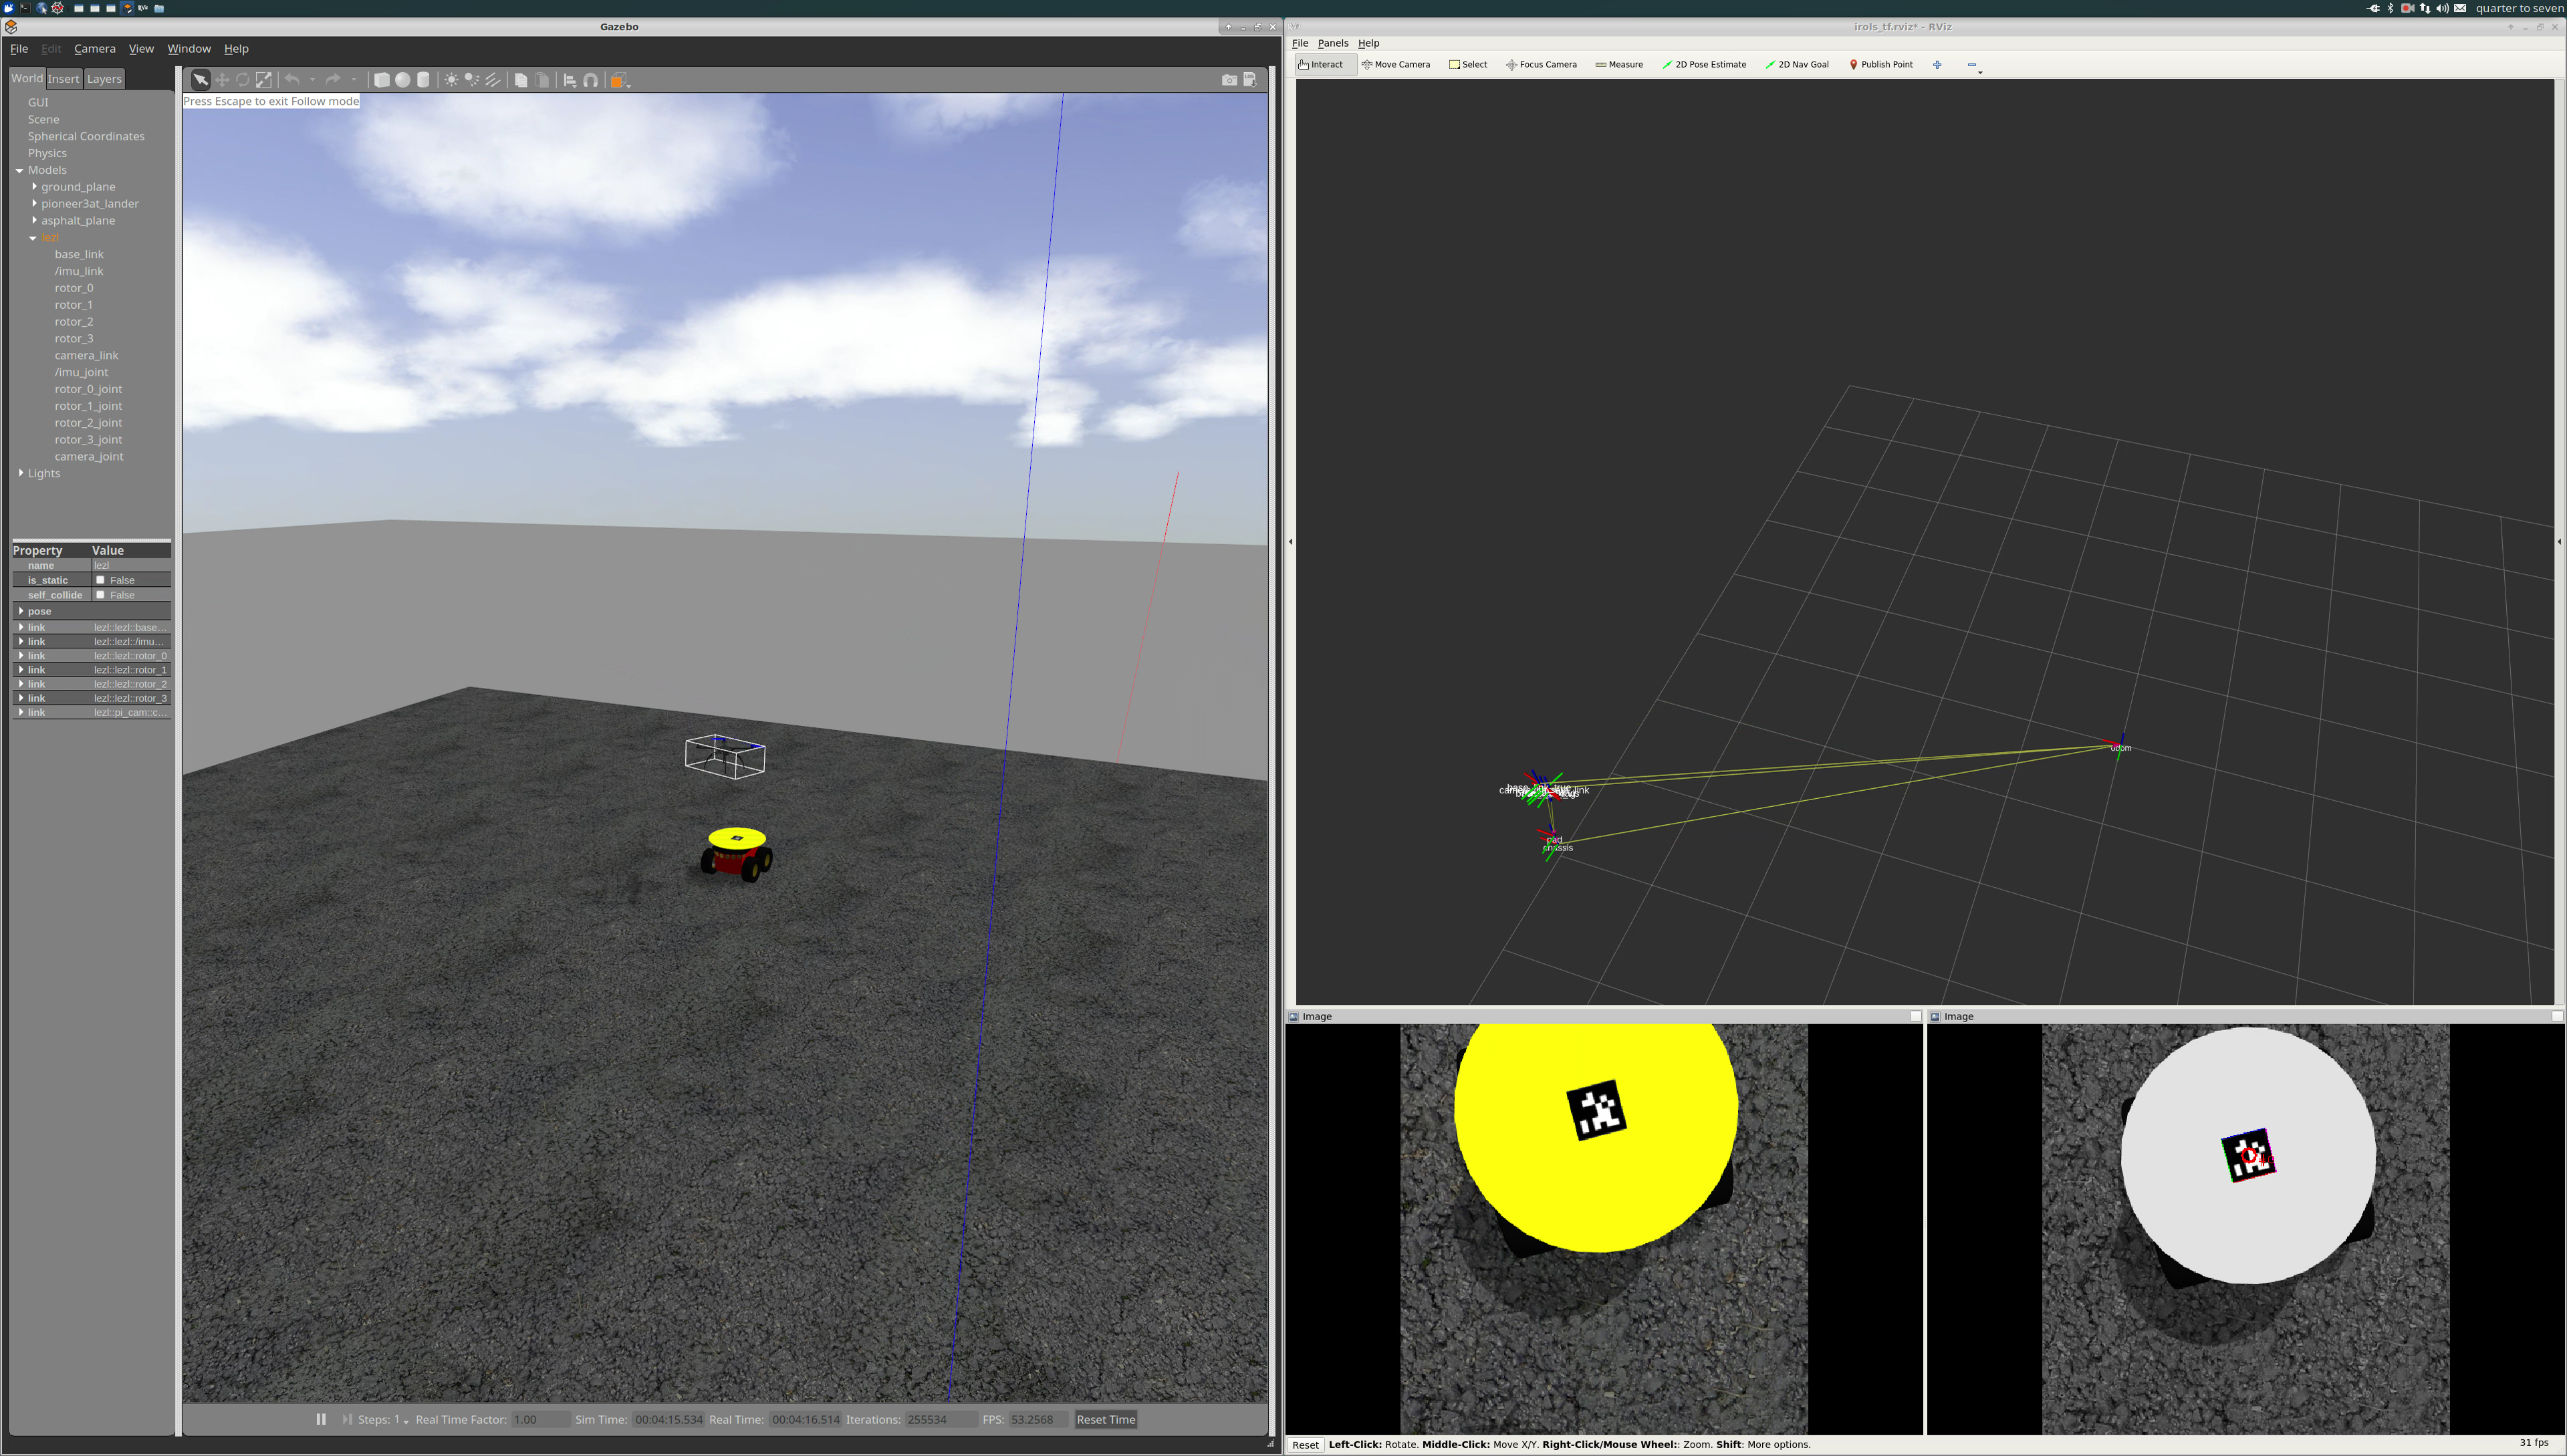
\includegraphics[width=0.6\textwidth]{images/moving_capture/moving-18h12m15s888.png}
    \caption{Image of the simulation environment and along with estimate visualization and camera
    feeds}\label{f:sim_moving_shot}
\end{figure}


\subsection{Fuzzy Controller}
Four fuzzy controllers of similar architecture were created as shown in \cref{f:fuzzy_mfs}.
Each input fuzzy partition was multiplied by a scaling factor to bring it into the range of the controller.
Likewise, the outputs were then again scaled to match actuation limits. The rule base was developed using
common intuition about the system dynamics. A full rule matrix was defined to fully cover the system
possibilities. This rule matrix is shown in \cref{t:rules}.
\begin{figure}[ht]
    \begin{subfigmatrix}{2}
        \subfigure[Error input \label{f:error_in_mfs}]  {\resizebox{0.48\textwidth}{!}{\input{tikz/land_in1}}}
        \subfigure[Error rate input \label{f:error_d_in_mfs}]{\resizebox{0.48\textwidth}{!}{\input{tikz/land_in2}}}
        \subfigure[Rate command output \label{f:vel_out_mfs}]   {\resizebox{0.48\textwidth}{!}{\begin{tikzpicture}[gnuplot]
%% generated with GNUPLOT 5.0p3 (Lua 5.1; terminal rev. 99, script rev. 100)
%% Wed 28 Mar 2018 11:36:11 PM EDT
\gpmonochromelines
\path (0.000,0.000) rectangle (12.500,8.750);
\gpcolor{color=gp lt color border}
\gpsetlinetype{gp lt border}
\gpsetdashtype{gp dt solid}
\gpsetlinewidth{1.00}
\draw[gp path] (1.320,1.601)--(1.500,1.601);
\draw[gp path] (11.947,1.601)--(11.767,1.601);
\node[gp node right] at (1.136,1.601) {$0$};
\draw[gp path] (1.320,2.834)--(1.500,2.834);
\draw[gp path] (11.947,2.834)--(11.767,2.834);
\node[gp node right] at (1.136,2.834) {$0.2$};
\draw[gp path] (1.320,4.067)--(1.500,4.067);
\draw[gp path] (11.947,4.067)--(11.767,4.067);
\node[gp node right] at (1.136,4.067) {$0.4$};
\draw[gp path] (1.320,5.299)--(1.500,5.299);
\draw[gp path] (11.947,5.299)--(11.767,5.299);
\node[gp node right] at (1.136,5.299) {$0.6$};
\draw[gp path] (1.320,6.532)--(1.500,6.532);
\draw[gp path] (11.947,6.532)--(11.767,6.532);
\node[gp node right] at (1.136,6.532) {$0.8$};
\draw[gp path] (1.320,7.765)--(1.500,7.765);
\draw[gp path] (11.947,7.765)--(11.767,7.765);
\node[gp node right] at (1.136,7.765) {$1$};
\draw[gp path] (1.320,0.985)--(1.320,1.165);
\draw[gp path] (1.320,8.381)--(1.320,8.201);
\node[gp node center] at (1.320,0.677) {$-1.5$};
\draw[gp path] (3.091,0.985)--(3.091,1.165);
\draw[gp path] (3.091,8.381)--(3.091,8.201);
\node[gp node center] at (3.091,0.677) {$-1$};
\draw[gp path] (4.862,0.985)--(4.862,1.165);
\draw[gp path] (4.862,8.381)--(4.862,8.201);
\node[gp node center] at (4.862,0.677) {$-0.5$};
\draw[gp path] (6.634,0.985)--(6.634,1.165);
\draw[gp path] (6.634,8.381)--(6.634,8.201);
\node[gp node center] at (6.634,0.677) {$0$};
\draw[gp path] (8.405,0.985)--(8.405,1.165);
\draw[gp path] (8.405,8.381)--(8.405,8.201);
\node[gp node center] at (8.405,0.677) {$0.5$};
\draw[gp path] (10.176,0.985)--(10.176,1.165);
\draw[gp path] (10.176,8.381)--(10.176,8.201);
\node[gp node center] at (10.176,0.677) {$1$};
\draw[gp path] (11.947,0.985)--(11.947,1.165);
\draw[gp path] (11.947,8.381)--(11.947,8.201);
\node[gp node center] at (11.947,0.677) {$1.5$};
\draw[gp path] (1.320,8.381)--(1.320,0.985)--(11.947,0.985)--(11.947,8.381)--cycle;
\node[gp node center,rotate=-270] at (0.246,4.683) {$\mu$, Membership value};
\node[gp node center] at (6.633,0.215) {rate setpoint};
\draw[gp path] (9.283,3.913)--(9.283,5.453)--(11.763,5.453)--(11.763,3.913)--cycle;
\gpfill{color=gp lt color border,gp pattern 0,pattern color=.} (1.320,1.601)--(3.977,7.765)--(6.634,1.601)--(11.947,1.601)--cycle;
\draw[gp path] (1.320,1.601)--(3.977,7.765)--(6.634,1.601)--(11.947,1.601);
%
  \gpfill{color=gp lt color border,gp pattern 1,pattern color=.} (1.320,1.601)--(3.091,1.601)--(5.748,7.765)--(6.634,1.601)--(11.947,1.601)--cycle;
\gpsetdashtype{gp dt 2}
\draw[gp path] (1.320,1.601)--(3.091,1.601)--(5.748,7.765)--(6.634,1.601)--(11.947,1.601);
%
  \gpfill{color=gp lt color border,opacity=0.25} (1.320,1.601)--(4.862,1.601)--(6.634,7.765)--(8.405,1.601)--(11.947,1.601)--cycle;
\gpsetdashtype{gp dt 3}
\draw[gp path] (1.320,1.601)--(4.862,1.601)--(6.634,7.765)--(8.405,1.601)--(11.947,1.601);
%
  \gpfill{color=gp lt color border,gp pattern 2,pattern color=.} (1.320,1.601)--(6.634,1.601)--(7.519,7.765)--(10.176,1.601)--(11.947,1.601)--cycle;
\gpsetdashtype{gp dt 4}
\draw[gp path] (1.320,1.601)--(6.634,1.601)--(7.519,7.765)--(10.176,1.601)--(11.947,1.601);
\gpfill{color=gp lt color border,opacity=0.50} (1.320,1.601)--(6.634,1.601)--(9.290,7.765)--(11.947,1.601)--cycle;
\gpsetlinewidth{2.00}
\draw[gp path] (1.320,1.601)--(6.634,1.601)--(9.290,7.765)--(11.947,1.601);
\gpfill{color=gpbgfillcolor} (9.283,3.913)--(11.763,3.913)--(11.763,5.453)--(9.283,5.453)--cycle;
\gpsetdashtype{gp dt solid}
\gpsetlinewidth{1.00}
\draw[gp path] (9.283,3.913)--(9.283,5.453)--(11.763,5.453)--(11.763,3.913)--cycle;
\node[gp node right] at (10.479,5.299) {N};
\gpfill{color=gp lt color border,gp pattern 0,pattern color=.} (10.663,5.222)--(11.579,5.222)--(11.579,5.376)--(10.663,5.376)--cycle;
\draw[gp path] (10.663,5.222)--(11.579,5.222)--(11.579,5.376)--(10.663,5.376)--cycle;
\node[gp node right] at (10.479,4.991) {SN};
\gpfill{color=gp lt color border,gp pattern 1,pattern color=.} (10.663,4.914)--(11.579,4.914)--(11.579,5.068)--(10.663,5.068)--cycle;
\gpsetdashtype{gp dt 2}
\draw[gp path] (10.663,4.914)--(11.579,4.914)--(11.579,5.068)--(10.663,5.068)--cycle;
\node[gp node right] at (10.479,4.683) {Z};
\gpfill{color=gp lt color border,opacity=0.25} (10.663,4.606)--(11.579,4.606)--(11.579,4.760)--(10.663,4.760)--cycle;
\gpsetdashtype{gp dt 3}
\draw[gp path] (10.663,4.606)--(11.579,4.606)--(11.579,4.760)--(10.663,4.760)--cycle;
\node[gp node right] at (10.479,4.375) {SP};
\gpfill{color=gp lt color border,gp pattern 2,pattern color=.} (10.663,4.298)--(11.579,4.298)--(11.579,4.452)--(10.663,4.452)--cycle;
\gpsetdashtype{gp dt 4}
\draw[gp path] (10.663,4.298)--(11.579,4.298)--(11.579,4.452)--(10.663,4.452)--cycle;
\node[gp node right] at (10.479,4.067) {P};
\gpfill{color=gp lt color border,opacity=0.50} (10.663,3.990)--(11.579,3.990)--(11.579,4.144)--(10.663,4.144)--cycle;
\gpsetlinewidth{2.00}
\draw[gp path] (10.663,3.990)--(11.579,3.990)--(11.579,4.144)--(10.663,4.144)--cycle;
\gpsetdashtype{gp dt solid}
\gpsetlinewidth{1.00}
\draw[gp path] (1.320,8.381)--(1.320,0.985)--(11.947,0.985)--(11.947,8.381)--cycle;
%% coordinates of the plot area
\gpdefrectangularnode{gp plot 1}{\pgfpoint{1.320cm}{0.985cm}}{\pgfpoint{11.947cm}{8.381cm}}
\end{tikzpicture}
%% gnuplot variables
}}
    \end{subfigmatrix}
    \caption{Membership function definitions for fuzzy logic controller.}\label{f:fuzzy_mfs}
\end{figure}

These rules provide a process by which to lend the controller a
decision-making system with a foundation in human reasoning. The tuning process of the fuzzy controller then
becomes the task of defining the membership functions which decide how much of each rule should be activated
for certain inputs. Triangular membership functions are used exclusively for their simplicity in definition
and tuning\cite{mishra1994performance} while the aggregation of rules is the popular min-max method put forth
by Mamdani\cite{MAMDANI19751}. The membership functions shown in \cref{f:fuzzy_mfs} are the result of a number
of iterative tuning steps and were found to be the most effective of the configurations attempted.


\begin{table}[ht]
    \centering
    \caption{Fuzzy rule base. The error and error rate membership sets correspond to velocity output
    membership sets according to this table. N-negative, SN-small negative, Z-zero, SP-small positive,
P-positive}re intuitive and easy to understand and pr\label{t:rules}
    \begin{tabular}{cc||c|c|c|c|c|}
        &  \multicolumn{6}{c}{error}  \\ 	
        \multirow{6}{*}{error rate} &    & N  & SN & Z  & SP & P  \\ 	\hhline{~=#=|=|=|=|=|}
                                    & N  & P  & P  & SP & SP & Z  \\ 	\cline{2-7}
                                    & SN & P  & SP & SP & Z  & SN \\ 	\cline{2-7}
                                    & Z  & SP & SP & Z  & SN & SN \\ 	\cline{2-7}
                                    & SP & SP & Z  & SN & SN & N  \\ 	\cline{2-7}
                                    & P  & Z  & SN & SN & N  & N  \\ 	\cline{2-7}
    \end{tabular}
\end{table}



The result of this controller was sufficient to land the quadrotor on both the static and
constant linear velocity dynamic platforms. \Crefrange{f:fuz_stat}{f:fuz_dyn} show the results of the static
and dynamic landings using the fuzzy controllers. These figures begin at takeoff of the vehicle, and it is
clearly seen where the controller locks onto the visual image and initiates the landing state. It is also
clearly seen that with the implementation of both the kalman filter and the fuzzy controller, the errors
resulting from image loss are eliminated, providing a smoother landing approach.

\begin{figure}
    \centering
    \begin{tikzpicture}[gnuplot]
%% generated with GNUPLOT 5.0p3 (Lua 5.1; terminal rev. 99, script rev. 100)
%% Tue 27 Mar 2018 03:05:26 AM EDT
\path (0.000,0.000) rectangle (12.500,8.750);
\gpcolor{color=gp lt color border}
\gpsetlinetype{gp lt border}
\gpsetdashtype{gp dt solid}
\gpsetlinewidth{1.00}
\draw[gp path] (1.012,0.616)--(1.192,0.616);
\draw[gp path] (11.947,0.616)--(11.767,0.616);
\node[gp node right] at (0.828,0.616) {$0$};
\draw[gp path] (1.012,1.337)--(1.192,1.337);
\draw[gp path] (11.947,1.337)--(11.767,1.337);
\node[gp node right] at (0.828,1.337) {$0.5$};
\draw[gp path] (1.012,2.058)--(1.192,2.058);
\draw[gp path] (11.947,2.058)--(11.767,2.058);
\node[gp node right] at (0.828,2.058) {$1$};
\draw[gp path] (1.012,2.779)--(1.192,2.779);
\draw[gp path] (11.947,2.779)--(11.767,2.779);
\node[gp node right] at (0.828,2.779) {$1.5$};
\draw[gp path] (1.012,3.500)--(1.192,3.500);
\draw[gp path] (11.947,3.500)--(11.767,3.500);
\node[gp node right] at (0.828,3.500) {$2$};
\draw[gp path] (1.012,4.221)--(1.192,4.221);
\draw[gp path] (11.947,4.221)--(11.767,4.221);
\node[gp node right] at (0.828,4.221) {$2.5$};
\draw[gp path] (1.012,4.941)--(1.192,4.941);
\draw[gp path] (11.947,4.941)--(11.767,4.941);
\node[gp node right] at (0.828,4.941) {$3$};
\draw[gp path] (1.012,5.662)--(1.192,5.662);
\draw[gp path] (11.947,5.662)--(11.767,5.662);
\node[gp node right] at (0.828,5.662) {$3.5$};
\draw[gp path] (1.012,6.383)--(1.192,6.383);
\draw[gp path] (11.947,6.383)--(11.767,6.383);
\node[gp node right] at (0.828,6.383) {$4$};
\draw[gp path] (1.012,7.104)--(1.192,7.104);
\draw[gp path] (11.947,7.104)--(11.767,7.104);
\node[gp node right] at (0.828,7.104) {$4.5$};
\draw[gp path] (1.012,7.825)--(1.192,7.825);
\draw[gp path] (11.947,7.825)--(11.767,7.825);
\node[gp node right] at (0.828,7.825) {$5$};
\draw[gp path] (1.012,0.616)--(1.012,0.796);
\draw[gp path] (1.012,7.825)--(1.012,7.645);
\node[gp node center] at (1.012,0.308) {$0$};
\draw[gp path] (2.574,0.616)--(2.574,0.796);
\draw[gp path] (2.574,7.825)--(2.574,7.645);
\node[gp node center] at (2.574,0.308) {$5$};
\draw[gp path] (4.136,0.616)--(4.136,0.796);
\draw[gp path] (4.136,7.825)--(4.136,7.645);
\node[gp node center] at (4.136,0.308) {$10$};
\draw[gp path] (5.698,0.616)--(5.698,0.796);
\draw[gp path] (5.698,7.825)--(5.698,7.645);
\node[gp node center] at (5.698,0.308) {$15$};
\draw[gp path] (7.261,0.616)--(7.261,0.796);
\draw[gp path] (7.261,7.825)--(7.261,7.645);
\node[gp node center] at (7.261,0.308) {$20$};
\draw[gp path] (8.823,0.616)--(8.823,0.796);
\draw[gp path] (8.823,7.825)--(8.823,7.645);
\node[gp node center] at (8.823,0.308) {$25$};
\draw[gp path] (10.385,0.616)--(10.385,0.796);
\draw[gp path] (10.385,7.825)--(10.385,7.645);
\node[gp node center] at (10.385,0.308) {$30$};
\draw[gp path] (11.947,0.616)--(11.947,0.796);
\draw[gp path] (11.947,7.825)--(11.947,7.645);
\node[gp node center] at (11.947,0.308) {$35$};
\draw[gp path] (1.012,7.825)--(1.012,0.616)--(11.947,0.616)--(11.947,7.825)--cycle;
\node[gp node center] at (6.479,8.287) {Planar error};
\node[gp node right] at (10.479,7.491) {e_{xy}};
\gpcolor{rgb color={0.580,0.000,0.827}}
\gpsetpointsize{4.00}
\gppoint{gp mark 1}{(1.012,6.741)}
\gppoint{gp mark 1}{(1.012,6.741)}
\gppoint{gp mark 1}{(1.013,6.741)}
\gppoint{gp mark 1}{(1.013,6.741)}
\gppoint{gp mark 1}{(1.013,6.741)}
\gppoint{gp mark 1}{(1.014,6.741)}
\gppoint{gp mark 1}{(1.014,6.741)}
\gppoint{gp mark 1}{(1.014,6.741)}
\gppoint{gp mark 1}{(1.014,6.741)}
\gppoint{gp mark 1}{(1.015,6.741)}
\gppoint{gp mark 1}{(1.015,6.741)}
\gppoint{gp mark 1}{(1.015,6.741)}
\gppoint{gp mark 1}{(1.016,6.741)}
\gppoint{gp mark 1}{(1.016,6.741)}
\gppoint{gp mark 1}{(1.016,6.741)}
\gppoint{gp mark 1}{(1.017,6.741)}
\gppoint{gp mark 1}{(1.017,6.741)}
\gppoint{gp mark 1}{(1.017,6.741)}
\gppoint{gp mark 1}{(1.018,6.741)}
\gppoint{gp mark 1}{(1.018,6.741)}
\gppoint{gp mark 1}{(1.018,6.741)}
\gppoint{gp mark 1}{(1.018,6.741)}
\gppoint{gp mark 1}{(1.019,6.741)}
\gppoint{gp mark 1}{(1.019,6.741)}
\gppoint{gp mark 1}{(1.019,6.741)}
\gppoint{gp mark 1}{(1.020,6.741)}
\gppoint{gp mark 1}{(1.020,6.741)}
\gppoint{gp mark 1}{(1.020,6.741)}
\gppoint{gp mark 1}{(1.021,6.741)}
\gppoint{gp mark 1}{(1.021,6.741)}
\gppoint{gp mark 1}{(1.021,6.741)}
\gppoint{gp mark 1}{(1.022,6.741)}
\gppoint{gp mark 1}{(1.022,6.741)}
\gppoint{gp mark 1}{(1.022,6.741)}
\gppoint{gp mark 1}{(1.023,6.741)}
\gppoint{gp mark 1}{(1.023,6.741)}
\gppoint{gp mark 1}{(1.023,6.741)}
\gppoint{gp mark 1}{(1.024,6.741)}
\gppoint{gp mark 1}{(1.024,6.741)}
\gppoint{gp mark 1}{(1.024,6.741)}
\gppoint{gp mark 1}{(1.024,6.741)}
\gppoint{gp mark 1}{(1.024,6.741)}
\gppoint{gp mark 1}{(1.025,6.741)}
\gppoint{gp mark 1}{(1.025,6.741)}
\gppoint{gp mark 1}{(1.026,6.741)}
\gppoint{gp mark 1}{(1.026,6.741)}
\gppoint{gp mark 1}{(1.026,6.741)}
\gppoint{gp mark 1}{(1.027,6.741)}
\gppoint{gp mark 1}{(1.027,6.741)}
\gppoint{gp mark 1}{(1.027,6.741)}
\gppoint{gp mark 1}{(1.028,6.741)}
\gppoint{gp mark 1}{(1.028,6.741)}
\gppoint{gp mark 1}{(1.028,6.741)}
\gppoint{gp mark 1}{(1.029,6.741)}
\gppoint{gp mark 1}{(1.029,6.741)}
\gppoint{gp mark 1}{(1.029,6.741)}
\gppoint{gp mark 1}{(1.029,6.741)}
\gppoint{gp mark 1}{(1.030,6.741)}
\gppoint{gp mark 1}{(1.030,6.741)}
\gppoint{gp mark 1}{(1.030,6.741)}
\gppoint{gp mark 1}{(1.031,6.741)}
\gppoint{gp mark 1}{(1.031,6.741)}
\gppoint{gp mark 1}{(1.031,6.741)}
\gppoint{gp mark 1}{(1.032,6.741)}
\gppoint{gp mark 1}{(1.032,6.741)}
\gppoint{gp mark 1}{(1.032,6.741)}
\gppoint{gp mark 1}{(1.033,6.741)}
\gppoint{gp mark 1}{(1.033,6.741)}
\gppoint{gp mark 1}{(1.033,6.741)}
\gppoint{gp mark 1}{(1.034,6.741)}
\gppoint{gp mark 1}{(1.034,6.741)}
\gppoint{gp mark 1}{(1.034,6.741)}
\gppoint{gp mark 1}{(1.034,6.741)}
\gppoint{gp mark 1}{(1.035,6.741)}
\gppoint{gp mark 1}{(1.035,6.741)}
\gppoint{gp mark 1}{(1.035,6.741)}
\gppoint{gp mark 1}{(1.036,6.741)}
\gppoint{gp mark 1}{(1.036,6.741)}
\gppoint{gp mark 1}{(1.036,6.741)}
\gppoint{gp mark 1}{(1.037,6.741)}
\gppoint{gp mark 1}{(1.037,6.741)}
\gppoint{gp mark 1}{(1.037,6.741)}
\gppoint{gp mark 1}{(1.038,6.741)}
\gppoint{gp mark 1}{(1.038,6.741)}
\gppoint{gp mark 1}{(1.038,6.741)}
\gppoint{gp mark 1}{(1.039,6.741)}
\gppoint{gp mark 1}{(1.039,6.741)}
\gppoint{gp mark 1}{(1.039,6.741)}
\gppoint{gp mark 1}{(1.039,6.741)}
\gppoint{gp mark 1}{(1.040,6.741)}
\gppoint{gp mark 1}{(1.040,6.741)}
\gppoint{gp mark 1}{(1.040,6.741)}
\gppoint{gp mark 1}{(1.041,6.741)}
\gppoint{gp mark 1}{(1.041,6.741)}
\gppoint{gp mark 1}{(1.041,6.741)}
\gppoint{gp mark 1}{(1.042,6.741)}
\gppoint{gp mark 1}{(1.042,6.741)}
\gppoint{gp mark 1}{(1.042,6.741)}
\gppoint{gp mark 1}{(1.043,6.741)}
\gppoint{gp mark 1}{(1.043,6.741)}
\gppoint{gp mark 1}{(1.043,6.741)}
\gppoint{gp mark 1}{(1.044,6.741)}
\gppoint{gp mark 1}{(1.044,6.741)}
\gppoint{gp mark 1}{(1.044,6.741)}
\gppoint{gp mark 1}{(1.044,6.741)}
\gppoint{gp mark 1}{(1.045,6.741)}
\gppoint{gp mark 1}{(1.045,6.741)}
\gppoint{gp mark 1}{(1.045,6.741)}
\gppoint{gp mark 1}{(1.046,6.741)}
\gppoint{gp mark 1}{(1.046,6.741)}
\gppoint{gp mark 1}{(1.047,6.741)}
\gppoint{gp mark 1}{(1.047,6.741)}
\gppoint{gp mark 1}{(1.047,6.741)}
\gppoint{gp mark 1}{(1.047,6.741)}
\gppoint{gp mark 1}{(1.048,6.741)}
\gppoint{gp mark 1}{(1.048,6.741)}
\gppoint{gp mark 1}{(1.048,6.741)}
\gppoint{gp mark 1}{(1.049,6.741)}
\gppoint{gp mark 1}{(1.049,6.741)}
\gppoint{gp mark 1}{(1.049,6.741)}
\gppoint{gp mark 1}{(1.049,6.741)}
\gppoint{gp mark 1}{(1.050,6.741)}
\gppoint{gp mark 1}{(1.050,6.741)}
\gppoint{gp mark 1}{(1.050,6.741)}
\gppoint{gp mark 1}{(1.051,6.741)}
\gppoint{gp mark 1}{(1.051,6.741)}
\gppoint{gp mark 1}{(1.051,6.741)}
\gppoint{gp mark 1}{(1.052,6.741)}
\gppoint{gp mark 1}{(1.052,6.741)}
\gppoint{gp mark 1}{(1.052,6.741)}
\gppoint{gp mark 1}{(1.053,6.741)}
\gppoint{gp mark 1}{(1.053,6.741)}
\gppoint{gp mark 1}{(1.053,6.741)}
\gppoint{gp mark 1}{(1.054,6.741)}
\gppoint{gp mark 1}{(1.054,6.741)}
\gppoint{gp mark 1}{(1.054,6.741)}
\gppoint{gp mark 1}{(1.054,6.741)}
\gppoint{gp mark 1}{(1.055,6.741)}
\gppoint{gp mark 1}{(1.055,6.741)}
\gppoint{gp mark 1}{(1.055,6.741)}
\gppoint{gp mark 1}{(1.056,6.741)}
\gppoint{gp mark 1}{(1.056,6.741)}
\gppoint{gp mark 1}{(1.056,6.741)}
\gppoint{gp mark 1}{(1.057,6.741)}
\gppoint{gp mark 1}{(1.057,6.741)}
\gppoint{gp mark 1}{(1.057,6.741)}
\gppoint{gp mark 1}{(1.058,6.741)}
\gppoint{gp mark 1}{(1.058,6.741)}
\gppoint{gp mark 1}{(1.058,6.741)}
\gppoint{gp mark 1}{(1.059,6.741)}
\gppoint{gp mark 1}{(1.059,6.741)}
\gppoint{gp mark 1}{(1.059,6.741)}
\gppoint{gp mark 1}{(1.059,6.741)}
\gppoint{gp mark 1}{(1.060,6.741)}
\gppoint{gp mark 1}{(1.060,6.741)}
\gppoint{gp mark 1}{(1.060,6.741)}
\gppoint{gp mark 1}{(1.061,6.741)}
\gppoint{gp mark 1}{(1.061,6.741)}
\gppoint{gp mark 1}{(1.061,6.741)}
\gppoint{gp mark 1}{(1.062,6.741)}
\gppoint{gp mark 1}{(1.062,6.741)}
\gppoint{gp mark 1}{(1.062,6.741)}
\gppoint{gp mark 1}{(1.063,6.741)}
\gppoint{gp mark 1}{(1.063,6.741)}
\gppoint{gp mark 1}{(1.063,6.741)}
\gppoint{gp mark 1}{(1.064,6.741)}
\gppoint{gp mark 1}{(1.064,6.741)}
\gppoint{gp mark 1}{(1.064,6.741)}
\gppoint{gp mark 1}{(1.064,6.741)}
\gppoint{gp mark 1}{(1.065,6.741)}
\gppoint{gp mark 1}{(1.065,6.741)}
\gppoint{gp mark 1}{(1.065,6.741)}
\gppoint{gp mark 1}{(1.066,6.741)}
\gppoint{gp mark 1}{(1.066,6.741)}
\gppoint{gp mark 1}{(1.066,6.741)}
\gppoint{gp mark 1}{(1.067,6.741)}
\gppoint{gp mark 1}{(1.067,6.741)}
\gppoint{gp mark 1}{(1.067,6.741)}
\gppoint{gp mark 1}{(1.068,6.741)}
\gppoint{gp mark 1}{(1.068,6.741)}
\gppoint{gp mark 1}{(1.068,6.741)}
\gppoint{gp mark 1}{(1.069,6.741)}
\gppoint{gp mark 1}{(1.069,6.741)}
\gppoint{gp mark 1}{(1.069,6.741)}
\gppoint{gp mark 1}{(1.069,6.741)}
\gppoint{gp mark 1}{(1.070,6.741)}
\gppoint{gp mark 1}{(1.070,6.741)}
\gppoint{gp mark 1}{(1.070,6.741)}
\gppoint{gp mark 1}{(1.071,6.741)}
\gppoint{gp mark 1}{(1.071,6.741)}
\gppoint{gp mark 1}{(1.071,6.741)}
\gppoint{gp mark 1}{(1.072,6.741)}
\gppoint{gp mark 1}{(1.072,6.741)}
\gppoint{gp mark 1}{(1.072,6.741)}
\gppoint{gp mark 1}{(1.073,6.741)}
\gppoint{gp mark 1}{(1.073,6.741)}
\gppoint{gp mark 1}{(1.073,6.741)}
\gppoint{gp mark 1}{(1.074,6.741)}
\gppoint{gp mark 1}{(1.074,6.741)}
\gppoint{gp mark 1}{(1.074,6.741)}
\gppoint{gp mark 1}{(1.074,6.741)}
\gppoint{gp mark 1}{(1.075,6.741)}
\gppoint{gp mark 1}{(1.075,6.741)}
\gppoint{gp mark 1}{(1.075,6.741)}
\gppoint{gp mark 1}{(1.076,6.741)}
\gppoint{gp mark 1}{(1.076,6.741)}
\gppoint{gp mark 1}{(1.076,6.741)}
\gppoint{gp mark 1}{(1.077,6.741)}
\gppoint{gp mark 1}{(1.077,6.741)}
\gppoint{gp mark 1}{(1.077,6.741)}
\gppoint{gp mark 1}{(1.078,6.741)}
\gppoint{gp mark 1}{(1.078,6.741)}
\gppoint{gp mark 1}{(1.078,6.741)}
\gppoint{gp mark 1}{(1.078,6.741)}
\gppoint{gp mark 1}{(1.079,6.741)}
\gppoint{gp mark 1}{(1.079,6.741)}
\gppoint{gp mark 1}{(1.079,6.741)}
\gppoint{gp mark 1}{(1.080,6.741)}
\gppoint{gp mark 1}{(1.080,6.741)}
\gppoint{gp mark 1}{(1.080,6.741)}
\gppoint{gp mark 1}{(1.081,6.741)}
\gppoint{gp mark 1}{(1.081,6.741)}
\gppoint{gp mark 1}{(1.081,6.741)}
\gppoint{gp mark 1}{(1.081,6.741)}
\gppoint{gp mark 1}{(1.082,6.741)}
\gppoint{gp mark 1}{(1.082,6.741)}
\gppoint{gp mark 1}{(1.083,6.741)}
\gppoint{gp mark 1}{(1.083,6.741)}
\gppoint{gp mark 1}{(1.083,6.741)}
\gppoint{gp mark 1}{(1.084,6.741)}
\gppoint{gp mark 1}{(1.084,6.741)}
\gppoint{gp mark 1}{(1.084,6.741)}
\gppoint{gp mark 1}{(1.084,6.741)}
\gppoint{gp mark 1}{(1.085,6.741)}
\gppoint{gp mark 1}{(1.085,6.741)}
\gppoint{gp mark 1}{(1.085,6.741)}
\gppoint{gp mark 1}{(1.085,6.741)}
\gppoint{gp mark 1}{(1.086,6.741)}
\gppoint{gp mark 1}{(1.086,6.741)}
\gppoint{gp mark 1}{(1.086,6.741)}
\gppoint{gp mark 1}{(1.087,6.741)}
\gppoint{gp mark 1}{(1.087,6.741)}
\gppoint{gp mark 1}{(1.087,6.741)}
\gppoint{gp mark 1}{(1.088,6.741)}
\gppoint{gp mark 1}{(1.088,6.741)}
\gppoint{gp mark 1}{(1.089,6.741)}
\gppoint{gp mark 1}{(1.089,6.741)}
\gppoint{gp mark 1}{(1.089,6.741)}
\gppoint{gp mark 1}{(1.089,6.741)}
\gppoint{gp mark 1}{(1.090,6.741)}
\gppoint{gp mark 1}{(1.090,6.741)}
\gppoint{gp mark 1}{(1.090,6.741)}
\gppoint{gp mark 1}{(1.091,6.741)}
\gppoint{gp mark 1}{(1.091,6.741)}
\gppoint{gp mark 1}{(1.091,6.741)}
\gppoint{gp mark 1}{(1.091,6.741)}
\gppoint{gp mark 1}{(1.092,6.741)}
\gppoint{gp mark 1}{(1.092,6.741)}
\gppoint{gp mark 1}{(1.093,6.741)}
\gppoint{gp mark 1}{(1.093,6.741)}
\gppoint{gp mark 1}{(1.093,6.741)}
\gppoint{gp mark 1}{(1.094,6.741)}
\gppoint{gp mark 1}{(1.094,6.741)}
\gppoint{gp mark 1}{(1.094,6.741)}
\gppoint{gp mark 1}{(1.094,6.741)}
\gppoint{gp mark 1}{(1.095,6.741)}
\gppoint{gp mark 1}{(1.095,6.741)}
\gppoint{gp mark 1}{(1.095,6.741)}
\gppoint{gp mark 1}{(1.096,6.741)}
\gppoint{gp mark 1}{(1.096,6.741)}
\gppoint{gp mark 1}{(1.096,6.741)}
\gppoint{gp mark 1}{(1.097,6.741)}
\gppoint{gp mark 1}{(1.097,6.741)}
\gppoint{gp mark 1}{(1.097,6.741)}
\gppoint{gp mark 1}{(1.098,6.741)}
\gppoint{gp mark 1}{(1.098,6.741)}
\gppoint{gp mark 1}{(1.098,6.741)}
\gppoint{gp mark 1}{(1.099,6.741)}
\gppoint{gp mark 1}{(1.099,6.741)}
\gppoint{gp mark 1}{(1.099,6.741)}
\gppoint{gp mark 1}{(1.099,6.741)}
\gppoint{gp mark 1}{(1.100,6.741)}
\gppoint{gp mark 1}{(1.100,6.741)}
\gppoint{gp mark 1}{(1.100,6.741)}
\gppoint{gp mark 1}{(1.101,6.741)}
\gppoint{gp mark 1}{(1.101,6.741)}
\gppoint{gp mark 1}{(1.101,6.741)}
\gppoint{gp mark 1}{(1.101,6.741)}
\gppoint{gp mark 1}{(1.102,6.741)}
\gppoint{gp mark 1}{(1.102,6.741)}
\gppoint{gp mark 1}{(1.103,6.741)}
\gppoint{gp mark 1}{(1.103,6.741)}
\gppoint{gp mark 1}{(1.103,6.741)}
\gppoint{gp mark 1}{(1.103,6.741)}
\gppoint{gp mark 1}{(1.104,6.741)}
\gppoint{gp mark 1}{(1.104,6.741)}
\gppoint{gp mark 1}{(1.104,6.741)}
\gppoint{gp mark 1}{(1.105,6.741)}
\gppoint{gp mark 1}{(1.105,6.741)}
\gppoint{gp mark 1}{(1.105,6.741)}
\gppoint{gp mark 1}{(1.106,6.741)}
\gppoint{gp mark 1}{(1.106,6.741)}
\gppoint{gp mark 1}{(1.106,6.741)}
\gppoint{gp mark 1}{(1.107,6.741)}
\gppoint{gp mark 1}{(1.107,6.741)}
\gppoint{gp mark 1}{(1.107,6.741)}
\gppoint{gp mark 1}{(1.108,6.741)}
\gppoint{gp mark 1}{(1.108,6.741)}
\gppoint{gp mark 1}{(1.108,6.741)}
\gppoint{gp mark 1}{(1.109,6.741)}
\gppoint{gp mark 1}{(1.109,6.741)}
\gppoint{gp mark 1}{(1.109,6.741)}
\gppoint{gp mark 1}{(1.109,6.741)}
\gppoint{gp mark 1}{(1.110,6.741)}
\gppoint{gp mark 1}{(1.110,6.741)}
\gppoint{gp mark 1}{(1.110,6.741)}
\gppoint{gp mark 1}{(1.111,6.741)}
\gppoint{gp mark 1}{(1.111,6.741)}
\gppoint{gp mark 1}{(1.111,6.741)}
\gppoint{gp mark 1}{(1.112,6.741)}
\gppoint{gp mark 1}{(1.112,6.741)}
\gppoint{gp mark 1}{(1.112,6.741)}
\gppoint{gp mark 1}{(1.113,6.741)}
\gppoint{gp mark 1}{(1.113,6.741)}
\gppoint{gp mark 1}{(1.113,6.741)}
\gppoint{gp mark 1}{(1.114,6.741)}
\gppoint{gp mark 1}{(1.114,6.741)}
\gppoint{gp mark 1}{(1.114,6.741)}
\gppoint{gp mark 1}{(1.114,6.741)}
\gppoint{gp mark 1}{(1.115,6.741)}
\gppoint{gp mark 1}{(1.115,6.741)}
\gppoint{gp mark 1}{(1.115,6.741)}
\gppoint{gp mark 1}{(1.116,6.741)}
\gppoint{gp mark 1}{(1.116,6.741)}
\gppoint{gp mark 1}{(1.116,6.741)}
\gppoint{gp mark 1}{(1.117,6.741)}
\gppoint{gp mark 1}{(1.117,6.741)}
\gppoint{gp mark 1}{(1.117,6.741)}
\gppoint{gp mark 1}{(1.118,6.741)}
\gppoint{gp mark 1}{(1.118,6.741)}
\gppoint{gp mark 1}{(1.118,6.741)}
\gppoint{gp mark 1}{(1.119,6.741)}
\gppoint{gp mark 1}{(1.119,6.741)}
\gppoint{gp mark 1}{(1.119,6.741)}
\gppoint{gp mark 1}{(1.119,6.741)}
\gppoint{gp mark 1}{(1.120,6.741)}
\gppoint{gp mark 1}{(1.120,6.741)}
\gppoint{gp mark 1}{(1.120,6.741)}
\gppoint{gp mark 1}{(1.121,6.741)}
\gppoint{gp mark 1}{(1.121,6.741)}
\gppoint{gp mark 1}{(1.121,6.741)}
\gppoint{gp mark 1}{(1.122,6.741)}
\gppoint{gp mark 1}{(1.122,6.741)}
\gppoint{gp mark 1}{(1.122,6.741)}
\gppoint{gp mark 1}{(1.123,6.741)}
\gppoint{gp mark 1}{(1.123,6.741)}
\gppoint{gp mark 1}{(1.123,6.741)}
\gppoint{gp mark 1}{(1.124,6.741)}
\gppoint{gp mark 1}{(1.124,6.741)}
\gppoint{gp mark 1}{(1.124,6.741)}
\gppoint{gp mark 1}{(1.124,6.741)}
\gppoint{gp mark 1}{(1.125,6.741)}
\gppoint{gp mark 1}{(1.125,6.741)}
\gppoint{gp mark 1}{(1.125,6.741)}
\gppoint{gp mark 1}{(1.126,6.741)}
\gppoint{gp mark 1}{(1.126,6.741)}
\gppoint{gp mark 1}{(1.127,6.741)}
\gppoint{gp mark 1}{(1.127,6.741)}
\gppoint{gp mark 1}{(1.127,6.741)}
\gppoint{gp mark 1}{(1.127,6.741)}
\gppoint{gp mark 1}{(1.128,6.741)}
\gppoint{gp mark 1}{(1.128,6.741)}
\gppoint{gp mark 1}{(1.128,6.741)}
\gppoint{gp mark 1}{(1.129,6.741)}
\gppoint{gp mark 1}{(1.129,6.741)}
\gppoint{gp mark 1}{(1.129,6.741)}
\gppoint{gp mark 1}{(1.129,6.741)}
\gppoint{gp mark 1}{(1.130,6.741)}
\gppoint{gp mark 1}{(1.130,6.741)}
\gppoint{gp mark 1}{(1.130,6.741)}
\gppoint{gp mark 1}{(1.131,6.741)}
\gppoint{gp mark 1}{(1.131,6.741)}
\gppoint{gp mark 1}{(1.131,6.741)}
\gppoint{gp mark 1}{(1.132,6.741)}
\gppoint{gp mark 1}{(1.132,6.741)}
\gppoint{gp mark 1}{(1.132,6.741)}
\gppoint{gp mark 1}{(1.133,6.741)}
\gppoint{gp mark 1}{(1.133,6.741)}
\gppoint{gp mark 1}{(1.133,6.741)}
\gppoint{gp mark 1}{(1.134,6.741)}
\gppoint{gp mark 1}{(1.134,6.741)}
\gppoint{gp mark 1}{(1.134,6.741)}
\gppoint{gp mark 1}{(1.134,6.741)}
\gppoint{gp mark 1}{(1.135,6.741)}
\gppoint{gp mark 1}{(1.135,6.741)}
\gppoint{gp mark 1}{(1.135,6.741)}
\gppoint{gp mark 1}{(1.136,6.741)}
\gppoint{gp mark 1}{(1.136,6.741)}
\gppoint{gp mark 1}{(1.136,6.741)}
\gppoint{gp mark 1}{(1.136,6.741)}
\gppoint{gp mark 1}{(1.136,6.741)}
\gppoint{gp mark 1}{(1.137,6.741)}
\gppoint{gp mark 1}{(1.137,6.741)}
\gppoint{gp mark 1}{(1.138,6.741)}
\gppoint{gp mark 1}{(1.138,6.741)}
\gppoint{gp mark 1}{(1.139,6.741)}
\gppoint{gp mark 1}{(1.139,6.741)}
\gppoint{gp mark 1}{(1.139,6.741)}
\gppoint{gp mark 1}{(1.139,6.741)}
\gppoint{gp mark 1}{(1.140,6.741)}
\gppoint{gp mark 1}{(1.140,6.741)}
\gppoint{gp mark 1}{(1.140,6.741)}
\gppoint{gp mark 1}{(1.141,6.741)}
\gppoint{gp mark 1}{(1.141,6.741)}
\gppoint{gp mark 1}{(1.141,6.741)}
\gppoint{gp mark 1}{(1.142,6.741)}
\gppoint{gp mark 1}{(1.142,6.741)}
\gppoint{gp mark 1}{(1.142,6.741)}
\gppoint{gp mark 1}{(1.143,6.741)}
\gppoint{gp mark 1}{(1.143,6.741)}
\gppoint{gp mark 1}{(1.143,6.741)}
\gppoint{gp mark 1}{(1.144,6.741)}
\gppoint{gp mark 1}{(1.144,6.741)}
\gppoint{gp mark 1}{(1.144,6.741)}
\gppoint{gp mark 1}{(1.144,6.741)}
\gppoint{gp mark 1}{(1.145,6.741)}
\gppoint{gp mark 1}{(1.145,6.741)}
\gppoint{gp mark 1}{(1.145,6.741)}
\gppoint{gp mark 1}{(1.146,6.741)}
\gppoint{gp mark 1}{(1.146,6.741)}
\gppoint{gp mark 1}{(1.146,6.741)}
\gppoint{gp mark 1}{(1.147,6.741)}
\gppoint{gp mark 1}{(1.147,6.741)}
\gppoint{gp mark 1}{(1.147,6.741)}
\gppoint{gp mark 1}{(1.148,6.741)}
\gppoint{gp mark 1}{(1.148,6.741)}
\gppoint{gp mark 1}{(1.148,6.741)}
\gppoint{gp mark 1}{(1.149,6.741)}
\gppoint{gp mark 1}{(1.149,6.741)}
\gppoint{gp mark 1}{(1.149,6.741)}
\gppoint{gp mark 1}{(1.149,6.741)}
\gppoint{gp mark 1}{(1.150,6.741)}
\gppoint{gp mark 1}{(1.150,6.741)}
\gppoint{gp mark 1}{(1.150,6.741)}
\gppoint{gp mark 1}{(1.151,6.741)}
\gppoint{gp mark 1}{(1.151,6.741)}
\gppoint{gp mark 1}{(1.151,6.741)}
\gppoint{gp mark 1}{(1.152,6.741)}
\gppoint{gp mark 1}{(1.152,6.741)}
\gppoint{gp mark 1}{(1.152,6.741)}
\gppoint{gp mark 1}{(1.153,6.741)}
\gppoint{gp mark 1}{(1.153,6.741)}
\gppoint{gp mark 1}{(1.153,6.741)}
\gppoint{gp mark 1}{(1.154,6.741)}
\gppoint{gp mark 1}{(1.154,6.741)}
\gppoint{gp mark 1}{(1.154,6.741)}
\gppoint{gp mark 1}{(1.154,6.741)}
\gppoint{gp mark 1}{(1.155,6.741)}
\gppoint{gp mark 1}{(1.155,6.741)}
\gppoint{gp mark 1}{(1.155,6.741)}
\gppoint{gp mark 1}{(1.156,6.741)}
\gppoint{gp mark 1}{(1.156,6.741)}
\gppoint{gp mark 1}{(1.156,6.741)}
\gppoint{gp mark 1}{(1.157,6.741)}
\gppoint{gp mark 1}{(1.157,6.741)}
\gppoint{gp mark 1}{(1.157,6.741)}
\gppoint{gp mark 1}{(1.158,6.741)}
\gppoint{gp mark 1}{(1.158,6.741)}
\gppoint{gp mark 1}{(1.158,6.741)}
\gppoint{gp mark 1}{(1.158,6.741)}
\gppoint{gp mark 1}{(1.159,6.741)}
\gppoint{gp mark 1}{(1.159,6.741)}
\gppoint{gp mark 1}{(1.159,6.741)}
\gppoint{gp mark 1}{(1.159,6.741)}
\gppoint{gp mark 1}{(1.160,6.741)}
\gppoint{gp mark 1}{(1.160,6.741)}
\gppoint{gp mark 1}{(1.161,6.741)}
\gppoint{gp mark 1}{(1.161,6.741)}
\gppoint{gp mark 1}{(1.161,6.741)}
\gppoint{gp mark 1}{(1.162,6.741)}
\gppoint{gp mark 1}{(1.162,6.741)}
\gppoint{gp mark 1}{(1.162,6.741)}
\gppoint{gp mark 1}{(1.162,6.741)}
\gppoint{gp mark 1}{(1.163,6.741)}
\gppoint{gp mark 1}{(1.163,6.741)}
\gppoint{gp mark 1}{(1.164,6.741)}
\gppoint{gp mark 1}{(1.164,6.741)}
\gppoint{gp mark 1}{(1.164,6.741)}
\gppoint{gp mark 1}{(1.164,6.741)}
\gppoint{gp mark 1}{(1.165,6.741)}
\gppoint{gp mark 1}{(1.165,6.741)}
\gppoint{gp mark 1}{(1.165,6.741)}
\gppoint{gp mark 1}{(1.166,6.741)}
\gppoint{gp mark 1}{(1.166,6.741)}
\gppoint{gp mark 1}{(1.166,6.741)}
\gppoint{gp mark 1}{(1.167,6.741)}
\gppoint{gp mark 1}{(1.167,6.741)}
\gppoint{gp mark 1}{(1.167,6.741)}
\gppoint{gp mark 1}{(1.168,6.741)}
\gppoint{gp mark 1}{(1.168,6.741)}
\gppoint{gp mark 1}{(1.170,6.741)}
\gppoint{gp mark 1}{(1.170,6.741)}
\gppoint{gp mark 1}{(1.170,6.741)}
\gppoint{gp mark 1}{(1.170,6.741)}
\gppoint{gp mark 1}{(1.170,6.741)}
\gppoint{gp mark 1}{(1.170,6.741)}
\gppoint{gp mark 1}{(1.183,6.741)}
\gppoint{gp mark 1}{(1.184,6.741)}
\gppoint{gp mark 1}{(1.184,6.741)}
\gppoint{gp mark 1}{(1.184,6.741)}
\gppoint{gp mark 1}{(1.184,6.741)}
\gppoint{gp mark 1}{(1.184,6.741)}
\gppoint{gp mark 1}{(1.184,6.741)}
\gppoint{gp mark 1}{(1.184,6.741)}
\gppoint{gp mark 1}{(1.184,6.741)}
\gppoint{gp mark 1}{(1.184,6.741)}
\gppoint{gp mark 1}{(1.184,6.741)}
\gppoint{gp mark 1}{(1.185,6.741)}
\gppoint{gp mark 1}{(1.185,6.741)}
\gppoint{gp mark 1}{(1.185,6.741)}
\gppoint{gp mark 1}{(1.185,6.741)}
\gppoint{gp mark 1}{(1.185,6.741)}
\gppoint{gp mark 1}{(1.185,6.741)}
\gppoint{gp mark 1}{(1.185,6.741)}
\gppoint{gp mark 1}{(1.185,6.741)}
\gppoint{gp mark 1}{(1.185,6.741)}
\gppoint{gp mark 1}{(1.185,6.741)}
\gppoint{gp mark 1}{(1.186,6.741)}
\gppoint{gp mark 1}{(1.186,6.741)}
\gppoint{gp mark 1}{(1.186,6.741)}
\gppoint{gp mark 1}{(1.186,6.741)}
\gppoint{gp mark 1}{(1.186,6.741)}
\gppoint{gp mark 1}{(1.186,6.741)}
\gppoint{gp mark 1}{(1.186,6.741)}
\gppoint{gp mark 1}{(1.186,6.741)}
\gppoint{gp mark 1}{(1.186,6.741)}
\gppoint{gp mark 1}{(1.186,6.741)}
\gppoint{gp mark 1}{(1.186,6.741)}
\gppoint{gp mark 1}{(1.187,6.741)}
\gppoint{gp mark 1}{(1.187,6.741)}
\gppoint{gp mark 1}{(1.187,6.741)}
\gppoint{gp mark 1}{(1.187,6.741)}
\gppoint{gp mark 1}{(1.187,6.741)}
\gppoint{gp mark 1}{(1.187,6.741)}
\gppoint{gp mark 1}{(1.187,6.741)}
\gppoint{gp mark 1}{(1.187,6.741)}
\gppoint{gp mark 1}{(1.187,6.741)}
\gppoint{gp mark 1}{(1.187,6.741)}
\gppoint{gp mark 1}{(1.188,6.741)}
\gppoint{gp mark 1}{(1.197,6.741)}
\gppoint{gp mark 1}{(1.198,6.741)}
\gppoint{gp mark 1}{(1.198,6.741)}
\gppoint{gp mark 1}{(1.198,6.741)}
\gppoint{gp mark 1}{(1.198,6.741)}
\gppoint{gp mark 1}{(1.198,6.741)}
\gppoint{gp mark 1}{(1.198,6.741)}
\gppoint{gp mark 1}{(1.198,6.741)}
\gppoint{gp mark 1}{(1.198,6.741)}
\gppoint{gp mark 1}{(1.198,6.741)}
\gppoint{gp mark 1}{(1.198,6.741)}
\gppoint{gp mark 1}{(1.198,6.741)}
\gppoint{gp mark 1}{(1.199,6.741)}
\gppoint{gp mark 1}{(1.199,6.741)}
\gppoint{gp mark 1}{(1.199,6.741)}
\gppoint{gp mark 1}{(1.199,6.741)}
\gppoint{gp mark 1}{(1.199,6.741)}
\gppoint{gp mark 1}{(1.199,6.741)}
\gppoint{gp mark 1}{(1.199,6.741)}
\gppoint{gp mark 1}{(1.199,6.741)}
\gppoint{gp mark 1}{(1.199,6.741)}
\gppoint{gp mark 1}{(1.199,6.741)}
\gppoint{gp mark 1}{(1.199,6.741)}
\gppoint{gp mark 1}{(1.199,6.741)}
\gppoint{gp mark 1}{(1.199,6.741)}
\gppoint{gp mark 1}{(1.200,6.741)}
\gppoint{gp mark 1}{(1.200,6.741)}
\gppoint{gp mark 1}{(1.200,6.741)}
\gppoint{gp mark 1}{(1.200,6.741)}
\gppoint{gp mark 1}{(1.200,6.741)}
\gppoint{gp mark 1}{(1.200,6.741)}
\gppoint{gp mark 1}{(1.200,6.741)}
\gppoint{gp mark 1}{(1.200,6.741)}
\gppoint{gp mark 1}{(1.200,6.741)}
\gppoint{gp mark 1}{(1.200,6.741)}
\gppoint{gp mark 1}{(1.200,6.741)}
\gppoint{gp mark 1}{(1.201,6.741)}
\gppoint{gp mark 1}{(1.201,6.741)}
\gppoint{gp mark 1}{(1.201,6.741)}
\gppoint{gp mark 1}{(1.201,6.741)}
\gppoint{gp mark 1}{(1.201,6.741)}
\gppoint{gp mark 1}{(1.201,6.741)}
\gppoint{gp mark 1}{(1.201,6.741)}
\gppoint{gp mark 1}{(1.201,6.741)}
\gppoint{gp mark 1}{(1.211,6.741)}
\gppoint{gp mark 1}{(1.211,6.741)}
\gppoint{gp mark 1}{(1.211,6.741)}
\gppoint{gp mark 1}{(1.211,6.741)}
\gppoint{gp mark 1}{(1.211,6.741)}
\gppoint{gp mark 1}{(1.212,6.741)}
\gppoint{gp mark 1}{(1.212,6.741)}
\gppoint{gp mark 1}{(1.212,6.741)}
\gppoint{gp mark 1}{(1.212,6.741)}
\gppoint{gp mark 1}{(1.212,6.741)}
\gppoint{gp mark 1}{(1.212,6.741)}
\gppoint{gp mark 1}{(1.212,6.741)}
\gppoint{gp mark 1}{(1.212,6.741)}
\gppoint{gp mark 1}{(1.212,6.741)}
\gppoint{gp mark 1}{(1.212,6.741)}
\gppoint{gp mark 1}{(1.212,6.741)}
\gppoint{gp mark 1}{(1.213,6.741)}
\gppoint{gp mark 1}{(1.213,6.741)}
\gppoint{gp mark 1}{(1.213,6.741)}
\gppoint{gp mark 1}{(1.213,6.741)}
\gppoint{gp mark 1}{(1.213,6.741)}
\gppoint{gp mark 1}{(1.213,6.741)}
\gppoint{gp mark 1}{(1.213,6.741)}
\gppoint{gp mark 1}{(1.213,6.741)}
\gppoint{gp mark 1}{(1.213,6.741)}
\gppoint{gp mark 1}{(1.213,6.741)}
\gppoint{gp mark 1}{(1.214,6.741)}
\gppoint{gp mark 1}{(1.214,6.741)}
\gppoint{gp mark 1}{(1.214,6.741)}
\gppoint{gp mark 1}{(1.214,6.741)}
\gppoint{gp mark 1}{(1.214,6.741)}
\gppoint{gp mark 1}{(1.214,6.741)}
\gppoint{gp mark 1}{(1.214,6.741)}
\gppoint{gp mark 1}{(1.214,6.741)}
\gppoint{gp mark 1}{(1.214,6.741)}
\gppoint{gp mark 1}{(1.214,6.741)}
\gppoint{gp mark 1}{(1.214,6.741)}
\gppoint{gp mark 1}{(1.215,6.741)}
\gppoint{gp mark 1}{(1.215,6.741)}
\gppoint{gp mark 1}{(1.215,6.741)}
\gppoint{gp mark 1}{(1.215,6.741)}
\gppoint{gp mark 1}{(1.215,6.741)}
\gppoint{gp mark 1}{(1.215,6.741)}
\gppoint{gp mark 1}{(1.215,6.741)}
\gppoint{gp mark 1}{(1.224,6.741)}
\gppoint{gp mark 1}{(1.224,6.741)}
\gppoint{gp mark 1}{(1.225,6.741)}
\gppoint{gp mark 1}{(1.225,6.741)}
\gppoint{gp mark 1}{(1.225,6.741)}
\gppoint{gp mark 1}{(1.225,6.741)}
\gppoint{gp mark 1}{(1.225,6.741)}
\gppoint{gp mark 1}{(1.225,6.741)}
\gppoint{gp mark 1}{(1.225,6.741)}
\gppoint{gp mark 1}{(1.226,6.741)}
\gppoint{gp mark 1}{(1.226,6.741)}
\gppoint{gp mark 1}{(1.226,6.741)}
\gppoint{gp mark 1}{(1.226,6.741)}
\gppoint{gp mark 1}{(1.226,6.741)}
\gppoint{gp mark 1}{(1.226,6.741)}
\gppoint{gp mark 1}{(1.226,6.741)}
\gppoint{gp mark 1}{(1.226,6.741)}
\gppoint{gp mark 1}{(1.226,6.741)}
\gppoint{gp mark 1}{(1.227,6.741)}
\gppoint{gp mark 1}{(1.227,6.741)}
\gppoint{gp mark 1}{(1.227,6.741)}
\gppoint{gp mark 1}{(1.227,6.741)}
\gppoint{gp mark 1}{(1.227,6.741)}
\gppoint{gp mark 1}{(1.227,6.741)}
\gppoint{gp mark 1}{(1.227,6.741)}
\gppoint{gp mark 1}{(1.227,6.741)}
\gppoint{gp mark 1}{(1.227,6.741)}
\gppoint{gp mark 1}{(1.228,6.741)}
\gppoint{gp mark 1}{(1.228,6.741)}
\gppoint{gp mark 1}{(1.228,6.741)}
\gppoint{gp mark 1}{(1.228,6.741)}
\gppoint{gp mark 1}{(1.228,6.741)}
\gppoint{gp mark 1}{(1.228,6.741)}
\gppoint{gp mark 1}{(1.228,6.741)}
\gppoint{gp mark 1}{(1.228,6.741)}
\gppoint{gp mark 1}{(1.228,6.741)}
\gppoint{gp mark 1}{(1.228,6.741)}
\gppoint{gp mark 1}{(1.229,6.741)}
\gppoint{gp mark 1}{(1.229,6.741)}
\gppoint{gp mark 1}{(1.229,6.741)}
\gppoint{gp mark 1}{(1.229,6.741)}
\gppoint{gp mark 1}{(1.229,6.741)}
\gppoint{gp mark 1}{(1.229,6.741)}
\gppoint{gp mark 1}{(1.229,6.741)}
\gppoint{gp mark 1}{(1.229,6.741)}
\gppoint{gp mark 1}{(1.229,6.741)}
\gppoint{gp mark 1}{(1.229,6.741)}
\gppoint{gp mark 1}{(1.229,6.741)}
\gppoint{gp mark 1}{(1.230,6.741)}
\gppoint{gp mark 1}{(1.230,6.741)}
\gppoint{gp mark 1}{(1.230,6.741)}
\gppoint{gp mark 1}{(1.230,6.741)}
\gppoint{gp mark 1}{(1.230,6.741)}
\gppoint{gp mark 1}{(1.230,6.741)}
\gppoint{gp mark 1}{(1.230,6.741)}
\gppoint{gp mark 1}{(1.230,6.741)}
\gppoint{gp mark 1}{(1.230,6.741)}
\gppoint{gp mark 1}{(1.230,6.741)}
\gppoint{gp mark 1}{(1.230,6.741)}
\gppoint{gp mark 1}{(1.231,6.741)}
\gppoint{gp mark 1}{(1.231,6.741)}
\gppoint{gp mark 1}{(1.231,6.741)}
\gppoint{gp mark 1}{(1.231,6.741)}
\gppoint{gp mark 1}{(1.231,6.741)}
\gppoint{gp mark 1}{(1.231,6.741)}
\gppoint{gp mark 1}{(1.231,6.741)}
\gppoint{gp mark 1}{(1.232,6.741)}
\gppoint{gp mark 1}{(1.232,6.741)}
\gppoint{gp mark 1}{(1.232,6.741)}
\gppoint{gp mark 1}{(1.232,6.741)}
\gppoint{gp mark 1}{(1.233,6.741)}
\gppoint{gp mark 1}{(1.233,6.741)}
\gppoint{gp mark 1}{(1.234,6.741)}
\gppoint{gp mark 1}{(1.234,6.741)}
\gppoint{gp mark 1}{(1.234,6.741)}
\gppoint{gp mark 1}{(1.234,6.741)}
\gppoint{gp mark 1}{(1.235,6.741)}
\gppoint{gp mark 1}{(1.235,6.741)}
\gppoint{gp mark 1}{(1.235,6.741)}
\gppoint{gp mark 1}{(1.235,6.741)}
\gppoint{gp mark 1}{(1.236,6.741)}
\gppoint{gp mark 1}{(1.236,6.741)}
\gppoint{gp mark 1}{(1.237,6.741)}
\gppoint{gp mark 1}{(1.237,6.741)}
\gppoint{gp mark 1}{(1.237,6.741)}
\gppoint{gp mark 1}{(1.238,6.741)}
\gppoint{gp mark 1}{(1.238,6.741)}
\gppoint{gp mark 1}{(1.238,6.741)}
\gppoint{gp mark 1}{(1.239,6.741)}
\gppoint{gp mark 1}{(1.239,6.741)}
\gppoint{gp mark 1}{(1.239,6.741)}
\gppoint{gp mark 1}{(1.239,6.741)}
\gppoint{gp mark 1}{(1.240,6.741)}
\gppoint{gp mark 1}{(1.240,6.741)}
\gppoint{gp mark 1}{(1.240,6.741)}
\gppoint{gp mark 1}{(1.241,6.741)}
\gppoint{gp mark 1}{(1.241,6.741)}
\gppoint{gp mark 1}{(1.241,6.741)}
\gppoint{gp mark 1}{(1.242,6.741)}
\gppoint{gp mark 1}{(1.242,6.741)}
\gppoint{gp mark 1}{(1.242,6.741)}
\gppoint{gp mark 1}{(1.243,6.741)}
\gppoint{gp mark 1}{(1.243,6.741)}
\gppoint{gp mark 1}{(1.243,6.741)}
\gppoint{gp mark 1}{(1.244,6.741)}
\gppoint{gp mark 1}{(1.244,6.741)}
\gppoint{gp mark 1}{(1.244,6.741)}
\gppoint{gp mark 1}{(1.244,6.741)}
\gppoint{gp mark 1}{(1.245,6.741)}
\gppoint{gp mark 1}{(1.245,6.741)}
\gppoint{gp mark 1}{(1.245,6.741)}
\gppoint{gp mark 1}{(1.246,6.741)}
\gppoint{gp mark 1}{(1.246,6.741)}
\gppoint{gp mark 1}{(1.246,6.741)}
\gppoint{gp mark 1}{(1.247,6.741)}
\gppoint{gp mark 1}{(1.247,6.741)}
\gppoint{gp mark 1}{(1.247,6.741)}
\gppoint{gp mark 1}{(1.247,6.741)}
\gppoint{gp mark 1}{(1.247,6.741)}
\gppoint{gp mark 1}{(1.248,6.741)}
\gppoint{gp mark 1}{(1.249,6.741)}
\gppoint{gp mark 1}{(1.249,6.741)}
\gppoint{gp mark 1}{(1.249,6.741)}
\gppoint{gp mark 1}{(1.249,6.741)}
\gppoint{gp mark 1}{(1.250,6.741)}
\gppoint{gp mark 1}{(1.250,6.741)}
\gppoint{gp mark 1}{(1.250,6.741)}
\gppoint{gp mark 1}{(1.251,6.741)}
\gppoint{gp mark 1}{(1.251,6.741)}
\gppoint{gp mark 1}{(1.251,6.741)}
\gppoint{gp mark 1}{(1.251,6.741)}
\gppoint{gp mark 1}{(1.252,6.741)}
\gppoint{gp mark 1}{(1.252,6.741)}
\gppoint{gp mark 1}{(1.253,6.741)}
\gppoint{gp mark 1}{(1.253,6.741)}
\gppoint{gp mark 1}{(1.253,6.741)}
\gppoint{gp mark 1}{(1.254,6.741)}
\gppoint{gp mark 1}{(1.254,6.741)}
\gppoint{gp mark 1}{(1.254,6.741)}
\gppoint{gp mark 1}{(1.254,6.741)}
\gppoint{gp mark 1}{(1.255,6.741)}
\gppoint{gp mark 1}{(1.255,6.741)}
\gppoint{gp mark 1}{(1.255,6.741)}
\gppoint{gp mark 1}{(1.256,6.741)}
\gppoint{gp mark 1}{(1.256,6.741)}
\gppoint{gp mark 1}{(1.256,6.741)}
\gppoint{gp mark 1}{(1.257,6.741)}
\gppoint{gp mark 1}{(1.257,6.741)}
\gppoint{gp mark 1}{(1.257,6.741)}
\gppoint{gp mark 1}{(1.258,6.741)}
\gppoint{gp mark 1}{(1.258,6.741)}
\gppoint{gp mark 1}{(1.258,6.741)}
\gppoint{gp mark 1}{(1.258,6.741)}
\gppoint{gp mark 1}{(1.259,6.741)}
\gppoint{gp mark 1}{(1.259,6.741)}
\gppoint{gp mark 1}{(1.259,6.741)}
\gppoint{gp mark 1}{(1.260,6.741)}
\gppoint{gp mark 1}{(1.260,6.741)}
\gppoint{gp mark 1}{(1.260,6.741)}
\gppoint{gp mark 1}{(1.261,6.741)}
\gppoint{gp mark 1}{(1.261,6.741)}
\gppoint{gp mark 1}{(1.261,6.741)}
\gppoint{gp mark 1}{(1.261,6.741)}
\gppoint{gp mark 1}{(1.262,6.741)}
\gppoint{gp mark 1}{(1.262,6.741)}
\gppoint{gp mark 1}{(1.262,6.741)}
\gppoint{gp mark 1}{(1.262,6.741)}
\gppoint{gp mark 1}{(1.263,6.741)}
\gppoint{gp mark 1}{(1.264,6.741)}
\gppoint{gp mark 1}{(1.264,6.741)}
\gppoint{gp mark 1}{(1.264,6.741)}
\gppoint{gp mark 1}{(1.264,6.741)}
\gppoint{gp mark 1}{(1.265,6.741)}
\gppoint{gp mark 1}{(1.265,6.741)}
\gppoint{gp mark 1}{(1.265,6.741)}
\gppoint{gp mark 1}{(1.266,6.741)}
\gppoint{gp mark 1}{(1.266,6.741)}
\gppoint{gp mark 1}{(1.266,6.741)}
\gppoint{gp mark 1}{(1.267,6.741)}
\gppoint{gp mark 1}{(1.267,6.741)}
\gppoint{gp mark 1}{(1.267,6.741)}
\gppoint{gp mark 1}{(1.268,6.741)}
\gppoint{gp mark 1}{(1.268,6.741)}
\gppoint{gp mark 1}{(1.268,6.741)}
\gppoint{gp mark 1}{(1.269,6.741)}
\gppoint{gp mark 1}{(1.269,6.741)}
\gppoint{gp mark 1}{(1.269,6.741)}
\gppoint{gp mark 1}{(1.269,6.741)}
\gppoint{gp mark 1}{(1.270,6.741)}
\gppoint{gp mark 1}{(1.270,6.741)}
\gppoint{gp mark 1}{(1.270,6.741)}
\gppoint{gp mark 1}{(1.271,6.741)}
\gppoint{gp mark 1}{(1.271,6.741)}
\gppoint{gp mark 1}{(1.271,6.741)}
\gppoint{gp mark 1}{(1.272,6.741)}
\gppoint{gp mark 1}{(1.272,6.741)}
\gppoint{gp mark 1}{(1.272,6.741)}
\gppoint{gp mark 1}{(1.272,6.741)}
\gppoint{gp mark 1}{(1.273,6.741)}
\gppoint{gp mark 1}{(1.273,6.741)}
\gppoint{gp mark 1}{(1.273,6.741)}
\gppoint{gp mark 1}{(1.274,6.741)}
\gppoint{gp mark 1}{(1.274,6.741)}
\gppoint{gp mark 1}{(1.274,6.741)}
\gppoint{gp mark 1}{(1.274,6.741)}
\gppoint{gp mark 1}{(1.275,6.741)}
\gppoint{gp mark 1}{(1.275,6.741)}
\gppoint{gp mark 1}{(1.276,6.741)}
\gppoint{gp mark 1}{(1.276,6.741)}
\gppoint{gp mark 1}{(1.276,6.741)}
\gppoint{gp mark 1}{(1.277,6.741)}
\gppoint{gp mark 1}{(1.277,6.741)}
\gppoint{gp mark 1}{(1.277,6.741)}
\gppoint{gp mark 1}{(1.278,6.741)}
\gppoint{gp mark 1}{(1.278,6.741)}
\gppoint{gp mark 1}{(1.278,6.741)}
\gppoint{gp mark 1}{(1.279,6.741)}
\gppoint{gp mark 1}{(1.279,6.741)}
\gppoint{gp mark 1}{(1.279,6.741)}
\gppoint{gp mark 1}{(1.279,6.741)}
\gppoint{gp mark 1}{(1.280,6.741)}
\gppoint{gp mark 1}{(1.280,6.741)}
\gppoint{gp mark 1}{(1.280,6.741)}
\gppoint{gp mark 1}{(1.281,6.741)}
\gppoint{gp mark 1}{(1.281,6.741)}
\gppoint{gp mark 1}{(1.281,6.741)}
\gppoint{gp mark 1}{(1.281,6.741)}
\gppoint{gp mark 1}{(1.282,6.741)}
\gppoint{gp mark 1}{(1.282,6.741)}
\gppoint{gp mark 1}{(1.283,6.741)}
\gppoint{gp mark 1}{(1.283,6.741)}
\gppoint{gp mark 1}{(1.283,6.741)}
\gppoint{gp mark 1}{(1.284,6.741)}
\gppoint{gp mark 1}{(1.284,6.741)}
\gppoint{gp mark 1}{(1.284,6.741)}
\gppoint{gp mark 1}{(1.284,6.741)}
\gppoint{gp mark 1}{(1.285,6.741)}
\gppoint{gp mark 1}{(1.285,6.741)}
\gppoint{gp mark 1}{(1.285,6.741)}
\gppoint{gp mark 1}{(1.285,6.741)}
\gppoint{gp mark 1}{(1.286,6.741)}
\gppoint{gp mark 1}{(1.286,6.741)}
\gppoint{gp mark 1}{(1.287,6.741)}
\gppoint{gp mark 1}{(1.287,6.741)}
\gppoint{gp mark 1}{(1.287,6.741)}
\gppoint{gp mark 1}{(1.288,6.741)}
\gppoint{gp mark 1}{(1.288,6.741)}
\gppoint{gp mark 1}{(1.288,6.741)}
\gppoint{gp mark 1}{(1.288,6.741)}
\gppoint{gp mark 1}{(1.289,6.741)}
\gppoint{gp mark 1}{(1.289,6.741)}
\gppoint{gp mark 1}{(1.289,6.741)}
\gppoint{gp mark 1}{(1.290,6.741)}
\gppoint{gp mark 1}{(1.290,6.741)}
\gppoint{gp mark 1}{(1.290,6.741)}
\gppoint{gp mark 1}{(1.291,6.741)}
\gppoint{gp mark 1}{(1.291,6.741)}
\gppoint{gp mark 1}{(1.291,6.741)}
\gppoint{gp mark 1}{(1.291,6.741)}
\gppoint{gp mark 1}{(1.292,6.741)}
\gppoint{gp mark 1}{(1.292,6.741)}
\gppoint{gp mark 1}{(1.293,6.741)}
\gppoint{gp mark 1}{(1.293,6.741)}
\gppoint{gp mark 1}{(1.293,6.741)}
\gppoint{gp mark 1}{(1.293,6.741)}
\gppoint{gp mark 1}{(1.293,6.741)}
\gppoint{gp mark 1}{(1.294,6.741)}
\gppoint{gp mark 1}{(1.294,6.741)}
\gppoint{gp mark 1}{(1.294,6.741)}
\gppoint{gp mark 1}{(1.295,6.741)}
\gppoint{gp mark 1}{(1.295,6.741)}
\gppoint{gp mark 1}{(1.296,6.741)}
\gppoint{gp mark 1}{(1.296,6.741)}
\gppoint{gp mark 1}{(1.296,6.741)}
\gppoint{gp mark 1}{(1.297,6.741)}
\gppoint{gp mark 1}{(1.297,6.741)}
\gppoint{gp mark 1}{(1.297,6.741)}
\gppoint{gp mark 1}{(1.298,6.741)}
\gppoint{gp mark 1}{(1.298,6.741)}
\gppoint{gp mark 1}{(1.298,6.741)}
\gppoint{gp mark 1}{(1.298,6.741)}
\gppoint{gp mark 1}{(1.299,6.741)}
\gppoint{gp mark 1}{(1.299,6.741)}
\gppoint{gp mark 1}{(1.299,6.741)}
\gppoint{gp mark 1}{(1.300,6.741)}
\gppoint{gp mark 1}{(1.300,6.741)}
\gppoint{gp mark 1}{(1.300,6.741)}
\gppoint{gp mark 1}{(1.301,6.741)}
\gppoint{gp mark 1}{(1.301,6.741)}
\gppoint{gp mark 1}{(1.301,6.741)}
\gppoint{gp mark 1}{(1.302,6.741)}
\gppoint{gp mark 1}{(1.302,6.741)}
\gppoint{gp mark 1}{(1.302,6.741)}
\gppoint{gp mark 1}{(1.303,6.741)}
\gppoint{gp mark 1}{(1.303,6.741)}
\gppoint{gp mark 1}{(1.303,6.741)}
\gppoint{gp mark 1}{(1.303,6.741)}
\gppoint{gp mark 1}{(1.304,6.741)}
\gppoint{gp mark 1}{(1.304,6.741)}
\gppoint{gp mark 1}{(1.304,6.741)}
\gppoint{gp mark 1}{(1.305,6.741)}
\gppoint{gp mark 1}{(1.305,6.741)}
\gppoint{gp mark 1}{(1.305,6.741)}
\gppoint{gp mark 1}{(1.305,6.741)}
\gppoint{gp mark 1}{(1.306,6.741)}
\gppoint{gp mark 1}{(1.306,6.741)}
\gppoint{gp mark 1}{(1.307,6.741)}
\gppoint{gp mark 1}{(1.307,6.741)}
\gppoint{gp mark 1}{(1.307,6.741)}
\gppoint{gp mark 1}{(1.308,6.741)}
\gppoint{gp mark 1}{(1.308,6.741)}
\gppoint{gp mark 1}{(1.308,6.741)}
\gppoint{gp mark 1}{(1.308,6.741)}
\gppoint{gp mark 1}{(1.309,6.741)}
\gppoint{gp mark 1}{(1.309,6.741)}
\gppoint{gp mark 1}{(1.309,6.741)}
\gppoint{gp mark 1}{(1.310,6.741)}
\gppoint{gp mark 1}{(1.310,6.741)}
\gppoint{gp mark 1}{(1.310,6.741)}
\gppoint{gp mark 1}{(1.311,6.741)}
\gppoint{gp mark 1}{(1.311,6.740)}
\gppoint{gp mark 1}{(1.311,6.740)}
\gppoint{gp mark 1}{(1.312,6.740)}
\gppoint{gp mark 1}{(1.312,6.740)}
\gppoint{gp mark 1}{(1.312,6.740)}
\gppoint{gp mark 1}{(1.313,6.740)}
\gppoint{gp mark 1}{(1.313,6.740)}
\gppoint{gp mark 1}{(1.313,6.740)}
\gppoint{gp mark 1}{(1.313,6.740)}
\gppoint{gp mark 1}{(1.314,6.740)}
\gppoint{gp mark 1}{(1.314,6.740)}
\gppoint{gp mark 1}{(1.314,6.740)}
\gppoint{gp mark 1}{(1.315,6.740)}
\gppoint{gp mark 1}{(1.315,6.740)}
\gppoint{gp mark 1}{(1.315,6.740)}
\gppoint{gp mark 1}{(1.316,6.740)}
\gppoint{gp mark 1}{(1.316,6.740)}
\gppoint{gp mark 1}{(1.316,6.740)}
\gppoint{gp mark 1}{(1.317,6.740)}
\gppoint{gp mark 1}{(1.317,6.740)}
\gppoint{gp mark 1}{(1.317,6.739)}
\gppoint{gp mark 1}{(1.318,6.739)}
\gppoint{gp mark 1}{(1.318,6.739)}
\gppoint{gp mark 1}{(1.318,6.739)}
\gppoint{gp mark 1}{(1.318,6.739)}
\gppoint{gp mark 1}{(1.319,6.739)}
\gppoint{gp mark 1}{(1.319,6.739)}
\gppoint{gp mark 1}{(1.319,6.739)}
\gppoint{gp mark 1}{(1.320,6.739)}
\gppoint{gp mark 1}{(1.320,6.739)}
\gppoint{gp mark 1}{(1.320,6.739)}
\gppoint{gp mark 1}{(1.321,6.739)}
\gppoint{gp mark 1}{(1.321,6.739)}
\gppoint{gp mark 1}{(1.321,6.739)}
\gppoint{gp mark 1}{(1.322,6.738)}
\gppoint{gp mark 1}{(1.322,6.738)}
\gppoint{gp mark 1}{(1.322,6.738)}
\gppoint{gp mark 1}{(1.323,6.738)}
\gppoint{gp mark 1}{(1.323,6.738)}
\gppoint{gp mark 1}{(1.323,6.738)}
\gppoint{gp mark 1}{(1.323,6.738)}
\gppoint{gp mark 1}{(1.324,6.738)}
\gppoint{gp mark 1}{(1.324,6.738)}
\gppoint{gp mark 1}{(1.324,6.738)}
\gppoint{gp mark 1}{(1.325,6.738)}
\gppoint{gp mark 1}{(1.325,6.738)}
\gppoint{gp mark 1}{(1.325,6.737)}
\gppoint{gp mark 1}{(1.326,6.737)}
\gppoint{gp mark 1}{(1.326,6.737)}
\gppoint{gp mark 1}{(1.326,6.737)}
\gppoint{gp mark 1}{(1.327,6.737)}
\gppoint{gp mark 1}{(1.327,6.737)}
\gppoint{gp mark 1}{(1.327,6.737)}
\gppoint{gp mark 1}{(1.328,6.737)}
\gppoint{gp mark 1}{(1.328,6.737)}
\gppoint{gp mark 1}{(1.328,6.737)}
\gppoint{gp mark 1}{(1.328,6.737)}
\gppoint{gp mark 1}{(1.329,6.736)}
\gppoint{gp mark 1}{(1.329,6.736)}
\gppoint{gp mark 1}{(1.329,6.736)}
\gppoint{gp mark 1}{(1.330,6.736)}
\gppoint{gp mark 1}{(1.330,6.736)}
\gppoint{gp mark 1}{(1.330,6.736)}
\gppoint{gp mark 1}{(1.331,6.736)}
\gppoint{gp mark 1}{(1.331,6.736)}
\gppoint{gp mark 1}{(1.331,6.736)}
\gppoint{gp mark 1}{(1.332,6.736)}
\gppoint{gp mark 1}{(1.332,6.736)}
\gppoint{gp mark 1}{(1.332,6.735)}
\gppoint{gp mark 1}{(1.333,6.735)}
\gppoint{gp mark 1}{(1.333,6.735)}
\gppoint{gp mark 1}{(1.333,6.735)}
\gppoint{gp mark 1}{(1.333,6.735)}
\gppoint{gp mark 1}{(1.334,6.735)}
\gppoint{gp mark 1}{(1.334,6.735)}
\gppoint{gp mark 1}{(1.334,6.735)}
\gppoint{gp mark 1}{(1.334,6.735)}
\gppoint{gp mark 1}{(1.335,6.735)}
\gppoint{gp mark 1}{(1.335,6.734)}
\gppoint{gp mark 1}{(1.335,6.734)}
\gppoint{gp mark 1}{(1.336,6.734)}
\gppoint{gp mark 1}{(1.336,6.734)}
\gppoint{gp mark 1}{(1.337,6.734)}
\gppoint{gp mark 1}{(1.337,6.734)}
\gppoint{gp mark 1}{(1.337,6.734)}
\gppoint{gp mark 1}{(1.338,6.734)}
\gppoint{gp mark 1}{(1.338,6.734)}
\gppoint{gp mark 1}{(1.338,6.733)}
\gppoint{gp mark 1}{(1.338,6.733)}
\gppoint{gp mark 1}{(1.339,6.733)}
\gppoint{gp mark 1}{(1.339,6.733)}
\gppoint{gp mark 1}{(1.339,6.733)}
\gppoint{gp mark 1}{(1.340,6.733)}
\gppoint{gp mark 1}{(1.340,6.733)}
\gppoint{gp mark 1}{(1.340,6.733)}
\gppoint{gp mark 1}{(1.341,6.733)}
\gppoint{gp mark 1}{(1.341,6.732)}
\gppoint{gp mark 1}{(1.341,6.732)}
\gppoint{gp mark 1}{(1.342,6.732)}
\gppoint{gp mark 1}{(1.342,6.732)}
\gppoint{gp mark 1}{(1.342,6.732)}
\gppoint{gp mark 1}{(1.343,6.732)}
\gppoint{gp mark 1}{(1.343,6.732)}
\gppoint{gp mark 1}{(1.343,6.732)}
\gppoint{gp mark 1}{(1.343,6.731)}
\gppoint{gp mark 1}{(1.344,6.731)}
\gppoint{gp mark 1}{(1.344,6.731)}
\gppoint{gp mark 1}{(1.344,6.731)}
\gppoint{gp mark 1}{(1.345,6.731)}
\gppoint{gp mark 1}{(1.345,6.731)}
\gppoint{gp mark 1}{(1.345,6.731)}
\gppoint{gp mark 1}{(1.346,6.730)}
\gppoint{gp mark 1}{(1.346,6.730)}
\gppoint{gp mark 1}{(1.346,6.730)}
\gppoint{gp mark 1}{(1.347,6.730)}
\gppoint{gp mark 1}{(1.347,6.730)}
\gppoint{gp mark 1}{(1.347,6.730)}
\gppoint{gp mark 1}{(1.348,6.730)}
\gppoint{gp mark 1}{(1.348,6.729)}
\gppoint{gp mark 1}{(1.348,6.729)}
\gppoint{gp mark 1}{(1.348,6.729)}
\gppoint{gp mark 1}{(1.349,6.729)}
\gppoint{gp mark 1}{(1.349,6.729)}
\gppoint{gp mark 1}{(1.349,6.729)}
\gppoint{gp mark 1}{(1.350,6.729)}
\gppoint{gp mark 1}{(1.350,6.728)}
\gppoint{gp mark 1}{(1.350,6.728)}
\gppoint{gp mark 1}{(1.351,6.728)}
\gppoint{gp mark 1}{(1.351,6.728)}
\gppoint{gp mark 1}{(1.351,6.728)}
\gppoint{gp mark 1}{(1.352,6.728)}
\gppoint{gp mark 1}{(1.352,6.727)}
\gppoint{gp mark 1}{(1.352,6.727)}
\gppoint{gp mark 1}{(1.353,6.727)}
\gppoint{gp mark 1}{(1.353,6.727)}
\gppoint{gp mark 1}{(1.353,6.727)}
\gppoint{gp mark 1}{(1.353,6.727)}
\gppoint{gp mark 1}{(1.354,6.726)}
\gppoint{gp mark 1}{(1.354,6.726)}
\gppoint{gp mark 1}{(1.354,6.726)}
\gppoint{gp mark 1}{(1.355,6.726)}
\gppoint{gp mark 1}{(1.355,6.726)}
\gppoint{gp mark 1}{(1.355,6.725)}
\gppoint{gp mark 1}{(1.356,6.725)}
\gppoint{gp mark 1}{(1.356,6.725)}
\gppoint{gp mark 1}{(1.356,6.725)}
\gppoint{gp mark 1}{(1.357,6.725)}
\gppoint{gp mark 1}{(1.357,6.724)}
\gppoint{gp mark 1}{(1.357,6.724)}
\gppoint{gp mark 1}{(1.358,6.724)}
\gppoint{gp mark 1}{(1.358,6.724)}
\gppoint{gp mark 1}{(1.358,6.724)}
\gppoint{gp mark 1}{(1.358,6.723)}
\gppoint{gp mark 1}{(1.359,6.723)}
\gppoint{gp mark 1}{(1.359,6.723)}
\gppoint{gp mark 1}{(1.359,6.723)}
\gppoint{gp mark 1}{(1.360,6.723)}
\gppoint{gp mark 1}{(1.360,6.722)}
\gppoint{gp mark 1}{(1.360,6.722)}
\gppoint{gp mark 1}{(1.360,6.722)}
\gppoint{gp mark 1}{(1.361,6.722)}
\gppoint{gp mark 1}{(1.361,6.721)}
\gppoint{gp mark 1}{(1.362,6.721)}
\gppoint{gp mark 1}{(1.362,6.721)}
\gppoint{gp mark 1}{(1.362,6.721)}
\gppoint{gp mark 1}{(1.363,6.720)}
\gppoint{gp mark 1}{(1.363,6.720)}
\gppoint{gp mark 1}{(1.363,6.720)}
\gppoint{gp mark 1}{(1.363,6.720)}
\gppoint{gp mark 1}{(1.364,6.719)}
\gppoint{gp mark 1}{(1.364,6.719)}
\gppoint{gp mark 1}{(1.364,6.719)}
\gppoint{gp mark 1}{(1.365,6.719)}
\gppoint{gp mark 1}{(1.365,6.718)}
\gppoint{gp mark 1}{(1.365,6.718)}
\gppoint{gp mark 1}{(1.366,6.718)}
\gppoint{gp mark 1}{(1.366,6.718)}
\gppoint{gp mark 1}{(1.366,6.717)}
\gppoint{gp mark 1}{(1.367,6.717)}
\gppoint{gp mark 1}{(1.367,6.717)}
\gppoint{gp mark 1}{(1.367,6.716)}
\gppoint{gp mark 1}{(1.368,6.716)}
\gppoint{gp mark 1}{(1.368,6.716)}
\gppoint{gp mark 1}{(1.368,6.716)}
\gppoint{gp mark 1}{(1.368,6.715)}
\gppoint{gp mark 1}{(1.369,6.715)}
\gppoint{gp mark 1}{(1.369,6.715)}
\gppoint{gp mark 1}{(1.369,6.714)}
\gppoint{gp mark 1}{(1.370,6.714)}
\gppoint{gp mark 1}{(1.370,6.714)}
\gppoint{gp mark 1}{(1.370,6.713)}
\gppoint{gp mark 1}{(1.371,6.713)}
\gppoint{gp mark 1}{(1.371,6.713)}
\gppoint{gp mark 1}{(1.371,6.712)}
\gppoint{gp mark 1}{(1.371,6.712)}
\gppoint{gp mark 1}{(1.372,6.712)}
\gppoint{gp mark 1}{(1.372,6.711)}
\gppoint{gp mark 1}{(1.373,6.711)}
\gppoint{gp mark 1}{(1.373,6.711)}
\gppoint{gp mark 1}{(1.373,6.710)}
\gppoint{gp mark 1}{(1.373,6.710)}
\gppoint{gp mark 1}{(1.374,6.710)}
\gppoint{gp mark 1}{(1.374,6.709)}
\gppoint{gp mark 1}{(1.374,6.709)}
\gppoint{gp mark 1}{(1.375,6.709)}
\gppoint{gp mark 1}{(1.375,6.708)}
\gppoint{gp mark 1}{(1.375,6.708)}
\gppoint{gp mark 1}{(1.376,6.708)}
\gppoint{gp mark 1}{(1.376,6.707)}
\gppoint{gp mark 1}{(1.376,6.707)}
\gppoint{gp mark 1}{(1.377,6.706)}
\gppoint{gp mark 1}{(1.377,6.706)}
\gppoint{gp mark 1}{(1.377,6.706)}
\gppoint{gp mark 1}{(1.378,6.705)}
\gppoint{gp mark 1}{(1.378,6.705)}
\gppoint{gp mark 1}{(1.378,6.705)}
\gppoint{gp mark 1}{(1.378,6.704)}
\gppoint{gp mark 1}{(1.379,6.704)}
\gppoint{gp mark 1}{(1.379,6.703)}
\gppoint{gp mark 1}{(1.379,6.703)}
\gppoint{gp mark 1}{(1.379,6.702)}
\gppoint{gp mark 1}{(1.380,6.702)}
\gppoint{gp mark 1}{(1.380,6.702)}
\gppoint{gp mark 1}{(1.381,6.701)}
\gppoint{gp mark 1}{(1.381,6.701)}
\gppoint{gp mark 1}{(1.381,6.700)}
\gppoint{gp mark 1}{(1.382,6.700)}
\gppoint{gp mark 1}{(1.382,6.700)}
\gppoint{gp mark 1}{(1.382,6.699)}
\gppoint{gp mark 1}{(1.383,6.699)}
\gppoint{gp mark 1}{(1.383,6.698)}
\gppoint{gp mark 1}{(1.383,6.698)}
\gppoint{gp mark 1}{(1.383,6.697)}
\gppoint{gp mark 1}{(1.384,6.697)}
\gppoint{gp mark 1}{(1.384,6.696)}
\gppoint{gp mark 1}{(1.384,6.696)}
\gppoint{gp mark 1}{(1.385,6.695)}
\gppoint{gp mark 1}{(1.385,6.695)}
\gppoint{gp mark 1}{(1.385,6.694)}
\gppoint{gp mark 1}{(1.386,6.694)}
\gppoint{gp mark 1}{(1.386,6.694)}
\gppoint{gp mark 1}{(1.386,6.693)}
\gppoint{gp mark 1}{(1.387,6.693)}
\gppoint{gp mark 1}{(1.387,6.692)}
\gppoint{gp mark 1}{(1.387,6.692)}
\gppoint{gp mark 1}{(1.387,6.691)}
\gppoint{gp mark 1}{(1.388,6.691)}
\gppoint{gp mark 1}{(1.388,6.690)}
\gppoint{gp mark 1}{(1.388,6.690)}
\gppoint{gp mark 1}{(1.389,6.689)}
\gppoint{gp mark 1}{(1.389,6.688)}
\gppoint{gp mark 1}{(1.389,6.688)}
\gppoint{gp mark 1}{(1.390,6.687)}
\gppoint{gp mark 1}{(1.390,6.687)}
\gppoint{gp mark 1}{(1.390,6.686)}
\gppoint{gp mark 1}{(1.390,6.686)}
\gppoint{gp mark 1}{(1.391,6.685)}
\gppoint{gp mark 1}{(1.391,6.685)}
\gppoint{gp mark 1}{(1.392,6.684)}
\gppoint{gp mark 1}{(1.392,6.684)}
\gppoint{gp mark 1}{(1.392,6.683)}
\gppoint{gp mark 1}{(1.393,6.682)}
\gppoint{gp mark 1}{(1.393,6.682)}
\gppoint{gp mark 1}{(1.393,6.681)}
\gppoint{gp mark 1}{(1.393,6.681)}
\gppoint{gp mark 1}{(1.394,6.680)}
\gppoint{gp mark 1}{(1.394,6.680)}
\gppoint{gp mark 1}{(1.394,6.679)}
\gppoint{gp mark 1}{(1.395,6.678)}
\gppoint{gp mark 1}{(1.395,6.678)}
\gppoint{gp mark 1}{(1.395,6.677)}
\gppoint{gp mark 1}{(1.396,6.677)}
\gppoint{gp mark 1}{(1.396,6.676)}
\gppoint{gp mark 1}{(1.396,6.675)}
\gppoint{gp mark 1}{(1.397,6.675)}
\gppoint{gp mark 1}{(1.397,6.674)}
\gppoint{gp mark 1}{(1.397,6.674)}
\gppoint{gp mark 1}{(1.398,6.673)}
\gppoint{gp mark 1}{(1.398,6.672)}
\gppoint{gp mark 1}{(1.398,6.672)}
\gppoint{gp mark 1}{(1.398,6.671)}
\gppoint{gp mark 1}{(1.399,6.670)}
\gppoint{gp mark 1}{(1.399,6.670)}
\gppoint{gp mark 1}{(1.399,6.669)}
\gppoint{gp mark 1}{(1.399,6.668)}
\gppoint{gp mark 1}{(1.400,6.668)}
\gppoint{gp mark 1}{(1.400,6.667)}
\gppoint{gp mark 1}{(1.401,6.666)}
\gppoint{gp mark 1}{(1.401,6.666)}
\gppoint{gp mark 1}{(1.401,6.665)}
\gppoint{gp mark 1}{(1.402,6.664)}
\gppoint{gp mark 1}{(1.402,6.664)}
\gppoint{gp mark 1}{(1.402,6.663)}
\gppoint{gp mark 1}{(1.403,6.662)}
\gppoint{gp mark 1}{(1.403,6.662)}
\gppoint{gp mark 1}{(1.403,6.661)}
\gppoint{gp mark 1}{(1.403,6.660)}
\gppoint{gp mark 1}{(1.403,6.660)}
\gppoint{gp mark 1}{(1.404,6.659)}
\gppoint{gp mark 1}{(1.404,6.658)}
\gppoint{gp mark 1}{(1.405,6.657)}
\gppoint{gp mark 1}{(1.405,6.657)}
\gppoint{gp mark 1}{(1.405,6.656)}
\gppoint{gp mark 1}{(1.406,6.655)}
\gppoint{gp mark 1}{(1.406,6.655)}
\gppoint{gp mark 1}{(1.406,6.654)}
\gppoint{gp mark 1}{(1.407,6.653)}
\gppoint{gp mark 1}{(1.407,6.652)}
\gppoint{gp mark 1}{(1.407,6.652)}
\gppoint{gp mark 1}{(1.408,6.651)}
\gppoint{gp mark 1}{(1.408,6.650)}
\gppoint{gp mark 1}{(1.408,6.649)}
\gppoint{gp mark 1}{(1.408,6.648)}
\gppoint{gp mark 1}{(1.409,6.648)}
\gppoint{gp mark 1}{(1.409,6.647)}
\gppoint{gp mark 1}{(1.409,6.646)}
\gppoint{gp mark 1}{(1.410,6.645)}
\gppoint{gp mark 1}{(1.410,6.645)}
\gppoint{gp mark 1}{(1.410,6.644)}
\gppoint{gp mark 1}{(1.411,6.643)}
\gppoint{gp mark 1}{(1.411,6.642)}
\gppoint{gp mark 1}{(1.411,6.641)}
\gppoint{gp mark 1}{(1.412,6.640)}
\gppoint{gp mark 1}{(1.412,6.640)}
\gppoint{gp mark 1}{(1.412,6.639)}
\gppoint{gp mark 1}{(1.413,6.638)}
\gppoint{gp mark 1}{(1.413,6.637)}
\gppoint{gp mark 1}{(1.413,6.636)}
\gppoint{gp mark 1}{(1.413,6.636)}
\gppoint{gp mark 1}{(1.414,6.635)}
\gppoint{gp mark 1}{(1.414,6.634)}
\gppoint{gp mark 1}{(1.414,6.633)}
\gppoint{gp mark 1}{(1.415,6.632)}
\gppoint{gp mark 1}{(1.415,6.631)}
\gppoint{gp mark 1}{(1.415,6.630)}
\gppoint{gp mark 1}{(1.416,6.629)}
\gppoint{gp mark 1}{(1.416,6.629)}
\gppoint{gp mark 1}{(1.416,6.628)}
\gppoint{gp mark 1}{(1.416,6.627)}
\gppoint{gp mark 1}{(1.416,6.626)}
\gppoint{gp mark 1}{(1.416,6.625)}
\gppoint{gp mark 1}{(1.418,6.624)}
\gppoint{gp mark 1}{(1.418,6.623)}
\gppoint{gp mark 1}{(1.418,6.622)}
\gppoint{gp mark 1}{(1.418,6.621)}
\gppoint{gp mark 1}{(1.419,6.621)}
\gppoint{gp mark 1}{(1.419,6.620)}
\gppoint{gp mark 1}{(1.419,6.619)}
\gppoint{gp mark 1}{(1.420,6.618)}
\gppoint{gp mark 1}{(1.420,6.617)}
\gppoint{gp mark 1}{(1.420,6.616)}
\gppoint{gp mark 1}{(1.421,6.615)}
\gppoint{gp mark 1}{(1.421,6.614)}
\gppoint{gp mark 1}{(1.421,6.613)}
\gppoint{gp mark 1}{(1.422,6.612)}
\gppoint{gp mark 1}{(1.422,6.611)}
\gppoint{gp mark 1}{(1.422,6.610)}
\gppoint{gp mark 1}{(1.423,6.609)}
\gppoint{gp mark 1}{(1.423,6.608)}
\gppoint{gp mark 1}{(1.423,6.607)}
\gppoint{gp mark 1}{(1.423,6.606)}
\gppoint{gp mark 1}{(1.424,6.605)}
\gppoint{gp mark 1}{(1.424,6.604)}
\gppoint{gp mark 1}{(1.424,6.603)}
\gppoint{gp mark 1}{(1.425,6.602)}
\gppoint{gp mark 1}{(1.425,6.601)}
\gppoint{gp mark 1}{(1.425,6.600)}
\gppoint{gp mark 1}{(1.426,6.599)}
\gppoint{gp mark 1}{(1.426,6.598)}
\gppoint{gp mark 1}{(1.426,6.597)}
\gppoint{gp mark 1}{(1.427,6.596)}
\gppoint{gp mark 1}{(1.427,6.595)}
\gppoint{gp mark 1}{(1.427,6.594)}
\gppoint{gp mark 1}{(1.428,6.593)}
\gppoint{gp mark 1}{(1.428,6.592)}
\gppoint{gp mark 1}{(1.428,6.591)}
\gppoint{gp mark 1}{(1.428,6.590)}
\gppoint{gp mark 1}{(1.429,6.589)}
\gppoint{gp mark 1}{(1.429,6.588)}
\gppoint{gp mark 1}{(1.429,6.587)}
\gppoint{gp mark 1}{(1.430,6.586)}
\gppoint{gp mark 1}{(1.430,6.585)}
\gppoint{gp mark 1}{(1.430,6.583)}
\gppoint{gp mark 1}{(1.431,6.582)}
\gppoint{gp mark 1}{(1.431,6.581)}
\gppoint{gp mark 1}{(1.431,6.580)}
\gppoint{gp mark 1}{(1.432,6.579)}
\gppoint{gp mark 1}{(1.432,6.578)}
\gppoint{gp mark 1}{(1.432,6.577)}
\gppoint{gp mark 1}{(1.433,6.576)}
\gppoint{gp mark 1}{(1.433,6.575)}
\gppoint{gp mark 1}{(1.433,6.573)}
\gppoint{gp mark 1}{(1.433,6.572)}
\gppoint{gp mark 1}{(1.434,6.571)}
\gppoint{gp mark 1}{(1.434,6.570)}
\gppoint{gp mark 1}{(1.434,6.569)}
\gppoint{gp mark 1}{(1.435,6.568)}
\gppoint{gp mark 1}{(1.435,6.567)}
\gppoint{gp mark 1}{(1.435,6.565)}
\gppoint{gp mark 1}{(1.436,6.564)}
\gppoint{gp mark 1}{(1.436,6.563)}
\gppoint{gp mark 1}{(1.436,6.562)}
\gppoint{gp mark 1}{(1.437,6.561)}
\gppoint{gp mark 1}{(1.437,6.560)}
\gppoint{gp mark 1}{(1.437,6.558)}
\gppoint{gp mark 1}{(1.438,6.557)}
\gppoint{gp mark 1}{(1.438,6.556)}
\gppoint{gp mark 1}{(1.438,6.555)}
\gppoint{gp mark 1}{(1.438,6.554)}
\gppoint{gp mark 1}{(1.439,6.552)}
\gppoint{gp mark 1}{(1.439,6.551)}
\gppoint{gp mark 1}{(1.439,6.550)}
\gppoint{gp mark 1}{(1.440,6.549)}
\gppoint{gp mark 1}{(1.440,6.548)}
\gppoint{gp mark 1}{(1.440,6.546)}
\gppoint{gp mark 1}{(1.441,6.545)}
\gppoint{gp mark 1}{(1.441,6.544)}
\gppoint{gp mark 1}{(1.441,6.543)}
\gppoint{gp mark 1}{(1.442,6.541)}
\gppoint{gp mark 1}{(1.442,6.540)}
\gppoint{gp mark 1}{(1.442,6.539)}
\gppoint{gp mark 1}{(1.443,6.538)}
\gppoint{gp mark 1}{(1.443,6.536)}
\gppoint{gp mark 1}{(1.443,6.535)}
\gppoint{gp mark 1}{(1.443,6.534)}
\gppoint{gp mark 1}{(1.444,6.533)}
\gppoint{gp mark 1}{(1.444,6.531)}
\gppoint{gp mark 1}{(1.444,6.530)}
\gppoint{gp mark 1}{(1.445,6.529)}
\gppoint{gp mark 1}{(1.445,6.527)}
\gppoint{gp mark 1}{(1.445,6.526)}
\gppoint{gp mark 1}{(1.446,6.525)}
\gppoint{gp mark 1}{(1.446,6.523)}
\gppoint{gp mark 1}{(1.446,6.522)}
\gppoint{gp mark 1}{(1.447,6.521)}
\gppoint{gp mark 1}{(1.447,6.520)}
\gppoint{gp mark 1}{(1.447,6.518)}
\gppoint{gp mark 1}{(1.448,6.517)}
\gppoint{gp mark 1}{(1.448,6.516)}
\gppoint{gp mark 1}{(1.448,6.514)}
\gppoint{gp mark 1}{(1.448,6.513)}
\gppoint{gp mark 1}{(1.449,6.512)}
\gppoint{gp mark 1}{(1.449,6.510)}
\gppoint{gp mark 1}{(1.449,6.509)}
\gppoint{gp mark 1}{(1.450,6.508)}
\gppoint{gp mark 1}{(1.450,6.506)}
\gppoint{gp mark 1}{(1.450,6.505)}
\gppoint{gp mark 1}{(1.451,6.503)}
\gppoint{gp mark 1}{(1.451,6.502)}
\gppoint{gp mark 1}{(1.451,6.501)}
\gppoint{gp mark 1}{(1.452,6.499)}
\gppoint{gp mark 1}{(1.452,6.498)}
\gppoint{gp mark 1}{(1.452,6.497)}
\gppoint{gp mark 1}{(1.452,6.495)}
\gppoint{gp mark 1}{(1.452,6.494)}
\gppoint{gp mark 1}{(1.453,6.492)}
\gppoint{gp mark 1}{(1.453,6.491)}
\gppoint{gp mark 1}{(1.454,6.490)}
\gppoint{gp mark 1}{(1.454,6.488)}
\gppoint{gp mark 1}{(1.454,6.487)}
\gppoint{gp mark 1}{(1.455,6.485)}
\gppoint{gp mark 1}{(1.455,6.484)}
\gppoint{gp mark 1}{(1.455,6.483)}
\gppoint{gp mark 1}{(1.456,6.481)}
\gppoint{gp mark 1}{(1.456,6.480)}
\gppoint{gp mark 1}{(1.456,6.478)}
\gppoint{gp mark 1}{(1.457,6.477)}
\gppoint{gp mark 1}{(1.457,6.476)}
\gppoint{gp mark 1}{(1.457,6.474)}
\gppoint{gp mark 1}{(1.458,6.473)}
\gppoint{gp mark 1}{(1.458,6.471)}
\gppoint{gp mark 1}{(1.458,6.470)}
\gppoint{gp mark 1}{(1.458,6.468)}
\gppoint{gp mark 1}{(1.459,6.467)}
\gppoint{gp mark 1}{(1.459,6.466)}
\gppoint{gp mark 1}{(1.459,6.464)}
\gppoint{gp mark 1}{(1.459,6.463)}
\gppoint{gp mark 1}{(1.460,6.461)}
\gppoint{gp mark 1}{(1.460,6.460)}
\gppoint{gp mark 1}{(1.461,6.458)}
\gppoint{gp mark 1}{(1.461,6.457)}
\gppoint{gp mark 1}{(1.461,6.455)}
\gppoint{gp mark 1}{(1.462,6.454)}
\gppoint{gp mark 1}{(1.462,6.452)}
\gppoint{gp mark 1}{(1.462,6.451)}
\gppoint{gp mark 1}{(1.463,6.450)}
\gppoint{gp mark 1}{(1.463,6.448)}
\gppoint{gp mark 1}{(1.463,6.447)}
\gppoint{gp mark 1}{(1.463,6.445)}
\gppoint{gp mark 1}{(1.464,6.444)}
\gppoint{gp mark 1}{(1.464,6.442)}
\gppoint{gp mark 1}{(1.464,6.441)}
\gppoint{gp mark 1}{(1.465,6.439)}
\gppoint{gp mark 1}{(1.465,6.438)}
\gppoint{gp mark 1}{(1.465,6.436)}
\gppoint{gp mark 1}{(1.466,6.435)}
\gppoint{gp mark 1}{(1.466,6.433)}
\gppoint{gp mark 1}{(1.466,6.432)}
\gppoint{gp mark 1}{(1.467,6.430)}
\gppoint{gp mark 1}{(1.467,6.429)}
\gppoint{gp mark 1}{(1.467,6.427)}
\gppoint{gp mark 1}{(1.468,6.426)}
\gppoint{gp mark 1}{(1.468,6.424)}
\gppoint{gp mark 1}{(1.468,6.423)}
\gppoint{gp mark 1}{(1.468,6.421)}
\gppoint{gp mark 1}{(1.469,6.420)}
\gppoint{gp mark 1}{(1.469,6.418)}
\gppoint{gp mark 1}{(1.469,6.417)}
\gppoint{gp mark 1}{(1.469,6.415)}
\gppoint{gp mark 1}{(1.469,6.414)}
\gppoint{gp mark 1}{(1.469,6.412)}
\gppoint{gp mark 1}{(1.471,6.411)}
\gppoint{gp mark 1}{(1.471,6.409)}
\gppoint{gp mark 1}{(1.471,6.408)}
\gppoint{gp mark 1}{(1.472,6.406)}
\gppoint{gp mark 1}{(1.472,6.405)}
\gppoint{gp mark 1}{(1.472,6.403)}
\gppoint{gp mark 1}{(1.473,6.402)}
\gppoint{gp mark 1}{(1.473,6.400)}
\gppoint{gp mark 1}{(1.473,6.399)}
\gppoint{gp mark 1}{(1.473,6.397)}
\gppoint{gp mark 1}{(1.474,6.396)}
\gppoint{gp mark 1}{(1.474,6.394)}
\gppoint{gp mark 1}{(1.474,6.393)}
\gppoint{gp mark 1}{(1.475,6.391)}
\gppoint{gp mark 1}{(1.475,6.390)}
\gppoint{gp mark 1}{(1.475,6.388)}
\gppoint{gp mark 1}{(1.476,6.387)}
\gppoint{gp mark 1}{(1.476,6.385)}
\gppoint{gp mark 1}{(1.476,6.384)}
\gppoint{gp mark 1}{(1.477,6.382)}
\gppoint{gp mark 1}{(1.477,6.380)}
\gppoint{gp mark 1}{(1.477,6.379)}
\gppoint{gp mark 1}{(1.478,6.377)}
\gppoint{gp mark 1}{(1.478,6.376)}
\gppoint{gp mark 1}{(1.478,6.374)}
\gppoint{gp mark 1}{(1.478,6.373)}
\gppoint{gp mark 1}{(1.479,6.371)}
\gppoint{gp mark 1}{(1.479,6.370)}
\gppoint{gp mark 1}{(1.479,6.368)}
\gppoint{gp mark 1}{(1.480,6.367)}
\gppoint{gp mark 1}{(1.480,6.365)}
\gppoint{gp mark 1}{(1.480,6.364)}
\gppoint{gp mark 1}{(1.481,6.362)}
\gppoint{gp mark 1}{(1.481,6.360)}
\gppoint{gp mark 1}{(1.481,6.359)}
\gppoint{gp mark 1}{(1.482,6.357)}
\gppoint{gp mark 1}{(1.482,6.356)}
\gppoint{gp mark 1}{(1.482,6.354)}
\gppoint{gp mark 1}{(1.483,6.353)}
\gppoint{gp mark 1}{(1.483,6.351)}
\gppoint{gp mark 1}{(1.483,6.350)}
\gppoint{gp mark 1}{(1.483,6.348)}
\gppoint{gp mark 1}{(1.484,6.346)}
\gppoint{gp mark 1}{(1.484,6.345)}
\gppoint{gp mark 1}{(1.484,6.343)}
\gppoint{gp mark 1}{(1.485,6.342)}
\gppoint{gp mark 1}{(1.485,6.340)}
\gppoint{gp mark 1}{(1.485,6.339)}
\gppoint{gp mark 1}{(1.486,6.337)}
\gppoint{gp mark 1}{(1.486,6.336)}
\gppoint{gp mark 1}{(1.486,6.334)}
\gppoint{gp mark 1}{(1.487,6.332)}
\gppoint{gp mark 1}{(1.487,6.331)}
\gppoint{gp mark 1}{(1.487,6.329)}
\gppoint{gp mark 1}{(1.488,6.328)}
\gppoint{gp mark 1}{(1.488,6.326)}
\gppoint{gp mark 1}{(1.488,6.325)}
\gppoint{gp mark 1}{(1.488,6.323)}
\gppoint{gp mark 1}{(1.489,6.321)}
\gppoint{gp mark 1}{(1.489,6.320)}
\gppoint{gp mark 1}{(1.489,6.318)}
\gppoint{gp mark 1}{(1.490,6.317)}
\gppoint{gp mark 1}{(1.490,6.315)}
\gppoint{gp mark 1}{(1.490,6.313)}
\gppoint{gp mark 1}{(1.491,6.312)}
\gppoint{gp mark 1}{(1.491,6.310)}
\gppoint{gp mark 1}{(1.491,6.309)}
\gppoint{gp mark 1}{(1.492,6.307)}
\gppoint{gp mark 1}{(1.492,6.305)}
\gppoint{gp mark 1}{(1.492,6.304)}
\gppoint{gp mark 1}{(1.493,6.302)}
\gppoint{gp mark 1}{(1.493,6.301)}
\gppoint{gp mark 1}{(1.493,6.299)}
\gppoint{gp mark 1}{(1.493,6.298)}
\gppoint{gp mark 1}{(1.494,6.296)}
\gppoint{gp mark 1}{(1.494,6.294)}
\gppoint{gp mark 1}{(1.494,6.293)}
\gppoint{gp mark 1}{(1.494,6.291)}
\gppoint{gp mark 1}{(1.495,6.289)}
\gppoint{gp mark 1}{(1.495,6.288)}
\gppoint{gp mark 1}{(1.496,6.286)}
\gppoint{gp mark 1}{(1.496,6.285)}
\gppoint{gp mark 1}{(1.496,6.283)}
\gppoint{gp mark 1}{(1.497,6.281)}
\gppoint{gp mark 1}{(1.497,6.280)}
\gppoint{gp mark 1}{(1.497,6.278)}
\gppoint{gp mark 1}{(1.498,6.277)}
\gppoint{gp mark 1}{(1.498,6.275)}
\gppoint{gp mark 1}{(1.498,6.273)}
\gppoint{gp mark 1}{(1.498,6.272)}
\gppoint{gp mark 1}{(1.499,6.270)}
\gppoint{gp mark 1}{(1.499,6.268)}
\gppoint{gp mark 1}{(1.499,6.267)}
\gppoint{gp mark 1}{(1.500,6.265)}
\gppoint{gp mark 1}{(1.500,6.264)}
\gppoint{gp mark 1}{(1.500,6.262)}
\gppoint{gp mark 1}{(1.500,6.260)}
\gppoint{gp mark 1}{(1.501,6.259)}
\gppoint{gp mark 1}{(1.501,6.257)}
\gppoint{gp mark 1}{(1.502,6.255)}
\gppoint{gp mark 1}{(1.502,6.254)}
\gppoint{gp mark 1}{(1.502,6.252)}
\gppoint{gp mark 1}{(1.503,6.250)}
\gppoint{gp mark 1}{(1.503,6.249)}
\gppoint{gp mark 1}{(1.503,6.247)}
\gppoint{gp mark 1}{(1.503,6.245)}
\gppoint{gp mark 1}{(1.504,6.244)}
\gppoint{gp mark 1}{(1.504,6.242)}
\gppoint{gp mark 1}{(1.504,6.241)}
\gppoint{gp mark 1}{(1.505,6.239)}
\gppoint{gp mark 1}{(1.505,6.237)}
\gppoint{gp mark 1}{(1.505,6.236)}
\gppoint{gp mark 1}{(1.506,6.234)}
\gppoint{gp mark 1}{(1.506,6.232)}
\gppoint{gp mark 1}{(1.506,6.230)}
\gppoint{gp mark 1}{(1.507,6.229)}
\gppoint{gp mark 1}{(1.507,6.227)}
\gppoint{gp mark 1}{(1.507,6.225)}
\gppoint{gp mark 1}{(1.508,6.224)}
\gppoint{gp mark 1}{(1.508,6.222)}
\gppoint{gp mark 1}{(1.508,6.220)}
\gppoint{gp mark 1}{(1.508,6.219)}
\gppoint{gp mark 1}{(1.509,6.217)}
\gppoint{gp mark 1}{(1.509,6.215)}
\gppoint{gp mark 1}{(1.509,6.214)}
\gppoint{gp mark 1}{(1.510,6.212)}
\gppoint{gp mark 1}{(1.510,6.210)}
\gppoint{gp mark 1}{(1.510,6.209)}
\gppoint{gp mark 1}{(1.511,6.207)}
\gppoint{gp mark 1}{(1.511,6.205)}
\gppoint{gp mark 1}{(1.511,6.203)}
\gppoint{gp mark 1}{(1.512,6.202)}
\gppoint{gp mark 1}{(1.512,6.200)}
\gppoint{gp mark 1}{(1.512,6.198)}
\gppoint{gp mark 1}{(1.513,6.197)}
\gppoint{gp mark 1}{(1.513,6.195)}
\gppoint{gp mark 1}{(1.513,6.193)}
\gppoint{gp mark 1}{(1.513,6.191)}
\gppoint{gp mark 1}{(1.514,6.190)}
\gppoint{gp mark 1}{(1.514,6.188)}
\gppoint{gp mark 1}{(1.514,6.186)}
\gppoint{gp mark 1}{(1.515,6.184)}
\gppoint{gp mark 1}{(1.515,6.183)}
\gppoint{gp mark 1}{(1.515,6.181)}
\gppoint{gp mark 1}{(1.516,6.179)}
\gppoint{gp mark 1}{(1.516,6.177)}
\gppoint{gp mark 1}{(1.516,6.176)}
\gppoint{gp mark 1}{(1.517,6.174)}
\gppoint{gp mark 1}{(1.517,6.172)}
\gppoint{gp mark 1}{(1.517,6.170)}
\gppoint{gp mark 1}{(1.518,6.169)}
\gppoint{gp mark 1}{(1.518,6.167)}
\gppoint{gp mark 1}{(1.518,6.165)}
\gppoint{gp mark 1}{(1.518,6.163)}
\gppoint{gp mark 1}{(1.519,6.162)}
\gppoint{gp mark 1}{(1.519,6.160)}
\gppoint{gp mark 1}{(1.519,6.158)}
\gppoint{gp mark 1}{(1.520,6.156)}
\gppoint{gp mark 1}{(1.520,6.154)}
\gppoint{gp mark 1}{(1.520,6.153)}
\gppoint{gp mark 1}{(1.521,6.151)}
\gppoint{gp mark 1}{(1.521,6.149)}
\gppoint{gp mark 1}{(1.521,6.147)}
\gppoint{gp mark 1}{(1.522,6.145)}
\gppoint{gp mark 1}{(1.522,6.144)}
\gppoint{gp mark 1}{(1.522,6.142)}
\gppoint{gp mark 1}{(1.523,6.140)}
\gppoint{gp mark 1}{(1.523,6.138)}
\gppoint{gp mark 1}{(1.523,6.136)}
\gppoint{gp mark 1}{(1.523,6.135)}
\gppoint{gp mark 1}{(1.524,6.133)}
\gppoint{gp mark 1}{(1.524,6.131)}
\gppoint{gp mark 1}{(1.524,6.129)}
\gppoint{gp mark 1}{(1.525,6.127)}
\gppoint{gp mark 1}{(1.525,6.125)}
\gppoint{gp mark 1}{(1.525,6.124)}
\gppoint{gp mark 1}{(1.526,6.122)}
\gppoint{gp mark 1}{(1.526,6.120)}
\gppoint{gp mark 1}{(1.526,6.118)}
\gppoint{gp mark 1}{(1.527,6.116)}
\gppoint{gp mark 1}{(1.527,6.114)}
\gppoint{gp mark 1}{(1.527,6.112)}
\gppoint{gp mark 1}{(1.528,6.111)}
\gppoint{gp mark 1}{(1.528,6.109)}
\gppoint{gp mark 1}{(1.528,6.107)}
\gppoint{gp mark 1}{(1.528,6.105)}
\gppoint{gp mark 1}{(1.529,6.103)}
\gppoint{gp mark 1}{(1.529,6.101)}
\gppoint{gp mark 1}{(1.529,6.099)}
\gppoint{gp mark 1}{(1.530,6.097)}
\gppoint{gp mark 1}{(1.530,6.096)}
\gppoint{gp mark 1}{(1.530,6.094)}
\gppoint{gp mark 1}{(1.531,6.092)}
\gppoint{gp mark 1}{(1.531,6.090)}
\gppoint{gp mark 1}{(1.531,6.088)}
\gppoint{gp mark 1}{(1.532,6.086)}
\gppoint{gp mark 1}{(1.532,6.084)}
\gppoint{gp mark 1}{(1.532,6.082)}
\gppoint{gp mark 1}{(1.533,6.080)}
\gppoint{gp mark 1}{(1.533,6.078)}
\gppoint{gp mark 1}{(1.533,6.076)}
\gppoint{gp mark 1}{(1.533,6.075)}
\gppoint{gp mark 1}{(1.533,6.073)}
\gppoint{gp mark 1}{(1.534,6.071)}
\gppoint{gp mark 1}{(1.534,6.069)}
\gppoint{gp mark 1}{(1.535,6.067)}
\gppoint{gp mark 1}{(1.535,6.065)}
\gppoint{gp mark 1}{(1.535,6.063)}
\gppoint{gp mark 1}{(1.536,6.061)}
\gppoint{gp mark 1}{(1.536,6.059)}
\gppoint{gp mark 1}{(1.536,6.057)}
\gppoint{gp mark 1}{(1.537,6.055)}
\gppoint{gp mark 1}{(1.537,6.053)}
\gppoint{gp mark 1}{(1.537,6.051)}
\gppoint{gp mark 1}{(1.538,6.049)}
\gppoint{gp mark 1}{(1.538,6.047)}
\gppoint{gp mark 1}{(1.538,6.045)}
\gppoint{gp mark 1}{(1.538,6.043)}
\gppoint{gp mark 1}{(1.539,6.041)}
\gppoint{gp mark 1}{(1.539,6.039)}
\gppoint{gp mark 1}{(1.539,6.037)}
\gppoint{gp mark 1}{(1.540,6.035)}
\gppoint{gp mark 1}{(1.540,6.033)}
\gppoint{gp mark 1}{(1.540,6.031)}
\gppoint{gp mark 1}{(1.541,6.029)}
\gppoint{gp mark 1}{(1.541,6.027)}
\gppoint{gp mark 1}{(1.541,6.025)}
\gppoint{gp mark 1}{(1.542,6.023)}
\gppoint{gp mark 1}{(1.542,6.021)}
\gppoint{gp mark 1}{(1.542,6.019)}
\gppoint{gp mark 1}{(1.543,6.017)}
\gppoint{gp mark 1}{(1.543,6.015)}
\gppoint{gp mark 1}{(1.543,6.013)}
\gppoint{gp mark 1}{(1.543,6.011)}
\gppoint{gp mark 1}{(1.544,6.009)}
\gppoint{gp mark 1}{(1.544,6.007)}
\gppoint{gp mark 1}{(1.544,6.005)}
\gppoint{gp mark 1}{(1.545,6.003)}
\gppoint{gp mark 1}{(1.545,6.001)}
\gppoint{gp mark 1}{(1.545,5.999)}
\gppoint{gp mark 1}{(1.546,5.997)}
\gppoint{gp mark 1}{(1.546,5.995)}
\gppoint{gp mark 1}{(1.546,5.993)}
\gppoint{gp mark 1}{(1.547,5.991)}
\gppoint{gp mark 1}{(1.547,5.989)}
\gppoint{gp mark 1}{(1.547,5.987)}
\gppoint{gp mark 1}{(1.548,5.985)}
\gppoint{gp mark 1}{(1.548,5.983)}
\gppoint{gp mark 1}{(1.548,5.981)}
\gppoint{gp mark 1}{(1.548,5.978)}
\gppoint{gp mark 1}{(1.549,5.976)}
\gppoint{gp mark 1}{(1.549,5.974)}
\gppoint{gp mark 1}{(1.549,5.972)}
\gppoint{gp mark 1}{(1.550,5.970)}
\gppoint{gp mark 1}{(1.550,5.968)}
\gppoint{gp mark 1}{(1.550,5.966)}
\gppoint{gp mark 1}{(1.550,5.964)}
\gppoint{gp mark 1}{(1.551,5.962)}
\gppoint{gp mark 1}{(1.551,5.960)}
\gppoint{gp mark 1}{(1.552,5.958)}
\gppoint{gp mark 1}{(1.552,5.955)}
\gppoint{gp mark 1}{(1.552,5.953)}
\gppoint{gp mark 1}{(1.553,5.951)}
\gppoint{gp mark 1}{(1.553,5.949)}
\gppoint{gp mark 1}{(1.553,5.947)}
\gppoint{gp mark 1}{(1.553,5.945)}
\gppoint{gp mark 1}{(1.553,5.943)}
\gppoint{gp mark 1}{(1.554,5.941)}
\gppoint{gp mark 1}{(1.554,5.938)}
\gppoint{gp mark 1}{(1.555,5.936)}
\gppoint{gp mark 1}{(1.555,5.934)}
\gppoint{gp mark 1}{(1.555,5.932)}
\gppoint{gp mark 1}{(1.556,5.930)}
\gppoint{gp mark 1}{(1.556,5.928)}
\gppoint{gp mark 1}{(1.556,5.926)}
\gppoint{gp mark 1}{(1.557,5.923)}
\gppoint{gp mark 1}{(1.557,5.921)}
\gppoint{gp mark 1}{(1.557,5.919)}
\gppoint{gp mark 1}{(1.558,5.917)}
\gppoint{gp mark 1}{(1.558,5.915)}
\gppoint{gp mark 1}{(1.558,5.913)}
\gppoint{gp mark 1}{(1.558,5.910)}
\gppoint{gp mark 1}{(1.559,5.908)}
\gppoint{gp mark 1}{(1.559,5.906)}
\gppoint{gp mark 1}{(1.559,5.904)}
\gppoint{gp mark 1}{(1.560,5.902)}
\gppoint{gp mark 1}{(1.560,5.900)}
\gppoint{gp mark 1}{(1.560,5.897)}
\gppoint{gp mark 1}{(1.561,5.895)}
\gppoint{gp mark 1}{(1.561,5.893)}
\gppoint{gp mark 1}{(1.561,5.891)}
\gppoint{gp mark 1}{(1.562,5.889)}
\gppoint{gp mark 1}{(1.562,5.886)}
\gppoint{gp mark 1}{(1.562,5.884)}
\gppoint{gp mark 1}{(1.562,5.882)}
\gppoint{gp mark 1}{(1.563,5.880)}
\gppoint{gp mark 1}{(1.563,5.878)}
\gppoint{gp mark 1}{(1.563,5.875)}
\gppoint{gp mark 1}{(1.564,5.873)}
\gppoint{gp mark 1}{(1.564,5.871)}
\gppoint{gp mark 1}{(1.564,5.869)}
\gppoint{gp mark 1}{(1.564,5.867)}
\gppoint{gp mark 1}{(1.565,5.864)}
\gppoint{gp mark 1}{(1.565,5.862)}
\gppoint{gp mark 1}{(1.566,5.860)}
\gppoint{gp mark 1}{(1.566,5.858)}
\gppoint{gp mark 1}{(1.566,5.855)}
\gppoint{gp mark 1}{(1.567,5.853)}
\gppoint{gp mark 1}{(1.567,5.851)}
\gppoint{gp mark 1}{(1.567,5.849)}
\gppoint{gp mark 1}{(1.567,5.847)}
\gppoint{gp mark 1}{(1.568,5.844)}
\gppoint{gp mark 1}{(1.568,5.842)}
\gppoint{gp mark 1}{(1.568,5.840)}
\gppoint{gp mark 1}{(1.569,5.838)}
\gppoint{gp mark 1}{(1.569,5.835)}
\gppoint{gp mark 1}{(1.569,5.833)}
\gppoint{gp mark 1}{(1.570,5.831)}
\gppoint{gp mark 1}{(1.570,5.829)}
\gppoint{gp mark 1}{(1.570,5.826)}
\gppoint{gp mark 1}{(1.571,5.824)}
\gppoint{gp mark 1}{(1.571,5.822)}
\gppoint{gp mark 1}{(1.571,5.820)}
\gppoint{gp mark 1}{(1.571,5.817)}
\gppoint{gp mark 1}{(1.572,5.815)}
\gppoint{gp mark 1}{(1.572,5.813)}
\gppoint{gp mark 1}{(1.572,5.810)}
\gppoint{gp mark 1}{(1.573,5.808)}
\gppoint{gp mark 1}{(1.573,5.806)}
\gppoint{gp mark 1}{(1.573,5.804)}
\gppoint{gp mark 1}{(1.574,5.801)}
\gppoint{gp mark 1}{(1.574,5.799)}
\gppoint{gp mark 1}{(1.574,5.797)}
\gppoint{gp mark 1}{(1.574,5.794)}
\gppoint{gp mark 1}{(1.575,5.792)}
\gppoint{gp mark 1}{(1.575,5.790)}
\gppoint{gp mark 1}{(1.576,5.788)}
\gppoint{gp mark 1}{(1.576,5.785)}
\gppoint{gp mark 1}{(1.576,5.783)}
\gppoint{gp mark 1}{(1.577,5.781)}
\gppoint{gp mark 1}{(1.577,5.778)}
\gppoint{gp mark 1}{(1.577,5.776)}
\gppoint{gp mark 1}{(1.577,5.774)}
\gppoint{gp mark 1}{(1.578,5.772)}
\gppoint{gp mark 1}{(1.578,5.769)}
\gppoint{gp mark 1}{(1.578,5.767)}
\gppoint{gp mark 1}{(1.579,5.765)}
\gppoint{gp mark 1}{(1.579,5.762)}
\gppoint{gp mark 1}{(1.579,5.760)}
\gppoint{gp mark 1}{(1.580,5.758)}
\gppoint{gp mark 1}{(1.580,5.755)}
\gppoint{gp mark 1}{(1.580,5.753)}
\gppoint{gp mark 1}{(1.581,5.751)}
\gppoint{gp mark 1}{(1.581,5.748)}
\gppoint{gp mark 1}{(1.581,5.746)}
\gppoint{gp mark 1}{(1.582,5.744)}
\gppoint{gp mark 1}{(1.582,5.741)}
\gppoint{gp mark 1}{(1.582,5.739)}
\gppoint{gp mark 1}{(1.582,5.737)}
\gppoint{gp mark 1}{(1.583,5.734)}
\gppoint{gp mark 1}{(1.583,5.732)}
\gppoint{gp mark 1}{(1.583,5.730)}
\gppoint{gp mark 1}{(1.584,5.727)}
\gppoint{gp mark 1}{(1.584,5.725)}
\gppoint{gp mark 1}{(1.584,5.723)}
\gppoint{gp mark 1}{(1.585,5.720)}
\gppoint{gp mark 1}{(1.585,5.718)}
\gppoint{gp mark 1}{(1.585,5.716)}
\gppoint{gp mark 1}{(1.586,5.713)}
\gppoint{gp mark 1}{(1.586,5.711)}
\gppoint{gp mark 1}{(1.586,5.709)}
\gppoint{gp mark 1}{(1.587,5.706)}
\gppoint{gp mark 1}{(1.587,5.704)}
\gppoint{gp mark 1}{(1.587,5.702)}
\gppoint{gp mark 1}{(1.587,5.699)}
\gppoint{gp mark 1}{(1.588,5.697)}
\gppoint{gp mark 1}{(1.588,5.695)}
\gppoint{gp mark 1}{(1.588,5.692)}
\gppoint{gp mark 1}{(1.589,5.690)}
\gppoint{gp mark 1}{(1.589,5.688)}
\gppoint{gp mark 1}{(1.589,5.685)}
\gppoint{gp mark 1}{(1.590,5.683)}
\gppoint{gp mark 1}{(1.590,5.681)}
\gppoint{gp mark 1}{(1.590,5.678)}
\gppoint{gp mark 1}{(1.591,5.676)}
\gppoint{gp mark 1}{(1.591,5.673)}
\gppoint{gp mark 1}{(1.591,5.671)}
\gppoint{gp mark 1}{(1.592,5.669)}
\gppoint{gp mark 1}{(1.592,5.666)}
\gppoint{gp mark 1}{(1.592,5.664)}
\gppoint{gp mark 1}{(1.592,5.662)}
\gppoint{gp mark 1}{(1.593,5.659)}
\gppoint{gp mark 1}{(1.593,5.657)}
\gppoint{gp mark 1}{(1.593,5.655)}
\gppoint{gp mark 1}{(1.594,5.652)}
\gppoint{gp mark 1}{(1.594,5.650)}
\gppoint{gp mark 1}{(1.594,5.647)}
\gppoint{gp mark 1}{(1.595,5.645)}
\gppoint{gp mark 1}{(1.595,5.643)}
\gppoint{gp mark 1}{(1.595,5.640)}
\gppoint{gp mark 1}{(1.596,5.638)}
\gppoint{gp mark 1}{(1.596,5.636)}
\gppoint{gp mark 1}{(1.596,5.633)}
\gppoint{gp mark 1}{(1.597,5.631)}
\gppoint{gp mark 1}{(1.597,5.628)}
\gppoint{gp mark 1}{(1.597,5.626)}
\gppoint{gp mark 1}{(1.597,5.624)}
\gppoint{gp mark 1}{(1.598,5.621)}
\gppoint{gp mark 1}{(1.598,5.619)}
\gppoint{gp mark 1}{(1.598,5.616)}
\gppoint{gp mark 1}{(1.599,5.614)}
\gppoint{gp mark 1}{(1.599,5.612)}
\gppoint{gp mark 1}{(1.599,5.609)}
\gppoint{gp mark 1}{(1.600,5.607)}
\gppoint{gp mark 1}{(1.600,5.605)}
\gppoint{gp mark 1}{(1.600,5.602)}
\gppoint{gp mark 1}{(1.601,5.600)}
\gppoint{gp mark 1}{(1.601,5.597)}
\gppoint{gp mark 1}{(1.601,5.595)}
\gppoint{gp mark 1}{(1.602,5.593)}
\gppoint{gp mark 1}{(1.602,5.590)}
\gppoint{gp mark 1}{(1.602,5.588)}
\gppoint{gp mark 1}{(1.602,5.585)}
\gppoint{gp mark 1}{(1.602,5.583)}
\gppoint{gp mark 1}{(1.603,5.581)}
\gppoint{gp mark 1}{(1.603,5.578)}
\gppoint{gp mark 1}{(1.604,5.576)}
\gppoint{gp mark 1}{(1.604,5.573)}
\gppoint{gp mark 1}{(1.604,5.571)}
\gppoint{gp mark 1}{(1.605,5.569)}
\gppoint{gp mark 1}{(1.605,5.566)}
\gppoint{gp mark 1}{(1.605,5.564)}
\gppoint{gp mark 1}{(1.606,5.561)}
\gppoint{gp mark 1}{(1.606,5.559)}
\gppoint{gp mark 1}{(1.606,5.557)}
\gppoint{gp mark 1}{(1.607,5.554)}
\gppoint{gp mark 1}{(1.607,5.552)}
\gppoint{gp mark 1}{(1.607,5.549)}
\gppoint{gp mark 1}{(1.607,5.547)}
\gppoint{gp mark 1}{(1.608,5.545)}
\gppoint{gp mark 1}{(1.608,5.542)}
\gppoint{gp mark 1}{(1.608,5.540)}
\gppoint{gp mark 1}{(1.609,5.537)}
\gppoint{gp mark 1}{(1.609,5.535)}
\gppoint{gp mark 1}{(1.609,5.533)}
\gppoint{gp mark 1}{(1.610,5.530)}
\gppoint{gp mark 1}{(1.610,5.528)}
\gppoint{gp mark 1}{(1.610,5.525)}
\gppoint{gp mark 1}{(1.611,5.523)}
\gppoint{gp mark 1}{(1.611,5.521)}
\gppoint{gp mark 1}{(1.611,5.518)}
\gppoint{gp mark 1}{(1.612,5.516)}
\gppoint{gp mark 1}{(1.612,5.513)}
\gppoint{gp mark 1}{(1.612,5.511)}
\gppoint{gp mark 1}{(1.612,5.508)}
\gppoint{gp mark 1}{(1.613,5.506)}
\gppoint{gp mark 1}{(1.613,5.504)}
\gppoint{gp mark 1}{(1.613,5.501)}
\gppoint{gp mark 1}{(1.614,5.499)}
\gppoint{gp mark 1}{(1.614,5.496)}
\gppoint{gp mark 1}{(1.614,5.494)}
\gppoint{gp mark 1}{(1.615,5.492)}
\gppoint{gp mark 1}{(1.615,5.489)}
\gppoint{gp mark 1}{(1.615,5.487)}
\gppoint{gp mark 1}{(1.616,5.484)}
\gppoint{gp mark 1}{(1.616,5.482)}
\gppoint{gp mark 1}{(1.616,5.480)}
\gppoint{gp mark 1}{(1.617,5.477)}
\gppoint{gp mark 1}{(1.617,5.475)}
\gppoint{gp mark 1}{(1.617,5.472)}
\gppoint{gp mark 1}{(1.617,5.470)}
\gppoint{gp mark 1}{(1.618,5.467)}
\gppoint{gp mark 1}{(1.618,5.465)}
\gppoint{gp mark 1}{(1.618,5.463)}
\gppoint{gp mark 1}{(1.619,5.460)}
\gppoint{gp mark 1}{(1.619,5.458)}
\gppoint{gp mark 1}{(1.619,5.455)}
\gppoint{gp mark 1}{(1.620,5.453)}
\gppoint{gp mark 1}{(1.620,5.451)}
\gppoint{gp mark 1}{(1.620,5.448)}
\gppoint{gp mark 1}{(1.621,5.446)}
\gppoint{gp mark 1}{(1.621,5.443)}
\gppoint{gp mark 1}{(1.621,5.441)}
\gppoint{gp mark 1}{(1.622,5.438)}
\gppoint{gp mark 1}{(1.622,5.436)}
\gppoint{gp mark 1}{(1.622,5.434)}
\gppoint{gp mark 1}{(1.622,5.431)}
\gppoint{gp mark 1}{(1.623,5.429)}
\gppoint{gp mark 1}{(1.623,5.426)}
\gppoint{gp mark 1}{(1.623,5.424)}
\gppoint{gp mark 1}{(1.624,5.422)}
\gppoint{gp mark 1}{(1.624,5.419)}
\gppoint{gp mark 1}{(1.624,5.417)}
\gppoint{gp mark 1}{(1.625,5.414)}
\gppoint{gp mark 1}{(1.625,5.412)}
\gppoint{gp mark 1}{(1.625,5.410)}
\gppoint{gp mark 1}{(1.626,5.407)}
\gppoint{gp mark 1}{(1.626,5.405)}
\gppoint{gp mark 1}{(1.626,5.402)}
\gppoint{gp mark 1}{(1.627,5.400)}
\gppoint{gp mark 1}{(1.627,5.397)}
\gppoint{gp mark 1}{(1.627,5.395)}
\gppoint{gp mark 1}{(1.627,5.393)}
\gppoint{gp mark 1}{(1.628,5.390)}
\gppoint{gp mark 1}{(1.628,5.388)}
\gppoint{gp mark 1}{(1.628,5.385)}
\gppoint{gp mark 1}{(1.629,5.383)}
\gppoint{gp mark 1}{(1.629,5.381)}
\gppoint{gp mark 1}{(1.629,5.378)}
\gppoint{gp mark 1}{(1.630,5.376)}
\gppoint{gp mark 1}{(1.630,5.373)}
\gppoint{gp mark 1}{(1.630,5.371)}
\gppoint{gp mark 1}{(1.630,5.369)}
\gppoint{gp mark 1}{(1.631,5.366)}
\gppoint{gp mark 1}{(1.631,5.364)}
\gppoint{gp mark 1}{(1.632,5.361)}
\gppoint{gp mark 1}{(1.632,5.359)}
\gppoint{gp mark 1}{(1.632,5.357)}
\gppoint{gp mark 1}{(1.632,5.354)}
\gppoint{gp mark 1}{(1.633,5.352)}
\gppoint{gp mark 1}{(1.633,5.349)}
\gppoint{gp mark 1}{(1.633,5.347)}
\gppoint{gp mark 1}{(1.634,5.344)}
\gppoint{gp mark 1}{(1.634,5.342)}
\gppoint{gp mark 1}{(1.634,5.340)}
\gppoint{gp mark 1}{(1.635,5.337)}
\gppoint{gp mark 1}{(1.635,5.335)}
\gppoint{gp mark 1}{(1.635,5.332)}
\gppoint{gp mark 1}{(1.636,5.330)}
\gppoint{gp mark 1}{(1.636,5.328)}
\gppoint{gp mark 1}{(1.636,5.325)}
\gppoint{gp mark 1}{(1.637,5.323)}
\gppoint{gp mark 1}{(1.637,5.320)}
\gppoint{gp mark 1}{(1.637,5.318)}
\gppoint{gp mark 1}{(1.637,5.316)}
\gppoint{gp mark 1}{(1.638,5.313)}
\gppoint{gp mark 1}{(1.638,5.311)}
\gppoint{gp mark 1}{(1.638,5.308)}
\gppoint{gp mark 1}{(1.639,5.306)}
\gppoint{gp mark 1}{(1.639,5.304)}
\gppoint{gp mark 1}{(1.639,5.301)}
\gppoint{gp mark 1}{(1.639,5.299)}
\gppoint{gp mark 1}{(1.640,5.297)}
\gppoint{gp mark 1}{(1.640,5.294)}
\gppoint{gp mark 1}{(1.641,5.292)}
\gppoint{gp mark 1}{(1.641,5.289)}
\gppoint{gp mark 1}{(1.641,5.287)}
\gppoint{gp mark 1}{(1.642,5.285)}
\gppoint{gp mark 1}{(1.642,5.282)}
\gppoint{gp mark 1}{(1.642,5.280)}
\gppoint{gp mark 1}{(1.642,5.277)}
\gppoint{gp mark 1}{(1.643,5.275)}
\gppoint{gp mark 1}{(1.643,5.273)}
\gppoint{gp mark 1}{(1.643,5.270)}
\gppoint{gp mark 1}{(1.644,5.268)}
\gppoint{gp mark 1}{(1.644,5.265)}
\gppoint{gp mark 1}{(1.644,5.263)}
\gppoint{gp mark 1}{(1.645,5.261)}
\gppoint{gp mark 1}{(1.645,5.258)}
\gppoint{gp mark 1}{(1.645,5.256)}
\gppoint{gp mark 1}{(1.646,5.254)}
\gppoint{gp mark 1}{(1.646,5.251)}
\gppoint{gp mark 1}{(1.646,5.249)}
\gppoint{gp mark 1}{(1.647,5.246)}
\gppoint{gp mark 1}{(1.647,5.244)}
\gppoint{gp mark 1}{(1.647,5.242)}
\gppoint{gp mark 1}{(1.647,5.239)}
\gppoint{gp mark 1}{(1.648,5.237)}
\gppoint{gp mark 1}{(1.648,5.234)}
\gppoint{gp mark 1}{(1.648,5.232)}
\gppoint{gp mark 1}{(1.648,5.230)}
\gppoint{gp mark 1}{(1.649,5.227)}
\gppoint{gp mark 1}{(1.649,5.225)}
\gppoint{gp mark 1}{(1.649,5.223)}
\gppoint{gp mark 1}{(1.650,5.220)}
\gppoint{gp mark 1}{(1.650,5.218)}
\gppoint{gp mark 1}{(1.651,5.215)}
\gppoint{gp mark 1}{(1.651,5.213)}
\gppoint{gp mark 1}{(1.651,5.211)}
\gppoint{gp mark 1}{(1.652,5.208)}
\gppoint{gp mark 1}{(1.652,5.206)}
\gppoint{gp mark 1}{(1.652,5.204)}
\gppoint{gp mark 1}{(1.652,5.201)}
\gppoint{gp mark 1}{(1.653,5.199)}
\gppoint{gp mark 1}{(1.653,5.197)}
\gppoint{gp mark 1}{(1.653,5.194)}
\gppoint{gp mark 1}{(1.654,5.192)}
\gppoint{gp mark 1}{(1.654,5.189)}
\gppoint{gp mark 1}{(1.654,5.187)}
\gppoint{gp mark 1}{(1.655,5.185)}
\gppoint{gp mark 1}{(1.655,5.182)}
\gppoint{gp mark 1}{(1.655,5.180)}
\gppoint{gp mark 1}{(1.656,5.178)}
\gppoint{gp mark 1}{(1.656,5.175)}
\gppoint{gp mark 1}{(1.656,5.173)}
\gppoint{gp mark 1}{(1.657,5.171)}
\gppoint{gp mark 1}{(1.657,5.168)}
\gppoint{gp mark 1}{(1.657,5.166)}
\gppoint{gp mark 1}{(1.657,5.163)}
\gppoint{gp mark 1}{(1.658,5.161)}
\gppoint{gp mark 1}{(1.658,5.159)}
\gppoint{gp mark 1}{(1.658,5.156)}
\gppoint{gp mark 1}{(1.659,5.154)}
\gppoint{gp mark 1}{(1.659,5.152)}
\gppoint{gp mark 1}{(1.659,5.149)}
\gppoint{gp mark 1}{(1.659,5.147)}
\gppoint{gp mark 1}{(1.660,5.145)}
\gppoint{gp mark 1}{(1.660,5.142)}
\gppoint{gp mark 1}{(1.661,5.140)}
\gppoint{gp mark 1}{(1.661,5.138)}
\gppoint{gp mark 1}{(1.661,5.135)}
\gppoint{gp mark 1}{(1.662,5.133)}
\gppoint{gp mark 1}{(1.662,5.131)}
\gppoint{gp mark 1}{(1.662,5.128)}
\gppoint{gp mark 1}{(1.662,5.126)}
\gppoint{gp mark 1}{(1.663,5.123)}
\gppoint{gp mark 1}{(1.663,5.121)}
\gppoint{gp mark 1}{(1.663,5.119)}
\gppoint{gp mark 1}{(1.664,5.116)}
\gppoint{gp mark 1}{(1.664,5.114)}
\gppoint{gp mark 1}{(1.664,5.112)}
\gppoint{gp mark 1}{(1.665,5.109)}
\gppoint{gp mark 1}{(1.665,5.107)}
\gppoint{gp mark 1}{(1.665,5.105)}
\gppoint{gp mark 1}{(1.666,5.102)}
\gppoint{gp mark 1}{(1.666,5.100)}
\gppoint{gp mark 1}{(1.666,5.098)}
\gppoint{gp mark 1}{(1.667,5.095)}
\gppoint{gp mark 1}{(1.667,5.093)}
\gppoint{gp mark 1}{(1.667,5.091)}
\gppoint{gp mark 1}{(1.667,5.088)}
\gppoint{gp mark 1}{(1.668,5.086)}
\gppoint{gp mark 1}{(1.668,5.084)}
\gppoint{gp mark 1}{(1.668,5.081)}
\gppoint{gp mark 1}{(1.669,5.079)}
\gppoint{gp mark 1}{(1.669,5.077)}
\gppoint{gp mark 1}{(1.669,5.074)}
\gppoint{gp mark 1}{(1.670,5.072)}
\gppoint{gp mark 1}{(1.670,5.070)}
\gppoint{gp mark 1}{(1.670,5.067)}
\gppoint{gp mark 1}{(1.671,5.065)}
\gppoint{gp mark 1}{(1.671,5.063)}
\gppoint{gp mark 1}{(1.671,5.060)}
\gppoint{gp mark 1}{(1.671,5.058)}
\gppoint{gp mark 1}{(1.672,5.056)}
\gppoint{gp mark 1}{(1.672,5.053)}
\gppoint{gp mark 1}{(1.672,5.051)}
\gppoint{gp mark 1}{(1.673,5.049)}
\gppoint{gp mark 1}{(1.673,5.046)}
\gppoint{gp mark 1}{(1.673,5.044)}
\gppoint{gp mark 1}{(1.673,5.042)}
\gppoint{gp mark 1}{(1.674,5.039)}
\gppoint{gp mark 1}{(1.674,5.037)}
\gppoint{gp mark 1}{(1.675,5.035)}
\gppoint{gp mark 1}{(1.675,5.032)}
\gppoint{gp mark 1}{(1.675,5.030)}
\gppoint{gp mark 1}{(1.676,5.028)}
\gppoint{gp mark 1}{(1.676,5.025)}
\gppoint{gp mark 1}{(1.676,5.023)}
\gppoint{gp mark 1}{(1.677,5.021)}
\gppoint{gp mark 1}{(1.677,5.018)}
\gppoint{gp mark 1}{(1.677,5.016)}
\gppoint{gp mark 1}{(1.677,5.014)}
\gppoint{gp mark 1}{(1.678,5.011)}
\gppoint{gp mark 1}{(1.678,5.009)}
\gppoint{gp mark 1}{(1.678,5.007)}
\gppoint{gp mark 1}{(1.679,5.004)}
\gppoint{gp mark 1}{(1.679,5.002)}
\gppoint{gp mark 1}{(1.679,5.000)}
\gppoint{gp mark 1}{(1.680,4.997)}
\gppoint{gp mark 1}{(1.680,4.995)}
\gppoint{gp mark 1}{(1.680,4.993)}
\gppoint{gp mark 1}{(1.681,4.991)}
\gppoint{gp mark 1}{(1.681,4.988)}
\gppoint{gp mark 1}{(1.681,4.986)}
\gppoint{gp mark 1}{(1.682,4.984)}
\gppoint{gp mark 1}{(1.682,4.981)}
\gppoint{gp mark 1}{(1.682,4.979)}
\gppoint{gp mark 1}{(1.682,4.977)}
\gppoint{gp mark 1}{(1.683,4.974)}
\gppoint{gp mark 1}{(1.683,4.972)}
\gppoint{gp mark 1}{(1.683,4.970)}
\gppoint{gp mark 1}{(1.684,4.967)}
\gppoint{gp mark 1}{(1.684,4.965)}
\gppoint{gp mark 1}{(1.684,4.963)}
\gppoint{gp mark 1}{(1.685,4.960)}
\gppoint{gp mark 1}{(1.685,4.958)}
\gppoint{gp mark 1}{(1.685,4.956)}
\gppoint{gp mark 1}{(1.686,4.953)}
\gppoint{gp mark 1}{(1.686,4.951)}
\gppoint{gp mark 1}{(1.686,4.949)}
\gppoint{gp mark 1}{(1.687,4.946)}
\gppoint{gp mark 1}{(1.687,4.944)}
\gppoint{gp mark 1}{(1.687,4.942)}
\gppoint{gp mark 1}{(1.687,4.940)}
\gppoint{gp mark 1}{(1.688,4.937)}
\gppoint{gp mark 1}{(1.688,4.935)}
\gppoint{gp mark 1}{(1.688,4.933)}
\gppoint{gp mark 1}{(1.689,4.930)}
\gppoint{gp mark 1}{(1.689,4.928)}
\gppoint{gp mark 1}{(1.689,4.926)}
\gppoint{gp mark 1}{(1.690,4.923)}
\gppoint{gp mark 1}{(1.690,4.921)}
\gppoint{gp mark 1}{(1.690,4.919)}
\gppoint{gp mark 1}{(1.691,4.916)}
\gppoint{gp mark 1}{(1.691,4.914)}
\gppoint{gp mark 1}{(1.691,4.912)}
\gppoint{gp mark 1}{(1.692,4.909)}
\gppoint{gp mark 1}{(1.692,4.907)}
\gppoint{gp mark 1}{(1.692,4.905)}
\gppoint{gp mark 1}{(1.692,4.903)}
\gppoint{gp mark 1}{(1.693,4.900)}
\gppoint{gp mark 1}{(1.693,4.898)}
\gppoint{gp mark 1}{(1.693,4.896)}
\gppoint{gp mark 1}{(1.694,4.893)}
\gppoint{gp mark 1}{(1.694,4.891)}
\gppoint{gp mark 1}{(1.694,4.889)}
\gppoint{gp mark 1}{(1.695,4.886)}
\gppoint{gp mark 1}{(1.695,4.884)}
\gppoint{gp mark 1}{(1.695,4.882)}
\gppoint{gp mark 1}{(1.696,4.879)}
\gppoint{gp mark 1}{(1.696,4.877)}
\gppoint{gp mark 1}{(1.696,4.875)}
\gppoint{gp mark 1}{(1.697,4.872)}
\gppoint{gp mark 1}{(1.697,4.870)}
\gppoint{gp mark 1}{(1.697,4.868)}
\gppoint{gp mark 1}{(1.697,4.866)}
\gppoint{gp mark 1}{(1.698,4.863)}
\gppoint{gp mark 1}{(1.698,4.861)}
\gppoint{gp mark 1}{(1.698,4.859)}
\gppoint{gp mark 1}{(1.699,4.856)}
\gppoint{gp mark 1}{(1.699,4.854)}
\gppoint{gp mark 1}{(1.699,4.852)}
\gppoint{gp mark 1}{(1.700,4.849)}
\gppoint{gp mark 1}{(1.700,4.847)}
\gppoint{gp mark 1}{(1.700,4.845)}
\gppoint{gp mark 1}{(1.701,4.842)}
\gppoint{gp mark 1}{(1.701,4.840)}
\gppoint{gp mark 1}{(1.701,4.838)}
\gppoint{gp mark 1}{(1.702,4.836)}
\gppoint{gp mark 1}{(1.702,4.833)}
\gppoint{gp mark 1}{(1.702,4.831)}
\gppoint{gp mark 1}{(1.702,4.829)}
\gppoint{gp mark 1}{(1.703,4.826)}
\gppoint{gp mark 1}{(1.703,4.824)}
\gppoint{gp mark 1}{(1.703,4.822)}
\gppoint{gp mark 1}{(1.704,4.819)}
\gppoint{gp mark 1}{(1.704,4.817)}
\gppoint{gp mark 1}{(1.704,4.815)}
\gppoint{gp mark 1}{(1.705,4.812)}
\gppoint{gp mark 1}{(1.705,4.810)}
\gppoint{gp mark 1}{(1.705,4.808)}
\gppoint{gp mark 1}{(1.706,4.806)}
\gppoint{gp mark 1}{(1.706,4.803)}
\gppoint{gp mark 1}{(1.706,4.801)}
\gppoint{gp mark 1}{(1.707,4.799)}
\gppoint{gp mark 1}{(1.707,4.796)}
\gppoint{gp mark 1}{(1.707,4.794)}
\gppoint{gp mark 1}{(1.707,4.792)}
\gppoint{gp mark 1}{(1.708,4.789)}
\gppoint{gp mark 1}{(1.708,4.787)}
\gppoint{gp mark 1}{(1.708,4.785)}
\gppoint{gp mark 1}{(1.709,4.782)}
\gppoint{gp mark 1}{(1.709,4.780)}
\gppoint{gp mark 1}{(1.709,4.778)}
\gppoint{gp mark 1}{(1.710,4.776)}
\gppoint{gp mark 1}{(1.710,4.773)}
\gppoint{gp mark 1}{(1.710,4.771)}
\gppoint{gp mark 1}{(1.710,4.769)}
\gppoint{gp mark 1}{(1.711,4.766)}
\gppoint{gp mark 1}{(1.711,4.764)}
\gppoint{gp mark 1}{(1.712,4.762)}
\gppoint{gp mark 1}{(1.712,4.759)}
\gppoint{gp mark 1}{(1.712,4.757)}
\gppoint{gp mark 1}{(1.712,4.755)}
\gppoint{gp mark 1}{(1.713,4.752)}
\gppoint{gp mark 1}{(1.713,4.750)}
\gppoint{gp mark 1}{(1.713,4.748)}
\gppoint{gp mark 1}{(1.714,4.746)}
\gppoint{gp mark 1}{(1.714,4.743)}
\gppoint{gp mark 1}{(1.714,4.741)}
\gppoint{gp mark 1}{(1.715,4.739)}
\gppoint{gp mark 1}{(1.715,4.736)}
\gppoint{gp mark 1}{(1.715,4.734)}
\gppoint{gp mark 1}{(1.716,4.732)}
\gppoint{gp mark 1}{(1.716,4.729)}
\gppoint{gp mark 1}{(1.716,4.727)}
\gppoint{gp mark 1}{(1.717,4.725)}
\gppoint{gp mark 1}{(1.717,4.723)}
\gppoint{gp mark 1}{(1.717,4.720)}
\gppoint{gp mark 1}{(1.717,4.718)}
\gppoint{gp mark 1}{(1.718,4.716)}
\gppoint{gp mark 1}{(1.718,4.713)}
\gppoint{gp mark 1}{(1.718,4.711)}
\gppoint{gp mark 1}{(1.719,4.709)}
\gppoint{gp mark 1}{(1.719,4.706)}
\gppoint{gp mark 1}{(1.719,4.704)}
\gppoint{gp mark 1}{(1.720,4.702)}
\gppoint{gp mark 1}{(1.720,4.699)}
\gppoint{gp mark 1}{(1.720,4.697)}
\gppoint{gp mark 1}{(1.721,4.695)}
\gppoint{gp mark 1}{(1.721,4.693)}
\gppoint{gp mark 1}{(1.721,4.690)}
\gppoint{gp mark 1}{(1.722,4.688)}
\gppoint{gp mark 1}{(1.722,4.686)}
\gppoint{gp mark 1}{(1.722,4.683)}
\gppoint{gp mark 1}{(1.722,4.681)}
\gppoint{gp mark 1}{(1.723,4.679)}
\gppoint{gp mark 1}{(1.723,4.676)}
\gppoint{gp mark 1}{(1.723,4.674)}
\gppoint{gp mark 1}{(1.724,4.672)}
\gppoint{gp mark 1}{(1.724,4.669)}
\gppoint{gp mark 1}{(1.724,4.667)}
\gppoint{gp mark 1}{(1.725,4.665)}
\gppoint{gp mark 1}{(1.725,4.663)}
\gppoint{gp mark 1}{(1.725,4.660)}
\gppoint{gp mark 1}{(1.726,4.658)}
\gppoint{gp mark 1}{(1.726,4.656)}
\gppoint{gp mark 1}{(1.726,4.653)}
\gppoint{gp mark 1}{(1.727,4.651)}
\gppoint{gp mark 1}{(1.727,4.649)}
\gppoint{gp mark 1}{(1.727,4.646)}
\gppoint{gp mark 1}{(1.727,4.644)}
\gppoint{gp mark 1}{(1.728,4.642)}
\gppoint{gp mark 1}{(1.728,4.639)}
\gppoint{gp mark 1}{(1.728,4.637)}
\gppoint{gp mark 1}{(1.729,4.635)}
\gppoint{gp mark 1}{(1.729,4.633)}
\gppoint{gp mark 1}{(1.729,4.630)}
\gppoint{gp mark 1}{(1.730,4.628)}
\gppoint{gp mark 1}{(1.730,4.626)}
\gppoint{gp mark 1}{(1.730,4.623)}
\gppoint{gp mark 1}{(1.730,4.621)}
\gppoint{gp mark 1}{(1.731,4.619)}
\gppoint{gp mark 1}{(1.731,4.616)}
\gppoint{gp mark 1}{(1.732,4.614)}
\gppoint{gp mark 1}{(1.732,4.612)}
\gppoint{gp mark 1}{(1.732,4.609)}
\gppoint{gp mark 1}{(1.732,4.607)}
\gppoint{gp mark 1}{(1.733,4.605)}
\gppoint{gp mark 1}{(1.733,4.603)}
\gppoint{gp mark 1}{(1.733,4.600)}
\gppoint{gp mark 1}{(1.734,4.598)}
\gppoint{gp mark 1}{(1.734,4.596)}
\gppoint{gp mark 1}{(1.734,4.593)}
\gppoint{gp mark 1}{(1.735,4.591)}
\gppoint{gp mark 1}{(1.735,4.589)}
\gppoint{gp mark 1}{(1.735,4.586)}
\gppoint{gp mark 1}{(1.736,4.584)}
\gppoint{gp mark 1}{(1.736,4.582)}
\gppoint{gp mark 1}{(1.736,4.580)}
\gppoint{gp mark 1}{(1.737,4.577)}
\gppoint{gp mark 1}{(1.737,4.575)}
\gppoint{gp mark 1}{(1.737,4.573)}
\gppoint{gp mark 1}{(1.737,4.570)}
\gppoint{gp mark 1}{(1.738,4.568)}
\gppoint{gp mark 1}{(1.738,4.566)}
\gppoint{gp mark 1}{(1.738,4.563)}
\gppoint{gp mark 1}{(1.739,4.561)}
\gppoint{gp mark 1}{(1.739,4.559)}
\gppoint{gp mark 1}{(1.739,4.556)}
\gppoint{gp mark 1}{(1.740,4.554)}
\gppoint{gp mark 1}{(1.740,4.552)}
\gppoint{gp mark 1}{(1.740,4.550)}
\gppoint{gp mark 1}{(1.741,4.547)}
\gppoint{gp mark 1}{(1.741,4.545)}
\gppoint{gp mark 1}{(1.741,4.543)}
\gppoint{gp mark 1}{(1.742,4.540)}
\gppoint{gp mark 1}{(1.742,4.538)}
\gppoint{gp mark 1}{(1.742,4.536)}
\gppoint{gp mark 1}{(1.742,4.533)}
\gppoint{gp mark 1}{(1.743,4.531)}
\gppoint{gp mark 1}{(1.743,4.529)}
\gppoint{gp mark 1}{(1.743,4.527)}
\gppoint{gp mark 1}{(1.744,4.524)}
\gppoint{gp mark 1}{(1.744,4.522)}
\gppoint{gp mark 1}{(1.744,4.520)}
\gppoint{gp mark 1}{(1.745,4.517)}
\gppoint{gp mark 1}{(1.745,4.515)}
\gppoint{gp mark 1}{(1.745,4.513)}
\gppoint{gp mark 1}{(1.746,4.510)}
\gppoint{gp mark 1}{(1.746,4.508)}
\gppoint{gp mark 1}{(1.746,4.506)}
\gppoint{gp mark 1}{(1.747,4.503)}
\gppoint{gp mark 1}{(1.747,4.501)}
\gppoint{gp mark 1}{(1.747,4.499)}
\gppoint{gp mark 1}{(1.747,4.497)}
\gppoint{gp mark 1}{(1.747,4.494)}
\gppoint{gp mark 1}{(1.748,4.492)}
\gppoint{gp mark 1}{(1.748,4.490)}
\gppoint{gp mark 1}{(1.749,4.487)}
\gppoint{gp mark 1}{(1.749,4.485)}
\gppoint{gp mark 1}{(1.749,4.483)}
\gppoint{gp mark 1}{(1.749,4.480)}
\gppoint{gp mark 1}{(1.750,4.478)}
\gppoint{gp mark 1}{(1.750,4.476)}
\gppoint{gp mark 1}{(1.751,4.474)}
\gppoint{gp mark 1}{(1.751,4.471)}
\gppoint{gp mark 1}{(1.751,4.469)}
\gppoint{gp mark 1}{(1.752,4.467)}
\gppoint{gp mark 1}{(1.752,4.464)}
\gppoint{gp mark 1}{(1.752,4.462)}
\gppoint{gp mark 1}{(1.752,4.460)}
\gppoint{gp mark 1}{(1.753,4.457)}
\gppoint{gp mark 1}{(1.753,4.455)}
\gppoint{gp mark 1}{(1.753,4.453)}
\gppoint{gp mark 1}{(1.754,4.451)}
\gppoint{gp mark 1}{(1.754,4.448)}
\gppoint{gp mark 1}{(1.754,4.446)}
\gppoint{gp mark 1}{(1.755,4.444)}
\gppoint{gp mark 1}{(1.755,4.441)}
\gppoint{gp mark 1}{(1.755,4.439)}
\gppoint{gp mark 1}{(1.756,4.437)}
\gppoint{gp mark 1}{(1.756,4.435)}
\gppoint{gp mark 1}{(1.756,4.432)}
\gppoint{gp mark 1}{(1.757,4.430)}
\gppoint{gp mark 1}{(1.757,4.428)}
\gppoint{gp mark 1}{(1.757,4.425)}
\gppoint{gp mark 1}{(1.757,4.423)}
\gppoint{gp mark 1}{(1.758,4.421)}
\gppoint{gp mark 1}{(1.758,4.418)}
\gppoint{gp mark 1}{(1.758,4.416)}
\gppoint{gp mark 1}{(1.759,4.414)}
\gppoint{gp mark 1}{(1.759,4.412)}
\gppoint{gp mark 1}{(1.759,4.409)}
\gppoint{gp mark 1}{(1.760,4.407)}
\gppoint{gp mark 1}{(1.760,4.405)}
\gppoint{gp mark 1}{(1.760,4.402)}
\gppoint{gp mark 1}{(1.761,4.400)}
\gppoint{gp mark 1}{(1.761,4.398)}
\gppoint{gp mark 1}{(1.761,4.396)}
\gppoint{gp mark 1}{(1.762,4.393)}
\gppoint{gp mark 1}{(1.762,4.391)}
\gppoint{gp mark 1}{(1.762,4.389)}
\gppoint{gp mark 1}{(1.762,4.386)}
\gppoint{gp mark 1}{(1.763,4.384)}
\gppoint{gp mark 1}{(1.763,4.382)}
\gppoint{gp mark 1}{(1.763,4.380)}
\gppoint{gp mark 1}{(1.764,4.377)}
\gppoint{gp mark 1}{(1.764,4.375)}
\gppoint{gp mark 1}{(1.764,4.373)}
\gppoint{gp mark 1}{(1.765,4.370)}
\gppoint{gp mark 1}{(1.765,4.368)}
\gppoint{gp mark 1}{(1.765,4.366)}
\gppoint{gp mark 1}{(1.766,4.364)}
\gppoint{gp mark 1}{(1.766,4.361)}
\gppoint{gp mark 1}{(1.766,4.359)}
\gppoint{gp mark 1}{(1.767,4.357)}
\gppoint{gp mark 1}{(1.767,4.354)}
\gppoint{gp mark 1}{(1.767,4.352)}
\gppoint{gp mark 1}{(1.767,4.350)}
\gppoint{gp mark 1}{(1.768,4.348)}
\gppoint{gp mark 1}{(1.768,4.345)}
\gppoint{gp mark 1}{(1.768,4.343)}
\gppoint{gp mark 1}{(1.769,4.341)}
\gppoint{gp mark 1}{(1.769,4.338)}
\gppoint{gp mark 1}{(1.769,4.336)}
\gppoint{gp mark 1}{(1.770,4.334)}
\gppoint{gp mark 1}{(1.770,4.332)}
\gppoint{gp mark 1}{(1.770,4.329)}
\gppoint{gp mark 1}{(1.771,4.327)}
\gppoint{gp mark 1}{(1.771,4.325)}
\gppoint{gp mark 1}{(1.771,4.322)}
\gppoint{gp mark 1}{(1.772,4.320)}
\gppoint{gp mark 1}{(1.772,4.318)}
\gppoint{gp mark 1}{(1.772,4.316)}
\gppoint{gp mark 1}{(1.772,4.313)}
\gppoint{gp mark 1}{(1.772,4.311)}
\gppoint{gp mark 1}{(1.772,4.309)}
\gppoint{gp mark 1}{(1.773,4.306)}
\gppoint{gp mark 1}{(1.774,4.304)}
\gppoint{gp mark 1}{(1.774,4.302)}
\gppoint{gp mark 1}{(1.774,4.300)}
\gppoint{gp mark 1}{(1.775,4.297)}
\gppoint{gp mark 1}{(1.775,4.295)}
\gppoint{gp mark 1}{(1.775,4.293)}
\gppoint{gp mark 1}{(1.776,4.291)}
\gppoint{gp mark 1}{(1.776,4.288)}
\gppoint{gp mark 1}{(1.776,4.286)}
\gppoint{gp mark 1}{(1.777,4.284)}
\gppoint{gp mark 1}{(1.777,4.281)}
\gppoint{gp mark 1}{(1.777,4.279)}
\gppoint{gp mark 1}{(1.777,4.277)}
\gppoint{gp mark 1}{(1.778,4.275)}
\gppoint{gp mark 1}{(1.778,4.272)}
\gppoint{gp mark 1}{(1.778,4.270)}
\gppoint{gp mark 1}{(1.779,4.268)}
\gppoint{gp mark 1}{(1.779,4.266)}
\gppoint{gp mark 1}{(1.779,4.263)}
\gppoint{gp mark 1}{(1.780,4.261)}
\gppoint{gp mark 1}{(1.780,4.259)}
\gppoint{gp mark 1}{(1.780,4.257)}
\gppoint{gp mark 1}{(1.781,4.254)}
\gppoint{gp mark 1}{(1.781,4.252)}
\gppoint{gp mark 1}{(1.781,4.250)}
\gppoint{gp mark 1}{(1.782,4.247)}
\gppoint{gp mark 1}{(1.782,4.245)}
\gppoint{gp mark 1}{(1.782,4.243)}
\gppoint{gp mark 1}{(1.782,4.241)}
\gppoint{gp mark 1}{(1.783,4.238)}
\gppoint{gp mark 1}{(1.783,4.236)}
\gppoint{gp mark 1}{(1.783,4.234)}
\gppoint{gp mark 1}{(1.784,4.232)}
\gppoint{gp mark 1}{(1.784,4.229)}
\gppoint{gp mark 1}{(1.784,4.227)}
\gppoint{gp mark 1}{(1.785,4.225)}
\gppoint{gp mark 1}{(1.785,4.223)}
\gppoint{gp mark 1}{(1.785,4.220)}
\gppoint{gp mark 1}{(1.786,4.218)}
\gppoint{gp mark 1}{(1.786,4.216)}
\gppoint{gp mark 1}{(1.786,4.214)}
\gppoint{gp mark 1}{(1.787,4.211)}
\gppoint{gp mark 1}{(1.787,4.209)}
\gppoint{gp mark 1}{(1.787,4.207)}
\gppoint{gp mark 1}{(1.787,4.204)}
\gppoint{gp mark 1}{(1.788,4.202)}
\gppoint{gp mark 1}{(1.788,4.200)}
\gppoint{gp mark 1}{(1.788,4.198)}
\gppoint{gp mark 1}{(1.789,4.195)}
\gppoint{gp mark 1}{(1.789,4.193)}
\gppoint{gp mark 1}{(1.789,4.191)}
\gppoint{gp mark 1}{(1.790,4.189)}
\gppoint{gp mark 1}{(1.790,4.186)}
\gppoint{gp mark 1}{(1.790,4.184)}
\gppoint{gp mark 1}{(1.791,4.182)}
\gppoint{gp mark 1}{(1.791,4.180)}
\gppoint{gp mark 1}{(1.791,4.177)}
\gppoint{gp mark 1}{(1.792,4.175)}
\gppoint{gp mark 1}{(1.792,4.173)}
\gppoint{gp mark 1}{(1.792,4.171)}
\gppoint{gp mark 1}{(1.792,4.168)}
\gppoint{gp mark 1}{(1.793,4.166)}
\gppoint{gp mark 1}{(1.793,4.164)}
\gppoint{gp mark 1}{(1.793,4.162)}
\gppoint{gp mark 1}{(1.794,4.159)}
\gppoint{gp mark 1}{(1.794,4.157)}
\gppoint{gp mark 1}{(1.794,4.155)}
\gppoint{gp mark 1}{(1.795,4.153)}
\gppoint{gp mark 1}{(1.795,4.150)}
\gppoint{gp mark 1}{(1.795,4.148)}
\gppoint{gp mark 1}{(1.796,4.146)}
\gppoint{gp mark 1}{(1.796,4.144)}
\gppoint{gp mark 1}{(1.796,4.141)}
\gppoint{gp mark 1}{(1.797,4.139)}
\gppoint{gp mark 1}{(1.797,4.137)}
\gppoint{gp mark 1}{(1.797,4.135)}
\gppoint{gp mark 1}{(1.797,4.132)}
\gppoint{gp mark 1}{(1.798,4.130)}
\gppoint{gp mark 1}{(1.798,4.128)}
\gppoint{gp mark 1}{(1.798,4.126)}
\gppoint{gp mark 1}{(1.799,4.123)}
\gppoint{gp mark 1}{(1.799,4.121)}
\gppoint{gp mark 1}{(1.799,4.119)}
\gppoint{gp mark 1}{(1.800,4.117)}
\gppoint{gp mark 1}{(1.800,4.114)}
\gppoint{gp mark 1}{(1.800,4.112)}
\gppoint{gp mark 1}{(1.801,4.110)}
\gppoint{gp mark 1}{(1.801,4.108)}
\gppoint{gp mark 1}{(1.801,4.106)}
\gppoint{gp mark 1}{(1.802,4.103)}
\gppoint{gp mark 1}{(1.802,4.101)}
\gppoint{gp mark 1}{(1.802,4.099)}
\gppoint{gp mark 1}{(1.802,4.097)}
\gppoint{gp mark 1}{(1.803,4.094)}
\gppoint{gp mark 1}{(1.803,4.092)}
\gppoint{gp mark 1}{(1.803,4.090)}
\gppoint{gp mark 1}{(1.804,4.088)}
\gppoint{gp mark 1}{(1.804,4.085)}
\gppoint{gp mark 1}{(1.804,4.083)}
\gppoint{gp mark 1}{(1.805,4.081)}
\gppoint{gp mark 1}{(1.805,4.079)}
\gppoint{gp mark 1}{(1.805,4.076)}
\gppoint{gp mark 1}{(1.806,4.074)}
\gppoint{gp mark 1}{(1.806,4.072)}
\gppoint{gp mark 1}{(1.806,4.070)}
\gppoint{gp mark 1}{(1.807,4.068)}
\gppoint{gp mark 1}{(1.807,4.065)}
\gppoint{gp mark 1}{(1.807,4.063)}
\gppoint{gp mark 1}{(1.807,4.061)}
\gppoint{gp mark 1}{(1.808,4.059)}
\gppoint{gp mark 1}{(1.808,4.056)}
\gppoint{gp mark 1}{(1.808,4.054)}
\gppoint{gp mark 1}{(1.809,4.052)}
\gppoint{gp mark 1}{(1.809,4.050)}
\gppoint{gp mark 1}{(1.809,4.048)}
\gppoint{gp mark 1}{(1.810,4.045)}
\gppoint{gp mark 1}{(1.810,4.043)}
\gppoint{gp mark 1}{(1.810,4.041)}
\gppoint{gp mark 1}{(1.811,4.039)}
\gppoint{gp mark 1}{(1.811,4.036)}
\gppoint{gp mark 1}{(1.811,4.034)}
\gppoint{gp mark 1}{(1.812,4.032)}
\gppoint{gp mark 1}{(1.812,4.030)}
\gppoint{gp mark 1}{(1.812,4.028)}
\gppoint{gp mark 1}{(1.812,4.025)}
\gppoint{gp mark 1}{(1.813,4.023)}
\gppoint{gp mark 1}{(1.813,4.021)}
\gppoint{gp mark 1}{(1.813,4.019)}
\gppoint{gp mark 1}{(1.814,4.016)}
\gppoint{gp mark 1}{(1.814,4.014)}
\gppoint{gp mark 1}{(1.814,4.012)}
\gppoint{gp mark 1}{(1.815,4.010)}
\gppoint{gp mark 1}{(1.815,4.008)}
\gppoint{gp mark 1}{(1.815,4.005)}
\gppoint{gp mark 1}{(1.816,4.003)}
\gppoint{gp mark 1}{(1.816,4.001)}
\gppoint{gp mark 1}{(1.816,3.999)}
\gppoint{gp mark 1}{(1.817,3.997)}
\gppoint{gp mark 1}{(1.817,3.994)}
\gppoint{gp mark 1}{(1.817,3.992)}
\gppoint{gp mark 1}{(1.817,3.990)}
\gppoint{gp mark 1}{(1.818,3.988)}
\gppoint{gp mark 1}{(1.818,3.985)}
\gppoint{gp mark 1}{(1.818,3.983)}
\gppoint{gp mark 1}{(1.819,3.981)}
\gppoint{gp mark 1}{(1.819,3.979)}
\gppoint{gp mark 1}{(1.819,3.977)}
\gppoint{gp mark 1}{(1.820,3.974)}
\gppoint{gp mark 1}{(1.820,3.972)}
\gppoint{gp mark 1}{(1.820,3.970)}
\gppoint{gp mark 1}{(1.821,3.968)}
\gppoint{gp mark 1}{(1.821,3.966)}
\gppoint{gp mark 1}{(1.821,3.963)}
\gppoint{gp mark 1}{(1.822,3.961)}
\gppoint{gp mark 1}{(1.822,3.959)}
\gppoint{gp mark 1}{(1.822,3.957)}
\gppoint{gp mark 1}{(1.822,3.955)}
\gppoint{gp mark 1}{(1.822,3.952)}
\gppoint{gp mark 1}{(1.823,3.950)}
\gppoint{gp mark 1}{(1.823,3.948)}
\gppoint{gp mark 1}{(1.823,3.946)}
\gppoint{gp mark 1}{(1.824,3.944)}
\gppoint{gp mark 1}{(1.824,3.941)}
\gppoint{gp mark 1}{(1.825,3.939)}
\gppoint{gp mark 1}{(1.825,3.937)}
\gppoint{gp mark 1}{(1.825,3.935)}
\gppoint{gp mark 1}{(1.826,3.933)}
\gppoint{gp mark 1}{(1.826,3.931)}
\gppoint{gp mark 1}{(1.826,3.928)}
\gppoint{gp mark 1}{(1.827,3.926)}
\gppoint{gp mark 1}{(1.827,3.924)}
\gppoint{gp mark 1}{(1.827,3.922)}
\gppoint{gp mark 1}{(1.827,3.920)}
\gppoint{gp mark 1}{(1.828,3.917)}
\gppoint{gp mark 1}{(1.828,3.915)}
\gppoint{gp mark 1}{(1.828,3.913)}
\gppoint{gp mark 1}{(1.829,3.911)}
\gppoint{gp mark 1}{(1.829,3.909)}
\gppoint{gp mark 1}{(1.829,3.906)}
\gppoint{gp mark 1}{(1.830,3.904)}
\gppoint{gp mark 1}{(1.830,3.902)}
\gppoint{gp mark 1}{(1.830,3.900)}
\gppoint{gp mark 1}{(1.831,3.898)}
\gppoint{gp mark 1}{(1.831,3.896)}
\gppoint{gp mark 1}{(1.831,3.893)}
\gppoint{gp mark 1}{(1.832,3.891)}
\gppoint{gp mark 1}{(1.832,3.889)}
\gppoint{gp mark 1}{(1.832,3.887)}
\gppoint{gp mark 1}{(1.832,3.885)}
\gppoint{gp mark 1}{(1.833,3.883)}
\gppoint{gp mark 1}{(1.833,3.880)}
\gppoint{gp mark 1}{(1.833,3.878)}
\gppoint{gp mark 1}{(1.834,3.876)}
\gppoint{gp mark 1}{(1.834,3.874)}
\gppoint{gp mark 1}{(1.834,3.872)}
\gppoint{gp mark 1}{(1.835,3.870)}
\gppoint{gp mark 1}{(1.835,3.867)}
\gppoint{gp mark 1}{(1.835,3.865)}
\gppoint{gp mark 1}{(1.836,3.863)}
\gppoint{gp mark 1}{(1.836,3.861)}
\gppoint{gp mark 1}{(1.836,3.859)}
\gppoint{gp mark 1}{(1.836,3.857)}
\gppoint{gp mark 1}{(1.837,3.854)}
\gppoint{gp mark 1}{(1.837,3.852)}
\gppoint{gp mark 1}{(1.837,3.850)}
\gppoint{gp mark 1}{(1.838,3.848)}
\gppoint{gp mark 1}{(1.838,3.846)}
\gppoint{gp mark 1}{(1.838,3.844)}
\gppoint{gp mark 1}{(1.839,3.841)}
\gppoint{gp mark 1}{(1.839,3.839)}
\gppoint{gp mark 1}{(1.839,3.837)}
\gppoint{gp mark 1}{(1.840,3.835)}
\gppoint{gp mark 1}{(1.840,3.833)}
\gppoint{gp mark 1}{(1.840,3.831)}
\gppoint{gp mark 1}{(1.841,3.828)}
\gppoint{gp mark 1}{(1.841,3.826)}
\gppoint{gp mark 1}{(1.841,3.824)}
\gppoint{gp mark 1}{(1.841,3.822)}
\gppoint{gp mark 1}{(1.842,3.820)}
\gppoint{gp mark 1}{(1.842,3.818)}
\gppoint{gp mark 1}{(1.842,3.815)}
\gppoint{gp mark 1}{(1.843,3.813)}
\gppoint{gp mark 1}{(1.843,3.811)}
\gppoint{gp mark 1}{(1.843,3.809)}
\gppoint{gp mark 1}{(1.844,3.807)}
\gppoint{gp mark 1}{(1.844,3.805)}
\gppoint{gp mark 1}{(1.844,3.803)}
\gppoint{gp mark 1}{(1.845,3.800)}
\gppoint{gp mark 1}{(1.845,3.798)}
\gppoint{gp mark 1}{(1.845,3.796)}
\gppoint{gp mark 1}{(1.846,3.794)}
\gppoint{gp mark 1}{(1.846,3.792)}
\gppoint{gp mark 1}{(1.846,3.790)}
\gppoint{gp mark 1}{(1.846,3.788)}
\gppoint{gp mark 1}{(1.847,3.785)}
\gppoint{gp mark 1}{(1.847,3.783)}
\gppoint{gp mark 1}{(1.847,3.781)}
\gppoint{gp mark 1}{(1.848,3.779)}
\gppoint{gp mark 1}{(1.848,3.777)}
\gppoint{gp mark 1}{(1.848,3.775)}
\gppoint{gp mark 1}{(1.849,3.773)}
\gppoint{gp mark 1}{(1.849,3.770)}
\gppoint{gp mark 1}{(1.849,3.768)}
\gppoint{gp mark 1}{(1.850,3.766)}
\gppoint{gp mark 1}{(1.850,3.764)}
\gppoint{gp mark 1}{(1.850,3.762)}
\gppoint{gp mark 1}{(1.851,3.760)}
\gppoint{gp mark 1}{(1.851,3.758)}
\gppoint{gp mark 1}{(1.851,3.756)}
\gppoint{gp mark 1}{(1.851,3.753)}
\gppoint{gp mark 1}{(1.852,3.751)}
\gppoint{gp mark 1}{(1.852,3.749)}
\gppoint{gp mark 1}{(1.852,3.747)}
\gppoint{gp mark 1}{(1.853,3.745)}
\gppoint{gp mark 1}{(1.853,3.743)}
\gppoint{gp mark 1}{(1.853,3.741)}
\gppoint{gp mark 1}{(1.853,3.739)}
\gppoint{gp mark 1}{(1.854,3.736)}
\gppoint{gp mark 1}{(1.854,3.734)}
\gppoint{gp mark 1}{(1.855,3.732)}
\gppoint{gp mark 1}{(1.855,3.730)}
\gppoint{gp mark 1}{(1.855,3.728)}
\gppoint{gp mark 1}{(1.856,3.726)}
\gppoint{gp mark 1}{(1.856,3.724)}
\gppoint{gp mark 1}{(1.856,3.722)}
\gppoint{gp mark 1}{(1.856,3.719)}
\gppoint{gp mark 1}{(1.857,3.717)}
\gppoint{gp mark 1}{(1.857,3.715)}
\gppoint{gp mark 1}{(1.857,3.713)}
\gppoint{gp mark 1}{(1.858,3.711)}
\gppoint{gp mark 1}{(1.858,3.709)}
\gppoint{gp mark 1}{(1.858,3.707)}
\gppoint{gp mark 1}{(1.859,3.705)}
\gppoint{gp mark 1}{(1.859,3.702)}
\gppoint{gp mark 1}{(1.859,3.700)}
\gppoint{gp mark 1}{(1.860,3.698)}
\gppoint{gp mark 1}{(1.860,3.696)}
\gppoint{gp mark 1}{(1.860,3.694)}
\gppoint{gp mark 1}{(1.861,3.692)}
\gppoint{gp mark 1}{(1.861,3.690)}
\gppoint{gp mark 1}{(1.861,3.688)}
\gppoint{gp mark 1}{(1.861,3.686)}
\gppoint{gp mark 1}{(1.862,3.683)}
\gppoint{gp mark 1}{(1.862,3.681)}
\gppoint{gp mark 1}{(1.862,3.679)}
\gppoint{gp mark 1}{(1.863,3.677)}
\gppoint{gp mark 1}{(1.863,3.675)}
\gppoint{gp mark 1}{(1.863,3.673)}
\gppoint{gp mark 1}{(1.864,3.671)}
\gppoint{gp mark 1}{(1.864,3.669)}
\gppoint{gp mark 1}{(1.864,3.667)}
\gppoint{gp mark 1}{(1.865,3.665)}
\gppoint{gp mark 1}{(1.865,3.662)}
\gppoint{gp mark 1}{(1.865,3.660)}
\gppoint{gp mark 1}{(1.866,3.658)}
\gppoint{gp mark 1}{(1.866,3.656)}
\gppoint{gp mark 1}{(1.866,3.654)}
\gppoint{gp mark 1}{(1.866,3.652)}
\gppoint{gp mark 1}{(1.866,3.650)}
\gppoint{gp mark 1}{(1.866,3.648)}
\gppoint{gp mark 1}{(1.866,3.646)}
\gppoint{gp mark 1}{(1.866,3.644)}
\gppoint{gp mark 1}{(1.866,3.641)}
\gppoint{gp mark 1}{(1.866,3.639)}
\gppoint{gp mark 1}{(1.866,3.637)}
\gppoint{gp mark 1}{(1.866,3.635)}
\gppoint{gp mark 1}{(1.866,3.633)}
\gppoint{gp mark 1}{(1.866,3.631)}
\gppoint{gp mark 1}{(1.870,3.629)}
\gppoint{gp mark 1}{(1.870,3.627)}
\gppoint{gp mark 1}{(1.871,3.625)}
\gppoint{gp mark 1}{(1.871,3.623)}
\gppoint{gp mark 1}{(1.871,3.621)}
\gppoint{gp mark 1}{(1.871,3.618)}
\gppoint{gp mark 1}{(1.872,3.616)}
\gppoint{gp mark 1}{(1.872,3.614)}
\gppoint{gp mark 1}{(1.872,3.612)}
\gppoint{gp mark 1}{(1.873,3.610)}
\gppoint{gp mark 1}{(1.873,3.608)}
\gppoint{gp mark 1}{(1.873,3.606)}
\gppoint{gp mark 1}{(1.873,3.604)}
\gppoint{gp mark 1}{(1.874,3.602)}
\gppoint{gp mark 1}{(1.874,3.600)}
\gppoint{gp mark 1}{(1.875,3.598)}
\gppoint{gp mark 1}{(1.875,3.596)}
\gppoint{gp mark 1}{(1.875,3.594)}
\gppoint{gp mark 1}{(1.876,3.591)}
\gppoint{gp mark 1}{(1.876,3.589)}
\gppoint{gp mark 1}{(1.876,3.587)}
\gppoint{gp mark 1}{(1.876,3.585)}
\gppoint{gp mark 1}{(1.877,3.583)}
\gppoint{gp mark 1}{(1.877,3.581)}
\gppoint{gp mark 1}{(1.877,3.579)}
\gppoint{gp mark 1}{(1.878,3.577)}
\gppoint{gp mark 1}{(1.878,3.575)}
\gppoint{gp mark 1}{(1.878,3.573)}
\gppoint{gp mark 1}{(1.879,3.571)}
\gppoint{gp mark 1}{(1.879,3.569)}
\gppoint{gp mark 1}{(1.879,3.567)}
\gppoint{gp mark 1}{(1.880,3.565)}
\gppoint{gp mark 1}{(1.880,3.562)}
\gppoint{gp mark 1}{(1.880,3.560)}
\gppoint{gp mark 1}{(1.881,3.558)}
\gppoint{gp mark 1}{(1.881,3.556)}
\gppoint{gp mark 1}{(1.881,3.554)}
\gppoint{gp mark 1}{(1.881,3.552)}
\gppoint{gp mark 1}{(1.882,3.550)}
\gppoint{gp mark 1}{(1.882,3.548)}
\gppoint{gp mark 1}{(1.882,3.546)}
\gppoint{gp mark 1}{(1.883,3.544)}
\gppoint{gp mark 1}{(1.883,3.542)}
\gppoint{gp mark 1}{(1.883,3.540)}
\gppoint{gp mark 1}{(1.884,3.538)}
\gppoint{gp mark 1}{(1.884,3.536)}
\gppoint{gp mark 1}{(1.884,3.534)}
\gppoint{gp mark 1}{(1.885,3.532)}
\gppoint{gp mark 1}{(1.885,3.529)}
\gppoint{gp mark 1}{(1.885,3.527)}
\gppoint{gp mark 1}{(1.886,3.525)}
\gppoint{gp mark 1}{(1.886,3.523)}
\gppoint{gp mark 1}{(1.886,3.521)}
\gppoint{gp mark 1}{(1.886,3.519)}
\gppoint{gp mark 1}{(1.887,3.517)}
\gppoint{gp mark 1}{(1.887,3.515)}
\gppoint{gp mark 1}{(1.887,3.513)}
\gppoint{gp mark 1}{(1.888,3.511)}
\gppoint{gp mark 1}{(1.888,3.509)}
\gppoint{gp mark 1}{(1.888,3.507)}
\gppoint{gp mark 1}{(1.889,3.505)}
\gppoint{gp mark 1}{(1.889,3.503)}
\gppoint{gp mark 1}{(1.889,3.501)}
\gppoint{gp mark 1}{(1.890,3.499)}
\gppoint{gp mark 1}{(1.890,3.497)}
\gppoint{gp mark 1}{(1.890,3.495)}
\gppoint{gp mark 1}{(1.891,3.493)}
\gppoint{gp mark 1}{(1.891,3.491)}
\gppoint{gp mark 1}{(1.891,3.489)}
\gppoint{gp mark 1}{(1.891,3.486)}
\gppoint{gp mark 1}{(1.892,3.484)}
\gppoint{gp mark 1}{(1.892,3.482)}
\gppoint{gp mark 1}{(1.892,3.480)}
\gppoint{gp mark 1}{(1.893,3.478)}
\gppoint{gp mark 1}{(1.893,3.476)}
\gppoint{gp mark 1}{(1.893,3.474)}
\gppoint{gp mark 1}{(1.894,3.472)}
\gppoint{gp mark 1}{(1.894,3.470)}
\gppoint{gp mark 1}{(1.894,3.468)}
\gppoint{gp mark 1}{(1.895,3.466)}
\gppoint{gp mark 1}{(1.895,3.464)}
\gppoint{gp mark 1}{(1.895,3.462)}
\gppoint{gp mark 1}{(1.896,3.460)}
\gppoint{gp mark 1}{(1.896,3.458)}
\gppoint{gp mark 1}{(1.896,3.456)}
\gppoint{gp mark 1}{(1.896,3.454)}
\gppoint{gp mark 1}{(1.896,3.452)}
\gppoint{gp mark 1}{(1.897,3.450)}
\gppoint{gp mark 1}{(1.897,3.448)}
\gppoint{gp mark 1}{(1.898,3.446)}
\gppoint{gp mark 1}{(1.898,3.444)}
\gppoint{gp mark 1}{(1.898,3.442)}
\gppoint{gp mark 1}{(1.899,3.440)}
\gppoint{gp mark 1}{(1.899,3.438)}
\gppoint{gp mark 1}{(1.899,3.436)}
\gppoint{gp mark 1}{(1.900,3.434)}
\gppoint{gp mark 1}{(1.900,3.432)}
\gppoint{gp mark 1}{(1.900,3.430)}
\gppoint{gp mark 1}{(1.901,3.428)}
\gppoint{gp mark 1}{(1.901,3.426)}
\gppoint{gp mark 1}{(1.901,3.424)}
\gppoint{gp mark 1}{(1.901,3.422)}
\gppoint{gp mark 1}{(1.902,3.420)}
\gppoint{gp mark 1}{(1.902,3.418)}
\gppoint{gp mark 1}{(1.902,3.416)}
\gppoint{gp mark 1}{(1.903,3.414)}
\gppoint{gp mark 1}{(1.903,3.412)}
\gppoint{gp mark 1}{(1.903,3.410)}
\gppoint{gp mark 1}{(1.904,3.408)}
\gppoint{gp mark 1}{(1.904,3.406)}
\gppoint{gp mark 1}{(1.904,3.404)}
\gppoint{gp mark 1}{(1.905,3.402)}
\gppoint{gp mark 1}{(1.905,3.400)}
\gppoint{gp mark 1}{(1.905,3.398)}
\gppoint{gp mark 1}{(1.906,3.396)}
\gppoint{gp mark 1}{(1.906,3.394)}
\gppoint{gp mark 1}{(1.906,3.392)}
\gppoint{gp mark 1}{(1.906,3.390)}
\gppoint{gp mark 1}{(1.907,3.388)}
\gppoint{gp mark 1}{(1.907,3.386)}
\gppoint{gp mark 1}{(1.907,3.384)}
\gppoint{gp mark 1}{(1.908,3.382)}
\gppoint{gp mark 1}{(1.908,3.380)}
\gppoint{gp mark 1}{(1.908,3.378)}
\gppoint{gp mark 1}{(1.909,3.376)}
\gppoint{gp mark 1}{(1.909,3.374)}
\gppoint{gp mark 1}{(1.909,3.372)}
\gppoint{gp mark 1}{(1.910,3.370)}
\gppoint{gp mark 1}{(1.910,3.368)}
\gppoint{gp mark 1}{(1.910,3.366)}
\gppoint{gp mark 1}{(1.911,3.364)}
\gppoint{gp mark 1}{(1.911,3.362)}
\gppoint{gp mark 1}{(1.911,3.360)}
\gppoint{gp mark 1}{(1.911,3.358)}
\gppoint{gp mark 1}{(1.912,3.356)}
\gppoint{gp mark 1}{(1.912,3.354)}
\gppoint{gp mark 1}{(1.912,3.352)}
\gppoint{gp mark 1}{(1.913,3.350)}
\gppoint{gp mark 1}{(1.913,3.348)}
\gppoint{gp mark 1}{(1.913,3.346)}
\gppoint{gp mark 1}{(1.914,3.344)}
\gppoint{gp mark 1}{(1.914,3.342)}
\gppoint{gp mark 1}{(1.914,3.340)}
\gppoint{gp mark 1}{(1.915,3.338)}
\gppoint{gp mark 1}{(1.915,3.336)}
\gppoint{gp mark 1}{(1.915,3.334)}
\gppoint{gp mark 1}{(1.916,3.332)}
\gppoint{gp mark 1}{(1.916,3.330)}
\gppoint{gp mark 1}{(1.916,3.328)}
\gppoint{gp mark 1}{(1.916,3.326)}
\gppoint{gp mark 1}{(1.917,3.324)}
\gppoint{gp mark 1}{(1.917,3.322)}
\gppoint{gp mark 1}{(1.917,3.320)}
\gppoint{gp mark 1}{(1.918,3.318)}
\gppoint{gp mark 1}{(1.918,3.316)}
\gppoint{gp mark 1}{(1.918,3.314)}
\gppoint{gp mark 1}{(1.919,3.312)}
\gppoint{gp mark 1}{(1.919,3.310)}
\gppoint{gp mark 1}{(1.919,3.308)}
\gppoint{gp mark 1}{(1.920,3.306)}
\gppoint{gp mark 1}{(1.920,3.304)}
\gppoint{gp mark 1}{(1.920,3.302)}
\gppoint{gp mark 1}{(1.921,3.300)}
\gppoint{gp mark 1}{(1.921,3.298)}
\gppoint{gp mark 1}{(1.921,3.296)}
\gppoint{gp mark 1}{(1.921,3.294)}
\gppoint{gp mark 1}{(1.921,3.292)}
\gppoint{gp mark 1}{(1.922,3.290)}
\gppoint{gp mark 1}{(1.922,3.288)}
\gppoint{gp mark 1}{(1.922,3.286)}
\gppoint{gp mark 1}{(1.923,3.284)}
\gppoint{gp mark 1}{(1.923,3.282)}
\gppoint{gp mark 1}{(1.924,3.280)}
\gppoint{gp mark 1}{(1.924,3.278)}
\gppoint{gp mark 1}{(1.924,3.277)}
\gppoint{gp mark 1}{(1.925,3.275)}
\gppoint{gp mark 1}{(1.925,3.273)}
\gppoint{gp mark 1}{(1.925,3.271)}
\gppoint{gp mark 1}{(1.926,3.269)}
\gppoint{gp mark 1}{(1.926,3.267)}
\gppoint{gp mark 1}{(1.926,3.265)}
\gppoint{gp mark 1}{(1.926,3.263)}
\gppoint{gp mark 1}{(1.927,3.261)}
\gppoint{gp mark 1}{(1.927,3.259)}
\gppoint{gp mark 1}{(1.927,3.257)}
\gppoint{gp mark 1}{(1.928,3.255)}
\gppoint{gp mark 1}{(1.928,3.253)}
\gppoint{gp mark 1}{(1.928,3.251)}
\gppoint{gp mark 1}{(1.929,3.249)}
\gppoint{gp mark 1}{(1.929,3.247)}
\gppoint{gp mark 1}{(1.929,3.245)}
\gppoint{gp mark 1}{(1.930,3.243)}
\gppoint{gp mark 1}{(1.930,3.241)}
\gppoint{gp mark 1}{(1.930,3.239)}
\gppoint{gp mark 1}{(1.931,3.237)}
\gppoint{gp mark 1}{(1.931,3.235)}
\gppoint{gp mark 1}{(1.931,3.234)}
\gppoint{gp mark 1}{(1.931,3.232)}
\gppoint{gp mark 1}{(1.932,3.230)}
\gppoint{gp mark 1}{(1.932,3.228)}
\gppoint{gp mark 1}{(1.932,3.226)}
\gppoint{gp mark 1}{(1.933,3.224)}
\gppoint{gp mark 1}{(1.933,3.222)}
\gppoint{gp mark 1}{(1.933,3.220)}
\gppoint{gp mark 1}{(1.934,3.218)}
\gppoint{gp mark 1}{(1.934,3.216)}
\gppoint{gp mark 1}{(1.934,3.214)}
\gppoint{gp mark 1}{(1.935,3.212)}
\gppoint{gp mark 1}{(1.935,3.210)}
\gppoint{gp mark 1}{(1.935,3.208)}
\gppoint{gp mark 1}{(1.936,3.206)}
\gppoint{gp mark 1}{(1.936,3.204)}
\gppoint{gp mark 1}{(1.936,3.202)}
\gppoint{gp mark 1}{(1.936,3.200)}
\gppoint{gp mark 1}{(1.937,3.199)}
\gppoint{gp mark 1}{(1.937,3.197)}
\gppoint{gp mark 1}{(1.937,3.195)}
\gppoint{gp mark 1}{(1.938,3.193)}
\gppoint{gp mark 1}{(1.938,3.191)}
\gppoint{gp mark 1}{(1.938,3.189)}
\gppoint{gp mark 1}{(1.939,3.187)}
\gppoint{gp mark 1}{(1.939,3.185)}
\gppoint{gp mark 1}{(1.939,3.183)}
\gppoint{gp mark 1}{(1.940,3.181)}
\gppoint{gp mark 1}{(1.940,3.179)}
\gppoint{gp mark 1}{(1.940,3.177)}
\gppoint{gp mark 1}{(1.941,3.175)}
\gppoint{gp mark 1}{(1.941,3.173)}
\gppoint{gp mark 1}{(1.941,3.172)}
\gppoint{gp mark 1}{(1.941,3.170)}
\gppoint{gp mark 1}{(1.942,3.168)}
\gppoint{gp mark 1}{(1.942,3.166)}
\gppoint{gp mark 1}{(1.942,3.164)}
\gppoint{gp mark 1}{(1.943,3.162)}
\gppoint{gp mark 1}{(1.943,3.160)}
\gppoint{gp mark 1}{(1.943,3.158)}
\gppoint{gp mark 1}{(1.944,3.156)}
\gppoint{gp mark 1}{(1.944,3.154)}
\gppoint{gp mark 1}{(1.944,3.152)}
\gppoint{gp mark 1}{(1.944,3.150)}
\gppoint{gp mark 1}{(1.945,3.148)}
\gppoint{gp mark 1}{(1.945,3.147)}
\gppoint{gp mark 1}{(1.946,3.145)}
\gppoint{gp mark 1}{(1.946,3.143)}
\gppoint{gp mark 1}{(1.946,3.141)}
\gppoint{gp mark 1}{(1.946,3.139)}
\gppoint{gp mark 1}{(1.947,3.137)}
\gppoint{gp mark 1}{(1.947,3.135)}
\gppoint{gp mark 1}{(1.947,3.133)}
\gppoint{gp mark 1}{(1.948,3.131)}
\gppoint{gp mark 1}{(1.948,3.129)}
\gppoint{gp mark 1}{(1.948,3.127)}
\gppoint{gp mark 1}{(1.949,3.126)}
\gppoint{gp mark 1}{(1.949,3.124)}
\gppoint{gp mark 1}{(1.949,3.122)}
\gppoint{gp mark 1}{(1.950,3.120)}
\gppoint{gp mark 1}{(1.950,3.118)}
\gppoint{gp mark 1}{(1.950,3.116)}
\gppoint{gp mark 1}{(1.951,3.114)}
\gppoint{gp mark 1}{(1.951,3.112)}
\gppoint{gp mark 1}{(1.951,3.110)}
\gppoint{gp mark 1}{(1.951,3.108)}
\gppoint{gp mark 1}{(1.952,3.106)}
\gppoint{gp mark 1}{(1.952,3.105)}
\gppoint{gp mark 1}{(1.952,3.103)}
\gppoint{gp mark 1}{(1.953,3.101)}
\gppoint{gp mark 1}{(1.953,3.099)}
\gppoint{gp mark 1}{(1.953,3.097)}
\gppoint{gp mark 1}{(1.954,3.095)}
\gppoint{gp mark 1}{(1.954,3.093)}
\gppoint{gp mark 1}{(1.954,3.091)}
\gppoint{gp mark 1}{(1.955,3.089)}
\gppoint{gp mark 1}{(1.955,3.087)}
\gppoint{gp mark 1}{(1.955,3.086)}
\gppoint{gp mark 1}{(1.956,3.084)}
\gppoint{gp mark 1}{(1.956,3.082)}
\gppoint{gp mark 1}{(1.956,3.080)}
\gppoint{gp mark 1}{(1.956,3.078)}
\gppoint{gp mark 1}{(1.957,3.076)}
\gppoint{gp mark 1}{(1.957,3.074)}
\gppoint{gp mark 1}{(1.957,3.072)}
\gppoint{gp mark 1}{(1.958,3.070)}
\gppoint{gp mark 1}{(1.958,3.069)}
\gppoint{gp mark 1}{(1.958,3.067)}
\gppoint{gp mark 1}{(1.959,3.065)}
\gppoint{gp mark 1}{(1.959,3.063)}
\gppoint{gp mark 1}{(1.959,3.061)}
\gppoint{gp mark 1}{(1.960,3.059)}
\gppoint{gp mark 1}{(1.960,3.057)}
\gppoint{gp mark 1}{(1.960,3.055)}
\gppoint{gp mark 1}{(1.961,3.054)}
\gppoint{gp mark 1}{(1.961,3.052)}
\gppoint{gp mark 1}{(1.961,3.050)}
\gppoint{gp mark 1}{(1.961,3.048)}
\gppoint{gp mark 1}{(1.962,3.046)}
\gppoint{gp mark 1}{(1.962,3.044)}
\gppoint{gp mark 1}{(1.962,3.042)}
\gppoint{gp mark 1}{(1.963,3.040)}
\gppoint{gp mark 1}{(1.963,3.038)}
\gppoint{gp mark 1}{(1.963,3.037)}
\gppoint{gp mark 1}{(1.964,3.035)}
\gppoint{gp mark 1}{(1.964,3.033)}
\gppoint{gp mark 1}{(1.964,3.031)}
\gppoint{gp mark 1}{(1.965,3.029)}
\gppoint{gp mark 1}{(1.965,3.027)}
\gppoint{gp mark 1}{(1.965,3.025)}
\gppoint{gp mark 1}{(1.966,3.023)}
\gppoint{gp mark 1}{(1.966,3.022)}
\gppoint{gp mark 1}{(1.966,3.020)}
\gppoint{gp mark 1}{(1.966,3.018)}
\gppoint{gp mark 1}{(1.967,3.016)}
\gppoint{gp mark 1}{(1.967,3.014)}
\gppoint{gp mark 1}{(1.967,3.012)}
\gppoint{gp mark 1}{(1.968,3.010)}
\gppoint{gp mark 1}{(1.968,3.009)}
\gppoint{gp mark 1}{(1.968,3.007)}
\gppoint{gp mark 1}{(1.969,3.005)}
\gppoint{gp mark 1}{(1.969,3.003)}
\gppoint{gp mark 1}{(1.969,3.001)}
\gppoint{gp mark 1}{(1.970,2.999)}
\gppoint{gp mark 1}{(1.970,2.997)}
\gppoint{gp mark 1}{(1.970,2.995)}
\gppoint{gp mark 1}{(1.971,2.994)}
\gppoint{gp mark 1}{(1.971,2.992)}
\gppoint{gp mark 1}{(1.971,2.990)}
\gppoint{gp mark 1}{(1.971,2.988)}
\gppoint{gp mark 1}{(1.972,2.986)}
\gppoint{gp mark 1}{(1.972,2.984)}
\gppoint{gp mark 1}{(1.972,2.982)}
\gppoint{gp mark 1}{(1.973,2.981)}
\gppoint{gp mark 1}{(1.973,2.979)}
\gppoint{gp mark 1}{(1.973,2.977)}
\gppoint{gp mark 1}{(1.974,2.975)}
\gppoint{gp mark 1}{(1.974,2.973)}
\gppoint{gp mark 1}{(1.974,2.971)}
\gppoint{gp mark 1}{(1.975,2.970)}
\gppoint{gp mark 1}{(1.975,2.968)}
\gppoint{gp mark 1}{(1.975,2.966)}
\gppoint{gp mark 1}{(1.976,2.964)}
\gppoint{gp mark 1}{(1.976,2.962)}
\gppoint{gp mark 1}{(1.976,2.960)}
\gppoint{gp mark 1}{(1.976,2.958)}
\gppoint{gp mark 1}{(1.977,2.957)}
\gppoint{gp mark 1}{(1.977,2.955)}
\gppoint{gp mark 1}{(1.977,2.953)}
\gppoint{gp mark 1}{(1.978,2.951)}
\gppoint{gp mark 1}{(1.978,2.949)}
\gppoint{gp mark 1}{(1.978,2.947)}
\gppoint{gp mark 1}{(1.979,2.946)}
\gppoint{gp mark 1}{(1.979,2.944)}
\gppoint{gp mark 1}{(1.979,2.942)}
\gppoint{gp mark 1}{(1.980,2.940)}
\gppoint{gp mark 1}{(1.980,2.938)}
\gppoint{gp mark 1}{(1.980,2.936)}
\gppoint{gp mark 1}{(1.981,2.934)}
\gppoint{gp mark 1}{(1.981,2.933)}
\gppoint{gp mark 1}{(1.981,2.931)}
\gppoint{gp mark 1}{(1.981,2.929)}
\gppoint{gp mark 1}{(1.982,2.927)}
\gppoint{gp mark 1}{(1.982,2.925)}
\gppoint{gp mark 1}{(1.982,2.923)}
\gppoint{gp mark 1}{(1.983,2.922)}
\gppoint{gp mark 1}{(1.983,2.920)}
\gppoint{gp mark 1}{(1.983,2.918)}
\gppoint{gp mark 1}{(1.984,2.916)}
\gppoint{gp mark 1}{(1.984,2.914)}
\gppoint{gp mark 1}{(1.984,2.912)}
\gppoint{gp mark 1}{(1.985,2.911)}
\gppoint{gp mark 1}{(1.985,2.909)}
\gppoint{gp mark 1}{(1.985,2.907)}
\gppoint{gp mark 1}{(1.986,2.905)}
\gppoint{gp mark 1}{(1.986,2.903)}
\gppoint{gp mark 1}{(1.986,2.901)}
\gppoint{gp mark 1}{(1.986,2.900)}
\gppoint{gp mark 1}{(1.987,2.898)}
\gppoint{gp mark 1}{(1.987,2.896)}
\gppoint{gp mark 1}{(1.987,2.894)}
\gppoint{gp mark 1}{(1.988,2.892)}
\gppoint{gp mark 1}{(1.988,2.891)}
\gppoint{gp mark 1}{(1.988,2.889)}
\gppoint{gp mark 1}{(1.989,2.887)}
\gppoint{gp mark 1}{(1.989,2.885)}
\gppoint{gp mark 1}{(1.989,2.883)}
\gppoint{gp mark 1}{(1.990,2.881)}
\gppoint{gp mark 1}{(1.990,2.880)}
\gppoint{gp mark 1}{(1.990,2.878)}
\gppoint{gp mark 1}{(1.991,2.876)}
\gppoint{gp mark 1}{(1.991,2.874)}
\gppoint{gp mark 1}{(1.991,2.872)}
\gppoint{gp mark 1}{(1.991,2.871)}
\gppoint{gp mark 1}{(1.992,2.869)}
\gppoint{gp mark 1}{(1.992,2.867)}
\gppoint{gp mark 1}{(1.992,2.865)}
\gppoint{gp mark 1}{(1.993,2.863)}
\gppoint{gp mark 1}{(1.993,2.861)}
\gppoint{gp mark 1}{(1.993,2.860)}
\gppoint{gp mark 1}{(1.994,2.858)}
\gppoint{gp mark 1}{(1.994,2.856)}
\gppoint{gp mark 1}{(1.994,2.854)}
\gppoint{gp mark 1}{(1.995,2.852)}
\gppoint{gp mark 1}{(1.995,2.851)}
\gppoint{gp mark 1}{(1.995,2.849)}
\gppoint{gp mark 1}{(1.996,2.847)}
\gppoint{gp mark 1}{(1.996,2.845)}
\gppoint{gp mark 1}{(1.996,2.843)}
\gppoint{gp mark 1}{(1.996,2.842)}
\gppoint{gp mark 1}{(1.997,2.840)}
\gppoint{gp mark 1}{(1.997,2.838)}
\gppoint{gp mark 1}{(1.997,2.836)}
\gppoint{gp mark 1}{(1.998,2.834)}
\gppoint{gp mark 1}{(1.998,2.833)}
\gppoint{gp mark 1}{(1.998,2.831)}
\gppoint{gp mark 1}{(1.999,2.829)}
\gppoint{gp mark 1}{(1.999,2.827)}
\gppoint{gp mark 1}{(1.999,2.825)}
\gppoint{gp mark 1}{(2.000,2.824)}
\gppoint{gp mark 1}{(2.000,2.822)}
\gppoint{gp mark 1}{(2.000,2.820)}
\gppoint{gp mark 1}{(2.001,2.818)}
\gppoint{gp mark 1}{(2.001,2.816)}
\gppoint{gp mark 1}{(2.001,2.815)}
\gppoint{gp mark 1}{(2.001,2.813)}
\gppoint{gp mark 1}{(2.002,2.811)}
\gppoint{gp mark 1}{(2.002,2.809)}
\gppoint{gp mark 1}{(2.002,2.807)}
\gppoint{gp mark 1}{(2.003,2.806)}
\gppoint{gp mark 1}{(2.003,2.804)}
\gppoint{gp mark 1}{(2.003,2.802)}
\gppoint{gp mark 1}{(2.004,2.800)}
\gppoint{gp mark 1}{(2.004,2.799)}
\gppoint{gp mark 1}{(2.004,2.797)}
\gppoint{gp mark 1}{(2.005,2.795)}
\gppoint{gp mark 1}{(2.005,2.793)}
\gppoint{gp mark 1}{(2.005,2.791)}
\gppoint{gp mark 1}{(2.006,2.790)}
\gppoint{gp mark 1}{(2.006,2.788)}
\gppoint{gp mark 1}{(2.006,2.786)}
\gppoint{gp mark 1}{(2.006,2.784)}
\gppoint{gp mark 1}{(2.007,2.782)}
\gppoint{gp mark 1}{(2.007,2.781)}
\gppoint{gp mark 1}{(2.007,2.779)}
\gppoint{gp mark 1}{(2.008,2.777)}
\gppoint{gp mark 1}{(2.008,2.775)}
\gppoint{gp mark 1}{(2.008,2.774)}
\gppoint{gp mark 1}{(2.009,2.772)}
\gppoint{gp mark 1}{(2.009,2.770)}
\gppoint{gp mark 1}{(2.009,2.768)}
\gppoint{gp mark 1}{(2.010,2.766)}
\gppoint{gp mark 1}{(2.010,2.765)}
\gppoint{gp mark 1}{(2.010,2.763)}
\gppoint{gp mark 1}{(2.011,2.761)}
\gppoint{gp mark 1}{(2.011,2.759)}
\gppoint{gp mark 1}{(2.011,2.758)}
\gppoint{gp mark 1}{(2.011,2.756)}
\gppoint{gp mark 1}{(2.012,2.754)}
\gppoint{gp mark 1}{(2.012,2.752)}
\gppoint{gp mark 1}{(2.012,2.751)}
\gppoint{gp mark 1}{(2.013,2.749)}
\gppoint{gp mark 1}{(2.013,2.747)}
\gppoint{gp mark 1}{(2.013,2.745)}
\gppoint{gp mark 1}{(2.013,2.744)}
\gppoint{gp mark 1}{(2.014,2.742)}
\gppoint{gp mark 1}{(2.014,2.740)}
\gppoint{gp mark 1}{(2.014,2.738)}
\gppoint{gp mark 1}{(2.014,2.736)}
\gppoint{gp mark 1}{(2.015,2.735)}
\gppoint{gp mark 1}{(2.016,2.733)}
\gppoint{gp mark 1}{(2.016,2.731)}
\gppoint{gp mark 1}{(2.016,2.729)}
\gppoint{gp mark 1}{(2.016,2.728)}
\gppoint{gp mark 1}{(2.017,2.726)}
\gppoint{gp mark 1}{(2.017,2.724)}
\gppoint{gp mark 1}{(2.017,2.722)}
\gppoint{gp mark 1}{(2.017,2.721)}
\gppoint{gp mark 1}{(2.018,2.719)}
\gppoint{gp mark 1}{(2.018,2.717)}
\gppoint{gp mark 1}{(2.019,2.715)}
\gppoint{gp mark 1}{(2.019,2.714)}
\gppoint{gp mark 1}{(2.019,2.712)}
\gppoint{gp mark 1}{(2.020,2.710)}
\gppoint{gp mark 1}{(2.020,2.708)}
\gppoint{gp mark 1}{(2.020,2.707)}
\gppoint{gp mark 1}{(2.021,2.705)}
\gppoint{gp mark 1}{(2.021,2.703)}
\gppoint{gp mark 1}{(2.021,2.701)}
\gppoint{gp mark 1}{(2.021,2.700)}
\gppoint{gp mark 1}{(2.022,2.698)}
\gppoint{gp mark 1}{(2.022,2.696)}
\gppoint{gp mark 1}{(2.022,2.694)}
\gppoint{gp mark 1}{(2.023,2.693)}
\gppoint{gp mark 1}{(2.023,2.691)}
\gppoint{gp mark 1}{(2.023,2.689)}
\gppoint{gp mark 1}{(2.024,2.687)}
\gppoint{gp mark 1}{(2.024,2.686)}
\gppoint{gp mark 1}{(2.024,2.684)}
\gppoint{gp mark 1}{(2.025,2.682)}
\gppoint{gp mark 1}{(2.025,2.680)}
\gppoint{gp mark 1}{(2.025,2.679)}
\gppoint{gp mark 1}{(2.026,2.677)}
\gppoint{gp mark 1}{(2.026,2.675)}
\gppoint{gp mark 1}{(2.026,2.674)}
\gppoint{gp mark 1}{(2.026,2.672)}
\gppoint{gp mark 1}{(2.027,2.670)}
\gppoint{gp mark 1}{(2.027,2.668)}
\gppoint{gp mark 1}{(2.027,2.667)}
\gppoint{gp mark 1}{(2.028,2.665)}
\gppoint{gp mark 1}{(2.028,2.663)}
\gppoint{gp mark 1}{(2.028,2.661)}
\gppoint{gp mark 1}{(2.029,2.660)}
\gppoint{gp mark 1}{(2.029,2.658)}
\gppoint{gp mark 1}{(2.029,2.656)}
\gppoint{gp mark 1}{(2.030,2.654)}
\gppoint{gp mark 1}{(2.030,2.653)}
\gppoint{gp mark 1}{(2.030,2.651)}
\gppoint{gp mark 1}{(2.031,2.649)}
\gppoint{gp mark 1}{(2.031,2.648)}
\gppoint{gp mark 1}{(2.031,2.646)}
\gppoint{gp mark 1}{(2.031,2.644)}
\gppoint{gp mark 1}{(2.032,2.642)}
\gppoint{gp mark 1}{(2.032,2.641)}
\gppoint{gp mark 1}{(2.032,2.639)}
\gppoint{gp mark 1}{(2.033,2.637)}
\gppoint{gp mark 1}{(2.033,2.636)}
\gppoint{gp mark 1}{(2.033,2.634)}
\gppoint{gp mark 1}{(2.034,2.632)}
\gppoint{gp mark 1}{(2.034,2.630)}
\gppoint{gp mark 1}{(2.034,2.629)}
\gppoint{gp mark 1}{(2.035,2.627)}
\gppoint{gp mark 1}{(2.035,2.625)}
\gppoint{gp mark 1}{(2.035,2.623)}
\gppoint{gp mark 1}{(2.036,2.622)}
\gppoint{gp mark 1}{(2.036,2.620)}
\gppoint{gp mark 1}{(2.036,2.618)}
\gppoint{gp mark 1}{(2.036,2.617)}
\gppoint{gp mark 1}{(2.037,2.615)}
\gppoint{gp mark 1}{(2.037,2.613)}
\gppoint{gp mark 1}{(2.037,2.612)}
\gppoint{gp mark 1}{(2.038,2.610)}
\gppoint{gp mark 1}{(2.038,2.608)}
\gppoint{gp mark 1}{(2.038,2.606)}
\gppoint{gp mark 1}{(2.039,2.605)}
\gppoint{gp mark 1}{(2.039,2.603)}
\gppoint{gp mark 1}{(2.039,2.601)}
\gppoint{gp mark 1}{(2.040,2.600)}
\gppoint{gp mark 1}{(2.040,2.598)}
\gppoint{gp mark 1}{(2.040,2.596)}
\gppoint{gp mark 1}{(2.041,2.594)}
\gppoint{gp mark 1}{(2.041,2.593)}
\gppoint{gp mark 1}{(2.041,2.591)}
\gppoint{gp mark 1}{(2.041,2.589)}
\gppoint{gp mark 1}{(2.042,2.588)}
\gppoint{gp mark 1}{(2.042,2.586)}
\gppoint{gp mark 1}{(2.042,2.584)}
\gppoint{gp mark 1}{(2.043,2.583)}
\gppoint{gp mark 1}{(2.043,2.581)}
\gppoint{gp mark 1}{(2.043,2.579)}
\gppoint{gp mark 1}{(2.044,2.577)}
\gppoint{gp mark 1}{(2.044,2.576)}
\gppoint{gp mark 1}{(2.044,2.574)}
\gppoint{gp mark 1}{(2.045,2.572)}
\gppoint{gp mark 1}{(2.045,2.571)}
\gppoint{gp mark 1}{(2.045,2.569)}
\gppoint{gp mark 1}{(2.046,2.567)}
\gppoint{gp mark 1}{(2.046,2.566)}
\gppoint{gp mark 1}{(2.046,2.564)}
\gppoint{gp mark 1}{(2.046,2.562)}
\gppoint{gp mark 1}{(2.047,2.561)}
\gppoint{gp mark 1}{(2.047,2.559)}
\gppoint{gp mark 1}{(2.047,2.557)}
\gppoint{gp mark 1}{(2.048,2.555)}
\gppoint{gp mark 1}{(2.048,2.554)}
\gppoint{gp mark 1}{(2.048,2.552)}
\gppoint{gp mark 1}{(2.049,2.550)}
\gppoint{gp mark 1}{(2.049,2.549)}
\gppoint{gp mark 1}{(2.049,2.547)}
\gppoint{gp mark 1}{(2.049,2.545)}
\gppoint{gp mark 1}{(2.050,2.544)}
\gppoint{gp mark 1}{(2.050,2.542)}
\gppoint{gp mark 1}{(2.051,2.540)}
\gppoint{gp mark 1}{(2.051,2.539)}
\gppoint{gp mark 1}{(2.051,2.537)}
\gppoint{gp mark 1}{(2.051,2.535)}
\gppoint{gp mark 1}{(2.052,2.534)}
\gppoint{gp mark 1}{(2.052,2.532)}
\gppoint{gp mark 1}{(2.052,2.530)}
\gppoint{gp mark 1}{(2.053,2.529)}
\gppoint{gp mark 1}{(2.053,2.527)}
\gppoint{gp mark 1}{(2.053,2.525)}
\gppoint{gp mark 1}{(2.054,2.524)}
\gppoint{gp mark 1}{(2.054,2.522)}
\gppoint{gp mark 1}{(2.054,2.520)}
\gppoint{gp mark 1}{(2.055,2.519)}
\gppoint{gp mark 1}{(2.055,2.517)}
\gppoint{gp mark 1}{(2.055,2.515)}
\gppoint{gp mark 1}{(2.056,2.514)}
\gppoint{gp mark 1}{(2.056,2.512)}
\gppoint{gp mark 1}{(2.056,2.510)}
\gppoint{gp mark 1}{(2.056,2.509)}
\gppoint{gp mark 1}{(2.057,2.507)}
\gppoint{gp mark 1}{(2.057,2.505)}
\gppoint{gp mark 1}{(2.057,2.504)}
\gppoint{gp mark 1}{(2.058,2.502)}
\gppoint{gp mark 1}{(2.058,2.500)}
\gppoint{gp mark 1}{(2.058,2.499)}
\gppoint{gp mark 1}{(2.059,2.497)}
\gppoint{gp mark 1}{(2.059,2.495)}
\gppoint{gp mark 1}{(2.059,2.494)}
\gppoint{gp mark 1}{(2.060,2.492)}
\gppoint{gp mark 1}{(2.060,2.490)}
\gppoint{gp mark 1}{(2.060,2.489)}
\gppoint{gp mark 1}{(2.061,2.487)}
\gppoint{gp mark 1}{(2.061,2.485)}
\gppoint{gp mark 1}{(2.061,2.484)}
\gppoint{gp mark 1}{(2.061,2.482)}
\gppoint{gp mark 1}{(2.062,2.480)}
\gppoint{gp mark 1}{(2.062,2.479)}
\gppoint{gp mark 1}{(2.062,2.477)}
\gppoint{gp mark 1}{(2.063,2.475)}
\gppoint{gp mark 1}{(2.063,2.474)}
\gppoint{gp mark 1}{(2.063,2.472)}
\gppoint{gp mark 1}{(2.064,2.470)}
\gppoint{gp mark 1}{(2.064,2.469)}
\gppoint{gp mark 1}{(2.064,2.467)}
\gppoint{gp mark 1}{(2.065,2.465)}
\gppoint{gp mark 1}{(2.065,2.464)}
\gppoint{gp mark 1}{(2.065,2.462)}
\gppoint{gp mark 1}{(2.066,2.460)}
\gppoint{gp mark 1}{(2.066,2.459)}
\gppoint{gp mark 1}{(2.066,2.457)}
\gppoint{gp mark 1}{(2.066,2.456)}
\gppoint{gp mark 1}{(2.067,2.454)}
\gppoint{gp mark 1}{(2.067,2.452)}
\gppoint{gp mark 1}{(2.067,2.451)}
\gppoint{gp mark 1}{(2.068,2.449)}
\gppoint{gp mark 1}{(2.068,2.447)}
\gppoint{gp mark 1}{(2.068,2.446)}
\gppoint{gp mark 1}{(2.069,2.444)}
\gppoint{gp mark 1}{(2.069,2.442)}
\gppoint{gp mark 1}{(2.069,2.441)}
\gppoint{gp mark 1}{(2.070,2.439)}
\gppoint{gp mark 1}{(2.070,2.438)}
\gppoint{gp mark 1}{(2.070,2.436)}
\gppoint{gp mark 1}{(2.071,2.434)}
\gppoint{gp mark 1}{(2.071,2.433)}
\gppoint{gp mark 1}{(2.071,2.431)}
\gppoint{gp mark 1}{(2.071,2.429)}
\gppoint{gp mark 1}{(2.072,2.428)}
\gppoint{gp mark 1}{(2.072,2.426)}
\gppoint{gp mark 1}{(2.072,2.424)}
\gppoint{gp mark 1}{(2.073,2.423)}
\gppoint{gp mark 1}{(2.073,2.421)}
\gppoint{gp mark 1}{(2.073,2.420)}
\gppoint{gp mark 1}{(2.074,2.418)}
\gppoint{gp mark 1}{(2.074,2.416)}
\gppoint{gp mark 1}{(2.074,2.415)}
\gppoint{gp mark 1}{(2.075,2.413)}
\gppoint{gp mark 1}{(2.075,2.411)}
\gppoint{gp mark 1}{(2.075,2.410)}
\gppoint{gp mark 1}{(2.076,2.408)}
\gppoint{gp mark 1}{(2.076,2.407)}
\gppoint{gp mark 1}{(2.076,2.405)}
\gppoint{gp mark 1}{(2.076,2.403)}
\gppoint{gp mark 1}{(2.077,2.402)}
\gppoint{gp mark 1}{(2.077,2.400)}
\gppoint{gp mark 1}{(2.077,2.398)}
\gppoint{gp mark 1}{(2.078,2.397)}
\gppoint{gp mark 1}{(2.078,2.395)}
\gppoint{gp mark 1}{(2.078,2.394)}
\gppoint{gp mark 1}{(2.079,2.392)}
\gppoint{gp mark 1}{(2.079,2.390)}
\gppoint{gp mark 1}{(2.079,2.389)}
\gppoint{gp mark 1}{(2.080,2.387)}
\gppoint{gp mark 1}{(2.080,2.386)}
\gppoint{gp mark 1}{(2.080,2.384)}
\gppoint{gp mark 1}{(2.081,2.382)}
\gppoint{gp mark 1}{(2.081,2.381)}
\gppoint{gp mark 1}{(2.081,2.379)}
\gppoint{gp mark 1}{(2.081,2.377)}
\gppoint{gp mark 1}{(2.082,2.376)}
\gppoint{gp mark 1}{(2.082,2.374)}
\gppoint{gp mark 1}{(2.082,2.373)}
\gppoint{gp mark 1}{(2.083,2.371)}
\gppoint{gp mark 1}{(2.083,2.369)}
\gppoint{gp mark 1}{(2.083,2.368)}
\gppoint{gp mark 1}{(2.084,2.366)}
\gppoint{gp mark 1}{(2.084,2.365)}
\gppoint{gp mark 1}{(2.084,2.363)}
\gppoint{gp mark 1}{(2.085,2.361)}
\gppoint{gp mark 1}{(2.085,2.360)}
\gppoint{gp mark 1}{(2.085,2.358)}
\gppoint{gp mark 1}{(2.086,2.357)}
\gppoint{gp mark 1}{(2.086,2.355)}
\gppoint{gp mark 1}{(2.086,2.353)}
\gppoint{gp mark 1}{(2.086,2.352)}
\gppoint{gp mark 1}{(2.087,2.350)}
\gppoint{gp mark 1}{(2.087,2.349)}
\gppoint{gp mark 1}{(2.087,2.347)}
\gppoint{gp mark 1}{(2.088,2.345)}
\gppoint{gp mark 1}{(2.088,2.344)}
\gppoint{gp mark 1}{(2.088,2.342)}
\gppoint{gp mark 1}{(2.089,2.341)}
\gppoint{gp mark 1}{(2.089,2.339)}
\gppoint{gp mark 1}{(2.089,2.337)}
\gppoint{gp mark 1}{(2.090,2.336)}
\gppoint{gp mark 1}{(2.090,2.334)}
\gppoint{gp mark 1}{(2.090,2.333)}
\gppoint{gp mark 1}{(2.091,2.331)}
\gppoint{gp mark 1}{(2.091,2.330)}
\gppoint{gp mark 1}{(2.091,2.328)}
\gppoint{gp mark 1}{(2.091,2.326)}
\gppoint{gp mark 1}{(2.092,2.325)}
\gppoint{gp mark 1}{(2.092,2.323)}
\gppoint{gp mark 1}{(2.092,2.322)}
\gppoint{gp mark 1}{(2.093,2.320)}
\gppoint{gp mark 1}{(2.093,2.318)}
\gppoint{gp mark 1}{(2.093,2.317)}
\gppoint{gp mark 1}{(2.093,2.315)}
\gppoint{gp mark 1}{(2.094,2.314)}
\gppoint{gp mark 1}{(2.094,2.312)}
\gppoint{gp mark 1}{(2.095,2.310)}
\gppoint{gp mark 1}{(2.095,2.309)}
\gppoint{gp mark 1}{(2.095,2.307)}
\gppoint{gp mark 1}{(2.095,2.306)}
\gppoint{gp mark 1}{(2.096,2.304)}
\gppoint{gp mark 1}{(2.096,2.303)}
\gppoint{gp mark 1}{(2.096,2.301)}
\gppoint{gp mark 1}{(2.097,2.299)}
\gppoint{gp mark 1}{(2.097,2.298)}
\gppoint{gp mark 1}{(2.097,2.296)}
\gppoint{gp mark 1}{(2.098,2.295)}
\gppoint{gp mark 1}{(2.098,2.293)}
\gppoint{gp mark 1}{(2.098,2.292)}
\gppoint{gp mark 1}{(2.099,2.290)}
\gppoint{gp mark 1}{(2.099,2.288)}
\gppoint{gp mark 1}{(2.099,2.287)}
\gppoint{gp mark 1}{(2.100,2.285)}
\gppoint{gp mark 1}{(2.100,2.284)}
\gppoint{gp mark 1}{(2.100,2.282)}
\gppoint{gp mark 1}{(2.101,2.281)}
\gppoint{gp mark 1}{(2.101,2.279)}
\gppoint{gp mark 1}{(2.101,2.277)}
\gppoint{gp mark 1}{(2.101,2.276)}
\gppoint{gp mark 1}{(2.102,2.274)}
\gppoint{gp mark 1}{(2.102,2.273)}
\gppoint{gp mark 1}{(2.102,2.271)}
\gppoint{gp mark 1}{(2.103,2.270)}
\gppoint{gp mark 1}{(2.103,2.268)}
\gppoint{gp mark 1}{(2.103,2.267)}
\gppoint{gp mark 1}{(2.104,2.265)}
\gppoint{gp mark 1}{(2.104,2.263)}
\gppoint{gp mark 1}{(2.104,2.262)}
\gppoint{gp mark 1}{(2.105,2.260)}
\gppoint{gp mark 1}{(2.105,2.259)}
\gppoint{gp mark 1}{(2.105,2.257)}
\gppoint{gp mark 1}{(2.106,2.256)}
\gppoint{gp mark 1}{(2.106,2.254)}
\gppoint{gp mark 1}{(2.106,2.253)}
\gppoint{gp mark 1}{(2.106,2.251)}
\gppoint{gp mark 1}{(2.107,2.249)}
\gppoint{gp mark 1}{(2.107,2.248)}
\gppoint{gp mark 1}{(2.107,2.246)}
\gppoint{gp mark 1}{(2.108,2.245)}
\gppoint{gp mark 1}{(2.108,2.243)}
\gppoint{gp mark 1}{(2.108,2.242)}
\gppoint{gp mark 1}{(2.109,2.240)}
\gppoint{gp mark 1}{(2.109,2.239)}
\gppoint{gp mark 1}{(2.109,2.237)}
\gppoint{gp mark 1}{(2.110,2.235)}
\gppoint{gp mark 1}{(2.110,2.234)}
\gppoint{gp mark 1}{(2.110,2.232)}
\gppoint{gp mark 1}{(2.110,2.231)}
\gppoint{gp mark 1}{(2.111,2.229)}
\gppoint{gp mark 1}{(2.111,2.228)}
\gppoint{gp mark 1}{(2.111,2.226)}
\gppoint{gp mark 1}{(2.112,2.225)}
\gppoint{gp mark 1}{(2.112,2.223)}
\gppoint{gp mark 1}{(2.112,2.222)}
\gppoint{gp mark 1}{(2.113,2.220)}
\gppoint{gp mark 1}{(2.113,2.218)}
\gppoint{gp mark 1}{(2.113,2.217)}
\gppoint{gp mark 1}{(2.114,2.215)}
\gppoint{gp mark 1}{(2.114,2.214)}
\gppoint{gp mark 1}{(2.114,2.212)}
\gppoint{gp mark 1}{(2.114,2.211)}
\gppoint{gp mark 1}{(2.114,2.209)}
\gppoint{gp mark 1}{(2.114,2.208)}
\gppoint{gp mark 1}{(2.115,2.206)}
\gppoint{gp mark 1}{(2.116,2.205)}
\gppoint{gp mark 1}{(2.116,2.203)}
\gppoint{gp mark 1}{(2.116,2.202)}
\gppoint{gp mark 1}{(2.117,2.200)}
\gppoint{gp mark 1}{(2.117,2.199)}
\gppoint{gp mark 1}{(2.117,2.197)}
\gppoint{gp mark 1}{(2.118,2.195)}
\gppoint{gp mark 1}{(2.118,2.194)}
\gppoint{gp mark 1}{(2.118,2.192)}
\gppoint{gp mark 1}{(2.119,2.191)}
\gppoint{gp mark 1}{(2.119,2.189)}
\gppoint{gp mark 1}{(2.119,2.188)}
\gppoint{gp mark 1}{(2.120,2.186)}
\gppoint{gp mark 1}{(2.120,2.185)}
\gppoint{gp mark 1}{(2.120,2.183)}
\gppoint{gp mark 1}{(2.120,2.182)}
\gppoint{gp mark 1}{(2.121,2.180)}
\gppoint{gp mark 1}{(2.121,2.179)}
\gppoint{gp mark 1}{(2.121,2.177)}
\gppoint{gp mark 1}{(2.122,2.176)}
\gppoint{gp mark 1}{(2.122,2.174)}
\gppoint{gp mark 1}{(2.122,2.173)}
\gppoint{gp mark 1}{(2.123,2.171)}
\gppoint{gp mark 1}{(2.123,2.170)}
\gppoint{gp mark 1}{(2.123,2.168)}
\gppoint{gp mark 1}{(2.124,2.167)}
\gppoint{gp mark 1}{(2.124,2.165)}
\gppoint{gp mark 1}{(2.124,2.164)}
\gppoint{gp mark 1}{(2.125,2.162)}
\gppoint{gp mark 1}{(2.125,2.161)}
\gppoint{gp mark 1}{(2.125,2.159)}
\gppoint{gp mark 1}{(2.125,2.158)}
\gppoint{gp mark 1}{(2.126,2.156)}
\gppoint{gp mark 1}{(2.126,2.154)}
\gppoint{gp mark 1}{(2.126,2.153)}
\gppoint{gp mark 1}{(2.127,2.151)}
\gppoint{gp mark 1}{(2.127,2.150)}
\gppoint{gp mark 1}{(2.127,2.148)}
\gppoint{gp mark 1}{(2.128,2.147)}
\gppoint{gp mark 1}{(2.128,2.145)}
\gppoint{gp mark 1}{(2.128,2.144)}
\gppoint{gp mark 1}{(2.129,2.142)}
\gppoint{gp mark 1}{(2.129,2.141)}
\gppoint{gp mark 1}{(2.129,2.139)}
\gppoint{gp mark 1}{(2.130,2.138)}
\gppoint{gp mark 1}{(2.130,2.136)}
\gppoint{gp mark 1}{(2.130,2.135)}
\gppoint{gp mark 1}{(2.130,2.133)}
\gppoint{gp mark 1}{(2.131,2.132)}
\gppoint{gp mark 1}{(2.131,2.130)}
\gppoint{gp mark 1}{(2.131,2.129)}
\gppoint{gp mark 1}{(2.132,2.127)}
\gppoint{gp mark 1}{(2.132,2.126)}
\gppoint{gp mark 1}{(2.132,2.124)}
\gppoint{gp mark 1}{(2.133,2.123)}
\gppoint{gp mark 1}{(2.133,2.122)}
\gppoint{gp mark 1}{(2.133,2.120)}
\gppoint{gp mark 1}{(2.134,2.119)}
\gppoint{gp mark 1}{(2.134,2.117)}
\gppoint{gp mark 1}{(2.134,2.116)}
\gppoint{gp mark 1}{(2.135,2.114)}
\gppoint{gp mark 1}{(2.135,2.113)}
\gppoint{gp mark 1}{(2.135,2.111)}
\gppoint{gp mark 1}{(2.135,2.110)}
\gppoint{gp mark 1}{(2.136,2.108)}
\gppoint{gp mark 1}{(2.136,2.107)}
\gppoint{gp mark 1}{(2.136,2.105)}
\gppoint{gp mark 1}{(2.137,2.104)}
\gppoint{gp mark 1}{(2.137,2.102)}
\gppoint{gp mark 1}{(2.137,2.101)}
\gppoint{gp mark 1}{(2.137,2.099)}
\gppoint{gp mark 1}{(2.137,2.098)}
\gppoint{gp mark 1}{(2.138,2.096)}
\gppoint{gp mark 1}{(2.139,2.095)}
\gppoint{gp mark 1}{(2.139,2.093)}
\gppoint{gp mark 1}{(2.139,2.092)}
\gppoint{gp mark 1}{(2.140,2.090)}
\gppoint{gp mark 1}{(2.140,2.089)}
\gppoint{gp mark 1}{(2.140,2.087)}
\gppoint{gp mark 1}{(2.140,2.086)}
\gppoint{gp mark 1}{(2.141,2.084)}
\gppoint{gp mark 1}{(2.141,2.083)}
\gppoint{gp mark 1}{(2.141,2.082)}
\gppoint{gp mark 1}{(2.142,2.080)}
\gppoint{gp mark 1}{(2.142,2.079)}
\gppoint{gp mark 1}{(2.142,2.077)}
\gppoint{gp mark 1}{(2.143,2.076)}
\gppoint{gp mark 1}{(2.143,2.074)}
\gppoint{gp mark 1}{(2.143,2.073)}
\gppoint{gp mark 1}{(2.144,2.071)}
\gppoint{gp mark 1}{(2.144,2.070)}
\gppoint{gp mark 1}{(2.144,2.068)}
\gppoint{gp mark 1}{(2.145,2.067)}
\gppoint{gp mark 1}{(2.145,2.065)}
\gppoint{gp mark 1}{(2.145,2.064)}
\gppoint{gp mark 1}{(2.145,2.063)}
\gppoint{gp mark 1}{(2.146,2.061)}
\gppoint{gp mark 1}{(2.146,2.060)}
\gppoint{gp mark 1}{(2.146,2.058)}
\gppoint{gp mark 1}{(2.147,2.057)}
\gppoint{gp mark 1}{(2.147,2.055)}
\gppoint{gp mark 1}{(2.147,2.054)}
\gppoint{gp mark 1}{(2.148,2.052)}
\gppoint{gp mark 1}{(2.148,2.051)}
\gppoint{gp mark 1}{(2.148,2.049)}
\gppoint{gp mark 1}{(2.149,2.048)}
\gppoint{gp mark 1}{(2.149,2.047)}
\gppoint{gp mark 1}{(2.149,2.045)}
\gppoint{gp mark 1}{(2.150,2.044)}
\gppoint{gp mark 1}{(2.150,2.042)}
\gppoint{gp mark 1}{(2.150,2.041)}
\gppoint{gp mark 1}{(2.150,2.039)}
\gppoint{gp mark 1}{(2.151,2.038)}
\gppoint{gp mark 1}{(2.151,2.036)}
\gppoint{gp mark 1}{(2.151,2.035)}
\gppoint{gp mark 1}{(2.152,2.033)}
\gppoint{gp mark 1}{(2.152,2.032)}
\gppoint{gp mark 1}{(2.152,2.031)}
\gppoint{gp mark 1}{(2.153,2.029)}
\gppoint{gp mark 1}{(2.153,2.028)}
\gppoint{gp mark 1}{(2.153,2.026)}
\gppoint{gp mark 1}{(2.154,2.025)}
\gppoint{gp mark 1}{(2.154,2.023)}
\gppoint{gp mark 1}{(2.154,2.022)}
\gppoint{gp mark 1}{(2.154,2.021)}
\gppoint{gp mark 1}{(2.155,2.019)}
\gppoint{gp mark 1}{(2.155,2.018)}
\gppoint{gp mark 1}{(2.155,2.016)}
\gppoint{gp mark 1}{(2.156,2.015)}
\gppoint{gp mark 1}{(2.156,2.013)}
\gppoint{gp mark 1}{(2.156,2.012)}
\gppoint{gp mark 1}{(2.157,2.010)}
\gppoint{gp mark 1}{(2.157,2.009)}
\gppoint{gp mark 1}{(2.157,2.008)}
\gppoint{gp mark 1}{(2.158,2.006)}
\gppoint{gp mark 1}{(2.158,2.005)}
\gppoint{gp mark 1}{(2.158,2.003)}
\gppoint{gp mark 1}{(2.159,2.002)}
\gppoint{gp mark 1}{(2.159,2.000)}
\gppoint{gp mark 1}{(2.159,1.999)}
\gppoint{gp mark 1}{(2.160,1.998)}
\gppoint{gp mark 1}{(2.160,1.996)}
\gppoint{gp mark 1}{(2.160,1.995)}
\gppoint{gp mark 1}{(2.160,1.993)}
\gppoint{gp mark 1}{(2.161,1.992)}
\gppoint{gp mark 1}{(2.161,1.991)}
\gppoint{gp mark 1}{(2.161,1.989)}
\gppoint{gp mark 1}{(2.162,1.988)}
\gppoint{gp mark 1}{(2.162,1.986)}
\gppoint{gp mark 1}{(2.162,1.985)}
\gppoint{gp mark 1}{(2.163,1.983)}
\gppoint{gp mark 1}{(2.163,1.982)}
\gppoint{gp mark 1}{(2.163,1.981)}
\gppoint{gp mark 1}{(2.164,1.979)}
\gppoint{gp mark 1}{(2.165,1.978)}
\gppoint{gp mark 1}{(2.165,1.976)}
\gppoint{gp mark 1}{(2.165,1.975)}
\gppoint{gp mark 1}{(2.165,1.974)}
\gppoint{gp mark 1}{(2.165,1.972)}
\gppoint{gp mark 1}{(2.165,1.971)}
\gppoint{gp mark 1}{(2.166,1.969)}
\gppoint{gp mark 1}{(2.166,1.968)}
\gppoint{gp mark 1}{(2.166,1.967)}
\gppoint{gp mark 1}{(2.167,1.965)}
\gppoint{gp mark 1}{(2.167,1.964)}
\gppoint{gp mark 1}{(2.167,1.962)}
\gppoint{gp mark 1}{(2.168,1.961)}
\gppoint{gp mark 1}{(2.168,1.959)}
\gppoint{gp mark 1}{(2.168,1.958)}
\gppoint{gp mark 1}{(2.169,1.957)}
\gppoint{gp mark 1}{(2.169,1.955)}
\gppoint{gp mark 1}{(2.169,1.954)}
\gppoint{gp mark 1}{(2.169,1.952)}
\gppoint{gp mark 1}{(2.170,1.951)}
\gppoint{gp mark 1}{(2.170,1.950)}
\gppoint{gp mark 1}{(2.170,1.948)}
\gppoint{gp mark 1}{(2.171,1.947)}
\gppoint{gp mark 1}{(2.171,1.945)}
\gppoint{gp mark 1}{(2.171,1.944)}
\gppoint{gp mark 1}{(2.172,1.943)}
\gppoint{gp mark 1}{(2.172,1.941)}
\gppoint{gp mark 1}{(2.172,1.940)}
\gppoint{gp mark 1}{(2.173,1.939)}
\gppoint{gp mark 1}{(2.173,1.937)}
\gppoint{gp mark 1}{(2.174,1.936)}
\gppoint{gp mark 1}{(2.174,1.934)}
\gppoint{gp mark 1}{(2.175,1.933)}
\gppoint{gp mark 1}{(2.175,1.932)}
\gppoint{gp mark 1}{(2.175,1.930)}
\gppoint{gp mark 1}{(2.175,1.929)}
\gppoint{gp mark 1}{(2.175,1.927)}
\gppoint{gp mark 1}{(2.176,1.926)}
\gppoint{gp mark 1}{(2.176,1.925)}
\gppoint{gp mark 1}{(2.176,1.923)}
\gppoint{gp mark 1}{(2.176,1.922)}
\gppoint{gp mark 1}{(2.177,1.921)}
\gppoint{gp mark 1}{(2.177,1.919)}
\gppoint{gp mark 1}{(2.177,1.918)}
\gppoint{gp mark 1}{(2.178,1.916)}
\gppoint{gp mark 1}{(2.178,1.915)}
\gppoint{gp mark 1}{(2.178,1.914)}
\gppoint{gp mark 1}{(2.178,1.912)}
\gppoint{gp mark 1}{(2.179,1.911)}
\gppoint{gp mark 1}{(2.179,1.910)}
\gppoint{gp mark 1}{(2.180,1.908)}
\gppoint{gp mark 1}{(2.180,1.907)}
\gppoint{gp mark 1}{(2.180,1.905)}
\gppoint{gp mark 1}{(2.180,1.904)}
\gppoint{gp mark 1}{(2.181,1.903)}
\gppoint{gp mark 1}{(2.181,1.901)}
\gppoint{gp mark 1}{(2.181,1.900)}
\gppoint{gp mark 1}{(2.181,1.899)}
\gppoint{gp mark 1}{(2.182,1.897)}
\gppoint{gp mark 1}{(2.183,1.896)}
\gppoint{gp mark 1}{(2.183,1.894)}
\gppoint{gp mark 1}{(2.183,1.893)}
\gppoint{gp mark 1}{(2.183,1.892)}
\gppoint{gp mark 1}{(2.184,1.890)}
\gppoint{gp mark 1}{(2.184,1.889)}
\gppoint{gp mark 1}{(2.184,1.888)}
\gppoint{gp mark 1}{(2.185,1.886)}
\gppoint{gp mark 1}{(2.185,1.885)}
\gppoint{gp mark 1}{(2.185,1.884)}
\gppoint{gp mark 1}{(2.185,1.882)}
\gppoint{gp mark 1}{(2.186,1.881)}
\gppoint{gp mark 1}{(2.186,1.879)}
\gppoint{gp mark 1}{(2.186,1.878)}
\gppoint{gp mark 1}{(2.187,1.877)}
\gppoint{gp mark 1}{(2.187,1.875)}
\gppoint{gp mark 1}{(2.187,1.874)}
\gppoint{gp mark 1}{(2.188,1.873)}
\gppoint{gp mark 1}{(2.188,1.871)}
\gppoint{gp mark 1}{(2.188,1.870)}
\gppoint{gp mark 1}{(2.189,1.869)}
\gppoint{gp mark 1}{(2.189,1.867)}
\gppoint{gp mark 1}{(2.189,1.866)}
\gppoint{gp mark 1}{(2.190,1.865)}
\gppoint{gp mark 1}{(2.190,1.863)}
\gppoint{gp mark 1}{(2.190,1.862)}
\gppoint{gp mark 1}{(2.190,1.861)}
\gppoint{gp mark 1}{(2.191,1.859)}
\gppoint{gp mark 1}{(2.191,1.858)}
\gppoint{gp mark 1}{(2.191,1.857)}
\gppoint{gp mark 1}{(2.192,1.855)}
\gppoint{gp mark 1}{(2.192,1.854)}
\gppoint{gp mark 1}{(2.192,1.853)}
\gppoint{gp mark 1}{(2.193,1.851)}
\gppoint{gp mark 1}{(2.193,1.850)}
\gppoint{gp mark 1}{(2.193,1.849)}
\gppoint{gp mark 1}{(2.194,1.847)}
\gppoint{gp mark 1}{(2.194,1.846)}
\gppoint{gp mark 1}{(2.194,1.845)}
\gppoint{gp mark 1}{(2.195,1.843)}
\gppoint{gp mark 1}{(2.195,1.842)}
\gppoint{gp mark 1}{(2.195,1.841)}
\gppoint{gp mark 1}{(2.195,1.839)}
\gppoint{gp mark 1}{(2.196,1.838)}
\gppoint{gp mark 1}{(2.196,1.837)}
\gppoint{gp mark 1}{(2.196,1.835)}
\gppoint{gp mark 1}{(2.197,1.834)}
\gppoint{gp mark 1}{(2.197,1.833)}
\gppoint{gp mark 1}{(2.197,1.831)}
\gppoint{gp mark 1}{(2.198,1.830)}
\gppoint{gp mark 1}{(2.198,1.829)}
\gppoint{gp mark 1}{(2.198,1.827)}
\gppoint{gp mark 1}{(2.199,1.826)}
\gppoint{gp mark 1}{(2.199,1.825)}
\gppoint{gp mark 1}{(2.199,1.823)}
\gppoint{gp mark 1}{(2.200,1.822)}
\gppoint{gp mark 1}{(2.200,1.821)}
\gppoint{gp mark 1}{(2.200,1.819)}
\gppoint{gp mark 1}{(2.200,1.818)}
\gppoint{gp mark 1}{(2.201,1.817)}
\gppoint{gp mark 1}{(2.201,1.815)}
\gppoint{gp mark 1}{(2.201,1.814)}
\gppoint{gp mark 1}{(2.202,1.813)}
\gppoint{gp mark 1}{(2.202,1.811)}
\gppoint{gp mark 1}{(2.202,1.810)}
\gppoint{gp mark 1}{(2.203,1.809)}
\gppoint{gp mark 1}{(2.203,1.808)}
\gppoint{gp mark 1}{(2.203,1.806)}
\gppoint{gp mark 1}{(2.204,1.805)}
\gppoint{gp mark 1}{(2.204,1.804)}
\gppoint{gp mark 1}{(2.204,1.802)}
\gppoint{gp mark 1}{(2.205,1.801)}
\gppoint{gp mark 1}{(2.205,1.800)}
\gppoint{gp mark 1}{(2.205,1.798)}
\gppoint{gp mark 1}{(2.205,1.797)}
\gppoint{gp mark 1}{(2.206,1.796)}
\gppoint{gp mark 1}{(2.206,1.795)}
\gppoint{gp mark 1}{(2.206,1.793)}
\gppoint{gp mark 1}{(2.207,1.792)}
\gppoint{gp mark 1}{(2.207,1.791)}
\gppoint{gp mark 1}{(2.207,1.789)}
\gppoint{gp mark 1}{(2.208,1.788)}
\gppoint{gp mark 1}{(2.208,1.787)}
\gppoint{gp mark 1}{(2.208,1.785)}
\gppoint{gp mark 1}{(2.209,1.784)}
\gppoint{gp mark 1}{(2.209,1.783)}
\gppoint{gp mark 1}{(2.209,1.782)}
\gppoint{gp mark 1}{(2.210,1.780)}
\gppoint{gp mark 1}{(2.210,1.779)}
\gppoint{gp mark 1}{(2.210,1.778)}
\gppoint{gp mark 1}{(2.210,1.776)}
\gppoint{gp mark 1}{(2.211,1.775)}
\gppoint{gp mark 1}{(2.211,1.774)}
\gppoint{gp mark 1}{(2.211,1.773)}
\gppoint{gp mark 1}{(2.212,1.771)}
\gppoint{gp mark 1}{(2.212,1.770)}
\gppoint{gp mark 1}{(2.212,1.769)}
\gppoint{gp mark 1}{(2.213,1.767)}
\gppoint{gp mark 1}{(2.213,1.766)}
\gppoint{gp mark 1}{(2.213,1.765)}
\gppoint{gp mark 1}{(2.214,1.764)}
\gppoint{gp mark 1}{(2.214,1.762)}
\gppoint{gp mark 1}{(2.214,1.761)}
\gppoint{gp mark 1}{(2.215,1.760)}
\gppoint{gp mark 1}{(2.215,1.758)}
\gppoint{gp mark 1}{(2.215,1.757)}
\gppoint{gp mark 1}{(2.215,1.756)}
\gppoint{gp mark 1}{(2.216,1.755)}
\gppoint{gp mark 1}{(2.216,1.753)}
\gppoint{gp mark 1}{(2.216,1.752)}
\gppoint{gp mark 1}{(2.217,1.751)}
\gppoint{gp mark 1}{(2.217,1.750)}
\gppoint{gp mark 1}{(2.217,1.748)}
\gppoint{gp mark 1}{(2.218,1.747)}
\gppoint{gp mark 1}{(2.218,1.746)}
\gppoint{gp mark 1}{(2.218,1.744)}
\gppoint{gp mark 1}{(2.218,1.743)}
\gppoint{gp mark 1}{(2.219,1.742)}
\gppoint{gp mark 1}{(2.219,1.741)}
\gppoint{gp mark 1}{(2.220,1.739)}
\gppoint{gp mark 1}{(2.220,1.738)}
\gppoint{gp mark 1}{(2.220,1.737)}
\gppoint{gp mark 1}{(2.220,1.736)}
\gppoint{gp mark 1}{(2.221,1.734)}
\gppoint{gp mark 1}{(2.221,1.733)}
\gppoint{gp mark 1}{(2.221,1.732)}
\gppoint{gp mark 1}{(2.221,1.731)}
\gppoint{gp mark 1}{(2.222,1.729)}
\gppoint{gp mark 1}{(2.222,1.728)}
\gppoint{gp mark 1}{(2.223,1.727)}
\gppoint{gp mark 1}{(2.223,1.726)}
\gppoint{gp mark 1}{(2.223,1.724)}
\gppoint{gp mark 1}{(2.224,1.723)}
\gppoint{gp mark 1}{(2.224,1.722)}
\gppoint{gp mark 1}{(2.224,1.721)}
\gppoint{gp mark 1}{(2.225,1.719)}
\gppoint{gp mark 1}{(2.225,1.718)}
\gppoint{gp mark 1}{(2.225,1.717)}
\gppoint{gp mark 1}{(2.225,1.716)}
\gppoint{gp mark 1}{(2.225,1.714)}
\gppoint{gp mark 1}{(2.226,1.713)}
\gppoint{gp mark 1}{(2.226,1.712)}
\gppoint{gp mark 1}{(2.227,1.711)}
\gppoint{gp mark 1}{(2.227,1.709)}
\gppoint{gp mark 1}{(2.227,1.708)}
\gppoint{gp mark 1}{(2.228,1.707)}
\gppoint{gp mark 1}{(2.228,1.706)}
\gppoint{gp mark 1}{(2.228,1.704)}
\gppoint{gp mark 1}{(2.229,1.703)}
\gppoint{gp mark 1}{(2.229,1.702)}
\gppoint{gp mark 1}{(2.229,1.701)}
\gppoint{gp mark 1}{(2.230,1.699)}
\gppoint{gp mark 1}{(2.230,1.698)}
\gppoint{gp mark 1}{(2.230,1.697)}
\gppoint{gp mark 1}{(2.230,1.696)}
\gppoint{gp mark 1}{(2.231,1.694)}
\gppoint{gp mark 1}{(2.231,1.693)}
\gppoint{gp mark 1}{(2.231,1.692)}
\gppoint{gp mark 1}{(2.232,1.691)}
\gppoint{gp mark 1}{(2.232,1.690)}
\gppoint{gp mark 1}{(2.232,1.688)}
\gppoint{gp mark 1}{(2.233,1.687)}
\gppoint{gp mark 1}{(2.233,1.686)}
\gppoint{gp mark 1}{(2.233,1.685)}
\gppoint{gp mark 1}{(2.234,1.683)}
\gppoint{gp mark 1}{(2.234,1.682)}
\gppoint{gp mark 1}{(2.234,1.681)}
\gppoint{gp mark 1}{(2.235,1.680)}
\gppoint{gp mark 1}{(2.235,1.679)}
\gppoint{gp mark 1}{(2.235,1.677)}
\gppoint{gp mark 1}{(2.235,1.676)}
\gppoint{gp mark 1}{(2.236,1.675)}
\gppoint{gp mark 1}{(2.236,1.674)}
\gppoint{gp mark 1}{(2.236,1.672)}
\gppoint{gp mark 1}{(2.237,1.671)}
\gppoint{gp mark 1}{(2.237,1.670)}
\gppoint{gp mark 1}{(2.237,1.669)}
\gppoint{gp mark 1}{(2.238,1.668)}
\gppoint{gp mark 1}{(2.238,1.666)}
\gppoint{gp mark 1}{(2.238,1.665)}
\gppoint{gp mark 1}{(2.239,1.664)}
\gppoint{gp mark 1}{(2.239,1.663)}
\gppoint{gp mark 1}{(2.239,1.662)}
\gppoint{gp mark 1}{(2.240,1.660)}
\gppoint{gp mark 1}{(2.240,1.659)}
\gppoint{gp mark 1}{(2.240,1.658)}
\gppoint{gp mark 1}{(2.240,1.657)}
\gppoint{gp mark 1}{(2.241,1.655)}
\gppoint{gp mark 1}{(2.241,1.654)}
\gppoint{gp mark 1}{(2.241,1.653)}
\gppoint{gp mark 1}{(2.242,1.652)}
\gppoint{gp mark 1}{(2.242,1.651)}
\gppoint{gp mark 1}{(2.242,1.649)}
\gppoint{gp mark 1}{(2.243,1.648)}
\gppoint{gp mark 1}{(2.243,1.647)}
\gppoint{gp mark 1}{(2.243,1.646)}
\gppoint{gp mark 1}{(2.244,1.645)}
\gppoint{gp mark 1}{(2.244,1.643)}
\gppoint{gp mark 1}{(2.244,1.642)}
\gppoint{gp mark 1}{(2.245,1.641)}
\gppoint{gp mark 1}{(2.245,1.640)}
\gppoint{gp mark 1}{(2.245,1.639)}
\gppoint{gp mark 1}{(2.245,1.638)}
\gppoint{gp mark 1}{(2.245,1.636)}
\gppoint{gp mark 1}{(2.246,1.635)}
\gppoint{gp mark 1}{(2.246,1.634)}
\gppoint{gp mark 1}{(2.247,1.633)}
\gppoint{gp mark 1}{(2.247,1.632)}
\gppoint{gp mark 1}{(2.247,1.630)}
\gppoint{gp mark 1}{(2.248,1.629)}
\gppoint{gp mark 1}{(2.248,1.628)}
\gppoint{gp mark 1}{(2.248,1.627)}
\gppoint{gp mark 1}{(2.249,1.626)}
\gppoint{gp mark 1}{(2.249,1.624)}
\gppoint{gp mark 1}{(2.249,1.623)}
\gppoint{gp mark 1}{(2.250,1.622)}
\gppoint{gp mark 1}{(2.250,1.621)}
\gppoint{gp mark 1}{(2.250,1.620)}
\gppoint{gp mark 1}{(2.250,1.619)}
\gppoint{gp mark 1}{(2.251,1.617)}
\gppoint{gp mark 1}{(2.251,1.616)}
\gppoint{gp mark 1}{(2.251,1.615)}
\gppoint{gp mark 1}{(2.252,1.614)}
\gppoint{gp mark 1}{(2.252,1.613)}
\gppoint{gp mark 1}{(2.252,1.612)}
\gppoint{gp mark 1}{(2.253,1.610)}
\gppoint{gp mark 1}{(2.253,1.609)}
\gppoint{gp mark 1}{(2.253,1.608)}
\gppoint{gp mark 1}{(2.254,1.607)}
\gppoint{gp mark 1}{(2.254,1.606)}
\gppoint{gp mark 1}{(2.254,1.605)}
\gppoint{gp mark 1}{(2.255,1.603)}
\gppoint{gp mark 1}{(2.255,1.602)}
\gppoint{gp mark 1}{(2.255,1.601)}
\gppoint{gp mark 1}{(2.255,1.600)}
\gppoint{gp mark 1}{(2.256,1.599)}
\gppoint{gp mark 1}{(2.256,1.598)}
\gppoint{gp mark 1}{(2.256,1.596)}
\gppoint{gp mark 1}{(2.256,1.595)}
\gppoint{gp mark 1}{(2.257,1.594)}
\gppoint{gp mark 1}{(2.257,1.593)}
\gppoint{gp mark 1}{(2.258,1.592)}
\gppoint{gp mark 1}{(2.258,1.591)}
\gppoint{gp mark 1}{(2.258,1.590)}
\gppoint{gp mark 1}{(2.259,1.588)}
\gppoint{gp mark 1}{(2.259,1.587)}
\gppoint{gp mark 1}{(2.259,1.586)}
\gppoint{gp mark 1}{(2.260,1.585)}
\gppoint{gp mark 1}{(2.260,1.584)}
\gppoint{gp mark 1}{(2.260,1.583)}
\gppoint{gp mark 1}{(2.260,1.581)}
\gppoint{gp mark 1}{(2.261,1.580)}
\gppoint{gp mark 1}{(2.261,1.579)}
\gppoint{gp mark 1}{(2.261,1.578)}
\gppoint{gp mark 1}{(2.261,1.577)}
\gppoint{gp mark 1}{(2.262,1.576)}
\gppoint{gp mark 1}{(2.262,1.575)}
\gppoint{gp mark 1}{(2.263,1.573)}
\gppoint{gp mark 1}{(2.263,1.572)}
\gppoint{gp mark 1}{(2.263,1.571)}
\gppoint{gp mark 1}{(2.264,1.570)}
\gppoint{gp mark 1}{(2.264,1.569)}
\gppoint{gp mark 1}{(2.264,1.568)}
\gppoint{gp mark 1}{(2.265,1.567)}
\gppoint{gp mark 1}{(2.265,1.566)}
\gppoint{gp mark 1}{(2.265,1.564)}
\gppoint{gp mark 1}{(2.265,1.563)}
\gppoint{gp mark 1}{(2.266,1.562)}
\gppoint{gp mark 1}{(2.266,1.561)}
\gppoint{gp mark 1}{(2.266,1.560)}
\gppoint{gp mark 1}{(2.267,1.559)}
\gppoint{gp mark 1}{(2.267,1.558)}
\gppoint{gp mark 1}{(2.267,1.557)}
\gppoint{gp mark 1}{(2.268,1.555)}
\gppoint{gp mark 1}{(2.268,1.554)}
\gppoint{gp mark 1}{(2.268,1.553)}
\gppoint{gp mark 1}{(2.269,1.552)}
\gppoint{gp mark 1}{(2.269,1.551)}
\gppoint{gp mark 1}{(2.269,1.550)}
\gppoint{gp mark 1}{(2.270,1.549)}
\gppoint{gp mark 1}{(2.270,1.548)}
\gppoint{gp mark 1}{(2.270,1.546)}
\gppoint{gp mark 1}{(2.270,1.545)}
\gppoint{gp mark 1}{(2.270,1.544)}
\gppoint{gp mark 1}{(2.271,1.543)}
\gppoint{gp mark 1}{(2.271,1.542)}
\gppoint{gp mark 1}{(2.272,1.541)}
\gppoint{gp mark 1}{(2.272,1.540)}
\gppoint{gp mark 1}{(2.272,1.539)}
\gppoint{gp mark 1}{(2.273,1.538)}
\gppoint{gp mark 1}{(2.273,1.536)}
\gppoint{gp mark 1}{(2.273,1.535)}
\gppoint{gp mark 1}{(2.274,1.534)}
\gppoint{gp mark 1}{(2.274,1.533)}
\gppoint{gp mark 1}{(2.274,1.532)}
\gppoint{gp mark 1}{(2.275,1.531)}
\gppoint{gp mark 1}{(2.275,1.530)}
\gppoint{gp mark 1}{(2.275,1.529)}
\gppoint{gp mark 1}{(2.275,1.528)}
\gppoint{gp mark 1}{(2.276,1.527)}
\gppoint{gp mark 1}{(2.276,1.525)}
\gppoint{gp mark 1}{(2.276,1.524)}
\gppoint{gp mark 1}{(2.277,1.523)}
\gppoint{gp mark 1}{(2.277,1.522)}
\gppoint{gp mark 1}{(2.277,1.521)}
\gppoint{gp mark 1}{(2.278,1.520)}
\gppoint{gp mark 1}{(2.278,1.519)}
\gppoint{gp mark 1}{(2.278,1.518)}
\gppoint{gp mark 1}{(2.279,1.517)}
\gppoint{gp mark 1}{(2.279,1.516)}
\gppoint{gp mark 1}{(2.279,1.515)}
\gppoint{gp mark 1}{(2.280,1.513)}
\gppoint{gp mark 1}{(2.280,1.512)}
\gppoint{gp mark 1}{(2.280,1.511)}
\gppoint{gp mark 1}{(2.280,1.510)}
\gppoint{gp mark 1}{(2.281,1.509)}
\gppoint{gp mark 1}{(2.281,1.508)}
\gppoint{gp mark 1}{(2.281,1.507)}
\gppoint{gp mark 1}{(2.282,1.506)}
\gppoint{gp mark 1}{(2.282,1.505)}
\gppoint{gp mark 1}{(2.282,1.504)}
\gppoint{gp mark 1}{(2.283,1.503)}
\gppoint{gp mark 1}{(2.283,1.502)}
\gppoint{gp mark 1}{(2.283,1.500)}
\gppoint{gp mark 1}{(2.284,1.499)}
\gppoint{gp mark 1}{(2.284,1.498)}
\gppoint{gp mark 1}{(2.284,1.497)}
\gppoint{gp mark 1}{(2.285,1.496)}
\gppoint{gp mark 1}{(2.285,1.495)}
\gppoint{gp mark 1}{(2.285,1.494)}
\gppoint{gp mark 1}{(2.285,1.493)}
\gppoint{gp mark 1}{(2.286,1.492)}
\gppoint{gp mark 1}{(2.286,1.491)}
\gppoint{gp mark 1}{(2.286,1.490)}
\gppoint{gp mark 1}{(2.287,1.489)}
\gppoint{gp mark 1}{(2.287,1.488)}
\gppoint{gp mark 1}{(2.287,1.487)}
\gppoint{gp mark 1}{(2.287,1.486)}
\gppoint{gp mark 1}{(2.288,1.484)}
\gppoint{gp mark 1}{(2.288,1.483)}
\gppoint{gp mark 1}{(2.289,1.482)}
\gppoint{gp mark 1}{(2.289,1.481)}
\gppoint{gp mark 1}{(2.289,1.480)}
\gppoint{gp mark 1}{(2.290,1.479)}
\gppoint{gp mark 1}{(2.290,1.478)}
\gppoint{gp mark 1}{(2.290,1.477)}
\gppoint{gp mark 1}{(2.290,1.476)}
\gppoint{gp mark 1}{(2.291,1.475)}
\gppoint{gp mark 1}{(2.291,1.474)}
\gppoint{gp mark 1}{(2.291,1.473)}
\gppoint{gp mark 1}{(2.292,1.472)}
\gppoint{gp mark 1}{(2.292,1.471)}
\gppoint{gp mark 1}{(2.292,1.470)}
\gppoint{gp mark 1}{(2.293,1.469)}
\gppoint{gp mark 1}{(2.293,1.468)}
\gppoint{gp mark 1}{(2.293,1.467)}
\gppoint{gp mark 1}{(2.294,1.466)}
\gppoint{gp mark 1}{(2.294,1.465)}
\gppoint{gp mark 1}{(2.294,1.463)}
\gppoint{gp mark 1}{(2.295,1.462)}
\gppoint{gp mark 1}{(2.295,1.461)}
\gppoint{gp mark 1}{(2.295,1.460)}
\gppoint{gp mark 1}{(2.295,1.459)}
\gppoint{gp mark 1}{(2.296,1.458)}
\gppoint{gp mark 1}{(2.296,1.457)}
\gppoint{gp mark 1}{(2.296,1.456)}
\gppoint{gp mark 1}{(2.297,1.455)}
\gppoint{gp mark 1}{(2.297,1.454)}
\gppoint{gp mark 1}{(2.297,1.453)}
\gppoint{gp mark 1}{(2.298,1.452)}
\gppoint{gp mark 1}{(2.298,1.451)}
\gppoint{gp mark 1}{(2.298,1.450)}
\gppoint{gp mark 1}{(2.298,1.449)}
\gppoint{gp mark 1}{(2.299,1.448)}
\gppoint{gp mark 1}{(2.299,1.447)}
\gppoint{gp mark 1}{(2.300,1.446)}
\gppoint{gp mark 1}{(2.300,1.445)}
\gppoint{gp mark 1}{(2.300,1.444)}
\gppoint{gp mark 1}{(2.300,1.443)}
\gppoint{gp mark 1}{(2.301,1.442)}
\gppoint{gp mark 1}{(2.301,1.441)}
\gppoint{gp mark 1}{(2.301,1.440)}
\gppoint{gp mark 1}{(2.302,1.439)}
\gppoint{gp mark 1}{(2.302,1.438)}
\gppoint{gp mark 1}{(2.302,1.437)}
\gppoint{gp mark 1}{(2.303,1.436)}
\gppoint{gp mark 1}{(2.303,1.435)}
\gppoint{gp mark 1}{(2.303,1.434)}
\gppoint{gp mark 1}{(2.304,1.433)}
\gppoint{gp mark 1}{(2.304,1.432)}
\gppoint{gp mark 1}{(2.304,1.431)}
\gppoint{gp mark 1}{(2.305,1.430)}
\gppoint{gp mark 1}{(2.305,1.429)}
\gppoint{gp mark 1}{(2.305,1.428)}
\gppoint{gp mark 1}{(2.305,1.427)}
\gppoint{gp mark 1}{(2.306,1.426)}
\gppoint{gp mark 1}{(2.306,1.425)}
\gppoint{gp mark 1}{(2.306,1.424)}
\gppoint{gp mark 1}{(2.307,1.423)}
\gppoint{gp mark 1}{(2.307,1.422)}
\gppoint{gp mark 1}{(2.307,1.421)}
\gppoint{gp mark 1}{(2.308,1.420)}
\gppoint{gp mark 1}{(2.308,1.419)}
\gppoint{gp mark 1}{(2.308,1.418)}
\gppoint{gp mark 1}{(2.309,1.417)}
\gppoint{gp mark 1}{(2.309,1.416)}
\gppoint{gp mark 1}{(2.309,1.415)}
\gppoint{gp mark 1}{(2.310,1.414)}
\gppoint{gp mark 1}{(2.310,1.413)}
\gppoint{gp mark 1}{(2.310,1.412)}
\gppoint{gp mark 1}{(2.310,1.411)}
\gppoint{gp mark 1}{(2.311,1.410)}
\gppoint{gp mark 1}{(2.311,1.409)}
\gppoint{gp mark 1}{(2.311,1.408)}
\gppoint{gp mark 1}{(2.312,1.407)}
\gppoint{gp mark 1}{(2.312,1.406)}
\gppoint{gp mark 1}{(2.312,1.405)}
\gppoint{gp mark 1}{(2.313,1.404)}
\gppoint{gp mark 1}{(2.313,1.403)}
\gppoint{gp mark 1}{(2.313,1.402)}
\gppoint{gp mark 1}{(2.314,1.401)}
\gppoint{gp mark 1}{(2.314,1.400)}
\gppoint{gp mark 1}{(2.314,1.399)}
\gppoint{gp mark 1}{(2.315,1.398)}
\gppoint{gp mark 1}{(2.315,1.397)}
\gppoint{gp mark 1}{(2.315,1.396)}
\gppoint{gp mark 1}{(2.315,1.395)}
\gppoint{gp mark 1}{(2.316,1.394)}
\gppoint{gp mark 1}{(2.316,1.393)}
\gppoint{gp mark 1}{(2.316,1.392)}
\gppoint{gp mark 1}{(2.317,1.391)}
\gppoint{gp mark 1}{(2.317,1.390)}
\gppoint{gp mark 1}{(2.317,1.389)}
\gppoint{gp mark 1}{(2.318,1.388)}
\gppoint{gp mark 1}{(2.318,1.388)}
\gppoint{gp mark 1}{(2.318,1.387)}
\gppoint{gp mark 1}{(2.319,1.386)}
\gppoint{gp mark 1}{(2.319,1.385)}
\gppoint{gp mark 1}{(2.319,1.384)}
\gppoint{gp mark 1}{(2.320,1.383)}
\gppoint{gp mark 1}{(2.320,1.382)}
\gppoint{gp mark 1}{(2.320,1.381)}
\gppoint{gp mark 1}{(2.320,1.380)}
\gppoint{gp mark 1}{(2.321,1.379)}
\gppoint{gp mark 1}{(2.321,1.378)}
\gppoint{gp mark 1}{(2.321,1.377)}
\gppoint{gp mark 1}{(2.322,1.376)}
\gppoint{gp mark 1}{(2.322,1.375)}
\gppoint{gp mark 1}{(2.322,1.374)}
\gppoint{gp mark 1}{(2.323,1.373)}
\gppoint{gp mark 1}{(2.323,1.372)}
\gppoint{gp mark 1}{(2.323,1.371)}
\gppoint{gp mark 1}{(2.324,1.370)}
\gppoint{gp mark 1}{(2.324,1.369)}
\gppoint{gp mark 1}{(2.324,1.369)}
\gppoint{gp mark 1}{(2.325,1.368)}
\gppoint{gp mark 1}{(2.325,1.367)}
\gppoint{gp mark 1}{(2.325,1.366)}
\gppoint{gp mark 1}{(2.325,1.365)}
\gppoint{gp mark 1}{(2.326,1.364)}
\gppoint{gp mark 1}{(2.326,1.363)}
\gppoint{gp mark 1}{(2.326,1.362)}
\gppoint{gp mark 1}{(2.327,1.361)}
\gppoint{gp mark 1}{(2.327,1.360)}
\gppoint{gp mark 1}{(2.327,1.359)}
\gppoint{gp mark 1}{(2.328,1.358)}
\gppoint{gp mark 1}{(2.328,1.357)}
\gppoint{gp mark 1}{(2.328,1.356)}
\gppoint{gp mark 1}{(2.329,1.356)}
\gppoint{gp mark 1}{(2.329,1.355)}
\gppoint{gp mark 1}{(2.329,1.354)}
\gppoint{gp mark 1}{(2.330,1.353)}
\gppoint{gp mark 1}{(2.330,1.352)}
\gppoint{gp mark 1}{(2.330,1.351)}
\gppoint{gp mark 1}{(2.330,1.350)}
\gppoint{gp mark 1}{(2.330,1.349)}
\gppoint{gp mark 1}{(2.331,1.348)}
\gppoint{gp mark 1}{(2.331,1.347)}
\gppoint{gp mark 1}{(2.332,1.346)}
\gppoint{gp mark 1}{(2.332,1.345)}
\gppoint{gp mark 1}{(2.332,1.345)}
\gppoint{gp mark 1}{(2.333,1.344)}
\gppoint{gp mark 1}{(2.333,1.343)}
\gppoint{gp mark 1}{(2.333,1.342)}
\gppoint{gp mark 1}{(2.333,1.341)}
\gppoint{gp mark 1}{(2.334,1.340)}
\gppoint{gp mark 1}{(2.334,1.339)}
\gppoint{gp mark 1}{(2.335,1.338)}
\gppoint{gp mark 1}{(2.335,1.337)}
\gppoint{gp mark 1}{(2.335,1.336)}
\gppoint{gp mark 1}{(2.335,1.336)}
\gppoint{gp mark 1}{(2.336,1.335)}
\gppoint{gp mark 1}{(2.336,1.334)}
\gppoint{gp mark 1}{(2.336,1.333)}
\gppoint{gp mark 1}{(2.337,1.332)}
\gppoint{gp mark 1}{(2.337,1.331)}
\gppoint{gp mark 1}{(2.337,1.330)}
\gppoint{gp mark 1}{(2.338,1.329)}
\gppoint{gp mark 1}{(2.338,1.328)}
\gppoint{gp mark 1}{(2.338,1.328)}
\gppoint{gp mark 1}{(2.339,1.327)}
\gppoint{gp mark 1}{(2.339,1.326)}
\gppoint{gp mark 1}{(2.339,1.325)}
\gppoint{gp mark 1}{(2.340,1.324)}
\gppoint{gp mark 1}{(2.340,1.323)}
\gppoint{gp mark 1}{(2.340,1.322)}
\gppoint{gp mark 1}{(2.340,1.321)}
\gppoint{gp mark 1}{(2.340,1.320)}
\gppoint{gp mark 1}{(2.340,1.320)}
\gppoint{gp mark 1}{(2.341,1.319)}
\gppoint{gp mark 1}{(2.342,1.318)}
\gppoint{gp mark 1}{(2.342,1.317)}
\gppoint{gp mark 1}{(2.342,1.316)}
\gppoint{gp mark 1}{(2.343,1.315)}
\gppoint{gp mark 1}{(2.343,1.314)}
\gppoint{gp mark 1}{(2.343,1.314)}
\gppoint{gp mark 1}{(2.344,1.313)}
\gppoint{gp mark 1}{(2.344,1.312)}
\gppoint{gp mark 1}{(2.344,1.311)}
\gppoint{gp mark 1}{(2.344,1.310)}
\gppoint{gp mark 1}{(2.345,1.309)}
\gppoint{gp mark 1}{(2.345,1.308)}
\gppoint{gp mark 1}{(2.345,1.307)}
\gppoint{gp mark 1}{(2.346,1.307)}
\gppoint{gp mark 1}{(2.346,1.306)}
\gppoint{gp mark 1}{(2.346,1.305)}
\gppoint{gp mark 1}{(2.347,1.304)}
\gppoint{gp mark 1}{(2.347,1.303)}
\gppoint{gp mark 1}{(2.347,1.302)}
\gppoint{gp mark 1}{(2.347,1.302)}
\gppoint{gp mark 1}{(2.348,1.301)}
\gppoint{gp mark 1}{(2.348,1.300)}
\gppoint{gp mark 1}{(2.349,1.299)}
\gppoint{gp mark 1}{(2.349,1.298)}
\gppoint{gp mark 1}{(2.349,1.297)}
\gppoint{gp mark 1}{(2.350,1.296)}
\gppoint{gp mark 1}{(2.350,1.296)}
\gppoint{gp mark 1}{(2.350,1.295)}
\gppoint{gp mark 1}{(2.350,1.294)}
\gppoint{gp mark 1}{(2.351,1.293)}
\gppoint{gp mark 1}{(2.351,1.292)}
\gppoint{gp mark 1}{(2.351,1.291)}
\gppoint{gp mark 1}{(2.352,1.291)}
\gppoint{gp mark 1}{(2.352,1.290)}
\gppoint{gp mark 1}{(2.352,1.289)}
\gppoint{gp mark 1}{(2.353,1.288)}
\gppoint{gp mark 1}{(2.353,1.287)}
\gppoint{gp mark 1}{(2.353,1.286)}
\gppoint{gp mark 1}{(2.354,1.286)}
\gppoint{gp mark 1}{(2.354,1.285)}
\gppoint{gp mark 1}{(2.354,1.284)}
\gppoint{gp mark 1}{(2.355,1.283)}
\gppoint{gp mark 1}{(2.355,1.282)}
\gppoint{gp mark 1}{(2.355,1.281)}
\gppoint{gp mark 1}{(2.355,1.281)}
\gppoint{gp mark 1}{(2.356,1.280)}
\gppoint{gp mark 1}{(2.356,1.279)}
\gppoint{gp mark 1}{(2.356,1.278)}
\gppoint{gp mark 1}{(2.357,1.277)}
\gppoint{gp mark 1}{(2.357,1.277)}
\gppoint{gp mark 1}{(2.357,1.276)}
\gppoint{gp mark 1}{(2.358,1.275)}
\gppoint{gp mark 1}{(2.358,1.274)}
\gppoint{gp mark 1}{(2.358,1.273)}
\gppoint{gp mark 1}{(2.359,1.273)}
\gppoint{gp mark 1}{(2.359,1.272)}
\gppoint{gp mark 1}{(2.359,1.271)}
\gppoint{gp mark 1}{(2.360,1.270)}
\gppoint{gp mark 1}{(2.360,1.269)}
\gppoint{gp mark 1}{(2.360,1.269)}
\gppoint{gp mark 1}{(2.360,1.268)}
\gppoint{gp mark 1}{(2.361,1.267)}
\gppoint{gp mark 1}{(2.361,1.266)}
\gppoint{gp mark 1}{(2.361,1.265)}
\gppoint{gp mark 1}{(2.362,1.265)}
\gppoint{gp mark 1}{(2.362,1.264)}
\gppoint{gp mark 1}{(2.362,1.263)}
\gppoint{gp mark 1}{(2.363,1.262)}
\gppoint{gp mark 1}{(2.363,1.261)}
\gppoint{gp mark 1}{(2.363,1.261)}
\gppoint{gp mark 1}{(2.364,1.260)}
\gppoint{gp mark 1}{(2.364,1.259)}
\gppoint{gp mark 1}{(2.364,1.258)}
\gppoint{gp mark 1}{(2.365,1.257)}
\gppoint{gp mark 1}{(2.365,1.257)}
\gppoint{gp mark 1}{(2.365,1.256)}
\gppoint{gp mark 1}{(2.365,1.255)}
\gppoint{gp mark 1}{(2.366,1.254)}
\gppoint{gp mark 1}{(2.366,1.254)}
\gppoint{gp mark 1}{(2.366,1.253)}
\gppoint{gp mark 1}{(2.367,1.252)}
\gppoint{gp mark 1}{(2.367,1.251)}
\gppoint{gp mark 1}{(2.367,1.251)}
\gppoint{gp mark 1}{(2.368,1.250)}
\gppoint{gp mark 1}{(2.368,1.249)}
\gppoint{gp mark 1}{(2.368,1.248)}
\gppoint{gp mark 1}{(2.369,1.247)}
\gppoint{gp mark 1}{(2.369,1.247)}
\gppoint{gp mark 1}{(2.369,1.246)}
\gppoint{gp mark 1}{(2.370,1.245)}
\gppoint{gp mark 1}{(2.370,1.244)}
\gppoint{gp mark 1}{(2.370,1.244)}
\gppoint{gp mark 1}{(2.370,1.243)}
\gppoint{gp mark 1}{(2.371,1.242)}
\gppoint{gp mark 1}{(2.371,1.241)}
\gppoint{gp mark 1}{(2.371,1.241)}
\gppoint{gp mark 1}{(2.372,1.240)}
\gppoint{gp mark 1}{(2.372,1.239)}
\gppoint{gp mark 1}{(2.372,1.238)}
\gppoint{gp mark 1}{(2.373,1.238)}
\gppoint{gp mark 1}{(2.373,1.237)}
\gppoint{gp mark 1}{(2.373,1.236)}
\gppoint{gp mark 1}{(2.374,1.235)}
\gppoint{gp mark 1}{(2.374,1.235)}
\gppoint{gp mark 1}{(2.374,1.234)}
\gppoint{gp mark 1}{(2.375,1.233)}
\gppoint{gp mark 1}{(2.375,1.232)}
\gppoint{gp mark 1}{(2.375,1.232)}
\gppoint{gp mark 1}{(2.375,1.231)}
\gppoint{gp mark 1}{(2.376,1.230)}
\gppoint{gp mark 1}{(2.376,1.230)}
\gppoint{gp mark 1}{(2.376,1.229)}
\gppoint{gp mark 1}{(2.377,1.228)}
\gppoint{gp mark 1}{(2.377,1.227)}
\gppoint{gp mark 1}{(2.377,1.227)}
\gppoint{gp mark 1}{(2.378,1.226)}
\gppoint{gp mark 1}{(2.378,1.225)}
\gppoint{gp mark 1}{(2.378,1.224)}
\gppoint{gp mark 1}{(2.379,1.224)}
\gppoint{gp mark 1}{(2.379,1.223)}
\gppoint{gp mark 1}{(2.379,1.222)}
\gppoint{gp mark 1}{(2.379,1.222)}
\gppoint{gp mark 1}{(2.380,1.221)}
\gppoint{gp mark 1}{(2.380,1.220)}
\gppoint{gp mark 1}{(2.380,1.219)}
\gppoint{gp mark 1}{(2.381,1.219)}
\gppoint{gp mark 1}{(2.381,1.218)}
\gppoint{gp mark 1}{(2.381,1.217)}
\gppoint{gp mark 1}{(2.382,1.217)}
\gppoint{gp mark 1}{(2.382,1.216)}
\gppoint{gp mark 1}{(2.382,1.215)}
\gppoint{gp mark 1}{(2.383,1.214)}
\gppoint{gp mark 1}{(2.383,1.214)}
\gppoint{gp mark 1}{(2.383,1.213)}
\gppoint{gp mark 1}{(2.383,1.212)}
\gppoint{gp mark 1}{(2.384,1.212)}
\gppoint{gp mark 1}{(2.384,1.211)}
\gppoint{gp mark 1}{(2.384,1.210)}
\gppoint{gp mark 1}{(2.385,1.210)}
\gppoint{gp mark 1}{(2.385,1.209)}
\gppoint{gp mark 1}{(2.385,1.208)}
\gppoint{gp mark 1}{(2.386,1.208)}
\gppoint{gp mark 1}{(2.386,1.207)}
\gppoint{gp mark 1}{(2.386,1.206)}
\gppoint{gp mark 1}{(2.387,1.206)}
\gppoint{gp mark 1}{(2.387,1.205)}
\gppoint{gp mark 1}{(2.387,1.204)}
\gppoint{gp mark 1}{(2.388,1.203)}
\gppoint{gp mark 1}{(2.388,1.203)}
\gppoint{gp mark 1}{(2.388,1.202)}
\gppoint{gp mark 1}{(2.389,1.201)}
\gppoint{gp mark 1}{(2.389,1.201)}
\gppoint{gp mark 1}{(2.389,1.200)}
\gppoint{gp mark 1}{(2.389,1.199)}
\gppoint{gp mark 1}{(2.390,1.199)}
\gppoint{gp mark 1}{(2.390,1.198)}
\gppoint{gp mark 1}{(2.390,1.197)}
\gppoint{gp mark 1}{(2.391,1.197)}
\gppoint{gp mark 1}{(2.391,1.196)}
\gppoint{gp mark 1}{(2.391,1.195)}
\gppoint{gp mark 1}{(2.392,1.195)}
\gppoint{gp mark 1}{(2.392,1.194)}
\gppoint{gp mark 1}{(2.392,1.193)}
\gppoint{gp mark 1}{(2.393,1.193)}
\gppoint{gp mark 1}{(2.393,1.192)}
\gppoint{gp mark 1}{(2.393,1.192)}
\gppoint{gp mark 1}{(2.394,1.191)}
\gppoint{gp mark 1}{(2.394,1.190)}
\gppoint{gp mark 1}{(2.394,1.190)}
\gppoint{gp mark 1}{(2.394,1.189)}
\gppoint{gp mark 1}{(2.395,1.188)}
\gppoint{gp mark 1}{(2.395,1.188)}
\gppoint{gp mark 1}{(2.395,1.187)}
\gppoint{gp mark 1}{(2.396,1.186)}
\gppoint{gp mark 1}{(2.396,1.186)}
\gppoint{gp mark 1}{(2.396,1.185)}
\gppoint{gp mark 1}{(2.397,1.184)}
\gppoint{gp mark 1}{(2.397,1.184)}
\gppoint{gp mark 1}{(2.397,1.183)}
\gppoint{gp mark 1}{(2.398,1.183)}
\gppoint{gp mark 1}{(2.398,1.182)}
\gppoint{gp mark 1}{(2.398,1.181)}
\gppoint{gp mark 1}{(2.399,1.181)}
\gppoint{gp mark 1}{(2.399,1.180)}
\gppoint{gp mark 1}{(2.399,1.179)}
\gppoint{gp mark 1}{(2.399,1.179)}
\gppoint{gp mark 1}{(2.400,1.178)}
\gppoint{gp mark 1}{(2.400,1.178)}
\gppoint{gp mark 1}{(2.400,1.177)}
\gppoint{gp mark 1}{(2.401,1.176)}
\gppoint{gp mark 1}{(2.401,1.176)}
\gppoint{gp mark 1}{(2.401,1.175)}
\gppoint{gp mark 1}{(2.402,1.175)}
\gppoint{gp mark 1}{(2.402,1.174)}
\gppoint{gp mark 1}{(2.402,1.173)}
\gppoint{gp mark 1}{(2.403,1.173)}
\gppoint{gp mark 1}{(2.403,1.172)}
\gppoint{gp mark 1}{(2.403,1.172)}
\gppoint{gp mark 1}{(2.404,1.171)}
\gppoint{gp mark 1}{(2.404,1.170)}
\gppoint{gp mark 1}{(2.404,1.170)}
\gppoint{gp mark 1}{(2.404,1.169)}
\gppoint{gp mark 1}{(2.405,1.169)}
\gppoint{gp mark 1}{(2.405,1.168)}
\gppoint{gp mark 1}{(2.405,1.167)}
\gppoint{gp mark 1}{(2.406,1.167)}
\gppoint{gp mark 1}{(2.406,1.166)}
\gppoint{gp mark 1}{(2.406,1.166)}
\gppoint{gp mark 1}{(2.406,1.165)}
\gppoint{gp mark 1}{(2.407,1.164)}
\gppoint{gp mark 1}{(2.407,1.164)}
\gppoint{gp mark 1}{(2.408,1.163)}
\gppoint{gp mark 1}{(2.408,1.163)}
\gppoint{gp mark 1}{(2.408,1.162)}
\gppoint{gp mark 1}{(2.409,1.162)}
\gppoint{gp mark 1}{(2.409,1.161)}
\gppoint{gp mark 1}{(2.409,1.160)}
\gppoint{gp mark 1}{(2.409,1.160)}
\gppoint{gp mark 1}{(2.410,1.159)}
\gppoint{gp mark 1}{(2.410,1.159)}
\gppoint{gp mark 1}{(2.410,1.158)}
\gppoint{gp mark 1}{(2.411,1.158)}
\gppoint{gp mark 1}{(2.411,1.157)}
\gppoint{gp mark 1}{(2.411,1.156)}
\gppoint{gp mark 1}{(2.412,1.156)}
\gppoint{gp mark 1}{(2.412,1.155)}
\gppoint{gp mark 1}{(2.412,1.155)}
\gppoint{gp mark 1}{(2.413,1.154)}
\gppoint{gp mark 1}{(2.413,1.154)}
\gppoint{gp mark 1}{(2.413,1.153)}
\gppoint{gp mark 1}{(2.414,1.153)}
\gppoint{gp mark 1}{(2.414,1.152)}
\gppoint{gp mark 1}{(2.414,1.151)}
\gppoint{gp mark 1}{(2.414,1.151)}
\gppoint{gp mark 1}{(2.415,1.150)}
\gppoint{gp mark 1}{(2.415,1.150)}
\gppoint{gp mark 1}{(2.415,1.149)}
\gppoint{gp mark 1}{(2.415,1.149)}
\gppoint{gp mark 1}{(2.416,1.148)}
\gppoint{gp mark 1}{(2.416,1.148)}
\gppoint{gp mark 1}{(2.417,1.147)}
\gppoint{gp mark 1}{(2.417,1.147)}
\gppoint{gp mark 1}{(2.417,1.146)}
\gppoint{gp mark 1}{(2.418,1.146)}
\gppoint{gp mark 1}{(2.418,1.145)}
\gppoint{gp mark 1}{(2.418,1.144)}
\gppoint{gp mark 1}{(2.419,1.144)}
\gppoint{gp mark 1}{(2.419,1.143)}
\gppoint{gp mark 1}{(2.419,1.143)}
\gppoint{gp mark 1}{(2.419,1.142)}
\gppoint{gp mark 1}{(2.420,1.142)}
\gppoint{gp mark 1}{(2.420,1.141)}
\gppoint{gp mark 1}{(2.420,1.141)}
\gppoint{gp mark 1}{(2.421,1.140)}
\gppoint{gp mark 1}{(2.421,1.140)}
\gppoint{gp mark 1}{(2.421,1.139)}
\gppoint{gp mark 1}{(2.422,1.139)}
\gppoint{gp mark 1}{(2.422,1.138)}
\gppoint{gp mark 1}{(2.422,1.138)}
\gppoint{gp mark 1}{(2.423,1.137)}
\gppoint{gp mark 1}{(2.423,1.137)}
\gppoint{gp mark 1}{(2.423,1.136)}
\gppoint{gp mark 1}{(2.424,1.136)}
\gppoint{gp mark 1}{(2.424,1.135)}
\gppoint{gp mark 1}{(2.424,1.135)}
\gppoint{gp mark 1}{(2.424,1.134)}
\gppoint{gp mark 1}{(2.425,1.134)}
\gppoint{gp mark 1}{(2.425,1.133)}
\gppoint{gp mark 1}{(2.425,1.133)}
\gppoint{gp mark 1}{(2.425,1.132)}
\gppoint{gp mark 1}{(2.426,1.132)}
\gppoint{gp mark 1}{(2.426,1.131)}
\gppoint{gp mark 1}{(2.427,1.131)}
\gppoint{gp mark 1}{(2.427,1.130)}
\gppoint{gp mark 1}{(2.427,1.130)}
\gppoint{gp mark 1}{(2.428,1.129)}
\gppoint{gp mark 1}{(2.428,1.129)}
\gppoint{gp mark 1}{(2.428,1.129)}
\gppoint{gp mark 1}{(2.429,1.128)}
\gppoint{gp mark 1}{(2.429,1.128)}
\gppoint{gp mark 1}{(2.429,1.127)}
\gppoint{gp mark 1}{(2.429,1.127)}
\gppoint{gp mark 1}{(2.430,1.126)}
\gppoint{gp mark 1}{(2.430,1.126)}
\gppoint{gp mark 1}{(2.430,1.125)}
\gppoint{gp mark 1}{(2.431,1.125)}
\gppoint{gp mark 1}{(2.431,1.124)}
\gppoint{gp mark 1}{(2.431,1.124)}
\gppoint{gp mark 1}{(2.432,1.123)}
\gppoint{gp mark 1}{(2.432,1.123)}
\gppoint{gp mark 1}{(2.432,1.123)}
\gppoint{gp mark 1}{(2.433,1.122)}
\gppoint{gp mark 1}{(2.433,1.122)}
\gppoint{gp mark 1}{(2.433,1.121)}
\gppoint{gp mark 1}{(2.434,1.121)}
\gppoint{gp mark 1}{(2.434,1.120)}
\gppoint{gp mark 1}{(2.434,1.120)}
\gppoint{gp mark 1}{(2.434,1.119)}
\gppoint{gp mark 1}{(2.435,1.119)}
\gppoint{gp mark 1}{(2.435,1.119)}
\gppoint{gp mark 1}{(2.435,1.118)}
\gppoint{gp mark 1}{(2.436,1.118)}
\gppoint{gp mark 1}{(2.436,1.117)}
\gppoint{gp mark 1}{(2.436,1.117)}
\gppoint{gp mark 1}{(2.437,1.116)}
\gppoint{gp mark 1}{(2.437,1.116)}
\gppoint{gp mark 1}{(2.437,1.116)}
\gppoint{gp mark 1}{(2.438,1.115)}
\gppoint{gp mark 1}{(2.438,1.115)}
\gppoint{gp mark 1}{(2.438,1.114)}
\gppoint{gp mark 1}{(2.439,1.114)}
\gppoint{gp mark 1}{(2.439,1.113)}
\gppoint{gp mark 1}{(2.439,1.113)}
\gppoint{gp mark 1}{(2.439,1.113)}
\gppoint{gp mark 1}{(2.440,1.112)}
\gppoint{gp mark 1}{(2.440,1.112)}
\gppoint{gp mark 1}{(2.440,1.111)}
\gppoint{gp mark 1}{(2.440,1.111)}
\gppoint{gp mark 1}{(2.441,1.111)}
\gppoint{gp mark 1}{(2.441,1.110)}
\gppoint{gp mark 1}{(2.442,1.110)}
\gppoint{gp mark 1}{(2.442,1.109)}
\gppoint{gp mark 1}{(2.442,1.109)}
\gppoint{gp mark 1}{(2.443,1.109)}
\gppoint{gp mark 1}{(2.443,1.108)}
\gppoint{gp mark 1}{(2.443,1.108)}
\gppoint{gp mark 1}{(2.444,1.107)}
\gppoint{gp mark 1}{(2.444,1.107)}
\gppoint{gp mark 1}{(2.444,1.107)}
\gppoint{gp mark 1}{(2.444,1.106)}
\gppoint{gp mark 1}{(2.445,1.106)}
\gppoint{gp mark 1}{(2.445,1.106)}
\gppoint{gp mark 1}{(2.445,1.105)}
\gppoint{gp mark 1}{(2.446,1.105)}
\gppoint{gp mark 1}{(2.446,1.104)}
\gppoint{gp mark 1}{(2.446,1.104)}
\gppoint{gp mark 1}{(2.447,1.104)}
\gppoint{gp mark 1}{(2.447,1.103)}
\gppoint{gp mark 1}{(2.447,1.103)}
\gppoint{gp mark 1}{(2.448,1.103)}
\gppoint{gp mark 1}{(2.448,1.102)}
\gppoint{gp mark 1}{(2.448,1.102)}
\gppoint{gp mark 1}{(2.449,1.101)}
\gppoint{gp mark 1}{(2.449,1.101)}
\gppoint{gp mark 1}{(2.449,1.101)}
\gppoint{gp mark 1}{(2.450,1.100)}
\gppoint{gp mark 1}{(2.450,1.100)}
\gppoint{gp mark 1}{(2.450,1.100)}
\gppoint{gp mark 1}{(2.450,1.099)}
\gppoint{gp mark 1}{(2.451,1.099)}
\gppoint{gp mark 1}{(2.451,1.099)}
\gppoint{gp mark 1}{(2.451,1.098)}
\gppoint{gp mark 1}{(2.452,1.098)}
\gppoint{gp mark 1}{(2.452,1.098)}
\gppoint{gp mark 1}{(2.452,1.097)}
\gppoint{gp mark 1}{(2.453,1.097)}
\gppoint{gp mark 1}{(2.453,1.097)}
\gppoint{gp mark 1}{(2.453,1.096)}
\gppoint{gp mark 1}{(2.454,1.096)}
\gppoint{gp mark 1}{(2.454,1.096)}
\gppoint{gp mark 1}{(2.454,1.095)}
\gppoint{gp mark 1}{(2.454,1.095)}
\gppoint{gp mark 1}{(2.455,1.095)}
\gppoint{gp mark 1}{(2.455,1.094)}
\gppoint{gp mark 1}{(2.455,1.094)}
\gppoint{gp mark 1}{(2.456,1.094)}
\gppoint{gp mark 1}{(2.456,1.093)}
\gppoint{gp mark 1}{(2.456,1.093)}
\gppoint{gp mark 1}{(2.457,1.093)}
\gppoint{gp mark 1}{(2.457,1.092)}
\gppoint{gp mark 1}{(2.457,1.092)}
\gppoint{gp mark 1}{(2.458,1.092)}
\gppoint{gp mark 1}{(2.458,1.092)}
\gppoint{gp mark 1}{(2.458,1.091)}
\gppoint{gp mark 1}{(2.459,1.091)}
\gppoint{gp mark 1}{(2.459,1.091)}
\gppoint{gp mark 1}{(2.459,1.090)}
\gppoint{gp mark 1}{(2.459,1.090)}
\gppoint{gp mark 1}{(2.459,1.090)}
\gppoint{gp mark 1}{(2.460,1.089)}
\gppoint{gp mark 1}{(2.460,1.089)}
\gppoint{gp mark 1}{(2.461,1.089)}
\gppoint{gp mark 1}{(2.461,1.089)}
\gppoint{gp mark 1}{(2.461,1.088)}
\gppoint{gp mark 1}{(2.462,1.088)}
\gppoint{gp mark 1}{(2.462,1.088)}
\gppoint{gp mark 1}{(2.462,1.087)}
\gppoint{gp mark 1}{(2.463,1.087)}
\gppoint{gp mark 1}{(2.463,1.087)}
\gppoint{gp mark 1}{(2.463,1.087)}
\gppoint{gp mark 1}{(2.464,1.086)}
\gppoint{gp mark 1}{(2.464,1.086)}
\gppoint{gp mark 1}{(2.464,1.086)}
\gppoint{gp mark 1}{(2.464,1.085)}
\gppoint{gp mark 1}{(2.465,1.085)}
\gppoint{gp mark 1}{(2.465,1.085)}
\gppoint{gp mark 1}{(2.465,1.085)}
\gppoint{gp mark 1}{(2.466,1.084)}
\gppoint{gp mark 1}{(2.466,1.084)}
\gppoint{gp mark 1}{(2.466,1.084)}
\gppoint{gp mark 1}{(2.467,1.084)}
\gppoint{gp mark 1}{(2.467,1.083)}
\gppoint{gp mark 1}{(2.467,1.083)}
\gppoint{gp mark 1}{(2.468,1.083)}
\gppoint{gp mark 1}{(2.468,1.083)}
\gppoint{gp mark 1}{(2.468,1.082)}
\gppoint{gp mark 1}{(2.469,1.082)}
\gppoint{gp mark 1}{(2.469,1.082)}
\gppoint{gp mark 1}{(2.469,1.082)}
\gppoint{gp mark 1}{(2.469,1.081)}
\gppoint{gp mark 1}{(2.470,1.081)}
\gppoint{gp mark 1}{(2.470,1.081)}
\gppoint{gp mark 1}{(2.470,1.081)}
\gppoint{gp mark 1}{(2.471,1.080)}
\gppoint{gp mark 1}{(2.471,1.080)}
\gppoint{gp mark 1}{(2.471,1.080)}
\gppoint{gp mark 1}{(2.471,1.080)}
\gppoint{gp mark 1}{(2.472,1.080)}
\gppoint{gp mark 1}{(2.472,1.079)}
\gppoint{gp mark 1}{(2.473,1.079)}
\gppoint{gp mark 1}{(2.473,1.079)}
\gppoint{gp mark 1}{(2.473,1.079)}
\gppoint{gp mark 1}{(2.474,1.078)}
\gppoint{gp mark 1}{(2.474,1.078)}
\gppoint{gp mark 1}{(2.474,1.078)}
\gppoint{gp mark 1}{(2.474,1.078)}
\gppoint{gp mark 1}{(2.475,1.078)}
\gppoint{gp mark 1}{(2.475,1.077)}
\gppoint{gp mark 1}{(2.475,1.077)}
\gppoint{gp mark 1}{(2.476,1.077)}
\gppoint{gp mark 1}{(2.476,1.077)}
\gppoint{gp mark 1}{(2.476,1.077)}
\gppoint{gp mark 1}{(2.477,1.076)}
\gppoint{gp mark 1}{(2.477,1.076)}
\gppoint{gp mark 1}{(2.477,1.076)}
\gppoint{gp mark 1}{(2.478,1.076)}
\gppoint{gp mark 1}{(2.478,1.076)}
\gppoint{gp mark 1}{(2.478,1.075)}
\gppoint{gp mark 1}{(2.479,1.075)}
\gppoint{gp mark 1}{(2.479,1.075)}
\gppoint{gp mark 1}{(2.479,1.075)}
\gppoint{gp mark 1}{(2.479,1.075)}
\gppoint{gp mark 1}{(2.480,1.074)}
\gppoint{gp mark 1}{(2.480,1.074)}
\gppoint{gp mark 1}{(2.480,1.074)}
\gppoint{gp mark 1}{(2.481,1.074)}
\gppoint{gp mark 1}{(2.481,1.074)}
\gppoint{gp mark 1}{(2.481,1.074)}
\gppoint{gp mark 1}{(2.482,1.073)}
\gppoint{gp mark 1}{(2.482,1.073)}
\gppoint{gp mark 1}{(2.482,1.073)}
\gppoint{gp mark 1}{(2.483,1.073)}
\gppoint{gp mark 1}{(2.483,1.073)}
\gppoint{gp mark 1}{(2.483,1.073)}
\gppoint{gp mark 1}{(2.484,1.072)}
\gppoint{gp mark 1}{(2.484,1.072)}
\gppoint{gp mark 1}{(2.484,1.072)}
\gppoint{gp mark 1}{(2.484,1.072)}
\gppoint{gp mark 1}{(2.485,1.072)}
\gppoint{gp mark 1}{(2.485,1.072)}
\gppoint{gp mark 1}{(2.485,1.071)}
\gppoint{gp mark 1}{(2.486,1.071)}
\gppoint{gp mark 1}{(2.486,1.071)}
\gppoint{gp mark 1}{(2.486,1.071)}
\gppoint{gp mark 1}{(2.486,1.071)}
\gppoint{gp mark 1}{(2.487,1.071)}
\gppoint{gp mark 1}{(2.487,1.071)}
\gppoint{gp mark 1}{(2.488,1.071)}
\gppoint{gp mark 1}{(2.488,1.070)}
\gppoint{gp mark 1}{(2.488,1.070)}
\gppoint{gp mark 1}{(2.489,1.070)}
\gppoint{gp mark 1}{(2.489,1.070)}
\gppoint{gp mark 1}{(2.489,1.070)}
\gppoint{gp mark 1}{(2.489,1.070)}
\gppoint{gp mark 1}{(2.490,1.070)}
\gppoint{gp mark 1}{(2.490,1.069)}
\gppoint{gp mark 1}{(2.490,1.069)}
\gppoint{gp mark 1}{(2.491,1.069)}
\gppoint{gp mark 1}{(2.491,1.069)}
\gppoint{gp mark 1}{(2.491,1.069)}
\gppoint{gp mark 1}{(2.491,1.069)}
\gppoint{gp mark 1}{(2.492,1.069)}
\gppoint{gp mark 1}{(2.492,1.069)}
\gppoint{gp mark 1}{(2.493,1.069)}
\gppoint{gp mark 1}{(2.493,1.068)}
\gppoint{gp mark 1}{(2.493,1.068)}
\gppoint{gp mark 1}{(2.494,1.068)}
\gppoint{gp mark 1}{(2.494,1.068)}
\gppoint{gp mark 1}{(2.494,1.068)}
\gppoint{gp mark 1}{(2.494,1.068)}
\gppoint{gp mark 1}{(2.495,1.068)}
\gppoint{gp mark 1}{(2.495,1.068)}
\gppoint{gp mark 1}{(2.495,1.068)}
\gppoint{gp mark 1}{(2.496,1.068)}
\gppoint{gp mark 1}{(2.496,1.068)}
\gppoint{gp mark 1}{(2.496,1.067)}
\gppoint{gp mark 1}{(2.497,1.067)}
\gppoint{gp mark 1}{(2.497,1.067)}
\gppoint{gp mark 1}{(2.497,1.067)}
\gppoint{gp mark 1}{(2.498,1.067)}
\gppoint{gp mark 1}{(2.498,1.067)}
\gppoint{gp mark 1}{(2.498,1.067)}
\gppoint{gp mark 1}{(2.499,1.067)}
\gppoint{gp mark 1}{(2.499,1.067)}
\gppoint{gp mark 1}{(2.499,1.067)}
\gppoint{gp mark 1}{(2.499,1.067)}
\gppoint{gp mark 1}{(2.500,1.067)}
\gppoint{gp mark 1}{(2.500,1.067)}
\gppoint{gp mark 1}{(2.500,1.067)}
\gppoint{gp mark 1}{(2.501,1.066)}
\gppoint{gp mark 1}{(2.501,1.066)}
\gppoint{gp mark 1}{(2.501,1.066)}
\gppoint{gp mark 1}{(2.502,1.066)}
\gppoint{gp mark 1}{(2.502,1.066)}
\gppoint{gp mark 1}{(2.502,1.066)}
\gppoint{gp mark 1}{(2.503,1.066)}
\gppoint{gp mark 1}{(2.503,1.066)}
\gppoint{gp mark 1}{(2.503,1.066)}
\gppoint{gp mark 1}{(2.504,1.066)}
\gppoint{gp mark 1}{(2.504,1.066)}
\gppoint{gp mark 1}{(2.504,1.066)}
\gppoint{gp mark 1}{(2.504,1.066)}
\gppoint{gp mark 1}{(2.505,1.066)}
\gppoint{gp mark 1}{(2.505,1.066)}
\gppoint{gp mark 1}{(2.505,1.066)}
\gppoint{gp mark 1}{(2.506,1.066)}
\gppoint{gp mark 1}{(2.506,1.066)}
\gppoint{gp mark 1}{(2.506,1.066)}
\gppoint{gp mark 1}{(2.507,1.066)}
\gppoint{gp mark 1}{(2.507,1.066)}
\gppoint{gp mark 1}{(2.507,1.066)}
\gppoint{gp mark 1}{(2.508,1.066)}
\gppoint{gp mark 1}{(2.508,1.066)}
\gppoint{gp mark 1}{(2.508,1.066)}
\gppoint{gp mark 1}{(2.509,1.066)}
\gppoint{gp mark 1}{(2.509,1.066)}
\gppoint{gp mark 1}{(2.509,1.066)}
\gppoint{gp mark 1}{(2.509,1.066)}
\gppoint{gp mark 1}{(2.510,1.066)}
\gppoint{gp mark 1}{(2.510,1.066)}
\gppoint{gp mark 1}{(2.510,1.066)}
\gppoint{gp mark 1}{(2.511,1.066)}
\gppoint{gp mark 1}{(2.511,1.066)}
\gppoint{gp mark 1}{(2.511,1.066)}
\gppoint{gp mark 1}{(2.512,1.066)}
\gppoint{gp mark 1}{(2.512,1.066)}
\gppoint{gp mark 1}{(2.512,1.066)}
\gppoint{gp mark 1}{(2.513,1.066)}
\gppoint{gp mark 1}{(2.513,1.066)}
\gppoint{gp mark 1}{(2.513,1.066)}
\gppoint{gp mark 1}{(2.514,1.066)}
\gppoint{gp mark 1}{(2.514,1.066)}
\gppoint{gp mark 1}{(2.514,1.066)}
\gppoint{gp mark 1}{(2.514,1.066)}
\gppoint{gp mark 1}{(2.515,1.066)}
\gppoint{gp mark 1}{(2.515,1.066)}
\gppoint{gp mark 1}{(2.515,1.066)}
\gppoint{gp mark 1}{(2.516,1.066)}
\gppoint{gp mark 1}{(2.516,1.066)}
\gppoint{gp mark 1}{(2.516,1.066)}
\gppoint{gp mark 1}{(2.516,1.066)}
\gppoint{gp mark 1}{(2.517,1.066)}
\gppoint{gp mark 1}{(2.517,1.066)}
\gppoint{gp mark 1}{(2.518,1.066)}
\gppoint{gp mark 1}{(2.518,1.066)}
\gppoint{gp mark 1}{(2.518,1.066)}
\gppoint{gp mark 1}{(2.519,1.066)}
\gppoint{gp mark 1}{(2.519,1.066)}
\gppoint{gp mark 1}{(2.519,1.066)}
\gppoint{gp mark 1}{(2.519,1.066)}
\gppoint{gp mark 1}{(2.520,1.066)}
\gppoint{gp mark 1}{(2.520,1.066)}
\gppoint{gp mark 1}{(2.520,1.066)}
\gppoint{gp mark 1}{(2.521,1.066)}
\gppoint{gp mark 1}{(2.521,1.066)}
\gppoint{gp mark 1}{(2.521,1.066)}
\gppoint{gp mark 1}{(2.522,1.066)}
\gppoint{gp mark 1}{(2.522,1.067)}
\gppoint{gp mark 1}{(2.522,1.067)}
\gppoint{gp mark 1}{(2.523,1.067)}
\gppoint{gp mark 1}{(2.523,1.067)}
\gppoint{gp mark 1}{(2.523,1.067)}
\gppoint{gp mark 1}{(2.524,1.067)}
\gppoint{gp mark 1}{(2.524,1.067)}
\gppoint{gp mark 1}{(2.524,1.067)}
\gppoint{gp mark 1}{(2.524,1.067)}
\gppoint{gp mark 1}{(2.525,1.067)}
\gppoint{gp mark 1}{(2.525,1.067)}
\gppoint{gp mark 1}{(2.525,1.067)}
\gppoint{gp mark 1}{(2.526,1.067)}
\gppoint{gp mark 1}{(2.526,1.067)}
\gppoint{gp mark 1}{(2.526,1.067)}
\gppoint{gp mark 1}{(2.527,1.068)}
\gppoint{gp mark 1}{(2.527,1.068)}
\gppoint{gp mark 1}{(2.527,1.068)}
\gppoint{gp mark 1}{(2.528,1.068)}
\gppoint{gp mark 1}{(2.528,1.068)}
\gppoint{gp mark 1}{(2.528,1.068)}
\gppoint{gp mark 1}{(2.529,1.068)}
\gppoint{gp mark 1}{(2.529,1.068)}
\gppoint{gp mark 1}{(2.529,1.068)}
\gppoint{gp mark 1}{(2.529,1.068)}
\gppoint{gp mark 1}{(2.530,1.068)}
\gppoint{gp mark 1}{(2.530,1.069)}
\gppoint{gp mark 1}{(2.530,1.069)}
\gppoint{gp mark 1}{(2.531,1.069)}
\gppoint{gp mark 1}{(2.531,1.069)}
\gppoint{gp mark 1}{(2.531,1.069)}
\gppoint{gp mark 1}{(2.532,1.069)}
\gppoint{gp mark 1}{(2.532,1.069)}
\gppoint{gp mark 1}{(2.532,1.069)}
\gppoint{gp mark 1}{(2.533,1.069)}
\gppoint{gp mark 1}{(2.533,1.069)}
\gppoint{gp mark 1}{(2.533,1.070)}
\gppoint{gp mark 1}{(2.534,1.070)}
\gppoint{gp mark 1}{(2.534,1.070)}
\gppoint{gp mark 1}{(2.534,1.070)}
\gppoint{gp mark 1}{(2.534,1.070)}
\gppoint{gp mark 1}{(2.535,1.070)}
\gppoint{gp mark 1}{(2.535,1.070)}
\gppoint{gp mark 1}{(2.535,1.070)}
\gppoint{gp mark 1}{(2.536,1.070)}
\gppoint{gp mark 1}{(2.536,1.071)}
\gppoint{gp mark 1}{(2.536,1.071)}
\gppoint{gp mark 1}{(2.537,1.071)}
\gppoint{gp mark 1}{(2.537,1.071)}
\gppoint{gp mark 1}{(2.537,1.071)}
\gppoint{gp mark 1}{(2.538,1.071)}
\gppoint{gp mark 1}{(2.538,1.071)}
\gppoint{gp mark 1}{(2.538,1.072)}
\gppoint{gp mark 1}{(2.539,1.072)}
\gppoint{gp mark 1}{(2.539,1.072)}
\gppoint{gp mark 1}{(2.539,1.072)}
\gppoint{gp mark 1}{(2.539,1.072)}
\gppoint{gp mark 1}{(2.540,1.072)}
\gppoint{gp mark 1}{(2.540,1.072)}
\gppoint{gp mark 1}{(2.540,1.072)}
\gppoint{gp mark 1}{(2.541,1.073)}
\gppoint{gp mark 1}{(2.541,1.073)}
\gppoint{gp mark 1}{(2.541,1.073)}
\gppoint{gp mark 1}{(2.542,1.073)}
\gppoint{gp mark 1}{(2.542,1.073)}
\gppoint{gp mark 1}{(2.542,1.073)}
\gppoint{gp mark 1}{(2.543,1.074)}
\gppoint{gp mark 1}{(2.543,1.074)}
\gppoint{gp mark 1}{(2.543,1.074)}
\gppoint{gp mark 1}{(2.544,1.074)}
\gppoint{gp mark 1}{(2.544,1.074)}
\gppoint{gp mark 1}{(2.544,1.074)}
\gppoint{gp mark 1}{(2.544,1.074)}
\gppoint{gp mark 1}{(2.545,1.075)}
\gppoint{gp mark 1}{(2.545,1.075)}
\gppoint{gp mark 1}{(2.545,1.075)}
\gppoint{gp mark 1}{(2.546,1.075)}
\gppoint{gp mark 1}{(2.546,1.075)}
\gppoint{gp mark 1}{(2.546,1.075)}
\gppoint{gp mark 1}{(2.547,1.076)}
\gppoint{gp mark 1}{(2.547,1.076)}
\gppoint{gp mark 1}{(2.547,1.076)}
\gppoint{gp mark 1}{(2.547,1.076)}
\gppoint{gp mark 1}{(2.548,1.076)}
\gppoint{gp mark 1}{(2.548,1.076)}
\gppoint{gp mark 1}{(2.549,1.077)}
\gppoint{gp mark 1}{(2.549,1.077)}
\gppoint{gp mark 1}{(2.549,1.077)}
\gppoint{gp mark 1}{(2.549,1.077)}
\gppoint{gp mark 1}{(2.550,1.077)}
\gppoint{gp mark 1}{(2.550,1.078)}
\gppoint{gp mark 1}{(2.550,1.078)}
\gppoint{gp mark 1}{(2.551,1.078)}
\gppoint{gp mark 1}{(2.551,1.078)}
\gppoint{gp mark 1}{(2.551,1.078)}
\gppoint{gp mark 1}{(2.552,1.078)}
\gppoint{gp mark 1}{(2.552,1.079)}
\gppoint{gp mark 1}{(2.552,1.079)}
\gppoint{gp mark 1}{(2.553,1.079)}
\gppoint{gp mark 1}{(2.553,1.079)}
\gppoint{gp mark 1}{(2.553,1.079)}
\gppoint{gp mark 1}{(2.554,1.080)}
\gppoint{gp mark 1}{(2.554,1.080)}
\gppoint{gp mark 1}{(2.554,1.080)}
\gppoint{gp mark 1}{(2.554,1.080)}
\gppoint{gp mark 1}{(2.555,1.080)}
\gppoint{gp mark 1}{(2.555,1.081)}
\gppoint{gp mark 1}{(2.555,1.081)}
\gppoint{gp mark 1}{(2.556,1.081)}
\gppoint{gp mark 1}{(2.556,1.081)}
\gppoint{gp mark 1}{(2.556,1.081)}
\gppoint{gp mark 1}{(2.557,1.082)}
\gppoint{gp mark 1}{(2.557,1.082)}
\gppoint{gp mark 1}{(2.557,1.082)}
\gppoint{gp mark 1}{(2.558,1.082)}
\gppoint{gp mark 1}{(2.558,1.082)}
\gppoint{gp mark 1}{(2.558,1.083)}
\gppoint{gp mark 1}{(2.559,1.083)}
\gppoint{gp mark 1}{(2.559,1.083)}
\gppoint{gp mark 1}{(2.559,1.083)}
\gppoint{gp mark 1}{(2.559,1.084)}
\gppoint{gp mark 1}{(2.560,1.084)}
\gppoint{gp mark 1}{(2.560,1.084)}
\gppoint{gp mark 1}{(2.560,1.084)}
\gppoint{gp mark 1}{(2.561,1.084)}
\gppoint{gp mark 1}{(2.561,1.085)}
\gppoint{gp mark 1}{(2.561,1.085)}
\gppoint{gp mark 1}{(2.562,1.085)}
\gppoint{gp mark 1}{(2.562,1.085)}
\gppoint{gp mark 1}{(2.562,1.085)}
\gppoint{gp mark 1}{(2.563,1.086)}
\gppoint{gp mark 1}{(2.563,1.086)}
\gppoint{gp mark 1}{(2.563,1.086)}
\gppoint{gp mark 1}{(2.564,1.086)}
\gppoint{gp mark 1}{(2.564,1.087)}
\gppoint{gp mark 1}{(2.564,1.087)}
\gppoint{gp mark 1}{(2.564,1.087)}
\gppoint{gp mark 1}{(2.565,1.087)}
\gppoint{gp mark 1}{(2.565,1.088)}
\gppoint{gp mark 1}{(2.565,1.088)}
\gppoint{gp mark 1}{(2.566,1.088)}
\gppoint{gp mark 1}{(2.566,1.088)}
\gppoint{gp mark 1}{(2.566,1.088)}
\gppoint{gp mark 1}{(2.567,1.089)}
\gppoint{gp mark 1}{(2.567,1.089)}
\gppoint{gp mark 1}{(2.567,1.089)}
\gppoint{gp mark 1}{(2.568,1.089)}
\gppoint{gp mark 1}{(2.568,1.090)}
\gppoint{gp mark 1}{(2.568,1.090)}
\gppoint{gp mark 1}{(2.569,1.090)}
\gppoint{gp mark 1}{(2.569,1.090)}
\gppoint{gp mark 1}{(2.569,1.091)}
\gppoint{gp mark 1}{(2.569,1.091)}
\gppoint{gp mark 1}{(2.570,1.091)}
\gppoint{gp mark 1}{(2.570,1.091)}
\gppoint{gp mark 1}{(2.570,1.092)}
\gppoint{gp mark 1}{(2.571,1.092)}
\gppoint{gp mark 1}{(2.571,1.092)}
\gppoint{gp mark 1}{(2.571,1.092)}
\gppoint{gp mark 1}{(2.572,1.093)}
\gppoint{gp mark 1}{(2.572,1.093)}
\gppoint{gp mark 1}{(2.572,1.093)}
\gppoint{gp mark 1}{(2.573,1.093)}
\gppoint{gp mark 1}{(2.573,1.094)}
\gppoint{gp mark 1}{(2.573,1.094)}
\gppoint{gp mark 1}{(2.574,1.094)}
\gppoint{gp mark 1}{(2.574,1.094)}
\gppoint{gp mark 1}{(2.574,1.095)}
\gppoint{gp mark 1}{(2.574,1.095)}
\gppoint{gp mark 1}{(2.575,1.095)}
\gppoint{gp mark 1}{(2.575,1.095)}
\gppoint{gp mark 1}{(2.575,1.096)}
\gppoint{gp mark 1}{(2.576,1.096)}
\gppoint{gp mark 1}{(2.576,1.096)}
\gppoint{gp mark 1}{(2.576,1.097)}
\gppoint{gp mark 1}{(2.577,1.097)}
\gppoint{gp mark 1}{(2.577,1.097)}
\gppoint{gp mark 1}{(2.577,1.097)}
\gppoint{gp mark 1}{(2.578,1.098)}
\gppoint{gp mark 1}{(2.578,1.098)}
\gppoint{gp mark 1}{(2.578,1.098)}
\gppoint{gp mark 1}{(2.578,1.098)}
\gppoint{gp mark 1}{(2.579,1.099)}
\gppoint{gp mark 1}{(2.579,1.099)}
\gppoint{gp mark 1}{(2.579,1.099)}
\gppoint{gp mark 1}{(2.580,1.099)}
\gppoint{gp mark 1}{(2.580,1.100)}
\gppoint{gp mark 1}{(2.580,1.100)}
\gppoint{gp mark 1}{(2.581,1.100)}
\gppoint{gp mark 1}{(2.581,1.101)}
\gppoint{gp mark 1}{(2.581,1.101)}
\gppoint{gp mark 1}{(2.582,1.101)}
\gppoint{gp mark 1}{(2.582,1.101)}
\gppoint{gp mark 1}{(2.582,1.102)}
\gppoint{gp mark 1}{(2.583,1.102)}
\gppoint{gp mark 1}{(2.583,1.102)}
\gppoint{gp mark 1}{(2.583,1.102)}
\gppoint{gp mark 1}{(2.584,1.103)}
\gppoint{gp mark 1}{(2.584,1.103)}
\gppoint{gp mark 1}{(2.584,1.103)}
\gppoint{gp mark 1}{(2.584,1.104)}
\gppoint{gp mark 1}{(2.585,1.104)}
\gppoint{gp mark 1}{(2.585,1.104)}
\gppoint{gp mark 1}{(2.585,1.104)}
\gppoint{gp mark 1}{(2.586,1.105)}
\gppoint{gp mark 1}{(2.586,1.105)}
\gppoint{gp mark 1}{(2.586,1.105)}
\gppoint{gp mark 1}{(2.587,1.106)}
\gppoint{gp mark 1}{(2.587,1.106)}
\gppoint{gp mark 1}{(2.587,1.106)}
\gppoint{gp mark 1}{(2.588,1.106)}
\gppoint{gp mark 1}{(2.588,1.107)}
\gppoint{gp mark 1}{(2.588,1.107)}
\gppoint{gp mark 1}{(2.589,1.107)}
\gppoint{gp mark 1}{(2.589,1.108)}
\gppoint{gp mark 1}{(2.589,1.108)}
\gppoint{gp mark 1}{(2.589,1.108)}
\gppoint{gp mark 1}{(2.590,1.108)}
\gppoint{gp mark 1}{(2.590,1.109)}
\gppoint{gp mark 1}{(2.590,1.109)}
\gppoint{gp mark 1}{(2.592,1.109)}
\gppoint{gp mark 1}{(2.592,1.110)}
\gppoint{gp mark 1}{(2.592,1.110)}
\gppoint{gp mark 1}{(2.592,1.110)}
\gppoint{gp mark 1}{(2.592,1.111)}
\gppoint{gp mark 1}{(2.592,1.111)}
\gppoint{gp mark 1}{(2.593,1.111)}
\gppoint{gp mark 1}{(2.593,1.111)}
\gppoint{gp mark 1}{(2.593,1.112)}
\gppoint{gp mark 1}{(2.594,1.112)}
\gppoint{gp mark 1}{(2.594,1.112)}
\gppoint{gp mark 1}{(2.594,1.113)}
\gppoint{gp mark 1}{(2.594,1.113)}
\gppoint{gp mark 1}{(2.595,1.113)}
\gppoint{gp mark 1}{(2.595,1.113)}
\gppoint{gp mark 1}{(2.595,1.114)}
\gppoint{gp mark 1}{(2.596,1.114)}
\gppoint{gp mark 1}{(2.596,1.114)}
\gppoint{gp mark 1}{(2.596,1.115)}
\gppoint{gp mark 1}{(2.597,1.115)}
\gppoint{gp mark 1}{(2.597,1.115)}
\gppoint{gp mark 1}{(2.597,1.116)}
\gppoint{gp mark 1}{(2.598,1.116)}
\gppoint{gp mark 1}{(2.598,1.116)}
\gppoint{gp mark 1}{(2.598,1.117)}
\gppoint{gp mark 1}{(2.599,1.117)}
\gppoint{gp mark 1}{(2.599,1.117)}
\gppoint{gp mark 1}{(2.599,1.117)}
\gppoint{gp mark 1}{(2.599,1.118)}
\gppoint{gp mark 1}{(2.600,1.118)}
\gppoint{gp mark 1}{(2.600,1.118)}
\gppoint{gp mark 1}{(2.600,1.119)}
\gppoint{gp mark 1}{(2.601,1.119)}
\gppoint{gp mark 1}{(2.601,1.119)}
\gppoint{gp mark 1}{(2.601,1.120)}
\gppoint{gp mark 1}{(2.602,1.120)}
\gppoint{gp mark 1}{(2.602,1.120)}
\gppoint{gp mark 1}{(2.602,1.120)}
\gppoint{gp mark 1}{(2.603,1.121)}
\gppoint{gp mark 1}{(2.603,1.121)}
\gppoint{gp mark 1}{(2.603,1.121)}
\gppoint{gp mark 1}{(2.604,1.122)}
\gppoint{gp mark 1}{(2.604,1.122)}
\gppoint{gp mark 1}{(2.604,1.122)}
\gppoint{gp mark 1}{(2.604,1.123)}
\gppoint{gp mark 1}{(2.605,1.123)}
\gppoint{gp mark 1}{(2.605,1.123)}
\gppoint{gp mark 1}{(2.605,1.124)}
\gppoint{gp mark 1}{(2.606,1.124)}
\gppoint{gp mark 1}{(2.606,1.124)}
\gppoint{gp mark 1}{(2.606,1.125)}
\gppoint{gp mark 1}{(2.607,1.125)}
\gppoint{gp mark 1}{(2.607,1.125)}
\gppoint{gp mark 1}{(2.607,1.126)}
\gppoint{gp mark 1}{(2.608,1.126)}
\gppoint{gp mark 1}{(2.608,1.126)}
\gppoint{gp mark 1}{(2.608,1.126)}
\gppoint{gp mark 1}{(2.609,1.127)}
\gppoint{gp mark 1}{(2.609,1.127)}
\gppoint{gp mark 1}{(2.609,1.127)}
\gppoint{gp mark 1}{(2.609,1.128)}
\gppoint{gp mark 1}{(2.610,1.128)}
\gppoint{gp mark 1}{(2.610,1.128)}
\gppoint{gp mark 1}{(2.610,1.129)}
\gppoint{gp mark 1}{(2.611,1.129)}
\gppoint{gp mark 1}{(2.611,1.129)}
\gppoint{gp mark 1}{(2.611,1.130)}
\gppoint{gp mark 1}{(2.612,1.130)}
\gppoint{gp mark 1}{(2.612,1.130)}
\gppoint{gp mark 1}{(2.612,1.131)}
\gppoint{gp mark 1}{(2.613,1.131)}
\gppoint{gp mark 1}{(2.613,1.131)}
\gppoint{gp mark 1}{(2.613,1.132)}
\gppoint{gp mark 1}{(2.614,1.132)}
\gppoint{gp mark 1}{(2.614,1.132)}
\gppoint{gp mark 1}{(2.614,1.133)}
\gppoint{gp mark 1}{(2.614,1.133)}
\gppoint{gp mark 1}{(2.615,1.133)}
\gppoint{gp mark 1}{(2.615,1.134)}
\gppoint{gp mark 1}{(2.615,1.134)}
\gppoint{gp mark 1}{(2.616,1.134)}
\gppoint{gp mark 1}{(2.616,1.135)}
\gppoint{gp mark 1}{(2.616,1.135)}
\gppoint{gp mark 1}{(2.617,1.135)}
\gppoint{gp mark 1}{(2.617,1.135)}
\gppoint{gp mark 1}{(2.617,1.136)}
\gppoint{gp mark 1}{(2.618,1.136)}
\gppoint{gp mark 1}{(2.618,1.136)}
\gppoint{gp mark 1}{(2.618,1.137)}
\gppoint{gp mark 1}{(2.619,1.137)}
\gppoint{gp mark 1}{(2.619,1.137)}
\gppoint{gp mark 1}{(2.619,1.138)}
\gppoint{gp mark 1}{(2.619,1.138)}
\gppoint{gp mark 1}{(2.620,1.138)}
\gppoint{gp mark 1}{(2.620,1.139)}
\gppoint{gp mark 1}{(2.620,1.139)}
\gppoint{gp mark 1}{(2.621,1.139)}
\gppoint{gp mark 1}{(2.621,1.140)}
\gppoint{gp mark 1}{(2.621,1.140)}
\gppoint{gp mark 1}{(2.621,1.140)}
\gppoint{gp mark 1}{(2.622,1.141)}
\gppoint{gp mark 1}{(2.622,1.141)}
\gppoint{gp mark 1}{(2.623,1.141)}
\gppoint{gp mark 1}{(2.623,1.142)}
\gppoint{gp mark 1}{(2.623,1.142)}
\gppoint{gp mark 1}{(2.624,1.142)}
\gppoint{gp mark 1}{(2.624,1.143)}
\gppoint{gp mark 1}{(2.624,1.143)}
\gppoint{gp mark 1}{(2.624,1.143)}
\gppoint{gp mark 1}{(2.624,1.144)}
\gppoint{gp mark 1}{(2.625,1.144)}
\gppoint{gp mark 1}{(2.625,1.144)}
\gppoint{gp mark 1}{(2.626,1.145)}
\gppoint{gp mark 1}{(2.626,1.145)}
\gppoint{gp mark 1}{(2.626,1.145)}
\gppoint{gp mark 1}{(2.627,1.146)}
\gppoint{gp mark 1}{(2.627,1.146)}
\gppoint{gp mark 1}{(2.627,1.146)}
\gppoint{gp mark 1}{(2.628,1.147)}
\gppoint{gp mark 1}{(2.628,1.147)}
\gppoint{gp mark 1}{(2.628,1.147)}
\gppoint{gp mark 1}{(2.629,1.148)}
\gppoint{gp mark 1}{(2.629,1.148)}
\gppoint{gp mark 1}{(2.629,1.148)}
\gppoint{gp mark 1}{(2.629,1.149)}
\gppoint{gp mark 1}{(2.630,1.149)}
\gppoint{gp mark 1}{(2.630,1.149)}
\gppoint{gp mark 1}{(2.630,1.150)}
\gppoint{gp mark 1}{(2.631,1.150)}
\gppoint{gp mark 1}{(2.631,1.150)}
\gppoint{gp mark 1}{(2.631,1.151)}
\gppoint{gp mark 1}{(2.632,1.151)}
\gppoint{gp mark 1}{(2.632,1.151)}
\gppoint{gp mark 1}{(2.632,1.152)}
\gppoint{gp mark 1}{(2.633,1.152)}
\gppoint{gp mark 1}{(2.633,1.152)}
\gppoint{gp mark 1}{(2.633,1.153)}
\gppoint{gp mark 1}{(2.634,1.153)}
\gppoint{gp mark 1}{(2.634,1.153)}
\gppoint{gp mark 1}{(2.634,1.154)}
\gppoint{gp mark 1}{(2.634,1.154)}
\gppoint{gp mark 1}{(2.634,1.154)}
\gppoint{gp mark 1}{(2.635,1.155)}
\gppoint{gp mark 1}{(2.635,1.155)}
\gppoint{gp mark 1}{(2.636,1.155)}
\gppoint{gp mark 1}{(2.636,1.156)}
\gppoint{gp mark 1}{(2.636,1.156)}
\gppoint{gp mark 1}{(2.637,1.156)}
\gppoint{gp mark 1}{(2.637,1.157)}
\gppoint{gp mark 1}{(2.637,1.157)}
\gppoint{gp mark 1}{(2.638,1.157)}
\gppoint{gp mark 1}{(2.638,1.158)}
\gppoint{gp mark 1}{(2.638,1.158)}
\gppoint{gp mark 1}{(2.639,1.158)}
\gppoint{gp mark 1}{(2.639,1.159)}
\gppoint{gp mark 1}{(2.639,1.159)}
\gppoint{gp mark 1}{(2.639,1.159)}
\gppoint{gp mark 1}{(2.640,1.160)}
\gppoint{gp mark 1}{(2.640,1.160)}
\gppoint{gp mark 1}{(2.640,1.161)}
\gppoint{gp mark 1}{(2.641,1.161)}
\gppoint{gp mark 1}{(2.641,1.161)}
\gppoint{gp mark 1}{(2.641,1.162)}
\gppoint{gp mark 1}{(2.642,1.162)}
\gppoint{gp mark 1}{(2.642,1.162)}
\gppoint{gp mark 1}{(2.642,1.163)}
\gppoint{gp mark 1}{(2.643,1.163)}
\gppoint{gp mark 1}{(2.643,1.163)}
\gppoint{gp mark 1}{(2.643,1.164)}
\gppoint{gp mark 1}{(2.644,1.164)}
\gppoint{gp mark 1}{(2.644,1.164)}
\gppoint{gp mark 1}{(2.644,1.165)}
\gppoint{gp mark 1}{(2.644,1.165)}
\gppoint{gp mark 1}{(2.645,1.165)}
\gppoint{gp mark 1}{(2.645,1.166)}
\gppoint{gp mark 1}{(2.645,1.166)}
\gppoint{gp mark 1}{(2.646,1.166)}
\gppoint{gp mark 1}{(2.646,1.167)}
\gppoint{gp mark 1}{(2.646,1.167)}
\gppoint{gp mark 1}{(2.647,1.167)}
\gppoint{gp mark 1}{(2.647,1.168)}
\gppoint{gp mark 1}{(2.647,1.168)}
\gppoint{gp mark 1}{(2.648,1.168)}
\gppoint{gp mark 1}{(2.648,1.169)}
\gppoint{gp mark 1}{(2.648,1.169)}
\gppoint{gp mark 1}{(2.649,1.169)}
\gppoint{gp mark 1}{(2.649,1.170)}
\gppoint{gp mark 1}{(2.649,1.170)}
\gppoint{gp mark 1}{(2.649,1.170)}
\gppoint{gp mark 1}{(2.650,1.171)}
\gppoint{gp mark 1}{(2.650,1.171)}
\gppoint{gp mark 1}{(2.650,1.171)}
\gppoint{gp mark 1}{(2.651,1.172)}
\gppoint{gp mark 1}{(2.651,1.172)}
\gppoint{gp mark 1}{(2.651,1.172)}
\gppoint{gp mark 1}{(2.652,1.173)}
\gppoint{gp mark 1}{(2.652,1.173)}
\gppoint{gp mark 1}{(2.652,1.173)}
\gppoint{gp mark 1}{(2.653,1.174)}
\gppoint{gp mark 1}{(2.653,1.174)}
\gppoint{gp mark 1}{(2.653,1.174)}
\gppoint{gp mark 1}{(2.653,1.175)}
\gppoint{gp mark 1}{(2.653,1.175)}
\gppoint{gp mark 1}{(2.653,1.176)}
\gppoint{gp mark 1}{(2.653,1.176)}
\gppoint{gp mark 1}{(2.653,1.176)}
\gppoint{gp mark 1}{(2.655,1.177)}
\gppoint{gp mark 1}{(2.655,1.177)}
\gppoint{gp mark 1}{(2.656,1.177)}
\gppoint{gp mark 1}{(2.656,1.178)}
\gppoint{gp mark 1}{(2.656,1.178)}
\gppoint{gp mark 1}{(2.657,1.178)}
\gppoint{gp mark 1}{(2.657,1.179)}
\gppoint{gp mark 1}{(2.657,1.179)}
\gppoint{gp mark 1}{(2.658,1.179)}
\gppoint{gp mark 1}{(2.658,1.180)}
\gppoint{gp mark 1}{(2.658,1.180)}
\gppoint{gp mark 1}{(2.658,1.180)}
\gppoint{gp mark 1}{(2.659,1.181)}
\gppoint{gp mark 1}{(2.659,1.181)}
\gppoint{gp mark 1}{(2.659,1.181)}
\gppoint{gp mark 1}{(2.660,1.182)}
\gppoint{gp mark 1}{(2.660,1.182)}
\gppoint{gp mark 1}{(2.660,1.182)}
\gppoint{gp mark 1}{(2.661,1.183)}
\gppoint{gp mark 1}{(2.661,1.183)}
\gppoint{gp mark 1}{(2.661,1.183)}
\gppoint{gp mark 1}{(2.662,1.184)}
\gppoint{gp mark 1}{(2.662,1.184)}
\gppoint{gp mark 1}{(2.662,1.184)}
\gppoint{gp mark 1}{(2.662,1.185)}
\gppoint{gp mark 1}{(2.663,1.185)}
\gppoint{gp mark 1}{(2.663,1.185)}
\gppoint{gp mark 1}{(2.663,1.186)}
\gppoint{gp mark 1}{(2.664,1.186)}
\gppoint{gp mark 1}{(2.664,1.186)}
\gppoint{gp mark 1}{(2.664,1.187)}
\gppoint{gp mark 1}{(2.665,1.187)}
\gppoint{gp mark 1}{(2.665,1.187)}
\gppoint{gp mark 1}{(2.665,1.188)}
\gppoint{gp mark 1}{(2.666,1.188)}
\gppoint{gp mark 1}{(2.666,1.189)}
\gppoint{gp mark 1}{(2.666,1.189)}
\gppoint{gp mark 1}{(2.667,1.189)}
\gppoint{gp mark 1}{(2.667,1.190)}
\gppoint{gp mark 1}{(2.667,1.190)}
\gppoint{gp mark 1}{(2.668,1.190)}
\gppoint{gp mark 1}{(2.668,1.191)}
\gppoint{gp mark 1}{(2.668,1.191)}
\gppoint{gp mark 1}{(2.668,1.191)}
\gppoint{gp mark 1}{(2.669,1.192)}
\gppoint{gp mark 1}{(2.669,1.192)}
\gppoint{gp mark 1}{(2.669,1.192)}
\gppoint{gp mark 1}{(2.670,1.193)}
\gppoint{gp mark 1}{(2.670,1.193)}
\gppoint{gp mark 1}{(2.670,1.193)}
\gppoint{gp mark 1}{(2.671,1.194)}
\gppoint{gp mark 1}{(2.671,1.194)}
\gppoint{gp mark 1}{(2.671,1.194)}
\gppoint{gp mark 1}{(2.672,1.195)}
\gppoint{gp mark 1}{(2.672,1.195)}
\gppoint{gp mark 1}{(2.672,1.195)}
\gppoint{gp mark 1}{(2.673,1.196)}
\gppoint{gp mark 1}{(2.673,1.196)}
\gppoint{gp mark 1}{(2.673,1.196)}
\gppoint{gp mark 1}{(2.673,1.197)}
\gppoint{gp mark 1}{(2.674,1.197)}
\gppoint{gp mark 1}{(2.674,1.197)}
\gppoint{gp mark 1}{(2.674,1.198)}
\gppoint{gp mark 1}{(2.675,1.198)}
\gppoint{gp mark 1}{(2.675,1.198)}
\gppoint{gp mark 1}{(2.675,1.199)}
\gppoint{gp mark 1}{(2.676,1.199)}
\gppoint{gp mark 1}{(2.676,1.199)}
\gppoint{gp mark 1}{(2.676,1.200)}
\gppoint{gp mark 1}{(2.677,1.200)}
\gppoint{gp mark 1}{(2.677,1.200)}
\gppoint{gp mark 1}{(2.677,1.201)}
\gppoint{gp mark 1}{(2.678,1.201)}
\gppoint{gp mark 1}{(2.678,1.201)}
\gppoint{gp mark 1}{(2.678,1.202)}
\gppoint{gp mark 1}{(2.678,1.202)}
\gppoint{gp mark 1}{(2.679,1.202)}
\gppoint{gp mark 1}{(2.679,1.203)}
\gppoint{gp mark 1}{(2.679,1.203)}
\gppoint{gp mark 1}{(2.680,1.204)}
\gppoint{gp mark 1}{(2.680,1.204)}
\gppoint{gp mark 1}{(2.680,1.204)}
\gppoint{gp mark 1}{(2.681,1.205)}
\gppoint{gp mark 1}{(2.681,1.205)}
\gppoint{gp mark 1}{(2.681,1.205)}
\gppoint{gp mark 1}{(2.682,1.206)}
\gppoint{gp mark 1}{(2.682,1.206)}
\gppoint{gp mark 1}{(2.682,1.206)}
\gppoint{gp mark 1}{(2.683,1.207)}
\gppoint{gp mark 1}{(2.683,1.207)}
\gppoint{gp mark 1}{(2.683,1.207)}
\gppoint{gp mark 1}{(2.683,1.208)}
\gppoint{gp mark 1}{(2.684,1.208)}
\gppoint{gp mark 1}{(2.684,1.208)}
\gppoint{gp mark 1}{(2.684,1.209)}
\gppoint{gp mark 1}{(2.685,1.209)}
\gppoint{gp mark 1}{(2.685,1.209)}
\gppoint{gp mark 1}{(2.685,1.210)}
\gppoint{gp mark 1}{(2.686,1.210)}
\gppoint{gp mark 1}{(2.686,1.210)}
\gppoint{gp mark 1}{(2.686,1.211)}
\gppoint{gp mark 1}{(2.687,1.211)}
\gppoint{gp mark 1}{(2.687,1.211)}
\gppoint{gp mark 1}{(2.687,1.212)}
\gppoint{gp mark 1}{(2.688,1.212)}
\gppoint{gp mark 1}{(2.688,1.212)}
\gppoint{gp mark 1}{(2.688,1.213)}
\gppoint{gp mark 1}{(2.688,1.213)}
\gppoint{gp mark 1}{(2.689,1.213)}
\gppoint{gp mark 1}{(2.689,1.214)}
\gppoint{gp mark 1}{(2.689,1.214)}
\gppoint{gp mark 1}{(2.690,1.214)}
\gppoint{gp mark 1}{(2.690,1.215)}
\gppoint{gp mark 1}{(2.690,1.215)}
\gppoint{gp mark 1}{(2.691,1.215)}
\gppoint{gp mark 1}{(2.691,1.216)}
\gppoint{gp mark 1}{(2.691,1.216)}
\gppoint{gp mark 1}{(2.691,1.216)}
\gppoint{gp mark 1}{(2.692,1.217)}
\gppoint{gp mark 1}{(2.692,1.217)}
\gppoint{gp mark 1}{(2.693,1.217)}
\gppoint{gp mark 1}{(2.693,1.218)}
\gppoint{gp mark 1}{(2.693,1.218)}
\gppoint{gp mark 1}{(2.693,1.218)}
\gppoint{gp mark 1}{(2.694,1.219)}
\gppoint{gp mark 1}{(2.694,1.219)}
\gppoint{gp mark 1}{(2.694,1.219)}
\gppoint{gp mark 1}{(2.695,1.220)}
\gppoint{gp mark 1}{(2.695,1.220)}
\gppoint{gp mark 1}{(2.695,1.220)}
\gppoint{gp mark 1}{(2.696,1.221)}
\gppoint{gp mark 1}{(2.696,1.221)}
\gppoint{gp mark 1}{(2.696,1.221)}
\gppoint{gp mark 1}{(2.697,1.222)}
\gppoint{gp mark 1}{(2.697,1.222)}
\gppoint{gp mark 1}{(2.697,1.222)}
\gppoint{gp mark 1}{(2.698,1.223)}
\gppoint{gp mark 1}{(2.698,1.223)}
\gppoint{gp mark 1}{(2.698,1.223)}
\gppoint{gp mark 1}{(2.698,1.224)}
\gppoint{gp mark 1}{(2.699,1.224)}
\gppoint{gp mark 1}{(2.699,1.224)}
\gppoint{gp mark 1}{(2.699,1.225)}
\gppoint{gp mark 1}{(2.700,1.225)}
\gppoint{gp mark 1}{(2.700,1.225)}
\gppoint{gp mark 1}{(2.700,1.226)}
\gppoint{gp mark 1}{(2.701,1.226)}
\gppoint{gp mark 1}{(2.701,1.226)}
\gppoint{gp mark 1}{(2.701,1.227)}
\gppoint{gp mark 1}{(2.702,1.227)}
\gppoint{gp mark 1}{(2.702,1.227)}
\gppoint{gp mark 1}{(2.702,1.228)}
\gppoint{gp mark 1}{(2.703,1.228)}
\gppoint{gp mark 1}{(2.703,1.228)}
\gppoint{gp mark 1}{(2.703,1.229)}
\gppoint{gp mark 1}{(2.703,1.229)}
\gppoint{gp mark 1}{(2.704,1.229)}
\gppoint{gp mark 1}{(2.704,1.230)}
\gppoint{gp mark 1}{(2.704,1.230)}
\gppoint{gp mark 1}{(2.705,1.230)}
\gppoint{gp mark 1}{(2.705,1.231)}
\gppoint{gp mark 1}{(2.705,1.231)}
\gppoint{gp mark 1}{(2.706,1.231)}
\gppoint{gp mark 1}{(2.706,1.232)}
\gppoint{gp mark 1}{(2.706,1.232)}
\gppoint{gp mark 1}{(2.707,1.232)}
\gppoint{gp mark 1}{(2.707,1.233)}
\gppoint{gp mark 1}{(2.707,1.233)}
\gppoint{gp mark 1}{(2.708,1.233)}
\gppoint{gp mark 1}{(2.708,1.234)}
\gppoint{gp mark 1}{(2.708,1.234)}
\gppoint{gp mark 1}{(2.708,1.234)}
\gppoint{gp mark 1}{(2.709,1.235)}
\gppoint{gp mark 1}{(2.709,1.235)}
\gppoint{gp mark 1}{(2.709,1.235)}
\gppoint{gp mark 1}{(2.710,1.236)}
\gppoint{gp mark 1}{(2.710,1.236)}
\gppoint{gp mark 1}{(2.710,1.236)}
\gppoint{gp mark 1}{(2.711,1.236)}
\gppoint{gp mark 1}{(2.711,1.237)}
\gppoint{gp mark 1}{(2.711,1.237)}
\gppoint{gp mark 1}{(2.712,1.237)}
\gppoint{gp mark 1}{(2.712,1.238)}
\gppoint{gp mark 1}{(2.712,1.238)}
\gppoint{gp mark 1}{(2.713,1.238)}
\gppoint{gp mark 1}{(2.713,1.239)}
\gppoint{gp mark 1}{(2.713,1.239)}
\gppoint{gp mark 1}{(2.713,1.239)}
\gppoint{gp mark 1}{(2.714,1.240)}
\gppoint{gp mark 1}{(2.714,1.240)}
\gppoint{gp mark 1}{(2.714,1.240)}
\gppoint{gp mark 1}{(2.715,1.241)}
\gppoint{gp mark 1}{(2.715,1.241)}
\gppoint{gp mark 1}{(2.715,1.241)}
\gppoint{gp mark 1}{(2.716,1.242)}
\gppoint{gp mark 1}{(2.716,1.242)}
\gppoint{gp mark 1}{(2.716,1.242)}
\gppoint{gp mark 1}{(2.717,1.243)}
\gppoint{gp mark 1}{(2.717,1.243)}
\gppoint{gp mark 1}{(2.717,1.243)}
\gppoint{gp mark 1}{(2.718,1.244)}
\gppoint{gp mark 1}{(2.718,1.244)}
\gppoint{gp mark 1}{(2.718,1.244)}
\gppoint{gp mark 1}{(2.718,1.245)}
\gppoint{gp mark 1}{(2.719,1.245)}
\gppoint{gp mark 1}{(2.719,1.245)}
\gppoint{gp mark 1}{(2.719,1.246)}
\gppoint{gp mark 1}{(2.720,1.246)}
\gppoint{gp mark 1}{(2.720,1.246)}
\gppoint{gp mark 1}{(2.720,1.247)}
\gppoint{gp mark 1}{(2.721,1.247)}
\gppoint{gp mark 1}{(2.721,1.247)}
\gppoint{gp mark 1}{(2.721,1.248)}
\gppoint{gp mark 1}{(2.722,1.248)}
\gppoint{gp mark 1}{(2.722,1.248)}
\gppoint{gp mark 1}{(2.722,1.248)}
\gppoint{gp mark 1}{(2.723,1.249)}
\gppoint{gp mark 1}{(2.723,1.249)}
\gppoint{gp mark 1}{(2.723,1.249)}
\gppoint{gp mark 1}{(2.723,1.250)}
\gppoint{gp mark 1}{(2.724,1.250)}
\gppoint{gp mark 1}{(2.724,1.250)}
\gppoint{gp mark 1}{(2.724,1.251)}
\gppoint{gp mark 1}{(2.725,1.251)}
\gppoint{gp mark 1}{(2.725,1.251)}
\gppoint{gp mark 1}{(2.725,1.252)}
\gppoint{gp mark 1}{(2.726,1.252)}
\gppoint{gp mark 1}{(2.726,1.252)}
\gppoint{gp mark 1}{(2.726,1.253)}
\gppoint{gp mark 1}{(2.727,1.253)}
\gppoint{gp mark 1}{(2.727,1.253)}
\gppoint{gp mark 1}{(2.727,1.254)}
\gppoint{gp mark 1}{(2.728,1.254)}
\gppoint{gp mark 1}{(2.728,1.254)}
\gppoint{gp mark 1}{(2.728,1.255)}
\gppoint{gp mark 1}{(2.728,1.255)}
\gppoint{gp mark 1}{(2.729,1.255)}
\gppoint{gp mark 1}{(2.729,1.256)}
\gppoint{gp mark 1}{(2.729,1.256)}
\gppoint{gp mark 1}{(2.730,1.256)}
\gppoint{gp mark 1}{(2.730,1.256)}
\gppoint{gp mark 1}{(2.730,1.257)}
\gppoint{gp mark 1}{(2.731,1.257)}
\gppoint{gp mark 1}{(2.731,1.257)}
\gppoint{gp mark 1}{(2.731,1.258)}
\gppoint{gp mark 1}{(2.732,1.258)}
\gppoint{gp mark 1}{(2.732,1.258)}
\gppoint{gp mark 1}{(2.732,1.259)}
\gppoint{gp mark 1}{(2.732,1.259)}
\gppoint{gp mark 1}{(2.733,1.259)}
\gppoint{gp mark 1}{(2.733,1.260)}
\gppoint{gp mark 1}{(2.733,1.260)}
\gppoint{gp mark 1}{(2.734,1.260)}
\gppoint{gp mark 1}{(2.734,1.261)}
\gppoint{gp mark 1}{(2.734,1.261)}
\gppoint{gp mark 1}{(2.735,1.261)}
\gppoint{gp mark 1}{(2.735,1.262)}
\gppoint{gp mark 1}{(2.735,1.262)}
\gppoint{gp mark 1}{(2.736,1.262)}
\gppoint{gp mark 1}{(2.736,1.262)}
\gppoint{gp mark 1}{(2.736,1.263)}
\gppoint{gp mark 1}{(2.737,1.263)}
\gppoint{gp mark 1}{(2.737,1.263)}
\gppoint{gp mark 1}{(2.737,1.264)}
\gppoint{gp mark 1}{(2.738,1.264)}
\gppoint{gp mark 1}{(2.738,1.264)}
\gppoint{gp mark 1}{(2.738,1.265)}
\gppoint{gp mark 1}{(2.738,1.265)}
\gppoint{gp mark 1}{(2.738,1.265)}
\gppoint{gp mark 1}{(2.739,1.266)}
\gppoint{gp mark 1}{(2.739,1.266)}
\gppoint{gp mark 1}{(2.740,1.266)}
\gppoint{gp mark 1}{(2.740,1.267)}
\gppoint{gp mark 1}{(2.740,1.267)}
\gppoint{gp mark 1}{(2.741,1.267)}
\gppoint{gp mark 1}{(2.741,1.267)}
\gppoint{gp mark 1}{(2.741,1.268)}
\gppoint{gp mark 1}{(2.742,1.268)}
\gppoint{gp mark 1}{(2.742,1.268)}
\gppoint{gp mark 1}{(2.742,1.269)}
\gppoint{gp mark 1}{(2.743,1.269)}
\gppoint{gp mark 1}{(2.743,1.269)}
\gppoint{gp mark 1}{(2.743,1.270)}
\gppoint{gp mark 1}{(2.743,1.270)}
\gppoint{gp mark 1}{(2.744,1.270)}
\gppoint{gp mark 1}{(2.744,1.271)}
\gppoint{gp mark 1}{(2.744,1.271)}
\gppoint{gp mark 1}{(2.745,1.271)}
\gppoint{gp mark 1}{(2.745,1.272)}
\gppoint{gp mark 1}{(2.745,1.272)}
\gppoint{gp mark 1}{(2.746,1.272)}
\gppoint{gp mark 1}{(2.746,1.272)}
\gppoint{gp mark 1}{(2.746,1.273)}
\gppoint{gp mark 1}{(2.747,1.273)}
\gppoint{gp mark 1}{(2.747,1.273)}
\gppoint{gp mark 1}{(2.747,1.274)}
\gppoint{gp mark 1}{(2.748,1.274)}
\gppoint{gp mark 1}{(2.748,1.274)}
\gppoint{gp mark 1}{(2.748,1.275)}
\gppoint{gp mark 1}{(2.748,1.275)}
\gppoint{gp mark 1}{(2.749,1.275)}
\gppoint{gp mark 1}{(2.749,1.276)}
\gppoint{gp mark 1}{(2.749,1.276)}
\gppoint{gp mark 1}{(2.750,1.276)}
\gppoint{gp mark 1}{(2.750,1.276)}
\gppoint{gp mark 1}{(2.750,1.277)}
\gppoint{gp mark 1}{(2.751,1.277)}
\gppoint{gp mark 1}{(2.751,1.277)}
\gppoint{gp mark 1}{(2.751,1.278)}
\gppoint{gp mark 1}{(2.752,1.278)}
\gppoint{gp mark 1}{(2.752,1.278)}
\gppoint{gp mark 1}{(2.752,1.279)}
\gppoint{gp mark 1}{(2.753,1.279)}
\gppoint{gp mark 1}{(2.753,1.279)}
\gppoint{gp mark 1}{(2.753,1.280)}
\gppoint{gp mark 1}{(2.753,1.280)}
\gppoint{gp mark 1}{(2.754,1.280)}
\gppoint{gp mark 1}{(2.754,1.280)}
\gppoint{gp mark 1}{(2.754,1.281)}
\gppoint{gp mark 1}{(2.755,1.281)}
\gppoint{gp mark 1}{(2.755,1.281)}
\gppoint{gp mark 1}{(2.755,1.282)}
\gppoint{gp mark 1}{(2.756,1.282)}
\gppoint{gp mark 1}{(2.756,1.282)}
\gppoint{gp mark 1}{(2.756,1.283)}
\gppoint{gp mark 1}{(2.757,1.283)}
\gppoint{gp mark 1}{(2.757,1.283)}
\gppoint{gp mark 1}{(2.757,1.284)}
\gppoint{gp mark 1}{(2.758,1.284)}
\gppoint{gp mark 1}{(2.758,1.284)}
\gppoint{gp mark 1}{(2.758,1.284)}
\gppoint{gp mark 1}{(2.758,1.285)}
\gppoint{gp mark 1}{(2.759,1.285)}
\gppoint{gp mark 1}{(2.759,1.285)}
\gppoint{gp mark 1}{(2.759,1.286)}
\gppoint{gp mark 1}{(2.759,1.286)}
\gppoint{gp mark 1}{(2.760,1.286)}
\gppoint{gp mark 1}{(2.760,1.287)}
\gppoint{gp mark 1}{(2.761,1.287)}
\gppoint{gp mark 1}{(2.761,1.287)}
\gppoint{gp mark 1}{(2.761,1.288)}
\gppoint{gp mark 1}{(2.762,1.288)}
\gppoint{gp mark 1}{(2.762,1.288)}
\gppoint{gp mark 1}{(2.762,1.288)}
\gppoint{gp mark 1}{(2.763,1.289)}
\gppoint{gp mark 1}{(2.763,1.289)}
\gppoint{gp mark 1}{(2.763,1.289)}
\gppoint{gp mark 1}{(2.763,1.290)}
\gppoint{gp mark 1}{(2.764,1.290)}
\gppoint{gp mark 1}{(2.764,1.290)}
\gppoint{gp mark 1}{(2.764,1.291)}
\gppoint{gp mark 1}{(2.765,1.291)}
\gppoint{gp mark 1}{(2.765,1.291)}
\gppoint{gp mark 1}{(2.765,1.291)}
\gppoint{gp mark 1}{(2.766,1.292)}
\gppoint{gp mark 1}{(2.766,1.292)}
\gppoint{gp mark 1}{(2.766,1.292)}
\gppoint{gp mark 1}{(2.768,1.293)}
\gppoint{gp mark 1}{(2.768,1.293)}
\gppoint{gp mark 1}{(2.768,1.293)}
\gppoint{gp mark 1}{(2.768,1.294)}
\gppoint{gp mark 1}{(2.768,1.294)}
\gppoint{gp mark 1}{(2.768,1.294)}
\gppoint{gp mark 1}{(2.768,1.294)}
\gppoint{gp mark 1}{(2.769,1.295)}
\gppoint{gp mark 1}{(2.769,1.295)}
\gppoint{gp mark 1}{(2.769,1.295)}
\gppoint{gp mark 1}{(2.770,1.296)}
\gppoint{gp mark 1}{(2.770,1.296)}
\gppoint{gp mark 1}{(2.770,1.296)}
\gppoint{gp mark 1}{(2.771,1.297)}
\gppoint{gp mark 1}{(2.771,1.297)}
\gppoint{gp mark 1}{(2.771,1.297)}
\gppoint{gp mark 1}{(2.772,1.297)}
\gppoint{gp mark 1}{(2.772,1.298)}
\gppoint{gp mark 1}{(2.772,1.298)}
\gppoint{gp mark 1}{(2.773,1.298)}
\gppoint{gp mark 1}{(2.773,1.299)}
\gppoint{gp mark 1}{(2.773,1.299)}
\gppoint{gp mark 1}{(2.773,1.299)}
\gppoint{gp mark 1}{(2.774,1.299)}
\gppoint{gp mark 1}{(2.774,1.300)}
\gppoint{gp mark 1}{(2.774,1.300)}
\gppoint{gp mark 1}{(2.775,1.300)}
\gppoint{gp mark 1}{(2.775,1.301)}
\gppoint{gp mark 1}{(2.775,1.301)}
\gppoint{gp mark 1}{(2.776,1.301)}
\gppoint{gp mark 1}{(2.776,1.302)}
\gppoint{gp mark 1}{(2.776,1.302)}
\gppoint{gp mark 1}{(2.777,1.302)}
\gppoint{gp mark 1}{(2.777,1.302)}
\gppoint{gp mark 1}{(2.777,1.303)}
\gppoint{gp mark 1}{(2.778,1.303)}
\gppoint{gp mark 1}{(2.778,1.303)}
\gppoint{gp mark 1}{(2.778,1.304)}
\gppoint{gp mark 1}{(2.778,1.304)}
\gppoint{gp mark 1}{(2.779,1.304)}
\gppoint{gp mark 1}{(2.779,1.305)}
\gppoint{gp mark 1}{(2.779,1.305)}
\gppoint{gp mark 1}{(2.780,1.305)}
\gppoint{gp mark 1}{(2.780,1.305)}
\gppoint{gp mark 1}{(2.780,1.306)}
\gppoint{gp mark 1}{(2.781,1.306)}
\gppoint{gp mark 1}{(2.781,1.306)}
\gppoint{gp mark 1}{(2.781,1.307)}
\gppoint{gp mark 1}{(2.782,1.307)}
\gppoint{gp mark 1}{(2.782,1.307)}
\gppoint{gp mark 1}{(2.782,1.307)}
\gppoint{gp mark 1}{(2.783,1.308)}
\gppoint{gp mark 1}{(2.783,1.308)}
\gppoint{gp mark 1}{(2.783,1.308)}
\gppoint{gp mark 1}{(2.783,1.309)}
\gppoint{gp mark 1}{(2.784,1.309)}
\gppoint{gp mark 1}{(2.784,1.309)}
\gppoint{gp mark 1}{(2.784,1.309)}
\gppoint{gp mark 1}{(2.785,1.310)}
\gppoint{gp mark 1}{(2.785,1.310)}
\gppoint{gp mark 1}{(2.785,1.310)}
\gppoint{gp mark 1}{(2.786,1.311)}
\gppoint{gp mark 1}{(2.786,1.311)}
\gppoint{gp mark 1}{(2.786,1.311)}
\gppoint{gp mark 1}{(2.787,1.312)}
\gppoint{gp mark 1}{(2.787,1.312)}
\gppoint{gp mark 1}{(2.787,1.312)}
\gppoint{gp mark 1}{(2.788,1.312)}
\gppoint{gp mark 1}{(2.788,1.313)}
\gppoint{gp mark 1}{(2.788,1.313)}
\gppoint{gp mark 1}{(2.788,1.313)}
\gppoint{gp mark 1}{(2.789,1.314)}
\gppoint{gp mark 1}{(2.789,1.314)}
\gppoint{gp mark 1}{(2.789,1.314)}
\gppoint{gp mark 1}{(2.789,1.314)}
\gppoint{gp mark 1}{(2.790,1.315)}
\gppoint{gp mark 1}{(2.790,1.315)}
\gppoint{gp mark 1}{(2.791,1.315)}
\gppoint{gp mark 1}{(2.791,1.316)}
\gppoint{gp mark 1}{(2.791,1.316)}
\gppoint{gp mark 1}{(2.792,1.316)}
\gppoint{gp mark 1}{(2.792,1.316)}
\gppoint{gp mark 1}{(2.792,1.317)}
\gppoint{gp mark 1}{(2.793,1.317)}
\gppoint{gp mark 1}{(2.793,1.317)}
\gppoint{gp mark 1}{(2.793,1.318)}
\gppoint{gp mark 1}{(2.793,1.318)}
\gppoint{gp mark 1}{(2.794,1.318)}
\gppoint{gp mark 1}{(2.794,1.318)}
\gppoint{gp mark 1}{(2.794,1.319)}
\gppoint{gp mark 1}{(2.795,1.319)}
\gppoint{gp mark 1}{(2.795,1.319)}
\gppoint{gp mark 1}{(2.795,1.320)}
\gppoint{gp mark 1}{(2.796,1.320)}
\gppoint{gp mark 1}{(2.796,1.320)}
\gppoint{gp mark 1}{(2.796,1.320)}
\gppoint{gp mark 1}{(2.797,1.321)}
\gppoint{gp mark 1}{(2.797,1.321)}
\gppoint{gp mark 1}{(2.797,1.321)}
\gppoint{gp mark 1}{(2.798,1.322)}
\gppoint{gp mark 1}{(2.798,1.322)}
\gppoint{gp mark 1}{(2.798,1.322)}
\gppoint{gp mark 1}{(2.798,1.322)}
\gppoint{gp mark 1}{(2.799,1.323)}
\gppoint{gp mark 1}{(2.799,1.323)}
\gppoint{gp mark 1}{(2.799,1.323)}
\gppoint{gp mark 1}{(2.800,1.324)}
\gppoint{gp mark 1}{(2.800,1.324)}
\gppoint{gp mark 1}{(2.800,1.324)}
\gppoint{gp mark 1}{(2.801,1.324)}
\gppoint{gp mark 1}{(2.801,1.325)}
\gppoint{gp mark 1}{(2.801,1.325)}
\gppoint{gp mark 1}{(2.802,1.325)}
\gppoint{gp mark 1}{(2.802,1.326)}
\gppoint{gp mark 1}{(2.802,1.326)}
\gppoint{gp mark 1}{(2.802,1.326)}
\gppoint{gp mark 1}{(2.803,1.326)}
\gppoint{gp mark 1}{(2.803,1.327)}
\gppoint{gp mark 1}{(2.803,1.327)}
\gppoint{gp mark 1}{(2.804,1.327)}
\gppoint{gp mark 1}{(2.804,1.328)}
\gppoint{gp mark 1}{(2.804,1.328)}
\gppoint{gp mark 1}{(2.805,1.328)}
\gppoint{gp mark 1}{(2.805,1.328)}
\gppoint{gp mark 1}{(2.805,1.329)}
\gppoint{gp mark 1}{(2.806,1.329)}
\gppoint{gp mark 1}{(2.806,1.329)}
\gppoint{gp mark 1}{(2.806,1.329)}
\gppoint{gp mark 1}{(2.807,1.330)}
\gppoint{gp mark 1}{(2.807,1.330)}
\gppoint{gp mark 1}{(2.807,1.330)}
\gppoint{gp mark 1}{(2.808,1.331)}
\gppoint{gp mark 1}{(2.808,1.331)}
\gppoint{gp mark 1}{(2.808,1.331)}
\gppoint{gp mark 1}{(2.808,1.331)}
\gppoint{gp mark 1}{(2.809,1.332)}
\gppoint{gp mark 1}{(2.809,1.332)}
\gppoint{gp mark 1}{(2.809,1.332)}
\gppoint{gp mark 1}{(2.810,1.333)}
\gppoint{gp mark 1}{(2.810,1.333)}
\gppoint{gp mark 1}{(2.810,1.333)}
\gppoint{gp mark 1}{(2.811,1.333)}
\gppoint{gp mark 1}{(2.811,1.334)}
\gppoint{gp mark 1}{(2.811,1.334)}
\gppoint{gp mark 1}{(2.812,1.334)}
\gppoint{gp mark 1}{(2.812,1.335)}
\gppoint{gp mark 1}{(2.812,1.335)}
\gppoint{gp mark 1}{(2.813,1.335)}
\gppoint{gp mark 1}{(2.813,1.335)}
\gppoint{gp mark 1}{(2.813,1.336)}
\gppoint{gp mark 1}{(2.813,1.336)}
\gppoint{gp mark 1}{(2.814,1.336)}
\gppoint{gp mark 1}{(2.814,1.336)}
\gppoint{gp mark 1}{(2.814,1.337)}
\gppoint{gp mark 1}{(2.815,1.337)}
\gppoint{gp mark 1}{(2.815,1.337)}
\gppoint{gp mark 1}{(2.815,1.338)}
\gppoint{gp mark 1}{(2.815,1.338)}
\gppoint{gp mark 1}{(2.816,1.338)}
\gppoint{gp mark 1}{(2.816,1.338)}
\gppoint{gp mark 1}{(2.817,1.339)}
\gppoint{gp mark 1}{(2.817,1.339)}
\gppoint{gp mark 1}{(2.817,1.339)}
\gppoint{gp mark 1}{(2.818,1.339)}
\gppoint{gp mark 1}{(2.818,1.340)}
\gppoint{gp mark 1}{(2.818,1.340)}
\gppoint{gp mark 1}{(2.818,1.340)}
\gppoint{gp mark 1}{(2.819,1.341)}
\gppoint{gp mark 1}{(2.819,1.341)}
\gppoint{gp mark 1}{(2.819,1.341)}
\gppoint{gp mark 1}{(2.820,1.341)}
\gppoint{gp mark 1}{(2.820,1.342)}
\gppoint{gp mark 1}{(2.820,1.342)}
\gppoint{gp mark 1}{(2.821,1.342)}
\gppoint{gp mark 1}{(2.821,1.342)}
\gppoint{gp mark 1}{(2.821,1.343)}
\gppoint{gp mark 1}{(2.822,1.343)}
\gppoint{gp mark 1}{(2.822,1.343)}
\gppoint{gp mark 1}{(2.822,1.344)}
\gppoint{gp mark 1}{(2.823,1.344)}
\gppoint{gp mark 1}{(2.823,1.344)}
\gppoint{gp mark 1}{(2.823,1.344)}
\gppoint{gp mark 1}{(2.823,1.345)}
\gppoint{gp mark 1}{(2.824,1.345)}
\gppoint{gp mark 1}{(2.824,1.345)}
\gppoint{gp mark 1}{(2.824,1.345)}
\gppoint{gp mark 1}{(2.825,1.346)}
\gppoint{gp mark 1}{(2.825,1.346)}
\gppoint{gp mark 1}{(2.825,1.346)}
\gppoint{gp mark 1}{(2.826,1.347)}
\gppoint{gp mark 1}{(2.826,1.347)}
\gppoint{gp mark 1}{(2.826,1.347)}
\gppoint{gp mark 1}{(2.827,1.347)}
\gppoint{gp mark 1}{(2.827,1.348)}
\gppoint{gp mark 1}{(2.827,1.348)}
\gppoint{gp mark 1}{(2.828,1.348)}
\gppoint{gp mark 1}{(2.828,1.348)}
\gppoint{gp mark 1}{(2.828,1.349)}
\gppoint{gp mark 1}{(2.828,1.349)}
\gppoint{gp mark 1}{(2.829,1.349)}
\gppoint{gp mark 1}{(2.829,1.350)}
\gppoint{gp mark 1}{(2.829,1.350)}
\gppoint{gp mark 1}{(2.830,1.350)}
\gppoint{gp mark 1}{(2.830,1.350)}
\gppoint{gp mark 1}{(2.830,1.351)}
\gppoint{gp mark 1}{(2.831,1.351)}
\gppoint{gp mark 1}{(2.831,1.351)}
\gppoint{gp mark 1}{(2.831,1.351)}
\gppoint{gp mark 1}{(2.832,1.352)}
\gppoint{gp mark 1}{(2.832,1.352)}
\gppoint{gp mark 1}{(2.832,1.352)}
\gppoint{gp mark 1}{(2.833,1.352)}
\gppoint{gp mark 1}{(2.833,1.353)}
\gppoint{gp mark 1}{(2.833,1.353)}
\gppoint{gp mark 1}{(2.833,1.353)}
\gppoint{gp mark 1}{(2.834,1.354)}
\gppoint{gp mark 1}{(2.834,1.354)}
\gppoint{gp mark 1}{(2.834,1.354)}
\gppoint{gp mark 1}{(2.835,1.354)}
\gppoint{gp mark 1}{(2.835,1.355)}
\gppoint{gp mark 1}{(2.835,1.355)}
\gppoint{gp mark 1}{(2.836,1.355)}
\gppoint{gp mark 1}{(2.836,1.355)}
\gppoint{gp mark 1}{(2.836,1.356)}
\gppoint{gp mark 1}{(2.837,1.356)}
\gppoint{gp mark 1}{(2.837,1.356)}
\gppoint{gp mark 1}{(2.837,1.356)}
\gppoint{gp mark 1}{(2.837,1.357)}
\gppoint{gp mark 1}{(2.838,1.357)}
\gppoint{gp mark 1}{(2.838,1.357)}
\gppoint{gp mark 1}{(2.838,1.358)}
\gppoint{gp mark 1}{(2.839,1.358)}
\gppoint{gp mark 1}{(2.839,1.358)}
\gppoint{gp mark 1}{(2.839,1.358)}
\gppoint{gp mark 1}{(2.840,1.359)}
\gppoint{gp mark 1}{(2.840,1.359)}
\gppoint{gp mark 1}{(2.840,1.359)}
\gppoint{gp mark 1}{(2.841,1.359)}
\gppoint{gp mark 1}{(2.841,1.360)}
\gppoint{gp mark 1}{(2.841,1.360)}
\gppoint{gp mark 1}{(2.842,1.360)}
\gppoint{gp mark 1}{(2.842,1.360)}
\gppoint{gp mark 1}{(2.842,1.361)}
\gppoint{gp mark 1}{(2.843,1.361)}
\gppoint{gp mark 1}{(2.843,1.361)}
\gppoint{gp mark 1}{(2.843,1.361)}
\gppoint{gp mark 1}{(2.843,1.362)}
\gppoint{gp mark 1}{(2.844,1.362)}
\gppoint{gp mark 1}{(2.844,1.362)}
\gppoint{gp mark 1}{(2.844,1.363)}
\gppoint{gp mark 1}{(2.845,1.363)}
\gppoint{gp mark 1}{(2.845,1.363)}
\gppoint{gp mark 1}{(2.845,1.363)}
\gppoint{gp mark 1}{(2.846,1.364)}
\gppoint{gp mark 1}{(2.846,1.364)}
\gppoint{gp mark 1}{(2.846,1.364)}
\gppoint{gp mark 1}{(2.847,1.364)}
\gppoint{gp mark 1}{(2.847,1.365)}
\gppoint{gp mark 1}{(2.847,1.365)}
\gppoint{gp mark 1}{(2.848,1.365)}
\gppoint{gp mark 1}{(2.848,1.365)}
\gppoint{gp mark 1}{(2.848,1.366)}
\gppoint{gp mark 1}{(2.848,1.366)}
\gppoint{gp mark 1}{(2.849,1.366)}
\gppoint{gp mark 1}{(2.849,1.366)}
\gppoint{gp mark 1}{(2.849,1.367)}
\gppoint{gp mark 1}{(2.850,1.367)}
\gppoint{gp mark 1}{(2.850,1.367)}
\gppoint{gp mark 1}{(2.850,1.367)}
\gppoint{gp mark 1}{(2.851,1.368)}
\gppoint{gp mark 1}{(2.851,1.368)}
\gppoint{gp mark 1}{(2.851,1.368)}
\gppoint{gp mark 1}{(2.852,1.368)}
\gppoint{gp mark 1}{(2.852,1.369)}
\gppoint{gp mark 1}{(2.852,1.369)}
\gppoint{gp mark 1}{(2.853,1.369)}
\gppoint{gp mark 1}{(2.853,1.369)}
\gppoint{gp mark 1}{(2.853,1.370)}
\gppoint{gp mark 1}{(2.853,1.370)}
\gppoint{gp mark 1}{(2.854,1.370)}
\gppoint{gp mark 1}{(2.854,1.371)}
\gppoint{gp mark 1}{(2.854,1.371)}
\gppoint{gp mark 1}{(2.855,1.371)}
\gppoint{gp mark 1}{(2.855,1.371)}
\gppoint{gp mark 1}{(2.855,1.372)}
\gppoint{gp mark 1}{(2.856,1.372)}
\gppoint{gp mark 1}{(2.856,1.372)}
\gppoint{gp mark 1}{(2.856,1.372)}
\gppoint{gp mark 1}{(2.857,1.373)}
\gppoint{gp mark 1}{(2.857,1.373)}
\gppoint{gp mark 1}{(2.857,1.373)}
\gppoint{gp mark 1}{(2.858,1.373)}
\gppoint{gp mark 1}{(2.858,1.374)}
\gppoint{gp mark 1}{(2.858,1.374)}
\gppoint{gp mark 1}{(2.858,1.374)}
\gppoint{gp mark 1}{(2.859,1.374)}
\gppoint{gp mark 1}{(2.859,1.375)}
\gppoint{gp mark 1}{(2.859,1.375)}
\gppoint{gp mark 1}{(2.860,1.375)}
\gppoint{gp mark 1}{(2.860,1.375)}
\gppoint{gp mark 1}{(2.860,1.376)}
\gppoint{gp mark 1}{(2.861,1.376)}
\gppoint{gp mark 1}{(2.861,1.376)}
\gppoint{gp mark 1}{(2.861,1.376)}
\gppoint{gp mark 1}{(2.862,1.377)}
\gppoint{gp mark 1}{(2.862,1.377)}
\gppoint{gp mark 1}{(2.862,1.377)}
\gppoint{gp mark 1}{(2.863,1.377)}
\gppoint{gp mark 1}{(2.863,1.378)}
\gppoint{gp mark 1}{(2.863,1.378)}
\gppoint{gp mark 1}{(2.863,1.378)}
\gppoint{gp mark 1}{(2.864,1.378)}
\gppoint{gp mark 1}{(2.864,1.379)}
\gppoint{gp mark 1}{(2.864,1.379)}
\gppoint{gp mark 1}{(2.865,1.379)}
\gppoint{gp mark 1}{(2.865,1.379)}
\gppoint{gp mark 1}{(2.865,1.380)}
\gppoint{gp mark 1}{(2.866,1.380)}
\gppoint{gp mark 1}{(2.866,1.380)}
\gppoint{gp mark 1}{(2.866,1.380)}
\gppoint{gp mark 1}{(2.867,1.381)}
\gppoint{gp mark 1}{(2.867,1.381)}
\gppoint{gp mark 1}{(2.867,1.381)}
\gppoint{gp mark 1}{(2.868,1.381)}
\gppoint{gp mark 1}{(2.868,1.382)}
\gppoint{gp mark 1}{(2.868,1.382)}
\gppoint{gp mark 1}{(2.868,1.382)}
\gppoint{gp mark 1}{(2.869,1.382)}
\gppoint{gp mark 1}{(2.869,1.383)}
\gppoint{gp mark 1}{(2.869,1.383)}
\gppoint{gp mark 1}{(2.870,1.383)}
\gppoint{gp mark 1}{(2.870,1.383)}
\gppoint{gp mark 1}{(2.870,1.384)}
\gppoint{gp mark 1}{(2.871,1.384)}
\gppoint{gp mark 1}{(2.871,1.384)}
\gppoint{gp mark 1}{(2.871,1.384)}
\gppoint{gp mark 1}{(2.872,1.385)}
\gppoint{gp mark 1}{(2.872,1.385)}
\gppoint{gp mark 1}{(2.872,1.385)}
\gppoint{gp mark 1}{(2.873,1.385)}
\gppoint{gp mark 1}{(2.873,1.386)}
\gppoint{gp mark 1}{(2.873,1.386)}
\gppoint{gp mark 1}{(2.873,1.386)}
\gppoint{gp mark 1}{(2.874,1.386)}
\gppoint{gp mark 1}{(2.874,1.387)}
\gppoint{gp mark 1}{(2.874,1.387)}
\gppoint{gp mark 1}{(2.875,1.387)}
\gppoint{gp mark 1}{(2.875,1.387)}
\gppoint{gp mark 1}{(2.875,1.388)}
\gppoint{gp mark 1}{(2.876,1.388)}
\gppoint{gp mark 1}{(2.876,1.388)}
\gppoint{gp mark 1}{(2.876,1.388)}
\gppoint{gp mark 1}{(2.877,1.389)}
\gppoint{gp mark 1}{(2.877,1.389)}
\gppoint{gp mark 1}{(2.877,1.389)}
\gppoint{gp mark 1}{(2.878,1.389)}
\gppoint{gp mark 1}{(2.878,1.390)}
\gppoint{gp mark 1}{(2.878,1.390)}
\gppoint{gp mark 1}{(2.878,1.390)}
\gppoint{gp mark 1}{(2.879,1.390)}
\gppoint{gp mark 1}{(2.879,1.391)}
\gppoint{gp mark 1}{(2.879,1.391)}
\gppoint{gp mark 1}{(2.880,1.391)}
\gppoint{gp mark 1}{(2.880,1.391)}
\gppoint{gp mark 1}{(2.880,1.391)}
\gppoint{gp mark 1}{(2.880,1.392)}
\gppoint{gp mark 1}{(2.881,1.392)}
\gppoint{gp mark 1}{(2.881,1.392)}
\gppoint{gp mark 1}{(2.882,1.392)}
\gppoint{gp mark 1}{(2.882,1.393)}
\gppoint{gp mark 1}{(2.882,1.393)}
\gppoint{gp mark 1}{(2.883,1.393)}
\gppoint{gp mark 1}{(2.883,1.393)}
\gppoint{gp mark 1}{(2.883,1.394)}
\gppoint{gp mark 1}{(2.883,1.394)}
\gppoint{gp mark 1}{(2.884,1.394)}
\gppoint{gp mark 1}{(2.884,1.394)}
\gppoint{gp mark 1}{(2.884,1.395)}
\gppoint{gp mark 1}{(2.885,1.395)}
\gppoint{gp mark 1}{(2.885,1.395)}
\gppoint{gp mark 1}{(2.885,1.395)}
\gppoint{gp mark 1}{(2.886,1.396)}
\gppoint{gp mark 1}{(2.886,1.396)}
\gppoint{gp mark 1}{(2.886,1.396)}
\gppoint{gp mark 1}{(2.887,1.396)}
\gppoint{gp mark 1}{(2.887,1.397)}
\gppoint{gp mark 1}{(2.887,1.397)}
\gppoint{gp mark 1}{(2.888,1.397)}
\gppoint{gp mark 1}{(2.888,1.397)}
\gppoint{gp mark 1}{(2.888,1.398)}
\gppoint{gp mark 1}{(2.888,1.398)}
\gppoint{gp mark 1}{(2.889,1.398)}
\gppoint{gp mark 1}{(2.889,1.398)}
\gppoint{gp mark 1}{(2.889,1.398)}
\gppoint{gp mark 1}{(2.890,1.399)}
\gppoint{gp mark 1}{(2.890,1.399)}
\gppoint{gp mark 1}{(2.890,1.399)}
\gppoint{gp mark 1}{(2.891,1.399)}
\gppoint{gp mark 1}{(2.891,1.400)}
\gppoint{gp mark 1}{(2.891,1.400)}
\gppoint{gp mark 1}{(2.892,1.400)}
\gppoint{gp mark 1}{(2.892,1.400)}
\gppoint{gp mark 1}{(2.892,1.401)}
\gppoint{gp mark 1}{(2.892,1.401)}
\gppoint{gp mark 1}{(2.893,1.401)}
\gppoint{gp mark 1}{(2.893,1.401)}
\gppoint{gp mark 1}{(2.893,1.402)}
\gppoint{gp mark 1}{(2.894,1.402)}
\gppoint{gp mark 1}{(2.894,1.402)}
\gppoint{gp mark 1}{(2.894,1.402)}
\gppoint{gp mark 1}{(2.895,1.402)}
\gppoint{gp mark 1}{(2.895,1.403)}
\gppoint{gp mark 1}{(2.895,1.403)}
\gppoint{gp mark 1}{(2.896,1.403)}
\gppoint{gp mark 1}{(2.896,1.403)}
\gppoint{gp mark 1}{(2.896,1.404)}
\gppoint{gp mark 1}{(2.897,1.404)}
\gppoint{gp mark 1}{(2.897,1.404)}
\gppoint{gp mark 1}{(2.897,1.404)}
\gppoint{gp mark 1}{(2.898,1.405)}
\gppoint{gp mark 1}{(2.898,1.405)}
\gppoint{gp mark 1}{(2.898,1.405)}
\gppoint{gp mark 1}{(2.898,1.405)}
\gppoint{gp mark 1}{(2.899,1.406)}
\gppoint{gp mark 1}{(2.899,1.406)}
\gppoint{gp mark 1}{(2.899,1.406)}
\gppoint{gp mark 1}{(2.900,1.406)}
\gppoint{gp mark 1}{(2.900,1.406)}
\gppoint{gp mark 1}{(2.900,1.407)}
\gppoint{gp mark 1}{(2.901,1.407)}
\gppoint{gp mark 1}{(2.901,1.407)}
\gppoint{gp mark 1}{(2.901,1.407)}
\gppoint{gp mark 1}{(2.902,1.408)}
\gppoint{gp mark 1}{(2.902,1.408)}
\gppoint{gp mark 1}{(2.902,1.408)}
\gppoint{gp mark 1}{(2.903,1.408)}
\gppoint{gp mark 1}{(2.903,1.409)}
\gppoint{gp mark 1}{(2.903,1.409)}
\gppoint{gp mark 1}{(2.903,1.409)}
\gppoint{gp mark 1}{(2.904,1.409)}
\gppoint{gp mark 1}{(2.904,1.410)}
\gppoint{gp mark 1}{(2.904,1.410)}
\gppoint{gp mark 1}{(2.905,1.410)}
\gppoint{gp mark 1}{(2.905,1.410)}
\gppoint{gp mark 1}{(2.905,1.410)}
\gppoint{gp mark 1}{(2.906,1.411)}
\gppoint{gp mark 1}{(2.906,1.411)}
\gppoint{gp mark 1}{(2.906,1.411)}
\gppoint{gp mark 1}{(2.907,1.411)}
\gppoint{gp mark 1}{(2.907,1.412)}
\gppoint{gp mark 1}{(2.907,1.412)}
\gppoint{gp mark 1}{(2.908,1.412)}
\gppoint{gp mark 1}{(2.908,1.412)}
\gppoint{gp mark 1}{(2.908,1.413)}
\gppoint{gp mark 1}{(2.908,1.413)}
\gppoint{gp mark 1}{(2.909,1.413)}
\gppoint{gp mark 1}{(2.909,1.413)}
\gppoint{gp mark 1}{(2.909,1.413)}
\gppoint{gp mark 1}{(2.910,1.414)}
\gppoint{gp mark 1}{(2.910,1.414)}
\gppoint{gp mark 1}{(2.910,1.414)}
\gppoint{gp mark 1}{(2.911,1.414)}
\gppoint{gp mark 1}{(2.911,1.415)}
\gppoint{gp mark 1}{(2.911,1.415)}
\gppoint{gp mark 1}{(2.912,1.415)}
\gppoint{gp mark 1}{(2.912,1.415)}
\gppoint{gp mark 1}{(2.912,1.415)}
\gppoint{gp mark 1}{(2.913,1.416)}
\gppoint{gp mark 1}{(2.913,1.416)}
\gppoint{gp mark 1}{(2.913,1.416)}
\gppoint{gp mark 1}{(2.913,1.416)}
\gppoint{gp mark 1}{(2.914,1.417)}
\gppoint{gp mark 1}{(2.914,1.417)}
\gppoint{gp mark 1}{(2.914,1.417)}
\gppoint{gp mark 1}{(2.915,1.417)}
\gppoint{gp mark 1}{(2.915,1.418)}
\gppoint{gp mark 1}{(2.915,1.418)}
\gppoint{gp mark 1}{(2.915,1.418)}
\gppoint{gp mark 1}{(2.916,1.418)}
\gppoint{gp mark 1}{(2.916,1.418)}
\gppoint{gp mark 1}{(2.917,1.419)}
\gppoint{gp mark 1}{(2.917,1.419)}
\gppoint{gp mark 1}{(2.917,1.419)}
\gppoint{gp mark 1}{(2.918,1.419)}
\gppoint{gp mark 1}{(2.918,1.420)}
\gppoint{gp mark 1}{(2.918,1.420)}
\gppoint{gp mark 1}{(2.918,1.420)}
\gppoint{gp mark 1}{(2.919,1.420)}
\gppoint{gp mark 1}{(2.919,1.420)}
\gppoint{gp mark 1}{(2.919,1.421)}
\gppoint{gp mark 1}{(2.920,1.421)}
\gppoint{gp mark 1}{(2.920,1.421)}
\gppoint{gp mark 1}{(2.920,1.421)}
\gppoint{gp mark 1}{(2.921,1.422)}
\gppoint{gp mark 1}{(2.921,1.422)}
\gppoint{gp mark 1}{(2.921,1.422)}
\gppoint{gp mark 1}{(2.922,1.422)}
\gppoint{gp mark 1}{(2.922,1.422)}
\gppoint{gp mark 1}{(2.922,1.423)}
\gppoint{gp mark 1}{(2.923,1.423)}
\gppoint{gp mark 1}{(2.923,1.423)}
\gppoint{gp mark 1}{(2.923,1.423)}
\gppoint{gp mark 1}{(2.923,1.424)}
\gppoint{gp mark 1}{(2.924,1.424)}
\gppoint{gp mark 1}{(2.924,1.424)}
\gppoint{gp mark 1}{(2.924,1.424)}
\gppoint{gp mark 1}{(2.925,1.424)}
\gppoint{gp mark 1}{(2.925,1.425)}
\gppoint{gp mark 1}{(2.925,1.425)}
\gppoint{gp mark 1}{(2.926,1.425)}
\gppoint{gp mark 1}{(2.926,1.425)}
\gppoint{gp mark 1}{(2.926,1.426)}
\gppoint{gp mark 1}{(2.927,1.426)}
\gppoint{gp mark 1}{(2.927,1.426)}
\gppoint{gp mark 1}{(2.927,1.426)}
\gppoint{gp mark 1}{(2.927,1.426)}
\gppoint{gp mark 1}{(2.927,1.427)}
\gppoint{gp mark 1}{(2.928,1.427)}
\gppoint{gp mark 1}{(2.928,1.427)}
\gppoint{gp mark 1}{(2.929,1.427)}
\gppoint{gp mark 1}{(2.929,1.428)}
\gppoint{gp mark 1}{(2.929,1.428)}
\gppoint{gp mark 1}{(2.930,1.428)}
\gppoint{gp mark 1}{(2.930,1.428)}
\gppoint{gp mark 1}{(2.930,1.428)}
\gppoint{gp mark 1}{(2.931,1.429)}
\gppoint{gp mark 1}{(2.931,1.429)}
\gppoint{gp mark 1}{(2.931,1.429)}
\gppoint{gp mark 1}{(2.932,1.429)}
\gppoint{gp mark 1}{(2.932,1.430)}
\gppoint{gp mark 1}{(2.932,1.430)}
\gppoint{gp mark 1}{(2.932,1.430)}
\gppoint{gp mark 1}{(2.933,1.430)}
\gppoint{gp mark 1}{(2.933,1.430)}
\gppoint{gp mark 1}{(2.933,1.431)}
\gppoint{gp mark 1}{(2.934,1.431)}
\gppoint{gp mark 1}{(2.934,1.431)}
\gppoint{gp mark 1}{(2.934,1.431)}
\gppoint{gp mark 1}{(2.935,1.431)}
\gppoint{gp mark 1}{(2.935,1.432)}
\gppoint{gp mark 1}{(2.935,1.432)}
\gppoint{gp mark 1}{(2.936,1.432)}
\gppoint{gp mark 1}{(2.936,1.432)}
\gppoint{gp mark 1}{(2.936,1.433)}
\gppoint{gp mark 1}{(2.937,1.433)}
\gppoint{gp mark 1}{(2.937,1.433)}
\gppoint{gp mark 1}{(2.937,1.433)}
\gppoint{gp mark 1}{(2.937,1.433)}
\gppoint{gp mark 1}{(2.938,1.434)}
\gppoint{gp mark 1}{(2.938,1.434)}
\gppoint{gp mark 1}{(2.938,1.434)}
\gppoint{gp mark 1}{(2.939,1.434)}
\gppoint{gp mark 1}{(2.939,1.434)}
\gppoint{gp mark 1}{(2.939,1.435)}
\gppoint{gp mark 1}{(2.940,1.435)}
\gppoint{gp mark 1}{(2.940,1.435)}
\gppoint{gp mark 1}{(2.940,1.435)}
\gppoint{gp mark 1}{(2.941,1.436)}
\gppoint{gp mark 1}{(2.941,1.436)}
\gppoint{gp mark 1}{(2.941,1.436)}
\gppoint{gp mark 1}{(2.942,1.436)}
\gppoint{gp mark 1}{(2.942,1.436)}
\gppoint{gp mark 1}{(2.942,1.437)}
\gppoint{gp mark 1}{(2.942,1.437)}
\gppoint{gp mark 1}{(2.943,1.437)}
\gppoint{gp mark 1}{(2.943,1.437)}
\gppoint{gp mark 1}{(2.943,1.437)}
\gppoint{gp mark 1}{(2.944,1.438)}
\gppoint{gp mark 1}{(2.944,1.438)}
\gppoint{gp mark 1}{(2.944,1.438)}
\gppoint{gp mark 1}{(2.945,1.438)}
\gppoint{gp mark 1}{(2.945,1.439)}
\gppoint{gp mark 1}{(2.945,1.439)}
\gppoint{gp mark 1}{(2.946,1.439)}
\gppoint{gp mark 1}{(2.946,1.439)}
\gppoint{gp mark 1}{(2.946,1.439)}
\gppoint{gp mark 1}{(2.947,1.440)}
\gppoint{gp mark 1}{(2.947,1.440)}
\gppoint{gp mark 1}{(2.947,1.440)}
\gppoint{gp mark 1}{(2.947,1.440)}
\gppoint{gp mark 1}{(2.948,1.440)}
\gppoint{gp mark 1}{(2.948,1.441)}
\gppoint{gp mark 1}{(2.948,1.441)}
\gppoint{gp mark 1}{(2.949,1.441)}
\gppoint{gp mark 1}{(2.949,1.441)}
\gppoint{gp mark 1}{(2.949,1.441)}
\gppoint{gp mark 1}{(2.950,1.442)}
\gppoint{gp mark 1}{(2.950,1.442)}
\gppoint{gp mark 1}{(2.950,1.442)}
\gppoint{gp mark 1}{(2.951,1.442)}
\gppoint{gp mark 1}{(2.951,1.443)}
\gppoint{gp mark 1}{(2.951,1.443)}
\gppoint{gp mark 1}{(2.952,1.443)}
\gppoint{gp mark 1}{(2.952,1.443)}
\gppoint{gp mark 1}{(2.952,1.443)}
\gppoint{gp mark 1}{(2.952,1.444)}
\gppoint{gp mark 1}{(2.953,1.444)}
\gppoint{gp mark 1}{(2.953,1.444)}
\gppoint{gp mark 1}{(2.953,1.444)}
\gppoint{gp mark 1}{(2.954,1.444)}
\gppoint{gp mark 1}{(2.954,1.445)}
\gppoint{gp mark 1}{(2.954,1.445)}
\gppoint{gp mark 1}{(2.955,1.445)}
\gppoint{gp mark 1}{(2.955,1.445)}
\gppoint{gp mark 1}{(2.955,1.445)}
\gppoint{gp mark 1}{(2.956,1.446)}
\gppoint{gp mark 1}{(2.956,1.446)}
\gppoint{gp mark 1}{(2.956,1.446)}
\gppoint{gp mark 1}{(2.957,1.446)}
\gppoint{gp mark 1}{(2.957,1.446)}
\gppoint{gp mark 1}{(2.957,1.447)}
\gppoint{gp mark 1}{(2.957,1.447)}
\gppoint{gp mark 1}{(2.958,1.447)}
\gppoint{gp mark 1}{(2.958,1.447)}
\gppoint{gp mark 1}{(2.958,1.447)}
\gppoint{gp mark 1}{(2.959,1.448)}
\gppoint{gp mark 1}{(2.959,1.448)}
\gppoint{gp mark 1}{(2.959,1.448)}
\gppoint{gp mark 1}{(2.960,1.448)}
\gppoint{gp mark 1}{(2.960,1.448)}
\gppoint{gp mark 1}{(2.960,1.449)}
\gppoint{gp mark 1}{(2.961,1.449)}
\gppoint{gp mark 1}{(2.961,1.449)}
\gppoint{gp mark 1}{(2.961,1.449)}
\gppoint{gp mark 1}{(2.962,1.450)}
\gppoint{gp mark 1}{(2.962,1.450)}
\gppoint{gp mark 1}{(2.962,1.450)}
\gppoint{gp mark 1}{(2.962,1.450)}
\gppoint{gp mark 1}{(2.963,1.450)}
\gppoint{gp mark 1}{(2.963,1.451)}
\gppoint{gp mark 1}{(2.963,1.451)}
\gppoint{gp mark 1}{(2.963,1.451)}
\gppoint{gp mark 1}{(2.963,1.451)}
\gppoint{gp mark 1}{(2.964,1.451)}
\gppoint{gp mark 1}{(2.965,1.452)}
\gppoint{gp mark 1}{(2.965,1.452)}
\gppoint{gp mark 1}{(2.965,1.452)}
\gppoint{gp mark 1}{(2.966,1.452)}
\gppoint{gp mark 1}{(2.966,1.452)}
\gppoint{gp mark 1}{(2.966,1.453)}
\gppoint{gp mark 1}{(2.967,1.453)}
\gppoint{gp mark 1}{(2.967,1.453)}
\gppoint{gp mark 1}{(2.967,1.453)}
\gppoint{gp mark 1}{(2.967,1.453)}
\gppoint{gp mark 1}{(2.968,1.454)}
\gppoint{gp mark 1}{(2.968,1.454)}
\gppoint{gp mark 1}{(2.968,1.454)}
\gppoint{gp mark 1}{(2.969,1.454)}
\gppoint{gp mark 1}{(2.969,1.454)}
\gppoint{gp mark 1}{(2.969,1.455)}
\gppoint{gp mark 1}{(2.970,1.455)}
\gppoint{gp mark 1}{(2.970,1.455)}
\gppoint{gp mark 1}{(2.970,1.455)}
\gppoint{gp mark 1}{(2.971,1.455)}
\gppoint{gp mark 1}{(2.971,1.456)}
\gppoint{gp mark 1}{(2.971,1.456)}
\gppoint{gp mark 1}{(2.971,1.456)}
\gppoint{gp mark 1}{(2.972,1.456)}
\gppoint{gp mark 1}{(2.972,1.456)}
\gppoint{gp mark 1}{(2.972,1.457)}
\gppoint{gp mark 1}{(2.973,1.457)}
\gppoint{gp mark 1}{(2.973,1.457)}
\gppoint{gp mark 1}{(2.973,1.457)}
\gppoint{gp mark 1}{(2.974,1.457)}
\gppoint{gp mark 1}{(2.974,1.458)}
\gppoint{gp mark 1}{(2.974,1.458)}
\gppoint{gp mark 1}{(2.975,1.458)}
\gppoint{gp mark 1}{(2.975,1.458)}
\gppoint{gp mark 1}{(2.975,1.458)}
\gppoint{gp mark 1}{(2.976,1.459)}
\gppoint{gp mark 1}{(2.976,1.459)}
\gppoint{gp mark 1}{(2.976,1.459)}
\gppoint{gp mark 1}{(2.977,1.459)}
\gppoint{gp mark 1}{(2.977,1.459)}
\gppoint{gp mark 1}{(2.977,1.460)}
\gppoint{gp mark 1}{(2.977,1.460)}
\gppoint{gp mark 1}{(2.978,1.460)}
\gppoint{gp mark 1}{(2.978,1.460)}
\gppoint{gp mark 1}{(2.978,1.460)}
\gppoint{gp mark 1}{(2.979,1.461)}
\gppoint{gp mark 1}{(2.979,1.461)}
\gppoint{gp mark 1}{(2.979,1.461)}
\gppoint{gp mark 1}{(2.980,1.461)}
\gppoint{gp mark 1}{(2.980,1.461)}
\gppoint{gp mark 1}{(2.980,1.461)}
\gppoint{gp mark 1}{(2.981,1.462)}
\gppoint{gp mark 1}{(2.981,1.462)}
\gppoint{gp mark 1}{(2.981,1.462)}
\gppoint{gp mark 1}{(2.982,1.462)}
\gppoint{gp mark 1}{(2.982,1.462)}
\gppoint{gp mark 1}{(2.982,1.463)}
\gppoint{gp mark 1}{(2.982,1.463)}
\gppoint{gp mark 1}{(2.983,1.463)}
\gppoint{gp mark 1}{(2.983,1.463)}
\gppoint{gp mark 1}{(2.983,1.463)}
\gppoint{gp mark 1}{(2.983,1.464)}
\gppoint{gp mark 1}{(2.984,1.464)}
\gppoint{gp mark 1}{(2.984,1.464)}
\gppoint{gp mark 1}{(2.985,1.464)}
\gppoint{gp mark 1}{(2.985,1.464)}
\gppoint{gp mark 1}{(2.985,1.465)}
\gppoint{gp mark 1}{(2.986,1.465)}
\gppoint{gp mark 1}{(2.986,1.465)}
\gppoint{gp mark 1}{(2.986,1.465)}
\gppoint{gp mark 1}{(2.987,1.465)}
\gppoint{gp mark 1}{(2.987,1.466)}
\gppoint{gp mark 1}{(2.987,1.466)}
\gppoint{gp mark 1}{(2.987,1.466)}
\gppoint{gp mark 1}{(2.988,1.466)}
\gppoint{gp mark 1}{(2.988,1.466)}
\gppoint{gp mark 1}{(2.988,1.467)}
\gppoint{gp mark 1}{(2.989,1.467)}
\gppoint{gp mark 1}{(2.989,1.467)}
\gppoint{gp mark 1}{(2.989,1.467)}
\gppoint{gp mark 1}{(2.990,1.467)}
\gppoint{gp mark 1}{(2.990,1.467)}
\gppoint{gp mark 1}{(2.990,1.468)}
\gppoint{gp mark 1}{(2.991,1.468)}
\gppoint{gp mark 1}{(2.991,1.468)}
\gppoint{gp mark 1}{(2.991,1.468)}
\gppoint{gp mark 1}{(2.992,1.468)}
\gppoint{gp mark 1}{(2.992,1.469)}
\gppoint{gp mark 1}{(2.992,1.469)}
\gppoint{gp mark 1}{(2.992,1.469)}
\gppoint{gp mark 1}{(2.993,1.469)}
\gppoint{gp mark 1}{(2.993,1.469)}
\gppoint{gp mark 1}{(2.993,1.470)}
\gppoint{gp mark 1}{(2.994,1.470)}
\gppoint{gp mark 1}{(2.994,1.470)}
\gppoint{gp mark 1}{(2.994,1.470)}
\gppoint{gp mark 1}{(2.995,1.470)}
\gppoint{gp mark 1}{(2.995,1.471)}
\gppoint{gp mark 1}{(2.995,1.471)}
\gppoint{gp mark 1}{(2.996,1.471)}
\gppoint{gp mark 1}{(2.996,1.471)}
\gppoint{gp mark 1}{(2.996,1.471)}
\gppoint{gp mark 1}{(2.997,1.471)}
\gppoint{gp mark 1}{(2.997,1.472)}
\gppoint{gp mark 1}{(2.997,1.472)}
\gppoint{gp mark 1}{(2.997,1.472)}
\gppoint{gp mark 1}{(2.998,1.472)}
\gppoint{gp mark 1}{(2.998,1.472)}
\gppoint{gp mark 1}{(2.998,1.473)}
\gppoint{gp mark 1}{(2.998,1.473)}
\gppoint{gp mark 1}{(2.999,1.473)}
\gppoint{gp mark 1}{(2.999,1.473)}
\gppoint{gp mark 1}{(3.000,1.473)}
\gppoint{gp mark 1}{(3.000,1.474)}
\gppoint{gp mark 1}{(3.000,1.474)}
\gppoint{gp mark 1}{(3.001,1.474)}
\gppoint{gp mark 1}{(3.001,1.474)}
\gppoint{gp mark 1}{(3.001,1.474)}
\gppoint{gp mark 1}{(3.002,1.474)}
\gppoint{gp mark 1}{(3.002,1.475)}
\gppoint{gp mark 1}{(3.002,1.475)}
\gppoint{gp mark 1}{(3.002,1.475)}
\gppoint{gp mark 1}{(3.003,1.475)}
\gppoint{gp mark 1}{(3.003,1.475)}
\gppoint{gp mark 1}{(3.003,1.476)}
\gppoint{gp mark 1}{(3.004,1.476)}
\gppoint{gp mark 1}{(3.004,1.476)}
\gppoint{gp mark 1}{(3.004,1.476)}
\gppoint{gp mark 1}{(3.005,1.476)}
\gppoint{gp mark 1}{(3.005,1.477)}
\gppoint{gp mark 1}{(3.005,1.477)}
\gppoint{gp mark 1}{(3.006,1.477)}
\gppoint{gp mark 1}{(3.006,1.477)}
\gppoint{gp mark 1}{(3.006,1.477)}
\gppoint{gp mark 1}{(3.007,1.477)}
\gppoint{gp mark 1}{(3.007,1.478)}
\gppoint{gp mark 1}{(3.007,1.478)}
\gppoint{gp mark 1}{(3.007,1.478)}
\gppoint{gp mark 1}{(3.008,1.478)}
\gppoint{gp mark 1}{(3.008,1.478)}
\gppoint{gp mark 1}{(3.008,1.479)}
\gppoint{gp mark 1}{(3.009,1.479)}
\gppoint{gp mark 1}{(3.009,1.479)}
\gppoint{gp mark 1}{(3.009,1.479)}
\gppoint{gp mark 1}{(3.010,1.479)}
\gppoint{gp mark 1}{(3.010,1.479)}
\gppoint{gp mark 1}{(3.010,1.480)}
\gppoint{gp mark 1}{(3.011,1.480)}
\gppoint{gp mark 1}{(3.011,1.480)}
\gppoint{gp mark 1}{(3.011,1.480)}
\gppoint{gp mark 1}{(3.012,1.480)}
\gppoint{gp mark 1}{(3.012,1.481)}
\gppoint{gp mark 1}{(3.012,1.481)}
\gppoint{gp mark 1}{(3.012,1.481)}
\gppoint{gp mark 1}{(3.013,1.481)}
\gppoint{gp mark 1}{(3.013,1.481)}
\gppoint{gp mark 1}{(3.013,1.481)}
\gppoint{gp mark 1}{(3.014,1.482)}
\gppoint{gp mark 1}{(3.014,1.482)}
\gppoint{gp mark 1}{(3.014,1.482)}
\gppoint{gp mark 1}{(3.015,1.482)}
\gppoint{gp mark 1}{(3.015,1.482)}
\gppoint{gp mark 1}{(3.015,1.483)}
\gppoint{gp mark 1}{(3.015,1.483)}
\gppoint{gp mark 1}{(3.016,1.483)}
\gppoint{gp mark 1}{(3.016,1.483)}
\gppoint{gp mark 1}{(3.017,1.483)}
\gppoint{gp mark 1}{(3.017,1.483)}
\gppoint{gp mark 1}{(3.017,1.484)}
\gppoint{gp mark 1}{(3.017,1.484)}
\gppoint{gp mark 1}{(3.018,1.484)}
\gppoint{gp mark 1}{(3.018,1.484)}
\gppoint{gp mark 1}{(3.018,1.484)}
\gppoint{gp mark 1}{(3.019,1.485)}
\gppoint{gp mark 1}{(3.019,1.485)}
\gppoint{gp mark 1}{(3.019,1.485)}
\gppoint{gp mark 1}{(3.020,1.485)}
\gppoint{gp mark 1}{(3.020,1.485)}
\gppoint{gp mark 1}{(3.020,1.485)}
\gppoint{gp mark 1}{(3.021,1.486)}
\gppoint{gp mark 1}{(3.021,1.486)}
\gppoint{gp mark 1}{(3.021,1.486)}
\gppoint{gp mark 1}{(3.022,1.486)}
\gppoint{gp mark 1}{(3.022,1.486)}
\gppoint{gp mark 1}{(3.022,1.486)}
\gppoint{gp mark 1}{(3.022,1.487)}
\gppoint{gp mark 1}{(3.023,1.487)}
\gppoint{gp mark 1}{(3.023,1.487)}
\gppoint{gp mark 1}{(3.023,1.487)}
\gppoint{gp mark 1}{(3.024,1.487)}
\gppoint{gp mark 1}{(3.024,1.488)}
\gppoint{gp mark 1}{(3.024,1.488)}
\gppoint{gp mark 1}{(3.025,1.488)}
\gppoint{gp mark 1}{(3.025,1.488)}
\gppoint{gp mark 1}{(3.025,1.488)}
\gppoint{gp mark 1}{(3.026,1.488)}
\gppoint{gp mark 1}{(3.026,1.489)}
\gppoint{gp mark 1}{(3.026,1.489)}
\gppoint{gp mark 1}{(3.027,1.489)}
\gppoint{gp mark 1}{(3.027,1.489)}
\gppoint{gp mark 1}{(3.027,1.489)}
\gppoint{gp mark 1}{(3.027,1.489)}
\gppoint{gp mark 1}{(3.028,1.490)}
\gppoint{gp mark 1}{(3.028,1.490)}
\gppoint{gp mark 1}{(3.028,1.490)}
\gppoint{gp mark 1}{(3.029,1.490)}
\gppoint{gp mark 1}{(3.029,1.490)}
\gppoint{gp mark 1}{(3.029,1.491)}
\gppoint{gp mark 1}{(3.030,1.491)}
\gppoint{gp mark 1}{(3.030,1.491)}
\gppoint{gp mark 1}{(3.030,1.491)}
\gppoint{gp mark 1}{(3.031,1.491)}
\gppoint{gp mark 1}{(3.031,1.491)}
\gppoint{gp mark 1}{(3.031,1.492)}
\gppoint{gp mark 1}{(3.032,1.492)}
\gppoint{gp mark 1}{(3.032,1.492)}
\gppoint{gp mark 1}{(3.032,1.492)}
\gppoint{gp mark 1}{(3.032,1.492)}
\gppoint{gp mark 1}{(3.033,1.492)}
\gppoint{gp mark 1}{(3.033,1.493)}
\gppoint{gp mark 1}{(3.033,1.493)}
\gppoint{gp mark 1}{(3.034,1.493)}
\gppoint{gp mark 1}{(3.034,1.493)}
\gppoint{gp mark 1}{(3.034,1.493)}
\gppoint{gp mark 1}{(3.035,1.493)}
\gppoint{gp mark 1}{(3.035,1.494)}
\gppoint{gp mark 1}{(3.035,1.494)}
\gppoint{gp mark 1}{(3.036,1.494)}
\gppoint{gp mark 1}{(3.036,1.494)}
\gppoint{gp mark 1}{(3.036,1.494)}
\gppoint{gp mark 1}{(3.037,1.494)}
\gppoint{gp mark 1}{(3.037,1.495)}
\gppoint{gp mark 1}{(3.037,1.495)}
\gppoint{gp mark 1}{(3.037,1.495)}
\gppoint{gp mark 1}{(3.038,1.495)}
\gppoint{gp mark 1}{(3.038,1.495)}
\gppoint{gp mark 1}{(3.038,1.495)}
\gppoint{gp mark 1}{(3.039,1.496)}
\gppoint{gp mark 1}{(3.039,1.496)}
\gppoint{gp mark 1}{(3.039,1.496)}
\gppoint{gp mark 1}{(3.040,1.496)}
\gppoint{gp mark 1}{(3.040,1.496)}
\gppoint{gp mark 1}{(3.040,1.496)}
\gppoint{gp mark 1}{(3.041,1.497)}
\gppoint{gp mark 1}{(3.041,1.497)}
\gppoint{gp mark 1}{(3.041,1.497)}
\gppoint{gp mark 1}{(3.042,1.497)}
\gppoint{gp mark 1}{(3.042,1.497)}
\gppoint{gp mark 1}{(3.042,1.497)}
\gppoint{gp mark 1}{(3.042,1.498)}
\gppoint{gp mark 1}{(3.043,1.498)}
\gppoint{gp mark 1}{(3.043,1.498)}
\gppoint{gp mark 1}{(3.043,1.498)}
\gppoint{gp mark 1}{(3.044,1.498)}
\gppoint{gp mark 1}{(3.044,1.498)}
\gppoint{gp mark 1}{(3.044,1.499)}
\gppoint{gp mark 1}{(3.045,1.499)}
\gppoint{gp mark 1}{(3.045,1.499)}
\gppoint{gp mark 1}{(3.045,1.499)}
\gppoint{gp mark 1}{(3.046,1.499)}
\gppoint{gp mark 1}{(3.046,1.499)}
\gppoint{gp mark 1}{(3.046,1.500)}
\gppoint{gp mark 1}{(3.047,1.500)}
\gppoint{gp mark 1}{(3.047,1.500)}
\gppoint{gp mark 1}{(3.047,1.500)}
\gppoint{gp mark 1}{(3.047,1.500)}
\gppoint{gp mark 1}{(3.048,1.500)}
\gppoint{gp mark 1}{(3.048,1.501)}
\gppoint{gp mark 1}{(3.048,1.501)}
\gppoint{gp mark 1}{(3.049,1.501)}
\gppoint{gp mark 1}{(3.049,1.501)}
\gppoint{gp mark 1}{(3.050,1.501)}
\gppoint{gp mark 1}{(3.051,1.501)}
\gppoint{gp mark 1}{(3.051,1.502)}
\gppoint{gp mark 1}{(3.051,1.502)}
\gppoint{gp mark 1}{(3.051,1.502)}
\gppoint{gp mark 1}{(3.051,1.502)}
\gppoint{gp mark 1}{(3.051,1.502)}
\gppoint{gp mark 1}{(3.052,1.502)}
\gppoint{gp mark 1}{(3.052,1.503)}
\gppoint{gp mark 1}{(3.052,1.503)}
\gppoint{gp mark 1}{(3.052,1.503)}
\gppoint{gp mark 1}{(3.053,1.503)}
\gppoint{gp mark 1}{(3.053,1.503)}
\gppoint{gp mark 1}{(3.053,1.503)}
\gppoint{gp mark 1}{(3.054,1.504)}
\gppoint{gp mark 1}{(3.054,1.504)}
\gppoint{gp mark 1}{(3.054,1.504)}
\gppoint{gp mark 1}{(3.055,1.504)}
\gppoint{gp mark 1}{(3.055,1.504)}
\gppoint{gp mark 1}{(3.055,1.504)}
\gppoint{gp mark 1}{(3.056,1.505)}
\gppoint{gp mark 1}{(3.056,1.505)}
\gppoint{gp mark 1}{(3.056,1.505)}
\gppoint{gp mark 1}{(3.057,1.505)}
\gppoint{gp mark 1}{(3.057,1.505)}
\gppoint{gp mark 1}{(3.057,1.505)}
\gppoint{gp mark 1}{(3.057,1.505)}
\gppoint{gp mark 1}{(3.058,1.506)}
\gppoint{gp mark 1}{(3.058,1.506)}
\gppoint{gp mark 1}{(3.058,1.506)}
\gppoint{gp mark 1}{(3.059,1.506)}
\gppoint{gp mark 1}{(3.059,1.506)}
\gppoint{gp mark 1}{(3.059,1.506)}
\gppoint{gp mark 1}{(3.059,1.507)}
\gppoint{gp mark 1}{(3.060,1.507)}
\gppoint{gp mark 1}{(3.060,1.507)}
\gppoint{gp mark 1}{(3.060,1.507)}
\gppoint{gp mark 1}{(3.061,1.507)}
\gppoint{gp mark 1}{(3.061,1.507)}
\gppoint{gp mark 1}{(3.062,1.508)}
\gppoint{gp mark 1}{(3.062,1.508)}
\gppoint{gp mark 1}{(3.062,1.508)}
\gppoint{gp mark 1}{(3.062,1.508)}
\gppoint{gp mark 1}{(3.063,1.508)}
\gppoint{gp mark 1}{(3.063,1.508)}
\gppoint{gp mark 1}{(3.063,1.508)}
\gppoint{gp mark 1}{(3.064,1.509)}
\gppoint{gp mark 1}{(3.064,1.509)}
\gppoint{gp mark 1}{(3.064,1.509)}
\gppoint{gp mark 1}{(3.065,1.509)}
\gppoint{gp mark 1}{(3.065,1.509)}
\gppoint{gp mark 1}{(3.065,1.509)}
\gppoint{gp mark 1}{(3.066,1.510)}
\gppoint{gp mark 1}{(3.066,1.510)}
\gppoint{gp mark 1}{(3.066,1.510)}
\gppoint{gp mark 1}{(3.067,1.510)}
\gppoint{gp mark 1}{(3.067,1.510)}
\gppoint{gp mark 1}{(3.067,1.510)}
\gppoint{gp mark 1}{(3.067,1.510)}
\gppoint{gp mark 1}{(3.068,1.511)}
\gppoint{gp mark 1}{(3.068,1.511)}
\gppoint{gp mark 1}{(3.068,1.511)}
\gppoint{gp mark 1}{(3.069,1.511)}
\gppoint{gp mark 1}{(3.069,1.511)}
\gppoint{gp mark 1}{(3.069,1.511)}
\gppoint{gp mark 1}{(3.070,1.512)}
\gppoint{gp mark 1}{(3.070,1.512)}
\gppoint{gp mark 1}{(3.070,1.512)}
\gppoint{gp mark 1}{(3.071,1.512)}
\gppoint{gp mark 1}{(3.071,1.512)}
\gppoint{gp mark 1}{(3.071,1.512)}
\gppoint{gp mark 1}{(3.072,1.512)}
\gppoint{gp mark 1}{(3.072,1.513)}
\gppoint{gp mark 1}{(3.072,1.513)}
\gppoint{gp mark 1}{(3.072,1.513)}
\gppoint{gp mark 1}{(3.073,1.513)}
\gppoint{gp mark 1}{(3.073,1.513)}
\gppoint{gp mark 1}{(3.073,1.513)}
\gppoint{gp mark 1}{(3.074,1.514)}
\gppoint{gp mark 1}{(3.074,1.514)}
\gppoint{gp mark 1}{(3.074,1.514)}
\gppoint{gp mark 1}{(3.075,1.514)}
\gppoint{gp mark 1}{(3.075,1.514)}
\gppoint{gp mark 1}{(3.075,1.514)}
\gppoint{gp mark 1}{(3.076,1.514)}
\gppoint{gp mark 1}{(3.076,1.515)}
\gppoint{gp mark 1}{(3.076,1.515)}
\gppoint{gp mark 1}{(3.077,1.515)}
\gppoint{gp mark 1}{(3.077,1.515)}
\gppoint{gp mark 1}{(3.077,1.515)}
\gppoint{gp mark 1}{(3.077,1.515)}
\gppoint{gp mark 1}{(3.078,1.516)}
\gppoint{gp mark 1}{(3.078,1.516)}
\gppoint{gp mark 1}{(3.078,1.516)}
\gppoint{gp mark 1}{(3.079,1.516)}
\gppoint{gp mark 1}{(3.079,1.516)}
\gppoint{gp mark 1}{(3.079,1.516)}
\gppoint{gp mark 1}{(3.080,1.516)}
\gppoint{gp mark 1}{(3.080,1.517)}
\gppoint{gp mark 1}{(3.080,1.517)}
\gppoint{gp mark 1}{(3.081,1.517)}
\gppoint{gp mark 1}{(3.081,1.517)}
\gppoint{gp mark 1}{(3.081,1.517)}
\gppoint{gp mark 1}{(3.082,1.517)}
\gppoint{gp mark 1}{(3.082,1.517)}
\gppoint{gp mark 1}{(3.082,1.518)}
\gppoint{gp mark 1}{(3.082,1.518)}
\gppoint{gp mark 1}{(3.083,1.518)}
\gppoint{gp mark 1}{(3.083,1.518)}
\gppoint{gp mark 1}{(3.083,1.518)}
\gppoint{gp mark 1}{(3.083,1.518)}
\gppoint{gp mark 1}{(3.084,1.518)}
\gppoint{gp mark 1}{(3.084,1.519)}
\gppoint{gp mark 1}{(3.084,1.519)}
\gppoint{gp mark 1}{(3.085,1.519)}
\gppoint{gp mark 1}{(3.085,1.519)}
\gppoint{gp mark 1}{(3.086,1.519)}
\gppoint{gp mark 1}{(3.086,1.519)}
\gppoint{gp mark 1}{(3.086,1.519)}
\gppoint{gp mark 1}{(3.087,1.520)}
\gppoint{gp mark 1}{(3.087,1.520)}
\gppoint{gp mark 1}{(3.087,1.520)}
\gppoint{gp mark 1}{(3.087,1.520)}
\gppoint{gp mark 1}{(3.088,1.520)}
\gppoint{gp mark 1}{(3.088,1.520)}
\gppoint{gp mark 1}{(3.088,1.521)}
\gppoint{gp mark 1}{(3.088,1.521)}
\gppoint{gp mark 1}{(3.088,1.521)}
\gppoint{gp mark 1}{(3.089,1.521)}
\gppoint{gp mark 1}{(3.090,1.521)}
\gppoint{gp mark 1}{(3.090,1.521)}
\gppoint{gp mark 1}{(3.090,1.521)}
\gppoint{gp mark 1}{(3.091,1.522)}
\gppoint{gp mark 1}{(3.091,1.522)}
\gppoint{gp mark 1}{(3.091,1.522)}
\gppoint{gp mark 1}{(3.092,1.522)}
\gppoint{gp mark 1}{(3.092,1.522)}
\gppoint{gp mark 1}{(3.092,1.522)}
\gppoint{gp mark 1}{(3.092,1.522)}
\gppoint{gp mark 1}{(3.093,1.523)}
\gppoint{gp mark 1}{(3.093,1.523)}
\gppoint{gp mark 1}{(3.093,1.523)}
\gppoint{gp mark 1}{(3.094,1.523)}
\gppoint{gp mark 1}{(3.094,1.523)}
\gppoint{gp mark 1}{(3.094,1.523)}
\gppoint{gp mark 1}{(3.095,1.523)}
\gppoint{gp mark 1}{(3.095,1.524)}
\gppoint{gp mark 1}{(3.095,1.524)}
\gppoint{gp mark 1}{(3.096,1.524)}
\gppoint{gp mark 1}{(3.096,1.524)}
\gppoint{gp mark 1}{(3.096,1.524)}
\gppoint{gp mark 1}{(3.097,1.524)}
\gppoint{gp mark 1}{(3.097,1.524)}
\gppoint{gp mark 1}{(3.097,1.524)}
\gppoint{gp mark 1}{(3.097,1.525)}
\gppoint{gp mark 1}{(3.098,1.525)}
\gppoint{gp mark 1}{(3.098,1.525)}
\gppoint{gp mark 1}{(3.098,1.525)}
\gppoint{gp mark 1}{(3.099,1.525)}
\gppoint{gp mark 1}{(3.099,1.525)}
\gppoint{gp mark 1}{(3.099,1.525)}
\gppoint{gp mark 1}{(3.100,1.526)}
\gppoint{gp mark 1}{(3.100,1.526)}
\gppoint{gp mark 1}{(3.100,1.526)}
\gppoint{gp mark 1}{(3.101,1.526)}
\gppoint{gp mark 1}{(3.101,1.526)}
\gppoint{gp mark 1}{(3.101,1.526)}
\gppoint{gp mark 1}{(3.101,1.526)}
\gppoint{gp mark 1}{(3.101,1.527)}
\gppoint{gp mark 1}{(3.102,1.527)}
\gppoint{gp mark 1}{(3.102,1.527)}
\gppoint{gp mark 1}{(3.103,1.527)}
\gppoint{gp mark 1}{(3.103,1.527)}
\gppoint{gp mark 1}{(3.103,1.527)}
\gppoint{gp mark 1}{(3.104,1.527)}
\gppoint{gp mark 1}{(3.104,1.528)}
\gppoint{gp mark 1}{(3.104,1.528)}
\gppoint{gp mark 1}{(3.105,1.528)}
\gppoint{gp mark 1}{(3.105,1.528)}
\gppoint{gp mark 1}{(3.105,1.528)}
\gppoint{gp mark 1}{(3.106,1.528)}
\gppoint{gp mark 1}{(3.106,1.528)}
\gppoint{gp mark 1}{(3.106,1.529)}
\gppoint{gp mark 1}{(3.107,1.529)}
\gppoint{gp mark 1}{(3.107,1.529)}
\gppoint{gp mark 1}{(3.107,1.529)}
\gppoint{gp mark 1}{(3.107,1.529)}
\gppoint{gp mark 1}{(3.108,1.529)}
\gppoint{gp mark 1}{(3.108,1.529)}
\gppoint{gp mark 1}{(3.108,1.529)}
\gppoint{gp mark 1}{(3.109,1.530)}
\gppoint{gp mark 1}{(3.109,1.530)}
\gppoint{gp mark 1}{(3.109,1.530)}
\gppoint{gp mark 1}{(3.110,1.530)}
\gppoint{gp mark 1}{(3.110,1.530)}
\gppoint{gp mark 1}{(3.110,1.530)}
\gppoint{gp mark 1}{(3.111,1.530)}
\gppoint{gp mark 1}{(3.111,1.531)}
\gppoint{gp mark 1}{(3.111,1.531)}
\gppoint{gp mark 1}{(3.112,1.531)}
\gppoint{gp mark 1}{(3.112,1.531)}
\gppoint{gp mark 1}{(3.112,1.531)}
\gppoint{gp mark 1}{(3.112,1.531)}
\gppoint{gp mark 1}{(3.113,1.531)}
\gppoint{gp mark 1}{(3.113,1.531)}
\gppoint{gp mark 1}{(3.113,1.532)}
\gppoint{gp mark 1}{(3.114,1.532)}
\gppoint{gp mark 1}{(3.114,1.532)}
\gppoint{gp mark 1}{(3.114,1.532)}
\gppoint{gp mark 1}{(3.115,1.532)}
\gppoint{gp mark 1}{(3.115,1.532)}
\gppoint{gp mark 1}{(3.115,1.532)}
\gppoint{gp mark 1}{(3.115,1.533)}
\gppoint{gp mark 1}{(3.116,1.533)}
\gppoint{gp mark 1}{(3.116,1.533)}
\gppoint{gp mark 1}{(3.117,1.533)}
\gppoint{gp mark 1}{(3.117,1.533)}
\gppoint{gp mark 1}{(3.117,1.533)}
\gppoint{gp mark 1}{(3.117,1.533)}
\gppoint{gp mark 1}{(3.118,1.533)}
\gppoint{gp mark 1}{(3.118,1.534)}
\gppoint{gp mark 1}{(3.118,1.534)}
\gppoint{gp mark 1}{(3.119,1.534)}
\gppoint{gp mark 1}{(3.119,1.534)}
\gppoint{gp mark 1}{(3.119,1.534)}
\gppoint{gp mark 1}{(3.120,1.534)}
\gppoint{gp mark 1}{(3.120,1.534)}
\gppoint{gp mark 1}{(3.120,1.534)}
\gppoint{gp mark 1}{(3.121,1.535)}
\gppoint{gp mark 1}{(3.121,1.535)}
\gppoint{gp mark 1}{(3.121,1.535)}
\gppoint{gp mark 1}{(3.122,1.535)}
\gppoint{gp mark 1}{(3.122,1.535)}
\gppoint{gp mark 1}{(3.122,1.535)}
\gppoint{gp mark 1}{(3.122,1.535)}
\gppoint{gp mark 1}{(3.123,1.536)}
\gppoint{gp mark 1}{(3.123,1.536)}
\gppoint{gp mark 1}{(3.123,1.536)}
\gppoint{gp mark 1}{(3.124,1.536)}
\gppoint{gp mark 1}{(3.124,1.536)}
\gppoint{gp mark 1}{(3.124,1.536)}
\gppoint{gp mark 1}{(3.125,1.536)}
\gppoint{gp mark 1}{(3.125,1.536)}
\gppoint{gp mark 1}{(3.125,1.537)}
\gppoint{gp mark 1}{(3.126,1.537)}
\gppoint{gp mark 1}{(3.126,1.537)}
\gppoint{gp mark 1}{(3.126,1.537)}
\gppoint{gp mark 1}{(3.127,1.537)}
\gppoint{gp mark 1}{(3.127,1.537)}
\gppoint{gp mark 1}{(3.127,1.537)}
\gppoint{gp mark 1}{(3.127,1.537)}
\gppoint{gp mark 1}{(3.128,1.538)}
\gppoint{gp mark 1}{(3.128,1.538)}
\gppoint{gp mark 1}{(3.128,1.538)}
\gppoint{gp mark 1}{(3.129,1.538)}
\gppoint{gp mark 1}{(3.129,1.538)}
\gppoint{gp mark 1}{(3.129,1.538)}
\gppoint{gp mark 1}{(3.130,1.538)}
\gppoint{gp mark 1}{(3.130,1.538)}
\gppoint{gp mark 1}{(3.130,1.539)}
\gppoint{gp mark 1}{(3.131,1.539)}
\gppoint{gp mark 1}{(3.131,1.539)}
\gppoint{gp mark 1}{(3.131,1.539)}
\gppoint{gp mark 1}{(3.132,1.539)}
\gppoint{gp mark 1}{(3.132,1.539)}
\gppoint{gp mark 1}{(3.132,1.539)}
\gppoint{gp mark 1}{(3.132,1.539)}
\gppoint{gp mark 1}{(3.133,1.540)}
\gppoint{gp mark 1}{(3.133,1.540)}
\gppoint{gp mark 1}{(3.133,1.540)}
\gppoint{gp mark 1}{(3.134,1.540)}
\gppoint{gp mark 1}{(3.134,1.540)}
\gppoint{gp mark 1}{(3.134,1.540)}
\gppoint{gp mark 1}{(3.134,1.540)}
\gppoint{gp mark 1}{(3.135,1.540)}
\gppoint{gp mark 1}{(3.135,1.541)}
\gppoint{gp mark 1}{(3.136,1.541)}
\gppoint{gp mark 1}{(3.136,1.541)}
\gppoint{gp mark 1}{(3.136,1.541)}
\gppoint{gp mark 1}{(3.137,1.541)}
\gppoint{gp mark 1}{(3.137,1.541)}
\gppoint{gp mark 1}{(3.137,1.541)}
\gppoint{gp mark 1}{(3.137,1.541)}
\gppoint{gp mark 1}{(3.138,1.542)}
\gppoint{gp mark 1}{(3.138,1.542)}
\gppoint{gp mark 1}{(3.138,1.542)}
\gppoint{gp mark 1}{(3.139,1.542)}
\gppoint{gp mark 1}{(3.139,1.542)}
\gppoint{gp mark 1}{(3.139,1.542)}
\gppoint{gp mark 1}{(3.140,1.542)}
\gppoint{gp mark 1}{(3.140,1.542)}
\gppoint{gp mark 1}{(3.140,1.543)}
\gppoint{gp mark 1}{(3.140,1.543)}
\gppoint{gp mark 1}{(3.141,1.543)}
\gppoint{gp mark 1}{(3.141,1.543)}
\gppoint{gp mark 1}{(3.141,1.543)}
\gppoint{gp mark 1}{(3.142,1.543)}
\gppoint{gp mark 1}{(3.142,1.543)}
\gppoint{gp mark 1}{(3.142,1.543)}
\gppoint{gp mark 1}{(3.143,1.543)}
\gppoint{gp mark 1}{(3.143,1.544)}
\gppoint{gp mark 1}{(3.143,1.544)}
\gppoint{gp mark 1}{(3.144,1.544)}
\gppoint{gp mark 1}{(3.144,1.544)}
\gppoint{gp mark 1}{(3.144,1.544)}
\gppoint{gp mark 1}{(3.145,1.544)}
\gppoint{gp mark 1}{(3.145,1.544)}
\gppoint{gp mark 1}{(3.145,1.544)}
\gppoint{gp mark 1}{(3.146,1.545)}
\gppoint{gp mark 1}{(3.146,1.545)}
\gppoint{gp mark 1}{(3.146,1.545)}
\gppoint{gp mark 1}{(3.147,1.545)}
\gppoint{gp mark 1}{(3.147,1.545)}
\gppoint{gp mark 1}{(3.147,1.545)}
\gppoint{gp mark 1}{(3.147,1.545)}
\gppoint{gp mark 1}{(3.148,1.545)}
\gppoint{gp mark 1}{(3.148,1.545)}
\gppoint{gp mark 1}{(3.148,1.546)}
\gppoint{gp mark 1}{(3.149,1.546)}
\gppoint{gp mark 1}{(3.149,1.546)}
\gppoint{gp mark 1}{(3.149,1.546)}
\gppoint{gp mark 1}{(3.150,1.546)}
\gppoint{gp mark 1}{(3.150,1.546)}
\gppoint{gp mark 1}{(3.150,1.546)}
\gppoint{gp mark 1}{(3.151,1.546)}
\gppoint{gp mark 1}{(3.151,1.547)}
\gppoint{gp mark 1}{(3.151,1.547)}
\gppoint{gp mark 1}{(3.152,1.547)}
\gppoint{gp mark 1}{(3.152,1.547)}
\gppoint{gp mark 1}{(3.152,1.547)}
\gppoint{gp mark 1}{(3.152,1.547)}
\gppoint{gp mark 1}{(3.153,1.547)}
\gppoint{gp mark 1}{(3.153,1.547)}
\gppoint{gp mark 1}{(3.153,1.547)}
\gppoint{gp mark 1}{(3.154,1.548)}
\gppoint{gp mark 1}{(3.154,1.548)}
\gppoint{gp mark 1}{(3.154,1.548)}
\gppoint{gp mark 1}{(3.155,1.548)}
\gppoint{gp mark 1}{(3.155,1.548)}
\gppoint{gp mark 1}{(3.155,1.548)}
\gppoint{gp mark 1}{(3.156,1.548)}
\gppoint{gp mark 1}{(3.156,1.548)}
\gppoint{gp mark 1}{(3.156,1.549)}
\gppoint{gp mark 1}{(3.157,1.549)}
\gppoint{gp mark 1}{(3.157,1.549)}
\gppoint{gp mark 1}{(3.157,1.549)}
\gppoint{gp mark 1}{(3.157,1.549)}
\gppoint{gp mark 1}{(3.158,1.549)}
\gppoint{gp mark 1}{(3.158,1.549)}
\gppoint{gp mark 1}{(3.158,1.549)}
\gppoint{gp mark 1}{(3.159,1.549)}
\gppoint{gp mark 1}{(3.159,1.550)}
\gppoint{gp mark 1}{(3.159,1.550)}
\gppoint{gp mark 1}{(3.160,1.550)}
\gppoint{gp mark 1}{(3.160,1.550)}
\gppoint{gp mark 1}{(3.160,1.550)}
\gppoint{gp mark 1}{(3.161,1.550)}
\gppoint{gp mark 1}{(3.161,1.550)}
\gppoint{gp mark 1}{(3.161,1.550)}
\gppoint{gp mark 1}{(3.162,1.550)}
\gppoint{gp mark 1}{(3.162,1.551)}
\gppoint{gp mark 1}{(3.162,1.551)}
\gppoint{gp mark 1}{(3.162,1.551)}
\gppoint{gp mark 1}{(3.163,1.551)}
\gppoint{gp mark 1}{(3.163,1.551)}
\gppoint{gp mark 1}{(3.163,1.551)}
\gppoint{gp mark 1}{(3.164,1.551)}
\gppoint{gp mark 1}{(3.164,1.551)}
\gppoint{gp mark 1}{(3.164,1.551)}
\gppoint{gp mark 1}{(3.165,1.552)}
\gppoint{gp mark 1}{(3.165,1.552)}
\gppoint{gp mark 1}{(3.165,1.552)}
\gppoint{gp mark 1}{(3.166,1.552)}
\gppoint{gp mark 1}{(3.166,1.552)}
\gppoint{gp mark 1}{(3.166,1.552)}
\gppoint{gp mark 1}{(3.167,1.552)}
\gppoint{gp mark 1}{(3.167,1.552)}
\gppoint{gp mark 1}{(3.167,1.552)}
\gppoint{gp mark 1}{(3.167,1.553)}
\gppoint{gp mark 1}{(3.168,1.553)}
\gppoint{gp mark 1}{(3.168,1.553)}
\gppoint{gp mark 1}{(3.168,1.553)}
\gppoint{gp mark 1}{(3.169,1.553)}
\gppoint{gp mark 1}{(3.169,1.553)}
\gppoint{gp mark 1}{(3.169,1.553)}
\gppoint{gp mark 1}{(3.170,1.553)}
\gppoint{gp mark 1}{(3.170,1.553)}
\gppoint{gp mark 1}{(3.170,1.554)}
\gppoint{gp mark 1}{(3.171,1.554)}
\gppoint{gp mark 1}{(3.171,1.554)}
\gppoint{gp mark 1}{(3.171,1.554)}
\gppoint{gp mark 1}{(3.172,1.554)}
\gppoint{gp mark 1}{(3.172,1.554)}
\gppoint{gp mark 1}{(3.172,1.554)}
\gppoint{gp mark 1}{(3.172,1.554)}
\gppoint{gp mark 1}{(3.173,1.554)}
\gppoint{gp mark 1}{(3.173,1.554)}
\gppoint{gp mark 1}{(3.173,1.555)}
\gppoint{gp mark 1}{(3.174,1.555)}
\gppoint{gp mark 1}{(3.174,1.555)}
\gppoint{gp mark 1}{(3.174,1.555)}
\gppoint{gp mark 1}{(3.175,1.555)}
\gppoint{gp mark 1}{(3.175,1.555)}
\gppoint{gp mark 1}{(3.175,1.555)}
\gppoint{gp mark 1}{(3.176,1.555)}
\gppoint{gp mark 1}{(3.176,1.555)}
\gppoint{gp mark 1}{(3.176,1.556)}
\gppoint{gp mark 1}{(3.177,1.556)}
\gppoint{gp mark 1}{(3.177,1.556)}
\gppoint{gp mark 1}{(3.177,1.556)}
\gppoint{gp mark 1}{(3.177,1.556)}
\gppoint{gp mark 1}{(3.177,1.556)}
\gppoint{gp mark 1}{(3.178,1.556)}
\gppoint{gp mark 1}{(3.178,1.556)}
\gppoint{gp mark 1}{(3.179,1.556)}
\gppoint{gp mark 1}{(3.179,1.556)}
\gppoint{gp mark 1}{(3.179,1.557)}
\gppoint{gp mark 1}{(3.180,1.557)}
\gppoint{gp mark 1}{(3.180,1.557)}
\gppoint{gp mark 1}{(3.180,1.557)}
\gppoint{gp mark 1}{(3.181,1.557)}
\gppoint{gp mark 1}{(3.181,1.557)}
\gppoint{gp mark 1}{(3.181,1.557)}
\gppoint{gp mark 1}{(3.181,1.557)}
\gppoint{gp mark 1}{(3.182,1.557)}
\gppoint{gp mark 1}{(3.182,1.558)}
\gppoint{gp mark 1}{(3.182,1.558)}
\gppoint{gp mark 1}{(3.183,1.558)}
\gppoint{gp mark 1}{(3.183,1.558)}
\gppoint{gp mark 1}{(3.183,1.558)}
\gppoint{gp mark 1}{(3.184,1.558)}
\gppoint{gp mark 1}{(3.184,1.558)}
\gppoint{gp mark 1}{(3.184,1.558)}
\gppoint{gp mark 1}{(3.185,1.558)}
\gppoint{gp mark 1}{(3.185,1.558)}
\gppoint{gp mark 1}{(3.185,1.559)}
\gppoint{gp mark 1}{(3.186,1.559)}
\gppoint{gp mark 1}{(3.186,1.559)}
\gppoint{gp mark 1}{(3.186,1.559)}
\gppoint{gp mark 1}{(3.187,1.559)}
\gppoint{gp mark 1}{(3.187,1.559)}
\gppoint{gp mark 1}{(3.187,1.559)}
\gppoint{gp mark 1}{(3.187,1.559)}
\gppoint{gp mark 1}{(3.187,1.559)}
\gppoint{gp mark 1}{(3.188,1.559)}
\gppoint{gp mark 1}{(3.188,1.560)}
\gppoint{gp mark 1}{(3.189,1.560)}
\gppoint{gp mark 1}{(3.189,1.560)}
\gppoint{gp mark 1}{(3.189,1.560)}
\gppoint{gp mark 1}{(3.189,1.560)}
\gppoint{gp mark 1}{(3.190,1.560)}
\gppoint{gp mark 1}{(3.190,1.560)}
\gppoint{gp mark 1}{(3.191,1.560)}
\gppoint{gp mark 1}{(3.192,1.560)}
\gppoint{gp mark 1}{(3.192,1.560)}
\gppoint{gp mark 1}{(3.192,1.561)}
\gppoint{gp mark 1}{(3.192,1.561)}
\gppoint{gp mark 1}{(3.192,1.561)}
\gppoint{gp mark 1}{(3.192,1.561)}
\gppoint{gp mark 1}{(3.193,1.561)}
\gppoint{gp mark 1}{(3.193,1.561)}
\gppoint{gp mark 1}{(3.193,1.561)}
\gppoint{gp mark 1}{(3.194,1.561)}
\gppoint{gp mark 1}{(3.194,1.561)}
\gppoint{gp mark 1}{(3.194,1.561)}
\gppoint{gp mark 1}{(3.195,1.562)}
\gppoint{gp mark 1}{(3.195,1.562)}
\gppoint{gp mark 1}{(3.195,1.562)}
\gppoint{gp mark 1}{(3.196,1.562)}
\gppoint{gp mark 1}{(3.196,1.562)}
\gppoint{gp mark 1}{(3.196,1.562)}
\gppoint{gp mark 1}{(3.197,1.562)}
\gppoint{gp mark 1}{(3.197,1.562)}
\gppoint{gp mark 1}{(3.197,1.562)}
\gppoint{gp mark 1}{(3.197,1.562)}
\gppoint{gp mark 1}{(3.198,1.562)}
\gppoint{gp mark 1}{(3.198,1.563)}
\gppoint{gp mark 1}{(3.198,1.563)}
\gppoint{gp mark 1}{(3.199,1.563)}
\gppoint{gp mark 1}{(3.199,1.563)}
\gppoint{gp mark 1}{(3.199,1.563)}
\gppoint{gp mark 1}{(3.200,1.563)}
\gppoint{gp mark 1}{(3.200,1.563)}
\gppoint{gp mark 1}{(3.200,1.563)}
\gppoint{gp mark 1}{(3.201,1.563)}
\gppoint{gp mark 1}{(3.201,1.563)}
\gppoint{gp mark 1}{(3.201,1.564)}
\gppoint{gp mark 1}{(3.201,1.564)}
\gppoint{gp mark 1}{(3.202,1.564)}
\gppoint{gp mark 1}{(3.202,1.564)}
\gppoint{gp mark 1}{(3.202,1.564)}
\gppoint{gp mark 1}{(3.202,1.564)}
\gppoint{gp mark 1}{(3.203,1.564)}
\gppoint{gp mark 1}{(3.203,1.564)}
\gppoint{gp mark 1}{(3.204,1.564)}
\gppoint{gp mark 1}{(3.204,1.564)}
\gppoint{gp mark 1}{(3.204,1.564)}
\gppoint{gp mark 1}{(3.205,1.565)}
\gppoint{gp mark 1}{(3.205,1.565)}
\gppoint{gp mark 1}{(3.205,1.565)}
\gppoint{gp mark 1}{(3.206,1.565)}
\gppoint{gp mark 1}{(3.206,1.565)}
\gppoint{gp mark 1}{(3.206,1.565)}
\gppoint{gp mark 1}{(3.206,1.565)}
\gppoint{gp mark 1}{(3.207,1.565)}
\gppoint{gp mark 1}{(3.207,1.565)}
\gppoint{gp mark 1}{(3.207,1.565)}
\gppoint{gp mark 1}{(3.208,1.566)}
\gppoint{gp mark 1}{(3.208,1.566)}
\gppoint{gp mark 1}{(3.208,1.566)}
\gppoint{gp mark 1}{(3.209,1.566)}
\gppoint{gp mark 1}{(3.209,1.566)}
\gppoint{gp mark 1}{(3.209,1.566)}
\gppoint{gp mark 1}{(3.210,1.566)}
\gppoint{gp mark 1}{(3.210,1.566)}
\gppoint{gp mark 1}{(3.210,1.566)}
\gppoint{gp mark 1}{(3.211,1.566)}
\gppoint{gp mark 1}{(3.211,1.566)}
\gppoint{gp mark 1}{(3.211,1.567)}
\gppoint{gp mark 1}{(3.211,1.567)}
\gppoint{gp mark 1}{(3.212,1.567)}
\gppoint{gp mark 1}{(3.212,1.567)}
\gppoint{gp mark 1}{(3.212,1.567)}
\gppoint{gp mark 1}{(3.213,1.567)}
\gppoint{gp mark 1}{(3.213,1.567)}
\gppoint{gp mark 1}{(3.213,1.567)}
\gppoint{gp mark 1}{(3.214,1.567)}
\gppoint{gp mark 1}{(3.214,1.567)}
\gppoint{gp mark 1}{(3.214,1.567)}
\gppoint{gp mark 1}{(3.215,1.568)}
\gppoint{gp mark 1}{(3.215,1.568)}
\gppoint{gp mark 1}{(3.215,1.568)}
\gppoint{gp mark 1}{(3.215,1.568)}
\gppoint{gp mark 1}{(3.216,1.568)}
\gppoint{gp mark 1}{(3.216,1.568)}
\gppoint{gp mark 1}{(3.216,1.568)}
\gppoint{gp mark 1}{(3.217,1.568)}
\gppoint{gp mark 1}{(3.217,1.568)}
\gppoint{gp mark 1}{(3.217,1.568)}
\gppoint{gp mark 1}{(3.218,1.568)}
\gppoint{gp mark 1}{(3.218,1.568)}
\gppoint{gp mark 1}{(3.218,1.569)}
\gppoint{gp mark 1}{(3.219,1.569)}
\gppoint{gp mark 1}{(3.219,1.569)}
\gppoint{gp mark 1}{(3.219,1.569)}
\gppoint{gp mark 1}{(3.220,1.569)}
\gppoint{gp mark 1}{(3.220,1.569)}
\gppoint{gp mark 1}{(3.220,1.569)}
\gppoint{gp mark 1}{(3.220,1.569)}
\gppoint{gp mark 1}{(3.221,1.569)}
\gppoint{gp mark 1}{(3.221,1.569)}
\gppoint{gp mark 1}{(3.221,1.569)}
\gppoint{gp mark 1}{(3.221,1.570)}
\gppoint{gp mark 1}{(3.222,1.570)}
\gppoint{gp mark 1}{(3.222,1.570)}
\gppoint{gp mark 1}{(3.223,1.570)}
\gppoint{gp mark 1}{(3.223,1.570)}
\gppoint{gp mark 1}{(3.223,1.570)}
\gppoint{gp mark 1}{(3.224,1.570)}
\gppoint{gp mark 1}{(3.224,1.570)}
\gppoint{gp mark 1}{(3.224,1.570)}
\gppoint{gp mark 1}{(3.225,1.570)}
\gppoint{gp mark 1}{(3.225,1.570)}
\gppoint{gp mark 1}{(3.225,1.570)}
\gppoint{gp mark 1}{(3.226,1.571)}
\gppoint{gp mark 1}{(3.226,1.571)}
\gppoint{gp mark 1}{(3.226,1.571)}
\gppoint{gp mark 1}{(3.226,1.571)}
\gppoint{gp mark 1}{(3.227,1.571)}
\gppoint{gp mark 1}{(3.227,1.571)}
\gppoint{gp mark 1}{(3.227,1.571)}
\gppoint{gp mark 1}{(3.228,1.571)}
\gppoint{gp mark 1}{(3.228,1.571)}
\gppoint{gp mark 1}{(3.228,1.571)}
\gppoint{gp mark 1}{(3.228,1.571)}
\gppoint{gp mark 1}{(3.229,1.571)}
\gppoint{gp mark 1}{(3.229,1.572)}
\gppoint{gp mark 1}{(3.230,1.572)}
\gppoint{gp mark 1}{(3.230,1.572)}
\gppoint{gp mark 1}{(3.230,1.572)}
\gppoint{gp mark 1}{(3.231,1.572)}
\gppoint{gp mark 1}{(3.231,1.572)}
\gppoint{gp mark 1}{(3.231,1.572)}
\gppoint{gp mark 1}{(3.231,1.572)}
\gppoint{gp mark 1}{(3.232,1.572)}
\gppoint{gp mark 1}{(3.232,1.572)}
\gppoint{gp mark 1}{(3.232,1.572)}
\gppoint{gp mark 1}{(3.233,1.572)}
\gppoint{gp mark 1}{(3.233,1.573)}
\gppoint{gp mark 1}{(3.233,1.573)}
\gppoint{gp mark 1}{(3.234,1.573)}
\gppoint{gp mark 1}{(3.235,1.573)}
\gppoint{gp mark 1}{(3.235,1.573)}
\gppoint{gp mark 1}{(3.235,1.573)}
\gppoint{gp mark 1}{(3.236,1.573)}
\gppoint{gp mark 1}{(3.236,1.573)}
\gppoint{gp mark 1}{(3.236,1.573)}
\gppoint{gp mark 1}{(3.236,1.573)}
\gppoint{gp mark 1}{(3.236,1.573)}
\gppoint{gp mark 1}{(3.236,1.573)}
\gppoint{gp mark 1}{(3.237,1.574)}
\gppoint{gp mark 1}{(3.237,1.574)}
\gppoint{gp mark 1}{(3.237,1.574)}
\gppoint{gp mark 1}{(3.238,1.574)}
\gppoint{gp mark 1}{(3.238,1.574)}
\gppoint{gp mark 1}{(3.238,1.574)}
\gppoint{gp mark 1}{(3.239,1.574)}
\gppoint{gp mark 1}{(3.239,1.574)}
\gppoint{gp mark 1}{(3.239,1.574)}
\gppoint{gp mark 1}{(3.240,1.574)}
\gppoint{gp mark 1}{(3.240,1.574)}
\gppoint{gp mark 1}{(3.240,1.574)}
\gppoint{gp mark 1}{(3.241,1.574)}
\gppoint{gp mark 1}{(3.241,1.575)}
\gppoint{gp mark 1}{(3.241,1.575)}
\gppoint{gp mark 1}{(3.241,1.575)}
\gppoint{gp mark 1}{(3.242,1.575)}
\gppoint{gp mark 1}{(3.242,1.575)}
\gppoint{gp mark 1}{(3.242,1.575)}
\gppoint{gp mark 1}{(3.243,1.575)}
\gppoint{gp mark 1}{(3.243,1.575)}
\gppoint{gp mark 1}{(3.243,1.575)}
\gppoint{gp mark 1}{(3.244,1.575)}
\gppoint{gp mark 1}{(3.244,1.575)}
\gppoint{gp mark 1}{(3.244,1.575)}
\gppoint{gp mark 1}{(3.245,1.575)}
\gppoint{gp mark 1}{(3.245,1.576)}
\gppoint{gp mark 1}{(3.245,1.576)}
\gppoint{gp mark 1}{(3.245,1.576)}
\gppoint{gp mark 1}{(3.246,1.576)}
\gppoint{gp mark 1}{(3.246,1.576)}
\gppoint{gp mark 1}{(3.246,1.576)}
\gppoint{gp mark 1}{(3.247,1.576)}
\gppoint{gp mark 1}{(3.247,1.576)}
\gppoint{gp mark 1}{(3.247,1.576)}
\gppoint{gp mark 1}{(3.248,1.576)}
\gppoint{gp mark 1}{(3.248,1.576)}
\gppoint{gp mark 1}{(3.248,1.576)}
\gppoint{gp mark 1}{(3.249,1.576)}
\gppoint{gp mark 1}{(3.249,1.577)}
\gppoint{gp mark 1}{(3.249,1.577)}
\gppoint{gp mark 1}{(3.250,1.577)}
\gppoint{gp mark 1}{(3.250,1.577)}
\gppoint{gp mark 1}{(3.250,1.577)}
\gppoint{gp mark 1}{(3.251,1.577)}
\gppoint{gp mark 1}{(3.251,1.577)}
\gppoint{gp mark 1}{(3.251,1.577)}
\gppoint{gp mark 1}{(3.251,1.577)}
\gppoint{gp mark 1}{(3.252,1.577)}
\gppoint{gp mark 1}{(3.252,1.577)}
\gppoint{gp mark 1}{(3.252,1.577)}
\gppoint{gp mark 1}{(3.253,1.577)}
\gppoint{gp mark 1}{(3.253,1.577)}
\gppoint{gp mark 1}{(3.253,1.578)}
\gppoint{gp mark 1}{(3.254,1.578)}
\gppoint{gp mark 1}{(3.254,1.578)}
\gppoint{gp mark 1}{(3.254,1.578)}
\gppoint{gp mark 1}{(3.254,1.578)}
\gppoint{gp mark 1}{(3.255,1.578)}
\gppoint{gp mark 1}{(3.255,1.578)}
\gppoint{gp mark 1}{(3.256,1.578)}
\gppoint{gp mark 1}{(3.256,1.578)}
\gppoint{gp mark 1}{(3.256,1.578)}
\gppoint{gp mark 1}{(3.256,1.578)}
\gppoint{gp mark 1}{(3.257,1.578)}
\gppoint{gp mark 1}{(3.257,1.578)}
\gppoint{gp mark 1}{(3.257,1.578)}
\gppoint{gp mark 1}{(3.258,1.579)}
\gppoint{gp mark 1}{(3.258,1.579)}
\gppoint{gp mark 1}{(3.258,1.579)}
\gppoint{gp mark 1}{(3.259,1.579)}
\gppoint{gp mark 1}{(3.259,1.579)}
\gppoint{gp mark 1}{(3.259,1.579)}
\gppoint{gp mark 1}{(3.260,1.579)}
\gppoint{gp mark 1}{(3.260,1.579)}
\gppoint{gp mark 1}{(3.260,1.579)}
\gppoint{gp mark 1}{(3.260,1.579)}
\gppoint{gp mark 1}{(3.261,1.579)}
\gppoint{gp mark 1}{(3.261,1.579)}
\gppoint{gp mark 1}{(3.261,1.579)}
\gppoint{gp mark 1}{(3.262,1.579)}
\gppoint{gp mark 1}{(3.262,1.580)}
\gppoint{gp mark 1}{(3.262,1.580)}
\gppoint{gp mark 1}{(3.263,1.580)}
\gppoint{gp mark 1}{(3.263,1.580)}
\gppoint{gp mark 1}{(3.263,1.580)}
\gppoint{gp mark 1}{(3.264,1.580)}
\gppoint{gp mark 1}{(3.264,1.580)}
\gppoint{gp mark 1}{(3.264,1.580)}
\gppoint{gp mark 1}{(3.265,1.580)}
\gppoint{gp mark 1}{(3.265,1.580)}
\gppoint{gp mark 1}{(3.265,1.580)}
\gppoint{gp mark 1}{(3.266,1.580)}
\gppoint{gp mark 1}{(3.266,1.580)}
\gppoint{gp mark 1}{(3.266,1.580)}
\gppoint{gp mark 1}{(3.266,1.580)}
\gppoint{gp mark 1}{(3.267,1.581)}
\gppoint{gp mark 1}{(3.267,1.581)}
\gppoint{gp mark 1}{(3.267,1.581)}
\gppoint{gp mark 1}{(3.268,1.581)}
\gppoint{gp mark 1}{(3.268,1.581)}
\gppoint{gp mark 1}{(3.268,1.581)}
\gppoint{gp mark 1}{(3.269,1.581)}
\gppoint{gp mark 1}{(3.269,1.581)}
\gppoint{gp mark 1}{(3.269,1.581)}
\gppoint{gp mark 1}{(3.269,1.581)}
\gppoint{gp mark 1}{(3.270,1.581)}
\gppoint{gp mark 1}{(3.270,1.581)}
\gppoint{gp mark 1}{(3.270,1.581)}
\gppoint{gp mark 1}{(3.271,1.581)}
\gppoint{gp mark 1}{(3.271,1.581)}
\gppoint{gp mark 1}{(3.271,1.582)}
\gppoint{gp mark 1}{(3.272,1.582)}
\gppoint{gp mark 1}{(3.272,1.582)}
\gppoint{gp mark 1}{(3.272,1.582)}
\gppoint{gp mark 1}{(3.273,1.582)}
\gppoint{gp mark 1}{(3.273,1.582)}
\gppoint{gp mark 1}{(3.273,1.582)}
\gppoint{gp mark 1}{(3.274,1.582)}
\gppoint{gp mark 1}{(3.274,1.582)}
\gppoint{gp mark 1}{(3.274,1.582)}
\gppoint{gp mark 1}{(3.275,1.582)}
\gppoint{gp mark 1}{(3.275,1.582)}
\gppoint{gp mark 1}{(3.275,1.582)}
\gppoint{gp mark 1}{(3.276,1.582)}
\gppoint{gp mark 1}{(3.276,1.582)}
\gppoint{gp mark 1}{(3.276,1.582)}
\gppoint{gp mark 1}{(3.276,1.583)}
\gppoint{gp mark 1}{(3.277,1.583)}
\gppoint{gp mark 1}{(3.277,1.583)}
\gppoint{gp mark 1}{(3.277,1.583)}
\gppoint{gp mark 1}{(3.278,1.583)}
\gppoint{gp mark 1}{(3.278,1.583)}
\gppoint{gp mark 1}{(3.278,1.583)}
\gppoint{gp mark 1}{(3.279,1.583)}
\gppoint{gp mark 1}{(3.279,1.583)}
\gppoint{gp mark 1}{(3.279,1.583)}
\gppoint{gp mark 1}{(3.280,1.583)}
\gppoint{gp mark 1}{(3.280,1.583)}
\gppoint{gp mark 1}{(3.280,1.583)}
\gppoint{gp mark 1}{(3.281,1.583)}
\gppoint{gp mark 1}{(3.281,1.583)}
\gppoint{gp mark 1}{(3.281,1.583)}
\gppoint{gp mark 1}{(3.281,1.584)}
\gppoint{gp mark 1}{(3.282,1.584)}
\gppoint{gp mark 1}{(3.282,1.584)}
\gppoint{gp mark 1}{(3.282,1.584)}
\gppoint{gp mark 1}{(3.283,1.584)}
\gppoint{gp mark 1}{(3.283,1.584)}
\gppoint{gp mark 1}{(3.283,1.584)}
\gppoint{gp mark 1}{(3.284,1.584)}
\gppoint{gp mark 1}{(3.284,1.584)}
\gppoint{gp mark 1}{(3.284,1.584)}
\gppoint{gp mark 1}{(3.285,1.584)}
\gppoint{gp mark 1}{(3.285,1.584)}
\gppoint{gp mark 1}{(3.285,1.584)}
\gppoint{gp mark 1}{(3.286,1.584)}
\gppoint{gp mark 1}{(3.286,1.584)}
\gppoint{gp mark 1}{(3.286,1.584)}
\gppoint{gp mark 1}{(3.286,1.584)}
\gppoint{gp mark 1}{(3.286,1.585)}
\gppoint{gp mark 1}{(3.287,1.585)}
\gppoint{gp mark 1}{(3.287,1.585)}
\gppoint{gp mark 1}{(3.288,1.585)}
\gppoint{gp mark 1}{(3.288,1.585)}
\gppoint{gp mark 1}{(3.288,1.585)}
\gppoint{gp mark 1}{(3.289,1.585)}
\gppoint{gp mark 1}{(3.289,1.585)}
\gppoint{gp mark 1}{(3.289,1.585)}
\gppoint{gp mark 1}{(3.290,1.585)}
\gppoint{gp mark 1}{(3.290,1.585)}
\gppoint{gp mark 1}{(3.290,1.585)}
\gppoint{gp mark 1}{(3.291,1.585)}
\gppoint{gp mark 1}{(3.291,1.585)}
\gppoint{gp mark 1}{(3.291,1.585)}
\gppoint{gp mark 1}{(3.291,1.585)}
\gppoint{gp mark 1}{(3.292,1.585)}
\gppoint{gp mark 1}{(3.292,1.585)}
\gppoint{gp mark 1}{(3.292,1.586)}
\gppoint{gp mark 1}{(3.293,1.586)}
\gppoint{gp mark 1}{(3.293,1.586)}
\gppoint{gp mark 1}{(3.293,1.586)}
\gppoint{gp mark 1}{(3.294,1.586)}
\gppoint{gp mark 1}{(3.294,1.586)}
\gppoint{gp mark 1}{(3.294,1.586)}
\gppoint{gp mark 1}{(3.295,1.586)}
\gppoint{gp mark 1}{(3.295,1.586)}
\gppoint{gp mark 1}{(3.295,1.586)}
\gppoint{gp mark 1}{(3.296,1.586)}
\gppoint{gp mark 1}{(3.296,1.586)}
\gppoint{gp mark 1}{(3.296,1.586)}
\gppoint{gp mark 1}{(3.296,1.586)}
\gppoint{gp mark 1}{(3.297,1.586)}
\gppoint{gp mark 1}{(3.297,1.586)}
\gppoint{gp mark 1}{(3.297,1.586)}
\gppoint{gp mark 1}{(3.298,1.586)}
\gppoint{gp mark 1}{(3.298,1.587)}
\gppoint{gp mark 1}{(3.298,1.587)}
\gppoint{gp mark 1}{(3.299,1.587)}
\gppoint{gp mark 1}{(3.299,1.587)}
\gppoint{gp mark 1}{(3.299,1.587)}
\gppoint{gp mark 1}{(3.300,1.587)}
\gppoint{gp mark 1}{(3.300,1.587)}
\gppoint{gp mark 1}{(3.300,1.587)}
\gppoint{gp mark 1}{(3.301,1.587)}
\gppoint{gp mark 1}{(3.301,1.587)}
\gppoint{gp mark 1}{(3.301,1.587)}
\gppoint{gp mark 1}{(3.301,1.587)}
\gppoint{gp mark 1}{(3.302,1.587)}
\gppoint{gp mark 1}{(3.302,1.587)}
\gppoint{gp mark 1}{(3.302,1.587)}
\gppoint{gp mark 1}{(3.303,1.587)}
\gppoint{gp mark 1}{(3.303,1.587)}
\gppoint{gp mark 1}{(3.303,1.587)}
\gppoint{gp mark 1}{(3.304,1.587)}
\gppoint{gp mark 1}{(3.304,1.588)}
\gppoint{gp mark 1}{(3.304,1.588)}
\gppoint{gp mark 1}{(3.305,1.588)}
\gppoint{gp mark 1}{(3.305,1.588)}
\gppoint{gp mark 1}{(3.305,1.588)}
\gppoint{gp mark 1}{(3.305,1.588)}
\gppoint{gp mark 1}{(3.306,1.588)}
\gppoint{gp mark 1}{(3.306,1.588)}
\gppoint{gp mark 1}{(3.307,1.588)}
\gppoint{gp mark 1}{(3.307,1.588)}
\gppoint{gp mark 1}{(3.307,1.588)}
\gppoint{gp mark 1}{(3.307,1.588)}
\gppoint{gp mark 1}{(3.308,1.588)}
\gppoint{gp mark 1}{(3.308,1.588)}
\gppoint{gp mark 1}{(3.308,1.588)}
\gppoint{gp mark 1}{(3.309,1.588)}
\gppoint{gp mark 1}{(3.309,1.588)}
\gppoint{gp mark 1}{(3.309,1.588)}
\gppoint{gp mark 1}{(3.309,1.588)}
\gppoint{gp mark 1}{(3.310,1.588)}
\gppoint{gp mark 1}{(3.310,1.589)}
\gppoint{gp mark 1}{(3.310,1.589)}
\gppoint{gp mark 1}{(3.311,1.589)}
\gppoint{gp mark 1}{(3.311,1.589)}
\gppoint{gp mark 1}{(3.311,1.589)}
\gppoint{gp mark 1}{(3.312,1.589)}
\gppoint{gp mark 1}{(3.312,1.589)}
\gppoint{gp mark 1}{(3.312,1.589)}
\gppoint{gp mark 1}{(3.313,1.589)}
\gppoint{gp mark 1}{(3.313,1.589)}
\gppoint{gp mark 1}{(3.313,1.589)}
\gppoint{gp mark 1}{(3.313,1.589)}
\gppoint{gp mark 1}{(3.313,1.589)}
\gppoint{gp mark 1}{(3.313,1.589)}
\gppoint{gp mark 1}{(3.315,1.589)}
\gppoint{gp mark 1}{(3.315,1.589)}
\gppoint{gp mark 1}{(3.315,1.589)}
\gppoint{gp mark 1}{(3.316,1.589)}
\gppoint{gp mark 1}{(3.316,1.589)}
\gppoint{gp mark 1}{(3.317,1.589)}
\gppoint{gp mark 1}{(3.317,1.589)}
\gppoint{gp mark 1}{(3.317,1.590)}
\gppoint{gp mark 1}{(3.317,1.590)}
\gppoint{gp mark 1}{(3.317,1.590)}
\gppoint{gp mark 1}{(3.318,1.590)}
\gppoint{gp mark 1}{(3.318,1.590)}
\gppoint{gp mark 1}{(3.318,1.590)}
\gppoint{gp mark 1}{(3.319,1.590)}
\gppoint{gp mark 1}{(3.319,1.590)}
\gppoint{gp mark 1}{(3.319,1.590)}
\gppoint{gp mark 1}{(3.320,1.590)}
\gppoint{gp mark 1}{(3.320,1.590)}
\gppoint{gp mark 1}{(3.320,1.590)}
\gppoint{gp mark 1}{(3.321,1.590)}
\gppoint{gp mark 1}{(3.321,1.590)}
\gppoint{gp mark 1}{(3.321,1.590)}
\gppoint{gp mark 1}{(3.321,1.590)}
\gppoint{gp mark 1}{(3.322,1.590)}
\gppoint{gp mark 1}{(3.322,1.590)}
\gppoint{gp mark 1}{(3.322,1.590)}
\gppoint{gp mark 1}{(3.323,1.590)}
\gppoint{gp mark 1}{(3.323,1.590)}
\gppoint{gp mark 1}{(3.323,1.590)}
\gppoint{gp mark 1}{(3.323,1.591)}
\gppoint{gp mark 1}{(3.324,1.591)}
\gppoint{gp mark 1}{(3.324,1.591)}
\gppoint{gp mark 1}{(3.324,1.591)}
\gppoint{gp mark 1}{(3.325,1.591)}
\gppoint{gp mark 1}{(3.325,1.591)}
\gppoint{gp mark 1}{(3.326,1.591)}
\gppoint{gp mark 1}{(3.326,1.591)}
\gppoint{gp mark 1}{(3.326,1.591)}
\gppoint{gp mark 1}{(3.326,1.591)}
\gppoint{gp mark 1}{(3.327,1.591)}
\gppoint{gp mark 1}{(3.327,1.591)}
\gppoint{gp mark 1}{(3.327,1.591)}
\gppoint{gp mark 1}{(3.328,1.591)}
\gppoint{gp mark 1}{(3.328,1.591)}
\gppoint{gp mark 1}{(3.328,1.591)}
\gppoint{gp mark 1}{(3.329,1.591)}
\gppoint{gp mark 1}{(3.329,1.591)}
\gppoint{gp mark 1}{(3.329,1.591)}
\gppoint{gp mark 1}{(3.330,1.591)}
\gppoint{gp mark 1}{(3.330,1.591)}
\gppoint{gp mark 1}{(3.330,1.591)}
\gppoint{gp mark 1}{(3.331,1.591)}
\gppoint{gp mark 1}{(3.331,1.591)}
\gppoint{gp mark 1}{(3.331,1.592)}
\gppoint{gp mark 1}{(3.331,1.592)}
\gppoint{gp mark 1}{(3.332,1.592)}
\gppoint{gp mark 1}{(3.332,1.592)}
\gppoint{gp mark 1}{(3.332,1.592)}
\gppoint{gp mark 1}{(3.333,1.592)}
\gppoint{gp mark 1}{(3.333,1.592)}
\gppoint{gp mark 1}{(3.333,1.592)}
\gppoint{gp mark 1}{(3.334,1.592)}
\gppoint{gp mark 1}{(3.334,1.592)}
\gppoint{gp mark 1}{(3.334,1.592)}
\gppoint{gp mark 1}{(3.335,1.592)}
\gppoint{gp mark 1}{(3.335,1.592)}
\gppoint{gp mark 1}{(3.335,1.592)}
\gppoint{gp mark 1}{(3.336,1.592)}
\gppoint{gp mark 1}{(3.336,1.592)}
\gppoint{gp mark 1}{(3.336,1.592)}
\gppoint{gp mark 1}{(3.336,1.592)}
\gppoint{gp mark 1}{(3.337,1.592)}
\gppoint{gp mark 1}{(3.337,1.592)}
\gppoint{gp mark 1}{(3.337,1.592)}
\gppoint{gp mark 1}{(3.338,1.592)}
\gppoint{gp mark 1}{(3.338,1.592)}
\gppoint{gp mark 1}{(3.338,1.592)}
\gppoint{gp mark 1}{(3.339,1.592)}
\gppoint{gp mark 1}{(3.339,1.592)}
\gppoint{gp mark 1}{(3.339,1.593)}
\gppoint{gp mark 1}{(3.340,1.593)}
\gppoint{gp mark 1}{(3.340,1.593)}
\gppoint{gp mark 1}{(3.340,1.593)}
\gppoint{gp mark 1}{(3.341,1.593)}
\gppoint{gp mark 1}{(3.341,1.593)}
\gppoint{gp mark 1}{(3.341,1.593)}
\gppoint{gp mark 1}{(3.341,1.593)}
\gppoint{gp mark 1}{(3.342,1.593)}
\gppoint{gp mark 1}{(3.342,1.593)}
\gppoint{gp mark 1}{(3.342,1.593)}
\gppoint{gp mark 1}{(3.343,1.593)}
\gppoint{gp mark 1}{(3.343,1.593)}
\gppoint{gp mark 1}{(3.343,1.593)}
\gppoint{gp mark 1}{(3.344,1.593)}
\gppoint{gp mark 1}{(3.344,1.593)}
\gppoint{gp mark 1}{(3.344,1.593)}
\gppoint{gp mark 1}{(3.345,1.593)}
\gppoint{gp mark 1}{(3.345,1.593)}
\gppoint{gp mark 1}{(3.345,1.593)}
\gppoint{gp mark 1}{(3.346,1.593)}
\gppoint{gp mark 1}{(3.346,1.593)}
\gppoint{gp mark 1}{(3.346,1.593)}
\gppoint{gp mark 1}{(3.346,1.593)}
\gppoint{gp mark 1}{(3.347,1.593)}
\gppoint{gp mark 1}{(3.347,1.593)}
\gppoint{gp mark 1}{(3.347,1.593)}
\gppoint{gp mark 1}{(3.348,1.593)}
\gppoint{gp mark 1}{(3.348,1.593)}
\gppoint{gp mark 1}{(3.348,1.593)}
\gppoint{gp mark 1}{(3.349,1.593)}
\gppoint{gp mark 1}{(3.349,1.593)}
\gppoint{gp mark 1}{(3.349,1.593)}
\gppoint{gp mark 1}{(3.350,1.593)}
\gppoint{gp mark 1}{(3.350,1.594)}
\gppoint{gp mark 1}{(3.350,1.594)}
\gppoint{gp mark 1}{(3.351,1.594)}
\gppoint{gp mark 1}{(3.351,1.594)}
\gppoint{gp mark 1}{(3.351,1.594)}
\gppoint{gp mark 1}{(3.351,1.594)}
\gppoint{gp mark 1}{(3.352,1.594)}
\gppoint{gp mark 1}{(3.352,1.594)}
\gppoint{gp mark 1}{(3.352,1.594)}
\gppoint{gp mark 1}{(3.353,1.594)}
\gppoint{gp mark 1}{(3.353,1.594)}
\gppoint{gp mark 1}{(3.353,1.594)}
\gppoint{gp mark 1}{(3.354,1.594)}
\gppoint{gp mark 1}{(3.354,1.594)}
\gppoint{gp mark 1}{(3.354,1.594)}
\gppoint{gp mark 1}{(3.355,1.594)}
\gppoint{gp mark 1}{(3.355,1.594)}
\gppoint{gp mark 1}{(3.355,1.594)}
\gppoint{gp mark 1}{(3.356,1.594)}
\gppoint{gp mark 1}{(3.356,1.594)}
\gppoint{gp mark 1}{(3.356,1.594)}
\gppoint{gp mark 1}{(3.356,1.594)}
\gppoint{gp mark 1}{(3.357,1.594)}
\gppoint{gp mark 1}{(3.357,1.594)}
\gppoint{gp mark 1}{(3.357,1.594)}
\gppoint{gp mark 1}{(3.358,1.594)}
\gppoint{gp mark 1}{(3.358,1.594)}
\gppoint{gp mark 1}{(3.358,1.594)}
\gppoint{gp mark 1}{(3.359,1.594)}
\gppoint{gp mark 1}{(3.359,1.594)}
\gppoint{gp mark 1}{(3.359,1.594)}
\gppoint{gp mark 1}{(3.360,1.594)}
\gppoint{gp mark 1}{(3.360,1.594)}
\gppoint{gp mark 1}{(3.360,1.594)}
\gppoint{gp mark 1}{(3.361,1.594)}
\gppoint{gp mark 1}{(3.361,1.594)}
\gppoint{gp mark 1}{(3.361,1.594)}
\gppoint{gp mark 1}{(3.361,1.594)}
\gppoint{gp mark 1}{(3.362,1.594)}
\gppoint{gp mark 1}{(3.362,1.594)}
\gppoint{gp mark 1}{(3.362,1.594)}
\gppoint{gp mark 1}{(3.363,1.594)}
\gppoint{gp mark 1}{(3.363,1.594)}
\gppoint{gp mark 1}{(3.363,1.594)}
\gppoint{gp mark 1}{(3.364,1.594)}
\gppoint{gp mark 1}{(3.364,1.594)}
\gppoint{gp mark 1}{(3.364,1.594)}
\gppoint{gp mark 1}{(3.365,1.594)}
\gppoint{gp mark 1}{(3.365,1.594)}
\gppoint{gp mark 1}{(3.365,1.594)}
\gppoint{gp mark 1}{(3.366,1.594)}
\gppoint{gp mark 1}{(3.366,1.594)}
\gppoint{gp mark 1}{(3.366,1.594)}
\gppoint{gp mark 1}{(3.366,1.594)}
\gppoint{gp mark 1}{(3.367,1.594)}
\gppoint{gp mark 1}{(3.367,1.594)}
\gppoint{gp mark 1}{(3.367,1.594)}
\gppoint{gp mark 1}{(3.368,1.594)}
\gppoint{gp mark 1}{(3.368,1.594)}
\gppoint{gp mark 1}{(3.368,1.594)}
\gppoint{gp mark 1}{(3.369,1.594)}
\gppoint{gp mark 1}{(3.369,1.594)}
\gppoint{gp mark 1}{(3.369,1.594)}
\gppoint{gp mark 1}{(3.370,1.594)}
\gppoint{gp mark 1}{(3.370,1.594)}
\gppoint{gp mark 1}{(3.370,1.594)}
\gppoint{gp mark 1}{(3.371,1.594)}
\gppoint{gp mark 1}{(3.371,1.594)}
\gppoint{gp mark 1}{(3.371,1.594)}
\gppoint{gp mark 1}{(3.371,1.594)}
\gppoint{gp mark 1}{(3.372,1.594)}
\gppoint{gp mark 1}{(3.372,1.594)}
\gppoint{gp mark 1}{(3.372,1.594)}
\gppoint{gp mark 1}{(3.373,1.594)}
\gppoint{gp mark 1}{(3.373,1.594)}
\gppoint{gp mark 1}{(3.373,1.594)}
\gppoint{gp mark 1}{(3.374,1.594)}
\gppoint{gp mark 1}{(3.374,1.594)}
\gppoint{gp mark 1}{(3.374,1.594)}
\gppoint{gp mark 1}{(3.375,1.594)}
\gppoint{gp mark 1}{(3.375,1.594)}
\gppoint{gp mark 1}{(3.375,1.594)}
\gppoint{gp mark 1}{(3.376,1.594)}
\gppoint{gp mark 1}{(3.376,1.594)}
\gppoint{gp mark 1}{(3.376,1.594)}
\gppoint{gp mark 1}{(3.376,1.594)}
\gppoint{gp mark 1}{(3.377,1.594)}
\gppoint{gp mark 1}{(3.377,1.594)}
\gppoint{gp mark 1}{(3.377,1.594)}
\gppoint{gp mark 1}{(3.378,1.594)}
\gppoint{gp mark 1}{(3.378,1.594)}
\gppoint{gp mark 1}{(3.378,1.594)}
\gppoint{gp mark 1}{(3.379,1.594)}
\gppoint{gp mark 1}{(3.379,1.594)}
\gppoint{gp mark 1}{(3.379,1.594)}
\gppoint{gp mark 1}{(3.380,1.594)}
\gppoint{gp mark 1}{(3.380,1.594)}
\gppoint{gp mark 1}{(3.380,1.594)}
\gppoint{gp mark 1}{(3.381,1.594)}
\gppoint{gp mark 1}{(3.381,1.594)}
\gppoint{gp mark 1}{(3.381,1.594)}
\gppoint{gp mark 1}{(3.381,1.594)}
\gppoint{gp mark 1}{(3.382,1.594)}
\gppoint{gp mark 1}{(3.382,1.594)}
\gppoint{gp mark 1}{(3.382,1.594)}
\gppoint{gp mark 1}{(3.383,1.594)}
\gppoint{gp mark 1}{(3.383,1.594)}
\gppoint{gp mark 1}{(3.383,1.594)}
\gppoint{gp mark 1}{(3.384,1.594)}
\gppoint{gp mark 1}{(3.384,1.594)}
\gppoint{gp mark 1}{(3.384,1.594)}
\gppoint{gp mark 1}{(3.385,1.594)}
\gppoint{gp mark 1}{(3.385,1.594)}
\gppoint{gp mark 1}{(3.385,1.594)}
\gppoint{gp mark 1}{(3.386,1.594)}
\gppoint{gp mark 1}{(3.386,1.594)}
\gppoint{gp mark 1}{(3.386,1.594)}
\gppoint{gp mark 1}{(3.386,1.594)}
\gppoint{gp mark 1}{(3.387,1.594)}
\gppoint{gp mark 1}{(3.387,1.594)}
\gppoint{gp mark 1}{(3.387,1.594)}
\gppoint{gp mark 1}{(3.388,1.594)}
\gppoint{gp mark 1}{(3.388,1.594)}
\gppoint{gp mark 1}{(3.388,1.594)}
\gppoint{gp mark 1}{(3.389,1.594)}
\gppoint{gp mark 1}{(3.389,1.594)}
\gppoint{gp mark 1}{(3.389,1.594)}
\gppoint{gp mark 1}{(3.390,1.594)}
\gppoint{gp mark 1}{(3.390,1.594)}
\gppoint{gp mark 1}{(3.390,1.594)}
\gppoint{gp mark 1}{(3.391,1.594)}
\gppoint{gp mark 1}{(3.391,1.594)}
\gppoint{gp mark 1}{(3.391,1.594)}
\gppoint{gp mark 1}{(3.391,1.594)}
\gppoint{gp mark 1}{(3.392,1.594)}
\gppoint{gp mark 1}{(3.392,1.594)}
\gppoint{gp mark 1}{(3.392,1.594)}
\gppoint{gp mark 1}{(3.393,1.594)}
\gppoint{gp mark 1}{(3.393,1.594)}
\gppoint{gp mark 1}{(3.393,1.594)}
\gppoint{gp mark 1}{(3.394,1.594)}
\gppoint{gp mark 1}{(3.394,1.594)}
\gppoint{gp mark 1}{(3.394,1.594)}
\gppoint{gp mark 1}{(3.395,1.594)}
\gppoint{gp mark 1}{(3.395,1.594)}
\gppoint{gp mark 1}{(3.395,1.594)}
\gppoint{gp mark 1}{(3.396,1.594)}
\gppoint{gp mark 1}{(3.396,1.594)}
\gppoint{gp mark 1}{(3.396,1.594)}
\gppoint{gp mark 1}{(3.396,1.594)}
\gppoint{gp mark 1}{(3.397,1.593)}
\gppoint{gp mark 1}{(3.397,1.593)}
\gppoint{gp mark 1}{(3.397,1.593)}
\gppoint{gp mark 1}{(3.398,1.593)}
\gppoint{gp mark 1}{(3.398,1.593)}
\gppoint{gp mark 1}{(3.398,1.593)}
\gppoint{gp mark 1}{(3.399,1.593)}
\gppoint{gp mark 1}{(3.399,1.593)}
\gppoint{gp mark 1}{(3.399,1.593)}
\gppoint{gp mark 1}{(3.400,1.593)}
\gppoint{gp mark 1}{(3.400,1.593)}
\gppoint{gp mark 1}{(3.400,1.593)}
\gppoint{gp mark 1}{(3.401,1.593)}
\gppoint{gp mark 1}{(3.401,1.593)}
\gppoint{gp mark 1}{(3.401,1.593)}
\gppoint{gp mark 1}{(3.401,1.593)}
\gppoint{gp mark 1}{(3.402,1.593)}
\gppoint{gp mark 1}{(3.402,1.593)}
\gppoint{gp mark 1}{(3.402,1.593)}
\gppoint{gp mark 1}{(3.403,1.593)}
\gppoint{gp mark 1}{(3.403,1.593)}
\gppoint{gp mark 1}{(3.403,1.593)}
\gppoint{gp mark 1}{(3.404,1.593)}
\gppoint{gp mark 1}{(3.404,1.593)}
\gppoint{gp mark 1}{(3.404,1.593)}
\gppoint{gp mark 1}{(3.405,1.593)}
\gppoint{gp mark 1}{(3.405,1.593)}
\gppoint{gp mark 1}{(3.405,1.593)}
\gppoint{gp mark 1}{(3.406,1.593)}
\gppoint{gp mark 1}{(3.406,1.593)}
\gppoint{gp mark 1}{(3.406,1.593)}
\gppoint{gp mark 1}{(3.406,1.593)}
\gppoint{gp mark 1}{(3.407,1.593)}
\gppoint{gp mark 1}{(3.407,1.593)}
\gppoint{gp mark 1}{(3.407,1.592)}
\gppoint{gp mark 1}{(3.408,1.592)}
\gppoint{gp mark 1}{(3.408,1.592)}
\gppoint{gp mark 1}{(3.408,1.592)}
\gppoint{gp mark 1}{(3.409,1.592)}
\gppoint{gp mark 1}{(3.409,1.592)}
\gppoint{gp mark 1}{(3.409,1.592)}
\gppoint{gp mark 1}{(3.410,1.592)}
\gppoint{gp mark 1}{(3.410,1.592)}
\gppoint{gp mark 1}{(3.410,1.592)}
\gppoint{gp mark 1}{(3.411,1.592)}
\gppoint{gp mark 1}{(3.411,1.592)}
\gppoint{gp mark 1}{(3.411,1.592)}
\gppoint{gp mark 1}{(3.411,1.592)}
\gppoint{gp mark 1}{(3.411,1.592)}
\gppoint{gp mark 1}{(3.412,1.592)}
\gppoint{gp mark 1}{(3.412,1.592)}
\gppoint{gp mark 1}{(3.413,1.592)}
\gppoint{gp mark 1}{(3.413,1.592)}
\gppoint{gp mark 1}{(3.413,1.592)}
\gppoint{gp mark 1}{(3.414,1.592)}
\gppoint{gp mark 1}{(3.414,1.592)}
\gppoint{gp mark 1}{(3.414,1.592)}
\gppoint{gp mark 1}{(3.415,1.592)}
\gppoint{gp mark 1}{(3.415,1.591)}
\gppoint{gp mark 1}{(3.415,1.591)}
\gppoint{gp mark 1}{(3.416,1.591)}
\gppoint{gp mark 1}{(3.416,1.591)}
\gppoint{gp mark 1}{(3.416,1.591)}
\gppoint{gp mark 1}{(3.416,1.591)}
\gppoint{gp mark 1}{(3.417,1.591)}
\gppoint{gp mark 1}{(3.417,1.591)}
\gppoint{gp mark 1}{(3.417,1.591)}
\gppoint{gp mark 1}{(3.418,1.591)}
\gppoint{gp mark 1}{(3.418,1.591)}
\gppoint{gp mark 1}{(3.418,1.591)}
\gppoint{gp mark 1}{(3.419,1.591)}
\gppoint{gp mark 1}{(3.419,1.591)}
\gppoint{gp mark 1}{(3.419,1.591)}
\gppoint{gp mark 1}{(3.420,1.591)}
\gppoint{gp mark 1}{(3.420,1.591)}
\gppoint{gp mark 1}{(3.420,1.591)}
\gppoint{gp mark 1}{(3.420,1.591)}
\gppoint{gp mark 1}{(3.420,1.590)}
\gppoint{gp mark 1}{(3.421,1.590)}
\gppoint{gp mark 1}{(3.421,1.590)}
\gppoint{gp mark 1}{(3.422,1.590)}
\gppoint{gp mark 1}{(3.422,1.590)}
\gppoint{gp mark 1}{(3.422,1.590)}
\gppoint{gp mark 1}{(3.423,1.590)}
\gppoint{gp mark 1}{(3.423,1.590)}
\gppoint{gp mark 1}{(3.423,1.590)}
\gppoint{gp mark 1}{(3.424,1.590)}
\gppoint{gp mark 1}{(3.424,1.590)}
\gppoint{gp mark 1}{(3.424,1.590)}
\gppoint{gp mark 1}{(3.425,1.590)}
\gppoint{gp mark 1}{(3.425,1.590)}
\gppoint{gp mark 1}{(3.425,1.590)}
\gppoint{gp mark 1}{(3.426,1.590)}
\gppoint{gp mark 1}{(3.426,1.589)}
\gppoint{gp mark 1}{(3.426,1.589)}
\gppoint{gp mark 1}{(3.426,1.589)}
\gppoint{gp mark 1}{(3.427,1.589)}
\gppoint{gp mark 1}{(3.427,1.589)}
\gppoint{gp mark 1}{(3.427,1.589)}
\gppoint{gp mark 1}{(3.428,1.589)}
\gppoint{gp mark 1}{(3.428,1.589)}
\gppoint{gp mark 1}{(3.428,1.589)}
\gppoint{gp mark 1}{(3.429,1.589)}
\gppoint{gp mark 1}{(3.429,1.589)}
\gppoint{gp mark 1}{(3.429,1.589)}
\gppoint{gp mark 1}{(3.430,1.589)}
\gppoint{gp mark 1}{(3.430,1.589)}
\gppoint{gp mark 1}{(3.430,1.589)}
\gppoint{gp mark 1}{(3.431,1.588)}
\gppoint{gp mark 1}{(3.431,1.588)}
\gppoint{gp mark 1}{(3.431,1.588)}
\gppoint{gp mark 1}{(3.431,1.588)}
\gppoint{gp mark 1}{(3.432,1.588)}
\gppoint{gp mark 1}{(3.432,1.588)}
\gppoint{gp mark 1}{(3.432,1.588)}
\gppoint{gp mark 1}{(3.433,1.588)}
\gppoint{gp mark 1}{(3.433,1.588)}
\gppoint{gp mark 1}{(3.433,1.588)}
\gppoint{gp mark 1}{(3.434,1.588)}
\gppoint{gp mark 1}{(3.434,1.588)}
\gppoint{gp mark 1}{(3.434,1.588)}
\gppoint{gp mark 1}{(3.435,1.587)}
\gppoint{gp mark 1}{(3.435,1.587)}
\gppoint{gp mark 1}{(3.435,1.587)}
\gppoint{gp mark 1}{(3.436,1.587)}
\gppoint{gp mark 1}{(3.436,1.587)}
\gppoint{gp mark 1}{(3.437,1.587)}
\gppoint{gp mark 1}{(3.437,1.587)}
\gppoint{gp mark 1}{(3.437,1.587)}
\gppoint{gp mark 1}{(3.437,1.587)}
\gppoint{gp mark 1}{(3.437,1.587)}
\gppoint{gp mark 1}{(3.438,1.587)}
\gppoint{gp mark 1}{(3.438,1.587)}
\gppoint{gp mark 1}{(3.438,1.587)}
\gppoint{gp mark 1}{(3.439,1.586)}
\gppoint{gp mark 1}{(3.439,1.586)}
\gppoint{gp mark 1}{(3.439,1.586)}
\gppoint{gp mark 1}{(3.440,1.586)}
\gppoint{gp mark 1}{(3.440,1.586)}
\gppoint{gp mark 1}{(3.440,1.586)}
\gppoint{gp mark 1}{(3.441,1.586)}
\gppoint{gp mark 1}{(3.441,1.586)}
\gppoint{gp mark 1}{(3.441,1.586)}
\gppoint{gp mark 1}{(3.441,1.586)}
\gppoint{gp mark 1}{(3.442,1.586)}
\gppoint{gp mark 1}{(3.442,1.586)}
\gppoint{gp mark 1}{(3.442,1.585)}
\gppoint{gp mark 1}{(3.443,1.585)}
\gppoint{gp mark 1}{(3.443,1.585)}
\gppoint{gp mark 1}{(3.443,1.585)}
\gppoint{gp mark 1}{(3.444,1.585)}
\gppoint{gp mark 1}{(3.444,1.585)}
\gppoint{gp mark 1}{(3.444,1.585)}
\gppoint{gp mark 1}{(3.445,1.585)}
\gppoint{gp mark 1}{(3.445,1.585)}
\gppoint{gp mark 1}{(3.445,1.585)}
\gppoint{gp mark 1}{(3.446,1.585)}
\gppoint{gp mark 1}{(3.446,1.584)}
\gppoint{gp mark 1}{(3.446,1.584)}
\gppoint{gp mark 1}{(3.446,1.584)}
\gppoint{gp mark 1}{(3.447,1.584)}
\gppoint{gp mark 1}{(3.447,1.584)}
\gppoint{gp mark 1}{(3.447,1.584)}
\gppoint{gp mark 1}{(3.448,1.584)}
\gppoint{gp mark 1}{(3.448,1.584)}
\gppoint{gp mark 1}{(3.448,1.584)}
\gppoint{gp mark 1}{(3.449,1.584)}
\gppoint{gp mark 1}{(3.449,1.583)}
\gppoint{gp mark 1}{(3.449,1.583)}
\gppoint{gp mark 1}{(3.450,1.583)}
\gppoint{gp mark 1}{(3.450,1.583)}
\gppoint{gp mark 1}{(3.450,1.583)}
\gppoint{gp mark 1}{(3.451,1.583)}
\gppoint{gp mark 1}{(3.451,1.583)}
\gppoint{gp mark 1}{(3.451,1.583)}
\gppoint{gp mark 1}{(3.451,1.583)}
\gppoint{gp mark 1}{(3.452,1.583)}
\gppoint{gp mark 1}{(3.452,1.582)}
\gppoint{gp mark 1}{(3.452,1.582)}
\gppoint{gp mark 1}{(3.453,1.582)}
\gppoint{gp mark 1}{(3.453,1.582)}
\gppoint{gp mark 1}{(3.453,1.582)}
\gppoint{gp mark 1}{(3.454,1.582)}
\gppoint{gp mark 1}{(3.454,1.582)}
\gppoint{gp mark 1}{(3.454,1.582)}
\gppoint{gp mark 1}{(3.455,1.582)}
\gppoint{gp mark 1}{(3.455,1.582)}
\gppoint{gp mark 1}{(3.455,1.581)}
\gppoint{gp mark 1}{(3.456,1.581)}
\gppoint{gp mark 1}{(3.456,1.581)}
\gppoint{gp mark 1}{(3.456,1.581)}
\gppoint{gp mark 1}{(3.456,1.581)}
\gppoint{gp mark 1}{(3.457,1.581)}
\gppoint{gp mark 1}{(3.457,1.581)}
\gppoint{gp mark 1}{(3.457,1.581)}
\gppoint{gp mark 1}{(3.458,1.581)}
\gppoint{gp mark 1}{(3.458,1.581)}
\gppoint{gp mark 1}{(3.458,1.580)}
\gppoint{gp mark 1}{(3.458,1.580)}
\gppoint{gp mark 1}{(3.459,1.580)}
\gppoint{gp mark 1}{(3.459,1.580)}
\gppoint{gp mark 1}{(3.460,1.580)}
\gppoint{gp mark 1}{(3.460,1.580)}
\gppoint{gp mark 1}{(3.460,1.580)}
\gppoint{gp mark 1}{(3.461,1.580)}
\gppoint{gp mark 1}{(3.461,1.580)}
\gppoint{gp mark 1}{(3.461,1.579)}
\gppoint{gp mark 1}{(3.461,1.579)}
\gppoint{gp mark 1}{(3.462,1.579)}
\gppoint{gp mark 1}{(3.462,1.579)}
\gppoint{gp mark 1}{(3.462,1.579)}
\gppoint{gp mark 1}{(3.463,1.579)}
\gppoint{gp mark 1}{(3.463,1.579)}
\gppoint{gp mark 1}{(3.463,1.579)}
\gppoint{gp mark 1}{(3.464,1.579)}
\gppoint{gp mark 1}{(3.464,1.578)}
\gppoint{gp mark 1}{(3.464,1.578)}
\gppoint{gp mark 1}{(3.465,1.578)}
\gppoint{gp mark 1}{(3.465,1.578)}
\gppoint{gp mark 1}{(3.465,1.578)}
\gppoint{gp mark 1}{(3.466,1.578)}
\gppoint{gp mark 1}{(3.466,1.578)}
\gppoint{gp mark 1}{(3.466,1.578)}
\gppoint{gp mark 1}{(3.466,1.578)}
\gppoint{gp mark 1}{(3.467,1.577)}
\gppoint{gp mark 1}{(3.467,1.577)}
\gppoint{gp mark 1}{(3.467,1.577)}
\gppoint{gp mark 1}{(3.468,1.577)}
\gppoint{gp mark 1}{(3.468,1.577)}
\gppoint{gp mark 1}{(3.468,1.577)}
\gppoint{gp mark 1}{(3.469,1.577)}
\gppoint{gp mark 1}{(3.469,1.577)}
\gppoint{gp mark 1}{(3.469,1.577)}
\gppoint{gp mark 1}{(3.470,1.576)}
\gppoint{gp mark 1}{(3.470,1.576)}
\gppoint{gp mark 1}{(3.470,1.576)}
\gppoint{gp mark 1}{(3.471,1.576)}
\gppoint{gp mark 1}{(3.471,1.576)}
\gppoint{gp mark 1}{(3.471,1.576)}
\gppoint{gp mark 1}{(3.471,1.576)}
\gppoint{gp mark 1}{(3.472,1.576)}
\gppoint{gp mark 1}{(3.472,1.576)}
\gppoint{gp mark 1}{(3.472,1.575)}
\gppoint{gp mark 1}{(3.473,1.575)}
\gppoint{gp mark 1}{(3.473,1.575)}
\gppoint{gp mark 1}{(3.473,1.575)}
\gppoint{gp mark 1}{(3.474,1.575)}
\gppoint{gp mark 1}{(3.474,1.575)}
\gppoint{gp mark 1}{(3.474,1.575)}
\gppoint{gp mark 1}{(3.475,1.575)}
\gppoint{gp mark 1}{(3.475,1.575)}
\gppoint{gp mark 1}{(3.475,1.574)}
\gppoint{gp mark 1}{(3.475,1.574)}
\gppoint{gp mark 1}{(3.476,1.574)}
\gppoint{gp mark 1}{(3.476,1.574)}
\gppoint{gp mark 1}{(3.476,1.574)}
\gppoint{gp mark 1}{(3.477,1.574)}
\gppoint{gp mark 1}{(3.477,1.574)}
\gppoint{gp mark 1}{(3.477,1.574)}
\gppoint{gp mark 1}{(3.478,1.573)}
\gppoint{gp mark 1}{(3.478,1.573)}
\gppoint{gp mark 1}{(3.478,1.573)}
\gppoint{gp mark 1}{(3.479,1.573)}
\gppoint{gp mark 1}{(3.479,1.573)}
\gppoint{gp mark 1}{(3.479,1.573)}
\gppoint{gp mark 1}{(3.480,1.573)}
\gppoint{gp mark 1}{(3.480,1.573)}
\gppoint{gp mark 1}{(3.480,1.572)}
\gppoint{gp mark 1}{(3.480,1.572)}
\gppoint{gp mark 1}{(3.481,1.572)}
\gppoint{gp mark 1}{(3.481,1.572)}
\gppoint{gp mark 1}{(3.481,1.572)}
\gppoint{gp mark 1}{(3.482,1.572)}
\gppoint{gp mark 1}{(3.482,1.572)}
\gppoint{gp mark 1}{(3.482,1.572)}
\gppoint{gp mark 1}{(3.482,1.572)}
\gppoint{gp mark 1}{(3.483,1.571)}
\gppoint{gp mark 1}{(3.483,1.571)}
\gppoint{gp mark 1}{(3.484,1.571)}
\gppoint{gp mark 1}{(3.484,1.571)}
\gppoint{gp mark 1}{(3.484,1.571)}
\gppoint{gp mark 1}{(3.484,1.571)}
\gppoint{gp mark 1}{(3.485,1.571)}
\gppoint{gp mark 1}{(3.485,1.571)}
\gppoint{gp mark 1}{(3.485,1.570)}
\gppoint{gp mark 1}{(3.485,1.570)}
\gppoint{gp mark 1}{(3.486,1.570)}
\gppoint{gp mark 1}{(3.486,1.570)}
\gppoint{gp mark 1}{(3.486,1.570)}
\gppoint{gp mark 1}{(3.487,1.570)}
\gppoint{gp mark 1}{(3.487,1.570)}
\gppoint{gp mark 1}{(3.487,1.570)}
\gppoint{gp mark 1}{(3.488,1.569)}
\gppoint{gp mark 1}{(3.488,1.569)}
\gppoint{gp mark 1}{(3.489,1.569)}
\gppoint{gp mark 1}{(3.489,1.569)}
\gppoint{gp mark 1}{(3.489,1.569)}
\gppoint{gp mark 1}{(3.490,1.569)}
\gppoint{gp mark 1}{(3.490,1.569)}
\gppoint{gp mark 1}{(3.490,1.569)}
\gppoint{gp mark 1}{(3.490,1.568)}
\gppoint{gp mark 1}{(3.491,1.568)}
\gppoint{gp mark 1}{(3.491,1.568)}
\gppoint{gp mark 1}{(3.491,1.568)}
\gppoint{gp mark 1}{(3.492,1.568)}
\gppoint{gp mark 1}{(3.492,1.568)}
\gppoint{gp mark 1}{(3.492,1.568)}
\gppoint{gp mark 1}{(3.493,1.568)}
\gppoint{gp mark 1}{(3.493,1.568)}
\gppoint{gp mark 1}{(3.493,1.567)}
\gppoint{gp mark 1}{(3.494,1.567)}
\gppoint{gp mark 1}{(3.494,1.567)}
\gppoint{gp mark 1}{(3.494,1.567)}
\gppoint{gp mark 1}{(3.495,1.567)}
\gppoint{gp mark 1}{(3.495,1.567)}
\gppoint{gp mark 1}{(3.495,1.567)}
\gppoint{gp mark 1}{(3.495,1.567)}
\gppoint{gp mark 1}{(3.496,1.566)}
\gppoint{gp mark 1}{(3.496,1.566)}
\gppoint{gp mark 1}{(3.496,1.566)}
\gppoint{gp mark 1}{(3.497,1.566)}
\gppoint{gp mark 1}{(3.497,1.566)}
\gppoint{gp mark 1}{(3.497,1.566)}
\gppoint{gp mark 1}{(3.498,1.566)}
\gppoint{gp mark 1}{(3.498,1.566)}
\gppoint{gp mark 1}{(3.498,1.565)}
\gppoint{gp mark 1}{(3.499,1.565)}
\gppoint{gp mark 1}{(3.499,1.565)}
\gppoint{gp mark 1}{(3.499,1.565)}
\gppoint{gp mark 1}{(3.500,1.565)}
\gppoint{gp mark 1}{(3.500,1.565)}
\gppoint{gp mark 1}{(3.500,1.565)}
\gppoint{gp mark 1}{(3.500,1.564)}
\gppoint{gp mark 1}{(3.501,1.564)}
\gppoint{gp mark 1}{(3.501,1.564)}
\gppoint{gp mark 1}{(3.501,1.564)}
\gppoint{gp mark 1}{(3.502,1.564)}
\gppoint{gp mark 1}{(3.502,1.564)}
\gppoint{gp mark 1}{(3.502,1.564)}
\gppoint{gp mark 1}{(3.503,1.564)}
\gppoint{gp mark 1}{(3.505,1.563)}
\gppoint{gp mark 1}{(3.505,1.563)}
\gppoint{gp mark 1}{(3.505,1.563)}
\gppoint{gp mark 1}{(3.505,1.563)}
\gppoint{gp mark 1}{(3.506,1.563)}
\gppoint{gp mark 1}{(3.506,1.563)}
\gppoint{gp mark 1}{(3.506,1.563)}
\gppoint{gp mark 1}{(3.506,1.563)}
\gppoint{gp mark 1}{(3.506,1.562)}
\gppoint{gp mark 1}{(3.506,1.562)}
\gppoint{gp mark 1}{(3.507,1.562)}
\gppoint{gp mark 1}{(3.507,1.562)}
\gppoint{gp mark 1}{(3.507,1.562)}
\gppoint{gp mark 1}{(3.507,1.562)}
\gppoint{gp mark 1}{(3.507,1.562)}
\gppoint{gp mark 1}{(3.508,1.562)}
\gppoint{gp mark 1}{(3.508,1.561)}
\gppoint{gp mark 1}{(3.508,1.561)}
\gppoint{gp mark 1}{(3.509,1.561)}
\gppoint{gp mark 1}{(3.509,1.561)}
\gppoint{gp mark 1}{(3.509,1.561)}
\gppoint{gp mark 1}{(3.510,1.561)}
\gppoint{gp mark 1}{(3.510,1.561)}
\gppoint{gp mark 1}{(3.510,1.561)}
\gppoint{gp mark 1}{(3.510,1.560)}
\gppoint{gp mark 1}{(3.511,1.560)}
\gppoint{gp mark 1}{(3.511,1.560)}
\gppoint{gp mark 1}{(3.511,1.560)}
\gppoint{gp mark 1}{(3.512,1.560)}
\gppoint{gp mark 1}{(3.512,1.560)}
\gppoint{gp mark 1}{(3.512,1.560)}
\gppoint{gp mark 1}{(3.513,1.560)}
\gppoint{gp mark 1}{(3.513,1.559)}
\gppoint{gp mark 1}{(3.513,1.559)}
\gppoint{gp mark 1}{(3.514,1.559)}
\gppoint{gp mark 1}{(3.514,1.559)}
\gppoint{gp mark 1}{(3.514,1.559)}
\gppoint{gp mark 1}{(3.515,1.559)}
\gppoint{gp mark 1}{(3.515,1.559)}
\gppoint{gp mark 1}{(3.515,1.558)}
\gppoint{gp mark 1}{(3.515,1.558)}
\gppoint{gp mark 1}{(3.516,1.558)}
\gppoint{gp mark 1}{(3.516,1.558)}
\gppoint{gp mark 1}{(3.516,1.558)}
\gppoint{gp mark 1}{(3.517,1.558)}
\gppoint{gp mark 1}{(3.517,1.558)}
\gppoint{gp mark 1}{(3.517,1.558)}
\gppoint{gp mark 1}{(3.518,1.557)}
\gppoint{gp mark 1}{(3.518,1.557)}
\gppoint{gp mark 1}{(3.518,1.557)}
\gppoint{gp mark 1}{(3.519,1.557)}
\gppoint{gp mark 1}{(3.519,1.557)}
\gppoint{gp mark 1}{(3.519,1.557)}
\gppoint{gp mark 1}{(3.520,1.557)}
\gppoint{gp mark 1}{(3.520,1.557)}
\gppoint{gp mark 1}{(3.520,1.556)}
\gppoint{gp mark 1}{(3.520,1.556)}
\gppoint{gp mark 1}{(3.521,1.556)}
\gppoint{gp mark 1}{(3.521,1.556)}
\gppoint{gp mark 1}{(3.521,1.556)}
\gppoint{gp mark 1}{(3.522,1.556)}
\gppoint{gp mark 1}{(3.522,1.556)}
\gppoint{gp mark 1}{(3.522,1.555)}
\gppoint{gp mark 1}{(3.523,1.555)}
\gppoint{gp mark 1}{(3.523,1.555)}
\gppoint{gp mark 1}{(3.523,1.555)}
\gppoint{gp mark 1}{(3.524,1.555)}
\gppoint{gp mark 1}{(3.524,1.555)}
\gppoint{gp mark 1}{(3.524,1.555)}
\gppoint{gp mark 1}{(3.525,1.555)}
\gppoint{gp mark 1}{(3.525,1.554)}
\gppoint{gp mark 1}{(3.525,1.554)}
\gppoint{gp mark 1}{(3.525,1.554)}
\gppoint{gp mark 1}{(3.526,1.554)}
\gppoint{gp mark 1}{(3.526,1.554)}
\gppoint{gp mark 1}{(3.526,1.554)}
\gppoint{gp mark 1}{(3.527,1.554)}
\gppoint{gp mark 1}{(3.527,1.553)}
\gppoint{gp mark 1}{(3.527,1.553)}
\gppoint{gp mark 1}{(3.528,1.553)}
\gppoint{gp mark 1}{(3.528,1.553)}
\gppoint{gp mark 1}{(3.528,1.553)}
\gppoint{gp mark 1}{(3.529,1.553)}
\gppoint{gp mark 1}{(3.529,1.553)}
\gppoint{gp mark 1}{(3.529,1.553)}
\gppoint{gp mark 1}{(3.530,1.552)}
\gppoint{gp mark 1}{(3.530,1.552)}
\gppoint{gp mark 1}{(3.530,1.552)}
\gppoint{gp mark 1}{(3.530,1.552)}
\gppoint{gp mark 1}{(3.531,1.552)}
\gppoint{gp mark 1}{(3.531,1.552)}
\gppoint{gp mark 1}{(3.531,1.552)}
\gppoint{gp mark 1}{(3.532,1.551)}
\gppoint{gp mark 1}{(3.532,1.551)}
\gppoint{gp mark 1}{(3.532,1.551)}
\gppoint{gp mark 1}{(3.533,1.551)}
\gppoint{gp mark 1}{(3.533,1.551)}
\gppoint{gp mark 1}{(3.533,1.551)}
\gppoint{gp mark 1}{(3.534,1.551)}
\gppoint{gp mark 1}{(3.534,1.551)}
\gppoint{gp mark 1}{(3.534,1.550)}
\gppoint{gp mark 1}{(3.535,1.550)}
\gppoint{gp mark 1}{(3.535,1.550)}
\gppoint{gp mark 1}{(3.535,1.550)}
\gppoint{gp mark 1}{(3.535,1.550)}
\gppoint{gp mark 1}{(3.536,1.550)}
\gppoint{gp mark 1}{(3.536,1.550)}
\gppoint{gp mark 1}{(3.536,1.550)}
\gppoint{gp mark 1}{(3.537,1.549)}
\gppoint{gp mark 1}{(3.537,1.549)}
\gppoint{gp mark 1}{(3.537,1.549)}
\gppoint{gp mark 1}{(3.538,1.549)}
\gppoint{gp mark 1}{(3.538,1.549)}
\gppoint{gp mark 1}{(3.538,1.549)}
\gppoint{gp mark 1}{(3.539,1.549)}
\gppoint{gp mark 1}{(3.539,1.548)}
\gppoint{gp mark 1}{(3.539,1.548)}
\gppoint{gp mark 1}{(3.540,1.548)}
\gppoint{gp mark 1}{(3.540,1.548)}
\gppoint{gp mark 1}{(3.540,1.548)}
\gppoint{gp mark 1}{(3.540,1.548)}
\gppoint{gp mark 1}{(3.541,1.548)}
\gppoint{gp mark 1}{(3.541,1.548)}
\gppoint{gp mark 1}{(3.541,1.547)}
\gppoint{gp mark 1}{(3.542,1.547)}
\gppoint{gp mark 1}{(3.542,1.547)}
\gppoint{gp mark 1}{(3.542,1.547)}
\gppoint{gp mark 1}{(3.543,1.547)}
\gppoint{gp mark 1}{(3.543,1.547)}
\gppoint{gp mark 1}{(3.543,1.547)}
\gppoint{gp mark 1}{(3.544,1.546)}
\gppoint{gp mark 1}{(3.544,1.546)}
\gppoint{gp mark 1}{(3.544,1.546)}
\gppoint{gp mark 1}{(3.544,1.546)}
\gppoint{gp mark 1}{(3.545,1.546)}
\gppoint{gp mark 1}{(3.545,1.546)}
\gppoint{gp mark 1}{(3.545,1.546)}
\gppoint{gp mark 1}{(3.546,1.546)}
\gppoint{gp mark 1}{(3.546,1.545)}
\gppoint{gp mark 1}{(3.546,1.545)}
\gppoint{gp mark 1}{(3.547,1.545)}
\gppoint{gp mark 1}{(3.547,1.545)}
\gppoint{gp mark 1}{(3.547,1.545)}
\gppoint{gp mark 1}{(3.548,1.545)}
\gppoint{gp mark 1}{(3.548,1.545)}
\gppoint{gp mark 1}{(3.548,1.544)}
\gppoint{gp mark 1}{(3.549,1.544)}
\gppoint{gp mark 1}{(3.549,1.544)}
\gppoint{gp mark 1}{(3.549,1.544)}
\gppoint{gp mark 1}{(3.550,1.544)}
\gppoint{gp mark 1}{(3.550,1.544)}
\gppoint{gp mark 1}{(3.550,1.544)}
\gppoint{gp mark 1}{(3.550,1.544)}
\gppoint{gp mark 1}{(3.551,1.543)}
\gppoint{gp mark 1}{(3.551,1.543)}
\gppoint{gp mark 1}{(3.551,1.543)}
\gppoint{gp mark 1}{(3.552,1.543)}
\gppoint{gp mark 1}{(3.552,1.543)}
\gppoint{gp mark 1}{(3.552,1.543)}
\gppoint{gp mark 1}{(3.553,1.543)}
\gppoint{gp mark 1}{(3.553,1.542)}
\gppoint{gp mark 1}{(3.553,1.542)}
\gppoint{gp mark 1}{(3.554,1.542)}
\gppoint{gp mark 1}{(3.554,1.542)}
\gppoint{gp mark 1}{(3.554,1.542)}
\gppoint{gp mark 1}{(3.555,1.542)}
\gppoint{gp mark 1}{(3.555,1.542)}
\gppoint{gp mark 1}{(3.555,1.542)}
\gppoint{gp mark 1}{(3.555,1.541)}
\gppoint{gp mark 1}{(3.556,1.541)}
\gppoint{gp mark 1}{(3.556,1.541)}
\gppoint{gp mark 1}{(3.556,1.541)}
\gppoint{gp mark 1}{(3.557,1.541)}
\gppoint{gp mark 1}{(3.557,1.541)}
\gppoint{gp mark 1}{(3.557,1.541)}
\gppoint{gp mark 1}{(3.558,1.540)}
\gppoint{gp mark 1}{(3.558,1.540)}
\gppoint{gp mark 1}{(3.558,1.540)}
\gppoint{gp mark 1}{(3.559,1.540)}
\gppoint{gp mark 1}{(3.559,1.540)}
\gppoint{gp mark 1}{(3.559,1.540)}
\gppoint{gp mark 1}{(3.560,1.540)}
\gppoint{gp mark 1}{(3.560,1.540)}
\gppoint{gp mark 1}{(3.560,1.539)}
\gppoint{gp mark 1}{(3.560,1.539)}
\gppoint{gp mark 1}{(3.561,1.539)}
\gppoint{gp mark 1}{(3.561,1.539)}
\gppoint{gp mark 1}{(3.561,1.539)}
\gppoint{gp mark 1}{(3.562,1.539)}
\gppoint{gp mark 1}{(3.562,1.539)}
\gppoint{gp mark 1}{(3.562,1.538)}
\gppoint{gp mark 1}{(3.563,1.538)}
\gppoint{gp mark 1}{(3.563,1.538)}
\gppoint{gp mark 1}{(3.563,1.538)}
\gppoint{gp mark 1}{(3.564,1.538)}
\gppoint{gp mark 1}{(3.564,1.538)}
\gppoint{gp mark 1}{(3.564,1.538)}
\gppoint{gp mark 1}{(3.564,1.538)}
\gppoint{gp mark 1}{(3.565,1.537)}
\gppoint{gp mark 1}{(3.565,1.537)}
\gppoint{gp mark 1}{(3.565,1.537)}
\gppoint{gp mark 1}{(3.566,1.537)}
\gppoint{gp mark 1}{(3.566,1.537)}
\gppoint{gp mark 1}{(3.566,1.537)}
\gppoint{gp mark 1}{(3.566,1.537)}
\gppoint{gp mark 1}{(3.567,1.536)}
\gppoint{gp mark 1}{(3.567,1.536)}
\gppoint{gp mark 1}{(3.568,1.536)}
\gppoint{gp mark 1}{(3.568,1.536)}
\gppoint{gp mark 1}{(3.568,1.536)}
\gppoint{gp mark 1}{(3.569,1.536)}
\gppoint{gp mark 1}{(3.569,1.536)}
\gppoint{gp mark 1}{(3.569,1.536)}
\gppoint{gp mark 1}{(3.570,1.535)}
\gppoint{gp mark 1}{(3.570,1.535)}
\gppoint{gp mark 1}{(3.570,1.535)}
\gppoint{gp mark 1}{(3.570,1.535)}
\gppoint{gp mark 1}{(3.571,1.535)}
\gppoint{gp mark 1}{(3.571,1.535)}
\gppoint{gp mark 1}{(3.571,1.535)}
\gppoint{gp mark 1}{(3.572,1.534)}
\gppoint{gp mark 1}{(3.572,1.534)}
\gppoint{gp mark 1}{(3.572,1.534)}
\gppoint{gp mark 1}{(3.573,1.534)}
\gppoint{gp mark 1}{(3.573,1.534)}
\gppoint{gp mark 1}{(3.573,1.534)}
\gppoint{gp mark 1}{(3.574,1.534)}
\gppoint{gp mark 1}{(3.574,1.533)}
\gppoint{gp mark 1}{(3.574,1.533)}
\gppoint{gp mark 1}{(3.575,1.533)}
\gppoint{gp mark 1}{(3.575,1.533)}
\gppoint{gp mark 1}{(3.575,1.533)}
\gppoint{gp mark 1}{(3.575,1.533)}
\gppoint{gp mark 1}{(3.575,1.533)}
\gppoint{gp mark 1}{(3.576,1.533)}
\gppoint{gp mark 1}{(3.576,1.532)}
\gppoint{gp mark 1}{(3.577,1.532)}
\gppoint{gp mark 1}{(3.577,1.532)}
\gppoint{gp mark 1}{(3.577,1.532)}
\gppoint{gp mark 1}{(3.578,1.532)}
\gppoint{gp mark 1}{(3.578,1.532)}
\gppoint{gp mark 1}{(3.578,1.532)}
\gppoint{gp mark 1}{(3.579,1.531)}
\gppoint{gp mark 1}{(3.579,1.531)}
\gppoint{gp mark 1}{(3.579,1.531)}
\gppoint{gp mark 1}{(3.580,1.531)}
\gppoint{gp mark 1}{(3.580,1.531)}
\gppoint{gp mark 1}{(3.580,1.531)}
\gppoint{gp mark 1}{(3.580,1.531)}
\gppoint{gp mark 1}{(3.581,1.530)}
\gppoint{gp mark 1}{(3.581,1.530)}
\gppoint{gp mark 1}{(3.581,1.530)}
\gppoint{gp mark 1}{(3.582,1.530)}
\gppoint{gp mark 1}{(3.582,1.530)}
\gppoint{gp mark 1}{(3.582,1.530)}
\gppoint{gp mark 1}{(3.583,1.530)}
\gppoint{gp mark 1}{(3.583,1.530)}
\gppoint{gp mark 1}{(3.583,1.529)}
\gppoint{gp mark 1}{(3.584,1.529)}
\gppoint{gp mark 1}{(3.584,1.529)}
\gppoint{gp mark 1}{(3.584,1.529)}
\gppoint{gp mark 1}{(3.584,1.529)}
\gppoint{gp mark 1}{(3.584,1.529)}
\gppoint{gp mark 1}{(3.584,1.529)}
\gppoint{gp mark 1}{(3.584,1.528)}
\gppoint{gp mark 1}{(3.586,1.528)}
\gppoint{gp mark 1}{(3.586,1.528)}
\gppoint{gp mark 1}{(3.586,1.528)}
\gppoint{gp mark 1}{(3.586,1.528)}
\gppoint{gp mark 1}{(3.587,1.528)}
\gppoint{gp mark 1}{(3.587,1.528)}
\gppoint{gp mark 1}{(3.588,1.527)}
\gppoint{gp mark 1}{(3.588,1.527)}
\gppoint{gp mark 1}{(3.588,1.527)}
\gppoint{gp mark 1}{(3.589,1.527)}
\gppoint{gp mark 1}{(3.589,1.527)}
\gppoint{gp mark 1}{(3.589,1.527)}
\gppoint{gp mark 1}{(3.590,1.527)}
\gppoint{gp mark 1}{(3.590,1.526)}
\gppoint{gp mark 1}{(3.590,1.526)}
\gppoint{gp mark 1}{(3.590,1.526)}
\gppoint{gp mark 1}{(3.591,1.526)}
\gppoint{gp mark 1}{(3.591,1.526)}
\gppoint{gp mark 1}{(3.591,1.526)}
\gppoint{gp mark 1}{(3.592,1.526)}
\gppoint{gp mark 1}{(3.592,1.525)}
\gppoint{gp mark 1}{(3.592,1.525)}
\gppoint{gp mark 1}{(3.593,1.525)}
\gppoint{gp mark 1}{(3.593,1.525)}
\gppoint{gp mark 1}{(3.593,1.525)}
\gppoint{gp mark 1}{(3.594,1.525)}
\gppoint{gp mark 1}{(3.594,1.525)}
\gppoint{gp mark 1}{(3.594,1.525)}
\gppoint{gp mark 1}{(3.594,1.524)}
\gppoint{gp mark 1}{(3.595,1.524)}
\gppoint{gp mark 1}{(3.595,1.524)}
\gppoint{gp mark 1}{(3.595,1.524)}
\gppoint{gp mark 1}{(3.596,1.524)}
\gppoint{gp mark 1}{(3.596,1.524)}
\gppoint{gp mark 1}{(3.596,1.524)}
\gppoint{gp mark 1}{(3.596,1.523)}
\gppoint{gp mark 1}{(3.597,1.523)}
\gppoint{gp mark 1}{(3.597,1.523)}
\gppoint{gp mark 1}{(3.598,1.523)}
\gppoint{gp mark 1}{(3.598,1.523)}
\gppoint{gp mark 1}{(3.598,1.523)}
\gppoint{gp mark 1}{(3.599,1.523)}
\gppoint{gp mark 1}{(3.599,1.522)}
\gppoint{gp mark 1}{(3.599,1.522)}
\gppoint{gp mark 1}{(3.600,1.522)}
\gppoint{gp mark 1}{(3.600,1.522)}
\gppoint{gp mark 1}{(3.600,1.522)}
\gppoint{gp mark 1}{(3.600,1.522)}
\gppoint{gp mark 1}{(3.601,1.522)}
\gppoint{gp mark 1}{(3.601,1.521)}
\gppoint{gp mark 1}{(3.601,1.521)}
\gppoint{gp mark 1}{(3.602,1.521)}
\gppoint{gp mark 1}{(3.602,1.521)}
\gppoint{gp mark 1}{(3.602,1.521)}
\gppoint{gp mark 1}{(3.603,1.521)}
\gppoint{gp mark 1}{(3.603,1.521)}
\gppoint{gp mark 1}{(3.603,1.520)}
\gppoint{gp mark 1}{(3.604,1.520)}
\gppoint{gp mark 1}{(3.604,1.520)}
\gppoint{gp mark 1}{(3.604,1.520)}
\gppoint{gp mark 1}{(3.605,1.520)}
\gppoint{gp mark 1}{(3.605,1.520)}
\gppoint{gp mark 1}{(3.605,1.520)}
\gppoint{gp mark 1}{(3.605,1.519)}
\gppoint{gp mark 1}{(3.606,1.519)}
\gppoint{gp mark 1}{(3.606,1.519)}
\gppoint{gp mark 1}{(3.606,1.519)}
\gppoint{gp mark 1}{(3.607,1.519)}
\gppoint{gp mark 1}{(3.607,1.519)}
\gppoint{gp mark 1}{(3.607,1.519)}
\gppoint{gp mark 1}{(3.607,1.518)}
\gppoint{gp mark 1}{(3.608,1.518)}
\gppoint{gp mark 1}{(3.608,1.518)}
\gppoint{gp mark 1}{(3.608,1.518)}
\gppoint{gp mark 1}{(3.609,1.518)}
\gppoint{gp mark 1}{(3.609,1.518)}
\gppoint{gp mark 1}{(3.610,1.518)}
\gppoint{gp mark 1}{(3.610,1.517)}
\gppoint{gp mark 1}{(3.610,1.517)}
\gppoint{gp mark 1}{(3.610,1.517)}
\gppoint{gp mark 1}{(3.611,1.517)}
\gppoint{gp mark 1}{(3.611,1.517)}
\gppoint{gp mark 1}{(3.611,1.517)}
\gppoint{gp mark 1}{(3.612,1.517)}
\gppoint{gp mark 1}{(3.612,1.516)}
\gppoint{gp mark 1}{(3.612,1.516)}
\gppoint{gp mark 1}{(3.613,1.516)}
\gppoint{gp mark 1}{(3.613,1.516)}
\gppoint{gp mark 1}{(3.613,1.516)}
\gppoint{gp mark 1}{(3.614,1.516)}
\gppoint{gp mark 1}{(3.614,1.516)}
\gppoint{gp mark 1}{(3.614,1.515)}
\gppoint{gp mark 1}{(3.615,1.515)}
\gppoint{gp mark 1}{(3.615,1.515)}
\gppoint{gp mark 1}{(3.615,1.515)}
\gppoint{gp mark 1}{(3.615,1.515)}
\gppoint{gp mark 1}{(3.616,1.515)}
\gppoint{gp mark 1}{(3.616,1.515)}
\gppoint{gp mark 1}{(3.616,1.514)}
\gppoint{gp mark 1}{(3.617,1.514)}
\gppoint{gp mark 1}{(3.617,1.514)}
\gppoint{gp mark 1}{(3.617,1.514)}
\gppoint{gp mark 1}{(3.617,1.514)}
\gppoint{gp mark 1}{(3.617,1.514)}
\gppoint{gp mark 1}{(3.618,1.514)}
\gppoint{gp mark 1}{(3.619,1.513)}
\gppoint{gp mark 1}{(3.619,1.513)}
\gppoint{gp mark 1}{(3.619,1.513)}
\gppoint{gp mark 1}{(3.620,1.513)}
\gppoint{gp mark 1}{(3.620,1.513)}
\gppoint{gp mark 1}{(3.620,1.513)}
\gppoint{gp mark 1}{(3.620,1.512)}
\gppoint{gp mark 1}{(3.620,1.512)}
\gppoint{gp mark 1}{(3.621,1.512)}
\gppoint{gp mark 1}{(3.621,1.512)}
\gppoint{gp mark 1}{(3.622,1.512)}
\gppoint{gp mark 1}{(3.622,1.512)}
\gppoint{gp mark 1}{(3.622,1.512)}
\gppoint{gp mark 1}{(3.623,1.511)}
\gppoint{gp mark 1}{(3.623,1.511)}
\gppoint{gp mark 1}{(3.623,1.511)}
\gppoint{gp mark 1}{(3.624,1.511)}
\gppoint{gp mark 1}{(3.624,1.511)}
\gppoint{gp mark 1}{(3.624,1.511)}
\gppoint{gp mark 1}{(3.625,1.511)}
\gppoint{gp mark 1}{(3.625,1.510)}
\gppoint{gp mark 1}{(3.625,1.510)}
\gppoint{gp mark 1}{(3.625,1.510)}
\gppoint{gp mark 1}{(3.626,1.510)}
\gppoint{gp mark 1}{(3.626,1.510)}
\gppoint{gp mark 1}{(3.626,1.510)}
\gppoint{gp mark 1}{(3.627,1.510)}
\gppoint{gp mark 1}{(3.627,1.509)}
\gppoint{gp mark 1}{(3.627,1.509)}
\gppoint{gp mark 1}{(3.628,1.509)}
\gppoint{gp mark 1}{(3.628,1.509)}
\gppoint{gp mark 1}{(3.628,1.509)}
\gppoint{gp mark 1}{(3.629,1.509)}
\gppoint{gp mark 1}{(3.629,1.509)}
\gppoint{gp mark 1}{(3.629,1.508)}
\gppoint{gp mark 1}{(3.629,1.508)}
\gppoint{gp mark 1}{(3.630,1.508)}
\gppoint{gp mark 1}{(3.630,1.508)}
\gppoint{gp mark 1}{(3.630,1.508)}
\gppoint{gp mark 1}{(3.631,1.508)}
\gppoint{gp mark 1}{(3.631,1.508)}
\gppoint{gp mark 1}{(3.631,1.507)}
\gppoint{gp mark 1}{(3.632,1.507)}
\gppoint{gp mark 1}{(3.632,1.507)}
\gppoint{gp mark 1}{(3.632,1.507)}
\gppoint{gp mark 1}{(3.633,1.507)}
\gppoint{gp mark 1}{(3.633,1.507)}
\gppoint{gp mark 1}{(3.633,1.507)}
\gppoint{gp mark 1}{(3.634,1.506)}
\gppoint{gp mark 1}{(3.634,1.506)}
\gppoint{gp mark 1}{(3.634,1.506)}
\gppoint{gp mark 1}{(3.635,1.506)}
\gppoint{gp mark 1}{(3.635,1.506)}
\gppoint{gp mark 1}{(3.635,1.506)}
\gppoint{gp mark 1}{(3.635,1.505)}
\gppoint{gp mark 1}{(3.636,1.505)}
\gppoint{gp mark 1}{(3.636,1.505)}
\gppoint{gp mark 1}{(3.636,1.505)}
\gppoint{gp mark 1}{(3.637,1.505)}
\gppoint{gp mark 1}{(3.637,1.505)}
\gppoint{gp mark 1}{(3.637,1.505)}
\gppoint{gp mark 1}{(3.638,1.504)}
\gppoint{gp mark 1}{(3.638,1.504)}
\gppoint{gp mark 1}{(3.638,1.504)}
\gppoint{gp mark 1}{(3.639,1.504)}
\gppoint{gp mark 1}{(3.639,1.504)}
\gppoint{gp mark 1}{(3.639,1.504)}
\gppoint{gp mark 1}{(3.639,1.504)}
\gppoint{gp mark 1}{(3.640,1.503)}
\gppoint{gp mark 1}{(3.640,1.503)}
\gppoint{gp mark 1}{(3.640,1.503)}
\gppoint{gp mark 1}{(3.640,1.503)}
\gppoint{gp mark 1}{(3.641,1.503)}
\gppoint{gp mark 1}{(3.641,1.503)}
\gppoint{gp mark 1}{(3.642,1.503)}
\gppoint{gp mark 1}{(3.642,1.502)}
\gppoint{gp mark 1}{(3.642,1.502)}
\gppoint{gp mark 1}{(3.642,1.502)}
\gppoint{gp mark 1}{(3.643,1.502)}
\gppoint{gp mark 1}{(3.643,1.502)}
\gppoint{gp mark 1}{(3.644,1.502)}
\gppoint{gp mark 1}{(3.644,1.502)}
\gppoint{gp mark 1}{(3.644,1.501)}
\gppoint{gp mark 1}{(3.645,1.501)}
\gppoint{gp mark 1}{(3.645,1.501)}
\gppoint{gp mark 1}{(3.645,1.501)}
\gppoint{gp mark 1}{(3.645,1.501)}
\gppoint{gp mark 1}{(3.645,1.501)}
\gppoint{gp mark 1}{(3.646,1.501)}
\gppoint{gp mark 1}{(3.646,1.500)}
\gppoint{gp mark 1}{(3.647,1.500)}
\gppoint{gp mark 1}{(3.647,1.500)}
\gppoint{gp mark 1}{(3.647,1.500)}
\gppoint{gp mark 1}{(3.648,1.500)}
\gppoint{gp mark 1}{(3.648,1.500)}
\gppoint{gp mark 1}{(3.648,1.500)}
\gppoint{gp mark 1}{(3.649,1.499)}
\gppoint{gp mark 1}{(3.649,1.499)}
\gppoint{gp mark 1}{(3.649,1.499)}
\gppoint{gp mark 1}{(3.650,1.499)}
\gppoint{gp mark 1}{(3.650,1.499)}
\gppoint{gp mark 1}{(3.650,1.499)}
\gppoint{gp mark 1}{(3.650,1.499)}
\gppoint{gp mark 1}{(3.651,1.498)}
\gppoint{gp mark 1}{(3.651,1.498)}
\gppoint{gp mark 1}{(3.651,1.498)}
\gppoint{gp mark 1}{(3.652,1.498)}
\gppoint{gp mark 1}{(3.652,1.498)}
\gppoint{gp mark 1}{(3.652,1.498)}
\gppoint{gp mark 1}{(3.653,1.497)}
\gppoint{gp mark 1}{(3.653,1.497)}
\gppoint{gp mark 1}{(3.653,1.497)}
\gppoint{gp mark 1}{(3.653,1.497)}
\gppoint{gp mark 1}{(3.654,1.497)}
\gppoint{gp mark 1}{(3.654,1.497)}
\gppoint{gp mark 1}{(3.655,1.497)}
\gppoint{gp mark 1}{(3.655,1.496)}
\gppoint{gp mark 1}{(3.655,1.496)}
\gppoint{gp mark 1}{(3.655,1.496)}
\gppoint{gp mark 1}{(3.656,1.496)}
\gppoint{gp mark 1}{(3.656,1.496)}
\gppoint{gp mark 1}{(3.656,1.496)}
\gppoint{gp mark 1}{(3.656,1.496)}
\gppoint{gp mark 1}{(3.657,1.495)}
\gppoint{gp mark 1}{(3.657,1.495)}
\gppoint{gp mark 1}{(3.658,1.495)}
\gppoint{gp mark 1}{(3.658,1.495)}
\gppoint{gp mark 1}{(3.658,1.495)}
\gppoint{gp mark 1}{(3.659,1.495)}
\gppoint{gp mark 1}{(3.659,1.495)}
\gppoint{gp mark 1}{(3.659,1.494)}
\gppoint{gp mark 1}{(3.660,1.494)}
\gppoint{gp mark 1}{(3.660,1.494)}
\gppoint{gp mark 1}{(3.660,1.494)}
\gppoint{gp mark 1}{(3.660,1.494)}
\gppoint{gp mark 1}{(3.661,1.494)}
\gppoint{gp mark 1}{(3.661,1.494)}
\gppoint{gp mark 1}{(3.661,1.493)}
\gppoint{gp mark 1}{(3.662,1.493)}
\gppoint{gp mark 1}{(3.662,1.493)}
\gppoint{gp mark 1}{(3.662,1.493)}
\gppoint{gp mark 1}{(3.663,1.493)}
\gppoint{gp mark 1}{(3.663,1.493)}
\gppoint{gp mark 1}{(3.663,1.493)}
\gppoint{gp mark 1}{(3.664,1.492)}
\gppoint{gp mark 1}{(3.664,1.492)}
\gppoint{gp mark 1}{(3.664,1.492)}
\gppoint{gp mark 1}{(3.665,1.492)}
\gppoint{gp mark 1}{(3.665,1.492)}
\gppoint{gp mark 1}{(3.665,1.492)}
\gppoint{gp mark 1}{(3.665,1.492)}
\gppoint{gp mark 1}{(3.666,1.491)}
\gppoint{gp mark 1}{(3.666,1.491)}
\gppoint{gp mark 1}{(3.666,1.491)}
\gppoint{gp mark 1}{(3.667,1.491)}
\gppoint{gp mark 1}{(3.667,1.491)}
\gppoint{gp mark 1}{(3.667,1.491)}
\gppoint{gp mark 1}{(3.668,1.491)}
\gppoint{gp mark 1}{(3.668,1.490)}
\gppoint{gp mark 1}{(3.668,1.490)}
\gppoint{gp mark 1}{(3.669,1.490)}
\gppoint{gp mark 1}{(3.669,1.490)}
\gppoint{gp mark 1}{(3.669,1.490)}
\gppoint{gp mark 1}{(3.670,1.490)}
\gppoint{gp mark 1}{(3.670,1.490)}
\gppoint{gp mark 1}{(3.670,1.489)}
\gppoint{gp mark 1}{(3.670,1.489)}
\gppoint{gp mark 1}{(3.671,1.489)}
\gppoint{gp mark 1}{(3.671,1.489)}
\gppoint{gp mark 1}{(3.671,1.489)}
\gppoint{gp mark 1}{(3.672,1.489)}
\gppoint{gp mark 1}{(3.672,1.489)}
\gppoint{gp mark 1}{(3.672,1.488)}
\gppoint{gp mark 1}{(3.673,1.488)}
\gppoint{gp mark 1}{(3.673,1.488)}
\gppoint{gp mark 1}{(3.673,1.488)}
\gppoint{gp mark 1}{(3.674,1.488)}
\gppoint{gp mark 1}{(3.674,1.488)}
\gppoint{gp mark 1}{(3.674,1.488)}
\gppoint{gp mark 1}{(3.675,1.487)}
\gppoint{gp mark 1}{(3.675,1.487)}
\gppoint{gp mark 1}{(3.675,1.487)}
\gppoint{gp mark 1}{(3.675,1.487)}
\gppoint{gp mark 1}{(3.676,1.487)}
\gppoint{gp mark 1}{(3.676,1.487)}
\gppoint{gp mark 1}{(3.676,1.487)}
\gppoint{gp mark 1}{(3.676,1.486)}
\gppoint{gp mark 1}{(3.677,1.486)}
\gppoint{gp mark 1}{(3.677,1.486)}
\gppoint{gp mark 1}{(3.678,1.486)}
\gppoint{gp mark 1}{(3.678,1.486)}
\gppoint{gp mark 1}{(3.678,1.486)}
\gppoint{gp mark 1}{(3.679,1.486)}
\gppoint{gp mark 1}{(3.679,1.486)}
\gppoint{gp mark 1}{(3.679,1.485)}
\gppoint{gp mark 1}{(3.680,1.485)}
\gppoint{gp mark 1}{(3.680,1.485)}
\gppoint{gp mark 1}{(3.680,1.485)}
\gppoint{gp mark 1}{(3.680,1.485)}
\gppoint{gp mark 1}{(3.681,1.485)}
\gppoint{gp mark 1}{(3.681,1.485)}
\gppoint{gp mark 1}{(3.681,1.484)}
\gppoint{gp mark 1}{(3.682,1.484)}
\gppoint{gp mark 1}{(3.682,1.484)}
\gppoint{gp mark 1}{(3.682,1.484)}
\gppoint{gp mark 1}{(3.683,1.484)}
\gppoint{gp mark 1}{(3.683,1.484)}
\gppoint{gp mark 1}{(3.683,1.484)}
\gppoint{gp mark 1}{(3.684,1.483)}
\gppoint{gp mark 1}{(3.684,1.483)}
\gppoint{gp mark 1}{(3.684,1.483)}
\gppoint{gp mark 1}{(3.685,1.483)}
\gppoint{gp mark 1}{(3.685,1.483)}
\gppoint{gp mark 1}{(3.685,1.483)}
\gppoint{gp mark 1}{(3.685,1.483)}
\gppoint{gp mark 1}{(3.686,1.482)}
\gppoint{gp mark 1}{(3.686,1.482)}
\gppoint{gp mark 1}{(3.686,1.482)}
\gppoint{gp mark 1}{(3.687,1.482)}
\gppoint{gp mark 1}{(3.687,1.482)}
\gppoint{gp mark 1}{(3.687,1.482)}
\gppoint{gp mark 1}{(3.688,1.482)}
\gppoint{gp mark 1}{(3.688,1.481)}
\gppoint{gp mark 1}{(3.688,1.481)}
\gppoint{gp mark 1}{(3.689,1.481)}
\gppoint{gp mark 1}{(3.689,1.481)}
\gppoint{gp mark 1}{(3.689,1.481)}
\gppoint{gp mark 1}{(3.690,1.481)}
\gppoint{gp mark 1}{(3.690,1.481)}
\gppoint{gp mark 1}{(3.690,1.480)}
\gppoint{gp mark 1}{(3.690,1.480)}
\gppoint{gp mark 1}{(3.691,1.480)}
\gppoint{gp mark 1}{(3.691,1.480)}
\gppoint{gp mark 1}{(3.691,1.480)}
\gppoint{gp mark 1}{(3.692,1.480)}
\gppoint{gp mark 1}{(3.692,1.480)}
\gppoint{gp mark 1}{(3.692,1.479)}
\gppoint{gp mark 1}{(3.693,1.479)}
\gppoint{gp mark 1}{(3.693,1.479)}
\gppoint{gp mark 1}{(3.693,1.479)}
\gppoint{gp mark 1}{(3.694,1.479)}
\gppoint{gp mark 1}{(3.694,1.479)}
\gppoint{gp mark 1}{(3.694,1.479)}
\gppoint{gp mark 1}{(3.695,1.478)}
\gppoint{gp mark 1}{(3.695,1.478)}
\gppoint{gp mark 1}{(3.695,1.478)}
\gppoint{gp mark 1}{(3.695,1.478)}
\gppoint{gp mark 1}{(3.695,1.478)}
\gppoint{gp mark 1}{(3.696,1.478)}
\gppoint{gp mark 1}{(3.696,1.478)}
\gppoint{gp mark 1}{(3.696,1.478)}
\gppoint{gp mark 1}{(3.697,1.477)}
\gppoint{gp mark 1}{(3.697,1.477)}
\gppoint{gp mark 1}{(3.698,1.477)}
\gppoint{gp mark 1}{(3.698,1.477)}
\gppoint{gp mark 1}{(3.698,1.477)}
\gppoint{gp mark 1}{(3.699,1.477)}
\gppoint{gp mark 1}{(3.699,1.477)}
\gppoint{gp mark 1}{(3.699,1.476)}
\gppoint{gp mark 1}{(3.699,1.476)}
\gppoint{gp mark 1}{(3.700,1.476)}
\gppoint{gp mark 1}{(3.700,1.476)}
\gppoint{gp mark 1}{(3.700,1.476)}
\gppoint{gp mark 1}{(3.700,1.476)}
\gppoint{gp mark 1}{(3.701,1.476)}
\gppoint{gp mark 1}{(3.701,1.475)}
\gppoint{gp mark 1}{(3.701,1.475)}
\gppoint{gp mark 1}{(3.702,1.475)}
\gppoint{gp mark 1}{(3.702,1.475)}
\gppoint{gp mark 1}{(3.703,1.475)}
\gppoint{gp mark 1}{(3.703,1.475)}
\gppoint{gp mark 1}{(3.703,1.475)}
\gppoint{gp mark 1}{(3.704,1.474)}
\gppoint{gp mark 1}{(3.704,1.474)}
\gppoint{gp mark 1}{(3.704,1.474)}
\gppoint{gp mark 1}{(3.705,1.474)}
\gppoint{gp mark 1}{(3.705,1.474)}
\gppoint{gp mark 1}{(3.705,1.474)}
\gppoint{gp mark 1}{(3.705,1.474)}
\gppoint{gp mark 1}{(3.706,1.474)}
\gppoint{gp mark 1}{(3.706,1.473)}
\gppoint{gp mark 1}{(3.706,1.473)}
\gppoint{gp mark 1}{(3.707,1.473)}
\gppoint{gp mark 1}{(3.707,1.473)}
\gppoint{gp mark 1}{(3.707,1.473)}
\gppoint{gp mark 1}{(3.708,1.473)}
\gppoint{gp mark 1}{(3.708,1.473)}
\gppoint{gp mark 1}{(3.708,1.472)}
\gppoint{gp mark 1}{(3.709,1.472)}
\gppoint{gp mark 1}{(3.709,1.472)}
\gppoint{gp mark 1}{(3.709,1.472)}
\gppoint{gp mark 1}{(3.709,1.472)}
\gppoint{gp mark 1}{(3.710,1.472)}
\gppoint{gp mark 1}{(3.710,1.472)}
\gppoint{gp mark 1}{(3.710,1.471)}
\gppoint{gp mark 1}{(3.711,1.471)}
\gppoint{gp mark 1}{(3.711,1.471)}
\gppoint{gp mark 1}{(3.711,1.471)}
\gppoint{gp mark 1}{(3.712,1.471)}
\gppoint{gp mark 1}{(3.712,1.471)}
\gppoint{gp mark 1}{(3.712,1.471)}
\gppoint{gp mark 1}{(3.713,1.471)}
\gppoint{gp mark 1}{(3.713,1.470)}
\gppoint{gp mark 1}{(3.713,1.470)}
\gppoint{gp mark 1}{(3.713,1.470)}
\gppoint{gp mark 1}{(3.714,1.470)}
\gppoint{gp mark 1}{(3.714,1.470)}
\gppoint{gp mark 1}{(3.714,1.470)}
\gppoint{gp mark 1}{(3.715,1.470)}
\gppoint{gp mark 1}{(3.715,1.469)}
\gppoint{gp mark 1}{(3.715,1.469)}
\gppoint{gp mark 1}{(3.716,1.469)}
\gppoint{gp mark 1}{(3.716,1.469)}
\gppoint{gp mark 1}{(3.716,1.469)}
\gppoint{gp mark 1}{(3.717,1.469)}
\gppoint{gp mark 1}{(3.717,1.469)}
\gppoint{gp mark 1}{(3.717,1.468)}
\gppoint{gp mark 1}{(3.718,1.468)}
\gppoint{gp mark 1}{(3.718,1.468)}
\gppoint{gp mark 1}{(3.718,1.468)}
\gppoint{gp mark 1}{(3.718,1.468)}
\gppoint{gp mark 1}{(3.719,1.468)}
\gppoint{gp mark 1}{(3.719,1.468)}
\gppoint{gp mark 1}{(3.719,1.468)}
\gppoint{gp mark 1}{(3.720,1.467)}
\gppoint{gp mark 1}{(3.720,1.467)}
\gppoint{gp mark 1}{(3.720,1.467)}
\gppoint{gp mark 1}{(3.720,1.467)}
\gppoint{gp mark 1}{(3.721,1.467)}
\gppoint{gp mark 1}{(3.721,1.467)}
\gppoint{gp mark 1}{(3.721,1.467)}
\gppoint{gp mark 1}{(3.722,1.466)}
\gppoint{gp mark 1}{(3.722,1.466)}
\gppoint{gp mark 1}{(3.723,1.466)}
\gppoint{gp mark 1}{(3.723,1.466)}
\gppoint{gp mark 1}{(3.723,1.466)}
\gppoint{gp mark 1}{(3.724,1.466)}
\gppoint{gp mark 1}{(3.724,1.466)}
\gppoint{gp mark 1}{(3.724,1.466)}
\gppoint{gp mark 1}{(3.725,1.465)}
\gppoint{gp mark 1}{(3.725,1.465)}
\gppoint{gp mark 1}{(3.725,1.465)}
\gppoint{gp mark 1}{(3.725,1.465)}
\gppoint{gp mark 1}{(3.726,1.465)}
\gppoint{gp mark 1}{(3.726,1.465)}
\gppoint{gp mark 1}{(3.726,1.465)}
\gppoint{gp mark 1}{(3.727,1.464)}
\gppoint{gp mark 1}{(3.727,1.464)}
\gppoint{gp mark 1}{(3.727,1.464)}
\gppoint{gp mark 1}{(3.728,1.464)}
\gppoint{gp mark 1}{(3.728,1.464)}
\gppoint{gp mark 1}{(3.728,1.464)}
\gppoint{gp mark 1}{(3.729,1.464)}
\gppoint{gp mark 1}{(3.729,1.463)}
\gppoint{gp mark 1}{(3.729,1.463)}
\gppoint{gp mark 1}{(3.730,1.463)}
\gppoint{gp mark 1}{(3.730,1.463)}
\gppoint{gp mark 1}{(3.730,1.463)}
\gppoint{gp mark 1}{(3.730,1.463)}
\gppoint{gp mark 1}{(3.731,1.463)}
\gppoint{gp mark 1}{(3.731,1.463)}
\gppoint{gp mark 1}{(3.731,1.462)}
\gppoint{gp mark 1}{(3.732,1.462)}
\gppoint{gp mark 1}{(3.732,1.462)}
\gppoint{gp mark 1}{(3.732,1.462)}
\gppoint{gp mark 1}{(3.733,1.462)}
\gppoint{gp mark 1}{(3.733,1.462)}
\gppoint{gp mark 1}{(3.733,1.462)}
\gppoint{gp mark 1}{(3.734,1.462)}
\gppoint{gp mark 1}{(3.734,1.461)}
\gppoint{gp mark 1}{(3.734,1.461)}
\gppoint{gp mark 1}{(3.735,1.461)}
\gppoint{gp mark 1}{(3.735,1.461)}
\gppoint{gp mark 1}{(3.735,1.461)}
\gppoint{gp mark 1}{(3.735,1.461)}
\gppoint{gp mark 1}{(3.736,1.461)}
\gppoint{gp mark 1}{(3.736,1.460)}
\gppoint{gp mark 1}{(3.736,1.460)}
\gppoint{gp mark 1}{(3.737,1.460)}
\gppoint{gp mark 1}{(3.737,1.460)}
\gppoint{gp mark 1}{(3.737,1.460)}
\gppoint{gp mark 1}{(3.738,1.460)}
\gppoint{gp mark 1}{(3.738,1.460)}
\gppoint{gp mark 1}{(3.738,1.460)}
\gppoint{gp mark 1}{(3.739,1.459)}
\gppoint{gp mark 1}{(3.739,1.459)}
\gppoint{gp mark 1}{(3.739,1.459)}
\gppoint{gp mark 1}{(3.740,1.459)}
\gppoint{gp mark 1}{(3.740,1.459)}
\gppoint{gp mark 1}{(3.740,1.459)}
\gppoint{gp mark 1}{(3.740,1.459)}
\gppoint{gp mark 1}{(3.740,1.458)}
\gppoint{gp mark 1}{(3.741,1.458)}
\gppoint{gp mark 1}{(3.741,1.458)}
\gppoint{gp mark 1}{(3.742,1.458)}
\gppoint{gp mark 1}{(3.742,1.458)}
\gppoint{gp mark 1}{(3.742,1.458)}
\gppoint{gp mark 1}{(3.743,1.458)}
\gppoint{gp mark 1}{(3.743,1.458)}
\gppoint{gp mark 1}{(3.743,1.457)}
\gppoint{gp mark 1}{(3.744,1.457)}
\gppoint{gp mark 1}{(3.744,1.457)}
\gppoint{gp mark 1}{(3.744,1.457)}
\gppoint{gp mark 1}{(3.745,1.457)}
\gppoint{gp mark 1}{(3.745,1.457)}
\gppoint{gp mark 1}{(3.745,1.457)}
\gppoint{gp mark 1}{(3.745,1.457)}
\gppoint{gp mark 1}{(3.746,1.456)}
\gppoint{gp mark 1}{(3.746,1.456)}
\gppoint{gp mark 1}{(3.746,1.456)}
\gppoint{gp mark 1}{(3.747,1.456)}
\gppoint{gp mark 1}{(3.747,1.456)}
\gppoint{gp mark 1}{(3.747,1.456)}
\gppoint{gp mark 1}{(3.748,1.456)}
\gppoint{gp mark 1}{(3.748,1.456)}
\gppoint{gp mark 1}{(3.748,1.455)}
\gppoint{gp mark 1}{(3.749,1.455)}
\gppoint{gp mark 1}{(3.749,1.455)}
\gppoint{gp mark 1}{(3.749,1.455)}
\gppoint{gp mark 1}{(3.749,1.455)}
\gppoint{gp mark 1}{(3.750,1.455)}
\gppoint{gp mark 1}{(3.750,1.455)}
\gppoint{gp mark 1}{(3.750,1.455)}
\gppoint{gp mark 1}{(3.751,1.454)}
\gppoint{gp mark 1}{(3.751,1.454)}
\gppoint{gp mark 1}{(3.751,1.454)}
\gppoint{gp mark 1}{(3.752,1.454)}
\gppoint{gp mark 1}{(3.752,1.454)}
\gppoint{gp mark 1}{(3.752,1.454)}
\gppoint{gp mark 1}{(3.753,1.454)}
\gppoint{gp mark 1}{(3.753,1.454)}
\gppoint{gp mark 1}{(3.753,1.453)}
\gppoint{gp mark 1}{(3.754,1.453)}
\gppoint{gp mark 1}{(3.754,1.453)}
\gppoint{gp mark 1}{(3.754,1.453)}
\gppoint{gp mark 1}{(3.754,1.453)}
\gppoint{gp mark 1}{(3.755,1.453)}
\gppoint{gp mark 1}{(3.755,1.453)}
\gppoint{gp mark 1}{(3.755,1.452)}
\gppoint{gp mark 1}{(3.756,1.452)}
\gppoint{gp mark 1}{(3.756,1.452)}
\gppoint{gp mark 1}{(3.756,1.452)}
\gppoint{gp mark 1}{(3.757,1.452)}
\gppoint{gp mark 1}{(3.757,1.452)}
\gppoint{gp mark 1}{(3.757,1.452)}
\gppoint{gp mark 1}{(3.758,1.452)}
\gppoint{gp mark 1}{(3.758,1.452)}
\gppoint{gp mark 1}{(3.758,1.451)}
\gppoint{gp mark 1}{(3.759,1.451)}
\gppoint{gp mark 1}{(3.759,1.451)}
\gppoint{gp mark 1}{(3.759,1.451)}
\gppoint{gp mark 1}{(3.759,1.451)}
\gppoint{gp mark 1}{(3.760,1.451)}
\gppoint{gp mark 1}{(3.760,1.451)}
\gppoint{gp mark 1}{(3.760,1.451)}
\gppoint{gp mark 1}{(3.760,1.450)}
\gppoint{gp mark 1}{(3.761,1.450)}
\gppoint{gp mark 1}{(3.761,1.450)}
\gppoint{gp mark 1}{(3.762,1.450)}
\gppoint{gp mark 1}{(3.762,1.450)}
\gppoint{gp mark 1}{(3.762,1.450)}
\gppoint{gp mark 1}{(3.763,1.450)}
\gppoint{gp mark 1}{(3.763,1.450)}
\gppoint{gp mark 1}{(3.763,1.449)}
\gppoint{gp mark 1}{(3.764,1.449)}
\gppoint{gp mark 1}{(3.764,1.449)}
\gppoint{gp mark 1}{(3.764,1.449)}
\gppoint{gp mark 1}{(3.764,1.449)}
\gppoint{gp mark 1}{(3.765,1.449)}
\gppoint{gp mark 1}{(3.765,1.449)}
\gppoint{gp mark 1}{(3.765,1.449)}
\gppoint{gp mark 1}{(3.766,1.448)}
\gppoint{gp mark 1}{(3.766,1.448)}
\gppoint{gp mark 1}{(3.766,1.448)}
\gppoint{gp mark 1}{(3.766,1.448)}
\gppoint{gp mark 1}{(3.767,1.448)}
\gppoint{gp mark 1}{(3.767,1.448)}
\gppoint{gp mark 1}{(3.768,1.448)}
\gppoint{gp mark 1}{(3.768,1.448)}
\gppoint{gp mark 1}{(3.768,1.447)}
\gppoint{gp mark 1}{(3.768,1.447)}
\gppoint{gp mark 1}{(3.769,1.447)}
\gppoint{gp mark 1}{(3.769,1.447)}
\gppoint{gp mark 1}{(3.769,1.447)}
\gppoint{gp mark 1}{(3.770,1.447)}
\gppoint{gp mark 1}{(3.770,1.447)}
\gppoint{gp mark 1}{(3.770,1.447)}
\gppoint{gp mark 1}{(3.771,1.447)}
\gppoint{gp mark 1}{(3.771,1.446)}
\gppoint{gp mark 1}{(3.771,1.446)}
\gppoint{gp mark 1}{(3.772,1.446)}
\gppoint{gp mark 1}{(3.772,1.446)}
\gppoint{gp mark 1}{(3.772,1.446)}
\gppoint{gp mark 1}{(3.773,1.446)}
\gppoint{gp mark 1}{(3.773,1.446)}
\gppoint{gp mark 1}{(3.773,1.446)}
\gppoint{gp mark 1}{(3.774,1.445)}
\gppoint{gp mark 1}{(3.774,1.445)}
\gppoint{gp mark 1}{(3.774,1.445)}
\gppoint{gp mark 1}{(3.774,1.445)}
\gppoint{gp mark 1}{(3.775,1.445)}
\gppoint{gp mark 1}{(3.775,1.445)}
\gppoint{gp mark 1}{(3.775,1.445)}
\gppoint{gp mark 1}{(3.776,1.445)}
\gppoint{gp mark 1}{(3.776,1.445)}
\gppoint{gp mark 1}{(3.776,1.444)}
\gppoint{gp mark 1}{(3.776,1.444)}
\gppoint{gp mark 1}{(3.777,1.444)}
\gppoint{gp mark 1}{(3.777,1.444)}
\gppoint{gp mark 1}{(3.778,1.444)}
\gppoint{gp mark 1}{(3.778,1.444)}
\gppoint{gp mark 1}{(3.778,1.444)}
\gppoint{gp mark 1}{(3.779,1.444)}
\gppoint{gp mark 1}{(3.779,1.443)}
\gppoint{gp mark 1}{(3.779,1.443)}
\gppoint{gp mark 1}{(3.779,1.443)}
\gppoint{gp mark 1}{(3.780,1.443)}
\gppoint{gp mark 1}{(3.780,1.443)}
\gppoint{gp mark 1}{(3.780,1.443)}
\gppoint{gp mark 1}{(3.781,1.443)}
\gppoint{gp mark 1}{(3.781,1.443)}
\gppoint{gp mark 1}{(3.781,1.443)}
\gppoint{gp mark 1}{(3.782,1.442)}
\gppoint{gp mark 1}{(3.782,1.442)}
\gppoint{gp mark 1}{(3.782,1.442)}
\gppoint{gp mark 1}{(3.783,1.442)}
\gppoint{gp mark 1}{(3.783,1.442)}
\gppoint{gp mark 1}{(3.783,1.442)}
\gppoint{gp mark 1}{(3.784,1.442)}
\gppoint{gp mark 1}{(3.784,1.442)}
\gppoint{gp mark 1}{(3.784,1.441)}
\gppoint{gp mark 1}{(3.784,1.441)}
\gppoint{gp mark 1}{(3.785,1.441)}
\gppoint{gp mark 1}{(3.785,1.441)}
\gppoint{gp mark 1}{(3.785,1.441)}
\gppoint{gp mark 1}{(3.786,1.441)}
\gppoint{gp mark 1}{(3.786,1.441)}
\gppoint{gp mark 1}{(3.786,1.441)}
\gppoint{gp mark 1}{(3.787,1.441)}
\gppoint{gp mark 1}{(3.787,1.440)}
\gppoint{gp mark 1}{(3.787,1.440)}
\gppoint{gp mark 1}{(3.787,1.440)}
\gppoint{gp mark 1}{(3.787,1.440)}
\gppoint{gp mark 1}{(3.787,1.440)}
\gppoint{gp mark 1}{(3.789,1.440)}
\gppoint{gp mark 1}{(3.789,1.440)}
\gppoint{gp mark 1}{(3.789,1.440)}
\gppoint{gp mark 1}{(3.789,1.440)}
\gppoint{gp mark 1}{(3.790,1.439)}
\gppoint{gp mark 1}{(3.790,1.439)}
\gppoint{gp mark 1}{(3.790,1.439)}
\gppoint{gp mark 1}{(3.791,1.439)}
\gppoint{gp mark 1}{(3.791,1.439)}
\gppoint{gp mark 1}{(3.791,1.439)}
\gppoint{gp mark 1}{(3.792,1.439)}
\gppoint{gp mark 1}{(3.793,1.439)}
\gppoint{gp mark 1}{(3.793,1.438)}
\gppoint{gp mark 1}{(3.793,1.438)}
\gppoint{gp mark 1}{(3.793,1.438)}
\gppoint{gp mark 1}{(3.793,1.438)}
\gppoint{gp mark 1}{(3.794,1.438)}
\gppoint{gp mark 1}{(3.794,1.438)}
\gppoint{gp mark 1}{(3.794,1.438)}
\gppoint{gp mark 1}{(3.794,1.438)}
\gppoint{gp mark 1}{(3.795,1.438)}
\gppoint{gp mark 1}{(3.795,1.437)}
\gppoint{gp mark 1}{(3.795,1.437)}
\gppoint{gp mark 1}{(3.796,1.437)}
\gppoint{gp mark 1}{(3.796,1.437)}
\gppoint{gp mark 1}{(3.796,1.437)}
\gppoint{gp mark 1}{(3.797,1.437)}
\gppoint{gp mark 1}{(3.797,1.437)}
\gppoint{gp mark 1}{(3.797,1.437)}
\gppoint{gp mark 1}{(3.798,1.437)}
\gppoint{gp mark 1}{(3.798,1.436)}
\gppoint{gp mark 1}{(3.798,1.436)}
\gppoint{gp mark 1}{(3.799,1.436)}
\gppoint{gp mark 1}{(3.799,1.436)}
\gppoint{gp mark 1}{(3.799,1.436)}
\gppoint{gp mark 1}{(3.799,1.436)}
\gppoint{gp mark 1}{(3.800,1.436)}
\gppoint{gp mark 1}{(3.800,1.436)}
\gppoint{gp mark 1}{(3.800,1.436)}
\gppoint{gp mark 1}{(3.800,1.435)}
\gppoint{gp mark 1}{(3.801,1.435)}
\gppoint{gp mark 1}{(3.801,1.435)}
\gppoint{gp mark 1}{(3.802,1.435)}
\gppoint{gp mark 1}{(3.802,1.435)}
\gppoint{gp mark 1}{(3.802,1.435)}
\gppoint{gp mark 1}{(3.803,1.435)}
\gppoint{gp mark 1}{(3.803,1.435)}
\gppoint{gp mark 1}{(3.803,1.435)}
\gppoint{gp mark 1}{(3.804,1.434)}
\gppoint{gp mark 1}{(3.804,1.434)}
\gppoint{gp mark 1}{(3.804,1.434)}
\gppoint{gp mark 1}{(3.804,1.434)}
\gppoint{gp mark 1}{(3.805,1.434)}
\gppoint{gp mark 1}{(3.805,1.434)}
\gppoint{gp mark 1}{(3.805,1.434)}
\gppoint{gp mark 1}{(3.806,1.434)}
\gppoint{gp mark 1}{(3.806,1.434)}
\gppoint{gp mark 1}{(3.806,1.433)}
\gppoint{gp mark 1}{(3.807,1.433)}
\gppoint{gp mark 1}{(3.807,1.433)}
\gppoint{gp mark 1}{(3.807,1.433)}
\gppoint{gp mark 1}{(3.808,1.433)}
\gppoint{gp mark 1}{(3.808,1.433)}
\gppoint{gp mark 1}{(3.808,1.433)}
\gppoint{gp mark 1}{(3.809,1.433)}
\gppoint{gp mark 1}{(3.809,1.433)}
\gppoint{gp mark 1}{(3.809,1.432)}
\gppoint{gp mark 1}{(3.809,1.432)}
\gppoint{gp mark 1}{(3.810,1.432)}
\gppoint{gp mark 1}{(3.810,1.432)}
\gppoint{gp mark 1}{(3.810,1.432)}
\gppoint{gp mark 1}{(3.811,1.432)}
\gppoint{gp mark 1}{(3.811,1.432)}
\gppoint{gp mark 1}{(3.811,1.432)}
\gppoint{gp mark 1}{(3.812,1.432)}
\gppoint{gp mark 1}{(3.812,1.431)}
\gppoint{gp mark 1}{(3.812,1.431)}
\gppoint{gp mark 1}{(3.813,1.431)}
\gppoint{gp mark 1}{(3.813,1.431)}
\gppoint{gp mark 1}{(3.813,1.431)}
\gppoint{gp mark 1}{(3.814,1.431)}
\gppoint{gp mark 1}{(3.814,1.431)}
\gppoint{gp mark 1}{(3.814,1.431)}
\gppoint{gp mark 1}{(3.814,1.431)}
\gppoint{gp mark 1}{(3.815,1.431)}
\gppoint{gp mark 1}{(3.815,1.430)}
\gppoint{gp mark 1}{(3.815,1.430)}
\gppoint{gp mark 1}{(3.815,1.430)}
\gppoint{gp mark 1}{(3.816,1.430)}
\gppoint{gp mark 1}{(3.816,1.430)}
\gppoint{gp mark 1}{(3.817,1.430)}
\gppoint{gp mark 1}{(3.817,1.430)}
\gppoint{gp mark 1}{(3.817,1.430)}
\gppoint{gp mark 1}{(3.818,1.430)}
\gppoint{gp mark 1}{(3.818,1.429)}
\gppoint{gp mark 1}{(3.818,1.429)}
\gppoint{gp mark 1}{(3.819,1.429)}
\gppoint{gp mark 1}{(3.819,1.429)}
\gppoint{gp mark 1}{(3.819,1.429)}
\gppoint{gp mark 1}{(3.819,1.429)}
\gppoint{gp mark 1}{(3.820,1.429)}
\gppoint{gp mark 1}{(3.820,1.429)}
\gppoint{gp mark 1}{(3.820,1.429)}
\gppoint{gp mark 1}{(3.821,1.428)}
\gppoint{gp mark 1}{(3.821,1.428)}
\gppoint{gp mark 1}{(3.821,1.428)}
\gppoint{gp mark 1}{(3.822,1.428)}
\gppoint{gp mark 1}{(3.822,1.428)}
\gppoint{gp mark 1}{(3.822,1.428)}
\gppoint{gp mark 1}{(3.823,1.428)}
\gppoint{gp mark 1}{(3.823,1.428)}
\gppoint{gp mark 1}{(3.823,1.428)}
\gppoint{gp mark 1}{(3.824,1.428)}
\gppoint{gp mark 1}{(3.824,1.427)}
\gppoint{gp mark 1}{(3.824,1.427)}
\gppoint{gp mark 1}{(3.824,1.427)}
\gppoint{gp mark 1}{(3.824,1.427)}
\gppoint{gp mark 1}{(3.824,1.427)}
\gppoint{gp mark 1}{(3.824,1.427)}
\gppoint{gp mark 1}{(3.826,1.427)}
\gppoint{gp mark 1}{(3.826,1.427)}
\gppoint{gp mark 1}{(3.826,1.427)}
\gppoint{gp mark 1}{(3.827,1.426)}
\gppoint{gp mark 1}{(3.827,1.426)}
\gppoint{gp mark 1}{(3.827,1.426)}
\gppoint{gp mark 1}{(3.828,1.426)}
\gppoint{gp mark 1}{(3.828,1.426)}
\gppoint{gp mark 1}{(3.828,1.426)}
\gppoint{gp mark 1}{(3.829,1.426)}
\gppoint{gp mark 1}{(3.829,1.426)}
\gppoint{gp mark 1}{(3.829,1.426)}
\gppoint{gp mark 1}{(3.829,1.426)}
\gppoint{gp mark 1}{(3.830,1.425)}
\gppoint{gp mark 1}{(3.830,1.425)}
\gppoint{gp mark 1}{(3.830,1.425)}
\gppoint{gp mark 1}{(3.831,1.425)}
\gppoint{gp mark 1}{(3.831,1.425)}
\gppoint{gp mark 1}{(3.831,1.425)}
\gppoint{gp mark 1}{(3.832,1.425)}
\gppoint{gp mark 1}{(3.832,1.425)}
\gppoint{gp mark 1}{(3.832,1.425)}
\gppoint{gp mark 1}{(3.833,1.425)}
\gppoint{gp mark 1}{(3.833,1.424)}
\gppoint{gp mark 1}{(3.833,1.424)}
\gppoint{gp mark 1}{(3.833,1.424)}
\gppoint{gp mark 1}{(3.834,1.424)}
\gppoint{gp mark 1}{(3.834,1.424)}
\gppoint{gp mark 1}{(3.834,1.424)}
\gppoint{gp mark 1}{(3.835,1.424)}
\gppoint{gp mark 1}{(3.835,1.424)}
\gppoint{gp mark 1}{(3.835,1.424)}
\gppoint{gp mark 1}{(3.836,1.424)}
\gppoint{gp mark 1}{(3.836,1.423)}
\gppoint{gp mark 1}{(3.836,1.423)}
\gppoint{gp mark 1}{(3.837,1.423)}
\gppoint{gp mark 1}{(3.837,1.423)}
\gppoint{gp mark 1}{(3.837,1.423)}
\gppoint{gp mark 1}{(3.838,1.423)}
\gppoint{gp mark 1}{(3.838,1.423)}
\gppoint{gp mark 1}{(3.838,1.423)}
\gppoint{gp mark 1}{(3.839,1.423)}
\gppoint{gp mark 1}{(3.839,1.423)}
\gppoint{gp mark 1}{(3.839,1.422)}
\gppoint{gp mark 1}{(3.839,1.422)}
\gppoint{gp mark 1}{(3.840,1.422)}
\gppoint{gp mark 1}{(3.840,1.422)}
\gppoint{gp mark 1}{(3.840,1.422)}
\gppoint{gp mark 1}{(3.841,1.422)}
\gppoint{gp mark 1}{(3.841,1.422)}
\gppoint{gp mark 1}{(3.841,1.422)}
\gppoint{gp mark 1}{(3.842,1.422)}
\gppoint{gp mark 1}{(3.842,1.422)}
\gppoint{gp mark 1}{(3.842,1.421)}
\gppoint{gp mark 1}{(3.843,1.421)}
\gppoint{gp mark 1}{(3.843,1.421)}
\gppoint{gp mark 1}{(3.843,1.421)}
\gppoint{gp mark 1}{(3.844,1.421)}
\gppoint{gp mark 1}{(3.844,1.421)}
\gppoint{gp mark 1}{(3.844,1.421)}
\gppoint{gp mark 1}{(3.844,1.421)}
\gppoint{gp mark 1}{(3.845,1.421)}
\gppoint{gp mark 1}{(3.845,1.421)}
\gppoint{gp mark 1}{(3.845,1.421)}
\gppoint{gp mark 1}{(3.846,1.420)}
\gppoint{gp mark 1}{(3.846,1.420)}
\gppoint{gp mark 1}{(3.846,1.420)}
\gppoint{gp mark 1}{(3.847,1.420)}
\gppoint{gp mark 1}{(3.847,1.420)}
\gppoint{gp mark 1}{(3.847,1.420)}
\gppoint{gp mark 1}{(3.848,1.420)}
\gppoint{gp mark 1}{(3.848,1.420)}
\gppoint{gp mark 1}{(3.848,1.420)}
\gppoint{gp mark 1}{(3.849,1.420)}
\gppoint{gp mark 1}{(3.849,1.419)}
\gppoint{gp mark 1}{(3.849,1.419)}
\gppoint{gp mark 1}{(3.849,1.419)}
\gppoint{gp mark 1}{(3.850,1.419)}
\gppoint{gp mark 1}{(3.850,1.419)}
\gppoint{gp mark 1}{(3.850,1.419)}
\gppoint{gp mark 1}{(3.851,1.419)}
\gppoint{gp mark 1}{(3.851,1.419)}
\gppoint{gp mark 1}{(3.851,1.419)}
\gppoint{gp mark 1}{(3.852,1.419)}
\gppoint{gp mark 1}{(3.852,1.419)}
\gppoint{gp mark 1}{(3.852,1.418)}
\gppoint{gp mark 1}{(3.853,1.418)}
\gppoint{gp mark 1}{(3.853,1.418)}
\gppoint{gp mark 1}{(3.853,1.418)}
\gppoint{gp mark 1}{(3.854,1.418)}
\gppoint{gp mark 1}{(3.854,1.418)}
\gppoint{gp mark 1}{(3.854,1.418)}
\gppoint{gp mark 1}{(3.854,1.418)}
\gppoint{gp mark 1}{(3.855,1.418)}
\gppoint{gp mark 1}{(3.855,1.418)}
\gppoint{gp mark 1}{(3.855,1.418)}
\gppoint{gp mark 1}{(3.856,1.417)}
\gppoint{gp mark 1}{(3.856,1.417)}
\gppoint{gp mark 1}{(3.856,1.417)}
\gppoint{gp mark 1}{(3.857,1.417)}
\gppoint{gp mark 1}{(3.857,1.417)}
\gppoint{gp mark 1}{(3.857,1.417)}
\gppoint{gp mark 1}{(3.858,1.417)}
\gppoint{gp mark 1}{(3.858,1.417)}
\gppoint{gp mark 1}{(3.858,1.417)}
\gppoint{gp mark 1}{(3.859,1.417)}
\gppoint{gp mark 1}{(3.859,1.417)}
\gppoint{gp mark 1}{(3.859,1.417)}
\gppoint{gp mark 1}{(3.859,1.416)}
\gppoint{gp mark 1}{(3.860,1.416)}
\gppoint{gp mark 1}{(3.860,1.416)}
\gppoint{gp mark 1}{(3.860,1.416)}
\gppoint{gp mark 1}{(3.861,1.416)}
\gppoint{gp mark 1}{(3.861,1.416)}
\gppoint{gp mark 1}{(3.861,1.416)}
\gppoint{gp mark 1}{(3.862,1.416)}
\gppoint{gp mark 1}{(3.862,1.416)}
\gppoint{gp mark 1}{(3.862,1.416)}
\gppoint{gp mark 1}{(3.863,1.416)}
\gppoint{gp mark 1}{(3.863,1.415)}
\gppoint{gp mark 1}{(3.863,1.415)}
\gppoint{gp mark 1}{(3.864,1.415)}
\gppoint{gp mark 1}{(3.864,1.415)}
\gppoint{gp mark 1}{(3.864,1.415)}
\gppoint{gp mark 1}{(3.864,1.415)}
\gppoint{gp mark 1}{(3.865,1.415)}
\gppoint{gp mark 1}{(3.865,1.415)}
\gppoint{gp mark 1}{(3.865,1.415)}
\gppoint{gp mark 1}{(3.866,1.415)}
\gppoint{gp mark 1}{(3.866,1.415)}
\gppoint{gp mark 1}{(3.866,1.415)}
\gppoint{gp mark 1}{(3.867,1.414)}
\gppoint{gp mark 1}{(3.867,1.414)}
\gppoint{gp mark 1}{(3.867,1.414)}
\gppoint{gp mark 1}{(3.868,1.414)}
\gppoint{gp mark 1}{(3.868,1.414)}
\gppoint{gp mark 1}{(3.868,1.414)}
\gppoint{gp mark 1}{(3.869,1.414)}
\gppoint{gp mark 1}{(3.869,1.414)}
\gppoint{gp mark 1}{(3.869,1.414)}
\gppoint{gp mark 1}{(3.869,1.414)}
\gppoint{gp mark 1}{(3.870,1.414)}
\gppoint{gp mark 1}{(3.870,1.414)}
\gppoint{gp mark 1}{(3.870,1.413)}
\gppoint{gp mark 1}{(3.871,1.413)}
\gppoint{gp mark 1}{(3.871,1.413)}
\gppoint{gp mark 1}{(3.871,1.413)}
\gppoint{gp mark 1}{(3.872,1.413)}
\gppoint{gp mark 1}{(3.872,1.413)}
\gppoint{gp mark 1}{(3.872,1.413)}
\gppoint{gp mark 1}{(3.873,1.413)}
\gppoint{gp mark 1}{(3.873,1.413)}
\gppoint{gp mark 1}{(3.873,1.413)}
\gppoint{gp mark 1}{(3.874,1.413)}
\gppoint{gp mark 1}{(3.874,1.413)}
\gppoint{gp mark 1}{(3.874,1.412)}
\gppoint{gp mark 1}{(3.874,1.412)}
\gppoint{gp mark 1}{(3.875,1.412)}
\gppoint{gp mark 1}{(3.875,1.412)}
\gppoint{gp mark 1}{(3.875,1.412)}
\gppoint{gp mark 1}{(3.876,1.412)}
\gppoint{gp mark 1}{(3.876,1.412)}
\gppoint{gp mark 1}{(3.876,1.412)}
\gppoint{gp mark 1}{(3.877,1.412)}
\gppoint{gp mark 1}{(3.877,1.412)}
\gppoint{gp mark 1}{(3.877,1.412)}
\gppoint{gp mark 1}{(3.877,1.412)}
\gppoint{gp mark 1}{(3.878,1.412)}
\gppoint{gp mark 1}{(3.878,1.411)}
\gppoint{gp mark 1}{(3.878,1.411)}
\gppoint{gp mark 1}{(3.878,1.411)}
\gppoint{gp mark 1}{(3.878,1.411)}
\gppoint{gp mark 1}{(3.879,1.411)}
\gppoint{gp mark 1}{(3.880,1.411)}
\gppoint{gp mark 1}{(3.880,1.411)}
\gppoint{gp mark 1}{(3.880,1.411)}
\gppoint{gp mark 1}{(3.881,1.411)}
\gppoint{gp mark 1}{(3.881,1.411)}
\gppoint{gp mark 1}{(3.881,1.411)}
\gppoint{gp mark 1}{(3.882,1.411)}
\gppoint{gp mark 1}{(3.882,1.411)}
\gppoint{gp mark 1}{(3.882,1.410)}
\gppoint{gp mark 1}{(3.883,1.410)}
\gppoint{gp mark 1}{(3.883,1.410)}
\gppoint{gp mark 1}{(3.883,1.410)}
\gppoint{gp mark 1}{(3.884,1.410)}
\gppoint{gp mark 1}{(3.884,1.410)}
\gppoint{gp mark 1}{(3.884,1.410)}
\gppoint{gp mark 1}{(3.884,1.410)}
\gppoint{gp mark 1}{(3.885,1.410)}
\gppoint{gp mark 1}{(3.885,1.410)}
\gppoint{gp mark 1}{(3.885,1.410)}
\gppoint{gp mark 1}{(3.886,1.410)}
\gppoint{gp mark 1}{(3.886,1.410)}
\gppoint{gp mark 1}{(3.886,1.409)}
\gppoint{gp mark 1}{(3.887,1.409)}
\gppoint{gp mark 1}{(3.887,1.409)}
\gppoint{gp mark 1}{(3.887,1.409)}
\gppoint{gp mark 1}{(3.888,1.409)}
\gppoint{gp mark 1}{(3.888,1.409)}
\gppoint{gp mark 1}{(3.888,1.409)}
\gppoint{gp mark 1}{(3.889,1.409)}
\gppoint{gp mark 1}{(3.889,1.409)}
\gppoint{gp mark 1}{(3.889,1.409)}
\gppoint{gp mark 1}{(3.889,1.409)}
\gppoint{gp mark 1}{(3.890,1.409)}
\gppoint{gp mark 1}{(3.890,1.409)}
\gppoint{gp mark 1}{(3.890,1.409)}
\gppoint{gp mark 1}{(3.891,1.408)}
\gppoint{gp mark 1}{(3.891,1.408)}
\gppoint{gp mark 1}{(3.891,1.408)}
\gppoint{gp mark 1}{(3.892,1.408)}
\gppoint{gp mark 1}{(3.892,1.408)}
\gppoint{gp mark 1}{(3.892,1.408)}
\gppoint{gp mark 1}{(3.893,1.408)}
\gppoint{gp mark 1}{(3.893,1.408)}
\gppoint{gp mark 1}{(3.893,1.408)}
\gppoint{gp mark 1}{(3.894,1.408)}
\gppoint{gp mark 1}{(3.894,1.408)}
\gppoint{gp mark 1}{(3.894,1.408)}
\gppoint{gp mark 1}{(3.894,1.408)}
\gppoint{gp mark 1}{(3.895,1.408)}
\gppoint{gp mark 1}{(3.895,1.407)}
\gppoint{gp mark 1}{(3.895,1.407)}
\gppoint{gp mark 1}{(3.896,1.407)}
\gppoint{gp mark 1}{(3.896,1.407)}
\gppoint{gp mark 1}{(3.896,1.407)}
\gppoint{gp mark 1}{(3.897,1.407)}
\gppoint{gp mark 1}{(3.897,1.407)}
\gppoint{gp mark 1}{(3.897,1.407)}
\gppoint{gp mark 1}{(3.898,1.407)}
\gppoint{gp mark 1}{(3.898,1.407)}
\gppoint{gp mark 1}{(3.898,1.407)}
\gppoint{gp mark 1}{(3.899,1.407)}
\gppoint{gp mark 1}{(3.899,1.407)}
\gppoint{gp mark 1}{(3.899,1.407)}
\gppoint{gp mark 1}{(3.899,1.406)}
\gppoint{gp mark 1}{(3.900,1.406)}
\gppoint{gp mark 1}{(3.900,1.406)}
\gppoint{gp mark 1}{(3.900,1.406)}
\gppoint{gp mark 1}{(3.901,1.406)}
\gppoint{gp mark 1}{(3.901,1.406)}
\gppoint{gp mark 1}{(3.901,1.406)}
\gppoint{gp mark 1}{(3.902,1.406)}
\gppoint{gp mark 1}{(3.902,1.406)}
\gppoint{gp mark 1}{(3.902,1.406)}
\gppoint{gp mark 1}{(3.903,1.406)}
\gppoint{gp mark 1}{(3.903,1.406)}
\gppoint{gp mark 1}{(3.903,1.406)}
\gppoint{gp mark 1}{(3.904,1.406)}
\gppoint{gp mark 1}{(3.904,1.406)}
\gppoint{gp mark 1}{(3.904,1.405)}
\gppoint{gp mark 1}{(3.904,1.405)}
\gppoint{gp mark 1}{(3.905,1.405)}
\gppoint{gp mark 1}{(3.905,1.405)}
\gppoint{gp mark 1}{(3.905,1.405)}
\gppoint{gp mark 1}{(3.906,1.405)}
\gppoint{gp mark 1}{(3.906,1.405)}
\gppoint{gp mark 1}{(3.906,1.405)}
\gppoint{gp mark 1}{(3.907,1.405)}
\gppoint{gp mark 1}{(3.907,1.405)}
\gppoint{gp mark 1}{(3.907,1.405)}
\gppoint{gp mark 1}{(3.908,1.405)}
\gppoint{gp mark 1}{(3.908,1.405)}
\gppoint{gp mark 1}{(3.908,1.405)}
\gppoint{gp mark 1}{(3.909,1.405)}
\gppoint{gp mark 1}{(3.909,1.404)}
\gppoint{gp mark 1}{(3.909,1.404)}
\gppoint{gp mark 1}{(3.909,1.404)}
\gppoint{gp mark 1}{(3.910,1.404)}
\gppoint{gp mark 1}{(3.910,1.404)}
\gppoint{gp mark 1}{(3.910,1.404)}
\gppoint{gp mark 1}{(3.911,1.404)}
\gppoint{gp mark 1}{(3.911,1.404)}
\gppoint{gp mark 1}{(3.911,1.404)}
\gppoint{gp mark 1}{(3.912,1.404)}
\gppoint{gp mark 1}{(3.912,1.404)}
\gppoint{gp mark 1}{(3.912,1.404)}
\gppoint{gp mark 1}{(3.913,1.404)}
\gppoint{gp mark 1}{(3.913,1.404)}
\gppoint{gp mark 1}{(3.913,1.404)}
\gppoint{gp mark 1}{(3.914,1.403)}
\gppoint{gp mark 1}{(3.914,1.403)}
\gppoint{gp mark 1}{(3.914,1.403)}
\gppoint{gp mark 1}{(3.914,1.403)}
\gppoint{gp mark 1}{(3.915,1.403)}
\gppoint{gp mark 1}{(3.915,1.403)}
\gppoint{gp mark 1}{(3.915,1.403)}
\gppoint{gp mark 1}{(3.915,1.403)}
\gppoint{gp mark 1}{(3.916,1.403)}
\gppoint{gp mark 1}{(3.916,1.403)}
\gppoint{gp mark 1}{(3.917,1.403)}
\gppoint{gp mark 1}{(3.917,1.403)}
\gppoint{gp mark 1}{(3.917,1.403)}
\gppoint{gp mark 1}{(3.918,1.403)}
\gppoint{gp mark 1}{(3.918,1.403)}
\gppoint{gp mark 1}{(3.918,1.402)}
\gppoint{gp mark 1}{(3.919,1.402)}
\gppoint{gp mark 1}{(3.919,1.402)}
\gppoint{gp mark 1}{(3.919,1.402)}
\gppoint{gp mark 1}{(3.919,1.402)}
\gppoint{gp mark 1}{(3.920,1.402)}
\gppoint{gp mark 1}{(3.920,1.402)}
\gppoint{gp mark 1}{(3.920,1.402)}
\gppoint{gp mark 1}{(3.921,1.402)}
\gppoint{gp mark 1}{(3.921,1.402)}
\gppoint{gp mark 1}{(3.921,1.402)}
\gppoint{gp mark 1}{(3.922,1.402)}
\gppoint{gp mark 1}{(3.922,1.402)}
\gppoint{gp mark 1}{(3.922,1.402)}
\gppoint{gp mark 1}{(3.923,1.402)}
\gppoint{gp mark 1}{(3.923,1.401)}
\gppoint{gp mark 1}{(3.923,1.401)}
\gppoint{gp mark 1}{(3.924,1.401)}
\gppoint{gp mark 1}{(3.924,1.401)}
\gppoint{gp mark 1}{(3.924,1.401)}
\gppoint{gp mark 1}{(3.924,1.401)}
\gppoint{gp mark 1}{(3.925,1.401)}
\gppoint{gp mark 1}{(3.925,1.401)}
\gppoint{gp mark 1}{(3.925,1.401)}
\gppoint{gp mark 1}{(3.926,1.401)}
\gppoint{gp mark 1}{(3.926,1.401)}
\gppoint{gp mark 1}{(3.926,1.401)}
\gppoint{gp mark 1}{(3.927,1.401)}
\gppoint{gp mark 1}{(3.927,1.401)}
\gppoint{gp mark 1}{(3.927,1.401)}
\gppoint{gp mark 1}{(3.928,1.401)}
\gppoint{gp mark 1}{(3.928,1.400)}
\gppoint{gp mark 1}{(3.928,1.400)}
\gppoint{gp mark 1}{(3.929,1.400)}
\gppoint{gp mark 1}{(3.929,1.400)}
\gppoint{gp mark 1}{(3.929,1.400)}
\gppoint{gp mark 1}{(3.929,1.400)}
\gppoint{gp mark 1}{(3.930,1.400)}
\gppoint{gp mark 1}{(3.930,1.400)}
\gppoint{gp mark 1}{(3.930,1.400)}
\gppoint{gp mark 1}{(3.931,1.400)}
\gppoint{gp mark 1}{(3.931,1.400)}
\gppoint{gp mark 1}{(3.931,1.400)}
\gppoint{gp mark 1}{(3.932,1.400)}
\gppoint{gp mark 1}{(3.932,1.400)}
\gppoint{gp mark 1}{(3.932,1.400)}
\gppoint{gp mark 1}{(3.933,1.400)}
\gppoint{gp mark 1}{(3.933,1.399)}
\gppoint{gp mark 1}{(3.933,1.399)}
\gppoint{gp mark 1}{(3.934,1.399)}
\gppoint{gp mark 1}{(3.934,1.399)}
\gppoint{gp mark 1}{(3.934,1.399)}
\gppoint{gp mark 1}{(3.934,1.399)}
\gppoint{gp mark 1}{(3.935,1.399)}
\gppoint{gp mark 1}{(3.935,1.399)}
\gppoint{gp mark 1}{(3.935,1.399)}
\gppoint{gp mark 1}{(3.936,1.399)}
\gppoint{gp mark 1}{(3.936,1.399)}
\gppoint{gp mark 1}{(3.936,1.399)}
\gppoint{gp mark 1}{(3.937,1.399)}
\gppoint{gp mark 1}{(3.937,1.399)}
\gppoint{gp mark 1}{(3.937,1.399)}
\gppoint{gp mark 1}{(3.938,1.398)}
\gppoint{gp mark 1}{(3.938,1.398)}
\gppoint{gp mark 1}{(3.938,1.398)}
\gppoint{gp mark 1}{(3.939,1.398)}
\gppoint{gp mark 1}{(3.939,1.398)}
\gppoint{gp mark 1}{(3.939,1.398)}
\gppoint{gp mark 1}{(3.939,1.398)}
\gppoint{gp mark 1}{(3.940,1.398)}
\gppoint{gp mark 1}{(3.940,1.398)}
\gppoint{gp mark 1}{(3.940,1.398)}
\gppoint{gp mark 1}{(3.941,1.398)}
\gppoint{gp mark 1}{(3.941,1.398)}
\gppoint{gp mark 1}{(3.941,1.398)}
\gppoint{gp mark 1}{(3.942,1.398)}
\gppoint{gp mark 1}{(3.942,1.398)}
\gppoint{gp mark 1}{(3.942,1.398)}
\gppoint{gp mark 1}{(3.943,1.397)}
\gppoint{gp mark 1}{(3.943,1.397)}
\gppoint{gp mark 1}{(3.943,1.397)}
\gppoint{gp mark 1}{(3.944,1.397)}
\gppoint{gp mark 1}{(3.944,1.397)}
\gppoint{gp mark 1}{(3.944,1.397)}
\gppoint{gp mark 1}{(3.944,1.397)}
\gppoint{gp mark 1}{(3.945,1.397)}
\gppoint{gp mark 1}{(3.945,1.397)}
\gppoint{gp mark 1}{(3.945,1.397)}
\gppoint{gp mark 1}{(3.946,1.397)}
\gppoint{gp mark 1}{(3.946,1.397)}
\gppoint{gp mark 1}{(3.946,1.397)}
\gppoint{gp mark 1}{(3.947,1.397)}
\gppoint{gp mark 1}{(3.947,1.397)}
\gppoint{gp mark 1}{(3.947,1.397)}
\gppoint{gp mark 1}{(3.948,1.396)}
\gppoint{gp mark 1}{(3.948,1.396)}
\gppoint{gp mark 1}{(3.948,1.396)}
\gppoint{gp mark 1}{(3.949,1.396)}
\gppoint{gp mark 1}{(3.949,1.396)}
\gppoint{gp mark 1}{(3.949,1.396)}
\gppoint{gp mark 1}{(3.949,1.396)}
\gppoint{gp mark 1}{(3.950,1.396)}
\gppoint{gp mark 1}{(3.950,1.396)}
\gppoint{gp mark 1}{(3.950,1.396)}
\gppoint{gp mark 1}{(3.951,1.396)}
\gppoint{gp mark 1}{(3.951,1.396)}
\gppoint{gp mark 1}{(3.951,1.396)}
\gppoint{gp mark 1}{(3.952,1.396)}
\gppoint{gp mark 1}{(3.952,1.396)}
\gppoint{gp mark 1}{(3.952,1.396)}
\gppoint{gp mark 1}{(3.953,1.395)}
\gppoint{gp mark 1}{(3.953,1.395)}
\gppoint{gp mark 1}{(3.953,1.395)}
\gppoint{gp mark 1}{(3.954,1.395)}
\gppoint{gp mark 1}{(3.954,1.395)}
\gppoint{gp mark 1}{(3.954,1.395)}
\gppoint{gp mark 1}{(3.954,1.395)}
\gppoint{gp mark 1}{(3.955,1.395)}
\gppoint{gp mark 1}{(3.955,1.395)}
\gppoint{gp mark 1}{(3.955,1.395)}
\gppoint{gp mark 1}{(3.956,1.395)}
\gppoint{gp mark 1}{(3.956,1.395)}
\gppoint{gp mark 1}{(3.956,1.395)}
\gppoint{gp mark 1}{(3.957,1.395)}
\gppoint{gp mark 1}{(3.957,1.395)}
\gppoint{gp mark 1}{(3.957,1.395)}
\gppoint{gp mark 1}{(3.957,1.394)}
\gppoint{gp mark 1}{(3.958,1.394)}
\gppoint{gp mark 1}{(3.958,1.394)}
\gppoint{gp mark 1}{(3.959,1.394)}
\gppoint{gp mark 1}{(3.959,1.394)}
\gppoint{gp mark 1}{(3.959,1.394)}
\gppoint{gp mark 1}{(3.959,1.394)}
\gppoint{gp mark 1}{(3.960,1.394)}
\gppoint{gp mark 1}{(3.960,1.394)}
\gppoint{gp mark 1}{(3.960,1.394)}
\gppoint{gp mark 1}{(3.960,1.394)}
\gppoint{gp mark 1}{(3.961,1.394)}
\gppoint{gp mark 1}{(3.961,1.394)}
\gppoint{gp mark 1}{(3.961,1.394)}
\gppoint{gp mark 1}{(3.962,1.394)}
\gppoint{gp mark 1}{(3.962,1.394)}
\gppoint{gp mark 1}{(3.962,1.393)}
\gppoint{gp mark 1}{(3.963,1.393)}
\gppoint{gp mark 1}{(3.963,1.393)}
\gppoint{gp mark 1}{(3.964,1.393)}
\gppoint{gp mark 1}{(3.964,1.393)}
\gppoint{gp mark 1}{(3.964,1.393)}
\gppoint{gp mark 1}{(3.964,1.393)}
\gppoint{gp mark 1}{(3.965,1.393)}
\gppoint{gp mark 1}{(3.965,1.393)}
\gppoint{gp mark 1}{(3.965,1.393)}
\gppoint{gp mark 1}{(3.965,1.393)}
\gppoint{gp mark 1}{(3.966,1.393)}
\gppoint{gp mark 1}{(3.966,1.393)}
\gppoint{gp mark 1}{(3.966,1.393)}
\gppoint{gp mark 1}{(3.967,1.393)}
\gppoint{gp mark 1}{(3.967,1.392)}
\gppoint{gp mark 1}{(3.968,1.392)}
\gppoint{gp mark 1}{(3.968,1.392)}
\gppoint{gp mark 1}{(3.968,1.392)}
\gppoint{gp mark 1}{(3.968,1.392)}
\gppoint{gp mark 1}{(3.969,1.392)}
\gppoint{gp mark 1}{(3.969,1.392)}
\gppoint{gp mark 1}{(3.969,1.392)}
\gppoint{gp mark 1}{(3.970,1.392)}
\gppoint{gp mark 1}{(3.970,1.392)}
\gppoint{gp mark 1}{(3.970,1.392)}
\gppoint{gp mark 1}{(3.971,1.392)}
\gppoint{gp mark 1}{(3.971,1.392)}
\gppoint{gp mark 1}{(3.971,1.392)}
\gppoint{gp mark 1}{(3.971,1.392)}
\gppoint{gp mark 1}{(3.972,1.392)}
\gppoint{gp mark 1}{(3.972,1.391)}
\gppoint{gp mark 1}{(3.972,1.391)}
\gppoint{gp mark 1}{(3.973,1.391)}
\gppoint{gp mark 1}{(3.973,1.391)}
\gppoint{gp mark 1}{(3.974,1.391)}
\gppoint{gp mark 1}{(3.974,1.391)}
\gppoint{gp mark 1}{(3.974,1.391)}
\gppoint{gp mark 1}{(3.974,1.391)}
\gppoint{gp mark 1}{(3.975,1.391)}
\gppoint{gp mark 1}{(3.975,1.391)}
\gppoint{gp mark 1}{(3.975,1.391)}
\gppoint{gp mark 1}{(3.976,1.391)}
\gppoint{gp mark 1}{(3.976,1.391)}
\gppoint{gp mark 1}{(3.976,1.391)}
\gppoint{gp mark 1}{(3.977,1.391)}
\gppoint{gp mark 1}{(3.977,1.391)}
\gppoint{gp mark 1}{(3.977,1.391)}
\gppoint{gp mark 1}{(3.978,1.390)}
\gppoint{gp mark 1}{(3.978,1.390)}
\gppoint{gp mark 1}{(3.978,1.390)}
\gppoint{gp mark 1}{(3.979,1.390)}
\gppoint{gp mark 1}{(3.979,1.390)}
\gppoint{gp mark 1}{(3.979,1.390)}
\gppoint{gp mark 1}{(3.979,1.390)}
\gppoint{gp mark 1}{(3.980,1.390)}
\gppoint{gp mark 1}{(3.980,1.390)}
\gppoint{gp mark 1}{(3.980,1.390)}
\gppoint{gp mark 1}{(3.981,1.390)}
\gppoint{gp mark 1}{(3.981,1.390)}
\gppoint{gp mark 1}{(3.981,1.390)}
\gppoint{gp mark 1}{(3.982,1.390)}
\gppoint{gp mark 1}{(3.982,1.390)}
\gppoint{gp mark 1}{(3.982,1.390)}
\gppoint{gp mark 1}{(3.983,1.389)}
\gppoint{gp mark 1}{(3.983,1.389)}
\gppoint{gp mark 1}{(3.983,1.389)}
\gppoint{gp mark 1}{(3.984,1.389)}
\gppoint{gp mark 1}{(3.984,1.389)}
\gppoint{gp mark 1}{(3.984,1.389)}
\gppoint{gp mark 1}{(3.984,1.389)}
\gppoint{gp mark 1}{(3.985,1.389)}
\gppoint{gp mark 1}{(3.985,1.389)}
\gppoint{gp mark 1}{(3.985,1.389)}
\gppoint{gp mark 1}{(3.986,1.389)}
\gppoint{gp mark 1}{(3.986,1.389)}
\gppoint{gp mark 1}{(3.986,1.389)}
\gppoint{gp mark 1}{(3.987,1.389)}
\gppoint{gp mark 1}{(3.987,1.389)}
\gppoint{gp mark 1}{(3.987,1.389)}
\gppoint{gp mark 1}{(3.988,1.388)}
\gppoint{gp mark 1}{(3.988,1.388)}
\gppoint{gp mark 1}{(3.988,1.388)}
\gppoint{gp mark 1}{(3.989,1.388)}
\gppoint{gp mark 1}{(3.989,1.388)}
\gppoint{gp mark 1}{(3.989,1.388)}
\gppoint{gp mark 1}{(3.989,1.388)}
\gppoint{gp mark 1}{(3.990,1.388)}
\gppoint{gp mark 1}{(3.990,1.388)}
\gppoint{gp mark 1}{(3.990,1.388)}
\gppoint{gp mark 1}{(3.991,1.388)}
\gppoint{gp mark 1}{(3.991,1.388)}
\gppoint{gp mark 1}{(3.991,1.388)}
\gppoint{gp mark 1}{(3.991,1.388)}
\gppoint{gp mark 1}{(3.992,1.388)}
\gppoint{gp mark 1}{(3.992,1.388)}
\gppoint{gp mark 1}{(3.993,1.387)}
\gppoint{gp mark 1}{(3.993,1.387)}
\gppoint{gp mark 1}{(3.993,1.387)}
\gppoint{gp mark 1}{(3.994,1.387)}
\gppoint{gp mark 1}{(3.994,1.387)}
\gppoint{gp mark 1}{(3.994,1.387)}
\gppoint{gp mark 1}{(3.994,1.387)}
\gppoint{gp mark 1}{(3.995,1.387)}
\gppoint{gp mark 1}{(3.995,1.387)}
\gppoint{gp mark 1}{(3.995,1.387)}
\gppoint{gp mark 1}{(3.996,1.387)}
\gppoint{gp mark 1}{(3.996,1.387)}
\gppoint{gp mark 1}{(3.996,1.387)}
\gppoint{gp mark 1}{(3.997,1.387)}
\gppoint{gp mark 1}{(3.997,1.387)}
\gppoint{gp mark 1}{(3.997,1.387)}
\gppoint{gp mark 1}{(3.998,1.387)}
\gppoint{gp mark 1}{(3.998,1.386)}
\gppoint{gp mark 1}{(3.998,1.386)}
\gppoint{gp mark 1}{(3.999,1.386)}
\gppoint{gp mark 1}{(3.999,1.386)}
\gppoint{gp mark 1}{(3.999,1.386)}
\gppoint{gp mark 1}{(3.999,1.386)}
\gppoint{gp mark 1}{(4.000,1.386)}
\gppoint{gp mark 1}{(4.000,1.386)}
\gppoint{gp mark 1}{(4.000,1.386)}
\gppoint{gp mark 1}{(4.001,1.386)}
\gppoint{gp mark 1}{(4.001,1.386)}
\gppoint{gp mark 1}{(4.001,1.386)}
\gppoint{gp mark 1}{(4.002,1.386)}
\gppoint{gp mark 1}{(4.002,1.386)}
\gppoint{gp mark 1}{(4.002,1.386)}
\gppoint{gp mark 1}{(4.003,1.386)}
\gppoint{gp mark 1}{(4.003,1.386)}
\gppoint{gp mark 1}{(4.003,1.385)}
\gppoint{gp mark 1}{(4.004,1.385)}
\gppoint{gp mark 1}{(4.004,1.385)}
\gppoint{gp mark 1}{(4.004,1.385)}
\gppoint{gp mark 1}{(4.004,1.385)}
\gppoint{gp mark 1}{(4.005,1.385)}
\gppoint{gp mark 1}{(4.005,1.385)}
\gppoint{gp mark 1}{(4.005,1.385)}
\gppoint{gp mark 1}{(4.006,1.385)}
\gppoint{gp mark 1}{(4.006,1.385)}
\gppoint{gp mark 1}{(4.006,1.385)}
\gppoint{gp mark 1}{(4.007,1.385)}
\gppoint{gp mark 1}{(4.007,1.385)}
\gppoint{gp mark 1}{(4.007,1.385)}
\gppoint{gp mark 1}{(4.008,1.385)}
\gppoint{gp mark 1}{(4.008,1.385)}
\gppoint{gp mark 1}{(4.008,1.385)}
\gppoint{gp mark 1}{(4.009,1.384)}
\gppoint{gp mark 1}{(4.009,1.384)}
\gppoint{gp mark 1}{(4.009,1.384)}
\gppoint{gp mark 1}{(4.009,1.384)}
\gppoint{gp mark 1}{(4.009,1.384)}
\gppoint{gp mark 1}{(4.010,1.384)}
\gppoint{gp mark 1}{(4.010,1.384)}
\gppoint{gp mark 1}{(4.011,1.384)}
\gppoint{gp mark 1}{(4.011,1.384)}
\gppoint{gp mark 1}{(4.011,1.384)}
\gppoint{gp mark 1}{(4.012,1.384)}
\gppoint{gp mark 1}{(4.012,1.384)}
\gppoint{gp mark 1}{(4.012,1.384)}
\gppoint{gp mark 1}{(4.013,1.384)}
\gppoint{gp mark 1}{(4.013,1.384)}
\gppoint{gp mark 1}{(4.013,1.384)}
\gppoint{gp mark 1}{(4.013,1.384)}
\gppoint{gp mark 1}{(4.014,1.383)}
\gppoint{gp mark 1}{(4.014,1.383)}
\gppoint{gp mark 1}{(4.014,1.383)}
\gppoint{gp mark 1}{(4.015,1.383)}
\gppoint{gp mark 1}{(4.015,1.383)}
\gppoint{gp mark 1}{(4.015,1.383)}
\gppoint{gp mark 1}{(4.016,1.383)}
\gppoint{gp mark 1}{(4.016,1.383)}
\gppoint{gp mark 1}{(4.016,1.383)}
\gppoint{gp mark 1}{(4.017,1.383)}
\gppoint{gp mark 1}{(4.017,1.383)}
\gppoint{gp mark 1}{(4.017,1.383)}
\gppoint{gp mark 1}{(4.018,1.383)}
\gppoint{gp mark 1}{(4.018,1.383)}
\gppoint{gp mark 1}{(4.018,1.383)}
\gppoint{gp mark 1}{(4.019,1.383)}
\gppoint{gp mark 1}{(4.019,1.382)}
\gppoint{gp mark 1}{(4.019,1.382)}
\gppoint{gp mark 1}{(4.019,1.382)}
\gppoint{gp mark 1}{(4.020,1.382)}
\gppoint{gp mark 1}{(4.020,1.382)}
\gppoint{gp mark 1}{(4.020,1.382)}
\gppoint{gp mark 1}{(4.020,1.382)}
\gppoint{gp mark 1}{(4.020,1.382)}
\gppoint{gp mark 1}{(4.021,1.382)}
\gppoint{gp mark 1}{(4.022,1.382)}
\gppoint{gp mark 1}{(4.022,1.382)}
\gppoint{gp mark 1}{(4.022,1.382)}
\gppoint{gp mark 1}{(4.023,1.382)}
\gppoint{gp mark 1}{(4.023,1.382)}
\gppoint{gp mark 1}{(4.023,1.382)}
\gppoint{gp mark 1}{(4.023,1.382)}
\gppoint{gp mark 1}{(4.024,1.382)}
\gppoint{gp mark 1}{(4.024,1.381)}
\gppoint{gp mark 1}{(4.024,1.381)}
\gppoint{gp mark 1}{(4.025,1.381)}
\gppoint{gp mark 1}{(4.025,1.381)}
\gppoint{gp mark 1}{(4.025,1.381)}
\gppoint{gp mark 1}{(4.026,1.381)}
\gppoint{gp mark 1}{(4.026,1.381)}
\gppoint{gp mark 1}{(4.026,1.381)}
\gppoint{gp mark 1}{(4.027,1.381)}
\gppoint{gp mark 1}{(4.027,1.381)}
\gppoint{gp mark 1}{(4.027,1.381)}
\gppoint{gp mark 1}{(4.028,1.381)}
\gppoint{gp mark 1}{(4.028,1.381)}
\gppoint{gp mark 1}{(4.028,1.381)}
\gppoint{gp mark 1}{(4.028,1.381)}
\gppoint{gp mark 1}{(4.029,1.381)}
\gppoint{gp mark 1}{(4.029,1.381)}
\gppoint{gp mark 1}{(4.029,1.380)}
\gppoint{gp mark 1}{(4.030,1.380)}
\gppoint{gp mark 1}{(4.030,1.380)}
\gppoint{gp mark 1}{(4.030,1.380)}
\gppoint{gp mark 1}{(4.031,1.380)}
\gppoint{gp mark 1}{(4.031,1.380)}
\gppoint{gp mark 1}{(4.031,1.380)}
\gppoint{gp mark 1}{(4.032,1.380)}
\gppoint{gp mark 1}{(4.032,1.380)}
\gppoint{gp mark 1}{(4.032,1.380)}
\gppoint{gp mark 1}{(4.033,1.380)}
\gppoint{gp mark 1}{(4.033,1.380)}
\gppoint{gp mark 1}{(4.033,1.380)}
\gppoint{gp mark 1}{(4.033,1.380)}
\gppoint{gp mark 1}{(4.034,1.380)}
\gppoint{gp mark 1}{(4.034,1.380)}
\gppoint{gp mark 1}{(4.034,1.380)}
\gppoint{gp mark 1}{(4.035,1.379)}
\gppoint{gp mark 1}{(4.035,1.379)}
\gppoint{gp mark 1}{(4.035,1.379)}
\gppoint{gp mark 1}{(4.036,1.379)}
\gppoint{gp mark 1}{(4.036,1.379)}
\gppoint{gp mark 1}{(4.036,1.379)}
\gppoint{gp mark 1}{(4.037,1.379)}
\gppoint{gp mark 1}{(4.037,1.379)}
\gppoint{gp mark 1}{(4.037,1.379)}
\gppoint{gp mark 1}{(4.038,1.379)}
\gppoint{gp mark 1}{(4.038,1.379)}
\gppoint{gp mark 1}{(4.038,1.379)}
\gppoint{gp mark 1}{(4.038,1.379)}
\gppoint{gp mark 1}{(4.039,1.379)}
\gppoint{gp mark 1}{(4.039,1.379)}
\gppoint{gp mark 1}{(4.039,1.379)}
\gppoint{gp mark 1}{(4.040,1.378)}
\gppoint{gp mark 1}{(4.040,1.378)}
\gppoint{gp mark 1}{(4.040,1.378)}
\gppoint{gp mark 1}{(4.041,1.378)}
\gppoint{gp mark 1}{(4.041,1.378)}
\gppoint{gp mark 1}{(4.041,1.378)}
\gppoint{gp mark 1}{(4.042,1.378)}
\gppoint{gp mark 1}{(4.042,1.378)}
\gppoint{gp mark 1}{(4.042,1.378)}
\gppoint{gp mark 1}{(4.043,1.378)}
\gppoint{gp mark 1}{(4.043,1.378)}
\gppoint{gp mark 1}{(4.043,1.378)}
\gppoint{gp mark 1}{(4.043,1.378)}
\gppoint{gp mark 1}{(4.044,1.378)}
\gppoint{gp mark 1}{(4.044,1.378)}
\gppoint{gp mark 1}{(4.044,1.378)}
\gppoint{gp mark 1}{(4.045,1.377)}
\gppoint{gp mark 1}{(4.045,1.377)}
\gppoint{gp mark 1}{(4.045,1.377)}
\gppoint{gp mark 1}{(4.046,1.377)}
\gppoint{gp mark 1}{(4.046,1.377)}
\gppoint{gp mark 1}{(4.046,1.377)}
\gppoint{gp mark 1}{(4.046,1.377)}
\gppoint{gp mark 1}{(4.047,1.377)}
\gppoint{gp mark 1}{(4.047,1.377)}
\gppoint{gp mark 1}{(4.048,1.377)}
\gppoint{gp mark 1}{(4.048,1.377)}
\gppoint{gp mark 1}{(4.048,1.377)}
\gppoint{gp mark 1}{(4.048,1.377)}
\gppoint{gp mark 1}{(4.049,1.377)}
\gppoint{gp mark 1}{(4.049,1.377)}
\gppoint{gp mark 1}{(4.049,1.376)}
\gppoint{gp mark 1}{(4.050,1.376)}
\gppoint{gp mark 1}{(4.050,1.376)}
\gppoint{gp mark 1}{(4.050,1.376)}
\gppoint{gp mark 1}{(4.051,1.376)}
\gppoint{gp mark 1}{(4.051,1.376)}
\gppoint{gp mark 1}{(4.051,1.376)}
\gppoint{gp mark 1}{(4.052,1.376)}
\gppoint{gp mark 1}{(4.052,1.376)}
\gppoint{gp mark 1}{(4.052,1.376)}
\gppoint{gp mark 1}{(4.053,1.376)}
\gppoint{gp mark 1}{(4.053,1.376)}
\gppoint{gp mark 1}{(4.053,1.376)}
\gppoint{gp mark 1}{(4.053,1.376)}
\gppoint{gp mark 1}{(4.054,1.376)}
\gppoint{gp mark 1}{(4.054,1.376)}
\gppoint{gp mark 1}{(4.054,1.375)}
\gppoint{gp mark 1}{(4.055,1.375)}
\gppoint{gp mark 1}{(4.055,1.375)}
\gppoint{gp mark 1}{(4.055,1.375)}
\gppoint{gp mark 1}{(4.056,1.375)}
\gppoint{gp mark 1}{(4.056,1.375)}
\gppoint{gp mark 1}{(4.056,1.375)}
\gppoint{gp mark 1}{(4.057,1.375)}
\gppoint{gp mark 1}{(4.057,1.375)}
\gppoint{gp mark 1}{(4.057,1.375)}
\gppoint{gp mark 1}{(4.057,1.375)}
\gppoint{gp mark 1}{(4.058,1.375)}
\gppoint{gp mark 1}{(4.058,1.375)}
\gppoint{gp mark 1}{(4.058,1.375)}
\gppoint{gp mark 1}{(4.059,1.375)}
\gppoint{gp mark 1}{(4.059,1.374)}
\gppoint{gp mark 1}{(4.059,1.374)}
\gppoint{gp mark 1}{(4.060,1.374)}
\gppoint{gp mark 1}{(4.060,1.374)}
\gppoint{gp mark 1}{(4.060,1.374)}
\gppoint{gp mark 1}{(4.061,1.374)}
\gppoint{gp mark 1}{(4.061,1.374)}
\gppoint{gp mark 1}{(4.061,1.374)}
\gppoint{gp mark 1}{(4.062,1.374)}
\gppoint{gp mark 1}{(4.062,1.374)}
\gppoint{gp mark 1}{(4.062,1.374)}
\gppoint{gp mark 1}{(4.063,1.374)}
\gppoint{gp mark 1}{(4.063,1.374)}
\gppoint{gp mark 1}{(4.063,1.374)}
\gppoint{gp mark 1}{(4.063,1.373)}
\gppoint{gp mark 1}{(4.064,1.373)}
\gppoint{gp mark 1}{(4.064,1.373)}
\gppoint{gp mark 1}{(4.064,1.373)}
\gppoint{gp mark 1}{(4.065,1.373)}
\gppoint{gp mark 1}{(4.065,1.373)}
\gppoint{gp mark 1}{(4.065,1.373)}
\gppoint{gp mark 1}{(4.066,1.373)}
\gppoint{gp mark 1}{(4.066,1.373)}
\gppoint{gp mark 1}{(4.066,1.373)}
\gppoint{gp mark 1}{(4.067,1.373)}
\gppoint{gp mark 1}{(4.067,1.373)}
\gppoint{gp mark 1}{(4.067,1.373)}
\gppoint{gp mark 1}{(4.068,1.373)}
\gppoint{gp mark 1}{(4.068,1.373)}
\gppoint{gp mark 1}{(4.068,1.372)}
\gppoint{gp mark 1}{(4.068,1.372)}
\gppoint{gp mark 1}{(4.069,1.372)}
\gppoint{gp mark 1}{(4.069,1.372)}
\gppoint{gp mark 1}{(4.069,1.372)}
\gppoint{gp mark 1}{(4.070,1.372)}
\gppoint{gp mark 1}{(4.070,1.372)}
\gppoint{gp mark 1}{(4.070,1.372)}
\gppoint{gp mark 1}{(4.071,1.372)}
\gppoint{gp mark 1}{(4.071,1.372)}
\gppoint{gp mark 1}{(4.071,1.372)}
\gppoint{gp mark 1}{(4.071,1.372)}
\gppoint{gp mark 1}{(4.072,1.372)}
\gppoint{gp mark 1}{(4.072,1.371)}
\gppoint{gp mark 1}{(4.073,1.371)}
\gppoint{gp mark 1}{(4.073,1.371)}
\gppoint{gp mark 1}{(4.073,1.371)}
\gppoint{gp mark 1}{(4.073,1.371)}
\gppoint{gp mark 1}{(4.073,1.371)}
\gppoint{gp mark 1}{(4.074,1.371)}
\gppoint{gp mark 1}{(4.074,1.371)}
\gppoint{gp mark 1}{(4.075,1.371)}
\gppoint{gp mark 1}{(4.075,1.371)}
\gppoint{gp mark 1}{(4.075,1.371)}
\gppoint{gp mark 1}{(4.076,1.371)}
\gppoint{gp mark 1}{(4.076,1.371)}
\gppoint{gp mark 1}{(4.076,1.371)}
\gppoint{gp mark 1}{(4.077,1.370)}
\gppoint{gp mark 1}{(4.077,1.370)}
\gppoint{gp mark 1}{(4.077,1.370)}
\gppoint{gp mark 1}{(4.078,1.370)}
\gppoint{gp mark 1}{(4.078,1.370)}
\gppoint{gp mark 1}{(4.078,1.370)}
\gppoint{gp mark 1}{(4.078,1.370)}
\gppoint{gp mark 1}{(4.079,1.370)}
\gppoint{gp mark 1}{(4.079,1.370)}
\gppoint{gp mark 1}{(4.079,1.370)}
\gppoint{gp mark 1}{(4.080,1.370)}
\gppoint{gp mark 1}{(4.080,1.370)}
\gppoint{gp mark 1}{(4.080,1.370)}
\gppoint{gp mark 1}{(4.081,1.369)}
\gppoint{gp mark 1}{(4.081,1.369)}
\gppoint{gp mark 1}{(4.081,1.369)}
\gppoint{gp mark 1}{(4.081,1.369)}
\gppoint{gp mark 1}{(4.082,1.369)}
\gppoint{gp mark 1}{(4.082,1.369)}
\gppoint{gp mark 1}{(4.083,1.369)}
\gppoint{gp mark 1}{(4.084,1.369)}
\gppoint{gp mark 1}{(4.084,1.369)}
\gppoint{gp mark 1}{(4.084,1.369)}
\gppoint{gp mark 1}{(4.084,1.369)}
\gppoint{gp mark 1}{(4.084,1.369)}
\gppoint{gp mark 1}{(4.084,1.369)}
\gppoint{gp mark 1}{(4.085,1.368)}
\gppoint{gp mark 1}{(4.085,1.368)}
\gppoint{gp mark 1}{(4.085,1.368)}
\gppoint{gp mark 1}{(4.086,1.368)}
\gppoint{gp mark 1}{(4.086,1.368)}
\gppoint{gp mark 1}{(4.086,1.368)}
\gppoint{gp mark 1}{(4.087,1.368)}
\gppoint{gp mark 1}{(4.087,1.368)}
\gppoint{gp mark 1}{(4.087,1.368)}
\gppoint{gp mark 1}{(4.088,1.368)}
\gppoint{gp mark 1}{(4.088,1.368)}
\gppoint{gp mark 1}{(4.088,1.368)}
\gppoint{gp mark 1}{(4.088,1.368)}
\gppoint{gp mark 1}{(4.089,1.367)}
\gppoint{gp mark 1}{(4.089,1.367)}
\gppoint{gp mark 1}{(4.089,1.367)}
\gppoint{gp mark 1}{(4.090,1.367)}
\gppoint{gp mark 1}{(4.090,1.367)}
\gppoint{gp mark 1}{(4.090,1.367)}
\gppoint{gp mark 1}{(4.091,1.367)}
\gppoint{gp mark 1}{(4.091,1.367)}
\gppoint{gp mark 1}{(4.091,1.367)}
\gppoint{gp mark 1}{(4.092,1.367)}
\gppoint{gp mark 1}{(4.092,1.367)}
\gppoint{gp mark 1}{(4.092,1.367)}
\gppoint{gp mark 1}{(4.092,1.367)}
\gppoint{gp mark 1}{(4.093,1.366)}
\gppoint{gp mark 1}{(4.093,1.366)}
\gppoint{gp mark 1}{(4.093,1.366)}
\gppoint{gp mark 1}{(4.094,1.366)}
\gppoint{gp mark 1}{(4.094,1.366)}
\gppoint{gp mark 1}{(4.094,1.366)}
\gppoint{gp mark 1}{(4.095,1.366)}
\gppoint{gp mark 1}{(4.095,1.366)}
\gppoint{gp mark 1}{(4.095,1.366)}
\gppoint{gp mark 1}{(4.096,1.366)}
\gppoint{gp mark 1}{(4.096,1.366)}
\gppoint{gp mark 1}{(4.096,1.366)}
\gppoint{gp mark 1}{(4.097,1.365)}
\gppoint{gp mark 1}{(4.097,1.365)}
\gppoint{gp mark 1}{(4.097,1.365)}
\gppoint{gp mark 1}{(4.098,1.365)}
\gppoint{gp mark 1}{(4.098,1.365)}
\gppoint{gp mark 1}{(4.098,1.365)}
\gppoint{gp mark 1}{(4.098,1.365)}
\gppoint{gp mark 1}{(4.099,1.365)}
\gppoint{gp mark 1}{(4.099,1.365)}
\gppoint{gp mark 1}{(4.099,1.365)}
\gppoint{gp mark 1}{(4.100,1.365)}
\gppoint{gp mark 1}{(4.100,1.365)}
\gppoint{gp mark 1}{(4.100,1.364)}
\gppoint{gp mark 1}{(4.101,1.364)}
\gppoint{gp mark 1}{(4.101,1.364)}
\gppoint{gp mark 1}{(4.101,1.364)}
\gppoint{gp mark 1}{(4.102,1.364)}
\gppoint{gp mark 1}{(4.102,1.364)}
\gppoint{gp mark 1}{(4.102,1.364)}
\gppoint{gp mark 1}{(4.103,1.364)}
\gppoint{gp mark 1}{(4.103,1.364)}
\gppoint{gp mark 1}{(4.103,1.364)}
\gppoint{gp mark 1}{(4.103,1.364)}
\gppoint{gp mark 1}{(4.103,1.363)}
\gppoint{gp mark 1}{(4.104,1.363)}
\gppoint{gp mark 1}{(4.105,1.363)}
\gppoint{gp mark 1}{(4.105,1.363)}
\gppoint{gp mark 1}{(4.106,1.363)}
\gppoint{gp mark 1}{(4.106,1.363)}
\gppoint{gp mark 1}{(4.106,1.363)}
\gppoint{gp mark 1}{(4.106,1.363)}
\gppoint{gp mark 1}{(4.106,1.363)}
\gppoint{gp mark 1}{(4.107,1.363)}
\gppoint{gp mark 1}{(4.107,1.363)}
\gppoint{gp mark 1}{(4.107,1.363)}
\gppoint{gp mark 1}{(4.108,1.362)}
\gppoint{gp mark 1}{(4.108,1.362)}
\gppoint{gp mark 1}{(4.108,1.362)}
\gppoint{gp mark 1}{(4.108,1.362)}
\gppoint{gp mark 1}{(4.108,1.362)}
\gppoint{gp mark 1}{(4.109,1.362)}
\gppoint{gp mark 1}{(4.109,1.362)}
\gppoint{gp mark 1}{(4.110,1.362)}
\gppoint{gp mark 1}{(4.110,1.362)}
\gppoint{gp mark 1}{(4.110,1.362)}
\gppoint{gp mark 1}{(4.111,1.362)}
\gppoint{gp mark 1}{(4.111,1.361)}
\gppoint{gp mark 1}{(4.111,1.361)}
\gppoint{gp mark 1}{(4.112,1.361)}
\gppoint{gp mark 1}{(4.112,1.361)}
\gppoint{gp mark 1}{(4.112,1.361)}
\gppoint{gp mark 1}{(4.113,1.361)}
\gppoint{gp mark 1}{(4.113,1.361)}
\gppoint{gp mark 1}{(4.113,1.361)}
\gppoint{gp mark 1}{(4.113,1.361)}
\gppoint{gp mark 1}{(4.114,1.361)}
\gppoint{gp mark 1}{(4.114,1.361)}
\gppoint{gp mark 1}{(4.114,1.360)}
\gppoint{gp mark 1}{(4.115,1.360)}
\gppoint{gp mark 1}{(4.115,1.360)}
\gppoint{gp mark 1}{(4.115,1.360)}
\gppoint{gp mark 1}{(4.116,1.360)}
\gppoint{gp mark 1}{(4.116,1.360)}
\gppoint{gp mark 1}{(4.116,1.360)}
\gppoint{gp mark 1}{(4.117,1.360)}
\gppoint{gp mark 1}{(4.117,1.360)}
\gppoint{gp mark 1}{(4.117,1.360)}
\gppoint{gp mark 1}{(4.118,1.359)}
\gppoint{gp mark 1}{(4.118,1.359)}
\gppoint{gp mark 1}{(4.118,1.359)}
\gppoint{gp mark 1}{(4.118,1.359)}
\gppoint{gp mark 1}{(4.119,1.359)}
\gppoint{gp mark 1}{(4.119,1.359)}
\gppoint{gp mark 1}{(4.119,1.359)}
\gppoint{gp mark 1}{(4.120,1.359)}
\gppoint{gp mark 1}{(4.120,1.359)}
\gppoint{gp mark 1}{(4.120,1.359)}
\gppoint{gp mark 1}{(4.121,1.359)}
\gppoint{gp mark 1}{(4.121,1.358)}
\gppoint{gp mark 1}{(4.121,1.358)}
\gppoint{gp mark 1}{(4.122,1.358)}
\gppoint{gp mark 1}{(4.122,1.358)}
\gppoint{gp mark 1}{(4.122,1.358)}
\gppoint{gp mark 1}{(4.123,1.358)}
\gppoint{gp mark 1}{(4.123,1.358)}
\gppoint{gp mark 1}{(4.123,1.358)}
\gppoint{gp mark 1}{(4.123,1.358)}
\gppoint{gp mark 1}{(4.124,1.358)}
\gppoint{gp mark 1}{(4.124,1.357)}
\gppoint{gp mark 1}{(4.124,1.357)}
\gppoint{gp mark 1}{(4.125,1.357)}
\gppoint{gp mark 1}{(4.125,1.357)}
\gppoint{gp mark 1}{(4.125,1.357)}
\gppoint{gp mark 1}{(4.126,1.357)}
\gppoint{gp mark 1}{(4.126,1.357)}
\gppoint{gp mark 1}{(4.126,1.357)}
\gppoint{gp mark 1}{(4.127,1.357)}
\gppoint{gp mark 1}{(4.127,1.357)}
\gppoint{gp mark 1}{(4.127,1.356)}
\gppoint{gp mark 1}{(4.128,1.356)}
\gppoint{gp mark 1}{(4.128,1.356)}
\gppoint{gp mark 1}{(4.128,1.356)}
\gppoint{gp mark 1}{(4.128,1.356)}
\gppoint{gp mark 1}{(4.129,1.356)}
\gppoint{gp mark 1}{(4.129,1.356)}
\gppoint{gp mark 1}{(4.129,1.356)}
\gppoint{gp mark 1}{(4.130,1.356)}
\gppoint{gp mark 1}{(4.130,1.356)}
\gppoint{gp mark 1}{(4.130,1.355)}
\gppoint{gp mark 1}{(4.131,1.355)}
\gppoint{gp mark 1}{(4.131,1.355)}
\gppoint{gp mark 1}{(4.131,1.355)}
\gppoint{gp mark 1}{(4.132,1.355)}
\gppoint{gp mark 1}{(4.132,1.355)}
\gppoint{gp mark 1}{(4.132,1.355)}
\gppoint{gp mark 1}{(4.133,1.355)}
\gppoint{gp mark 1}{(4.133,1.355)}
\gppoint{gp mark 1}{(4.133,1.355)}
\gppoint{gp mark 1}{(4.133,1.354)}
\gppoint{gp mark 1}{(4.134,1.354)}
\gppoint{gp mark 1}{(4.134,1.354)}
\gppoint{gp mark 1}{(4.134,1.354)}
\gppoint{gp mark 1}{(4.135,1.354)}
\gppoint{gp mark 1}{(4.135,1.354)}
\gppoint{gp mark 1}{(4.135,1.354)}
\gppoint{gp mark 1}{(4.136,1.354)}
\gppoint{gp mark 1}{(4.136,1.354)}
\gppoint{gp mark 1}{(4.136,1.353)}
\gppoint{gp mark 1}{(4.137,1.353)}
\gppoint{gp mark 1}{(4.137,1.353)}
\gppoint{gp mark 1}{(4.137,1.353)}
\gppoint{gp mark 1}{(4.138,1.353)}
\gppoint{gp mark 1}{(4.138,1.353)}
\gppoint{gp mark 1}{(4.138,1.353)}
\gppoint{gp mark 1}{(4.138,1.353)}
\gppoint{gp mark 1}{(4.139,1.353)}
\gppoint{gp mark 1}{(4.139,1.353)}
\gppoint{gp mark 1}{(4.139,1.352)}
\gppoint{gp mark 1}{(4.140,1.352)}
\gppoint{gp mark 1}{(4.140,1.352)}
\gppoint{gp mark 1}{(4.140,1.352)}
\gppoint{gp mark 1}{(4.141,1.352)}
\gppoint{gp mark 1}{(4.141,1.352)}
\gppoint{gp mark 1}{(4.141,1.352)}
\gppoint{gp mark 1}{(4.142,1.352)}
\gppoint{gp mark 1}{(4.142,1.352)}
\gppoint{gp mark 1}{(4.142,1.351)}
\gppoint{gp mark 1}{(4.143,1.351)}
\gppoint{gp mark 1}{(4.143,1.351)}
\gppoint{gp mark 1}{(4.143,1.351)}
\gppoint{gp mark 1}{(4.143,1.351)}
\gppoint{gp mark 1}{(4.144,1.351)}
\gppoint{gp mark 1}{(4.144,1.351)}
\gppoint{gp mark 1}{(4.144,1.351)}
\gppoint{gp mark 1}{(4.144,1.350)}
\gppoint{gp mark 1}{(4.145,1.350)}
\gppoint{gp mark 1}{(4.145,1.350)}
\gppoint{gp mark 1}{(4.146,1.350)}
\gppoint{gp mark 1}{(4.146,1.350)}
\gppoint{gp mark 1}{(4.146,1.350)}
\gppoint{gp mark 1}{(4.146,1.350)}
\gppoint{gp mark 1}{(4.147,1.350)}
\gppoint{gp mark 1}{(4.147,1.350)}
\gppoint{gp mark 1}{(4.148,1.349)}
\gppoint{gp mark 1}{(4.148,1.349)}
\gppoint{gp mark 1}{(4.148,1.349)}
\gppoint{gp mark 1}{(4.148,1.349)}
\gppoint{gp mark 1}{(4.149,1.349)}
\gppoint{gp mark 1}{(4.149,1.349)}
\gppoint{gp mark 1}{(4.149,1.349)}
\gppoint{gp mark 1}{(4.150,1.349)}
\gppoint{gp mark 1}{(4.150,1.349)}
\gppoint{gp mark 1}{(4.150,1.348)}
\gppoint{gp mark 1}{(4.151,1.348)}
\gppoint{gp mark 1}{(4.151,1.348)}
\gppoint{gp mark 1}{(4.151,1.348)}
\gppoint{gp mark 1}{(4.152,1.348)}
\gppoint{gp mark 1}{(4.152,1.348)}
\gppoint{gp mark 1}{(4.152,1.348)}
\gppoint{gp mark 1}{(4.153,1.348)}
\gppoint{gp mark 1}{(4.153,1.347)}
\gppoint{gp mark 1}{(4.153,1.347)}
\gppoint{gp mark 1}{(4.153,1.347)}
\gppoint{gp mark 1}{(4.154,1.347)}
\gppoint{gp mark 1}{(4.154,1.347)}
\gppoint{gp mark 1}{(4.154,1.347)}
\gppoint{gp mark 1}{(4.155,1.347)}
\gppoint{gp mark 1}{(4.155,1.347)}
\gppoint{gp mark 1}{(4.155,1.346)}
\gppoint{gp mark 1}{(4.156,1.346)}
\gppoint{gp mark 1}{(4.156,1.346)}
\gppoint{gp mark 1}{(4.156,1.346)}
\gppoint{gp mark 1}{(4.157,1.346)}
\gppoint{gp mark 1}{(4.157,1.346)}
\gppoint{gp mark 1}{(4.157,1.346)}
\gppoint{gp mark 1}{(4.158,1.346)}
\gppoint{gp mark 1}{(4.158,1.346)}
\gppoint{gp mark 1}{(4.158,1.345)}
\gppoint{gp mark 1}{(4.158,1.345)}
\gppoint{gp mark 1}{(4.159,1.345)}
\gppoint{gp mark 1}{(4.159,1.345)}
\gppoint{gp mark 1}{(4.159,1.345)}
\gppoint{gp mark 1}{(4.160,1.345)}
\gppoint{gp mark 1}{(4.160,1.345)}
\gppoint{gp mark 1}{(4.160,1.345)}
\gppoint{gp mark 1}{(4.161,1.344)}
\gppoint{gp mark 1}{(4.161,1.344)}
\gppoint{gp mark 1}{(4.161,1.344)}
\gppoint{gp mark 1}{(4.162,1.344)}
\gppoint{gp mark 1}{(4.162,1.344)}
\gppoint{gp mark 1}{(4.162,1.344)}
\gppoint{gp mark 1}{(4.163,1.344)}
\gppoint{gp mark 1}{(4.163,1.344)}
\gppoint{gp mark 1}{(4.163,1.343)}
\gppoint{gp mark 1}{(4.163,1.343)}
\gppoint{gp mark 1}{(4.164,1.343)}
\gppoint{gp mark 1}{(4.164,1.343)}
\gppoint{gp mark 1}{(4.164,1.343)}
\gppoint{gp mark 1}{(4.165,1.343)}
\gppoint{gp mark 1}{(4.165,1.343)}
\gppoint{gp mark 1}{(4.165,1.343)}
\gppoint{gp mark 1}{(4.166,1.343)}
\gppoint{gp mark 1}{(4.166,1.342)}
\gppoint{gp mark 1}{(4.166,1.342)}
\gppoint{gp mark 1}{(4.166,1.342)}
\gppoint{gp mark 1}{(4.166,1.342)}
\gppoint{gp mark 1}{(4.166,1.342)}
\gppoint{gp mark 1}{(4.168,1.342)}
\gppoint{gp mark 1}{(4.168,1.342)}
\gppoint{gp mark 1}{(4.168,1.342)}
\gppoint{gp mark 1}{(4.168,1.341)}
\gppoint{gp mark 1}{(4.169,1.341)}
\gppoint{gp mark 1}{(4.169,1.341)}
\gppoint{gp mark 1}{(4.169,1.341)}
\gppoint{gp mark 1}{(4.169,1.341)}
\gppoint{gp mark 1}{(4.170,1.341)}
\gppoint{gp mark 1}{(4.170,1.341)}
\gppoint{gp mark 1}{(4.171,1.341)}
\gppoint{gp mark 1}{(4.171,1.341)}
\gppoint{gp mark 1}{(4.171,1.340)}
\gppoint{gp mark 1}{(4.172,1.340)}
\gppoint{gp mark 1}{(4.172,1.340)}
\gppoint{gp mark 1}{(4.172,1.340)}
\gppoint{gp mark 1}{(4.173,1.340)}
\gppoint{gp mark 1}{(4.173,1.340)}
\gppoint{gp mark 1}{(4.173,1.340)}
\gppoint{gp mark 1}{(4.173,1.340)}
\gppoint{gp mark 1}{(4.173,1.339)}
\gppoint{gp mark 1}{(4.174,1.339)}
\gppoint{gp mark 1}{(4.174,1.339)}
\gppoint{gp mark 1}{(4.174,1.339)}
\gppoint{gp mark 1}{(4.175,1.339)}
\gppoint{gp mark 1}{(4.175,1.339)}
\gppoint{gp mark 1}{(4.176,1.339)}
\gppoint{gp mark 1}{(4.176,1.339)}
\gppoint{gp mark 1}{(4.176,1.339)}
\gppoint{gp mark 1}{(4.177,1.338)}
\gppoint{gp mark 1}{(4.177,1.338)}
\gppoint{gp mark 1}{(4.177,1.338)}
\gppoint{gp mark 1}{(4.178,1.338)}
\gppoint{gp mark 1}{(4.178,1.338)}
\gppoint{gp mark 1}{(4.178,1.338)}
\gppoint{gp mark 1}{(4.178,1.338)}
\gppoint{gp mark 1}{(4.179,1.338)}
\gppoint{gp mark 1}{(4.179,1.338)}
\gppoint{gp mark 1}{(4.179,1.337)}
\gppoint{gp mark 1}{(4.180,1.337)}
\gppoint{gp mark 1}{(4.180,1.337)}
\gppoint{gp mark 1}{(4.180,1.337)}
\gppoint{gp mark 1}{(4.181,1.337)}
\gppoint{gp mark 1}{(4.181,1.337)}
\gppoint{gp mark 1}{(4.181,1.337)}
\gppoint{gp mark 1}{(4.182,1.337)}
\gppoint{gp mark 1}{(4.182,1.337)}
\gppoint{gp mark 1}{(4.182,1.336)}
\gppoint{gp mark 1}{(4.183,1.336)}
\gppoint{gp mark 1}{(4.183,1.336)}
\gppoint{gp mark 1}{(4.183,1.336)}
\gppoint{gp mark 1}{(4.183,1.336)}
\gppoint{gp mark 1}{(4.184,1.336)}
\gppoint{gp mark 1}{(4.184,1.336)}
\gppoint{gp mark 1}{(4.184,1.336)}
\gppoint{gp mark 1}{(4.185,1.336)}
\gppoint{gp mark 1}{(4.185,1.335)}
\gppoint{gp mark 1}{(4.185,1.335)}
\gppoint{gp mark 1}{(4.186,1.335)}
\gppoint{gp mark 1}{(4.186,1.335)}
\gppoint{gp mark 1}{(4.186,1.335)}
\gppoint{gp mark 1}{(4.187,1.335)}
\gppoint{gp mark 1}{(4.188,1.335)}
\gppoint{gp mark 1}{(4.188,1.335)}
\gppoint{gp mark 1}{(4.188,1.335)}
\gppoint{gp mark 1}{(4.188,1.334)}
\gppoint{gp mark 1}{(4.188,1.334)}
\gppoint{gp mark 1}{(4.188,1.334)}
\gppoint{gp mark 1}{(4.189,1.334)}
\gppoint{gp mark 1}{(4.189,1.334)}
\gppoint{gp mark 1}{(4.189,1.334)}
\gppoint{gp mark 1}{(4.190,1.334)}
\gppoint{gp mark 1}{(4.190,1.334)}
\gppoint{gp mark 1}{(4.190,1.334)}
\gppoint{gp mark 1}{(4.191,1.333)}
\gppoint{gp mark 1}{(4.191,1.333)}
\gppoint{gp mark 1}{(4.191,1.333)}
\gppoint{gp mark 1}{(4.192,1.333)}
\gppoint{gp mark 1}{(4.192,1.333)}
\gppoint{gp mark 1}{(4.192,1.333)}
\gppoint{gp mark 1}{(4.193,1.333)}
\gppoint{gp mark 1}{(4.193,1.333)}
\gppoint{gp mark 1}{(4.193,1.333)}
\gppoint{gp mark 1}{(4.193,1.333)}
\gppoint{gp mark 1}{(4.194,1.332)}
\gppoint{gp mark 1}{(4.194,1.332)}
\gppoint{gp mark 1}{(4.194,1.332)}
\gppoint{gp mark 1}{(4.195,1.332)}
\gppoint{gp mark 1}{(4.195,1.332)}
\gppoint{gp mark 1}{(4.195,1.332)}
\gppoint{gp mark 1}{(4.196,1.332)}
\gppoint{gp mark 1}{(4.196,1.332)}
\gppoint{gp mark 1}{(4.196,1.332)}
\gppoint{gp mark 1}{(4.197,1.332)}
\gppoint{gp mark 1}{(4.197,1.331)}
\gppoint{gp mark 1}{(4.197,1.331)}
\gppoint{gp mark 1}{(4.198,1.331)}
\gppoint{gp mark 1}{(4.198,1.331)}
\gppoint{gp mark 1}{(4.198,1.331)}
\gppoint{gp mark 1}{(4.198,1.331)}
\gppoint{gp mark 1}{(4.199,1.331)}
\gppoint{gp mark 1}{(4.199,1.331)}
\gppoint{gp mark 1}{(4.199,1.331)}
\gppoint{gp mark 1}{(4.200,1.331)}
\gppoint{gp mark 1}{(4.200,1.331)}
\gppoint{gp mark 1}{(4.200,1.330)}
\gppoint{gp mark 1}{(4.201,1.330)}
\gppoint{gp mark 1}{(4.201,1.330)}
\gppoint{gp mark 1}{(4.201,1.330)}
\gppoint{gp mark 1}{(4.202,1.330)}
\gppoint{gp mark 1}{(4.202,1.330)}
\gppoint{gp mark 1}{(4.202,1.330)}
\gppoint{gp mark 1}{(4.203,1.330)}
\gppoint{gp mark 1}{(4.203,1.330)}
\gppoint{gp mark 1}{(4.203,1.330)}
\gppoint{gp mark 1}{(4.203,1.330)}
\gppoint{gp mark 1}{(4.204,1.329)}
\gppoint{gp mark 1}{(4.204,1.329)}
\gppoint{gp mark 1}{(4.204,1.329)}
\gppoint{gp mark 1}{(4.205,1.329)}
\gppoint{gp mark 1}{(4.205,1.329)}
\gppoint{gp mark 1}{(4.205,1.329)}
\gppoint{gp mark 1}{(4.205,1.329)}
\gppoint{gp mark 1}{(4.206,1.329)}
\gppoint{gp mark 1}{(4.206,1.329)}
\gppoint{gp mark 1}{(4.207,1.329)}
\gppoint{gp mark 1}{(4.207,1.329)}
\gppoint{gp mark 1}{(4.207,1.329)}
\gppoint{gp mark 1}{(4.208,1.328)}
\gppoint{gp mark 1}{(4.208,1.328)}
\gppoint{gp mark 1}{(4.208,1.328)}
\gppoint{gp mark 1}{(4.208,1.328)}
\gppoint{gp mark 1}{(4.209,1.328)}
\gppoint{gp mark 1}{(4.209,1.328)}
\gppoint{gp mark 1}{(4.209,1.328)}
\gppoint{gp mark 1}{(4.210,1.328)}
\gppoint{gp mark 1}{(4.210,1.328)}
\gppoint{gp mark 1}{(4.210,1.328)}
\gppoint{gp mark 1}{(4.211,1.328)}
\gppoint{gp mark 1}{(4.211,1.328)}
\gppoint{gp mark 1}{(4.211,1.328)}
\gppoint{gp mark 1}{(4.212,1.328)}
\gppoint{gp mark 1}{(4.212,1.327)}
\gppoint{gp mark 1}{(4.212,1.327)}
\gppoint{gp mark 1}{(4.213,1.327)}
\gppoint{gp mark 1}{(4.213,1.327)}
\gppoint{gp mark 1}{(4.213,1.327)}
\gppoint{gp mark 1}{(4.213,1.327)}
\gppoint{gp mark 1}{(4.214,1.327)}
\gppoint{gp mark 1}{(4.214,1.327)}
\gppoint{gp mark 1}{(4.214,1.327)}
\gppoint{gp mark 1}{(4.215,1.327)}
\gppoint{gp mark 1}{(4.215,1.327)}
\gppoint{gp mark 1}{(4.215,1.327)}
\gppoint{gp mark 1}{(4.216,1.327)}
\gppoint{gp mark 1}{(4.216,1.327)}
\gppoint{gp mark 1}{(4.216,1.327)}
\gppoint{gp mark 1}{(4.217,1.327)}
\gppoint{gp mark 1}{(4.217,1.327)}
\gppoint{gp mark 1}{(4.217,1.326)}
\gppoint{gp mark 1}{(4.218,1.326)}
\gppoint{gp mark 1}{(4.218,1.326)}
\gppoint{gp mark 1}{(4.218,1.326)}
\gppoint{gp mark 1}{(4.218,1.326)}
\gppoint{gp mark 1}{(4.219,1.326)}
\gppoint{gp mark 1}{(4.219,1.326)}
\gppoint{gp mark 1}{(4.219,1.326)}
\gppoint{gp mark 1}{(4.220,1.326)}
\gppoint{gp mark 1}{(4.220,1.326)}
\gppoint{gp mark 1}{(4.220,1.326)}
\gppoint{gp mark 1}{(4.221,1.326)}
\gppoint{gp mark 1}{(4.221,1.326)}
\gppoint{gp mark 1}{(4.221,1.326)}
\gppoint{gp mark 1}{(4.222,1.326)}
\gppoint{gp mark 1}{(4.222,1.326)}
\gppoint{gp mark 1}{(4.222,1.326)}
\gppoint{gp mark 1}{(4.223,1.326)}
\gppoint{gp mark 1}{(4.223,1.326)}
\gppoint{gp mark 1}{(4.223,1.326)}
\gppoint{gp mark 1}{(4.223,1.326)}
\gppoint{gp mark 1}{(4.224,1.326)}
\gppoint{gp mark 1}{(4.224,1.326)}
\gppoint{gp mark 1}{(4.224,1.326)}
\gppoint{gp mark 1}{(4.225,1.326)}
\gppoint{gp mark 1}{(4.225,1.326)}
\gppoint{gp mark 1}{(4.225,1.326)}
\gppoint{gp mark 1}{(4.226,1.326)}
\gppoint{gp mark 1}{(4.226,1.326)}
\gppoint{gp mark 1}{(4.226,1.325)}
\gppoint{gp mark 1}{(4.227,1.325)}
\gppoint{gp mark 1}{(4.227,1.325)}
\gppoint{gp mark 1}{(4.227,1.325)}
\gppoint{gp mark 1}{(4.228,1.325)}
\gppoint{gp mark 1}{(4.228,1.325)}
\gppoint{gp mark 1}{(4.228,1.325)}
\gppoint{gp mark 1}{(4.228,1.325)}
\gppoint{gp mark 1}{(4.229,1.325)}
\gppoint{gp mark 1}{(4.229,1.325)}
\gppoint{gp mark 1}{(4.229,1.325)}
\gppoint{gp mark 1}{(4.229,1.325)}
\gppoint{gp mark 1}{(4.230,1.325)}
\gppoint{gp mark 1}{(4.230,1.325)}
\gppoint{gp mark 1}{(4.231,1.325)}
\gppoint{gp mark 1}{(4.231,1.325)}
\gppoint{gp mark 1}{(4.231,1.325)}
\gppoint{gp mark 1}{(4.232,1.325)}
\gppoint{gp mark 1}{(4.232,1.325)}
\gppoint{gp mark 1}{(4.232,1.325)}
\gppoint{gp mark 1}{(4.233,1.325)}
\gppoint{gp mark 1}{(4.233,1.325)}
\gppoint{gp mark 1}{(4.233,1.325)}
\gppoint{gp mark 1}{(4.233,1.325)}
\gppoint{gp mark 1}{(4.234,1.325)}
\gppoint{gp mark 1}{(4.234,1.325)}
\gppoint{gp mark 1}{(4.234,1.325)}
\gppoint{gp mark 1}{(4.235,1.325)}
\gppoint{gp mark 1}{(4.235,1.325)}
\gppoint{gp mark 1}{(4.235,1.325)}
\gppoint{gp mark 1}{(4.236,1.325)}
\gppoint{gp mark 1}{(4.236,1.325)}
\gppoint{gp mark 1}{(4.236,1.325)}
\gppoint{gp mark 1}{(4.237,1.325)}
\gppoint{gp mark 1}{(4.237,1.325)}
\gppoint{gp mark 1}{(4.237,1.325)}
\gppoint{gp mark 1}{(4.238,1.325)}
\gppoint{gp mark 1}{(4.238,1.325)}
\gppoint{gp mark 1}{(4.238,1.325)}
\gppoint{gp mark 1}{(4.238,1.325)}
\gppoint{gp mark 1}{(4.239,1.325)}
\gppoint{gp mark 1}{(4.239,1.325)}
\gppoint{gp mark 1}{(4.239,1.325)}
\gppoint{gp mark 1}{(4.240,1.325)}
\gppoint{gp mark 1}{(4.240,1.326)}
\gppoint{gp mark 1}{(4.240,1.326)}
\gppoint{gp mark 1}{(4.241,1.326)}
\gppoint{gp mark 1}{(4.241,1.326)}
\gppoint{gp mark 1}{(4.241,1.326)}
\gppoint{gp mark 1}{(4.242,1.326)}
\gppoint{gp mark 1}{(4.242,1.326)}
\gppoint{gp mark 1}{(4.242,1.326)}
\gppoint{gp mark 1}{(4.243,1.326)}
\gppoint{gp mark 1}{(4.243,1.326)}
\gppoint{gp mark 1}{(4.243,1.326)}
\gppoint{gp mark 1}{(4.243,1.326)}
\gppoint{gp mark 1}{(4.244,1.326)}
\gppoint{gp mark 1}{(4.244,1.326)}
\gppoint{gp mark 1}{(4.244,1.326)}
\gppoint{gp mark 1}{(4.245,1.326)}
\gppoint{gp mark 1}{(4.245,1.326)}
\gppoint{gp mark 1}{(4.245,1.326)}
\gppoint{gp mark 1}{(4.246,1.326)}
\gppoint{gp mark 1}{(4.246,1.326)}
\gppoint{gp mark 1}{(4.246,1.326)}
\gppoint{gp mark 1}{(4.247,1.326)}
\gppoint{gp mark 1}{(4.247,1.326)}
\gppoint{gp mark 1}{(4.247,1.326)}
\gppoint{gp mark 1}{(4.248,1.326)}
\gppoint{gp mark 1}{(4.248,1.326)}
\gppoint{gp mark 1}{(4.248,1.326)}
\gppoint{gp mark 1}{(4.248,1.326)}
\gppoint{gp mark 1}{(4.249,1.326)}
\gppoint{gp mark 1}{(4.249,1.326)}
\gppoint{gp mark 1}{(4.249,1.326)}
\gppoint{gp mark 1}{(4.250,1.326)}
\gppoint{gp mark 1}{(4.250,1.326)}
\gppoint{gp mark 1}{(4.250,1.327)}
\gppoint{gp mark 1}{(4.251,1.327)}
\gppoint{gp mark 1}{(4.251,1.327)}
\gppoint{gp mark 1}{(4.251,1.327)}
\gppoint{gp mark 1}{(4.252,1.327)}
\gppoint{gp mark 1}{(4.252,1.327)}
\gppoint{gp mark 1}{(4.252,1.327)}
\gppoint{gp mark 1}{(4.253,1.327)}
\gppoint{gp mark 1}{(4.253,1.327)}
\gppoint{gp mark 1}{(4.253,1.327)}
\gppoint{gp mark 1}{(4.253,1.327)}
\gppoint{gp mark 1}{(4.254,1.327)}
\gppoint{gp mark 1}{(4.254,1.327)}
\gppoint{gp mark 1}{(4.254,1.327)}
\gppoint{gp mark 1}{(4.254,1.327)}
\gppoint{gp mark 1}{(4.255,1.327)}
\gppoint{gp mark 1}{(4.255,1.327)}
\gppoint{gp mark 1}{(4.255,1.327)}
\gppoint{gp mark 1}{(4.256,1.327)}
\gppoint{gp mark 1}{(4.256,1.327)}
\gppoint{gp mark 1}{(4.257,1.327)}
\gppoint{gp mark 1}{(4.257,1.327)}
\gppoint{gp mark 1}{(4.257,1.327)}
\gppoint{gp mark 1}{(4.257,1.328)}
\gppoint{gp mark 1}{(4.258,1.328)}
\gppoint{gp mark 1}{(4.258,1.328)}
\gppoint{gp mark 1}{(4.258,1.328)}
\gppoint{gp mark 1}{(4.259,1.328)}
\gppoint{gp mark 1}{(4.259,1.328)}
\gppoint{gp mark 1}{(4.259,1.328)}
\gppoint{gp mark 1}{(4.260,1.328)}
\gppoint{gp mark 1}{(4.260,1.328)}
\gppoint{gp mark 1}{(4.260,1.328)}
\gppoint{gp mark 1}{(4.261,1.328)}
\gppoint{gp mark 1}{(4.261,1.328)}
\gppoint{gp mark 1}{(4.261,1.328)}
\gppoint{gp mark 1}{(4.262,1.328)}
\gppoint{gp mark 1}{(4.262,1.328)}
\gppoint{gp mark 1}{(4.262,1.328)}
\gppoint{gp mark 1}{(4.263,1.328)}
\gppoint{gp mark 1}{(4.263,1.328)}
\gppoint{gp mark 1}{(4.263,1.328)}
\gppoint{gp mark 1}{(4.263,1.328)}
\gppoint{gp mark 1}{(4.264,1.328)}
\gppoint{gp mark 1}{(4.264,1.329)}
\gppoint{gp mark 1}{(4.264,1.329)}
\gppoint{gp mark 1}{(4.265,1.329)}
\gppoint{gp mark 1}{(4.265,1.329)}
\gppoint{gp mark 1}{(4.265,1.329)}
\gppoint{gp mark 1}{(4.266,1.329)}
\gppoint{gp mark 1}{(4.266,1.329)}
\gppoint{gp mark 1}{(4.266,1.329)}
\gppoint{gp mark 1}{(4.267,1.329)}
\gppoint{gp mark 1}{(4.267,1.329)}
\gppoint{gp mark 1}{(4.267,1.329)}
\gppoint{gp mark 1}{(4.268,1.329)}
\gppoint{gp mark 1}{(4.268,1.329)}
\gppoint{gp mark 1}{(4.268,1.329)}
\gppoint{gp mark 1}{(4.268,1.329)}
\gppoint{gp mark 1}{(4.269,1.329)}
\gppoint{gp mark 1}{(4.269,1.329)}
\gppoint{gp mark 1}{(4.269,1.329)}
\gppoint{gp mark 1}{(4.269,1.330)}
\gppoint{gp mark 1}{(4.270,1.330)}
\gppoint{gp mark 1}{(4.270,1.330)}
\gppoint{gp mark 1}{(4.271,1.330)}
\gppoint{gp mark 1}{(4.271,1.330)}
\gppoint{gp mark 1}{(4.271,1.330)}
\gppoint{gp mark 1}{(4.272,1.330)}
\gppoint{gp mark 1}{(4.272,1.330)}
\gppoint{gp mark 1}{(4.272,1.330)}
\gppoint{gp mark 1}{(4.273,1.330)}
\gppoint{gp mark 1}{(4.273,1.330)}
\gppoint{gp mark 1}{(4.273,1.330)}
\gppoint{gp mark 1}{(4.273,1.330)}
\gppoint{gp mark 1}{(4.274,1.330)}
\gppoint{gp mark 1}{(4.274,1.330)}
\gppoint{gp mark 1}{(4.274,1.330)}
\gppoint{gp mark 1}{(4.275,1.330)}
\gppoint{gp mark 1}{(4.275,1.330)}
\gppoint{gp mark 1}{(4.275,1.330)}
\gppoint{gp mark 1}{(4.276,1.331)}
\gppoint{gp mark 1}{(4.276,1.331)}
\gppoint{gp mark 1}{(4.276,1.331)}
\gppoint{gp mark 1}{(4.277,1.331)}
\gppoint{gp mark 1}{(4.277,1.331)}
\gppoint{gp mark 1}{(4.277,1.331)}
\gppoint{gp mark 1}{(4.278,1.331)}
\gppoint{gp mark 1}{(4.278,1.331)}
\gppoint{gp mark 1}{(4.278,1.331)}
\gppoint{gp mark 1}{(4.278,1.331)}
\gppoint{gp mark 1}{(4.279,1.331)}
\gppoint{gp mark 1}{(4.279,1.331)}
\gppoint{gp mark 1}{(4.279,1.331)}
\gppoint{gp mark 1}{(4.280,1.331)}
\gppoint{gp mark 1}{(4.280,1.331)}
\gppoint{gp mark 1}{(4.280,1.331)}
\gppoint{gp mark 1}{(4.281,1.331)}
\gppoint{gp mark 1}{(4.281,1.332)}
\gppoint{gp mark 1}{(4.281,1.332)}
\gppoint{gp mark 1}{(4.282,1.332)}
\gppoint{gp mark 1}{(4.282,1.332)}
\gppoint{gp mark 1}{(4.282,1.332)}
\gppoint{gp mark 1}{(4.283,1.332)}
\gppoint{gp mark 1}{(4.283,1.332)}
\gppoint{gp mark 1}{(4.283,1.332)}
\gppoint{gp mark 1}{(4.283,1.332)}
\gppoint{gp mark 1}{(4.284,1.332)}
\gppoint{gp mark 1}{(4.284,1.332)}
\gppoint{gp mark 1}{(4.284,1.332)}
\gppoint{gp mark 1}{(4.284,1.332)}
\gppoint{gp mark 1}{(4.285,1.332)}
\gppoint{gp mark 1}{(4.285,1.332)}
\gppoint{gp mark 1}{(4.286,1.332)}
\gppoint{gp mark 1}{(4.286,1.332)}
\gppoint{gp mark 1}{(4.286,1.332)}
\gppoint{gp mark 1}{(4.287,1.333)}
\gppoint{gp mark 1}{(4.287,1.333)}
\gppoint{gp mark 1}{(4.287,1.333)}
\gppoint{gp mark 1}{(4.288,1.333)}
\gppoint{gp mark 1}{(4.288,1.333)}
\gppoint{gp mark 1}{(4.288,1.333)}
\gppoint{gp mark 1}{(4.288,1.333)}
\gppoint{gp mark 1}{(4.289,1.333)}
\gppoint{gp mark 1}{(4.289,1.333)}
\gppoint{gp mark 1}{(4.289,1.333)}
\gppoint{gp mark 1}{(4.289,1.333)}
\gppoint{gp mark 1}{(4.290,1.333)}
\gppoint{gp mark 1}{(4.290,1.333)}
\gppoint{gp mark 1}{(4.290,1.333)}
\gppoint{gp mark 1}{(4.291,1.333)}
\gppoint{gp mark 1}{(4.291,1.333)}
\gppoint{gp mark 1}{(4.292,1.334)}
\gppoint{gp mark 1}{(4.292,1.334)}
\gppoint{gp mark 1}{(4.292,1.334)}
\gppoint{gp mark 1}{(4.293,1.334)}
\gppoint{gp mark 1}{(4.293,1.334)}
\gppoint{gp mark 1}{(4.293,1.334)}
\gppoint{gp mark 1}{(4.293,1.334)}
\gppoint{gp mark 1}{(4.294,1.334)}
\gppoint{gp mark 1}{(4.294,1.334)}
\gppoint{gp mark 1}{(4.294,1.334)}
\gppoint{gp mark 1}{(4.294,1.334)}
\gppoint{gp mark 1}{(4.295,1.334)}
\gppoint{gp mark 1}{(4.295,1.334)}
\gppoint{gp mark 1}{(4.296,1.334)}
\gppoint{gp mark 1}{(4.296,1.334)}
\gppoint{gp mark 1}{(4.296,1.334)}
\gppoint{gp mark 1}{(4.297,1.335)}
\gppoint{gp mark 1}{(4.297,1.335)}
\gppoint{gp mark 1}{(4.297,1.335)}
\gppoint{gp mark 1}{(4.297,1.335)}
\gppoint{gp mark 1}{(4.298,1.335)}
\gppoint{gp mark 1}{(4.298,1.335)}
\gppoint{gp mark 1}{(4.298,1.335)}
\gppoint{gp mark 1}{(4.299,1.335)}
\gppoint{gp mark 1}{(4.299,1.335)}
\gppoint{gp mark 1}{(4.299,1.335)}
\gppoint{gp mark 1}{(4.300,1.335)}
\gppoint{gp mark 1}{(4.300,1.335)}
\gppoint{gp mark 1}{(4.300,1.335)}
\gppoint{gp mark 1}{(4.301,1.335)}
\gppoint{gp mark 1}{(4.301,1.335)}
\gppoint{gp mark 1}{(4.301,1.336)}
\gppoint{gp mark 1}{(4.302,1.336)}
\gppoint{gp mark 1}{(4.302,1.336)}
\gppoint{gp mark 1}{(4.302,1.336)}
\gppoint{gp mark 1}{(4.302,1.336)}
\gppoint{gp mark 1}{(4.302,1.336)}
\gppoint{gp mark 1}{(4.303,1.336)}
\gppoint{gp mark 1}{(4.303,1.336)}
\gppoint{gp mark 1}{(4.304,1.336)}
\gppoint{gp mark 1}{(4.304,1.336)}
\gppoint{gp mark 1}{(4.304,1.336)}
\gppoint{gp mark 1}{(4.305,1.336)}
\gppoint{gp mark 1}{(4.305,1.336)}
\gppoint{gp mark 1}{(4.305,1.336)}
\gppoint{gp mark 1}{(4.306,1.337)}
\gppoint{gp mark 1}{(4.306,1.337)}
\gppoint{gp mark 1}{(4.306,1.337)}
\gppoint{gp mark 1}{(4.307,1.337)}
\gppoint{gp mark 1}{(4.307,1.337)}
\gppoint{gp mark 1}{(4.307,1.337)}
\gppoint{gp mark 1}{(4.307,1.337)}
\gppoint{gp mark 1}{(4.308,1.337)}
\gppoint{gp mark 1}{(4.308,1.337)}
\gppoint{gp mark 1}{(4.309,1.337)}
\gppoint{gp mark 1}{(4.309,1.337)}
\gppoint{gp mark 1}{(4.309,1.337)}
\gppoint{gp mark 1}{(4.309,1.337)}
\gppoint{gp mark 1}{(4.310,1.337)}
\gppoint{gp mark 1}{(4.310,1.338)}
\gppoint{gp mark 1}{(4.310,1.338)}
\gppoint{gp mark 1}{(4.311,1.338)}
\gppoint{gp mark 1}{(4.311,1.338)}
\gppoint{gp mark 1}{(4.311,1.338)}
\gppoint{gp mark 1}{(4.312,1.338)}
\gppoint{gp mark 1}{(4.312,1.338)}
\gppoint{gp mark 1}{(4.312,1.338)}
\gppoint{gp mark 1}{(4.312,1.338)}
\gppoint{gp mark 1}{(4.312,1.338)}
\gppoint{gp mark 1}{(4.312,1.338)}
\gppoint{gp mark 1}{(4.312,1.338)}
\gppoint{gp mark 1}{(4.314,1.338)}
\gppoint{gp mark 1}{(4.314,1.339)}
\gppoint{gp mark 1}{(4.314,1.339)}
\gppoint{gp mark 1}{(4.315,1.339)}
\gppoint{gp mark 1}{(4.315,1.339)}
\gppoint{gp mark 1}{(4.315,1.339)}
\gppoint{gp mark 1}{(4.316,1.339)}
\gppoint{gp mark 1}{(4.316,1.339)}
\gppoint{gp mark 1}{(4.316,1.339)}
\gppoint{gp mark 1}{(4.317,1.339)}
\gppoint{gp mark 1}{(4.317,1.339)}
\gppoint{gp mark 1}{(4.317,1.339)}
\gppoint{gp mark 1}{(4.317,1.339)}
\gppoint{gp mark 1}{(4.318,1.340)}
\gppoint{gp mark 1}{(4.318,1.340)}
\gppoint{gp mark 1}{(4.318,1.340)}
\gppoint{gp mark 1}{(4.318,1.340)}
\gppoint{gp mark 1}{(4.319,1.340)}
\gppoint{gp mark 1}{(4.319,1.340)}
\gppoint{gp mark 1}{(4.320,1.340)}
\gppoint{gp mark 1}{(4.320,1.340)}
\gppoint{gp mark 1}{(4.320,1.340)}
\gppoint{gp mark 1}{(4.321,1.340)}
\gppoint{gp mark 1}{(4.321,1.340)}
\gppoint{gp mark 1}{(4.321,1.340)}
\gppoint{gp mark 1}{(4.322,1.341)}
\gppoint{gp mark 1}{(4.322,1.341)}
\gppoint{gp mark 1}{(4.322,1.341)}
\gppoint{gp mark 1}{(4.322,1.341)}
\gppoint{gp mark 1}{(4.323,1.341)}
\gppoint{gp mark 1}{(4.323,1.341)}
\gppoint{gp mark 1}{(4.323,1.341)}
\gppoint{gp mark 1}{(4.323,1.341)}
\gppoint{gp mark 1}{(4.324,1.341)}
\gppoint{gp mark 1}{(4.324,1.341)}
\gppoint{gp mark 1}{(4.325,1.341)}
\gppoint{gp mark 1}{(4.325,1.342)}
\gppoint{gp mark 1}{(4.325,1.342)}
\gppoint{gp mark 1}{(4.326,1.342)}
\gppoint{gp mark 1}{(4.326,1.342)}
\gppoint{gp mark 1}{(4.326,1.342)}
\gppoint{gp mark 1}{(4.327,1.342)}
\gppoint{gp mark 1}{(4.327,1.342)}
\gppoint{gp mark 1}{(4.327,1.342)}
\gppoint{gp mark 1}{(4.327,1.342)}
\gppoint{gp mark 1}{(4.328,1.342)}
\gppoint{gp mark 1}{(4.328,1.342)}
\gppoint{gp mark 1}{(4.328,1.343)}
\gppoint{gp mark 1}{(4.329,1.343)}
\gppoint{gp mark 1}{(4.329,1.343)}
\gppoint{gp mark 1}{(4.329,1.343)}
\gppoint{gp mark 1}{(4.330,1.343)}
\gppoint{gp mark 1}{(4.330,1.343)}
\gppoint{gp mark 1}{(4.330,1.343)}
\gppoint{gp mark 1}{(4.331,1.343)}
\gppoint{gp mark 1}{(4.331,1.343)}
\gppoint{gp mark 1}{(4.331,1.343)}
\gppoint{gp mark 1}{(4.332,1.343)}
\gppoint{gp mark 1}{(4.332,1.344)}
\gppoint{gp mark 1}{(4.332,1.344)}
\gppoint{gp mark 1}{(4.332,1.344)}
\gppoint{gp mark 1}{(4.333,1.344)}
\gppoint{gp mark 1}{(4.333,1.344)}
\gppoint{gp mark 1}{(4.333,1.344)}
\gppoint{gp mark 1}{(4.334,1.344)}
\gppoint{gp mark 1}{(4.334,1.344)}
\gppoint{gp mark 1}{(4.334,1.344)}
\gppoint{gp mark 1}{(4.335,1.344)}
\gppoint{gp mark 1}{(4.335,1.345)}
\gppoint{gp mark 1}{(4.335,1.345)}
\gppoint{gp mark 1}{(4.336,1.345)}
\gppoint{gp mark 1}{(4.336,1.345)}
\gppoint{gp mark 1}{(4.336,1.345)}
\gppoint{gp mark 1}{(4.337,1.345)}
\gppoint{gp mark 1}{(4.337,1.345)}
\gppoint{gp mark 1}{(4.337,1.345)}
\gppoint{gp mark 1}{(4.337,1.345)}
\gppoint{gp mark 1}{(4.338,1.345)}
\gppoint{gp mark 1}{(4.338,1.346)}
\gppoint{gp mark 1}{(4.338,1.346)}
\gppoint{gp mark 1}{(4.339,1.346)}
\gppoint{gp mark 1}{(4.339,1.346)}
\gppoint{gp mark 1}{(4.339,1.346)}
\gppoint{gp mark 1}{(4.340,1.346)}
\gppoint{gp mark 1}{(4.340,1.346)}
\gppoint{gp mark 1}{(4.340,1.346)}
\gppoint{gp mark 1}{(4.341,1.346)}
\gppoint{gp mark 1}{(4.341,1.347)}
\gppoint{gp mark 1}{(4.341,1.347)}
\gppoint{gp mark 1}{(4.342,1.347)}
\gppoint{gp mark 1}{(4.342,1.347)}
\gppoint{gp mark 1}{(4.342,1.347)}
\gppoint{gp mark 1}{(4.342,1.347)}
\gppoint{gp mark 1}{(4.343,1.347)}
\gppoint{gp mark 1}{(4.343,1.347)}
\gppoint{gp mark 1}{(4.343,1.347)}
\gppoint{gp mark 1}{(4.344,1.347)}
\gppoint{gp mark 1}{(4.344,1.348)}
\gppoint{gp mark 1}{(4.344,1.348)}
\gppoint{gp mark 1}{(4.345,1.348)}
\gppoint{gp mark 1}{(4.345,1.348)}
\gppoint{gp mark 1}{(4.345,1.348)}
\gppoint{gp mark 1}{(4.346,1.348)}
\gppoint{gp mark 1}{(4.346,1.348)}
\gppoint{gp mark 1}{(4.346,1.348)}
\gppoint{gp mark 1}{(4.347,1.348)}
\gppoint{gp mark 1}{(4.347,1.349)}
\gppoint{gp mark 1}{(4.347,1.349)}
\gppoint{gp mark 1}{(4.347,1.349)}
\gppoint{gp mark 1}{(4.347,1.349)}
\gppoint{gp mark 1}{(4.348,1.349)}
\gppoint{gp mark 1}{(4.348,1.349)}
\gppoint{gp mark 1}{(4.349,1.349)}
\gppoint{gp mark 1}{(4.349,1.349)}
\gppoint{gp mark 1}{(4.349,1.349)}
\gppoint{gp mark 1}{(4.350,1.350)}
\gppoint{gp mark 1}{(4.350,1.350)}
\gppoint{gp mark 1}{(4.350,1.350)}
\gppoint{gp mark 1}{(4.351,1.350)}
\gppoint{gp mark 1}{(4.351,1.350)}
\gppoint{gp mark 1}{(4.351,1.350)}
\gppoint{gp mark 1}{(4.352,1.350)}
\gppoint{gp mark 1}{(4.352,1.350)}
\gppoint{gp mark 1}{(4.352,1.351)}
\gppoint{gp mark 1}{(4.352,1.351)}
\gppoint{gp mark 1}{(4.352,1.351)}
\gppoint{gp mark 1}{(4.353,1.351)}
\gppoint{gp mark 1}{(4.353,1.351)}
\gppoint{gp mark 1}{(4.354,1.351)}
\gppoint{gp mark 1}{(4.354,1.351)}
\gppoint{gp mark 1}{(4.354,1.351)}
\gppoint{gp mark 1}{(4.354,1.352)}
\gppoint{gp mark 1}{(4.355,1.352)}
\gppoint{gp mark 1}{(4.355,1.352)}
\gppoint{gp mark 1}{(4.356,1.352)}
\gppoint{gp mark 1}{(4.356,1.352)}
\gppoint{gp mark 1}{(4.356,1.352)}
\gppoint{gp mark 1}{(4.357,1.352)}
\gppoint{gp mark 1}{(4.357,1.352)}
\gppoint{gp mark 1}{(4.357,1.353)}
\gppoint{gp mark 1}{(4.357,1.353)}
\gppoint{gp mark 1}{(4.358,1.353)}
\gppoint{gp mark 1}{(4.358,1.353)}
\gppoint{gp mark 1}{(4.358,1.353)}
\gppoint{gp mark 1}{(4.359,1.353)}
\gppoint{gp mark 1}{(4.359,1.353)}
\gppoint{gp mark 1}{(4.359,1.353)}
\gppoint{gp mark 1}{(4.360,1.354)}
\gppoint{gp mark 1}{(4.360,1.354)}
\gppoint{gp mark 1}{(4.360,1.354)}
\gppoint{gp mark 1}{(4.361,1.354)}
\gppoint{gp mark 1}{(4.361,1.354)}
\gppoint{gp mark 1}{(4.361,1.354)}
\gppoint{gp mark 1}{(4.362,1.354)}
\gppoint{gp mark 1}{(4.362,1.355)}
\gppoint{gp mark 1}{(4.362,1.355)}
\gppoint{gp mark 1}{(4.362,1.355)}
\gppoint{gp mark 1}{(4.363,1.355)}
\gppoint{gp mark 1}{(4.363,1.355)}
\gppoint{gp mark 1}{(4.363,1.355)}
\gppoint{gp mark 1}{(4.364,1.355)}
\gppoint{gp mark 1}{(4.364,1.355)}
\gppoint{gp mark 1}{(4.364,1.356)}
\gppoint{gp mark 1}{(4.365,1.356)}
\gppoint{gp mark 1}{(4.365,1.356)}
\gppoint{gp mark 1}{(4.365,1.356)}
\gppoint{gp mark 1}{(4.366,1.356)}
\gppoint{gp mark 1}{(4.366,1.356)}
\gppoint{gp mark 1}{(4.366,1.356)}
\gppoint{gp mark 1}{(4.366,1.357)}
\gppoint{gp mark 1}{(4.367,1.357)}
\gppoint{gp mark 1}{(4.367,1.357)}
\gppoint{gp mark 1}{(4.367,1.357)}
\gppoint{gp mark 1}{(4.368,1.357)}
\gppoint{gp mark 1}{(4.368,1.357)}
\gppoint{gp mark 1}{(4.368,1.357)}
\gppoint{gp mark 1}{(4.369,1.358)}
\gppoint{gp mark 1}{(4.369,1.358)}
\gppoint{gp mark 1}{(4.369,1.358)}
\gppoint{gp mark 1}{(4.370,1.358)}
\gppoint{gp mark 1}{(4.370,1.358)}
\gppoint{gp mark 1}{(4.370,1.358)}
\gppoint{gp mark 1}{(4.371,1.358)}
\gppoint{gp mark 1}{(4.371,1.359)}
\gppoint{gp mark 1}{(4.371,1.359)}
\gppoint{gp mark 1}{(4.372,1.359)}
\gppoint{gp mark 1}{(4.372,1.359)}
\gppoint{gp mark 1}{(4.372,1.359)}
\gppoint{gp mark 1}{(4.372,1.359)}
\gppoint{gp mark 1}{(4.373,1.359)}
\gppoint{gp mark 1}{(4.373,1.360)}
\gppoint{gp mark 1}{(4.373,1.360)}
\gppoint{gp mark 1}{(4.374,1.360)}
\gppoint{gp mark 1}{(4.374,1.360)}
\gppoint{gp mark 1}{(4.374,1.360)}
\gppoint{gp mark 1}{(4.375,1.360)}
\gppoint{gp mark 1}{(4.375,1.360)}
\gppoint{gp mark 1}{(4.375,1.361)}
\gppoint{gp mark 1}{(4.376,1.361)}
\gppoint{gp mark 1}{(4.376,1.361)}
\gppoint{gp mark 1}{(4.376,1.361)}
\gppoint{gp mark 1}{(4.377,1.361)}
\gppoint{gp mark 1}{(4.377,1.361)}
\gppoint{gp mark 1}{(4.377,1.361)}
\gppoint{gp mark 1}{(4.377,1.362)}
\gppoint{gp mark 1}{(4.377,1.362)}
\gppoint{gp mark 1}{(4.378,1.362)}
\gppoint{gp mark 1}{(4.378,1.362)}
\gppoint{gp mark 1}{(4.379,1.362)}
\gppoint{gp mark 1}{(4.379,1.362)}
\gppoint{gp mark 1}{(4.379,1.363)}
\gppoint{gp mark 1}{(4.380,1.363)}
\gppoint{gp mark 1}{(4.380,1.363)}
\gppoint{gp mark 1}{(4.380,1.363)}
\gppoint{gp mark 1}{(4.381,1.363)}
\gppoint{gp mark 1}{(4.381,1.363)}
\gppoint{gp mark 1}{(4.381,1.363)}
\gppoint{gp mark 1}{(4.382,1.364)}
\gppoint{gp mark 1}{(4.382,1.364)}
\gppoint{gp mark 1}{(4.382,1.364)}
\gppoint{gp mark 1}{(4.382,1.364)}
\gppoint{gp mark 1}{(4.383,1.364)}
\gppoint{gp mark 1}{(4.383,1.364)}
\gppoint{gp mark 1}{(4.383,1.364)}
\gppoint{gp mark 1}{(4.384,1.365)}
\gppoint{gp mark 1}{(4.384,1.365)}
\gppoint{gp mark 1}{(4.384,1.365)}
\gppoint{gp mark 1}{(4.384,1.365)}
\gppoint{gp mark 1}{(4.385,1.365)}
\gppoint{gp mark 1}{(4.385,1.365)}
\gppoint{gp mark 1}{(4.386,1.365)}
\gppoint{gp mark 1}{(4.386,1.366)}
\gppoint{gp mark 1}{(4.386,1.366)}
\gppoint{gp mark 1}{(4.387,1.366)}
\gppoint{gp mark 1}{(4.387,1.366)}
\gppoint{gp mark 1}{(4.387,1.366)}
\gppoint{gp mark 1}{(4.387,1.366)}
\gppoint{gp mark 1}{(4.388,1.366)}
\gppoint{gp mark 1}{(4.388,1.367)}
\gppoint{gp mark 1}{(4.388,1.367)}
\gppoint{gp mark 1}{(4.389,1.367)}
\gppoint{gp mark 1}{(4.389,1.367)}
\gppoint{gp mark 1}{(4.389,1.367)}
\gppoint{gp mark 1}{(4.390,1.367)}
\gppoint{gp mark 1}{(4.390,1.367)}
\gppoint{gp mark 1}{(4.390,1.368)}
\gppoint{gp mark 1}{(4.391,1.368)}
\gppoint{gp mark 1}{(4.391,1.368)}
\gppoint{gp mark 1}{(4.391,1.368)}
\gppoint{gp mark 1}{(4.392,1.368)}
\gppoint{gp mark 1}{(4.392,1.368)}
\gppoint{gp mark 1}{(4.392,1.368)}
\gppoint{gp mark 1}{(4.392,1.369)}
\gppoint{gp mark 1}{(4.393,1.369)}
\gppoint{gp mark 1}{(4.393,1.369)}
\gppoint{gp mark 1}{(4.393,1.369)}
\gppoint{gp mark 1}{(4.394,1.369)}
\gppoint{gp mark 1}{(4.394,1.369)}
\gppoint{gp mark 1}{(4.394,1.369)}
\gppoint{gp mark 1}{(4.395,1.370)}
\gppoint{gp mark 1}{(4.395,1.370)}
\gppoint{gp mark 1}{(4.395,1.370)}
\gppoint{gp mark 1}{(4.396,1.370)}
\gppoint{gp mark 1}{(4.396,1.370)}
\gppoint{gp mark 1}{(4.396,1.370)}
\gppoint{gp mark 1}{(4.397,1.370)}
\gppoint{gp mark 1}{(4.397,1.370)}
\gppoint{gp mark 1}{(4.397,1.371)}
\gppoint{gp mark 1}{(4.397,1.371)}
\gppoint{gp mark 1}{(4.398,1.371)}
\gppoint{gp mark 1}{(4.398,1.371)}
\gppoint{gp mark 1}{(4.398,1.371)}
\gppoint{gp mark 1}{(4.399,1.371)}
\gppoint{gp mark 1}{(4.399,1.371)}
\gppoint{gp mark 1}{(4.399,1.371)}
\gppoint{gp mark 1}{(4.400,1.372)}
\gppoint{gp mark 1}{(4.400,1.372)}
\gppoint{gp mark 1}{(4.400,1.372)}
\gppoint{gp mark 1}{(4.401,1.372)}
\gppoint{gp mark 1}{(4.401,1.372)}
\gppoint{gp mark 1}{(4.401,1.372)}
\gppoint{gp mark 1}{(4.402,1.372)}
\gppoint{gp mark 1}{(4.402,1.372)}
\gppoint{gp mark 1}{(4.402,1.373)}
\gppoint{gp mark 1}{(4.402,1.373)}
\gppoint{gp mark 1}{(4.403,1.373)}
\gppoint{gp mark 1}{(4.403,1.373)}
\gppoint{gp mark 1}{(4.403,1.373)}
\gppoint{gp mark 1}{(4.404,1.373)}
\gppoint{gp mark 1}{(4.404,1.373)}
\gppoint{gp mark 1}{(4.404,1.373)}
\gppoint{gp mark 1}{(4.405,1.373)}
\gppoint{gp mark 1}{(4.405,1.374)}
\gppoint{gp mark 1}{(4.405,1.374)}
\gppoint{gp mark 1}{(4.406,1.374)}
\gppoint{gp mark 1}{(4.406,1.374)}
\gppoint{gp mark 1}{(4.406,1.374)}
\gppoint{gp mark 1}{(4.407,1.374)}
\gppoint{gp mark 1}{(4.407,1.374)}
\gppoint{gp mark 1}{(4.407,1.374)}
\gppoint{gp mark 1}{(4.407,1.374)}
\gppoint{gp mark 1}{(4.408,1.375)}
\gppoint{gp mark 1}{(4.408,1.375)}
\gppoint{gp mark 1}{(4.408,1.375)}
\gppoint{gp mark 1}{(4.409,1.375)}
\gppoint{gp mark 1}{(4.409,1.375)}
\gppoint{gp mark 1}{(4.409,1.375)}
\gppoint{gp mark 1}{(4.410,1.375)}
\gppoint{gp mark 1}{(4.410,1.375)}
\gppoint{gp mark 1}{(4.410,1.375)}
\gppoint{gp mark 1}{(4.411,1.375)}
\gppoint{gp mark 1}{(4.411,1.376)}
\gppoint{gp mark 1}{(4.411,1.376)}
\gppoint{gp mark 1}{(4.412,1.376)}
\gppoint{gp mark 1}{(4.412,1.376)}
\gppoint{gp mark 1}{(4.412,1.376)}
\gppoint{gp mark 1}{(4.412,1.376)}
\gppoint{gp mark 1}{(4.413,1.376)}
\gppoint{gp mark 1}{(4.413,1.376)}
\gppoint{gp mark 1}{(4.413,1.376)}
\gppoint{gp mark 1}{(4.414,1.376)}
\gppoint{gp mark 1}{(4.414,1.377)}
\gppoint{gp mark 1}{(4.414,1.377)}
\gppoint{gp mark 1}{(4.415,1.377)}
\gppoint{gp mark 1}{(4.415,1.377)}
\gppoint{gp mark 1}{(4.415,1.377)}
\gppoint{gp mark 1}{(4.416,1.377)}
\gppoint{gp mark 1}{(4.416,1.377)}
\gppoint{gp mark 1}{(4.416,1.377)}
\gppoint{gp mark 1}{(4.417,1.377)}
\gppoint{gp mark 1}{(4.417,1.377)}
\gppoint{gp mark 1}{(4.417,1.377)}
\gppoint{gp mark 1}{(4.417,1.377)}
\gppoint{gp mark 1}{(4.418,1.378)}
\gppoint{gp mark 1}{(4.418,1.378)}
\gppoint{gp mark 1}{(4.418,1.378)}
\gppoint{gp mark 1}{(4.418,1.378)}
\gppoint{gp mark 1}{(4.419,1.378)}
\gppoint{gp mark 1}{(4.419,1.378)}
\gppoint{gp mark 1}{(4.419,1.378)}
\gppoint{gp mark 1}{(4.420,1.378)}
\gppoint{gp mark 1}{(4.420,1.378)}
\gppoint{gp mark 1}{(4.420,1.378)}
\gppoint{gp mark 1}{(4.421,1.378)}
\gppoint{gp mark 1}{(4.421,1.378)}
\gppoint{gp mark 1}{(4.422,1.378)}
\gppoint{gp mark 1}{(4.422,1.378)}
\gppoint{gp mark 1}{(4.422,1.379)}
\gppoint{gp mark 1}{(4.422,1.379)}
\gppoint{gp mark 1}{(4.422,1.379)}
\gppoint{gp mark 1}{(4.422,1.379)}
\gppoint{gp mark 1}{(4.423,1.379)}
\gppoint{gp mark 1}{(4.424,1.379)}
\gppoint{gp mark 1}{(4.424,1.379)}
\gppoint{gp mark 1}{(4.424,1.379)}
\gppoint{gp mark 1}{(4.425,1.379)}
\gppoint{gp mark 1}{(4.425,1.379)}
\gppoint{gp mark 1}{(4.425,1.379)}
\gppoint{gp mark 1}{(4.425,1.379)}
\gppoint{gp mark 1}{(4.425,1.379)}
\gppoint{gp mark 1}{(4.425,1.379)}
\gppoint{gp mark 1}{(4.427,1.379)}
\gppoint{gp mark 1}{(4.427,1.379)}
\gppoint{gp mark 1}{(4.427,1.379)}
\gppoint{gp mark 1}{(4.427,1.379)}
\gppoint{gp mark 1}{(4.428,1.380)}
\gppoint{gp mark 1}{(4.428,1.380)}
\gppoint{gp mark 1}{(4.428,1.380)}
\gppoint{gp mark 1}{(4.429,1.380)}
\gppoint{gp mark 1}{(4.429,1.380)}
\gppoint{gp mark 1}{(4.429,1.380)}
\gppoint{gp mark 1}{(4.429,1.380)}
\gppoint{gp mark 1}{(4.430,1.380)}
\gppoint{gp mark 1}{(4.430,1.380)}
\gppoint{gp mark 1}{(4.431,1.380)}
\gppoint{gp mark 1}{(4.431,1.380)}
\gppoint{gp mark 1}{(4.431,1.380)}
\gppoint{gp mark 1}{(4.432,1.380)}
\gppoint{gp mark 1}{(4.432,1.380)}
\gppoint{gp mark 1}{(4.432,1.380)}
\gppoint{gp mark 1}{(4.432,1.380)}
\gppoint{gp mark 1}{(4.432,1.380)}
\gppoint{gp mark 1}{(4.433,1.380)}
\gppoint{gp mark 1}{(4.433,1.380)}
\gppoint{gp mark 1}{(4.434,1.380)}
\gppoint{gp mark 1}{(4.434,1.380)}
\gppoint{gp mark 1}{(4.434,1.380)}
\gppoint{gp mark 1}{(4.434,1.380)}
\gppoint{gp mark 1}{(4.435,1.380)}
\gppoint{gp mark 1}{(4.435,1.380)}
\gppoint{gp mark 1}{(4.436,1.380)}
\gppoint{gp mark 1}{(4.436,1.380)}
\gppoint{gp mark 1}{(4.437,1.380)}
\gppoint{gp mark 1}{(4.437,1.381)}
\gppoint{gp mark 1}{(4.437,1.381)}
\gppoint{gp mark 1}{(4.437,1.381)}
\gppoint{gp mark 1}{(4.437,1.381)}
\gppoint{gp mark 1}{(4.438,1.381)}
\gppoint{gp mark 1}{(4.438,1.381)}
\gppoint{gp mark 1}{(4.438,1.381)}
\gppoint{gp mark 1}{(4.439,1.381)}
\gppoint{gp mark 1}{(4.439,1.381)}
\gppoint{gp mark 1}{(4.439,1.381)}
\gppoint{gp mark 1}{(4.440,1.381)}
\gppoint{gp mark 1}{(4.440,1.381)}
\gppoint{gp mark 1}{(4.440,1.381)}
\gppoint{gp mark 1}{(4.441,1.381)}
\gppoint{gp mark 1}{(4.441,1.381)}
\gppoint{gp mark 1}{(4.441,1.381)}
\gppoint{gp mark 1}{(4.442,1.381)}
\gppoint{gp mark 1}{(4.442,1.381)}
\gppoint{gp mark 1}{(4.442,1.381)}
\gppoint{gp mark 1}{(4.442,1.381)}
\gppoint{gp mark 1}{(4.443,1.381)}
\gppoint{gp mark 1}{(4.443,1.381)}
\gppoint{gp mark 1}{(4.443,1.381)}
\gppoint{gp mark 1}{(4.444,1.381)}
\gppoint{gp mark 1}{(4.444,1.381)}
\gppoint{gp mark 1}{(4.444,1.381)}
\gppoint{gp mark 1}{(4.445,1.381)}
\gppoint{gp mark 1}{(4.445,1.381)}
\gppoint{gp mark 1}{(4.445,1.381)}
\gppoint{gp mark 1}{(4.446,1.381)}
\gppoint{gp mark 1}{(4.446,1.381)}
\gppoint{gp mark 1}{(4.446,1.381)}
\gppoint{gp mark 1}{(4.447,1.381)}
\gppoint{gp mark 1}{(4.447,1.381)}
\gppoint{gp mark 1}{(4.447,1.381)}
\gppoint{gp mark 1}{(4.447,1.381)}
\gppoint{gp mark 1}{(4.448,1.381)}
\gppoint{gp mark 1}{(4.448,1.381)}
\gppoint{gp mark 1}{(4.448,1.381)}
\gppoint{gp mark 1}{(4.449,1.381)}
\gppoint{gp mark 1}{(4.449,1.381)}
\gppoint{gp mark 1}{(4.449,1.381)}
\gppoint{gp mark 1}{(4.450,1.381)}
\gppoint{gp mark 1}{(4.450,1.381)}
\gppoint{gp mark 1}{(4.450,1.381)}
\gppoint{gp mark 1}{(4.451,1.381)}
\gppoint{gp mark 1}{(4.451,1.381)}
\gppoint{gp mark 1}{(4.451,1.381)}
\gppoint{gp mark 1}{(4.452,1.381)}
\gppoint{gp mark 1}{(4.452,1.380)}
\gppoint{gp mark 1}{(4.452,1.380)}
\gppoint{gp mark 1}{(4.452,1.380)}
\gppoint{gp mark 1}{(4.453,1.380)}
\gppoint{gp mark 1}{(4.453,1.380)}
\gppoint{gp mark 1}{(4.453,1.380)}
\gppoint{gp mark 1}{(4.454,1.380)}
\gppoint{gp mark 1}{(4.454,1.380)}
\gppoint{gp mark 1}{(4.454,1.380)}
\gppoint{gp mark 1}{(4.455,1.380)}
\gppoint{gp mark 1}{(4.455,1.380)}
\gppoint{gp mark 1}{(4.455,1.380)}
\gppoint{gp mark 1}{(4.456,1.380)}
\gppoint{gp mark 1}{(4.456,1.380)}
\gppoint{gp mark 1}{(4.456,1.380)}
\gppoint{gp mark 1}{(4.457,1.380)}
\gppoint{gp mark 1}{(4.457,1.380)}
\gppoint{gp mark 1}{(4.457,1.380)}
\gppoint{gp mark 1}{(4.457,1.380)}
\gppoint{gp mark 1}{(4.457,1.380)}
\gppoint{gp mark 1}{(4.457,1.380)}
\gppoint{gp mark 1}{(4.458,1.380)}
\gppoint{gp mark 1}{(4.459,1.380)}
\gppoint{gp mark 1}{(4.459,1.380)}
\gppoint{gp mark 1}{(4.459,1.380)}
\gppoint{gp mark 1}{(4.460,1.380)}
\gppoint{gp mark 1}{(4.460,1.380)}
\gppoint{gp mark 1}{(4.460,1.380)}
\gppoint{gp mark 1}{(4.461,1.380)}
\gppoint{gp mark 1}{(4.461,1.380)}
\gppoint{gp mark 1}{(4.461,1.379)}
\gppoint{gp mark 1}{(4.461,1.379)}
\gppoint{gp mark 1}{(4.462,1.379)}
\gppoint{gp mark 1}{(4.462,1.379)}
\gppoint{gp mark 1}{(4.462,1.379)}
\gppoint{gp mark 1}{(4.463,1.379)}
\gppoint{gp mark 1}{(4.463,1.379)}
\gppoint{gp mark 1}{(4.463,1.379)}
\gppoint{gp mark 1}{(4.464,1.379)}
\gppoint{gp mark 1}{(4.464,1.379)}
\gppoint{gp mark 1}{(4.464,1.379)}
\gppoint{gp mark 1}{(4.465,1.379)}
\gppoint{gp mark 1}{(4.465,1.379)}
\gppoint{gp mark 1}{(4.465,1.379)}
\gppoint{gp mark 1}{(4.466,1.379)}
\gppoint{gp mark 1}{(4.466,1.379)}
\gppoint{gp mark 1}{(4.466,1.379)}
\gppoint{gp mark 1}{(4.467,1.379)}
\gppoint{gp mark 1}{(4.467,1.379)}
\gppoint{gp mark 1}{(4.467,1.379)}
\gppoint{gp mark 1}{(4.467,1.378)}
\gppoint{gp mark 1}{(4.468,1.378)}
\gppoint{gp mark 1}{(4.468,1.378)}
\gppoint{gp mark 1}{(4.468,1.378)}
\gppoint{gp mark 1}{(4.469,1.378)}
\gppoint{gp mark 1}{(4.469,1.378)}
\gppoint{gp mark 1}{(4.469,1.378)}
\gppoint{gp mark 1}{(4.470,1.378)}
\gppoint{gp mark 1}{(4.470,1.378)}
\gppoint{gp mark 1}{(4.470,1.378)}
\gppoint{gp mark 1}{(4.471,1.378)}
\gppoint{gp mark 1}{(4.471,1.378)}
\gppoint{gp mark 1}{(4.471,1.378)}
\gppoint{gp mark 1}{(4.472,1.378)}
\gppoint{gp mark 1}{(4.472,1.378)}
\gppoint{gp mark 1}{(4.472,1.378)}
\gppoint{gp mark 1}{(4.472,1.378)}
\gppoint{gp mark 1}{(4.473,1.377)}
\gppoint{gp mark 1}{(4.473,1.377)}
\gppoint{gp mark 1}{(4.473,1.377)}
\gppoint{gp mark 1}{(4.474,1.377)}
\gppoint{gp mark 1}{(4.474,1.377)}
\gppoint{gp mark 1}{(4.474,1.377)}
\gppoint{gp mark 1}{(4.475,1.377)}
\gppoint{gp mark 1}{(4.475,1.377)}
\gppoint{gp mark 1}{(4.475,1.377)}
\gppoint{gp mark 1}{(4.476,1.377)}
\gppoint{gp mark 1}{(4.476,1.377)}
\gppoint{gp mark 1}{(4.476,1.377)}
\gppoint{gp mark 1}{(4.477,1.377)}
\gppoint{gp mark 1}{(4.477,1.377)}
\gppoint{gp mark 1}{(4.478,1.377)}
\gppoint{gp mark 1}{(4.478,1.377)}
\gppoint{gp mark 1}{(4.478,1.376)}
\gppoint{gp mark 1}{(4.478,1.376)}
\gppoint{gp mark 1}{(4.478,1.376)}
\gppoint{gp mark 1}{(4.479,1.376)}
\gppoint{gp mark 1}{(4.479,1.376)}
\gppoint{gp mark 1}{(4.479,1.376)}
\gppoint{gp mark 1}{(4.480,1.376)}
\gppoint{gp mark 1}{(4.480,1.376)}
\gppoint{gp mark 1}{(4.480,1.376)}
\gppoint{gp mark 1}{(4.481,1.376)}
\gppoint{gp mark 1}{(4.481,1.376)}
\gppoint{gp mark 1}{(4.481,1.376)}
\gppoint{gp mark 1}{(4.481,1.376)}
\gppoint{gp mark 1}{(4.482,1.376)}
\gppoint{gp mark 1}{(4.482,1.376)}
\gppoint{gp mark 1}{(4.482,1.375)}
\gppoint{gp mark 1}{(4.483,1.375)}
\gppoint{gp mark 1}{(4.483,1.375)}
\gppoint{gp mark 1}{(4.483,1.375)}
\gppoint{gp mark 1}{(4.484,1.375)}
\gppoint{gp mark 1}{(4.484,1.375)}
\gppoint{gp mark 1}{(4.484,1.375)}
\gppoint{gp mark 1}{(4.485,1.375)}
\gppoint{gp mark 1}{(4.485,1.375)}
\gppoint{gp mark 1}{(4.485,1.375)}
\gppoint{gp mark 1}{(4.486,1.375)}
\gppoint{gp mark 1}{(4.486,1.375)}
\gppoint{gp mark 1}{(4.486,1.375)}
\gppoint{gp mark 1}{(4.487,1.375)}
\gppoint{gp mark 1}{(4.487,1.375)}
\gppoint{gp mark 1}{(4.487,1.374)}
\gppoint{gp mark 1}{(4.487,1.374)}
\gppoint{gp mark 1}{(4.488,1.374)}
\gppoint{gp mark 1}{(4.488,1.374)}
\gppoint{gp mark 1}{(4.488,1.374)}
\gppoint{gp mark 1}{(4.489,1.374)}
\gppoint{gp mark 1}{(4.489,1.374)}
\gppoint{gp mark 1}{(4.489,1.374)}
\gppoint{gp mark 1}{(4.490,1.374)}
\gppoint{gp mark 1}{(4.490,1.374)}
\gppoint{gp mark 1}{(4.490,1.374)}
\gppoint{gp mark 1}{(4.491,1.374)}
\gppoint{gp mark 1}{(4.491,1.374)}
\gppoint{gp mark 1}{(4.491,1.374)}
\gppoint{gp mark 1}{(4.492,1.374)}
\gppoint{gp mark 1}{(4.492,1.373)}
\gppoint{gp mark 1}{(4.492,1.373)}
\gppoint{gp mark 1}{(4.492,1.373)}
\gppoint{gp mark 1}{(4.493,1.373)}
\gppoint{gp mark 1}{(4.493,1.373)}
\gppoint{gp mark 1}{(4.493,1.373)}
\gppoint{gp mark 1}{(4.494,1.373)}
\gppoint{gp mark 1}{(4.494,1.373)}
\gppoint{gp mark 1}{(4.494,1.373)}
\gppoint{gp mark 1}{(4.495,1.373)}
\gppoint{gp mark 1}{(4.495,1.373)}
\gppoint{gp mark 1}{(4.495,1.373)}
\gppoint{gp mark 1}{(4.496,1.373)}
\gppoint{gp mark 1}{(4.496,1.373)}
\gppoint{gp mark 1}{(4.496,1.373)}
\gppoint{gp mark 1}{(4.497,1.373)}
\gppoint{gp mark 1}{(4.497,1.372)}
\gppoint{gp mark 1}{(4.497,1.372)}
\gppoint{gp mark 1}{(4.497,1.372)}
\gppoint{gp mark 1}{(4.498,1.372)}
\gppoint{gp mark 1}{(4.498,1.372)}
\gppoint{gp mark 1}{(4.498,1.372)}
\gppoint{gp mark 1}{(4.499,1.372)}
\gppoint{gp mark 1}{(4.499,1.372)}
\gppoint{gp mark 1}{(4.499,1.372)}
\gppoint{gp mark 1}{(4.500,1.372)}
\gppoint{gp mark 1}{(4.500,1.372)}
\gppoint{gp mark 1}{(4.500,1.372)}
\gppoint{gp mark 1}{(4.501,1.372)}
\gppoint{gp mark 1}{(4.501,1.372)}
\gppoint{gp mark 1}{(4.501,1.372)}
\gppoint{gp mark 1}{(4.501,1.372)}
\gppoint{gp mark 1}{(4.502,1.372)}
\gppoint{gp mark 1}{(4.502,1.372)}
\gppoint{gp mark 1}{(4.502,1.371)}
\gppoint{gp mark 1}{(4.503,1.371)}
\gppoint{gp mark 1}{(4.503,1.371)}
\gppoint{gp mark 1}{(4.503,1.371)}
\gppoint{gp mark 1}{(4.504,1.371)}
\gppoint{gp mark 1}{(4.504,1.371)}
\gppoint{gp mark 1}{(4.504,1.371)}
\gppoint{gp mark 1}{(4.505,1.371)}
\gppoint{gp mark 1}{(4.505,1.371)}
\gppoint{gp mark 1}{(4.505,1.371)}
\gppoint{gp mark 1}{(4.506,1.371)}
\gppoint{gp mark 1}{(4.506,1.371)}
\gppoint{gp mark 1}{(4.506,1.371)}
\gppoint{gp mark 1}{(4.507,1.371)}
\gppoint{gp mark 1}{(4.507,1.371)}
\gppoint{gp mark 1}{(4.507,1.371)}
\gppoint{gp mark 1}{(4.507,1.371)}
\gppoint{gp mark 1}{(4.508,1.371)}
\gppoint{gp mark 1}{(4.508,1.371)}
\gppoint{gp mark 1}{(4.508,1.371)}
\gppoint{gp mark 1}{(4.509,1.371)}
\gppoint{gp mark 1}{(4.509,1.371)}
\gppoint{gp mark 1}{(4.509,1.371)}
\gppoint{gp mark 1}{(4.510,1.370)}
\gppoint{gp mark 1}{(4.510,1.370)}
\gppoint{gp mark 1}{(4.510,1.370)}
\gppoint{gp mark 1}{(4.511,1.370)}
\gppoint{gp mark 1}{(4.511,1.370)}
\gppoint{gp mark 1}{(4.511,1.370)}
\gppoint{gp mark 1}{(4.512,1.370)}
\gppoint{gp mark 1}{(4.512,1.370)}
\gppoint{gp mark 1}{(4.512,1.370)}
\gppoint{gp mark 1}{(4.512,1.370)}
\gppoint{gp mark 1}{(4.512,1.370)}
\gppoint{gp mark 1}{(4.513,1.370)}
\gppoint{gp mark 1}{(4.513,1.370)}
\gppoint{gp mark 1}{(4.514,1.370)}
\gppoint{gp mark 1}{(4.514,1.370)}
\gppoint{gp mark 1}{(4.514,1.370)}
\gppoint{gp mark 1}{(4.515,1.370)}
\gppoint{gp mark 1}{(4.515,1.370)}
\gppoint{gp mark 1}{(4.515,1.370)}
\gppoint{gp mark 1}{(4.515,1.370)}
\gppoint{gp mark 1}{(4.516,1.370)}
\gppoint{gp mark 1}{(4.516,1.370)}
\gppoint{gp mark 1}{(4.516,1.370)}
\gppoint{gp mark 1}{(4.517,1.370)}
\gppoint{gp mark 1}{(4.517,1.370)}
\gppoint{gp mark 1}{(4.517,1.370)}
\gppoint{gp mark 1}{(4.518,1.370)}
\gppoint{gp mark 1}{(4.518,1.370)}
\gppoint{gp mark 1}{(4.518,1.370)}
\gppoint{gp mark 1}{(4.519,1.370)}
\gppoint{gp mark 1}{(4.519,1.370)}
\gppoint{gp mark 1}{(4.519,1.370)}
\gppoint{gp mark 1}{(4.520,1.370)}
\gppoint{gp mark 1}{(4.520,1.370)}
\gppoint{gp mark 1}{(4.520,1.370)}
\gppoint{gp mark 1}{(4.521,1.370)}
\gppoint{gp mark 1}{(4.521,1.370)}
\gppoint{gp mark 1}{(4.521,1.370)}
\gppoint{gp mark 1}{(4.522,1.370)}
\gppoint{gp mark 1}{(4.522,1.370)}
\gppoint{gp mark 1}{(4.522,1.370)}
\gppoint{gp mark 1}{(4.522,1.370)}
\gppoint{gp mark 1}{(4.523,1.370)}
\gppoint{gp mark 1}{(4.523,1.370)}
\gppoint{gp mark 1}{(4.523,1.370)}
\gppoint{gp mark 1}{(4.524,1.370)}
\gppoint{gp mark 1}{(4.524,1.370)}
\gppoint{gp mark 1}{(4.524,1.370)}
\gppoint{gp mark 1}{(4.525,1.370)}
\gppoint{gp mark 1}{(4.525,1.370)}
\gppoint{gp mark 1}{(4.525,1.370)}
\gppoint{gp mark 1}{(4.526,1.370)}
\gppoint{gp mark 1}{(4.526,1.370)}
\gppoint{gp mark 1}{(4.526,1.370)}
\gppoint{gp mark 1}{(4.527,1.370)}
\gppoint{gp mark 1}{(4.527,1.370)}
\gppoint{gp mark 1}{(4.527,1.370)}
\gppoint{gp mark 1}{(4.527,1.370)}
\gppoint{gp mark 1}{(4.528,1.370)}
\gppoint{gp mark 1}{(4.528,1.370)}
\gppoint{gp mark 1}{(4.528,1.370)}
\gppoint{gp mark 1}{(4.529,1.370)}
\gppoint{gp mark 1}{(4.529,1.370)}
\gppoint{gp mark 1}{(4.529,1.370)}
\gppoint{gp mark 1}{(4.530,1.370)}
\gppoint{gp mark 1}{(4.530,1.370)}
\gppoint{gp mark 1}{(4.530,1.370)}
\gppoint{gp mark 1}{(4.531,1.370)}
\gppoint{gp mark 1}{(4.531,1.370)}
\gppoint{gp mark 1}{(4.531,1.370)}
\gppoint{gp mark 1}{(4.532,1.370)}
\gppoint{gp mark 1}{(4.532,1.370)}
\gppoint{gp mark 1}{(4.532,1.370)}
\gppoint{gp mark 1}{(4.532,1.370)}
\gppoint{gp mark 1}{(4.533,1.370)}
\gppoint{gp mark 1}{(4.533,1.370)}
\gppoint{gp mark 1}{(4.533,1.370)}
\gppoint{gp mark 1}{(4.534,1.370)}
\gppoint{gp mark 1}{(4.534,1.370)}
\gppoint{gp mark 1}{(4.534,1.370)}
\gppoint{gp mark 1}{(4.535,1.370)}
\gppoint{gp mark 1}{(4.535,1.370)}
\gppoint{gp mark 1}{(4.535,1.370)}
\gppoint{gp mark 1}{(4.536,1.370)}
\gppoint{gp mark 1}{(4.536,1.370)}
\gppoint{gp mark 1}{(4.536,1.370)}
\gppoint{gp mark 1}{(4.537,1.370)}
\gppoint{gp mark 1}{(4.537,1.370)}
\gppoint{gp mark 1}{(4.537,1.370)}
\gppoint{gp mark 1}{(4.537,1.370)}
\gppoint{gp mark 1}{(4.538,1.370)}
\gppoint{gp mark 1}{(4.538,1.370)}
\gppoint{gp mark 1}{(4.538,1.370)}
\gppoint{gp mark 1}{(4.539,1.370)}
\gppoint{gp mark 1}{(4.539,1.370)}
\gppoint{gp mark 1}{(4.539,1.370)}
\gppoint{gp mark 1}{(4.540,1.370)}
\gppoint{gp mark 1}{(4.540,1.370)}
\gppoint{gp mark 1}{(4.540,1.371)}
\gppoint{gp mark 1}{(4.541,1.371)}
\gppoint{gp mark 1}{(4.541,1.371)}
\gppoint{gp mark 1}{(4.541,1.371)}
\gppoint{gp mark 1}{(4.542,1.371)}
\gppoint{gp mark 1}{(4.542,1.371)}
\gppoint{gp mark 1}{(4.542,1.371)}
\gppoint{gp mark 1}{(4.542,1.371)}
\gppoint{gp mark 1}{(4.543,1.371)}
\gppoint{gp mark 1}{(4.543,1.371)}
\gppoint{gp mark 1}{(4.543,1.371)}
\gppoint{gp mark 1}{(4.544,1.371)}
\gppoint{gp mark 1}{(4.544,1.371)}
\gppoint{gp mark 1}{(4.544,1.371)}
\gppoint{gp mark 1}{(4.544,1.371)}
\gppoint{gp mark 1}{(4.545,1.371)}
\gppoint{gp mark 1}{(4.545,1.371)}
\gppoint{gp mark 1}{(4.546,1.371)}
\gppoint{gp mark 1}{(4.546,1.371)}
\gppoint{gp mark 1}{(4.546,1.371)}
\gppoint{gp mark 1}{(4.547,1.371)}
\gppoint{gp mark 1}{(4.547,1.371)}
\gppoint{gp mark 1}{(4.547,1.371)}
\gppoint{gp mark 1}{(4.547,1.371)}
\gppoint{gp mark 1}{(4.548,1.371)}
\gppoint{gp mark 1}{(4.548,1.371)}
\gppoint{gp mark 1}{(4.548,1.371)}
\gppoint{gp mark 1}{(4.549,1.371)}
\gppoint{gp mark 1}{(4.549,1.371)}
\gppoint{gp mark 1}{(4.549,1.371)}
\gppoint{gp mark 1}{(4.549,1.371)}
\gppoint{gp mark 1}{(4.550,1.371)}
\gppoint{gp mark 1}{(4.550,1.371)}
\gppoint{gp mark 1}{(4.551,1.371)}
\gppoint{gp mark 1}{(4.551,1.371)}
\gppoint{gp mark 1}{(4.551,1.371)}
\gppoint{gp mark 1}{(4.552,1.371)}
\gppoint{gp mark 1}{(4.552,1.371)}
\gppoint{gp mark 1}{(4.552,1.371)}
\gppoint{gp mark 1}{(4.552,1.371)}
\gppoint{gp mark 1}{(4.553,1.371)}
\gppoint{gp mark 1}{(4.553,1.371)}
\gppoint{gp mark 1}{(4.553,1.371)}
\gppoint{gp mark 1}{(4.554,1.372)}
\gppoint{gp mark 1}{(4.554,1.372)}
\gppoint{gp mark 1}{(4.554,1.372)}
\gppoint{gp mark 1}{(4.555,1.372)}
\gppoint{gp mark 1}{(4.555,1.372)}
\gppoint{gp mark 1}{(4.555,1.372)}
\gppoint{gp mark 1}{(4.556,1.372)}
\gppoint{gp mark 1}{(4.556,1.372)}
\gppoint{gp mark 1}{(4.556,1.372)}
\gppoint{gp mark 1}{(4.557,1.372)}
\gppoint{gp mark 1}{(4.557,1.372)}
\gppoint{gp mark 1}{(4.557,1.372)}
\gppoint{gp mark 1}{(4.557,1.372)}
\gppoint{gp mark 1}{(4.558,1.372)}
\gppoint{gp mark 1}{(4.558,1.372)}
\gppoint{gp mark 1}{(4.558,1.372)}
\gppoint{gp mark 1}{(4.559,1.372)}
\gppoint{gp mark 1}{(4.559,1.372)}
\gppoint{gp mark 1}{(4.559,1.372)}
\gppoint{gp mark 1}{(4.560,1.372)}
\gppoint{gp mark 1}{(4.560,1.372)}
\gppoint{gp mark 1}{(4.560,1.372)}
\gppoint{gp mark 1}{(4.561,1.372)}
\gppoint{gp mark 1}{(4.561,1.372)}
\gppoint{gp mark 1}{(4.561,1.372)}
\gppoint{gp mark 1}{(4.562,1.372)}
\gppoint{gp mark 1}{(4.562,1.372)}
\gppoint{gp mark 1}{(4.562,1.372)}
\gppoint{gp mark 1}{(4.562,1.372)}
\gppoint{gp mark 1}{(4.563,1.372)}
\gppoint{gp mark 1}{(4.563,1.372)}
\gppoint{gp mark 1}{(4.563,1.372)}
\gppoint{gp mark 1}{(4.564,1.372)}
\gppoint{gp mark 1}{(4.564,1.372)}
\gppoint{gp mark 1}{(4.564,1.372)}
\gppoint{gp mark 1}{(4.564,1.372)}
\gppoint{gp mark 1}{(4.565,1.372)}
\gppoint{gp mark 1}{(4.565,1.372)}
\gppoint{gp mark 1}{(4.566,1.372)}
\gppoint{gp mark 1}{(4.566,1.372)}
\gppoint{gp mark 1}{(4.566,1.372)}
\gppoint{gp mark 1}{(4.566,1.372)}
\gppoint{gp mark 1}{(4.567,1.372)}
\gppoint{gp mark 1}{(4.567,1.372)}
\gppoint{gp mark 1}{(4.567,1.372)}
\gppoint{gp mark 1}{(4.568,1.372)}
\gppoint{gp mark 1}{(4.568,1.372)}
\gppoint{gp mark 1}{(4.568,1.372)}
\gppoint{gp mark 1}{(4.569,1.372)}
\gppoint{gp mark 1}{(4.569,1.372)}
\gppoint{gp mark 1}{(4.569,1.372)}
\gppoint{gp mark 1}{(4.570,1.372)}
\gppoint{gp mark 1}{(4.570,1.372)}
\gppoint{gp mark 1}{(4.570,1.372)}
\gppoint{gp mark 1}{(4.571,1.372)}
\gppoint{gp mark 1}{(4.571,1.372)}
\gppoint{gp mark 1}{(4.571,1.372)}
\gppoint{gp mark 1}{(4.571,1.372)}
\gppoint{gp mark 1}{(4.572,1.372)}
\gppoint{gp mark 1}{(4.572,1.372)}
\gppoint{gp mark 1}{(4.572,1.372)}
\gppoint{gp mark 1}{(4.573,1.372)}
\gppoint{gp mark 1}{(4.573,1.372)}
\gppoint{gp mark 1}{(4.573,1.372)}
\gppoint{gp mark 1}{(4.574,1.372)}
\gppoint{gp mark 1}{(4.574,1.372)}
\gppoint{gp mark 1}{(4.574,1.372)}
\gppoint{gp mark 1}{(4.575,1.372)}
\gppoint{gp mark 1}{(4.575,1.372)}
\gppoint{gp mark 1}{(4.575,1.372)}
\gppoint{gp mark 1}{(4.576,1.372)}
\gppoint{gp mark 1}{(4.576,1.372)}
\gppoint{gp mark 1}{(4.576,1.372)}
\gppoint{gp mark 1}{(4.576,1.372)}
\gppoint{gp mark 1}{(4.577,1.372)}
\gppoint{gp mark 1}{(4.577,1.372)}
\gppoint{gp mark 1}{(4.577,1.372)}
\gppoint{gp mark 1}{(4.578,1.372)}
\gppoint{gp mark 1}{(4.578,1.372)}
\gppoint{gp mark 1}{(4.578,1.372)}
\gppoint{gp mark 1}{(4.579,1.372)}
\gppoint{gp mark 1}{(4.579,1.372)}
\gppoint{gp mark 1}{(4.579,1.372)}
\gppoint{gp mark 1}{(4.580,1.372)}
\gppoint{gp mark 1}{(4.580,1.371)}
\gppoint{gp mark 1}{(4.580,1.371)}
\gppoint{gp mark 1}{(4.581,1.371)}
\gppoint{gp mark 1}{(4.581,1.371)}
\gppoint{gp mark 1}{(4.581,1.371)}
\gppoint{gp mark 1}{(4.581,1.371)}
\gppoint{gp mark 1}{(4.582,1.371)}
\gppoint{gp mark 1}{(4.582,1.371)}
\gppoint{gp mark 1}{(4.582,1.371)}
\gppoint{gp mark 1}{(4.582,1.371)}
\gppoint{gp mark 1}{(4.583,1.371)}
\gppoint{gp mark 1}{(4.583,1.371)}
\gppoint{gp mark 1}{(4.584,1.371)}
\gppoint{gp mark 1}{(4.584,1.371)}
\gppoint{gp mark 1}{(4.584,1.371)}
\gppoint{gp mark 1}{(4.584,1.371)}
\gppoint{gp mark 1}{(4.585,1.371)}
\gppoint{gp mark 1}{(4.585,1.371)}
\gppoint{gp mark 1}{(4.586,1.371)}
\gppoint{gp mark 1}{(4.586,1.371)}
\gppoint{gp mark 1}{(4.586,1.371)}
\gppoint{gp mark 1}{(4.586,1.371)}
\gppoint{gp mark 1}{(4.587,1.371)}
\gppoint{gp mark 1}{(4.587,1.371)}
\gppoint{gp mark 1}{(4.587,1.370)}
\gppoint{gp mark 1}{(4.588,1.370)}
\gppoint{gp mark 1}{(4.588,1.370)}
\gppoint{gp mark 1}{(4.588,1.370)}
\gppoint{gp mark 1}{(4.589,1.370)}
\gppoint{gp mark 1}{(4.589,1.370)}
\gppoint{gp mark 1}{(4.589,1.370)}
\gppoint{gp mark 1}{(4.590,1.370)}
\gppoint{gp mark 1}{(4.590,1.370)}
\gppoint{gp mark 1}{(4.590,1.370)}
\gppoint{gp mark 1}{(4.591,1.370)}
\gppoint{gp mark 1}{(4.591,1.370)}
\gppoint{gp mark 1}{(4.591,1.370)}
\gppoint{gp mark 1}{(4.591,1.370)}
\gppoint{gp mark 1}{(4.592,1.370)}
\gppoint{gp mark 1}{(4.592,1.370)}
\gppoint{gp mark 1}{(4.592,1.369)}
\gppoint{gp mark 1}{(4.593,1.369)}
\gppoint{gp mark 1}{(4.593,1.369)}
\gppoint{gp mark 1}{(4.593,1.369)}
\gppoint{gp mark 1}{(4.594,1.369)}
\gppoint{gp mark 1}{(4.594,1.369)}
\gppoint{gp mark 1}{(4.594,1.369)}
\gppoint{gp mark 1}{(4.595,1.369)}
\gppoint{gp mark 1}{(4.595,1.369)}
\gppoint{gp mark 1}{(4.595,1.369)}
\gppoint{gp mark 1}{(4.595,1.369)}
\gppoint{gp mark 1}{(4.596,1.369)}
\gppoint{gp mark 1}{(4.596,1.368)}
\gppoint{gp mark 1}{(4.596,1.368)}
\gppoint{gp mark 1}{(4.597,1.368)}
\gppoint{gp mark 1}{(4.597,1.368)}
\gppoint{gp mark 1}{(4.597,1.368)}
\gppoint{gp mark 1}{(4.598,1.368)}
\gppoint{gp mark 1}{(4.598,1.368)}
\gppoint{gp mark 1}{(4.598,1.368)}
\gppoint{gp mark 1}{(4.599,1.368)}
\gppoint{gp mark 1}{(4.599,1.368)}
\gppoint{gp mark 1}{(4.599,1.367)}
\gppoint{gp mark 1}{(4.600,1.367)}
\gppoint{gp mark 1}{(4.600,1.367)}
\gppoint{gp mark 1}{(4.600,1.367)}
\gppoint{gp mark 1}{(4.601,1.367)}
\gppoint{gp mark 1}{(4.601,1.367)}
\gppoint{gp mark 1}{(4.601,1.367)}
\gppoint{gp mark 1}{(4.601,1.367)}
\gppoint{gp mark 1}{(4.602,1.367)}
\gppoint{gp mark 1}{(4.602,1.366)}
\gppoint{gp mark 1}{(4.602,1.366)}
\gppoint{gp mark 1}{(4.603,1.366)}
\gppoint{gp mark 1}{(4.603,1.366)}
\gppoint{gp mark 1}{(4.603,1.366)}
\gppoint{gp mark 1}{(4.604,1.366)}
\gppoint{gp mark 1}{(4.604,1.366)}
\gppoint{gp mark 1}{(4.604,1.366)}
\gppoint{gp mark 1}{(4.605,1.365)}
\gppoint{gp mark 1}{(4.605,1.365)}
\gppoint{gp mark 1}{(4.605,1.365)}
\gppoint{gp mark 1}{(4.606,1.365)}
\gppoint{gp mark 1}{(4.606,1.365)}
\gppoint{gp mark 1}{(4.606,1.365)}
\gppoint{gp mark 1}{(4.606,1.365)}
\gppoint{gp mark 1}{(4.607,1.365)}
\gppoint{gp mark 1}{(4.607,1.364)}
\gppoint{gp mark 1}{(4.607,1.364)}
\gppoint{gp mark 1}{(4.608,1.364)}
\gppoint{gp mark 1}{(4.608,1.364)}
\gppoint{gp mark 1}{(4.608,1.364)}
\gppoint{gp mark 1}{(4.609,1.364)}
\gppoint{gp mark 1}{(4.609,1.364)}
\gppoint{gp mark 1}{(4.609,1.363)}
\gppoint{gp mark 1}{(4.610,1.363)}
\gppoint{gp mark 1}{(4.610,1.363)}
\gppoint{gp mark 1}{(4.610,1.363)}
\gppoint{gp mark 1}{(4.611,1.363)}
\gppoint{gp mark 1}{(4.611,1.363)}
\gppoint{gp mark 1}{(4.611,1.362)}
\gppoint{gp mark 1}{(4.611,1.362)}
\gppoint{gp mark 1}{(4.612,1.362)}
\gppoint{gp mark 1}{(4.612,1.362)}
\gppoint{gp mark 1}{(4.612,1.362)}
\gppoint{gp mark 1}{(4.613,1.362)}
\gppoint{gp mark 1}{(4.613,1.361)}
\gppoint{gp mark 1}{(4.613,1.361)}
\gppoint{gp mark 1}{(4.614,1.361)}
\gppoint{gp mark 1}{(4.614,1.361)}
\gppoint{gp mark 1}{(4.614,1.361)}
\gppoint{gp mark 1}{(4.615,1.361)}
\gppoint{gp mark 1}{(4.615,1.360)}
\gppoint{gp mark 1}{(4.615,1.360)}
\gppoint{gp mark 1}{(4.616,1.360)}
\gppoint{gp mark 1}{(4.616,1.360)}
\gppoint{gp mark 1}{(4.616,1.360)}
\gppoint{gp mark 1}{(4.616,1.360)}
\gppoint{gp mark 1}{(4.617,1.359)}
\gppoint{gp mark 1}{(4.617,1.359)}
\gppoint{gp mark 1}{(4.617,1.359)}
\gppoint{gp mark 1}{(4.618,1.359)}
\gppoint{gp mark 1}{(4.618,1.359)}
\gppoint{gp mark 1}{(4.618,1.359)}
\gppoint{gp mark 1}{(4.619,1.358)}
\gppoint{gp mark 1}{(4.619,1.358)}
\gppoint{gp mark 1}{(4.619,1.358)}
\gppoint{gp mark 1}{(4.620,1.358)}
\gppoint{gp mark 1}{(4.620,1.358)}
\gppoint{gp mark 1}{(4.620,1.357)}
\gppoint{gp mark 1}{(4.621,1.357)}
\gppoint{gp mark 1}{(4.621,1.357)}
\gppoint{gp mark 1}{(4.621,1.357)}
\gppoint{gp mark 1}{(4.621,1.357)}
\gppoint{gp mark 1}{(4.621,1.357)}
\gppoint{gp mark 1}{(4.622,1.356)}
\gppoint{gp mark 1}{(4.622,1.356)}
\gppoint{gp mark 1}{(4.623,1.356)}
\gppoint{gp mark 1}{(4.623,1.356)}
\gppoint{gp mark 1}{(4.623,1.356)}
\gppoint{gp mark 1}{(4.624,1.355)}
\gppoint{gp mark 1}{(4.624,1.355)}
\gppoint{gp mark 1}{(4.624,1.355)}
\gppoint{gp mark 1}{(4.625,1.355)}
\gppoint{gp mark 1}{(4.625,1.355)}
\gppoint{gp mark 1}{(4.625,1.354)}
\gppoint{gp mark 1}{(4.626,1.354)}
\gppoint{gp mark 1}{(4.626,1.354)}
\gppoint{gp mark 1}{(4.626,1.354)}
\gppoint{gp mark 1}{(4.626,1.354)}
\gppoint{gp mark 1}{(4.627,1.353)}
\gppoint{gp mark 1}{(4.627,1.353)}
\gppoint{gp mark 1}{(4.627,1.353)}
\gppoint{gp mark 1}{(4.628,1.353)}
\gppoint{gp mark 1}{(4.628,1.353)}
\gppoint{gp mark 1}{(4.628,1.352)}
\gppoint{gp mark 1}{(4.629,1.352)}
\gppoint{gp mark 1}{(4.629,1.352)}
\gppoint{gp mark 1}{(4.629,1.352)}
\gppoint{gp mark 1}{(4.630,1.352)}
\gppoint{gp mark 1}{(4.630,1.351)}
\gppoint{gp mark 1}{(4.630,1.351)}
\gppoint{gp mark 1}{(4.631,1.351)}
\gppoint{gp mark 1}{(4.631,1.351)}
\gppoint{gp mark 1}{(4.631,1.351)}
\gppoint{gp mark 1}{(4.631,1.350)}
\gppoint{gp mark 1}{(4.632,1.350)}
\gppoint{gp mark 1}{(4.632,1.350)}
\gppoint{gp mark 1}{(4.632,1.350)}
\gppoint{gp mark 1}{(4.633,1.350)}
\gppoint{gp mark 1}{(4.633,1.349)}
\gppoint{gp mark 1}{(4.633,1.349)}
\gppoint{gp mark 1}{(4.633,1.349)}
\gppoint{gp mark 1}{(4.634,1.349)}
\gppoint{gp mark 1}{(4.634,1.348)}
\gppoint{gp mark 1}{(4.635,1.348)}
\gppoint{gp mark 1}{(4.635,1.348)}
\gppoint{gp mark 1}{(4.635,1.348)}
\gppoint{gp mark 1}{(4.636,1.348)}
\gppoint{gp mark 1}{(4.636,1.347)}
\gppoint{gp mark 1}{(4.636,1.347)}
\gppoint{gp mark 1}{(4.636,1.347)}
\gppoint{gp mark 1}{(4.637,1.347)}
\gppoint{gp mark 1}{(4.637,1.347)}
\gppoint{gp mark 1}{(4.637,1.346)}
\gppoint{gp mark 1}{(4.638,1.346)}
\gppoint{gp mark 1}{(4.638,1.346)}
\gppoint{gp mark 1}{(4.638,1.346)}
\gppoint{gp mark 1}{(4.639,1.346)}
\gppoint{gp mark 1}{(4.639,1.345)}
\gppoint{gp mark 1}{(4.639,1.345)}
\gppoint{gp mark 1}{(4.640,1.345)}
\gppoint{gp mark 1}{(4.640,1.345)}
\gppoint{gp mark 1}{(4.640,1.345)}
\gppoint{gp mark 1}{(4.641,1.344)}
\gppoint{gp mark 1}{(4.641,1.344)}
\gppoint{gp mark 1}{(4.641,1.344)}
\gppoint{gp mark 1}{(4.641,1.344)}
\gppoint{gp mark 1}{(4.642,1.343)}
\gppoint{gp mark 1}{(4.642,1.343)}
\gppoint{gp mark 1}{(4.642,1.343)}
\gppoint{gp mark 1}{(4.643,1.343)}
\gppoint{gp mark 1}{(4.643,1.343)}
\gppoint{gp mark 1}{(4.643,1.342)}
\gppoint{gp mark 1}{(4.644,1.342)}
\gppoint{gp mark 1}{(4.644,1.342)}
\gppoint{gp mark 1}{(4.644,1.342)}
\gppoint{gp mark 1}{(4.644,1.342)}
\gppoint{gp mark 1}{(4.645,1.341)}
\gppoint{gp mark 1}{(4.645,1.341)}
\gppoint{gp mark 1}{(4.646,1.341)}
\gppoint{gp mark 1}{(4.646,1.341)}
\gppoint{gp mark 1}{(4.646,1.341)}
\gppoint{gp mark 1}{(4.646,1.340)}
\gppoint{gp mark 1}{(4.647,1.340)}
\gppoint{gp mark 1}{(4.647,1.340)}
\gppoint{gp mark 1}{(4.647,1.340)}
\gppoint{gp mark 1}{(4.648,1.340)}
\gppoint{gp mark 1}{(4.648,1.339)}
\gppoint{gp mark 1}{(4.648,1.339)}
\gppoint{gp mark 1}{(4.649,1.339)}
\gppoint{gp mark 1}{(4.649,1.339)}
\gppoint{gp mark 1}{(4.649,1.338)}
\gppoint{gp mark 1}{(4.650,1.338)}
\gppoint{gp mark 1}{(4.650,1.338)}
\gppoint{gp mark 1}{(4.650,1.338)}
\gppoint{gp mark 1}{(4.650,1.338)}
\gppoint{gp mark 1}{(4.651,1.337)}
\gppoint{gp mark 1}{(4.651,1.337)}
\gppoint{gp mark 1}{(4.651,1.337)}
\gppoint{gp mark 1}{(4.652,1.337)}
\gppoint{gp mark 1}{(4.652,1.337)}
\gppoint{gp mark 1}{(4.652,1.336)}
\gppoint{gp mark 1}{(4.653,1.336)}
\gppoint{gp mark 1}{(4.653,1.336)}
\gppoint{gp mark 1}{(4.653,1.336)}
\gppoint{gp mark 1}{(4.654,1.336)}
\gppoint{gp mark 1}{(4.654,1.335)}
\gppoint{gp mark 1}{(4.654,1.335)}
\gppoint{gp mark 1}{(4.655,1.335)}
\gppoint{gp mark 1}{(4.655,1.335)}
\gppoint{gp mark 1}{(4.655,1.335)}
\gppoint{gp mark 1}{(4.656,1.334)}
\gppoint{gp mark 1}{(4.656,1.334)}
\gppoint{gp mark 1}{(4.656,1.334)}
\gppoint{gp mark 1}{(4.656,1.334)}
\gppoint{gp mark 1}{(4.657,1.334)}
\gppoint{gp mark 1}{(4.657,1.333)}
\gppoint{gp mark 1}{(4.657,1.333)}
\gppoint{gp mark 1}{(4.658,1.333)}
\gppoint{gp mark 1}{(4.658,1.333)}
\gppoint{gp mark 1}{(4.658,1.333)}
\gppoint{gp mark 1}{(4.659,1.332)}
\gppoint{gp mark 1}{(4.659,1.332)}
\gppoint{gp mark 1}{(4.659,1.332)}
\gppoint{gp mark 1}{(4.660,1.332)}
\gppoint{gp mark 1}{(4.660,1.332)}
\gppoint{gp mark 1}{(4.660,1.332)}
\gppoint{gp mark 1}{(4.661,1.331)}
\gppoint{gp mark 1}{(4.661,1.331)}
\gppoint{gp mark 1}{(4.661,1.331)}
\gppoint{gp mark 1}{(4.661,1.331)}
\gppoint{gp mark 1}{(4.662,1.331)}
\gppoint{gp mark 1}{(4.662,1.330)}
\gppoint{gp mark 1}{(4.662,1.330)}
\gppoint{gp mark 1}{(4.663,1.330)}
\gppoint{gp mark 1}{(4.663,1.330)}
\gppoint{gp mark 1}{(4.663,1.330)}
\gppoint{gp mark 1}{(4.663,1.329)}
\gppoint{gp mark 1}{(4.664,1.329)}
\gppoint{gp mark 1}{(4.664,1.329)}
\gppoint{gp mark 1}{(4.664,1.329)}
\gppoint{gp mark 1}{(4.664,1.329)}
\gppoint{gp mark 1}{(4.664,1.328)}
\gppoint{gp mark 1}{(4.664,1.328)}
\gppoint{gp mark 1}{(4.666,1.328)}
\gppoint{gp mark 1}{(4.666,1.328)}
\gppoint{gp mark 1}{(4.666,1.328)}
\gppoint{gp mark 1}{(4.667,1.328)}
\gppoint{gp mark 1}{(4.667,1.327)}
\gppoint{gp mark 1}{(4.667,1.327)}
\gppoint{gp mark 1}{(4.668,1.327)}
\gppoint{gp mark 1}{(4.668,1.327)}
\gppoint{gp mark 1}{(4.668,1.327)}
\gppoint{gp mark 1}{(4.669,1.326)}
\gppoint{gp mark 1}{(4.669,1.326)}
\gppoint{gp mark 1}{(4.669,1.326)}
\gppoint{gp mark 1}{(4.670,1.326)}
\gppoint{gp mark 1}{(4.670,1.326)}
\gppoint{gp mark 1}{(4.670,1.326)}
\gppoint{gp mark 1}{(4.671,1.325)}
\gppoint{gp mark 1}{(4.671,1.325)}
\gppoint{gp mark 1}{(4.671,1.325)}
\gppoint{gp mark 1}{(4.671,1.325)}
\gppoint{gp mark 1}{(4.672,1.325)}
\gppoint{gp mark 1}{(4.672,1.324)}
\gppoint{gp mark 1}{(4.672,1.324)}
\gppoint{gp mark 1}{(4.673,1.324)}
\gppoint{gp mark 1}{(4.673,1.324)}
\gppoint{gp mark 1}{(4.673,1.324)}
\gppoint{gp mark 1}{(4.674,1.324)}
\gppoint{gp mark 1}{(4.674,1.323)}
\gppoint{gp mark 1}{(4.674,1.323)}
\gppoint{gp mark 1}{(4.675,1.323)}
\gppoint{gp mark 1}{(4.675,1.323)}
\gppoint{gp mark 1}{(4.675,1.323)}
\gppoint{gp mark 1}{(4.675,1.323)}
\gppoint{gp mark 1}{(4.676,1.322)}
\gppoint{gp mark 1}{(4.676,1.322)}
\gppoint{gp mark 1}{(4.676,1.322)}
\gppoint{gp mark 1}{(4.676,1.322)}
\gppoint{gp mark 1}{(4.677,1.322)}
\gppoint{gp mark 1}{(4.677,1.321)}
\gppoint{gp mark 1}{(4.678,1.321)}
\gppoint{gp mark 1}{(4.678,1.321)}
\gppoint{gp mark 1}{(4.678,1.321)}
\gppoint{gp mark 1}{(4.679,1.321)}
\gppoint{gp mark 1}{(4.679,1.321)}
\gppoint{gp mark 1}{(4.679,1.320)}
\gppoint{gp mark 1}{(4.680,1.320)}
\gppoint{gp mark 1}{(4.680,1.320)}
\gppoint{gp mark 1}{(4.680,1.320)}
\gppoint{gp mark 1}{(4.681,1.320)}
\gppoint{gp mark 1}{(4.681,1.320)}
\gppoint{gp mark 1}{(4.681,1.319)}
\gppoint{gp mark 1}{(4.681,1.319)}
\gppoint{gp mark 1}{(4.682,1.319)}
\gppoint{gp mark 1}{(4.682,1.319)}
\gppoint{gp mark 1}{(4.682,1.319)}
\gppoint{gp mark 1}{(4.683,1.319)}
\gppoint{gp mark 1}{(4.683,1.318)}
\gppoint{gp mark 1}{(4.683,1.318)}
\gppoint{gp mark 1}{(4.684,1.318)}
\gppoint{gp mark 1}{(4.684,1.318)}
\gppoint{gp mark 1}{(4.684,1.318)}
\gppoint{gp mark 1}{(4.685,1.318)}
\gppoint{gp mark 1}{(4.685,1.317)}
\gppoint{gp mark 1}{(4.685,1.317)}
\gppoint{gp mark 1}{(4.685,1.317)}
\gppoint{gp mark 1}{(4.686,1.317)}
\gppoint{gp mark 1}{(4.686,1.317)}
\gppoint{gp mark 1}{(4.686,1.317)}
\gppoint{gp mark 1}{(4.687,1.316)}
\gppoint{gp mark 1}{(4.687,1.316)}
\gppoint{gp mark 1}{(4.687,1.316)}
\gppoint{gp mark 1}{(4.688,1.316)}
\gppoint{gp mark 1}{(4.688,1.316)}
\gppoint{gp mark 1}{(4.688,1.316)}
\gppoint{gp mark 1}{(4.689,1.315)}
\gppoint{gp mark 1}{(4.689,1.315)}
\gppoint{gp mark 1}{(4.689,1.315)}
\gppoint{gp mark 1}{(4.690,1.315)}
\gppoint{gp mark 1}{(4.690,1.315)}
\gppoint{gp mark 1}{(4.690,1.315)}
\gppoint{gp mark 1}{(4.691,1.314)}
\gppoint{gp mark 1}{(4.691,1.314)}
\gppoint{gp mark 1}{(4.691,1.314)}
\gppoint{gp mark 1}{(4.691,1.314)}
\gppoint{gp mark 1}{(4.692,1.314)}
\gppoint{gp mark 1}{(4.692,1.314)}
\gppoint{gp mark 1}{(4.692,1.313)}
\gppoint{gp mark 1}{(4.693,1.313)}
\gppoint{gp mark 1}{(4.693,1.313)}
\gppoint{gp mark 1}{(4.693,1.313)}
\gppoint{gp mark 1}{(4.694,1.313)}
\gppoint{gp mark 1}{(4.694,1.313)}
\gppoint{gp mark 1}{(4.694,1.312)}
\gppoint{gp mark 1}{(4.695,1.312)}
\gppoint{gp mark 1}{(4.695,1.312)}
\gppoint{gp mark 1}{(4.695,1.312)}
\gppoint{gp mark 1}{(4.696,1.312)}
\gppoint{gp mark 1}{(4.696,1.312)}
\gppoint{gp mark 1}{(4.696,1.311)}
\gppoint{gp mark 1}{(4.696,1.311)}
\gppoint{gp mark 1}{(4.697,1.311)}
\gppoint{gp mark 1}{(4.697,1.311)}
\gppoint{gp mark 1}{(4.697,1.311)}
\gppoint{gp mark 1}{(4.698,1.311)}
\gppoint{gp mark 1}{(4.698,1.311)}
\gppoint{gp mark 1}{(4.698,1.310)}
\gppoint{gp mark 1}{(4.699,1.310)}
\gppoint{gp mark 1}{(4.699,1.310)}
\gppoint{gp mark 1}{(4.699,1.310)}
\gppoint{gp mark 1}{(4.700,1.310)}
\gppoint{gp mark 1}{(4.700,1.310)}
\gppoint{gp mark 1}{(4.700,1.309)}
\gppoint{gp mark 1}{(4.701,1.309)}
\gppoint{gp mark 1}{(4.701,1.309)}
\gppoint{gp mark 1}{(4.701,1.309)}
\gppoint{gp mark 1}{(4.701,1.309)}
\gppoint{gp mark 1}{(4.702,1.309)}
\gppoint{gp mark 1}{(4.702,1.308)}
\gppoint{gp mark 1}{(4.702,1.308)}
\gppoint{gp mark 1}{(4.703,1.308)}
\gppoint{gp mark 1}{(4.703,1.308)}
\gppoint{gp mark 1}{(4.703,1.308)}
\gppoint{gp mark 1}{(4.704,1.308)}
\gppoint{gp mark 1}{(4.704,1.307)}
\gppoint{gp mark 1}{(4.704,1.307)}
\gppoint{gp mark 1}{(4.705,1.307)}
\gppoint{gp mark 1}{(4.705,1.307)}
\gppoint{gp mark 1}{(4.705,1.307)}
\gppoint{gp mark 1}{(4.706,1.307)}
\gppoint{gp mark 1}{(4.706,1.306)}
\gppoint{gp mark 1}{(4.706,1.306)}
\gppoint{gp mark 1}{(4.706,1.306)}
\gppoint{gp mark 1}{(4.706,1.306)}
\gppoint{gp mark 1}{(4.707,1.306)}
\gppoint{gp mark 1}{(4.707,1.306)}
\gppoint{gp mark 1}{(4.708,1.305)}
\gppoint{gp mark 1}{(4.708,1.305)}
\gppoint{gp mark 1}{(4.708,1.305)}
\gppoint{gp mark 1}{(4.709,1.305)}
\gppoint{gp mark 1}{(4.709,1.305)}
\gppoint{gp mark 1}{(4.709,1.304)}
\gppoint{gp mark 1}{(4.710,1.304)}
\gppoint{gp mark 1}{(4.710,1.304)}
\gppoint{gp mark 1}{(4.710,1.304)}
\gppoint{gp mark 1}{(4.711,1.304)}
\gppoint{gp mark 1}{(4.711,1.304)}
\gppoint{gp mark 1}{(4.711,1.303)}
\gppoint{gp mark 1}{(4.711,1.303)}
\gppoint{gp mark 1}{(4.712,1.303)}
\gppoint{gp mark 1}{(4.712,1.303)}
\gppoint{gp mark 1}{(4.712,1.303)}
\gppoint{gp mark 1}{(4.713,1.303)}
\gppoint{gp mark 1}{(4.713,1.302)}
\gppoint{gp mark 1}{(4.713,1.302)}
\gppoint{gp mark 1}{(4.714,1.302)}
\gppoint{gp mark 1}{(4.714,1.302)}
\gppoint{gp mark 1}{(4.714,1.302)}
\gppoint{gp mark 1}{(4.715,1.302)}
\gppoint{gp mark 1}{(4.715,1.301)}
\gppoint{gp mark 1}{(4.715,1.301)}
\gppoint{gp mark 1}{(4.716,1.301)}
\gppoint{gp mark 1}{(4.716,1.301)}
\gppoint{gp mark 1}{(4.716,1.301)}
\gppoint{gp mark 1}{(4.716,1.300)}
\gppoint{gp mark 1}{(4.717,1.300)}
\gppoint{gp mark 1}{(4.717,1.300)}
\gppoint{gp mark 1}{(4.717,1.300)}
\gppoint{gp mark 1}{(4.718,1.300)}
\gppoint{gp mark 1}{(4.718,1.300)}
\gppoint{gp mark 1}{(4.718,1.299)}
\gppoint{gp mark 1}{(4.719,1.299)}
\gppoint{gp mark 1}{(4.719,1.299)}
\gppoint{gp mark 1}{(4.719,1.299)}
\gppoint{gp mark 1}{(4.720,1.299)}
\gppoint{gp mark 1}{(4.720,1.298)}
\gppoint{gp mark 1}{(4.720,1.298)}
\gppoint{gp mark 1}{(4.721,1.298)}
\gppoint{gp mark 1}{(4.721,1.298)}
\gppoint{gp mark 1}{(4.721,1.298)}
\gppoint{gp mark 1}{(4.721,1.297)}
\gppoint{gp mark 1}{(4.722,1.297)}
\gppoint{gp mark 1}{(4.722,1.297)}
\gppoint{gp mark 1}{(4.722,1.297)}
\gppoint{gp mark 1}{(4.723,1.297)}
\gppoint{gp mark 1}{(4.723,1.297)}
\gppoint{gp mark 1}{(4.723,1.296)}
\gppoint{gp mark 1}{(4.724,1.296)}
\gppoint{gp mark 1}{(4.724,1.296)}
\gppoint{gp mark 1}{(4.724,1.296)}
\gppoint{gp mark 1}{(4.725,1.296)}
\gppoint{gp mark 1}{(4.725,1.295)}
\gppoint{gp mark 1}{(4.725,1.295)}
\gppoint{gp mark 1}{(4.726,1.295)}
\gppoint{gp mark 1}{(4.726,1.295)}
\gppoint{gp mark 1}{(4.726,1.295)}
\gppoint{gp mark 1}{(4.727,1.294)}
\gppoint{gp mark 1}{(4.727,1.294)}
\gppoint{gp mark 1}{(4.727,1.294)}
\gppoint{gp mark 1}{(4.727,1.294)}
\gppoint{gp mark 1}{(4.728,1.294)}
\gppoint{gp mark 1}{(4.728,1.293)}
\gppoint{gp mark 1}{(4.728,1.293)}
\gppoint{gp mark 1}{(4.729,1.293)}
\gppoint{gp mark 1}{(4.729,1.293)}
\gppoint{gp mark 1}{(4.729,1.293)}
\gppoint{gp mark 1}{(4.729,1.292)}
\gppoint{gp mark 1}{(4.730,1.292)}
\gppoint{gp mark 1}{(4.730,1.292)}
\gppoint{gp mark 1}{(4.731,1.292)}
\gppoint{gp mark 1}{(4.731,1.292)}
\gppoint{gp mark 1}{(4.731,1.291)}
\gppoint{gp mark 1}{(4.731,1.291)}
\gppoint{gp mark 1}{(4.732,1.291)}
\gppoint{gp mark 1}{(4.732,1.291)}
\gppoint{gp mark 1}{(4.732,1.290)}
\gppoint{gp mark 1}{(4.733,1.290)}
\gppoint{gp mark 1}{(4.733,1.290)}
\gppoint{gp mark 1}{(4.733,1.290)}
\gppoint{gp mark 1}{(4.734,1.290)}
\gppoint{gp mark 1}{(4.734,1.289)}
\gppoint{gp mark 1}{(4.734,1.289)}
\gppoint{gp mark 1}{(4.735,1.289)}
\gppoint{gp mark 1}{(4.735,1.289)}
\gppoint{gp mark 1}{(4.735,1.289)}
\gppoint{gp mark 1}{(4.736,1.288)}
\gppoint{gp mark 1}{(4.736,1.288)}
\gppoint{gp mark 1}{(4.736,1.288)}
\gppoint{gp mark 1}{(4.736,1.288)}
\gppoint{gp mark 1}{(4.737,1.287)}
\gppoint{gp mark 1}{(4.737,1.287)}
\gppoint{gp mark 1}{(4.737,1.287)}
\gppoint{gp mark 1}{(4.738,1.287)}
\gppoint{gp mark 1}{(4.738,1.287)}
\gppoint{gp mark 1}{(4.738,1.286)}
\gppoint{gp mark 1}{(4.739,1.286)}
\gppoint{gp mark 1}{(4.739,1.286)}
\gppoint{gp mark 1}{(4.739,1.286)}
\gppoint{gp mark 1}{(4.740,1.285)}
\gppoint{gp mark 1}{(4.740,1.285)}
\gppoint{gp mark 1}{(4.740,1.285)}
\gppoint{gp mark 1}{(4.741,1.285)}
\gppoint{gp mark 1}{(4.741,1.285)}
\gppoint{gp mark 1}{(4.741,1.284)}
\gppoint{gp mark 1}{(4.741,1.284)}
\gppoint{gp mark 1}{(4.742,1.284)}
\gppoint{gp mark 1}{(4.742,1.284)}
\gppoint{gp mark 1}{(4.742,1.283)}
\gppoint{gp mark 1}{(4.743,1.283)}
\gppoint{gp mark 1}{(4.743,1.283)}
\gppoint{gp mark 1}{(4.743,1.283)}
\gppoint{gp mark 1}{(4.743,1.282)}
\gppoint{gp mark 1}{(4.744,1.282)}
\gppoint{gp mark 1}{(4.744,1.282)}
\gppoint{gp mark 1}{(4.745,1.282)}
\gppoint{gp mark 1}{(4.745,1.281)}
\gppoint{gp mark 1}{(4.745,1.281)}
\gppoint{gp mark 1}{(4.746,1.281)}
\gppoint{gp mark 1}{(4.746,1.281)}
\gppoint{gp mark 1}{(4.746,1.281)}
\gppoint{gp mark 1}{(4.746,1.280)}
\gppoint{gp mark 1}{(4.747,1.280)}
\gppoint{gp mark 1}{(4.747,1.280)}
\gppoint{gp mark 1}{(4.747,1.280)}
\gppoint{gp mark 1}{(4.748,1.279)}
\gppoint{gp mark 1}{(4.748,1.279)}
\gppoint{gp mark 1}{(4.748,1.279)}
\gppoint{gp mark 1}{(4.749,1.279)}
\gppoint{gp mark 1}{(4.749,1.278)}
\gppoint{gp mark 1}{(4.749,1.278)}
\gppoint{gp mark 1}{(4.750,1.278)}
\gppoint{gp mark 1}{(4.750,1.278)}
\gppoint{gp mark 1}{(4.750,1.277)}
\gppoint{gp mark 1}{(4.751,1.277)}
\gppoint{gp mark 1}{(4.751,1.277)}
\gppoint{gp mark 1}{(4.751,1.277)}
\gppoint{gp mark 1}{(4.751,1.276)}
\gppoint{gp mark 1}{(4.752,1.276)}
\gppoint{gp mark 1}{(4.752,1.276)}
\gppoint{gp mark 1}{(4.752,1.276)}
\gppoint{gp mark 1}{(4.753,1.275)}
\gppoint{gp mark 1}{(4.753,1.275)}
\gppoint{gp mark 1}{(4.753,1.275)}
\gppoint{gp mark 1}{(4.754,1.275)}
\gppoint{gp mark 1}{(4.754,1.274)}
\gppoint{gp mark 1}{(4.754,1.274)}
\gppoint{gp mark 1}{(4.755,1.274)}
\gppoint{gp mark 1}{(4.755,1.274)}
\gppoint{gp mark 1}{(4.755,1.273)}
\gppoint{gp mark 1}{(4.755,1.273)}
\gppoint{gp mark 1}{(4.755,1.273)}
\gppoint{gp mark 1}{(4.756,1.272)}
\gppoint{gp mark 1}{(4.756,1.272)}
\gppoint{gp mark 1}{(4.757,1.272)}
\gppoint{gp mark 1}{(4.757,1.272)}
\gppoint{gp mark 1}{(4.757,1.271)}
\gppoint{gp mark 1}{(4.757,1.271)}
\gppoint{gp mark 1}{(4.758,1.271)}
\gppoint{gp mark 1}{(4.758,1.271)}
\gppoint{gp mark 1}{(4.758,1.270)}
\gppoint{gp mark 1}{(4.759,1.270)}
\gppoint{gp mark 1}{(4.759,1.270)}
\gppoint{gp mark 1}{(4.760,1.270)}
\gppoint{gp mark 1}{(4.760,1.269)}
\gppoint{gp mark 1}{(4.760,1.269)}
\gppoint{gp mark 1}{(4.761,1.269)}
\gppoint{gp mark 1}{(4.761,1.269)}
\gppoint{gp mark 1}{(4.761,1.268)}
\gppoint{gp mark 1}{(4.761,1.268)}
\gppoint{gp mark 1}{(4.762,1.268)}
\gppoint{gp mark 1}{(4.762,1.267)}
\gppoint{gp mark 1}{(4.762,1.267)}
\gppoint{gp mark 1}{(4.763,1.267)}
\gppoint{gp mark 1}{(4.763,1.267)}
\gppoint{gp mark 1}{(4.763,1.266)}
\gppoint{gp mark 1}{(4.764,1.266)}
\gppoint{gp mark 1}{(4.764,1.266)}
\gppoint{gp mark 1}{(4.764,1.266)}
\gppoint{gp mark 1}{(4.765,1.265)}
\gppoint{gp mark 1}{(4.765,1.265)}
\gppoint{gp mark 1}{(4.765,1.265)}
\gppoint{gp mark 1}{(4.766,1.265)}
\gppoint{gp mark 1}{(4.766,1.264)}
\gppoint{gp mark 1}{(4.766,1.264)}
\gppoint{gp mark 1}{(4.766,1.264)}
\gppoint{gp mark 1}{(4.767,1.263)}
\gppoint{gp mark 1}{(4.767,1.263)}
\gppoint{gp mark 1}{(4.767,1.263)}
\gppoint{gp mark 1}{(4.768,1.263)}
\gppoint{gp mark 1}{(4.768,1.262)}
\gppoint{gp mark 1}{(4.768,1.262)}
\gppoint{gp mark 1}{(4.769,1.262)}
\gppoint{gp mark 1}{(4.769,1.262)}
\gppoint{gp mark 1}{(4.769,1.261)}
\gppoint{gp mark 1}{(4.770,1.261)}
\gppoint{gp mark 1}{(4.770,1.261)}
\gppoint{gp mark 1}{(4.770,1.260)}
\gppoint{gp mark 1}{(4.771,1.260)}
\gppoint{gp mark 1}{(4.771,1.260)}
\gppoint{gp mark 1}{(4.771,1.260)}
\gppoint{gp mark 1}{(4.771,1.259)}
\gppoint{gp mark 1}{(4.772,1.259)}
\gppoint{gp mark 1}{(4.772,1.259)}
\gppoint{gp mark 1}{(4.772,1.258)}
\gppoint{gp mark 1}{(4.773,1.258)}
\gppoint{gp mark 1}{(4.773,1.258)}
\gppoint{gp mark 1}{(4.773,1.258)}
\gppoint{gp mark 1}{(4.774,1.257)}
\gppoint{gp mark 1}{(4.774,1.257)}
\gppoint{gp mark 1}{(4.774,1.257)}
\gppoint{gp mark 1}{(4.775,1.257)}
\gppoint{gp mark 1}{(4.775,1.256)}
\gppoint{gp mark 1}{(4.775,1.256)}
\gppoint{gp mark 1}{(4.776,1.256)}
\gppoint{gp mark 1}{(4.776,1.255)}
\gppoint{gp mark 1}{(4.776,1.255)}
\gppoint{gp mark 1}{(4.776,1.255)}
\gppoint{gp mark 1}{(4.777,1.255)}
\gppoint{gp mark 1}{(4.777,1.254)}
\gppoint{gp mark 1}{(4.778,1.254)}
\gppoint{gp mark 1}{(4.778,1.254)}
\gppoint{gp mark 1}{(4.778,1.253)}
\gppoint{gp mark 1}{(4.778,1.253)}
\gppoint{gp mark 1}{(4.779,1.253)}
\gppoint{gp mark 1}{(4.779,1.253)}
\gppoint{gp mark 1}{(4.779,1.252)}
\gppoint{gp mark 1}{(4.780,1.252)}
\gppoint{gp mark 1}{(4.780,1.252)}
\gppoint{gp mark 1}{(4.780,1.252)}
\gppoint{gp mark 1}{(4.781,1.251)}
\gppoint{gp mark 1}{(4.781,1.251)}
\gppoint{gp mark 1}{(4.781,1.251)}
\gppoint{gp mark 1}{(4.781,1.250)}
\gppoint{gp mark 1}{(4.781,1.250)}
\gppoint{gp mark 1}{(4.782,1.250)}
\gppoint{gp mark 1}{(4.782,1.250)}
\gppoint{gp mark 1}{(4.783,1.249)}
\gppoint{gp mark 1}{(4.783,1.249)}
\gppoint{gp mark 1}{(4.783,1.249)}
\gppoint{gp mark 1}{(4.784,1.248)}
\gppoint{gp mark 1}{(4.784,1.248)}
\gppoint{gp mark 1}{(4.784,1.248)}
\gppoint{gp mark 1}{(4.785,1.248)}
\gppoint{gp mark 1}{(4.785,1.247)}
\gppoint{gp mark 1}{(4.785,1.247)}
\gppoint{gp mark 1}{(4.786,1.247)}
\gppoint{gp mark 1}{(4.786,1.246)}
\gppoint{gp mark 1}{(4.786,1.246)}
\gppoint{gp mark 1}{(4.786,1.246)}
\gppoint{gp mark 1}{(4.787,1.246)}
\gppoint{gp mark 1}{(4.787,1.245)}
\gppoint{gp mark 1}{(4.787,1.245)}
\gppoint{gp mark 1}{(4.788,1.245)}
\gppoint{gp mark 1}{(4.788,1.244)}
\gppoint{gp mark 1}{(4.788,1.244)}
\gppoint{gp mark 1}{(4.789,1.244)}
\gppoint{gp mark 1}{(4.789,1.244)}
\gppoint{gp mark 1}{(4.789,1.243)}
\gppoint{gp mark 1}{(4.790,1.243)}
\gppoint{gp mark 1}{(4.790,1.243)}
\gppoint{gp mark 1}{(4.790,1.243)}
\gppoint{gp mark 1}{(4.791,1.242)}
\gppoint{gp mark 1}{(4.791,1.242)}
\gppoint{gp mark 1}{(4.791,1.242)}
\gppoint{gp mark 1}{(4.791,1.241)}
\gppoint{gp mark 1}{(4.792,1.241)}
\gppoint{gp mark 1}{(4.792,1.241)}
\gppoint{gp mark 1}{(4.792,1.241)}
\gppoint{gp mark 1}{(4.793,1.240)}
\gppoint{gp mark 1}{(4.793,1.240)}
\gppoint{gp mark 1}{(4.793,1.240)}
\gppoint{gp mark 1}{(4.794,1.239)}
\gppoint{gp mark 1}{(4.794,1.239)}
\gppoint{gp mark 1}{(4.794,1.239)}
\gppoint{gp mark 1}{(4.795,1.239)}
\gppoint{gp mark 1}{(4.795,1.238)}
\gppoint{gp mark 1}{(4.795,1.238)}
\gppoint{gp mark 1}{(4.796,1.238)}
\gppoint{gp mark 1}{(4.796,1.238)}
\gppoint{gp mark 1}{(4.796,1.237)}
\gppoint{gp mark 1}{(4.796,1.237)}
\gppoint{gp mark 1}{(4.797,1.237)}
\gppoint{gp mark 1}{(4.797,1.236)}
\gppoint{gp mark 1}{(4.797,1.236)}
\gppoint{gp mark 1}{(4.798,1.236)}
\gppoint{gp mark 1}{(4.798,1.236)}
\gppoint{gp mark 1}{(4.798,1.235)}
\gppoint{gp mark 1}{(4.799,1.235)}
\gppoint{gp mark 1}{(4.799,1.235)}
\gppoint{gp mark 1}{(4.799,1.234)}
\gppoint{gp mark 1}{(4.800,1.234)}
\gppoint{gp mark 1}{(4.800,1.234)}
\gppoint{gp mark 1}{(4.800,1.234)}
\gppoint{gp mark 1}{(4.801,1.233)}
\gppoint{gp mark 1}{(4.801,1.233)}
\gppoint{gp mark 1}{(4.801,1.233)}
\gppoint{gp mark 1}{(4.801,1.233)}
\gppoint{gp mark 1}{(4.802,1.232)}
\gppoint{gp mark 1}{(4.802,1.232)}
\gppoint{gp mark 1}{(4.802,1.232)}
\gppoint{gp mark 1}{(4.803,1.231)}
\gppoint{gp mark 1}{(4.803,1.231)}
\gppoint{gp mark 1}{(4.803,1.231)}
\gppoint{gp mark 1}{(4.804,1.231)}
\gppoint{gp mark 1}{(4.804,1.230)}
\gppoint{gp mark 1}{(4.804,1.230)}
\gppoint{gp mark 1}{(4.805,1.230)}
\gppoint{gp mark 1}{(4.805,1.229)}
\gppoint{gp mark 1}{(4.805,1.229)}
\gppoint{gp mark 1}{(4.806,1.229)}
\gppoint{gp mark 1}{(4.806,1.229)}
\gppoint{gp mark 1}{(4.806,1.228)}
\gppoint{gp mark 1}{(4.806,1.228)}
\gppoint{gp mark 1}{(4.807,1.228)}
\gppoint{gp mark 1}{(4.807,1.228)}
\gppoint{gp mark 1}{(4.807,1.227)}
\gppoint{gp mark 1}{(4.808,1.227)}
\gppoint{gp mark 1}{(4.808,1.227)}
\gppoint{gp mark 1}{(4.808,1.227)}
\gppoint{gp mark 1}{(4.809,1.226)}
\gppoint{gp mark 1}{(4.809,1.226)}
\gppoint{gp mark 1}{(4.809,1.226)}
\gppoint{gp mark 1}{(4.810,1.225)}
\gppoint{gp mark 1}{(4.810,1.225)}
\gppoint{gp mark 1}{(4.810,1.225)}
\gppoint{gp mark 1}{(4.811,1.225)}
\gppoint{gp mark 1}{(4.811,1.224)}
\gppoint{gp mark 1}{(4.811,1.224)}
\gppoint{gp mark 1}{(4.811,1.224)}
\gppoint{gp mark 1}{(4.812,1.224)}
\gppoint{gp mark 1}{(4.812,1.223)}
\gppoint{gp mark 1}{(4.812,1.223)}
\gppoint{gp mark 1}{(4.813,1.223)}
\gppoint{gp mark 1}{(4.813,1.223)}
\gppoint{gp mark 1}{(4.813,1.222)}
\gppoint{gp mark 1}{(4.814,1.222)}
\gppoint{gp mark 1}{(4.814,1.222)}
\gppoint{gp mark 1}{(4.814,1.221)}
\gppoint{gp mark 1}{(4.815,1.221)}
\gppoint{gp mark 1}{(4.815,1.221)}
\gppoint{gp mark 1}{(4.815,1.221)}
\gppoint{gp mark 1}{(4.816,1.220)}
\gppoint{gp mark 1}{(4.817,1.220)}
\gppoint{gp mark 1}{(4.817,1.220)}
\gppoint{gp mark 1}{(4.817,1.220)}
\gppoint{gp mark 1}{(4.817,1.219)}
\gppoint{gp mark 1}{(4.817,1.219)}
\gppoint{gp mark 1}{(4.817,1.219)}
\gppoint{gp mark 1}{(4.818,1.219)}
\gppoint{gp mark 1}{(4.818,1.218)}
\gppoint{gp mark 1}{(4.818,1.218)}
\gppoint{gp mark 1}{(4.819,1.218)}
\gppoint{gp mark 1}{(4.819,1.218)}
\gppoint{gp mark 1}{(4.819,1.217)}
\gppoint{gp mark 1}{(4.820,1.217)}
\gppoint{gp mark 1}{(4.820,1.217)}
\gppoint{gp mark 1}{(4.820,1.217)}
\gppoint{gp mark 1}{(4.821,1.216)}
\gppoint{gp mark 1}{(4.821,1.216)}
\gppoint{gp mark 1}{(4.821,1.216)}
\gppoint{gp mark 1}{(4.821,1.216)}
\gppoint{gp mark 1}{(4.822,1.215)}
\gppoint{gp mark 1}{(4.822,1.215)}
\gppoint{gp mark 1}{(4.822,1.215)}
\gppoint{gp mark 1}{(4.823,1.214)}
\gppoint{gp mark 1}{(4.823,1.214)}
\gppoint{gp mark 1}{(4.823,1.214)}
\gppoint{gp mark 1}{(4.824,1.214)}
\gppoint{gp mark 1}{(4.824,1.213)}
\gppoint{gp mark 1}{(4.824,1.213)}
\gppoint{gp mark 1}{(4.825,1.213)}
\gppoint{gp mark 1}{(4.825,1.213)}
\gppoint{gp mark 1}{(4.825,1.212)}
\gppoint{gp mark 1}{(4.826,1.212)}
\gppoint{gp mark 1}{(4.826,1.212)}
\gppoint{gp mark 1}{(4.826,1.212)}
\gppoint{gp mark 1}{(4.826,1.211)}
\gppoint{gp mark 1}{(4.827,1.211)}
\gppoint{gp mark 1}{(4.827,1.211)}
\gppoint{gp mark 1}{(4.827,1.211)}
\gppoint{gp mark 1}{(4.828,1.211)}
\gppoint{gp mark 1}{(4.828,1.210)}
\gppoint{gp mark 1}{(4.828,1.210)}
\gppoint{gp mark 1}{(4.829,1.210)}
\gppoint{gp mark 1}{(4.829,1.210)}
\gppoint{gp mark 1}{(4.829,1.209)}
\gppoint{gp mark 1}{(4.830,1.209)}
\gppoint{gp mark 1}{(4.830,1.209)}
\gppoint{gp mark 1}{(4.830,1.209)}
\gppoint{gp mark 1}{(4.831,1.208)}
\gppoint{gp mark 1}{(4.831,1.208)}
\gppoint{gp mark 1}{(4.831,1.208)}
\gppoint{gp mark 1}{(4.831,1.208)}
\gppoint{gp mark 1}{(4.832,1.207)}
\gppoint{gp mark 1}{(4.832,1.207)}
\gppoint{gp mark 1}{(4.832,1.207)}
\gppoint{gp mark 1}{(4.833,1.207)}
\gppoint{gp mark 1}{(4.833,1.206)}
\gppoint{gp mark 1}{(4.833,1.206)}
\gppoint{gp mark 1}{(4.834,1.206)}
\gppoint{gp mark 1}{(4.834,1.206)}
\gppoint{gp mark 1}{(4.834,1.205)}
\gppoint{gp mark 1}{(4.835,1.205)}
\gppoint{gp mark 1}{(4.835,1.205)}
\gppoint{gp mark 1}{(4.835,1.205)}
\gppoint{gp mark 1}{(4.836,1.205)}
\gppoint{gp mark 1}{(4.836,1.204)}
\gppoint{gp mark 1}{(4.836,1.204)}
\gppoint{gp mark 1}{(4.836,1.204)}
\gppoint{gp mark 1}{(4.837,1.204)}
\gppoint{gp mark 1}{(4.837,1.203)}
\gppoint{gp mark 1}{(4.837,1.203)}
\gppoint{gp mark 1}{(4.838,1.203)}
\gppoint{gp mark 1}{(4.838,1.203)}
\gppoint{gp mark 1}{(4.838,1.202)}
\gppoint{gp mark 1}{(4.839,1.202)}
\gppoint{gp mark 1}{(4.839,1.202)}
\gppoint{gp mark 1}{(4.839,1.202)}
\gppoint{gp mark 1}{(4.840,1.202)}
\gppoint{gp mark 1}{(4.840,1.201)}
\gppoint{gp mark 1}{(4.840,1.201)}
\gppoint{gp mark 1}{(4.840,1.201)}
\gppoint{gp mark 1}{(4.841,1.201)}
\gppoint{gp mark 1}{(4.841,1.200)}
\gppoint{gp mark 1}{(4.841,1.200)}
\gppoint{gp mark 1}{(4.842,1.200)}
\gppoint{gp mark 1}{(4.842,1.200)}
\gppoint{gp mark 1}{(4.842,1.199)}
\gppoint{gp mark 1}{(4.843,1.199)}
\gppoint{gp mark 1}{(4.843,1.199)}
\gppoint{gp mark 1}{(4.843,1.199)}
\gppoint{gp mark 1}{(4.844,1.199)}
\gppoint{gp mark 1}{(4.844,1.198)}
\gppoint{gp mark 1}{(4.844,1.198)}
\gppoint{gp mark 1}{(4.845,1.198)}
\gppoint{gp mark 1}{(4.845,1.198)}
\gppoint{gp mark 1}{(4.845,1.197)}
\gppoint{gp mark 1}{(4.845,1.197)}
\gppoint{gp mark 1}{(4.846,1.197)}
\gppoint{gp mark 1}{(4.846,1.197)}
\gppoint{gp mark 1}{(4.846,1.197)}
\gppoint{gp mark 1}{(4.847,1.196)}
\gppoint{gp mark 1}{(4.847,1.196)}
\gppoint{gp mark 1}{(4.847,1.196)}
\gppoint{gp mark 1}{(4.848,1.196)}
\gppoint{gp mark 1}{(4.848,1.196)}
\gppoint{gp mark 1}{(4.848,1.195)}
\gppoint{gp mark 1}{(4.849,1.195)}
\gppoint{gp mark 1}{(4.849,1.195)}
\gppoint{gp mark 1}{(4.849,1.195)}
\gppoint{gp mark 1}{(4.850,1.194)}
\gppoint{gp mark 1}{(4.850,1.194)}
\gppoint{gp mark 1}{(4.850,1.194)}
\gppoint{gp mark 1}{(4.850,1.194)}
\gppoint{gp mark 1}{(4.851,1.194)}
\gppoint{gp mark 1}{(4.851,1.193)}
\gppoint{gp mark 1}{(4.851,1.193)}
\gppoint{gp mark 1}{(4.852,1.193)}
\gppoint{gp mark 1}{(4.852,1.193)}
\gppoint{gp mark 1}{(4.852,1.192)}
\gppoint{gp mark 1}{(4.853,1.192)}
\gppoint{gp mark 1}{(4.853,1.192)}
\gppoint{gp mark 1}{(4.853,1.192)}
\gppoint{gp mark 1}{(4.854,1.192)}
\gppoint{gp mark 1}{(4.854,1.191)}
\gppoint{gp mark 1}{(4.854,1.191)}
\gppoint{gp mark 1}{(4.855,1.191)}
\gppoint{gp mark 1}{(4.855,1.191)}
\gppoint{gp mark 1}{(4.855,1.191)}
\gppoint{gp mark 1}{(4.855,1.190)}
\gppoint{gp mark 1}{(4.856,1.190)}
\gppoint{gp mark 1}{(4.856,1.190)}
\gppoint{gp mark 1}{(4.856,1.190)}
\gppoint{gp mark 1}{(4.857,1.190)}
\gppoint{gp mark 1}{(4.857,1.189)}
\gppoint{gp mark 1}{(4.857,1.189)}
\gppoint{gp mark 1}{(4.858,1.189)}
\gppoint{gp mark 1}{(4.858,1.189)}
\gppoint{gp mark 1}{(4.858,1.189)}
\gppoint{gp mark 1}{(4.859,1.188)}
\gppoint{gp mark 1}{(4.859,1.188)}
\gppoint{gp mark 1}{(4.859,1.188)}
\gppoint{gp mark 1}{(4.860,1.188)}
\gppoint{gp mark 1}{(4.860,1.188)}
\gppoint{gp mark 1}{(4.860,1.187)}
\gppoint{gp mark 1}{(4.860,1.187)}
\gppoint{gp mark 1}{(4.861,1.187)}
\gppoint{gp mark 1}{(4.861,1.187)}
\gppoint{gp mark 1}{(4.861,1.186)}
\gppoint{gp mark 1}{(4.862,1.186)}
\gppoint{gp mark 1}{(4.862,1.186)}
\gppoint{gp mark 1}{(4.862,1.186)}
\gppoint{gp mark 1}{(4.863,1.186)}
\gppoint{gp mark 1}{(4.863,1.185)}
\gppoint{gp mark 1}{(4.863,1.185)}
\gppoint{gp mark 1}{(4.864,1.185)}
\gppoint{gp mark 1}{(4.864,1.185)}
\gppoint{gp mark 1}{(4.864,1.185)}
\gppoint{gp mark 1}{(4.865,1.184)}
\gppoint{gp mark 1}{(4.865,1.184)}
\gppoint{gp mark 1}{(4.865,1.184)}
\gppoint{gp mark 1}{(4.865,1.184)}
\gppoint{gp mark 1}{(4.866,1.184)}
\gppoint{gp mark 1}{(4.866,1.183)}
\gppoint{gp mark 1}{(4.866,1.183)}
\gppoint{gp mark 1}{(4.867,1.183)}
\gppoint{gp mark 1}{(4.867,1.183)}
\gppoint{gp mark 1}{(4.867,1.183)}
\gppoint{gp mark 1}{(4.868,1.182)}
\gppoint{gp mark 1}{(4.868,1.182)}
\gppoint{gp mark 1}{(4.868,1.182)}
\gppoint{gp mark 1}{(4.869,1.182)}
\gppoint{gp mark 1}{(4.869,1.182)}
\gppoint{gp mark 1}{(4.869,1.181)}
\gppoint{gp mark 1}{(4.870,1.181)}
\gppoint{gp mark 1}{(4.870,1.181)}
\gppoint{gp mark 1}{(4.870,1.181)}
\gppoint{gp mark 1}{(4.870,1.181)}
\gppoint{gp mark 1}{(4.871,1.180)}
\gppoint{gp mark 1}{(4.871,1.180)}
\gppoint{gp mark 1}{(4.871,1.180)}
\gppoint{gp mark 1}{(4.872,1.180)}
\gppoint{gp mark 1}{(4.872,1.180)}
\gppoint{gp mark 1}{(4.872,1.179)}
\gppoint{gp mark 1}{(4.873,1.179)}
\gppoint{gp mark 1}{(4.873,1.179)}
\gppoint{gp mark 1}{(4.873,1.179)}
\gppoint{gp mark 1}{(4.874,1.179)}
\gppoint{gp mark 1}{(4.874,1.178)}
\gppoint{gp mark 1}{(4.874,1.178)}
\gppoint{gp mark 1}{(4.875,1.178)}
\gppoint{gp mark 1}{(4.875,1.178)}
\gppoint{gp mark 1}{(4.875,1.178)}
\gppoint{gp mark 1}{(4.875,1.177)}
\gppoint{gp mark 1}{(4.876,1.177)}
\gppoint{gp mark 1}{(4.876,1.177)}
\gppoint{gp mark 1}{(4.876,1.177)}
\gppoint{gp mark 1}{(4.877,1.177)}
\gppoint{gp mark 1}{(4.877,1.177)}
\gppoint{gp mark 1}{(4.877,1.176)}
\gppoint{gp mark 1}{(4.878,1.176)}
\gppoint{gp mark 1}{(4.878,1.176)}
\gppoint{gp mark 1}{(4.878,1.176)}
\gppoint{gp mark 1}{(4.879,1.176)}
\gppoint{gp mark 1}{(4.879,1.175)}
\gppoint{gp mark 1}{(4.879,1.175)}
\gppoint{gp mark 1}{(4.880,1.175)}
\gppoint{gp mark 1}{(4.880,1.175)}
\gppoint{gp mark 1}{(4.880,1.175)}
\gppoint{gp mark 1}{(4.880,1.174)}
\gppoint{gp mark 1}{(4.881,1.174)}
\gppoint{gp mark 1}{(4.881,1.174)}
\gppoint{gp mark 1}{(4.881,1.174)}
\gppoint{gp mark 1}{(4.882,1.174)}
\gppoint{gp mark 1}{(4.882,1.173)}
\gppoint{gp mark 1}{(4.882,1.173)}
\gppoint{gp mark 1}{(4.883,1.173)}
\gppoint{gp mark 1}{(4.883,1.173)}
\gppoint{gp mark 1}{(4.883,1.173)}
\gppoint{gp mark 1}{(4.884,1.172)}
\gppoint{gp mark 1}{(4.884,1.172)}
\gppoint{gp mark 1}{(4.884,1.172)}
\gppoint{gp mark 1}{(4.885,1.172)}
\gppoint{gp mark 1}{(4.885,1.172)}
\gppoint{gp mark 1}{(4.885,1.171)}
\gppoint{gp mark 1}{(4.885,1.171)}
\gppoint{gp mark 1}{(4.886,1.171)}
\gppoint{gp mark 1}{(4.886,1.171)}
\gppoint{gp mark 1}{(4.886,1.171)}
\gppoint{gp mark 1}{(4.887,1.170)}
\gppoint{gp mark 1}{(4.887,1.170)}
\gppoint{gp mark 1}{(4.887,1.170)}
\gppoint{gp mark 1}{(4.888,1.170)}
\gppoint{gp mark 1}{(4.888,1.170)}
\gppoint{gp mark 1}{(4.888,1.169)}
\gppoint{gp mark 1}{(4.889,1.169)}
\gppoint{gp mark 1}{(4.889,1.169)}
\gppoint{gp mark 1}{(4.889,1.169)}
\gppoint{gp mark 1}{(4.890,1.169)}
\gppoint{gp mark 1}{(4.890,1.168)}
\gppoint{gp mark 1}{(4.890,1.168)}
\gppoint{gp mark 1}{(4.890,1.168)}
\gppoint{gp mark 1}{(4.891,1.168)}
\gppoint{gp mark 1}{(4.891,1.167)}
\gppoint{gp mark 1}{(4.891,1.167)}
\gppoint{gp mark 1}{(4.892,1.167)}
\gppoint{gp mark 1}{(4.892,1.167)}
\gppoint{gp mark 1}{(4.892,1.167)}
\gppoint{gp mark 1}{(4.893,1.166)}
\gppoint{gp mark 1}{(4.893,1.166)}
\gppoint{gp mark 1}{(4.893,1.166)}
\gppoint{gp mark 1}{(4.894,1.166)}
\gppoint{gp mark 1}{(4.894,1.166)}
\gppoint{gp mark 1}{(4.894,1.165)}
\gppoint{gp mark 1}{(4.895,1.165)}
\gppoint{gp mark 1}{(4.895,1.165)}
\gppoint{gp mark 1}{(4.895,1.165)}
\gppoint{gp mark 1}{(4.895,1.165)}
\gppoint{gp mark 1}{(4.896,1.164)}
\gppoint{gp mark 1}{(4.896,1.164)}
\gppoint{gp mark 1}{(4.896,1.164)}
\gppoint{gp mark 1}{(4.897,1.164)}
\gppoint{gp mark 1}{(4.897,1.164)}
\gppoint{gp mark 1}{(4.897,1.163)}
\gppoint{gp mark 1}{(4.898,1.163)}
\gppoint{gp mark 1}{(4.898,1.163)}
\gppoint{gp mark 1}{(4.898,1.163)}
\gppoint{gp mark 1}{(4.899,1.163)}
\gppoint{gp mark 1}{(4.899,1.162)}
\gppoint{gp mark 1}{(4.899,1.162)}
\gppoint{gp mark 1}{(4.900,1.162)}
\gppoint{gp mark 1}{(4.900,1.162)}
\gppoint{gp mark 1}{(4.900,1.161)}
\gppoint{gp mark 1}{(4.900,1.161)}
\gppoint{gp mark 1}{(4.901,1.161)}
\gppoint{gp mark 1}{(4.901,1.161)}
\gppoint{gp mark 1}{(4.901,1.161)}
\gppoint{gp mark 1}{(4.902,1.160)}
\gppoint{gp mark 1}{(4.902,1.160)}
\gppoint{gp mark 1}{(4.902,1.160)}
\gppoint{gp mark 1}{(4.903,1.160)}
\gppoint{gp mark 1}{(4.903,1.160)}
\gppoint{gp mark 1}{(4.903,1.159)}
\gppoint{gp mark 1}{(4.904,1.159)}
\gppoint{gp mark 1}{(4.904,1.159)}
\gppoint{gp mark 1}{(4.904,1.159)}
\gppoint{gp mark 1}{(4.905,1.158)}
\gppoint{gp mark 1}{(4.905,1.158)}
\gppoint{gp mark 1}{(4.905,1.158)}
\gppoint{gp mark 1}{(4.905,1.158)}
\gppoint{gp mark 1}{(4.906,1.158)}
\gppoint{gp mark 1}{(4.906,1.157)}
\gppoint{gp mark 1}{(4.906,1.157)}
\gppoint{gp mark 1}{(4.907,1.157)}
\gppoint{gp mark 1}{(4.907,1.157)}
\gppoint{gp mark 1}{(4.907,1.157)}
\gppoint{gp mark 1}{(4.908,1.156)}
\gppoint{gp mark 1}{(4.908,1.156)}
\gppoint{gp mark 1}{(4.908,1.156)}
\gppoint{gp mark 1}{(4.909,1.156)}
\gppoint{gp mark 1}{(4.909,1.155)}
\gppoint{gp mark 1}{(4.909,1.155)}
\gppoint{gp mark 1}{(4.910,1.155)}
\gppoint{gp mark 1}{(4.910,1.155)}
\gppoint{gp mark 1}{(4.910,1.155)}
\gppoint{gp mark 1}{(4.910,1.154)}
\gppoint{gp mark 1}{(4.911,1.154)}
\gppoint{gp mark 1}{(4.911,1.154)}
\gppoint{gp mark 1}{(4.911,1.154)}
\gppoint{gp mark 1}{(4.912,1.153)}
\gppoint{gp mark 1}{(4.912,1.153)}
\gppoint{gp mark 1}{(4.912,1.153)}
\gppoint{gp mark 1}{(4.912,1.153)}
\gppoint{gp mark 1}{(4.913,1.153)}
\gppoint{gp mark 1}{(4.913,1.152)}
\gppoint{gp mark 1}{(4.914,1.152)}
\gppoint{gp mark 1}{(4.914,1.152)}
\gppoint{gp mark 1}{(4.914,1.152)}
\gppoint{gp mark 1}{(4.915,1.151)}
\gppoint{gp mark 1}{(4.915,1.151)}
\gppoint{gp mark 1}{(4.915,1.151)}
\gppoint{gp mark 1}{(4.915,1.151)}
\gppoint{gp mark 1}{(4.916,1.151)}
\gppoint{gp mark 1}{(4.916,1.150)}
\gppoint{gp mark 1}{(4.916,1.150)}
\gppoint{gp mark 1}{(4.917,1.150)}
\gppoint{gp mark 1}{(4.917,1.150)}
\gppoint{gp mark 1}{(4.917,1.149)}
\gppoint{gp mark 1}{(4.918,1.149)}
\gppoint{gp mark 1}{(4.918,1.149)}
\gppoint{gp mark 1}{(4.918,1.149)}
\gppoint{gp mark 1}{(4.919,1.149)}
\gppoint{gp mark 1}{(4.919,1.148)}
\gppoint{gp mark 1}{(4.919,1.148)}
\gppoint{gp mark 1}{(4.920,1.148)}
\gppoint{gp mark 1}{(4.920,1.148)}
\gppoint{gp mark 1}{(4.920,1.147)}
\gppoint{gp mark 1}{(4.920,1.147)}
\gppoint{gp mark 1}{(4.921,1.147)}
\gppoint{gp mark 1}{(4.921,1.147)}
\gppoint{gp mark 1}{(4.921,1.147)}
\gppoint{gp mark 1}{(4.922,1.146)}
\gppoint{gp mark 1}{(4.922,1.146)}
\gppoint{gp mark 1}{(4.922,1.146)}
\gppoint{gp mark 1}{(4.923,1.146)}
\gppoint{gp mark 1}{(4.923,1.145)}
\gppoint{gp mark 1}{(4.923,1.145)}
\gppoint{gp mark 1}{(4.924,1.145)}
\gppoint{gp mark 1}{(4.924,1.145)}
\gppoint{gp mark 1}{(4.924,1.145)}
\gppoint{gp mark 1}{(4.925,1.144)}
\gppoint{gp mark 1}{(4.925,1.144)}
\gppoint{gp mark 1}{(4.925,1.144)}
\gppoint{gp mark 1}{(4.925,1.144)}
\gppoint{gp mark 1}{(4.926,1.143)}
\gppoint{gp mark 1}{(4.926,1.143)}
\gppoint{gp mark 1}{(4.926,1.143)}
\gppoint{gp mark 1}{(4.927,1.143)}
\gppoint{gp mark 1}{(4.927,1.143)}
\gppoint{gp mark 1}{(4.927,1.142)}
\gppoint{gp mark 1}{(4.928,1.142)}
\gppoint{gp mark 1}{(4.928,1.142)}
\gppoint{gp mark 1}{(4.928,1.142)}
\gppoint{gp mark 1}{(4.929,1.141)}
\gppoint{gp mark 1}{(4.929,1.141)}
\gppoint{gp mark 1}{(4.929,1.141)}
\gppoint{gp mark 1}{(4.930,1.141)}
\gppoint{gp mark 1}{(4.930,1.141)}
\gppoint{gp mark 1}{(4.930,1.140)}
\gppoint{gp mark 1}{(4.930,1.140)}
\gppoint{gp mark 1}{(4.930,1.140)}
\gppoint{gp mark 1}{(4.931,1.140)}
\gppoint{gp mark 1}{(4.931,1.139)}
\gppoint{gp mark 1}{(4.932,1.139)}
\gppoint{gp mark 1}{(4.932,1.139)}
\gppoint{gp mark 1}{(4.932,1.139)}
\gppoint{gp mark 1}{(4.933,1.139)}
\gppoint{gp mark 1}{(4.933,1.138)}
\gppoint{gp mark 1}{(4.933,1.138)}
\gppoint{gp mark 1}{(4.934,1.138)}
\gppoint{gp mark 1}{(4.934,1.138)}
\gppoint{gp mark 1}{(4.934,1.137)}
\gppoint{gp mark 1}{(4.935,1.137)}
\gppoint{gp mark 1}{(4.935,1.137)}
\gppoint{gp mark 1}{(4.935,1.137)}
\gppoint{gp mark 1}{(4.935,1.137)}
\gppoint{gp mark 1}{(4.936,1.136)}
\gppoint{gp mark 1}{(4.936,1.136)}
\gppoint{gp mark 1}{(4.936,1.136)}
\gppoint{gp mark 1}{(4.937,1.136)}
\gppoint{gp mark 1}{(4.937,1.135)}
\gppoint{gp mark 1}{(4.937,1.135)}
\gppoint{gp mark 1}{(4.938,1.135)}
\gppoint{gp mark 1}{(4.938,1.135)}
\gppoint{gp mark 1}{(4.938,1.135)}
\gppoint{gp mark 1}{(4.939,1.134)}
\gppoint{gp mark 1}{(4.939,1.134)}
\gppoint{gp mark 1}{(4.939,1.134)}
\gppoint{gp mark 1}{(4.940,1.134)}
\gppoint{gp mark 1}{(4.940,1.134)}
\gppoint{gp mark 1}{(4.940,1.133)}
\gppoint{gp mark 1}{(4.940,1.133)}
\gppoint{gp mark 1}{(4.941,1.133)}
\gppoint{gp mark 1}{(4.941,1.133)}
\gppoint{gp mark 1}{(4.941,1.132)}
\gppoint{gp mark 1}{(4.942,1.132)}
\gppoint{gp mark 1}{(4.942,1.132)}
\gppoint{gp mark 1}{(4.942,1.132)}
\gppoint{gp mark 1}{(4.943,1.132)}
\gppoint{gp mark 1}{(4.943,1.131)}
\gppoint{gp mark 1}{(4.943,1.131)}
\gppoint{gp mark 1}{(4.944,1.131)}
\gppoint{gp mark 1}{(4.944,1.131)}
\gppoint{gp mark 1}{(4.944,1.131)}
\gppoint{gp mark 1}{(4.945,1.130)}
\gppoint{gp mark 1}{(4.945,1.130)}
\gppoint{gp mark 1}{(4.945,1.130)}
\gppoint{gp mark 1}{(4.945,1.130)}
\gppoint{gp mark 1}{(4.946,1.129)}
\gppoint{gp mark 1}{(4.946,1.129)}
\gppoint{gp mark 1}{(4.946,1.129)}
\gppoint{gp mark 1}{(4.947,1.129)}
\gppoint{gp mark 1}{(4.947,1.129)}
\gppoint{gp mark 1}{(4.947,1.128)}
\gppoint{gp mark 1}{(4.948,1.128)}
\gppoint{gp mark 1}{(4.948,1.128)}
\gppoint{gp mark 1}{(4.948,1.128)}
\gppoint{gp mark 1}{(4.949,1.128)}
\gppoint{gp mark 1}{(4.949,1.127)}
\gppoint{gp mark 1}{(4.949,1.127)}
\gppoint{gp mark 1}{(4.950,1.127)}
\gppoint{gp mark 1}{(4.950,1.127)}
\gppoint{gp mark 1}{(4.950,1.126)}
\gppoint{gp mark 1}{(4.950,1.126)}
\gppoint{gp mark 1}{(4.951,1.126)}
\gppoint{gp mark 1}{(4.951,1.126)}
\gppoint{gp mark 1}{(4.951,1.126)}
\gppoint{gp mark 1}{(4.952,1.125)}
\gppoint{gp mark 1}{(4.952,1.125)}
\gppoint{gp mark 1}{(4.952,1.125)}
\gppoint{gp mark 1}{(4.953,1.125)}
\gppoint{gp mark 1}{(4.953,1.125)}
\gppoint{gp mark 1}{(4.953,1.124)}
\gppoint{gp mark 1}{(4.954,1.124)}
\gppoint{gp mark 1}{(4.954,1.124)}
\gppoint{gp mark 1}{(4.954,1.124)}
\gppoint{gp mark 1}{(4.955,1.124)}
\gppoint{gp mark 1}{(4.955,1.123)}
\gppoint{gp mark 1}{(4.955,1.123)}
\gppoint{gp mark 1}{(4.955,1.123)}
\gppoint{gp mark 1}{(4.956,1.123)}
\gppoint{gp mark 1}{(4.956,1.123)}
\gppoint{gp mark 1}{(4.956,1.122)}
\gppoint{gp mark 1}{(4.957,1.122)}
\gppoint{gp mark 1}{(4.957,1.122)}
\gppoint{gp mark 1}{(4.957,1.122)}
\gppoint{gp mark 1}{(4.958,1.122)}
\gppoint{gp mark 1}{(4.958,1.121)}
\gppoint{gp mark 1}{(4.958,1.121)}
\gppoint{gp mark 1}{(4.959,1.121)}
\gppoint{gp mark 1}{(4.959,1.121)}
\gppoint{gp mark 1}{(4.959,1.120)}
\gppoint{gp mark 1}{(4.960,1.120)}
\gppoint{gp mark 1}{(4.960,1.120)}
\gppoint{gp mark 1}{(4.960,1.120)}
\gppoint{gp mark 1}{(4.960,1.120)}
\gppoint{gp mark 1}{(4.961,1.119)}
\gppoint{gp mark 1}{(4.961,1.119)}
\gppoint{gp mark 1}{(4.961,1.119)}
\gppoint{gp mark 1}{(4.962,1.119)}
\gppoint{gp mark 1}{(4.962,1.119)}
\gppoint{gp mark 1}{(4.962,1.118)}
\gppoint{gp mark 1}{(4.962,1.118)}
\gppoint{gp mark 1}{(4.963,1.118)}
\gppoint{gp mark 1}{(4.963,1.118)}
\gppoint{gp mark 1}{(4.964,1.118)}
\gppoint{gp mark 1}{(4.964,1.117)}
\gppoint{gp mark 1}{(4.964,1.117)}
\gppoint{gp mark 1}{(4.965,1.117)}
\gppoint{gp mark 1}{(4.965,1.117)}
\gppoint{gp mark 1}{(4.965,1.117)}
\gppoint{gp mark 1}{(4.965,1.117)}
\gppoint{gp mark 1}{(4.966,1.116)}
\gppoint{gp mark 1}{(4.966,1.116)}
\gppoint{gp mark 1}{(4.966,1.116)}
\gppoint{gp mark 1}{(4.966,1.116)}
\gppoint{gp mark 1}{(4.967,1.116)}
\gppoint{gp mark 1}{(4.967,1.115)}
\gppoint{gp mark 1}{(4.968,1.115)}
\gppoint{gp mark 1}{(4.968,1.115)}
\gppoint{gp mark 1}{(4.968,1.115)}
\gppoint{gp mark 1}{(4.969,1.115)}
\gppoint{gp mark 1}{(4.969,1.114)}
\gppoint{gp mark 1}{(4.969,1.114)}
\gppoint{gp mark 1}{(4.970,1.114)}
\gppoint{gp mark 1}{(4.970,1.114)}
\gppoint{gp mark 1}{(4.970,1.114)}
\gppoint{gp mark 1}{(4.970,1.113)}
\gppoint{gp mark 1}{(4.971,1.113)}
\gppoint{gp mark 1}{(4.971,1.113)}
\gppoint{gp mark 1}{(4.971,1.113)}
\gppoint{gp mark 1}{(4.972,1.113)}
\gppoint{gp mark 1}{(4.972,1.113)}
\gppoint{gp mark 1}{(4.972,1.112)}
\gppoint{gp mark 1}{(4.973,1.112)}
\gppoint{gp mark 1}{(4.973,1.112)}
\gppoint{gp mark 1}{(4.973,1.112)}
\gppoint{gp mark 1}{(4.974,1.112)}
\gppoint{gp mark 1}{(4.974,1.111)}
\gppoint{gp mark 1}{(4.974,1.111)}
\gppoint{gp mark 1}{(4.975,1.111)}
\gppoint{gp mark 1}{(4.975,1.111)}
\gppoint{gp mark 1}{(4.975,1.111)}
\gppoint{gp mark 1}{(4.975,1.110)}
\gppoint{gp mark 1}{(4.976,1.110)}
\gppoint{gp mark 1}{(4.976,1.110)}
\gppoint{gp mark 1}{(4.976,1.110)}
\gppoint{gp mark 1}{(4.977,1.110)}
\gppoint{gp mark 1}{(4.977,1.110)}
\gppoint{gp mark 1}{(4.977,1.109)}
\gppoint{gp mark 1}{(4.978,1.109)}
\gppoint{gp mark 1}{(4.978,1.109)}
\gppoint{gp mark 1}{(4.978,1.109)}
\gppoint{gp mark 1}{(4.979,1.109)}
\gppoint{gp mark 1}{(4.979,1.109)}
\gppoint{gp mark 1}{(4.979,1.108)}
\gppoint{gp mark 1}{(4.980,1.108)}
\gppoint{gp mark 1}{(4.980,1.108)}
\gppoint{gp mark 1}{(4.980,1.108)}
\gppoint{gp mark 1}{(4.980,1.108)}
\gppoint{gp mark 1}{(4.981,1.107)}
\gppoint{gp mark 1}{(4.981,1.107)}
\gppoint{gp mark 1}{(4.981,1.107)}
\gppoint{gp mark 1}{(4.982,1.107)}
\gppoint{gp mark 1}{(4.982,1.107)}
\gppoint{gp mark 1}{(4.982,1.107)}
\gppoint{gp mark 1}{(4.983,1.106)}
\gppoint{gp mark 1}{(4.983,1.106)}
\gppoint{gp mark 1}{(4.983,1.106)}
\gppoint{gp mark 1}{(4.984,1.106)}
\gppoint{gp mark 1}{(4.984,1.106)}
\gppoint{gp mark 1}{(4.984,1.106)}
\gppoint{gp mark 1}{(4.985,1.105)}
\gppoint{gp mark 1}{(4.985,1.105)}
\gppoint{gp mark 1}{(4.985,1.105)}
\gppoint{gp mark 1}{(4.985,1.105)}
\gppoint{gp mark 1}{(4.986,1.105)}
\gppoint{gp mark 1}{(4.986,1.105)}
\gppoint{gp mark 1}{(4.986,1.104)}
\gppoint{gp mark 1}{(4.987,1.104)}
\gppoint{gp mark 1}{(4.987,1.104)}
\gppoint{gp mark 1}{(4.987,1.104)}
\gppoint{gp mark 1}{(4.988,1.104)}
\gppoint{gp mark 1}{(4.988,1.104)}
\gppoint{gp mark 1}{(4.988,1.104)}
\gppoint{gp mark 1}{(4.989,1.103)}
\gppoint{gp mark 1}{(4.989,1.103)}
\gppoint{gp mark 1}{(4.989,1.103)}
\gppoint{gp mark 1}{(4.990,1.103)}
\gppoint{gp mark 1}{(4.990,1.103)}
\gppoint{gp mark 1}{(4.990,1.103)}
\gppoint{gp mark 1}{(4.990,1.102)}
\gppoint{gp mark 1}{(4.991,1.102)}
\gppoint{gp mark 1}{(4.991,1.102)}
\gppoint{gp mark 1}{(4.991,1.102)}
\gppoint{gp mark 1}{(4.992,1.102)}
\gppoint{gp mark 1}{(4.992,1.102)}
\gppoint{gp mark 1}{(4.992,1.101)}
\gppoint{gp mark 1}{(4.993,1.101)}
\gppoint{gp mark 1}{(4.993,1.101)}
\gppoint{gp mark 1}{(4.993,1.101)}
\gppoint{gp mark 1}{(4.994,1.101)}
\gppoint{gp mark 1}{(4.994,1.101)}
\gppoint{gp mark 1}{(4.994,1.101)}
\gppoint{gp mark 1}{(4.995,1.100)}
\gppoint{gp mark 1}{(4.995,1.100)}
\gppoint{gp mark 1}{(4.995,1.100)}
\gppoint{gp mark 1}{(4.995,1.100)}
\gppoint{gp mark 1}{(4.996,1.100)}
\gppoint{gp mark 1}{(4.996,1.100)}
\gppoint{gp mark 1}{(4.996,1.100)}
\gppoint{gp mark 1}{(4.996,1.099)}
\gppoint{gp mark 1}{(4.997,1.099)}
\gppoint{gp mark 1}{(4.997,1.099)}
\gppoint{gp mark 1}{(4.998,1.099)}
\gppoint{gp mark 1}{(4.998,1.099)}
\gppoint{gp mark 1}{(4.998,1.099)}
\gppoint{gp mark 1}{(4.999,1.099)}
\gppoint{gp mark 1}{(4.999,1.098)}
\gppoint{gp mark 1}{(4.999,1.098)}
\gppoint{gp mark 1}{(5.000,1.098)}
\gppoint{gp mark 1}{(5.000,1.098)}
\gppoint{gp mark 1}{(5.000,1.098)}
\gppoint{gp mark 1}{(5.000,1.098)}
\gppoint{gp mark 1}{(5.001,1.098)}
\gppoint{gp mark 1}{(5.001,1.097)}
\gppoint{gp mark 1}{(5.001,1.097)}
\gppoint{gp mark 1}{(5.002,1.097)}
\gppoint{gp mark 1}{(5.002,1.097)}
\gppoint{gp mark 1}{(5.002,1.097)}
\gppoint{gp mark 1}{(5.003,1.097)}
\gppoint{gp mark 1}{(5.003,1.097)}
\gppoint{gp mark 1}{(5.003,1.097)}
\gppoint{gp mark 1}{(5.004,1.096)}
\gppoint{gp mark 1}{(5.004,1.096)}
\gppoint{gp mark 1}{(5.004,1.096)}
\gppoint{gp mark 1}{(5.005,1.096)}
\gppoint{gp mark 1}{(5.005,1.096)}
\gppoint{gp mark 1}{(5.005,1.096)}
\gppoint{gp mark 1}{(5.005,1.096)}
\gppoint{gp mark 1}{(5.006,1.096)}
\gppoint{gp mark 1}{(5.006,1.095)}
\gppoint{gp mark 1}{(5.006,1.095)}
\gppoint{gp mark 1}{(5.007,1.095)}
\gppoint{gp mark 1}{(5.007,1.095)}
\gppoint{gp mark 1}{(5.007,1.095)}
\gppoint{gp mark 1}{(5.008,1.095)}
\gppoint{gp mark 1}{(5.008,1.095)}
\gppoint{gp mark 1}{(5.008,1.095)}
\gppoint{gp mark 1}{(5.009,1.094)}
\gppoint{gp mark 1}{(5.009,1.094)}
\gppoint{gp mark 1}{(5.009,1.094)}
\gppoint{gp mark 1}{(5.010,1.094)}
\gppoint{gp mark 1}{(5.010,1.094)}
\gppoint{gp mark 1}{(5.010,1.094)}
\gppoint{gp mark 1}{(5.010,1.094)}
\gppoint{gp mark 1}{(5.010,1.094)}
\gppoint{gp mark 1}{(5.011,1.093)}
\gppoint{gp mark 1}{(5.011,1.093)}
\gppoint{gp mark 1}{(5.012,1.093)}
\gppoint{gp mark 1}{(5.013,1.093)}
\gppoint{gp mark 1}{(5.013,1.093)}
\gppoint{gp mark 1}{(5.013,1.093)}
\gppoint{gp mark 1}{(5.013,1.093)}
\gppoint{gp mark 1}{(5.013,1.093)}
\gppoint{gp mark 1}{(5.014,1.093)}
\gppoint{gp mark 1}{(5.014,1.092)}
\gppoint{gp mark 1}{(5.014,1.092)}
\gppoint{gp mark 1}{(5.015,1.092)}
\gppoint{gp mark 1}{(5.015,1.092)}
\gppoint{gp mark 1}{(5.015,1.092)}
\gppoint{gp mark 1}{(5.015,1.092)}
\gppoint{gp mark 1}{(5.016,1.092)}
\gppoint{gp mark 1}{(5.016,1.092)}
\gppoint{gp mark 1}{(5.016,1.091)}
\gppoint{gp mark 1}{(5.017,1.091)}
\gppoint{gp mark 1}{(5.017,1.091)}
\gppoint{gp mark 1}{(5.017,1.091)}
\gppoint{gp mark 1}{(5.018,1.091)}
\gppoint{gp mark 1}{(5.018,1.091)}
\gppoint{gp mark 1}{(5.018,1.091)}
\gppoint{gp mark 1}{(5.019,1.091)}
\gppoint{gp mark 1}{(5.019,1.091)}
\gppoint{gp mark 1}{(5.019,1.091)}
\gppoint{gp mark 1}{(5.020,1.090)}
\gppoint{gp mark 1}{(5.020,1.090)}
\gppoint{gp mark 1}{(5.020,1.090)}
\gppoint{gp mark 1}{(5.020,1.090)}
\gppoint{gp mark 1}{(5.021,1.090)}
\gppoint{gp mark 1}{(5.021,1.090)}
\gppoint{gp mark 1}{(5.021,1.090)}
\gppoint{gp mark 1}{(5.022,1.090)}
\gppoint{gp mark 1}{(5.022,1.090)}
\gppoint{gp mark 1}{(5.022,1.089)}
\gppoint{gp mark 1}{(5.022,1.089)}
\gppoint{gp mark 1}{(5.023,1.089)}
\gppoint{gp mark 1}{(5.023,1.089)}
\gppoint{gp mark 1}{(5.024,1.089)}
\gppoint{gp mark 1}{(5.024,1.089)}
\gppoint{gp mark 1}{(5.024,1.089)}
\gppoint{gp mark 1}{(5.025,1.089)}
\gppoint{gp mark 1}{(5.025,1.089)}
\gppoint{gp mark 1}{(5.025,1.089)}
\gppoint{gp mark 1}{(5.025,1.088)}
\gppoint{gp mark 1}{(5.026,1.088)}
\gppoint{gp mark 1}{(5.026,1.088)}
\gppoint{gp mark 1}{(5.026,1.088)}
\gppoint{gp mark 1}{(5.027,1.088)}
\gppoint{gp mark 1}{(5.027,1.088)}
\gppoint{gp mark 1}{(5.027,1.088)}
\gppoint{gp mark 1}{(5.028,1.088)}
\gppoint{gp mark 1}{(5.028,1.088)}
\gppoint{gp mark 1}{(5.028,1.088)}
\gppoint{gp mark 1}{(5.029,1.088)}
\gppoint{gp mark 1}{(5.029,1.087)}
\gppoint{gp mark 1}{(5.029,1.087)}
\gppoint{gp mark 1}{(5.030,1.087)}
\gppoint{gp mark 1}{(5.030,1.087)}
\gppoint{gp mark 1}{(5.030,1.087)}
\gppoint{gp mark 1}{(5.030,1.087)}
\gppoint{gp mark 1}{(5.031,1.087)}
\gppoint{gp mark 1}{(5.031,1.087)}
\gppoint{gp mark 1}{(5.031,1.087)}
\gppoint{gp mark 1}{(5.032,1.087)}
\gppoint{gp mark 1}{(5.032,1.086)}
\gppoint{gp mark 1}{(5.032,1.086)}
\gppoint{gp mark 1}{(5.033,1.086)}
\gppoint{gp mark 1}{(5.033,1.086)}
\gppoint{gp mark 1}{(5.033,1.086)}
\gppoint{gp mark 1}{(5.034,1.086)}
\gppoint{gp mark 1}{(5.034,1.086)}
\gppoint{gp mark 1}{(5.034,1.086)}
\gppoint{gp mark 1}{(5.035,1.086)}
\gppoint{gp mark 1}{(5.035,1.086)}
\gppoint{gp mark 1}{(5.035,1.086)}
\gppoint{gp mark 1}{(5.035,1.085)}
\gppoint{gp mark 1}{(5.036,1.085)}
\gppoint{gp mark 1}{(5.036,1.085)}
\gppoint{gp mark 1}{(5.036,1.085)}
\gppoint{gp mark 1}{(5.036,1.085)}
\gppoint{gp mark 1}{(5.037,1.085)}
\gppoint{gp mark 1}{(5.037,1.085)}
\gppoint{gp mark 1}{(5.037,1.085)}
\gppoint{gp mark 1}{(5.038,1.085)}
\gppoint{gp mark 1}{(5.038,1.085)}
\gppoint{gp mark 1}{(5.039,1.084)}
\gppoint{gp mark 1}{(5.039,1.084)}
\gppoint{gp mark 1}{(5.039,1.084)}
\gppoint{gp mark 1}{(5.040,1.084)}
\gppoint{gp mark 1}{(5.040,1.084)}
\gppoint{gp mark 1}{(5.040,1.084)}
\gppoint{gp mark 1}{(5.040,1.084)}
\gppoint{gp mark 1}{(5.041,1.084)}
\gppoint{gp mark 1}{(5.041,1.084)}
\gppoint{gp mark 1}{(5.041,1.084)}
\gppoint{gp mark 1}{(5.042,1.084)}
\gppoint{gp mark 1}{(5.042,1.083)}
\gppoint{gp mark 1}{(5.042,1.083)}
\gppoint{gp mark 1}{(5.043,1.083)}
\gppoint{gp mark 1}{(5.043,1.083)}
\gppoint{gp mark 1}{(5.043,1.083)}
\gppoint{gp mark 1}{(5.044,1.083)}
\gppoint{gp mark 1}{(5.044,1.083)}
\gppoint{gp mark 1}{(5.044,1.083)}
\gppoint{gp mark 1}{(5.045,1.083)}
\gppoint{gp mark 1}{(5.045,1.083)}
\gppoint{gp mark 1}{(5.045,1.083)}
\gppoint{gp mark 1}{(5.045,1.082)}
\gppoint{gp mark 1}{(5.045,1.082)}
\gppoint{gp mark 1}{(5.046,1.082)}
\gppoint{gp mark 1}{(5.046,1.082)}
\gppoint{gp mark 1}{(5.047,1.082)}
\gppoint{gp mark 1}{(5.047,1.082)}
\gppoint{gp mark 1}{(5.047,1.082)}
\gppoint{gp mark 1}{(5.047,1.082)}
\gppoint{gp mark 1}{(5.048,1.082)}
\gppoint{gp mark 1}{(5.048,1.082)}
\gppoint{gp mark 1}{(5.048,1.081)}
\gppoint{gp mark 1}{(5.049,1.081)}
\gppoint{gp mark 1}{(5.049,1.081)}
\gppoint{gp mark 1}{(5.050,1.081)}
\gppoint{gp mark 1}{(5.050,1.081)}
\gppoint{gp mark 1}{(5.050,1.081)}
\gppoint{gp mark 1}{(5.050,1.081)}
\gppoint{gp mark 1}{(5.051,1.081)}
\gppoint{gp mark 1}{(5.051,1.081)}
\gppoint{gp mark 1}{(5.051,1.081)}
\gppoint{gp mark 1}{(5.052,1.080)}
\gppoint{gp mark 1}{(5.052,1.080)}
\gppoint{gp mark 1}{(5.052,1.080)}
\gppoint{gp mark 1}{(5.053,1.080)}
\gppoint{gp mark 1}{(5.053,1.080)}
\gppoint{gp mark 1}{(5.053,1.080)}
\gppoint{gp mark 1}{(5.054,1.080)}
\gppoint{gp mark 1}{(5.054,1.080)}
\gppoint{gp mark 1}{(5.054,1.080)}
\gppoint{gp mark 1}{(5.055,1.080)}
\gppoint{gp mark 1}{(5.055,1.080)}
\gppoint{gp mark 1}{(5.055,1.079)}
\gppoint{gp mark 1}{(5.055,1.079)}
\gppoint{gp mark 1}{(5.056,1.079)}
\gppoint{gp mark 1}{(5.056,1.079)}
\gppoint{gp mark 1}{(5.056,1.079)}
\gppoint{gp mark 1}{(5.057,1.079)}
\gppoint{gp mark 1}{(5.057,1.079)}
\gppoint{gp mark 1}{(5.057,1.079)}
\gppoint{gp mark 1}{(5.058,1.079)}
\gppoint{gp mark 1}{(5.058,1.079)}
\gppoint{gp mark 1}{(5.058,1.078)}
\gppoint{gp mark 1}{(5.059,1.078)}
\gppoint{gp mark 1}{(5.059,1.078)}
\gppoint{gp mark 1}{(5.059,1.078)}
\gppoint{gp mark 1}{(5.059,1.078)}
\gppoint{gp mark 1}{(5.060,1.078)}
\gppoint{gp mark 1}{(5.060,1.078)}
\gppoint{gp mark 1}{(5.060,1.078)}
\gppoint{gp mark 1}{(5.060,1.078)}
\gppoint{gp mark 1}{(5.061,1.077)}
\gppoint{gp mark 1}{(5.061,1.077)}
\gppoint{gp mark 1}{(5.062,1.077)}
\gppoint{gp mark 1}{(5.062,1.077)}
\gppoint{gp mark 1}{(5.062,1.077)}
\gppoint{gp mark 1}{(5.063,1.077)}
\gppoint{gp mark 1}{(5.063,1.077)}
\gppoint{gp mark 1}{(5.063,1.077)}
\gppoint{gp mark 1}{(5.064,1.077)}
\gppoint{gp mark 1}{(5.064,1.077)}
\gppoint{gp mark 1}{(5.064,1.076)}
\gppoint{gp mark 1}{(5.064,1.076)}
\gppoint{gp mark 1}{(5.065,1.076)}
\gppoint{gp mark 1}{(5.065,1.076)}
\gppoint{gp mark 1}{(5.065,1.076)}
\gppoint{gp mark 1}{(5.065,1.076)}
\gppoint{gp mark 1}{(5.066,1.076)}
\gppoint{gp mark 1}{(5.066,1.076)}
\gppoint{gp mark 1}{(5.067,1.076)}
\gppoint{gp mark 1}{(5.067,1.075)}
\gppoint{gp mark 1}{(5.067,1.075)}
\gppoint{gp mark 1}{(5.067,1.075)}
\gppoint{gp mark 1}{(5.068,1.075)}
\gppoint{gp mark 1}{(5.068,1.075)}
\gppoint{gp mark 1}{(5.069,1.075)}
\gppoint{gp mark 1}{(5.069,1.075)}
\gppoint{gp mark 1}{(5.069,1.075)}
\gppoint{gp mark 1}{(5.070,1.075)}
\gppoint{gp mark 1}{(5.070,1.075)}
\gppoint{gp mark 1}{(5.070,1.074)}
\gppoint{gp mark 1}{(5.070,1.074)}
\gppoint{gp mark 1}{(5.071,1.074)}
\gppoint{gp mark 1}{(5.071,1.074)}
\gppoint{gp mark 1}{(5.071,1.074)}
\gppoint{gp mark 1}{(5.072,1.074)}
\gppoint{gp mark 1}{(5.072,1.074)}
\gppoint{gp mark 1}{(5.072,1.074)}
\gppoint{gp mark 1}{(5.073,1.074)}
\gppoint{gp mark 1}{(5.073,1.073)}
\gppoint{gp mark 1}{(5.073,1.073)}
\gppoint{gp mark 1}{(5.074,1.073)}
\gppoint{gp mark 1}{(5.074,1.073)}
\gppoint{gp mark 1}{(5.074,1.073)}
\gppoint{gp mark 1}{(5.075,1.073)}
\gppoint{gp mark 1}{(5.075,1.073)}
\gppoint{gp mark 1}{(5.075,1.073)}
\gppoint{gp mark 1}{(5.075,1.072)}
\gppoint{gp mark 1}{(5.076,1.072)}
\gppoint{gp mark 1}{(5.076,1.072)}
\gppoint{gp mark 1}{(5.076,1.072)}
\gppoint{gp mark 1}{(5.077,1.072)}
\gppoint{gp mark 1}{(5.077,1.072)}
\gppoint{gp mark 1}{(5.077,1.072)}
\gppoint{gp mark 1}{(5.078,1.072)}
\gppoint{gp mark 1}{(5.078,1.072)}
\gppoint{gp mark 1}{(5.078,1.071)}
\gppoint{gp mark 1}{(5.079,1.071)}
\gppoint{gp mark 1}{(5.079,1.071)}
\gppoint{gp mark 1}{(5.079,1.071)}
\gppoint{gp mark 1}{(5.080,1.071)}
\gppoint{gp mark 1}{(5.080,1.071)}
\gppoint{gp mark 1}{(5.080,1.071)}
\gppoint{gp mark 1}{(5.080,1.071)}
\gppoint{gp mark 1}{(5.081,1.071)}
\gppoint{gp mark 1}{(5.081,1.070)}
\gppoint{gp mark 1}{(5.081,1.070)}
\gppoint{gp mark 1}{(5.082,1.070)}
\gppoint{gp mark 1}{(5.082,1.070)}
\gppoint{gp mark 1}{(5.082,1.070)}
\gppoint{gp mark 1}{(5.082,1.070)}
\gppoint{gp mark 1}{(5.083,1.070)}
\gppoint{gp mark 1}{(5.083,1.070)}
\gppoint{gp mark 1}{(5.084,1.069)}
\gppoint{gp mark 1}{(5.084,1.069)}
\gppoint{gp mark 1}{(5.084,1.069)}
\gppoint{gp mark 1}{(5.085,1.069)}
\gppoint{gp mark 1}{(5.085,1.069)}
\gppoint{gp mark 1}{(5.085,1.069)}
\gppoint{gp mark 1}{(5.085,1.069)}
\gppoint{gp mark 1}{(5.086,1.069)}
\gppoint{gp mark 1}{(5.086,1.069)}
\gppoint{gp mark 1}{(5.086,1.068)}
\gppoint{gp mark 1}{(5.087,1.068)}
\gppoint{gp mark 1}{(5.087,1.068)}
\gppoint{gp mark 1}{(5.087,1.068)}
\gppoint{gp mark 1}{(5.088,1.068)}
\gppoint{gp mark 1}{(5.088,1.068)}
\gppoint{gp mark 1}{(5.088,1.068)}
\gppoint{gp mark 1}{(5.089,1.068)}
\gppoint{gp mark 1}{(5.089,1.067)}
\gppoint{gp mark 1}{(5.089,1.067)}
\gppoint{gp mark 1}{(5.089,1.067)}
\gppoint{gp mark 1}{(5.090,1.067)}
\gppoint{gp mark 1}{(5.090,1.067)}
\gppoint{gp mark 1}{(5.090,1.067)}
\gppoint{gp mark 1}{(5.091,1.067)}
\gppoint{gp mark 1}{(5.091,1.067)}
\gppoint{gp mark 1}{(5.091,1.067)}
\gppoint{gp mark 1}{(5.092,1.066)}
\gppoint{gp mark 1}{(5.092,1.066)}
\gppoint{gp mark 1}{(5.092,1.066)}
\gppoint{gp mark 1}{(5.093,1.066)}
\gppoint{gp mark 1}{(5.093,1.066)}
\gppoint{gp mark 1}{(5.093,1.066)}
\gppoint{gp mark 1}{(5.094,1.066)}
\gppoint{gp mark 1}{(5.094,1.066)}
\gppoint{gp mark 1}{(5.094,1.065)}
\gppoint{gp mark 1}{(5.095,1.065)}
\gppoint{gp mark 1}{(5.095,1.065)}
\gppoint{gp mark 1}{(5.095,1.065)}
\gppoint{gp mark 1}{(5.095,1.065)}
\gppoint{gp mark 1}{(5.096,1.065)}
\gppoint{gp mark 1}{(5.096,1.065)}
\gppoint{gp mark 1}{(5.096,1.065)}
\gppoint{gp mark 1}{(5.097,1.065)}
\gppoint{gp mark 1}{(5.097,1.064)}
\gppoint{gp mark 1}{(5.097,1.064)}
\gppoint{gp mark 1}{(5.098,1.064)}
\gppoint{gp mark 1}{(5.098,1.064)}
\gppoint{gp mark 1}{(5.100,1.064)}
\gppoint{gp mark 1}{(5.100,1.064)}
\gppoint{gp mark 1}{(5.100,1.064)}
\gppoint{gp mark 1}{(5.100,1.064)}
\gppoint{gp mark 1}{(5.100,1.063)}
\gppoint{gp mark 1}{(5.101,1.063)}
\gppoint{gp mark 1}{(5.101,1.063)}
\gppoint{gp mark 1}{(5.101,1.063)}
\gppoint{gp mark 1}{(5.113,1.063)}
\gppoint{gp mark 1}{(5.114,1.063)}
\gppoint{gp mark 1}{(5.114,1.063)}
\gppoint{gp mark 1}{(5.114,1.063)}
\gppoint{gp mark 1}{(5.114,1.063)}
\gppoint{gp mark 1}{(5.114,1.062)}
\gppoint{gp mark 1}{(5.114,1.062)}
\gppoint{gp mark 1}{(5.114,1.062)}
\gppoint{gp mark 1}{(5.114,1.062)}
\gppoint{gp mark 1}{(5.114,1.062)}
\gppoint{gp mark 1}{(5.114,1.062)}
\gppoint{gp mark 1}{(5.114,1.062)}
\gppoint{gp mark 1}{(5.114,1.062)}
\gppoint{gp mark 1}{(5.115,1.062)}
\gppoint{gp mark 1}{(5.115,1.061)}
\gppoint{gp mark 1}{(5.115,1.061)}
\gppoint{gp mark 1}{(5.115,1.061)}
\gppoint{gp mark 1}{(5.115,1.061)}
\gppoint{gp mark 1}{(5.115,1.061)}
\gppoint{gp mark 1}{(5.115,1.061)}
\gppoint{gp mark 1}{(5.115,1.061)}
\gppoint{gp mark 1}{(5.115,1.061)}
\gppoint{gp mark 1}{(5.115,1.061)}
\gppoint{gp mark 1}{(5.115,1.060)}
\gppoint{gp mark 1}{(5.116,1.060)}
\gppoint{gp mark 1}{(5.116,1.060)}
\gppoint{gp mark 1}{(5.116,1.060)}
\gppoint{gp mark 1}{(5.116,1.060)}
\gppoint{gp mark 1}{(5.116,1.060)}
\gppoint{gp mark 1}{(5.116,1.060)}
\gppoint{gp mark 1}{(5.116,1.060)}
\gppoint{gp mark 1}{(5.116,1.060)}
\gppoint{gp mark 1}{(5.116,1.059)}
\gppoint{gp mark 1}{(5.116,1.059)}
\gppoint{gp mark 1}{(5.117,1.059)}
\gppoint{gp mark 1}{(5.117,1.059)}
\gppoint{gp mark 1}{(5.117,1.059)}
\gppoint{gp mark 1}{(5.117,1.059)}
\gppoint{gp mark 1}{(5.117,1.059)}
\gppoint{gp mark 1}{(5.117,1.059)}
\gppoint{gp mark 1}{(5.117,1.059)}
\gppoint{gp mark 1}{(5.127,1.058)}
\gppoint{gp mark 1}{(5.128,1.058)}
\gppoint{gp mark 1}{(5.128,1.058)}
\gppoint{gp mark 1}{(5.128,1.058)}
\gppoint{gp mark 1}{(5.128,1.058)}
\gppoint{gp mark 1}{(5.128,1.058)}
\gppoint{gp mark 1}{(5.128,1.058)}
\gppoint{gp mark 1}{(5.128,1.058)}
\gppoint{gp mark 1}{(5.129,1.058)}
\gppoint{gp mark 1}{(5.129,1.057)}
\gppoint{gp mark 1}{(5.129,1.057)}
\gppoint{gp mark 1}{(5.129,1.057)}
\gppoint{gp mark 1}{(5.129,1.057)}
\gppoint{gp mark 1}{(5.129,1.057)}
\gppoint{gp mark 1}{(5.129,1.057)}
\gppoint{gp mark 1}{(5.129,1.057)}
\gppoint{gp mark 1}{(5.129,1.057)}
\gppoint{gp mark 1}{(5.129,1.057)}
\gppoint{gp mark 1}{(5.129,1.057)}
\gppoint{gp mark 1}{(5.129,1.056)}
\gppoint{gp mark 1}{(5.130,1.056)}
\gppoint{gp mark 1}{(5.130,1.056)}
\gppoint{gp mark 1}{(5.130,1.056)}
\gppoint{gp mark 1}{(5.130,1.056)}
\gppoint{gp mark 1}{(5.130,1.056)}
\gppoint{gp mark 1}{(5.130,1.056)}
\gppoint{gp mark 1}{(5.130,1.056)}
\gppoint{gp mark 1}{(5.130,1.056)}
\gppoint{gp mark 1}{(5.130,1.056)}
\gppoint{gp mark 1}{(5.130,1.055)}
\gppoint{gp mark 1}{(5.131,1.055)}
\gppoint{gp mark 1}{(5.131,1.055)}
\gppoint{gp mark 1}{(5.131,1.055)}
\gppoint{gp mark 1}{(5.131,1.055)}
\gppoint{gp mark 1}{(5.131,1.055)}
\gppoint{gp mark 1}{(5.131,1.055)}
\gppoint{gp mark 1}{(5.131,1.055)}
\gppoint{gp mark 1}{(5.131,1.055)}
\gppoint{gp mark 1}{(5.131,1.055)}
\gppoint{gp mark 1}{(5.131,1.055)}
\gppoint{gp mark 1}{(5.132,1.054)}
\gppoint{gp mark 1}{(5.132,1.054)}
\gppoint{gp mark 1}{(5.132,1.054)}
\gppoint{gp mark 1}{(5.132,1.054)}
\gppoint{gp mark 1}{(5.141,1.054)}
\gppoint{gp mark 1}{(5.141,1.054)}
\gppoint{gp mark 1}{(5.141,1.054)}
\gppoint{gp mark 1}{(5.141,1.054)}
\gppoint{gp mark 1}{(5.142,1.054)}
\gppoint{gp mark 1}{(5.142,1.054)}
\gppoint{gp mark 1}{(5.142,1.054)}
\gppoint{gp mark 1}{(5.142,1.053)}
\gppoint{gp mark 1}{(5.142,1.053)}
\gppoint{gp mark 1}{(5.142,1.053)}
\gppoint{gp mark 1}{(5.142,1.053)}
\gppoint{gp mark 1}{(5.142,1.053)}
\gppoint{gp mark 1}{(5.143,1.053)}
\gppoint{gp mark 1}{(5.143,1.053)}
\gppoint{gp mark 1}{(5.143,1.053)}
\gppoint{gp mark 1}{(5.143,1.053)}
\gppoint{gp mark 1}{(5.143,1.053)}
\gppoint{gp mark 1}{(5.143,1.053)}
\gppoint{gp mark 1}{(5.143,1.053)}
\gppoint{gp mark 1}{(5.143,1.052)}
\gppoint{gp mark 1}{(5.144,1.052)}
\gppoint{gp mark 1}{(5.144,1.052)}
\gppoint{gp mark 1}{(5.144,1.052)}
\gppoint{gp mark 1}{(5.144,1.052)}
\gppoint{gp mark 1}{(5.144,1.052)}
\gppoint{gp mark 1}{(5.144,1.052)}
\gppoint{gp mark 1}{(5.144,1.052)}
\gppoint{gp mark 1}{(5.144,1.052)}
\gppoint{gp mark 1}{(5.144,1.052)}
\gppoint{gp mark 1}{(5.144,1.052)}
\gppoint{gp mark 1}{(5.144,1.052)}
\gppoint{gp mark 1}{(5.144,1.051)}
\gppoint{gp mark 1}{(5.144,1.051)}
\gppoint{gp mark 1}{(5.145,1.051)}
\gppoint{gp mark 1}{(5.145,1.051)}
\gppoint{gp mark 1}{(5.145,1.051)}
\gppoint{gp mark 1}{(5.145,1.051)}
\gppoint{gp mark 1}{(5.145,1.051)}
\gppoint{gp mark 1}{(5.145,1.051)}
\gppoint{gp mark 1}{(5.145,1.051)}
\gppoint{gp mark 1}{(5.145,1.051)}
\gppoint{gp mark 1}{(5.145,1.051)}
\gppoint{gp mark 1}{(5.146,1.051)}
\gppoint{gp mark 1}{(5.146,1.051)}
\gppoint{gp mark 1}{(5.146,1.050)}
\gppoint{gp mark 1}{(5.146,1.050)}
\gppoint{gp mark 1}{(5.146,1.050)}
\gppoint{gp mark 1}{(5.146,1.050)}
\gppoint{gp mark 1}{(5.147,1.050)}
\gppoint{gp mark 1}{(5.147,1.050)}
\gppoint{gp mark 1}{(5.147,1.050)}
\gppoint{gp mark 1}{(5.147,1.050)}
\gppoint{gp mark 1}{(5.147,1.050)}
\gppoint{gp mark 1}{(5.147,1.050)}
\gppoint{gp mark 1}{(5.147,1.050)}
\gppoint{gp mark 1}{(5.147,1.050)}
\gppoint{gp mark 1}{(5.147,1.050)}
\gppoint{gp mark 1}{(5.148,1.050)}
\gppoint{gp mark 1}{(5.148,1.049)}
\gppoint{gp mark 1}{(5.148,1.049)}
\gppoint{gp mark 1}{(5.148,1.049)}
\gppoint{gp mark 1}{(5.148,1.049)}
\gppoint{gp mark 1}{(5.148,1.049)}
\gppoint{gp mark 1}{(5.148,1.049)}
\gppoint{gp mark 1}{(5.149,1.049)}
\gppoint{gp mark 1}{(5.149,1.049)}
\gppoint{gp mark 1}{(5.149,1.049)}
\gppoint{gp mark 1}{(5.149,1.049)}
\gppoint{gp mark 1}{(5.149,1.049)}
\gppoint{gp mark 1}{(5.149,1.049)}
\gppoint{gp mark 1}{(5.149,1.049)}
\gppoint{gp mark 1}{(5.149,1.049)}
\gppoint{gp mark 1}{(5.150,1.048)}
\gppoint{gp mark 1}{(5.150,1.048)}
\gppoint{gp mark 1}{(5.150,1.048)}
\gppoint{gp mark 1}{(5.151,1.048)}
\gppoint{gp mark 1}{(5.151,1.048)}
\gppoint{gp mark 1}{(5.151,1.048)}
\gppoint{gp mark 1}{(5.151,1.048)}
\gppoint{gp mark 1}{(5.152,1.048)}
\gppoint{gp mark 1}{(5.152,1.048)}
\gppoint{gp mark 1}{(5.153,1.048)}
\gppoint{gp mark 1}{(5.153,1.048)}
\gppoint{gp mark 1}{(5.153,1.048)}
\gppoint{gp mark 1}{(5.153,1.048)}
\gppoint{gp mark 1}{(5.154,1.048)}
\gppoint{gp mark 1}{(5.154,1.048)}
\gppoint{gp mark 1}{(5.154,1.048)}
\gppoint{gp mark 1}{(5.155,1.047)}
\gppoint{gp mark 1}{(5.155,1.047)}
\gppoint{gp mark 1}{(5.155,1.047)}
\gppoint{gp mark 1}{(5.156,1.047)}
\gppoint{gp mark 1}{(5.156,1.047)}
\gppoint{gp mark 1}{(5.156,1.047)}
\gppoint{gp mark 1}{(5.156,1.047)}
\gppoint{gp mark 1}{(5.157,1.047)}
\gppoint{gp mark 1}{(5.157,1.047)}
\gppoint{gp mark 1}{(5.158,1.047)}
\gppoint{gp mark 1}{(5.158,1.047)}
\gppoint{gp mark 1}{(5.158,1.047)}
\gppoint{gp mark 1}{(5.158,1.047)}
\gppoint{gp mark 1}{(5.159,1.047)}
\gppoint{gp mark 1}{(5.159,1.047)}
\gppoint{gp mark 1}{(5.159,1.047)}
\gppoint{gp mark 1}{(5.160,1.047)}
\gppoint{gp mark 1}{(5.160,1.047)}
\gppoint{gp mark 1}{(5.160,1.046)}
\gppoint{gp mark 1}{(5.161,1.046)}
\gppoint{gp mark 1}{(5.161,1.046)}
\gppoint{gp mark 1}{(5.161,1.046)}
\gppoint{gp mark 1}{(5.162,1.046)}
\gppoint{gp mark 1}{(5.162,1.046)}
\gppoint{gp mark 1}{(5.162,1.046)}
\gppoint{gp mark 1}{(5.163,1.046)}
\gppoint{gp mark 1}{(5.163,1.046)}
\gppoint{gp mark 1}{(5.163,1.046)}
\gppoint{gp mark 1}{(5.164,1.046)}
\gppoint{gp mark 1}{(5.164,1.046)}
\gppoint{gp mark 1}{(5.164,1.046)}
\gppoint{gp mark 1}{(5.164,1.046)}
\gppoint{gp mark 1}{(5.164,1.046)}
\gppoint{gp mark 1}{(5.165,1.046)}
\gppoint{gp mark 1}{(5.165,1.046)}
\gppoint{gp mark 1}{(5.166,1.046)}
\gppoint{gp mark 1}{(5.166,1.046)}
\gppoint{gp mark 1}{(5.166,1.045)}
\gppoint{gp mark 1}{(5.166,1.045)}
\gppoint{gp mark 1}{(5.167,1.045)}
\gppoint{gp mark 1}{(5.167,1.045)}
\gppoint{gp mark 1}{(5.168,1.045)}
\gppoint{gp mark 1}{(5.168,1.045)}
\gppoint{gp mark 1}{(5.168,1.045)}
\gppoint{gp mark 1}{(5.169,1.045)}
\gppoint{gp mark 1}{(5.169,1.045)}
\gppoint{gp mark 1}{(5.169,1.045)}
\gppoint{gp mark 1}{(5.169,1.045)}
\gppoint{gp mark 1}{(5.169,1.045)}
\gppoint{gp mark 1}{(5.169,1.045)}
\gppoint{gp mark 1}{(5.170,1.045)}
\gppoint{gp mark 1}{(5.171,1.045)}
\gppoint{gp mark 1}{(5.171,1.045)}
\gppoint{gp mark 1}{(5.171,1.045)}
\gppoint{gp mark 1}{(5.172,1.045)}
\gppoint{gp mark 1}{(5.172,1.045)}
\gppoint{gp mark 1}{(5.172,1.045)}
\gppoint{gp mark 1}{(5.173,1.045)}
\gppoint{gp mark 1}{(5.173,1.044)}
\gppoint{gp mark 1}{(5.173,1.044)}
\gppoint{gp mark 1}{(5.174,1.044)}
\gppoint{gp mark 1}{(5.174,1.044)}
\gppoint{gp mark 1}{(5.174,1.044)}
\gppoint{gp mark 1}{(5.174,1.044)}
\gppoint{gp mark 1}{(5.175,1.044)}
\gppoint{gp mark 1}{(5.175,1.044)}
\gppoint{gp mark 1}{(5.175,1.044)}
\gppoint{gp mark 1}{(5.176,1.044)}
\gppoint{gp mark 1}{(5.176,1.044)}
\gppoint{gp mark 1}{(5.176,1.044)}
\gppoint{gp mark 1}{(5.177,1.044)}
\gppoint{gp mark 1}{(5.177,1.044)}
\gppoint{gp mark 1}{(5.177,1.044)}
\gppoint{gp mark 1}{(5.178,1.044)}
\gppoint{gp mark 1}{(5.178,1.044)}
\gppoint{gp mark 1}{(5.178,1.044)}
\gppoint{gp mark 1}{(5.179,1.044)}
\gppoint{gp mark 1}{(5.179,1.044)}
\gppoint{gp mark 1}{(5.179,1.044)}
\gppoint{gp mark 1}{(5.179,1.044)}
\gppoint{gp mark 1}{(5.180,1.044)}
\gppoint{gp mark 1}{(5.180,1.043)}
\gppoint{gp mark 1}{(5.180,1.043)}
\gppoint{gp mark 1}{(5.181,1.043)}
\gppoint{gp mark 1}{(5.181,1.043)}
\gppoint{gp mark 1}{(5.181,1.043)}
\gppoint{gp mark 1}{(5.182,1.043)}
\gppoint{gp mark 1}{(5.182,1.043)}
\gppoint{gp mark 1}{(5.182,1.043)}
\gppoint{gp mark 1}{(5.183,1.043)}
\gppoint{gp mark 1}{(5.183,1.043)}
\gppoint{gp mark 1}{(5.183,1.043)}
\gppoint{gp mark 1}{(5.184,1.043)}
\gppoint{gp mark 1}{(5.184,1.043)}
\gppoint{gp mark 1}{(5.184,1.043)}
\gppoint{gp mark 1}{(5.184,1.043)}
\gppoint{gp mark 1}{(5.185,1.043)}
\gppoint{gp mark 1}{(5.185,1.043)}
\gppoint{gp mark 1}{(5.185,1.043)}
\gppoint{gp mark 1}{(5.186,1.043)}
\gppoint{gp mark 1}{(5.186,1.043)}
\gppoint{gp mark 1}{(5.186,1.043)}
\gppoint{gp mark 1}{(5.187,1.043)}
\gppoint{gp mark 1}{(5.187,1.043)}
\gppoint{gp mark 1}{(5.187,1.043)}
\gppoint{gp mark 1}{(5.188,1.043)}
\gppoint{gp mark 1}{(5.188,1.043)}
\gppoint{gp mark 1}{(5.188,1.043)}
\gppoint{gp mark 1}{(5.189,1.042)}
\gppoint{gp mark 1}{(5.189,1.042)}
\gppoint{gp mark 1}{(5.189,1.042)}
\gppoint{gp mark 1}{(5.189,1.042)}
\gppoint{gp mark 1}{(5.190,1.042)}
\gppoint{gp mark 1}{(5.190,1.042)}
\gppoint{gp mark 1}{(5.190,1.042)}
\gppoint{gp mark 1}{(5.191,1.042)}
\gppoint{gp mark 1}{(5.191,1.042)}
\gppoint{gp mark 1}{(5.191,1.042)}
\gppoint{gp mark 1}{(5.192,1.042)}
\gppoint{gp mark 1}{(5.192,1.042)}
\gppoint{gp mark 1}{(5.192,1.042)}
\gppoint{gp mark 1}{(5.193,1.042)}
\gppoint{gp mark 1}{(5.193,1.042)}
\gppoint{gp mark 1}{(5.193,1.042)}
\gppoint{gp mark 1}{(5.194,1.042)}
\gppoint{gp mark 1}{(5.194,1.042)}
\gppoint{gp mark 1}{(5.194,1.042)}
\gppoint{gp mark 1}{(5.194,1.042)}
\gppoint{gp mark 1}{(5.195,1.042)}
\gppoint{gp mark 1}{(5.195,1.042)}
\gppoint{gp mark 1}{(5.195,1.042)}
\gppoint{gp mark 1}{(5.196,1.042)}
\gppoint{gp mark 1}{(5.196,1.042)}
\gppoint{gp mark 1}{(5.196,1.042)}
\gppoint{gp mark 1}{(5.196,1.042)}
\gppoint{gp mark 1}{(5.197,1.042)}
\gppoint{gp mark 1}{(5.197,1.042)}
\gppoint{gp mark 1}{(5.198,1.042)}
\gppoint{gp mark 1}{(5.198,1.042)}
\gppoint{gp mark 1}{(5.198,1.042)}
\gppoint{gp mark 1}{(5.199,1.041)}
\gppoint{gp mark 1}{(5.199,1.041)}
\gppoint{gp mark 1}{(5.199,1.041)}
\gppoint{gp mark 1}{(5.199,1.041)}
\gppoint{gp mark 1}{(5.199,1.041)}
\gppoint{gp mark 1}{(5.200,1.041)}
\gppoint{gp mark 1}{(5.200,1.041)}
\gppoint{gp mark 1}{(5.201,1.041)}
\gppoint{gp mark 1}{(5.201,1.041)}
\gppoint{gp mark 1}{(5.201,1.041)}
\gppoint{gp mark 1}{(5.202,1.041)}
\gppoint{gp mark 1}{(5.202,1.041)}
\gppoint{gp mark 1}{(5.202,1.041)}
\gppoint{gp mark 1}{(5.203,1.041)}
\gppoint{gp mark 1}{(5.203,1.041)}
\gppoint{gp mark 1}{(5.203,1.041)}
\gppoint{gp mark 1}{(5.204,1.041)}
\gppoint{gp mark 1}{(5.204,1.041)}
\gppoint{gp mark 1}{(5.204,1.041)}
\gppoint{gp mark 1}{(5.204,1.041)}
\gppoint{gp mark 1}{(5.205,1.041)}
\gppoint{gp mark 1}{(5.205,1.041)}
\gppoint{gp mark 1}{(5.205,1.041)}
\gppoint{gp mark 1}{(5.206,1.041)}
\gppoint{gp mark 1}{(5.206,1.041)}
\gppoint{gp mark 1}{(5.206,1.041)}
\gppoint{gp mark 1}{(5.207,1.041)}
\gppoint{gp mark 1}{(5.207,1.041)}
\gppoint{gp mark 1}{(5.207,1.041)}
\gppoint{gp mark 1}{(5.208,1.041)}
\gppoint{gp mark 1}{(5.208,1.041)}
\gppoint{gp mark 1}{(5.208,1.041)}
\gppoint{gp mark 1}{(5.209,1.041)}
\gppoint{gp mark 1}{(5.209,1.041)}
\gppoint{gp mark 1}{(5.209,1.041)}
\gppoint{gp mark 1}{(5.209,1.041)}
\gppoint{gp mark 1}{(5.210,1.041)}
\gppoint{gp mark 1}{(5.210,1.041)}
\gppoint{gp mark 1}{(5.210,1.041)}
\gppoint{gp mark 1}{(5.211,1.040)}
\gppoint{gp mark 1}{(5.211,1.040)}
\gppoint{gp mark 1}{(5.211,1.040)}
\gppoint{gp mark 1}{(5.212,1.040)}
\gppoint{gp mark 1}{(5.212,1.040)}
\gppoint{gp mark 1}{(5.212,1.040)}
\gppoint{gp mark 1}{(5.213,1.040)}
\gppoint{gp mark 1}{(5.213,1.040)}
\gppoint{gp mark 1}{(5.213,1.040)}
\gppoint{gp mark 1}{(5.214,1.040)}
\gppoint{gp mark 1}{(5.214,1.040)}
\gppoint{gp mark 1}{(5.214,1.040)}
\gppoint{gp mark 1}{(5.214,1.040)}
\gppoint{gp mark 1}{(5.215,1.040)}
\gppoint{gp mark 1}{(5.215,1.040)}
\gppoint{gp mark 1}{(5.215,1.040)}
\gppoint{gp mark 1}{(5.216,1.040)}
\gppoint{gp mark 1}{(5.216,1.040)}
\gppoint{gp mark 1}{(5.216,1.040)}
\gppoint{gp mark 1}{(5.217,1.040)}
\gppoint{gp mark 1}{(5.217,1.040)}
\gppoint{gp mark 1}{(5.217,1.040)}
\gppoint{gp mark 1}{(5.218,1.040)}
\gppoint{gp mark 1}{(5.218,1.040)}
\gppoint{gp mark 1}{(5.218,1.040)}
\gppoint{gp mark 1}{(5.219,1.040)}
\gppoint{gp mark 1}{(5.219,1.040)}
\gppoint{gp mark 1}{(5.219,1.040)}
\gppoint{gp mark 1}{(5.219,1.040)}
\gppoint{gp mark 1}{(5.220,1.040)}
\gppoint{gp mark 1}{(5.220,1.040)}
\gppoint{gp mark 1}{(5.220,1.040)}
\gppoint{gp mark 1}{(5.221,1.040)}
\gppoint{gp mark 1}{(5.221,1.040)}
\gppoint{gp mark 1}{(5.221,1.040)}
\gppoint{gp mark 1}{(5.222,1.040)}
\gppoint{gp mark 1}{(5.222,1.040)}
\gppoint{gp mark 1}{(5.222,1.040)}
\gppoint{gp mark 1}{(5.223,1.039)}
\gppoint{gp mark 1}{(5.223,1.039)}
\gppoint{gp mark 1}{(5.223,1.039)}
\gppoint{gp mark 1}{(5.224,1.039)}
\gppoint{gp mark 1}{(5.224,1.039)}
\gppoint{gp mark 1}{(5.224,1.039)}
\gppoint{gp mark 1}{(5.224,1.039)}
\gppoint{gp mark 1}{(5.225,1.039)}
\gppoint{gp mark 1}{(5.225,1.039)}
\gppoint{gp mark 1}{(5.225,1.039)}
\gppoint{gp mark 1}{(5.226,1.039)}
\gppoint{gp mark 1}{(5.226,1.039)}
\gppoint{gp mark 1}{(5.226,1.039)}
\gppoint{gp mark 1}{(5.227,1.039)}
\gppoint{gp mark 1}{(5.227,1.039)}
\gppoint{gp mark 1}{(5.227,1.039)}
\gppoint{gp mark 1}{(5.228,1.039)}
\gppoint{gp mark 1}{(5.228,1.039)}
\gppoint{gp mark 1}{(5.228,1.039)}
\gppoint{gp mark 1}{(5.228,1.039)}
\gppoint{gp mark 1}{(5.229,1.039)}
\gppoint{gp mark 1}{(5.229,1.039)}
\gppoint{gp mark 1}{(5.229,1.039)}
\gppoint{gp mark 1}{(5.230,1.039)}
\gppoint{gp mark 1}{(5.230,1.039)}
\gppoint{gp mark 1}{(5.230,1.039)}
\gppoint{gp mark 1}{(5.231,1.039)}
\gppoint{gp mark 1}{(5.231,1.039)}
\gppoint{gp mark 1}{(5.231,1.039)}
\gppoint{gp mark 1}{(5.232,1.038)}
\gppoint{gp mark 1}{(5.232,1.038)}
\gppoint{gp mark 1}{(5.232,1.038)}
\gppoint{gp mark 1}{(5.233,1.038)}
\gppoint{gp mark 1}{(5.233,1.038)}
\gppoint{gp mark 1}{(5.233,1.038)}
\gppoint{gp mark 1}{(5.234,1.038)}
\gppoint{gp mark 1}{(5.234,1.038)}
\gppoint{gp mark 1}{(5.234,1.038)}
\gppoint{gp mark 1}{(5.234,1.038)}
\gppoint{gp mark 1}{(5.235,1.038)}
\gppoint{gp mark 1}{(5.235,1.038)}
\gppoint{gp mark 1}{(5.235,1.038)}
\gppoint{gp mark 1}{(5.236,1.038)}
\gppoint{gp mark 1}{(5.236,1.038)}
\gppoint{gp mark 1}{(5.236,1.038)}
\gppoint{gp mark 1}{(5.236,1.038)}
\gppoint{gp mark 1}{(5.237,1.038)}
\gppoint{gp mark 1}{(5.237,1.038)}
\gppoint{gp mark 1}{(5.237,1.038)}
\gppoint{gp mark 1}{(5.238,1.038)}
\gppoint{gp mark 1}{(5.238,1.038)}
\gppoint{gp mark 1}{(5.239,1.038)}
\gppoint{gp mark 1}{(5.239,1.038)}
\gppoint{gp mark 1}{(5.239,1.037)}
\gppoint{gp mark 1}{(5.239,1.037)}
\gppoint{gp mark 1}{(5.240,1.037)}
\gppoint{gp mark 1}{(5.240,1.037)}
\gppoint{gp mark 1}{(5.240,1.037)}
\gppoint{gp mark 1}{(5.241,1.037)}
\gppoint{gp mark 1}{(5.241,1.037)}
\gppoint{gp mark 1}{(5.241,1.037)}
\gppoint{gp mark 1}{(5.242,1.037)}
\gppoint{gp mark 1}{(5.242,1.037)}
\gppoint{gp mark 1}{(5.242,1.037)}
\gppoint{gp mark 1}{(5.243,1.037)}
\gppoint{gp mark 1}{(5.243,1.037)}
\gppoint{gp mark 1}{(5.243,1.037)}
\gppoint{gp mark 1}{(5.243,1.037)}
\gppoint{gp mark 1}{(5.243,1.037)}
\gppoint{gp mark 1}{(5.243,1.037)}
\gppoint{gp mark 1}{(5.244,1.037)}
\gppoint{gp mark 1}{(5.245,1.037)}
\gppoint{gp mark 1}{(5.245,1.036)}
\gppoint{gp mark 1}{(5.245,1.036)}
\gppoint{gp mark 1}{(5.246,1.036)}
\gppoint{gp mark 1}{(5.246,1.036)}
\gppoint{gp mark 1}{(5.246,1.036)}
\gppoint{gp mark 1}{(5.247,1.036)}
\gppoint{gp mark 1}{(5.247,1.036)}
\gppoint{gp mark 1}{(5.247,1.036)}
\gppoint{gp mark 1}{(5.247,1.036)}
\gppoint{gp mark 1}{(5.248,1.036)}
\gppoint{gp mark 1}{(5.248,1.036)}
\gppoint{gp mark 1}{(5.248,1.036)}
\gppoint{gp mark 1}{(5.249,1.036)}
\gppoint{gp mark 1}{(5.249,1.036)}
\gppoint{gp mark 1}{(5.249,1.036)}
\gppoint{gp mark 1}{(5.250,1.036)}
\gppoint{gp mark 1}{(5.250,1.036)}
\gppoint{gp mark 1}{(5.250,1.035)}
\gppoint{gp mark 1}{(5.251,1.035)}
\gppoint{gp mark 1}{(5.251,1.035)}
\gppoint{gp mark 1}{(5.251,1.035)}
\gppoint{gp mark 1}{(5.252,1.035)}
\gppoint{gp mark 1}{(5.252,1.035)}
\gppoint{gp mark 1}{(5.252,1.035)}
\gppoint{gp mark 1}{(5.253,1.035)}
\gppoint{gp mark 1}{(5.253,1.035)}
\gppoint{gp mark 1}{(5.253,1.035)}
\gppoint{gp mark 1}{(5.254,1.035)}
\gppoint{gp mark 1}{(5.254,1.035)}
\gppoint{gp mark 1}{(5.254,1.035)}
\gppoint{gp mark 1}{(5.254,1.035)}
\gppoint{gp mark 1}{(5.255,1.034)}
\gppoint{gp mark 1}{(5.255,1.034)}
\gppoint{gp mark 1}{(5.255,1.034)}
\gppoint{gp mark 1}{(5.256,1.034)}
\gppoint{gp mark 1}{(5.256,1.034)}
\gppoint{gp mark 1}{(5.256,1.034)}
\gppoint{gp mark 1}{(5.257,1.034)}
\gppoint{gp mark 1}{(5.257,1.034)}
\gppoint{gp mark 1}{(5.257,1.034)}
\gppoint{gp mark 1}{(5.258,1.034)}
\gppoint{gp mark 1}{(5.258,1.034)}
\gppoint{gp mark 1}{(5.258,1.034)}
\gppoint{gp mark 1}{(5.259,1.034)}
\gppoint{gp mark 1}{(5.259,1.033)}
\gppoint{gp mark 1}{(5.259,1.033)}
\gppoint{gp mark 1}{(5.259,1.033)}
\gppoint{gp mark 1}{(5.259,1.033)}
\gppoint{gp mark 1}{(5.260,1.033)}
\gppoint{gp mark 1}{(5.260,1.033)}
\gppoint{gp mark 1}{(5.260,1.033)}
\gppoint{gp mark 1}{(5.261,1.033)}
\gppoint{gp mark 1}{(5.261,1.033)}
\gppoint{gp mark 1}{(5.262,1.033)}
\gppoint{gp mark 1}{(5.262,1.033)}
\gppoint{gp mark 1}{(5.262,1.033)}
\gppoint{gp mark 1}{(5.263,1.032)}
\gppoint{gp mark 1}{(5.263,1.032)}
\gppoint{gp mark 1}{(5.263,1.032)}
\gppoint{gp mark 1}{(5.264,1.032)}
\gppoint{gp mark 1}{(5.264,1.032)}
\gppoint{gp mark 1}{(5.264,1.032)}
\gppoint{gp mark 1}{(5.264,1.032)}
\gppoint{gp mark 1}{(5.264,1.032)}
\gppoint{gp mark 1}{(5.265,1.032)}
\gppoint{gp mark 1}{(5.265,1.032)}
\gppoint{gp mark 1}{(5.265,1.032)}
\gppoint{gp mark 1}{(5.266,1.031)}
\gppoint{gp mark 1}{(5.266,1.031)}
\gppoint{gp mark 1}{(5.266,1.031)}
\gppoint{gp mark 1}{(5.266,1.031)}
\gppoint{gp mark 1}{(5.266,1.031)}
\gppoint{gp mark 1}{(5.266,1.031)}
\gppoint{gp mark 1}{(5.268,1.031)}
\gppoint{gp mark 1}{(5.268,1.031)}
\gppoint{gp mark 1}{(5.269,1.031)}
\gppoint{gp mark 1}{(5.269,1.031)}
\gppoint{gp mark 1}{(5.269,1.031)}
\gppoint{gp mark 1}{(5.269,1.030)}
\gppoint{gp mark 1}{(5.270,1.030)}
\gppoint{gp mark 1}{(5.270,1.030)}
\gppoint{gp mark 1}{(5.270,1.030)}
\gppoint{gp mark 1}{(5.270,1.030)}
\gppoint{gp mark 1}{(5.271,1.030)}
\gppoint{gp mark 1}{(5.271,1.030)}
\gppoint{gp mark 1}{(5.272,1.030)}
\gppoint{gp mark 1}{(5.272,1.030)}
\gppoint{gp mark 1}{(5.272,1.030)}
\gppoint{gp mark 1}{(5.273,1.029)}
\gppoint{gp mark 1}{(5.273,1.029)}
\gppoint{gp mark 1}{(5.273,1.029)}
\gppoint{gp mark 1}{(5.274,1.029)}
\gppoint{gp mark 1}{(5.274,1.029)}
\gppoint{gp mark 1}{(5.274,1.029)}
\gppoint{gp mark 1}{(5.274,1.029)}
\gppoint{gp mark 1}{(5.275,1.029)}
\gppoint{gp mark 1}{(5.275,1.029)}
\gppoint{gp mark 1}{(5.275,1.028)}
\gppoint{gp mark 1}{(5.276,1.028)}
\gppoint{gp mark 1}{(5.276,1.028)}
\gppoint{gp mark 1}{(5.276,1.028)}
\gppoint{gp mark 1}{(5.277,1.028)}
\gppoint{gp mark 1}{(5.277,1.028)}
\gppoint{gp mark 1}{(5.277,1.028)}
\gppoint{gp mark 1}{(5.278,1.028)}
\gppoint{gp mark 1}{(5.278,1.028)}
\gppoint{gp mark 1}{(5.278,1.027)}
\gppoint{gp mark 1}{(5.278,1.027)}
\gppoint{gp mark 1}{(5.279,1.027)}
\gppoint{gp mark 1}{(5.279,1.027)}
\gppoint{gp mark 1}{(5.279,1.027)}
\gppoint{gp mark 1}{(5.280,1.027)}
\gppoint{gp mark 1}{(5.280,1.027)}
\gppoint{gp mark 1}{(5.280,1.027)}
\gppoint{gp mark 1}{(5.281,1.027)}
\gppoint{gp mark 1}{(5.281,1.026)}
\gppoint{gp mark 1}{(5.281,1.026)}
\gppoint{gp mark 1}{(5.282,1.026)}
\gppoint{gp mark 1}{(5.282,1.026)}
\gppoint{gp mark 1}{(5.282,1.026)}
\gppoint{gp mark 1}{(5.283,1.026)}
\gppoint{gp mark 1}{(5.283,1.026)}
\gppoint{gp mark 1}{(5.283,1.026)}
\gppoint{gp mark 1}{(5.284,1.025)}
\gppoint{gp mark 1}{(5.284,1.025)}
\gppoint{gp mark 1}{(5.284,1.025)}
\gppoint{gp mark 1}{(5.284,1.025)}
\gppoint{gp mark 1}{(5.285,1.025)}
\gppoint{gp mark 1}{(5.285,1.025)}
\gppoint{gp mark 1}{(5.285,1.025)}
\gppoint{gp mark 1}{(5.286,1.025)}
\gppoint{gp mark 1}{(5.286,1.024)}
\gppoint{gp mark 1}{(5.286,1.024)}
\gppoint{gp mark 1}{(5.287,1.024)}
\gppoint{gp mark 1}{(5.287,1.024)}
\gppoint{gp mark 1}{(5.287,1.024)}
\gppoint{gp mark 1}{(5.288,1.024)}
\gppoint{gp mark 1}{(5.288,1.024)}
\gppoint{gp mark 1}{(5.288,1.024)}
\gppoint{gp mark 1}{(5.288,1.024)}
\gppoint{gp mark 1}{(5.289,1.023)}
\gppoint{gp mark 1}{(5.289,1.023)}
\gppoint{gp mark 1}{(5.289,1.023)}
\gppoint{gp mark 1}{(5.289,1.023)}
\gppoint{gp mark 1}{(5.289,1.023)}
\gppoint{gp mark 1}{(5.290,1.023)}
\gppoint{gp mark 1}{(5.291,1.023)}
\gppoint{gp mark 1}{(5.291,1.023)}
\gppoint{gp mark 1}{(5.291,1.022)}
\gppoint{gp mark 1}{(5.291,1.022)}
\gppoint{gp mark 1}{(5.292,1.022)}
\gppoint{gp mark 1}{(5.292,1.022)}
\gppoint{gp mark 1}{(5.293,1.022)}
\gppoint{gp mark 1}{(5.293,1.022)}
\gppoint{gp mark 1}{(5.293,1.022)}
\gppoint{gp mark 1}{(5.293,1.021)}
\gppoint{gp mark 1}{(5.294,1.021)}
\gppoint{gp mark 1}{(5.294,1.021)}
\gppoint{gp mark 1}{(5.294,1.021)}
\gppoint{gp mark 1}{(5.295,1.021)}
\gppoint{gp mark 1}{(5.295,1.021)}
\gppoint{gp mark 1}{(5.295,1.021)}
\gppoint{gp mark 1}{(5.296,1.021)}
\gppoint{gp mark 1}{(5.296,1.020)}
\gppoint{gp mark 1}{(5.296,1.020)}
\gppoint{gp mark 1}{(5.297,1.020)}
\gppoint{gp mark 1}{(5.297,1.020)}
\gppoint{gp mark 1}{(5.297,1.020)}
\gppoint{gp mark 1}{(5.298,1.020)}
\gppoint{gp mark 1}{(5.298,1.020)}
\gppoint{gp mark 1}{(5.298,1.020)}
\gppoint{gp mark 1}{(5.299,1.019)}
\gppoint{gp mark 1}{(5.299,1.019)}
\gppoint{gp mark 1}{(5.299,1.019)}
\gppoint{gp mark 1}{(5.299,1.019)}
\gppoint{gp mark 1}{(5.300,1.019)}
\gppoint{gp mark 1}{(5.300,1.019)}
\gppoint{gp mark 1}{(5.300,1.019)}
\gppoint{gp mark 1}{(5.300,1.018)}
\gppoint{gp mark 1}{(5.301,1.018)}
\gppoint{gp mark 1}{(5.301,1.018)}
\gppoint{gp mark 1}{(5.302,1.018)}
\gppoint{gp mark 1}{(5.302,1.018)}
\gppoint{gp mark 1}{(5.302,1.018)}
\gppoint{gp mark 1}{(5.303,1.018)}
\gppoint{gp mark 1}{(5.303,1.018)}
\gppoint{gp mark 1}{(5.303,1.017)}
\gppoint{gp mark 1}{(5.304,1.017)}
\gppoint{gp mark 1}{(5.304,1.017)}
\gppoint{gp mark 1}{(5.304,1.017)}
\gppoint{gp mark 1}{(5.304,1.017)}
\gppoint{gp mark 1}{(5.305,1.017)}
\gppoint{gp mark 1}{(5.305,1.017)}
\gppoint{gp mark 1}{(5.305,1.016)}
\gppoint{gp mark 1}{(5.306,1.016)}
\gppoint{gp mark 1}{(5.306,1.016)}
\gppoint{gp mark 1}{(5.306,1.016)}
\gppoint{gp mark 1}{(5.307,1.016)}
\gppoint{gp mark 1}{(5.307,1.016)}
\gppoint{gp mark 1}{(5.307,1.016)}
\gppoint{gp mark 1}{(5.308,1.016)}
\gppoint{gp mark 1}{(5.308,1.015)}
\gppoint{gp mark 1}{(5.308,1.015)}
\gppoint{gp mark 1}{(5.309,1.015)}
\gppoint{gp mark 1}{(5.309,1.015)}
\gppoint{gp mark 1}{(5.309,1.015)}
\gppoint{gp mark 1}{(5.309,1.015)}
\gppoint{gp mark 1}{(5.310,1.015)}
\gppoint{gp mark 1}{(5.310,1.014)}
\gppoint{gp mark 1}{(5.310,1.014)}
\gppoint{gp mark 1}{(5.311,1.014)}
\gppoint{gp mark 1}{(5.311,1.014)}
\gppoint{gp mark 1}{(5.311,1.014)}
\gppoint{gp mark 1}{(5.312,1.014)}
\gppoint{gp mark 1}{(5.312,1.014)}
\gppoint{gp mark 1}{(5.312,1.014)}
\gppoint{gp mark 1}{(5.313,1.013)}
\gppoint{gp mark 1}{(5.313,1.013)}
\gppoint{gp mark 1}{(5.313,1.013)}
\gppoint{gp mark 1}{(5.314,1.013)}
\gppoint{gp mark 1}{(5.314,1.013)}
\gppoint{gp mark 1}{(5.314,1.013)}
\gppoint{gp mark 1}{(5.314,1.013)}
\gppoint{gp mark 1}{(5.315,1.012)}
\gppoint{gp mark 1}{(5.315,1.012)}
\gppoint{gp mark 1}{(5.315,1.012)}
\gppoint{gp mark 1}{(5.316,1.012)}
\gppoint{gp mark 1}{(5.316,1.012)}
\gppoint{gp mark 1}{(5.316,1.012)}
\gppoint{gp mark 1}{(5.317,1.012)}
\gppoint{gp mark 1}{(5.317,1.012)}
\gppoint{gp mark 1}{(5.317,1.011)}
\gppoint{gp mark 1}{(5.317,1.011)}
\gppoint{gp mark 1}{(5.318,1.011)}
\gppoint{gp mark 1}{(5.318,1.011)}
\gppoint{gp mark 1}{(5.318,1.011)}
\gppoint{gp mark 1}{(5.319,1.011)}
\gppoint{gp mark 1}{(5.319,1.011)}
\gppoint{gp mark 1}{(5.319,1.010)}
\gppoint{gp mark 1}{(5.320,1.010)}
\gppoint{gp mark 1}{(5.320,1.010)}
\gppoint{gp mark 1}{(5.320,1.010)}
\gppoint{gp mark 1}{(5.321,1.010)}
\gppoint{gp mark 1}{(5.321,1.010)}
\gppoint{gp mark 1}{(5.321,1.010)}
\gppoint{gp mark 1}{(5.322,1.010)}
\gppoint{gp mark 1}{(5.322,1.009)}
\gppoint{gp mark 1}{(5.322,1.009)}
\gppoint{gp mark 1}{(5.323,1.009)}
\gppoint{gp mark 1}{(5.323,1.009)}
\gppoint{gp mark 1}{(5.323,1.009)}
\gppoint{gp mark 1}{(5.324,1.009)}
\gppoint{gp mark 1}{(5.324,1.009)}
\gppoint{gp mark 1}{(5.324,1.008)}
\gppoint{gp mark 1}{(5.324,1.008)}
\gppoint{gp mark 1}{(5.325,1.008)}
\gppoint{gp mark 1}{(5.325,1.008)}
\gppoint{gp mark 1}{(5.325,1.008)}
\gppoint{gp mark 1}{(5.326,1.008)}
\gppoint{gp mark 1}{(5.326,1.008)}
\gppoint{gp mark 1}{(5.326,1.008)}
\gppoint{gp mark 1}{(5.327,1.007)}
\gppoint{gp mark 1}{(5.327,1.007)}
\gppoint{gp mark 1}{(5.327,1.007)}
\gppoint{gp mark 1}{(5.328,1.007)}
\gppoint{gp mark 1}{(5.328,1.007)}
\gppoint{gp mark 1}{(5.328,1.007)}
\gppoint{gp mark 1}{(5.329,1.007)}
\gppoint{gp mark 1}{(5.329,1.007)}
\gppoint{gp mark 1}{(5.329,1.006)}
\gppoint{gp mark 1}{(5.329,1.006)}
\gppoint{gp mark 1}{(5.330,1.006)}
\gppoint{gp mark 1}{(5.330,1.006)}
\gppoint{gp mark 1}{(5.330,1.006)}
\gppoint{gp mark 1}{(5.331,1.006)}
\gppoint{gp mark 1}{(5.331,1.006)}
\gppoint{gp mark 1}{(5.331,1.005)}
\gppoint{gp mark 1}{(5.331,1.005)}
\gppoint{gp mark 1}{(5.332,1.005)}
\gppoint{gp mark 1}{(5.332,1.005)}
\gppoint{gp mark 1}{(5.333,1.005)}
\gppoint{gp mark 1}{(5.333,1.005)}
\gppoint{gp mark 1}{(5.333,1.005)}
\gppoint{gp mark 1}{(5.334,1.005)}
\gppoint{gp mark 1}{(5.334,1.004)}
\gppoint{gp mark 1}{(5.334,1.004)}
\gppoint{gp mark 1}{(5.334,1.004)}
\gppoint{gp mark 1}{(5.335,1.004)}
\gppoint{gp mark 1}{(5.335,1.004)}
\gppoint{gp mark 1}{(5.335,1.004)}
\gppoint{gp mark 1}{(5.335,1.004)}
\gppoint{gp mark 1}{(5.336,1.004)}
\gppoint{gp mark 1}{(5.336,1.003)}
\gppoint{gp mark 1}{(5.337,1.003)}
\gppoint{gp mark 1}{(5.337,1.003)}
\gppoint{gp mark 1}{(5.337,1.003)}
\gppoint{gp mark 1}{(5.338,1.003)}
\gppoint{gp mark 1}{(5.338,1.003)}
\gppoint{gp mark 1}{(5.338,1.003)}
\gppoint{gp mark 1}{(5.338,1.003)}
\gppoint{gp mark 1}{(5.339,1.002)}
\gppoint{gp mark 1}{(5.339,1.002)}
\gppoint{gp mark 1}{(5.339,1.002)}
\gppoint{gp mark 1}{(5.340,1.002)}
\gppoint{gp mark 1}{(5.340,1.002)}
\gppoint{gp mark 1}{(5.340,1.002)}
\gppoint{gp mark 1}{(5.341,1.002)}
\gppoint{gp mark 1}{(5.341,1.002)}
\gppoint{gp mark 1}{(5.341,1.002)}
\gppoint{gp mark 1}{(5.341,1.001)}
\gppoint{gp mark 1}{(5.342,1.001)}
\gppoint{gp mark 1}{(5.342,1.001)}
\gppoint{gp mark 1}{(5.343,1.001)}
\gppoint{gp mark 1}{(5.343,1.001)}
\gppoint{gp mark 1}{(5.343,1.001)}
\gppoint{gp mark 1}{(5.344,1.001)}
\gppoint{gp mark 1}{(5.344,1.001)}
\gppoint{gp mark 1}{(5.344,1.000)}
\gppoint{gp mark 1}{(5.344,1.000)}
\gppoint{gp mark 1}{(5.345,1.000)}
\gppoint{gp mark 1}{(5.345,1.000)}
\gppoint{gp mark 1}{(5.345,1.000)}
\gppoint{gp mark 1}{(5.346,1.000)}
\gppoint{gp mark 1}{(5.346,1.000)}
\gppoint{gp mark 1}{(5.346,1.000)}
\gppoint{gp mark 1}{(5.347,0.999)}
\gppoint{gp mark 1}{(5.347,0.999)}
\gppoint{gp mark 1}{(5.347,0.999)}
\gppoint{gp mark 1}{(5.348,0.999)}
\gppoint{gp mark 1}{(5.348,0.999)}
\gppoint{gp mark 1}{(5.348,0.999)}
\gppoint{gp mark 1}{(5.349,0.999)}
\gppoint{gp mark 1}{(5.349,0.999)}
\gppoint{gp mark 1}{(5.349,0.999)}
\gppoint{gp mark 1}{(5.349,0.998)}
\gppoint{gp mark 1}{(5.350,0.998)}
\gppoint{gp mark 1}{(5.350,0.998)}
\gppoint{gp mark 1}{(5.350,0.998)}
\gppoint{gp mark 1}{(5.351,0.998)}
\gppoint{gp mark 1}{(5.351,0.998)}
\gppoint{gp mark 1}{(5.351,0.998)}
\gppoint{gp mark 1}{(5.352,0.998)}
\gppoint{gp mark 1}{(5.352,0.998)}
\gppoint{gp mark 1}{(5.352,0.997)}
\gppoint{gp mark 1}{(5.353,0.997)}
\gppoint{gp mark 1}{(5.353,0.997)}
\gppoint{gp mark 1}{(5.353,0.997)}
\gppoint{gp mark 1}{(5.354,0.997)}
\gppoint{gp mark 1}{(5.354,0.997)}
\gppoint{gp mark 1}{(5.354,0.997)}
\gppoint{gp mark 1}{(5.354,0.997)}
\gppoint{gp mark 1}{(5.355,0.997)}
\gppoint{gp mark 1}{(5.355,0.996)}
\gppoint{gp mark 1}{(5.355,0.996)}
\gppoint{gp mark 1}{(5.356,0.996)}
\gppoint{gp mark 1}{(5.356,0.996)}
\gppoint{gp mark 1}{(5.356,0.996)}
\gppoint{gp mark 1}{(5.357,0.996)}
\gppoint{gp mark 1}{(5.357,0.996)}
\gppoint{gp mark 1}{(5.357,0.996)}
\gppoint{gp mark 1}{(5.358,0.996)}
\gppoint{gp mark 1}{(5.358,0.995)}
\gppoint{gp mark 1}{(5.358,0.995)}
\gppoint{gp mark 1}{(5.359,0.995)}
\gppoint{gp mark 1}{(5.359,0.995)}
\gppoint{gp mark 1}{(5.359,0.995)}
\gppoint{gp mark 1}{(5.359,0.995)}
\gppoint{gp mark 1}{(5.359,0.995)}
\gppoint{gp mark 1}{(5.360,0.995)}
\gppoint{gp mark 1}{(5.360,0.995)}
\gppoint{gp mark 1}{(5.360,0.995)}
\gppoint{gp mark 1}{(5.361,0.994)}
\gppoint{gp mark 1}{(5.361,0.994)}
\gppoint{gp mark 1}{(5.362,0.994)}
\gppoint{gp mark 1}{(5.362,0.994)}
\gppoint{gp mark 1}{(5.362,0.994)}
\gppoint{gp mark 1}{(5.363,0.994)}
\gppoint{gp mark 1}{(5.363,0.994)}
\gppoint{gp mark 1}{(5.363,0.994)}
\gppoint{gp mark 1}{(5.364,0.994)}
\gppoint{gp mark 1}{(5.364,0.994)}
\gppoint{gp mark 1}{(5.364,0.993)}
\gppoint{gp mark 1}{(5.364,0.993)}
\gppoint{gp mark 1}{(5.365,0.993)}
\gppoint{gp mark 1}{(5.365,0.993)}
\gppoint{gp mark 1}{(5.365,0.993)}
\gppoint{gp mark 1}{(5.366,0.993)}
\gppoint{gp mark 1}{(5.366,0.993)}
\gppoint{gp mark 1}{(5.366,0.993)}
\gppoint{gp mark 1}{(5.367,0.993)}
\gppoint{gp mark 1}{(5.367,0.993)}
\gppoint{gp mark 1}{(5.367,0.992)}
\gppoint{gp mark 1}{(5.368,0.992)}
\gppoint{gp mark 1}{(5.368,0.992)}
\gppoint{gp mark 1}{(5.368,0.992)}
\gppoint{gp mark 1}{(5.369,0.992)}
\gppoint{gp mark 1}{(5.369,0.992)}
\gppoint{gp mark 1}{(5.369,0.992)}
\gppoint{gp mark 1}{(5.369,0.992)}
\gppoint{gp mark 1}{(5.370,0.992)}
\gppoint{gp mark 1}{(5.370,0.992)}
\gppoint{gp mark 1}{(5.370,0.991)}
\gppoint{gp mark 1}{(5.371,0.991)}
\gppoint{gp mark 1}{(5.371,0.991)}
\gppoint{gp mark 1}{(5.371,0.991)}
\gppoint{gp mark 1}{(5.371,0.991)}
\gppoint{gp mark 1}{(5.372,0.991)}
\gppoint{gp mark 1}{(5.372,0.991)}
\gppoint{gp mark 1}{(5.373,0.991)}
\gppoint{gp mark 1}{(5.373,0.991)}
\gppoint{gp mark 1}{(5.373,0.991)}
\gppoint{gp mark 1}{(5.374,0.990)}
\gppoint{gp mark 1}{(5.374,0.990)}
\gppoint{gp mark 1}{(5.374,0.990)}
\gppoint{gp mark 1}{(5.374,0.990)}
\gppoint{gp mark 1}{(5.375,0.990)}
\gppoint{gp mark 1}{(5.375,0.990)}
\gppoint{gp mark 1}{(5.375,0.990)}
\gppoint{gp mark 1}{(5.376,0.990)}
\gppoint{gp mark 1}{(5.376,0.990)}
\gppoint{gp mark 1}{(5.376,0.990)}
\gppoint{gp mark 1}{(5.377,0.989)}
\gppoint{gp mark 1}{(5.377,0.989)}
\gppoint{gp mark 1}{(5.377,0.989)}
\gppoint{gp mark 1}{(5.378,0.989)}
\gppoint{gp mark 1}{(5.378,0.989)}
\gppoint{gp mark 1}{(5.378,0.989)}
\gppoint{gp mark 1}{(5.379,0.989)}
\gppoint{gp mark 1}{(5.379,0.989)}
\gppoint{gp mark 1}{(5.379,0.989)}
\gppoint{gp mark 1}{(5.379,0.989)}
\gppoint{gp mark 1}{(5.380,0.988)}
\gppoint{gp mark 1}{(5.380,0.988)}
\gppoint{gp mark 1}{(5.381,0.988)}
\gppoint{gp mark 1}{(5.381,0.988)}
\gppoint{gp mark 1}{(5.382,0.988)}
\gppoint{gp mark 1}{(5.382,0.988)}
\gppoint{gp mark 1}{(5.382,0.988)}
\gppoint{gp mark 1}{(5.382,0.988)}
\gppoint{gp mark 1}{(5.382,0.988)}
\gppoint{gp mark 1}{(5.382,0.988)}
\gppoint{gp mark 1}{(5.383,0.987)}
\gppoint{gp mark 1}{(5.383,0.987)}
\gppoint{gp mark 1}{(5.384,0.987)}
\gppoint{gp mark 1}{(5.384,0.987)}
\gppoint{gp mark 1}{(5.384,0.987)}
\gppoint{gp mark 1}{(5.384,0.987)}
\gppoint{gp mark 1}{(5.384,0.987)}
\gppoint{gp mark 1}{(5.384,0.987)}
\gppoint{gp mark 1}{(5.385,0.987)}
\gppoint{gp mark 1}{(5.386,0.987)}
\gppoint{gp mark 1}{(5.386,0.986)}
\gppoint{gp mark 1}{(5.386,0.986)}
\gppoint{gp mark 1}{(5.387,0.986)}
\gppoint{gp mark 1}{(5.387,0.986)}
\gppoint{gp mark 1}{(5.387,0.986)}
\gppoint{gp mark 1}{(5.388,0.986)}
\gppoint{gp mark 1}{(5.388,0.986)}
\gppoint{gp mark 1}{(5.388,0.986)}
\gppoint{gp mark 1}{(5.388,0.986)}
\gppoint{gp mark 1}{(5.389,0.986)}
\gppoint{gp mark 1}{(5.389,0.985)}
\gppoint{gp mark 1}{(5.389,0.985)}
\gppoint{gp mark 1}{(5.390,0.985)}
\gppoint{gp mark 1}{(5.390,0.985)}
\gppoint{gp mark 1}{(5.390,0.985)}
\gppoint{gp mark 1}{(5.390,0.985)}
\gppoint{gp mark 1}{(5.391,0.985)}
\gppoint{gp mark 1}{(5.391,0.985)}
\gppoint{gp mark 1}{(5.392,0.985)}
\gppoint{gp mark 1}{(5.392,0.985)}
\gppoint{gp mark 1}{(5.392,0.984)}
\gppoint{gp mark 1}{(5.393,0.984)}
\gppoint{gp mark 1}{(5.393,0.984)}
\gppoint{gp mark 1}{(5.393,0.984)}
\gppoint{gp mark 1}{(5.393,0.984)}
\gppoint{gp mark 1}{(5.394,0.984)}
\gppoint{gp mark 1}{(5.394,0.984)}
\gppoint{gp mark 1}{(5.394,0.984)}
\gppoint{gp mark 1}{(5.395,0.984)}
\gppoint{gp mark 1}{(5.395,0.983)}
\gppoint{gp mark 1}{(5.395,0.983)}
\gppoint{gp mark 1}{(5.396,0.983)}
\gppoint{gp mark 1}{(5.396,0.983)}
\gppoint{gp mark 1}{(5.396,0.983)}
\gppoint{gp mark 1}{(5.397,0.983)}
\gppoint{gp mark 1}{(5.397,0.983)}
\gppoint{gp mark 1}{(5.397,0.983)}
\gppoint{gp mark 1}{(5.398,0.983)}
\gppoint{gp mark 1}{(5.398,0.982)}
\gppoint{gp mark 1}{(5.398,0.982)}
\gppoint{gp mark 1}{(5.398,0.982)}
\gppoint{gp mark 1}{(5.399,0.982)}
\gppoint{gp mark 1}{(5.399,0.982)}
\gppoint{gp mark 1}{(5.399,0.982)}
\gppoint{gp mark 1}{(5.400,0.982)}
\gppoint{gp mark 1}{(5.400,0.982)}
\gppoint{gp mark 1}{(5.400,0.982)}
\gppoint{gp mark 1}{(5.401,0.982)}
\gppoint{gp mark 1}{(5.401,0.981)}
\gppoint{gp mark 1}{(5.401,0.981)}
\gppoint{gp mark 1}{(5.402,0.981)}
\gppoint{gp mark 1}{(5.402,0.981)}
\gppoint{gp mark 1}{(5.402,0.981)}
\gppoint{gp mark 1}{(5.403,0.981)}
\gppoint{gp mark 1}{(5.403,0.981)}
\gppoint{gp mark 1}{(5.403,0.981)}
\gppoint{gp mark 1}{(5.403,0.981)}
\gppoint{gp mark 1}{(5.404,0.980)}
\gppoint{gp mark 1}{(5.404,0.980)}
\gppoint{gp mark 1}{(5.404,0.980)}
\gppoint{gp mark 1}{(5.405,0.980)}
\gppoint{gp mark 1}{(5.405,0.980)}
\gppoint{gp mark 1}{(5.405,0.980)}
\gppoint{gp mark 1}{(5.406,0.980)}
\gppoint{gp mark 1}{(5.406,0.980)}
\gppoint{gp mark 1}{(5.406,0.979)}
\gppoint{gp mark 1}{(5.407,0.979)}
\gppoint{gp mark 1}{(5.407,0.979)}
\gppoint{gp mark 1}{(5.407,0.979)}
\gppoint{gp mark 1}{(5.407,0.979)}
\gppoint{gp mark 1}{(5.408,0.979)}
\gppoint{gp mark 1}{(5.408,0.979)}
\gppoint{gp mark 1}{(5.408,0.979)}
\gppoint{gp mark 1}{(5.409,0.979)}
\gppoint{gp mark 1}{(5.409,0.978)}
\gppoint{gp mark 1}{(5.409,0.978)}
\gppoint{gp mark 1}{(5.410,0.978)}
\gppoint{gp mark 1}{(5.410,0.978)}
\gppoint{gp mark 1}{(5.410,0.978)}
\gppoint{gp mark 1}{(5.410,0.978)}
\gppoint{gp mark 1}{(5.411,0.978)}
\gppoint{gp mark 1}{(5.411,0.978)}
\gppoint{gp mark 1}{(5.412,0.978)}
\gppoint{gp mark 1}{(5.412,0.977)}
\gppoint{gp mark 1}{(5.412,0.977)}
\gppoint{gp mark 1}{(5.413,0.977)}
\gppoint{gp mark 1}{(5.413,0.977)}
\gppoint{gp mark 1}{(5.413,0.977)}
\gppoint{gp mark 1}{(5.413,0.977)}
\gppoint{gp mark 1}{(5.414,0.977)}
\gppoint{gp mark 1}{(5.414,0.977)}
\gppoint{gp mark 1}{(5.414,0.976)}
\gppoint{gp mark 1}{(5.415,0.976)}
\gppoint{gp mark 1}{(5.415,0.976)}
\gppoint{gp mark 1}{(5.415,0.976)}
\gppoint{gp mark 1}{(5.416,0.976)}
\gppoint{gp mark 1}{(5.416,0.976)}
\gppoint{gp mark 1}{(5.416,0.976)}
\gppoint{gp mark 1}{(5.417,0.976)}
\gppoint{gp mark 1}{(5.417,0.975)}
\gppoint{gp mark 1}{(5.417,0.975)}
\gppoint{gp mark 1}{(5.418,0.975)}
\gppoint{gp mark 1}{(5.418,0.975)}
\gppoint{gp mark 1}{(5.418,0.975)}
\gppoint{gp mark 1}{(5.418,0.975)}
\gppoint{gp mark 1}{(5.419,0.975)}
\gppoint{gp mark 1}{(5.419,0.975)}
\gppoint{gp mark 1}{(5.419,0.974)}
\gppoint{gp mark 1}{(5.420,0.974)}
\gppoint{gp mark 1}{(5.420,0.974)}
\gppoint{gp mark 1}{(5.420,0.974)}
\gppoint{gp mark 1}{(5.421,0.974)}
\gppoint{gp mark 1}{(5.421,0.974)}
\gppoint{gp mark 1}{(5.421,0.974)}
\gppoint{gp mark 1}{(5.421,0.974)}
\gppoint{gp mark 1}{(5.422,0.974)}
\gppoint{gp mark 1}{(5.422,0.973)}
\gppoint{gp mark 1}{(5.423,0.973)}
\gppoint{gp mark 1}{(5.423,0.973)}
\gppoint{gp mark 1}{(5.423,0.973)}
\gppoint{gp mark 1}{(5.423,0.973)}
\gppoint{gp mark 1}{(5.424,0.973)}
\gppoint{gp mark 1}{(5.424,0.973)}
\gppoint{gp mark 1}{(5.424,0.973)}
\gppoint{gp mark 1}{(5.425,0.972)}
\gppoint{gp mark 1}{(5.425,0.972)}
\gppoint{gp mark 1}{(5.425,0.972)}
\gppoint{gp mark 1}{(5.426,0.972)}
\gppoint{gp mark 1}{(5.426,0.972)}
\gppoint{gp mark 1}{(5.426,0.972)}
\gppoint{gp mark 1}{(5.427,0.972)}
\gppoint{gp mark 1}{(5.427,0.971)}
\gppoint{gp mark 1}{(5.427,0.971)}
\gppoint{gp mark 1}{(5.428,0.971)}
\gppoint{gp mark 1}{(5.428,0.971)}
\gppoint{gp mark 1}{(5.428,0.971)}
\gppoint{gp mark 1}{(5.428,0.971)}
\gppoint{gp mark 1}{(5.428,0.971)}
\gppoint{gp mark 1}{(5.429,0.971)}
\gppoint{gp mark 1}{(5.429,0.970)}
\gppoint{gp mark 1}{(5.430,0.970)}
\gppoint{gp mark 1}{(5.430,0.970)}
\gppoint{gp mark 1}{(5.430,0.970)}
\gppoint{gp mark 1}{(5.431,0.970)}
\gppoint{gp mark 1}{(5.431,0.970)}
\gppoint{gp mark 1}{(5.431,0.970)}
\gppoint{gp mark 1}{(5.432,0.970)}
\gppoint{gp mark 1}{(5.432,0.969)}
\gppoint{gp mark 1}{(5.432,0.969)}
\gppoint{gp mark 1}{(5.433,0.969)}
\gppoint{gp mark 1}{(5.433,0.969)}
\gppoint{gp mark 1}{(5.433,0.969)}
\gppoint{gp mark 1}{(5.433,0.969)}
\gppoint{gp mark 1}{(5.434,0.969)}
\gppoint{gp mark 1}{(5.434,0.969)}
\gppoint{gp mark 1}{(5.434,0.968)}
\gppoint{gp mark 1}{(5.435,0.968)}
\gppoint{gp mark 1}{(5.435,0.968)}
\gppoint{gp mark 1}{(5.435,0.968)}
\gppoint{gp mark 1}{(5.436,0.968)}
\gppoint{gp mark 1}{(5.436,0.968)}
\gppoint{gp mark 1}{(5.436,0.968)}
\gppoint{gp mark 1}{(5.437,0.967)}
\gppoint{gp mark 1}{(5.437,0.967)}
\gppoint{gp mark 1}{(5.437,0.967)}
\gppoint{gp mark 1}{(5.438,0.967)}
\gppoint{gp mark 1}{(5.438,0.967)}
\gppoint{gp mark 1}{(5.438,0.967)}
\gppoint{gp mark 1}{(5.438,0.967)}
\gppoint{gp mark 1}{(5.439,0.967)}
\gppoint{gp mark 1}{(5.439,0.966)}
\gppoint{gp mark 1}{(5.439,0.966)}
\gppoint{gp mark 1}{(5.440,0.966)}
\gppoint{gp mark 1}{(5.440,0.966)}
\gppoint{gp mark 1}{(5.440,0.966)}
\gppoint{gp mark 1}{(5.441,0.966)}
\gppoint{gp mark 1}{(5.441,0.966)}
\gppoint{gp mark 1}{(5.441,0.965)}
\gppoint{gp mark 1}{(5.442,0.965)}
\gppoint{gp mark 1}{(5.442,0.965)}
\gppoint{gp mark 1}{(5.442,0.965)}
\gppoint{gp mark 1}{(5.443,0.965)}
\gppoint{gp mark 1}{(5.443,0.965)}
\gppoint{gp mark 1}{(5.443,0.965)}
\gppoint{gp mark 1}{(5.443,0.965)}
\gppoint{gp mark 1}{(5.444,0.964)}
\gppoint{gp mark 1}{(5.444,0.964)}
\gppoint{gp mark 1}{(5.444,0.964)}
\gppoint{gp mark 1}{(5.445,0.964)}
\gppoint{gp mark 1}{(5.445,0.964)}
\gppoint{gp mark 1}{(5.445,0.964)}
\gppoint{gp mark 1}{(5.446,0.964)}
\gppoint{gp mark 1}{(5.446,0.963)}
\gppoint{gp mark 1}{(5.446,0.963)}
\gppoint{gp mark 1}{(5.447,0.963)}
\gppoint{gp mark 1}{(5.447,0.963)}
\gppoint{gp mark 1}{(5.447,0.963)}
\gppoint{gp mark 1}{(5.448,0.963)}
\gppoint{gp mark 1}{(5.448,0.963)}
\gppoint{gp mark 1}{(5.448,0.962)}
\gppoint{gp mark 1}{(5.448,0.962)}
\gppoint{gp mark 1}{(5.449,0.962)}
\gppoint{gp mark 1}{(5.449,0.962)}
\gppoint{gp mark 1}{(5.449,0.962)}
\gppoint{gp mark 1}{(5.450,0.962)}
\gppoint{gp mark 1}{(5.450,0.962)}
\gppoint{gp mark 1}{(5.450,0.962)}
\gppoint{gp mark 1}{(5.451,0.961)}
\gppoint{gp mark 1}{(5.451,0.961)}
\gppoint{gp mark 1}{(5.451,0.961)}
\gppoint{gp mark 1}{(5.452,0.961)}
\gppoint{gp mark 1}{(5.452,0.961)}
\gppoint{gp mark 1}{(5.452,0.961)}
\gppoint{gp mark 1}{(5.452,0.961)}
\gppoint{gp mark 1}{(5.452,0.960)}
\gppoint{gp mark 1}{(5.452,0.960)}
\gppoint{gp mark 1}{(5.452,0.960)}
\gppoint{gp mark 1}{(5.452,0.960)}
\gppoint{gp mark 1}{(5.452,0.960)}
\gppoint{gp mark 1}{(5.452,0.960)}
\gppoint{gp mark 1}{(5.452,0.960)}
\gppoint{gp mark 1}{(5.455,0.959)}
\gppoint{gp mark 1}{(5.455,0.959)}
\gppoint{gp mark 1}{(5.456,0.959)}
\gppoint{gp mark 1}{(5.456,0.959)}
\gppoint{gp mark 1}{(5.456,0.959)}
\gppoint{gp mark 1}{(5.457,0.959)}
\gppoint{gp mark 1}{(5.457,0.959)}
\gppoint{gp mark 1}{(5.457,0.958)}
\gppoint{gp mark 1}{(5.458,0.958)}
\gppoint{gp mark 1}{(5.458,0.958)}
\gppoint{gp mark 1}{(5.458,0.958)}
\gppoint{gp mark 1}{(5.458,0.958)}
\gppoint{gp mark 1}{(5.459,0.958)}
\gppoint{gp mark 1}{(5.459,0.958)}
\gppoint{gp mark 1}{(5.459,0.957)}
\gppoint{gp mark 1}{(5.459,0.957)}
\gppoint{gp mark 1}{(5.460,0.957)}
\gppoint{gp mark 1}{(5.460,0.957)}
\gppoint{gp mark 1}{(5.460,0.957)}
\gppoint{gp mark 1}{(5.460,0.957)}
\gppoint{gp mark 1}{(5.461,0.957)}
\gppoint{gp mark 1}{(5.462,0.956)}
\gppoint{gp mark 1}{(5.462,0.956)}
\gppoint{gp mark 1}{(5.462,0.956)}
\gppoint{gp mark 1}{(5.462,0.956)}
\gppoint{gp mark 1}{(5.463,0.956)}
\gppoint{gp mark 1}{(5.463,0.956)}
\gppoint{gp mark 1}{(5.463,0.955)}
\gppoint{gp mark 1}{(5.464,0.955)}
\gppoint{gp mark 1}{(5.464,0.955)}
\gppoint{gp mark 1}{(5.464,0.955)}
\gppoint{gp mark 1}{(5.465,0.955)}
\gppoint{gp mark 1}{(5.465,0.955)}
\gppoint{gp mark 1}{(5.465,0.955)}
\gppoint{gp mark 1}{(5.466,0.954)}
\gppoint{gp mark 1}{(5.466,0.954)}
\gppoint{gp mark 1}{(5.466,0.954)}
\gppoint{gp mark 1}{(5.467,0.954)}
\gppoint{gp mark 1}{(5.467,0.954)}
\gppoint{gp mark 1}{(5.467,0.954)}
\gppoint{gp mark 1}{(5.468,0.954)}
\gppoint{gp mark 1}{(5.468,0.953)}
\gppoint{gp mark 1}{(5.468,0.953)}
\gppoint{gp mark 1}{(5.468,0.953)}
\gppoint{gp mark 1}{(5.468,0.953)}
\gppoint{gp mark 1}{(5.469,0.953)}
\gppoint{gp mark 1}{(5.469,0.953)}
\gppoint{gp mark 1}{(5.470,0.953)}
\gppoint{gp mark 1}{(5.470,0.952)}
\gppoint{gp mark 1}{(5.470,0.952)}
\gppoint{gp mark 1}{(5.471,0.952)}
\gppoint{gp mark 1}{(5.471,0.952)}
\gppoint{gp mark 1}{(5.471,0.952)}
\gppoint{gp mark 1}{(5.471,0.952)}
\gppoint{gp mark 1}{(5.472,0.951)}
\gppoint{gp mark 1}{(5.472,0.951)}
\gppoint{gp mark 1}{(5.473,0.951)}
\gppoint{gp mark 1}{(5.473,0.951)}
\gppoint{gp mark 1}{(5.473,0.951)}
\gppoint{gp mark 1}{(5.473,0.951)}
\gppoint{gp mark 1}{(5.474,0.951)}
\gppoint{gp mark 1}{(5.474,0.950)}
\gppoint{gp mark 1}{(5.474,0.950)}
\gppoint{gp mark 1}{(5.475,0.950)}
\gppoint{gp mark 1}{(5.475,0.950)}
\gppoint{gp mark 1}{(5.475,0.950)}
\gppoint{gp mark 1}{(5.476,0.950)}
\gppoint{gp mark 1}{(5.476,0.950)}
\gppoint{gp mark 1}{(5.476,0.949)}
\gppoint{gp mark 1}{(5.477,0.949)}
\gppoint{gp mark 1}{(5.477,0.949)}
\gppoint{gp mark 1}{(5.477,0.949)}
\gppoint{gp mark 1}{(5.478,0.949)}
\gppoint{gp mark 1}{(5.478,0.949)}
\gppoint{gp mark 1}{(5.478,0.949)}
\gppoint{gp mark 1}{(5.478,0.948)}
\gppoint{gp mark 1}{(5.479,0.948)}
\gppoint{gp mark 1}{(5.479,0.948)}
\gppoint{gp mark 1}{(5.479,0.948)}
\gppoint{gp mark 1}{(5.480,0.948)}
\gppoint{gp mark 1}{(5.480,0.948)}
\gppoint{gp mark 1}{(5.480,0.947)}
\gppoint{gp mark 1}{(5.481,0.947)}
\gppoint{gp mark 1}{(5.481,0.947)}
\gppoint{gp mark 1}{(5.481,0.947)}
\gppoint{gp mark 1}{(5.482,0.947)}
\gppoint{gp mark 1}{(5.482,0.947)}
\gppoint{gp mark 1}{(5.482,0.947)}
\gppoint{gp mark 1}{(5.483,0.946)}
\gppoint{gp mark 1}{(5.483,0.946)}
\gppoint{gp mark 1}{(5.483,0.946)}
\gppoint{gp mark 1}{(5.483,0.946)}
\gppoint{gp mark 1}{(5.484,0.946)}
\gppoint{gp mark 1}{(5.484,0.946)}
\gppoint{gp mark 1}{(5.484,0.945)}
\gppoint{gp mark 1}{(5.485,0.945)}
\gppoint{gp mark 1}{(5.485,0.945)}
\gppoint{gp mark 1}{(5.485,0.945)}
\gppoint{gp mark 1}{(5.485,0.945)}
\gppoint{gp mark 1}{(5.486,0.945)}
\gppoint{gp mark 1}{(5.486,0.945)}
\gppoint{gp mark 1}{(5.487,0.944)}
\gppoint{gp mark 1}{(5.487,0.944)}
\gppoint{gp mark 1}{(5.487,0.944)}
\gppoint{gp mark 1}{(5.488,0.944)}
\gppoint{gp mark 1}{(5.488,0.944)}
\gppoint{gp mark 1}{(5.488,0.944)}
\gppoint{gp mark 1}{(5.488,0.944)}
\gppoint{gp mark 1}{(5.489,0.943)}
\gppoint{gp mark 1}{(5.489,0.943)}
\gppoint{gp mark 1}{(5.489,0.943)}
\gppoint{gp mark 1}{(5.490,0.943)}
\gppoint{gp mark 1}{(5.490,0.943)}
\gppoint{gp mark 1}{(5.490,0.943)}
\gppoint{gp mark 1}{(5.491,0.943)}
\gppoint{gp mark 1}{(5.491,0.942)}
\gppoint{gp mark 1}{(5.491,0.942)}
\gppoint{gp mark 1}{(5.492,0.942)}
\gppoint{gp mark 1}{(5.492,0.942)}
\gppoint{gp mark 1}{(5.492,0.942)}
\gppoint{gp mark 1}{(5.493,0.942)}
\gppoint{gp mark 1}{(5.493,0.941)}
\gppoint{gp mark 1}{(5.493,0.941)}
\gppoint{gp mark 1}{(5.493,0.941)}
\gppoint{gp mark 1}{(5.494,0.941)}
\gppoint{gp mark 1}{(5.494,0.941)}
\gppoint{gp mark 1}{(5.494,0.941)}
\gppoint{gp mark 1}{(5.495,0.941)}
\gppoint{gp mark 1}{(5.495,0.940)}
\gppoint{gp mark 1}{(5.495,0.940)}
\gppoint{gp mark 1}{(5.496,0.940)}
\gppoint{gp mark 1}{(5.496,0.940)}
\gppoint{gp mark 1}{(5.496,0.940)}
\gppoint{gp mark 1}{(5.497,0.940)}
\gppoint{gp mark 1}{(5.497,0.940)}
\gppoint{gp mark 1}{(5.497,0.939)}
\gppoint{gp mark 1}{(5.498,0.939)}
\gppoint{gp mark 1}{(5.498,0.939)}
\gppoint{gp mark 1}{(5.498,0.939)}
\gppoint{gp mark 1}{(5.498,0.939)}
\gppoint{gp mark 1}{(5.499,0.939)}
\gppoint{gp mark 1}{(5.499,0.939)}
\gppoint{gp mark 1}{(5.499,0.938)}
\gppoint{gp mark 1}{(5.500,0.938)}
\gppoint{gp mark 1}{(5.500,0.938)}
\gppoint{gp mark 1}{(5.500,0.938)}
\gppoint{gp mark 1}{(5.501,0.938)}
\gppoint{gp mark 1}{(5.501,0.938)}
\gppoint{gp mark 1}{(5.501,0.938)}
\gppoint{gp mark 1}{(5.501,0.937)}
\gppoint{gp mark 1}{(5.502,0.937)}
\gppoint{gp mark 1}{(5.502,0.937)}
\gppoint{gp mark 1}{(5.503,0.937)}
\gppoint{gp mark 1}{(5.503,0.937)}
\gppoint{gp mark 1}{(5.503,0.937)}
\gppoint{gp mark 1}{(5.503,0.937)}
\gppoint{gp mark 1}{(5.504,0.936)}
\gppoint{gp mark 1}{(5.504,0.936)}
\gppoint{gp mark 1}{(5.504,0.936)}
\gppoint{gp mark 1}{(5.505,0.936)}
\gppoint{gp mark 1}{(5.505,0.936)}
\gppoint{gp mark 1}{(5.505,0.936)}
\gppoint{gp mark 1}{(5.506,0.936)}
\gppoint{gp mark 1}{(5.506,0.935)}
\gppoint{gp mark 1}{(5.506,0.935)}
\gppoint{gp mark 1}{(5.507,0.935)}
\gppoint{gp mark 1}{(5.507,0.935)}
\gppoint{gp mark 1}{(5.507,0.935)}
\gppoint{gp mark 1}{(5.508,0.935)}
\gppoint{gp mark 1}{(5.508,0.935)}
\gppoint{gp mark 1}{(5.508,0.934)}
\gppoint{gp mark 1}{(5.508,0.934)}
\gppoint{gp mark 1}{(5.509,0.934)}
\gppoint{gp mark 1}{(5.509,0.934)}
\gppoint{gp mark 1}{(5.509,0.934)}
\gppoint{gp mark 1}{(5.510,0.934)}
\gppoint{gp mark 1}{(5.510,0.934)}
\gppoint{gp mark 1}{(5.510,0.933)}
\gppoint{gp mark 1}{(5.511,0.933)}
\gppoint{gp mark 1}{(5.511,0.933)}
\gppoint{gp mark 1}{(5.511,0.933)}
\gppoint{gp mark 1}{(5.512,0.933)}
\gppoint{gp mark 1}{(5.512,0.933)}
\gppoint{gp mark 1}{(5.512,0.933)}
\gppoint{gp mark 1}{(5.512,0.933)}
\gppoint{gp mark 1}{(5.513,0.932)}
\gppoint{gp mark 1}{(5.513,0.932)}
\gppoint{gp mark 1}{(5.513,0.932)}
\gppoint{gp mark 1}{(5.514,0.932)}
\gppoint{gp mark 1}{(5.514,0.932)}
\gppoint{gp mark 1}{(5.514,0.932)}
\gppoint{gp mark 1}{(5.515,0.932)}
\gppoint{gp mark 1}{(5.515,0.931)}
\gppoint{gp mark 1}{(5.515,0.931)}
\gppoint{gp mark 1}{(5.516,0.931)}
\gppoint{gp mark 1}{(5.516,0.931)}
\gppoint{gp mark 1}{(5.516,0.931)}
\gppoint{gp mark 1}{(5.517,0.931)}
\gppoint{gp mark 1}{(5.517,0.931)}
\gppoint{gp mark 1}{(5.517,0.931)}
\gppoint{gp mark 1}{(5.518,0.930)}
\gppoint{gp mark 1}{(5.518,0.930)}
\gppoint{gp mark 1}{(5.518,0.930)}
\gppoint{gp mark 1}{(5.518,0.930)}
\gppoint{gp mark 1}{(5.519,0.930)}
\gppoint{gp mark 1}{(5.519,0.930)}
\gppoint{gp mark 1}{(5.519,0.930)}
\gppoint{gp mark 1}{(5.520,0.930)}
\gppoint{gp mark 1}{(5.520,0.929)}
\gppoint{gp mark 1}{(5.520,0.929)}
\gppoint{gp mark 1}{(5.521,0.929)}
\gppoint{gp mark 1}{(5.521,0.929)}
\gppoint{gp mark 1}{(5.521,0.929)}
\gppoint{gp mark 1}{(5.522,0.929)}
\gppoint{gp mark 1}{(5.522,0.929)}
\gppoint{gp mark 1}{(5.522,0.929)}
\gppoint{gp mark 1}{(5.522,0.928)}
\gppoint{gp mark 1}{(5.523,0.928)}
\gppoint{gp mark 1}{(5.523,0.928)}
\gppoint{gp mark 1}{(5.523,0.928)}
\gppoint{gp mark 1}{(5.524,0.928)}
\gppoint{gp mark 1}{(5.524,0.928)}
\gppoint{gp mark 1}{(5.524,0.928)}
\gppoint{gp mark 1}{(5.525,0.928)}
\gppoint{gp mark 1}{(5.525,0.927)}
\gppoint{gp mark 1}{(5.525,0.927)}
\gppoint{gp mark 1}{(5.526,0.927)}
\gppoint{gp mark 1}{(5.526,0.927)}
\gppoint{gp mark 1}{(5.526,0.927)}
\gppoint{gp mark 1}{(5.527,0.927)}
\gppoint{gp mark 1}{(5.527,0.927)}
\gppoint{gp mark 1}{(5.527,0.927)}
\gppoint{gp mark 1}{(5.528,0.926)}
\gppoint{gp mark 1}{(5.528,0.926)}
\gppoint{gp mark 1}{(5.528,0.926)}
\gppoint{gp mark 1}{(5.528,0.926)}
\gppoint{gp mark 1}{(5.529,0.926)}
\gppoint{gp mark 1}{(5.529,0.926)}
\gppoint{gp mark 1}{(5.529,0.926)}
\gppoint{gp mark 1}{(5.530,0.926)}
\gppoint{gp mark 1}{(5.530,0.925)}
\gppoint{gp mark 1}{(5.530,0.925)}
\gppoint{gp mark 1}{(5.531,0.925)}
\gppoint{gp mark 1}{(5.531,0.925)}
\gppoint{gp mark 1}{(5.531,0.925)}
\gppoint{gp mark 1}{(5.531,0.925)}
\gppoint{gp mark 1}{(5.532,0.925)}
\gppoint{gp mark 1}{(5.532,0.925)}
\gppoint{gp mark 1}{(5.533,0.925)}
\gppoint{gp mark 1}{(5.533,0.924)}
\gppoint{gp mark 1}{(5.533,0.924)}
\gppoint{gp mark 1}{(5.533,0.924)}
\gppoint{gp mark 1}{(5.534,0.924)}
\gppoint{gp mark 1}{(5.534,0.924)}
\gppoint{gp mark 1}{(5.535,0.924)}
\gppoint{gp mark 1}{(5.535,0.924)}
\gppoint{gp mark 1}{(5.535,0.924)}
\gppoint{gp mark 1}{(5.535,0.923)}
\gppoint{gp mark 1}{(5.536,0.923)}
\gppoint{gp mark 1}{(5.536,0.923)}
\gppoint{gp mark 1}{(5.536,0.923)}
\gppoint{gp mark 1}{(5.537,0.923)}
\gppoint{gp mark 1}{(5.537,0.923)}
\gppoint{gp mark 1}{(5.537,0.923)}
\gppoint{gp mark 1}{(5.538,0.923)}
\gppoint{gp mark 1}{(5.538,0.923)}
\gppoint{gp mark 1}{(5.538,0.922)}
\gppoint{gp mark 1}{(5.538,0.922)}
\gppoint{gp mark 1}{(5.539,0.922)}
\gppoint{gp mark 1}{(5.539,0.922)}
\gppoint{gp mark 1}{(5.539,0.922)}
\gppoint{gp mark 1}{(5.540,0.922)}
\gppoint{gp mark 1}{(5.540,0.922)}
\gppoint{gp mark 1}{(5.540,0.922)}
\gppoint{gp mark 1}{(5.541,0.922)}
\gppoint{gp mark 1}{(5.541,0.922)}
\gppoint{gp mark 1}{(5.541,0.921)}
\gppoint{gp mark 1}{(5.542,0.921)}
\gppoint{gp mark 1}{(5.542,0.921)}
\gppoint{gp mark 1}{(5.542,0.921)}
\gppoint{gp mark 1}{(5.543,0.921)}
\gppoint{gp mark 1}{(5.543,0.921)}
\gppoint{gp mark 1}{(5.543,0.921)}
\gppoint{gp mark 1}{(5.543,0.921)}
\gppoint{gp mark 1}{(5.544,0.921)}
\gppoint{gp mark 1}{(5.544,0.920)}
\gppoint{gp mark 1}{(5.544,0.920)}
\gppoint{gp mark 1}{(5.545,0.920)}
\gppoint{gp mark 1}{(5.545,0.920)}
\gppoint{gp mark 1}{(5.545,0.920)}
\gppoint{gp mark 1}{(5.546,0.920)}
\gppoint{gp mark 1}{(5.546,0.920)}
\gppoint{gp mark 1}{(5.546,0.920)}
\gppoint{gp mark 1}{(5.547,0.920)}
\gppoint{gp mark 1}{(5.547,0.920)}
\gppoint{gp mark 1}{(5.547,0.919)}
\gppoint{gp mark 1}{(5.548,0.919)}
\gppoint{gp mark 1}{(5.548,0.919)}
\gppoint{gp mark 1}{(5.548,0.919)}
\gppoint{gp mark 1}{(5.548,0.919)}
\gppoint{gp mark 1}{(5.549,0.919)}
\gppoint{gp mark 1}{(5.549,0.919)}
\gppoint{gp mark 1}{(5.549,0.919)}
\gppoint{gp mark 1}{(5.550,0.919)}
\gppoint{gp mark 1}{(5.550,0.919)}
\gppoint{gp mark 1}{(5.550,0.918)}
\gppoint{gp mark 1}{(5.551,0.918)}
\gppoint{gp mark 1}{(5.551,0.918)}
\gppoint{gp mark 1}{(5.551,0.918)}
\gppoint{gp mark 1}{(5.552,0.918)}
\gppoint{gp mark 1}{(5.552,0.918)}
\gppoint{gp mark 1}{(5.552,0.918)}
\gppoint{gp mark 1}{(5.553,0.918)}
\gppoint{gp mark 1}{(5.553,0.918)}
\gppoint{gp mark 1}{(5.553,0.918)}
\gppoint{gp mark 1}{(5.553,0.918)}
\gppoint{gp mark 1}{(5.554,0.917)}
\gppoint{gp mark 1}{(5.554,0.917)}
\gppoint{gp mark 1}{(5.554,0.917)}
\gppoint{gp mark 1}{(5.555,0.917)}
\gppoint{gp mark 1}{(5.555,0.917)}
\gppoint{gp mark 1}{(5.555,0.917)}
\gppoint{gp mark 1}{(5.556,0.917)}
\gppoint{gp mark 1}{(5.556,0.917)}
\gppoint{gp mark 1}{(5.556,0.917)}
\gppoint{gp mark 1}{(5.557,0.917)}
\gppoint{gp mark 1}{(5.557,0.916)}
\gppoint{gp mark 1}{(5.557,0.916)}
\gppoint{gp mark 1}{(5.558,0.916)}
\gppoint{gp mark 1}{(5.558,0.916)}
\gppoint{gp mark 1}{(5.558,0.916)}
\gppoint{gp mark 1}{(5.558,0.916)}
\gppoint{gp mark 1}{(5.559,0.916)}
\gppoint{gp mark 1}{(5.559,0.916)}
\gppoint{gp mark 1}{(5.559,0.916)}
\gppoint{gp mark 1}{(5.560,0.916)}
\gppoint{gp mark 1}{(5.560,0.916)}
\gppoint{gp mark 1}{(5.560,0.915)}
\gppoint{gp mark 1}{(5.561,0.915)}
\gppoint{gp mark 1}{(5.561,0.915)}
\gppoint{gp mark 1}{(5.561,0.915)}
\gppoint{gp mark 1}{(5.562,0.915)}
\gppoint{gp mark 1}{(5.562,0.915)}
\gppoint{gp mark 1}{(5.562,0.915)}
\gppoint{gp mark 1}{(5.563,0.915)}
\gppoint{gp mark 1}{(5.563,0.915)}
\gppoint{gp mark 1}{(5.563,0.915)}
\gppoint{gp mark 1}{(5.563,0.915)}
\gppoint{gp mark 1}{(5.564,0.915)}
\gppoint{gp mark 1}{(5.564,0.914)}
\gppoint{gp mark 1}{(5.564,0.914)}
\gppoint{gp mark 1}{(5.565,0.914)}
\gppoint{gp mark 1}{(5.565,0.914)}
\gppoint{gp mark 1}{(5.565,0.914)}
\gppoint{gp mark 1}{(5.566,0.914)}
\gppoint{gp mark 1}{(5.566,0.914)}
\gppoint{gp mark 1}{(5.566,0.914)}
\gppoint{gp mark 1}{(5.567,0.914)}
\gppoint{gp mark 1}{(5.567,0.914)}
\gppoint{gp mark 1}{(5.567,0.914)}
\gppoint{gp mark 1}{(5.568,0.913)}
\gppoint{gp mark 1}{(5.568,0.913)}
\gppoint{gp mark 1}{(5.568,0.913)}
\gppoint{gp mark 1}{(5.568,0.913)}
\gppoint{gp mark 1}{(5.569,0.913)}
\gppoint{gp mark 1}{(5.569,0.913)}
\gppoint{gp mark 1}{(5.569,0.913)}
\gppoint{gp mark 1}{(5.570,0.913)}
\gppoint{gp mark 1}{(5.570,0.913)}
\gppoint{gp mark 1}{(5.570,0.913)}
\gppoint{gp mark 1}{(5.571,0.913)}
\gppoint{gp mark 1}{(5.571,0.913)}
\gppoint{gp mark 1}{(5.571,0.912)}
\gppoint{gp mark 1}{(5.572,0.912)}
\gppoint{gp mark 1}{(5.572,0.912)}
\gppoint{gp mark 1}{(5.572,0.912)}
\gppoint{gp mark 1}{(5.573,0.912)}
\gppoint{gp mark 1}{(5.573,0.912)}
\gppoint{gp mark 1}{(5.573,0.912)}
\gppoint{gp mark 1}{(5.573,0.912)}
\gppoint{gp mark 1}{(5.574,0.912)}
\gppoint{gp mark 1}{(5.574,0.912)}
\gppoint{gp mark 1}{(5.574,0.912)}
\gppoint{gp mark 1}{(5.575,0.911)}
\gppoint{gp mark 1}{(5.575,0.911)}
\gppoint{gp mark 1}{(5.575,0.911)}
\gppoint{gp mark 1}{(5.576,0.911)}
\gppoint{gp mark 1}{(5.576,0.911)}
\gppoint{gp mark 1}{(5.576,0.911)}
\gppoint{gp mark 1}{(5.577,0.911)}
\gppoint{gp mark 1}{(5.577,0.911)}
\gppoint{gp mark 1}{(5.577,0.911)}
\gppoint{gp mark 1}{(5.578,0.911)}
\gppoint{gp mark 1}{(5.578,0.911)}
\gppoint{gp mark 1}{(5.578,0.911)}
\gppoint{gp mark 1}{(5.578,0.910)}
\gppoint{gp mark 1}{(5.579,0.910)}
\gppoint{gp mark 1}{(5.579,0.910)}
\gppoint{gp mark 1}{(5.579,0.910)}
\gppoint{gp mark 1}{(5.580,0.910)}
\gppoint{gp mark 1}{(5.580,0.910)}
\gppoint{gp mark 1}{(5.580,0.910)}
\gppoint{gp mark 1}{(5.581,0.910)}
\gppoint{gp mark 1}{(5.581,0.910)}
\gppoint{gp mark 1}{(5.581,0.910)}
\gppoint{gp mark 1}{(5.582,0.910)}
\gppoint{gp mark 1}{(5.582,0.909)}
\gppoint{gp mark 1}{(5.582,0.909)}
\gppoint{gp mark 1}{(5.583,0.909)}
\gppoint{gp mark 1}{(5.583,0.909)}
\gppoint{gp mark 1}{(5.583,0.909)}
\gppoint{gp mark 1}{(5.583,0.909)}
\gppoint{gp mark 1}{(5.584,0.909)}
\gppoint{gp mark 1}{(5.584,0.909)}
\gppoint{gp mark 1}{(5.584,0.909)}
\gppoint{gp mark 1}{(5.585,0.909)}
\gppoint{gp mark 1}{(5.585,0.909)}
\gppoint{gp mark 1}{(5.585,0.909)}
\gppoint{gp mark 1}{(5.586,0.908)}
\gppoint{gp mark 1}{(5.586,0.908)}
\gppoint{gp mark 1}{(5.586,0.908)}
\gppoint{gp mark 1}{(5.587,0.908)}
\gppoint{gp mark 1}{(5.587,0.908)}
\gppoint{gp mark 1}{(5.587,0.908)}
\gppoint{gp mark 1}{(5.588,0.908)}
\gppoint{gp mark 1}{(5.588,0.908)}
\gppoint{gp mark 1}{(5.588,0.908)}
\gppoint{gp mark 1}{(5.588,0.908)}
\gppoint{gp mark 1}{(5.589,0.908)}
\gppoint{gp mark 1}{(5.589,0.907)}
\gppoint{gp mark 1}{(5.589,0.907)}
\gppoint{gp mark 1}{(5.590,0.907)}
\gppoint{gp mark 1}{(5.590,0.907)}
\gppoint{gp mark 1}{(5.590,0.907)}
\gppoint{gp mark 1}{(5.591,0.907)}
\gppoint{gp mark 1}{(5.591,0.907)}
\gppoint{gp mark 1}{(5.591,0.907)}
\gppoint{gp mark 1}{(5.592,0.907)}
\gppoint{gp mark 1}{(5.592,0.907)}
\gppoint{gp mark 1}{(5.592,0.907)}
\gppoint{gp mark 1}{(5.593,0.907)}
\gppoint{gp mark 1}{(5.593,0.906)}
\gppoint{gp mark 1}{(5.593,0.906)}
\gppoint{gp mark 1}{(5.593,0.906)}
\gppoint{gp mark 1}{(5.594,0.906)}
\gppoint{gp mark 1}{(5.594,0.906)}
\gppoint{gp mark 1}{(5.594,0.906)}
\gppoint{gp mark 1}{(5.595,0.906)}
\gppoint{gp mark 1}{(5.595,0.906)}
\gppoint{gp mark 1}{(5.595,0.906)}
\gppoint{gp mark 1}{(5.596,0.906)}
\gppoint{gp mark 1}{(5.596,0.906)}
\gppoint{gp mark 1}{(5.596,0.905)}
\gppoint{gp mark 1}{(5.597,0.905)}
\gppoint{gp mark 1}{(5.597,0.905)}
\gppoint{gp mark 1}{(5.597,0.905)}
\gppoint{gp mark 1}{(5.598,0.905)}
\gppoint{gp mark 1}{(5.598,0.905)}
\gppoint{gp mark 1}{(5.598,0.905)}
\gppoint{gp mark 1}{(5.598,0.905)}
\gppoint{gp mark 1}{(5.599,0.905)}
\gppoint{gp mark 1}{(5.599,0.905)}
\gppoint{gp mark 1}{(5.599,0.905)}
\gppoint{gp mark 1}{(5.600,0.904)}
\gppoint{gp mark 1}{(5.600,0.904)}
\gppoint{gp mark 1}{(5.600,0.904)}
\gppoint{gp mark 1}{(5.601,0.904)}
\gppoint{gp mark 1}{(5.601,0.904)}
\gppoint{gp mark 1}{(5.601,0.904)}
\gppoint{gp mark 1}{(5.602,0.904)}
\gppoint{gp mark 1}{(5.602,0.904)}
\gppoint{gp mark 1}{(5.602,0.904)}
\gppoint{gp mark 1}{(5.603,0.904)}
\gppoint{gp mark 1}{(5.603,0.904)}
\gppoint{gp mark 1}{(5.603,0.903)}
\gppoint{gp mark 1}{(5.603,0.903)}
\gppoint{gp mark 1}{(5.604,0.903)}
\gppoint{gp mark 1}{(5.604,0.903)}
\gppoint{gp mark 1}{(5.604,0.903)}
\gppoint{gp mark 1}{(5.605,0.903)}
\gppoint{gp mark 1}{(5.605,0.903)}
\gppoint{gp mark 1}{(5.605,0.903)}
\gppoint{gp mark 1}{(5.606,0.903)}
\gppoint{gp mark 1}{(5.606,0.903)}
\gppoint{gp mark 1}{(5.606,0.903)}
\gppoint{gp mark 1}{(5.606,0.902)}
\gppoint{gp mark 1}{(5.607,0.902)}
\gppoint{gp mark 1}{(5.607,0.902)}
\gppoint{gp mark 1}{(5.607,0.902)}
\gppoint{gp mark 1}{(5.608,0.902)}
\gppoint{gp mark 1}{(5.608,0.902)}
\gppoint{gp mark 1}{(5.608,0.902)}
\gppoint{gp mark 1}{(5.609,0.902)}
\gppoint{gp mark 1}{(5.609,0.902)}
\gppoint{gp mark 1}{(5.609,0.902)}
\gppoint{gp mark 1}{(5.610,0.902)}
\gppoint{gp mark 1}{(5.610,0.901)}
\gppoint{gp mark 1}{(5.610,0.901)}
\gppoint{gp mark 1}{(5.611,0.901)}
\gppoint{gp mark 1}{(5.611,0.901)}
\gppoint{gp mark 1}{(5.611,0.901)}
\gppoint{gp mark 1}{(5.612,0.901)}
\gppoint{gp mark 1}{(5.612,0.901)}
\gppoint{gp mark 1}{(5.612,0.901)}
\gppoint{gp mark 1}{(5.613,0.901)}
\gppoint{gp mark 1}{(5.613,0.901)}
\gppoint{gp mark 1}{(5.613,0.901)}
\gppoint{gp mark 1}{(5.613,0.900)}
\gppoint{gp mark 1}{(5.614,0.900)}
\gppoint{gp mark 1}{(5.614,0.900)}
\gppoint{gp mark 1}{(5.614,0.900)}
\gppoint{gp mark 1}{(5.615,0.900)}
\gppoint{gp mark 1}{(5.615,0.900)}
\gppoint{gp mark 1}{(5.615,0.900)}
\gppoint{gp mark 1}{(5.616,0.900)}
\gppoint{gp mark 1}{(5.616,0.900)}
\gppoint{gp mark 1}{(5.616,0.900)}
\gppoint{gp mark 1}{(5.617,0.899)}
\gppoint{gp mark 1}{(5.617,0.899)}
\gppoint{gp mark 1}{(5.617,0.899)}
\gppoint{gp mark 1}{(5.618,0.899)}
\gppoint{gp mark 1}{(5.618,0.899)}
\gppoint{gp mark 1}{(5.618,0.899)}
\gppoint{gp mark 1}{(5.618,0.899)}
\gppoint{gp mark 1}{(5.619,0.899)}
\gppoint{gp mark 1}{(5.619,0.899)}
\gppoint{gp mark 1}{(5.619,0.899)}
\gppoint{gp mark 1}{(5.620,0.899)}
\gppoint{gp mark 1}{(5.620,0.898)}
\gppoint{gp mark 1}{(5.620,0.898)}
\gppoint{gp mark 1}{(5.621,0.898)}
\gppoint{gp mark 1}{(5.621,0.898)}
\gppoint{gp mark 1}{(5.621,0.898)}
\gppoint{gp mark 1}{(5.622,0.898)}
\gppoint{gp mark 1}{(5.622,0.898)}
\gppoint{gp mark 1}{(5.622,0.898)}
\gppoint{gp mark 1}{(5.623,0.898)}
\gppoint{gp mark 1}{(5.623,0.898)}
\gppoint{gp mark 1}{(5.623,0.898)}
\gppoint{gp mark 1}{(5.623,0.897)}
\gppoint{gp mark 1}{(5.624,0.897)}
\gppoint{gp mark 1}{(5.624,0.897)}
\gppoint{gp mark 1}{(5.624,0.897)}
\gppoint{gp mark 1}{(5.625,0.897)}
\gppoint{gp mark 1}{(5.625,0.897)}
\gppoint{gp mark 1}{(5.625,0.897)}
\gppoint{gp mark 1}{(5.626,0.897)}
\gppoint{gp mark 1}{(5.626,0.897)}
\gppoint{gp mark 1}{(5.626,0.897)}
\gppoint{gp mark 1}{(5.627,0.897)}
\gppoint{gp mark 1}{(5.627,0.896)}
\gppoint{gp mark 1}{(5.627,0.896)}
\gppoint{gp mark 1}{(5.628,0.896)}
\gppoint{gp mark 1}{(5.628,0.896)}
\gppoint{gp mark 1}{(5.628,0.896)}
\gppoint{gp mark 1}{(5.628,0.896)}
\gppoint{gp mark 1}{(5.629,0.896)}
\gppoint{gp mark 1}{(5.629,0.896)}
\gppoint{gp mark 1}{(5.629,0.896)}
\gppoint{gp mark 1}{(5.630,0.896)}
\gppoint{gp mark 1}{(5.630,0.896)}
\gppoint{gp mark 1}{(5.630,0.895)}
\gppoint{gp mark 1}{(5.631,0.895)}
\gppoint{gp mark 1}{(5.631,0.895)}
\gppoint{gp mark 1}{(5.631,0.895)}
\gppoint{gp mark 1}{(5.632,0.895)}
\gppoint{gp mark 1}{(5.632,0.895)}
\gppoint{gp mark 1}{(5.632,0.895)}
\gppoint{gp mark 1}{(5.633,0.895)}
\gppoint{gp mark 1}{(5.633,0.895)}
\gppoint{gp mark 1}{(5.633,0.895)}
\gppoint{gp mark 1}{(5.633,0.895)}
\gppoint{gp mark 1}{(5.634,0.894)}
\gppoint{gp mark 1}{(5.634,0.894)}
\gppoint{gp mark 1}{(5.634,0.894)}
\gppoint{gp mark 1}{(5.635,0.894)}
\gppoint{gp mark 1}{(5.635,0.894)}
\gppoint{gp mark 1}{(5.635,0.894)}
\gppoint{gp mark 1}{(5.636,0.894)}
\gppoint{gp mark 1}{(5.636,0.894)}
\gppoint{gp mark 1}{(5.636,0.894)}
\gppoint{gp mark 1}{(5.637,0.894)}
\gppoint{gp mark 1}{(5.637,0.894)}
\gppoint{gp mark 1}{(5.637,0.893)}
\gppoint{gp mark 1}{(5.638,0.893)}
\gppoint{gp mark 1}{(5.638,0.893)}
\gppoint{gp mark 1}{(5.638,0.893)}
\gppoint{gp mark 1}{(5.638,0.893)}
\gppoint{gp mark 1}{(5.639,0.893)}
\gppoint{gp mark 1}{(5.639,0.893)}
\gppoint{gp mark 1}{(5.639,0.893)}
\gppoint{gp mark 1}{(5.640,0.893)}
\gppoint{gp mark 1}{(5.640,0.893)}
\gppoint{gp mark 1}{(5.640,0.893)}
\gppoint{gp mark 1}{(5.640,0.892)}
\gppoint{gp mark 1}{(5.641,0.892)}
\gppoint{gp mark 1}{(5.641,0.892)}
\gppoint{gp mark 1}{(5.642,0.892)}
\gppoint{gp mark 1}{(5.642,0.892)}
\gppoint{gp mark 1}{(5.642,0.892)}
\gppoint{gp mark 1}{(5.643,0.892)}
\gppoint{gp mark 1}{(5.643,0.892)}
\gppoint{gp mark 1}{(5.643,0.892)}
\gppoint{gp mark 1}{(5.643,0.892)}
\gppoint{gp mark 1}{(5.644,0.892)}
\gppoint{gp mark 1}{(5.644,0.891)}
\gppoint{gp mark 1}{(5.644,0.891)}
\gppoint{gp mark 1}{(5.645,0.891)}
\gppoint{gp mark 1}{(5.645,0.891)}
\gppoint{gp mark 1}{(5.645,0.891)}
\gppoint{gp mark 1}{(5.646,0.891)}
\gppoint{gp mark 1}{(5.646,0.891)}
\gppoint{gp mark 1}{(5.646,0.891)}
\gppoint{gp mark 1}{(5.647,0.891)}
\gppoint{gp mark 1}{(5.647,0.891)}
\gppoint{gp mark 1}{(5.647,0.891)}
\gppoint{gp mark 1}{(5.648,0.891)}
\gppoint{gp mark 1}{(5.648,0.890)}
\gppoint{gp mark 1}{(5.648,0.890)}
\gppoint{gp mark 1}{(5.648,0.890)}
\gppoint{gp mark 1}{(5.649,0.890)}
\gppoint{gp mark 1}{(5.649,0.890)}
\gppoint{gp mark 1}{(5.649,0.890)}
\gppoint{gp mark 1}{(5.650,0.890)}
\gppoint{gp mark 1}{(5.650,0.890)}
\gppoint{gp mark 1}{(5.650,0.890)}
\gppoint{gp mark 1}{(5.650,0.890)}
\gppoint{gp mark 1}{(5.651,0.890)}
\gppoint{gp mark 1}{(5.651,0.890)}
\gppoint{gp mark 1}{(5.652,0.889)}
\gppoint{gp mark 1}{(5.652,0.889)}
\gppoint{gp mark 1}{(5.652,0.889)}
\gppoint{gp mark 1}{(5.653,0.889)}
\gppoint{gp mark 1}{(5.653,0.889)}
\gppoint{gp mark 1}{(5.653,0.889)}
\gppoint{gp mark 1}{(5.653,0.889)}
\gppoint{gp mark 1}{(5.654,0.889)}
\gppoint{gp mark 1}{(5.654,0.889)}
\gppoint{gp mark 1}{(5.654,0.889)}
\gppoint{gp mark 1}{(5.655,0.889)}
\gppoint{gp mark 1}{(5.655,0.889)}
\gppoint{gp mark 1}{(5.655,0.888)}
\gppoint{gp mark 1}{(5.656,0.888)}
\gppoint{gp mark 1}{(5.656,0.888)}
\gppoint{gp mark 1}{(5.656,0.888)}
\gppoint{gp mark 1}{(5.657,0.888)}
\gppoint{gp mark 1}{(5.657,0.888)}
\gppoint{gp mark 1}{(5.657,0.888)}
\gppoint{gp mark 1}{(5.658,0.888)}
\gppoint{gp mark 1}{(5.658,0.888)}
\gppoint{gp mark 1}{(5.658,0.888)}
\gppoint{gp mark 1}{(5.658,0.888)}
\gppoint{gp mark 1}{(5.659,0.888)}
\gppoint{gp mark 1}{(5.659,0.887)}
\gppoint{gp mark 1}{(5.659,0.887)}
\gppoint{gp mark 1}{(5.660,0.887)}
\gppoint{gp mark 1}{(5.660,0.887)}
\gppoint{gp mark 1}{(5.660,0.887)}
\gppoint{gp mark 1}{(5.661,0.887)}
\gppoint{gp mark 1}{(5.661,0.887)}
\gppoint{gp mark 1}{(5.661,0.887)}
\gppoint{gp mark 1}{(5.662,0.887)}
\gppoint{gp mark 1}{(5.662,0.887)}
\gppoint{gp mark 1}{(5.662,0.887)}
\gppoint{gp mark 1}{(5.662,0.887)}
\gppoint{gp mark 1}{(5.663,0.887)}
\gppoint{gp mark 1}{(5.663,0.886)}
\gppoint{gp mark 1}{(5.663,0.886)}
\gppoint{gp mark 1}{(5.663,0.886)}
\gppoint{gp mark 1}{(5.664,0.886)}
\gppoint{gp mark 1}{(5.664,0.886)}
\gppoint{gp mark 1}{(5.665,0.886)}
\gppoint{gp mark 1}{(5.665,0.886)}
\gppoint{gp mark 1}{(5.665,0.886)}
\gppoint{gp mark 1}{(5.666,0.886)}
\gppoint{gp mark 1}{(5.666,0.886)}
\gppoint{gp mark 1}{(5.666,0.886)}
\gppoint{gp mark 1}{(5.667,0.886)}
\gppoint{gp mark 1}{(5.667,0.885)}
\gppoint{gp mark 1}{(5.667,0.885)}
\gppoint{gp mark 1}{(5.667,0.885)}
\gppoint{gp mark 1}{(5.668,0.885)}
\gppoint{gp mark 1}{(5.668,0.885)}
\gppoint{gp mark 1}{(5.668,0.885)}
\gppoint{gp mark 1}{(5.669,0.885)}
\gppoint{gp mark 1}{(5.669,0.885)}
\gppoint{gp mark 1}{(5.669,0.885)}
\gppoint{gp mark 1}{(5.670,0.885)}
\gppoint{gp mark 1}{(5.670,0.885)}
\gppoint{gp mark 1}{(5.670,0.885)}
\gppoint{gp mark 1}{(5.671,0.885)}
\gppoint{gp mark 1}{(5.671,0.884)}
\gppoint{gp mark 1}{(5.671,0.884)}
\gppoint{gp mark 1}{(5.672,0.884)}
\gppoint{gp mark 1}{(5.672,0.884)}
\gppoint{gp mark 1}{(5.672,0.884)}
\gppoint{gp mark 1}{(5.672,0.884)}
\gppoint{gp mark 1}{(5.673,0.884)}
\gppoint{gp mark 1}{(5.673,0.884)}
\gppoint{gp mark 1}{(5.673,0.884)}
\gppoint{gp mark 1}{(5.674,0.884)}
\gppoint{gp mark 1}{(5.674,0.884)}
\gppoint{gp mark 1}{(5.674,0.884)}
\gppoint{gp mark 1}{(5.675,0.884)}
\gppoint{gp mark 1}{(5.675,0.884)}
\gppoint{gp mark 1}{(5.675,0.883)}
\gppoint{gp mark 1}{(5.676,0.883)}
\gppoint{gp mark 1}{(5.676,0.883)}
\gppoint{gp mark 1}{(5.676,0.883)}
\gppoint{gp mark 1}{(5.677,0.883)}
\gppoint{gp mark 1}{(5.677,0.883)}
\gppoint{gp mark 1}{(5.677,0.883)}
\gppoint{gp mark 1}{(5.677,0.883)}
\gppoint{gp mark 1}{(5.678,0.883)}
\gppoint{gp mark 1}{(5.678,0.883)}
\gppoint{gp mark 1}{(5.678,0.883)}
\gppoint{gp mark 1}{(5.679,0.883)}
\gppoint{gp mark 1}{(5.679,0.883)}
\gppoint{gp mark 1}{(5.679,0.883)}
\gppoint{gp mark 1}{(5.680,0.882)}
\gppoint{gp mark 1}{(5.680,0.882)}
\gppoint{gp mark 1}{(5.680,0.882)}
\gppoint{gp mark 1}{(5.681,0.882)}
\gppoint{gp mark 1}{(5.681,0.882)}
\gppoint{gp mark 1}{(5.681,0.882)}
\gppoint{gp mark 1}{(5.682,0.882)}
\gppoint{gp mark 1}{(5.682,0.882)}
\gppoint{gp mark 1}{(5.682,0.882)}
\gppoint{gp mark 1}{(5.682,0.882)}
\gppoint{gp mark 1}{(5.683,0.882)}
\gppoint{gp mark 1}{(5.683,0.882)}
\gppoint{gp mark 1}{(5.683,0.882)}
\gppoint{gp mark 1}{(5.684,0.882)}
\gppoint{gp mark 1}{(5.684,0.881)}
\gppoint{gp mark 1}{(5.684,0.881)}
\gppoint{gp mark 1}{(5.685,0.881)}
\gppoint{gp mark 1}{(5.685,0.881)}
\gppoint{gp mark 1}{(5.685,0.881)}
\gppoint{gp mark 1}{(5.686,0.881)}
\gppoint{gp mark 1}{(5.686,0.881)}
\gppoint{gp mark 1}{(5.686,0.881)}
\gppoint{gp mark 1}{(5.687,0.881)}
\gppoint{gp mark 1}{(5.687,0.881)}
\gppoint{gp mark 1}{(5.687,0.881)}
\gppoint{gp mark 1}{(5.687,0.881)}
\gppoint{gp mark 1}{(5.688,0.881)}
\gppoint{gp mark 1}{(5.688,0.881)}
\gppoint{gp mark 1}{(5.688,0.881)}
\gppoint{gp mark 1}{(5.689,0.881)}
\gppoint{gp mark 1}{(5.689,0.880)}
\gppoint{gp mark 1}{(5.689,0.880)}
\gppoint{gp mark 1}{(5.690,0.880)}
\gppoint{gp mark 1}{(5.690,0.880)}
\gppoint{gp mark 1}{(5.690,0.880)}
\gppoint{gp mark 1}{(5.691,0.880)}
\gppoint{gp mark 1}{(5.691,0.880)}
\gppoint{gp mark 1}{(5.691,0.880)}
\gppoint{gp mark 1}{(5.692,0.880)}
\gppoint{gp mark 1}{(5.692,0.880)}
\gppoint{gp mark 1}{(5.692,0.880)}
\gppoint{gp mark 1}{(5.692,0.880)}
\gppoint{gp mark 1}{(5.693,0.880)}
\gppoint{gp mark 1}{(5.693,0.880)}
\gppoint{gp mark 1}{(5.693,0.880)}
\gppoint{gp mark 1}{(5.694,0.879)}
\gppoint{gp mark 1}{(5.694,0.879)}
\gppoint{gp mark 1}{(5.694,0.879)}
\gppoint{gp mark 1}{(5.695,0.879)}
\gppoint{gp mark 1}{(5.695,0.879)}
\gppoint{gp mark 1}{(5.695,0.879)}
\gppoint{gp mark 1}{(5.696,0.879)}
\gppoint{gp mark 1}{(5.696,0.879)}
\gppoint{gp mark 1}{(5.696,0.879)}
\gppoint{gp mark 1}{(5.697,0.879)}
\gppoint{gp mark 1}{(5.697,0.879)}
\gppoint{gp mark 1}{(5.697,0.879)}
\gppoint{gp mark 1}{(5.697,0.879)}
\gppoint{gp mark 1}{(5.698,0.879)}
\gppoint{gp mark 1}{(5.698,0.879)}
\gppoint{gp mark 1}{(5.698,0.879)}
\gppoint{gp mark 1}{(5.699,0.879)}
\gppoint{gp mark 1}{(5.699,0.878)}
\gppoint{gp mark 1}{(5.699,0.878)}
\gppoint{gp mark 1}{(5.700,0.878)}
\gppoint{gp mark 1}{(5.700,0.878)}
\gppoint{gp mark 1}{(5.700,0.878)}
\gppoint{gp mark 1}{(5.701,0.878)}
\gppoint{gp mark 1}{(5.701,0.878)}
\gppoint{gp mark 1}{(5.701,0.878)}
\gppoint{gp mark 1}{(5.701,0.878)}
\gppoint{gp mark 1}{(5.702,0.878)}
\gppoint{gp mark 1}{(5.702,0.878)}
\gppoint{gp mark 1}{(5.702,0.878)}
\gppoint{gp mark 1}{(5.703,0.878)}
\gppoint{gp mark 1}{(5.703,0.878)}
\gppoint{gp mark 1}{(5.703,0.878)}
\gppoint{gp mark 1}{(5.704,0.878)}
\gppoint{gp mark 1}{(5.704,0.878)}
\gppoint{gp mark 1}{(5.704,0.877)}
\gppoint{gp mark 1}{(5.705,0.877)}
\gppoint{gp mark 1}{(5.705,0.877)}
\gppoint{gp mark 1}{(5.705,0.877)}
\gppoint{gp mark 1}{(5.705,0.877)}
\gppoint{gp mark 1}{(5.706,0.877)}
\gppoint{gp mark 1}{(5.706,0.877)}
\gppoint{gp mark 1}{(5.707,0.877)}
\gppoint{gp mark 1}{(5.707,0.877)}
\gppoint{gp mark 1}{(5.707,0.877)}
\gppoint{gp mark 1}{(5.707,0.877)}
\gppoint{gp mark 1}{(5.708,0.877)}
\gppoint{gp mark 1}{(5.708,0.877)}
\gppoint{gp mark 1}{(5.708,0.877)}
\gppoint{gp mark 1}{(5.709,0.877)}
\gppoint{gp mark 1}{(5.709,0.877)}
\gppoint{gp mark 1}{(5.709,0.877)}
\gppoint{gp mark 1}{(5.710,0.877)}
\gppoint{gp mark 1}{(5.710,0.876)}
\gppoint{gp mark 1}{(5.710,0.876)}
\gppoint{gp mark 1}{(5.711,0.876)}
\gppoint{gp mark 1}{(5.711,0.876)}
\gppoint{gp mark 1}{(5.711,0.876)}
\gppoint{gp mark 1}{(5.712,0.876)}
\gppoint{gp mark 1}{(5.712,0.876)}
\gppoint{gp mark 1}{(5.712,0.876)}
\gppoint{gp mark 1}{(5.712,0.876)}
\gppoint{gp mark 1}{(5.713,0.876)}
\gppoint{gp mark 1}{(5.713,0.876)}
\gppoint{gp mark 1}{(5.713,0.876)}
\gppoint{gp mark 1}{(5.714,0.876)}
\gppoint{gp mark 1}{(5.714,0.876)}
\gppoint{gp mark 1}{(5.714,0.876)}
\gppoint{gp mark 1}{(5.715,0.876)}
\gppoint{gp mark 1}{(5.715,0.876)}
\gppoint{gp mark 1}{(5.715,0.876)}
\gppoint{gp mark 1}{(5.716,0.876)}
\gppoint{gp mark 1}{(5.716,0.876)}
\gppoint{gp mark 1}{(5.716,0.875)}
\gppoint{gp mark 1}{(5.717,0.875)}
\gppoint{gp mark 1}{(5.717,0.875)}
\gppoint{gp mark 1}{(5.717,0.875)}
\gppoint{gp mark 1}{(5.717,0.875)}
\gppoint{gp mark 1}{(5.718,0.875)}
\gppoint{gp mark 1}{(5.718,0.875)}
\gppoint{gp mark 1}{(5.718,0.875)}
\gppoint{gp mark 1}{(5.718,0.875)}
\gppoint{gp mark 1}{(5.719,0.875)}
\gppoint{gp mark 1}{(5.719,0.875)}
\gppoint{gp mark 1}{(5.720,0.875)}
\gppoint{gp mark 1}{(5.720,0.875)}
\gppoint{gp mark 1}{(5.720,0.875)}
\gppoint{gp mark 1}{(5.721,0.875)}
\gppoint{gp mark 1}{(5.721,0.875)}
\gppoint{gp mark 1}{(5.721,0.875)}
\gppoint{gp mark 1}{(5.722,0.875)}
\gppoint{gp mark 1}{(5.722,0.875)}
\gppoint{gp mark 1}{(5.722,0.875)}
\gppoint{gp mark 1}{(5.722,0.875)}
\gppoint{gp mark 1}{(5.723,0.874)}
\gppoint{gp mark 1}{(5.723,0.874)}
\gppoint{gp mark 1}{(5.723,0.874)}
\gppoint{gp mark 1}{(5.724,0.874)}
\gppoint{gp mark 1}{(5.724,0.874)}
\gppoint{gp mark 1}{(5.724,0.874)}
\gppoint{gp mark 1}{(5.725,0.874)}
\gppoint{gp mark 1}{(5.725,0.874)}
\gppoint{gp mark 1}{(5.725,0.874)}
\gppoint{gp mark 1}{(5.726,0.874)}
\gppoint{gp mark 1}{(5.726,0.874)}
\gppoint{gp mark 1}{(5.726,0.874)}
\gppoint{gp mark 1}{(5.727,0.874)}
\gppoint{gp mark 1}{(5.727,0.874)}
\gppoint{gp mark 1}{(5.727,0.874)}
\gppoint{gp mark 1}{(5.727,0.874)}
\gppoint{gp mark 1}{(5.728,0.874)}
\gppoint{gp mark 1}{(5.728,0.874)}
\gppoint{gp mark 1}{(5.728,0.874)}
\gppoint{gp mark 1}{(5.729,0.874)}
\gppoint{gp mark 1}{(5.729,0.874)}
\gppoint{gp mark 1}{(5.729,0.874)}
\gppoint{gp mark 1}{(5.730,0.874)}
\gppoint{gp mark 1}{(5.730,0.873)}
\gppoint{gp mark 1}{(5.731,0.873)}
\gppoint{gp mark 1}{(5.731,0.873)}
\gppoint{gp mark 1}{(5.731,0.873)}
\gppoint{gp mark 1}{(5.731,0.873)}
\gppoint{gp mark 1}{(5.732,0.873)}
\gppoint{gp mark 1}{(5.732,0.873)}
\gppoint{gp mark 1}{(5.732,0.873)}
\gppoint{gp mark 1}{(5.732,0.873)}
\gppoint{gp mark 1}{(5.733,0.873)}
\gppoint{gp mark 1}{(5.733,0.873)}
\gppoint{gp mark 1}{(5.733,0.873)}
\gppoint{gp mark 1}{(5.734,0.873)}
\gppoint{gp mark 1}{(5.734,0.873)}
\gppoint{gp mark 1}{(5.734,0.873)}
\gppoint{gp mark 1}{(5.735,0.873)}
\gppoint{gp mark 1}{(5.735,0.873)}
\gppoint{gp mark 1}{(5.735,0.873)}
\gppoint{gp mark 1}{(5.736,0.873)}
\gppoint{gp mark 1}{(5.736,0.873)}
\gppoint{gp mark 1}{(5.736,0.873)}
\gppoint{gp mark 1}{(5.737,0.873)}
\gppoint{gp mark 1}{(5.737,0.873)}
\gppoint{gp mark 1}{(5.737,0.873)}
\gppoint{gp mark 1}{(5.737,0.872)}
\gppoint{gp mark 1}{(5.738,0.872)}
\gppoint{gp mark 1}{(5.738,0.872)}
\gppoint{gp mark 1}{(5.738,0.872)}
\gppoint{gp mark 1}{(5.739,0.872)}
\gppoint{gp mark 1}{(5.739,0.872)}
\gppoint{gp mark 1}{(5.739,0.872)}
\gppoint{gp mark 1}{(5.740,0.872)}
\gppoint{gp mark 1}{(5.740,0.872)}
\gppoint{gp mark 1}{(5.740,0.872)}
\gppoint{gp mark 1}{(5.741,0.872)}
\gppoint{gp mark 1}{(5.741,0.872)}
\gppoint{gp mark 1}{(5.741,0.872)}
\gppoint{gp mark 1}{(5.742,0.872)}
\gppoint{gp mark 1}{(5.742,0.872)}
\gppoint{gp mark 1}{(5.744,0.872)}
\gppoint{gp mark 1}{(5.744,0.872)}
\gppoint{gp mark 1}{(5.744,0.872)}
\gppoint{gp mark 1}{(5.744,0.872)}
\gppoint{gp mark 1}{(5.744,0.872)}
\gppoint{gp mark 1}{(5.744,0.872)}
\gppoint{gp mark 1}{(5.745,0.872)}
\gppoint{gp mark 1}{(5.745,0.872)}
\gppoint{gp mark 1}{(5.745,0.872)}
\gppoint{gp mark 1}{(5.745,0.872)}
\gppoint{gp mark 1}{(5.745,0.871)}
\gppoint{gp mark 1}{(5.746,0.871)}
\gppoint{gp mark 1}{(5.746,0.871)}
\gppoint{gp mark 1}{(5.746,0.871)}
\gppoint{gp mark 1}{(5.747,0.871)}
\gppoint{gp mark 1}{(5.747,0.871)}
\gppoint{gp mark 1}{(5.747,0.871)}
\gppoint{gp mark 1}{(5.747,0.871)}
\gppoint{gp mark 1}{(5.748,0.871)}
\gppoint{gp mark 1}{(5.748,0.871)}
\gppoint{gp mark 1}{(5.748,0.871)}
\gppoint{gp mark 1}{(5.749,0.871)}
\gppoint{gp mark 1}{(5.749,0.871)}
\gppoint{gp mark 1}{(5.749,0.871)}
\gppoint{gp mark 1}{(5.750,0.871)}
\gppoint{gp mark 1}{(5.750,0.871)}
\gppoint{gp mark 1}{(5.750,0.871)}
\gppoint{gp mark 1}{(5.751,0.871)}
\gppoint{gp mark 1}{(5.751,0.871)}
\gppoint{gp mark 1}{(5.751,0.871)}
\gppoint{gp mark 1}{(5.752,0.871)}
\gppoint{gp mark 1}{(5.752,0.871)}
\gppoint{gp mark 1}{(5.752,0.871)}
\gppoint{gp mark 1}{(5.752,0.871)}
\gppoint{gp mark 1}{(5.753,0.870)}
\gppoint{gp mark 1}{(5.753,0.870)}
\gppoint{gp mark 1}{(5.753,0.870)}
\gppoint{gp mark 1}{(5.754,0.870)}
\gppoint{gp mark 1}{(5.754,0.870)}
\gppoint{gp mark 1}{(5.754,0.870)}
\gppoint{gp mark 1}{(5.755,0.870)}
\gppoint{gp mark 1}{(5.755,0.870)}
\gppoint{gp mark 1}{(5.755,0.870)}
\gppoint{gp mark 1}{(5.756,0.870)}
\gppoint{gp mark 1}{(5.756,0.870)}
\gppoint{gp mark 1}{(5.756,0.870)}
\gppoint{gp mark 1}{(5.757,0.870)}
\gppoint{gp mark 1}{(5.757,0.870)}
\gppoint{gp mark 1}{(5.757,0.870)}
\gppoint{gp mark 1}{(5.757,0.870)}
\gppoint{gp mark 1}{(5.758,0.870)}
\gppoint{gp mark 1}{(5.758,0.870)}
\gppoint{gp mark 1}{(5.758,0.870)}
\gppoint{gp mark 1}{(5.759,0.870)}
\gppoint{gp mark 1}{(5.759,0.870)}
\gppoint{gp mark 1}{(5.759,0.870)}
\gppoint{gp mark 1}{(5.760,0.869)}
\gppoint{gp mark 1}{(5.760,0.869)}
\gppoint{gp mark 1}{(5.760,0.869)}
\gppoint{gp mark 1}{(5.761,0.869)}
\gppoint{gp mark 1}{(5.761,0.869)}
\gppoint{gp mark 1}{(5.761,0.869)}
\gppoint{gp mark 1}{(5.762,0.869)}
\gppoint{gp mark 1}{(5.762,0.869)}
\gppoint{gp mark 1}{(5.762,0.869)}
\gppoint{gp mark 1}{(5.762,0.869)}
\gppoint{gp mark 1}{(5.763,0.869)}
\gppoint{gp mark 1}{(5.763,0.869)}
\gppoint{gp mark 1}{(5.764,0.869)}
\gppoint{gp mark 1}{(5.764,0.869)}
\gppoint{gp mark 1}{(5.764,0.869)}
\gppoint{gp mark 1}{(5.764,0.869)}
\gppoint{gp mark 1}{(5.765,0.869)}
\gppoint{gp mark 1}{(5.765,0.869)}
\gppoint{gp mark 1}{(5.765,0.869)}
\gppoint{gp mark 1}{(5.766,0.869)}
\gppoint{gp mark 1}{(5.766,0.869)}
\gppoint{gp mark 1}{(5.766,0.869)}
\gppoint{gp mark 1}{(5.767,0.868)}
\gppoint{gp mark 1}{(5.767,0.868)}
\gppoint{gp mark 1}{(5.767,0.868)}
\gppoint{gp mark 1}{(5.767,0.868)}
\gppoint{gp mark 1}{(5.768,0.868)}
\gppoint{gp mark 1}{(5.768,0.868)}
\gppoint{gp mark 1}{(5.768,0.868)}
\gppoint{gp mark 1}{(5.769,0.868)}
\gppoint{gp mark 1}{(5.769,0.868)}
\gppoint{gp mark 1}{(5.769,0.868)}
\gppoint{gp mark 1}{(5.769,0.868)}
\gppoint{gp mark 1}{(5.770,0.868)}
\gppoint{gp mark 1}{(5.770,0.868)}
\gppoint{gp mark 1}{(5.771,0.868)}
\gppoint{gp mark 1}{(5.771,0.868)}
\gppoint{gp mark 1}{(5.771,0.868)}
\gppoint{gp mark 1}{(5.772,0.868)}
\gppoint{gp mark 1}{(5.772,0.868)}
\gppoint{gp mark 1}{(5.772,0.868)}
\gppoint{gp mark 1}{(5.772,0.867)}
\gppoint{gp mark 1}{(5.773,0.867)}
\gppoint{gp mark 1}{(5.773,0.867)}
\gppoint{gp mark 1}{(5.773,0.867)}
\gppoint{gp mark 1}{(5.774,0.867)}
\gppoint{gp mark 1}{(5.774,0.867)}
\gppoint{gp mark 1}{(5.774,0.867)}
\gppoint{gp mark 1}{(5.775,0.867)}
\gppoint{gp mark 1}{(5.775,0.867)}
\gppoint{gp mark 1}{(5.775,0.867)}
\gppoint{gp mark 1}{(5.775,0.867)}
\gppoint{gp mark 1}{(5.776,0.867)}
\gppoint{gp mark 1}{(5.776,0.867)}
\gppoint{gp mark 1}{(5.777,0.867)}
\gppoint{gp mark 1}{(5.777,0.867)}
\gppoint{gp mark 1}{(5.777,0.867)}
\gppoint{gp mark 1}{(5.777,0.867)}
\gppoint{gp mark 1}{(5.778,0.867)}
\gppoint{gp mark 1}{(5.778,0.867)}
\gppoint{gp mark 1}{(5.778,0.866)}
\gppoint{gp mark 1}{(5.779,0.866)}
\gppoint{gp mark 1}{(5.779,0.866)}
\gppoint{gp mark 1}{(5.779,0.866)}
\gppoint{gp mark 1}{(5.780,0.866)}
\gppoint{gp mark 1}{(5.780,0.866)}
\gppoint{gp mark 1}{(5.780,0.866)}
\gppoint{gp mark 1}{(5.781,0.866)}
\gppoint{gp mark 1}{(5.781,0.866)}
\gppoint{gp mark 1}{(5.781,0.866)}
\gppoint{gp mark 1}{(5.782,0.866)}
\gppoint{gp mark 1}{(5.782,0.866)}
\gppoint{gp mark 1}{(5.782,0.866)}
\gppoint{gp mark 1}{(5.782,0.866)}
\gppoint{gp mark 1}{(5.783,0.866)}
\gppoint{gp mark 1}{(5.783,0.866)}
\gppoint{gp mark 1}{(5.783,0.866)}
\gppoint{gp mark 1}{(5.784,0.866)}
\gppoint{gp mark 1}{(5.784,0.865)}
\gppoint{gp mark 1}{(5.784,0.865)}
\gppoint{gp mark 1}{(5.785,0.865)}
\gppoint{gp mark 1}{(5.785,0.865)}
\gppoint{gp mark 1}{(5.785,0.865)}
\gppoint{gp mark 1}{(5.786,0.865)}
\gppoint{gp mark 1}{(5.786,0.865)}
\gppoint{gp mark 1}{(5.786,0.865)}
\gppoint{gp mark 1}{(5.787,0.865)}
\gppoint{gp mark 1}{(5.787,0.865)}
\gppoint{gp mark 1}{(5.787,0.865)}
\gppoint{gp mark 1}{(5.787,0.865)}
\gppoint{gp mark 1}{(5.788,0.865)}
\gppoint{gp mark 1}{(5.788,0.865)}
\gppoint{gp mark 1}{(5.788,0.865)}
\gppoint{gp mark 1}{(5.789,0.865)}
\gppoint{gp mark 1}{(5.789,0.865)}
\gppoint{gp mark 1}{(5.789,0.865)}
\gppoint{gp mark 1}{(5.790,0.864)}
\gppoint{gp mark 1}{(5.790,0.864)}
\gppoint{gp mark 1}{(5.790,0.864)}
\gppoint{gp mark 1}{(5.791,0.864)}
\gppoint{gp mark 1}{(5.791,0.864)}
\gppoint{gp mark 1}{(5.791,0.864)}
\gppoint{gp mark 1}{(5.792,0.864)}
\gppoint{gp mark 1}{(5.792,0.864)}
\gppoint{gp mark 1}{(5.792,0.864)}
\gppoint{gp mark 1}{(5.792,0.864)}
\gppoint{gp mark 1}{(5.793,0.864)}
\gppoint{gp mark 1}{(5.793,0.864)}
\gppoint{gp mark 1}{(5.793,0.864)}
\gppoint{gp mark 1}{(5.794,0.864)}
\gppoint{gp mark 1}{(5.794,0.864)}
\gppoint{gp mark 1}{(5.794,0.864)}
\gppoint{gp mark 1}{(5.795,0.864)}
\gppoint{gp mark 1}{(5.795,0.863)}
\gppoint{gp mark 1}{(5.795,0.863)}
\gppoint{gp mark 1}{(5.796,0.863)}
\gppoint{gp mark 1}{(5.796,0.863)}
\gppoint{gp mark 1}{(5.796,0.863)}
\gppoint{gp mark 1}{(5.797,0.863)}
\gppoint{gp mark 1}{(5.797,0.863)}
\gppoint{gp mark 1}{(5.797,0.863)}
\gppoint{gp mark 1}{(5.797,0.863)}
\gppoint{gp mark 1}{(5.798,0.863)}
\gppoint{gp mark 1}{(5.798,0.863)}
\gppoint{gp mark 1}{(5.798,0.863)}
\gppoint{gp mark 1}{(5.799,0.863)}
\gppoint{gp mark 1}{(5.799,0.863)}
\gppoint{gp mark 1}{(5.799,0.863)}
\gppoint{gp mark 1}{(5.800,0.863)}
\gppoint{gp mark 1}{(5.800,0.863)}
\gppoint{gp mark 1}{(5.800,0.862)}
\gppoint{gp mark 1}{(5.801,0.862)}
\gppoint{gp mark 1}{(5.801,0.862)}
\gppoint{gp mark 1}{(5.801,0.862)}
\gppoint{gp mark 1}{(5.802,0.862)}
\gppoint{gp mark 1}{(5.802,0.862)}
\gppoint{gp mark 1}{(5.802,0.862)}
\gppoint{gp mark 1}{(5.802,0.862)}
\gppoint{gp mark 1}{(5.803,0.862)}
\gppoint{gp mark 1}{(5.803,0.862)}
\gppoint{gp mark 1}{(5.803,0.862)}
\gppoint{gp mark 1}{(5.804,0.862)}
\gppoint{gp mark 1}{(5.804,0.862)}
\gppoint{gp mark 1}{(5.804,0.862)}
\gppoint{gp mark 1}{(5.805,0.862)}
\gppoint{gp mark 1}{(5.805,0.862)}
\gppoint{gp mark 1}{(5.805,0.861)}
\gppoint{gp mark 1}{(5.806,0.861)}
\gppoint{gp mark 1}{(5.806,0.861)}
\gppoint{gp mark 1}{(5.806,0.861)}
\gppoint{gp mark 1}{(5.807,0.861)}
\gppoint{gp mark 1}{(5.807,0.861)}
\gppoint{gp mark 1}{(5.807,0.861)}
\gppoint{gp mark 1}{(5.807,0.861)}
\gppoint{gp mark 1}{(5.808,0.861)}
\gppoint{gp mark 1}{(5.808,0.861)}
\gppoint{gp mark 1}{(5.808,0.861)}
\gppoint{gp mark 1}{(5.809,0.861)}
\gppoint{gp mark 1}{(5.809,0.861)}
\gppoint{gp mark 1}{(5.809,0.861)}
\gppoint{gp mark 1}{(5.810,0.861)}
\gppoint{gp mark 1}{(5.810,0.861)}
\gppoint{gp mark 1}{(5.810,0.860)}
\gppoint{gp mark 1}{(5.811,0.860)}
\gppoint{gp mark 1}{(5.811,0.860)}
\gppoint{gp mark 1}{(5.811,0.860)}
\gppoint{gp mark 1}{(5.811,0.860)}
\gppoint{gp mark 1}{(5.812,0.860)}
\gppoint{gp mark 1}{(5.812,0.860)}
\gppoint{gp mark 1}{(5.812,0.860)}
\gppoint{gp mark 1}{(5.813,0.860)}
\gppoint{gp mark 1}{(5.813,0.860)}
\gppoint{gp mark 1}{(5.813,0.860)}
\gppoint{gp mark 1}{(5.814,0.860)}
\gppoint{gp mark 1}{(5.814,0.860)}
\gppoint{gp mark 1}{(5.814,0.860)}
\gppoint{gp mark 1}{(5.815,0.860)}
\gppoint{gp mark 1}{(5.815,0.860)}
\gppoint{gp mark 1}{(5.815,0.859)}
\gppoint{gp mark 1}{(5.816,0.859)}
\gppoint{gp mark 1}{(5.816,0.859)}
\gppoint{gp mark 1}{(5.816,0.859)}
\gppoint{gp mark 1}{(5.816,0.859)}
\gppoint{gp mark 1}{(5.817,0.859)}
\gppoint{gp mark 1}{(5.817,0.859)}
\gppoint{gp mark 1}{(5.817,0.859)}
\gppoint{gp mark 1}{(5.818,0.859)}
\gppoint{gp mark 1}{(5.818,0.859)}
\gppoint{gp mark 1}{(5.818,0.859)}
\gppoint{gp mark 1}{(5.819,0.859)}
\gppoint{gp mark 1}{(5.819,0.859)}
\gppoint{gp mark 1}{(5.819,0.859)}
\gppoint{gp mark 1}{(5.820,0.859)}
\gppoint{gp mark 1}{(5.820,0.859)}
\gppoint{gp mark 1}{(5.820,0.858)}
\gppoint{gp mark 1}{(5.821,0.858)}
\gppoint{gp mark 1}{(5.821,0.858)}
\gppoint{gp mark 1}{(5.821,0.858)}
\gppoint{gp mark 1}{(5.822,0.858)}
\gppoint{gp mark 1}{(5.822,0.858)}
\gppoint{gp mark 1}{(5.822,0.858)}
\gppoint{gp mark 1}{(5.822,0.858)}
\gppoint{gp mark 1}{(5.823,0.858)}
\gppoint{gp mark 1}{(5.823,0.858)}
\gppoint{gp mark 1}{(5.823,0.858)}
\gppoint{gp mark 1}{(5.824,0.858)}
\gppoint{gp mark 1}{(5.824,0.858)}
\gppoint{gp mark 1}{(5.824,0.858)}
\gppoint{gp mark 1}{(5.825,0.858)}
\gppoint{gp mark 1}{(5.825,0.857)}
\gppoint{gp mark 1}{(5.825,0.857)}
\gppoint{gp mark 1}{(5.826,0.857)}
\gppoint{gp mark 1}{(5.826,0.857)}
\gppoint{gp mark 1}{(5.826,0.857)}
\gppoint{gp mark 1}{(5.827,0.857)}
\gppoint{gp mark 1}{(5.827,0.857)}
\gppoint{gp mark 1}{(5.827,0.857)}
\gppoint{gp mark 1}{(5.827,0.857)}
\gppoint{gp mark 1}{(5.828,0.857)}
\gppoint{gp mark 1}{(5.828,0.857)}
\gppoint{gp mark 1}{(5.828,0.857)}
\gppoint{gp mark 1}{(5.829,0.857)}
\gppoint{gp mark 1}{(5.829,0.857)}
\gppoint{gp mark 1}{(5.829,0.857)}
\gppoint{gp mark 1}{(5.830,0.856)}
\gppoint{gp mark 1}{(5.830,0.856)}
\gppoint{gp mark 1}{(5.830,0.856)}
\gppoint{gp mark 1}{(5.831,0.856)}
\gppoint{gp mark 1}{(5.831,0.856)}
\gppoint{gp mark 1}{(5.831,0.856)}
\gppoint{gp mark 1}{(5.832,0.856)}
\gppoint{gp mark 1}{(5.832,0.856)}
\gppoint{gp mark 1}{(5.832,0.856)}
\gppoint{gp mark 1}{(5.832,0.856)}
\gppoint{gp mark 1}{(5.832,0.856)}
\gppoint{gp mark 1}{(5.833,0.856)}
\gppoint{gp mark 1}{(5.833,0.856)}
\gppoint{gp mark 1}{(5.834,0.856)}
\gppoint{gp mark 1}{(5.834,0.856)}
\gppoint{gp mark 1}{(5.834,0.855)}
\gppoint{gp mark 1}{(5.835,0.855)}
\gppoint{gp mark 1}{(5.835,0.855)}
\gppoint{gp mark 1}{(5.835,0.855)}
\gppoint{gp mark 1}{(5.836,0.855)}
\gppoint{gp mark 1}{(5.836,0.855)}
\gppoint{gp mark 1}{(5.836,0.855)}
\gppoint{gp mark 1}{(5.837,0.855)}
\gppoint{gp mark 1}{(5.837,0.855)}
\gppoint{gp mark 1}{(5.837,0.855)}
\gppoint{gp mark 1}{(5.837,0.855)}
\gppoint{gp mark 1}{(5.837,0.855)}
\gppoint{gp mark 1}{(5.838,0.855)}
\gppoint{gp mark 1}{(5.838,0.855)}
\gppoint{gp mark 1}{(5.839,0.854)}
\gppoint{gp mark 1}{(5.839,0.854)}
\gppoint{gp mark 1}{(5.839,0.854)}
\gppoint{gp mark 1}{(5.840,0.854)}
\gppoint{gp mark 1}{(5.840,0.854)}
\gppoint{gp mark 1}{(5.840,0.854)}
\gppoint{gp mark 1}{(5.841,0.854)}
\gppoint{gp mark 1}{(5.841,0.854)}
\gppoint{gp mark 1}{(5.841,0.854)}
\gppoint{gp mark 1}{(5.842,0.854)}
\gppoint{gp mark 1}{(5.842,0.854)}
\gppoint{gp mark 1}{(5.842,0.854)}
\gppoint{gp mark 1}{(5.842,0.854)}
\gppoint{gp mark 1}{(5.843,0.854)}
\gppoint{gp mark 1}{(5.843,0.853)}
\gppoint{gp mark 1}{(5.843,0.853)}
\gppoint{gp mark 1}{(5.844,0.853)}
\gppoint{gp mark 1}{(5.844,0.853)}
\gppoint{gp mark 1}{(5.844,0.853)}
\gppoint{gp mark 1}{(5.845,0.853)}
\gppoint{gp mark 1}{(5.845,0.853)}
\gppoint{gp mark 1}{(5.845,0.853)}
\gppoint{gp mark 1}{(5.846,0.853)}
\gppoint{gp mark 1}{(5.846,0.853)}
\gppoint{gp mark 1}{(5.846,0.853)}
\gppoint{gp mark 1}{(5.847,0.853)}
\gppoint{gp mark 1}{(5.847,0.853)}
\gppoint{gp mark 1}{(5.847,0.853)}
\gppoint{gp mark 1}{(5.847,0.852)}
\gppoint{gp mark 1}{(5.848,0.852)}
\gppoint{gp mark 1}{(5.848,0.852)}
\gppoint{gp mark 1}{(5.848,0.852)}
\gppoint{gp mark 1}{(5.849,0.852)}
\gppoint{gp mark 1}{(5.849,0.852)}
\gppoint{gp mark 1}{(5.849,0.852)}
\gppoint{gp mark 1}{(5.850,0.852)}
\gppoint{gp mark 1}{(5.850,0.852)}
\gppoint{gp mark 1}{(5.850,0.852)}
\gppoint{gp mark 1}{(5.851,0.852)}
\gppoint{gp mark 1}{(5.851,0.852)}
\gppoint{gp mark 1}{(5.851,0.852)}
\gppoint{gp mark 1}{(5.852,0.851)}
\gppoint{gp mark 1}{(5.852,0.851)}
\gppoint{gp mark 1}{(5.852,0.851)}
\gppoint{gp mark 1}{(5.852,0.851)}
\gppoint{gp mark 1}{(5.853,0.851)}
\gppoint{gp mark 1}{(5.853,0.851)}
\gppoint{gp mark 1}{(5.853,0.851)}
\gppoint{gp mark 1}{(5.854,0.851)}
\gppoint{gp mark 1}{(5.854,0.851)}
\gppoint{gp mark 1}{(5.854,0.851)}
\gppoint{gp mark 1}{(5.855,0.851)}
\gppoint{gp mark 1}{(5.855,0.851)}
\gppoint{gp mark 1}{(5.855,0.851)}
\gppoint{gp mark 1}{(5.855,0.851)}
\gppoint{gp mark 1}{(5.856,0.850)}
\gppoint{gp mark 1}{(5.856,0.850)}
\gppoint{gp mark 1}{(5.857,0.850)}
\gppoint{gp mark 1}{(5.857,0.850)}
\gppoint{gp mark 1}{(5.857,0.850)}
\gppoint{gp mark 1}{(5.857,0.850)}
\gppoint{gp mark 1}{(5.858,0.850)}
\gppoint{gp mark 1}{(5.858,0.850)}
\gppoint{gp mark 1}{(5.858,0.850)}
\gppoint{gp mark 1}{(5.859,0.850)}
\gppoint{gp mark 1}{(5.859,0.850)}
\gppoint{gp mark 1}{(5.859,0.850)}
\gppoint{gp mark 1}{(5.860,0.850)}
\gppoint{gp mark 1}{(5.860,0.849)}
\gppoint{gp mark 1}{(5.860,0.849)}
\gppoint{gp mark 1}{(5.861,0.849)}
\gppoint{gp mark 1}{(5.861,0.849)}
\gppoint{gp mark 1}{(5.861,0.849)}
\gppoint{gp mark 1}{(5.861,0.849)}
\gppoint{gp mark 1}{(5.862,0.849)}
\gppoint{gp mark 1}{(5.862,0.849)}
\gppoint{gp mark 1}{(5.862,0.849)}
\gppoint{gp mark 1}{(5.863,0.849)}
\gppoint{gp mark 1}{(5.863,0.849)}
\gppoint{gp mark 1}{(5.863,0.849)}
\gppoint{gp mark 1}{(5.864,0.849)}
\gppoint{gp mark 1}{(5.864,0.848)}
\gppoint{gp mark 1}{(5.864,0.848)}
\gppoint{gp mark 1}{(5.865,0.848)}
\gppoint{gp mark 1}{(5.865,0.848)}
\gppoint{gp mark 1}{(5.865,0.848)}
\gppoint{gp mark 1}{(5.866,0.848)}
\gppoint{gp mark 1}{(5.866,0.848)}
\gppoint{gp mark 1}{(5.866,0.848)}
\gppoint{gp mark 1}{(5.867,0.848)}
\gppoint{gp mark 1}{(5.867,0.848)}
\gppoint{gp mark 1}{(5.867,0.848)}
\gppoint{gp mark 1}{(5.867,0.848)}
\gppoint{gp mark 1}{(5.868,0.848)}
\gppoint{gp mark 1}{(5.868,0.847)}
\gppoint{gp mark 1}{(5.868,0.847)}
\gppoint{gp mark 1}{(5.869,0.847)}
\gppoint{gp mark 1}{(5.869,0.847)}
\gppoint{gp mark 1}{(5.869,0.847)}
\gppoint{gp mark 1}{(5.870,0.847)}
\gppoint{gp mark 1}{(5.870,0.847)}
\gppoint{gp mark 1}{(5.870,0.847)}
\gppoint{gp mark 1}{(5.871,0.847)}
\gppoint{gp mark 1}{(5.871,0.847)}
\gppoint{gp mark 1}{(5.871,0.847)}
\gppoint{gp mark 1}{(5.872,0.847)}
\gppoint{gp mark 1}{(5.872,0.847)}
\gppoint{gp mark 1}{(5.872,0.847)}
\gppoint{gp mark 1}{(5.872,0.846)}
\gppoint{gp mark 1}{(5.873,0.846)}
\gppoint{gp mark 1}{(5.873,0.846)}
\gppoint{gp mark 1}{(5.873,0.846)}
\gppoint{gp mark 1}{(5.874,0.846)}
\gppoint{gp mark 1}{(5.874,0.846)}
\gppoint{gp mark 1}{(5.874,0.846)}
\gppoint{gp mark 1}{(5.875,0.846)}
\gppoint{gp mark 1}{(5.875,0.846)}
\gppoint{gp mark 1}{(5.875,0.846)}
\gppoint{gp mark 1}{(5.876,0.846)}
\gppoint{gp mark 1}{(5.876,0.846)}
\gppoint{gp mark 1}{(5.876,0.846)}
\gppoint{gp mark 1}{(5.877,0.845)}
\gppoint{gp mark 1}{(5.877,0.845)}
\gppoint{gp mark 1}{(5.877,0.845)}
\gppoint{gp mark 1}{(5.877,0.845)}
\gppoint{gp mark 1}{(5.878,0.845)}
\gppoint{gp mark 1}{(5.878,0.845)}
\gppoint{gp mark 1}{(5.878,0.845)}
\gppoint{gp mark 1}{(5.879,0.845)}
\gppoint{gp mark 1}{(5.879,0.845)}
\gppoint{gp mark 1}{(5.879,0.845)}
\gppoint{gp mark 1}{(5.880,0.845)}
\gppoint{gp mark 1}{(5.880,0.845)}
\gppoint{gp mark 1}{(5.880,0.845)}
\gppoint{gp mark 1}{(5.881,0.845)}
\gppoint{gp mark 1}{(5.881,0.844)}
\gppoint{gp mark 1}{(5.881,0.844)}
\gppoint{gp mark 1}{(5.882,0.844)}
\gppoint{gp mark 1}{(5.882,0.844)}
\gppoint{gp mark 1}{(5.882,0.844)}
\gppoint{gp mark 1}{(5.882,0.844)}
\gppoint{gp mark 1}{(5.883,0.844)}
\gppoint{gp mark 1}{(5.883,0.844)}
\gppoint{gp mark 1}{(5.883,0.844)}
\gppoint{gp mark 1}{(5.884,0.844)}
\gppoint{gp mark 1}{(5.884,0.844)}
\gppoint{gp mark 1}{(5.884,0.844)}
\gppoint{gp mark 1}{(5.885,0.844)}
\gppoint{gp mark 1}{(5.885,0.844)}
\gppoint{gp mark 1}{(5.885,0.843)}
\gppoint{gp mark 1}{(5.886,0.843)}
\gppoint{gp mark 1}{(5.886,0.843)}
\gppoint{gp mark 1}{(5.886,0.843)}
\gppoint{gp mark 1}{(5.887,0.843)}
\gppoint{gp mark 1}{(5.887,0.843)}
\gppoint{gp mark 1}{(5.887,0.843)}
\gppoint{gp mark 1}{(5.887,0.843)}
\gppoint{gp mark 1}{(5.888,0.843)}
\gppoint{gp mark 1}{(5.888,0.843)}
\gppoint{gp mark 1}{(5.888,0.843)}
\gppoint{gp mark 1}{(5.889,0.843)}
\gppoint{gp mark 1}{(5.889,0.843)}
\gppoint{gp mark 1}{(5.889,0.842)}
\gppoint{gp mark 1}{(5.890,0.842)}
\gppoint{gp mark 1}{(5.890,0.842)}
\gppoint{gp mark 1}{(5.890,0.842)}
\gppoint{gp mark 1}{(5.891,0.842)}
\gppoint{gp mark 1}{(5.891,0.842)}
\gppoint{gp mark 1}{(5.891,0.842)}
\gppoint{gp mark 1}{(5.892,0.842)}
\gppoint{gp mark 1}{(5.892,0.842)}
\gppoint{gp mark 1}{(5.892,0.842)}
\gppoint{gp mark 1}{(5.892,0.842)}
\gppoint{gp mark 1}{(5.893,0.842)}
\gppoint{gp mark 1}{(5.893,0.842)}
\gppoint{gp mark 1}{(5.893,0.842)}
\gppoint{gp mark 1}{(5.894,0.842)}
\gppoint{gp mark 1}{(5.894,0.841)}
\gppoint{gp mark 1}{(5.894,0.841)}
\gppoint{gp mark 1}{(5.895,0.841)}
\gppoint{gp mark 1}{(5.895,0.841)}
\gppoint{gp mark 1}{(5.895,0.841)}
\gppoint{gp mark 1}{(5.896,0.841)}
\gppoint{gp mark 1}{(5.896,0.841)}
\gppoint{gp mark 1}{(5.896,0.841)}
\gppoint{gp mark 1}{(5.897,0.841)}
\gppoint{gp mark 1}{(5.897,0.841)}
\gppoint{gp mark 1}{(5.897,0.841)}
\gppoint{gp mark 1}{(5.897,0.841)}
\gppoint{gp mark 1}{(5.898,0.841)}
\gppoint{gp mark 1}{(5.898,0.841)}
\gppoint{gp mark 1}{(5.898,0.840)}
\gppoint{gp mark 1}{(5.899,0.840)}
\gppoint{gp mark 1}{(5.899,0.840)}
\gppoint{gp mark 1}{(5.899,0.840)}
\gppoint{gp mark 1}{(5.900,0.840)}
\gppoint{gp mark 1}{(5.900,0.840)}
\gppoint{gp mark 1}{(5.900,0.840)}
\gppoint{gp mark 1}{(5.901,0.840)}
\gppoint{gp mark 1}{(5.901,0.840)}
\gppoint{gp mark 1}{(5.901,0.840)}
\gppoint{gp mark 1}{(5.902,0.840)}
\gppoint{gp mark 1}{(5.902,0.840)}
\gppoint{gp mark 1}{(5.902,0.840)}
\gppoint{gp mark 1}{(5.902,0.840)}
\gppoint{gp mark 1}{(5.903,0.839)}
\gppoint{gp mark 1}{(5.903,0.839)}
\gppoint{gp mark 1}{(5.903,0.839)}
\gppoint{gp mark 1}{(5.904,0.839)}
\gppoint{gp mark 1}{(5.904,0.839)}
\gppoint{gp mark 1}{(5.904,0.839)}
\gppoint{gp mark 1}{(5.905,0.839)}
\gppoint{gp mark 1}{(5.905,0.839)}
\gppoint{gp mark 1}{(5.905,0.839)}
\gppoint{gp mark 1}{(5.906,0.839)}
\gppoint{gp mark 1}{(5.906,0.839)}
\gppoint{gp mark 1}{(5.906,0.839)}
\gppoint{gp mark 1}{(5.907,0.839)}
\gppoint{gp mark 1}{(5.907,0.839)}
\gppoint{gp mark 1}{(5.907,0.838)}
\gppoint{gp mark 1}{(5.907,0.838)}
\gppoint{gp mark 1}{(5.908,0.838)}
\gppoint{gp mark 1}{(5.908,0.838)}
\gppoint{gp mark 1}{(5.908,0.838)}
\gppoint{gp mark 1}{(5.909,0.838)}
\gppoint{gp mark 1}{(5.909,0.838)}
\gppoint{gp mark 1}{(5.909,0.838)}
\gppoint{gp mark 1}{(5.909,0.838)}
\gppoint{gp mark 1}{(5.910,0.838)}
\gppoint{gp mark 1}{(5.910,0.838)}
\gppoint{gp mark 1}{(5.911,0.838)}
\gppoint{gp mark 1}{(5.911,0.838)}
\gppoint{gp mark 1}{(5.911,0.837)}
\gppoint{gp mark 1}{(5.912,0.837)}
\gppoint{gp mark 1}{(5.912,0.837)}
\gppoint{gp mark 1}{(5.912,0.837)}
\gppoint{gp mark 1}{(5.912,0.837)}
\gppoint{gp mark 1}{(5.913,0.837)}
\gppoint{gp mark 1}{(5.913,0.837)}
\gppoint{gp mark 1}{(5.913,0.837)}
\gppoint{gp mark 1}{(5.913,0.837)}
\gppoint{gp mark 1}{(5.914,0.837)}
\gppoint{gp mark 1}{(5.914,0.837)}
\gppoint{gp mark 1}{(5.915,0.837)}
\gppoint{gp mark 1}{(5.915,0.837)}
\gppoint{gp mark 1}{(5.915,0.837)}
\gppoint{gp mark 1}{(5.916,0.836)}
\gppoint{gp mark 1}{(5.916,0.836)}
\gppoint{gp mark 1}{(5.916,0.836)}
\gppoint{gp mark 1}{(5.917,0.836)}
\gppoint{gp mark 1}{(5.917,0.836)}
\gppoint{gp mark 1}{(5.917,0.836)}
\gppoint{gp mark 1}{(5.917,0.836)}
\gppoint{gp mark 1}{(5.918,0.836)}
\gppoint{gp mark 1}{(5.918,0.836)}
\gppoint{gp mark 1}{(5.918,0.836)}
\gppoint{gp mark 1}{(5.919,0.836)}
\gppoint{gp mark 1}{(5.919,0.836)}
\gppoint{gp mark 1}{(5.919,0.836)}
\gppoint{gp mark 1}{(5.920,0.835)}
\gppoint{gp mark 1}{(5.920,0.835)}
\gppoint{gp mark 1}{(5.920,0.835)}
\gppoint{gp mark 1}{(5.921,0.835)}
\gppoint{gp mark 1}{(5.921,0.835)}
\gppoint{gp mark 1}{(5.921,0.835)}
\gppoint{gp mark 1}{(5.922,0.835)}
\gppoint{gp mark 1}{(5.922,0.835)}
\gppoint{gp mark 1}{(5.922,0.835)}
\gppoint{gp mark 1}{(5.922,0.835)}
\gppoint{gp mark 1}{(5.923,0.835)}
\gppoint{gp mark 1}{(5.923,0.835)}
\gppoint{gp mark 1}{(5.923,0.835)}
\gppoint{gp mark 1}{(5.923,0.834)}
\gppoint{gp mark 1}{(5.923,0.834)}
\gppoint{gp mark 1}{(5.924,0.834)}
\gppoint{gp mark 1}{(5.925,0.834)}
\gppoint{gp mark 1}{(5.925,0.834)}
\gppoint{gp mark 1}{(5.925,0.834)}
\gppoint{gp mark 1}{(5.926,0.834)}
\gppoint{gp mark 1}{(5.926,0.834)}
\gppoint{gp mark 1}{(5.926,0.834)}
\gppoint{gp mark 1}{(5.927,0.834)}
\gppoint{gp mark 1}{(5.927,0.834)}
\gppoint{gp mark 1}{(5.927,0.834)}
\gppoint{gp mark 1}{(5.927,0.833)}
\gppoint{gp mark 1}{(5.928,0.833)}
\gppoint{gp mark 1}{(5.928,0.833)}
\gppoint{gp mark 1}{(5.928,0.833)}
\gppoint{gp mark 1}{(5.929,0.833)}
\gppoint{gp mark 1}{(5.929,0.833)}
\gppoint{gp mark 1}{(5.929,0.833)}
\gppoint{gp mark 1}{(5.930,0.833)}
\gppoint{gp mark 1}{(5.930,0.833)}
\gppoint{gp mark 1}{(5.930,0.833)}
\gppoint{gp mark 1}{(5.931,0.833)}
\gppoint{gp mark 1}{(5.931,0.833)}
\gppoint{gp mark 1}{(5.931,0.832)}
\gppoint{gp mark 1}{(5.932,0.832)}
\gppoint{gp mark 1}{(5.932,0.832)}
\gppoint{gp mark 1}{(5.932,0.832)}
\gppoint{gp mark 1}{(5.932,0.832)}
\gppoint{gp mark 1}{(5.933,0.832)}
\gppoint{gp mark 1}{(5.933,0.832)}
\gppoint{gp mark 1}{(5.933,0.832)}
\gppoint{gp mark 1}{(5.934,0.832)}
\gppoint{gp mark 1}{(5.934,0.832)}
\gppoint{gp mark 1}{(5.934,0.832)}
\gppoint{gp mark 1}{(5.935,0.832)}
\gppoint{gp mark 1}{(5.935,0.831)}
\gppoint{gp mark 1}{(5.935,0.831)}
\gppoint{gp mark 1}{(5.935,0.831)}
\gppoint{gp mark 1}{(5.936,0.831)}
\gppoint{gp mark 1}{(5.936,0.831)}
\gppoint{gp mark 1}{(5.936,0.831)}
\gppoint{gp mark 1}{(5.937,0.831)}
\gppoint{gp mark 1}{(5.937,0.831)}
\gppoint{gp mark 1}{(5.937,0.831)}
\gppoint{gp mark 1}{(5.938,0.831)}
\gppoint{gp mark 1}{(5.938,0.831)}
\gppoint{gp mark 1}{(5.938,0.831)}
\gppoint{gp mark 1}{(5.939,0.830)}
\gppoint{gp mark 1}{(5.939,0.830)}
\gppoint{gp mark 1}{(5.939,0.830)}
\gppoint{gp mark 1}{(5.940,0.830)}
\gppoint{gp mark 1}{(5.940,0.830)}
\gppoint{gp mark 1}{(5.940,0.830)}
\gppoint{gp mark 1}{(5.941,0.830)}
\gppoint{gp mark 1}{(5.941,0.830)}
\gppoint{gp mark 1}{(5.941,0.830)}
\gppoint{gp mark 1}{(5.941,0.830)}
\gppoint{gp mark 1}{(5.942,0.830)}
\gppoint{gp mark 1}{(5.942,0.829)}
\gppoint{gp mark 1}{(5.942,0.829)}
\gppoint{gp mark 1}{(5.943,0.829)}
\gppoint{gp mark 1}{(5.943,0.829)}
\gppoint{gp mark 1}{(5.943,0.829)}
\gppoint{gp mark 1}{(5.944,0.829)}
\gppoint{gp mark 1}{(5.944,0.829)}
\gppoint{gp mark 1}{(5.944,0.829)}
\gppoint{gp mark 1}{(5.945,0.829)}
\gppoint{gp mark 1}{(5.945,0.829)}
\gppoint{gp mark 1}{(5.945,0.829)}
\gppoint{gp mark 1}{(5.946,0.828)}
\gppoint{gp mark 1}{(5.946,0.828)}
\gppoint{gp mark 1}{(5.946,0.828)}
\gppoint{gp mark 1}{(5.946,0.828)}
\gppoint{gp mark 1}{(5.947,0.828)}
\gppoint{gp mark 1}{(5.947,0.828)}
\gppoint{gp mark 1}{(5.947,0.828)}
\gppoint{gp mark 1}{(5.948,0.828)}
\gppoint{gp mark 1}{(5.948,0.828)}
\gppoint{gp mark 1}{(5.948,0.828)}
\gppoint{gp mark 1}{(5.949,0.828)}
\gppoint{gp mark 1}{(5.949,0.827)}
\gppoint{gp mark 1}{(5.949,0.827)}
\gppoint{gp mark 1}{(5.950,0.827)}
\gppoint{gp mark 1}{(5.950,0.827)}
\gppoint{gp mark 1}{(5.950,0.827)}
\gppoint{gp mark 1}{(5.951,0.827)}
\gppoint{gp mark 1}{(5.951,0.827)}
\gppoint{gp mark 1}{(5.951,0.827)}
\gppoint{gp mark 1}{(5.951,0.827)}
\gppoint{gp mark 1}{(5.952,0.827)}
\gppoint{gp mark 1}{(5.952,0.826)}
\gppoint{gp mark 1}{(5.952,0.826)}
\gppoint{gp mark 1}{(5.953,0.826)}
\gppoint{gp mark 1}{(5.953,0.826)}
\gppoint{gp mark 1}{(5.953,0.826)}
\gppoint{gp mark 1}{(5.954,0.826)}
\gppoint{gp mark 1}{(5.954,0.826)}
\gppoint{gp mark 1}{(5.954,0.826)}
\gppoint{gp mark 1}{(5.955,0.826)}
\gppoint{gp mark 1}{(5.955,0.826)}
\gppoint{gp mark 1}{(5.955,0.826)}
\gppoint{gp mark 1}{(5.956,0.825)}
\gppoint{gp mark 1}{(5.956,0.825)}
\gppoint{gp mark 1}{(5.956,0.825)}
\gppoint{gp mark 1}{(5.956,0.825)}
\gppoint{gp mark 1}{(5.957,0.825)}
\gppoint{gp mark 1}{(5.957,0.825)}
\gppoint{gp mark 1}{(5.957,0.825)}
\gppoint{gp mark 1}{(5.958,0.825)}
\gppoint{gp mark 1}{(5.958,0.825)}
\gppoint{gp mark 1}{(5.958,0.825)}
\gppoint{gp mark 1}{(5.959,0.824)}
\gppoint{gp mark 1}{(5.959,0.824)}
\gppoint{gp mark 1}{(5.959,0.824)}
\gppoint{gp mark 1}{(5.960,0.824)}
\gppoint{gp mark 1}{(5.960,0.824)}
\gppoint{gp mark 1}{(5.960,0.824)}
\gppoint{gp mark 1}{(5.960,0.824)}
\gppoint{gp mark 1}{(5.961,0.824)}
\gppoint{gp mark 1}{(5.961,0.824)}
\gppoint{gp mark 1}{(5.961,0.824)}
\gppoint{gp mark 1}{(5.962,0.823)}
\gppoint{gp mark 1}{(5.962,0.823)}
\gppoint{gp mark 1}{(5.962,0.823)}
\gppoint{gp mark 1}{(5.963,0.823)}
\gppoint{gp mark 1}{(5.963,0.823)}
\gppoint{gp mark 1}{(5.963,0.823)}
\gppoint{gp mark 1}{(5.964,0.823)}
\gppoint{gp mark 1}{(5.964,0.823)}
\gppoint{gp mark 1}{(5.964,0.823)}
\gppoint{gp mark 1}{(5.965,0.823)}
\gppoint{gp mark 1}{(5.965,0.822)}
\gppoint{gp mark 1}{(5.965,0.822)}
\gppoint{gp mark 1}{(5.966,0.822)}
\gppoint{gp mark 1}{(5.966,0.822)}
\gppoint{gp mark 1}{(5.966,0.822)}
\gppoint{gp mark 1}{(5.966,0.822)}
\gppoint{gp mark 1}{(5.967,0.822)}
\gppoint{gp mark 1}{(5.967,0.822)}
\gppoint{gp mark 1}{(5.967,0.822)}
\gppoint{gp mark 1}{(5.968,0.822)}
\gppoint{gp mark 1}{(5.968,0.821)}
\gppoint{gp mark 1}{(5.968,0.821)}
\gppoint{gp mark 1}{(5.969,0.821)}
\gppoint{gp mark 1}{(5.969,0.821)}
\gppoint{gp mark 1}{(5.969,0.821)}
\gppoint{gp mark 1}{(5.970,0.821)}
\gppoint{gp mark 1}{(5.970,0.821)}
\gppoint{gp mark 1}{(5.970,0.821)}
\gppoint{gp mark 1}{(5.971,0.821)}
\gppoint{gp mark 1}{(5.971,0.820)}
\gppoint{gp mark 1}{(5.971,0.820)}
\gppoint{gp mark 1}{(5.971,0.820)}
\gppoint{gp mark 1}{(5.972,0.820)}
\gppoint{gp mark 1}{(5.972,0.820)}
\gppoint{gp mark 1}{(5.972,0.820)}
\gppoint{gp mark 1}{(5.973,0.820)}
\gppoint{gp mark 1}{(5.973,0.820)}
\gppoint{gp mark 1}{(5.973,0.820)}
\gppoint{gp mark 1}{(5.974,0.820)}
\gppoint{gp mark 1}{(5.974,0.819)}
\gppoint{gp mark 1}{(5.974,0.819)}
\gppoint{gp mark 1}{(5.975,0.819)}
\gppoint{gp mark 1}{(5.975,0.819)}
\gppoint{gp mark 1}{(5.975,0.819)}
\gppoint{gp mark 1}{(5.976,0.819)}
\gppoint{gp mark 1}{(5.976,0.819)}
\gppoint{gp mark 1}{(5.976,0.819)}
\gppoint{gp mark 1}{(5.976,0.819)}
\gppoint{gp mark 1}{(5.977,0.818)}
\gppoint{gp mark 1}{(5.977,0.818)}
\gppoint{gp mark 1}{(5.977,0.818)}
\gppoint{gp mark 1}{(5.978,0.818)}
\gppoint{gp mark 1}{(5.978,0.818)}
\gppoint{gp mark 1}{(5.978,0.818)}
\gppoint{gp mark 1}{(5.979,0.818)}
\gppoint{gp mark 1}{(5.979,0.818)}
\gppoint{gp mark 1}{(5.979,0.818)}
\gppoint{gp mark 1}{(5.980,0.817)}
\gppoint{gp mark 1}{(5.980,0.817)}
\gppoint{gp mark 1}{(5.980,0.817)}
\gppoint{gp mark 1}{(5.981,0.817)}
\gppoint{gp mark 1}{(5.981,0.817)}
\gppoint{gp mark 1}{(5.981,0.817)}
\gppoint{gp mark 1}{(5.981,0.817)}
\gppoint{gp mark 1}{(5.982,0.817)}
\gppoint{gp mark 1}{(5.982,0.817)}
\gppoint{gp mark 1}{(5.982,0.816)}
\gppoint{gp mark 1}{(5.983,0.816)}
\gppoint{gp mark 1}{(5.983,0.816)}
\gppoint{gp mark 1}{(5.983,0.816)}
\gppoint{gp mark 1}{(5.984,0.816)}
\gppoint{gp mark 1}{(5.984,0.816)}
\gppoint{gp mark 1}{(5.984,0.816)}
\gppoint{gp mark 1}{(5.985,0.816)}
\gppoint{gp mark 1}{(5.985,0.816)}
\gppoint{gp mark 1}{(5.985,0.815)}
\gppoint{gp mark 1}{(5.986,0.815)}
\gppoint{gp mark 1}{(5.986,0.815)}
\gppoint{gp mark 1}{(5.986,0.815)}
\gppoint{gp mark 1}{(5.986,0.815)}
\gppoint{gp mark 1}{(5.987,0.815)}
\gppoint{gp mark 1}{(5.987,0.815)}
\gppoint{gp mark 1}{(5.987,0.815)}
\gppoint{gp mark 1}{(5.988,0.814)}
\gppoint{gp mark 1}{(5.988,0.814)}
\gppoint{gp mark 1}{(5.988,0.814)}
\gppoint{gp mark 1}{(5.989,0.814)}
\gppoint{gp mark 1}{(5.989,0.814)}
\gppoint{gp mark 1}{(5.989,0.814)}
\gppoint{gp mark 1}{(5.990,0.814)}
\gppoint{gp mark 1}{(5.990,0.814)}
\gppoint{gp mark 1}{(5.990,0.814)}
\gppoint{gp mark 1}{(5.991,0.813)}
\gppoint{gp mark 1}{(5.991,0.813)}
\gppoint{gp mark 1}{(5.991,0.813)}
\gppoint{gp mark 1}{(5.991,0.813)}
\gppoint{gp mark 1}{(5.992,0.813)}
\gppoint{gp mark 1}{(5.992,0.813)}
\gppoint{gp mark 1}{(5.992,0.813)}
\gppoint{gp mark 1}{(5.993,0.813)}
\gppoint{gp mark 1}{(5.993,0.812)}
\gppoint{gp mark 1}{(5.993,0.812)}
\gppoint{gp mark 1}{(5.994,0.812)}
\gppoint{gp mark 1}{(5.994,0.812)}
\gppoint{gp mark 1}{(5.994,0.812)}
\gppoint{gp mark 1}{(5.995,0.812)}
\gppoint{gp mark 1}{(5.995,0.812)}
\gppoint{gp mark 1}{(5.995,0.812)}
\gppoint{gp mark 1}{(5.996,0.812)}
\gppoint{gp mark 1}{(5.996,0.811)}
\gppoint{gp mark 1}{(5.996,0.811)}
\gppoint{gp mark 1}{(5.996,0.811)}
\gppoint{gp mark 1}{(5.997,0.811)}
\gppoint{gp mark 1}{(5.997,0.811)}
\gppoint{gp mark 1}{(5.997,0.811)}
\gppoint{gp mark 1}{(5.998,0.811)}
\gppoint{gp mark 1}{(5.998,0.811)}
\gppoint{gp mark 1}{(5.998,0.810)}
\gppoint{gp mark 1}{(5.999,0.810)}
\gppoint{gp mark 1}{(5.999,0.810)}
\gppoint{gp mark 1}{(5.999,0.810)}
\gppoint{gp mark 1}{(6.000,0.810)}
\gppoint{gp mark 1}{(6.000,0.810)}
\gppoint{gp mark 1}{(6.000,0.810)}
\gppoint{gp mark 1}{(6.001,0.810)}
\gppoint{gp mark 1}{(6.001,0.809)}
\gppoint{gp mark 1}{(6.001,0.809)}
\gppoint{gp mark 1}{(6.001,0.809)}
\gppoint{gp mark 1}{(6.002,0.809)}
\gppoint{gp mark 1}{(6.002,0.809)}
\gppoint{gp mark 1}{(6.002,0.809)}
\gppoint{gp mark 1}{(6.003,0.809)}
\gppoint{gp mark 1}{(6.003,0.809)}
\gppoint{gp mark 1}{(6.003,0.808)}
\gppoint{gp mark 1}{(6.003,0.808)}
\gppoint{gp mark 1}{(6.004,0.808)}
\gppoint{gp mark 1}{(6.004,0.808)}
\gppoint{gp mark 1}{(6.005,0.808)}
\gppoint{gp mark 1}{(6.005,0.808)}
\gppoint{gp mark 1}{(6.005,0.808)}
\gppoint{gp mark 1}{(6.006,0.808)}
\gppoint{gp mark 1}{(6.006,0.807)}
\gppoint{gp mark 1}{(6.006,0.807)}
\gppoint{gp mark 1}{(6.006,0.807)}
\gppoint{gp mark 1}{(6.007,0.807)}
\gppoint{gp mark 1}{(6.007,0.807)}
\gppoint{gp mark 1}{(6.007,0.807)}
\gppoint{gp mark 1}{(6.008,0.807)}
\gppoint{gp mark 1}{(6.008,0.807)}
\gppoint{gp mark 1}{(6.008,0.807)}
\gppoint{gp mark 1}{(6.009,0.806)}
\gppoint{gp mark 1}{(6.009,0.806)}
\gppoint{gp mark 1}{(6.009,0.806)}
\gppoint{gp mark 1}{(6.010,0.806)}
\gppoint{gp mark 1}{(6.010,0.806)}
\gppoint{gp mark 1}{(6.010,0.806)}
\gppoint{gp mark 1}{(6.011,0.806)}
\gppoint{gp mark 1}{(6.011,0.805)}
\gppoint{gp mark 1}{(6.011,0.805)}
\gppoint{gp mark 1}{(6.011,0.805)}
\gppoint{gp mark 1}{(6.012,0.805)}
\gppoint{gp mark 1}{(6.012,0.805)}
\gppoint{gp mark 1}{(6.012,0.805)}
\gppoint{gp mark 1}{(6.013,0.805)}
\gppoint{gp mark 1}{(6.013,0.805)}
\gppoint{gp mark 1}{(6.013,0.804)}
\gppoint{gp mark 1}{(6.014,0.804)}
\gppoint{gp mark 1}{(6.014,0.804)}
\gppoint{gp mark 1}{(6.014,0.804)}
\gppoint{gp mark 1}{(6.015,0.804)}
\gppoint{gp mark 1}{(6.015,0.804)}
\gppoint{gp mark 1}{(6.015,0.804)}
\gppoint{gp mark 1}{(6.015,0.804)}
\gppoint{gp mark 1}{(6.016,0.803)}
\gppoint{gp mark 1}{(6.016,0.803)}
\gppoint{gp mark 1}{(6.016,0.803)}
\gppoint{gp mark 1}{(6.017,0.803)}
\gppoint{gp mark 1}{(6.017,0.803)}
\gppoint{gp mark 1}{(6.017,0.803)}
\gppoint{gp mark 1}{(6.018,0.803)}
\gppoint{gp mark 1}{(6.018,0.803)}
\gppoint{gp mark 1}{(6.018,0.802)}
\gppoint{gp mark 1}{(6.019,0.802)}
\gppoint{gp mark 1}{(6.019,0.802)}
\gppoint{gp mark 1}{(6.019,0.802)}
\gppoint{gp mark 1}{(6.020,0.802)}
\gppoint{gp mark 1}{(6.020,0.802)}
\gppoint{gp mark 1}{(6.020,0.802)}
\gppoint{gp mark 1}{(6.021,0.802)}
\gppoint{gp mark 1}{(6.021,0.801)}
\gppoint{gp mark 1}{(6.021,0.801)}
\gppoint{gp mark 1}{(6.021,0.801)}
\gppoint{gp mark 1}{(6.022,0.801)}
\gppoint{gp mark 1}{(6.022,0.801)}
\gppoint{gp mark 1}{(6.022,0.801)}
\gppoint{gp mark 1}{(6.023,0.801)}
\gppoint{gp mark 1}{(6.023,0.801)}
\gppoint{gp mark 1}{(6.023,0.800)}
\gppoint{gp mark 1}{(6.024,0.800)}
\gppoint{gp mark 1}{(6.024,0.800)}
\gppoint{gp mark 1}{(6.024,0.800)}
\gppoint{gp mark 1}{(6.025,0.800)}
\gppoint{gp mark 1}{(6.025,0.800)}
\gppoint{gp mark 1}{(6.025,0.800)}
\gppoint{gp mark 1}{(6.025,0.800)}
\gppoint{gp mark 1}{(6.026,0.799)}
\gppoint{gp mark 1}{(6.026,0.799)}
\gppoint{gp mark 1}{(6.026,0.799)}
\gppoint{gp mark 1}{(6.027,0.799)}
\gppoint{gp mark 1}{(6.027,0.799)}
\gppoint{gp mark 1}{(6.027,0.799)}
\gppoint{gp mark 1}{(6.028,0.799)}
\gppoint{gp mark 1}{(6.028,0.799)}
\gppoint{gp mark 1}{(6.028,0.798)}
\gppoint{gp mark 1}{(6.029,0.798)}
\gppoint{gp mark 1}{(6.029,0.798)}
\gppoint{gp mark 1}{(6.029,0.798)}
\gppoint{gp mark 1}{(6.030,0.798)}
\gppoint{gp mark 1}{(6.030,0.798)}
\gppoint{gp mark 1}{(6.030,0.798)}
\gppoint{gp mark 1}{(6.031,0.798)}
\gppoint{gp mark 1}{(6.031,0.797)}
\gppoint{gp mark 1}{(6.031,0.797)}
\gppoint{gp mark 1}{(6.031,0.797)}
\gppoint{gp mark 1}{(6.032,0.797)}
\gppoint{gp mark 1}{(6.032,0.797)}
\gppoint{gp mark 1}{(6.032,0.797)}
\gppoint{gp mark 1}{(6.033,0.797)}
\gppoint{gp mark 1}{(6.033,0.796)}
\gppoint{gp mark 1}{(6.033,0.796)}
\gppoint{gp mark 1}{(6.034,0.796)}
\gppoint{gp mark 1}{(6.034,0.796)}
\gppoint{gp mark 1}{(6.034,0.796)}
\gppoint{gp mark 1}{(6.035,0.796)}
\gppoint{gp mark 1}{(6.035,0.796)}
\gppoint{gp mark 1}{(6.035,0.796)}
\gppoint{gp mark 1}{(6.035,0.795)}
\gppoint{gp mark 1}{(6.036,0.795)}
\gppoint{gp mark 1}{(6.036,0.795)}
\gppoint{gp mark 1}{(6.036,0.795)}
\gppoint{gp mark 1}{(6.037,0.795)}
\gppoint{gp mark 1}{(6.037,0.795)}
\gppoint{gp mark 1}{(6.037,0.795)}
\gppoint{gp mark 1}{(6.038,0.795)}
\gppoint{gp mark 1}{(6.038,0.794)}
\gppoint{gp mark 1}{(6.038,0.794)}
\gppoint{gp mark 1}{(6.038,0.794)}
\gppoint{gp mark 1}{(6.039,0.794)}
\gppoint{gp mark 1}{(6.039,0.794)}
\gppoint{gp mark 1}{(6.040,0.794)}
\gppoint{gp mark 1}{(6.040,0.794)}
\gppoint{gp mark 1}{(6.040,0.794)}
\gppoint{gp mark 1}{(6.041,0.793)}
\gppoint{gp mark 1}{(6.041,0.793)}
\gppoint{gp mark 1}{(6.041,0.793)}
\gppoint{gp mark 1}{(6.041,0.793)}
\gppoint{gp mark 1}{(6.042,0.793)}
\gppoint{gp mark 1}{(6.042,0.793)}
\gppoint{gp mark 1}{(6.042,0.793)}
\gppoint{gp mark 1}{(6.043,0.792)}
\gppoint{gp mark 1}{(6.043,0.792)}
\gppoint{gp mark 1}{(6.043,0.792)}
\gppoint{gp mark 1}{(6.044,0.792)}
\gppoint{gp mark 1}{(6.044,0.792)}
\gppoint{gp mark 1}{(6.044,0.792)}
\gppoint{gp mark 1}{(6.045,0.792)}
\gppoint{gp mark 1}{(6.045,0.792)}
\gppoint{gp mark 1}{(6.045,0.791)}
\gppoint{gp mark 1}{(6.046,0.791)}
\gppoint{gp mark 1}{(6.046,0.791)}
\gppoint{gp mark 1}{(6.046,0.791)}
\gppoint{gp mark 1}{(6.046,0.791)}
\gppoint{gp mark 1}{(6.047,0.791)}
\gppoint{gp mark 1}{(6.047,0.791)}
\gppoint{gp mark 1}{(6.047,0.791)}
\gppoint{gp mark 1}{(6.048,0.790)}
\gppoint{gp mark 1}{(6.048,0.790)}
\gppoint{gp mark 1}{(6.048,0.790)}
\gppoint{gp mark 1}{(6.049,0.790)}
\gppoint{gp mark 1}{(6.049,0.790)}
\gppoint{gp mark 1}{(6.049,0.790)}
\gppoint{gp mark 1}{(6.050,0.790)}
\gppoint{gp mark 1}{(6.050,0.790)}
\gppoint{gp mark 1}{(6.050,0.789)}
\gppoint{gp mark 1}{(6.050,0.789)}
\gppoint{gp mark 1}{(6.051,0.789)}
\gppoint{gp mark 1}{(6.051,0.789)}
\gppoint{gp mark 1}{(6.051,0.789)}
\gppoint{gp mark 1}{(6.052,0.789)}
\gppoint{gp mark 1}{(6.052,0.789)}
\gppoint{gp mark 1}{(6.052,0.788)}
\gppoint{gp mark 1}{(6.053,0.788)}
\gppoint{gp mark 1}{(6.053,0.788)}
\gppoint{gp mark 1}{(6.053,0.788)}
\gppoint{gp mark 1}{(6.054,0.788)}
\gppoint{gp mark 1}{(6.054,0.788)}
\gppoint{gp mark 1}{(6.054,0.788)}
\gppoint{gp mark 1}{(6.055,0.788)}
\gppoint{gp mark 1}{(6.055,0.787)}
\gppoint{gp mark 1}{(6.055,0.787)}
\gppoint{gp mark 1}{(6.055,0.787)}
\gppoint{gp mark 1}{(6.056,0.787)}
\gppoint{gp mark 1}{(6.056,0.787)}
\gppoint{gp mark 1}{(6.056,0.787)}
\gppoint{gp mark 1}{(6.057,0.787)}
\gppoint{gp mark 1}{(6.057,0.787)}
\gppoint{gp mark 1}{(6.057,0.786)}
\gppoint{gp mark 1}{(6.058,0.786)}
\gppoint{gp mark 1}{(6.058,0.786)}
\gppoint{gp mark 1}{(6.058,0.786)}
\gppoint{gp mark 1}{(6.059,0.786)}
\gppoint{gp mark 1}{(6.059,0.786)}
\gppoint{gp mark 1}{(6.059,0.786)}
\gppoint{gp mark 1}{(6.060,0.785)}
\gppoint{gp mark 1}{(6.060,0.785)}
\gppoint{gp mark 1}{(6.060,0.785)}
\gppoint{gp mark 1}{(6.061,0.785)}
\gppoint{gp mark 1}{(6.061,0.785)}
\gppoint{gp mark 1}{(6.061,0.785)}
\gppoint{gp mark 1}{(6.061,0.785)}
\gppoint{gp mark 1}{(6.062,0.785)}
\gppoint{gp mark 1}{(6.062,0.784)}
\gppoint{gp mark 1}{(6.062,0.784)}
\gppoint{gp mark 1}{(6.063,0.784)}
\gppoint{gp mark 1}{(6.063,0.784)}
\gppoint{gp mark 1}{(6.063,0.784)}
\gppoint{gp mark 1}{(6.064,0.784)}
\gppoint{gp mark 1}{(6.064,0.784)}
\gppoint{gp mark 1}{(6.064,0.784)}
\gppoint{gp mark 1}{(6.065,0.783)}
\gppoint{gp mark 1}{(6.065,0.783)}
\gppoint{gp mark 1}{(6.065,0.783)}
\gppoint{gp mark 1}{(6.066,0.783)}
\gppoint{gp mark 1}{(6.066,0.783)}
\gppoint{gp mark 1}{(6.066,0.783)}
\gppoint{gp mark 1}{(6.066,0.783)}
\gppoint{gp mark 1}{(6.067,0.782)}
\gppoint{gp mark 1}{(6.067,0.782)}
\gppoint{gp mark 1}{(6.067,0.782)}
\gppoint{gp mark 1}{(6.067,0.782)}
\gppoint{gp mark 1}{(6.068,0.782)}
\gppoint{gp mark 1}{(6.068,0.782)}
\gppoint{gp mark 1}{(6.069,0.782)}
\gppoint{gp mark 1}{(6.069,0.782)}
\gppoint{gp mark 1}{(6.069,0.781)}
\gppoint{gp mark 1}{(6.070,0.781)}
\gppoint{gp mark 1}{(6.070,0.781)}
\gppoint{gp mark 1}{(6.070,0.781)}
\gppoint{gp mark 1}{(6.071,0.781)}
\gppoint{gp mark 1}{(6.071,0.781)}
\gppoint{gp mark 1}{(6.071,0.781)}
\gppoint{gp mark 1}{(6.071,0.780)}
\gppoint{gp mark 1}{(6.072,0.780)}
\gppoint{gp mark 1}{(6.072,0.780)}
\gppoint{gp mark 1}{(6.072,0.780)}
\gppoint{gp mark 1}{(6.073,0.780)}
\gppoint{gp mark 1}{(6.073,0.780)}
\gppoint{gp mark 1}{(6.073,0.780)}
\gppoint{gp mark 1}{(6.074,0.780)}
\gppoint{gp mark 1}{(6.074,0.779)}
\gppoint{gp mark 1}{(6.074,0.779)}
\gppoint{gp mark 1}{(6.075,0.779)}
\gppoint{gp mark 1}{(6.075,0.779)}
\gppoint{gp mark 1}{(6.075,0.779)}
\gppoint{gp mark 1}{(6.076,0.779)}
\gppoint{gp mark 1}{(6.076,0.779)}
\gppoint{gp mark 1}{(6.076,0.778)}
\gppoint{gp mark 1}{(6.076,0.778)}
\gppoint{gp mark 1}{(6.077,0.778)}
\gppoint{gp mark 1}{(6.077,0.778)}
\gppoint{gp mark 1}{(6.077,0.778)}
\gppoint{gp mark 1}{(6.078,0.778)}
\gppoint{gp mark 1}{(6.078,0.778)}
\gppoint{gp mark 1}{(6.078,0.778)}
\gppoint{gp mark 1}{(6.079,0.777)}
\gppoint{gp mark 1}{(6.079,0.777)}
\gppoint{gp mark 1}{(6.079,0.777)}
\gppoint{gp mark 1}{(6.080,0.777)}
\gppoint{gp mark 1}{(6.080,0.777)}
\gppoint{gp mark 1}{(6.080,0.777)}
\gppoint{gp mark 1}{(6.081,0.777)}
\gppoint{gp mark 1}{(6.081,0.776)}
\gppoint{gp mark 1}{(6.081,0.776)}
\gppoint{gp mark 1}{(6.081,0.776)}
\gppoint{gp mark 1}{(6.082,0.776)}
\gppoint{gp mark 1}{(6.082,0.776)}
\gppoint{gp mark 1}{(6.082,0.776)}
\gppoint{gp mark 1}{(6.083,0.776)}
\gppoint{gp mark 1}{(6.083,0.776)}
\gppoint{gp mark 1}{(6.083,0.775)}
\gppoint{gp mark 1}{(6.084,0.775)}
\gppoint{gp mark 1}{(6.084,0.775)}
\gppoint{gp mark 1}{(6.084,0.775)}
\gppoint{gp mark 1}{(6.085,0.775)}
\gppoint{gp mark 1}{(6.085,0.775)}
\gppoint{gp mark 1}{(6.085,0.775)}
\gppoint{gp mark 1}{(6.086,0.774)}
\gppoint{gp mark 1}{(6.086,0.774)}
\gppoint{gp mark 1}{(6.086,0.774)}
\gppoint{gp mark 1}{(6.086,0.774)}
\gppoint{gp mark 1}{(6.087,0.774)}
\gppoint{gp mark 1}{(6.087,0.774)}
\gppoint{gp mark 1}{(6.087,0.774)}
\gppoint{gp mark 1}{(6.087,0.774)}
\gppoint{gp mark 1}{(6.088,0.773)}
\gppoint{gp mark 1}{(6.088,0.773)}
\gppoint{gp mark 1}{(6.089,0.773)}
\gppoint{gp mark 1}{(6.089,0.773)}
\gppoint{gp mark 1}{(6.089,0.773)}
\gppoint{gp mark 1}{(6.090,0.773)}
\gppoint{gp mark 1}{(6.090,0.773)}
\gppoint{gp mark 1}{(6.090,0.772)}
\gppoint{gp mark 1}{(6.091,0.772)}
\gppoint{gp mark 1}{(6.091,0.772)}
\gppoint{gp mark 1}{(6.091,0.772)}
\gppoint{gp mark 1}{(6.091,0.772)}
\gppoint{gp mark 1}{(6.092,0.772)}
\gppoint{gp mark 1}{(6.092,0.772)}
\gppoint{gp mark 1}{(6.092,0.772)}
\gppoint{gp mark 1}{(6.093,0.771)}
\gppoint{gp mark 1}{(6.093,0.771)}
\gppoint{gp mark 1}{(6.093,0.771)}
\gppoint{gp mark 1}{(6.094,0.771)}
\gppoint{gp mark 1}{(6.094,0.771)}
\gppoint{gp mark 1}{(6.094,0.771)}
\gppoint{gp mark 1}{(6.095,0.771)}
\gppoint{gp mark 1}{(6.095,0.770)}
\gppoint{gp mark 1}{(6.095,0.770)}
\gppoint{gp mark 1}{(6.095,0.770)}
\gppoint{gp mark 1}{(6.095,0.770)}
\gppoint{gp mark 1}{(6.096,0.770)}
\gppoint{gp mark 1}{(6.096,0.770)}
\gppoint{gp mark 1}{(6.097,0.770)}
\gppoint{gp mark 1}{(6.097,0.769)}
\gppoint{gp mark 1}{(6.097,0.769)}
\gppoint{gp mark 1}{(6.098,0.769)}
\gppoint{gp mark 1}{(6.098,0.769)}
\gppoint{gp mark 1}{(6.098,0.769)}
\gppoint{gp mark 1}{(6.099,0.769)}
\gppoint{gp mark 1}{(6.099,0.769)}
\gppoint{gp mark 1}{(6.099,0.769)}
\gppoint{gp mark 1}{(6.100,0.768)}
\gppoint{gp mark 1}{(6.100,0.768)}
\gppoint{gp mark 1}{(6.100,0.768)}
\gppoint{gp mark 1}{(6.101,0.768)}
\gppoint{gp mark 1}{(6.101,0.768)}
\gppoint{gp mark 1}{(6.101,0.768)}
\gppoint{gp mark 1}{(6.101,0.768)}
\gppoint{gp mark 1}{(6.102,0.767)}
\gppoint{gp mark 1}{(6.102,0.767)}
\gppoint{gp mark 1}{(6.102,0.767)}
\gppoint{gp mark 1}{(6.103,0.767)}
\gppoint{gp mark 1}{(6.103,0.767)}
\gppoint{gp mark 1}{(6.103,0.767)}
\gppoint{gp mark 1}{(6.104,0.767)}
\gppoint{gp mark 1}{(6.104,0.766)}
\gppoint{gp mark 1}{(6.104,0.766)}
\gppoint{gp mark 1}{(6.105,0.766)}
\gppoint{gp mark 1}{(6.105,0.766)}
\gppoint{gp mark 1}{(6.105,0.766)}
\gppoint{gp mark 1}{(6.106,0.766)}
\gppoint{gp mark 1}{(6.106,0.766)}
\gppoint{gp mark 1}{(6.106,0.765)}
\gppoint{gp mark 1}{(6.106,0.765)}
\gppoint{gp mark 1}{(6.106,0.765)}
\gppoint{gp mark 1}{(6.107,0.765)}
\gppoint{gp mark 1}{(6.107,0.765)}
\gppoint{gp mark 1}{(6.108,0.765)}
\gppoint{gp mark 1}{(6.108,0.765)}
\gppoint{gp mark 1}{(6.108,0.765)}
\gppoint{gp mark 1}{(6.109,0.764)}
\gppoint{gp mark 1}{(6.109,0.764)}
\gppoint{gp mark 1}{(6.109,0.764)}
\gppoint{gp mark 1}{(6.109,0.764)}
\gppoint{gp mark 1}{(6.110,0.764)}
\gppoint{gp mark 1}{(6.110,0.764)}
\gppoint{gp mark 1}{(6.111,0.764)}
\gppoint{gp mark 1}{(6.111,0.763)}
\gppoint{gp mark 1}{(6.111,0.763)}
\gppoint{gp mark 1}{(6.111,0.763)}
\gppoint{gp mark 1}{(6.112,0.763)}
\gppoint{gp mark 1}{(6.112,0.763)}
\gppoint{gp mark 1}{(6.112,0.763)}
\gppoint{gp mark 1}{(6.113,0.763)}
\gppoint{gp mark 1}{(6.113,0.762)}
\gppoint{gp mark 1}{(6.113,0.762)}
\gppoint{gp mark 1}{(6.114,0.762)}
\gppoint{gp mark 1}{(6.114,0.762)}
\gppoint{gp mark 1}{(6.114,0.762)}
\gppoint{gp mark 1}{(6.115,0.762)}
\gppoint{gp mark 1}{(6.115,0.762)}
\gppoint{gp mark 1}{(6.115,0.761)}
\gppoint{gp mark 1}{(6.116,0.761)}
\gppoint{gp mark 1}{(6.116,0.761)}
\gppoint{gp mark 1}{(6.116,0.761)}
\gppoint{gp mark 1}{(6.116,0.761)}
\gppoint{gp mark 1}{(6.117,0.761)}
\gppoint{gp mark 1}{(6.117,0.761)}
\gppoint{gp mark 1}{(6.117,0.760)}
\gppoint{gp mark 1}{(6.118,0.760)}
\gppoint{gp mark 1}{(6.118,0.760)}
\gppoint{gp mark 1}{(6.118,0.760)}
\gppoint{gp mark 1}{(6.119,0.760)}
\gppoint{gp mark 1}{(6.119,0.760)}
\gppoint{gp mark 1}{(6.119,0.760)}
\gppoint{gp mark 1}{(6.120,0.759)}
\gppoint{gp mark 1}{(6.120,0.759)}
\gppoint{gp mark 1}{(6.120,0.759)}
\gppoint{gp mark 1}{(6.121,0.759)}
\gppoint{gp mark 1}{(6.121,0.759)}
\gppoint{gp mark 1}{(6.121,0.759)}
\gppoint{gp mark 1}{(6.121,0.759)}
\gppoint{gp mark 1}{(6.122,0.758)}
\gppoint{gp mark 1}{(6.122,0.758)}
\gppoint{gp mark 1}{(6.122,0.758)}
\gppoint{gp mark 1}{(6.123,0.758)}
\gppoint{gp mark 1}{(6.123,0.758)}
\gppoint{gp mark 1}{(6.123,0.758)}
\gppoint{gp mark 1}{(6.124,0.758)}
\gppoint{gp mark 1}{(6.124,0.757)}
\gppoint{gp mark 1}{(6.124,0.757)}
\gppoint{gp mark 1}{(6.125,0.757)}
\gppoint{gp mark 1}{(6.125,0.757)}
\gppoint{gp mark 1}{(6.125,0.757)}
\gppoint{gp mark 1}{(6.126,0.757)}
\gppoint{gp mark 1}{(6.126,0.757)}
\gppoint{gp mark 1}{(6.126,0.756)}
\gppoint{gp mark 1}{(6.126,0.756)}
\gppoint{gp mark 1}{(6.127,0.756)}
\gppoint{gp mark 1}{(6.127,0.756)}
\gppoint{gp mark 1}{(6.127,0.756)}
\gppoint{gp mark 1}{(6.127,0.756)}
\gppoint{gp mark 1}{(6.128,0.756)}
\gppoint{gp mark 1}{(6.128,0.755)}
\gppoint{gp mark 1}{(6.129,0.755)}
\gppoint{gp mark 1}{(6.129,0.755)}
\gppoint{gp mark 1}{(6.129,0.755)}
\gppoint{gp mark 1}{(6.130,0.755)}
\gppoint{gp mark 1}{(6.130,0.755)}
\gppoint{gp mark 1}{(6.130,0.754)}
\gppoint{gp mark 1}{(6.131,0.754)}
\gppoint{gp mark 1}{(6.131,0.754)}
\gppoint{gp mark 1}{(6.131,0.754)}
\gppoint{gp mark 1}{(6.131,0.754)}
\gppoint{gp mark 1}{(6.132,0.754)}
\gppoint{gp mark 1}{(6.132,0.754)}
\gppoint{gp mark 1}{(6.132,0.753)}
\gppoint{gp mark 1}{(6.133,0.753)}
\gppoint{gp mark 1}{(6.133,0.753)}
\gppoint{gp mark 1}{(6.133,0.753)}
\gppoint{gp mark 1}{(6.134,0.753)}
\gppoint{gp mark 1}{(6.134,0.753)}
\gppoint{gp mark 1}{(6.134,0.753)}
\gppoint{gp mark 1}{(6.135,0.752)}
\gppoint{gp mark 1}{(6.135,0.752)}
\gppoint{gp mark 1}{(6.135,0.752)}
\gppoint{gp mark 1}{(6.136,0.752)}
\gppoint{gp mark 1}{(6.136,0.752)}
\gppoint{gp mark 1}{(6.136,0.752)}
\gppoint{gp mark 1}{(6.136,0.752)}
\gppoint{gp mark 1}{(6.137,0.751)}
\gppoint{gp mark 1}{(6.137,0.751)}
\gppoint{gp mark 1}{(6.137,0.751)}
\gppoint{gp mark 1}{(6.137,0.751)}
\gppoint{gp mark 1}{(6.138,0.751)}
\gppoint{gp mark 1}{(6.138,0.751)}
\gppoint{gp mark 1}{(6.139,0.750)}
\gppoint{gp mark 1}{(6.139,0.750)}
\gppoint{gp mark 1}{(6.139,0.750)}
\gppoint{gp mark 1}{(6.140,0.750)}
\gppoint{gp mark 1}{(6.140,0.750)}
\gppoint{gp mark 1}{(6.140,0.750)}
\gppoint{gp mark 1}{(6.140,0.750)}
\gppoint{gp mark 1}{(6.141,0.749)}
\gppoint{gp mark 1}{(6.141,0.749)}
\gppoint{gp mark 1}{(6.141,0.749)}
\gppoint{gp mark 1}{(6.142,0.749)}
\gppoint{gp mark 1}{(6.142,0.749)}
\gppoint{gp mark 1}{(6.142,0.749)}
\gppoint{gp mark 1}{(6.142,0.748)}
\gppoint{gp mark 1}{(6.143,0.748)}
\gppoint{gp mark 1}{(6.143,0.748)}
\gppoint{gp mark 1}{(6.144,0.748)}
\gppoint{gp mark 1}{(6.144,0.748)}
\gppoint{gp mark 1}{(6.144,0.748)}
\gppoint{gp mark 1}{(6.145,0.748)}
\gppoint{gp mark 1}{(6.145,0.747)}
\gppoint{gp mark 1}{(6.145,0.747)}
\gppoint{gp mark 1}{(6.146,0.747)}
\gppoint{gp mark 1}{(6.146,0.747)}
\gppoint{gp mark 1}{(6.146,0.747)}
\gppoint{gp mark 1}{(6.146,0.747)}
\gppoint{gp mark 1}{(6.147,0.746)}
\gppoint{gp mark 1}{(6.147,0.746)}
\gppoint{gp mark 1}{(6.147,0.746)}
\gppoint{gp mark 1}{(6.148,0.746)}
\gppoint{gp mark 1}{(6.148,0.746)}
\gppoint{gp mark 1}{(6.148,0.746)}
\gppoint{gp mark 1}{(6.148,0.746)}
\gppoint{gp mark 1}{(6.149,0.745)}
\gppoint{gp mark 1}{(6.149,0.745)}
\gppoint{gp mark 1}{(6.150,0.745)}
\gppoint{gp mark 1}{(6.150,0.745)}
\gppoint{gp mark 1}{(6.150,0.745)}
\gppoint{gp mark 1}{(6.151,0.745)}
\gppoint{gp mark 1}{(6.151,0.744)}
\gppoint{gp mark 1}{(6.151,0.744)}
\gppoint{gp mark 1}{(6.151,0.744)}
\gppoint{gp mark 1}{(6.151,0.744)}
\gppoint{gp mark 1}{(6.152,0.744)}
\gppoint{gp mark 1}{(6.152,0.744)}
\gppoint{gp mark 1}{(6.153,0.743)}
\gppoint{gp mark 1}{(6.153,0.743)}
\gppoint{gp mark 1}{(6.153,0.743)}
\gppoint{gp mark 1}{(6.154,0.743)}
\gppoint{gp mark 1}{(6.154,0.743)}
\gppoint{gp mark 1}{(6.154,0.743)}
\gppoint{gp mark 1}{(6.154,0.743)}
\gppoint{gp mark 1}{(6.154,0.742)}
\gppoint{gp mark 1}{(6.155,0.742)}
\gppoint{gp mark 1}{(6.156,0.742)}
\gppoint{gp mark 1}{(6.156,0.742)}
\gppoint{gp mark 1}{(6.156,0.742)}
\gppoint{gp mark 1}{(6.156,0.742)}
\gppoint{gp mark 1}{(6.157,0.741)}
\gppoint{gp mark 1}{(6.157,0.741)}
\gppoint{gp mark 1}{(6.157,0.741)}
\gppoint{gp mark 1}{(6.158,0.741)}
\gppoint{gp mark 1}{(6.158,0.741)}
\gppoint{gp mark 1}{(6.158,0.741)}
\gppoint{gp mark 1}{(6.159,0.741)}
\gppoint{gp mark 1}{(6.159,0.740)}
\gppoint{gp mark 1}{(6.159,0.740)}
\gppoint{gp mark 1}{(6.160,0.740)}
\gppoint{gp mark 1}{(6.160,0.740)}
\gppoint{gp mark 1}{(6.160,0.740)}
\gppoint{gp mark 1}{(6.161,0.740)}
\gppoint{gp mark 1}{(6.161,0.739)}
\gppoint{gp mark 1}{(6.161,0.739)}
\gppoint{gp mark 1}{(6.161,0.739)}
\gppoint{gp mark 1}{(6.162,0.739)}
\gppoint{gp mark 1}{(6.162,0.739)}
\gppoint{gp mark 1}{(6.162,0.739)}
\gppoint{gp mark 1}{(6.163,0.738)}
\gppoint{gp mark 1}{(6.163,0.738)}
\gppoint{gp mark 1}{(6.163,0.738)}
\gppoint{gp mark 1}{(6.164,0.738)}
\gppoint{gp mark 1}{(6.164,0.738)}
\gppoint{gp mark 1}{(6.164,0.738)}
\gppoint{gp mark 1}{(6.165,0.738)}
\gppoint{gp mark 1}{(6.165,0.737)}
\gppoint{gp mark 1}{(6.165,0.737)}
\gppoint{gp mark 1}{(6.166,0.737)}
\gppoint{gp mark 1}{(6.166,0.737)}
\gppoint{gp mark 1}{(6.166,0.737)}
\gppoint{gp mark 1}{(6.166,0.737)}
\gppoint{gp mark 1}{(6.167,0.736)}
\gppoint{gp mark 1}{(6.167,0.736)}
\gppoint{gp mark 1}{(6.167,0.736)}
\gppoint{gp mark 1}{(6.168,0.736)}
\gppoint{gp mark 1}{(6.168,0.736)}
\gppoint{gp mark 1}{(6.168,0.736)}
\gppoint{gp mark 1}{(6.168,0.735)}
\gppoint{gp mark 1}{(6.169,0.735)}
\gppoint{gp mark 1}{(6.169,0.735)}
\gppoint{gp mark 1}{(6.170,0.735)}
\gppoint{gp mark 1}{(6.170,0.735)}
\gppoint{gp mark 1}{(6.170,0.735)}
\gppoint{gp mark 1}{(6.171,0.735)}
\gppoint{gp mark 1}{(6.171,0.734)}
\gppoint{gp mark 1}{(6.171,0.734)}
\gppoint{gp mark 1}{(6.171,0.734)}
\gppoint{gp mark 1}{(6.171,0.734)}
\gppoint{gp mark 1}{(6.171,0.734)}
\gppoint{gp mark 1}{(6.172,0.734)}
\gppoint{gp mark 1}{(6.172,0.733)}
\gppoint{gp mark 1}{(6.173,0.733)}
\gppoint{gp mark 1}{(6.173,0.733)}
\gppoint{gp mark 1}{(6.173,0.733)}
\gppoint{gp mark 1}{(6.174,0.733)}
\gppoint{gp mark 1}{(6.174,0.733)}
\gppoint{gp mark 1}{(6.175,0.732)}
\gppoint{gp mark 1}{(6.175,0.732)}
\gppoint{gp mark 1}{(6.175,0.732)}
\gppoint{gp mark 1}{(6.176,0.732)}
\gppoint{gp mark 1}{(6.176,0.732)}
\gppoint{gp mark 1}{(6.176,0.732)}
\gppoint{gp mark 1}{(6.176,0.732)}
\gppoint{gp mark 1}{(6.177,0.731)}
\gppoint{gp mark 1}{(6.177,0.731)}
\gppoint{gp mark 1}{(6.177,0.731)}
\gppoint{gp mark 1}{(6.178,0.731)}
\gppoint{gp mark 1}{(6.178,0.731)}
\gppoint{gp mark 1}{(6.178,0.731)}
\gppoint{gp mark 1}{(6.179,0.730)}
\gppoint{gp mark 1}{(6.179,0.730)}
\gppoint{gp mark 1}{(6.179,0.730)}
\gppoint{gp mark 1}{(6.180,0.730)}
\gppoint{gp mark 1}{(6.180,0.730)}
\gppoint{gp mark 1}{(6.180,0.730)}
\gppoint{gp mark 1}{(6.181,0.730)}
\gppoint{gp mark 1}{(6.181,0.729)}
\gppoint{gp mark 1}{(6.181,0.729)}
\gppoint{gp mark 1}{(6.181,0.729)}
\gppoint{gp mark 1}{(6.182,0.729)}
\gppoint{gp mark 1}{(6.182,0.729)}
\gppoint{gp mark 1}{(6.182,0.729)}
\gppoint{gp mark 1}{(6.183,0.728)}
\gppoint{gp mark 1}{(6.183,0.728)}
\gppoint{gp mark 1}{(6.183,0.728)}
\gppoint{gp mark 1}{(6.184,0.728)}
\gppoint{gp mark 1}{(6.184,0.728)}
\gppoint{gp mark 1}{(6.184,0.728)}
\gppoint{gp mark 1}{(6.185,0.728)}
\gppoint{gp mark 1}{(6.185,0.727)}
\gppoint{gp mark 1}{(6.186,0.727)}
\gppoint{gp mark 1}{(6.186,0.727)}
\gppoint{gp mark 1}{(6.186,0.727)}
\gppoint{gp mark 1}{(6.186,0.727)}
\gppoint{gp mark 1}{(6.186,0.727)}
\gppoint{gp mark 1}{(6.187,0.726)}
\gppoint{gp mark 1}{(6.187,0.726)}
\gppoint{gp mark 1}{(6.187,0.726)}
\gppoint{gp mark 1}{(6.188,0.726)}
\gppoint{gp mark 1}{(6.188,0.726)}
\gppoint{gp mark 1}{(6.188,0.726)}
\gppoint{gp mark 1}{(6.189,0.726)}
\gppoint{gp mark 1}{(6.189,0.725)}
\gppoint{gp mark 1}{(6.189,0.725)}
\gppoint{gp mark 1}{(6.190,0.725)}
\gppoint{gp mark 1}{(6.190,0.725)}
\gppoint{gp mark 1}{(6.190,0.725)}
\gppoint{gp mark 1}{(6.191,0.725)}
\gppoint{gp mark 1}{(6.191,0.725)}
\gppoint{gp mark 1}{(6.191,0.724)}
\gppoint{gp mark 1}{(6.191,0.724)}
\gppoint{gp mark 1}{(6.192,0.724)}
\gppoint{gp mark 1}{(6.192,0.724)}
\gppoint{gp mark 1}{(6.192,0.724)}
\gppoint{gp mark 1}{(6.193,0.724)}
\gppoint{gp mark 1}{(6.193,0.723)}
\gppoint{gp mark 1}{(6.193,0.723)}
\gppoint{gp mark 1}{(6.194,0.723)}
\gppoint{gp mark 1}{(6.194,0.723)}
\gppoint{gp mark 1}{(6.194,0.723)}
\gppoint{gp mark 1}{(6.195,0.723)}
\gppoint{gp mark 1}{(6.195,0.723)}
\gppoint{gp mark 1}{(6.195,0.722)}
\gppoint{gp mark 1}{(6.196,0.722)}
\gppoint{gp mark 1}{(6.196,0.722)}
\gppoint{gp mark 1}{(6.196,0.722)}
\gppoint{gp mark 1}{(6.196,0.722)}
\gppoint{gp mark 1}{(6.197,0.722)}
\gppoint{gp mark 1}{(6.197,0.722)}
\gppoint{gp mark 1}{(6.197,0.721)}
\gppoint{gp mark 1}{(6.198,0.721)}
\gppoint{gp mark 1}{(6.198,0.721)}
\gppoint{gp mark 1}{(6.198,0.721)}
\gppoint{gp mark 1}{(6.199,0.721)}
\gppoint{gp mark 1}{(6.199,0.721)}
\gppoint{gp mark 1}{(6.199,0.721)}
\gppoint{gp mark 1}{(6.200,0.720)}
\gppoint{gp mark 1}{(6.200,0.720)}
\gppoint{gp mark 1}{(6.200,0.720)}
\gppoint{gp mark 1}{(6.200,0.720)}
\gppoint{gp mark 1}{(6.201,0.720)}
\gppoint{gp mark 1}{(6.201,0.720)}
\gppoint{gp mark 1}{(6.201,0.720)}
\gppoint{gp mark 1}{(6.202,0.719)}
\gppoint{gp mark 1}{(6.202,0.719)}
\gppoint{gp mark 1}{(6.202,0.719)}
\gppoint{gp mark 1}{(6.203,0.719)}
\gppoint{gp mark 1}{(6.203,0.719)}
\gppoint{gp mark 1}{(6.203,0.719)}
\gppoint{gp mark 1}{(6.204,0.719)}
\gppoint{gp mark 1}{(6.204,0.719)}
\gppoint{gp mark 1}{(6.204,0.718)}
\gppoint{gp mark 1}{(6.204,0.718)}
\gppoint{gp mark 1}{(6.205,0.718)}
\gppoint{gp mark 1}{(6.205,0.718)}
\gppoint{gp mark 1}{(6.206,0.718)}
\gppoint{gp mark 1}{(6.206,0.718)}
\gppoint{gp mark 1}{(6.206,0.718)}
\gppoint{gp mark 1}{(6.206,0.717)}
\gppoint{gp mark 1}{(6.207,0.717)}
\gppoint{gp mark 1}{(6.207,0.717)}
\gppoint{gp mark 1}{(6.207,0.717)}
\gppoint{gp mark 1}{(6.208,0.717)}
\gppoint{gp mark 1}{(6.208,0.717)}
\gppoint{gp mark 1}{(6.208,0.717)}
\gppoint{gp mark 1}{(6.209,0.716)}
\gppoint{gp mark 1}{(6.209,0.716)}
\gppoint{gp mark 1}{(6.209,0.716)}
\gppoint{gp mark 1}{(6.210,0.716)}
\gppoint{gp mark 1}{(6.210,0.716)}
\gppoint{gp mark 1}{(6.210,0.716)}
\gppoint{gp mark 1}{(6.210,0.716)}
\gppoint{gp mark 1}{(6.211,0.716)}
\gppoint{gp mark 1}{(6.211,0.715)}
\gppoint{gp mark 1}{(6.211,0.715)}
\gppoint{gp mark 1}{(6.212,0.715)}
\gppoint{gp mark 1}{(6.212,0.715)}
\gppoint{gp mark 1}{(6.212,0.715)}
\gppoint{gp mark 1}{(6.213,0.715)}
\gppoint{gp mark 1}{(6.213,0.715)}
\gppoint{gp mark 1}{(6.213,0.715)}
\gppoint{gp mark 1}{(6.214,0.714)}
\gppoint{gp mark 1}{(6.214,0.714)}
\gppoint{gp mark 1}{(6.214,0.714)}
\gppoint{gp mark 1}{(6.215,0.714)}
\gppoint{gp mark 1}{(6.215,0.714)}
\gppoint{gp mark 1}{(6.215,0.714)}
\gppoint{gp mark 1}{(6.215,0.714)}
\gppoint{gp mark 1}{(6.216,0.714)}
\gppoint{gp mark 1}{(6.216,0.713)}
\gppoint{gp mark 1}{(6.216,0.713)}
\gppoint{gp mark 1}{(6.217,0.713)}
\gppoint{gp mark 1}{(6.217,0.713)}
\gppoint{gp mark 1}{(6.217,0.713)}
\gppoint{gp mark 1}{(6.218,0.713)}
\gppoint{gp mark 1}{(6.218,0.713)}
\gppoint{gp mark 1}{(6.218,0.713)}
\gppoint{gp mark 1}{(6.219,0.712)}
\gppoint{gp mark 1}{(6.219,0.712)}
\gppoint{gp mark 1}{(6.219,0.712)}
\gppoint{gp mark 1}{(6.220,0.712)}
\gppoint{gp mark 1}{(6.220,0.712)}
\gppoint{gp mark 1}{(6.220,0.712)}
\gppoint{gp mark 1}{(6.220,0.712)}
\gppoint{gp mark 1}{(6.221,0.712)}
\gppoint{gp mark 1}{(6.221,0.711)}
\gppoint{gp mark 1}{(6.221,0.711)}
\gppoint{gp mark 1}{(6.222,0.711)}
\gppoint{gp mark 1}{(6.222,0.711)}
\gppoint{gp mark 1}{(6.222,0.711)}
\gppoint{gp mark 1}{(6.223,0.711)}
\gppoint{gp mark 1}{(6.223,0.711)}
\gppoint{gp mark 1}{(6.223,0.711)}
\gppoint{gp mark 1}{(6.224,0.711)}
\gppoint{gp mark 1}{(6.224,0.710)}
\gppoint{gp mark 1}{(6.224,0.710)}
\gppoint{gp mark 1}{(6.225,0.710)}
\gppoint{gp mark 1}{(6.225,0.710)}
\gppoint{gp mark 1}{(6.225,0.710)}
\gppoint{gp mark 1}{(6.225,0.710)}
\gppoint{gp mark 1}{(6.226,0.710)}
\gppoint{gp mark 1}{(6.226,0.710)}
\gppoint{gp mark 1}{(6.226,0.710)}
\gppoint{gp mark 1}{(6.227,0.709)}
\gppoint{gp mark 1}{(6.227,0.709)}
\gppoint{gp mark 1}{(6.227,0.709)}
\gppoint{gp mark 1}{(6.227,0.709)}
\gppoint{gp mark 1}{(6.228,0.709)}
\gppoint{gp mark 1}{(6.228,0.709)}
\gppoint{gp mark 1}{(6.229,0.709)}
\gppoint{gp mark 1}{(6.229,0.709)}
\gppoint{gp mark 1}{(6.229,0.709)}
\gppoint{gp mark 1}{(6.230,0.708)}
\gppoint{gp mark 1}{(6.230,0.708)}
\gppoint{gp mark 1}{(6.230,0.708)}
\gppoint{gp mark 1}{(6.230,0.708)}
\gppoint{gp mark 1}{(6.231,0.708)}
\gppoint{gp mark 1}{(6.231,0.708)}
\gppoint{gp mark 1}{(6.231,0.708)}
\gppoint{gp mark 1}{(6.232,0.708)}
\gppoint{gp mark 1}{(6.232,0.708)}
\gppoint{gp mark 1}{(6.232,0.707)}
\gppoint{gp mark 1}{(6.233,0.707)}
\gppoint{gp mark 1}{(6.233,0.707)}
\gppoint{gp mark 1}{(6.233,0.707)}
\gppoint{gp mark 1}{(6.234,0.707)}
\gppoint{gp mark 1}{(6.234,0.707)}
\gppoint{gp mark 1}{(6.234,0.707)}
\gppoint{gp mark 1}{(6.234,0.707)}
\gppoint{gp mark 1}{(6.235,0.707)}
\gppoint{gp mark 1}{(6.235,0.707)}
\gppoint{gp mark 1}{(6.235,0.706)}
\gppoint{gp mark 1}{(6.235,0.706)}
\gppoint{gp mark 1}{(6.236,0.706)}
\gppoint{gp mark 1}{(6.236,0.706)}
\gppoint{gp mark 1}{(6.236,0.706)}
\gppoint{gp mark 1}{(6.237,0.706)}
\gppoint{gp mark 1}{(6.237,0.706)}
\gppoint{gp mark 1}{(6.238,0.706)}
\gppoint{gp mark 1}{(6.238,0.706)}
\gppoint{gp mark 1}{(6.238,0.706)}
\gppoint{gp mark 1}{(6.239,0.706)}
\gppoint{gp mark 1}{(6.239,0.705)}
\gppoint{gp mark 1}{(6.239,0.705)}
\gppoint{gp mark 1}{(6.240,0.705)}
\gppoint{gp mark 1}{(6.240,0.705)}
\gppoint{gp mark 1}{(6.240,0.705)}
\gppoint{gp mark 1}{(6.240,0.705)}
\gppoint{gp mark 1}{(6.241,0.705)}
\gppoint{gp mark 1}{(6.241,0.705)}
\gppoint{gp mark 1}{(6.241,0.705)}
\gppoint{gp mark 1}{(6.242,0.705)}
\gppoint{gp mark 1}{(6.242,0.705)}
\gppoint{gp mark 1}{(6.242,0.704)}
\gppoint{gp mark 1}{(6.243,0.704)}
\gppoint{gp mark 1}{(6.243,0.704)}
\gppoint{gp mark 1}{(6.243,0.704)}
\gppoint{gp mark 1}{(6.244,0.704)}
\gppoint{gp mark 1}{(6.244,0.704)}
\gppoint{gp mark 1}{(6.244,0.704)}
\gppoint{gp mark 1}{(6.244,0.704)}
\gppoint{gp mark 1}{(6.245,0.704)}
\gppoint{gp mark 1}{(6.245,0.704)}
\gppoint{gp mark 1}{(6.245,0.704)}
\gppoint{gp mark 1}{(6.246,0.703)}
\gppoint{gp mark 1}{(6.246,0.703)}
\gppoint{gp mark 1}{(6.246,0.703)}
\gppoint{gp mark 1}{(6.247,0.703)}
\gppoint{gp mark 1}{(6.247,0.703)}
\gppoint{gp mark 1}{(6.247,0.703)}
\gppoint{gp mark 1}{(6.248,0.703)}
\gppoint{gp mark 1}{(6.248,0.703)}
\gppoint{gp mark 1}{(6.248,0.703)}
\gppoint{gp mark 1}{(6.249,0.703)}
\gppoint{gp mark 1}{(6.249,0.703)}
\gppoint{gp mark 1}{(6.249,0.703)}
\gppoint{gp mark 1}{(6.250,0.703)}
\gppoint{gp mark 1}{(6.250,0.702)}
\gppoint{gp mark 1}{(6.250,0.702)}
\gppoint{gp mark 1}{(6.250,0.702)}
\gppoint{gp mark 1}{(6.251,0.702)}
\gppoint{gp mark 1}{(6.251,0.702)}
\gppoint{gp mark 1}{(6.251,0.702)}
\gppoint{gp mark 1}{(6.252,0.702)}
\gppoint{gp mark 1}{(6.252,0.702)}
\gppoint{gp mark 1}{(6.252,0.702)}
\gppoint{gp mark 1}{(6.253,0.702)}
\gppoint{gp mark 1}{(6.253,0.702)}
\gppoint{gp mark 1}{(6.253,0.702)}
\gppoint{gp mark 1}{(6.254,0.702)}
\gppoint{gp mark 1}{(6.254,0.702)}
\gppoint{gp mark 1}{(6.254,0.701)}
\gppoint{gp mark 1}{(6.255,0.701)}
\gppoint{gp mark 1}{(6.255,0.701)}
\gppoint{gp mark 1}{(6.255,0.701)}
\gppoint{gp mark 1}{(6.255,0.701)}
\gppoint{gp mark 1}{(6.256,0.701)}
\gppoint{gp mark 1}{(6.256,0.701)}
\gppoint{gp mark 1}{(6.256,0.701)}
\gppoint{gp mark 1}{(6.257,0.701)}
\gppoint{gp mark 1}{(6.257,0.701)}
\gppoint{gp mark 1}{(6.257,0.701)}
\gppoint{gp mark 1}{(6.258,0.701)}
\gppoint{gp mark 1}{(6.258,0.701)}
\gppoint{gp mark 1}{(6.258,0.701)}
\gppoint{gp mark 1}{(6.259,0.701)}
\gppoint{gp mark 1}{(6.259,0.701)}
\gppoint{gp mark 1}{(6.259,0.700)}
\gppoint{gp mark 1}{(6.260,0.700)}
\gppoint{gp mark 1}{(6.260,0.700)}
\gppoint{gp mark 1}{(6.260,0.700)}
\gppoint{gp mark 1}{(6.260,0.700)}
\gppoint{gp mark 1}{(6.261,0.700)}
\gppoint{gp mark 1}{(6.261,0.700)}
\gppoint{gp mark 1}{(6.261,0.700)}
\gppoint{gp mark 1}{(6.262,0.700)}
\gppoint{gp mark 1}{(6.262,0.700)}
\gppoint{gp mark 1}{(6.262,0.700)}
\gppoint{gp mark 1}{(6.263,0.700)}
\gppoint{gp mark 1}{(6.263,0.700)}
\gppoint{gp mark 1}{(6.263,0.700)}
\gppoint{gp mark 1}{(6.264,0.700)}
\gppoint{gp mark 1}{(6.264,0.700)}
\gppoint{gp mark 1}{(6.264,0.700)}
\gppoint{gp mark 1}{(6.265,0.700)}
\gppoint{gp mark 1}{(6.265,0.700)}
\gppoint{gp mark 1}{(6.265,0.700)}
\gppoint{gp mark 1}{(6.265,0.699)}
\gppoint{gp mark 1}{(6.266,0.699)}
\gppoint{gp mark 1}{(6.266,0.699)}
\gppoint{gp mark 1}{(6.266,0.699)}
\gppoint{gp mark 1}{(6.267,0.699)}
\gppoint{gp mark 1}{(6.267,0.699)}
\gppoint{gp mark 1}{(6.267,0.699)}
\gppoint{gp mark 1}{(6.268,0.699)}
\gppoint{gp mark 1}{(6.268,0.699)}
\gppoint{gp mark 1}{(6.268,0.699)}
\gppoint{gp mark 1}{(6.269,0.699)}
\gppoint{gp mark 1}{(6.269,0.699)}
\gppoint{gp mark 1}{(6.269,0.699)}
\gppoint{gp mark 1}{(6.270,0.699)}
\gppoint{gp mark 1}{(6.270,0.699)}
\gppoint{gp mark 1}{(6.270,0.699)}
\gppoint{gp mark 1}{(6.270,0.699)}
\gppoint{gp mark 1}{(6.271,0.699)}
\gppoint{gp mark 1}{(6.271,0.699)}
\gppoint{gp mark 1}{(6.271,0.699)}
\gppoint{gp mark 1}{(6.272,0.699)}
\gppoint{gp mark 1}{(6.272,0.699)}
\gppoint{gp mark 1}{(6.272,0.699)}
\gppoint{gp mark 1}{(6.273,0.699)}
\gppoint{gp mark 1}{(6.273,0.699)}
\gppoint{gp mark 1}{(6.273,0.699)}
\gppoint{gp mark 1}{(6.274,0.699)}
\gppoint{gp mark 1}{(6.274,0.699)}
\gppoint{gp mark 1}{(6.274,0.699)}
\gppoint{gp mark 1}{(6.275,0.699)}
\gppoint{gp mark 1}{(6.275,0.699)}
\gppoint{gp mark 1}{(6.275,0.699)}
\gppoint{gp mark 1}{(6.275,0.698)}
\gppoint{gp mark 1}{(6.276,0.698)}
\gppoint{gp mark 1}{(6.276,0.698)}
\gppoint{gp mark 1}{(6.276,0.698)}
\gppoint{gp mark 1}{(6.277,0.698)}
\gppoint{gp mark 1}{(6.277,0.698)}
\gppoint{gp mark 1}{(6.277,0.698)}
\gppoint{gp mark 1}{(6.278,0.698)}
\gppoint{gp mark 1}{(6.278,0.698)}
\gppoint{gp mark 1}{(6.278,0.698)}
\gppoint{gp mark 1}{(6.279,0.698)}
\gppoint{gp mark 1}{(6.279,0.698)}
\gppoint{gp mark 1}{(6.279,0.698)}
\gppoint{gp mark 1}{(6.280,0.698)}
\gppoint{gp mark 1}{(6.280,0.698)}
\gppoint{gp mark 1}{(6.280,0.698)}
\gppoint{gp mark 1}{(6.280,0.698)}
\gppoint{gp mark 1}{(6.281,0.698)}
\gppoint{gp mark 1}{(6.281,0.698)}
\gppoint{gp mark 1}{(6.281,0.698)}
\gppoint{gp mark 1}{(6.282,0.698)}
\gppoint{gp mark 1}{(6.282,0.698)}
\gppoint{gp mark 1}{(6.282,0.698)}
\gppoint{gp mark 1}{(6.283,0.698)}
\gppoint{gp mark 1}{(6.283,0.698)}
\gppoint{gp mark 1}{(6.283,0.698)}
\gppoint{gp mark 1}{(6.283,0.698)}
\gppoint{gp mark 1}{(6.284,0.698)}
\gppoint{gp mark 1}{(6.284,0.698)}
\gppoint{gp mark 1}{(6.285,0.698)}
\gppoint{gp mark 1}{(6.285,0.698)}
\gppoint{gp mark 1}{(6.285,0.698)}
\gppoint{gp mark 1}{(6.285,0.698)}
\gppoint{gp mark 1}{(6.286,0.698)}
\gppoint{gp mark 1}{(6.286,0.698)}
\gppoint{gp mark 1}{(6.286,0.698)}
\gppoint{gp mark 1}{(6.287,0.698)}
\gppoint{gp mark 1}{(6.287,0.698)}
\gppoint{gp mark 1}{(6.287,0.698)}
\gppoint{gp mark 1}{(6.288,0.698)}
\gppoint{gp mark 1}{(6.288,0.698)}
\gppoint{gp mark 1}{(6.288,0.698)}
\gppoint{gp mark 1}{(6.289,0.698)}
\gppoint{gp mark 1}{(6.289,0.698)}
\gppoint{gp mark 1}{(6.289,0.698)}
\gppoint{gp mark 1}{(6.290,0.698)}
\gppoint{gp mark 1}{(6.290,0.698)}
\gppoint{gp mark 1}{(6.290,0.698)}
\gppoint{gp mark 1}{(6.290,0.698)}
\gppoint{gp mark 1}{(6.291,0.699)}
\gppoint{gp mark 1}{(6.291,0.699)}
\gppoint{gp mark 1}{(6.291,0.699)}
\gppoint{gp mark 1}{(6.292,0.699)}
\gppoint{gp mark 1}{(6.292,0.699)}
\gppoint{gp mark 1}{(6.292,0.699)}
\gppoint{gp mark 1}{(6.293,0.699)}
\gppoint{gp mark 1}{(6.293,0.699)}
\gppoint{gp mark 1}{(6.293,0.699)}
\gppoint{gp mark 1}{(6.294,0.699)}
\gppoint{gp mark 1}{(6.294,0.699)}
\gppoint{gp mark 1}{(6.294,0.699)}
\gppoint{gp mark 1}{(6.295,0.699)}
\gppoint{gp mark 1}{(6.295,0.699)}
\gppoint{gp mark 1}{(6.295,0.699)}
\gppoint{gp mark 1}{(6.295,0.699)}
\gppoint{gp mark 1}{(6.296,0.699)}
\gppoint{gp mark 1}{(6.296,0.699)}
\gppoint{gp mark 1}{(6.296,0.699)}
\gppoint{gp mark 1}{(6.297,0.699)}
\gppoint{gp mark 1}{(6.297,0.699)}
\gppoint{gp mark 1}{(6.297,0.699)}
\gppoint{gp mark 1}{(6.298,0.699)}
\gppoint{gp mark 1}{(6.298,0.699)}
\gppoint{gp mark 1}{(6.298,0.699)}
\gppoint{gp mark 1}{(6.299,0.699)}
\gppoint{gp mark 1}{(6.299,0.699)}
\gppoint{gp mark 1}{(6.299,0.699)}
\gppoint{gp mark 1}{(6.300,0.699)}
\gppoint{gp mark 1}{(6.300,0.699)}
\gppoint{gp mark 1}{(6.300,0.699)}
\gppoint{gp mark 1}{(6.300,0.699)}
\gppoint{gp mark 1}{(6.301,0.700)}
\gppoint{gp mark 1}{(6.301,0.700)}
\gppoint{gp mark 1}{(6.301,0.700)}
\gppoint{gp mark 1}{(6.302,0.700)}
\gppoint{gp mark 1}{(6.302,0.700)}
\gppoint{gp mark 1}{(6.302,0.700)}
\gppoint{gp mark 1}{(6.302,0.700)}
\gppoint{gp mark 1}{(6.303,0.700)}
\gppoint{gp mark 1}{(6.303,0.700)}
\gppoint{gp mark 1}{(6.304,0.700)}
\gppoint{gp mark 1}{(6.304,0.700)}
\gppoint{gp mark 1}{(6.304,0.700)}
\gppoint{gp mark 1}{(6.305,0.700)}
\gppoint{gp mark 1}{(6.305,0.700)}
\gppoint{gp mark 1}{(6.305,0.700)}
\gppoint{gp mark 1}{(6.305,0.700)}
\gppoint{gp mark 1}{(6.306,0.700)}
\gppoint{gp mark 1}{(6.306,0.700)}
\gppoint{gp mark 1}{(6.306,0.700)}
\gppoint{gp mark 1}{(6.307,0.700)}
\gppoint{gp mark 1}{(6.307,0.701)}
\gppoint{gp mark 1}{(6.307,0.701)}
\gppoint{gp mark 1}{(6.308,0.701)}
\gppoint{gp mark 1}{(6.308,0.701)}
\gppoint{gp mark 1}{(6.308,0.701)}
\gppoint{gp mark 1}{(6.309,0.701)}
\gppoint{gp mark 1}{(6.309,0.701)}
\gppoint{gp mark 1}{(6.309,0.701)}
\gppoint{gp mark 1}{(6.310,0.701)}
\gppoint{gp mark 1}{(6.310,0.701)}
\gppoint{gp mark 1}{(6.310,0.701)}
\gppoint{gp mark 1}{(6.310,0.701)}
\gppoint{gp mark 1}{(6.311,0.701)}
\gppoint{gp mark 1}{(6.311,0.701)}
\gppoint{gp mark 1}{(6.311,0.701)}
\gppoint{gp mark 1}{(6.312,0.701)}
\gppoint{gp mark 1}{(6.312,0.702)}
\gppoint{gp mark 1}{(6.312,0.702)}
\gppoint{gp mark 1}{(6.313,0.702)}
\gppoint{gp mark 1}{(6.313,0.702)}
\gppoint{gp mark 1}{(6.313,0.702)}
\gppoint{gp mark 1}{(6.314,0.702)}
\gppoint{gp mark 1}{(6.314,0.702)}
\gppoint{gp mark 1}{(6.314,0.702)}
\gppoint{gp mark 1}{(6.315,0.702)}
\gppoint{gp mark 1}{(6.315,0.702)}
\gppoint{gp mark 1}{(6.315,0.702)}
\gppoint{gp mark 1}{(6.315,0.702)}
\gppoint{gp mark 1}{(6.316,0.702)}
\gppoint{gp mark 1}{(6.316,0.703)}
\gppoint{gp mark 1}{(6.316,0.703)}
\gppoint{gp mark 1}{(6.317,0.703)}
\gppoint{gp mark 1}{(6.317,0.703)}
\gppoint{gp mark 1}{(6.317,0.703)}
\gppoint{gp mark 1}{(6.318,0.703)}
\gppoint{gp mark 1}{(6.318,0.703)}
\gppoint{gp mark 1}{(6.318,0.703)}
\gppoint{gp mark 1}{(6.319,0.703)}
\gppoint{gp mark 1}{(6.319,0.703)}
\gppoint{gp mark 1}{(6.319,0.703)}
\gppoint{gp mark 1}{(6.320,0.703)}
\gppoint{gp mark 1}{(6.320,0.704)}
\gppoint{gp mark 1}{(6.320,0.704)}
\gppoint{gp mark 1}{(6.320,0.704)}
\gppoint{gp mark 1}{(6.321,0.704)}
\gppoint{gp mark 1}{(6.321,0.704)}
\gppoint{gp mark 1}{(6.321,0.704)}
\gppoint{gp mark 1}{(6.322,0.704)}
\gppoint{gp mark 1}{(6.322,0.704)}
\gppoint{gp mark 1}{(6.322,0.704)}
\gppoint{gp mark 1}{(6.323,0.704)}
\gppoint{gp mark 1}{(6.323,0.704)}
\gppoint{gp mark 1}{(6.323,0.705)}
\gppoint{gp mark 1}{(6.324,0.705)}
\gppoint{gp mark 1}{(6.324,0.705)}
\gppoint{gp mark 1}{(6.324,0.705)}
\gppoint{gp mark 1}{(6.325,0.705)}
\gppoint{gp mark 1}{(6.325,0.705)}
\gppoint{gp mark 1}{(6.325,0.705)}
\gppoint{gp mark 1}{(6.325,0.705)}
\gppoint{gp mark 1}{(6.326,0.705)}
\gppoint{gp mark 1}{(6.326,0.705)}
\gppoint{gp mark 1}{(6.326,0.706)}
\gppoint{gp mark 1}{(6.327,0.706)}
\gppoint{gp mark 1}{(6.327,0.706)}
\gppoint{gp mark 1}{(6.327,0.706)}
\gppoint{gp mark 1}{(6.328,0.706)}
\gppoint{gp mark 1}{(6.328,0.706)}
\gppoint{gp mark 1}{(6.328,0.706)}
\gppoint{gp mark 1}{(6.329,0.706)}
\gppoint{gp mark 1}{(6.329,0.706)}
\gppoint{gp mark 1}{(6.329,0.706)}
\gppoint{gp mark 1}{(6.329,0.707)}
\gppoint{gp mark 1}{(6.330,0.707)}
\gppoint{gp mark 1}{(6.330,0.707)}
\gppoint{gp mark 1}{(6.330,0.707)}
\gppoint{gp mark 1}{(6.331,0.707)}
\gppoint{gp mark 1}{(6.331,0.707)}
\gppoint{gp mark 1}{(6.331,0.707)}
\gppoint{gp mark 1}{(6.332,0.707)}
\gppoint{gp mark 1}{(6.332,0.708)}
\gppoint{gp mark 1}{(6.332,0.708)}
\gppoint{gp mark 1}{(6.333,0.708)}
\gppoint{gp mark 1}{(6.333,0.708)}
\gppoint{gp mark 1}{(6.333,0.708)}
\gppoint{gp mark 1}{(6.334,0.708)}
\gppoint{gp mark 1}{(6.334,0.708)}
\gppoint{gp mark 1}{(6.334,0.708)}
\gppoint{gp mark 1}{(6.335,0.708)}
\gppoint{gp mark 1}{(6.335,0.709)}
\gppoint{gp mark 1}{(6.335,0.709)}
\gppoint{gp mark 1}{(6.335,0.709)}
\gppoint{gp mark 1}{(6.336,0.709)}
\gppoint{gp mark 1}{(6.336,0.709)}
\gppoint{gp mark 1}{(6.336,0.709)}
\gppoint{gp mark 1}{(6.337,0.709)}
\gppoint{gp mark 1}{(6.337,0.709)}
\gppoint{gp mark 1}{(6.337,0.710)}
\gppoint{gp mark 1}{(6.338,0.710)}
\gppoint{gp mark 1}{(6.338,0.710)}
\gppoint{gp mark 1}{(6.338,0.710)}
\gppoint{gp mark 1}{(6.339,0.710)}
\gppoint{gp mark 1}{(6.339,0.710)}
\gppoint{gp mark 1}{(6.339,0.710)}
\gppoint{gp mark 1}{(6.340,0.710)}
\gppoint{gp mark 1}{(6.340,0.711)}
\gppoint{gp mark 1}{(6.340,0.711)}
\gppoint{gp mark 1}{(6.340,0.711)}
\gppoint{gp mark 1}{(6.341,0.711)}
\gppoint{gp mark 1}{(6.341,0.711)}
\gppoint{gp mark 1}{(6.341,0.711)}
\gppoint{gp mark 1}{(6.342,0.711)}
\gppoint{gp mark 1}{(6.342,0.712)}
\gppoint{gp mark 1}{(6.342,0.712)}
\gppoint{gp mark 1}{(6.343,0.712)}
\gppoint{gp mark 1}{(6.343,0.712)}
\gppoint{gp mark 1}{(6.343,0.712)}
\gppoint{gp mark 1}{(6.344,0.712)}
\gppoint{gp mark 1}{(6.344,0.712)}
\gppoint{gp mark 1}{(6.344,0.712)}
\gppoint{gp mark 1}{(6.345,0.713)}
\gppoint{gp mark 1}{(6.345,0.713)}
\gppoint{gp mark 1}{(6.345,0.713)}
\gppoint{gp mark 1}{(6.345,0.713)}
\gppoint{gp mark 1}{(6.346,0.713)}
\gppoint{gp mark 1}{(6.346,0.713)}
\gppoint{gp mark 1}{(6.346,0.713)}
\gppoint{gp mark 1}{(6.347,0.714)}
\gppoint{gp mark 1}{(6.347,0.714)}
\gppoint{gp mark 1}{(6.347,0.714)}
\gppoint{gp mark 1}{(6.348,0.714)}
\gppoint{gp mark 1}{(6.348,0.714)}
\gppoint{gp mark 1}{(6.348,0.714)}
\gppoint{gp mark 1}{(6.349,0.714)}
\gppoint{gp mark 1}{(6.349,0.715)}
\gppoint{gp mark 1}{(6.349,0.715)}
\gppoint{gp mark 1}{(6.350,0.715)}
\gppoint{gp mark 1}{(6.350,0.715)}
\gppoint{gp mark 1}{(6.350,0.715)}
\gppoint{gp mark 1}{(6.350,0.715)}
\gppoint{gp mark 1}{(6.351,0.715)}
\gppoint{gp mark 1}{(6.351,0.716)}
\gppoint{gp mark 1}{(6.351,0.716)}
\gppoint{gp mark 1}{(6.351,0.716)}
\gppoint{gp mark 1}{(6.352,0.716)}
\gppoint{gp mark 1}{(6.352,0.716)}
\gppoint{gp mark 1}{(6.353,0.716)}
\gppoint{gp mark 1}{(6.353,0.717)}
\gppoint{gp mark 1}{(6.353,0.717)}
\gppoint{gp mark 1}{(6.354,0.717)}
\gppoint{gp mark 1}{(6.354,0.717)}
\gppoint{gp mark 1}{(6.354,0.717)}
\gppoint{gp mark 1}{(6.354,0.717)}
\gppoint{gp mark 1}{(6.355,0.717)}
\gppoint{gp mark 1}{(6.355,0.718)}
\gppoint{gp mark 1}{(6.355,0.718)}
\gppoint{gp mark 1}{(6.356,0.718)}
\gppoint{gp mark 1}{(6.356,0.718)}
\gppoint{gp mark 1}{(6.356,0.718)}
\gppoint{gp mark 1}{(6.357,0.718)}
\gppoint{gp mark 1}{(6.357,0.718)}
\gppoint{gp mark 1}{(6.357,0.719)}
\gppoint{gp mark 1}{(6.358,0.719)}
\gppoint{gp mark 1}{(6.358,0.719)}
\gppoint{gp mark 1}{(6.358,0.719)}
\gppoint{gp mark 1}{(6.359,0.719)}
\gppoint{gp mark 1}{(6.359,0.719)}
\gppoint{gp mark 1}{(6.359,0.720)}
\gppoint{gp mark 1}{(6.360,0.720)}
\gppoint{gp mark 1}{(6.360,0.720)}
\gppoint{gp mark 1}{(6.360,0.720)}
\gppoint{gp mark 1}{(6.360,0.720)}
\gppoint{gp mark 1}{(6.361,0.720)}
\gppoint{gp mark 1}{(6.361,0.721)}
\gppoint{gp mark 1}{(6.361,0.721)}
\gppoint{gp mark 1}{(6.362,0.721)}
\gppoint{gp mark 1}{(6.362,0.721)}
\gppoint{gp mark 1}{(6.362,0.721)}
\gppoint{gp mark 1}{(6.363,0.721)}
\gppoint{gp mark 1}{(6.363,0.721)}
\gppoint{gp mark 1}{(6.363,0.722)}
\gppoint{gp mark 1}{(6.363,0.722)}
\gppoint{gp mark 1}{(6.364,0.722)}
\gppoint{gp mark 1}{(6.364,0.722)}
\gppoint{gp mark 1}{(6.365,0.722)}
\gppoint{gp mark 1}{(6.365,0.722)}
\gppoint{gp mark 1}{(6.365,0.723)}
\gppoint{gp mark 1}{(6.365,0.723)}
\gppoint{gp mark 1}{(6.366,0.723)}
\gppoint{gp mark 1}{(6.366,0.723)}
\gppoint{gp mark 1}{(6.366,0.723)}
\gppoint{gp mark 1}{(6.367,0.723)}
\gppoint{gp mark 1}{(6.367,0.724)}
\gppoint{gp mark 1}{(6.367,0.724)}
\gppoint{gp mark 1}{(6.367,0.724)}
\gppoint{gp mark 1}{(6.368,0.724)}
\gppoint{gp mark 1}{(6.368,0.724)}
\gppoint{gp mark 1}{(6.369,0.724)}
\gppoint{gp mark 1}{(6.369,0.725)}
\gppoint{gp mark 1}{(6.369,0.725)}
\gppoint{gp mark 1}{(6.370,0.725)}
\gppoint{gp mark 1}{(6.370,0.725)}
\gppoint{gp mark 1}{(6.370,0.725)}
\gppoint{gp mark 1}{(6.370,0.725)}
\gppoint{gp mark 1}{(6.371,0.726)}
\gppoint{gp mark 1}{(6.371,0.726)}
\gppoint{gp mark 1}{(6.371,0.726)}
\gppoint{gp mark 1}{(6.372,0.726)}
\gppoint{gp mark 1}{(6.372,0.726)}
\gppoint{gp mark 1}{(6.372,0.726)}
\gppoint{gp mark 1}{(6.373,0.726)}
\gppoint{gp mark 1}{(6.373,0.727)}
\gppoint{gp mark 1}{(6.373,0.727)}
\gppoint{gp mark 1}{(6.374,0.727)}
\gppoint{gp mark 1}{(6.374,0.727)}
\gppoint{gp mark 1}{(6.374,0.727)}
\gppoint{gp mark 1}{(6.374,0.727)}
\gppoint{gp mark 1}{(6.375,0.728)}
\gppoint{gp mark 1}{(6.375,0.728)}
\gppoint{gp mark 1}{(6.375,0.728)}
\gppoint{gp mark 1}{(6.376,0.728)}
\gppoint{gp mark 1}{(6.376,0.728)}
\gppoint{gp mark 1}{(6.376,0.728)}
\gppoint{gp mark 1}{(6.377,0.729)}
\gppoint{gp mark 1}{(6.377,0.729)}
\gppoint{gp mark 1}{(6.377,0.729)}
\gppoint{gp mark 1}{(6.378,0.729)}
\gppoint{gp mark 1}{(6.378,0.729)}
\gppoint{gp mark 1}{(6.378,0.729)}
\gppoint{gp mark 1}{(6.379,0.730)}
\gppoint{gp mark 1}{(6.379,0.730)}
\gppoint{gp mark 1}{(6.379,0.730)}
\gppoint{gp mark 1}{(6.380,0.730)}
\gppoint{gp mark 1}{(6.380,0.730)}
\gppoint{gp mark 1}{(6.380,0.730)}
\gppoint{gp mark 1}{(6.380,0.731)}
\gppoint{gp mark 1}{(6.381,0.731)}
\gppoint{gp mark 1}{(6.381,0.731)}
\gppoint{gp mark 1}{(6.381,0.731)}
\gppoint{gp mark 1}{(6.381,0.731)}
\gppoint{gp mark 1}{(6.382,0.731)}
\gppoint{gp mark 1}{(6.382,0.732)}
\gppoint{gp mark 1}{(6.383,0.732)}
\gppoint{gp mark 1}{(6.383,0.732)}
\gppoint{gp mark 1}{(6.383,0.732)}
\gppoint{gp mark 1}{(6.384,0.732)}
\gppoint{gp mark 1}{(6.384,0.732)}
\gppoint{gp mark 1}{(6.384,0.733)}
\gppoint{gp mark 1}{(6.385,0.733)}
\gppoint{gp mark 1}{(6.385,0.733)}
\gppoint{gp mark 1}{(6.385,0.733)}
\gppoint{gp mark 1}{(6.385,0.733)}
\gppoint{gp mark 1}{(6.386,0.733)}
\gppoint{gp mark 1}{(6.386,0.734)}
\gppoint{gp mark 1}{(6.386,0.734)}
\gppoint{gp mark 1}{(6.387,0.734)}
\gppoint{gp mark 1}{(6.387,0.734)}
\gppoint{gp mark 1}{(6.387,0.734)}
\gppoint{gp mark 1}{(6.388,0.734)}
\gppoint{gp mark 1}{(6.388,0.735)}
\gppoint{gp mark 1}{(6.388,0.735)}
\gppoint{gp mark 1}{(6.389,0.735)}
\gppoint{gp mark 1}{(6.389,0.735)}
\gppoint{gp mark 1}{(6.389,0.735)}
\gppoint{gp mark 1}{(6.390,0.735)}
\gppoint{gp mark 1}{(6.390,0.736)}
\gppoint{gp mark 1}{(6.390,0.736)}
\gppoint{gp mark 1}{(6.390,0.736)}
\gppoint{gp mark 1}{(6.391,0.736)}
\gppoint{gp mark 1}{(6.391,0.736)}
\gppoint{gp mark 1}{(6.391,0.736)}
\gppoint{gp mark 1}{(6.392,0.737)}
\gppoint{gp mark 1}{(6.392,0.737)}
\gppoint{gp mark 1}{(6.392,0.737)}
\gppoint{gp mark 1}{(6.393,0.737)}
\gppoint{gp mark 1}{(6.393,0.737)}
\gppoint{gp mark 1}{(6.393,0.737)}
\gppoint{gp mark 1}{(6.394,0.737)}
\gppoint{gp mark 1}{(6.394,0.738)}
\gppoint{gp mark 1}{(6.394,0.738)}
\gppoint{gp mark 1}{(6.395,0.738)}
\gppoint{gp mark 1}{(6.395,0.738)}
\gppoint{gp mark 1}{(6.395,0.738)}
\gppoint{gp mark 1}{(6.395,0.738)}
\gppoint{gp mark 1}{(6.396,0.739)}
\gppoint{gp mark 1}{(6.396,0.739)}
\gppoint{gp mark 1}{(6.396,0.739)}
\gppoint{gp mark 1}{(6.397,0.739)}
\gppoint{gp mark 1}{(6.397,0.739)}
\gppoint{gp mark 1}{(6.397,0.739)}
\gppoint{gp mark 1}{(6.398,0.740)}
\gppoint{gp mark 1}{(6.398,0.740)}
\gppoint{gp mark 1}{(6.398,0.740)}
\gppoint{gp mark 1}{(6.399,0.740)}
\gppoint{gp mark 1}{(6.399,0.740)}
\gppoint{gp mark 1}{(6.399,0.740)}
\gppoint{gp mark 1}{(6.400,0.741)}
\gppoint{gp mark 1}{(6.400,0.741)}
\gppoint{gp mark 1}{(6.400,0.741)}
\gppoint{gp mark 1}{(6.400,0.741)}
\gppoint{gp mark 1}{(6.401,0.741)}
\gppoint{gp mark 1}{(6.401,0.741)}
\gppoint{gp mark 1}{(6.401,0.741)}
\gppoint{gp mark 1}{(6.402,0.742)}
\gppoint{gp mark 1}{(6.402,0.742)}
\gppoint{gp mark 1}{(6.402,0.742)}
\gppoint{gp mark 1}{(6.403,0.742)}
\gppoint{gp mark 1}{(6.403,0.742)}
\gppoint{gp mark 1}{(6.403,0.742)}
\gppoint{gp mark 1}{(6.404,0.743)}
\gppoint{gp mark 1}{(6.404,0.743)}
\gppoint{gp mark 1}{(6.404,0.743)}
\gppoint{gp mark 1}{(6.405,0.743)}
\gppoint{gp mark 1}{(6.405,0.743)}
\gppoint{gp mark 1}{(6.405,0.743)}
\gppoint{gp mark 1}{(6.405,0.744)}
\gppoint{gp mark 1}{(6.406,0.744)}
\gppoint{gp mark 1}{(6.406,0.744)}
\gppoint{gp mark 1}{(6.406,0.744)}
\gppoint{gp mark 1}{(6.407,0.744)}
\gppoint{gp mark 1}{(6.407,0.744)}
\gppoint{gp mark 1}{(6.407,0.744)}
\gppoint{gp mark 1}{(6.408,0.745)}
\gppoint{gp mark 1}{(6.408,0.745)}
\gppoint{gp mark 1}{(6.408,0.745)}
\gppoint{gp mark 1}{(6.409,0.745)}
\gppoint{gp mark 1}{(6.409,0.745)}
\gppoint{gp mark 1}{(6.409,0.745)}
\gppoint{gp mark 1}{(6.410,0.746)}
\gppoint{gp mark 1}{(6.410,0.746)}
\gppoint{gp mark 1}{(6.410,0.746)}
\gppoint{gp mark 1}{(6.410,0.746)}
\gppoint{gp mark 1}{(6.411,0.746)}
\gppoint{gp mark 1}{(6.411,0.746)}
\gppoint{gp mark 1}{(6.411,0.746)}
\gppoint{gp mark 1}{(6.412,0.747)}
\gppoint{gp mark 1}{(6.412,0.747)}
\gppoint{gp mark 1}{(6.412,0.747)}
\gppoint{gp mark 1}{(6.413,0.747)}
\gppoint{gp mark 1}{(6.413,0.747)}
\gppoint{gp mark 1}{(6.413,0.747)}
\gppoint{gp mark 1}{(6.414,0.747)}
\gppoint{gp mark 1}{(6.414,0.748)}
\gppoint{gp mark 1}{(6.414,0.748)}
\gppoint{gp mark 1}{(6.415,0.748)}
\gppoint{gp mark 1}{(6.415,0.748)}
\gppoint{gp mark 1}{(6.415,0.748)}
\gppoint{gp mark 1}{(6.415,0.748)}
\gppoint{gp mark 1}{(6.416,0.749)}
\gppoint{gp mark 1}{(6.416,0.749)}
\gppoint{gp mark 1}{(6.416,0.749)}
\gppoint{gp mark 1}{(6.417,0.749)}
\gppoint{gp mark 1}{(6.417,0.749)}
\gppoint{gp mark 1}{(6.417,0.749)}
\gppoint{gp mark 1}{(6.418,0.749)}
\gppoint{gp mark 1}{(6.418,0.750)}
\gppoint{gp mark 1}{(6.418,0.750)}
\gppoint{gp mark 1}{(6.419,0.750)}
\gppoint{gp mark 1}{(6.419,0.750)}
\gppoint{gp mark 1}{(6.419,0.750)}
\gppoint{gp mark 1}{(6.420,0.750)}
\gppoint{gp mark 1}{(6.420,0.750)}
\gppoint{gp mark 1}{(6.420,0.751)}
\gppoint{gp mark 1}{(6.420,0.751)}
\gppoint{gp mark 1}{(6.421,0.751)}
\gppoint{gp mark 1}{(6.421,0.751)}
\gppoint{gp mark 1}{(6.421,0.751)}
\gppoint{gp mark 1}{(6.422,0.751)}
\gppoint{gp mark 1}{(6.422,0.751)}
\gppoint{gp mark 1}{(6.422,0.752)}
\gppoint{gp mark 1}{(6.423,0.752)}
\gppoint{gp mark 1}{(6.423,0.752)}
\gppoint{gp mark 1}{(6.423,0.752)}
\gppoint{gp mark 1}{(6.424,0.752)}
\gppoint{gp mark 1}{(6.424,0.752)}
\gppoint{gp mark 1}{(6.424,0.752)}
\gppoint{gp mark 1}{(6.425,0.753)}
\gppoint{gp mark 1}{(6.425,0.753)}
\gppoint{gp mark 1}{(6.425,0.753)}
\gppoint{gp mark 1}{(6.425,0.753)}
\gppoint{gp mark 1}{(6.426,0.753)}
\gppoint{gp mark 1}{(6.426,0.753)}
\gppoint{gp mark 1}{(6.426,0.753)}
\gppoint{gp mark 1}{(6.427,0.754)}
\gppoint{gp mark 1}{(6.427,0.754)}
\gppoint{gp mark 1}{(6.427,0.754)}
\gppoint{gp mark 1}{(6.428,0.754)}
\gppoint{gp mark 1}{(6.428,0.754)}
\gppoint{gp mark 1}{(6.428,0.754)}
\gppoint{gp mark 1}{(6.429,0.754)}
\gppoint{gp mark 1}{(6.429,0.755)}
\gppoint{gp mark 1}{(6.429,0.755)}
\gppoint{gp mark 1}{(6.430,0.755)}
\gppoint{gp mark 1}{(6.430,0.755)}
\gppoint{gp mark 1}{(6.430,0.755)}
\gppoint{gp mark 1}{(6.430,0.755)}
\gppoint{gp mark 1}{(6.431,0.755)}
\gppoint{gp mark 1}{(6.431,0.755)}
\gppoint{gp mark 1}{(6.431,0.756)}
\gppoint{gp mark 1}{(6.432,0.756)}
\gppoint{gp mark 1}{(6.432,0.756)}
\gppoint{gp mark 1}{(6.432,0.756)}
\gppoint{gp mark 1}{(6.433,0.756)}
\gppoint{gp mark 1}{(6.433,0.756)}
\gppoint{gp mark 1}{(6.433,0.756)}
\gppoint{gp mark 1}{(6.434,0.757)}
\gppoint{gp mark 1}{(6.434,0.757)}
\gppoint{gp mark 1}{(6.434,0.757)}
\gppoint{gp mark 1}{(6.435,0.757)}
\gppoint{gp mark 1}{(6.435,0.757)}
\gppoint{gp mark 1}{(6.435,0.757)}
\gppoint{gp mark 1}{(6.435,0.757)}
\gppoint{gp mark 1}{(6.436,0.757)}
\gppoint{gp mark 1}{(6.436,0.758)}
\gppoint{gp mark 1}{(6.436,0.758)}
\gppoint{gp mark 1}{(6.437,0.758)}
\gppoint{gp mark 1}{(6.437,0.758)}
\gppoint{gp mark 1}{(6.437,0.758)}
\gppoint{gp mark 1}{(6.438,0.758)}
\gppoint{gp mark 1}{(6.438,0.758)}
\gppoint{gp mark 1}{(6.438,0.759)}
\gppoint{gp mark 1}{(6.439,0.759)}
\gppoint{gp mark 1}{(6.439,0.759)}
\gppoint{gp mark 1}{(6.439,0.759)}
\gppoint{gp mark 1}{(6.440,0.759)}
\gppoint{gp mark 1}{(6.440,0.759)}
\gppoint{gp mark 1}{(6.440,0.759)}
\gppoint{gp mark 1}{(6.440,0.759)}
\gppoint{gp mark 1}{(6.440,0.760)}
\gppoint{gp mark 1}{(6.441,0.760)}
\gppoint{gp mark 1}{(6.441,0.760)}
\gppoint{gp mark 1}{(6.441,0.760)}
\gppoint{gp mark 1}{(6.442,0.760)}
\gppoint{gp mark 1}{(6.442,0.760)}
\gppoint{gp mark 1}{(6.443,0.760)}
\gppoint{gp mark 1}{(6.443,0.760)}
\gppoint{gp mark 1}{(6.443,0.761)}
\gppoint{gp mark 1}{(6.444,0.761)}
\gppoint{gp mark 1}{(6.444,0.761)}
\gppoint{gp mark 1}{(6.444,0.761)}
\gppoint{gp mark 1}{(6.445,0.761)}
\gppoint{gp mark 1}{(6.445,0.761)}
\gppoint{gp mark 1}{(6.445,0.761)}
\gppoint{gp mark 1}{(6.445,0.761)}
\gppoint{gp mark 1}{(6.446,0.762)}
\gppoint{gp mark 1}{(6.446,0.762)}
\gppoint{gp mark 1}{(6.446,0.762)}
\gppoint{gp mark 1}{(6.447,0.762)}
\gppoint{gp mark 1}{(6.447,0.762)}
\gppoint{gp mark 1}{(6.447,0.762)}
\gppoint{gp mark 1}{(6.448,0.762)}
\gppoint{gp mark 1}{(6.448,0.762)}
\gppoint{gp mark 1}{(6.448,0.763)}
\gppoint{gp mark 1}{(6.449,0.763)}
\gppoint{gp mark 1}{(6.449,0.763)}
\gppoint{gp mark 1}{(6.449,0.763)}
\gppoint{gp mark 1}{(6.450,0.763)}
\gppoint{gp mark 1}{(6.450,0.763)}
\gppoint{gp mark 1}{(6.450,0.763)}
\gppoint{gp mark 1}{(6.450,0.763)}
\gppoint{gp mark 1}{(6.451,0.763)}
\gppoint{gp mark 1}{(6.451,0.764)}
\gppoint{gp mark 1}{(6.451,0.764)}
\gppoint{gp mark 1}{(6.452,0.764)}
\gppoint{gp mark 1}{(6.452,0.764)}
\gppoint{gp mark 1}{(6.452,0.764)}
\gppoint{gp mark 1}{(6.453,0.764)}
\gppoint{gp mark 1}{(6.453,0.764)}
\gppoint{gp mark 1}{(6.453,0.764)}
\gppoint{gp mark 1}{(6.454,0.765)}
\gppoint{gp mark 1}{(6.454,0.765)}
\gppoint{gp mark 1}{(6.454,0.765)}
\gppoint{gp mark 1}{(6.455,0.765)}
\gppoint{gp mark 1}{(6.455,0.765)}
\gppoint{gp mark 1}{(6.455,0.765)}
\gppoint{gp mark 1}{(6.455,0.765)}
\gppoint{gp mark 1}{(6.456,0.765)}
\gppoint{gp mark 1}{(6.456,0.765)}
\gppoint{gp mark 1}{(6.456,0.766)}
\gppoint{gp mark 1}{(6.457,0.766)}
\gppoint{gp mark 1}{(6.457,0.766)}
\gppoint{gp mark 1}{(6.457,0.766)}
\gppoint{gp mark 1}{(6.457,0.766)}
\gppoint{gp mark 1}{(6.458,0.766)}
\gppoint{gp mark 1}{(6.458,0.766)}
\gppoint{gp mark 1}{(6.459,0.766)}
\gppoint{gp mark 1}{(6.459,0.766)}
\gppoint{gp mark 1}{(6.459,0.767)}
\gppoint{gp mark 1}{(6.460,0.767)}
\gppoint{gp mark 1}{(6.460,0.767)}
\gppoint{gp mark 1}{(6.460,0.767)}
\gppoint{gp mark 1}{(6.460,0.767)}
\gppoint{gp mark 1}{(6.461,0.767)}
\gppoint{gp mark 1}{(6.461,0.767)}
\gppoint{gp mark 1}{(6.461,0.767)}
\gppoint{gp mark 1}{(6.462,0.767)}
\gppoint{gp mark 1}{(6.462,0.768)}
\gppoint{gp mark 1}{(6.462,0.768)}
\gppoint{gp mark 1}{(6.463,0.768)}
\gppoint{gp mark 1}{(6.463,0.768)}
\gppoint{gp mark 1}{(6.463,0.768)}
\gppoint{gp mark 1}{(6.464,0.768)}
\gppoint{gp mark 1}{(6.464,0.768)}
\gppoint{gp mark 1}{(6.464,0.768)}
\gppoint{gp mark 1}{(6.465,0.768)}
\gppoint{gp mark 1}{(6.465,0.769)}
\gppoint{gp mark 1}{(6.465,0.769)}
\gppoint{gp mark 1}{(6.465,0.769)}
\gppoint{gp mark 1}{(6.466,0.769)}
\gppoint{gp mark 1}{(6.466,0.769)}
\gppoint{gp mark 1}{(6.466,0.769)}
\gppoint{gp mark 1}{(6.466,0.769)}
\gppoint{gp mark 1}{(6.467,0.769)}
\gppoint{gp mark 1}{(6.467,0.769)}
\gppoint{gp mark 1}{(6.468,0.770)}
\gppoint{gp mark 1}{(6.468,0.770)}
\gppoint{gp mark 1}{(6.468,0.770)}
\gppoint{gp mark 1}{(6.469,0.770)}
\gppoint{gp mark 1}{(6.469,0.770)}
\gppoint{gp mark 1}{(6.469,0.770)}
\gppoint{gp mark 1}{(6.470,0.770)}
\gppoint{gp mark 1}{(6.470,0.770)}
\gppoint{gp mark 1}{(6.470,0.770)}
\gppoint{gp mark 1}{(6.470,0.771)}
\gppoint{gp mark 1}{(6.471,0.771)}
\gppoint{gp mark 1}{(6.471,0.771)}
\gppoint{gp mark 1}{(6.471,0.771)}
\gppoint{gp mark 1}{(6.472,0.771)}
\gppoint{gp mark 1}{(6.472,0.771)}
\gppoint{gp mark 1}{(6.472,0.771)}
\gppoint{gp mark 1}{(6.473,0.771)}
\gppoint{gp mark 1}{(6.473,0.771)}
\gppoint{gp mark 1}{(6.473,0.771)}
\gppoint{gp mark 1}{(6.474,0.772)}
\gppoint{gp mark 1}{(6.474,0.772)}
\gppoint{gp mark 1}{(6.474,0.772)}
\gppoint{gp mark 1}{(6.475,0.772)}
\gppoint{gp mark 1}{(6.475,0.772)}
\gppoint{gp mark 1}{(6.475,0.772)}
\gppoint{gp mark 1}{(6.475,0.772)}
\gppoint{gp mark 1}{(6.476,0.772)}
\gppoint{gp mark 1}{(6.476,0.772)}
\gppoint{gp mark 1}{(6.476,0.772)}
\gppoint{gp mark 1}{(6.477,0.773)}
\gppoint{gp mark 1}{(6.477,0.773)}
\gppoint{gp mark 1}{(6.477,0.773)}
\gppoint{gp mark 1}{(6.478,0.773)}
\gppoint{gp mark 1}{(6.478,0.773)}
\gppoint{gp mark 1}{(6.478,0.773)}
\gppoint{gp mark 1}{(6.479,0.773)}
\gppoint{gp mark 1}{(6.479,0.773)}
\gppoint{gp mark 1}{(6.479,0.773)}
\gppoint{gp mark 1}{(6.480,0.773)}
\gppoint{gp mark 1}{(6.480,0.773)}
\gppoint{gp mark 1}{(6.480,0.774)}
\gppoint{gp mark 1}{(6.480,0.774)}
\gppoint{gp mark 1}{(6.481,0.774)}
\gppoint{gp mark 1}{(6.481,0.774)}
\gppoint{gp mark 1}{(6.481,0.774)}
\gppoint{gp mark 1}{(6.482,0.774)}
\gppoint{gp mark 1}{(6.482,0.774)}
\gppoint{gp mark 1}{(6.482,0.774)}
\gppoint{gp mark 1}{(6.483,0.774)}
\gppoint{gp mark 1}{(6.483,0.774)}
\gppoint{gp mark 1}{(6.483,0.775)}
\gppoint{gp mark 1}{(6.484,0.775)}
\gppoint{gp mark 1}{(6.484,0.775)}
\gppoint{gp mark 1}{(6.484,0.775)}
\gppoint{gp mark 1}{(6.484,0.775)}
\gppoint{gp mark 1}{(6.485,0.775)}
\gppoint{gp mark 1}{(6.485,0.775)}
\gppoint{gp mark 1}{(6.485,0.775)}
\gppoint{gp mark 1}{(6.486,0.775)}
\gppoint{gp mark 1}{(6.486,0.775)}
\gppoint{gp mark 1}{(6.486,0.775)}
\gppoint{gp mark 1}{(6.487,0.776)}
\gppoint{gp mark 1}{(6.487,0.776)}
\gppoint{gp mark 1}{(6.487,0.776)}
\gppoint{gp mark 1}{(6.488,0.776)}
\gppoint{gp mark 1}{(6.488,0.776)}
\gppoint{gp mark 1}{(6.488,0.776)}
\gppoint{gp mark 1}{(6.489,0.776)}
\gppoint{gp mark 1}{(6.489,0.776)}
\gppoint{gp mark 1}{(6.489,0.776)}
\gppoint{gp mark 1}{(6.489,0.776)}
\gppoint{gp mark 1}{(6.490,0.776)}
\gppoint{gp mark 1}{(6.490,0.777)}
\gppoint{gp mark 1}{(6.490,0.777)}
\gppoint{gp mark 1}{(6.491,0.777)}
\gppoint{gp mark 1}{(6.491,0.777)}
\gppoint{gp mark 1}{(6.491,0.777)}
\gppoint{gp mark 1}{(6.492,0.777)}
\gppoint{gp mark 1}{(6.492,0.777)}
\gppoint{gp mark 1}{(6.492,0.777)}
\gppoint{gp mark 1}{(6.492,0.777)}
\gppoint{gp mark 1}{(6.493,0.777)}
\gppoint{gp mark 1}{(6.493,0.777)}
\gppoint{gp mark 1}{(6.494,0.777)}
\gppoint{gp mark 1}{(6.494,0.778)}
\gppoint{gp mark 1}{(6.494,0.778)}
\gppoint{gp mark 1}{(6.494,0.778)}
\gppoint{gp mark 1}{(6.495,0.778)}
\gppoint{gp mark 1}{(6.495,0.778)}
\gppoint{gp mark 1}{(6.495,0.778)}
\gppoint{gp mark 1}{(6.496,0.778)}
\gppoint{gp mark 1}{(6.496,0.778)}
\gppoint{gp mark 1}{(6.496,0.778)}
\gppoint{gp mark 1}{(6.497,0.778)}
\gppoint{gp mark 1}{(6.497,0.778)}
\gppoint{gp mark 1}{(6.497,0.778)}
\gppoint{gp mark 1}{(6.498,0.778)}
\gppoint{gp mark 1}{(6.498,0.779)}
\gppoint{gp mark 1}{(6.498,0.779)}
\gppoint{gp mark 1}{(6.499,0.779)}
\gppoint{gp mark 1}{(6.499,0.779)}
\gppoint{gp mark 1}{(6.499,0.779)}
\gppoint{gp mark 1}{(6.499,0.779)}
\gppoint{gp mark 1}{(6.500,0.779)}
\gppoint{gp mark 1}{(6.500,0.779)}
\gppoint{gp mark 1}{(6.500,0.779)}
\gppoint{gp mark 1}{(6.501,0.779)}
\gppoint{gp mark 1}{(6.501,0.779)}
\gppoint{gp mark 1}{(6.501,0.779)}
\gppoint{gp mark 1}{(6.502,0.779)}
\gppoint{gp mark 1}{(6.502,0.780)}
\gppoint{gp mark 1}{(6.502,0.780)}
\gppoint{gp mark 1}{(6.503,0.780)}
\gppoint{gp mark 1}{(6.503,0.780)}
\gppoint{gp mark 1}{(6.503,0.780)}
\gppoint{gp mark 1}{(6.504,0.780)}
\gppoint{gp mark 1}{(6.504,0.780)}
\gppoint{gp mark 1}{(6.504,0.780)}
\gppoint{gp mark 1}{(6.504,0.780)}
\gppoint{gp mark 1}{(6.505,0.780)}
\gppoint{gp mark 1}{(6.505,0.780)}
\gppoint{gp mark 1}{(6.505,0.780)}
\gppoint{gp mark 1}{(6.506,0.780)}
\gppoint{gp mark 1}{(6.506,0.780)}
\gppoint{gp mark 1}{(6.506,0.781)}
\gppoint{gp mark 1}{(6.507,0.781)}
\gppoint{gp mark 1}{(6.507,0.781)}
\gppoint{gp mark 1}{(6.507,0.781)}
\gppoint{gp mark 1}{(6.508,0.781)}
\gppoint{gp mark 1}{(6.508,0.781)}
\gppoint{gp mark 1}{(6.508,0.781)}
\gppoint{gp mark 1}{(6.509,0.781)}
\gppoint{gp mark 1}{(6.509,0.781)}
\gppoint{gp mark 1}{(6.509,0.781)}
\gppoint{gp mark 1}{(6.509,0.781)}
\gppoint{gp mark 1}{(6.510,0.781)}
\gppoint{gp mark 1}{(6.510,0.781)}
\gppoint{gp mark 1}{(6.510,0.781)}
\gppoint{gp mark 1}{(6.511,0.782)}
\gppoint{gp mark 1}{(6.511,0.782)}
\gppoint{gp mark 1}{(6.511,0.782)}
\gppoint{gp mark 1}{(6.512,0.782)}
\gppoint{gp mark 1}{(6.512,0.782)}
\gppoint{gp mark 1}{(6.512,0.782)}
\gppoint{gp mark 1}{(6.513,0.782)}
\gppoint{gp mark 1}{(6.513,0.782)}
\gppoint{gp mark 1}{(6.513,0.782)}
\gppoint{gp mark 1}{(6.514,0.782)}
\gppoint{gp mark 1}{(6.514,0.782)}
\gppoint{gp mark 1}{(6.514,0.782)}
\gppoint{gp mark 1}{(6.514,0.782)}
\gppoint{gp mark 1}{(6.515,0.782)}
\gppoint{gp mark 1}{(6.515,0.782)}
\gppoint{gp mark 1}{(6.515,0.782)}
\gppoint{gp mark 1}{(6.516,0.782)}
\gppoint{gp mark 1}{(6.516,0.783)}
\gppoint{gp mark 1}{(6.516,0.783)}
\gppoint{gp mark 1}{(6.517,0.783)}
\gppoint{gp mark 1}{(6.518,0.783)}
\gppoint{gp mark 1}{(6.518,0.783)}
\gppoint{gp mark 1}{(6.518,0.783)}
\gppoint{gp mark 1}{(6.518,0.783)}
\gppoint{gp mark 1}{(6.518,0.783)}
\gppoint{gp mark 1}{(6.519,0.783)}
\gppoint{gp mark 1}{(6.519,0.783)}
\gppoint{gp mark 1}{(6.519,0.783)}
\gppoint{gp mark 1}{(6.519,0.783)}
\gppoint{gp mark 1}{(6.519,0.783)}
\gppoint{gp mark 1}{(6.520,0.783)}
\gppoint{gp mark 1}{(6.520,0.783)}
\gppoint{gp mark 1}{(6.521,0.783)}
\gppoint{gp mark 1}{(6.521,0.783)}
\gppoint{gp mark 1}{(6.521,0.783)}
\gppoint{gp mark 1}{(6.522,0.784)}
\gppoint{gp mark 1}{(6.522,0.784)}
\gppoint{gp mark 1}{(6.522,0.784)}
\gppoint{gp mark 1}{(6.523,0.784)}
\gppoint{gp mark 1}{(6.523,0.784)}
\gppoint{gp mark 1}{(6.523,0.784)}
\gppoint{gp mark 1}{(6.524,0.784)}
\gppoint{gp mark 1}{(6.524,0.784)}
\gppoint{gp mark 1}{(6.524,0.784)}
\gppoint{gp mark 1}{(6.524,0.784)}
\gppoint{gp mark 1}{(6.524,0.784)}
\gppoint{gp mark 1}{(6.525,0.784)}
\gppoint{gp mark 1}{(6.525,0.784)}
\gppoint{gp mark 1}{(6.526,0.784)}
\gppoint{gp mark 1}{(6.526,0.784)}
\gppoint{gp mark 1}{(6.526,0.784)}
\gppoint{gp mark 1}{(6.527,0.784)}
\gppoint{gp mark 1}{(6.527,0.784)}
\gppoint{gp mark 1}{(6.527,0.784)}
\gppoint{gp mark 1}{(6.528,0.784)}
\gppoint{gp mark 1}{(6.528,0.784)}
\gppoint{gp mark 1}{(6.528,0.784)}
\gppoint{gp mark 1}{(6.529,0.784)}
\gppoint{gp mark 1}{(6.529,0.785)}
\gppoint{gp mark 1}{(6.529,0.785)}
\gppoint{gp mark 1}{(6.529,0.785)}
\gppoint{gp mark 1}{(6.530,0.785)}
\gppoint{gp mark 1}{(6.530,0.785)}
\gppoint{gp mark 1}{(6.530,0.785)}
\gppoint{gp mark 1}{(6.531,0.785)}
\gppoint{gp mark 1}{(6.531,0.785)}
\gppoint{gp mark 1}{(6.531,0.785)}
\gppoint{gp mark 1}{(6.532,0.785)}
\gppoint{gp mark 1}{(6.532,0.785)}
\gppoint{gp mark 1}{(6.532,0.785)}
\gppoint{gp mark 1}{(6.533,0.785)}
\gppoint{gp mark 1}{(6.533,0.785)}
\gppoint{gp mark 1}{(6.533,0.785)}
\gppoint{gp mark 1}{(6.534,0.785)}
\gppoint{gp mark 1}{(6.534,0.785)}
\gppoint{gp mark 1}{(6.534,0.785)}
\gppoint{gp mark 1}{(6.534,0.785)}
\gppoint{gp mark 1}{(6.535,0.785)}
\gppoint{gp mark 1}{(6.535,0.785)}
\gppoint{gp mark 1}{(6.535,0.785)}
\gppoint{gp mark 1}{(6.536,0.785)}
\gppoint{gp mark 1}{(6.536,0.785)}
\gppoint{gp mark 1}{(6.536,0.785)}
\gppoint{gp mark 1}{(6.537,0.785)}
\gppoint{gp mark 1}{(6.537,0.785)}
\gppoint{gp mark 1}{(6.537,0.785)}
\gppoint{gp mark 1}{(6.537,0.785)}
\gppoint{gp mark 1}{(6.538,0.785)}
\gppoint{gp mark 1}{(6.538,0.786)}
\gppoint{gp mark 1}{(6.539,0.786)}
\gppoint{gp mark 1}{(6.539,0.786)}
\gppoint{gp mark 1}{(6.539,0.786)}
\gppoint{gp mark 1}{(6.539,0.786)}
\gppoint{gp mark 1}{(6.540,0.786)}
\gppoint{gp mark 1}{(6.540,0.786)}
\gppoint{gp mark 1}{(6.540,0.786)}
\gppoint{gp mark 1}{(6.541,0.786)}
\gppoint{gp mark 1}{(6.541,0.786)}
\gppoint{gp mark 1}{(6.541,0.786)}
\gppoint{gp mark 1}{(6.542,0.786)}
\gppoint{gp mark 1}{(6.542,0.786)}
\gppoint{gp mark 1}{(6.542,0.786)}
\gppoint{gp mark 1}{(6.543,0.786)}
\gppoint{gp mark 1}{(6.543,0.786)}
\gppoint{gp mark 1}{(6.543,0.786)}
\gppoint{gp mark 1}{(6.543,0.786)}
\gppoint{gp mark 1}{(6.544,0.786)}
\gppoint{gp mark 1}{(6.544,0.786)}
\gppoint{gp mark 1}{(6.544,0.786)}
\gppoint{gp mark 1}{(6.545,0.786)}
\gppoint{gp mark 1}{(6.545,0.786)}
\gppoint{gp mark 1}{(6.545,0.786)}
\gppoint{gp mark 1}{(6.546,0.786)}
\gppoint{gp mark 1}{(6.546,0.786)}
\gppoint{gp mark 1}{(6.546,0.786)}
\gppoint{gp mark 1}{(6.547,0.786)}
\gppoint{gp mark 1}{(6.547,0.786)}
\gppoint{gp mark 1}{(6.547,0.786)}
\gppoint{gp mark 1}{(6.548,0.786)}
\gppoint{gp mark 1}{(6.548,0.786)}
\gppoint{gp mark 1}{(6.548,0.786)}
\gppoint{gp mark 1}{(6.549,0.786)}
\gppoint{gp mark 1}{(6.549,0.786)}
\gppoint{gp mark 1}{(6.549,0.786)}
\gppoint{gp mark 1}{(6.549,0.786)}
\gppoint{gp mark 1}{(6.550,0.786)}
\gppoint{gp mark 1}{(6.550,0.786)}
\gppoint{gp mark 1}{(6.550,0.786)}
\gppoint{gp mark 1}{(6.551,0.786)}
\gppoint{gp mark 1}{(6.551,0.786)}
\gppoint{gp mark 1}{(6.551,0.786)}
\gppoint{gp mark 1}{(6.552,0.786)}
\gppoint{gp mark 1}{(6.552,0.786)}
\gppoint{gp mark 1}{(6.552,0.786)}
\gppoint{gp mark 1}{(6.553,0.786)}
\gppoint{gp mark 1}{(6.553,0.786)}
\gppoint{gp mark 1}{(6.553,0.786)}
\gppoint{gp mark 1}{(6.553,0.786)}
\gppoint{gp mark 1}{(6.554,0.786)}
\gppoint{gp mark 1}{(6.554,0.786)}
\gppoint{gp mark 1}{(6.554,0.786)}
\gppoint{gp mark 1}{(6.555,0.786)}
\gppoint{gp mark 1}{(6.555,0.786)}
\gppoint{gp mark 1}{(6.555,0.786)}
\gppoint{gp mark 1}{(6.555,0.786)}
\gppoint{gp mark 1}{(6.556,0.786)}
\gppoint{gp mark 1}{(6.556,0.786)}
\gppoint{gp mark 1}{(6.557,0.786)}
\gppoint{gp mark 1}{(6.557,0.786)}
\gppoint{gp mark 1}{(6.557,0.786)}
\gppoint{gp mark 1}{(6.558,0.786)}
\gppoint{gp mark 1}{(6.558,0.786)}
\gppoint{gp mark 1}{(6.558,0.786)}
\gppoint{gp mark 1}{(6.559,0.786)}
\gppoint{gp mark 1}{(6.559,0.786)}
\gppoint{gp mark 1}{(6.559,0.786)}
\gppoint{gp mark 1}{(6.559,0.786)}
\gppoint{gp mark 1}{(6.560,0.786)}
\gppoint{gp mark 1}{(6.560,0.786)}
\gppoint{gp mark 1}{(6.560,0.786)}
\gppoint{gp mark 1}{(6.561,0.786)}
\gppoint{gp mark 1}{(6.561,0.786)}
\gppoint{gp mark 1}{(6.561,0.786)}
\gppoint{gp mark 1}{(6.562,0.786)}
\gppoint{gp mark 1}{(6.562,0.786)}
\gppoint{gp mark 1}{(6.562,0.786)}
\gppoint{gp mark 1}{(6.563,0.786)}
\gppoint{gp mark 1}{(6.563,0.786)}
\gppoint{gp mark 1}{(6.563,0.786)}
\gppoint{gp mark 1}{(6.563,0.786)}
\gppoint{gp mark 1}{(6.564,0.786)}
\gppoint{gp mark 1}{(6.564,0.786)}
\gppoint{gp mark 1}{(6.564,0.786)}
\gppoint{gp mark 1}{(6.565,0.786)}
\gppoint{gp mark 1}{(6.565,0.786)}
\gppoint{gp mark 1}{(6.565,0.786)}
\gppoint{gp mark 1}{(6.565,0.786)}
\gppoint{gp mark 1}{(6.566,0.786)}
\gppoint{gp mark 1}{(6.566,0.786)}
\gppoint{gp mark 1}{(6.567,0.786)}
\gppoint{gp mark 1}{(6.567,0.786)}
\gppoint{gp mark 1}{(6.567,0.786)}
\gppoint{gp mark 1}{(6.568,0.786)}
\gppoint{gp mark 1}{(6.568,0.786)}
\gppoint{gp mark 1}{(6.568,0.786)}
\gppoint{gp mark 1}{(6.569,0.786)}
\gppoint{gp mark 1}{(6.569,0.786)}
\gppoint{gp mark 1}{(6.569,0.786)}
\gppoint{gp mark 1}{(6.569,0.786)}
\gppoint{gp mark 1}{(6.570,0.786)}
\gppoint{gp mark 1}{(6.570,0.786)}
\gppoint{gp mark 1}{(6.570,0.786)}
\gppoint{gp mark 1}{(6.571,0.786)}
\gppoint{gp mark 1}{(6.571,0.786)}
\gppoint{gp mark 1}{(6.571,0.786)}
\gppoint{gp mark 1}{(6.572,0.786)}
\gppoint{gp mark 1}{(6.572,0.786)}
\gppoint{gp mark 1}{(6.572,0.786)}
\gppoint{gp mark 1}{(6.573,0.786)}
\gppoint{gp mark 1}{(6.573,0.786)}
\gppoint{gp mark 1}{(6.573,0.786)}
\gppoint{gp mark 1}{(6.574,0.786)}
\gppoint{gp mark 1}{(6.574,0.786)}
\gppoint{gp mark 1}{(6.574,0.786)}
\gppoint{gp mark 1}{(6.574,0.786)}
\gppoint{gp mark 1}{(6.575,0.786)}
\gppoint{gp mark 1}{(6.575,0.786)}
\gppoint{gp mark 1}{(6.575,0.786)}
\gppoint{gp mark 1}{(6.576,0.786)}
\gppoint{gp mark 1}{(6.576,0.786)}
\gppoint{gp mark 1}{(6.576,0.786)}
\gppoint{gp mark 1}{(6.577,0.786)}
\gppoint{gp mark 1}{(6.577,0.786)}
\gppoint{gp mark 1}{(6.577,0.786)}
\gppoint{gp mark 1}{(6.578,0.786)}
\gppoint{gp mark 1}{(6.578,0.786)}
\gppoint{gp mark 1}{(6.578,0.786)}
\gppoint{gp mark 1}{(6.579,0.786)}
\gppoint{gp mark 1}{(6.579,0.786)}
\gppoint{gp mark 1}{(6.579,0.786)}
\gppoint{gp mark 1}{(6.579,0.786)}
\gppoint{gp mark 1}{(6.580,0.786)}
\gppoint{gp mark 1}{(6.580,0.786)}
\gppoint{gp mark 1}{(6.580,0.786)}
\gppoint{gp mark 1}{(6.581,0.786)}
\gppoint{gp mark 1}{(6.581,0.786)}
\gppoint{gp mark 1}{(6.581,0.786)}
\gppoint{gp mark 1}{(6.582,0.786)}
\gppoint{gp mark 1}{(6.582,0.786)}
\gppoint{gp mark 1}{(6.582,0.786)}
\gppoint{gp mark 1}{(6.582,0.786)}
\gppoint{gp mark 1}{(6.583,0.786)}
\gppoint{gp mark 1}{(6.583,0.786)}
\gppoint{gp mark 1}{(6.584,0.786)}
\gppoint{gp mark 1}{(6.584,0.786)}
\gppoint{gp mark 1}{(6.584,0.786)}
\gppoint{gp mark 1}{(6.584,0.786)}
\gppoint{gp mark 1}{(6.585,0.786)}
\gppoint{gp mark 1}{(6.585,0.786)}
\gppoint{gp mark 1}{(6.585,0.785)}
\gppoint{gp mark 1}{(6.585,0.785)}
\gppoint{gp mark 1}{(6.586,0.785)}
\gppoint{gp mark 1}{(6.586,0.785)}
\gppoint{gp mark 1}{(6.587,0.785)}
\gppoint{gp mark 1}{(6.587,0.785)}
\gppoint{gp mark 1}{(6.587,0.785)}
\gppoint{gp mark 1}{(6.587,0.785)}
\gppoint{gp mark 1}{(6.588,0.785)}
\gppoint{gp mark 1}{(6.588,0.785)}
\gppoint{gp mark 1}{(6.589,0.785)}
\gppoint{gp mark 1}{(6.589,0.785)}
\gppoint{gp mark 1}{(6.589,0.785)}
\gppoint{gp mark 1}{(6.589,0.785)}
\gppoint{gp mark 1}{(6.590,0.785)}
\gppoint{gp mark 1}{(6.590,0.785)}
\gppoint{gp mark 1}{(6.590,0.785)}
\gppoint{gp mark 1}{(6.591,0.785)}
\gppoint{gp mark 1}{(6.591,0.785)}
\gppoint{gp mark 1}{(6.591,0.785)}
\gppoint{gp mark 1}{(6.591,0.785)}
\gppoint{gp mark 1}{(6.592,0.785)}
\gppoint{gp mark 1}{(6.592,0.785)}
\gppoint{gp mark 1}{(6.593,0.785)}
\gppoint{gp mark 1}{(6.593,0.785)}
\gppoint{gp mark 1}{(6.593,0.785)}
\gppoint{gp mark 1}{(6.594,0.785)}
\gppoint{gp mark 1}{(6.594,0.785)}
\gppoint{gp mark 1}{(6.594,0.785)}
\gppoint{gp mark 1}{(6.594,0.785)}
\gppoint{gp mark 1}{(6.595,0.784)}
\gppoint{gp mark 1}{(6.595,0.784)}
\gppoint{gp mark 1}{(6.595,0.784)}
\gppoint{gp mark 1}{(6.596,0.784)}
\gppoint{gp mark 1}{(6.596,0.784)}
\gppoint{gp mark 1}{(6.596,0.784)}
\gppoint{gp mark 1}{(6.597,0.784)}
\gppoint{gp mark 1}{(6.597,0.784)}
\gppoint{gp mark 1}{(6.597,0.784)}
\gppoint{gp mark 1}{(6.598,0.784)}
\gppoint{gp mark 1}{(6.598,0.784)}
\gppoint{gp mark 1}{(6.598,0.784)}
\gppoint{gp mark 1}{(6.599,0.784)}
\gppoint{gp mark 1}{(6.599,0.784)}
\gppoint{gp mark 1}{(6.599,0.784)}
\gppoint{gp mark 1}{(6.599,0.784)}
\gppoint{gp mark 1}{(6.599,0.784)}
\gppoint{gp mark 1}{(6.600,0.784)}
\gppoint{gp mark 1}{(6.600,0.784)}
\gppoint{gp mark 1}{(6.601,0.784)}
\gppoint{gp mark 1}{(6.601,0.784)}
\gppoint{gp mark 1}{(6.601,0.784)}
\gppoint{gp mark 1}{(6.602,0.784)}
\gppoint{gp mark 1}{(6.602,0.783)}
\gppoint{gp mark 1}{(6.602,0.783)}
\gppoint{gp mark 1}{(6.603,0.783)}
\gppoint{gp mark 1}{(6.603,0.783)}
\gppoint{gp mark 1}{(6.603,0.783)}
\gppoint{gp mark 1}{(6.603,0.783)}
\gppoint{gp mark 1}{(6.604,0.783)}
\gppoint{gp mark 1}{(6.604,0.783)}
\gppoint{gp mark 1}{(6.604,0.783)}
\gppoint{gp mark 1}{(6.605,0.783)}
\gppoint{gp mark 1}{(6.605,0.783)}
\gppoint{gp mark 1}{(6.605,0.783)}
\gppoint{gp mark 1}{(6.606,0.783)}
\gppoint{gp mark 1}{(6.606,0.783)}
\gppoint{gp mark 1}{(6.606,0.783)}
\gppoint{gp mark 1}{(6.607,0.783)}
\gppoint{gp mark 1}{(6.607,0.783)}
\gppoint{gp mark 1}{(6.607,0.783)}
\gppoint{gp mark 1}{(6.608,0.782)}
\gppoint{gp mark 1}{(6.608,0.782)}
\gppoint{gp mark 1}{(6.608,0.782)}
\gppoint{gp mark 1}{(6.609,0.782)}
\gppoint{gp mark 1}{(6.609,0.782)}
\gppoint{gp mark 1}{(6.609,0.782)}
\gppoint{gp mark 1}{(6.609,0.782)}
\gppoint{gp mark 1}{(6.610,0.782)}
\gppoint{gp mark 1}{(6.610,0.782)}
\gppoint{gp mark 1}{(6.610,0.782)}
\gppoint{gp mark 1}{(6.611,0.782)}
\gppoint{gp mark 1}{(6.611,0.782)}
\gppoint{gp mark 1}{(6.611,0.782)}
\gppoint{gp mark 1}{(6.612,0.782)}
\gppoint{gp mark 1}{(6.612,0.782)}
\gppoint{gp mark 1}{(6.612,0.782)}
\gppoint{gp mark 1}{(6.613,0.781)}
\gppoint{gp mark 1}{(6.613,0.781)}
\gppoint{gp mark 1}{(6.613,0.781)}
\gppoint{gp mark 1}{(6.614,0.781)}
\gppoint{gp mark 1}{(6.614,0.781)}
\gppoint{gp mark 1}{(6.614,0.781)}
\gppoint{gp mark 1}{(6.614,0.781)}
\gppoint{gp mark 1}{(6.615,0.781)}
\gppoint{gp mark 1}{(6.615,0.781)}
\gppoint{gp mark 1}{(6.615,0.781)}
\gppoint{gp mark 1}{(6.616,0.781)}
\gppoint{gp mark 1}{(6.616,0.781)}
\gppoint{gp mark 1}{(6.616,0.781)}
\gppoint{gp mark 1}{(6.617,0.781)}
\gppoint{gp mark 1}{(6.617,0.780)}
\gppoint{gp mark 1}{(6.617,0.780)}
\gppoint{gp mark 1}{(6.618,0.780)}
\gppoint{gp mark 1}{(6.618,0.780)}
\gppoint{gp mark 1}{(6.618,0.780)}
\gppoint{gp mark 1}{(6.618,0.780)}
\gppoint{gp mark 1}{(6.619,0.780)}
\gppoint{gp mark 1}{(6.619,0.780)}
\gppoint{gp mark 1}{(6.619,0.780)}
\gppoint{gp mark 1}{(6.620,0.780)}
\gppoint{gp mark 1}{(6.620,0.780)}
\gppoint{gp mark 1}{(6.620,0.780)}
\gppoint{gp mark 1}{(6.621,0.780)}
\gppoint{gp mark 1}{(6.621,0.779)}
\gppoint{gp mark 1}{(6.621,0.779)}
\gppoint{gp mark 1}{(6.622,0.779)}
\gppoint{gp mark 1}{(6.622,0.779)}
\gppoint{gp mark 1}{(6.622,0.779)}
\gppoint{gp mark 1}{(6.623,0.779)}
\gppoint{gp mark 1}{(6.623,0.779)}
\gppoint{gp mark 1}{(6.623,0.779)}
\gppoint{gp mark 1}{(6.624,0.779)}
\gppoint{gp mark 1}{(6.624,0.779)}
\gppoint{gp mark 1}{(6.624,0.779)}
\gppoint{gp mark 1}{(6.624,0.779)}
\gppoint{gp mark 1}{(6.625,0.778)}
\gppoint{gp mark 1}{(6.625,0.778)}
\gppoint{gp mark 1}{(6.625,0.778)}
\gppoint{gp mark 1}{(6.626,0.778)}
\gppoint{gp mark 1}{(6.626,0.778)}
\gppoint{gp mark 1}{(6.626,0.778)}
\gppoint{gp mark 1}{(6.627,0.778)}
\gppoint{gp mark 1}{(6.627,0.778)}
\gppoint{gp mark 1}{(6.627,0.778)}
\gppoint{gp mark 1}{(6.628,0.778)}
\gppoint{gp mark 1}{(6.628,0.778)}
\gppoint{gp mark 1}{(6.628,0.778)}
\gppoint{gp mark 1}{(6.629,0.777)}
\gppoint{gp mark 1}{(6.629,0.777)}
\gppoint{gp mark 1}{(6.629,0.777)}
\gppoint{gp mark 1}{(6.629,0.777)}
\gppoint{gp mark 1}{(6.629,0.777)}
\gppoint{gp mark 1}{(6.630,0.777)}
\gppoint{gp mark 1}{(6.630,0.777)}
\gppoint{gp mark 1}{(6.631,0.777)}
\gppoint{gp mark 1}{(6.631,0.777)}
\gppoint{gp mark 1}{(6.631,0.777)}
\gppoint{gp mark 1}{(6.632,0.777)}
\gppoint{gp mark 1}{(6.632,0.776)}
\gppoint{gp mark 1}{(6.632,0.776)}
\gppoint{gp mark 1}{(6.633,0.776)}
\gppoint{gp mark 1}{(6.633,0.776)}
\gppoint{gp mark 1}{(6.633,0.776)}
\gppoint{gp mark 1}{(6.634,0.776)}
\gppoint{gp mark 1}{(6.634,0.776)}
\gppoint{gp mark 1}{(6.634,0.776)}
\gppoint{gp mark 1}{(6.634,0.776)}
\gppoint{gp mark 1}{(6.635,0.776)}
\gppoint{gp mark 1}{(6.635,0.775)}
\gppoint{gp mark 1}{(6.635,0.775)}
\gppoint{gp mark 1}{(6.636,0.775)}
\gppoint{gp mark 1}{(6.636,0.775)}
\gppoint{gp mark 1}{(6.636,0.775)}
\gppoint{gp mark 1}{(6.637,0.775)}
\gppoint{gp mark 1}{(6.637,0.775)}
\gppoint{gp mark 1}{(6.637,0.775)}
\gppoint{gp mark 1}{(6.638,0.775)}
\gppoint{gp mark 1}{(6.638,0.775)}
\gppoint{gp mark 1}{(6.638,0.774)}
\gppoint{gp mark 1}{(6.639,0.774)}
\gppoint{gp mark 1}{(6.639,0.774)}
\gppoint{gp mark 1}{(6.639,0.774)}
\gppoint{gp mark 1}{(6.639,0.774)}
\gppoint{gp mark 1}{(6.640,0.774)}
\gppoint{gp mark 1}{(6.640,0.774)}
\gppoint{gp mark 1}{(6.640,0.774)}
\gppoint{gp mark 1}{(6.641,0.774)}
\gppoint{gp mark 1}{(6.641,0.773)}
\gppoint{gp mark 1}{(6.641,0.773)}
\gppoint{gp mark 1}{(6.642,0.773)}
\gppoint{gp mark 1}{(6.642,0.773)}
\gppoint{gp mark 1}{(6.642,0.773)}
\gppoint{gp mark 1}{(6.643,0.773)}
\gppoint{gp mark 1}{(6.643,0.773)}
\gppoint{gp mark 1}{(6.643,0.773)}
\gppoint{gp mark 1}{(6.644,0.773)}
\gppoint{gp mark 1}{(6.644,0.772)}
\gppoint{gp mark 1}{(6.644,0.772)}
\gppoint{gp mark 1}{(6.644,0.772)}
\gppoint{gp mark 1}{(6.645,0.772)}
\gppoint{gp mark 1}{(6.645,0.772)}
\gppoint{gp mark 1}{(6.645,0.772)}
\gppoint{gp mark 1}{(6.646,0.772)}
\gppoint{gp mark 1}{(6.646,0.772)}
\gppoint{gp mark 1}{(6.646,0.771)}
\gppoint{gp mark 1}{(6.647,0.771)}
\gppoint{gp mark 1}{(6.647,0.771)}
\gppoint{gp mark 1}{(6.647,0.771)}
\gppoint{gp mark 1}{(6.648,0.771)}
\gppoint{gp mark 1}{(6.648,0.771)}
\gppoint{gp mark 1}{(6.648,0.771)}
\gppoint{gp mark 1}{(6.649,0.771)}
\gppoint{gp mark 1}{(6.649,0.770)}
\gppoint{gp mark 1}{(6.649,0.770)}
\gppoint{gp mark 1}{(6.649,0.770)}
\gppoint{gp mark 1}{(6.650,0.770)}
\gppoint{gp mark 1}{(6.650,0.770)}
\gppoint{gp mark 1}{(6.650,0.770)}
\gppoint{gp mark 1}{(6.650,0.770)}
\gppoint{gp mark 1}{(6.651,0.770)}
\gppoint{gp mark 1}{(6.651,0.769)}
\gppoint{gp mark 1}{(6.652,0.769)}
\gppoint{gp mark 1}{(6.652,0.769)}
\gppoint{gp mark 1}{(6.652,0.769)}
\gppoint{gp mark 1}{(6.653,0.769)}
\gppoint{gp mark 1}{(6.653,0.769)}
\gppoint{gp mark 1}{(6.653,0.769)}
\gppoint{gp mark 1}{(6.654,0.768)}
\gppoint{gp mark 1}{(6.654,0.768)}
\gppoint{gp mark 1}{(6.654,0.768)}
\gppoint{gp mark 1}{(6.654,0.768)}
\gppoint{gp mark 1}{(6.655,0.768)}
\gppoint{gp mark 1}{(6.655,0.768)}
\gppoint{gp mark 1}{(6.655,0.768)}
\gppoint{gp mark 1}{(6.656,0.768)}
\gppoint{gp mark 1}{(6.656,0.767)}
\gppoint{gp mark 1}{(6.656,0.767)}
\gppoint{gp mark 1}{(6.657,0.767)}
\gppoint{gp mark 1}{(6.657,0.767)}
\gppoint{gp mark 1}{(6.657,0.767)}
\gppoint{gp mark 1}{(6.658,0.767)}
\gppoint{gp mark 1}{(6.658,0.767)}
\gppoint{gp mark 1}{(6.658,0.766)}
\gppoint{gp mark 1}{(6.659,0.766)}
\gppoint{gp mark 1}{(6.659,0.766)}
\gppoint{gp mark 1}{(6.659,0.766)}
\gppoint{gp mark 1}{(6.659,0.766)}
\gppoint{gp mark 1}{(6.660,0.766)}
\gppoint{gp mark 1}{(6.660,0.766)}
\gppoint{gp mark 1}{(6.660,0.765)}
\gppoint{gp mark 1}{(6.661,0.765)}
\gppoint{gp mark 1}{(6.661,0.765)}
\gppoint{gp mark 1}{(6.661,0.765)}
\gppoint{gp mark 1}{(6.662,0.765)}
\gppoint{gp mark 1}{(6.662,0.765)}
\gppoint{gp mark 1}{(6.662,0.764)}
\gppoint{gp mark 1}{(6.663,0.764)}
\gppoint{gp mark 1}{(6.663,0.764)}
\gppoint{gp mark 1}{(6.663,0.764)}
\gppoint{gp mark 1}{(6.664,0.764)}
\gppoint{gp mark 1}{(6.664,0.764)}
\gppoint{gp mark 1}{(6.664,0.764)}
\gppoint{gp mark 1}{(6.664,0.763)}
\gppoint{gp mark 1}{(6.665,0.763)}
\gppoint{gp mark 1}{(6.665,0.763)}
\gppoint{gp mark 1}{(6.665,0.763)}
\gppoint{gp mark 1}{(6.666,0.763)}
\gppoint{gp mark 1}{(6.666,0.763)}
\gppoint{gp mark 1}{(6.666,0.763)}
\gppoint{gp mark 1}{(6.667,0.762)}
\gppoint{gp mark 1}{(6.667,0.762)}
\gppoint{gp mark 1}{(6.667,0.762)}
\gppoint{gp mark 1}{(6.668,0.762)}
\gppoint{gp mark 1}{(6.668,0.762)}
\gppoint{gp mark 1}{(6.668,0.762)}
\gppoint{gp mark 1}{(6.669,0.761)}
\gppoint{gp mark 1}{(6.669,0.761)}
\gppoint{gp mark 1}{(6.669,0.761)}
\gppoint{gp mark 1}{(6.669,0.761)}
\gppoint{gp mark 1}{(6.670,0.761)}
\gppoint{gp mark 1}{(6.670,0.761)}
\gppoint{gp mark 1}{(6.670,0.761)}
\gppoint{gp mark 1}{(6.671,0.760)}
\gppoint{gp mark 1}{(6.671,0.760)}
\gppoint{gp mark 1}{(6.671,0.760)}
\gppoint{gp mark 1}{(6.672,0.760)}
\gppoint{gp mark 1}{(6.672,0.760)}
\gppoint{gp mark 1}{(6.672,0.760)}
\gppoint{gp mark 1}{(6.673,0.759)}
\gppoint{gp mark 1}{(6.673,0.759)}
\gppoint{gp mark 1}{(6.673,0.759)}
\gppoint{gp mark 1}{(6.674,0.759)}
\gppoint{gp mark 1}{(6.674,0.759)}
\gppoint{gp mark 1}{(6.674,0.759)}
\gppoint{gp mark 1}{(6.674,0.759)}
\gppoint{gp mark 1}{(6.675,0.758)}
\gppoint{gp mark 1}{(6.675,0.758)}
\gppoint{gp mark 1}{(6.676,0.758)}
\gppoint{gp mark 1}{(6.676,0.758)}
\gppoint{gp mark 1}{(6.676,0.758)}
\gppoint{gp mark 1}{(6.676,0.758)}
\gppoint{gp mark 1}{(6.677,0.757)}
\gppoint{gp mark 1}{(6.677,0.757)}
\gppoint{gp mark 1}{(6.677,0.757)}
\gppoint{gp mark 1}{(6.678,0.757)}
\gppoint{gp mark 1}{(6.678,0.757)}
\gppoint{gp mark 1}{(6.678,0.757)}
\gppoint{gp mark 1}{(6.678,0.756)}
\gppoint{gp mark 1}{(6.679,0.756)}
\gppoint{gp mark 1}{(6.679,0.756)}
\gppoint{gp mark 1}{(6.679,0.756)}
\gppoint{gp mark 1}{(6.679,0.756)}
\gppoint{gp mark 1}{(6.680,0.756)}
\gppoint{gp mark 1}{(6.680,0.756)}
\gppoint{gp mark 1}{(6.680,0.755)}
\gppoint{gp mark 1}{(6.681,0.755)}
\gppoint{gp mark 1}{(6.681,0.755)}
\gppoint{gp mark 1}{(6.682,0.755)}
\gppoint{gp mark 1}{(6.682,0.755)}
\gppoint{gp mark 1}{(6.682,0.755)}
\gppoint{gp mark 1}{(6.683,0.754)}
\gppoint{gp mark 1}{(6.683,0.754)}
\gppoint{gp mark 1}{(6.683,0.754)}
\gppoint{gp mark 1}{(6.684,0.754)}
\gppoint{gp mark 1}{(6.684,0.754)}
\gppoint{gp mark 1}{(6.684,0.754)}
\gppoint{gp mark 1}{(6.684,0.753)}
\gppoint{gp mark 1}{(6.685,0.753)}
\gppoint{gp mark 1}{(6.685,0.753)}
\gppoint{gp mark 1}{(6.685,0.753)}
\gppoint{gp mark 1}{(6.686,0.753)}
\gppoint{gp mark 1}{(6.686,0.753)}
\gppoint{gp mark 1}{(6.686,0.753)}
\gppoint{gp mark 1}{(6.687,0.752)}
\gppoint{gp mark 1}{(6.687,0.752)}
\gppoint{gp mark 1}{(6.687,0.752)}
\gppoint{gp mark 1}{(6.688,0.752)}
\gppoint{gp mark 1}{(6.688,0.752)}
\gppoint{gp mark 1}{(6.688,0.752)}
\gppoint{gp mark 1}{(6.689,0.751)}
\gppoint{gp mark 1}{(6.689,0.751)}
\gppoint{gp mark 1}{(6.689,0.751)}
\gppoint{gp mark 1}{(6.689,0.751)}
\gppoint{gp mark 1}{(6.690,0.751)}
\gppoint{gp mark 1}{(6.690,0.751)}
\gppoint{gp mark 1}{(6.690,0.751)}
\gppoint{gp mark 1}{(6.691,0.750)}
\gppoint{gp mark 1}{(6.691,0.750)}
\gppoint{gp mark 1}{(6.691,0.750)}
\gppoint{gp mark 1}{(6.691,0.750)}
\gppoint{gp mark 1}{(6.692,0.750)}
\gppoint{gp mark 1}{(6.692,0.750)}
\gppoint{gp mark 1}{(6.693,0.749)}
\gppoint{gp mark 1}{(6.693,0.749)}
\gppoint{gp mark 1}{(6.693,0.749)}
\gppoint{gp mark 1}{(6.694,0.749)}
\gppoint{gp mark 1}{(6.694,0.749)}
\gppoint{gp mark 1}{(6.694,0.749)}
\gppoint{gp mark 1}{(6.694,0.748)}
\gppoint{gp mark 1}{(6.695,0.748)}
\gppoint{gp mark 1}{(6.695,0.748)}
\gppoint{gp mark 1}{(6.695,0.748)}
\gppoint{gp mark 1}{(6.696,0.748)}
\gppoint{gp mark 1}{(6.696,0.748)}
\gppoint{gp mark 1}{(6.696,0.748)}
\gppoint{gp mark 1}{(6.697,0.747)}
\gppoint{gp mark 1}{(6.697,0.747)}
\gppoint{gp mark 1}{(6.697,0.747)}
\gppoint{gp mark 1}{(6.698,0.747)}
\gppoint{gp mark 1}{(6.698,0.747)}
\gppoint{gp mark 1}{(6.698,0.747)}
\gppoint{gp mark 1}{(6.699,0.746)}
\gppoint{gp mark 1}{(6.699,0.746)}
\gppoint{gp mark 1}{(6.699,0.746)}
\gppoint{gp mark 1}{(6.699,0.746)}
\gppoint{gp mark 1}{(6.700,0.746)}
\gppoint{gp mark 1}{(6.700,0.746)}
\gppoint{gp mark 1}{(6.700,0.746)}
\gppoint{gp mark 1}{(6.701,0.745)}
\gppoint{gp mark 1}{(6.701,0.745)}
\gppoint{gp mark 1}{(6.701,0.745)}
\gppoint{gp mark 1}{(6.702,0.745)}
\gppoint{gp mark 1}{(6.702,0.745)}
\gppoint{gp mark 1}{(6.702,0.745)}
\gppoint{gp mark 1}{(6.703,0.745)}
\gppoint{gp mark 1}{(6.703,0.744)}
\gppoint{gp mark 1}{(6.703,0.744)}
\gppoint{gp mark 1}{(6.704,0.744)}
\gppoint{gp mark 1}{(6.704,0.744)}
\gppoint{gp mark 1}{(6.704,0.744)}
\gppoint{gp mark 1}{(6.704,0.744)}
\gppoint{gp mark 1}{(6.705,0.743)}
\gppoint{gp mark 1}{(6.705,0.743)}
\gppoint{gp mark 1}{(6.705,0.743)}
\gppoint{gp mark 1}{(6.706,0.743)}
\gppoint{gp mark 1}{(6.706,0.743)}
\gppoint{gp mark 1}{(6.706,0.743)}
\gppoint{gp mark 1}{(6.707,0.743)}
\gppoint{gp mark 1}{(6.707,0.742)}
\gppoint{gp mark 1}{(6.707,0.742)}
\gppoint{gp mark 1}{(6.708,0.742)}
\gppoint{gp mark 1}{(6.708,0.742)}
\gppoint{gp mark 1}{(6.708,0.742)}
\gppoint{gp mark 1}{(6.709,0.742)}
\gppoint{gp mark 1}{(6.709,0.742)}
\gppoint{gp mark 1}{(6.709,0.741)}
\gppoint{gp mark 1}{(6.709,0.741)}
\gppoint{gp mark 1}{(6.710,0.741)}
\gppoint{gp mark 1}{(6.710,0.741)}
\gppoint{gp mark 1}{(6.710,0.741)}
\gppoint{gp mark 1}{(6.711,0.741)}
\gppoint{gp mark 1}{(6.711,0.741)}
\gppoint{gp mark 1}{(6.711,0.740)}
\gppoint{gp mark 1}{(6.712,0.740)}
\gppoint{gp mark 1}{(6.712,0.740)}
\gppoint{gp mark 1}{(6.712,0.740)}
\gppoint{gp mark 1}{(6.713,0.740)}
\gppoint{gp mark 1}{(6.713,0.740)}
\gppoint{gp mark 1}{(6.713,0.739)}
\gppoint{gp mark 1}{(6.714,0.739)}
\gppoint{gp mark 1}{(6.714,0.739)}
\gppoint{gp mark 1}{(6.714,0.739)}
\gppoint{gp mark 1}{(6.714,0.739)}
\gppoint{gp mark 1}{(6.715,0.739)}
\gppoint{gp mark 1}{(6.715,0.739)}
\gppoint{gp mark 1}{(6.715,0.738)}
\gppoint{gp mark 1}{(6.716,0.738)}
\gppoint{gp mark 1}{(6.716,0.738)}
\gppoint{gp mark 1}{(6.716,0.738)}
\gppoint{gp mark 1}{(6.717,0.738)}
\gppoint{gp mark 1}{(6.717,0.738)}
\gppoint{gp mark 1}{(6.717,0.738)}
\gppoint{gp mark 1}{(6.718,0.737)}
\gppoint{gp mark 1}{(6.718,0.737)}
\gppoint{gp mark 1}{(6.718,0.737)}
\gppoint{gp mark 1}{(6.719,0.737)}
\gppoint{gp mark 1}{(6.719,0.737)}
\gppoint{gp mark 1}{(6.719,0.737)}
\gppoint{gp mark 1}{(6.719,0.737)}
\gppoint{gp mark 1}{(6.720,0.736)}
\gppoint{gp mark 1}{(6.720,0.736)}
\gppoint{gp mark 1}{(6.720,0.736)}
\gppoint{gp mark 1}{(6.721,0.736)}
\gppoint{gp mark 1}{(6.721,0.736)}
\gppoint{gp mark 1}{(6.721,0.736)}
\gppoint{gp mark 1}{(6.722,0.736)}
\gppoint{gp mark 1}{(6.722,0.735)}
\gppoint{gp mark 1}{(6.722,0.735)}
\gppoint{gp mark 1}{(6.723,0.735)}
\gppoint{gp mark 1}{(6.723,0.735)}
\gppoint{gp mark 1}{(6.723,0.735)}
\gppoint{gp mark 1}{(6.724,0.735)}
\gppoint{gp mark 1}{(6.724,0.735)}
\gppoint{gp mark 1}{(6.724,0.734)}
\gppoint{gp mark 1}{(6.724,0.734)}
\gppoint{gp mark 1}{(6.725,0.734)}
\gppoint{gp mark 1}{(6.725,0.734)}
\gppoint{gp mark 1}{(6.725,0.734)}
\gppoint{gp mark 1}{(6.726,0.734)}
\gppoint{gp mark 1}{(6.726,0.734)}
\gppoint{gp mark 1}{(6.726,0.734)}
\gppoint{gp mark 1}{(6.727,0.733)}
\gppoint{gp mark 1}{(6.727,0.733)}
\gppoint{gp mark 1}{(6.727,0.733)}
\gppoint{gp mark 1}{(6.728,0.733)}
\gppoint{gp mark 1}{(6.728,0.733)}
\gppoint{gp mark 1}{(6.728,0.733)}
\gppoint{gp mark 1}{(6.729,0.733)}
\gppoint{gp mark 1}{(6.729,0.732)}
\gppoint{gp mark 1}{(6.729,0.732)}
\gppoint{gp mark 1}{(6.729,0.732)}
\gppoint{gp mark 1}{(6.730,0.732)}
\gppoint{gp mark 1}{(6.730,0.732)}
\gppoint{gp mark 1}{(6.730,0.732)}
\gppoint{gp mark 1}{(6.731,0.732)}
\gppoint{gp mark 1}{(6.731,0.731)}
\gppoint{gp mark 1}{(6.731,0.731)}
\gppoint{gp mark 1}{(6.732,0.731)}
\gppoint{gp mark 1}{(6.732,0.731)}
\gppoint{gp mark 1}{(6.732,0.731)}
\gppoint{gp mark 1}{(6.733,0.731)}
\gppoint{gp mark 1}{(6.733,0.731)}
\gppoint{gp mark 1}{(6.733,0.730)}
\gppoint{gp mark 1}{(6.734,0.730)}
\gppoint{gp mark 1}{(6.734,0.730)}
\gppoint{gp mark 1}{(6.734,0.730)}
\gppoint{gp mark 1}{(6.734,0.730)}
\gppoint{gp mark 1}{(6.735,0.730)}
\gppoint{gp mark 1}{(6.735,0.730)}
\gppoint{gp mark 1}{(6.735,0.730)}
\gppoint{gp mark 1}{(6.736,0.729)}
\gppoint{gp mark 1}{(6.736,0.729)}
\gppoint{gp mark 1}{(6.736,0.729)}
\gppoint{gp mark 1}{(6.737,0.729)}
\gppoint{gp mark 1}{(6.737,0.729)}
\gppoint{gp mark 1}{(6.737,0.729)}
\gppoint{gp mark 1}{(6.738,0.729)}
\gppoint{gp mark 1}{(6.738,0.728)}
\gppoint{gp mark 1}{(6.738,0.728)}
\gppoint{gp mark 1}{(6.739,0.728)}
\gppoint{gp mark 1}{(6.739,0.728)}
\gppoint{gp mark 1}{(6.739,0.728)}
\gppoint{gp mark 1}{(6.739,0.728)}
\gppoint{gp mark 1}{(6.740,0.728)}
\gppoint{gp mark 1}{(6.740,0.728)}
\gppoint{gp mark 1}{(6.740,0.727)}
\gppoint{gp mark 1}{(6.741,0.727)}
\gppoint{gp mark 1}{(6.741,0.727)}
\gppoint{gp mark 1}{(6.741,0.727)}
\gppoint{gp mark 1}{(6.742,0.727)}
\gppoint{gp mark 1}{(6.742,0.727)}
\gppoint{gp mark 1}{(6.742,0.727)}
\gppoint{gp mark 1}{(6.743,0.726)}
\gppoint{gp mark 1}{(6.743,0.726)}
\gppoint{gp mark 1}{(6.743,0.726)}
\gppoint{gp mark 1}{(6.744,0.726)}
\gppoint{gp mark 1}{(6.744,0.726)}
\gppoint{gp mark 1}{(6.744,0.726)}
\gppoint{gp mark 1}{(6.744,0.726)}
\gppoint{gp mark 1}{(6.745,0.726)}
\gppoint{gp mark 1}{(6.745,0.725)}
\gppoint{gp mark 1}{(6.745,0.725)}
\gppoint{gp mark 1}{(6.746,0.725)}
\gppoint{gp mark 1}{(6.746,0.725)}
\gppoint{gp mark 1}{(6.746,0.725)}
\gppoint{gp mark 1}{(6.747,0.725)}
\gppoint{gp mark 1}{(6.747,0.725)}
\gppoint{gp mark 1}{(6.747,0.725)}
\gppoint{gp mark 1}{(6.747,0.724)}
\gppoint{gp mark 1}{(6.748,0.724)}
\gppoint{gp mark 1}{(6.748,0.724)}
\gppoint{gp mark 1}{(6.749,0.724)}
\gppoint{gp mark 1}{(6.749,0.724)}
\gppoint{gp mark 1}{(6.749,0.724)}
\gppoint{gp mark 1}{(6.749,0.724)}
\gppoint{gp mark 1}{(6.750,0.724)}
\gppoint{gp mark 1}{(6.750,0.723)}
\gppoint{gp mark 1}{(6.750,0.723)}
\gppoint{gp mark 1}{(6.751,0.723)}
\gppoint{gp mark 1}{(6.751,0.723)}
\gppoint{gp mark 1}{(6.751,0.723)}
\gppoint{gp mark 1}{(6.752,0.723)}
\gppoint{gp mark 1}{(6.752,0.723)}
\gppoint{gp mark 1}{(6.752,0.723)}
\gppoint{gp mark 1}{(6.753,0.722)}
\gppoint{gp mark 1}{(6.753,0.722)}
\gppoint{gp mark 1}{(6.753,0.722)}
\gppoint{gp mark 1}{(6.753,0.722)}
\gppoint{gp mark 1}{(6.754,0.722)}
\gppoint{gp mark 1}{(6.754,0.722)}
\gppoint{gp mark 1}{(6.754,0.722)}
\gppoint{gp mark 1}{(6.755,0.722)}
\gppoint{gp mark 1}{(6.755,0.721)}
\gppoint{gp mark 1}{(6.755,0.721)}
\gppoint{gp mark 1}{(6.756,0.721)}
\gppoint{gp mark 1}{(6.756,0.721)}
\gppoint{gp mark 1}{(6.756,0.721)}
\gppoint{gp mark 1}{(6.757,0.721)}
\gppoint{gp mark 1}{(6.757,0.721)}
\gppoint{gp mark 1}{(6.757,0.721)}
\gppoint{gp mark 1}{(6.758,0.720)}
\gppoint{gp mark 1}{(6.758,0.720)}
\gppoint{gp mark 1}{(6.758,0.720)}
\gppoint{gp mark 1}{(6.758,0.720)}
\gppoint{gp mark 1}{(6.759,0.720)}
\gppoint{gp mark 1}{(6.759,0.720)}
\gppoint{gp mark 1}{(6.759,0.720)}
\gppoint{gp mark 1}{(6.760,0.720)}
\gppoint{gp mark 1}{(6.760,0.720)}
\gppoint{gp mark 1}{(6.760,0.719)}
\gppoint{gp mark 1}{(6.761,0.719)}
\gppoint{gp mark 1}{(6.761,0.719)}
\gppoint{gp mark 1}{(6.761,0.719)}
\gppoint{gp mark 1}{(6.762,0.719)}
\gppoint{gp mark 1}{(6.762,0.719)}
\gppoint{gp mark 1}{(6.762,0.719)}
\gppoint{gp mark 1}{(6.763,0.719)}
\gppoint{gp mark 1}{(6.763,0.718)}
\gppoint{gp mark 1}{(6.763,0.718)}
\gppoint{gp mark 1}{(6.763,0.718)}
\gppoint{gp mark 1}{(6.764,0.718)}
\gppoint{gp mark 1}{(6.764,0.718)}
\gppoint{gp mark 1}{(6.764,0.718)}
\gppoint{gp mark 1}{(6.765,0.718)}
\gppoint{gp mark 1}{(6.765,0.718)}
\gppoint{gp mark 1}{(6.765,0.718)}
\gppoint{gp mark 1}{(6.766,0.717)}
\gppoint{gp mark 1}{(6.766,0.717)}
\gppoint{gp mark 1}{(6.766,0.717)}
\gppoint{gp mark 1}{(6.767,0.717)}
\gppoint{gp mark 1}{(6.767,0.717)}
\gppoint{gp mark 1}{(6.767,0.717)}
\gppoint{gp mark 1}{(6.768,0.717)}
\gppoint{gp mark 1}{(6.768,0.717)}
\gppoint{gp mark 1}{(6.768,0.717)}
\gppoint{gp mark 1}{(6.768,0.717)}
\gppoint{gp mark 1}{(6.769,0.716)}
\gppoint{gp mark 1}{(6.769,0.716)}
\gppoint{gp mark 1}{(6.769,0.716)}
\gppoint{gp mark 1}{(6.770,0.716)}
\gppoint{gp mark 1}{(6.770,0.716)}
\gppoint{gp mark 1}{(6.770,0.716)}
\gppoint{gp mark 1}{(6.771,0.716)}
\gppoint{gp mark 1}{(6.771,0.716)}
\gppoint{gp mark 1}{(6.771,0.716)}
\gppoint{gp mark 1}{(6.772,0.715)}
\gppoint{gp mark 1}{(6.772,0.715)}
\gppoint{gp mark 1}{(6.772,0.715)}
\gppoint{gp mark 1}{(6.773,0.715)}
\gppoint{gp mark 1}{(6.773,0.715)}
\gppoint{gp mark 1}{(6.773,0.715)}
\gppoint{gp mark 1}{(6.773,0.715)}
\gppoint{gp mark 1}{(6.774,0.715)}
\gppoint{gp mark 1}{(6.774,0.715)}
\gppoint{gp mark 1}{(6.774,0.715)}
\gppoint{gp mark 1}{(6.775,0.714)}
\gppoint{gp mark 1}{(6.775,0.714)}
\gppoint{gp mark 1}{(6.775,0.714)}
\gppoint{gp mark 1}{(6.776,0.714)}
\gppoint{gp mark 1}{(6.776,0.714)}
\gppoint{gp mark 1}{(6.776,0.714)}
\gppoint{gp mark 1}{(6.777,0.714)}
\gppoint{gp mark 1}{(6.777,0.714)}
\gppoint{gp mark 1}{(6.777,0.714)}
\gppoint{gp mark 1}{(6.778,0.714)}
\gppoint{gp mark 1}{(6.778,0.714)}
\gppoint{gp mark 1}{(6.778,0.713)}
\gppoint{gp mark 1}{(6.778,0.713)}
\gppoint{gp mark 1}{(6.779,0.713)}
\gppoint{gp mark 1}{(6.779,0.713)}
\gppoint{gp mark 1}{(6.779,0.713)}
\gppoint{gp mark 1}{(6.780,0.713)}
\gppoint{gp mark 1}{(6.780,0.713)}
\gppoint{gp mark 1}{(6.780,0.713)}
\gppoint{gp mark 1}{(6.781,0.713)}
\gppoint{gp mark 1}{(6.781,0.713)}
\gppoint{gp mark 1}{(6.781,0.713)}
\gppoint{gp mark 1}{(6.782,0.712)}
\gppoint{gp mark 1}{(6.782,0.712)}
\gppoint{gp mark 1}{(6.782,0.712)}
\gppoint{gp mark 1}{(6.783,0.712)}
\gppoint{gp mark 1}{(6.783,0.712)}
\gppoint{gp mark 1}{(6.783,0.712)}
\gppoint{gp mark 1}{(6.783,0.712)}
\gppoint{gp mark 1}{(6.783,0.712)}
\gppoint{gp mark 1}{(6.784,0.712)}
\gppoint{gp mark 1}{(6.784,0.712)}
\gppoint{gp mark 1}{(6.785,0.712)}
\gppoint{gp mark 1}{(6.785,0.712)}
\gppoint{gp mark 1}{(6.785,0.711)}
\gppoint{gp mark 1}{(6.786,0.711)}
\gppoint{gp mark 1}{(6.786,0.711)}
\gppoint{gp mark 1}{(6.786,0.711)}
\gppoint{gp mark 1}{(6.787,0.711)}
\gppoint{gp mark 1}{(6.787,0.711)}
\gppoint{gp mark 1}{(6.787,0.711)}
\gppoint{gp mark 1}{(6.788,0.711)}
\gppoint{gp mark 1}{(6.788,0.711)}
\gppoint{gp mark 1}{(6.788,0.711)}
\gppoint{gp mark 1}{(6.788,0.711)}
\gppoint{gp mark 1}{(6.789,0.711)}
\gppoint{gp mark 1}{(6.789,0.711)}
\gppoint{gp mark 1}{(6.789,0.710)}
\gppoint{gp mark 1}{(6.790,0.710)}
\gppoint{gp mark 1}{(6.790,0.710)}
\gppoint{gp mark 1}{(6.790,0.710)}
\gppoint{gp mark 1}{(6.791,0.710)}
\gppoint{gp mark 1}{(6.791,0.710)}
\gppoint{gp mark 1}{(6.791,0.710)}
\gppoint{gp mark 1}{(6.792,0.710)}
\gppoint{gp mark 1}{(6.792,0.710)}
\gppoint{gp mark 1}{(6.792,0.710)}
\gppoint{gp mark 1}{(6.793,0.710)}
\gppoint{gp mark 1}{(6.793,0.710)}
\gppoint{gp mark 1}{(6.793,0.710)}
\gppoint{gp mark 1}{(6.793,0.710)}
\gppoint{gp mark 1}{(6.794,0.710)}
\gppoint{gp mark 1}{(6.794,0.709)}
\gppoint{gp mark 1}{(6.794,0.709)}
\gppoint{gp mark 1}{(6.795,0.709)}
\gppoint{gp mark 1}{(6.795,0.709)}
\gppoint{gp mark 1}{(6.795,0.709)}
\gppoint{gp mark 1}{(6.796,0.709)}
\gppoint{gp mark 1}{(6.796,0.709)}
\gppoint{gp mark 1}{(6.796,0.709)}
\gppoint{gp mark 1}{(6.797,0.709)}
\gppoint{gp mark 1}{(6.797,0.709)}
\gppoint{gp mark 1}{(6.797,0.709)}
\gppoint{gp mark 1}{(6.798,0.709)}
\gppoint{gp mark 1}{(6.798,0.709)}
\gppoint{gp mark 1}{(6.798,0.709)}
\gppoint{gp mark 1}{(6.798,0.709)}
\gppoint{gp mark 1}{(6.799,0.709)}
\gppoint{gp mark 1}{(6.799,0.709)}
\gppoint{gp mark 1}{(6.799,0.709)}
\gppoint{gp mark 1}{(6.800,0.708)}
\gppoint{gp mark 1}{(6.800,0.708)}
\gppoint{gp mark 1}{(6.800,0.708)}
\gppoint{gp mark 1}{(6.801,0.708)}
\gppoint{gp mark 1}{(6.801,0.708)}
\gppoint{gp mark 1}{(6.801,0.708)}
\gppoint{gp mark 1}{(6.802,0.708)}
\gppoint{gp mark 1}{(6.802,0.708)}
\gppoint{gp mark 1}{(6.802,0.708)}
\gppoint{gp mark 1}{(6.803,0.708)}
\gppoint{gp mark 1}{(6.803,0.708)}
\gppoint{gp mark 1}{(6.803,0.708)}
\gppoint{gp mark 1}{(6.803,0.708)}
\gppoint{gp mark 1}{(6.804,0.708)}
\gppoint{gp mark 1}{(6.804,0.708)}
\gppoint{gp mark 1}{(6.804,0.708)}
\gppoint{gp mark 1}{(6.805,0.708)}
\gppoint{gp mark 1}{(6.805,0.708)}
\gppoint{gp mark 1}{(6.805,0.708)}
\gppoint{gp mark 1}{(6.806,0.708)}
\gppoint{gp mark 1}{(6.806,0.708)}
\gppoint{gp mark 1}{(6.806,0.708)}
\gppoint{gp mark 1}{(6.807,0.708)}
\gppoint{gp mark 1}{(6.807,0.707)}
\gppoint{gp mark 1}{(6.807,0.707)}
\gppoint{gp mark 1}{(6.808,0.707)}
\gppoint{gp mark 1}{(6.808,0.707)}
\gppoint{gp mark 1}{(6.808,0.707)}
\gppoint{gp mark 1}{(6.808,0.707)}
\gppoint{gp mark 1}{(6.809,0.707)}
\gppoint{gp mark 1}{(6.809,0.707)}
\gppoint{gp mark 1}{(6.809,0.707)}
\gppoint{gp mark 1}{(6.810,0.707)}
\gppoint{gp mark 1}{(6.810,0.707)}
\gppoint{gp mark 1}{(6.810,0.707)}
\gppoint{gp mark 1}{(6.810,0.707)}
\gppoint{gp mark 1}{(6.811,0.707)}
\gppoint{gp mark 1}{(6.811,0.707)}
\gppoint{gp mark 1}{(6.812,0.707)}
\gppoint{gp mark 1}{(6.812,0.707)}
\gppoint{gp mark 1}{(6.812,0.707)}
\gppoint{gp mark 1}{(6.813,0.707)}
\gppoint{gp mark 1}{(6.813,0.707)}
\gppoint{gp mark 1}{(6.813,0.707)}
\gppoint{gp mark 1}{(6.813,0.707)}
\gppoint{gp mark 1}{(6.814,0.707)}
\gppoint{gp mark 1}{(6.814,0.707)}
\gppoint{gp mark 1}{(6.814,0.707)}
\gppoint{gp mark 1}{(6.815,0.707)}
\gppoint{gp mark 1}{(6.815,0.707)}
\gppoint{gp mark 1}{(6.815,0.707)}
\gppoint{gp mark 1}{(6.816,0.707)}
\gppoint{gp mark 1}{(6.816,0.707)}
\gppoint{gp mark 1}{(6.816,0.707)}
\gppoint{gp mark 1}{(6.817,0.707)}
\gppoint{gp mark 1}{(6.817,0.707)}
\gppoint{gp mark 1}{(6.817,0.707)}
\gppoint{gp mark 1}{(6.818,0.707)}
\gppoint{gp mark 1}{(6.818,0.707)}
\gppoint{gp mark 1}{(6.818,0.707)}
\gppoint{gp mark 1}{(6.818,0.707)}
\gppoint{gp mark 1}{(6.819,0.707)}
\gppoint{gp mark 1}{(6.819,0.707)}
\gppoint{gp mark 1}{(6.819,0.707)}
\gppoint{gp mark 1}{(6.820,0.707)}
\gppoint{gp mark 1}{(6.820,0.707)}
\gppoint{gp mark 1}{(6.820,0.707)}
\gppoint{gp mark 1}{(6.821,0.706)}
\gppoint{gp mark 1}{(6.821,0.706)}
\gppoint{gp mark 1}{(6.821,0.706)}
\gppoint{gp mark 1}{(6.822,0.706)}
\gppoint{gp mark 1}{(6.822,0.706)}
\gppoint{gp mark 1}{(6.822,0.706)}
\gppoint{gp mark 1}{(6.823,0.706)}
\gppoint{gp mark 1}{(6.823,0.706)}
\gppoint{gp mark 1}{(6.823,0.706)}
\gppoint{gp mark 1}{(6.823,0.706)}
\gppoint{gp mark 1}{(6.824,0.706)}
\gppoint{gp mark 1}{(6.824,0.706)}
\gppoint{gp mark 1}{(6.824,0.706)}
\gppoint{gp mark 1}{(6.825,0.706)}
\gppoint{gp mark 1}{(6.825,0.706)}
\gppoint{gp mark 1}{(6.825,0.706)}
\gppoint{gp mark 1}{(6.826,0.706)}
\gppoint{gp mark 1}{(6.826,0.706)}
\gppoint{gp mark 1}{(6.826,0.706)}
\gppoint{gp mark 1}{(6.827,0.706)}
\gppoint{gp mark 1}{(6.827,0.706)}
\gppoint{gp mark 1}{(6.827,0.706)}
\gppoint{gp mark 1}{(6.828,0.706)}
\gppoint{gp mark 1}{(6.828,0.706)}
\gppoint{gp mark 1}{(6.828,0.706)}
\gppoint{gp mark 1}{(6.828,0.706)}
\gppoint{gp mark 1}{(6.829,0.706)}
\gppoint{gp mark 1}{(6.829,0.706)}
\gppoint{gp mark 1}{(6.829,0.706)}
\gppoint{gp mark 1}{(6.830,0.706)}
\gppoint{gp mark 1}{(6.830,0.706)}
\gppoint{gp mark 1}{(6.830,0.706)}
\gppoint{gp mark 1}{(6.831,0.706)}
\gppoint{gp mark 1}{(6.831,0.706)}
\gppoint{gp mark 1}{(6.831,0.706)}
\gppoint{gp mark 1}{(6.832,0.706)}
\gppoint{gp mark 1}{(6.832,0.706)}
\gppoint{gp mark 1}{(6.832,0.706)}
\gppoint{gp mark 1}{(6.833,0.706)}
\gppoint{gp mark 1}{(6.833,0.706)}
\gppoint{gp mark 1}{(6.833,0.706)}
\gppoint{gp mark 1}{(6.833,0.706)}
\gppoint{gp mark 1}{(6.834,0.706)}
\gppoint{gp mark 1}{(6.834,0.706)}
\gppoint{gp mark 1}{(6.834,0.706)}
\gppoint{gp mark 1}{(6.835,0.706)}
\gppoint{gp mark 1}{(6.835,0.706)}
\gppoint{gp mark 1}{(6.835,0.706)}
\gppoint{gp mark 1}{(6.836,0.706)}
\gppoint{gp mark 1}{(6.836,0.706)}
\gppoint{gp mark 1}{(6.836,0.707)}
\gppoint{gp mark 1}{(6.837,0.707)}
\gppoint{gp mark 1}{(6.837,0.707)}
\gppoint{gp mark 1}{(6.837,0.707)}
\gppoint{gp mark 1}{(6.837,0.707)}
\gppoint{gp mark 1}{(6.838,0.707)}
\gppoint{gp mark 1}{(6.838,0.707)}
\gppoint{gp mark 1}{(6.838,0.707)}
\gppoint{gp mark 1}{(6.839,0.707)}
\gppoint{gp mark 1}{(6.839,0.707)}
\gppoint{gp mark 1}{(6.839,0.707)}
\gppoint{gp mark 1}{(6.840,0.707)}
\gppoint{gp mark 1}{(6.840,0.707)}
\gppoint{gp mark 1}{(6.840,0.707)}
\gppoint{gp mark 1}{(6.841,0.707)}
\gppoint{gp mark 1}{(6.841,0.707)}
\gppoint{gp mark 1}{(6.841,0.707)}
\gppoint{gp mark 1}{(6.842,0.707)}
\gppoint{gp mark 1}{(6.842,0.707)}
\gppoint{gp mark 1}{(6.842,0.707)}
\gppoint{gp mark 1}{(6.843,0.707)}
\gppoint{gp mark 1}{(6.843,0.707)}
\gppoint{gp mark 1}{(6.843,0.707)}
\gppoint{gp mark 1}{(6.843,0.707)}
\gppoint{gp mark 1}{(6.844,0.707)}
\gppoint{gp mark 1}{(6.844,0.707)}
\gppoint{gp mark 1}{(6.844,0.707)}
\gppoint{gp mark 1}{(6.845,0.707)}
\gppoint{gp mark 1}{(6.845,0.707)}
\gppoint{gp mark 1}{(6.845,0.707)}
\gppoint{gp mark 1}{(6.846,0.707)}
\gppoint{gp mark 1}{(6.846,0.707)}
\gppoint{gp mark 1}{(6.846,0.707)}
\gppoint{gp mark 1}{(6.847,0.707)}
\gppoint{gp mark 1}{(6.847,0.707)}
\gppoint{gp mark 1}{(6.847,0.707)}
\gppoint{gp mark 1}{(6.848,0.707)}
\gppoint{gp mark 1}{(6.848,0.707)}
\gppoint{gp mark 1}{(6.848,0.707)}
\gppoint{gp mark 1}{(6.848,0.707)}
\gppoint{gp mark 1}{(6.849,0.707)}
\gppoint{gp mark 1}{(6.849,0.707)}
\gppoint{gp mark 1}{(6.849,0.707)}
\gppoint{gp mark 1}{(6.849,0.707)}
\gppoint{gp mark 1}{(6.850,0.707)}
\gppoint{gp mark 1}{(6.850,0.707)}
\gppoint{gp mark 1}{(6.851,0.707)}
\gppoint{gp mark 1}{(6.851,0.707)}
\gppoint{gp mark 1}{(6.851,0.707)}
\gppoint{gp mark 1}{(6.852,0.707)}
\gppoint{gp mark 1}{(6.852,0.707)}
\gppoint{gp mark 1}{(6.852,0.707)}
\gppoint{gp mark 1}{(6.853,0.707)}
\gppoint{gp mark 1}{(6.853,0.707)}
\gppoint{gp mark 1}{(6.853,0.707)}
\gppoint{gp mark 1}{(6.853,0.707)}
\gppoint{gp mark 1}{(6.854,0.707)}
\gppoint{gp mark 1}{(6.854,0.707)}
\gppoint{gp mark 1}{(6.854,0.707)}
\gppoint{gp mark 1}{(6.855,0.707)}
\gppoint{gp mark 1}{(6.855,0.707)}
\gppoint{gp mark 1}{(6.855,0.707)}
\gppoint{gp mark 1}{(6.856,0.707)}
\gppoint{gp mark 1}{(6.856,0.707)}
\gppoint{gp mark 1}{(6.856,0.707)}
\gppoint{gp mark 1}{(6.857,0.707)}
\gppoint{gp mark 1}{(6.857,0.707)}
\gppoint{gp mark 1}{(6.857,0.707)}
\gppoint{gp mark 1}{(6.858,0.707)}
\gppoint{gp mark 1}{(6.858,0.707)}
\gppoint{gp mark 1}{(6.858,0.707)}
\gppoint{gp mark 1}{(6.858,0.707)}
\gppoint{gp mark 1}{(6.859,0.707)}
\gppoint{gp mark 1}{(6.859,0.707)}
\gppoint{gp mark 1}{(6.859,0.707)}
\gppoint{gp mark 1}{(6.860,0.707)}
\gppoint{gp mark 1}{(6.860,0.707)}
\gppoint{gp mark 1}{(6.860,0.707)}
\gppoint{gp mark 1}{(6.860,0.707)}
\gppoint{gp mark 1}{(6.861,0.707)}
\gppoint{gp mark 1}{(6.861,0.707)}
\gppoint{gp mark 1}{(6.862,0.707)}
\gppoint{gp mark 1}{(6.862,0.707)}
\gppoint{gp mark 1}{(6.862,0.707)}
\gppoint{gp mark 1}{(6.863,0.707)}
\gppoint{gp mark 1}{(6.863,0.707)}
\gppoint{gp mark 1}{(6.863,0.707)}
\gppoint{gp mark 1}{(6.863,0.707)}
\gppoint{gp mark 1}{(6.864,0.707)}
\gppoint{gp mark 1}{(6.864,0.707)}
\gppoint{gp mark 1}{(6.864,0.707)}
\gppoint{gp mark 1}{(6.865,0.707)}
\gppoint{gp mark 1}{(6.865,0.707)}
\gppoint{gp mark 1}{(6.865,0.707)}
\gppoint{gp mark 1}{(6.866,0.707)}
\gppoint{gp mark 1}{(6.866,0.707)}
\gppoint{gp mark 1}{(6.866,0.707)}
\gppoint{gp mark 1}{(6.867,0.707)}
\gppoint{gp mark 1}{(6.867,0.707)}
\gppoint{gp mark 1}{(6.867,0.707)}
\gppoint{gp mark 1}{(6.868,0.707)}
\gppoint{gp mark 1}{(6.868,0.707)}
\gppoint{gp mark 1}{(6.868,0.707)}
\gppoint{gp mark 1}{(6.868,0.707)}
\gppoint{gp mark 1}{(6.869,0.707)}
\gppoint{gp mark 1}{(6.869,0.707)}
\gppoint{gp mark 1}{(6.869,0.708)}
\gppoint{gp mark 1}{(6.870,0.708)}
\gppoint{gp mark 1}{(6.870,0.708)}
\gppoint{gp mark 1}{(6.870,0.708)}
\gppoint{gp mark 1}{(6.871,0.708)}
\gppoint{gp mark 1}{(6.871,0.708)}
\gppoint{gp mark 1}{(6.871,0.708)}
\gppoint{gp mark 1}{(6.872,0.708)}
\gppoint{gp mark 1}{(6.872,0.708)}
\gppoint{gp mark 1}{(6.872,0.708)}
\gppoint{gp mark 1}{(6.873,0.708)}
\gppoint{gp mark 1}{(6.873,0.708)}
\gppoint{gp mark 1}{(6.873,0.708)}
\gppoint{gp mark 1}{(6.873,0.708)}
\gppoint{gp mark 1}{(6.874,0.708)}
\gppoint{gp mark 1}{(6.874,0.708)}
\gppoint{gp mark 1}{(6.874,0.708)}
\gppoint{gp mark 1}{(6.875,0.708)}
\gppoint{gp mark 1}{(6.875,0.708)}
\gppoint{gp mark 1}{(6.875,0.708)}
\gppoint{gp mark 1}{(6.875,0.708)}
\gppoint{gp mark 1}{(6.876,0.708)}
\gppoint{gp mark 1}{(6.876,0.708)}
\gppoint{gp mark 1}{(6.877,0.708)}
\gppoint{gp mark 1}{(6.877,0.708)}
\gppoint{gp mark 1}{(6.877,0.708)}
\gppoint{gp mark 1}{(6.878,0.708)}
\gppoint{gp mark 1}{(6.878,0.708)}
\gppoint{gp mark 1}{(6.878,0.708)}
\gppoint{gp mark 1}{(6.878,0.708)}
\gppoint{gp mark 1}{(6.879,0.708)}
\gppoint{gp mark 1}{(6.879,0.708)}
\gppoint{gp mark 1}{(6.879,0.708)}
\gppoint{gp mark 1}{(6.880,0.708)}
\gppoint{gp mark 1}{(6.880,0.708)}
\gppoint{gp mark 1}{(6.880,0.708)}
\gppoint{gp mark 1}{(6.881,0.708)}
\gppoint{gp mark 1}{(6.881,0.708)}
\gppoint{gp mark 1}{(6.881,0.708)}
\gppoint{gp mark 1}{(6.882,0.708)}
\gppoint{gp mark 1}{(6.882,0.708)}
\gppoint{gp mark 1}{(6.882,0.708)}
\gppoint{gp mark 1}{(6.883,0.708)}
\gppoint{gp mark 1}{(6.883,0.708)}
\gppoint{gp mark 1}{(6.883,0.708)}
\gppoint{gp mark 1}{(6.883,0.708)}
\gppoint{gp mark 1}{(6.884,0.708)}
\gppoint{gp mark 1}{(6.884,0.708)}
\gppoint{gp mark 1}{(6.884,0.708)}
\gppoint{gp mark 1}{(6.884,0.708)}
\gppoint{gp mark 1}{(6.885,0.708)}
\gppoint{gp mark 1}{(6.885,0.708)}
\gppoint{gp mark 1}{(6.886,0.708)}
\gppoint{gp mark 1}{(6.886,0.708)}
\gppoint{gp mark 1}{(6.886,0.708)}
\gppoint{gp mark 1}{(6.887,0.708)}
\gppoint{gp mark 1}{(6.887,0.708)}
\gppoint{gp mark 1}{(6.887,0.708)}
\gppoint{gp mark 1}{(6.888,0.708)}
\gppoint{gp mark 1}{(6.888,0.708)}
\gppoint{gp mark 1}{(6.888,0.708)}
\gppoint{gp mark 1}{(6.888,0.708)}
\gppoint{gp mark 1}{(6.889,0.708)}
\gppoint{gp mark 1}{(6.889,0.708)}
\gppoint{gp mark 1}{(6.889,0.708)}
\gppoint{gp mark 1}{(6.890,0.708)}
\gppoint{gp mark 1}{(6.890,0.708)}
\gppoint{gp mark 1}{(6.890,0.708)}
\gppoint{gp mark 1}{(6.891,0.708)}
\gppoint{gp mark 1}{(6.891,0.708)}
\gppoint{gp mark 1}{(6.891,0.708)}
\gppoint{gp mark 1}{(6.892,0.708)}
\gppoint{gp mark 1}{(6.892,0.708)}
\gppoint{gp mark 1}{(6.892,0.708)}
\gppoint{gp mark 1}{(6.893,0.708)}
\gppoint{gp mark 1}{(6.893,0.708)}
\gppoint{gp mark 1}{(6.893,0.708)}
\gppoint{gp mark 1}{(6.893,0.708)}
\gppoint{gp mark 1}{(6.894,0.708)}
\gppoint{gp mark 1}{(6.894,0.708)}
\gppoint{gp mark 1}{(6.894,0.708)}
\gppoint{gp mark 1}{(6.895,0.708)}
\gppoint{gp mark 1}{(6.895,0.708)}
\gppoint{gp mark 1}{(6.895,0.708)}
\gppoint{gp mark 1}{(6.896,0.708)}
\gppoint{gp mark 1}{(6.896,0.708)}
\gppoint{gp mark 1}{(6.896,0.708)}
\gppoint{gp mark 1}{(6.897,0.708)}
\gppoint{gp mark 1}{(6.897,0.708)}
\gppoint{gp mark 1}{(6.897,0.708)}
\gppoint{gp mark 1}{(6.898,0.708)}
\gppoint{gp mark 1}{(6.898,0.708)}
\gppoint{gp mark 1}{(6.898,0.708)}
\gppoint{gp mark 1}{(6.898,0.708)}
\gppoint{gp mark 1}{(6.899,0.708)}
\gppoint{gp mark 1}{(6.899,0.708)}
\gppoint{gp mark 1}{(6.899,0.708)}
\gppoint{gp mark 1}{(6.900,0.708)}
\gppoint{gp mark 1}{(6.900,0.708)}
\gppoint{gp mark 1}{(6.900,0.708)}
\gppoint{gp mark 1}{(6.901,0.708)}
\gppoint{gp mark 1}{(6.901,0.708)}
\gppoint{gp mark 1}{(6.901,0.708)}
\gppoint{gp mark 1}{(6.902,0.708)}
\gppoint{gp mark 1}{(6.902,0.708)}
\gppoint{gp mark 1}{(6.902,0.708)}
\gppoint{gp mark 1}{(6.903,0.708)}
\gppoint{gp mark 1}{(6.903,0.708)}
\gppoint{gp mark 1}{(6.903,0.708)}
\gppoint{gp mark 1}{(6.903,0.708)}
\gppoint{gp mark 1}{(6.903,0.708)}
\gppoint{gp mark 1}{(6.904,0.708)}
\gppoint{gp mark 1}{(6.904,0.708)}
\gppoint{gp mark 1}{(6.905,0.708)}
\gppoint{gp mark 1}{(6.905,0.708)}
\gppoint{gp mark 1}{(6.905,0.708)}
\gppoint{gp mark 1}{(6.906,0.708)}
\gppoint{gp mark 1}{(6.906,0.708)}
\gppoint{gp mark 1}{(6.906,0.708)}
\gppoint{gp mark 1}{(6.907,0.708)}
\gppoint{gp mark 1}{(6.907,0.708)}
\gppoint{gp mark 1}{(6.907,0.708)}
\gppoint{gp mark 1}{(6.908,0.708)}
\gppoint{gp mark 1}{(6.908,0.708)}
\gppoint{gp mark 1}{(6.908,0.708)}
\gppoint{gp mark 1}{(6.908,0.708)}
\gppoint{gp mark 1}{(6.909,0.708)}
\gppoint{gp mark 1}{(6.909,0.708)}
\gppoint{gp mark 1}{(6.909,0.708)}
\gppoint{gp mark 1}{(6.910,0.708)}
\gppoint{gp mark 1}{(6.910,0.708)}
\gppoint{gp mark 1}{(6.910,0.708)}
\gppoint{gp mark 1}{(6.911,0.708)}
\gppoint{gp mark 1}{(6.911,0.708)}
\gppoint{gp mark 1}{(6.911,0.708)}
\gppoint{gp mark 1}{(6.912,0.708)}
\gppoint{gp mark 1}{(6.912,0.708)}
\gppoint{gp mark 1}{(6.912,0.708)}
\gppoint{gp mark 1}{(6.913,0.708)}
\gppoint{gp mark 1}{(6.913,0.708)}
\gppoint{gp mark 1}{(6.913,0.708)}
\gppoint{gp mark 1}{(6.913,0.708)}
\gppoint{gp mark 1}{(6.914,0.708)}
\gppoint{gp mark 1}{(6.914,0.708)}
\gppoint{gp mark 1}{(6.914,0.708)}
\gppoint{gp mark 1}{(6.915,0.708)}
\gppoint{gp mark 1}{(6.915,0.708)}
\gppoint{gp mark 1}{(6.915,0.708)}
\gppoint{gp mark 1}{(6.916,0.708)}
\gppoint{gp mark 1}{(6.916,0.708)}
\gppoint{gp mark 1}{(6.916,0.708)}
\gppoint{gp mark 1}{(6.917,0.708)}
\gppoint{gp mark 1}{(6.917,0.708)}
\gppoint{gp mark 1}{(6.917,0.708)}
\gppoint{gp mark 1}{(6.918,0.708)}
\gppoint{gp mark 1}{(6.918,0.708)}
\gppoint{gp mark 1}{(6.918,0.708)}
\gppoint{gp mark 1}{(6.918,0.708)}
\gppoint{gp mark 1}{(6.919,0.708)}
\gppoint{gp mark 1}{(6.919,0.709)}
\gppoint{gp mark 1}{(6.919,0.709)}
\gppoint{gp mark 1}{(6.920,0.709)}
\gppoint{gp mark 1}{(6.920,0.709)}
\gppoint{gp mark 1}{(6.920,0.709)}
\gppoint{gp mark 1}{(6.921,0.709)}
\gppoint{gp mark 1}{(6.921,0.709)}
\gppoint{gp mark 1}{(6.921,0.709)}
\gppoint{gp mark 1}{(6.922,0.709)}
\gppoint{gp mark 1}{(6.922,0.709)}
\gppoint{gp mark 1}{(6.922,0.709)}
\gppoint{gp mark 1}{(6.923,0.709)}
\gppoint{gp mark 1}{(6.923,0.709)}
\gppoint{gp mark 1}{(6.923,0.709)}
\gppoint{gp mark 1}{(6.923,0.709)}
\gppoint{gp mark 1}{(6.924,0.709)}
\gppoint{gp mark 1}{(6.924,0.709)}
\gppoint{gp mark 1}{(6.924,0.709)}
\gppoint{gp mark 1}{(6.925,0.709)}
\gppoint{gp mark 1}{(6.925,0.709)}
\gppoint{gp mark 1}{(6.925,0.709)}
\gppoint{gp mark 1}{(6.925,0.709)}
\gppoint{gp mark 1}{(6.926,0.709)}
\gppoint{gp mark 1}{(6.926,0.709)}
\gppoint{gp mark 1}{(6.927,0.709)}
\gppoint{gp mark 1}{(6.927,0.709)}
\gppoint{gp mark 1}{(6.927,0.709)}
\gppoint{gp mark 1}{(6.928,0.709)}
\gppoint{gp mark 1}{(6.928,0.709)}
\gppoint{gp mark 1}{(6.928,0.709)}
\gppoint{gp mark 1}{(6.928,0.709)}
\gppoint{gp mark 1}{(6.929,0.709)}
\gppoint{gp mark 1}{(6.929,0.709)}
\gppoint{gp mark 1}{(6.929,0.709)}
\gppoint{gp mark 1}{(6.930,0.709)}
\gppoint{gp mark 1}{(6.930,0.709)}
\gppoint{gp mark 1}{(6.930,0.709)}
\gppoint{gp mark 1}{(6.931,0.709)}
\gppoint{gp mark 1}{(6.931,0.709)}
\gppoint{gp mark 1}{(6.931,0.709)}
\gppoint{gp mark 1}{(6.931,0.709)}
\gppoint{gp mark 1}{(6.932,0.709)}
\gppoint{gp mark 1}{(6.932,0.709)}
\gppoint{gp mark 1}{(6.933,0.709)}
\gppoint{gp mark 1}{(6.933,0.709)}
\gppoint{gp mark 1}{(6.933,0.709)}
\gppoint{gp mark 1}{(6.933,0.709)}
\gppoint{gp mark 1}{(6.934,0.709)}
\gppoint{gp mark 1}{(6.934,0.709)}
\gppoint{gp mark 1}{(6.934,0.709)}
\gppoint{gp mark 1}{(6.935,0.709)}
\gppoint{gp mark 1}{(6.935,0.709)}
\gppoint{gp mark 1}{(6.935,0.709)}
\gppoint{gp mark 1}{(6.936,0.709)}
\gppoint{gp mark 1}{(6.936,0.709)}
\gppoint{gp mark 1}{(6.936,0.709)}
\gppoint{gp mark 1}{(6.937,0.709)}
\gppoint{gp mark 1}{(6.937,0.709)}
\gppoint{gp mark 1}{(6.937,0.709)}
\gppoint{gp mark 1}{(6.938,0.709)}
\gppoint{gp mark 1}{(6.938,0.709)}
\gppoint{gp mark 1}{(6.938,0.709)}
\gppoint{gp mark 1}{(6.938,0.709)}
\gppoint{gp mark 1}{(6.939,0.709)}
\gppoint{gp mark 1}{(6.939,0.709)}
\gppoint{gp mark 1}{(6.939,0.709)}
\gppoint{gp mark 1}{(6.940,0.709)}
\gppoint{gp mark 1}{(6.940,0.709)}
\gppoint{gp mark 1}{(6.940,0.709)}
\gppoint{gp mark 1}{(6.941,0.709)}
\gppoint{gp mark 1}{(6.941,0.709)}
\gppoint{gp mark 1}{(6.941,0.709)}
\gppoint{gp mark 1}{(6.942,0.709)}
\gppoint{gp mark 1}{(6.942,0.709)}
\gppoint{gp mark 1}{(6.942,0.709)}
\gppoint{gp mark 1}{(6.943,0.709)}
\gppoint{gp mark 1}{(6.943,0.709)}
\gppoint{gp mark 1}{(6.943,0.709)}
\gppoint{gp mark 1}{(6.943,0.709)}
\gppoint{gp mark 1}{(6.944,0.709)}
\gppoint{gp mark 1}{(6.944,0.709)}
\gppoint{gp mark 1}{(6.944,0.709)}
\gppoint{gp mark 1}{(6.945,0.709)}
\gppoint{gp mark 1}{(6.945,0.709)}
\gppoint{gp mark 1}{(6.945,0.709)}
\gppoint{gp mark 1}{(6.946,0.709)}
\gppoint{gp mark 1}{(6.946,0.709)}
\gppoint{gp mark 1}{(6.946,0.709)}
\gppoint{gp mark 1}{(6.947,0.709)}
\gppoint{gp mark 1}{(6.947,0.709)}
\gppoint{gp mark 1}{(6.947,0.709)}
\gppoint{gp mark 1}{(6.948,0.709)}
\gppoint{gp mark 1}{(6.948,0.709)}
\gppoint{gp mark 1}{(6.948,0.709)}
\gppoint{gp mark 1}{(6.948,0.709)}
\gppoint{gp mark 1}{(6.949,0.709)}
\gppoint{gp mark 1}{(6.949,0.709)}
\gppoint{gp mark 1}{(6.949,0.709)}
\gppoint{gp mark 1}{(6.950,0.709)}
\gppoint{gp mark 1}{(6.950,0.709)}
\gppoint{gp mark 1}{(6.950,0.709)}
\gppoint{gp mark 1}{(6.951,0.709)}
\gppoint{gp mark 1}{(6.951,0.709)}
\gppoint{gp mark 1}{(6.951,0.709)}
\gppoint{gp mark 1}{(6.952,0.709)}
\gppoint{gp mark 1}{(6.952,0.709)}
\gppoint{gp mark 1}{(6.952,0.710)}
\gppoint{gp mark 1}{(6.953,0.710)}
\gppoint{gp mark 1}{(6.953,0.710)}
\gppoint{gp mark 1}{(6.953,0.710)}
\gppoint{gp mark 1}{(6.953,0.710)}
\gppoint{gp mark 1}{(6.954,0.710)}
\gppoint{gp mark 1}{(6.954,0.710)}
\gppoint{gp mark 1}{(6.954,0.710)}
\gppoint{gp mark 1}{(6.955,0.710)}
\gppoint{gp mark 1}{(6.955,0.710)}
\gppoint{gp mark 1}{(6.955,0.710)}
\gppoint{gp mark 1}{(6.956,0.710)}
\gppoint{gp mark 1}{(6.956,0.710)}
\gppoint{gp mark 1}{(6.956,0.710)}
\gppoint{gp mark 1}{(6.957,0.711)}
\gppoint{gp mark 1}{(6.957,0.711)}
\gppoint{gp mark 1}{(6.957,0.711)}
\gppoint{gp mark 1}{(6.958,0.711)}
\gppoint{gp mark 1}{(6.958,0.711)}
\gppoint{gp mark 1}{(6.958,0.711)}
\gppoint{gp mark 1}{(6.958,0.711)}
\gppoint{gp mark 1}{(6.959,0.711)}
\gppoint{gp mark 1}{(6.959,0.711)}
\gppoint{gp mark 1}{(6.959,0.711)}
\gppoint{gp mark 1}{(6.959,0.711)}
\gppoint{gp mark 1}{(6.960,0.711)}
\gppoint{gp mark 1}{(6.960,0.711)}
\gppoint{gp mark 1}{(6.961,0.711)}
\gppoint{gp mark 1}{(6.961,0.711)}
\gppoint{gp mark 1}{(6.961,0.711)}
\gppoint{gp mark 1}{(6.962,0.712)}
\gppoint{gp mark 1}{(6.962,0.712)}
\gppoint{gp mark 1}{(6.962,0.712)}
\gppoint{gp mark 1}{(6.963,0.712)}
\gppoint{gp mark 1}{(6.963,0.712)}
\gppoint{gp mark 1}{(6.963,0.712)}
\gppoint{gp mark 1}{(6.963,0.712)}
\gppoint{gp mark 1}{(6.964,0.712)}
\gppoint{gp mark 1}{(6.964,0.712)}
\gppoint{gp mark 1}{(6.964,0.712)}
\gppoint{gp mark 1}{(6.965,0.712)}
\gppoint{gp mark 1}{(6.965,0.712)}
\gppoint{gp mark 1}{(6.965,0.712)}
\gppoint{gp mark 1}{(6.965,0.712)}
\gppoint{gp mark 1}{(6.966,0.712)}
\gppoint{gp mark 1}{(6.966,0.712)}
\gppoint{gp mark 1}{(6.967,0.712)}
\gppoint{gp mark 1}{(6.967,0.712)}
\gppoint{gp mark 1}{(6.967,0.713)}
\gppoint{gp mark 1}{(6.968,0.713)}
\gppoint{gp mark 1}{(6.968,0.713)}
\gppoint{gp mark 1}{(6.968,0.713)}
\gppoint{gp mark 1}{(6.968,0.713)}
\gppoint{gp mark 1}{(6.969,0.713)}
\gppoint{gp mark 1}{(6.969,0.713)}
\gppoint{gp mark 1}{(6.969,0.713)}
\gppoint{gp mark 1}{(6.970,0.713)}
\gppoint{gp mark 1}{(6.970,0.713)}
\gppoint{gp mark 1}{(6.970,0.713)}
\gppoint{gp mark 1}{(6.970,0.713)}
\gppoint{gp mark 1}{(6.971,0.713)}
\gppoint{gp mark 1}{(6.971,0.713)}
\gppoint{gp mark 1}{(6.972,0.713)}
\gppoint{gp mark 1}{(6.972,0.713)}
\gppoint{gp mark 1}{(6.972,0.713)}
\gppoint{gp mark 1}{(6.973,0.713)}
\gppoint{gp mark 1}{(6.973,0.714)}
\gppoint{gp mark 1}{(6.973,0.714)}
\gppoint{gp mark 1}{(6.973,0.714)}
\gppoint{gp mark 1}{(6.974,0.714)}
\gppoint{gp mark 1}{(6.974,0.714)}
\gppoint{gp mark 1}{(6.974,0.714)}
\gppoint{gp mark 1}{(6.975,0.714)}
\gppoint{gp mark 1}{(6.975,0.714)}
\gppoint{gp mark 1}{(6.975,0.714)}
\gppoint{gp mark 1}{(6.976,0.714)}
\gppoint{gp mark 1}{(6.976,0.714)}
\gppoint{gp mark 1}{(6.976,0.714)}
\gppoint{gp mark 1}{(6.977,0.714)}
\gppoint{gp mark 1}{(6.977,0.714)}
\gppoint{gp mark 1}{(6.977,0.714)}
\gppoint{gp mark 1}{(6.978,0.714)}
\gppoint{gp mark 1}{(6.978,0.714)}
\gppoint{gp mark 1}{(6.978,0.714)}
\gppoint{gp mark 1}{(6.978,0.715)}
\gppoint{gp mark 1}{(6.979,0.715)}
\gppoint{gp mark 1}{(6.979,0.715)}
\gppoint{gp mark 1}{(6.979,0.715)}
\gppoint{gp mark 1}{(6.980,0.715)}
\gppoint{gp mark 1}{(6.980,0.715)}
\gppoint{gp mark 1}{(6.980,0.715)}
\gppoint{gp mark 1}{(6.981,0.715)}
\gppoint{gp mark 1}{(6.981,0.715)}
\gppoint{gp mark 1}{(6.981,0.715)}
\gppoint{gp mark 1}{(6.982,0.715)}
\gppoint{gp mark 1}{(6.982,0.715)}
\gppoint{gp mark 1}{(6.982,0.715)}
\gppoint{gp mark 1}{(6.983,0.715)}
\gppoint{gp mark 1}{(6.983,0.715)}
\gppoint{gp mark 1}{(6.983,0.715)}
\gppoint{gp mark 1}{(6.983,0.715)}
\gppoint{gp mark 1}{(6.984,0.715)}
\gppoint{gp mark 1}{(6.984,0.716)}
\gppoint{gp mark 1}{(6.984,0.716)}
\gppoint{gp mark 1}{(6.985,0.716)}
\gppoint{gp mark 1}{(6.985,0.716)}
\gppoint{gp mark 1}{(6.985,0.716)}
\gppoint{gp mark 1}{(6.986,0.716)}
\gppoint{gp mark 1}{(6.986,0.716)}
\gppoint{gp mark 1}{(6.986,0.716)}
\gppoint{gp mark 1}{(6.987,0.716)}
\gppoint{gp mark 1}{(6.987,0.716)}
\gppoint{gp mark 1}{(6.987,0.716)}
\gppoint{gp mark 1}{(6.987,0.716)}
\gppoint{gp mark 1}{(6.988,0.716)}
\gppoint{gp mark 1}{(6.988,0.716)}
\gppoint{gp mark 1}{(6.988,0.716)}
\gppoint{gp mark 1}{(6.989,0.716)}
\gppoint{gp mark 1}{(6.989,0.716)}
\gppoint{gp mark 1}{(6.989,0.716)}
\gppoint{gp mark 1}{(6.989,0.717)}
\gppoint{gp mark 1}{(6.990,0.717)}
\gppoint{gp mark 1}{(6.990,0.717)}
\gppoint{gp mark 1}{(6.991,0.717)}
\gppoint{gp mark 1}{(6.991,0.717)}
\gppoint{gp mark 1}{(6.991,0.717)}
\gppoint{gp mark 1}{(6.992,0.717)}
\gppoint{gp mark 1}{(6.992,0.717)}
\gppoint{gp mark 1}{(6.992,0.717)}
\gppoint{gp mark 1}{(6.993,0.717)}
\gppoint{gp mark 1}{(6.993,0.717)}
\gppoint{gp mark 1}{(6.993,0.717)}
\gppoint{gp mark 1}{(6.993,0.717)}
\gppoint{gp mark 1}{(6.993,0.717)}
\gppoint{gp mark 1}{(6.994,0.717)}
\gppoint{gp mark 1}{(6.994,0.717)}
\gppoint{gp mark 1}{(6.995,0.717)}
\gppoint{gp mark 1}{(6.995,0.717)}
\gppoint{gp mark 1}{(6.995,0.718)}
\gppoint{gp mark 1}{(6.996,0.718)}
\gppoint{gp mark 1}{(6.996,0.718)}
\gppoint{gp mark 1}{(6.996,0.718)}
\gppoint{gp mark 1}{(6.997,0.718)}
\gppoint{gp mark 1}{(6.997,0.718)}
\gppoint{gp mark 1}{(6.997,0.718)}
\gppoint{gp mark 1}{(6.998,0.718)}
\gppoint{gp mark 1}{(6.998,0.718)}
\gppoint{gp mark 1}{(6.998,0.718)}
\gppoint{gp mark 1}{(6.998,0.718)}
\gppoint{gp mark 1}{(6.999,0.718)}
\gppoint{gp mark 1}{(6.999,0.718)}
\gppoint{gp mark 1}{(6.999,0.718)}
\gppoint{gp mark 1}{(7.000,0.718)}
\gppoint{gp mark 1}{(7.000,0.718)}
\gppoint{gp mark 1}{(7.000,0.718)}
\gppoint{gp mark 1}{(7.001,0.718)}
\gppoint{gp mark 1}{(7.001,0.718)}
\gppoint{gp mark 1}{(7.001,0.718)}
\gppoint{gp mark 1}{(7.002,0.718)}
\gppoint{gp mark 1}{(7.002,0.719)}
\gppoint{gp mark 1}{(7.002,0.719)}
\gppoint{gp mark 1}{(7.003,0.719)}
\gppoint{gp mark 1}{(7.003,0.719)}
\gppoint{gp mark 1}{(7.003,0.719)}
\gppoint{gp mark 1}{(7.003,0.719)}
\gppoint{gp mark 1}{(7.004,0.719)}
\gppoint{gp mark 1}{(7.004,0.719)}
\gppoint{gp mark 1}{(7.004,0.719)}
\gppoint{gp mark 1}{(7.005,0.719)}
\gppoint{gp mark 1}{(7.005,0.719)}
\gppoint{gp mark 1}{(7.005,0.719)}
\gppoint{gp mark 1}{(7.006,0.719)}
\gppoint{gp mark 1}{(7.006,0.719)}
\gppoint{gp mark 1}{(7.006,0.719)}
\gppoint{gp mark 1}{(7.007,0.719)}
\gppoint{gp mark 1}{(7.007,0.719)}
\gppoint{gp mark 1}{(7.007,0.719)}
\gppoint{gp mark 1}{(7.008,0.719)}
\gppoint{gp mark 1}{(7.008,0.719)}
\gppoint{gp mark 1}{(7.008,0.719)}
\gppoint{gp mark 1}{(7.008,0.719)}
\gppoint{gp mark 1}{(7.009,0.720)}
\gppoint{gp mark 1}{(7.009,0.720)}
\gppoint{gp mark 1}{(7.009,0.720)}
\gppoint{gp mark 1}{(7.010,0.720)}
\gppoint{gp mark 1}{(7.010,0.720)}
\gppoint{gp mark 1}{(7.010,0.720)}
\gppoint{gp mark 1}{(7.011,0.720)}
\gppoint{gp mark 1}{(7.011,0.720)}
\gppoint{gp mark 1}{(7.011,0.720)}
\gppoint{gp mark 1}{(7.012,0.720)}
\gppoint{gp mark 1}{(7.012,0.720)}
\gppoint{gp mark 1}{(7.012,0.720)}
\gppoint{gp mark 1}{(7.012,0.720)}
\gppoint{gp mark 1}{(7.013,0.720)}
\gppoint{gp mark 1}{(7.013,0.720)}
\gppoint{gp mark 1}{(7.013,0.720)}
\gppoint{gp mark 1}{(7.014,0.720)}
\gppoint{gp mark 1}{(7.014,0.720)}
\gppoint{gp mark 1}{(7.014,0.720)}
\gppoint{gp mark 1}{(7.015,0.720)}
\gppoint{gp mark 1}{(7.015,0.720)}
\gppoint{gp mark 1}{(7.015,0.720)}
\gppoint{gp mark 1}{(7.016,0.721)}
\gppoint{gp mark 1}{(7.016,0.721)}
\gppoint{gp mark 1}{(7.016,0.721)}
\gppoint{gp mark 1}{(7.017,0.721)}
\gppoint{gp mark 1}{(7.017,0.721)}
\gppoint{gp mark 1}{(7.017,0.721)}
\gppoint{gp mark 1}{(7.018,0.721)}
\gppoint{gp mark 1}{(7.018,0.721)}
\gppoint{gp mark 1}{(7.018,0.721)}
\gppoint{gp mark 1}{(7.018,0.721)}
\gppoint{gp mark 1}{(7.019,0.721)}
\gppoint{gp mark 1}{(7.019,0.721)}
\gppoint{gp mark 1}{(7.019,0.721)}
\gppoint{gp mark 1}{(7.020,0.721)}
\gppoint{gp mark 1}{(7.020,0.721)}
\gppoint{gp mark 1}{(7.020,0.721)}
\gppoint{gp mark 1}{(7.021,0.721)}
\gppoint{gp mark 1}{(7.021,0.721)}
\gppoint{gp mark 1}{(7.021,0.721)}
\gppoint{gp mark 1}{(7.022,0.721)}
\gppoint{gp mark 1}{(7.022,0.721)}
\gppoint{gp mark 1}{(7.022,0.721)}
\gppoint{gp mark 1}{(7.023,0.721)}
\gppoint{gp mark 1}{(7.023,0.721)}
\gppoint{gp mark 1}{(7.023,0.721)}
\gppoint{gp mark 1}{(7.023,0.721)}
\gppoint{gp mark 1}{(7.024,0.721)}
\gppoint{gp mark 1}{(7.024,0.721)}
\gppoint{gp mark 1}{(7.024,0.721)}
\gppoint{gp mark 1}{(7.025,0.721)}
\gppoint{gp mark 1}{(7.025,0.721)}
\gppoint{gp mark 1}{(7.025,0.721)}
\gppoint{gp mark 1}{(7.026,0.721)}
\gppoint{gp mark 1}{(7.026,0.721)}
\gppoint{gp mark 1}{(7.026,0.721)}
\gppoint{gp mark 1}{(7.027,0.721)}
\gppoint{gp mark 1}{(7.027,0.721)}
\gppoint{gp mark 1}{(7.027,0.721)}
\gppoint{gp mark 1}{(7.027,0.721)}
\gppoint{gp mark 1}{(7.028,0.721)}
\gppoint{gp mark 1}{(7.028,0.721)}
\gppoint{gp mark 1}{(7.028,0.721)}
\gppoint{gp mark 1}{(7.029,0.721)}
\gppoint{gp mark 1}{(7.029,0.721)}
\gppoint{gp mark 1}{(7.029,0.721)}
\gppoint{gp mark 1}{(7.030,0.721)}
\gppoint{gp mark 1}{(7.030,0.721)}
\gppoint{gp mark 1}{(7.030,0.721)}
\gppoint{gp mark 1}{(7.031,0.721)}
\gppoint{gp mark 1}{(7.031,0.721)}
\gppoint{gp mark 1}{(7.031,0.721)}
\gppoint{gp mark 1}{(7.032,0.721)}
\gppoint{gp mark 1}{(7.032,0.721)}
\gppoint{gp mark 1}{(7.032,0.721)}
\gppoint{gp mark 1}{(7.032,0.721)}
\gppoint{gp mark 1}{(7.033,0.721)}
\gppoint{gp mark 1}{(7.033,0.721)}
\gppoint{gp mark 1}{(7.033,0.721)}
\gppoint{gp mark 1}{(7.034,0.721)}
\gppoint{gp mark 1}{(7.034,0.721)}
\gppoint{gp mark 1}{(7.034,0.721)}
\gppoint{gp mark 1}{(7.035,0.721)}
\gppoint{gp mark 1}{(7.035,0.721)}
\gppoint{gp mark 1}{(7.035,0.721)}
\gppoint{gp mark 1}{(7.036,0.721)}
\gppoint{gp mark 1}{(7.036,0.721)}
\gppoint{gp mark 1}{(7.036,0.721)}
\gppoint{gp mark 1}{(7.037,0.721)}
\gppoint{gp mark 1}{(7.037,0.721)}
\gppoint{gp mark 1}{(7.037,0.721)}
\gppoint{gp mark 1}{(7.037,0.721)}
\gppoint{gp mark 1}{(7.038,0.721)}
\gppoint{gp mark 1}{(7.038,0.721)}
\gppoint{gp mark 1}{(7.038,0.721)}
\gppoint{gp mark 1}{(7.038,0.721)}
\gppoint{gp mark 1}{(7.039,0.721)}
\gppoint{gp mark 1}{(7.039,0.721)}
\gppoint{gp mark 1}{(7.040,0.721)}
\gppoint{gp mark 1}{(7.040,0.721)}
\gppoint{gp mark 1}{(7.040,0.721)}
\gppoint{gp mark 1}{(7.041,0.721)}
\gppoint{gp mark 1}{(7.041,0.721)}
\gppoint{gp mark 1}{(7.041,0.721)}
\gppoint{gp mark 1}{(7.041,0.721)}
\gppoint{gp mark 1}{(7.042,0.721)}
\gppoint{gp mark 1}{(7.042,0.721)}
\gppoint{gp mark 1}{(7.042,0.721)}
\gppoint{gp mark 1}{(7.043,0.721)}
\gppoint{gp mark 1}{(7.043,0.721)}
\gppoint{gp mark 1}{(7.043,0.721)}
\gppoint{gp mark 1}{(7.044,0.721)}
\gppoint{gp mark 1}{(7.044,0.721)}
\gppoint{gp mark 1}{(7.044,0.721)}
\gppoint{gp mark 1}{(7.045,0.721)}
\gppoint{gp mark 1}{(7.045,0.721)}
\gppoint{gp mark 1}{(7.045,0.721)}
\gppoint{gp mark 1}{(7.046,0.721)}
\gppoint{gp mark 1}{(7.046,0.721)}
\gppoint{gp mark 1}{(7.046,0.721)}
\gppoint{gp mark 1}{(7.047,0.721)}
\gppoint{gp mark 1}{(7.047,0.721)}
\gppoint{gp mark 1}{(7.047,0.721)}
\gppoint{gp mark 1}{(7.047,0.721)}
\gppoint{gp mark 1}{(7.048,0.721)}
\gppoint{gp mark 1}{(7.048,0.721)}
\gppoint{gp mark 1}{(7.048,0.721)}
\gppoint{gp mark 1}{(7.049,0.721)}
\gppoint{gp mark 1}{(7.049,0.721)}
\gppoint{gp mark 1}{(7.049,0.721)}
\gppoint{gp mark 1}{(7.050,0.721)}
\gppoint{gp mark 1}{(7.050,0.721)}
\gppoint{gp mark 1}{(7.050,0.721)}
\gppoint{gp mark 1}{(7.051,0.721)}
\gppoint{gp mark 1}{(7.051,0.721)}
\gppoint{gp mark 1}{(7.051,0.721)}
\gppoint{gp mark 1}{(7.052,0.721)}
\gppoint{gp mark 1}{(7.052,0.721)}
\gppoint{gp mark 1}{(7.052,0.721)}
\gppoint{gp mark 1}{(7.052,0.721)}
\gppoint{gp mark 1}{(7.053,0.721)}
\gppoint{gp mark 1}{(7.053,0.721)}
\gppoint{gp mark 1}{(7.053,0.721)}
\gppoint{gp mark 1}{(7.053,0.721)}
\gppoint{gp mark 1}{(7.054,0.721)}
\gppoint{gp mark 1}{(7.054,0.721)}
\gppoint{gp mark 1}{(7.055,0.721)}
\gppoint{gp mark 1}{(7.055,0.721)}
\gppoint{gp mark 1}{(7.055,0.721)}
\gppoint{gp mark 1}{(7.056,0.721)}
\gppoint{gp mark 1}{(7.056,0.721)}
\gppoint{gp mark 1}{(7.056,0.721)}
\gppoint{gp mark 1}{(7.057,0.721)}
\gppoint{gp mark 1}{(7.057,0.721)}
\gppoint{gp mark 1}{(7.057,0.721)}
\gppoint{gp mark 1}{(7.057,0.721)}
\gppoint{gp mark 1}{(7.058,0.721)}
\gppoint{gp mark 1}{(7.058,0.721)}
\gppoint{gp mark 1}{(7.058,0.721)}
\gppoint{gp mark 1}{(7.058,0.721)}
\gppoint{gp mark 1}{(7.059,0.721)}
\gppoint{gp mark 1}{(7.059,0.721)}
\gppoint{gp mark 1}{(7.060,0.721)}
\gppoint{gp mark 1}{(7.060,0.721)}
\gppoint{gp mark 1}{(7.060,0.721)}
\gppoint{gp mark 1}{(7.061,0.721)}
\gppoint{gp mark 1}{(7.061,0.721)}
\gppoint{gp mark 1}{(7.061,0.721)}
\gppoint{gp mark 1}{(7.062,0.721)}
\gppoint{gp mark 1}{(7.062,0.721)}
\gppoint{gp mark 1}{(7.062,0.721)}
\gppoint{gp mark 1}{(7.062,0.721)}
\gppoint{gp mark 1}{(7.063,0.721)}
\gppoint{gp mark 1}{(7.063,0.721)}
\gppoint{gp mark 1}{(7.063,0.721)}
\gppoint{gp mark 1}{(7.064,0.721)}
\gppoint{gp mark 1}{(7.064,0.721)}
\gppoint{gp mark 1}{(7.064,0.721)}
\gppoint{gp mark 1}{(7.065,0.721)}
\gppoint{gp mark 1}{(7.065,0.721)}
\gppoint{gp mark 1}{(7.065,0.721)}
\gppoint{gp mark 1}{(7.066,0.721)}
\gppoint{gp mark 1}{(7.066,0.721)}
\gppoint{gp mark 1}{(7.066,0.721)}
\gppoint{gp mark 1}{(7.067,0.721)}
\gppoint{gp mark 1}{(7.067,0.721)}
\gppoint{gp mark 1}{(7.067,0.721)}
\gppoint{gp mark 1}{(7.067,0.721)}
\gppoint{gp mark 1}{(7.068,0.721)}
\gppoint{gp mark 1}{(7.068,0.721)}
\gppoint{gp mark 1}{(7.068,0.721)}
\gppoint{gp mark 1}{(7.069,0.721)}
\gppoint{gp mark 1}{(7.069,0.721)}
\gppoint{gp mark 1}{(7.069,0.721)}
\gppoint{gp mark 1}{(7.069,0.721)}
\gppoint{gp mark 1}{(7.070,0.721)}
\gppoint{gp mark 1}{(7.070,0.721)}
\gppoint{gp mark 1}{(7.071,0.721)}
\gppoint{gp mark 1}{(7.071,0.721)}
\gppoint{gp mark 1}{(7.071,0.721)}
\gppoint{gp mark 1}{(7.072,0.721)}
\gppoint{gp mark 1}{(7.072,0.721)}
\gppoint{gp mark 1}{(7.072,0.721)}
\gppoint{gp mark 1}{(7.072,0.721)}
\gppoint{gp mark 1}{(7.073,0.721)}
\gppoint{gp mark 1}{(7.073,0.721)}
\gppoint{gp mark 1}{(7.073,0.721)}
\gppoint{gp mark 1}{(7.074,0.721)}
\gppoint{gp mark 1}{(7.074,0.721)}
\gppoint{gp mark 1}{(7.074,0.721)}
\gppoint{gp mark 1}{(7.075,0.721)}
\gppoint{gp mark 1}{(7.075,0.721)}
\gppoint{gp mark 1}{(7.075,0.721)}
\gppoint{gp mark 1}{(7.076,0.721)}
\gppoint{gp mark 1}{(7.076,0.721)}
\gppoint{gp mark 1}{(7.076,0.721)}
\gppoint{gp mark 1}{(7.077,0.721)}
\gppoint{gp mark 1}{(7.077,0.721)}
\gppoint{gp mark 1}{(7.077,0.721)}
\gppoint{gp mark 1}{(7.077,0.721)}
\gppoint{gp mark 1}{(7.078,0.721)}
\gppoint{gp mark 1}{(7.078,0.721)}
\gppoint{gp mark 1}{(7.078,0.721)}
\gppoint{gp mark 1}{(7.079,0.721)}
\gppoint{gp mark 1}{(7.079,0.721)}
\gppoint{gp mark 1}{(7.079,0.721)}
\gppoint{gp mark 1}{(7.080,0.721)}
\gppoint{gp mark 1}{(7.080,0.721)}
\gppoint{gp mark 1}{(7.080,0.721)}
\gppoint{gp mark 1}{(7.081,0.721)}
\gppoint{gp mark 1}{(7.081,0.721)}
\gppoint{gp mark 1}{(7.081,0.721)}
\gppoint{gp mark 1}{(7.082,0.721)}
\gppoint{gp mark 1}{(7.082,0.721)}
\gppoint{gp mark 1}{(7.082,0.721)}
\gppoint{gp mark 1}{(7.082,0.721)}
\gppoint{gp mark 1}{(7.083,0.721)}
\gppoint{gp mark 1}{(7.083,0.721)}
\gppoint{gp mark 1}{(7.083,0.721)}
\gppoint{gp mark 1}{(7.083,0.721)}
\gppoint{gp mark 1}{(7.084,0.721)}
\gppoint{gp mark 1}{(7.084,0.721)}
\gppoint{gp mark 1}{(7.085,0.721)}
\gppoint{gp mark 1}{(7.085,0.721)}
\gppoint{gp mark 1}{(7.085,0.721)}
\gppoint{gp mark 1}{(7.086,0.721)}
\gppoint{gp mark 1}{(7.086,0.721)}
\gppoint{gp mark 1}{(7.086,0.721)}
\gppoint{gp mark 1}{(7.087,0.721)}
\gppoint{gp mark 1}{(7.087,0.721)}
\gppoint{gp mark 1}{(7.087,0.721)}
\gppoint{gp mark 1}{(7.087,0.721)}
\gppoint{gp mark 1}{(7.088,0.721)}
\gppoint{gp mark 1}{(7.088,0.721)}
\gppoint{gp mark 1}{(7.088,0.721)}
\gppoint{gp mark 1}{(7.089,0.721)}
\gppoint{gp mark 1}{(7.089,0.721)}
\gppoint{gp mark 1}{(7.089,0.721)}
\gppoint{gp mark 1}{(7.090,0.721)}
\gppoint{gp mark 1}{(7.090,0.721)}
\gppoint{gp mark 1}{(7.090,0.721)}
\gppoint{gp mark 1}{(7.090,0.721)}
\gppoint{gp mark 1}{(7.091,0.721)}
\gppoint{gp mark 1}{(7.091,0.721)}
\gppoint{gp mark 1}{(7.092,0.721)}
\gppoint{gp mark 1}{(7.092,0.721)}
\gppoint{gp mark 1}{(7.092,0.721)}
\gppoint{gp mark 1}{(7.092,0.721)}
\gppoint{gp mark 1}{(7.093,0.721)}
\gppoint{gp mark 1}{(7.093,0.721)}
\gppoint{gp mark 1}{(7.093,0.721)}
\gppoint{gp mark 1}{(7.094,0.721)}
\gppoint{gp mark 1}{(7.094,0.721)}
\gppoint{gp mark 1}{(7.094,0.721)}
\gppoint{gp mark 1}{(7.095,0.721)}
\gppoint{gp mark 1}{(7.095,0.721)}
\gppoint{gp mark 1}{(7.095,0.721)}
\gppoint{gp mark 1}{(7.096,0.721)}
\gppoint{gp mark 1}{(7.096,0.721)}
\gppoint{gp mark 1}{(7.096,0.721)}
\gppoint{gp mark 1}{(7.097,0.721)}
\gppoint{gp mark 1}{(7.097,0.721)}
\gppoint{gp mark 1}{(7.097,0.721)}
\gppoint{gp mark 1}{(7.097,0.721)}
\gppoint{gp mark 1}{(7.098,0.721)}
\gppoint{gp mark 1}{(7.098,0.721)}
\gppoint{gp mark 1}{(7.098,0.721)}
\gppoint{gp mark 1}{(7.099,0.721)}
\gppoint{gp mark 1}{(7.099,0.721)}
\gppoint{gp mark 1}{(7.099,0.721)}
\gppoint{gp mark 1}{(7.100,0.721)}
\gppoint{gp mark 1}{(7.100,0.721)}
\gppoint{gp mark 1}{(7.100,0.721)}
\gppoint{gp mark 1}{(7.101,0.721)}
\gppoint{gp mark 1}{(7.101,0.721)}
\gppoint{gp mark 1}{(7.101,0.721)}
\gppoint{gp mark 1}{(7.102,0.721)}
\gppoint{gp mark 1}{(7.102,0.721)}
\gppoint{gp mark 1}{(7.102,0.721)}
\gppoint{gp mark 1}{(7.102,0.721)}
\gppoint{gp mark 1}{(7.103,0.721)}
\gppoint{gp mark 1}{(7.103,0.721)}
\gppoint{gp mark 1}{(7.103,0.721)}
\gppoint{gp mark 1}{(7.104,0.721)}
\gppoint{gp mark 1}{(7.104,0.721)}
\gppoint{gp mark 1}{(7.104,0.721)}
\gppoint{gp mark 1}{(7.105,0.721)}
\gppoint{gp mark 1}{(7.105,0.721)}
\gppoint{gp mark 1}{(7.105,0.721)}
\gppoint{gp mark 1}{(7.106,0.721)}
\gppoint{gp mark 1}{(7.106,0.721)}
\gppoint{gp mark 1}{(7.106,0.721)}
\gppoint{gp mark 1}{(7.107,0.721)}
\gppoint{gp mark 1}{(7.107,0.721)}
\gppoint{gp mark 1}{(7.107,0.721)}
\gppoint{gp mark 1}{(7.107,0.721)}
\gppoint{gp mark 1}{(7.108,0.721)}
\gppoint{gp mark 1}{(7.108,0.721)}
\gppoint{gp mark 1}{(7.108,0.721)}
\gppoint{gp mark 1}{(7.109,0.721)}
\gppoint{gp mark 1}{(7.109,0.721)}
\gppoint{gp mark 1}{(7.109,0.721)}
\gppoint{gp mark 1}{(7.110,0.721)}
\gppoint{gp mark 1}{(7.110,0.721)}
\gppoint{gp mark 1}{(7.110,0.721)}
\gppoint{gp mark 1}{(7.111,0.721)}
\gppoint{gp mark 1}{(7.111,0.721)}
\gppoint{gp mark 1}{(7.111,0.721)}
\gppoint{gp mark 1}{(7.112,0.721)}
\gppoint{gp mark 1}{(7.112,0.721)}
\gppoint{gp mark 1}{(7.112,0.721)}
\gppoint{gp mark 1}{(7.112,0.721)}
\gppoint{gp mark 1}{(7.113,0.721)}
\gppoint{gp mark 1}{(7.113,0.721)}
\gppoint{gp mark 1}{(7.113,0.721)}
\gppoint{gp mark 1}{(7.114,0.721)}
\gppoint{gp mark 1}{(7.114,0.721)}
\gppoint{gp mark 1}{(7.114,0.721)}
\gppoint{gp mark 1}{(7.115,0.721)}
\gppoint{gp mark 1}{(7.115,0.721)}
\gppoint{gp mark 1}{(7.115,0.721)}
\gppoint{gp mark 1}{(7.116,0.721)}
\gppoint{gp mark 1}{(7.116,0.721)}
\gppoint{gp mark 1}{(7.116,0.721)}
\gppoint{gp mark 1}{(7.117,0.721)}
\gppoint{gp mark 1}{(7.117,0.721)}
\gppoint{gp mark 1}{(7.117,0.721)}
\gppoint{gp mark 1}{(7.117,0.721)}
\gppoint{gp mark 1}{(7.118,0.721)}
\gppoint{gp mark 1}{(7.118,0.721)}
\gppoint{gp mark 1}{(7.118,0.721)}
\gppoint{gp mark 1}{(7.119,0.721)}
\gppoint{gp mark 1}{(7.119,0.721)}
\gppoint{gp mark 1}{(7.119,0.721)}
\gppoint{gp mark 1}{(7.120,0.721)}
\gppoint{gp mark 1}{(7.120,0.721)}
\gppoint{gp mark 1}{(7.120,0.721)}
\gppoint{gp mark 1}{(7.121,0.721)}
\gppoint{gp mark 1}{(7.121,0.721)}
\gppoint{gp mark 1}{(7.121,0.721)}
\gppoint{gp mark 1}{(7.122,0.721)}
\gppoint{gp mark 1}{(7.122,0.721)}
\gppoint{gp mark 1}{(7.122,0.721)}
\gppoint{gp mark 1}{(7.122,0.721)}
\gppoint{gp mark 1}{(7.123,0.721)}
\gppoint{gp mark 1}{(7.123,0.721)}
\gppoint{gp mark 1}{(7.123,0.721)}
\gppoint{gp mark 1}{(7.124,0.721)}
\gppoint{gp mark 1}{(7.124,0.721)}
\gppoint{gp mark 1}{(7.124,0.721)}
\gppoint{gp mark 1}{(7.125,0.721)}
\gppoint{gp mark 1}{(7.125,0.721)}
\gppoint{gp mark 1}{(7.125,0.721)}
\gppoint{gp mark 1}{(7.126,0.721)}
\gppoint{gp mark 1}{(7.126,0.721)}
\gppoint{gp mark 1}{(7.126,0.721)}
\gppoint{gp mark 1}{(7.127,0.721)}
\gppoint{gp mark 1}{(7.127,0.721)}
\gppoint{gp mark 1}{(7.127,0.721)}
\gppoint{gp mark 1}{(7.127,0.721)}
\gppoint{gp mark 1}{(7.128,0.721)}
\gppoint{gp mark 1}{(7.128,0.721)}
\gppoint{gp mark 1}{(7.128,0.721)}
\gppoint{gp mark 1}{(7.129,0.721)}
\gppoint{gp mark 1}{(7.129,0.721)}
\gppoint{gp mark 1}{(7.129,0.721)}
\gppoint{gp mark 1}{(7.130,0.721)}
\gppoint{gp mark 1}{(7.130,0.721)}
\gppoint{gp mark 1}{(7.130,0.721)}
\gppoint{gp mark 1}{(7.131,0.721)}
\gppoint{gp mark 1}{(7.131,0.721)}
\gppoint{gp mark 1}{(7.131,0.721)}
\gppoint{gp mark 1}{(7.132,0.721)}
\gppoint{gp mark 1}{(7.132,0.721)}
\gppoint{gp mark 1}{(7.132,0.721)}
\gppoint{gp mark 1}{(7.132,0.721)}
\gppoint{gp mark 1}{(7.133,0.721)}
\gppoint{gp mark 1}{(7.133,0.721)}
\gppoint{gp mark 1}{(7.133,0.721)}
\gppoint{gp mark 1}{(7.134,0.721)}
\gppoint{gp mark 1}{(7.134,0.721)}
\gppoint{gp mark 1}{(7.134,0.721)}
\gppoint{gp mark 1}{(7.135,0.721)}
\gppoint{gp mark 1}{(7.135,0.721)}
\gppoint{gp mark 1}{(7.135,0.721)}
\gppoint{gp mark 1}{(7.136,0.721)}
\gppoint{gp mark 1}{(7.136,0.721)}
\gppoint{gp mark 1}{(7.136,0.721)}
\gppoint{gp mark 1}{(7.137,0.721)}
\gppoint{gp mark 1}{(7.137,0.721)}
\gppoint{gp mark 1}{(7.137,0.721)}
\gppoint{gp mark 1}{(7.137,0.721)}
\gppoint{gp mark 1}{(7.138,0.721)}
\gppoint{gp mark 1}{(7.138,0.721)}
\gppoint{gp mark 1}{(7.138,0.721)}
\gppoint{gp mark 1}{(7.139,0.721)}
\gppoint{gp mark 1}{(7.139,0.721)}
\gppoint{gp mark 1}{(7.139,0.721)}
\gppoint{gp mark 1}{(7.140,0.721)}
\gppoint{gp mark 1}{(7.140,0.721)}
\gppoint{gp mark 1}{(7.140,0.721)}
\gppoint{gp mark 1}{(7.140,0.721)}
\gppoint{gp mark 1}{(7.141,0.721)}
\gppoint{gp mark 1}{(7.141,0.721)}
\gppoint{gp mark 1}{(7.142,0.721)}
\gppoint{gp mark 1}{(7.142,0.721)}
\gppoint{gp mark 1}{(7.142,0.721)}
\gppoint{gp mark 1}{(7.142,0.721)}
\gppoint{gp mark 1}{(7.143,0.721)}
\gppoint{gp mark 1}{(7.143,0.721)}
\gppoint{gp mark 1}{(7.143,0.721)}
\gppoint{gp mark 1}{(7.144,0.721)}
\gppoint{gp mark 1}{(7.144,0.721)}
\gppoint{gp mark 1}{(7.144,0.721)}
\gppoint{gp mark 1}{(7.144,0.721)}
\gppoint{gp mark 1}{(7.145,0.721)}
\gppoint{gp mark 1}{(7.145,0.721)}
\gppoint{gp mark 1}{(7.146,0.721)}
\gppoint{gp mark 1}{(7.146,0.721)}
\gppoint{gp mark 1}{(7.146,0.721)}
\gppoint{gp mark 1}{(7.146,0.721)}
\gppoint{gp mark 1}{(7.147,0.721)}
\gppoint{gp mark 1}{(7.147,0.721)}
\gppoint{gp mark 1}{(7.147,0.721)}
\gppoint{gp mark 1}{(7.148,0.721)}
\gppoint{gp mark 1}{(7.148,0.721)}
\gppoint{gp mark 1}{(7.148,0.721)}
\gppoint{gp mark 1}{(7.149,0.721)}
\gppoint{gp mark 1}{(7.149,0.721)}
\gppoint{gp mark 1}{(7.149,0.721)}
\gppoint{gp mark 1}{(7.150,0.721)}
\gppoint{gp mark 1}{(7.150,0.721)}
\gppoint{gp mark 1}{(7.150,0.721)}
\gppoint{gp mark 1}{(7.150,0.721)}
\gppoint{gp mark 1}{(7.151,0.721)}
\gppoint{gp mark 1}{(7.151,0.721)}
\gppoint{gp mark 1}{(7.152,0.721)}
\gppoint{gp mark 1}{(7.152,0.721)}
\gppoint{gp mark 1}{(7.152,0.721)}
\gppoint{gp mark 1}{(7.152,0.721)}
\gppoint{gp mark 1}{(7.153,0.721)}
\gppoint{gp mark 1}{(7.153,0.721)}
\gppoint{gp mark 1}{(7.153,0.721)}
\gppoint{gp mark 1}{(7.154,0.721)}
\gppoint{gp mark 1}{(7.154,0.721)}
\gppoint{gp mark 1}{(7.154,0.721)}
\gppoint{gp mark 1}{(7.155,0.721)}
\gppoint{gp mark 1}{(7.155,0.721)}
\gppoint{gp mark 1}{(7.155,0.721)}
\gppoint{gp mark 1}{(7.156,0.721)}
\gppoint{gp mark 1}{(7.156,0.721)}
\gppoint{gp mark 1}{(7.156,0.721)}
\gppoint{gp mark 1}{(7.157,0.721)}
\gppoint{gp mark 1}{(7.157,0.721)}
\gppoint{gp mark 1}{(7.157,0.721)}
\gppoint{gp mark 1}{(7.157,0.721)}
\gppoint{gp mark 1}{(7.158,0.721)}
\gppoint{gp mark 1}{(7.158,0.721)}
\gppoint{gp mark 1}{(7.158,0.721)}
\gppoint{gp mark 1}{(7.159,0.721)}
\gppoint{gp mark 1}{(7.159,0.721)}
\gppoint{gp mark 1}{(7.159,0.721)}
\gppoint{gp mark 1}{(7.160,0.721)}
\gppoint{gp mark 1}{(7.160,0.721)}
\gppoint{gp mark 1}{(7.160,0.721)}
\gppoint{gp mark 1}{(7.161,0.721)}
\gppoint{gp mark 1}{(7.161,0.721)}
\gppoint{gp mark 1}{(7.161,0.721)}
\gppoint{gp mark 1}{(7.162,0.721)}
\gppoint{gp mark 1}{(7.162,0.721)}
\gppoint{gp mark 1}{(7.162,0.721)}
\gppoint{gp mark 1}{(7.162,0.721)}
\gppoint{gp mark 1}{(7.162,0.721)}
\gppoint{gp mark 1}{(7.163,0.721)}
\gppoint{gp mark 1}{(7.163,0.721)}
\gppoint{gp mark 1}{(7.164,0.721)}
\gppoint{gp mark 1}{(7.164,0.721)}
\gppoint{gp mark 1}{(7.164,0.721)}
\gppoint{gp mark 1}{(7.165,0.721)}
\gppoint{gp mark 1}{(7.165,0.721)}
\gppoint{gp mark 1}{(7.165,0.721)}
\gppoint{gp mark 1}{(7.166,0.721)}
\gppoint{gp mark 1}{(7.166,0.721)}
\gppoint{gp mark 1}{(7.166,0.721)}
\gppoint{gp mark 1}{(7.167,0.721)}
\gppoint{gp mark 1}{(7.167,0.721)}
\gppoint{gp mark 1}{(7.167,0.721)}
\gppoint{gp mark 1}{(7.167,0.721)}
\gppoint{gp mark 1}{(7.168,0.721)}
\gppoint{gp mark 1}{(7.168,0.721)}
\gppoint{gp mark 1}{(7.168,0.721)}
\gppoint{gp mark 1}{(7.169,0.721)}
\gppoint{gp mark 1}{(7.169,0.721)}
\gppoint{gp mark 1}{(7.169,0.721)}
\gppoint{gp mark 1}{(7.170,0.721)}
\gppoint{gp mark 1}{(7.170,0.721)}
\gppoint{gp mark 1}{(7.170,0.721)}
\gppoint{gp mark 1}{(7.171,0.721)}
\gppoint{gp mark 1}{(7.171,0.721)}
\gppoint{gp mark 1}{(7.171,0.721)}
\gppoint{gp mark 1}{(7.172,0.721)}
\gppoint{gp mark 1}{(7.172,0.721)}
\gppoint{gp mark 1}{(7.172,0.721)}
\gppoint{gp mark 1}{(7.172,0.721)}
\gppoint{gp mark 1}{(7.173,0.721)}
\gppoint{gp mark 1}{(7.173,0.721)}
\gppoint{gp mark 1}{(7.173,0.721)}
\gppoint{gp mark 1}{(7.174,0.721)}
\gppoint{gp mark 1}{(7.174,0.721)}
\gppoint{gp mark 1}{(7.174,0.721)}
\gppoint{gp mark 1}{(7.175,0.721)}
\gppoint{gp mark 1}{(7.175,0.721)}
\gppoint{gp mark 1}{(7.175,0.721)}
\gppoint{gp mark 1}{(7.176,0.721)}
\gppoint{gp mark 1}{(7.176,0.721)}
\gppoint{gp mark 1}{(7.176,0.721)}
\gppoint{gp mark 1}{(7.177,0.721)}
\gppoint{gp mark 1}{(7.177,0.721)}
\gppoint{gp mark 1}{(7.177,0.721)}
\gppoint{gp mark 1}{(7.177,0.721)}
\gppoint{gp mark 1}{(7.178,0.721)}
\gppoint{gp mark 1}{(7.178,0.721)}
\gppoint{gp mark 1}{(7.178,0.721)}
\gppoint{gp mark 1}{(7.179,0.721)}
\gppoint{gp mark 1}{(7.179,0.721)}
\gppoint{gp mark 1}{(7.179,0.721)}
\gppoint{gp mark 1}{(7.180,0.721)}
\gppoint{gp mark 1}{(7.180,0.721)}
\gppoint{gp mark 1}{(7.180,0.721)}
\gppoint{gp mark 1}{(7.180,0.721)}
\gppoint{gp mark 1}{(7.180,0.721)}
\gppoint{gp mark 1}{(7.181,0.721)}
\gppoint{gp mark 1}{(7.182,0.721)}
\gppoint{gp mark 1}{(7.182,0.721)}
\gppoint{gp mark 1}{(7.182,0.721)}
\gppoint{gp mark 1}{(7.182,0.721)}
\gppoint{gp mark 1}{(7.183,0.721)}
\gppoint{gp mark 1}{(7.183,0.721)}
\gppoint{gp mark 1}{(7.183,0.721)}
\gppoint{gp mark 1}{(7.184,0.721)}
\gppoint{gp mark 1}{(7.184,0.721)}
\gppoint{gp mark 1}{(7.184,0.721)}
\gppoint{gp mark 1}{(7.185,0.721)}
\gppoint{gp mark 1}{(7.185,0.721)}
\gppoint{gp mark 1}{(7.185,0.721)}
\gppoint{gp mark 1}{(7.186,0.721)}
\gppoint{gp mark 1}{(7.186,0.721)}
\gppoint{gp mark 1}{(7.186,0.721)}
\gppoint{gp mark 1}{(7.187,0.721)}
\gppoint{gp mark 1}{(7.187,0.721)}
\gppoint{gp mark 1}{(7.187,0.721)}
\gppoint{gp mark 1}{(7.187,0.721)}
\gppoint{gp mark 1}{(7.188,0.721)}
\gppoint{gp mark 1}{(7.188,0.721)}
\gppoint{gp mark 1}{(7.188,0.721)}
\gppoint{gp mark 1}{(7.188,0.721)}
\gppoint{gp mark 1}{(7.189,0.721)}
\gppoint{gp mark 1}{(7.189,0.721)}
\gppoint{gp mark 1}{(7.190,0.721)}
\gppoint{gp mark 1}{(7.190,0.721)}
\gppoint{gp mark 1}{(7.190,0.721)}
\gppoint{gp mark 1}{(7.191,0.721)}
\gppoint{gp mark 1}{(7.191,0.721)}
\gppoint{gp mark 1}{(7.191,0.721)}
\gppoint{gp mark 1}{(7.192,0.721)}
\gppoint{gp mark 1}{(7.192,0.721)}
\gppoint{gp mark 1}{(7.192,0.721)}
\gppoint{gp mark 1}{(7.192,0.721)}
\gppoint{gp mark 1}{(7.193,0.721)}
\gppoint{gp mark 1}{(7.193,0.721)}
\gppoint{gp mark 1}{(7.193,0.721)}
\gppoint{gp mark 1}{(7.194,0.721)}
\gppoint{gp mark 1}{(7.194,0.721)}
\gppoint{gp mark 1}{(7.194,0.721)}
\gppoint{gp mark 1}{(7.195,0.721)}
\gppoint{gp mark 1}{(7.195,0.721)}
\gppoint{gp mark 1}{(7.195,0.721)}
\gppoint{gp mark 1}{(7.196,0.721)}
\gppoint{gp mark 1}{(7.196,0.721)}
\gppoint{gp mark 1}{(7.196,0.721)}
\gppoint{gp mark 1}{(7.197,0.721)}
\gppoint{gp mark 1}{(7.197,0.721)}
\gppoint{gp mark 1}{(7.197,0.721)}
\gppoint{gp mark 1}{(7.197,0.721)}
\gppoint{gp mark 1}{(7.198,0.721)}
\gppoint{gp mark 1}{(7.198,0.721)}
\gppoint{gp mark 1}{(7.198,0.721)}
\gppoint{gp mark 1}{(7.199,0.721)}
\gppoint{gp mark 1}{(7.199,0.721)}
\gppoint{gp mark 1}{(7.199,0.721)}
\gppoint{gp mark 1}{(7.200,0.721)}
\gppoint{gp mark 1}{(7.200,0.721)}
\gppoint{gp mark 1}{(7.200,0.721)}
\gppoint{gp mark 1}{(7.201,0.721)}
\gppoint{gp mark 1}{(7.201,0.721)}
\gppoint{gp mark 1}{(7.201,0.721)}
\gppoint{gp mark 1}{(7.202,0.721)}
\gppoint{gp mark 1}{(7.202,0.721)}
\gppoint{gp mark 1}{(7.202,0.721)}
\gppoint{gp mark 1}{(7.202,0.721)}
\gppoint{gp mark 1}{(7.203,0.721)}
\gppoint{gp mark 1}{(7.203,0.721)}
\gppoint{gp mark 1}{(7.203,0.721)}
\gppoint{gp mark 1}{(7.204,0.721)}
\gppoint{gp mark 1}{(7.204,0.721)}
\gppoint{gp mark 1}{(7.204,0.721)}
\gppoint{gp mark 1}{(7.205,0.721)}
\gppoint{gp mark 1}{(7.205,0.721)}
\gppoint{gp mark 1}{(7.205,0.721)}
\gppoint{gp mark 1}{(7.206,0.721)}
\gppoint{gp mark 1}{(7.206,0.721)}
\gppoint{gp mark 1}{(7.206,0.721)}
\gppoint{gp mark 1}{(7.207,0.721)}
\gppoint{gp mark 1}{(7.207,0.721)}
\gppoint{gp mark 1}{(7.207,0.721)}
\gppoint{gp mark 1}{(7.207,0.721)}
\gppoint{gp mark 1}{(7.208,0.721)}
\gppoint{gp mark 1}{(7.208,0.721)}
\gppoint{gp mark 1}{(7.208,0.721)}
\gppoint{gp mark 1}{(7.209,0.721)}
\gppoint{gp mark 1}{(7.209,0.721)}
\gppoint{gp mark 1}{(7.209,0.721)}
\gppoint{gp mark 1}{(7.210,0.721)}
\gppoint{gp mark 1}{(7.210,0.721)}
\gppoint{gp mark 1}{(7.210,0.721)}
\gppoint{gp mark 1}{(7.211,0.721)}
\gppoint{gp mark 1}{(7.211,0.721)}
\gppoint{gp mark 1}{(7.211,0.721)}
\gppoint{gp mark 1}{(7.212,0.721)}
\gppoint{gp mark 1}{(7.212,0.721)}
\gppoint{gp mark 1}{(7.212,0.721)}
\gppoint{gp mark 1}{(7.212,0.721)}
\gppoint{gp mark 1}{(7.213,0.721)}
\gppoint{gp mark 1}{(7.213,0.721)}
\gppoint{gp mark 1}{(7.213,0.721)}
\gppoint{gp mark 1}{(7.214,0.721)}
\gppoint{gp mark 1}{(7.214,0.721)}
\gppoint{gp mark 1}{(7.214,0.721)}
\gppoint{gp mark 1}{(7.215,0.721)}
\gppoint{gp mark 1}{(7.215,0.721)}
\gppoint{gp mark 1}{(7.215,0.721)}
\gppoint{gp mark 1}{(7.216,0.721)}
\gppoint{gp mark 1}{(7.216,0.721)}
\gppoint{gp mark 1}{(7.216,0.721)}
\gppoint{gp mark 1}{(7.217,0.721)}
\gppoint{gp mark 1}{(7.217,0.721)}
\gppoint{gp mark 1}{(7.217,0.721)}
\gppoint{gp mark 1}{(7.217,0.721)}
\gppoint{gp mark 1}{(7.218,0.721)}
\gppoint{gp mark 1}{(7.218,0.721)}
\gppoint{gp mark 1}{(7.218,0.721)}
\gppoint{gp mark 1}{(7.219,0.721)}
\gppoint{gp mark 1}{(7.219,0.721)}
\gppoint{gp mark 1}{(7.219,0.721)}
\gppoint{gp mark 1}{(7.220,0.721)}
\gppoint{gp mark 1}{(7.220,0.721)}
\gppoint{gp mark 1}{(7.220,0.721)}
\gppoint{gp mark 1}{(7.221,0.721)}
\gppoint{gp mark 1}{(7.221,0.721)}
\gppoint{gp mark 1}{(7.221,0.721)}
\gppoint{gp mark 1}{(7.221,0.721)}
\gppoint{gp mark 1}{(7.222,0.721)}
\gppoint{gp mark 1}{(7.222,0.721)}
\gppoint{gp mark 1}{(7.222,0.721)}
\gppoint{gp mark 1}{(7.223,0.721)}
\gppoint{gp mark 1}{(7.223,0.721)}
\gppoint{gp mark 1}{(7.223,0.721)}
\gppoint{gp mark 1}{(7.224,0.721)}
\gppoint{gp mark 1}{(7.224,0.721)}
\gppoint{gp mark 1}{(7.224,0.721)}
\gppoint{gp mark 1}{(7.224,0.721)}
\gppoint{gp mark 1}{(7.224,0.721)}
\gppoint{gp mark 1}{(7.225,0.721)}
\gppoint{gp mark 1}{(7.226,0.721)}
\gppoint{gp mark 1}{(7.226,0.721)}
\gppoint{gp mark 1}{(7.226,0.721)}
\gppoint{gp mark 1}{(7.227,0.721)}
\gppoint{gp mark 1}{(7.227,0.721)}
\gppoint{gp mark 1}{(7.227,0.721)}
\gppoint{gp mark 1}{(7.227,0.721)}
\gppoint{gp mark 1}{(7.228,0.721)}
\gppoint{gp mark 1}{(7.228,0.721)}
\gppoint{gp mark 1}{(7.228,0.721)}
\gppoint{gp mark 1}{(7.229,0.721)}
\gppoint{gp mark 1}{(7.229,0.721)}
\gppoint{gp mark 1}{(7.229,0.721)}
\gppoint{gp mark 1}{(7.230,0.721)}
\gppoint{gp mark 1}{(7.230,0.721)}
\gppoint{gp mark 1}{(7.230,0.721)}
\gppoint{gp mark 1}{(7.231,0.721)}
\gppoint{gp mark 1}{(7.231,0.721)}
\gppoint{gp mark 1}{(7.231,0.721)}
\gppoint{gp mark 1}{(7.232,0.721)}
\gppoint{gp mark 1}{(7.232,0.721)}
\gppoint{gp mark 1}{(7.232,0.721)}
\gppoint{gp mark 1}{(7.232,0.721)}
\gppoint{gp mark 1}{(7.233,0.721)}
\gppoint{gp mark 1}{(7.233,0.721)}
\gppoint{gp mark 1}{(7.233,0.721)}
\gppoint{gp mark 1}{(7.234,0.721)}
\gppoint{gp mark 1}{(7.234,0.721)}
\gppoint{gp mark 1}{(7.234,0.721)}
\gppoint{gp mark 1}{(7.235,0.721)}
\gppoint{gp mark 1}{(7.235,0.721)}
\gppoint{gp mark 1}{(7.235,0.721)}
\gppoint{gp mark 1}{(7.236,0.721)}
\gppoint{gp mark 1}{(7.236,0.721)}
\gppoint{gp mark 1}{(7.236,0.721)}
\gppoint{gp mark 1}{(7.236,0.721)}
\gppoint{gp mark 1}{(7.237,0.721)}
\gppoint{gp mark 1}{(7.237,0.721)}
\gppoint{gp mark 1}{(7.237,0.721)}
\gppoint{gp mark 1}{(7.237,0.721)}
\gppoint{gp mark 1}{(7.238,0.721)}
\gppoint{gp mark 1}{(7.238,0.721)}
\gppoint{gp mark 1}{(7.239,0.721)}
\gppoint{gp mark 1}{(7.239,0.721)}
\gppoint{gp mark 1}{(7.239,0.721)}
\gppoint{gp mark 1}{(7.240,0.721)}
\gppoint{gp mark 1}{(7.240,0.721)}
\gppoint{gp mark 1}{(7.240,0.721)}
\gppoint{gp mark 1}{(7.241,0.721)}
\gppoint{gp mark 1}{(7.241,0.721)}
\gppoint{gp mark 1}{(7.241,0.721)}
\gppoint{gp mark 1}{(7.242,0.721)}
\gppoint{gp mark 1}{(7.242,0.721)}
\gppoint{gp mark 1}{(7.242,0.721)}
\gppoint{gp mark 1}{(7.242,0.721)}
\gppoint{gp mark 1}{(7.243,0.721)}
\gppoint{gp mark 1}{(7.243,0.721)}
\gppoint{gp mark 1}{(7.243,0.721)}
\gppoint{gp mark 1}{(7.244,0.721)}
\gppoint{gp mark 1}{(7.244,0.721)}
\gppoint{gp mark 1}{(7.244,0.721)}
\gppoint{gp mark 1}{(7.245,0.721)}
\gppoint{gp mark 1}{(7.245,0.721)}
\gppoint{gp mark 1}{(7.245,0.721)}
\gppoint{gp mark 1}{(7.246,0.721)}
\gppoint{gp mark 1}{(7.246,0.721)}
\gppoint{gp mark 1}{(7.246,0.721)}
\gppoint{gp mark 1}{(7.247,0.721)}
\gppoint{gp mark 1}{(7.247,0.721)}
\gppoint{gp mark 1}{(7.247,0.721)}
\gppoint{gp mark 1}{(7.247,0.721)}
\gppoint{gp mark 1}{(7.248,0.721)}
\gppoint{gp mark 1}{(7.248,0.721)}
\gppoint{gp mark 1}{(7.248,0.721)}
\gppoint{gp mark 1}{(7.249,0.721)}
\gppoint{gp mark 1}{(7.249,0.721)}
\gppoint{gp mark 1}{(7.249,0.721)}
\gppoint{gp mark 1}{(7.250,0.721)}
\gppoint{gp mark 1}{(7.250,0.721)}
\gppoint{gp mark 1}{(7.250,0.721)}
\gppoint{gp mark 1}{(7.251,0.721)}
\gppoint{gp mark 1}{(7.251,0.721)}
\gppoint{gp mark 1}{(7.251,0.721)}
\gppoint{gp mark 1}{(7.252,0.721)}
\gppoint{gp mark 1}{(7.252,0.721)}
\gppoint{gp mark 1}{(7.252,0.721)}
\gppoint{gp mark 1}{(7.252,0.721)}
\gppoint{gp mark 1}{(7.253,0.721)}
\gppoint{gp mark 1}{(7.253,0.721)}
\gppoint{gp mark 1}{(7.253,0.721)}
\gppoint{gp mark 1}{(7.254,0.721)}
\gppoint{gp mark 1}{(7.254,0.721)}
\gppoint{gp mark 1}{(7.254,0.721)}
\gppoint{gp mark 1}{(7.255,0.721)}
\gppoint{gp mark 1}{(7.255,0.721)}
\gppoint{gp mark 1}{(7.255,0.721)}
\gppoint{gp mark 1}{(7.256,0.721)}
\gppoint{gp mark 1}{(7.256,0.721)}
\gppoint{gp mark 1}{(7.256,0.721)}
\gppoint{gp mark 1}{(7.257,0.721)}
\gppoint{gp mark 1}{(7.257,0.721)}
\gppoint{gp mark 1}{(7.257,0.721)}
\gppoint{gp mark 1}{(7.257,0.721)}
\gppoint{gp mark 1}{(7.258,0.721)}
\gppoint{gp mark 1}{(7.258,0.721)}
\gppoint{gp mark 1}{(7.258,0.721)}
\gppoint{gp mark 1}{(7.259,0.721)}
\gppoint{gp mark 1}{(7.259,0.721)}
\gppoint{gp mark 1}{(7.259,0.721)}
\gppoint{gp mark 1}{(7.260,0.721)}
\gppoint{gp mark 1}{(7.260,0.721)}
\gppoint{gp mark 1}{(7.260,0.721)}
\gppoint{gp mark 1}{(7.261,0.721)}
\gppoint{gp mark 1}{(7.261,0.721)}
\gppoint{gp mark 1}{(7.261,0.721)}
\gppoint{gp mark 1}{(7.262,0.721)}
\gppoint{gp mark 1}{(7.262,0.721)}
\gppoint{gp mark 1}{(7.262,0.721)}
\gppoint{gp mark 1}{(7.262,0.721)}
\gppoint{gp mark 1}{(7.263,0.721)}
\gppoint{gp mark 1}{(7.263,0.721)}
\gppoint{gp mark 1}{(7.263,0.721)}
\gppoint{gp mark 1}{(7.264,0.721)}
\gppoint{gp mark 1}{(7.264,0.721)}
\gppoint{gp mark 1}{(7.264,0.721)}
\gppoint{gp mark 1}{(7.265,0.721)}
\gppoint{gp mark 1}{(7.265,0.721)}
\gppoint{gp mark 1}{(7.265,0.721)}
\gppoint{gp mark 1}{(7.266,0.721)}
\gppoint{gp mark 1}{(7.266,0.721)}
\gppoint{gp mark 1}{(7.266,0.721)}
\gppoint{gp mark 1}{(7.267,0.721)}
\gppoint{gp mark 1}{(7.267,0.721)}
\gppoint{gp mark 1}{(7.267,0.721)}
\gppoint{gp mark 1}{(7.267,0.721)}
\gppoint{gp mark 1}{(7.268,0.721)}
\gppoint{gp mark 1}{(7.268,0.721)}
\gppoint{gp mark 1}{(7.268,0.721)}
\gppoint{gp mark 1}{(7.269,0.721)}
\gppoint{gp mark 1}{(7.269,0.721)}
\gppoint{gp mark 1}{(7.269,0.721)}
\gppoint{gp mark 1}{(7.270,0.721)}
\gppoint{gp mark 1}{(7.270,0.721)}
\gppoint{gp mark 1}{(7.270,0.721)}
\gppoint{gp mark 1}{(7.271,0.721)}
\gppoint{gp mark 1}{(7.271,0.721)}
\gppoint{gp mark 1}{(7.271,0.721)}
\gppoint{gp mark 1}{(7.272,0.721)}
\gppoint{gp mark 1}{(7.272,0.721)}
\gppoint{gp mark 1}{(7.272,0.721)}
\gppoint{gp mark 1}{(7.272,0.721)}
\gppoint{gp mark 1}{(7.273,0.721)}
\gppoint{gp mark 1}{(7.273,0.721)}
\gppoint{gp mark 1}{(7.273,0.721)}
\gppoint{gp mark 1}{(7.274,0.721)}
\gppoint{gp mark 1}{(7.274,0.721)}
\gppoint{gp mark 1}{(7.274,0.721)}
\gppoint{gp mark 1}{(7.275,0.721)}
\gppoint{gp mark 1}{(7.275,0.721)}
\gppoint{gp mark 1}{(7.275,0.721)}
\gppoint{gp mark 1}{(7.276,0.721)}
\gppoint{gp mark 1}{(7.276,0.721)}
\gppoint{gp mark 1}{(7.276,0.721)}
\gppoint{gp mark 1}{(7.277,0.721)}
\gppoint{gp mark 1}{(7.277,0.721)}
\gppoint{gp mark 1}{(7.277,0.721)}
\gppoint{gp mark 1}{(7.277,0.721)}
\gppoint{gp mark 1}{(7.278,0.721)}
\gppoint{gp mark 1}{(7.278,0.721)}
\gppoint{gp mark 1}{(7.278,0.721)}
\gppoint{gp mark 1}{(7.279,0.721)}
\gppoint{gp mark 1}{(7.279,0.721)}
\gppoint{gp mark 1}{(7.279,0.721)}
\gppoint{gp mark 1}{(7.280,0.721)}
\gppoint{gp mark 1}{(7.280,0.721)}
\gppoint{gp mark 1}{(7.280,0.721)}
\gppoint{gp mark 1}{(7.281,0.721)}
\gppoint{gp mark 1}{(7.281,0.721)}
\gppoint{gp mark 1}{(7.281,0.721)}
\gppoint{gp mark 1}{(7.282,0.721)}
\gppoint{gp mark 1}{(7.282,0.721)}
\gppoint{gp mark 1}{(7.282,0.721)}
\gppoint{gp mark 1}{(7.282,0.721)}
\gppoint{gp mark 1}{(7.283,0.721)}
\gppoint{gp mark 1}{(7.283,0.721)}
\gppoint{gp mark 1}{(7.283,0.721)}
\gppoint{gp mark 1}{(7.284,0.721)}
\gppoint{gp mark 1}{(7.284,0.721)}
\gppoint{gp mark 1}{(7.284,0.721)}
\gppoint{gp mark 1}{(7.285,0.721)}
\gppoint{gp mark 1}{(7.285,0.721)}
\gppoint{gp mark 1}{(7.285,0.721)}
\gppoint{gp mark 1}{(7.286,0.721)}
\gppoint{gp mark 1}{(7.286,0.721)}
\gppoint{gp mark 1}{(7.286,0.721)}
\gppoint{gp mark 1}{(7.287,0.721)}
\gppoint{gp mark 1}{(7.287,0.721)}
\gppoint{gp mark 1}{(7.287,0.721)}
\gppoint{gp mark 1}{(7.287,0.721)}
\gppoint{gp mark 1}{(7.288,0.721)}
\gppoint{gp mark 1}{(7.288,0.721)}
\gppoint{gp mark 1}{(7.288,0.721)}
\gppoint{gp mark 1}{(7.289,0.721)}
\gppoint{gp mark 1}{(7.289,0.721)}
\gppoint{gp mark 1}{(7.289,0.721)}
\gppoint{gp mark 1}{(7.289,0.721)}
\gppoint{gp mark 1}{(7.290,0.721)}
\gppoint{gp mark 1}{(7.290,0.721)}
\gppoint{gp mark 1}{(7.291,0.721)}
\gppoint{gp mark 1}{(7.291,0.721)}
\gppoint{gp mark 1}{(7.291,0.721)}
\gppoint{gp mark 1}{(7.292,0.721)}
\gppoint{gp mark 1}{(7.292,0.721)}
\gppoint{gp mark 1}{(7.292,0.721)}
\gppoint{gp mark 1}{(7.292,0.721)}
\gppoint{gp mark 1}{(7.293,0.721)}
\gppoint{gp mark 1}{(7.293,0.721)}
\gppoint{gp mark 1}{(7.293,0.721)}
\gppoint{gp mark 1}{(7.294,0.721)}
\gppoint{gp mark 1}{(7.294,0.721)}
\gppoint{gp mark 1}{(7.294,0.721)}
\gppoint{gp mark 1}{(7.295,0.721)}
\gppoint{gp mark 1}{(7.295,0.721)}
\gppoint{gp mark 1}{(7.295,0.721)}
\gppoint{gp mark 1}{(7.296,0.721)}
\gppoint{gp mark 1}{(7.296,0.721)}
\gppoint{gp mark 1}{(7.296,0.721)}
\gppoint{gp mark 1}{(7.297,0.721)}
\gppoint{gp mark 1}{(7.297,0.721)}
\gppoint{gp mark 1}{(7.297,0.721)}
\gppoint{gp mark 1}{(7.297,0.721)}
\gppoint{gp mark 1}{(7.298,0.721)}
\gppoint{gp mark 1}{(7.298,0.721)}
\gppoint{gp mark 1}{(7.298,0.721)}
\gppoint{gp mark 1}{(7.299,0.721)}
\gppoint{gp mark 1}{(7.299,0.721)}
\gppoint{gp mark 1}{(7.299,0.721)}
\gppoint{gp mark 1}{(7.300,0.721)}
\gppoint{gp mark 1}{(7.300,0.721)}
\gppoint{gp mark 1}{(7.300,0.721)}
\gppoint{gp mark 1}{(7.301,0.721)}
\gppoint{gp mark 1}{(7.301,0.721)}
\gppoint{gp mark 1}{(7.301,0.721)}
\gppoint{gp mark 1}{(7.301,0.721)}
\gppoint{gp mark 1}{(7.302,0.721)}
\gppoint{gp mark 1}{(7.302,0.721)}
\gppoint{gp mark 1}{(7.302,0.721)}
\gppoint{gp mark 1}{(7.303,0.721)}
\gppoint{gp mark 1}{(7.303,0.721)}
\gppoint{gp mark 1}{(7.303,0.721)}
\gppoint{gp mark 1}{(7.304,0.721)}
\gppoint{gp mark 1}{(7.304,0.721)}
\gppoint{gp mark 1}{(7.304,0.721)}
\gppoint{gp mark 1}{(7.305,0.721)}
\gppoint{gp mark 1}{(7.305,0.721)}
\gppoint{gp mark 1}{(7.305,0.721)}
\gppoint{gp mark 1}{(7.306,0.721)}
\gppoint{gp mark 1}{(7.306,0.721)}
\gppoint{gp mark 1}{(7.306,0.721)}
\gppoint{gp mark 1}{(7.306,0.721)}
\gppoint{gp mark 1}{(7.307,0.721)}
\gppoint{gp mark 1}{(7.307,0.721)}
\gppoint{gp mark 1}{(7.307,0.721)}
\gppoint{gp mark 1}{(7.308,0.721)}
\gppoint{gp mark 1}{(7.308,0.721)}
\gppoint{gp mark 1}{(7.308,0.721)}
\gppoint{gp mark 1}{(7.309,0.721)}
\gppoint{gp mark 1}{(7.309,0.721)}
\gppoint{gp mark 1}{(7.309,0.721)}
\gppoint{gp mark 1}{(7.310,0.721)}
\gppoint{gp mark 1}{(7.310,0.721)}
\gppoint{gp mark 1}{(7.310,0.721)}
\gppoint{gp mark 1}{(7.311,0.721)}
\gppoint{gp mark 1}{(7.311,0.721)}
\gppoint{gp mark 1}{(7.311,0.721)}
\gppoint{gp mark 1}{(7.311,0.721)}
\gppoint{gp mark 1}{(7.312,0.721)}
\gppoint{gp mark 1}{(7.312,0.721)}
\gppoint{gp mark 1}{(7.312,0.721)}
\gppoint{gp mark 1}{(7.313,0.721)}
\gppoint{gp mark 1}{(7.313,0.721)}
\gppoint{gp mark 1}{(7.313,0.721)}
\gppoint{gp mark 1}{(7.314,0.721)}
\gppoint{gp mark 1}{(7.314,0.721)}
\gppoint{gp mark 1}{(7.314,0.721)}
\gppoint{gp mark 1}{(7.315,0.721)}
\gppoint{gp mark 1}{(7.315,0.721)}
\gppoint{gp mark 1}{(7.315,0.721)}
\gppoint{gp mark 1}{(7.316,0.721)}
\gppoint{gp mark 1}{(7.316,0.721)}
\gppoint{gp mark 1}{(7.316,0.721)}
\gppoint{gp mark 1}{(7.316,0.721)}
\gppoint{gp mark 1}{(7.317,0.721)}
\gppoint{gp mark 1}{(7.317,0.721)}
\gppoint{gp mark 1}{(7.317,0.721)}
\gppoint{gp mark 1}{(7.318,0.721)}
\gppoint{gp mark 1}{(7.318,0.721)}
\gppoint{gp mark 1}{(7.318,0.721)}
\gppoint{gp mark 1}{(7.319,0.721)}
\gppoint{gp mark 1}{(7.319,0.721)}
\gppoint{gp mark 1}{(7.319,0.721)}
\gppoint{gp mark 1}{(7.319,0.721)}
\gppoint{gp mark 1}{(7.320,0.721)}
\gppoint{gp mark 1}{(7.320,0.721)}
\gppoint{gp mark 1}{(7.321,0.721)}
\gppoint{gp mark 1}{(7.321,0.721)}
\gppoint{gp mark 1}{(7.321,0.721)}
\gppoint{gp mark 1}{(7.321,0.721)}
\gppoint{gp mark 1}{(7.322,0.721)}
\gppoint{gp mark 1}{(7.322,0.721)}
\gppoint{gp mark 1}{(7.322,0.721)}
\gppoint{gp mark 1}{(7.323,0.721)}
\gppoint{gp mark 1}{(7.323,0.721)}
\gppoint{gp mark 1}{(7.323,0.721)}
\gppoint{gp mark 1}{(7.324,0.721)}
\gppoint{gp mark 1}{(7.324,0.721)}
\gppoint{gp mark 1}{(7.324,0.721)}
\gppoint{gp mark 1}{(7.325,0.721)}
\gppoint{gp mark 1}{(7.325,0.721)}
\gppoint{gp mark 1}{(7.325,0.721)}
\gppoint{gp mark 1}{(7.326,0.721)}
\gppoint{gp mark 1}{(7.326,0.721)}
\gppoint{gp mark 1}{(7.326,0.721)}
\gppoint{gp mark 1}{(7.326,0.721)}
\gppoint{gp mark 1}{(7.327,0.721)}
\gppoint{gp mark 1}{(7.327,0.721)}
\gppoint{gp mark 1}{(7.327,0.721)}
\gppoint{gp mark 1}{(7.328,0.721)}
\gppoint{gp mark 1}{(7.328,0.721)}
\gppoint{gp mark 1}{(7.328,0.721)}
\gppoint{gp mark 1}{(7.329,0.721)}
\gppoint{gp mark 1}{(7.329,0.721)}
\gppoint{gp mark 1}{(7.329,0.721)}
\gppoint{gp mark 1}{(7.330,0.721)}
\gppoint{gp mark 1}{(7.330,0.721)}
\gppoint{gp mark 1}{(7.330,0.721)}
\gppoint{gp mark 1}{(7.331,0.721)}
\gppoint{gp mark 1}{(7.331,0.721)}
\gppoint{gp mark 1}{(7.331,0.721)}
\gppoint{gp mark 1}{(7.331,0.721)}
\gppoint{gp mark 1}{(7.332,0.721)}
\gppoint{gp mark 1}{(7.332,0.721)}
\gppoint{gp mark 1}{(7.332,0.721)}
\gppoint{gp mark 1}{(7.333,0.721)}
\gppoint{gp mark 1}{(7.333,0.721)}
\gppoint{gp mark 1}{(7.333,0.721)}
\gppoint{gp mark 1}{(7.334,0.721)}
\gppoint{gp mark 1}{(7.334,0.721)}
\gppoint{gp mark 1}{(7.334,0.721)}
\gppoint{gp mark 1}{(7.335,0.721)}
\gppoint{gp mark 1}{(7.335,0.721)}
\gppoint{gp mark 1}{(7.335,0.721)}
\gppoint{gp mark 1}{(7.336,0.721)}
\gppoint{gp mark 1}{(7.336,0.721)}
\gppoint{gp mark 1}{(7.336,0.721)}
\gppoint{gp mark 1}{(7.336,0.721)}
\gppoint{gp mark 1}{(7.337,0.721)}
\gppoint{gp mark 1}{(7.337,0.721)}
\gppoint{gp mark 1}{(7.337,0.721)}
\gppoint{gp mark 1}{(7.338,0.721)}
\gppoint{gp mark 1}{(7.338,0.721)}
\gppoint{gp mark 1}{(7.338,0.721)}
\gppoint{gp mark 1}{(7.339,0.721)}
\gppoint{gp mark 1}{(7.339,0.721)}
\gppoint{gp mark 1}{(7.339,0.721)}
\gppoint{gp mark 1}{(7.340,0.721)}
\gppoint{gp mark 1}{(7.340,0.721)}
\gppoint{gp mark 1}{(7.340,0.721)}
\gppoint{gp mark 1}{(7.341,0.721)}
\gppoint{gp mark 1}{(7.341,0.721)}
\gppoint{gp mark 1}{(7.341,0.721)}
\gppoint{gp mark 1}{(7.341,0.721)}
\gppoint{gp mark 1}{(7.342,0.721)}
\gppoint{gp mark 1}{(7.342,0.721)}
\gppoint{gp mark 1}{(7.342,0.721)}
\gppoint{gp mark 1}{(7.343,0.721)}
\gppoint{gp mark 1}{(7.343,0.721)}
\gppoint{gp mark 1}{(7.343,0.721)}
\gppoint{gp mark 1}{(7.344,0.721)}
\gppoint{gp mark 1}{(7.344,0.721)}
\gppoint{gp mark 1}{(7.344,0.721)}
\gppoint{gp mark 1}{(7.345,0.721)}
\gppoint{gp mark 1}{(7.345,0.721)}
\gppoint{gp mark 1}{(7.345,0.721)}
\gppoint{gp mark 1}{(7.346,0.721)}
\gppoint{gp mark 1}{(7.346,0.721)}
\gppoint{gp mark 1}{(7.346,0.721)}
\gppoint{gp mark 1}{(7.346,0.721)}
\gppoint{gp mark 1}{(7.347,0.721)}
\gppoint{gp mark 1}{(7.347,0.721)}
\gppoint{gp mark 1}{(7.347,0.721)}
\gppoint{gp mark 1}{(7.348,0.721)}
\gppoint{gp mark 1}{(7.348,0.721)}
\gppoint{gp mark 1}{(7.348,0.721)}
\gppoint{gp mark 1}{(7.349,0.721)}
\gppoint{gp mark 1}{(7.349,0.721)}
\gppoint{gp mark 1}{(7.349,0.721)}
\gppoint{gp mark 1}{(7.350,0.721)}
\gppoint{gp mark 1}{(7.350,0.721)}
\gppoint{gp mark 1}{(7.350,0.721)}
\gppoint{gp mark 1}{(7.351,0.721)}
\gppoint{gp mark 1}{(7.351,0.721)}
\gppoint{gp mark 1}{(7.351,0.721)}
\gppoint{gp mark 1}{(7.351,0.721)}
\gppoint{gp mark 1}{(7.351,0.721)}
\gppoint{gp mark 1}{(7.352,0.721)}
\gppoint{gp mark 1}{(7.352,0.721)}
\gppoint{gp mark 1}{(7.353,0.721)}
\gppoint{gp mark 1}{(7.353,0.721)}
\gppoint{gp mark 1}{(7.353,0.721)}
\gppoint{gp mark 1}{(7.354,0.721)}
\gppoint{gp mark 1}{(7.354,0.721)}
\gppoint{gp mark 1}{(7.354,0.721)}
\gppoint{gp mark 1}{(7.355,0.721)}
\gppoint{gp mark 1}{(7.355,0.721)}
\gppoint{gp mark 1}{(7.355,0.721)}
\gppoint{gp mark 1}{(7.356,0.721)}
\gppoint{gp mark 1}{(7.356,0.721)}
\gppoint{gp mark 1}{(7.356,0.721)}
\gppoint{gp mark 1}{(7.356,0.721)}
\gppoint{gp mark 1}{(7.357,0.721)}
\gppoint{gp mark 1}{(7.357,0.721)}
\gppoint{gp mark 1}{(7.357,0.721)}
\gppoint{gp mark 1}{(7.358,0.721)}
\gppoint{gp mark 1}{(7.358,0.721)}
\gppoint{gp mark 1}{(7.358,0.721)}
\gppoint{gp mark 1}{(7.359,0.721)}
\gppoint{gp mark 1}{(7.359,0.721)}
\gppoint{gp mark 1}{(7.359,0.721)}
\gppoint{gp mark 1}{(7.360,0.721)}
\gppoint{gp mark 1}{(7.360,0.721)}
\gppoint{gp mark 1}{(7.360,0.721)}
\gppoint{gp mark 1}{(7.361,0.721)}
\gppoint{gp mark 1}{(7.361,0.721)}
\gppoint{gp mark 1}{(7.361,0.721)}
\gppoint{gp mark 1}{(7.361,0.721)}
\gppoint{gp mark 1}{(7.362,0.721)}
\gppoint{gp mark 1}{(7.362,0.721)}
\gppoint{gp mark 1}{(7.362,0.721)}
\gppoint{gp mark 1}{(7.363,0.721)}
\gppoint{gp mark 1}{(7.363,0.721)}
\gppoint{gp mark 1}{(7.363,0.721)}
\gppoint{gp mark 1}{(7.364,0.721)}
\gppoint{gp mark 1}{(7.364,0.721)}
\gppoint{gp mark 1}{(7.364,0.721)}
\gppoint{gp mark 1}{(7.365,0.721)}
\gppoint{gp mark 1}{(7.365,0.721)}
\gppoint{gp mark 1}{(7.365,0.721)}
\gppoint{gp mark 1}{(7.366,0.721)}
\gppoint{gp mark 1}{(7.366,0.721)}
\gppoint{gp mark 1}{(7.366,0.721)}
\gppoint{gp mark 1}{(7.366,0.721)}
\gppoint{gp mark 1}{(7.367,0.721)}
\gppoint{gp mark 1}{(7.367,0.721)}
\gppoint{gp mark 1}{(7.367,0.721)}
\gppoint{gp mark 1}{(7.368,0.721)}
\gppoint{gp mark 1}{(7.368,0.721)}
\gppoint{gp mark 1}{(7.368,0.721)}
\gppoint{gp mark 1}{(7.369,0.721)}
\gppoint{gp mark 1}{(7.369,0.721)}
\gppoint{gp mark 1}{(7.369,0.721)}
\gppoint{gp mark 1}{(7.370,0.721)}
\gppoint{gp mark 1}{(7.370,0.721)}
\gppoint{gp mark 1}{(7.370,0.721)}
\gppoint{gp mark 1}{(7.371,0.721)}
\gppoint{gp mark 1}{(7.371,0.721)}
\gppoint{gp mark 1}{(7.371,0.721)}
\gppoint{gp mark 1}{(7.371,0.721)}
\gppoint{gp mark 1}{(7.372,0.721)}
\gppoint{gp mark 1}{(7.372,0.721)}
\gppoint{gp mark 1}{(7.372,0.721)}
\gppoint{gp mark 1}{(7.373,0.721)}
\gppoint{gp mark 1}{(7.373,0.721)}
\gppoint{gp mark 1}{(7.373,0.721)}
\gppoint{gp mark 1}{(7.374,0.721)}
\gppoint{gp mark 1}{(7.374,0.721)}
\gppoint{gp mark 1}{(7.374,0.721)}
\gppoint{gp mark 1}{(7.375,0.721)}
\gppoint{gp mark 1}{(7.375,0.721)}
\gppoint{gp mark 1}{(7.375,0.721)}
\gppoint{gp mark 1}{(7.376,0.721)}
\gppoint{gp mark 1}{(7.376,0.721)}
\gppoint{gp mark 1}{(7.376,0.721)}
\gppoint{gp mark 1}{(7.376,0.721)}
\gppoint{gp mark 1}{(7.377,0.721)}
\gppoint{gp mark 1}{(7.377,0.721)}
\gppoint{gp mark 1}{(7.377,0.721)}
\gppoint{gp mark 1}{(7.378,0.721)}
\gppoint{gp mark 1}{(7.378,0.721)}
\gppoint{gp mark 1}{(7.378,0.721)}
\gppoint{gp mark 1}{(7.379,0.721)}
\gppoint{gp mark 1}{(7.379,0.721)}
\gppoint{gp mark 1}{(7.379,0.721)}
\gppoint{gp mark 1}{(7.380,0.721)}
\gppoint{gp mark 1}{(7.380,0.721)}
\gppoint{gp mark 1}{(7.380,0.721)}
\gppoint{gp mark 1}{(7.381,0.721)}
\gppoint{gp mark 1}{(7.381,0.721)}
\gppoint{gp mark 1}{(7.381,0.721)}
\gppoint{gp mark 1}{(7.381,0.721)}
\gppoint{gp mark 1}{(7.382,0.721)}
\gppoint{gp mark 1}{(7.382,0.721)}
\gppoint{gp mark 1}{(7.382,0.721)}
\gppoint{gp mark 1}{(7.383,0.721)}
\gppoint{gp mark 1}{(7.383,0.721)}
\gppoint{gp mark 1}{(7.383,0.721)}
\gppoint{gp mark 1}{(7.383,0.721)}
\gppoint{gp mark 1}{(7.384,0.721)}
\gppoint{gp mark 1}{(7.384,0.721)}
\gppoint{gp mark 1}{(7.385,0.721)}
\gppoint{gp mark 1}{(7.385,0.721)}
\gppoint{gp mark 1}{(7.385,0.721)}
\gppoint{gp mark 1}{(7.386,0.721)}
\gppoint{gp mark 1}{(7.386,0.721)}
\gppoint{gp mark 1}{(7.386,0.721)}
\gppoint{gp mark 1}{(7.386,0.721)}
\gppoint{gp mark 1}{(7.387,0.721)}
\gppoint{gp mark 1}{(7.387,0.721)}
\gppoint{gp mark 1}{(7.387,0.721)}
\gppoint{gp mark 1}{(7.388,0.721)}
\gppoint{gp mark 1}{(7.388,0.721)}
\gppoint{gp mark 1}{(7.388,0.721)}
\gppoint{gp mark 1}{(7.389,0.721)}
\gppoint{gp mark 1}{(7.389,0.721)}
\gppoint{gp mark 1}{(7.389,0.721)}
\gppoint{gp mark 1}{(7.390,0.721)}
\gppoint{gp mark 1}{(7.390,0.721)}
\gppoint{gp mark 1}{(7.390,0.721)}
\gppoint{gp mark 1}{(7.391,0.721)}
\gppoint{gp mark 1}{(7.391,0.721)}
\gppoint{gp mark 1}{(7.391,0.721)}
\gppoint{gp mark 1}{(7.391,0.721)}
\gppoint{gp mark 1}{(7.392,0.721)}
\gppoint{gp mark 1}{(7.392,0.721)}
\gppoint{gp mark 1}{(7.392,0.721)}
\gppoint{gp mark 1}{(7.393,0.721)}
\gppoint{gp mark 1}{(7.393,0.721)}
\gppoint{gp mark 1}{(7.393,0.721)}
\gppoint{gp mark 1}{(7.394,0.721)}
\gppoint{gp mark 1}{(7.394,0.721)}
\gppoint{gp mark 1}{(7.394,0.721)}
\gppoint{gp mark 1}{(7.395,0.721)}
\gppoint{gp mark 1}{(7.395,0.721)}
\gppoint{gp mark 1}{(7.395,0.721)}
\gppoint{gp mark 1}{(7.396,0.721)}
\gppoint{gp mark 1}{(7.396,0.721)}
\gppoint{gp mark 1}{(7.396,0.721)}
\gppoint{gp mark 1}{(7.396,0.721)}
\gppoint{gp mark 1}{(7.397,0.721)}
\gppoint{gp mark 1}{(7.397,0.721)}
\gppoint{gp mark 1}{(7.397,0.721)}
\gppoint{gp mark 1}{(7.398,0.721)}
\gppoint{gp mark 1}{(7.398,0.721)}
\gppoint{gp mark 1}{(7.398,0.721)}
\gppoint{gp mark 1}{(7.399,0.721)}
\gppoint{gp mark 1}{(7.399,0.721)}
\gppoint{gp mark 1}{(7.399,0.721)}
\gppoint{gp mark 1}{(7.400,0.721)}
\gppoint{gp mark 1}{(7.400,0.721)}
\gppoint{gp mark 1}{(7.400,0.721)}
\gppoint{gp mark 1}{(7.401,0.721)}
\gppoint{gp mark 1}{(7.401,0.721)}
\gppoint{gp mark 1}{(7.401,0.721)}
\gppoint{gp mark 1}{(7.401,0.721)}
\gppoint{gp mark 1}{(7.402,0.721)}
\gppoint{gp mark 1}{(7.402,0.721)}
\gppoint{gp mark 1}{(7.402,0.721)}
\gppoint{gp mark 1}{(7.403,0.721)}
\gppoint{gp mark 1}{(7.403,0.721)}
\gppoint{gp mark 1}{(7.403,0.721)}
\gppoint{gp mark 1}{(7.404,0.721)}
\gppoint{gp mark 1}{(7.404,0.721)}
\gppoint{gp mark 1}{(7.404,0.721)}
\gppoint{gp mark 1}{(7.405,0.721)}
\gppoint{gp mark 1}{(7.405,0.721)}
\gppoint{gp mark 1}{(7.405,0.721)}
\gppoint{gp mark 1}{(7.406,0.721)}
\gppoint{gp mark 1}{(7.406,0.721)}
\gppoint{gp mark 1}{(7.406,0.721)}
\gppoint{gp mark 1}{(7.406,0.721)}
\gppoint{gp mark 1}{(7.407,0.721)}
\gppoint{gp mark 1}{(7.407,0.721)}
\gppoint{gp mark 1}{(7.407,0.721)}
\gppoint{gp mark 1}{(7.408,0.721)}
\gppoint{gp mark 1}{(7.408,0.721)}
\gppoint{gp mark 1}{(7.408,0.721)}
\gppoint{gp mark 1}{(7.409,0.721)}
\gppoint{gp mark 1}{(7.409,0.721)}
\gppoint{gp mark 1}{(7.409,0.721)}
\gppoint{gp mark 1}{(7.410,0.721)}
\gppoint{gp mark 1}{(7.410,0.721)}
\gppoint{gp mark 1}{(7.410,0.721)}
\gppoint{gp mark 1}{(7.411,0.721)}
\gppoint{gp mark 1}{(7.411,0.720)}
\gppoint{gp mark 1}{(7.411,0.721)}
\gppoint{gp mark 1}{(7.411,0.721)}
\gppoint{gp mark 1}{(7.412,0.721)}
\gppoint{gp mark 1}{(7.412,0.721)}
\gppoint{gp mark 1}{(7.412,0.721)}
\gppoint{gp mark 1}{(7.413,0.721)}
\gppoint{gp mark 1}{(7.413,0.720)}
\gppoint{gp mark 1}{(7.413,0.720)}
\gppoint{gp mark 1}{(7.414,0.720)}
\gppoint{gp mark 1}{(7.414,0.720)}
\gppoint{gp mark 1}{(7.414,0.720)}
\gppoint{gp mark 1}{(7.415,0.720)}
\gppoint{gp mark 1}{(7.415,0.720)}
\gppoint{gp mark 1}{(7.415,0.720)}
\gppoint{gp mark 1}{(7.416,0.720)}
\gppoint{gp mark 1}{(7.416,0.720)}
\gppoint{gp mark 1}{(7.416,0.720)}
\gppoint{gp mark 1}{(7.416,0.720)}
\gppoint{gp mark 1}{(7.417,0.720)}
\gppoint{gp mark 1}{(7.417,0.720)}
\gppoint{gp mark 1}{(7.417,0.720)}
\gppoint{gp mark 1}{(7.418,0.720)}
\gppoint{gp mark 1}{(7.418,0.720)}
\gppoint{gp mark 1}{(7.418,0.720)}
\gppoint{gp mark 1}{(7.419,0.720)}
\gppoint{gp mark 1}{(7.419,0.720)}
\gppoint{gp mark 1}{(7.419,0.720)}
\gppoint{gp mark 1}{(7.419,0.720)}
\gppoint{gp mark 1}{(7.420,0.720)}
\gppoint{gp mark 1}{(7.420,0.720)}
\gppoint{gp mark 1}{(7.421,0.720)}
\gppoint{gp mark 1}{(7.421,0.720)}
\gppoint{gp mark 1}{(7.421,0.720)}
\gppoint{gp mark 1}{(7.421,0.720)}
\gppoint{gp mark 1}{(7.422,0.720)}
\gppoint{gp mark 1}{(7.422,0.720)}
\gppoint{gp mark 1}{(7.422,0.720)}
\gppoint{gp mark 1}{(7.423,0.720)}
\gppoint{gp mark 1}{(7.423,0.720)}
\gppoint{gp mark 1}{(7.423,0.720)}
\gppoint{gp mark 1}{(7.424,0.720)}
\gppoint{gp mark 1}{(7.424,0.720)}
\gppoint{gp mark 1}{(7.424,0.720)}
\gppoint{gp mark 1}{(7.425,0.720)}
\gppoint{gp mark 1}{(7.425,0.720)}
\gppoint{gp mark 1}{(7.425,0.720)}
\gppoint{gp mark 1}{(7.426,0.720)}
\gppoint{gp mark 1}{(7.426,0.720)}
\gppoint{gp mark 1}{(7.426,0.720)}
\gppoint{gp mark 1}{(7.426,0.720)}
\gppoint{gp mark 1}{(7.427,0.720)}
\gppoint{gp mark 1}{(7.427,0.720)}
\gppoint{gp mark 1}{(7.427,0.720)}
\gppoint{gp mark 1}{(7.427,0.720)}
\gppoint{gp mark 1}{(7.428,0.720)}
\gppoint{gp mark 1}{(7.428,0.720)}
\gppoint{gp mark 1}{(7.429,0.720)}
\gppoint{gp mark 1}{(7.429,0.720)}
\gppoint{gp mark 1}{(7.429,0.720)}
\gppoint{gp mark 1}{(7.430,0.720)}
\gppoint{gp mark 1}{(7.430,0.720)}
\gppoint{gp mark 1}{(7.430,0.720)}
\gppoint{gp mark 1}{(7.431,0.720)}
\gppoint{gp mark 1}{(7.431,0.720)}
\gppoint{gp mark 1}{(7.431,0.720)}
\gppoint{gp mark 1}{(7.431,0.720)}
\gppoint{gp mark 1}{(7.432,0.720)}
\gppoint{gp mark 1}{(7.432,0.720)}
\gppoint{gp mark 1}{(7.432,0.720)}
\gppoint{gp mark 1}{(7.433,0.720)}
\gppoint{gp mark 1}{(7.433,0.720)}
\gppoint{gp mark 1}{(7.433,0.720)}
\gppoint{gp mark 1}{(7.434,0.720)}
\gppoint{gp mark 1}{(7.434,0.720)}
\gppoint{gp mark 1}{(7.434,0.720)}
\gppoint{gp mark 1}{(7.435,0.720)}
\gppoint{gp mark 1}{(7.435,0.720)}
\gppoint{gp mark 1}{(7.435,0.720)}
\gppoint{gp mark 1}{(7.436,0.720)}
\gppoint{gp mark 1}{(7.436,0.720)}
\gppoint{gp mark 1}{(7.436,0.720)}
\gppoint{gp mark 1}{(7.436,0.720)}
\gppoint{gp mark 1}{(7.437,0.720)}
\gppoint{gp mark 1}{(7.437,0.720)}
\gppoint{gp mark 1}{(7.437,0.720)}
\gppoint{gp mark 1}{(7.438,0.720)}
\gppoint{gp mark 1}{(7.438,0.720)}
\gppoint{gp mark 1}{(7.438,0.720)}
\gppoint{gp mark 1}{(7.439,0.720)}
\gppoint{gp mark 1}{(7.439,0.720)}
\gppoint{gp mark 1}{(7.439,0.720)}
\gppoint{gp mark 1}{(7.440,0.720)}
\gppoint{gp mark 1}{(7.440,0.720)}
\gppoint{gp mark 1}{(7.440,0.720)}
\gppoint{gp mark 1}{(7.441,0.720)}
\gppoint{gp mark 1}{(7.441,0.720)}
\gppoint{gp mark 1}{(7.441,0.720)}
\gppoint{gp mark 1}{(7.441,0.720)}
\gppoint{gp mark 1}{(7.442,0.720)}
\gppoint{gp mark 1}{(7.442,0.720)}
\gppoint{gp mark 1}{(7.442,0.720)}
\gppoint{gp mark 1}{(7.443,0.720)}
\gppoint{gp mark 1}{(7.443,0.720)}
\gppoint{gp mark 1}{(7.443,0.720)}
\gppoint{gp mark 1}{(7.444,0.720)}
\gppoint{gp mark 1}{(7.444,0.720)}
\gppoint{gp mark 1}{(7.444,0.720)}
\gppoint{gp mark 1}{(7.445,0.720)}
\gppoint{gp mark 1}{(7.445,0.720)}
\gppoint{gp mark 1}{(7.445,0.720)}
\gppoint{gp mark 1}{(7.446,0.720)}
\gppoint{gp mark 1}{(7.446,0.720)}
\gppoint{gp mark 1}{(7.446,0.720)}
\gppoint{gp mark 1}{(7.446,0.720)}
\gppoint{gp mark 1}{(7.446,0.720)}
\gppoint{gp mark 1}{(7.447,0.720)}
\gppoint{gp mark 1}{(7.447,0.720)}
\gppoint{gp mark 1}{(7.448,0.720)}
\gppoint{gp mark 1}{(7.448,0.720)}
\gppoint{gp mark 1}{(7.448,0.720)}
\gppoint{gp mark 1}{(7.449,0.720)}
\gppoint{gp mark 1}{(7.449,0.720)}
\gppoint{gp mark 1}{(7.449,0.720)}
\gppoint{gp mark 1}{(7.450,0.720)}
\gppoint{gp mark 1}{(7.450,0.720)}
\gppoint{gp mark 1}{(7.450,0.720)}
\gppoint{gp mark 1}{(7.451,0.720)}
\gppoint{gp mark 1}{(7.451,0.720)}
\gppoint{gp mark 1}{(7.451,0.720)}
\gppoint{gp mark 1}{(7.451,0.720)}
\gppoint{gp mark 1}{(7.452,0.720)}
\gppoint{gp mark 1}{(7.452,0.720)}
\gppoint{gp mark 1}{(7.452,0.720)}
\gppoint{gp mark 1}{(7.453,0.720)}
\gppoint{gp mark 1}{(7.453,0.720)}
\gppoint{gp mark 1}{(7.453,0.720)}
\gppoint{gp mark 1}{(7.454,0.720)}
\gppoint{gp mark 1}{(7.454,0.720)}
\gppoint{gp mark 1}{(7.454,0.720)}
\gppoint{gp mark 1}{(7.455,0.720)}
\gppoint{gp mark 1}{(7.455,0.720)}
\gppoint{gp mark 1}{(7.455,0.720)}
\gppoint{gp mark 1}{(7.456,0.720)}
\gppoint{gp mark 1}{(7.456,0.720)}
\gppoint{gp mark 1}{(7.456,0.720)}
\gppoint{gp mark 1}{(7.456,0.720)}
\gppoint{gp mark 1}{(7.457,0.720)}
\gppoint{gp mark 1}{(7.457,0.720)}
\gppoint{gp mark 1}{(7.457,0.720)}
\gppoint{gp mark 1}{(7.458,0.720)}
\gppoint{gp mark 1}{(7.458,0.720)}
\gppoint{gp mark 1}{(7.458,0.720)}
\gppoint{gp mark 1}{(7.459,0.720)}
\gppoint{gp mark 1}{(7.459,0.720)}
\gppoint{gp mark 1}{(7.459,0.720)}
\gppoint{gp mark 1}{(7.460,0.720)}
\gppoint{gp mark 1}{(7.460,0.720)}
\gppoint{gp mark 1}{(7.460,0.720)}
\gppoint{gp mark 1}{(7.461,0.720)}
\gppoint{gp mark 1}{(7.461,0.720)}
\gppoint{gp mark 1}{(7.461,0.720)}
\gppoint{gp mark 1}{(7.461,0.720)}
\gppoint{gp mark 1}{(7.462,0.720)}
\gppoint{gp mark 1}{(7.462,0.720)}
\gppoint{gp mark 1}{(7.462,0.720)}
\gppoint{gp mark 1}{(7.463,0.720)}
\gppoint{gp mark 1}{(7.463,0.720)}
\gppoint{gp mark 1}{(7.463,0.720)}
\gppoint{gp mark 1}{(7.464,0.720)}
\gppoint{gp mark 1}{(7.464,0.720)}
\gppoint{gp mark 1}{(7.464,0.720)}
\gppoint{gp mark 1}{(7.465,0.720)}
\gppoint{gp mark 1}{(7.465,0.720)}
\gppoint{gp mark 1}{(7.465,0.720)}
\gppoint{gp mark 1}{(7.466,0.720)}
\gppoint{gp mark 1}{(7.466,0.720)}
\gppoint{gp mark 1}{(7.466,0.720)}
\gppoint{gp mark 1}{(7.466,0.720)}
\gppoint{gp mark 1}{(7.467,0.720)}
\gppoint{gp mark 1}{(7.467,0.720)}
\gppoint{gp mark 1}{(7.467,0.720)}
\gppoint{gp mark 1}{(7.468,0.720)}
\gppoint{gp mark 1}{(7.468,0.720)}
\gppoint{gp mark 1}{(7.468,0.720)}
\gppoint{gp mark 1}{(7.469,0.720)}
\gppoint{gp mark 1}{(7.469,0.720)}
\gppoint{gp mark 1}{(7.469,0.720)}
\gppoint{gp mark 1}{(7.470,0.720)}
\gppoint{gp mark 1}{(7.470,0.720)}
\gppoint{gp mark 1}{(7.470,0.720)}
\gppoint{gp mark 1}{(7.471,0.720)}
\gppoint{gp mark 1}{(7.471,0.720)}
\gppoint{gp mark 1}{(7.471,0.720)}
\gppoint{gp mark 1}{(7.471,0.720)}
\gppoint{gp mark 1}{(7.472,0.720)}
\gppoint{gp mark 1}{(7.472,0.720)}
\gppoint{gp mark 1}{(7.472,0.720)}
\gppoint{gp mark 1}{(7.473,0.720)}
\gppoint{gp mark 1}{(7.473,0.720)}
\gppoint{gp mark 1}{(7.473,0.720)}
\gppoint{gp mark 1}{(7.474,0.720)}
\gppoint{gp mark 1}{(7.474,0.720)}
\gppoint{gp mark 1}{(7.474,0.720)}
\gppoint{gp mark 1}{(7.475,0.720)}
\gppoint{gp mark 1}{(7.475,0.720)}
\gppoint{gp mark 1}{(7.475,0.720)}
\gppoint{gp mark 1}{(7.475,0.720)}
\gppoint{gp mark 1}{(7.476,0.720)}
\gppoint{gp mark 1}{(7.476,0.720)}
\gppoint{gp mark 1}{(7.476,0.720)}
\gppoint{gp mark 1}{(7.477,0.720)}
\gppoint{gp mark 1}{(7.477,0.720)}
\gppoint{gp mark 1}{(7.477,0.720)}
\gppoint{gp mark 1}{(7.477,0.720)}
\gppoint{gp mark 1}{(7.478,0.720)}
\gppoint{gp mark 1}{(7.478,0.720)}
\gppoint{gp mark 1}{(7.479,0.720)}
\gppoint{gp mark 1}{(7.479,0.720)}
\gppoint{gp mark 1}{(7.479,0.720)}
\gppoint{gp mark 1}{(7.480,0.720)}
\gppoint{gp mark 1}{(7.480,0.720)}
\gppoint{gp mark 1}{(7.480,0.720)}
\gppoint{gp mark 1}{(7.481,0.720)}
\gppoint{gp mark 1}{(7.481,0.720)}
\gppoint{gp mark 1}{(7.481,0.720)}
\gppoint{gp mark 1}{(7.481,0.720)}
\gppoint{gp mark 1}{(7.482,0.720)}
\gppoint{gp mark 1}{(7.482,0.720)}
\gppoint{gp mark 1}{(7.482,0.720)}
\gppoint{gp mark 1}{(7.483,0.720)}
\gppoint{gp mark 1}{(7.483,0.720)}
\gppoint{gp mark 1}{(7.483,0.720)}
\gppoint{gp mark 1}{(7.484,0.720)}
\gppoint{gp mark 1}{(7.484,0.720)}
\gppoint{gp mark 1}{(7.484,0.720)}
\gppoint{gp mark 1}{(7.485,0.720)}
\gppoint{gp mark 1}{(7.485,0.720)}
\gppoint{gp mark 1}{(7.485,0.720)}
\gppoint{gp mark 1}{(7.486,0.720)}
\gppoint{gp mark 1}{(7.486,0.720)}
\gppoint{gp mark 1}{(7.486,0.720)}
\gppoint{gp mark 1}{(7.486,0.720)}
\gppoint{gp mark 1}{(7.487,0.720)}
\gppoint{gp mark 1}{(7.487,0.720)}
\gppoint{gp mark 1}{(7.487,0.720)}
\gppoint{gp mark 1}{(7.488,0.720)}
\gppoint{gp mark 1}{(7.488,0.720)}
\gppoint{gp mark 1}{(7.488,0.720)}
\gppoint{gp mark 1}{(7.489,0.720)}
\gppoint{gp mark 1}{(7.489,0.720)}
\gppoint{gp mark 1}{(7.489,0.720)}
\gppoint{gp mark 1}{(7.490,0.720)}
\gppoint{gp mark 1}{(7.490,0.720)}
\gppoint{gp mark 1}{(7.490,0.720)}
\gppoint{gp mark 1}{(7.491,0.720)}
\gppoint{gp mark 1}{(7.491,0.720)}
\gppoint{gp mark 1}{(7.491,0.720)}
\gppoint{gp mark 1}{(7.491,0.720)}
\gppoint{gp mark 1}{(7.492,0.720)}
\gppoint{gp mark 1}{(7.492,0.720)}
\gppoint{gp mark 1}{(7.492,0.720)}
\gppoint{gp mark 1}{(7.493,0.720)}
\gppoint{gp mark 1}{(7.493,0.720)}
\gppoint{gp mark 1}{(7.493,0.720)}
\gppoint{gp mark 1}{(7.494,0.720)}
\gppoint{gp mark 1}{(7.494,0.720)}
\gppoint{gp mark 1}{(7.494,0.720)}
\gppoint{gp mark 1}{(7.494,0.720)}
\gppoint{gp mark 1}{(7.495,0.720)}
\gppoint{gp mark 1}{(7.495,0.720)}
\gppoint{gp mark 1}{(7.496,0.720)}
\gppoint{gp mark 1}{(7.496,0.720)}
\gppoint{gp mark 1}{(7.496,0.720)}
\gppoint{gp mark 1}{(7.496,0.720)}
\gppoint{gp mark 1}{(7.496,0.720)}
\gppoint{gp mark 1}{(7.497,0.720)}
\gppoint{gp mark 1}{(7.497,0.720)}
\gppoint{gp mark 1}{(7.498,0.720)}
\gppoint{gp mark 1}{(7.498,0.720)}
\gppoint{gp mark 1}{(7.498,0.720)}
\gppoint{gp mark 1}{(7.499,0.720)}
\gppoint{gp mark 1}{(7.499,0.720)}
\gppoint{gp mark 1}{(7.499,0.720)}
\gppoint{gp mark 1}{(7.500,0.720)}
\gppoint{gp mark 1}{(7.500,0.720)}
\gppoint{gp mark 1}{(7.500,0.720)}
\gppoint{gp mark 1}{(7.501,0.720)}
\gppoint{gp mark 1}{(7.501,0.720)}
\gppoint{gp mark 1}{(7.501,0.720)}
\gppoint{gp mark 1}{(7.501,0.720)}
\gppoint{gp mark 1}{(7.502,0.720)}
\gppoint{gp mark 1}{(7.502,0.720)}
\gppoint{gp mark 1}{(7.502,0.720)}
\gppoint{gp mark 1}{(7.503,0.720)}
\gppoint{gp mark 1}{(7.503,0.720)}
\gppoint{gp mark 1}{(7.503,0.720)}
\gppoint{gp mark 1}{(7.504,0.720)}
\gppoint{gp mark 1}{(7.504,0.720)}
\gppoint{gp mark 1}{(7.504,0.720)}
\gppoint{gp mark 1}{(7.504,0.720)}
\gppoint{gp mark 1}{(7.505,0.720)}
\gppoint{gp mark 1}{(7.505,0.720)}
\gppoint{gp mark 1}{(7.506,0.720)}
\gppoint{gp mark 1}{(7.506,0.720)}
\gppoint{gp mark 1}{(7.506,0.720)}
\gppoint{gp mark 1}{(7.506,0.720)}
\gppoint{gp mark 1}{(7.506,0.720)}
\gppoint{gp mark 1}{(7.507,0.720)}
\gppoint{gp mark 1}{(7.507,0.720)}
\gppoint{gp mark 1}{(7.508,0.720)}
\gppoint{gp mark 1}{(7.508,0.720)}
\gppoint{gp mark 1}{(7.508,0.720)}
\gppoint{gp mark 1}{(7.509,0.720)}
\gppoint{gp mark 1}{(7.509,0.720)}
\gppoint{gp mark 1}{(7.509,0.720)}
\gppoint{gp mark 1}{(7.510,0.720)}
\gppoint{gp mark 1}{(7.510,0.720)}
\gppoint{gp mark 1}{(7.510,0.720)}
\gppoint{gp mark 1}{(7.511,0.720)}
\gppoint{gp mark 1}{(7.511,0.720)}
\gppoint{gp mark 1}{(7.511,0.720)}
\gppoint{gp mark 1}{(7.511,0.720)}
\gppoint{gp mark 1}{(7.512,0.720)}
\gppoint{gp mark 1}{(7.512,0.720)}
\gppoint{gp mark 1}{(7.512,0.720)}
\gppoint{gp mark 1}{(7.513,0.720)}
\gppoint{gp mark 1}{(7.513,0.720)}
\gppoint{gp mark 1}{(7.513,0.720)}
\gppoint{gp mark 1}{(7.514,0.720)}
\gppoint{gp mark 1}{(7.514,0.720)}
\gppoint{gp mark 1}{(7.514,0.720)}
\gppoint{gp mark 1}{(7.515,0.720)}
\gppoint{gp mark 1}{(7.515,0.720)}
\gppoint{gp mark 1}{(7.515,0.720)}
\gppoint{gp mark 1}{(7.516,0.720)}
\gppoint{gp mark 1}{(7.516,0.720)}
\gppoint{gp mark 1}{(7.516,0.720)}
\gppoint{gp mark 1}{(7.516,0.720)}
\gppoint{gp mark 1}{(7.517,0.720)}
\gppoint{gp mark 1}{(7.517,0.720)}
\gppoint{gp mark 1}{(7.517,0.720)}
\gppoint{gp mark 1}{(7.518,0.720)}
\gppoint{gp mark 1}{(7.518,0.720)}
\gppoint{gp mark 1}{(7.518,0.720)}
\gppoint{gp mark 1}{(7.519,0.720)}
\gppoint{gp mark 1}{(7.519,0.720)}
\gppoint{gp mark 1}{(7.519,0.720)}
\gppoint{gp mark 1}{(7.520,0.720)}
\gppoint{gp mark 1}{(7.520,0.720)}
\gppoint{gp mark 1}{(7.520,0.720)}
\gppoint{gp mark 1}{(7.521,0.720)}
\gppoint{gp mark 1}{(7.521,0.720)}
\gppoint{gp mark 1}{(7.521,0.720)}
\gppoint{gp mark 1}{(7.521,0.720)}
\gppoint{gp mark 1}{(7.522,0.720)}
\gppoint{gp mark 1}{(7.522,0.720)}
\gppoint{gp mark 1}{(7.522,0.720)}
\gppoint{gp mark 1}{(7.523,0.720)}
\gppoint{gp mark 1}{(7.523,0.720)}
\gppoint{gp mark 1}{(7.523,0.720)}
\gppoint{gp mark 1}{(7.524,0.720)}
\gppoint{gp mark 1}{(7.524,0.720)}
\gppoint{gp mark 1}{(7.524,0.720)}
\gppoint{gp mark 1}{(7.525,0.720)}
\gppoint{gp mark 1}{(7.525,0.720)}
\gppoint{gp mark 1}{(7.525,0.720)}
\gppoint{gp mark 1}{(7.526,0.720)}
\gppoint{gp mark 1}{(7.526,0.720)}
\gppoint{gp mark 1}{(7.526,0.720)}
\gppoint{gp mark 1}{(7.526,0.720)}
\gppoint{gp mark 1}{(7.527,0.720)}
\gppoint{gp mark 1}{(7.527,0.720)}
\gppoint{gp mark 1}{(7.527,0.720)}
\gppoint{gp mark 1}{(7.528,0.720)}
\gppoint{gp mark 1}{(7.528,0.720)}
\gppoint{gp mark 1}{(7.528,0.720)}
\gppoint{gp mark 1}{(7.529,0.720)}
\gppoint{gp mark 1}{(7.529,0.720)}
\gppoint{gp mark 1}{(7.529,0.720)}
\gppoint{gp mark 1}{(7.530,0.720)}
\gppoint{gp mark 1}{(7.530,0.720)}
\gppoint{gp mark 1}{(7.530,0.720)}
\gppoint{gp mark 1}{(7.531,0.720)}
\gppoint{gp mark 1}{(7.531,0.720)}
\gppoint{gp mark 1}{(7.531,0.720)}
\gppoint{gp mark 1}{(7.531,0.720)}
\gppoint{gp mark 1}{(7.531,0.720)}
\gppoint{gp mark 1}{(7.532,0.720)}
\gppoint{gp mark 1}{(7.532,0.720)}
\gppoint{gp mark 1}{(7.533,0.720)}
\gppoint{gp mark 1}{(7.533,0.720)}
\gppoint{gp mark 1}{(7.533,0.720)}
\gppoint{gp mark 1}{(7.534,0.720)}
\gppoint{gp mark 1}{(7.534,0.720)}
\gppoint{gp mark 1}{(7.534,0.720)}
\gppoint{gp mark 1}{(7.535,0.720)}
\gppoint{gp mark 1}{(7.535,0.720)}
\gppoint{gp mark 1}{(7.535,0.720)}
\gppoint{gp mark 1}{(7.536,0.720)}
\gppoint{gp mark 1}{(7.536,0.720)}
\gppoint{gp mark 1}{(7.536,0.720)}
\gppoint{gp mark 1}{(7.536,0.720)}
\gppoint{gp mark 1}{(7.537,0.720)}
\gppoint{gp mark 1}{(7.537,0.720)}
\gppoint{gp mark 1}{(7.537,0.720)}
\gppoint{gp mark 1}{(7.538,0.720)}
\gppoint{gp mark 1}{(7.538,0.720)}
\gppoint{gp mark 1}{(7.538,0.720)}
\gppoint{gp mark 1}{(7.539,0.720)}
\gppoint{gp mark 1}{(7.539,0.720)}
\gppoint{gp mark 1}{(7.539,0.720)}
\gppoint{gp mark 1}{(7.539,0.720)}
\gppoint{gp mark 1}{(7.540,0.720)}
\gppoint{gp mark 1}{(7.540,0.720)}
\gppoint{gp mark 1}{(7.541,0.720)}
\gppoint{gp mark 1}{(7.541,0.720)}
\gppoint{gp mark 1}{(7.541,0.720)}
\gppoint{gp mark 1}{(7.541,0.720)}
\gppoint{gp mark 1}{(7.542,0.720)}
\gppoint{gp mark 1}{(7.542,0.720)}
\gppoint{gp mark 1}{(7.542,0.720)}
\gppoint{gp mark 1}{(7.543,0.720)}
\gppoint{gp mark 1}{(7.543,0.720)}
\gppoint{gp mark 1}{(7.543,0.720)}
\gppoint{gp mark 1}{(7.543,0.720)}
\gppoint{gp mark 1}{(7.544,0.720)}
\gppoint{gp mark 1}{(7.544,0.720)}
\gppoint{gp mark 1}{(7.545,0.720)}
\gppoint{gp mark 1}{(7.545,0.720)}
\gppoint{gp mark 1}{(7.545,0.720)}
\gppoint{gp mark 1}{(7.545,0.720)}
\gppoint{gp mark 1}{(7.546,0.720)}
\gppoint{gp mark 1}{(7.546,0.720)}
\gppoint{gp mark 1}{(7.546,0.720)}
\gppoint{gp mark 1}{(7.547,0.720)}
\gppoint{gp mark 1}{(7.547,0.720)}
\gppoint{gp mark 1}{(7.547,0.720)}
\gppoint{gp mark 1}{(7.547,0.720)}
\gppoint{gp mark 1}{(7.548,0.720)}
\gppoint{gp mark 1}{(7.548,0.720)}
\gppoint{gp mark 1}{(7.548,0.720)}
\gppoint{gp mark 1}{(7.549,0.720)}
\gppoint{gp mark 1}{(7.549,0.720)}
\gppoint{gp mark 1}{(7.550,0.720)}
\gppoint{gp mark 1}{(7.550,0.720)}
\gppoint{gp mark 1}{(7.550,0.720)}
\gppoint{gp mark 1}{(7.550,0.720)}
\gppoint{gp mark 1}{(7.551,0.720)}
\gppoint{gp mark 1}{(7.551,0.720)}
\gppoint{gp mark 1}{(7.551,0.720)}
\gppoint{gp mark 1}{(7.552,0.720)}
\gppoint{gp mark 1}{(7.552,0.720)}
\gppoint{gp mark 1}{(7.552,0.720)}
\gppoint{gp mark 1}{(7.553,0.720)}
\gppoint{gp mark 1}{(7.553,0.720)}
\gppoint{gp mark 1}{(7.553,0.720)}
\gppoint{gp mark 1}{(7.553,0.720)}
\gppoint{gp mark 1}{(7.554,0.720)}
\gppoint{gp mark 1}{(7.554,0.720)}
\gppoint{gp mark 1}{(7.555,0.720)}
\gppoint{gp mark 1}{(7.555,0.720)}
\gppoint{gp mark 1}{(7.555,0.720)}
\gppoint{gp mark 1}{(7.556,0.720)}
\gppoint{gp mark 1}{(7.556,0.720)}
\gppoint{gp mark 1}{(7.556,0.720)}
\gppoint{gp mark 1}{(7.556,0.720)}
\gppoint{gp mark 1}{(7.557,0.720)}
\gppoint{gp mark 1}{(7.557,0.720)}
\gppoint{gp mark 1}{(7.557,0.720)}
\gppoint{gp mark 1}{(7.558,0.720)}
\gppoint{gp mark 1}{(7.558,0.720)}
\gppoint{gp mark 1}{(7.558,0.720)}
\gppoint{gp mark 1}{(7.559,0.720)}
\gppoint{gp mark 1}{(7.559,0.720)}
\gppoint{gp mark 1}{(7.559,0.720)}
\gppoint{gp mark 1}{(7.560,0.720)}
\gppoint{gp mark 1}{(7.560,0.720)}
\gppoint{gp mark 1}{(7.560,0.720)}
\gppoint{gp mark 1}{(7.561,0.720)}
\gppoint{gp mark 1}{(7.561,0.720)}
\gppoint{gp mark 1}{(7.561,0.720)}
\gppoint{gp mark 1}{(7.561,0.720)}
\gppoint{gp mark 1}{(7.562,0.720)}
\gppoint{gp mark 1}{(7.562,0.720)}
\gppoint{gp mark 1}{(7.562,0.720)}
\gppoint{gp mark 1}{(7.563,0.720)}
\gppoint{gp mark 1}{(7.563,0.720)}
\gppoint{gp mark 1}{(7.563,0.720)}
\gppoint{gp mark 1}{(7.564,0.720)}
\gppoint{gp mark 1}{(7.564,0.720)}
\gppoint{gp mark 1}{(7.564,0.720)}
\gppoint{gp mark 1}{(7.565,0.720)}
\gppoint{gp mark 1}{(7.565,0.720)}
\gppoint{gp mark 1}{(7.565,0.720)}
\gppoint{gp mark 1}{(7.566,0.720)}
\gppoint{gp mark 1}{(7.566,0.720)}
\gppoint{gp mark 1}{(7.566,0.720)}
\gppoint{gp mark 1}{(7.566,0.720)}
\gppoint{gp mark 1}{(7.567,0.720)}
\gppoint{gp mark 1}{(7.567,0.720)}
\gppoint{gp mark 1}{(7.567,0.720)}
\gppoint{gp mark 1}{(7.568,0.720)}
\gppoint{gp mark 1}{(7.568,0.720)}
\gppoint{gp mark 1}{(7.568,0.720)}
\gppoint{gp mark 1}{(7.569,0.720)}
\gppoint{gp mark 1}{(7.569,0.720)}
\gppoint{gp mark 1}{(7.569,0.720)}
\gppoint{gp mark 1}{(7.570,0.720)}
\gppoint{gp mark 1}{(7.570,0.720)}
\gppoint{gp mark 1}{(7.570,0.720)}
\gppoint{gp mark 1}{(7.571,0.720)}
\gppoint{gp mark 1}{(7.571,0.720)}
\gppoint{gp mark 1}{(7.571,0.720)}
\gppoint{gp mark 1}{(7.571,0.720)}
\gppoint{gp mark 1}{(7.572,0.720)}
\gppoint{gp mark 1}{(7.572,0.720)}
\gppoint{gp mark 1}{(7.572,0.720)}
\gppoint{gp mark 1}{(7.573,0.720)}
\gppoint{gp mark 1}{(7.573,0.720)}
\gppoint{gp mark 1}{(7.573,0.720)}
\gppoint{gp mark 1}{(7.574,0.720)}
\gppoint{gp mark 1}{(7.574,0.720)}
\gppoint{gp mark 1}{(7.574,0.720)}
\gppoint{gp mark 1}{(7.575,0.720)}
\gppoint{gp mark 1}{(7.575,0.720)}
\gppoint{gp mark 1}{(7.575,0.720)}
\gppoint{gp mark 1}{(7.575,0.720)}
\gppoint{gp mark 1}{(7.576,0.720)}
\gppoint{gp mark 1}{(7.576,0.720)}
\gppoint{gp mark 1}{(7.576,0.720)}
\gppoint{gp mark 1}{(7.577,0.720)}
\gppoint{gp mark 1}{(7.577,0.720)}
\gppoint{gp mark 1}{(7.577,0.720)}
\gppoint{gp mark 1}{(7.578,0.720)}
\gppoint{gp mark 1}{(7.578,0.720)}
\gppoint{gp mark 1}{(7.578,0.720)}
\gppoint{gp mark 1}{(7.578,0.720)}
\gppoint{gp mark 1}{(7.579,0.720)}
\gppoint{gp mark 1}{(7.579,0.720)}
\gppoint{gp mark 1}{(7.580,0.720)}
\gppoint{gp mark 1}{(7.580,0.720)}
\gppoint{gp mark 1}{(7.580,0.720)}
\gppoint{gp mark 1}{(7.580,0.720)}
\gppoint{gp mark 1}{(7.581,0.720)}
\gppoint{gp mark 1}{(7.581,0.720)}
\gppoint{gp mark 1}{(7.581,0.720)}
\gppoint{gp mark 1}{(7.582,0.720)}
\gppoint{gp mark 1}{(7.582,0.720)}
\gppoint{gp mark 1}{(7.582,0.720)}
\gppoint{gp mark 1}{(7.583,0.720)}
\gppoint{gp mark 1}{(7.583,0.720)}
\gppoint{gp mark 1}{(7.583,0.720)}
\gppoint{gp mark 1}{(7.584,0.720)}
\gppoint{gp mark 1}{(7.584,0.720)}
\gppoint{gp mark 1}{(7.584,0.720)}
\gppoint{gp mark 1}{(7.585,0.720)}
\gppoint{gp mark 1}{(7.585,0.720)}
\gppoint{gp mark 1}{(7.585,0.720)}
\gppoint{gp mark 1}{(7.585,0.720)}
\gppoint{gp mark 1}{(7.586,0.720)}
\gppoint{gp mark 1}{(7.586,0.720)}
\gppoint{gp mark 1}{(7.586,0.720)}
\gppoint{gp mark 1}{(7.587,0.720)}
\gppoint{gp mark 1}{(7.587,0.720)}
\gppoint{gp mark 1}{(7.587,0.720)}
\gppoint{gp mark 1}{(7.587,0.720)}
\gppoint{gp mark 1}{(7.588,0.720)}
\gppoint{gp mark 1}{(7.588,0.720)}
\gppoint{gp mark 1}{(7.589,0.720)}
\gppoint{gp mark 1}{(7.589,0.720)}
\gppoint{gp mark 1}{(7.589,0.720)}
\gppoint{gp mark 1}{(7.590,0.720)}
\gppoint{gp mark 1}{(7.590,0.720)}
\gppoint{gp mark 1}{(7.590,0.720)}
\gppoint{gp mark 1}{(7.590,0.720)}
\gppoint{gp mark 1}{(7.591,0.720)}
\gppoint{gp mark 1}{(7.591,0.720)}
\gppoint{gp mark 1}{(7.591,0.720)}
\gppoint{gp mark 1}{(7.592,0.720)}
\gppoint{gp mark 1}{(7.592,0.720)}
\gppoint{gp mark 1}{(7.592,0.720)}
\gppoint{gp mark 1}{(7.593,0.720)}
\gppoint{gp mark 1}{(7.593,0.720)}
\gppoint{gp mark 1}{(7.593,0.720)}
\gppoint{gp mark 1}{(7.594,0.720)}
\gppoint{gp mark 1}{(7.594,0.720)}
\gppoint{gp mark 1}{(7.594,0.720)}
\gppoint{gp mark 1}{(7.594,0.720)}
\gppoint{gp mark 1}{(7.595,0.720)}
\gppoint{gp mark 1}{(7.595,0.720)}
\gppoint{gp mark 1}{(7.595,0.720)}
\gppoint{gp mark 1}{(7.596,0.720)}
\gppoint{gp mark 1}{(7.596,0.720)}
\gppoint{gp mark 1}{(7.596,0.720)}
\gppoint{gp mark 1}{(7.597,0.720)}
\gppoint{gp mark 1}{(7.597,0.720)}
\gppoint{gp mark 1}{(7.597,0.720)}
\gppoint{gp mark 1}{(7.598,0.720)}
\gppoint{gp mark 1}{(7.598,0.720)}
\gppoint{gp mark 1}{(7.598,0.720)}
\gppoint{gp mark 1}{(7.599,0.720)}
\gppoint{gp mark 1}{(7.599,0.720)}
\gppoint{gp mark 1}{(7.599,0.720)}
\gppoint{gp mark 1}{(7.600,0.720)}
\gppoint{gp mark 1}{(7.600,0.720)}
\gppoint{gp mark 1}{(7.600,0.720)}
\gppoint{gp mark 1}{(7.600,0.720)}
\gppoint{gp mark 1}{(7.601,0.720)}
\gppoint{gp mark 1}{(7.601,0.720)}
\gppoint{gp mark 1}{(7.601,0.720)}
\gppoint{gp mark 1}{(7.602,0.720)}
\gppoint{gp mark 1}{(7.602,0.720)}
\gppoint{gp mark 1}{(7.602,0.720)}
\gppoint{gp mark 1}{(7.603,0.720)}
\gppoint{gp mark 1}{(7.603,0.720)}
\gppoint{gp mark 1}{(7.603,0.720)}
\gppoint{gp mark 1}{(7.604,0.720)}
\gppoint{gp mark 1}{(7.604,0.720)}
\gppoint{gp mark 1}{(7.604,0.720)}
\gppoint{gp mark 1}{(7.605,0.720)}
\gppoint{gp mark 1}{(7.605,0.720)}
\gppoint{gp mark 1}{(7.605,0.720)}
\gppoint{gp mark 1}{(7.605,0.720)}
\gppoint{gp mark 1}{(7.606,0.720)}
\gppoint{gp mark 1}{(7.606,0.720)}
\gppoint{gp mark 1}{(7.606,0.720)}
\gppoint{gp mark 1}{(7.607,0.720)}
\gppoint{gp mark 1}{(7.607,0.720)}
\gppoint{gp mark 1}{(7.607,0.720)}
\gppoint{gp mark 1}{(7.607,0.720)}
\gppoint{gp mark 1}{(7.607,0.720)}
\gppoint{gp mark 1}{(7.608,0.720)}
\gppoint{gp mark 1}{(7.608,0.720)}
\gppoint{gp mark 1}{(7.609,0.720)}
\gppoint{gp mark 1}{(7.609,0.720)}
\gppoint{gp mark 1}{(7.610,0.720)}
\gppoint{gp mark 1}{(7.610,0.720)}
\gppoint{gp mark 1}{(7.610,0.720)}
\gppoint{gp mark 1}{(7.610,0.720)}
\gppoint{gp mark 1}{(7.611,0.720)}
\gppoint{gp mark 1}{(7.611,0.720)}
\gppoint{gp mark 1}{(7.611,0.720)}
\gppoint{gp mark 1}{(7.612,0.720)}
\gppoint{gp mark 1}{(7.612,0.720)}
\gppoint{gp mark 1}{(7.612,0.720)}
\gppoint{gp mark 1}{(7.613,0.720)}
\gppoint{gp mark 1}{(7.613,0.720)}
\gppoint{gp mark 1}{(7.613,0.720)}
\gppoint{gp mark 1}{(7.614,0.720)}
\gppoint{gp mark 1}{(7.614,0.720)}
\gppoint{gp mark 1}{(7.614,0.720)}
\gppoint{gp mark 1}{(7.615,0.720)}
\gppoint{gp mark 1}{(7.615,0.720)}
\gppoint{gp mark 1}{(7.615,0.720)}
\gppoint{gp mark 1}{(7.615,0.720)}
\gppoint{gp mark 1}{(7.616,0.720)}
\gppoint{gp mark 1}{(7.616,0.720)}
\gppoint{gp mark 1}{(7.616,0.720)}
\gppoint{gp mark 1}{(7.617,0.720)}
\gppoint{gp mark 1}{(7.617,0.720)}
\gppoint{gp mark 1}{(7.617,0.720)}
\gppoint{gp mark 1}{(7.617,0.720)}
\gppoint{gp mark 1}{(7.618,0.720)}
\gppoint{gp mark 1}{(7.618,0.720)}
\gppoint{gp mark 1}{(7.619,0.720)}
\gppoint{gp mark 1}{(7.619,0.720)}
\gppoint{gp mark 1}{(7.619,0.720)}
\gppoint{gp mark 1}{(7.620,0.720)}
\gppoint{gp mark 1}{(7.620,0.720)}
\gppoint{gp mark 1}{(7.620,0.720)}
\gppoint{gp mark 1}{(7.620,0.720)}
\gppoint{gp mark 1}{(7.621,0.720)}
\gppoint{gp mark 1}{(7.621,0.720)}
\gppoint{gp mark 1}{(7.621,0.720)}
\gppoint{gp mark 1}{(7.622,0.720)}
\gppoint{gp mark 1}{(7.622,0.720)}
\gppoint{gp mark 1}{(7.622,0.720)}
\gppoint{gp mark 1}{(7.623,0.720)}
\gppoint{gp mark 1}{(7.623,0.720)}
\gppoint{gp mark 1}{(7.623,0.720)}
\gppoint{gp mark 1}{(7.624,0.720)}
\gppoint{gp mark 1}{(7.624,0.720)}
\gppoint{gp mark 1}{(7.624,0.720)}
\gppoint{gp mark 1}{(7.625,0.720)}
\gppoint{gp mark 1}{(7.625,0.720)}
\gppoint{gp mark 1}{(7.625,0.720)}
\gppoint{gp mark 1}{(7.625,0.720)}
\gppoint{gp mark 1}{(7.626,0.720)}
\gppoint{gp mark 1}{(7.626,0.720)}
\gppoint{gp mark 1}{(7.626,0.720)}
\gppoint{gp mark 1}{(7.627,0.720)}
\gppoint{gp mark 1}{(7.627,0.720)}
\gppoint{gp mark 1}{(7.627,0.720)}
\gppoint{gp mark 1}{(7.628,0.720)}
\gppoint{gp mark 1}{(7.628,0.720)}
\gppoint{gp mark 1}{(7.628,0.720)}
\gppoint{gp mark 1}{(7.629,0.720)}
\gppoint{gp mark 1}{(7.629,0.720)}
\gppoint{gp mark 1}{(7.629,0.720)}
\gppoint{gp mark 1}{(7.630,0.720)}
\gppoint{gp mark 1}{(7.630,0.720)}
\gppoint{gp mark 1}{(7.630,0.720)}
\gppoint{gp mark 1}{(7.630,0.720)}
\gppoint{gp mark 1}{(7.631,0.720)}
\gppoint{gp mark 1}{(7.631,0.720)}
\gppoint{gp mark 1}{(7.631,0.720)}
\gppoint{gp mark 1}{(7.631,0.720)}
\gppoint{gp mark 1}{(7.632,0.720)}
\gppoint{gp mark 1}{(7.632,0.720)}
\gppoint{gp mark 1}{(7.633,0.720)}
\gppoint{gp mark 1}{(7.633,0.720)}
\gppoint{gp mark 1}{(7.633,0.720)}
\gppoint{gp mark 1}{(7.633,0.720)}
\gppoint{gp mark 1}{(7.634,0.720)}
\gppoint{gp mark 1}{(7.634,0.720)}
\gppoint{gp mark 1}{(7.635,0.720)}
\gppoint{gp mark 1}{(7.635,0.720)}
\gppoint{gp mark 1}{(7.635,0.720)}
\gppoint{gp mark 1}{(7.635,0.720)}
\gppoint{gp mark 1}{(7.636,0.720)}
\gppoint{gp mark 1}{(7.636,0.720)}
\gppoint{gp mark 1}{(7.636,0.720)}
\gppoint{gp mark 1}{(7.637,0.720)}
\gppoint{gp mark 1}{(7.637,0.720)}
\gppoint{gp mark 1}{(7.637,0.720)}
\gppoint{gp mark 1}{(7.638,0.720)}
\gppoint{gp mark 1}{(7.638,0.720)}
\gppoint{gp mark 1}{(7.638,0.720)}
\gppoint{gp mark 1}{(7.639,0.720)}
\gppoint{gp mark 1}{(7.639,0.720)}
\gppoint{gp mark 1}{(7.639,0.720)}
\gppoint{gp mark 1}{(7.640,0.720)}
\gppoint{gp mark 1}{(7.640,0.720)}
\gppoint{gp mark 1}{(7.640,0.720)}
\gppoint{gp mark 1}{(7.640,0.720)}
\gppoint{gp mark 1}{(7.641,0.720)}
\gppoint{gp mark 1}{(7.641,0.720)}
\gppoint{gp mark 1}{(7.641,0.720)}
\gppoint{gp mark 1}{(7.642,0.720)}
\gppoint{gp mark 1}{(7.642,0.720)}
\gppoint{gp mark 1}{(7.642,0.720)}
\gppoint{gp mark 1}{(7.643,0.720)}
\gppoint{gp mark 1}{(7.643,0.720)}
\gppoint{gp mark 1}{(7.643,0.720)}
\gppoint{gp mark 1}{(7.644,0.720)}
\gppoint{gp mark 1}{(7.644,0.720)}
\gppoint{gp mark 1}{(7.644,0.720)}
\gppoint{gp mark 1}{(7.645,0.720)}
\gppoint{gp mark 1}{(7.645,0.720)}
\gppoint{gp mark 1}{(7.645,0.720)}
\gppoint{gp mark 1}{(7.645,0.720)}
\gppoint{gp mark 1}{(7.646,0.720)}
\gppoint{gp mark 1}{(7.646,0.720)}
\gppoint{gp mark 1}{(7.646,0.720)}
\gppoint{gp mark 1}{(7.647,0.720)}
\gppoint{gp mark 1}{(7.647,0.720)}
\gppoint{gp mark 1}{(7.647,0.720)}
\gppoint{gp mark 1}{(7.648,0.720)}
\gppoint{gp mark 1}{(7.648,0.720)}
\gppoint{gp mark 1}{(7.648,0.720)}
\gppoint{gp mark 1}{(7.649,0.720)}
\gppoint{gp mark 1}{(7.649,0.720)}
\gppoint{gp mark 1}{(7.649,0.720)}
\gppoint{gp mark 1}{(7.650,0.720)}
\gppoint{gp mark 1}{(7.650,0.720)}
\gppoint{gp mark 1}{(7.650,0.720)}
\gppoint{gp mark 1}{(7.650,0.720)}
\gppoint{gp mark 1}{(7.651,0.720)}
\gppoint{gp mark 1}{(7.651,0.720)}
\gppoint{gp mark 1}{(7.651,0.720)}
\gppoint{gp mark 1}{(7.652,0.720)}
\gppoint{gp mark 1}{(7.652,0.720)}
\gppoint{gp mark 1}{(7.652,0.720)}
\gppoint{gp mark 1}{(7.653,0.720)}
\gppoint{gp mark 1}{(7.653,0.720)}
\gppoint{gp mark 1}{(7.653,0.720)}
\gppoint{gp mark 1}{(7.653,0.720)}
\gppoint{gp mark 1}{(7.654,0.720)}
\gppoint{gp mark 1}{(7.654,0.720)}
\gppoint{gp mark 1}{(7.655,0.720)}
\gppoint{gp mark 1}{(7.655,0.720)}
\gppoint{gp mark 1}{(7.655,0.720)}
\gppoint{gp mark 1}{(7.655,0.720)}
\gppoint{gp mark 1}{(7.656,0.720)}
\gppoint{gp mark 1}{(7.656,0.720)}
\gppoint{gp mark 1}{(7.656,0.720)}
\gppoint{gp mark 1}{(7.657,0.720)}
\gppoint{gp mark 1}{(7.657,0.720)}
\gppoint{gp mark 1}{(7.657,0.720)}
\gppoint{gp mark 1}{(7.658,0.720)}
\gppoint{gp mark 1}{(7.658,0.720)}
\gppoint{gp mark 1}{(7.658,0.720)}
\gppoint{gp mark 1}{(7.659,0.720)}
\gppoint{gp mark 1}{(7.659,0.720)}
\gppoint{gp mark 1}{(7.659,0.720)}
\gppoint{gp mark 1}{(7.660,0.720)}
\gppoint{gp mark 1}{(7.660,0.720)}
\gppoint{gp mark 1}{(7.660,0.720)}
\gppoint{gp mark 1}{(7.660,0.720)}
\gppoint{gp mark 1}{(7.661,0.720)}
\gppoint{gp mark 1}{(7.661,0.720)}
\gppoint{gp mark 1}{(7.661,0.720)}
\gppoint{gp mark 1}{(7.662,0.720)}
\gppoint{gp mark 1}{(7.662,0.720)}
\gppoint{gp mark 1}{(7.662,0.720)}
\gppoint{gp mark 1}{(7.663,0.720)}
\gppoint{gp mark 1}{(7.663,0.720)}
\gppoint{gp mark 1}{(7.663,0.720)}
\gppoint{gp mark 1}{(7.664,0.720)}
\gppoint{gp mark 1}{(7.664,0.720)}
\gppoint{gp mark 1}{(7.664,0.720)}
\gppoint{gp mark 1}{(7.665,0.720)}
\gppoint{gp mark 1}{(7.665,0.720)}
\gppoint{gp mark 1}{(7.665,0.720)}
\gppoint{gp mark 1}{(7.665,0.720)}
\gppoint{gp mark 1}{(7.666,0.720)}
\gppoint{gp mark 1}{(7.666,0.720)}
\gppoint{gp mark 1}{(7.666,0.720)}
\gppoint{gp mark 1}{(7.667,0.720)}
\gppoint{gp mark 1}{(7.667,0.720)}
\gppoint{gp mark 1}{(7.667,0.720)}
\gppoint{gp mark 1}{(7.668,0.720)}
\gppoint{gp mark 1}{(7.668,0.720)}
\gppoint{gp mark 1}{(7.668,0.720)}
\gppoint{gp mark 1}{(7.669,0.720)}
\gppoint{gp mark 1}{(7.669,0.720)}
\gppoint{gp mark 1}{(7.669,0.720)}
\gppoint{gp mark 1}{(7.670,0.720)}
\gppoint{gp mark 1}{(7.670,0.720)}
\gppoint{gp mark 1}{(7.670,0.720)}
\gppoint{gp mark 1}{(7.670,0.720)}
\gppoint{gp mark 1}{(7.671,0.720)}
\gppoint{gp mark 1}{(7.671,0.720)}
\gppoint{gp mark 1}{(7.671,0.720)}
\gppoint{gp mark 1}{(7.672,0.720)}
\gppoint{gp mark 1}{(7.672,0.720)}
\gppoint{gp mark 1}{(7.672,0.720)}
\gppoint{gp mark 1}{(7.673,0.720)}
\gppoint{gp mark 1}{(7.673,0.720)}
\gppoint{gp mark 1}{(7.673,0.720)}
\gppoint{gp mark 1}{(7.674,0.720)}
\gppoint{gp mark 1}{(7.674,0.720)}
\gppoint{gp mark 1}{(7.674,0.720)}
\gppoint{gp mark 1}{(7.675,0.720)}
\gppoint{gp mark 1}{(7.675,0.720)}
\gppoint{gp mark 1}{(7.675,0.720)}
\gppoint{gp mark 1}{(7.675,0.720)}
\gppoint{gp mark 1}{(7.676,0.720)}
\gppoint{gp mark 1}{(7.676,0.720)}
\gppoint{gp mark 1}{(7.676,0.720)}
\gppoint{gp mark 1}{(7.677,0.720)}
\gppoint{gp mark 1}{(7.677,0.719)}
\gppoint{gp mark 1}{(7.677,0.719)}
\gppoint{gp mark 1}{(7.678,0.719)}
\gppoint{gp mark 1}{(7.678,0.719)}
\gppoint{gp mark 1}{(7.678,0.719)}
\gppoint{gp mark 1}{(7.679,0.719)}
\gppoint{gp mark 1}{(7.679,0.719)}
\gppoint{gp mark 1}{(7.679,0.719)}
\gppoint{gp mark 1}{(7.680,0.719)}
\gppoint{gp mark 1}{(7.680,0.719)}
\gppoint{gp mark 1}{(7.680,0.719)}
\gppoint{gp mark 1}{(7.680,0.719)}
\gppoint{gp mark 1}{(7.681,0.719)}
\gppoint{gp mark 1}{(7.681,0.719)}
\gppoint{gp mark 1}{(7.681,0.719)}
\gppoint{gp mark 1}{(7.682,0.719)}
\gppoint{gp mark 1}{(7.682,0.719)}
\gppoint{gp mark 1}{(7.682,0.719)}
\gppoint{gp mark 1}{(7.683,0.719)}
\gppoint{gp mark 1}{(7.683,0.719)}
\gppoint{gp mark 1}{(7.683,0.719)}
\gppoint{gp mark 1}{(7.684,0.719)}
\gppoint{gp mark 1}{(7.684,0.719)}
\gppoint{gp mark 1}{(7.684,0.719)}
\gppoint{gp mark 1}{(7.685,0.719)}
\gppoint{gp mark 1}{(7.685,0.719)}
\gppoint{gp mark 1}{(7.685,0.719)}
\gppoint{gp mark 1}{(7.685,0.719)}
\gppoint{gp mark 1}{(7.686,0.719)}
\gppoint{gp mark 1}{(7.686,0.719)}
\gppoint{gp mark 1}{(7.686,0.719)}
\gppoint{gp mark 1}{(7.687,0.719)}
\gppoint{gp mark 1}{(7.687,0.719)}
\gppoint{gp mark 1}{(7.687,0.719)}
\gppoint{gp mark 1}{(7.688,0.719)}
\gppoint{gp mark 1}{(7.688,0.719)}
\gppoint{gp mark 1}{(7.688,0.719)}
\gppoint{gp mark 1}{(7.689,0.719)}
\gppoint{gp mark 1}{(7.689,0.719)}
\gppoint{gp mark 1}{(7.689,0.719)}
\gppoint{gp mark 1}{(7.690,0.719)}
\gppoint{gp mark 1}{(7.690,0.719)}
\gppoint{gp mark 1}{(7.690,0.719)}
\gppoint{gp mark 1}{(7.690,0.719)}
\gppoint{gp mark 1}{(7.691,0.719)}
\gppoint{gp mark 1}{(7.691,0.719)}
\gppoint{gp mark 1}{(7.691,0.719)}
\gppoint{gp mark 1}{(7.692,0.719)}
\gppoint{gp mark 1}{(7.692,0.719)}
\gppoint{gp mark 1}{(7.692,0.719)}
\gppoint{gp mark 1}{(7.692,0.719)}
\gppoint{gp mark 1}{(7.693,0.719)}
\gppoint{gp mark 1}{(7.693,0.719)}
\gppoint{gp mark 1}{(7.694,0.719)}
\gppoint{gp mark 1}{(7.694,0.719)}
\gppoint{gp mark 1}{(7.694,0.719)}
\gppoint{gp mark 1}{(7.695,0.719)}
\gppoint{gp mark 1}{(7.695,0.719)}
\gppoint{gp mark 1}{(7.695,0.719)}
\gppoint{gp mark 1}{(7.695,0.719)}
\gppoint{gp mark 1}{(7.696,0.719)}
\gppoint{gp mark 1}{(7.696,0.719)}
\gppoint{gp mark 1}{(7.696,0.719)}
\gppoint{gp mark 1}{(7.697,0.719)}
\gppoint{gp mark 1}{(7.697,0.719)}
\gppoint{gp mark 1}{(7.697,0.719)}
\gppoint{gp mark 1}{(7.698,0.719)}
\gppoint{gp mark 1}{(7.698,0.719)}
\gppoint{gp mark 1}{(7.698,0.719)}
\gppoint{gp mark 1}{(7.699,0.719)}
\gppoint{gp mark 1}{(7.699,0.719)}
\gppoint{gp mark 1}{(7.699,0.719)}
\gppoint{gp mark 1}{(7.700,0.719)}
\gppoint{gp mark 1}{(7.700,0.719)}
\gppoint{gp mark 1}{(7.700,0.719)}
\gppoint{gp mark 1}{(7.700,0.719)}
\gppoint{gp mark 1}{(7.701,0.719)}
\gppoint{gp mark 1}{(7.701,0.719)}
\gppoint{gp mark 1}{(7.701,0.719)}
\gppoint{gp mark 1}{(7.702,0.719)}
\gppoint{gp mark 1}{(7.702,0.719)}
\gppoint{gp mark 1}{(7.702,0.719)}
\gppoint{gp mark 1}{(7.703,0.719)}
\gppoint{gp mark 1}{(7.703,0.719)}
\gppoint{gp mark 1}{(7.703,0.719)}
\gppoint{gp mark 1}{(7.704,0.719)}
\gppoint{gp mark 1}{(7.704,0.719)}
\gppoint{gp mark 1}{(7.704,0.719)}
\gppoint{gp mark 1}{(7.705,0.719)}
\gppoint{gp mark 1}{(7.705,0.719)}
\gppoint{gp mark 1}{(7.705,0.719)}
\gppoint{gp mark 1}{(7.705,0.719)}
\gppoint{gp mark 1}{(7.706,0.719)}
\gppoint{gp mark 1}{(7.706,0.719)}
\gppoint{gp mark 1}{(7.706,0.719)}
\gppoint{gp mark 1}{(7.707,0.719)}
\gppoint{gp mark 1}{(7.707,0.719)}
\gppoint{gp mark 1}{(7.707,0.719)}
\gppoint{gp mark 1}{(7.708,0.719)}
\gppoint{gp mark 1}{(7.708,0.719)}
\gppoint{gp mark 1}{(7.708,0.719)}
\gppoint{gp mark 1}{(7.709,0.719)}
\gppoint{gp mark 1}{(7.709,0.719)}
\gppoint{gp mark 1}{(7.709,0.719)}
\gppoint{gp mark 1}{(7.710,0.719)}
\gppoint{gp mark 1}{(7.710,0.719)}
\gppoint{gp mark 1}{(7.710,0.719)}
\gppoint{gp mark 1}{(7.710,0.719)}
\gppoint{gp mark 1}{(7.711,0.719)}
\gppoint{gp mark 1}{(7.711,0.719)}
\gppoint{gp mark 1}{(7.711,0.719)}
\gppoint{gp mark 1}{(7.712,0.719)}
\gppoint{gp mark 1}{(7.712,0.719)}
\gppoint{gp mark 1}{(7.712,0.719)}
\gppoint{gp mark 1}{(7.713,0.719)}
\gppoint{gp mark 1}{(7.713,0.719)}
\gppoint{gp mark 1}{(7.713,0.719)}
\gppoint{gp mark 1}{(7.714,0.719)}
\gppoint{gp mark 1}{(7.714,0.719)}
\gppoint{gp mark 1}{(7.714,0.719)}
\gppoint{gp mark 1}{(7.715,0.719)}
\gppoint{gp mark 1}{(7.715,0.719)}
\gppoint{gp mark 1}{(7.715,0.719)}
\gppoint{gp mark 1}{(7.715,0.719)}
\gppoint{gp mark 1}{(7.716,0.719)}
\gppoint{gp mark 1}{(7.716,0.719)}
\gppoint{gp mark 1}{(7.716,0.719)}
\gppoint{gp mark 1}{(7.717,0.719)}
\gppoint{gp mark 1}{(7.717,0.719)}
\gppoint{gp mark 1}{(7.717,0.719)}
\gppoint{gp mark 1}{(7.718,0.719)}
\gppoint{gp mark 1}{(7.718,0.719)}
\gppoint{gp mark 1}{(7.718,0.719)}
\gppoint{gp mark 1}{(7.719,0.719)}
\gppoint{gp mark 1}{(7.719,0.719)}
\gppoint{gp mark 1}{(7.719,0.719)}
\gppoint{gp mark 1}{(7.720,0.719)}
\gppoint{gp mark 1}{(7.720,0.719)}
\gppoint{gp mark 1}{(7.720,0.719)}
\gppoint{gp mark 1}{(7.720,0.719)}
\gppoint{gp mark 1}{(7.721,0.719)}
\gppoint{gp mark 1}{(7.721,0.719)}
\gppoint{gp mark 1}{(7.721,0.719)}
\gppoint{gp mark 1}{(7.722,0.719)}
\gppoint{gp mark 1}{(7.722,0.719)}
\gppoint{gp mark 1}{(7.722,0.719)}
\gppoint{gp mark 1}{(7.722,0.719)}
\gppoint{gp mark 1}{(7.723,0.719)}
\gppoint{gp mark 1}{(7.723,0.719)}
\gppoint{gp mark 1}{(7.724,0.719)}
\gppoint{gp mark 1}{(7.724,0.719)}
\gppoint{gp mark 1}{(7.724,0.719)}
\gppoint{gp mark 1}{(7.725,0.719)}
\gppoint{gp mark 1}{(7.725,0.719)}
\gppoint{gp mark 1}{(7.725,0.719)}
\gppoint{gp mark 1}{(7.725,0.719)}
\gppoint{gp mark 1}{(7.726,0.719)}
\gppoint{gp mark 1}{(7.726,0.719)}
\gppoint{gp mark 1}{(7.726,0.719)}
\gppoint{gp mark 1}{(7.727,0.719)}
\gppoint{gp mark 1}{(7.727,0.719)}
\gppoint{gp mark 1}{(7.727,0.719)}
\gppoint{gp mark 1}{(7.728,0.719)}
\gppoint{gp mark 1}{(7.728,0.719)}
\gppoint{gp mark 1}{(7.728,0.719)}
\gppoint{gp mark 1}{(7.729,0.719)}
\gppoint{gp mark 1}{(7.729,0.719)}
\gppoint{gp mark 1}{(7.729,0.719)}
\gppoint{gp mark 1}{(7.730,0.719)}
\gppoint{gp mark 1}{(7.730,0.719)}
\gppoint{gp mark 1}{(7.730,0.719)}
\gppoint{gp mark 1}{(7.730,0.719)}
\gppoint{gp mark 1}{(7.731,0.719)}
\gppoint{gp mark 1}{(7.731,0.719)}
\gppoint{gp mark 1}{(7.731,0.719)}
\gppoint{gp mark 1}{(7.732,0.719)}
\gppoint{gp mark 1}{(7.732,0.719)}
\gppoint{gp mark 1}{(7.732,0.719)}
\gppoint{gp mark 1}{(7.733,0.719)}
\gppoint{gp mark 1}{(7.733,0.719)}
\gppoint{gp mark 1}{(7.733,0.719)}
\gppoint{gp mark 1}{(7.734,0.719)}
\gppoint{gp mark 1}{(7.734,0.719)}
\gppoint{gp mark 1}{(7.734,0.719)}
\gppoint{gp mark 1}{(7.735,0.719)}
\gppoint{gp mark 1}{(7.735,0.719)}
\gppoint{gp mark 1}{(7.735,0.719)}
\gppoint{gp mark 1}{(7.735,0.719)}
\gppoint{gp mark 1}{(7.736,0.719)}
\gppoint{gp mark 1}{(7.736,0.719)}
\gppoint{gp mark 1}{(7.736,0.719)}
\gppoint{gp mark 1}{(7.737,0.719)}
\gppoint{gp mark 1}{(7.737,0.719)}
\gppoint{gp mark 1}{(7.737,0.719)}
\gppoint{gp mark 1}{(7.738,0.719)}
\gppoint{gp mark 1}{(7.738,0.719)}
\gppoint{gp mark 1}{(7.738,0.719)}
\gppoint{gp mark 1}{(7.739,0.719)}
\gppoint{gp mark 1}{(7.739,0.719)}
\gppoint{gp mark 1}{(7.739,0.719)}
\gppoint{gp mark 1}{(7.740,0.719)}
\gppoint{gp mark 1}{(7.740,0.719)}
\gppoint{gp mark 1}{(7.740,0.719)}
\gppoint{gp mark 1}{(7.740,0.719)}
\gppoint{gp mark 1}{(7.741,0.719)}
\gppoint{gp mark 1}{(7.741,0.719)}
\gppoint{gp mark 1}{(7.741,0.719)}
\gppoint{gp mark 1}{(7.742,0.719)}
\gppoint{gp mark 1}{(7.742,0.719)}
\gppoint{gp mark 1}{(7.742,0.719)}
\gppoint{gp mark 1}{(7.743,0.719)}
\gppoint{gp mark 1}{(7.743,0.719)}
\gppoint{gp mark 1}{(7.743,0.719)}
\gppoint{gp mark 1}{(7.744,0.719)}
\gppoint{gp mark 1}{(7.744,0.719)}
\gppoint{gp mark 1}{(7.744,0.719)}
\gppoint{gp mark 1}{(7.744,0.719)}
\gppoint{gp mark 1}{(7.745,0.719)}
\gppoint{gp mark 1}{(7.745,0.719)}
\gppoint{gp mark 1}{(7.745,0.719)}
\gppoint{gp mark 1}{(7.746,0.719)}
\gppoint{gp mark 1}{(7.746,0.719)}
\gppoint{gp mark 1}{(7.746,0.719)}
\gppoint{gp mark 1}{(7.747,0.719)}
\gppoint{gp mark 1}{(7.747,0.719)}
\gppoint{gp mark 1}{(7.747,0.719)}
\gppoint{gp mark 1}{(7.748,0.719)}
\gppoint{gp mark 1}{(7.748,0.719)}
\gppoint{gp mark 1}{(7.748,0.719)}
\gppoint{gp mark 1}{(7.749,0.719)}
\gppoint{gp mark 1}{(7.749,0.719)}
\gppoint{gp mark 1}{(7.749,0.719)}
\gppoint{gp mark 1}{(7.750,0.719)}
\gppoint{gp mark 1}{(7.750,0.719)}
\gppoint{gp mark 1}{(7.750,0.719)}
\gppoint{gp mark 1}{(7.750,0.719)}
\gppoint{gp mark 1}{(7.751,0.719)}
\gppoint{gp mark 1}{(7.751,0.719)}
\gppoint{gp mark 1}{(7.751,0.719)}
\gppoint{gp mark 1}{(7.752,0.719)}
\gppoint{gp mark 1}{(7.752,0.719)}
\gppoint{gp mark 1}{(7.752,0.719)}
\gppoint{gp mark 1}{(7.753,0.719)}
\gppoint{gp mark 1}{(7.753,0.719)}
\gppoint{gp mark 1}{(7.753,0.719)}
\gppoint{gp mark 1}{(7.754,0.719)}
\gppoint{gp mark 1}{(7.754,0.719)}
\gppoint{gp mark 1}{(7.754,0.719)}
\gppoint{gp mark 1}{(7.755,0.719)}
\gppoint{gp mark 1}{(7.755,0.719)}
\gppoint{gp mark 1}{(7.755,0.719)}
\gppoint{gp mark 1}{(7.755,0.719)}
\gppoint{gp mark 1}{(7.756,0.719)}
\gppoint{gp mark 1}{(7.756,0.719)}
\gppoint{gp mark 1}{(7.756,0.719)}
\gppoint{gp mark 1}{(7.757,0.719)}
\gppoint{gp mark 1}{(7.757,0.719)}
\gppoint{gp mark 1}{(7.757,0.719)}
\gppoint{gp mark 1}{(7.758,0.719)}
\gppoint{gp mark 1}{(7.758,0.719)}
\gppoint{gp mark 1}{(7.758,0.719)}
\gppoint{gp mark 1}{(7.758,0.719)}
\gppoint{gp mark 1}{(7.759,0.719)}
\gppoint{gp mark 1}{(7.759,0.719)}
\gppoint{gp mark 1}{(7.760,0.719)}
\gppoint{gp mark 1}{(7.760,0.719)}
\gppoint{gp mark 1}{(7.760,0.719)}
\gppoint{gp mark 1}{(7.760,0.719)}
\gppoint{gp mark 1}{(7.761,0.719)}
\gppoint{gp mark 1}{(7.761,0.719)}
\gppoint{gp mark 1}{(7.761,0.719)}
\gppoint{gp mark 1}{(7.761,0.719)}
\gppoint{gp mark 1}{(7.762,0.719)}
\gppoint{gp mark 1}{(7.762,0.719)}
\gppoint{gp mark 1}{(7.763,0.719)}
\gppoint{gp mark 1}{(7.763,0.719)}
\gppoint{gp mark 1}{(7.763,0.719)}
\gppoint{gp mark 1}{(7.763,0.719)}
\gppoint{gp mark 1}{(7.764,0.719)}
\gppoint{gp mark 1}{(7.764,0.719)}
\gppoint{gp mark 1}{(7.765,0.719)}
\gppoint{gp mark 1}{(7.765,0.719)}
\gppoint{gp mark 1}{(7.765,0.719)}
\gppoint{gp mark 1}{(7.765,0.719)}
\gppoint{gp mark 1}{(7.766,0.719)}
\gppoint{gp mark 1}{(7.766,0.719)}
\gppoint{gp mark 1}{(7.766,0.719)}
\gppoint{gp mark 1}{(7.767,0.719)}
\gppoint{gp mark 1}{(7.767,0.719)}
\gppoint{gp mark 1}{(7.767,0.719)}
\gppoint{gp mark 1}{(7.768,0.719)}
\gppoint{gp mark 1}{(7.768,0.719)}
\gppoint{gp mark 1}{(7.768,0.719)}
\gppoint{gp mark 1}{(7.769,0.719)}
\gppoint{gp mark 1}{(7.769,0.719)}
\gppoint{gp mark 1}{(7.769,0.719)}
\gppoint{gp mark 1}{(7.770,0.719)}
\gppoint{gp mark 1}{(7.770,0.719)}
\gppoint{gp mark 1}{(7.770,0.719)}
\gppoint{gp mark 1}{(7.770,0.719)}
\gppoint{gp mark 1}{(7.771,0.719)}
\gppoint{gp mark 1}{(7.771,0.719)}
\gppoint{gp mark 1}{(7.771,0.719)}
\gppoint{gp mark 1}{(7.772,0.719)}
\gppoint{gp mark 1}{(7.772,0.719)}
\gppoint{gp mark 1}{(7.772,0.719)}
\gppoint{gp mark 1}{(7.773,0.719)}
\gppoint{gp mark 1}{(7.773,0.719)}
\gppoint{gp mark 1}{(7.773,0.719)}
\gppoint{gp mark 1}{(7.774,0.719)}
\gppoint{gp mark 1}{(7.774,0.719)}
\gppoint{gp mark 1}{(7.774,0.719)}
\gppoint{gp mark 1}{(7.775,0.719)}
\gppoint{gp mark 1}{(7.775,0.719)}
\gppoint{gp mark 1}{(7.775,0.719)}
\gppoint{gp mark 1}{(7.775,0.719)}
\gppoint{gp mark 1}{(7.776,0.719)}
\gppoint{gp mark 1}{(7.776,0.719)}
\gppoint{gp mark 1}{(7.776,0.719)}
\gppoint{gp mark 1}{(7.776,0.719)}
\gppoint{gp mark 1}{(7.777,0.719)}
\gppoint{gp mark 1}{(7.777,0.719)}
\gppoint{gp mark 1}{(7.778,0.719)}
\gppoint{gp mark 1}{(7.778,0.719)}
\gppoint{gp mark 1}{(7.778,0.719)}
\gppoint{gp mark 1}{(7.779,0.719)}
\gppoint{gp mark 1}{(7.779,0.719)}
\gppoint{gp mark 1}{(7.779,0.719)}
\gppoint{gp mark 1}{(7.780,0.719)}
\gppoint{gp mark 1}{(7.780,0.719)}
\gppoint{gp mark 1}{(7.780,0.719)}
\gppoint{gp mark 1}{(7.780,0.719)}
\gppoint{gp mark 1}{(7.781,0.719)}
\gppoint{gp mark 1}{(7.781,0.719)}
\gppoint{gp mark 1}{(7.781,0.719)}
\gppoint{gp mark 1}{(7.782,0.719)}
\gppoint{gp mark 1}{(7.782,0.719)}
\gppoint{gp mark 1}{(7.782,0.719)}
\gppoint{gp mark 1}{(7.783,0.719)}
\gppoint{gp mark 1}{(7.783,0.719)}
\gppoint{gp mark 1}{(7.783,0.719)}
\gppoint{gp mark 1}{(7.784,0.719)}
\gppoint{gp mark 1}{(7.784,0.719)}
\gppoint{gp mark 1}{(7.784,0.719)}
\gppoint{gp mark 1}{(7.785,0.719)}
\gppoint{gp mark 1}{(7.785,0.719)}
\gppoint{gp mark 1}{(7.785,0.719)}
\gppoint{gp mark 1}{(7.785,0.719)}
\gppoint{gp mark 1}{(7.786,0.719)}
\gppoint{gp mark 1}{(7.786,0.719)}
\gppoint{gp mark 1}{(7.786,0.719)}
\gppoint{gp mark 1}{(7.787,0.719)}
\gppoint{gp mark 1}{(7.787,0.719)}
\gppoint{gp mark 1}{(7.787,0.719)}
\gppoint{gp mark 1}{(7.788,0.719)}
\gppoint{gp mark 1}{(7.788,0.719)}
\gppoint{gp mark 1}{(7.788,0.719)}
\gppoint{gp mark 1}{(7.789,0.719)}
\gppoint{gp mark 1}{(7.789,0.719)}
\gppoint{gp mark 1}{(7.789,0.719)}
\gppoint{gp mark 1}{(7.790,0.719)}
\gppoint{gp mark 1}{(7.790,0.719)}
\gppoint{gp mark 1}{(7.790,0.719)}
\gppoint{gp mark 1}{(7.790,0.719)}
\gppoint{gp mark 1}{(7.791,0.719)}
\gppoint{gp mark 1}{(7.791,0.719)}
\gppoint{gp mark 1}{(7.791,0.719)}
\gppoint{gp mark 1}{(7.792,0.719)}
\gppoint{gp mark 1}{(7.792,0.719)}
\gppoint{gp mark 1}{(7.792,0.719)}
\gppoint{gp mark 1}{(7.793,0.719)}
\gppoint{gp mark 1}{(7.793,0.719)}
\gppoint{gp mark 1}{(7.793,0.719)}
\gppoint{gp mark 1}{(7.794,0.719)}
\gppoint{gp mark 1}{(7.794,0.719)}
\gppoint{gp mark 1}{(7.794,0.719)}
\gppoint{gp mark 1}{(7.795,0.719)}
\gppoint{gp mark 1}{(7.795,0.719)}
\gppoint{gp mark 1}{(7.795,0.719)}
\gppoint{gp mark 1}{(7.795,0.719)}
\gppoint{gp mark 1}{(7.796,0.719)}
\gppoint{gp mark 1}{(7.796,0.719)}
\gppoint{gp mark 1}{(7.796,0.719)}
\gppoint{gp mark 1}{(7.796,0.719)}
\gppoint{gp mark 1}{(7.797,0.719)}
\gppoint{gp mark 1}{(7.797,0.719)}
\gppoint{gp mark 1}{(7.797,0.719)}
\gppoint{gp mark 1}{(7.798,0.719)}
\gppoint{gp mark 1}{(7.798,0.719)}
\gppoint{gp mark 1}{(7.798,0.719)}
\gppoint{gp mark 1}{(7.799,0.719)}
\gppoint{gp mark 1}{(7.799,0.719)}
\gppoint{gp mark 1}{(7.800,0.719)}
\gppoint{gp mark 1}{(7.800,0.719)}
\gppoint{gp mark 1}{(7.800,0.719)}
\gppoint{gp mark 1}{(7.800,0.719)}
\gppoint{gp mark 1}{(7.801,0.719)}
\gppoint{gp mark 1}{(7.801,0.719)}
\gppoint{gp mark 1}{(7.801,0.719)}
\gppoint{gp mark 1}{(7.802,0.719)}
\gppoint{gp mark 1}{(7.802,0.719)}
\gppoint{gp mark 1}{(7.802,0.719)}
\gppoint{gp mark 1}{(7.803,0.719)}
\gppoint{gp mark 1}{(7.803,0.719)}
\gppoint{gp mark 1}{(7.803,0.719)}
\gppoint{gp mark 1}{(7.804,0.719)}
\gppoint{gp mark 1}{(7.804,0.719)}
\gppoint{gp mark 1}{(7.804,0.719)}
\gppoint{gp mark 1}{(7.805,0.719)}
\gppoint{gp mark 1}{(7.805,0.719)}
\gppoint{gp mark 1}{(7.805,0.719)}
\gppoint{gp mark 1}{(7.805,0.719)}
\gppoint{gp mark 1}{(7.806,0.719)}
\gppoint{gp mark 1}{(7.806,0.719)}
\gppoint{gp mark 1}{(7.806,0.719)}
\gppoint{gp mark 1}{(7.807,0.719)}
\gppoint{gp mark 1}{(7.807,0.719)}
\gppoint{gp mark 1}{(7.807,0.719)}
\gppoint{gp mark 1}{(7.808,0.719)}
\gppoint{gp mark 1}{(7.808,0.719)}
\gppoint{gp mark 1}{(7.808,0.719)}
\gppoint{gp mark 1}{(7.809,0.719)}
\gppoint{gp mark 1}{(7.809,0.719)}
\gppoint{gp mark 1}{(7.809,0.719)}
\gppoint{gp mark 1}{(7.810,0.719)}
\gppoint{gp mark 1}{(7.810,0.719)}
\gppoint{gp mark 1}{(7.810,0.719)}
\gppoint{gp mark 1}{(7.810,0.719)}
\gppoint{gp mark 1}{(7.811,0.719)}
\gppoint{gp mark 1}{(7.811,0.719)}
\gppoint{gp mark 1}{(7.811,0.719)}
\gppoint{gp mark 1}{(7.812,0.719)}
\gppoint{gp mark 1}{(7.812,0.719)}
\gppoint{gp mark 1}{(7.812,0.719)}
\gppoint{gp mark 1}{(7.813,0.719)}
\gppoint{gp mark 1}{(7.813,0.719)}
\gppoint{gp mark 1}{(7.813,0.719)}
\gppoint{gp mark 1}{(7.814,0.719)}
\gppoint{gp mark 1}{(7.814,0.719)}
\gppoint{gp mark 1}{(7.814,0.719)}
\gppoint{gp mark 1}{(7.815,0.719)}
\gppoint{gp mark 1}{(7.815,0.719)}
\gppoint{gp mark 1}{(7.815,0.719)}
\gppoint{gp mark 1}{(7.815,0.719)}
\gppoint{gp mark 1}{(7.816,0.719)}
\gppoint{gp mark 1}{(7.816,0.719)}
\gppoint{gp mark 1}{(7.816,0.719)}
\gppoint{gp mark 1}{(7.817,0.719)}
\gppoint{gp mark 1}{(7.817,0.719)}
\gppoint{gp mark 1}{(7.817,0.719)}
\gppoint{gp mark 1}{(7.817,0.719)}
\gppoint{gp mark 1}{(7.818,0.719)}
\gppoint{gp mark 1}{(7.818,0.719)}
\gppoint{gp mark 1}{(7.819,0.719)}
\gppoint{gp mark 1}{(7.819,0.719)}
\gppoint{gp mark 1}{(7.819,0.719)}
\gppoint{gp mark 1}{(7.820,0.719)}
\gppoint{gp mark 1}{(7.820,0.719)}
\gppoint{gp mark 1}{(7.820,0.719)}
\gppoint{gp mark 1}{(7.820,0.719)}
\gppoint{gp mark 1}{(7.820,0.719)}
\gppoint{gp mark 1}{(7.821,0.719)}
\gppoint{gp mark 1}{(7.821,0.719)}
\gppoint{gp mark 1}{(7.822,0.719)}
\gppoint{gp mark 1}{(7.822,0.719)}
\gppoint{gp mark 1}{(7.822,0.719)}
\gppoint{gp mark 1}{(7.823,0.719)}
\gppoint{gp mark 1}{(7.823,0.719)}
\gppoint{gp mark 1}{(7.823,0.719)}
\gppoint{gp mark 1}{(7.824,0.719)}
\gppoint{gp mark 1}{(7.824,0.719)}
\gppoint{gp mark 1}{(7.824,0.719)}
\gppoint{gp mark 1}{(7.825,0.719)}
\gppoint{gp mark 1}{(7.825,0.719)}
\gppoint{gp mark 1}{(7.825,0.719)}
\gppoint{gp mark 1}{(7.825,0.719)}
\gppoint{gp mark 1}{(7.826,0.719)}
\gppoint{gp mark 1}{(7.826,0.719)}
\gppoint{gp mark 1}{(7.826,0.719)}
\gppoint{gp mark 1}{(7.827,0.719)}
\gppoint{gp mark 1}{(7.827,0.719)}
\gppoint{gp mark 1}{(7.827,0.719)}
\gppoint{gp mark 1}{(7.828,0.719)}
\gppoint{gp mark 1}{(7.828,0.719)}
\gppoint{gp mark 1}{(7.828,0.719)}
\gppoint{gp mark 1}{(7.829,0.719)}
\gppoint{gp mark 1}{(7.829,0.719)}
\gppoint{gp mark 1}{(7.829,0.719)}
\gppoint{gp mark 1}{(7.830,0.719)}
\gppoint{gp mark 1}{(7.830,0.719)}
\gppoint{gp mark 1}{(7.830,0.719)}
\gppoint{gp mark 1}{(7.830,0.719)}
\gppoint{gp mark 1}{(7.831,0.719)}
\gppoint{gp mark 1}{(7.831,0.719)}
\gppoint{gp mark 1}{(7.831,0.719)}
\gppoint{gp mark 1}{(7.832,0.719)}
\gppoint{gp mark 1}{(7.832,0.719)}
\gppoint{gp mark 1}{(7.832,0.719)}
\gppoint{gp mark 1}{(7.833,0.719)}
\gppoint{gp mark 1}{(7.833,0.719)}
\gppoint{gp mark 1}{(7.833,0.719)}
\gppoint{gp mark 1}{(7.834,0.719)}
\gppoint{gp mark 1}{(7.834,0.719)}
\gppoint{gp mark 1}{(7.834,0.719)}
\gppoint{gp mark 1}{(7.835,0.719)}
\gppoint{gp mark 1}{(7.835,0.719)}
\gppoint{gp mark 1}{(7.835,0.719)}
\gppoint{gp mark 1}{(7.835,0.719)}
\gppoint{gp mark 1}{(7.835,0.719)}
\gppoint{gp mark 1}{(7.836,0.719)}
\gppoint{gp mark 1}{(7.836,0.719)}
\gppoint{gp mark 1}{(7.837,0.719)}
\gppoint{gp mark 1}{(7.837,0.719)}
\gppoint{gp mark 1}{(7.837,0.719)}
\gppoint{gp mark 1}{(7.838,0.719)}
\gppoint{gp mark 1}{(7.838,0.719)}
\gppoint{gp mark 1}{(7.838,0.719)}
\gppoint{gp mark 1}{(7.839,0.719)}
\gppoint{gp mark 1}{(7.839,0.719)}
\gppoint{gp mark 1}{(7.839,0.719)}
\gppoint{gp mark 1}{(7.840,0.719)}
\gppoint{gp mark 1}{(7.840,0.719)}
\gppoint{gp mark 1}{(7.840,0.719)}
\gppoint{gp mark 1}{(7.840,0.719)}
\gppoint{gp mark 1}{(7.841,0.719)}
\gppoint{gp mark 1}{(7.841,0.719)}
\gppoint{gp mark 1}{(7.841,0.719)}
\gppoint{gp mark 1}{(7.841,0.719)}
\gppoint{gp mark 1}{(7.842,0.719)}
\gppoint{gp mark 1}{(7.842,0.719)}
\gppoint{gp mark 1}{(7.843,0.719)}
\gppoint{gp mark 1}{(7.843,0.719)}
\gppoint{gp mark 1}{(7.843,0.719)}
\gppoint{gp mark 1}{(7.844,0.719)}
\gppoint{gp mark 1}{(7.844,0.719)}
\gppoint{gp mark 1}{(7.844,0.719)}
\gppoint{gp mark 1}{(7.845,0.719)}
\gppoint{gp mark 1}{(7.845,0.719)}
\gppoint{gp mark 1}{(7.845,0.719)}
\gppoint{gp mark 1}{(7.845,0.719)}
\gppoint{gp mark 1}{(7.846,0.719)}
\gppoint{gp mark 1}{(7.846,0.719)}
\gppoint{gp mark 1}{(7.846,0.719)}
\gppoint{gp mark 1}{(7.847,0.719)}
\gppoint{gp mark 1}{(7.847,0.719)}
\gppoint{gp mark 1}{(7.847,0.719)}
\gppoint{gp mark 1}{(7.848,0.719)}
\gppoint{gp mark 1}{(7.848,0.719)}
\gppoint{gp mark 1}{(7.848,0.719)}
\gppoint{gp mark 1}{(7.848,0.719)}
\gppoint{gp mark 1}{(7.849,0.719)}
\gppoint{gp mark 1}{(7.849,0.719)}
\gppoint{gp mark 1}{(7.849,0.719)}
\gppoint{gp mark 1}{(7.850,0.719)}
\gppoint{gp mark 1}{(7.850,0.719)}
\gppoint{gp mark 1}{(7.850,0.719)}
\gppoint{gp mark 1}{(7.851,0.719)}
\gppoint{gp mark 1}{(7.851,0.719)}
\gppoint{gp mark 1}{(7.851,0.719)}
\gppoint{gp mark 1}{(7.852,0.719)}
\gppoint{gp mark 1}{(7.852,0.719)}
\gppoint{gp mark 1}{(7.852,0.719)}
\gppoint{gp mark 1}{(7.853,0.719)}
\gppoint{gp mark 1}{(7.853,0.719)}
\gppoint{gp mark 1}{(7.853,0.719)}
\gppoint{gp mark 1}{(7.854,0.719)}
\gppoint{gp mark 1}{(7.854,0.719)}
\gppoint{gp mark 1}{(7.854,0.719)}
\gppoint{gp mark 1}{(7.854,0.719)}
\gppoint{gp mark 1}{(7.855,0.719)}
\gppoint{gp mark 1}{(7.855,0.719)}
\gppoint{gp mark 1}{(7.855,0.719)}
\gppoint{gp mark 1}{(7.856,0.719)}
\gppoint{gp mark 1}{(7.856,0.719)}
\gppoint{gp mark 1}{(7.856,0.719)}
\gppoint{gp mark 1}{(7.857,0.719)}
\gppoint{gp mark 1}{(7.857,0.719)}
\gppoint{gp mark 1}{(7.857,0.719)}
\gppoint{gp mark 1}{(7.857,0.719)}
\gppoint{gp mark 1}{(7.858,0.719)}
\gppoint{gp mark 1}{(7.858,0.719)}
\gppoint{gp mark 1}{(7.859,0.719)}
\gppoint{gp mark 1}{(7.859,0.719)}
\gppoint{gp mark 1}{(7.859,0.719)}
\gppoint{gp mark 1}{(7.859,0.719)}
\gppoint{gp mark 1}{(7.860,0.719)}
\gppoint{gp mark 1}{(7.860,0.719)}
\gppoint{gp mark 1}{(7.860,0.719)}
\gppoint{gp mark 1}{(7.861,0.719)}
\gppoint{gp mark 1}{(7.861,0.719)}
\gppoint{gp mark 1}{(7.861,0.719)}
\gppoint{gp mark 1}{(7.862,0.719)}
\gppoint{gp mark 1}{(7.862,0.719)}
\gppoint{gp mark 1}{(7.862,0.719)}
\gppoint{gp mark 1}{(7.862,0.719)}
\gppoint{gp mark 1}{(7.862,0.719)}
\gppoint{gp mark 1}{(7.862,0.719)}
\gppoint{gp mark 1}{(7.864,0.719)}
\gppoint{gp mark 1}{(7.864,0.719)}
\gppoint{gp mark 1}{(7.864,0.719)}
\gppoint{gp mark 1}{(7.864,0.719)}
\gppoint{gp mark 1}{(7.865,0.719)}
\gppoint{gp mark 1}{(7.865,0.719)}
\gppoint{gp mark 1}{(7.865,0.719)}
\gppoint{gp mark 1}{(7.866,0.719)}
\gppoint{gp mark 1}{(7.866,0.719)}
\gppoint{gp mark 1}{(7.866,0.719)}
\gppoint{gp mark 1}{(7.867,0.719)}
\gppoint{gp mark 1}{(7.867,0.719)}
\gppoint{gp mark 1}{(7.867,0.719)}
\gppoint{gp mark 1}{(7.868,0.719)}
\gppoint{gp mark 1}{(7.868,0.719)}
\gppoint{gp mark 1}{(7.868,0.719)}
\gppoint{gp mark 1}{(7.869,0.719)}
\gppoint{gp mark 1}{(7.869,0.719)}
\gppoint{gp mark 1}{(7.869,0.719)}
\gppoint{gp mark 1}{(7.869,0.719)}
\gppoint{gp mark 1}{(7.870,0.719)}
\gppoint{gp mark 1}{(7.870,0.719)}
\gppoint{gp mark 1}{(7.870,0.719)}
\gppoint{gp mark 1}{(7.870,0.719)}
\gppoint{gp mark 1}{(7.871,0.719)}
\gppoint{gp mark 1}{(7.871,0.719)}
\gppoint{gp mark 1}{(7.872,0.719)}
\gppoint{gp mark 1}{(7.872,0.719)}
\gppoint{gp mark 1}{(7.872,0.719)}
\gppoint{gp mark 1}{(7.873,0.719)}
\gppoint{gp mark 1}{(7.873,0.719)}
\gppoint{gp mark 1}{(7.873,0.719)}
\gppoint{gp mark 1}{(7.874,0.719)}
\gppoint{gp mark 1}{(7.874,0.719)}
\gppoint{gp mark 1}{(7.874,0.719)}
\gppoint{gp mark 1}{(7.874,0.719)}
\gppoint{gp mark 1}{(7.875,0.719)}
\gppoint{gp mark 1}{(7.875,0.719)}
\gppoint{gp mark 1}{(7.875,0.719)}
\gppoint{gp mark 1}{(7.876,0.719)}
\gppoint{gp mark 1}{(7.876,0.719)}
\gppoint{gp mark 1}{(7.876,0.719)}
\gppoint{gp mark 1}{(7.877,0.719)}
\gppoint{gp mark 1}{(7.877,0.719)}
\gppoint{gp mark 1}{(7.877,0.719)}
\gppoint{gp mark 1}{(7.878,0.719)}
\gppoint{gp mark 1}{(7.878,0.719)}
\gppoint{gp mark 1}{(7.878,0.719)}
\gppoint{gp mark 1}{(7.879,0.719)}
\gppoint{gp mark 1}{(7.879,0.719)}
\gppoint{gp mark 1}{(7.879,0.719)}
\gppoint{gp mark 1}{(7.879,0.719)}
\gppoint{gp mark 1}{(7.880,0.719)}
\gppoint{gp mark 1}{(7.880,0.719)}
\gppoint{gp mark 1}{(7.880,0.719)}
\gppoint{gp mark 1}{(7.881,0.719)}
\gppoint{gp mark 1}{(7.881,0.719)}
\gppoint{gp mark 1}{(7.881,0.719)}
\gppoint{gp mark 1}{(7.882,0.719)}
\gppoint{gp mark 1}{(7.882,0.719)}
\gppoint{gp mark 1}{(7.882,0.719)}
\gppoint{gp mark 1}{(7.883,0.719)}
\gppoint{gp mark 1}{(7.883,0.719)}
\gppoint{gp mark 1}{(7.883,0.719)}
\gppoint{gp mark 1}{(7.884,0.719)}
\gppoint{gp mark 1}{(7.884,0.719)}
\gppoint{gp mark 1}{(7.884,0.719)}
\gppoint{gp mark 1}{(7.884,0.719)}
\gppoint{gp mark 1}{(7.885,0.719)}
\gppoint{gp mark 1}{(7.885,0.719)}
\gppoint{gp mark 1}{(7.885,0.719)}
\gppoint{gp mark 1}{(7.886,0.719)}
\gppoint{gp mark 1}{(7.886,0.719)}
\gppoint{gp mark 1}{(7.886,0.719)}
\gppoint{gp mark 1}{(7.887,0.719)}
\gppoint{gp mark 1}{(7.887,0.719)}
\gppoint{gp mark 1}{(7.887,0.719)}
\gppoint{gp mark 1}{(7.888,0.719)}
\gppoint{gp mark 1}{(7.888,0.719)}
\gppoint{gp mark 1}{(7.888,0.719)}
\gppoint{gp mark 1}{(7.889,0.719)}
\gppoint{gp mark 1}{(7.889,0.719)}
\gppoint{gp mark 1}{(7.889,0.719)}
\gppoint{gp mark 1}{(7.889,0.719)}
\gppoint{gp mark 1}{(7.890,0.719)}
\gppoint{gp mark 1}{(7.890,0.719)}
\gppoint{gp mark 1}{(7.890,0.719)}
\gppoint{gp mark 1}{(7.891,0.719)}
\gppoint{gp mark 1}{(7.891,0.719)}
\gppoint{gp mark 1}{(7.891,0.719)}
\gppoint{gp mark 1}{(7.892,0.719)}
\gppoint{gp mark 1}{(7.892,0.719)}
\gppoint{gp mark 1}{(7.892,0.719)}
\gppoint{gp mark 1}{(7.893,0.719)}
\gppoint{gp mark 1}{(7.893,0.719)}
\gppoint{gp mark 1}{(7.893,0.719)}
\gppoint{gp mark 1}{(7.894,0.719)}
\gppoint{gp mark 1}{(7.894,0.719)}
\gppoint{gp mark 1}{(7.894,0.719)}
\gppoint{gp mark 1}{(7.894,0.719)}
\gppoint{gp mark 1}{(7.895,0.719)}
\gppoint{gp mark 1}{(7.895,0.719)}
\gppoint{gp mark 1}{(7.895,0.719)}
\gppoint{gp mark 1}{(7.896,0.719)}
\gppoint{gp mark 1}{(7.896,0.719)}
\gppoint{gp mark 1}{(7.896,0.719)}
\gppoint{gp mark 1}{(7.897,0.719)}
\gppoint{gp mark 1}{(7.897,0.719)}
\gppoint{gp mark 1}{(7.897,0.719)}
\gppoint{gp mark 1}{(7.898,0.719)}
\gppoint{gp mark 1}{(7.898,0.719)}
\gppoint{gp mark 1}{(7.898,0.719)}
\gppoint{gp mark 1}{(7.899,0.719)}
\gppoint{gp mark 1}{(7.899,0.719)}
\gppoint{gp mark 1}{(7.899,0.719)}
\gppoint{gp mark 1}{(7.899,0.719)}
\gppoint{gp mark 1}{(7.900,0.719)}
\gppoint{gp mark 1}{(7.900,0.719)}
\gppoint{gp mark 1}{(7.900,0.719)}
\gppoint{gp mark 1}{(7.901,0.719)}
\gppoint{gp mark 1}{(7.901,0.719)}
\gppoint{gp mark 1}{(7.901,0.719)}
\gppoint{gp mark 1}{(7.902,0.719)}
\gppoint{gp mark 1}{(7.902,0.719)}
\gppoint{gp mark 1}{(7.902,0.719)}
\gppoint{gp mark 1}{(7.903,0.719)}
\gppoint{gp mark 1}{(7.903,0.719)}
\gppoint{gp mark 1}{(7.903,0.719)}
\gppoint{gp mark 1}{(7.904,0.719)}
\gppoint{gp mark 1}{(7.904,0.719)}
\gppoint{gp mark 1}{(7.904,0.719)}
\gppoint{gp mark 1}{(7.904,0.719)}
\gppoint{gp mark 1}{(7.905,0.719)}
\gppoint{gp mark 1}{(7.905,0.719)}
\gppoint{gp mark 1}{(7.905,0.719)}
\gppoint{gp mark 1}{(7.906,0.719)}
\gppoint{gp mark 1}{(7.906,0.719)}
\gppoint{gp mark 1}{(7.906,0.719)}
\gppoint{gp mark 1}{(7.907,0.719)}
\gppoint{gp mark 1}{(7.907,0.719)}
\gppoint{gp mark 1}{(7.907,0.719)}
\gppoint{gp mark 1}{(7.907,0.719)}
\gppoint{gp mark 1}{(7.908,0.719)}
\gppoint{gp mark 1}{(7.908,0.719)}
\gppoint{gp mark 1}{(7.909,0.719)}
\gppoint{gp mark 1}{(7.909,0.719)}
\gppoint{gp mark 1}{(7.909,0.719)}
\gppoint{gp mark 1}{(7.909,0.719)}
\gppoint{gp mark 1}{(7.910,0.719)}
\gppoint{gp mark 1}{(7.910,0.719)}
\gppoint{gp mark 1}{(7.910,0.719)}
\gppoint{gp mark 1}{(7.911,0.719)}
\gppoint{gp mark 1}{(7.911,0.719)}
\gppoint{gp mark 1}{(7.911,0.719)}
\gppoint{gp mark 1}{(7.912,0.719)}
\gppoint{gp mark 1}{(7.912,0.719)}
\gppoint{gp mark 1}{(7.912,0.719)}
\gppoint{gp mark 1}{(7.913,0.719)}
\gppoint{gp mark 1}{(7.913,0.719)}
\gppoint{gp mark 1}{(7.913,0.719)}
\gppoint{gp mark 1}{(7.913,0.719)}
\gppoint{gp mark 1}{(7.914,0.719)}
\gppoint{gp mark 1}{(7.914,0.719)}
\gppoint{gp mark 1}{(7.914,0.719)}
\gppoint{gp mark 1}{(7.915,0.719)}
\gppoint{gp mark 1}{(7.915,0.719)}
\gppoint{gp mark 1}{(7.915,0.719)}
\gppoint{gp mark 1}{(7.916,0.719)}
\gppoint{gp mark 1}{(7.916,0.719)}
\gppoint{gp mark 1}{(7.916,0.719)}
\gppoint{gp mark 1}{(7.917,0.719)}
\gppoint{gp mark 1}{(7.917,0.719)}
\gppoint{gp mark 1}{(7.917,0.719)}
\gppoint{gp mark 1}{(7.918,0.719)}
\gppoint{gp mark 1}{(7.918,0.719)}
\gppoint{gp mark 1}{(7.918,0.719)}
\gppoint{gp mark 1}{(7.919,0.719)}
\gppoint{gp mark 1}{(7.919,0.719)}
\gppoint{gp mark 1}{(7.919,0.719)}
\gppoint{gp mark 1}{(7.919,0.719)}
\gppoint{gp mark 1}{(7.920,0.719)}
\gppoint{gp mark 1}{(7.920,0.719)}
\gppoint{gp mark 1}{(7.920,0.719)}
\gppoint{gp mark 1}{(7.921,0.719)}
\gppoint{gp mark 1}{(7.921,0.719)}
\gppoint{gp mark 1}{(7.921,0.719)}
\gppoint{gp mark 1}{(7.922,0.719)}
\gppoint{gp mark 1}{(7.922,0.719)}
\gppoint{gp mark 1}{(7.922,0.719)}
\gppoint{gp mark 1}{(7.923,0.719)}
\gppoint{gp mark 1}{(7.923,0.719)}
\gppoint{gp mark 1}{(7.923,0.719)}
\gppoint{gp mark 1}{(7.923,0.719)}
\gppoint{gp mark 1}{(7.924,0.719)}
\gppoint{gp mark 1}{(7.924,0.719)}
\gppoint{gp mark 1}{(7.924,0.719)}
\gppoint{gp mark 1}{(7.925,0.719)}
\gppoint{gp mark 1}{(7.925,0.719)}
\gppoint{gp mark 1}{(7.925,0.719)}
\gppoint{gp mark 1}{(7.926,0.719)}
\gppoint{gp mark 1}{(7.926,0.719)}
\gppoint{gp mark 1}{(7.926,0.719)}
\gppoint{gp mark 1}{(7.927,0.719)}
\gppoint{gp mark 1}{(7.927,0.719)}
\gppoint{gp mark 1}{(7.927,0.719)}
\gppoint{gp mark 1}{(7.928,0.719)}
\gppoint{gp mark 1}{(7.928,0.719)}
\gppoint{gp mark 1}{(7.928,0.719)}
\gppoint{gp mark 1}{(7.929,0.719)}
\gppoint{gp mark 1}{(7.929,0.719)}
\gppoint{gp mark 1}{(7.929,0.719)}
\gppoint{gp mark 1}{(7.929,0.719)}
\gppoint{gp mark 1}{(7.930,0.719)}
\gppoint{gp mark 1}{(7.930,0.719)}
\gppoint{gp mark 1}{(7.930,0.719)}
\gppoint{gp mark 1}{(7.931,0.719)}
\gppoint{gp mark 1}{(7.931,0.719)}
\gppoint{gp mark 1}{(7.931,0.719)}
\gppoint{gp mark 1}{(7.932,0.719)}
\gppoint{gp mark 1}{(7.932,0.719)}
\gppoint{gp mark 1}{(7.932,0.719)}
\gppoint{gp mark 1}{(7.933,0.719)}
\gppoint{gp mark 1}{(7.933,0.719)}
\gppoint{gp mark 1}{(7.933,0.719)}
\gppoint{gp mark 1}{(7.934,0.719)}
\gppoint{gp mark 1}{(7.934,0.719)}
\gppoint{gp mark 1}{(7.934,0.719)}
\gppoint{gp mark 1}{(7.934,0.719)}
\gppoint{gp mark 1}{(7.935,0.719)}
\gppoint{gp mark 1}{(7.935,0.719)}
\gppoint{gp mark 1}{(7.935,0.719)}
\gppoint{gp mark 1}{(7.936,0.719)}
\gppoint{gp mark 1}{(7.936,0.719)}
\gppoint{gp mark 1}{(7.936,0.719)}
\gppoint{gp mark 1}{(7.937,0.719)}
\gppoint{gp mark 1}{(7.937,0.719)}
\gppoint{gp mark 1}{(7.937,0.719)}
\gppoint{gp mark 1}{(7.938,0.719)}
\gppoint{gp mark 1}{(7.938,0.719)}
\gppoint{gp mark 1}{(7.938,0.719)}
\gppoint{gp mark 1}{(7.939,0.719)}
\gppoint{gp mark 1}{(7.939,0.719)}
\gppoint{gp mark 1}{(7.939,0.719)}
\gppoint{gp mark 1}{(7.939,0.719)}
\gppoint{gp mark 1}{(7.940,0.719)}
\gppoint{gp mark 1}{(7.940,0.719)}
\gppoint{gp mark 1}{(7.940,0.719)}
\gppoint{gp mark 1}{(7.941,0.719)}
\gppoint{gp mark 1}{(7.941,0.719)}
\gppoint{gp mark 1}{(7.941,0.719)}
\gppoint{gp mark 1}{(7.942,0.719)}
\gppoint{gp mark 1}{(7.942,0.719)}
\gppoint{gp mark 1}{(7.942,0.719)}
\gppoint{gp mark 1}{(7.943,0.719)}
\gppoint{gp mark 1}{(7.943,0.719)}
\gppoint{gp mark 1}{(7.943,0.719)}
\gppoint{gp mark 1}{(7.943,0.719)}
\gppoint{gp mark 1}{(7.944,0.719)}
\gppoint{gp mark 1}{(7.944,0.719)}
\gppoint{gp mark 1}{(7.944,0.719)}
\gppoint{gp mark 1}{(7.945,0.719)}
\gppoint{gp mark 1}{(7.945,0.719)}
\gppoint{gp mark 1}{(7.945,0.719)}
\gppoint{gp mark 1}{(7.946,0.719)}
\gppoint{gp mark 1}{(7.946,0.719)}
\gppoint{gp mark 1}{(7.946,0.719)}
\gppoint{gp mark 1}{(7.946,0.719)}
\gppoint{gp mark 1}{(7.947,0.719)}
\gppoint{gp mark 1}{(7.947,0.719)}
\gppoint{gp mark 1}{(7.948,0.719)}
\gppoint{gp mark 1}{(7.948,0.719)}
\gppoint{gp mark 1}{(7.948,0.719)}
\gppoint{gp mark 1}{(7.949,0.719)}
\gppoint{gp mark 1}{(7.949,0.719)}
\gppoint{gp mark 1}{(7.949,0.719)}
\gppoint{gp mark 1}{(7.949,0.719)}
\gppoint{gp mark 1}{(7.950,0.719)}
\gppoint{gp mark 1}{(7.950,0.719)}
\gppoint{gp mark 1}{(7.950,0.719)}
\gppoint{gp mark 1}{(7.950,0.719)}
\gppoint{gp mark 1}{(7.951,0.719)}
\gppoint{gp mark 1}{(7.951,0.719)}
\gppoint{gp mark 1}{(7.951,0.719)}
\gppoint{gp mark 1}{(7.952,0.719)}
\gppoint{gp mark 1}{(7.952,0.719)}
\gppoint{gp mark 1}{(7.953,0.719)}
\gppoint{gp mark 1}{(7.953,0.719)}
\gppoint{gp mark 1}{(7.953,0.719)}
\gppoint{gp mark 1}{(7.954,0.719)}
\gppoint{gp mark 1}{(7.954,0.719)}
\gppoint{gp mark 1}{(7.954,0.719)}
\gppoint{gp mark 1}{(7.954,0.719)}
\gppoint{gp mark 1}{(7.955,0.719)}
\gppoint{gp mark 1}{(7.955,0.719)}
\gppoint{gp mark 1}{(7.955,0.719)}
\gppoint{gp mark 1}{(7.956,0.719)}
\gppoint{gp mark 1}{(7.956,0.719)}
\gppoint{gp mark 1}{(7.956,0.719)}
\gppoint{gp mark 1}{(7.957,0.719)}
\gppoint{gp mark 1}{(7.957,0.719)}
\gppoint{gp mark 1}{(7.957,0.719)}
\gppoint{gp mark 1}{(7.958,0.719)}
\gppoint{gp mark 1}{(7.958,0.719)}
\gppoint{gp mark 1}{(7.958,0.719)}
\gppoint{gp mark 1}{(7.959,0.719)}
\gppoint{gp mark 1}{(7.959,0.719)}
\gppoint{gp mark 1}{(7.959,0.719)}
\gppoint{gp mark 1}{(7.959,0.719)}
\gppoint{gp mark 1}{(7.960,0.719)}
\gppoint{gp mark 1}{(7.960,0.719)}
\gppoint{gp mark 1}{(7.960,0.719)}
\gppoint{gp mark 1}{(7.961,0.719)}
\gppoint{gp mark 1}{(7.961,0.719)}
\gppoint{gp mark 1}{(7.961,0.719)}
\gppoint{gp mark 1}{(7.962,0.719)}
\gppoint{gp mark 1}{(7.962,0.719)}
\gppoint{gp mark 1}{(7.962,0.719)}
\gppoint{gp mark 1}{(7.963,0.719)}
\gppoint{gp mark 1}{(7.963,0.719)}
\gppoint{gp mark 1}{(7.963,0.719)}
\gppoint{gp mark 1}{(7.964,0.719)}
\gppoint{gp mark 1}{(7.964,0.719)}
\gppoint{gp mark 1}{(7.964,0.719)}
\gppoint{gp mark 1}{(7.964,0.719)}
\gppoint{gp mark 1}{(7.965,0.719)}
\gppoint{gp mark 1}{(7.965,0.719)}
\gppoint{gp mark 1}{(7.965,0.719)}
\gppoint{gp mark 1}{(7.966,0.719)}
\gppoint{gp mark 1}{(7.966,0.719)}
\gppoint{gp mark 1}{(7.966,0.719)}
\gppoint{gp mark 1}{(7.967,0.719)}
\gppoint{gp mark 1}{(7.967,0.719)}
\gppoint{gp mark 1}{(7.967,0.719)}
\gppoint{gp mark 1}{(7.968,0.719)}
\gppoint{gp mark 1}{(7.968,0.719)}
\gppoint{gp mark 1}{(7.968,0.719)}
\gppoint{gp mark 1}{(7.969,0.719)}
\gppoint{gp mark 1}{(7.969,0.719)}
\gppoint{gp mark 1}{(7.969,0.719)}
\gppoint{gp mark 1}{(7.969,0.719)}
\gppoint{gp mark 1}{(7.970,0.719)}
\gppoint{gp mark 1}{(7.970,0.719)}
\gppoint{gp mark 1}{(7.970,0.719)}
\gppoint{gp mark 1}{(7.971,0.719)}
\gppoint{gp mark 1}{(7.971,0.719)}
\gppoint{gp mark 1}{(7.971,0.719)}
\gppoint{gp mark 1}{(7.972,0.719)}
\gppoint{gp mark 1}{(7.972,0.719)}
\gppoint{gp mark 1}{(7.972,0.719)}
\gppoint{gp mark 1}{(7.973,0.719)}
\gppoint{gp mark 1}{(7.973,0.719)}
\gppoint{gp mark 1}{(7.973,0.719)}
\gppoint{gp mark 1}{(7.974,0.719)}
\gppoint{gp mark 1}{(7.974,0.719)}
\gppoint{gp mark 1}{(7.974,0.719)}
\gppoint{gp mark 1}{(7.974,0.719)}
\gppoint{gp mark 1}{(7.975,0.719)}
\gppoint{gp mark 1}{(7.975,0.719)}
\gppoint{gp mark 1}{(7.975,0.719)}
\gppoint{gp mark 1}{(7.976,0.719)}
\gppoint{gp mark 1}{(7.976,0.719)}
\gppoint{gp mark 1}{(7.976,0.719)}
\gppoint{gp mark 1}{(7.977,0.719)}
\gppoint{gp mark 1}{(7.977,0.719)}
\gppoint{gp mark 1}{(7.977,0.719)}
\gppoint{gp mark 1}{(7.978,0.719)}
\gppoint{gp mark 1}{(7.978,0.719)}
\gppoint{gp mark 1}{(7.978,0.719)}
\gppoint{gp mark 1}{(7.979,0.719)}
\gppoint{gp mark 1}{(7.979,0.719)}
\gppoint{gp mark 1}{(7.979,0.719)}
\gppoint{gp mark 1}{(7.979,0.719)}
\gppoint{gp mark 1}{(7.979,0.719)}
\gppoint{gp mark 1}{(7.980,0.719)}
\gppoint{gp mark 1}{(7.980,0.719)}
\gppoint{gp mark 1}{(7.981,0.719)}
\gppoint{gp mark 1}{(7.981,0.719)}
\gppoint{gp mark 1}{(7.981,0.719)}
\gppoint{gp mark 1}{(7.982,0.719)}
\gppoint{gp mark 1}{(7.982,0.719)}
\gppoint{gp mark 1}{(7.982,0.719)}
\gppoint{gp mark 1}{(7.983,0.719)}
\gppoint{gp mark 1}{(7.983,0.719)}
\gppoint{gp mark 1}{(7.983,0.719)}
\gppoint{gp mark 1}{(7.983,0.719)}
\gppoint{gp mark 1}{(7.984,0.719)}
\gppoint{gp mark 1}{(7.984,0.719)}
\gppoint{gp mark 1}{(7.984,0.719)}
\gppoint{gp mark 1}{(7.985,0.719)}
\gppoint{gp mark 1}{(7.985,0.719)}
\gppoint{gp mark 1}{(7.985,0.719)}
\gppoint{gp mark 1}{(7.986,0.719)}
\gppoint{gp mark 1}{(7.986,0.719)}
\gppoint{gp mark 1}{(7.986,0.719)}
\gppoint{gp mark 1}{(7.987,0.719)}
\gppoint{gp mark 1}{(7.987,0.719)}
\gppoint{gp mark 1}{(7.987,0.719)}
\gppoint{gp mark 1}{(7.988,0.719)}
\gppoint{gp mark 1}{(7.988,0.719)}
\gppoint{gp mark 1}{(7.988,0.719)}
\gppoint{gp mark 1}{(7.989,0.719)}
\gppoint{gp mark 1}{(7.989,0.719)}
\gppoint{gp mark 1}{(7.989,0.719)}
\gppoint{gp mark 1}{(7.989,0.719)}
\gppoint{gp mark 1}{(7.990,0.719)}
\gppoint{gp mark 1}{(7.990,0.719)}
\gppoint{gp mark 1}{(7.990,0.719)}
\gppoint{gp mark 1}{(7.991,0.719)}
\gppoint{gp mark 1}{(7.991,0.719)}
\gppoint{gp mark 1}{(7.991,0.719)}
\gppoint{gp mark 1}{(7.992,0.719)}
\gppoint{gp mark 1}{(7.992,0.719)}
\gppoint{gp mark 1}{(7.992,0.719)}
\gppoint{gp mark 1}{(7.993,0.719)}
\gppoint{gp mark 1}{(7.993,0.719)}
\gppoint{gp mark 1}{(7.993,0.719)}
\gppoint{gp mark 1}{(7.994,0.719)}
\gppoint{gp mark 1}{(7.994,0.719)}
\gppoint{gp mark 1}{(7.994,0.719)}
\gppoint{gp mark 1}{(7.994,0.719)}
\gppoint{gp mark 1}{(7.995,0.719)}
\gppoint{gp mark 1}{(7.995,0.719)}
\gppoint{gp mark 1}{(7.995,0.719)}
\gppoint{gp mark 1}{(7.996,0.719)}
\gppoint{gp mark 1}{(7.996,0.719)}
\gppoint{gp mark 1}{(7.996,0.719)}
\gppoint{gp mark 1}{(7.997,0.719)}
\gppoint{gp mark 1}{(7.997,0.719)}
\gppoint{gp mark 1}{(7.997,0.719)}
\gppoint{gp mark 1}{(7.998,0.719)}
\gppoint{gp mark 1}{(7.998,0.719)}
\gppoint{gp mark 1}{(7.998,0.719)}
\gppoint{gp mark 1}{(7.999,0.719)}
\gppoint{gp mark 1}{(7.999,0.719)}
\gppoint{gp mark 1}{(7.999,0.719)}
\gppoint{gp mark 1}{(7.999,0.719)}
\gppoint{gp mark 1}{(8.000,0.719)}
\gppoint{gp mark 1}{(8.000,0.719)}
\gppoint{gp mark 1}{(8.000,0.719)}
\gppoint{gp mark 1}{(8.001,0.719)}
\gppoint{gp mark 1}{(8.001,0.719)}
\gppoint{gp mark 1}{(8.001,0.719)}
\gppoint{gp mark 1}{(8.002,0.719)}
\gppoint{gp mark 1}{(8.002,0.719)}
\gppoint{gp mark 1}{(8.002,0.719)}
\gppoint{gp mark 1}{(8.003,0.719)}
\gppoint{gp mark 1}{(8.003,0.719)}
\gppoint{gp mark 1}{(8.003,0.719)}
\gppoint{gp mark 1}{(8.004,0.719)}
\gppoint{gp mark 1}{(8.004,0.719)}
\gppoint{gp mark 1}{(8.004,0.719)}
\gppoint{gp mark 1}{(8.004,0.719)}
\gppoint{gp mark 1}{(8.005,0.719)}
\gppoint{gp mark 1}{(8.005,0.719)}
\gppoint{gp mark 1}{(8.005,0.719)}
\gppoint{gp mark 1}{(8.006,0.719)}
\gppoint{gp mark 1}{(8.006,0.719)}
\gppoint{gp mark 1}{(8.006,0.719)}
\gppoint{gp mark 1}{(8.007,0.719)}
\gppoint{gp mark 1}{(8.007,0.719)}
\gppoint{gp mark 1}{(8.007,0.719)}
\gppoint{gp mark 1}{(8.008,0.719)}
\gppoint{gp mark 1}{(8.008,0.719)}
\gppoint{gp mark 1}{(8.008,0.719)}
\gppoint{gp mark 1}{(8.009,0.719)}
\gppoint{gp mark 1}{(8.009,0.719)}
\gppoint{gp mark 1}{(8.009,0.719)}
\gppoint{gp mark 1}{(8.009,0.719)}
\gppoint{gp mark 1}{(8.010,0.719)}
\gppoint{gp mark 1}{(8.010,0.719)}
\gppoint{gp mark 1}{(8.010,0.719)}
\gppoint{gp mark 1}{(8.011,0.719)}
\gppoint{gp mark 1}{(8.011,0.719)}
\gppoint{gp mark 1}{(8.011,0.719)}
\gppoint{gp mark 1}{(8.011,0.719)}
\gppoint{gp mark 1}{(8.012,0.719)}
\gppoint{gp mark 1}{(8.012,0.719)}
\gppoint{gp mark 1}{(8.013,0.719)}
\gppoint{gp mark 1}{(8.013,0.719)}
\gppoint{gp mark 1}{(8.013,0.719)}
\gppoint{gp mark 1}{(8.014,0.719)}
\gppoint{gp mark 1}{(8.014,0.719)}
\gppoint{gp mark 1}{(8.014,0.719)}
\gppoint{gp mark 1}{(8.014,0.719)}
\gppoint{gp mark 1}{(8.015,0.719)}
\gppoint{gp mark 1}{(8.015,0.719)}
\gppoint{gp mark 1}{(8.015,0.719)}
\gppoint{gp mark 1}{(8.016,0.719)}
\gppoint{gp mark 1}{(8.016,0.719)}
\gppoint{gp mark 1}{(8.016,0.719)}
\gppoint{gp mark 1}{(8.016,0.719)}
\gppoint{gp mark 1}{(8.016,0.719)}
\gppoint{gp mark 1}{(8.016,0.719)}
\gppoint{gp mark 1}{(8.016,0.719)}
\gppoint{gp mark 1}{(8.018,0.719)}
\gppoint{gp mark 1}{(8.018,0.719)}
\gppoint{gp mark 1}{(8.019,0.719)}
\gppoint{gp mark 1}{(8.019,0.719)}
\gppoint{gp mark 1}{(8.019,0.719)}
\gppoint{gp mark 1}{(8.019,0.719)}
\gppoint{gp mark 1}{(8.020,0.719)}
\gppoint{gp mark 1}{(8.020,0.719)}
\gppoint{gp mark 1}{(8.020,0.719)}
\gppoint{gp mark 1}{(8.021,0.719)}
\gppoint{gp mark 1}{(8.021,0.719)}
\gppoint{gp mark 1}{(8.021,0.719)}
\gppoint{gp mark 1}{(8.022,0.719)}
\gppoint{gp mark 1}{(8.022,0.719)}
\gppoint{gp mark 1}{(8.022,0.719)}
\gppoint{gp mark 1}{(8.023,0.719)}
\gppoint{gp mark 1}{(8.023,0.719)}
\gppoint{gp mark 1}{(8.023,0.719)}
\gppoint{gp mark 1}{(8.024,0.719)}
\gppoint{gp mark 1}{(8.024,0.719)}
\gppoint{gp mark 1}{(8.024,0.719)}
\gppoint{gp mark 1}{(8.024,0.719)}
\gppoint{gp mark 1}{(8.025,0.719)}
\gppoint{gp mark 1}{(8.025,0.719)}
\gppoint{gp mark 1}{(8.025,0.719)}
\gppoint{gp mark 1}{(8.026,0.719)}
\gppoint{gp mark 1}{(8.026,0.719)}
\gppoint{gp mark 1}{(8.026,0.719)}
\gppoint{gp mark 1}{(8.027,0.719)}
\gppoint{gp mark 1}{(8.027,0.719)}
\gppoint{gp mark 1}{(8.027,0.719)}
\gppoint{gp mark 1}{(8.028,0.719)}
\gppoint{gp mark 1}{(8.028,0.719)}
\gppoint{gp mark 1}{(8.028,0.719)}
\gppoint{gp mark 1}{(8.029,0.719)}
\gppoint{gp mark 1}{(8.029,0.719)}
\gppoint{gp mark 1}{(8.029,0.719)}
\gppoint{gp mark 1}{(8.029,0.719)}
\gppoint{gp mark 1}{(8.030,0.719)}
\gppoint{gp mark 1}{(8.030,0.719)}
\gppoint{gp mark 1}{(8.030,0.719)}
\gppoint{gp mark 1}{(8.031,0.719)}
\gppoint{gp mark 1}{(8.031,0.719)}
\gppoint{gp mark 1}{(8.031,0.719)}
\gppoint{gp mark 1}{(8.032,0.719)}
\gppoint{gp mark 1}{(8.032,0.719)}
\gppoint{gp mark 1}{(8.032,0.719)}
\gppoint{gp mark 1}{(8.033,0.719)}
\gppoint{gp mark 1}{(8.033,0.719)}
\gppoint{gp mark 1}{(8.033,0.719)}
\gppoint{gp mark 1}{(8.034,0.719)}
\gppoint{gp mark 1}{(8.034,0.719)}
\gppoint{gp mark 1}{(8.034,0.719)}
\gppoint{gp mark 1}{(8.034,0.719)}
\gppoint{gp mark 1}{(8.035,0.719)}
\gppoint{gp mark 1}{(8.035,0.719)}
\gppoint{gp mark 1}{(8.035,0.719)}
\gppoint{gp mark 1}{(8.036,0.719)}
\gppoint{gp mark 1}{(8.036,0.719)}
\gppoint{gp mark 1}{(8.036,0.719)}
\gppoint{gp mark 1}{(8.037,0.719)}
\gppoint{gp mark 1}{(8.037,0.719)}
\gppoint{gp mark 1}{(8.037,0.719)}
\gppoint{gp mark 1}{(8.038,0.719)}
\gppoint{gp mark 1}{(8.038,0.719)}
\gppoint{gp mark 1}{(8.038,0.719)}
\gppoint{gp mark 1}{(8.039,0.719)}
\gppoint{gp mark 1}{(8.039,0.719)}
\gppoint{gp mark 1}{(8.039,0.719)}
\gppoint{gp mark 1}{(8.039,0.719)}
\gppoint{gp mark 1}{(8.040,0.719)}
\gppoint{gp mark 1}{(8.040,0.719)}
\gppoint{gp mark 1}{(8.040,0.719)}
\gppoint{gp mark 1}{(8.041,0.719)}
\gppoint{gp mark 1}{(8.041,0.719)}
\gppoint{gp mark 1}{(8.041,0.719)}
\gppoint{gp mark 1}{(8.042,0.719)}
\gppoint{gp mark 1}{(8.042,0.719)}
\gppoint{gp mark 1}{(8.042,0.719)}
\gppoint{gp mark 1}{(8.043,0.719)}
\gppoint{gp mark 1}{(8.043,0.719)}
\gppoint{gp mark 1}{(8.043,0.719)}
\gppoint{gp mark 1}{(8.044,0.719)}
\gppoint{gp mark 1}{(8.044,0.719)}
\gppoint{gp mark 1}{(8.044,0.719)}
\gppoint{gp mark 1}{(8.044,0.719)}
\gppoint{gp mark 1}{(8.045,0.719)}
\gppoint{gp mark 1}{(8.045,0.719)}
\gppoint{gp mark 1}{(8.045,0.719)}
\gppoint{gp mark 1}{(8.046,0.719)}
\gppoint{gp mark 1}{(8.046,0.719)}
\gppoint{gp mark 1}{(8.046,0.719)}
\gppoint{gp mark 1}{(8.047,0.719)}
\gppoint{gp mark 1}{(8.047,0.719)}
\gppoint{gp mark 1}{(8.047,0.719)}
\gppoint{gp mark 1}{(8.048,0.719)}
\gppoint{gp mark 1}{(8.048,0.719)}
\gppoint{gp mark 1}{(8.048,0.719)}
\gppoint{gp mark 1}{(8.049,0.719)}
\gppoint{gp mark 1}{(8.049,0.719)}
\gppoint{gp mark 1}{(8.049,0.719)}
\gppoint{gp mark 1}{(8.049,0.719)}
\gppoint{gp mark 1}{(8.050,0.719)}
\gppoint{gp mark 1}{(8.050,0.719)}
\gppoint{gp mark 1}{(8.050,0.719)}
\gppoint{gp mark 1}{(8.051,0.719)}
\gppoint{gp mark 1}{(8.051,0.719)}
\gppoint{gp mark 1}{(8.051,0.719)}
\gppoint{gp mark 1}{(8.052,0.719)}
\gppoint{gp mark 1}{(8.052,0.719)}
\gppoint{gp mark 1}{(8.052,0.719)}
\gppoint{gp mark 1}{(8.053,0.719)}
\gppoint{gp mark 1}{(8.053,0.719)}
\gppoint{gp mark 1}{(8.053,0.719)}
\gppoint{gp mark 1}{(8.054,0.719)}
\gppoint{gp mark 1}{(8.054,0.719)}
\gppoint{gp mark 1}{(8.054,0.719)}
\gppoint{gp mark 1}{(8.054,0.719)}
\gppoint{gp mark 1}{(8.055,0.719)}
\gppoint{gp mark 1}{(8.055,0.719)}
\gppoint{gp mark 1}{(8.055,0.719)}
\gppoint{gp mark 1}{(8.056,0.719)}
\gppoint{gp mark 1}{(8.056,0.719)}
\gppoint{gp mark 1}{(8.056,0.719)}
\gppoint{gp mark 1}{(8.057,0.719)}
\gppoint{gp mark 1}{(8.057,0.719)}
\gppoint{gp mark 1}{(8.057,0.719)}
\gppoint{gp mark 1}{(8.058,0.719)}
\gppoint{gp mark 1}{(8.058,0.719)}
\gppoint{gp mark 1}{(8.058,0.719)}
\gppoint{gp mark 1}{(8.059,0.719)}
\gppoint{gp mark 1}{(8.059,0.719)}
\gppoint{gp mark 1}{(8.059,0.719)}
\gppoint{gp mark 1}{(8.059,0.719)}
\gppoint{gp mark 1}{(8.060,0.719)}
\gppoint{gp mark 1}{(8.060,0.719)}
\gppoint{gp mark 1}{(8.060,0.719)}
\gppoint{gp mark 1}{(8.061,0.719)}
\gppoint{gp mark 1}{(8.061,0.719)}
\gppoint{gp mark 1}{(8.061,0.719)}
\gppoint{gp mark 1}{(8.062,0.719)}
\gppoint{gp mark 1}{(8.062,0.719)}
\gppoint{gp mark 1}{(8.062,0.719)}
\gppoint{gp mark 1}{(8.063,0.719)}
\gppoint{gp mark 1}{(8.063,0.719)}
\gppoint{gp mark 1}{(8.063,0.719)}
\gppoint{gp mark 1}{(8.064,0.719)}
\gppoint{gp mark 1}{(8.064,0.719)}
\gppoint{gp mark 1}{(8.064,0.719)}
\gppoint{gp mark 1}{(8.064,0.719)}
\gppoint{gp mark 1}{(8.065,0.719)}
\gppoint{gp mark 1}{(8.065,0.719)}
\gppoint{gp mark 1}{(8.065,0.719)}
\gppoint{gp mark 1}{(8.066,0.719)}
\gppoint{gp mark 1}{(8.066,0.719)}
\gppoint{gp mark 1}{(8.066,0.719)}
\gppoint{gp mark 1}{(8.067,0.719)}
\gppoint{gp mark 1}{(8.067,0.719)}
\gppoint{gp mark 1}{(8.067,0.719)}
\gppoint{gp mark 1}{(8.068,0.719)}
\gppoint{gp mark 1}{(8.068,0.719)}
\gppoint{gp mark 1}{(8.068,0.719)}
\gppoint{gp mark 1}{(8.069,0.719)}
\gppoint{gp mark 1}{(8.069,0.719)}
\gppoint{gp mark 1}{(8.069,0.719)}
\gppoint{gp mark 1}{(8.069,0.719)}
\gppoint{gp mark 1}{(8.070,0.719)}
\gppoint{gp mark 1}{(8.070,0.719)}
\gppoint{gp mark 1}{(8.070,0.719)}
\gppoint{gp mark 1}{(8.070,0.719)}
\gppoint{gp mark 1}{(8.071,0.719)}
\gppoint{gp mark 1}{(8.071,0.719)}
\gppoint{gp mark 1}{(8.072,0.719)}
\gppoint{gp mark 1}{(8.072,0.719)}
\gppoint{gp mark 1}{(8.072,0.719)}
\gppoint{gp mark 1}{(8.073,0.719)}
\gppoint{gp mark 1}{(8.073,0.719)}
\gppoint{gp mark 1}{(8.073,0.719)}
\gppoint{gp mark 1}{(8.074,0.719)}
\gppoint{gp mark 1}{(8.074,0.719)}
\gppoint{gp mark 1}{(8.074,0.719)}
\gppoint{gp mark 1}{(8.074,0.719)}
\gppoint{gp mark 1}{(8.075,0.719)}
\gppoint{gp mark 1}{(8.075,0.719)}
\gppoint{gp mark 1}{(8.075,0.719)}
\gppoint{gp mark 1}{(8.076,0.719)}
\gppoint{gp mark 1}{(8.076,0.719)}
\gppoint{gp mark 1}{(8.076,0.719)}
\gppoint{gp mark 1}{(8.077,0.719)}
\gppoint{gp mark 1}{(8.077,0.719)}
\gppoint{gp mark 1}{(8.077,0.719)}
\gppoint{gp mark 1}{(8.078,0.719)}
\gppoint{gp mark 1}{(8.078,0.719)}
\gppoint{gp mark 1}{(8.078,0.719)}
\gppoint{gp mark 1}{(8.079,0.719)}
\gppoint{gp mark 1}{(8.079,0.719)}
\gppoint{gp mark 1}{(8.079,0.719)}
\gppoint{gp mark 1}{(8.079,0.719)}
\gppoint{gp mark 1}{(8.080,0.719)}
\gppoint{gp mark 1}{(8.080,0.719)}
\gppoint{gp mark 1}{(8.080,0.719)}
\gppoint{gp mark 1}{(8.081,0.719)}
\gppoint{gp mark 1}{(8.081,0.719)}
\gppoint{gp mark 1}{(8.081,0.719)}
\gppoint{gp mark 1}{(8.082,0.719)}
\gppoint{gp mark 1}{(8.082,0.719)}
\gppoint{gp mark 1}{(8.082,0.719)}
\gppoint{gp mark 1}{(8.083,0.719)}
\gppoint{gp mark 1}{(8.083,0.719)}
\gppoint{gp mark 1}{(8.083,0.719)}
\gppoint{gp mark 1}{(8.084,0.719)}
\gppoint{gp mark 1}{(8.084,0.719)}
\gppoint{gp mark 1}{(8.084,0.719)}
\gppoint{gp mark 1}{(8.084,0.719)}
\gppoint{gp mark 1}{(8.085,0.719)}
\gppoint{gp mark 1}{(8.085,0.719)}
\gppoint{gp mark 1}{(8.085,0.719)}
\gppoint{gp mark 1}{(8.086,0.719)}
\gppoint{gp mark 1}{(8.086,0.719)}
\gppoint{gp mark 1}{(8.086,0.719)}
\gppoint{gp mark 1}{(8.087,0.719)}
\gppoint{gp mark 1}{(8.087,0.719)}
\gppoint{gp mark 1}{(8.087,0.719)}
\gppoint{gp mark 1}{(8.088,0.719)}
\gppoint{gp mark 1}{(8.088,0.719)}
\gppoint{gp mark 1}{(8.088,0.719)}
\gppoint{gp mark 1}{(8.089,0.719)}
\gppoint{gp mark 1}{(8.089,0.719)}
\gppoint{gp mark 1}{(8.089,0.719)}
\gppoint{gp mark 1}{(8.089,0.719)}
\gppoint{gp mark 1}{(8.089,0.719)}
\gppoint{gp mark 1}{(8.090,0.719)}
\gppoint{gp mark 1}{(8.090,0.719)}
\gppoint{gp mark 1}{(8.091,0.719)}
\gppoint{gp mark 1}{(8.091,0.719)}
\gppoint{gp mark 1}{(8.091,0.719)}
\gppoint{gp mark 1}{(8.092,0.719)}
\gppoint{gp mark 1}{(8.092,0.719)}
\gppoint{gp mark 1}{(8.092,0.719)}
\gppoint{gp mark 1}{(8.093,0.719)}
\gppoint{gp mark 1}{(8.093,0.719)}
\gppoint{gp mark 1}{(8.093,0.719)}
\gppoint{gp mark 1}{(8.094,0.719)}
\gppoint{gp mark 1}{(8.094,0.719)}
\gppoint{gp mark 1}{(8.094,0.719)}
\gppoint{gp mark 1}{(8.094,0.719)}
\gppoint{gp mark 1}{(8.095,0.719)}
\gppoint{gp mark 1}{(8.095,0.719)}
\gppoint{gp mark 1}{(8.095,0.719)}
\gppoint{gp mark 1}{(8.096,0.719)}
\gppoint{gp mark 1}{(8.096,0.719)}
\gppoint{gp mark 1}{(8.096,0.719)}
\gppoint{gp mark 1}{(8.097,0.719)}
\gppoint{gp mark 1}{(8.097,0.719)}
\gppoint{gp mark 1}{(8.097,0.719)}
\gppoint{gp mark 1}{(8.098,0.719)}
\gppoint{gp mark 1}{(8.098,0.719)}
\gppoint{gp mark 1}{(8.098,0.719)}
\gppoint{gp mark 1}{(8.099,0.719)}
\gppoint{gp mark 1}{(8.099,0.719)}
\gppoint{gp mark 1}{(8.099,0.719)}
\gppoint{gp mark 1}{(8.099,0.719)}
\gppoint{gp mark 1}{(8.100,0.719)}
\gppoint{gp mark 1}{(8.100,0.719)}
\gppoint{gp mark 1}{(8.100,0.719)}
\gppoint{gp mark 1}{(8.101,0.719)}
\gppoint{gp mark 1}{(8.101,0.719)}
\gppoint{gp mark 1}{(8.101,0.719)}
\gppoint{gp mark 1}{(8.102,0.719)}
\gppoint{gp mark 1}{(8.102,0.719)}
\gppoint{gp mark 1}{(8.102,0.719)}
\gppoint{gp mark 1}{(8.103,0.719)}
\gppoint{gp mark 1}{(8.103,0.719)}
\gppoint{gp mark 1}{(8.103,0.719)}
\gppoint{gp mark 1}{(8.104,0.719)}
\gppoint{gp mark 1}{(8.104,0.719)}
\gppoint{gp mark 1}{(8.104,0.719)}
\gppoint{gp mark 1}{(8.104,0.719)}
\gppoint{gp mark 1}{(8.105,0.719)}
\gppoint{gp mark 1}{(8.105,0.719)}
\gppoint{gp mark 1}{(8.105,0.719)}
\gppoint{gp mark 1}{(8.105,0.719)}
\gppoint{gp mark 1}{(8.106,0.719)}
\gppoint{gp mark 1}{(8.106,0.719)}
\gppoint{gp mark 1}{(8.106,0.719)}
\gppoint{gp mark 1}{(8.107,0.719)}
\gppoint{gp mark 1}{(8.107,0.719)}
\gppoint{gp mark 1}{(8.108,0.719)}
\gppoint{gp mark 1}{(8.108,0.719)}
\gppoint{gp mark 1}{(8.108,0.719)}
\gppoint{gp mark 1}{(8.109,0.719)}
\gppoint{gp mark 1}{(8.109,0.719)}
\gppoint{gp mark 1}{(8.109,0.719)}
\gppoint{gp mark 1}{(8.109,0.719)}
\gppoint{gp mark 1}{(8.110,0.719)}
\gppoint{gp mark 1}{(8.110,0.719)}
\gppoint{gp mark 1}{(8.110,0.719)}
\gppoint{gp mark 1}{(8.111,0.719)}
\gppoint{gp mark 1}{(8.111,0.719)}
\gppoint{gp mark 1}{(8.111,0.719)}
\gppoint{gp mark 1}{(8.112,0.719)}
\gppoint{gp mark 1}{(8.112,0.719)}
\gppoint{gp mark 1}{(8.112,0.719)}
\gppoint{gp mark 1}{(8.113,0.719)}
\gppoint{gp mark 1}{(8.113,0.719)}
\gppoint{gp mark 1}{(8.113,0.719)}
\gppoint{gp mark 1}{(8.114,0.719)}
\gppoint{gp mark 1}{(8.114,0.719)}
\gppoint{gp mark 1}{(8.114,0.719)}
\gppoint{gp mark 1}{(8.114,0.719)}
\gppoint{gp mark 1}{(8.115,0.719)}
\gppoint{gp mark 1}{(8.115,0.719)}
\gppoint{gp mark 1}{(8.115,0.719)}
\gppoint{gp mark 1}{(8.115,0.719)}
\gppoint{gp mark 1}{(8.116,0.719)}
\gppoint{gp mark 1}{(8.116,0.719)}
\gppoint{gp mark 1}{(8.117,0.719)}
\gppoint{gp mark 1}{(8.117,0.719)}
\gppoint{gp mark 1}{(8.117,0.719)}
\gppoint{gp mark 1}{(8.118,0.719)}
\gppoint{gp mark 1}{(8.118,0.719)}
\gppoint{gp mark 1}{(8.118,0.719)}
\gppoint{gp mark 1}{(8.119,0.719)}
\gppoint{gp mark 1}{(8.119,0.719)}
\gppoint{gp mark 1}{(8.119,0.719)}
\gppoint{gp mark 1}{(8.119,0.719)}
\gppoint{gp mark 1}{(8.120,0.719)}
\gppoint{gp mark 1}{(8.120,0.719)}
\gppoint{gp mark 1}{(8.120,0.719)}
\gppoint{gp mark 1}{(8.121,0.719)}
\gppoint{gp mark 1}{(8.121,0.719)}
\gppoint{gp mark 1}{(8.121,0.719)}
\gppoint{gp mark 1}{(8.121,0.719)}
\gppoint{gp mark 1}{(8.122,0.719)}
\gppoint{gp mark 1}{(8.122,0.719)}
\gppoint{gp mark 1}{(8.123,0.719)}
\gppoint{gp mark 1}{(8.123,0.719)}
\gppoint{gp mark 1}{(8.123,0.719)}
\gppoint{gp mark 1}{(8.123,0.719)}
\gppoint{gp mark 1}{(8.124,0.719)}
\gppoint{gp mark 1}{(8.124,0.719)}
\gppoint{gp mark 1}{(8.124,0.719)}
\gppoint{gp mark 1}{(8.125,0.719)}
\gppoint{gp mark 1}{(8.125,0.719)}
\gppoint{gp mark 1}{(8.125,0.719)}
\gppoint{gp mark 1}{(8.126,0.719)}
\gppoint{gp mark 1}{(8.126,0.719)}
\gppoint{gp mark 1}{(8.126,0.719)}
\gppoint{gp mark 1}{(8.127,0.719)}
\gppoint{gp mark 1}{(8.127,0.719)}
\gppoint{gp mark 1}{(8.127,0.719)}
\gppoint{gp mark 1}{(8.128,0.719)}
\gppoint{gp mark 1}{(8.128,0.719)}
\gppoint{gp mark 1}{(8.128,0.719)}
\gppoint{gp mark 1}{(8.128,0.719)}
\gppoint{gp mark 1}{(8.129,0.719)}
\gppoint{gp mark 1}{(8.129,0.719)}
\gppoint{gp mark 1}{(8.129,0.719)}
\gppoint{gp mark 1}{(8.129,0.719)}
\gppoint{gp mark 1}{(8.130,0.719)}
\gppoint{gp mark 1}{(8.130,0.719)}
\gppoint{gp mark 1}{(8.131,0.719)}
\gppoint{gp mark 1}{(8.131,0.719)}
\gppoint{gp mark 1}{(8.131,0.719)}
\gppoint{gp mark 1}{(8.131,0.719)}
\gppoint{gp mark 1}{(8.132,0.719)}
\gppoint{gp mark 1}{(8.132,0.719)}
\gppoint{gp mark 1}{(8.133,0.719)}
\gppoint{gp mark 1}{(8.133,0.719)}
\gppoint{gp mark 1}{(8.133,0.719)}
\gppoint{gp mark 1}{(8.133,0.719)}
\gppoint{gp mark 1}{(8.134,0.719)}
\gppoint{gp mark 1}{(8.134,0.719)}
\gppoint{gp mark 1}{(8.134,0.719)}
\gppoint{gp mark 1}{(8.135,0.719)}
\gppoint{gp mark 1}{(8.135,0.719)}
\gppoint{gp mark 1}{(8.135,0.719)}
\gppoint{gp mark 1}{(8.136,0.719)}
\gppoint{gp mark 1}{(8.136,0.719)}
\gppoint{gp mark 1}{(8.136,0.719)}
\gppoint{gp mark 1}{(8.137,0.719)}
\gppoint{gp mark 1}{(8.137,0.719)}
\gppoint{gp mark 1}{(8.137,0.719)}
\gppoint{gp mark 1}{(8.138,0.719)}
\gppoint{gp mark 1}{(8.138,0.719)}
\gppoint{gp mark 1}{(8.138,0.719)}
\gppoint{gp mark 1}{(8.138,0.719)}
\gppoint{gp mark 1}{(8.139,0.719)}
\gppoint{gp mark 1}{(8.139,0.719)}
\gppoint{gp mark 1}{(8.139,0.719)}
\gppoint{gp mark 1}{(8.140,0.719)}
\gppoint{gp mark 1}{(8.140,0.719)}
\gppoint{gp mark 1}{(8.140,0.719)}
\gppoint{gp mark 1}{(8.141,0.719)}
\gppoint{gp mark 1}{(8.141,0.719)}
\gppoint{gp mark 1}{(8.141,0.719)}
\gppoint{gp mark 1}{(8.142,0.719)}
\gppoint{gp mark 1}{(8.142,0.719)}
\gppoint{gp mark 1}{(8.142,0.719)}
\gppoint{gp mark 1}{(8.143,0.719)}
\gppoint{gp mark 1}{(8.143,0.719)}
\gppoint{gp mark 1}{(8.143,0.719)}
\gppoint{gp mark 1}{(8.143,0.719)}
\gppoint{gp mark 1}{(8.144,0.719)}
\gppoint{gp mark 1}{(8.144,0.719)}
\gppoint{gp mark 1}{(8.144,0.719)}
\gppoint{gp mark 1}{(8.145,0.719)}
\gppoint{gp mark 1}{(8.145,0.719)}
\gppoint{gp mark 1}{(8.145,0.719)}
\gppoint{gp mark 1}{(8.146,0.719)}
\gppoint{gp mark 1}{(8.146,0.719)}
\gppoint{gp mark 1}{(8.146,0.719)}
\gppoint{gp mark 1}{(8.147,0.719)}
\gppoint{gp mark 1}{(8.147,0.719)}
\gppoint{gp mark 1}{(8.147,0.719)}
\gppoint{gp mark 1}{(8.148,0.719)}
\gppoint{gp mark 1}{(8.148,0.719)}
\gppoint{gp mark 1}{(8.148,0.719)}
\gppoint{gp mark 1}{(8.148,0.719)}
\gppoint{gp mark 1}{(8.149,0.719)}
\gppoint{gp mark 1}{(8.149,0.719)}
\gppoint{gp mark 1}{(8.149,0.719)}
\gppoint{gp mark 1}{(8.150,0.719)}
\gppoint{gp mark 1}{(8.150,0.719)}
\gppoint{gp mark 1}{(8.150,0.719)}
\gppoint{gp mark 1}{(8.151,0.719)}
\gppoint{gp mark 1}{(8.151,0.719)}
\gppoint{gp mark 1}{(8.151,0.719)}
\gppoint{gp mark 1}{(8.152,0.719)}
\gppoint{gp mark 1}{(8.152,0.719)}
\gppoint{gp mark 1}{(8.152,0.719)}
\gppoint{gp mark 1}{(8.153,0.719)}
\gppoint{gp mark 1}{(8.153,0.719)}
\gppoint{gp mark 1}{(8.153,0.719)}
\gppoint{gp mark 1}{(8.153,0.719)}
\gppoint{gp mark 1}{(8.154,0.719)}
\gppoint{gp mark 1}{(8.154,0.719)}
\gppoint{gp mark 1}{(8.154,0.719)}
\gppoint{gp mark 1}{(8.155,0.719)}
\gppoint{gp mark 1}{(8.155,0.719)}
\gppoint{gp mark 1}{(8.155,0.719)}
\gppoint{gp mark 1}{(8.156,0.719)}
\gppoint{gp mark 1}{(8.156,0.719)}
\gppoint{gp mark 1}{(8.156,0.719)}
\gppoint{gp mark 1}{(8.156,0.719)}
\gppoint{gp mark 1}{(8.157,0.719)}
\gppoint{gp mark 1}{(8.157,0.719)}
\gppoint{gp mark 1}{(8.158,0.719)}
\gppoint{gp mark 1}{(8.158,0.719)}
\gppoint{gp mark 1}{(8.158,0.719)}
\gppoint{gp mark 1}{(8.158,0.719)}
\gppoint{gp mark 1}{(8.159,0.719)}
\gppoint{gp mark 1}{(8.159,0.719)}
\gppoint{gp mark 1}{(8.159,0.719)}
\gppoint{gp mark 1}{(8.160,0.719)}
\gppoint{gp mark 1}{(8.160,0.719)}
\gppoint{gp mark 1}{(8.160,0.719)}
\gppoint{gp mark 1}{(8.160,0.719)}
\gppoint{gp mark 1}{(8.161,0.719)}
\gppoint{gp mark 1}{(8.161,0.719)}
\gppoint{gp mark 1}{(8.162,0.719)}
\gppoint{gp mark 1}{(8.162,0.719)}
\gppoint{gp mark 1}{(8.162,0.719)}
\gppoint{gp mark 1}{(8.162,0.719)}
\gppoint{gp mark 1}{(8.163,0.719)}
\gppoint{gp mark 1}{(8.163,0.719)}
\gppoint{gp mark 1}{(8.163,0.719)}
\gppoint{gp mark 1}{(8.164,0.719)}
\gppoint{gp mark 1}{(8.164,0.719)}
\gppoint{gp mark 1}{(8.164,0.719)}
\gppoint{gp mark 1}{(8.165,0.719)}
\gppoint{gp mark 1}{(8.165,0.719)}
\gppoint{gp mark 1}{(8.165,0.719)}
\gppoint{gp mark 1}{(8.166,0.719)}
\gppoint{gp mark 1}{(8.166,0.719)}
\gppoint{gp mark 1}{(8.166,0.719)}
\gppoint{gp mark 1}{(8.166,0.719)}
\gppoint{gp mark 1}{(8.167,0.719)}
\gppoint{gp mark 1}{(8.167,0.719)}
\gppoint{gp mark 1}{(8.168,0.719)}
\gppoint{gp mark 1}{(8.168,0.719)}
\gppoint{gp mark 1}{(8.168,0.719)}
\gppoint{gp mark 1}{(8.168,0.719)}
\gppoint{gp mark 1}{(8.169,0.719)}
\gppoint{gp mark 1}{(8.169,0.719)}
\gppoint{gp mark 1}{(8.169,0.719)}
\gppoint{gp mark 1}{(8.170,0.719)}
\gppoint{gp mark 1}{(8.170,0.719)}
\gppoint{gp mark 1}{(8.170,0.719)}
\gppoint{gp mark 1}{(8.171,0.719)}
\gppoint{gp mark 1}{(8.171,0.719)}
\gppoint{gp mark 1}{(8.171,0.719)}
\gppoint{gp mark 1}{(8.172,0.719)}
\gppoint{gp mark 1}{(8.172,0.719)}
\gppoint{gp mark 1}{(8.172,0.719)}
\gppoint{gp mark 1}{(8.172,0.719)}
\gppoint{gp mark 1}{(8.173,0.719)}
\gppoint{gp mark 1}{(8.173,0.719)}
\gppoint{gp mark 1}{(8.173,0.719)}
\gppoint{gp mark 1}{(8.174,0.719)}
\gppoint{gp mark 1}{(8.174,0.719)}
\gppoint{gp mark 1}{(8.174,0.719)}
\gppoint{gp mark 1}{(8.175,0.719)}
\gppoint{gp mark 1}{(8.175,0.719)}
\gppoint{gp mark 1}{(8.175,0.719)}
\gppoint{gp mark 1}{(8.176,0.719)}
\gppoint{gp mark 1}{(8.176,0.719)}
\gppoint{gp mark 1}{(8.176,0.719)}
\gppoint{gp mark 1}{(8.177,0.719)}
\gppoint{gp mark 1}{(8.177,0.719)}
\gppoint{gp mark 1}{(8.177,0.719)}
\gppoint{gp mark 1}{(8.178,0.719)}
\gppoint{gp mark 1}{(8.178,0.719)}
\gppoint{gp mark 1}{(8.178,0.719)}
\gppoint{gp mark 1}{(8.178,0.719)}
\gppoint{gp mark 1}{(8.179,0.719)}
\gppoint{gp mark 1}{(8.179,0.719)}
\gppoint{gp mark 1}{(8.179,0.719)}
\gppoint{gp mark 1}{(8.180,0.719)}
\gppoint{gp mark 1}{(8.180,0.719)}
\gppoint{gp mark 1}{(8.180,0.719)}
\gppoint{gp mark 1}{(8.181,0.719)}
\gppoint{gp mark 1}{(8.181,0.719)}
\gppoint{gp mark 1}{(8.181,0.719)}
\gppoint{gp mark 1}{(8.182,0.719)}
\gppoint{gp mark 1}{(8.182,0.719)}
\gppoint{gp mark 1}{(8.182,0.719)}
\gppoint{gp mark 1}{(8.183,0.719)}
\gppoint{gp mark 1}{(8.183,0.719)}
\gppoint{gp mark 1}{(8.183,0.719)}
\gppoint{gp mark 1}{(8.183,0.719)}
\gppoint{gp mark 1}{(8.184,0.719)}
\gppoint{gp mark 1}{(8.184,0.719)}
\gppoint{gp mark 1}{(8.184,0.719)}
\gppoint{gp mark 1}{(8.185,0.719)}
\gppoint{gp mark 1}{(8.185,0.719)}
\gppoint{gp mark 1}{(8.185,0.719)}
\gppoint{gp mark 1}{(8.186,0.719)}
\gppoint{gp mark 1}{(8.186,0.719)}
\gppoint{gp mark 1}{(8.186,0.719)}
\gppoint{gp mark 1}{(8.187,0.719)}
\gppoint{gp mark 1}{(8.187,0.719)}
\gppoint{gp mark 1}{(8.187,0.719)}
\gppoint{gp mark 1}{(8.188,0.719)}
\gppoint{gp mark 1}{(8.188,0.719)}
\gppoint{gp mark 1}{(8.188,0.719)}
\gppoint{gp mark 1}{(8.188,0.719)}
\gppoint{gp mark 1}{(8.189,0.719)}
\gppoint{gp mark 1}{(8.189,0.719)}
\gppoint{gp mark 1}{(8.189,0.719)}
\gppoint{gp mark 1}{(8.190,0.719)}
\gppoint{gp mark 1}{(8.190,0.719)}
\gppoint{gp mark 1}{(8.190,0.719)}
\gppoint{gp mark 1}{(8.191,0.719)}
\gppoint{gp mark 1}{(8.191,0.719)}
\gppoint{gp mark 1}{(8.191,0.719)}
\gppoint{gp mark 1}{(8.192,0.719)}
\gppoint{gp mark 1}{(8.192,0.719)}
\gppoint{gp mark 1}{(8.192,0.719)}
\gppoint{gp mark 1}{(8.193,0.719)}
\gppoint{gp mark 1}{(8.193,0.719)}
\gppoint{gp mark 1}{(8.193,0.719)}
\gppoint{gp mark 1}{(8.193,0.719)}
\gppoint{gp mark 1}{(8.194,0.719)}
\gppoint{gp mark 1}{(8.194,0.719)}
\gppoint{gp mark 1}{(8.194,0.719)}
\gppoint{gp mark 1}{(8.195,0.719)}
\gppoint{gp mark 1}{(8.195,0.719)}
\gppoint{gp mark 1}{(8.195,0.719)}
\gppoint{gp mark 1}{(8.196,0.719)}
\gppoint{gp mark 1}{(8.196,0.719)}
\gppoint{gp mark 1}{(8.196,0.719)}
\gppoint{gp mark 1}{(8.197,0.719)}
\gppoint{gp mark 1}{(8.197,0.719)}
\gppoint{gp mark 1}{(8.197,0.719)}
\gppoint{gp mark 1}{(8.198,0.719)}
\gppoint{gp mark 1}{(8.198,0.719)}
\gppoint{gp mark 1}{(8.198,0.719)}
\gppoint{gp mark 1}{(8.198,0.719)}
\gppoint{gp mark 1}{(8.199,0.719)}
\gppoint{gp mark 1}{(8.199,0.719)}
\gppoint{gp mark 1}{(8.199,0.719)}
\gppoint{gp mark 1}{(8.200,0.719)}
\gppoint{gp mark 1}{(8.200,0.719)}
\gppoint{gp mark 1}{(8.200,0.719)}
\gppoint{gp mark 1}{(8.201,0.719)}
\gppoint{gp mark 1}{(8.201,0.719)}
\gppoint{gp mark 1}{(8.201,0.719)}
\gppoint{gp mark 1}{(8.202,0.719)}
\gppoint{gp mark 1}{(8.202,0.719)}
\gppoint{gp mark 1}{(8.202,0.719)}
\gppoint{gp mark 1}{(8.202,0.719)}
\gppoint{gp mark 1}{(8.203,0.719)}
\gppoint{gp mark 1}{(8.203,0.719)}
\gppoint{gp mark 1}{(8.203,0.719)}
\gppoint{gp mark 1}{(8.204,0.719)}
\gppoint{gp mark 1}{(8.204,0.719)}
\gppoint{gp mark 1}{(8.204,0.719)}
\gppoint{gp mark 1}{(8.205,0.719)}
\gppoint{gp mark 1}{(8.205,0.719)}
\gppoint{gp mark 1}{(8.205,0.719)}
\gppoint{gp mark 1}{(8.206,0.719)}
\gppoint{gp mark 1}{(8.206,0.719)}
\gppoint{gp mark 1}{(8.206,0.719)}
\gppoint{gp mark 1}{(8.207,0.719)}
\gppoint{gp mark 1}{(8.207,0.719)}
\gppoint{gp mark 1}{(8.207,0.719)}
\gppoint{gp mark 1}{(8.208,0.719)}
\gppoint{gp mark 1}{(8.208,0.719)}
\gppoint{gp mark 1}{(8.208,0.719)}
\gppoint{gp mark 1}{(8.208,0.719)}
\gppoint{gp mark 1}{(8.209,0.719)}
\gppoint{gp mark 1}{(8.209,0.719)}
\gppoint{gp mark 1}{(8.209,0.719)}
\gppoint{gp mark 1}{(8.210,0.719)}
\gppoint{gp mark 1}{(8.210,0.719)}
\gppoint{gp mark 1}{(8.210,0.719)}
\gppoint{gp mark 1}{(8.211,0.719)}
\gppoint{gp mark 1}{(8.211,0.719)}
\gppoint{gp mark 1}{(8.211,0.719)}
\gppoint{gp mark 1}{(8.212,0.719)}
\gppoint{gp mark 1}{(8.212,0.719)}
\gppoint{gp mark 1}{(8.212,0.719)}
\gppoint{gp mark 1}{(8.213,0.719)}
\gppoint{gp mark 1}{(8.213,0.719)}
\gppoint{gp mark 1}{(8.213,0.719)}
\gppoint{gp mark 1}{(8.213,0.719)}
\gppoint{gp mark 1}{(8.213,0.719)}
\gppoint{gp mark 1}{(8.214,0.719)}
\gppoint{gp mark 1}{(8.214,0.719)}
\gppoint{gp mark 1}{(8.215,0.719)}
\gppoint{gp mark 1}{(8.215,0.719)}
\gppoint{gp mark 1}{(8.215,0.719)}
\gppoint{gp mark 1}{(8.216,0.719)}
\gppoint{gp mark 1}{(8.216,0.719)}
\gppoint{gp mark 1}{(8.216,0.719)}
\gppoint{gp mark 1}{(8.217,0.719)}
\gppoint{gp mark 1}{(8.217,0.719)}
\gppoint{gp mark 1}{(8.217,0.719)}
\gppoint{gp mark 1}{(8.218,0.719)}
\gppoint{gp mark 1}{(8.218,0.719)}
\gppoint{gp mark 1}{(8.218,0.719)}
\gppoint{gp mark 1}{(8.218,0.719)}
\gppoint{gp mark 1}{(8.219,0.719)}
\gppoint{gp mark 1}{(8.219,0.719)}
\gppoint{gp mark 1}{(8.219,0.719)}
\gppoint{gp mark 1}{(8.220,0.719)}
\gppoint{gp mark 1}{(8.220,0.719)}
\gppoint{gp mark 1}{(8.220,0.719)}
\gppoint{gp mark 1}{(8.221,0.719)}
\gppoint{gp mark 1}{(8.221,0.719)}
\gppoint{gp mark 1}{(8.221,0.719)}
\gppoint{gp mark 1}{(8.222,0.719)}
\gppoint{gp mark 1}{(8.222,0.719)}
\gppoint{gp mark 1}{(8.222,0.719)}
\gppoint{gp mark 1}{(8.223,0.719)}
\gppoint{gp mark 1}{(8.223,0.719)}
\gppoint{gp mark 1}{(8.223,0.719)}
\gppoint{gp mark 1}{(8.223,0.719)}
\gppoint{gp mark 1}{(8.223,0.719)}
\gppoint{gp mark 1}{(8.224,0.719)}
\gppoint{gp mark 1}{(8.224,0.719)}
\gppoint{gp mark 1}{(8.225,0.719)}
\gppoint{gp mark 1}{(8.225,0.719)}
\gppoint{gp mark 1}{(8.225,0.719)}
\gppoint{gp mark 1}{(8.226,0.719)}
\gppoint{gp mark 1}{(8.226,0.719)}
\gppoint{gp mark 1}{(8.226,0.719)}
\gppoint{gp mark 1}{(8.227,0.719)}
\gppoint{gp mark 1}{(8.227,0.719)}
\gppoint{gp mark 1}{(8.227,0.719)}
\gppoint{gp mark 1}{(8.228,0.719)}
\gppoint{gp mark 1}{(8.228,0.719)}
\gppoint{gp mark 1}{(8.228,0.719)}
\gppoint{gp mark 1}{(8.228,0.719)}
\gppoint{gp mark 1}{(8.229,0.719)}
\gppoint{gp mark 1}{(8.229,0.719)}
\gppoint{gp mark 1}{(8.229,0.719)}
\gppoint{gp mark 1}{(8.230,0.719)}
\gppoint{gp mark 1}{(8.230,0.719)}
\gppoint{gp mark 1}{(8.230,0.719)}
\gppoint{gp mark 1}{(8.231,0.719)}
\gppoint{gp mark 1}{(8.231,0.719)}
\gppoint{gp mark 1}{(8.231,0.719)}
\gppoint{gp mark 1}{(8.232,0.719)}
\gppoint{gp mark 1}{(8.232,0.719)}
\gppoint{gp mark 1}{(8.232,0.719)}
\gppoint{gp mark 1}{(8.233,0.719)}
\gppoint{gp mark 1}{(8.233,0.719)}
\gppoint{gp mark 1}{(8.233,0.719)}
\gppoint{gp mark 1}{(8.233,0.719)}
\gppoint{gp mark 1}{(8.234,0.719)}
\gppoint{gp mark 1}{(8.234,0.719)}
\gppoint{gp mark 1}{(8.234,0.719)}
\gppoint{gp mark 1}{(8.234,0.719)}
\gppoint{gp mark 1}{(8.234,0.719)}
\gppoint{gp mark 1}{(8.235,0.719)}
\gppoint{gp mark 1}{(8.236,0.719)}
\gppoint{gp mark 1}{(8.236,0.719)}
\gppoint{gp mark 1}{(8.236,0.719)}
\gppoint{gp mark 1}{(8.237,0.719)}
\gppoint{gp mark 1}{(8.237,0.719)}
\gppoint{gp mark 1}{(8.237,0.719)}
\gppoint{gp mark 1}{(8.238,0.719)}
\gppoint{gp mark 1}{(8.238,0.719)}
\gppoint{gp mark 1}{(8.238,0.719)}
\gppoint{gp mark 1}{(8.238,0.719)}
\gppoint{gp mark 1}{(8.239,0.719)}
\gppoint{gp mark 1}{(8.239,0.719)}
\gppoint{gp mark 1}{(8.239,0.719)}
\gppoint{gp mark 1}{(8.240,0.719)}
\gppoint{gp mark 1}{(8.240,0.719)}
\gppoint{gp mark 1}{(8.240,0.719)}
\gppoint{gp mark 1}{(8.241,0.719)}
\gppoint{gp mark 1}{(8.241,0.719)}
\gppoint{gp mark 1}{(8.241,0.719)}
\gppoint{gp mark 1}{(8.242,0.719)}
\gppoint{gp mark 1}{(8.242,0.719)}
\gppoint{gp mark 1}{(8.242,0.719)}
\gppoint{gp mark 1}{(8.243,0.719)}
\gppoint{gp mark 1}{(8.243,0.719)}
\gppoint{gp mark 1}{(8.243,0.719)}
\gppoint{gp mark 1}{(8.243,0.719)}
\gppoint{gp mark 1}{(8.244,0.719)}
\gppoint{gp mark 1}{(8.244,0.719)}
\gppoint{gp mark 1}{(8.244,0.719)}
\gppoint{gp mark 1}{(8.245,0.719)}
\gppoint{gp mark 1}{(8.245,0.719)}
\gppoint{gp mark 1}{(8.245,0.719)}
\gppoint{gp mark 1}{(8.246,0.719)}
\gppoint{gp mark 1}{(8.246,0.719)}
\gppoint{gp mark 1}{(8.246,0.719)}
\gppoint{gp mark 1}{(8.247,0.719)}
\gppoint{gp mark 1}{(8.247,0.719)}
\gppoint{gp mark 1}{(8.247,0.719)}
\gppoint{gp mark 1}{(8.248,0.719)}
\gppoint{gp mark 1}{(8.248,0.719)}
\gppoint{gp mark 1}{(8.248,0.719)}
\gppoint{gp mark 1}{(8.248,0.719)}
\gppoint{gp mark 1}{(8.249,0.719)}
\gppoint{gp mark 1}{(8.249,0.719)}
\gppoint{gp mark 1}{(8.249,0.719)}
\gppoint{gp mark 1}{(8.250,0.719)}
\gppoint{gp mark 1}{(8.250,0.719)}
\gppoint{gp mark 1}{(8.250,0.719)}
\gppoint{gp mark 1}{(8.251,0.719)}
\gppoint{gp mark 1}{(8.251,0.719)}
\gppoint{gp mark 1}{(8.251,0.719)}
\gppoint{gp mark 1}{(8.252,0.719)}
\gppoint{gp mark 1}{(8.252,0.719)}
\gppoint{gp mark 1}{(8.252,0.719)}
\gppoint{gp mark 1}{(8.253,0.719)}
\gppoint{gp mark 1}{(8.253,0.719)}
\gppoint{gp mark 1}{(8.253,0.719)}
\gppoint{gp mark 1}{(8.253,0.719)}
\gppoint{gp mark 1}{(8.254,0.719)}
\gppoint{gp mark 1}{(8.254,0.719)}
\gppoint{gp mark 1}{(8.254,0.719)}
\gppoint{gp mark 1}{(8.255,0.719)}
\gppoint{gp mark 1}{(8.255,0.719)}
\gppoint{gp mark 1}{(8.255,0.719)}
\gppoint{gp mark 1}{(8.256,0.719)}
\gppoint{gp mark 1}{(8.256,0.719)}
\gppoint{gp mark 1}{(8.256,0.719)}
\gppoint{gp mark 1}{(8.257,0.719)}
\gppoint{gp mark 1}{(8.257,0.719)}
\gppoint{gp mark 1}{(8.257,0.719)}
\gppoint{gp mark 1}{(8.258,0.719)}
\gppoint{gp mark 1}{(8.258,0.719)}
\gppoint{gp mark 1}{(8.258,0.719)}
\gppoint{gp mark 1}{(8.258,0.719)}
\gppoint{gp mark 1}{(8.259,0.719)}
\gppoint{gp mark 1}{(8.259,0.719)}
\gppoint{gp mark 1}{(8.259,0.719)}
\gppoint{gp mark 1}{(8.260,0.719)}
\gppoint{gp mark 1}{(8.260,0.719)}
\gppoint{gp mark 1}{(8.260,0.719)}
\gppoint{gp mark 1}{(8.261,0.719)}
\gppoint{gp mark 1}{(8.261,0.719)}
\gppoint{gp mark 1}{(8.261,0.719)}
\gppoint{gp mark 1}{(8.262,0.719)}
\gppoint{gp mark 1}{(8.262,0.719)}
\gppoint{gp mark 1}{(8.262,0.719)}
\gppoint{gp mark 1}{(8.263,0.719)}
\gppoint{gp mark 1}{(8.263,0.719)}
\gppoint{gp mark 1}{(8.263,0.719)}
\gppoint{gp mark 1}{(8.263,0.719)}
\gppoint{gp mark 1}{(8.264,0.719)}
\gppoint{gp mark 1}{(8.264,0.719)}
\gppoint{gp mark 1}{(8.264,0.719)}
\gppoint{gp mark 1}{(8.265,0.719)}
\gppoint{gp mark 1}{(8.265,0.719)}
\gppoint{gp mark 1}{(8.265,0.719)}
\gppoint{gp mark 1}{(8.266,0.719)}
\gppoint{gp mark 1}{(8.266,0.719)}
\gppoint{gp mark 1}{(8.266,0.719)}
\gppoint{gp mark 1}{(8.267,0.719)}
\gppoint{gp mark 1}{(8.267,0.719)}
\gppoint{gp mark 1}{(8.267,0.719)}
\gppoint{gp mark 1}{(8.268,0.719)}
\gppoint{gp mark 1}{(8.268,0.719)}
\gppoint{gp mark 1}{(8.268,0.719)}
\gppoint{gp mark 1}{(8.268,0.719)}
\gppoint{gp mark 1}{(8.269,0.719)}
\gppoint{gp mark 1}{(8.269,0.719)}
\gppoint{gp mark 1}{(8.269,0.719)}
\gppoint{gp mark 1}{(8.270,0.719)}
\gppoint{gp mark 1}{(8.270,0.719)}
\gppoint{gp mark 1}{(8.270,0.719)}
\gppoint{gp mark 1}{(8.271,0.719)}
\gppoint{gp mark 1}{(8.271,0.719)}
\gppoint{gp mark 1}{(8.271,0.719)}
\gppoint{gp mark 1}{(8.272,0.719)}
\gppoint{gp mark 1}{(8.272,0.719)}
\gppoint{gp mark 1}{(8.272,0.719)}
\gppoint{gp mark 1}{(8.273,0.719)}
\gppoint{gp mark 1}{(8.273,0.719)}
\gppoint{gp mark 1}{(8.273,0.719)}
\gppoint{gp mark 1}{(8.273,0.719)}
\gppoint{gp mark 1}{(8.274,0.719)}
\gppoint{gp mark 1}{(8.274,0.719)}
\gppoint{gp mark 1}{(8.274,0.719)}
\gppoint{gp mark 1}{(8.275,0.719)}
\gppoint{gp mark 1}{(8.275,0.719)}
\gppoint{gp mark 1}{(8.275,0.719)}
\gppoint{gp mark 1}{(8.276,0.719)}
\gppoint{gp mark 1}{(8.276,0.719)}
\gppoint{gp mark 1}{(8.276,0.719)}
\gppoint{gp mark 1}{(8.277,0.719)}
\gppoint{gp mark 1}{(8.277,0.719)}
\gppoint{gp mark 1}{(8.277,0.719)}
\gppoint{gp mark 1}{(8.278,0.719)}
\gppoint{gp mark 1}{(8.278,0.719)}
\gppoint{gp mark 1}{(8.278,0.719)}
\gppoint{gp mark 1}{(8.278,0.719)}
\gppoint{gp mark 1}{(8.279,0.719)}
\gppoint{gp mark 1}{(8.279,0.719)}
\gppoint{gp mark 1}{(8.279,0.719)}
\gppoint{gp mark 1}{(8.280,0.719)}
\gppoint{gp mark 1}{(8.280,0.719)}
\gppoint{gp mark 1}{(8.280,0.719)}
\gppoint{gp mark 1}{(8.281,0.719)}
\gppoint{gp mark 1}{(8.281,0.719)}
\gppoint{gp mark 1}{(8.281,0.719)}
\gppoint{gp mark 1}{(8.282,0.719)}
\gppoint{gp mark 1}{(8.282,0.719)}
\gppoint{gp mark 1}{(8.282,0.719)}
\gppoint{gp mark 1}{(8.282,0.719)}
\gppoint{gp mark 1}{(8.283,0.719)}
\gppoint{gp mark 1}{(8.283,0.719)}
\gppoint{gp mark 1}{(8.283,0.719)}
\gppoint{gp mark 1}{(8.283,0.719)}
\gppoint{gp mark 1}{(8.284,0.719)}
\gppoint{gp mark 1}{(8.284,0.719)}
\gppoint{gp mark 1}{(8.285,0.719)}
\gppoint{gp mark 1}{(8.285,0.719)}
\gppoint{gp mark 1}{(8.285,0.719)}
\gppoint{gp mark 1}{(8.286,0.719)}
\gppoint{gp mark 1}{(8.286,0.719)}
\gppoint{gp mark 1}{(8.286,0.719)}
\gppoint{gp mark 1}{(8.287,0.719)}
\gppoint{gp mark 1}{(8.287,0.719)}
\gppoint{gp mark 1}{(8.287,0.719)}
\gppoint{gp mark 1}{(8.288,0.719)}
\gppoint{gp mark 1}{(8.288,0.719)}
\gppoint{gp mark 1}{(8.288,0.719)}
\gppoint{gp mark 1}{(8.288,0.719)}
\gppoint{gp mark 1}{(8.288,0.719)}
\gppoint{gp mark 1}{(8.289,0.719)}
\gppoint{gp mark 1}{(8.289,0.719)}
\gppoint{gp mark 1}{(8.289,0.719)}
\gppoint{gp mark 1}{(8.290,0.719)}
\gppoint{gp mark 1}{(8.290,0.719)}
\gppoint{gp mark 1}{(8.291,0.719)}
\gppoint{gp mark 1}{(8.291,0.719)}
\gppoint{gp mark 1}{(8.291,0.719)}
\gppoint{gp mark 1}{(8.292,0.719)}
\gppoint{gp mark 1}{(8.292,0.719)}
\gppoint{gp mark 1}{(8.292,0.719)}
\gppoint{gp mark 1}{(8.293,0.719)}
\gppoint{gp mark 1}{(8.293,0.719)}
\gppoint{gp mark 1}{(8.293,0.719)}
\gppoint{gp mark 1}{(8.293,0.719)}
\gppoint{gp mark 1}{(8.294,0.719)}
\gppoint{gp mark 1}{(8.294,0.719)}
\gppoint{gp mark 1}{(8.294,0.719)}
\gppoint{gp mark 1}{(8.295,0.719)}
\gppoint{gp mark 1}{(8.295,0.719)}
\gppoint{gp mark 1}{(8.295,0.719)}
\gppoint{gp mark 1}{(8.296,0.719)}
\gppoint{gp mark 1}{(8.296,0.719)}
\gppoint{gp mark 1}{(8.296,0.719)}
\gppoint{gp mark 1}{(8.297,0.719)}
\gppoint{gp mark 1}{(8.297,0.719)}
\gppoint{gp mark 1}{(8.297,0.719)}
\gppoint{gp mark 1}{(8.298,0.719)}
\gppoint{gp mark 1}{(8.298,0.719)}
\gppoint{gp mark 1}{(8.298,0.719)}
\gppoint{gp mark 1}{(8.298,0.719)}
\gppoint{gp mark 1}{(8.299,0.719)}
\gppoint{gp mark 1}{(8.299,0.719)}
\gppoint{gp mark 1}{(8.299,0.719)}
\gppoint{gp mark 1}{(8.300,0.719)}
\gppoint{gp mark 1}{(8.300,0.719)}
\gppoint{gp mark 1}{(8.300,0.719)}
\gppoint{gp mark 1}{(8.301,0.719)}
\gppoint{gp mark 1}{(8.301,0.719)}
\gppoint{gp mark 1}{(8.301,0.719)}
\gppoint{gp mark 1}{(8.302,0.719)}
\gppoint{gp mark 1}{(8.302,0.719)}
\gppoint{gp mark 1}{(8.302,0.719)}
\gppoint{gp mark 1}{(8.303,0.719)}
\gppoint{gp mark 1}{(8.303,0.719)}
\gppoint{gp mark 1}{(8.303,0.719)}
\gppoint{gp mark 1}{(8.303,0.719)}
\gppoint{gp mark 1}{(8.304,0.719)}
\gppoint{gp mark 1}{(8.304,0.719)}
\gppoint{gp mark 1}{(8.304,0.719)}
\gppoint{gp mark 1}{(8.305,0.719)}
\gppoint{gp mark 1}{(8.305,0.719)}
\gppoint{gp mark 1}{(8.305,0.719)}
\gppoint{gp mark 1}{(8.306,0.719)}
\gppoint{gp mark 1}{(8.306,0.719)}
\gppoint{gp mark 1}{(8.306,0.719)}
\gppoint{gp mark 1}{(8.307,0.719)}
\gppoint{gp mark 1}{(8.307,0.719)}
\gppoint{gp mark 1}{(8.307,0.719)}
\gppoint{gp mark 1}{(8.308,0.719)}
\gppoint{gp mark 1}{(8.308,0.719)}
\gppoint{gp mark 1}{(8.308,0.719)}
\gppoint{gp mark 1}{(8.308,0.719)}
\gppoint{gp mark 1}{(8.309,0.719)}
\gppoint{gp mark 1}{(8.309,0.719)}
\gppoint{gp mark 1}{(8.309,0.719)}
\gppoint{gp mark 1}{(8.310,0.719)}
\gppoint{gp mark 1}{(8.310,0.719)}
\gppoint{gp mark 1}{(8.310,0.719)}
\gppoint{gp mark 1}{(8.311,0.719)}
\gppoint{gp mark 1}{(8.311,0.719)}
\gppoint{gp mark 1}{(8.311,0.719)}
\gppoint{gp mark 1}{(8.312,0.719)}
\gppoint{gp mark 1}{(8.312,0.719)}
\gppoint{gp mark 1}{(8.312,0.719)}
\gppoint{gp mark 1}{(8.313,0.719)}
\gppoint{gp mark 1}{(8.313,0.719)}
\gppoint{gp mark 1}{(8.313,0.719)}
\gppoint{gp mark 1}{(8.313,0.719)}
\gppoint{gp mark 1}{(8.314,0.719)}
\gppoint{gp mark 1}{(8.314,0.719)}
\gppoint{gp mark 1}{(8.314,0.719)}
\gppoint{gp mark 1}{(8.315,0.719)}
\gppoint{gp mark 1}{(8.315,0.719)}
\gppoint{gp mark 1}{(8.315,0.719)}
\gppoint{gp mark 1}{(8.316,0.719)}
\gppoint{gp mark 1}{(8.316,0.719)}
\gppoint{gp mark 1}{(8.316,0.719)}
\gppoint{gp mark 1}{(8.317,0.719)}
\gppoint{gp mark 1}{(8.317,0.719)}
\gppoint{gp mark 1}{(8.317,0.719)}
\gppoint{gp mark 1}{(8.318,0.719)}
\gppoint{gp mark 1}{(8.318,0.719)}
\gppoint{gp mark 1}{(8.318,0.719)}
\gppoint{gp mark 1}{(8.318,0.719)}
\gppoint{gp mark 1}{(8.319,0.719)}
\gppoint{gp mark 1}{(8.319,0.719)}
\gppoint{gp mark 1}{(8.319,0.719)}
\gppoint{gp mark 1}{(8.320,0.719)}
\gppoint{gp mark 1}{(8.320,0.719)}
\gppoint{gp mark 1}{(8.320,0.719)}
\gppoint{gp mark 1}{(8.321,0.719)}
\gppoint{gp mark 1}{(8.321,0.719)}
\gppoint{gp mark 1}{(8.321,0.719)}
\gppoint{gp mark 1}{(8.322,0.719)}
\gppoint{gp mark 1}{(8.322,0.719)}
\gppoint{gp mark 1}{(8.322,0.719)}
\gppoint{gp mark 1}{(8.323,0.719)}
\gppoint{gp mark 1}{(8.323,0.719)}
\gppoint{gp mark 1}{(8.323,0.719)}
\gppoint{gp mark 1}{(8.323,0.719)}
\gppoint{gp mark 1}{(8.324,0.719)}
\gppoint{gp mark 1}{(8.324,0.719)}
\gppoint{gp mark 1}{(8.324,0.719)}
\gppoint{gp mark 1}{(8.325,0.719)}
\gppoint{gp mark 1}{(8.325,0.719)}
\gppoint{gp mark 1}{(8.325,0.719)}
\gppoint{gp mark 1}{(8.326,0.719)}
\gppoint{gp mark 1}{(8.326,0.719)}
\gppoint{gp mark 1}{(8.326,0.719)}
\gppoint{gp mark 1}{(8.327,0.719)}
\gppoint{gp mark 1}{(8.327,0.719)}
\gppoint{gp mark 1}{(8.327,0.719)}
\gppoint{gp mark 1}{(8.328,0.719)}
\gppoint{gp mark 1}{(8.328,0.719)}
\gppoint{gp mark 1}{(8.328,0.719)}
\gppoint{gp mark 1}{(8.328,0.719)}
\gppoint{gp mark 1}{(8.329,0.719)}
\gppoint{gp mark 1}{(8.329,0.719)}
\gppoint{gp mark 1}{(8.329,0.719)}
\gppoint{gp mark 1}{(8.330,0.719)}
\gppoint{gp mark 1}{(8.330,0.719)}
\gppoint{gp mark 1}{(8.330,0.719)}
\gppoint{gp mark 1}{(8.331,0.719)}
\gppoint{gp mark 1}{(8.331,0.719)}
\gppoint{gp mark 1}{(8.331,0.719)}
\gppoint{gp mark 1}{(8.332,0.719)}
\gppoint{gp mark 1}{(8.332,0.719)}
\gppoint{gp mark 1}{(8.332,0.719)}
\gppoint{gp mark 1}{(8.333,0.719)}
\gppoint{gp mark 1}{(8.333,0.719)}
\gppoint{gp mark 1}{(8.333,0.719)}
\gppoint{gp mark 1}{(8.333,0.719)}
\gppoint{gp mark 1}{(8.334,0.719)}
\gppoint{gp mark 1}{(8.334,0.719)}
\gppoint{gp mark 1}{(8.334,0.719)}
\gppoint{gp mark 1}{(8.335,0.719)}
\gppoint{gp mark 1}{(8.335,0.719)}
\gppoint{gp mark 1}{(8.335,0.719)}
\gppoint{gp mark 1}{(8.335,0.719)}
\gppoint{gp mark 1}{(8.336,0.719)}
\gppoint{gp mark 1}{(8.336,0.719)}
\gppoint{gp mark 1}{(8.337,0.719)}
\gppoint{gp mark 1}{(8.337,0.719)}
\gppoint{gp mark 1}{(8.337,0.719)}
\gppoint{gp mark 1}{(8.338,0.719)}
\gppoint{gp mark 1}{(8.338,0.719)}
\gppoint{gp mark 1}{(8.338,0.719)}
\gppoint{gp mark 1}{(8.338,0.719)}
\gppoint{gp mark 1}{(8.339,0.719)}
\gppoint{gp mark 1}{(8.339,0.719)}
\gppoint{gp mark 1}{(8.339,0.719)}
\gppoint{gp mark 1}{(8.340,0.719)}
\gppoint{gp mark 1}{(8.340,0.719)}
\gppoint{gp mark 1}{(8.340,0.719)}
\gppoint{gp mark 1}{(8.341,0.719)}
\gppoint{gp mark 1}{(8.341,0.719)}
\gppoint{gp mark 1}{(8.341,0.719)}
\gppoint{gp mark 1}{(8.341,0.719)}
\gppoint{gp mark 1}{(8.342,0.719)}
\gppoint{gp mark 1}{(8.342,0.719)}
\gppoint{gp mark 1}{(8.343,0.719)}
\gppoint{gp mark 1}{(8.343,0.719)}
\gppoint{gp mark 1}{(8.343,0.719)}
\gppoint{gp mark 1}{(8.343,0.719)}
\gppoint{gp mark 1}{(8.344,0.719)}
\gppoint{gp mark 1}{(8.344,0.719)}
\gppoint{gp mark 1}{(8.344,0.719)}
\gppoint{gp mark 1}{(8.345,0.719)}
\gppoint{gp mark 1}{(8.345,0.719)}
\gppoint{gp mark 1}{(8.345,0.719)}
\gppoint{gp mark 1}{(8.346,0.719)}
\gppoint{gp mark 1}{(8.346,0.719)}
\gppoint{gp mark 1}{(8.346,0.719)}
\gppoint{gp mark 1}{(8.346,0.719)}
\gppoint{gp mark 1}{(8.347,0.719)}
\gppoint{gp mark 1}{(8.347,0.719)}
\gppoint{gp mark 1}{(8.348,0.719)}
\gppoint{gp mark 1}{(8.348,0.719)}
\gppoint{gp mark 1}{(8.348,0.719)}
\gppoint{gp mark 1}{(8.348,0.719)}
\gppoint{gp mark 1}{(8.349,0.719)}
\gppoint{gp mark 1}{(8.349,0.719)}
\gppoint{gp mark 1}{(8.349,0.719)}
\gppoint{gp mark 1}{(8.349,0.719)}
\gppoint{gp mark 1}{(8.350,0.719)}
\gppoint{gp mark 1}{(8.350,0.719)}
\gppoint{gp mark 1}{(8.351,0.719)}
\gppoint{gp mark 1}{(8.351,0.719)}
\gppoint{gp mark 1}{(8.351,0.719)}
\gppoint{gp mark 1}{(8.352,0.719)}
\gppoint{gp mark 1}{(8.352,0.719)}
\gppoint{gp mark 1}{(8.352,0.719)}
\gppoint{gp mark 1}{(8.353,0.719)}
\gppoint{gp mark 1}{(8.353,0.719)}
\gppoint{gp mark 1}{(8.353,0.719)}
\gppoint{gp mark 1}{(8.353,0.719)}
\gppoint{gp mark 1}{(8.354,0.719)}
\gppoint{gp mark 1}{(8.354,0.719)}
\gppoint{gp mark 1}{(8.354,0.719)}
\gppoint{gp mark 1}{(8.355,0.719)}
\gppoint{gp mark 1}{(8.355,0.719)}
\gppoint{gp mark 1}{(8.355,0.719)}
\gppoint{gp mark 1}{(8.356,0.719)}
\gppoint{gp mark 1}{(8.356,0.719)}
\gppoint{gp mark 1}{(8.356,0.719)}
\gppoint{gp mark 1}{(8.356,0.719)}
\gppoint{gp mark 1}{(8.357,0.719)}
\gppoint{gp mark 1}{(8.357,0.719)}
\gppoint{gp mark 1}{(8.358,0.719)}
\gppoint{gp mark 1}{(8.358,0.719)}
\gppoint{gp mark 1}{(8.358,0.719)}
\gppoint{gp mark 1}{(8.358,0.719)}
\gppoint{gp mark 1}{(8.359,0.719)}
\gppoint{gp mark 1}{(8.359,0.719)}
\gppoint{gp mark 1}{(8.359,0.719)}
\gppoint{gp mark 1}{(8.359,0.719)}
\gppoint{gp mark 1}{(8.360,0.719)}
\gppoint{gp mark 1}{(8.360,0.719)}
\gppoint{gp mark 1}{(8.361,0.719)}
\gppoint{gp mark 1}{(8.361,0.719)}
\gppoint{gp mark 1}{(8.361,0.719)}
\gppoint{gp mark 1}{(8.362,0.719)}
\gppoint{gp mark 1}{(8.362,0.719)}
\gppoint{gp mark 1}{(8.362,0.719)}
\gppoint{gp mark 1}{(8.363,0.719)}
\gppoint{gp mark 1}{(8.363,0.719)}
\gppoint{gp mark 1}{(8.363,0.719)}
\gppoint{gp mark 1}{(8.363,0.719)}
\gppoint{gp mark 1}{(8.364,0.719)}
\gppoint{gp mark 1}{(8.364,0.719)}
\gppoint{gp mark 1}{(8.364,0.719)}
\gppoint{gp mark 1}{(8.365,0.719)}
\gppoint{gp mark 1}{(8.365,0.719)}
\gppoint{gp mark 1}{(8.365,0.719)}
\gppoint{gp mark 1}{(8.366,0.719)}
\gppoint{gp mark 1}{(8.366,0.719)}
\gppoint{gp mark 1}{(8.366,0.719)}
\gppoint{gp mark 1}{(8.367,0.719)}
\gppoint{gp mark 1}{(8.367,0.719)}
\gppoint{gp mark 1}{(8.367,0.719)}
\gppoint{gp mark 1}{(8.368,0.719)}
\gppoint{gp mark 1}{(8.368,0.719)}
\gppoint{gp mark 1}{(8.368,0.719)}
\gppoint{gp mark 1}{(8.368,0.719)}
\gppoint{gp mark 1}{(8.369,0.719)}
\gppoint{gp mark 1}{(8.369,0.719)}
\gppoint{gp mark 1}{(8.369,0.719)}
\gppoint{gp mark 1}{(8.369,0.719)}
\gppoint{gp mark 1}{(8.370,0.719)}
\gppoint{gp mark 1}{(8.370,0.719)}
\gppoint{gp mark 1}{(8.371,0.719)}
\gppoint{gp mark 1}{(8.371,0.719)}
\gppoint{gp mark 1}{(8.371,0.719)}
\gppoint{gp mark 1}{(8.372,0.719)}
\gppoint{gp mark 1}{(8.372,0.719)}
\gppoint{gp mark 1}{(8.372,0.719)}
\gppoint{gp mark 1}{(8.373,0.719)}
\gppoint{gp mark 1}{(8.373,0.719)}
\gppoint{gp mark 1}{(8.373,0.719)}
\gppoint{gp mark 1}{(8.373,0.719)}
\gppoint{gp mark 1}{(8.373,0.719)}
\gppoint{gp mark 1}{(8.374,0.719)}
\gppoint{gp mark 1}{(8.374,0.719)}
\gppoint{gp mark 1}{(8.375,0.719)}
\gppoint{gp mark 1}{(8.375,0.719)}
\gppoint{gp mark 1}{(8.375,0.719)}
\gppoint{gp mark 1}{(8.376,0.719)}
\gppoint{gp mark 1}{(8.376,0.719)}
\gppoint{gp mark 1}{(8.376,0.719)}
\gppoint{gp mark 1}{(8.377,0.719)}
\gppoint{gp mark 1}{(8.377,0.719)}
\gppoint{gp mark 1}{(8.377,0.719)}
\gppoint{gp mark 1}{(8.377,0.719)}
\gppoint{gp mark 1}{(8.378,0.719)}
\gppoint{gp mark 1}{(8.378,0.719)}
\gppoint{gp mark 1}{(8.378,0.719)}
\gppoint{gp mark 1}{(8.379,0.719)}
\gppoint{gp mark 1}{(8.379,0.719)}
\gppoint{gp mark 1}{(8.379,0.719)}
\gppoint{gp mark 1}{(8.380,0.719)}
\gppoint{gp mark 1}{(8.380,0.719)}
\gppoint{gp mark 1}{(8.380,0.719)}
\gppoint{gp mark 1}{(8.381,0.719)}
\gppoint{gp mark 1}{(8.381,0.719)}
\gppoint{gp mark 1}{(8.381,0.719)}
\gppoint{gp mark 1}{(8.382,0.719)}
\gppoint{gp mark 1}{(8.382,0.719)}
\gppoint{gp mark 1}{(8.382,0.719)}
\gppoint{gp mark 1}{(8.383,0.719)}
\gppoint{gp mark 1}{(8.383,0.719)}
\gppoint{gp mark 1}{(8.383,0.719)}
\gppoint{gp mark 1}{(8.383,0.719)}
\gppoint{gp mark 1}{(8.384,0.719)}
\gppoint{gp mark 1}{(8.384,0.719)}
\gppoint{gp mark 1}{(8.384,0.719)}
\gppoint{gp mark 1}{(8.385,0.719)}
\gppoint{gp mark 1}{(8.385,0.719)}
\gppoint{gp mark 1}{(8.385,0.719)}
\gppoint{gp mark 1}{(8.386,0.719)}
\gppoint{gp mark 1}{(8.386,0.719)}
\gppoint{gp mark 1}{(8.386,0.719)}
\gppoint{gp mark 1}{(8.387,0.719)}
\gppoint{gp mark 1}{(8.387,0.719)}
\gppoint{gp mark 1}{(8.387,0.719)}
\gppoint{gp mark 1}{(8.388,0.719)}
\gppoint{gp mark 1}{(8.388,0.719)}
\gppoint{gp mark 1}{(8.388,0.719)}
\gppoint{gp mark 1}{(8.388,0.719)}
\gppoint{gp mark 1}{(8.388,0.719)}
\gppoint{gp mark 1}{(8.389,0.719)}
\gppoint{gp mark 1}{(8.389,0.719)}
\gppoint{gp mark 1}{(8.390,0.719)}
\gppoint{gp mark 1}{(8.390,0.719)}
\gppoint{gp mark 1}{(8.390,0.719)}
\gppoint{gp mark 1}{(8.391,0.719)}
\gppoint{gp mark 1}{(8.391,0.719)}
\gppoint{gp mark 1}{(8.391,0.719)}
\gppoint{gp mark 1}{(8.392,0.719)}
\gppoint{gp mark 1}{(8.392,0.719)}
\gppoint{gp mark 1}{(8.392,0.719)}
\gppoint{gp mark 1}{(8.393,0.719)}
\gppoint{gp mark 1}{(8.393,0.719)}
\gppoint{gp mark 1}{(8.393,0.719)}
\gppoint{gp mark 1}{(8.393,0.719)}
\gppoint{gp mark 1}{(8.394,0.719)}
\gppoint{gp mark 1}{(8.394,0.719)}
\gppoint{gp mark 1}{(8.394,0.719)}
\gppoint{gp mark 1}{(8.395,0.719)}
\gppoint{gp mark 1}{(8.395,0.719)}
\gppoint{gp mark 1}{(8.395,0.719)}
\gppoint{gp mark 1}{(8.396,0.719)}
\gppoint{gp mark 1}{(8.396,0.719)}
\gppoint{gp mark 1}{(8.396,0.719)}
\gppoint{gp mark 1}{(8.396,0.719)}
\gppoint{gp mark 1}{(8.397,0.719)}
\gppoint{gp mark 1}{(8.397,0.719)}
\gppoint{gp mark 1}{(8.397,0.719)}
\gppoint{gp mark 1}{(8.398,0.719)}
\gppoint{gp mark 1}{(8.398,0.719)}
\gppoint{gp mark 1}{(8.398,0.719)}
\gppoint{gp mark 1}{(8.399,0.719)}
\gppoint{gp mark 1}{(8.399,0.719)}
\gppoint{gp mark 1}{(8.399,0.719)}
\gppoint{gp mark 1}{(8.399,0.719)}
\gppoint{gp mark 1}{(8.400,0.719)}
\gppoint{gp mark 1}{(8.400,0.719)}
\gppoint{gp mark 1}{(8.401,0.719)}
\gppoint{gp mark 1}{(8.401,0.719)}
\gppoint{gp mark 1}{(8.401,0.719)}
\gppoint{gp mark 1}{(8.402,0.719)}
\gppoint{gp mark 1}{(8.402,0.719)}
\gppoint{gp mark 1}{(8.402,0.719)}
\gppoint{gp mark 1}{(8.402,0.719)}
\gppoint{gp mark 1}{(8.402,0.719)}
\gppoint{gp mark 1}{(8.403,0.719)}
\gppoint{gp mark 1}{(8.403,0.719)}
\gppoint{gp mark 1}{(8.404,0.719)}
\gppoint{gp mark 1}{(8.404,0.719)}
\gppoint{gp mark 1}{(8.404,0.719)}
\gppoint{gp mark 1}{(8.405,0.719)}
\gppoint{gp mark 1}{(8.405,0.719)}
\gppoint{gp mark 1}{(8.405,0.719)}
\gppoint{gp mark 1}{(8.406,0.719)}
\gppoint{gp mark 1}{(8.406,0.719)}
\gppoint{gp mark 1}{(8.406,0.719)}
\gppoint{gp mark 1}{(8.407,0.719)}
\gppoint{gp mark 1}{(8.407,0.719)}
\gppoint{gp mark 1}{(8.407,0.719)}
\gppoint{gp mark 1}{(8.407,0.719)}
\gppoint{gp mark 1}{(8.408,0.719)}
\gppoint{gp mark 1}{(8.408,0.719)}
\gppoint{gp mark 1}{(8.408,0.719)}
\gppoint{gp mark 1}{(8.409,0.719)}
\gppoint{gp mark 1}{(8.409,0.719)}
\gppoint{gp mark 1}{(8.409,0.719)}
\gppoint{gp mark 1}{(8.410,0.719)}
\gppoint{gp mark 1}{(8.410,0.719)}
\gppoint{gp mark 1}{(8.410,0.719)}
\gppoint{gp mark 1}{(8.411,0.719)}
\gppoint{gp mark 1}{(8.411,0.719)}
\gppoint{gp mark 1}{(8.411,0.719)}
\gppoint{gp mark 1}{(8.411,0.719)}
\gppoint{gp mark 1}{(8.412,0.719)}
\gppoint{gp mark 1}{(8.412,0.719)}
\gppoint{gp mark 1}{(8.412,0.719)}
\gppoint{gp mark 1}{(8.413,0.719)}
\gppoint{gp mark 1}{(8.413,0.719)}
\gppoint{gp mark 1}{(8.413,0.719)}
\gppoint{gp mark 1}{(8.413,0.719)}
\gppoint{gp mark 1}{(8.414,0.719)}
\gppoint{gp mark 1}{(8.414,0.719)}
\gppoint{gp mark 1}{(8.415,0.719)}
\gppoint{gp mark 1}{(8.415,0.719)}
\gppoint{gp mark 1}{(8.415,0.719)}
\gppoint{gp mark 1}{(8.416,0.719)}
\gppoint{gp mark 1}{(8.416,0.719)}
\gppoint{gp mark 1}{(8.416,0.719)}
\gppoint{gp mark 1}{(8.417,0.719)}
\gppoint{gp mark 1}{(8.417,0.719)}
\gppoint{gp mark 1}{(8.417,0.719)}
\gppoint{gp mark 1}{(8.417,0.719)}
\gppoint{gp mark 1}{(8.417,0.719)}
\gppoint{gp mark 1}{(8.418,0.719)}
\gppoint{gp mark 1}{(8.418,0.719)}
\gppoint{gp mark 1}{(8.419,0.719)}
\gppoint{gp mark 1}{(8.419,0.719)}
\gppoint{gp mark 1}{(8.419,0.719)}
\gppoint{gp mark 1}{(8.420,0.719)}
\gppoint{gp mark 1}{(8.420,0.719)}
\gppoint{gp mark 1}{(8.420,0.719)}
\gppoint{gp mark 1}{(8.421,0.719)}
\gppoint{gp mark 1}{(8.421,0.719)}
\gppoint{gp mark 1}{(8.421,0.719)}
\gppoint{gp mark 1}{(8.422,0.719)}
\gppoint{gp mark 1}{(8.422,0.719)}
\gppoint{gp mark 1}{(8.422,0.719)}
\gppoint{gp mark 1}{(8.422,0.719)}
\gppoint{gp mark 1}{(8.423,0.719)}
\gppoint{gp mark 1}{(8.423,0.719)}
\gppoint{gp mark 1}{(8.423,0.719)}
\gppoint{gp mark 1}{(8.424,0.719)}
\gppoint{gp mark 1}{(8.424,0.719)}
\gppoint{gp mark 1}{(8.424,0.719)}
\gppoint{gp mark 1}{(8.425,0.719)}
\gppoint{gp mark 1}{(8.425,0.719)}
\gppoint{gp mark 1}{(8.425,0.719)}
\gppoint{gp mark 1}{(8.426,0.719)}
\gppoint{gp mark 1}{(8.426,0.719)}
\gppoint{gp mark 1}{(8.426,0.719)}
\gppoint{gp mark 1}{(8.427,0.719)}
\gppoint{gp mark 1}{(8.427,0.719)}
\gppoint{gp mark 1}{(8.427,0.719)}
\gppoint{gp mark 1}{(8.427,0.719)}
\gppoint{gp mark 1}{(8.428,0.719)}
\gppoint{gp mark 1}{(8.428,0.719)}
\gppoint{gp mark 1}{(8.428,0.719)}
\gppoint{gp mark 1}{(8.429,0.719)}
\gppoint{gp mark 1}{(8.429,0.719)}
\gppoint{gp mark 1}{(8.429,0.719)}
\gppoint{gp mark 1}{(8.430,0.719)}
\gppoint{gp mark 1}{(8.430,0.719)}
\gppoint{gp mark 1}{(8.430,0.719)}
\gppoint{gp mark 1}{(8.431,0.719)}
\gppoint{gp mark 1}{(8.431,0.719)}
\gppoint{gp mark 1}{(8.431,0.719)}
\gppoint{gp mark 1}{(8.432,0.719)}
\gppoint{gp mark 1}{(8.432,0.719)}
\gppoint{gp mark 1}{(8.432,0.719)}
\gppoint{gp mark 1}{(8.432,0.719)}
\gppoint{gp mark 1}{(8.433,0.719)}
\gppoint{gp mark 1}{(8.433,0.719)}
\gppoint{gp mark 1}{(8.433,0.719)}
\gppoint{gp mark 1}{(8.434,0.719)}
\gppoint{gp mark 1}{(8.434,0.719)}
\gppoint{gp mark 1}{(8.434,0.719)}
\gppoint{gp mark 1}{(8.435,0.719)}
\gppoint{gp mark 1}{(8.435,0.719)}
\gppoint{gp mark 1}{(8.435,0.719)}
\gppoint{gp mark 1}{(8.435,0.719)}
\gppoint{gp mark 1}{(8.436,0.719)}
\gppoint{gp mark 1}{(8.436,0.719)}
\gppoint{gp mark 1}{(8.437,0.719)}
\gppoint{gp mark 1}{(8.437,0.719)}
\gppoint{gp mark 1}{(8.437,0.719)}
\gppoint{gp mark 1}{(8.437,0.719)}
\gppoint{gp mark 1}{(8.438,0.719)}
\gppoint{gp mark 1}{(8.438,0.719)}
\gppoint{gp mark 1}{(8.438,0.719)}
\gppoint{gp mark 1}{(8.438,0.719)}
\gppoint{gp mark 1}{(8.439,0.719)}
\gppoint{gp mark 1}{(8.439,0.719)}
\gppoint{gp mark 1}{(8.440,0.719)}
\gppoint{gp mark 1}{(8.440,0.719)}
\gppoint{gp mark 1}{(8.440,0.719)}
\gppoint{gp mark 1}{(8.441,0.719)}
\gppoint{gp mark 1}{(8.441,0.719)}
\gppoint{gp mark 1}{(8.441,0.719)}
\gppoint{gp mark 1}{(8.442,0.719)}
\gppoint{gp mark 1}{(8.442,0.719)}
\gppoint{gp mark 1}{(8.442,0.719)}
\gppoint{gp mark 1}{(8.442,0.719)}
\gppoint{gp mark 1}{(8.443,0.719)}
\gppoint{gp mark 1}{(8.443,0.719)}
\gppoint{gp mark 1}{(8.443,0.719)}
\gppoint{gp mark 1}{(8.443,0.719)}
\gppoint{gp mark 1}{(8.444,0.719)}
\gppoint{gp mark 1}{(8.444,0.719)}
\gppoint{gp mark 1}{(8.445,0.719)}
\gppoint{gp mark 1}{(8.445,0.719)}
\gppoint{gp mark 1}{(8.445,0.719)}
\gppoint{gp mark 1}{(8.446,0.719)}
\gppoint{gp mark 1}{(8.446,0.719)}
\gppoint{gp mark 1}{(8.446,0.719)}
\gppoint{gp mark 1}{(8.447,0.719)}
\gppoint{gp mark 1}{(8.447,0.719)}
\gppoint{gp mark 1}{(8.447,0.719)}
\gppoint{gp mark 1}{(8.447,0.719)}
\gppoint{gp mark 1}{(8.448,0.719)}
\gppoint{gp mark 1}{(8.448,0.719)}
\gppoint{gp mark 1}{(8.448,0.719)}
\gppoint{gp mark 1}{(8.449,0.719)}
\gppoint{gp mark 1}{(8.449,0.719)}
\gppoint{gp mark 1}{(8.449,0.719)}
\gppoint{gp mark 1}{(8.450,0.719)}
\gppoint{gp mark 1}{(8.450,0.719)}
\gppoint{gp mark 1}{(8.450,0.719)}
\gppoint{gp mark 1}{(8.451,0.719)}
\gppoint{gp mark 1}{(8.451,0.719)}
\gppoint{gp mark 1}{(8.451,0.719)}
\gppoint{gp mark 1}{(8.452,0.719)}
\gppoint{gp mark 1}{(8.452,0.719)}
\gppoint{gp mark 1}{(8.452,0.719)}
\gppoint{gp mark 1}{(8.452,0.719)}
\gppoint{gp mark 1}{(8.453,0.719)}
\gppoint{gp mark 1}{(8.453,0.719)}
\gppoint{gp mark 1}{(8.453,0.719)}
\gppoint{gp mark 1}{(8.454,0.719)}
\gppoint{gp mark 1}{(8.454,0.719)}
\gppoint{gp mark 1}{(8.454,0.719)}
\gppoint{gp mark 1}{(8.455,0.719)}
\gppoint{gp mark 1}{(8.455,0.719)}
\gppoint{gp mark 1}{(8.455,0.719)}
\gppoint{gp mark 1}{(8.455,0.719)}
\gppoint{gp mark 1}{(8.456,0.719)}
\gppoint{gp mark 1}{(8.456,0.719)}
\gppoint{gp mark 1}{(8.457,0.719)}
\gppoint{gp mark 1}{(8.457,0.719)}
\gppoint{gp mark 1}{(8.457,0.719)}
\gppoint{gp mark 1}{(8.457,0.719)}
\gppoint{gp mark 1}{(8.458,0.719)}
\gppoint{gp mark 1}{(8.458,0.719)}
\gppoint{gp mark 1}{(8.458,0.719)}
\gppoint{gp mark 1}{(8.459,0.719)}
\gppoint{gp mark 1}{(8.459,0.719)}
\gppoint{gp mark 1}{(8.459,0.719)}
\gppoint{gp mark 1}{(8.460,0.719)}
\gppoint{gp mark 1}{(8.460,0.719)}
\gppoint{gp mark 1}{(8.460,0.719)}
\gppoint{gp mark 1}{(8.461,0.719)}
\gppoint{gp mark 1}{(8.461,0.719)}
\gppoint{gp mark 1}{(8.461,0.719)}
\gppoint{gp mark 1}{(8.462,0.719)}
\gppoint{gp mark 1}{(8.462,0.719)}
\gppoint{gp mark 1}{(8.462,0.719)}
\gppoint{gp mark 1}{(8.462,0.719)}
\gppoint{gp mark 1}{(8.463,0.719)}
\gppoint{gp mark 1}{(8.463,0.719)}
\gppoint{gp mark 1}{(8.463,0.719)}
\gppoint{gp mark 1}{(8.464,0.719)}
\gppoint{gp mark 1}{(8.464,0.719)}
\gppoint{gp mark 1}{(8.464,0.719)}
\gppoint{gp mark 1}{(8.465,0.719)}
\gppoint{gp mark 1}{(8.465,0.719)}
\gppoint{gp mark 1}{(8.465,0.719)}
\gppoint{gp mark 1}{(8.466,0.719)}
\gppoint{gp mark 1}{(8.466,0.719)}
\gppoint{gp mark 1}{(8.466,0.719)}
\gppoint{gp mark 1}{(8.467,0.719)}
\gppoint{gp mark 1}{(8.467,0.719)}
\gppoint{gp mark 1}{(8.467,0.719)}
\gppoint{gp mark 1}{(8.467,0.719)}
\gppoint{gp mark 1}{(8.468,0.719)}
\gppoint{gp mark 1}{(8.468,0.719)}
\gppoint{gp mark 1}{(8.468,0.719)}
\gppoint{gp mark 1}{(8.469,0.719)}
\gppoint{gp mark 1}{(8.469,0.719)}
\gppoint{gp mark 1}{(8.469,0.719)}
\gppoint{gp mark 1}{(8.470,0.719)}
\gppoint{gp mark 1}{(8.470,0.719)}
\gppoint{gp mark 1}{(8.470,0.719)}
\gppoint{gp mark 1}{(8.471,0.719)}
\gppoint{gp mark 1}{(8.471,0.719)}
\gppoint{gp mark 1}{(8.471,0.719)}
\gppoint{gp mark 1}{(8.472,0.719)}
\gppoint{gp mark 1}{(8.472,0.719)}
\gppoint{gp mark 1}{(8.472,0.719)}
\gppoint{gp mark 1}{(8.472,0.719)}
\gppoint{gp mark 1}{(8.473,0.719)}
\gppoint{gp mark 1}{(8.473,0.719)}
\gppoint{gp mark 1}{(8.473,0.719)}
\gppoint{gp mark 1}{(8.474,0.719)}
\gppoint{gp mark 1}{(8.474,0.719)}
\gppoint{gp mark 1}{(8.474,0.719)}
\gppoint{gp mark 1}{(8.475,0.719)}
\gppoint{gp mark 1}{(8.475,0.719)}
\gppoint{gp mark 1}{(8.475,0.719)}
\gppoint{gp mark 1}{(8.476,0.719)}
\gppoint{gp mark 1}{(8.476,0.719)}
\gppoint{gp mark 1}{(8.476,0.719)}
\gppoint{gp mark 1}{(8.477,0.719)}
\gppoint{gp mark 1}{(8.477,0.719)}
\gppoint{gp mark 1}{(8.477,0.719)}
\gppoint{gp mark 1}{(8.477,0.719)}
\gppoint{gp mark 1}{(8.477,0.719)}
\gppoint{gp mark 1}{(8.478,0.719)}
\gppoint{gp mark 1}{(8.478,0.719)}
\gppoint{gp mark 1}{(8.479,0.719)}
\gppoint{gp mark 1}{(8.479,0.719)}
\gppoint{gp mark 1}{(8.479,0.719)}
\gppoint{gp mark 1}{(8.480,0.719)}
\gppoint{gp mark 1}{(8.480,0.719)}
\gppoint{gp mark 1}{(8.480,0.719)}
\gppoint{gp mark 1}{(8.481,0.719)}
\gppoint{gp mark 1}{(8.481,0.719)}
\gppoint{gp mark 1}{(8.481,0.719)}
\gppoint{gp mark 1}{(8.482,0.719)}
\gppoint{gp mark 1}{(8.482,0.719)}
\gppoint{gp mark 1}{(8.482,0.719)}
\gppoint{gp mark 1}{(8.482,0.719)}
\gppoint{gp mark 1}{(8.483,0.719)}
\gppoint{gp mark 1}{(8.483,0.719)}
\gppoint{gp mark 1}{(8.483,0.719)}
\gppoint{gp mark 1}{(8.484,0.719)}
\gppoint{gp mark 1}{(8.484,0.719)}
\gppoint{gp mark 1}{(8.484,0.719)}
\gppoint{gp mark 1}{(8.485,0.719)}
\gppoint{gp mark 1}{(8.485,0.719)}
\gppoint{gp mark 1}{(8.485,0.719)}
\gppoint{gp mark 1}{(8.486,0.719)}
\gppoint{gp mark 1}{(8.486,0.719)}
\gppoint{gp mark 1}{(8.486,0.720)}
\gppoint{gp mark 1}{(8.487,0.720)}
\gppoint{gp mark 1}{(8.487,0.720)}
\gppoint{gp mark 1}{(8.487,0.720)}
\gppoint{gp mark 1}{(8.487,0.720)}
\gppoint{gp mark 1}{(8.488,0.720)}
\gppoint{gp mark 1}{(8.488,0.720)}
\gppoint{gp mark 1}{(8.488,0.720)}
\gppoint{gp mark 1}{(8.489,0.720)}
\gppoint{gp mark 1}{(8.489,0.720)}
\gppoint{gp mark 1}{(8.489,0.720)}
\gppoint{gp mark 1}{(8.490,0.720)}
\gppoint{gp mark 1}{(8.490,0.720)}
\gppoint{gp mark 1}{(8.490,0.720)}
\gppoint{gp mark 1}{(8.491,0.720)}
\gppoint{gp mark 1}{(8.491,0.719)}
\gppoint{gp mark 1}{(8.491,0.720)}
\gppoint{gp mark 1}{(8.492,0.720)}
\gppoint{gp mark 1}{(8.492,0.720)}
\gppoint{gp mark 1}{(8.492,0.720)}
\gppoint{gp mark 1}{(8.492,0.720)}
\gppoint{gp mark 1}{(8.493,0.720)}
\gppoint{gp mark 1}{(8.493,0.720)}
\gppoint{gp mark 1}{(8.493,0.720)}
\gppoint{gp mark 1}{(8.494,0.720)}
\gppoint{gp mark 1}{(8.494,0.720)}
\gppoint{gp mark 1}{(8.494,0.720)}
\gppoint{gp mark 1}{(8.495,0.720)}
\gppoint{gp mark 1}{(8.495,0.720)}
\gppoint{gp mark 1}{(8.495,0.720)}
\gppoint{gp mark 1}{(8.496,0.720)}
\gppoint{gp mark 1}{(8.496,0.720)}
\gppoint{gp mark 1}{(8.496,0.720)}
\gppoint{gp mark 1}{(8.497,0.720)}
\gppoint{gp mark 1}{(8.497,0.720)}
\gppoint{gp mark 1}{(8.497,0.720)}
\gppoint{gp mark 1}{(8.497,0.720)}
\gppoint{gp mark 1}{(8.498,0.720)}
\gppoint{gp mark 1}{(8.498,0.720)}
\gppoint{gp mark 1}{(8.498,0.720)}
\gppoint{gp mark 1}{(8.499,0.720)}
\gppoint{gp mark 1}{(8.499,0.720)}
\gppoint{gp mark 1}{(8.499,0.720)}
\gppoint{gp mark 1}{(8.500,0.720)}
\gppoint{gp mark 1}{(8.500,0.720)}
\gppoint{gp mark 1}{(8.500,0.720)}
\gppoint{gp mark 1}{(8.501,0.720)}
\gppoint{gp mark 1}{(8.501,0.720)}
\gppoint{gp mark 1}{(8.501,0.720)}
\gppoint{gp mark 1}{(8.502,0.720)}
\gppoint{gp mark 1}{(8.502,0.720)}
\gppoint{gp mark 1}{(8.502,0.720)}
\gppoint{gp mark 1}{(8.502,0.720)}
\gppoint{gp mark 1}{(8.503,0.720)}
\gppoint{gp mark 1}{(8.503,0.720)}
\gppoint{gp mark 1}{(8.503,0.720)}
\gppoint{gp mark 1}{(8.504,0.720)}
\gppoint{gp mark 1}{(8.504,0.720)}
\gppoint{gp mark 1}{(8.504,0.720)}
\gppoint{gp mark 1}{(8.505,0.720)}
\gppoint{gp mark 1}{(8.505,0.720)}
\gppoint{gp mark 1}{(8.505,0.720)}
\gppoint{gp mark 1}{(8.506,0.720)}
\gppoint{gp mark 1}{(8.506,0.720)}
\gppoint{gp mark 1}{(8.506,0.720)}
\gppoint{gp mark 1}{(8.507,0.720)}
\gppoint{gp mark 1}{(8.507,0.720)}
\gppoint{gp mark 1}{(8.507,0.720)}
\gppoint{gp mark 1}{(8.507,0.720)}
\gppoint{gp mark 1}{(8.508,0.720)}
\gppoint{gp mark 1}{(8.508,0.720)}
\gppoint{gp mark 1}{(8.508,0.720)}
\gppoint{gp mark 1}{(8.509,0.720)}
\gppoint{gp mark 1}{(8.509,0.720)}
\gppoint{gp mark 1}{(8.509,0.720)}
\gppoint{gp mark 1}{(8.509,0.720)}
\gppoint{gp mark 1}{(8.510,0.720)}
\gppoint{gp mark 1}{(8.510,0.720)}
\gppoint{gp mark 1}{(8.511,0.720)}
\gppoint{gp mark 1}{(8.511,0.720)}
\gppoint{gp mark 1}{(8.511,0.720)}
\gppoint{gp mark 1}{(8.511,0.720)}
\gppoint{gp mark 1}{(8.512,0.720)}
\gppoint{gp mark 1}{(8.512,0.720)}
\gppoint{gp mark 1}{(8.512,0.720)}
\gppoint{gp mark 1}{(8.513,0.720)}
\gppoint{gp mark 1}{(8.513,0.720)}
\gppoint{gp mark 1}{(8.513,0.720)}
\gppoint{gp mark 1}{(8.514,0.720)}
\gppoint{gp mark 1}{(8.514,0.720)}
\gppoint{gp mark 1}{(8.514,0.720)}
\gppoint{gp mark 1}{(8.515,0.720)}
\gppoint{gp mark 1}{(8.515,0.720)}
\gppoint{gp mark 1}{(8.515,0.720)}
\gppoint{gp mark 1}{(8.516,0.720)}
\gppoint{gp mark 1}{(8.516,0.720)}
\gppoint{gp mark 1}{(8.516,0.720)}
\gppoint{gp mark 1}{(8.517,0.720)}
\gppoint{gp mark 1}{(8.517,0.720)}
\gppoint{gp mark 1}{(8.517,0.720)}
\gppoint{gp mark 1}{(8.517,0.720)}
\gppoint{gp mark 1}{(8.518,0.720)}
\gppoint{gp mark 1}{(8.518,0.720)}
\gppoint{gp mark 1}{(8.518,0.720)}
\gppoint{gp mark 1}{(8.519,0.720)}
\gppoint{gp mark 1}{(8.519,0.720)}
\gppoint{gp mark 1}{(8.519,0.720)}
\gppoint{gp mark 1}{(8.520,0.720)}
\gppoint{gp mark 1}{(8.520,0.720)}
\gppoint{gp mark 1}{(8.520,0.720)}
\gppoint{gp mark 1}{(8.521,0.720)}
\gppoint{gp mark 1}{(8.521,0.720)}
\gppoint{gp mark 1}{(8.521,0.720)}
\gppoint{gp mark 1}{(8.522,0.720)}
\gppoint{gp mark 1}{(8.522,0.720)}
\gppoint{gp mark 1}{(8.522,0.719)}
\gppoint{gp mark 1}{(8.522,0.720)}
\gppoint{gp mark 1}{(8.523,0.719)}
\gppoint{gp mark 1}{(8.523,0.719)}
\gppoint{gp mark 1}{(8.523,0.719)}
\gppoint{gp mark 1}{(8.524,0.719)}
\gppoint{gp mark 1}{(8.524,0.719)}
\gppoint{gp mark 1}{(8.524,0.719)}
\gppoint{gp mark 1}{(8.525,0.719)}
\gppoint{gp mark 1}{(8.525,0.719)}
\gppoint{gp mark 1}{(8.525,0.719)}
\gppoint{gp mark 1}{(8.526,0.719)}
\gppoint{gp mark 1}{(8.526,0.719)}
\gppoint{gp mark 1}{(8.526,0.719)}
\gppoint{gp mark 1}{(8.527,0.719)}
\gppoint{gp mark 1}{(8.527,0.719)}
\gppoint{gp mark 1}{(8.527,0.719)}
\gppoint{gp mark 1}{(8.527,0.719)}
\gppoint{gp mark 1}{(8.528,0.719)}
\gppoint{gp mark 1}{(8.528,0.719)}
\gppoint{gp mark 1}{(8.528,0.719)}
\gppoint{gp mark 1}{(8.529,0.719)}
\gppoint{gp mark 1}{(8.529,0.719)}
\gppoint{gp mark 1}{(8.529,0.719)}
\gppoint{gp mark 1}{(8.530,0.719)}
\gppoint{gp mark 1}{(8.530,0.719)}
\gppoint{gp mark 1}{(8.530,0.719)}
\gppoint{gp mark 1}{(8.531,0.719)}
\gppoint{gp mark 1}{(8.531,0.719)}
\gppoint{gp mark 1}{(8.531,0.719)}
\gppoint{gp mark 1}{(8.532,0.719)}
\gppoint{gp mark 1}{(8.532,0.719)}
\gppoint{gp mark 1}{(8.532,0.719)}
\gppoint{gp mark 1}{(8.532,0.719)}
\gppoint{gp mark 1}{(8.533,0.719)}
\gppoint{gp mark 1}{(8.533,0.719)}
\gppoint{gp mark 1}{(8.533,0.719)}
\gppoint{gp mark 1}{(8.534,0.719)}
\gppoint{gp mark 1}{(8.534,0.719)}
\gppoint{gp mark 1}{(8.534,0.719)}
\gppoint{gp mark 1}{(8.535,0.719)}
\gppoint{gp mark 1}{(8.535,0.719)}
\gppoint{gp mark 1}{(8.535,0.719)}
\gppoint{gp mark 1}{(8.536,0.719)}
\gppoint{gp mark 1}{(8.536,0.719)}
\gppoint{gp mark 1}{(8.536,0.719)}
\gppoint{gp mark 1}{(8.537,0.719)}
\gppoint{gp mark 1}{(8.537,0.719)}
\gppoint{gp mark 1}{(8.537,0.719)}
\gppoint{gp mark 1}{(8.537,0.719)}
\gppoint{gp mark 1}{(8.538,0.719)}
\gppoint{gp mark 1}{(8.538,0.719)}
\gppoint{gp mark 1}{(8.538,0.719)}
\gppoint{gp mark 1}{(8.539,0.719)}
\gppoint{gp mark 1}{(8.539,0.719)}
\gppoint{gp mark 1}{(8.539,0.719)}
\gppoint{gp mark 1}{(8.539,0.719)}
\gppoint{gp mark 1}{(8.540,0.719)}
\gppoint{gp mark 1}{(8.540,0.719)}
\gppoint{gp mark 1}{(8.541,0.719)}
\gppoint{gp mark 1}{(8.541,0.719)}
\gppoint{gp mark 1}{(8.541,0.719)}
\gppoint{gp mark 1}{(8.542,0.719)}
\gppoint{gp mark 1}{(8.542,0.719)}
\gppoint{gp mark 1}{(8.542,0.719)}
\gppoint{gp mark 1}{(8.542,0.719)}
\gppoint{gp mark 1}{(8.543,0.719)}
\gppoint{gp mark 1}{(8.543,0.719)}
\gppoint{gp mark 1}{(8.543,0.719)}
\gppoint{gp mark 1}{(8.544,0.719)}
\gppoint{gp mark 1}{(8.544,0.719)}
\gppoint{gp mark 1}{(8.544,0.719)}
\gppoint{gp mark 1}{(8.545,0.719)}
\gppoint{gp mark 1}{(8.545,0.719)}
\gppoint{gp mark 1}{(8.545,0.719)}
\gppoint{gp mark 1}{(8.546,0.719)}
\gppoint{gp mark 1}{(8.546,0.719)}
\gppoint{gp mark 1}{(8.546,0.719)}
\gppoint{gp mark 1}{(8.547,0.719)}
\gppoint{gp mark 1}{(8.547,0.719)}
\gppoint{gp mark 1}{(8.547,0.719)}
\gppoint{gp mark 1}{(8.547,0.719)}
\gppoint{gp mark 1}{(8.548,0.719)}
\gppoint{gp mark 1}{(8.548,0.719)}
\gppoint{gp mark 1}{(8.548,0.719)}
\gppoint{gp mark 1}{(8.548,0.719)}
\gppoint{gp mark 1}{(8.548,0.719)}
\gppoint{gp mark 1}{(8.548,0.719)}
\gppoint{gp mark 1}{(8.549,0.719)}
\gppoint{gp mark 1}{(8.550,0.719)}
\gppoint{gp mark 1}{(8.550,0.719)}
\gppoint{gp mark 1}{(8.550,0.719)}
\gppoint{gp mark 1}{(8.551,0.719)}
\gppoint{gp mark 1}{(8.551,0.719)}
\gppoint{gp mark 1}{(8.552,0.719)}
\gppoint{gp mark 1}{(8.552,0.719)}
\gppoint{gp mark 1}{(8.552,0.719)}
\gppoint{gp mark 1}{(8.552,0.719)}
\gppoint{gp mark 1}{(8.553,0.719)}
\gppoint{gp mark 1}{(8.553,0.719)}
\gppoint{gp mark 1}{(8.553,0.719)}
\gppoint{gp mark 1}{(8.554,0.719)}
\gppoint{gp mark 1}{(8.554,0.719)}
\gppoint{gp mark 1}{(8.554,0.719)}
\gppoint{gp mark 1}{(8.555,0.719)}
\gppoint{gp mark 1}{(8.555,0.719)}
\gppoint{gp mark 1}{(8.555,0.719)}
\gppoint{gp mark 1}{(8.556,0.719)}
\gppoint{gp mark 1}{(8.556,0.719)}
\gppoint{gp mark 1}{(8.556,0.719)}
\gppoint{gp mark 1}{(8.557,0.719)}
\gppoint{gp mark 1}{(8.557,0.719)}
\gppoint{gp mark 1}{(8.557,0.719)}
\gppoint{gp mark 1}{(8.557,0.719)}
\gppoint{gp mark 1}{(8.558,0.719)}
\gppoint{gp mark 1}{(8.558,0.719)}
\gppoint{gp mark 1}{(8.558,0.719)}
\gppoint{gp mark 1}{(8.559,0.719)}
\gppoint{gp mark 1}{(8.559,0.719)}
\gppoint{gp mark 1}{(8.559,0.719)}
\gppoint{gp mark 1}{(8.560,0.719)}
\gppoint{gp mark 1}{(8.560,0.719)}
\gppoint{gp mark 1}{(8.560,0.719)}
\gppoint{gp mark 1}{(8.561,0.719)}
\gppoint{gp mark 1}{(8.561,0.719)}
\gppoint{gp mark 1}{(8.561,0.719)}
\gppoint{gp mark 1}{(8.562,0.719)}
\gppoint{gp mark 1}{(8.562,0.719)}
\gppoint{gp mark 1}{(8.562,0.719)}
\gppoint{gp mark 1}{(8.562,0.719)}
\gppoint{gp mark 1}{(8.563,0.719)}
\gppoint{gp mark 1}{(8.563,0.719)}
\gppoint{gp mark 1}{(8.563,0.719)}
\gppoint{gp mark 1}{(8.564,0.719)}
\gppoint{gp mark 1}{(8.564,0.719)}
\gppoint{gp mark 1}{(8.564,0.719)}
\gppoint{gp mark 1}{(8.565,0.719)}
\gppoint{gp mark 1}{(8.565,0.719)}
\gppoint{gp mark 1}{(8.565,0.719)}
\gppoint{gp mark 1}{(8.566,0.719)}
\gppoint{gp mark 1}{(8.566,0.719)}
\gppoint{gp mark 1}{(8.566,0.719)}
\gppoint{gp mark 1}{(8.567,0.719)}
\gppoint{gp mark 1}{(8.567,0.719)}
\gppoint{gp mark 1}{(8.567,0.719)}
\gppoint{gp mark 1}{(8.567,0.719)}
\gppoint{gp mark 1}{(8.568,0.719)}
\gppoint{gp mark 1}{(8.568,0.719)}
\gppoint{gp mark 1}{(8.568,0.719)}
\gppoint{gp mark 1}{(8.569,0.719)}
\gppoint{gp mark 1}{(8.569,0.719)}
\gppoint{gp mark 1}{(8.569,0.719)}
\gppoint{gp mark 1}{(8.570,0.719)}
\gppoint{gp mark 1}{(8.570,0.719)}
\gppoint{gp mark 1}{(8.570,0.719)}
\gppoint{gp mark 1}{(8.571,0.719)}
\gppoint{gp mark 1}{(8.571,0.719)}
\gppoint{gp mark 1}{(8.571,0.719)}
\gppoint{gp mark 1}{(8.572,0.719)}
\gppoint{gp mark 1}{(8.572,0.719)}
\gppoint{gp mark 1}{(8.572,0.719)}
\gppoint{gp mark 1}{(8.572,0.719)}
\gppoint{gp mark 1}{(8.573,0.719)}
\gppoint{gp mark 1}{(8.573,0.719)}
\gppoint{gp mark 1}{(8.573,0.719)}
\gppoint{gp mark 1}{(8.574,0.719)}
\gppoint{gp mark 1}{(8.574,0.719)}
\gppoint{gp mark 1}{(8.574,0.719)}
\gppoint{gp mark 1}{(8.575,0.719)}
\gppoint{gp mark 1}{(8.575,0.719)}
\gppoint{gp mark 1}{(8.575,0.719)}
\gppoint{gp mark 1}{(8.576,0.719)}
\gppoint{gp mark 1}{(8.576,0.719)}
\gppoint{gp mark 1}{(8.576,0.719)}
\gppoint{gp mark 1}{(8.576,0.719)}
\gppoint{gp mark 1}{(8.577,0.719)}
\gppoint{gp mark 1}{(8.577,0.719)}
\gppoint{gp mark 1}{(8.577,0.719)}
\gppoint{gp mark 1}{(8.578,0.719)}
\gppoint{gp mark 1}{(8.578,0.719)}
\gppoint{gp mark 1}{(8.578,0.719)}
\gppoint{gp mark 1}{(8.579,0.719)}
\gppoint{gp mark 1}{(8.579,0.719)}
\gppoint{gp mark 1}{(8.579,0.719)}
\gppoint{gp mark 1}{(8.579,0.719)}
\gppoint{gp mark 1}{(8.580,0.719)}
\gppoint{gp mark 1}{(8.580,0.719)}
\gppoint{gp mark 1}{(8.581,0.719)}
\gppoint{gp mark 1}{(8.581,0.719)}
\gppoint{gp mark 1}{(8.581,0.719)}
\gppoint{gp mark 1}{(8.582,0.719)}
\gppoint{gp mark 1}{(8.582,0.719)}
\gppoint{gp mark 1}{(8.582,0.719)}
\gppoint{gp mark 1}{(8.582,0.719)}
\gppoint{gp mark 1}{(8.582,0.719)}
\gppoint{gp mark 1}{(8.583,0.719)}
\gppoint{gp mark 1}{(8.583,0.719)}
\gppoint{gp mark 1}{(8.584,0.719)}
\gppoint{gp mark 1}{(8.584,0.719)}
\gppoint{gp mark 1}{(8.584,0.719)}
\gppoint{gp mark 1}{(8.585,0.719)}
\gppoint{gp mark 1}{(8.585,0.719)}
\gppoint{gp mark 1}{(8.585,0.719)}
\gppoint{gp mark 1}{(8.586,0.719)}
\gppoint{gp mark 1}{(8.586,0.719)}
\gppoint{gp mark 1}{(8.586,0.719)}
\gppoint{gp mark 1}{(8.587,0.719)}
\gppoint{gp mark 1}{(8.587,0.719)}
\gppoint{gp mark 1}{(8.587,0.719)}
\gppoint{gp mark 1}{(8.587,0.719)}
\gppoint{gp mark 1}{(8.588,0.719)}
\gppoint{gp mark 1}{(8.588,0.719)}
\gppoint{gp mark 1}{(8.588,0.719)}
\gppoint{gp mark 1}{(8.589,0.719)}
\gppoint{gp mark 1}{(8.589,0.719)}
\gppoint{gp mark 1}{(8.589,0.719)}
\gppoint{gp mark 1}{(8.590,0.719)}
\gppoint{gp mark 1}{(8.590,0.719)}
\gppoint{gp mark 1}{(8.590,0.719)}
\gppoint{gp mark 1}{(8.591,0.719)}
\gppoint{gp mark 1}{(8.591,0.719)}
\gppoint{gp mark 1}{(8.591,0.719)}
\gppoint{gp mark 1}{(8.592,0.719)}
\gppoint{gp mark 1}{(8.592,0.719)}
\gppoint{gp mark 1}{(8.592,0.719)}
\gppoint{gp mark 1}{(8.592,0.719)}
\gppoint{gp mark 1}{(8.593,0.719)}
\gppoint{gp mark 1}{(8.593,0.719)}
\gppoint{gp mark 1}{(8.593,0.719)}
\gppoint{gp mark 1}{(8.594,0.719)}
\gppoint{gp mark 1}{(8.594,0.719)}
\gppoint{gp mark 1}{(8.594,0.719)}
\gppoint{gp mark 1}{(8.595,0.719)}
\gppoint{gp mark 1}{(8.595,0.719)}
\gppoint{gp mark 1}{(8.595,0.719)}
\gppoint{gp mark 1}{(8.596,0.719)}
\gppoint{gp mark 1}{(8.596,0.719)}
\gppoint{gp mark 1}{(8.596,0.719)}
\gppoint{gp mark 1}{(8.597,0.719)}
\gppoint{gp mark 1}{(8.597,0.719)}
\gppoint{gp mark 1}{(8.597,0.719)}
\gppoint{gp mark 1}{(8.597,0.719)}
\gppoint{gp mark 1}{(8.597,0.719)}
\gppoint{gp mark 1}{(8.598,0.719)}
\gppoint{gp mark 1}{(8.598,0.719)}
\gppoint{gp mark 1}{(8.599,0.719)}
\gppoint{gp mark 1}{(8.599,0.719)}
\gppoint{gp mark 1}{(8.599,0.719)}
\gppoint{gp mark 1}{(8.600,0.719)}
\gppoint{gp mark 1}{(8.600,0.719)}
\gppoint{gp mark 1}{(8.600,0.719)}
\gppoint{gp mark 1}{(8.601,0.719)}
\gppoint{gp mark 1}{(8.601,0.719)}
\gppoint{gp mark 1}{(8.601,0.719)}
\gppoint{gp mark 1}{(8.602,0.719)}
\gppoint{gp mark 1}{(8.602,0.719)}
\gppoint{gp mark 1}{(8.602,0.719)}
\gppoint{gp mark 1}{(8.602,0.719)}
\gppoint{gp mark 1}{(8.603,0.719)}
\gppoint{gp mark 1}{(8.603,0.719)}
\gppoint{gp mark 1}{(8.603,0.719)}
\gppoint{gp mark 1}{(8.604,0.719)}
\gppoint{gp mark 1}{(8.604,0.719)}
\gppoint{gp mark 1}{(8.604,0.719)}
\gppoint{gp mark 1}{(8.605,0.719)}
\gppoint{gp mark 1}{(8.605,0.719)}
\gppoint{gp mark 1}{(8.605,0.719)}
\gppoint{gp mark 1}{(8.606,0.719)}
\gppoint{gp mark 1}{(8.606,0.719)}
\gppoint{gp mark 1}{(8.606,0.719)}
\gppoint{gp mark 1}{(8.607,0.719)}
\gppoint{gp mark 1}{(8.607,0.719)}
\gppoint{gp mark 1}{(8.607,0.719)}
\gppoint{gp mark 1}{(8.607,0.719)}
\gppoint{gp mark 1}{(8.608,0.719)}
\gppoint{gp mark 1}{(8.608,0.719)}
\gppoint{gp mark 1}{(8.608,0.719)}
\gppoint{gp mark 1}{(8.609,0.719)}
\gppoint{gp mark 1}{(8.609,0.719)}
\gppoint{gp mark 1}{(8.609,0.719)}
\gppoint{gp mark 1}{(8.610,0.719)}
\gppoint{gp mark 1}{(8.610,0.719)}
\gppoint{gp mark 1}{(8.610,0.719)}
\gppoint{gp mark 1}{(8.611,0.719)}
\gppoint{gp mark 1}{(8.611,0.719)}
\gppoint{gp mark 1}{(8.611,0.719)}
\gppoint{gp mark 1}{(8.612,0.719)}
\gppoint{gp mark 1}{(8.612,0.719)}
\gppoint{gp mark 1}{(8.612,0.719)}
\gppoint{gp mark 1}{(8.612,0.719)}
\gppoint{gp mark 1}{(8.613,0.719)}
\gppoint{gp mark 1}{(8.613,0.719)}
\gppoint{gp mark 1}{(8.613,0.719)}
\gppoint{gp mark 1}{(8.614,0.719)}
\gppoint{gp mark 1}{(8.614,0.719)}
\gppoint{gp mark 1}{(8.614,0.719)}
\gppoint{gp mark 1}{(8.615,0.719)}
\gppoint{gp mark 1}{(8.615,0.719)}
\gppoint{gp mark 1}{(8.615,0.719)}
\gppoint{gp mark 1}{(8.616,0.719)}
\gppoint{gp mark 1}{(8.616,0.719)}
\gppoint{gp mark 1}{(8.616,0.719)}
\gppoint{gp mark 1}{(8.617,0.719)}
\gppoint{gp mark 1}{(8.617,0.719)}
\gppoint{gp mark 1}{(8.617,0.719)}
\gppoint{gp mark 1}{(8.617,0.719)}
\gppoint{gp mark 1}{(8.618,0.719)}
\gppoint{gp mark 1}{(8.618,0.719)}
\gppoint{gp mark 1}{(8.618,0.719)}
\gppoint{gp mark 1}{(8.619,0.719)}
\gppoint{gp mark 1}{(8.619,0.719)}
\gppoint{gp mark 1}{(8.619,0.719)}
\gppoint{gp mark 1}{(8.620,0.719)}
\gppoint{gp mark 1}{(8.620,0.719)}
\gppoint{gp mark 1}{(8.620,0.719)}
\gppoint{gp mark 1}{(8.621,0.719)}
\gppoint{gp mark 1}{(8.621,0.719)}
\gppoint{gp mark 1}{(8.621,0.719)}
\gppoint{gp mark 1}{(8.622,0.719)}
\gppoint{gp mark 1}{(8.622,0.719)}
\gppoint{gp mark 1}{(8.622,0.719)}
\gppoint{gp mark 1}{(8.622,0.719)}
\gppoint{gp mark 1}{(8.623,0.719)}
\gppoint{gp mark 1}{(8.623,0.719)}
\gppoint{gp mark 1}{(8.623,0.719)}
\gppoint{gp mark 1}{(8.624,0.719)}
\gppoint{gp mark 1}{(8.624,0.719)}
\gppoint{gp mark 1}{(8.624,0.719)}
\gppoint{gp mark 1}{(8.625,0.719)}
\gppoint{gp mark 1}{(8.625,0.719)}
\gppoint{gp mark 1}{(8.625,0.719)}
\gppoint{gp mark 1}{(8.626,0.719)}
\gppoint{gp mark 1}{(8.626,0.719)}
\gppoint{gp mark 1}{(8.626,0.719)}
\gppoint{gp mark 1}{(8.627,0.719)}
\gppoint{gp mark 1}{(8.627,0.719)}
\gppoint{gp mark 1}{(8.627,0.719)}
\gppoint{gp mark 1}{(8.627,0.719)}
\gppoint{gp mark 1}{(8.628,0.719)}
\gppoint{gp mark 1}{(8.628,0.719)}
\gppoint{gp mark 1}{(8.628,0.719)}
\gppoint{gp mark 1}{(8.629,0.719)}
\gppoint{gp mark 1}{(8.629,0.719)}
\gppoint{gp mark 1}{(8.629,0.719)}
\gppoint{gp mark 1}{(8.630,0.719)}
\gppoint{gp mark 1}{(8.630,0.719)}
\gppoint{gp mark 1}{(8.630,0.719)}
\gppoint{gp mark 1}{(8.631,0.719)}
\gppoint{gp mark 1}{(8.631,0.719)}
\gppoint{gp mark 1}{(8.631,0.719)}
\gppoint{gp mark 1}{(8.632,0.719)}
\gppoint{gp mark 1}{(8.632,0.719)}
\gppoint{gp mark 1}{(8.632,0.719)}
\gppoint{gp mark 1}{(8.632,0.719)}
\gppoint{gp mark 1}{(8.633,0.719)}
\gppoint{gp mark 1}{(8.633,0.719)}
\gppoint{gp mark 1}{(8.633,0.719)}
\gppoint{gp mark 1}{(8.634,0.719)}
\gppoint{gp mark 1}{(8.634,0.719)}
\gppoint{gp mark 1}{(8.634,0.719)}
\gppoint{gp mark 1}{(8.635,0.719)}
\gppoint{gp mark 1}{(8.635,0.719)}
\gppoint{gp mark 1}{(8.635,0.719)}
\gppoint{gp mark 1}{(8.636,0.719)}
\gppoint{gp mark 1}{(8.636,0.719)}
\gppoint{gp mark 1}{(8.636,0.719)}
\gppoint{gp mark 1}{(8.637,0.719)}
\gppoint{gp mark 1}{(8.637,0.719)}
\gppoint{gp mark 1}{(8.637,0.719)}
\gppoint{gp mark 1}{(8.637,0.719)}
\gppoint{gp mark 1}{(8.638,0.719)}
\gppoint{gp mark 1}{(8.638,0.719)}
\gppoint{gp mark 1}{(8.638,0.719)}
\gppoint{gp mark 1}{(8.639,0.719)}
\gppoint{gp mark 1}{(8.639,0.719)}
\gppoint{gp mark 1}{(8.639,0.719)}
\gppoint{gp mark 1}{(8.640,0.719)}
\gppoint{gp mark 1}{(8.640,0.719)}
\gppoint{gp mark 1}{(8.640,0.719)}
\gppoint{gp mark 1}{(8.641,0.719)}
\gppoint{gp mark 1}{(8.641,0.719)}
\gppoint{gp mark 1}{(8.641,0.719)}
\gppoint{gp mark 1}{(8.642,0.719)}
\gppoint{gp mark 1}{(8.642,0.719)}
\gppoint{gp mark 1}{(8.642,0.719)}
\gppoint{gp mark 1}{(8.642,0.719)}
\gppoint{gp mark 1}{(8.642,0.719)}
\gppoint{gp mark 1}{(8.643,0.719)}
\gppoint{gp mark 1}{(8.643,0.719)}
\gppoint{gp mark 1}{(8.643,0.719)}
\gppoint{gp mark 1}{(8.644,0.719)}
\gppoint{gp mark 1}{(8.644,0.719)}
\gppoint{gp mark 1}{(8.645,0.719)}
\gppoint{gp mark 1}{(8.645,0.719)}
\gppoint{gp mark 1}{(8.645,0.719)}
\gppoint{gp mark 1}{(8.646,0.719)}
\gppoint{gp mark 1}{(8.646,0.719)}
\gppoint{gp mark 1}{(8.646,0.719)}
\gppoint{gp mark 1}{(8.647,0.719)}
\gppoint{gp mark 1}{(8.647,0.719)}
\gppoint{gp mark 1}{(8.647,0.719)}
\gppoint{gp mark 1}{(8.647,0.719)}
\gppoint{gp mark 1}{(8.648,0.719)}
\gppoint{gp mark 1}{(8.648,0.719)}
\gppoint{gp mark 1}{(8.648,0.719)}
\gppoint{gp mark 1}{(8.649,0.719)}
\gppoint{gp mark 1}{(8.649,0.719)}
\gppoint{gp mark 1}{(8.649,0.719)}
\gppoint{gp mark 1}{(8.650,0.719)}
\gppoint{gp mark 1}{(8.650,0.719)}
\gppoint{gp mark 1}{(8.650,0.719)}
\gppoint{gp mark 1}{(8.651,0.719)}
\gppoint{gp mark 1}{(8.651,0.719)}
\gppoint{gp mark 1}{(8.651,0.719)}
\gppoint{gp mark 1}{(8.652,0.719)}
\gppoint{gp mark 1}{(8.652,0.719)}
\gppoint{gp mark 1}{(8.652,0.719)}
\gppoint{gp mark 1}{(8.652,0.719)}
\gppoint{gp mark 1}{(8.653,0.719)}
\gppoint{gp mark 1}{(8.653,0.719)}
\gppoint{gp mark 1}{(8.653,0.719)}
\gppoint{gp mark 1}{(8.654,0.719)}
\gppoint{gp mark 1}{(8.654,0.719)}
\gppoint{gp mark 1}{(8.654,0.719)}
\gppoint{gp mark 1}{(8.655,0.719)}
\gppoint{gp mark 1}{(8.655,0.719)}
\gppoint{gp mark 1}{(8.655,0.719)}
\gppoint{gp mark 1}{(8.656,0.719)}
\gppoint{gp mark 1}{(8.656,0.719)}
\gppoint{gp mark 1}{(8.656,0.719)}
\gppoint{gp mark 1}{(8.657,0.719)}
\gppoint{gp mark 1}{(8.657,0.719)}
\gppoint{gp mark 1}{(8.657,0.719)}
\gppoint{gp mark 1}{(8.657,0.719)}
\gppoint{gp mark 1}{(8.658,0.719)}
\gppoint{gp mark 1}{(8.658,0.719)}
\gppoint{gp mark 1}{(8.658,0.719)}
\gppoint{gp mark 1}{(8.659,0.719)}
\gppoint{gp mark 1}{(8.659,0.719)}
\gppoint{gp mark 1}{(8.659,0.719)}
\gppoint{gp mark 1}{(8.660,0.719)}
\gppoint{gp mark 1}{(8.660,0.719)}
\gppoint{gp mark 1}{(8.660,0.719)}
\gppoint{gp mark 1}{(8.660,0.719)}
\gppoint{gp mark 1}{(8.661,0.719)}
\gppoint{gp mark 1}{(8.661,0.719)}
\gppoint{gp mark 1}{(8.662,0.719)}
\gppoint{gp mark 1}{(8.662,0.719)}
\gppoint{gp mark 1}{(8.662,0.719)}
\gppoint{gp mark 1}{(8.662,0.719)}
\gppoint{gp mark 1}{(8.663,0.719)}
\gppoint{gp mark 1}{(8.663,0.719)}
\gppoint{gp mark 1}{(8.663,0.719)}
\gppoint{gp mark 1}{(8.664,0.719)}
\gppoint{gp mark 1}{(8.664,0.719)}
\gppoint{gp mark 1}{(8.664,0.719)}
\gppoint{gp mark 1}{(8.665,0.719)}
\gppoint{gp mark 1}{(8.665,0.719)}
\gppoint{gp mark 1}{(8.665,0.719)}
\gppoint{gp mark 1}{(8.666,0.719)}
\gppoint{gp mark 1}{(8.666,0.719)}
\gppoint{gp mark 1}{(8.666,0.719)}
\gppoint{gp mark 1}{(8.667,0.719)}
\gppoint{gp mark 1}{(8.667,0.719)}
\gppoint{gp mark 1}{(8.667,0.719)}
\gppoint{gp mark 1}{(8.667,0.719)}
\gppoint{gp mark 1}{(8.668,0.719)}
\gppoint{gp mark 1}{(8.668,0.719)}
\gppoint{gp mark 1}{(8.668,0.719)}
\gppoint{gp mark 1}{(8.669,0.719)}
\gppoint{gp mark 1}{(8.669,0.719)}
\gppoint{gp mark 1}{(8.669,0.719)}
\gppoint{gp mark 1}{(8.670,0.719)}
\gppoint{gp mark 1}{(8.670,0.719)}
\gppoint{gp mark 1}{(8.670,0.719)}
\gppoint{gp mark 1}{(8.671,0.719)}
\gppoint{gp mark 1}{(8.671,0.719)}
\gppoint{gp mark 1}{(8.671,0.719)}
\gppoint{gp mark 1}{(8.671,0.719)}
\gppoint{gp mark 1}{(8.672,0.719)}
\gppoint{gp mark 1}{(8.672,0.719)}
\gppoint{gp mark 1}{(8.672,0.719)}
\gppoint{gp mark 1}{(8.673,0.719)}
\gppoint{gp mark 1}{(8.673,0.719)}
\gppoint{gp mark 1}{(8.673,0.719)}
\gppoint{gp mark 1}{(8.674,0.719)}
\gppoint{gp mark 1}{(8.674,0.719)}
\gppoint{gp mark 1}{(8.674,0.719)}
\gppoint{gp mark 1}{(8.675,0.719)}
\gppoint{gp mark 1}{(8.675,0.719)}
\gppoint{gp mark 1}{(8.675,0.719)}
\gppoint{gp mark 1}{(8.676,0.719)}
\gppoint{gp mark 1}{(8.676,0.719)}
\gppoint{gp mark 1}{(8.676,0.719)}
\gppoint{gp mark 1}{(8.676,0.719)}
\gppoint{gp mark 1}{(8.677,0.719)}
\gppoint{gp mark 1}{(8.677,0.719)}
\gppoint{gp mark 1}{(8.677,0.719)}
\gppoint{gp mark 1}{(8.678,0.719)}
\gppoint{gp mark 1}{(8.678,0.719)}
\gppoint{gp mark 1}{(8.678,0.719)}
\gppoint{gp mark 1}{(8.679,0.719)}
\gppoint{gp mark 1}{(8.679,0.719)}
\gppoint{gp mark 1}{(8.679,0.719)}
\gppoint{gp mark 1}{(8.680,0.719)}
\gppoint{gp mark 1}{(8.680,0.719)}
\gppoint{gp mark 1}{(8.680,0.719)}
\gppoint{gp mark 1}{(8.681,0.719)}
\gppoint{gp mark 1}{(8.681,0.719)}
\gppoint{gp mark 1}{(8.681,0.719)}
\gppoint{gp mark 1}{(8.681,0.719)}
\gppoint{gp mark 1}{(8.682,0.719)}
\gppoint{gp mark 1}{(8.682,0.719)}
\gppoint{gp mark 1}{(8.682,0.719)}
\gppoint{gp mark 1}{(8.683,0.719)}
\gppoint{gp mark 1}{(8.683,0.719)}
\gppoint{gp mark 1}{(8.683,0.719)}
\gppoint{gp mark 1}{(8.684,0.719)}
\gppoint{gp mark 1}{(8.684,0.719)}
\gppoint{gp mark 1}{(8.684,0.719)}
\gppoint{gp mark 1}{(8.685,0.719)}
\gppoint{gp mark 1}{(8.685,0.719)}
\gppoint{gp mark 1}{(8.685,0.719)}
\gppoint{gp mark 1}{(8.686,0.719)}
\gppoint{gp mark 1}{(8.686,0.719)}
\gppoint{gp mark 1}{(8.686,0.719)}
\gppoint{gp mark 1}{(8.686,0.719)}
\gppoint{gp mark 1}{(8.687,0.719)}
\gppoint{gp mark 1}{(8.687,0.719)}
\gppoint{gp mark 1}{(8.687,0.719)}
\gppoint{gp mark 1}{(8.688,0.719)}
\gppoint{gp mark 1}{(8.688,0.719)}
\gppoint{gp mark 1}{(8.688,0.719)}
\gppoint{gp mark 1}{(8.689,0.719)}
\gppoint{gp mark 1}{(8.689,0.719)}
\gppoint{gp mark 1}{(8.689,0.719)}
\gppoint{gp mark 1}{(8.690,0.719)}
\gppoint{gp mark 1}{(8.690,0.719)}
\gppoint{gp mark 1}{(8.690,0.719)}
\gppoint{gp mark 1}{(8.691,0.719)}
\gppoint{gp mark 1}{(8.691,0.719)}
\gppoint{gp mark 1}{(8.691,0.719)}
\gppoint{gp mark 1}{(8.691,0.719)}
\gppoint{gp mark 1}{(8.692,0.719)}
\gppoint{gp mark 1}{(8.692,0.719)}
\gppoint{gp mark 1}{(8.692,0.719)}
\gppoint{gp mark 1}{(8.693,0.719)}
\gppoint{gp mark 1}{(8.693,0.719)}
\gppoint{gp mark 1}{(8.693,0.719)}
\gppoint{gp mark 1}{(8.694,0.719)}
\gppoint{gp mark 1}{(8.694,0.719)}
\gppoint{gp mark 1}{(8.694,0.719)}
\gppoint{gp mark 1}{(8.695,0.719)}
\gppoint{gp mark 1}{(8.695,0.719)}
\gppoint{gp mark 1}{(8.695,0.719)}
\gppoint{gp mark 1}{(8.696,0.719)}
\gppoint{gp mark 1}{(8.696,0.719)}
\gppoint{gp mark 1}{(8.696,0.719)}
\gppoint{gp mark 1}{(8.696,0.719)}
\gppoint{gp mark 1}{(8.697,0.719)}
\gppoint{gp mark 1}{(8.697,0.719)}
\gppoint{gp mark 1}{(8.697,0.719)}
\gppoint{gp mark 1}{(8.698,0.719)}
\gppoint{gp mark 1}{(8.698,0.719)}
\gppoint{gp mark 1}{(8.698,0.719)}
\gppoint{gp mark 1}{(8.699,0.719)}
\gppoint{gp mark 1}{(8.699,0.719)}
\gppoint{gp mark 1}{(8.699,0.719)}
\gppoint{gp mark 1}{(8.700,0.719)}
\gppoint{gp mark 1}{(8.700,0.719)}
\gppoint{gp mark 1}{(8.700,0.719)}
\gppoint{gp mark 1}{(8.701,0.719)}
\gppoint{gp mark 1}{(8.701,0.719)}
\gppoint{gp mark 1}{(8.701,0.719)}
\gppoint{gp mark 1}{(8.701,0.719)}
\gppoint{gp mark 1}{(8.702,0.719)}
\gppoint{gp mark 1}{(8.702,0.719)}
\gppoint{gp mark 1}{(8.702,0.719)}
\gppoint{gp mark 1}{(8.703,0.719)}
\gppoint{gp mark 1}{(8.703,0.719)}
\gppoint{gp mark 1}{(8.703,0.719)}
\gppoint{gp mark 1}{(8.704,0.719)}
\gppoint{gp mark 1}{(8.704,0.719)}
\gppoint{gp mark 1}{(8.704,0.719)}
\gppoint{gp mark 1}{(8.705,0.719)}
\gppoint{gp mark 1}{(8.705,0.719)}
\gppoint{gp mark 1}{(8.705,0.719)}
\gppoint{gp mark 1}{(8.706,0.719)}
\gppoint{gp mark 1}{(8.706,0.719)}
\gppoint{gp mark 1}{(8.706,0.719)}
\gppoint{gp mark 1}{(8.706,0.719)}
\gppoint{gp mark 1}{(8.707,0.719)}
\gppoint{gp mark 1}{(8.707,0.719)}
\gppoint{gp mark 1}{(8.707,0.719)}
\gppoint{gp mark 1}{(8.708,0.719)}
\gppoint{gp mark 1}{(8.708,0.719)}
\gppoint{gp mark 1}{(8.708,0.719)}
\gppoint{gp mark 1}{(8.709,0.719)}
\gppoint{gp mark 1}{(8.709,0.719)}
\gppoint{gp mark 1}{(8.709,0.719)}
\gppoint{gp mark 1}{(8.710,0.719)}
\gppoint{gp mark 1}{(8.710,0.719)}
\gppoint{gp mark 1}{(8.710,0.719)}
\gppoint{gp mark 1}{(8.711,0.719)}
\gppoint{gp mark 1}{(8.711,0.719)}
\gppoint{gp mark 1}{(8.711,0.719)}
\gppoint{gp mark 1}{(8.711,0.719)}
\gppoint{gp mark 1}{(8.712,0.719)}
\gppoint{gp mark 1}{(8.712,0.719)}
\gppoint{gp mark 1}{(8.712,0.719)}
\gppoint{gp mark 1}{(8.713,0.719)}
\gppoint{gp mark 1}{(8.713,0.719)}
\gppoint{gp mark 1}{(8.713,0.719)}
\gppoint{gp mark 1}{(8.713,0.719)}
\gppoint{gp mark 1}{(8.713,0.719)}
\gppoint{gp mark 1}{(8.716,0.719)}
\gppoint{gp mark 1}{(8.716,0.719)}
\gppoint{gp mark 1}{(8.716,0.719)}
\gppoint{gp mark 1}{(8.716,0.719)}
\gppoint{gp mark 1}{(8.716,0.719)}
\gppoint{gp mark 1}{(8.716,0.719)}
\gppoint{gp mark 1}{(8.716,0.719)}
\gppoint{gp mark 1}{(8.716,0.719)}
\gppoint{gp mark 1}{(8.717,0.719)}
\gppoint{gp mark 1}{(8.717,0.719)}
\gppoint{gp mark 1}{(8.717,0.719)}
\gppoint{gp mark 1}{(8.718,0.719)}
\gppoint{gp mark 1}{(8.718,0.719)}
\gppoint{gp mark 1}{(8.718,0.719)}
\gppoint{gp mark 1}{(8.719,0.719)}
\gppoint{gp mark 1}{(8.719,0.719)}
\gppoint{gp mark 1}{(8.719,0.719)}
\gppoint{gp mark 1}{(8.720,0.719)}
\gppoint{gp mark 1}{(8.720,0.719)}
\gppoint{gp mark 1}{(8.720,0.719)}
\gppoint{gp mark 1}{(8.721,0.719)}
\gppoint{gp mark 1}{(8.721,0.719)}
\gppoint{gp mark 1}{(8.721,0.719)}
\gppoint{gp mark 1}{(8.721,0.719)}
\gppoint{gp mark 1}{(8.722,0.719)}
\gppoint{gp mark 1}{(8.722,0.719)}
\gppoint{gp mark 1}{(8.722,0.719)}
\gppoint{gp mark 1}{(8.723,0.719)}
\gppoint{gp mark 1}{(8.723,0.719)}
\gppoint{gp mark 1}{(8.723,0.719)}
\gppoint{gp mark 1}{(8.724,0.719)}
\gppoint{gp mark 1}{(8.724,0.719)}
\gppoint{gp mark 1}{(8.724,0.719)}
\gppoint{gp mark 1}{(8.725,0.719)}
\gppoint{gp mark 1}{(8.725,0.719)}
\gppoint{gp mark 1}{(8.725,0.719)}
\gppoint{gp mark 1}{(8.726,0.719)}
\gppoint{gp mark 1}{(8.726,0.719)}
\gppoint{gp mark 1}{(8.726,0.719)}
\gppoint{gp mark 1}{(8.726,0.719)}
\gppoint{gp mark 1}{(8.727,0.719)}
\gppoint{gp mark 1}{(8.727,0.719)}
\gppoint{gp mark 1}{(8.727,0.719)}
\gppoint{gp mark 1}{(8.728,0.719)}
\gppoint{gp mark 1}{(8.728,0.719)}
\gppoint{gp mark 1}{(8.728,0.719)}
\gppoint{gp mark 1}{(8.729,0.719)}
\gppoint{gp mark 1}{(8.729,0.719)}
\gppoint{gp mark 1}{(8.729,0.719)}
\gppoint{gp mark 1}{(8.730,0.719)}
\gppoint{gp mark 1}{(8.730,0.719)}
\gppoint{gp mark 1}{(8.730,0.719)}
\gppoint{gp mark 1}{(8.730,0.719)}
\gppoint{gp mark 1}{(8.731,0.719)}
\gppoint{gp mark 1}{(8.731,0.719)}
\gppoint{gp mark 1}{(8.731,0.719)}
\gppoint{gp mark 1}{(8.731,0.719)}
\gppoint{gp mark 1}{(8.732,0.719)}
\gppoint{gp mark 1}{(8.732,0.719)}
\gppoint{gp mark 1}{(8.733,0.719)}
\gppoint{gp mark 1}{(8.733,0.719)}
\gppoint{gp mark 1}{(8.733,0.719)}
\gppoint{gp mark 1}{(8.733,0.719)}
\gppoint{gp mark 1}{(8.734,0.719)}
\gppoint{gp mark 1}{(8.734,0.719)}
\gppoint{gp mark 1}{(8.735,0.719)}
\gppoint{gp mark 1}{(8.735,0.719)}
\gppoint{gp mark 1}{(8.735,0.719)}
\gppoint{gp mark 1}{(8.736,0.719)}
\gppoint{gp mark 1}{(8.736,0.719)}
\gppoint{gp mark 1}{(8.736,0.719)}
\gppoint{gp mark 1}{(8.736,0.719)}
\gppoint{gp mark 1}{(8.737,0.719)}
\gppoint{gp mark 1}{(8.737,0.719)}
\gppoint{gp mark 1}{(8.737,0.719)}
\gppoint{gp mark 1}{(8.738,0.719)}
\gppoint{gp mark 1}{(8.738,0.719)}
\gppoint{gp mark 1}{(8.738,0.719)}
\gppoint{gp mark 1}{(8.739,0.719)}
\gppoint{gp mark 1}{(8.739,0.719)}
\gppoint{gp mark 1}{(8.739,0.719)}
\gppoint{gp mark 1}{(8.740,0.719)}
\gppoint{gp mark 1}{(8.740,0.719)}
\gppoint{gp mark 1}{(8.740,0.719)}
\gppoint{gp mark 1}{(8.741,0.719)}
\gppoint{gp mark 1}{(8.741,0.719)}
\gppoint{gp mark 1}{(8.741,0.719)}
\gppoint{gp mark 1}{(8.741,0.719)}
\gppoint{gp mark 1}{(8.742,0.719)}
\gppoint{gp mark 1}{(8.742,0.719)}
\gppoint{gp mark 1}{(8.742,0.719)}
\gppoint{gp mark 1}{(8.743,0.719)}
\gppoint{gp mark 1}{(8.743,0.719)}
\gppoint{gp mark 1}{(8.743,0.719)}
\gppoint{gp mark 1}{(8.744,0.719)}
\gppoint{gp mark 1}{(8.744,0.719)}
\gppoint{gp mark 1}{(8.744,0.719)}
\gppoint{gp mark 1}{(8.744,0.719)}
\gppoint{gp mark 1}{(8.745,0.719)}
\gppoint{gp mark 1}{(8.745,0.719)}
\gppoint{gp mark 1}{(8.746,0.719)}
\gppoint{gp mark 1}{(8.746,0.719)}
\gppoint{gp mark 1}{(8.746,0.719)}
\gppoint{gp mark 1}{(8.746,0.719)}
\gppoint{gp mark 1}{(8.747,0.719)}
\gppoint{gp mark 1}{(8.747,0.719)}
\gppoint{gp mark 1}{(8.747,0.719)}
\gppoint{gp mark 1}{(8.748,0.719)}
\gppoint{gp mark 1}{(8.748,0.719)}
\gppoint{gp mark 1}{(8.748,0.719)}
\gppoint{gp mark 1}{(8.749,0.719)}
\gppoint{gp mark 1}{(8.749,0.719)}
\gppoint{gp mark 1}{(8.749,0.719)}
\gppoint{gp mark 1}{(8.750,0.719)}
\gppoint{gp mark 1}{(8.750,0.719)}
\gppoint{gp mark 1}{(8.750,0.719)}
\gppoint{gp mark 1}{(8.751,0.719)}
\gppoint{gp mark 1}{(8.751,0.719)}
\gppoint{gp mark 1}{(8.751,0.719)}
\gppoint{gp mark 1}{(8.751,0.719)}
\gppoint{gp mark 1}{(8.752,0.719)}
\gppoint{gp mark 1}{(8.752,0.719)}
\gppoint{gp mark 1}{(8.752,0.719)}
\gppoint{gp mark 1}{(8.753,0.719)}
\gppoint{gp mark 1}{(8.753,0.719)}
\gppoint{gp mark 1}{(8.753,0.719)}
\gppoint{gp mark 1}{(8.754,0.719)}
\gppoint{gp mark 1}{(8.754,0.719)}
\gppoint{gp mark 1}{(8.754,0.719)}
\gppoint{gp mark 1}{(8.755,0.719)}
\gppoint{gp mark 1}{(8.755,0.719)}
\gppoint{gp mark 1}{(8.755,0.719)}
\gppoint{gp mark 1}{(8.756,0.719)}
\gppoint{gp mark 1}{(8.756,0.719)}
\gppoint{gp mark 1}{(8.756,0.719)}
\gppoint{gp mark 1}{(8.756,0.719)}
\gppoint{gp mark 1}{(8.757,0.719)}
\gppoint{gp mark 1}{(8.757,0.719)}
\gppoint{gp mark 1}{(8.757,0.719)}
\gppoint{gp mark 1}{(8.758,0.719)}
\gppoint{gp mark 1}{(8.758,0.719)}
\gppoint{gp mark 1}{(8.758,0.719)}
\gppoint{gp mark 1}{(8.759,0.719)}
\gppoint{gp mark 1}{(8.759,0.719)}
\gppoint{gp mark 1}{(8.759,0.719)}
\gppoint{gp mark 1}{(8.760,0.719)}
\gppoint{gp mark 1}{(8.760,0.719)}
\gppoint{gp mark 1}{(8.760,0.719)}
\gppoint{gp mark 1}{(8.761,0.719)}
\gppoint{gp mark 1}{(8.761,0.719)}
\gppoint{gp mark 1}{(8.761,0.719)}
\gppoint{gp mark 1}{(8.761,0.719)}
\gppoint{gp mark 1}{(8.761,0.719)}
\gppoint{gp mark 1}{(8.762,0.719)}
\gppoint{gp mark 1}{(8.762,0.719)}
\gppoint{gp mark 1}{(8.763,0.719)}
\gppoint{gp mark 1}{(8.763,0.719)}
\gppoint{gp mark 1}{(8.763,0.719)}
\gppoint{gp mark 1}{(8.764,0.719)}
\gppoint{gp mark 1}{(8.764,0.719)}
\gppoint{gp mark 1}{(8.764,0.719)}
\gppoint{gp mark 1}{(8.765,0.719)}
\gppoint{gp mark 1}{(8.765,0.719)}
\gppoint{gp mark 1}{(8.765,0.719)}
\gppoint{gp mark 1}{(8.766,0.719)}
\gppoint{gp mark 1}{(8.766,0.719)}
\gppoint{gp mark 1}{(8.766,0.719)}
\gppoint{gp mark 1}{(8.766,0.719)}
\gppoint{gp mark 1}{(8.766,0.719)}
\gppoint{gp mark 1}{(8.767,0.719)}
\gppoint{gp mark 1}{(8.767,0.719)}
\gppoint{gp mark 1}{(8.768,0.719)}
\gppoint{gp mark 1}{(8.768,0.719)}
\gppoint{gp mark 1}{(8.768,0.719)}
\gppoint{gp mark 1}{(8.769,0.719)}
\gppoint{gp mark 1}{(8.769,0.719)}
\gppoint{gp mark 1}{(8.769,0.719)}
\gppoint{gp mark 1}{(8.770,0.719)}
\gppoint{gp mark 1}{(8.770,0.719)}
\gppoint{gp mark 1}{(8.770,0.719)}
\gppoint{gp mark 1}{(8.771,0.719)}
\gppoint{gp mark 1}{(8.771,0.719)}
\gppoint{gp mark 1}{(8.771,0.719)}
\gppoint{gp mark 1}{(8.771,0.719)}
\gppoint{gp mark 1}{(8.772,0.719)}
\gppoint{gp mark 1}{(8.772,0.719)}
\gppoint{gp mark 1}{(8.772,0.719)}
\gppoint{gp mark 1}{(8.773,0.719)}
\gppoint{gp mark 1}{(8.773,0.719)}
\gppoint{gp mark 1}{(8.773,0.719)}
\gppoint{gp mark 1}{(8.774,0.719)}
\gppoint{gp mark 1}{(8.774,0.719)}
\gppoint{gp mark 1}{(8.774,0.719)}
\gppoint{gp mark 1}{(8.775,0.719)}
\gppoint{gp mark 1}{(8.775,0.719)}
\gppoint{gp mark 1}{(8.775,0.719)}
\gppoint{gp mark 1}{(8.776,0.719)}
\gppoint{gp mark 1}{(8.776,0.719)}
\gppoint{gp mark 1}{(8.776,0.719)}
\gppoint{gp mark 1}{(8.776,0.719)}
\gppoint{gp mark 1}{(8.777,0.719)}
\gppoint{gp mark 1}{(8.777,0.719)}
\gppoint{gp mark 1}{(8.777,0.719)}
\gppoint{gp mark 1}{(8.778,0.719)}
\gppoint{gp mark 1}{(8.778,0.719)}
\gppoint{gp mark 1}{(8.778,0.719)}
\gppoint{gp mark 1}{(8.779,0.719)}
\gppoint{gp mark 1}{(8.779,0.719)}
\gppoint{gp mark 1}{(8.779,0.719)}
\gppoint{gp mark 1}{(8.780,0.719)}
\gppoint{gp mark 1}{(8.780,0.719)}
\gppoint{gp mark 1}{(8.780,0.719)}
\gppoint{gp mark 1}{(8.781,0.719)}
\gppoint{gp mark 1}{(8.781,0.719)}
\gppoint{gp mark 1}{(8.781,0.719)}
\gppoint{gp mark 1}{(8.781,0.719)}
\gppoint{gp mark 1}{(8.782,0.719)}
\gppoint{gp mark 1}{(8.782,0.719)}
\gppoint{gp mark 1}{(8.782,0.719)}
\gppoint{gp mark 1}{(8.783,0.719)}
\gppoint{gp mark 1}{(8.783,0.719)}
\gppoint{gp mark 1}{(8.783,0.719)}
\gppoint{gp mark 1}{(8.784,0.719)}
\gppoint{gp mark 1}{(8.784,0.719)}
\gppoint{gp mark 1}{(8.784,0.719)}
\gppoint{gp mark 1}{(8.785,0.719)}
\gppoint{gp mark 1}{(8.785,0.719)}
\gppoint{gp mark 1}{(8.785,0.719)}
\gppoint{gp mark 1}{(8.786,0.719)}
\gppoint{gp mark 1}{(8.786,0.719)}
\gppoint{gp mark 1}{(8.786,0.719)}
\gppoint{gp mark 1}{(8.786,0.719)}
\gppoint{gp mark 1}{(8.787,0.719)}
\gppoint{gp mark 1}{(8.787,0.719)}
\gppoint{gp mark 1}{(8.787,0.719)}
\gppoint{gp mark 1}{(8.788,0.719)}
\gppoint{gp mark 1}{(8.788,0.719)}
\gppoint{gp mark 1}{(8.788,0.719)}
\gppoint{gp mark 1}{(8.789,0.719)}
\gppoint{gp mark 1}{(8.789,0.719)}
\gppoint{gp mark 1}{(8.789,0.719)}
\gppoint{gp mark 1}{(8.789,0.719)}
\gppoint{gp mark 1}{(8.790,0.719)}
\gppoint{gp mark 1}{(8.790,0.719)}
\gppoint{gp mark 1}{(8.791,0.719)}
\gppoint{gp mark 1}{(8.791,0.719)}
\gppoint{gp mark 1}{(8.791,0.719)}
\gppoint{gp mark 1}{(8.791,0.719)}
\gppoint{gp mark 1}{(8.792,0.719)}
\gppoint{gp mark 1}{(8.792,0.719)}
\gppoint{gp mark 1}{(8.792,0.719)}
\gppoint{gp mark 1}{(8.793,0.719)}
\gppoint{gp mark 1}{(8.793,0.719)}
\gppoint{gp mark 1}{(8.793,0.719)}
\gppoint{gp mark 1}{(8.793,0.719)}
\gppoint{gp mark 1}{(8.794,0.719)}
\gppoint{gp mark 1}{(8.794,0.719)}
\gppoint{gp mark 1}{(8.795,0.719)}
\gppoint{gp mark 1}{(8.795,0.719)}
\gppoint{gp mark 1}{(8.795,0.719)}
\gppoint{gp mark 1}{(8.796,0.719)}
\gppoint{gp mark 1}{(8.796,0.719)}
\gppoint{gp mark 1}{(8.796,0.719)}
\gppoint{gp mark 1}{(8.796,0.719)}
\gppoint{gp mark 1}{(8.797,0.719)}
\gppoint{gp mark 1}{(8.797,0.719)}
\gppoint{gp mark 1}{(8.797,0.719)}
\gppoint{gp mark 1}{(8.798,0.719)}
\gppoint{gp mark 1}{(8.798,0.719)}
\gppoint{gp mark 1}{(8.798,0.719)}
\gppoint{gp mark 1}{(8.799,0.719)}
\gppoint{gp mark 1}{(8.799,0.719)}
\gppoint{gp mark 1}{(8.799,0.719)}
\gppoint{gp mark 1}{(8.800,0.719)}
\gppoint{gp mark 1}{(8.800,0.719)}
\gppoint{gp mark 1}{(8.800,0.719)}
\gppoint{gp mark 1}{(8.801,0.719)}
\gppoint{gp mark 1}{(8.801,0.719)}
\gppoint{gp mark 1}{(8.801,0.719)}
\gppoint{gp mark 1}{(8.801,0.719)}
\gppoint{gp mark 1}{(8.802,0.719)}
\gppoint{gp mark 1}{(8.802,0.719)}
\gppoint{gp mark 1}{(8.802,0.719)}
\gppoint{gp mark 1}{(8.803,0.719)}
\gppoint{gp mark 1}{(8.803,0.719)}
\gppoint{gp mark 1}{(8.803,0.719)}
\gppoint{gp mark 1}{(8.804,0.719)}
\gppoint{gp mark 1}{(8.804,0.719)}
\gppoint{gp mark 1}{(8.804,0.719)}
\gppoint{gp mark 1}{(8.805,0.719)}
\gppoint{gp mark 1}{(8.805,0.719)}
\gppoint{gp mark 1}{(8.805,0.719)}
\gppoint{gp mark 1}{(8.806,0.719)}
\gppoint{gp mark 1}{(8.806,0.719)}
\gppoint{gp mark 1}{(8.806,0.719)}
\gppoint{gp mark 1}{(8.806,0.719)}
\gppoint{gp mark 1}{(8.807,0.719)}
\gppoint{gp mark 1}{(8.807,0.719)}
\gppoint{gp mark 1}{(8.807,0.719)}
\gppoint{gp mark 1}{(8.808,0.719)}
\gppoint{gp mark 1}{(8.808,0.719)}
\gppoint{gp mark 1}{(8.808,0.719)}
\gppoint{gp mark 1}{(8.809,0.719)}
\gppoint{gp mark 1}{(8.809,0.719)}
\gppoint{gp mark 1}{(8.809,0.719)}
\gppoint{gp mark 1}{(8.810,0.719)}
\gppoint{gp mark 1}{(8.810,0.719)}
\gppoint{gp mark 1}{(8.810,0.719)}
\gppoint{gp mark 1}{(8.811,0.719)}
\gppoint{gp mark 1}{(8.811,0.719)}
\gppoint{gp mark 1}{(8.811,0.719)}
\gppoint{gp mark 1}{(8.811,0.719)}
\gppoint{gp mark 1}{(8.812,0.719)}
\gppoint{gp mark 1}{(8.812,0.719)}
\gppoint{gp mark 1}{(8.812,0.719)}
\gppoint{gp mark 1}{(8.813,0.719)}
\gppoint{gp mark 1}{(8.813,0.719)}
\gppoint{gp mark 1}{(8.813,0.719)}
\gppoint{gp mark 1}{(8.814,0.719)}
\gppoint{gp mark 1}{(8.814,0.719)}
\gppoint{gp mark 1}{(8.814,0.719)}
\gppoint{gp mark 1}{(8.815,0.719)}
\gppoint{gp mark 1}{(8.815,0.719)}
\gppoint{gp mark 1}{(8.815,0.719)}
\gppoint{gp mark 1}{(8.816,0.719)}
\gppoint{gp mark 1}{(8.816,0.719)}
\gppoint{gp mark 1}{(8.816,0.719)}
\gppoint{gp mark 1}{(8.816,0.719)}
\gppoint{gp mark 1}{(8.817,0.719)}
\gppoint{gp mark 1}{(8.817,0.719)}
\gppoint{gp mark 1}{(8.817,0.719)}
\gppoint{gp mark 1}{(8.818,0.719)}
\gppoint{gp mark 1}{(8.818,0.719)}
\gppoint{gp mark 1}{(8.818,0.719)}
\gppoint{gp mark 1}{(8.818,0.719)}
\gppoint{gp mark 1}{(8.819,0.719)}
\gppoint{gp mark 1}{(8.819,0.719)}
\gppoint{gp mark 1}{(8.820,0.719)}
\gppoint{gp mark 1}{(8.820,0.719)}
\gppoint{gp mark 1}{(8.820,0.719)}
\gppoint{gp mark 1}{(8.821,0.719)}
\gppoint{gp mark 1}{(8.821,0.719)}
\gppoint{gp mark 1}{(8.821,0.719)}
\gppoint{gp mark 1}{(8.821,0.719)}
\gppoint{gp mark 1}{(8.822,0.719)}
\gppoint{gp mark 1}{(8.822,0.719)}
\gppoint{gp mark 1}{(8.822,0.719)}
\gppoint{gp mark 1}{(8.822,0.719)}
\gppoint{gp mark 1}{(8.823,0.719)}
\gppoint{gp mark 1}{(8.823,0.719)}
\gppoint{gp mark 1}{(8.824,0.719)}
\gppoint{gp mark 1}{(8.824,0.719)}
\gppoint{gp mark 1}{(8.824,0.719)}
\gppoint{gp mark 1}{(8.825,0.719)}
\gppoint{gp mark 1}{(8.825,0.719)}
\gppoint{gp mark 1}{(8.825,0.719)}
\gppoint{gp mark 1}{(8.826,0.719)}
\gppoint{gp mark 1}{(8.826,0.719)}
\gppoint{gp mark 1}{(8.826,0.719)}
\gppoint{gp mark 1}{(8.826,0.719)}
\gppoint{gp mark 1}{(8.827,0.719)}
\gppoint{gp mark 1}{(8.827,0.719)}
\gppoint{gp mark 1}{(8.827,0.719)}
\gppoint{gp mark 1}{(8.828,0.719)}
\gppoint{gp mark 1}{(8.828,0.719)}
\gppoint{gp mark 1}{(8.828,0.719)}
\gppoint{gp mark 1}{(8.829,0.719)}
\gppoint{gp mark 1}{(8.829,0.719)}
\gppoint{gp mark 1}{(8.829,0.719)}
\gppoint{gp mark 1}{(8.830,0.719)}
\gppoint{gp mark 1}{(8.830,0.719)}
\gppoint{gp mark 1}{(8.830,0.719)}
\gppoint{gp mark 1}{(8.831,0.719)}
\gppoint{gp mark 1}{(8.831,0.719)}
\gppoint{gp mark 1}{(8.831,0.719)}
\gppoint{gp mark 1}{(8.831,0.719)}
\gppoint{gp mark 1}{(8.831,0.719)}
\gppoint{gp mark 1}{(8.832,0.719)}
\gppoint{gp mark 1}{(8.832,0.719)}
\gppoint{gp mark 1}{(8.832,0.719)}
\gppoint{gp mark 1}{(8.833,0.719)}
\gppoint{gp mark 1}{(8.833,0.719)}
\gppoint{gp mark 1}{(8.833,0.719)}
\gppoint{gp mark 1}{(8.834,0.719)}
\gppoint{gp mark 1}{(8.834,0.719)}
\gppoint{gp mark 1}{(8.835,0.719)}
\gppoint{gp mark 1}{(8.835,0.719)}
\gppoint{gp mark 1}{(8.835,0.719)}
\gppoint{gp mark 1}{(8.836,0.719)}
\gppoint{gp mark 1}{(8.836,0.719)}
\gppoint{gp mark 1}{(8.836,0.719)}
\gppoint{gp mark 1}{(8.836,0.719)}
\gppoint{gp mark 1}{(8.837,0.719)}
\gppoint{gp mark 1}{(8.837,0.719)}
\gppoint{gp mark 1}{(8.837,0.719)}
\gppoint{gp mark 1}{(8.838,0.719)}
\gppoint{gp mark 1}{(8.838,0.719)}
\gppoint{gp mark 1}{(8.838,0.719)}
\gppoint{gp mark 1}{(8.839,0.719)}
\gppoint{gp mark 1}{(8.839,0.719)}
\gppoint{gp mark 1}{(8.839,0.719)}
\gppoint{gp mark 1}{(8.840,0.719)}
\gppoint{gp mark 1}{(8.840,0.719)}
\gppoint{gp mark 1}{(8.840,0.719)}
\gppoint{gp mark 1}{(8.841,0.719)}
\gppoint{gp mark 1}{(8.841,0.719)}
\gppoint{gp mark 1}{(8.841,0.719)}
\gppoint{gp mark 1}{(8.841,0.719)}
\gppoint{gp mark 1}{(8.842,0.719)}
\gppoint{gp mark 1}{(8.842,0.719)}
\gppoint{gp mark 1}{(8.842,0.719)}
\gppoint{gp mark 1}{(8.843,0.719)}
\gppoint{gp mark 1}{(8.843,0.719)}
\gppoint{gp mark 1}{(8.843,0.719)}
\gppoint{gp mark 1}{(8.844,0.719)}
\gppoint{gp mark 1}{(8.844,0.719)}
\gppoint{gp mark 1}{(8.844,0.719)}
\gppoint{gp mark 1}{(8.845,0.719)}
\gppoint{gp mark 1}{(8.845,0.719)}
\gppoint{gp mark 1}{(8.845,0.719)}
\gppoint{gp mark 1}{(8.846,0.719)}
\gppoint{gp mark 1}{(8.846,0.719)}
\gppoint{gp mark 1}{(8.846,0.719)}
\gppoint{gp mark 1}{(8.846,0.719)}
\gppoint{gp mark 1}{(8.847,0.719)}
\gppoint{gp mark 1}{(8.847,0.719)}
\gppoint{gp mark 1}{(8.847,0.719)}
\gppoint{gp mark 1}{(8.848,0.719)}
\gppoint{gp mark 1}{(8.848,0.719)}
\gppoint{gp mark 1}{(8.848,0.719)}
\gppoint{gp mark 1}{(8.849,0.719)}
\gppoint{gp mark 1}{(8.849,0.719)}
\gppoint{gp mark 1}{(8.849,0.719)}
\gppoint{gp mark 1}{(8.850,0.719)}
\gppoint{gp mark 1}{(8.850,0.719)}
\gppoint{gp mark 1}{(8.850,0.719)}
\gppoint{gp mark 1}{(8.851,0.719)}
\gppoint{gp mark 1}{(8.851,0.719)}
\gppoint{gp mark 1}{(8.851,0.719)}
\gppoint{gp mark 1}{(8.851,0.719)}
\gppoint{gp mark 1}{(8.852,0.719)}
\gppoint{gp mark 1}{(8.852,0.719)}
\gppoint{gp mark 1}{(8.852,0.719)}
\gppoint{gp mark 1}{(8.853,0.719)}
\gppoint{gp mark 1}{(8.853,0.719)}
\gppoint{gp mark 1}{(8.853,0.719)}
\gppoint{gp mark 1}{(8.854,0.719)}
\gppoint{gp mark 1}{(8.854,0.719)}
\gppoint{gp mark 1}{(8.854,0.719)}
\gppoint{gp mark 1}{(8.855,0.719)}
\gppoint{gp mark 1}{(8.855,0.719)}
\gppoint{gp mark 1}{(8.855,0.719)}
\gppoint{gp mark 1}{(8.856,0.719)}
\gppoint{gp mark 1}{(8.856,0.719)}
\gppoint{gp mark 1}{(8.856,0.719)}
\gppoint{gp mark 1}{(8.856,0.719)}
\gppoint{gp mark 1}{(8.856,0.719)}
\gppoint{gp mark 1}{(8.857,0.719)}
\gppoint{gp mark 1}{(8.857,0.719)}
\gppoint{gp mark 1}{(8.858,0.719)}
\gppoint{gp mark 1}{(8.858,0.719)}
\gppoint{gp mark 1}{(8.858,0.719)}
\gppoint{gp mark 1}{(8.859,0.719)}
\gppoint{gp mark 1}{(8.859,0.719)}
\gppoint{gp mark 1}{(8.859,0.719)}
\gppoint{gp mark 1}{(8.860,0.719)}
\gppoint{gp mark 1}{(8.860,0.719)}
\gppoint{gp mark 1}{(8.860,0.719)}
\gppoint{gp mark 1}{(8.861,0.719)}
\gppoint{gp mark 1}{(8.861,0.719)}
\gppoint{gp mark 1}{(8.861,0.719)}
\gppoint{gp mark 1}{(8.861,0.719)}
\gppoint{gp mark 1}{(8.862,0.719)}
\gppoint{gp mark 1}{(8.862,0.719)}
\gppoint{gp mark 1}{(8.862,0.719)}
\gppoint{gp mark 1}{(8.863,0.719)}
\gppoint{gp mark 1}{(8.863,0.719)}
\gppoint{gp mark 1}{(8.863,0.719)}
\gppoint{gp mark 1}{(8.864,0.719)}
\gppoint{gp mark 1}{(8.864,0.719)}
\gppoint{gp mark 1}{(8.864,0.719)}
\gppoint{gp mark 1}{(8.865,0.719)}
\gppoint{gp mark 1}{(8.865,0.719)}
\gppoint{gp mark 1}{(8.865,0.719)}
\gppoint{gp mark 1}{(8.866,0.719)}
\gppoint{gp mark 1}{(8.866,0.719)}
\gppoint{gp mark 1}{(8.866,0.719)}
\gppoint{gp mark 1}{(8.866,0.719)}
\gppoint{gp mark 1}{(8.867,0.719)}
\gppoint{gp mark 1}{(8.867,0.719)}
\gppoint{gp mark 1}{(8.867,0.719)}
\gppoint{gp mark 1}{(8.868,0.719)}
\gppoint{gp mark 1}{(8.868,0.719)}
\gppoint{gp mark 1}{(8.868,0.719)}
\gppoint{gp mark 1}{(8.869,0.719)}
\gppoint{gp mark 1}{(8.869,0.719)}
\gppoint{gp mark 1}{(8.869,0.719)}
\gppoint{gp mark 1}{(8.870,0.719)}
\gppoint{gp mark 1}{(8.870,0.719)}
\gppoint{gp mark 1}{(8.870,0.719)}
\gppoint{gp mark 1}{(8.871,0.719)}
\gppoint{gp mark 1}{(8.871,0.719)}
\gppoint{gp mark 1}{(8.871,0.719)}
\gppoint{gp mark 1}{(8.871,0.719)}
\gppoint{gp mark 1}{(8.872,0.719)}
\gppoint{gp mark 1}{(8.872,0.719)}
\gppoint{gp mark 1}{(8.872,0.719)}
\gppoint{gp mark 1}{(8.873,0.719)}
\gppoint{gp mark 1}{(8.873,0.719)}
\gppoint{gp mark 1}{(8.873,0.719)}
\gppoint{gp mark 1}{(8.874,0.719)}
\gppoint{gp mark 1}{(8.874,0.719)}
\gppoint{gp mark 1}{(8.874,0.719)}
\gppoint{gp mark 1}{(8.875,0.719)}
\gppoint{gp mark 1}{(8.875,0.719)}
\gppoint{gp mark 1}{(8.875,0.719)}
\gppoint{gp mark 1}{(8.876,0.719)}
\gppoint{gp mark 1}{(8.876,0.719)}
\gppoint{gp mark 1}{(8.876,0.719)}
\gppoint{gp mark 1}{(8.876,0.719)}
\gppoint{gp mark 1}{(8.877,0.719)}
\gppoint{gp mark 1}{(8.877,0.719)}
\gppoint{gp mark 1}{(8.877,0.719)}
\gppoint{gp mark 1}{(8.878,0.719)}
\gppoint{gp mark 1}{(8.878,0.719)}
\gppoint{gp mark 1}{(8.878,0.719)}
\gppoint{gp mark 1}{(8.879,0.719)}
\gppoint{gp mark 1}{(8.879,0.719)}
\gppoint{gp mark 1}{(8.879,0.719)}
\gppoint{gp mark 1}{(8.880,0.719)}
\gppoint{gp mark 1}{(8.880,0.719)}
\gppoint{gp mark 1}{(8.880,0.719)}
\gppoint{gp mark 1}{(8.881,0.719)}
\gppoint{gp mark 1}{(8.881,0.719)}
\gppoint{gp mark 1}{(8.881,0.719)}
\gppoint{gp mark 1}{(8.881,0.719)}
\gppoint{gp mark 1}{(8.882,0.719)}
\gppoint{gp mark 1}{(8.882,0.719)}
\gppoint{gp mark 1}{(8.882,0.719)}
\gppoint{gp mark 1}{(8.883,0.719)}
\gppoint{gp mark 1}{(8.883,0.719)}
\gppoint{gp mark 1}{(8.883,0.719)}
\gppoint{gp mark 1}{(8.884,0.719)}
\gppoint{gp mark 1}{(8.884,0.719)}
\gppoint{gp mark 1}{(8.884,0.719)}
\gppoint{gp mark 1}{(8.885,0.719)}
\gppoint{gp mark 1}{(8.885,0.719)}
\gppoint{gp mark 1}{(8.885,0.719)}
\gppoint{gp mark 1}{(8.886,0.719)}
\gppoint{gp mark 1}{(8.886,0.719)}
\gppoint{gp mark 1}{(8.886,0.719)}
\gppoint{gp mark 1}{(8.886,0.719)}
\gppoint{gp mark 1}{(8.887,0.719)}
\gppoint{gp mark 1}{(8.887,0.719)}
\gppoint{gp mark 1}{(8.887,0.719)}
\gppoint{gp mark 1}{(8.888,0.719)}
\gppoint{gp mark 1}{(8.888,0.719)}
\gppoint{gp mark 1}{(8.888,0.719)}
\gppoint{gp mark 1}{(8.889,0.719)}
\gppoint{gp mark 1}{(8.889,0.719)}
\gppoint{gp mark 1}{(8.889,0.719)}
\gppoint{gp mark 1}{(8.890,0.719)}
\gppoint{gp mark 1}{(8.890,0.719)}
\gppoint{gp mark 1}{(8.890,0.719)}
\gppoint{gp mark 1}{(8.891,0.719)}
\gppoint{gp mark 1}{(8.891,0.719)}
\gppoint{gp mark 1}{(8.891,0.719)}
\gppoint{gp mark 1}{(8.891,0.719)}
\gppoint{gp mark 1}{(8.892,0.719)}
\gppoint{gp mark 1}{(8.892,0.719)}
\gppoint{gp mark 1}{(8.892,0.719)}
\gppoint{gp mark 1}{(8.893,0.719)}
\gppoint{gp mark 1}{(8.893,0.719)}
\gppoint{gp mark 1}{(8.893,0.719)}
\gppoint{gp mark 1}{(8.894,0.719)}
\gppoint{gp mark 1}{(8.894,0.719)}
\gppoint{gp mark 1}{(8.894,0.719)}
\gppoint{gp mark 1}{(8.895,0.719)}
\gppoint{gp mark 1}{(8.895,0.719)}
\gppoint{gp mark 1}{(8.895,0.719)}
\gppoint{gp mark 1}{(8.896,0.719)}
\gppoint{gp mark 1}{(8.896,0.719)}
\gppoint{gp mark 1}{(8.896,0.719)}
\gppoint{gp mark 1}{(8.896,0.719)}
\gppoint{gp mark 1}{(8.897,0.719)}
\gppoint{gp mark 1}{(8.897,0.719)}
\gppoint{gp mark 1}{(8.897,0.719)}
\gppoint{gp mark 1}{(8.898,0.719)}
\gppoint{gp mark 1}{(8.898,0.719)}
\gppoint{gp mark 1}{(8.898,0.719)}
\gppoint{gp mark 1}{(8.899,0.719)}
\gppoint{gp mark 1}{(8.899,0.719)}
\gppoint{gp mark 1}{(8.899,0.719)}
\gppoint{gp mark 1}{(8.900,0.719)}
\gppoint{gp mark 1}{(8.900,0.719)}
\gppoint{gp mark 1}{(8.900,0.719)}
\gppoint{gp mark 1}{(8.901,0.719)}
\gppoint{gp mark 1}{(8.901,0.719)}
\gppoint{gp mark 1}{(8.901,0.719)}
\gppoint{gp mark 1}{(8.901,0.719)}
\gppoint{gp mark 1}{(8.902,0.719)}
\gppoint{gp mark 1}{(8.902,0.719)}
\gppoint{gp mark 1}{(8.902,0.719)}
\gppoint{gp mark 1}{(8.903,0.719)}
\gppoint{gp mark 1}{(8.903,0.719)}
\gppoint{gp mark 1}{(8.903,0.719)}
\gppoint{gp mark 1}{(8.904,0.719)}
\gppoint{gp mark 1}{(8.904,0.719)}
\gppoint{gp mark 1}{(8.904,0.719)}
\gppoint{gp mark 1}{(8.905,0.719)}
\gppoint{gp mark 1}{(8.905,0.719)}
\gppoint{gp mark 1}{(8.905,0.719)}
\gppoint{gp mark 1}{(8.905,0.719)}
\gppoint{gp mark 1}{(8.906,0.719)}
\gppoint{gp mark 1}{(8.906,0.719)}
\gppoint{gp mark 1}{(8.906,0.719)}
\gppoint{gp mark 1}{(8.907,0.719)}
\gppoint{gp mark 1}{(8.907,0.719)}
\gppoint{gp mark 1}{(8.907,0.719)}
\gppoint{gp mark 1}{(8.908,0.719)}
\gppoint{gp mark 1}{(8.908,0.719)}
\gppoint{gp mark 1}{(8.908,0.719)}
\gppoint{gp mark 1}{(8.909,0.719)}
\gppoint{gp mark 1}{(8.909,0.719)}
\gppoint{gp mark 1}{(8.909,0.719)}
\gppoint{gp mark 1}{(8.909,0.719)}
\gppoint{gp mark 1}{(8.910,0.719)}
\gppoint{gp mark 1}{(8.910,0.719)}
\gppoint{gp mark 1}{(8.911,0.719)}
\gppoint{gp mark 1}{(8.911,0.719)}
\gppoint{gp mark 1}{(8.911,0.719)}
\gppoint{gp mark 1}{(8.911,0.719)}
\gppoint{gp mark 1}{(8.912,0.719)}
\gppoint{gp mark 1}{(8.912,0.719)}
\gppoint{gp mark 1}{(8.912,0.719)}
\gppoint{gp mark 1}{(8.913,0.719)}
\gppoint{gp mark 1}{(8.913,0.719)}
\gppoint{gp mark 1}{(8.913,0.719)}
\gppoint{gp mark 1}{(8.914,0.719)}
\gppoint{gp mark 1}{(8.914,0.719)}
\gppoint{gp mark 1}{(8.914,0.719)}
\gppoint{gp mark 1}{(8.915,0.719)}
\gppoint{gp mark 1}{(8.915,0.719)}
\gppoint{gp mark 1}{(8.915,0.719)}
\gppoint{gp mark 1}{(8.916,0.719)}
\gppoint{gp mark 1}{(8.916,0.719)}
\gppoint{gp mark 1}{(8.916,0.719)}
\gppoint{gp mark 1}{(8.916,0.719)}
\gppoint{gp mark 1}{(8.917,0.719)}
\gppoint{gp mark 1}{(8.917,0.719)}
\gppoint{gp mark 1}{(8.917,0.719)}
\gppoint{gp mark 1}{(8.918,0.719)}
\gppoint{gp mark 1}{(8.918,0.719)}
\gppoint{gp mark 1}{(8.918,0.719)}
\gppoint{gp mark 1}{(8.919,0.719)}
\gppoint{gp mark 1}{(8.919,0.719)}
\gppoint{gp mark 1}{(8.919,0.719)}
\gppoint{gp mark 1}{(8.920,0.719)}
\gppoint{gp mark 1}{(8.920,0.719)}
\gppoint{gp mark 1}{(8.920,0.719)}
\gppoint{gp mark 1}{(8.921,0.719)}
\gppoint{gp mark 1}{(8.921,0.719)}
\gppoint{gp mark 1}{(8.921,0.719)}
\gppoint{gp mark 1}{(8.921,0.719)}
\gppoint{gp mark 1}{(8.922,0.719)}
\gppoint{gp mark 1}{(8.922,0.719)}
\gppoint{gp mark 1}{(8.922,0.719)}
\gppoint{gp mark 1}{(8.923,0.719)}
\gppoint{gp mark 1}{(8.923,0.719)}
\gppoint{gp mark 1}{(8.923,0.719)}
\gppoint{gp mark 1}{(8.924,0.719)}
\gppoint{gp mark 1}{(8.924,0.719)}
\gppoint{gp mark 1}{(8.924,0.719)}
\gppoint{gp mark 1}{(8.925,0.719)}
\gppoint{gp mark 1}{(8.925,0.719)}
\gppoint{gp mark 1}{(8.925,0.719)}
\gppoint{gp mark 1}{(8.926,0.719)}
\gppoint{gp mark 1}{(8.926,0.719)}
\gppoint{gp mark 1}{(8.926,0.719)}
\gppoint{gp mark 1}{(8.926,0.719)}
\gppoint{gp mark 1}{(8.927,0.719)}
\gppoint{gp mark 1}{(8.927,0.719)}
\gppoint{gp mark 1}{(8.927,0.719)}
\gppoint{gp mark 1}{(8.928,0.719)}
\gppoint{gp mark 1}{(8.928,0.719)}
\gppoint{gp mark 1}{(8.928,0.719)}
\gppoint{gp mark 1}{(8.929,0.719)}
\gppoint{gp mark 1}{(8.929,0.719)}
\gppoint{gp mark 1}{(8.929,0.719)}
\gppoint{gp mark 1}{(8.930,0.719)}
\gppoint{gp mark 1}{(8.930,0.719)}
\gppoint{gp mark 1}{(8.930,0.719)}
\gppoint{gp mark 1}{(8.931,0.719)}
\gppoint{gp mark 1}{(8.931,0.719)}
\gppoint{gp mark 1}{(8.931,0.719)}
\gppoint{gp mark 1}{(8.931,0.719)}
\gppoint{gp mark 1}{(8.932,0.719)}
\gppoint{gp mark 1}{(8.932,0.719)}
\gppoint{gp mark 1}{(8.932,0.719)}
\gppoint{gp mark 1}{(8.933,0.719)}
\gppoint{gp mark 1}{(8.933,0.719)}
\gppoint{gp mark 1}{(8.933,0.719)}
\gppoint{gp mark 1}{(8.934,0.719)}
\gppoint{gp mark 1}{(8.934,0.719)}
\gppoint{gp mark 1}{(8.934,0.719)}
\gppoint{gp mark 1}{(8.935,0.719)}
\gppoint{gp mark 1}{(8.935,0.719)}
\gppoint{gp mark 1}{(8.935,0.719)}
\gppoint{gp mark 1}{(8.936,0.719)}
\gppoint{gp mark 1}{(8.936,0.719)}
\gppoint{gp mark 1}{(8.936,0.719)}
\gppoint{gp mark 1}{(8.936,0.719)}
\gppoint{gp mark 1}{(8.937,0.719)}
\gppoint{gp mark 1}{(8.937,0.719)}
\gppoint{gp mark 1}{(8.937,0.719)}
\gppoint{gp mark 1}{(8.938,0.719)}
\gppoint{gp mark 1}{(8.938,0.719)}
\gppoint{gp mark 1}{(8.938,0.719)}
\gppoint{gp mark 1}{(8.939,0.719)}
\gppoint{gp mark 1}{(8.939,0.719)}
\gppoint{gp mark 1}{(8.939,0.719)}
\gppoint{gp mark 1}{(8.940,0.719)}
\gppoint{gp mark 1}{(8.940,0.719)}
\gppoint{gp mark 1}{(8.940,0.719)}
\gppoint{gp mark 1}{(8.940,0.719)}
\gppoint{gp mark 1}{(8.941,0.719)}
\gppoint{gp mark 1}{(8.941,0.719)}
\gppoint{gp mark 1}{(8.941,0.719)}
\gppoint{gp mark 1}{(8.942,0.719)}
\gppoint{gp mark 1}{(8.942,0.719)}
\gppoint{gp mark 1}{(8.942,0.719)}
\gppoint{gp mark 1}{(8.943,0.719)}
\gppoint{gp mark 1}{(8.943,0.719)}
\gppoint{gp mark 1}{(8.943,0.719)}
\gppoint{gp mark 1}{(8.944,0.719)}
\gppoint{gp mark 1}{(8.944,0.719)}
\gppoint{gp mark 1}{(8.944,0.719)}
\gppoint{gp mark 1}{(8.945,0.719)}
\gppoint{gp mark 1}{(8.945,0.719)}
\gppoint{gp mark 1}{(8.945,0.719)}
\gppoint{gp mark 1}{(8.945,0.719)}
\gppoint{gp mark 1}{(8.946,0.719)}
\gppoint{gp mark 1}{(8.946,0.719)}
\gppoint{gp mark 1}{(8.946,0.719)}
\gppoint{gp mark 1}{(8.947,0.719)}
\gppoint{gp mark 1}{(8.947,0.719)}
\gppoint{gp mark 1}{(8.947,0.719)}
\gppoint{gp mark 1}{(8.948,0.719)}
\gppoint{gp mark 1}{(8.948,0.719)}
\gppoint{gp mark 1}{(8.948,0.719)}
\gppoint{gp mark 1}{(8.949,0.719)}
\gppoint{gp mark 1}{(8.949,0.719)}
\gppoint{gp mark 1}{(8.949,0.719)}
\gppoint{gp mark 1}{(8.950,0.719)}
\gppoint{gp mark 1}{(8.950,0.719)}
\gppoint{gp mark 1}{(8.950,0.719)}
\gppoint{gp mark 1}{(8.950,0.719)}
\gppoint{gp mark 1}{(8.951,0.719)}
\gppoint{gp mark 1}{(8.951,0.719)}
\gppoint{gp mark 1}{(8.951,0.719)}
\gppoint{gp mark 1}{(8.952,0.719)}
\gppoint{gp mark 1}{(8.952,0.719)}
\gppoint{gp mark 1}{(8.952,0.719)}
\gppoint{gp mark 1}{(8.953,0.719)}
\gppoint{gp mark 1}{(8.953,0.719)}
\gppoint{gp mark 1}{(8.953,0.719)}
\gppoint{gp mark 1}{(8.954,0.719)}
\gppoint{gp mark 1}{(8.954,0.719)}
\gppoint{gp mark 1}{(8.954,0.719)}
\gppoint{gp mark 1}{(8.955,0.719)}
\gppoint{gp mark 1}{(8.955,0.719)}
\gppoint{gp mark 1}{(8.955,0.719)}
\gppoint{gp mark 1}{(8.955,0.719)}
\gppoint{gp mark 1}{(8.956,0.719)}
\gppoint{gp mark 1}{(8.956,0.719)}
\gppoint{gp mark 1}{(8.956,0.719)}
\gppoint{gp mark 1}{(8.957,0.719)}
\gppoint{gp mark 1}{(8.957,0.719)}
\gppoint{gp mark 1}{(8.957,0.719)}
\gppoint{gp mark 1}{(8.958,0.719)}
\gppoint{gp mark 1}{(8.958,0.719)}
\gppoint{gp mark 1}{(8.958,0.719)}
\gppoint{gp mark 1}{(8.959,0.719)}
\gppoint{gp mark 1}{(8.959,0.719)}
\gppoint{gp mark 1}{(8.959,0.719)}
\gppoint{gp mark 1}{(8.960,0.719)}
\gppoint{gp mark 1}{(8.960,0.719)}
\gppoint{gp mark 1}{(8.960,0.719)}
\gppoint{gp mark 1}{(8.960,0.719)}
\gppoint{gp mark 1}{(8.961,0.719)}
\gppoint{gp mark 1}{(8.961,0.719)}
\gppoint{gp mark 1}{(8.961,0.719)}
\gppoint{gp mark 1}{(8.962,0.719)}
\gppoint{gp mark 1}{(8.962,0.719)}
\gppoint{gp mark 1}{(8.962,0.719)}
\gppoint{gp mark 1}{(8.963,0.719)}
\gppoint{gp mark 1}{(8.963,0.719)}
\gppoint{gp mark 1}{(8.963,0.719)}
\gppoint{gp mark 1}{(8.964,0.719)}
\gppoint{gp mark 1}{(8.964,0.719)}
\gppoint{gp mark 1}{(8.964,0.719)}
\gppoint{gp mark 1}{(8.965,0.719)}
\gppoint{gp mark 1}{(8.965,0.719)}
\gppoint{gp mark 1}{(8.965,0.719)}
\gppoint{gp mark 1}{(8.965,0.719)}
\gppoint{gp mark 1}{(8.966,0.719)}
\gppoint{gp mark 1}{(8.966,0.719)}
\gppoint{gp mark 1}{(8.966,0.719)}
\gppoint{gp mark 1}{(8.967,0.719)}
\gppoint{gp mark 1}{(8.967,0.719)}
\gppoint{gp mark 1}{(8.967,0.719)}
\gppoint{gp mark 1}{(8.968,0.719)}
\gppoint{gp mark 1}{(8.968,0.719)}
\gppoint{gp mark 1}{(8.968,0.719)}
\gppoint{gp mark 1}{(8.969,0.719)}
\gppoint{gp mark 1}{(8.969,0.719)}
\gppoint{gp mark 1}{(8.969,0.719)}
\gppoint{gp mark 1}{(8.970,0.719)}
\gppoint{gp mark 1}{(8.970,0.719)}
\gppoint{gp mark 1}{(8.970,0.719)}
\gppoint{gp mark 1}{(8.970,0.719)}
\gppoint{gp mark 1}{(8.971,0.719)}
\gppoint{gp mark 1}{(8.971,0.719)}
\gppoint{gp mark 1}{(8.971,0.719)}
\gppoint{gp mark 1}{(8.972,0.719)}
\gppoint{gp mark 1}{(8.972,0.719)}
\gppoint{gp mark 1}{(8.972,0.719)}
\gppoint{gp mark 1}{(8.973,0.719)}
\gppoint{gp mark 1}{(8.973,0.719)}
\gppoint{gp mark 1}{(8.973,0.719)}
\gppoint{gp mark 1}{(8.974,0.719)}
\gppoint{gp mark 1}{(8.974,0.719)}
\gppoint{gp mark 1}{(8.974,0.719)}
\gppoint{gp mark 1}{(8.975,0.719)}
\gppoint{gp mark 1}{(8.975,0.719)}
\gppoint{gp mark 1}{(8.975,0.719)}
\gppoint{gp mark 1}{(8.975,0.719)}
\gppoint{gp mark 1}{(8.976,0.719)}
\gppoint{gp mark 1}{(8.976,0.719)}
\gppoint{gp mark 1}{(8.976,0.719)}
\gppoint{gp mark 1}{(8.977,0.719)}
\gppoint{gp mark 1}{(8.977,0.719)}
\gppoint{gp mark 1}{(8.977,0.719)}
\gppoint{gp mark 1}{(8.978,0.719)}
\gppoint{gp mark 1}{(8.978,0.719)}
\gppoint{gp mark 1}{(8.978,0.719)}
\gppoint{gp mark 1}{(8.979,0.719)}
\gppoint{gp mark 1}{(8.979,0.719)}
\gppoint{gp mark 1}{(8.979,0.719)}
\gppoint{gp mark 1}{(8.980,0.719)}
\gppoint{gp mark 1}{(8.980,0.719)}
\gppoint{gp mark 1}{(8.980,0.719)}
\gppoint{gp mark 1}{(8.980,0.719)}
\gppoint{gp mark 1}{(8.981,0.719)}
\gppoint{gp mark 1}{(8.981,0.719)}
\gppoint{gp mark 1}{(8.981,0.719)}
\gppoint{gp mark 1}{(8.982,0.719)}
\gppoint{gp mark 1}{(8.982,0.719)}
\gppoint{gp mark 1}{(8.982,0.719)}
\gppoint{gp mark 1}{(8.983,0.719)}
\gppoint{gp mark 1}{(8.983,0.719)}
\gppoint{gp mark 1}{(8.983,0.719)}
\gppoint{gp mark 1}{(8.984,0.719)}
\gppoint{gp mark 1}{(8.984,0.719)}
\gppoint{gp mark 1}{(8.984,0.719)}
\gppoint{gp mark 1}{(8.985,0.719)}
\gppoint{gp mark 1}{(8.985,0.719)}
\gppoint{gp mark 1}{(8.985,0.719)}
\gppoint{gp mark 1}{(8.985,0.719)}
\gppoint{gp mark 1}{(8.986,0.719)}
\gppoint{gp mark 1}{(8.986,0.719)}
\gppoint{gp mark 1}{(8.986,0.719)}
\gppoint{gp mark 1}{(8.987,0.719)}
\gppoint{gp mark 1}{(8.987,0.719)}
\gppoint{gp mark 1}{(8.987,0.719)}
\gppoint{gp mark 1}{(8.988,0.719)}
\gppoint{gp mark 1}{(8.988,0.719)}
\gppoint{gp mark 1}{(8.988,0.719)}
\gppoint{gp mark 1}{(8.989,0.719)}
\gppoint{gp mark 1}{(8.989,0.719)}
\gppoint{gp mark 1}{(8.989,0.719)}
\gppoint{gp mark 1}{(8.990,0.719)}
\gppoint{gp mark 1}{(8.990,0.719)}
\gppoint{gp mark 1}{(8.990,0.719)}
\gppoint{gp mark 1}{(8.990,0.719)}
\gppoint{gp mark 1}{(8.991,0.719)}
\gppoint{gp mark 1}{(8.991,0.719)}
\gppoint{gp mark 1}{(8.991,0.719)}
\gppoint{gp mark 1}{(8.992,0.719)}
\gppoint{gp mark 1}{(8.992,0.719)}
\gppoint{gp mark 1}{(8.992,0.719)}
\gppoint{gp mark 1}{(8.993,0.719)}
\gppoint{gp mark 1}{(8.993,0.719)}
\gppoint{gp mark 1}{(8.993,0.719)}
\gppoint{gp mark 1}{(8.994,0.719)}
\gppoint{gp mark 1}{(8.994,0.719)}
\gppoint{gp mark 1}{(8.994,0.719)}
\gppoint{gp mark 1}{(8.995,0.719)}
\gppoint{gp mark 1}{(8.995,0.719)}
\gppoint{gp mark 1}{(8.995,0.719)}
\gppoint{gp mark 1}{(8.995,0.719)}
\gppoint{gp mark 1}{(8.996,0.719)}
\gppoint{gp mark 1}{(8.996,0.719)}
\gppoint{gp mark 1}{(8.996,0.719)}
\gppoint{gp mark 1}{(8.997,0.719)}
\gppoint{gp mark 1}{(8.997,0.719)}
\gppoint{gp mark 1}{(8.997,0.719)}
\gppoint{gp mark 1}{(8.998,0.719)}
\gppoint{gp mark 1}{(8.998,0.719)}
\gppoint{gp mark 1}{(8.998,0.719)}
\gppoint{gp mark 1}{(8.999,0.719)}
\gppoint{gp mark 1}{(8.999,0.719)}
\gppoint{gp mark 1}{(8.999,0.719)}
\gppoint{gp mark 1}{(9.000,0.719)}
\gppoint{gp mark 1}{(9.000,0.719)}
\gppoint{gp mark 1}{(9.000,0.719)}
\gppoint{gp mark 1}{(9.000,0.719)}
\gppoint{gp mark 1}{(9.001,0.719)}
\gppoint{gp mark 1}{(9.001,0.719)}
\gppoint{gp mark 1}{(9.001,0.719)}
\gppoint{gp mark 1}{(9.002,0.719)}
\gppoint{gp mark 1}{(9.002,0.719)}
\gppoint{gp mark 1}{(9.002,0.719)}
\gppoint{gp mark 1}{(9.003,0.719)}
\gppoint{gp mark 1}{(9.003,0.719)}
\gppoint{gp mark 1}{(9.003,0.719)}
\gppoint{gp mark 1}{(9.004,0.719)}
\gppoint{gp mark 1}{(9.004,0.719)}
\gppoint{gp mark 1}{(9.004,0.719)}
\gppoint{gp mark 1}{(9.005,0.719)}
\gppoint{gp mark 1}{(9.005,0.719)}
\gppoint{gp mark 1}{(9.005,0.719)}
\gppoint{gp mark 1}{(9.005,0.719)}
\gppoint{gp mark 1}{(9.006,0.719)}
\gppoint{gp mark 1}{(9.006,0.719)}
\gppoint{gp mark 1}{(9.006,0.719)}
\gppoint{gp mark 1}{(9.007,0.719)}
\gppoint{gp mark 1}{(9.007,0.719)}
\gppoint{gp mark 1}{(9.007,0.719)}
\gppoint{gp mark 1}{(9.008,0.719)}
\gppoint{gp mark 1}{(9.008,0.719)}
\gppoint{gp mark 1}{(9.008,0.719)}
\gppoint{gp mark 1}{(9.009,0.719)}
\gppoint{gp mark 1}{(9.009,0.719)}
\gppoint{gp mark 1}{(9.009,0.719)}
\gppoint{gp mark 1}{(9.010,0.719)}
\gppoint{gp mark 1}{(9.010,0.719)}
\gppoint{gp mark 1}{(9.010,0.719)}
\gppoint{gp mark 1}{(9.010,0.719)}
\gppoint{gp mark 1}{(9.011,0.719)}
\gppoint{gp mark 1}{(9.011,0.719)}
\gppoint{gp mark 1}{(9.011,0.719)}
\gppoint{gp mark 1}{(9.012,0.719)}
\gppoint{gp mark 1}{(9.012,0.719)}
\gppoint{gp mark 1}{(9.012,0.719)}
\gppoint{gp mark 1}{(9.013,0.719)}
\gppoint{gp mark 1}{(9.013,0.719)}
\gppoint{gp mark 1}{(9.013,0.719)}
\gppoint{gp mark 1}{(9.014,0.719)}
\gppoint{gp mark 1}{(9.014,0.719)}
\gppoint{gp mark 1}{(9.014,0.719)}
\gppoint{gp mark 1}{(9.015,0.719)}
\gppoint{gp mark 1}{(9.015,0.719)}
\gppoint{gp mark 1}{(9.015,0.719)}
\gppoint{gp mark 1}{(9.015,0.719)}
\gppoint{gp mark 1}{(9.016,0.719)}
\gppoint{gp mark 1}{(9.016,0.719)}
\gppoint{gp mark 1}{(9.016,0.719)}
\gppoint{gp mark 1}{(9.017,0.719)}
\gppoint{gp mark 1}{(9.017,0.719)}
\gppoint{gp mark 1}{(9.017,0.719)}
\gppoint{gp mark 1}{(9.018,0.719)}
\gppoint{gp mark 1}{(9.018,0.719)}
\gppoint{gp mark 1}{(9.018,0.719)}
\gppoint{gp mark 1}{(9.019,0.719)}
\gppoint{gp mark 1}{(9.019,0.719)}
\gppoint{gp mark 1}{(9.019,0.719)}
\gppoint{gp mark 1}{(9.020,0.719)}
\gppoint{gp mark 1}{(9.020,0.719)}
\gppoint{gp mark 1}{(9.020,0.719)}
\gppoint{gp mark 1}{(9.020,0.719)}
\gppoint{gp mark 1}{(9.021,0.719)}
\gppoint{gp mark 1}{(9.021,0.719)}
\gppoint{gp mark 1}{(9.021,0.719)}
\gppoint{gp mark 1}{(9.022,0.719)}
\gppoint{gp mark 1}{(9.022,0.719)}
\gppoint{gp mark 1}{(9.022,0.719)}
\gppoint{gp mark 1}{(9.023,0.719)}
\gppoint{gp mark 1}{(9.023,0.719)}
\gppoint{gp mark 1}{(9.023,0.719)}
\gppoint{gp mark 1}{(9.024,0.719)}
\gppoint{gp mark 1}{(9.024,0.719)}
\gppoint{gp mark 1}{(9.024,0.719)}
\gppoint{gp mark 1}{(9.025,0.719)}
\gppoint{gp mark 1}{(9.025,0.719)}
\gppoint{gp mark 1}{(9.025,0.719)}
\gppoint{gp mark 1}{(9.025,0.719)}
\gppoint{gp mark 1}{(9.026,0.719)}
\gppoint{gp mark 1}{(9.026,0.719)}
\gppoint{gp mark 1}{(9.026,0.719)}
\gppoint{gp mark 1}{(9.027,0.719)}
\gppoint{gp mark 1}{(9.027,0.719)}
\gppoint{gp mark 1}{(9.027,0.719)}
\gppoint{gp mark 1}{(9.028,0.719)}
\gppoint{gp mark 1}{(9.028,0.719)}
\gppoint{gp mark 1}{(9.028,0.719)}
\gppoint{gp mark 1}{(9.029,0.719)}
\gppoint{gp mark 1}{(9.029,0.719)}
\gppoint{gp mark 1}{(9.029,0.719)}
\gppoint{gp mark 1}{(9.030,0.719)}
\gppoint{gp mark 1}{(9.030,0.719)}
\gppoint{gp mark 1}{(9.030,0.719)}
\gppoint{gp mark 1}{(9.030,0.719)}
\gppoint{gp mark 1}{(9.031,0.719)}
\gppoint{gp mark 1}{(9.031,0.719)}
\gppoint{gp mark 1}{(9.031,0.719)}
\gppoint{gp mark 1}{(9.032,0.719)}
\gppoint{gp mark 1}{(9.032,0.719)}
\gppoint{gp mark 1}{(9.032,0.719)}
\gppoint{gp mark 1}{(9.033,0.719)}
\gppoint{gp mark 1}{(9.033,0.719)}
\gppoint{gp mark 1}{(9.033,0.719)}
\gppoint{gp mark 1}{(9.034,0.719)}
\gppoint{gp mark 1}{(9.034,0.719)}
\gppoint{gp mark 1}{(9.034,0.719)}
\gppoint{gp mark 1}{(9.035,0.719)}
\gppoint{gp mark 1}{(9.035,0.719)}
\gppoint{gp mark 1}{(9.035,0.719)}
\gppoint{gp mark 1}{(9.035,0.719)}
\gppoint{gp mark 1}{(9.036,0.719)}
\gppoint{gp mark 1}{(9.036,0.719)}
\gppoint{gp mark 1}{(9.036,0.719)}
\gppoint{gp mark 1}{(9.037,0.719)}
\gppoint{gp mark 1}{(9.037,0.719)}
\gppoint{gp mark 1}{(9.037,0.719)}
\gppoint{gp mark 1}{(9.038,0.719)}
\gppoint{gp mark 1}{(9.038,0.719)}
\gppoint{gp mark 1}{(9.038,0.719)}
\gppoint{gp mark 1}{(9.039,0.719)}
\gppoint{gp mark 1}{(9.039,0.719)}
\gppoint{gp mark 1}{(9.039,0.719)}
\gppoint{gp mark 1}{(9.039,0.719)}
\gppoint{gp mark 1}{(9.040,0.719)}
\gppoint{gp mark 1}{(9.040,0.719)}
\gppoint{gp mark 1}{(9.040,0.719)}
\gppoint{gp mark 1}{(9.040,0.719)}
\gppoint{gp mark 1}{(9.041,0.719)}
\gppoint{gp mark 1}{(9.041,0.719)}
\gppoint{gp mark 1}{(9.042,0.719)}
\gppoint{gp mark 1}{(9.042,0.719)}
\gppoint{gp mark 1}{(9.042,0.719)}
\gppoint{gp mark 1}{(9.043,0.719)}
\gppoint{gp mark 1}{(9.043,0.719)}
\gppoint{gp mark 1}{(9.043,0.719)}
\gppoint{gp mark 1}{(9.044,0.719)}
\gppoint{gp mark 1}{(9.044,0.719)}
\gppoint{gp mark 1}{(9.044,0.719)}
\gppoint{gp mark 1}{(9.045,0.719)}
\gppoint{gp mark 1}{(9.045,0.719)}
\gppoint{gp mark 1}{(9.045,0.719)}
\gppoint{gp mark 1}{(9.045,0.719)}
\gppoint{gp mark 1}{(9.046,0.719)}
\gppoint{gp mark 1}{(9.046,0.719)}
\gppoint{gp mark 1}{(9.046,0.719)}
\gppoint{gp mark 1}{(9.047,0.719)}
\gppoint{gp mark 1}{(9.047,0.719)}
\gppoint{gp mark 1}{(9.047,0.719)}
\gppoint{gp mark 1}{(9.047,0.719)}
\gppoint{gp mark 1}{(9.048,0.719)}
\gppoint{gp mark 1}{(9.048,0.719)}
\gppoint{gp mark 1}{(9.049,0.719)}
\gppoint{gp mark 1}{(9.049,0.719)}
\gppoint{gp mark 1}{(9.049,0.719)}
\gppoint{gp mark 1}{(9.050,0.719)}
\gppoint{gp mark 1}{(9.050,0.719)}
\gppoint{gp mark 1}{(9.050,0.719)}
\gppoint{gp mark 1}{(9.050,0.719)}
\gppoint{gp mark 1}{(9.051,0.719)}
\gppoint{gp mark 1}{(9.051,0.719)}
\gppoint{gp mark 1}{(9.051,0.719)}
\gppoint{gp mark 1}{(9.052,0.719)}
\gppoint{gp mark 1}{(9.052,0.719)}
\gppoint{gp mark 1}{(9.052,0.719)}
\gppoint{gp mark 1}{(9.053,0.719)}
\gppoint{gp mark 1}{(9.053,0.719)}
\gppoint{gp mark 1}{(9.053,0.719)}
\gppoint{gp mark 1}{(9.054,0.719)}
\gppoint{gp mark 1}{(9.054,0.719)}
\gppoint{gp mark 1}{(9.054,0.719)}
\gppoint{gp mark 1}{(9.055,0.719)}
\gppoint{gp mark 1}{(9.055,0.719)}
\gppoint{gp mark 1}{(9.055,0.719)}
\gppoint{gp mark 1}{(9.055,0.719)}
\gppoint{gp mark 1}{(9.056,0.719)}
\gppoint{gp mark 1}{(9.056,0.719)}
\gppoint{gp mark 1}{(9.056,0.719)}
\gppoint{gp mark 1}{(9.057,0.719)}
\gppoint{gp mark 1}{(9.057,0.719)}
\gppoint{gp mark 1}{(9.057,0.719)}
\gppoint{gp mark 1}{(9.058,0.719)}
\gppoint{gp mark 1}{(9.058,0.719)}
\gppoint{gp mark 1}{(9.058,0.719)}
\gppoint{gp mark 1}{(9.059,0.719)}
\gppoint{gp mark 1}{(9.059,0.719)}
\gppoint{gp mark 1}{(9.059,0.719)}
\gppoint{gp mark 1}{(9.060,0.719)}
\gppoint{gp mark 1}{(9.060,0.719)}
\gppoint{gp mark 1}{(9.060,0.719)}
\gppoint{gp mark 1}{(9.060,0.719)}
\gppoint{gp mark 1}{(9.061,0.719)}
\gppoint{gp mark 1}{(9.061,0.719)}
\gppoint{gp mark 1}{(9.061,0.719)}
\gppoint{gp mark 1}{(9.061,0.719)}
\gppoint{gp mark 1}{(9.062,0.719)}
\gppoint{gp mark 1}{(9.062,0.719)}
\gppoint{gp mark 1}{(9.063,0.719)}
\gppoint{gp mark 1}{(9.063,0.719)}
\gppoint{gp mark 1}{(9.063,0.719)}
\gppoint{gp mark 1}{(9.064,0.719)}
\gppoint{gp mark 1}{(9.064,0.719)}
\gppoint{gp mark 1}{(9.064,0.719)}
\gppoint{gp mark 1}{(9.065,0.719)}
\gppoint{gp mark 1}{(9.065,0.719)}
\gppoint{gp mark 1}{(9.065,0.719)}
\gppoint{gp mark 1}{(9.065,0.719)}
\gppoint{gp mark 1}{(9.066,0.719)}
\gppoint{gp mark 1}{(9.066,0.719)}
\gppoint{gp mark 1}{(9.066,0.719)}
\gppoint{gp mark 1}{(9.066,0.719)}
\gppoint{gp mark 1}{(9.066,0.719)}
\gppoint{gp mark 1}{(9.066,0.719)}
\gppoint{gp mark 1}{(9.068,0.719)}
\gppoint{gp mark 1}{(9.068,0.719)}
\gppoint{gp mark 1}{(9.068,0.719)}
\gppoint{gp mark 1}{(9.069,0.719)}
\gppoint{gp mark 1}{(9.069,0.719)}
\gppoint{gp mark 1}{(9.069,0.719)}
\gppoint{gp mark 1}{(9.069,0.719)}
\gppoint{gp mark 1}{(9.070,0.719)}
\gppoint{gp mark 1}{(9.070,0.719)}
\gppoint{gp mark 1}{(9.070,0.719)}
\gppoint{gp mark 1}{(9.071,0.719)}
\gppoint{gp mark 1}{(9.071,0.719)}
\gppoint{gp mark 1}{(9.071,0.719)}
\gppoint{gp mark 1}{(9.072,0.719)}
\gppoint{gp mark 1}{(9.072,0.719)}
\gppoint{gp mark 1}{(9.072,0.719)}
\gppoint{gp mark 1}{(9.073,0.719)}
\gppoint{gp mark 1}{(9.073,0.719)}
\gppoint{gp mark 1}{(9.073,0.719)}
\gppoint{gp mark 1}{(9.074,0.719)}
\gppoint{gp mark 1}{(9.074,0.719)}
\gppoint{gp mark 1}{(9.074,0.719)}
\gppoint{gp mark 1}{(9.074,0.719)}
\gppoint{gp mark 1}{(9.075,0.719)}
\gppoint{gp mark 1}{(9.075,0.719)}
\gppoint{gp mark 1}{(9.075,0.719)}
\gppoint{gp mark 1}{(9.075,0.719)}
\gppoint{gp mark 1}{(9.076,0.719)}
\gppoint{gp mark 1}{(9.076,0.719)}
\gppoint{gp mark 1}{(9.077,0.719)}
\gppoint{gp mark 1}{(9.077,0.719)}
\gppoint{gp mark 1}{(9.077,0.719)}
\gppoint{gp mark 1}{(9.078,0.719)}
\gppoint{gp mark 1}{(9.078,0.719)}
\gppoint{gp mark 1}{(9.078,0.719)}
\gppoint{gp mark 1}{(9.079,0.719)}
\gppoint{gp mark 1}{(9.079,0.719)}
\gppoint{gp mark 1}{(9.079,0.719)}
\gppoint{gp mark 1}{(9.080,0.719)}
\gppoint{gp mark 1}{(9.080,0.719)}
\gppoint{gp mark 1}{(9.080,0.719)}
\gppoint{gp mark 1}{(9.080,0.719)}
\gppoint{gp mark 1}{(9.081,0.719)}
\gppoint{gp mark 1}{(9.081,0.719)}
\gppoint{gp mark 1}{(9.081,0.719)}
\gppoint{gp mark 1}{(9.082,0.719)}
\gppoint{gp mark 1}{(9.082,0.719)}
\gppoint{gp mark 1}{(9.082,0.719)}
\gppoint{gp mark 1}{(9.083,0.719)}
\gppoint{gp mark 1}{(9.083,0.719)}
\gppoint{gp mark 1}{(9.083,0.719)}
\gppoint{gp mark 1}{(9.084,0.719)}
\gppoint{gp mark 1}{(9.084,0.719)}
\gppoint{gp mark 1}{(9.084,0.719)}
\gppoint{gp mark 1}{(9.085,0.719)}
\gppoint{gp mark 1}{(9.085,0.719)}
\gppoint{gp mark 1}{(9.085,0.719)}
\gppoint{gp mark 1}{(9.085,0.719)}
\gppoint{gp mark 1}{(9.086,0.719)}
\gppoint{gp mark 1}{(9.086,0.719)}
\gppoint{gp mark 1}{(9.086,0.719)}
\gppoint{gp mark 1}{(9.087,0.719)}
\gppoint{gp mark 1}{(9.087,0.719)}
\gppoint{gp mark 1}{(9.087,0.719)}
\gppoint{gp mark 1}{(9.088,0.719)}
\gppoint{gp mark 1}{(9.088,0.719)}
\gppoint{gp mark 1}{(9.088,0.719)}
\gppoint{gp mark 1}{(9.088,0.719)}
\gppoint{gp mark 1}{(9.088,0.719)}
\gppoint{gp mark 1}{(9.089,0.719)}
\gppoint{gp mark 1}{(9.090,0.719)}
\gppoint{gp mark 1}{(9.090,0.719)}
\gppoint{gp mark 1}{(9.090,0.719)}
\gppoint{gp mark 1}{(9.090,0.719)}
\gppoint{gp mark 1}{(9.091,0.719)}
\gppoint{gp mark 1}{(9.091,0.719)}
\gppoint{gp mark 1}{(9.091,0.719)}
\gppoint{gp mark 1}{(9.092,0.719)}
\gppoint{gp mark 1}{(9.092,0.719)}
\gppoint{gp mark 1}{(9.092,0.719)}
\gppoint{gp mark 1}{(9.093,0.719)}
\gppoint{gp mark 1}{(9.093,0.719)}
\gppoint{gp mark 1}{(9.093,0.719)}
\gppoint{gp mark 1}{(9.094,0.719)}
\gppoint{gp mark 1}{(9.094,0.719)}
\gppoint{gp mark 1}{(9.094,0.719)}
\gppoint{gp mark 1}{(9.095,0.719)}
\gppoint{gp mark 1}{(9.095,0.719)}
\gppoint{gp mark 1}{(9.095,0.719)}
\gppoint{gp mark 1}{(9.095,0.719)}
\gppoint{gp mark 1}{(9.096,0.719)}
\gppoint{gp mark 1}{(9.096,0.719)}
\gppoint{gp mark 1}{(9.096,0.719)}
\gppoint{gp mark 1}{(9.097,0.719)}
\gppoint{gp mark 1}{(9.097,0.719)}
\gppoint{gp mark 1}{(9.097,0.719)}
\gppoint{gp mark 1}{(9.098,0.719)}
\gppoint{gp mark 1}{(9.098,0.719)}
\gppoint{gp mark 1}{(9.098,0.719)}
\gppoint{gp mark 1}{(9.099,0.719)}
\gppoint{gp mark 1}{(9.099,0.719)}
\gppoint{gp mark 1}{(9.099,0.719)}
\gppoint{gp mark 1}{(9.100,0.719)}
\gppoint{gp mark 1}{(9.100,0.719)}
\gppoint{gp mark 1}{(9.100,0.719)}
\gppoint{gp mark 1}{(9.100,0.719)}
\gppoint{gp mark 1}{(9.101,0.719)}
\gppoint{gp mark 1}{(9.101,0.719)}
\gppoint{gp mark 1}{(9.101,0.719)}
\gppoint{gp mark 1}{(9.102,0.719)}
\gppoint{gp mark 1}{(9.102,0.719)}
\gppoint{gp mark 1}{(9.102,0.719)}
\gppoint{gp mark 1}{(9.103,0.719)}
\gppoint{gp mark 1}{(9.103,0.719)}
\gppoint{gp mark 1}{(9.103,0.719)}
\gppoint{gp mark 1}{(9.104,0.719)}
\gppoint{gp mark 1}{(9.104,0.719)}
\gppoint{gp mark 1}{(9.104,0.719)}
\gppoint{gp mark 1}{(9.104,0.719)}
\gppoint{gp mark 1}{(9.105,0.719)}
\gppoint{gp mark 1}{(9.105,0.719)}
\gppoint{gp mark 1}{(9.105,0.719)}
\gppoint{gp mark 1}{(9.106,0.719)}
\gppoint{gp mark 1}{(9.106,0.719)}
\gppoint{gp mark 1}{(9.106,0.719)}
\gppoint{gp mark 1}{(9.107,0.719)}
\gppoint{gp mark 1}{(9.107,0.719)}
\gppoint{gp mark 1}{(9.107,0.719)}
\gppoint{gp mark 1}{(9.108,0.719)}
\gppoint{gp mark 1}{(9.108,0.719)}
\gppoint{gp mark 1}{(9.108,0.719)}
\gppoint{gp mark 1}{(9.109,0.719)}
\gppoint{gp mark 1}{(9.109,0.719)}
\gppoint{gp mark 1}{(9.109,0.719)}
\gppoint{gp mark 1}{(9.110,0.719)}
\gppoint{gp mark 1}{(9.110,0.719)}
\gppoint{gp mark 1}{(9.110,0.719)}
\gppoint{gp mark 1}{(9.110,0.719)}
\gppoint{gp mark 1}{(9.111,0.719)}
\gppoint{gp mark 1}{(9.111,0.719)}
\gppoint{gp mark 1}{(9.111,0.719)}
\gppoint{gp mark 1}{(9.112,0.719)}
\gppoint{gp mark 1}{(9.112,0.719)}
\gppoint{gp mark 1}{(9.112,0.719)}
\gppoint{gp mark 1}{(9.113,0.719)}
\gppoint{gp mark 1}{(9.113,0.719)}
\gppoint{gp mark 1}{(9.113,0.719)}
\gppoint{gp mark 1}{(9.113,0.719)}
\gppoint{gp mark 1}{(9.114,0.719)}
\gppoint{gp mark 1}{(9.114,0.719)}
\gppoint{gp mark 1}{(9.114,0.719)}
\gppoint{gp mark 1}{(9.115,0.719)}
\gppoint{gp mark 1}{(9.115,0.719)}
\gppoint{gp mark 1}{(9.115,0.719)}
\gppoint{gp mark 1}{(9.116,0.719)}
\gppoint{gp mark 1}{(9.116,0.719)}
\gppoint{gp mark 1}{(9.116,0.719)}
\gppoint{gp mark 1}{(9.117,0.719)}
\gppoint{gp mark 1}{(9.117,0.719)}
\gppoint{gp mark 1}{(9.117,0.719)}
\gppoint{gp mark 1}{(9.118,0.719)}
\gppoint{gp mark 1}{(9.118,0.719)}
\gppoint{gp mark 1}{(9.118,0.719)}
\gppoint{gp mark 1}{(9.119,0.719)}
\gppoint{gp mark 1}{(9.119,0.719)}
\gppoint{gp mark 1}{(9.119,0.719)}
\gppoint{gp mark 1}{(9.120,0.719)}
\gppoint{gp mark 1}{(9.120,0.719)}
\gppoint{gp mark 1}{(9.120,0.719)}
\gppoint{gp mark 1}{(9.120,0.719)}
\gppoint{gp mark 1}{(9.121,0.719)}
\gppoint{gp mark 1}{(9.121,0.719)}
\gppoint{gp mark 1}{(9.121,0.719)}
\gppoint{gp mark 1}{(9.122,0.719)}
\gppoint{gp mark 1}{(9.122,0.719)}
\gppoint{gp mark 1}{(9.122,0.719)}
\gppoint{gp mark 1}{(9.123,0.719)}
\gppoint{gp mark 1}{(9.123,0.719)}
\gppoint{gp mark 1}{(9.123,0.719)}
\gppoint{gp mark 1}{(9.124,0.719)}
\gppoint{gp mark 1}{(9.124,0.719)}
\gppoint{gp mark 1}{(9.124,0.719)}
\gppoint{gp mark 1}{(9.125,0.719)}
\gppoint{gp mark 1}{(9.125,0.719)}
\gppoint{gp mark 1}{(9.125,0.719)}
\gppoint{gp mark 1}{(9.125,0.719)}
\gppoint{gp mark 1}{(9.126,0.719)}
\gppoint{gp mark 1}{(9.126,0.719)}
\gppoint{gp mark 1}{(9.126,0.719)}
\gppoint{gp mark 1}{(9.127,0.719)}
\gppoint{gp mark 1}{(9.127,0.719)}
\gppoint{gp mark 1}{(9.127,0.719)}
\gppoint{gp mark 1}{(9.128,0.719)}
\gppoint{gp mark 1}{(9.128,0.719)}
\gppoint{gp mark 1}{(9.128,0.719)}
\gppoint{gp mark 1}{(9.129,0.719)}
\gppoint{gp mark 1}{(9.129,0.719)}
\gppoint{gp mark 1}{(9.129,0.719)}
\gppoint{gp mark 1}{(9.130,0.719)}
\gppoint{gp mark 1}{(9.130,0.719)}
\gppoint{gp mark 1}{(9.130,0.719)}
\gppoint{gp mark 1}{(9.130,0.719)}
\gppoint{gp mark 1}{(9.131,0.719)}
\gppoint{gp mark 1}{(9.131,0.719)}
\gppoint{gp mark 1}{(9.131,0.719)}
\gppoint{gp mark 1}{(9.132,0.719)}
\gppoint{gp mark 1}{(9.132,0.719)}
\gppoint{gp mark 1}{(9.132,0.719)}
\gppoint{gp mark 1}{(9.133,0.719)}
\gppoint{gp mark 1}{(9.133,0.719)}
\gppoint{gp mark 1}{(9.133,0.719)}
\gppoint{gp mark 1}{(9.134,0.719)}
\gppoint{gp mark 1}{(9.134,0.719)}
\gppoint{gp mark 1}{(9.134,0.719)}
\gppoint{gp mark 1}{(9.135,0.719)}
\gppoint{gp mark 1}{(9.135,0.719)}
\gppoint{gp mark 1}{(9.135,0.719)}
\gppoint{gp mark 1}{(9.135,0.719)}
\gppoint{gp mark 1}{(9.136,0.719)}
\gppoint{gp mark 1}{(9.136,0.719)}
\gppoint{gp mark 1}{(9.136,0.719)}
\gppoint{gp mark 1}{(9.137,0.719)}
\gppoint{gp mark 1}{(9.137,0.719)}
\gppoint{gp mark 1}{(9.137,0.719)}
\gppoint{gp mark 1}{(9.138,0.719)}
\gppoint{gp mark 1}{(9.138,0.719)}
\gppoint{gp mark 1}{(9.138,0.719)}
\gppoint{gp mark 1}{(9.139,0.719)}
\gppoint{gp mark 1}{(9.139,0.719)}
\gppoint{gp mark 1}{(9.139,0.719)}
\gppoint{gp mark 1}{(9.140,0.719)}
\gppoint{gp mark 1}{(9.140,0.719)}
\gppoint{gp mark 1}{(9.140,0.719)}
\gppoint{gp mark 1}{(9.140,0.719)}
\gppoint{gp mark 1}{(9.141,0.719)}
\gppoint{gp mark 1}{(9.141,0.719)}
\gppoint{gp mark 1}{(9.141,0.719)}
\gppoint{gp mark 1}{(9.141,0.719)}
\gppoint{gp mark 1}{(9.142,0.719)}
\gppoint{gp mark 1}{(9.142,0.719)}
\gppoint{gp mark 1}{(9.143,0.719)}
\gppoint{gp mark 1}{(9.143,0.719)}
\gppoint{gp mark 1}{(9.143,0.719)}
\gppoint{gp mark 1}{(9.144,0.719)}
\gppoint{gp mark 1}{(9.144,0.719)}
\gppoint{gp mark 1}{(9.144,0.719)}
\gppoint{gp mark 1}{(9.145,0.719)}
\gppoint{gp mark 1}{(9.145,0.719)}
\gppoint{gp mark 1}{(9.145,0.719)}
\gppoint{gp mark 1}{(9.145,0.719)}
\gppoint{gp mark 1}{(9.146,0.719)}
\gppoint{gp mark 1}{(9.146,0.719)}
\gppoint{gp mark 1}{(9.146,0.719)}
\gppoint{gp mark 1}{(9.147,0.719)}
\gppoint{gp mark 1}{(9.147,0.719)}
\gppoint{gp mark 1}{(9.147,0.719)}
\gppoint{gp mark 1}{(9.148,0.719)}
\gppoint{gp mark 1}{(9.148,0.719)}
\gppoint{gp mark 1}{(9.148,0.719)}
\gppoint{gp mark 1}{(9.149,0.719)}
\gppoint{gp mark 1}{(9.149,0.719)}
\gppoint{gp mark 1}{(9.149,0.719)}
\gppoint{gp mark 1}{(9.150,0.719)}
\gppoint{gp mark 1}{(9.150,0.719)}
\gppoint{gp mark 1}{(9.150,0.719)}
\gppoint{gp mark 1}{(9.150,0.719)}
\gppoint{gp mark 1}{(9.151,0.719)}
\gppoint{gp mark 1}{(9.151,0.719)}
\gppoint{gp mark 1}{(9.151,0.719)}
\gppoint{gp mark 1}{(9.152,0.719)}
\gppoint{gp mark 1}{(9.152,0.719)}
\gppoint{gp mark 1}{(9.152,0.719)}
\gppoint{gp mark 1}{(9.153,0.719)}
\gppoint{gp mark 1}{(9.153,0.719)}
\gppoint{gp mark 1}{(9.153,0.719)}
\gppoint{gp mark 1}{(9.154,0.719)}
\gppoint{gp mark 1}{(9.154,0.719)}
\gppoint{gp mark 1}{(9.154,0.719)}
\gppoint{gp mark 1}{(9.155,0.719)}
\gppoint{gp mark 1}{(9.155,0.719)}
\gppoint{gp mark 1}{(9.155,0.719)}
\gppoint{gp mark 1}{(9.155,0.719)}
\gppoint{gp mark 1}{(9.155,0.719)}
\gppoint{gp mark 1}{(9.156,0.719)}
\gppoint{gp mark 1}{(9.156,0.719)}
\gppoint{gp mark 1}{(9.157,0.719)}
\gppoint{gp mark 1}{(9.157,0.719)}
\gppoint{gp mark 1}{(9.157,0.719)}
\gppoint{gp mark 1}{(9.158,0.719)}
\gppoint{gp mark 1}{(9.158,0.719)}
\gppoint{gp mark 1}{(9.158,0.719)}
\gppoint{gp mark 1}{(9.159,0.719)}
\gppoint{gp mark 1}{(9.159,0.719)}
\gppoint{gp mark 1}{(9.159,0.719)}
\gppoint{gp mark 1}{(9.160,0.719)}
\gppoint{gp mark 1}{(9.160,0.719)}
\gppoint{gp mark 1}{(9.160,0.719)}
\gppoint{gp mark 1}{(9.160,0.719)}
\gppoint{gp mark 1}{(9.161,0.719)}
\gppoint{gp mark 1}{(9.161,0.719)}
\gppoint{gp mark 1}{(9.161,0.719)}
\gppoint{gp mark 1}{(9.162,0.719)}
\gppoint{gp mark 1}{(9.162,0.719)}
\gppoint{gp mark 1}{(9.162,0.719)}
\gppoint{gp mark 1}{(9.163,0.719)}
\gppoint{gp mark 1}{(9.163,0.719)}
\gppoint{gp mark 1}{(9.163,0.719)}
\gppoint{gp mark 1}{(9.164,0.719)}
\gppoint{gp mark 1}{(9.164,0.719)}
\gppoint{gp mark 1}{(9.164,0.719)}
\gppoint{gp mark 1}{(9.165,0.719)}
\gppoint{gp mark 1}{(9.165,0.719)}
\gppoint{gp mark 1}{(9.165,0.719)}
\gppoint{gp mark 1}{(9.165,0.719)}
\gppoint{gp mark 1}{(9.166,0.719)}
\gppoint{gp mark 1}{(9.166,0.719)}
\gppoint{gp mark 1}{(9.166,0.719)}
\gppoint{gp mark 1}{(9.167,0.719)}
\gppoint{gp mark 1}{(9.167,0.719)}
\gppoint{gp mark 1}{(9.167,0.719)}
\gppoint{gp mark 1}{(9.168,0.719)}
\gppoint{gp mark 1}{(9.168,0.719)}
\gppoint{gp mark 1}{(9.168,0.719)}
\gppoint{gp mark 1}{(9.169,0.719)}
\gppoint{gp mark 1}{(9.169,0.719)}
\gppoint{gp mark 1}{(9.169,0.719)}
\gppoint{gp mark 1}{(9.169,0.719)}
\gppoint{gp mark 1}{(9.170,0.719)}
\gppoint{gp mark 1}{(9.170,0.719)}
\gppoint{gp mark 1}{(9.170,0.719)}
\gppoint{gp mark 1}{(9.171,0.719)}
\gppoint{gp mark 1}{(9.171,0.719)}
\gppoint{gp mark 1}{(9.171,0.719)}
\gppoint{gp mark 1}{(9.172,0.719)}
\gppoint{gp mark 1}{(9.172,0.719)}
\gppoint{gp mark 1}{(9.172,0.719)}
\gppoint{gp mark 1}{(9.173,0.719)}
\gppoint{gp mark 1}{(9.173,0.719)}
\gppoint{gp mark 1}{(9.173,0.719)}
\gppoint{gp mark 1}{(9.174,0.719)}
\gppoint{gp mark 1}{(9.174,0.719)}
\gppoint{gp mark 1}{(9.174,0.719)}
\gppoint{gp mark 1}{(9.175,0.719)}
\gppoint{gp mark 1}{(9.175,0.719)}
\gppoint{gp mark 1}{(9.175,0.719)}
\gppoint{gp mark 1}{(9.175,0.719)}
\gppoint{gp mark 1}{(9.176,0.719)}
\gppoint{gp mark 1}{(9.176,0.719)}
\gppoint{gp mark 1}{(9.176,0.719)}
\gppoint{gp mark 1}{(9.176,0.719)}
\gppoint{gp mark 1}{(9.177,0.719)}
\gppoint{gp mark 1}{(9.177,0.719)}
\gppoint{gp mark 1}{(9.178,0.719)}
\gppoint{gp mark 1}{(9.178,0.719)}
\gppoint{gp mark 1}{(9.178,0.719)}
\gppoint{gp mark 1}{(9.179,0.719)}
\gppoint{gp mark 1}{(9.179,0.719)}
\gppoint{gp mark 1}{(9.179,0.719)}
\gppoint{gp mark 1}{(9.180,0.719)}
\gppoint{gp mark 1}{(9.180,0.719)}
\gppoint{gp mark 1}{(9.180,0.719)}
\gppoint{gp mark 1}{(9.180,0.719)}
\gppoint{gp mark 1}{(9.181,0.719)}
\gppoint{gp mark 1}{(9.181,0.719)}
\gppoint{gp mark 1}{(9.181,0.719)}
\gppoint{gp mark 1}{(9.182,0.719)}
\gppoint{gp mark 1}{(9.182,0.719)}
\gppoint{gp mark 1}{(9.182,0.719)}
\gppoint{gp mark 1}{(9.183,0.719)}
\gppoint{gp mark 1}{(9.183,0.719)}
\gppoint{gp mark 1}{(9.183,0.719)}
\gppoint{gp mark 1}{(9.184,0.719)}
\gppoint{gp mark 1}{(9.184,0.719)}
\gppoint{gp mark 1}{(9.184,0.719)}
\gppoint{gp mark 1}{(9.185,0.719)}
\gppoint{gp mark 1}{(9.185,0.719)}
\gppoint{gp mark 1}{(9.185,0.719)}
\gppoint{gp mark 1}{(9.185,0.719)}
\gppoint{gp mark 1}{(9.186,0.719)}
\gppoint{gp mark 1}{(9.186,0.719)}
\gppoint{gp mark 1}{(9.186,0.719)}
\gppoint{gp mark 1}{(9.187,0.719)}
\gppoint{gp mark 1}{(9.187,0.719)}
\gppoint{gp mark 1}{(9.187,0.719)}
\gppoint{gp mark 1}{(9.187,0.719)}
\gppoint{gp mark 1}{(9.188,0.719)}
\gppoint{gp mark 1}{(9.188,0.719)}
\gppoint{gp mark 1}{(9.188,0.719)}
\gppoint{gp mark 1}{(9.189,0.719)}
\gppoint{gp mark 1}{(9.189,0.719)}
\gppoint{gp mark 1}{(9.190,0.719)}
\gppoint{gp mark 1}{(9.190,0.719)}
\gppoint{gp mark 1}{(9.190,0.719)}
\gppoint{gp mark 1}{(9.190,0.719)}
\gppoint{gp mark 1}{(9.191,0.719)}
\gppoint{gp mark 1}{(9.191,0.719)}
\gppoint{gp mark 1}{(9.191,0.719)}
\gppoint{gp mark 1}{(9.192,0.719)}
\gppoint{gp mark 1}{(9.192,0.719)}
\gppoint{gp mark 1}{(9.192,0.720)}
\gppoint{gp mark 1}{(9.193,0.720)}
\gppoint{gp mark 1}{(9.193,0.720)}
\gppoint{gp mark 1}{(9.193,0.720)}
\gppoint{gp mark 1}{(9.194,0.720)}
\gppoint{gp mark 1}{(9.194,0.720)}
\gppoint{gp mark 1}{(9.194,0.720)}
\gppoint{gp mark 1}{(9.195,0.719)}
\gppoint{gp mark 1}{(9.195,0.719)}
\gppoint{gp mark 1}{(9.195,0.720)}
\gppoint{gp mark 1}{(9.195,0.720)}
\gppoint{gp mark 1}{(9.195,0.720)}
\gppoint{gp mark 1}{(9.196,0.720)}
\gppoint{gp mark 1}{(9.196,0.720)}
\gppoint{gp mark 1}{(9.197,0.720)}
\gppoint{gp mark 1}{(9.197,0.720)}
\gppoint{gp mark 1}{(9.197,0.720)}
\gppoint{gp mark 1}{(9.198,0.719)}
\gppoint{gp mark 1}{(9.198,0.720)}
\gppoint{gp mark 1}{(9.198,0.720)}
\gppoint{gp mark 1}{(9.199,0.720)}
\gppoint{gp mark 1}{(9.199,0.720)}
\gppoint{gp mark 1}{(9.199,0.720)}
\gppoint{gp mark 1}{(9.200,0.720)}
\gppoint{gp mark 1}{(9.200,0.720)}
\gppoint{gp mark 1}{(9.200,0.720)}
\gppoint{gp mark 1}{(9.200,0.720)}
\gppoint{gp mark 1}{(9.201,0.720)}
\gppoint{gp mark 1}{(9.201,0.720)}
\gppoint{gp mark 1}{(9.201,0.720)}
\gppoint{gp mark 1}{(9.202,0.720)}
\gppoint{gp mark 1}{(9.202,0.720)}
\gppoint{gp mark 1}{(9.202,0.720)}
\gppoint{gp mark 1}{(9.203,0.720)}
\gppoint{gp mark 1}{(9.203,0.720)}
\gppoint{gp mark 1}{(9.203,0.720)}
\gppoint{gp mark 1}{(9.204,0.720)}
\gppoint{gp mark 1}{(9.204,0.720)}
\gppoint{gp mark 1}{(9.204,0.720)}
\gppoint{gp mark 1}{(9.205,0.720)}
\gppoint{gp mark 1}{(9.205,0.720)}
\gppoint{gp mark 1}{(9.205,0.720)}
\gppoint{gp mark 1}{(9.205,0.720)}
\gppoint{gp mark 1}{(9.206,0.720)}
\gppoint{gp mark 1}{(9.206,0.720)}
\gppoint{gp mark 1}{(9.206,0.720)}
\gppoint{gp mark 1}{(9.207,0.720)}
\gppoint{gp mark 1}{(9.207,0.720)}
\gppoint{gp mark 1}{(9.207,0.720)}
\gppoint{gp mark 1}{(9.208,0.720)}
\gppoint{gp mark 1}{(9.208,0.720)}
\gppoint{gp mark 1}{(9.208,0.720)}
\gppoint{gp mark 1}{(9.209,0.720)}
\gppoint{gp mark 1}{(9.209,0.720)}
\gppoint{gp mark 1}{(9.209,0.720)}
\gppoint{gp mark 1}{(9.210,0.720)}
\gppoint{gp mark 1}{(9.210,0.720)}
\gppoint{gp mark 1}{(9.210,0.720)}
\gppoint{gp mark 1}{(9.210,0.720)}
\gppoint{gp mark 1}{(9.211,0.720)}
\gppoint{gp mark 1}{(9.211,0.720)}
\gppoint{gp mark 1}{(9.211,0.720)}
\gppoint{gp mark 1}{(9.211,0.720)}
\gppoint{gp mark 1}{(9.212,0.720)}
\gppoint{gp mark 1}{(9.212,0.720)}
\gppoint{gp mark 1}{(9.212,0.720)}
\gppoint{gp mark 1}{(9.213,0.720)}
\gppoint{gp mark 1}{(9.213,0.720)}
\gppoint{gp mark 1}{(9.214,0.720)}
\gppoint{gp mark 1}{(9.214,0.720)}
\gppoint{gp mark 1}{(9.214,0.720)}
\gppoint{gp mark 1}{(9.214,0.720)}
\gppoint{gp mark 1}{(9.214,0.720)}
\gppoint{gp mark 1}{(9.215,0.720)}
\gppoint{gp mark 1}{(9.215,0.720)}
\gppoint{gp mark 1}{(9.216,0.720)}
\gppoint{gp mark 1}{(9.216,0.720)}
\gppoint{gp mark 1}{(9.216,0.720)}
\gppoint{gp mark 1}{(9.217,0.720)}
\gppoint{gp mark 1}{(9.217,0.720)}
\gppoint{gp mark 1}{(9.217,0.720)}
\gppoint{gp mark 1}{(9.218,0.720)}
\gppoint{gp mark 1}{(9.218,0.720)}
\gppoint{gp mark 1}{(9.218,0.720)}
\gppoint{gp mark 1}{(9.219,0.720)}
\gppoint{gp mark 1}{(9.219,0.720)}
\gppoint{gp mark 1}{(9.219,0.720)}
\gppoint{gp mark 1}{(9.219,0.720)}
\gppoint{gp mark 1}{(9.220,0.720)}
\gppoint{gp mark 1}{(9.220,0.720)}
\gppoint{gp mark 1}{(9.220,0.720)}
\gppoint{gp mark 1}{(9.221,0.720)}
\gppoint{gp mark 1}{(9.221,0.720)}
\gppoint{gp mark 1}{(9.221,0.720)}
\gppoint{gp mark 1}{(9.222,0.720)}
\gppoint{gp mark 1}{(9.222,0.720)}
\gppoint{gp mark 1}{(9.222,0.720)}
\gppoint{gp mark 1}{(9.223,0.720)}
\gppoint{gp mark 1}{(9.223,0.720)}
\gppoint{gp mark 1}{(9.223,0.720)}
\gppoint{gp mark 1}{(9.224,0.720)}
\gppoint{gp mark 1}{(9.224,0.720)}
\gppoint{gp mark 1}{(9.224,0.720)}
\gppoint{gp mark 1}{(9.224,0.720)}
\gppoint{gp mark 1}{(9.225,0.720)}
\gppoint{gp mark 1}{(9.225,0.720)}
\gppoint{gp mark 1}{(9.225,0.720)}
\gppoint{gp mark 1}{(9.226,0.720)}
\gppoint{gp mark 1}{(9.226,0.720)}
\gppoint{gp mark 1}{(9.226,0.720)}
\gppoint{gp mark 1}{(9.227,0.720)}
\gppoint{gp mark 1}{(9.227,0.720)}
\gppoint{gp mark 1}{(9.227,0.720)}
\gppoint{gp mark 1}{(9.228,0.720)}
\gppoint{gp mark 1}{(9.228,0.720)}
\gppoint{gp mark 1}{(9.228,0.720)}
\gppoint{gp mark 1}{(9.229,0.720)}
\gppoint{gp mark 1}{(9.229,0.720)}
\gppoint{gp mark 1}{(9.229,0.720)}
\gppoint{gp mark 1}{(9.229,0.720)}
\gppoint{gp mark 1}{(9.230,0.720)}
\gppoint{gp mark 1}{(9.230,0.720)}
\gppoint{gp mark 1}{(9.230,0.720)}
\gppoint{gp mark 1}{(9.231,0.720)}
\gppoint{gp mark 1}{(9.231,0.720)}
\gppoint{gp mark 1}{(9.231,0.720)}
\gppoint{gp mark 1}{(9.232,0.720)}
\gppoint{gp mark 1}{(9.232,0.720)}
\gppoint{gp mark 1}{(9.232,0.720)}
\gppoint{gp mark 1}{(9.233,0.720)}
\gppoint{gp mark 1}{(9.233,0.720)}
\gppoint{gp mark 1}{(9.233,0.720)}
\gppoint{gp mark 1}{(9.234,0.720)}
\gppoint{gp mark 1}{(9.234,0.720)}
\gppoint{gp mark 1}{(9.234,0.720)}
\gppoint{gp mark 1}{(9.234,0.720)}
\gppoint{gp mark 1}{(9.235,0.720)}
\gppoint{gp mark 1}{(9.235,0.720)}
\gppoint{gp mark 1}{(9.235,0.720)}
\gppoint{gp mark 1}{(9.236,0.720)}
\gppoint{gp mark 1}{(9.236,0.720)}
\gppoint{gp mark 1}{(9.236,0.720)}
\gppoint{gp mark 1}{(9.237,0.720)}
\gppoint{gp mark 1}{(9.237,0.720)}
\gppoint{gp mark 1}{(9.237,0.720)}
\gppoint{gp mark 1}{(9.238,0.720)}
\gppoint{gp mark 1}{(9.238,0.720)}
\gppoint{gp mark 1}{(9.238,0.720)}
\gppoint{gp mark 1}{(9.239,0.720)}
\gppoint{gp mark 1}{(9.239,0.720)}
\gppoint{gp mark 1}{(9.239,0.720)}
\gppoint{gp mark 1}{(9.239,0.720)}
\gppoint{gp mark 1}{(9.240,0.720)}
\gppoint{gp mark 1}{(9.240,0.720)}
\gppoint{gp mark 1}{(9.240,0.720)}
\gppoint{gp mark 1}{(9.241,0.720)}
\gppoint{gp mark 1}{(9.241,0.720)}
\gppoint{gp mark 1}{(9.241,0.720)}
\gppoint{gp mark 1}{(9.242,0.720)}
\gppoint{gp mark 1}{(9.242,0.720)}
\gppoint{gp mark 1}{(9.242,0.720)}
\gppoint{gp mark 1}{(9.242,0.720)}
\gppoint{gp mark 1}{(9.243,0.720)}
\gppoint{gp mark 1}{(9.243,0.720)}
\gppoint{gp mark 1}{(9.244,0.720)}
\gppoint{gp mark 1}{(9.244,0.720)}
\gppoint{gp mark 1}{(9.244,0.720)}
\gppoint{gp mark 1}{(9.244,0.720)}
\gppoint{gp mark 1}{(9.245,0.720)}
\gppoint{gp mark 1}{(9.245,0.720)}
\gppoint{gp mark 1}{(9.245,0.720)}
\gppoint{gp mark 1}{(9.246,0.720)}
\gppoint{gp mark 1}{(9.246,0.720)}
\gppoint{gp mark 1}{(9.246,0.720)}
\gppoint{gp mark 1}{(9.247,0.720)}
\gppoint{gp mark 1}{(9.247,0.720)}
\gppoint{gp mark 1}{(9.247,0.720)}
\gppoint{gp mark 1}{(9.248,0.720)}
\gppoint{gp mark 1}{(9.248,0.720)}
\gppoint{gp mark 1}{(9.248,0.720)}
\gppoint{gp mark 1}{(9.249,0.720)}
\gppoint{gp mark 1}{(9.249,0.720)}
\gppoint{gp mark 1}{(9.249,0.720)}
\gppoint{gp mark 1}{(9.249,0.720)}
\gppoint{gp mark 1}{(9.250,0.720)}
\gppoint{gp mark 1}{(9.250,0.720)}
\gppoint{gp mark 1}{(9.250,0.720)}
\gppoint{gp mark 1}{(9.251,0.720)}
\gppoint{gp mark 1}{(9.251,0.720)}
\gppoint{gp mark 1}{(9.251,0.720)}
\gppoint{gp mark 1}{(9.252,0.720)}
\gppoint{gp mark 1}{(9.252,0.720)}
\gppoint{gp mark 1}{(9.252,0.720)}
\gppoint{gp mark 1}{(9.253,0.720)}
\gppoint{gp mark 1}{(9.253,0.720)}
\gppoint{gp mark 1}{(9.253,0.720)}
\gppoint{gp mark 1}{(9.254,0.720)}
\gppoint{gp mark 1}{(9.254,0.720)}
\gppoint{gp mark 1}{(9.254,0.720)}
\gppoint{gp mark 1}{(9.254,0.720)}
\gppoint{gp mark 1}{(9.255,0.720)}
\gppoint{gp mark 1}{(9.255,0.720)}
\gppoint{gp mark 1}{(9.255,0.720)}
\gppoint{gp mark 1}{(9.256,0.720)}
\gppoint{gp mark 1}{(9.256,0.720)}
\gppoint{gp mark 1}{(9.256,0.720)}
\gppoint{gp mark 1}{(9.257,0.720)}
\gppoint{gp mark 1}{(9.257,0.720)}
\gppoint{gp mark 1}{(9.257,0.720)}
\gppoint{gp mark 1}{(9.258,0.720)}
\gppoint{gp mark 1}{(9.258,0.720)}
\gppoint{gp mark 1}{(9.258,0.720)}
\gppoint{gp mark 1}{(9.259,0.720)}
\gppoint{gp mark 1}{(9.259,0.720)}
\gppoint{gp mark 1}{(9.259,0.720)}
\gppoint{gp mark 1}{(9.259,0.720)}
\gppoint{gp mark 1}{(9.260,0.720)}
\gppoint{gp mark 1}{(9.260,0.720)}
\gppoint{gp mark 1}{(9.260,0.720)}
\gppoint{gp mark 1}{(9.261,0.720)}
\gppoint{gp mark 1}{(9.261,0.720)}
\gppoint{gp mark 1}{(9.261,0.720)}
\gppoint{gp mark 1}{(9.262,0.720)}
\gppoint{gp mark 1}{(9.262,0.720)}
\gppoint{gp mark 1}{(9.262,0.720)}
\gppoint{gp mark 1}{(9.263,0.720)}
\gppoint{gp mark 1}{(9.263,0.720)}
\gppoint{gp mark 1}{(9.263,0.720)}
\gppoint{gp mark 1}{(9.264,0.720)}
\gppoint{gp mark 1}{(9.264,0.720)}
\gppoint{gp mark 1}{(9.264,0.720)}
\gppoint{gp mark 1}{(9.264,0.720)}
\gppoint{gp mark 1}{(9.265,0.720)}
\gppoint{gp mark 1}{(9.265,0.720)}
\gppoint{gp mark 1}{(9.265,0.720)}
\gppoint{gp mark 1}{(9.266,0.720)}
\gppoint{gp mark 1}{(9.266,0.720)}
\gppoint{gp mark 1}{(9.266,0.720)}
\gppoint{gp mark 1}{(9.267,0.720)}
\gppoint{gp mark 1}{(9.267,0.720)}
\gppoint{gp mark 1}{(9.267,0.720)}
\gppoint{gp mark 1}{(9.268,0.720)}
\gppoint{gp mark 1}{(9.268,0.720)}
\gppoint{gp mark 1}{(9.268,0.720)}
\gppoint{gp mark 1}{(9.268,0.719)}
\gppoint{gp mark 1}{(9.269,0.719)}
\gppoint{gp mark 1}{(9.269,0.719)}
\gppoint{gp mark 1}{(9.269,0.719)}
\gppoint{gp mark 1}{(9.270,0.719)}
\gppoint{gp mark 1}{(9.270,0.719)}
\gppoint{gp mark 1}{(9.270,0.719)}
\gppoint{gp mark 1}{(9.271,0.719)}
\gppoint{gp mark 1}{(9.271,0.719)}
\gppoint{gp mark 1}{(9.271,0.719)}
\gppoint{gp mark 1}{(9.272,0.719)}
\gppoint{gp mark 1}{(9.272,0.719)}
\gppoint{gp mark 1}{(9.272,0.719)}
\gppoint{gp mark 1}{(9.273,0.719)}
\gppoint{gp mark 1}{(9.273,0.719)}
\gppoint{gp mark 1}{(9.273,0.719)}
\gppoint{gp mark 1}{(9.274,0.719)}
\gppoint{gp mark 1}{(9.274,0.719)}
\gppoint{gp mark 1}{(9.274,0.719)}
\gppoint{gp mark 1}{(9.274,0.719)}
\gppoint{gp mark 1}{(9.275,0.719)}
\gppoint{gp mark 1}{(9.275,0.719)}
\gppoint{gp mark 1}{(9.275,0.719)}
\gppoint{gp mark 1}{(9.275,0.719)}
\gppoint{gp mark 1}{(9.276,0.719)}
\gppoint{gp mark 1}{(9.276,0.719)}
\gppoint{gp mark 1}{(9.277,0.719)}
\gppoint{gp mark 1}{(9.277,0.719)}
\gppoint{gp mark 1}{(9.277,0.719)}
\gppoint{gp mark 1}{(9.278,0.719)}
\gppoint{gp mark 1}{(9.278,0.719)}
\gppoint{gp mark 1}{(9.278,0.719)}
\gppoint{gp mark 1}{(9.278,0.719)}
\gppoint{gp mark 1}{(9.279,0.719)}
\gppoint{gp mark 1}{(9.279,0.719)}
\gppoint{gp mark 1}{(9.279,0.719)}
\gppoint{gp mark 1}{(9.280,0.719)}
\gppoint{gp mark 1}{(9.280,0.719)}
\gppoint{gp mark 1}{(9.280,0.719)}
\gppoint{gp mark 1}{(9.281,0.719)}
\gppoint{gp mark 1}{(9.281,0.719)}
\gppoint{gp mark 1}{(9.281,0.719)}
\gppoint{gp mark 1}{(9.282,0.719)}
\gppoint{gp mark 1}{(9.282,0.719)}
\gppoint{gp mark 1}{(9.282,0.719)}
\gppoint{gp mark 1}{(9.283,0.719)}
\gppoint{gp mark 1}{(9.283,0.719)}
\gppoint{gp mark 1}{(9.283,0.719)}
\gppoint{gp mark 1}{(9.284,0.719)}
\gppoint{gp mark 1}{(9.284,0.719)}
\gppoint{gp mark 1}{(9.284,0.719)}
\gppoint{gp mark 1}{(9.284,0.719)}
\gppoint{gp mark 1}{(9.285,0.719)}
\gppoint{gp mark 1}{(9.285,0.719)}
\gppoint{gp mark 1}{(9.285,0.719)}
\gppoint{gp mark 1}{(9.286,0.719)}
\gppoint{gp mark 1}{(9.286,0.719)}
\gppoint{gp mark 1}{(9.286,0.719)}
\gppoint{gp mark 1}{(9.287,0.719)}
\gppoint{gp mark 1}{(9.287,0.719)}
\gppoint{gp mark 1}{(9.287,0.719)}
\gppoint{gp mark 1}{(9.288,0.719)}
\gppoint{gp mark 1}{(9.288,0.719)}
\gppoint{gp mark 1}{(9.288,0.719)}
\gppoint{gp mark 1}{(9.289,0.719)}
\gppoint{gp mark 1}{(9.289,0.719)}
\gppoint{gp mark 1}{(9.289,0.719)}
\gppoint{gp mark 1}{(9.289,0.719)}
\gppoint{gp mark 1}{(9.290,0.719)}
\gppoint{gp mark 1}{(9.290,0.719)}
\gppoint{gp mark 1}{(9.290,0.719)}
\gppoint{gp mark 1}{(9.291,0.719)}
\gppoint{gp mark 1}{(9.291,0.719)}
\gppoint{gp mark 1}{(9.291,0.719)}
\gppoint{gp mark 1}{(9.292,0.719)}
\gppoint{gp mark 1}{(9.292,0.719)}
\gppoint{gp mark 1}{(9.292,0.719)}
\gppoint{gp mark 1}{(9.293,0.719)}
\gppoint{gp mark 1}{(9.293,0.719)}
\gppoint{gp mark 1}{(9.293,0.719)}
\gppoint{gp mark 1}{(9.294,0.719)}
\gppoint{gp mark 1}{(9.294,0.719)}
\gppoint{gp mark 1}{(9.294,0.719)}
\gppoint{gp mark 1}{(9.294,0.719)}
\gppoint{gp mark 1}{(9.295,0.719)}
\gppoint{gp mark 1}{(9.295,0.719)}
\gppoint{gp mark 1}{(9.295,0.719)}
\gppoint{gp mark 1}{(9.296,0.719)}
\gppoint{gp mark 1}{(9.296,0.719)}
\gppoint{gp mark 1}{(9.296,0.719)}
\gppoint{gp mark 1}{(9.297,0.719)}
\gppoint{gp mark 1}{(9.297,0.719)}
\gppoint{gp mark 1}{(9.297,0.719)}
\gppoint{gp mark 1}{(9.298,0.719)}
\gppoint{gp mark 1}{(9.298,0.719)}
\gppoint{gp mark 1}{(9.298,0.719)}
\gppoint{gp mark 1}{(9.299,0.719)}
\gppoint{gp mark 1}{(9.299,0.719)}
\gppoint{gp mark 1}{(9.299,0.719)}
\gppoint{gp mark 1}{(9.299,0.719)}
\gppoint{gp mark 1}{(9.300,0.719)}
\gppoint{gp mark 1}{(9.300,0.719)}
\gppoint{gp mark 1}{(9.300,0.719)}
\gppoint{gp mark 1}{(9.301,0.719)}
\gppoint{gp mark 1}{(9.301,0.719)}
\gppoint{gp mark 1}{(9.301,0.719)}
\gppoint{gp mark 1}{(9.302,0.719)}
\gppoint{gp mark 1}{(9.302,0.719)}
\gppoint{gp mark 1}{(9.302,0.719)}
\gppoint{gp mark 1}{(9.303,0.719)}
\gppoint{gp mark 1}{(9.303,0.719)}
\gppoint{gp mark 1}{(9.303,0.719)}
\gppoint{gp mark 1}{(9.304,0.719)}
\gppoint{gp mark 1}{(9.304,0.719)}
\gppoint{gp mark 1}{(9.304,0.719)}
\gppoint{gp mark 1}{(9.304,0.719)}
\gppoint{gp mark 1}{(9.305,0.719)}
\gppoint{gp mark 1}{(9.305,0.719)}
\gppoint{gp mark 1}{(9.305,0.719)}
\gppoint{gp mark 1}{(9.305,0.719)}
\gppoint{gp mark 1}{(9.306,0.719)}
\gppoint{gp mark 1}{(9.306,0.719)}
\gppoint{gp mark 1}{(9.307,0.719)}
\gppoint{gp mark 1}{(9.307,0.719)}
\gppoint{gp mark 1}{(9.307,0.719)}
\gppoint{gp mark 1}{(9.308,0.719)}
\gppoint{gp mark 1}{(9.308,0.719)}
\gppoint{gp mark 1}{(9.308,0.719)}
\gppoint{gp mark 1}{(9.309,0.719)}
\gppoint{gp mark 1}{(9.309,0.719)}
\gppoint{gp mark 1}{(9.309,0.719)}
\gppoint{gp mark 1}{(9.309,0.719)}
\gppoint{gp mark 1}{(9.310,0.719)}
\gppoint{gp mark 1}{(9.310,0.719)}
\gppoint{gp mark 1}{(9.310,0.719)}
\gppoint{gp mark 1}{(9.311,0.719)}
\gppoint{gp mark 1}{(9.311,0.719)}
\gppoint{gp mark 1}{(9.311,0.719)}
\gppoint{gp mark 1}{(9.312,0.719)}
\gppoint{gp mark 1}{(9.312,0.719)}
\gppoint{gp mark 1}{(9.312,0.719)}
\gppoint{gp mark 1}{(9.313,0.719)}
\gppoint{gp mark 1}{(9.313,0.719)}
\gppoint{gp mark 1}{(9.313,0.719)}
\gppoint{gp mark 1}{(9.314,0.719)}
\gppoint{gp mark 1}{(9.314,0.719)}
\gppoint{gp mark 1}{(9.314,0.719)}
\gppoint{gp mark 1}{(9.314,0.719)}
\gppoint{gp mark 1}{(9.315,0.719)}
\gppoint{gp mark 1}{(9.315,0.719)}
\gppoint{gp mark 1}{(9.315,0.719)}
\gppoint{gp mark 1}{(9.316,0.719)}
\gppoint{gp mark 1}{(9.316,0.719)}
\gppoint{gp mark 1}{(9.316,0.719)}
\gppoint{gp mark 1}{(9.316,0.719)}
\gppoint{gp mark 1}{(9.317,0.719)}
\gppoint{gp mark 1}{(9.317,0.719)}
\gppoint{gp mark 1}{(9.318,0.719)}
\gppoint{gp mark 1}{(9.318,0.719)}
\gppoint{gp mark 1}{(9.318,0.719)}
\gppoint{gp mark 1}{(9.319,0.719)}
\gppoint{gp mark 1}{(9.319,0.719)}
\gppoint{gp mark 1}{(9.319,0.719)}
\gppoint{gp mark 1}{(9.319,0.719)}
\gppoint{gp mark 1}{(9.320,0.719)}
\gppoint{gp mark 1}{(9.320,0.719)}
\gppoint{gp mark 1}{(9.320,0.719)}
\gppoint{gp mark 1}{(9.321,0.719)}
\gppoint{gp mark 1}{(9.321,0.719)}
\gppoint{gp mark 1}{(9.321,0.719)}
\gppoint{gp mark 1}{(9.322,0.719)}
\gppoint{gp mark 1}{(9.322,0.719)}
\gppoint{gp mark 1}{(9.322,0.719)}
\gppoint{gp mark 1}{(9.322,0.719)}
\gppoint{gp mark 1}{(9.323,0.719)}
\gppoint{gp mark 1}{(9.323,0.719)}
\gppoint{gp mark 1}{(9.324,0.719)}
\gppoint{gp mark 1}{(9.324,0.719)}
\gppoint{gp mark 1}{(9.324,0.719)}
\gppoint{gp mark 1}{(9.324,0.719)}
\gppoint{gp mark 1}{(9.325,0.719)}
\gppoint{gp mark 1}{(9.325,0.719)}
\gppoint{gp mark 1}{(9.325,0.719)}
\gppoint{gp mark 1}{(9.326,0.719)}
\gppoint{gp mark 1}{(9.326,0.719)}
\gppoint{gp mark 1}{(9.326,0.719)}
\gppoint{gp mark 1}{(9.327,0.719)}
\gppoint{gp mark 1}{(9.327,0.719)}
\gppoint{gp mark 1}{(9.327,0.719)}
\gppoint{gp mark 1}{(9.328,0.719)}
\gppoint{gp mark 1}{(9.328,0.719)}
\gppoint{gp mark 1}{(9.328,0.719)}
\gppoint{gp mark 1}{(9.329,0.719)}
\gppoint{gp mark 1}{(9.329,0.719)}
\gppoint{gp mark 1}{(9.329,0.719)}
\gppoint{gp mark 1}{(9.329,0.719)}
\gppoint{gp mark 1}{(9.330,0.719)}
\gppoint{gp mark 1}{(9.330,0.719)}
\gppoint{gp mark 1}{(9.330,0.719)}
\gppoint{gp mark 1}{(9.331,0.719)}
\gppoint{gp mark 1}{(9.331,0.719)}
\gppoint{gp mark 1}{(9.331,0.719)}
\gppoint{gp mark 1}{(9.332,0.719)}
\gppoint{gp mark 1}{(9.332,0.719)}
\gppoint{gp mark 1}{(9.332,0.719)}
\gppoint{gp mark 1}{(9.333,0.719)}
\gppoint{gp mark 1}{(9.333,0.719)}
\gppoint{gp mark 1}{(9.333,0.719)}
\gppoint{gp mark 1}{(9.334,0.719)}
\gppoint{gp mark 1}{(9.334,0.719)}
\gppoint{gp mark 1}{(9.334,0.719)}
\gppoint{gp mark 1}{(9.334,0.719)}
\gppoint{gp mark 1}{(9.335,0.719)}
\gppoint{gp mark 1}{(9.335,0.719)}
\gppoint{gp mark 1}{(9.335,0.719)}
\gppoint{gp mark 1}{(9.336,0.719)}
\gppoint{gp mark 1}{(9.336,0.719)}
\gppoint{gp mark 1}{(9.336,0.719)}
\gppoint{gp mark 1}{(9.337,0.719)}
\gppoint{gp mark 1}{(9.337,0.719)}
\gppoint{gp mark 1}{(9.337,0.719)}
\gppoint{gp mark 1}{(9.338,0.719)}
\gppoint{gp mark 1}{(9.338,0.719)}
\gppoint{gp mark 1}{(9.338,0.719)}
\gppoint{gp mark 1}{(9.339,0.719)}
\gppoint{gp mark 1}{(9.339,0.719)}
\gppoint{gp mark 1}{(9.339,0.719)}
\gppoint{gp mark 1}{(9.339,0.719)}
\gppoint{gp mark 1}{(9.340,0.719)}
\gppoint{gp mark 1}{(9.340,0.719)}
\gppoint{gp mark 1}{(9.340,0.719)}
\gppoint{gp mark 1}{(9.341,0.719)}
\gppoint{gp mark 1}{(9.341,0.719)}
\gppoint{gp mark 1}{(9.341,0.719)}
\gppoint{gp mark 1}{(9.342,0.719)}
\gppoint{gp mark 1}{(9.342,0.719)}
\gppoint{gp mark 1}{(9.342,0.719)}
\gppoint{gp mark 1}{(9.343,0.719)}
\gppoint{gp mark 1}{(9.343,0.719)}
\gppoint{gp mark 1}{(9.343,0.719)}
\gppoint{gp mark 1}{(9.344,0.719)}
\gppoint{gp mark 1}{(9.344,0.719)}
\gppoint{gp mark 1}{(9.344,0.719)}
\gppoint{gp mark 1}{(9.344,0.719)}
\gppoint{gp mark 1}{(9.345,0.719)}
\gppoint{gp mark 1}{(9.345,0.719)}
\gppoint{gp mark 1}{(9.345,0.719)}
\gppoint{gp mark 1}{(9.346,0.719)}
\gppoint{gp mark 1}{(9.346,0.719)}
\gppoint{gp mark 1}{(9.346,0.719)}
\gppoint{gp mark 1}{(9.347,0.719)}
\gppoint{gp mark 1}{(9.347,0.719)}
\gppoint{gp mark 1}{(9.347,0.719)}
\gppoint{gp mark 1}{(9.348,0.719)}
\gppoint{gp mark 1}{(9.348,0.719)}
\gppoint{gp mark 1}{(9.348,0.719)}
\gppoint{gp mark 1}{(9.349,0.719)}
\gppoint{gp mark 1}{(9.349,0.719)}
\gppoint{gp mark 1}{(9.349,0.719)}
\gppoint{gp mark 1}{(9.349,0.719)}
\gppoint{gp mark 1}{(9.350,0.719)}
\gppoint{gp mark 1}{(9.350,0.719)}
\gppoint{gp mark 1}{(9.350,0.719)}
\gppoint{gp mark 1}{(9.351,0.719)}
\gppoint{gp mark 1}{(9.351,0.719)}
\gppoint{gp mark 1}{(9.351,0.719)}
\gppoint{gp mark 1}{(9.352,0.719)}
\gppoint{gp mark 1}{(9.352,0.719)}
\gppoint{gp mark 1}{(9.352,0.719)}
\gppoint{gp mark 1}{(9.353,0.719)}
\gppoint{gp mark 1}{(9.353,0.719)}
\gppoint{gp mark 1}{(9.353,0.719)}
\gppoint{gp mark 1}{(9.354,0.719)}
\gppoint{gp mark 1}{(9.354,0.719)}
\gppoint{gp mark 1}{(9.354,0.719)}
\gppoint{gp mark 1}{(9.354,0.719)}
\gppoint{gp mark 1}{(9.355,0.719)}
\gppoint{gp mark 1}{(9.355,0.719)}
\gppoint{gp mark 1}{(9.355,0.719)}
\gppoint{gp mark 1}{(9.356,0.719)}
\gppoint{gp mark 1}{(9.356,0.719)}
\gppoint{gp mark 1}{(9.356,0.719)}
\gppoint{gp mark 1}{(9.357,0.719)}
\gppoint{gp mark 1}{(9.357,0.719)}
\gppoint{gp mark 1}{(9.357,0.719)}
\gppoint{gp mark 1}{(9.358,0.719)}
\gppoint{gp mark 1}{(9.358,0.719)}
\gppoint{gp mark 1}{(9.358,0.719)}
\gppoint{gp mark 1}{(9.359,0.719)}
\gppoint{gp mark 1}{(9.359,0.719)}
\gppoint{gp mark 1}{(9.359,0.719)}
\gppoint{gp mark 1}{(9.359,0.719)}
\gppoint{gp mark 1}{(9.360,0.719)}
\gppoint{gp mark 1}{(9.360,0.719)}
\gppoint{gp mark 1}{(9.360,0.719)}
\gppoint{gp mark 1}{(9.361,0.719)}
\gppoint{gp mark 1}{(9.361,0.719)}
\gppoint{gp mark 1}{(9.361,0.719)}
\gppoint{gp mark 1}{(9.362,0.719)}
\gppoint{gp mark 1}{(9.362,0.719)}
\gppoint{gp mark 1}{(9.362,0.719)}
\gppoint{gp mark 1}{(9.362,0.719)}
\gppoint{gp mark 1}{(9.363,0.719)}
\gppoint{gp mark 1}{(9.363,0.719)}
\gppoint{gp mark 1}{(9.364,0.719)}
\gppoint{gp mark 1}{(9.364,0.719)}
\gppoint{gp mark 1}{(9.364,0.719)}
\gppoint{gp mark 1}{(9.364,0.719)}
\gppoint{gp mark 1}{(9.365,0.719)}
\gppoint{gp mark 1}{(9.365,0.719)}
\gppoint{gp mark 1}{(9.365,0.719)}
\gppoint{gp mark 1}{(9.366,0.719)}
\gppoint{gp mark 1}{(9.366,0.719)}
\gppoint{gp mark 1}{(9.366,0.719)}
\gppoint{gp mark 1}{(9.367,0.719)}
\gppoint{gp mark 1}{(9.367,0.719)}
\gppoint{gp mark 1}{(9.367,0.719)}
\gppoint{gp mark 1}{(9.368,0.719)}
\gppoint{gp mark 1}{(9.368,0.719)}
\gppoint{gp mark 1}{(9.368,0.719)}
\gppoint{gp mark 1}{(9.369,0.719)}
\gppoint{gp mark 1}{(9.369,0.719)}
\gppoint{gp mark 1}{(9.369,0.719)}
\gppoint{gp mark 1}{(9.369,0.719)}
\gppoint{gp mark 1}{(9.370,0.719)}
\gppoint{gp mark 1}{(9.370,0.719)}
\gppoint{gp mark 1}{(9.370,0.719)}
\gppoint{gp mark 1}{(9.371,0.719)}
\gppoint{gp mark 1}{(9.371,0.719)}
\gppoint{gp mark 1}{(9.371,0.719)}
\gppoint{gp mark 1}{(9.372,0.719)}
\gppoint{gp mark 1}{(9.372,0.719)}
\gppoint{gp mark 1}{(9.372,0.719)}
\gppoint{gp mark 1}{(9.373,0.719)}
\gppoint{gp mark 1}{(9.373,0.719)}
\gppoint{gp mark 1}{(9.373,0.719)}
\gppoint{gp mark 1}{(9.374,0.719)}
\gppoint{gp mark 1}{(9.374,0.719)}
\gppoint{gp mark 1}{(9.374,0.719)}
\gppoint{gp mark 1}{(9.374,0.719)}
\gppoint{gp mark 1}{(9.375,0.719)}
\gppoint{gp mark 1}{(9.375,0.719)}
\gppoint{gp mark 1}{(9.375,0.719)}
\gppoint{gp mark 1}{(9.376,0.719)}
\gppoint{gp mark 1}{(9.376,0.719)}
\gppoint{gp mark 1}{(9.376,0.719)}
\gppoint{gp mark 1}{(9.377,0.719)}
\gppoint{gp mark 1}{(9.377,0.719)}
\gppoint{gp mark 1}{(9.377,0.719)}
\gppoint{gp mark 1}{(9.378,0.719)}
\gppoint{gp mark 1}{(9.378,0.719)}
\gppoint{gp mark 1}{(9.378,0.719)}
\gppoint{gp mark 1}{(9.379,0.719)}
\gppoint{gp mark 1}{(9.379,0.719)}
\gppoint{gp mark 1}{(9.379,0.719)}
\gppoint{gp mark 1}{(9.379,0.719)}
\gppoint{gp mark 1}{(9.380,0.719)}
\gppoint{gp mark 1}{(9.380,0.719)}
\gppoint{gp mark 1}{(9.380,0.719)}
\gppoint{gp mark 1}{(9.381,0.719)}
\gppoint{gp mark 1}{(9.381,0.719)}
\gppoint{gp mark 1}{(9.381,0.719)}
\gppoint{gp mark 1}{(9.382,0.719)}
\gppoint{gp mark 1}{(9.382,0.719)}
\gppoint{gp mark 1}{(9.382,0.719)}
\gppoint{gp mark 1}{(9.383,0.719)}
\gppoint{gp mark 1}{(9.383,0.719)}
\gppoint{gp mark 1}{(9.383,0.719)}
\gppoint{gp mark 1}{(9.384,0.719)}
\gppoint{gp mark 1}{(9.384,0.718)}
\gppoint{gp mark 1}{(9.384,0.718)}
\gppoint{gp mark 1}{(9.384,0.718)}
\gppoint{gp mark 1}{(9.385,0.718)}
\gppoint{gp mark 1}{(9.385,0.718)}
\gppoint{gp mark 1}{(9.385,0.718)}
\gppoint{gp mark 1}{(9.386,0.718)}
\gppoint{gp mark 1}{(9.386,0.718)}
\gppoint{gp mark 1}{(9.386,0.718)}
\gppoint{gp mark 1}{(9.387,0.718)}
\gppoint{gp mark 1}{(9.387,0.718)}
\gppoint{gp mark 1}{(9.387,0.718)}
\gppoint{gp mark 1}{(9.388,0.718)}
\gppoint{gp mark 1}{(9.388,0.718)}
\gppoint{gp mark 1}{(9.388,0.718)}
\gppoint{gp mark 1}{(9.389,0.718)}
\gppoint{gp mark 1}{(9.389,0.718)}
\gppoint{gp mark 1}{(9.389,0.718)}
\gppoint{gp mark 1}{(9.389,0.718)}
\gppoint{gp mark 1}{(9.390,0.718)}
\gppoint{gp mark 1}{(9.390,0.718)}
\gppoint{gp mark 1}{(9.390,0.718)}
\gppoint{gp mark 1}{(9.391,0.718)}
\gppoint{gp mark 1}{(9.391,0.718)}
\gppoint{gp mark 1}{(9.391,0.718)}
\gppoint{gp mark 1}{(9.392,0.718)}
\gppoint{gp mark 1}{(9.392,0.718)}
\gppoint{gp mark 1}{(9.392,0.718)}
\gppoint{gp mark 1}{(9.392,0.718)}
\gppoint{gp mark 1}{(9.393,0.718)}
\gppoint{gp mark 1}{(9.393,0.718)}
\gppoint{gp mark 1}{(9.394,0.718)}
\gppoint{gp mark 1}{(9.394,0.718)}
\gppoint{gp mark 1}{(9.394,0.718)}
\gppoint{gp mark 1}{(9.394,0.718)}
\gppoint{gp mark 1}{(9.395,0.718)}
\gppoint{gp mark 1}{(9.395,0.718)}
\gppoint{gp mark 1}{(9.395,0.718)}
\gppoint{gp mark 1}{(9.396,0.718)}
\gppoint{gp mark 1}{(9.396,0.718)}
\gppoint{gp mark 1}{(9.396,0.718)}
\gppoint{gp mark 1}{(9.396,0.718)}
\gppoint{gp mark 1}{(9.397,0.718)}
\gppoint{gp mark 1}{(9.397,0.718)}
\gppoint{gp mark 1}{(9.398,0.718)}
\gppoint{gp mark 1}{(9.398,0.718)}
\gppoint{gp mark 1}{(9.398,0.718)}
\gppoint{gp mark 1}{(9.399,0.718)}
\gppoint{gp mark 1}{(9.399,0.718)}
\gppoint{gp mark 1}{(9.399,0.718)}
\gppoint{gp mark 1}{(9.399,0.718)}
\gppoint{gp mark 1}{(9.400,0.718)}
\gppoint{gp mark 1}{(9.400,0.718)}
\gppoint{gp mark 1}{(9.400,0.718)}
\gppoint{gp mark 1}{(9.401,0.718)}
\gppoint{gp mark 1}{(9.401,0.718)}
\gppoint{gp mark 1}{(9.401,0.718)}
\gppoint{gp mark 1}{(9.402,0.718)}
\gppoint{gp mark 1}{(9.402,0.718)}
\gppoint{gp mark 1}{(9.402,0.718)}
\gppoint{gp mark 1}{(9.403,0.718)}
\gppoint{gp mark 1}{(9.403,0.718)}
\gppoint{gp mark 1}{(9.403,0.718)}
\gppoint{gp mark 1}{(9.403,0.718)}
\gppoint{gp mark 1}{(9.404,0.718)}
\gppoint{gp mark 1}{(9.404,0.718)}
\gppoint{gp mark 1}{(9.404,0.718)}
\gppoint{gp mark 1}{(9.404,0.718)}
\gppoint{gp mark 1}{(9.405,0.718)}
\gppoint{gp mark 1}{(9.405,0.718)}
\gppoint{gp mark 1}{(9.406,0.718)}
\gppoint{gp mark 1}{(9.406,0.718)}
\gppoint{gp mark 1}{(9.406,0.718)}
\gppoint{gp mark 1}{(9.406,0.718)}
\gppoint{gp mark 1}{(9.407,0.718)}
\gppoint{gp mark 1}{(9.407,0.718)}
\gppoint{gp mark 1}{(9.408,0.718)}
\gppoint{gp mark 1}{(9.408,0.718)}
\gppoint{gp mark 1}{(9.408,0.718)}
\gppoint{gp mark 1}{(9.409,0.718)}
\gppoint{gp mark 1}{(9.409,0.718)}
\gppoint{gp mark 1}{(9.409,0.718)}
\gppoint{gp mark 1}{(9.409,0.718)}
\gppoint{gp mark 1}{(9.410,0.718)}
\gppoint{gp mark 1}{(9.410,0.718)}
\gppoint{gp mark 1}{(9.410,0.718)}
\gppoint{gp mark 1}{(9.411,0.718)}
\gppoint{gp mark 1}{(9.411,0.718)}
\gppoint{gp mark 1}{(9.411,0.718)}
\gppoint{gp mark 1}{(9.412,0.718)}
\gppoint{gp mark 1}{(9.412,0.718)}
\gppoint{gp mark 1}{(9.412,0.718)}
\gppoint{gp mark 1}{(9.413,0.718)}
\gppoint{gp mark 1}{(9.413,0.718)}
\gppoint{gp mark 1}{(9.413,0.718)}
\gppoint{gp mark 1}{(9.414,0.718)}
\gppoint{gp mark 1}{(9.414,0.718)}
\gppoint{gp mark 1}{(9.414,0.718)}
\gppoint{gp mark 1}{(9.414,0.718)}
\gppoint{gp mark 1}{(9.415,0.718)}
\gppoint{gp mark 1}{(9.415,0.718)}
\gppoint{gp mark 1}{(9.415,0.718)}
\gppoint{gp mark 1}{(9.416,0.718)}
\gppoint{gp mark 1}{(9.416,0.718)}
\gppoint{gp mark 1}{(9.416,0.718)}
\gppoint{gp mark 1}{(9.417,0.718)}
\gppoint{gp mark 1}{(9.417,0.718)}
\gppoint{gp mark 1}{(9.417,0.718)}
\gppoint{gp mark 1}{(9.418,0.718)}
\gppoint{gp mark 1}{(9.418,0.718)}
\gppoint{gp mark 1}{(9.418,0.718)}
\gppoint{gp mark 1}{(9.419,0.718)}
\gppoint{gp mark 1}{(9.419,0.718)}
\gppoint{gp mark 1}{(9.419,0.718)}
\gppoint{gp mark 1}{(9.419,0.718)}
\gppoint{gp mark 1}{(9.420,0.718)}
\gppoint{gp mark 1}{(9.420,0.718)}
\gppoint{gp mark 1}{(9.420,0.718)}
\gppoint{gp mark 1}{(9.421,0.718)}
\gppoint{gp mark 1}{(9.421,0.718)}
\gppoint{gp mark 1}{(9.421,0.718)}
\gppoint{gp mark 1}{(9.421,0.718)}
\gppoint{gp mark 1}{(9.422,0.718)}
\gppoint{gp mark 1}{(9.422,0.718)}
\gppoint{gp mark 1}{(9.423,0.718)}
\gppoint{gp mark 1}{(9.423,0.718)}
\gppoint{gp mark 1}{(9.423,0.718)}
\gppoint{gp mark 1}{(9.424,0.718)}
\gppoint{gp mark 1}{(9.424,0.718)}
\gppoint{gp mark 1}{(9.424,0.718)}
\gppoint{gp mark 1}{(9.424,0.718)}
\gppoint{gp mark 1}{(9.425,0.718)}
\gppoint{gp mark 1}{(9.425,0.718)}
\gppoint{gp mark 1}{(9.425,0.718)}
\gppoint{gp mark 1}{(9.426,0.718)}
\gppoint{gp mark 1}{(9.426,0.718)}
\gppoint{gp mark 1}{(9.426,0.718)}
\gppoint{gp mark 1}{(9.427,0.718)}
\gppoint{gp mark 1}{(9.427,0.718)}
\gppoint{gp mark 1}{(9.427,0.718)}
\gppoint{gp mark 1}{(9.428,0.718)}
\gppoint{gp mark 1}{(9.428,0.718)}
\gppoint{gp mark 1}{(9.428,0.718)}
\gppoint{gp mark 1}{(9.429,0.718)}
\gppoint{gp mark 1}{(9.429,0.718)}
\gppoint{gp mark 1}{(9.429,0.718)}
\gppoint{gp mark 1}{(9.429,0.718)}
\gppoint{gp mark 1}{(9.430,0.718)}
\gppoint{gp mark 1}{(9.430,0.718)}
\gppoint{gp mark 1}{(9.430,0.718)}
\gppoint{gp mark 1}{(9.431,0.718)}
\gppoint{gp mark 1}{(9.431,0.718)}
\gppoint{gp mark 1}{(9.431,0.718)}
\gppoint{gp mark 1}{(9.432,0.718)}
\gppoint{gp mark 1}{(9.432,0.718)}
\gppoint{gp mark 1}{(9.432,0.718)}
\gppoint{gp mark 1}{(9.433,0.718)}
\gppoint{gp mark 1}{(9.433,0.718)}
\gppoint{gp mark 1}{(9.433,0.718)}
\gppoint{gp mark 1}{(9.434,0.718)}
\gppoint{gp mark 1}{(9.434,0.718)}
\gppoint{gp mark 1}{(9.434,0.718)}
\gppoint{gp mark 1}{(9.434,0.718)}
\gppoint{gp mark 1}{(9.435,0.718)}
\gppoint{gp mark 1}{(9.435,0.718)}
\gppoint{gp mark 1}{(9.435,0.718)}
\gppoint{gp mark 1}{(9.436,0.718)}
\gppoint{gp mark 1}{(9.436,0.718)}
\gppoint{gp mark 1}{(9.436,0.718)}
\gppoint{gp mark 1}{(9.437,0.718)}
\gppoint{gp mark 1}{(9.437,0.718)}
\gppoint{gp mark 1}{(9.437,0.718)}
\gppoint{gp mark 1}{(9.438,0.718)}
\gppoint{gp mark 1}{(9.438,0.718)}
\gppoint{gp mark 1}{(9.438,0.718)}
\gppoint{gp mark 1}{(9.439,0.718)}
\gppoint{gp mark 1}{(9.439,0.718)}
\gppoint{gp mark 1}{(9.439,0.718)}
\gppoint{gp mark 1}{(9.439,0.718)}
\gppoint{gp mark 1}{(9.440,0.718)}
\gppoint{gp mark 1}{(9.440,0.718)}
\gppoint{gp mark 1}{(9.440,0.718)}
\gppoint{gp mark 1}{(9.441,0.718)}
\gppoint{gp mark 1}{(9.441,0.718)}
\gppoint{gp mark 1}{(9.441,0.718)}
\gppoint{gp mark 1}{(9.442,0.718)}
\gppoint{gp mark 1}{(9.442,0.718)}
\gppoint{gp mark 1}{(9.442,0.718)}
\gppoint{gp mark 1}{(9.443,0.718)}
\gppoint{gp mark 1}{(9.443,0.718)}
\gppoint{gp mark 1}{(9.443,0.718)}
\gppoint{gp mark 1}{(9.444,0.718)}
\gppoint{gp mark 1}{(9.444,0.718)}
\gppoint{gp mark 1}{(9.444,0.718)}
\gppoint{gp mark 1}{(9.444,0.718)}
\gppoint{gp mark 1}{(9.445,0.718)}
\gppoint{gp mark 1}{(9.445,0.718)}
\gppoint{gp mark 1}{(9.445,0.718)}
\gppoint{gp mark 1}{(9.446,0.718)}
\gppoint{gp mark 1}{(9.446,0.718)}
\gppoint{gp mark 1}{(9.446,0.718)}
\gppoint{gp mark 1}{(9.447,0.718)}
\gppoint{gp mark 1}{(9.447,0.718)}
\gppoint{gp mark 1}{(9.447,0.718)}
\gppoint{gp mark 1}{(9.448,0.718)}
\gppoint{gp mark 1}{(9.448,0.718)}
\gppoint{gp mark 1}{(9.448,0.718)}
\gppoint{gp mark 1}{(9.449,0.718)}
\gppoint{gp mark 1}{(9.449,0.718)}
\gppoint{gp mark 1}{(9.449,0.718)}
\gppoint{gp mark 1}{(9.449,0.718)}
\gppoint{gp mark 1}{(9.450,0.718)}
\gppoint{gp mark 1}{(9.450,0.718)}
\gppoint{gp mark 1}{(9.450,0.718)}
\gppoint{gp mark 1}{(9.451,0.718)}
\gppoint{gp mark 1}{(9.451,0.718)}
\gppoint{gp mark 1}{(9.451,0.718)}
\gppoint{gp mark 1}{(9.452,0.718)}
\gppoint{gp mark 1}{(9.452,0.718)}
\gppoint{gp mark 1}{(9.452,0.718)}
\gppoint{gp mark 1}{(9.453,0.718)}
\gppoint{gp mark 1}{(9.453,0.718)}
\gppoint{gp mark 1}{(9.453,0.718)}
\gppoint{gp mark 1}{(9.454,0.718)}
\gppoint{gp mark 1}{(9.454,0.718)}
\gppoint{gp mark 1}{(9.454,0.718)}
\gppoint{gp mark 1}{(9.454,0.718)}
\gppoint{gp mark 1}{(9.455,0.718)}
\gppoint{gp mark 1}{(9.455,0.718)}
\gppoint{gp mark 1}{(9.455,0.718)}
\gppoint{gp mark 1}{(9.456,0.718)}
\gppoint{gp mark 1}{(9.456,0.718)}
\gppoint{gp mark 1}{(9.456,0.718)}
\gppoint{gp mark 1}{(9.457,0.718)}
\gppoint{gp mark 1}{(9.457,0.718)}
\gppoint{gp mark 1}{(9.457,0.718)}
\gppoint{gp mark 1}{(9.458,0.718)}
\gppoint{gp mark 1}{(9.458,0.718)}
\gppoint{gp mark 1}{(9.458,0.718)}
\gppoint{gp mark 1}{(9.459,0.718)}
\gppoint{gp mark 1}{(9.459,0.718)}
\gppoint{gp mark 1}{(9.459,0.718)}
\gppoint{gp mark 1}{(9.459,0.718)}
\gppoint{gp mark 1}{(9.460,0.718)}
\gppoint{gp mark 1}{(9.460,0.718)}
\gppoint{gp mark 1}{(9.460,0.718)}
\gppoint{gp mark 1}{(9.461,0.718)}
\gppoint{gp mark 1}{(9.461,0.718)}
\gppoint{gp mark 1}{(9.461,0.718)}
\gppoint{gp mark 1}{(9.462,0.718)}
\gppoint{gp mark 1}{(9.462,0.718)}
\gppoint{gp mark 1}{(9.462,0.718)}
\gppoint{gp mark 1}{(9.463,0.718)}
\gppoint{gp mark 1}{(9.463,0.718)}
\gppoint{gp mark 1}{(9.463,0.718)}
\gppoint{gp mark 1}{(9.464,0.718)}
\gppoint{gp mark 1}{(9.464,0.718)}
\gppoint{gp mark 1}{(9.464,0.718)}
\gppoint{gp mark 1}{(9.464,0.718)}
\gppoint{gp mark 1}{(9.465,0.718)}
\gppoint{gp mark 1}{(9.465,0.718)}
\gppoint{gp mark 1}{(9.465,0.718)}
\gppoint{gp mark 1}{(9.466,0.718)}
\gppoint{gp mark 1}{(9.466,0.718)}
\gppoint{gp mark 1}{(9.466,0.718)}
\gppoint{gp mark 1}{(9.467,0.718)}
\gppoint{gp mark 1}{(9.467,0.718)}
\gppoint{gp mark 1}{(9.467,0.718)}
\gppoint{gp mark 1}{(9.468,0.718)}
\gppoint{gp mark 1}{(9.468,0.718)}
\gppoint{gp mark 1}{(9.468,0.718)}
\gppoint{gp mark 1}{(9.469,0.718)}
\gppoint{gp mark 1}{(9.469,0.718)}
\gppoint{gp mark 1}{(9.469,0.718)}
\gppoint{gp mark 1}{(9.469,0.718)}
\gppoint{gp mark 1}{(9.470,0.718)}
\gppoint{gp mark 1}{(9.470,0.718)}
\gppoint{gp mark 1}{(9.470,0.718)}
\gppoint{gp mark 1}{(9.471,0.718)}
\gppoint{gp mark 1}{(9.471,0.718)}
\gppoint{gp mark 1}{(9.471,0.718)}
\gppoint{gp mark 1}{(9.472,0.718)}
\gppoint{gp mark 1}{(9.472,0.718)}
\gppoint{gp mark 1}{(9.472,0.718)}
\gppoint{gp mark 1}{(9.473,0.718)}
\gppoint{gp mark 1}{(9.473,0.718)}
\gppoint{gp mark 1}{(9.473,0.718)}
\gppoint{gp mark 1}{(9.474,0.718)}
\gppoint{gp mark 1}{(9.474,0.718)}
\gppoint{gp mark 1}{(9.474,0.718)}
\gppoint{gp mark 1}{(9.474,0.718)}
\gppoint{gp mark 1}{(9.475,0.718)}
\gppoint{gp mark 1}{(9.475,0.718)}
\gppoint{gp mark 1}{(9.475,0.718)}
\gppoint{gp mark 1}{(9.476,0.718)}
\gppoint{gp mark 1}{(9.476,0.718)}
\gppoint{gp mark 1}{(9.476,0.718)}
\gppoint{gp mark 1}{(9.477,0.718)}
\gppoint{gp mark 1}{(9.477,0.718)}
\gppoint{gp mark 1}{(9.477,0.718)}
\gppoint{gp mark 1}{(9.478,0.718)}
\gppoint{gp mark 1}{(9.478,0.718)}
\gppoint{gp mark 1}{(9.478,0.718)}
\gppoint{gp mark 1}{(9.479,0.718)}
\gppoint{gp mark 1}{(9.479,0.718)}
\gppoint{gp mark 1}{(9.479,0.718)}
\gppoint{gp mark 1}{(9.479,0.718)}
\gppoint{gp mark 1}{(9.480,0.718)}
\gppoint{gp mark 1}{(9.480,0.718)}
\gppoint{gp mark 1}{(9.480,0.718)}
\gppoint{gp mark 1}{(9.481,0.718)}
\gppoint{gp mark 1}{(9.481,0.718)}
\gppoint{gp mark 1}{(9.481,0.718)}
\gppoint{gp mark 1}{(9.482,0.718)}
\gppoint{gp mark 1}{(9.482,0.718)}
\gppoint{gp mark 1}{(9.482,0.718)}
\gppoint{gp mark 1}{(9.482,0.718)}
\gppoint{gp mark 1}{(9.482,0.718)}
\gppoint{gp mark 1}{(9.482,0.718)}
\gppoint{gp mark 1}{(9.484,0.718)}
\gppoint{gp mark 1}{(9.484,0.718)}
\gppoint{gp mark 1}{(9.484,0.718)}
\gppoint{gp mark 1}{(9.484,0.718)}
\gppoint{gp mark 1}{(9.485,0.718)}
\gppoint{gp mark 1}{(9.485,0.718)}
\gppoint{gp mark 1}{(9.485,0.718)}
\gppoint{gp mark 1}{(9.486,0.718)}
\gppoint{gp mark 1}{(9.486,0.718)}
\gppoint{gp mark 1}{(9.486,0.718)}
\gppoint{gp mark 1}{(9.487,0.718)}
\gppoint{gp mark 1}{(9.487,0.718)}
\gppoint{gp mark 1}{(9.487,0.718)}
\gppoint{gp mark 1}{(9.488,0.718)}
\gppoint{gp mark 1}{(9.488,0.718)}
\gppoint{gp mark 1}{(9.488,0.718)}
\gppoint{gp mark 1}{(9.488,0.718)}
\gppoint{gp mark 1}{(9.489,0.718)}
\gppoint{gp mark 1}{(9.489,0.718)}
\gppoint{gp mark 1}{(9.489,0.718)}
\gppoint{gp mark 1}{(9.489,0.718)}
\gppoint{gp mark 1}{(9.490,0.718)}
\gppoint{gp mark 1}{(9.490,0.718)}
\gppoint{gp mark 1}{(9.491,0.718)}
\gppoint{gp mark 1}{(9.491,0.718)}
\gppoint{gp mark 1}{(9.491,0.718)}
\gppoint{gp mark 1}{(9.492,0.718)}
\gppoint{gp mark 1}{(9.492,0.718)}
\gppoint{gp mark 1}{(9.492,0.718)}
\gppoint{gp mark 1}{(9.493,0.718)}
\gppoint{gp mark 1}{(9.493,0.718)}
\gppoint{gp mark 1}{(9.493,0.718)}
\gppoint{gp mark 1}{(9.493,0.718)}
\gppoint{gp mark 1}{(9.494,0.718)}
\gppoint{gp mark 1}{(9.494,0.717)}
\gppoint{gp mark 1}{(9.494,0.717)}
\gppoint{gp mark 1}{(9.495,0.717)}
\gppoint{gp mark 1}{(9.495,0.717)}
\gppoint{gp mark 1}{(9.495,0.717)}
\gppoint{gp mark 1}{(9.496,0.717)}
\gppoint{gp mark 1}{(9.496,0.717)}
\gppoint{gp mark 1}{(9.496,0.717)}
\gppoint{gp mark 1}{(9.497,0.717)}
\gppoint{gp mark 1}{(9.497,0.717)}
\gppoint{gp mark 1}{(9.497,0.717)}
\gppoint{gp mark 1}{(9.498,0.717)}
\gppoint{gp mark 1}{(9.498,0.717)}
\gppoint{gp mark 1}{(9.498,0.717)}
\gppoint{gp mark 1}{(9.498,0.717)}
\gppoint{gp mark 1}{(9.499,0.717)}
\gppoint{gp mark 1}{(9.499,0.717)}
\gppoint{gp mark 1}{(9.499,0.717)}
\gppoint{gp mark 1}{(9.500,0.717)}
\gppoint{gp mark 1}{(9.500,0.717)}
\gppoint{gp mark 1}{(9.500,0.717)}
\gppoint{gp mark 1}{(9.501,0.717)}
\gppoint{gp mark 1}{(9.501,0.717)}
\gppoint{gp mark 1}{(9.501,0.717)}
\gppoint{gp mark 1}{(9.502,0.717)}
\gppoint{gp mark 1}{(9.502,0.717)}
\gppoint{gp mark 1}{(9.502,0.717)}
\gppoint{gp mark 1}{(9.503,0.717)}
\gppoint{gp mark 1}{(9.503,0.717)}
\gppoint{gp mark 1}{(9.503,0.717)}
\gppoint{gp mark 1}{(9.503,0.717)}
\gppoint{gp mark 1}{(9.504,0.717)}
\gppoint{gp mark 1}{(9.504,0.717)}
\gppoint{gp mark 1}{(9.504,0.717)}
\gppoint{gp mark 1}{(9.505,0.717)}
\gppoint{gp mark 1}{(9.505,0.717)}
\gppoint{gp mark 1}{(9.505,0.717)}
\gppoint{gp mark 1}{(9.506,0.717)}
\gppoint{gp mark 1}{(9.506,0.717)}
\gppoint{gp mark 1}{(9.506,0.717)}
\gppoint{gp mark 1}{(9.507,0.717)}
\gppoint{gp mark 1}{(9.507,0.717)}
\gppoint{gp mark 1}{(9.507,0.717)}
\gppoint{gp mark 1}{(9.508,0.717)}
\gppoint{gp mark 1}{(9.508,0.717)}
\gppoint{gp mark 1}{(9.508,0.717)}
\gppoint{gp mark 1}{(9.508,0.717)}
\gppoint{gp mark 1}{(9.509,0.717)}
\gppoint{gp mark 1}{(9.509,0.717)}
\gppoint{gp mark 1}{(9.509,0.717)}
\gppoint{gp mark 1}{(9.510,0.717)}
\gppoint{gp mark 1}{(9.510,0.717)}
\gppoint{gp mark 1}{(9.510,0.717)}
\gppoint{gp mark 1}{(9.511,0.717)}
\gppoint{gp mark 1}{(9.511,0.717)}
\gppoint{gp mark 1}{(9.511,0.717)}
\gppoint{gp mark 1}{(9.512,0.717)}
\gppoint{gp mark 1}{(9.512,0.717)}
\gppoint{gp mark 1}{(9.512,0.717)}
\gppoint{gp mark 1}{(9.513,0.717)}
\gppoint{gp mark 1}{(9.513,0.717)}
\gppoint{gp mark 1}{(9.513,0.717)}
\gppoint{gp mark 1}{(9.513,0.717)}
\gppoint{gp mark 1}{(9.513,0.717)}
\gppoint{gp mark 1}{(9.514,0.717)}
\gppoint{gp mark 1}{(9.514,0.717)}
\gppoint{gp mark 1}{(9.515,0.717)}
\gppoint{gp mark 1}{(9.515,0.717)}
\gppoint{gp mark 1}{(9.515,0.717)}
\gppoint{gp mark 1}{(9.516,0.717)}
\gppoint{gp mark 1}{(9.516,0.717)}
\gppoint{gp mark 1}{(9.516,0.717)}
\gppoint{gp mark 1}{(9.517,0.717)}
\gppoint{gp mark 1}{(9.517,0.717)}
\gppoint{gp mark 1}{(9.517,0.717)}
\gppoint{gp mark 1}{(9.518,0.717)}
\gppoint{gp mark 1}{(9.518,0.717)}
\gppoint{gp mark 1}{(9.518,0.717)}
\gppoint{gp mark 1}{(9.518,0.717)}
\gppoint{gp mark 1}{(9.519,0.717)}
\gppoint{gp mark 1}{(9.519,0.717)}
\gppoint{gp mark 1}{(9.519,0.717)}
\gppoint{gp mark 1}{(9.520,0.717)}
\gppoint{gp mark 1}{(9.520,0.717)}
\gppoint{gp mark 1}{(9.520,0.717)}
\gppoint{gp mark 1}{(9.521,0.717)}
\gppoint{gp mark 1}{(9.521,0.717)}
\gppoint{gp mark 1}{(9.521,0.717)}
\gppoint{gp mark 1}{(9.522,0.717)}
\gppoint{gp mark 1}{(9.522,0.717)}
\gppoint{gp mark 1}{(9.522,0.717)}
\gppoint{gp mark 1}{(9.523,0.717)}
\gppoint{gp mark 1}{(9.523,0.717)}
\gppoint{gp mark 1}{(9.523,0.717)}
\gppoint{gp mark 1}{(9.523,0.717)}
\gppoint{gp mark 1}{(9.524,0.717)}
\gppoint{gp mark 1}{(9.524,0.717)}
\gppoint{gp mark 1}{(9.524,0.717)}
\gppoint{gp mark 1}{(9.525,0.717)}
\gppoint{gp mark 1}{(9.525,0.717)}
\gppoint{gp mark 1}{(9.525,0.717)}
\gppoint{gp mark 1}{(9.526,0.717)}
\gppoint{gp mark 1}{(9.526,0.717)}
\gppoint{gp mark 1}{(9.526,0.717)}
\gppoint{gp mark 1}{(9.527,0.717)}
\gppoint{gp mark 1}{(9.527,0.717)}
\gppoint{gp mark 1}{(9.527,0.717)}
\gppoint{gp mark 1}{(9.528,0.717)}
\gppoint{gp mark 1}{(9.528,0.717)}
\gppoint{gp mark 1}{(9.528,0.717)}
\gppoint{gp mark 1}{(9.528,0.717)}
\gppoint{gp mark 1}{(9.529,0.717)}
\gppoint{gp mark 1}{(9.529,0.717)}
\gppoint{gp mark 1}{(9.529,0.717)}
\gppoint{gp mark 1}{(9.530,0.717)}
\gppoint{gp mark 1}{(9.530,0.717)}
\gppoint{gp mark 1}{(9.530,0.717)}
\gppoint{gp mark 1}{(9.530,0.717)}
\gppoint{gp mark 1}{(9.531,0.717)}
\gppoint{gp mark 1}{(9.531,0.717)}
\gppoint{gp mark 1}{(9.532,0.717)}
\gppoint{gp mark 1}{(9.532,0.717)}
\gppoint{gp mark 1}{(9.532,0.717)}
\gppoint{gp mark 1}{(9.533,0.717)}
\gppoint{gp mark 1}{(9.533,0.717)}
\gppoint{gp mark 1}{(9.533,0.717)}
\gppoint{gp mark 1}{(9.533,0.717)}
\gppoint{gp mark 1}{(9.534,0.717)}
\gppoint{gp mark 1}{(9.534,0.717)}
\gppoint{gp mark 1}{(9.534,0.717)}
\gppoint{gp mark 1}{(9.535,0.717)}
\gppoint{gp mark 1}{(9.535,0.717)}
\gppoint{gp mark 1}{(9.535,0.717)}
\gppoint{gp mark 1}{(9.536,0.717)}
\gppoint{gp mark 1}{(9.536,0.717)}
\gppoint{gp mark 1}{(9.536,0.717)}
\gppoint{gp mark 1}{(9.537,0.717)}
\gppoint{gp mark 1}{(9.537,0.717)}
\gppoint{gp mark 1}{(9.537,0.717)}
\gppoint{gp mark 1}{(9.537,0.717)}
\gppoint{gp mark 1}{(9.538,0.717)}
\gppoint{gp mark 1}{(9.538,0.717)}
\gppoint{gp mark 1}{(9.538,0.717)}
\gppoint{gp mark 1}{(9.539,0.717)}
\gppoint{gp mark 1}{(9.539,0.717)}
\gppoint{gp mark 1}{(9.539,0.717)}
\gppoint{gp mark 1}{(9.540,0.717)}
\gppoint{gp mark 1}{(9.540,0.717)}
\gppoint{gp mark 1}{(9.540,0.717)}
\gppoint{gp mark 1}{(9.541,0.717)}
\gppoint{gp mark 1}{(9.541,0.717)}
\gppoint{gp mark 1}{(9.541,0.717)}
\gppoint{gp mark 1}{(9.542,0.717)}
\gppoint{gp mark 1}{(9.542,0.717)}
\gppoint{gp mark 1}{(9.542,0.717)}
\gppoint{gp mark 1}{(9.543,0.717)}
\gppoint{gp mark 1}{(9.543,0.717)}
\gppoint{gp mark 1}{(9.543,0.717)}
\gppoint{gp mark 1}{(9.543,0.717)}
\gppoint{gp mark 1}{(9.544,0.717)}
\gppoint{gp mark 1}{(9.544,0.717)}
\gppoint{gp mark 1}{(9.544,0.717)}
\gppoint{gp mark 1}{(9.545,0.717)}
\gppoint{gp mark 1}{(9.545,0.717)}
\gppoint{gp mark 1}{(9.545,0.717)}
\gppoint{gp mark 1}{(9.546,0.717)}
\gppoint{gp mark 1}{(9.546,0.717)}
\gppoint{gp mark 1}{(9.546,0.717)}
\gppoint{gp mark 1}{(9.546,0.717)}
\gppoint{gp mark 1}{(9.547,0.717)}
\gppoint{gp mark 1}{(9.547,0.717)}
\gppoint{gp mark 1}{(9.548,0.717)}
\gppoint{gp mark 1}{(9.548,0.717)}
\gppoint{gp mark 1}{(9.548,0.717)}
\gppoint{gp mark 1}{(9.548,0.717)}
\gppoint{gp mark 1}{(9.549,0.717)}
\gppoint{gp mark 1}{(9.549,0.717)}
\gppoint{gp mark 1}{(9.549,0.717)}
\gppoint{gp mark 1}{(9.550,0.717)}
\gppoint{gp mark 1}{(9.550,0.717)}
\gppoint{gp mark 1}{(9.550,0.717)}
\gppoint{gp mark 1}{(9.551,0.717)}
\gppoint{gp mark 1}{(9.551,0.717)}
\gppoint{gp mark 1}{(9.551,0.717)}
\gppoint{gp mark 1}{(9.552,0.717)}
\gppoint{gp mark 1}{(9.552,0.717)}
\gppoint{gp mark 1}{(9.552,0.717)}
\gppoint{gp mark 1}{(9.553,0.717)}
\gppoint{gp mark 1}{(9.553,0.717)}
\gppoint{gp mark 1}{(9.553,0.717)}
\gppoint{gp mark 1}{(9.553,0.717)}
\gppoint{gp mark 1}{(9.554,0.717)}
\gppoint{gp mark 1}{(9.554,0.717)}
\gppoint{gp mark 1}{(9.554,0.717)}
\gppoint{gp mark 1}{(9.555,0.717)}
\gppoint{gp mark 1}{(9.555,0.717)}
\gppoint{gp mark 1}{(9.555,0.717)}
\gppoint{gp mark 1}{(9.556,0.717)}
\gppoint{gp mark 1}{(9.556,0.717)}
\gppoint{gp mark 1}{(9.556,0.717)}
\gppoint{gp mark 1}{(9.557,0.717)}
\gppoint{gp mark 1}{(9.557,0.717)}
\gppoint{gp mark 1}{(9.557,0.717)}
\gppoint{gp mark 1}{(9.558,0.717)}
\gppoint{gp mark 1}{(9.558,0.717)}
\gppoint{gp mark 1}{(9.558,0.717)}
\gppoint{gp mark 1}{(9.558,0.717)}
\gppoint{gp mark 1}{(9.559,0.717)}
\gppoint{gp mark 1}{(9.559,0.717)}
\gppoint{gp mark 1}{(9.559,0.717)}
\gppoint{gp mark 1}{(9.560,0.717)}
\gppoint{gp mark 1}{(9.560,0.717)}
\gppoint{gp mark 1}{(9.560,0.717)}
\gppoint{gp mark 1}{(9.561,0.717)}
\gppoint{gp mark 1}{(9.561,0.717)}
\gppoint{gp mark 1}{(9.561,0.717)}
\gppoint{gp mark 1}{(9.562,0.717)}
\gppoint{gp mark 1}{(9.562,0.717)}
\gppoint{gp mark 1}{(9.562,0.717)}
\gppoint{gp mark 1}{(9.563,0.717)}
\gppoint{gp mark 1}{(9.563,0.717)}
\gppoint{gp mark 1}{(9.563,0.717)}
\gppoint{gp mark 1}{(9.563,0.717)}
\gppoint{gp mark 1}{(9.564,0.717)}
\gppoint{gp mark 1}{(9.564,0.717)}
\gppoint{gp mark 1}{(9.564,0.717)}
\gppoint{gp mark 1}{(9.565,0.717)}
\gppoint{gp mark 1}{(9.565,0.717)}
\gppoint{gp mark 1}{(9.565,0.717)}
\gppoint{gp mark 1}{(9.566,0.717)}
\gppoint{gp mark 1}{(9.566,0.717)}
\gppoint{gp mark 1}{(9.566,0.717)}
\gppoint{gp mark 1}{(9.567,0.717)}
\gppoint{gp mark 1}{(9.567,0.717)}
\gppoint{gp mark 1}{(9.567,0.717)}
\gppoint{gp mark 1}{(9.568,0.717)}
\gppoint{gp mark 1}{(9.568,0.717)}
\gppoint{gp mark 1}{(9.568,0.717)}
\gppoint{gp mark 1}{(9.568,0.717)}
\gppoint{gp mark 1}{(9.569,0.717)}
\gppoint{gp mark 1}{(9.569,0.717)}
\gppoint{gp mark 1}{(9.569,0.717)}
\gppoint{gp mark 1}{(9.570,0.717)}
\gppoint{gp mark 1}{(9.570,0.717)}
\gppoint{gp mark 1}{(9.570,0.717)}
\gppoint{gp mark 1}{(9.571,0.717)}
\gppoint{gp mark 1}{(9.571,0.717)}
\gppoint{gp mark 1}{(9.571,0.717)}
\gppoint{gp mark 1}{(9.572,0.717)}
\gppoint{gp mark 1}{(9.572,0.717)}
\gppoint{gp mark 1}{(9.572,0.717)}
\gppoint{gp mark 1}{(9.573,0.717)}
\gppoint{gp mark 1}{(9.573,0.717)}
\gppoint{gp mark 1}{(9.573,0.717)}
\gppoint{gp mark 1}{(9.573,0.717)}
\gppoint{gp mark 1}{(9.574,0.717)}
\gppoint{gp mark 1}{(9.574,0.717)}
\gppoint{gp mark 1}{(9.574,0.717)}
\gppoint{gp mark 1}{(9.575,0.717)}
\gppoint{gp mark 1}{(9.575,0.717)}
\gppoint{gp mark 1}{(9.575,0.717)}
\gppoint{gp mark 1}{(9.576,0.717)}
\gppoint{gp mark 1}{(9.576,0.717)}
\gppoint{gp mark 1}{(9.576,0.717)}
\gppoint{gp mark 1}{(9.577,0.717)}
\gppoint{gp mark 1}{(9.577,0.717)}
\gppoint{gp mark 1}{(9.577,0.717)}
\gppoint{gp mark 1}{(9.578,0.717)}
\gppoint{gp mark 1}{(9.578,0.717)}
\gppoint{gp mark 1}{(9.578,0.717)}
\gppoint{gp mark 1}{(9.578,0.717)}
\gppoint{gp mark 1}{(9.579,0.717)}
\gppoint{gp mark 1}{(9.579,0.717)}
\gppoint{gp mark 1}{(9.579,0.717)}
\gppoint{gp mark 1}{(9.580,0.717)}
\gppoint{gp mark 1}{(9.580,0.717)}
\gppoint{gp mark 1}{(9.580,0.717)}
\gppoint{gp mark 1}{(9.581,0.717)}
\gppoint{gp mark 1}{(9.581,0.717)}
\gppoint{gp mark 1}{(9.581,0.717)}
\gppoint{gp mark 1}{(9.582,0.717)}
\gppoint{gp mark 1}{(9.582,0.717)}
\gppoint{gp mark 1}{(9.582,0.717)}
\gppoint{gp mark 1}{(9.583,0.717)}
\gppoint{gp mark 1}{(9.583,0.717)}
\gppoint{gp mark 1}{(9.583,0.717)}
\gppoint{gp mark 1}{(9.583,0.717)}
\gppoint{gp mark 1}{(9.584,0.717)}
\gppoint{gp mark 1}{(9.584,0.717)}
\gppoint{gp mark 1}{(9.584,0.717)}
\gppoint{gp mark 1}{(9.585,0.717)}
\gppoint{gp mark 1}{(9.585,0.717)}
\gppoint{gp mark 1}{(9.585,0.717)}
\gppoint{gp mark 1}{(9.586,0.717)}
\gppoint{gp mark 1}{(9.586,0.717)}
\gppoint{gp mark 1}{(9.586,0.717)}
\gppoint{gp mark 1}{(9.587,0.717)}
\gppoint{gp mark 1}{(9.587,0.717)}
\gppoint{gp mark 1}{(9.587,0.717)}
\gppoint{gp mark 1}{(9.588,0.717)}
\gppoint{gp mark 1}{(9.588,0.717)}
\gppoint{gp mark 1}{(9.588,0.717)}
\gppoint{gp mark 1}{(9.588,0.717)}
\gppoint{gp mark 1}{(9.589,0.717)}
\gppoint{gp mark 1}{(9.589,0.717)}
\gppoint{gp mark 1}{(9.589,0.717)}
\gppoint{gp mark 1}{(9.590,0.717)}
\gppoint{gp mark 1}{(9.590,0.717)}
\gppoint{gp mark 1}{(9.590,0.717)}
\gppoint{gp mark 1}{(9.591,0.717)}
\gppoint{gp mark 1}{(9.591,0.717)}
\gppoint{gp mark 1}{(9.591,0.717)}
\gppoint{gp mark 1}{(9.592,0.717)}
\gppoint{gp mark 1}{(9.592,0.717)}
\gppoint{gp mark 1}{(9.592,0.717)}
\gppoint{gp mark 1}{(9.593,0.717)}
\gppoint{gp mark 1}{(9.593,0.717)}
\gppoint{gp mark 1}{(9.593,0.717)}
\gppoint{gp mark 1}{(9.593,0.717)}
\gppoint{gp mark 1}{(9.594,0.717)}
\gppoint{gp mark 1}{(9.594,0.717)}
\gppoint{gp mark 1}{(9.594,0.717)}
\gppoint{gp mark 1}{(9.595,0.717)}
\gppoint{gp mark 1}{(9.595,0.717)}
\gppoint{gp mark 1}{(9.595,0.717)}
\gppoint{gp mark 1}{(9.596,0.717)}
\gppoint{gp mark 1}{(9.596,0.717)}
\gppoint{gp mark 1}{(9.596,0.717)}
\gppoint{gp mark 1}{(9.597,0.717)}
\gppoint{gp mark 1}{(9.597,0.717)}
\gppoint{gp mark 1}{(9.597,0.717)}
\gppoint{gp mark 1}{(9.598,0.717)}
\gppoint{gp mark 1}{(9.598,0.717)}
\gppoint{gp mark 1}{(9.598,0.717)}
\gppoint{gp mark 1}{(9.598,0.717)}
\gppoint{gp mark 1}{(9.599,0.717)}
\gppoint{gp mark 1}{(9.599,0.717)}
\gppoint{gp mark 1}{(9.599,0.717)}
\gppoint{gp mark 1}{(9.600,0.717)}
\gppoint{gp mark 1}{(9.600,0.717)}
\gppoint{gp mark 1}{(9.600,0.717)}
\gppoint{gp mark 1}{(9.601,0.717)}
\gppoint{gp mark 1}{(9.601,0.717)}
\gppoint{gp mark 1}{(9.601,0.717)}
\gppoint{gp mark 1}{(9.602,0.717)}
\gppoint{gp mark 1}{(9.602,0.717)}
\gppoint{gp mark 1}{(9.602,0.717)}
\gppoint{gp mark 1}{(9.603,0.717)}
\gppoint{gp mark 1}{(9.603,0.717)}
\gppoint{gp mark 1}{(9.603,0.717)}
\gppoint{gp mark 1}{(9.603,0.717)}
\gppoint{gp mark 1}{(9.604,0.717)}
\gppoint{gp mark 1}{(9.604,0.717)}
\gppoint{gp mark 1}{(9.604,0.717)}
\gppoint{gp mark 1}{(9.605,0.717)}
\gppoint{gp mark 1}{(9.605,0.717)}
\gppoint{gp mark 1}{(9.605,0.716)}
\gppoint{gp mark 1}{(9.606,0.716)}
\gppoint{gp mark 1}{(9.606,0.716)}
\gppoint{gp mark 1}{(9.606,0.716)}
\gppoint{gp mark 1}{(9.607,0.716)}
\gppoint{gp mark 1}{(9.607,0.716)}
\gppoint{gp mark 1}{(9.607,0.716)}
\gppoint{gp mark 1}{(9.607,0.716)}
\gppoint{gp mark 1}{(9.607,0.716)}
\gppoint{gp mark 1}{(9.607,0.716)}
\gppoint{gp mark 1}{(9.607,0.716)}
\gppoint{gp mark 1}{(9.607,0.716)}
\gppoint{gp mark 1}{(9.607,0.716)}
\gppoint{gp mark 1}{(9.609,0.716)}
\gppoint{gp mark 1}{(9.610,0.716)}
\gppoint{gp mark 1}{(9.610,0.716)}
\gppoint{gp mark 1}{(9.610,0.716)}
\gppoint{gp mark 1}{(9.611,0.716)}
\gppoint{gp mark 1}{(9.611,0.716)}
\gppoint{gp mark 1}{(9.611,0.716)}
\gppoint{gp mark 1}{(9.612,0.716)}
\gppoint{gp mark 1}{(9.612,0.716)}
\gppoint{gp mark 1}{(9.612,0.716)}
\gppoint{gp mark 1}{(9.613,0.716)}
\gppoint{gp mark 1}{(9.613,0.716)}
\gppoint{gp mark 1}{(9.613,0.716)}
\gppoint{gp mark 1}{(9.613,0.716)}
\gppoint{gp mark 1}{(9.613,0.716)}
\gppoint{gp mark 1}{(9.614,0.716)}
\gppoint{gp mark 1}{(9.614,0.716)}
\gppoint{gp mark 1}{(9.615,0.716)}
\gppoint{gp mark 1}{(9.615,0.716)}
\gppoint{gp mark 1}{(9.615,0.716)}
\gppoint{gp mark 1}{(9.616,0.716)}
\gppoint{gp mark 1}{(9.616,0.716)}
\gppoint{gp mark 1}{(9.616,0.716)}
\gppoint{gp mark 1}{(9.617,0.716)}
\gppoint{gp mark 1}{(9.617,0.716)}
\gppoint{gp mark 1}{(9.617,0.716)}
\gppoint{gp mark 1}{(9.618,0.716)}
\gppoint{gp mark 1}{(9.618,0.716)}
\gppoint{gp mark 1}{(9.618,0.716)}
\gppoint{gp mark 1}{(9.618,0.716)}
\gppoint{gp mark 1}{(9.619,0.716)}
\gppoint{gp mark 1}{(9.619,0.716)}
\gppoint{gp mark 1}{(9.619,0.716)}
\gppoint{gp mark 1}{(9.620,0.716)}
\gppoint{gp mark 1}{(9.620,0.716)}
\gppoint{gp mark 1}{(9.620,0.716)}
\gppoint{gp mark 1}{(9.621,0.716)}
\gppoint{gp mark 1}{(9.621,0.716)}
\gppoint{gp mark 1}{(9.621,0.716)}
\gppoint{gp mark 1}{(9.622,0.716)}
\gppoint{gp mark 1}{(9.622,0.716)}
\gppoint{gp mark 1}{(9.622,0.716)}
\gppoint{gp mark 1}{(9.623,0.716)}
\gppoint{gp mark 1}{(9.623,0.716)}
\gppoint{gp mark 1}{(9.623,0.716)}
\gppoint{gp mark 1}{(9.623,0.716)}
\gppoint{gp mark 1}{(9.624,0.716)}
\gppoint{gp mark 1}{(9.624,0.716)}
\gppoint{gp mark 1}{(9.624,0.716)}
\gppoint{gp mark 1}{(9.625,0.716)}
\gppoint{gp mark 1}{(9.625,0.716)}
\gppoint{gp mark 1}{(9.625,0.716)}
\gppoint{gp mark 1}{(9.626,0.716)}
\gppoint{gp mark 1}{(9.626,0.716)}
\gppoint{gp mark 1}{(9.626,0.716)}
\gppoint{gp mark 1}{(9.627,0.716)}
\gppoint{gp mark 1}{(9.627,0.716)}
\gppoint{gp mark 1}{(9.627,0.716)}
\gppoint{gp mark 1}{(9.628,0.716)}
\gppoint{gp mark 1}{(9.628,0.716)}
\gppoint{gp mark 1}{(9.628,0.716)}
\gppoint{gp mark 1}{(9.628,0.716)}
\gppoint{gp mark 1}{(9.629,0.716)}
\gppoint{gp mark 1}{(9.629,0.716)}
\gppoint{gp mark 1}{(9.629,0.716)}
\gppoint{gp mark 1}{(9.630,0.716)}
\gppoint{gp mark 1}{(9.630,0.716)}
\gppoint{gp mark 1}{(9.630,0.716)}
\gppoint{gp mark 1}{(9.631,0.716)}
\gppoint{gp mark 1}{(9.631,0.716)}
\gppoint{gp mark 1}{(9.631,0.716)}
\gppoint{gp mark 1}{(9.632,0.716)}
\gppoint{gp mark 1}{(9.632,0.716)}
\gppoint{gp mark 1}{(9.632,0.716)}
\gppoint{gp mark 1}{(9.633,0.716)}
\gppoint{gp mark 1}{(9.633,0.716)}
\gppoint{gp mark 1}{(9.633,0.716)}
\gppoint{gp mark 1}{(9.633,0.716)}
\gppoint{gp mark 1}{(9.634,0.716)}
\gppoint{gp mark 1}{(9.634,0.716)}
\gppoint{gp mark 1}{(9.634,0.716)}
\gppoint{gp mark 1}{(9.635,0.716)}
\gppoint{gp mark 1}{(9.635,0.716)}
\gppoint{gp mark 1}{(9.635,0.716)}
\gppoint{gp mark 1}{(9.636,0.716)}
\gppoint{gp mark 1}{(9.636,0.716)}
\gppoint{gp mark 1}{(9.636,0.716)}
\gppoint{gp mark 1}{(9.637,0.716)}
\gppoint{gp mark 1}{(9.637,0.716)}
\gppoint{gp mark 1}{(9.637,0.716)}
\gppoint{gp mark 1}{(9.638,0.716)}
\gppoint{gp mark 1}{(9.638,0.716)}
\gppoint{gp mark 1}{(9.638,0.716)}
\gppoint{gp mark 1}{(9.638,0.716)}
\gppoint{gp mark 1}{(9.639,0.716)}
\gppoint{gp mark 1}{(9.639,0.716)}
\gppoint{gp mark 1}{(9.639,0.716)}
\gppoint{gp mark 1}{(9.640,0.716)}
\gppoint{gp mark 1}{(9.640,0.716)}
\gppoint{gp mark 1}{(9.640,0.716)}
\gppoint{gp mark 1}{(9.641,0.716)}
\gppoint{gp mark 1}{(9.641,0.716)}
\gppoint{gp mark 1}{(9.641,0.716)}
\gppoint{gp mark 1}{(9.642,0.716)}
\gppoint{gp mark 1}{(9.642,0.716)}
\gppoint{gp mark 1}{(9.642,0.716)}
\gppoint{gp mark 1}{(9.643,0.716)}
\gppoint{gp mark 1}{(9.643,0.716)}
\gppoint{gp mark 1}{(9.643,0.716)}
\gppoint{gp mark 1}{(9.643,0.716)}
\gppoint{gp mark 1}{(9.644,0.716)}
\gppoint{gp mark 1}{(9.644,0.716)}
\gppoint{gp mark 1}{(9.644,0.716)}
\gppoint{gp mark 1}{(9.645,0.716)}
\gppoint{gp mark 1}{(9.645,0.716)}
\gppoint{gp mark 1}{(9.645,0.716)}
\gppoint{gp mark 1}{(9.646,0.716)}
\gppoint{gp mark 1}{(9.646,0.716)}
\gppoint{gp mark 1}{(9.646,0.716)}
\gppoint{gp mark 1}{(9.647,0.716)}
\gppoint{gp mark 1}{(9.647,0.716)}
\gppoint{gp mark 1}{(9.647,0.716)}
\gppoint{gp mark 1}{(9.648,0.716)}
\gppoint{gp mark 1}{(9.648,0.716)}
\gppoint{gp mark 1}{(9.648,0.716)}
\gppoint{gp mark 1}{(9.648,0.716)}
\gppoint{gp mark 1}{(9.648,0.716)}
\gppoint{gp mark 1}{(9.649,0.716)}
\gppoint{gp mark 1}{(9.649,0.716)}
\gppoint{gp mark 1}{(9.649,0.716)}
\gppoint{gp mark 1}{(9.650,0.716)}
\gppoint{gp mark 1}{(9.650,0.716)}
\gppoint{gp mark 1}{(9.650,0.716)}
\gppoint{gp mark 1}{(9.651,0.716)}
\gppoint{gp mark 1}{(9.651,0.716)}
\gppoint{gp mark 1}{(9.652,0.716)}
\gppoint{gp mark 1}{(9.652,0.716)}
\gppoint{gp mark 1}{(9.652,0.716)}
\gppoint{gp mark 1}{(9.653,0.716)}
\gppoint{gp mark 1}{(9.653,0.716)}
\gppoint{gp mark 1}{(9.653,0.716)}
\gppoint{gp mark 1}{(9.653,0.716)}
\gppoint{gp mark 1}{(9.654,0.716)}
\gppoint{gp mark 1}{(9.654,0.716)}
\gppoint{gp mark 1}{(9.654,0.716)}
\gppoint{gp mark 1}{(9.655,0.716)}
\gppoint{gp mark 1}{(9.655,0.716)}
\gppoint{gp mark 1}{(9.655,0.716)}
\gppoint{gp mark 1}{(9.656,0.716)}
\gppoint{gp mark 1}{(9.656,0.716)}
\gppoint{gp mark 1}{(9.656,0.716)}
\gppoint{gp mark 1}{(9.657,0.716)}
\gppoint{gp mark 1}{(9.657,0.716)}
\gppoint{gp mark 1}{(9.657,0.716)}
\gppoint{gp mark 1}{(9.658,0.716)}
\gppoint{gp mark 1}{(9.658,0.716)}
\gppoint{gp mark 1}{(9.658,0.716)}
\gppoint{gp mark 1}{(9.658,0.716)}
\gppoint{gp mark 1}{(9.659,0.716)}
\gppoint{gp mark 1}{(9.659,0.716)}
\gppoint{gp mark 1}{(9.659,0.716)}
\gppoint{gp mark 1}{(9.660,0.716)}
\gppoint{gp mark 1}{(9.660,0.716)}
\gppoint{gp mark 1}{(9.660,0.716)}
\gppoint{gp mark 1}{(9.661,0.716)}
\gppoint{gp mark 1}{(9.661,0.716)}
\gppoint{gp mark 1}{(9.661,0.716)}
\gppoint{gp mark 1}{(9.661,0.716)}
\gppoint{gp mark 1}{(9.662,0.716)}
\gppoint{gp mark 1}{(9.662,0.716)}
\gppoint{gp mark 1}{(9.663,0.716)}
\gppoint{gp mark 1}{(9.663,0.716)}
\gppoint{gp mark 1}{(9.663,0.716)}
\gppoint{gp mark 1}{(9.663,0.716)}
\gppoint{gp mark 1}{(9.664,0.716)}
\gppoint{gp mark 1}{(9.664,0.716)}
\gppoint{gp mark 1}{(9.664,0.716)}
\gppoint{gp mark 1}{(9.665,0.716)}
\gppoint{gp mark 1}{(9.665,0.716)}
\gppoint{gp mark 1}{(9.665,0.716)}
\gppoint{gp mark 1}{(9.666,0.716)}
\gppoint{gp mark 1}{(9.666,0.716)}
\gppoint{gp mark 1}{(9.666,0.716)}
\gppoint{gp mark 1}{(9.667,0.716)}
\gppoint{gp mark 1}{(9.667,0.716)}
\gppoint{gp mark 1}{(9.667,0.716)}
\gppoint{gp mark 1}{(9.668,0.716)}
\gppoint{gp mark 1}{(9.668,0.716)}
\gppoint{gp mark 1}{(9.668,0.716)}
\gppoint{gp mark 1}{(9.668,0.716)}
\gppoint{gp mark 1}{(9.669,0.716)}
\gppoint{gp mark 1}{(9.669,0.716)}
\gppoint{gp mark 1}{(9.669,0.716)}
\gppoint{gp mark 1}{(9.669,0.716)}
\gppoint{gp mark 1}{(9.670,0.716)}
\gppoint{gp mark 1}{(9.670,0.716)}
\gppoint{gp mark 1}{(9.671,0.716)}
\gppoint{gp mark 1}{(9.671,0.716)}
\gppoint{gp mark 1}{(9.671,0.716)}
\gppoint{gp mark 1}{(9.672,0.716)}
\gppoint{gp mark 1}{(9.672,0.716)}
\gppoint{gp mark 1}{(9.672,0.716)}
\gppoint{gp mark 1}{(9.673,0.716)}
\gppoint{gp mark 1}{(9.673,0.716)}
\gppoint{gp mark 1}{(9.673,0.716)}
\gppoint{gp mark 1}{(9.673,0.716)}
\gppoint{gp mark 1}{(9.674,0.716)}
\gppoint{gp mark 1}{(9.674,0.716)}
\gppoint{gp mark 1}{(9.674,0.716)}
\gppoint{gp mark 1}{(9.674,0.716)}
\gppoint{gp mark 1}{(9.675,0.716)}
\gppoint{gp mark 1}{(9.675,0.716)}
\gppoint{gp mark 1}{(9.676,0.716)}
\gppoint{gp mark 1}{(9.676,0.716)}
\gppoint{gp mark 1}{(9.676,0.716)}
\gppoint{gp mark 1}{(9.677,0.716)}
\gppoint{gp mark 1}{(9.677,0.716)}
\gppoint{gp mark 1}{(9.677,0.716)}
\gppoint{gp mark 1}{(9.678,0.716)}
\gppoint{gp mark 1}{(9.678,0.716)}
\gppoint{gp mark 1}{(9.678,0.716)}
\gppoint{gp mark 1}{(9.678,0.716)}
\gppoint{gp mark 1}{(9.679,0.716)}
\gppoint{gp mark 1}{(9.679,0.716)}
\gppoint{gp mark 1}{(9.679,0.716)}
\gppoint{gp mark 1}{(9.680,0.716)}
\gppoint{gp mark 1}{(9.680,0.716)}
\gppoint{gp mark 1}{(9.680,0.716)}
\gppoint{gp mark 1}{(9.681,0.716)}
\gppoint{gp mark 1}{(9.681,0.716)}
\gppoint{gp mark 1}{(9.681,0.716)}
\gppoint{gp mark 1}{(9.682,0.716)}
\gppoint{gp mark 1}{(9.682,0.716)}
\gppoint{gp mark 1}{(9.682,0.716)}
\gppoint{gp mark 1}{(9.683,0.716)}
\gppoint{gp mark 1}{(9.683,0.716)}
\gppoint{gp mark 1}{(9.683,0.716)}
\gppoint{gp mark 1}{(9.683,0.716)}
\gppoint{gp mark 1}{(9.684,0.716)}
\gppoint{gp mark 1}{(9.684,0.716)}
\gppoint{gp mark 1}{(9.684,0.716)}
\gppoint{gp mark 1}{(9.685,0.716)}
\gppoint{gp mark 1}{(9.685,0.716)}
\gppoint{gp mark 1}{(9.685,0.716)}
\gppoint{gp mark 1}{(9.686,0.716)}
\gppoint{gp mark 1}{(9.686,0.716)}
\gppoint{gp mark 1}{(9.686,0.716)}
\gppoint{gp mark 1}{(9.687,0.716)}
\gppoint{gp mark 1}{(9.687,0.716)}
\gppoint{gp mark 1}{(9.687,0.716)}
\gppoint{gp mark 1}{(9.688,0.716)}
\gppoint{gp mark 1}{(9.688,0.716)}
\gppoint{gp mark 1}{(9.688,0.716)}
\gppoint{gp mark 1}{(9.688,0.716)}
\gppoint{gp mark 1}{(9.689,0.716)}
\gppoint{gp mark 1}{(9.689,0.716)}
\gppoint{gp mark 1}{(9.689,0.716)}
\gppoint{gp mark 1}{(9.690,0.716)}
\gppoint{gp mark 1}{(9.690,0.716)}
\gppoint{gp mark 1}{(9.690,0.716)}
\gppoint{gp mark 1}{(9.691,0.716)}
\gppoint{gp mark 1}{(9.691,0.716)}
\gppoint{gp mark 1}{(9.691,0.716)}
\gppoint{gp mark 1}{(9.692,0.716)}
\gppoint{gp mark 1}{(9.692,0.716)}
\gppoint{gp mark 1}{(9.692,0.716)}
\gppoint{gp mark 1}{(9.693,0.716)}
\gppoint{gp mark 1}{(9.693,0.716)}
\gppoint{gp mark 1}{(9.693,0.716)}
\gppoint{gp mark 1}{(9.693,0.716)}
\gppoint{gp mark 1}{(9.694,0.716)}
\gppoint{gp mark 1}{(9.694,0.716)}
\gppoint{gp mark 1}{(9.694,0.716)}
\gppoint{gp mark 1}{(9.695,0.716)}
\gppoint{gp mark 1}{(9.695,0.716)}
\gppoint{gp mark 1}{(9.695,0.716)}
\gppoint{gp mark 1}{(9.696,0.716)}
\gppoint{gp mark 1}{(9.696,0.716)}
\gppoint{gp mark 1}{(9.696,0.716)}
\gppoint{gp mark 1}{(9.697,0.716)}
\gppoint{gp mark 1}{(9.697,0.716)}
\gppoint{gp mark 1}{(9.697,0.716)}
\gppoint{gp mark 1}{(9.698,0.716)}
\gppoint{gp mark 1}{(9.698,0.716)}
\gppoint{gp mark 1}{(9.698,0.716)}
\gppoint{gp mark 1}{(9.698,0.716)}
\gppoint{gp mark 1}{(9.699,0.716)}
\gppoint{gp mark 1}{(9.699,0.716)}
\gppoint{gp mark 1}{(9.699,0.716)}
\gppoint{gp mark 1}{(9.700,0.716)}
\gppoint{gp mark 1}{(9.700,0.716)}
\gppoint{gp mark 1}{(9.700,0.716)}
\gppoint{gp mark 1}{(9.701,0.716)}
\gppoint{gp mark 1}{(9.701,0.716)}
\gppoint{gp mark 1}{(9.701,0.716)}
\gppoint{gp mark 1}{(9.702,0.716)}
\gppoint{gp mark 1}{(9.702,0.716)}
\gppoint{gp mark 1}{(9.702,0.716)}
\gppoint{gp mark 1}{(9.703,0.716)}
\gppoint{gp mark 1}{(9.703,0.716)}
\gppoint{gp mark 1}{(9.703,0.716)}
\gppoint{gp mark 1}{(9.703,0.716)}
\gppoint{gp mark 1}{(9.704,0.716)}
\gppoint{gp mark 1}{(9.704,0.716)}
\gppoint{gp mark 1}{(9.704,0.716)}
\gppoint{gp mark 1}{(9.705,0.716)}
\gppoint{gp mark 1}{(9.705,0.716)}
\gppoint{gp mark 1}{(9.705,0.716)}
\gppoint{gp mark 1}{(9.706,0.716)}
\gppoint{gp mark 1}{(9.706,0.716)}
\gppoint{gp mark 1}{(9.706,0.716)}
\gppoint{gp mark 1}{(9.707,0.716)}
\gppoint{gp mark 1}{(9.707,0.716)}
\gppoint{gp mark 1}{(9.707,0.716)}
\gppoint{gp mark 1}{(9.708,0.716)}
\gppoint{gp mark 1}{(9.708,0.716)}
\gppoint{gp mark 1}{(9.708,0.716)}
\gppoint{gp mark 1}{(9.708,0.716)}
\gppoint{gp mark 1}{(9.709,0.716)}
\gppoint{gp mark 1}{(9.709,0.716)}
\gppoint{gp mark 1}{(9.709,0.716)}
\gppoint{gp mark 1}{(9.710,0.716)}
\gppoint{gp mark 1}{(9.710,0.716)}
\gppoint{gp mark 1}{(9.710,0.716)}
\gppoint{gp mark 1}{(9.711,0.716)}
\gppoint{gp mark 1}{(9.711,0.716)}
\gppoint{gp mark 1}{(9.711,0.716)}
\gppoint{gp mark 1}{(9.712,0.716)}
\gppoint{gp mark 1}{(9.712,0.716)}
\gppoint{gp mark 1}{(9.712,0.716)}
\gppoint{gp mark 1}{(9.712,0.716)}
\gppoint{gp mark 1}{(9.713,0.716)}
\gppoint{gp mark 1}{(9.713,0.716)}
\gppoint{gp mark 1}{(9.713,0.716)}
\gppoint{gp mark 1}{(9.714,0.715)}
\gppoint{gp mark 1}{(9.714,0.715)}
\gppoint{gp mark 1}{(9.714,0.715)}
\gppoint{gp mark 1}{(9.715,0.715)}
\gppoint{gp mark 1}{(9.715,0.715)}
\gppoint{gp mark 1}{(9.715,0.715)}
\gppoint{gp mark 1}{(9.716,0.715)}
\gppoint{gp mark 1}{(9.716,0.715)}
\gppoint{gp mark 1}{(9.716,0.715)}
\gppoint{gp mark 1}{(9.717,0.715)}
\gppoint{gp mark 1}{(9.717,0.715)}
\gppoint{gp mark 1}{(9.717,0.715)}
\gppoint{gp mark 1}{(9.718,0.715)}
\gppoint{gp mark 1}{(9.718,0.715)}
\gppoint{gp mark 1}{(9.718,0.715)}
\gppoint{gp mark 1}{(9.718,0.715)}
\gppoint{gp mark 1}{(9.719,0.715)}
\gppoint{gp mark 1}{(9.719,0.715)}
\gppoint{gp mark 1}{(9.719,0.715)}
\gppoint{gp mark 1}{(9.720,0.715)}
\gppoint{gp mark 1}{(9.720,0.715)}
\gppoint{gp mark 1}{(9.720,0.715)}
\gppoint{gp mark 1}{(9.721,0.715)}
\gppoint{gp mark 1}{(9.721,0.715)}
\gppoint{gp mark 1}{(9.721,0.715)}
\gppoint{gp mark 1}{(9.722,0.715)}
\gppoint{gp mark 1}{(9.722,0.715)}
\gppoint{gp mark 1}{(9.722,0.715)}
\gppoint{gp mark 1}{(9.722,0.715)}
\gppoint{gp mark 1}{(9.722,0.715)}
\gppoint{gp mark 1}{(9.723,0.715)}
\gppoint{gp mark 1}{(9.723,0.715)}
\gppoint{gp mark 1}{(9.724,0.715)}
\gppoint{gp mark 1}{(9.724,0.715)}
\gppoint{gp mark 1}{(9.724,0.715)}
\gppoint{gp mark 1}{(9.724,0.715)}
\gppoint{gp mark 1}{(9.725,0.715)}
\gppoint{gp mark 1}{(9.725,0.715)}
\gppoint{gp mark 1}{(9.725,0.715)}
\gppoint{gp mark 1}{(9.726,0.715)}
\gppoint{gp mark 1}{(9.726,0.715)}
\gppoint{gp mark 1}{(9.727,0.715)}
\gppoint{gp mark 1}{(9.727,0.715)}
\gppoint{gp mark 1}{(9.727,0.715)}
\gppoint{gp mark 1}{(9.728,0.715)}
\gppoint{gp mark 1}{(9.728,0.715)}
\gppoint{gp mark 1}{(9.728,0.715)}
\gppoint{gp mark 1}{(9.728,0.715)}
\gppoint{gp mark 1}{(9.729,0.715)}
\gppoint{gp mark 1}{(9.729,0.715)}
\gppoint{gp mark 1}{(9.729,0.715)}
\gppoint{gp mark 1}{(9.730,0.715)}
\gppoint{gp mark 1}{(9.730,0.715)}
\gppoint{gp mark 1}{(9.730,0.715)}
\gppoint{gp mark 1}{(9.731,0.715)}
\gppoint{gp mark 1}{(9.731,0.715)}
\gppoint{gp mark 1}{(9.731,0.715)}
\gppoint{gp mark 1}{(9.732,0.715)}
\gppoint{gp mark 1}{(9.732,0.715)}
\gppoint{gp mark 1}{(9.732,0.715)}
\gppoint{gp mark 1}{(9.733,0.715)}
\gppoint{gp mark 1}{(9.733,0.715)}
\gppoint{gp mark 1}{(9.733,0.715)}
\gppoint{gp mark 1}{(9.733,0.715)}
\gppoint{gp mark 1}{(9.734,0.715)}
\gppoint{gp mark 1}{(9.734,0.715)}
\gppoint{gp mark 1}{(9.734,0.715)}
\gppoint{gp mark 1}{(9.735,0.715)}
\gppoint{gp mark 1}{(9.735,0.715)}
\gppoint{gp mark 1}{(9.735,0.715)}
\gppoint{gp mark 1}{(9.736,0.715)}
\gppoint{gp mark 1}{(9.736,0.715)}
\gppoint{gp mark 1}{(9.736,0.715)}
\gppoint{gp mark 1}{(9.737,0.715)}
\gppoint{gp mark 1}{(9.737,0.715)}
\gppoint{gp mark 1}{(9.737,0.715)}
\gppoint{gp mark 1}{(9.738,0.715)}
\gppoint{gp mark 1}{(9.738,0.715)}
\gppoint{gp mark 1}{(9.738,0.715)}
\gppoint{gp mark 1}{(9.738,0.715)}
\gppoint{gp mark 1}{(9.739,0.715)}
\gppoint{gp mark 1}{(9.739,0.715)}
\gppoint{gp mark 1}{(9.739,0.715)}
\gppoint{gp mark 1}{(9.740,0.715)}
\gppoint{gp mark 1}{(9.740,0.715)}
\gppoint{gp mark 1}{(9.740,0.715)}
\gppoint{gp mark 1}{(9.740,0.715)}
\gppoint{gp mark 1}{(9.741,0.715)}
\gppoint{gp mark 1}{(9.741,0.715)}
\gppoint{gp mark 1}{(9.742,0.715)}
\gppoint{gp mark 1}{(9.742,0.715)}
\gppoint{gp mark 1}{(9.742,0.715)}
\gppoint{gp mark 1}{(9.743,0.715)}
\gppoint{gp mark 1}{(9.743,0.715)}
\gppoint{gp mark 1}{(9.743,0.715)}
\gppoint{gp mark 1}{(9.743,0.715)}
\gppoint{gp mark 1}{(9.744,0.715)}
\gppoint{gp mark 1}{(9.744,0.715)}
\gppoint{gp mark 1}{(9.744,0.715)}
\gppoint{gp mark 1}{(9.745,0.715)}
\gppoint{gp mark 1}{(9.745,0.715)}
\gppoint{gp mark 1}{(9.745,0.715)}
\gppoint{gp mark 1}{(9.746,0.715)}
\gppoint{gp mark 1}{(9.746,0.715)}
\gppoint{gp mark 1}{(9.746,0.715)}
\gppoint{gp mark 1}{(9.747,0.715)}
\gppoint{gp mark 1}{(9.747,0.715)}
\gppoint{gp mark 1}{(9.747,0.715)}
\gppoint{gp mark 1}{(9.748,0.715)}
\gppoint{gp mark 1}{(9.748,0.715)}
\gppoint{gp mark 1}{(9.748,0.715)}
\gppoint{gp mark 1}{(9.748,0.715)}
\gppoint{gp mark 1}{(9.749,0.715)}
\gppoint{gp mark 1}{(9.749,0.715)}
\gppoint{gp mark 1}{(9.749,0.715)}
\gppoint{gp mark 1}{(9.750,0.715)}
\gppoint{gp mark 1}{(9.750,0.715)}
\gppoint{gp mark 1}{(9.750,0.715)}
\gppoint{gp mark 1}{(9.751,0.715)}
\gppoint{gp mark 1}{(9.751,0.715)}
\gppoint{gp mark 1}{(9.751,0.715)}
\gppoint{gp mark 1}{(9.752,0.715)}
\gppoint{gp mark 1}{(9.752,0.715)}
\gppoint{gp mark 1}{(9.752,0.715)}
\gppoint{gp mark 1}{(9.752,0.715)}
\gppoint{gp mark 1}{(9.753,0.715)}
\gppoint{gp mark 1}{(9.753,0.715)}
\gppoint{gp mark 1}{(9.753,0.715)}
\gppoint{gp mark 1}{(9.754,0.715)}
\gppoint{gp mark 1}{(9.754,0.715)}
\gppoint{gp mark 1}{(9.754,0.715)}
\gppoint{gp mark 1}{(9.755,0.715)}
\gppoint{gp mark 1}{(9.755,0.715)}
\gppoint{gp mark 1}{(9.755,0.715)}
\gppoint{gp mark 1}{(9.756,0.715)}
\gppoint{gp mark 1}{(9.756,0.715)}
\gppoint{gp mark 1}{(9.756,0.715)}
\gppoint{gp mark 1}{(9.756,0.715)}
\gppoint{gp mark 1}{(9.757,0.715)}
\gppoint{gp mark 1}{(9.757,0.715)}
\gppoint{gp mark 1}{(9.758,0.715)}
\gppoint{gp mark 1}{(9.758,0.715)}
\gppoint{gp mark 1}{(9.758,0.715)}
\gppoint{gp mark 1}{(9.758,0.715)}
\gppoint{gp mark 1}{(9.759,0.715)}
\gppoint{gp mark 1}{(9.759,0.715)}
\gppoint{gp mark 1}{(9.759,0.715)}
\gppoint{gp mark 1}{(9.760,0.715)}
\gppoint{gp mark 1}{(9.760,0.715)}
\gppoint{gp mark 1}{(9.760,0.715)}
\gppoint{gp mark 1}{(9.761,0.715)}
\gppoint{gp mark 1}{(9.761,0.715)}
\gppoint{gp mark 1}{(9.761,0.715)}
\gppoint{gp mark 1}{(9.762,0.715)}
\gppoint{gp mark 1}{(9.762,0.715)}
\gppoint{gp mark 1}{(9.762,0.715)}
\gppoint{gp mark 1}{(9.762,0.715)}
\gppoint{gp mark 1}{(9.763,0.715)}
\gppoint{gp mark 1}{(9.763,0.715)}
\gppoint{gp mark 1}{(9.763,0.715)}
\gppoint{gp mark 1}{(9.764,0.715)}
\gppoint{gp mark 1}{(9.764,0.715)}
\gppoint{gp mark 1}{(9.764,0.715)}
\gppoint{gp mark 1}{(9.765,0.715)}
\gppoint{gp mark 1}{(9.765,0.715)}
\gppoint{gp mark 1}{(9.765,0.715)}
\gppoint{gp mark 1}{(9.766,0.715)}
\gppoint{gp mark 1}{(9.766,0.715)}
\gppoint{gp mark 1}{(9.766,0.715)}
\gppoint{gp mark 1}{(9.767,0.715)}
\gppoint{gp mark 1}{(9.767,0.715)}
\gppoint{gp mark 1}{(9.767,0.715)}
\gppoint{gp mark 1}{(9.767,0.715)}
\gppoint{gp mark 1}{(9.768,0.715)}
\gppoint{gp mark 1}{(9.768,0.715)}
\gppoint{gp mark 1}{(9.768,0.715)}
\gppoint{gp mark 1}{(9.768,0.715)}
\gppoint{gp mark 1}{(9.769,0.715)}
\gppoint{gp mark 1}{(9.769,0.715)}
\gppoint{gp mark 1}{(9.770,0.715)}
\gppoint{gp mark 1}{(9.770,0.715)}
\gppoint{gp mark 1}{(9.770,0.715)}
\gppoint{gp mark 1}{(9.771,0.715)}
\gppoint{gp mark 1}{(9.771,0.715)}
\gppoint{gp mark 1}{(9.771,0.715)}
\gppoint{gp mark 1}{(9.772,0.715)}
\gppoint{gp mark 1}{(9.772,0.715)}
\gppoint{gp mark 1}{(9.772,0.715)}
\gppoint{gp mark 1}{(9.772,0.715)}
\gppoint{gp mark 1}{(9.773,0.715)}
\gppoint{gp mark 1}{(9.773,0.715)}
\gppoint{gp mark 1}{(9.773,0.715)}
\gppoint{gp mark 1}{(9.774,0.715)}
\gppoint{gp mark 1}{(9.774,0.715)}
\gppoint{gp mark 1}{(9.774,0.715)}
\gppoint{gp mark 1}{(9.775,0.715)}
\gppoint{gp mark 1}{(9.775,0.715)}
\gppoint{gp mark 1}{(9.775,0.715)}
\gppoint{gp mark 1}{(9.776,0.715)}
\gppoint{gp mark 1}{(9.776,0.715)}
\gppoint{gp mark 1}{(9.776,0.715)}
\gppoint{gp mark 1}{(9.777,0.715)}
\gppoint{gp mark 1}{(9.777,0.715)}
\gppoint{gp mark 1}{(9.777,0.715)}
\gppoint{gp mark 1}{(9.777,0.715)}
\gppoint{gp mark 1}{(9.778,0.715)}
\gppoint{gp mark 1}{(9.778,0.715)}
\gppoint{gp mark 1}{(9.778,0.715)}
\gppoint{gp mark 1}{(9.779,0.715)}
\gppoint{gp mark 1}{(9.779,0.715)}
\gppoint{gp mark 1}{(9.779,0.715)}
\gppoint{gp mark 1}{(9.780,0.715)}
\gppoint{gp mark 1}{(9.780,0.715)}
\gppoint{gp mark 1}{(9.780,0.715)}
\gppoint{gp mark 1}{(9.780,0.715)}
\gppoint{gp mark 1}{(9.781,0.715)}
\gppoint{gp mark 1}{(9.781,0.715)}
\gppoint{gp mark 1}{(9.782,0.715)}
\gppoint{gp mark 1}{(9.782,0.715)}
\gppoint{gp mark 1}{(9.782,0.715)}
\gppoint{gp mark 1}{(9.782,0.715)}
\gppoint{gp mark 1}{(9.783,0.715)}
\gppoint{gp mark 1}{(9.783,0.715)}
\gppoint{gp mark 1}{(9.783,0.715)}
\gppoint{gp mark 1}{(9.784,0.715)}
\gppoint{gp mark 1}{(9.784,0.715)}
\gppoint{gp mark 1}{(9.784,0.715)}
\gppoint{gp mark 1}{(9.785,0.715)}
\gppoint{gp mark 1}{(9.785,0.715)}
\gppoint{gp mark 1}{(9.785,0.715)}
\gppoint{gp mark 1}{(9.786,0.715)}
\gppoint{gp mark 1}{(9.786,0.715)}
\gppoint{gp mark 1}{(9.786,0.715)}
\gppoint{gp mark 1}{(9.787,0.715)}
\gppoint{gp mark 1}{(9.787,0.715)}
\gppoint{gp mark 1}{(9.787,0.715)}
\gppoint{gp mark 1}{(9.787,0.715)}
\gppoint{gp mark 1}{(9.788,0.715)}
\gppoint{gp mark 1}{(9.788,0.715)}
\gppoint{gp mark 1}{(9.788,0.715)}
\gppoint{gp mark 1}{(9.789,0.715)}
\gppoint{gp mark 1}{(9.789,0.715)}
\gppoint{gp mark 1}{(9.789,0.715)}
\gppoint{gp mark 1}{(9.790,0.715)}
\gppoint{gp mark 1}{(9.790,0.715)}
\gppoint{gp mark 1}{(9.790,0.715)}
\gppoint{gp mark 1}{(9.791,0.715)}
\gppoint{gp mark 1}{(9.791,0.715)}
\gppoint{gp mark 1}{(9.791,0.715)}
\gppoint{gp mark 1}{(9.792,0.715)}
\gppoint{gp mark 1}{(9.792,0.715)}
\gppoint{gp mark 1}{(9.792,0.715)}
\gppoint{gp mark 1}{(9.792,0.715)}
\gppoint{gp mark 1}{(9.793,0.715)}
\gppoint{gp mark 1}{(9.793,0.715)}
\gppoint{gp mark 1}{(9.793,0.715)}
\gppoint{gp mark 1}{(9.794,0.715)}
\gppoint{gp mark 1}{(9.794,0.715)}
\gppoint{gp mark 1}{(9.794,0.715)}
\gppoint{gp mark 1}{(9.795,0.715)}
\gppoint{gp mark 1}{(9.795,0.715)}
\gppoint{gp mark 1}{(9.795,0.715)}
\gppoint{gp mark 1}{(9.796,0.715)}
\gppoint{gp mark 1}{(9.796,0.715)}
\gppoint{gp mark 1}{(9.796,0.715)}
\gppoint{gp mark 1}{(9.797,0.715)}
\gppoint{gp mark 1}{(9.797,0.715)}
\gppoint{gp mark 1}{(9.797,0.715)}
\gppoint{gp mark 1}{(9.797,0.715)}
\gppoint{gp mark 1}{(9.798,0.715)}
\gppoint{gp mark 1}{(9.798,0.715)}
\gppoint{gp mark 1}{(9.798,0.715)}
\gppoint{gp mark 1}{(9.799,0.715)}
\gppoint{gp mark 1}{(9.799,0.715)}
\gppoint{gp mark 1}{(9.799,0.715)}
\gppoint{gp mark 1}{(9.800,0.715)}
\gppoint{gp mark 1}{(9.800,0.715)}
\gppoint{gp mark 1}{(9.800,0.715)}
\gppoint{gp mark 1}{(9.801,0.715)}
\gppoint{gp mark 1}{(9.801,0.715)}
\gppoint{gp mark 1}{(9.801,0.715)}
\gppoint{gp mark 1}{(9.802,0.715)}
\gppoint{gp mark 1}{(9.802,0.715)}
\gppoint{gp mark 1}{(9.802,0.715)}
\gppoint{gp mark 1}{(9.802,0.715)}
\gppoint{gp mark 1}{(9.803,0.715)}
\gppoint{gp mark 1}{(9.803,0.715)}
\gppoint{gp mark 1}{(9.803,0.715)}
\gppoint{gp mark 1}{(9.804,0.715)}
\gppoint{gp mark 1}{(9.804,0.715)}
\gppoint{gp mark 1}{(9.804,0.715)}
\gppoint{gp mark 1}{(9.805,0.715)}
\gppoint{gp mark 1}{(9.805,0.715)}
\gppoint{gp mark 1}{(9.805,0.715)}
\gppoint{gp mark 1}{(9.806,0.715)}
\gppoint{gp mark 1}{(9.806,0.715)}
\gppoint{gp mark 1}{(9.806,0.715)}
\gppoint{gp mark 1}{(9.807,0.715)}
\gppoint{gp mark 1}{(9.807,0.715)}
\gppoint{gp mark 1}{(9.807,0.715)}
\gppoint{gp mark 1}{(9.807,0.715)}
\gppoint{gp mark 1}{(9.808,0.715)}
\gppoint{gp mark 1}{(9.808,0.715)}
\gppoint{gp mark 1}{(9.808,0.715)}
\gppoint{gp mark 1}{(9.809,0.715)}
\gppoint{gp mark 1}{(9.809,0.715)}
\gppoint{gp mark 1}{(9.809,0.715)}
\gppoint{gp mark 1}{(9.810,0.715)}
\gppoint{gp mark 1}{(9.810,0.715)}
\gppoint{gp mark 1}{(9.810,0.715)}
\gppoint{gp mark 1}{(9.811,0.715)}
\gppoint{gp mark 1}{(9.811,0.715)}
\gppoint{gp mark 1}{(9.811,0.715)}
\gppoint{gp mark 1}{(9.811,0.715)}
\gppoint{gp mark 1}{(9.812,0.715)}
\gppoint{gp mark 1}{(9.812,0.715)}
\gppoint{gp mark 1}{(9.812,0.715)}
\gppoint{gp mark 1}{(9.813,0.715)}
\gppoint{gp mark 1}{(9.813,0.715)}
\gppoint{gp mark 1}{(9.813,0.715)}
\gppoint{gp mark 1}{(9.814,0.715)}
\gppoint{gp mark 1}{(9.814,0.715)}
\gppoint{gp mark 1}{(9.814,0.715)}
\gppoint{gp mark 1}{(9.814,0.715)}
\gppoint{gp mark 1}{(9.815,0.715)}
\gppoint{gp mark 1}{(9.815,0.715)}
\gppoint{gp mark 1}{(9.816,0.715)}
\gppoint{gp mark 1}{(9.816,0.715)}
\gppoint{gp mark 1}{(9.816,0.715)}
\gppoint{gp mark 1}{(9.817,0.715)}
\gppoint{gp mark 1}{(9.817,0.715)}
\gppoint{gp mark 1}{(9.817,0.715)}
\gppoint{gp mark 1}{(9.817,0.715)}
\gppoint{gp mark 1}{(9.818,0.715)}
\gppoint{gp mark 1}{(9.818,0.715)}
\gppoint{gp mark 1}{(9.818,0.715)}
\gppoint{gp mark 1}{(9.819,0.715)}
\gppoint{gp mark 1}{(9.819,0.715)}
\gppoint{gp mark 1}{(9.819,0.715)}
\gppoint{gp mark 1}{(9.820,0.715)}
\gppoint{gp mark 1}{(9.820,0.715)}
\gppoint{gp mark 1}{(9.820,0.715)}
\gppoint{gp mark 1}{(9.821,0.715)}
\gppoint{gp mark 1}{(9.821,0.715)}
\gppoint{gp mark 1}{(9.821,0.715)}
\gppoint{gp mark 1}{(9.821,0.715)}
\gppoint{gp mark 1}{(9.821,0.715)}
\gppoint{gp mark 1}{(9.821,0.715)}
\gppoint{gp mark 1}{(9.821,0.715)}
\gppoint{gp mark 1}{(9.823,0.715)}
\gppoint{gp mark 1}{(9.823,0.715)}
\gppoint{gp mark 1}{(9.823,0.715)}
\gppoint{gp mark 1}{(9.824,0.715)}
\gppoint{gp mark 1}{(9.824,0.715)}
\gppoint{gp mark 1}{(9.824,0.715)}
\gppoint{gp mark 1}{(9.825,0.714)}
\gppoint{gp mark 1}{(9.825,0.714)}
\gppoint{gp mark 1}{(9.825,0.714)}
\gppoint{gp mark 1}{(9.826,0.714)}
\gppoint{gp mark 1}{(9.826,0.714)}
\gppoint{gp mark 1}{(9.826,0.714)}
\gppoint{gp mark 1}{(9.827,0.714)}
\gppoint{gp mark 1}{(9.827,0.714)}
\gppoint{gp mark 1}{(9.827,0.714)}
\gppoint{gp mark 1}{(9.827,0.714)}
\gppoint{gp mark 1}{(9.827,0.714)}
\gppoint{gp mark 1}{(9.828,0.714)}
\gppoint{gp mark 1}{(9.828,0.714)}
\gppoint{gp mark 1}{(9.829,0.714)}
\gppoint{gp mark 1}{(9.829,0.714)}
\gppoint{gp mark 1}{(9.829,0.714)}
\gppoint{gp mark 1}{(9.830,0.714)}
\gppoint{gp mark 1}{(9.830,0.714)}
\gppoint{gp mark 1}{(9.830,0.714)}
\gppoint{gp mark 1}{(9.831,0.714)}
\gppoint{gp mark 1}{(9.831,0.714)}
\gppoint{gp mark 1}{(9.831,0.714)}
\gppoint{gp mark 1}{(9.832,0.714)}
\gppoint{gp mark 1}{(9.832,0.714)}
\gppoint{gp mark 1}{(9.832,0.714)}
\gppoint{gp mark 1}{(9.832,0.714)}
\gppoint{gp mark 1}{(9.833,0.714)}
\gppoint{gp mark 1}{(9.833,0.714)}
\gppoint{gp mark 1}{(9.833,0.714)}
\gppoint{gp mark 1}{(9.834,0.714)}
\gppoint{gp mark 1}{(9.834,0.714)}
\gppoint{gp mark 1}{(9.834,0.714)}
\gppoint{gp mark 1}{(9.835,0.714)}
\gppoint{gp mark 1}{(9.835,0.714)}
\gppoint{gp mark 1}{(9.835,0.714)}
\gppoint{gp mark 1}{(9.836,0.714)}
\gppoint{gp mark 1}{(9.836,0.714)}
\gppoint{gp mark 1}{(9.836,0.714)}
\gppoint{gp mark 1}{(9.837,0.714)}
\gppoint{gp mark 1}{(9.837,0.714)}
\gppoint{gp mark 1}{(9.837,0.714)}
\gppoint{gp mark 1}{(9.837,0.714)}
\gppoint{gp mark 1}{(9.838,0.714)}
\gppoint{gp mark 1}{(9.838,0.714)}
\gppoint{gp mark 1}{(9.838,0.714)}
\gppoint{gp mark 1}{(9.839,0.714)}
\gppoint{gp mark 1}{(9.839,0.714)}
\gppoint{gp mark 1}{(9.839,0.714)}
\gppoint{gp mark 1}{(9.840,0.714)}
\gppoint{gp mark 1}{(9.840,0.714)}
\gppoint{gp mark 1}{(9.840,0.714)}
\gppoint{gp mark 1}{(9.841,0.714)}
\gppoint{gp mark 1}{(9.841,0.714)}
\gppoint{gp mark 1}{(9.841,0.714)}
\gppoint{gp mark 1}{(9.842,0.714)}
\gppoint{gp mark 1}{(9.842,0.714)}
\gppoint{gp mark 1}{(9.842,0.714)}
\gppoint{gp mark 1}{(9.842,0.714)}
\gppoint{gp mark 1}{(9.843,0.714)}
\gppoint{gp mark 1}{(9.843,0.714)}
\gppoint{gp mark 1}{(9.843,0.714)}
\gppoint{gp mark 1}{(9.844,0.714)}
\gppoint{gp mark 1}{(9.844,0.714)}
\gppoint{gp mark 1}{(9.844,0.714)}
\gppoint{gp mark 1}{(9.845,0.714)}
\gppoint{gp mark 1}{(9.845,0.714)}
\gppoint{gp mark 1}{(9.845,0.714)}
\gppoint{gp mark 1}{(9.846,0.714)}
\gppoint{gp mark 1}{(9.846,0.714)}
\gppoint{gp mark 1}{(9.846,0.714)}
\gppoint{gp mark 1}{(9.847,0.714)}
\gppoint{gp mark 1}{(9.847,0.714)}
\gppoint{gp mark 1}{(9.847,0.714)}
\gppoint{gp mark 1}{(9.847,0.714)}
\gppoint{gp mark 1}{(9.848,0.714)}
\gppoint{gp mark 1}{(9.848,0.714)}
\gppoint{gp mark 1}{(9.848,0.714)}
\gppoint{gp mark 1}{(9.849,0.714)}
\gppoint{gp mark 1}{(9.849,0.714)}
\gppoint{gp mark 1}{(9.849,0.714)}
\gppoint{gp mark 1}{(9.849,0.714)}
\gppoint{gp mark 1}{(9.850,0.714)}
\gppoint{gp mark 1}{(9.850,0.714)}
\gppoint{gp mark 1}{(9.851,0.714)}
\gppoint{gp mark 1}{(9.851,0.714)}
\gppoint{gp mark 1}{(9.851,0.714)}
\gppoint{gp mark 1}{(9.852,0.714)}
\gppoint{gp mark 1}{(9.852,0.714)}
\gppoint{gp mark 1}{(9.852,0.714)}
\gppoint{gp mark 1}{(9.852,0.714)}
\gppoint{gp mark 1}{(9.853,0.714)}
\gppoint{gp mark 1}{(9.853,0.714)}
\gppoint{gp mark 1}{(9.853,0.714)}
\gppoint{gp mark 1}{(9.854,0.714)}
\gppoint{gp mark 1}{(9.854,0.714)}
\gppoint{gp mark 1}{(9.854,0.714)}
\gppoint{gp mark 1}{(9.855,0.714)}
\gppoint{gp mark 1}{(9.855,0.714)}
\gppoint{gp mark 1}{(9.855,0.714)}
\gppoint{gp mark 1}{(9.856,0.714)}
\gppoint{gp mark 1}{(9.856,0.714)}
\gppoint{gp mark 1}{(9.856,0.714)}
\gppoint{gp mark 1}{(9.856,0.714)}
\gppoint{gp mark 1}{(9.857,0.714)}
\gppoint{gp mark 1}{(9.857,0.714)}
\gppoint{gp mark 1}{(9.857,0.714)}
\gppoint{gp mark 1}{(9.858,0.714)}
\gppoint{gp mark 1}{(9.858,0.714)}
\gppoint{gp mark 1}{(9.858,0.714)}
\gppoint{gp mark 1}{(9.859,0.714)}
\gppoint{gp mark 1}{(9.859,0.714)}
\gppoint{gp mark 1}{(9.859,0.714)}
\gppoint{gp mark 1}{(9.860,0.714)}
\gppoint{gp mark 1}{(9.860,0.714)}
\gppoint{gp mark 1}{(9.860,0.714)}
\gppoint{gp mark 1}{(9.861,0.714)}
\gppoint{gp mark 1}{(9.861,0.714)}
\gppoint{gp mark 1}{(9.861,0.714)}
\gppoint{gp mark 1}{(9.861,0.714)}
\gppoint{gp mark 1}{(9.862,0.714)}
\gppoint{gp mark 1}{(9.862,0.714)}
\gppoint{gp mark 1}{(9.862,0.714)}
\gppoint{gp mark 1}{(9.863,0.714)}
\gppoint{gp mark 1}{(9.863,0.714)}
\gppoint{gp mark 1}{(9.863,0.714)}
\gppoint{gp mark 1}{(9.864,0.714)}
\gppoint{gp mark 1}{(9.864,0.714)}
\gppoint{gp mark 1}{(9.864,0.714)}
\gppoint{gp mark 1}{(9.865,0.714)}
\gppoint{gp mark 1}{(9.865,0.714)}
\gppoint{gp mark 1}{(9.865,0.714)}
\gppoint{gp mark 1}{(9.866,0.714)}
\gppoint{gp mark 1}{(9.866,0.714)}
\gppoint{gp mark 1}{(9.866,0.714)}
\gppoint{gp mark 1}{(9.867,0.714)}
\gppoint{gp mark 1}{(9.867,0.714)}
\gppoint{gp mark 1}{(9.867,0.714)}
\gppoint{gp mark 1}{(9.867,0.714)}
\gppoint{gp mark 1}{(9.868,0.714)}
\gppoint{gp mark 1}{(9.868,0.714)}
\gppoint{gp mark 1}{(9.868,0.714)}
\gppoint{gp mark 1}{(9.869,0.714)}
\gppoint{gp mark 1}{(9.869,0.714)}
\gppoint{gp mark 1}{(9.869,0.714)}
\gppoint{gp mark 1}{(9.870,0.714)}
\gppoint{gp mark 1}{(9.870,0.714)}
\gppoint{gp mark 1}{(9.870,0.714)}
\gppoint{gp mark 1}{(9.871,0.714)}
\gppoint{gp mark 1}{(9.871,0.714)}
\gppoint{gp mark 1}{(9.871,0.714)}
\gppoint{gp mark 1}{(9.872,0.714)}
\gppoint{gp mark 1}{(9.872,0.714)}
\gppoint{gp mark 1}{(9.872,0.714)}
\gppoint{gp mark 1}{(9.872,0.714)}
\gppoint{gp mark 1}{(9.873,0.714)}
\gppoint{gp mark 1}{(9.873,0.714)}
\gppoint{gp mark 1}{(9.873,0.714)}
\gppoint{gp mark 1}{(9.874,0.714)}
\gppoint{gp mark 1}{(9.874,0.714)}
\gppoint{gp mark 1}{(9.874,0.714)}
\gppoint{gp mark 1}{(9.875,0.714)}
\gppoint{gp mark 1}{(9.875,0.714)}
\gppoint{gp mark 1}{(9.875,0.714)}
\gppoint{gp mark 1}{(9.876,0.714)}
\gppoint{gp mark 1}{(9.876,0.714)}
\gppoint{gp mark 1}{(9.876,0.714)}
\gppoint{gp mark 1}{(9.877,0.714)}
\gppoint{gp mark 1}{(9.877,0.714)}
\gppoint{gp mark 1}{(9.877,0.714)}
\gppoint{gp mark 1}{(9.877,0.714)}
\gppoint{gp mark 1}{(9.878,0.714)}
\gppoint{gp mark 1}{(9.878,0.714)}
\gppoint{gp mark 1}{(9.878,0.714)}
\gppoint{gp mark 1}{(9.879,0.714)}
\gppoint{gp mark 1}{(9.879,0.714)}
\gppoint{gp mark 1}{(9.879,0.714)}
\gppoint{gp mark 1}{(9.880,0.714)}
\gppoint{gp mark 1}{(9.880,0.714)}
\gppoint{gp mark 1}{(9.880,0.714)}
\gppoint{gp mark 1}{(9.881,0.714)}
\gppoint{gp mark 1}{(9.881,0.714)}
\gppoint{gp mark 1}{(9.881,0.714)}
\gppoint{gp mark 1}{(9.882,0.714)}
\gppoint{gp mark 1}{(9.882,0.714)}
\gppoint{gp mark 1}{(9.882,0.714)}
\gppoint{gp mark 1}{(9.882,0.714)}
\gppoint{gp mark 1}{(9.883,0.714)}
\gppoint{gp mark 1}{(9.883,0.714)}
\gppoint{gp mark 1}{(9.883,0.714)}
\gppoint{gp mark 1}{(9.884,0.714)}
\gppoint{gp mark 1}{(9.884,0.714)}
\gppoint{gp mark 1}{(9.884,0.714)}
\gppoint{gp mark 1}{(9.885,0.714)}
\gppoint{gp mark 1}{(9.885,0.714)}
\gppoint{gp mark 1}{(9.885,0.714)}
\gppoint{gp mark 1}{(9.886,0.714)}
\gppoint{gp mark 1}{(9.886,0.714)}
\gppoint{gp mark 1}{(9.886,0.714)}
\gppoint{gp mark 1}{(9.887,0.714)}
\gppoint{gp mark 1}{(9.887,0.714)}
\gppoint{gp mark 1}{(9.887,0.714)}
\gppoint{gp mark 1}{(9.887,0.714)}
\gppoint{gp mark 1}{(9.888,0.714)}
\gppoint{gp mark 1}{(9.888,0.714)}
\gppoint{gp mark 1}{(9.888,0.714)}
\gppoint{gp mark 1}{(9.889,0.714)}
\gppoint{gp mark 1}{(9.889,0.714)}
\gppoint{gp mark 1}{(9.889,0.714)}
\gppoint{gp mark 1}{(9.890,0.714)}
\gppoint{gp mark 1}{(9.890,0.714)}
\gppoint{gp mark 1}{(9.890,0.714)}
\gppoint{gp mark 1}{(9.890,0.714)}
\gppoint{gp mark 1}{(9.891,0.714)}
\gppoint{gp mark 1}{(9.891,0.714)}
\gppoint{gp mark 1}{(9.892,0.714)}
\gppoint{gp mark 1}{(9.892,0.714)}
\gppoint{gp mark 1}{(9.892,0.714)}
\gppoint{gp mark 1}{(9.892,0.714)}
\gppoint{gp mark 1}{(9.893,0.714)}
\gppoint{gp mark 1}{(9.893,0.714)}
\gppoint{gp mark 1}{(9.893,0.714)}
\gppoint{gp mark 1}{(9.894,0.714)}
\gppoint{gp mark 1}{(9.894,0.714)}
\gppoint{gp mark 1}{(9.894,0.714)}
\gppoint{gp mark 1}{(9.895,0.714)}
\gppoint{gp mark 1}{(9.895,0.714)}
\gppoint{gp mark 1}{(9.895,0.714)}
\gppoint{gp mark 1}{(9.896,0.714)}
\gppoint{gp mark 1}{(9.896,0.714)}
\gppoint{gp mark 1}{(9.896,0.714)}
\gppoint{gp mark 1}{(9.897,0.714)}
\gppoint{gp mark 1}{(9.897,0.714)}
\gppoint{gp mark 1}{(9.897,0.714)}
\gppoint{gp mark 1}{(9.897,0.714)}
\gppoint{gp mark 1}{(9.897,0.714)}
\gppoint{gp mark 1}{(9.898,0.714)}
\gppoint{gp mark 1}{(9.898,0.714)}
\gppoint{gp mark 1}{(9.899,0.714)}
\gppoint{gp mark 1}{(9.899,0.714)}
\gppoint{gp mark 1}{(9.899,0.714)}
\gppoint{gp mark 1}{(9.900,0.714)}
\gppoint{gp mark 1}{(9.900,0.714)}
\gppoint{gp mark 1}{(9.900,0.714)}
\gppoint{gp mark 1}{(9.901,0.714)}
\gppoint{gp mark 1}{(9.901,0.714)}
\gppoint{gp mark 1}{(9.901,0.714)}
\gppoint{gp mark 1}{(9.902,0.714)}
\gppoint{gp mark 1}{(9.902,0.714)}
\gppoint{gp mark 1}{(9.902,0.714)}
\gppoint{gp mark 1}{(9.902,0.714)}
\gppoint{gp mark 1}{(9.903,0.714)}
\gppoint{gp mark 1}{(9.903,0.714)}
\gppoint{gp mark 1}{(9.903,0.714)}
\gppoint{gp mark 1}{(9.904,0.714)}
\gppoint{gp mark 1}{(9.904,0.714)}
\gppoint{gp mark 1}{(9.904,0.714)}
\gppoint{gp mark 1}{(9.905,0.714)}
\gppoint{gp mark 1}{(9.905,0.714)}
\gppoint{gp mark 1}{(9.905,0.714)}
\gppoint{gp mark 1}{(9.905,0.714)}
\gppoint{gp mark 1}{(9.906,0.714)}
\gppoint{gp mark 1}{(9.906,0.714)}
\gppoint{gp mark 1}{(9.907,0.714)}
\gppoint{gp mark 1}{(9.907,0.714)}
\gppoint{gp mark 1}{(9.907,0.714)}
\gppoint{gp mark 1}{(9.907,0.714)}
\gppoint{gp mark 1}{(9.908,0.714)}
\gppoint{gp mark 1}{(9.908,0.714)}
\gppoint{gp mark 1}{(9.908,0.714)}
\gppoint{gp mark 1}{(9.909,0.714)}
\gppoint{gp mark 1}{(9.909,0.714)}
\gppoint{gp mark 1}{(9.909,0.714)}
\gppoint{gp mark 1}{(9.910,0.714)}
\gppoint{gp mark 1}{(9.910,0.714)}
\gppoint{gp mark 1}{(9.910,0.714)}
\gppoint{gp mark 1}{(9.911,0.714)}
\gppoint{gp mark 1}{(9.911,0.714)}
\gppoint{gp mark 1}{(9.911,0.714)}
\gppoint{gp mark 1}{(9.912,0.714)}
\gppoint{gp mark 1}{(9.912,0.714)}
\gppoint{gp mark 1}{(9.912,0.714)}
\gppoint{gp mark 1}{(9.912,0.714)}
\gppoint{gp mark 1}{(9.913,0.714)}
\gppoint{gp mark 1}{(9.913,0.714)}
\gppoint{gp mark 1}{(9.913,0.714)}
\gppoint{gp mark 1}{(9.913,0.714)}
\gppoint{gp mark 1}{(9.914,0.714)}
\gppoint{gp mark 1}{(9.914,0.714)}
\gppoint{gp mark 1}{(9.915,0.714)}
\gppoint{gp mark 1}{(9.915,0.714)}
\gppoint{gp mark 1}{(9.915,0.714)}
\gppoint{gp mark 1}{(9.916,0.714)}
\gppoint{gp mark 1}{(9.916,0.714)}
\gppoint{gp mark 1}{(9.916,0.714)}
\gppoint{gp mark 1}{(9.917,0.714)}
\gppoint{gp mark 1}{(9.917,0.714)}
\gppoint{gp mark 1}{(9.917,0.714)}
\gppoint{gp mark 1}{(9.917,0.714)}
\gppoint{gp mark 1}{(9.918,0.714)}
\gppoint{gp mark 1}{(9.918,0.714)}
\gppoint{gp mark 1}{(9.918,0.714)}
\gppoint{gp mark 1}{(9.919,0.714)}
\gppoint{gp mark 1}{(9.919,0.714)}
\gppoint{gp mark 1}{(9.919,0.714)}
\gppoint{gp mark 1}{(9.920,0.714)}
\gppoint{gp mark 1}{(9.920,0.714)}
\gppoint{gp mark 1}{(9.920,0.714)}
\gppoint{gp mark 1}{(9.921,0.714)}
\gppoint{gp mark 1}{(9.921,0.714)}
\gppoint{gp mark 1}{(9.921,0.714)}
\gppoint{gp mark 1}{(9.922,0.714)}
\gppoint{gp mark 1}{(9.922,0.714)}
\gppoint{gp mark 1}{(9.922,0.714)}
\gppoint{gp mark 1}{(9.922,0.714)}
\gppoint{gp mark 1}{(9.923,0.714)}
\gppoint{gp mark 1}{(9.923,0.714)}
\gppoint{gp mark 1}{(9.923,0.714)}
\gppoint{gp mark 1}{(9.924,0.714)}
\gppoint{gp mark 1}{(9.924,0.714)}
\gppoint{gp mark 1}{(9.924,0.714)}
\gppoint{gp mark 1}{(9.925,0.714)}
\gppoint{gp mark 1}{(9.925,0.714)}
\gppoint{gp mark 1}{(9.925,0.714)}
\gppoint{gp mark 1}{(9.926,0.714)}
\gppoint{gp mark 1}{(9.926,0.714)}
\gppoint{gp mark 1}{(9.926,0.714)}
\gppoint{gp mark 1}{(9.927,0.714)}
\gppoint{gp mark 1}{(9.927,0.714)}
\gppoint{gp mark 1}{(9.927,0.714)}
\gppoint{gp mark 1}{(9.927,0.714)}
\gppoint{gp mark 1}{(9.928,0.714)}
\gppoint{gp mark 1}{(9.928,0.714)}
\gppoint{gp mark 1}{(9.928,0.714)}
\gppoint{gp mark 1}{(9.929,0.714)}
\gppoint{gp mark 1}{(9.929,0.714)}
\gppoint{gp mark 1}{(9.929,0.714)}
\gppoint{gp mark 1}{(9.930,0.714)}
\gppoint{gp mark 1}{(9.930,0.714)}
\gppoint{gp mark 1}{(9.930,0.714)}
\gppoint{gp mark 1}{(9.931,0.714)}
\gppoint{gp mark 1}{(9.931,0.714)}
\gppoint{gp mark 1}{(9.931,0.714)}
\gppoint{gp mark 1}{(9.932,0.714)}
\gppoint{gp mark 1}{(9.932,0.714)}
\gppoint{gp mark 1}{(9.932,0.714)}
\gppoint{gp mark 1}{(9.932,0.714)}
\gppoint{gp mark 1}{(9.933,0.714)}
\gppoint{gp mark 1}{(9.933,0.714)}
\gppoint{gp mark 1}{(9.933,0.714)}
\gppoint{gp mark 1}{(9.934,0.714)}
\gppoint{gp mark 1}{(9.934,0.714)}
\gppoint{gp mark 1}{(9.934,0.714)}
\gppoint{gp mark 1}{(9.935,0.714)}
\gppoint{gp mark 1}{(9.935,0.714)}
\gppoint{gp mark 1}{(9.935,0.714)}
\gppoint{gp mark 1}{(9.936,0.714)}
\gppoint{gp mark 1}{(9.936,0.714)}
\gppoint{gp mark 1}{(9.936,0.714)}
\gppoint{gp mark 1}{(9.937,0.714)}
\gppoint{gp mark 1}{(9.937,0.714)}
\gppoint{gp mark 1}{(9.937,0.714)}
\gppoint{gp mark 1}{(9.937,0.714)}
\gppoint{gp mark 1}{(9.938,0.714)}
\gppoint{gp mark 1}{(9.938,0.714)}
\gppoint{gp mark 1}{(9.938,0.714)}
\gppoint{gp mark 1}{(9.939,0.714)}
\gppoint{gp mark 1}{(9.939,0.714)}
\gppoint{gp mark 1}{(9.939,0.714)}
\gppoint{gp mark 1}{(9.939,0.714)}
\gppoint{gp mark 1}{(9.940,0.714)}
\gppoint{gp mark 1}{(9.940,0.714)}
\gppoint{gp mark 1}{(9.941,0.714)}
\gppoint{gp mark 1}{(9.941,0.714)}
\gppoint{gp mark 1}{(9.941,0.714)}
\gppoint{gp mark 1}{(9.942,0.714)}
\gppoint{gp mark 1}{(9.942,0.714)}
\gppoint{gp mark 1}{(9.942,0.714)}
\gppoint{gp mark 1}{(9.942,0.714)}
\gppoint{gp mark 1}{(9.943,0.714)}
\gppoint{gp mark 1}{(9.943,0.714)}
\gppoint{gp mark 1}{(9.943,0.714)}
\gppoint{gp mark 1}{(9.944,0.714)}
\gppoint{gp mark 1}{(9.944,0.714)}
\gppoint{gp mark 1}{(9.944,0.714)}
\gppoint{gp mark 1}{(9.945,0.714)}
\gppoint{gp mark 1}{(9.945,0.714)}
\gppoint{gp mark 1}{(9.945,0.714)}
\gppoint{gp mark 1}{(9.946,0.714)}
\gppoint{gp mark 1}{(9.946,0.714)}
\gppoint{gp mark 1}{(9.946,0.714)}
\gppoint{gp mark 1}{(9.947,0.714)}
\gppoint{gp mark 1}{(9.947,0.714)}
\gppoint{gp mark 1}{(9.947,0.714)}
\gppoint{gp mark 1}{(9.947,0.714)}
\gppoint{gp mark 1}{(9.948,0.714)}
\gppoint{gp mark 1}{(9.948,0.714)}
\gppoint{gp mark 1}{(9.948,0.714)}
\gppoint{gp mark 1}{(9.948,0.714)}
\gppoint{gp mark 1}{(9.949,0.714)}
\gppoint{gp mark 1}{(9.949,0.714)}
\gppoint{gp mark 1}{(9.950,0.714)}
\gppoint{gp mark 1}{(9.950,0.714)}
\gppoint{gp mark 1}{(9.950,0.714)}
\gppoint{gp mark 1}{(9.951,0.714)}
\gppoint{gp mark 1}{(9.951,0.714)}
\gppoint{gp mark 1}{(9.951,0.714)}
\gppoint{gp mark 1}{(9.952,0.714)}
\gppoint{gp mark 1}{(9.952,0.714)}
\gppoint{gp mark 1}{(9.952,0.714)}
\gppoint{gp mark 1}{(9.952,0.714)}
\gppoint{gp mark 1}{(9.953,0.714)}
\gppoint{gp mark 1}{(9.953,0.714)}
\gppoint{gp mark 1}{(9.953,0.714)}
\gppoint{gp mark 1}{(9.954,0.714)}
\gppoint{gp mark 1}{(9.954,0.714)}
\gppoint{gp mark 1}{(9.954,0.714)}
\gppoint{gp mark 1}{(9.955,0.714)}
\gppoint{gp mark 1}{(9.955,0.714)}
\gppoint{gp mark 1}{(9.955,0.714)}
\gppoint{gp mark 1}{(9.956,0.714)}
\gppoint{gp mark 1}{(9.956,0.714)}
\gppoint{gp mark 1}{(9.956,0.714)}
\gppoint{gp mark 1}{(9.957,0.714)}
\gppoint{gp mark 1}{(9.957,0.714)}
\gppoint{gp mark 1}{(9.957,0.714)}
\gppoint{gp mark 1}{(9.957,0.714)}
\gppoint{gp mark 1}{(9.958,0.714)}
\gppoint{gp mark 1}{(9.958,0.714)}
\gppoint{gp mark 1}{(9.958,0.714)}
\gppoint{gp mark 1}{(9.959,0.714)}
\gppoint{gp mark 1}{(9.959,0.714)}
\gppoint{gp mark 1}{(9.959,0.714)}
\gppoint{gp mark 1}{(9.960,0.714)}
\gppoint{gp mark 1}{(9.960,0.714)}
\gppoint{gp mark 1}{(9.960,0.714)}
\gppoint{gp mark 1}{(9.960,0.714)}
\gppoint{gp mark 1}{(9.961,0.714)}
\gppoint{gp mark 1}{(9.961,0.714)}
\gppoint{gp mark 1}{(9.962,0.714)}
\gppoint{gp mark 1}{(9.962,0.714)}
\gppoint{gp mark 1}{(9.962,0.714)}
\gppoint{gp mark 1}{(9.962,0.714)}
\gppoint{gp mark 1}{(9.963,0.714)}
\gppoint{gp mark 1}{(9.963,0.714)}
\gppoint{gp mark 1}{(9.963,0.714)}
\gppoint{gp mark 1}{(9.964,0.714)}
\gppoint{gp mark 1}{(9.964,0.714)}
\gppoint{gp mark 1}{(9.964,0.714)}
\gppoint{gp mark 1}{(9.965,0.714)}
\gppoint{gp mark 1}{(9.965,0.714)}
\gppoint{gp mark 1}{(9.965,0.714)}
\gppoint{gp mark 1}{(9.966,0.714)}
\gppoint{gp mark 1}{(9.966,0.714)}
\gppoint{gp mark 1}{(9.966,0.714)}
\gppoint{gp mark 1}{(9.967,0.714)}
\gppoint{gp mark 1}{(9.967,0.714)}
\gppoint{gp mark 1}{(9.967,0.714)}
\gppoint{gp mark 1}{(9.967,0.714)}
\gppoint{gp mark 1}{(9.967,0.714)}
\gppoint{gp mark 1}{(9.968,0.714)}
\gppoint{gp mark 1}{(9.968,0.714)}
\gppoint{gp mark 1}{(9.969,0.714)}
\gppoint{gp mark 1}{(9.969,0.714)}
\gppoint{gp mark 1}{(9.969,0.714)}
\gppoint{gp mark 1}{(9.970,0.714)}
\gppoint{gp mark 1}{(9.970,0.714)}
\gppoint{gp mark 1}{(9.970,0.714)}
\gppoint{gp mark 1}{(9.971,0.714)}
\gppoint{gp mark 1}{(9.971,0.714)}
\gppoint{gp mark 1}{(9.971,0.714)}
\gppoint{gp mark 1}{(9.972,0.714)}
\gppoint{gp mark 1}{(9.972,0.714)}
\gppoint{gp mark 1}{(9.972,0.714)}
\gppoint{gp mark 1}{(9.972,0.714)}
\gppoint{gp mark 1}{(9.973,0.714)}
\gppoint{gp mark 1}{(9.973,0.714)}
\gppoint{gp mark 1}{(9.973,0.714)}
\gppoint{gp mark 1}{(9.974,0.714)}
\gppoint{gp mark 1}{(9.974,0.714)}
\gppoint{gp mark 1}{(9.974,0.714)}
\gppoint{gp mark 1}{(9.975,0.714)}
\gppoint{gp mark 1}{(9.975,0.714)}
\gppoint{gp mark 1}{(9.975,0.714)}
\gppoint{gp mark 1}{(9.976,0.714)}
\gppoint{gp mark 1}{(9.976,0.714)}
\gppoint{gp mark 1}{(9.976,0.714)}
\gppoint{gp mark 1}{(9.977,0.714)}
\gppoint{gp mark 1}{(9.977,0.714)}
\gppoint{gp mark 1}{(9.977,0.714)}
\gppoint{gp mark 1}{(9.977,0.714)}
\gppoint{gp mark 1}{(9.978,0.714)}
\gppoint{gp mark 1}{(9.978,0.714)}
\gppoint{gp mark 1}{(9.978,0.714)}
\gppoint{gp mark 1}{(9.979,0.714)}
\gppoint{gp mark 1}{(9.979,0.714)}
\gppoint{gp mark 1}{(9.979,0.714)}
\gppoint{gp mark 1}{(9.980,0.714)}
\gppoint{gp mark 1}{(9.980,0.714)}
\gppoint{gp mark 1}{(9.980,0.714)}
\gppoint{gp mark 1}{(9.981,0.714)}
\gppoint{gp mark 1}{(9.981,0.714)}
\gppoint{gp mark 1}{(9.981,0.714)}
\gppoint{gp mark 1}{(9.982,0.714)}
\gppoint{gp mark 1}{(9.982,0.714)}
\gppoint{gp mark 1}{(9.982,0.714)}
\gppoint{gp mark 1}{(9.982,0.714)}
\gppoint{gp mark 1}{(9.983,0.714)}
\gppoint{gp mark 1}{(9.983,0.714)}
\gppoint{gp mark 1}{(9.983,0.714)}
\gppoint{gp mark 1}{(9.984,0.714)}
\gppoint{gp mark 1}{(9.984,0.714)}
\gppoint{gp mark 1}{(9.984,0.714)}
\gppoint{gp mark 1}{(9.985,0.714)}
\gppoint{gp mark 1}{(9.985,0.714)}
\gppoint{gp mark 1}{(9.985,0.714)}
\gppoint{gp mark 1}{(9.986,0.714)}
\gppoint{gp mark 1}{(9.986,0.714)}
\gppoint{gp mark 1}{(9.986,0.714)}
\gppoint{gp mark 1}{(9.987,0.714)}
\gppoint{gp mark 1}{(9.987,0.714)}
\gppoint{gp mark 1}{(9.987,0.714)}
\gppoint{gp mark 1}{(9.987,0.714)}
\gppoint{gp mark 1}{(9.988,0.714)}
\gppoint{gp mark 1}{(9.988,0.714)}
\gppoint{gp mark 1}{(9.988,0.714)}
\gppoint{gp mark 1}{(9.989,0.714)}
\gppoint{gp mark 1}{(9.989,0.714)}
\gppoint{gp mark 1}{(9.989,0.714)}
\gppoint{gp mark 1}{(9.990,0.714)}
\gppoint{gp mark 1}{(9.990,0.714)}
\gppoint{gp mark 1}{(9.990,0.714)}
\gppoint{gp mark 1}{(9.991,0.714)}
\gppoint{gp mark 1}{(9.991,0.714)}
\gppoint{gp mark 1}{(9.991,0.714)}
\gppoint{gp mark 1}{(9.992,0.714)}
\gppoint{gp mark 1}{(9.992,0.714)}
\gppoint{gp mark 1}{(9.992,0.714)}
\gppoint{gp mark 1}{(9.992,0.714)}
\gppoint{gp mark 1}{(9.993,0.714)}
\gppoint{gp mark 1}{(9.993,0.714)}
\gppoint{gp mark 1}{(9.993,0.714)}
\gppoint{gp mark 1}{(9.994,0.714)}
\gppoint{gp mark 1}{(9.994,0.714)}
\gppoint{gp mark 1}{(9.994,0.714)}
\gppoint{gp mark 1}{(9.995,0.714)}
\gppoint{gp mark 1}{(9.995,0.714)}
\gppoint{gp mark 1}{(9.995,0.714)}
\gppoint{gp mark 1}{(9.995,0.714)}
\gppoint{gp mark 1}{(9.996,0.714)}
\gppoint{gp mark 1}{(9.996,0.714)}
\gppoint{gp mark 1}{(9.997,0.714)}
\gppoint{gp mark 1}{(9.997,0.714)}
\gppoint{gp mark 1}{(9.997,0.714)}
\gppoint{gp mark 1}{(9.997,0.714)}
\gppoint{gp mark 1}{(9.998,0.714)}
\gppoint{gp mark 1}{(9.998,0.714)}
\gppoint{gp mark 1}{(9.998,0.714)}
\gppoint{gp mark 1}{(9.999,0.714)}
\gppoint{gp mark 1}{(9.999,0.714)}
\gppoint{gp mark 1}{(9.999,0.714)}
\gppoint{gp mark 1}{(10.000,0.714)}
\gppoint{gp mark 1}{(10.000,0.714)}
\gppoint{gp mark 1}{(10.000,0.714)}
\gppoint{gp mark 1}{(10.001,0.714)}
\gppoint{gp mark 1}{(10.001,0.714)}
\gppoint{gp mark 1}{(10.001,0.714)}
\gppoint{gp mark 1}{(10.002,0.714)}
\gppoint{gp mark 1}{(10.002,0.714)}
\gppoint{gp mark 1}{(10.002,0.714)}
\gppoint{gp mark 1}{(10.002,0.714)}
\gppoint{gp mark 1}{(10.003,0.714)}
\gppoint{gp mark 1}{(10.003,0.714)}
\gppoint{gp mark 1}{(10.003,0.714)}
\gppoint{gp mark 1}{(10.004,0.714)}
\gppoint{gp mark 1}{(10.004,0.714)}
\gppoint{gp mark 1}{(10.004,0.714)}
\gppoint{gp mark 1}{(10.005,0.714)}
\gppoint{gp mark 1}{(10.005,0.714)}
\gppoint{gp mark 1}{(10.005,0.714)}
\gppoint{gp mark 1}{(10.006,0.714)}
\gppoint{gp mark 1}{(10.006,0.714)}
\gppoint{gp mark 1}{(10.006,0.714)}
\gppoint{gp mark 1}{(10.007,0.714)}
\gppoint{gp mark 1}{(10.007,0.714)}
\gppoint{gp mark 1}{(10.007,0.714)}
\gppoint{gp mark 1}{(10.007,0.714)}
\gppoint{gp mark 1}{(10.008,0.714)}
\gppoint{gp mark 1}{(10.008,0.714)}
\gppoint{gp mark 1}{(10.008,0.714)}
\gppoint{gp mark 1}{(10.009,0.714)}
\gppoint{gp mark 1}{(10.009,0.714)}
\gppoint{gp mark 1}{(10.009,0.714)}
\gppoint{gp mark 1}{(10.010,0.714)}
\gppoint{gp mark 1}{(10.010,0.714)}
\gppoint{gp mark 1}{(10.010,0.714)}
\gppoint{gp mark 1}{(10.011,0.714)}
\gppoint{gp mark 1}{(10.011,0.714)}
\gppoint{gp mark 1}{(10.011,0.714)}
\gppoint{gp mark 1}{(10.012,0.714)}
\gppoint{gp mark 1}{(10.012,0.714)}
\gppoint{gp mark 1}{(10.012,0.714)}
\gppoint{gp mark 1}{(10.012,0.714)}
\gppoint{gp mark 1}{(10.013,0.714)}
\gppoint{gp mark 1}{(10.013,0.714)}
\gppoint{gp mark 1}{(10.013,0.714)}
\gppoint{gp mark 1}{(10.014,0.714)}
\gppoint{gp mark 1}{(10.014,0.714)}
\gppoint{gp mark 1}{(10.014,0.714)}
\gppoint{gp mark 1}{(10.015,0.714)}
\gppoint{gp mark 1}{(10.015,0.714)}
\gppoint{gp mark 1}{(10.015,0.714)}
\gppoint{gp mark 1}{(10.016,0.714)}
\gppoint{gp mark 1}{(10.016,0.714)}
\gppoint{gp mark 1}{(10.016,0.714)}
\gppoint{gp mark 1}{(10.017,0.714)}
\gppoint{gp mark 1}{(10.017,0.714)}
\gppoint{gp mark 1}{(10.017,0.714)}
\gppoint{gp mark 1}{(10.017,0.714)}
\gppoint{gp mark 1}{(10.018,0.714)}
\gppoint{gp mark 1}{(10.018,0.714)}
\gppoint{gp mark 1}{(10.018,0.714)}
\gppoint{gp mark 1}{(10.019,0.714)}
\gppoint{gp mark 1}{(10.019,0.714)}
\gppoint{gp mark 1}{(10.019,0.714)}
\gppoint{gp mark 1}{(10.020,0.714)}
\gppoint{gp mark 1}{(10.020,0.714)}
\gppoint{gp mark 1}{(10.020,0.714)}
\gppoint{gp mark 1}{(10.021,0.714)}
\gppoint{gp mark 1}{(10.021,0.714)}
\gppoint{gp mark 1}{(10.021,0.714)}
\gppoint{gp mark 1}{(10.022,0.714)}
\gppoint{gp mark 1}{(10.022,0.714)}
\gppoint{gp mark 1}{(10.022,0.714)}
\gppoint{gp mark 1}{(10.022,0.714)}
\gppoint{gp mark 1}{(10.023,0.714)}
\gppoint{gp mark 1}{(10.023,0.714)}
\gppoint{gp mark 1}{(10.023,0.714)}
\gppoint{gp mark 1}{(10.024,0.714)}
\gppoint{gp mark 1}{(10.024,0.714)}
\gppoint{gp mark 1}{(10.024,0.714)}
\gppoint{gp mark 1}{(10.025,0.714)}
\gppoint{gp mark 1}{(10.025,0.714)}
\gppoint{gp mark 1}{(10.025,0.714)}
\gppoint{gp mark 1}{(10.025,0.714)}
\gppoint{gp mark 1}{(10.026,0.714)}
\gppoint{gp mark 1}{(10.026,0.714)}
\gppoint{gp mark 1}{(10.027,0.714)}
\gppoint{gp mark 1}{(10.027,0.714)}
\gppoint{gp mark 1}{(10.027,0.714)}
\gppoint{gp mark 1}{(10.027,0.714)}
\gppoint{gp mark 1}{(10.028,0.714)}
\gppoint{gp mark 1}{(10.028,0.714)}
\gppoint{gp mark 1}{(10.028,0.714)}
\gppoint{gp mark 1}{(10.029,0.714)}
\gppoint{gp mark 1}{(10.029,0.714)}
\gppoint{gp mark 1}{(10.029,0.714)}
\gppoint{gp mark 1}{(10.030,0.714)}
\gppoint{gp mark 1}{(10.030,0.714)}
\gppoint{gp mark 1}{(10.030,0.714)}
\gppoint{gp mark 1}{(10.031,0.714)}
\gppoint{gp mark 1}{(10.031,0.714)}
\gppoint{gp mark 1}{(10.031,0.714)}
\gppoint{gp mark 1}{(10.032,0.714)}
\gppoint{gp mark 1}{(10.032,0.714)}
\gppoint{gp mark 1}{(10.032,0.714)}
\gppoint{gp mark 1}{(10.032,0.714)}
\gppoint{gp mark 1}{(10.033,0.714)}
\gppoint{gp mark 1}{(10.033,0.714)}
\gppoint{gp mark 1}{(10.033,0.714)}
\gppoint{gp mark 1}{(10.034,0.714)}
\gppoint{gp mark 1}{(10.034,0.714)}
\gppoint{gp mark 1}{(10.034,0.714)}
\gppoint{gp mark 1}{(10.035,0.714)}
\gppoint{gp mark 1}{(10.035,0.714)}
\gppoint{gp mark 1}{(10.035,0.714)}
\gppoint{gp mark 1}{(10.036,0.714)}
\gppoint{gp mark 1}{(10.036,0.714)}
\gppoint{gp mark 1}{(10.036,0.714)}
\gppoint{gp mark 1}{(10.036,0.714)}
\gppoint{gp mark 1}{(10.037,0.714)}
\gppoint{gp mark 1}{(10.037,0.714)}
\gppoint{gp mark 1}{(10.037,0.714)}
\gppoint{gp mark 1}{(10.038,0.714)}
\gppoint{gp mark 1}{(10.038,0.714)}
\gppoint{gp mark 1}{(10.038,0.714)}
\gppoint{gp mark 1}{(10.039,0.714)}
\gppoint{gp mark 1}{(10.039,0.714)}
\gppoint{gp mark 1}{(10.039,0.714)}
\gppoint{gp mark 1}{(10.039,0.714)}
\gppoint{gp mark 1}{(10.040,0.714)}
\gppoint{gp mark 1}{(10.040,0.714)}
\gppoint{gp mark 1}{(10.041,0.714)}
\gppoint{gp mark 1}{(10.041,0.714)}
\gppoint{gp mark 1}{(10.041,0.714)}
\gppoint{gp mark 1}{(10.041,0.714)}
\gppoint{gp mark 1}{(10.042,0.714)}
\gppoint{gp mark 1}{(10.042,0.714)}
\gppoint{gp mark 1}{(10.042,0.714)}
\gppoint{gp mark 1}{(10.043,0.714)}
\gppoint{gp mark 1}{(10.043,0.714)}
\gppoint{gp mark 1}{(10.043,0.714)}
\gppoint{gp mark 1}{(10.044,0.714)}
\gppoint{gp mark 1}{(10.044,0.714)}
\gppoint{gp mark 1}{(10.044,0.714)}
\gppoint{gp mark 1}{(10.045,0.714)}
\gppoint{gp mark 1}{(10.045,0.714)}
\gppoint{gp mark 1}{(10.045,0.714)}
\gppoint{gp mark 1}{(10.046,0.714)}
\gppoint{gp mark 1}{(10.046,0.714)}
\gppoint{gp mark 1}{(10.046,0.714)}
\gppoint{gp mark 1}{(10.046,0.714)}
\gppoint{gp mark 1}{(10.047,0.714)}
\gppoint{gp mark 1}{(10.047,0.714)}
\gppoint{gp mark 1}{(10.047,0.714)}
\gppoint{gp mark 1}{(10.048,0.714)}
\gppoint{gp mark 1}{(10.048,0.714)}
\gppoint{gp mark 1}{(10.048,0.714)}
\gppoint{gp mark 1}{(10.049,0.714)}
\gppoint{gp mark 1}{(10.049,0.714)}
\gppoint{gp mark 1}{(10.049,0.714)}
\gppoint{gp mark 1}{(10.050,0.714)}
\gppoint{gp mark 1}{(10.050,0.714)}
\gppoint{gp mark 1}{(10.050,0.714)}
\gppoint{gp mark 1}{(10.051,0.714)}
\gppoint{gp mark 1}{(10.051,0.714)}
\gppoint{gp mark 1}{(10.051,0.714)}
\gppoint{gp mark 1}{(10.051,0.714)}
\gppoint{gp mark 1}{(10.052,0.714)}
\gppoint{gp mark 1}{(10.052,0.714)}
\gppoint{gp mark 1}{(10.052,0.714)}
\gppoint{gp mark 1}{(10.053,0.714)}
\gppoint{gp mark 1}{(10.053,0.714)}
\gppoint{gp mark 1}{(10.053,0.714)}
\gppoint{gp mark 1}{(10.054,0.714)}
\gppoint{gp mark 1}{(10.054,0.714)}
\gppoint{gp mark 1}{(10.054,0.714)}
\gppoint{gp mark 1}{(10.055,0.714)}
\gppoint{gp mark 1}{(10.055,0.714)}
\gppoint{gp mark 1}{(10.055,0.714)}
\gppoint{gp mark 1}{(10.056,0.714)}
\gppoint{gp mark 1}{(10.056,0.714)}
\gppoint{gp mark 1}{(10.056,0.714)}
\gppoint{gp mark 1}{(10.056,0.714)}
\gppoint{gp mark 1}{(10.057,0.714)}
\gppoint{gp mark 1}{(10.057,0.714)}
\gppoint{gp mark 1}{(10.057,0.714)}
\gppoint{gp mark 1}{(10.058,0.714)}
\gppoint{gp mark 1}{(10.058,0.714)}
\gppoint{gp mark 1}{(10.058,0.714)}
\gppoint{gp mark 1}{(10.059,0.714)}
\gppoint{gp mark 1}{(10.059,0.714)}
\gppoint{gp mark 1}{(10.059,0.714)}
\gppoint{gp mark 1}{(10.059,0.714)}
\gppoint{gp mark 1}{(10.060,0.714)}
\gppoint{gp mark 1}{(10.060,0.714)}
\gppoint{gp mark 1}{(10.061,0.714)}
\gppoint{gp mark 1}{(10.061,0.714)}
\gppoint{gp mark 1}{(10.061,0.714)}
\gppoint{gp mark 1}{(10.061,0.714)}
\gppoint{gp mark 1}{(10.062,0.714)}
\gppoint{gp mark 1}{(10.062,0.714)}
\gppoint{gp mark 1}{(10.062,0.714)}
\gppoint{gp mark 1}{(10.063,0.714)}
\gppoint{gp mark 1}{(10.063,0.714)}
\gppoint{gp mark 1}{(10.063,0.714)}
\gppoint{gp mark 1}{(10.064,0.714)}
\gppoint{gp mark 1}{(10.064,0.714)}
\gppoint{gp mark 1}{(10.064,0.714)}
\gppoint{gp mark 1}{(10.064,0.714)}
\gppoint{gp mark 1}{(10.065,0.714)}
\gppoint{gp mark 1}{(10.065,0.714)}
\gppoint{gp mark 1}{(10.065,0.714)}
\gppoint{gp mark 1}{(10.066,0.714)}
\gppoint{gp mark 1}{(10.066,0.714)}
\gppoint{gp mark 1}{(10.066,0.714)}
\gppoint{gp mark 1}{(10.067,0.714)}
\gppoint{gp mark 1}{(10.067,0.714)}
\gppoint{gp mark 1}{(10.067,0.714)}
\gppoint{gp mark 1}{(10.068,0.714)}
\gppoint{gp mark 1}{(10.068,0.714)}
\gppoint{gp mark 1}{(10.068,0.714)}
\gppoint{gp mark 1}{(10.069,0.714)}
\gppoint{gp mark 1}{(10.069,0.714)}
\gppoint{gp mark 1}{(10.069,0.714)}
\gppoint{gp mark 1}{(10.070,0.714)}
\gppoint{gp mark 1}{(10.070,0.714)}
\gppoint{gp mark 1}{(10.070,0.714)}
\gppoint{gp mark 1}{(10.070,0.714)}
\gppoint{gp mark 1}{(10.071,0.714)}
\gppoint{gp mark 1}{(10.071,0.714)}
\gppoint{gp mark 1}{(10.071,0.714)}
\gppoint{gp mark 1}{(10.072,0.714)}
\gppoint{gp mark 1}{(10.072,0.714)}
\gppoint{gp mark 1}{(10.072,0.714)}
\gppoint{gp mark 1}{(10.073,0.714)}
\gppoint{gp mark 1}{(10.073,0.714)}
\gppoint{gp mark 1}{(10.073,0.714)}
\gppoint{gp mark 1}{(10.074,0.714)}
\gppoint{gp mark 1}{(10.074,0.714)}
\gppoint{gp mark 1}{(10.074,0.714)}
\gppoint{gp mark 1}{(10.075,0.714)}
\gppoint{gp mark 1}{(10.075,0.714)}
\gppoint{gp mark 1}{(10.075,0.714)}
\gppoint{gp mark 1}{(10.076,0.714)}
\gppoint{gp mark 1}{(10.076,0.714)}
\gppoint{gp mark 1}{(10.076,0.714)}
\gppoint{gp mark 1}{(10.076,0.714)}
\gppoint{gp mark 1}{(10.077,0.714)}
\gppoint{gp mark 1}{(10.077,0.714)}
\gppoint{gp mark 1}{(10.077,0.714)}
\gppoint{gp mark 1}{(10.078,0.714)}
\gppoint{gp mark 1}{(10.078,0.714)}
\gppoint{gp mark 1}{(10.078,0.714)}
\gppoint{gp mark 1}{(10.079,0.714)}
\gppoint{gp mark 1}{(10.079,0.714)}
\gppoint{gp mark 1}{(10.079,0.714)}
\gppoint{gp mark 1}{(10.080,0.714)}
\gppoint{gp mark 1}{(10.080,0.714)}
\gppoint{gp mark 1}{(10.080,0.714)}
\gppoint{gp mark 1}{(10.081,0.714)}
\gppoint{gp mark 1}{(10.081,0.714)}
\gppoint{gp mark 1}{(10.081,0.714)}
\gppoint{gp mark 1}{(10.081,0.714)}
\gppoint{gp mark 1}{(10.082,0.714)}
\gppoint{gp mark 1}{(10.082,0.714)}
\gppoint{gp mark 1}{(10.082,0.714)}
\gppoint{gp mark 1}{(10.083,0.714)}
\gppoint{gp mark 1}{(10.083,0.714)}
\gppoint{gp mark 1}{(10.083,0.714)}
\gppoint{gp mark 1}{(10.084,0.714)}
\gppoint{gp mark 1}{(10.084,0.714)}
\gppoint{gp mark 1}{(10.084,0.714)}
\gppoint{gp mark 1}{(10.085,0.714)}
\gppoint{gp mark 1}{(10.085,0.714)}
\gppoint{gp mark 1}{(10.085,0.714)}
\gppoint{gp mark 1}{(10.086,0.714)}
\gppoint{gp mark 1}{(10.086,0.714)}
\gppoint{gp mark 1}{(10.086,0.714)}
\gppoint{gp mark 1}{(10.086,0.714)}
\gppoint{gp mark 1}{(10.087,0.714)}
\gppoint{gp mark 1}{(10.087,0.714)}
\gppoint{gp mark 1}{(10.087,0.714)}
\gppoint{gp mark 1}{(10.088,0.714)}
\gppoint{gp mark 1}{(10.088,0.714)}
\gppoint{gp mark 1}{(10.088,0.714)}
\gppoint{gp mark 1}{(10.089,0.714)}
\gppoint{gp mark 1}{(10.089,0.714)}
\gppoint{gp mark 1}{(10.089,0.714)}
\gppoint{gp mark 1}{(10.090,0.714)}
\gppoint{gp mark 1}{(10.090,0.714)}
\gppoint{gp mark 1}{(10.090,0.714)}
\gppoint{gp mark 1}{(10.091,0.714)}
\gppoint{gp mark 1}{(10.091,0.714)}
\gppoint{gp mark 1}{(10.091,0.714)}
\gppoint{gp mark 1}{(10.091,0.714)}
\gppoint{gp mark 1}{(10.092,0.714)}
\gppoint{gp mark 1}{(10.092,0.714)}
\gppoint{gp mark 1}{(10.092,0.714)}
\gppoint{gp mark 1}{(10.093,0.714)}
\gppoint{gp mark 1}{(10.093,0.714)}
\gppoint{gp mark 1}{(10.093,0.714)}
\gppoint{gp mark 1}{(10.094,0.714)}
\gppoint{gp mark 1}{(10.094,0.714)}
\gppoint{gp mark 1}{(10.094,0.714)}
\gppoint{gp mark 1}{(10.095,0.714)}
\gppoint{gp mark 1}{(10.095,0.714)}
\gppoint{gp mark 1}{(10.095,0.714)}
\gppoint{gp mark 1}{(10.096,0.714)}
\gppoint{gp mark 1}{(10.096,0.714)}
\gppoint{gp mark 1}{(10.096,0.714)}
\gppoint{gp mark 1}{(10.096,0.714)}
\gppoint{gp mark 1}{(10.097,0.714)}
\gppoint{gp mark 1}{(10.097,0.714)}
\gppoint{gp mark 1}{(10.097,0.714)}
\gppoint{gp mark 1}{(10.098,0.714)}
\gppoint{gp mark 1}{(10.098,0.714)}
\gppoint{gp mark 1}{(10.098,0.714)}
\gppoint{gp mark 1}{(10.099,0.714)}
\gppoint{gp mark 1}{(10.099,0.714)}
\gppoint{gp mark 1}{(10.099,0.714)}
\gppoint{gp mark 1}{(10.100,0.714)}
\gppoint{gp mark 1}{(10.100,0.714)}
\gppoint{gp mark 1}{(10.100,0.714)}
\gppoint{gp mark 1}{(10.101,0.714)}
\gppoint{gp mark 1}{(10.101,0.714)}
\gppoint{gp mark 1}{(10.101,0.714)}
\gppoint{gp mark 1}{(10.101,0.714)}
\gppoint{gp mark 1}{(10.102,0.714)}
\gppoint{gp mark 1}{(10.102,0.714)}
\gppoint{gp mark 1}{(10.102,0.714)}
\gppoint{gp mark 1}{(10.103,0.714)}
\gppoint{gp mark 1}{(10.103,0.714)}
\gppoint{gp mark 1}{(10.103,0.714)}
\gppoint{gp mark 1}{(10.104,0.714)}
\gppoint{gp mark 1}{(10.104,0.714)}
\gppoint{gp mark 1}{(10.104,0.714)}
\gppoint{gp mark 1}{(10.105,0.714)}
\gppoint{gp mark 1}{(10.105,0.714)}
\gppoint{gp mark 1}{(10.105,0.714)}
\gppoint{gp mark 1}{(10.106,0.714)}
\gppoint{gp mark 1}{(10.106,0.714)}
\gppoint{gp mark 1}{(10.106,0.714)}
\gppoint{gp mark 1}{(10.106,0.714)}
\gppoint{gp mark 1}{(10.107,0.714)}
\gppoint{gp mark 1}{(10.107,0.714)}
\gppoint{gp mark 1}{(10.107,0.714)}
\gppoint{gp mark 1}{(10.108,0.714)}
\gppoint{gp mark 1}{(10.108,0.714)}
\gppoint{gp mark 1}{(10.108,0.714)}
\gppoint{gp mark 1}{(10.109,0.714)}
\gppoint{gp mark 1}{(10.109,0.714)}
\gppoint{gp mark 1}{(10.109,0.714)}
\gppoint{gp mark 1}{(10.110,0.714)}
\gppoint{gp mark 1}{(10.110,0.714)}
\gppoint{gp mark 1}{(10.110,0.714)}
\gppoint{gp mark 1}{(10.110,0.714)}
\gppoint{gp mark 1}{(10.111,0.714)}
\gppoint{gp mark 1}{(10.111,0.714)}
\gppoint{gp mark 1}{(10.111,0.714)}
\gppoint{gp mark 1}{(10.112,0.714)}
\gppoint{gp mark 1}{(10.112,0.714)}
\gppoint{gp mark 1}{(10.112,0.714)}
\gppoint{gp mark 1}{(10.113,0.714)}
\gppoint{gp mark 1}{(10.113,0.714)}
\gppoint{gp mark 1}{(10.113,0.714)}
\gppoint{gp mark 1}{(10.114,0.714)}
\gppoint{gp mark 1}{(10.114,0.714)}
\gppoint{gp mark 1}{(10.114,0.714)}
\gppoint{gp mark 1}{(10.115,0.714)}
\gppoint{gp mark 1}{(10.115,0.714)}
\gppoint{gp mark 1}{(10.115,0.714)}
\gppoint{gp mark 1}{(10.116,0.714)}
\gppoint{gp mark 1}{(10.116,0.714)}
\gppoint{gp mark 1}{(10.116,0.714)}
\gppoint{gp mark 1}{(10.116,0.714)}
\gppoint{gp mark 1}{(10.117,0.714)}
\gppoint{gp mark 1}{(10.117,0.714)}
\gppoint{gp mark 1}{(10.117,0.714)}
\gppoint{gp mark 1}{(10.118,0.714)}
\gppoint{gp mark 1}{(10.118,0.714)}
\gppoint{gp mark 1}{(10.118,0.714)}
\gppoint{gp mark 1}{(10.118,0.714)}
\gppoint{gp mark 1}{(10.119,0.714)}
\gppoint{gp mark 1}{(10.119,0.714)}
\gppoint{gp mark 1}{(10.120,0.714)}
\gppoint{gp mark 1}{(10.120,0.714)}
\gppoint{gp mark 1}{(10.120,0.714)}
\gppoint{gp mark 1}{(10.121,0.714)}
\gppoint{gp mark 1}{(10.121,0.714)}
\gppoint{gp mark 1}{(10.121,0.714)}
\gppoint{gp mark 1}{(10.121,0.714)}
\gppoint{gp mark 1}{(10.122,0.714)}
\gppoint{gp mark 1}{(10.122,0.714)}
\gppoint{gp mark 1}{(10.122,0.714)}
\gppoint{gp mark 1}{(10.123,0.714)}
\gppoint{gp mark 1}{(10.123,0.714)}
\gppoint{gp mark 1}{(10.123,0.714)}
\gppoint{gp mark 1}{(10.124,0.714)}
\gppoint{gp mark 1}{(10.124,0.714)}
\gppoint{gp mark 1}{(10.124,0.714)}
\gppoint{gp mark 1}{(10.125,0.714)}
\gppoint{gp mark 1}{(10.125,0.714)}
\gppoint{gp mark 1}{(10.125,0.714)}
\gppoint{gp mark 1}{(10.126,0.714)}
\gppoint{gp mark 1}{(10.126,0.714)}
\gppoint{gp mark 1}{(10.126,0.714)}
\gppoint{gp mark 1}{(10.126,0.714)}
\gppoint{gp mark 1}{(10.127,0.714)}
\gppoint{gp mark 1}{(10.127,0.714)}
\gppoint{gp mark 1}{(10.128,0.714)}
\gppoint{gp mark 1}{(10.128,0.714)}
\gppoint{gp mark 1}{(10.128,0.714)}
\gppoint{gp mark 1}{(10.128,0.714)}
\gppoint{gp mark 1}{(10.129,0.714)}
\gppoint{gp mark 1}{(10.129,0.714)}
\gppoint{gp mark 1}{(10.129,0.714)}
\gppoint{gp mark 1}{(10.130,0.714)}
\gppoint{gp mark 1}{(10.130,0.714)}
\gppoint{gp mark 1}{(10.130,0.714)}
\gppoint{gp mark 1}{(10.131,0.714)}
\gppoint{gp mark 1}{(10.131,0.714)}
\gppoint{gp mark 1}{(10.131,0.714)}
\gppoint{gp mark 1}{(10.131,0.714)}
\gppoint{gp mark 1}{(10.132,0.714)}
\gppoint{gp mark 1}{(10.132,0.714)}
\gppoint{gp mark 1}{(10.132,0.714)}
\gppoint{gp mark 1}{(10.133,0.714)}
\gppoint{gp mark 1}{(10.133,0.714)}
\gppoint{gp mark 1}{(10.133,0.714)}
\gppoint{gp mark 1}{(10.134,0.714)}
\gppoint{gp mark 1}{(10.134,0.714)}
\gppoint{gp mark 1}{(10.134,0.714)}
\gppoint{gp mark 1}{(10.135,0.714)}
\gppoint{gp mark 1}{(10.135,0.714)}
\gppoint{gp mark 1}{(10.135,0.714)}
\gppoint{gp mark 1}{(10.136,0.714)}
\gppoint{gp mark 1}{(10.136,0.714)}
\gppoint{gp mark 1}{(10.136,0.714)}
\gppoint{gp mark 1}{(10.136,0.714)}
\gppoint{gp mark 1}{(10.137,0.714)}
\gppoint{gp mark 1}{(10.137,0.714)}
\gppoint{gp mark 1}{(10.137,0.714)}
\gppoint{gp mark 1}{(10.138,0.714)}
\gppoint{gp mark 1}{(10.138,0.714)}
\gppoint{gp mark 1}{(10.138,0.714)}
\gppoint{gp mark 1}{(10.138,0.714)}
\gppoint{gp mark 1}{(10.139,0.714)}
\gppoint{gp mark 1}{(10.139,0.714)}
\gppoint{gp mark 1}{(10.140,0.714)}
\gppoint{gp mark 1}{(10.140,0.714)}
\gppoint{gp mark 1}{(10.140,0.714)}
\gppoint{gp mark 1}{(10.141,0.714)}
\gppoint{gp mark 1}{(10.141,0.714)}
\gppoint{gp mark 1}{(10.141,0.714)}
\gppoint{gp mark 1}{(10.141,0.714)}
\gppoint{gp mark 1}{(10.142,0.714)}
\gppoint{gp mark 1}{(10.142,0.714)}
\gppoint{gp mark 1}{(10.142,0.714)}
\gppoint{gp mark 1}{(10.142,0.714)}
\gppoint{gp mark 1}{(10.143,0.714)}
\gppoint{gp mark 1}{(10.143,0.714)}
\gppoint{gp mark 1}{(10.144,0.714)}
\gppoint{gp mark 1}{(10.144,0.714)}
\gppoint{gp mark 1}{(10.144,0.714)}
\gppoint{gp mark 1}{(10.144,0.714)}
\gppoint{gp mark 1}{(10.145,0.714)}
\gppoint{gp mark 1}{(10.145,0.714)}
\gppoint{gp mark 1}{(10.146,0.714)}
\gppoint{gp mark 1}{(10.146,0.714)}
\gppoint{gp mark 1}{(10.146,0.714)}
\gppoint{gp mark 1}{(10.146,0.714)}
\gppoint{gp mark 1}{(10.147,0.714)}
\gppoint{gp mark 1}{(10.147,0.714)}
\gppoint{gp mark 1}{(10.147,0.714)}
\gppoint{gp mark 1}{(10.148,0.714)}
\gppoint{gp mark 1}{(10.148,0.714)}
\gppoint{gp mark 1}{(10.148,0.714)}
\gppoint{gp mark 1}{(10.149,0.714)}
\gppoint{gp mark 1}{(10.149,0.714)}
\gppoint{gp mark 1}{(10.149,0.714)}
\gppoint{gp mark 1}{(10.150,0.714)}
\gppoint{gp mark 1}{(10.150,0.714)}
\gppoint{gp mark 1}{(10.150,0.714)}
\gppoint{gp mark 1}{(10.151,0.714)}
\gppoint{gp mark 1}{(10.151,0.714)}
\gppoint{gp mark 1}{(10.151,0.714)}
\gppoint{gp mark 1}{(10.151,0.714)}
\gppoint{gp mark 1}{(10.152,0.714)}
\gppoint{gp mark 1}{(10.152,0.714)}
\gppoint{gp mark 1}{(10.152,0.714)}
\gppoint{gp mark 1}{(10.152,0.714)}
\gppoint{gp mark 1}{(10.153,0.714)}
\gppoint{gp mark 1}{(10.153,0.714)}
\gppoint{gp mark 1}{(10.154,0.714)}
\gppoint{gp mark 1}{(10.154,0.714)}
\gppoint{gp mark 1}{(10.154,0.714)}
\gppoint{gp mark 1}{(10.155,0.714)}
\gppoint{gp mark 1}{(10.155,0.714)}
\gppoint{gp mark 1}{(10.155,0.714)}
\gppoint{gp mark 1}{(10.156,0.714)}
\gppoint{gp mark 1}{(10.156,0.714)}
\gppoint{gp mark 1}{(10.156,0.714)}
\gppoint{gp mark 1}{(10.156,0.714)}
\gppoint{gp mark 1}{(10.157,0.714)}
\gppoint{gp mark 1}{(10.157,0.714)}
\gppoint{gp mark 1}{(10.157,0.714)}
\gppoint{gp mark 1}{(10.158,0.714)}
\gppoint{gp mark 1}{(10.158,0.714)}
\gppoint{gp mark 1}{(10.158,0.714)}
\gppoint{gp mark 1}{(10.159,0.714)}
\gppoint{gp mark 1}{(10.159,0.714)}
\gppoint{gp mark 1}{(10.159,0.714)}
\gppoint{gp mark 1}{(10.160,0.714)}
\gppoint{gp mark 1}{(10.160,0.714)}
\gppoint{gp mark 1}{(10.160,0.714)}
\gppoint{gp mark 1}{(10.161,0.714)}
\gppoint{gp mark 1}{(10.161,0.714)}
\gppoint{gp mark 1}{(10.161,0.714)}
\gppoint{gp mark 1}{(10.161,0.714)}
\gppoint{gp mark 1}{(10.162,0.714)}
\gppoint{gp mark 1}{(10.162,0.714)}
\gppoint{gp mark 1}{(10.162,0.714)}
\gppoint{gp mark 1}{(10.163,0.714)}
\gppoint{gp mark 1}{(10.163,0.714)}
\gppoint{gp mark 1}{(10.163,0.714)}
\gppoint{gp mark 1}{(10.164,0.714)}
\gppoint{gp mark 1}{(10.164,0.714)}
\gppoint{gp mark 1}{(10.164,0.714)}
\gppoint{gp mark 1}{(10.165,0.714)}
\gppoint{gp mark 1}{(10.165,0.714)}
\gppoint{gp mark 1}{(10.165,0.714)}
\gppoint{gp mark 1}{(10.166,0.714)}
\gppoint{gp mark 1}{(10.166,0.714)}
\gppoint{gp mark 1}{(10.166,0.714)}
\gppoint{gp mark 1}{(10.166,0.714)}
\gppoint{gp mark 1}{(10.167,0.714)}
\gppoint{gp mark 1}{(10.167,0.714)}
\gppoint{gp mark 1}{(10.167,0.714)}
\gppoint{gp mark 1}{(10.168,0.714)}
\gppoint{gp mark 1}{(10.168,0.714)}
\gppoint{gp mark 1}{(10.168,0.714)}
\gppoint{gp mark 1}{(10.169,0.714)}
\gppoint{gp mark 1}{(10.169,0.714)}
\gppoint{gp mark 1}{(10.169,0.714)}
\gppoint{gp mark 1}{(10.170,0.714)}
\gppoint{gp mark 1}{(10.170,0.714)}
\gppoint{gp mark 1}{(10.170,0.714)}
\gppoint{gp mark 1}{(10.171,0.714)}
\gppoint{gp mark 1}{(10.171,0.714)}
\gppoint{gp mark 1}{(10.171,0.714)}
\gppoint{gp mark 1}{(10.171,0.714)}
\gppoint{gp mark 1}{(10.172,0.714)}
\gppoint{gp mark 1}{(10.172,0.714)}
\gppoint{gp mark 1}{(10.172,0.714)}
\gppoint{gp mark 1}{(10.173,0.714)}
\gppoint{gp mark 1}{(10.173,0.714)}
\gppoint{gp mark 1}{(10.173,0.714)}
\gppoint{gp mark 1}{(10.173,0.714)}
\gppoint{gp mark 1}{(10.174,0.714)}
\gppoint{gp mark 1}{(10.174,0.714)}
\gppoint{gp mark 1}{(10.175,0.714)}
\gppoint{gp mark 1}{(10.175,0.714)}
\gppoint{gp mark 1}{(10.175,0.714)}
\gppoint{gp mark 1}{(10.176,0.714)}
\gppoint{gp mark 1}{(10.176,0.714)}
\gppoint{gp mark 1}{(10.176,0.714)}
\gppoint{gp mark 1}{(10.176,0.714)}
\gppoint{gp mark 1}{(10.177,0.714)}
\gppoint{gp mark 1}{(10.177,0.714)}
\gppoint{gp mark 1}{(10.177,0.714)}
\gppoint{gp mark 1}{(10.178,0.714)}
\gppoint{gp mark 1}{(10.178,0.714)}
\gppoint{gp mark 1}{(10.178,0.714)}
\gppoint{gp mark 1}{(10.179,0.714)}
\gppoint{gp mark 1}{(10.179,0.714)}
\gppoint{gp mark 1}{(10.179,0.714)}
\gppoint{gp mark 1}{(10.180,0.714)}
\gppoint{gp mark 1}{(10.180,0.714)}
\gppoint{gp mark 1}{(10.180,0.714)}
\gppoint{gp mark 1}{(10.181,0.714)}
\gppoint{gp mark 1}{(10.181,0.714)}
\gppoint{gp mark 1}{(10.181,0.714)}
\gppoint{gp mark 1}{(10.181,0.714)}
\gppoint{gp mark 1}{(10.182,0.714)}
\gppoint{gp mark 1}{(10.182,0.714)}
\gppoint{gp mark 1}{(10.182,0.714)}
\gppoint{gp mark 1}{(10.183,0.714)}
\gppoint{gp mark 1}{(10.183,0.714)}
\gppoint{gp mark 1}{(10.183,0.714)}
\gppoint{gp mark 1}{(10.184,0.714)}
\gppoint{gp mark 1}{(10.184,0.714)}
\gppoint{gp mark 1}{(10.184,0.714)}
\gppoint{gp mark 1}{(10.185,0.714)}
\gppoint{gp mark 1}{(10.185,0.714)}
\gppoint{gp mark 1}{(10.185,0.714)}
\gppoint{gp mark 1}{(10.186,0.714)}
\gppoint{gp mark 1}{(10.186,0.714)}
\gppoint{gp mark 1}{(10.186,0.714)}
\gppoint{gp mark 1}{(10.186,0.714)}
\gppoint{gp mark 1}{(10.187,0.714)}
\gppoint{gp mark 1}{(10.187,0.714)}
\gppoint{gp mark 1}{(10.187,0.714)}
\gppoint{gp mark 1}{(10.187,0.714)}
\gppoint{gp mark 1}{(10.188,0.714)}
\gppoint{gp mark 1}{(10.188,0.714)}
\gppoint{gp mark 1}{(10.190,0.714)}
\gppoint{gp mark 1}{(10.190,0.714)}
\gppoint{gp mark 1}{(10.190,0.714)}
\gppoint{gp mark 1}{(10.190,0.714)}
\gppoint{gp mark 1}{(10.190,0.714)}
\gppoint{gp mark 1}{(10.190,0.714)}
\gppoint{gp mark 1}{(10.190,0.714)}
\gppoint{gp mark 1}{(10.190,0.714)}
\gppoint{gp mark 1}{(10.191,0.714)}
\gppoint{gp mark 1}{(10.191,0.714)}
\gppoint{gp mark 1}{(10.192,0.714)}
\gppoint{gp mark 1}{(10.192,0.714)}
\gppoint{gp mark 1}{(10.192,0.714)}
\gppoint{gp mark 1}{(10.193,0.714)}
\gppoint{gp mark 1}{(10.193,0.714)}
\gppoint{gp mark 1}{(10.193,0.714)}
\gppoint{gp mark 1}{(10.194,0.714)}
\gppoint{gp mark 1}{(10.194,0.714)}
\gppoint{gp mark 1}{(10.194,0.714)}
\gppoint{gp mark 1}{(10.195,0.714)}
\gppoint{gp mark 1}{(10.195,0.714)}
\gppoint{gp mark 1}{(10.195,0.714)}
\gppoint{gp mark 1}{(10.196,0.714)}
\gppoint{gp mark 1}{(10.196,0.714)}
\gppoint{gp mark 1}{(10.196,0.714)}
\gppoint{gp mark 1}{(10.196,0.714)}
\gppoint{gp mark 1}{(10.197,0.714)}
\gppoint{gp mark 1}{(10.197,0.714)}
\gppoint{gp mark 1}{(10.197,0.714)}
\gppoint{gp mark 1}{(10.198,0.714)}
\gppoint{gp mark 1}{(10.198,0.714)}
\gppoint{gp mark 1}{(10.198,0.714)}
\gppoint{gp mark 1}{(10.199,0.714)}
\gppoint{gp mark 1}{(10.199,0.714)}
\gppoint{gp mark 1}{(10.199,0.714)}
\gppoint{gp mark 1}{(10.200,0.714)}
\gppoint{gp mark 1}{(10.200,0.714)}
\gppoint{gp mark 1}{(10.200,0.714)}
\gppoint{gp mark 1}{(10.201,0.714)}
\gppoint{gp mark 1}{(10.201,0.714)}
\gppoint{gp mark 1}{(10.201,0.714)}
\gppoint{gp mark 1}{(10.201,0.714)}
\gppoint{gp mark 1}{(10.202,0.714)}
\gppoint{gp mark 1}{(10.202,0.714)}
\gppoint{gp mark 1}{(10.202,0.714)}
\gppoint{gp mark 1}{(10.203,0.714)}
\gppoint{gp mark 1}{(10.203,0.714)}
\gppoint{gp mark 1}{(10.203,0.714)}
\gppoint{gp mark 1}{(10.204,0.714)}
\gppoint{gp mark 1}{(10.204,0.714)}
\gppoint{gp mark 1}{(10.204,0.714)}
\gppoint{gp mark 1}{(10.205,0.714)}
\gppoint{gp mark 1}{(10.205,0.714)}
\gppoint{gp mark 1}{(10.205,0.714)}
\gppoint{gp mark 1}{(10.206,0.714)}
\gppoint{gp mark 1}{(10.206,0.714)}
\gppoint{gp mark 1}{(10.206,0.714)}
\gppoint{gp mark 1}{(10.206,0.714)}
\gppoint{gp mark 1}{(10.207,0.714)}
\gppoint{gp mark 1}{(10.207,0.714)}
\gppoint{gp mark 1}{(10.207,0.714)}
\gppoint{gp mark 1}{(10.208,0.714)}
\gppoint{gp mark 1}{(10.208,0.714)}
\gppoint{gp mark 1}{(10.208,0.714)}
\gppoint{gp mark 1}{(10.209,0.714)}
\gppoint{gp mark 1}{(10.209,0.714)}
\gppoint{gp mark 1}{(10.209,0.714)}
\gppoint{gp mark 1}{(10.210,0.714)}
\gppoint{gp mark 1}{(10.210,0.714)}
\gppoint{gp mark 1}{(10.210,0.714)}
\gppoint{gp mark 1}{(10.211,0.714)}
\gppoint{gp mark 1}{(10.211,0.714)}
\gppoint{gp mark 1}{(10.211,0.714)}
\gppoint{gp mark 1}{(10.211,0.714)}
\gppoint{gp mark 1}{(10.212,0.714)}
\gppoint{gp mark 1}{(10.212,0.714)}
\gppoint{gp mark 1}{(10.212,0.714)}
\gppoint{gp mark 1}{(10.213,0.714)}
\gppoint{gp mark 1}{(10.213,0.714)}
\gppoint{gp mark 1}{(10.213,0.714)}
\gppoint{gp mark 1}{(10.214,0.714)}
\gppoint{gp mark 1}{(10.214,0.714)}
\gppoint{gp mark 1}{(10.214,0.714)}
\gppoint{gp mark 1}{(10.215,0.714)}
\gppoint{gp mark 1}{(10.215,0.714)}
\gppoint{gp mark 1}{(10.215,0.714)}
\gppoint{gp mark 1}{(10.216,0.714)}
\gppoint{gp mark 1}{(10.216,0.714)}
\gppoint{gp mark 1}{(10.216,0.714)}
\gppoint{gp mark 1}{(10.216,0.714)}
\gppoint{gp mark 1}{(10.217,0.714)}
\gppoint{gp mark 1}{(10.217,0.714)}
\gppoint{gp mark 1}{(10.217,0.714)}
\gppoint{gp mark 1}{(10.218,0.714)}
\gppoint{gp mark 1}{(10.218,0.714)}
\gppoint{gp mark 1}{(10.218,0.714)}
\gppoint{gp mark 1}{(10.219,0.714)}
\gppoint{gp mark 1}{(10.219,0.714)}
\gppoint{gp mark 1}{(10.219,0.714)}
\gppoint{gp mark 1}{(10.220,0.714)}
\gppoint{gp mark 1}{(10.220,0.714)}
\gppoint{gp mark 1}{(10.220,0.714)}
\gppoint{gp mark 1}{(10.221,0.714)}
\gppoint{gp mark 1}{(10.221,0.714)}
\gppoint{gp mark 1}{(10.221,0.714)}
\gppoint{gp mark 1}{(10.221,0.714)}
\gppoint{gp mark 1}{(10.222,0.714)}
\gppoint{gp mark 1}{(10.222,0.714)}
\gppoint{gp mark 1}{(10.222,0.714)}
\gppoint{gp mark 1}{(10.223,0.714)}
\gppoint{gp mark 1}{(10.223,0.714)}
\gppoint{gp mark 1}{(10.223,0.714)}
\gppoint{gp mark 1}{(10.224,0.714)}
\gppoint{gp mark 1}{(10.224,0.714)}
\gppoint{gp mark 1}{(10.224,0.714)}
\gppoint{gp mark 1}{(10.225,0.714)}
\gppoint{gp mark 1}{(10.225,0.714)}
\gppoint{gp mark 1}{(10.225,0.714)}
\gppoint{gp mark 1}{(10.226,0.714)}
\gppoint{gp mark 1}{(10.226,0.714)}
\gppoint{gp mark 1}{(10.226,0.714)}
\gppoint{gp mark 1}{(10.226,0.714)}
\gppoint{gp mark 1}{(10.227,0.714)}
\gppoint{gp mark 1}{(10.227,0.714)}
\gppoint{gp mark 1}{(10.227,0.714)}
\gppoint{gp mark 1}{(10.228,0.714)}
\gppoint{gp mark 1}{(10.228,0.714)}
\gppoint{gp mark 1}{(10.228,0.714)}
\gppoint{gp mark 1}{(10.229,0.714)}
\gppoint{gp mark 1}{(10.229,0.714)}
\gppoint{gp mark 1}{(10.229,0.714)}
\gppoint{gp mark 1}{(10.230,0.714)}
\gppoint{gp mark 1}{(10.230,0.714)}
\gppoint{gp mark 1}{(10.230,0.714)}
\gppoint{gp mark 1}{(10.231,0.714)}
\gppoint{gp mark 1}{(10.231,0.714)}
\gppoint{gp mark 1}{(10.231,0.714)}
\gppoint{gp mark 1}{(10.231,0.714)}
\gppoint{gp mark 1}{(10.232,0.714)}
\gppoint{gp mark 1}{(10.232,0.714)}
\gppoint{gp mark 1}{(10.232,0.714)}
\gppoint{gp mark 1}{(10.233,0.714)}
\gppoint{gp mark 1}{(10.233,0.714)}
\gppoint{gp mark 1}{(10.233,0.714)}
\gppoint{gp mark 1}{(10.234,0.714)}
\gppoint{gp mark 1}{(10.234,0.714)}
\gppoint{gp mark 1}{(10.234,0.714)}
\gppoint{gp mark 1}{(10.235,0.714)}
\gppoint{gp mark 1}{(10.235,0.714)}
\gppoint{gp mark 1}{(10.235,0.714)}
\gppoint{gp mark 1}{(10.236,0.714)}
\gppoint{gp mark 1}{(10.236,0.714)}
\gppoint{gp mark 1}{(10.236,0.714)}
\gppoint{gp mark 1}{(10.236,0.714)}
\gppoint{gp mark 1}{(10.237,0.714)}
\gppoint{gp mark 1}{(10.237,0.714)}
\gppoint{gp mark 1}{(10.237,0.714)}
\gppoint{gp mark 1}{(10.238,0.714)}
\gppoint{gp mark 1}{(10.238,0.714)}
\gppoint{gp mark 1}{(10.238,0.714)}
\gppoint{gp mark 1}{(10.239,0.714)}
\gppoint{gp mark 1}{(10.239,0.714)}
\gppoint{gp mark 1}{(10.239,0.714)}
\gppoint{gp mark 1}{(10.240,0.714)}
\gppoint{gp mark 1}{(10.240,0.714)}
\gppoint{gp mark 1}{(10.240,0.714)}
\gppoint{gp mark 1}{(10.241,0.714)}
\gppoint{gp mark 1}{(10.241,0.714)}
\gppoint{gp mark 1}{(10.241,0.714)}
\gppoint{gp mark 1}{(10.241,0.714)}
\gppoint{gp mark 1}{(10.242,0.714)}
\gppoint{gp mark 1}{(10.242,0.714)}
\gppoint{gp mark 1}{(10.242,0.714)}
\gppoint{gp mark 1}{(10.243,0.714)}
\gppoint{gp mark 1}{(10.243,0.714)}
\gppoint{gp mark 1}{(10.243,0.714)}
\gppoint{gp mark 1}{(10.244,0.714)}
\gppoint{gp mark 1}{(10.244,0.714)}
\gppoint{gp mark 1}{(10.244,0.714)}
\gppoint{gp mark 1}{(10.245,0.714)}
\gppoint{gp mark 1}{(10.245,0.714)}
\gppoint{gp mark 1}{(10.245,0.714)}
\gppoint{gp mark 1}{(10.246,0.714)}
\gppoint{gp mark 1}{(10.246,0.714)}
\gppoint{gp mark 1}{(10.246,0.714)}
\gppoint{gp mark 1}{(10.246,0.714)}
\gppoint{gp mark 1}{(10.247,0.714)}
\gppoint{gp mark 1}{(10.247,0.714)}
\gppoint{gp mark 1}{(10.247,0.714)}
\gppoint{gp mark 1}{(10.248,0.714)}
\gppoint{gp mark 1}{(10.248,0.714)}
\gppoint{gp mark 1}{(10.248,0.714)}
\gppoint{gp mark 1}{(10.249,0.714)}
\gppoint{gp mark 1}{(10.249,0.714)}
\gppoint{gp mark 1}{(10.249,0.714)}
\gppoint{gp mark 1}{(10.250,0.714)}
\gppoint{gp mark 1}{(10.250,0.714)}
\gppoint{gp mark 1}{(10.250,0.714)}
\gppoint{gp mark 1}{(10.251,0.714)}
\gppoint{gp mark 1}{(10.251,0.714)}
\gppoint{gp mark 1}{(10.251,0.714)}
\gppoint{gp mark 1}{(10.251,0.714)}
\gppoint{gp mark 1}{(10.252,0.714)}
\gppoint{gp mark 1}{(10.252,0.714)}
\gppoint{gp mark 1}{(10.252,0.714)}
\gppoint{gp mark 1}{(10.253,0.714)}
\gppoint{gp mark 1}{(10.253,0.714)}
\gppoint{gp mark 1}{(10.253,0.714)}
\gppoint{gp mark 1}{(10.254,0.714)}
\gppoint{gp mark 1}{(10.254,0.714)}
\gppoint{gp mark 1}{(10.254,0.714)}
\gppoint{gp mark 1}{(10.255,0.714)}
\gppoint{gp mark 1}{(10.255,0.714)}
\gppoint{gp mark 1}{(10.255,0.714)}
\gppoint{gp mark 1}{(10.256,0.714)}
\gppoint{gp mark 1}{(10.256,0.714)}
\gppoint{gp mark 1}{(10.256,0.714)}
\gppoint{gp mark 1}{(10.256,0.714)}
\gppoint{gp mark 1}{(10.257,0.714)}
\gppoint{gp mark 1}{(10.257,0.714)}
\gppoint{gp mark 1}{(10.257,0.714)}
\gppoint{gp mark 1}{(10.258,0.714)}
\gppoint{gp mark 1}{(10.258,0.714)}
\gppoint{gp mark 1}{(10.258,0.714)}
\gppoint{gp mark 1}{(10.259,0.714)}
\gppoint{gp mark 1}{(10.259,0.714)}
\gppoint{gp mark 1}{(10.259,0.714)}
\gppoint{gp mark 1}{(10.260,0.714)}
\gppoint{gp mark 1}{(10.260,0.714)}
\gppoint{gp mark 1}{(10.260,0.714)}
\gppoint{gp mark 1}{(10.261,0.714)}
\gppoint{gp mark 1}{(10.261,0.714)}
\gppoint{gp mark 1}{(10.261,0.714)}
\gppoint{gp mark 1}{(10.261,0.714)}
\gppoint{gp mark 1}{(10.261,0.714)}
\gppoint{gp mark 1}{(10.262,0.714)}
\gppoint{gp mark 1}{(10.262,0.714)}
\gppoint{gp mark 1}{(10.263,0.714)}
\gppoint{gp mark 1}{(10.263,0.714)}
\gppoint{gp mark 1}{(10.263,0.714)}
\gppoint{gp mark 1}{(10.264,0.714)}
\gppoint{gp mark 1}{(10.264,0.714)}
\gppoint{gp mark 1}{(10.264,0.714)}
\gppoint{gp mark 1}{(10.265,0.714)}
\gppoint{gp mark 1}{(10.265,0.714)}
\gppoint{gp mark 1}{(10.265,0.714)}
\gppoint{gp mark 1}{(10.266,0.714)}
\gppoint{gp mark 1}{(10.266,0.714)}
\gppoint{gp mark 1}{(10.266,0.714)}
\gppoint{gp mark 1}{(10.266,0.714)}
\gppoint{gp mark 1}{(10.267,0.714)}
\gppoint{gp mark 1}{(10.267,0.714)}
\gppoint{gp mark 1}{(10.267,0.714)}
\gppoint{gp mark 1}{(10.268,0.714)}
\gppoint{gp mark 1}{(10.268,0.714)}
\gppoint{gp mark 1}{(10.268,0.714)}
\gppoint{gp mark 1}{(10.269,0.714)}
\gppoint{gp mark 1}{(10.269,0.714)}
\gppoint{gp mark 1}{(10.269,0.714)}
\gppoint{gp mark 1}{(10.270,0.714)}
\gppoint{gp mark 1}{(10.270,0.714)}
\gppoint{gp mark 1}{(10.270,0.714)}
\gppoint{gp mark 1}{(10.271,0.714)}
\gppoint{gp mark 1}{(10.271,0.714)}
\gppoint{gp mark 1}{(10.271,0.714)}
\gppoint{gp mark 1}{(10.271,0.714)}
\gppoint{gp mark 1}{(10.272,0.714)}
\gppoint{gp mark 1}{(10.272,0.714)}
\gppoint{gp mark 1}{(10.272,0.714)}
\gppoint{gp mark 1}{(10.273,0.714)}
\gppoint{gp mark 1}{(10.273,0.714)}
\gppoint{gp mark 1}{(10.273,0.714)}
\gppoint{gp mark 1}{(10.274,0.714)}
\gppoint{gp mark 1}{(10.274,0.714)}
\gppoint{gp mark 1}{(10.274,0.714)}
\gppoint{gp mark 1}{(10.275,0.714)}
\gppoint{gp mark 1}{(10.275,0.714)}
\gppoint{gp mark 1}{(10.275,0.714)}
\gppoint{gp mark 1}{(10.276,0.714)}
\gppoint{gp mark 1}{(10.276,0.714)}
\gppoint{gp mark 1}{(10.276,0.714)}
\gppoint{gp mark 1}{(10.276,0.714)}
\gppoint{gp mark 1}{(10.277,0.714)}
\gppoint{gp mark 1}{(10.277,0.714)}
\gppoint{gp mark 1}{(10.277,0.714)}
\gppoint{gp mark 1}{(10.278,0.714)}
\gppoint{gp mark 1}{(10.278,0.714)}
\gppoint{gp mark 1}{(10.278,0.714)}
\gppoint{gp mark 1}{(10.279,0.714)}
\gppoint{gp mark 1}{(10.279,0.714)}
\gppoint{gp mark 1}{(10.279,0.714)}
\gppoint{gp mark 1}{(10.280,0.714)}
\gppoint{gp mark 1}{(10.280,0.714)}
\gppoint{gp mark 1}{(10.280,0.714)}
\gppoint{gp mark 1}{(10.281,0.714)}
\gppoint{gp mark 1}{(10.281,0.714)}
\gppoint{gp mark 1}{(10.281,0.714)}
\gppoint{gp mark 1}{(10.281,0.714)}
\gppoint{gp mark 1}{(10.282,0.714)}
\gppoint{gp mark 1}{(10.282,0.714)}
\gppoint{gp mark 1}{(10.282,0.714)}
\gppoint{gp mark 1}{(10.283,0.714)}
\gppoint{gp mark 1}{(10.283,0.714)}
\gppoint{gp mark 1}{(10.283,0.714)}
\gppoint{gp mark 1}{(10.284,0.714)}
\gppoint{gp mark 1}{(10.284,0.714)}
\gppoint{gp mark 1}{(10.284,0.714)}
\gppoint{gp mark 1}{(10.284,0.714)}
\gppoint{gp mark 1}{(10.285,0.714)}
\gppoint{gp mark 1}{(10.285,0.714)}
\gppoint{gp mark 1}{(10.286,0.714)}
\gppoint{gp mark 1}{(10.286,0.714)}
\gppoint{gp mark 1}{(10.286,0.714)}
\gppoint{gp mark 1}{(10.286,0.714)}
\gppoint{gp mark 1}{(10.286,0.714)}
\gppoint{gp mark 1}{(10.287,0.714)}
\gppoint{gp mark 1}{(10.287,0.714)}
\gppoint{gp mark 1}{(10.288,0.714)}
\gppoint{gp mark 1}{(10.288,0.714)}
\gppoint{gp mark 1}{(10.288,0.714)}
\gppoint{gp mark 1}{(10.289,0.714)}
\gppoint{gp mark 1}{(10.289,0.714)}
\gppoint{gp mark 1}{(10.289,0.714)}
\gppoint{gp mark 1}{(10.290,0.714)}
\gppoint{gp mark 1}{(10.290,0.714)}
\gppoint{gp mark 1}{(10.290,0.714)}
\gppoint{gp mark 1}{(10.291,0.714)}
\gppoint{gp mark 1}{(10.291,0.714)}
\gppoint{gp mark 1}{(10.291,0.714)}
\gppoint{gp mark 1}{(10.291,0.714)}
\gppoint{gp mark 1}{(10.292,0.714)}
\gppoint{gp mark 1}{(10.292,0.714)}
\gppoint{gp mark 1}{(10.292,0.714)}
\gppoint{gp mark 1}{(10.293,0.714)}
\gppoint{gp mark 1}{(10.293,0.714)}
\gppoint{gp mark 1}{(10.293,0.714)}
\gppoint{gp mark 1}{(10.294,0.714)}
\gppoint{gp mark 1}{(10.294,0.714)}
\gppoint{gp mark 1}{(10.294,0.714)}
\gppoint{gp mark 1}{(10.295,0.714)}
\gppoint{gp mark 1}{(10.295,0.714)}
\gppoint{gp mark 1}{(10.295,0.714)}
\gppoint{gp mark 1}{(10.296,0.714)}
\gppoint{gp mark 1}{(10.296,0.714)}
\gppoint{gp mark 1}{(10.296,0.714)}
\gppoint{gp mark 1}{(10.296,0.714)}
\gppoint{gp mark 1}{(10.297,0.714)}
\gppoint{gp mark 1}{(10.297,0.714)}
\gppoint{gp mark 1}{(10.297,0.714)}
\gppoint{gp mark 1}{(10.298,0.714)}
\gppoint{gp mark 1}{(10.298,0.714)}
\gppoint{gp mark 1}{(10.298,0.714)}
\gppoint{gp mark 1}{(10.299,0.714)}
\gppoint{gp mark 1}{(10.299,0.714)}
\gppoint{gp mark 1}{(10.299,0.714)}
\gppoint{gp mark 1}{(10.300,0.714)}
\gppoint{gp mark 1}{(10.300,0.714)}
\gppoint{gp mark 1}{(10.300,0.714)}
\gppoint{gp mark 1}{(10.301,0.714)}
\gppoint{gp mark 1}{(10.301,0.714)}
\gppoint{gp mark 1}{(10.301,0.714)}
\gppoint{gp mark 1}{(10.301,0.714)}
\gppoint{gp mark 1}{(10.302,0.714)}
\gppoint{gp mark 1}{(10.302,0.714)}
\gppoint{gp mark 1}{(10.302,0.714)}
\gppoint{gp mark 1}{(10.303,0.714)}
\gppoint{gp mark 1}{(10.303,0.714)}
\gppoint{gp mark 1}{(10.303,0.714)}
\gppoint{gp mark 1}{(10.304,0.714)}
\gppoint{gp mark 1}{(10.304,0.714)}
\gppoint{gp mark 1}{(10.304,0.714)}
\gppoint{gp mark 1}{(10.305,0.714)}
\gppoint{gp mark 1}{(10.305,0.714)}
\gppoint{gp mark 1}{(10.305,0.714)}
\gppoint{gp mark 1}{(10.306,0.714)}
\gppoint{gp mark 1}{(10.306,0.714)}
\gppoint{gp mark 1}{(10.306,0.714)}
\gppoint{gp mark 1}{(10.306,0.714)}
\gppoint{gp mark 1}{(10.307,0.714)}
\gppoint{gp mark 1}{(10.307,0.714)}
\gppoint{gp mark 1}{(10.307,0.714)}
\gppoint{gp mark 1}{(10.308,0.714)}
\gppoint{gp mark 1}{(10.308,0.714)}
\gppoint{gp mark 1}{(10.308,0.714)}
\gppoint{gp mark 1}{(10.309,0.714)}
\gppoint{gp mark 1}{(10.309,0.714)}
\gppoint{gp mark 1}{(10.309,0.714)}
\gppoint{gp mark 1}{(10.310,0.714)}
\gppoint{gp mark 1}{(10.310,0.714)}
\gppoint{gp mark 1}{(10.310,0.714)}
\gppoint{gp mark 1}{(10.310,0.714)}
\gppoint{gp mark 1}{(10.311,0.714)}
\gppoint{gp mark 1}{(10.311,0.714)}
\gppoint{gp mark 1}{(10.311,0.714)}
\gppoint{gp mark 1}{(10.312,0.714)}
\gppoint{gp mark 1}{(10.312,0.714)}
\gppoint{gp mark 1}{(10.312,0.714)}
\gppoint{gp mark 1}{(10.313,0.714)}
\gppoint{gp mark 1}{(10.313,0.714)}
\gppoint{gp mark 1}{(10.313,0.714)}
\gppoint{gp mark 1}{(10.314,0.714)}
\gppoint{gp mark 1}{(10.314,0.714)}
\gppoint{gp mark 1}{(10.314,0.714)}
\gppoint{gp mark 1}{(10.315,0.714)}
\gppoint{gp mark 1}{(10.315,0.714)}
\gppoint{gp mark 1}{(10.315,0.714)}
\gppoint{gp mark 1}{(10.315,0.714)}
\gppoint{gp mark 1}{(10.316,0.714)}
\gppoint{gp mark 1}{(10.316,0.714)}
\gppoint{gp mark 1}{(10.316,0.714)}
\gppoint{gp mark 1}{(10.317,0.714)}
\gppoint{gp mark 1}{(10.317,0.714)}
\gppoint{gp mark 1}{(10.317,0.714)}
\gppoint{gp mark 1}{(10.318,0.714)}
\gppoint{gp mark 1}{(10.318,0.714)}
\gppoint{gp mark 1}{(10.318,0.714)}
\gppoint{gp mark 1}{(10.319,0.714)}
\gppoint{gp mark 1}{(10.319,0.714)}
\gppoint{gp mark 1}{(10.319,0.714)}
\gppoint{gp mark 1}{(10.320,0.714)}
\gppoint{gp mark 1}{(10.320,0.714)}
\gppoint{gp mark 1}{(10.320,0.714)}
\gppoint{gp mark 1}{(10.320,0.714)}
\gppoint{gp mark 1}{(10.321,0.714)}
\gppoint{gp mark 1}{(10.321,0.714)}
\gppoint{gp mark 1}{(10.321,0.714)}
\gppoint{gp mark 1}{(10.322,0.714)}
\gppoint{gp mark 1}{(10.322,0.714)}
\gppoint{gp mark 1}{(10.322,0.714)}
\gppoint{gp mark 1}{(10.323,0.714)}
\gppoint{gp mark 1}{(10.323,0.714)}
\gppoint{gp mark 1}{(10.323,0.714)}
\gppoint{gp mark 1}{(10.323,0.714)}
\gppoint{gp mark 1}{(10.324,0.714)}
\gppoint{gp mark 1}{(10.324,0.714)}
\gppoint{gp mark 1}{(10.325,0.714)}
\gppoint{gp mark 1}{(10.325,0.714)}
\gppoint{gp mark 1}{(10.325,0.714)}
\gppoint{gp mark 1}{(10.325,0.714)}
\gppoint{gp mark 1}{(10.326,0.714)}
\gppoint{gp mark 1}{(10.326,0.714)}
\gppoint{gp mark 1}{(10.326,0.714)}
\gppoint{gp mark 1}{(10.327,0.714)}
\gppoint{gp mark 1}{(10.327,0.714)}
\gppoint{gp mark 1}{(10.327,0.714)}
\gppoint{gp mark 1}{(10.328,0.714)}
\gppoint{gp mark 1}{(10.328,0.714)}
\gppoint{gp mark 1}{(10.328,0.714)}
\gppoint{gp mark 1}{(10.329,0.714)}
\gppoint{gp mark 1}{(10.329,0.714)}
\gppoint{gp mark 1}{(10.329,0.714)}
\gppoint{gp mark 1}{(10.330,0.714)}
\gppoint{gp mark 1}{(10.330,0.714)}
\gppoint{gp mark 1}{(10.330,0.714)}
\gppoint{gp mark 1}{(10.330,0.714)}
\gppoint{gp mark 1}{(10.331,0.714)}
\gppoint{gp mark 1}{(10.331,0.714)}
\gppoint{gp mark 1}{(10.331,0.714)}
\gppoint{gp mark 1}{(10.332,0.714)}
\gppoint{gp mark 1}{(10.332,0.714)}
\gppoint{gp mark 1}{(10.332,0.714)}
\gppoint{gp mark 1}{(10.333,0.714)}
\gppoint{gp mark 1}{(10.333,0.714)}
\gppoint{gp mark 1}{(10.333,0.714)}
\gppoint{gp mark 1}{(10.334,0.714)}
\gppoint{gp mark 1}{(10.334,0.714)}
\gppoint{gp mark 1}{(10.334,0.714)}
\gppoint{gp mark 1}{(10.335,0.714)}
\gppoint{gp mark 1}{(10.335,0.714)}
\gppoint{gp mark 1}{(10.335,0.714)}
\gppoint{gp mark 1}{(10.335,0.714)}
\gppoint{gp mark 1}{(10.336,0.714)}
\gppoint{gp mark 1}{(10.336,0.714)}
\gppoint{gp mark 1}{(10.336,0.714)}
\gppoint{gp mark 1}{(10.337,0.714)}
\gppoint{gp mark 1}{(10.337,0.714)}
\gppoint{gp mark 1}{(10.337,0.714)}
\gppoint{gp mark 1}{(10.338,0.714)}
\gppoint{gp mark 1}{(10.338,0.714)}
\gppoint{gp mark 1}{(10.338,0.714)}
\gppoint{gp mark 1}{(10.339,0.714)}
\gppoint{gp mark 1}{(10.339,0.714)}
\gppoint{gp mark 1}{(10.339,0.714)}
\gppoint{gp mark 1}{(10.340,0.714)}
\gppoint{gp mark 1}{(10.340,0.714)}
\gppoint{gp mark 1}{(10.340,0.714)}
\gppoint{gp mark 1}{(10.340,0.714)}
\gppoint{gp mark 1}{(10.341,0.714)}
\gppoint{gp mark 1}{(10.341,0.714)}
\gppoint{gp mark 1}{(10.341,0.714)}
\gppoint{gp mark 1}{(10.342,0.714)}
\gppoint{gp mark 1}{(10.342,0.714)}
\gppoint{gp mark 1}{(10.342,0.714)}
\gppoint{gp mark 1}{(10.343,0.714)}
\gppoint{gp mark 1}{(10.343,0.714)}
\gppoint{gp mark 1}{(10.343,0.714)}
\gppoint{gp mark 1}{(10.344,0.714)}
\gppoint{gp mark 1}{(10.344,0.714)}
\gppoint{gp mark 1}{(10.344,0.714)}
\gppoint{gp mark 1}{(10.345,0.714)}
\gppoint{gp mark 1}{(10.345,0.714)}
\gppoint{gp mark 1}{(10.345,0.714)}
\gppoint{gp mark 1}{(10.345,0.714)}
\gppoint{gp mark 1}{(10.346,0.714)}
\gppoint{gp mark 1}{(10.346,0.714)}
\gppoint{gp mark 1}{(10.346,0.714)}
\gppoint{gp mark 1}{(10.347,0.714)}
\gppoint{gp mark 1}{(10.347,0.714)}
\gppoint{gp mark 1}{(10.347,0.714)}
\gppoint{gp mark 1}{(10.348,0.714)}
\gppoint{gp mark 1}{(10.348,0.714)}
\gppoint{gp mark 1}{(10.348,0.714)}
\gppoint{gp mark 1}{(10.349,0.714)}
\gppoint{gp mark 1}{(10.349,0.714)}
\gppoint{gp mark 1}{(10.349,0.714)}
\gppoint{gp mark 1}{(10.350,0.714)}
\gppoint{gp mark 1}{(10.350,0.714)}
\gppoint{gp mark 1}{(10.350,0.714)}
\gppoint{gp mark 1}{(10.350,0.714)}
\gppoint{gp mark 1}{(10.351,0.714)}
\gppoint{gp mark 1}{(10.351,0.714)}
\gppoint{gp mark 1}{(10.351,0.714)}
\gppoint{gp mark 1}{(10.352,0.714)}
\gppoint{gp mark 1}{(10.352,0.714)}
\gppoint{gp mark 1}{(10.352,0.714)}
\gppoint{gp mark 1}{(10.353,0.714)}
\gppoint{gp mark 1}{(10.353,0.714)}
\gppoint{gp mark 1}{(10.353,0.714)}
\gppoint{gp mark 1}{(10.354,0.714)}
\gppoint{gp mark 1}{(10.354,0.714)}
\gppoint{gp mark 1}{(10.354,0.714)}
\gppoint{gp mark 1}{(10.355,0.714)}
\gppoint{gp mark 1}{(10.355,0.714)}
\gppoint{gp mark 1}{(10.355,0.714)}
\gppoint{gp mark 1}{(10.355,0.714)}
\gppoint{gp mark 1}{(10.356,0.714)}
\gppoint{gp mark 1}{(10.356,0.714)}
\gppoint{gp mark 1}{(10.356,0.714)}
\gppoint{gp mark 1}{(10.357,0.714)}
\gppoint{gp mark 1}{(10.357,0.714)}
\gppoint{gp mark 1}{(10.357,0.714)}
\gppoint{gp mark 1}{(10.358,0.714)}
\gppoint{gp mark 1}{(10.358,0.714)}
\gppoint{gp mark 1}{(10.358,0.714)}
\gppoint{gp mark 1}{(10.359,0.714)}
\gppoint{gp mark 1}{(10.359,0.714)}
\gppoint{gp mark 1}{(10.359,0.714)}
\gppoint{gp mark 1}{(10.359,0.714)}
\gppoint{gp mark 1}{(10.360,0.714)}
\gppoint{gp mark 1}{(10.360,0.714)}
\gppoint{gp mark 1}{(10.360,0.714)}
\gppoint{gp mark 1}{(10.361,0.714)}
\gppoint{gp mark 1}{(10.361,0.714)}
\gppoint{gp mark 1}{(10.361,0.714)}
\gppoint{gp mark 1}{(10.362,0.714)}
\gppoint{gp mark 1}{(10.362,0.714)}
\gppoint{gp mark 1}{(10.362,0.714)}
\gppoint{gp mark 1}{(10.363,0.714)}
\gppoint{gp mark 1}{(10.363,0.714)}
\gppoint{gp mark 1}{(10.363,0.714)}
\gppoint{gp mark 1}{(10.364,0.714)}
\gppoint{gp mark 1}{(10.364,0.714)}
\gppoint{gp mark 1}{(10.364,0.714)}
\gppoint{gp mark 1}{(10.365,0.714)}
\gppoint{gp mark 1}{(10.365,0.714)}
\gppoint{gp mark 1}{(10.365,0.714)}
\gppoint{gp mark 1}{(10.365,0.714)}
\gppoint{gp mark 1}{(10.366,0.714)}
\gppoint{gp mark 1}{(10.366,0.714)}
\gppoint{gp mark 1}{(10.366,0.714)}
\gppoint{gp mark 1}{(10.367,0.714)}
\gppoint{gp mark 1}{(10.367,0.714)}
\gppoint{gp mark 1}{(10.367,0.714)}
\gppoint{gp mark 1}{(10.368,0.714)}
\gppoint{gp mark 1}{(10.368,0.714)}
\gppoint{gp mark 1}{(10.368,0.714)}
\gppoint{gp mark 1}{(10.369,0.714)}
\gppoint{gp mark 1}{(10.369,0.714)}
\gppoint{gp mark 1}{(10.369,0.714)}
\gppoint{gp mark 1}{(10.370,0.714)}
\gppoint{gp mark 1}{(10.370,0.714)}
\gppoint{gp mark 1}{(10.370,0.714)}
\gppoint{gp mark 1}{(10.370,0.714)}
\gppoint{gp mark 1}{(10.371,0.714)}
\gppoint{gp mark 1}{(10.371,0.714)}
\gppoint{gp mark 1}{(10.371,0.714)}
\gppoint{gp mark 1}{(10.372,0.714)}
\gppoint{gp mark 1}{(10.372,0.714)}
\gppoint{gp mark 1}{(10.372,0.714)}
\gppoint{gp mark 1}{(10.373,0.714)}
\gppoint{gp mark 1}{(10.373,0.714)}
\gppoint{gp mark 1}{(10.373,0.714)}
\gppoint{gp mark 1}{(10.374,0.714)}
\gppoint{gp mark 1}{(10.374,0.714)}
\gppoint{gp mark 1}{(10.374,0.714)}
\gppoint{gp mark 1}{(10.375,0.714)}
\gppoint{gp mark 1}{(10.375,0.714)}
\gppoint{gp mark 1}{(10.375,0.714)}
\gppoint{gp mark 1}{(10.375,0.714)}
\gppoint{gp mark 1}{(10.376,0.714)}
\gppoint{gp mark 1}{(10.376,0.714)}
\gppoint{gp mark 1}{(10.376,0.714)}
\gppoint{gp mark 1}{(10.377,0.714)}
\gppoint{gp mark 1}{(10.377,0.714)}
\gppoint{gp mark 1}{(10.377,0.714)}
\gppoint{gp mark 1}{(10.378,0.714)}
\gppoint{gp mark 1}{(10.378,0.714)}
\gppoint{gp mark 1}{(10.378,0.714)}
\gppoint{gp mark 1}{(10.378,0.714)}
\gppoint{gp mark 1}{(10.379,0.714)}
\gppoint{gp mark 1}{(10.379,0.714)}
\gppoint{gp mark 1}{(10.380,0.714)}
\gppoint{gp mark 1}{(10.380,0.714)}
\gppoint{gp mark 1}{(10.380,0.714)}
\gppoint{gp mark 1}{(10.380,0.714)}
\gppoint{gp mark 1}{(10.381,0.714)}
\gppoint{gp mark 1}{(10.381,0.714)}
\gppoint{gp mark 1}{(10.381,0.714)}
\gppoint{gp mark 1}{(10.382,0.714)}
\gppoint{gp mark 1}{(10.382,0.714)}
\gppoint{gp mark 1}{(10.382,0.714)}
\gppoint{gp mark 1}{(10.383,0.714)}
\gppoint{gp mark 1}{(10.383,0.714)}
\gppoint{gp mark 1}{(10.383,0.714)}
\gppoint{gp mark 1}{(10.384,0.714)}
\gppoint{gp mark 1}{(10.384,0.714)}
\gppoint{gp mark 1}{(10.384,0.714)}
\gppoint{gp mark 1}{(10.385,0.714)}
\gppoint{gp mark 1}{(10.385,0.714)}
\gppoint{gp mark 1}{(10.385,0.714)}
\gppoint{gp mark 1}{(10.385,0.714)}
\gppoint{gp mark 1}{(10.386,0.714)}
\gppoint{gp mark 1}{(10.386,0.714)}
\gppoint{gp mark 1}{(10.386,0.714)}
\gppoint{gp mark 1}{(10.387,0.714)}
\gppoint{gp mark 1}{(10.387,0.714)}
\gppoint{gp mark 1}{(10.387,0.714)}
\gppoint{gp mark 1}{(10.388,0.714)}
\gppoint{gp mark 1}{(10.388,0.714)}
\gppoint{gp mark 1}{(10.388,0.714)}
\gppoint{gp mark 1}{(10.389,0.714)}
\gppoint{gp mark 1}{(10.389,0.714)}
\gppoint{gp mark 1}{(10.389,0.714)}
\gppoint{gp mark 1}{(10.390,0.714)}
\gppoint{gp mark 1}{(10.390,0.714)}
\gppoint{gp mark 1}{(10.390,0.714)}
\gppoint{gp mark 1}{(10.390,0.714)}
\gppoint{gp mark 1}{(10.391,0.714)}
\gppoint{gp mark 1}{(10.391,0.714)}
\gppoint{gp mark 1}{(10.391,0.714)}
\gppoint{gp mark 1}{(10.392,0.714)}
\gppoint{gp mark 1}{(10.392,0.714)}
\gppoint{gp mark 1}{(10.392,0.714)}
\gppoint{gp mark 1}{(10.393,0.714)}
\gppoint{gp mark 1}{(10.393,0.714)}
\gppoint{gp mark 1}{(10.393,0.714)}
\gppoint{gp mark 1}{(10.394,0.714)}
\gppoint{gp mark 1}{(10.394,0.714)}
\gppoint{gp mark 1}{(10.394,0.714)}
\gppoint{gp mark 1}{(10.395,0.714)}
\gppoint{gp mark 1}{(10.395,0.714)}
\gppoint{gp mark 1}{(10.395,0.714)}
\gppoint{gp mark 1}{(10.395,0.714)}
\gppoint{gp mark 1}{(10.396,0.714)}
\gppoint{gp mark 1}{(10.396,0.714)}
\gppoint{gp mark 1}{(10.396,0.714)}
\gppoint{gp mark 1}{(10.397,0.714)}
\gppoint{gp mark 1}{(10.397,0.714)}
\gppoint{gp mark 1}{(10.397,0.714)}
\gppoint{gp mark 1}{(10.398,0.714)}
\gppoint{gp mark 1}{(10.398,0.714)}
\gppoint{gp mark 1}{(10.398,0.714)}
\gppoint{gp mark 1}{(10.399,0.714)}
\gppoint{gp mark 1}{(10.399,0.714)}
\gppoint{gp mark 1}{(10.399,0.714)}
\gppoint{gp mark 1}{(10.400,0.714)}
\gppoint{gp mark 1}{(10.400,0.714)}
\gppoint{gp mark 1}{(10.400,0.714)}
\gppoint{gp mark 1}{(10.400,0.714)}
\gppoint{gp mark 1}{(10.401,0.714)}
\gppoint{gp mark 1}{(10.401,0.714)}
\gppoint{gp mark 1}{(10.401,0.714)}
\gppoint{gp mark 1}{(10.402,0.714)}
\gppoint{gp mark 1}{(10.402,0.714)}
\gppoint{gp mark 1}{(10.402,0.714)}
\gppoint{gp mark 1}{(10.403,0.714)}
\gppoint{gp mark 1}{(10.403,0.714)}
\gppoint{gp mark 1}{(10.403,0.714)}
\gppoint{gp mark 1}{(10.404,0.714)}
\gppoint{gp mark 1}{(10.404,0.714)}
\gppoint{gp mark 1}{(10.404,0.714)}
\gppoint{gp mark 1}{(10.405,0.714)}
\gppoint{gp mark 1}{(10.405,0.714)}
\gppoint{gp mark 1}{(10.405,0.714)}
\gppoint{gp mark 1}{(10.405,0.714)}
\gppoint{gp mark 1}{(10.406,0.714)}
\gppoint{gp mark 1}{(10.406,0.714)}
\gppoint{gp mark 1}{(10.406,0.714)}
\gppoint{gp mark 1}{(10.407,0.714)}
\gppoint{gp mark 1}{(10.407,0.714)}
\gppoint{gp mark 1}{(10.407,0.714)}
\gppoint{gp mark 1}{(10.408,0.714)}
\gppoint{gp mark 1}{(10.408,0.714)}
\gppoint{gp mark 1}{(10.408,0.714)}
\gppoint{gp mark 1}{(10.409,0.714)}
\gppoint{gp mark 1}{(10.409,0.714)}
\gppoint{gp mark 1}{(10.409,0.714)}
\gppoint{gp mark 1}{(10.410,0.714)}
\gppoint{gp mark 1}{(10.410,0.714)}
\gppoint{gp mark 1}{(10.410,0.714)}
\gppoint{gp mark 1}{(10.410,0.714)}
\gppoint{gp mark 1}{(10.411,0.714)}
\gppoint{gp mark 1}{(10.411,0.714)}
\gppoint{gp mark 1}{(10.411,0.714)}
\gppoint{gp mark 1}{(10.412,0.714)}
\gppoint{gp mark 1}{(10.412,0.714)}
\gppoint{gp mark 1}{(10.412,0.714)}
\gppoint{gp mark 1}{(10.413,0.714)}
\gppoint{gp mark 1}{(10.413,0.714)}
\gppoint{gp mark 1}{(10.413,0.714)}
\gppoint{gp mark 1}{(10.414,0.714)}
\gppoint{gp mark 1}{(10.414,0.714)}
\gppoint{gp mark 1}{(10.414,0.714)}
\gppoint{gp mark 1}{(10.415,0.714)}
\gppoint{gp mark 1}{(10.415,0.714)}
\gppoint{gp mark 1}{(10.415,0.714)}
\gppoint{gp mark 1}{(10.415,0.714)}
\gppoint{gp mark 1}{(10.416,0.714)}
\gppoint{gp mark 1}{(10.416,0.714)}
\gppoint{gp mark 1}{(10.416,0.714)}
\gppoint{gp mark 1}{(10.417,0.714)}
\gppoint{gp mark 1}{(10.417,0.714)}
\gppoint{gp mark 1}{(10.417,0.714)}
\gppoint{gp mark 1}{(10.417,0.714)}
\gppoint{gp mark 1}{(10.417,0.714)}
\gppoint{gp mark 1}{(10.418,0.714)}
\gppoint{gp mark 1}{(10.419,0.714)}
\gppoint{gp mark 1}{(10.419,0.714)}
\gppoint{gp mark 1}{(10.419,0.714)}
\gppoint{gp mark 1}{(10.420,0.714)}
\gppoint{gp mark 1}{(10.420,0.714)}
\gppoint{gp mark 1}{(10.420,0.714)}
\gppoint{gp mark 1}{(10.420,0.714)}
\gppoint{gp mark 1}{(10.421,0.714)}
\gppoint{gp mark 1}{(10.421,0.714)}
\gppoint{gp mark 1}{(10.421,0.714)}
\gppoint{gp mark 1}{(10.422,0.714)}
\gppoint{gp mark 1}{(10.422,0.714)}
\gppoint{gp mark 1}{(10.422,0.714)}
\gppoint{gp mark 1}{(10.423,0.714)}
\gppoint{gp mark 1}{(10.423,0.714)}
\gppoint{gp mark 1}{(10.423,0.714)}
\gppoint{gp mark 1}{(10.424,0.714)}
\gppoint{gp mark 1}{(10.424,0.714)}
\gppoint{gp mark 1}{(10.424,0.714)}
\gppoint{gp mark 1}{(10.425,0.714)}
\gppoint{gp mark 1}{(10.425,0.714)}
\gppoint{gp mark 1}{(10.425,0.714)}
\gppoint{gp mark 1}{(10.425,0.714)}
\gppoint{gp mark 1}{(10.426,0.714)}
\gppoint{gp mark 1}{(10.426,0.714)}
\gppoint{gp mark 1}{(10.426,0.714)}
\gppoint{gp mark 1}{(10.427,0.714)}
\gppoint{gp mark 1}{(10.427,0.714)}
\gppoint{gp mark 1}{(10.427,0.714)}
\gppoint{gp mark 1}{(10.428,0.714)}
\gppoint{gp mark 1}{(10.428,0.714)}
\gppoint{gp mark 1}{(10.428,0.714)}
\gppoint{gp mark 1}{(10.429,0.714)}
\gppoint{gp mark 1}{(10.429,0.714)}
\gppoint{gp mark 1}{(10.429,0.714)}
\gppoint{gp mark 1}{(10.430,0.714)}
\gppoint{gp mark 1}{(10.430,0.714)}
\gppoint{gp mark 1}{(10.430,0.714)}
\gppoint{gp mark 1}{(10.430,0.714)}
\gppoint{gp mark 1}{(10.431,0.714)}
\gppoint{gp mark 1}{(10.431,0.714)}
\gppoint{gp mark 1}{(10.431,0.714)}
\gppoint{gp mark 1}{(10.432,0.714)}
\gppoint{gp mark 1}{(10.432,0.714)}
\gppoint{gp mark 1}{(10.432,0.714)}
\gppoint{gp mark 1}{(10.433,0.714)}
\gppoint{gp mark 1}{(10.433,0.714)}
\gppoint{gp mark 1}{(10.433,0.714)}
\gppoint{gp mark 1}{(10.434,0.714)}
\gppoint{gp mark 1}{(10.434,0.714)}
\gppoint{gp mark 1}{(10.434,0.714)}
\gppoint{gp mark 1}{(10.435,0.714)}
\gppoint{gp mark 1}{(10.435,0.714)}
\gppoint{gp mark 1}{(10.435,0.714)}
\gppoint{gp mark 1}{(10.435,0.714)}
\gppoint{gp mark 1}{(10.436,0.714)}
\gppoint{gp mark 1}{(10.436,0.714)}
\gppoint{gp mark 1}{(10.436,0.714)}
\gppoint{gp mark 1}{(10.437,0.714)}
\gppoint{gp mark 1}{(10.437,0.714)}
\gppoint{gp mark 1}{(10.437,0.714)}
\gppoint{gp mark 1}{(10.438,0.714)}
\gppoint{gp mark 1}{(10.438,0.714)}
\gppoint{gp mark 1}{(10.438,0.714)}
\gppoint{gp mark 1}{(10.439,0.714)}
\gppoint{gp mark 1}{(10.439,0.714)}
\gppoint{gp mark 1}{(10.439,0.714)}
\gppoint{gp mark 1}{(10.440,0.714)}
\gppoint{gp mark 1}{(10.440,0.714)}
\gppoint{gp mark 1}{(10.440,0.714)}
\gppoint{gp mark 1}{(10.440,0.714)}
\gppoint{gp mark 1}{(10.441,0.714)}
\gppoint{gp mark 1}{(10.441,0.714)}
\gppoint{gp mark 1}{(10.441,0.714)}
\gppoint{gp mark 1}{(10.442,0.714)}
\gppoint{gp mark 1}{(10.442,0.714)}
\gppoint{gp mark 1}{(10.442,0.714)}
\gppoint{gp mark 1}{(10.443,0.714)}
\gppoint{gp mark 1}{(10.443,0.714)}
\gppoint{gp mark 1}{(10.443,0.714)}
\gppoint{gp mark 1}{(10.444,0.714)}
\gppoint{gp mark 1}{(10.444,0.714)}
\gppoint{gp mark 1}{(10.444,0.714)}
\gppoint{gp mark 1}{(10.445,0.714)}
\gppoint{gp mark 1}{(10.445,0.714)}
\gppoint{gp mark 1}{(10.445,0.714)}
\gppoint{gp mark 1}{(10.445,0.714)}
\gppoint{gp mark 1}{(10.446,0.714)}
\gppoint{gp mark 1}{(10.446,0.714)}
\gppoint{gp mark 1}{(10.446,0.714)}
\gppoint{gp mark 1}{(10.447,0.714)}
\gppoint{gp mark 1}{(10.447,0.714)}
\gppoint{gp mark 1}{(10.447,0.714)}
\gppoint{gp mark 1}{(10.448,0.714)}
\gppoint{gp mark 1}{(10.448,0.714)}
\gppoint{gp mark 1}{(10.448,0.714)}
\gppoint{gp mark 1}{(10.449,0.714)}
\gppoint{gp mark 1}{(10.449,0.714)}
\gppoint{gp mark 1}{(10.450,0.714)}
\gppoint{gp mark 1}{(10.450,0.714)}
\gppoint{gp mark 1}{(10.450,0.714)}
\gppoint{gp mark 1}{(10.450,0.714)}
\gppoint{gp mark 1}{(10.450,0.714)}
\gppoint{gp mark 1}{(10.451,0.714)}
\gppoint{gp mark 1}{(10.451,0.714)}
\gppoint{gp mark 1}{(10.451,0.714)}
\gppoint{gp mark 1}{(10.452,0.714)}
\gppoint{gp mark 1}{(10.452,0.714)}
\gppoint{gp mark 1}{(10.452,0.714)}
\gppoint{gp mark 1}{(10.453,0.714)}
\gppoint{gp mark 1}{(10.453,0.714)}
\gppoint{gp mark 1}{(10.453,0.714)}
\gppoint{gp mark 1}{(10.454,0.714)}
\gppoint{gp mark 1}{(10.454,0.714)}
\gppoint{gp mark 1}{(10.454,0.714)}
\gppoint{gp mark 1}{(10.455,0.714)}
\gppoint{gp mark 1}{(10.455,0.714)}
\gppoint{gp mark 1}{(10.455,0.714)}
\gppoint{gp mark 1}{(10.455,0.714)}
\gppoint{gp mark 1}{(10.456,0.714)}
\gppoint{gp mark 1}{(10.456,0.714)}
\gppoint{gp mark 1}{(10.456,0.714)}
\gppoint{gp mark 1}{(10.457,0.714)}
\gppoint{gp mark 1}{(10.457,0.714)}
\gppoint{gp mark 1}{(10.457,0.714)}
\gppoint{gp mark 1}{(10.457,0.714)}
\gppoint{gp mark 1}{(10.458,0.714)}
\gppoint{gp mark 1}{(10.458,0.714)}
\gppoint{gp mark 1}{(10.459,0.714)}
\gppoint{gp mark 1}{(10.459,0.714)}
\gppoint{gp mark 1}{(10.459,0.714)}
\gppoint{gp mark 1}{(10.460,0.714)}
\gppoint{gp mark 1}{(10.460,0.714)}
\gppoint{gp mark 1}{(10.460,0.714)}
\gppoint{gp mark 1}{(10.460,0.714)}
\gppoint{gp mark 1}{(10.461,0.714)}
\gppoint{gp mark 1}{(10.462,0.714)}
\gppoint{gp mark 1}{(10.462,0.714)}
\gppoint{gp mark 1}{(10.462,0.714)}
\gppoint{gp mark 1}{(10.462,0.714)}
\gppoint{gp mark 1}{(10.462,0.714)}
\gppoint{gp mark 1}{(10.463,0.714)}
\gppoint{gp mark 1}{(10.463,0.714)}
\gppoint{gp mark 1}{(10.463,0.714)}
\gppoint{gp mark 1}{(10.464,0.714)}
\gppoint{gp mark 1}{(10.464,0.714)}
\gppoint{gp mark 1}{(10.464,0.714)}
\gppoint{gp mark 1}{(10.465,0.714)}
\gppoint{gp mark 1}{(10.465,0.714)}
\gppoint{gp mark 1}{(10.465,0.714)}
\gppoint{gp mark 1}{(10.465,0.714)}
\gppoint{gp mark 1}{(10.466,0.714)}
\gppoint{gp mark 1}{(10.466,0.714)}
\gppoint{gp mark 1}{(10.466,0.714)}
\gppoint{gp mark 1}{(10.467,0.714)}
\gppoint{gp mark 1}{(10.467,0.714)}
\gppoint{gp mark 1}{(10.467,0.714)}
\gppoint{gp mark 1}{(10.468,0.714)}
\gppoint{gp mark 1}{(10.468,0.714)}
\gppoint{gp mark 1}{(10.468,0.714)}
\gppoint{gp mark 1}{(10.469,0.714)}
\gppoint{gp mark 1}{(10.469,0.714)}
\gppoint{gp mark 1}{(10.469,0.714)}
\gppoint{gp mark 1}{(10.470,0.714)}
\gppoint{gp mark 1}{(10.470,0.714)}
\gppoint{gp mark 1}{(10.470,0.714)}
\gppoint{gp mark 1}{(10.470,0.714)}
\gppoint{gp mark 1}{(10.471,0.714)}
\gppoint{gp mark 1}{(10.471,0.714)}
\gppoint{gp mark 1}{(10.471,0.714)}
\gppoint{gp mark 1}{(10.472,0.714)}
\gppoint{gp mark 1}{(10.472,0.714)}
\gppoint{gp mark 1}{(10.472,0.714)}
\gppoint{gp mark 1}{(10.473,0.714)}
\gppoint{gp mark 1}{(10.473,0.714)}
\gppoint{gp mark 1}{(10.473,0.714)}
\gppoint{gp mark 1}{(10.474,0.714)}
\gppoint{gp mark 1}{(10.474,0.714)}
\gppoint{gp mark 1}{(10.474,0.714)}
\gppoint{gp mark 1}{(10.475,0.714)}
\gppoint{gp mark 1}{(10.475,0.714)}
\gppoint{gp mark 1}{(10.475,0.714)}
\gppoint{gp mark 1}{(10.475,0.714)}
\gppoint{gp mark 1}{(10.476,0.714)}
\gppoint{gp mark 1}{(10.476,0.714)}
\gppoint{gp mark 1}{(10.476,0.714)}
\gppoint{gp mark 1}{(10.477,0.714)}
\gppoint{gp mark 1}{(10.477,0.714)}
\gppoint{gp mark 1}{(10.477,0.714)}
\gppoint{gp mark 1}{(10.478,0.714)}
\gppoint{gp mark 1}{(10.478,0.714)}
\gppoint{gp mark 1}{(10.478,0.714)}
\gppoint{gp mark 1}{(10.479,0.714)}
\gppoint{gp mark 1}{(10.479,0.714)}
\gppoint{gp mark 1}{(10.479,0.714)}
\gppoint{gp mark 1}{(10.480,0.714)}
\gppoint{gp mark 1}{(10.480,0.714)}
\gppoint{gp mark 1}{(10.480,0.714)}
\gppoint{gp mark 1}{(10.480,0.714)}
\gppoint{gp mark 1}{(10.481,0.714)}
\gppoint{gp mark 1}{(10.481,0.714)}
\gppoint{gp mark 1}{(10.481,0.714)}
\gppoint{gp mark 1}{(10.481,0.714)}
\gppoint{gp mark 1}{(10.482,0.714)}
\gppoint{gp mark 1}{(10.482,0.714)}
\gppoint{gp mark 1}{(10.483,0.714)}
\gppoint{gp mark 1}{(10.483,0.714)}
\gppoint{gp mark 1}{(10.483,0.714)}
\gppoint{gp mark 1}{(10.484,0.714)}
\gppoint{gp mark 1}{(10.484,0.714)}
\gppoint{gp mark 1}{(10.484,0.714)}
\gppoint{gp mark 1}{(10.485,0.714)}
\gppoint{gp mark 1}{(10.485,0.714)}
\gppoint{gp mark 1}{(10.485,0.714)}
\gppoint{gp mark 1}{(10.485,0.714)}
\gppoint{gp mark 1}{(10.486,0.714)}
\gppoint{gp mark 1}{(10.486,0.714)}
\gppoint{gp mark 1}{(10.486,0.714)}
\gppoint{gp mark 1}{(10.487,0.714)}
\gppoint{gp mark 1}{(10.487,0.714)}
\gppoint{gp mark 1}{(10.487,0.714)}
\gppoint{gp mark 1}{(10.488,0.714)}
\gppoint{gp mark 1}{(10.488,0.714)}
\gppoint{gp mark 1}{(10.488,0.714)}
\gppoint{gp mark 1}{(10.489,0.714)}
\gppoint{gp mark 1}{(10.489,0.714)}
\gppoint{gp mark 1}{(10.489,0.714)}
\gppoint{gp mark 1}{(10.490,0.714)}
\gppoint{gp mark 1}{(10.490,0.714)}
\gppoint{gp mark 1}{(10.490,0.714)}
\gppoint{gp mark 1}{(10.490,0.714)}
\gppoint{gp mark 1}{(10.491,0.714)}
\gppoint{gp mark 1}{(10.491,0.714)}
\gppoint{gp mark 1}{(10.491,0.714)}
\gppoint{gp mark 1}{(10.492,0.714)}
\gppoint{gp mark 1}{(10.492,0.714)}
\gppoint{gp mark 1}{(10.492,0.714)}
\gppoint{gp mark 1}{(10.493,0.714)}
\gppoint{gp mark 1}{(10.493,0.714)}
\gppoint{gp mark 1}{(10.493,0.714)}
\gppoint{gp mark 1}{(10.494,0.714)}
\gppoint{gp mark 1}{(10.494,0.714)}
\gppoint{gp mark 1}{(10.494,0.714)}
\gppoint{gp mark 1}{(10.495,0.714)}
\gppoint{gp mark 1}{(10.495,0.714)}
\gppoint{gp mark 1}{(10.495,0.714)}
\gppoint{gp mark 1}{(10.495,0.714)}
\gppoint{gp mark 1}{(10.496,0.714)}
\gppoint{gp mark 1}{(10.496,0.714)}
\gppoint{gp mark 1}{(10.496,0.714)}
\gppoint{gp mark 1}{(10.497,0.714)}
\gppoint{gp mark 1}{(10.497,0.714)}
\gppoint{gp mark 1}{(10.497,0.714)}
\gppoint{gp mark 1}{(10.498,0.714)}
\gppoint{gp mark 1}{(10.498,0.714)}
\gppoint{gp mark 1}{(10.498,0.714)}
\gppoint{gp mark 1}{(10.499,0.714)}
\gppoint{gp mark 1}{(10.499,0.714)}
\gppoint{gp mark 1}{(10.499,0.714)}
\gppoint{gp mark 1}{(10.500,0.714)}
\gppoint{gp mark 1}{(10.500,0.714)}
\gppoint{gp mark 1}{(10.500,0.714)}
\gppoint{gp mark 1}{(10.500,0.714)}
\gppoint{gp mark 1}{(10.501,0.714)}
\gppoint{gp mark 1}{(10.501,0.714)}
\gppoint{gp mark 1}{(10.501,0.714)}
\gppoint{gp mark 1}{(10.502,0.714)}
\gppoint{gp mark 1}{(10.502,0.714)}
\gppoint{gp mark 1}{(10.502,0.714)}
\gppoint{gp mark 1}{(10.503,0.714)}
\gppoint{gp mark 1}{(10.503,0.714)}
\gppoint{gp mark 1}{(10.503,0.714)}
\gppoint{gp mark 1}{(10.504,0.714)}
\gppoint{gp mark 1}{(10.504,0.714)}
\gppoint{gp mark 1}{(10.504,0.714)}
\gppoint{gp mark 1}{(10.505,0.714)}
\gppoint{gp mark 1}{(10.505,0.714)}
\gppoint{gp mark 1}{(10.505,0.714)}
\gppoint{gp mark 1}{(10.505,0.714)}
\gppoint{gp mark 1}{(10.506,0.714)}
\gppoint{gp mark 1}{(10.506,0.714)}
\gppoint{gp mark 1}{(10.506,0.714)}
\gppoint{gp mark 1}{(10.507,0.714)}
\gppoint{gp mark 1}{(10.507,0.714)}
\gppoint{gp mark 1}{(10.507,0.714)}
\gppoint{gp mark 1}{(10.509,0.714)}
\gppoint{gp mark 1}{(10.509,0.714)}
\gppoint{gp mark 1}{(10.509,0.714)}
\gppoint{gp mark 1}{(10.509,0.714)}
\gppoint{gp mark 1}{(10.509,0.714)}
\gppoint{gp mark 1}{(10.509,0.714)}
\gppoint{gp mark 1}{(10.509,0.714)}
\gppoint{gp mark 1}{(10.510,0.714)}
\gppoint{gp mark 1}{(10.510,0.714)}
\gppoint{gp mark 1}{(10.510,0.714)}
\gppoint{gp mark 1}{(10.511,0.714)}
\gppoint{gp mark 1}{(10.511,0.714)}
\gppoint{gp mark 1}{(10.511,0.714)}
\gppoint{gp mark 1}{(10.512,0.714)}
\gppoint{gp mark 1}{(10.512,0.714)}
\gppoint{gp mark 1}{(10.512,0.714)}
\gppoint{gp mark 1}{(10.513,0.714)}
\gppoint{gp mark 1}{(10.513,0.714)}
\gppoint{gp mark 1}{(10.513,0.714)}
\gppoint{gp mark 1}{(10.514,0.714)}
\gppoint{gp mark 1}{(10.514,0.714)}
\gppoint{gp mark 1}{(10.514,0.714)}
\gppoint{gp mark 1}{(10.515,0.714)}
\gppoint{gp mark 1}{(10.515,0.714)}
\gppoint{gp mark 1}{(10.515,0.714)}
\gppoint{gp mark 1}{(10.515,0.714)}
\gppoint{gp mark 1}{(10.516,0.714)}
\gppoint{gp mark 1}{(10.516,0.714)}
\gppoint{gp mark 1}{(10.516,0.714)}
\gppoint{gp mark 1}{(10.517,0.714)}
\gppoint{gp mark 1}{(10.517,0.714)}
\gppoint{gp mark 1}{(10.517,0.714)}
\gppoint{gp mark 1}{(10.518,0.714)}
\gppoint{gp mark 1}{(10.518,0.714)}
\gppoint{gp mark 1}{(10.518,0.714)}
\gppoint{gp mark 1}{(10.519,0.714)}
\gppoint{gp mark 1}{(10.519,0.714)}
\gppoint{gp mark 1}{(10.519,0.714)}
\gppoint{gp mark 1}{(10.520,0.714)}
\gppoint{gp mark 1}{(10.520,0.714)}
\gppoint{gp mark 1}{(10.520,0.714)}
\gppoint{gp mark 1}{(10.520,0.714)}
\gppoint{gp mark 1}{(10.521,0.714)}
\gppoint{gp mark 1}{(10.521,0.714)}
\gppoint{gp mark 1}{(10.521,0.714)}
\gppoint{gp mark 1}{(10.522,0.714)}
\gppoint{gp mark 1}{(10.522,0.714)}
\gppoint{gp mark 1}{(10.522,0.714)}
\gppoint{gp mark 1}{(10.523,0.714)}
\gppoint{gp mark 1}{(10.523,0.714)}
\gppoint{gp mark 1}{(10.523,0.714)}
\gppoint{gp mark 1}{(10.524,0.714)}
\gppoint{gp mark 1}{(10.524,0.714)}
\gppoint{gp mark 1}{(10.524,0.714)}
\gppoint{gp mark 1}{(10.525,0.714)}
\gppoint{gp mark 1}{(10.525,0.714)}
\gppoint{gp mark 1}{(10.525,0.714)}
\gppoint{gp mark 1}{(10.525,0.714)}
\gppoint{gp mark 1}{(10.526,0.714)}
\gppoint{gp mark 1}{(10.526,0.714)}
\gppoint{gp mark 1}{(10.526,0.714)}
\gppoint{gp mark 1}{(10.527,0.714)}
\gppoint{gp mark 1}{(10.527,0.714)}
\gppoint{gp mark 1}{(10.527,0.714)}
\gppoint{gp mark 1}{(10.528,0.714)}
\gppoint{gp mark 1}{(10.528,0.714)}
\gppoint{gp mark 1}{(10.528,0.714)}
\gppoint{gp mark 1}{(10.529,0.714)}
\gppoint{gp mark 1}{(10.529,0.714)}
\gppoint{gp mark 1}{(10.529,0.714)}
\gppoint{gp mark 1}{(10.530,0.714)}
\gppoint{gp mark 1}{(10.530,0.714)}
\gppoint{gp mark 1}{(10.530,0.714)}
\gppoint{gp mark 1}{(10.530,0.714)}
\gppoint{gp mark 1}{(10.531,0.714)}
\gppoint{gp mark 1}{(10.531,0.714)}
\gppoint{gp mark 1}{(10.531,0.714)}
\gppoint{gp mark 1}{(10.532,0.714)}
\gppoint{gp mark 1}{(10.532,0.714)}
\gppoint{gp mark 1}{(10.532,0.714)}
\gppoint{gp mark 1}{(10.533,0.714)}
\gppoint{gp mark 1}{(10.533,0.714)}
\gppoint{gp mark 1}{(10.533,0.714)}
\gppoint{gp mark 1}{(10.534,0.714)}
\gppoint{gp mark 1}{(10.534,0.714)}
\gppoint{gp mark 1}{(10.534,0.714)}
\gppoint{gp mark 1}{(10.535,0.714)}
\gppoint{gp mark 1}{(10.535,0.714)}
\gppoint{gp mark 1}{(10.535,0.714)}
\gppoint{gp mark 1}{(10.535,0.714)}
\gppoint{gp mark 1}{(10.536,0.714)}
\gppoint{gp mark 1}{(10.536,0.714)}
\gppoint{gp mark 1}{(10.536,0.714)}
\gppoint{gp mark 1}{(10.537,0.714)}
\gppoint{gp mark 1}{(10.537,0.714)}
\gppoint{gp mark 1}{(10.537,0.714)}
\gppoint{gp mark 1}{(10.538,0.714)}
\gppoint{gp mark 1}{(10.538,0.714)}
\gppoint{gp mark 1}{(10.538,0.714)}
\gppoint{gp mark 1}{(10.539,0.714)}
\gppoint{gp mark 1}{(10.539,0.714)}
\gppoint{gp mark 1}{(10.539,0.714)}
\gppoint{gp mark 1}{(10.540,0.714)}
\gppoint{gp mark 1}{(10.540,0.714)}
\gppoint{gp mark 1}{(10.540,0.714)}
\gppoint{gp mark 1}{(10.540,0.714)}
\gppoint{gp mark 1}{(10.541,0.714)}
\gppoint{gp mark 1}{(10.541,0.714)}
\gppoint{gp mark 1}{(10.541,0.714)}
\gppoint{gp mark 1}{(10.542,0.714)}
\gppoint{gp mark 1}{(10.542,0.714)}
\gppoint{gp mark 1}{(10.542,0.714)}
\gppoint{gp mark 1}{(10.543,0.714)}
\gppoint{gp mark 1}{(10.543,0.714)}
\gppoint{gp mark 1}{(10.543,0.714)}
\gppoint{gp mark 1}{(10.544,0.714)}
\gppoint{gp mark 1}{(10.544,0.714)}
\gppoint{gp mark 1}{(10.544,0.714)}
\gppoint{gp mark 1}{(10.545,0.714)}
\gppoint{gp mark 1}{(10.545,0.714)}
\gppoint{gp mark 1}{(10.545,0.714)}
\gppoint{gp mark 1}{(10.545,0.714)}
\gppoint{gp mark 1}{(10.546,0.714)}
\gppoint{gp mark 1}{(10.546,0.714)}
\gppoint{gp mark 1}{(10.546,0.714)}
\gppoint{gp mark 1}{(10.547,0.714)}
\gppoint{gp mark 1}{(10.547,0.714)}
\gppoint{gp mark 1}{(10.547,0.714)}
\gppoint{gp mark 1}{(10.548,0.714)}
\gppoint{gp mark 1}{(10.548,0.714)}
\gppoint{gp mark 1}{(10.548,0.714)}
\gppoint{gp mark 1}{(10.549,0.714)}
\gppoint{gp mark 1}{(10.549,0.714)}
\gppoint{gp mark 1}{(10.549,0.714)}
\gppoint{gp mark 1}{(10.550,0.714)}
\gppoint{gp mark 1}{(10.550,0.714)}
\gppoint{gp mark 1}{(10.550,0.714)}
\gppoint{gp mark 1}{(10.550,0.714)}
\gppoint{gp mark 1}{(10.551,0.714)}
\gppoint{gp mark 1}{(10.551,0.714)}
\gppoint{gp mark 1}{(10.551,0.714)}
\gppoint{gp mark 1}{(10.552,0.714)}
\gppoint{gp mark 1}{(10.552,0.714)}
\gppoint{gp mark 1}{(10.552,0.714)}
\gppoint{gp mark 1}{(10.553,0.714)}
\gppoint{gp mark 1}{(10.553,0.714)}
\gppoint{gp mark 1}{(10.553,0.714)}
\gppoint{gp mark 1}{(10.554,0.714)}
\gppoint{gp mark 1}{(10.554,0.714)}
\gppoint{gp mark 1}{(10.554,0.714)}
\gppoint{gp mark 1}{(10.555,0.714)}
\gppoint{gp mark 1}{(10.555,0.714)}
\gppoint{gp mark 1}{(10.555,0.714)}
\gppoint{gp mark 1}{(10.555,0.714)}
\gppoint{gp mark 1}{(10.556,0.714)}
\gppoint{gp mark 1}{(10.556,0.714)}
\gppoint{gp mark 1}{(10.556,0.714)}
\gppoint{gp mark 1}{(10.557,0.714)}
\gppoint{gp mark 1}{(10.557,0.714)}
\gppoint{gp mark 1}{(10.557,0.714)}
\gppoint{gp mark 1}{(10.558,0.714)}
\gppoint{gp mark 1}{(10.558,0.714)}
\gppoint{gp mark 1}{(10.558,0.714)}
\gppoint{gp mark 1}{(10.559,0.714)}
\gppoint{gp mark 1}{(10.559,0.714)}
\gppoint{gp mark 1}{(10.559,0.714)}
\gppoint{gp mark 1}{(10.560,0.714)}
\gppoint{gp mark 1}{(10.560,0.714)}
\gppoint{gp mark 1}{(10.560,0.714)}
\gppoint{gp mark 1}{(10.560,0.714)}
\gppoint{gp mark 1}{(10.561,0.714)}
\gppoint{gp mark 1}{(10.561,0.714)}
\gppoint{gp mark 1}{(10.561,0.714)}
\gppoint{gp mark 1}{(10.562,0.714)}
\gppoint{gp mark 1}{(10.562,0.714)}
\gppoint{gp mark 1}{(10.562,0.714)}
\gppoint{gp mark 1}{(10.563,0.714)}
\gppoint{gp mark 1}{(10.563,0.714)}
\gppoint{gp mark 1}{(10.563,0.714)}
\gppoint{gp mark 1}{(10.564,0.714)}
\gppoint{gp mark 1}{(10.564,0.714)}
\gppoint{gp mark 1}{(10.564,0.714)}
\gppoint{gp mark 1}{(10.565,0.714)}
\gppoint{gp mark 1}{(10.565,0.714)}
\gppoint{gp mark 1}{(10.565,0.714)}
\gppoint{gp mark 1}{(10.565,0.714)}
\gppoint{gp mark 1}{(10.566,0.714)}
\gppoint{gp mark 1}{(10.566,0.714)}
\gppoint{gp mark 1}{(10.566,0.714)}
\gppoint{gp mark 1}{(10.566,0.714)}
\gppoint{gp mark 1}{(10.567,0.714)}
\gppoint{gp mark 1}{(10.567,0.714)}
\gppoint{gp mark 1}{(10.568,0.714)}
\gppoint{gp mark 1}{(10.568,0.714)}
\gppoint{gp mark 1}{(10.568,0.714)}
\gppoint{gp mark 1}{(10.569,0.714)}
\gppoint{gp mark 1}{(10.569,0.714)}
\gppoint{gp mark 1}{(10.569,0.714)}
\gppoint{gp mark 1}{(10.570,0.714)}
\gppoint{gp mark 1}{(10.570,0.714)}
\gppoint{gp mark 1}{(10.570,0.714)}
\gppoint{gp mark 1}{(10.570,0.714)}
\gppoint{gp mark 1}{(10.571,0.714)}
\gppoint{gp mark 1}{(10.571,0.714)}
\gppoint{gp mark 1}{(10.571,0.714)}
\gppoint{gp mark 1}{(10.572,0.714)}
\gppoint{gp mark 1}{(10.572,0.714)}
\gppoint{gp mark 1}{(10.572,0.714)}
\gppoint{gp mark 1}{(10.572,0.714)}
\gppoint{gp mark 1}{(10.573,0.714)}
\gppoint{gp mark 1}{(10.573,0.714)}
\gppoint{gp mark 1}{(10.574,0.714)}
\gppoint{gp mark 1}{(10.574,0.714)}
\gppoint{gp mark 1}{(10.574,0.714)}
\gppoint{gp mark 1}{(10.575,0.714)}
\gppoint{gp mark 1}{(10.575,0.714)}
\gppoint{gp mark 1}{(10.575,0.714)}
\gppoint{gp mark 1}{(10.575,0.714)}
\gppoint{gp mark 1}{(10.576,0.714)}
\gppoint{gp mark 1}{(10.576,0.714)}
\gppoint{gp mark 1}{(10.576,0.714)}
\gppoint{gp mark 1}{(10.577,0.714)}
\gppoint{gp mark 1}{(10.577,0.714)}
\gppoint{gp mark 1}{(10.577,0.714)}
\gppoint{gp mark 1}{(10.578,0.714)}
\gppoint{gp mark 1}{(10.578,0.714)}
\gppoint{gp mark 1}{(10.578,0.714)}
\gppoint{gp mark 1}{(10.579,0.714)}
\gppoint{gp mark 1}{(10.579,0.714)}
\gppoint{gp mark 1}{(10.579,0.714)}
\gppoint{gp mark 1}{(10.580,0.714)}
\gppoint{gp mark 1}{(10.580,0.714)}
\gppoint{gp mark 1}{(10.580,0.714)}
\gppoint{gp mark 1}{(10.580,0.714)}
\gppoint{gp mark 1}{(10.581,0.714)}
\gppoint{gp mark 1}{(10.581,0.714)}
\gppoint{gp mark 1}{(10.581,0.714)}
\gppoint{gp mark 1}{(10.582,0.714)}
\gppoint{gp mark 1}{(10.582,0.714)}
\gppoint{gp mark 1}{(10.582,0.714)}
\gppoint{gp mark 1}{(10.583,0.714)}
\gppoint{gp mark 1}{(10.583,0.714)}
\gppoint{gp mark 1}{(10.583,0.714)}
\gppoint{gp mark 1}{(10.584,0.714)}
\gppoint{gp mark 1}{(10.584,0.714)}
\gppoint{gp mark 1}{(10.584,0.714)}
\gppoint{gp mark 1}{(10.584,0.714)}
\gppoint{gp mark 1}{(10.585,0.714)}
\gppoint{gp mark 1}{(10.585,0.714)}
\gppoint{gp mark 1}{(10.585,0.714)}
\gppoint{gp mark 1}{(10.586,0.714)}
\gppoint{gp mark 1}{(10.586,0.714)}
\gppoint{gp mark 1}{(10.586,0.714)}
\gppoint{gp mark 1}{(10.587,0.714)}
\gppoint{gp mark 1}{(10.587,0.714)}
\gppoint{gp mark 1}{(10.587,0.714)}
\gppoint{gp mark 1}{(10.588,0.714)}
\gppoint{gp mark 1}{(10.588,0.714)}
\gppoint{gp mark 1}{(10.588,0.714)}
\gppoint{gp mark 1}{(10.589,0.714)}
\gppoint{gp mark 1}{(10.589,0.714)}
\gppoint{gp mark 1}{(10.589,0.714)}
\gppoint{gp mark 1}{(10.589,0.714)}
\gppoint{gp mark 1}{(10.590,0.714)}
\gppoint{gp mark 1}{(10.590,0.714)}
\gppoint{gp mark 1}{(10.590,0.714)}
\gppoint{gp mark 1}{(10.591,0.714)}
\gppoint{gp mark 1}{(10.591,0.714)}
\gppoint{gp mark 1}{(10.591,0.714)}
\gppoint{gp mark 1}{(10.592,0.714)}
\gppoint{gp mark 1}{(10.592,0.714)}
\gppoint{gp mark 1}{(10.592,0.714)}
\gppoint{gp mark 1}{(10.593,0.714)}
\gppoint{gp mark 1}{(10.593,0.714)}
\gppoint{gp mark 1}{(10.593,0.714)}
\gppoint{gp mark 1}{(10.594,0.714)}
\gppoint{gp mark 1}{(10.594,0.714)}
\gppoint{gp mark 1}{(10.594,0.714)}
\gppoint{gp mark 1}{(10.594,0.714)}
\gppoint{gp mark 1}{(10.595,0.714)}
\gppoint{gp mark 1}{(10.595,0.714)}
\gppoint{gp mark 1}{(10.595,0.714)}
\gppoint{gp mark 1}{(10.596,0.714)}
\gppoint{gp mark 1}{(10.596,0.714)}
\gppoint{gp mark 1}{(10.596,0.714)}
\gppoint{gp mark 1}{(10.597,0.714)}
\gppoint{gp mark 1}{(10.597,0.714)}
\gppoint{gp mark 1}{(10.597,0.714)}
\gppoint{gp mark 1}{(10.598,0.714)}
\gppoint{gp mark 1}{(10.598,0.714)}
\gppoint{gp mark 1}{(10.598,0.714)}
\gppoint{gp mark 1}{(10.598,0.714)}
\gppoint{gp mark 1}{(10.599,0.714)}
\gppoint{gp mark 1}{(10.599,0.714)}
\gppoint{gp mark 1}{(10.599,0.714)}
\gppoint{gp mark 1}{(10.600,0.714)}
\gppoint{gp mark 1}{(10.600,0.714)}
\gppoint{gp mark 1}{(10.600,0.714)}
\gppoint{gp mark 1}{(10.601,0.714)}
\gppoint{gp mark 1}{(10.601,0.714)}
\gppoint{gp mark 1}{(10.601,0.714)}
\gppoint{gp mark 1}{(10.602,0.714)}
\gppoint{gp mark 1}{(10.602,0.714)}
\gppoint{gp mark 1}{(10.602,0.714)}
\gppoint{gp mark 1}{(10.603,0.714)}
\gppoint{gp mark 1}{(10.603,0.714)}
\gppoint{gp mark 1}{(10.603,0.714)}
\gppoint{gp mark 1}{(10.604,0.714)}
\gppoint{gp mark 1}{(10.604,0.714)}
\gppoint{gp mark 1}{(10.604,0.714)}
\gppoint{gp mark 1}{(10.604,0.714)}
\gppoint{gp mark 1}{(10.605,0.714)}
\gppoint{gp mark 1}{(10.605,0.714)}
\gppoint{gp mark 1}{(10.605,0.714)}
\gppoint{gp mark 1}{(10.606,0.714)}
\gppoint{gp mark 1}{(10.606,0.714)}
\gppoint{gp mark 1}{(10.606,0.714)}
\gppoint{gp mark 1}{(10.606,0.714)}
\gppoint{gp mark 1}{(10.607,0.714)}
\gppoint{gp mark 1}{(10.607,0.714)}
\gppoint{gp mark 1}{(10.608,0.714)}
\gppoint{gp mark 1}{(10.608,0.714)}
\gppoint{gp mark 1}{(10.608,0.714)}
\gppoint{gp mark 1}{(10.609,0.714)}
\gppoint{gp mark 1}{(10.609,0.714)}
\gppoint{gp mark 1}{(10.609,0.714)}
\gppoint{gp mark 1}{(10.609,0.714)}
\gppoint{gp mark 1}{(10.610,0.714)}
\gppoint{gp mark 1}{(10.610,0.714)}
\gppoint{gp mark 1}{(10.610,0.714)}
\gppoint{gp mark 1}{(10.611,0.714)}
\gppoint{gp mark 1}{(10.611,0.714)}
\gppoint{gp mark 1}{(10.611,0.714)}
\gppoint{gp mark 1}{(10.612,0.714)}
\gppoint{gp mark 1}{(10.612,0.714)}
\gppoint{gp mark 1}{(10.612,0.714)}
\gppoint{gp mark 1}{(10.613,0.714)}
\gppoint{gp mark 1}{(10.613,0.714)}
\gppoint{gp mark 1}{(10.613,0.714)}
\gppoint{gp mark 1}{(10.614,0.714)}
\gppoint{gp mark 1}{(10.614,0.714)}
\gppoint{gp mark 1}{(10.614,0.714)}
\gppoint{gp mark 1}{(10.614,0.714)}
\gppoint{gp mark 1}{(10.615,0.714)}
\gppoint{gp mark 1}{(10.615,0.714)}
\gppoint{gp mark 1}{(10.615,0.714)}
\gppoint{gp mark 1}{(10.616,0.714)}
\gppoint{gp mark 1}{(10.616,0.714)}
\gppoint{gp mark 1}{(10.616,0.714)}
\gppoint{gp mark 1}{(10.617,0.714)}
\gppoint{gp mark 1}{(10.617,0.714)}
\gppoint{gp mark 1}{(10.617,0.714)}
\gppoint{gp mark 1}{(10.618,0.714)}
\gppoint{gp mark 1}{(10.618,0.714)}
\gppoint{gp mark 1}{(10.618,0.714)}
\gppoint{gp mark 1}{(10.619,0.714)}
\gppoint{gp mark 1}{(10.619,0.714)}
\gppoint{gp mark 1}{(10.619,0.714)}
\gppoint{gp mark 1}{(10.619,0.714)}
\gppoint{gp mark 1}{(10.620,0.714)}
\gppoint{gp mark 1}{(10.620,0.714)}
\gppoint{gp mark 1}{(10.620,0.714)}
\gppoint{gp mark 1}{(10.620,0.714)}
\gppoint{gp mark 1}{(10.621,0.714)}
\gppoint{gp mark 1}{(10.621,0.714)}
\gppoint{gp mark 1}{(10.621,0.714)}
\gppoint{gp mark 1}{(10.622,0.714)}
\gppoint{gp mark 1}{(10.622,0.714)}
\gppoint{gp mark 1}{(10.623,0.714)}
\gppoint{gp mark 1}{(10.623,0.714)}
\gppoint{gp mark 1}{(10.623,0.714)}
\gppoint{gp mark 1}{(10.624,0.714)}
\gppoint{gp mark 1}{(10.624,0.714)}
\gppoint{gp mark 1}{(10.624,0.714)}
\gppoint{gp mark 1}{(10.624,0.714)}
\gppoint{gp mark 1}{(10.625,0.714)}
\gppoint{gp mark 1}{(10.625,0.714)}
\gppoint{gp mark 1}{(10.625,0.714)}
\gppoint{gp mark 1}{(10.626,0.714)}
\gppoint{gp mark 1}{(10.626,0.714)}
\gppoint{gp mark 1}{(10.626,0.714)}
\gppoint{gp mark 1}{(10.627,0.714)}
\gppoint{gp mark 1}{(10.627,0.714)}
\gppoint{gp mark 1}{(10.627,0.714)}
\gppoint{gp mark 1}{(10.628,0.714)}
\gppoint{gp mark 1}{(10.628,0.714)}
\gppoint{gp mark 1}{(10.628,0.714)}
\gppoint{gp mark 1}{(10.629,0.714)}
\gppoint{gp mark 1}{(10.629,0.714)}
\gppoint{gp mark 1}{(10.629,0.714)}
\gppoint{gp mark 1}{(10.629,0.714)}
\gppoint{gp mark 1}{(10.630,0.714)}
\gppoint{gp mark 1}{(10.630,0.714)}
\gppoint{gp mark 1}{(10.630,0.714)}
\gppoint{gp mark 1}{(10.631,0.714)}
\gppoint{gp mark 1}{(10.631,0.714)}
\gppoint{gp mark 1}{(10.631,0.714)}
\gppoint{gp mark 1}{(10.632,0.714)}
\gppoint{gp mark 1}{(10.632,0.714)}
\gppoint{gp mark 1}{(10.632,0.714)}
\gppoint{gp mark 1}{(11.121,7.491)}
\gpcolor{color=gp lt color border}
\node[gp node right] at (10.479,7.183) {e_z};
\gpcolor{rgb color={0.000,0.620,0.451}}
\gppoint{gp mark 2}{(1.012,0.679)}
\gppoint{gp mark 2}{(1.012,0.679)}
\gppoint{gp mark 2}{(1.013,0.679)}
\gppoint{gp mark 2}{(1.013,0.679)}
\gppoint{gp mark 2}{(1.013,0.679)}
\gppoint{gp mark 2}{(1.014,0.679)}
\gppoint{gp mark 2}{(1.014,0.679)}
\gppoint{gp mark 2}{(1.014,0.679)}
\gppoint{gp mark 2}{(1.014,0.679)}
\gppoint{gp mark 2}{(1.015,0.679)}
\gppoint{gp mark 2}{(1.015,0.679)}
\gppoint{gp mark 2}{(1.015,0.679)}
\gppoint{gp mark 2}{(1.016,0.679)}
\gppoint{gp mark 2}{(1.016,0.679)}
\gppoint{gp mark 2}{(1.016,0.679)}
\gppoint{gp mark 2}{(1.017,0.679)}
\gppoint{gp mark 2}{(1.017,0.679)}
\gppoint{gp mark 2}{(1.017,0.679)}
\gppoint{gp mark 2}{(1.018,0.679)}
\gppoint{gp mark 2}{(1.018,0.679)}
\gppoint{gp mark 2}{(1.018,0.679)}
\gppoint{gp mark 2}{(1.018,0.679)}
\gppoint{gp mark 2}{(1.019,0.679)}
\gppoint{gp mark 2}{(1.019,0.679)}
\gppoint{gp mark 2}{(1.019,0.679)}
\gppoint{gp mark 2}{(1.020,0.679)}
\gppoint{gp mark 2}{(1.020,0.679)}
\gppoint{gp mark 2}{(1.020,0.679)}
\gppoint{gp mark 2}{(1.021,0.679)}
\gppoint{gp mark 2}{(1.021,0.679)}
\gppoint{gp mark 2}{(1.021,0.679)}
\gppoint{gp mark 2}{(1.022,0.679)}
\gppoint{gp mark 2}{(1.022,0.679)}
\gppoint{gp mark 2}{(1.022,0.679)}
\gppoint{gp mark 2}{(1.023,0.679)}
\gppoint{gp mark 2}{(1.023,0.679)}
\gppoint{gp mark 2}{(1.023,0.679)}
\gppoint{gp mark 2}{(1.024,0.679)}
\gppoint{gp mark 2}{(1.024,0.679)}
\gppoint{gp mark 2}{(1.024,0.679)}
\gppoint{gp mark 2}{(1.024,0.679)}
\gppoint{gp mark 2}{(1.024,0.679)}
\gppoint{gp mark 2}{(1.025,0.679)}
\gppoint{gp mark 2}{(1.025,0.679)}
\gppoint{gp mark 2}{(1.026,0.679)}
\gppoint{gp mark 2}{(1.026,0.679)}
\gppoint{gp mark 2}{(1.026,0.679)}
\gppoint{gp mark 2}{(1.027,0.679)}
\gppoint{gp mark 2}{(1.027,0.679)}
\gppoint{gp mark 2}{(1.027,0.679)}
\gppoint{gp mark 2}{(1.028,0.679)}
\gppoint{gp mark 2}{(1.028,0.679)}
\gppoint{gp mark 2}{(1.028,0.679)}
\gppoint{gp mark 2}{(1.029,0.679)}
\gppoint{gp mark 2}{(1.029,0.679)}
\gppoint{gp mark 2}{(1.029,0.679)}
\gppoint{gp mark 2}{(1.029,0.679)}
\gppoint{gp mark 2}{(1.030,0.679)}
\gppoint{gp mark 2}{(1.030,0.679)}
\gppoint{gp mark 2}{(1.030,0.679)}
\gppoint{gp mark 2}{(1.031,0.679)}
\gppoint{gp mark 2}{(1.031,0.679)}
\gppoint{gp mark 2}{(1.031,0.679)}
\gppoint{gp mark 2}{(1.032,0.679)}
\gppoint{gp mark 2}{(1.032,0.679)}
\gppoint{gp mark 2}{(1.032,0.679)}
\gppoint{gp mark 2}{(1.033,0.679)}
\gppoint{gp mark 2}{(1.033,0.679)}
\gppoint{gp mark 2}{(1.033,0.679)}
\gppoint{gp mark 2}{(1.034,0.679)}
\gppoint{gp mark 2}{(1.034,0.679)}
\gppoint{gp mark 2}{(1.034,0.679)}
\gppoint{gp mark 2}{(1.034,0.679)}
\gppoint{gp mark 2}{(1.035,0.679)}
\gppoint{gp mark 2}{(1.035,0.679)}
\gppoint{gp mark 2}{(1.035,0.679)}
\gppoint{gp mark 2}{(1.036,0.679)}
\gppoint{gp mark 2}{(1.036,0.679)}
\gppoint{gp mark 2}{(1.036,0.679)}
\gppoint{gp mark 2}{(1.037,0.679)}
\gppoint{gp mark 2}{(1.037,0.679)}
\gppoint{gp mark 2}{(1.037,0.679)}
\gppoint{gp mark 2}{(1.038,0.679)}
\gppoint{gp mark 2}{(1.038,0.679)}
\gppoint{gp mark 2}{(1.038,0.679)}
\gppoint{gp mark 2}{(1.039,0.679)}
\gppoint{gp mark 2}{(1.039,0.679)}
\gppoint{gp mark 2}{(1.039,0.679)}
\gppoint{gp mark 2}{(1.039,0.679)}
\gppoint{gp mark 2}{(1.040,0.679)}
\gppoint{gp mark 2}{(1.040,0.679)}
\gppoint{gp mark 2}{(1.040,0.679)}
\gppoint{gp mark 2}{(1.041,0.679)}
\gppoint{gp mark 2}{(1.041,0.679)}
\gppoint{gp mark 2}{(1.041,0.679)}
\gppoint{gp mark 2}{(1.042,0.679)}
\gppoint{gp mark 2}{(1.042,0.679)}
\gppoint{gp mark 2}{(1.042,0.679)}
\gppoint{gp mark 2}{(1.043,0.679)}
\gppoint{gp mark 2}{(1.043,0.679)}
\gppoint{gp mark 2}{(1.043,0.679)}
\gppoint{gp mark 2}{(1.044,0.679)}
\gppoint{gp mark 2}{(1.044,0.679)}
\gppoint{gp mark 2}{(1.044,0.679)}
\gppoint{gp mark 2}{(1.044,0.679)}
\gppoint{gp mark 2}{(1.045,0.679)}
\gppoint{gp mark 2}{(1.045,0.679)}
\gppoint{gp mark 2}{(1.045,0.679)}
\gppoint{gp mark 2}{(1.046,0.679)}
\gppoint{gp mark 2}{(1.046,0.679)}
\gppoint{gp mark 2}{(1.047,0.679)}
\gppoint{gp mark 2}{(1.047,0.679)}
\gppoint{gp mark 2}{(1.047,0.679)}
\gppoint{gp mark 2}{(1.047,0.679)}
\gppoint{gp mark 2}{(1.048,0.679)}
\gppoint{gp mark 2}{(1.048,0.679)}
\gppoint{gp mark 2}{(1.048,0.679)}
\gppoint{gp mark 2}{(1.049,0.679)}
\gppoint{gp mark 2}{(1.049,0.679)}
\gppoint{gp mark 2}{(1.049,0.679)}
\gppoint{gp mark 2}{(1.049,0.679)}
\gppoint{gp mark 2}{(1.050,0.679)}
\gppoint{gp mark 2}{(1.050,0.679)}
\gppoint{gp mark 2}{(1.050,0.679)}
\gppoint{gp mark 2}{(1.051,0.679)}
\gppoint{gp mark 2}{(1.051,0.679)}
\gppoint{gp mark 2}{(1.051,0.679)}
\gppoint{gp mark 2}{(1.052,0.679)}
\gppoint{gp mark 2}{(1.052,0.679)}
\gppoint{gp mark 2}{(1.052,0.679)}
\gppoint{gp mark 2}{(1.053,0.679)}
\gppoint{gp mark 2}{(1.053,0.679)}
\gppoint{gp mark 2}{(1.053,0.679)}
\gppoint{gp mark 2}{(1.054,0.679)}
\gppoint{gp mark 2}{(1.054,0.679)}
\gppoint{gp mark 2}{(1.054,0.679)}
\gppoint{gp mark 2}{(1.054,0.679)}
\gppoint{gp mark 2}{(1.055,0.679)}
\gppoint{gp mark 2}{(1.055,0.679)}
\gppoint{gp mark 2}{(1.055,0.679)}
\gppoint{gp mark 2}{(1.056,0.679)}
\gppoint{gp mark 2}{(1.056,0.679)}
\gppoint{gp mark 2}{(1.056,0.679)}
\gppoint{gp mark 2}{(1.057,0.679)}
\gppoint{gp mark 2}{(1.057,0.679)}
\gppoint{gp mark 2}{(1.057,0.679)}
\gppoint{gp mark 2}{(1.058,0.679)}
\gppoint{gp mark 2}{(1.058,0.679)}
\gppoint{gp mark 2}{(1.058,0.679)}
\gppoint{gp mark 2}{(1.059,0.679)}
\gppoint{gp mark 2}{(1.059,0.679)}
\gppoint{gp mark 2}{(1.059,0.679)}
\gppoint{gp mark 2}{(1.059,0.679)}
\gppoint{gp mark 2}{(1.060,0.679)}
\gppoint{gp mark 2}{(1.060,0.679)}
\gppoint{gp mark 2}{(1.060,0.679)}
\gppoint{gp mark 2}{(1.061,0.679)}
\gppoint{gp mark 2}{(1.061,0.679)}
\gppoint{gp mark 2}{(1.061,0.679)}
\gppoint{gp mark 2}{(1.062,0.679)}
\gppoint{gp mark 2}{(1.062,0.679)}
\gppoint{gp mark 2}{(1.062,0.679)}
\gppoint{gp mark 2}{(1.063,0.679)}
\gppoint{gp mark 2}{(1.063,0.679)}
\gppoint{gp mark 2}{(1.063,0.679)}
\gppoint{gp mark 2}{(1.064,0.679)}
\gppoint{gp mark 2}{(1.064,0.679)}
\gppoint{gp mark 2}{(1.064,0.679)}
\gppoint{gp mark 2}{(1.064,0.679)}
\gppoint{gp mark 2}{(1.065,0.679)}
\gppoint{gp mark 2}{(1.065,0.679)}
\gppoint{gp mark 2}{(1.065,0.679)}
\gppoint{gp mark 2}{(1.066,0.679)}
\gppoint{gp mark 2}{(1.066,0.679)}
\gppoint{gp mark 2}{(1.066,0.679)}
\gppoint{gp mark 2}{(1.067,0.679)}
\gppoint{gp mark 2}{(1.067,0.679)}
\gppoint{gp mark 2}{(1.067,0.679)}
\gppoint{gp mark 2}{(1.068,0.679)}
\gppoint{gp mark 2}{(1.068,0.679)}
\gppoint{gp mark 2}{(1.068,0.679)}
\gppoint{gp mark 2}{(1.069,0.679)}
\gppoint{gp mark 2}{(1.069,0.679)}
\gppoint{gp mark 2}{(1.069,0.679)}
\gppoint{gp mark 2}{(1.069,0.679)}
\gppoint{gp mark 2}{(1.070,0.679)}
\gppoint{gp mark 2}{(1.070,0.679)}
\gppoint{gp mark 2}{(1.070,0.679)}
\gppoint{gp mark 2}{(1.071,0.679)}
\gppoint{gp mark 2}{(1.071,0.679)}
\gppoint{gp mark 2}{(1.071,0.679)}
\gppoint{gp mark 2}{(1.072,0.679)}
\gppoint{gp mark 2}{(1.072,0.679)}
\gppoint{gp mark 2}{(1.072,0.679)}
\gppoint{gp mark 2}{(1.073,0.679)}
\gppoint{gp mark 2}{(1.073,0.679)}
\gppoint{gp mark 2}{(1.073,0.679)}
\gppoint{gp mark 2}{(1.074,0.679)}
\gppoint{gp mark 2}{(1.074,0.679)}
\gppoint{gp mark 2}{(1.074,0.679)}
\gppoint{gp mark 2}{(1.074,0.679)}
\gppoint{gp mark 2}{(1.075,0.679)}
\gppoint{gp mark 2}{(1.075,0.679)}
\gppoint{gp mark 2}{(1.075,0.679)}
\gppoint{gp mark 2}{(1.076,0.679)}
\gppoint{gp mark 2}{(1.076,0.679)}
\gppoint{gp mark 2}{(1.076,0.679)}
\gppoint{gp mark 2}{(1.077,0.679)}
\gppoint{gp mark 2}{(1.077,0.679)}
\gppoint{gp mark 2}{(1.077,0.679)}
\gppoint{gp mark 2}{(1.078,0.679)}
\gppoint{gp mark 2}{(1.078,0.679)}
\gppoint{gp mark 2}{(1.078,0.679)}
\gppoint{gp mark 2}{(1.078,0.679)}
\gppoint{gp mark 2}{(1.079,0.679)}
\gppoint{gp mark 2}{(1.079,0.679)}
\gppoint{gp mark 2}{(1.079,0.679)}
\gppoint{gp mark 2}{(1.080,0.679)}
\gppoint{gp mark 2}{(1.080,0.679)}
\gppoint{gp mark 2}{(1.080,0.679)}
\gppoint{gp mark 2}{(1.081,0.679)}
\gppoint{gp mark 2}{(1.081,0.679)}
\gppoint{gp mark 2}{(1.081,0.679)}
\gppoint{gp mark 2}{(1.081,0.679)}
\gppoint{gp mark 2}{(1.082,0.679)}
\gppoint{gp mark 2}{(1.082,0.679)}
\gppoint{gp mark 2}{(1.083,0.679)}
\gppoint{gp mark 2}{(1.083,0.679)}
\gppoint{gp mark 2}{(1.083,0.679)}
\gppoint{gp mark 2}{(1.084,0.679)}
\gppoint{gp mark 2}{(1.084,0.679)}
\gppoint{gp mark 2}{(1.084,0.679)}
\gppoint{gp mark 2}{(1.084,0.679)}
\gppoint{gp mark 2}{(1.085,0.679)}
\gppoint{gp mark 2}{(1.085,0.679)}
\gppoint{gp mark 2}{(1.085,0.679)}
\gppoint{gp mark 2}{(1.085,0.679)}
\gppoint{gp mark 2}{(1.086,0.679)}
\gppoint{gp mark 2}{(1.086,0.679)}
\gppoint{gp mark 2}{(1.086,0.679)}
\gppoint{gp mark 2}{(1.087,0.679)}
\gppoint{gp mark 2}{(1.087,0.679)}
\gppoint{gp mark 2}{(1.087,0.679)}
\gppoint{gp mark 2}{(1.088,0.679)}
\gppoint{gp mark 2}{(1.088,0.679)}
\gppoint{gp mark 2}{(1.089,0.679)}
\gppoint{gp mark 2}{(1.089,0.679)}
\gppoint{gp mark 2}{(1.089,0.679)}
\gppoint{gp mark 2}{(1.089,0.679)}
\gppoint{gp mark 2}{(1.090,0.679)}
\gppoint{gp mark 2}{(1.090,0.679)}
\gppoint{gp mark 2}{(1.090,0.679)}
\gppoint{gp mark 2}{(1.091,0.679)}
\gppoint{gp mark 2}{(1.091,0.679)}
\gppoint{gp mark 2}{(1.091,0.679)}
\gppoint{gp mark 2}{(1.091,0.679)}
\gppoint{gp mark 2}{(1.092,0.679)}
\gppoint{gp mark 2}{(1.092,0.679)}
\gppoint{gp mark 2}{(1.093,0.679)}
\gppoint{gp mark 2}{(1.093,0.679)}
\gppoint{gp mark 2}{(1.093,0.679)}
\gppoint{gp mark 2}{(1.094,0.679)}
\gppoint{gp mark 2}{(1.094,0.679)}
\gppoint{gp mark 2}{(1.094,0.679)}
\gppoint{gp mark 2}{(1.094,0.679)}
\gppoint{gp mark 2}{(1.095,0.679)}
\gppoint{gp mark 2}{(1.095,0.679)}
\gppoint{gp mark 2}{(1.095,0.679)}
\gppoint{gp mark 2}{(1.096,0.679)}
\gppoint{gp mark 2}{(1.096,0.679)}
\gppoint{gp mark 2}{(1.096,0.679)}
\gppoint{gp mark 2}{(1.097,0.679)}
\gppoint{gp mark 2}{(1.097,0.679)}
\gppoint{gp mark 2}{(1.097,0.679)}
\gppoint{gp mark 2}{(1.098,0.679)}
\gppoint{gp mark 2}{(1.098,0.679)}
\gppoint{gp mark 2}{(1.098,0.679)}
\gppoint{gp mark 2}{(1.099,0.679)}
\gppoint{gp mark 2}{(1.099,0.679)}
\gppoint{gp mark 2}{(1.099,0.679)}
\gppoint{gp mark 2}{(1.099,0.679)}
\gppoint{gp mark 2}{(1.100,0.679)}
\gppoint{gp mark 2}{(1.100,0.679)}
\gppoint{gp mark 2}{(1.100,0.679)}
\gppoint{gp mark 2}{(1.101,0.679)}
\gppoint{gp mark 2}{(1.101,0.679)}
\gppoint{gp mark 2}{(1.101,0.679)}
\gppoint{gp mark 2}{(1.101,0.679)}
\gppoint{gp mark 2}{(1.102,0.679)}
\gppoint{gp mark 2}{(1.102,0.679)}
\gppoint{gp mark 2}{(1.103,0.679)}
\gppoint{gp mark 2}{(1.103,0.679)}
\gppoint{gp mark 2}{(1.103,0.679)}
\gppoint{gp mark 2}{(1.103,0.679)}
\gppoint{gp mark 2}{(1.104,0.679)}
\gppoint{gp mark 2}{(1.104,0.679)}
\gppoint{gp mark 2}{(1.104,0.679)}
\gppoint{gp mark 2}{(1.105,0.679)}
\gppoint{gp mark 2}{(1.105,0.679)}
\gppoint{gp mark 2}{(1.105,0.679)}
\gppoint{gp mark 2}{(1.106,0.679)}
\gppoint{gp mark 2}{(1.106,0.679)}
\gppoint{gp mark 2}{(1.106,0.679)}
\gppoint{gp mark 2}{(1.107,0.679)}
\gppoint{gp mark 2}{(1.107,0.679)}
\gppoint{gp mark 2}{(1.107,0.679)}
\gppoint{gp mark 2}{(1.108,0.679)}
\gppoint{gp mark 2}{(1.108,0.679)}
\gppoint{gp mark 2}{(1.108,0.679)}
\gppoint{gp mark 2}{(1.109,0.679)}
\gppoint{gp mark 2}{(1.109,0.679)}
\gppoint{gp mark 2}{(1.109,0.679)}
\gppoint{gp mark 2}{(1.109,0.679)}
\gppoint{gp mark 2}{(1.110,0.679)}
\gppoint{gp mark 2}{(1.110,0.679)}
\gppoint{gp mark 2}{(1.110,0.679)}
\gppoint{gp mark 2}{(1.111,0.679)}
\gppoint{gp mark 2}{(1.111,0.679)}
\gppoint{gp mark 2}{(1.111,0.679)}
\gppoint{gp mark 2}{(1.112,0.679)}
\gppoint{gp mark 2}{(1.112,0.679)}
\gppoint{gp mark 2}{(1.112,0.679)}
\gppoint{gp mark 2}{(1.113,0.679)}
\gppoint{gp mark 2}{(1.113,0.679)}
\gppoint{gp mark 2}{(1.113,0.679)}
\gppoint{gp mark 2}{(1.114,0.679)}
\gppoint{gp mark 2}{(1.114,0.679)}
\gppoint{gp mark 2}{(1.114,0.679)}
\gppoint{gp mark 2}{(1.114,0.679)}
\gppoint{gp mark 2}{(1.115,0.679)}
\gppoint{gp mark 2}{(1.115,0.679)}
\gppoint{gp mark 2}{(1.115,0.679)}
\gppoint{gp mark 2}{(1.116,0.679)}
\gppoint{gp mark 2}{(1.116,0.679)}
\gppoint{gp mark 2}{(1.116,0.679)}
\gppoint{gp mark 2}{(1.117,0.679)}
\gppoint{gp mark 2}{(1.117,0.679)}
\gppoint{gp mark 2}{(1.117,0.679)}
\gppoint{gp mark 2}{(1.118,0.679)}
\gppoint{gp mark 2}{(1.118,0.679)}
\gppoint{gp mark 2}{(1.118,0.679)}
\gppoint{gp mark 2}{(1.119,0.679)}
\gppoint{gp mark 2}{(1.119,0.679)}
\gppoint{gp mark 2}{(1.119,0.679)}
\gppoint{gp mark 2}{(1.119,0.679)}
\gppoint{gp mark 2}{(1.120,0.679)}
\gppoint{gp mark 2}{(1.120,0.679)}
\gppoint{gp mark 2}{(1.120,0.679)}
\gppoint{gp mark 2}{(1.121,0.679)}
\gppoint{gp mark 2}{(1.121,0.679)}
\gppoint{gp mark 2}{(1.121,0.679)}
\gppoint{gp mark 2}{(1.122,0.679)}
\gppoint{gp mark 2}{(1.122,0.679)}
\gppoint{gp mark 2}{(1.122,0.679)}
\gppoint{gp mark 2}{(1.123,0.679)}
\gppoint{gp mark 2}{(1.123,0.679)}
\gppoint{gp mark 2}{(1.123,0.679)}
\gppoint{gp mark 2}{(1.124,0.679)}
\gppoint{gp mark 2}{(1.124,0.679)}
\gppoint{gp mark 2}{(1.124,0.679)}
\gppoint{gp mark 2}{(1.124,0.679)}
\gppoint{gp mark 2}{(1.125,0.679)}
\gppoint{gp mark 2}{(1.125,0.679)}
\gppoint{gp mark 2}{(1.125,0.679)}
\gppoint{gp mark 2}{(1.126,0.679)}
\gppoint{gp mark 2}{(1.126,0.679)}
\gppoint{gp mark 2}{(1.127,0.679)}
\gppoint{gp mark 2}{(1.127,0.679)}
\gppoint{gp mark 2}{(1.127,0.679)}
\gppoint{gp mark 2}{(1.127,0.679)}
\gppoint{gp mark 2}{(1.128,0.679)}
\gppoint{gp mark 2}{(1.128,0.679)}
\gppoint{gp mark 2}{(1.128,0.679)}
\gppoint{gp mark 2}{(1.129,0.679)}
\gppoint{gp mark 2}{(1.129,0.679)}
\gppoint{gp mark 2}{(1.129,0.679)}
\gppoint{gp mark 2}{(1.129,0.679)}
\gppoint{gp mark 2}{(1.130,0.679)}
\gppoint{gp mark 2}{(1.130,0.679)}
\gppoint{gp mark 2}{(1.130,0.679)}
\gppoint{gp mark 2}{(1.131,0.679)}
\gppoint{gp mark 2}{(1.131,0.679)}
\gppoint{gp mark 2}{(1.131,0.679)}
\gppoint{gp mark 2}{(1.132,0.679)}
\gppoint{gp mark 2}{(1.132,0.679)}
\gppoint{gp mark 2}{(1.132,0.679)}
\gppoint{gp mark 2}{(1.133,0.679)}
\gppoint{gp mark 2}{(1.133,0.679)}
\gppoint{gp mark 2}{(1.133,0.679)}
\gppoint{gp mark 2}{(1.134,0.679)}
\gppoint{gp mark 2}{(1.134,0.679)}
\gppoint{gp mark 2}{(1.134,0.679)}
\gppoint{gp mark 2}{(1.134,0.679)}
\gppoint{gp mark 2}{(1.135,0.679)}
\gppoint{gp mark 2}{(1.135,0.679)}
\gppoint{gp mark 2}{(1.135,0.679)}
\gppoint{gp mark 2}{(1.136,0.679)}
\gppoint{gp mark 2}{(1.136,0.679)}
\gppoint{gp mark 2}{(1.136,0.679)}
\gppoint{gp mark 2}{(1.136,0.679)}
\gppoint{gp mark 2}{(1.136,0.679)}
\gppoint{gp mark 2}{(1.137,0.679)}
\gppoint{gp mark 2}{(1.137,0.679)}
\gppoint{gp mark 2}{(1.138,0.679)}
\gppoint{gp mark 2}{(1.138,0.679)}
\gppoint{gp mark 2}{(1.139,0.679)}
\gppoint{gp mark 2}{(1.139,0.679)}
\gppoint{gp mark 2}{(1.139,0.679)}
\gppoint{gp mark 2}{(1.139,0.679)}
\gppoint{gp mark 2}{(1.140,0.679)}
\gppoint{gp mark 2}{(1.140,0.679)}
\gppoint{gp mark 2}{(1.140,0.679)}
\gppoint{gp mark 2}{(1.141,0.679)}
\gppoint{gp mark 2}{(1.141,0.679)}
\gppoint{gp mark 2}{(1.141,0.679)}
\gppoint{gp mark 2}{(1.142,0.679)}
\gppoint{gp mark 2}{(1.142,0.679)}
\gppoint{gp mark 2}{(1.142,0.679)}
\gppoint{gp mark 2}{(1.143,0.679)}
\gppoint{gp mark 2}{(1.143,0.679)}
\gppoint{gp mark 2}{(1.143,0.679)}
\gppoint{gp mark 2}{(1.144,0.679)}
\gppoint{gp mark 2}{(1.144,0.679)}
\gppoint{gp mark 2}{(1.144,0.679)}
\gppoint{gp mark 2}{(1.144,0.679)}
\gppoint{gp mark 2}{(1.145,0.679)}
\gppoint{gp mark 2}{(1.145,0.679)}
\gppoint{gp mark 2}{(1.145,0.679)}
\gppoint{gp mark 2}{(1.146,0.679)}
\gppoint{gp mark 2}{(1.146,0.679)}
\gppoint{gp mark 2}{(1.146,0.679)}
\gppoint{gp mark 2}{(1.147,0.679)}
\gppoint{gp mark 2}{(1.147,0.679)}
\gppoint{gp mark 2}{(1.147,0.679)}
\gppoint{gp mark 2}{(1.148,0.679)}
\gppoint{gp mark 2}{(1.148,0.679)}
\gppoint{gp mark 2}{(1.148,0.679)}
\gppoint{gp mark 2}{(1.149,0.679)}
\gppoint{gp mark 2}{(1.149,0.679)}
\gppoint{gp mark 2}{(1.149,0.679)}
\gppoint{gp mark 2}{(1.149,0.679)}
\gppoint{gp mark 2}{(1.150,0.679)}
\gppoint{gp mark 2}{(1.150,0.679)}
\gppoint{gp mark 2}{(1.150,0.679)}
\gppoint{gp mark 2}{(1.151,0.679)}
\gppoint{gp mark 2}{(1.151,0.679)}
\gppoint{gp mark 2}{(1.151,0.679)}
\gppoint{gp mark 2}{(1.152,0.679)}
\gppoint{gp mark 2}{(1.152,0.679)}
\gppoint{gp mark 2}{(1.152,0.679)}
\gppoint{gp mark 2}{(1.153,0.679)}
\gppoint{gp mark 2}{(1.153,0.679)}
\gppoint{gp mark 2}{(1.153,0.679)}
\gppoint{gp mark 2}{(1.154,0.679)}
\gppoint{gp mark 2}{(1.154,0.679)}
\gppoint{gp mark 2}{(1.154,0.679)}
\gppoint{gp mark 2}{(1.154,0.679)}
\gppoint{gp mark 2}{(1.155,0.679)}
\gppoint{gp mark 2}{(1.155,0.679)}
\gppoint{gp mark 2}{(1.155,0.679)}
\gppoint{gp mark 2}{(1.156,0.679)}
\gppoint{gp mark 2}{(1.156,0.679)}
\gppoint{gp mark 2}{(1.156,0.679)}
\gppoint{gp mark 2}{(1.157,0.679)}
\gppoint{gp mark 2}{(1.157,0.679)}
\gppoint{gp mark 2}{(1.157,0.679)}
\gppoint{gp mark 2}{(1.158,0.679)}
\gppoint{gp mark 2}{(1.158,0.679)}
\gppoint{gp mark 2}{(1.158,0.679)}
\gppoint{gp mark 2}{(1.158,0.679)}
\gppoint{gp mark 2}{(1.159,0.679)}
\gppoint{gp mark 2}{(1.159,0.679)}
\gppoint{gp mark 2}{(1.159,0.679)}
\gppoint{gp mark 2}{(1.159,0.679)}
\gppoint{gp mark 2}{(1.160,0.679)}
\gppoint{gp mark 2}{(1.160,0.679)}
\gppoint{gp mark 2}{(1.161,0.679)}
\gppoint{gp mark 2}{(1.161,0.679)}
\gppoint{gp mark 2}{(1.161,0.679)}
\gppoint{gp mark 2}{(1.162,0.679)}
\gppoint{gp mark 2}{(1.162,0.679)}
\gppoint{gp mark 2}{(1.162,0.679)}
\gppoint{gp mark 2}{(1.162,0.679)}
\gppoint{gp mark 2}{(1.163,0.679)}
\gppoint{gp mark 2}{(1.163,0.679)}
\gppoint{gp mark 2}{(1.164,0.679)}
\gppoint{gp mark 2}{(1.164,0.679)}
\gppoint{gp mark 2}{(1.164,0.679)}
\gppoint{gp mark 2}{(1.164,0.679)}
\gppoint{gp mark 2}{(1.165,0.679)}
\gppoint{gp mark 2}{(1.165,0.679)}
\gppoint{gp mark 2}{(1.165,0.679)}
\gppoint{gp mark 2}{(1.166,0.679)}
\gppoint{gp mark 2}{(1.166,0.679)}
\gppoint{gp mark 2}{(1.166,0.679)}
\gppoint{gp mark 2}{(1.167,0.679)}
\gppoint{gp mark 2}{(1.167,0.679)}
\gppoint{gp mark 2}{(1.167,0.679)}
\gppoint{gp mark 2}{(1.168,0.679)}
\gppoint{gp mark 2}{(1.168,0.679)}
\gppoint{gp mark 2}{(1.170,0.679)}
\gppoint{gp mark 2}{(1.170,0.679)}
\gppoint{gp mark 2}{(1.170,0.679)}
\gppoint{gp mark 2}{(1.170,0.679)}
\gppoint{gp mark 2}{(1.170,0.679)}
\gppoint{gp mark 2}{(1.170,0.679)}
\gppoint{gp mark 2}{(1.183,0.679)}
\gppoint{gp mark 2}{(1.184,0.679)}
\gppoint{gp mark 2}{(1.184,0.679)}
\gppoint{gp mark 2}{(1.184,0.679)}
\gppoint{gp mark 2}{(1.184,0.679)}
\gppoint{gp mark 2}{(1.184,0.679)}
\gppoint{gp mark 2}{(1.184,0.679)}
\gppoint{gp mark 2}{(1.184,0.679)}
\gppoint{gp mark 2}{(1.184,0.679)}
\gppoint{gp mark 2}{(1.184,0.679)}
\gppoint{gp mark 2}{(1.184,0.679)}
\gppoint{gp mark 2}{(1.185,0.679)}
\gppoint{gp mark 2}{(1.185,0.679)}
\gppoint{gp mark 2}{(1.185,0.679)}
\gppoint{gp mark 2}{(1.185,0.679)}
\gppoint{gp mark 2}{(1.185,0.679)}
\gppoint{gp mark 2}{(1.185,0.679)}
\gppoint{gp mark 2}{(1.185,0.679)}
\gppoint{gp mark 2}{(1.185,0.679)}
\gppoint{gp mark 2}{(1.185,0.679)}
\gppoint{gp mark 2}{(1.185,0.679)}
\gppoint{gp mark 2}{(1.186,0.679)}
\gppoint{gp mark 2}{(1.186,0.679)}
\gppoint{gp mark 2}{(1.186,0.679)}
\gppoint{gp mark 2}{(1.186,0.679)}
\gppoint{gp mark 2}{(1.186,0.679)}
\gppoint{gp mark 2}{(1.186,0.679)}
\gppoint{gp mark 2}{(1.186,0.679)}
\gppoint{gp mark 2}{(1.186,0.679)}
\gppoint{gp mark 2}{(1.186,0.679)}
\gppoint{gp mark 2}{(1.186,0.679)}
\gppoint{gp mark 2}{(1.186,0.679)}
\gppoint{gp mark 2}{(1.187,0.679)}
\gppoint{gp mark 2}{(1.187,0.679)}
\gppoint{gp mark 2}{(1.187,0.679)}
\gppoint{gp mark 2}{(1.187,0.679)}
\gppoint{gp mark 2}{(1.187,0.679)}
\gppoint{gp mark 2}{(1.187,0.679)}
\gppoint{gp mark 2}{(1.187,0.679)}
\gppoint{gp mark 2}{(1.187,0.679)}
\gppoint{gp mark 2}{(1.187,0.679)}
\gppoint{gp mark 2}{(1.187,0.679)}
\gppoint{gp mark 2}{(1.188,0.679)}
\gppoint{gp mark 2}{(1.197,0.679)}
\gppoint{gp mark 2}{(1.198,0.679)}
\gppoint{gp mark 2}{(1.198,0.679)}
\gppoint{gp mark 2}{(1.198,0.679)}
\gppoint{gp mark 2}{(1.198,0.679)}
\gppoint{gp mark 2}{(1.198,0.679)}
\gppoint{gp mark 2}{(1.198,0.679)}
\gppoint{gp mark 2}{(1.198,0.679)}
\gppoint{gp mark 2}{(1.198,0.679)}
\gppoint{gp mark 2}{(1.198,0.679)}
\gppoint{gp mark 2}{(1.198,0.679)}
\gppoint{gp mark 2}{(1.198,0.679)}
\gppoint{gp mark 2}{(1.199,0.679)}
\gppoint{gp mark 2}{(1.199,0.679)}
\gppoint{gp mark 2}{(1.199,0.679)}
\gppoint{gp mark 2}{(1.199,0.679)}
\gppoint{gp mark 2}{(1.199,0.679)}
\gppoint{gp mark 2}{(1.199,0.679)}
\gppoint{gp mark 2}{(1.199,0.679)}
\gppoint{gp mark 2}{(1.199,0.679)}
\gppoint{gp mark 2}{(1.199,0.679)}
\gppoint{gp mark 2}{(1.199,0.679)}
\gppoint{gp mark 2}{(1.199,0.679)}
\gppoint{gp mark 2}{(1.199,0.679)}
\gppoint{gp mark 2}{(1.199,0.679)}
\gppoint{gp mark 2}{(1.200,0.679)}
\gppoint{gp mark 2}{(1.200,0.679)}
\gppoint{gp mark 2}{(1.200,0.679)}
\gppoint{gp mark 2}{(1.200,0.679)}
\gppoint{gp mark 2}{(1.200,0.679)}
\gppoint{gp mark 2}{(1.200,0.679)}
\gppoint{gp mark 2}{(1.200,0.679)}
\gppoint{gp mark 2}{(1.200,0.679)}
\gppoint{gp mark 2}{(1.200,0.679)}
\gppoint{gp mark 2}{(1.200,0.679)}
\gppoint{gp mark 2}{(1.200,0.679)}
\gppoint{gp mark 2}{(1.201,0.679)}
\gppoint{gp mark 2}{(1.201,0.679)}
\gppoint{gp mark 2}{(1.201,0.679)}
\gppoint{gp mark 2}{(1.201,0.679)}
\gppoint{gp mark 2}{(1.201,0.679)}
\gppoint{gp mark 2}{(1.201,0.679)}
\gppoint{gp mark 2}{(1.201,0.679)}
\gppoint{gp mark 2}{(1.201,0.679)}
\gppoint{gp mark 2}{(1.211,0.679)}
\gppoint{gp mark 2}{(1.211,0.679)}
\gppoint{gp mark 2}{(1.211,0.679)}
\gppoint{gp mark 2}{(1.211,0.679)}
\gppoint{gp mark 2}{(1.211,0.679)}
\gppoint{gp mark 2}{(1.212,0.679)}
\gppoint{gp mark 2}{(1.212,0.679)}
\gppoint{gp mark 2}{(1.212,0.679)}
\gppoint{gp mark 2}{(1.212,0.679)}
\gppoint{gp mark 2}{(1.212,0.679)}
\gppoint{gp mark 2}{(1.212,0.679)}
\gppoint{gp mark 2}{(1.212,0.679)}
\gppoint{gp mark 2}{(1.212,0.679)}
\gppoint{gp mark 2}{(1.212,0.679)}
\gppoint{gp mark 2}{(1.212,0.679)}
\gppoint{gp mark 2}{(1.212,0.679)}
\gppoint{gp mark 2}{(1.213,0.679)}
\gppoint{gp mark 2}{(1.213,0.679)}
\gppoint{gp mark 2}{(1.213,0.679)}
\gppoint{gp mark 2}{(1.213,0.679)}
\gppoint{gp mark 2}{(1.213,0.679)}
\gppoint{gp mark 2}{(1.213,0.679)}
\gppoint{gp mark 2}{(1.213,0.679)}
\gppoint{gp mark 2}{(1.213,0.679)}
\gppoint{gp mark 2}{(1.213,0.679)}
\gppoint{gp mark 2}{(1.213,0.679)}
\gppoint{gp mark 2}{(1.214,0.679)}
\gppoint{gp mark 2}{(1.214,0.679)}
\gppoint{gp mark 2}{(1.214,0.679)}
\gppoint{gp mark 2}{(1.214,0.679)}
\gppoint{gp mark 2}{(1.214,0.679)}
\gppoint{gp mark 2}{(1.214,0.679)}
\gppoint{gp mark 2}{(1.214,0.679)}
\gppoint{gp mark 2}{(1.214,0.679)}
\gppoint{gp mark 2}{(1.214,0.679)}
\gppoint{gp mark 2}{(1.214,0.679)}
\gppoint{gp mark 2}{(1.214,0.679)}
\gppoint{gp mark 2}{(1.215,0.679)}
\gppoint{gp mark 2}{(1.215,0.679)}
\gppoint{gp mark 2}{(1.215,0.679)}
\gppoint{gp mark 2}{(1.215,0.679)}
\gppoint{gp mark 2}{(1.215,0.679)}
\gppoint{gp mark 2}{(1.215,0.679)}
\gppoint{gp mark 2}{(1.215,0.679)}
\gppoint{gp mark 2}{(1.224,0.679)}
\gppoint{gp mark 2}{(1.224,0.679)}
\gppoint{gp mark 2}{(1.225,0.679)}
\gppoint{gp mark 2}{(1.225,0.679)}
\gppoint{gp mark 2}{(1.225,0.679)}
\gppoint{gp mark 2}{(1.225,0.679)}
\gppoint{gp mark 2}{(1.225,0.679)}
\gppoint{gp mark 2}{(1.225,0.679)}
\gppoint{gp mark 2}{(1.225,0.679)}
\gppoint{gp mark 2}{(1.226,0.679)}
\gppoint{gp mark 2}{(1.226,0.679)}
\gppoint{gp mark 2}{(1.226,0.679)}
\gppoint{gp mark 2}{(1.226,0.679)}
\gppoint{gp mark 2}{(1.226,0.679)}
\gppoint{gp mark 2}{(1.226,0.679)}
\gppoint{gp mark 2}{(1.226,0.679)}
\gppoint{gp mark 2}{(1.226,0.679)}
\gppoint{gp mark 2}{(1.226,0.679)}
\gppoint{gp mark 2}{(1.227,0.679)}
\gppoint{gp mark 2}{(1.227,0.679)}
\gppoint{gp mark 2}{(1.227,0.679)}
\gppoint{gp mark 2}{(1.227,0.679)}
\gppoint{gp mark 2}{(1.227,0.679)}
\gppoint{gp mark 2}{(1.227,0.679)}
\gppoint{gp mark 2}{(1.227,0.679)}
\gppoint{gp mark 2}{(1.227,0.679)}
\gppoint{gp mark 2}{(1.227,0.679)}
\gppoint{gp mark 2}{(1.228,0.679)}
\gppoint{gp mark 2}{(1.228,0.679)}
\gppoint{gp mark 2}{(1.228,0.679)}
\gppoint{gp mark 2}{(1.228,0.679)}
\gppoint{gp mark 2}{(1.228,0.679)}
\gppoint{gp mark 2}{(1.228,0.679)}
\gppoint{gp mark 2}{(1.228,0.679)}
\gppoint{gp mark 2}{(1.228,0.679)}
\gppoint{gp mark 2}{(1.228,0.679)}
\gppoint{gp mark 2}{(1.228,0.679)}
\gppoint{gp mark 2}{(1.229,0.679)}
\gppoint{gp mark 2}{(1.229,0.679)}
\gppoint{gp mark 2}{(1.229,0.679)}
\gppoint{gp mark 2}{(1.229,0.679)}
\gppoint{gp mark 2}{(1.229,0.679)}
\gppoint{gp mark 2}{(1.229,0.679)}
\gppoint{gp mark 2}{(1.229,0.679)}
\gppoint{gp mark 2}{(1.229,0.679)}
\gppoint{gp mark 2}{(1.229,0.679)}
\gppoint{gp mark 2}{(1.229,0.679)}
\gppoint{gp mark 2}{(1.229,0.679)}
\gppoint{gp mark 2}{(1.230,0.679)}
\gppoint{gp mark 2}{(1.230,0.679)}
\gppoint{gp mark 2}{(1.230,0.679)}
\gppoint{gp mark 2}{(1.230,0.679)}
\gppoint{gp mark 2}{(1.230,0.679)}
\gppoint{gp mark 2}{(1.230,0.679)}
\gppoint{gp mark 2}{(1.230,0.679)}
\gppoint{gp mark 2}{(1.230,0.679)}
\gppoint{gp mark 2}{(1.230,0.679)}
\gppoint{gp mark 2}{(1.230,0.679)}
\gppoint{gp mark 2}{(1.230,0.679)}
\gppoint{gp mark 2}{(1.231,0.679)}
\gppoint{gp mark 2}{(1.231,0.679)}
\gppoint{gp mark 2}{(1.231,0.679)}
\gppoint{gp mark 2}{(1.231,0.679)}
\gppoint{gp mark 2}{(1.231,0.679)}
\gppoint{gp mark 2}{(1.231,0.679)}
\gppoint{gp mark 2}{(1.231,0.679)}
\gppoint{gp mark 2}{(1.232,0.679)}
\gppoint{gp mark 2}{(1.232,0.679)}
\gppoint{gp mark 2}{(1.232,0.679)}
\gppoint{gp mark 2}{(1.232,0.679)}
\gppoint{gp mark 2}{(1.233,0.679)}
\gppoint{gp mark 2}{(1.233,0.679)}
\gppoint{gp mark 2}{(1.234,0.679)}
\gppoint{gp mark 2}{(1.234,0.679)}
\gppoint{gp mark 2}{(1.234,0.679)}
\gppoint{gp mark 2}{(1.234,0.679)}
\gppoint{gp mark 2}{(1.235,0.679)}
\gppoint{gp mark 2}{(1.235,0.679)}
\gppoint{gp mark 2}{(1.235,0.679)}
\gppoint{gp mark 2}{(1.235,0.679)}
\gppoint{gp mark 2}{(1.236,0.679)}
\gppoint{gp mark 2}{(1.236,0.679)}
\gppoint{gp mark 2}{(1.237,0.679)}
\gppoint{gp mark 2}{(1.237,0.679)}
\gppoint{gp mark 2}{(1.237,0.679)}
\gppoint{gp mark 2}{(1.238,0.679)}
\gppoint{gp mark 2}{(1.238,0.679)}
\gppoint{gp mark 2}{(1.238,0.679)}
\gppoint{gp mark 2}{(1.239,0.679)}
\gppoint{gp mark 2}{(1.239,0.679)}
\gppoint{gp mark 2}{(1.239,0.679)}
\gppoint{gp mark 2}{(1.239,0.679)}
\gppoint{gp mark 2}{(1.240,0.679)}
\gppoint{gp mark 2}{(1.240,0.679)}
\gppoint{gp mark 2}{(1.240,0.679)}
\gppoint{gp mark 2}{(1.241,0.679)}
\gppoint{gp mark 2}{(1.241,0.679)}
\gppoint{gp mark 2}{(1.241,0.679)}
\gppoint{gp mark 2}{(1.242,0.679)}
\gppoint{gp mark 2}{(1.242,0.679)}
\gppoint{gp mark 2}{(1.242,0.679)}
\gppoint{gp mark 2}{(1.243,0.679)}
\gppoint{gp mark 2}{(1.243,0.679)}
\gppoint{gp mark 2}{(1.243,0.679)}
\gppoint{gp mark 2}{(1.244,0.679)}
\gppoint{gp mark 2}{(1.244,0.679)}
\gppoint{gp mark 2}{(1.244,0.679)}
\gppoint{gp mark 2}{(1.244,0.679)}
\gppoint{gp mark 2}{(1.245,0.679)}
\gppoint{gp mark 2}{(1.245,0.679)}
\gppoint{gp mark 2}{(1.245,0.679)}
\gppoint{gp mark 2}{(1.246,0.679)}
\gppoint{gp mark 2}{(1.246,0.679)}
\gppoint{gp mark 2}{(1.246,0.679)}
\gppoint{gp mark 2}{(1.247,0.679)}
\gppoint{gp mark 2}{(1.247,0.679)}
\gppoint{gp mark 2}{(1.247,0.679)}
\gppoint{gp mark 2}{(1.247,0.679)}
\gppoint{gp mark 2}{(1.247,0.679)}
\gppoint{gp mark 2}{(1.248,0.679)}
\gppoint{gp mark 2}{(1.249,0.679)}
\gppoint{gp mark 2}{(1.249,0.679)}
\gppoint{gp mark 2}{(1.249,0.679)}
\gppoint{gp mark 2}{(1.249,0.679)}
\gppoint{gp mark 2}{(1.250,0.679)}
\gppoint{gp mark 2}{(1.250,0.679)}
\gppoint{gp mark 2}{(1.250,0.679)}
\gppoint{gp mark 2}{(1.251,0.679)}
\gppoint{gp mark 2}{(1.251,0.679)}
\gppoint{gp mark 2}{(1.251,0.679)}
\gppoint{gp mark 2}{(1.251,0.679)}
\gppoint{gp mark 2}{(1.252,0.679)}
\gppoint{gp mark 2}{(1.252,0.679)}
\gppoint{gp mark 2}{(1.253,0.679)}
\gppoint{gp mark 2}{(1.253,0.679)}
\gppoint{gp mark 2}{(1.253,0.679)}
\gppoint{gp mark 2}{(1.254,0.679)}
\gppoint{gp mark 2}{(1.254,0.679)}
\gppoint{gp mark 2}{(1.254,0.679)}
\gppoint{gp mark 2}{(1.254,0.679)}
\gppoint{gp mark 2}{(1.255,0.679)}
\gppoint{gp mark 2}{(1.255,0.679)}
\gppoint{gp mark 2}{(1.255,0.679)}
\gppoint{gp mark 2}{(1.256,0.679)}
\gppoint{gp mark 2}{(1.256,0.679)}
\gppoint{gp mark 2}{(1.256,0.679)}
\gppoint{gp mark 2}{(1.257,0.679)}
\gppoint{gp mark 2}{(1.257,0.679)}
\gppoint{gp mark 2}{(1.257,0.679)}
\gppoint{gp mark 2}{(1.258,0.679)}
\gppoint{gp mark 2}{(1.258,0.679)}
\gppoint{gp mark 2}{(1.258,0.679)}
\gppoint{gp mark 2}{(1.258,0.679)}
\gppoint{gp mark 2}{(1.259,0.679)}
\gppoint{gp mark 2}{(1.259,0.679)}
\gppoint{gp mark 2}{(1.259,0.679)}
\gppoint{gp mark 2}{(1.260,0.679)}
\gppoint{gp mark 2}{(1.260,0.679)}
\gppoint{gp mark 2}{(1.260,0.679)}
\gppoint{gp mark 2}{(1.261,0.679)}
\gppoint{gp mark 2}{(1.261,0.679)}
\gppoint{gp mark 2}{(1.261,0.679)}
\gppoint{gp mark 2}{(1.261,0.679)}
\gppoint{gp mark 2}{(1.262,0.679)}
\gppoint{gp mark 2}{(1.262,0.679)}
\gppoint{gp mark 2}{(1.262,0.679)}
\gppoint{gp mark 2}{(1.262,0.679)}
\gppoint{gp mark 2}{(1.263,0.679)}
\gppoint{gp mark 2}{(1.264,0.679)}
\gppoint{gp mark 2}{(1.264,0.679)}
\gppoint{gp mark 2}{(1.264,0.679)}
\gppoint{gp mark 2}{(1.264,0.679)}
\gppoint{gp mark 2}{(1.265,0.679)}
\gppoint{gp mark 2}{(1.265,0.679)}
\gppoint{gp mark 2}{(1.265,0.679)}
\gppoint{gp mark 2}{(1.266,0.679)}
\gppoint{gp mark 2}{(1.266,0.679)}
\gppoint{gp mark 2}{(1.266,0.679)}
\gppoint{gp mark 2}{(1.267,0.679)}
\gppoint{gp mark 2}{(1.267,0.679)}
\gppoint{gp mark 2}{(1.267,0.679)}
\gppoint{gp mark 2}{(1.268,0.679)}
\gppoint{gp mark 2}{(1.268,0.679)}
\gppoint{gp mark 2}{(1.268,0.679)}
\gppoint{gp mark 2}{(1.269,0.679)}
\gppoint{gp mark 2}{(1.269,0.679)}
\gppoint{gp mark 2}{(1.269,0.679)}
\gppoint{gp mark 2}{(1.269,0.679)}
\gppoint{gp mark 2}{(1.270,0.679)}
\gppoint{gp mark 2}{(1.270,0.679)}
\gppoint{gp mark 2}{(1.270,0.679)}
\gppoint{gp mark 2}{(1.271,0.679)}
\gppoint{gp mark 2}{(1.271,0.679)}
\gppoint{gp mark 2}{(1.271,0.679)}
\gppoint{gp mark 2}{(1.272,0.679)}
\gppoint{gp mark 2}{(1.272,0.679)}
\gppoint{gp mark 2}{(1.272,0.679)}
\gppoint{gp mark 2}{(1.272,0.679)}
\gppoint{gp mark 2}{(1.273,0.679)}
\gppoint{gp mark 2}{(1.273,0.679)}
\gppoint{gp mark 2}{(1.273,0.679)}
\gppoint{gp mark 2}{(1.274,0.679)}
\gppoint{gp mark 2}{(1.274,0.679)}
\gppoint{gp mark 2}{(1.274,0.679)}
\gppoint{gp mark 2}{(1.274,0.679)}
\gppoint{gp mark 2}{(1.275,0.679)}
\gppoint{gp mark 2}{(1.275,0.679)}
\gppoint{gp mark 2}{(1.276,0.679)}
\gppoint{gp mark 2}{(1.276,0.679)}
\gppoint{gp mark 2}{(1.276,0.679)}
\gppoint{gp mark 2}{(1.277,0.679)}
\gppoint{gp mark 2}{(1.277,0.679)}
\gppoint{gp mark 2}{(1.277,0.679)}
\gppoint{gp mark 2}{(1.278,0.679)}
\gppoint{gp mark 2}{(1.278,0.679)}
\gppoint{gp mark 2}{(1.278,0.679)}
\gppoint{gp mark 2}{(1.279,0.679)}
\gppoint{gp mark 2}{(1.279,0.679)}
\gppoint{gp mark 2}{(1.279,0.679)}
\gppoint{gp mark 2}{(1.279,0.679)}
\gppoint{gp mark 2}{(1.280,0.679)}
\gppoint{gp mark 2}{(1.280,0.679)}
\gppoint{gp mark 2}{(1.280,0.679)}
\gppoint{gp mark 2}{(1.281,0.679)}
\gppoint{gp mark 2}{(1.281,0.679)}
\gppoint{gp mark 2}{(1.281,0.679)}
\gppoint{gp mark 2}{(1.281,0.679)}
\gppoint{gp mark 2}{(1.282,0.679)}
\gppoint{gp mark 2}{(1.282,0.679)}
\gppoint{gp mark 2}{(1.283,0.679)}
\gppoint{gp mark 2}{(1.283,0.679)}
\gppoint{gp mark 2}{(1.283,0.679)}
\gppoint{gp mark 2}{(1.284,0.679)}
\gppoint{gp mark 2}{(1.284,0.679)}
\gppoint{gp mark 2}{(1.284,0.679)}
\gppoint{gp mark 2}{(1.284,0.679)}
\gppoint{gp mark 2}{(1.285,0.679)}
\gppoint{gp mark 2}{(1.285,0.679)}
\gppoint{gp mark 2}{(1.285,0.679)}
\gppoint{gp mark 2}{(1.285,0.679)}
\gppoint{gp mark 2}{(1.286,0.679)}
\gppoint{gp mark 2}{(1.286,0.679)}
\gppoint{gp mark 2}{(1.287,0.679)}
\gppoint{gp mark 2}{(1.287,0.679)}
\gppoint{gp mark 2}{(1.287,0.679)}
\gppoint{gp mark 2}{(1.288,0.679)}
\gppoint{gp mark 2}{(1.288,0.679)}
\gppoint{gp mark 2}{(1.288,0.679)}
\gppoint{gp mark 2}{(1.288,0.679)}
\gppoint{gp mark 2}{(1.289,0.679)}
\gppoint{gp mark 2}{(1.289,0.679)}
\gppoint{gp mark 2}{(1.289,0.679)}
\gppoint{gp mark 2}{(1.290,0.679)}
\gppoint{gp mark 2}{(1.290,0.679)}
\gppoint{gp mark 2}{(1.290,0.679)}
\gppoint{gp mark 2}{(1.291,0.679)}
\gppoint{gp mark 2}{(1.291,0.679)}
\gppoint{gp mark 2}{(1.291,0.679)}
\gppoint{gp mark 2}{(1.291,0.679)}
\gppoint{gp mark 2}{(1.292,0.679)}
\gppoint{gp mark 2}{(1.292,0.679)}
\gppoint{gp mark 2}{(1.293,0.679)}
\gppoint{gp mark 2}{(1.293,0.679)}
\gppoint{gp mark 2}{(1.293,0.679)}
\gppoint{gp mark 2}{(1.293,0.679)}
\gppoint{gp mark 2}{(1.293,0.679)}
\gppoint{gp mark 2}{(1.294,0.679)}
\gppoint{gp mark 2}{(1.294,0.679)}
\gppoint{gp mark 2}{(1.294,0.679)}
\gppoint{gp mark 2}{(1.295,0.679)}
\gppoint{gp mark 2}{(1.295,0.679)}
\gppoint{gp mark 2}{(1.296,0.679)}
\gppoint{gp mark 2}{(1.296,0.679)}
\gppoint{gp mark 2}{(1.296,0.679)}
\gppoint{gp mark 2}{(1.297,0.679)}
\gppoint{gp mark 2}{(1.297,0.679)}
\gppoint{gp mark 2}{(1.297,0.679)}
\gppoint{gp mark 2}{(1.298,0.679)}
\gppoint{gp mark 2}{(1.298,0.679)}
\gppoint{gp mark 2}{(1.298,0.679)}
\gppoint{gp mark 2}{(1.298,0.679)}
\gppoint{gp mark 2}{(1.299,0.679)}
\gppoint{gp mark 2}{(1.299,0.679)}
\gppoint{gp mark 2}{(1.299,0.679)}
\gppoint{gp mark 2}{(1.300,0.679)}
\gppoint{gp mark 2}{(1.300,0.679)}
\gppoint{gp mark 2}{(1.300,0.680)}
\gppoint{gp mark 2}{(1.301,0.680)}
\gppoint{gp mark 2}{(1.301,0.680)}
\gppoint{gp mark 2}{(1.301,0.680)}
\gppoint{gp mark 2}{(1.302,0.680)}
\gppoint{gp mark 2}{(1.302,0.680)}
\gppoint{gp mark 2}{(1.302,0.680)}
\gppoint{gp mark 2}{(1.303,0.680)}
\gppoint{gp mark 2}{(1.303,0.680)}
\gppoint{gp mark 2}{(1.303,0.680)}
\gppoint{gp mark 2}{(1.303,0.680)}
\gppoint{gp mark 2}{(1.304,0.680)}
\gppoint{gp mark 2}{(1.304,0.680)}
\gppoint{gp mark 2}{(1.304,0.680)}
\gppoint{gp mark 2}{(1.305,0.680)}
\gppoint{gp mark 2}{(1.305,0.680)}
\gppoint{gp mark 2}{(1.305,0.680)}
\gppoint{gp mark 2}{(1.305,0.680)}
\gppoint{gp mark 2}{(1.306,0.680)}
\gppoint{gp mark 2}{(1.306,0.680)}
\gppoint{gp mark 2}{(1.307,0.680)}
\gppoint{gp mark 2}{(1.307,0.680)}
\gppoint{gp mark 2}{(1.307,0.680)}
\gppoint{gp mark 2}{(1.308,0.680)}
\gppoint{gp mark 2}{(1.308,0.680)}
\gppoint{gp mark 2}{(1.308,0.680)}
\gppoint{gp mark 2}{(1.308,0.680)}
\gppoint{gp mark 2}{(1.309,0.680)}
\gppoint{gp mark 2}{(1.309,0.680)}
\gppoint{gp mark 2}{(1.309,0.680)}
\gppoint{gp mark 2}{(1.310,0.680)}
\gppoint{gp mark 2}{(1.310,0.680)}
\gppoint{gp mark 2}{(1.310,0.681)}
\gppoint{gp mark 2}{(1.311,0.681)}
\gppoint{gp mark 2}{(1.311,0.681)}
\gppoint{gp mark 2}{(1.311,0.681)}
\gppoint{gp mark 2}{(1.312,0.681)}
\gppoint{gp mark 2}{(1.312,0.681)}
\gppoint{gp mark 2}{(1.312,0.681)}
\gppoint{gp mark 2}{(1.313,0.681)}
\gppoint{gp mark 2}{(1.313,0.681)}
\gppoint{gp mark 2}{(1.313,0.681)}
\gppoint{gp mark 2}{(1.313,0.681)}
\gppoint{gp mark 2}{(1.314,0.681)}
\gppoint{gp mark 2}{(1.314,0.682)}
\gppoint{gp mark 2}{(1.314,0.682)}
\gppoint{gp mark 2}{(1.315,0.682)}
\gppoint{gp mark 2}{(1.315,0.682)}
\gppoint{gp mark 2}{(1.315,0.682)}
\gppoint{gp mark 2}{(1.316,0.682)}
\gppoint{gp mark 2}{(1.316,0.682)}
\gppoint{gp mark 2}{(1.316,0.682)}
\gppoint{gp mark 2}{(1.317,0.682)}
\gppoint{gp mark 2}{(1.317,0.683)}
\gppoint{gp mark 2}{(1.317,0.683)}
\gppoint{gp mark 2}{(1.318,0.683)}
\gppoint{gp mark 2}{(1.318,0.683)}
\gppoint{gp mark 2}{(1.318,0.683)}
\gppoint{gp mark 2}{(1.318,0.683)}
\gppoint{gp mark 2}{(1.319,0.683)}
\gppoint{gp mark 2}{(1.319,0.684)}
\gppoint{gp mark 2}{(1.319,0.684)}
\gppoint{gp mark 2}{(1.320,0.684)}
\gppoint{gp mark 2}{(1.320,0.684)}
\gppoint{gp mark 2}{(1.320,0.684)}
\gppoint{gp mark 2}{(1.321,0.684)}
\gppoint{gp mark 2}{(1.321,0.685)}
\gppoint{gp mark 2}{(1.321,0.685)}
\gppoint{gp mark 2}{(1.322,0.685)}
\gppoint{gp mark 2}{(1.322,0.685)}
\gppoint{gp mark 2}{(1.322,0.685)}
\gppoint{gp mark 2}{(1.323,0.686)}
\gppoint{gp mark 2}{(1.323,0.686)}
\gppoint{gp mark 2}{(1.323,0.686)}
\gppoint{gp mark 2}{(1.323,0.686)}
\gppoint{gp mark 2}{(1.324,0.687)}
\gppoint{gp mark 2}{(1.324,0.687)}
\gppoint{gp mark 2}{(1.324,0.687)}
\gppoint{gp mark 2}{(1.325,0.687)}
\gppoint{gp mark 2}{(1.325,0.688)}
\gppoint{gp mark 2}{(1.325,0.688)}
\gppoint{gp mark 2}{(1.326,0.688)}
\gppoint{gp mark 2}{(1.326,0.688)}
\gppoint{gp mark 2}{(1.326,0.689)}
\gppoint{gp mark 2}{(1.327,0.689)}
\gppoint{gp mark 2}{(1.327,0.689)}
\gppoint{gp mark 2}{(1.327,0.689)}
\gppoint{gp mark 2}{(1.328,0.690)}
\gppoint{gp mark 2}{(1.328,0.690)}
\gppoint{gp mark 2}{(1.328,0.690)}
\gppoint{gp mark 2}{(1.328,0.691)}
\gppoint{gp mark 2}{(1.329,0.691)}
\gppoint{gp mark 2}{(1.329,0.691)}
\gppoint{gp mark 2}{(1.329,0.691)}
\gppoint{gp mark 2}{(1.330,0.692)}
\gppoint{gp mark 2}{(1.330,0.692)}
\gppoint{gp mark 2}{(1.330,0.692)}
\gppoint{gp mark 2}{(1.331,0.693)}
\gppoint{gp mark 2}{(1.331,0.693)}
\gppoint{gp mark 2}{(1.331,0.694)}
\gppoint{gp mark 2}{(1.332,0.694)}
\gppoint{gp mark 2}{(1.332,0.694)}
\gppoint{gp mark 2}{(1.332,0.695)}
\gppoint{gp mark 2}{(1.333,0.695)}
\gppoint{gp mark 2}{(1.333,0.695)}
\gppoint{gp mark 2}{(1.333,0.696)}
\gppoint{gp mark 2}{(1.333,0.696)}
\gppoint{gp mark 2}{(1.334,0.697)}
\gppoint{gp mark 2}{(1.334,0.697)}
\gppoint{gp mark 2}{(1.334,0.697)}
\gppoint{gp mark 2}{(1.334,0.698)}
\gppoint{gp mark 2}{(1.335,0.698)}
\gppoint{gp mark 2}{(1.335,0.699)}
\gppoint{gp mark 2}{(1.335,0.699)}
\gppoint{gp mark 2}{(1.336,0.700)}
\gppoint{gp mark 2}{(1.336,0.700)}
\gppoint{gp mark 2}{(1.337,0.701)}
\gppoint{gp mark 2}{(1.337,0.701)}
\gppoint{gp mark 2}{(1.337,0.701)}
\gppoint{gp mark 2}{(1.338,0.702)}
\gppoint{gp mark 2}{(1.338,0.702)}
\gppoint{gp mark 2}{(1.338,0.703)}
\gppoint{gp mark 2}{(1.338,0.703)}
\gppoint{gp mark 2}{(1.339,0.704)}
\gppoint{gp mark 2}{(1.339,0.704)}
\gppoint{gp mark 2}{(1.339,0.705)}
\gppoint{gp mark 2}{(1.340,0.706)}
\gppoint{gp mark 2}{(1.340,0.706)}
\gppoint{gp mark 2}{(1.340,0.707)}
\gppoint{gp mark 2}{(1.341,0.707)}
\gppoint{gp mark 2}{(1.341,0.708)}
\gppoint{gp mark 2}{(1.341,0.708)}
\gppoint{gp mark 2}{(1.342,0.709)}
\gppoint{gp mark 2}{(1.342,0.709)}
\gppoint{gp mark 2}{(1.342,0.710)}
\gppoint{gp mark 2}{(1.343,0.711)}
\gppoint{gp mark 2}{(1.343,0.711)}
\gppoint{gp mark 2}{(1.343,0.712)}
\gppoint{gp mark 2}{(1.343,0.712)}
\gppoint{gp mark 2}{(1.344,0.713)}
\gppoint{gp mark 2}{(1.344,0.714)}
\gppoint{gp mark 2}{(1.344,0.714)}
\gppoint{gp mark 2}{(1.345,0.715)}
\gppoint{gp mark 2}{(1.345,0.716)}
\gppoint{gp mark 2}{(1.345,0.716)}
\gppoint{gp mark 2}{(1.346,0.717)}
\gppoint{gp mark 2}{(1.346,0.718)}
\gppoint{gp mark 2}{(1.346,0.718)}
\gppoint{gp mark 2}{(1.347,0.719)}
\gppoint{gp mark 2}{(1.347,0.720)}
\gppoint{gp mark 2}{(1.347,0.721)}
\gppoint{gp mark 2}{(1.348,0.721)}
\gppoint{gp mark 2}{(1.348,0.722)}
\gppoint{gp mark 2}{(1.348,0.723)}
\gppoint{gp mark 2}{(1.348,0.724)}
\gppoint{gp mark 2}{(1.349,0.724)}
\gppoint{gp mark 2}{(1.349,0.725)}
\gppoint{gp mark 2}{(1.349,0.726)}
\gppoint{gp mark 2}{(1.350,0.727)}
\gppoint{gp mark 2}{(1.350,0.727)}
\gppoint{gp mark 2}{(1.350,0.728)}
\gppoint{gp mark 2}{(1.351,0.729)}
\gppoint{gp mark 2}{(1.351,0.730)}
\gppoint{gp mark 2}{(1.351,0.731)}
\gppoint{gp mark 2}{(1.352,0.732)}
\gppoint{gp mark 2}{(1.352,0.732)}
\gppoint{gp mark 2}{(1.352,0.733)}
\gppoint{gp mark 2}{(1.353,0.734)}
\gppoint{gp mark 2}{(1.353,0.735)}
\gppoint{gp mark 2}{(1.353,0.736)}
\gppoint{gp mark 2}{(1.353,0.737)}
\gppoint{gp mark 2}{(1.354,0.738)}
\gppoint{gp mark 2}{(1.354,0.739)}
\gppoint{gp mark 2}{(1.354,0.740)}
\gppoint{gp mark 2}{(1.355,0.741)}
\gppoint{gp mark 2}{(1.355,0.741)}
\gppoint{gp mark 2}{(1.355,0.742)}
\gppoint{gp mark 2}{(1.356,0.743)}
\gppoint{gp mark 2}{(1.356,0.744)}
\gppoint{gp mark 2}{(1.356,0.745)}
\gppoint{gp mark 2}{(1.357,0.746)}
\gppoint{gp mark 2}{(1.357,0.747)}
\gppoint{gp mark 2}{(1.357,0.748)}
\gppoint{gp mark 2}{(1.358,0.749)}
\gppoint{gp mark 2}{(1.358,0.750)}
\gppoint{gp mark 2}{(1.358,0.751)}
\gppoint{gp mark 2}{(1.358,0.753)}
\gppoint{gp mark 2}{(1.359,0.754)}
\gppoint{gp mark 2}{(1.359,0.755)}
\gppoint{gp mark 2}{(1.359,0.756)}
\gppoint{gp mark 2}{(1.360,0.757)}
\gppoint{gp mark 2}{(1.360,0.758)}
\gppoint{gp mark 2}{(1.360,0.759)}
\gppoint{gp mark 2}{(1.360,0.760)}
\gppoint{gp mark 2}{(1.361,0.761)}
\gppoint{gp mark 2}{(1.361,0.762)}
\gppoint{gp mark 2}{(1.362,0.764)}
\gppoint{gp mark 2}{(1.362,0.765)}
\gppoint{gp mark 2}{(1.362,0.766)}
\gppoint{gp mark 2}{(1.363,0.767)}
\gppoint{gp mark 2}{(1.363,0.768)}
\gppoint{gp mark 2}{(1.363,0.769)}
\gppoint{gp mark 2}{(1.363,0.771)}
\gppoint{gp mark 2}{(1.364,0.772)}
\gppoint{gp mark 2}{(1.364,0.773)}
\gppoint{gp mark 2}{(1.364,0.774)}
\gppoint{gp mark 2}{(1.365,0.776)}
\gppoint{gp mark 2}{(1.365,0.777)}
\gppoint{gp mark 2}{(1.365,0.778)}
\gppoint{gp mark 2}{(1.366,0.779)}
\gppoint{gp mark 2}{(1.366,0.781)}
\gppoint{gp mark 2}{(1.366,0.782)}
\gppoint{gp mark 2}{(1.367,0.783)}
\gppoint{gp mark 2}{(1.367,0.785)}
\gppoint{gp mark 2}{(1.367,0.786)}
\gppoint{gp mark 2}{(1.368,0.787)}
\gppoint{gp mark 2}{(1.368,0.789)}
\gppoint{gp mark 2}{(1.368,0.790)}
\gppoint{gp mark 2}{(1.368,0.791)}
\gppoint{gp mark 2}{(1.369,0.793)}
\gppoint{gp mark 2}{(1.369,0.794)}
\gppoint{gp mark 2}{(1.369,0.796)}
\gppoint{gp mark 2}{(1.370,0.797)}
\gppoint{gp mark 2}{(1.370,0.798)}
\gppoint{gp mark 2}{(1.370,0.800)}
\gppoint{gp mark 2}{(1.371,0.801)}
\gppoint{gp mark 2}{(1.371,0.803)}
\gppoint{gp mark 2}{(1.371,0.804)}
\gppoint{gp mark 2}{(1.371,0.806)}
\gppoint{gp mark 2}{(1.372,0.807)}
\gppoint{gp mark 2}{(1.372,0.809)}
\gppoint{gp mark 2}{(1.373,0.810)}
\gppoint{gp mark 2}{(1.373,0.812)}
\gppoint{gp mark 2}{(1.373,0.813)}
\gppoint{gp mark 2}{(1.373,0.815)}
\gppoint{gp mark 2}{(1.374,0.816)}
\gppoint{gp mark 2}{(1.374,0.818)}
\gppoint{gp mark 2}{(1.374,0.819)}
\gppoint{gp mark 2}{(1.375,0.821)}
\gppoint{gp mark 2}{(1.375,0.823)}
\gppoint{gp mark 2}{(1.375,0.824)}
\gppoint{gp mark 2}{(1.376,0.826)}
\gppoint{gp mark 2}{(1.376,0.827)}
\gppoint{gp mark 2}{(1.376,0.829)}
\gppoint{gp mark 2}{(1.377,0.831)}
\gppoint{gp mark 2}{(1.377,0.832)}
\gppoint{gp mark 2}{(1.377,0.834)}
\gppoint{gp mark 2}{(1.378,0.836)}
\gppoint{gp mark 2}{(1.378,0.837)}
\gppoint{gp mark 2}{(1.378,0.839)}
\gppoint{gp mark 2}{(1.378,0.841)}
\gppoint{gp mark 2}{(1.379,0.842)}
\gppoint{gp mark 2}{(1.379,0.844)}
\gppoint{gp mark 2}{(1.379,0.846)}
\gppoint{gp mark 2}{(1.379,0.848)}
\gppoint{gp mark 2}{(1.380,0.849)}
\gppoint{gp mark 2}{(1.380,0.851)}
\gppoint{gp mark 2}{(1.381,0.853)}
\gppoint{gp mark 2}{(1.381,0.855)}
\gppoint{gp mark 2}{(1.381,0.857)}
\gppoint{gp mark 2}{(1.382,0.858)}
\gppoint{gp mark 2}{(1.382,0.860)}
\gppoint{gp mark 2}{(1.382,0.862)}
\gppoint{gp mark 2}{(1.383,0.864)}
\gppoint{gp mark 2}{(1.383,0.866)}
\gppoint{gp mark 2}{(1.383,0.867)}
\gppoint{gp mark 2}{(1.383,0.869)}
\gppoint{gp mark 2}{(1.384,0.871)}
\gppoint{gp mark 2}{(1.384,0.873)}
\gppoint{gp mark 2}{(1.384,0.875)}
\gppoint{gp mark 2}{(1.385,0.877)}
\gppoint{gp mark 2}{(1.385,0.879)}
\gppoint{gp mark 2}{(1.385,0.881)}
\gppoint{gp mark 2}{(1.386,0.883)}
\gppoint{gp mark 2}{(1.386,0.885)}
\gppoint{gp mark 2}{(1.386,0.887)}
\gppoint{gp mark 2}{(1.387,0.888)}
\gppoint{gp mark 2}{(1.387,0.890)}
\gppoint{gp mark 2}{(1.387,0.892)}
\gppoint{gp mark 2}{(1.387,0.894)}
\gppoint{gp mark 2}{(1.388,0.896)}
\gppoint{gp mark 2}{(1.388,0.898)}
\gppoint{gp mark 2}{(1.388,0.900)}
\gppoint{gp mark 2}{(1.389,0.903)}
\gppoint{gp mark 2}{(1.389,0.905)}
\gppoint{gp mark 2}{(1.389,0.907)}
\gppoint{gp mark 2}{(1.390,0.909)}
\gppoint{gp mark 2}{(1.390,0.911)}
\gppoint{gp mark 2}{(1.390,0.913)}
\gppoint{gp mark 2}{(1.390,0.915)}
\gppoint{gp mark 2}{(1.391,0.917)}
\gppoint{gp mark 2}{(1.391,0.919)}
\gppoint{gp mark 2}{(1.392,0.921)}
\gppoint{gp mark 2}{(1.392,0.923)}
\gppoint{gp mark 2}{(1.392,0.926)}
\gppoint{gp mark 2}{(1.393,0.928)}
\gppoint{gp mark 2}{(1.393,0.930)}
\gppoint{gp mark 2}{(1.393,0.932)}
\gppoint{gp mark 2}{(1.393,0.934)}
\gppoint{gp mark 2}{(1.394,0.936)}
\gppoint{gp mark 2}{(1.394,0.939)}
\gppoint{gp mark 2}{(1.394,0.941)}
\gppoint{gp mark 2}{(1.395,0.943)}
\gppoint{gp mark 2}{(1.395,0.945)}
\gppoint{gp mark 2}{(1.395,0.948)}
\gppoint{gp mark 2}{(1.396,0.950)}
\gppoint{gp mark 2}{(1.396,0.952)}
\gppoint{gp mark 2}{(1.396,0.954)}
\gppoint{gp mark 2}{(1.397,0.957)}
\gppoint{gp mark 2}{(1.397,0.959)}
\gppoint{gp mark 2}{(1.397,0.961)}
\gppoint{gp mark 2}{(1.398,0.964)}
\gppoint{gp mark 2}{(1.398,0.966)}
\gppoint{gp mark 2}{(1.398,0.968)}
\gppoint{gp mark 2}{(1.398,0.971)}
\gppoint{gp mark 2}{(1.399,0.973)}
\gppoint{gp mark 2}{(1.399,0.975)}
\gppoint{gp mark 2}{(1.399,0.978)}
\gppoint{gp mark 2}{(1.399,0.980)}
\gppoint{gp mark 2}{(1.400,0.982)}
\gppoint{gp mark 2}{(1.400,0.985)}
\gppoint{gp mark 2}{(1.401,0.987)}
\gppoint{gp mark 2}{(1.401,0.990)}
\gppoint{gp mark 2}{(1.401,0.992)}
\gppoint{gp mark 2}{(1.402,0.995)}
\gppoint{gp mark 2}{(1.402,0.997)}
\gppoint{gp mark 2}{(1.402,1.000)}
\gppoint{gp mark 2}{(1.403,1.002)}
\gppoint{gp mark 2}{(1.403,1.005)}
\gppoint{gp mark 2}{(1.403,1.007)}
\gppoint{gp mark 2}{(1.403,1.010)}
\gppoint{gp mark 2}{(1.403,1.012)}
\gppoint{gp mark 2}{(1.404,1.015)}
\gppoint{gp mark 2}{(1.404,1.017)}
\gppoint{gp mark 2}{(1.405,1.020)}
\gppoint{gp mark 2}{(1.405,1.022)}
\gppoint{gp mark 2}{(1.405,1.025)}
\gppoint{gp mark 2}{(1.406,1.028)}
\gppoint{gp mark 2}{(1.406,1.030)}
\gppoint{gp mark 2}{(1.406,1.033)}
\gppoint{gp mark 2}{(1.407,1.035)}
\gppoint{gp mark 2}{(1.407,1.038)}
\gppoint{gp mark 2}{(1.407,1.041)}
\gppoint{gp mark 2}{(1.408,1.043)}
\gppoint{gp mark 2}{(1.408,1.046)}
\gppoint{gp mark 2}{(1.408,1.049)}
\gppoint{gp mark 2}{(1.408,1.051)}
\gppoint{gp mark 2}{(1.409,1.054)}
\gppoint{gp mark 2}{(1.409,1.057)}
\gppoint{gp mark 2}{(1.409,1.059)}
\gppoint{gp mark 2}{(1.410,1.062)}
\gppoint{gp mark 2}{(1.410,1.065)}
\gppoint{gp mark 2}{(1.410,1.068)}
\gppoint{gp mark 2}{(1.411,1.070)}
\gppoint{gp mark 2}{(1.411,1.073)}
\gppoint{gp mark 2}{(1.411,1.076)}
\gppoint{gp mark 2}{(1.412,1.079)}
\gppoint{gp mark 2}{(1.412,1.082)}
\gppoint{gp mark 2}{(1.412,1.084)}
\gppoint{gp mark 2}{(1.413,1.087)}
\gppoint{gp mark 2}{(1.413,1.090)}
\gppoint{gp mark 2}{(1.413,1.093)}
\gppoint{gp mark 2}{(1.413,1.096)}
\gppoint{gp mark 2}{(1.414,1.099)}
\gppoint{gp mark 2}{(1.414,1.102)}
\gppoint{gp mark 2}{(1.414,1.105)}
\gppoint{gp mark 2}{(1.415,1.107)}
\gppoint{gp mark 2}{(1.415,1.110)}
\gppoint{gp mark 2}{(1.415,1.113)}
\gppoint{gp mark 2}{(1.416,1.116)}
\gppoint{gp mark 2}{(1.416,1.119)}
\gppoint{gp mark 2}{(1.416,1.122)}
\gppoint{gp mark 2}{(1.416,1.125)}
\gppoint{gp mark 2}{(1.416,1.128)}
\gppoint{gp mark 2}{(1.416,1.131)}
\gppoint{gp mark 2}{(1.418,1.134)}
\gppoint{gp mark 2}{(1.418,1.137)}
\gppoint{gp mark 2}{(1.418,1.140)}
\gppoint{gp mark 2}{(1.418,1.143)}
\gppoint{gp mark 2}{(1.419,1.146)}
\gppoint{gp mark 2}{(1.419,1.149)}
\gppoint{gp mark 2}{(1.419,1.153)}
\gppoint{gp mark 2}{(1.420,1.156)}
\gppoint{gp mark 2}{(1.420,1.159)}
\gppoint{gp mark 2}{(1.420,1.162)}
\gppoint{gp mark 2}{(1.421,1.165)}
\gppoint{gp mark 2}{(1.421,1.168)}
\gppoint{gp mark 2}{(1.421,1.171)}
\gppoint{gp mark 2}{(1.422,1.174)}
\gppoint{gp mark 2}{(1.422,1.178)}
\gppoint{gp mark 2}{(1.422,1.181)}
\gppoint{gp mark 2}{(1.423,1.184)}
\gppoint{gp mark 2}{(1.423,1.187)}
\gppoint{gp mark 2}{(1.423,1.190)}
\gppoint{gp mark 2}{(1.423,1.194)}
\gppoint{gp mark 2}{(1.424,1.197)}
\gppoint{gp mark 2}{(1.424,1.200)}
\gppoint{gp mark 2}{(1.424,1.203)}
\gppoint{gp mark 2}{(1.425,1.207)}
\gppoint{gp mark 2}{(1.425,1.210)}
\gppoint{gp mark 2}{(1.425,1.213)}
\gppoint{gp mark 2}{(1.426,1.217)}
\gppoint{gp mark 2}{(1.426,1.220)}
\gppoint{gp mark 2}{(1.426,1.223)}
\gppoint{gp mark 2}{(1.427,1.227)}
\gppoint{gp mark 2}{(1.427,1.230)}
\gppoint{gp mark 2}{(1.427,1.233)}
\gppoint{gp mark 2}{(1.428,1.237)}
\gppoint{gp mark 2}{(1.428,1.240)}
\gppoint{gp mark 2}{(1.428,1.244)}
\gppoint{gp mark 2}{(1.428,1.247)}
\gppoint{gp mark 2}{(1.429,1.251)}
\gppoint{gp mark 2}{(1.429,1.254)}
\gppoint{gp mark 2}{(1.429,1.258)}
\gppoint{gp mark 2}{(1.430,1.261)}
\gppoint{gp mark 2}{(1.430,1.264)}
\gppoint{gp mark 2}{(1.430,1.268)}
\gppoint{gp mark 2}{(1.431,1.272)}
\gppoint{gp mark 2}{(1.431,1.275)}
\gppoint{gp mark 2}{(1.431,1.279)}
\gppoint{gp mark 2}{(1.432,1.282)}
\gppoint{gp mark 2}{(1.432,1.286)}
\gppoint{gp mark 2}{(1.432,1.289)}
\gppoint{gp mark 2}{(1.433,1.293)}
\gppoint{gp mark 2}{(1.433,1.296)}
\gppoint{gp mark 2}{(1.433,1.300)}
\gppoint{gp mark 2}{(1.433,1.304)}
\gppoint{gp mark 2}{(1.434,1.307)}
\gppoint{gp mark 2}{(1.434,1.311)}
\gppoint{gp mark 2}{(1.434,1.315)}
\gppoint{gp mark 2}{(1.435,1.318)}
\gppoint{gp mark 2}{(1.435,1.322)}
\gppoint{gp mark 2}{(1.435,1.326)}
\gppoint{gp mark 2}{(1.436,1.329)}
\gppoint{gp mark 2}{(1.436,1.333)}
\gppoint{gp mark 2}{(1.436,1.337)}
\gppoint{gp mark 2}{(1.437,1.341)}
\gppoint{gp mark 2}{(1.437,1.344)}
\gppoint{gp mark 2}{(1.437,1.348)}
\gppoint{gp mark 2}{(1.438,1.352)}
\gppoint{gp mark 2}{(1.438,1.356)}
\gppoint{gp mark 2}{(1.438,1.360)}
\gppoint{gp mark 2}{(1.438,1.364)}
\gppoint{gp mark 2}{(1.439,1.367)}
\gppoint{gp mark 2}{(1.439,1.371)}
\gppoint{gp mark 2}{(1.439,1.375)}
\gppoint{gp mark 2}{(1.440,1.379)}
\gppoint{gp mark 2}{(1.440,1.383)}
\gppoint{gp mark 2}{(1.440,1.387)}
\gppoint{gp mark 2}{(1.441,1.391)}
\gppoint{gp mark 2}{(1.441,1.395)}
\gppoint{gp mark 2}{(1.441,1.399)}
\gppoint{gp mark 2}{(1.442,1.403)}
\gppoint{gp mark 2}{(1.442,1.406)}
\gppoint{gp mark 2}{(1.442,1.410)}
\gppoint{gp mark 2}{(1.443,1.414)}
\gppoint{gp mark 2}{(1.443,1.418)}
\gppoint{gp mark 2}{(1.443,1.422)}
\gppoint{gp mark 2}{(1.443,1.427)}
\gppoint{gp mark 2}{(1.444,1.431)}
\gppoint{gp mark 2}{(1.444,1.435)}
\gppoint{gp mark 2}{(1.444,1.439)}
\gppoint{gp mark 2}{(1.445,1.443)}
\gppoint{gp mark 2}{(1.445,1.447)}
\gppoint{gp mark 2}{(1.445,1.451)}
\gppoint{gp mark 2}{(1.446,1.455)}
\gppoint{gp mark 2}{(1.446,1.459)}
\gppoint{gp mark 2}{(1.446,1.463)}
\gppoint{gp mark 2}{(1.447,1.467)}
\gppoint{gp mark 2}{(1.447,1.472)}
\gppoint{gp mark 2}{(1.447,1.476)}
\gppoint{gp mark 2}{(1.448,1.480)}
\gppoint{gp mark 2}{(1.448,1.484)}
\gppoint{gp mark 2}{(1.448,1.488)}
\gppoint{gp mark 2}{(1.448,1.493)}
\gppoint{gp mark 2}{(1.449,1.497)}
\gppoint{gp mark 2}{(1.449,1.501)}
\gppoint{gp mark 2}{(1.449,1.505)}
\gppoint{gp mark 2}{(1.450,1.510)}
\gppoint{gp mark 2}{(1.450,1.514)}
\gppoint{gp mark 2}{(1.450,1.518)}
\gppoint{gp mark 2}{(1.451,1.522)}
\gppoint{gp mark 2}{(1.451,1.527)}
\gppoint{gp mark 2}{(1.451,1.531)}
\gppoint{gp mark 2}{(1.452,1.535)}
\gppoint{gp mark 2}{(1.452,1.540)}
\gppoint{gp mark 2}{(1.452,1.544)}
\gppoint{gp mark 2}{(1.452,1.548)}
\gppoint{gp mark 2}{(1.452,1.553)}
\gppoint{gp mark 2}{(1.453,1.557)}
\gppoint{gp mark 2}{(1.453,1.561)}
\gppoint{gp mark 2}{(1.454,1.566)}
\gppoint{gp mark 2}{(1.454,1.570)}
\gppoint{gp mark 2}{(1.454,1.574)}
\gppoint{gp mark 2}{(1.455,1.579)}
\gppoint{gp mark 2}{(1.455,1.583)}
\gppoint{gp mark 2}{(1.455,1.587)}
\gppoint{gp mark 2}{(1.456,1.592)}
\gppoint{gp mark 2}{(1.456,1.596)}
\gppoint{gp mark 2}{(1.456,1.601)}
\gppoint{gp mark 2}{(1.457,1.605)}
\gppoint{gp mark 2}{(1.457,1.610)}
\gppoint{gp mark 2}{(1.457,1.614)}
\gppoint{gp mark 2}{(1.458,1.618)}
\gppoint{gp mark 2}{(1.458,1.623)}
\gppoint{gp mark 2}{(1.458,1.627)}
\gppoint{gp mark 2}{(1.458,1.632)}
\gppoint{gp mark 2}{(1.459,1.636)}
\gppoint{gp mark 2}{(1.459,1.641)}
\gppoint{gp mark 2}{(1.459,1.645)}
\gppoint{gp mark 2}{(1.459,1.649)}
\gppoint{gp mark 2}{(1.460,1.654)}
\gppoint{gp mark 2}{(1.460,1.658)}
\gppoint{gp mark 2}{(1.461,1.663)}
\gppoint{gp mark 2}{(1.461,1.667)}
\gppoint{gp mark 2}{(1.461,1.672)}
\gppoint{gp mark 2}{(1.462,1.676)}
\gppoint{gp mark 2}{(1.462,1.681)}
\gppoint{gp mark 2}{(1.462,1.685)}
\gppoint{gp mark 2}{(1.463,1.690)}
\gppoint{gp mark 2}{(1.463,1.694)}
\gppoint{gp mark 2}{(1.463,1.699)}
\gppoint{gp mark 2}{(1.463,1.703)}
\gppoint{gp mark 2}{(1.464,1.708)}
\gppoint{gp mark 2}{(1.464,1.712)}
\gppoint{gp mark 2}{(1.464,1.717)}
\gppoint{gp mark 2}{(1.465,1.721)}
\gppoint{gp mark 2}{(1.465,1.726)}
\gppoint{gp mark 2}{(1.465,1.730)}
\gppoint{gp mark 2}{(1.466,1.735)}
\gppoint{gp mark 2}{(1.466,1.739)}
\gppoint{gp mark 2}{(1.466,1.744)}
\gppoint{gp mark 2}{(1.467,1.748)}
\gppoint{gp mark 2}{(1.467,1.753)}
\gppoint{gp mark 2}{(1.467,1.757)}
\gppoint{gp mark 2}{(1.468,1.762)}
\gppoint{gp mark 2}{(1.468,1.766)}
\gppoint{gp mark 2}{(1.468,1.771)}
\gppoint{gp mark 2}{(1.468,1.775)}
\gppoint{gp mark 2}{(1.469,1.780)}
\gppoint{gp mark 2}{(1.469,1.784)}
\gppoint{gp mark 2}{(1.469,1.789)}
\gppoint{gp mark 2}{(1.469,1.793)}
\gppoint{gp mark 2}{(1.469,1.798)}
\gppoint{gp mark 2}{(1.469,1.802)}
\gppoint{gp mark 2}{(1.471,1.807)}
\gppoint{gp mark 2}{(1.471,1.811)}
\gppoint{gp mark 2}{(1.471,1.815)}
\gppoint{gp mark 2}{(1.472,1.820)}
\gppoint{gp mark 2}{(1.472,1.824)}
\gppoint{gp mark 2}{(1.472,1.829)}
\gppoint{gp mark 2}{(1.473,1.833)}
\gppoint{gp mark 2}{(1.473,1.838)}
\gppoint{gp mark 2}{(1.473,1.842)}
\gppoint{gp mark 2}{(1.473,1.847)}
\gppoint{gp mark 2}{(1.474,1.851)}
\gppoint{gp mark 2}{(1.474,1.856)}
\gppoint{gp mark 2}{(1.474,1.860)}
\gppoint{gp mark 2}{(1.475,1.865)}
\gppoint{gp mark 2}{(1.475,1.869)}
\gppoint{gp mark 2}{(1.475,1.873)}
\gppoint{gp mark 2}{(1.476,1.878)}
\gppoint{gp mark 2}{(1.476,1.882)}
\gppoint{gp mark 2}{(1.476,1.887)}
\gppoint{gp mark 2}{(1.477,1.891)}
\gppoint{gp mark 2}{(1.477,1.896)}
\gppoint{gp mark 2}{(1.477,1.900)}
\gppoint{gp mark 2}{(1.478,1.905)}
\gppoint{gp mark 2}{(1.478,1.909)}
\gppoint{gp mark 2}{(1.478,1.913)}
\gppoint{gp mark 2}{(1.478,1.918)}
\gppoint{gp mark 2}{(1.479,1.922)}
\gppoint{gp mark 2}{(1.479,1.927)}
\gppoint{gp mark 2}{(1.479,1.931)}
\gppoint{gp mark 2}{(1.480,1.935)}
\gppoint{gp mark 2}{(1.480,1.940)}
\gppoint{gp mark 2}{(1.480,1.944)}
\gppoint{gp mark 2}{(1.481,1.949)}
\gppoint{gp mark 2}{(1.481,1.953)}
\gppoint{gp mark 2}{(1.481,1.957)}
\gppoint{gp mark 2}{(1.482,1.962)}
\gppoint{gp mark 2}{(1.482,1.966)}
\gppoint{gp mark 2}{(1.482,1.970)}
\gppoint{gp mark 2}{(1.483,1.975)}
\gppoint{gp mark 2}{(1.483,1.979)}
\gppoint{gp mark 2}{(1.483,1.983)}
\gppoint{gp mark 2}{(1.483,1.988)}
\gppoint{gp mark 2}{(1.484,1.992)}
\gppoint{gp mark 2}{(1.484,1.996)}
\gppoint{gp mark 2}{(1.484,2.001)}
\gppoint{gp mark 2}{(1.485,2.005)}
\gppoint{gp mark 2}{(1.485,2.009)}
\gppoint{gp mark 2}{(1.485,2.014)}
\gppoint{gp mark 2}{(1.486,2.018)}
\gppoint{gp mark 2}{(1.486,2.022)}
\gppoint{gp mark 2}{(1.486,2.027)}
\gppoint{gp mark 2}{(1.487,2.031)}
\gppoint{gp mark 2}{(1.487,2.035)}
\gppoint{gp mark 2}{(1.487,2.040)}
\gppoint{gp mark 2}{(1.488,2.044)}
\gppoint{gp mark 2}{(1.488,2.048)}
\gppoint{gp mark 2}{(1.488,2.052)}
\gppoint{gp mark 2}{(1.488,2.057)}
\gppoint{gp mark 2}{(1.489,2.061)}
\gppoint{gp mark 2}{(1.489,2.065)}
\gppoint{gp mark 2}{(1.489,2.069)}
\gppoint{gp mark 2}{(1.490,2.074)}
\gppoint{gp mark 2}{(1.490,2.078)}
\gppoint{gp mark 2}{(1.490,2.082)}
\gppoint{gp mark 2}{(1.491,2.086)}
\gppoint{gp mark 2}{(1.491,2.091)}
\gppoint{gp mark 2}{(1.491,2.095)}
\gppoint{gp mark 2}{(1.492,2.099)}
\gppoint{gp mark 2}{(1.492,2.103)}
\gppoint{gp mark 2}{(1.492,2.108)}
\gppoint{gp mark 2}{(1.493,2.112)}
\gppoint{gp mark 2}{(1.493,2.116)}
\gppoint{gp mark 2}{(1.493,2.120)}
\gppoint{gp mark 2}{(1.493,2.124)}
\gppoint{gp mark 2}{(1.494,2.128)}
\gppoint{gp mark 2}{(1.494,2.133)}
\gppoint{gp mark 2}{(1.494,2.137)}
\gppoint{gp mark 2}{(1.494,2.141)}
\gppoint{gp mark 2}{(1.495,2.145)}
\gppoint{gp mark 2}{(1.495,2.149)}
\gppoint{gp mark 2}{(1.496,2.154)}
\gppoint{gp mark 2}{(1.496,2.158)}
\gppoint{gp mark 2}{(1.496,2.162)}
\gppoint{gp mark 2}{(1.497,2.166)}
\gppoint{gp mark 2}{(1.497,2.170)}
\gppoint{gp mark 2}{(1.497,2.174)}
\gppoint{gp mark 2}{(1.498,2.178)}
\gppoint{gp mark 2}{(1.498,2.183)}
\gppoint{gp mark 2}{(1.498,2.187)}
\gppoint{gp mark 2}{(1.498,2.191)}
\gppoint{gp mark 2}{(1.499,2.195)}
\gppoint{gp mark 2}{(1.499,2.199)}
\gppoint{gp mark 2}{(1.499,2.203)}
\gppoint{gp mark 2}{(1.500,2.207)}
\gppoint{gp mark 2}{(1.500,2.211)}
\gppoint{gp mark 2}{(1.500,2.215)}
\gppoint{gp mark 2}{(1.500,2.219)}
\gppoint{gp mark 2}{(1.501,2.224)}
\gppoint{gp mark 2}{(1.501,2.228)}
\gppoint{gp mark 2}{(1.502,2.232)}
\gppoint{gp mark 2}{(1.502,2.236)}
\gppoint{gp mark 2}{(1.502,2.240)}
\gppoint{gp mark 2}{(1.503,2.244)}
\gppoint{gp mark 2}{(1.503,2.248)}
\gppoint{gp mark 2}{(1.503,2.252)}
\gppoint{gp mark 2}{(1.503,2.256)}
\gppoint{gp mark 2}{(1.504,2.260)}
\gppoint{gp mark 2}{(1.504,2.264)}
\gppoint{gp mark 2}{(1.504,2.268)}
\gppoint{gp mark 2}{(1.505,2.272)}
\gppoint{gp mark 2}{(1.505,2.276)}
\gppoint{gp mark 2}{(1.505,2.280)}
\gppoint{gp mark 2}{(1.506,2.284)}
\gppoint{gp mark 2}{(1.506,2.288)}
\gppoint{gp mark 2}{(1.506,2.292)}
\gppoint{gp mark 2}{(1.507,2.296)}
\gppoint{gp mark 2}{(1.507,2.300)}
\gppoint{gp mark 2}{(1.507,2.304)}
\gppoint{gp mark 2}{(1.508,2.308)}
\gppoint{gp mark 2}{(1.508,2.312)}
\gppoint{gp mark 2}{(1.508,2.316)}
\gppoint{gp mark 2}{(1.508,2.320)}
\gppoint{gp mark 2}{(1.509,2.324)}
\gppoint{gp mark 2}{(1.509,2.328)}
\gppoint{gp mark 2}{(1.509,2.332)}
\gppoint{gp mark 2}{(1.510,2.336)}
\gppoint{gp mark 2}{(1.510,2.340)}
\gppoint{gp mark 2}{(1.510,2.344)}
\gppoint{gp mark 2}{(1.511,2.348)}
\gppoint{gp mark 2}{(1.511,2.352)}
\gppoint{gp mark 2}{(1.511,2.356)}
\gppoint{gp mark 2}{(1.512,2.360)}
\gppoint{gp mark 2}{(1.512,2.364)}
\gppoint{gp mark 2}{(1.512,2.368)}
\gppoint{gp mark 2}{(1.513,2.372)}
\gppoint{gp mark 2}{(1.513,2.376)}
\gppoint{gp mark 2}{(1.513,2.380)}
\gppoint{gp mark 2}{(1.513,2.384)}
\gppoint{gp mark 2}{(1.514,2.388)}
\gppoint{gp mark 2}{(1.514,2.392)}
\gppoint{gp mark 2}{(1.514,2.396)}
\gppoint{gp mark 2}{(1.515,2.400)}
\gppoint{gp mark 2}{(1.515,2.404)}
\gppoint{gp mark 2}{(1.515,2.407)}
\gppoint{gp mark 2}{(1.516,2.411)}
\gppoint{gp mark 2}{(1.516,2.415)}
\gppoint{gp mark 2}{(1.516,2.419)}
\gppoint{gp mark 2}{(1.517,2.423)}
\gppoint{gp mark 2}{(1.517,2.427)}
\gppoint{gp mark 2}{(1.517,2.431)}
\gppoint{gp mark 2}{(1.518,2.435)}
\gppoint{gp mark 2}{(1.518,2.439)}
\gppoint{gp mark 2}{(1.518,2.443)}
\gppoint{gp mark 2}{(1.518,2.447)}
\gppoint{gp mark 2}{(1.519,2.450)}
\gppoint{gp mark 2}{(1.519,2.454)}
\gppoint{gp mark 2}{(1.519,2.458)}
\gppoint{gp mark 2}{(1.520,2.462)}
\gppoint{gp mark 2}{(1.520,2.466)}
\gppoint{gp mark 2}{(1.520,2.470)}
\gppoint{gp mark 2}{(1.521,2.474)}
\gppoint{gp mark 2}{(1.521,2.478)}
\gppoint{gp mark 2}{(1.521,2.482)}
\gppoint{gp mark 2}{(1.522,2.486)}
\gppoint{gp mark 2}{(1.522,2.489)}
\gppoint{gp mark 2}{(1.522,2.493)}
\gppoint{gp mark 2}{(1.523,2.497)}
\gppoint{gp mark 2}{(1.523,2.501)}
\gppoint{gp mark 2}{(1.523,2.505)}
\gppoint{gp mark 2}{(1.523,2.509)}
\gppoint{gp mark 2}{(1.524,2.513)}
\gppoint{gp mark 2}{(1.524,2.517)}
\gppoint{gp mark 2}{(1.524,2.520)}
\gppoint{gp mark 2}{(1.525,2.524)}
\gppoint{gp mark 2}{(1.525,2.528)}
\gppoint{gp mark 2}{(1.525,2.532)}
\gppoint{gp mark 2}{(1.526,2.536)}
\gppoint{gp mark 2}{(1.526,2.540)}
\gppoint{gp mark 2}{(1.526,2.544)}
\gppoint{gp mark 2}{(1.527,2.547)}
\gppoint{gp mark 2}{(1.527,2.551)}
\gppoint{gp mark 2}{(1.527,2.555)}
\gppoint{gp mark 2}{(1.528,2.559)}
\gppoint{gp mark 2}{(1.528,2.563)}
\gppoint{gp mark 2}{(1.528,2.567)}
\gppoint{gp mark 2}{(1.528,2.571)}
\gppoint{gp mark 2}{(1.529,2.574)}
\gppoint{gp mark 2}{(1.529,2.578)}
\gppoint{gp mark 2}{(1.529,2.582)}
\gppoint{gp mark 2}{(1.530,2.586)}
\gppoint{gp mark 2}{(1.530,2.590)}
\gppoint{gp mark 2}{(1.530,2.594)}
\gppoint{gp mark 2}{(1.531,2.598)}
\gppoint{gp mark 2}{(1.531,2.601)}
\gppoint{gp mark 2}{(1.531,2.605)}
\gppoint{gp mark 2}{(1.532,2.609)}
\gppoint{gp mark 2}{(1.532,2.613)}
\gppoint{gp mark 2}{(1.532,2.617)}
\gppoint{gp mark 2}{(1.533,2.621)}
\gppoint{gp mark 2}{(1.533,2.624)}
\gppoint{gp mark 2}{(1.533,2.628)}
\gppoint{gp mark 2}{(1.533,2.632)}
\gppoint{gp mark 2}{(1.533,2.636)}
\gppoint{gp mark 2}{(1.534,2.640)}
\gppoint{gp mark 2}{(1.534,2.644)}
\gppoint{gp mark 2}{(1.535,2.647)}
\gppoint{gp mark 2}{(1.535,2.651)}
\gppoint{gp mark 2}{(1.535,2.655)}
\gppoint{gp mark 2}{(1.536,2.659)}
\gppoint{gp mark 2}{(1.536,2.663)}
\gppoint{gp mark 2}{(1.536,2.667)}
\gppoint{gp mark 2}{(1.537,2.670)}
\gppoint{gp mark 2}{(1.537,2.674)}
\gppoint{gp mark 2}{(1.537,2.678)}
\gppoint{gp mark 2}{(1.538,2.682)}
\gppoint{gp mark 2}{(1.538,2.686)}
\gppoint{gp mark 2}{(1.538,2.690)}
\gppoint{gp mark 2}{(1.538,2.693)}
\gppoint{gp mark 2}{(1.539,2.697)}
\gppoint{gp mark 2}{(1.539,2.701)}
\gppoint{gp mark 2}{(1.539,2.705)}
\gppoint{gp mark 2}{(1.540,2.709)}
\gppoint{gp mark 2}{(1.540,2.712)}
\gppoint{gp mark 2}{(1.540,2.716)}
\gppoint{gp mark 2}{(1.541,2.720)}
\gppoint{gp mark 2}{(1.541,2.724)}
\gppoint{gp mark 2}{(1.541,2.728)}
\gppoint{gp mark 2}{(1.542,2.732)}
\gppoint{gp mark 2}{(1.542,2.735)}
\gppoint{gp mark 2}{(1.542,2.739)}
\gppoint{gp mark 2}{(1.543,2.743)}
\gppoint{gp mark 2}{(1.543,2.747)}
\gppoint{gp mark 2}{(1.543,2.751)}
\gppoint{gp mark 2}{(1.543,2.754)}
\gppoint{gp mark 2}{(1.544,2.758)}
\gppoint{gp mark 2}{(1.544,2.762)}
\gppoint{gp mark 2}{(1.544,2.766)}
\gppoint{gp mark 2}{(1.545,2.770)}
\gppoint{gp mark 2}{(1.545,2.774)}
\gppoint{gp mark 2}{(1.545,2.777)}
\gppoint{gp mark 2}{(1.546,2.781)}
\gppoint{gp mark 2}{(1.546,2.785)}
\gppoint{gp mark 2}{(1.546,2.789)}
\gppoint{gp mark 2}{(1.547,2.793)}
\gppoint{gp mark 2}{(1.547,2.796)}
\gppoint{gp mark 2}{(1.547,2.800)}
\gppoint{gp mark 2}{(1.548,2.804)}
\gppoint{gp mark 2}{(1.548,2.808)}
\gppoint{gp mark 2}{(1.548,2.812)}
\gppoint{gp mark 2}{(1.548,2.816)}
\gppoint{gp mark 2}{(1.549,2.819)}
\gppoint{gp mark 2}{(1.549,2.823)}
\gppoint{gp mark 2}{(1.549,2.827)}
\gppoint{gp mark 2}{(1.550,2.831)}
\gppoint{gp mark 2}{(1.550,2.835)}
\gppoint{gp mark 2}{(1.550,2.839)}
\gppoint{gp mark 2}{(1.550,2.842)}
\gppoint{gp mark 2}{(1.551,2.846)}
\gppoint{gp mark 2}{(1.551,2.850)}
\gppoint{gp mark 2}{(1.552,2.854)}
\gppoint{gp mark 2}{(1.552,2.858)}
\gppoint{gp mark 2}{(1.552,2.861)}
\gppoint{gp mark 2}{(1.553,2.865)}
\gppoint{gp mark 2}{(1.553,2.869)}
\gppoint{gp mark 2}{(1.553,2.873)}
\gppoint{gp mark 2}{(1.553,2.877)}
\gppoint{gp mark 2}{(1.553,2.881)}
\gppoint{gp mark 2}{(1.554,2.884)}
\gppoint{gp mark 2}{(1.554,2.888)}
\gppoint{gp mark 2}{(1.555,2.892)}
\gppoint{gp mark 2}{(1.555,2.896)}
\gppoint{gp mark 2}{(1.555,2.900)}
\gppoint{gp mark 2}{(1.556,2.903)}
\gppoint{gp mark 2}{(1.556,2.907)}
\gppoint{gp mark 2}{(1.556,2.911)}
\gppoint{gp mark 2}{(1.557,2.915)}
\gppoint{gp mark 2}{(1.557,2.919)}
\gppoint{gp mark 2}{(1.557,2.923)}
\gppoint{gp mark 2}{(1.558,2.926)}
\gppoint{gp mark 2}{(1.558,2.930)}
\gppoint{gp mark 2}{(1.558,2.934)}
\gppoint{gp mark 2}{(1.558,2.938)}
\gppoint{gp mark 2}{(1.559,2.942)}
\gppoint{gp mark 2}{(1.559,2.946)}
\gppoint{gp mark 2}{(1.559,2.949)}
\gppoint{gp mark 2}{(1.560,2.953)}
\gppoint{gp mark 2}{(1.560,2.957)}
\gppoint{gp mark 2}{(1.560,2.961)}
\gppoint{gp mark 2}{(1.561,2.965)}
\gppoint{gp mark 2}{(1.561,2.969)}
\gppoint{gp mark 2}{(1.561,2.972)}
\gppoint{gp mark 2}{(1.562,2.976)}
\gppoint{gp mark 2}{(1.562,2.980)}
\gppoint{gp mark 2}{(1.562,2.984)}
\gppoint{gp mark 2}{(1.562,2.988)}
\gppoint{gp mark 2}{(1.563,2.992)}
\gppoint{gp mark 2}{(1.563,2.995)}
\gppoint{gp mark 2}{(1.563,2.999)}
\gppoint{gp mark 2}{(1.564,3.003)}
\gppoint{gp mark 2}{(1.564,3.007)}
\gppoint{gp mark 2}{(1.564,3.011)}
\gppoint{gp mark 2}{(1.564,3.015)}
\gppoint{gp mark 2}{(1.565,3.018)}
\gppoint{gp mark 2}{(1.565,3.022)}
\gppoint{gp mark 2}{(1.566,3.026)}
\gppoint{gp mark 2}{(1.566,3.030)}
\gppoint{gp mark 2}{(1.566,3.034)}
\gppoint{gp mark 2}{(1.567,3.038)}
\gppoint{gp mark 2}{(1.567,3.041)}
\gppoint{gp mark 2}{(1.567,3.045)}
\gppoint{gp mark 2}{(1.567,3.049)}
\gppoint{gp mark 2}{(1.568,3.053)}
\gppoint{gp mark 2}{(1.568,3.057)}
\gppoint{gp mark 2}{(1.568,3.061)}
\gppoint{gp mark 2}{(1.569,3.064)}
\gppoint{gp mark 2}{(1.569,3.068)}
\gppoint{gp mark 2}{(1.569,3.072)}
\gppoint{gp mark 2}{(1.570,3.076)}
\gppoint{gp mark 2}{(1.570,3.080)}
\gppoint{gp mark 2}{(1.570,3.084)}
\gppoint{gp mark 2}{(1.571,3.088)}
\gppoint{gp mark 2}{(1.571,3.091)}
\gppoint{gp mark 2}{(1.571,3.095)}
\gppoint{gp mark 2}{(1.571,3.099)}
\gppoint{gp mark 2}{(1.572,3.103)}
\gppoint{gp mark 2}{(1.572,3.107)}
\gppoint{gp mark 2}{(1.572,3.111)}
\gppoint{gp mark 2}{(1.573,3.114)}
\gppoint{gp mark 2}{(1.573,3.118)}
\gppoint{gp mark 2}{(1.573,3.122)}
\gppoint{gp mark 2}{(1.574,3.126)}
\gppoint{gp mark 2}{(1.574,3.130)}
\gppoint{gp mark 2}{(1.574,3.134)}
\gppoint{gp mark 2}{(1.574,3.138)}
\gppoint{gp mark 2}{(1.575,3.141)}
\gppoint{gp mark 2}{(1.575,3.145)}
\gppoint{gp mark 2}{(1.576,3.149)}
\gppoint{gp mark 2}{(1.576,3.153)}
\gppoint{gp mark 2}{(1.576,3.157)}
\gppoint{gp mark 2}{(1.577,3.161)}
\gppoint{gp mark 2}{(1.577,3.165)}
\gppoint{gp mark 2}{(1.577,3.168)}
\gppoint{gp mark 2}{(1.577,3.172)}
\gppoint{gp mark 2}{(1.578,3.176)}
\gppoint{gp mark 2}{(1.578,3.180)}
\gppoint{gp mark 2}{(1.578,3.184)}
\gppoint{gp mark 2}{(1.579,3.188)}
\gppoint{gp mark 2}{(1.579,3.192)}
\gppoint{gp mark 2}{(1.579,3.195)}
\gppoint{gp mark 2}{(1.580,3.199)}
\gppoint{gp mark 2}{(1.580,3.203)}
\gppoint{gp mark 2}{(1.580,3.207)}
\gppoint{gp mark 2}{(1.581,3.211)}
\gppoint{gp mark 2}{(1.581,3.215)}
\gppoint{gp mark 2}{(1.581,3.219)}
\gppoint{gp mark 2}{(1.582,3.223)}
\gppoint{gp mark 2}{(1.582,3.226)}
\gppoint{gp mark 2}{(1.582,3.230)}
\gppoint{gp mark 2}{(1.582,3.234)}
\gppoint{gp mark 2}{(1.583,3.238)}
\gppoint{gp mark 2}{(1.583,3.242)}
\gppoint{gp mark 2}{(1.583,3.246)}
\gppoint{gp mark 2}{(1.584,3.250)}
\gppoint{gp mark 2}{(1.584,3.253)}
\gppoint{gp mark 2}{(1.584,3.257)}
\gppoint{gp mark 2}{(1.585,3.261)}
\gppoint{gp mark 2}{(1.585,3.265)}
\gppoint{gp mark 2}{(1.585,3.269)}
\gppoint{gp mark 2}{(1.586,3.273)}
\gppoint{gp mark 2}{(1.586,3.277)}
\gppoint{gp mark 2}{(1.586,3.281)}
\gppoint{gp mark 2}{(1.587,3.284)}
\gppoint{gp mark 2}{(1.587,3.288)}
\gppoint{gp mark 2}{(1.587,3.292)}
\gppoint{gp mark 2}{(1.587,3.296)}
\gppoint{gp mark 2}{(1.588,3.300)}
\gppoint{gp mark 2}{(1.588,3.304)}
\gppoint{gp mark 2}{(1.588,3.308)}
\gppoint{gp mark 2}{(1.589,3.312)}
\gppoint{gp mark 2}{(1.589,3.316)}
\gppoint{gp mark 2}{(1.589,3.319)}
\gppoint{gp mark 2}{(1.590,3.323)}
\gppoint{gp mark 2}{(1.590,3.327)}
\gppoint{gp mark 2}{(1.590,3.331)}
\gppoint{gp mark 2}{(1.591,3.335)}
\gppoint{gp mark 2}{(1.591,3.339)}
\gppoint{gp mark 2}{(1.591,3.343)}
\gppoint{gp mark 2}{(1.592,3.347)}
\gppoint{gp mark 2}{(1.592,3.351)}
\gppoint{gp mark 2}{(1.592,3.354)}
\gppoint{gp mark 2}{(1.592,3.358)}
\gppoint{gp mark 2}{(1.593,3.362)}
\gppoint{gp mark 2}{(1.593,3.366)}
\gppoint{gp mark 2}{(1.593,3.370)}
\gppoint{gp mark 2}{(1.594,3.374)}
\gppoint{gp mark 2}{(1.594,3.378)}
\gppoint{gp mark 2}{(1.594,3.382)}
\gppoint{gp mark 2}{(1.595,3.386)}
\gppoint{gp mark 2}{(1.595,3.390)}
\gppoint{gp mark 2}{(1.595,3.393)}
\gppoint{gp mark 2}{(1.596,3.397)}
\gppoint{gp mark 2}{(1.596,3.401)}
\gppoint{gp mark 2}{(1.596,3.405)}
\gppoint{gp mark 2}{(1.597,3.409)}
\gppoint{gp mark 2}{(1.597,3.413)}
\gppoint{gp mark 2}{(1.597,3.417)}
\gppoint{gp mark 2}{(1.597,3.421)}
\gppoint{gp mark 2}{(1.598,3.425)}
\gppoint{gp mark 2}{(1.598,3.429)}
\gppoint{gp mark 2}{(1.598,3.432)}
\gppoint{gp mark 2}{(1.599,3.436)}
\gppoint{gp mark 2}{(1.599,3.440)}
\gppoint{gp mark 2}{(1.599,3.444)}
\gppoint{gp mark 2}{(1.600,3.448)}
\gppoint{gp mark 2}{(1.600,3.452)}
\gppoint{gp mark 2}{(1.600,3.456)}
\gppoint{gp mark 2}{(1.601,3.460)}
\gppoint{gp mark 2}{(1.601,3.464)}
\gppoint{gp mark 2}{(1.601,3.468)}
\gppoint{gp mark 2}{(1.602,3.472)}
\gppoint{gp mark 2}{(1.602,3.476)}
\gppoint{gp mark 2}{(1.602,3.480)}
\gppoint{gp mark 2}{(1.602,3.483)}
\gppoint{gp mark 2}{(1.602,3.487)}
\gppoint{gp mark 2}{(1.603,3.491)}
\gppoint{gp mark 2}{(1.603,3.495)}
\gppoint{gp mark 2}{(1.604,3.499)}
\gppoint{gp mark 2}{(1.604,3.503)}
\gppoint{gp mark 2}{(1.604,3.507)}
\gppoint{gp mark 2}{(1.605,3.511)}
\gppoint{gp mark 2}{(1.605,3.515)}
\gppoint{gp mark 2}{(1.605,3.519)}
\gppoint{gp mark 2}{(1.606,3.523)}
\gppoint{gp mark 2}{(1.606,3.527)}
\gppoint{gp mark 2}{(1.606,3.531)}
\gppoint{gp mark 2}{(1.607,3.535)}
\gppoint{gp mark 2}{(1.607,3.538)}
\gppoint{gp mark 2}{(1.607,3.542)}
\gppoint{gp mark 2}{(1.607,3.546)}
\gppoint{gp mark 2}{(1.608,3.550)}
\gppoint{gp mark 2}{(1.608,3.554)}
\gppoint{gp mark 2}{(1.608,3.558)}
\gppoint{gp mark 2}{(1.609,3.562)}
\gppoint{gp mark 2}{(1.609,3.566)}
\gppoint{gp mark 2}{(1.609,3.570)}
\gppoint{gp mark 2}{(1.610,3.574)}
\gppoint{gp mark 2}{(1.610,3.578)}
\gppoint{gp mark 2}{(1.610,3.582)}
\gppoint{gp mark 2}{(1.611,3.586)}
\gppoint{gp mark 2}{(1.611,3.590)}
\gppoint{gp mark 2}{(1.611,3.594)}
\gppoint{gp mark 2}{(1.612,3.598)}
\gppoint{gp mark 2}{(1.612,3.602)}
\gppoint{gp mark 2}{(1.612,3.606)}
\gppoint{gp mark 2}{(1.612,3.610)}
\gppoint{gp mark 2}{(1.613,3.613)}
\gppoint{gp mark 2}{(1.613,3.617)}
\gppoint{gp mark 2}{(1.613,3.621)}
\gppoint{gp mark 2}{(1.614,3.625)}
\gppoint{gp mark 2}{(1.614,3.629)}
\gppoint{gp mark 2}{(1.614,3.633)}
\gppoint{gp mark 2}{(1.615,3.637)}
\gppoint{gp mark 2}{(1.615,3.641)}
\gppoint{gp mark 2}{(1.615,3.645)}
\gppoint{gp mark 2}{(1.616,3.649)}
\gppoint{gp mark 2}{(1.616,3.653)}
\gppoint{gp mark 2}{(1.616,3.657)}
\gppoint{gp mark 2}{(1.617,3.661)}
\gppoint{gp mark 2}{(1.617,3.665)}
\gppoint{gp mark 2}{(1.617,3.669)}
\gppoint{gp mark 2}{(1.617,3.673)}
\gppoint{gp mark 2}{(1.618,3.677)}
\gppoint{gp mark 2}{(1.618,3.681)}
\gppoint{gp mark 2}{(1.618,3.685)}
\gppoint{gp mark 2}{(1.619,3.689)}
\gppoint{gp mark 2}{(1.619,3.693)}
\gppoint{gp mark 2}{(1.619,3.697)}
\gppoint{gp mark 2}{(1.620,3.700)}
\gppoint{gp mark 2}{(1.620,3.704)}
\gppoint{gp mark 2}{(1.620,3.708)}
\gppoint{gp mark 2}{(1.621,3.712)}
\gppoint{gp mark 2}{(1.621,3.716)}
\gppoint{gp mark 2}{(1.621,3.720)}
\gppoint{gp mark 2}{(1.622,3.724)}
\gppoint{gp mark 2}{(1.622,3.728)}
\gppoint{gp mark 2}{(1.622,3.732)}
\gppoint{gp mark 2}{(1.622,3.736)}
\gppoint{gp mark 2}{(1.623,3.740)}
\gppoint{gp mark 2}{(1.623,3.744)}
\gppoint{gp mark 2}{(1.623,3.748)}
\gppoint{gp mark 2}{(1.624,3.752)}
\gppoint{gp mark 2}{(1.624,3.756)}
\gppoint{gp mark 2}{(1.624,3.760)}
\gppoint{gp mark 2}{(1.625,3.764)}
\gppoint{gp mark 2}{(1.625,3.768)}
\gppoint{gp mark 2}{(1.625,3.772)}
\gppoint{gp mark 2}{(1.626,3.776)}
\gppoint{gp mark 2}{(1.626,3.780)}
\gppoint{gp mark 2}{(1.626,3.783)}
\gppoint{gp mark 2}{(1.627,3.787)}
\gppoint{gp mark 2}{(1.627,3.791)}
\gppoint{gp mark 2}{(1.627,3.795)}
\gppoint{gp mark 2}{(1.627,3.799)}
\gppoint{gp mark 2}{(1.628,3.803)}
\gppoint{gp mark 2}{(1.628,3.807)}
\gppoint{gp mark 2}{(1.628,3.811)}
\gppoint{gp mark 2}{(1.629,3.815)}
\gppoint{gp mark 2}{(1.629,3.819)}
\gppoint{gp mark 2}{(1.629,3.823)}
\gppoint{gp mark 2}{(1.630,3.827)}
\gppoint{gp mark 2}{(1.630,3.831)}
\gppoint{gp mark 2}{(1.630,3.835)}
\gppoint{gp mark 2}{(1.630,3.838)}
\gppoint{gp mark 2}{(1.631,3.842)}
\gppoint{gp mark 2}{(1.631,3.846)}
\gppoint{gp mark 2}{(1.632,3.850)}
\gppoint{gp mark 2}{(1.632,3.854)}
\gppoint{gp mark 2}{(1.632,3.858)}
\gppoint{gp mark 2}{(1.632,3.862)}
\gppoint{gp mark 2}{(1.633,3.866)}
\gppoint{gp mark 2}{(1.633,3.870)}
\gppoint{gp mark 2}{(1.633,3.874)}
\gppoint{gp mark 2}{(1.634,3.877)}
\gppoint{gp mark 2}{(1.634,3.881)}
\gppoint{gp mark 2}{(1.634,3.885)}
\gppoint{gp mark 2}{(1.635,3.889)}
\gppoint{gp mark 2}{(1.635,3.893)}
\gppoint{gp mark 2}{(1.635,3.897)}
\gppoint{gp mark 2}{(1.636,3.901)}
\gppoint{gp mark 2}{(1.636,3.905)}
\gppoint{gp mark 2}{(1.636,3.909)}
\gppoint{gp mark 2}{(1.637,3.912)}
\gppoint{gp mark 2}{(1.637,3.916)}
\gppoint{gp mark 2}{(1.637,3.920)}
\gppoint{gp mark 2}{(1.637,3.924)}
\gppoint{gp mark 2}{(1.638,3.928)}
\gppoint{gp mark 2}{(1.638,3.932)}
\gppoint{gp mark 2}{(1.638,3.936)}
\gppoint{gp mark 2}{(1.639,3.939)}
\gppoint{gp mark 2}{(1.639,3.943)}
\gppoint{gp mark 2}{(1.639,3.947)}
\gppoint{gp mark 2}{(1.639,3.951)}
\gppoint{gp mark 2}{(1.640,3.955)}
\gppoint{gp mark 2}{(1.640,3.959)}
\gppoint{gp mark 2}{(1.641,3.962)}
\gppoint{gp mark 2}{(1.641,3.966)}
\gppoint{gp mark 2}{(1.641,3.970)}
\gppoint{gp mark 2}{(1.642,3.974)}
\gppoint{gp mark 2}{(1.642,3.978)}
\gppoint{gp mark 2}{(1.642,3.981)}
\gppoint{gp mark 2}{(1.642,3.985)}
\gppoint{gp mark 2}{(1.643,3.989)}
\gppoint{gp mark 2}{(1.643,3.993)}
\gppoint{gp mark 2}{(1.643,3.997)}
\gppoint{gp mark 2}{(1.644,4.000)}
\gppoint{gp mark 2}{(1.644,4.004)}
\gppoint{gp mark 2}{(1.644,4.008)}
\gppoint{gp mark 2}{(1.645,4.012)}
\gppoint{gp mark 2}{(1.645,4.016)}
\gppoint{gp mark 2}{(1.645,4.019)}
\gppoint{gp mark 2}{(1.646,4.023)}
\gppoint{gp mark 2}{(1.646,4.027)}
\gppoint{gp mark 2}{(1.646,4.031)}
\gppoint{gp mark 2}{(1.647,4.034)}
\gppoint{gp mark 2}{(1.647,4.038)}
\gppoint{gp mark 2}{(1.647,4.042)}
\gppoint{gp mark 2}{(1.647,4.046)}
\gppoint{gp mark 2}{(1.648,4.049)}
\gppoint{gp mark 2}{(1.648,4.053)}
\gppoint{gp mark 2}{(1.648,4.057)}
\gppoint{gp mark 2}{(1.648,4.060)}
\gppoint{gp mark 2}{(1.649,4.064)}
\gppoint{gp mark 2}{(1.649,4.068)}
\gppoint{gp mark 2}{(1.649,4.072)}
\gppoint{gp mark 2}{(1.650,4.075)}
\gppoint{gp mark 2}{(1.650,4.079)}
\gppoint{gp mark 2}{(1.651,4.083)}
\gppoint{gp mark 2}{(1.651,4.086)}
\gppoint{gp mark 2}{(1.651,4.090)}
\gppoint{gp mark 2}{(1.652,4.094)}
\gppoint{gp mark 2}{(1.652,4.097)}
\gppoint{gp mark 2}{(1.652,4.101)}
\gppoint{gp mark 2}{(1.652,4.105)}
\gppoint{gp mark 2}{(1.653,4.108)}
\gppoint{gp mark 2}{(1.653,4.112)}
\gppoint{gp mark 2}{(1.653,4.116)}
\gppoint{gp mark 2}{(1.654,4.119)}
\gppoint{gp mark 2}{(1.654,4.123)}
\gppoint{gp mark 2}{(1.654,4.127)}
\gppoint{gp mark 2}{(1.655,4.130)}
\gppoint{gp mark 2}{(1.655,4.134)}
\gppoint{gp mark 2}{(1.655,4.137)}
\gppoint{gp mark 2}{(1.656,4.141)}
\gppoint{gp mark 2}{(1.656,4.145)}
\gppoint{gp mark 2}{(1.656,4.148)}
\gppoint{gp mark 2}{(1.657,4.152)}
\gppoint{gp mark 2}{(1.657,4.155)}
\gppoint{gp mark 2}{(1.657,4.159)}
\gppoint{gp mark 2}{(1.657,4.163)}
\gppoint{gp mark 2}{(1.658,4.166)}
\gppoint{gp mark 2}{(1.658,4.170)}
\gppoint{gp mark 2}{(1.658,4.173)}
\gppoint{gp mark 2}{(1.659,4.177)}
\gppoint{gp mark 2}{(1.659,4.180)}
\gppoint{gp mark 2}{(1.659,4.184)}
\gppoint{gp mark 2}{(1.659,4.188)}
\gppoint{gp mark 2}{(1.660,4.191)}
\gppoint{gp mark 2}{(1.660,4.195)}
\gppoint{gp mark 2}{(1.661,4.198)}
\gppoint{gp mark 2}{(1.661,4.202)}
\gppoint{gp mark 2}{(1.661,4.205)}
\gppoint{gp mark 2}{(1.662,4.209)}
\gppoint{gp mark 2}{(1.662,4.212)}
\gppoint{gp mark 2}{(1.662,4.216)}
\gppoint{gp mark 2}{(1.662,4.219)}
\gppoint{gp mark 2}{(1.663,4.223)}
\gppoint{gp mark 2}{(1.663,4.226)}
\gppoint{gp mark 2}{(1.663,4.230)}
\gppoint{gp mark 2}{(1.664,4.233)}
\gppoint{gp mark 2}{(1.664,4.237)}
\gppoint{gp mark 2}{(1.664,4.240)}
\gppoint{gp mark 2}{(1.665,4.244)}
\gppoint{gp mark 2}{(1.665,4.247)}
\gppoint{gp mark 2}{(1.665,4.251)}
\gppoint{gp mark 2}{(1.666,4.254)}
\gppoint{gp mark 2}{(1.666,4.258)}
\gppoint{gp mark 2}{(1.666,4.261)}
\gppoint{gp mark 2}{(1.667,4.265)}
\gppoint{gp mark 2}{(1.667,4.268)}
\gppoint{gp mark 2}{(1.667,4.271)}
\gppoint{gp mark 2}{(1.667,4.275)}
\gppoint{gp mark 2}{(1.668,4.278)}
\gppoint{gp mark 2}{(1.668,4.282)}
\gppoint{gp mark 2}{(1.668,4.285)}
\gppoint{gp mark 2}{(1.669,4.289)}
\gppoint{gp mark 2}{(1.669,4.292)}
\gppoint{gp mark 2}{(1.669,4.295)}
\gppoint{gp mark 2}{(1.670,4.299)}
\gppoint{gp mark 2}{(1.670,4.302)}
\gppoint{gp mark 2}{(1.670,4.306)}
\gppoint{gp mark 2}{(1.671,4.309)}
\gppoint{gp mark 2}{(1.671,4.312)}
\gppoint{gp mark 2}{(1.671,4.316)}
\gppoint{gp mark 2}{(1.671,4.319)}
\gppoint{gp mark 2}{(1.672,4.322)}
\gppoint{gp mark 2}{(1.672,4.326)}
\gppoint{gp mark 2}{(1.672,4.329)}
\gppoint{gp mark 2}{(1.673,4.332)}
\gppoint{gp mark 2}{(1.673,4.336)}
\gppoint{gp mark 2}{(1.673,4.339)}
\gppoint{gp mark 2}{(1.673,4.343)}
\gppoint{gp mark 2}{(1.674,4.346)}
\gppoint{gp mark 2}{(1.674,4.349)}
\gppoint{gp mark 2}{(1.675,4.352)}
\gppoint{gp mark 2}{(1.675,4.356)}
\gppoint{gp mark 2}{(1.675,4.359)}
\gppoint{gp mark 2}{(1.676,4.362)}
\gppoint{gp mark 2}{(1.676,4.366)}
\gppoint{gp mark 2}{(1.676,4.369)}
\gppoint{gp mark 2}{(1.677,4.372)}
\gppoint{gp mark 2}{(1.677,4.376)}
\gppoint{gp mark 2}{(1.677,4.379)}
\gppoint{gp mark 2}{(1.677,4.382)}
\gppoint{gp mark 2}{(1.678,4.385)}
\gppoint{gp mark 2}{(1.678,4.389)}
\gppoint{gp mark 2}{(1.678,4.392)}
\gppoint{gp mark 2}{(1.679,4.395)}
\gppoint{gp mark 2}{(1.679,4.399)}
\gppoint{gp mark 2}{(1.679,4.402)}
\gppoint{gp mark 2}{(1.680,4.405)}
\gppoint{gp mark 2}{(1.680,4.408)}
\gppoint{gp mark 2}{(1.680,4.412)}
\gppoint{gp mark 2}{(1.681,4.415)}
\gppoint{gp mark 2}{(1.681,4.418)}
\gppoint{gp mark 2}{(1.681,4.421)}
\gppoint{gp mark 2}{(1.682,4.424)}
\gppoint{gp mark 2}{(1.682,4.428)}
\gppoint{gp mark 2}{(1.682,4.431)}
\gppoint{gp mark 2}{(1.682,4.434)}
\gppoint{gp mark 2}{(1.683,4.437)}
\gppoint{gp mark 2}{(1.683,4.441)}
\gppoint{gp mark 2}{(1.683,4.444)}
\gppoint{gp mark 2}{(1.684,4.447)}
\gppoint{gp mark 2}{(1.684,4.450)}
\gppoint{gp mark 2}{(1.684,4.453)}
\gppoint{gp mark 2}{(1.685,4.456)}
\gppoint{gp mark 2}{(1.685,4.460)}
\gppoint{gp mark 2}{(1.685,4.463)}
\gppoint{gp mark 2}{(1.686,4.466)}
\gppoint{gp mark 2}{(1.686,4.469)}
\gppoint{gp mark 2}{(1.686,4.472)}
\gppoint{gp mark 2}{(1.687,4.475)}
\gppoint{gp mark 2}{(1.687,4.479)}
\gppoint{gp mark 2}{(1.687,4.482)}
\gppoint{gp mark 2}{(1.687,4.485)}
\gppoint{gp mark 2}{(1.688,4.488)}
\gppoint{gp mark 2}{(1.688,4.491)}
\gppoint{gp mark 2}{(1.688,4.494)}
\gppoint{gp mark 2}{(1.689,4.497)}
\gppoint{gp mark 2}{(1.689,4.501)}
\gppoint{gp mark 2}{(1.689,4.504)}
\gppoint{gp mark 2}{(1.690,4.507)}
\gppoint{gp mark 2}{(1.690,4.510)}
\gppoint{gp mark 2}{(1.690,4.513)}
\gppoint{gp mark 2}{(1.691,4.516)}
\gppoint{gp mark 2}{(1.691,4.519)}
\gppoint{gp mark 2}{(1.691,4.522)}
\gppoint{gp mark 2}{(1.692,4.525)}
\gppoint{gp mark 2}{(1.692,4.528)}
\gppoint{gp mark 2}{(1.692,4.531)}
\gppoint{gp mark 2}{(1.692,4.535)}
\gppoint{gp mark 2}{(1.693,4.538)}
\gppoint{gp mark 2}{(1.693,4.541)}
\gppoint{gp mark 2}{(1.693,4.544)}
\gppoint{gp mark 2}{(1.694,4.547)}
\gppoint{gp mark 2}{(1.694,4.550)}
\gppoint{gp mark 2}{(1.694,4.553)}
\gppoint{gp mark 2}{(1.695,4.556)}
\gppoint{gp mark 2}{(1.695,4.559)}
\gppoint{gp mark 2}{(1.695,4.562)}
\gppoint{gp mark 2}{(1.696,4.565)}
\gppoint{gp mark 2}{(1.696,4.568)}
\gppoint{gp mark 2}{(1.696,4.571)}
\gppoint{gp mark 2}{(1.697,4.574)}
\gppoint{gp mark 2}{(1.697,4.577)}
\gppoint{gp mark 2}{(1.697,4.580)}
\gppoint{gp mark 2}{(1.697,4.583)}
\gppoint{gp mark 2}{(1.698,4.586)}
\gppoint{gp mark 2}{(1.698,4.589)}
\gppoint{gp mark 2}{(1.698,4.592)}
\gppoint{gp mark 2}{(1.699,4.595)}
\gppoint{gp mark 2}{(1.699,4.598)}
\gppoint{gp mark 2}{(1.699,4.601)}
\gppoint{gp mark 2}{(1.700,4.604)}
\gppoint{gp mark 2}{(1.700,4.607)}
\gppoint{gp mark 2}{(1.700,4.610)}
\gppoint{gp mark 2}{(1.701,4.613)}
\gppoint{gp mark 2}{(1.701,4.616)}
\gppoint{gp mark 2}{(1.701,4.619)}
\gppoint{gp mark 2}{(1.702,4.622)}
\gppoint{gp mark 2}{(1.702,4.625)}
\gppoint{gp mark 2}{(1.702,4.628)}
\gppoint{gp mark 2}{(1.702,4.631)}
\gppoint{gp mark 2}{(1.703,4.634)}
\gppoint{gp mark 2}{(1.703,4.637)}
\gppoint{gp mark 2}{(1.703,4.640)}
\gppoint{gp mark 2}{(1.704,4.643)}
\gppoint{gp mark 2}{(1.704,4.646)}
\gppoint{gp mark 2}{(1.704,4.648)}
\gppoint{gp mark 2}{(1.705,4.651)}
\gppoint{gp mark 2}{(1.705,4.654)}
\gppoint{gp mark 2}{(1.705,4.657)}
\gppoint{gp mark 2}{(1.706,4.660)}
\gppoint{gp mark 2}{(1.706,4.663)}
\gppoint{gp mark 2}{(1.706,4.666)}
\gppoint{gp mark 2}{(1.707,4.669)}
\gppoint{gp mark 2}{(1.707,4.672)}
\gppoint{gp mark 2}{(1.707,4.675)}
\gppoint{gp mark 2}{(1.707,4.678)}
\gppoint{gp mark 2}{(1.708,4.680)}
\gppoint{gp mark 2}{(1.708,4.683)}
\gppoint{gp mark 2}{(1.708,4.686)}
\gppoint{gp mark 2}{(1.709,4.689)}
\gppoint{gp mark 2}{(1.709,4.692)}
\gppoint{gp mark 2}{(1.709,4.695)}
\gppoint{gp mark 2}{(1.710,4.698)}
\gppoint{gp mark 2}{(1.710,4.701)}
\gppoint{gp mark 2}{(1.710,4.703)}
\gppoint{gp mark 2}{(1.710,4.706)}
\gppoint{gp mark 2}{(1.711,4.709)}
\gppoint{gp mark 2}{(1.711,4.712)}
\gppoint{gp mark 2}{(1.712,4.715)}
\gppoint{gp mark 2}{(1.712,4.718)}
\gppoint{gp mark 2}{(1.712,4.720)}
\gppoint{gp mark 2}{(1.712,4.723)}
\gppoint{gp mark 2}{(1.713,4.726)}
\gppoint{gp mark 2}{(1.713,4.729)}
\gppoint{gp mark 2}{(1.713,4.732)}
\gppoint{gp mark 2}{(1.714,4.735)}
\gppoint{gp mark 2}{(1.714,4.737)}
\gppoint{gp mark 2}{(1.714,4.740)}
\gppoint{gp mark 2}{(1.715,4.743)}
\gppoint{gp mark 2}{(1.715,4.746)}
\gppoint{gp mark 2}{(1.715,4.749)}
\gppoint{gp mark 2}{(1.716,4.751)}
\gppoint{gp mark 2}{(1.716,4.754)}
\gppoint{gp mark 2}{(1.716,4.757)}
\gppoint{gp mark 2}{(1.717,4.760)}
\gppoint{gp mark 2}{(1.717,4.763)}
\gppoint{gp mark 2}{(1.717,4.765)}
\gppoint{gp mark 2}{(1.717,4.768)}
\gppoint{gp mark 2}{(1.718,4.771)}
\gppoint{gp mark 2}{(1.718,4.774)}
\gppoint{gp mark 2}{(1.718,4.777)}
\gppoint{gp mark 2}{(1.719,4.779)}
\gppoint{gp mark 2}{(1.719,4.782)}
\gppoint{gp mark 2}{(1.719,4.785)}
\gppoint{gp mark 2}{(1.720,4.788)}
\gppoint{gp mark 2}{(1.720,4.790)}
\gppoint{gp mark 2}{(1.720,4.793)}
\gppoint{gp mark 2}{(1.721,4.796)}
\gppoint{gp mark 2}{(1.721,4.799)}
\gppoint{gp mark 2}{(1.721,4.801)}
\gppoint{gp mark 2}{(1.722,4.804)}
\gppoint{gp mark 2}{(1.722,4.807)}
\gppoint{gp mark 2}{(1.722,4.810)}
\gppoint{gp mark 2}{(1.722,4.812)}
\gppoint{gp mark 2}{(1.723,4.815)}
\gppoint{gp mark 2}{(1.723,4.818)}
\gppoint{gp mark 2}{(1.723,4.821)}
\gppoint{gp mark 2}{(1.724,4.823)}
\gppoint{gp mark 2}{(1.724,4.826)}
\gppoint{gp mark 2}{(1.724,4.829)}
\gppoint{gp mark 2}{(1.725,4.832)}
\gppoint{gp mark 2}{(1.725,4.834)}
\gppoint{gp mark 2}{(1.725,4.837)}
\gppoint{gp mark 2}{(1.726,4.840)}
\gppoint{gp mark 2}{(1.726,4.842)}
\gppoint{gp mark 2}{(1.726,4.845)}
\gppoint{gp mark 2}{(1.727,4.848)}
\gppoint{gp mark 2}{(1.727,4.850)}
\gppoint{gp mark 2}{(1.727,4.853)}
\gppoint{gp mark 2}{(1.727,4.856)}
\gppoint{gp mark 2}{(1.728,4.859)}
\gppoint{gp mark 2}{(1.728,4.861)}
\gppoint{gp mark 2}{(1.728,4.864)}
\gppoint{gp mark 2}{(1.729,4.867)}
\gppoint{gp mark 2}{(1.729,4.869)}
\gppoint{gp mark 2}{(1.729,4.872)}
\gppoint{gp mark 2}{(1.730,4.875)}
\gppoint{gp mark 2}{(1.730,4.877)}
\gppoint{gp mark 2}{(1.730,4.880)}
\gppoint{gp mark 2}{(1.730,4.883)}
\gppoint{gp mark 2}{(1.731,4.885)}
\gppoint{gp mark 2}{(1.731,4.888)}
\gppoint{gp mark 2}{(1.732,4.891)}
\gppoint{gp mark 2}{(1.732,4.893)}
\gppoint{gp mark 2}{(1.732,4.896)}
\gppoint{gp mark 2}{(1.732,4.899)}
\gppoint{gp mark 2}{(1.733,4.901)}
\gppoint{gp mark 2}{(1.733,4.904)}
\gppoint{gp mark 2}{(1.733,4.907)}
\gppoint{gp mark 2}{(1.734,4.909)}
\gppoint{gp mark 2}{(1.734,4.912)}
\gppoint{gp mark 2}{(1.734,4.915)}
\gppoint{gp mark 2}{(1.735,4.917)}
\gppoint{gp mark 2}{(1.735,4.920)}
\gppoint{gp mark 2}{(1.735,4.922)}
\gppoint{gp mark 2}{(1.736,4.925)}
\gppoint{gp mark 2}{(1.736,4.928)}
\gppoint{gp mark 2}{(1.736,4.930)}
\gppoint{gp mark 2}{(1.737,4.933)}
\gppoint{gp mark 2}{(1.737,4.936)}
\gppoint{gp mark 2}{(1.737,4.938)}
\gppoint{gp mark 2}{(1.737,4.941)}
\gppoint{gp mark 2}{(1.738,4.943)}
\gppoint{gp mark 2}{(1.738,4.946)}
\gppoint{gp mark 2}{(1.738,4.949)}
\gppoint{gp mark 2}{(1.739,4.951)}
\gppoint{gp mark 2}{(1.739,4.954)}
\gppoint{gp mark 2}{(1.739,4.956)}
\gppoint{gp mark 2}{(1.740,4.959)}
\gppoint{gp mark 2}{(1.740,4.962)}
\gppoint{gp mark 2}{(1.740,4.964)}
\gppoint{gp mark 2}{(1.741,4.967)}
\gppoint{gp mark 2}{(1.741,4.969)}
\gppoint{gp mark 2}{(1.741,4.972)}
\gppoint{gp mark 2}{(1.742,4.975)}
\gppoint{gp mark 2}{(1.742,4.977)}
\gppoint{gp mark 2}{(1.742,4.980)}
\gppoint{gp mark 2}{(1.742,4.982)}
\gppoint{gp mark 2}{(1.743,4.985)}
\gppoint{gp mark 2}{(1.743,4.987)}
\gppoint{gp mark 2}{(1.743,4.990)}
\gppoint{gp mark 2}{(1.744,4.993)}
\gppoint{gp mark 2}{(1.744,4.995)}
\gppoint{gp mark 2}{(1.744,4.998)}
\gppoint{gp mark 2}{(1.745,5.000)}
\gppoint{gp mark 2}{(1.745,5.003)}
\gppoint{gp mark 2}{(1.745,5.005)}
\gppoint{gp mark 2}{(1.746,5.008)}
\gppoint{gp mark 2}{(1.746,5.010)}
\gppoint{gp mark 2}{(1.746,5.013)}
\gppoint{gp mark 2}{(1.747,5.016)}
\gppoint{gp mark 2}{(1.747,5.018)}
\gppoint{gp mark 2}{(1.747,5.021)}
\gppoint{gp mark 2}{(1.747,5.023)}
\gppoint{gp mark 2}{(1.747,5.026)}
\gppoint{gp mark 2}{(1.748,5.028)}
\gppoint{gp mark 2}{(1.748,5.031)}
\gppoint{gp mark 2}{(1.749,5.033)}
\gppoint{gp mark 2}{(1.749,5.036)}
\gppoint{gp mark 2}{(1.749,5.038)}
\gppoint{gp mark 2}{(1.749,5.041)}
\gppoint{gp mark 2}{(1.750,5.043)}
\gppoint{gp mark 2}{(1.750,5.046)}
\gppoint{gp mark 2}{(1.751,5.048)}
\gppoint{gp mark 2}{(1.751,5.051)}
\gppoint{gp mark 2}{(1.751,5.053)}
\gppoint{gp mark 2}{(1.752,5.056)}
\gppoint{gp mark 2}{(1.752,5.058)}
\gppoint{gp mark 2}{(1.752,5.061)}
\gppoint{gp mark 2}{(1.752,5.063)}
\gppoint{gp mark 2}{(1.753,5.066)}
\gppoint{gp mark 2}{(1.753,5.068)}
\gppoint{gp mark 2}{(1.753,5.071)}
\gppoint{gp mark 2}{(1.754,5.073)}
\gppoint{gp mark 2}{(1.754,5.076)}
\gppoint{gp mark 2}{(1.754,5.078)}
\gppoint{gp mark 2}{(1.755,5.081)}
\gppoint{gp mark 2}{(1.755,5.083)}
\gppoint{gp mark 2}{(1.755,5.086)}
\gppoint{gp mark 2}{(1.756,5.088)}
\gppoint{gp mark 2}{(1.756,5.091)}
\gppoint{gp mark 2}{(1.756,5.093)}
\gppoint{gp mark 2}{(1.757,5.096)}
\gppoint{gp mark 2}{(1.757,5.098)}
\gppoint{gp mark 2}{(1.757,5.100)}
\gppoint{gp mark 2}{(1.757,5.103)}
\gppoint{gp mark 2}{(1.758,5.105)}
\gppoint{gp mark 2}{(1.758,5.108)}
\gppoint{gp mark 2}{(1.758,5.110)}
\gppoint{gp mark 2}{(1.759,5.113)}
\gppoint{gp mark 2}{(1.759,5.115)}
\gppoint{gp mark 2}{(1.759,5.118)}
\gppoint{gp mark 2}{(1.760,5.120)}
\gppoint{gp mark 2}{(1.760,5.122)}
\gppoint{gp mark 2}{(1.760,5.125)}
\gppoint{gp mark 2}{(1.761,5.127)}
\gppoint{gp mark 2}{(1.761,5.130)}
\gppoint{gp mark 2}{(1.761,5.132)}
\gppoint{gp mark 2}{(1.762,5.135)}
\gppoint{gp mark 2}{(1.762,5.137)}
\gppoint{gp mark 2}{(1.762,5.139)}
\gppoint{gp mark 2}{(1.762,5.142)}
\gppoint{gp mark 2}{(1.763,5.144)}
\gppoint{gp mark 2}{(1.763,5.147)}
\gppoint{gp mark 2}{(1.763,5.149)}
\gppoint{gp mark 2}{(1.764,5.151)}
\gppoint{gp mark 2}{(1.764,5.154)}
\gppoint{gp mark 2}{(1.764,5.156)}
\gppoint{gp mark 2}{(1.765,5.159)}
\gppoint{gp mark 2}{(1.765,5.161)}
\gppoint{gp mark 2}{(1.765,5.163)}
\gppoint{gp mark 2}{(1.766,5.166)}
\gppoint{gp mark 2}{(1.766,5.168)}
\gppoint{gp mark 2}{(1.766,5.171)}
\gppoint{gp mark 2}{(1.767,5.173)}
\gppoint{gp mark 2}{(1.767,5.175)}
\gppoint{gp mark 2}{(1.767,5.178)}
\gppoint{gp mark 2}{(1.767,5.180)}
\gppoint{gp mark 2}{(1.768,5.182)}
\gppoint{gp mark 2}{(1.768,5.185)}
\gppoint{gp mark 2}{(1.768,5.187)}
\gppoint{gp mark 2}{(1.769,5.189)}
\gppoint{gp mark 2}{(1.769,5.192)}
\gppoint{gp mark 2}{(1.769,5.194)}
\gppoint{gp mark 2}{(1.770,5.197)}
\gppoint{gp mark 2}{(1.770,5.199)}
\gppoint{gp mark 2}{(1.770,5.201)}
\gppoint{gp mark 2}{(1.771,5.204)}
\gppoint{gp mark 2}{(1.771,5.206)}
\gppoint{gp mark 2}{(1.771,5.208)}
\gppoint{gp mark 2}{(1.772,5.211)}
\gppoint{gp mark 2}{(1.772,5.213)}
\gppoint{gp mark 2}{(1.772,5.215)}
\gppoint{gp mark 2}{(1.772,5.218)}
\gppoint{gp mark 2}{(1.772,5.220)}
\gppoint{gp mark 2}{(1.772,5.222)}
\gppoint{gp mark 2}{(1.773,5.225)}
\gppoint{gp mark 2}{(1.774,5.227)}
\gppoint{gp mark 2}{(1.774,5.229)}
\gppoint{gp mark 2}{(1.774,5.232)}
\gppoint{gp mark 2}{(1.775,5.234)}
\gppoint{gp mark 2}{(1.775,5.236)}
\gppoint{gp mark 2}{(1.775,5.238)}
\gppoint{gp mark 2}{(1.776,5.241)}
\gppoint{gp mark 2}{(1.776,5.243)}
\gppoint{gp mark 2}{(1.776,5.245)}
\gppoint{gp mark 2}{(1.777,5.248)}
\gppoint{gp mark 2}{(1.777,5.250)}
\gppoint{gp mark 2}{(1.777,5.252)}
\gppoint{gp mark 2}{(1.777,5.255)}
\gppoint{gp mark 2}{(1.778,5.257)}
\gppoint{gp mark 2}{(1.778,5.259)}
\gppoint{gp mark 2}{(1.778,5.261)}
\gppoint{gp mark 2}{(1.779,5.264)}
\gppoint{gp mark 2}{(1.779,5.266)}
\gppoint{gp mark 2}{(1.779,5.268)}
\gppoint{gp mark 2}{(1.780,5.271)}
\gppoint{gp mark 2}{(1.780,5.273)}
\gppoint{gp mark 2}{(1.780,5.275)}
\gppoint{gp mark 2}{(1.781,5.277)}
\gppoint{gp mark 2}{(1.781,5.280)}
\gppoint{gp mark 2}{(1.781,5.282)}
\gppoint{gp mark 2}{(1.782,5.284)}
\gppoint{gp mark 2}{(1.782,5.286)}
\gppoint{gp mark 2}{(1.782,5.289)}
\gppoint{gp mark 2}{(1.782,5.291)}
\gppoint{gp mark 2}{(1.783,5.293)}
\gppoint{gp mark 2}{(1.783,5.295)}
\gppoint{gp mark 2}{(1.783,5.298)}
\gppoint{gp mark 2}{(1.784,5.300)}
\gppoint{gp mark 2}{(1.784,5.302)}
\gppoint{gp mark 2}{(1.784,5.305)}
\gppoint{gp mark 2}{(1.785,5.307)}
\gppoint{gp mark 2}{(1.785,5.309)}
\gppoint{gp mark 2}{(1.785,5.311)}
\gppoint{gp mark 2}{(1.786,5.313)}
\gppoint{gp mark 2}{(1.786,5.316)}
\gppoint{gp mark 2}{(1.786,5.318)}
\gppoint{gp mark 2}{(1.787,5.320)}
\gppoint{gp mark 2}{(1.787,5.322)}
\gppoint{gp mark 2}{(1.787,5.325)}
\gppoint{gp mark 2}{(1.787,5.327)}
\gppoint{gp mark 2}{(1.788,5.329)}
\gppoint{gp mark 2}{(1.788,5.331)}
\gppoint{gp mark 2}{(1.788,5.334)}
\gppoint{gp mark 2}{(1.789,5.336)}
\gppoint{gp mark 2}{(1.789,5.338)}
\gppoint{gp mark 2}{(1.789,5.340)}
\gppoint{gp mark 2}{(1.790,5.343)}
\gppoint{gp mark 2}{(1.790,5.345)}
\gppoint{gp mark 2}{(1.790,5.347)}
\gppoint{gp mark 2}{(1.791,5.349)}
\gppoint{gp mark 2}{(1.791,5.351)}
\gppoint{gp mark 2}{(1.791,5.354)}
\gppoint{gp mark 2}{(1.792,5.356)}
\gppoint{gp mark 2}{(1.792,5.358)}
\gppoint{gp mark 2}{(1.792,5.360)}
\gppoint{gp mark 2}{(1.792,5.363)}
\gppoint{gp mark 2}{(1.793,5.365)}
\gppoint{gp mark 2}{(1.793,5.367)}
\gppoint{gp mark 2}{(1.793,5.369)}
\gppoint{gp mark 2}{(1.794,5.371)}
\gppoint{gp mark 2}{(1.794,5.374)}
\gppoint{gp mark 2}{(1.794,5.376)}
\gppoint{gp mark 2}{(1.795,5.378)}
\gppoint{gp mark 2}{(1.795,5.380)}
\gppoint{gp mark 2}{(1.795,5.382)}
\gppoint{gp mark 2}{(1.796,5.385)}
\gppoint{gp mark 2}{(1.796,5.387)}
\gppoint{gp mark 2}{(1.796,5.389)}
\gppoint{gp mark 2}{(1.797,5.391)}
\gppoint{gp mark 2}{(1.797,5.393)}
\gppoint{gp mark 2}{(1.797,5.396)}
\gppoint{gp mark 2}{(1.797,5.398)}
\gppoint{gp mark 2}{(1.798,5.400)}
\gppoint{gp mark 2}{(1.798,5.402)}
\gppoint{gp mark 2}{(1.798,5.404)}
\gppoint{gp mark 2}{(1.799,5.407)}
\gppoint{gp mark 2}{(1.799,5.409)}
\gppoint{gp mark 2}{(1.799,5.411)}
\gppoint{gp mark 2}{(1.800,5.413)}
\gppoint{gp mark 2}{(1.800,5.415)}
\gppoint{gp mark 2}{(1.800,5.417)}
\gppoint{gp mark 2}{(1.801,5.420)}
\gppoint{gp mark 2}{(1.801,5.422)}
\gppoint{gp mark 2}{(1.801,5.424)}
\gppoint{gp mark 2}{(1.802,5.426)}
\gppoint{gp mark 2}{(1.802,5.428)}
\gppoint{gp mark 2}{(1.802,5.430)}
\gppoint{gp mark 2}{(1.802,5.433)}
\gppoint{gp mark 2}{(1.803,5.435)}
\gppoint{gp mark 2}{(1.803,5.437)}
\gppoint{gp mark 2}{(1.803,5.439)}
\gppoint{gp mark 2}{(1.804,5.441)}
\gppoint{gp mark 2}{(1.804,5.443)}
\gppoint{gp mark 2}{(1.804,5.446)}
\gppoint{gp mark 2}{(1.805,5.448)}
\gppoint{gp mark 2}{(1.805,5.450)}
\gppoint{gp mark 2}{(1.805,5.452)}
\gppoint{gp mark 2}{(1.806,5.454)}
\gppoint{gp mark 2}{(1.806,5.456)}
\gppoint{gp mark 2}{(1.806,5.459)}
\gppoint{gp mark 2}{(1.807,5.461)}
\gppoint{gp mark 2}{(1.807,5.463)}
\gppoint{gp mark 2}{(1.807,5.465)}
\gppoint{gp mark 2}{(1.807,5.467)}
\gppoint{gp mark 2}{(1.808,5.469)}
\gppoint{gp mark 2}{(1.808,5.471)}
\gppoint{gp mark 2}{(1.808,5.474)}
\gppoint{gp mark 2}{(1.809,5.476)}
\gppoint{gp mark 2}{(1.809,5.478)}
\gppoint{gp mark 2}{(1.809,5.480)}
\gppoint{gp mark 2}{(1.810,5.482)}
\gppoint{gp mark 2}{(1.810,5.484)}
\gppoint{gp mark 2}{(1.810,5.486)}
\gppoint{gp mark 2}{(1.811,5.489)}
\gppoint{gp mark 2}{(1.811,5.491)}
\gppoint{gp mark 2}{(1.811,5.493)}
\gppoint{gp mark 2}{(1.812,5.495)}
\gppoint{gp mark 2}{(1.812,5.497)}
\gppoint{gp mark 2}{(1.812,5.499)}
\gppoint{gp mark 2}{(1.812,5.501)}
\gppoint{gp mark 2}{(1.813,5.503)}
\gppoint{gp mark 2}{(1.813,5.506)}
\gppoint{gp mark 2}{(1.813,5.508)}
\gppoint{gp mark 2}{(1.814,5.510)}
\gppoint{gp mark 2}{(1.814,5.512)}
\gppoint{gp mark 2}{(1.814,5.514)}
\gppoint{gp mark 2}{(1.815,5.516)}
\gppoint{gp mark 2}{(1.815,5.518)}
\gppoint{gp mark 2}{(1.815,5.520)}
\gppoint{gp mark 2}{(1.816,5.522)}
\gppoint{gp mark 2}{(1.816,5.524)}
\gppoint{gp mark 2}{(1.816,5.527)}
\gppoint{gp mark 2}{(1.817,5.529)}
\gppoint{gp mark 2}{(1.817,5.531)}
\gppoint{gp mark 2}{(1.817,5.533)}
\gppoint{gp mark 2}{(1.817,5.535)}
\gppoint{gp mark 2}{(1.818,5.537)}
\gppoint{gp mark 2}{(1.818,5.539)}
\gppoint{gp mark 2}{(1.818,5.541)}
\gppoint{gp mark 2}{(1.819,5.543)}
\gppoint{gp mark 2}{(1.819,5.545)}
\gppoint{gp mark 2}{(1.819,5.547)}
\gppoint{gp mark 2}{(1.820,5.550)}
\gppoint{gp mark 2}{(1.820,5.552)}
\gppoint{gp mark 2}{(1.820,5.554)}
\gppoint{gp mark 2}{(1.821,5.556)}
\gppoint{gp mark 2}{(1.821,5.558)}
\gppoint{gp mark 2}{(1.821,5.560)}
\gppoint{gp mark 2}{(1.822,5.562)}
\gppoint{gp mark 2}{(1.822,5.564)}
\gppoint{gp mark 2}{(1.822,5.566)}
\gppoint{gp mark 2}{(1.822,5.568)}
\gppoint{gp mark 2}{(1.822,5.570)}
\gppoint{gp mark 2}{(1.823,5.572)}
\gppoint{gp mark 2}{(1.823,5.574)}
\gppoint{gp mark 2}{(1.823,5.576)}
\gppoint{gp mark 2}{(1.824,5.578)}
\gppoint{gp mark 2}{(1.824,5.580)}
\gppoint{gp mark 2}{(1.825,5.582)}
\gppoint{gp mark 2}{(1.825,5.585)}
\gppoint{gp mark 2}{(1.825,5.587)}
\gppoint{gp mark 2}{(1.826,5.589)}
\gppoint{gp mark 2}{(1.826,5.591)}
\gppoint{gp mark 2}{(1.826,5.593)}
\gppoint{gp mark 2}{(1.827,5.595)}
\gppoint{gp mark 2}{(1.827,5.597)}
\gppoint{gp mark 2}{(1.827,5.599)}
\gppoint{gp mark 2}{(1.827,5.601)}
\gppoint{gp mark 2}{(1.828,5.603)}
\gppoint{gp mark 2}{(1.828,5.605)}
\gppoint{gp mark 2}{(1.828,5.607)}
\gppoint{gp mark 2}{(1.829,5.609)}
\gppoint{gp mark 2}{(1.829,5.611)}
\gppoint{gp mark 2}{(1.829,5.613)}
\gppoint{gp mark 2}{(1.830,5.615)}
\gppoint{gp mark 2}{(1.830,5.617)}
\gppoint{gp mark 2}{(1.830,5.619)}
\gppoint{gp mark 2}{(1.831,5.621)}
\gppoint{gp mark 2}{(1.831,5.623)}
\gppoint{gp mark 2}{(1.831,5.625)}
\gppoint{gp mark 2}{(1.832,5.627)}
\gppoint{gp mark 2}{(1.832,5.629)}
\gppoint{gp mark 2}{(1.832,5.631)}
\gppoint{gp mark 2}{(1.832,5.633)}
\gppoint{gp mark 2}{(1.833,5.635)}
\gppoint{gp mark 2}{(1.833,5.637)}
\gppoint{gp mark 2}{(1.833,5.639)}
\gppoint{gp mark 2}{(1.834,5.641)}
\gppoint{gp mark 2}{(1.834,5.643)}
\gppoint{gp mark 2}{(1.834,5.645)}
\gppoint{gp mark 2}{(1.835,5.647)}
\gppoint{gp mark 2}{(1.835,5.649)}
\gppoint{gp mark 2}{(1.835,5.651)}
\gppoint{gp mark 2}{(1.836,5.653)}
\gppoint{gp mark 2}{(1.836,5.655)}
\gppoint{gp mark 2}{(1.836,5.657)}
\gppoint{gp mark 2}{(1.836,5.659)}
\gppoint{gp mark 2}{(1.837,5.660)}
\gppoint{gp mark 2}{(1.837,5.662)}
\gppoint{gp mark 2}{(1.837,5.664)}
\gppoint{gp mark 2}{(1.838,5.666)}
\gppoint{gp mark 2}{(1.838,5.668)}
\gppoint{gp mark 2}{(1.838,5.670)}
\gppoint{gp mark 2}{(1.839,5.672)}
\gppoint{gp mark 2}{(1.839,5.674)}
\gppoint{gp mark 2}{(1.839,5.676)}
\gppoint{gp mark 2}{(1.840,5.678)}
\gppoint{gp mark 2}{(1.840,5.680)}
\gppoint{gp mark 2}{(1.840,5.682)}
\gppoint{gp mark 2}{(1.841,5.684)}
\gppoint{gp mark 2}{(1.841,5.686)}
\gppoint{gp mark 2}{(1.841,5.688)}
\gppoint{gp mark 2}{(1.841,5.690)}
\gppoint{gp mark 2}{(1.842,5.692)}
\gppoint{gp mark 2}{(1.842,5.693)}
\gppoint{gp mark 2}{(1.842,5.695)}
\gppoint{gp mark 2}{(1.843,5.697)}
\gppoint{gp mark 2}{(1.843,5.699)}
\gppoint{gp mark 2}{(1.843,5.701)}
\gppoint{gp mark 2}{(1.844,5.703)}
\gppoint{gp mark 2}{(1.844,5.705)}
\gppoint{gp mark 2}{(1.844,5.707)}
\gppoint{gp mark 2}{(1.845,5.709)}
\gppoint{gp mark 2}{(1.845,5.711)}
\gppoint{gp mark 2}{(1.845,5.713)}
\gppoint{gp mark 2}{(1.846,5.715)}
\gppoint{gp mark 2}{(1.846,5.716)}
\gppoint{gp mark 2}{(1.846,5.718)}
\gppoint{gp mark 2}{(1.846,5.720)}
\gppoint{gp mark 2}{(1.847,5.722)}
\gppoint{gp mark 2}{(1.847,5.724)}
\gppoint{gp mark 2}{(1.847,5.726)}
\gppoint{gp mark 2}{(1.848,5.728)}
\gppoint{gp mark 2}{(1.848,5.730)}
\gppoint{gp mark 2}{(1.848,5.732)}
\gppoint{gp mark 2}{(1.849,5.734)}
\gppoint{gp mark 2}{(1.849,5.735)}
\gppoint{gp mark 2}{(1.849,5.737)}
\gppoint{gp mark 2}{(1.850,5.739)}
\gppoint{gp mark 2}{(1.850,5.741)}
\gppoint{gp mark 2}{(1.850,5.743)}
\gppoint{gp mark 2}{(1.851,5.745)}
\gppoint{gp mark 2}{(1.851,5.747)}
\gppoint{gp mark 2}{(1.851,5.749)}
\gppoint{gp mark 2}{(1.851,5.750)}
\gppoint{gp mark 2}{(1.852,5.752)}
\gppoint{gp mark 2}{(1.852,5.754)}
\gppoint{gp mark 2}{(1.852,5.756)}
\gppoint{gp mark 2}{(1.853,5.758)}
\gppoint{gp mark 2}{(1.853,5.760)}
\gppoint{gp mark 2}{(1.853,5.762)}
\gppoint{gp mark 2}{(1.853,5.763)}
\gppoint{gp mark 2}{(1.854,5.765)}
\gppoint{gp mark 2}{(1.854,5.767)}
\gppoint{gp mark 2}{(1.855,5.769)}
\gppoint{gp mark 2}{(1.855,5.771)}
\gppoint{gp mark 2}{(1.855,5.773)}
\gppoint{gp mark 2}{(1.856,5.775)}
\gppoint{gp mark 2}{(1.856,5.776)}
\gppoint{gp mark 2}{(1.856,5.778)}
\gppoint{gp mark 2}{(1.856,5.780)}
\gppoint{gp mark 2}{(1.857,5.782)}
\gppoint{gp mark 2}{(1.857,5.784)}
\gppoint{gp mark 2}{(1.857,5.786)}
\gppoint{gp mark 2}{(1.858,5.787)}
\gppoint{gp mark 2}{(1.858,5.789)}
\gppoint{gp mark 2}{(1.858,5.791)}
\gppoint{gp mark 2}{(1.859,5.793)}
\gppoint{gp mark 2}{(1.859,5.795)}
\gppoint{gp mark 2}{(1.859,5.797)}
\gppoint{gp mark 2}{(1.860,5.798)}
\gppoint{gp mark 2}{(1.860,5.800)}
\gppoint{gp mark 2}{(1.860,5.802)}
\gppoint{gp mark 2}{(1.861,5.804)}
\gppoint{gp mark 2}{(1.861,5.806)}
\gppoint{gp mark 2}{(1.861,5.808)}
\gppoint{gp mark 2}{(1.861,5.809)}
\gppoint{gp mark 2}{(1.862,5.811)}
\gppoint{gp mark 2}{(1.862,5.813)}
\gppoint{gp mark 2}{(1.862,5.815)}
\gppoint{gp mark 2}{(1.863,5.817)}
\gppoint{gp mark 2}{(1.863,5.818)}
\gppoint{gp mark 2}{(1.863,5.820)}
\gppoint{gp mark 2}{(1.864,5.822)}
\gppoint{gp mark 2}{(1.864,5.824)}
\gppoint{gp mark 2}{(1.864,5.826)}
\gppoint{gp mark 2}{(1.865,5.828)}
\gppoint{gp mark 2}{(1.865,5.829)}
\gppoint{gp mark 2}{(1.865,5.831)}
\gppoint{gp mark 2}{(1.866,5.833)}
\gppoint{gp mark 2}{(1.866,5.835)}
\gppoint{gp mark 2}{(1.866,5.836)}
\gppoint{gp mark 2}{(1.866,5.838)}
\gppoint{gp mark 2}{(1.866,5.840)}
\gppoint{gp mark 2}{(1.866,5.842)}
\gppoint{gp mark 2}{(1.866,5.844)}
\gppoint{gp mark 2}{(1.866,5.845)}
\gppoint{gp mark 2}{(1.866,5.847)}
\gppoint{gp mark 2}{(1.866,5.849)}
\gppoint{gp mark 2}{(1.866,5.851)}
\gppoint{gp mark 2}{(1.866,5.853)}
\gppoint{gp mark 2}{(1.866,5.854)}
\gppoint{gp mark 2}{(1.866,5.856)}
\gppoint{gp mark 2}{(1.870,5.858)}
\gppoint{gp mark 2}{(1.870,5.860)}
\gppoint{gp mark 2}{(1.871,5.861)}
\gppoint{gp mark 2}{(1.871,5.863)}
\gppoint{gp mark 2}{(1.871,5.865)}
\gppoint{gp mark 2}{(1.871,5.867)}
\gppoint{gp mark 2}{(1.872,5.869)}
\gppoint{gp mark 2}{(1.872,5.870)}
\gppoint{gp mark 2}{(1.872,5.872)}
\gppoint{gp mark 2}{(1.873,5.874)}
\gppoint{gp mark 2}{(1.873,5.876)}
\gppoint{gp mark 2}{(1.873,5.877)}
\gppoint{gp mark 2}{(1.873,5.879)}
\gppoint{gp mark 2}{(1.874,5.881)}
\gppoint{gp mark 2}{(1.874,5.883)}
\gppoint{gp mark 2}{(1.875,5.884)}
\gppoint{gp mark 2}{(1.875,5.886)}
\gppoint{gp mark 2}{(1.875,5.888)}
\gppoint{gp mark 2}{(1.876,5.890)}
\gppoint{gp mark 2}{(1.876,5.891)}
\gppoint{gp mark 2}{(1.876,5.893)}
\gppoint{gp mark 2}{(1.876,5.895)}
\gppoint{gp mark 2}{(1.877,5.897)}
\gppoint{gp mark 2}{(1.877,5.898)}
\gppoint{gp mark 2}{(1.877,5.900)}
\gppoint{gp mark 2}{(1.878,5.902)}
\gppoint{gp mark 2}{(1.878,5.903)}
\gppoint{gp mark 2}{(1.878,5.905)}
\gppoint{gp mark 2}{(1.879,5.907)}
\gppoint{gp mark 2}{(1.879,5.909)}
\gppoint{gp mark 2}{(1.879,5.910)}
\gppoint{gp mark 2}{(1.880,5.912)}
\gppoint{gp mark 2}{(1.880,5.914)}
\gppoint{gp mark 2}{(1.880,5.915)}
\gppoint{gp mark 2}{(1.881,5.917)}
\gppoint{gp mark 2}{(1.881,5.919)}
\gppoint{gp mark 2}{(1.881,5.921)}
\gppoint{gp mark 2}{(1.881,5.922)}
\gppoint{gp mark 2}{(1.882,5.924)}
\gppoint{gp mark 2}{(1.882,5.926)}
\gppoint{gp mark 2}{(1.882,5.927)}
\gppoint{gp mark 2}{(1.883,5.929)}
\gppoint{gp mark 2}{(1.883,5.931)}
\gppoint{gp mark 2}{(1.883,5.933)}
\gppoint{gp mark 2}{(1.884,5.934)}
\gppoint{gp mark 2}{(1.884,5.936)}
\gppoint{gp mark 2}{(1.884,5.938)}
\gppoint{gp mark 2}{(1.885,5.939)}
\gppoint{gp mark 2}{(1.885,5.941)}
\gppoint{gp mark 2}{(1.885,5.943)}
\gppoint{gp mark 2}{(1.886,5.944)}
\gppoint{gp mark 2}{(1.886,5.946)}
\gppoint{gp mark 2}{(1.886,5.948)}
\gppoint{gp mark 2}{(1.886,5.949)}
\gppoint{gp mark 2}{(1.887,5.951)}
\gppoint{gp mark 2}{(1.887,5.953)}
\gppoint{gp mark 2}{(1.887,5.954)}
\gppoint{gp mark 2}{(1.888,5.956)}
\gppoint{gp mark 2}{(1.888,5.958)}
\gppoint{gp mark 2}{(1.888,5.959)}
\gppoint{gp mark 2}{(1.889,5.961)}
\gppoint{gp mark 2}{(1.889,5.963)}
\gppoint{gp mark 2}{(1.889,5.964)}
\gppoint{gp mark 2}{(1.890,5.966)}
\gppoint{gp mark 2}{(1.890,5.968)}
\gppoint{gp mark 2}{(1.890,5.969)}
\gppoint{gp mark 2}{(1.891,5.971)}
\gppoint{gp mark 2}{(1.891,5.973)}
\gppoint{gp mark 2}{(1.891,5.974)}
\gppoint{gp mark 2}{(1.891,5.976)}
\gppoint{gp mark 2}{(1.892,5.978)}
\gppoint{gp mark 2}{(1.892,5.979)}
\gppoint{gp mark 2}{(1.892,5.981)}
\gppoint{gp mark 2}{(1.893,5.983)}
\gppoint{gp mark 2}{(1.893,5.984)}
\gppoint{gp mark 2}{(1.893,5.986)}
\gppoint{gp mark 2}{(1.894,5.988)}
\gppoint{gp mark 2}{(1.894,5.989)}
\gppoint{gp mark 2}{(1.894,5.991)}
\gppoint{gp mark 2}{(1.895,5.992)}
\gppoint{gp mark 2}{(1.895,5.994)}
\gppoint{gp mark 2}{(1.895,5.996)}
\gppoint{gp mark 2}{(1.896,5.997)}
\gppoint{gp mark 2}{(1.896,5.999)}
\gppoint{gp mark 2}{(1.896,6.001)}
\gppoint{gp mark 2}{(1.896,6.002)}
\gppoint{gp mark 2}{(1.896,6.004)}
\gppoint{gp mark 2}{(1.897,6.005)}
\gppoint{gp mark 2}{(1.897,6.007)}
\gppoint{gp mark 2}{(1.898,6.009)}
\gppoint{gp mark 2}{(1.898,6.010)}
\gppoint{gp mark 2}{(1.898,6.012)}
\gppoint{gp mark 2}{(1.899,6.013)}
\gppoint{gp mark 2}{(1.899,6.015)}
\gppoint{gp mark 2}{(1.899,6.017)}
\gppoint{gp mark 2}{(1.900,6.018)}
\gppoint{gp mark 2}{(1.900,6.020)}
\gppoint{gp mark 2}{(1.900,6.021)}
\gppoint{gp mark 2}{(1.901,6.023)}
\gppoint{gp mark 2}{(1.901,6.025)}
\gppoint{gp mark 2}{(1.901,6.026)}
\gppoint{gp mark 2}{(1.901,6.028)}
\gppoint{gp mark 2}{(1.902,6.029)}
\gppoint{gp mark 2}{(1.902,6.031)}
\gppoint{gp mark 2}{(1.902,6.033)}
\gppoint{gp mark 2}{(1.903,6.034)}
\gppoint{gp mark 2}{(1.903,6.036)}
\gppoint{gp mark 2}{(1.903,6.037)}
\gppoint{gp mark 2}{(1.904,6.039)}
\gppoint{gp mark 2}{(1.904,6.040)}
\gppoint{gp mark 2}{(1.904,6.042)}
\gppoint{gp mark 2}{(1.905,6.044)}
\gppoint{gp mark 2}{(1.905,6.045)}
\gppoint{gp mark 2}{(1.905,6.047)}
\gppoint{gp mark 2}{(1.906,6.048)}
\gppoint{gp mark 2}{(1.906,6.050)}
\gppoint{gp mark 2}{(1.906,6.051)}
\gppoint{gp mark 2}{(1.906,6.053)}
\gppoint{gp mark 2}{(1.907,6.054)}
\gppoint{gp mark 2}{(1.907,6.056)}
\gppoint{gp mark 2}{(1.907,6.058)}
\gppoint{gp mark 2}{(1.908,6.059)}
\gppoint{gp mark 2}{(1.908,6.061)}
\gppoint{gp mark 2}{(1.908,6.062)}
\gppoint{gp mark 2}{(1.909,6.064)}
\gppoint{gp mark 2}{(1.909,6.065)}
\gppoint{gp mark 2}{(1.909,6.067)}
\gppoint{gp mark 2}{(1.910,6.068)}
\gppoint{gp mark 2}{(1.910,6.070)}
\gppoint{gp mark 2}{(1.910,6.072)}
\gppoint{gp mark 2}{(1.911,6.073)}
\gppoint{gp mark 2}{(1.911,6.075)}
\gppoint{gp mark 2}{(1.911,6.076)}
\gppoint{gp mark 2}{(1.911,6.078)}
\gppoint{gp mark 2}{(1.912,6.079)}
\gppoint{gp mark 2}{(1.912,6.081)}
\gppoint{gp mark 2}{(1.912,6.082)}
\gppoint{gp mark 2}{(1.913,6.084)}
\gppoint{gp mark 2}{(1.913,6.085)}
\gppoint{gp mark 2}{(1.913,6.087)}
\gppoint{gp mark 2}{(1.914,6.088)}
\gppoint{gp mark 2}{(1.914,6.090)}
\gppoint{gp mark 2}{(1.914,6.091)}
\gppoint{gp mark 2}{(1.915,6.093)}
\gppoint{gp mark 2}{(1.915,6.094)}
\gppoint{gp mark 2}{(1.915,6.096)}
\gppoint{gp mark 2}{(1.916,6.097)}
\gppoint{gp mark 2}{(1.916,6.099)}
\gppoint{gp mark 2}{(1.916,6.100)}
\gppoint{gp mark 2}{(1.916,6.102)}
\gppoint{gp mark 2}{(1.917,6.103)}
\gppoint{gp mark 2}{(1.917,6.105)}
\gppoint{gp mark 2}{(1.917,6.107)}
\gppoint{gp mark 2}{(1.918,6.108)}
\gppoint{gp mark 2}{(1.918,6.110)}
\gppoint{gp mark 2}{(1.918,6.111)}
\gppoint{gp mark 2}{(1.919,6.113)}
\gppoint{gp mark 2}{(1.919,6.114)}
\gppoint{gp mark 2}{(1.919,6.116)}
\gppoint{gp mark 2}{(1.920,6.117)}
\gppoint{gp mark 2}{(1.920,6.118)}
\gppoint{gp mark 2}{(1.920,6.120)}
\gppoint{gp mark 2}{(1.921,6.121)}
\gppoint{gp mark 2}{(1.921,6.123)}
\gppoint{gp mark 2}{(1.921,6.124)}
\gppoint{gp mark 2}{(1.921,6.126)}
\gppoint{gp mark 2}{(1.921,6.127)}
\gppoint{gp mark 2}{(1.922,6.129)}
\gppoint{gp mark 2}{(1.922,6.130)}
\gppoint{gp mark 2}{(1.922,6.132)}
\gppoint{gp mark 2}{(1.923,6.133)}
\gppoint{gp mark 2}{(1.923,6.135)}
\gppoint{gp mark 2}{(1.924,6.136)}
\gppoint{gp mark 2}{(1.924,6.138)}
\gppoint{gp mark 2}{(1.924,6.139)}
\gppoint{gp mark 2}{(1.925,6.141)}
\gppoint{gp mark 2}{(1.925,6.142)}
\gppoint{gp mark 2}{(1.925,6.144)}
\gppoint{gp mark 2}{(1.926,6.145)}
\gppoint{gp mark 2}{(1.926,6.147)}
\gppoint{gp mark 2}{(1.926,6.148)}
\gppoint{gp mark 2}{(1.926,6.150)}
\gppoint{gp mark 2}{(1.927,6.151)}
\gppoint{gp mark 2}{(1.927,6.152)}
\gppoint{gp mark 2}{(1.927,6.154)}
\gppoint{gp mark 2}{(1.928,6.155)}
\gppoint{gp mark 2}{(1.928,6.157)}
\gppoint{gp mark 2}{(1.928,6.158)}
\gppoint{gp mark 2}{(1.929,6.160)}
\gppoint{gp mark 2}{(1.929,6.161)}
\gppoint{gp mark 2}{(1.929,6.163)}
\gppoint{gp mark 2}{(1.930,6.164)}
\gppoint{gp mark 2}{(1.930,6.166)}
\gppoint{gp mark 2}{(1.930,6.167)}
\gppoint{gp mark 2}{(1.931,6.168)}
\gppoint{gp mark 2}{(1.931,6.170)}
\gppoint{gp mark 2}{(1.931,6.171)}
\gppoint{gp mark 2}{(1.931,6.173)}
\gppoint{gp mark 2}{(1.932,6.174)}
\gppoint{gp mark 2}{(1.932,6.176)}
\gppoint{gp mark 2}{(1.932,6.177)}
\gppoint{gp mark 2}{(1.933,6.178)}
\gppoint{gp mark 2}{(1.933,6.180)}
\gppoint{gp mark 2}{(1.933,6.181)}
\gppoint{gp mark 2}{(1.934,6.183)}
\gppoint{gp mark 2}{(1.934,6.184)}
\gppoint{gp mark 2}{(1.934,6.186)}
\gppoint{gp mark 2}{(1.935,6.187)}
\gppoint{gp mark 2}{(1.935,6.188)}
\gppoint{gp mark 2}{(1.935,6.190)}
\gppoint{gp mark 2}{(1.936,6.191)}
\gppoint{gp mark 2}{(1.936,6.193)}
\gppoint{gp mark 2}{(1.936,6.194)}
\gppoint{gp mark 2}{(1.936,6.196)}
\gppoint{gp mark 2}{(1.937,6.197)}
\gppoint{gp mark 2}{(1.937,6.198)}
\gppoint{gp mark 2}{(1.937,6.200)}
\gppoint{gp mark 2}{(1.938,6.201)}
\gppoint{gp mark 2}{(1.938,6.203)}
\gppoint{gp mark 2}{(1.938,6.204)}
\gppoint{gp mark 2}{(1.939,6.205)}
\gppoint{gp mark 2}{(1.939,6.207)}
\gppoint{gp mark 2}{(1.939,6.208)}
\gppoint{gp mark 2}{(1.940,6.210)}
\gppoint{gp mark 2}{(1.940,6.211)}
\gppoint{gp mark 2}{(1.940,6.212)}
\gppoint{gp mark 2}{(1.941,6.214)}
\gppoint{gp mark 2}{(1.941,6.215)}
\gppoint{gp mark 2}{(1.941,6.217)}
\gppoint{gp mark 2}{(1.941,6.218)}
\gppoint{gp mark 2}{(1.942,6.219)}
\gppoint{gp mark 2}{(1.942,6.221)}
\gppoint{gp mark 2}{(1.942,6.222)}
\gppoint{gp mark 2}{(1.943,6.224)}
\gppoint{gp mark 2}{(1.943,6.225)}
\gppoint{gp mark 2}{(1.943,6.226)}
\gppoint{gp mark 2}{(1.944,6.228)}
\gppoint{gp mark 2}{(1.944,6.229)}
\gppoint{gp mark 2}{(1.944,6.230)}
\gppoint{gp mark 2}{(1.944,6.232)}
\gppoint{gp mark 2}{(1.945,6.233)}
\gppoint{gp mark 2}{(1.945,6.235)}
\gppoint{gp mark 2}{(1.946,6.236)}
\gppoint{gp mark 2}{(1.946,6.237)}
\gppoint{gp mark 2}{(1.946,6.239)}
\gppoint{gp mark 2}{(1.946,6.240)}
\gppoint{gp mark 2}{(1.947,6.241)}
\gppoint{gp mark 2}{(1.947,6.243)}
\gppoint{gp mark 2}{(1.947,6.244)}
\gppoint{gp mark 2}{(1.948,6.246)}
\gppoint{gp mark 2}{(1.948,6.247)}
\gppoint{gp mark 2}{(1.948,6.248)}
\gppoint{gp mark 2}{(1.949,6.250)}
\gppoint{gp mark 2}{(1.949,6.251)}
\gppoint{gp mark 2}{(1.949,6.252)}
\gppoint{gp mark 2}{(1.950,6.254)}
\gppoint{gp mark 2}{(1.950,6.255)}
\gppoint{gp mark 2}{(1.950,6.256)}
\gppoint{gp mark 2}{(1.951,6.258)}
\gppoint{gp mark 2}{(1.951,6.259)}
\gppoint{gp mark 2}{(1.951,6.260)}
\gppoint{gp mark 2}{(1.951,6.262)}
\gppoint{gp mark 2}{(1.952,6.263)}
\gppoint{gp mark 2}{(1.952,6.264)}
\gppoint{gp mark 2}{(1.952,6.266)}
\gppoint{gp mark 2}{(1.953,6.267)}
\gppoint{gp mark 2}{(1.953,6.268)}
\gppoint{gp mark 2}{(1.953,6.270)}
\gppoint{gp mark 2}{(1.954,6.271)}
\gppoint{gp mark 2}{(1.954,6.272)}
\gppoint{gp mark 2}{(1.954,6.274)}
\gppoint{gp mark 2}{(1.955,6.275)}
\gppoint{gp mark 2}{(1.955,6.276)}
\gppoint{gp mark 2}{(1.955,6.278)}
\gppoint{gp mark 2}{(1.956,6.279)}
\gppoint{gp mark 2}{(1.956,6.280)}
\gppoint{gp mark 2}{(1.956,6.282)}
\gppoint{gp mark 2}{(1.956,6.283)}
\gppoint{gp mark 2}{(1.957,6.284)}
\gppoint{gp mark 2}{(1.957,6.286)}
\gppoint{gp mark 2}{(1.957,6.287)}
\gppoint{gp mark 2}{(1.958,6.288)}
\gppoint{gp mark 2}{(1.958,6.290)}
\gppoint{gp mark 2}{(1.958,6.291)}
\gppoint{gp mark 2}{(1.959,6.292)}
\gppoint{gp mark 2}{(1.959,6.294)}
\gppoint{gp mark 2}{(1.959,6.295)}
\gppoint{gp mark 2}{(1.960,6.296)}
\gppoint{gp mark 2}{(1.960,6.297)}
\gppoint{gp mark 2}{(1.960,6.299)}
\gppoint{gp mark 2}{(1.961,6.300)}
\gppoint{gp mark 2}{(1.961,6.301)}
\gppoint{gp mark 2}{(1.961,6.303)}
\gppoint{gp mark 2}{(1.961,6.304)}
\gppoint{gp mark 2}{(1.962,6.305)}
\gppoint{gp mark 2}{(1.962,6.307)}
\gppoint{gp mark 2}{(1.962,6.308)}
\gppoint{gp mark 2}{(1.963,6.309)}
\gppoint{gp mark 2}{(1.963,6.310)}
\gppoint{gp mark 2}{(1.963,6.312)}
\gppoint{gp mark 2}{(1.964,6.313)}
\gppoint{gp mark 2}{(1.964,6.314)}
\gppoint{gp mark 2}{(1.964,6.315)}
\gppoint{gp mark 2}{(1.965,6.317)}
\gppoint{gp mark 2}{(1.965,6.318)}
\gppoint{gp mark 2}{(1.965,6.319)}
\gppoint{gp mark 2}{(1.966,6.321)}
\gppoint{gp mark 2}{(1.966,6.322)}
\gppoint{gp mark 2}{(1.966,6.323)}
\gppoint{gp mark 2}{(1.966,6.324)}
\gppoint{gp mark 2}{(1.967,6.326)}
\gppoint{gp mark 2}{(1.967,6.327)}
\gppoint{gp mark 2}{(1.967,6.328)}
\gppoint{gp mark 2}{(1.968,6.329)}
\gppoint{gp mark 2}{(1.968,6.331)}
\gppoint{gp mark 2}{(1.968,6.332)}
\gppoint{gp mark 2}{(1.969,6.333)}
\gppoint{gp mark 2}{(1.969,6.335)}
\gppoint{gp mark 2}{(1.969,6.336)}
\gppoint{gp mark 2}{(1.970,6.337)}
\gppoint{gp mark 2}{(1.970,6.338)}
\gppoint{gp mark 2}{(1.970,6.340)}
\gppoint{gp mark 2}{(1.971,6.341)}
\gppoint{gp mark 2}{(1.971,6.342)}
\gppoint{gp mark 2}{(1.971,6.343)}
\gppoint{gp mark 2}{(1.971,6.345)}
\gppoint{gp mark 2}{(1.972,6.346)}
\gppoint{gp mark 2}{(1.972,6.347)}
\gppoint{gp mark 2}{(1.972,6.348)}
\gppoint{gp mark 2}{(1.973,6.350)}
\gppoint{gp mark 2}{(1.973,6.351)}
\gppoint{gp mark 2}{(1.973,6.352)}
\gppoint{gp mark 2}{(1.974,6.353)}
\gppoint{gp mark 2}{(1.974,6.355)}
\gppoint{gp mark 2}{(1.974,6.356)}
\gppoint{gp mark 2}{(1.975,6.357)}
\gppoint{gp mark 2}{(1.975,6.358)}
\gppoint{gp mark 2}{(1.975,6.360)}
\gppoint{gp mark 2}{(1.976,6.361)}
\gppoint{gp mark 2}{(1.976,6.362)}
\gppoint{gp mark 2}{(1.976,6.363)}
\gppoint{gp mark 2}{(1.976,6.364)}
\gppoint{gp mark 2}{(1.977,6.366)}
\gppoint{gp mark 2}{(1.977,6.367)}
\gppoint{gp mark 2}{(1.977,6.368)}
\gppoint{gp mark 2}{(1.978,6.369)}
\gppoint{gp mark 2}{(1.978,6.371)}
\gppoint{gp mark 2}{(1.978,6.372)}
\gppoint{gp mark 2}{(1.979,6.373)}
\gppoint{gp mark 2}{(1.979,6.374)}
\gppoint{gp mark 2}{(1.979,6.376)}
\gppoint{gp mark 2}{(1.980,6.377)}
\gppoint{gp mark 2}{(1.980,6.378)}
\gppoint{gp mark 2}{(1.980,6.379)}
\gppoint{gp mark 2}{(1.981,6.380)}
\gppoint{gp mark 2}{(1.981,6.382)}
\gppoint{gp mark 2}{(1.981,6.383)}
\gppoint{gp mark 2}{(1.981,6.384)}
\gppoint{gp mark 2}{(1.982,6.385)}
\gppoint{gp mark 2}{(1.982,6.387)}
\gppoint{gp mark 2}{(1.982,6.388)}
\gppoint{gp mark 2}{(1.983,6.389)}
\gppoint{gp mark 2}{(1.983,6.390)}
\gppoint{gp mark 2}{(1.983,6.391)}
\gppoint{gp mark 2}{(1.984,6.393)}
\gppoint{gp mark 2}{(1.984,6.394)}
\gppoint{gp mark 2}{(1.984,6.395)}
\gppoint{gp mark 2}{(1.985,6.396)}
\gppoint{gp mark 2}{(1.985,6.397)}
\gppoint{gp mark 2}{(1.985,6.399)}
\gppoint{gp mark 2}{(1.986,6.400)}
\gppoint{gp mark 2}{(1.986,6.401)}
\gppoint{gp mark 2}{(1.986,6.402)}
\gppoint{gp mark 2}{(1.986,6.403)}
\gppoint{gp mark 2}{(1.987,6.405)}
\gppoint{gp mark 2}{(1.987,6.406)}
\gppoint{gp mark 2}{(1.987,6.407)}
\gppoint{gp mark 2}{(1.988,6.408)}
\gppoint{gp mark 2}{(1.988,6.409)}
\gppoint{gp mark 2}{(1.988,6.411)}
\gppoint{gp mark 2}{(1.989,6.412)}
\gppoint{gp mark 2}{(1.989,6.413)}
\gppoint{gp mark 2}{(1.989,6.414)}
\gppoint{gp mark 2}{(1.990,6.415)}
\gppoint{gp mark 2}{(1.990,6.417)}
\gppoint{gp mark 2}{(1.990,6.418)}
\gppoint{gp mark 2}{(1.991,6.419)}
\gppoint{gp mark 2}{(1.991,6.420)}
\gppoint{gp mark 2}{(1.991,6.421)}
\gppoint{gp mark 2}{(1.991,6.423)}
\gppoint{gp mark 2}{(1.992,6.424)}
\gppoint{gp mark 2}{(1.992,6.425)}
\gppoint{gp mark 2}{(1.992,6.426)}
\gppoint{gp mark 2}{(1.993,6.427)}
\gppoint{gp mark 2}{(1.993,6.429)}
\gppoint{gp mark 2}{(1.993,6.430)}
\gppoint{gp mark 2}{(1.994,6.431)}
\gppoint{gp mark 2}{(1.994,6.432)}
\gppoint{gp mark 2}{(1.994,6.433)}
\gppoint{gp mark 2}{(1.995,6.434)}
\gppoint{gp mark 2}{(1.995,6.436)}
\gppoint{gp mark 2}{(1.995,6.437)}
\gppoint{gp mark 2}{(1.996,6.438)}
\gppoint{gp mark 2}{(1.996,6.439)}
\gppoint{gp mark 2}{(1.996,6.440)}
\gppoint{gp mark 2}{(1.996,6.442)}
\gppoint{gp mark 2}{(1.997,6.443)}
\gppoint{gp mark 2}{(1.997,6.444)}
\gppoint{gp mark 2}{(1.997,6.445)}
\gppoint{gp mark 2}{(1.998,6.446)}
\gppoint{gp mark 2}{(1.998,6.447)}
\gppoint{gp mark 2}{(1.998,6.449)}
\gppoint{gp mark 2}{(1.999,6.450)}
\gppoint{gp mark 2}{(1.999,6.451)}
\gppoint{gp mark 2}{(1.999,6.452)}
\gppoint{gp mark 2}{(2.000,6.453)}
\gppoint{gp mark 2}{(2.000,6.454)}
\gppoint{gp mark 2}{(2.000,6.456)}
\gppoint{gp mark 2}{(2.001,6.457)}
\gppoint{gp mark 2}{(2.001,6.458)}
\gppoint{gp mark 2}{(2.001,6.459)}
\gppoint{gp mark 2}{(2.001,6.460)}
\gppoint{gp mark 2}{(2.002,6.461)}
\gppoint{gp mark 2}{(2.002,6.462)}
\gppoint{gp mark 2}{(2.002,6.464)}
\gppoint{gp mark 2}{(2.003,6.465)}
\gppoint{gp mark 2}{(2.003,6.466)}
\gppoint{gp mark 2}{(2.003,6.467)}
\gppoint{gp mark 2}{(2.004,6.468)}
\gppoint{gp mark 2}{(2.004,6.469)}
\gppoint{gp mark 2}{(2.004,6.471)}
\gppoint{gp mark 2}{(2.005,6.472)}
\gppoint{gp mark 2}{(2.005,6.473)}
\gppoint{gp mark 2}{(2.005,6.474)}
\gppoint{gp mark 2}{(2.006,6.475)}
\gppoint{gp mark 2}{(2.006,6.476)}
\gppoint{gp mark 2}{(2.006,6.477)}
\gppoint{gp mark 2}{(2.006,6.479)}
\gppoint{gp mark 2}{(2.007,6.480)}
\gppoint{gp mark 2}{(2.007,6.481)}
\gppoint{gp mark 2}{(2.007,6.482)}
\gppoint{gp mark 2}{(2.008,6.483)}
\gppoint{gp mark 2}{(2.008,6.484)}
\gppoint{gp mark 2}{(2.008,6.485)}
\gppoint{gp mark 2}{(2.009,6.486)}
\gppoint{gp mark 2}{(2.009,6.488)}
\gppoint{gp mark 2}{(2.009,6.489)}
\gppoint{gp mark 2}{(2.010,6.490)}
\gppoint{gp mark 2}{(2.010,6.491)}
\gppoint{gp mark 2}{(2.010,6.492)}
\gppoint{gp mark 2}{(2.011,6.493)}
\gppoint{gp mark 2}{(2.011,6.494)}
\gppoint{gp mark 2}{(2.011,6.496)}
\gppoint{gp mark 2}{(2.011,6.497)}
\gppoint{gp mark 2}{(2.012,6.498)}
\gppoint{gp mark 2}{(2.012,6.499)}
\gppoint{gp mark 2}{(2.012,6.500)}
\gppoint{gp mark 2}{(2.013,6.501)}
\gppoint{gp mark 2}{(2.013,6.502)}
\gppoint{gp mark 2}{(2.013,6.503)}
\gppoint{gp mark 2}{(2.013,6.504)}
\gppoint{gp mark 2}{(2.014,6.506)}
\gppoint{gp mark 2}{(2.014,6.507)}
\gppoint{gp mark 2}{(2.014,6.508)}
\gppoint{gp mark 2}{(2.014,6.509)}
\gppoint{gp mark 2}{(2.015,6.510)}
\gppoint{gp mark 2}{(2.016,6.511)}
\gppoint{gp mark 2}{(2.016,6.512)}
\gppoint{gp mark 2}{(2.016,6.513)}
\gppoint{gp mark 2}{(2.016,6.514)}
\gppoint{gp mark 2}{(2.017,6.516)}
\gppoint{gp mark 2}{(2.017,6.517)}
\gppoint{gp mark 2}{(2.017,6.518)}
\gppoint{gp mark 2}{(2.017,6.519)}
\gppoint{gp mark 2}{(2.018,6.520)}
\gppoint{gp mark 2}{(2.018,6.521)}
\gppoint{gp mark 2}{(2.019,6.522)}
\gppoint{gp mark 2}{(2.019,6.523)}
\gppoint{gp mark 2}{(2.019,6.524)}
\gppoint{gp mark 2}{(2.020,6.525)}
\gppoint{gp mark 2}{(2.020,6.526)}
\gppoint{gp mark 2}{(2.020,6.528)}
\gppoint{gp mark 2}{(2.021,6.529)}
\gppoint{gp mark 2}{(2.021,6.530)}
\gppoint{gp mark 2}{(2.021,6.531)}
\gppoint{gp mark 2}{(2.021,6.532)}
\gppoint{gp mark 2}{(2.022,6.533)}
\gppoint{gp mark 2}{(2.022,6.534)}
\gppoint{gp mark 2}{(2.022,6.535)}
\gppoint{gp mark 2}{(2.023,6.536)}
\gppoint{gp mark 2}{(2.023,6.537)}
\gppoint{gp mark 2}{(2.023,6.538)}
\gppoint{gp mark 2}{(2.024,6.539)}
\gppoint{gp mark 2}{(2.024,6.541)}
\gppoint{gp mark 2}{(2.024,6.542)}
\gppoint{gp mark 2}{(2.025,6.543)}
\gppoint{gp mark 2}{(2.025,6.544)}
\gppoint{gp mark 2}{(2.025,6.545)}
\gppoint{gp mark 2}{(2.026,6.546)}
\gppoint{gp mark 2}{(2.026,6.547)}
\gppoint{gp mark 2}{(2.026,6.548)}
\gppoint{gp mark 2}{(2.026,6.549)}
\gppoint{gp mark 2}{(2.027,6.550)}
\gppoint{gp mark 2}{(2.027,6.551)}
\gppoint{gp mark 2}{(2.027,6.552)}
\gppoint{gp mark 2}{(2.028,6.553)}
\gppoint{gp mark 2}{(2.028,6.554)}
\gppoint{gp mark 2}{(2.028,6.555)}
\gppoint{gp mark 2}{(2.029,6.557)}
\gppoint{gp mark 2}{(2.029,6.558)}
\gppoint{gp mark 2}{(2.029,6.559)}
\gppoint{gp mark 2}{(2.030,6.560)}
\gppoint{gp mark 2}{(2.030,6.561)}
\gppoint{gp mark 2}{(2.030,6.562)}
\gppoint{gp mark 2}{(2.031,6.563)}
\gppoint{gp mark 2}{(2.031,6.564)}
\gppoint{gp mark 2}{(2.031,6.565)}
\gppoint{gp mark 2}{(2.031,6.566)}
\gppoint{gp mark 2}{(2.032,6.567)}
\gppoint{gp mark 2}{(2.032,6.568)}
\gppoint{gp mark 2}{(2.032,6.569)}
\gppoint{gp mark 2}{(2.033,6.570)}
\gppoint{gp mark 2}{(2.033,6.571)}
\gppoint{gp mark 2}{(2.033,6.572)}
\gppoint{gp mark 2}{(2.034,6.573)}
\gppoint{gp mark 2}{(2.034,6.574)}
\gppoint{gp mark 2}{(2.034,6.575)}
\gppoint{gp mark 2}{(2.035,6.576)}
\gppoint{gp mark 2}{(2.035,6.577)}
\gppoint{gp mark 2}{(2.035,6.579)}
\gppoint{gp mark 2}{(2.036,6.580)}
\gppoint{gp mark 2}{(2.036,6.581)}
\gppoint{gp mark 2}{(2.036,6.582)}
\gppoint{gp mark 2}{(2.036,6.583)}
\gppoint{gp mark 2}{(2.037,6.584)}
\gppoint{gp mark 2}{(2.037,6.585)}
\gppoint{gp mark 2}{(2.037,6.586)}
\gppoint{gp mark 2}{(2.038,6.587)}
\gppoint{gp mark 2}{(2.038,6.588)}
\gppoint{gp mark 2}{(2.038,6.589)}
\gppoint{gp mark 2}{(2.039,6.590)}
\gppoint{gp mark 2}{(2.039,6.591)}
\gppoint{gp mark 2}{(2.039,6.592)}
\gppoint{gp mark 2}{(2.040,6.593)}
\gppoint{gp mark 2}{(2.040,6.594)}
\gppoint{gp mark 2}{(2.040,6.595)}
\gppoint{gp mark 2}{(2.041,6.596)}
\gppoint{gp mark 2}{(2.041,6.597)}
\gppoint{gp mark 2}{(2.041,6.598)}
\gppoint{gp mark 2}{(2.041,6.599)}
\gppoint{gp mark 2}{(2.042,6.600)}
\gppoint{gp mark 2}{(2.042,6.601)}
\gppoint{gp mark 2}{(2.042,6.602)}
\gppoint{gp mark 2}{(2.043,6.603)}
\gppoint{gp mark 2}{(2.043,6.604)}
\gppoint{gp mark 2}{(2.043,6.605)}
\gppoint{gp mark 2}{(2.044,6.606)}
\gppoint{gp mark 2}{(2.044,6.607)}
\gppoint{gp mark 2}{(2.044,6.608)}
\gppoint{gp mark 2}{(2.045,6.609)}
\gppoint{gp mark 2}{(2.045,6.610)}
\gppoint{gp mark 2}{(2.045,6.611)}
\gppoint{gp mark 2}{(2.046,6.612)}
\gppoint{gp mark 2}{(2.046,6.613)}
\gppoint{gp mark 2}{(2.046,6.614)}
\gppoint{gp mark 2}{(2.046,6.615)}
\gppoint{gp mark 2}{(2.047,6.616)}
\gppoint{gp mark 2}{(2.047,6.617)}
\gppoint{gp mark 2}{(2.047,6.618)}
\gppoint{gp mark 2}{(2.048,6.619)}
\gppoint{gp mark 2}{(2.048,6.620)}
\gppoint{gp mark 2}{(2.048,6.621)}
\gppoint{gp mark 2}{(2.049,6.622)}
\gppoint{gp mark 2}{(2.049,6.623)}
\gppoint{gp mark 2}{(2.049,6.624)}
\gppoint{gp mark 2}{(2.049,6.625)}
\gppoint{gp mark 2}{(2.050,6.626)}
\gppoint{gp mark 2}{(2.050,6.627)}
\gppoint{gp mark 2}{(2.051,6.628)}
\gppoint{gp mark 2}{(2.051,6.629)}
\gppoint{gp mark 2}{(2.051,6.630)}
\gppoint{gp mark 2}{(2.051,6.631)}
\gppoint{gp mark 2}{(2.052,6.632)}
\gppoint{gp mark 2}{(2.052,6.633)}
\gppoint{gp mark 2}{(2.052,6.634)}
\gppoint{gp mark 2}{(2.053,6.635)}
\gppoint{gp mark 2}{(2.053,6.636)}
\gppoint{gp mark 2}{(2.053,6.637)}
\gppoint{gp mark 2}{(2.054,6.638)}
\gppoint{gp mark 2}{(2.054,6.639)}
\gppoint{gp mark 2}{(2.054,6.640)}
\gppoint{gp mark 2}{(2.055,6.641)}
\gppoint{gp mark 2}{(2.055,6.642)}
\gppoint{gp mark 2}{(2.055,6.643)}
\gppoint{gp mark 2}{(2.056,6.644)}
\gppoint{gp mark 2}{(2.056,6.645)}
\gppoint{gp mark 2}{(2.056,6.646)}
\gppoint{gp mark 2}{(2.056,6.647)}
\gppoint{gp mark 2}{(2.057,6.648)}
\gppoint{gp mark 2}{(2.057,6.649)}
\gppoint{gp mark 2}{(2.057,6.650)}
\gppoint{gp mark 2}{(2.058,6.651)}
\gppoint{gp mark 2}{(2.058,6.652)}
\gppoint{gp mark 2}{(2.058,6.653)}
\gppoint{gp mark 2}{(2.059,6.654)}
\gppoint{gp mark 2}{(2.059,6.655)}
\gppoint{gp mark 2}{(2.059,6.655)}
\gppoint{gp mark 2}{(2.060,6.656)}
\gppoint{gp mark 2}{(2.060,6.657)}
\gppoint{gp mark 2}{(2.060,6.658)}
\gppoint{gp mark 2}{(2.061,6.659)}
\gppoint{gp mark 2}{(2.061,6.660)}
\gppoint{gp mark 2}{(2.061,6.661)}
\gppoint{gp mark 2}{(2.061,6.662)}
\gppoint{gp mark 2}{(2.062,6.663)}
\gppoint{gp mark 2}{(2.062,6.664)}
\gppoint{gp mark 2}{(2.062,6.665)}
\gppoint{gp mark 2}{(2.063,6.666)}
\gppoint{gp mark 2}{(2.063,6.667)}
\gppoint{gp mark 2}{(2.063,6.668)}
\gppoint{gp mark 2}{(2.064,6.669)}
\gppoint{gp mark 2}{(2.064,6.670)}
\gppoint{gp mark 2}{(2.064,6.671)}
\gppoint{gp mark 2}{(2.065,6.672)}
\gppoint{gp mark 2}{(2.065,6.673)}
\gppoint{gp mark 2}{(2.065,6.674)}
\gppoint{gp mark 2}{(2.066,6.675)}
\gppoint{gp mark 2}{(2.066,6.675)}
\gppoint{gp mark 2}{(2.066,6.676)}
\gppoint{gp mark 2}{(2.066,6.677)}
\gppoint{gp mark 2}{(2.067,6.678)}
\gppoint{gp mark 2}{(2.067,6.679)}
\gppoint{gp mark 2}{(2.067,6.680)}
\gppoint{gp mark 2}{(2.068,6.681)}
\gppoint{gp mark 2}{(2.068,6.682)}
\gppoint{gp mark 2}{(2.068,6.683)}
\gppoint{gp mark 2}{(2.069,6.684)}
\gppoint{gp mark 2}{(2.069,6.685)}
\gppoint{gp mark 2}{(2.069,6.686)}
\gppoint{gp mark 2}{(2.070,6.687)}
\gppoint{gp mark 2}{(2.070,6.688)}
\gppoint{gp mark 2}{(2.070,6.689)}
\gppoint{gp mark 2}{(2.071,6.689)}
\gppoint{gp mark 2}{(2.071,6.690)}
\gppoint{gp mark 2}{(2.071,6.691)}
\gppoint{gp mark 2}{(2.071,6.692)}
\gppoint{gp mark 2}{(2.072,6.693)}
\gppoint{gp mark 2}{(2.072,6.694)}
\gppoint{gp mark 2}{(2.072,6.695)}
\gppoint{gp mark 2}{(2.073,6.696)}
\gppoint{gp mark 2}{(2.073,6.697)}
\gppoint{gp mark 2}{(2.073,6.698)}
\gppoint{gp mark 2}{(2.074,6.699)}
\gppoint{gp mark 2}{(2.074,6.700)}
\gppoint{gp mark 2}{(2.074,6.701)}
\gppoint{gp mark 2}{(2.075,6.701)}
\gppoint{gp mark 2}{(2.075,6.702)}
\gppoint{gp mark 2}{(2.075,6.703)}
\gppoint{gp mark 2}{(2.076,6.704)}
\gppoint{gp mark 2}{(2.076,6.705)}
\gppoint{gp mark 2}{(2.076,6.706)}
\gppoint{gp mark 2}{(2.076,6.707)}
\gppoint{gp mark 2}{(2.077,6.708)}
\gppoint{gp mark 2}{(2.077,6.709)}
\gppoint{gp mark 2}{(2.077,6.710)}
\gppoint{gp mark 2}{(2.078,6.711)}
\gppoint{gp mark 2}{(2.078,6.711)}
\gppoint{gp mark 2}{(2.078,6.712)}
\gppoint{gp mark 2}{(2.079,6.713)}
\gppoint{gp mark 2}{(2.079,6.714)}
\gppoint{gp mark 2}{(2.079,6.715)}
\gppoint{gp mark 2}{(2.080,6.716)}
\gppoint{gp mark 2}{(2.080,6.717)}
\gppoint{gp mark 2}{(2.080,6.718)}
\gppoint{gp mark 2}{(2.081,6.719)}
\gppoint{gp mark 2}{(2.081,6.719)}
\gppoint{gp mark 2}{(2.081,6.720)}
\gppoint{gp mark 2}{(2.081,6.721)}
\gppoint{gp mark 2}{(2.082,6.722)}
\gppoint{gp mark 2}{(2.082,6.723)}
\gppoint{gp mark 2}{(2.082,6.724)}
\gppoint{gp mark 2}{(2.083,6.725)}
\gppoint{gp mark 2}{(2.083,6.726)}
\gppoint{gp mark 2}{(2.083,6.727)}
\gppoint{gp mark 2}{(2.084,6.727)}
\gppoint{gp mark 2}{(2.084,6.728)}
\gppoint{gp mark 2}{(2.084,6.729)}
\gppoint{gp mark 2}{(2.085,6.730)}
\gppoint{gp mark 2}{(2.085,6.731)}
\gppoint{gp mark 2}{(2.085,6.732)}
\gppoint{gp mark 2}{(2.086,6.733)}
\gppoint{gp mark 2}{(2.086,6.734)}
\gppoint{gp mark 2}{(2.086,6.734)}
\gppoint{gp mark 2}{(2.086,6.735)}
\gppoint{gp mark 2}{(2.087,6.736)}
\gppoint{gp mark 2}{(2.087,6.737)}
\gppoint{gp mark 2}{(2.087,6.738)}
\gppoint{gp mark 2}{(2.088,6.739)}
\gppoint{gp mark 2}{(2.088,6.740)}
\gppoint{gp mark 2}{(2.088,6.741)}
\gppoint{gp mark 2}{(2.089,6.741)}
\gppoint{gp mark 2}{(2.089,6.742)}
\gppoint{gp mark 2}{(2.089,6.743)}
\gppoint{gp mark 2}{(2.090,6.744)}
\gppoint{gp mark 2}{(2.090,6.745)}
\gppoint{gp mark 2}{(2.090,6.746)}
\gppoint{gp mark 2}{(2.091,6.747)}
\gppoint{gp mark 2}{(2.091,6.747)}
\gppoint{gp mark 2}{(2.091,6.748)}
\gppoint{gp mark 2}{(2.091,6.749)}
\gppoint{gp mark 2}{(2.092,6.750)}
\gppoint{gp mark 2}{(2.092,6.751)}
\gppoint{gp mark 2}{(2.092,6.752)}
\gppoint{gp mark 2}{(2.093,6.753)}
\gppoint{gp mark 2}{(2.093,6.753)}
\gppoint{gp mark 2}{(2.093,6.754)}
\gppoint{gp mark 2}{(2.093,6.755)}
\gppoint{gp mark 2}{(2.094,6.756)}
\gppoint{gp mark 2}{(2.094,6.757)}
\gppoint{gp mark 2}{(2.095,6.758)}
\gppoint{gp mark 2}{(2.095,6.759)}
\gppoint{gp mark 2}{(2.095,6.759)}
\gppoint{gp mark 2}{(2.095,6.760)}
\gppoint{gp mark 2}{(2.096,6.761)}
\gppoint{gp mark 2}{(2.096,6.762)}
\gppoint{gp mark 2}{(2.096,6.763)}
\gppoint{gp mark 2}{(2.097,6.764)}
\gppoint{gp mark 2}{(2.097,6.765)}
\gppoint{gp mark 2}{(2.097,6.765)}
\gppoint{gp mark 2}{(2.098,6.766)}
\gppoint{gp mark 2}{(2.098,6.767)}
\gppoint{gp mark 2}{(2.098,6.768)}
\gppoint{gp mark 2}{(2.099,6.769)}
\gppoint{gp mark 2}{(2.099,6.770)}
\gppoint{gp mark 2}{(2.099,6.770)}
\gppoint{gp mark 2}{(2.100,6.771)}
\gppoint{gp mark 2}{(2.100,6.772)}
\gppoint{gp mark 2}{(2.100,6.773)}
\gppoint{gp mark 2}{(2.101,6.774)}
\gppoint{gp mark 2}{(2.101,6.775)}
\gppoint{gp mark 2}{(2.101,6.775)}
\gppoint{gp mark 2}{(2.101,6.776)}
\gppoint{gp mark 2}{(2.102,6.777)}
\gppoint{gp mark 2}{(2.102,6.778)}
\gppoint{gp mark 2}{(2.102,6.779)}
\gppoint{gp mark 2}{(2.103,6.780)}
\gppoint{gp mark 2}{(2.103,6.781)}
\gppoint{gp mark 2}{(2.103,6.781)}
\gppoint{gp mark 2}{(2.104,6.782)}
\gppoint{gp mark 2}{(2.104,6.783)}
\gppoint{gp mark 2}{(2.104,6.784)}
\gppoint{gp mark 2}{(2.105,6.785)}
\gppoint{gp mark 2}{(2.105,6.786)}
\gppoint{gp mark 2}{(2.105,6.786)}
\gppoint{gp mark 2}{(2.106,6.787)}
\gppoint{gp mark 2}{(2.106,6.788)}
\gppoint{gp mark 2}{(2.106,6.789)}
\gppoint{gp mark 2}{(2.106,6.790)}
\gppoint{gp mark 2}{(2.107,6.791)}
\gppoint{gp mark 2}{(2.107,6.791)}
\gppoint{gp mark 2}{(2.107,6.792)}
\gppoint{gp mark 2}{(2.108,6.793)}
\gppoint{gp mark 2}{(2.108,6.794)}
\gppoint{gp mark 2}{(2.108,6.795)}
\gppoint{gp mark 2}{(2.109,6.795)}
\gppoint{gp mark 2}{(2.109,6.796)}
\gppoint{gp mark 2}{(2.109,6.797)}
\gppoint{gp mark 2}{(2.110,6.798)}
\gppoint{gp mark 2}{(2.110,6.799)}
\gppoint{gp mark 2}{(2.110,6.800)}
\gppoint{gp mark 2}{(2.110,6.800)}
\gppoint{gp mark 2}{(2.111,6.801)}
\gppoint{gp mark 2}{(2.111,6.802)}
\gppoint{gp mark 2}{(2.111,6.803)}
\gppoint{gp mark 2}{(2.112,6.804)}
\gppoint{gp mark 2}{(2.112,6.805)}
\gppoint{gp mark 2}{(2.112,6.805)}
\gppoint{gp mark 2}{(2.113,6.806)}
\gppoint{gp mark 2}{(2.113,6.807)}
\gppoint{gp mark 2}{(2.113,6.808)}
\gppoint{gp mark 2}{(2.114,6.809)}
\gppoint{gp mark 2}{(2.114,6.809)}
\gppoint{gp mark 2}{(2.114,6.810)}
\gppoint{gp mark 2}{(2.114,6.811)}
\gppoint{gp mark 2}{(2.114,6.812)}
\gppoint{gp mark 2}{(2.114,6.813)}
\gppoint{gp mark 2}{(2.115,6.814)}
\gppoint{gp mark 2}{(2.116,6.814)}
\gppoint{gp mark 2}{(2.116,6.815)}
\gppoint{gp mark 2}{(2.116,6.816)}
\gppoint{gp mark 2}{(2.117,6.817)}
\gppoint{gp mark 2}{(2.117,6.818)}
\gppoint{gp mark 2}{(2.117,6.818)}
\gppoint{gp mark 2}{(2.118,6.819)}
\gppoint{gp mark 2}{(2.118,6.820)}
\gppoint{gp mark 2}{(2.118,6.821)}
\gppoint{gp mark 2}{(2.119,6.822)}
\gppoint{gp mark 2}{(2.119,6.823)}
\gppoint{gp mark 2}{(2.119,6.823)}
\gppoint{gp mark 2}{(2.120,6.824)}
\gppoint{gp mark 2}{(2.120,6.825)}
\gppoint{gp mark 2}{(2.120,6.826)}
\gppoint{gp mark 2}{(2.120,6.827)}
\gppoint{gp mark 2}{(2.121,6.827)}
\gppoint{gp mark 2}{(2.121,6.828)}
\gppoint{gp mark 2}{(2.121,6.829)}
\gppoint{gp mark 2}{(2.122,6.830)}
\gppoint{gp mark 2}{(2.122,6.831)}
\gppoint{gp mark 2}{(2.122,6.831)}
\gppoint{gp mark 2}{(2.123,6.832)}
\gppoint{gp mark 2}{(2.123,6.833)}
\gppoint{gp mark 2}{(2.123,6.834)}
\gppoint{gp mark 2}{(2.124,6.835)}
\gppoint{gp mark 2}{(2.124,6.835)}
\gppoint{gp mark 2}{(2.124,6.836)}
\gppoint{gp mark 2}{(2.125,6.837)}
\gppoint{gp mark 2}{(2.125,6.838)}
\gppoint{gp mark 2}{(2.125,6.839)}
\gppoint{gp mark 2}{(2.125,6.839)}
\gppoint{gp mark 2}{(2.126,6.840)}
\gppoint{gp mark 2}{(2.126,6.841)}
\gppoint{gp mark 2}{(2.126,6.842)}
\gppoint{gp mark 2}{(2.127,6.843)}
\gppoint{gp mark 2}{(2.127,6.843)}
\gppoint{gp mark 2}{(2.127,6.844)}
\gppoint{gp mark 2}{(2.128,6.845)}
\gppoint{gp mark 2}{(2.128,6.846)}
\gppoint{gp mark 2}{(2.128,6.847)}
\gppoint{gp mark 2}{(2.129,6.847)}
\gppoint{gp mark 2}{(2.129,6.848)}
\gppoint{gp mark 2}{(2.129,6.849)}
\gppoint{gp mark 2}{(2.130,6.850)}
\gppoint{gp mark 2}{(2.130,6.850)}
\gppoint{gp mark 2}{(2.130,6.851)}
\gppoint{gp mark 2}{(2.130,6.852)}
\gppoint{gp mark 2}{(2.131,6.853)}
\gppoint{gp mark 2}{(2.131,6.854)}
\gppoint{gp mark 2}{(2.131,6.854)}
\gppoint{gp mark 2}{(2.132,6.855)}
\gppoint{gp mark 2}{(2.132,6.856)}
\gppoint{gp mark 2}{(2.132,6.857)}
\gppoint{gp mark 2}{(2.133,6.857)}
\gppoint{gp mark 2}{(2.133,6.858)}
\gppoint{gp mark 2}{(2.133,6.859)}
\gppoint{gp mark 2}{(2.134,6.860)}
\gppoint{gp mark 2}{(2.134,6.861)}
\gppoint{gp mark 2}{(2.134,6.861)}
\gppoint{gp mark 2}{(2.135,6.862)}
\gppoint{gp mark 2}{(2.135,6.863)}
\gppoint{gp mark 2}{(2.135,6.864)}
\gppoint{gp mark 2}{(2.135,6.864)}
\gppoint{gp mark 2}{(2.136,6.865)}
\gppoint{gp mark 2}{(2.136,6.866)}
\gppoint{gp mark 2}{(2.136,6.867)}
\gppoint{gp mark 2}{(2.137,6.867)}
\gppoint{gp mark 2}{(2.137,6.868)}
\gppoint{gp mark 2}{(2.137,6.869)}
\gppoint{gp mark 2}{(2.137,6.870)}
\gppoint{gp mark 2}{(2.137,6.870)}
\gppoint{gp mark 2}{(2.138,6.871)}
\gppoint{gp mark 2}{(2.139,6.872)}
\gppoint{gp mark 2}{(2.139,6.873)}
\gppoint{gp mark 2}{(2.139,6.874)}
\gppoint{gp mark 2}{(2.140,6.874)}
\gppoint{gp mark 2}{(2.140,6.875)}
\gppoint{gp mark 2}{(2.140,6.876)}
\gppoint{gp mark 2}{(2.140,6.877)}
\gppoint{gp mark 2}{(2.141,6.877)}
\gppoint{gp mark 2}{(2.141,6.878)}
\gppoint{gp mark 2}{(2.141,6.879)}
\gppoint{gp mark 2}{(2.142,6.880)}
\gppoint{gp mark 2}{(2.142,6.880)}
\gppoint{gp mark 2}{(2.142,6.881)}
\gppoint{gp mark 2}{(2.143,6.882)}
\gppoint{gp mark 2}{(2.143,6.882)}
\gppoint{gp mark 2}{(2.143,6.883)}
\gppoint{gp mark 2}{(2.144,6.884)}
\gppoint{gp mark 2}{(2.144,6.885)}
\gppoint{gp mark 2}{(2.144,6.885)}
\gppoint{gp mark 2}{(2.145,6.886)}
\gppoint{gp mark 2}{(2.145,6.887)}
\gppoint{gp mark 2}{(2.145,6.888)}
\gppoint{gp mark 2}{(2.145,6.888)}
\gppoint{gp mark 2}{(2.146,6.889)}
\gppoint{gp mark 2}{(2.146,6.890)}
\gppoint{gp mark 2}{(2.146,6.891)}
\gppoint{gp mark 2}{(2.147,6.891)}
\gppoint{gp mark 2}{(2.147,6.892)}
\gppoint{gp mark 2}{(2.147,6.893)}
\gppoint{gp mark 2}{(2.148,6.894)}
\gppoint{gp mark 2}{(2.148,6.894)}
\gppoint{gp mark 2}{(2.148,6.895)}
\gppoint{gp mark 2}{(2.149,6.896)}
\gppoint{gp mark 2}{(2.149,6.896)}
\gppoint{gp mark 2}{(2.149,6.897)}
\gppoint{gp mark 2}{(2.150,6.898)}
\gppoint{gp mark 2}{(2.150,6.899)}
\gppoint{gp mark 2}{(2.150,6.899)}
\gppoint{gp mark 2}{(2.150,6.900)}
\gppoint{gp mark 2}{(2.151,6.901)}
\gppoint{gp mark 2}{(2.151,6.901)}
\gppoint{gp mark 2}{(2.151,6.902)}
\gppoint{gp mark 2}{(2.152,6.903)}
\gppoint{gp mark 2}{(2.152,6.904)}
\gppoint{gp mark 2}{(2.152,6.904)}
\gppoint{gp mark 2}{(2.153,6.905)}
\gppoint{gp mark 2}{(2.153,6.906)}
\gppoint{gp mark 2}{(2.153,6.906)}
\gppoint{gp mark 2}{(2.154,6.907)}
\gppoint{gp mark 2}{(2.154,6.908)}
\gppoint{gp mark 2}{(2.154,6.909)}
\gppoint{gp mark 2}{(2.154,6.909)}
\gppoint{gp mark 2}{(2.155,6.910)}
\gppoint{gp mark 2}{(2.155,6.911)}
\gppoint{gp mark 2}{(2.155,6.911)}
\gppoint{gp mark 2}{(2.156,6.912)}
\gppoint{gp mark 2}{(2.156,6.913)}
\gppoint{gp mark 2}{(2.156,6.914)}
\gppoint{gp mark 2}{(2.157,6.914)}
\gppoint{gp mark 2}{(2.157,6.915)}
\gppoint{gp mark 2}{(2.157,6.916)}
\gppoint{gp mark 2}{(2.158,6.916)}
\gppoint{gp mark 2}{(2.158,6.917)}
\gppoint{gp mark 2}{(2.158,6.918)}
\gppoint{gp mark 2}{(2.159,6.919)}
\gppoint{gp mark 2}{(2.159,6.919)}
\gppoint{gp mark 2}{(2.159,6.920)}
\gppoint{gp mark 2}{(2.160,6.921)}
\gppoint{gp mark 2}{(2.160,6.921)}
\gppoint{gp mark 2}{(2.160,6.922)}
\gppoint{gp mark 2}{(2.160,6.923)}
\gppoint{gp mark 2}{(2.161,6.923)}
\gppoint{gp mark 2}{(2.161,6.924)}
\gppoint{gp mark 2}{(2.161,6.925)}
\gppoint{gp mark 2}{(2.162,6.926)}
\gppoint{gp mark 2}{(2.162,6.926)}
\gppoint{gp mark 2}{(2.162,6.927)}
\gppoint{gp mark 2}{(2.163,6.928)}
\gppoint{gp mark 2}{(2.163,6.928)}
\gppoint{gp mark 2}{(2.163,6.929)}
\gppoint{gp mark 2}{(2.164,6.930)}
\gppoint{gp mark 2}{(2.165,6.930)}
\gppoint{gp mark 2}{(2.165,6.931)}
\gppoint{gp mark 2}{(2.165,6.932)}
\gppoint{gp mark 2}{(2.165,6.932)}
\gppoint{gp mark 2}{(2.165,6.933)}
\gppoint{gp mark 2}{(2.165,6.934)}
\gppoint{gp mark 2}{(2.166,6.935)}
\gppoint{gp mark 2}{(2.166,6.935)}
\gppoint{gp mark 2}{(2.166,6.936)}
\gppoint{gp mark 2}{(2.167,6.937)}
\gppoint{gp mark 2}{(2.167,6.937)}
\gppoint{gp mark 2}{(2.167,6.938)}
\gppoint{gp mark 2}{(2.168,6.939)}
\gppoint{gp mark 2}{(2.168,6.939)}
\gppoint{gp mark 2}{(2.168,6.940)}
\gppoint{gp mark 2}{(2.169,6.941)}
\gppoint{gp mark 2}{(2.169,6.941)}
\gppoint{gp mark 2}{(2.169,6.942)}
\gppoint{gp mark 2}{(2.169,6.943)}
\gppoint{gp mark 2}{(2.170,6.943)}
\gppoint{gp mark 2}{(2.170,6.944)}
\gppoint{gp mark 2}{(2.170,6.945)}
\gppoint{gp mark 2}{(2.171,6.946)}
\gppoint{gp mark 2}{(2.171,6.946)}
\gppoint{gp mark 2}{(2.171,6.947)}
\gppoint{gp mark 2}{(2.172,6.948)}
\gppoint{gp mark 2}{(2.172,6.948)}
\gppoint{gp mark 2}{(2.172,6.949)}
\gppoint{gp mark 2}{(2.173,6.950)}
\gppoint{gp mark 2}{(2.173,6.950)}
\gppoint{gp mark 2}{(2.174,6.951)}
\gppoint{gp mark 2}{(2.174,6.952)}
\gppoint{gp mark 2}{(2.175,6.952)}
\gppoint{gp mark 2}{(2.175,6.953)}
\gppoint{gp mark 2}{(2.175,6.954)}
\gppoint{gp mark 2}{(2.175,6.954)}
\gppoint{gp mark 2}{(2.175,6.955)}
\gppoint{gp mark 2}{(2.176,6.956)}
\gppoint{gp mark 2}{(2.176,6.956)}
\gppoint{gp mark 2}{(2.176,6.957)}
\gppoint{gp mark 2}{(2.176,6.958)}
\gppoint{gp mark 2}{(2.177,6.958)}
\gppoint{gp mark 2}{(2.177,6.959)}
\gppoint{gp mark 2}{(2.177,6.960)}
\gppoint{gp mark 2}{(2.178,6.960)}
\gppoint{gp mark 2}{(2.178,6.961)}
\gppoint{gp mark 2}{(2.178,6.962)}
\gppoint{gp mark 2}{(2.178,6.962)}
\gppoint{gp mark 2}{(2.179,6.963)}
\gppoint{gp mark 2}{(2.179,6.964)}
\gppoint{gp mark 2}{(2.180,6.964)}
\gppoint{gp mark 2}{(2.180,6.965)}
\gppoint{gp mark 2}{(2.180,6.966)}
\gppoint{gp mark 2}{(2.180,6.966)}
\gppoint{gp mark 2}{(2.181,6.967)}
\gppoint{gp mark 2}{(2.181,6.968)}
\gppoint{gp mark 2}{(2.181,6.968)}
\gppoint{gp mark 2}{(2.181,6.969)}
\gppoint{gp mark 2}{(2.182,6.970)}
\gppoint{gp mark 2}{(2.183,6.970)}
\gppoint{gp mark 2}{(2.183,6.971)}
\gppoint{gp mark 2}{(2.183,6.972)}
\gppoint{gp mark 2}{(2.183,6.972)}
\gppoint{gp mark 2}{(2.184,6.973)}
\gppoint{gp mark 2}{(2.184,6.974)}
\gppoint{gp mark 2}{(2.184,6.974)}
\gppoint{gp mark 2}{(2.185,6.975)}
\gppoint{gp mark 2}{(2.185,6.976)}
\gppoint{gp mark 2}{(2.185,6.976)}
\gppoint{gp mark 2}{(2.185,6.977)}
\gppoint{gp mark 2}{(2.186,6.978)}
\gppoint{gp mark 2}{(2.186,6.978)}
\gppoint{gp mark 2}{(2.186,6.979)}
\gppoint{gp mark 2}{(2.187,6.980)}
\gppoint{gp mark 2}{(2.187,6.980)}
\gppoint{gp mark 2}{(2.187,6.981)}
\gppoint{gp mark 2}{(2.188,6.982)}
\gppoint{gp mark 2}{(2.188,6.982)}
\gppoint{gp mark 2}{(2.188,6.983)}
\gppoint{gp mark 2}{(2.189,6.984)}
\gppoint{gp mark 2}{(2.189,6.984)}
\gppoint{gp mark 2}{(2.189,6.985)}
\gppoint{gp mark 2}{(2.190,6.986)}
\gppoint{gp mark 2}{(2.190,6.986)}
\gppoint{gp mark 2}{(2.190,6.987)}
\gppoint{gp mark 2}{(2.190,6.988)}
\gppoint{gp mark 2}{(2.191,6.988)}
\gppoint{gp mark 2}{(2.191,6.989)}
\gppoint{gp mark 2}{(2.191,6.990)}
\gppoint{gp mark 2}{(2.192,6.990)}
\gppoint{gp mark 2}{(2.192,6.991)}
\gppoint{gp mark 2}{(2.192,6.991)}
\gppoint{gp mark 2}{(2.193,6.992)}
\gppoint{gp mark 2}{(2.193,6.993)}
\gppoint{gp mark 2}{(2.193,6.993)}
\gppoint{gp mark 2}{(2.194,6.994)}
\gppoint{gp mark 2}{(2.194,6.995)}
\gppoint{gp mark 2}{(2.194,6.995)}
\gppoint{gp mark 2}{(2.195,6.996)}
\gppoint{gp mark 2}{(2.195,6.997)}
\gppoint{gp mark 2}{(2.195,6.997)}
\gppoint{gp mark 2}{(2.195,6.998)}
\gppoint{gp mark 2}{(2.196,6.999)}
\gppoint{gp mark 2}{(2.196,6.999)}
\gppoint{gp mark 2}{(2.196,7.000)}
\gppoint{gp mark 2}{(2.197,7.000)}
\gppoint{gp mark 2}{(2.197,7.001)}
\gppoint{gp mark 2}{(2.197,7.002)}
\gppoint{gp mark 2}{(2.198,7.002)}
\gppoint{gp mark 2}{(2.198,7.003)}
\gppoint{gp mark 2}{(2.198,7.004)}
\gppoint{gp mark 2}{(2.199,7.004)}
\gppoint{gp mark 2}{(2.199,7.005)}
\gppoint{gp mark 2}{(2.199,7.005)}
\gppoint{gp mark 2}{(2.200,7.006)}
\gppoint{gp mark 2}{(2.200,7.007)}
\gppoint{gp mark 2}{(2.200,7.007)}
\gppoint{gp mark 2}{(2.200,7.008)}
\gppoint{gp mark 2}{(2.201,7.009)}
\gppoint{gp mark 2}{(2.201,7.009)}
\gppoint{gp mark 2}{(2.201,7.010)}
\gppoint{gp mark 2}{(2.202,7.010)}
\gppoint{gp mark 2}{(2.202,7.011)}
\gppoint{gp mark 2}{(2.202,7.012)}
\gppoint{gp mark 2}{(2.203,7.012)}
\gppoint{gp mark 2}{(2.203,7.013)}
\gppoint{gp mark 2}{(2.203,7.014)}
\gppoint{gp mark 2}{(2.204,7.014)}
\gppoint{gp mark 2}{(2.204,7.015)}
\gppoint{gp mark 2}{(2.204,7.015)}
\gppoint{gp mark 2}{(2.205,7.016)}
\gppoint{gp mark 2}{(2.205,7.017)}
\gppoint{gp mark 2}{(2.205,7.017)}
\gppoint{gp mark 2}{(2.205,7.018)}
\gppoint{gp mark 2}{(2.206,7.018)}
\gppoint{gp mark 2}{(2.206,7.019)}
\gppoint{gp mark 2}{(2.206,7.020)}
\gppoint{gp mark 2}{(2.207,7.020)}
\gppoint{gp mark 2}{(2.207,7.021)}
\gppoint{gp mark 2}{(2.207,7.021)}
\gppoint{gp mark 2}{(2.208,7.022)}
\gppoint{gp mark 2}{(2.208,7.023)}
\gppoint{gp mark 2}{(2.208,7.023)}
\gppoint{gp mark 2}{(2.209,7.024)}
\gppoint{gp mark 2}{(2.209,7.025)}
\gppoint{gp mark 2}{(2.209,7.025)}
\gppoint{gp mark 2}{(2.210,7.026)}
\gppoint{gp mark 2}{(2.210,7.026)}
\gppoint{gp mark 2}{(2.210,7.027)}
\gppoint{gp mark 2}{(2.210,7.028)}
\gppoint{gp mark 2}{(2.211,7.028)}
\gppoint{gp mark 2}{(2.211,7.029)}
\gppoint{gp mark 2}{(2.211,7.029)}
\gppoint{gp mark 2}{(2.212,7.030)}
\gppoint{gp mark 2}{(2.212,7.031)}
\gppoint{gp mark 2}{(2.212,7.031)}
\gppoint{gp mark 2}{(2.213,7.032)}
\gppoint{gp mark 2}{(2.213,7.032)}
\gppoint{gp mark 2}{(2.213,7.033)}
\gppoint{gp mark 2}{(2.214,7.033)}
\gppoint{gp mark 2}{(2.214,7.034)}
\gppoint{gp mark 2}{(2.214,7.035)}
\gppoint{gp mark 2}{(2.215,7.035)}
\gppoint{gp mark 2}{(2.215,7.036)}
\gppoint{gp mark 2}{(2.215,7.036)}
\gppoint{gp mark 2}{(2.215,7.037)}
\gppoint{gp mark 2}{(2.216,7.038)}
\gppoint{gp mark 2}{(2.216,7.038)}
\gppoint{gp mark 2}{(2.216,7.039)}
\gppoint{gp mark 2}{(2.217,7.039)}
\gppoint{gp mark 2}{(2.217,7.040)}
\gppoint{gp mark 2}{(2.217,7.041)}
\gppoint{gp mark 2}{(2.218,7.041)}
\gppoint{gp mark 2}{(2.218,7.042)}
\gppoint{gp mark 2}{(2.218,7.042)}
\gppoint{gp mark 2}{(2.218,7.043)}
\gppoint{gp mark 2}{(2.219,7.044)}
\gppoint{gp mark 2}{(2.219,7.044)}
\gppoint{gp mark 2}{(2.220,7.045)}
\gppoint{gp mark 2}{(2.220,7.045)}
\gppoint{gp mark 2}{(2.220,7.046)}
\gppoint{gp mark 2}{(2.220,7.046)}
\gppoint{gp mark 2}{(2.221,7.047)}
\gppoint{gp mark 2}{(2.221,7.048)}
\gppoint{gp mark 2}{(2.221,7.048)}
\gppoint{gp mark 2}{(2.221,7.049)}
\gppoint{gp mark 2}{(2.222,7.049)}
\gppoint{gp mark 2}{(2.222,7.050)}
\gppoint{gp mark 2}{(2.223,7.051)}
\gppoint{gp mark 2}{(2.223,7.051)}
\gppoint{gp mark 2}{(2.223,7.052)}
\gppoint{gp mark 2}{(2.224,7.052)}
\gppoint{gp mark 2}{(2.224,7.053)}
\gppoint{gp mark 2}{(2.224,7.053)}
\gppoint{gp mark 2}{(2.225,7.054)}
\gppoint{gp mark 2}{(2.225,7.055)}
\gppoint{gp mark 2}{(2.225,7.055)}
\gppoint{gp mark 2}{(2.225,7.056)}
\gppoint{gp mark 2}{(2.225,7.056)}
\gppoint{gp mark 2}{(2.226,7.057)}
\gppoint{gp mark 2}{(2.226,7.057)}
\gppoint{gp mark 2}{(2.227,7.058)}
\gppoint{gp mark 2}{(2.227,7.059)}
\gppoint{gp mark 2}{(2.227,7.059)}
\gppoint{gp mark 2}{(2.228,7.060)}
\gppoint{gp mark 2}{(2.228,7.060)}
\gppoint{gp mark 2}{(2.228,7.061)}
\gppoint{gp mark 2}{(2.229,7.062)}
\gppoint{gp mark 2}{(2.229,7.062)}
\gppoint{gp mark 2}{(2.229,7.063)}
\gppoint{gp mark 2}{(2.230,7.063)}
\gppoint{gp mark 2}{(2.230,7.064)}
\gppoint{gp mark 2}{(2.230,7.064)}
\gppoint{gp mark 2}{(2.230,7.065)}
\gppoint{gp mark 2}{(2.231,7.066)}
\gppoint{gp mark 2}{(2.231,7.066)}
\gppoint{gp mark 2}{(2.231,7.067)}
\gppoint{gp mark 2}{(2.232,7.067)}
\gppoint{gp mark 2}{(2.232,7.068)}
\gppoint{gp mark 2}{(2.232,7.068)}
\gppoint{gp mark 2}{(2.233,7.069)}
\gppoint{gp mark 2}{(2.233,7.070)}
\gppoint{gp mark 2}{(2.233,7.070)}
\gppoint{gp mark 2}{(2.234,7.071)}
\gppoint{gp mark 2}{(2.234,7.071)}
\gppoint{gp mark 2}{(2.234,7.072)}
\gppoint{gp mark 2}{(2.235,7.072)}
\gppoint{gp mark 2}{(2.235,7.073)}
\gppoint{gp mark 2}{(2.235,7.073)}
\gppoint{gp mark 2}{(2.235,7.074)}
\gppoint{gp mark 2}{(2.236,7.075)}
\gppoint{gp mark 2}{(2.236,7.075)}
\gppoint{gp mark 2}{(2.236,7.076)}
\gppoint{gp mark 2}{(2.237,7.076)}
\gppoint{gp mark 2}{(2.237,7.077)}
\gppoint{gp mark 2}{(2.237,7.077)}
\gppoint{gp mark 2}{(2.238,7.078)}
\gppoint{gp mark 2}{(2.238,7.079)}
\gppoint{gp mark 2}{(2.238,7.079)}
\gppoint{gp mark 2}{(2.239,7.080)}
\gppoint{gp mark 2}{(2.239,7.080)}
\gppoint{gp mark 2}{(2.239,7.081)}
\gppoint{gp mark 2}{(2.240,7.081)}
\gppoint{gp mark 2}{(2.240,7.082)}
\gppoint{gp mark 2}{(2.240,7.083)}
\gppoint{gp mark 2}{(2.240,7.083)}
\gppoint{gp mark 2}{(2.241,7.084)}
\gppoint{gp mark 2}{(2.241,7.084)}
\gppoint{gp mark 2}{(2.241,7.085)}
\gppoint{gp mark 2}{(2.242,7.085)}
\gppoint{gp mark 2}{(2.242,7.086)}
\gppoint{gp mark 2}{(2.242,7.086)}
\gppoint{gp mark 2}{(2.243,7.087)}
\gppoint{gp mark 2}{(2.243,7.088)}
\gppoint{gp mark 2}{(2.243,7.088)}
\gppoint{gp mark 2}{(2.244,7.089)}
\gppoint{gp mark 2}{(2.244,7.089)}
\gppoint{gp mark 2}{(2.244,7.090)}
\gppoint{gp mark 2}{(2.245,7.090)}
\gppoint{gp mark 2}{(2.245,7.091)}
\gppoint{gp mark 2}{(2.245,7.091)}
\gppoint{gp mark 2}{(2.245,7.092)}
\gppoint{gp mark 2}{(2.245,7.093)}
\gppoint{gp mark 2}{(2.246,7.093)}
\gppoint{gp mark 2}{(2.246,7.094)}
\gppoint{gp mark 2}{(2.247,7.094)}
\gppoint{gp mark 2}{(2.247,7.095)}
\gppoint{gp mark 2}{(2.247,7.095)}
\gppoint{gp mark 2}{(2.248,7.096)}
\gppoint{gp mark 2}{(2.248,7.096)}
\gppoint{gp mark 2}{(2.248,7.097)}
\gppoint{gp mark 2}{(2.249,7.098)}
\gppoint{gp mark 2}{(2.249,7.098)}
\gppoint{gp mark 2}{(2.249,7.099)}
\gppoint{gp mark 2}{(2.250,7.099)}
\gppoint{gp mark 2}{(2.250,7.100)}
\gppoint{gp mark 2}{(2.250,7.100)}
\gppoint{gp mark 2}{(2.250,7.101)}
\gppoint{gp mark 2}{(2.251,7.101)}
\gppoint{gp mark 2}{(2.251,7.102)}
\gppoint{gp mark 2}{(2.251,7.102)}
\gppoint{gp mark 2}{(2.252,7.103)}
\gppoint{gp mark 2}{(2.252,7.104)}
\gppoint{gp mark 2}{(2.252,7.104)}
\gppoint{gp mark 2}{(2.253,7.105)}
\gppoint{gp mark 2}{(2.253,7.105)}
\gppoint{gp mark 2}{(2.253,7.106)}
\gppoint{gp mark 2}{(2.254,7.106)}
\gppoint{gp mark 2}{(2.254,7.107)}
\gppoint{gp mark 2}{(2.254,7.107)}
\gppoint{gp mark 2}{(2.255,7.108)}
\gppoint{gp mark 2}{(2.255,7.108)}
\gppoint{gp mark 2}{(2.255,7.109)}
\gppoint{gp mark 2}{(2.255,7.109)}
\gppoint{gp mark 2}{(2.256,7.110)}
\gppoint{gp mark 2}{(2.256,7.111)}
\gppoint{gp mark 2}{(2.256,7.111)}
\gppoint{gp mark 2}{(2.256,7.112)}
\gppoint{gp mark 2}{(2.257,7.112)}
\gppoint{gp mark 2}{(2.257,7.113)}
\gppoint{gp mark 2}{(2.258,7.113)}
\gppoint{gp mark 2}{(2.258,7.114)}
\gppoint{gp mark 2}{(2.258,7.114)}
\gppoint{gp mark 2}{(2.259,7.115)}
\gppoint{gp mark 2}{(2.259,7.115)}
\gppoint{gp mark 2}{(2.259,7.116)}
\gppoint{gp mark 2}{(2.260,7.116)}
\gppoint{gp mark 2}{(2.260,7.117)}
\gppoint{gp mark 2}{(2.260,7.117)}
\gppoint{gp mark 2}{(2.260,7.118)}
\gppoint{gp mark 2}{(2.261,7.118)}
\gppoint{gp mark 2}{(2.261,7.119)}
\gppoint{gp mark 2}{(2.261,7.120)}
\gppoint{gp mark 2}{(2.261,7.120)}
\gppoint{gp mark 2}{(2.262,7.121)}
\gppoint{gp mark 2}{(2.262,7.121)}
\gppoint{gp mark 2}{(2.263,7.122)}
\gppoint{gp mark 2}{(2.263,7.122)}
\gppoint{gp mark 2}{(2.263,7.123)}
\gppoint{gp mark 2}{(2.264,7.123)}
\gppoint{gp mark 2}{(2.264,7.124)}
\gppoint{gp mark 2}{(2.264,7.124)}
\gppoint{gp mark 2}{(2.265,7.125)}
\gppoint{gp mark 2}{(2.265,7.125)}
\gppoint{gp mark 2}{(2.265,7.126)}
\gppoint{gp mark 2}{(2.265,7.126)}
\gppoint{gp mark 2}{(2.266,7.127)}
\gppoint{gp mark 2}{(2.266,7.127)}
\gppoint{gp mark 2}{(2.266,7.128)}
\gppoint{gp mark 2}{(2.267,7.128)}
\gppoint{gp mark 2}{(2.267,7.129)}
\gppoint{gp mark 2}{(2.267,7.129)}
\gppoint{gp mark 2}{(2.268,7.130)}
\gppoint{gp mark 2}{(2.268,7.130)}
\gppoint{gp mark 2}{(2.268,7.131)}
\gppoint{gp mark 2}{(2.269,7.131)}
\gppoint{gp mark 2}{(2.269,7.132)}
\gppoint{gp mark 2}{(2.269,7.132)}
\gppoint{gp mark 2}{(2.270,7.133)}
\gppoint{gp mark 2}{(2.270,7.133)}
\gppoint{gp mark 2}{(2.270,7.134)}
\gppoint{gp mark 2}{(2.270,7.134)}
\gppoint{gp mark 2}{(2.270,7.135)}
\gppoint{gp mark 2}{(2.271,7.135)}
\gppoint{gp mark 2}{(2.271,7.136)}
\gppoint{gp mark 2}{(2.272,7.136)}
\gppoint{gp mark 2}{(2.272,7.137)}
\gppoint{gp mark 2}{(2.272,7.137)}
\gppoint{gp mark 2}{(2.273,7.138)}
\gppoint{gp mark 2}{(2.273,7.138)}
\gppoint{gp mark 2}{(2.273,7.139)}
\gppoint{gp mark 2}{(2.274,7.139)}
\gppoint{gp mark 2}{(2.274,7.140)}
\gppoint{gp mark 2}{(2.274,7.140)}
\gppoint{gp mark 2}{(2.275,7.141)}
\gppoint{gp mark 2}{(2.275,7.141)}
\gppoint{gp mark 2}{(2.275,7.142)}
\gppoint{gp mark 2}{(2.275,7.142)}
\gppoint{gp mark 2}{(2.276,7.143)}
\gppoint{gp mark 2}{(2.276,7.143)}
\gppoint{gp mark 2}{(2.276,7.144)}
\gppoint{gp mark 2}{(2.277,7.144)}
\gppoint{gp mark 2}{(2.277,7.145)}
\gppoint{gp mark 2}{(2.277,7.145)}
\gppoint{gp mark 2}{(2.278,7.146)}
\gppoint{gp mark 2}{(2.278,7.146)}
\gppoint{gp mark 2}{(2.278,7.147)}
\gppoint{gp mark 2}{(2.279,7.147)}
\gppoint{gp mark 2}{(2.279,7.148)}
\gppoint{gp mark 2}{(2.279,7.148)}
\gppoint{gp mark 2}{(2.280,7.149)}
\gppoint{gp mark 2}{(2.280,7.149)}
\gppoint{gp mark 2}{(2.280,7.150)}
\gppoint{gp mark 2}{(2.280,7.150)}
\gppoint{gp mark 2}{(2.281,7.151)}
\gppoint{gp mark 2}{(2.281,7.151)}
\gppoint{gp mark 2}{(2.281,7.151)}
\gppoint{gp mark 2}{(2.282,7.152)}
\gppoint{gp mark 2}{(2.282,7.152)}
\gppoint{gp mark 2}{(2.282,7.153)}
\gppoint{gp mark 2}{(2.283,7.153)}
\gppoint{gp mark 2}{(2.283,7.154)}
\gppoint{gp mark 2}{(2.283,7.154)}
\gppoint{gp mark 2}{(2.284,7.155)}
\gppoint{gp mark 2}{(2.284,7.155)}
\gppoint{gp mark 2}{(2.284,7.156)}
\gppoint{gp mark 2}{(2.285,7.156)}
\gppoint{gp mark 2}{(2.285,7.157)}
\gppoint{gp mark 2}{(2.285,7.157)}
\gppoint{gp mark 2}{(2.285,7.158)}
\gppoint{gp mark 2}{(2.286,7.158)}
\gppoint{gp mark 2}{(2.286,7.159)}
\gppoint{gp mark 2}{(2.286,7.159)}
\gppoint{gp mark 2}{(2.287,7.160)}
\gppoint{gp mark 2}{(2.287,7.160)}
\gppoint{gp mark 2}{(2.287,7.161)}
\gppoint{gp mark 2}{(2.287,7.161)}
\gppoint{gp mark 2}{(2.288,7.162)}
\gppoint{gp mark 2}{(2.288,7.162)}
\gppoint{gp mark 2}{(2.289,7.162)}
\gppoint{gp mark 2}{(2.289,7.163)}
\gppoint{gp mark 2}{(2.289,7.163)}
\gppoint{gp mark 2}{(2.290,7.164)}
\gppoint{gp mark 2}{(2.290,7.164)}
\gppoint{gp mark 2}{(2.290,7.165)}
\gppoint{gp mark 2}{(2.290,7.165)}
\gppoint{gp mark 2}{(2.291,7.166)}
\gppoint{gp mark 2}{(2.291,7.166)}
\gppoint{gp mark 2}{(2.291,7.167)}
\gppoint{gp mark 2}{(2.292,7.167)}
\gppoint{gp mark 2}{(2.292,7.168)}
\gppoint{gp mark 2}{(2.292,7.168)}
\gppoint{gp mark 2}{(2.293,7.169)}
\gppoint{gp mark 2}{(2.293,7.169)}
\gppoint{gp mark 2}{(2.293,7.170)}
\gppoint{gp mark 2}{(2.294,7.170)}
\gppoint{gp mark 2}{(2.294,7.170)}
\gppoint{gp mark 2}{(2.294,7.171)}
\gppoint{gp mark 2}{(2.295,7.171)}
\gppoint{gp mark 2}{(2.295,7.172)}
\gppoint{gp mark 2}{(2.295,7.172)}
\gppoint{gp mark 2}{(2.295,7.173)}
\gppoint{gp mark 2}{(2.296,7.173)}
\gppoint{gp mark 2}{(2.296,7.174)}
\gppoint{gp mark 2}{(2.296,7.174)}
\gppoint{gp mark 2}{(2.297,7.175)}
\gppoint{gp mark 2}{(2.297,7.175)}
\gppoint{gp mark 2}{(2.297,7.176)}
\gppoint{gp mark 2}{(2.298,7.176)}
\gppoint{gp mark 2}{(2.298,7.177)}
\gppoint{gp mark 2}{(2.298,7.177)}
\gppoint{gp mark 2}{(2.298,7.177)}
\gppoint{gp mark 2}{(2.299,7.178)}
\gppoint{gp mark 2}{(2.299,7.178)}
\gppoint{gp mark 2}{(2.300,7.179)}
\gppoint{gp mark 2}{(2.300,7.179)}
\gppoint{gp mark 2}{(2.300,7.180)}
\gppoint{gp mark 2}{(2.300,7.180)}
\gppoint{gp mark 2}{(2.301,7.181)}
\gppoint{gp mark 2}{(2.301,7.181)}
\gppoint{gp mark 2}{(2.301,7.182)}
\gppoint{gp mark 2}{(2.302,7.182)}
\gppoint{gp mark 2}{(2.302,7.183)}
\gppoint{gp mark 2}{(2.302,7.183)}
\gppoint{gp mark 2}{(2.303,7.183)}
\gppoint{gp mark 2}{(2.303,7.184)}
\gppoint{gp mark 2}{(2.303,7.184)}
\gppoint{gp mark 2}{(2.304,7.185)}
\gppoint{gp mark 2}{(2.304,7.185)}
\gppoint{gp mark 2}{(2.304,7.186)}
\gppoint{gp mark 2}{(2.305,7.186)}
\gppoint{gp mark 2}{(2.305,7.187)}
\gppoint{gp mark 2}{(2.305,7.187)}
\gppoint{gp mark 2}{(2.305,7.188)}
\gppoint{gp mark 2}{(2.306,7.188)}
\gppoint{gp mark 2}{(2.306,7.188)}
\gppoint{gp mark 2}{(2.306,7.189)}
\gppoint{gp mark 2}{(2.307,7.189)}
\gppoint{gp mark 2}{(2.307,7.190)}
\gppoint{gp mark 2}{(2.307,7.190)}
\gppoint{gp mark 2}{(2.308,7.191)}
\gppoint{gp mark 2}{(2.308,7.191)}
\gppoint{gp mark 2}{(2.308,7.192)}
\gppoint{gp mark 2}{(2.309,7.192)}
\gppoint{gp mark 2}{(2.309,7.193)}
\gppoint{gp mark 2}{(2.309,7.193)}
\gppoint{gp mark 2}{(2.310,7.193)}
\gppoint{gp mark 2}{(2.310,7.194)}
\gppoint{gp mark 2}{(2.310,7.194)}
\gppoint{gp mark 2}{(2.310,7.195)}
\gppoint{gp mark 2}{(2.311,7.195)}
\gppoint{gp mark 2}{(2.311,7.196)}
\gppoint{gp mark 2}{(2.311,7.196)}
\gppoint{gp mark 2}{(2.312,7.197)}
\gppoint{gp mark 2}{(2.312,7.197)}
\gppoint{gp mark 2}{(2.312,7.197)}
\gppoint{gp mark 2}{(2.313,7.198)}
\gppoint{gp mark 2}{(2.313,7.198)}
\gppoint{gp mark 2}{(2.313,7.199)}
\gppoint{gp mark 2}{(2.314,7.199)}
\gppoint{gp mark 2}{(2.314,7.200)}
\gppoint{gp mark 2}{(2.314,7.200)}
\gppoint{gp mark 2}{(2.315,7.201)}
\gppoint{gp mark 2}{(2.315,7.201)}
\gppoint{gp mark 2}{(2.315,7.201)}
\gppoint{gp mark 2}{(2.315,7.202)}
\gppoint{gp mark 2}{(2.316,7.202)}
\gppoint{gp mark 2}{(2.316,7.203)}
\gppoint{gp mark 2}{(2.316,7.203)}
\gppoint{gp mark 2}{(2.317,7.204)}
\gppoint{gp mark 2}{(2.317,7.204)}
\gppoint{gp mark 2}{(2.317,7.205)}
\gppoint{gp mark 2}{(2.318,7.205)}
\gppoint{gp mark 2}{(2.318,7.205)}
\gppoint{gp mark 2}{(2.318,7.206)}
\gppoint{gp mark 2}{(2.319,7.206)}
\gppoint{gp mark 2}{(2.319,7.207)}
\gppoint{gp mark 2}{(2.319,7.207)}
\gppoint{gp mark 2}{(2.320,7.208)}
\gppoint{gp mark 2}{(2.320,7.208)}
\gppoint{gp mark 2}{(2.320,7.209)}
\gppoint{gp mark 2}{(2.320,7.209)}
\gppoint{gp mark 2}{(2.321,7.209)}
\gppoint{gp mark 2}{(2.321,7.210)}
\gppoint{gp mark 2}{(2.321,7.210)}
\gppoint{gp mark 2}{(2.322,7.211)}
\gppoint{gp mark 2}{(2.322,7.211)}
\gppoint{gp mark 2}{(2.322,7.212)}
\gppoint{gp mark 2}{(2.323,7.212)}
\gppoint{gp mark 2}{(2.323,7.212)}
\gppoint{gp mark 2}{(2.323,7.213)}
\gppoint{gp mark 2}{(2.324,7.213)}
\gppoint{gp mark 2}{(2.324,7.214)}
\gppoint{gp mark 2}{(2.324,7.214)}
\gppoint{gp mark 2}{(2.325,7.215)}
\gppoint{gp mark 2}{(2.325,7.215)}
\gppoint{gp mark 2}{(2.325,7.215)}
\gppoint{gp mark 2}{(2.325,7.216)}
\gppoint{gp mark 2}{(2.326,7.216)}
\gppoint{gp mark 2}{(2.326,7.217)}
\gppoint{gp mark 2}{(2.326,7.217)}
\gppoint{gp mark 2}{(2.327,7.218)}
\gppoint{gp mark 2}{(2.327,7.218)}
\gppoint{gp mark 2}{(2.327,7.218)}
\gppoint{gp mark 2}{(2.328,7.219)}
\gppoint{gp mark 2}{(2.328,7.219)}
\gppoint{gp mark 2}{(2.328,7.220)}
\gppoint{gp mark 2}{(2.329,7.220)}
\gppoint{gp mark 2}{(2.329,7.220)}
\gppoint{gp mark 2}{(2.329,7.221)}
\gppoint{gp mark 2}{(2.330,7.221)}
\gppoint{gp mark 2}{(2.330,7.222)}
\gppoint{gp mark 2}{(2.330,7.222)}
\gppoint{gp mark 2}{(2.330,7.223)}
\gppoint{gp mark 2}{(2.330,7.223)}
\gppoint{gp mark 2}{(2.331,7.223)}
\gppoint{gp mark 2}{(2.331,7.224)}
\gppoint{gp mark 2}{(2.332,7.224)}
\gppoint{gp mark 2}{(2.332,7.225)}
\gppoint{gp mark 2}{(2.332,7.225)}
\gppoint{gp mark 2}{(2.333,7.225)}
\gppoint{gp mark 2}{(2.333,7.226)}
\gppoint{gp mark 2}{(2.333,7.226)}
\gppoint{gp mark 2}{(2.333,7.227)}
\gppoint{gp mark 2}{(2.334,7.227)}
\gppoint{gp mark 2}{(2.334,7.227)}
\gppoint{gp mark 2}{(2.335,7.228)}
\gppoint{gp mark 2}{(2.335,7.228)}
\gppoint{gp mark 2}{(2.335,7.229)}
\gppoint{gp mark 2}{(2.335,7.229)}
\gppoint{gp mark 2}{(2.336,7.230)}
\gppoint{gp mark 2}{(2.336,7.230)}
\gppoint{gp mark 2}{(2.336,7.230)}
\gppoint{gp mark 2}{(2.337,7.231)}
\gppoint{gp mark 2}{(2.337,7.231)}
\gppoint{gp mark 2}{(2.337,7.232)}
\gppoint{gp mark 2}{(2.338,7.232)}
\gppoint{gp mark 2}{(2.338,7.232)}
\gppoint{gp mark 2}{(2.338,7.233)}
\gppoint{gp mark 2}{(2.339,7.233)}
\gppoint{gp mark 2}{(2.339,7.234)}
\gppoint{gp mark 2}{(2.339,7.234)}
\gppoint{gp mark 2}{(2.340,7.234)}
\gppoint{gp mark 2}{(2.340,7.235)}
\gppoint{gp mark 2}{(2.340,7.235)}
\gppoint{gp mark 2}{(2.340,7.236)}
\gppoint{gp mark 2}{(2.340,7.236)}
\gppoint{gp mark 2}{(2.340,7.236)}
\gppoint{gp mark 2}{(2.341,7.237)}
\gppoint{gp mark 2}{(2.342,7.237)}
\gppoint{gp mark 2}{(2.342,7.238)}
\gppoint{gp mark 2}{(2.342,7.238)}
\gppoint{gp mark 2}{(2.343,7.238)}
\gppoint{gp mark 2}{(2.343,7.239)}
\gppoint{gp mark 2}{(2.343,7.239)}
\gppoint{gp mark 2}{(2.344,7.240)}
\gppoint{gp mark 2}{(2.344,7.240)}
\gppoint{gp mark 2}{(2.344,7.240)}
\gppoint{gp mark 2}{(2.344,7.241)}
\gppoint{gp mark 2}{(2.345,7.241)}
\gppoint{gp mark 2}{(2.345,7.242)}
\gppoint{gp mark 2}{(2.345,7.242)}
\gppoint{gp mark 2}{(2.346,7.242)}
\gppoint{gp mark 2}{(2.346,7.243)}
\gppoint{gp mark 2}{(2.346,7.243)}
\gppoint{gp mark 2}{(2.347,7.244)}
\gppoint{gp mark 2}{(2.347,7.244)}
\gppoint{gp mark 2}{(2.347,7.244)}
\gppoint{gp mark 2}{(2.347,7.245)}
\gppoint{gp mark 2}{(2.348,7.245)}
\gppoint{gp mark 2}{(2.348,7.245)}
\gppoint{gp mark 2}{(2.349,7.246)}
\gppoint{gp mark 2}{(2.349,7.246)}
\gppoint{gp mark 2}{(2.349,7.247)}
\gppoint{gp mark 2}{(2.350,7.247)}
\gppoint{gp mark 2}{(2.350,7.247)}
\gppoint{gp mark 2}{(2.350,7.248)}
\gppoint{gp mark 2}{(2.350,7.248)}
\gppoint{gp mark 2}{(2.351,7.249)}
\gppoint{gp mark 2}{(2.351,7.249)}
\gppoint{gp mark 2}{(2.351,7.249)}
\gppoint{gp mark 2}{(2.352,7.250)}
\gppoint{gp mark 2}{(2.352,7.250)}
\gppoint{gp mark 2}{(2.352,7.251)}
\gppoint{gp mark 2}{(2.353,7.251)}
\gppoint{gp mark 2}{(2.353,7.251)}
\gppoint{gp mark 2}{(2.353,7.252)}
\gppoint{gp mark 2}{(2.354,7.252)}
\gppoint{gp mark 2}{(2.354,7.253)}
\gppoint{gp mark 2}{(2.354,7.253)}
\gppoint{gp mark 2}{(2.355,7.253)}
\gppoint{gp mark 2}{(2.355,7.254)}
\gppoint{gp mark 2}{(2.355,7.254)}
\gppoint{gp mark 2}{(2.355,7.255)}
\gppoint{gp mark 2}{(2.356,7.255)}
\gppoint{gp mark 2}{(2.356,7.255)}
\gppoint{gp mark 2}{(2.356,7.256)}
\gppoint{gp mark 2}{(2.357,7.256)}
\gppoint{gp mark 2}{(2.357,7.257)}
\gppoint{gp mark 2}{(2.357,7.257)}
\gppoint{gp mark 2}{(2.358,7.257)}
\gppoint{gp mark 2}{(2.358,7.258)}
\gppoint{gp mark 2}{(2.358,7.258)}
\gppoint{gp mark 2}{(2.359,7.258)}
\gppoint{gp mark 2}{(2.359,7.259)}
\gppoint{gp mark 2}{(2.359,7.259)}
\gppoint{gp mark 2}{(2.360,7.260)}
\gppoint{gp mark 2}{(2.360,7.260)}
\gppoint{gp mark 2}{(2.360,7.260)}
\gppoint{gp mark 2}{(2.360,7.261)}
\gppoint{gp mark 2}{(2.361,7.261)}
\gppoint{gp mark 2}{(2.361,7.262)}
\gppoint{gp mark 2}{(2.361,7.262)}
\gppoint{gp mark 2}{(2.362,7.262)}
\gppoint{gp mark 2}{(2.362,7.263)}
\gppoint{gp mark 2}{(2.362,7.263)}
\gppoint{gp mark 2}{(2.363,7.264)}
\gppoint{gp mark 2}{(2.363,7.264)}
\gppoint{gp mark 2}{(2.363,7.264)}
\gppoint{gp mark 2}{(2.364,7.265)}
\gppoint{gp mark 2}{(2.364,7.265)}
\gppoint{gp mark 2}{(2.364,7.265)}
\gppoint{gp mark 2}{(2.365,7.266)}
\gppoint{gp mark 2}{(2.365,7.266)}
\gppoint{gp mark 2}{(2.365,7.267)}
\gppoint{gp mark 2}{(2.365,7.267)}
\gppoint{gp mark 2}{(2.366,7.267)}
\gppoint{gp mark 2}{(2.366,7.268)}
\gppoint{gp mark 2}{(2.366,7.268)}
\gppoint{gp mark 2}{(2.367,7.269)}
\gppoint{gp mark 2}{(2.367,7.269)}
\gppoint{gp mark 2}{(2.367,7.269)}
\gppoint{gp mark 2}{(2.368,7.270)}
\gppoint{gp mark 2}{(2.368,7.270)}
\gppoint{gp mark 2}{(2.368,7.270)}
\gppoint{gp mark 2}{(2.369,7.271)}
\gppoint{gp mark 2}{(2.369,7.271)}
\gppoint{gp mark 2}{(2.369,7.272)}
\gppoint{gp mark 2}{(2.370,7.272)}
\gppoint{gp mark 2}{(2.370,7.272)}
\gppoint{gp mark 2}{(2.370,7.273)}
\gppoint{gp mark 2}{(2.370,7.273)}
\gppoint{gp mark 2}{(2.371,7.274)}
\gppoint{gp mark 2}{(2.371,7.274)}
\gppoint{gp mark 2}{(2.371,7.274)}
\gppoint{gp mark 2}{(2.372,7.275)}
\gppoint{gp mark 2}{(2.372,7.275)}
\gppoint{gp mark 2}{(2.372,7.275)}
\gppoint{gp mark 2}{(2.373,7.276)}
\gppoint{gp mark 2}{(2.373,7.276)}
\gppoint{gp mark 2}{(2.373,7.277)}
\gppoint{gp mark 2}{(2.374,7.277)}
\gppoint{gp mark 2}{(2.374,7.277)}
\gppoint{gp mark 2}{(2.374,7.278)}
\gppoint{gp mark 2}{(2.375,7.278)}
\gppoint{gp mark 2}{(2.375,7.278)}
\gppoint{gp mark 2}{(2.375,7.279)}
\gppoint{gp mark 2}{(2.375,7.279)}
\gppoint{gp mark 2}{(2.376,7.280)}
\gppoint{gp mark 2}{(2.376,7.280)}
\gppoint{gp mark 2}{(2.376,7.280)}
\gppoint{gp mark 2}{(2.377,7.281)}
\gppoint{gp mark 2}{(2.377,7.281)}
\gppoint{gp mark 2}{(2.377,7.281)}
\gppoint{gp mark 2}{(2.378,7.282)}
\gppoint{gp mark 2}{(2.378,7.282)}
\gppoint{gp mark 2}{(2.378,7.283)}
\gppoint{gp mark 2}{(2.379,7.283)}
\gppoint{gp mark 2}{(2.379,7.283)}
\gppoint{gp mark 2}{(2.379,7.284)}
\gppoint{gp mark 2}{(2.379,7.284)}
\gppoint{gp mark 2}{(2.380,7.284)}
\gppoint{gp mark 2}{(2.380,7.285)}
\gppoint{gp mark 2}{(2.380,7.285)}
\gppoint{gp mark 2}{(2.381,7.286)}
\gppoint{gp mark 2}{(2.381,7.286)}
\gppoint{gp mark 2}{(2.381,7.286)}
\gppoint{gp mark 2}{(2.382,7.287)}
\gppoint{gp mark 2}{(2.382,7.287)}
\gppoint{gp mark 2}{(2.382,7.287)}
\gppoint{gp mark 2}{(2.383,7.288)}
\gppoint{gp mark 2}{(2.383,7.288)}
\gppoint{gp mark 2}{(2.383,7.289)}
\gppoint{gp mark 2}{(2.383,7.289)}
\gppoint{gp mark 2}{(2.384,7.289)}
\gppoint{gp mark 2}{(2.384,7.290)}
\gppoint{gp mark 2}{(2.384,7.290)}
\gppoint{gp mark 2}{(2.385,7.290)}
\gppoint{gp mark 2}{(2.385,7.291)}
\gppoint{gp mark 2}{(2.385,7.291)}
\gppoint{gp mark 2}{(2.386,7.291)}
\gppoint{gp mark 2}{(2.386,7.292)}
\gppoint{gp mark 2}{(2.386,7.292)}
\gppoint{gp mark 2}{(2.387,7.293)}
\gppoint{gp mark 2}{(2.387,7.293)}
\gppoint{gp mark 2}{(2.387,7.293)}
\gppoint{gp mark 2}{(2.388,7.294)}
\gppoint{gp mark 2}{(2.388,7.294)}
\gppoint{gp mark 2}{(2.388,7.294)}
\gppoint{gp mark 2}{(2.389,7.295)}
\gppoint{gp mark 2}{(2.389,7.295)}
\gppoint{gp mark 2}{(2.389,7.295)}
\gppoint{gp mark 2}{(2.389,7.296)}
\gppoint{gp mark 2}{(2.390,7.296)}
\gppoint{gp mark 2}{(2.390,7.297)}
\gppoint{gp mark 2}{(2.390,7.297)}
\gppoint{gp mark 2}{(2.391,7.297)}
\gppoint{gp mark 2}{(2.391,7.298)}
\gppoint{gp mark 2}{(2.391,7.298)}
\gppoint{gp mark 2}{(2.392,7.298)}
\gppoint{gp mark 2}{(2.392,7.299)}
\gppoint{gp mark 2}{(2.392,7.299)}
\gppoint{gp mark 2}{(2.393,7.299)}
\gppoint{gp mark 2}{(2.393,7.300)}
\gppoint{gp mark 2}{(2.393,7.300)}
\gppoint{gp mark 2}{(2.394,7.300)}
\gppoint{gp mark 2}{(2.394,7.301)}
\gppoint{gp mark 2}{(2.394,7.301)}
\gppoint{gp mark 2}{(2.394,7.302)}
\gppoint{gp mark 2}{(2.395,7.302)}
\gppoint{gp mark 2}{(2.395,7.302)}
\gppoint{gp mark 2}{(2.395,7.303)}
\gppoint{gp mark 2}{(2.396,7.303)}
\gppoint{gp mark 2}{(2.396,7.303)}
\gppoint{gp mark 2}{(2.396,7.304)}
\gppoint{gp mark 2}{(2.397,7.304)}
\gppoint{gp mark 2}{(2.397,7.304)}
\gppoint{gp mark 2}{(2.397,7.305)}
\gppoint{gp mark 2}{(2.398,7.305)}
\gppoint{gp mark 2}{(2.398,7.305)}
\gppoint{gp mark 2}{(2.398,7.306)}
\gppoint{gp mark 2}{(2.399,7.306)}
\gppoint{gp mark 2}{(2.399,7.306)}
\gppoint{gp mark 2}{(2.399,7.307)}
\gppoint{gp mark 2}{(2.399,7.307)}
\gppoint{gp mark 2}{(2.400,7.307)}
\gppoint{gp mark 2}{(2.400,7.308)}
\gppoint{gp mark 2}{(2.400,7.308)}
\gppoint{gp mark 2}{(2.401,7.308)}
\gppoint{gp mark 2}{(2.401,7.309)}
\gppoint{gp mark 2}{(2.401,7.309)}
\gppoint{gp mark 2}{(2.402,7.309)}
\gppoint{gp mark 2}{(2.402,7.310)}
\gppoint{gp mark 2}{(2.402,7.310)}
\gppoint{gp mark 2}{(2.403,7.311)}
\gppoint{gp mark 2}{(2.403,7.311)}
\gppoint{gp mark 2}{(2.403,7.311)}
\gppoint{gp mark 2}{(2.404,7.312)}
\gppoint{gp mark 2}{(2.404,7.312)}
\gppoint{gp mark 2}{(2.404,7.312)}
\gppoint{gp mark 2}{(2.404,7.313)}
\gppoint{gp mark 2}{(2.405,7.313)}
\gppoint{gp mark 2}{(2.405,7.313)}
\gppoint{gp mark 2}{(2.405,7.314)}
\gppoint{gp mark 2}{(2.406,7.314)}
\gppoint{gp mark 2}{(2.406,7.314)}
\gppoint{gp mark 2}{(2.406,7.315)}
\gppoint{gp mark 2}{(2.406,7.315)}
\gppoint{gp mark 2}{(2.407,7.315)}
\gppoint{gp mark 2}{(2.407,7.316)}
\gppoint{gp mark 2}{(2.408,7.316)}
\gppoint{gp mark 2}{(2.408,7.316)}
\gppoint{gp mark 2}{(2.408,7.317)}
\gppoint{gp mark 2}{(2.409,7.317)}
\gppoint{gp mark 2}{(2.409,7.317)}
\gppoint{gp mark 2}{(2.409,7.318)}
\gppoint{gp mark 2}{(2.409,7.318)}
\gppoint{gp mark 2}{(2.410,7.318)}
\gppoint{gp mark 2}{(2.410,7.319)}
\gppoint{gp mark 2}{(2.410,7.319)}
\gppoint{gp mark 2}{(2.411,7.319)}
\gppoint{gp mark 2}{(2.411,7.320)}
\gppoint{gp mark 2}{(2.411,7.320)}
\gppoint{gp mark 2}{(2.412,7.320)}
\gppoint{gp mark 2}{(2.412,7.321)}
\gppoint{gp mark 2}{(2.412,7.321)}
\gppoint{gp mark 2}{(2.413,7.321)}
\gppoint{gp mark 2}{(2.413,7.322)}
\gppoint{gp mark 2}{(2.413,7.322)}
\gppoint{gp mark 2}{(2.414,7.322)}
\gppoint{gp mark 2}{(2.414,7.323)}
\gppoint{gp mark 2}{(2.414,7.323)}
\gppoint{gp mark 2}{(2.414,7.323)}
\gppoint{gp mark 2}{(2.415,7.324)}
\gppoint{gp mark 2}{(2.415,7.324)}
\gppoint{gp mark 2}{(2.415,7.324)}
\gppoint{gp mark 2}{(2.415,7.325)}
\gppoint{gp mark 2}{(2.416,7.325)}
\gppoint{gp mark 2}{(2.416,7.325)}
\gppoint{gp mark 2}{(2.417,7.326)}
\gppoint{gp mark 2}{(2.417,7.326)}
\gppoint{gp mark 2}{(2.417,7.326)}
\gppoint{gp mark 2}{(2.418,7.327)}
\gppoint{gp mark 2}{(2.418,7.327)}
\gppoint{gp mark 2}{(2.418,7.327)}
\gppoint{gp mark 2}{(2.419,7.328)}
\gppoint{gp mark 2}{(2.419,7.328)}
\gppoint{gp mark 2}{(2.419,7.328)}
\gppoint{gp mark 2}{(2.419,7.329)}
\gppoint{gp mark 2}{(2.420,7.329)}
\gppoint{gp mark 2}{(2.420,7.329)}
\gppoint{gp mark 2}{(2.420,7.330)}
\gppoint{gp mark 2}{(2.421,7.330)}
\gppoint{gp mark 2}{(2.421,7.330)}
\gppoint{gp mark 2}{(2.421,7.331)}
\gppoint{gp mark 2}{(2.422,7.331)}
\gppoint{gp mark 2}{(2.422,7.331)}
\gppoint{gp mark 2}{(2.422,7.332)}
\gppoint{gp mark 2}{(2.423,7.332)}
\gppoint{gp mark 2}{(2.423,7.332)}
\gppoint{gp mark 2}{(2.423,7.333)}
\gppoint{gp mark 2}{(2.424,7.333)}
\gppoint{gp mark 2}{(2.424,7.333)}
\gppoint{gp mark 2}{(2.424,7.334)}
\gppoint{gp mark 2}{(2.424,7.334)}
\gppoint{gp mark 2}{(2.425,7.334)}
\gppoint{gp mark 2}{(2.425,7.335)}
\gppoint{gp mark 2}{(2.425,7.335)}
\gppoint{gp mark 2}{(2.425,7.335)}
\gppoint{gp mark 2}{(2.426,7.336)}
\gppoint{gp mark 2}{(2.426,7.336)}
\gppoint{gp mark 2}{(2.427,7.336)}
\gppoint{gp mark 2}{(2.427,7.337)}
\gppoint{gp mark 2}{(2.427,7.337)}
\gppoint{gp mark 2}{(2.428,7.337)}
\gppoint{gp mark 2}{(2.428,7.338)}
\gppoint{gp mark 2}{(2.428,7.338)}
\gppoint{gp mark 2}{(2.429,7.338)}
\gppoint{gp mark 2}{(2.429,7.339)}
\gppoint{gp mark 2}{(2.429,7.339)}
\gppoint{gp mark 2}{(2.429,7.339)}
\gppoint{gp mark 2}{(2.430,7.340)}
\gppoint{gp mark 2}{(2.430,7.340)}
\gppoint{gp mark 2}{(2.430,7.340)}
\gppoint{gp mark 2}{(2.431,7.341)}
\gppoint{gp mark 2}{(2.431,7.341)}
\gppoint{gp mark 2}{(2.431,7.341)}
\gppoint{gp mark 2}{(2.432,7.342)}
\gppoint{gp mark 2}{(2.432,7.342)}
\gppoint{gp mark 2}{(2.432,7.342)}
\gppoint{gp mark 2}{(2.433,7.343)}
\gppoint{gp mark 2}{(2.433,7.343)}
\gppoint{gp mark 2}{(2.433,7.343)}
\gppoint{gp mark 2}{(2.434,7.344)}
\gppoint{gp mark 2}{(2.434,7.344)}
\gppoint{gp mark 2}{(2.434,7.344)}
\gppoint{gp mark 2}{(2.434,7.345)}
\gppoint{gp mark 2}{(2.435,7.345)}
\gppoint{gp mark 2}{(2.435,7.345)}
\gppoint{gp mark 2}{(2.435,7.346)}
\gppoint{gp mark 2}{(2.436,7.346)}
\gppoint{gp mark 2}{(2.436,7.346)}
\gppoint{gp mark 2}{(2.436,7.347)}
\gppoint{gp mark 2}{(2.437,7.347)}
\gppoint{gp mark 2}{(2.437,7.347)}
\gppoint{gp mark 2}{(2.437,7.348)}
\gppoint{gp mark 2}{(2.438,7.348)}
\gppoint{gp mark 2}{(2.438,7.348)}
\gppoint{gp mark 2}{(2.438,7.348)}
\gppoint{gp mark 2}{(2.439,7.349)}
\gppoint{gp mark 2}{(2.439,7.349)}
\gppoint{gp mark 2}{(2.439,7.349)}
\gppoint{gp mark 2}{(2.439,7.350)}
\gppoint{gp mark 2}{(2.440,7.350)}
\gppoint{gp mark 2}{(2.440,7.350)}
\gppoint{gp mark 2}{(2.440,7.351)}
\gppoint{gp mark 2}{(2.440,7.351)}
\gppoint{gp mark 2}{(2.441,7.351)}
\gppoint{gp mark 2}{(2.441,7.352)}
\gppoint{gp mark 2}{(2.442,7.352)}
\gppoint{gp mark 2}{(2.442,7.352)}
\gppoint{gp mark 2}{(2.442,7.353)}
\gppoint{gp mark 2}{(2.443,7.353)}
\gppoint{gp mark 2}{(2.443,7.353)}
\gppoint{gp mark 2}{(2.443,7.354)}
\gppoint{gp mark 2}{(2.444,7.354)}
\gppoint{gp mark 2}{(2.444,7.354)}
\gppoint{gp mark 2}{(2.444,7.355)}
\gppoint{gp mark 2}{(2.444,7.355)}
\gppoint{gp mark 2}{(2.445,7.355)}
\gppoint{gp mark 2}{(2.445,7.356)}
\gppoint{gp mark 2}{(2.445,7.356)}
\gppoint{gp mark 2}{(2.446,7.356)}
\gppoint{gp mark 2}{(2.446,7.356)}
\gppoint{gp mark 2}{(2.446,7.357)}
\gppoint{gp mark 2}{(2.447,7.357)}
\gppoint{gp mark 2}{(2.447,7.357)}
\gppoint{gp mark 2}{(2.447,7.358)}
\gppoint{gp mark 2}{(2.448,7.358)}
\gppoint{gp mark 2}{(2.448,7.358)}
\gppoint{gp mark 2}{(2.448,7.359)}
\gppoint{gp mark 2}{(2.449,7.359)}
\gppoint{gp mark 2}{(2.449,7.359)}
\gppoint{gp mark 2}{(2.449,7.360)}
\gppoint{gp mark 2}{(2.450,7.360)}
\gppoint{gp mark 2}{(2.450,7.360)}
\gppoint{gp mark 2}{(2.450,7.361)}
\gppoint{gp mark 2}{(2.450,7.361)}
\gppoint{gp mark 2}{(2.451,7.361)}
\gppoint{gp mark 2}{(2.451,7.361)}
\gppoint{gp mark 2}{(2.451,7.362)}
\gppoint{gp mark 2}{(2.452,7.362)}
\gppoint{gp mark 2}{(2.452,7.362)}
\gppoint{gp mark 2}{(2.452,7.363)}
\gppoint{gp mark 2}{(2.453,7.363)}
\gppoint{gp mark 2}{(2.453,7.363)}
\gppoint{gp mark 2}{(2.453,7.364)}
\gppoint{gp mark 2}{(2.454,7.364)}
\gppoint{gp mark 2}{(2.454,7.364)}
\gppoint{gp mark 2}{(2.454,7.364)}
\gppoint{gp mark 2}{(2.454,7.365)}
\gppoint{gp mark 2}{(2.455,7.365)}
\gppoint{gp mark 2}{(2.455,7.365)}
\gppoint{gp mark 2}{(2.455,7.366)}
\gppoint{gp mark 2}{(2.456,7.366)}
\gppoint{gp mark 2}{(2.456,7.366)}
\gppoint{gp mark 2}{(2.456,7.367)}
\gppoint{gp mark 2}{(2.457,7.367)}
\gppoint{gp mark 2}{(2.457,7.367)}
\gppoint{gp mark 2}{(2.457,7.367)}
\gppoint{gp mark 2}{(2.458,7.368)}
\gppoint{gp mark 2}{(2.458,7.368)}
\gppoint{gp mark 2}{(2.458,7.368)}
\gppoint{gp mark 2}{(2.459,7.369)}
\gppoint{gp mark 2}{(2.459,7.369)}
\gppoint{gp mark 2}{(2.459,7.369)}
\gppoint{gp mark 2}{(2.459,7.370)}
\gppoint{gp mark 2}{(2.459,7.370)}
\gppoint{gp mark 2}{(2.460,7.370)}
\gppoint{gp mark 2}{(2.460,7.370)}
\gppoint{gp mark 2}{(2.461,7.371)}
\gppoint{gp mark 2}{(2.461,7.371)}
\gppoint{gp mark 2}{(2.461,7.371)}
\gppoint{gp mark 2}{(2.462,7.372)}
\gppoint{gp mark 2}{(2.462,7.372)}
\gppoint{gp mark 2}{(2.462,7.372)}
\gppoint{gp mark 2}{(2.463,7.372)}
\gppoint{gp mark 2}{(2.463,7.373)}
\gppoint{gp mark 2}{(2.463,7.373)}
\gppoint{gp mark 2}{(2.464,7.373)}
\gppoint{gp mark 2}{(2.464,7.374)}
\gppoint{gp mark 2}{(2.464,7.374)}
\gppoint{gp mark 2}{(2.464,7.374)}
\gppoint{gp mark 2}{(2.465,7.374)}
\gppoint{gp mark 2}{(2.465,7.375)}
\gppoint{gp mark 2}{(2.465,7.375)}
\gppoint{gp mark 2}{(2.466,7.375)}
\gppoint{gp mark 2}{(2.466,7.376)}
\gppoint{gp mark 2}{(2.466,7.376)}
\gppoint{gp mark 2}{(2.467,7.376)}
\gppoint{gp mark 2}{(2.467,7.376)}
\gppoint{gp mark 2}{(2.467,7.377)}
\gppoint{gp mark 2}{(2.468,7.377)}
\gppoint{gp mark 2}{(2.468,7.377)}
\gppoint{gp mark 2}{(2.468,7.378)}
\gppoint{gp mark 2}{(2.469,7.378)}
\gppoint{gp mark 2}{(2.469,7.378)}
\gppoint{gp mark 2}{(2.469,7.378)}
\gppoint{gp mark 2}{(2.469,7.379)}
\gppoint{gp mark 2}{(2.470,7.379)}
\gppoint{gp mark 2}{(2.470,7.379)}
\gppoint{gp mark 2}{(2.470,7.379)}
\gppoint{gp mark 2}{(2.471,7.380)}
\gppoint{gp mark 2}{(2.471,7.380)}
\gppoint{gp mark 2}{(2.471,7.380)}
\gppoint{gp mark 2}{(2.471,7.380)}
\gppoint{gp mark 2}{(2.472,7.381)}
\gppoint{gp mark 2}{(2.472,7.381)}
\gppoint{gp mark 2}{(2.473,7.381)}
\gppoint{gp mark 2}{(2.473,7.381)}
\gppoint{gp mark 2}{(2.473,7.382)}
\gppoint{gp mark 2}{(2.474,7.382)}
\gppoint{gp mark 2}{(2.474,7.382)}
\gppoint{gp mark 2}{(2.474,7.382)}
\gppoint{gp mark 2}{(2.474,7.382)}
\gppoint{gp mark 2}{(2.475,7.383)}
\gppoint{gp mark 2}{(2.475,7.383)}
\gppoint{gp mark 2}{(2.475,7.383)}
\gppoint{gp mark 2}{(2.476,7.383)}
\gppoint{gp mark 2}{(2.476,7.384)}
\gppoint{gp mark 2}{(2.476,7.384)}
\gppoint{gp mark 2}{(2.477,7.384)}
\gppoint{gp mark 2}{(2.477,7.384)}
\gppoint{gp mark 2}{(2.477,7.384)}
\gppoint{gp mark 2}{(2.478,7.385)}
\gppoint{gp mark 2}{(2.478,7.385)}
\gppoint{gp mark 2}{(2.478,7.385)}
\gppoint{gp mark 2}{(2.479,7.385)}
\gppoint{gp mark 2}{(2.479,7.385)}
\gppoint{gp mark 2}{(2.479,7.385)}
\gppoint{gp mark 2}{(2.479,7.386)}
\gppoint{gp mark 2}{(2.480,7.386)}
\gppoint{gp mark 2}{(2.480,7.386)}
\gppoint{gp mark 2}{(2.480,7.386)}
\gppoint{gp mark 2}{(2.481,7.386)}
\gppoint{gp mark 2}{(2.481,7.386)}
\gppoint{gp mark 2}{(2.481,7.387)}
\gppoint{gp mark 2}{(2.482,7.387)}
\gppoint{gp mark 2}{(2.482,7.387)}
\gppoint{gp mark 2}{(2.482,7.387)}
\gppoint{gp mark 2}{(2.483,7.387)}
\gppoint{gp mark 2}{(2.483,7.387)}
\gppoint{gp mark 2}{(2.483,7.387)}
\gppoint{gp mark 2}{(2.484,7.387)}
\gppoint{gp mark 2}{(2.484,7.387)}
\gppoint{gp mark 2}{(2.484,7.388)}
\gppoint{gp mark 2}{(2.484,7.388)}
\gppoint{gp mark 2}{(2.485,7.388)}
\gppoint{gp mark 2}{(2.485,7.388)}
\gppoint{gp mark 2}{(2.485,7.388)}
\gppoint{gp mark 2}{(2.486,7.388)}
\gppoint{gp mark 2}{(2.486,7.388)}
\gppoint{gp mark 2}{(2.486,7.388)}
\gppoint{gp mark 2}{(2.486,7.388)}
\gppoint{gp mark 2}{(2.487,7.388)}
\gppoint{gp mark 2}{(2.487,7.388)}
\gppoint{gp mark 2}{(2.488,7.388)}
\gppoint{gp mark 2}{(2.488,7.388)}
\gppoint{gp mark 2}{(2.488,7.388)}
\gppoint{gp mark 2}{(2.489,7.388)}
\gppoint{gp mark 2}{(2.489,7.388)}
\gppoint{gp mark 2}{(2.489,7.388)}
\gppoint{gp mark 2}{(2.489,7.388)}
\gppoint{gp mark 2}{(2.490,7.388)}
\gppoint{gp mark 2}{(2.490,7.388)}
\gppoint{gp mark 2}{(2.490,7.388)}
\gppoint{gp mark 2}{(2.491,7.388)}
\gppoint{gp mark 2}{(2.491,7.388)}
\gppoint{gp mark 2}{(2.491,7.388)}
\gppoint{gp mark 2}{(2.491,7.388)}
\gppoint{gp mark 2}{(2.492,7.388)}
\gppoint{gp mark 2}{(2.492,7.388)}
\gppoint{gp mark 2}{(2.493,7.388)}
\gppoint{gp mark 2}{(2.493,7.388)}
\gppoint{gp mark 2}{(2.493,7.388)}
\gppoint{gp mark 2}{(2.494,7.388)}
\gppoint{gp mark 2}{(2.494,7.388)}
\gppoint{gp mark 2}{(2.494,7.388)}
\gppoint{gp mark 2}{(2.494,7.387)}
\gppoint{gp mark 2}{(2.495,7.387)}
\gppoint{gp mark 2}{(2.495,7.387)}
\gppoint{gp mark 2}{(2.495,7.387)}
\gppoint{gp mark 2}{(2.496,7.387)}
\gppoint{gp mark 2}{(2.496,7.387)}
\gppoint{gp mark 2}{(2.496,7.387)}
\gppoint{gp mark 2}{(2.497,7.387)}
\gppoint{gp mark 2}{(2.497,7.386)}
\gppoint{gp mark 2}{(2.497,7.386)}
\gppoint{gp mark 2}{(2.498,7.386)}
\gppoint{gp mark 2}{(2.498,7.386)}
\gppoint{gp mark 2}{(2.498,7.386)}
\gppoint{gp mark 2}{(2.499,7.386)}
\gppoint{gp mark 2}{(2.499,7.386)}
\gppoint{gp mark 2}{(2.499,7.385)}
\gppoint{gp mark 2}{(2.499,7.385)}
\gppoint{gp mark 2}{(2.500,7.385)}
\gppoint{gp mark 2}{(2.500,7.385)}
\gppoint{gp mark 2}{(2.500,7.385)}
\gppoint{gp mark 2}{(2.501,7.384)}
\gppoint{gp mark 2}{(2.501,7.384)}
\gppoint{gp mark 2}{(2.501,7.384)}
\gppoint{gp mark 2}{(2.502,7.384)}
\gppoint{gp mark 2}{(2.502,7.384)}
\gppoint{gp mark 2}{(2.502,7.383)}
\gppoint{gp mark 2}{(2.503,7.383)}
\gppoint{gp mark 2}{(2.503,7.383)}
\gppoint{gp mark 2}{(2.503,7.383)}
\gppoint{gp mark 2}{(2.504,7.382)}
\gppoint{gp mark 2}{(2.504,7.382)}
\gppoint{gp mark 2}{(2.504,7.382)}
\gppoint{gp mark 2}{(2.504,7.382)}
\gppoint{gp mark 2}{(2.505,7.381)}
\gppoint{gp mark 2}{(2.505,7.381)}
\gppoint{gp mark 2}{(2.505,7.381)}
\gppoint{gp mark 2}{(2.506,7.381)}
\gppoint{gp mark 2}{(2.506,7.380)}
\gppoint{gp mark 2}{(2.506,7.380)}
\gppoint{gp mark 2}{(2.507,7.380)}
\gppoint{gp mark 2}{(2.507,7.380)}
\gppoint{gp mark 2}{(2.507,7.379)}
\gppoint{gp mark 2}{(2.508,7.379)}
\gppoint{gp mark 2}{(2.508,7.379)}
\gppoint{gp mark 2}{(2.508,7.378)}
\gppoint{gp mark 2}{(2.509,7.378)}
\gppoint{gp mark 2}{(2.509,7.378)}
\gppoint{gp mark 2}{(2.509,7.378)}
\gppoint{gp mark 2}{(2.509,7.377)}
\gppoint{gp mark 2}{(2.510,7.377)}
\gppoint{gp mark 2}{(2.510,7.377)}
\gppoint{gp mark 2}{(2.510,7.376)}
\gppoint{gp mark 2}{(2.511,7.376)}
\gppoint{gp mark 2}{(2.511,7.376)}
\gppoint{gp mark 2}{(2.511,7.375)}
\gppoint{gp mark 2}{(2.512,7.375)}
\gppoint{gp mark 2}{(2.512,7.375)}
\gppoint{gp mark 2}{(2.512,7.374)}
\gppoint{gp mark 2}{(2.513,7.374)}
\gppoint{gp mark 2}{(2.513,7.374)}
\gppoint{gp mark 2}{(2.513,7.373)}
\gppoint{gp mark 2}{(2.514,7.373)}
\gppoint{gp mark 2}{(2.514,7.373)}
\gppoint{gp mark 2}{(2.514,7.372)}
\gppoint{gp mark 2}{(2.514,7.372)}
\gppoint{gp mark 2}{(2.515,7.372)}
\gppoint{gp mark 2}{(2.515,7.371)}
\gppoint{gp mark 2}{(2.515,7.371)}
\gppoint{gp mark 2}{(2.516,7.371)}
\gppoint{gp mark 2}{(2.516,7.370)}
\gppoint{gp mark 2}{(2.516,7.370)}
\gppoint{gp mark 2}{(2.516,7.370)}
\gppoint{gp mark 2}{(2.517,7.369)}
\gppoint{gp mark 2}{(2.517,7.369)}
\gppoint{gp mark 2}{(2.518,7.369)}
\gppoint{gp mark 2}{(2.518,7.368)}
\gppoint{gp mark 2}{(2.518,7.368)}
\gppoint{gp mark 2}{(2.519,7.368)}
\gppoint{gp mark 2}{(2.519,7.367)}
\gppoint{gp mark 2}{(2.519,7.367)}
\gppoint{gp mark 2}{(2.519,7.367)}
\gppoint{gp mark 2}{(2.520,7.366)}
\gppoint{gp mark 2}{(2.520,7.366)}
\gppoint{gp mark 2}{(2.520,7.365)}
\gppoint{gp mark 2}{(2.521,7.365)}
\gppoint{gp mark 2}{(2.521,7.365)}
\gppoint{gp mark 2}{(2.521,7.364)}
\gppoint{gp mark 2}{(2.522,7.364)}
\gppoint{gp mark 2}{(2.522,7.364)}
\gppoint{gp mark 2}{(2.522,7.363)}
\gppoint{gp mark 2}{(2.523,7.363)}
\gppoint{gp mark 2}{(2.523,7.363)}
\gppoint{gp mark 2}{(2.523,7.362)}
\gppoint{gp mark 2}{(2.524,7.362)}
\gppoint{gp mark 2}{(2.524,7.362)}
\gppoint{gp mark 2}{(2.524,7.361)}
\gppoint{gp mark 2}{(2.524,7.361)}
\gppoint{gp mark 2}{(2.525,7.361)}
\gppoint{gp mark 2}{(2.525,7.360)}
\gppoint{gp mark 2}{(2.525,7.360)}
\gppoint{gp mark 2}{(2.526,7.359)}
\gppoint{gp mark 2}{(2.526,7.359)}
\gppoint{gp mark 2}{(2.526,7.359)}
\gppoint{gp mark 2}{(2.527,7.358)}
\gppoint{gp mark 2}{(2.527,7.358)}
\gppoint{gp mark 2}{(2.527,7.358)}
\gppoint{gp mark 2}{(2.528,7.357)}
\gppoint{gp mark 2}{(2.528,7.357)}
\gppoint{gp mark 2}{(2.528,7.357)}
\gppoint{gp mark 2}{(2.529,7.356)}
\gppoint{gp mark 2}{(2.529,7.356)}
\gppoint{gp mark 2}{(2.529,7.356)}
\gppoint{gp mark 2}{(2.529,7.355)}
\gppoint{gp mark 2}{(2.530,7.355)}
\gppoint{gp mark 2}{(2.530,7.355)}
\gppoint{gp mark 2}{(2.530,7.354)}
\gppoint{gp mark 2}{(2.531,7.354)}
\gppoint{gp mark 2}{(2.531,7.354)}
\gppoint{gp mark 2}{(2.531,7.353)}
\gppoint{gp mark 2}{(2.532,7.353)}
\gppoint{gp mark 2}{(2.532,7.353)}
\gppoint{gp mark 2}{(2.532,7.352)}
\gppoint{gp mark 2}{(2.533,7.352)}
\gppoint{gp mark 2}{(2.533,7.352)}
\gppoint{gp mark 2}{(2.533,7.351)}
\gppoint{gp mark 2}{(2.534,7.351)}
\gppoint{gp mark 2}{(2.534,7.351)}
\gppoint{gp mark 2}{(2.534,7.351)}
\gppoint{gp mark 2}{(2.534,7.350)}
\gppoint{gp mark 2}{(2.535,7.350)}
\gppoint{gp mark 2}{(2.535,7.350)}
\gppoint{gp mark 2}{(2.535,7.349)}
\gppoint{gp mark 2}{(2.536,7.349)}
\gppoint{gp mark 2}{(2.536,7.349)}
\gppoint{gp mark 2}{(2.536,7.348)}
\gppoint{gp mark 2}{(2.537,7.348)}
\gppoint{gp mark 2}{(2.537,7.348)}
\gppoint{gp mark 2}{(2.537,7.347)}
\gppoint{gp mark 2}{(2.538,7.347)}
\gppoint{gp mark 2}{(2.538,7.347)}
\gppoint{gp mark 2}{(2.538,7.347)}
\gppoint{gp mark 2}{(2.539,7.346)}
\gppoint{gp mark 2}{(2.539,7.346)}
\gppoint{gp mark 2}{(2.539,7.346)}
\gppoint{gp mark 2}{(2.539,7.345)}
\gppoint{gp mark 2}{(2.540,7.345)}
\gppoint{gp mark 2}{(2.540,7.345)}
\gppoint{gp mark 2}{(2.540,7.345)}
\gppoint{gp mark 2}{(2.541,7.344)}
\gppoint{gp mark 2}{(2.541,7.344)}
\gppoint{gp mark 2}{(2.541,7.344)}
\gppoint{gp mark 2}{(2.542,7.344)}
\gppoint{gp mark 2}{(2.542,7.343)}
\gppoint{gp mark 2}{(2.542,7.343)}
\gppoint{gp mark 2}{(2.543,7.343)}
\gppoint{gp mark 2}{(2.543,7.343)}
\gppoint{gp mark 2}{(2.543,7.342)}
\gppoint{gp mark 2}{(2.544,7.342)}
\gppoint{gp mark 2}{(2.544,7.342)}
\gppoint{gp mark 2}{(2.544,7.342)}
\gppoint{gp mark 2}{(2.544,7.341)}
\gppoint{gp mark 2}{(2.545,7.341)}
\gppoint{gp mark 2}{(2.545,7.341)}
\gppoint{gp mark 2}{(2.545,7.341)}
\gppoint{gp mark 2}{(2.546,7.340)}
\gppoint{gp mark 2}{(2.546,7.340)}
\gppoint{gp mark 2}{(2.546,7.340)}
\gppoint{gp mark 2}{(2.547,7.340)}
\gppoint{gp mark 2}{(2.547,7.339)}
\gppoint{gp mark 2}{(2.547,7.339)}
\gppoint{gp mark 2}{(2.547,7.339)}
\gppoint{gp mark 2}{(2.548,7.339)}
\gppoint{gp mark 2}{(2.548,7.339)}
\gppoint{gp mark 2}{(2.549,7.338)}
\gppoint{gp mark 2}{(2.549,7.338)}
\gppoint{gp mark 2}{(2.549,7.338)}
\gppoint{gp mark 2}{(2.549,7.338)}
\gppoint{gp mark 2}{(2.550,7.337)}
\gppoint{gp mark 2}{(2.550,7.337)}
\gppoint{gp mark 2}{(2.550,7.337)}
\gppoint{gp mark 2}{(2.551,7.337)}
\gppoint{gp mark 2}{(2.551,7.337)}
\gppoint{gp mark 2}{(2.551,7.336)}
\gppoint{gp mark 2}{(2.552,7.336)}
\gppoint{gp mark 2}{(2.552,7.336)}
\gppoint{gp mark 2}{(2.552,7.336)}
\gppoint{gp mark 2}{(2.553,7.336)}
\gppoint{gp mark 2}{(2.553,7.335)}
\gppoint{gp mark 2}{(2.553,7.335)}
\gppoint{gp mark 2}{(2.554,7.335)}
\gppoint{gp mark 2}{(2.554,7.335)}
\gppoint{gp mark 2}{(2.554,7.335)}
\gppoint{gp mark 2}{(2.554,7.335)}
\gppoint{gp mark 2}{(2.555,7.334)}
\gppoint{gp mark 2}{(2.555,7.334)}
\gppoint{gp mark 2}{(2.555,7.334)}
\gppoint{gp mark 2}{(2.556,7.334)}
\gppoint{gp mark 2}{(2.556,7.334)}
\gppoint{gp mark 2}{(2.556,7.334)}
\gppoint{gp mark 2}{(2.557,7.333)}
\gppoint{gp mark 2}{(2.557,7.333)}
\gppoint{gp mark 2}{(2.557,7.333)}
\gppoint{gp mark 2}{(2.558,7.333)}
\gppoint{gp mark 2}{(2.558,7.333)}
\gppoint{gp mark 2}{(2.558,7.333)}
\gppoint{gp mark 2}{(2.559,7.332)}
\gppoint{gp mark 2}{(2.559,7.332)}
\gppoint{gp mark 2}{(2.559,7.332)}
\gppoint{gp mark 2}{(2.559,7.332)}
\gppoint{gp mark 2}{(2.560,7.332)}
\gppoint{gp mark 2}{(2.560,7.332)}
\gppoint{gp mark 2}{(2.560,7.331)}
\gppoint{gp mark 2}{(2.561,7.331)}
\gppoint{gp mark 2}{(2.561,7.331)}
\gppoint{gp mark 2}{(2.561,7.331)}
\gppoint{gp mark 2}{(2.562,7.331)}
\gppoint{gp mark 2}{(2.562,7.331)}
\gppoint{gp mark 2}{(2.562,7.331)}
\gppoint{gp mark 2}{(2.563,7.330)}
\gppoint{gp mark 2}{(2.563,7.330)}
\gppoint{gp mark 2}{(2.563,7.330)}
\gppoint{gp mark 2}{(2.564,7.330)}
\gppoint{gp mark 2}{(2.564,7.330)}
\gppoint{gp mark 2}{(2.564,7.330)}
\gppoint{gp mark 2}{(2.564,7.330)}
\gppoint{gp mark 2}{(2.565,7.329)}
\gppoint{gp mark 2}{(2.565,7.329)}
\gppoint{gp mark 2}{(2.565,7.329)}
\gppoint{gp mark 2}{(2.566,7.329)}
\gppoint{gp mark 2}{(2.566,7.329)}
\gppoint{gp mark 2}{(2.566,7.329)}
\gppoint{gp mark 2}{(2.567,7.329)}
\gppoint{gp mark 2}{(2.567,7.329)}
\gppoint{gp mark 2}{(2.567,7.328)}
\gppoint{gp mark 2}{(2.568,7.328)}
\gppoint{gp mark 2}{(2.568,7.328)}
\gppoint{gp mark 2}{(2.568,7.328)}
\gppoint{gp mark 2}{(2.569,7.328)}
\gppoint{gp mark 2}{(2.569,7.328)}
\gppoint{gp mark 2}{(2.569,7.328)}
\gppoint{gp mark 2}{(2.569,7.328)}
\gppoint{gp mark 2}{(2.570,7.327)}
\gppoint{gp mark 2}{(2.570,7.327)}
\gppoint{gp mark 2}{(2.570,7.327)}
\gppoint{gp mark 2}{(2.571,7.327)}
\gppoint{gp mark 2}{(2.571,7.327)}
\gppoint{gp mark 2}{(2.571,7.327)}
\gppoint{gp mark 2}{(2.572,7.327)}
\gppoint{gp mark 2}{(2.572,7.327)}
\gppoint{gp mark 2}{(2.572,7.326)}
\gppoint{gp mark 2}{(2.573,7.326)}
\gppoint{gp mark 2}{(2.573,7.326)}
\gppoint{gp mark 2}{(2.573,7.326)}
\gppoint{gp mark 2}{(2.574,7.326)}
\gppoint{gp mark 2}{(2.574,7.326)}
\gppoint{gp mark 2}{(2.574,7.326)}
\gppoint{gp mark 2}{(2.574,7.326)}
\gppoint{gp mark 2}{(2.575,7.326)}
\gppoint{gp mark 2}{(2.575,7.325)}
\gppoint{gp mark 2}{(2.575,7.325)}
\gppoint{gp mark 2}{(2.576,7.325)}
\gppoint{gp mark 2}{(2.576,7.325)}
\gppoint{gp mark 2}{(2.576,7.325)}
\gppoint{gp mark 2}{(2.577,7.325)}
\gppoint{gp mark 2}{(2.577,7.325)}
\gppoint{gp mark 2}{(2.577,7.325)}
\gppoint{gp mark 2}{(2.578,7.325)}
\gppoint{gp mark 2}{(2.578,7.324)}
\gppoint{gp mark 2}{(2.578,7.324)}
\gppoint{gp mark 2}{(2.578,7.324)}
\gppoint{gp mark 2}{(2.579,7.324)}
\gppoint{gp mark 2}{(2.579,7.324)}
\gppoint{gp mark 2}{(2.579,7.324)}
\gppoint{gp mark 2}{(2.580,7.324)}
\gppoint{gp mark 2}{(2.580,7.324)}
\gppoint{gp mark 2}{(2.580,7.324)}
\gppoint{gp mark 2}{(2.581,7.323)}
\gppoint{gp mark 2}{(2.581,7.323)}
\gppoint{gp mark 2}{(2.581,7.323)}
\gppoint{gp mark 2}{(2.582,7.323)}
\gppoint{gp mark 2}{(2.582,7.323)}
\gppoint{gp mark 2}{(2.582,7.323)}
\gppoint{gp mark 2}{(2.583,7.323)}
\gppoint{gp mark 2}{(2.583,7.323)}
\gppoint{gp mark 2}{(2.583,7.322)}
\gppoint{gp mark 2}{(2.584,7.322)}
\gppoint{gp mark 2}{(2.584,7.322)}
\gppoint{gp mark 2}{(2.584,7.322)}
\gppoint{gp mark 2}{(2.584,7.322)}
\gppoint{gp mark 2}{(2.585,7.322)}
\gppoint{gp mark 2}{(2.585,7.322)}
\gppoint{gp mark 2}{(2.585,7.322)}
\gppoint{gp mark 2}{(2.586,7.322)}
\gppoint{gp mark 2}{(2.586,7.321)}
\gppoint{gp mark 2}{(2.586,7.321)}
\gppoint{gp mark 2}{(2.587,7.321)}
\gppoint{gp mark 2}{(2.587,7.321)}
\gppoint{gp mark 2}{(2.587,7.321)}
\gppoint{gp mark 2}{(2.588,7.321)}
\gppoint{gp mark 2}{(2.588,7.321)}
\gppoint{gp mark 2}{(2.588,7.321)}
\gppoint{gp mark 2}{(2.589,7.320)}
\gppoint{gp mark 2}{(2.589,7.320)}
\gppoint{gp mark 2}{(2.589,7.320)}
\gppoint{gp mark 2}{(2.589,7.320)}
\gppoint{gp mark 2}{(2.590,7.320)}
\gppoint{gp mark 2}{(2.590,7.320)}
\gppoint{gp mark 2}{(2.590,7.320)}
\gppoint{gp mark 2}{(2.592,7.320)}
\gppoint{gp mark 2}{(2.592,7.320)}
\gppoint{gp mark 2}{(2.592,7.319)}
\gppoint{gp mark 2}{(2.592,7.319)}
\gppoint{gp mark 2}{(2.592,7.319)}
\gppoint{gp mark 2}{(2.592,7.319)}
\gppoint{gp mark 2}{(2.593,7.319)}
\gppoint{gp mark 2}{(2.593,7.319)}
\gppoint{gp mark 2}{(2.593,7.319)}
\gppoint{gp mark 2}{(2.594,7.319)}
\gppoint{gp mark 2}{(2.594,7.319)}
\gppoint{gp mark 2}{(2.594,7.318)}
\gppoint{gp mark 2}{(2.594,7.318)}
\gppoint{gp mark 2}{(2.595,7.318)}
\gppoint{gp mark 2}{(2.595,7.318)}
\gppoint{gp mark 2}{(2.595,7.318)}
\gppoint{gp mark 2}{(2.596,7.318)}
\gppoint{gp mark 2}{(2.596,7.318)}
\gppoint{gp mark 2}{(2.596,7.318)}
\gppoint{gp mark 2}{(2.597,7.318)}
\gppoint{gp mark 2}{(2.597,7.317)}
\gppoint{gp mark 2}{(2.597,7.317)}
\gppoint{gp mark 2}{(2.598,7.317)}
\gppoint{gp mark 2}{(2.598,7.317)}
\gppoint{gp mark 2}{(2.598,7.317)}
\gppoint{gp mark 2}{(2.599,7.317)}
\gppoint{gp mark 2}{(2.599,7.317)}
\gppoint{gp mark 2}{(2.599,7.317)}
\gppoint{gp mark 2}{(2.599,7.317)}
\gppoint{gp mark 2}{(2.600,7.316)}
\gppoint{gp mark 2}{(2.600,7.316)}
\gppoint{gp mark 2}{(2.600,7.316)}
\gppoint{gp mark 2}{(2.601,7.316)}
\gppoint{gp mark 2}{(2.601,7.316)}
\gppoint{gp mark 2}{(2.601,7.316)}
\gppoint{gp mark 2}{(2.602,7.316)}
\gppoint{gp mark 2}{(2.602,7.316)}
\gppoint{gp mark 2}{(2.602,7.316)}
\gppoint{gp mark 2}{(2.603,7.315)}
\gppoint{gp mark 2}{(2.603,7.315)}
\gppoint{gp mark 2}{(2.603,7.315)}
\gppoint{gp mark 2}{(2.604,7.315)}
\gppoint{gp mark 2}{(2.604,7.315)}
\gppoint{gp mark 2}{(2.604,7.315)}
\gppoint{gp mark 2}{(2.604,7.315)}
\gppoint{gp mark 2}{(2.605,7.315)}
\gppoint{gp mark 2}{(2.605,7.315)}
\gppoint{gp mark 2}{(2.605,7.315)}
\gppoint{gp mark 2}{(2.606,7.314)}
\gppoint{gp mark 2}{(2.606,7.314)}
\gppoint{gp mark 2}{(2.606,7.314)}
\gppoint{gp mark 2}{(2.607,7.314)}
\gppoint{gp mark 2}{(2.607,7.314)}
\gppoint{gp mark 2}{(2.607,7.314)}
\gppoint{gp mark 2}{(2.608,7.314)}
\gppoint{gp mark 2}{(2.608,7.314)}
\gppoint{gp mark 2}{(2.608,7.314)}
\gppoint{gp mark 2}{(2.609,7.313)}
\gppoint{gp mark 2}{(2.609,7.313)}
\gppoint{gp mark 2}{(2.609,7.313)}
\gppoint{gp mark 2}{(2.609,7.313)}
\gppoint{gp mark 2}{(2.610,7.313)}
\gppoint{gp mark 2}{(2.610,7.313)}
\gppoint{gp mark 2}{(2.610,7.313)}
\gppoint{gp mark 2}{(2.611,7.313)}
\gppoint{gp mark 2}{(2.611,7.313)}
\gppoint{gp mark 2}{(2.611,7.313)}
\gppoint{gp mark 2}{(2.612,7.312)}
\gppoint{gp mark 2}{(2.612,7.312)}
\gppoint{gp mark 2}{(2.612,7.312)}
\gppoint{gp mark 2}{(2.613,7.312)}
\gppoint{gp mark 2}{(2.613,7.312)}
\gppoint{gp mark 2}{(2.613,7.312)}
\gppoint{gp mark 2}{(2.614,7.312)}
\gppoint{gp mark 2}{(2.614,7.312)}
\gppoint{gp mark 2}{(2.614,7.312)}
\gppoint{gp mark 2}{(2.614,7.312)}
\gppoint{gp mark 2}{(2.615,7.312)}
\gppoint{gp mark 2}{(2.615,7.311)}
\gppoint{gp mark 2}{(2.615,7.311)}
\gppoint{gp mark 2}{(2.616,7.311)}
\gppoint{gp mark 2}{(2.616,7.311)}
\gppoint{gp mark 2}{(2.616,7.311)}
\gppoint{gp mark 2}{(2.617,7.311)}
\gppoint{gp mark 2}{(2.617,7.311)}
\gppoint{gp mark 2}{(2.617,7.311)}
\gppoint{gp mark 2}{(2.618,7.311)}
\gppoint{gp mark 2}{(2.618,7.311)}
\gppoint{gp mark 2}{(2.618,7.310)}
\gppoint{gp mark 2}{(2.619,7.310)}
\gppoint{gp mark 2}{(2.619,7.310)}
\gppoint{gp mark 2}{(2.619,7.310)}
\gppoint{gp mark 2}{(2.619,7.310)}
\gppoint{gp mark 2}{(2.620,7.310)}
\gppoint{gp mark 2}{(2.620,7.310)}
\gppoint{gp mark 2}{(2.620,7.310)}
\gppoint{gp mark 2}{(2.621,7.310)}
\gppoint{gp mark 2}{(2.621,7.310)}
\gppoint{gp mark 2}{(2.621,7.310)}
\gppoint{gp mark 2}{(2.621,7.309)}
\gppoint{gp mark 2}{(2.622,7.309)}
\gppoint{gp mark 2}{(2.622,7.309)}
\gppoint{gp mark 2}{(2.623,7.309)}
\gppoint{gp mark 2}{(2.623,7.309)}
\gppoint{gp mark 2}{(2.623,7.309)}
\gppoint{gp mark 2}{(2.624,7.309)}
\gppoint{gp mark 2}{(2.624,7.309)}
\gppoint{gp mark 2}{(2.624,7.309)}
\gppoint{gp mark 2}{(2.624,7.309)}
\gppoint{gp mark 2}{(2.624,7.309)}
\gppoint{gp mark 2}{(2.625,7.308)}
\gppoint{gp mark 2}{(2.625,7.308)}
\gppoint{gp mark 2}{(2.626,7.308)}
\gppoint{gp mark 2}{(2.626,7.308)}
\gppoint{gp mark 2}{(2.626,7.308)}
\gppoint{gp mark 2}{(2.627,7.308)}
\gppoint{gp mark 2}{(2.627,7.308)}
\gppoint{gp mark 2}{(2.627,7.308)}
\gppoint{gp mark 2}{(2.628,7.308)}
\gppoint{gp mark 2}{(2.628,7.308)}
\gppoint{gp mark 2}{(2.628,7.308)}
\gppoint{gp mark 2}{(2.629,7.307)}
\gppoint{gp mark 2}{(2.629,7.307)}
\gppoint{gp mark 2}{(2.629,7.307)}
\gppoint{gp mark 2}{(2.629,7.307)}
\gppoint{gp mark 2}{(2.630,7.307)}
\gppoint{gp mark 2}{(2.630,7.307)}
\gppoint{gp mark 2}{(2.630,7.307)}
\gppoint{gp mark 2}{(2.631,7.307)}
\gppoint{gp mark 2}{(2.631,7.307)}
\gppoint{gp mark 2}{(2.631,7.307)}
\gppoint{gp mark 2}{(2.632,7.307)}
\gppoint{gp mark 2}{(2.632,7.307)}
\gppoint{gp mark 2}{(2.632,7.306)}
\gppoint{gp mark 2}{(2.633,7.306)}
\gppoint{gp mark 2}{(2.633,7.306)}
\gppoint{gp mark 2}{(2.633,7.306)}
\gppoint{gp mark 2}{(2.634,7.306)}
\gppoint{gp mark 2}{(2.634,7.306)}
\gppoint{gp mark 2}{(2.634,7.306)}
\gppoint{gp mark 2}{(2.634,7.306)}
\gppoint{gp mark 2}{(2.634,7.306)}
\gppoint{gp mark 2}{(2.635,7.306)}
\gppoint{gp mark 2}{(2.635,7.306)}
\gppoint{gp mark 2}{(2.636,7.305)}
\gppoint{gp mark 2}{(2.636,7.305)}
\gppoint{gp mark 2}{(2.636,7.305)}
\gppoint{gp mark 2}{(2.637,7.305)}
\gppoint{gp mark 2}{(2.637,7.305)}
\gppoint{gp mark 2}{(2.637,7.305)}
\gppoint{gp mark 2}{(2.638,7.305)}
\gppoint{gp mark 2}{(2.638,7.305)}
\gppoint{gp mark 2}{(2.638,7.305)}
\gppoint{gp mark 2}{(2.639,7.305)}
\gppoint{gp mark 2}{(2.639,7.305)}
\gppoint{gp mark 2}{(2.639,7.304)}
\gppoint{gp mark 2}{(2.639,7.304)}
\gppoint{gp mark 2}{(2.640,7.304)}
\gppoint{gp mark 2}{(2.640,7.304)}
\gppoint{gp mark 2}{(2.640,7.304)}
\gppoint{gp mark 2}{(2.641,7.304)}
\gppoint{gp mark 2}{(2.641,7.304)}
\gppoint{gp mark 2}{(2.641,7.304)}
\gppoint{gp mark 2}{(2.642,7.304)}
\gppoint{gp mark 2}{(2.642,7.304)}
\gppoint{gp mark 2}{(2.642,7.304)}
\gppoint{gp mark 2}{(2.643,7.304)}
\gppoint{gp mark 2}{(2.643,7.303)}
\gppoint{gp mark 2}{(2.643,7.303)}
\gppoint{gp mark 2}{(2.644,7.303)}
\gppoint{gp mark 2}{(2.644,7.303)}
\gppoint{gp mark 2}{(2.644,7.303)}
\gppoint{gp mark 2}{(2.644,7.303)}
\gppoint{gp mark 2}{(2.645,7.303)}
\gppoint{gp mark 2}{(2.645,7.303)}
\gppoint{gp mark 2}{(2.645,7.303)}
\gppoint{gp mark 2}{(2.646,7.303)}
\gppoint{gp mark 2}{(2.646,7.303)}
\gppoint{gp mark 2}{(2.646,7.302)}
\gppoint{gp mark 2}{(2.647,7.302)}
\gppoint{gp mark 2}{(2.647,7.302)}
\gppoint{gp mark 2}{(2.647,7.302)}
\gppoint{gp mark 2}{(2.648,7.302)}
\gppoint{gp mark 2}{(2.648,7.302)}
\gppoint{gp mark 2}{(2.648,7.302)}
\gppoint{gp mark 2}{(2.649,7.302)}
\gppoint{gp mark 2}{(2.649,7.302)}
\gppoint{gp mark 2}{(2.649,7.302)}
\gppoint{gp mark 2}{(2.649,7.302)}
\gppoint{gp mark 2}{(2.650,7.302)}
\gppoint{gp mark 2}{(2.650,7.301)}
\gppoint{gp mark 2}{(2.650,7.301)}
\gppoint{gp mark 2}{(2.651,7.301)}
\gppoint{gp mark 2}{(2.651,7.301)}
\gppoint{gp mark 2}{(2.651,7.301)}
\gppoint{gp mark 2}{(2.652,7.301)}
\gppoint{gp mark 2}{(2.652,7.301)}
\gppoint{gp mark 2}{(2.652,7.301)}
\gppoint{gp mark 2}{(2.653,7.301)}
\gppoint{gp mark 2}{(2.653,7.301)}
\gppoint{gp mark 2}{(2.653,7.301)}
\gppoint{gp mark 2}{(2.653,7.300)}
\gppoint{gp mark 2}{(2.653,7.300)}
\gppoint{gp mark 2}{(2.653,7.300)}
\gppoint{gp mark 2}{(2.653,7.300)}
\gppoint{gp mark 2}{(2.653,7.300)}
\gppoint{gp mark 2}{(2.655,7.300)}
\gppoint{gp mark 2}{(2.655,7.300)}
\gppoint{gp mark 2}{(2.656,7.300)}
\gppoint{gp mark 2}{(2.656,7.300)}
\gppoint{gp mark 2}{(2.656,7.300)}
\gppoint{gp mark 2}{(2.657,7.300)}
\gppoint{gp mark 2}{(2.657,7.299)}
\gppoint{gp mark 2}{(2.657,7.299)}
\gppoint{gp mark 2}{(2.658,7.299)}
\gppoint{gp mark 2}{(2.658,7.299)}
\gppoint{gp mark 2}{(2.658,7.299)}
\gppoint{gp mark 2}{(2.658,7.299)}
\gppoint{gp mark 2}{(2.659,7.299)}
\gppoint{gp mark 2}{(2.659,7.299)}
\gppoint{gp mark 2}{(2.659,7.299)}
\gppoint{gp mark 2}{(2.660,7.299)}
\gppoint{gp mark 2}{(2.660,7.298)}
\gppoint{gp mark 2}{(2.660,7.298)}
\gppoint{gp mark 2}{(2.661,7.298)}
\gppoint{gp mark 2}{(2.661,7.298)}
\gppoint{gp mark 2}{(2.661,7.298)}
\gppoint{gp mark 2}{(2.662,7.298)}
\gppoint{gp mark 2}{(2.662,7.298)}
\gppoint{gp mark 2}{(2.662,7.298)}
\gppoint{gp mark 2}{(2.662,7.298)}
\gppoint{gp mark 2}{(2.663,7.298)}
\gppoint{gp mark 2}{(2.663,7.298)}
\gppoint{gp mark 2}{(2.663,7.297)}
\gppoint{gp mark 2}{(2.664,7.297)}
\gppoint{gp mark 2}{(2.664,7.297)}
\gppoint{gp mark 2}{(2.664,7.297)}
\gppoint{gp mark 2}{(2.665,7.297)}
\gppoint{gp mark 2}{(2.665,7.297)}
\gppoint{gp mark 2}{(2.665,7.297)}
\gppoint{gp mark 2}{(2.666,7.297)}
\gppoint{gp mark 2}{(2.666,7.297)}
\gppoint{gp mark 2}{(2.666,7.297)}
\gppoint{gp mark 2}{(2.667,7.296)}
\gppoint{gp mark 2}{(2.667,7.296)}
\gppoint{gp mark 2}{(2.667,7.296)}
\gppoint{gp mark 2}{(2.668,7.296)}
\gppoint{gp mark 2}{(2.668,7.296)}
\gppoint{gp mark 2}{(2.668,7.296)}
\gppoint{gp mark 2}{(2.668,7.296)}
\gppoint{gp mark 2}{(2.669,7.296)}
\gppoint{gp mark 2}{(2.669,7.296)}
\gppoint{gp mark 2}{(2.669,7.296)}
\gppoint{gp mark 2}{(2.670,7.295)}
\gppoint{gp mark 2}{(2.670,7.295)}
\gppoint{gp mark 2}{(2.670,7.295)}
\gppoint{gp mark 2}{(2.671,7.295)}
\gppoint{gp mark 2}{(2.671,7.295)}
\gppoint{gp mark 2}{(2.671,7.295)}
\gppoint{gp mark 2}{(2.672,7.295)}
\gppoint{gp mark 2}{(2.672,7.295)}
\gppoint{gp mark 2}{(2.672,7.295)}
\gppoint{gp mark 2}{(2.673,7.295)}
\gppoint{gp mark 2}{(2.673,7.295)}
\gppoint{gp mark 2}{(2.673,7.294)}
\gppoint{gp mark 2}{(2.673,7.294)}
\gppoint{gp mark 2}{(2.674,7.294)}
\gppoint{gp mark 2}{(2.674,7.294)}
\gppoint{gp mark 2}{(2.674,7.294)}
\gppoint{gp mark 2}{(2.675,7.294)}
\gppoint{gp mark 2}{(2.675,7.294)}
\gppoint{gp mark 2}{(2.675,7.294)}
\gppoint{gp mark 2}{(2.676,7.294)}
\gppoint{gp mark 2}{(2.676,7.294)}
\gppoint{gp mark 2}{(2.676,7.293)}
\gppoint{gp mark 2}{(2.677,7.293)}
\gppoint{gp mark 2}{(2.677,7.293)}
\gppoint{gp mark 2}{(2.677,7.293)}
\gppoint{gp mark 2}{(2.678,7.293)}
\gppoint{gp mark 2}{(2.678,7.293)}
\gppoint{gp mark 2}{(2.678,7.293)}
\gppoint{gp mark 2}{(2.678,7.293)}
\gppoint{gp mark 2}{(2.679,7.293)}
\gppoint{gp mark 2}{(2.679,7.293)}
\gppoint{gp mark 2}{(2.679,7.292)}
\gppoint{gp mark 2}{(2.680,7.292)}
\gppoint{gp mark 2}{(2.680,7.292)}
\gppoint{gp mark 2}{(2.680,7.292)}
\gppoint{gp mark 2}{(2.681,7.292)}
\gppoint{gp mark 2}{(2.681,7.292)}
\gppoint{gp mark 2}{(2.681,7.292)}
\gppoint{gp mark 2}{(2.682,7.292)}
\gppoint{gp mark 2}{(2.682,7.292)}
\gppoint{gp mark 2}{(2.682,7.291)}
\gppoint{gp mark 2}{(2.683,7.291)}
\gppoint{gp mark 2}{(2.683,7.291)}
\gppoint{gp mark 2}{(2.683,7.291)}
\gppoint{gp mark 2}{(2.683,7.291)}
\gppoint{gp mark 2}{(2.684,7.291)}
\gppoint{gp mark 2}{(2.684,7.291)}
\gppoint{gp mark 2}{(2.684,7.291)}
\gppoint{gp mark 2}{(2.685,7.291)}
\gppoint{gp mark 2}{(2.685,7.291)}
\gppoint{gp mark 2}{(2.685,7.290)}
\gppoint{gp mark 2}{(2.686,7.290)}
\gppoint{gp mark 2}{(2.686,7.290)}
\gppoint{gp mark 2}{(2.686,7.290)}
\gppoint{gp mark 2}{(2.687,7.290)}
\gppoint{gp mark 2}{(2.687,7.290)}
\gppoint{gp mark 2}{(2.687,7.290)}
\gppoint{gp mark 2}{(2.688,7.290)}
\gppoint{gp mark 2}{(2.688,7.290)}
\gppoint{gp mark 2}{(2.688,7.290)}
\gppoint{gp mark 2}{(2.688,7.289)}
\gppoint{gp mark 2}{(2.689,7.289)}
\gppoint{gp mark 2}{(2.689,7.289)}
\gppoint{gp mark 2}{(2.689,7.289)}
\gppoint{gp mark 2}{(2.690,7.289)}
\gppoint{gp mark 2}{(2.690,7.289)}
\gppoint{gp mark 2}{(2.690,7.289)}
\gppoint{gp mark 2}{(2.691,7.289)}
\gppoint{gp mark 2}{(2.691,7.289)}
\gppoint{gp mark 2}{(2.691,7.288)}
\gppoint{gp mark 2}{(2.691,7.288)}
\gppoint{gp mark 2}{(2.692,7.288)}
\gppoint{gp mark 2}{(2.692,7.288)}
\gppoint{gp mark 2}{(2.693,7.288)}
\gppoint{gp mark 2}{(2.693,7.288)}
\gppoint{gp mark 2}{(2.693,7.288)}
\gppoint{gp mark 2}{(2.693,7.288)}
\gppoint{gp mark 2}{(2.694,7.288)}
\gppoint{gp mark 2}{(2.694,7.287)}
\gppoint{gp mark 2}{(2.694,7.287)}
\gppoint{gp mark 2}{(2.695,7.287)}
\gppoint{gp mark 2}{(2.695,7.287)}
\gppoint{gp mark 2}{(2.695,7.287)}
\gppoint{gp mark 2}{(2.696,7.287)}
\gppoint{gp mark 2}{(2.696,7.287)}
\gppoint{gp mark 2}{(2.696,7.287)}
\gppoint{gp mark 2}{(2.697,7.287)}
\gppoint{gp mark 2}{(2.697,7.286)}
\gppoint{gp mark 2}{(2.697,7.286)}
\gppoint{gp mark 2}{(2.698,7.286)}
\gppoint{gp mark 2}{(2.698,7.286)}
\gppoint{gp mark 2}{(2.698,7.286)}
\gppoint{gp mark 2}{(2.698,7.286)}
\gppoint{gp mark 2}{(2.699,7.286)}
\gppoint{gp mark 2}{(2.699,7.286)}
\gppoint{gp mark 2}{(2.699,7.286)}
\gppoint{gp mark 2}{(2.700,7.285)}
\gppoint{gp mark 2}{(2.700,7.285)}
\gppoint{gp mark 2}{(2.700,7.285)}
\gppoint{gp mark 2}{(2.701,7.285)}
\gppoint{gp mark 2}{(2.701,7.285)}
\gppoint{gp mark 2}{(2.701,7.285)}
\gppoint{gp mark 2}{(2.702,7.285)}
\gppoint{gp mark 2}{(2.702,7.285)}
\gppoint{gp mark 2}{(2.702,7.285)}
\gppoint{gp mark 2}{(2.703,7.284)}
\gppoint{gp mark 2}{(2.703,7.284)}
\gppoint{gp mark 2}{(2.703,7.284)}
\gppoint{gp mark 2}{(2.703,7.284)}
\gppoint{gp mark 2}{(2.704,7.284)}
\gppoint{gp mark 2}{(2.704,7.284)}
\gppoint{gp mark 2}{(2.704,7.284)}
\gppoint{gp mark 2}{(2.705,7.284)}
\gppoint{gp mark 2}{(2.705,7.284)}
\gppoint{gp mark 2}{(2.705,7.283)}
\gppoint{gp mark 2}{(2.706,7.283)}
\gppoint{gp mark 2}{(2.706,7.283)}
\gppoint{gp mark 2}{(2.706,7.283)}
\gppoint{gp mark 2}{(2.707,7.283)}
\gppoint{gp mark 2}{(2.707,7.283)}
\gppoint{gp mark 2}{(2.707,7.283)}
\gppoint{gp mark 2}{(2.708,7.283)}
\gppoint{gp mark 2}{(2.708,7.283)}
\gppoint{gp mark 2}{(2.708,7.282)}
\gppoint{gp mark 2}{(2.708,7.282)}
\gppoint{gp mark 2}{(2.709,7.282)}
\gppoint{gp mark 2}{(2.709,7.282)}
\gppoint{gp mark 2}{(2.709,7.282)}
\gppoint{gp mark 2}{(2.710,7.282)}
\gppoint{gp mark 2}{(2.710,7.282)}
\gppoint{gp mark 2}{(2.710,7.282)}
\gppoint{gp mark 2}{(2.711,7.282)}
\gppoint{gp mark 2}{(2.711,7.281)}
\gppoint{gp mark 2}{(2.711,7.281)}
\gppoint{gp mark 2}{(2.712,7.281)}
\gppoint{gp mark 2}{(2.712,7.281)}
\gppoint{gp mark 2}{(2.712,7.281)}
\gppoint{gp mark 2}{(2.713,7.281)}
\gppoint{gp mark 2}{(2.713,7.281)}
\gppoint{gp mark 2}{(2.713,7.281)}
\gppoint{gp mark 2}{(2.713,7.281)}
\gppoint{gp mark 2}{(2.714,7.280)}
\gppoint{gp mark 2}{(2.714,7.280)}
\gppoint{gp mark 2}{(2.714,7.280)}
\gppoint{gp mark 2}{(2.715,7.280)}
\gppoint{gp mark 2}{(2.715,7.280)}
\gppoint{gp mark 2}{(2.715,7.280)}
\gppoint{gp mark 2}{(2.716,7.280)}
\gppoint{gp mark 2}{(2.716,7.280)}
\gppoint{gp mark 2}{(2.716,7.280)}
\gppoint{gp mark 2}{(2.717,7.280)}
\gppoint{gp mark 2}{(2.717,7.279)}
\gppoint{gp mark 2}{(2.717,7.279)}
\gppoint{gp mark 2}{(2.718,7.279)}
\gppoint{gp mark 2}{(2.718,7.279)}
\gppoint{gp mark 2}{(2.718,7.279)}
\gppoint{gp mark 2}{(2.718,7.279)}
\gppoint{gp mark 2}{(2.719,7.279)}
\gppoint{gp mark 2}{(2.719,7.279)}
\gppoint{gp mark 2}{(2.719,7.279)}
\gppoint{gp mark 2}{(2.720,7.278)}
\gppoint{gp mark 2}{(2.720,7.278)}
\gppoint{gp mark 2}{(2.720,7.278)}
\gppoint{gp mark 2}{(2.721,7.278)}
\gppoint{gp mark 2}{(2.721,7.278)}
\gppoint{gp mark 2}{(2.721,7.278)}
\gppoint{gp mark 2}{(2.722,7.278)}
\gppoint{gp mark 2}{(2.722,7.278)}
\gppoint{gp mark 2}{(2.722,7.278)}
\gppoint{gp mark 2}{(2.723,7.278)}
\gppoint{gp mark 2}{(2.723,7.277)}
\gppoint{gp mark 2}{(2.723,7.277)}
\gppoint{gp mark 2}{(2.723,7.277)}
\gppoint{gp mark 2}{(2.724,7.277)}
\gppoint{gp mark 2}{(2.724,7.277)}
\gppoint{gp mark 2}{(2.724,7.277)}
\gppoint{gp mark 2}{(2.725,7.277)}
\gppoint{gp mark 2}{(2.725,7.277)}
\gppoint{gp mark 2}{(2.725,7.277)}
\gppoint{gp mark 2}{(2.726,7.276)}
\gppoint{gp mark 2}{(2.726,7.276)}
\gppoint{gp mark 2}{(2.726,7.276)}
\gppoint{gp mark 2}{(2.727,7.276)}
\gppoint{gp mark 2}{(2.727,7.276)}
\gppoint{gp mark 2}{(2.727,7.276)}
\gppoint{gp mark 2}{(2.728,7.276)}
\gppoint{gp mark 2}{(2.728,7.276)}
\gppoint{gp mark 2}{(2.728,7.276)}
\gppoint{gp mark 2}{(2.728,7.276)}
\gppoint{gp mark 2}{(2.729,7.275)}
\gppoint{gp mark 2}{(2.729,7.275)}
\gppoint{gp mark 2}{(2.729,7.275)}
\gppoint{gp mark 2}{(2.730,7.275)}
\gppoint{gp mark 2}{(2.730,7.275)}
\gppoint{gp mark 2}{(2.730,7.275)}
\gppoint{gp mark 2}{(2.731,7.275)}
\gppoint{gp mark 2}{(2.731,7.275)}
\gppoint{gp mark 2}{(2.731,7.275)}
\gppoint{gp mark 2}{(2.732,7.275)}
\gppoint{gp mark 2}{(2.732,7.274)}
\gppoint{gp mark 2}{(2.732,7.274)}
\gppoint{gp mark 2}{(2.732,7.274)}
\gppoint{gp mark 2}{(2.733,7.274)}
\gppoint{gp mark 2}{(2.733,7.274)}
\gppoint{gp mark 2}{(2.733,7.274)}
\gppoint{gp mark 2}{(2.734,7.274)}
\gppoint{gp mark 2}{(2.734,7.274)}
\gppoint{gp mark 2}{(2.734,7.274)}
\gppoint{gp mark 2}{(2.735,7.274)}
\gppoint{gp mark 2}{(2.735,7.273)}
\gppoint{gp mark 2}{(2.735,7.273)}
\gppoint{gp mark 2}{(2.736,7.273)}
\gppoint{gp mark 2}{(2.736,7.273)}
\gppoint{gp mark 2}{(2.736,7.273)}
\gppoint{gp mark 2}{(2.737,7.273)}
\gppoint{gp mark 2}{(2.737,7.273)}
\gppoint{gp mark 2}{(2.737,7.273)}
\gppoint{gp mark 2}{(2.738,7.273)}
\gppoint{gp mark 2}{(2.738,7.273)}
\gppoint{gp mark 2}{(2.738,7.272)}
\gppoint{gp mark 2}{(2.738,7.272)}
\gppoint{gp mark 2}{(2.738,7.272)}
\gppoint{gp mark 2}{(2.739,7.272)}
\gppoint{gp mark 2}{(2.739,7.272)}
\gppoint{gp mark 2}{(2.740,7.272)}
\gppoint{gp mark 2}{(2.740,7.272)}
\gppoint{gp mark 2}{(2.740,7.272)}
\gppoint{gp mark 2}{(2.741,7.272)}
\gppoint{gp mark 2}{(2.741,7.272)}
\gppoint{gp mark 2}{(2.741,7.272)}
\gppoint{gp mark 2}{(2.742,7.271)}
\gppoint{gp mark 2}{(2.742,7.271)}
\gppoint{gp mark 2}{(2.742,7.271)}
\gppoint{gp mark 2}{(2.743,7.271)}
\gppoint{gp mark 2}{(2.743,7.271)}
\gppoint{gp mark 2}{(2.743,7.271)}
\gppoint{gp mark 2}{(2.743,7.271)}
\gppoint{gp mark 2}{(2.744,7.271)}
\gppoint{gp mark 2}{(2.744,7.271)}
\gppoint{gp mark 2}{(2.744,7.271)}
\gppoint{gp mark 2}{(2.745,7.270)}
\gppoint{gp mark 2}{(2.745,7.270)}
\gppoint{gp mark 2}{(2.745,7.270)}
\gppoint{gp mark 2}{(2.746,7.270)}
\gppoint{gp mark 2}{(2.746,7.270)}
\gppoint{gp mark 2}{(2.746,7.270)}
\gppoint{gp mark 2}{(2.747,7.270)}
\gppoint{gp mark 2}{(2.747,7.270)}
\gppoint{gp mark 2}{(2.747,7.270)}
\gppoint{gp mark 2}{(2.748,7.270)}
\gppoint{gp mark 2}{(2.748,7.270)}
\gppoint{gp mark 2}{(2.748,7.269)}
\gppoint{gp mark 2}{(2.748,7.269)}
\gppoint{gp mark 2}{(2.749,7.269)}
\gppoint{gp mark 2}{(2.749,7.269)}
\gppoint{gp mark 2}{(2.749,7.269)}
\gppoint{gp mark 2}{(2.750,7.269)}
\gppoint{gp mark 2}{(2.750,7.269)}
\gppoint{gp mark 2}{(2.750,7.269)}
\gppoint{gp mark 2}{(2.751,7.269)}
\gppoint{gp mark 2}{(2.751,7.269)}
\gppoint{gp mark 2}{(2.751,7.269)}
\gppoint{gp mark 2}{(2.752,7.268)}
\gppoint{gp mark 2}{(2.752,7.268)}
\gppoint{gp mark 2}{(2.752,7.268)}
\gppoint{gp mark 2}{(2.753,7.268)}
\gppoint{gp mark 2}{(2.753,7.268)}
\gppoint{gp mark 2}{(2.753,7.268)}
\gppoint{gp mark 2}{(2.753,7.268)}
\gppoint{gp mark 2}{(2.754,7.268)}
\gppoint{gp mark 2}{(2.754,7.268)}
\gppoint{gp mark 2}{(2.754,7.268)}
\gppoint{gp mark 2}{(2.755,7.267)}
\gppoint{gp mark 2}{(2.755,7.267)}
\gppoint{gp mark 2}{(2.755,7.267)}
\gppoint{gp mark 2}{(2.756,7.267)}
\gppoint{gp mark 2}{(2.756,7.267)}
\gppoint{gp mark 2}{(2.756,7.267)}
\gppoint{gp mark 2}{(2.757,7.267)}
\gppoint{gp mark 2}{(2.757,7.267)}
\gppoint{gp mark 2}{(2.757,7.267)}
\gppoint{gp mark 2}{(2.758,7.267)}
\gppoint{gp mark 2}{(2.758,7.267)}
\gppoint{gp mark 2}{(2.758,7.266)}
\gppoint{gp mark 2}{(2.758,7.266)}
\gppoint{gp mark 2}{(2.759,7.266)}
\gppoint{gp mark 2}{(2.759,7.266)}
\gppoint{gp mark 2}{(2.759,7.266)}
\gppoint{gp mark 2}{(2.759,7.266)}
\gppoint{gp mark 2}{(2.760,7.266)}
\gppoint{gp mark 2}{(2.760,7.266)}
\gppoint{gp mark 2}{(2.761,7.266)}
\gppoint{gp mark 2}{(2.761,7.266)}
\gppoint{gp mark 2}{(2.761,7.266)}
\gppoint{gp mark 2}{(2.762,7.265)}
\gppoint{gp mark 2}{(2.762,7.265)}
\gppoint{gp mark 2}{(2.762,7.265)}
\gppoint{gp mark 2}{(2.763,7.265)}
\gppoint{gp mark 2}{(2.763,7.265)}
\gppoint{gp mark 2}{(2.763,7.265)}
\gppoint{gp mark 2}{(2.763,7.265)}
\gppoint{gp mark 2}{(2.764,7.265)}
\gppoint{gp mark 2}{(2.764,7.265)}
\gppoint{gp mark 2}{(2.764,7.265)}
\gppoint{gp mark 2}{(2.765,7.264)}
\gppoint{gp mark 2}{(2.765,7.264)}
\gppoint{gp mark 2}{(2.765,7.264)}
\gppoint{gp mark 2}{(2.766,7.264)}
\gppoint{gp mark 2}{(2.766,7.264)}
\gppoint{gp mark 2}{(2.766,7.264)}
\gppoint{gp mark 2}{(2.768,7.264)}
\gppoint{gp mark 2}{(2.768,7.264)}
\gppoint{gp mark 2}{(2.768,7.264)}
\gppoint{gp mark 2}{(2.768,7.264)}
\gppoint{gp mark 2}{(2.768,7.263)}
\gppoint{gp mark 2}{(2.768,7.263)}
\gppoint{gp mark 2}{(2.768,7.263)}
\gppoint{gp mark 2}{(2.769,7.263)}
\gppoint{gp mark 2}{(2.769,7.263)}
\gppoint{gp mark 2}{(2.769,7.263)}
\gppoint{gp mark 2}{(2.770,7.263)}
\gppoint{gp mark 2}{(2.770,7.263)}
\gppoint{gp mark 2}{(2.770,7.263)}
\gppoint{gp mark 2}{(2.771,7.263)}
\gppoint{gp mark 2}{(2.771,7.262)}
\gppoint{gp mark 2}{(2.771,7.262)}
\gppoint{gp mark 2}{(2.772,7.262)}
\gppoint{gp mark 2}{(2.772,7.262)}
\gppoint{gp mark 2}{(2.772,7.262)}
\gppoint{gp mark 2}{(2.773,7.262)}
\gppoint{gp mark 2}{(2.773,7.262)}
\gppoint{gp mark 2}{(2.773,7.262)}
\gppoint{gp mark 2}{(2.773,7.262)}
\gppoint{gp mark 2}{(2.774,7.262)}
\gppoint{gp mark 2}{(2.774,7.261)}
\gppoint{gp mark 2}{(2.774,7.261)}
\gppoint{gp mark 2}{(2.775,7.261)}
\gppoint{gp mark 2}{(2.775,7.261)}
\gppoint{gp mark 2}{(2.775,7.261)}
\gppoint{gp mark 2}{(2.776,7.261)}
\gppoint{gp mark 2}{(2.776,7.261)}
\gppoint{gp mark 2}{(2.776,7.261)}
\gppoint{gp mark 2}{(2.777,7.261)}
\gppoint{gp mark 2}{(2.777,7.261)}
\gppoint{gp mark 2}{(2.777,7.261)}
\gppoint{gp mark 2}{(2.778,7.260)}
\gppoint{gp mark 2}{(2.778,7.260)}
\gppoint{gp mark 2}{(2.778,7.260)}
\gppoint{gp mark 2}{(2.778,7.260)}
\gppoint{gp mark 2}{(2.779,7.260)}
\gppoint{gp mark 2}{(2.779,7.260)}
\gppoint{gp mark 2}{(2.779,7.260)}
\gppoint{gp mark 2}{(2.780,7.260)}
\gppoint{gp mark 2}{(2.780,7.260)}
\gppoint{gp mark 2}{(2.780,7.260)}
\gppoint{gp mark 2}{(2.781,7.259)}
\gppoint{gp mark 2}{(2.781,7.259)}
\gppoint{gp mark 2}{(2.781,7.259)}
\gppoint{gp mark 2}{(2.782,7.259)}
\gppoint{gp mark 2}{(2.782,7.259)}
\gppoint{gp mark 2}{(2.782,7.259)}
\gppoint{gp mark 2}{(2.783,7.259)}
\gppoint{gp mark 2}{(2.783,7.259)}
\gppoint{gp mark 2}{(2.783,7.259)}
\gppoint{gp mark 2}{(2.783,7.259)}
\gppoint{gp mark 2}{(2.784,7.259)}
\gppoint{gp mark 2}{(2.784,7.258)}
\gppoint{gp mark 2}{(2.784,7.258)}
\gppoint{gp mark 2}{(2.785,7.258)}
\gppoint{gp mark 2}{(2.785,7.258)}
\gppoint{gp mark 2}{(2.785,7.258)}
\gppoint{gp mark 2}{(2.786,7.258)}
\gppoint{gp mark 2}{(2.786,7.258)}
\gppoint{gp mark 2}{(2.786,7.258)}
\gppoint{gp mark 2}{(2.787,7.258)}
\gppoint{gp mark 2}{(2.787,7.258)}
\gppoint{gp mark 2}{(2.787,7.258)}
\gppoint{gp mark 2}{(2.788,7.257)}
\gppoint{gp mark 2}{(2.788,7.257)}
\gppoint{gp mark 2}{(2.788,7.257)}
\gppoint{gp mark 2}{(2.788,7.257)}
\gppoint{gp mark 2}{(2.789,7.257)}
\gppoint{gp mark 2}{(2.789,7.257)}
\gppoint{gp mark 2}{(2.789,7.257)}
\gppoint{gp mark 2}{(2.789,7.257)}
\gppoint{gp mark 2}{(2.790,7.257)}
\gppoint{gp mark 2}{(2.790,7.257)}
\gppoint{gp mark 2}{(2.791,7.257)}
\gppoint{gp mark 2}{(2.791,7.256)}
\gppoint{gp mark 2}{(2.791,7.256)}
\gppoint{gp mark 2}{(2.792,7.256)}
\gppoint{gp mark 2}{(2.792,7.256)}
\gppoint{gp mark 2}{(2.792,7.256)}
\gppoint{gp mark 2}{(2.793,7.256)}
\gppoint{gp mark 2}{(2.793,7.256)}
\gppoint{gp mark 2}{(2.793,7.256)}
\gppoint{gp mark 2}{(2.793,7.256)}
\gppoint{gp mark 2}{(2.794,7.256)}
\gppoint{gp mark 2}{(2.794,7.256)}
\gppoint{gp mark 2}{(2.794,7.256)}
\gppoint{gp mark 2}{(2.795,7.255)}
\gppoint{gp mark 2}{(2.795,7.255)}
\gppoint{gp mark 2}{(2.795,7.255)}
\gppoint{gp mark 2}{(2.796,7.255)}
\gppoint{gp mark 2}{(2.796,7.255)}
\gppoint{gp mark 2}{(2.796,7.255)}
\gppoint{gp mark 2}{(2.797,7.255)}
\gppoint{gp mark 2}{(2.797,7.255)}
\gppoint{gp mark 2}{(2.797,7.255)}
\gppoint{gp mark 2}{(2.798,7.255)}
\gppoint{gp mark 2}{(2.798,7.255)}
\gppoint{gp mark 2}{(2.798,7.255)}
\gppoint{gp mark 2}{(2.798,7.254)}
\gppoint{gp mark 2}{(2.799,7.254)}
\gppoint{gp mark 2}{(2.799,7.254)}
\gppoint{gp mark 2}{(2.799,7.254)}
\gppoint{gp mark 2}{(2.800,7.254)}
\gppoint{gp mark 2}{(2.800,7.254)}
\gppoint{gp mark 2}{(2.800,7.254)}
\gppoint{gp mark 2}{(2.801,7.254)}
\gppoint{gp mark 2}{(2.801,7.254)}
\gppoint{gp mark 2}{(2.801,7.254)}
\gppoint{gp mark 2}{(2.802,7.254)}
\gppoint{gp mark 2}{(2.802,7.254)}
\gppoint{gp mark 2}{(2.802,7.253)}
\gppoint{gp mark 2}{(2.802,7.253)}
\gppoint{gp mark 2}{(2.803,7.253)}
\gppoint{gp mark 2}{(2.803,7.253)}
\gppoint{gp mark 2}{(2.803,7.253)}
\gppoint{gp mark 2}{(2.804,7.253)}
\gppoint{gp mark 2}{(2.804,7.253)}
\gppoint{gp mark 2}{(2.804,7.253)}
\gppoint{gp mark 2}{(2.805,7.253)}
\gppoint{gp mark 2}{(2.805,7.253)}
\gppoint{gp mark 2}{(2.805,7.253)}
\gppoint{gp mark 2}{(2.806,7.253)}
\gppoint{gp mark 2}{(2.806,7.252)}
\gppoint{gp mark 2}{(2.806,7.252)}
\gppoint{gp mark 2}{(2.807,7.252)}
\gppoint{gp mark 2}{(2.807,7.252)}
\gppoint{gp mark 2}{(2.807,7.252)}
\gppoint{gp mark 2}{(2.808,7.252)}
\gppoint{gp mark 2}{(2.808,7.252)}
\gppoint{gp mark 2}{(2.808,7.252)}
\gppoint{gp mark 2}{(2.808,7.252)}
\gppoint{gp mark 2}{(2.809,7.252)}
\gppoint{gp mark 2}{(2.809,7.252)}
\gppoint{gp mark 2}{(2.809,7.252)}
\gppoint{gp mark 2}{(2.810,7.251)}
\gppoint{gp mark 2}{(2.810,7.251)}
\gppoint{gp mark 2}{(2.810,7.251)}
\gppoint{gp mark 2}{(2.811,7.251)}
\gppoint{gp mark 2}{(2.811,7.251)}
\gppoint{gp mark 2}{(2.811,7.251)}
\gppoint{gp mark 2}{(2.812,7.251)}
\gppoint{gp mark 2}{(2.812,7.251)}
\gppoint{gp mark 2}{(2.812,7.251)}
\gppoint{gp mark 2}{(2.813,7.251)}
\gppoint{gp mark 2}{(2.813,7.251)}
\gppoint{gp mark 2}{(2.813,7.251)}
\gppoint{gp mark 2}{(2.813,7.251)}
\gppoint{gp mark 2}{(2.814,7.250)}
\gppoint{gp mark 2}{(2.814,7.250)}
\gppoint{gp mark 2}{(2.814,7.250)}
\gppoint{gp mark 2}{(2.815,7.250)}
\gppoint{gp mark 2}{(2.815,7.250)}
\gppoint{gp mark 2}{(2.815,7.250)}
\gppoint{gp mark 2}{(2.815,7.250)}
\gppoint{gp mark 2}{(2.816,7.250)}
\gppoint{gp mark 2}{(2.816,7.250)}
\gppoint{gp mark 2}{(2.817,7.250)}
\gppoint{gp mark 2}{(2.817,7.250)}
\gppoint{gp mark 2}{(2.817,7.250)}
\gppoint{gp mark 2}{(2.818,7.249)}
\gppoint{gp mark 2}{(2.818,7.249)}
\gppoint{gp mark 2}{(2.818,7.249)}
\gppoint{gp mark 2}{(2.818,7.249)}
\gppoint{gp mark 2}{(2.819,7.249)}
\gppoint{gp mark 2}{(2.819,7.249)}
\gppoint{gp mark 2}{(2.819,7.249)}
\gppoint{gp mark 2}{(2.820,7.249)}
\gppoint{gp mark 2}{(2.820,7.249)}
\gppoint{gp mark 2}{(2.820,7.249)}
\gppoint{gp mark 2}{(2.821,7.249)}
\gppoint{gp mark 2}{(2.821,7.249)}
\gppoint{gp mark 2}{(2.821,7.248)}
\gppoint{gp mark 2}{(2.822,7.248)}
\gppoint{gp mark 2}{(2.822,7.248)}
\gppoint{gp mark 2}{(2.822,7.248)}
\gppoint{gp mark 2}{(2.823,7.248)}
\gppoint{gp mark 2}{(2.823,7.248)}
\gppoint{gp mark 2}{(2.823,7.248)}
\gppoint{gp mark 2}{(2.823,7.248)}
\gppoint{gp mark 2}{(2.824,7.248)}
\gppoint{gp mark 2}{(2.824,7.248)}
\gppoint{gp mark 2}{(2.824,7.248)}
\gppoint{gp mark 2}{(2.825,7.248)}
\gppoint{gp mark 2}{(2.825,7.247)}
\gppoint{gp mark 2}{(2.825,7.247)}
\gppoint{gp mark 2}{(2.826,7.247)}
\gppoint{gp mark 2}{(2.826,7.247)}
\gppoint{gp mark 2}{(2.826,7.247)}
\gppoint{gp mark 2}{(2.827,7.247)}
\gppoint{gp mark 2}{(2.827,7.247)}
\gppoint{gp mark 2}{(2.827,7.247)}
\gppoint{gp mark 2}{(2.828,7.247)}
\gppoint{gp mark 2}{(2.828,7.247)}
\gppoint{gp mark 2}{(2.828,7.247)}
\gppoint{gp mark 2}{(2.828,7.247)}
\gppoint{gp mark 2}{(2.829,7.246)}
\gppoint{gp mark 2}{(2.829,7.246)}
\gppoint{gp mark 2}{(2.829,7.246)}
\gppoint{gp mark 2}{(2.830,7.246)}
\gppoint{gp mark 2}{(2.830,7.246)}
\gppoint{gp mark 2}{(2.830,7.246)}
\gppoint{gp mark 2}{(2.831,7.246)}
\gppoint{gp mark 2}{(2.831,7.246)}
\gppoint{gp mark 2}{(2.831,7.246)}
\gppoint{gp mark 2}{(2.832,7.246)}
\gppoint{gp mark 2}{(2.832,7.246)}
\gppoint{gp mark 2}{(2.832,7.245)}
\gppoint{gp mark 2}{(2.833,7.245)}
\gppoint{gp mark 2}{(2.833,7.245)}
\gppoint{gp mark 2}{(2.833,7.245)}
\gppoint{gp mark 2}{(2.833,7.245)}
\gppoint{gp mark 2}{(2.834,7.245)}
\gppoint{gp mark 2}{(2.834,7.245)}
\gppoint{gp mark 2}{(2.834,7.245)}
\gppoint{gp mark 2}{(2.835,7.245)}
\gppoint{gp mark 2}{(2.835,7.245)}
\gppoint{gp mark 2}{(2.835,7.245)}
\gppoint{gp mark 2}{(2.836,7.245)}
\gppoint{gp mark 2}{(2.836,7.244)}
\gppoint{gp mark 2}{(2.836,7.244)}
\gppoint{gp mark 2}{(2.837,7.244)}
\gppoint{gp mark 2}{(2.837,7.244)}
\gppoint{gp mark 2}{(2.837,7.244)}
\gppoint{gp mark 2}{(2.837,7.244)}
\gppoint{gp mark 2}{(2.838,7.244)}
\gppoint{gp mark 2}{(2.838,7.244)}
\gppoint{gp mark 2}{(2.838,7.244)}
\gppoint{gp mark 2}{(2.839,7.244)}
\gppoint{gp mark 2}{(2.839,7.244)}
\gppoint{gp mark 2}{(2.839,7.243)}
\gppoint{gp mark 2}{(2.840,7.243)}
\gppoint{gp mark 2}{(2.840,7.243)}
\gppoint{gp mark 2}{(2.840,7.243)}
\gppoint{gp mark 2}{(2.841,7.243)}
\gppoint{gp mark 2}{(2.841,7.243)}
\gppoint{gp mark 2}{(2.841,7.243)}
\gppoint{gp mark 2}{(2.842,7.243)}
\gppoint{gp mark 2}{(2.842,7.243)}
\gppoint{gp mark 2}{(2.842,7.243)}
\gppoint{gp mark 2}{(2.843,7.243)}
\gppoint{gp mark 2}{(2.843,7.242)}
\gppoint{gp mark 2}{(2.843,7.242)}
\gppoint{gp mark 2}{(2.843,7.242)}
\gppoint{gp mark 2}{(2.844,7.242)}
\gppoint{gp mark 2}{(2.844,7.242)}
\gppoint{gp mark 2}{(2.844,7.242)}
\gppoint{gp mark 2}{(2.845,7.242)}
\gppoint{gp mark 2}{(2.845,7.242)}
\gppoint{gp mark 2}{(2.845,7.242)}
\gppoint{gp mark 2}{(2.846,7.242)}
\gppoint{gp mark 2}{(2.846,7.242)}
\gppoint{gp mark 2}{(2.846,7.242)}
\gppoint{gp mark 2}{(2.847,7.241)}
\gppoint{gp mark 2}{(2.847,7.241)}
\gppoint{gp mark 2}{(2.847,7.241)}
\gppoint{gp mark 2}{(2.848,7.241)}
\gppoint{gp mark 2}{(2.848,7.241)}
\gppoint{gp mark 2}{(2.848,7.241)}
\gppoint{gp mark 2}{(2.848,7.241)}
\gppoint{gp mark 2}{(2.849,7.241)}
\gppoint{gp mark 2}{(2.849,7.241)}
\gppoint{gp mark 2}{(2.849,7.241)}
\gppoint{gp mark 2}{(2.850,7.241)}
\gppoint{gp mark 2}{(2.850,7.241)}
\gppoint{gp mark 2}{(2.850,7.240)}
\gppoint{gp mark 2}{(2.851,7.240)}
\gppoint{gp mark 2}{(2.851,7.240)}
\gppoint{gp mark 2}{(2.851,7.240)}
\gppoint{gp mark 2}{(2.852,7.240)}
\gppoint{gp mark 2}{(2.852,7.240)}
\gppoint{gp mark 2}{(2.852,7.240)}
\gppoint{gp mark 2}{(2.853,7.240)}
\gppoint{gp mark 2}{(2.853,7.240)}
\gppoint{gp mark 2}{(2.853,7.240)}
\gppoint{gp mark 2}{(2.853,7.240)}
\gppoint{gp mark 2}{(2.854,7.240)}
\gppoint{gp mark 2}{(2.854,7.239)}
\gppoint{gp mark 2}{(2.854,7.239)}
\gppoint{gp mark 2}{(2.855,7.239)}
\gppoint{gp mark 2}{(2.855,7.239)}
\gppoint{gp mark 2}{(2.855,7.239)}
\gppoint{gp mark 2}{(2.856,7.239)}
\gppoint{gp mark 2}{(2.856,7.239)}
\gppoint{gp mark 2}{(2.856,7.239)}
\gppoint{gp mark 2}{(2.857,7.239)}
\gppoint{gp mark 2}{(2.857,7.239)}
\gppoint{gp mark 2}{(2.857,7.239)}
\gppoint{gp mark 2}{(2.858,7.239)}
\gppoint{gp mark 2}{(2.858,7.238)}
\gppoint{gp mark 2}{(2.858,7.238)}
\gppoint{gp mark 2}{(2.858,7.238)}
\gppoint{gp mark 2}{(2.859,7.238)}
\gppoint{gp mark 2}{(2.859,7.238)}
\gppoint{gp mark 2}{(2.859,7.238)}
\gppoint{gp mark 2}{(2.860,7.238)}
\gppoint{gp mark 2}{(2.860,7.238)}
\gppoint{gp mark 2}{(2.860,7.238)}
\gppoint{gp mark 2}{(2.861,7.238)}
\gppoint{gp mark 2}{(2.861,7.238)}
\gppoint{gp mark 2}{(2.861,7.238)}
\gppoint{gp mark 2}{(2.862,7.237)}
\gppoint{gp mark 2}{(2.862,7.237)}
\gppoint{gp mark 2}{(2.862,7.237)}
\gppoint{gp mark 2}{(2.863,7.237)}
\gppoint{gp mark 2}{(2.863,7.237)}
\gppoint{gp mark 2}{(2.863,7.237)}
\gppoint{gp mark 2}{(2.863,7.237)}
\gppoint{gp mark 2}{(2.864,7.237)}
\gppoint{gp mark 2}{(2.864,7.237)}
\gppoint{gp mark 2}{(2.864,7.237)}
\gppoint{gp mark 2}{(2.865,7.237)}
\gppoint{gp mark 2}{(2.865,7.237)}
\gppoint{gp mark 2}{(2.865,7.236)}
\gppoint{gp mark 2}{(2.866,7.236)}
\gppoint{gp mark 2}{(2.866,7.236)}
\gppoint{gp mark 2}{(2.866,7.236)}
\gppoint{gp mark 2}{(2.867,7.236)}
\gppoint{gp mark 2}{(2.867,7.236)}
\gppoint{gp mark 2}{(2.867,7.236)}
\gppoint{gp mark 2}{(2.868,7.236)}
\gppoint{gp mark 2}{(2.868,7.236)}
\gppoint{gp mark 2}{(2.868,7.236)}
\gppoint{gp mark 2}{(2.868,7.236)}
\gppoint{gp mark 2}{(2.869,7.236)}
\gppoint{gp mark 2}{(2.869,7.236)}
\gppoint{gp mark 2}{(2.869,7.235)}
\gppoint{gp mark 2}{(2.870,7.235)}
\gppoint{gp mark 2}{(2.870,7.235)}
\gppoint{gp mark 2}{(2.870,7.235)}
\gppoint{gp mark 2}{(2.871,7.235)}
\gppoint{gp mark 2}{(2.871,7.235)}
\gppoint{gp mark 2}{(2.871,7.235)}
\gppoint{gp mark 2}{(2.872,7.235)}
\gppoint{gp mark 2}{(2.872,7.235)}
\gppoint{gp mark 2}{(2.872,7.235)}
\gppoint{gp mark 2}{(2.873,7.235)}
\gppoint{gp mark 2}{(2.873,7.235)}
\gppoint{gp mark 2}{(2.873,7.235)}
\gppoint{gp mark 2}{(2.873,7.234)}
\gppoint{gp mark 2}{(2.874,7.234)}
\gppoint{gp mark 2}{(2.874,7.234)}
\gppoint{gp mark 2}{(2.874,7.234)}
\gppoint{gp mark 2}{(2.875,7.234)}
\gppoint{gp mark 2}{(2.875,7.234)}
\gppoint{gp mark 2}{(2.875,7.234)}
\gppoint{gp mark 2}{(2.876,7.234)}
\gppoint{gp mark 2}{(2.876,7.234)}
\gppoint{gp mark 2}{(2.876,7.234)}
\gppoint{gp mark 2}{(2.877,7.234)}
\gppoint{gp mark 2}{(2.877,7.234)}
\gppoint{gp mark 2}{(2.877,7.234)}
\gppoint{gp mark 2}{(2.878,7.233)}
\gppoint{gp mark 2}{(2.878,7.233)}
\gppoint{gp mark 2}{(2.878,7.233)}
\gppoint{gp mark 2}{(2.878,7.233)}
\gppoint{gp mark 2}{(2.879,7.233)}
\gppoint{gp mark 2}{(2.879,7.233)}
\gppoint{gp mark 2}{(2.879,7.233)}
\gppoint{gp mark 2}{(2.880,7.233)}
\gppoint{gp mark 2}{(2.880,7.233)}
\gppoint{gp mark 2}{(2.880,7.233)}
\gppoint{gp mark 2}{(2.880,7.233)}
\gppoint{gp mark 2}{(2.881,7.233)}
\gppoint{gp mark 2}{(2.881,7.232)}
\gppoint{gp mark 2}{(2.882,7.232)}
\gppoint{gp mark 2}{(2.882,7.232)}
\gppoint{gp mark 2}{(2.882,7.232)}
\gppoint{gp mark 2}{(2.883,7.232)}
\gppoint{gp mark 2}{(2.883,7.232)}
\gppoint{gp mark 2}{(2.883,7.232)}
\gppoint{gp mark 2}{(2.883,7.232)}
\gppoint{gp mark 2}{(2.884,7.232)}
\gppoint{gp mark 2}{(2.884,7.232)}
\gppoint{gp mark 2}{(2.884,7.232)}
\gppoint{gp mark 2}{(2.885,7.232)}
\gppoint{gp mark 2}{(2.885,7.231)}
\gppoint{gp mark 2}{(2.885,7.231)}
\gppoint{gp mark 2}{(2.886,7.231)}
\gppoint{gp mark 2}{(2.886,7.231)}
\gppoint{gp mark 2}{(2.886,7.231)}
\gppoint{gp mark 2}{(2.887,7.231)}
\gppoint{gp mark 2}{(2.887,7.231)}
\gppoint{gp mark 2}{(2.887,7.231)}
\gppoint{gp mark 2}{(2.888,7.231)}
\gppoint{gp mark 2}{(2.888,7.231)}
\gppoint{gp mark 2}{(2.888,7.231)}
\gppoint{gp mark 2}{(2.888,7.231)}
\gppoint{gp mark 2}{(2.889,7.230)}
\gppoint{gp mark 2}{(2.889,7.230)}
\gppoint{gp mark 2}{(2.889,7.230)}
\gppoint{gp mark 2}{(2.890,7.230)}
\gppoint{gp mark 2}{(2.890,7.230)}
\gppoint{gp mark 2}{(2.890,7.230)}
\gppoint{gp mark 2}{(2.891,7.230)}
\gppoint{gp mark 2}{(2.891,7.230)}
\gppoint{gp mark 2}{(2.891,7.230)}
\gppoint{gp mark 2}{(2.892,7.230)}
\gppoint{gp mark 2}{(2.892,7.230)}
\gppoint{gp mark 2}{(2.892,7.230)}
\gppoint{gp mark 2}{(2.892,7.229)}
\gppoint{gp mark 2}{(2.893,7.229)}
\gppoint{gp mark 2}{(2.893,7.229)}
\gppoint{gp mark 2}{(2.893,7.229)}
\gppoint{gp mark 2}{(2.894,7.229)}
\gppoint{gp mark 2}{(2.894,7.229)}
\gppoint{gp mark 2}{(2.894,7.229)}
\gppoint{gp mark 2}{(2.895,7.229)}
\gppoint{gp mark 2}{(2.895,7.229)}
\gppoint{gp mark 2}{(2.895,7.229)}
\gppoint{gp mark 2}{(2.896,7.229)}
\gppoint{gp mark 2}{(2.896,7.228)}
\gppoint{gp mark 2}{(2.896,7.228)}
\gppoint{gp mark 2}{(2.897,7.228)}
\gppoint{gp mark 2}{(2.897,7.228)}
\gppoint{gp mark 2}{(2.897,7.228)}
\gppoint{gp mark 2}{(2.898,7.228)}
\gppoint{gp mark 2}{(2.898,7.228)}
\gppoint{gp mark 2}{(2.898,7.228)}
\gppoint{gp mark 2}{(2.898,7.228)}
\gppoint{gp mark 2}{(2.899,7.228)}
\gppoint{gp mark 2}{(2.899,7.228)}
\gppoint{gp mark 2}{(2.899,7.228)}
\gppoint{gp mark 2}{(2.900,7.227)}
\gppoint{gp mark 2}{(2.900,7.227)}
\gppoint{gp mark 2}{(2.900,7.227)}
\gppoint{gp mark 2}{(2.901,7.227)}
\gppoint{gp mark 2}{(2.901,7.227)}
\gppoint{gp mark 2}{(2.901,7.227)}
\gppoint{gp mark 2}{(2.902,7.227)}
\gppoint{gp mark 2}{(2.902,7.227)}
\gppoint{gp mark 2}{(2.902,7.227)}
\gppoint{gp mark 2}{(2.903,7.227)}
\gppoint{gp mark 2}{(2.903,7.227)}
\gppoint{gp mark 2}{(2.903,7.227)}
\gppoint{gp mark 2}{(2.903,7.226)}
\gppoint{gp mark 2}{(2.904,7.226)}
\gppoint{gp mark 2}{(2.904,7.226)}
\gppoint{gp mark 2}{(2.904,7.226)}
\gppoint{gp mark 2}{(2.905,7.226)}
\gppoint{gp mark 2}{(2.905,7.226)}
\gppoint{gp mark 2}{(2.905,7.226)}
\gppoint{gp mark 2}{(2.906,7.226)}
\gppoint{gp mark 2}{(2.906,7.226)}
\gppoint{gp mark 2}{(2.906,7.226)}
\gppoint{gp mark 2}{(2.907,7.226)}
\gppoint{gp mark 2}{(2.907,7.226)}
\gppoint{gp mark 2}{(2.907,7.225)}
\gppoint{gp mark 2}{(2.908,7.225)}
\gppoint{gp mark 2}{(2.908,7.225)}
\gppoint{gp mark 2}{(2.908,7.225)}
\gppoint{gp mark 2}{(2.908,7.225)}
\gppoint{gp mark 2}{(2.909,7.225)}
\gppoint{gp mark 2}{(2.909,7.225)}
\gppoint{gp mark 2}{(2.909,7.225)}
\gppoint{gp mark 2}{(2.910,7.225)}
\gppoint{gp mark 2}{(2.910,7.225)}
\gppoint{gp mark 2}{(2.910,7.225)}
\gppoint{gp mark 2}{(2.911,7.225)}
\gppoint{gp mark 2}{(2.911,7.225)}
\gppoint{gp mark 2}{(2.911,7.224)}
\gppoint{gp mark 2}{(2.912,7.224)}
\gppoint{gp mark 2}{(2.912,7.224)}
\gppoint{gp mark 2}{(2.912,7.224)}
\gppoint{gp mark 2}{(2.913,7.224)}
\gppoint{gp mark 2}{(2.913,7.224)}
\gppoint{gp mark 2}{(2.913,7.224)}
\gppoint{gp mark 2}{(2.913,7.224)}
\gppoint{gp mark 2}{(2.914,7.224)}
\gppoint{gp mark 2}{(2.914,7.224)}
\gppoint{gp mark 2}{(2.914,7.224)}
\gppoint{gp mark 2}{(2.915,7.224)}
\gppoint{gp mark 2}{(2.915,7.224)}
\gppoint{gp mark 2}{(2.915,7.224)}
\gppoint{gp mark 2}{(2.915,7.223)}
\gppoint{gp mark 2}{(2.916,7.223)}
\gppoint{gp mark 2}{(2.916,7.223)}
\gppoint{gp mark 2}{(2.917,7.223)}
\gppoint{gp mark 2}{(2.917,7.223)}
\gppoint{gp mark 2}{(2.917,7.223)}
\gppoint{gp mark 2}{(2.918,7.223)}
\gppoint{gp mark 2}{(2.918,7.223)}
\gppoint{gp mark 2}{(2.918,7.223)}
\gppoint{gp mark 2}{(2.918,7.223)}
\gppoint{gp mark 2}{(2.919,7.223)}
\gppoint{gp mark 2}{(2.919,7.223)}
\gppoint{gp mark 2}{(2.919,7.223)}
\gppoint{gp mark 2}{(2.920,7.223)}
\gppoint{gp mark 2}{(2.920,7.222)}
\gppoint{gp mark 2}{(2.920,7.222)}
\gppoint{gp mark 2}{(2.921,7.222)}
\gppoint{gp mark 2}{(2.921,7.222)}
\gppoint{gp mark 2}{(2.921,7.222)}
\gppoint{gp mark 2}{(2.922,7.222)}
\gppoint{gp mark 2}{(2.922,7.222)}
\gppoint{gp mark 2}{(2.922,7.222)}
\gppoint{gp mark 2}{(2.923,7.222)}
\gppoint{gp mark 2}{(2.923,7.222)}
\gppoint{gp mark 2}{(2.923,7.222)}
\gppoint{gp mark 2}{(2.923,7.222)}
\gppoint{gp mark 2}{(2.924,7.222)}
\gppoint{gp mark 2}{(2.924,7.222)}
\gppoint{gp mark 2}{(2.924,7.221)}
\gppoint{gp mark 2}{(2.925,7.221)}
\gppoint{gp mark 2}{(2.925,7.221)}
\gppoint{gp mark 2}{(2.925,7.221)}
\gppoint{gp mark 2}{(2.926,7.221)}
\gppoint{gp mark 2}{(2.926,7.221)}
\gppoint{gp mark 2}{(2.926,7.221)}
\gppoint{gp mark 2}{(2.927,7.221)}
\gppoint{gp mark 2}{(2.927,7.221)}
\gppoint{gp mark 2}{(2.927,7.221)}
\gppoint{gp mark 2}{(2.927,7.221)}
\gppoint{gp mark 2}{(2.927,7.221)}
\gppoint{gp mark 2}{(2.928,7.221)}
\gppoint{gp mark 2}{(2.928,7.221)}
\gppoint{gp mark 2}{(2.929,7.221)}
\gppoint{gp mark 2}{(2.929,7.220)}
\gppoint{gp mark 2}{(2.929,7.220)}
\gppoint{gp mark 2}{(2.930,7.220)}
\gppoint{gp mark 2}{(2.930,7.220)}
\gppoint{gp mark 2}{(2.930,7.220)}
\gppoint{gp mark 2}{(2.931,7.220)}
\gppoint{gp mark 2}{(2.931,7.220)}
\gppoint{gp mark 2}{(2.931,7.220)}
\gppoint{gp mark 2}{(2.932,7.220)}
\gppoint{gp mark 2}{(2.932,7.220)}
\gppoint{gp mark 2}{(2.932,7.220)}
\gppoint{gp mark 2}{(2.932,7.220)}
\gppoint{gp mark 2}{(2.933,7.220)}
\gppoint{gp mark 2}{(2.933,7.220)}
\gppoint{gp mark 2}{(2.933,7.219)}
\gppoint{gp mark 2}{(2.934,7.219)}
\gppoint{gp mark 2}{(2.934,7.219)}
\gppoint{gp mark 2}{(2.934,7.219)}
\gppoint{gp mark 2}{(2.935,7.219)}
\gppoint{gp mark 2}{(2.935,7.219)}
\gppoint{gp mark 2}{(2.935,7.219)}
\gppoint{gp mark 2}{(2.936,7.219)}
\gppoint{gp mark 2}{(2.936,7.219)}
\gppoint{gp mark 2}{(2.936,7.219)}
\gppoint{gp mark 2}{(2.937,7.219)}
\gppoint{gp mark 2}{(2.937,7.219)}
\gppoint{gp mark 2}{(2.937,7.219)}
\gppoint{gp mark 2}{(2.937,7.219)}
\gppoint{gp mark 2}{(2.938,7.219)}
\gppoint{gp mark 2}{(2.938,7.218)}
\gppoint{gp mark 2}{(2.938,7.218)}
\gppoint{gp mark 2}{(2.939,7.218)}
\gppoint{gp mark 2}{(2.939,7.218)}
\gppoint{gp mark 2}{(2.939,7.218)}
\gppoint{gp mark 2}{(2.940,7.218)}
\gppoint{gp mark 2}{(2.940,7.218)}
\gppoint{gp mark 2}{(2.940,7.218)}
\gppoint{gp mark 2}{(2.941,7.218)}
\gppoint{gp mark 2}{(2.941,7.218)}
\gppoint{gp mark 2}{(2.941,7.218)}
\gppoint{gp mark 2}{(2.942,7.218)}
\gppoint{gp mark 2}{(2.942,7.218)}
\gppoint{gp mark 2}{(2.942,7.218)}
\gppoint{gp mark 2}{(2.942,7.218)}
\gppoint{gp mark 2}{(2.943,7.217)}
\gppoint{gp mark 2}{(2.943,7.217)}
\gppoint{gp mark 2}{(2.943,7.217)}
\gppoint{gp mark 2}{(2.944,7.217)}
\gppoint{gp mark 2}{(2.944,7.217)}
\gppoint{gp mark 2}{(2.944,7.217)}
\gppoint{gp mark 2}{(2.945,7.217)}
\gppoint{gp mark 2}{(2.945,7.217)}
\gppoint{gp mark 2}{(2.945,7.217)}
\gppoint{gp mark 2}{(2.946,7.217)}
\gppoint{gp mark 2}{(2.946,7.217)}
\gppoint{gp mark 2}{(2.946,7.217)}
\gppoint{gp mark 2}{(2.947,7.217)}
\gppoint{gp mark 2}{(2.947,7.217)}
\gppoint{gp mark 2}{(2.947,7.217)}
\gppoint{gp mark 2}{(2.947,7.216)}
\gppoint{gp mark 2}{(2.948,7.216)}
\gppoint{gp mark 2}{(2.948,7.216)}
\gppoint{gp mark 2}{(2.948,7.216)}
\gppoint{gp mark 2}{(2.949,7.216)}
\gppoint{gp mark 2}{(2.949,7.216)}
\gppoint{gp mark 2}{(2.949,7.216)}
\gppoint{gp mark 2}{(2.950,7.216)}
\gppoint{gp mark 2}{(2.950,7.216)}
\gppoint{gp mark 2}{(2.950,7.216)}
\gppoint{gp mark 2}{(2.951,7.216)}
\gppoint{gp mark 2}{(2.951,7.216)}
\gppoint{gp mark 2}{(2.951,7.216)}
\gppoint{gp mark 2}{(2.952,7.215)}
\gppoint{gp mark 2}{(2.952,7.215)}
\gppoint{gp mark 2}{(2.952,7.215)}
\gppoint{gp mark 2}{(2.952,7.215)}
\gppoint{gp mark 2}{(2.953,7.215)}
\gppoint{gp mark 2}{(2.953,7.215)}
\gppoint{gp mark 2}{(2.953,7.215)}
\gppoint{gp mark 2}{(2.954,7.215)}
\gppoint{gp mark 2}{(2.954,7.215)}
\gppoint{gp mark 2}{(2.954,7.215)}
\gppoint{gp mark 2}{(2.955,7.215)}
\gppoint{gp mark 2}{(2.955,7.215)}
\gppoint{gp mark 2}{(2.955,7.215)}
\gppoint{gp mark 2}{(2.956,7.214)}
\gppoint{gp mark 2}{(2.956,7.214)}
\gppoint{gp mark 2}{(2.956,7.214)}
\gppoint{gp mark 2}{(2.957,7.214)}
\gppoint{gp mark 2}{(2.957,7.214)}
\gppoint{gp mark 2}{(2.957,7.214)}
\gppoint{gp mark 2}{(2.957,7.214)}
\gppoint{gp mark 2}{(2.958,7.214)}
\gppoint{gp mark 2}{(2.958,7.214)}
\gppoint{gp mark 2}{(2.958,7.214)}
\gppoint{gp mark 2}{(2.959,7.214)}
\gppoint{gp mark 2}{(2.959,7.214)}
\gppoint{gp mark 2}{(2.959,7.214)}
\gppoint{gp mark 2}{(2.960,7.213)}
\gppoint{gp mark 2}{(2.960,7.213)}
\gppoint{gp mark 2}{(2.960,7.213)}
\gppoint{gp mark 2}{(2.961,7.213)}
\gppoint{gp mark 2}{(2.961,7.213)}
\gppoint{gp mark 2}{(2.961,7.213)}
\gppoint{gp mark 2}{(2.962,7.213)}
\gppoint{gp mark 2}{(2.962,7.213)}
\gppoint{gp mark 2}{(2.962,7.213)}
\gppoint{gp mark 2}{(2.962,7.213)}
\gppoint{gp mark 2}{(2.963,7.213)}
\gppoint{gp mark 2}{(2.963,7.213)}
\gppoint{gp mark 2}{(2.963,7.212)}
\gppoint{gp mark 2}{(2.963,7.212)}
\gppoint{gp mark 2}{(2.963,7.212)}
\gppoint{gp mark 2}{(2.964,7.212)}
\gppoint{gp mark 2}{(2.965,7.212)}
\gppoint{gp mark 2}{(2.965,7.212)}
\gppoint{gp mark 2}{(2.965,7.212)}
\gppoint{gp mark 2}{(2.966,7.212)}
\gppoint{gp mark 2}{(2.966,7.212)}
\gppoint{gp mark 2}{(2.966,7.212)}
\gppoint{gp mark 2}{(2.967,7.212)}
\gppoint{gp mark 2}{(2.967,7.212)}
\gppoint{gp mark 2}{(2.967,7.212)}
\gppoint{gp mark 2}{(2.967,7.211)}
\gppoint{gp mark 2}{(2.968,7.211)}
\gppoint{gp mark 2}{(2.968,7.211)}
\gppoint{gp mark 2}{(2.968,7.211)}
\gppoint{gp mark 2}{(2.969,7.211)}
\gppoint{gp mark 2}{(2.969,7.211)}
\gppoint{gp mark 2}{(2.969,7.211)}
\gppoint{gp mark 2}{(2.970,7.211)}
\gppoint{gp mark 2}{(2.970,7.211)}
\gppoint{gp mark 2}{(2.970,7.211)}
\gppoint{gp mark 2}{(2.971,7.211)}
\gppoint{gp mark 2}{(2.971,7.211)}
\gppoint{gp mark 2}{(2.971,7.210)}
\gppoint{gp mark 2}{(2.971,7.210)}
\gppoint{gp mark 2}{(2.972,7.210)}
\gppoint{gp mark 2}{(2.972,7.210)}
\gppoint{gp mark 2}{(2.972,7.210)}
\gppoint{gp mark 2}{(2.973,7.210)}
\gppoint{gp mark 2}{(2.973,7.210)}
\gppoint{gp mark 2}{(2.973,7.210)}
\gppoint{gp mark 2}{(2.974,7.210)}
\gppoint{gp mark 2}{(2.974,7.210)}
\gppoint{gp mark 2}{(2.974,7.210)}
\gppoint{gp mark 2}{(2.975,7.210)}
\gppoint{gp mark 2}{(2.975,7.210)}
\gppoint{gp mark 2}{(2.975,7.209)}
\gppoint{gp mark 2}{(2.976,7.209)}
\gppoint{gp mark 2}{(2.976,7.209)}
\gppoint{gp mark 2}{(2.976,7.209)}
\gppoint{gp mark 2}{(2.977,7.209)}
\gppoint{gp mark 2}{(2.977,7.209)}
\gppoint{gp mark 2}{(2.977,7.209)}
\gppoint{gp mark 2}{(2.977,7.209)}
\gppoint{gp mark 2}{(2.978,7.209)}
\gppoint{gp mark 2}{(2.978,7.209)}
\gppoint{gp mark 2}{(2.978,7.209)}
\gppoint{gp mark 2}{(2.979,7.209)}
\gppoint{gp mark 2}{(2.979,7.209)}
\gppoint{gp mark 2}{(2.979,7.208)}
\gppoint{gp mark 2}{(2.980,7.208)}
\gppoint{gp mark 2}{(2.980,7.208)}
\gppoint{gp mark 2}{(2.980,7.208)}
\gppoint{gp mark 2}{(2.981,7.208)}
\gppoint{gp mark 2}{(2.981,7.208)}
\gppoint{gp mark 2}{(2.981,7.208)}
\gppoint{gp mark 2}{(2.982,7.208)}
\gppoint{gp mark 2}{(2.982,7.208)}
\gppoint{gp mark 2}{(2.982,7.208)}
\gppoint{gp mark 2}{(2.982,7.208)}
\gppoint{gp mark 2}{(2.983,7.208)}
\gppoint{gp mark 2}{(2.983,7.208)}
\gppoint{gp mark 2}{(2.983,7.207)}
\gppoint{gp mark 2}{(2.983,7.207)}
\gppoint{gp mark 2}{(2.984,7.207)}
\gppoint{gp mark 2}{(2.984,7.207)}
\gppoint{gp mark 2}{(2.985,7.207)}
\gppoint{gp mark 2}{(2.985,7.207)}
\gppoint{gp mark 2}{(2.985,7.207)}
\gppoint{gp mark 2}{(2.986,7.207)}
\gppoint{gp mark 2}{(2.986,7.207)}
\gppoint{gp mark 2}{(2.986,7.207)}
\gppoint{gp mark 2}{(2.987,7.207)}
\gppoint{gp mark 2}{(2.987,7.207)}
\gppoint{gp mark 2}{(2.987,7.207)}
\gppoint{gp mark 2}{(2.987,7.207)}
\gppoint{gp mark 2}{(2.988,7.206)}
\gppoint{gp mark 2}{(2.988,7.206)}
\gppoint{gp mark 2}{(2.988,7.206)}
\gppoint{gp mark 2}{(2.989,7.206)}
\gppoint{gp mark 2}{(2.989,7.206)}
\gppoint{gp mark 2}{(2.989,7.206)}
\gppoint{gp mark 2}{(2.990,7.206)}
\gppoint{gp mark 2}{(2.990,7.206)}
\gppoint{gp mark 2}{(2.990,7.206)}
\gppoint{gp mark 2}{(2.991,7.206)}
\gppoint{gp mark 2}{(2.991,7.206)}
\gppoint{gp mark 2}{(2.991,7.206)}
\gppoint{gp mark 2}{(2.992,7.206)}
\gppoint{gp mark 2}{(2.992,7.206)}
\gppoint{gp mark 2}{(2.992,7.206)}
\gppoint{gp mark 2}{(2.992,7.205)}
\gppoint{gp mark 2}{(2.993,7.205)}
\gppoint{gp mark 2}{(2.993,7.205)}
\gppoint{gp mark 2}{(2.993,7.205)}
\gppoint{gp mark 2}{(2.994,7.205)}
\gppoint{gp mark 2}{(2.994,7.205)}
\gppoint{gp mark 2}{(2.994,7.205)}
\gppoint{gp mark 2}{(2.995,7.205)}
\gppoint{gp mark 2}{(2.995,7.205)}
\gppoint{gp mark 2}{(2.995,7.205)}
\gppoint{gp mark 2}{(2.996,7.205)}
\gppoint{gp mark 2}{(2.996,7.205)}
\gppoint{gp mark 2}{(2.996,7.205)}
\gppoint{gp mark 2}{(2.997,7.205)}
\gppoint{gp mark 2}{(2.997,7.204)}
\gppoint{gp mark 2}{(2.997,7.204)}
\gppoint{gp mark 2}{(2.997,7.204)}
\gppoint{gp mark 2}{(2.998,7.204)}
\gppoint{gp mark 2}{(2.998,7.204)}
\gppoint{gp mark 2}{(2.998,7.204)}
\gppoint{gp mark 2}{(2.998,7.204)}
\gppoint{gp mark 2}{(2.999,7.204)}
\gppoint{gp mark 2}{(2.999,7.204)}
\gppoint{gp mark 2}{(3.000,7.204)}
\gppoint{gp mark 2}{(3.000,7.204)}
\gppoint{gp mark 2}{(3.000,7.204)}
\gppoint{gp mark 2}{(3.001,7.204)}
\gppoint{gp mark 2}{(3.001,7.204)}
\gppoint{gp mark 2}{(3.001,7.204)}
\gppoint{gp mark 2}{(3.002,7.203)}
\gppoint{gp mark 2}{(3.002,7.203)}
\gppoint{gp mark 2}{(3.002,7.203)}
\gppoint{gp mark 2}{(3.002,7.203)}
\gppoint{gp mark 2}{(3.003,7.203)}
\gppoint{gp mark 2}{(3.003,7.203)}
\gppoint{gp mark 2}{(3.003,7.203)}
\gppoint{gp mark 2}{(3.004,7.203)}
\gppoint{gp mark 2}{(3.004,7.203)}
\gppoint{gp mark 2}{(3.004,7.203)}
\gppoint{gp mark 2}{(3.005,7.203)}
\gppoint{gp mark 2}{(3.005,7.203)}
\gppoint{gp mark 2}{(3.005,7.203)}
\gppoint{gp mark 2}{(3.006,7.203)}
\gppoint{gp mark 2}{(3.006,7.203)}
\gppoint{gp mark 2}{(3.006,7.202)}
\gppoint{gp mark 2}{(3.007,7.202)}
\gppoint{gp mark 2}{(3.007,7.202)}
\gppoint{gp mark 2}{(3.007,7.202)}
\gppoint{gp mark 2}{(3.007,7.202)}
\gppoint{gp mark 2}{(3.008,7.202)}
\gppoint{gp mark 2}{(3.008,7.202)}
\gppoint{gp mark 2}{(3.008,7.202)}
\gppoint{gp mark 2}{(3.009,7.202)}
\gppoint{gp mark 2}{(3.009,7.202)}
\gppoint{gp mark 2}{(3.009,7.202)}
\gppoint{gp mark 2}{(3.010,7.202)}
\gppoint{gp mark 2}{(3.010,7.202)}
\gppoint{gp mark 2}{(3.010,7.202)}
\gppoint{gp mark 2}{(3.011,7.202)}
\gppoint{gp mark 2}{(3.011,7.201)}
\gppoint{gp mark 2}{(3.011,7.201)}
\gppoint{gp mark 2}{(3.012,7.201)}
\gppoint{gp mark 2}{(3.012,7.201)}
\gppoint{gp mark 2}{(3.012,7.201)}
\gppoint{gp mark 2}{(3.012,7.201)}
\gppoint{gp mark 2}{(3.013,7.201)}
\gppoint{gp mark 2}{(3.013,7.201)}
\gppoint{gp mark 2}{(3.013,7.201)}
\gppoint{gp mark 2}{(3.014,7.201)}
\gppoint{gp mark 2}{(3.014,7.201)}
\gppoint{gp mark 2}{(3.014,7.201)}
\gppoint{gp mark 2}{(3.015,7.201)}
\gppoint{gp mark 2}{(3.015,7.201)}
\gppoint{gp mark 2}{(3.015,7.201)}
\gppoint{gp mark 2}{(3.015,7.200)}
\gppoint{gp mark 2}{(3.016,7.200)}
\gppoint{gp mark 2}{(3.016,7.200)}
\gppoint{gp mark 2}{(3.017,7.200)}
\gppoint{gp mark 2}{(3.017,7.200)}
\gppoint{gp mark 2}{(3.017,7.200)}
\gppoint{gp mark 2}{(3.017,7.200)}
\gppoint{gp mark 2}{(3.018,7.200)}
\gppoint{gp mark 2}{(3.018,7.200)}
\gppoint{gp mark 2}{(3.018,7.200)}
\gppoint{gp mark 2}{(3.019,7.200)}
\gppoint{gp mark 2}{(3.019,7.200)}
\gppoint{gp mark 2}{(3.019,7.200)}
\gppoint{gp mark 2}{(3.020,7.200)}
\gppoint{gp mark 2}{(3.020,7.200)}
\gppoint{gp mark 2}{(3.020,7.199)}
\gppoint{gp mark 2}{(3.021,7.199)}
\gppoint{gp mark 2}{(3.021,7.199)}
\gppoint{gp mark 2}{(3.021,7.199)}
\gppoint{gp mark 2}{(3.022,7.199)}
\gppoint{gp mark 2}{(3.022,7.199)}
\gppoint{gp mark 2}{(3.022,7.199)}
\gppoint{gp mark 2}{(3.022,7.199)}
\gppoint{gp mark 2}{(3.023,7.199)}
\gppoint{gp mark 2}{(3.023,7.199)}
\gppoint{gp mark 2}{(3.023,7.199)}
\gppoint{gp mark 2}{(3.024,7.199)}
\gppoint{gp mark 2}{(3.024,7.199)}
\gppoint{gp mark 2}{(3.024,7.199)}
\gppoint{gp mark 2}{(3.025,7.199)}
\gppoint{gp mark 2}{(3.025,7.198)}
\gppoint{gp mark 2}{(3.025,7.198)}
\gppoint{gp mark 2}{(3.026,7.198)}
\gppoint{gp mark 2}{(3.026,7.198)}
\gppoint{gp mark 2}{(3.026,7.198)}
\gppoint{gp mark 2}{(3.027,7.198)}
\gppoint{gp mark 2}{(3.027,7.198)}
\gppoint{gp mark 2}{(3.027,7.198)}
\gppoint{gp mark 2}{(3.027,7.198)}
\gppoint{gp mark 2}{(3.028,7.198)}
\gppoint{gp mark 2}{(3.028,7.198)}
\gppoint{gp mark 2}{(3.028,7.198)}
\gppoint{gp mark 2}{(3.029,7.198)}
\gppoint{gp mark 2}{(3.029,7.198)}
\gppoint{gp mark 2}{(3.029,7.198)}
\gppoint{gp mark 2}{(3.030,7.197)}
\gppoint{gp mark 2}{(3.030,7.197)}
\gppoint{gp mark 2}{(3.030,7.197)}
\gppoint{gp mark 2}{(3.031,7.197)}
\gppoint{gp mark 2}{(3.031,7.197)}
\gppoint{gp mark 2}{(3.031,7.197)}
\gppoint{gp mark 2}{(3.032,7.197)}
\gppoint{gp mark 2}{(3.032,7.197)}
\gppoint{gp mark 2}{(3.032,7.197)}
\gppoint{gp mark 2}{(3.032,7.197)}
\gppoint{gp mark 2}{(3.033,7.197)}
\gppoint{gp mark 2}{(3.033,7.197)}
\gppoint{gp mark 2}{(3.033,7.197)}
\gppoint{gp mark 2}{(3.034,7.197)}
\gppoint{gp mark 2}{(3.034,7.197)}
\gppoint{gp mark 2}{(3.034,7.196)}
\gppoint{gp mark 2}{(3.035,7.196)}
\gppoint{gp mark 2}{(3.035,7.196)}
\gppoint{gp mark 2}{(3.035,7.196)}
\gppoint{gp mark 2}{(3.036,7.196)}
\gppoint{gp mark 2}{(3.036,7.196)}
\gppoint{gp mark 2}{(3.036,7.196)}
\gppoint{gp mark 2}{(3.037,7.196)}
\gppoint{gp mark 2}{(3.037,7.196)}
\gppoint{gp mark 2}{(3.037,7.196)}
\gppoint{gp mark 2}{(3.037,7.196)}
\gppoint{gp mark 2}{(3.038,7.196)}
\gppoint{gp mark 2}{(3.038,7.196)}
\gppoint{gp mark 2}{(3.038,7.196)}
\gppoint{gp mark 2}{(3.039,7.196)}
\gppoint{gp mark 2}{(3.039,7.196)}
\gppoint{gp mark 2}{(3.039,7.196)}
\gppoint{gp mark 2}{(3.040,7.195)}
\gppoint{gp mark 2}{(3.040,7.195)}
\gppoint{gp mark 2}{(3.040,7.195)}
\gppoint{gp mark 2}{(3.041,7.195)}
\gppoint{gp mark 2}{(3.041,7.195)}
\gppoint{gp mark 2}{(3.041,7.195)}
\gppoint{gp mark 2}{(3.042,7.195)}
\gppoint{gp mark 2}{(3.042,7.195)}
\gppoint{gp mark 2}{(3.042,7.195)}
\gppoint{gp mark 2}{(3.042,7.195)}
\gppoint{gp mark 2}{(3.043,7.195)}
\gppoint{gp mark 2}{(3.043,7.195)}
\gppoint{gp mark 2}{(3.043,7.195)}
\gppoint{gp mark 2}{(3.044,7.195)}
\gppoint{gp mark 2}{(3.044,7.195)}
\gppoint{gp mark 2}{(3.044,7.195)}
\gppoint{gp mark 2}{(3.045,7.195)}
\gppoint{gp mark 2}{(3.045,7.195)}
\gppoint{gp mark 2}{(3.045,7.194)}
\gppoint{gp mark 2}{(3.046,7.194)}
\gppoint{gp mark 2}{(3.046,7.194)}
\gppoint{gp mark 2}{(3.046,7.194)}
\gppoint{gp mark 2}{(3.047,7.194)}
\gppoint{gp mark 2}{(3.047,7.194)}
\gppoint{gp mark 2}{(3.047,7.194)}
\gppoint{gp mark 2}{(3.047,7.194)}
\gppoint{gp mark 2}{(3.048,7.194)}
\gppoint{gp mark 2}{(3.048,7.194)}
\gppoint{gp mark 2}{(3.048,7.194)}
\gppoint{gp mark 2}{(3.049,7.194)}
\gppoint{gp mark 2}{(3.049,7.194)}
\gppoint{gp mark 2}{(3.050,7.194)}
\gppoint{gp mark 2}{(3.051,7.194)}
\gppoint{gp mark 2}{(3.051,7.194)}
\gppoint{gp mark 2}{(3.051,7.194)}
\gppoint{gp mark 2}{(3.051,7.194)}
\gppoint{gp mark 2}{(3.051,7.194)}
\gppoint{gp mark 2}{(3.051,7.193)}
\gppoint{gp mark 2}{(3.052,7.193)}
\gppoint{gp mark 2}{(3.052,7.193)}
\gppoint{gp mark 2}{(3.052,7.193)}
\gppoint{gp mark 2}{(3.052,7.193)}
\gppoint{gp mark 2}{(3.053,7.193)}
\gppoint{gp mark 2}{(3.053,7.193)}
\gppoint{gp mark 2}{(3.053,7.193)}
\gppoint{gp mark 2}{(3.054,7.193)}
\gppoint{gp mark 2}{(3.054,7.193)}
\gppoint{gp mark 2}{(3.054,7.193)}
\gppoint{gp mark 2}{(3.055,7.193)}
\gppoint{gp mark 2}{(3.055,7.193)}
\gppoint{gp mark 2}{(3.055,7.193)}
\gppoint{gp mark 2}{(3.056,7.193)}
\gppoint{gp mark 2}{(3.056,7.193)}
\gppoint{gp mark 2}{(3.056,7.193)}
\gppoint{gp mark 2}{(3.057,7.193)}
\gppoint{gp mark 2}{(3.057,7.193)}
\gppoint{gp mark 2}{(3.057,7.193)}
\gppoint{gp mark 2}{(3.057,7.192)}
\gppoint{gp mark 2}{(3.058,7.192)}
\gppoint{gp mark 2}{(3.058,7.192)}
\gppoint{gp mark 2}{(3.058,7.192)}
\gppoint{gp mark 2}{(3.059,7.192)}
\gppoint{gp mark 2}{(3.059,7.192)}
\gppoint{gp mark 2}{(3.059,7.192)}
\gppoint{gp mark 2}{(3.059,7.192)}
\gppoint{gp mark 2}{(3.060,7.192)}
\gppoint{gp mark 2}{(3.060,7.192)}
\gppoint{gp mark 2}{(3.060,7.192)}
\gppoint{gp mark 2}{(3.061,7.192)}
\gppoint{gp mark 2}{(3.061,7.192)}
\gppoint{gp mark 2}{(3.062,7.192)}
\gppoint{gp mark 2}{(3.062,7.192)}
\gppoint{gp mark 2}{(3.062,7.192)}
\gppoint{gp mark 2}{(3.062,7.192)}
\gppoint{gp mark 2}{(3.063,7.192)}
\gppoint{gp mark 2}{(3.063,7.192)}
\gppoint{gp mark 2}{(3.063,7.192)}
\gppoint{gp mark 2}{(3.064,7.191)}
\gppoint{gp mark 2}{(3.064,7.191)}
\gppoint{gp mark 2}{(3.064,7.191)}
\gppoint{gp mark 2}{(3.065,7.191)}
\gppoint{gp mark 2}{(3.065,7.191)}
\gppoint{gp mark 2}{(3.065,7.191)}
\gppoint{gp mark 2}{(3.066,7.191)}
\gppoint{gp mark 2}{(3.066,7.191)}
\gppoint{gp mark 2}{(3.066,7.191)}
\gppoint{gp mark 2}{(3.067,7.191)}
\gppoint{gp mark 2}{(3.067,7.191)}
\gppoint{gp mark 2}{(3.067,7.191)}
\gppoint{gp mark 2}{(3.067,7.191)}
\gppoint{gp mark 2}{(3.068,7.191)}
\gppoint{gp mark 2}{(3.068,7.191)}
\gppoint{gp mark 2}{(3.068,7.191)}
\gppoint{gp mark 2}{(3.069,7.191)}
\gppoint{gp mark 2}{(3.069,7.191)}
\gppoint{gp mark 2}{(3.069,7.191)}
\gppoint{gp mark 2}{(3.070,7.191)}
\gppoint{gp mark 2}{(3.070,7.191)}
\gppoint{gp mark 2}{(3.070,7.191)}
\gppoint{gp mark 2}{(3.071,7.190)}
\gppoint{gp mark 2}{(3.071,7.190)}
\gppoint{gp mark 2}{(3.071,7.190)}
\gppoint{gp mark 2}{(3.072,7.190)}
\gppoint{gp mark 2}{(3.072,7.190)}
\gppoint{gp mark 2}{(3.072,7.190)}
\gppoint{gp mark 2}{(3.072,7.190)}
\gppoint{gp mark 2}{(3.073,7.190)}
\gppoint{gp mark 2}{(3.073,7.190)}
\gppoint{gp mark 2}{(3.073,7.190)}
\gppoint{gp mark 2}{(3.074,7.190)}
\gppoint{gp mark 2}{(3.074,7.190)}
\gppoint{gp mark 2}{(3.074,7.190)}
\gppoint{gp mark 2}{(3.075,7.190)}
\gppoint{gp mark 2}{(3.075,7.190)}
\gppoint{gp mark 2}{(3.075,7.190)}
\gppoint{gp mark 2}{(3.076,7.190)}
\gppoint{gp mark 2}{(3.076,7.190)}
\gppoint{gp mark 2}{(3.076,7.190)}
\gppoint{gp mark 2}{(3.077,7.190)}
\gppoint{gp mark 2}{(3.077,7.189)}
\gppoint{gp mark 2}{(3.077,7.189)}
\gppoint{gp mark 2}{(3.077,7.189)}
\gppoint{gp mark 2}{(3.078,7.189)}
\gppoint{gp mark 2}{(3.078,7.189)}
\gppoint{gp mark 2}{(3.078,7.189)}
\gppoint{gp mark 2}{(3.079,7.189)}
\gppoint{gp mark 2}{(3.079,7.189)}
\gppoint{gp mark 2}{(3.079,7.189)}
\gppoint{gp mark 2}{(3.080,7.189)}
\gppoint{gp mark 2}{(3.080,7.189)}
\gppoint{gp mark 2}{(3.080,7.189)}
\gppoint{gp mark 2}{(3.081,7.189)}
\gppoint{gp mark 2}{(3.081,7.189)}
\gppoint{gp mark 2}{(3.081,7.189)}
\gppoint{gp mark 2}{(3.082,7.189)}
\gppoint{gp mark 2}{(3.082,7.189)}
\gppoint{gp mark 2}{(3.082,7.189)}
\gppoint{gp mark 2}{(3.082,7.189)}
\gppoint{gp mark 2}{(3.083,7.189)}
\gppoint{gp mark 2}{(3.083,7.188)}
\gppoint{gp mark 2}{(3.083,7.188)}
\gppoint{gp mark 2}{(3.083,7.188)}
\gppoint{gp mark 2}{(3.084,7.188)}
\gppoint{gp mark 2}{(3.084,7.188)}
\gppoint{gp mark 2}{(3.084,7.188)}
\gppoint{gp mark 2}{(3.085,7.188)}
\gppoint{gp mark 2}{(3.085,7.188)}
\gppoint{gp mark 2}{(3.086,7.188)}
\gppoint{gp mark 2}{(3.086,7.188)}
\gppoint{gp mark 2}{(3.086,7.188)}
\gppoint{gp mark 2}{(3.087,7.188)}
\gppoint{gp mark 2}{(3.087,7.188)}
\gppoint{gp mark 2}{(3.087,7.188)}
\gppoint{gp mark 2}{(3.087,7.188)}
\gppoint{gp mark 2}{(3.088,7.188)}
\gppoint{gp mark 2}{(3.088,7.188)}
\gppoint{gp mark 2}{(3.088,7.188)}
\gppoint{gp mark 2}{(3.088,7.188)}
\gppoint{gp mark 2}{(3.088,7.188)}
\gppoint{gp mark 2}{(3.089,7.188)}
\gppoint{gp mark 2}{(3.090,7.187)}
\gppoint{gp mark 2}{(3.090,7.187)}
\gppoint{gp mark 2}{(3.090,7.187)}
\gppoint{gp mark 2}{(3.091,7.187)}
\gppoint{gp mark 2}{(3.091,7.187)}
\gppoint{gp mark 2}{(3.091,7.187)}
\gppoint{gp mark 2}{(3.092,7.187)}
\gppoint{gp mark 2}{(3.092,7.187)}
\gppoint{gp mark 2}{(3.092,7.187)}
\gppoint{gp mark 2}{(3.092,7.187)}
\gppoint{gp mark 2}{(3.093,7.187)}
\gppoint{gp mark 2}{(3.093,7.187)}
\gppoint{gp mark 2}{(3.093,7.187)}
\gppoint{gp mark 2}{(3.094,7.187)}
\gppoint{gp mark 2}{(3.094,7.187)}
\gppoint{gp mark 2}{(3.094,7.187)}
\gppoint{gp mark 2}{(3.095,7.187)}
\gppoint{gp mark 2}{(3.095,7.187)}
\gppoint{gp mark 2}{(3.095,7.187)}
\gppoint{gp mark 2}{(3.096,7.187)}
\gppoint{gp mark 2}{(3.096,7.187)}
\gppoint{gp mark 2}{(3.096,7.186)}
\gppoint{gp mark 2}{(3.097,7.186)}
\gppoint{gp mark 2}{(3.097,7.186)}
\gppoint{gp mark 2}{(3.097,7.186)}
\gppoint{gp mark 2}{(3.097,7.186)}
\gppoint{gp mark 2}{(3.098,7.186)}
\gppoint{gp mark 2}{(3.098,7.186)}
\gppoint{gp mark 2}{(3.098,7.186)}
\gppoint{gp mark 2}{(3.099,7.186)}
\gppoint{gp mark 2}{(3.099,7.186)}
\gppoint{gp mark 2}{(3.099,7.186)}
\gppoint{gp mark 2}{(3.100,7.186)}
\gppoint{gp mark 2}{(3.100,7.186)}
\gppoint{gp mark 2}{(3.100,7.186)}
\gppoint{gp mark 2}{(3.101,7.186)}
\gppoint{gp mark 2}{(3.101,7.186)}
\gppoint{gp mark 2}{(3.101,7.186)}
\gppoint{gp mark 2}{(3.101,7.186)}
\gppoint{gp mark 2}{(3.101,7.186)}
\gppoint{gp mark 2}{(3.102,7.186)}
\gppoint{gp mark 2}{(3.102,7.186)}
\gppoint{gp mark 2}{(3.103,7.186)}
\gppoint{gp mark 2}{(3.103,7.185)}
\gppoint{gp mark 2}{(3.103,7.185)}
\gppoint{gp mark 2}{(3.104,7.185)}
\gppoint{gp mark 2}{(3.104,7.185)}
\gppoint{gp mark 2}{(3.104,7.185)}
\gppoint{gp mark 2}{(3.105,7.185)}
\gppoint{gp mark 2}{(3.105,7.185)}
\gppoint{gp mark 2}{(3.105,7.185)}
\gppoint{gp mark 2}{(3.106,7.185)}
\gppoint{gp mark 2}{(3.106,7.185)}
\gppoint{gp mark 2}{(3.106,7.185)}
\gppoint{gp mark 2}{(3.107,7.185)}
\gppoint{gp mark 2}{(3.107,7.185)}
\gppoint{gp mark 2}{(3.107,7.185)}
\gppoint{gp mark 2}{(3.107,7.185)}
\gppoint{gp mark 2}{(3.108,7.185)}
\gppoint{gp mark 2}{(3.108,7.185)}
\gppoint{gp mark 2}{(3.108,7.185)}
\gppoint{gp mark 2}{(3.109,7.185)}
\gppoint{gp mark 2}{(3.109,7.185)}
\gppoint{gp mark 2}{(3.109,7.185)}
\gppoint{gp mark 2}{(3.110,7.185)}
\gppoint{gp mark 2}{(3.110,7.185)}
\gppoint{gp mark 2}{(3.110,7.184)}
\gppoint{gp mark 2}{(3.111,7.184)}
\gppoint{gp mark 2}{(3.111,7.184)}
\gppoint{gp mark 2}{(3.111,7.184)}
\gppoint{gp mark 2}{(3.112,7.184)}
\gppoint{gp mark 2}{(3.112,7.184)}
\gppoint{gp mark 2}{(3.112,7.184)}
\gppoint{gp mark 2}{(3.112,7.184)}
\gppoint{gp mark 2}{(3.113,7.184)}
\gppoint{gp mark 2}{(3.113,7.184)}
\gppoint{gp mark 2}{(3.113,7.184)}
\gppoint{gp mark 2}{(3.114,7.184)}
\gppoint{gp mark 2}{(3.114,7.184)}
\gppoint{gp mark 2}{(3.114,7.184)}
\gppoint{gp mark 2}{(3.115,7.184)}
\gppoint{gp mark 2}{(3.115,7.184)}
\gppoint{gp mark 2}{(3.115,7.184)}
\gppoint{gp mark 2}{(3.115,7.184)}
\gppoint{gp mark 2}{(3.116,7.184)}
\gppoint{gp mark 2}{(3.116,7.184)}
\gppoint{gp mark 2}{(3.117,7.184)}
\gppoint{gp mark 2}{(3.117,7.184)}
\gppoint{gp mark 2}{(3.117,7.184)}
\gppoint{gp mark 2}{(3.117,7.184)}
\gppoint{gp mark 2}{(3.118,7.184)}
\gppoint{gp mark 2}{(3.118,7.184)}
\gppoint{gp mark 2}{(3.118,7.183)}
\gppoint{gp mark 2}{(3.119,7.183)}
\gppoint{gp mark 2}{(3.119,7.183)}
\gppoint{gp mark 2}{(3.119,7.183)}
\gppoint{gp mark 2}{(3.120,7.183)}
\gppoint{gp mark 2}{(3.120,7.183)}
\gppoint{gp mark 2}{(3.120,7.183)}
\gppoint{gp mark 2}{(3.121,7.183)}
\gppoint{gp mark 2}{(3.121,7.183)}
\gppoint{gp mark 2}{(3.121,7.183)}
\gppoint{gp mark 2}{(3.122,7.183)}
\gppoint{gp mark 2}{(3.122,7.183)}
\gppoint{gp mark 2}{(3.122,7.183)}
\gppoint{gp mark 2}{(3.122,7.183)}
\gppoint{gp mark 2}{(3.123,7.183)}
\gppoint{gp mark 2}{(3.123,7.183)}
\gppoint{gp mark 2}{(3.123,7.183)}
\gppoint{gp mark 2}{(3.124,7.183)}
\gppoint{gp mark 2}{(3.124,7.183)}
\gppoint{gp mark 2}{(3.124,7.183)}
\gppoint{gp mark 2}{(3.125,7.183)}
\gppoint{gp mark 2}{(3.125,7.183)}
\gppoint{gp mark 2}{(3.125,7.183)}
\gppoint{gp mark 2}{(3.126,7.183)}
\gppoint{gp mark 2}{(3.126,7.183)}
\gppoint{gp mark 2}{(3.126,7.183)}
\gppoint{gp mark 2}{(3.127,7.182)}
\gppoint{gp mark 2}{(3.127,7.182)}
\gppoint{gp mark 2}{(3.127,7.182)}
\gppoint{gp mark 2}{(3.127,7.182)}
\gppoint{gp mark 2}{(3.128,7.182)}
\gppoint{gp mark 2}{(3.128,7.182)}
\gppoint{gp mark 2}{(3.128,7.182)}
\gppoint{gp mark 2}{(3.129,7.182)}
\gppoint{gp mark 2}{(3.129,7.182)}
\gppoint{gp mark 2}{(3.129,7.182)}
\gppoint{gp mark 2}{(3.130,7.182)}
\gppoint{gp mark 2}{(3.130,7.182)}
\gppoint{gp mark 2}{(3.130,7.182)}
\gppoint{gp mark 2}{(3.131,7.182)}
\gppoint{gp mark 2}{(3.131,7.182)}
\gppoint{gp mark 2}{(3.131,7.182)}
\gppoint{gp mark 2}{(3.132,7.182)}
\gppoint{gp mark 2}{(3.132,7.182)}
\gppoint{gp mark 2}{(3.132,7.182)}
\gppoint{gp mark 2}{(3.132,7.182)}
\gppoint{gp mark 2}{(3.133,7.182)}
\gppoint{gp mark 2}{(3.133,7.182)}
\gppoint{gp mark 2}{(3.133,7.182)}
\gppoint{gp mark 2}{(3.134,7.182)}
\gppoint{gp mark 2}{(3.134,7.182)}
\gppoint{gp mark 2}{(3.134,7.181)}
\gppoint{gp mark 2}{(3.134,7.181)}
\gppoint{gp mark 2}{(3.135,7.181)}
\gppoint{gp mark 2}{(3.135,7.181)}
\gppoint{gp mark 2}{(3.136,7.181)}
\gppoint{gp mark 2}{(3.136,7.181)}
\gppoint{gp mark 2}{(3.136,7.181)}
\gppoint{gp mark 2}{(3.137,7.181)}
\gppoint{gp mark 2}{(3.137,7.181)}
\gppoint{gp mark 2}{(3.137,7.181)}
\gppoint{gp mark 2}{(3.137,7.181)}
\gppoint{gp mark 2}{(3.138,7.181)}
\gppoint{gp mark 2}{(3.138,7.181)}
\gppoint{gp mark 2}{(3.138,7.181)}
\gppoint{gp mark 2}{(3.139,7.181)}
\gppoint{gp mark 2}{(3.139,7.181)}
\gppoint{gp mark 2}{(3.139,7.181)}
\gppoint{gp mark 2}{(3.140,7.181)}
\gppoint{gp mark 2}{(3.140,7.181)}
\gppoint{gp mark 2}{(3.140,7.181)}
\gppoint{gp mark 2}{(3.140,7.181)}
\gppoint{gp mark 2}{(3.141,7.181)}
\gppoint{gp mark 2}{(3.141,7.180)}
\gppoint{gp mark 2}{(3.141,7.180)}
\gppoint{gp mark 2}{(3.142,7.180)}
\gppoint{gp mark 2}{(3.142,7.180)}
\gppoint{gp mark 2}{(3.142,7.180)}
\gppoint{gp mark 2}{(3.143,7.180)}
\gppoint{gp mark 2}{(3.143,7.180)}
\gppoint{gp mark 2}{(3.143,7.180)}
\gppoint{gp mark 2}{(3.144,7.180)}
\gppoint{gp mark 2}{(3.144,7.180)}
\gppoint{gp mark 2}{(3.144,7.180)}
\gppoint{gp mark 2}{(3.145,7.180)}
\gppoint{gp mark 2}{(3.145,7.180)}
\gppoint{gp mark 2}{(3.145,7.180)}
\gppoint{gp mark 2}{(3.146,7.180)}
\gppoint{gp mark 2}{(3.146,7.180)}
\gppoint{gp mark 2}{(3.146,7.180)}
\gppoint{gp mark 2}{(3.147,7.180)}
\gppoint{gp mark 2}{(3.147,7.180)}
\gppoint{gp mark 2}{(3.147,7.180)}
\gppoint{gp mark 2}{(3.147,7.180)}
\gppoint{gp mark 2}{(3.148,7.179)}
\gppoint{gp mark 2}{(3.148,7.179)}
\gppoint{gp mark 2}{(3.148,7.179)}
\gppoint{gp mark 2}{(3.149,7.179)}
\gppoint{gp mark 2}{(3.149,7.179)}
\gppoint{gp mark 2}{(3.149,7.179)}
\gppoint{gp mark 2}{(3.150,7.179)}
\gppoint{gp mark 2}{(3.150,7.179)}
\gppoint{gp mark 2}{(3.150,7.179)}
\gppoint{gp mark 2}{(3.151,7.179)}
\gppoint{gp mark 2}{(3.151,7.179)}
\gppoint{gp mark 2}{(3.151,7.179)}
\gppoint{gp mark 2}{(3.152,7.179)}
\gppoint{gp mark 2}{(3.152,7.179)}
\gppoint{gp mark 2}{(3.152,7.179)}
\gppoint{gp mark 2}{(3.152,7.179)}
\gppoint{gp mark 2}{(3.153,7.179)}
\gppoint{gp mark 2}{(3.153,7.179)}
\gppoint{gp mark 2}{(3.153,7.179)}
\gppoint{gp mark 2}{(3.154,7.179)}
\gppoint{gp mark 2}{(3.154,7.179)}
\gppoint{gp mark 2}{(3.154,7.178)}
\gppoint{gp mark 2}{(3.155,7.178)}
\gppoint{gp mark 2}{(3.155,7.178)}
\gppoint{gp mark 2}{(3.155,7.178)}
\gppoint{gp mark 2}{(3.156,7.178)}
\gppoint{gp mark 2}{(3.156,7.178)}
\gppoint{gp mark 2}{(3.156,7.178)}
\gppoint{gp mark 2}{(3.157,7.178)}
\gppoint{gp mark 2}{(3.157,7.178)}
\gppoint{gp mark 2}{(3.157,7.178)}
\gppoint{gp mark 2}{(3.157,7.178)}
\gppoint{gp mark 2}{(3.158,7.178)}
\gppoint{gp mark 2}{(3.158,7.178)}
\gppoint{gp mark 2}{(3.158,7.178)}
\gppoint{gp mark 2}{(3.159,7.178)}
\gppoint{gp mark 2}{(3.159,7.178)}
\gppoint{gp mark 2}{(3.159,7.178)}
\gppoint{gp mark 2}{(3.160,7.178)}
\gppoint{gp mark 2}{(3.160,7.178)}
\gppoint{gp mark 2}{(3.160,7.178)}
\gppoint{gp mark 2}{(3.161,7.178)}
\gppoint{gp mark 2}{(3.161,7.178)}
\gppoint{gp mark 2}{(3.161,7.178)}
\gppoint{gp mark 2}{(3.162,7.177)}
\gppoint{gp mark 2}{(3.162,7.177)}
\gppoint{gp mark 2}{(3.162,7.177)}
\gppoint{gp mark 2}{(3.162,7.177)}
\gppoint{gp mark 2}{(3.163,7.177)}
\gppoint{gp mark 2}{(3.163,7.177)}
\gppoint{gp mark 2}{(3.163,7.177)}
\gppoint{gp mark 2}{(3.164,7.177)}
\gppoint{gp mark 2}{(3.164,7.177)}
\gppoint{gp mark 2}{(3.164,7.177)}
\gppoint{gp mark 2}{(3.165,7.177)}
\gppoint{gp mark 2}{(3.165,7.177)}
\gppoint{gp mark 2}{(3.165,7.177)}
\gppoint{gp mark 2}{(3.166,7.177)}
\gppoint{gp mark 2}{(3.166,7.177)}
\gppoint{gp mark 2}{(3.166,7.177)}
\gppoint{gp mark 2}{(3.167,7.177)}
\gppoint{gp mark 2}{(3.167,7.177)}
\gppoint{gp mark 2}{(3.167,7.177)}
\gppoint{gp mark 2}{(3.167,7.177)}
\gppoint{gp mark 2}{(3.168,7.177)}
\gppoint{gp mark 2}{(3.168,7.177)}
\gppoint{gp mark 2}{(3.168,7.177)}
\gppoint{gp mark 2}{(3.169,7.177)}
\gppoint{gp mark 2}{(3.169,7.176)}
\gppoint{gp mark 2}{(3.169,7.176)}
\gppoint{gp mark 2}{(3.170,7.176)}
\gppoint{gp mark 2}{(3.170,7.176)}
\gppoint{gp mark 2}{(3.170,7.176)}
\gppoint{gp mark 2}{(3.171,7.176)}
\gppoint{gp mark 2}{(3.171,7.176)}
\gppoint{gp mark 2}{(3.171,7.176)}
\gppoint{gp mark 2}{(3.172,7.176)}
\gppoint{gp mark 2}{(3.172,7.176)}
\gppoint{gp mark 2}{(3.172,7.176)}
\gppoint{gp mark 2}{(3.172,7.176)}
\gppoint{gp mark 2}{(3.173,7.176)}
\gppoint{gp mark 2}{(3.173,7.176)}
\gppoint{gp mark 2}{(3.173,7.176)}
\gppoint{gp mark 2}{(3.174,7.176)}
\gppoint{gp mark 2}{(3.174,7.176)}
\gppoint{gp mark 2}{(3.174,7.176)}
\gppoint{gp mark 2}{(3.175,7.176)}
\gppoint{gp mark 2}{(3.175,7.176)}
\gppoint{gp mark 2}{(3.175,7.176)}
\gppoint{gp mark 2}{(3.176,7.176)}
\gppoint{gp mark 2}{(3.176,7.176)}
\gppoint{gp mark 2}{(3.176,7.176)}
\gppoint{gp mark 2}{(3.177,7.176)}
\gppoint{gp mark 2}{(3.177,7.176)}
\gppoint{gp mark 2}{(3.177,7.176)}
\gppoint{gp mark 2}{(3.177,7.176)}
\gppoint{gp mark 2}{(3.177,7.175)}
\gppoint{gp mark 2}{(3.178,7.175)}
\gppoint{gp mark 2}{(3.178,7.175)}
\gppoint{gp mark 2}{(3.179,7.175)}
\gppoint{gp mark 2}{(3.179,7.175)}
\gppoint{gp mark 2}{(3.179,7.175)}
\gppoint{gp mark 2}{(3.180,7.175)}
\gppoint{gp mark 2}{(3.180,7.175)}
\gppoint{gp mark 2}{(3.180,7.175)}
\gppoint{gp mark 2}{(3.181,7.175)}
\gppoint{gp mark 2}{(3.181,7.175)}
\gppoint{gp mark 2}{(3.181,7.175)}
\gppoint{gp mark 2}{(3.181,7.175)}
\gppoint{gp mark 2}{(3.182,7.175)}
\gppoint{gp mark 2}{(3.182,7.175)}
\gppoint{gp mark 2}{(3.182,7.175)}
\gppoint{gp mark 2}{(3.183,7.175)}
\gppoint{gp mark 2}{(3.183,7.175)}
\gppoint{gp mark 2}{(3.183,7.175)}
\gppoint{gp mark 2}{(3.184,7.175)}
\gppoint{gp mark 2}{(3.184,7.175)}
\gppoint{gp mark 2}{(3.184,7.175)}
\gppoint{gp mark 2}{(3.185,7.175)}
\gppoint{gp mark 2}{(3.185,7.175)}
\gppoint{gp mark 2}{(3.185,7.175)}
\gppoint{gp mark 2}{(3.186,7.175)}
\gppoint{gp mark 2}{(3.186,7.175)}
\gppoint{gp mark 2}{(3.186,7.175)}
\gppoint{gp mark 2}{(3.187,7.175)}
\gppoint{gp mark 2}{(3.187,7.174)}
\gppoint{gp mark 2}{(3.187,7.174)}
\gppoint{gp mark 2}{(3.187,7.174)}
\gppoint{gp mark 2}{(3.187,7.174)}
\gppoint{gp mark 2}{(3.188,7.174)}
\gppoint{gp mark 2}{(3.188,7.174)}
\gppoint{gp mark 2}{(3.189,7.174)}
\gppoint{gp mark 2}{(3.189,7.174)}
\gppoint{gp mark 2}{(3.189,7.174)}
\gppoint{gp mark 2}{(3.189,7.174)}
\gppoint{gp mark 2}{(3.190,7.174)}
\gppoint{gp mark 2}{(3.190,7.174)}
\gppoint{gp mark 2}{(3.191,7.174)}
\gppoint{gp mark 2}{(3.192,7.174)}
\gppoint{gp mark 2}{(3.192,7.174)}
\gppoint{gp mark 2}{(3.192,7.174)}
\gppoint{gp mark 2}{(3.192,7.174)}
\gppoint{gp mark 2}{(3.192,7.174)}
\gppoint{gp mark 2}{(3.192,7.174)}
\gppoint{gp mark 2}{(3.193,7.174)}
\gppoint{gp mark 2}{(3.193,7.174)}
\gppoint{gp mark 2}{(3.193,7.174)}
\gppoint{gp mark 2}{(3.194,7.174)}
\gppoint{gp mark 2}{(3.194,7.174)}
\gppoint{gp mark 2}{(3.194,7.174)}
\gppoint{gp mark 2}{(3.195,7.174)}
\gppoint{gp mark 2}{(3.195,7.174)}
\gppoint{gp mark 2}{(3.195,7.173)}
\gppoint{gp mark 2}{(3.196,7.173)}
\gppoint{gp mark 2}{(3.196,7.173)}
\gppoint{gp mark 2}{(3.196,7.173)}
\gppoint{gp mark 2}{(3.197,7.173)}
\gppoint{gp mark 2}{(3.197,7.173)}
\gppoint{gp mark 2}{(3.197,7.173)}
\gppoint{gp mark 2}{(3.197,7.173)}
\gppoint{gp mark 2}{(3.198,7.173)}
\gppoint{gp mark 2}{(3.198,7.173)}
\gppoint{gp mark 2}{(3.198,7.173)}
\gppoint{gp mark 2}{(3.199,7.173)}
\gppoint{gp mark 2}{(3.199,7.173)}
\gppoint{gp mark 2}{(3.199,7.173)}
\gppoint{gp mark 2}{(3.200,7.173)}
\gppoint{gp mark 2}{(3.200,7.173)}
\gppoint{gp mark 2}{(3.200,7.173)}
\gppoint{gp mark 2}{(3.201,7.173)}
\gppoint{gp mark 2}{(3.201,7.173)}
\gppoint{gp mark 2}{(3.201,7.173)}
\gppoint{gp mark 2}{(3.201,7.173)}
\gppoint{gp mark 2}{(3.202,7.173)}
\gppoint{gp mark 2}{(3.202,7.173)}
\gppoint{gp mark 2}{(3.202,7.173)}
\gppoint{gp mark 2}{(3.202,7.172)}
\gppoint{gp mark 2}{(3.203,7.172)}
\gppoint{gp mark 2}{(3.203,7.172)}
\gppoint{gp mark 2}{(3.204,7.172)}
\gppoint{gp mark 2}{(3.204,7.172)}
\gppoint{gp mark 2}{(3.204,7.172)}
\gppoint{gp mark 2}{(3.205,7.172)}
\gppoint{gp mark 2}{(3.205,7.172)}
\gppoint{gp mark 2}{(3.205,7.172)}
\gppoint{gp mark 2}{(3.206,7.172)}
\gppoint{gp mark 2}{(3.206,7.172)}
\gppoint{gp mark 2}{(3.206,7.172)}
\gppoint{gp mark 2}{(3.206,7.172)}
\gppoint{gp mark 2}{(3.207,7.172)}
\gppoint{gp mark 2}{(3.207,7.172)}
\gppoint{gp mark 2}{(3.207,7.172)}
\gppoint{gp mark 2}{(3.208,7.172)}
\gppoint{gp mark 2}{(3.208,7.172)}
\gppoint{gp mark 2}{(3.208,7.172)}
\gppoint{gp mark 2}{(3.209,7.172)}
\gppoint{gp mark 2}{(3.209,7.172)}
\gppoint{gp mark 2}{(3.209,7.172)}
\gppoint{gp mark 2}{(3.210,7.171)}
\gppoint{gp mark 2}{(3.210,7.171)}
\gppoint{gp mark 2}{(3.210,7.171)}
\gppoint{gp mark 2}{(3.211,7.171)}
\gppoint{gp mark 2}{(3.211,7.171)}
\gppoint{gp mark 2}{(3.211,7.171)}
\gppoint{gp mark 2}{(3.211,7.171)}
\gppoint{gp mark 2}{(3.212,7.171)}
\gppoint{gp mark 2}{(3.212,7.171)}
\gppoint{gp mark 2}{(3.212,7.171)}
\gppoint{gp mark 2}{(3.213,7.171)}
\gppoint{gp mark 2}{(3.213,7.171)}
\gppoint{gp mark 2}{(3.213,7.171)}
\gppoint{gp mark 2}{(3.214,7.171)}
\gppoint{gp mark 2}{(3.214,7.171)}
\gppoint{gp mark 2}{(3.214,7.171)}
\gppoint{gp mark 2}{(3.215,7.171)}
\gppoint{gp mark 2}{(3.215,7.171)}
\gppoint{gp mark 2}{(3.215,7.171)}
\gppoint{gp mark 2}{(3.215,7.171)}
\gppoint{gp mark 2}{(3.216,7.171)}
\gppoint{gp mark 2}{(3.216,7.171)}
\gppoint{gp mark 2}{(3.216,7.171)}
\gppoint{gp mark 2}{(3.217,7.170)}
\gppoint{gp mark 2}{(3.217,7.170)}
\gppoint{gp mark 2}{(3.217,7.170)}
\gppoint{gp mark 2}{(3.218,7.170)}
\gppoint{gp mark 2}{(3.218,7.170)}
\gppoint{gp mark 2}{(3.218,7.170)}
\gppoint{gp mark 2}{(3.219,7.170)}
\gppoint{gp mark 2}{(3.219,7.170)}
\gppoint{gp mark 2}{(3.219,7.170)}
\gppoint{gp mark 2}{(3.220,7.170)}
\gppoint{gp mark 2}{(3.220,7.170)}
\gppoint{gp mark 2}{(3.220,7.170)}
\gppoint{gp mark 2}{(3.220,7.170)}
\gppoint{gp mark 2}{(3.221,7.170)}
\gppoint{gp mark 2}{(3.221,7.170)}
\gppoint{gp mark 2}{(3.221,7.170)}
\gppoint{gp mark 2}{(3.221,7.170)}
\gppoint{gp mark 2}{(3.222,7.170)}
\gppoint{gp mark 2}{(3.222,7.170)}
\gppoint{gp mark 2}{(3.223,7.170)}
\gppoint{gp mark 2}{(3.223,7.170)}
\gppoint{gp mark 2}{(3.223,7.170)}
\gppoint{gp mark 2}{(3.224,7.170)}
\gppoint{gp mark 2}{(3.224,7.170)}
\gppoint{gp mark 2}{(3.224,7.170)}
\gppoint{gp mark 2}{(3.225,7.170)}
\gppoint{gp mark 2}{(3.225,7.169)}
\gppoint{gp mark 2}{(3.225,7.169)}
\gppoint{gp mark 2}{(3.226,7.169)}
\gppoint{gp mark 2}{(3.226,7.169)}
\gppoint{gp mark 2}{(3.226,7.169)}
\gppoint{gp mark 2}{(3.226,7.169)}
\gppoint{gp mark 2}{(3.227,7.169)}
\gppoint{gp mark 2}{(3.227,7.169)}
\gppoint{gp mark 2}{(3.227,7.169)}
\gppoint{gp mark 2}{(3.228,7.169)}
\gppoint{gp mark 2}{(3.228,7.169)}
\gppoint{gp mark 2}{(3.228,7.169)}
\gppoint{gp mark 2}{(3.228,7.169)}
\gppoint{gp mark 2}{(3.229,7.169)}
\gppoint{gp mark 2}{(3.229,7.169)}
\gppoint{gp mark 2}{(3.230,7.169)}
\gppoint{gp mark 2}{(3.230,7.169)}
\gppoint{gp mark 2}{(3.230,7.169)}
\gppoint{gp mark 2}{(3.231,7.169)}
\gppoint{gp mark 2}{(3.231,7.169)}
\gppoint{gp mark 2}{(3.231,7.169)}
\gppoint{gp mark 2}{(3.231,7.169)}
\gppoint{gp mark 2}{(3.232,7.169)}
\gppoint{gp mark 2}{(3.232,7.169)}
\gppoint{gp mark 2}{(3.232,7.169)}
\gppoint{gp mark 2}{(3.233,7.169)}
\gppoint{gp mark 2}{(3.233,7.169)}
\gppoint{gp mark 2}{(3.233,7.169)}
\gppoint{gp mark 2}{(3.234,7.169)}
\gppoint{gp mark 2}{(3.235,7.169)}
\gppoint{gp mark 2}{(3.235,7.169)}
\gppoint{gp mark 2}{(3.235,7.168)}
\gppoint{gp mark 2}{(3.236,7.168)}
\gppoint{gp mark 2}{(3.236,7.168)}
\gppoint{gp mark 2}{(3.236,7.168)}
\gppoint{gp mark 2}{(3.236,7.168)}
\gppoint{gp mark 2}{(3.236,7.168)}
\gppoint{gp mark 2}{(3.236,7.168)}
\gppoint{gp mark 2}{(3.237,7.168)}
\gppoint{gp mark 2}{(3.237,7.168)}
\gppoint{gp mark 2}{(3.237,7.168)}
\gppoint{gp mark 2}{(3.238,7.168)}
\gppoint{gp mark 2}{(3.238,7.168)}
\gppoint{gp mark 2}{(3.238,7.168)}
\gppoint{gp mark 2}{(3.239,7.168)}
\gppoint{gp mark 2}{(3.239,7.168)}
\gppoint{gp mark 2}{(3.239,7.168)}
\gppoint{gp mark 2}{(3.240,7.168)}
\gppoint{gp mark 2}{(3.240,7.168)}
\gppoint{gp mark 2}{(3.240,7.168)}
\gppoint{gp mark 2}{(3.241,7.168)}
\gppoint{gp mark 2}{(3.241,7.168)}
\gppoint{gp mark 2}{(3.241,7.168)}
\gppoint{gp mark 2}{(3.241,7.168)}
\gppoint{gp mark 2}{(3.242,7.168)}
\gppoint{gp mark 2}{(3.242,7.168)}
\gppoint{gp mark 2}{(3.242,7.168)}
\gppoint{gp mark 2}{(3.243,7.168)}
\gppoint{gp mark 2}{(3.243,7.168)}
\gppoint{gp mark 2}{(3.243,7.168)}
\gppoint{gp mark 2}{(3.244,7.168)}
\gppoint{gp mark 2}{(3.244,7.168)}
\gppoint{gp mark 2}{(3.244,7.168)}
\gppoint{gp mark 2}{(3.245,7.168)}
\gppoint{gp mark 2}{(3.245,7.168)}
\gppoint{gp mark 2}{(3.245,7.168)}
\gppoint{gp mark 2}{(3.245,7.167)}
\gppoint{gp mark 2}{(3.246,7.167)}
\gppoint{gp mark 2}{(3.246,7.167)}
\gppoint{gp mark 2}{(3.246,7.167)}
\gppoint{gp mark 2}{(3.247,7.167)}
\gppoint{gp mark 2}{(3.247,7.167)}
\gppoint{gp mark 2}{(3.247,7.167)}
\gppoint{gp mark 2}{(3.248,7.167)}
\gppoint{gp mark 2}{(3.248,7.167)}
\gppoint{gp mark 2}{(3.248,7.167)}
\gppoint{gp mark 2}{(3.249,7.167)}
\gppoint{gp mark 2}{(3.249,7.167)}
\gppoint{gp mark 2}{(3.249,7.167)}
\gppoint{gp mark 2}{(3.250,7.167)}
\gppoint{gp mark 2}{(3.250,7.167)}
\gppoint{gp mark 2}{(3.250,7.167)}
\gppoint{gp mark 2}{(3.251,7.167)}
\gppoint{gp mark 2}{(3.251,7.167)}
\gppoint{gp mark 2}{(3.251,7.167)}
\gppoint{gp mark 2}{(3.251,7.167)}
\gppoint{gp mark 2}{(3.252,7.167)}
\gppoint{gp mark 2}{(3.252,7.167)}
\gppoint{gp mark 2}{(3.252,7.167)}
\gppoint{gp mark 2}{(3.253,7.167)}
\gppoint{gp mark 2}{(3.253,7.167)}
\gppoint{gp mark 2}{(3.253,7.167)}
\gppoint{gp mark 2}{(3.254,7.167)}
\gppoint{gp mark 2}{(3.254,7.167)}
\gppoint{gp mark 2}{(3.254,7.167)}
\gppoint{gp mark 2}{(3.254,7.167)}
\gppoint{gp mark 2}{(3.255,7.167)}
\gppoint{gp mark 2}{(3.255,7.167)}
\gppoint{gp mark 2}{(3.256,7.167)}
\gppoint{gp mark 2}{(3.256,7.167)}
\gppoint{gp mark 2}{(3.256,7.167)}
\gppoint{gp mark 2}{(3.256,7.167)}
\gppoint{gp mark 2}{(3.257,7.166)}
\gppoint{gp mark 2}{(3.257,7.166)}
\gppoint{gp mark 2}{(3.257,7.166)}
\gppoint{gp mark 2}{(3.258,7.166)}
\gppoint{gp mark 2}{(3.258,7.166)}
\gppoint{gp mark 2}{(3.258,7.166)}
\gppoint{gp mark 2}{(3.259,7.166)}
\gppoint{gp mark 2}{(3.259,7.166)}
\gppoint{gp mark 2}{(3.259,7.166)}
\gppoint{gp mark 2}{(3.260,7.166)}
\gppoint{gp mark 2}{(3.260,7.166)}
\gppoint{gp mark 2}{(3.260,7.166)}
\gppoint{gp mark 2}{(3.260,7.166)}
\gppoint{gp mark 2}{(3.261,7.166)}
\gppoint{gp mark 2}{(3.261,7.166)}
\gppoint{gp mark 2}{(3.261,7.166)}
\gppoint{gp mark 2}{(3.262,7.166)}
\gppoint{gp mark 2}{(3.262,7.166)}
\gppoint{gp mark 2}{(3.262,7.166)}
\gppoint{gp mark 2}{(3.263,7.166)}
\gppoint{gp mark 2}{(3.263,7.166)}
\gppoint{gp mark 2}{(3.263,7.166)}
\gppoint{gp mark 2}{(3.264,7.166)}
\gppoint{gp mark 2}{(3.264,7.166)}
\gppoint{gp mark 2}{(3.264,7.166)}
\gppoint{gp mark 2}{(3.265,7.166)}
\gppoint{gp mark 2}{(3.265,7.166)}
\gppoint{gp mark 2}{(3.265,7.166)}
\gppoint{gp mark 2}{(3.266,7.166)}
\gppoint{gp mark 2}{(3.266,7.166)}
\gppoint{gp mark 2}{(3.266,7.165)}
\gppoint{gp mark 2}{(3.266,7.165)}
\gppoint{gp mark 2}{(3.267,7.165)}
\gppoint{gp mark 2}{(3.267,7.165)}
\gppoint{gp mark 2}{(3.267,7.165)}
\gppoint{gp mark 2}{(3.268,7.165)}
\gppoint{gp mark 2}{(3.268,7.165)}
\gppoint{gp mark 2}{(3.268,7.165)}
\gppoint{gp mark 2}{(3.269,7.165)}
\gppoint{gp mark 2}{(3.269,7.165)}
\gppoint{gp mark 2}{(3.269,7.165)}
\gppoint{gp mark 2}{(3.269,7.165)}
\gppoint{gp mark 2}{(3.270,7.165)}
\gppoint{gp mark 2}{(3.270,7.165)}
\gppoint{gp mark 2}{(3.270,7.165)}
\gppoint{gp mark 2}{(3.271,7.165)}
\gppoint{gp mark 2}{(3.271,7.165)}
\gppoint{gp mark 2}{(3.271,7.165)}
\gppoint{gp mark 2}{(3.272,7.165)}
\gppoint{gp mark 2}{(3.272,7.165)}
\gppoint{gp mark 2}{(3.272,7.165)}
\gppoint{gp mark 2}{(3.273,7.165)}
\gppoint{gp mark 2}{(3.273,7.165)}
\gppoint{gp mark 2}{(3.273,7.165)}
\gppoint{gp mark 2}{(3.274,7.165)}
\gppoint{gp mark 2}{(3.274,7.165)}
\gppoint{gp mark 2}{(3.274,7.164)}
\gppoint{gp mark 2}{(3.275,7.164)}
\gppoint{gp mark 2}{(3.275,7.164)}
\gppoint{gp mark 2}{(3.275,7.164)}
\gppoint{gp mark 2}{(3.276,7.164)}
\gppoint{gp mark 2}{(3.276,7.164)}
\gppoint{gp mark 2}{(3.276,7.164)}
\gppoint{gp mark 2}{(3.276,7.164)}
\gppoint{gp mark 2}{(3.277,7.164)}
\gppoint{gp mark 2}{(3.277,7.164)}
\gppoint{gp mark 2}{(3.277,7.164)}
\gppoint{gp mark 2}{(3.278,7.164)}
\gppoint{gp mark 2}{(3.278,7.164)}
\gppoint{gp mark 2}{(3.278,7.164)}
\gppoint{gp mark 2}{(3.279,7.164)}
\gppoint{gp mark 2}{(3.279,7.164)}
\gppoint{gp mark 2}{(3.279,7.164)}
\gppoint{gp mark 2}{(3.280,7.164)}
\gppoint{gp mark 2}{(3.280,7.164)}
\gppoint{gp mark 2}{(3.280,7.164)}
\gppoint{gp mark 2}{(3.281,7.164)}
\gppoint{gp mark 2}{(3.281,7.164)}
\gppoint{gp mark 2}{(3.281,7.164)}
\gppoint{gp mark 2}{(3.281,7.164)}
\gppoint{gp mark 2}{(3.282,7.164)}
\gppoint{gp mark 2}{(3.282,7.164)}
\gppoint{gp mark 2}{(3.282,7.164)}
\gppoint{gp mark 2}{(3.283,7.163)}
\gppoint{gp mark 2}{(3.283,7.163)}
\gppoint{gp mark 2}{(3.283,7.163)}
\gppoint{gp mark 2}{(3.284,7.163)}
\gppoint{gp mark 2}{(3.284,7.163)}
\gppoint{gp mark 2}{(3.284,7.163)}
\gppoint{gp mark 2}{(3.285,7.163)}
\gppoint{gp mark 2}{(3.285,7.163)}
\gppoint{gp mark 2}{(3.285,7.163)}
\gppoint{gp mark 2}{(3.286,7.163)}
\gppoint{gp mark 2}{(3.286,7.163)}
\gppoint{gp mark 2}{(3.286,7.163)}
\gppoint{gp mark 2}{(3.286,7.163)}
\gppoint{gp mark 2}{(3.286,7.163)}
\gppoint{gp mark 2}{(3.287,7.163)}
\gppoint{gp mark 2}{(3.287,7.163)}
\gppoint{gp mark 2}{(3.288,7.163)}
\gppoint{gp mark 2}{(3.288,7.163)}
\gppoint{gp mark 2}{(3.288,7.163)}
\gppoint{gp mark 2}{(3.289,7.163)}
\gppoint{gp mark 2}{(3.289,7.163)}
\gppoint{gp mark 2}{(3.289,7.163)}
\gppoint{gp mark 2}{(3.290,7.163)}
\gppoint{gp mark 2}{(3.290,7.163)}
\gppoint{gp mark 2}{(3.290,7.163)}
\gppoint{gp mark 2}{(3.291,7.163)}
\gppoint{gp mark 2}{(3.291,7.163)}
\gppoint{gp mark 2}{(3.291,7.163)}
\gppoint{gp mark 2}{(3.291,7.163)}
\gppoint{gp mark 2}{(3.292,7.163)}
\gppoint{gp mark 2}{(3.292,7.163)}
\gppoint{gp mark 2}{(3.292,7.162)}
\gppoint{gp mark 2}{(3.293,7.162)}
\gppoint{gp mark 2}{(3.293,7.162)}
\gppoint{gp mark 2}{(3.293,7.162)}
\gppoint{gp mark 2}{(3.294,7.162)}
\gppoint{gp mark 2}{(3.294,7.162)}
\gppoint{gp mark 2}{(3.294,7.162)}
\gppoint{gp mark 2}{(3.295,7.162)}
\gppoint{gp mark 2}{(3.295,7.162)}
\gppoint{gp mark 2}{(3.295,7.162)}
\gppoint{gp mark 2}{(3.296,7.162)}
\gppoint{gp mark 2}{(3.296,7.162)}
\gppoint{gp mark 2}{(3.296,7.162)}
\gppoint{gp mark 2}{(3.296,7.162)}
\gppoint{gp mark 2}{(3.297,7.162)}
\gppoint{gp mark 2}{(3.297,7.162)}
\gppoint{gp mark 2}{(3.297,7.162)}
\gppoint{gp mark 2}{(3.298,7.162)}
\gppoint{gp mark 2}{(3.298,7.162)}
\gppoint{gp mark 2}{(3.298,7.162)}
\gppoint{gp mark 2}{(3.299,7.162)}
\gppoint{gp mark 2}{(3.299,7.162)}
\gppoint{gp mark 2}{(3.299,7.162)}
\gppoint{gp mark 2}{(3.300,7.162)}
\gppoint{gp mark 2}{(3.300,7.162)}
\gppoint{gp mark 2}{(3.300,7.162)}
\gppoint{gp mark 2}{(3.301,7.162)}
\gppoint{gp mark 2}{(3.301,7.162)}
\gppoint{gp mark 2}{(3.301,7.162)}
\gppoint{gp mark 2}{(3.301,7.162)}
\gppoint{gp mark 2}{(3.302,7.162)}
\gppoint{gp mark 2}{(3.302,7.162)}
\gppoint{gp mark 2}{(3.302,7.162)}
\gppoint{gp mark 2}{(3.303,7.162)}
\gppoint{gp mark 2}{(3.303,7.162)}
\gppoint{gp mark 2}{(3.303,7.162)}
\gppoint{gp mark 2}{(3.304,7.162)}
\gppoint{gp mark 2}{(3.304,7.161)}
\gppoint{gp mark 2}{(3.304,7.161)}
\gppoint{gp mark 2}{(3.305,7.161)}
\gppoint{gp mark 2}{(3.305,7.161)}
\gppoint{gp mark 2}{(3.305,7.161)}
\gppoint{gp mark 2}{(3.305,7.161)}
\gppoint{gp mark 2}{(3.306,7.161)}
\gppoint{gp mark 2}{(3.306,7.161)}
\gppoint{gp mark 2}{(3.307,7.161)}
\gppoint{gp mark 2}{(3.307,7.161)}
\gppoint{gp mark 2}{(3.307,7.161)}
\gppoint{gp mark 2}{(3.307,7.161)}
\gppoint{gp mark 2}{(3.308,7.161)}
\gppoint{gp mark 2}{(3.308,7.161)}
\gppoint{gp mark 2}{(3.308,7.161)}
\gppoint{gp mark 2}{(3.309,7.161)}
\gppoint{gp mark 2}{(3.309,7.161)}
\gppoint{gp mark 2}{(3.309,7.161)}
\gppoint{gp mark 2}{(3.309,7.161)}
\gppoint{gp mark 2}{(3.310,7.161)}
\gppoint{gp mark 2}{(3.310,7.161)}
\gppoint{gp mark 2}{(3.310,7.161)}
\gppoint{gp mark 2}{(3.311,7.161)}
\gppoint{gp mark 2}{(3.311,7.161)}
\gppoint{gp mark 2}{(3.311,7.161)}
\gppoint{gp mark 2}{(3.312,7.161)}
\gppoint{gp mark 2}{(3.312,7.161)}
\gppoint{gp mark 2}{(3.312,7.161)}
\gppoint{gp mark 2}{(3.313,7.161)}
\gppoint{gp mark 2}{(3.313,7.161)}
\gppoint{gp mark 2}{(3.313,7.161)}
\gppoint{gp mark 2}{(3.313,7.161)}
\gppoint{gp mark 2}{(3.313,7.161)}
\gppoint{gp mark 2}{(3.313,7.161)}
\gppoint{gp mark 2}{(3.315,7.161)}
\gppoint{gp mark 2}{(3.315,7.161)}
\gppoint{gp mark 2}{(3.315,7.161)}
\gppoint{gp mark 2}{(3.316,7.161)}
\gppoint{gp mark 2}{(3.316,7.161)}
\gppoint{gp mark 2}{(3.317,7.161)}
\gppoint{gp mark 2}{(3.317,7.160)}
\gppoint{gp mark 2}{(3.317,7.160)}
\gppoint{gp mark 2}{(3.317,7.160)}
\gppoint{gp mark 2}{(3.317,7.160)}
\gppoint{gp mark 2}{(3.318,7.160)}
\gppoint{gp mark 2}{(3.318,7.160)}
\gppoint{gp mark 2}{(3.318,7.160)}
\gppoint{gp mark 2}{(3.319,7.160)}
\gppoint{gp mark 2}{(3.319,7.160)}
\gppoint{gp mark 2}{(3.319,7.160)}
\gppoint{gp mark 2}{(3.320,7.160)}
\gppoint{gp mark 2}{(3.320,7.160)}
\gppoint{gp mark 2}{(3.320,7.160)}
\gppoint{gp mark 2}{(3.321,7.160)}
\gppoint{gp mark 2}{(3.321,7.160)}
\gppoint{gp mark 2}{(3.321,7.160)}
\gppoint{gp mark 2}{(3.321,7.160)}
\gppoint{gp mark 2}{(3.322,7.160)}
\gppoint{gp mark 2}{(3.322,7.160)}
\gppoint{gp mark 2}{(3.322,7.160)}
\gppoint{gp mark 2}{(3.323,7.160)}
\gppoint{gp mark 2}{(3.323,7.160)}
\gppoint{gp mark 2}{(3.323,7.160)}
\gppoint{gp mark 2}{(3.323,7.160)}
\gppoint{gp mark 2}{(3.324,7.160)}
\gppoint{gp mark 2}{(3.324,7.160)}
\gppoint{gp mark 2}{(3.324,7.160)}
\gppoint{gp mark 2}{(3.325,7.160)}
\gppoint{gp mark 2}{(3.325,7.160)}
\gppoint{gp mark 2}{(3.326,7.160)}
\gppoint{gp mark 2}{(3.326,7.160)}
\gppoint{gp mark 2}{(3.326,7.160)}
\gppoint{gp mark 2}{(3.326,7.160)}
\gppoint{gp mark 2}{(3.327,7.160)}
\gppoint{gp mark 2}{(3.327,7.159)}
\gppoint{gp mark 2}{(3.327,7.159)}
\gppoint{gp mark 2}{(3.328,7.159)}
\gppoint{gp mark 2}{(3.328,7.159)}
\gppoint{gp mark 2}{(3.328,7.159)}
\gppoint{gp mark 2}{(3.329,7.159)}
\gppoint{gp mark 2}{(3.329,7.159)}
\gppoint{gp mark 2}{(3.329,7.159)}
\gppoint{gp mark 2}{(3.330,7.159)}
\gppoint{gp mark 2}{(3.330,7.159)}
\gppoint{gp mark 2}{(3.330,7.159)}
\gppoint{gp mark 2}{(3.331,7.159)}
\gppoint{gp mark 2}{(3.331,7.159)}
\gppoint{gp mark 2}{(3.331,7.159)}
\gppoint{gp mark 2}{(3.331,7.159)}
\gppoint{gp mark 2}{(3.332,7.159)}
\gppoint{gp mark 2}{(3.332,7.159)}
\gppoint{gp mark 2}{(3.332,7.159)}
\gppoint{gp mark 2}{(3.333,7.159)}
\gppoint{gp mark 2}{(3.333,7.159)}
\gppoint{gp mark 2}{(3.333,7.159)}
\gppoint{gp mark 2}{(3.334,7.159)}
\gppoint{gp mark 2}{(3.334,7.159)}
\gppoint{gp mark 2}{(3.334,7.159)}
\gppoint{gp mark 2}{(3.335,7.159)}
\gppoint{gp mark 2}{(3.335,7.159)}
\gppoint{gp mark 2}{(3.335,7.159)}
\gppoint{gp mark 2}{(3.336,7.159)}
\gppoint{gp mark 2}{(3.336,7.158)}
\gppoint{gp mark 2}{(3.336,7.158)}
\gppoint{gp mark 2}{(3.336,7.158)}
\gppoint{gp mark 2}{(3.337,7.158)}
\gppoint{gp mark 2}{(3.337,7.158)}
\gppoint{gp mark 2}{(3.337,7.158)}
\gppoint{gp mark 2}{(3.338,7.158)}
\gppoint{gp mark 2}{(3.338,7.158)}
\gppoint{gp mark 2}{(3.338,7.158)}
\gppoint{gp mark 2}{(3.339,7.158)}
\gppoint{gp mark 2}{(3.339,7.158)}
\gppoint{gp mark 2}{(3.339,7.158)}
\gppoint{gp mark 2}{(3.340,7.158)}
\gppoint{gp mark 2}{(3.340,7.158)}
\gppoint{gp mark 2}{(3.340,7.158)}
\gppoint{gp mark 2}{(3.341,7.158)}
\gppoint{gp mark 2}{(3.341,7.158)}
\gppoint{gp mark 2}{(3.341,7.158)}
\gppoint{gp mark 2}{(3.341,7.158)}
\gppoint{gp mark 2}{(3.342,7.158)}
\gppoint{gp mark 2}{(3.342,7.158)}
\gppoint{gp mark 2}{(3.342,7.158)}
\gppoint{gp mark 2}{(3.343,7.158)}
\gppoint{gp mark 2}{(3.343,7.158)}
\gppoint{gp mark 2}{(3.343,7.158)}
\gppoint{gp mark 2}{(3.344,7.158)}
\gppoint{gp mark 2}{(3.344,7.158)}
\gppoint{gp mark 2}{(3.344,7.157)}
\gppoint{gp mark 2}{(3.345,7.157)}
\gppoint{gp mark 2}{(3.345,7.157)}
\gppoint{gp mark 2}{(3.345,7.157)}
\gppoint{gp mark 2}{(3.346,7.157)}
\gppoint{gp mark 2}{(3.346,7.157)}
\gppoint{gp mark 2}{(3.346,7.157)}
\gppoint{gp mark 2}{(3.346,7.157)}
\gppoint{gp mark 2}{(3.347,7.157)}
\gppoint{gp mark 2}{(3.347,7.157)}
\gppoint{gp mark 2}{(3.347,7.157)}
\gppoint{gp mark 2}{(3.348,7.157)}
\gppoint{gp mark 2}{(3.348,7.157)}
\gppoint{gp mark 2}{(3.348,7.157)}
\gppoint{gp mark 2}{(3.349,7.157)}
\gppoint{gp mark 2}{(3.349,7.157)}
\gppoint{gp mark 2}{(3.349,7.157)}
\gppoint{gp mark 2}{(3.350,7.157)}
\gppoint{gp mark 2}{(3.350,7.157)}
\gppoint{gp mark 2}{(3.350,7.156)}
\gppoint{gp mark 2}{(3.351,7.156)}
\gppoint{gp mark 2}{(3.351,7.156)}
\gppoint{gp mark 2}{(3.351,7.156)}
\gppoint{gp mark 2}{(3.351,7.156)}
\gppoint{gp mark 2}{(3.352,7.156)}
\gppoint{gp mark 2}{(3.352,7.156)}
\gppoint{gp mark 2}{(3.352,7.156)}
\gppoint{gp mark 2}{(3.353,7.156)}
\gppoint{gp mark 2}{(3.353,7.156)}
\gppoint{gp mark 2}{(3.353,7.156)}
\gppoint{gp mark 2}{(3.354,7.156)}
\gppoint{gp mark 2}{(3.354,7.155)}
\gppoint{gp mark 2}{(3.354,7.155)}
\gppoint{gp mark 2}{(3.355,7.155)}
\gppoint{gp mark 2}{(3.355,7.155)}
\gppoint{gp mark 2}{(3.355,7.155)}
\gppoint{gp mark 2}{(3.356,7.155)}
\gppoint{gp mark 2}{(3.356,7.155)}
\gppoint{gp mark 2}{(3.356,7.155)}
\gppoint{gp mark 2}{(3.356,7.155)}
\gppoint{gp mark 2}{(3.357,7.154)}
\gppoint{gp mark 2}{(3.357,7.154)}
\gppoint{gp mark 2}{(3.357,7.154)}
\gppoint{gp mark 2}{(3.358,7.154)}
\gppoint{gp mark 2}{(3.358,7.154)}
\gppoint{gp mark 2}{(3.358,7.154)}
\gppoint{gp mark 2}{(3.359,7.154)}
\gppoint{gp mark 2}{(3.359,7.153)}
\gppoint{gp mark 2}{(3.359,7.153)}
\gppoint{gp mark 2}{(3.360,7.153)}
\gppoint{gp mark 2}{(3.360,7.153)}
\gppoint{gp mark 2}{(3.360,7.153)}
\gppoint{gp mark 2}{(3.361,7.152)}
\gppoint{gp mark 2}{(3.361,7.152)}
\gppoint{gp mark 2}{(3.361,7.152)}
\gppoint{gp mark 2}{(3.361,7.152)}
\gppoint{gp mark 2}{(3.362,7.152)}
\gppoint{gp mark 2}{(3.362,7.151)}
\gppoint{gp mark 2}{(3.362,7.151)}
\gppoint{gp mark 2}{(3.363,7.151)}
\gppoint{gp mark 2}{(3.363,7.151)}
\gppoint{gp mark 2}{(3.363,7.151)}
\gppoint{gp mark 2}{(3.364,7.150)}
\gppoint{gp mark 2}{(3.364,7.150)}
\gppoint{gp mark 2}{(3.364,7.150)}
\gppoint{gp mark 2}{(3.365,7.150)}
\gppoint{gp mark 2}{(3.365,7.149)}
\gppoint{gp mark 2}{(3.365,7.149)}
\gppoint{gp mark 2}{(3.366,7.149)}
\gppoint{gp mark 2}{(3.366,7.148)}
\gppoint{gp mark 2}{(3.366,7.148)}
\gppoint{gp mark 2}{(3.366,7.148)}
\gppoint{gp mark 2}{(3.367,7.148)}
\gppoint{gp mark 2}{(3.367,7.147)}
\gppoint{gp mark 2}{(3.367,7.147)}
\gppoint{gp mark 2}{(3.368,7.147)}
\gppoint{gp mark 2}{(3.368,7.146)}
\gppoint{gp mark 2}{(3.368,7.146)}
\gppoint{gp mark 2}{(3.369,7.146)}
\gppoint{gp mark 2}{(3.369,7.145)}
\gppoint{gp mark 2}{(3.369,7.145)}
\gppoint{gp mark 2}{(3.370,7.145)}
\gppoint{gp mark 2}{(3.370,7.144)}
\gppoint{gp mark 2}{(3.370,7.144)}
\gppoint{gp mark 2}{(3.371,7.143)}
\gppoint{gp mark 2}{(3.371,7.143)}
\gppoint{gp mark 2}{(3.371,7.143)}
\gppoint{gp mark 2}{(3.371,7.142)}
\gppoint{gp mark 2}{(3.372,7.142)}
\gppoint{gp mark 2}{(3.372,7.141)}
\gppoint{gp mark 2}{(3.372,7.141)}
\gppoint{gp mark 2}{(3.373,7.141)}
\gppoint{gp mark 2}{(3.373,7.140)}
\gppoint{gp mark 2}{(3.373,7.140)}
\gppoint{gp mark 2}{(3.374,7.139)}
\gppoint{gp mark 2}{(3.374,7.139)}
\gppoint{gp mark 2}{(3.374,7.138)}
\gppoint{gp mark 2}{(3.375,7.138)}
\gppoint{gp mark 2}{(3.375,7.137)}
\gppoint{gp mark 2}{(3.375,7.137)}
\gppoint{gp mark 2}{(3.376,7.136)}
\gppoint{gp mark 2}{(3.376,7.136)}
\gppoint{gp mark 2}{(3.376,7.135)}
\gppoint{gp mark 2}{(3.376,7.135)}
\gppoint{gp mark 2}{(3.377,7.134)}
\gppoint{gp mark 2}{(3.377,7.134)}
\gppoint{gp mark 2}{(3.377,7.133)}
\gppoint{gp mark 2}{(3.378,7.133)}
\gppoint{gp mark 2}{(3.378,7.132)}
\gppoint{gp mark 2}{(3.378,7.132)}
\gppoint{gp mark 2}{(3.379,7.131)}
\gppoint{gp mark 2}{(3.379,7.131)}
\gppoint{gp mark 2}{(3.379,7.130)}
\gppoint{gp mark 2}{(3.380,7.129)}
\gppoint{gp mark 2}{(3.380,7.129)}
\gppoint{gp mark 2}{(3.380,7.128)}
\gppoint{gp mark 2}{(3.381,7.128)}
\gppoint{gp mark 2}{(3.381,7.127)}
\gppoint{gp mark 2}{(3.381,7.126)}
\gppoint{gp mark 2}{(3.381,7.126)}
\gppoint{gp mark 2}{(3.382,7.125)}
\gppoint{gp mark 2}{(3.382,7.125)}
\gppoint{gp mark 2}{(3.382,7.124)}
\gppoint{gp mark 2}{(3.383,7.123)}
\gppoint{gp mark 2}{(3.383,7.123)}
\gppoint{gp mark 2}{(3.383,7.122)}
\gppoint{gp mark 2}{(3.384,7.121)}
\gppoint{gp mark 2}{(3.384,7.121)}
\gppoint{gp mark 2}{(3.384,7.120)}
\gppoint{gp mark 2}{(3.385,7.119)}
\gppoint{gp mark 2}{(3.385,7.119)}
\gppoint{gp mark 2}{(3.385,7.118)}
\gppoint{gp mark 2}{(3.386,7.117)}
\gppoint{gp mark 2}{(3.386,7.117)}
\gppoint{gp mark 2}{(3.386,7.116)}
\gppoint{gp mark 2}{(3.386,7.115)}
\gppoint{gp mark 2}{(3.387,7.115)}
\gppoint{gp mark 2}{(3.387,7.114)}
\gppoint{gp mark 2}{(3.387,7.113)}
\gppoint{gp mark 2}{(3.388,7.113)}
\gppoint{gp mark 2}{(3.388,7.112)}
\gppoint{gp mark 2}{(3.388,7.111)}
\gppoint{gp mark 2}{(3.389,7.110)}
\gppoint{gp mark 2}{(3.389,7.110)}
\gppoint{gp mark 2}{(3.389,7.109)}
\gppoint{gp mark 2}{(3.390,7.108)}
\gppoint{gp mark 2}{(3.390,7.108)}
\gppoint{gp mark 2}{(3.390,7.107)}
\gppoint{gp mark 2}{(3.391,7.106)}
\gppoint{gp mark 2}{(3.391,7.105)}
\gppoint{gp mark 2}{(3.391,7.105)}
\gppoint{gp mark 2}{(3.391,7.104)}
\gppoint{gp mark 2}{(3.392,7.103)}
\gppoint{gp mark 2}{(3.392,7.102)}
\gppoint{gp mark 2}{(3.392,7.101)}
\gppoint{gp mark 2}{(3.393,7.101)}
\gppoint{gp mark 2}{(3.393,7.100)}
\gppoint{gp mark 2}{(3.393,7.099)}
\gppoint{gp mark 2}{(3.394,7.098)}
\gppoint{gp mark 2}{(3.394,7.098)}
\gppoint{gp mark 2}{(3.394,7.097)}
\gppoint{gp mark 2}{(3.395,7.096)}
\gppoint{gp mark 2}{(3.395,7.095)}
\gppoint{gp mark 2}{(3.395,7.094)}
\gppoint{gp mark 2}{(3.396,7.094)}
\gppoint{gp mark 2}{(3.396,7.093)}
\gppoint{gp mark 2}{(3.396,7.092)}
\gppoint{gp mark 2}{(3.396,7.091)}
\gppoint{gp mark 2}{(3.397,7.091)}
\gppoint{gp mark 2}{(3.397,7.090)}
\gppoint{gp mark 2}{(3.397,7.089)}
\gppoint{gp mark 2}{(3.398,7.088)}
\gppoint{gp mark 2}{(3.398,7.087)}
\gppoint{gp mark 2}{(3.398,7.086)}
\gppoint{gp mark 2}{(3.399,7.086)}
\gppoint{gp mark 2}{(3.399,7.085)}
\gppoint{gp mark 2}{(3.399,7.084)}
\gppoint{gp mark 2}{(3.400,7.083)}
\gppoint{gp mark 2}{(3.400,7.082)}
\gppoint{gp mark 2}{(3.400,7.082)}
\gppoint{gp mark 2}{(3.401,7.081)}
\gppoint{gp mark 2}{(3.401,7.080)}
\gppoint{gp mark 2}{(3.401,7.079)}
\gppoint{gp mark 2}{(3.401,7.078)}
\gppoint{gp mark 2}{(3.402,7.078)}
\gppoint{gp mark 2}{(3.402,7.077)}
\gppoint{gp mark 2}{(3.402,7.076)}
\gppoint{gp mark 2}{(3.403,7.075)}
\gppoint{gp mark 2}{(3.403,7.074)}
\gppoint{gp mark 2}{(3.403,7.073)}
\gppoint{gp mark 2}{(3.404,7.073)}
\gppoint{gp mark 2}{(3.404,7.072)}
\gppoint{gp mark 2}{(3.404,7.071)}
\gppoint{gp mark 2}{(3.405,7.070)}
\gppoint{gp mark 2}{(3.405,7.069)}
\gppoint{gp mark 2}{(3.405,7.069)}
\gppoint{gp mark 2}{(3.406,7.068)}
\gppoint{gp mark 2}{(3.406,7.067)}
\gppoint{gp mark 2}{(3.406,7.066)}
\gppoint{gp mark 2}{(3.406,7.065)}
\gppoint{gp mark 2}{(3.407,7.064)}
\gppoint{gp mark 2}{(3.407,7.064)}
\gppoint{gp mark 2}{(3.407,7.063)}
\gppoint{gp mark 2}{(3.408,7.062)}
\gppoint{gp mark 2}{(3.408,7.061)}
\gppoint{gp mark 2}{(3.408,7.060)}
\gppoint{gp mark 2}{(3.409,7.060)}
\gppoint{gp mark 2}{(3.409,7.059)}
\gppoint{gp mark 2}{(3.409,7.058)}
\gppoint{gp mark 2}{(3.410,7.057)}
\gppoint{gp mark 2}{(3.410,7.056)}
\gppoint{gp mark 2}{(3.410,7.055)}
\gppoint{gp mark 2}{(3.411,7.055)}
\gppoint{gp mark 2}{(3.411,7.054)}
\gppoint{gp mark 2}{(3.411,7.053)}
\gppoint{gp mark 2}{(3.411,7.052)}
\gppoint{gp mark 2}{(3.411,7.051)}
\gppoint{gp mark 2}{(3.412,7.051)}
\gppoint{gp mark 2}{(3.412,7.050)}
\gppoint{gp mark 2}{(3.413,7.049)}
\gppoint{gp mark 2}{(3.413,7.048)}
\gppoint{gp mark 2}{(3.413,7.047)}
\gppoint{gp mark 2}{(3.414,7.046)}
\gppoint{gp mark 2}{(3.414,7.046)}
\gppoint{gp mark 2}{(3.414,7.045)}
\gppoint{gp mark 2}{(3.415,7.044)}
\gppoint{gp mark 2}{(3.415,7.043)}
\gppoint{gp mark 2}{(3.415,7.042)}
\gppoint{gp mark 2}{(3.416,7.042)}
\gppoint{gp mark 2}{(3.416,7.041)}
\gppoint{gp mark 2}{(3.416,7.040)}
\gppoint{gp mark 2}{(3.416,7.039)}
\gppoint{gp mark 2}{(3.417,7.038)}
\gppoint{gp mark 2}{(3.417,7.038)}
\gppoint{gp mark 2}{(3.417,7.037)}
\gppoint{gp mark 2}{(3.418,7.036)}
\gppoint{gp mark 2}{(3.418,7.035)}
\gppoint{gp mark 2}{(3.418,7.034)}
\gppoint{gp mark 2}{(3.419,7.034)}
\gppoint{gp mark 2}{(3.419,7.033)}
\gppoint{gp mark 2}{(3.419,7.032)}
\gppoint{gp mark 2}{(3.420,7.031)}
\gppoint{gp mark 2}{(3.420,7.030)}
\gppoint{gp mark 2}{(3.420,7.030)}
\gppoint{gp mark 2}{(3.420,7.029)}
\gppoint{gp mark 2}{(3.420,7.028)}
\gppoint{gp mark 2}{(3.421,7.027)}
\gppoint{gp mark 2}{(3.421,7.026)}
\gppoint{gp mark 2}{(3.422,7.026)}
\gppoint{gp mark 2}{(3.422,7.025)}
\gppoint{gp mark 2}{(3.422,7.024)}
\gppoint{gp mark 2}{(3.423,7.023)}
\gppoint{gp mark 2}{(3.423,7.023)}
\gppoint{gp mark 2}{(3.423,7.022)}
\gppoint{gp mark 2}{(3.424,7.021)}
\gppoint{gp mark 2}{(3.424,7.020)}
\gppoint{gp mark 2}{(3.424,7.019)}
\gppoint{gp mark 2}{(3.425,7.019)}
\gppoint{gp mark 2}{(3.425,7.018)}
\gppoint{gp mark 2}{(3.425,7.017)}
\gppoint{gp mark 2}{(3.426,7.016)}
\gppoint{gp mark 2}{(3.426,7.016)}
\gppoint{gp mark 2}{(3.426,7.015)}
\gppoint{gp mark 2}{(3.426,7.014)}
\gppoint{gp mark 2}{(3.427,7.013)}
\gppoint{gp mark 2}{(3.427,7.013)}
\gppoint{gp mark 2}{(3.427,7.012)}
\gppoint{gp mark 2}{(3.428,7.011)}
\gppoint{gp mark 2}{(3.428,7.010)}
\gppoint{gp mark 2}{(3.428,7.009)}
\gppoint{gp mark 2}{(3.429,7.009)}
\gppoint{gp mark 2}{(3.429,7.008)}
\gppoint{gp mark 2}{(3.429,7.007)}
\gppoint{gp mark 2}{(3.430,7.006)}
\gppoint{gp mark 2}{(3.430,7.006)}
\gppoint{gp mark 2}{(3.430,7.005)}
\gppoint{gp mark 2}{(3.431,7.004)}
\gppoint{gp mark 2}{(3.431,7.003)}
\gppoint{gp mark 2}{(3.431,7.003)}
\gppoint{gp mark 2}{(3.431,7.002)}
\gppoint{gp mark 2}{(3.432,7.001)}
\gppoint{gp mark 2}{(3.432,7.001)}
\gppoint{gp mark 2}{(3.432,7.000)}
\gppoint{gp mark 2}{(3.433,6.999)}
\gppoint{gp mark 2}{(3.433,6.998)}
\gppoint{gp mark 2}{(3.433,6.998)}
\gppoint{gp mark 2}{(3.434,6.997)}
\gppoint{gp mark 2}{(3.434,6.996)}
\gppoint{gp mark 2}{(3.434,6.995)}
\gppoint{gp mark 2}{(3.435,6.995)}
\gppoint{gp mark 2}{(3.435,6.994)}
\gppoint{gp mark 2}{(3.435,6.993)}
\gppoint{gp mark 2}{(3.436,6.992)}
\gppoint{gp mark 2}{(3.436,6.992)}
\gppoint{gp mark 2}{(3.437,6.991)}
\gppoint{gp mark 2}{(3.437,6.990)}
\gppoint{gp mark 2}{(3.437,6.990)}
\gppoint{gp mark 2}{(3.437,6.989)}
\gppoint{gp mark 2}{(3.437,6.988)}
\gppoint{gp mark 2}{(3.438,6.987)}
\gppoint{gp mark 2}{(3.438,6.987)}
\gppoint{gp mark 2}{(3.438,6.986)}
\gppoint{gp mark 2}{(3.439,6.985)}
\gppoint{gp mark 2}{(3.439,6.985)}
\gppoint{gp mark 2}{(3.439,6.984)}
\gppoint{gp mark 2}{(3.440,6.983)}
\gppoint{gp mark 2}{(3.440,6.982)}
\gppoint{gp mark 2}{(3.440,6.982)}
\gppoint{gp mark 2}{(3.441,6.981)}
\gppoint{gp mark 2}{(3.441,6.980)}
\gppoint{gp mark 2}{(3.441,6.980)}
\gppoint{gp mark 2}{(3.441,6.979)}
\gppoint{gp mark 2}{(3.442,6.978)}
\gppoint{gp mark 2}{(3.442,6.978)}
\gppoint{gp mark 2}{(3.442,6.977)}
\gppoint{gp mark 2}{(3.443,6.976)}
\gppoint{gp mark 2}{(3.443,6.976)}
\gppoint{gp mark 2}{(3.443,6.975)}
\gppoint{gp mark 2}{(3.444,6.974)}
\gppoint{gp mark 2}{(3.444,6.974)}
\gppoint{gp mark 2}{(3.444,6.973)}
\gppoint{gp mark 2}{(3.445,6.972)}
\gppoint{gp mark 2}{(3.445,6.972)}
\gppoint{gp mark 2}{(3.445,6.971)}
\gppoint{gp mark 2}{(3.446,6.970)}
\gppoint{gp mark 2}{(3.446,6.970)}
\gppoint{gp mark 2}{(3.446,6.969)}
\gppoint{gp mark 2}{(3.446,6.968)}
\gppoint{gp mark 2}{(3.447,6.968)}
\gppoint{gp mark 2}{(3.447,6.967)}
\gppoint{gp mark 2}{(3.447,6.966)}
\gppoint{gp mark 2}{(3.448,6.966)}
\gppoint{gp mark 2}{(3.448,6.965)}
\gppoint{gp mark 2}{(3.448,6.964)}
\gppoint{gp mark 2}{(3.449,6.964)}
\gppoint{gp mark 2}{(3.449,6.963)}
\gppoint{gp mark 2}{(3.449,6.962)}
\gppoint{gp mark 2}{(3.450,6.962)}
\gppoint{gp mark 2}{(3.450,6.961)}
\gppoint{gp mark 2}{(3.450,6.960)}
\gppoint{gp mark 2}{(3.451,6.960)}
\gppoint{gp mark 2}{(3.451,6.959)}
\gppoint{gp mark 2}{(3.451,6.959)}
\gppoint{gp mark 2}{(3.451,6.958)}
\gppoint{gp mark 2}{(3.452,6.957)}
\gppoint{gp mark 2}{(3.452,6.957)}
\gppoint{gp mark 2}{(3.452,6.956)}
\gppoint{gp mark 2}{(3.453,6.955)}
\gppoint{gp mark 2}{(3.453,6.955)}
\gppoint{gp mark 2}{(3.453,6.954)}
\gppoint{gp mark 2}{(3.454,6.954)}
\gppoint{gp mark 2}{(3.454,6.953)}
\gppoint{gp mark 2}{(3.454,6.952)}
\gppoint{gp mark 2}{(3.455,6.952)}
\gppoint{gp mark 2}{(3.455,6.951)}
\gppoint{gp mark 2}{(3.455,6.951)}
\gppoint{gp mark 2}{(3.456,6.950)}
\gppoint{gp mark 2}{(3.456,6.949)}
\gppoint{gp mark 2}{(3.456,6.949)}
\gppoint{gp mark 2}{(3.456,6.948)}
\gppoint{gp mark 2}{(3.457,6.948)}
\gppoint{gp mark 2}{(3.457,6.947)}
\gppoint{gp mark 2}{(3.457,6.946)}
\gppoint{gp mark 2}{(3.458,6.946)}
\gppoint{gp mark 2}{(3.458,6.945)}
\gppoint{gp mark 2}{(3.458,6.945)}
\gppoint{gp mark 2}{(3.458,6.944)}
\gppoint{gp mark 2}{(3.459,6.943)}
\gppoint{gp mark 2}{(3.459,6.943)}
\gppoint{gp mark 2}{(3.460,6.942)}
\gppoint{gp mark 2}{(3.460,6.942)}
\gppoint{gp mark 2}{(3.460,6.941)}
\gppoint{gp mark 2}{(3.461,6.940)}
\gppoint{gp mark 2}{(3.461,6.940)}
\gppoint{gp mark 2}{(3.461,6.939)}
\gppoint{gp mark 2}{(3.461,6.939)}
\gppoint{gp mark 2}{(3.462,6.938)}
\gppoint{gp mark 2}{(3.462,6.937)}
\gppoint{gp mark 2}{(3.462,6.937)}
\gppoint{gp mark 2}{(3.463,6.936)}
\gppoint{gp mark 2}{(3.463,6.936)}
\gppoint{gp mark 2}{(3.463,6.935)}
\gppoint{gp mark 2}{(3.464,6.935)}
\gppoint{gp mark 2}{(3.464,6.934)}
\gppoint{gp mark 2}{(3.464,6.933)}
\gppoint{gp mark 2}{(3.465,6.933)}
\gppoint{gp mark 2}{(3.465,6.932)}
\gppoint{gp mark 2}{(3.465,6.932)}
\gppoint{gp mark 2}{(3.466,6.931)}
\gppoint{gp mark 2}{(3.466,6.931)}
\gppoint{gp mark 2}{(3.466,6.930)}
\gppoint{gp mark 2}{(3.466,6.930)}
\gppoint{gp mark 2}{(3.467,6.929)}
\gppoint{gp mark 2}{(3.467,6.928)}
\gppoint{gp mark 2}{(3.467,6.928)}
\gppoint{gp mark 2}{(3.468,6.927)}
\gppoint{gp mark 2}{(3.468,6.927)}
\gppoint{gp mark 2}{(3.468,6.926)}
\gppoint{gp mark 2}{(3.469,6.926)}
\gppoint{gp mark 2}{(3.469,6.925)}
\gppoint{gp mark 2}{(3.469,6.924)}
\gppoint{gp mark 2}{(3.470,6.924)}
\gppoint{gp mark 2}{(3.470,6.923)}
\gppoint{gp mark 2}{(3.470,6.923)}
\gppoint{gp mark 2}{(3.471,6.922)}
\gppoint{gp mark 2}{(3.471,6.922)}
\gppoint{gp mark 2}{(3.471,6.921)}
\gppoint{gp mark 2}{(3.471,6.921)}
\gppoint{gp mark 2}{(3.472,6.920)}
\gppoint{gp mark 2}{(3.472,6.919)}
\gppoint{gp mark 2}{(3.472,6.919)}
\gppoint{gp mark 2}{(3.473,6.918)}
\gppoint{gp mark 2}{(3.473,6.918)}
\gppoint{gp mark 2}{(3.473,6.917)}
\gppoint{gp mark 2}{(3.474,6.917)}
\gppoint{gp mark 2}{(3.474,6.916)}
\gppoint{gp mark 2}{(3.474,6.916)}
\gppoint{gp mark 2}{(3.475,6.915)}
\gppoint{gp mark 2}{(3.475,6.914)}
\gppoint{gp mark 2}{(3.475,6.914)}
\gppoint{gp mark 2}{(3.475,6.913)}
\gppoint{gp mark 2}{(3.476,6.913)}
\gppoint{gp mark 2}{(3.476,6.912)}
\gppoint{gp mark 2}{(3.476,6.912)}
\gppoint{gp mark 2}{(3.477,6.911)}
\gppoint{gp mark 2}{(3.477,6.911)}
\gppoint{gp mark 2}{(3.477,6.910)}
\gppoint{gp mark 2}{(3.478,6.909)}
\gppoint{gp mark 2}{(3.478,6.909)}
\gppoint{gp mark 2}{(3.478,6.908)}
\gppoint{gp mark 2}{(3.479,6.908)}
\gppoint{gp mark 2}{(3.479,6.907)}
\gppoint{gp mark 2}{(3.479,6.907)}
\gppoint{gp mark 2}{(3.480,6.906)}
\gppoint{gp mark 2}{(3.480,6.906)}
\gppoint{gp mark 2}{(3.480,6.905)}
\gppoint{gp mark 2}{(3.480,6.904)}
\gppoint{gp mark 2}{(3.481,6.904)}
\gppoint{gp mark 2}{(3.481,6.903)}
\gppoint{gp mark 2}{(3.481,6.903)}
\gppoint{gp mark 2}{(3.482,6.902)}
\gppoint{gp mark 2}{(3.482,6.902)}
\gppoint{gp mark 2}{(3.482,6.901)}
\gppoint{gp mark 2}{(3.482,6.901)}
\gppoint{gp mark 2}{(3.483,6.900)}
\gppoint{gp mark 2}{(3.483,6.899)}
\gppoint{gp mark 2}{(3.484,6.899)}
\gppoint{gp mark 2}{(3.484,6.898)}
\gppoint{gp mark 2}{(3.484,6.898)}
\gppoint{gp mark 2}{(3.484,6.897)}
\gppoint{gp mark 2}{(3.485,6.897)}
\gppoint{gp mark 2}{(3.485,6.896)}
\gppoint{gp mark 2}{(3.485,6.895)}
\gppoint{gp mark 2}{(3.485,6.895)}
\gppoint{gp mark 2}{(3.486,6.894)}
\gppoint{gp mark 2}{(3.486,6.894)}
\gppoint{gp mark 2}{(3.486,6.893)}
\gppoint{gp mark 2}{(3.487,6.893)}
\gppoint{gp mark 2}{(3.487,6.892)}
\gppoint{gp mark 2}{(3.487,6.891)}
\gppoint{gp mark 2}{(3.488,6.891)}
\gppoint{gp mark 2}{(3.488,6.890)}
\gppoint{gp mark 2}{(3.489,6.890)}
\gppoint{gp mark 2}{(3.489,6.889)}
\gppoint{gp mark 2}{(3.489,6.889)}
\gppoint{gp mark 2}{(3.490,6.888)}
\gppoint{gp mark 2}{(3.490,6.887)}
\gppoint{gp mark 2}{(3.490,6.887)}
\gppoint{gp mark 2}{(3.490,6.886)}
\gppoint{gp mark 2}{(3.491,6.886)}
\gppoint{gp mark 2}{(3.491,6.885)}
\gppoint{gp mark 2}{(3.491,6.885)}
\gppoint{gp mark 2}{(3.492,6.884)}
\gppoint{gp mark 2}{(3.492,6.883)}
\gppoint{gp mark 2}{(3.492,6.883)}
\gppoint{gp mark 2}{(3.493,6.882)}
\gppoint{gp mark 2}{(3.493,6.882)}
\gppoint{gp mark 2}{(3.493,6.881)}
\gppoint{gp mark 2}{(3.494,6.880)}
\gppoint{gp mark 2}{(3.494,6.880)}
\gppoint{gp mark 2}{(3.494,6.879)}
\gppoint{gp mark 2}{(3.495,6.879)}
\gppoint{gp mark 2}{(3.495,6.878)}
\gppoint{gp mark 2}{(3.495,6.878)}
\gppoint{gp mark 2}{(3.495,6.877)}
\gppoint{gp mark 2}{(3.496,6.876)}
\gppoint{gp mark 2}{(3.496,6.876)}
\gppoint{gp mark 2}{(3.496,6.875)}
\gppoint{gp mark 2}{(3.497,6.875)}
\gppoint{gp mark 2}{(3.497,6.874)}
\gppoint{gp mark 2}{(3.497,6.873)}
\gppoint{gp mark 2}{(3.498,6.873)}
\gppoint{gp mark 2}{(3.498,6.872)}
\gppoint{gp mark 2}{(3.498,6.872)}
\gppoint{gp mark 2}{(3.499,6.871)}
\gppoint{gp mark 2}{(3.499,6.870)}
\gppoint{gp mark 2}{(3.499,6.870)}
\gppoint{gp mark 2}{(3.500,6.869)}
\gppoint{gp mark 2}{(3.500,6.869)}
\gppoint{gp mark 2}{(3.500,6.868)}
\gppoint{gp mark 2}{(3.500,6.867)}
\gppoint{gp mark 2}{(3.501,6.867)}
\gppoint{gp mark 2}{(3.501,6.866)}
\gppoint{gp mark 2}{(3.501,6.866)}
\gppoint{gp mark 2}{(3.502,6.865)}
\gppoint{gp mark 2}{(3.502,6.864)}
\gppoint{gp mark 2}{(3.502,6.864)}
\gppoint{gp mark 2}{(3.503,6.863)}
\gppoint{gp mark 2}{(3.505,6.863)}
\gppoint{gp mark 2}{(3.505,6.862)}
\gppoint{gp mark 2}{(3.505,6.861)}
\gppoint{gp mark 2}{(3.505,6.861)}
\gppoint{gp mark 2}{(3.506,6.860)}
\gppoint{gp mark 2}{(3.506,6.860)}
\gppoint{gp mark 2}{(3.506,6.859)}
\gppoint{gp mark 2}{(3.506,6.858)}
\gppoint{gp mark 2}{(3.506,6.858)}
\gppoint{gp mark 2}{(3.506,6.857)}
\gppoint{gp mark 2}{(3.507,6.856)}
\gppoint{gp mark 2}{(3.507,6.856)}
\gppoint{gp mark 2}{(3.507,6.855)}
\gppoint{gp mark 2}{(3.507,6.855)}
\gppoint{gp mark 2}{(3.507,6.854)}
\gppoint{gp mark 2}{(3.508,6.853)}
\gppoint{gp mark 2}{(3.508,6.853)}
\gppoint{gp mark 2}{(3.508,6.852)}
\gppoint{gp mark 2}{(3.509,6.852)}
\gppoint{gp mark 2}{(3.509,6.851)}
\gppoint{gp mark 2}{(3.509,6.850)}
\gppoint{gp mark 2}{(3.510,6.850)}
\gppoint{gp mark 2}{(3.510,6.849)}
\gppoint{gp mark 2}{(3.510,6.848)}
\gppoint{gp mark 2}{(3.510,6.848)}
\gppoint{gp mark 2}{(3.511,6.847)}
\gppoint{gp mark 2}{(3.511,6.847)}
\gppoint{gp mark 2}{(3.511,6.846)}
\gppoint{gp mark 2}{(3.512,6.845)}
\gppoint{gp mark 2}{(3.512,6.845)}
\gppoint{gp mark 2}{(3.512,6.844)}
\gppoint{gp mark 2}{(3.513,6.844)}
\gppoint{gp mark 2}{(3.513,6.843)}
\gppoint{gp mark 2}{(3.513,6.842)}
\gppoint{gp mark 2}{(3.514,6.842)}
\gppoint{gp mark 2}{(3.514,6.841)}
\gppoint{gp mark 2}{(3.514,6.840)}
\gppoint{gp mark 2}{(3.515,6.840)}
\gppoint{gp mark 2}{(3.515,6.839)}
\gppoint{gp mark 2}{(3.515,6.839)}
\gppoint{gp mark 2}{(3.515,6.838)}
\gppoint{gp mark 2}{(3.516,6.837)}
\gppoint{gp mark 2}{(3.516,6.837)}
\gppoint{gp mark 2}{(3.516,6.836)}
\gppoint{gp mark 2}{(3.517,6.835)}
\gppoint{gp mark 2}{(3.517,6.835)}
\gppoint{gp mark 2}{(3.517,6.834)}
\gppoint{gp mark 2}{(3.518,6.834)}
\gppoint{gp mark 2}{(3.518,6.833)}
\gppoint{gp mark 2}{(3.518,6.832)}
\gppoint{gp mark 2}{(3.519,6.832)}
\gppoint{gp mark 2}{(3.519,6.831)}
\gppoint{gp mark 2}{(3.519,6.830)}
\gppoint{gp mark 2}{(3.520,6.830)}
\gppoint{gp mark 2}{(3.520,6.829)}
\gppoint{gp mark 2}{(3.520,6.829)}
\gppoint{gp mark 2}{(3.520,6.828)}
\gppoint{gp mark 2}{(3.521,6.827)}
\gppoint{gp mark 2}{(3.521,6.827)}
\gppoint{gp mark 2}{(3.521,6.826)}
\gppoint{gp mark 2}{(3.522,6.825)}
\gppoint{gp mark 2}{(3.522,6.825)}
\gppoint{gp mark 2}{(3.522,6.824)}
\gppoint{gp mark 2}{(3.523,6.824)}
\gppoint{gp mark 2}{(3.523,6.823)}
\gppoint{gp mark 2}{(3.523,6.822)}
\gppoint{gp mark 2}{(3.524,6.822)}
\gppoint{gp mark 2}{(3.524,6.821)}
\gppoint{gp mark 2}{(3.524,6.820)}
\gppoint{gp mark 2}{(3.525,6.820)}
\gppoint{gp mark 2}{(3.525,6.819)}
\gppoint{gp mark 2}{(3.525,6.819)}
\gppoint{gp mark 2}{(3.525,6.818)}
\gppoint{gp mark 2}{(3.526,6.817)}
\gppoint{gp mark 2}{(3.526,6.817)}
\gppoint{gp mark 2}{(3.526,6.816)}
\gppoint{gp mark 2}{(3.527,6.815)}
\gppoint{gp mark 2}{(3.527,6.815)}
\gppoint{gp mark 2}{(3.527,6.814)}
\gppoint{gp mark 2}{(3.528,6.814)}
\gppoint{gp mark 2}{(3.528,6.813)}
\gppoint{gp mark 2}{(3.528,6.812)}
\gppoint{gp mark 2}{(3.529,6.812)}
\gppoint{gp mark 2}{(3.529,6.811)}
\gppoint{gp mark 2}{(3.529,6.810)}
\gppoint{gp mark 2}{(3.530,6.810)}
\gppoint{gp mark 2}{(3.530,6.809)}
\gppoint{gp mark 2}{(3.530,6.809)}
\gppoint{gp mark 2}{(3.530,6.808)}
\gppoint{gp mark 2}{(3.531,6.807)}
\gppoint{gp mark 2}{(3.531,6.807)}
\gppoint{gp mark 2}{(3.531,6.806)}
\gppoint{gp mark 2}{(3.532,6.805)}
\gppoint{gp mark 2}{(3.532,6.805)}
\gppoint{gp mark 2}{(3.532,6.804)}
\gppoint{gp mark 2}{(3.533,6.804)}
\gppoint{gp mark 2}{(3.533,6.803)}
\gppoint{gp mark 2}{(3.533,6.802)}
\gppoint{gp mark 2}{(3.534,6.802)}
\gppoint{gp mark 2}{(3.534,6.801)}
\gppoint{gp mark 2}{(3.534,6.801)}
\gppoint{gp mark 2}{(3.535,6.800)}
\gppoint{gp mark 2}{(3.535,6.799)}
\gppoint{gp mark 2}{(3.535,6.799)}
\gppoint{gp mark 2}{(3.535,6.798)}
\gppoint{gp mark 2}{(3.536,6.797)}
\gppoint{gp mark 2}{(3.536,6.797)}
\gppoint{gp mark 2}{(3.536,6.796)}
\gppoint{gp mark 2}{(3.537,6.796)}
\gppoint{gp mark 2}{(3.537,6.795)}
\gppoint{gp mark 2}{(3.537,6.794)}
\gppoint{gp mark 2}{(3.538,6.794)}
\gppoint{gp mark 2}{(3.538,6.793)}
\gppoint{gp mark 2}{(3.538,6.793)}
\gppoint{gp mark 2}{(3.539,6.792)}
\gppoint{gp mark 2}{(3.539,6.791)}
\gppoint{gp mark 2}{(3.539,6.791)}
\gppoint{gp mark 2}{(3.540,6.790)}
\gppoint{gp mark 2}{(3.540,6.789)}
\gppoint{gp mark 2}{(3.540,6.789)}
\gppoint{gp mark 2}{(3.540,6.788)}
\gppoint{gp mark 2}{(3.541,6.788)}
\gppoint{gp mark 2}{(3.541,6.787)}
\gppoint{gp mark 2}{(3.541,6.786)}
\gppoint{gp mark 2}{(3.542,6.786)}
\gppoint{gp mark 2}{(3.542,6.785)}
\gppoint{gp mark 2}{(3.542,6.785)}
\gppoint{gp mark 2}{(3.543,6.784)}
\gppoint{gp mark 2}{(3.543,6.783)}
\gppoint{gp mark 2}{(3.543,6.783)}
\gppoint{gp mark 2}{(3.544,6.782)}
\gppoint{gp mark 2}{(3.544,6.782)}
\gppoint{gp mark 2}{(3.544,6.781)}
\gppoint{gp mark 2}{(3.544,6.780)}
\gppoint{gp mark 2}{(3.545,6.780)}
\gppoint{gp mark 2}{(3.545,6.779)}
\gppoint{gp mark 2}{(3.545,6.778)}
\gppoint{gp mark 2}{(3.546,6.778)}
\gppoint{gp mark 2}{(3.546,6.777)}
\gppoint{gp mark 2}{(3.546,6.777)}
\gppoint{gp mark 2}{(3.547,6.776)}
\gppoint{gp mark 2}{(3.547,6.775)}
\gppoint{gp mark 2}{(3.547,6.775)}
\gppoint{gp mark 2}{(3.548,6.774)}
\gppoint{gp mark 2}{(3.548,6.774)}
\gppoint{gp mark 2}{(3.548,6.773)}
\gppoint{gp mark 2}{(3.549,6.772)}
\gppoint{gp mark 2}{(3.549,6.772)}
\gppoint{gp mark 2}{(3.549,6.771)}
\gppoint{gp mark 2}{(3.550,6.771)}
\gppoint{gp mark 2}{(3.550,6.770)}
\gppoint{gp mark 2}{(3.550,6.769)}
\gppoint{gp mark 2}{(3.550,6.769)}
\gppoint{gp mark 2}{(3.551,6.768)}
\gppoint{gp mark 2}{(3.551,6.768)}
\gppoint{gp mark 2}{(3.551,6.767)}
\gppoint{gp mark 2}{(3.552,6.766)}
\gppoint{gp mark 2}{(3.552,6.766)}
\gppoint{gp mark 2}{(3.552,6.765)}
\gppoint{gp mark 2}{(3.553,6.765)}
\gppoint{gp mark 2}{(3.553,6.764)}
\gppoint{gp mark 2}{(3.553,6.763)}
\gppoint{gp mark 2}{(3.554,6.763)}
\gppoint{gp mark 2}{(3.554,6.762)}
\gppoint{gp mark 2}{(3.554,6.762)}
\gppoint{gp mark 2}{(3.555,6.761)}
\gppoint{gp mark 2}{(3.555,6.760)}
\gppoint{gp mark 2}{(3.555,6.760)}
\gppoint{gp mark 2}{(3.555,6.759)}
\gppoint{gp mark 2}{(3.556,6.759)}
\gppoint{gp mark 2}{(3.556,6.758)}
\gppoint{gp mark 2}{(3.556,6.757)}
\gppoint{gp mark 2}{(3.557,6.757)}
\gppoint{gp mark 2}{(3.557,6.756)}
\gppoint{gp mark 2}{(3.557,6.756)}
\gppoint{gp mark 2}{(3.558,6.755)}
\gppoint{gp mark 2}{(3.558,6.754)}
\gppoint{gp mark 2}{(3.558,6.754)}
\gppoint{gp mark 2}{(3.559,6.753)}
\gppoint{gp mark 2}{(3.559,6.753)}
\gppoint{gp mark 2}{(3.559,6.752)}
\gppoint{gp mark 2}{(3.560,6.751)}
\gppoint{gp mark 2}{(3.560,6.751)}
\gppoint{gp mark 2}{(3.560,6.750)}
\gppoint{gp mark 2}{(3.560,6.750)}
\gppoint{gp mark 2}{(3.561,6.749)}
\gppoint{gp mark 2}{(3.561,6.749)}
\gppoint{gp mark 2}{(3.561,6.748)}
\gppoint{gp mark 2}{(3.562,6.747)}
\gppoint{gp mark 2}{(3.562,6.747)}
\gppoint{gp mark 2}{(3.562,6.746)}
\gppoint{gp mark 2}{(3.563,6.746)}
\gppoint{gp mark 2}{(3.563,6.745)}
\gppoint{gp mark 2}{(3.563,6.744)}
\gppoint{gp mark 2}{(3.564,6.744)}
\gppoint{gp mark 2}{(3.564,6.743)}
\gppoint{gp mark 2}{(3.564,6.743)}
\gppoint{gp mark 2}{(3.564,6.742)}
\gppoint{gp mark 2}{(3.565,6.741)}
\gppoint{gp mark 2}{(3.565,6.741)}
\gppoint{gp mark 2}{(3.565,6.740)}
\gppoint{gp mark 2}{(3.566,6.740)}
\gppoint{gp mark 2}{(3.566,6.739)}
\gppoint{gp mark 2}{(3.566,6.738)}
\gppoint{gp mark 2}{(3.566,6.738)}
\gppoint{gp mark 2}{(3.567,6.737)}
\gppoint{gp mark 2}{(3.567,6.737)}
\gppoint{gp mark 2}{(3.568,6.736)}
\gppoint{gp mark 2}{(3.568,6.736)}
\gppoint{gp mark 2}{(3.568,6.735)}
\gppoint{gp mark 2}{(3.569,6.734)}
\gppoint{gp mark 2}{(3.569,6.734)}
\gppoint{gp mark 2}{(3.569,6.733)}
\gppoint{gp mark 2}{(3.570,6.733)}
\gppoint{gp mark 2}{(3.570,6.732)}
\gppoint{gp mark 2}{(3.570,6.731)}
\gppoint{gp mark 2}{(3.570,6.731)}
\gppoint{gp mark 2}{(3.571,6.730)}
\gppoint{gp mark 2}{(3.571,6.730)}
\gppoint{gp mark 2}{(3.571,6.729)}
\gppoint{gp mark 2}{(3.572,6.729)}
\gppoint{gp mark 2}{(3.572,6.728)}
\gppoint{gp mark 2}{(3.572,6.727)}
\gppoint{gp mark 2}{(3.573,6.727)}
\gppoint{gp mark 2}{(3.573,6.726)}
\gppoint{gp mark 2}{(3.573,6.726)}
\gppoint{gp mark 2}{(3.574,6.725)}
\gppoint{gp mark 2}{(3.574,6.724)}
\gppoint{gp mark 2}{(3.574,6.724)}
\gppoint{gp mark 2}{(3.575,6.723)}
\gppoint{gp mark 2}{(3.575,6.723)}
\gppoint{gp mark 2}{(3.575,6.722)}
\gppoint{gp mark 2}{(3.575,6.722)}
\gppoint{gp mark 2}{(3.575,6.721)}
\gppoint{gp mark 2}{(3.576,6.720)}
\gppoint{gp mark 2}{(3.576,6.720)}
\gppoint{gp mark 2}{(3.577,6.719)}
\gppoint{gp mark 2}{(3.577,6.719)}
\gppoint{gp mark 2}{(3.577,6.718)}
\gppoint{gp mark 2}{(3.578,6.718)}
\gppoint{gp mark 2}{(3.578,6.717)}
\gppoint{gp mark 2}{(3.578,6.716)}
\gppoint{gp mark 2}{(3.579,6.716)}
\gppoint{gp mark 2}{(3.579,6.715)}
\gppoint{gp mark 2}{(3.579,6.715)}
\gppoint{gp mark 2}{(3.580,6.714)}
\gppoint{gp mark 2}{(3.580,6.714)}
\gppoint{gp mark 2}{(3.580,6.713)}
\gppoint{gp mark 2}{(3.580,6.712)}
\gppoint{gp mark 2}{(3.581,6.712)}
\gppoint{gp mark 2}{(3.581,6.711)}
\gppoint{gp mark 2}{(3.581,6.711)}
\gppoint{gp mark 2}{(3.582,6.710)}
\gppoint{gp mark 2}{(3.582,6.710)}
\gppoint{gp mark 2}{(3.582,6.709)}
\gppoint{gp mark 2}{(3.583,6.709)}
\gppoint{gp mark 2}{(3.583,6.708)}
\gppoint{gp mark 2}{(3.583,6.707)}
\gppoint{gp mark 2}{(3.584,6.707)}
\gppoint{gp mark 2}{(3.584,6.706)}
\gppoint{gp mark 2}{(3.584,6.706)}
\gppoint{gp mark 2}{(3.584,6.705)}
\gppoint{gp mark 2}{(3.584,6.705)}
\gppoint{gp mark 2}{(3.584,6.704)}
\gppoint{gp mark 2}{(3.584,6.703)}
\gppoint{gp mark 2}{(3.586,6.703)}
\gppoint{gp mark 2}{(3.586,6.702)}
\gppoint{gp mark 2}{(3.586,6.702)}
\gppoint{gp mark 2}{(3.586,6.701)}
\gppoint{gp mark 2}{(3.587,6.701)}
\gppoint{gp mark 2}{(3.587,6.700)}
\gppoint{gp mark 2}{(3.588,6.700)}
\gppoint{gp mark 2}{(3.588,6.699)}
\gppoint{gp mark 2}{(3.588,6.698)}
\gppoint{gp mark 2}{(3.589,6.698)}
\gppoint{gp mark 2}{(3.589,6.697)}
\gppoint{gp mark 2}{(3.589,6.697)}
\gppoint{gp mark 2}{(3.590,6.696)}
\gppoint{gp mark 2}{(3.590,6.696)}
\gppoint{gp mark 2}{(3.590,6.695)}
\gppoint{gp mark 2}{(3.590,6.694)}
\gppoint{gp mark 2}{(3.591,6.694)}
\gppoint{gp mark 2}{(3.591,6.693)}
\gppoint{gp mark 2}{(3.591,6.693)}
\gppoint{gp mark 2}{(3.592,6.692)}
\gppoint{gp mark 2}{(3.592,6.692)}
\gppoint{gp mark 2}{(3.592,6.691)}
\gppoint{gp mark 2}{(3.593,6.691)}
\gppoint{gp mark 2}{(3.593,6.690)}
\gppoint{gp mark 2}{(3.593,6.689)}
\gppoint{gp mark 2}{(3.594,6.689)}
\gppoint{gp mark 2}{(3.594,6.688)}
\gppoint{gp mark 2}{(3.594,6.688)}
\gppoint{gp mark 2}{(3.594,6.687)}
\gppoint{gp mark 2}{(3.595,6.687)}
\gppoint{gp mark 2}{(3.595,6.686)}
\gppoint{gp mark 2}{(3.595,6.686)}
\gppoint{gp mark 2}{(3.596,6.685)}
\gppoint{gp mark 2}{(3.596,6.685)}
\gppoint{gp mark 2}{(3.596,6.684)}
\gppoint{gp mark 2}{(3.596,6.683)}
\gppoint{gp mark 2}{(3.597,6.683)}
\gppoint{gp mark 2}{(3.597,6.682)}
\gppoint{gp mark 2}{(3.598,6.682)}
\gppoint{gp mark 2}{(3.598,6.681)}
\gppoint{gp mark 2}{(3.598,6.681)}
\gppoint{gp mark 2}{(3.599,6.680)}
\gppoint{gp mark 2}{(3.599,6.680)}
\gppoint{gp mark 2}{(3.599,6.679)}
\gppoint{gp mark 2}{(3.600,6.679)}
\gppoint{gp mark 2}{(3.600,6.678)}
\gppoint{gp mark 2}{(3.600,6.677)}
\gppoint{gp mark 2}{(3.600,6.677)}
\gppoint{gp mark 2}{(3.601,6.676)}
\gppoint{gp mark 2}{(3.601,6.676)}
\gppoint{gp mark 2}{(3.601,6.675)}
\gppoint{gp mark 2}{(3.602,6.675)}
\gppoint{gp mark 2}{(3.602,6.674)}
\gppoint{gp mark 2}{(3.602,6.674)}
\gppoint{gp mark 2}{(3.603,6.673)}
\gppoint{gp mark 2}{(3.603,6.673)}
\gppoint{gp mark 2}{(3.603,6.672)}
\gppoint{gp mark 2}{(3.604,6.672)}
\gppoint{gp mark 2}{(3.604,6.671)}
\gppoint{gp mark 2}{(3.604,6.671)}
\gppoint{gp mark 2}{(3.605,6.670)}
\gppoint{gp mark 2}{(3.605,6.669)}
\gppoint{gp mark 2}{(3.605,6.669)}
\gppoint{gp mark 2}{(3.605,6.668)}
\gppoint{gp mark 2}{(3.606,6.668)}
\gppoint{gp mark 2}{(3.606,6.667)}
\gppoint{gp mark 2}{(3.606,6.667)}
\gppoint{gp mark 2}{(3.607,6.666)}
\gppoint{gp mark 2}{(3.607,6.666)}
\gppoint{gp mark 2}{(3.607,6.665)}
\gppoint{gp mark 2}{(3.607,6.665)}
\gppoint{gp mark 2}{(3.608,6.664)}
\gppoint{gp mark 2}{(3.608,6.664)}
\gppoint{gp mark 2}{(3.608,6.663)}
\gppoint{gp mark 2}{(3.609,6.663)}
\gppoint{gp mark 2}{(3.609,6.662)}
\gppoint{gp mark 2}{(3.610,6.662)}
\gppoint{gp mark 2}{(3.610,6.661)}
\gppoint{gp mark 2}{(3.610,6.661)}
\gppoint{gp mark 2}{(3.610,6.660)}
\gppoint{gp mark 2}{(3.611,6.660)}
\gppoint{gp mark 2}{(3.611,6.659)}
\gppoint{gp mark 2}{(3.611,6.659)}
\gppoint{gp mark 2}{(3.612,6.658)}
\gppoint{gp mark 2}{(3.612,6.658)}
\gppoint{gp mark 2}{(3.612,6.657)}
\gppoint{gp mark 2}{(3.613,6.656)}
\gppoint{gp mark 2}{(3.613,6.656)}
\gppoint{gp mark 2}{(3.613,6.655)}
\gppoint{gp mark 2}{(3.614,6.655)}
\gppoint{gp mark 2}{(3.614,6.654)}
\gppoint{gp mark 2}{(3.614,6.654)}
\gppoint{gp mark 2}{(3.615,6.653)}
\gppoint{gp mark 2}{(3.615,6.653)}
\gppoint{gp mark 2}{(3.615,6.652)}
\gppoint{gp mark 2}{(3.615,6.652)}
\gppoint{gp mark 2}{(3.616,6.651)}
\gppoint{gp mark 2}{(3.616,6.651)}
\gppoint{gp mark 2}{(3.616,6.650)}
\gppoint{gp mark 2}{(3.617,6.650)}
\gppoint{gp mark 2}{(3.617,6.649)}
\gppoint{gp mark 2}{(3.617,6.649)}
\gppoint{gp mark 2}{(3.617,6.648)}
\gppoint{gp mark 2}{(3.617,6.648)}
\gppoint{gp mark 2}{(3.618,6.647)}
\gppoint{gp mark 2}{(3.619,6.647)}
\gppoint{gp mark 2}{(3.619,6.646)}
\gppoint{gp mark 2}{(3.619,6.646)}
\gppoint{gp mark 2}{(3.620,6.645)}
\gppoint{gp mark 2}{(3.620,6.645)}
\gppoint{gp mark 2}{(3.620,6.644)}
\gppoint{gp mark 2}{(3.620,6.644)}
\gppoint{gp mark 2}{(3.620,6.643)}
\gppoint{gp mark 2}{(3.621,6.643)}
\gppoint{gp mark 2}{(3.621,6.642)}
\gppoint{gp mark 2}{(3.622,6.642)}
\gppoint{gp mark 2}{(3.622,6.641)}
\gppoint{gp mark 2}{(3.622,6.641)}
\gppoint{gp mark 2}{(3.623,6.640)}
\gppoint{gp mark 2}{(3.623,6.640)}
\gppoint{gp mark 2}{(3.623,6.639)}
\gppoint{gp mark 2}{(3.624,6.639)}
\gppoint{gp mark 2}{(3.624,6.638)}
\gppoint{gp mark 2}{(3.624,6.638)}
\gppoint{gp mark 2}{(3.625,6.637)}
\gppoint{gp mark 2}{(3.625,6.637)}
\gppoint{gp mark 2}{(3.625,6.636)}
\gppoint{gp mark 2}{(3.625,6.636)}
\gppoint{gp mark 2}{(3.626,6.635)}
\gppoint{gp mark 2}{(3.626,6.635)}
\gppoint{gp mark 2}{(3.626,6.634)}
\gppoint{gp mark 2}{(3.627,6.634)}
\gppoint{gp mark 2}{(3.627,6.633)}
\gppoint{gp mark 2}{(3.627,6.633)}
\gppoint{gp mark 2}{(3.628,6.632)}
\gppoint{gp mark 2}{(3.628,6.632)}
\gppoint{gp mark 2}{(3.628,6.631)}
\gppoint{gp mark 2}{(3.629,6.631)}
\gppoint{gp mark 2}{(3.629,6.630)}
\gppoint{gp mark 2}{(3.629,6.630)}
\gppoint{gp mark 2}{(3.629,6.629)}
\gppoint{gp mark 2}{(3.630,6.629)}
\gppoint{gp mark 2}{(3.630,6.628)}
\gppoint{gp mark 2}{(3.630,6.628)}
\gppoint{gp mark 2}{(3.631,6.627)}
\gppoint{gp mark 2}{(3.631,6.627)}
\gppoint{gp mark 2}{(3.631,6.626)}
\gppoint{gp mark 2}{(3.632,6.626)}
\gppoint{gp mark 2}{(3.632,6.625)}
\gppoint{gp mark 2}{(3.632,6.625)}
\gppoint{gp mark 2}{(3.633,6.624)}
\gppoint{gp mark 2}{(3.633,6.623)}
\gppoint{gp mark 2}{(3.633,6.623)}
\gppoint{gp mark 2}{(3.634,6.622)}
\gppoint{gp mark 2}{(3.634,6.622)}
\gppoint{gp mark 2}{(3.634,6.621)}
\gppoint{gp mark 2}{(3.635,6.621)}
\gppoint{gp mark 2}{(3.635,6.620)}
\gppoint{gp mark 2}{(3.635,6.620)}
\gppoint{gp mark 2}{(3.635,6.619)}
\gppoint{gp mark 2}{(3.636,6.619)}
\gppoint{gp mark 2}{(3.636,6.618)}
\gppoint{gp mark 2}{(3.636,6.618)}
\gppoint{gp mark 2}{(3.637,6.617)}
\gppoint{gp mark 2}{(3.637,6.617)}
\gppoint{gp mark 2}{(3.637,6.616)}
\gppoint{gp mark 2}{(3.638,6.616)}
\gppoint{gp mark 2}{(3.638,6.615)}
\gppoint{gp mark 2}{(3.638,6.615)}
\gppoint{gp mark 2}{(3.639,6.614)}
\gppoint{gp mark 2}{(3.639,6.613)}
\gppoint{gp mark 2}{(3.639,6.613)}
\gppoint{gp mark 2}{(3.639,6.612)}
\gppoint{gp mark 2}{(3.640,6.612)}
\gppoint{gp mark 2}{(3.640,6.611)}
\gppoint{gp mark 2}{(3.640,6.611)}
\gppoint{gp mark 2}{(3.640,6.610)}
\gppoint{gp mark 2}{(3.641,6.610)}
\gppoint{gp mark 2}{(3.641,6.609)}
\gppoint{gp mark 2}{(3.642,6.609)}
\gppoint{gp mark 2}{(3.642,6.608)}
\gppoint{gp mark 2}{(3.642,6.608)}
\gppoint{gp mark 2}{(3.642,6.607)}
\gppoint{gp mark 2}{(3.643,6.606)}
\gppoint{gp mark 2}{(3.643,6.606)}
\gppoint{gp mark 2}{(3.644,6.605)}
\gppoint{gp mark 2}{(3.644,6.605)}
\gppoint{gp mark 2}{(3.644,6.604)}
\gppoint{gp mark 2}{(3.645,6.604)}
\gppoint{gp mark 2}{(3.645,6.603)}
\gppoint{gp mark 2}{(3.645,6.603)}
\gppoint{gp mark 2}{(3.645,6.602)}
\gppoint{gp mark 2}{(3.645,6.602)}
\gppoint{gp mark 2}{(3.646,6.601)}
\gppoint{gp mark 2}{(3.646,6.600)}
\gppoint{gp mark 2}{(3.647,6.600)}
\gppoint{gp mark 2}{(3.647,6.599)}
\gppoint{gp mark 2}{(3.647,6.599)}
\gppoint{gp mark 2}{(3.648,6.598)}
\gppoint{gp mark 2}{(3.648,6.598)}
\gppoint{gp mark 2}{(3.648,6.597)}
\gppoint{gp mark 2}{(3.649,6.597)}
\gppoint{gp mark 2}{(3.649,6.596)}
\gppoint{gp mark 2}{(3.649,6.595)}
\gppoint{gp mark 2}{(3.650,6.595)}
\gppoint{gp mark 2}{(3.650,6.594)}
\gppoint{gp mark 2}{(3.650,6.594)}
\gppoint{gp mark 2}{(3.650,6.593)}
\gppoint{gp mark 2}{(3.651,6.593)}
\gppoint{gp mark 2}{(3.651,6.592)}
\gppoint{gp mark 2}{(3.651,6.592)}
\gppoint{gp mark 2}{(3.652,6.591)}
\gppoint{gp mark 2}{(3.652,6.590)}
\gppoint{gp mark 2}{(3.652,6.590)}
\gppoint{gp mark 2}{(3.653,6.589)}
\gppoint{gp mark 2}{(3.653,6.589)}
\gppoint{gp mark 2}{(3.653,6.588)}
\gppoint{gp mark 2}{(3.653,6.588)}
\gppoint{gp mark 2}{(3.654,6.587)}
\gppoint{gp mark 2}{(3.654,6.586)}
\gppoint{gp mark 2}{(3.655,6.586)}
\gppoint{gp mark 2}{(3.655,6.585)}
\gppoint{gp mark 2}{(3.655,6.585)}
\gppoint{gp mark 2}{(3.655,6.584)}
\gppoint{gp mark 2}{(3.656,6.584)}
\gppoint{gp mark 2}{(3.656,6.583)}
\gppoint{gp mark 2}{(3.656,6.582)}
\gppoint{gp mark 2}{(3.656,6.582)}
\gppoint{gp mark 2}{(3.657,6.581)}
\gppoint{gp mark 2}{(3.657,6.581)}
\gppoint{gp mark 2}{(3.658,6.580)}
\gppoint{gp mark 2}{(3.658,6.580)}
\gppoint{gp mark 2}{(3.658,6.579)}
\gppoint{gp mark 2}{(3.659,6.579)}
\gppoint{gp mark 2}{(3.659,6.578)}
\gppoint{gp mark 2}{(3.659,6.577)}
\gppoint{gp mark 2}{(3.660,6.577)}
\gppoint{gp mark 2}{(3.660,6.576)}
\gppoint{gp mark 2}{(3.660,6.576)}
\gppoint{gp mark 2}{(3.660,6.575)}
\gppoint{gp mark 2}{(3.661,6.575)}
\gppoint{gp mark 2}{(3.661,6.574)}
\gppoint{gp mark 2}{(3.661,6.573)}
\gppoint{gp mark 2}{(3.662,6.573)}
\gppoint{gp mark 2}{(3.662,6.572)}
\gppoint{gp mark 2}{(3.662,6.572)}
\gppoint{gp mark 2}{(3.663,6.571)}
\gppoint{gp mark 2}{(3.663,6.571)}
\gppoint{gp mark 2}{(3.663,6.570)}
\gppoint{gp mark 2}{(3.664,6.570)}
\gppoint{gp mark 2}{(3.664,6.569)}
\gppoint{gp mark 2}{(3.664,6.569)}
\gppoint{gp mark 2}{(3.665,6.568)}
\gppoint{gp mark 2}{(3.665,6.567)}
\gppoint{gp mark 2}{(3.665,6.567)}
\gppoint{gp mark 2}{(3.665,6.566)}
\gppoint{gp mark 2}{(3.666,6.566)}
\gppoint{gp mark 2}{(3.666,6.565)}
\gppoint{gp mark 2}{(3.666,6.565)}
\gppoint{gp mark 2}{(3.667,6.564)}
\gppoint{gp mark 2}{(3.667,6.564)}
\gppoint{gp mark 2}{(3.667,6.563)}
\gppoint{gp mark 2}{(3.668,6.563)}
\gppoint{gp mark 2}{(3.668,6.562)}
\gppoint{gp mark 2}{(3.668,6.562)}
\gppoint{gp mark 2}{(3.669,6.561)}
\gppoint{gp mark 2}{(3.669,6.560)}
\gppoint{gp mark 2}{(3.669,6.560)}
\gppoint{gp mark 2}{(3.670,6.559)}
\gppoint{gp mark 2}{(3.670,6.559)}
\gppoint{gp mark 2}{(3.670,6.558)}
\gppoint{gp mark 2}{(3.670,6.558)}
\gppoint{gp mark 2}{(3.671,6.557)}
\gppoint{gp mark 2}{(3.671,6.557)}
\gppoint{gp mark 2}{(3.671,6.556)}
\gppoint{gp mark 2}{(3.672,6.556)}
\gppoint{gp mark 2}{(3.672,6.555)}
\gppoint{gp mark 2}{(3.672,6.555)}
\gppoint{gp mark 2}{(3.673,6.554)}
\gppoint{gp mark 2}{(3.673,6.554)}
\gppoint{gp mark 2}{(3.673,6.553)}
\gppoint{gp mark 2}{(3.674,6.553)}
\gppoint{gp mark 2}{(3.674,6.552)}
\gppoint{gp mark 2}{(3.674,6.552)}
\gppoint{gp mark 2}{(3.675,6.551)}
\gppoint{gp mark 2}{(3.675,6.551)}
\gppoint{gp mark 2}{(3.675,6.550)}
\gppoint{gp mark 2}{(3.675,6.550)}
\gppoint{gp mark 2}{(3.676,6.549)}
\gppoint{gp mark 2}{(3.676,6.549)}
\gppoint{gp mark 2}{(3.676,6.548)}
\gppoint{gp mark 2}{(3.676,6.548)}
\gppoint{gp mark 2}{(3.677,6.547)}
\gppoint{gp mark 2}{(3.677,6.547)}
\gppoint{gp mark 2}{(3.678,6.546)}
\gppoint{gp mark 2}{(3.678,6.546)}
\gppoint{gp mark 2}{(3.678,6.545)}
\gppoint{gp mark 2}{(3.679,6.545)}
\gppoint{gp mark 2}{(3.679,6.544)}
\gppoint{gp mark 2}{(3.679,6.544)}
\gppoint{gp mark 2}{(3.680,6.543)}
\gppoint{gp mark 2}{(3.680,6.543)}
\gppoint{gp mark 2}{(3.680,6.542)}
\gppoint{gp mark 2}{(3.680,6.542)}
\gppoint{gp mark 2}{(3.681,6.541)}
\gppoint{gp mark 2}{(3.681,6.541)}
\gppoint{gp mark 2}{(3.681,6.540)}
\gppoint{gp mark 2}{(3.682,6.540)}
\gppoint{gp mark 2}{(3.682,6.539)}
\gppoint{gp mark 2}{(3.682,6.539)}
\gppoint{gp mark 2}{(3.683,6.538)}
\gppoint{gp mark 2}{(3.683,6.538)}
\gppoint{gp mark 2}{(3.683,6.537)}
\gppoint{gp mark 2}{(3.684,6.537)}
\gppoint{gp mark 2}{(3.684,6.536)}
\gppoint{gp mark 2}{(3.684,6.536)}
\gppoint{gp mark 2}{(3.685,6.535)}
\gppoint{gp mark 2}{(3.685,6.535)}
\gppoint{gp mark 2}{(3.685,6.535)}
\gppoint{gp mark 2}{(3.685,6.534)}
\gppoint{gp mark 2}{(3.686,6.534)}
\gppoint{gp mark 2}{(3.686,6.533)}
\gppoint{gp mark 2}{(3.686,6.533)}
\gppoint{gp mark 2}{(3.687,6.532)}
\gppoint{gp mark 2}{(3.687,6.532)}
\gppoint{gp mark 2}{(3.687,6.531)}
\gppoint{gp mark 2}{(3.688,6.531)}
\gppoint{gp mark 2}{(3.688,6.530)}
\gppoint{gp mark 2}{(3.688,6.530)}
\gppoint{gp mark 2}{(3.689,6.529)}
\gppoint{gp mark 2}{(3.689,6.529)}
\gppoint{gp mark 2}{(3.689,6.528)}
\gppoint{gp mark 2}{(3.690,6.528)}
\gppoint{gp mark 2}{(3.690,6.527)}
\gppoint{gp mark 2}{(3.690,6.527)}
\gppoint{gp mark 2}{(3.690,6.526)}
\gppoint{gp mark 2}{(3.691,6.526)}
\gppoint{gp mark 2}{(3.691,6.526)}
\gppoint{gp mark 2}{(3.691,6.525)}
\gppoint{gp mark 2}{(3.692,6.525)}
\gppoint{gp mark 2}{(3.692,6.524)}
\gppoint{gp mark 2}{(3.692,6.524)}
\gppoint{gp mark 2}{(3.693,6.523)}
\gppoint{gp mark 2}{(3.693,6.523)}
\gppoint{gp mark 2}{(3.693,6.522)}
\gppoint{gp mark 2}{(3.694,6.522)}
\gppoint{gp mark 2}{(3.694,6.521)}
\gppoint{gp mark 2}{(3.694,6.521)}
\gppoint{gp mark 2}{(3.695,6.520)}
\gppoint{gp mark 2}{(3.695,6.520)}
\gppoint{gp mark 2}{(3.695,6.519)}
\gppoint{gp mark 2}{(3.695,6.519)}
\gppoint{gp mark 2}{(3.695,6.518)}
\gppoint{gp mark 2}{(3.696,6.518)}
\gppoint{gp mark 2}{(3.696,6.518)}
\gppoint{gp mark 2}{(3.696,6.517)}
\gppoint{gp mark 2}{(3.697,6.517)}
\gppoint{gp mark 2}{(3.697,6.516)}
\gppoint{gp mark 2}{(3.698,6.516)}
\gppoint{gp mark 2}{(3.698,6.515)}
\gppoint{gp mark 2}{(3.698,6.515)}
\gppoint{gp mark 2}{(3.699,6.514)}
\gppoint{gp mark 2}{(3.699,6.514)}
\gppoint{gp mark 2}{(3.699,6.513)}
\gppoint{gp mark 2}{(3.699,6.513)}
\gppoint{gp mark 2}{(3.700,6.512)}
\gppoint{gp mark 2}{(3.700,6.512)}
\gppoint{gp mark 2}{(3.700,6.511)}
\gppoint{gp mark 2}{(3.700,6.511)}
\gppoint{gp mark 2}{(3.701,6.510)}
\gppoint{gp mark 2}{(3.701,6.510)}
\gppoint{gp mark 2}{(3.701,6.509)}
\gppoint{gp mark 2}{(3.702,6.509)}
\gppoint{gp mark 2}{(3.702,6.508)}
\gppoint{gp mark 2}{(3.703,6.508)}
\gppoint{gp mark 2}{(3.703,6.507)}
\gppoint{gp mark 2}{(3.703,6.507)}
\gppoint{gp mark 2}{(3.704,6.506)}
\gppoint{gp mark 2}{(3.704,6.506)}
\gppoint{gp mark 2}{(3.704,6.506)}
\gppoint{gp mark 2}{(3.705,6.505)}
\gppoint{gp mark 2}{(3.705,6.505)}
\gppoint{gp mark 2}{(3.705,6.504)}
\gppoint{gp mark 2}{(3.705,6.504)}
\gppoint{gp mark 2}{(3.706,6.503)}
\gppoint{gp mark 2}{(3.706,6.503)}
\gppoint{gp mark 2}{(3.706,6.502)}
\gppoint{gp mark 2}{(3.707,6.502)}
\gppoint{gp mark 2}{(3.707,6.501)}
\gppoint{gp mark 2}{(3.707,6.501)}
\gppoint{gp mark 2}{(3.708,6.500)}
\gppoint{gp mark 2}{(3.708,6.500)}
\gppoint{gp mark 2}{(3.708,6.499)}
\gppoint{gp mark 2}{(3.709,6.499)}
\gppoint{gp mark 2}{(3.709,6.498)}
\gppoint{gp mark 2}{(3.709,6.498)}
\gppoint{gp mark 2}{(3.709,6.497)}
\gppoint{gp mark 2}{(3.710,6.497)}
\gppoint{gp mark 2}{(3.710,6.496)}
\gppoint{gp mark 2}{(3.710,6.496)}
\gppoint{gp mark 2}{(3.711,6.495)}
\gppoint{gp mark 2}{(3.711,6.495)}
\gppoint{gp mark 2}{(3.711,6.494)}
\gppoint{gp mark 2}{(3.712,6.494)}
\gppoint{gp mark 2}{(3.712,6.493)}
\gppoint{gp mark 2}{(3.712,6.493)}
\gppoint{gp mark 2}{(3.713,6.492)}
\gppoint{gp mark 2}{(3.713,6.492)}
\gppoint{gp mark 2}{(3.713,6.491)}
\gppoint{gp mark 2}{(3.713,6.491)}
\gppoint{gp mark 2}{(3.714,6.490)}
\gppoint{gp mark 2}{(3.714,6.490)}
\gppoint{gp mark 2}{(3.714,6.489)}
\gppoint{gp mark 2}{(3.715,6.489)}
\gppoint{gp mark 2}{(3.715,6.488)}
\gppoint{gp mark 2}{(3.715,6.488)}
\gppoint{gp mark 2}{(3.716,6.487)}
\gppoint{gp mark 2}{(3.716,6.487)}
\gppoint{gp mark 2}{(3.716,6.486)}
\gppoint{gp mark 2}{(3.717,6.486)}
\gppoint{gp mark 2}{(3.717,6.485)}
\gppoint{gp mark 2}{(3.717,6.485)}
\gppoint{gp mark 2}{(3.718,6.484)}
\gppoint{gp mark 2}{(3.718,6.484)}
\gppoint{gp mark 2}{(3.718,6.483)}
\gppoint{gp mark 2}{(3.718,6.483)}
\gppoint{gp mark 2}{(3.719,6.482)}
\gppoint{gp mark 2}{(3.719,6.482)}
\gppoint{gp mark 2}{(3.719,6.481)}
\gppoint{gp mark 2}{(3.720,6.481)}
\gppoint{gp mark 2}{(3.720,6.480)}
\gppoint{gp mark 2}{(3.720,6.480)}
\gppoint{gp mark 2}{(3.720,6.479)}
\gppoint{gp mark 2}{(3.721,6.479)}
\gppoint{gp mark 2}{(3.721,6.478)}
\gppoint{gp mark 2}{(3.721,6.477)}
\gppoint{gp mark 2}{(3.722,6.477)}
\gppoint{gp mark 2}{(3.722,6.476)}
\gppoint{gp mark 2}{(3.723,6.476)}
\gppoint{gp mark 2}{(3.723,6.475)}
\gppoint{gp mark 2}{(3.723,6.475)}
\gppoint{gp mark 2}{(3.724,6.474)}
\gppoint{gp mark 2}{(3.724,6.474)}
\gppoint{gp mark 2}{(3.724,6.473)}
\gppoint{gp mark 2}{(3.725,6.473)}
\gppoint{gp mark 2}{(3.725,6.472)}
\gppoint{gp mark 2}{(3.725,6.472)}
\gppoint{gp mark 2}{(3.725,6.471)}
\gppoint{gp mark 2}{(3.726,6.471)}
\gppoint{gp mark 2}{(3.726,6.470)}
\gppoint{gp mark 2}{(3.726,6.470)}
\gppoint{gp mark 2}{(3.727,6.469)}
\gppoint{gp mark 2}{(3.727,6.469)}
\gppoint{gp mark 2}{(3.727,6.468)}
\gppoint{gp mark 2}{(3.728,6.468)}
\gppoint{gp mark 2}{(3.728,6.467)}
\gppoint{gp mark 2}{(3.728,6.467)}
\gppoint{gp mark 2}{(3.729,6.466)}
\gppoint{gp mark 2}{(3.729,6.466)}
\gppoint{gp mark 2}{(3.729,6.465)}
\gppoint{gp mark 2}{(3.730,6.465)}
\gppoint{gp mark 2}{(3.730,6.464)}
\gppoint{gp mark 2}{(3.730,6.464)}
\gppoint{gp mark 2}{(3.730,6.463)}
\gppoint{gp mark 2}{(3.731,6.462)}
\gppoint{gp mark 2}{(3.731,6.462)}
\gppoint{gp mark 2}{(3.731,6.461)}
\gppoint{gp mark 2}{(3.732,6.461)}
\gppoint{gp mark 2}{(3.732,6.460)}
\gppoint{gp mark 2}{(3.732,6.460)}
\gppoint{gp mark 2}{(3.733,6.459)}
\gppoint{gp mark 2}{(3.733,6.459)}
\gppoint{gp mark 2}{(3.733,6.458)}
\gppoint{gp mark 2}{(3.734,6.458)}
\gppoint{gp mark 2}{(3.734,6.457)}
\gppoint{gp mark 2}{(3.734,6.457)}
\gppoint{gp mark 2}{(3.735,6.456)}
\gppoint{gp mark 2}{(3.735,6.456)}
\gppoint{gp mark 2}{(3.735,6.455)}
\gppoint{gp mark 2}{(3.735,6.455)}
\gppoint{gp mark 2}{(3.736,6.454)}
\gppoint{gp mark 2}{(3.736,6.454)}
\gppoint{gp mark 2}{(3.736,6.453)}
\gppoint{gp mark 2}{(3.737,6.453)}
\gppoint{gp mark 2}{(3.737,6.452)}
\gppoint{gp mark 2}{(3.737,6.452)}
\gppoint{gp mark 2}{(3.738,6.451)}
\gppoint{gp mark 2}{(3.738,6.451)}
\gppoint{gp mark 2}{(3.738,6.450)}
\gppoint{gp mark 2}{(3.739,6.450)}
\gppoint{gp mark 2}{(3.739,6.449)}
\gppoint{gp mark 2}{(3.739,6.449)}
\gppoint{gp mark 2}{(3.740,6.448)}
\gppoint{gp mark 2}{(3.740,6.447)}
\gppoint{gp mark 2}{(3.740,6.447)}
\gppoint{gp mark 2}{(3.740,6.446)}
\gppoint{gp mark 2}{(3.740,6.446)}
\gppoint{gp mark 2}{(3.741,6.445)}
\gppoint{gp mark 2}{(3.741,6.445)}
\gppoint{gp mark 2}{(3.742,6.444)}
\gppoint{gp mark 2}{(3.742,6.444)}
\gppoint{gp mark 2}{(3.742,6.443)}
\gppoint{gp mark 2}{(3.743,6.443)}
\gppoint{gp mark 2}{(3.743,6.442)}
\gppoint{gp mark 2}{(3.743,6.442)}
\gppoint{gp mark 2}{(3.744,6.441)}
\gppoint{gp mark 2}{(3.744,6.441)}
\gppoint{gp mark 2}{(3.744,6.440)}
\gppoint{gp mark 2}{(3.745,6.440)}
\gppoint{gp mark 2}{(3.745,6.439)}
\gppoint{gp mark 2}{(3.745,6.439)}
\gppoint{gp mark 2}{(3.745,6.438)}
\gppoint{gp mark 2}{(3.746,6.438)}
\gppoint{gp mark 2}{(3.746,6.437)}
\gppoint{gp mark 2}{(3.746,6.437)}
\gppoint{gp mark 2}{(3.747,6.436)}
\gppoint{gp mark 2}{(3.747,6.436)}
\gppoint{gp mark 2}{(3.747,6.435)}
\gppoint{gp mark 2}{(3.748,6.435)}
\gppoint{gp mark 2}{(3.748,6.434)}
\gppoint{gp mark 2}{(3.748,6.434)}
\gppoint{gp mark 2}{(3.749,6.433)}
\gppoint{gp mark 2}{(3.749,6.433)}
\gppoint{gp mark 2}{(3.749,6.432)}
\gppoint{gp mark 2}{(3.749,6.432)}
\gppoint{gp mark 2}{(3.750,6.431)}
\gppoint{gp mark 2}{(3.750,6.430)}
\gppoint{gp mark 2}{(3.750,6.430)}
\gppoint{gp mark 2}{(3.751,6.429)}
\gppoint{gp mark 2}{(3.751,6.429)}
\gppoint{gp mark 2}{(3.751,6.428)}
\gppoint{gp mark 2}{(3.752,6.428)}
\gppoint{gp mark 2}{(3.752,6.427)}
\gppoint{gp mark 2}{(3.752,6.427)}
\gppoint{gp mark 2}{(3.753,6.426)}
\gppoint{gp mark 2}{(3.753,6.426)}
\gppoint{gp mark 2}{(3.753,6.425)}
\gppoint{gp mark 2}{(3.754,6.425)}
\gppoint{gp mark 2}{(3.754,6.424)}
\gppoint{gp mark 2}{(3.754,6.424)}
\gppoint{gp mark 2}{(3.754,6.423)}
\gppoint{gp mark 2}{(3.755,6.423)}
\gppoint{gp mark 2}{(3.755,6.422)}
\gppoint{gp mark 2}{(3.755,6.422)}
\gppoint{gp mark 2}{(3.756,6.421)}
\gppoint{gp mark 2}{(3.756,6.421)}
\gppoint{gp mark 2}{(3.756,6.420)}
\gppoint{gp mark 2}{(3.757,6.420)}
\gppoint{gp mark 2}{(3.757,6.419)}
\gppoint{gp mark 2}{(3.757,6.419)}
\gppoint{gp mark 2}{(3.758,6.418)}
\gppoint{gp mark 2}{(3.758,6.417)}
\gppoint{gp mark 2}{(3.758,6.417)}
\gppoint{gp mark 2}{(3.759,6.416)}
\gppoint{gp mark 2}{(3.759,6.416)}
\gppoint{gp mark 2}{(3.759,6.415)}
\gppoint{gp mark 2}{(3.759,6.415)}
\gppoint{gp mark 2}{(3.760,6.414)}
\gppoint{gp mark 2}{(3.760,6.414)}
\gppoint{gp mark 2}{(3.760,6.413)}
\gppoint{gp mark 2}{(3.760,6.413)}
\gppoint{gp mark 2}{(3.761,6.412)}
\gppoint{gp mark 2}{(3.761,6.412)}
\gppoint{gp mark 2}{(3.762,6.411)}
\gppoint{gp mark 2}{(3.762,6.410)}
\gppoint{gp mark 2}{(3.762,6.410)}
\gppoint{gp mark 2}{(3.763,6.409)}
\gppoint{gp mark 2}{(3.763,6.409)}
\gppoint{gp mark 2}{(3.763,6.408)}
\gppoint{gp mark 2}{(3.764,6.408)}
\gppoint{gp mark 2}{(3.764,6.407)}
\gppoint{gp mark 2}{(3.764,6.407)}
\gppoint{gp mark 2}{(3.764,6.406)}
\gppoint{gp mark 2}{(3.765,6.406)}
\gppoint{gp mark 2}{(3.765,6.405)}
\gppoint{gp mark 2}{(3.765,6.404)}
\gppoint{gp mark 2}{(3.766,6.404)}
\gppoint{gp mark 2}{(3.766,6.403)}
\gppoint{gp mark 2}{(3.766,6.403)}
\gppoint{gp mark 2}{(3.766,6.402)}
\gppoint{gp mark 2}{(3.767,6.402)}
\gppoint{gp mark 2}{(3.767,6.401)}
\gppoint{gp mark 2}{(3.768,6.400)}
\gppoint{gp mark 2}{(3.768,6.400)}
\gppoint{gp mark 2}{(3.768,6.399)}
\gppoint{gp mark 2}{(3.768,6.399)}
\gppoint{gp mark 2}{(3.769,6.398)}
\gppoint{gp mark 2}{(3.769,6.398)}
\gppoint{gp mark 2}{(3.769,6.397)}
\gppoint{gp mark 2}{(3.770,6.396)}
\gppoint{gp mark 2}{(3.770,6.396)}
\gppoint{gp mark 2}{(3.770,6.395)}
\gppoint{gp mark 2}{(3.771,6.395)}
\gppoint{gp mark 2}{(3.771,6.394)}
\gppoint{gp mark 2}{(3.771,6.394)}
\gppoint{gp mark 2}{(3.772,6.393)}
\gppoint{gp mark 2}{(3.772,6.392)}
\gppoint{gp mark 2}{(3.772,6.392)}
\gppoint{gp mark 2}{(3.773,6.391)}
\gppoint{gp mark 2}{(3.773,6.391)}
\gppoint{gp mark 2}{(3.773,6.390)}
\gppoint{gp mark 2}{(3.774,6.389)}
\gppoint{gp mark 2}{(3.774,6.389)}
\gppoint{gp mark 2}{(3.774,6.388)}
\gppoint{gp mark 2}{(3.774,6.388)}
\gppoint{gp mark 2}{(3.775,6.387)}
\gppoint{gp mark 2}{(3.775,6.387)}
\gppoint{gp mark 2}{(3.775,6.386)}
\gppoint{gp mark 2}{(3.776,6.385)}
\gppoint{gp mark 2}{(3.776,6.385)}
\gppoint{gp mark 2}{(3.776,6.384)}
\gppoint{gp mark 2}{(3.776,6.384)}
\gppoint{gp mark 2}{(3.777,6.383)}
\gppoint{gp mark 2}{(3.777,6.382)}
\gppoint{gp mark 2}{(3.778,6.382)}
\gppoint{gp mark 2}{(3.778,6.381)}
\gppoint{gp mark 2}{(3.778,6.381)}
\gppoint{gp mark 2}{(3.779,6.380)}
\gppoint{gp mark 2}{(3.779,6.379)}
\gppoint{gp mark 2}{(3.779,6.379)}
\gppoint{gp mark 2}{(3.779,6.378)}
\gppoint{gp mark 2}{(3.780,6.378)}
\gppoint{gp mark 2}{(3.780,6.377)}
\gppoint{gp mark 2}{(3.780,6.376)}
\gppoint{gp mark 2}{(3.781,6.376)}
\gppoint{gp mark 2}{(3.781,6.375)}
\gppoint{gp mark 2}{(3.781,6.374)}
\gppoint{gp mark 2}{(3.782,6.374)}
\gppoint{gp mark 2}{(3.782,6.373)}
\gppoint{gp mark 2}{(3.782,6.373)}
\gppoint{gp mark 2}{(3.783,6.372)}
\gppoint{gp mark 2}{(3.783,6.371)}
\gppoint{gp mark 2}{(3.783,6.371)}
\gppoint{gp mark 2}{(3.784,6.370)}
\gppoint{gp mark 2}{(3.784,6.370)}
\gppoint{gp mark 2}{(3.784,6.369)}
\gppoint{gp mark 2}{(3.784,6.368)}
\gppoint{gp mark 2}{(3.785,6.368)}
\gppoint{gp mark 2}{(3.785,6.367)}
\gppoint{gp mark 2}{(3.785,6.367)}
\gppoint{gp mark 2}{(3.786,6.366)}
\gppoint{gp mark 2}{(3.786,6.365)}
\gppoint{gp mark 2}{(3.786,6.365)}
\gppoint{gp mark 2}{(3.787,6.364)}
\gppoint{gp mark 2}{(3.787,6.364)}
\gppoint{gp mark 2}{(3.787,6.363)}
\gppoint{gp mark 2}{(3.787,6.362)}
\gppoint{gp mark 2}{(3.787,6.362)}
\gppoint{gp mark 2}{(3.787,6.361)}
\gppoint{gp mark 2}{(3.789,6.361)}
\gppoint{gp mark 2}{(3.789,6.360)}
\gppoint{gp mark 2}{(3.789,6.359)}
\gppoint{gp mark 2}{(3.789,6.359)}
\gppoint{gp mark 2}{(3.790,6.358)}
\gppoint{gp mark 2}{(3.790,6.358)}
\gppoint{gp mark 2}{(3.790,6.357)}
\gppoint{gp mark 2}{(3.791,6.356)}
\gppoint{gp mark 2}{(3.791,6.356)}
\gppoint{gp mark 2}{(3.791,6.355)}
\gppoint{gp mark 2}{(3.792,6.355)}
\gppoint{gp mark 2}{(3.793,6.354)}
\gppoint{gp mark 2}{(3.793,6.353)}
\gppoint{gp mark 2}{(3.793,6.353)}
\gppoint{gp mark 2}{(3.793,6.352)}
\gppoint{gp mark 2}{(3.793,6.352)}
\gppoint{gp mark 2}{(3.794,6.351)}
\gppoint{gp mark 2}{(3.794,6.350)}
\gppoint{gp mark 2}{(3.794,6.350)}
\gppoint{gp mark 2}{(3.794,6.349)}
\gppoint{gp mark 2}{(3.795,6.349)}
\gppoint{gp mark 2}{(3.795,6.348)}
\gppoint{gp mark 2}{(3.795,6.347)}
\gppoint{gp mark 2}{(3.796,6.347)}
\gppoint{gp mark 2}{(3.796,6.346)}
\gppoint{gp mark 2}{(3.796,6.346)}
\gppoint{gp mark 2}{(3.797,6.345)}
\gppoint{gp mark 2}{(3.797,6.344)}
\gppoint{gp mark 2}{(3.797,6.344)}
\gppoint{gp mark 2}{(3.798,6.343)}
\gppoint{gp mark 2}{(3.798,6.343)}
\gppoint{gp mark 2}{(3.798,6.342)}
\gppoint{gp mark 2}{(3.799,6.341)}
\gppoint{gp mark 2}{(3.799,6.341)}
\gppoint{gp mark 2}{(3.799,6.340)}
\gppoint{gp mark 2}{(3.799,6.340)}
\gppoint{gp mark 2}{(3.800,6.339)}
\gppoint{gp mark 2}{(3.800,6.339)}
\gppoint{gp mark 2}{(3.800,6.338)}
\gppoint{gp mark 2}{(3.800,6.337)}
\gppoint{gp mark 2}{(3.801,6.337)}
\gppoint{gp mark 2}{(3.801,6.336)}
\gppoint{gp mark 2}{(3.802,6.336)}
\gppoint{gp mark 2}{(3.802,6.335)}
\gppoint{gp mark 2}{(3.802,6.334)}
\gppoint{gp mark 2}{(3.803,6.334)}
\gppoint{gp mark 2}{(3.803,6.333)}
\gppoint{gp mark 2}{(3.803,6.333)}
\gppoint{gp mark 2}{(3.804,6.332)}
\gppoint{gp mark 2}{(3.804,6.332)}
\gppoint{gp mark 2}{(3.804,6.331)}
\gppoint{gp mark 2}{(3.804,6.330)}
\gppoint{gp mark 2}{(3.805,6.330)}
\gppoint{gp mark 2}{(3.805,6.329)}
\gppoint{gp mark 2}{(3.805,6.329)}
\gppoint{gp mark 2}{(3.806,6.328)}
\gppoint{gp mark 2}{(3.806,6.328)}
\gppoint{gp mark 2}{(3.806,6.327)}
\gppoint{gp mark 2}{(3.807,6.326)}
\gppoint{gp mark 2}{(3.807,6.326)}
\gppoint{gp mark 2}{(3.807,6.325)}
\gppoint{gp mark 2}{(3.808,6.325)}
\gppoint{gp mark 2}{(3.808,6.324)}
\gppoint{gp mark 2}{(3.808,6.324)}
\gppoint{gp mark 2}{(3.809,6.323)}
\gppoint{gp mark 2}{(3.809,6.322)}
\gppoint{gp mark 2}{(3.809,6.322)}
\gppoint{gp mark 2}{(3.809,6.321)}
\gppoint{gp mark 2}{(3.810,6.321)}
\gppoint{gp mark 2}{(3.810,6.320)}
\gppoint{gp mark 2}{(3.810,6.320)}
\gppoint{gp mark 2}{(3.811,6.319)}
\gppoint{gp mark 2}{(3.811,6.318)}
\gppoint{gp mark 2}{(3.811,6.318)}
\gppoint{gp mark 2}{(3.812,6.317)}
\gppoint{gp mark 2}{(3.812,6.317)}
\gppoint{gp mark 2}{(3.812,6.316)}
\gppoint{gp mark 2}{(3.813,6.316)}
\gppoint{gp mark 2}{(3.813,6.315)}
\gppoint{gp mark 2}{(3.813,6.315)}
\gppoint{gp mark 2}{(3.814,6.314)}
\gppoint{gp mark 2}{(3.814,6.313)}
\gppoint{gp mark 2}{(3.814,6.313)}
\gppoint{gp mark 2}{(3.814,6.312)}
\gppoint{gp mark 2}{(3.815,6.312)}
\gppoint{gp mark 2}{(3.815,6.311)}
\gppoint{gp mark 2}{(3.815,6.311)}
\gppoint{gp mark 2}{(3.815,6.310)}
\gppoint{gp mark 2}{(3.816,6.310)}
\gppoint{gp mark 2}{(3.816,6.309)}
\gppoint{gp mark 2}{(3.817,6.308)}
\gppoint{gp mark 2}{(3.817,6.308)}
\gppoint{gp mark 2}{(3.817,6.307)}
\gppoint{gp mark 2}{(3.818,6.307)}
\gppoint{gp mark 2}{(3.818,6.306)}
\gppoint{gp mark 2}{(3.818,6.306)}
\gppoint{gp mark 2}{(3.819,6.305)}
\gppoint{gp mark 2}{(3.819,6.305)}
\gppoint{gp mark 2}{(3.819,6.304)}
\gppoint{gp mark 2}{(3.819,6.303)}
\gppoint{gp mark 2}{(3.820,6.303)}
\gppoint{gp mark 2}{(3.820,6.302)}
\gppoint{gp mark 2}{(3.820,6.302)}
\gppoint{gp mark 2}{(3.821,6.301)}
\gppoint{gp mark 2}{(3.821,6.301)}
\gppoint{gp mark 2}{(3.821,6.300)}
\gppoint{gp mark 2}{(3.822,6.300)}
\gppoint{gp mark 2}{(3.822,6.299)}
\gppoint{gp mark 2}{(3.822,6.298)}
\gppoint{gp mark 2}{(3.823,6.298)}
\gppoint{gp mark 2}{(3.823,6.297)}
\gppoint{gp mark 2}{(3.823,6.297)}
\gppoint{gp mark 2}{(3.824,6.296)}
\gppoint{gp mark 2}{(3.824,6.296)}
\gppoint{gp mark 2}{(3.824,6.295)}
\gppoint{gp mark 2}{(3.824,6.295)}
\gppoint{gp mark 2}{(3.824,6.294)}
\gppoint{gp mark 2}{(3.824,6.293)}
\gppoint{gp mark 2}{(3.824,6.293)}
\gppoint{gp mark 2}{(3.826,6.292)}
\gppoint{gp mark 2}{(3.826,6.292)}
\gppoint{gp mark 2}{(3.826,6.291)}
\gppoint{gp mark 2}{(3.827,6.291)}
\gppoint{gp mark 2}{(3.827,6.290)}
\gppoint{gp mark 2}{(3.827,6.290)}
\gppoint{gp mark 2}{(3.828,6.289)}
\gppoint{gp mark 2}{(3.828,6.288)}
\gppoint{gp mark 2}{(3.828,6.288)}
\gppoint{gp mark 2}{(3.829,6.287)}
\gppoint{gp mark 2}{(3.829,6.287)}
\gppoint{gp mark 2}{(3.829,6.286)}
\gppoint{gp mark 2}{(3.829,6.286)}
\gppoint{gp mark 2}{(3.830,6.285)}
\gppoint{gp mark 2}{(3.830,6.285)}
\gppoint{gp mark 2}{(3.830,6.284)}
\gppoint{gp mark 2}{(3.831,6.284)}
\gppoint{gp mark 2}{(3.831,6.283)}
\gppoint{gp mark 2}{(3.831,6.282)}
\gppoint{gp mark 2}{(3.832,6.282)}
\gppoint{gp mark 2}{(3.832,6.281)}
\gppoint{gp mark 2}{(3.832,6.281)}
\gppoint{gp mark 2}{(3.833,6.280)}
\gppoint{gp mark 2}{(3.833,6.280)}
\gppoint{gp mark 2}{(3.833,6.279)}
\gppoint{gp mark 2}{(3.833,6.279)}
\gppoint{gp mark 2}{(3.834,6.278)}
\gppoint{gp mark 2}{(3.834,6.277)}
\gppoint{gp mark 2}{(3.834,6.277)}
\gppoint{gp mark 2}{(3.835,6.276)}
\gppoint{gp mark 2}{(3.835,6.276)}
\gppoint{gp mark 2}{(3.835,6.275)}
\gppoint{gp mark 2}{(3.836,6.275)}
\gppoint{gp mark 2}{(3.836,6.274)}
\gppoint{gp mark 2}{(3.836,6.274)}
\gppoint{gp mark 2}{(3.837,6.273)}
\gppoint{gp mark 2}{(3.837,6.272)}
\gppoint{gp mark 2}{(3.837,6.272)}
\gppoint{gp mark 2}{(3.838,6.271)}
\gppoint{gp mark 2}{(3.838,6.271)}
\gppoint{gp mark 2}{(3.838,6.270)}
\gppoint{gp mark 2}{(3.839,6.270)}
\gppoint{gp mark 2}{(3.839,6.269)}
\gppoint{gp mark 2}{(3.839,6.269)}
\gppoint{gp mark 2}{(3.839,6.268)}
\gppoint{gp mark 2}{(3.840,6.267)}
\gppoint{gp mark 2}{(3.840,6.267)}
\gppoint{gp mark 2}{(3.840,6.266)}
\gppoint{gp mark 2}{(3.841,6.266)}
\gppoint{gp mark 2}{(3.841,6.265)}
\gppoint{gp mark 2}{(3.841,6.265)}
\gppoint{gp mark 2}{(3.842,6.264)}
\gppoint{gp mark 2}{(3.842,6.264)}
\gppoint{gp mark 2}{(3.842,6.263)}
\gppoint{gp mark 2}{(3.843,6.262)}
\gppoint{gp mark 2}{(3.843,6.262)}
\gppoint{gp mark 2}{(3.843,6.261)}
\gppoint{gp mark 2}{(3.844,6.261)}
\gppoint{gp mark 2}{(3.844,6.260)}
\gppoint{gp mark 2}{(3.844,6.260)}
\gppoint{gp mark 2}{(3.844,6.259)}
\gppoint{gp mark 2}{(3.845,6.259)}
\gppoint{gp mark 2}{(3.845,6.258)}
\gppoint{gp mark 2}{(3.845,6.257)}
\gppoint{gp mark 2}{(3.846,6.257)}
\gppoint{gp mark 2}{(3.846,6.256)}
\gppoint{gp mark 2}{(3.846,6.256)}
\gppoint{gp mark 2}{(3.847,6.255)}
\gppoint{gp mark 2}{(3.847,6.255)}
\gppoint{gp mark 2}{(3.847,6.254)}
\gppoint{gp mark 2}{(3.848,6.253)}
\gppoint{gp mark 2}{(3.848,6.253)}
\gppoint{gp mark 2}{(3.848,6.252)}
\gppoint{gp mark 2}{(3.849,6.252)}
\gppoint{gp mark 2}{(3.849,6.251)}
\gppoint{gp mark 2}{(3.849,6.251)}
\gppoint{gp mark 2}{(3.849,6.250)}
\gppoint{gp mark 2}{(3.850,6.250)}
\gppoint{gp mark 2}{(3.850,6.249)}
\gppoint{gp mark 2}{(3.850,6.248)}
\gppoint{gp mark 2}{(3.851,6.248)}
\gppoint{gp mark 2}{(3.851,6.247)}
\gppoint{gp mark 2}{(3.851,6.247)}
\gppoint{gp mark 2}{(3.852,6.246)}
\gppoint{gp mark 2}{(3.852,6.246)}
\gppoint{gp mark 2}{(3.852,6.245)}
\gppoint{gp mark 2}{(3.853,6.244)}
\gppoint{gp mark 2}{(3.853,6.244)}
\gppoint{gp mark 2}{(3.853,6.243)}
\gppoint{gp mark 2}{(3.854,6.243)}
\gppoint{gp mark 2}{(3.854,6.242)}
\gppoint{gp mark 2}{(3.854,6.242)}
\gppoint{gp mark 2}{(3.854,6.241)}
\gppoint{gp mark 2}{(3.855,6.241)}
\gppoint{gp mark 2}{(3.855,6.240)}
\gppoint{gp mark 2}{(3.855,6.239)}
\gppoint{gp mark 2}{(3.856,6.239)}
\gppoint{gp mark 2}{(3.856,6.238)}
\gppoint{gp mark 2}{(3.856,6.238)}
\gppoint{gp mark 2}{(3.857,6.237)}
\gppoint{gp mark 2}{(3.857,6.237)}
\gppoint{gp mark 2}{(3.857,6.236)}
\gppoint{gp mark 2}{(3.858,6.235)}
\gppoint{gp mark 2}{(3.858,6.235)}
\gppoint{gp mark 2}{(3.858,6.234)}
\gppoint{gp mark 2}{(3.859,6.234)}
\gppoint{gp mark 2}{(3.859,6.233)}
\gppoint{gp mark 2}{(3.859,6.233)}
\gppoint{gp mark 2}{(3.859,6.232)}
\gppoint{gp mark 2}{(3.860,6.231)}
\gppoint{gp mark 2}{(3.860,6.231)}
\gppoint{gp mark 2}{(3.860,6.230)}
\gppoint{gp mark 2}{(3.861,6.230)}
\gppoint{gp mark 2}{(3.861,6.229)}
\gppoint{gp mark 2}{(3.861,6.229)}
\gppoint{gp mark 2}{(3.862,6.228)}
\gppoint{gp mark 2}{(3.862,6.227)}
\gppoint{gp mark 2}{(3.862,6.227)}
\gppoint{gp mark 2}{(3.863,6.226)}
\gppoint{gp mark 2}{(3.863,6.226)}
\gppoint{gp mark 2}{(3.863,6.225)}
\gppoint{gp mark 2}{(3.864,6.225)}
\gppoint{gp mark 2}{(3.864,6.224)}
\gppoint{gp mark 2}{(3.864,6.224)}
\gppoint{gp mark 2}{(3.864,6.223)}
\gppoint{gp mark 2}{(3.865,6.222)}
\gppoint{gp mark 2}{(3.865,6.222)}
\gppoint{gp mark 2}{(3.865,6.221)}
\gppoint{gp mark 2}{(3.866,6.221)}
\gppoint{gp mark 2}{(3.866,6.220)}
\gppoint{gp mark 2}{(3.866,6.220)}
\gppoint{gp mark 2}{(3.867,6.219)}
\gppoint{gp mark 2}{(3.867,6.218)}
\gppoint{gp mark 2}{(3.867,6.218)}
\gppoint{gp mark 2}{(3.868,6.217)}
\gppoint{gp mark 2}{(3.868,6.217)}
\gppoint{gp mark 2}{(3.868,6.216)}
\gppoint{gp mark 2}{(3.869,6.216)}
\gppoint{gp mark 2}{(3.869,6.215)}
\gppoint{gp mark 2}{(3.869,6.214)}
\gppoint{gp mark 2}{(3.869,6.214)}
\gppoint{gp mark 2}{(3.870,6.213)}
\gppoint{gp mark 2}{(3.870,6.213)}
\gppoint{gp mark 2}{(3.870,6.212)}
\gppoint{gp mark 2}{(3.871,6.212)}
\gppoint{gp mark 2}{(3.871,6.211)}
\gppoint{gp mark 2}{(3.871,6.210)}
\gppoint{gp mark 2}{(3.872,6.210)}
\gppoint{gp mark 2}{(3.872,6.209)}
\gppoint{gp mark 2}{(3.872,6.209)}
\gppoint{gp mark 2}{(3.873,6.208)}
\gppoint{gp mark 2}{(3.873,6.208)}
\gppoint{gp mark 2}{(3.873,6.207)}
\gppoint{gp mark 2}{(3.874,6.206)}
\gppoint{gp mark 2}{(3.874,6.206)}
\gppoint{gp mark 2}{(3.874,6.205)}
\gppoint{gp mark 2}{(3.874,6.205)}
\gppoint{gp mark 2}{(3.875,6.204)}
\gppoint{gp mark 2}{(3.875,6.204)}
\gppoint{gp mark 2}{(3.875,6.203)}
\gppoint{gp mark 2}{(3.876,6.202)}
\gppoint{gp mark 2}{(3.876,6.202)}
\gppoint{gp mark 2}{(3.876,6.201)}
\gppoint{gp mark 2}{(3.877,6.201)}
\gppoint{gp mark 2}{(3.877,6.200)}
\gppoint{gp mark 2}{(3.877,6.200)}
\gppoint{gp mark 2}{(3.877,6.199)}
\gppoint{gp mark 2}{(3.878,6.198)}
\gppoint{gp mark 2}{(3.878,6.198)}
\gppoint{gp mark 2}{(3.878,6.197)}
\gppoint{gp mark 2}{(3.878,6.197)}
\gppoint{gp mark 2}{(3.878,6.196)}
\gppoint{gp mark 2}{(3.879,6.196)}
\gppoint{gp mark 2}{(3.880,6.195)}
\gppoint{gp mark 2}{(3.880,6.194)}
\gppoint{gp mark 2}{(3.880,6.194)}
\gppoint{gp mark 2}{(3.881,6.193)}
\gppoint{gp mark 2}{(3.881,6.193)}
\gppoint{gp mark 2}{(3.881,6.192)}
\gppoint{gp mark 2}{(3.882,6.191)}
\gppoint{gp mark 2}{(3.882,6.191)}
\gppoint{gp mark 2}{(3.882,6.190)}
\gppoint{gp mark 2}{(3.883,6.190)}
\gppoint{gp mark 2}{(3.883,6.189)}
\gppoint{gp mark 2}{(3.883,6.189)}
\gppoint{gp mark 2}{(3.884,6.188)}
\gppoint{gp mark 2}{(3.884,6.187)}
\gppoint{gp mark 2}{(3.884,6.187)}
\gppoint{gp mark 2}{(3.884,6.186)}
\gppoint{gp mark 2}{(3.885,6.186)}
\gppoint{gp mark 2}{(3.885,6.185)}
\gppoint{gp mark 2}{(3.885,6.185)}
\gppoint{gp mark 2}{(3.886,6.184)}
\gppoint{gp mark 2}{(3.886,6.183)}
\gppoint{gp mark 2}{(3.886,6.183)}
\gppoint{gp mark 2}{(3.887,6.182)}
\gppoint{gp mark 2}{(3.887,6.182)}
\gppoint{gp mark 2}{(3.887,6.181)}
\gppoint{gp mark 2}{(3.888,6.181)}
\gppoint{gp mark 2}{(3.888,6.180)}
\gppoint{gp mark 2}{(3.888,6.179)}
\gppoint{gp mark 2}{(3.889,6.179)}
\gppoint{gp mark 2}{(3.889,6.178)}
\gppoint{gp mark 2}{(3.889,6.178)}
\gppoint{gp mark 2}{(3.889,6.177)}
\gppoint{gp mark 2}{(3.890,6.176)}
\gppoint{gp mark 2}{(3.890,6.176)}
\gppoint{gp mark 2}{(3.890,6.175)}
\gppoint{gp mark 2}{(3.891,6.175)}
\gppoint{gp mark 2}{(3.891,6.174)}
\gppoint{gp mark 2}{(3.891,6.174)}
\gppoint{gp mark 2}{(3.892,6.173)}
\gppoint{gp mark 2}{(3.892,6.172)}
\gppoint{gp mark 2}{(3.892,6.172)}
\gppoint{gp mark 2}{(3.893,6.171)}
\gppoint{gp mark 2}{(3.893,6.171)}
\gppoint{gp mark 2}{(3.893,6.170)}
\gppoint{gp mark 2}{(3.894,6.169)}
\gppoint{gp mark 2}{(3.894,6.169)}
\gppoint{gp mark 2}{(3.894,6.168)}
\gppoint{gp mark 2}{(3.894,6.168)}
\gppoint{gp mark 2}{(3.895,6.167)}
\gppoint{gp mark 2}{(3.895,6.167)}
\gppoint{gp mark 2}{(3.895,6.166)}
\gppoint{gp mark 2}{(3.896,6.165)}
\gppoint{gp mark 2}{(3.896,6.165)}
\gppoint{gp mark 2}{(3.896,6.164)}
\gppoint{gp mark 2}{(3.897,6.164)}
\gppoint{gp mark 2}{(3.897,6.163)}
\gppoint{gp mark 2}{(3.897,6.162)}
\gppoint{gp mark 2}{(3.898,6.162)}
\gppoint{gp mark 2}{(3.898,6.161)}
\gppoint{gp mark 2}{(3.898,6.161)}
\gppoint{gp mark 2}{(3.899,6.160)}
\gppoint{gp mark 2}{(3.899,6.159)}
\gppoint{gp mark 2}{(3.899,6.159)}
\gppoint{gp mark 2}{(3.899,6.158)}
\gppoint{gp mark 2}{(3.900,6.158)}
\gppoint{gp mark 2}{(3.900,6.157)}
\gppoint{gp mark 2}{(3.900,6.157)}
\gppoint{gp mark 2}{(3.901,6.156)}
\gppoint{gp mark 2}{(3.901,6.155)}
\gppoint{gp mark 2}{(3.901,6.155)}
\gppoint{gp mark 2}{(3.902,6.154)}
\gppoint{gp mark 2}{(3.902,6.154)}
\gppoint{gp mark 2}{(3.902,6.153)}
\gppoint{gp mark 2}{(3.903,6.152)}
\gppoint{gp mark 2}{(3.903,6.152)}
\gppoint{gp mark 2}{(3.903,6.151)}
\gppoint{gp mark 2}{(3.904,6.151)}
\gppoint{gp mark 2}{(3.904,6.150)}
\gppoint{gp mark 2}{(3.904,6.150)}
\gppoint{gp mark 2}{(3.904,6.149)}
\gppoint{gp mark 2}{(3.905,6.148)}
\gppoint{gp mark 2}{(3.905,6.148)}
\gppoint{gp mark 2}{(3.905,6.147)}
\gppoint{gp mark 2}{(3.906,6.147)}
\gppoint{gp mark 2}{(3.906,6.146)}
\gppoint{gp mark 2}{(3.906,6.145)}
\gppoint{gp mark 2}{(3.907,6.145)}
\gppoint{gp mark 2}{(3.907,6.144)}
\gppoint{gp mark 2}{(3.907,6.144)}
\gppoint{gp mark 2}{(3.908,6.143)}
\gppoint{gp mark 2}{(3.908,6.143)}
\gppoint{gp mark 2}{(3.908,6.142)}
\gppoint{gp mark 2}{(3.909,6.141)}
\gppoint{gp mark 2}{(3.909,6.141)}
\gppoint{gp mark 2}{(3.909,6.140)}
\gppoint{gp mark 2}{(3.909,6.140)}
\gppoint{gp mark 2}{(3.910,6.139)}
\gppoint{gp mark 2}{(3.910,6.138)}
\gppoint{gp mark 2}{(3.910,6.138)}
\gppoint{gp mark 2}{(3.911,6.137)}
\gppoint{gp mark 2}{(3.911,6.137)}
\gppoint{gp mark 2}{(3.911,6.136)}
\gppoint{gp mark 2}{(3.912,6.135)}
\gppoint{gp mark 2}{(3.912,6.135)}
\gppoint{gp mark 2}{(3.912,6.134)}
\gppoint{gp mark 2}{(3.913,6.134)}
\gppoint{gp mark 2}{(3.913,6.133)}
\gppoint{gp mark 2}{(3.913,6.133)}
\gppoint{gp mark 2}{(3.914,6.132)}
\gppoint{gp mark 2}{(3.914,6.131)}
\gppoint{gp mark 2}{(3.914,6.131)}
\gppoint{gp mark 2}{(3.914,6.130)}
\gppoint{gp mark 2}{(3.915,6.130)}
\gppoint{gp mark 2}{(3.915,6.129)}
\gppoint{gp mark 2}{(3.915,6.128)}
\gppoint{gp mark 2}{(3.915,6.128)}
\gppoint{gp mark 2}{(3.916,6.127)}
\gppoint{gp mark 2}{(3.916,6.127)}
\gppoint{gp mark 2}{(3.917,6.126)}
\gppoint{gp mark 2}{(3.917,6.125)}
\gppoint{gp mark 2}{(3.917,6.125)}
\gppoint{gp mark 2}{(3.918,6.124)}
\gppoint{gp mark 2}{(3.918,6.124)}
\gppoint{gp mark 2}{(3.918,6.123)}
\gppoint{gp mark 2}{(3.919,6.123)}
\gppoint{gp mark 2}{(3.919,6.122)}
\gppoint{gp mark 2}{(3.919,6.121)}
\gppoint{gp mark 2}{(3.919,6.121)}
\gppoint{gp mark 2}{(3.920,6.120)}
\gppoint{gp mark 2}{(3.920,6.120)}
\gppoint{gp mark 2}{(3.920,6.119)}
\gppoint{gp mark 2}{(3.921,6.118)}
\gppoint{gp mark 2}{(3.921,6.118)}
\gppoint{gp mark 2}{(3.921,6.117)}
\gppoint{gp mark 2}{(3.922,6.117)}
\gppoint{gp mark 2}{(3.922,6.116)}
\gppoint{gp mark 2}{(3.922,6.115)}
\gppoint{gp mark 2}{(3.923,6.115)}
\gppoint{gp mark 2}{(3.923,6.114)}
\gppoint{gp mark 2}{(3.923,6.114)}
\gppoint{gp mark 2}{(3.924,6.113)}
\gppoint{gp mark 2}{(3.924,6.113)}
\gppoint{gp mark 2}{(3.924,6.112)}
\gppoint{gp mark 2}{(3.924,6.111)}
\gppoint{gp mark 2}{(3.925,6.111)}
\gppoint{gp mark 2}{(3.925,6.110)}
\gppoint{gp mark 2}{(3.925,6.110)}
\gppoint{gp mark 2}{(3.926,6.109)}
\gppoint{gp mark 2}{(3.926,6.108)}
\gppoint{gp mark 2}{(3.926,6.108)}
\gppoint{gp mark 2}{(3.927,6.107)}
\gppoint{gp mark 2}{(3.927,6.107)}
\gppoint{gp mark 2}{(3.927,6.106)}
\gppoint{gp mark 2}{(3.928,6.105)}
\gppoint{gp mark 2}{(3.928,6.105)}
\gppoint{gp mark 2}{(3.928,6.104)}
\gppoint{gp mark 2}{(3.929,6.104)}
\gppoint{gp mark 2}{(3.929,6.103)}
\gppoint{gp mark 2}{(3.929,6.102)}
\gppoint{gp mark 2}{(3.929,6.102)}
\gppoint{gp mark 2}{(3.930,6.101)}
\gppoint{gp mark 2}{(3.930,6.101)}
\gppoint{gp mark 2}{(3.930,6.100)}
\gppoint{gp mark 2}{(3.931,6.099)}
\gppoint{gp mark 2}{(3.931,6.099)}
\gppoint{gp mark 2}{(3.931,6.098)}
\gppoint{gp mark 2}{(3.932,6.098)}
\gppoint{gp mark 2}{(3.932,6.097)}
\gppoint{gp mark 2}{(3.932,6.097)}
\gppoint{gp mark 2}{(3.933,6.096)}
\gppoint{gp mark 2}{(3.933,6.095)}
\gppoint{gp mark 2}{(3.933,6.095)}
\gppoint{gp mark 2}{(3.934,6.094)}
\gppoint{gp mark 2}{(3.934,6.094)}
\gppoint{gp mark 2}{(3.934,6.093)}
\gppoint{gp mark 2}{(3.934,6.092)}
\gppoint{gp mark 2}{(3.935,6.092)}
\gppoint{gp mark 2}{(3.935,6.091)}
\gppoint{gp mark 2}{(3.935,6.091)}
\gppoint{gp mark 2}{(3.936,6.090)}
\gppoint{gp mark 2}{(3.936,6.089)}
\gppoint{gp mark 2}{(3.936,6.089)}
\gppoint{gp mark 2}{(3.937,6.088)}
\gppoint{gp mark 2}{(3.937,6.088)}
\gppoint{gp mark 2}{(3.937,6.087)}
\gppoint{gp mark 2}{(3.938,6.086)}
\gppoint{gp mark 2}{(3.938,6.086)}
\gppoint{gp mark 2}{(3.938,6.085)}
\gppoint{gp mark 2}{(3.939,6.085)}
\gppoint{gp mark 2}{(3.939,6.084)}
\gppoint{gp mark 2}{(3.939,6.083)}
\gppoint{gp mark 2}{(3.939,6.083)}
\gppoint{gp mark 2}{(3.940,6.082)}
\gppoint{gp mark 2}{(3.940,6.082)}
\gppoint{gp mark 2}{(3.940,6.081)}
\gppoint{gp mark 2}{(3.941,6.080)}
\gppoint{gp mark 2}{(3.941,6.080)}
\gppoint{gp mark 2}{(3.941,6.079)}
\gppoint{gp mark 2}{(3.942,6.079)}
\gppoint{gp mark 2}{(3.942,6.078)}
\gppoint{gp mark 2}{(3.942,6.078)}
\gppoint{gp mark 2}{(3.943,6.077)}
\gppoint{gp mark 2}{(3.943,6.076)}
\gppoint{gp mark 2}{(3.943,6.076)}
\gppoint{gp mark 2}{(3.944,6.075)}
\gppoint{gp mark 2}{(3.944,6.075)}
\gppoint{gp mark 2}{(3.944,6.074)}
\gppoint{gp mark 2}{(3.944,6.073)}
\gppoint{gp mark 2}{(3.945,6.073)}
\gppoint{gp mark 2}{(3.945,6.072)}
\gppoint{gp mark 2}{(3.945,6.072)}
\gppoint{gp mark 2}{(3.946,6.071)}
\gppoint{gp mark 2}{(3.946,6.070)}
\gppoint{gp mark 2}{(3.946,6.070)}
\gppoint{gp mark 2}{(3.947,6.069)}
\gppoint{gp mark 2}{(3.947,6.069)}
\gppoint{gp mark 2}{(3.947,6.068)}
\gppoint{gp mark 2}{(3.948,6.068)}
\gppoint{gp mark 2}{(3.948,6.067)}
\gppoint{gp mark 2}{(3.948,6.066)}
\gppoint{gp mark 2}{(3.949,6.066)}
\gppoint{gp mark 2}{(3.949,6.065)}
\gppoint{gp mark 2}{(3.949,6.065)}
\gppoint{gp mark 2}{(3.949,6.064)}
\gppoint{gp mark 2}{(3.950,6.063)}
\gppoint{gp mark 2}{(3.950,6.063)}
\gppoint{gp mark 2}{(3.950,6.062)}
\gppoint{gp mark 2}{(3.951,6.062)}
\gppoint{gp mark 2}{(3.951,6.061)}
\gppoint{gp mark 2}{(3.951,6.061)}
\gppoint{gp mark 2}{(3.952,6.060)}
\gppoint{gp mark 2}{(3.952,6.059)}
\gppoint{gp mark 2}{(3.952,6.059)}
\gppoint{gp mark 2}{(3.953,6.058)}
\gppoint{gp mark 2}{(3.953,6.058)}
\gppoint{gp mark 2}{(3.953,6.057)}
\gppoint{gp mark 2}{(3.954,6.057)}
\gppoint{gp mark 2}{(3.954,6.056)}
\gppoint{gp mark 2}{(3.954,6.055)}
\gppoint{gp mark 2}{(3.954,6.055)}
\gppoint{gp mark 2}{(3.955,6.054)}
\gppoint{gp mark 2}{(3.955,6.054)}
\gppoint{gp mark 2}{(3.955,6.053)}
\gppoint{gp mark 2}{(3.956,6.053)}
\gppoint{gp mark 2}{(3.956,6.052)}
\gppoint{gp mark 2}{(3.956,6.051)}
\gppoint{gp mark 2}{(3.957,6.051)}
\gppoint{gp mark 2}{(3.957,6.050)}
\gppoint{gp mark 2}{(3.957,6.050)}
\gppoint{gp mark 2}{(3.957,6.049)}
\gppoint{gp mark 2}{(3.958,6.049)}
\gppoint{gp mark 2}{(3.958,6.048)}
\gppoint{gp mark 2}{(3.959,6.047)}
\gppoint{gp mark 2}{(3.959,6.047)}
\gppoint{gp mark 2}{(3.959,6.046)}
\gppoint{gp mark 2}{(3.959,6.046)}
\gppoint{gp mark 2}{(3.960,6.045)}
\gppoint{gp mark 2}{(3.960,6.045)}
\gppoint{gp mark 2}{(3.960,6.044)}
\gppoint{gp mark 2}{(3.960,6.043)}
\gppoint{gp mark 2}{(3.961,6.043)}
\gppoint{gp mark 2}{(3.961,6.042)}
\gppoint{gp mark 2}{(3.961,6.042)}
\gppoint{gp mark 2}{(3.962,6.041)}
\gppoint{gp mark 2}{(3.962,6.041)}
\gppoint{gp mark 2}{(3.962,6.040)}
\gppoint{gp mark 2}{(3.963,6.039)}
\gppoint{gp mark 2}{(3.963,6.039)}
\gppoint{gp mark 2}{(3.964,6.038)}
\gppoint{gp mark 2}{(3.964,6.038)}
\gppoint{gp mark 2}{(3.964,6.037)}
\gppoint{gp mark 2}{(3.964,6.037)}
\gppoint{gp mark 2}{(3.965,6.036)}
\gppoint{gp mark 2}{(3.965,6.036)}
\gppoint{gp mark 2}{(3.965,6.035)}
\gppoint{gp mark 2}{(3.965,6.034)}
\gppoint{gp mark 2}{(3.966,6.034)}
\gppoint{gp mark 2}{(3.966,6.033)}
\gppoint{gp mark 2}{(3.966,6.033)}
\gppoint{gp mark 2}{(3.967,6.032)}
\gppoint{gp mark 2}{(3.967,6.032)}
\gppoint{gp mark 2}{(3.968,6.031)}
\gppoint{gp mark 2}{(3.968,6.030)}
\gppoint{gp mark 2}{(3.968,6.030)}
\gppoint{gp mark 2}{(3.968,6.029)}
\gppoint{gp mark 2}{(3.969,6.029)}
\gppoint{gp mark 2}{(3.969,6.028)}
\gppoint{gp mark 2}{(3.969,6.028)}
\gppoint{gp mark 2}{(3.970,6.027)}
\gppoint{gp mark 2}{(3.970,6.027)}
\gppoint{gp mark 2}{(3.970,6.026)}
\gppoint{gp mark 2}{(3.971,6.025)}
\gppoint{gp mark 2}{(3.971,6.025)}
\gppoint{gp mark 2}{(3.971,6.024)}
\gppoint{gp mark 2}{(3.971,6.024)}
\gppoint{gp mark 2}{(3.972,6.023)}
\gppoint{gp mark 2}{(3.972,6.023)}
\gppoint{gp mark 2}{(3.972,6.022)}
\gppoint{gp mark 2}{(3.973,6.022)}
\gppoint{gp mark 2}{(3.973,6.021)}
\gppoint{gp mark 2}{(3.974,6.021)}
\gppoint{gp mark 2}{(3.974,6.020)}
\gppoint{gp mark 2}{(3.974,6.019)}
\gppoint{gp mark 2}{(3.974,6.019)}
\gppoint{gp mark 2}{(3.975,6.018)}
\gppoint{gp mark 2}{(3.975,6.018)}
\gppoint{gp mark 2}{(3.975,6.017)}
\gppoint{gp mark 2}{(3.976,6.017)}
\gppoint{gp mark 2}{(3.976,6.016)}
\gppoint{gp mark 2}{(3.976,6.016)}
\gppoint{gp mark 2}{(3.977,6.015)}
\gppoint{gp mark 2}{(3.977,6.014)}
\gppoint{gp mark 2}{(3.977,6.014)}
\gppoint{gp mark 2}{(3.978,6.013)}
\gppoint{gp mark 2}{(3.978,6.013)}
\gppoint{gp mark 2}{(3.978,6.012)}
\gppoint{gp mark 2}{(3.979,6.012)}
\gppoint{gp mark 2}{(3.979,6.011)}
\gppoint{gp mark 2}{(3.979,6.011)}
\gppoint{gp mark 2}{(3.979,6.010)}
\gppoint{gp mark 2}{(3.980,6.010)}
\gppoint{gp mark 2}{(3.980,6.009)}
\gppoint{gp mark 2}{(3.980,6.008)}
\gppoint{gp mark 2}{(3.981,6.008)}
\gppoint{gp mark 2}{(3.981,6.007)}
\gppoint{gp mark 2}{(3.981,6.007)}
\gppoint{gp mark 2}{(3.982,6.006)}
\gppoint{gp mark 2}{(3.982,6.006)}
\gppoint{gp mark 2}{(3.982,6.005)}
\gppoint{gp mark 2}{(3.983,6.005)}
\gppoint{gp mark 2}{(3.983,6.004)}
\gppoint{gp mark 2}{(3.983,6.004)}
\gppoint{gp mark 2}{(3.984,6.003)}
\gppoint{gp mark 2}{(3.984,6.002)}
\gppoint{gp mark 2}{(3.984,6.002)}
\gppoint{gp mark 2}{(3.984,6.001)}
\gppoint{gp mark 2}{(3.985,6.001)}
\gppoint{gp mark 2}{(3.985,6.000)}
\gppoint{gp mark 2}{(3.985,6.000)}
\gppoint{gp mark 2}{(3.986,5.999)}
\gppoint{gp mark 2}{(3.986,5.999)}
\gppoint{gp mark 2}{(3.986,5.998)}
\gppoint{gp mark 2}{(3.987,5.998)}
\gppoint{gp mark 2}{(3.987,5.997)}
\gppoint{gp mark 2}{(3.987,5.996)}
\gppoint{gp mark 2}{(3.988,5.996)}
\gppoint{gp mark 2}{(3.988,5.995)}
\gppoint{gp mark 2}{(3.988,5.995)}
\gppoint{gp mark 2}{(3.989,5.994)}
\gppoint{gp mark 2}{(3.989,5.994)}
\gppoint{gp mark 2}{(3.989,5.993)}
\gppoint{gp mark 2}{(3.989,5.993)}
\gppoint{gp mark 2}{(3.990,5.992)}
\gppoint{gp mark 2}{(3.990,5.991)}
\gppoint{gp mark 2}{(3.990,5.991)}
\gppoint{gp mark 2}{(3.991,5.990)}
\gppoint{gp mark 2}{(3.991,5.990)}
\gppoint{gp mark 2}{(3.991,5.989)}
\gppoint{gp mark 2}{(3.991,5.989)}
\gppoint{gp mark 2}{(3.992,5.988)}
\gppoint{gp mark 2}{(3.992,5.988)}
\gppoint{gp mark 2}{(3.993,5.987)}
\gppoint{gp mark 2}{(3.993,5.987)}
\gppoint{gp mark 2}{(3.993,5.986)}
\gppoint{gp mark 2}{(3.994,5.985)}
\gppoint{gp mark 2}{(3.994,5.985)}
\gppoint{gp mark 2}{(3.994,5.984)}
\gppoint{gp mark 2}{(3.994,5.984)}
\gppoint{gp mark 2}{(3.995,5.983)}
\gppoint{gp mark 2}{(3.995,5.983)}
\gppoint{gp mark 2}{(3.995,5.982)}
\gppoint{gp mark 2}{(3.996,5.982)}
\gppoint{gp mark 2}{(3.996,5.981)}
\gppoint{gp mark 2}{(3.996,5.981)}
\gppoint{gp mark 2}{(3.997,5.980)}
\gppoint{gp mark 2}{(3.997,5.979)}
\gppoint{gp mark 2}{(3.997,5.979)}
\gppoint{gp mark 2}{(3.998,5.978)}
\gppoint{gp mark 2}{(3.998,5.978)}
\gppoint{gp mark 2}{(3.998,5.977)}
\gppoint{gp mark 2}{(3.999,5.977)}
\gppoint{gp mark 2}{(3.999,5.976)}
\gppoint{gp mark 2}{(3.999,5.976)}
\gppoint{gp mark 2}{(3.999,5.975)}
\gppoint{gp mark 2}{(4.000,5.974)}
\gppoint{gp mark 2}{(4.000,5.974)}
\gppoint{gp mark 2}{(4.000,5.973)}
\gppoint{gp mark 2}{(4.001,5.973)}
\gppoint{gp mark 2}{(4.001,5.972)}
\gppoint{gp mark 2}{(4.001,5.972)}
\gppoint{gp mark 2}{(4.002,5.971)}
\gppoint{gp mark 2}{(4.002,5.971)}
\gppoint{gp mark 2}{(4.002,5.970)}
\gppoint{gp mark 2}{(4.003,5.969)}
\gppoint{gp mark 2}{(4.003,5.969)}
\gppoint{gp mark 2}{(4.003,5.968)}
\gppoint{gp mark 2}{(4.004,5.968)}
\gppoint{gp mark 2}{(4.004,5.967)}
\gppoint{gp mark 2}{(4.004,5.967)}
\gppoint{gp mark 2}{(4.004,5.966)}
\gppoint{gp mark 2}{(4.005,5.966)}
\gppoint{gp mark 2}{(4.005,5.965)}
\gppoint{gp mark 2}{(4.005,5.965)}
\gppoint{gp mark 2}{(4.006,5.964)}
\gppoint{gp mark 2}{(4.006,5.963)}
\gppoint{gp mark 2}{(4.006,5.963)}
\gppoint{gp mark 2}{(4.007,5.962)}
\gppoint{gp mark 2}{(4.007,5.962)}
\gppoint{gp mark 2}{(4.007,5.961)}
\gppoint{gp mark 2}{(4.008,5.961)}
\gppoint{gp mark 2}{(4.008,5.960)}
\gppoint{gp mark 2}{(4.008,5.960)}
\gppoint{gp mark 2}{(4.009,5.959)}
\gppoint{gp mark 2}{(4.009,5.958)}
\gppoint{gp mark 2}{(4.009,5.958)}
\gppoint{gp mark 2}{(4.009,5.957)}
\gppoint{gp mark 2}{(4.009,5.957)}
\gppoint{gp mark 2}{(4.010,5.956)}
\gppoint{gp mark 2}{(4.010,5.956)}
\gppoint{gp mark 2}{(4.011,5.955)}
\gppoint{gp mark 2}{(4.011,5.954)}
\gppoint{gp mark 2}{(4.011,5.954)}
\gppoint{gp mark 2}{(4.012,5.953)}
\gppoint{gp mark 2}{(4.012,5.953)}
\gppoint{gp mark 2}{(4.012,5.952)}
\gppoint{gp mark 2}{(4.013,5.952)}
\gppoint{gp mark 2}{(4.013,5.951)}
\gppoint{gp mark 2}{(4.013,5.951)}
\gppoint{gp mark 2}{(4.013,5.950)}
\gppoint{gp mark 2}{(4.014,5.949)}
\gppoint{gp mark 2}{(4.014,5.949)}
\gppoint{gp mark 2}{(4.014,5.948)}
\gppoint{gp mark 2}{(4.015,5.948)}
\gppoint{gp mark 2}{(4.015,5.947)}
\gppoint{gp mark 2}{(4.015,5.947)}
\gppoint{gp mark 2}{(4.016,5.946)}
\gppoint{gp mark 2}{(4.016,5.945)}
\gppoint{gp mark 2}{(4.016,5.945)}
\gppoint{gp mark 2}{(4.017,5.944)}
\gppoint{gp mark 2}{(4.017,5.944)}
\gppoint{gp mark 2}{(4.017,5.943)}
\gppoint{gp mark 2}{(4.018,5.943)}
\gppoint{gp mark 2}{(4.018,5.942)}
\gppoint{gp mark 2}{(4.018,5.942)}
\gppoint{gp mark 2}{(4.019,5.941)}
\gppoint{gp mark 2}{(4.019,5.940)}
\gppoint{gp mark 2}{(4.019,5.940)}
\gppoint{gp mark 2}{(4.019,5.939)}
\gppoint{gp mark 2}{(4.020,5.939)}
\gppoint{gp mark 2}{(4.020,5.938)}
\gppoint{gp mark 2}{(4.020,5.938)}
\gppoint{gp mark 2}{(4.020,5.937)}
\gppoint{gp mark 2}{(4.020,5.936)}
\gppoint{gp mark 2}{(4.021,5.936)}
\gppoint{gp mark 2}{(4.022,5.935)}
\gppoint{gp mark 2}{(4.022,5.935)}
\gppoint{gp mark 2}{(4.022,5.934)}
\gppoint{gp mark 2}{(4.023,5.934)}
\gppoint{gp mark 2}{(4.023,5.933)}
\gppoint{gp mark 2}{(4.023,5.933)}
\gppoint{gp mark 2}{(4.023,5.932)}
\gppoint{gp mark 2}{(4.024,5.931)}
\gppoint{gp mark 2}{(4.024,5.931)}
\gppoint{gp mark 2}{(4.024,5.930)}
\gppoint{gp mark 2}{(4.025,5.930)}
\gppoint{gp mark 2}{(4.025,5.929)}
\gppoint{gp mark 2}{(4.025,5.929)}
\gppoint{gp mark 2}{(4.026,5.928)}
\gppoint{gp mark 2}{(4.026,5.927)}
\gppoint{gp mark 2}{(4.026,5.927)}
\gppoint{gp mark 2}{(4.027,5.926)}
\gppoint{gp mark 2}{(4.027,5.926)}
\gppoint{gp mark 2}{(4.027,5.925)}
\gppoint{gp mark 2}{(4.028,5.925)}
\gppoint{gp mark 2}{(4.028,5.924)}
\gppoint{gp mark 2}{(4.028,5.924)}
\gppoint{gp mark 2}{(4.028,5.923)}
\gppoint{gp mark 2}{(4.029,5.922)}
\gppoint{gp mark 2}{(4.029,5.922)}
\gppoint{gp mark 2}{(4.029,5.921)}
\gppoint{gp mark 2}{(4.030,5.921)}
\gppoint{gp mark 2}{(4.030,5.920)}
\gppoint{gp mark 2}{(4.030,5.920)}
\gppoint{gp mark 2}{(4.031,5.919)}
\gppoint{gp mark 2}{(4.031,5.918)}
\gppoint{gp mark 2}{(4.031,5.918)}
\gppoint{gp mark 2}{(4.032,5.917)}
\gppoint{gp mark 2}{(4.032,5.917)}
\gppoint{gp mark 2}{(4.032,5.916)}
\gppoint{gp mark 2}{(4.033,5.916)}
\gppoint{gp mark 2}{(4.033,5.915)}
\gppoint{gp mark 2}{(4.033,5.915)}
\gppoint{gp mark 2}{(4.033,5.914)}
\gppoint{gp mark 2}{(4.034,5.913)}
\gppoint{gp mark 2}{(4.034,5.913)}
\gppoint{gp mark 2}{(4.034,5.912)}
\gppoint{gp mark 2}{(4.035,5.912)}
\gppoint{gp mark 2}{(4.035,5.911)}
\gppoint{gp mark 2}{(4.035,5.911)}
\gppoint{gp mark 2}{(4.036,5.910)}
\gppoint{gp mark 2}{(4.036,5.909)}
\gppoint{gp mark 2}{(4.036,5.909)}
\gppoint{gp mark 2}{(4.037,5.908)}
\gppoint{gp mark 2}{(4.037,5.908)}
\gppoint{gp mark 2}{(4.037,5.907)}
\gppoint{gp mark 2}{(4.038,5.907)}
\gppoint{gp mark 2}{(4.038,5.906)}
\gppoint{gp mark 2}{(4.038,5.906)}
\gppoint{gp mark 2}{(4.038,5.905)}
\gppoint{gp mark 2}{(4.039,5.904)}
\gppoint{gp mark 2}{(4.039,5.904)}
\gppoint{gp mark 2}{(4.039,5.903)}
\gppoint{gp mark 2}{(4.040,5.903)}
\gppoint{gp mark 2}{(4.040,5.902)}
\gppoint{gp mark 2}{(4.040,5.902)}
\gppoint{gp mark 2}{(4.041,5.901)}
\gppoint{gp mark 2}{(4.041,5.900)}
\gppoint{gp mark 2}{(4.041,5.900)}
\gppoint{gp mark 2}{(4.042,5.899)}
\gppoint{gp mark 2}{(4.042,5.899)}
\gppoint{gp mark 2}{(4.042,5.898)}
\gppoint{gp mark 2}{(4.043,5.898)}
\gppoint{gp mark 2}{(4.043,5.897)}
\gppoint{gp mark 2}{(4.043,5.897)}
\gppoint{gp mark 2}{(4.043,5.896)}
\gppoint{gp mark 2}{(4.044,5.895)}
\gppoint{gp mark 2}{(4.044,5.895)}
\gppoint{gp mark 2}{(4.044,5.894)}
\gppoint{gp mark 2}{(4.045,5.894)}
\gppoint{gp mark 2}{(4.045,5.893)}
\gppoint{gp mark 2}{(4.045,5.893)}
\gppoint{gp mark 2}{(4.046,5.892)}
\gppoint{gp mark 2}{(4.046,5.891)}
\gppoint{gp mark 2}{(4.046,5.891)}
\gppoint{gp mark 2}{(4.046,5.890)}
\gppoint{gp mark 2}{(4.047,5.890)}
\gppoint{gp mark 2}{(4.047,5.889)}
\gppoint{gp mark 2}{(4.048,5.889)}
\gppoint{gp mark 2}{(4.048,5.888)}
\gppoint{gp mark 2}{(4.048,5.888)}
\gppoint{gp mark 2}{(4.048,5.887)}
\gppoint{gp mark 2}{(4.049,5.886)}
\gppoint{gp mark 2}{(4.049,5.886)}
\gppoint{gp mark 2}{(4.049,5.885)}
\gppoint{gp mark 2}{(4.050,5.885)}
\gppoint{gp mark 2}{(4.050,5.884)}
\gppoint{gp mark 2}{(4.050,5.884)}
\gppoint{gp mark 2}{(4.051,5.883)}
\gppoint{gp mark 2}{(4.051,5.882)}
\gppoint{gp mark 2}{(4.051,5.882)}
\gppoint{gp mark 2}{(4.052,5.881)}
\gppoint{gp mark 2}{(4.052,5.881)}
\gppoint{gp mark 2}{(4.052,5.880)}
\gppoint{gp mark 2}{(4.053,5.880)}
\gppoint{gp mark 2}{(4.053,5.879)}
\gppoint{gp mark 2}{(4.053,5.878)}
\gppoint{gp mark 2}{(4.053,5.878)}
\gppoint{gp mark 2}{(4.054,5.877)}
\gppoint{gp mark 2}{(4.054,5.877)}
\gppoint{gp mark 2}{(4.054,5.876)}
\gppoint{gp mark 2}{(4.055,5.876)}
\gppoint{gp mark 2}{(4.055,5.875)}
\gppoint{gp mark 2}{(4.055,5.874)}
\gppoint{gp mark 2}{(4.056,5.874)}
\gppoint{gp mark 2}{(4.056,5.873)}
\gppoint{gp mark 2}{(4.056,5.873)}
\gppoint{gp mark 2}{(4.057,5.872)}
\gppoint{gp mark 2}{(4.057,5.872)}
\gppoint{gp mark 2}{(4.057,5.871)}
\gppoint{gp mark 2}{(4.057,5.870)}
\gppoint{gp mark 2}{(4.058,5.870)}
\gppoint{gp mark 2}{(4.058,5.869)}
\gppoint{gp mark 2}{(4.058,5.869)}
\gppoint{gp mark 2}{(4.059,5.868)}
\gppoint{gp mark 2}{(4.059,5.868)}
\gppoint{gp mark 2}{(4.059,5.867)}
\gppoint{gp mark 2}{(4.060,5.866)}
\gppoint{gp mark 2}{(4.060,5.866)}
\gppoint{gp mark 2}{(4.060,5.865)}
\gppoint{gp mark 2}{(4.061,5.865)}
\gppoint{gp mark 2}{(4.061,5.864)}
\gppoint{gp mark 2}{(4.061,5.864)}
\gppoint{gp mark 2}{(4.062,5.863)}
\gppoint{gp mark 2}{(4.062,5.862)}
\gppoint{gp mark 2}{(4.062,5.862)}
\gppoint{gp mark 2}{(4.063,5.861)}
\gppoint{gp mark 2}{(4.063,5.861)}
\gppoint{gp mark 2}{(4.063,5.860)}
\gppoint{gp mark 2}{(4.063,5.860)}
\gppoint{gp mark 2}{(4.064,5.859)}
\gppoint{gp mark 2}{(4.064,5.858)}
\gppoint{gp mark 2}{(4.064,5.858)}
\gppoint{gp mark 2}{(4.065,5.857)}
\gppoint{gp mark 2}{(4.065,5.857)}
\gppoint{gp mark 2}{(4.065,5.856)}
\gppoint{gp mark 2}{(4.066,5.856)}
\gppoint{gp mark 2}{(4.066,5.855)}
\gppoint{gp mark 2}{(4.066,5.854)}
\gppoint{gp mark 2}{(4.067,5.854)}
\gppoint{gp mark 2}{(4.067,5.853)}
\gppoint{gp mark 2}{(4.067,5.853)}
\gppoint{gp mark 2}{(4.068,5.852)}
\gppoint{gp mark 2}{(4.068,5.852)}
\gppoint{gp mark 2}{(4.068,5.851)}
\gppoint{gp mark 2}{(4.068,5.850)}
\gppoint{gp mark 2}{(4.069,5.850)}
\gppoint{gp mark 2}{(4.069,5.849)}
\gppoint{gp mark 2}{(4.069,5.849)}
\gppoint{gp mark 2}{(4.070,5.848)}
\gppoint{gp mark 2}{(4.070,5.848)}
\gppoint{gp mark 2}{(4.070,5.847)}
\gppoint{gp mark 2}{(4.071,5.846)}
\gppoint{gp mark 2}{(4.071,5.846)}
\gppoint{gp mark 2}{(4.071,5.845)}
\gppoint{gp mark 2}{(4.071,5.845)}
\gppoint{gp mark 2}{(4.072,5.844)}
\gppoint{gp mark 2}{(4.072,5.844)}
\gppoint{gp mark 2}{(4.073,5.843)}
\gppoint{gp mark 2}{(4.073,5.842)}
\gppoint{gp mark 2}{(4.073,5.842)}
\gppoint{gp mark 2}{(4.073,5.841)}
\gppoint{gp mark 2}{(4.073,5.841)}
\gppoint{gp mark 2}{(4.074,5.840)}
\gppoint{gp mark 2}{(4.074,5.840)}
\gppoint{gp mark 2}{(4.075,5.839)}
\gppoint{gp mark 2}{(4.075,5.839)}
\gppoint{gp mark 2}{(4.075,5.838)}
\gppoint{gp mark 2}{(4.076,5.837)}
\gppoint{gp mark 2}{(4.076,5.837)}
\gppoint{gp mark 2}{(4.076,5.836)}
\gppoint{gp mark 2}{(4.077,5.836)}
\gppoint{gp mark 2}{(4.077,5.835)}
\gppoint{gp mark 2}{(4.077,5.835)}
\gppoint{gp mark 2}{(4.078,5.834)}
\gppoint{gp mark 2}{(4.078,5.833)}
\gppoint{gp mark 2}{(4.078,5.833)}
\gppoint{gp mark 2}{(4.078,5.832)}
\gppoint{gp mark 2}{(4.079,5.832)}
\gppoint{gp mark 2}{(4.079,5.831)}
\gppoint{gp mark 2}{(4.079,5.831)}
\gppoint{gp mark 2}{(4.080,5.830)}
\gppoint{gp mark 2}{(4.080,5.830)}
\gppoint{gp mark 2}{(4.080,5.829)}
\gppoint{gp mark 2}{(4.081,5.828)}
\gppoint{gp mark 2}{(4.081,5.828)}
\gppoint{gp mark 2}{(4.081,5.827)}
\gppoint{gp mark 2}{(4.081,5.827)}
\gppoint{gp mark 2}{(4.082,5.826)}
\gppoint{gp mark 2}{(4.082,5.826)}
\gppoint{gp mark 2}{(4.083,5.825)}
\gppoint{gp mark 2}{(4.084,5.825)}
\gppoint{gp mark 2}{(4.084,5.824)}
\gppoint{gp mark 2}{(4.084,5.824)}
\gppoint{gp mark 2}{(4.084,5.823)}
\gppoint{gp mark 2}{(4.084,5.822)}
\gppoint{gp mark 2}{(4.084,5.822)}
\gppoint{gp mark 2}{(4.085,5.821)}
\gppoint{gp mark 2}{(4.085,5.821)}
\gppoint{gp mark 2}{(4.085,5.820)}
\gppoint{gp mark 2}{(4.086,5.820)}
\gppoint{gp mark 2}{(4.086,5.819)}
\gppoint{gp mark 2}{(4.086,5.819)}
\gppoint{gp mark 2}{(4.087,5.818)}
\gppoint{gp mark 2}{(4.087,5.818)}
\gppoint{gp mark 2}{(4.087,5.817)}
\gppoint{gp mark 2}{(4.088,5.816)}
\gppoint{gp mark 2}{(4.088,5.816)}
\gppoint{gp mark 2}{(4.088,5.815)}
\gppoint{gp mark 2}{(4.088,5.815)}
\gppoint{gp mark 2}{(4.089,5.814)}
\gppoint{gp mark 2}{(4.089,5.814)}
\gppoint{gp mark 2}{(4.089,5.813)}
\gppoint{gp mark 2}{(4.090,5.813)}
\gppoint{gp mark 2}{(4.090,5.812)}
\gppoint{gp mark 2}{(4.090,5.812)}
\gppoint{gp mark 2}{(4.091,5.811)}
\gppoint{gp mark 2}{(4.091,5.811)}
\gppoint{gp mark 2}{(4.091,5.810)}
\gppoint{gp mark 2}{(4.092,5.810)}
\gppoint{gp mark 2}{(4.092,5.809)}
\gppoint{gp mark 2}{(4.092,5.808)}
\gppoint{gp mark 2}{(4.092,5.808)}
\gppoint{gp mark 2}{(4.093,5.807)}
\gppoint{gp mark 2}{(4.093,5.807)}
\gppoint{gp mark 2}{(4.093,5.806)}
\gppoint{gp mark 2}{(4.094,5.806)}
\gppoint{gp mark 2}{(4.094,5.805)}
\gppoint{gp mark 2}{(4.094,5.805)}
\gppoint{gp mark 2}{(4.095,5.804)}
\gppoint{gp mark 2}{(4.095,5.804)}
\gppoint{gp mark 2}{(4.095,5.803)}
\gppoint{gp mark 2}{(4.096,5.803)}
\gppoint{gp mark 2}{(4.096,5.802)}
\gppoint{gp mark 2}{(4.096,5.802)}
\gppoint{gp mark 2}{(4.097,5.801)}
\gppoint{gp mark 2}{(4.097,5.801)}
\gppoint{gp mark 2}{(4.097,5.800)}
\gppoint{gp mark 2}{(4.098,5.800)}
\gppoint{gp mark 2}{(4.098,5.799)}
\gppoint{gp mark 2}{(4.098,5.798)}
\gppoint{gp mark 2}{(4.098,5.798)}
\gppoint{gp mark 2}{(4.099,5.797)}
\gppoint{gp mark 2}{(4.099,5.797)}
\gppoint{gp mark 2}{(4.099,5.796)}
\gppoint{gp mark 2}{(4.100,5.796)}
\gppoint{gp mark 2}{(4.100,5.795)}
\gppoint{gp mark 2}{(4.100,5.795)}
\gppoint{gp mark 2}{(4.101,5.794)}
\gppoint{gp mark 2}{(4.101,5.794)}
\gppoint{gp mark 2}{(4.101,5.793)}
\gppoint{gp mark 2}{(4.102,5.793)}
\gppoint{gp mark 2}{(4.102,5.792)}
\gppoint{gp mark 2}{(4.102,5.792)}
\gppoint{gp mark 2}{(4.103,5.791)}
\gppoint{gp mark 2}{(4.103,5.791)}
\gppoint{gp mark 2}{(4.103,5.790)}
\gppoint{gp mark 2}{(4.103,5.790)}
\gppoint{gp mark 2}{(4.103,5.789)}
\gppoint{gp mark 2}{(4.104,5.789)}
\gppoint{gp mark 2}{(4.105,5.788)}
\gppoint{gp mark 2}{(4.105,5.788)}
\gppoint{gp mark 2}{(4.106,5.787)}
\gppoint{gp mark 2}{(4.106,5.787)}
\gppoint{gp mark 2}{(4.106,5.786)}
\gppoint{gp mark 2}{(4.106,5.786)}
\gppoint{gp mark 2}{(4.106,5.785)}
\gppoint{gp mark 2}{(4.107,5.785)}
\gppoint{gp mark 2}{(4.107,5.784)}
\gppoint{gp mark 2}{(4.107,5.784)}
\gppoint{gp mark 2}{(4.108,5.783)}
\gppoint{gp mark 2}{(4.108,5.782)}
\gppoint{gp mark 2}{(4.108,5.782)}
\gppoint{gp mark 2}{(4.108,5.781)}
\gppoint{gp mark 2}{(4.108,5.781)}
\gppoint{gp mark 2}{(4.109,5.780)}
\gppoint{gp mark 2}{(4.109,5.780)}
\gppoint{gp mark 2}{(4.110,5.779)}
\gppoint{gp mark 2}{(4.110,5.779)}
\gppoint{gp mark 2}{(4.110,5.778)}
\gppoint{gp mark 2}{(4.111,5.778)}
\gppoint{gp mark 2}{(4.111,5.777)}
\gppoint{gp mark 2}{(4.111,5.777)}
\gppoint{gp mark 2}{(4.112,5.776)}
\gppoint{gp mark 2}{(4.112,5.776)}
\gppoint{gp mark 2}{(4.112,5.775)}
\gppoint{gp mark 2}{(4.113,5.775)}
\gppoint{gp mark 2}{(4.113,5.774)}
\gppoint{gp mark 2}{(4.113,5.774)}
\gppoint{gp mark 2}{(4.113,5.773)}
\gppoint{gp mark 2}{(4.114,5.773)}
\gppoint{gp mark 2}{(4.114,5.772)}
\gppoint{gp mark 2}{(4.114,5.772)}
\gppoint{gp mark 2}{(4.115,5.771)}
\gppoint{gp mark 2}{(4.115,5.771)}
\gppoint{gp mark 2}{(4.115,5.770)}
\gppoint{gp mark 2}{(4.116,5.770)}
\gppoint{gp mark 2}{(4.116,5.769)}
\gppoint{gp mark 2}{(4.116,5.769)}
\gppoint{gp mark 2}{(4.117,5.768)}
\gppoint{gp mark 2}{(4.117,5.768)}
\gppoint{gp mark 2}{(4.117,5.767)}
\gppoint{gp mark 2}{(4.118,5.767)}
\gppoint{gp mark 2}{(4.118,5.766)}
\gppoint{gp mark 2}{(4.118,5.766)}
\gppoint{gp mark 2}{(4.118,5.765)}
\gppoint{gp mark 2}{(4.119,5.765)}
\gppoint{gp mark 2}{(4.119,5.764)}
\gppoint{gp mark 2}{(4.119,5.764)}
\gppoint{gp mark 2}{(4.120,5.763)}
\gppoint{gp mark 2}{(4.120,5.763)}
\gppoint{gp mark 2}{(4.120,5.762)}
\gppoint{gp mark 2}{(4.121,5.762)}
\gppoint{gp mark 2}{(4.121,5.761)}
\gppoint{gp mark 2}{(4.121,5.761)}
\gppoint{gp mark 2}{(4.122,5.760)}
\gppoint{gp mark 2}{(4.122,5.760)}
\gppoint{gp mark 2}{(4.122,5.759)}
\gppoint{gp mark 2}{(4.123,5.759)}
\gppoint{gp mark 2}{(4.123,5.758)}
\gppoint{gp mark 2}{(4.123,5.758)}
\gppoint{gp mark 2}{(4.123,5.757)}
\gppoint{gp mark 2}{(4.124,5.757)}
\gppoint{gp mark 2}{(4.124,5.756)}
\gppoint{gp mark 2}{(4.124,5.756)}
\gppoint{gp mark 2}{(4.125,5.755)}
\gppoint{gp mark 2}{(4.125,5.755)}
\gppoint{gp mark 2}{(4.125,5.754)}
\gppoint{gp mark 2}{(4.126,5.754)}
\gppoint{gp mark 2}{(4.126,5.753)}
\gppoint{gp mark 2}{(4.126,5.753)}
\gppoint{gp mark 2}{(4.127,5.752)}
\gppoint{gp mark 2}{(4.127,5.751)}
\gppoint{gp mark 2}{(4.127,5.751)}
\gppoint{gp mark 2}{(4.128,5.750)}
\gppoint{gp mark 2}{(4.128,5.750)}
\gppoint{gp mark 2}{(4.128,5.749)}
\gppoint{gp mark 2}{(4.128,5.749)}
\gppoint{gp mark 2}{(4.129,5.748)}
\gppoint{gp mark 2}{(4.129,5.748)}
\gppoint{gp mark 2}{(4.129,5.747)}
\gppoint{gp mark 2}{(4.130,5.747)}
\gppoint{gp mark 2}{(4.130,5.746)}
\gppoint{gp mark 2}{(4.130,5.746)}
\gppoint{gp mark 2}{(4.131,5.746)}
\gppoint{gp mark 2}{(4.131,5.745)}
\gppoint{gp mark 2}{(4.131,5.745)}
\gppoint{gp mark 2}{(4.132,5.744)}
\gppoint{gp mark 2}{(4.132,5.744)}
\gppoint{gp mark 2}{(4.132,5.743)}
\gppoint{gp mark 2}{(4.133,5.743)}
\gppoint{gp mark 2}{(4.133,5.742)}
\gppoint{gp mark 2}{(4.133,5.742)}
\gppoint{gp mark 2}{(4.133,5.741)}
\gppoint{gp mark 2}{(4.134,5.741)}
\gppoint{gp mark 2}{(4.134,5.740)}
\gppoint{gp mark 2}{(4.134,5.740)}
\gppoint{gp mark 2}{(4.135,5.739)}
\gppoint{gp mark 2}{(4.135,5.739)}
\gppoint{gp mark 2}{(4.135,5.739)}
\gppoint{gp mark 2}{(4.136,5.738)}
\gppoint{gp mark 2}{(4.136,5.738)}
\gppoint{gp mark 2}{(4.136,5.737)}
\gppoint{gp mark 2}{(4.137,5.737)}
\gppoint{gp mark 2}{(4.137,5.736)}
\gppoint{gp mark 2}{(4.137,5.736)}
\gppoint{gp mark 2}{(4.138,5.736)}
\gppoint{gp mark 2}{(4.138,5.735)}
\gppoint{gp mark 2}{(4.138,5.735)}
\gppoint{gp mark 2}{(4.138,5.734)}
\gppoint{gp mark 2}{(4.139,5.734)}
\gppoint{gp mark 2}{(4.139,5.734)}
\gppoint{gp mark 2}{(4.139,5.733)}
\gppoint{gp mark 2}{(4.140,5.733)}
\gppoint{gp mark 2}{(4.140,5.733)}
\gppoint{gp mark 2}{(4.140,5.732)}
\gppoint{gp mark 2}{(4.141,5.732)}
\gppoint{gp mark 2}{(4.141,5.731)}
\gppoint{gp mark 2}{(4.141,5.731)}
\gppoint{gp mark 2}{(4.142,5.731)}
\gppoint{gp mark 2}{(4.142,5.730)}
\gppoint{gp mark 2}{(4.142,5.730)}
\gppoint{gp mark 2}{(4.143,5.730)}
\gppoint{gp mark 2}{(4.143,5.729)}
\gppoint{gp mark 2}{(4.143,5.729)}
\gppoint{gp mark 2}{(4.143,5.729)}
\gppoint{gp mark 2}{(4.144,5.729)}
\gppoint{gp mark 2}{(4.144,5.728)}
\gppoint{gp mark 2}{(4.144,5.728)}
\gppoint{gp mark 2}{(4.144,5.728)}
\gppoint{gp mark 2}{(4.145,5.727)}
\gppoint{gp mark 2}{(4.145,5.727)}
\gppoint{gp mark 2}{(4.146,5.727)}
\gppoint{gp mark 2}{(4.146,5.727)}
\gppoint{gp mark 2}{(4.146,5.726)}
\gppoint{gp mark 2}{(4.146,5.726)}
\gppoint{gp mark 2}{(4.147,5.726)}
\gppoint{gp mark 2}{(4.147,5.726)}
\gppoint{gp mark 2}{(4.148,5.725)}
\gppoint{gp mark 2}{(4.148,5.725)}
\gppoint{gp mark 2}{(4.148,5.725)}
\gppoint{gp mark 2}{(4.148,5.725)}
\gppoint{gp mark 2}{(4.149,5.725)}
\gppoint{gp mark 2}{(4.149,5.724)}
\gppoint{gp mark 2}{(4.149,5.724)}
\gppoint{gp mark 2}{(4.150,5.724)}
\gppoint{gp mark 2}{(4.150,5.724)}
\gppoint{gp mark 2}{(4.150,5.724)}
\gppoint{gp mark 2}{(4.151,5.723)}
\gppoint{gp mark 2}{(4.151,5.723)}
\gppoint{gp mark 2}{(4.151,5.723)}
\gppoint{gp mark 2}{(4.152,5.723)}
\gppoint{gp mark 2}{(4.152,5.723)}
\gppoint{gp mark 2}{(4.152,5.723)}
\gppoint{gp mark 2}{(4.153,5.722)}
\gppoint{gp mark 2}{(4.153,5.722)}
\gppoint{gp mark 2}{(4.153,5.722)}
\gppoint{gp mark 2}{(4.153,5.722)}
\gppoint{gp mark 2}{(4.154,5.722)}
\gppoint{gp mark 2}{(4.154,5.722)}
\gppoint{gp mark 2}{(4.154,5.722)}
\gppoint{gp mark 2}{(4.155,5.722)}
\gppoint{gp mark 2}{(4.155,5.721)}
\gppoint{gp mark 2}{(4.155,5.721)}
\gppoint{gp mark 2}{(4.156,5.721)}
\gppoint{gp mark 2}{(4.156,5.721)}
\gppoint{gp mark 2}{(4.156,5.721)}
\gppoint{gp mark 2}{(4.157,5.721)}
\gppoint{gp mark 2}{(4.157,5.721)}
\gppoint{gp mark 2}{(4.157,5.721)}
\gppoint{gp mark 2}{(4.158,5.721)}
\gppoint{gp mark 2}{(4.158,5.721)}
\gppoint{gp mark 2}{(4.158,5.720)}
\gppoint{gp mark 2}{(4.158,5.720)}
\gppoint{gp mark 2}{(4.159,5.720)}
\gppoint{gp mark 2}{(4.159,5.720)}
\gppoint{gp mark 2}{(4.159,5.720)}
\gppoint{gp mark 2}{(4.160,5.720)}
\gppoint{gp mark 2}{(4.160,5.720)}
\gppoint{gp mark 2}{(4.160,5.720)}
\gppoint{gp mark 2}{(4.161,5.720)}
\gppoint{gp mark 2}{(4.161,5.720)}
\gppoint{gp mark 2}{(4.161,5.720)}
\gppoint{gp mark 2}{(4.162,5.720)}
\gppoint{gp mark 2}{(4.162,5.720)}
\gppoint{gp mark 2}{(4.162,5.720)}
\gppoint{gp mark 2}{(4.163,5.720)}
\gppoint{gp mark 2}{(4.163,5.720)}
\gppoint{gp mark 2}{(4.163,5.720)}
\gppoint{gp mark 2}{(4.163,5.720)}
\gppoint{gp mark 2}{(4.164,5.719)}
\gppoint{gp mark 2}{(4.164,5.719)}
\gppoint{gp mark 2}{(4.164,5.719)}
\gppoint{gp mark 2}{(4.165,5.719)}
\gppoint{gp mark 2}{(4.165,5.719)}
\gppoint{gp mark 2}{(4.165,5.719)}
\gppoint{gp mark 2}{(4.166,5.719)}
\gppoint{gp mark 2}{(4.166,5.719)}
\gppoint{gp mark 2}{(4.166,5.719)}
\gppoint{gp mark 2}{(4.166,5.719)}
\gppoint{gp mark 2}{(4.166,5.719)}
\gppoint{gp mark 2}{(4.166,5.719)}
\gppoint{gp mark 2}{(4.168,5.719)}
\gppoint{gp mark 2}{(4.168,5.719)}
\gppoint{gp mark 2}{(4.168,5.719)}
\gppoint{gp mark 2}{(4.168,5.719)}
\gppoint{gp mark 2}{(4.169,5.719)}
\gppoint{gp mark 2}{(4.169,5.719)}
\gppoint{gp mark 2}{(4.169,5.719)}
\gppoint{gp mark 2}{(4.169,5.719)}
\gppoint{gp mark 2}{(4.170,5.718)}
\gppoint{gp mark 2}{(4.170,5.718)}
\gppoint{gp mark 2}{(4.171,5.718)}
\gppoint{gp mark 2}{(4.171,5.718)}
\gppoint{gp mark 2}{(4.171,5.718)}
\gppoint{gp mark 2}{(4.172,5.718)}
\gppoint{gp mark 2}{(4.172,5.718)}
\gppoint{gp mark 2}{(4.172,5.718)}
\gppoint{gp mark 2}{(4.173,5.718)}
\gppoint{gp mark 2}{(4.173,5.718)}
\gppoint{gp mark 2}{(4.173,5.718)}
\gppoint{gp mark 2}{(4.173,5.717)}
\gppoint{gp mark 2}{(4.173,5.717)}
\gppoint{gp mark 2}{(4.174,5.717)}
\gppoint{gp mark 2}{(4.174,5.717)}
\gppoint{gp mark 2}{(4.174,5.717)}
\gppoint{gp mark 2}{(4.175,5.717)}
\gppoint{gp mark 2}{(4.175,5.717)}
\gppoint{gp mark 2}{(4.176,5.717)}
\gppoint{gp mark 2}{(4.176,5.716)}
\gppoint{gp mark 2}{(4.176,5.716)}
\gppoint{gp mark 2}{(4.177,5.716)}
\gppoint{gp mark 2}{(4.177,5.716)}
\gppoint{gp mark 2}{(4.177,5.716)}
\gppoint{gp mark 2}{(4.178,5.716)}
\gppoint{gp mark 2}{(4.178,5.716)}
\gppoint{gp mark 2}{(4.178,5.715)}
\gppoint{gp mark 2}{(4.178,5.715)}
\gppoint{gp mark 2}{(4.179,5.715)}
\gppoint{gp mark 2}{(4.179,5.715)}
\gppoint{gp mark 2}{(4.179,5.715)}
\gppoint{gp mark 2}{(4.180,5.714)}
\gppoint{gp mark 2}{(4.180,5.714)}
\gppoint{gp mark 2}{(4.180,5.714)}
\gppoint{gp mark 2}{(4.181,5.714)}
\gppoint{gp mark 2}{(4.181,5.713)}
\gppoint{gp mark 2}{(4.181,5.713)}
\gppoint{gp mark 2}{(4.182,5.713)}
\gppoint{gp mark 2}{(4.182,5.713)}
\gppoint{gp mark 2}{(4.182,5.712)}
\gppoint{gp mark 2}{(4.183,5.712)}
\gppoint{gp mark 2}{(4.183,5.712)}
\gppoint{gp mark 2}{(4.183,5.712)}
\gppoint{gp mark 2}{(4.183,5.711)}
\gppoint{gp mark 2}{(4.184,5.711)}
\gppoint{gp mark 2}{(4.184,5.711)}
\gppoint{gp mark 2}{(4.184,5.710)}
\gppoint{gp mark 2}{(4.185,5.710)}
\gppoint{gp mark 2}{(4.185,5.710)}
\gppoint{gp mark 2}{(4.185,5.709)}
\gppoint{gp mark 2}{(4.186,5.709)}
\gppoint{gp mark 2}{(4.186,5.709)}
\gppoint{gp mark 2}{(4.186,5.708)}
\gppoint{gp mark 2}{(4.187,5.708)}
\gppoint{gp mark 2}{(4.188,5.708)}
\gppoint{gp mark 2}{(4.188,5.707)}
\gppoint{gp mark 2}{(4.188,5.707)}
\gppoint{gp mark 2}{(4.188,5.706)}
\gppoint{gp mark 2}{(4.188,5.706)}
\gppoint{gp mark 2}{(4.188,5.706)}
\gppoint{gp mark 2}{(4.189,5.705)}
\gppoint{gp mark 2}{(4.189,5.705)}
\gppoint{gp mark 2}{(4.189,5.704)}
\gppoint{gp mark 2}{(4.190,5.704)}
\gppoint{gp mark 2}{(4.190,5.703)}
\gppoint{gp mark 2}{(4.190,5.703)}
\gppoint{gp mark 2}{(4.191,5.702)}
\gppoint{gp mark 2}{(4.191,5.702)}
\gppoint{gp mark 2}{(4.191,5.701)}
\gppoint{gp mark 2}{(4.192,5.701)}
\gppoint{gp mark 2}{(4.192,5.701)}
\gppoint{gp mark 2}{(4.192,5.700)}
\gppoint{gp mark 2}{(4.193,5.699)}
\gppoint{gp mark 2}{(4.193,5.699)}
\gppoint{gp mark 2}{(4.193,5.698)}
\gppoint{gp mark 2}{(4.193,5.698)}
\gppoint{gp mark 2}{(4.194,5.697)}
\gppoint{gp mark 2}{(4.194,5.697)}
\gppoint{gp mark 2}{(4.194,5.696)}
\gppoint{gp mark 2}{(4.195,5.696)}
\gppoint{gp mark 2}{(4.195,5.695)}
\gppoint{gp mark 2}{(4.195,5.695)}
\gppoint{gp mark 2}{(4.196,5.694)}
\gppoint{gp mark 2}{(4.196,5.693)}
\gppoint{gp mark 2}{(4.196,5.693)}
\gppoint{gp mark 2}{(4.197,5.692)}
\gppoint{gp mark 2}{(4.197,5.692)}
\gppoint{gp mark 2}{(4.197,5.691)}
\gppoint{gp mark 2}{(4.198,5.690)}
\gppoint{gp mark 2}{(4.198,5.690)}
\gppoint{gp mark 2}{(4.198,5.689)}
\gppoint{gp mark 2}{(4.198,5.689)}
\gppoint{gp mark 2}{(4.199,5.688)}
\gppoint{gp mark 2}{(4.199,5.687)}
\gppoint{gp mark 2}{(4.199,5.687)}
\gppoint{gp mark 2}{(4.200,5.686)}
\gppoint{gp mark 2}{(4.200,5.685)}
\gppoint{gp mark 2}{(4.200,5.685)}
\gppoint{gp mark 2}{(4.201,5.684)}
\gppoint{gp mark 2}{(4.201,5.683)}
\gppoint{gp mark 2}{(4.201,5.683)}
\gppoint{gp mark 2}{(4.202,5.682)}
\gppoint{gp mark 2}{(4.202,5.681)}
\gppoint{gp mark 2}{(4.202,5.681)}
\gppoint{gp mark 2}{(4.203,5.680)}
\gppoint{gp mark 2}{(4.203,5.679)}
\gppoint{gp mark 2}{(4.203,5.679)}
\gppoint{gp mark 2}{(4.203,5.678)}
\gppoint{gp mark 2}{(4.204,5.677)}
\gppoint{gp mark 2}{(4.204,5.676)}
\gppoint{gp mark 2}{(4.204,5.676)}
\gppoint{gp mark 2}{(4.205,5.675)}
\gppoint{gp mark 2}{(4.205,5.674)}
\gppoint{gp mark 2}{(4.205,5.674)}
\gppoint{gp mark 2}{(4.205,5.673)}
\gppoint{gp mark 2}{(4.206,5.672)}
\gppoint{gp mark 2}{(4.206,5.671)}
\gppoint{gp mark 2}{(4.207,5.671)}
\gppoint{gp mark 2}{(4.207,5.670)}
\gppoint{gp mark 2}{(4.207,5.669)}
\gppoint{gp mark 2}{(4.208,5.669)}
\gppoint{gp mark 2}{(4.208,5.668)}
\gppoint{gp mark 2}{(4.208,5.667)}
\gppoint{gp mark 2}{(4.208,5.666)}
\gppoint{gp mark 2}{(4.209,5.666)}
\gppoint{gp mark 2}{(4.209,5.665)}
\gppoint{gp mark 2}{(4.209,5.664)}
\gppoint{gp mark 2}{(4.210,5.663)}
\gppoint{gp mark 2}{(4.210,5.663)}
\gppoint{gp mark 2}{(4.210,5.662)}
\gppoint{gp mark 2}{(4.211,5.661)}
\gppoint{gp mark 2}{(4.211,5.660)}
\gppoint{gp mark 2}{(4.211,5.660)}
\gppoint{gp mark 2}{(4.212,5.659)}
\gppoint{gp mark 2}{(4.212,5.658)}
\gppoint{gp mark 2}{(4.212,5.657)}
\gppoint{gp mark 2}{(4.213,5.657)}
\gppoint{gp mark 2}{(4.213,5.656)}
\gppoint{gp mark 2}{(4.213,5.655)}
\gppoint{gp mark 2}{(4.213,5.654)}
\gppoint{gp mark 2}{(4.214,5.654)}
\gppoint{gp mark 2}{(4.214,5.653)}
\gppoint{gp mark 2}{(4.214,5.652)}
\gppoint{gp mark 2}{(4.215,5.651)}
\gppoint{gp mark 2}{(4.215,5.651)}
\gppoint{gp mark 2}{(4.215,5.650)}
\gppoint{gp mark 2}{(4.216,5.649)}
\gppoint{gp mark 2}{(4.216,5.648)}
\gppoint{gp mark 2}{(4.216,5.648)}
\gppoint{gp mark 2}{(4.217,5.647)}
\gppoint{gp mark 2}{(4.217,5.646)}
\gppoint{gp mark 2}{(4.217,5.645)}
\gppoint{gp mark 2}{(4.218,5.645)}
\gppoint{gp mark 2}{(4.218,5.644)}
\gppoint{gp mark 2}{(4.218,5.643)}
\gppoint{gp mark 2}{(4.218,5.642)}
\gppoint{gp mark 2}{(4.219,5.642)}
\gppoint{gp mark 2}{(4.219,5.641)}
\gppoint{gp mark 2}{(4.219,5.640)}
\gppoint{gp mark 2}{(4.220,5.639)}
\gppoint{gp mark 2}{(4.220,5.639)}
\gppoint{gp mark 2}{(4.220,5.638)}
\gppoint{gp mark 2}{(4.221,5.637)}
\gppoint{gp mark 2}{(4.221,5.637)}
\gppoint{gp mark 2}{(4.221,5.636)}
\gppoint{gp mark 2}{(4.222,5.635)}
\gppoint{gp mark 2}{(4.222,5.634)}
\gppoint{gp mark 2}{(4.222,5.634)}
\gppoint{gp mark 2}{(4.223,5.633)}
\gppoint{gp mark 2}{(4.223,5.632)}
\gppoint{gp mark 2}{(4.223,5.631)}
\gppoint{gp mark 2}{(4.223,5.631)}
\gppoint{gp mark 2}{(4.224,5.630)}
\gppoint{gp mark 2}{(4.224,5.629)}
\gppoint{gp mark 2}{(4.224,5.629)}
\gppoint{gp mark 2}{(4.225,5.628)}
\gppoint{gp mark 2}{(4.225,5.627)}
\gppoint{gp mark 2}{(4.225,5.626)}
\gppoint{gp mark 2}{(4.226,5.626)}
\gppoint{gp mark 2}{(4.226,5.625)}
\gppoint{gp mark 2}{(4.226,5.624)}
\gppoint{gp mark 2}{(4.227,5.624)}
\gppoint{gp mark 2}{(4.227,5.623)}
\gppoint{gp mark 2}{(4.227,5.622)}
\gppoint{gp mark 2}{(4.228,5.621)}
\gppoint{gp mark 2}{(4.228,5.621)}
\gppoint{gp mark 2}{(4.228,5.620)}
\gppoint{gp mark 2}{(4.228,5.619)}
\gppoint{gp mark 2}{(4.229,5.619)}
\gppoint{gp mark 2}{(4.229,5.618)}
\gppoint{gp mark 2}{(4.229,5.617)}
\gppoint{gp mark 2}{(4.229,5.617)}
\gppoint{gp mark 2}{(4.230,5.616)}
\gppoint{gp mark 2}{(4.230,5.615)}
\gppoint{gp mark 2}{(4.231,5.615)}
\gppoint{gp mark 2}{(4.231,5.614)}
\gppoint{gp mark 2}{(4.231,5.613)}
\gppoint{gp mark 2}{(4.232,5.612)}
\gppoint{gp mark 2}{(4.232,5.612)}
\gppoint{gp mark 2}{(4.232,5.611)}
\gppoint{gp mark 2}{(4.233,5.610)}
\gppoint{gp mark 2}{(4.233,5.610)}
\gppoint{gp mark 2}{(4.233,5.609)}
\gppoint{gp mark 2}{(4.233,5.608)}
\gppoint{gp mark 2}{(4.234,5.608)}
\gppoint{gp mark 2}{(4.234,5.607)}
\gppoint{gp mark 2}{(4.234,5.606)}
\gppoint{gp mark 2}{(4.235,5.606)}
\gppoint{gp mark 2}{(4.235,5.605)}
\gppoint{gp mark 2}{(4.235,5.605)}
\gppoint{gp mark 2}{(4.236,5.604)}
\gppoint{gp mark 2}{(4.236,5.603)}
\gppoint{gp mark 2}{(4.236,5.603)}
\gppoint{gp mark 2}{(4.237,5.602)}
\gppoint{gp mark 2}{(4.237,5.601)}
\gppoint{gp mark 2}{(4.237,5.601)}
\gppoint{gp mark 2}{(4.238,5.600)}
\gppoint{gp mark 2}{(4.238,5.599)}
\gppoint{gp mark 2}{(4.238,5.599)}
\gppoint{gp mark 2}{(4.238,5.598)}
\gppoint{gp mark 2}{(4.239,5.598)}
\gppoint{gp mark 2}{(4.239,5.597)}
\gppoint{gp mark 2}{(4.239,5.596)}
\gppoint{gp mark 2}{(4.240,5.596)}
\gppoint{gp mark 2}{(4.240,5.595)}
\gppoint{gp mark 2}{(4.240,5.594)}
\gppoint{gp mark 2}{(4.241,5.594)}
\gppoint{gp mark 2}{(4.241,5.593)}
\gppoint{gp mark 2}{(4.241,5.593)}
\gppoint{gp mark 2}{(4.242,5.592)}
\gppoint{gp mark 2}{(4.242,5.591)}
\gppoint{gp mark 2}{(4.242,5.591)}
\gppoint{gp mark 2}{(4.243,5.590)}
\gppoint{gp mark 2}{(4.243,5.590)}
\gppoint{gp mark 2}{(4.243,5.589)}
\gppoint{gp mark 2}{(4.243,5.588)}
\gppoint{gp mark 2}{(4.244,5.588)}
\gppoint{gp mark 2}{(4.244,5.587)}
\gppoint{gp mark 2}{(4.244,5.587)}
\gppoint{gp mark 2}{(4.245,5.586)}
\gppoint{gp mark 2}{(4.245,5.585)}
\gppoint{gp mark 2}{(4.245,5.585)}
\gppoint{gp mark 2}{(4.246,5.584)}
\gppoint{gp mark 2}{(4.246,5.584)}
\gppoint{gp mark 2}{(4.246,5.583)}
\gppoint{gp mark 2}{(4.247,5.583)}
\gppoint{gp mark 2}{(4.247,5.582)}
\gppoint{gp mark 2}{(4.247,5.581)}
\gppoint{gp mark 2}{(4.248,5.581)}
\gppoint{gp mark 2}{(4.248,5.580)}
\gppoint{gp mark 2}{(4.248,5.580)}
\gppoint{gp mark 2}{(4.248,5.579)}
\gppoint{gp mark 2}{(4.249,5.579)}
\gppoint{gp mark 2}{(4.249,5.578)}
\gppoint{gp mark 2}{(4.249,5.577)}
\gppoint{gp mark 2}{(4.250,5.577)}
\gppoint{gp mark 2}{(4.250,5.576)}
\gppoint{gp mark 2}{(4.250,5.576)}
\gppoint{gp mark 2}{(4.251,5.575)}
\gppoint{gp mark 2}{(4.251,5.575)}
\gppoint{gp mark 2}{(4.251,5.574)}
\gppoint{gp mark 2}{(4.252,5.574)}
\gppoint{gp mark 2}{(4.252,5.573)}
\gppoint{gp mark 2}{(4.252,5.573)}
\gppoint{gp mark 2}{(4.253,5.572)}
\gppoint{gp mark 2}{(4.253,5.571)}
\gppoint{gp mark 2}{(4.253,5.571)}
\gppoint{gp mark 2}{(4.253,5.570)}
\gppoint{gp mark 2}{(4.254,5.570)}
\gppoint{gp mark 2}{(4.254,5.569)}
\gppoint{gp mark 2}{(4.254,5.569)}
\gppoint{gp mark 2}{(4.254,5.568)}
\gppoint{gp mark 2}{(4.255,5.568)}
\gppoint{gp mark 2}{(4.255,5.567)}
\gppoint{gp mark 2}{(4.255,5.567)}
\gppoint{gp mark 2}{(4.256,5.566)}
\gppoint{gp mark 2}{(4.256,5.566)}
\gppoint{gp mark 2}{(4.257,5.565)}
\gppoint{gp mark 2}{(4.257,5.565)}
\gppoint{gp mark 2}{(4.257,5.564)}
\gppoint{gp mark 2}{(4.257,5.563)}
\gppoint{gp mark 2}{(4.258,5.563)}
\gppoint{gp mark 2}{(4.258,5.562)}
\gppoint{gp mark 2}{(4.258,5.562)}
\gppoint{gp mark 2}{(4.259,5.561)}
\gppoint{gp mark 2}{(4.259,5.561)}
\gppoint{gp mark 2}{(4.259,5.560)}
\gppoint{gp mark 2}{(4.260,5.560)}
\gppoint{gp mark 2}{(4.260,5.559)}
\gppoint{gp mark 2}{(4.260,5.559)}
\gppoint{gp mark 2}{(4.261,5.558)}
\gppoint{gp mark 2}{(4.261,5.558)}
\gppoint{gp mark 2}{(4.261,5.557)}
\gppoint{gp mark 2}{(4.262,5.557)}
\gppoint{gp mark 2}{(4.262,5.556)}
\gppoint{gp mark 2}{(4.262,5.556)}
\gppoint{gp mark 2}{(4.263,5.555)}
\gppoint{gp mark 2}{(4.263,5.555)}
\gppoint{gp mark 2}{(4.263,5.554)}
\gppoint{gp mark 2}{(4.263,5.554)}
\gppoint{gp mark 2}{(4.264,5.553)}
\gppoint{gp mark 2}{(4.264,5.553)}
\gppoint{gp mark 2}{(4.264,5.552)}
\gppoint{gp mark 2}{(4.265,5.552)}
\gppoint{gp mark 2}{(4.265,5.551)}
\gppoint{gp mark 2}{(4.265,5.551)}
\gppoint{gp mark 2}{(4.266,5.550)}
\gppoint{gp mark 2}{(4.266,5.550)}
\gppoint{gp mark 2}{(4.266,5.549)}
\gppoint{gp mark 2}{(4.267,5.549)}
\gppoint{gp mark 2}{(4.267,5.548)}
\gppoint{gp mark 2}{(4.267,5.548)}
\gppoint{gp mark 2}{(4.268,5.548)}
\gppoint{gp mark 2}{(4.268,5.547)}
\gppoint{gp mark 2}{(4.268,5.547)}
\gppoint{gp mark 2}{(4.268,5.546)}
\gppoint{gp mark 2}{(4.269,5.546)}
\gppoint{gp mark 2}{(4.269,5.545)}
\gppoint{gp mark 2}{(4.269,5.545)}
\gppoint{gp mark 2}{(4.269,5.544)}
\gppoint{gp mark 2}{(4.270,5.544)}
\gppoint{gp mark 2}{(4.270,5.543)}
\gppoint{gp mark 2}{(4.271,5.543)}
\gppoint{gp mark 2}{(4.271,5.542)}
\gppoint{gp mark 2}{(4.271,5.542)}
\gppoint{gp mark 2}{(4.272,5.541)}
\gppoint{gp mark 2}{(4.272,5.541)}
\gppoint{gp mark 2}{(4.272,5.540)}
\gppoint{gp mark 2}{(4.273,5.540)}
\gppoint{gp mark 2}{(4.273,5.539)}
\gppoint{gp mark 2}{(4.273,5.539)}
\gppoint{gp mark 2}{(4.273,5.539)}
\gppoint{gp mark 2}{(4.274,5.538)}
\gppoint{gp mark 2}{(4.274,5.538)}
\gppoint{gp mark 2}{(4.274,5.537)}
\gppoint{gp mark 2}{(4.275,5.537)}
\gppoint{gp mark 2}{(4.275,5.536)}
\gppoint{gp mark 2}{(4.275,5.536)}
\gppoint{gp mark 2}{(4.276,5.535)}
\gppoint{gp mark 2}{(4.276,5.535)}
\gppoint{gp mark 2}{(4.276,5.534)}
\gppoint{gp mark 2}{(4.277,5.534)}
\gppoint{gp mark 2}{(4.277,5.533)}
\gppoint{gp mark 2}{(4.277,5.533)}
\gppoint{gp mark 2}{(4.278,5.533)}
\gppoint{gp mark 2}{(4.278,5.532)}
\gppoint{gp mark 2}{(4.278,5.532)}
\gppoint{gp mark 2}{(4.278,5.531)}
\gppoint{gp mark 2}{(4.279,5.531)}
\gppoint{gp mark 2}{(4.279,5.530)}
\gppoint{gp mark 2}{(4.279,5.530)}
\gppoint{gp mark 2}{(4.280,5.529)}
\gppoint{gp mark 2}{(4.280,5.529)}
\gppoint{gp mark 2}{(4.280,5.528)}
\gppoint{gp mark 2}{(4.281,5.528)}
\gppoint{gp mark 2}{(4.281,5.528)}
\gppoint{gp mark 2}{(4.281,5.527)}
\gppoint{gp mark 2}{(4.282,5.527)}
\gppoint{gp mark 2}{(4.282,5.526)}
\gppoint{gp mark 2}{(4.282,5.526)}
\gppoint{gp mark 2}{(4.283,5.525)}
\gppoint{gp mark 2}{(4.283,5.525)}
\gppoint{gp mark 2}{(4.283,5.524)}
\gppoint{gp mark 2}{(4.283,5.524)}
\gppoint{gp mark 2}{(4.284,5.523)}
\gppoint{gp mark 2}{(4.284,5.523)}
\gppoint{gp mark 2}{(4.284,5.523)}
\gppoint{gp mark 2}{(4.284,5.522)}
\gppoint{gp mark 2}{(4.285,5.522)}
\gppoint{gp mark 2}{(4.285,5.521)}
\gppoint{gp mark 2}{(4.286,5.521)}
\gppoint{gp mark 2}{(4.286,5.520)}
\gppoint{gp mark 2}{(4.286,5.520)}
\gppoint{gp mark 2}{(4.287,5.520)}
\gppoint{gp mark 2}{(4.287,5.519)}
\gppoint{gp mark 2}{(4.287,5.519)}
\gppoint{gp mark 2}{(4.288,5.518)}
\gppoint{gp mark 2}{(4.288,5.518)}
\gppoint{gp mark 2}{(4.288,5.517)}
\gppoint{gp mark 2}{(4.288,5.517)}
\gppoint{gp mark 2}{(4.289,5.517)}
\gppoint{gp mark 2}{(4.289,5.516)}
\gppoint{gp mark 2}{(4.289,5.516)}
\gppoint{gp mark 2}{(4.289,5.515)}
\gppoint{gp mark 2}{(4.290,5.515)}
\gppoint{gp mark 2}{(4.290,5.515)}
\gppoint{gp mark 2}{(4.290,5.514)}
\gppoint{gp mark 2}{(4.291,5.514)}
\gppoint{gp mark 2}{(4.291,5.513)}
\gppoint{gp mark 2}{(4.292,5.513)}
\gppoint{gp mark 2}{(4.292,5.513)}
\gppoint{gp mark 2}{(4.292,5.512)}
\gppoint{gp mark 2}{(4.293,5.512)}
\gppoint{gp mark 2}{(4.293,5.511)}
\gppoint{gp mark 2}{(4.293,5.511)}
\gppoint{gp mark 2}{(4.293,5.511)}
\gppoint{gp mark 2}{(4.294,5.510)}
\gppoint{gp mark 2}{(4.294,5.510)}
\gppoint{gp mark 2}{(4.294,5.510)}
\gppoint{gp mark 2}{(4.294,5.509)}
\gppoint{gp mark 2}{(4.295,5.509)}
\gppoint{gp mark 2}{(4.295,5.508)}
\gppoint{gp mark 2}{(4.296,5.508)}
\gppoint{gp mark 2}{(4.296,5.508)}
\gppoint{gp mark 2}{(4.296,5.507)}
\gppoint{gp mark 2}{(4.297,5.507)}
\gppoint{gp mark 2}{(4.297,5.507)}
\gppoint{gp mark 2}{(4.297,5.506)}
\gppoint{gp mark 2}{(4.297,5.506)}
\gppoint{gp mark 2}{(4.298,5.505)}
\gppoint{gp mark 2}{(4.298,5.505)}
\gppoint{gp mark 2}{(4.298,5.505)}
\gppoint{gp mark 2}{(4.299,5.504)}
\gppoint{gp mark 2}{(4.299,5.504)}
\gppoint{gp mark 2}{(4.299,5.504)}
\gppoint{gp mark 2}{(4.300,5.503)}
\gppoint{gp mark 2}{(4.300,5.503)}
\gppoint{gp mark 2}{(4.300,5.503)}
\gppoint{gp mark 2}{(4.301,5.502)}
\gppoint{gp mark 2}{(4.301,5.502)}
\gppoint{gp mark 2}{(4.301,5.502)}
\gppoint{gp mark 2}{(4.302,5.501)}
\gppoint{gp mark 2}{(4.302,5.501)}
\gppoint{gp mark 2}{(4.302,5.501)}
\gppoint{gp mark 2}{(4.302,5.500)}
\gppoint{gp mark 2}{(4.302,5.500)}
\gppoint{gp mark 2}{(4.303,5.500)}
\gppoint{gp mark 2}{(4.303,5.499)}
\gppoint{gp mark 2}{(4.304,5.499)}
\gppoint{gp mark 2}{(4.304,5.499)}
\gppoint{gp mark 2}{(4.304,5.498)}
\gppoint{gp mark 2}{(4.305,5.498)}
\gppoint{gp mark 2}{(4.305,5.497)}
\gppoint{gp mark 2}{(4.305,5.497)}
\gppoint{gp mark 2}{(4.306,5.497)}
\gppoint{gp mark 2}{(4.306,5.497)}
\gppoint{gp mark 2}{(4.306,5.496)}
\gppoint{gp mark 2}{(4.307,5.496)}
\gppoint{gp mark 2}{(4.307,5.496)}
\gppoint{gp mark 2}{(4.307,5.495)}
\gppoint{gp mark 2}{(4.307,5.495)}
\gppoint{gp mark 2}{(4.308,5.495)}
\gppoint{gp mark 2}{(4.308,5.494)}
\gppoint{gp mark 2}{(4.309,5.494)}
\gppoint{gp mark 2}{(4.309,5.494)}
\gppoint{gp mark 2}{(4.309,5.493)}
\gppoint{gp mark 2}{(4.309,5.493)}
\gppoint{gp mark 2}{(4.310,5.493)}
\gppoint{gp mark 2}{(4.310,5.492)}
\gppoint{gp mark 2}{(4.310,5.492)}
\gppoint{gp mark 2}{(4.311,5.492)}
\gppoint{gp mark 2}{(4.311,5.491)}
\gppoint{gp mark 2}{(4.311,5.491)}
\gppoint{gp mark 2}{(4.312,5.491)}
\gppoint{gp mark 2}{(4.312,5.490)}
\gppoint{gp mark 2}{(4.312,5.490)}
\gppoint{gp mark 2}{(4.312,5.490)}
\gppoint{gp mark 2}{(4.312,5.489)}
\gppoint{gp mark 2}{(4.312,5.489)}
\gppoint{gp mark 2}{(4.312,5.489)}
\gppoint{gp mark 2}{(4.314,5.488)}
\gppoint{gp mark 2}{(4.314,5.488)}
\gppoint{gp mark 2}{(4.314,5.488)}
\gppoint{gp mark 2}{(4.315,5.487)}
\gppoint{gp mark 2}{(4.315,5.487)}
\gppoint{gp mark 2}{(4.315,5.487)}
\gppoint{gp mark 2}{(4.316,5.487)}
\gppoint{gp mark 2}{(4.316,5.486)}
\gppoint{gp mark 2}{(4.316,5.486)}
\gppoint{gp mark 2}{(4.317,5.486)}
\gppoint{gp mark 2}{(4.317,5.485)}
\gppoint{gp mark 2}{(4.317,5.485)}
\gppoint{gp mark 2}{(4.317,5.485)}
\gppoint{gp mark 2}{(4.318,5.484)}
\gppoint{gp mark 2}{(4.318,5.484)}
\gppoint{gp mark 2}{(4.318,5.484)}
\gppoint{gp mark 2}{(4.318,5.483)}
\gppoint{gp mark 2}{(4.319,5.483)}
\gppoint{gp mark 2}{(4.319,5.483)}
\gppoint{gp mark 2}{(4.320,5.482)}
\gppoint{gp mark 2}{(4.320,5.482)}
\gppoint{gp mark 2}{(4.320,5.481)}
\gppoint{gp mark 2}{(4.321,5.481)}
\gppoint{gp mark 2}{(4.321,5.481)}
\gppoint{gp mark 2}{(4.321,5.480)}
\gppoint{gp mark 2}{(4.322,5.480)}
\gppoint{gp mark 2}{(4.322,5.480)}
\gppoint{gp mark 2}{(4.322,5.479)}
\gppoint{gp mark 2}{(4.322,5.479)}
\gppoint{gp mark 2}{(4.323,5.479)}
\gppoint{gp mark 2}{(4.323,5.478)}
\gppoint{gp mark 2}{(4.323,5.478)}
\gppoint{gp mark 2}{(4.323,5.477)}
\gppoint{gp mark 2}{(4.324,5.477)}
\gppoint{gp mark 2}{(4.324,5.477)}
\gppoint{gp mark 2}{(4.325,5.476)}
\gppoint{gp mark 2}{(4.325,5.476)}
\gppoint{gp mark 2}{(4.325,5.476)}
\gppoint{gp mark 2}{(4.326,5.475)}
\gppoint{gp mark 2}{(4.326,5.475)}
\gppoint{gp mark 2}{(4.326,5.474)}
\gppoint{gp mark 2}{(4.327,5.474)}
\gppoint{gp mark 2}{(4.327,5.473)}
\gppoint{gp mark 2}{(4.327,5.473)}
\gppoint{gp mark 2}{(4.327,5.473)}
\gppoint{gp mark 2}{(4.328,5.472)}
\gppoint{gp mark 2}{(4.328,5.472)}
\gppoint{gp mark 2}{(4.328,5.471)}
\gppoint{gp mark 2}{(4.329,5.471)}
\gppoint{gp mark 2}{(4.329,5.471)}
\gppoint{gp mark 2}{(4.329,5.470)}
\gppoint{gp mark 2}{(4.330,5.470)}
\gppoint{gp mark 2}{(4.330,5.469)}
\gppoint{gp mark 2}{(4.330,5.469)}
\gppoint{gp mark 2}{(4.331,5.468)}
\gppoint{gp mark 2}{(4.331,5.468)}
\gppoint{gp mark 2}{(4.331,5.467)}
\gppoint{gp mark 2}{(4.332,5.467)}
\gppoint{gp mark 2}{(4.332,5.467)}
\gppoint{gp mark 2}{(4.332,5.466)}
\gppoint{gp mark 2}{(4.332,5.466)}
\gppoint{gp mark 2}{(4.333,5.465)}
\gppoint{gp mark 2}{(4.333,5.465)}
\gppoint{gp mark 2}{(4.333,5.464)}
\gppoint{gp mark 2}{(4.334,5.464)}
\gppoint{gp mark 2}{(4.334,5.463)}
\gppoint{gp mark 2}{(4.334,5.463)}
\gppoint{gp mark 2}{(4.335,5.462)}
\gppoint{gp mark 2}{(4.335,5.462)}
\gppoint{gp mark 2}{(4.335,5.461)}
\gppoint{gp mark 2}{(4.336,5.461)}
\gppoint{gp mark 2}{(4.336,5.460)}
\gppoint{gp mark 2}{(4.336,5.460)}
\gppoint{gp mark 2}{(4.337,5.459)}
\gppoint{gp mark 2}{(4.337,5.459)}
\gppoint{gp mark 2}{(4.337,5.458)}
\gppoint{gp mark 2}{(4.337,5.458)}
\gppoint{gp mark 2}{(4.338,5.457)}
\gppoint{gp mark 2}{(4.338,5.457)}
\gppoint{gp mark 2}{(4.338,5.456)}
\gppoint{gp mark 2}{(4.339,5.456)}
\gppoint{gp mark 2}{(4.339,5.455)}
\gppoint{gp mark 2}{(4.339,5.454)}
\gppoint{gp mark 2}{(4.340,5.454)}
\gppoint{gp mark 2}{(4.340,5.453)}
\gppoint{gp mark 2}{(4.340,5.453)}
\gppoint{gp mark 2}{(4.341,5.452)}
\gppoint{gp mark 2}{(4.341,5.452)}
\gppoint{gp mark 2}{(4.341,5.451)}
\gppoint{gp mark 2}{(4.342,5.451)}
\gppoint{gp mark 2}{(4.342,5.450)}
\gppoint{gp mark 2}{(4.342,5.450)}
\gppoint{gp mark 2}{(4.342,5.449)}
\gppoint{gp mark 2}{(4.343,5.448)}
\gppoint{gp mark 2}{(4.343,5.448)}
\gppoint{gp mark 2}{(4.343,5.447)}
\gppoint{gp mark 2}{(4.344,5.447)}
\gppoint{gp mark 2}{(4.344,5.446)}
\gppoint{gp mark 2}{(4.344,5.446)}
\gppoint{gp mark 2}{(4.345,5.445)}
\gppoint{gp mark 2}{(4.345,5.444)}
\gppoint{gp mark 2}{(4.345,5.444)}
\gppoint{gp mark 2}{(4.346,5.443)}
\gppoint{gp mark 2}{(4.346,5.443)}
\gppoint{gp mark 2}{(4.346,5.442)}
\gppoint{gp mark 2}{(4.347,5.441)}
\gppoint{gp mark 2}{(4.347,5.441)}
\gppoint{gp mark 2}{(4.347,5.440)}
\gppoint{gp mark 2}{(4.347,5.440)}
\gppoint{gp mark 2}{(4.347,5.439)}
\gppoint{gp mark 2}{(4.348,5.438)}
\gppoint{gp mark 2}{(4.348,5.438)}
\gppoint{gp mark 2}{(4.349,5.437)}
\gppoint{gp mark 2}{(4.349,5.437)}
\gppoint{gp mark 2}{(4.349,5.436)}
\gppoint{gp mark 2}{(4.350,5.435)}
\gppoint{gp mark 2}{(4.350,5.435)}
\gppoint{gp mark 2}{(4.350,5.434)}
\gppoint{gp mark 2}{(4.351,5.434)}
\gppoint{gp mark 2}{(4.351,5.433)}
\gppoint{gp mark 2}{(4.351,5.432)}
\gppoint{gp mark 2}{(4.352,5.432)}
\gppoint{gp mark 2}{(4.352,5.431)}
\gppoint{gp mark 2}{(4.352,5.431)}
\gppoint{gp mark 2}{(4.352,5.430)}
\gppoint{gp mark 2}{(4.352,5.429)}
\gppoint{gp mark 2}{(4.353,5.429)}
\gppoint{gp mark 2}{(4.353,5.428)}
\gppoint{gp mark 2}{(4.354,5.428)}
\gppoint{gp mark 2}{(4.354,5.427)}
\gppoint{gp mark 2}{(4.354,5.426)}
\gppoint{gp mark 2}{(4.354,5.426)}
\gppoint{gp mark 2}{(4.355,5.425)}
\gppoint{gp mark 2}{(4.355,5.424)}
\gppoint{gp mark 2}{(4.356,5.424)}
\gppoint{gp mark 2}{(4.356,5.423)}
\gppoint{gp mark 2}{(4.356,5.423)}
\gppoint{gp mark 2}{(4.357,5.422)}
\gppoint{gp mark 2}{(4.357,5.421)}
\gppoint{gp mark 2}{(4.357,5.421)}
\gppoint{gp mark 2}{(4.357,5.420)}
\gppoint{gp mark 2}{(4.358,5.419)}
\gppoint{gp mark 2}{(4.358,5.419)}
\gppoint{gp mark 2}{(4.358,5.418)}
\gppoint{gp mark 2}{(4.359,5.418)}
\gppoint{gp mark 2}{(4.359,5.417)}
\gppoint{gp mark 2}{(4.359,5.416)}
\gppoint{gp mark 2}{(4.360,5.416)}
\gppoint{gp mark 2}{(4.360,5.415)}
\gppoint{gp mark 2}{(4.360,5.414)}
\gppoint{gp mark 2}{(4.361,5.414)}
\gppoint{gp mark 2}{(4.361,5.413)}
\gppoint{gp mark 2}{(4.361,5.413)}
\gppoint{gp mark 2}{(4.362,5.412)}
\gppoint{gp mark 2}{(4.362,5.411)}
\gppoint{gp mark 2}{(4.362,5.411)}
\gppoint{gp mark 2}{(4.362,5.410)}
\gppoint{gp mark 2}{(4.363,5.409)}
\gppoint{gp mark 2}{(4.363,5.409)}
\gppoint{gp mark 2}{(4.363,5.408)}
\gppoint{gp mark 2}{(4.364,5.408)}
\gppoint{gp mark 2}{(4.364,5.407)}
\gppoint{gp mark 2}{(4.364,5.406)}
\gppoint{gp mark 2}{(4.365,5.406)}
\gppoint{gp mark 2}{(4.365,5.405)}
\gppoint{gp mark 2}{(4.365,5.404)}
\gppoint{gp mark 2}{(4.366,5.404)}
\gppoint{gp mark 2}{(4.366,5.403)}
\gppoint{gp mark 2}{(4.366,5.403)}
\gppoint{gp mark 2}{(4.366,5.402)}
\gppoint{gp mark 2}{(4.367,5.401)}
\gppoint{gp mark 2}{(4.367,5.401)}
\gppoint{gp mark 2}{(4.367,5.400)}
\gppoint{gp mark 2}{(4.368,5.399)}
\gppoint{gp mark 2}{(4.368,5.399)}
\gppoint{gp mark 2}{(4.368,5.398)}
\gppoint{gp mark 2}{(4.369,5.398)}
\gppoint{gp mark 2}{(4.369,5.397)}
\gppoint{gp mark 2}{(4.369,5.396)}
\gppoint{gp mark 2}{(4.370,5.396)}
\gppoint{gp mark 2}{(4.370,5.395)}
\gppoint{gp mark 2}{(4.370,5.395)}
\gppoint{gp mark 2}{(4.371,5.394)}
\gppoint{gp mark 2}{(4.371,5.393)}
\gppoint{gp mark 2}{(4.371,5.393)}
\gppoint{gp mark 2}{(4.372,5.392)}
\gppoint{gp mark 2}{(4.372,5.391)}
\gppoint{gp mark 2}{(4.372,5.391)}
\gppoint{gp mark 2}{(4.372,5.390)}
\gppoint{gp mark 2}{(4.373,5.390)}
\gppoint{gp mark 2}{(4.373,5.389)}
\gppoint{gp mark 2}{(4.373,5.388)}
\gppoint{gp mark 2}{(4.374,5.388)}
\gppoint{gp mark 2}{(4.374,5.387)}
\gppoint{gp mark 2}{(4.374,5.387)}
\gppoint{gp mark 2}{(4.375,5.386)}
\gppoint{gp mark 2}{(4.375,5.385)}
\gppoint{gp mark 2}{(4.375,5.385)}
\gppoint{gp mark 2}{(4.376,5.384)}
\gppoint{gp mark 2}{(4.376,5.384)}
\gppoint{gp mark 2}{(4.376,5.383)}
\gppoint{gp mark 2}{(4.377,5.382)}
\gppoint{gp mark 2}{(4.377,5.382)}
\gppoint{gp mark 2}{(4.377,5.381)}
\gppoint{gp mark 2}{(4.377,5.381)}
\gppoint{gp mark 2}{(4.377,5.380)}
\gppoint{gp mark 2}{(4.378,5.379)}
\gppoint{gp mark 2}{(4.378,5.379)}
\gppoint{gp mark 2}{(4.379,5.378)}
\gppoint{gp mark 2}{(4.379,5.378)}
\gppoint{gp mark 2}{(4.379,5.377)}
\gppoint{gp mark 2}{(4.380,5.376)}
\gppoint{gp mark 2}{(4.380,5.376)}
\gppoint{gp mark 2}{(4.380,5.375)}
\gppoint{gp mark 2}{(4.381,5.375)}
\gppoint{gp mark 2}{(4.381,5.374)}
\gppoint{gp mark 2}{(4.381,5.374)}
\gppoint{gp mark 2}{(4.382,5.373)}
\gppoint{gp mark 2}{(4.382,5.373)}
\gppoint{gp mark 2}{(4.382,5.372)}
\gppoint{gp mark 2}{(4.382,5.371)}
\gppoint{gp mark 2}{(4.383,5.371)}
\gppoint{gp mark 2}{(4.383,5.370)}
\gppoint{gp mark 2}{(4.383,5.370)}
\gppoint{gp mark 2}{(4.384,5.369)}
\gppoint{gp mark 2}{(4.384,5.369)}
\gppoint{gp mark 2}{(4.384,5.368)}
\gppoint{gp mark 2}{(4.384,5.368)}
\gppoint{gp mark 2}{(4.385,5.367)}
\gppoint{gp mark 2}{(4.385,5.367)}
\gppoint{gp mark 2}{(4.386,5.366)}
\gppoint{gp mark 2}{(4.386,5.366)}
\gppoint{gp mark 2}{(4.386,5.365)}
\gppoint{gp mark 2}{(4.387,5.365)}
\gppoint{gp mark 2}{(4.387,5.364)}
\gppoint{gp mark 2}{(4.387,5.364)}
\gppoint{gp mark 2}{(4.387,5.363)}
\gppoint{gp mark 2}{(4.388,5.363)}
\gppoint{gp mark 2}{(4.388,5.362)}
\gppoint{gp mark 2}{(4.388,5.362)}
\gppoint{gp mark 2}{(4.389,5.361)}
\gppoint{gp mark 2}{(4.389,5.361)}
\gppoint{gp mark 2}{(4.389,5.360)}
\gppoint{gp mark 2}{(4.390,5.360)}
\gppoint{gp mark 2}{(4.390,5.359)}
\gppoint{gp mark 2}{(4.390,5.359)}
\gppoint{gp mark 2}{(4.391,5.358)}
\gppoint{gp mark 2}{(4.391,5.358)}
\gppoint{gp mark 2}{(4.391,5.357)}
\gppoint{gp mark 2}{(4.392,5.357)}
\gppoint{gp mark 2}{(4.392,5.356)}
\gppoint{gp mark 2}{(4.392,5.356)}
\gppoint{gp mark 2}{(4.392,5.355)}
\gppoint{gp mark 2}{(4.393,5.355)}
\gppoint{gp mark 2}{(4.393,5.354)}
\gppoint{gp mark 2}{(4.393,5.354)}
\gppoint{gp mark 2}{(4.394,5.354)}
\gppoint{gp mark 2}{(4.394,5.353)}
\gppoint{gp mark 2}{(4.394,5.353)}
\gppoint{gp mark 2}{(4.395,5.352)}
\gppoint{gp mark 2}{(4.395,5.352)}
\gppoint{gp mark 2}{(4.395,5.351)}
\gppoint{gp mark 2}{(4.396,5.351)}
\gppoint{gp mark 2}{(4.396,5.350)}
\gppoint{gp mark 2}{(4.396,5.350)}
\gppoint{gp mark 2}{(4.397,5.350)}
\gppoint{gp mark 2}{(4.397,5.349)}
\gppoint{gp mark 2}{(4.397,5.349)}
\gppoint{gp mark 2}{(4.397,5.348)}
\gppoint{gp mark 2}{(4.398,5.348)}
\gppoint{gp mark 2}{(4.398,5.347)}
\gppoint{gp mark 2}{(4.398,5.347)}
\gppoint{gp mark 2}{(4.399,5.347)}
\gppoint{gp mark 2}{(4.399,5.346)}
\gppoint{gp mark 2}{(4.399,5.346)}
\gppoint{gp mark 2}{(4.400,5.345)}
\gppoint{gp mark 2}{(4.400,5.345)}
\gppoint{gp mark 2}{(4.400,5.345)}
\gppoint{gp mark 2}{(4.401,5.344)}
\gppoint{gp mark 2}{(4.401,5.344)}
\gppoint{gp mark 2}{(4.401,5.343)}
\gppoint{gp mark 2}{(4.402,5.343)}
\gppoint{gp mark 2}{(4.402,5.342)}
\gppoint{gp mark 2}{(4.402,5.342)}
\gppoint{gp mark 2}{(4.402,5.342)}
\gppoint{gp mark 2}{(4.403,5.341)}
\gppoint{gp mark 2}{(4.403,5.341)}
\gppoint{gp mark 2}{(4.403,5.340)}
\gppoint{gp mark 2}{(4.404,5.340)}
\gppoint{gp mark 2}{(4.404,5.340)}
\gppoint{gp mark 2}{(4.404,5.339)}
\gppoint{gp mark 2}{(4.405,5.339)}
\gppoint{gp mark 2}{(4.405,5.339)}
\gppoint{gp mark 2}{(4.405,5.338)}
\gppoint{gp mark 2}{(4.406,5.338)}
\gppoint{gp mark 2}{(4.406,5.337)}
\gppoint{gp mark 2}{(4.406,5.337)}
\gppoint{gp mark 2}{(4.407,5.337)}
\gppoint{gp mark 2}{(4.407,5.336)}
\gppoint{gp mark 2}{(4.407,5.336)}
\gppoint{gp mark 2}{(4.407,5.335)}
\gppoint{gp mark 2}{(4.408,5.335)}
\gppoint{gp mark 2}{(4.408,5.335)}
\gppoint{gp mark 2}{(4.408,5.334)}
\gppoint{gp mark 2}{(4.409,5.334)}
\gppoint{gp mark 2}{(4.409,5.333)}
\gppoint{gp mark 2}{(4.409,5.333)}
\gppoint{gp mark 2}{(4.410,5.333)}
\gppoint{gp mark 2}{(4.410,5.332)}
\gppoint{gp mark 2}{(4.410,5.332)}
\gppoint{gp mark 2}{(4.411,5.331)}
\gppoint{gp mark 2}{(4.411,5.331)}
\gppoint{gp mark 2}{(4.411,5.331)}
\gppoint{gp mark 2}{(4.412,5.330)}
\gppoint{gp mark 2}{(4.412,5.330)}
\gppoint{gp mark 2}{(4.412,5.330)}
\gppoint{gp mark 2}{(4.412,5.329)}
\gppoint{gp mark 2}{(4.413,5.329)}
\gppoint{gp mark 2}{(4.413,5.328)}
\gppoint{gp mark 2}{(4.413,5.328)}
\gppoint{gp mark 2}{(4.414,5.328)}
\gppoint{gp mark 2}{(4.414,5.327)}
\gppoint{gp mark 2}{(4.414,5.327)}
\gppoint{gp mark 2}{(4.415,5.326)}
\gppoint{gp mark 2}{(4.415,5.326)}
\gppoint{gp mark 2}{(4.415,5.326)}
\gppoint{gp mark 2}{(4.416,5.325)}
\gppoint{gp mark 2}{(4.416,5.325)}
\gppoint{gp mark 2}{(4.416,5.324)}
\gppoint{gp mark 2}{(4.417,5.324)}
\gppoint{gp mark 2}{(4.417,5.323)}
\gppoint{gp mark 2}{(4.417,5.323)}
\gppoint{gp mark 2}{(4.417,5.323)}
\gppoint{gp mark 2}{(4.418,5.322)}
\gppoint{gp mark 2}{(4.418,5.322)}
\gppoint{gp mark 2}{(4.418,5.321)}
\gppoint{gp mark 2}{(4.418,5.321)}
\gppoint{gp mark 2}{(4.419,5.321)}
\gppoint{gp mark 2}{(4.419,5.320)}
\gppoint{gp mark 2}{(4.419,5.320)}
\gppoint{gp mark 2}{(4.420,5.319)}
\gppoint{gp mark 2}{(4.420,5.319)}
\gppoint{gp mark 2}{(4.420,5.318)}
\gppoint{gp mark 2}{(4.421,5.318)}
\gppoint{gp mark 2}{(4.421,5.318)}
\gppoint{gp mark 2}{(4.422,5.317)}
\gppoint{gp mark 2}{(4.422,5.317)}
\gppoint{gp mark 2}{(4.422,5.316)}
\gppoint{gp mark 2}{(4.422,5.316)}
\gppoint{gp mark 2}{(4.422,5.315)}
\gppoint{gp mark 2}{(4.422,5.315)}
\gppoint{gp mark 2}{(4.423,5.315)}
\gppoint{gp mark 2}{(4.424,5.314)}
\gppoint{gp mark 2}{(4.424,5.314)}
\gppoint{gp mark 2}{(4.424,5.313)}
\gppoint{gp mark 2}{(4.425,5.313)}
\gppoint{gp mark 2}{(4.425,5.312)}
\gppoint{gp mark 2}{(4.425,5.312)}
\gppoint{gp mark 2}{(4.425,5.311)}
\gppoint{gp mark 2}{(4.425,5.311)}
\gppoint{gp mark 2}{(4.425,5.310)}
\gppoint{gp mark 2}{(4.427,5.310)}
\gppoint{gp mark 2}{(4.427,5.310)}
\gppoint{gp mark 2}{(4.427,5.309)}
\gppoint{gp mark 2}{(4.427,5.309)}
\gppoint{gp mark 2}{(4.428,5.308)}
\gppoint{gp mark 2}{(4.428,5.308)}
\gppoint{gp mark 2}{(4.428,5.307)}
\gppoint{gp mark 2}{(4.429,5.307)}
\gppoint{gp mark 2}{(4.429,5.306)}
\gppoint{gp mark 2}{(4.429,5.306)}
\gppoint{gp mark 2}{(4.429,5.305)}
\gppoint{gp mark 2}{(4.430,5.305)}
\gppoint{gp mark 2}{(4.430,5.304)}
\gppoint{gp mark 2}{(4.431,5.304)}
\gppoint{gp mark 2}{(4.431,5.303)}
\gppoint{gp mark 2}{(4.431,5.303)}
\gppoint{gp mark 2}{(4.432,5.302)}
\gppoint{gp mark 2}{(4.432,5.302)}
\gppoint{gp mark 2}{(4.432,5.301)}
\gppoint{gp mark 2}{(4.432,5.301)}
\gppoint{gp mark 2}{(4.432,5.300)}
\gppoint{gp mark 2}{(4.433,5.300)}
\gppoint{gp mark 2}{(4.433,5.299)}
\gppoint{gp mark 2}{(4.434,5.299)}
\gppoint{gp mark 2}{(4.434,5.298)}
\gppoint{gp mark 2}{(4.434,5.298)}
\gppoint{gp mark 2}{(4.434,5.297)}
\gppoint{gp mark 2}{(4.435,5.297)}
\gppoint{gp mark 2}{(4.435,5.296)}
\gppoint{gp mark 2}{(4.436,5.296)}
\gppoint{gp mark 2}{(4.436,5.295)}
\gppoint{gp mark 2}{(4.437,5.295)}
\gppoint{gp mark 2}{(4.437,5.294)}
\gppoint{gp mark 2}{(4.437,5.294)}
\gppoint{gp mark 2}{(4.437,5.293)}
\gppoint{gp mark 2}{(4.437,5.293)}
\gppoint{gp mark 2}{(4.438,5.292)}
\gppoint{gp mark 2}{(4.438,5.292)}
\gppoint{gp mark 2}{(4.438,5.291)}
\gppoint{gp mark 2}{(4.439,5.291)}
\gppoint{gp mark 2}{(4.439,5.290)}
\gppoint{gp mark 2}{(4.439,5.290)}
\gppoint{gp mark 2}{(4.440,5.289)}
\gppoint{gp mark 2}{(4.440,5.289)}
\gppoint{gp mark 2}{(4.440,5.288)}
\gppoint{gp mark 2}{(4.441,5.287)}
\gppoint{gp mark 2}{(4.441,5.287)}
\gppoint{gp mark 2}{(4.441,5.286)}
\gppoint{gp mark 2}{(4.442,5.286)}
\gppoint{gp mark 2}{(4.442,5.285)}
\gppoint{gp mark 2}{(4.442,5.285)}
\gppoint{gp mark 2}{(4.442,5.284)}
\gppoint{gp mark 2}{(4.443,5.284)}
\gppoint{gp mark 2}{(4.443,5.283)}
\gppoint{gp mark 2}{(4.443,5.282)}
\gppoint{gp mark 2}{(4.444,5.282)}
\gppoint{gp mark 2}{(4.444,5.281)}
\gppoint{gp mark 2}{(4.444,5.281)}
\gppoint{gp mark 2}{(4.445,5.280)}
\gppoint{gp mark 2}{(4.445,5.280)}
\gppoint{gp mark 2}{(4.445,5.279)}
\gppoint{gp mark 2}{(4.446,5.278)}
\gppoint{gp mark 2}{(4.446,5.278)}
\gppoint{gp mark 2}{(4.446,5.277)}
\gppoint{gp mark 2}{(4.447,5.277)}
\gppoint{gp mark 2}{(4.447,5.276)}
\gppoint{gp mark 2}{(4.447,5.276)}
\gppoint{gp mark 2}{(4.447,5.275)}
\gppoint{gp mark 2}{(4.448,5.274)}
\gppoint{gp mark 2}{(4.448,5.274)}
\gppoint{gp mark 2}{(4.448,5.273)}
\gppoint{gp mark 2}{(4.449,5.273)}
\gppoint{gp mark 2}{(4.449,5.272)}
\gppoint{gp mark 2}{(4.449,5.271)}
\gppoint{gp mark 2}{(4.450,5.271)}
\gppoint{gp mark 2}{(4.450,5.270)}
\gppoint{gp mark 2}{(4.450,5.270)}
\gppoint{gp mark 2}{(4.451,5.269)}
\gppoint{gp mark 2}{(4.451,5.268)}
\gppoint{gp mark 2}{(4.451,5.268)}
\gppoint{gp mark 2}{(4.452,5.267)}
\gppoint{gp mark 2}{(4.452,5.267)}
\gppoint{gp mark 2}{(4.452,5.266)}
\gppoint{gp mark 2}{(4.452,5.265)}
\gppoint{gp mark 2}{(4.453,5.265)}
\gppoint{gp mark 2}{(4.453,5.264)}
\gppoint{gp mark 2}{(4.453,5.264)}
\gppoint{gp mark 2}{(4.454,5.263)}
\gppoint{gp mark 2}{(4.454,5.262)}
\gppoint{gp mark 2}{(4.454,5.262)}
\gppoint{gp mark 2}{(4.455,5.261)}
\gppoint{gp mark 2}{(4.455,5.260)}
\gppoint{gp mark 2}{(4.455,5.260)}
\gppoint{gp mark 2}{(4.456,5.259)}
\gppoint{gp mark 2}{(4.456,5.259)}
\gppoint{gp mark 2}{(4.456,5.258)}
\gppoint{gp mark 2}{(4.457,5.257)}
\gppoint{gp mark 2}{(4.457,5.257)}
\gppoint{gp mark 2}{(4.457,5.256)}
\gppoint{gp mark 2}{(4.457,5.255)}
\gppoint{gp mark 2}{(4.457,5.255)}
\gppoint{gp mark 2}{(4.457,5.254)}
\gppoint{gp mark 2}{(4.458,5.254)}
\gppoint{gp mark 2}{(4.459,5.253)}
\gppoint{gp mark 2}{(4.459,5.252)}
\gppoint{gp mark 2}{(4.459,5.252)}
\gppoint{gp mark 2}{(4.460,5.251)}
\gppoint{gp mark 2}{(4.460,5.250)}
\gppoint{gp mark 2}{(4.460,5.250)}
\gppoint{gp mark 2}{(4.461,5.249)}
\gppoint{gp mark 2}{(4.461,5.248)}
\gppoint{gp mark 2}{(4.461,5.248)}
\gppoint{gp mark 2}{(4.461,5.247)}
\gppoint{gp mark 2}{(4.462,5.247)}
\gppoint{gp mark 2}{(4.462,5.246)}
\gppoint{gp mark 2}{(4.462,5.245)}
\gppoint{gp mark 2}{(4.463,5.245)}
\gppoint{gp mark 2}{(4.463,5.244)}
\gppoint{gp mark 2}{(4.463,5.243)}
\gppoint{gp mark 2}{(4.464,5.243)}
\gppoint{gp mark 2}{(4.464,5.242)}
\gppoint{gp mark 2}{(4.464,5.241)}
\gppoint{gp mark 2}{(4.465,5.241)}
\gppoint{gp mark 2}{(4.465,5.240)}
\gppoint{gp mark 2}{(4.465,5.240)}
\gppoint{gp mark 2}{(4.466,5.239)}
\gppoint{gp mark 2}{(4.466,5.238)}
\gppoint{gp mark 2}{(4.466,5.238)}
\gppoint{gp mark 2}{(4.467,5.237)}
\gppoint{gp mark 2}{(4.467,5.236)}
\gppoint{gp mark 2}{(4.467,5.236)}
\gppoint{gp mark 2}{(4.467,5.235)}
\gppoint{gp mark 2}{(4.468,5.234)}
\gppoint{gp mark 2}{(4.468,5.234)}
\gppoint{gp mark 2}{(4.468,5.233)}
\gppoint{gp mark 2}{(4.469,5.232)}
\gppoint{gp mark 2}{(4.469,5.232)}
\gppoint{gp mark 2}{(4.469,5.231)}
\gppoint{gp mark 2}{(4.470,5.230)}
\gppoint{gp mark 2}{(4.470,5.230)}
\gppoint{gp mark 2}{(4.470,5.229)}
\gppoint{gp mark 2}{(4.471,5.229)}
\gppoint{gp mark 2}{(4.471,5.228)}
\gppoint{gp mark 2}{(4.471,5.227)}
\gppoint{gp mark 2}{(4.472,5.227)}
\gppoint{gp mark 2}{(4.472,5.226)}
\gppoint{gp mark 2}{(4.472,5.225)}
\gppoint{gp mark 2}{(4.472,5.225)}
\gppoint{gp mark 2}{(4.473,5.224)}
\gppoint{gp mark 2}{(4.473,5.223)}
\gppoint{gp mark 2}{(4.473,5.223)}
\gppoint{gp mark 2}{(4.474,5.222)}
\gppoint{gp mark 2}{(4.474,5.221)}
\gppoint{gp mark 2}{(4.474,5.221)}
\gppoint{gp mark 2}{(4.475,5.220)}
\gppoint{gp mark 2}{(4.475,5.220)}
\gppoint{gp mark 2}{(4.475,5.219)}
\gppoint{gp mark 2}{(4.476,5.218)}
\gppoint{gp mark 2}{(4.476,5.218)}
\gppoint{gp mark 2}{(4.476,5.217)}
\gppoint{gp mark 2}{(4.477,5.216)}
\gppoint{gp mark 2}{(4.477,5.216)}
\gppoint{gp mark 2}{(4.478,5.215)}
\gppoint{gp mark 2}{(4.478,5.214)}
\gppoint{gp mark 2}{(4.478,5.214)}
\gppoint{gp mark 2}{(4.478,5.213)}
\gppoint{gp mark 2}{(4.478,5.212)}
\gppoint{gp mark 2}{(4.479,5.212)}
\gppoint{gp mark 2}{(4.479,5.211)}
\gppoint{gp mark 2}{(4.479,5.210)}
\gppoint{gp mark 2}{(4.480,5.210)}
\gppoint{gp mark 2}{(4.480,5.209)}
\gppoint{gp mark 2}{(4.480,5.208)}
\gppoint{gp mark 2}{(4.481,5.208)}
\gppoint{gp mark 2}{(4.481,5.207)}
\gppoint{gp mark 2}{(4.481,5.206)}
\gppoint{gp mark 2}{(4.481,5.206)}
\gppoint{gp mark 2}{(4.482,5.205)}
\gppoint{gp mark 2}{(4.482,5.205)}
\gppoint{gp mark 2}{(4.482,5.204)}
\gppoint{gp mark 2}{(4.483,5.203)}
\gppoint{gp mark 2}{(4.483,5.203)}
\gppoint{gp mark 2}{(4.483,5.202)}
\gppoint{gp mark 2}{(4.484,5.201)}
\gppoint{gp mark 2}{(4.484,5.201)}
\gppoint{gp mark 2}{(4.484,5.200)}
\gppoint{gp mark 2}{(4.485,5.199)}
\gppoint{gp mark 2}{(4.485,5.199)}
\gppoint{gp mark 2}{(4.485,5.198)}
\gppoint{gp mark 2}{(4.486,5.197)}
\gppoint{gp mark 2}{(4.486,5.197)}
\gppoint{gp mark 2}{(4.486,5.196)}
\gppoint{gp mark 2}{(4.487,5.195)}
\gppoint{gp mark 2}{(4.487,5.195)}
\gppoint{gp mark 2}{(4.487,5.194)}
\gppoint{gp mark 2}{(4.487,5.193)}
\gppoint{gp mark 2}{(4.488,5.193)}
\gppoint{gp mark 2}{(4.488,5.192)}
\gppoint{gp mark 2}{(4.488,5.191)}
\gppoint{gp mark 2}{(4.489,5.191)}
\gppoint{gp mark 2}{(4.489,5.190)}
\gppoint{gp mark 2}{(4.489,5.190)}
\gppoint{gp mark 2}{(4.490,5.189)}
\gppoint{gp mark 2}{(4.490,5.188)}
\gppoint{gp mark 2}{(4.490,5.188)}
\gppoint{gp mark 2}{(4.491,5.187)}
\gppoint{gp mark 2}{(4.491,5.186)}
\gppoint{gp mark 2}{(4.491,5.186)}
\gppoint{gp mark 2}{(4.492,5.185)}
\gppoint{gp mark 2}{(4.492,5.184)}
\gppoint{gp mark 2}{(4.492,5.184)}
\gppoint{gp mark 2}{(4.492,5.183)}
\gppoint{gp mark 2}{(4.493,5.182)}
\gppoint{gp mark 2}{(4.493,5.182)}
\gppoint{gp mark 2}{(4.493,5.181)}
\gppoint{gp mark 2}{(4.494,5.180)}
\gppoint{gp mark 2}{(4.494,5.180)}
\gppoint{gp mark 2}{(4.494,5.179)}
\gppoint{gp mark 2}{(4.495,5.178)}
\gppoint{gp mark 2}{(4.495,5.178)}
\gppoint{gp mark 2}{(4.495,5.177)}
\gppoint{gp mark 2}{(4.496,5.176)}
\gppoint{gp mark 2}{(4.496,5.176)}
\gppoint{gp mark 2}{(4.496,5.175)}
\gppoint{gp mark 2}{(4.497,5.175)}
\gppoint{gp mark 2}{(4.497,5.174)}
\gppoint{gp mark 2}{(4.497,5.173)}
\gppoint{gp mark 2}{(4.497,5.173)}
\gppoint{gp mark 2}{(4.498,5.172)}
\gppoint{gp mark 2}{(4.498,5.171)}
\gppoint{gp mark 2}{(4.498,5.171)}
\gppoint{gp mark 2}{(4.499,5.170)}
\gppoint{gp mark 2}{(4.499,5.169)}
\gppoint{gp mark 2}{(4.499,5.169)}
\gppoint{gp mark 2}{(4.500,5.168)}
\gppoint{gp mark 2}{(4.500,5.167)}
\gppoint{gp mark 2}{(4.500,5.167)}
\gppoint{gp mark 2}{(4.501,5.166)}
\gppoint{gp mark 2}{(4.501,5.165)}
\gppoint{gp mark 2}{(4.501,5.165)}
\gppoint{gp mark 2}{(4.501,5.164)}
\gppoint{gp mark 2}{(4.502,5.164)}
\gppoint{gp mark 2}{(4.502,5.163)}
\gppoint{gp mark 2}{(4.502,5.162)}
\gppoint{gp mark 2}{(4.503,5.162)}
\gppoint{gp mark 2}{(4.503,5.161)}
\gppoint{gp mark 2}{(4.503,5.160)}
\gppoint{gp mark 2}{(4.504,5.160)}
\gppoint{gp mark 2}{(4.504,5.159)}
\gppoint{gp mark 2}{(4.504,5.158)}
\gppoint{gp mark 2}{(4.505,5.158)}
\gppoint{gp mark 2}{(4.505,5.157)}
\gppoint{gp mark 2}{(4.505,5.157)}
\gppoint{gp mark 2}{(4.506,5.156)}
\gppoint{gp mark 2}{(4.506,5.155)}
\gppoint{gp mark 2}{(4.506,5.155)}
\gppoint{gp mark 2}{(4.507,5.154)}
\gppoint{gp mark 2}{(4.507,5.154)}
\gppoint{gp mark 2}{(4.507,5.153)}
\gppoint{gp mark 2}{(4.507,5.152)}
\gppoint{gp mark 2}{(4.508,5.152)}
\gppoint{gp mark 2}{(4.508,5.151)}
\gppoint{gp mark 2}{(4.508,5.151)}
\gppoint{gp mark 2}{(4.509,5.150)}
\gppoint{gp mark 2}{(4.509,5.149)}
\gppoint{gp mark 2}{(4.509,5.149)}
\gppoint{gp mark 2}{(4.510,5.148)}
\gppoint{gp mark 2}{(4.510,5.148)}
\gppoint{gp mark 2}{(4.510,5.147)}
\gppoint{gp mark 2}{(4.511,5.147)}
\gppoint{gp mark 2}{(4.511,5.146)}
\gppoint{gp mark 2}{(4.511,5.145)}
\gppoint{gp mark 2}{(4.512,5.145)}
\gppoint{gp mark 2}{(4.512,5.144)}
\gppoint{gp mark 2}{(4.512,5.144)}
\gppoint{gp mark 2}{(4.512,5.143)}
\gppoint{gp mark 2}{(4.512,5.143)}
\gppoint{gp mark 2}{(4.513,5.142)}
\gppoint{gp mark 2}{(4.513,5.142)}
\gppoint{gp mark 2}{(4.514,5.141)}
\gppoint{gp mark 2}{(4.514,5.141)}
\gppoint{gp mark 2}{(4.514,5.140)}
\gppoint{gp mark 2}{(4.515,5.140)}
\gppoint{gp mark 2}{(4.515,5.139)}
\gppoint{gp mark 2}{(4.515,5.139)}
\gppoint{gp mark 2}{(4.515,5.138)}
\gppoint{gp mark 2}{(4.516,5.138)}
\gppoint{gp mark 2}{(4.516,5.137)}
\gppoint{gp mark 2}{(4.516,5.137)}
\gppoint{gp mark 2}{(4.517,5.136)}
\gppoint{gp mark 2}{(4.517,5.136)}
\gppoint{gp mark 2}{(4.517,5.136)}
\gppoint{gp mark 2}{(4.518,5.135)}
\gppoint{gp mark 2}{(4.518,5.135)}
\gppoint{gp mark 2}{(4.518,5.134)}
\gppoint{gp mark 2}{(4.519,5.134)}
\gppoint{gp mark 2}{(4.519,5.133)}
\gppoint{gp mark 2}{(4.519,5.133)}
\gppoint{gp mark 2}{(4.520,5.133)}
\gppoint{gp mark 2}{(4.520,5.132)}
\gppoint{gp mark 2}{(4.520,5.132)}
\gppoint{gp mark 2}{(4.521,5.132)}
\gppoint{gp mark 2}{(4.521,5.131)}
\gppoint{gp mark 2}{(4.521,5.131)}
\gppoint{gp mark 2}{(4.522,5.131)}
\gppoint{gp mark 2}{(4.522,5.130)}
\gppoint{gp mark 2}{(4.522,5.130)}
\gppoint{gp mark 2}{(4.522,5.130)}
\gppoint{gp mark 2}{(4.523,5.129)}
\gppoint{gp mark 2}{(4.523,5.129)}
\gppoint{gp mark 2}{(4.523,5.129)}
\gppoint{gp mark 2}{(4.524,5.128)}
\gppoint{gp mark 2}{(4.524,5.128)}
\gppoint{gp mark 2}{(4.524,5.128)}
\gppoint{gp mark 2}{(4.525,5.128)}
\gppoint{gp mark 2}{(4.525,5.127)}
\gppoint{gp mark 2}{(4.525,5.127)}
\gppoint{gp mark 2}{(4.526,5.127)}
\gppoint{gp mark 2}{(4.526,5.127)}
\gppoint{gp mark 2}{(4.526,5.126)}
\gppoint{gp mark 2}{(4.527,5.126)}
\gppoint{gp mark 2}{(4.527,5.126)}
\gppoint{gp mark 2}{(4.527,5.126)}
\gppoint{gp mark 2}{(4.527,5.126)}
\gppoint{gp mark 2}{(4.528,5.125)}
\gppoint{gp mark 2}{(4.528,5.125)}
\gppoint{gp mark 2}{(4.528,5.125)}
\gppoint{gp mark 2}{(4.529,5.125)}
\gppoint{gp mark 2}{(4.529,5.125)}
\gppoint{gp mark 2}{(4.529,5.125)}
\gppoint{gp mark 2}{(4.530,5.124)}
\gppoint{gp mark 2}{(4.530,5.124)}
\gppoint{gp mark 2}{(4.530,5.124)}
\gppoint{gp mark 2}{(4.531,5.124)}
\gppoint{gp mark 2}{(4.531,5.124)}
\gppoint{gp mark 2}{(4.531,5.124)}
\gppoint{gp mark 2}{(4.532,5.124)}
\gppoint{gp mark 2}{(4.532,5.123)}
\gppoint{gp mark 2}{(4.532,5.123)}
\gppoint{gp mark 2}{(4.532,5.123)}
\gppoint{gp mark 2}{(4.533,5.123)}
\gppoint{gp mark 2}{(4.533,5.123)}
\gppoint{gp mark 2}{(4.533,5.123)}
\gppoint{gp mark 2}{(4.534,5.123)}
\gppoint{gp mark 2}{(4.534,5.123)}
\gppoint{gp mark 2}{(4.534,5.123)}
\gppoint{gp mark 2}{(4.535,5.123)}
\gppoint{gp mark 2}{(4.535,5.123)}
\gppoint{gp mark 2}{(4.535,5.123)}
\gppoint{gp mark 2}{(4.536,5.123)}
\gppoint{gp mark 2}{(4.536,5.122)}
\gppoint{gp mark 2}{(4.536,5.122)}
\gppoint{gp mark 2}{(4.537,5.122)}
\gppoint{gp mark 2}{(4.537,5.122)}
\gppoint{gp mark 2}{(4.537,5.122)}
\gppoint{gp mark 2}{(4.537,5.122)}
\gppoint{gp mark 2}{(4.538,5.122)}
\gppoint{gp mark 2}{(4.538,5.122)}
\gppoint{gp mark 2}{(4.538,5.122)}
\gppoint{gp mark 2}{(4.539,5.122)}
\gppoint{gp mark 2}{(4.539,5.122)}
\gppoint{gp mark 2}{(4.539,5.122)}
\gppoint{gp mark 2}{(4.540,5.122)}
\gppoint{gp mark 2}{(4.540,5.122)}
\gppoint{gp mark 2}{(4.540,5.122)}
\gppoint{gp mark 2}{(4.541,5.122)}
\gppoint{gp mark 2}{(4.541,5.122)}
\gppoint{gp mark 2}{(4.541,5.122)}
\gppoint{gp mark 2}{(4.542,5.122)}
\gppoint{gp mark 2}{(4.542,5.122)}
\gppoint{gp mark 2}{(4.542,5.122)}
\gppoint{gp mark 2}{(4.542,5.122)}
\gppoint{gp mark 2}{(4.543,5.122)}
\gppoint{gp mark 2}{(4.543,5.122)}
\gppoint{gp mark 2}{(4.543,5.122)}
\gppoint{gp mark 2}{(4.544,5.122)}
\gppoint{gp mark 2}{(4.544,5.122)}
\gppoint{gp mark 2}{(4.544,5.122)}
\gppoint{gp mark 2}{(4.544,5.122)}
\gppoint{gp mark 2}{(4.545,5.122)}
\gppoint{gp mark 2}{(4.545,5.122)}
\gppoint{gp mark 2}{(4.546,5.122)}
\gppoint{gp mark 2}{(4.546,5.122)}
\gppoint{gp mark 2}{(4.546,5.122)}
\gppoint{gp mark 2}{(4.547,5.122)}
\gppoint{gp mark 2}{(4.547,5.121)}
\gppoint{gp mark 2}{(4.547,5.121)}
\gppoint{gp mark 2}{(4.547,5.121)}
\gppoint{gp mark 2}{(4.548,5.121)}
\gppoint{gp mark 2}{(4.548,5.121)}
\gppoint{gp mark 2}{(4.548,5.121)}
\gppoint{gp mark 2}{(4.549,5.121)}
\gppoint{gp mark 2}{(4.549,5.121)}
\gppoint{gp mark 2}{(4.549,5.121)}
\gppoint{gp mark 2}{(4.549,5.121)}
\gppoint{gp mark 2}{(4.550,5.121)}
\gppoint{gp mark 2}{(4.550,5.121)}
\gppoint{gp mark 2}{(4.551,5.121)}
\gppoint{gp mark 2}{(4.551,5.121)}
\gppoint{gp mark 2}{(4.551,5.120)}
\gppoint{gp mark 2}{(4.552,5.120)}
\gppoint{gp mark 2}{(4.552,5.120)}
\gppoint{gp mark 2}{(4.552,5.120)}
\gppoint{gp mark 2}{(4.552,5.120)}
\gppoint{gp mark 2}{(4.553,5.120)}
\gppoint{gp mark 2}{(4.553,5.120)}
\gppoint{gp mark 2}{(4.553,5.120)}
\gppoint{gp mark 2}{(4.554,5.119)}
\gppoint{gp mark 2}{(4.554,5.119)}
\gppoint{gp mark 2}{(4.554,5.119)}
\gppoint{gp mark 2}{(4.555,5.119)}
\gppoint{gp mark 2}{(4.555,5.119)}
\gppoint{gp mark 2}{(4.555,5.119)}
\gppoint{gp mark 2}{(4.556,5.118)}
\gppoint{gp mark 2}{(4.556,5.118)}
\gppoint{gp mark 2}{(4.556,5.118)}
\gppoint{gp mark 2}{(4.557,5.118)}
\gppoint{gp mark 2}{(4.557,5.118)}
\gppoint{gp mark 2}{(4.557,5.117)}
\gppoint{gp mark 2}{(4.557,5.117)}
\gppoint{gp mark 2}{(4.558,5.117)}
\gppoint{gp mark 2}{(4.558,5.117)}
\gppoint{gp mark 2}{(4.558,5.117)}
\gppoint{gp mark 2}{(4.559,5.116)}
\gppoint{gp mark 2}{(4.559,5.116)}
\gppoint{gp mark 2}{(4.559,5.116)}
\gppoint{gp mark 2}{(4.560,5.116)}
\gppoint{gp mark 2}{(4.560,5.115)}
\gppoint{gp mark 2}{(4.560,5.115)}
\gppoint{gp mark 2}{(4.561,5.115)}
\gppoint{gp mark 2}{(4.561,5.115)}
\gppoint{gp mark 2}{(4.561,5.114)}
\gppoint{gp mark 2}{(4.562,5.114)}
\gppoint{gp mark 2}{(4.562,5.114)}
\gppoint{gp mark 2}{(4.562,5.113)}
\gppoint{gp mark 2}{(4.562,5.113)}
\gppoint{gp mark 2}{(4.563,5.113)}
\gppoint{gp mark 2}{(4.563,5.113)}
\gppoint{gp mark 2}{(4.563,5.112)}
\gppoint{gp mark 2}{(4.564,5.112)}
\gppoint{gp mark 2}{(4.564,5.112)}
\gppoint{gp mark 2}{(4.564,5.111)}
\gppoint{gp mark 2}{(4.564,5.111)}
\gppoint{gp mark 2}{(4.565,5.110)}
\gppoint{gp mark 2}{(4.565,5.110)}
\gppoint{gp mark 2}{(4.566,5.110)}
\gppoint{gp mark 2}{(4.566,5.109)}
\gppoint{gp mark 2}{(4.566,5.109)}
\gppoint{gp mark 2}{(4.566,5.109)}
\gppoint{gp mark 2}{(4.567,5.108)}
\gppoint{gp mark 2}{(4.567,5.108)}
\gppoint{gp mark 2}{(4.567,5.107)}
\gppoint{gp mark 2}{(4.568,5.107)}
\gppoint{gp mark 2}{(4.568,5.107)}
\gppoint{gp mark 2}{(4.568,5.106)}
\gppoint{gp mark 2}{(4.569,5.106)}
\gppoint{gp mark 2}{(4.569,5.105)}
\gppoint{gp mark 2}{(4.569,5.105)}
\gppoint{gp mark 2}{(4.570,5.104)}
\gppoint{gp mark 2}{(4.570,5.104)}
\gppoint{gp mark 2}{(4.570,5.103)}
\gppoint{gp mark 2}{(4.571,5.103)}
\gppoint{gp mark 2}{(4.571,5.103)}
\gppoint{gp mark 2}{(4.571,5.102)}
\gppoint{gp mark 2}{(4.571,5.102)}
\gppoint{gp mark 2}{(4.572,5.101)}
\gppoint{gp mark 2}{(4.572,5.101)}
\gppoint{gp mark 2}{(4.572,5.100)}
\gppoint{gp mark 2}{(4.573,5.100)}
\gppoint{gp mark 2}{(4.573,5.099)}
\gppoint{gp mark 2}{(4.573,5.098)}
\gppoint{gp mark 2}{(4.574,5.098)}
\gppoint{gp mark 2}{(4.574,5.097)}
\gppoint{gp mark 2}{(4.574,5.097)}
\gppoint{gp mark 2}{(4.575,5.096)}
\gppoint{gp mark 2}{(4.575,5.096)}
\gppoint{gp mark 2}{(4.575,5.095)}
\gppoint{gp mark 2}{(4.576,5.095)}
\gppoint{gp mark 2}{(4.576,5.094)}
\gppoint{gp mark 2}{(4.576,5.093)}
\gppoint{gp mark 2}{(4.576,5.093)}
\gppoint{gp mark 2}{(4.577,5.092)}
\gppoint{gp mark 2}{(4.577,5.092)}
\gppoint{gp mark 2}{(4.577,5.091)}
\gppoint{gp mark 2}{(4.578,5.090)}
\gppoint{gp mark 2}{(4.578,5.090)}
\gppoint{gp mark 2}{(4.578,5.089)}
\gppoint{gp mark 2}{(4.579,5.089)}
\gppoint{gp mark 2}{(4.579,5.088)}
\gppoint{gp mark 2}{(4.579,5.087)}
\gppoint{gp mark 2}{(4.580,5.087)}
\gppoint{gp mark 2}{(4.580,5.086)}
\gppoint{gp mark 2}{(4.580,5.085)}
\gppoint{gp mark 2}{(4.581,5.085)}
\gppoint{gp mark 2}{(4.581,5.084)}
\gppoint{gp mark 2}{(4.581,5.083)}
\gppoint{gp mark 2}{(4.581,5.083)}
\gppoint{gp mark 2}{(4.582,5.082)}
\gppoint{gp mark 2}{(4.582,5.081)}
\gppoint{gp mark 2}{(4.582,5.081)}
\gppoint{gp mark 2}{(4.582,5.080)}
\gppoint{gp mark 2}{(4.583,5.079)}
\gppoint{gp mark 2}{(4.583,5.079)}
\gppoint{gp mark 2}{(4.584,5.078)}
\gppoint{gp mark 2}{(4.584,5.077)}
\gppoint{gp mark 2}{(4.584,5.077)}
\gppoint{gp mark 2}{(4.584,5.076)}
\gppoint{gp mark 2}{(4.585,5.075)}
\gppoint{gp mark 2}{(4.585,5.075)}
\gppoint{gp mark 2}{(4.586,5.074)}
\gppoint{gp mark 2}{(4.586,5.073)}
\gppoint{gp mark 2}{(4.586,5.072)}
\gppoint{gp mark 2}{(4.586,5.072)}
\gppoint{gp mark 2}{(4.587,5.071)}
\gppoint{gp mark 2}{(4.587,5.070)}
\gppoint{gp mark 2}{(4.587,5.070)}
\gppoint{gp mark 2}{(4.588,5.069)}
\gppoint{gp mark 2}{(4.588,5.068)}
\gppoint{gp mark 2}{(4.588,5.067)}
\gppoint{gp mark 2}{(4.589,5.067)}
\gppoint{gp mark 2}{(4.589,5.066)}
\gppoint{gp mark 2}{(4.589,5.065)}
\gppoint{gp mark 2}{(4.590,5.064)}
\gppoint{gp mark 2}{(4.590,5.064)}
\gppoint{gp mark 2}{(4.590,5.063)}
\gppoint{gp mark 2}{(4.591,5.062)}
\gppoint{gp mark 2}{(4.591,5.061)}
\gppoint{gp mark 2}{(4.591,5.061)}
\gppoint{gp mark 2}{(4.591,5.060)}
\gppoint{gp mark 2}{(4.592,5.059)}
\gppoint{gp mark 2}{(4.592,5.058)}
\gppoint{gp mark 2}{(4.592,5.058)}
\gppoint{gp mark 2}{(4.593,5.057)}
\gppoint{gp mark 2}{(4.593,5.056)}
\gppoint{gp mark 2}{(4.593,5.055)}
\gppoint{gp mark 2}{(4.594,5.054)}
\gppoint{gp mark 2}{(4.594,5.054)}
\gppoint{gp mark 2}{(4.594,5.053)}
\gppoint{gp mark 2}{(4.595,5.052)}
\gppoint{gp mark 2}{(4.595,5.051)}
\gppoint{gp mark 2}{(4.595,5.051)}
\gppoint{gp mark 2}{(4.595,5.050)}
\gppoint{gp mark 2}{(4.596,5.049)}
\gppoint{gp mark 2}{(4.596,5.048)}
\gppoint{gp mark 2}{(4.596,5.047)}
\gppoint{gp mark 2}{(4.597,5.047)}
\gppoint{gp mark 2}{(4.597,5.046)}
\gppoint{gp mark 2}{(4.597,5.045)}
\gppoint{gp mark 2}{(4.598,5.044)}
\gppoint{gp mark 2}{(4.598,5.044)}
\gppoint{gp mark 2}{(4.598,5.043)}
\gppoint{gp mark 2}{(4.599,5.042)}
\gppoint{gp mark 2}{(4.599,5.041)}
\gppoint{gp mark 2}{(4.599,5.040)}
\gppoint{gp mark 2}{(4.600,5.040)}
\gppoint{gp mark 2}{(4.600,5.039)}
\gppoint{gp mark 2}{(4.600,5.038)}
\gppoint{gp mark 2}{(4.601,5.037)}
\gppoint{gp mark 2}{(4.601,5.036)}
\gppoint{gp mark 2}{(4.601,5.036)}
\gppoint{gp mark 2}{(4.601,5.035)}
\gppoint{gp mark 2}{(4.602,5.034)}
\gppoint{gp mark 2}{(4.602,5.033)}
\gppoint{gp mark 2}{(4.602,5.033)}
\gppoint{gp mark 2}{(4.603,5.032)}
\gppoint{gp mark 2}{(4.603,5.031)}
\gppoint{gp mark 2}{(4.603,5.030)}
\gppoint{gp mark 2}{(4.604,5.029)}
\gppoint{gp mark 2}{(4.604,5.029)}
\gppoint{gp mark 2}{(4.604,5.028)}
\gppoint{gp mark 2}{(4.605,5.027)}
\gppoint{gp mark 2}{(4.605,5.026)}
\gppoint{gp mark 2}{(4.605,5.025)}
\gppoint{gp mark 2}{(4.606,5.025)}
\gppoint{gp mark 2}{(4.606,5.024)}
\gppoint{gp mark 2}{(4.606,5.023)}
\gppoint{gp mark 2}{(4.606,5.022)}
\gppoint{gp mark 2}{(4.607,5.022)}
\gppoint{gp mark 2}{(4.607,5.021)}
\gppoint{gp mark 2}{(4.607,5.020)}
\gppoint{gp mark 2}{(4.608,5.019)}
\gppoint{gp mark 2}{(4.608,5.018)}
\gppoint{gp mark 2}{(4.608,5.018)}
\gppoint{gp mark 2}{(4.609,5.017)}
\gppoint{gp mark 2}{(4.609,5.016)}
\gppoint{gp mark 2}{(4.609,5.015)}
\gppoint{gp mark 2}{(4.610,5.015)}
\gppoint{gp mark 2}{(4.610,5.014)}
\gppoint{gp mark 2}{(4.610,5.013)}
\gppoint{gp mark 2}{(4.611,5.012)}
\gppoint{gp mark 2}{(4.611,5.011)}
\gppoint{gp mark 2}{(4.611,5.011)}
\gppoint{gp mark 2}{(4.611,5.010)}
\gppoint{gp mark 2}{(4.612,5.009)}
\gppoint{gp mark 2}{(4.612,5.008)}
\gppoint{gp mark 2}{(4.612,5.008)}
\gppoint{gp mark 2}{(4.613,5.007)}
\gppoint{gp mark 2}{(4.613,5.006)}
\gppoint{gp mark 2}{(4.613,5.005)}
\gppoint{gp mark 2}{(4.614,5.005)}
\gppoint{gp mark 2}{(4.614,5.004)}
\gppoint{gp mark 2}{(4.614,5.003)}
\gppoint{gp mark 2}{(4.615,5.002)}
\gppoint{gp mark 2}{(4.615,5.002)}
\gppoint{gp mark 2}{(4.615,5.001)}
\gppoint{gp mark 2}{(4.616,5.000)}
\gppoint{gp mark 2}{(4.616,4.999)}
\gppoint{gp mark 2}{(4.616,4.999)}
\gppoint{gp mark 2}{(4.616,4.998)}
\gppoint{gp mark 2}{(4.617,4.997)}
\gppoint{gp mark 2}{(4.617,4.996)}
\gppoint{gp mark 2}{(4.617,4.996)}
\gppoint{gp mark 2}{(4.618,4.995)}
\gppoint{gp mark 2}{(4.618,4.994)}
\gppoint{gp mark 2}{(4.618,4.993)}
\gppoint{gp mark 2}{(4.619,4.993)}
\gppoint{gp mark 2}{(4.619,4.992)}
\gppoint{gp mark 2}{(4.619,4.991)}
\gppoint{gp mark 2}{(4.620,4.991)}
\gppoint{gp mark 2}{(4.620,4.990)}
\gppoint{gp mark 2}{(4.620,4.989)}
\gppoint{gp mark 2}{(4.621,4.988)}
\gppoint{gp mark 2}{(4.621,4.988)}
\gppoint{gp mark 2}{(4.621,4.987)}
\gppoint{gp mark 2}{(4.621,4.986)}
\gppoint{gp mark 2}{(4.621,4.985)}
\gppoint{gp mark 2}{(4.622,4.985)}
\gppoint{gp mark 2}{(4.622,4.984)}
\gppoint{gp mark 2}{(4.623,4.983)}
\gppoint{gp mark 2}{(4.623,4.983)}
\gppoint{gp mark 2}{(4.623,4.982)}
\gppoint{gp mark 2}{(4.624,4.981)}
\gppoint{gp mark 2}{(4.624,4.981)}
\gppoint{gp mark 2}{(4.624,4.980)}
\gppoint{gp mark 2}{(4.625,4.979)}
\gppoint{gp mark 2}{(4.625,4.978)}
\gppoint{gp mark 2}{(4.625,4.978)}
\gppoint{gp mark 2}{(4.626,4.977)}
\gppoint{gp mark 2}{(4.626,4.976)}
\gppoint{gp mark 2}{(4.626,4.976)}
\gppoint{gp mark 2}{(4.626,4.975)}
\gppoint{gp mark 2}{(4.627,4.974)}
\gppoint{gp mark 2}{(4.627,4.974)}
\gppoint{gp mark 2}{(4.627,4.973)}
\gppoint{gp mark 2}{(4.628,4.972)}
\gppoint{gp mark 2}{(4.628,4.971)}
\gppoint{gp mark 2}{(4.628,4.971)}
\gppoint{gp mark 2}{(4.629,4.970)}
\gppoint{gp mark 2}{(4.629,4.969)}
\gppoint{gp mark 2}{(4.629,4.969)}
\gppoint{gp mark 2}{(4.630,4.968)}
\gppoint{gp mark 2}{(4.630,4.967)}
\gppoint{gp mark 2}{(4.630,4.967)}
\gppoint{gp mark 2}{(4.631,4.966)}
\gppoint{gp mark 2}{(4.631,4.965)}
\gppoint{gp mark 2}{(4.631,4.965)}
\gppoint{gp mark 2}{(4.631,4.964)}
\gppoint{gp mark 2}{(4.632,4.963)}
\gppoint{gp mark 2}{(4.632,4.963)}
\gppoint{gp mark 2}{(4.632,4.962)}
\gppoint{gp mark 2}{(4.633,4.962)}
\gppoint{gp mark 2}{(4.633,4.961)}
\gppoint{gp mark 2}{(4.633,4.960)}
\gppoint{gp mark 2}{(4.633,4.960)}
\gppoint{gp mark 2}{(4.634,4.959)}
\gppoint{gp mark 2}{(4.634,4.958)}
\gppoint{gp mark 2}{(4.635,4.958)}
\gppoint{gp mark 2}{(4.635,4.957)}
\gppoint{gp mark 2}{(4.635,4.956)}
\gppoint{gp mark 2}{(4.636,4.956)}
\gppoint{gp mark 2}{(4.636,4.955)}
\gppoint{gp mark 2}{(4.636,4.955)}
\gppoint{gp mark 2}{(4.636,4.954)}
\gppoint{gp mark 2}{(4.637,4.953)}
\gppoint{gp mark 2}{(4.637,4.953)}
\gppoint{gp mark 2}{(4.637,4.952)}
\gppoint{gp mark 2}{(4.638,4.952)}
\gppoint{gp mark 2}{(4.638,4.951)}
\gppoint{gp mark 2}{(4.638,4.950)}
\gppoint{gp mark 2}{(4.639,4.950)}
\gppoint{gp mark 2}{(4.639,4.949)}
\gppoint{gp mark 2}{(4.639,4.949)}
\gppoint{gp mark 2}{(4.640,4.948)}
\gppoint{gp mark 2}{(4.640,4.947)}
\gppoint{gp mark 2}{(4.640,4.947)}
\gppoint{gp mark 2}{(4.641,4.946)}
\gppoint{gp mark 2}{(4.641,4.946)}
\gppoint{gp mark 2}{(4.641,4.945)}
\gppoint{gp mark 2}{(4.641,4.944)}
\gppoint{gp mark 2}{(4.642,4.944)}
\gppoint{gp mark 2}{(4.642,4.943)}
\gppoint{gp mark 2}{(4.642,4.943)}
\gppoint{gp mark 2}{(4.643,4.942)}
\gppoint{gp mark 2}{(4.643,4.942)}
\gppoint{gp mark 2}{(4.643,4.941)}
\gppoint{gp mark 2}{(4.644,4.940)}
\gppoint{gp mark 2}{(4.644,4.940)}
\gppoint{gp mark 2}{(4.644,4.939)}
\gppoint{gp mark 2}{(4.644,4.939)}
\gppoint{gp mark 2}{(4.645,4.938)}
\gppoint{gp mark 2}{(4.645,4.938)}
\gppoint{gp mark 2}{(4.646,4.937)}
\gppoint{gp mark 2}{(4.646,4.936)}
\gppoint{gp mark 2}{(4.646,4.936)}
\gppoint{gp mark 2}{(4.646,4.935)}
\gppoint{gp mark 2}{(4.647,4.935)}
\gppoint{gp mark 2}{(4.647,4.934)}
\gppoint{gp mark 2}{(4.647,4.934)}
\gppoint{gp mark 2}{(4.648,4.933)}
\gppoint{gp mark 2}{(4.648,4.933)}
\gppoint{gp mark 2}{(4.648,4.932)}
\gppoint{gp mark 2}{(4.649,4.931)}
\gppoint{gp mark 2}{(4.649,4.931)}
\gppoint{gp mark 2}{(4.649,4.930)}
\gppoint{gp mark 2}{(4.650,4.930)}
\gppoint{gp mark 2}{(4.650,4.929)}
\gppoint{gp mark 2}{(4.650,4.929)}
\gppoint{gp mark 2}{(4.650,4.928)}
\gppoint{gp mark 2}{(4.651,4.928)}
\gppoint{gp mark 2}{(4.651,4.927)}
\gppoint{gp mark 2}{(4.651,4.927)}
\gppoint{gp mark 2}{(4.652,4.926)}
\gppoint{gp mark 2}{(4.652,4.926)}
\gppoint{gp mark 2}{(4.652,4.925)}
\gppoint{gp mark 2}{(4.653,4.925)}
\gppoint{gp mark 2}{(4.653,4.924)}
\gppoint{gp mark 2}{(4.653,4.923)}
\gppoint{gp mark 2}{(4.654,4.923)}
\gppoint{gp mark 2}{(4.654,4.922)}
\gppoint{gp mark 2}{(4.654,4.922)}
\gppoint{gp mark 2}{(4.655,4.921)}
\gppoint{gp mark 2}{(4.655,4.921)}
\gppoint{gp mark 2}{(4.655,4.920)}
\gppoint{gp mark 2}{(4.656,4.920)}
\gppoint{gp mark 2}{(4.656,4.919)}
\gppoint{gp mark 2}{(4.656,4.919)}
\gppoint{gp mark 2}{(4.656,4.918)}
\gppoint{gp mark 2}{(4.657,4.918)}
\gppoint{gp mark 2}{(4.657,4.917)}
\gppoint{gp mark 2}{(4.657,4.917)}
\gppoint{gp mark 2}{(4.658,4.916)}
\gppoint{gp mark 2}{(4.658,4.916)}
\gppoint{gp mark 2}{(4.658,4.915)}
\gppoint{gp mark 2}{(4.659,4.915)}
\gppoint{gp mark 2}{(4.659,4.914)}
\gppoint{gp mark 2}{(4.659,4.914)}
\gppoint{gp mark 2}{(4.660,4.913)}
\gppoint{gp mark 2}{(4.660,4.913)}
\gppoint{gp mark 2}{(4.660,4.912)}
\gppoint{gp mark 2}{(4.661,4.911)}
\gppoint{gp mark 2}{(4.661,4.911)}
\gppoint{gp mark 2}{(4.661,4.910)}
\gppoint{gp mark 2}{(4.661,4.910)}
\gppoint{gp mark 2}{(4.662,4.909)}
\gppoint{gp mark 2}{(4.662,4.909)}
\gppoint{gp mark 2}{(4.662,4.908)}
\gppoint{gp mark 2}{(4.663,4.908)}
\gppoint{gp mark 2}{(4.663,4.907)}
\gppoint{gp mark 2}{(4.663,4.907)}
\gppoint{gp mark 2}{(4.663,4.906)}
\gppoint{gp mark 2}{(4.664,4.906)}
\gppoint{gp mark 2}{(4.664,4.905)}
\gppoint{gp mark 2}{(4.664,4.905)}
\gppoint{gp mark 2}{(4.664,4.904)}
\gppoint{gp mark 2}{(4.664,4.904)}
\gppoint{gp mark 2}{(4.664,4.903)}
\gppoint{gp mark 2}{(4.666,4.903)}
\gppoint{gp mark 2}{(4.666,4.902)}
\gppoint{gp mark 2}{(4.666,4.902)}
\gppoint{gp mark 2}{(4.667,4.901)}
\gppoint{gp mark 2}{(4.667,4.901)}
\gppoint{gp mark 2}{(4.667,4.900)}
\gppoint{gp mark 2}{(4.668,4.900)}
\gppoint{gp mark 2}{(4.668,4.899)}
\gppoint{gp mark 2}{(4.668,4.899)}
\gppoint{gp mark 2}{(4.669,4.898)}
\gppoint{gp mark 2}{(4.669,4.898)}
\gppoint{gp mark 2}{(4.669,4.897)}
\gppoint{gp mark 2}{(4.670,4.896)}
\gppoint{gp mark 2}{(4.670,4.896)}
\gppoint{gp mark 2}{(4.670,4.895)}
\gppoint{gp mark 2}{(4.671,4.895)}
\gppoint{gp mark 2}{(4.671,4.894)}
\gppoint{gp mark 2}{(4.671,4.894)}
\gppoint{gp mark 2}{(4.671,4.893)}
\gppoint{gp mark 2}{(4.672,4.893)}
\gppoint{gp mark 2}{(4.672,4.892)}
\gppoint{gp mark 2}{(4.672,4.892)}
\gppoint{gp mark 2}{(4.673,4.891)}
\gppoint{gp mark 2}{(4.673,4.891)}
\gppoint{gp mark 2}{(4.673,4.890)}
\gppoint{gp mark 2}{(4.674,4.890)}
\gppoint{gp mark 2}{(4.674,4.889)}
\gppoint{gp mark 2}{(4.674,4.889)}
\gppoint{gp mark 2}{(4.675,4.888)}
\gppoint{gp mark 2}{(4.675,4.888)}
\gppoint{gp mark 2}{(4.675,4.887)}
\gppoint{gp mark 2}{(4.675,4.886)}
\gppoint{gp mark 2}{(4.676,4.886)}
\gppoint{gp mark 2}{(4.676,4.885)}
\gppoint{gp mark 2}{(4.676,4.885)}
\gppoint{gp mark 2}{(4.676,4.884)}
\gppoint{gp mark 2}{(4.677,4.884)}
\gppoint{gp mark 2}{(4.677,4.883)}
\gppoint{gp mark 2}{(4.678,4.883)}
\gppoint{gp mark 2}{(4.678,4.882)}
\gppoint{gp mark 2}{(4.678,4.882)}
\gppoint{gp mark 2}{(4.679,4.881)}
\gppoint{gp mark 2}{(4.679,4.881)}
\gppoint{gp mark 2}{(4.679,4.880)}
\gppoint{gp mark 2}{(4.680,4.879)}
\gppoint{gp mark 2}{(4.680,4.879)}
\gppoint{gp mark 2}{(4.680,4.878)}
\gppoint{gp mark 2}{(4.681,4.878)}
\gppoint{gp mark 2}{(4.681,4.877)}
\gppoint{gp mark 2}{(4.681,4.877)}
\gppoint{gp mark 2}{(4.681,4.876)}
\gppoint{gp mark 2}{(4.682,4.876)}
\gppoint{gp mark 2}{(4.682,4.875)}
\gppoint{gp mark 2}{(4.682,4.874)}
\gppoint{gp mark 2}{(4.683,4.874)}
\gppoint{gp mark 2}{(4.683,4.873)}
\gppoint{gp mark 2}{(4.683,4.873)}
\gppoint{gp mark 2}{(4.684,4.872)}
\gppoint{gp mark 2}{(4.684,4.872)}
\gppoint{gp mark 2}{(4.684,4.871)}
\gppoint{gp mark 2}{(4.685,4.871)}
\gppoint{gp mark 2}{(4.685,4.870)}
\gppoint{gp mark 2}{(4.685,4.869)}
\gppoint{gp mark 2}{(4.685,4.869)}
\gppoint{gp mark 2}{(4.686,4.868)}
\gppoint{gp mark 2}{(4.686,4.868)}
\gppoint{gp mark 2}{(4.686,4.867)}
\gppoint{gp mark 2}{(4.687,4.867)}
\gppoint{gp mark 2}{(4.687,4.866)}
\gppoint{gp mark 2}{(4.687,4.865)}
\gppoint{gp mark 2}{(4.688,4.865)}
\gppoint{gp mark 2}{(4.688,4.864)}
\gppoint{gp mark 2}{(4.688,4.864)}
\gppoint{gp mark 2}{(4.689,4.863)}
\gppoint{gp mark 2}{(4.689,4.863)}
\gppoint{gp mark 2}{(4.689,4.862)}
\gppoint{gp mark 2}{(4.690,4.862)}
\gppoint{gp mark 2}{(4.690,4.861)}
\gppoint{gp mark 2}{(4.690,4.860)}
\gppoint{gp mark 2}{(4.691,4.860)}
\gppoint{gp mark 2}{(4.691,4.859)}
\gppoint{gp mark 2}{(4.691,4.859)}
\gppoint{gp mark 2}{(4.691,4.858)}
\gppoint{gp mark 2}{(4.692,4.857)}
\gppoint{gp mark 2}{(4.692,4.857)}
\gppoint{gp mark 2}{(4.692,4.856)}
\gppoint{gp mark 2}{(4.693,4.856)}
\gppoint{gp mark 2}{(4.693,4.855)}
\gppoint{gp mark 2}{(4.693,4.855)}
\gppoint{gp mark 2}{(4.694,4.854)}
\gppoint{gp mark 2}{(4.694,4.853)}
\gppoint{gp mark 2}{(4.694,4.853)}
\gppoint{gp mark 2}{(4.695,4.852)}
\gppoint{gp mark 2}{(4.695,4.852)}
\gppoint{gp mark 2}{(4.695,4.851)}
\gppoint{gp mark 2}{(4.696,4.851)}
\gppoint{gp mark 2}{(4.696,4.850)}
\gppoint{gp mark 2}{(4.696,4.849)}
\gppoint{gp mark 2}{(4.696,4.849)}
\gppoint{gp mark 2}{(4.697,4.848)}
\gppoint{gp mark 2}{(4.697,4.848)}
\gppoint{gp mark 2}{(4.697,4.847)}
\gppoint{gp mark 2}{(4.698,4.847)}
\gppoint{gp mark 2}{(4.698,4.846)}
\gppoint{gp mark 2}{(4.698,4.845)}
\gppoint{gp mark 2}{(4.699,4.845)}
\gppoint{gp mark 2}{(4.699,4.844)}
\gppoint{gp mark 2}{(4.699,4.844)}
\gppoint{gp mark 2}{(4.700,4.843)}
\gppoint{gp mark 2}{(4.700,4.843)}
\gppoint{gp mark 2}{(4.700,4.842)}
\gppoint{gp mark 2}{(4.701,4.841)}
\gppoint{gp mark 2}{(4.701,4.841)}
\gppoint{gp mark 2}{(4.701,4.840)}
\gppoint{gp mark 2}{(4.701,4.840)}
\gppoint{gp mark 2}{(4.702,4.839)}
\gppoint{gp mark 2}{(4.702,4.839)}
\gppoint{gp mark 2}{(4.702,4.838)}
\gppoint{gp mark 2}{(4.703,4.838)}
\gppoint{gp mark 2}{(4.703,4.837)}
\gppoint{gp mark 2}{(4.703,4.836)}
\gppoint{gp mark 2}{(4.704,4.836)}
\gppoint{gp mark 2}{(4.704,4.835)}
\gppoint{gp mark 2}{(4.704,4.835)}
\gppoint{gp mark 2}{(4.705,4.834)}
\gppoint{gp mark 2}{(4.705,4.834)}
\gppoint{gp mark 2}{(4.705,4.833)}
\gppoint{gp mark 2}{(4.706,4.833)}
\gppoint{gp mark 2}{(4.706,4.832)}
\gppoint{gp mark 2}{(4.706,4.831)}
\gppoint{gp mark 2}{(4.706,4.831)}
\gppoint{gp mark 2}{(4.706,4.830)}
\gppoint{gp mark 2}{(4.707,4.830)}
\gppoint{gp mark 2}{(4.707,4.829)}
\gppoint{gp mark 2}{(4.708,4.829)}
\gppoint{gp mark 2}{(4.708,4.828)}
\gppoint{gp mark 2}{(4.708,4.828)}
\gppoint{gp mark 2}{(4.709,4.827)}
\gppoint{gp mark 2}{(4.709,4.826)}
\gppoint{gp mark 2}{(4.709,4.826)}
\gppoint{gp mark 2}{(4.710,4.825)}
\gppoint{gp mark 2}{(4.710,4.825)}
\gppoint{gp mark 2}{(4.710,4.824)}
\gppoint{gp mark 2}{(4.711,4.824)}
\gppoint{gp mark 2}{(4.711,4.823)}
\gppoint{gp mark 2}{(4.711,4.823)}
\gppoint{gp mark 2}{(4.711,4.822)}
\gppoint{gp mark 2}{(4.712,4.822)}
\gppoint{gp mark 2}{(4.712,4.821)}
\gppoint{gp mark 2}{(4.712,4.820)}
\gppoint{gp mark 2}{(4.713,4.820)}
\gppoint{gp mark 2}{(4.713,4.819)}
\gppoint{gp mark 2}{(4.713,4.819)}
\gppoint{gp mark 2}{(4.714,4.818)}
\gppoint{gp mark 2}{(4.714,4.818)}
\gppoint{gp mark 2}{(4.714,4.817)}
\gppoint{gp mark 2}{(4.715,4.817)}
\gppoint{gp mark 2}{(4.715,4.816)}
\gppoint{gp mark 2}{(4.715,4.816)}
\gppoint{gp mark 2}{(4.716,4.815)}
\gppoint{gp mark 2}{(4.716,4.815)}
\gppoint{gp mark 2}{(4.716,4.814)}
\gppoint{gp mark 2}{(4.716,4.814)}
\gppoint{gp mark 2}{(4.717,4.813)}
\gppoint{gp mark 2}{(4.717,4.812)}
\gppoint{gp mark 2}{(4.717,4.812)}
\gppoint{gp mark 2}{(4.718,4.811)}
\gppoint{gp mark 2}{(4.718,4.811)}
\gppoint{gp mark 2}{(4.718,4.810)}
\gppoint{gp mark 2}{(4.719,4.810)}
\gppoint{gp mark 2}{(4.719,4.809)}
\gppoint{gp mark 2}{(4.719,4.809)}
\gppoint{gp mark 2}{(4.720,4.808)}
\gppoint{gp mark 2}{(4.720,4.808)}
\gppoint{gp mark 2}{(4.720,4.807)}
\gppoint{gp mark 2}{(4.721,4.807)}
\gppoint{gp mark 2}{(4.721,4.806)}
\gppoint{gp mark 2}{(4.721,4.806)}
\gppoint{gp mark 2}{(4.721,4.805)}
\gppoint{gp mark 2}{(4.722,4.805)}
\gppoint{gp mark 2}{(4.722,4.804)}
\gppoint{gp mark 2}{(4.722,4.804)}
\gppoint{gp mark 2}{(4.723,4.803)}
\gppoint{gp mark 2}{(4.723,4.803)}
\gppoint{gp mark 2}{(4.723,4.802)}
\gppoint{gp mark 2}{(4.724,4.802)}
\gppoint{gp mark 2}{(4.724,4.801)}
\gppoint{gp mark 2}{(4.724,4.800)}
\gppoint{gp mark 2}{(4.725,4.800)}
\gppoint{gp mark 2}{(4.725,4.799)}
\gppoint{gp mark 2}{(4.725,4.799)}
\gppoint{gp mark 2}{(4.726,4.798)}
\gppoint{gp mark 2}{(4.726,4.798)}
\gppoint{gp mark 2}{(4.726,4.797)}
\gppoint{gp mark 2}{(4.727,4.797)}
\gppoint{gp mark 2}{(4.727,4.796)}
\gppoint{gp mark 2}{(4.727,4.796)}
\gppoint{gp mark 2}{(4.727,4.795)}
\gppoint{gp mark 2}{(4.728,4.795)}
\gppoint{gp mark 2}{(4.728,4.794)}
\gppoint{gp mark 2}{(4.728,4.794)}
\gppoint{gp mark 2}{(4.729,4.793)}
\gppoint{gp mark 2}{(4.729,4.793)}
\gppoint{gp mark 2}{(4.729,4.792)}
\gppoint{gp mark 2}{(4.729,4.792)}
\gppoint{gp mark 2}{(4.730,4.791)}
\gppoint{gp mark 2}{(4.730,4.790)}
\gppoint{gp mark 2}{(4.731,4.790)}
\gppoint{gp mark 2}{(4.731,4.789)}
\gppoint{gp mark 2}{(4.731,4.789)}
\gppoint{gp mark 2}{(4.731,4.788)}
\gppoint{gp mark 2}{(4.732,4.788)}
\gppoint{gp mark 2}{(4.732,4.787)}
\gppoint{gp mark 2}{(4.732,4.787)}
\gppoint{gp mark 2}{(4.733,4.786)}
\gppoint{gp mark 2}{(4.733,4.786)}
\gppoint{gp mark 2}{(4.733,4.785)}
\gppoint{gp mark 2}{(4.734,4.784)}
\gppoint{gp mark 2}{(4.734,4.784)}
\gppoint{gp mark 2}{(4.734,4.783)}
\gppoint{gp mark 2}{(4.735,4.783)}
\gppoint{gp mark 2}{(4.735,4.782)}
\gppoint{gp mark 2}{(4.735,4.782)}
\gppoint{gp mark 2}{(4.736,4.781)}
\gppoint{gp mark 2}{(4.736,4.781)}
\gppoint{gp mark 2}{(4.736,4.780)}
\gppoint{gp mark 2}{(4.736,4.780)}
\gppoint{gp mark 2}{(4.737,4.779)}
\gppoint{gp mark 2}{(4.737,4.778)}
\gppoint{gp mark 2}{(4.737,4.778)}
\gppoint{gp mark 2}{(4.738,4.777)}
\gppoint{gp mark 2}{(4.738,4.777)}
\gppoint{gp mark 2}{(4.738,4.776)}
\gppoint{gp mark 2}{(4.739,4.776)}
\gppoint{gp mark 2}{(4.739,4.775)}
\gppoint{gp mark 2}{(4.739,4.774)}
\gppoint{gp mark 2}{(4.740,4.774)}
\gppoint{gp mark 2}{(4.740,4.773)}
\gppoint{gp mark 2}{(4.740,4.773)}
\gppoint{gp mark 2}{(4.741,4.772)}
\gppoint{gp mark 2}{(4.741,4.772)}
\gppoint{gp mark 2}{(4.741,4.771)}
\gppoint{gp mark 2}{(4.741,4.770)}
\gppoint{gp mark 2}{(4.742,4.770)}
\gppoint{gp mark 2}{(4.742,4.769)}
\gppoint{gp mark 2}{(4.742,4.769)}
\gppoint{gp mark 2}{(4.743,4.768)}
\gppoint{gp mark 2}{(4.743,4.768)}
\gppoint{gp mark 2}{(4.743,4.767)}
\gppoint{gp mark 2}{(4.743,4.766)}
\gppoint{gp mark 2}{(4.744,4.766)}
\gppoint{gp mark 2}{(4.744,4.765)}
\gppoint{gp mark 2}{(4.745,4.765)}
\gppoint{gp mark 2}{(4.745,4.764)}
\gppoint{gp mark 2}{(4.745,4.763)}
\gppoint{gp mark 2}{(4.746,4.763)}
\gppoint{gp mark 2}{(4.746,4.762)}
\gppoint{gp mark 2}{(4.746,4.762)}
\gppoint{gp mark 2}{(4.746,4.761)}
\gppoint{gp mark 2}{(4.747,4.760)}
\gppoint{gp mark 2}{(4.747,4.760)}
\gppoint{gp mark 2}{(4.747,4.759)}
\gppoint{gp mark 2}{(4.748,4.759)}
\gppoint{gp mark 2}{(4.748,4.758)}
\gppoint{gp mark 2}{(4.748,4.757)}
\gppoint{gp mark 2}{(4.749,4.757)}
\gppoint{gp mark 2}{(4.749,4.756)}
\gppoint{gp mark 2}{(4.749,4.756)}
\gppoint{gp mark 2}{(4.750,4.755)}
\gppoint{gp mark 2}{(4.750,4.754)}
\gppoint{gp mark 2}{(4.750,4.754)}
\gppoint{gp mark 2}{(4.751,4.753)}
\gppoint{gp mark 2}{(4.751,4.753)}
\gppoint{gp mark 2}{(4.751,4.752)}
\gppoint{gp mark 2}{(4.751,4.751)}
\gppoint{gp mark 2}{(4.752,4.751)}
\gppoint{gp mark 2}{(4.752,4.750)}
\gppoint{gp mark 2}{(4.752,4.750)}
\gppoint{gp mark 2}{(4.753,4.749)}
\gppoint{gp mark 2}{(4.753,4.748)}
\gppoint{gp mark 2}{(4.753,4.748)}
\gppoint{gp mark 2}{(4.754,4.747)}
\gppoint{gp mark 2}{(4.754,4.747)}
\gppoint{gp mark 2}{(4.754,4.746)}
\gppoint{gp mark 2}{(4.755,4.745)}
\gppoint{gp mark 2}{(4.755,4.745)}
\gppoint{gp mark 2}{(4.755,4.744)}
\gppoint{gp mark 2}{(4.755,4.743)}
\gppoint{gp mark 2}{(4.755,4.743)}
\gppoint{gp mark 2}{(4.756,4.742)}
\gppoint{gp mark 2}{(4.756,4.742)}
\gppoint{gp mark 2}{(4.757,4.741)}
\gppoint{gp mark 2}{(4.757,4.740)}
\gppoint{gp mark 2}{(4.757,4.740)}
\gppoint{gp mark 2}{(4.757,4.739)}
\gppoint{gp mark 2}{(4.758,4.738)}
\gppoint{gp mark 2}{(4.758,4.738)}
\gppoint{gp mark 2}{(4.758,4.737)}
\gppoint{gp mark 2}{(4.759,4.736)}
\gppoint{gp mark 2}{(4.759,4.736)}
\gppoint{gp mark 2}{(4.760,4.735)}
\gppoint{gp mark 2}{(4.760,4.735)}
\gppoint{gp mark 2}{(4.760,4.734)}
\gppoint{gp mark 2}{(4.761,4.733)}
\gppoint{gp mark 2}{(4.761,4.733)}
\gppoint{gp mark 2}{(4.761,4.732)}
\gppoint{gp mark 2}{(4.761,4.731)}
\gppoint{gp mark 2}{(4.762,4.731)}
\gppoint{gp mark 2}{(4.762,4.730)}
\gppoint{gp mark 2}{(4.762,4.729)}
\gppoint{gp mark 2}{(4.763,4.729)}
\gppoint{gp mark 2}{(4.763,4.728)}
\gppoint{gp mark 2}{(4.763,4.727)}
\gppoint{gp mark 2}{(4.764,4.727)}
\gppoint{gp mark 2}{(4.764,4.726)}
\gppoint{gp mark 2}{(4.764,4.725)}
\gppoint{gp mark 2}{(4.765,4.725)}
\gppoint{gp mark 2}{(4.765,4.724)}
\gppoint{gp mark 2}{(4.765,4.723)}
\gppoint{gp mark 2}{(4.766,4.723)}
\gppoint{gp mark 2}{(4.766,4.722)}
\gppoint{gp mark 2}{(4.766,4.722)}
\gppoint{gp mark 2}{(4.766,4.721)}
\gppoint{gp mark 2}{(4.767,4.720)}
\gppoint{gp mark 2}{(4.767,4.720)}
\gppoint{gp mark 2}{(4.767,4.719)}
\gppoint{gp mark 2}{(4.768,4.718)}
\gppoint{gp mark 2}{(4.768,4.718)}
\gppoint{gp mark 2}{(4.768,4.717)}
\gppoint{gp mark 2}{(4.769,4.716)}
\gppoint{gp mark 2}{(4.769,4.716)}
\gppoint{gp mark 2}{(4.769,4.715)}
\gppoint{gp mark 2}{(4.770,4.714)}
\gppoint{gp mark 2}{(4.770,4.714)}
\gppoint{gp mark 2}{(4.770,4.713)}
\gppoint{gp mark 2}{(4.771,4.712)}
\gppoint{gp mark 2}{(4.771,4.712)}
\gppoint{gp mark 2}{(4.771,4.711)}
\gppoint{gp mark 2}{(4.771,4.710)}
\gppoint{gp mark 2}{(4.772,4.710)}
\gppoint{gp mark 2}{(4.772,4.709)}
\gppoint{gp mark 2}{(4.772,4.708)}
\gppoint{gp mark 2}{(4.773,4.708)}
\gppoint{gp mark 2}{(4.773,4.707)}
\gppoint{gp mark 2}{(4.773,4.706)}
\gppoint{gp mark 2}{(4.774,4.706)}
\gppoint{gp mark 2}{(4.774,4.705)}
\gppoint{gp mark 2}{(4.774,4.704)}
\gppoint{gp mark 2}{(4.775,4.704)}
\gppoint{gp mark 2}{(4.775,4.703)}
\gppoint{gp mark 2}{(4.775,4.702)}
\gppoint{gp mark 2}{(4.776,4.701)}
\gppoint{gp mark 2}{(4.776,4.701)}
\gppoint{gp mark 2}{(4.776,4.700)}
\gppoint{gp mark 2}{(4.776,4.699)}
\gppoint{gp mark 2}{(4.777,4.699)}
\gppoint{gp mark 2}{(4.777,4.698)}
\gppoint{gp mark 2}{(4.778,4.697)}
\gppoint{gp mark 2}{(4.778,4.697)}
\gppoint{gp mark 2}{(4.778,4.696)}
\gppoint{gp mark 2}{(4.778,4.695)}
\gppoint{gp mark 2}{(4.779,4.695)}
\gppoint{gp mark 2}{(4.779,4.694)}
\gppoint{gp mark 2}{(4.779,4.693)}
\gppoint{gp mark 2}{(4.780,4.693)}
\gppoint{gp mark 2}{(4.780,4.692)}
\gppoint{gp mark 2}{(4.780,4.691)}
\gppoint{gp mark 2}{(4.781,4.691)}
\gppoint{gp mark 2}{(4.781,4.690)}
\gppoint{gp mark 2}{(4.781,4.689)}
\gppoint{gp mark 2}{(4.781,4.689)}
\gppoint{gp mark 2}{(4.781,4.688)}
\gppoint{gp mark 2}{(4.782,4.687)}
\gppoint{gp mark 2}{(4.782,4.687)}
\gppoint{gp mark 2}{(4.783,4.686)}
\gppoint{gp mark 2}{(4.783,4.685)}
\gppoint{gp mark 2}{(4.783,4.685)}
\gppoint{gp mark 2}{(4.784,4.684)}
\gppoint{gp mark 2}{(4.784,4.683)}
\gppoint{gp mark 2}{(4.784,4.683)}
\gppoint{gp mark 2}{(4.785,4.682)}
\gppoint{gp mark 2}{(4.785,4.681)}
\gppoint{gp mark 2}{(4.785,4.681)}
\gppoint{gp mark 2}{(4.786,4.680)}
\gppoint{gp mark 2}{(4.786,4.679)}
\gppoint{gp mark 2}{(4.786,4.679)}
\gppoint{gp mark 2}{(4.786,4.678)}
\gppoint{gp mark 2}{(4.787,4.677)}
\gppoint{gp mark 2}{(4.787,4.677)}
\gppoint{gp mark 2}{(4.787,4.676)}
\gppoint{gp mark 2}{(4.788,4.675)}
\gppoint{gp mark 2}{(4.788,4.675)}
\gppoint{gp mark 2}{(4.788,4.674)}
\gppoint{gp mark 2}{(4.789,4.673)}
\gppoint{gp mark 2}{(4.789,4.673)}
\gppoint{gp mark 2}{(4.789,4.672)}
\gppoint{gp mark 2}{(4.790,4.672)}
\gppoint{gp mark 2}{(4.790,4.671)}
\gppoint{gp mark 2}{(4.790,4.670)}
\gppoint{gp mark 2}{(4.791,4.670)}
\gppoint{gp mark 2}{(4.791,4.669)}
\gppoint{gp mark 2}{(4.791,4.668)}
\gppoint{gp mark 2}{(4.791,4.668)}
\gppoint{gp mark 2}{(4.792,4.667)}
\gppoint{gp mark 2}{(4.792,4.666)}
\gppoint{gp mark 2}{(4.792,4.666)}
\gppoint{gp mark 2}{(4.793,4.665)}
\gppoint{gp mark 2}{(4.793,4.665)}
\gppoint{gp mark 2}{(4.793,4.664)}
\gppoint{gp mark 2}{(4.794,4.663)}
\gppoint{gp mark 2}{(4.794,4.663)}
\gppoint{gp mark 2}{(4.794,4.662)}
\gppoint{gp mark 2}{(4.795,4.661)}
\gppoint{gp mark 2}{(4.795,4.661)}
\gppoint{gp mark 2}{(4.795,4.660)}
\gppoint{gp mark 2}{(4.796,4.660)}
\gppoint{gp mark 2}{(4.796,4.659)}
\gppoint{gp mark 2}{(4.796,4.658)}
\gppoint{gp mark 2}{(4.796,4.658)}
\gppoint{gp mark 2}{(4.797,4.657)}
\gppoint{gp mark 2}{(4.797,4.657)}
\gppoint{gp mark 2}{(4.797,4.656)}
\gppoint{gp mark 2}{(4.798,4.655)}
\gppoint{gp mark 2}{(4.798,4.655)}
\gppoint{gp mark 2}{(4.798,4.654)}
\gppoint{gp mark 2}{(4.799,4.654)}
\gppoint{gp mark 2}{(4.799,4.653)}
\gppoint{gp mark 2}{(4.799,4.652)}
\gppoint{gp mark 2}{(4.800,4.652)}
\gppoint{gp mark 2}{(4.800,4.651)}
\gppoint{gp mark 2}{(4.800,4.651)}
\gppoint{gp mark 2}{(4.801,4.650)}
\gppoint{gp mark 2}{(4.801,4.649)}
\gppoint{gp mark 2}{(4.801,4.649)}
\gppoint{gp mark 2}{(4.801,4.648)}
\gppoint{gp mark 2}{(4.802,4.648)}
\gppoint{gp mark 2}{(4.802,4.647)}
\gppoint{gp mark 2}{(4.802,4.647)}
\gppoint{gp mark 2}{(4.803,4.646)}
\gppoint{gp mark 2}{(4.803,4.645)}
\gppoint{gp mark 2}{(4.803,4.645)}
\gppoint{gp mark 2}{(4.804,4.644)}
\gppoint{gp mark 2}{(4.804,4.644)}
\gppoint{gp mark 2}{(4.804,4.643)}
\gppoint{gp mark 2}{(4.805,4.643)}
\gppoint{gp mark 2}{(4.805,4.642)}
\gppoint{gp mark 2}{(4.805,4.641)}
\gppoint{gp mark 2}{(4.806,4.641)}
\gppoint{gp mark 2}{(4.806,4.640)}
\gppoint{gp mark 2}{(4.806,4.640)}
\gppoint{gp mark 2}{(4.806,4.639)}
\gppoint{gp mark 2}{(4.807,4.639)}
\gppoint{gp mark 2}{(4.807,4.638)}
\gppoint{gp mark 2}{(4.807,4.637)}
\gppoint{gp mark 2}{(4.808,4.637)}
\gppoint{gp mark 2}{(4.808,4.636)}
\gppoint{gp mark 2}{(4.808,4.636)}
\gppoint{gp mark 2}{(4.809,4.635)}
\gppoint{gp mark 2}{(4.809,4.635)}
\gppoint{gp mark 2}{(4.809,4.634)}
\gppoint{gp mark 2}{(4.810,4.634)}
\gppoint{gp mark 2}{(4.810,4.633)}
\gppoint{gp mark 2}{(4.810,4.633)}
\gppoint{gp mark 2}{(4.811,4.632)}
\gppoint{gp mark 2}{(4.811,4.631)}
\gppoint{gp mark 2}{(4.811,4.631)}
\gppoint{gp mark 2}{(4.811,4.630)}
\gppoint{gp mark 2}{(4.812,4.630)}
\gppoint{gp mark 2}{(4.812,4.629)}
\gppoint{gp mark 2}{(4.812,4.629)}
\gppoint{gp mark 2}{(4.813,4.628)}
\gppoint{gp mark 2}{(4.813,4.628)}
\gppoint{gp mark 2}{(4.813,4.627)}
\gppoint{gp mark 2}{(4.814,4.627)}
\gppoint{gp mark 2}{(4.814,4.626)}
\gppoint{gp mark 2}{(4.814,4.626)}
\gppoint{gp mark 2}{(4.815,4.625)}
\gppoint{gp mark 2}{(4.815,4.624)}
\gppoint{gp mark 2}{(4.815,4.624)}
\gppoint{gp mark 2}{(4.816,4.623)}
\gppoint{gp mark 2}{(4.817,4.623)}
\gppoint{gp mark 2}{(4.817,4.622)}
\gppoint{gp mark 2}{(4.817,4.622)}
\gppoint{gp mark 2}{(4.817,4.621)}
\gppoint{gp mark 2}{(4.817,4.621)}
\gppoint{gp mark 2}{(4.817,4.620)}
\gppoint{gp mark 2}{(4.818,4.620)}
\gppoint{gp mark 2}{(4.818,4.619)}
\gppoint{gp mark 2}{(4.818,4.619)}
\gppoint{gp mark 2}{(4.819,4.618)}
\gppoint{gp mark 2}{(4.819,4.618)}
\gppoint{gp mark 2}{(4.819,4.617)}
\gppoint{gp mark 2}{(4.820,4.616)}
\gppoint{gp mark 2}{(4.820,4.616)}
\gppoint{gp mark 2}{(4.820,4.615)}
\gppoint{gp mark 2}{(4.821,4.615)}
\gppoint{gp mark 2}{(4.821,4.614)}
\gppoint{gp mark 2}{(4.821,4.614)}
\gppoint{gp mark 2}{(4.821,4.613)}
\gppoint{gp mark 2}{(4.822,4.613)}
\gppoint{gp mark 2}{(4.822,4.612)}
\gppoint{gp mark 2}{(4.822,4.612)}
\gppoint{gp mark 2}{(4.823,4.611)}
\gppoint{gp mark 2}{(4.823,4.611)}
\gppoint{gp mark 2}{(4.823,4.610)}
\gppoint{gp mark 2}{(4.824,4.610)}
\gppoint{gp mark 2}{(4.824,4.609)}
\gppoint{gp mark 2}{(4.824,4.608)}
\gppoint{gp mark 2}{(4.825,4.608)}
\gppoint{gp mark 2}{(4.825,4.607)}
\gppoint{gp mark 2}{(4.825,4.607)}
\gppoint{gp mark 2}{(4.826,4.606)}
\gppoint{gp mark 2}{(4.826,4.606)}
\gppoint{gp mark 2}{(4.826,4.605)}
\gppoint{gp mark 2}{(4.826,4.605)}
\gppoint{gp mark 2}{(4.827,4.604)}
\gppoint{gp mark 2}{(4.827,4.604)}
\gppoint{gp mark 2}{(4.827,4.603)}
\gppoint{gp mark 2}{(4.828,4.603)}
\gppoint{gp mark 2}{(4.828,4.602)}
\gppoint{gp mark 2}{(4.828,4.601)}
\gppoint{gp mark 2}{(4.829,4.601)}
\gppoint{gp mark 2}{(4.829,4.600)}
\gppoint{gp mark 2}{(4.829,4.600)}
\gppoint{gp mark 2}{(4.830,4.599)}
\gppoint{gp mark 2}{(4.830,4.599)}
\gppoint{gp mark 2}{(4.830,4.598)}
\gppoint{gp mark 2}{(4.831,4.598)}
\gppoint{gp mark 2}{(4.831,4.597)}
\gppoint{gp mark 2}{(4.831,4.597)}
\gppoint{gp mark 2}{(4.831,4.596)}
\gppoint{gp mark 2}{(4.832,4.595)}
\gppoint{gp mark 2}{(4.832,4.595)}
\gppoint{gp mark 2}{(4.832,4.594)}
\gppoint{gp mark 2}{(4.833,4.594)}
\gppoint{gp mark 2}{(4.833,4.593)}
\gppoint{gp mark 2}{(4.833,4.593)}
\gppoint{gp mark 2}{(4.834,4.592)}
\gppoint{gp mark 2}{(4.834,4.592)}
\gppoint{gp mark 2}{(4.834,4.591)}
\gppoint{gp mark 2}{(4.835,4.591)}
\gppoint{gp mark 2}{(4.835,4.590)}
\gppoint{gp mark 2}{(4.835,4.589)}
\gppoint{gp mark 2}{(4.836,4.589)}
\gppoint{gp mark 2}{(4.836,4.588)}
\gppoint{gp mark 2}{(4.836,4.588)}
\gppoint{gp mark 2}{(4.836,4.587)}
\gppoint{gp mark 2}{(4.837,4.587)}
\gppoint{gp mark 2}{(4.837,4.586)}
\gppoint{gp mark 2}{(4.837,4.586)}
\gppoint{gp mark 2}{(4.838,4.585)}
\gppoint{gp mark 2}{(4.838,4.584)}
\gppoint{gp mark 2}{(4.838,4.584)}
\gppoint{gp mark 2}{(4.839,4.583)}
\gppoint{gp mark 2}{(4.839,4.583)}
\gppoint{gp mark 2}{(4.839,4.582)}
\gppoint{gp mark 2}{(4.840,4.582)}
\gppoint{gp mark 2}{(4.840,4.581)}
\gppoint{gp mark 2}{(4.840,4.581)}
\gppoint{gp mark 2}{(4.840,4.580)}
\gppoint{gp mark 2}{(4.841,4.579)}
\gppoint{gp mark 2}{(4.841,4.579)}
\gppoint{gp mark 2}{(4.841,4.578)}
\gppoint{gp mark 2}{(4.842,4.578)}
\gppoint{gp mark 2}{(4.842,4.577)}
\gppoint{gp mark 2}{(4.842,4.577)}
\gppoint{gp mark 2}{(4.843,4.576)}
\gppoint{gp mark 2}{(4.843,4.576)}
\gppoint{gp mark 2}{(4.843,4.575)}
\gppoint{gp mark 2}{(4.844,4.574)}
\gppoint{gp mark 2}{(4.844,4.574)}
\gppoint{gp mark 2}{(4.844,4.573)}
\gppoint{gp mark 2}{(4.845,4.573)}
\gppoint{gp mark 2}{(4.845,4.572)}
\gppoint{gp mark 2}{(4.845,4.572)}
\gppoint{gp mark 2}{(4.845,4.571)}
\gppoint{gp mark 2}{(4.846,4.570)}
\gppoint{gp mark 2}{(4.846,4.570)}
\gppoint{gp mark 2}{(4.846,4.569)}
\gppoint{gp mark 2}{(4.847,4.569)}
\gppoint{gp mark 2}{(4.847,4.568)}
\gppoint{gp mark 2}{(4.847,4.568)}
\gppoint{gp mark 2}{(4.848,4.567)}
\gppoint{gp mark 2}{(4.848,4.566)}
\gppoint{gp mark 2}{(4.848,4.566)}
\gppoint{gp mark 2}{(4.849,4.565)}
\gppoint{gp mark 2}{(4.849,4.565)}
\gppoint{gp mark 2}{(4.849,4.564)}
\gppoint{gp mark 2}{(4.850,4.564)}
\gppoint{gp mark 2}{(4.850,4.563)}
\gppoint{gp mark 2}{(4.850,4.563)}
\gppoint{gp mark 2}{(4.850,4.562)}
\gppoint{gp mark 2}{(4.851,4.561)}
\gppoint{gp mark 2}{(4.851,4.561)}
\gppoint{gp mark 2}{(4.851,4.560)}
\gppoint{gp mark 2}{(4.852,4.560)}
\gppoint{gp mark 2}{(4.852,4.559)}
\gppoint{gp mark 2}{(4.852,4.559)}
\gppoint{gp mark 2}{(4.853,4.558)}
\gppoint{gp mark 2}{(4.853,4.558)}
\gppoint{gp mark 2}{(4.853,4.557)}
\gppoint{gp mark 2}{(4.854,4.557)}
\gppoint{gp mark 2}{(4.854,4.556)}
\gppoint{gp mark 2}{(4.854,4.556)}
\gppoint{gp mark 2}{(4.855,4.555)}
\gppoint{gp mark 2}{(4.855,4.554)}
\gppoint{gp mark 2}{(4.855,4.554)}
\gppoint{gp mark 2}{(4.855,4.553)}
\gppoint{gp mark 2}{(4.856,4.553)}
\gppoint{gp mark 2}{(4.856,4.552)}
\gppoint{gp mark 2}{(4.856,4.552)}
\gppoint{gp mark 2}{(4.857,4.551)}
\gppoint{gp mark 2}{(4.857,4.551)}
\gppoint{gp mark 2}{(4.857,4.550)}
\gppoint{gp mark 2}{(4.858,4.550)}
\gppoint{gp mark 2}{(4.858,4.549)}
\gppoint{gp mark 2}{(4.858,4.549)}
\gppoint{gp mark 2}{(4.859,4.548)}
\gppoint{gp mark 2}{(4.859,4.548)}
\gppoint{gp mark 2}{(4.859,4.547)}
\gppoint{gp mark 2}{(4.860,4.547)}
\gppoint{gp mark 2}{(4.860,4.546)}
\gppoint{gp mark 2}{(4.860,4.546)}
\gppoint{gp mark 2}{(4.860,4.545)}
\gppoint{gp mark 2}{(4.861,4.545)}
\gppoint{gp mark 2}{(4.861,4.544)}
\gppoint{gp mark 2}{(4.861,4.544)}
\gppoint{gp mark 2}{(4.862,4.543)}
\gppoint{gp mark 2}{(4.862,4.543)}
\gppoint{gp mark 2}{(4.862,4.542)}
\gppoint{gp mark 2}{(4.863,4.542)}
\gppoint{gp mark 2}{(4.863,4.541)}
\gppoint{gp mark 2}{(4.863,4.541)}
\gppoint{gp mark 2}{(4.864,4.540)}
\gppoint{gp mark 2}{(4.864,4.540)}
\gppoint{gp mark 2}{(4.864,4.539)}
\gppoint{gp mark 2}{(4.865,4.539)}
\gppoint{gp mark 2}{(4.865,4.538)}
\gppoint{gp mark 2}{(4.865,4.538)}
\gppoint{gp mark 2}{(4.865,4.537)}
\gppoint{gp mark 2}{(4.866,4.537)}
\gppoint{gp mark 2}{(4.866,4.536)}
\gppoint{gp mark 2}{(4.866,4.536)}
\gppoint{gp mark 2}{(4.867,4.536)}
\gppoint{gp mark 2}{(4.867,4.535)}
\gppoint{gp mark 2}{(4.867,4.535)}
\gppoint{gp mark 2}{(4.868,4.534)}
\gppoint{gp mark 2}{(4.868,4.534)}
\gppoint{gp mark 2}{(4.868,4.533)}
\gppoint{gp mark 2}{(4.869,4.533)}
\gppoint{gp mark 2}{(4.869,4.532)}
\gppoint{gp mark 2}{(4.869,4.532)}
\gppoint{gp mark 2}{(4.870,4.531)}
\gppoint{gp mark 2}{(4.870,4.531)}
\gppoint{gp mark 2}{(4.870,4.530)}
\gppoint{gp mark 2}{(4.870,4.530)}
\gppoint{gp mark 2}{(4.871,4.530)}
\gppoint{gp mark 2}{(4.871,4.529)}
\gppoint{gp mark 2}{(4.871,4.529)}
\gppoint{gp mark 2}{(4.872,4.528)}
\gppoint{gp mark 2}{(4.872,4.528)}
\gppoint{gp mark 2}{(4.872,4.527)}
\gppoint{gp mark 2}{(4.873,4.527)}
\gppoint{gp mark 2}{(4.873,4.526)}
\gppoint{gp mark 2}{(4.873,4.526)}
\gppoint{gp mark 2}{(4.874,4.526)}
\gppoint{gp mark 2}{(4.874,4.525)}
\gppoint{gp mark 2}{(4.874,4.525)}
\gppoint{gp mark 2}{(4.875,4.524)}
\gppoint{gp mark 2}{(4.875,4.524)}
\gppoint{gp mark 2}{(4.875,4.523)}
\gppoint{gp mark 2}{(4.875,4.523)}
\gppoint{gp mark 2}{(4.876,4.522)}
\gppoint{gp mark 2}{(4.876,4.522)}
\gppoint{gp mark 2}{(4.876,4.522)}
\gppoint{gp mark 2}{(4.877,4.521)}
\gppoint{gp mark 2}{(4.877,4.521)}
\gppoint{gp mark 2}{(4.877,4.520)}
\gppoint{gp mark 2}{(4.878,4.520)}
\gppoint{gp mark 2}{(4.878,4.519)}
\gppoint{gp mark 2}{(4.878,4.519)}
\gppoint{gp mark 2}{(4.879,4.519)}
\gppoint{gp mark 2}{(4.879,4.518)}
\gppoint{gp mark 2}{(4.879,4.518)}
\gppoint{gp mark 2}{(4.880,4.517)}
\gppoint{gp mark 2}{(4.880,4.517)}
\gppoint{gp mark 2}{(4.880,4.516)}
\gppoint{gp mark 2}{(4.880,4.516)}
\gppoint{gp mark 2}{(4.881,4.516)}
\gppoint{gp mark 2}{(4.881,4.515)}
\gppoint{gp mark 2}{(4.881,4.515)}
\gppoint{gp mark 2}{(4.882,4.514)}
\gppoint{gp mark 2}{(4.882,4.514)}
\gppoint{gp mark 2}{(4.882,4.513)}
\gppoint{gp mark 2}{(4.883,4.513)}
\gppoint{gp mark 2}{(4.883,4.512)}
\gppoint{gp mark 2}{(4.883,4.512)}
\gppoint{gp mark 2}{(4.884,4.512)}
\gppoint{gp mark 2}{(4.884,4.511)}
\gppoint{gp mark 2}{(4.884,4.511)}
\gppoint{gp mark 2}{(4.885,4.510)}
\gppoint{gp mark 2}{(4.885,4.510)}
\gppoint{gp mark 2}{(4.885,4.509)}
\gppoint{gp mark 2}{(4.885,4.509)}
\gppoint{gp mark 2}{(4.886,4.508)}
\gppoint{gp mark 2}{(4.886,4.508)}
\gppoint{gp mark 2}{(4.886,4.507)}
\gppoint{gp mark 2}{(4.887,4.507)}
\gppoint{gp mark 2}{(4.887,4.507)}
\gppoint{gp mark 2}{(4.887,4.506)}
\gppoint{gp mark 2}{(4.888,4.506)}
\gppoint{gp mark 2}{(4.888,4.505)}
\gppoint{gp mark 2}{(4.888,4.505)}
\gppoint{gp mark 2}{(4.889,4.504)}
\gppoint{gp mark 2}{(4.889,4.504)}
\gppoint{gp mark 2}{(4.889,4.503)}
\gppoint{gp mark 2}{(4.890,4.503)}
\gppoint{gp mark 2}{(4.890,4.502)}
\gppoint{gp mark 2}{(4.890,4.502)}
\gppoint{gp mark 2}{(4.890,4.501)}
\gppoint{gp mark 2}{(4.891,4.501)}
\gppoint{gp mark 2}{(4.891,4.500)}
\gppoint{gp mark 2}{(4.891,4.500)}
\gppoint{gp mark 2}{(4.892,4.500)}
\gppoint{gp mark 2}{(4.892,4.499)}
\gppoint{gp mark 2}{(4.892,4.499)}
\gppoint{gp mark 2}{(4.893,4.498)}
\gppoint{gp mark 2}{(4.893,4.498)}
\gppoint{gp mark 2}{(4.893,4.497)}
\gppoint{gp mark 2}{(4.894,4.497)}
\gppoint{gp mark 2}{(4.894,4.496)}
\gppoint{gp mark 2}{(4.894,4.496)}
\gppoint{gp mark 2}{(4.895,4.495)}
\gppoint{gp mark 2}{(4.895,4.495)}
\gppoint{gp mark 2}{(4.895,4.494)}
\gppoint{gp mark 2}{(4.895,4.494)}
\gppoint{gp mark 2}{(4.896,4.493)}
\gppoint{gp mark 2}{(4.896,4.493)}
\gppoint{gp mark 2}{(4.896,4.492)}
\gppoint{gp mark 2}{(4.897,4.492)}
\gppoint{gp mark 2}{(4.897,4.491)}
\gppoint{gp mark 2}{(4.897,4.491)}
\gppoint{gp mark 2}{(4.898,4.490)}
\gppoint{gp mark 2}{(4.898,4.490)}
\gppoint{gp mark 2}{(4.898,4.489)}
\gppoint{gp mark 2}{(4.899,4.489)}
\gppoint{gp mark 2}{(4.899,4.488)}
\gppoint{gp mark 2}{(4.899,4.488)}
\gppoint{gp mark 2}{(4.900,4.487)}
\gppoint{gp mark 2}{(4.900,4.487)}
\gppoint{gp mark 2}{(4.900,4.486)}
\gppoint{gp mark 2}{(4.900,4.486)}
\gppoint{gp mark 2}{(4.901,4.485)}
\gppoint{gp mark 2}{(4.901,4.485)}
\gppoint{gp mark 2}{(4.901,4.484)}
\gppoint{gp mark 2}{(4.902,4.483)}
\gppoint{gp mark 2}{(4.902,4.483)}
\gppoint{gp mark 2}{(4.902,4.482)}
\gppoint{gp mark 2}{(4.903,4.482)}
\gppoint{gp mark 2}{(4.903,4.481)}
\gppoint{gp mark 2}{(4.903,4.481)}
\gppoint{gp mark 2}{(4.904,4.480)}
\gppoint{gp mark 2}{(4.904,4.480)}
\gppoint{gp mark 2}{(4.904,4.479)}
\gppoint{gp mark 2}{(4.905,4.479)}
\gppoint{gp mark 2}{(4.905,4.478)}
\gppoint{gp mark 2}{(4.905,4.478)}
\gppoint{gp mark 2}{(4.905,4.477)}
\gppoint{gp mark 2}{(4.906,4.477)}
\gppoint{gp mark 2}{(4.906,4.476)}
\gppoint{gp mark 2}{(4.906,4.475)}
\gppoint{gp mark 2}{(4.907,4.475)}
\gppoint{gp mark 2}{(4.907,4.474)}
\gppoint{gp mark 2}{(4.907,4.474)}
\gppoint{gp mark 2}{(4.908,4.473)}
\gppoint{gp mark 2}{(4.908,4.473)}
\gppoint{gp mark 2}{(4.908,4.472)}
\gppoint{gp mark 2}{(4.909,4.472)}
\gppoint{gp mark 2}{(4.909,4.471)}
\gppoint{gp mark 2}{(4.909,4.471)}
\gppoint{gp mark 2}{(4.910,4.470)}
\gppoint{gp mark 2}{(4.910,4.469)}
\gppoint{gp mark 2}{(4.910,4.469)}
\gppoint{gp mark 2}{(4.910,4.468)}
\gppoint{gp mark 2}{(4.911,4.468)}
\gppoint{gp mark 2}{(4.911,4.467)}
\gppoint{gp mark 2}{(4.911,4.467)}
\gppoint{gp mark 2}{(4.912,4.466)}
\gppoint{gp mark 2}{(4.912,4.465)}
\gppoint{gp mark 2}{(4.912,4.465)}
\gppoint{gp mark 2}{(4.912,4.464)}
\gppoint{gp mark 2}{(4.913,4.464)}
\gppoint{gp mark 2}{(4.913,4.463)}
\gppoint{gp mark 2}{(4.914,4.463)}
\gppoint{gp mark 2}{(4.914,4.462)}
\gppoint{gp mark 2}{(4.914,4.461)}
\gppoint{gp mark 2}{(4.915,4.461)}
\gppoint{gp mark 2}{(4.915,4.460)}
\gppoint{gp mark 2}{(4.915,4.460)}
\gppoint{gp mark 2}{(4.915,4.459)}
\gppoint{gp mark 2}{(4.916,4.458)}
\gppoint{gp mark 2}{(4.916,4.458)}
\gppoint{gp mark 2}{(4.916,4.457)}
\gppoint{gp mark 2}{(4.917,4.457)}
\gppoint{gp mark 2}{(4.917,4.456)}
\gppoint{gp mark 2}{(4.917,4.455)}
\gppoint{gp mark 2}{(4.918,4.455)}
\gppoint{gp mark 2}{(4.918,4.454)}
\gppoint{gp mark 2}{(4.918,4.454)}
\gppoint{gp mark 2}{(4.919,4.453)}
\gppoint{gp mark 2}{(4.919,4.452)}
\gppoint{gp mark 2}{(4.919,4.452)}
\gppoint{gp mark 2}{(4.920,4.451)}
\gppoint{gp mark 2}{(4.920,4.451)}
\gppoint{gp mark 2}{(4.920,4.450)}
\gppoint{gp mark 2}{(4.920,4.449)}
\gppoint{gp mark 2}{(4.921,4.449)}
\gppoint{gp mark 2}{(4.921,4.448)}
\gppoint{gp mark 2}{(4.921,4.448)}
\gppoint{gp mark 2}{(4.922,4.447)}
\gppoint{gp mark 2}{(4.922,4.446)}
\gppoint{gp mark 2}{(4.922,4.446)}
\gppoint{gp mark 2}{(4.923,4.445)}
\gppoint{gp mark 2}{(4.923,4.444)}
\gppoint{gp mark 2}{(4.923,4.444)}
\gppoint{gp mark 2}{(4.924,4.443)}
\gppoint{gp mark 2}{(4.924,4.443)}
\gppoint{gp mark 2}{(4.924,4.442)}
\gppoint{gp mark 2}{(4.925,4.441)}
\gppoint{gp mark 2}{(4.925,4.441)}
\gppoint{gp mark 2}{(4.925,4.440)}
\gppoint{gp mark 2}{(4.925,4.439)}
\gppoint{gp mark 2}{(4.926,4.439)}
\gppoint{gp mark 2}{(4.926,4.438)}
\gppoint{gp mark 2}{(4.926,4.438)}
\gppoint{gp mark 2}{(4.927,4.437)}
\gppoint{gp mark 2}{(4.927,4.436)}
\gppoint{gp mark 2}{(4.927,4.436)}
\gppoint{gp mark 2}{(4.928,4.435)}
\gppoint{gp mark 2}{(4.928,4.434)}
\gppoint{gp mark 2}{(4.928,4.434)}
\gppoint{gp mark 2}{(4.929,4.433)}
\gppoint{gp mark 2}{(4.929,4.432)}
\gppoint{gp mark 2}{(4.929,4.432)}
\gppoint{gp mark 2}{(4.930,4.431)}
\gppoint{gp mark 2}{(4.930,4.430)}
\gppoint{gp mark 2}{(4.930,4.430)}
\gppoint{gp mark 2}{(4.930,4.429)}
\gppoint{gp mark 2}{(4.930,4.429)}
\gppoint{gp mark 2}{(4.931,4.428)}
\gppoint{gp mark 2}{(4.931,4.427)}
\gppoint{gp mark 2}{(4.932,4.427)}
\gppoint{gp mark 2}{(4.932,4.426)}
\gppoint{gp mark 2}{(4.932,4.425)}
\gppoint{gp mark 2}{(4.933,4.425)}
\gppoint{gp mark 2}{(4.933,4.424)}
\gppoint{gp mark 2}{(4.933,4.423)}
\gppoint{gp mark 2}{(4.934,4.423)}
\gppoint{gp mark 2}{(4.934,4.422)}
\gppoint{gp mark 2}{(4.934,4.421)}
\gppoint{gp mark 2}{(4.935,4.421)}
\gppoint{gp mark 2}{(4.935,4.420)}
\gppoint{gp mark 2}{(4.935,4.419)}
\gppoint{gp mark 2}{(4.935,4.419)}
\gppoint{gp mark 2}{(4.936,4.418)}
\gppoint{gp mark 2}{(4.936,4.417)}
\gppoint{gp mark 2}{(4.936,4.417)}
\gppoint{gp mark 2}{(4.937,4.416)}
\gppoint{gp mark 2}{(4.937,4.415)}
\gppoint{gp mark 2}{(4.937,4.415)}
\gppoint{gp mark 2}{(4.938,4.414)}
\gppoint{gp mark 2}{(4.938,4.413)}
\gppoint{gp mark 2}{(4.938,4.413)}
\gppoint{gp mark 2}{(4.939,4.412)}
\gppoint{gp mark 2}{(4.939,4.411)}
\gppoint{gp mark 2}{(4.939,4.411)}
\gppoint{gp mark 2}{(4.940,4.410)}
\gppoint{gp mark 2}{(4.940,4.409)}
\gppoint{gp mark 2}{(4.940,4.409)}
\gppoint{gp mark 2}{(4.940,4.408)}
\gppoint{gp mark 2}{(4.941,4.408)}
\gppoint{gp mark 2}{(4.941,4.407)}
\gppoint{gp mark 2}{(4.941,4.406)}
\gppoint{gp mark 2}{(4.942,4.406)}
\gppoint{gp mark 2}{(4.942,4.405)}
\gppoint{gp mark 2}{(4.942,4.404)}
\gppoint{gp mark 2}{(4.943,4.404)}
\gppoint{gp mark 2}{(4.943,4.403)}
\gppoint{gp mark 2}{(4.943,4.402)}
\gppoint{gp mark 2}{(4.944,4.402)}
\gppoint{gp mark 2}{(4.944,4.401)}
\gppoint{gp mark 2}{(4.944,4.400)}
\gppoint{gp mark 2}{(4.945,4.400)}
\gppoint{gp mark 2}{(4.945,4.399)}
\gppoint{gp mark 2}{(4.945,4.398)}
\gppoint{gp mark 2}{(4.945,4.398)}
\gppoint{gp mark 2}{(4.946,4.397)}
\gppoint{gp mark 2}{(4.946,4.396)}
\gppoint{gp mark 2}{(4.946,4.396)}
\gppoint{gp mark 2}{(4.947,4.395)}
\gppoint{gp mark 2}{(4.947,4.394)}
\gppoint{gp mark 2}{(4.947,4.394)}
\gppoint{gp mark 2}{(4.948,4.393)}
\gppoint{gp mark 2}{(4.948,4.393)}
\gppoint{gp mark 2}{(4.948,4.392)}
\gppoint{gp mark 2}{(4.949,4.391)}
\gppoint{gp mark 2}{(4.949,4.391)}
\gppoint{gp mark 2}{(4.949,4.390)}
\gppoint{gp mark 2}{(4.950,4.389)}
\gppoint{gp mark 2}{(4.950,4.389)}
\gppoint{gp mark 2}{(4.950,4.388)}
\gppoint{gp mark 2}{(4.950,4.387)}
\gppoint{gp mark 2}{(4.951,4.387)}
\gppoint{gp mark 2}{(4.951,4.386)}
\gppoint{gp mark 2}{(4.951,4.386)}
\gppoint{gp mark 2}{(4.952,4.385)}
\gppoint{gp mark 2}{(4.952,4.384)}
\gppoint{gp mark 2}{(4.952,4.384)}
\gppoint{gp mark 2}{(4.953,4.383)}
\gppoint{gp mark 2}{(4.953,4.382)}
\gppoint{gp mark 2}{(4.953,4.382)}
\gppoint{gp mark 2}{(4.954,4.381)}
\gppoint{gp mark 2}{(4.954,4.381)}
\gppoint{gp mark 2}{(4.954,4.380)}
\gppoint{gp mark 2}{(4.955,4.379)}
\gppoint{gp mark 2}{(4.955,4.379)}
\gppoint{gp mark 2}{(4.955,4.378)}
\gppoint{gp mark 2}{(4.955,4.377)}
\gppoint{gp mark 2}{(4.956,4.377)}
\gppoint{gp mark 2}{(4.956,4.376)}
\gppoint{gp mark 2}{(4.956,4.376)}
\gppoint{gp mark 2}{(4.957,4.375)}
\gppoint{gp mark 2}{(4.957,4.374)}
\gppoint{gp mark 2}{(4.957,4.374)}
\gppoint{gp mark 2}{(4.958,4.373)}
\gppoint{gp mark 2}{(4.958,4.373)}
\gppoint{gp mark 2}{(4.958,4.372)}
\gppoint{gp mark 2}{(4.959,4.371)}
\gppoint{gp mark 2}{(4.959,4.371)}
\gppoint{gp mark 2}{(4.959,4.370)}
\gppoint{gp mark 2}{(4.960,4.370)}
\gppoint{gp mark 2}{(4.960,4.369)}
\gppoint{gp mark 2}{(4.960,4.368)}
\gppoint{gp mark 2}{(4.960,4.368)}
\gppoint{gp mark 2}{(4.961,4.367)}
\gppoint{gp mark 2}{(4.961,4.367)}
\gppoint{gp mark 2}{(4.961,4.366)}
\gppoint{gp mark 2}{(4.962,4.365)}
\gppoint{gp mark 2}{(4.962,4.365)}
\gppoint{gp mark 2}{(4.962,4.364)}
\gppoint{gp mark 2}{(4.962,4.364)}
\gppoint{gp mark 2}{(4.963,4.363)}
\gppoint{gp mark 2}{(4.963,4.363)}
\gppoint{gp mark 2}{(4.964,4.362)}
\gppoint{gp mark 2}{(4.964,4.361)}
\gppoint{gp mark 2}{(4.964,4.361)}
\gppoint{gp mark 2}{(4.965,4.360)}
\gppoint{gp mark 2}{(4.965,4.360)}
\gppoint{gp mark 2}{(4.965,4.359)}
\gppoint{gp mark 2}{(4.965,4.358)}
\gppoint{gp mark 2}{(4.966,4.358)}
\gppoint{gp mark 2}{(4.966,4.357)}
\gppoint{gp mark 2}{(4.966,4.357)}
\gppoint{gp mark 2}{(4.966,4.356)}
\gppoint{gp mark 2}{(4.967,4.356)}
\gppoint{gp mark 2}{(4.967,4.355)}
\gppoint{gp mark 2}{(4.968,4.354)}
\gppoint{gp mark 2}{(4.968,4.354)}
\gppoint{gp mark 2}{(4.968,4.353)}
\gppoint{gp mark 2}{(4.969,4.353)}
\gppoint{gp mark 2}{(4.969,4.352)}
\gppoint{gp mark 2}{(4.969,4.352)}
\gppoint{gp mark 2}{(4.970,4.351)}
\gppoint{gp mark 2}{(4.970,4.351)}
\gppoint{gp mark 2}{(4.970,4.350)}
\gppoint{gp mark 2}{(4.970,4.349)}
\gppoint{gp mark 2}{(4.971,4.349)}
\gppoint{gp mark 2}{(4.971,4.348)}
\gppoint{gp mark 2}{(4.971,4.348)}
\gppoint{gp mark 2}{(4.972,4.347)}
\gppoint{gp mark 2}{(4.972,4.347)}
\gppoint{gp mark 2}{(4.972,4.346)}
\gppoint{gp mark 2}{(4.973,4.345)}
\gppoint{gp mark 2}{(4.973,4.345)}
\gppoint{gp mark 2}{(4.973,4.344)}
\gppoint{gp mark 2}{(4.974,4.344)}
\gppoint{gp mark 2}{(4.974,4.343)}
\gppoint{gp mark 2}{(4.974,4.343)}
\gppoint{gp mark 2}{(4.975,4.342)}
\gppoint{gp mark 2}{(4.975,4.342)}
\gppoint{gp mark 2}{(4.975,4.341)}
\gppoint{gp mark 2}{(4.975,4.340)}
\gppoint{gp mark 2}{(4.976,4.340)}
\gppoint{gp mark 2}{(4.976,4.339)}
\gppoint{gp mark 2}{(4.976,4.339)}
\gppoint{gp mark 2}{(4.977,4.338)}
\gppoint{gp mark 2}{(4.977,4.338)}
\gppoint{gp mark 2}{(4.977,4.337)}
\gppoint{gp mark 2}{(4.978,4.337)}
\gppoint{gp mark 2}{(4.978,4.336)}
\gppoint{gp mark 2}{(4.978,4.335)}
\gppoint{gp mark 2}{(4.979,4.335)}
\gppoint{gp mark 2}{(4.979,4.334)}
\gppoint{gp mark 2}{(4.979,4.334)}
\gppoint{gp mark 2}{(4.980,4.333)}
\gppoint{gp mark 2}{(4.980,4.333)}
\gppoint{gp mark 2}{(4.980,4.332)}
\gppoint{gp mark 2}{(4.980,4.332)}
\gppoint{gp mark 2}{(4.981,4.331)}
\gppoint{gp mark 2}{(4.981,4.331)}
\gppoint{gp mark 2}{(4.981,4.330)}
\gppoint{gp mark 2}{(4.982,4.329)}
\gppoint{gp mark 2}{(4.982,4.329)}
\gppoint{gp mark 2}{(4.982,4.328)}
\gppoint{gp mark 2}{(4.983,4.328)}
\gppoint{gp mark 2}{(4.983,4.327)}
\gppoint{gp mark 2}{(4.983,4.327)}
\gppoint{gp mark 2}{(4.984,4.326)}
\gppoint{gp mark 2}{(4.984,4.326)}
\gppoint{gp mark 2}{(4.984,4.325)}
\gppoint{gp mark 2}{(4.985,4.324)}
\gppoint{gp mark 2}{(4.985,4.324)}
\gppoint{gp mark 2}{(4.985,4.323)}
\gppoint{gp mark 2}{(4.985,4.323)}
\gppoint{gp mark 2}{(4.986,4.322)}
\gppoint{gp mark 2}{(4.986,4.322)}
\gppoint{gp mark 2}{(4.986,4.321)}
\gppoint{gp mark 2}{(4.987,4.321)}
\gppoint{gp mark 2}{(4.987,4.320)}
\gppoint{gp mark 2}{(4.987,4.319)}
\gppoint{gp mark 2}{(4.988,4.319)}
\gppoint{gp mark 2}{(4.988,4.318)}
\gppoint{gp mark 2}{(4.988,4.318)}
\gppoint{gp mark 2}{(4.989,4.317)}
\gppoint{gp mark 2}{(4.989,4.317)}
\gppoint{gp mark 2}{(4.989,4.316)}
\gppoint{gp mark 2}{(4.990,4.316)}
\gppoint{gp mark 2}{(4.990,4.315)}
\gppoint{gp mark 2}{(4.990,4.314)}
\gppoint{gp mark 2}{(4.990,4.314)}
\gppoint{gp mark 2}{(4.991,4.313)}
\gppoint{gp mark 2}{(4.991,4.313)}
\gppoint{gp mark 2}{(4.991,4.312)}
\gppoint{gp mark 2}{(4.992,4.312)}
\gppoint{gp mark 2}{(4.992,4.311)}
\gppoint{gp mark 2}{(4.992,4.310)}
\gppoint{gp mark 2}{(4.993,4.310)}
\gppoint{gp mark 2}{(4.993,4.309)}
\gppoint{gp mark 2}{(4.993,4.309)}
\gppoint{gp mark 2}{(4.994,4.308)}
\gppoint{gp mark 2}{(4.994,4.308)}
\gppoint{gp mark 2}{(4.994,4.307)}
\gppoint{gp mark 2}{(4.995,4.307)}
\gppoint{gp mark 2}{(4.995,4.306)}
\gppoint{gp mark 2}{(4.995,4.305)}
\gppoint{gp mark 2}{(4.995,4.305)}
\gppoint{gp mark 2}{(4.996,4.304)}
\gppoint{gp mark 2}{(4.996,4.304)}
\gppoint{gp mark 2}{(4.996,4.303)}
\gppoint{gp mark 2}{(4.996,4.303)}
\gppoint{gp mark 2}{(4.997,4.302)}
\gppoint{gp mark 2}{(4.997,4.301)}
\gppoint{gp mark 2}{(4.998,4.301)}
\gppoint{gp mark 2}{(4.998,4.300)}
\gppoint{gp mark 2}{(4.998,4.300)}
\gppoint{gp mark 2}{(4.999,4.299)}
\gppoint{gp mark 2}{(4.999,4.299)}
\gppoint{gp mark 2}{(4.999,4.298)}
\gppoint{gp mark 2}{(5.000,4.297)}
\gppoint{gp mark 2}{(5.000,4.297)}
\gppoint{gp mark 2}{(5.000,4.296)}
\gppoint{gp mark 2}{(5.000,4.296)}
\gppoint{gp mark 2}{(5.001,4.295)}
\gppoint{gp mark 2}{(5.001,4.295)}
\gppoint{gp mark 2}{(5.001,4.294)}
\gppoint{gp mark 2}{(5.002,4.293)}
\gppoint{gp mark 2}{(5.002,4.293)}
\gppoint{gp mark 2}{(5.002,4.292)}
\gppoint{gp mark 2}{(5.003,4.292)}
\gppoint{gp mark 2}{(5.003,4.291)}
\gppoint{gp mark 2}{(5.003,4.290)}
\gppoint{gp mark 2}{(5.004,4.290)}
\gppoint{gp mark 2}{(5.004,4.289)}
\gppoint{gp mark 2}{(5.004,4.289)}
\gppoint{gp mark 2}{(5.005,4.288)}
\gppoint{gp mark 2}{(5.005,4.288)}
\gppoint{gp mark 2}{(5.005,4.287)}
\gppoint{gp mark 2}{(5.005,4.286)}
\gppoint{gp mark 2}{(5.006,4.286)}
\gppoint{gp mark 2}{(5.006,4.285)}
\gppoint{gp mark 2}{(5.006,4.285)}
\gppoint{gp mark 2}{(5.007,4.284)}
\gppoint{gp mark 2}{(5.007,4.284)}
\gppoint{gp mark 2}{(5.007,4.283)}
\gppoint{gp mark 2}{(5.008,4.282)}
\gppoint{gp mark 2}{(5.008,4.282)}
\gppoint{gp mark 2}{(5.008,4.281)}
\gppoint{gp mark 2}{(5.009,4.281)}
\gppoint{gp mark 2}{(5.009,4.280)}
\gppoint{gp mark 2}{(5.009,4.280)}
\gppoint{gp mark 2}{(5.010,4.279)}
\gppoint{gp mark 2}{(5.010,4.278)}
\gppoint{gp mark 2}{(5.010,4.278)}
\gppoint{gp mark 2}{(5.010,4.277)}
\gppoint{gp mark 2}{(5.010,4.277)}
\gppoint{gp mark 2}{(5.011,4.276)}
\gppoint{gp mark 2}{(5.011,4.276)}
\gppoint{gp mark 2}{(5.012,4.275)}
\gppoint{gp mark 2}{(5.013,4.274)}
\gppoint{gp mark 2}{(5.013,4.274)}
\gppoint{gp mark 2}{(5.013,4.273)}
\gppoint{gp mark 2}{(5.013,4.273)}
\gppoint{gp mark 2}{(5.013,4.272)}
\gppoint{gp mark 2}{(5.014,4.272)}
\gppoint{gp mark 2}{(5.014,4.271)}
\gppoint{gp mark 2}{(5.014,4.271)}
\gppoint{gp mark 2}{(5.015,4.270)}
\gppoint{gp mark 2}{(5.015,4.269)}
\gppoint{gp mark 2}{(5.015,4.269)}
\gppoint{gp mark 2}{(5.015,4.268)}
\gppoint{gp mark 2}{(5.016,4.268)}
\gppoint{gp mark 2}{(5.016,4.267)}
\gppoint{gp mark 2}{(5.016,4.267)}
\gppoint{gp mark 2}{(5.017,4.266)}
\gppoint{gp mark 2}{(5.017,4.265)}
\gppoint{gp mark 2}{(5.017,4.265)}
\gppoint{gp mark 2}{(5.018,4.264)}
\gppoint{gp mark 2}{(5.018,4.264)}
\gppoint{gp mark 2}{(5.018,4.263)}
\gppoint{gp mark 2}{(5.019,4.263)}
\gppoint{gp mark 2}{(5.019,4.262)}
\gppoint{gp mark 2}{(5.019,4.262)}
\gppoint{gp mark 2}{(5.020,4.261)}
\gppoint{gp mark 2}{(5.020,4.260)}
\gppoint{gp mark 2}{(5.020,4.260)}
\gppoint{gp mark 2}{(5.020,4.259)}
\gppoint{gp mark 2}{(5.021,4.259)}
\gppoint{gp mark 2}{(5.021,4.258)}
\gppoint{gp mark 2}{(5.021,4.258)}
\gppoint{gp mark 2}{(5.022,4.257)}
\gppoint{gp mark 2}{(5.022,4.257)}
\gppoint{gp mark 2}{(5.022,4.256)}
\gppoint{gp mark 2}{(5.022,4.256)}
\gppoint{gp mark 2}{(5.023,4.255)}
\gppoint{gp mark 2}{(5.023,4.254)}
\gppoint{gp mark 2}{(5.024,4.254)}
\gppoint{gp mark 2}{(5.024,4.253)}
\gppoint{gp mark 2}{(5.024,4.253)}
\gppoint{gp mark 2}{(5.025,4.252)}
\gppoint{gp mark 2}{(5.025,4.252)}
\gppoint{gp mark 2}{(5.025,4.251)}
\gppoint{gp mark 2}{(5.025,4.251)}
\gppoint{gp mark 2}{(5.026,4.250)}
\gppoint{gp mark 2}{(5.026,4.250)}
\gppoint{gp mark 2}{(5.026,4.249)}
\gppoint{gp mark 2}{(5.027,4.248)}
\gppoint{gp mark 2}{(5.027,4.248)}
\gppoint{gp mark 2}{(5.027,4.247)}
\gppoint{gp mark 2}{(5.028,4.247)}
\gppoint{gp mark 2}{(5.028,4.246)}
\gppoint{gp mark 2}{(5.028,4.246)}
\gppoint{gp mark 2}{(5.029,4.245)}
\gppoint{gp mark 2}{(5.029,4.245)}
\gppoint{gp mark 2}{(5.029,4.244)}
\gppoint{gp mark 2}{(5.030,4.244)}
\gppoint{gp mark 2}{(5.030,4.243)}
\gppoint{gp mark 2}{(5.030,4.243)}
\gppoint{gp mark 2}{(5.030,4.242)}
\gppoint{gp mark 2}{(5.031,4.242)}
\gppoint{gp mark 2}{(5.031,4.241)}
\gppoint{gp mark 2}{(5.031,4.240)}
\gppoint{gp mark 2}{(5.032,4.240)}
\gppoint{gp mark 2}{(5.032,4.239)}
\gppoint{gp mark 2}{(5.032,4.239)}
\gppoint{gp mark 2}{(5.033,4.238)}
\gppoint{gp mark 2}{(5.033,4.238)}
\gppoint{gp mark 2}{(5.033,4.237)}
\gppoint{gp mark 2}{(5.034,4.237)}
\gppoint{gp mark 2}{(5.034,4.236)}
\gppoint{gp mark 2}{(5.034,4.236)}
\gppoint{gp mark 2}{(5.035,4.235)}
\gppoint{gp mark 2}{(5.035,4.235)}
\gppoint{gp mark 2}{(5.035,4.234)}
\gppoint{gp mark 2}{(5.035,4.234)}
\gppoint{gp mark 2}{(5.036,4.233)}
\gppoint{gp mark 2}{(5.036,4.233)}
\gppoint{gp mark 2}{(5.036,4.232)}
\gppoint{gp mark 2}{(5.036,4.231)}
\gppoint{gp mark 2}{(5.037,4.231)}
\gppoint{gp mark 2}{(5.037,4.230)}
\gppoint{gp mark 2}{(5.037,4.230)}
\gppoint{gp mark 2}{(5.038,4.229)}
\gppoint{gp mark 2}{(5.038,4.229)}
\gppoint{gp mark 2}{(5.039,4.228)}
\gppoint{gp mark 2}{(5.039,4.228)}
\gppoint{gp mark 2}{(5.039,4.227)}
\gppoint{gp mark 2}{(5.040,4.227)}
\gppoint{gp mark 2}{(5.040,4.226)}
\gppoint{gp mark 2}{(5.040,4.225)}
\gppoint{gp mark 2}{(5.040,4.225)}
\gppoint{gp mark 2}{(5.041,4.224)}
\gppoint{gp mark 2}{(5.041,4.224)}
\gppoint{gp mark 2}{(5.041,4.223)}
\gppoint{gp mark 2}{(5.042,4.223)}
\gppoint{gp mark 2}{(5.042,4.222)}
\gppoint{gp mark 2}{(5.042,4.222)}
\gppoint{gp mark 2}{(5.043,4.221)}
\gppoint{gp mark 2}{(5.043,4.221)}
\gppoint{gp mark 2}{(5.043,4.220)}
\gppoint{gp mark 2}{(5.044,4.219)}
\gppoint{gp mark 2}{(5.044,4.219)}
\gppoint{gp mark 2}{(5.044,4.218)}
\gppoint{gp mark 2}{(5.045,4.218)}
\gppoint{gp mark 2}{(5.045,4.217)}
\gppoint{gp mark 2}{(5.045,4.217)}
\gppoint{gp mark 2}{(5.045,4.216)}
\gppoint{gp mark 2}{(5.045,4.216)}
\gppoint{gp mark 2}{(5.046,4.215)}
\gppoint{gp mark 2}{(5.046,4.214)}
\gppoint{gp mark 2}{(5.047,4.214)}
\gppoint{gp mark 2}{(5.047,4.213)}
\gppoint{gp mark 2}{(5.047,4.213)}
\gppoint{gp mark 2}{(5.047,4.212)}
\gppoint{gp mark 2}{(5.048,4.212)}
\gppoint{gp mark 2}{(5.048,4.211)}
\gppoint{gp mark 2}{(5.048,4.211)}
\gppoint{gp mark 2}{(5.049,4.210)}
\gppoint{gp mark 2}{(5.049,4.209)}
\gppoint{gp mark 2}{(5.050,4.209)}
\gppoint{gp mark 2}{(5.050,4.208)}
\gppoint{gp mark 2}{(5.050,4.208)}
\gppoint{gp mark 2}{(5.050,4.207)}
\gppoint{gp mark 2}{(5.051,4.207)}
\gppoint{gp mark 2}{(5.051,4.206)}
\gppoint{gp mark 2}{(5.051,4.205)}
\gppoint{gp mark 2}{(5.052,4.205)}
\gppoint{gp mark 2}{(5.052,4.204)}
\gppoint{gp mark 2}{(5.052,4.204)}
\gppoint{gp mark 2}{(5.053,4.203)}
\gppoint{gp mark 2}{(5.053,4.203)}
\gppoint{gp mark 2}{(5.053,4.202)}
\gppoint{gp mark 2}{(5.054,4.201)}
\gppoint{gp mark 2}{(5.054,4.201)}
\gppoint{gp mark 2}{(5.054,4.200)}
\gppoint{gp mark 2}{(5.055,4.200)}
\gppoint{gp mark 2}{(5.055,4.199)}
\gppoint{gp mark 2}{(5.055,4.198)}
\gppoint{gp mark 2}{(5.055,4.198)}
\gppoint{gp mark 2}{(5.056,4.197)}
\gppoint{gp mark 2}{(5.056,4.197)}
\gppoint{gp mark 2}{(5.056,4.196)}
\gppoint{gp mark 2}{(5.057,4.195)}
\gppoint{gp mark 2}{(5.057,4.195)}
\gppoint{gp mark 2}{(5.057,4.194)}
\gppoint{gp mark 2}{(5.058,4.194)}
\gppoint{gp mark 2}{(5.058,4.193)}
\gppoint{gp mark 2}{(5.058,4.193)}
\gppoint{gp mark 2}{(5.059,4.192)}
\gppoint{gp mark 2}{(5.059,4.191)}
\gppoint{gp mark 2}{(5.059,4.191)}
\gppoint{gp mark 2}{(5.059,4.190)}
\gppoint{gp mark 2}{(5.060,4.190)}
\gppoint{gp mark 2}{(5.060,4.189)}
\gppoint{gp mark 2}{(5.060,4.188)}
\gppoint{gp mark 2}{(5.060,4.188)}
\gppoint{gp mark 2}{(5.061,4.187)}
\gppoint{gp mark 2}{(5.061,4.187)}
\gppoint{gp mark 2}{(5.062,4.186)}
\gppoint{gp mark 2}{(5.062,4.185)}
\gppoint{gp mark 2}{(5.062,4.185)}
\gppoint{gp mark 2}{(5.063,4.184)}
\gppoint{gp mark 2}{(5.063,4.184)}
\gppoint{gp mark 2}{(5.063,4.183)}
\gppoint{gp mark 2}{(5.064,4.182)}
\gppoint{gp mark 2}{(5.064,4.182)}
\gppoint{gp mark 2}{(5.064,4.181)}
\gppoint{gp mark 2}{(5.064,4.180)}
\gppoint{gp mark 2}{(5.065,4.180)}
\gppoint{gp mark 2}{(5.065,4.179)}
\gppoint{gp mark 2}{(5.065,4.179)}
\gppoint{gp mark 2}{(5.065,4.178)}
\gppoint{gp mark 2}{(5.066,4.177)}
\gppoint{gp mark 2}{(5.066,4.177)}
\gppoint{gp mark 2}{(5.067,4.176)}
\gppoint{gp mark 2}{(5.067,4.176)}
\gppoint{gp mark 2}{(5.067,4.175)}
\gppoint{gp mark 2}{(5.067,4.174)}
\gppoint{gp mark 2}{(5.068,4.174)}
\gppoint{gp mark 2}{(5.068,4.173)}
\gppoint{gp mark 2}{(5.069,4.173)}
\gppoint{gp mark 2}{(5.069,4.172)}
\gppoint{gp mark 2}{(5.069,4.171)}
\gppoint{gp mark 2}{(5.070,4.171)}
\gppoint{gp mark 2}{(5.070,4.170)}
\gppoint{gp mark 2}{(5.070,4.170)}
\gppoint{gp mark 2}{(5.070,4.169)}
\gppoint{gp mark 2}{(5.071,4.168)}
\gppoint{gp mark 2}{(5.071,4.168)}
\gppoint{gp mark 2}{(5.071,4.167)}
\gppoint{gp mark 2}{(5.072,4.167)}
\gppoint{gp mark 2}{(5.072,4.166)}
\gppoint{gp mark 2}{(5.072,4.165)}
\gppoint{gp mark 2}{(5.073,4.165)}
\gppoint{gp mark 2}{(5.073,4.164)}
\gppoint{gp mark 2}{(5.073,4.163)}
\gppoint{gp mark 2}{(5.074,4.163)}
\gppoint{gp mark 2}{(5.074,4.162)}
\gppoint{gp mark 2}{(5.074,4.162)}
\gppoint{gp mark 2}{(5.075,4.161)}
\gppoint{gp mark 2}{(5.075,4.160)}
\gppoint{gp mark 2}{(5.075,4.160)}
\gppoint{gp mark 2}{(5.075,4.159)}
\gppoint{gp mark 2}{(5.076,4.159)}
\gppoint{gp mark 2}{(5.076,4.158)}
\gppoint{gp mark 2}{(5.076,4.157)}
\gppoint{gp mark 2}{(5.077,4.157)}
\gppoint{gp mark 2}{(5.077,4.156)}
\gppoint{gp mark 2}{(5.077,4.156)}
\gppoint{gp mark 2}{(5.078,4.155)}
\gppoint{gp mark 2}{(5.078,4.154)}
\gppoint{gp mark 2}{(5.078,4.154)}
\gppoint{gp mark 2}{(5.079,4.153)}
\gppoint{gp mark 2}{(5.079,4.153)}
\gppoint{gp mark 2}{(5.079,4.152)}
\gppoint{gp mark 2}{(5.080,4.152)}
\gppoint{gp mark 2}{(5.080,4.151)}
\gppoint{gp mark 2}{(5.080,4.150)}
\gppoint{gp mark 2}{(5.080,4.150)}
\gppoint{gp mark 2}{(5.081,4.149)}
\gppoint{gp mark 2}{(5.081,4.149)}
\gppoint{gp mark 2}{(5.081,4.148)}
\gppoint{gp mark 2}{(5.082,4.147)}
\gppoint{gp mark 2}{(5.082,4.147)}
\gppoint{gp mark 2}{(5.082,4.146)}
\gppoint{gp mark 2}{(5.082,4.146)}
\gppoint{gp mark 2}{(5.083,4.145)}
\gppoint{gp mark 2}{(5.083,4.144)}
\gppoint{gp mark 2}{(5.084,4.144)}
\gppoint{gp mark 2}{(5.084,4.143)}
\gppoint{gp mark 2}{(5.084,4.143)}
\gppoint{gp mark 2}{(5.085,4.142)}
\gppoint{gp mark 2}{(5.085,4.142)}
\gppoint{gp mark 2}{(5.085,4.141)}
\gppoint{gp mark 2}{(5.085,4.140)}
\gppoint{gp mark 2}{(5.086,4.140)}
\gppoint{gp mark 2}{(5.086,4.139)}
\gppoint{gp mark 2}{(5.086,4.139)}
\gppoint{gp mark 2}{(5.087,4.138)}
\gppoint{gp mark 2}{(5.087,4.138)}
\gppoint{gp mark 2}{(5.087,4.137)}
\gppoint{gp mark 2}{(5.088,4.136)}
\gppoint{gp mark 2}{(5.088,4.136)}
\gppoint{gp mark 2}{(5.088,4.135)}
\gppoint{gp mark 2}{(5.089,4.135)}
\gppoint{gp mark 2}{(5.089,4.134)}
\gppoint{gp mark 2}{(5.089,4.134)}
\gppoint{gp mark 2}{(5.089,4.133)}
\gppoint{gp mark 2}{(5.090,4.132)}
\gppoint{gp mark 2}{(5.090,4.132)}
\gppoint{gp mark 2}{(5.090,4.131)}
\gppoint{gp mark 2}{(5.091,4.131)}
\gppoint{gp mark 2}{(5.091,4.130)}
\gppoint{gp mark 2}{(5.091,4.130)}
\gppoint{gp mark 2}{(5.092,4.129)}
\gppoint{gp mark 2}{(5.092,4.128)}
\gppoint{gp mark 2}{(5.092,4.128)}
\gppoint{gp mark 2}{(5.093,4.127)}
\gppoint{gp mark 2}{(5.093,4.127)}
\gppoint{gp mark 2}{(5.093,4.126)}
\gppoint{gp mark 2}{(5.094,4.126)}
\gppoint{gp mark 2}{(5.094,4.125)}
\gppoint{gp mark 2}{(5.094,4.124)}
\gppoint{gp mark 2}{(5.095,4.124)}
\gppoint{gp mark 2}{(5.095,4.123)}
\gppoint{gp mark 2}{(5.095,4.123)}
\gppoint{gp mark 2}{(5.095,4.122)}
\gppoint{gp mark 2}{(5.096,4.122)}
\gppoint{gp mark 2}{(5.096,4.121)}
\gppoint{gp mark 2}{(5.096,4.121)}
\gppoint{gp mark 2}{(5.097,4.120)}
\gppoint{gp mark 2}{(5.097,4.119)}
\gppoint{gp mark 2}{(5.097,4.119)}
\gppoint{gp mark 2}{(5.098,4.118)}
\gppoint{gp mark 2}{(5.098,4.118)}
\gppoint{gp mark 2}{(5.100,4.117)}
\gppoint{gp mark 2}{(5.100,4.117)}
\gppoint{gp mark 2}{(5.100,4.116)}
\gppoint{gp mark 2}{(5.100,4.116)}
\gppoint{gp mark 2}{(5.100,4.115)}
\gppoint{gp mark 2}{(5.101,4.114)}
\gppoint{gp mark 2}{(5.101,4.114)}
\gppoint{gp mark 2}{(5.101,4.113)}
\gppoint{gp mark 2}{(5.113,4.113)}
\gppoint{gp mark 2}{(5.114,4.112)}
\gppoint{gp mark 2}{(5.114,4.112)}
\gppoint{gp mark 2}{(5.114,4.111)}
\gppoint{gp mark 2}{(5.114,4.110)}
\gppoint{gp mark 2}{(5.114,4.110)}
\gppoint{gp mark 2}{(5.114,4.109)}
\gppoint{gp mark 2}{(5.114,4.109)}
\gppoint{gp mark 2}{(5.114,4.108)}
\gppoint{gp mark 2}{(5.114,4.108)}
\gppoint{gp mark 2}{(5.114,4.107)}
\gppoint{gp mark 2}{(5.114,4.107)}
\gppoint{gp mark 2}{(5.114,4.106)}
\gppoint{gp mark 2}{(5.115,4.105)}
\gppoint{gp mark 2}{(5.115,4.105)}
\gppoint{gp mark 2}{(5.115,4.104)}
\gppoint{gp mark 2}{(5.115,4.104)}
\gppoint{gp mark 2}{(5.115,4.103)}
\gppoint{gp mark 2}{(5.115,4.103)}
\gppoint{gp mark 2}{(5.115,4.102)}
\gppoint{gp mark 2}{(5.115,4.101)}
\gppoint{gp mark 2}{(5.115,4.101)}
\gppoint{gp mark 2}{(5.115,4.100)}
\gppoint{gp mark 2}{(5.115,4.100)}
\gppoint{gp mark 2}{(5.116,4.099)}
\gppoint{gp mark 2}{(5.116,4.099)}
\gppoint{gp mark 2}{(5.116,4.098)}
\gppoint{gp mark 2}{(5.116,4.097)}
\gppoint{gp mark 2}{(5.116,4.097)}
\gppoint{gp mark 2}{(5.116,4.096)}
\gppoint{gp mark 2}{(5.116,4.096)}
\gppoint{gp mark 2}{(5.116,4.095)}
\gppoint{gp mark 2}{(5.116,4.095)}
\gppoint{gp mark 2}{(5.116,4.094)}
\gppoint{gp mark 2}{(5.117,4.093)}
\gppoint{gp mark 2}{(5.117,4.093)}
\gppoint{gp mark 2}{(5.117,4.092)}
\gppoint{gp mark 2}{(5.117,4.092)}
\gppoint{gp mark 2}{(5.117,4.091)}
\gppoint{gp mark 2}{(5.117,4.090)}
\gppoint{gp mark 2}{(5.117,4.090)}
\gppoint{gp mark 2}{(5.127,4.089)}
\gppoint{gp mark 2}{(5.128,4.089)}
\gppoint{gp mark 2}{(5.128,4.088)}
\gppoint{gp mark 2}{(5.128,4.088)}
\gppoint{gp mark 2}{(5.128,4.087)}
\gppoint{gp mark 2}{(5.128,4.086)}
\gppoint{gp mark 2}{(5.128,4.086)}
\gppoint{gp mark 2}{(5.128,4.085)}
\gppoint{gp mark 2}{(5.129,4.085)}
\gppoint{gp mark 2}{(5.129,4.084)}
\gppoint{gp mark 2}{(5.129,4.083)}
\gppoint{gp mark 2}{(5.129,4.083)}
\gppoint{gp mark 2}{(5.129,4.082)}
\gppoint{gp mark 2}{(5.129,4.082)}
\gppoint{gp mark 2}{(5.129,4.081)}
\gppoint{gp mark 2}{(5.129,4.081)}
\gppoint{gp mark 2}{(5.129,4.080)}
\gppoint{gp mark 2}{(5.129,4.079)}
\gppoint{gp mark 2}{(5.129,4.079)}
\gppoint{gp mark 2}{(5.129,4.078)}
\gppoint{gp mark 2}{(5.130,4.078)}
\gppoint{gp mark 2}{(5.130,4.077)}
\gppoint{gp mark 2}{(5.130,4.076)}
\gppoint{gp mark 2}{(5.130,4.076)}
\gppoint{gp mark 2}{(5.130,4.075)}
\gppoint{gp mark 2}{(5.130,4.075)}
\gppoint{gp mark 2}{(5.130,4.074)}
\gppoint{gp mark 2}{(5.130,4.073)}
\gppoint{gp mark 2}{(5.130,4.073)}
\gppoint{gp mark 2}{(5.130,4.072)}
\gppoint{gp mark 2}{(5.131,4.072)}
\gppoint{gp mark 2}{(5.131,4.071)}
\gppoint{gp mark 2}{(5.131,4.070)}
\gppoint{gp mark 2}{(5.131,4.070)}
\gppoint{gp mark 2}{(5.131,4.069)}
\gppoint{gp mark 2}{(5.131,4.069)}
\gppoint{gp mark 2}{(5.131,4.068)}
\gppoint{gp mark 2}{(5.131,4.067)}
\gppoint{gp mark 2}{(5.131,4.067)}
\gppoint{gp mark 2}{(5.131,4.066)}
\gppoint{gp mark 2}{(5.132,4.065)}
\gppoint{gp mark 2}{(5.132,4.065)}
\gppoint{gp mark 2}{(5.132,4.064)}
\gppoint{gp mark 2}{(5.132,4.064)}
\gppoint{gp mark 2}{(5.141,4.063)}
\gppoint{gp mark 2}{(5.141,4.062)}
\gppoint{gp mark 2}{(5.141,4.062)}
\gppoint{gp mark 2}{(5.141,4.061)}
\gppoint{gp mark 2}{(5.142,4.061)}
\gppoint{gp mark 2}{(5.142,4.060)}
\gppoint{gp mark 2}{(5.142,4.059)}
\gppoint{gp mark 2}{(5.142,4.059)}
\gppoint{gp mark 2}{(5.142,4.058)}
\gppoint{gp mark 2}{(5.142,4.058)}
\gppoint{gp mark 2}{(5.142,4.057)}
\gppoint{gp mark 2}{(5.142,4.056)}
\gppoint{gp mark 2}{(5.143,4.056)}
\gppoint{gp mark 2}{(5.143,4.055)}
\gppoint{gp mark 2}{(5.143,4.055)}
\gppoint{gp mark 2}{(5.143,4.054)}
\gppoint{gp mark 2}{(5.143,4.053)}
\gppoint{gp mark 2}{(5.143,4.053)}
\gppoint{gp mark 2}{(5.143,4.052)}
\gppoint{gp mark 2}{(5.143,4.052)}
\gppoint{gp mark 2}{(5.144,4.051)}
\gppoint{gp mark 2}{(5.144,4.050)}
\gppoint{gp mark 2}{(5.144,4.050)}
\gppoint{gp mark 2}{(5.144,4.049)}
\gppoint{gp mark 2}{(5.144,4.049)}
\gppoint{gp mark 2}{(5.144,4.048)}
\gppoint{gp mark 2}{(5.144,4.048)}
\gppoint{gp mark 2}{(5.144,4.047)}
\gppoint{gp mark 2}{(5.144,4.046)}
\gppoint{gp mark 2}{(5.144,4.046)}
\gppoint{gp mark 2}{(5.144,4.045)}
\gppoint{gp mark 2}{(5.144,4.045)}
\gppoint{gp mark 2}{(5.144,4.044)}
\gppoint{gp mark 2}{(5.145,4.044)}
\gppoint{gp mark 2}{(5.145,4.043)}
\gppoint{gp mark 2}{(5.145,4.042)}
\gppoint{gp mark 2}{(5.145,4.042)}
\gppoint{gp mark 2}{(5.145,4.041)}
\gppoint{gp mark 2}{(5.145,4.041)}
\gppoint{gp mark 2}{(5.145,4.040)}
\gppoint{gp mark 2}{(5.145,4.040)}
\gppoint{gp mark 2}{(5.145,4.039)}
\gppoint{gp mark 2}{(5.146,4.038)}
\gppoint{gp mark 2}{(5.146,4.038)}
\gppoint{gp mark 2}{(5.146,4.037)}
\gppoint{gp mark 2}{(5.146,4.037)}
\gppoint{gp mark 2}{(5.146,4.036)}
\gppoint{gp mark 2}{(5.146,4.036)}
\gppoint{gp mark 2}{(5.147,4.035)}
\gppoint{gp mark 2}{(5.147,4.035)}
\gppoint{gp mark 2}{(5.147,4.034)}
\gppoint{gp mark 2}{(5.147,4.033)}
\gppoint{gp mark 2}{(5.147,4.033)}
\gppoint{gp mark 2}{(5.147,4.032)}
\gppoint{gp mark 2}{(5.147,4.032)}
\gppoint{gp mark 2}{(5.147,4.031)}
\gppoint{gp mark 2}{(5.147,4.031)}
\gppoint{gp mark 2}{(5.148,4.030)}
\gppoint{gp mark 2}{(5.148,4.030)}
\gppoint{gp mark 2}{(5.148,4.029)}
\gppoint{gp mark 2}{(5.148,4.029)}
\gppoint{gp mark 2}{(5.148,4.028)}
\gppoint{gp mark 2}{(5.148,4.027)}
\gppoint{gp mark 2}{(5.148,4.027)}
\gppoint{gp mark 2}{(5.149,4.026)}
\gppoint{gp mark 2}{(5.149,4.026)}
\gppoint{gp mark 2}{(5.149,4.025)}
\gppoint{gp mark 2}{(5.149,4.025)}
\gppoint{gp mark 2}{(5.149,4.024)}
\gppoint{gp mark 2}{(5.149,4.024)}
\gppoint{gp mark 2}{(5.149,4.023)}
\gppoint{gp mark 2}{(5.149,4.023)}
\gppoint{gp mark 2}{(5.150,4.022)}
\gppoint{gp mark 2}{(5.150,4.022)}
\gppoint{gp mark 2}{(5.150,4.021)}
\gppoint{gp mark 2}{(5.151,4.021)}
\gppoint{gp mark 2}{(5.151,4.020)}
\gppoint{gp mark 2}{(5.151,4.020)}
\gppoint{gp mark 2}{(5.151,4.019)}
\gppoint{gp mark 2}{(5.152,4.019)}
\gppoint{gp mark 2}{(5.152,4.018)}
\gppoint{gp mark 2}{(5.153,4.018)}
\gppoint{gp mark 2}{(5.153,4.017)}
\gppoint{gp mark 2}{(5.153,4.017)}
\gppoint{gp mark 2}{(5.153,4.016)}
\gppoint{gp mark 2}{(5.154,4.016)}
\gppoint{gp mark 2}{(5.154,4.015)}
\gppoint{gp mark 2}{(5.154,4.015)}
\gppoint{gp mark 2}{(5.155,4.014)}
\gppoint{gp mark 2}{(5.155,4.014)}
\gppoint{gp mark 2}{(5.155,4.013)}
\gppoint{gp mark 2}{(5.156,4.013)}
\gppoint{gp mark 2}{(5.156,4.012)}
\gppoint{gp mark 2}{(5.156,4.012)}
\gppoint{gp mark 2}{(5.156,4.011)}
\gppoint{gp mark 2}{(5.157,4.011)}
\gppoint{gp mark 2}{(5.157,4.010)}
\gppoint{gp mark 2}{(5.158,4.010)}
\gppoint{gp mark 2}{(5.158,4.009)}
\gppoint{gp mark 2}{(5.158,4.009)}
\gppoint{gp mark 2}{(5.158,4.008)}
\gppoint{gp mark 2}{(5.159,4.008)}
\gppoint{gp mark 2}{(5.159,4.007)}
\gppoint{gp mark 2}{(5.159,4.007)}
\gppoint{gp mark 2}{(5.160,4.006)}
\gppoint{gp mark 2}{(5.160,4.006)}
\gppoint{gp mark 2}{(5.160,4.005)}
\gppoint{gp mark 2}{(5.161,4.005)}
\gppoint{gp mark 2}{(5.161,4.004)}
\gppoint{gp mark 2}{(5.161,4.004)}
\gppoint{gp mark 2}{(5.162,4.003)}
\gppoint{gp mark 2}{(5.162,4.003)}
\gppoint{gp mark 2}{(5.162,4.002)}
\gppoint{gp mark 2}{(5.163,4.002)}
\gppoint{gp mark 2}{(5.163,4.001)}
\gppoint{gp mark 2}{(5.163,4.001)}
\gppoint{gp mark 2}{(5.164,4.000)}
\gppoint{gp mark 2}{(5.164,4.000)}
\gppoint{gp mark 2}{(5.164,3.999)}
\gppoint{gp mark 2}{(5.164,3.999)}
\gppoint{gp mark 2}{(5.164,3.998)}
\gppoint{gp mark 2}{(5.165,3.998)}
\gppoint{gp mark 2}{(5.165,3.997)}
\gppoint{gp mark 2}{(5.166,3.997)}
\gppoint{gp mark 2}{(5.166,3.996)}
\gppoint{gp mark 2}{(5.166,3.995)}
\gppoint{gp mark 2}{(5.166,3.995)}
\gppoint{gp mark 2}{(5.167,3.994)}
\gppoint{gp mark 2}{(5.167,3.994)}
\gppoint{gp mark 2}{(5.168,3.993)}
\gppoint{gp mark 2}{(5.168,3.993)}
\gppoint{gp mark 2}{(5.168,3.992)}
\gppoint{gp mark 2}{(5.169,3.992)}
\gppoint{gp mark 2}{(5.169,3.991)}
\gppoint{gp mark 2}{(5.169,3.991)}
\gppoint{gp mark 2}{(5.169,3.990)}
\gppoint{gp mark 2}{(5.169,3.990)}
\gppoint{gp mark 2}{(5.169,3.989)}
\gppoint{gp mark 2}{(5.170,3.989)}
\gppoint{gp mark 2}{(5.171,3.988)}
\gppoint{gp mark 2}{(5.171,3.988)}
\gppoint{gp mark 2}{(5.171,3.987)}
\gppoint{gp mark 2}{(5.172,3.987)}
\gppoint{gp mark 2}{(5.172,3.986)}
\gppoint{gp mark 2}{(5.172,3.986)}
\gppoint{gp mark 2}{(5.173,3.985)}
\gppoint{gp mark 2}{(5.173,3.985)}
\gppoint{gp mark 2}{(5.173,3.984)}
\gppoint{gp mark 2}{(5.174,3.984)}
\gppoint{gp mark 2}{(5.174,3.983)}
\gppoint{gp mark 2}{(5.174,3.983)}
\gppoint{gp mark 2}{(5.174,3.982)}
\gppoint{gp mark 2}{(5.175,3.981)}
\gppoint{gp mark 2}{(5.175,3.981)}
\gppoint{gp mark 2}{(5.175,3.980)}
\gppoint{gp mark 2}{(5.176,3.980)}
\gppoint{gp mark 2}{(5.176,3.979)}
\gppoint{gp mark 2}{(5.176,3.979)}
\gppoint{gp mark 2}{(5.177,3.978)}
\gppoint{gp mark 2}{(5.177,3.978)}
\gppoint{gp mark 2}{(5.177,3.977)}
\gppoint{gp mark 2}{(5.178,3.977)}
\gppoint{gp mark 2}{(5.178,3.976)}
\gppoint{gp mark 2}{(5.178,3.976)}
\gppoint{gp mark 2}{(5.179,3.975)}
\gppoint{gp mark 2}{(5.179,3.974)}
\gppoint{gp mark 2}{(5.179,3.974)}
\gppoint{gp mark 2}{(5.179,3.973)}
\gppoint{gp mark 2}{(5.180,3.973)}
\gppoint{gp mark 2}{(5.180,3.972)}
\gppoint{gp mark 2}{(5.180,3.972)}
\gppoint{gp mark 2}{(5.181,3.971)}
\gppoint{gp mark 2}{(5.181,3.971)}
\gppoint{gp mark 2}{(5.181,3.970)}
\gppoint{gp mark 2}{(5.182,3.969)}
\gppoint{gp mark 2}{(5.182,3.969)}
\gppoint{gp mark 2}{(5.182,3.968)}
\gppoint{gp mark 2}{(5.183,3.968)}
\gppoint{gp mark 2}{(5.183,3.967)}
\gppoint{gp mark 2}{(5.183,3.967)}
\gppoint{gp mark 2}{(5.184,3.966)}
\gppoint{gp mark 2}{(5.184,3.965)}
\gppoint{gp mark 2}{(5.184,3.965)}
\gppoint{gp mark 2}{(5.184,3.964)}
\gppoint{gp mark 2}{(5.185,3.964)}
\gppoint{gp mark 2}{(5.185,3.963)}
\gppoint{gp mark 2}{(5.185,3.963)}
\gppoint{gp mark 2}{(5.186,3.962)}
\gppoint{gp mark 2}{(5.186,3.961)}
\gppoint{gp mark 2}{(5.186,3.961)}
\gppoint{gp mark 2}{(5.187,3.960)}
\gppoint{gp mark 2}{(5.187,3.960)}
\gppoint{gp mark 2}{(5.187,3.959)}
\gppoint{gp mark 2}{(5.188,3.959)}
\gppoint{gp mark 2}{(5.188,3.958)}
\gppoint{gp mark 2}{(5.188,3.957)}
\gppoint{gp mark 2}{(5.189,3.957)}
\gppoint{gp mark 2}{(5.189,3.956)}
\gppoint{gp mark 2}{(5.189,3.956)}
\gppoint{gp mark 2}{(5.189,3.955)}
\gppoint{gp mark 2}{(5.190,3.954)}
\gppoint{gp mark 2}{(5.190,3.954)}
\gppoint{gp mark 2}{(5.190,3.953)}
\gppoint{gp mark 2}{(5.191,3.953)}
\gppoint{gp mark 2}{(5.191,3.952)}
\gppoint{gp mark 2}{(5.191,3.952)}
\gppoint{gp mark 2}{(5.192,3.951)}
\gppoint{gp mark 2}{(5.192,3.950)}
\gppoint{gp mark 2}{(5.192,3.950)}
\gppoint{gp mark 2}{(5.193,3.949)}
\gppoint{gp mark 2}{(5.193,3.949)}
\gppoint{gp mark 2}{(5.193,3.948)}
\gppoint{gp mark 2}{(5.194,3.948)}
\gppoint{gp mark 2}{(5.194,3.947)}
\gppoint{gp mark 2}{(5.194,3.946)}
\gppoint{gp mark 2}{(5.194,3.946)}
\gppoint{gp mark 2}{(5.195,3.945)}
\gppoint{gp mark 2}{(5.195,3.945)}
\gppoint{gp mark 2}{(5.195,3.944)}
\gppoint{gp mark 2}{(5.196,3.944)}
\gppoint{gp mark 2}{(5.196,3.943)}
\gppoint{gp mark 2}{(5.196,3.943)}
\gppoint{gp mark 2}{(5.196,3.942)}
\gppoint{gp mark 2}{(5.197,3.941)}
\gppoint{gp mark 2}{(5.197,3.941)}
\gppoint{gp mark 2}{(5.198,3.940)}
\gppoint{gp mark 2}{(5.198,3.940)}
\gppoint{gp mark 2}{(5.198,3.939)}
\gppoint{gp mark 2}{(5.199,3.939)}
\gppoint{gp mark 2}{(5.199,3.938)}
\gppoint{gp mark 2}{(5.199,3.938)}
\gppoint{gp mark 2}{(5.199,3.937)}
\gppoint{gp mark 2}{(5.199,3.937)}
\gppoint{gp mark 2}{(5.200,3.936)}
\gppoint{gp mark 2}{(5.200,3.936)}
\gppoint{gp mark 2}{(5.201,3.935)}
\gppoint{gp mark 2}{(5.201,3.935)}
\gppoint{gp mark 2}{(5.201,3.934)}
\gppoint{gp mark 2}{(5.202,3.934)}
\gppoint{gp mark 2}{(5.202,3.933)}
\gppoint{gp mark 2}{(5.202,3.933)}
\gppoint{gp mark 2}{(5.203,3.932)}
\gppoint{gp mark 2}{(5.203,3.932)}
\gppoint{gp mark 2}{(5.203,3.931)}
\gppoint{gp mark 2}{(5.204,3.931)}
\gppoint{gp mark 2}{(5.204,3.930)}
\gppoint{gp mark 2}{(5.204,3.930)}
\gppoint{gp mark 2}{(5.204,3.929)}
\gppoint{gp mark 2}{(5.205,3.929)}
\gppoint{gp mark 2}{(5.205,3.928)}
\gppoint{gp mark 2}{(5.205,3.928)}
\gppoint{gp mark 2}{(5.206,3.927)}
\gppoint{gp mark 2}{(5.206,3.927)}
\gppoint{gp mark 2}{(5.206,3.926)}
\gppoint{gp mark 2}{(5.207,3.926)}
\gppoint{gp mark 2}{(5.207,3.925)}
\gppoint{gp mark 2}{(5.207,3.925)}
\gppoint{gp mark 2}{(5.208,3.924)}
\gppoint{gp mark 2}{(5.208,3.924)}
\gppoint{gp mark 2}{(5.208,3.924)}
\gppoint{gp mark 2}{(5.209,3.923)}
\gppoint{gp mark 2}{(5.209,3.923)}
\gppoint{gp mark 2}{(5.209,3.922)}
\gppoint{gp mark 2}{(5.209,3.922)}
\gppoint{gp mark 2}{(5.210,3.921)}
\gppoint{gp mark 2}{(5.210,3.921)}
\gppoint{gp mark 2}{(5.210,3.920)}
\gppoint{gp mark 2}{(5.211,3.920)}
\gppoint{gp mark 2}{(5.211,3.920)}
\gppoint{gp mark 2}{(5.211,3.919)}
\gppoint{gp mark 2}{(5.212,3.919)}
\gppoint{gp mark 2}{(5.212,3.918)}
\gppoint{gp mark 2}{(5.212,3.918)}
\gppoint{gp mark 2}{(5.213,3.917)}
\gppoint{gp mark 2}{(5.213,3.917)}
\gppoint{gp mark 2}{(5.213,3.917)}
\gppoint{gp mark 2}{(5.214,3.916)}
\gppoint{gp mark 2}{(5.214,3.916)}
\gppoint{gp mark 2}{(5.214,3.915)}
\gppoint{gp mark 2}{(5.214,3.915)}
\gppoint{gp mark 2}{(5.215,3.915)}
\gppoint{gp mark 2}{(5.215,3.914)}
\gppoint{gp mark 2}{(5.215,3.914)}
\gppoint{gp mark 2}{(5.216,3.913)}
\gppoint{gp mark 2}{(5.216,3.913)}
\gppoint{gp mark 2}{(5.216,3.913)}
\gppoint{gp mark 2}{(5.217,3.912)}
\gppoint{gp mark 2}{(5.217,3.912)}
\gppoint{gp mark 2}{(5.217,3.911)}
\gppoint{gp mark 2}{(5.218,3.911)}
\gppoint{gp mark 2}{(5.218,3.911)}
\gppoint{gp mark 2}{(5.218,3.910)}
\gppoint{gp mark 2}{(5.219,3.910)}
\gppoint{gp mark 2}{(5.219,3.909)}
\gppoint{gp mark 2}{(5.219,3.909)}
\gppoint{gp mark 2}{(5.219,3.909)}
\gppoint{gp mark 2}{(5.220,3.908)}
\gppoint{gp mark 2}{(5.220,3.908)}
\gppoint{gp mark 2}{(5.220,3.908)}
\gppoint{gp mark 2}{(5.221,3.907)}
\gppoint{gp mark 2}{(5.221,3.907)}
\gppoint{gp mark 2}{(5.221,3.906)}
\gppoint{gp mark 2}{(5.222,3.906)}
\gppoint{gp mark 2}{(5.222,3.906)}
\gppoint{gp mark 2}{(5.222,3.905)}
\gppoint{gp mark 2}{(5.223,3.905)}
\gppoint{gp mark 2}{(5.223,3.905)}
\gppoint{gp mark 2}{(5.223,3.904)}
\gppoint{gp mark 2}{(5.224,3.904)}
\gppoint{gp mark 2}{(5.224,3.904)}
\gppoint{gp mark 2}{(5.224,3.903)}
\gppoint{gp mark 2}{(5.224,3.903)}
\gppoint{gp mark 2}{(5.225,3.902)}
\gppoint{gp mark 2}{(5.225,3.902)}
\gppoint{gp mark 2}{(5.225,3.902)}
\gppoint{gp mark 2}{(5.226,3.901)}
\gppoint{gp mark 2}{(5.226,3.901)}
\gppoint{gp mark 2}{(5.226,3.901)}
\gppoint{gp mark 2}{(5.227,3.900)}
\gppoint{gp mark 2}{(5.227,3.900)}
\gppoint{gp mark 2}{(5.227,3.899)}
\gppoint{gp mark 2}{(5.228,3.899)}
\gppoint{gp mark 2}{(5.228,3.899)}
\gppoint{gp mark 2}{(5.228,3.898)}
\gppoint{gp mark 2}{(5.228,3.898)}
\gppoint{gp mark 2}{(5.229,3.898)}
\gppoint{gp mark 2}{(5.229,3.897)}
\gppoint{gp mark 2}{(5.229,3.897)}
\gppoint{gp mark 2}{(5.230,3.896)}
\gppoint{gp mark 2}{(5.230,3.896)}
\gppoint{gp mark 2}{(5.230,3.896)}
\gppoint{gp mark 2}{(5.231,3.895)}
\gppoint{gp mark 2}{(5.231,3.895)}
\gppoint{gp mark 2}{(5.231,3.894)}
\gppoint{gp mark 2}{(5.232,3.894)}
\gppoint{gp mark 2}{(5.232,3.894)}
\gppoint{gp mark 2}{(5.232,3.893)}
\gppoint{gp mark 2}{(5.233,3.893)}
\gppoint{gp mark 2}{(5.233,3.892)}
\gppoint{gp mark 2}{(5.233,3.892)}
\gppoint{gp mark 2}{(5.234,3.892)}
\gppoint{gp mark 2}{(5.234,3.891)}
\gppoint{gp mark 2}{(5.234,3.891)}
\gppoint{gp mark 2}{(5.234,3.890)}
\gppoint{gp mark 2}{(5.235,3.890)}
\gppoint{gp mark 2}{(5.235,3.890)}
\gppoint{gp mark 2}{(5.235,3.889)}
\gppoint{gp mark 2}{(5.236,3.889)}
\gppoint{gp mark 2}{(5.236,3.888)}
\gppoint{gp mark 2}{(5.236,3.888)}
\gppoint{gp mark 2}{(5.236,3.887)}
\gppoint{gp mark 2}{(5.237,3.887)}
\gppoint{gp mark 2}{(5.237,3.887)}
\gppoint{gp mark 2}{(5.237,3.886)}
\gppoint{gp mark 2}{(5.238,3.886)}
\gppoint{gp mark 2}{(5.238,3.885)}
\gppoint{gp mark 2}{(5.239,3.885)}
\gppoint{gp mark 2}{(5.239,3.884)}
\gppoint{gp mark 2}{(5.239,3.884)}
\gppoint{gp mark 2}{(5.239,3.883)}
\gppoint{gp mark 2}{(5.240,3.883)}
\gppoint{gp mark 2}{(5.240,3.882)}
\gppoint{gp mark 2}{(5.240,3.882)}
\gppoint{gp mark 2}{(5.241,3.882)}
\gppoint{gp mark 2}{(5.241,3.881)}
\gppoint{gp mark 2}{(5.241,3.881)}
\gppoint{gp mark 2}{(5.242,3.880)}
\gppoint{gp mark 2}{(5.242,3.880)}
\gppoint{gp mark 2}{(5.242,3.879)}
\gppoint{gp mark 2}{(5.243,3.879)}
\gppoint{gp mark 2}{(5.243,3.878)}
\gppoint{gp mark 2}{(5.243,3.878)}
\gppoint{gp mark 2}{(5.243,3.877)}
\gppoint{gp mark 2}{(5.243,3.877)}
\gppoint{gp mark 2}{(5.243,3.876)}
\gppoint{gp mark 2}{(5.244,3.876)}
\gppoint{gp mark 2}{(5.245,3.875)}
\gppoint{gp mark 2}{(5.245,3.875)}
\gppoint{gp mark 2}{(5.245,3.874)}
\gppoint{gp mark 2}{(5.246,3.874)}
\gppoint{gp mark 2}{(5.246,3.873)}
\gppoint{gp mark 2}{(5.246,3.873)}
\gppoint{gp mark 2}{(5.247,3.872)}
\gppoint{gp mark 2}{(5.247,3.872)}
\gppoint{gp mark 2}{(5.247,3.871)}
\gppoint{gp mark 2}{(5.247,3.870)}
\gppoint{gp mark 2}{(5.248,3.870)}
\gppoint{gp mark 2}{(5.248,3.869)}
\gppoint{gp mark 2}{(5.248,3.869)}
\gppoint{gp mark 2}{(5.249,3.868)}
\gppoint{gp mark 2}{(5.249,3.868)}
\gppoint{gp mark 2}{(5.249,3.867)}
\gppoint{gp mark 2}{(5.250,3.867)}
\gppoint{gp mark 2}{(5.250,3.866)}
\gppoint{gp mark 2}{(5.250,3.866)}
\gppoint{gp mark 2}{(5.251,3.865)}
\gppoint{gp mark 2}{(5.251,3.865)}
\gppoint{gp mark 2}{(5.251,3.864)}
\gppoint{gp mark 2}{(5.252,3.863)}
\gppoint{gp mark 2}{(5.252,3.863)}
\gppoint{gp mark 2}{(5.252,3.862)}
\gppoint{gp mark 2}{(5.253,3.862)}
\gppoint{gp mark 2}{(5.253,3.861)}
\gppoint{gp mark 2}{(5.253,3.861)}
\gppoint{gp mark 2}{(5.254,3.860)}
\gppoint{gp mark 2}{(5.254,3.860)}
\gppoint{gp mark 2}{(5.254,3.859)}
\gppoint{gp mark 2}{(5.254,3.858)}
\gppoint{gp mark 2}{(5.255,3.858)}
\gppoint{gp mark 2}{(5.255,3.857)}
\gppoint{gp mark 2}{(5.255,3.857)}
\gppoint{gp mark 2}{(5.256,3.856)}
\gppoint{gp mark 2}{(5.256,3.856)}
\gppoint{gp mark 2}{(5.256,3.855)}
\gppoint{gp mark 2}{(5.257,3.854)}
\gppoint{gp mark 2}{(5.257,3.854)}
\gppoint{gp mark 2}{(5.257,3.853)}
\gppoint{gp mark 2}{(5.258,3.853)}
\gppoint{gp mark 2}{(5.258,3.852)}
\gppoint{gp mark 2}{(5.258,3.852)}
\gppoint{gp mark 2}{(5.259,3.851)}
\gppoint{gp mark 2}{(5.259,3.851)}
\gppoint{gp mark 2}{(5.259,3.850)}
\gppoint{gp mark 2}{(5.259,3.849)}
\gppoint{gp mark 2}{(5.259,3.849)}
\gppoint{gp mark 2}{(5.260,3.848)}
\gppoint{gp mark 2}{(5.260,3.848)}
\gppoint{gp mark 2}{(5.260,3.847)}
\gppoint{gp mark 2}{(5.261,3.847)}
\gppoint{gp mark 2}{(5.261,3.846)}
\gppoint{gp mark 2}{(5.262,3.846)}
\gppoint{gp mark 2}{(5.262,3.845)}
\gppoint{gp mark 2}{(5.262,3.844)}
\gppoint{gp mark 2}{(5.263,3.844)}
\gppoint{gp mark 2}{(5.263,3.843)}
\gppoint{gp mark 2}{(5.263,3.843)}
\gppoint{gp mark 2}{(5.264,3.842)}
\gppoint{gp mark 2}{(5.264,3.842)}
\gppoint{gp mark 2}{(5.264,3.841)}
\gppoint{gp mark 2}{(5.264,3.841)}
\gppoint{gp mark 2}{(5.264,3.840)}
\gppoint{gp mark 2}{(5.265,3.840)}
\gppoint{gp mark 2}{(5.265,3.839)}
\gppoint{gp mark 2}{(5.265,3.839)}
\gppoint{gp mark 2}{(5.266,3.838)}
\gppoint{gp mark 2}{(5.266,3.837)}
\gppoint{gp mark 2}{(5.266,3.837)}
\gppoint{gp mark 2}{(5.266,3.836)}
\gppoint{gp mark 2}{(5.266,3.836)}
\gppoint{gp mark 2}{(5.266,3.835)}
\gppoint{gp mark 2}{(5.268,3.835)}
\gppoint{gp mark 2}{(5.268,3.834)}
\gppoint{gp mark 2}{(5.269,3.834)}
\gppoint{gp mark 2}{(5.269,3.833)}
\gppoint{gp mark 2}{(5.269,3.833)}
\gppoint{gp mark 2}{(5.269,3.832)}
\gppoint{gp mark 2}{(5.270,3.832)}
\gppoint{gp mark 2}{(5.270,3.831)}
\gppoint{gp mark 2}{(5.270,3.831)}
\gppoint{gp mark 2}{(5.270,3.830)}
\gppoint{gp mark 2}{(5.271,3.830)}
\gppoint{gp mark 2}{(5.271,3.829)}
\gppoint{gp mark 2}{(5.272,3.829)}
\gppoint{gp mark 2}{(5.272,3.828)}
\gppoint{gp mark 2}{(5.272,3.828)}
\gppoint{gp mark 2}{(5.273,3.827)}
\gppoint{gp mark 2}{(5.273,3.827)}
\gppoint{gp mark 2}{(5.273,3.826)}
\gppoint{gp mark 2}{(5.274,3.826)}
\gppoint{gp mark 2}{(5.274,3.825)}
\gppoint{gp mark 2}{(5.274,3.825)}
\gppoint{gp mark 2}{(5.274,3.824)}
\gppoint{gp mark 2}{(5.275,3.824)}
\gppoint{gp mark 2}{(5.275,3.823)}
\gppoint{gp mark 2}{(5.275,3.823)}
\gppoint{gp mark 2}{(5.276,3.822)}
\gppoint{gp mark 2}{(5.276,3.822)}
\gppoint{gp mark 2}{(5.276,3.821)}
\gppoint{gp mark 2}{(5.277,3.821)}
\gppoint{gp mark 2}{(5.277,3.820)}
\gppoint{gp mark 2}{(5.277,3.820)}
\gppoint{gp mark 2}{(5.278,3.819)}
\gppoint{gp mark 2}{(5.278,3.819)}
\gppoint{gp mark 2}{(5.278,3.818)}
\gppoint{gp mark 2}{(5.278,3.818)}
\gppoint{gp mark 2}{(5.279,3.817)}
\gppoint{gp mark 2}{(5.279,3.817)}
\gppoint{gp mark 2}{(5.279,3.816)}
\gppoint{gp mark 2}{(5.280,3.816)}
\gppoint{gp mark 2}{(5.280,3.816)}
\gppoint{gp mark 2}{(5.280,3.815)}
\gppoint{gp mark 2}{(5.281,3.815)}
\gppoint{gp mark 2}{(5.281,3.814)}
\gppoint{gp mark 2}{(5.281,3.814)}
\gppoint{gp mark 2}{(5.282,3.813)}
\gppoint{gp mark 2}{(5.282,3.813)}
\gppoint{gp mark 2}{(5.282,3.812)}
\gppoint{gp mark 2}{(5.283,3.812)}
\gppoint{gp mark 2}{(5.283,3.811)}
\gppoint{gp mark 2}{(5.283,3.811)}
\gppoint{gp mark 2}{(5.284,3.810)}
\gppoint{gp mark 2}{(5.284,3.810)}
\gppoint{gp mark 2}{(5.284,3.810)}
\gppoint{gp mark 2}{(5.284,3.809)}
\gppoint{gp mark 2}{(5.285,3.809)}
\gppoint{gp mark 2}{(5.285,3.808)}
\gppoint{gp mark 2}{(5.285,3.808)}
\gppoint{gp mark 2}{(5.286,3.807)}
\gppoint{gp mark 2}{(5.286,3.807)}
\gppoint{gp mark 2}{(5.286,3.806)}
\gppoint{gp mark 2}{(5.287,3.806)}
\gppoint{gp mark 2}{(5.287,3.805)}
\gppoint{gp mark 2}{(5.287,3.805)}
\gppoint{gp mark 2}{(5.288,3.805)}
\gppoint{gp mark 2}{(5.288,3.804)}
\gppoint{gp mark 2}{(5.288,3.804)}
\gppoint{gp mark 2}{(5.288,3.803)}
\gppoint{gp mark 2}{(5.289,3.803)}
\gppoint{gp mark 2}{(5.289,3.802)}
\gppoint{gp mark 2}{(5.289,3.802)}
\gppoint{gp mark 2}{(5.289,3.801)}
\gppoint{gp mark 2}{(5.289,3.801)}
\gppoint{gp mark 2}{(5.290,3.800)}
\gppoint{gp mark 2}{(5.291,3.800)}
\gppoint{gp mark 2}{(5.291,3.799)}
\gppoint{gp mark 2}{(5.291,3.799)}
\gppoint{gp mark 2}{(5.291,3.798)}
\gppoint{gp mark 2}{(5.292,3.798)}
\gppoint{gp mark 2}{(5.292,3.798)}
\gppoint{gp mark 2}{(5.293,3.797)}
\gppoint{gp mark 2}{(5.293,3.797)}
\gppoint{gp mark 2}{(5.293,3.796)}
\gppoint{gp mark 2}{(5.293,3.796)}
\gppoint{gp mark 2}{(5.294,3.795)}
\gppoint{gp mark 2}{(5.294,3.795)}
\gppoint{gp mark 2}{(5.294,3.794)}
\gppoint{gp mark 2}{(5.295,3.794)}
\gppoint{gp mark 2}{(5.295,3.793)}
\gppoint{gp mark 2}{(5.295,3.793)}
\gppoint{gp mark 2}{(5.296,3.792)}
\gppoint{gp mark 2}{(5.296,3.792)}
\gppoint{gp mark 2}{(5.296,3.791)}
\gppoint{gp mark 2}{(5.297,3.791)}
\gppoint{gp mark 2}{(5.297,3.790)}
\gppoint{gp mark 2}{(5.297,3.790)}
\gppoint{gp mark 2}{(5.298,3.789)}
\gppoint{gp mark 2}{(5.298,3.789)}
\gppoint{gp mark 2}{(5.298,3.788)}
\gppoint{gp mark 2}{(5.299,3.788)}
\gppoint{gp mark 2}{(5.299,3.787)}
\gppoint{gp mark 2}{(5.299,3.787)}
\gppoint{gp mark 2}{(5.299,3.786)}
\gppoint{gp mark 2}{(5.300,3.786)}
\gppoint{gp mark 2}{(5.300,3.785)}
\gppoint{gp mark 2}{(5.300,3.785)}
\gppoint{gp mark 2}{(5.300,3.784)}
\gppoint{gp mark 2}{(5.301,3.784)}
\gppoint{gp mark 2}{(5.301,3.783)}
\gppoint{gp mark 2}{(5.302,3.783)}
\gppoint{gp mark 2}{(5.302,3.782)}
\gppoint{gp mark 2}{(5.302,3.781)}
\gppoint{gp mark 2}{(5.303,3.781)}
\gppoint{gp mark 2}{(5.303,3.780)}
\gppoint{gp mark 2}{(5.303,3.780)}
\gppoint{gp mark 2}{(5.304,3.779)}
\gppoint{gp mark 2}{(5.304,3.779)}
\gppoint{gp mark 2}{(5.304,3.778)}
\gppoint{gp mark 2}{(5.304,3.778)}
\gppoint{gp mark 2}{(5.305,3.777)}
\gppoint{gp mark 2}{(5.305,3.777)}
\gppoint{gp mark 2}{(5.305,3.776)}
\gppoint{gp mark 2}{(5.306,3.776)}
\gppoint{gp mark 2}{(5.306,3.775)}
\gppoint{gp mark 2}{(5.306,3.774)}
\gppoint{gp mark 2}{(5.307,3.774)}
\gppoint{gp mark 2}{(5.307,3.773)}
\gppoint{gp mark 2}{(5.307,3.773)}
\gppoint{gp mark 2}{(5.308,3.772)}
\gppoint{gp mark 2}{(5.308,3.772)}
\gppoint{gp mark 2}{(5.308,3.771)}
\gppoint{gp mark 2}{(5.309,3.770)}
\gppoint{gp mark 2}{(5.309,3.770)}
\gppoint{gp mark 2}{(5.309,3.769)}
\gppoint{gp mark 2}{(5.309,3.769)}
\gppoint{gp mark 2}{(5.310,3.768)}
\gppoint{gp mark 2}{(5.310,3.768)}
\gppoint{gp mark 2}{(5.310,3.767)}
\gppoint{gp mark 2}{(5.311,3.766)}
\gppoint{gp mark 2}{(5.311,3.766)}
\gppoint{gp mark 2}{(5.311,3.765)}
\gppoint{gp mark 2}{(5.312,3.765)}
\gppoint{gp mark 2}{(5.312,3.764)}
\gppoint{gp mark 2}{(5.312,3.764)}
\gppoint{gp mark 2}{(5.313,3.763)}
\gppoint{gp mark 2}{(5.313,3.762)}
\gppoint{gp mark 2}{(5.313,3.762)}
\gppoint{gp mark 2}{(5.314,3.761)}
\gppoint{gp mark 2}{(5.314,3.761)}
\gppoint{gp mark 2}{(5.314,3.760)}
\gppoint{gp mark 2}{(5.314,3.759)}
\gppoint{gp mark 2}{(5.315,3.759)}
\gppoint{gp mark 2}{(5.315,3.758)}
\gppoint{gp mark 2}{(5.315,3.758)}
\gppoint{gp mark 2}{(5.316,3.757)}
\gppoint{gp mark 2}{(5.316,3.756)}
\gppoint{gp mark 2}{(5.316,3.756)}
\gppoint{gp mark 2}{(5.317,3.755)}
\gppoint{gp mark 2}{(5.317,3.755)}
\gppoint{gp mark 2}{(5.317,3.754)}
\gppoint{gp mark 2}{(5.317,3.753)}
\gppoint{gp mark 2}{(5.318,3.753)}
\gppoint{gp mark 2}{(5.318,3.752)}
\gppoint{gp mark 2}{(5.318,3.752)}
\gppoint{gp mark 2}{(5.319,3.751)}
\gppoint{gp mark 2}{(5.319,3.750)}
\gppoint{gp mark 2}{(5.319,3.750)}
\gppoint{gp mark 2}{(5.320,3.749)}
\gppoint{gp mark 2}{(5.320,3.749)}
\gppoint{gp mark 2}{(5.320,3.748)}
\gppoint{gp mark 2}{(5.321,3.747)}
\gppoint{gp mark 2}{(5.321,3.747)}
\gppoint{gp mark 2}{(5.321,3.746)}
\gppoint{gp mark 2}{(5.322,3.746)}
\gppoint{gp mark 2}{(5.322,3.745)}
\gppoint{gp mark 2}{(5.322,3.744)}
\gppoint{gp mark 2}{(5.323,3.744)}
\gppoint{gp mark 2}{(5.323,3.743)}
\gppoint{gp mark 2}{(5.323,3.742)}
\gppoint{gp mark 2}{(5.324,3.742)}
\gppoint{gp mark 2}{(5.324,3.741)}
\gppoint{gp mark 2}{(5.324,3.741)}
\gppoint{gp mark 2}{(5.324,3.740)}
\gppoint{gp mark 2}{(5.325,3.739)}
\gppoint{gp mark 2}{(5.325,3.739)}
\gppoint{gp mark 2}{(5.325,3.738)}
\gppoint{gp mark 2}{(5.326,3.738)}
\gppoint{gp mark 2}{(5.326,3.737)}
\gppoint{gp mark 2}{(5.326,3.736)}
\gppoint{gp mark 2}{(5.327,3.736)}
\gppoint{gp mark 2}{(5.327,3.735)}
\gppoint{gp mark 2}{(5.327,3.735)}
\gppoint{gp mark 2}{(5.328,3.734)}
\gppoint{gp mark 2}{(5.328,3.733)}
\gppoint{gp mark 2}{(5.328,3.733)}
\gppoint{gp mark 2}{(5.329,3.732)}
\gppoint{gp mark 2}{(5.329,3.731)}
\gppoint{gp mark 2}{(5.329,3.731)}
\gppoint{gp mark 2}{(5.329,3.730)}
\gppoint{gp mark 2}{(5.330,3.730)}
\gppoint{gp mark 2}{(5.330,3.729)}
\gppoint{gp mark 2}{(5.330,3.728)}
\gppoint{gp mark 2}{(5.331,3.728)}
\gppoint{gp mark 2}{(5.331,3.727)}
\gppoint{gp mark 2}{(5.331,3.727)}
\gppoint{gp mark 2}{(5.331,3.726)}
\gppoint{gp mark 2}{(5.332,3.725)}
\gppoint{gp mark 2}{(5.332,3.725)}
\gppoint{gp mark 2}{(5.333,3.724)}
\gppoint{gp mark 2}{(5.333,3.724)}
\gppoint{gp mark 2}{(5.333,3.723)}
\gppoint{gp mark 2}{(5.334,3.722)}
\gppoint{gp mark 2}{(5.334,3.722)}
\gppoint{gp mark 2}{(5.334,3.721)}
\gppoint{gp mark 2}{(5.334,3.721)}
\gppoint{gp mark 2}{(5.335,3.720)}
\gppoint{gp mark 2}{(5.335,3.719)}
\gppoint{gp mark 2}{(5.335,3.719)}
\gppoint{gp mark 2}{(5.335,3.718)}
\gppoint{gp mark 2}{(5.336,3.718)}
\gppoint{gp mark 2}{(5.336,3.717)}
\gppoint{gp mark 2}{(5.337,3.716)}
\gppoint{gp mark 2}{(5.337,3.716)}
\gppoint{gp mark 2}{(5.337,3.715)}
\gppoint{gp mark 2}{(5.338,3.715)}
\gppoint{gp mark 2}{(5.338,3.714)}
\gppoint{gp mark 2}{(5.338,3.713)}
\gppoint{gp mark 2}{(5.338,3.713)}
\gppoint{gp mark 2}{(5.339,3.712)}
\gppoint{gp mark 2}{(5.339,3.712)}
\gppoint{gp mark 2}{(5.339,3.711)}
\gppoint{gp mark 2}{(5.340,3.710)}
\gppoint{gp mark 2}{(5.340,3.710)}
\gppoint{gp mark 2}{(5.340,3.709)}
\gppoint{gp mark 2}{(5.341,3.709)}
\gppoint{gp mark 2}{(5.341,3.708)}
\gppoint{gp mark 2}{(5.341,3.708)}
\gppoint{gp mark 2}{(5.341,3.707)}
\gppoint{gp mark 2}{(5.342,3.706)}
\gppoint{gp mark 2}{(5.342,3.706)}
\gppoint{gp mark 2}{(5.343,3.705)}
\gppoint{gp mark 2}{(5.343,3.705)}
\gppoint{gp mark 2}{(5.343,3.704)}
\gppoint{gp mark 2}{(5.344,3.703)}
\gppoint{gp mark 2}{(5.344,3.703)}
\gppoint{gp mark 2}{(5.344,3.702)}
\gppoint{gp mark 2}{(5.344,3.702)}
\gppoint{gp mark 2}{(5.345,3.701)}
\gppoint{gp mark 2}{(5.345,3.701)}
\gppoint{gp mark 2}{(5.345,3.700)}
\gppoint{gp mark 2}{(5.346,3.699)}
\gppoint{gp mark 2}{(5.346,3.699)}
\gppoint{gp mark 2}{(5.346,3.698)}
\gppoint{gp mark 2}{(5.347,3.698)}
\gppoint{gp mark 2}{(5.347,3.697)}
\gppoint{gp mark 2}{(5.347,3.697)}
\gppoint{gp mark 2}{(5.348,3.696)}
\gppoint{gp mark 2}{(5.348,3.695)}
\gppoint{gp mark 2}{(5.348,3.695)}
\gppoint{gp mark 2}{(5.349,3.694)}
\gppoint{gp mark 2}{(5.349,3.694)}
\gppoint{gp mark 2}{(5.349,3.693)}
\gppoint{gp mark 2}{(5.349,3.693)}
\gppoint{gp mark 2}{(5.350,3.692)}
\gppoint{gp mark 2}{(5.350,3.692)}
\gppoint{gp mark 2}{(5.350,3.691)}
\gppoint{gp mark 2}{(5.351,3.691)}
\gppoint{gp mark 2}{(5.351,3.690)}
\gppoint{gp mark 2}{(5.351,3.690)}
\gppoint{gp mark 2}{(5.352,3.689)}
\gppoint{gp mark 2}{(5.352,3.689)}
\gppoint{gp mark 2}{(5.352,3.688)}
\gppoint{gp mark 2}{(5.353,3.687)}
\gppoint{gp mark 2}{(5.353,3.687)}
\gppoint{gp mark 2}{(5.353,3.686)}
\gppoint{gp mark 2}{(5.354,3.686)}
\gppoint{gp mark 2}{(5.354,3.685)}
\gppoint{gp mark 2}{(5.354,3.685)}
\gppoint{gp mark 2}{(5.354,3.684)}
\gppoint{gp mark 2}{(5.355,3.684)}
\gppoint{gp mark 2}{(5.355,3.684)}
\gppoint{gp mark 2}{(5.355,3.683)}
\gppoint{gp mark 2}{(5.356,3.683)}
\gppoint{gp mark 2}{(5.356,3.682)}
\gppoint{gp mark 2}{(5.356,3.682)}
\gppoint{gp mark 2}{(5.357,3.681)}
\gppoint{gp mark 2}{(5.357,3.681)}
\gppoint{gp mark 2}{(5.357,3.680)}
\gppoint{gp mark 2}{(5.358,3.680)}
\gppoint{gp mark 2}{(5.358,3.679)}
\gppoint{gp mark 2}{(5.358,3.679)}
\gppoint{gp mark 2}{(5.359,3.678)}
\gppoint{gp mark 2}{(5.359,3.678)}
\gppoint{gp mark 2}{(5.359,3.678)}
\gppoint{gp mark 2}{(5.359,3.677)}
\gppoint{gp mark 2}{(5.359,3.677)}
\gppoint{gp mark 2}{(5.360,3.676)}
\gppoint{gp mark 2}{(5.360,3.676)}
\gppoint{gp mark 2}{(5.360,3.676)}
\gppoint{gp mark 2}{(5.361,3.675)}
\gppoint{gp mark 2}{(5.361,3.675)}
\gppoint{gp mark 2}{(5.362,3.674)}
\gppoint{gp mark 2}{(5.362,3.674)}
\gppoint{gp mark 2}{(5.362,3.674)}
\gppoint{gp mark 2}{(5.363,3.673)}
\gppoint{gp mark 2}{(5.363,3.673)}
\gppoint{gp mark 2}{(5.363,3.672)}
\gppoint{gp mark 2}{(5.364,3.672)}
\gppoint{gp mark 2}{(5.364,3.672)}
\gppoint{gp mark 2}{(5.364,3.671)}
\gppoint{gp mark 2}{(5.364,3.671)}
\gppoint{gp mark 2}{(5.365,3.670)}
\gppoint{gp mark 2}{(5.365,3.670)}
\gppoint{gp mark 2}{(5.365,3.670)}
\gppoint{gp mark 2}{(5.366,3.669)}
\gppoint{gp mark 2}{(5.366,3.669)}
\gppoint{gp mark 2}{(5.366,3.669)}
\gppoint{gp mark 2}{(5.367,3.668)}
\gppoint{gp mark 2}{(5.367,3.668)}
\gppoint{gp mark 2}{(5.367,3.668)}
\gppoint{gp mark 2}{(5.368,3.667)}
\gppoint{gp mark 2}{(5.368,3.667)}
\gppoint{gp mark 2}{(5.368,3.667)}
\gppoint{gp mark 2}{(5.369,3.666)}
\gppoint{gp mark 2}{(5.369,3.666)}
\gppoint{gp mark 2}{(5.369,3.666)}
\gppoint{gp mark 2}{(5.369,3.665)}
\gppoint{gp mark 2}{(5.370,3.665)}
\gppoint{gp mark 2}{(5.370,3.665)}
\gppoint{gp mark 2}{(5.370,3.664)}
\gppoint{gp mark 2}{(5.371,3.664)}
\gppoint{gp mark 2}{(5.371,3.664)}
\gppoint{gp mark 2}{(5.371,3.664)}
\gppoint{gp mark 2}{(5.371,3.663)}
\gppoint{gp mark 2}{(5.372,3.663)}
\gppoint{gp mark 2}{(5.372,3.663)}
\gppoint{gp mark 2}{(5.373,3.662)}
\gppoint{gp mark 2}{(5.373,3.662)}
\gppoint{gp mark 2}{(5.373,3.662)}
\gppoint{gp mark 2}{(5.374,3.661)}
\gppoint{gp mark 2}{(5.374,3.661)}
\gppoint{gp mark 2}{(5.374,3.661)}
\gppoint{gp mark 2}{(5.374,3.661)}
\gppoint{gp mark 2}{(5.375,3.660)}
\gppoint{gp mark 2}{(5.375,3.660)}
\gppoint{gp mark 2}{(5.375,3.660)}
\gppoint{gp mark 2}{(5.376,3.659)}
\gppoint{gp mark 2}{(5.376,3.659)}
\gppoint{gp mark 2}{(5.376,3.659)}
\gppoint{gp mark 2}{(5.377,3.659)}
\gppoint{gp mark 2}{(5.377,3.658)}
\gppoint{gp mark 2}{(5.377,3.658)}
\gppoint{gp mark 2}{(5.378,3.658)}
\gppoint{gp mark 2}{(5.378,3.657)}
\gppoint{gp mark 2}{(5.378,3.657)}
\gppoint{gp mark 2}{(5.379,3.657)}
\gppoint{gp mark 2}{(5.379,3.657)}
\gppoint{gp mark 2}{(5.379,3.656)}
\gppoint{gp mark 2}{(5.379,3.656)}
\gppoint{gp mark 2}{(5.380,3.656)}
\gppoint{gp mark 2}{(5.380,3.655)}
\gppoint{gp mark 2}{(5.381,3.655)}
\gppoint{gp mark 2}{(5.381,3.655)}
\gppoint{gp mark 2}{(5.382,3.655)}
\gppoint{gp mark 2}{(5.382,3.654)}
\gppoint{gp mark 2}{(5.382,3.654)}
\gppoint{gp mark 2}{(5.382,3.654)}
\gppoint{gp mark 2}{(5.382,3.653)}
\gppoint{gp mark 2}{(5.382,3.653)}
\gppoint{gp mark 2}{(5.383,3.653)}
\gppoint{gp mark 2}{(5.383,3.653)}
\gppoint{gp mark 2}{(5.384,3.652)}
\gppoint{gp mark 2}{(5.384,3.652)}
\gppoint{gp mark 2}{(5.384,3.652)}
\gppoint{gp mark 2}{(5.384,3.651)}
\gppoint{gp mark 2}{(5.384,3.651)}
\gppoint{gp mark 2}{(5.384,3.651)}
\gppoint{gp mark 2}{(5.385,3.650)}
\gppoint{gp mark 2}{(5.386,3.650)}
\gppoint{gp mark 2}{(5.386,3.650)}
\gppoint{gp mark 2}{(5.386,3.649)}
\gppoint{gp mark 2}{(5.387,3.649)}
\gppoint{gp mark 2}{(5.387,3.649)}
\gppoint{gp mark 2}{(5.387,3.649)}
\gppoint{gp mark 2}{(5.388,3.648)}
\gppoint{gp mark 2}{(5.388,3.648)}
\gppoint{gp mark 2}{(5.388,3.648)}
\gppoint{gp mark 2}{(5.388,3.647)}
\gppoint{gp mark 2}{(5.389,3.647)}
\gppoint{gp mark 2}{(5.389,3.647)}
\gppoint{gp mark 2}{(5.389,3.646)}
\gppoint{gp mark 2}{(5.390,3.646)}
\gppoint{gp mark 2}{(5.390,3.646)}
\gppoint{gp mark 2}{(5.390,3.645)}
\gppoint{gp mark 2}{(5.390,3.645)}
\gppoint{gp mark 2}{(5.391,3.645)}
\gppoint{gp mark 2}{(5.391,3.644)}
\gppoint{gp mark 2}{(5.392,3.644)}
\gppoint{gp mark 2}{(5.392,3.644)}
\gppoint{gp mark 2}{(5.392,3.643)}
\gppoint{gp mark 2}{(5.393,3.643)}
\gppoint{gp mark 2}{(5.393,3.642)}
\gppoint{gp mark 2}{(5.393,3.642)}
\gppoint{gp mark 2}{(5.393,3.642)}
\gppoint{gp mark 2}{(5.394,3.641)}
\gppoint{gp mark 2}{(5.394,3.641)}
\gppoint{gp mark 2}{(5.394,3.641)}
\gppoint{gp mark 2}{(5.395,3.640)}
\gppoint{gp mark 2}{(5.395,3.640)}
\gppoint{gp mark 2}{(5.395,3.639)}
\gppoint{gp mark 2}{(5.396,3.639)}
\gppoint{gp mark 2}{(5.396,3.639)}
\gppoint{gp mark 2}{(5.396,3.638)}
\gppoint{gp mark 2}{(5.397,3.638)}
\gppoint{gp mark 2}{(5.397,3.638)}
\gppoint{gp mark 2}{(5.397,3.637)}
\gppoint{gp mark 2}{(5.398,3.637)}
\gppoint{gp mark 2}{(5.398,3.636)}
\gppoint{gp mark 2}{(5.398,3.636)}
\gppoint{gp mark 2}{(5.398,3.636)}
\gppoint{gp mark 2}{(5.399,3.635)}
\gppoint{gp mark 2}{(5.399,3.635)}
\gppoint{gp mark 2}{(5.399,3.634)}
\gppoint{gp mark 2}{(5.400,3.634)}
\gppoint{gp mark 2}{(5.400,3.633)}
\gppoint{gp mark 2}{(5.400,3.633)}
\gppoint{gp mark 2}{(5.401,3.633)}
\gppoint{gp mark 2}{(5.401,3.632)}
\gppoint{gp mark 2}{(5.401,3.632)}
\gppoint{gp mark 2}{(5.402,3.631)}
\gppoint{gp mark 2}{(5.402,3.631)}
\gppoint{gp mark 2}{(5.402,3.630)}
\gppoint{gp mark 2}{(5.403,3.630)}
\gppoint{gp mark 2}{(5.403,3.630)}
\gppoint{gp mark 2}{(5.403,3.629)}
\gppoint{gp mark 2}{(5.403,3.629)}
\gppoint{gp mark 2}{(5.404,3.628)}
\gppoint{gp mark 2}{(5.404,3.628)}
\gppoint{gp mark 2}{(5.404,3.627)}
\gppoint{gp mark 2}{(5.405,3.627)}
\gppoint{gp mark 2}{(5.405,3.626)}
\gppoint{gp mark 2}{(5.405,3.626)}
\gppoint{gp mark 2}{(5.406,3.625)}
\gppoint{gp mark 2}{(5.406,3.625)}
\gppoint{gp mark 2}{(5.406,3.624)}
\gppoint{gp mark 2}{(5.407,3.624)}
\gppoint{gp mark 2}{(5.407,3.624)}
\gppoint{gp mark 2}{(5.407,3.623)}
\gppoint{gp mark 2}{(5.407,3.623)}
\gppoint{gp mark 2}{(5.408,3.622)}
\gppoint{gp mark 2}{(5.408,3.622)}
\gppoint{gp mark 2}{(5.408,3.621)}
\gppoint{gp mark 2}{(5.409,3.621)}
\gppoint{gp mark 2}{(5.409,3.620)}
\gppoint{gp mark 2}{(5.409,3.620)}
\gppoint{gp mark 2}{(5.410,3.619)}
\gppoint{gp mark 2}{(5.410,3.619)}
\gppoint{gp mark 2}{(5.410,3.618)}
\gppoint{gp mark 2}{(5.410,3.618)}
\gppoint{gp mark 2}{(5.411,3.617)}
\gppoint{gp mark 2}{(5.411,3.617)}
\gppoint{gp mark 2}{(5.412,3.616)}
\gppoint{gp mark 2}{(5.412,3.616)}
\gppoint{gp mark 2}{(5.412,3.615)}
\gppoint{gp mark 2}{(5.413,3.615)}
\gppoint{gp mark 2}{(5.413,3.614)}
\gppoint{gp mark 2}{(5.413,3.614)}
\gppoint{gp mark 2}{(5.413,3.613)}
\gppoint{gp mark 2}{(5.414,3.613)}
\gppoint{gp mark 2}{(5.414,3.612)}
\gppoint{gp mark 2}{(5.414,3.612)}
\gppoint{gp mark 2}{(5.415,3.611)}
\gppoint{gp mark 2}{(5.415,3.611)}
\gppoint{gp mark 2}{(5.415,3.610)}
\gppoint{gp mark 2}{(5.416,3.610)}
\gppoint{gp mark 2}{(5.416,3.609)}
\gppoint{gp mark 2}{(5.416,3.609)}
\gppoint{gp mark 2}{(5.417,3.608)}
\gppoint{gp mark 2}{(5.417,3.608)}
\gppoint{gp mark 2}{(5.417,3.607)}
\gppoint{gp mark 2}{(5.418,3.607)}
\gppoint{gp mark 2}{(5.418,3.606)}
\gppoint{gp mark 2}{(5.418,3.606)}
\gppoint{gp mark 2}{(5.418,3.605)}
\gppoint{gp mark 2}{(5.419,3.604)}
\gppoint{gp mark 2}{(5.419,3.604)}
\gppoint{gp mark 2}{(5.419,3.603)}
\gppoint{gp mark 2}{(5.420,3.603)}
\gppoint{gp mark 2}{(5.420,3.602)}
\gppoint{gp mark 2}{(5.420,3.602)}
\gppoint{gp mark 2}{(5.421,3.601)}
\gppoint{gp mark 2}{(5.421,3.601)}
\gppoint{gp mark 2}{(5.421,3.600)}
\gppoint{gp mark 2}{(5.421,3.600)}
\gppoint{gp mark 2}{(5.422,3.599)}
\gppoint{gp mark 2}{(5.422,3.599)}
\gppoint{gp mark 2}{(5.423,3.598)}
\gppoint{gp mark 2}{(5.423,3.598)}
\gppoint{gp mark 2}{(5.423,3.597)}
\gppoint{gp mark 2}{(5.423,3.597)}
\gppoint{gp mark 2}{(5.424,3.596)}
\gppoint{gp mark 2}{(5.424,3.596)}
\gppoint{gp mark 2}{(5.424,3.595)}
\gppoint{gp mark 2}{(5.425,3.594)}
\gppoint{gp mark 2}{(5.425,3.594)}
\gppoint{gp mark 2}{(5.425,3.593)}
\gppoint{gp mark 2}{(5.426,3.593)}
\gppoint{gp mark 2}{(5.426,3.592)}
\gppoint{gp mark 2}{(5.426,3.592)}
\gppoint{gp mark 2}{(5.427,3.591)}
\gppoint{gp mark 2}{(5.427,3.591)}
\gppoint{gp mark 2}{(5.427,3.590)}
\gppoint{gp mark 2}{(5.428,3.590)}
\gppoint{gp mark 2}{(5.428,3.589)}
\gppoint{gp mark 2}{(5.428,3.589)}
\gppoint{gp mark 2}{(5.428,3.588)}
\gppoint{gp mark 2}{(5.428,3.588)}
\gppoint{gp mark 2}{(5.429,3.587)}
\gppoint{gp mark 2}{(5.429,3.586)}
\gppoint{gp mark 2}{(5.430,3.586)}
\gppoint{gp mark 2}{(5.430,3.585)}
\gppoint{gp mark 2}{(5.430,3.585)}
\gppoint{gp mark 2}{(5.431,3.584)}
\gppoint{gp mark 2}{(5.431,3.584)}
\gppoint{gp mark 2}{(5.431,3.583)}
\gppoint{gp mark 2}{(5.432,3.583)}
\gppoint{gp mark 2}{(5.432,3.582)}
\gppoint{gp mark 2}{(5.432,3.582)}
\gppoint{gp mark 2}{(5.433,3.581)}
\gppoint{gp mark 2}{(5.433,3.581)}
\gppoint{gp mark 2}{(5.433,3.580)}
\gppoint{gp mark 2}{(5.433,3.580)}
\gppoint{gp mark 2}{(5.434,3.579)}
\gppoint{gp mark 2}{(5.434,3.578)}
\gppoint{gp mark 2}{(5.434,3.578)}
\gppoint{gp mark 2}{(5.435,3.577)}
\gppoint{gp mark 2}{(5.435,3.577)}
\gppoint{gp mark 2}{(5.435,3.576)}
\gppoint{gp mark 2}{(5.436,3.576)}
\gppoint{gp mark 2}{(5.436,3.575)}
\gppoint{gp mark 2}{(5.436,3.575)}
\gppoint{gp mark 2}{(5.437,3.574)}
\gppoint{gp mark 2}{(5.437,3.574)}
\gppoint{gp mark 2}{(5.437,3.573)}
\gppoint{gp mark 2}{(5.438,3.573)}
\gppoint{gp mark 2}{(5.438,3.572)}
\gppoint{gp mark 2}{(5.438,3.572)}
\gppoint{gp mark 2}{(5.438,3.571)}
\gppoint{gp mark 2}{(5.439,3.570)}
\gppoint{gp mark 2}{(5.439,3.570)}
\gppoint{gp mark 2}{(5.439,3.569)}
\gppoint{gp mark 2}{(5.440,3.569)}
\gppoint{gp mark 2}{(5.440,3.568)}
\gppoint{gp mark 2}{(5.440,3.568)}
\gppoint{gp mark 2}{(5.441,3.567)}
\gppoint{gp mark 2}{(5.441,3.567)}
\gppoint{gp mark 2}{(5.441,3.566)}
\gppoint{gp mark 2}{(5.442,3.566)}
\gppoint{gp mark 2}{(5.442,3.565)}
\gppoint{gp mark 2}{(5.442,3.565)}
\gppoint{gp mark 2}{(5.443,3.564)}
\gppoint{gp mark 2}{(5.443,3.564)}
\gppoint{gp mark 2}{(5.443,3.563)}
\gppoint{gp mark 2}{(5.443,3.562)}
\gppoint{gp mark 2}{(5.444,3.562)}
\gppoint{gp mark 2}{(5.444,3.561)}
\gppoint{gp mark 2}{(5.444,3.561)}
\gppoint{gp mark 2}{(5.445,3.560)}
\gppoint{gp mark 2}{(5.445,3.560)}
\gppoint{gp mark 2}{(5.445,3.559)}
\gppoint{gp mark 2}{(5.446,3.559)}
\gppoint{gp mark 2}{(5.446,3.558)}
\gppoint{gp mark 2}{(5.446,3.558)}
\gppoint{gp mark 2}{(5.447,3.557)}
\gppoint{gp mark 2}{(5.447,3.556)}
\gppoint{gp mark 2}{(5.447,3.556)}
\gppoint{gp mark 2}{(5.448,3.555)}
\gppoint{gp mark 2}{(5.448,3.555)}
\gppoint{gp mark 2}{(5.448,3.554)}
\gppoint{gp mark 2}{(5.448,3.554)}
\gppoint{gp mark 2}{(5.449,3.553)}
\gppoint{gp mark 2}{(5.449,3.553)}
\gppoint{gp mark 2}{(5.449,3.552)}
\gppoint{gp mark 2}{(5.450,3.552)}
\gppoint{gp mark 2}{(5.450,3.551)}
\gppoint{gp mark 2}{(5.450,3.550)}
\gppoint{gp mark 2}{(5.451,3.550)}
\gppoint{gp mark 2}{(5.451,3.549)}
\gppoint{gp mark 2}{(5.451,3.549)}
\gppoint{gp mark 2}{(5.452,3.548)}
\gppoint{gp mark 2}{(5.452,3.548)}
\gppoint{gp mark 2}{(5.452,3.547)}
\gppoint{gp mark 2}{(5.452,3.547)}
\gppoint{gp mark 2}{(5.452,3.546)}
\gppoint{gp mark 2}{(5.452,3.545)}
\gppoint{gp mark 2}{(5.452,3.545)}
\gppoint{gp mark 2}{(5.452,3.544)}
\gppoint{gp mark 2}{(5.452,3.544)}
\gppoint{gp mark 2}{(5.452,3.543)}
\gppoint{gp mark 2}{(5.452,3.543)}
\gppoint{gp mark 2}{(5.455,3.542)}
\gppoint{gp mark 2}{(5.455,3.541)}
\gppoint{gp mark 2}{(5.456,3.541)}
\gppoint{gp mark 2}{(5.456,3.540)}
\gppoint{gp mark 2}{(5.456,3.540)}
\gppoint{gp mark 2}{(5.457,3.539)}
\gppoint{gp mark 2}{(5.457,3.539)}
\gppoint{gp mark 2}{(5.457,3.538)}
\gppoint{gp mark 2}{(5.458,3.537)}
\gppoint{gp mark 2}{(5.458,3.537)}
\gppoint{gp mark 2}{(5.458,3.536)}
\gppoint{gp mark 2}{(5.458,3.536)}
\gppoint{gp mark 2}{(5.459,3.535)}
\gppoint{gp mark 2}{(5.459,3.535)}
\gppoint{gp mark 2}{(5.459,3.534)}
\gppoint{gp mark 2}{(5.459,3.533)}
\gppoint{gp mark 2}{(5.460,3.533)}
\gppoint{gp mark 2}{(5.460,3.532)}
\gppoint{gp mark 2}{(5.460,3.532)}
\gppoint{gp mark 2}{(5.460,3.531)}
\gppoint{gp mark 2}{(5.461,3.531)}
\gppoint{gp mark 2}{(5.462,3.530)}
\gppoint{gp mark 2}{(5.462,3.529)}
\gppoint{gp mark 2}{(5.462,3.529)}
\gppoint{gp mark 2}{(5.462,3.528)}
\gppoint{gp mark 2}{(5.463,3.528)}
\gppoint{gp mark 2}{(5.463,3.527)}
\gppoint{gp mark 2}{(5.463,3.526)}
\gppoint{gp mark 2}{(5.464,3.526)}
\gppoint{gp mark 2}{(5.464,3.525)}
\gppoint{gp mark 2}{(5.464,3.525)}
\gppoint{gp mark 2}{(5.465,3.524)}
\gppoint{gp mark 2}{(5.465,3.523)}
\gppoint{gp mark 2}{(5.465,3.523)}
\gppoint{gp mark 2}{(5.466,3.522)}
\gppoint{gp mark 2}{(5.466,3.522)}
\gppoint{gp mark 2}{(5.466,3.521)}
\gppoint{gp mark 2}{(5.467,3.520)}
\gppoint{gp mark 2}{(5.467,3.520)}
\gppoint{gp mark 2}{(5.467,3.519)}
\gppoint{gp mark 2}{(5.468,3.519)}
\gppoint{gp mark 2}{(5.468,3.518)}
\gppoint{gp mark 2}{(5.468,3.517)}
\gppoint{gp mark 2}{(5.468,3.517)}
\gppoint{gp mark 2}{(5.468,3.516)}
\gppoint{gp mark 2}{(5.469,3.516)}
\gppoint{gp mark 2}{(5.469,3.515)}
\gppoint{gp mark 2}{(5.470,3.514)}
\gppoint{gp mark 2}{(5.470,3.514)}
\gppoint{gp mark 2}{(5.470,3.513)}
\gppoint{gp mark 2}{(5.471,3.513)}
\gppoint{gp mark 2}{(5.471,3.512)}
\gppoint{gp mark 2}{(5.471,3.511)}
\gppoint{gp mark 2}{(5.471,3.511)}
\gppoint{gp mark 2}{(5.472,3.510)}
\gppoint{gp mark 2}{(5.472,3.510)}
\gppoint{gp mark 2}{(5.473,3.509)}
\gppoint{gp mark 2}{(5.473,3.509)}
\gppoint{gp mark 2}{(5.473,3.508)}
\gppoint{gp mark 2}{(5.473,3.507)}
\gppoint{gp mark 2}{(5.474,3.507)}
\gppoint{gp mark 2}{(5.474,3.506)}
\gppoint{gp mark 2}{(5.474,3.506)}
\gppoint{gp mark 2}{(5.475,3.505)}
\gppoint{gp mark 2}{(5.475,3.504)}
\gppoint{gp mark 2}{(5.475,3.504)}
\gppoint{gp mark 2}{(5.476,3.503)}
\gppoint{gp mark 2}{(5.476,3.503)}
\gppoint{gp mark 2}{(5.476,3.502)}
\gppoint{gp mark 2}{(5.477,3.502)}
\gppoint{gp mark 2}{(5.477,3.501)}
\gppoint{gp mark 2}{(5.477,3.500)}
\gppoint{gp mark 2}{(5.478,3.500)}
\gppoint{gp mark 2}{(5.478,3.499)}
\gppoint{gp mark 2}{(5.478,3.499)}
\gppoint{gp mark 2}{(5.478,3.498)}
\gppoint{gp mark 2}{(5.479,3.498)}
\gppoint{gp mark 2}{(5.479,3.497)}
\gppoint{gp mark 2}{(5.479,3.497)}
\gppoint{gp mark 2}{(5.480,3.496)}
\gppoint{gp mark 2}{(5.480,3.496)}
\gppoint{gp mark 2}{(5.480,3.495)}
\gppoint{gp mark 2}{(5.481,3.494)}
\gppoint{gp mark 2}{(5.481,3.494)}
\gppoint{gp mark 2}{(5.481,3.493)}
\gppoint{gp mark 2}{(5.482,3.493)}
\gppoint{gp mark 2}{(5.482,3.492)}
\gppoint{gp mark 2}{(5.482,3.492)}
\gppoint{gp mark 2}{(5.483,3.491)}
\gppoint{gp mark 2}{(5.483,3.491)}
\gppoint{gp mark 2}{(5.483,3.490)}
\gppoint{gp mark 2}{(5.483,3.490)}
\gppoint{gp mark 2}{(5.484,3.489)}
\gppoint{gp mark 2}{(5.484,3.489)}
\gppoint{gp mark 2}{(5.484,3.488)}
\gppoint{gp mark 2}{(5.485,3.488)}
\gppoint{gp mark 2}{(5.485,3.487)}
\gppoint{gp mark 2}{(5.485,3.487)}
\gppoint{gp mark 2}{(5.485,3.486)}
\gppoint{gp mark 2}{(5.486,3.486)}
\gppoint{gp mark 2}{(5.486,3.485)}
\gppoint{gp mark 2}{(5.487,3.485)}
\gppoint{gp mark 2}{(5.487,3.484)}
\gppoint{gp mark 2}{(5.487,3.484)}
\gppoint{gp mark 2}{(5.488,3.483)}
\gppoint{gp mark 2}{(5.488,3.483)}
\gppoint{gp mark 2}{(5.488,3.482)}
\gppoint{gp mark 2}{(5.488,3.482)}
\gppoint{gp mark 2}{(5.489,3.481)}
\gppoint{gp mark 2}{(5.489,3.481)}
\gppoint{gp mark 2}{(5.489,3.480)}
\gppoint{gp mark 2}{(5.490,3.480)}
\gppoint{gp mark 2}{(5.490,3.480)}
\gppoint{gp mark 2}{(5.490,3.479)}
\gppoint{gp mark 2}{(5.491,3.479)}
\gppoint{gp mark 2}{(5.491,3.478)}
\gppoint{gp mark 2}{(5.491,3.478)}
\gppoint{gp mark 2}{(5.492,3.477)}
\gppoint{gp mark 2}{(5.492,3.477)}
\gppoint{gp mark 2}{(5.492,3.476)}
\gppoint{gp mark 2}{(5.493,3.476)}
\gppoint{gp mark 2}{(5.493,3.475)}
\gppoint{gp mark 2}{(5.493,3.475)}
\gppoint{gp mark 2}{(5.493,3.475)}
\gppoint{gp mark 2}{(5.494,3.474)}
\gppoint{gp mark 2}{(5.494,3.474)}
\gppoint{gp mark 2}{(5.494,3.473)}
\gppoint{gp mark 2}{(5.495,3.473)}
\gppoint{gp mark 2}{(5.495,3.472)}
\gppoint{gp mark 2}{(5.495,3.472)}
\gppoint{gp mark 2}{(5.496,3.472)}
\gppoint{gp mark 2}{(5.496,3.471)}
\gppoint{gp mark 2}{(5.496,3.471)}
\gppoint{gp mark 2}{(5.497,3.470)}
\gppoint{gp mark 2}{(5.497,3.470)}
\gppoint{gp mark 2}{(5.497,3.470)}
\gppoint{gp mark 2}{(5.498,3.469)}
\gppoint{gp mark 2}{(5.498,3.469)}
\gppoint{gp mark 2}{(5.498,3.468)}
\gppoint{gp mark 2}{(5.498,3.468)}
\gppoint{gp mark 2}{(5.499,3.468)}
\gppoint{gp mark 2}{(5.499,3.467)}
\gppoint{gp mark 2}{(5.499,3.467)}
\gppoint{gp mark 2}{(5.500,3.466)}
\gppoint{gp mark 2}{(5.500,3.466)}
\gppoint{gp mark 2}{(5.500,3.465)}
\gppoint{gp mark 2}{(5.501,3.465)}
\gppoint{gp mark 2}{(5.501,3.465)}
\gppoint{gp mark 2}{(5.501,3.464)}
\gppoint{gp mark 2}{(5.501,3.464)}
\gppoint{gp mark 2}{(5.502,3.463)}
\gppoint{gp mark 2}{(5.502,3.463)}
\gppoint{gp mark 2}{(5.503,3.463)}
\gppoint{gp mark 2}{(5.503,3.462)}
\gppoint{gp mark 2}{(5.503,3.462)}
\gppoint{gp mark 2}{(5.503,3.462)}
\gppoint{gp mark 2}{(5.504,3.461)}
\gppoint{gp mark 2}{(5.504,3.461)}
\gppoint{gp mark 2}{(5.504,3.460)}
\gppoint{gp mark 2}{(5.505,3.460)}
\gppoint{gp mark 2}{(5.505,3.460)}
\gppoint{gp mark 2}{(5.505,3.459)}
\gppoint{gp mark 2}{(5.506,3.459)}
\gppoint{gp mark 2}{(5.506,3.458)}
\gppoint{gp mark 2}{(5.506,3.458)}
\gppoint{gp mark 2}{(5.507,3.458)}
\gppoint{gp mark 2}{(5.507,3.457)}
\gppoint{gp mark 2}{(5.507,3.457)}
\gppoint{gp mark 2}{(5.508,3.456)}
\gppoint{gp mark 2}{(5.508,3.456)}
\gppoint{gp mark 2}{(5.508,3.455)}
\gppoint{gp mark 2}{(5.508,3.455)}
\gppoint{gp mark 2}{(5.509,3.455)}
\gppoint{gp mark 2}{(5.509,3.454)}
\gppoint{gp mark 2}{(5.509,3.454)}
\gppoint{gp mark 2}{(5.510,3.453)}
\gppoint{gp mark 2}{(5.510,3.453)}
\gppoint{gp mark 2}{(5.510,3.453)}
\gppoint{gp mark 2}{(5.511,3.452)}
\gppoint{gp mark 2}{(5.511,3.452)}
\gppoint{gp mark 2}{(5.511,3.451)}
\gppoint{gp mark 2}{(5.512,3.451)}
\gppoint{gp mark 2}{(5.512,3.451)}
\gppoint{gp mark 2}{(5.512,3.450)}
\gppoint{gp mark 2}{(5.512,3.450)}
\gppoint{gp mark 2}{(5.513,3.449)}
\gppoint{gp mark 2}{(5.513,3.449)}
\gppoint{gp mark 2}{(5.513,3.448)}
\gppoint{gp mark 2}{(5.514,3.448)}
\gppoint{gp mark 2}{(5.514,3.448)}
\gppoint{gp mark 2}{(5.514,3.447)}
\gppoint{gp mark 2}{(5.515,3.447)}
\gppoint{gp mark 2}{(5.515,3.446)}
\gppoint{gp mark 2}{(5.515,3.446)}
\gppoint{gp mark 2}{(5.516,3.445)}
\gppoint{gp mark 2}{(5.516,3.445)}
\gppoint{gp mark 2}{(5.516,3.444)}
\gppoint{gp mark 2}{(5.517,3.444)}
\gppoint{gp mark 2}{(5.517,3.444)}
\gppoint{gp mark 2}{(5.517,3.443)}
\gppoint{gp mark 2}{(5.518,3.443)}
\gppoint{gp mark 2}{(5.518,3.442)}
\gppoint{gp mark 2}{(5.518,3.442)}
\gppoint{gp mark 2}{(5.518,3.441)}
\gppoint{gp mark 2}{(5.519,3.441)}
\gppoint{gp mark 2}{(5.519,3.440)}
\gppoint{gp mark 2}{(5.519,3.440)}
\gppoint{gp mark 2}{(5.520,3.440)}
\gppoint{gp mark 2}{(5.520,3.439)}
\gppoint{gp mark 2}{(5.520,3.439)}
\gppoint{gp mark 2}{(5.521,3.438)}
\gppoint{gp mark 2}{(5.521,3.438)}
\gppoint{gp mark 2}{(5.521,3.437)}
\gppoint{gp mark 2}{(5.522,3.437)}
\gppoint{gp mark 2}{(5.522,3.436)}
\gppoint{gp mark 2}{(5.522,3.436)}
\gppoint{gp mark 2}{(5.522,3.435)}
\gppoint{gp mark 2}{(5.523,3.435)}
\gppoint{gp mark 2}{(5.523,3.434)}
\gppoint{gp mark 2}{(5.523,3.434)}
\gppoint{gp mark 2}{(5.524,3.433)}
\gppoint{gp mark 2}{(5.524,3.433)}
\gppoint{gp mark 2}{(5.524,3.432)}
\gppoint{gp mark 2}{(5.525,3.432)}
\gppoint{gp mark 2}{(5.525,3.431)}
\gppoint{gp mark 2}{(5.525,3.431)}
\gppoint{gp mark 2}{(5.526,3.430)}
\gppoint{gp mark 2}{(5.526,3.430)}
\gppoint{gp mark 2}{(5.526,3.430)}
\gppoint{gp mark 2}{(5.527,3.429)}
\gppoint{gp mark 2}{(5.527,3.429)}
\gppoint{gp mark 2}{(5.527,3.428)}
\gppoint{gp mark 2}{(5.528,3.428)}
\gppoint{gp mark 2}{(5.528,3.427)}
\gppoint{gp mark 2}{(5.528,3.427)}
\gppoint{gp mark 2}{(5.528,3.426)}
\gppoint{gp mark 2}{(5.529,3.426)}
\gppoint{gp mark 2}{(5.529,3.425)}
\gppoint{gp mark 2}{(5.529,3.424)}
\gppoint{gp mark 2}{(5.530,3.424)}
\gppoint{gp mark 2}{(5.530,3.423)}
\gppoint{gp mark 2}{(5.530,3.423)}
\gppoint{gp mark 2}{(5.531,3.422)}
\gppoint{gp mark 2}{(5.531,3.422)}
\gppoint{gp mark 2}{(5.531,3.421)}
\gppoint{gp mark 2}{(5.531,3.421)}
\gppoint{gp mark 2}{(5.532,3.420)}
\gppoint{gp mark 2}{(5.532,3.420)}
\gppoint{gp mark 2}{(5.533,3.419)}
\gppoint{gp mark 2}{(5.533,3.419)}
\gppoint{gp mark 2}{(5.533,3.418)}
\gppoint{gp mark 2}{(5.533,3.418)}
\gppoint{gp mark 2}{(5.534,3.417)}
\gppoint{gp mark 2}{(5.534,3.417)}
\gppoint{gp mark 2}{(5.535,3.416)}
\gppoint{gp mark 2}{(5.535,3.416)}
\gppoint{gp mark 2}{(5.535,3.415)}
\gppoint{gp mark 2}{(5.535,3.415)}
\gppoint{gp mark 2}{(5.536,3.414)}
\gppoint{gp mark 2}{(5.536,3.414)}
\gppoint{gp mark 2}{(5.536,3.413)}
\gppoint{gp mark 2}{(5.537,3.412)}
\gppoint{gp mark 2}{(5.537,3.412)}
\gppoint{gp mark 2}{(5.537,3.411)}
\gppoint{gp mark 2}{(5.538,3.411)}
\gppoint{gp mark 2}{(5.538,3.410)}
\gppoint{gp mark 2}{(5.538,3.410)}
\gppoint{gp mark 2}{(5.538,3.409)}
\gppoint{gp mark 2}{(5.539,3.409)}
\gppoint{gp mark 2}{(5.539,3.408)}
\gppoint{gp mark 2}{(5.539,3.408)}
\gppoint{gp mark 2}{(5.540,3.407)}
\gppoint{gp mark 2}{(5.540,3.407)}
\gppoint{gp mark 2}{(5.540,3.406)}
\gppoint{gp mark 2}{(5.541,3.405)}
\gppoint{gp mark 2}{(5.541,3.405)}
\gppoint{gp mark 2}{(5.541,3.404)}
\gppoint{gp mark 2}{(5.542,3.404)}
\gppoint{gp mark 2}{(5.542,3.403)}
\gppoint{gp mark 2}{(5.542,3.403)}
\gppoint{gp mark 2}{(5.543,3.402)}
\gppoint{gp mark 2}{(5.543,3.402)}
\gppoint{gp mark 2}{(5.543,3.401)}
\gppoint{gp mark 2}{(5.543,3.400)}
\gppoint{gp mark 2}{(5.544,3.400)}
\gppoint{gp mark 2}{(5.544,3.399)}
\gppoint{gp mark 2}{(5.544,3.399)}
\gppoint{gp mark 2}{(5.545,3.398)}
\gppoint{gp mark 2}{(5.545,3.398)}
\gppoint{gp mark 2}{(5.545,3.397)}
\gppoint{gp mark 2}{(5.546,3.397)}
\gppoint{gp mark 2}{(5.546,3.396)}
\gppoint{gp mark 2}{(5.546,3.395)}
\gppoint{gp mark 2}{(5.547,3.395)}
\gppoint{gp mark 2}{(5.547,3.394)}
\gppoint{gp mark 2}{(5.547,3.394)}
\gppoint{gp mark 2}{(5.548,3.393)}
\gppoint{gp mark 2}{(5.548,3.393)}
\gppoint{gp mark 2}{(5.548,3.392)}
\gppoint{gp mark 2}{(5.548,3.392)}
\gppoint{gp mark 2}{(5.549,3.391)}
\gppoint{gp mark 2}{(5.549,3.390)}
\gppoint{gp mark 2}{(5.549,3.390)}
\gppoint{gp mark 2}{(5.550,3.389)}
\gppoint{gp mark 2}{(5.550,3.389)}
\gppoint{gp mark 2}{(5.550,3.388)}
\gppoint{gp mark 2}{(5.551,3.388)}
\gppoint{gp mark 2}{(5.551,3.387)}
\gppoint{gp mark 2}{(5.551,3.386)}
\gppoint{gp mark 2}{(5.552,3.386)}
\gppoint{gp mark 2}{(5.552,3.385)}
\gppoint{gp mark 2}{(5.552,3.385)}
\gppoint{gp mark 2}{(5.553,3.384)}
\gppoint{gp mark 2}{(5.553,3.384)}
\gppoint{gp mark 2}{(5.553,3.383)}
\gppoint{gp mark 2}{(5.553,3.382)}
\gppoint{gp mark 2}{(5.554,3.382)}
\gppoint{gp mark 2}{(5.554,3.381)}
\gppoint{gp mark 2}{(5.554,3.381)}
\gppoint{gp mark 2}{(5.555,3.380)}
\gppoint{gp mark 2}{(5.555,3.380)}
\gppoint{gp mark 2}{(5.555,3.379)}
\gppoint{gp mark 2}{(5.556,3.378)}
\gppoint{gp mark 2}{(5.556,3.378)}
\gppoint{gp mark 2}{(5.556,3.377)}
\gppoint{gp mark 2}{(5.557,3.377)}
\gppoint{gp mark 2}{(5.557,3.376)}
\gppoint{gp mark 2}{(5.557,3.376)}
\gppoint{gp mark 2}{(5.558,3.375)}
\gppoint{gp mark 2}{(5.558,3.374)}
\gppoint{gp mark 2}{(5.558,3.374)}
\gppoint{gp mark 2}{(5.558,3.373)}
\gppoint{gp mark 2}{(5.559,3.373)}
\gppoint{gp mark 2}{(5.559,3.372)}
\gppoint{gp mark 2}{(5.559,3.372)}
\gppoint{gp mark 2}{(5.560,3.371)}
\gppoint{gp mark 2}{(5.560,3.370)}
\gppoint{gp mark 2}{(5.560,3.370)}
\gppoint{gp mark 2}{(5.561,3.369)}
\gppoint{gp mark 2}{(5.561,3.369)}
\gppoint{gp mark 2}{(5.561,3.368)}
\gppoint{gp mark 2}{(5.562,3.368)}
\gppoint{gp mark 2}{(5.562,3.367)}
\gppoint{gp mark 2}{(5.562,3.366)}
\gppoint{gp mark 2}{(5.563,3.366)}
\gppoint{gp mark 2}{(5.563,3.365)}
\gppoint{gp mark 2}{(5.563,3.365)}
\gppoint{gp mark 2}{(5.563,3.364)}
\gppoint{gp mark 2}{(5.564,3.364)}
\gppoint{gp mark 2}{(5.564,3.363)}
\gppoint{gp mark 2}{(5.564,3.362)}
\gppoint{gp mark 2}{(5.565,3.362)}
\gppoint{gp mark 2}{(5.565,3.361)}
\gppoint{gp mark 2}{(5.565,3.361)}
\gppoint{gp mark 2}{(5.566,3.360)}
\gppoint{gp mark 2}{(5.566,3.360)}
\gppoint{gp mark 2}{(5.566,3.359)}
\gppoint{gp mark 2}{(5.567,3.358)}
\gppoint{gp mark 2}{(5.567,3.358)}
\gppoint{gp mark 2}{(5.567,3.357)}
\gppoint{gp mark 2}{(5.568,3.357)}
\gppoint{gp mark 2}{(5.568,3.356)}
\gppoint{gp mark 2}{(5.568,3.356)}
\gppoint{gp mark 2}{(5.568,3.355)}
\gppoint{gp mark 2}{(5.569,3.354)}
\gppoint{gp mark 2}{(5.569,3.354)}
\gppoint{gp mark 2}{(5.569,3.353)}
\gppoint{gp mark 2}{(5.570,3.353)}
\gppoint{gp mark 2}{(5.570,3.352)}
\gppoint{gp mark 2}{(5.570,3.352)}
\gppoint{gp mark 2}{(5.571,3.351)}
\gppoint{gp mark 2}{(5.571,3.350)}
\gppoint{gp mark 2}{(5.571,3.350)}
\gppoint{gp mark 2}{(5.572,3.349)}
\gppoint{gp mark 2}{(5.572,3.349)}
\gppoint{gp mark 2}{(5.572,3.348)}
\gppoint{gp mark 2}{(5.573,3.347)}
\gppoint{gp mark 2}{(5.573,3.347)}
\gppoint{gp mark 2}{(5.573,3.346)}
\gppoint{gp mark 2}{(5.573,3.346)}
\gppoint{gp mark 2}{(5.574,3.345)}
\gppoint{gp mark 2}{(5.574,3.345)}
\gppoint{gp mark 2}{(5.574,3.344)}
\gppoint{gp mark 2}{(5.575,3.343)}
\gppoint{gp mark 2}{(5.575,3.343)}
\gppoint{gp mark 2}{(5.575,3.342)}
\gppoint{gp mark 2}{(5.576,3.342)}
\gppoint{gp mark 2}{(5.576,3.341)}
\gppoint{gp mark 2}{(5.576,3.340)}
\gppoint{gp mark 2}{(5.577,3.340)}
\gppoint{gp mark 2}{(5.577,3.339)}
\gppoint{gp mark 2}{(5.577,3.339)}
\gppoint{gp mark 2}{(5.578,3.338)}
\gppoint{gp mark 2}{(5.578,3.338)}
\gppoint{gp mark 2}{(5.578,3.337)}
\gppoint{gp mark 2}{(5.578,3.336)}
\gppoint{gp mark 2}{(5.579,3.336)}
\gppoint{gp mark 2}{(5.579,3.335)}
\gppoint{gp mark 2}{(5.579,3.335)}
\gppoint{gp mark 2}{(5.580,3.334)}
\gppoint{gp mark 2}{(5.580,3.333)}
\gppoint{gp mark 2}{(5.580,3.333)}
\gppoint{gp mark 2}{(5.581,3.332)}
\gppoint{gp mark 2}{(5.581,3.332)}
\gppoint{gp mark 2}{(5.581,3.331)}
\gppoint{gp mark 2}{(5.582,3.331)}
\gppoint{gp mark 2}{(5.582,3.330)}
\gppoint{gp mark 2}{(5.582,3.329)}
\gppoint{gp mark 2}{(5.583,3.329)}
\gppoint{gp mark 2}{(5.583,3.328)}
\gppoint{gp mark 2}{(5.583,3.328)}
\gppoint{gp mark 2}{(5.583,3.327)}
\gppoint{gp mark 2}{(5.584,3.326)}
\gppoint{gp mark 2}{(5.584,3.326)}
\gppoint{gp mark 2}{(5.584,3.325)}
\gppoint{gp mark 2}{(5.585,3.325)}
\gppoint{gp mark 2}{(5.585,3.324)}
\gppoint{gp mark 2}{(5.585,3.323)}
\gppoint{gp mark 2}{(5.586,3.323)}
\gppoint{gp mark 2}{(5.586,3.322)}
\gppoint{gp mark 2}{(5.586,3.322)}
\gppoint{gp mark 2}{(5.587,3.321)}
\gppoint{gp mark 2}{(5.587,3.320)}
\gppoint{gp mark 2}{(5.587,3.320)}
\gppoint{gp mark 2}{(5.588,3.319)}
\gppoint{gp mark 2}{(5.588,3.319)}
\gppoint{gp mark 2}{(5.588,3.318)}
\gppoint{gp mark 2}{(5.588,3.318)}
\gppoint{gp mark 2}{(5.589,3.317)}
\gppoint{gp mark 2}{(5.589,3.316)}
\gppoint{gp mark 2}{(5.589,3.316)}
\gppoint{gp mark 2}{(5.590,3.315)}
\gppoint{gp mark 2}{(5.590,3.315)}
\gppoint{gp mark 2}{(5.590,3.314)}
\gppoint{gp mark 2}{(5.591,3.313)}
\gppoint{gp mark 2}{(5.591,3.313)}
\gppoint{gp mark 2}{(5.591,3.312)}
\gppoint{gp mark 2}{(5.592,3.312)}
\gppoint{gp mark 2}{(5.592,3.311)}
\gppoint{gp mark 2}{(5.592,3.310)}
\gppoint{gp mark 2}{(5.593,3.310)}
\gppoint{gp mark 2}{(5.593,3.309)}
\gppoint{gp mark 2}{(5.593,3.309)}
\gppoint{gp mark 2}{(5.593,3.308)}
\gppoint{gp mark 2}{(5.594,3.307)}
\gppoint{gp mark 2}{(5.594,3.307)}
\gppoint{gp mark 2}{(5.594,3.306)}
\gppoint{gp mark 2}{(5.595,3.306)}
\gppoint{gp mark 2}{(5.595,3.305)}
\gppoint{gp mark 2}{(5.595,3.304)}
\gppoint{gp mark 2}{(5.596,3.304)}
\gppoint{gp mark 2}{(5.596,3.303)}
\gppoint{gp mark 2}{(5.596,3.303)}
\gppoint{gp mark 2}{(5.597,3.302)}
\gppoint{gp mark 2}{(5.597,3.302)}
\gppoint{gp mark 2}{(5.597,3.301)}
\gppoint{gp mark 2}{(5.598,3.300)}
\gppoint{gp mark 2}{(5.598,3.300)}
\gppoint{gp mark 2}{(5.598,3.299)}
\gppoint{gp mark 2}{(5.598,3.299)}
\gppoint{gp mark 2}{(5.599,3.298)}
\gppoint{gp mark 2}{(5.599,3.298)}
\gppoint{gp mark 2}{(5.599,3.297)}
\gppoint{gp mark 2}{(5.600,3.296)}
\gppoint{gp mark 2}{(5.600,3.296)}
\gppoint{gp mark 2}{(5.600,3.295)}
\gppoint{gp mark 2}{(5.601,3.295)}
\gppoint{gp mark 2}{(5.601,3.294)}
\gppoint{gp mark 2}{(5.601,3.294)}
\gppoint{gp mark 2}{(5.602,3.293)}
\gppoint{gp mark 2}{(5.602,3.292)}
\gppoint{gp mark 2}{(5.602,3.292)}
\gppoint{gp mark 2}{(5.603,3.291)}
\gppoint{gp mark 2}{(5.603,3.291)}
\gppoint{gp mark 2}{(5.603,3.290)}
\gppoint{gp mark 2}{(5.603,3.290)}
\gppoint{gp mark 2}{(5.604,3.289)}
\gppoint{gp mark 2}{(5.604,3.289)}
\gppoint{gp mark 2}{(5.604,3.288)}
\gppoint{gp mark 2}{(5.605,3.288)}
\gppoint{gp mark 2}{(5.605,3.287)}
\gppoint{gp mark 2}{(5.605,3.287)}
\gppoint{gp mark 2}{(5.606,3.286)}
\gppoint{gp mark 2}{(5.606,3.286)}
\gppoint{gp mark 2}{(5.606,3.285)}
\gppoint{gp mark 2}{(5.606,3.284)}
\gppoint{gp mark 2}{(5.607,3.284)}
\gppoint{gp mark 2}{(5.607,3.283)}
\gppoint{gp mark 2}{(5.607,3.283)}
\gppoint{gp mark 2}{(5.608,3.282)}
\gppoint{gp mark 2}{(5.608,3.282)}
\gppoint{gp mark 2}{(5.608,3.281)}
\gppoint{gp mark 2}{(5.609,3.281)}
\gppoint{gp mark 2}{(5.609,3.280)}
\gppoint{gp mark 2}{(5.609,3.280)}
\gppoint{gp mark 2}{(5.610,3.279)}
\gppoint{gp mark 2}{(5.610,3.279)}
\gppoint{gp mark 2}{(5.610,3.278)}
\gppoint{gp mark 2}{(5.611,3.278)}
\gppoint{gp mark 2}{(5.611,3.278)}
\gppoint{gp mark 2}{(5.611,3.277)}
\gppoint{gp mark 2}{(5.612,3.277)}
\gppoint{gp mark 2}{(5.612,3.276)}
\gppoint{gp mark 2}{(5.612,3.276)}
\gppoint{gp mark 2}{(5.613,3.275)}
\gppoint{gp mark 2}{(5.613,3.275)}
\gppoint{gp mark 2}{(5.613,3.274)}
\gppoint{gp mark 2}{(5.613,3.274)}
\gppoint{gp mark 2}{(5.614,3.273)}
\gppoint{gp mark 2}{(5.614,3.273)}
\gppoint{gp mark 2}{(5.614,3.272)}
\gppoint{gp mark 2}{(5.615,3.272)}
\gppoint{gp mark 2}{(5.615,3.271)}
\gppoint{gp mark 2}{(5.615,3.271)}
\gppoint{gp mark 2}{(5.616,3.271)}
\gppoint{gp mark 2}{(5.616,3.270)}
\gppoint{gp mark 2}{(5.616,3.270)}
\gppoint{gp mark 2}{(5.617,3.269)}
\gppoint{gp mark 2}{(5.617,3.269)}
\gppoint{gp mark 2}{(5.617,3.268)}
\gppoint{gp mark 2}{(5.618,3.268)}
\gppoint{gp mark 2}{(5.618,3.267)}
\gppoint{gp mark 2}{(5.618,3.267)}
\gppoint{gp mark 2}{(5.618,3.267)}
\gppoint{gp mark 2}{(5.619,3.266)}
\gppoint{gp mark 2}{(5.619,3.266)}
\gppoint{gp mark 2}{(5.619,3.265)}
\gppoint{gp mark 2}{(5.620,3.265)}
\gppoint{gp mark 2}{(5.620,3.264)}
\gppoint{gp mark 2}{(5.620,3.264)}
\gppoint{gp mark 2}{(5.621,3.264)}
\gppoint{gp mark 2}{(5.621,3.263)}
\gppoint{gp mark 2}{(5.621,3.263)}
\gppoint{gp mark 2}{(5.622,3.262)}
\gppoint{gp mark 2}{(5.622,3.262)}
\gppoint{gp mark 2}{(5.622,3.261)}
\gppoint{gp mark 2}{(5.623,3.261)}
\gppoint{gp mark 2}{(5.623,3.261)}
\gppoint{gp mark 2}{(5.623,3.260)}
\gppoint{gp mark 2}{(5.623,3.260)}
\gppoint{gp mark 2}{(5.624,3.259)}
\gppoint{gp mark 2}{(5.624,3.259)}
\gppoint{gp mark 2}{(5.624,3.259)}
\gppoint{gp mark 2}{(5.625,3.258)}
\gppoint{gp mark 2}{(5.625,3.258)}
\gppoint{gp mark 2}{(5.625,3.257)}
\gppoint{gp mark 2}{(5.626,3.257)}
\gppoint{gp mark 2}{(5.626,3.257)}
\gppoint{gp mark 2}{(5.626,3.256)}
\gppoint{gp mark 2}{(5.627,3.256)}
\gppoint{gp mark 2}{(5.627,3.255)}
\gppoint{gp mark 2}{(5.627,3.255)}
\gppoint{gp mark 2}{(5.628,3.255)}
\gppoint{gp mark 2}{(5.628,3.254)}
\gppoint{gp mark 2}{(5.628,3.254)}
\gppoint{gp mark 2}{(5.628,3.253)}
\gppoint{gp mark 2}{(5.629,3.253)}
\gppoint{gp mark 2}{(5.629,3.253)}
\gppoint{gp mark 2}{(5.629,3.252)}
\gppoint{gp mark 2}{(5.630,3.252)}
\gppoint{gp mark 2}{(5.630,3.251)}
\gppoint{gp mark 2}{(5.630,3.251)}
\gppoint{gp mark 2}{(5.631,3.251)}
\gppoint{gp mark 2}{(5.631,3.250)}
\gppoint{gp mark 2}{(5.631,3.250)}
\gppoint{gp mark 2}{(5.632,3.249)}
\gppoint{gp mark 2}{(5.632,3.249)}
\gppoint{gp mark 2}{(5.632,3.249)}
\gppoint{gp mark 2}{(5.633,3.248)}
\gppoint{gp mark 2}{(5.633,3.248)}
\gppoint{gp mark 2}{(5.633,3.247)}
\gppoint{gp mark 2}{(5.633,3.247)}
\gppoint{gp mark 2}{(5.634,3.247)}
\gppoint{gp mark 2}{(5.634,3.246)}
\gppoint{gp mark 2}{(5.634,3.246)}
\gppoint{gp mark 2}{(5.635,3.245)}
\gppoint{gp mark 2}{(5.635,3.245)}
\gppoint{gp mark 2}{(5.635,3.245)}
\gppoint{gp mark 2}{(5.636,3.244)}
\gppoint{gp mark 2}{(5.636,3.244)}
\gppoint{gp mark 2}{(5.636,3.243)}
\gppoint{gp mark 2}{(5.637,3.243)}
\gppoint{gp mark 2}{(5.637,3.243)}
\gppoint{gp mark 2}{(5.637,3.242)}
\gppoint{gp mark 2}{(5.638,3.242)}
\gppoint{gp mark 2}{(5.638,3.241)}
\gppoint{gp mark 2}{(5.638,3.241)}
\gppoint{gp mark 2}{(5.638,3.240)}
\gppoint{gp mark 2}{(5.639,3.240)}
\gppoint{gp mark 2}{(5.639,3.240)}
\gppoint{gp mark 2}{(5.639,3.239)}
\gppoint{gp mark 2}{(5.640,3.239)}
\gppoint{gp mark 2}{(5.640,3.238)}
\gppoint{gp mark 2}{(5.640,3.238)}
\gppoint{gp mark 2}{(5.640,3.237)}
\gppoint{gp mark 2}{(5.641,3.237)}
\gppoint{gp mark 2}{(5.641,3.237)}
\gppoint{gp mark 2}{(5.642,3.236)}
\gppoint{gp mark 2}{(5.642,3.236)}
\gppoint{gp mark 2}{(5.642,3.235)}
\gppoint{gp mark 2}{(5.643,3.235)}
\gppoint{gp mark 2}{(5.643,3.234)}
\gppoint{gp mark 2}{(5.643,3.234)}
\gppoint{gp mark 2}{(5.643,3.233)}
\gppoint{gp mark 2}{(5.644,3.233)}
\gppoint{gp mark 2}{(5.644,3.233)}
\gppoint{gp mark 2}{(5.644,3.232)}
\gppoint{gp mark 2}{(5.645,3.232)}
\gppoint{gp mark 2}{(5.645,3.231)}
\gppoint{gp mark 2}{(5.645,3.231)}
\gppoint{gp mark 2}{(5.646,3.230)}
\gppoint{gp mark 2}{(5.646,3.230)}
\gppoint{gp mark 2}{(5.646,3.229)}
\gppoint{gp mark 2}{(5.647,3.229)}
\gppoint{gp mark 2}{(5.647,3.228)}
\gppoint{gp mark 2}{(5.647,3.228)}
\gppoint{gp mark 2}{(5.648,3.227)}
\gppoint{gp mark 2}{(5.648,3.227)}
\gppoint{gp mark 2}{(5.648,3.226)}
\gppoint{gp mark 2}{(5.648,3.226)}
\gppoint{gp mark 2}{(5.649,3.226)}
\gppoint{gp mark 2}{(5.649,3.225)}
\gppoint{gp mark 2}{(5.649,3.225)}
\gppoint{gp mark 2}{(5.650,3.224)}
\gppoint{gp mark 2}{(5.650,3.224)}
\gppoint{gp mark 2}{(5.650,3.223)}
\gppoint{gp mark 2}{(5.650,3.223)}
\gppoint{gp mark 2}{(5.651,3.222)}
\gppoint{gp mark 2}{(5.651,3.222)}
\gppoint{gp mark 2}{(5.652,3.221)}
\gppoint{gp mark 2}{(5.652,3.221)}
\gppoint{gp mark 2}{(5.652,3.220)}
\gppoint{gp mark 2}{(5.653,3.220)}
\gppoint{gp mark 2}{(5.653,3.219)}
\gppoint{gp mark 2}{(5.653,3.219)}
\gppoint{gp mark 2}{(5.653,3.218)}
\gppoint{gp mark 2}{(5.654,3.218)}
\gppoint{gp mark 2}{(5.654,3.217)}
\gppoint{gp mark 2}{(5.654,3.216)}
\gppoint{gp mark 2}{(5.655,3.216)}
\gppoint{gp mark 2}{(5.655,3.215)}
\gppoint{gp mark 2}{(5.655,3.215)}
\gppoint{gp mark 2}{(5.656,3.214)}
\gppoint{gp mark 2}{(5.656,3.214)}
\gppoint{gp mark 2}{(5.656,3.213)}
\gppoint{gp mark 2}{(5.657,3.213)}
\gppoint{gp mark 2}{(5.657,3.212)}
\gppoint{gp mark 2}{(5.657,3.212)}
\gppoint{gp mark 2}{(5.658,3.211)}
\gppoint{gp mark 2}{(5.658,3.211)}
\gppoint{gp mark 2}{(5.658,3.210)}
\gppoint{gp mark 2}{(5.658,3.210)}
\gppoint{gp mark 2}{(5.659,3.209)}
\gppoint{gp mark 2}{(5.659,3.208)}
\gppoint{gp mark 2}{(5.659,3.208)}
\gppoint{gp mark 2}{(5.660,3.207)}
\gppoint{gp mark 2}{(5.660,3.207)}
\gppoint{gp mark 2}{(5.660,3.206)}
\gppoint{gp mark 2}{(5.661,3.206)}
\gppoint{gp mark 2}{(5.661,3.205)}
\gppoint{gp mark 2}{(5.661,3.205)}
\gppoint{gp mark 2}{(5.662,3.204)}
\gppoint{gp mark 2}{(5.662,3.204)}
\gppoint{gp mark 2}{(5.662,3.203)}
\gppoint{gp mark 2}{(5.662,3.202)}
\gppoint{gp mark 2}{(5.663,3.202)}
\gppoint{gp mark 2}{(5.663,3.201)}
\gppoint{gp mark 2}{(5.663,3.201)}
\gppoint{gp mark 2}{(5.663,3.200)}
\gppoint{gp mark 2}{(5.664,3.200)}
\gppoint{gp mark 2}{(5.664,3.199)}
\gppoint{gp mark 2}{(5.665,3.198)}
\gppoint{gp mark 2}{(5.665,3.198)}
\gppoint{gp mark 2}{(5.665,3.197)}
\gppoint{gp mark 2}{(5.666,3.197)}
\gppoint{gp mark 2}{(5.666,3.196)}
\gppoint{gp mark 2}{(5.666,3.196)}
\gppoint{gp mark 2}{(5.667,3.195)}
\gppoint{gp mark 2}{(5.667,3.194)}
\gppoint{gp mark 2}{(5.667,3.194)}
\gppoint{gp mark 2}{(5.667,3.193)}
\gppoint{gp mark 2}{(5.668,3.193)}
\gppoint{gp mark 2}{(5.668,3.192)}
\gppoint{gp mark 2}{(5.668,3.192)}
\gppoint{gp mark 2}{(5.669,3.191)}
\gppoint{gp mark 2}{(5.669,3.190)}
\gppoint{gp mark 2}{(5.669,3.190)}
\gppoint{gp mark 2}{(5.670,3.189)}
\gppoint{gp mark 2}{(5.670,3.189)}
\gppoint{gp mark 2}{(5.670,3.188)}
\gppoint{gp mark 2}{(5.671,3.187)}
\gppoint{gp mark 2}{(5.671,3.187)}
\gppoint{gp mark 2}{(5.671,3.186)}
\gppoint{gp mark 2}{(5.672,3.186)}
\gppoint{gp mark 2}{(5.672,3.185)}
\gppoint{gp mark 2}{(5.672,3.184)}
\gppoint{gp mark 2}{(5.672,3.184)}
\gppoint{gp mark 2}{(5.673,3.183)}
\gppoint{gp mark 2}{(5.673,3.183)}
\gppoint{gp mark 2}{(5.673,3.182)}
\gppoint{gp mark 2}{(5.674,3.182)}
\gppoint{gp mark 2}{(5.674,3.181)}
\gppoint{gp mark 2}{(5.674,3.180)}
\gppoint{gp mark 2}{(5.675,3.180)}
\gppoint{gp mark 2}{(5.675,3.179)}
\gppoint{gp mark 2}{(5.675,3.179)}
\gppoint{gp mark 2}{(5.676,3.178)}
\gppoint{gp mark 2}{(5.676,3.177)}
\gppoint{gp mark 2}{(5.676,3.177)}
\gppoint{gp mark 2}{(5.677,3.176)}
\gppoint{gp mark 2}{(5.677,3.176)}
\gppoint{gp mark 2}{(5.677,3.175)}
\gppoint{gp mark 2}{(5.677,3.174)}
\gppoint{gp mark 2}{(5.678,3.174)}
\gppoint{gp mark 2}{(5.678,3.173)}
\gppoint{gp mark 2}{(5.678,3.172)}
\gppoint{gp mark 2}{(5.679,3.172)}
\gppoint{gp mark 2}{(5.679,3.171)}
\gppoint{gp mark 2}{(5.679,3.171)}
\gppoint{gp mark 2}{(5.680,3.170)}
\gppoint{gp mark 2}{(5.680,3.169)}
\gppoint{gp mark 2}{(5.680,3.169)}
\gppoint{gp mark 2}{(5.681,3.168)}
\gppoint{gp mark 2}{(5.681,3.168)}
\gppoint{gp mark 2}{(5.681,3.167)}
\gppoint{gp mark 2}{(5.682,3.166)}
\gppoint{gp mark 2}{(5.682,3.166)}
\gppoint{gp mark 2}{(5.682,3.165)}
\gppoint{gp mark 2}{(5.682,3.165)}
\gppoint{gp mark 2}{(5.683,3.164)}
\gppoint{gp mark 2}{(5.683,3.163)}
\gppoint{gp mark 2}{(5.683,3.163)}
\gppoint{gp mark 2}{(5.684,3.162)}
\gppoint{gp mark 2}{(5.684,3.162)}
\gppoint{gp mark 2}{(5.684,3.161)}
\gppoint{gp mark 2}{(5.685,3.160)}
\gppoint{gp mark 2}{(5.685,3.160)}
\gppoint{gp mark 2}{(5.685,3.159)}
\gppoint{gp mark 2}{(5.686,3.159)}
\gppoint{gp mark 2}{(5.686,3.158)}
\gppoint{gp mark 2}{(5.686,3.157)}
\gppoint{gp mark 2}{(5.687,3.157)}
\gppoint{gp mark 2}{(5.687,3.156)}
\gppoint{gp mark 2}{(5.687,3.155)}
\gppoint{gp mark 2}{(5.687,3.155)}
\gppoint{gp mark 2}{(5.688,3.154)}
\gppoint{gp mark 2}{(5.688,3.154)}
\gppoint{gp mark 2}{(5.688,3.153)}
\gppoint{gp mark 2}{(5.689,3.152)}
\gppoint{gp mark 2}{(5.689,3.152)}
\gppoint{gp mark 2}{(5.689,3.151)}
\gppoint{gp mark 2}{(5.690,3.151)}
\gppoint{gp mark 2}{(5.690,3.150)}
\gppoint{gp mark 2}{(5.690,3.149)}
\gppoint{gp mark 2}{(5.691,3.149)}
\gppoint{gp mark 2}{(5.691,3.148)}
\gppoint{gp mark 2}{(5.691,3.147)}
\gppoint{gp mark 2}{(5.692,3.147)}
\gppoint{gp mark 2}{(5.692,3.146)}
\gppoint{gp mark 2}{(5.692,3.146)}
\gppoint{gp mark 2}{(5.692,3.145)}
\gppoint{gp mark 2}{(5.693,3.144)}
\gppoint{gp mark 2}{(5.693,3.144)}
\gppoint{gp mark 2}{(5.693,3.143)}
\gppoint{gp mark 2}{(5.694,3.143)}
\gppoint{gp mark 2}{(5.694,3.142)}
\gppoint{gp mark 2}{(5.694,3.141)}
\gppoint{gp mark 2}{(5.695,3.141)}
\gppoint{gp mark 2}{(5.695,3.140)}
\gppoint{gp mark 2}{(5.695,3.139)}
\gppoint{gp mark 2}{(5.696,3.139)}
\gppoint{gp mark 2}{(5.696,3.138)}
\gppoint{gp mark 2}{(5.696,3.138)}
\gppoint{gp mark 2}{(5.697,3.137)}
\gppoint{gp mark 2}{(5.697,3.136)}
\gppoint{gp mark 2}{(5.697,3.136)}
\gppoint{gp mark 2}{(5.697,3.135)}
\gppoint{gp mark 2}{(5.698,3.135)}
\gppoint{gp mark 2}{(5.698,3.134)}
\gppoint{gp mark 2}{(5.698,3.133)}
\gppoint{gp mark 2}{(5.699,3.133)}
\gppoint{gp mark 2}{(5.699,3.132)}
\gppoint{gp mark 2}{(5.699,3.131)}
\gppoint{gp mark 2}{(5.700,3.131)}
\gppoint{gp mark 2}{(5.700,3.130)}
\gppoint{gp mark 2}{(5.700,3.130)}
\gppoint{gp mark 2}{(5.701,3.129)}
\gppoint{gp mark 2}{(5.701,3.128)}
\gppoint{gp mark 2}{(5.701,3.128)}
\gppoint{gp mark 2}{(5.701,3.127)}
\gppoint{gp mark 2}{(5.702,3.127)}
\gppoint{gp mark 2}{(5.702,3.126)}
\gppoint{gp mark 2}{(5.702,3.125)}
\gppoint{gp mark 2}{(5.703,3.125)}
\gppoint{gp mark 2}{(5.703,3.124)}
\gppoint{gp mark 2}{(5.703,3.123)}
\gppoint{gp mark 2}{(5.704,3.123)}
\gppoint{gp mark 2}{(5.704,3.122)}
\gppoint{gp mark 2}{(5.704,3.122)}
\gppoint{gp mark 2}{(5.705,3.121)}
\gppoint{gp mark 2}{(5.705,3.120)}
\gppoint{gp mark 2}{(5.705,3.120)}
\gppoint{gp mark 2}{(5.705,3.119)}
\gppoint{gp mark 2}{(5.706,3.118)}
\gppoint{gp mark 2}{(5.706,3.118)}
\gppoint{gp mark 2}{(5.707,3.117)}
\gppoint{gp mark 2}{(5.707,3.117)}
\gppoint{gp mark 2}{(5.707,3.116)}
\gppoint{gp mark 2}{(5.707,3.115)}
\gppoint{gp mark 2}{(5.708,3.115)}
\gppoint{gp mark 2}{(5.708,3.114)}
\gppoint{gp mark 2}{(5.708,3.113)}
\gppoint{gp mark 2}{(5.709,3.113)}
\gppoint{gp mark 2}{(5.709,3.112)}
\gppoint{gp mark 2}{(5.709,3.112)}
\gppoint{gp mark 2}{(5.710,3.111)}
\gppoint{gp mark 2}{(5.710,3.110)}
\gppoint{gp mark 2}{(5.710,3.110)}
\gppoint{gp mark 2}{(5.711,3.109)}
\gppoint{gp mark 2}{(5.711,3.108)}
\gppoint{gp mark 2}{(5.711,3.108)}
\gppoint{gp mark 2}{(5.712,3.107)}
\gppoint{gp mark 2}{(5.712,3.107)}
\gppoint{gp mark 2}{(5.712,3.106)}
\gppoint{gp mark 2}{(5.712,3.105)}
\gppoint{gp mark 2}{(5.713,3.105)}
\gppoint{gp mark 2}{(5.713,3.104)}
\gppoint{gp mark 2}{(5.713,3.104)}
\gppoint{gp mark 2}{(5.714,3.103)}
\gppoint{gp mark 2}{(5.714,3.102)}
\gppoint{gp mark 2}{(5.714,3.102)}
\gppoint{gp mark 2}{(5.715,3.101)}
\gppoint{gp mark 2}{(5.715,3.100)}
\gppoint{gp mark 2}{(5.715,3.100)}
\gppoint{gp mark 2}{(5.716,3.099)}
\gppoint{gp mark 2}{(5.716,3.099)}
\gppoint{gp mark 2}{(5.716,3.098)}
\gppoint{gp mark 2}{(5.717,3.097)}
\gppoint{gp mark 2}{(5.717,3.097)}
\gppoint{gp mark 2}{(5.717,3.096)}
\gppoint{gp mark 2}{(5.717,3.095)}
\gppoint{gp mark 2}{(5.718,3.095)}
\gppoint{gp mark 2}{(5.718,3.094)}
\gppoint{gp mark 2}{(5.718,3.094)}
\gppoint{gp mark 2}{(5.718,3.093)}
\gppoint{gp mark 2}{(5.719,3.092)}
\gppoint{gp mark 2}{(5.719,3.092)}
\gppoint{gp mark 2}{(5.720,3.091)}
\gppoint{gp mark 2}{(5.720,3.090)}
\gppoint{gp mark 2}{(5.720,3.090)}
\gppoint{gp mark 2}{(5.721,3.089)}
\gppoint{gp mark 2}{(5.721,3.089)}
\gppoint{gp mark 2}{(5.721,3.088)}
\gppoint{gp mark 2}{(5.722,3.087)}
\gppoint{gp mark 2}{(5.722,3.087)}
\gppoint{gp mark 2}{(5.722,3.086)}
\gppoint{gp mark 2}{(5.722,3.085)}
\gppoint{gp mark 2}{(5.723,3.085)}
\gppoint{gp mark 2}{(5.723,3.084)}
\gppoint{gp mark 2}{(5.723,3.084)}
\gppoint{gp mark 2}{(5.724,3.083)}
\gppoint{gp mark 2}{(5.724,3.082)}
\gppoint{gp mark 2}{(5.724,3.082)}
\gppoint{gp mark 2}{(5.725,3.081)}
\gppoint{gp mark 2}{(5.725,3.081)}
\gppoint{gp mark 2}{(5.725,3.080)}
\gppoint{gp mark 2}{(5.726,3.080)}
\gppoint{gp mark 2}{(5.726,3.079)}
\gppoint{gp mark 2}{(5.726,3.078)}
\gppoint{gp mark 2}{(5.727,3.078)}
\gppoint{gp mark 2}{(5.727,3.077)}
\gppoint{gp mark 2}{(5.727,3.077)}
\gppoint{gp mark 2}{(5.727,3.076)}
\gppoint{gp mark 2}{(5.728,3.076)}
\gppoint{gp mark 2}{(5.728,3.075)}
\gppoint{gp mark 2}{(5.728,3.074)}
\gppoint{gp mark 2}{(5.729,3.074)}
\gppoint{gp mark 2}{(5.729,3.073)}
\gppoint{gp mark 2}{(5.729,3.073)}
\gppoint{gp mark 2}{(5.730,3.072)}
\gppoint{gp mark 2}{(5.730,3.072)}
\gppoint{gp mark 2}{(5.731,3.071)}
\gppoint{gp mark 2}{(5.731,3.071)}
\gppoint{gp mark 2}{(5.731,3.070)}
\gppoint{gp mark 2}{(5.731,3.069)}
\gppoint{gp mark 2}{(5.732,3.069)}
\gppoint{gp mark 2}{(5.732,3.068)}
\gppoint{gp mark 2}{(5.732,3.068)}
\gppoint{gp mark 2}{(5.732,3.067)}
\gppoint{gp mark 2}{(5.733,3.067)}
\gppoint{gp mark 2}{(5.733,3.066)}
\gppoint{gp mark 2}{(5.733,3.066)}
\gppoint{gp mark 2}{(5.734,3.065)}
\gppoint{gp mark 2}{(5.734,3.065)}
\gppoint{gp mark 2}{(5.734,3.064)}
\gppoint{gp mark 2}{(5.735,3.064)}
\gppoint{gp mark 2}{(5.735,3.063)}
\gppoint{gp mark 2}{(5.735,3.063)}
\gppoint{gp mark 2}{(5.736,3.062)}
\gppoint{gp mark 2}{(5.736,3.062)}
\gppoint{gp mark 2}{(5.736,3.061)}
\gppoint{gp mark 2}{(5.737,3.061)}
\gppoint{gp mark 2}{(5.737,3.060)}
\gppoint{gp mark 2}{(5.737,3.060)}
\gppoint{gp mark 2}{(5.737,3.059)}
\gppoint{gp mark 2}{(5.738,3.059)}
\gppoint{gp mark 2}{(5.738,3.058)}
\gppoint{gp mark 2}{(5.738,3.058)}
\gppoint{gp mark 2}{(5.739,3.058)}
\gppoint{gp mark 2}{(5.739,3.057)}
\gppoint{gp mark 2}{(5.739,3.057)}
\gppoint{gp mark 2}{(5.740,3.056)}
\gppoint{gp mark 2}{(5.740,3.056)}
\gppoint{gp mark 2}{(5.740,3.055)}
\gppoint{gp mark 2}{(5.741,3.055)}
\gppoint{gp mark 2}{(5.741,3.054)}
\gppoint{gp mark 2}{(5.741,3.054)}
\gppoint{gp mark 2}{(5.742,3.053)}
\gppoint{gp mark 2}{(5.742,3.053)}
\gppoint{gp mark 2}{(5.744,3.053)}
\gppoint{gp mark 2}{(5.744,3.052)}
\gppoint{gp mark 2}{(5.744,3.052)}
\gppoint{gp mark 2}{(5.744,3.051)}
\gppoint{gp mark 2}{(5.744,3.051)}
\gppoint{gp mark 2}{(5.744,3.050)}
\gppoint{gp mark 2}{(5.745,3.050)}
\gppoint{gp mark 2}{(5.745,3.050)}
\gppoint{gp mark 2}{(5.745,3.049)}
\gppoint{gp mark 2}{(5.745,3.049)}
\gppoint{gp mark 2}{(5.745,3.048)}
\gppoint{gp mark 2}{(5.746,3.048)}
\gppoint{gp mark 2}{(5.746,3.048)}
\gppoint{gp mark 2}{(5.746,3.047)}
\gppoint{gp mark 2}{(5.747,3.047)}
\gppoint{gp mark 2}{(5.747,3.046)}
\gppoint{gp mark 2}{(5.747,3.046)}
\gppoint{gp mark 2}{(5.747,3.045)}
\gppoint{gp mark 2}{(5.748,3.045)}
\gppoint{gp mark 2}{(5.748,3.045)}
\gppoint{gp mark 2}{(5.748,3.044)}
\gppoint{gp mark 2}{(5.749,3.044)}
\gppoint{gp mark 2}{(5.749,3.044)}
\gppoint{gp mark 2}{(5.749,3.043)}
\gppoint{gp mark 2}{(5.750,3.043)}
\gppoint{gp mark 2}{(5.750,3.042)}
\gppoint{gp mark 2}{(5.750,3.042)}
\gppoint{gp mark 2}{(5.751,3.042)}
\gppoint{gp mark 2}{(5.751,3.041)}
\gppoint{gp mark 2}{(5.751,3.041)}
\gppoint{gp mark 2}{(5.752,3.040)}
\gppoint{gp mark 2}{(5.752,3.040)}
\gppoint{gp mark 2}{(5.752,3.040)}
\gppoint{gp mark 2}{(5.752,3.039)}
\gppoint{gp mark 2}{(5.753,3.039)}
\gppoint{gp mark 2}{(5.753,3.038)}
\gppoint{gp mark 2}{(5.753,3.038)}
\gppoint{gp mark 2}{(5.754,3.038)}
\gppoint{gp mark 2}{(5.754,3.037)}
\gppoint{gp mark 2}{(5.754,3.037)}
\gppoint{gp mark 2}{(5.755,3.037)}
\gppoint{gp mark 2}{(5.755,3.036)}
\gppoint{gp mark 2}{(5.755,3.036)}
\gppoint{gp mark 2}{(5.756,3.035)}
\gppoint{gp mark 2}{(5.756,3.035)}
\gppoint{gp mark 2}{(5.756,3.035)}
\gppoint{gp mark 2}{(5.757,3.034)}
\gppoint{gp mark 2}{(5.757,3.034)}
\gppoint{gp mark 2}{(5.757,3.033)}
\gppoint{gp mark 2}{(5.757,3.033)}
\gppoint{gp mark 2}{(5.758,3.033)}
\gppoint{gp mark 2}{(5.758,3.032)}
\gppoint{gp mark 2}{(5.758,3.032)}
\gppoint{gp mark 2}{(5.759,3.031)}
\gppoint{gp mark 2}{(5.759,3.031)}
\gppoint{gp mark 2}{(5.759,3.031)}
\gppoint{gp mark 2}{(5.760,3.030)}
\gppoint{gp mark 2}{(5.760,3.030)}
\gppoint{gp mark 2}{(5.760,3.029)}
\gppoint{gp mark 2}{(5.761,3.029)}
\gppoint{gp mark 2}{(5.761,3.029)}
\gppoint{gp mark 2}{(5.761,3.028)}
\gppoint{gp mark 2}{(5.762,3.028)}
\gppoint{gp mark 2}{(5.762,3.027)}
\gppoint{gp mark 2}{(5.762,3.027)}
\gppoint{gp mark 2}{(5.762,3.027)}
\gppoint{gp mark 2}{(5.763,3.026)}
\gppoint{gp mark 2}{(5.763,3.026)}
\gppoint{gp mark 2}{(5.764,3.025)}
\gppoint{gp mark 2}{(5.764,3.025)}
\gppoint{gp mark 2}{(5.764,3.024)}
\gppoint{gp mark 2}{(5.764,3.024)}
\gppoint{gp mark 2}{(5.765,3.024)}
\gppoint{gp mark 2}{(5.765,3.023)}
\gppoint{gp mark 2}{(5.765,3.023)}
\gppoint{gp mark 2}{(5.766,3.022)}
\gppoint{gp mark 2}{(5.766,3.022)}
\gppoint{gp mark 2}{(5.766,3.021)}
\gppoint{gp mark 2}{(5.767,3.021)}
\gppoint{gp mark 2}{(5.767,3.021)}
\gppoint{gp mark 2}{(5.767,3.020)}
\gppoint{gp mark 2}{(5.767,3.020)}
\gppoint{gp mark 2}{(5.768,3.019)}
\gppoint{gp mark 2}{(5.768,3.019)}
\gppoint{gp mark 2}{(5.768,3.018)}
\gppoint{gp mark 2}{(5.769,3.018)}
\gppoint{gp mark 2}{(5.769,3.017)}
\gppoint{gp mark 2}{(5.769,3.017)}
\gppoint{gp mark 2}{(5.769,3.017)}
\gppoint{gp mark 2}{(5.770,3.016)}
\gppoint{gp mark 2}{(5.770,3.016)}
\gppoint{gp mark 2}{(5.771,3.015)}
\gppoint{gp mark 2}{(5.771,3.015)}
\gppoint{gp mark 2}{(5.771,3.014)}
\gppoint{gp mark 2}{(5.772,3.014)}
\gppoint{gp mark 2}{(5.772,3.013)}
\gppoint{gp mark 2}{(5.772,3.013)}
\gppoint{gp mark 2}{(5.772,3.012)}
\gppoint{gp mark 2}{(5.773,3.012)}
\gppoint{gp mark 2}{(5.773,3.011)}
\gppoint{gp mark 2}{(5.773,3.011)}
\gppoint{gp mark 2}{(5.774,3.010)}
\gppoint{gp mark 2}{(5.774,3.010)}
\gppoint{gp mark 2}{(5.774,3.009)}
\gppoint{gp mark 2}{(5.775,3.009)}
\gppoint{gp mark 2}{(5.775,3.008)}
\gppoint{gp mark 2}{(5.775,3.008)}
\gppoint{gp mark 2}{(5.775,3.008)}
\gppoint{gp mark 2}{(5.776,3.007)}
\gppoint{gp mark 2}{(5.776,3.007)}
\gppoint{gp mark 2}{(5.777,3.006)}
\gppoint{gp mark 2}{(5.777,3.006)}
\gppoint{gp mark 2}{(5.777,3.005)}
\gppoint{gp mark 2}{(5.777,3.005)}
\gppoint{gp mark 2}{(5.778,3.004)}
\gppoint{gp mark 2}{(5.778,3.004)}
\gppoint{gp mark 2}{(5.778,3.003)}
\gppoint{gp mark 2}{(5.779,3.003)}
\gppoint{gp mark 2}{(5.779,3.002)}
\gppoint{gp mark 2}{(5.779,3.001)}
\gppoint{gp mark 2}{(5.780,3.001)}
\gppoint{gp mark 2}{(5.780,3.000)}
\gppoint{gp mark 2}{(5.780,3.000)}
\gppoint{gp mark 2}{(5.781,2.999)}
\gppoint{gp mark 2}{(5.781,2.999)}
\gppoint{gp mark 2}{(5.781,2.998)}
\gppoint{gp mark 2}{(5.782,2.998)}
\gppoint{gp mark 2}{(5.782,2.997)}
\gppoint{gp mark 2}{(5.782,2.997)}
\gppoint{gp mark 2}{(5.782,2.996)}
\gppoint{gp mark 2}{(5.783,2.996)}
\gppoint{gp mark 2}{(5.783,2.995)}
\gppoint{gp mark 2}{(5.783,2.995)}
\gppoint{gp mark 2}{(5.784,2.994)}
\gppoint{gp mark 2}{(5.784,2.994)}
\gppoint{gp mark 2}{(5.784,2.993)}
\gppoint{gp mark 2}{(5.785,2.993)}
\gppoint{gp mark 2}{(5.785,2.992)}
\gppoint{gp mark 2}{(5.785,2.991)}
\gppoint{gp mark 2}{(5.786,2.991)}
\gppoint{gp mark 2}{(5.786,2.990)}
\gppoint{gp mark 2}{(5.786,2.990)}
\gppoint{gp mark 2}{(5.787,2.989)}
\gppoint{gp mark 2}{(5.787,2.989)}
\gppoint{gp mark 2}{(5.787,2.988)}
\gppoint{gp mark 2}{(5.787,2.988)}
\gppoint{gp mark 2}{(5.788,2.987)}
\gppoint{gp mark 2}{(5.788,2.987)}
\gppoint{gp mark 2}{(5.788,2.986)}
\gppoint{gp mark 2}{(5.789,2.985)}
\gppoint{gp mark 2}{(5.789,2.985)}
\gppoint{gp mark 2}{(5.789,2.984)}
\gppoint{gp mark 2}{(5.790,2.984)}
\gppoint{gp mark 2}{(5.790,2.983)}
\gppoint{gp mark 2}{(5.790,2.983)}
\gppoint{gp mark 2}{(5.791,2.982)}
\gppoint{gp mark 2}{(5.791,2.982)}
\gppoint{gp mark 2}{(5.791,2.981)}
\gppoint{gp mark 2}{(5.792,2.980)}
\gppoint{gp mark 2}{(5.792,2.980)}
\gppoint{gp mark 2}{(5.792,2.979)}
\gppoint{gp mark 2}{(5.792,2.979)}
\gppoint{gp mark 2}{(5.793,2.978)}
\gppoint{gp mark 2}{(5.793,2.978)}
\gppoint{gp mark 2}{(5.793,2.977)}
\gppoint{gp mark 2}{(5.794,2.977)}
\gppoint{gp mark 2}{(5.794,2.976)}
\gppoint{gp mark 2}{(5.794,2.975)}
\gppoint{gp mark 2}{(5.795,2.975)}
\gppoint{gp mark 2}{(5.795,2.974)}
\gppoint{gp mark 2}{(5.795,2.974)}
\gppoint{gp mark 2}{(5.796,2.973)}
\gppoint{gp mark 2}{(5.796,2.973)}
\gppoint{gp mark 2}{(5.796,2.972)}
\gppoint{gp mark 2}{(5.797,2.972)}
\gppoint{gp mark 2}{(5.797,2.971)}
\gppoint{gp mark 2}{(5.797,2.970)}
\gppoint{gp mark 2}{(5.797,2.970)}
\gppoint{gp mark 2}{(5.798,2.969)}
\gppoint{gp mark 2}{(5.798,2.969)}
\gppoint{gp mark 2}{(5.798,2.968)}
\gppoint{gp mark 2}{(5.799,2.968)}
\gppoint{gp mark 2}{(5.799,2.967)}
\gppoint{gp mark 2}{(5.799,2.966)}
\gppoint{gp mark 2}{(5.800,2.966)}
\gppoint{gp mark 2}{(5.800,2.965)}
\gppoint{gp mark 2}{(5.800,2.965)}
\gppoint{gp mark 2}{(5.801,2.964)}
\gppoint{gp mark 2}{(5.801,2.964)}
\gppoint{gp mark 2}{(5.801,2.963)}
\gppoint{gp mark 2}{(5.802,2.963)}
\gppoint{gp mark 2}{(5.802,2.962)}
\gppoint{gp mark 2}{(5.802,2.961)}
\gppoint{gp mark 2}{(5.802,2.961)}
\gppoint{gp mark 2}{(5.803,2.960)}
\gppoint{gp mark 2}{(5.803,2.960)}
\gppoint{gp mark 2}{(5.803,2.959)}
\gppoint{gp mark 2}{(5.804,2.959)}
\gppoint{gp mark 2}{(5.804,2.958)}
\gppoint{gp mark 2}{(5.804,2.957)}
\gppoint{gp mark 2}{(5.805,2.957)}
\gppoint{gp mark 2}{(5.805,2.956)}
\gppoint{gp mark 2}{(5.805,2.956)}
\gppoint{gp mark 2}{(5.806,2.955)}
\gppoint{gp mark 2}{(5.806,2.955)}
\gppoint{gp mark 2}{(5.806,2.954)}
\gppoint{gp mark 2}{(5.807,2.954)}
\gppoint{gp mark 2}{(5.807,2.953)}
\gppoint{gp mark 2}{(5.807,2.952)}
\gppoint{gp mark 2}{(5.807,2.952)}
\gppoint{gp mark 2}{(5.808,2.951)}
\gppoint{gp mark 2}{(5.808,2.951)}
\gppoint{gp mark 2}{(5.808,2.950)}
\gppoint{gp mark 2}{(5.809,2.950)}
\gppoint{gp mark 2}{(5.809,2.949)}
\gppoint{gp mark 2}{(5.809,2.948)}
\gppoint{gp mark 2}{(5.810,2.948)}
\gppoint{gp mark 2}{(5.810,2.947)}
\gppoint{gp mark 2}{(5.810,2.947)}
\gppoint{gp mark 2}{(5.811,2.946)}
\gppoint{gp mark 2}{(5.811,2.946)}
\gppoint{gp mark 2}{(5.811,2.945)}
\gppoint{gp mark 2}{(5.811,2.945)}
\gppoint{gp mark 2}{(5.812,2.944)}
\gppoint{gp mark 2}{(5.812,2.943)}
\gppoint{gp mark 2}{(5.812,2.943)}
\gppoint{gp mark 2}{(5.813,2.942)}
\gppoint{gp mark 2}{(5.813,2.942)}
\gppoint{gp mark 2}{(5.813,2.941)}
\gppoint{gp mark 2}{(5.814,2.941)}
\gppoint{gp mark 2}{(5.814,2.940)}
\gppoint{gp mark 2}{(5.814,2.940)}
\gppoint{gp mark 2}{(5.815,2.939)}
\gppoint{gp mark 2}{(5.815,2.938)}
\gppoint{gp mark 2}{(5.815,2.938)}
\gppoint{gp mark 2}{(5.816,2.937)}
\gppoint{gp mark 2}{(5.816,2.937)}
\gppoint{gp mark 2}{(5.816,2.936)}
\gppoint{gp mark 2}{(5.816,2.936)}
\gppoint{gp mark 2}{(5.817,2.935)}
\gppoint{gp mark 2}{(5.817,2.934)}
\gppoint{gp mark 2}{(5.817,2.934)}
\gppoint{gp mark 2}{(5.818,2.933)}
\gppoint{gp mark 2}{(5.818,2.933)}
\gppoint{gp mark 2}{(5.818,2.932)}
\gppoint{gp mark 2}{(5.819,2.932)}
\gppoint{gp mark 2}{(5.819,2.931)}
\gppoint{gp mark 2}{(5.819,2.931)}
\gppoint{gp mark 2}{(5.820,2.930)}
\gppoint{gp mark 2}{(5.820,2.929)}
\gppoint{gp mark 2}{(5.820,2.929)}
\gppoint{gp mark 2}{(5.821,2.928)}
\gppoint{gp mark 2}{(5.821,2.928)}
\gppoint{gp mark 2}{(5.821,2.927)}
\gppoint{gp mark 2}{(5.822,2.927)}
\gppoint{gp mark 2}{(5.822,2.926)}
\gppoint{gp mark 2}{(5.822,2.926)}
\gppoint{gp mark 2}{(5.822,2.925)}
\gppoint{gp mark 2}{(5.823,2.924)}
\gppoint{gp mark 2}{(5.823,2.924)}
\gppoint{gp mark 2}{(5.823,2.923)}
\gppoint{gp mark 2}{(5.824,2.923)}
\gppoint{gp mark 2}{(5.824,2.922)}
\gppoint{gp mark 2}{(5.824,2.922)}
\gppoint{gp mark 2}{(5.825,2.921)}
\gppoint{gp mark 2}{(5.825,2.920)}
\gppoint{gp mark 2}{(5.825,2.920)}
\gppoint{gp mark 2}{(5.826,2.919)}
\gppoint{gp mark 2}{(5.826,2.919)}
\gppoint{gp mark 2}{(5.826,2.918)}
\gppoint{gp mark 2}{(5.827,2.918)}
\gppoint{gp mark 2}{(5.827,2.917)}
\gppoint{gp mark 2}{(5.827,2.917)}
\gppoint{gp mark 2}{(5.827,2.916)}
\gppoint{gp mark 2}{(5.828,2.915)}
\gppoint{gp mark 2}{(5.828,2.915)}
\gppoint{gp mark 2}{(5.828,2.914)}
\gppoint{gp mark 2}{(5.829,2.914)}
\gppoint{gp mark 2}{(5.829,2.913)}
\gppoint{gp mark 2}{(5.829,2.913)}
\gppoint{gp mark 2}{(5.830,2.912)}
\gppoint{gp mark 2}{(5.830,2.911)}
\gppoint{gp mark 2}{(5.830,2.911)}
\gppoint{gp mark 2}{(5.831,2.910)}
\gppoint{gp mark 2}{(5.831,2.910)}
\gppoint{gp mark 2}{(5.831,2.909)}
\gppoint{gp mark 2}{(5.832,2.909)}
\gppoint{gp mark 2}{(5.832,2.908)}
\gppoint{gp mark 2}{(5.832,2.907)}
\gppoint{gp mark 2}{(5.832,2.907)}
\gppoint{gp mark 2}{(5.832,2.906)}
\gppoint{gp mark 2}{(5.833,2.906)}
\gppoint{gp mark 2}{(5.833,2.905)}
\gppoint{gp mark 2}{(5.834,2.905)}
\gppoint{gp mark 2}{(5.834,2.904)}
\gppoint{gp mark 2}{(5.834,2.903)}
\gppoint{gp mark 2}{(5.835,2.903)}
\gppoint{gp mark 2}{(5.835,2.902)}
\gppoint{gp mark 2}{(5.835,2.902)}
\gppoint{gp mark 2}{(5.836,2.901)}
\gppoint{gp mark 2}{(5.836,2.901)}
\gppoint{gp mark 2}{(5.836,2.900)}
\gppoint{gp mark 2}{(5.837,2.899)}
\gppoint{gp mark 2}{(5.837,2.899)}
\gppoint{gp mark 2}{(5.837,2.898)}
\gppoint{gp mark 2}{(5.837,2.898)}
\gppoint{gp mark 2}{(5.837,2.897)}
\gppoint{gp mark 2}{(5.838,2.896)}
\gppoint{gp mark 2}{(5.838,2.896)}
\gppoint{gp mark 2}{(5.839,2.895)}
\gppoint{gp mark 2}{(5.839,2.895)}
\gppoint{gp mark 2}{(5.839,2.894)}
\gppoint{gp mark 2}{(5.840,2.894)}
\gppoint{gp mark 2}{(5.840,2.893)}
\gppoint{gp mark 2}{(5.840,2.892)}
\gppoint{gp mark 2}{(5.841,2.892)}
\gppoint{gp mark 2}{(5.841,2.891)}
\gppoint{gp mark 2}{(5.841,2.891)}
\gppoint{gp mark 2}{(5.842,2.890)}
\gppoint{gp mark 2}{(5.842,2.889)}
\gppoint{gp mark 2}{(5.842,2.889)}
\gppoint{gp mark 2}{(5.842,2.888)}
\gppoint{gp mark 2}{(5.843,2.888)}
\gppoint{gp mark 2}{(5.843,2.887)}
\gppoint{gp mark 2}{(5.843,2.887)}
\gppoint{gp mark 2}{(5.844,2.886)}
\gppoint{gp mark 2}{(5.844,2.885)}
\gppoint{gp mark 2}{(5.844,2.885)}
\gppoint{gp mark 2}{(5.845,2.884)}
\gppoint{gp mark 2}{(5.845,2.884)}
\gppoint{gp mark 2}{(5.845,2.883)}
\gppoint{gp mark 2}{(5.846,2.882)}
\gppoint{gp mark 2}{(5.846,2.882)}
\gppoint{gp mark 2}{(5.846,2.881)}
\gppoint{gp mark 2}{(5.847,2.881)}
\gppoint{gp mark 2}{(5.847,2.880)}
\gppoint{gp mark 2}{(5.847,2.879)}
\gppoint{gp mark 2}{(5.847,2.879)}
\gppoint{gp mark 2}{(5.848,2.878)}
\gppoint{gp mark 2}{(5.848,2.878)}
\gppoint{gp mark 2}{(5.848,2.877)}
\gppoint{gp mark 2}{(5.849,2.877)}
\gppoint{gp mark 2}{(5.849,2.876)}
\gppoint{gp mark 2}{(5.849,2.875)}
\gppoint{gp mark 2}{(5.850,2.875)}
\gppoint{gp mark 2}{(5.850,2.874)}
\gppoint{gp mark 2}{(5.850,2.874)}
\gppoint{gp mark 2}{(5.851,2.873)}
\gppoint{gp mark 2}{(5.851,2.872)}
\gppoint{gp mark 2}{(5.851,2.872)}
\gppoint{gp mark 2}{(5.852,2.871)}
\gppoint{gp mark 2}{(5.852,2.871)}
\gppoint{gp mark 2}{(5.852,2.870)}
\gppoint{gp mark 2}{(5.852,2.869)}
\gppoint{gp mark 2}{(5.853,2.869)}
\gppoint{gp mark 2}{(5.853,2.868)}
\gppoint{gp mark 2}{(5.853,2.868)}
\gppoint{gp mark 2}{(5.854,2.867)}
\gppoint{gp mark 2}{(5.854,2.867)}
\gppoint{gp mark 2}{(5.854,2.866)}
\gppoint{gp mark 2}{(5.855,2.865)}
\gppoint{gp mark 2}{(5.855,2.865)}
\gppoint{gp mark 2}{(5.855,2.864)}
\gppoint{gp mark 2}{(5.855,2.864)}
\gppoint{gp mark 2}{(5.856,2.863)}
\gppoint{gp mark 2}{(5.856,2.862)}
\gppoint{gp mark 2}{(5.857,2.862)}
\gppoint{gp mark 2}{(5.857,2.861)}
\gppoint{gp mark 2}{(5.857,2.861)}
\gppoint{gp mark 2}{(5.857,2.860)}
\gppoint{gp mark 2}{(5.858,2.860)}
\gppoint{gp mark 2}{(5.858,2.859)}
\gppoint{gp mark 2}{(5.858,2.858)}
\gppoint{gp mark 2}{(5.859,2.858)}
\gppoint{gp mark 2}{(5.859,2.857)}
\gppoint{gp mark 2}{(5.859,2.857)}
\gppoint{gp mark 2}{(5.860,2.856)}
\gppoint{gp mark 2}{(5.860,2.855)}
\gppoint{gp mark 2}{(5.860,2.855)}
\gppoint{gp mark 2}{(5.861,2.854)}
\gppoint{gp mark 2}{(5.861,2.854)}
\gppoint{gp mark 2}{(5.861,2.853)}
\gppoint{gp mark 2}{(5.861,2.853)}
\gppoint{gp mark 2}{(5.862,2.852)}
\gppoint{gp mark 2}{(5.862,2.851)}
\gppoint{gp mark 2}{(5.862,2.851)}
\gppoint{gp mark 2}{(5.863,2.850)}
\gppoint{gp mark 2}{(5.863,2.850)}
\gppoint{gp mark 2}{(5.863,2.849)}
\gppoint{gp mark 2}{(5.864,2.849)}
\gppoint{gp mark 2}{(5.864,2.848)}
\gppoint{gp mark 2}{(5.864,2.847)}
\gppoint{gp mark 2}{(5.865,2.847)}
\gppoint{gp mark 2}{(5.865,2.846)}
\gppoint{gp mark 2}{(5.865,2.846)}
\gppoint{gp mark 2}{(5.866,2.845)}
\gppoint{gp mark 2}{(5.866,2.844)}
\gppoint{gp mark 2}{(5.866,2.844)}
\gppoint{gp mark 2}{(5.867,2.843)}
\gppoint{gp mark 2}{(5.867,2.843)}
\gppoint{gp mark 2}{(5.867,2.842)}
\gppoint{gp mark 2}{(5.867,2.842)}
\gppoint{gp mark 2}{(5.868,2.841)}
\gppoint{gp mark 2}{(5.868,2.840)}
\gppoint{gp mark 2}{(5.868,2.840)}
\gppoint{gp mark 2}{(5.869,2.839)}
\gppoint{gp mark 2}{(5.869,2.839)}
\gppoint{gp mark 2}{(5.869,2.838)}
\gppoint{gp mark 2}{(5.870,2.838)}
\gppoint{gp mark 2}{(5.870,2.837)}
\gppoint{gp mark 2}{(5.870,2.837)}
\gppoint{gp mark 2}{(5.871,2.836)}
\gppoint{gp mark 2}{(5.871,2.835)}
\gppoint{gp mark 2}{(5.871,2.835)}
\gppoint{gp mark 2}{(5.872,2.834)}
\gppoint{gp mark 2}{(5.872,2.834)}
\gppoint{gp mark 2}{(5.872,2.833)}
\gppoint{gp mark 2}{(5.872,2.833)}
\gppoint{gp mark 2}{(5.873,2.832)}
\gppoint{gp mark 2}{(5.873,2.831)}
\gppoint{gp mark 2}{(5.873,2.831)}
\gppoint{gp mark 2}{(5.874,2.830)}
\gppoint{gp mark 2}{(5.874,2.830)}
\gppoint{gp mark 2}{(5.874,2.829)}
\gppoint{gp mark 2}{(5.875,2.829)}
\gppoint{gp mark 2}{(5.875,2.828)}
\gppoint{gp mark 2}{(5.875,2.828)}
\gppoint{gp mark 2}{(5.876,2.827)}
\gppoint{gp mark 2}{(5.876,2.826)}
\gppoint{gp mark 2}{(5.876,2.826)}
\gppoint{gp mark 2}{(5.877,2.825)}
\gppoint{gp mark 2}{(5.877,2.825)}
\gppoint{gp mark 2}{(5.877,2.824)}
\gppoint{gp mark 2}{(5.877,2.824)}
\gppoint{gp mark 2}{(5.878,2.823)}
\gppoint{gp mark 2}{(5.878,2.823)}
\gppoint{gp mark 2}{(5.878,2.822)}
\gppoint{gp mark 2}{(5.879,2.822)}
\gppoint{gp mark 2}{(5.879,2.821)}
\gppoint{gp mark 2}{(5.879,2.820)}
\gppoint{gp mark 2}{(5.880,2.820)}
\gppoint{gp mark 2}{(5.880,2.819)}
\gppoint{gp mark 2}{(5.880,2.819)}
\gppoint{gp mark 2}{(5.881,2.818)}
\gppoint{gp mark 2}{(5.881,2.818)}
\gppoint{gp mark 2}{(5.881,2.817)}
\gppoint{gp mark 2}{(5.882,2.817)}
\gppoint{gp mark 2}{(5.882,2.816)}
\gppoint{gp mark 2}{(5.882,2.816)}
\gppoint{gp mark 2}{(5.882,2.815)}
\gppoint{gp mark 2}{(5.883,2.815)}
\gppoint{gp mark 2}{(5.883,2.814)}
\gppoint{gp mark 2}{(5.883,2.814)}
\gppoint{gp mark 2}{(5.884,2.813)}
\gppoint{gp mark 2}{(5.884,2.813)}
\gppoint{gp mark 2}{(5.884,2.812)}
\gppoint{gp mark 2}{(5.885,2.812)}
\gppoint{gp mark 2}{(5.885,2.811)}
\gppoint{gp mark 2}{(5.885,2.811)}
\gppoint{gp mark 2}{(5.886,2.810)}
\gppoint{gp mark 2}{(5.886,2.810)}
\gppoint{gp mark 2}{(5.886,2.809)}
\gppoint{gp mark 2}{(5.887,2.809)}
\gppoint{gp mark 2}{(5.887,2.808)}
\gppoint{gp mark 2}{(5.887,2.808)}
\gppoint{gp mark 2}{(5.887,2.808)}
\gppoint{gp mark 2}{(5.888,2.807)}
\gppoint{gp mark 2}{(5.888,2.807)}
\gppoint{gp mark 2}{(5.888,2.806)}
\gppoint{gp mark 2}{(5.889,2.806)}
\gppoint{gp mark 2}{(5.889,2.805)}
\gppoint{gp mark 2}{(5.889,2.805)}
\gppoint{gp mark 2}{(5.890,2.804)}
\gppoint{gp mark 2}{(5.890,2.804)}
\gppoint{gp mark 2}{(5.890,2.803)}
\gppoint{gp mark 2}{(5.891,2.803)}
\gppoint{gp mark 2}{(5.891,2.803)}
\gppoint{gp mark 2}{(5.891,2.802)}
\gppoint{gp mark 2}{(5.892,2.802)}
\gppoint{gp mark 2}{(5.892,2.801)}
\gppoint{gp mark 2}{(5.892,2.801)}
\gppoint{gp mark 2}{(5.892,2.800)}
\gppoint{gp mark 2}{(5.893,2.800)}
\gppoint{gp mark 2}{(5.893,2.799)}
\gppoint{gp mark 2}{(5.893,2.799)}
\gppoint{gp mark 2}{(5.894,2.799)}
\gppoint{gp mark 2}{(5.894,2.798)}
\gppoint{gp mark 2}{(5.894,2.798)}
\gppoint{gp mark 2}{(5.895,2.797)}
\gppoint{gp mark 2}{(5.895,2.797)}
\gppoint{gp mark 2}{(5.895,2.797)}
\gppoint{gp mark 2}{(5.896,2.796)}
\gppoint{gp mark 2}{(5.896,2.796)}
\gppoint{gp mark 2}{(5.896,2.795)}
\gppoint{gp mark 2}{(5.897,2.795)}
\gppoint{gp mark 2}{(5.897,2.795)}
\gppoint{gp mark 2}{(5.897,2.794)}
\gppoint{gp mark 2}{(5.897,2.794)}
\gppoint{gp mark 2}{(5.898,2.793)}
\gppoint{gp mark 2}{(5.898,2.793)}
\gppoint{gp mark 2}{(5.898,2.793)}
\gppoint{gp mark 2}{(5.899,2.792)}
\gppoint{gp mark 2}{(5.899,2.792)}
\gppoint{gp mark 2}{(5.899,2.791)}
\gppoint{gp mark 2}{(5.900,2.791)}
\gppoint{gp mark 2}{(5.900,2.791)}
\gppoint{gp mark 2}{(5.900,2.790)}
\gppoint{gp mark 2}{(5.901,2.790)}
\gppoint{gp mark 2}{(5.901,2.789)}
\gppoint{gp mark 2}{(5.901,2.789)}
\gppoint{gp mark 2}{(5.902,2.789)}
\gppoint{gp mark 2}{(5.902,2.788)}
\gppoint{gp mark 2}{(5.902,2.788)}
\gppoint{gp mark 2}{(5.902,2.788)}
\gppoint{gp mark 2}{(5.903,2.787)}
\gppoint{gp mark 2}{(5.903,2.787)}
\gppoint{gp mark 2}{(5.903,2.786)}
\gppoint{gp mark 2}{(5.904,2.786)}
\gppoint{gp mark 2}{(5.904,2.786)}
\gppoint{gp mark 2}{(5.904,2.785)}
\gppoint{gp mark 2}{(5.905,2.785)}
\gppoint{gp mark 2}{(5.905,2.785)}
\gppoint{gp mark 2}{(5.905,2.784)}
\gppoint{gp mark 2}{(5.906,2.784)}
\gppoint{gp mark 2}{(5.906,2.783)}
\gppoint{gp mark 2}{(5.906,2.783)}
\gppoint{gp mark 2}{(5.907,2.783)}
\gppoint{gp mark 2}{(5.907,2.782)}
\gppoint{gp mark 2}{(5.907,2.782)}
\gppoint{gp mark 2}{(5.907,2.782)}
\gppoint{gp mark 2}{(5.908,2.781)}
\gppoint{gp mark 2}{(5.908,2.781)}
\gppoint{gp mark 2}{(5.908,2.781)}
\gppoint{gp mark 2}{(5.909,2.780)}
\gppoint{gp mark 2}{(5.909,2.780)}
\gppoint{gp mark 2}{(5.909,2.780)}
\gppoint{gp mark 2}{(5.909,2.779)}
\gppoint{gp mark 2}{(5.910,2.779)}
\gppoint{gp mark 2}{(5.910,2.779)}
\gppoint{gp mark 2}{(5.911,2.778)}
\gppoint{gp mark 2}{(5.911,2.778)}
\gppoint{gp mark 2}{(5.911,2.777)}
\gppoint{gp mark 2}{(5.912,2.777)}
\gppoint{gp mark 2}{(5.912,2.777)}
\gppoint{gp mark 2}{(5.912,2.776)}
\gppoint{gp mark 2}{(5.912,2.776)}
\gppoint{gp mark 2}{(5.913,2.776)}
\gppoint{gp mark 2}{(5.913,2.775)}
\gppoint{gp mark 2}{(5.913,2.775)}
\gppoint{gp mark 2}{(5.913,2.775)}
\gppoint{gp mark 2}{(5.914,2.774)}
\gppoint{gp mark 2}{(5.914,2.774)}
\gppoint{gp mark 2}{(5.915,2.773)}
\gppoint{gp mark 2}{(5.915,2.773)}
\gppoint{gp mark 2}{(5.915,2.773)}
\gppoint{gp mark 2}{(5.916,2.772)}
\gppoint{gp mark 2}{(5.916,2.772)}
\gppoint{gp mark 2}{(5.916,2.772)}
\gppoint{gp mark 2}{(5.917,2.771)}
\gppoint{gp mark 2}{(5.917,2.771)}
\gppoint{gp mark 2}{(5.917,2.771)}
\gppoint{gp mark 2}{(5.917,2.770)}
\gppoint{gp mark 2}{(5.918,2.770)}
\gppoint{gp mark 2}{(5.918,2.769)}
\gppoint{gp mark 2}{(5.918,2.769)}
\gppoint{gp mark 2}{(5.919,2.769)}
\gppoint{gp mark 2}{(5.919,2.768)}
\gppoint{gp mark 2}{(5.919,2.768)}
\gppoint{gp mark 2}{(5.920,2.767)}
\gppoint{gp mark 2}{(5.920,2.767)}
\gppoint{gp mark 2}{(5.920,2.767)}
\gppoint{gp mark 2}{(5.921,2.766)}
\gppoint{gp mark 2}{(5.921,2.766)}
\gppoint{gp mark 2}{(5.921,2.765)}
\gppoint{gp mark 2}{(5.922,2.765)}
\gppoint{gp mark 2}{(5.922,2.765)}
\gppoint{gp mark 2}{(5.922,2.764)}
\gppoint{gp mark 2}{(5.922,2.764)}
\gppoint{gp mark 2}{(5.923,2.763)}
\gppoint{gp mark 2}{(5.923,2.763)}
\gppoint{gp mark 2}{(5.923,2.763)}
\gppoint{gp mark 2}{(5.923,2.762)}
\gppoint{gp mark 2}{(5.923,2.762)}
\gppoint{gp mark 2}{(5.924,2.761)}
\gppoint{gp mark 2}{(5.925,2.761)}
\gppoint{gp mark 2}{(5.925,2.761)}
\gppoint{gp mark 2}{(5.925,2.760)}
\gppoint{gp mark 2}{(5.926,2.760)}
\gppoint{gp mark 2}{(5.926,2.759)}
\gppoint{gp mark 2}{(5.926,2.759)}
\gppoint{gp mark 2}{(5.927,2.758)}
\gppoint{gp mark 2}{(5.927,2.758)}
\gppoint{gp mark 2}{(5.927,2.757)}
\gppoint{gp mark 2}{(5.927,2.757)}
\gppoint{gp mark 2}{(5.928,2.757)}
\gppoint{gp mark 2}{(5.928,2.756)}
\gppoint{gp mark 2}{(5.928,2.756)}
\gppoint{gp mark 2}{(5.929,2.755)}
\gppoint{gp mark 2}{(5.929,2.755)}
\gppoint{gp mark 2}{(5.929,2.754)}
\gppoint{gp mark 2}{(5.930,2.754)}
\gppoint{gp mark 2}{(5.930,2.753)}
\gppoint{gp mark 2}{(5.930,2.753)}
\gppoint{gp mark 2}{(5.931,2.752)}
\gppoint{gp mark 2}{(5.931,2.752)}
\gppoint{gp mark 2}{(5.931,2.752)}
\gppoint{gp mark 2}{(5.932,2.751)}
\gppoint{gp mark 2}{(5.932,2.751)}
\gppoint{gp mark 2}{(5.932,2.750)}
\gppoint{gp mark 2}{(5.932,2.750)}
\gppoint{gp mark 2}{(5.933,2.749)}
\gppoint{gp mark 2}{(5.933,2.749)}
\gppoint{gp mark 2}{(5.933,2.748)}
\gppoint{gp mark 2}{(5.934,2.748)}
\gppoint{gp mark 2}{(5.934,2.747)}
\gppoint{gp mark 2}{(5.934,2.747)}
\gppoint{gp mark 2}{(5.935,2.746)}
\gppoint{gp mark 2}{(5.935,2.746)}
\gppoint{gp mark 2}{(5.935,2.745)}
\gppoint{gp mark 2}{(5.935,2.745)}
\gppoint{gp mark 2}{(5.936,2.744)}
\gppoint{gp mark 2}{(5.936,2.744)}
\gppoint{gp mark 2}{(5.936,2.743)}
\gppoint{gp mark 2}{(5.937,2.743)}
\gppoint{gp mark 2}{(5.937,2.742)}
\gppoint{gp mark 2}{(5.937,2.742)}
\gppoint{gp mark 2}{(5.938,2.741)}
\gppoint{gp mark 2}{(5.938,2.741)}
\gppoint{gp mark 2}{(5.938,2.740)}
\gppoint{gp mark 2}{(5.939,2.740)}
\gppoint{gp mark 2}{(5.939,2.739)}
\gppoint{gp mark 2}{(5.939,2.739)}
\gppoint{gp mark 2}{(5.940,2.738)}
\gppoint{gp mark 2}{(5.940,2.738)}
\gppoint{gp mark 2}{(5.940,2.737)}
\gppoint{gp mark 2}{(5.941,2.736)}
\gppoint{gp mark 2}{(5.941,2.736)}
\gppoint{gp mark 2}{(5.941,2.735)}
\gppoint{gp mark 2}{(5.941,2.735)}
\gppoint{gp mark 2}{(5.942,2.734)}
\gppoint{gp mark 2}{(5.942,2.734)}
\gppoint{gp mark 2}{(5.942,2.733)}
\gppoint{gp mark 2}{(5.943,2.733)}
\gppoint{gp mark 2}{(5.943,2.732)}
\gppoint{gp mark 2}{(5.943,2.732)}
\gppoint{gp mark 2}{(5.944,2.731)}
\gppoint{gp mark 2}{(5.944,2.730)}
\gppoint{gp mark 2}{(5.944,2.730)}
\gppoint{gp mark 2}{(5.945,2.729)}
\gppoint{gp mark 2}{(5.945,2.729)}
\gppoint{gp mark 2}{(5.945,2.728)}
\gppoint{gp mark 2}{(5.946,2.728)}
\gppoint{gp mark 2}{(5.946,2.727)}
\gppoint{gp mark 2}{(5.946,2.727)}
\gppoint{gp mark 2}{(5.946,2.726)}
\gppoint{gp mark 2}{(5.947,2.726)}
\gppoint{gp mark 2}{(5.947,2.725)}
\gppoint{gp mark 2}{(5.947,2.724)}
\gppoint{gp mark 2}{(5.948,2.724)}
\gppoint{gp mark 2}{(5.948,2.723)}
\gppoint{gp mark 2}{(5.948,2.723)}
\gppoint{gp mark 2}{(5.949,2.722)}
\gppoint{gp mark 2}{(5.949,2.722)}
\gppoint{gp mark 2}{(5.949,2.721)}
\gppoint{gp mark 2}{(5.950,2.720)}
\gppoint{gp mark 2}{(5.950,2.720)}
\gppoint{gp mark 2}{(5.950,2.719)}
\gppoint{gp mark 2}{(5.951,2.719)}
\gppoint{gp mark 2}{(5.951,2.718)}
\gppoint{gp mark 2}{(5.951,2.718)}
\gppoint{gp mark 2}{(5.951,2.717)}
\gppoint{gp mark 2}{(5.952,2.716)}
\gppoint{gp mark 2}{(5.952,2.716)}
\gppoint{gp mark 2}{(5.952,2.715)}
\gppoint{gp mark 2}{(5.953,2.715)}
\gppoint{gp mark 2}{(5.953,2.714)}
\gppoint{gp mark 2}{(5.953,2.714)}
\gppoint{gp mark 2}{(5.954,2.713)}
\gppoint{gp mark 2}{(5.954,2.712)}
\gppoint{gp mark 2}{(5.954,2.712)}
\gppoint{gp mark 2}{(5.955,2.711)}
\gppoint{gp mark 2}{(5.955,2.711)}
\gppoint{gp mark 2}{(5.955,2.710)}
\gppoint{gp mark 2}{(5.956,2.710)}
\gppoint{gp mark 2}{(5.956,2.709)}
\gppoint{gp mark 2}{(5.956,2.708)}
\gppoint{gp mark 2}{(5.956,2.708)}
\gppoint{gp mark 2}{(5.957,2.707)}
\gppoint{gp mark 2}{(5.957,2.707)}
\gppoint{gp mark 2}{(5.957,2.706)}
\gppoint{gp mark 2}{(5.958,2.706)}
\gppoint{gp mark 2}{(5.958,2.705)}
\gppoint{gp mark 2}{(5.958,2.704)}
\gppoint{gp mark 2}{(5.959,2.704)}
\gppoint{gp mark 2}{(5.959,2.703)}
\gppoint{gp mark 2}{(5.959,2.703)}
\gppoint{gp mark 2}{(5.960,2.702)}
\gppoint{gp mark 2}{(5.960,2.702)}
\gppoint{gp mark 2}{(5.960,2.701)}
\gppoint{gp mark 2}{(5.960,2.700)}
\gppoint{gp mark 2}{(5.961,2.700)}
\gppoint{gp mark 2}{(5.961,2.699)}
\gppoint{gp mark 2}{(5.961,2.699)}
\gppoint{gp mark 2}{(5.962,2.698)}
\gppoint{gp mark 2}{(5.962,2.698)}
\gppoint{gp mark 2}{(5.962,2.697)}
\gppoint{gp mark 2}{(5.963,2.696)}
\gppoint{gp mark 2}{(5.963,2.696)}
\gppoint{gp mark 2}{(5.963,2.695)}
\gppoint{gp mark 2}{(5.964,2.695)}
\gppoint{gp mark 2}{(5.964,2.694)}
\gppoint{gp mark 2}{(5.964,2.694)}
\gppoint{gp mark 2}{(5.965,2.693)}
\gppoint{gp mark 2}{(5.965,2.692)}
\gppoint{gp mark 2}{(5.965,2.692)}
\gppoint{gp mark 2}{(5.966,2.691)}
\gppoint{gp mark 2}{(5.966,2.691)}
\gppoint{gp mark 2}{(5.966,2.690)}
\gppoint{gp mark 2}{(5.966,2.690)}
\gppoint{gp mark 2}{(5.967,2.689)}
\gppoint{gp mark 2}{(5.967,2.688)}
\gppoint{gp mark 2}{(5.967,2.688)}
\gppoint{gp mark 2}{(5.968,2.687)}
\gppoint{gp mark 2}{(5.968,2.687)}
\gppoint{gp mark 2}{(5.968,2.686)}
\gppoint{gp mark 2}{(5.969,2.686)}
\gppoint{gp mark 2}{(5.969,2.685)}
\gppoint{gp mark 2}{(5.969,2.684)}
\gppoint{gp mark 2}{(5.970,2.684)}
\gppoint{gp mark 2}{(5.970,2.683)}
\gppoint{gp mark 2}{(5.970,2.683)}
\gppoint{gp mark 2}{(5.971,2.682)}
\gppoint{gp mark 2}{(5.971,2.682)}
\gppoint{gp mark 2}{(5.971,2.681)}
\gppoint{gp mark 2}{(5.971,2.680)}
\gppoint{gp mark 2}{(5.972,2.680)}
\gppoint{gp mark 2}{(5.972,2.679)}
\gppoint{gp mark 2}{(5.972,2.679)}
\gppoint{gp mark 2}{(5.973,2.678)}
\gppoint{gp mark 2}{(5.973,2.678)}
\gppoint{gp mark 2}{(5.973,2.677)}
\gppoint{gp mark 2}{(5.974,2.677)}
\gppoint{gp mark 2}{(5.974,2.676)}
\gppoint{gp mark 2}{(5.974,2.675)}
\gppoint{gp mark 2}{(5.975,2.675)}
\gppoint{gp mark 2}{(5.975,2.674)}
\gppoint{gp mark 2}{(5.975,2.674)}
\gppoint{gp mark 2}{(5.976,2.673)}
\gppoint{gp mark 2}{(5.976,2.673)}
\gppoint{gp mark 2}{(5.976,2.672)}
\gppoint{gp mark 2}{(5.976,2.671)}
\gppoint{gp mark 2}{(5.977,2.671)}
\gppoint{gp mark 2}{(5.977,2.670)}
\gppoint{gp mark 2}{(5.977,2.670)}
\gppoint{gp mark 2}{(5.978,2.669)}
\gppoint{gp mark 2}{(5.978,2.669)}
\gppoint{gp mark 2}{(5.978,2.668)}
\gppoint{gp mark 2}{(5.979,2.667)}
\gppoint{gp mark 2}{(5.979,2.667)}
\gppoint{gp mark 2}{(5.979,2.666)}
\gppoint{gp mark 2}{(5.980,2.666)}
\gppoint{gp mark 2}{(5.980,2.665)}
\gppoint{gp mark 2}{(5.980,2.665)}
\gppoint{gp mark 2}{(5.981,2.664)}
\gppoint{gp mark 2}{(5.981,2.664)}
\gppoint{gp mark 2}{(5.981,2.663)}
\gppoint{gp mark 2}{(5.981,2.662)}
\gppoint{gp mark 2}{(5.982,2.662)}
\gppoint{gp mark 2}{(5.982,2.661)}
\gppoint{gp mark 2}{(5.982,2.661)}
\gppoint{gp mark 2}{(5.983,2.660)}
\gppoint{gp mark 2}{(5.983,2.660)}
\gppoint{gp mark 2}{(5.983,2.659)}
\gppoint{gp mark 2}{(5.984,2.658)}
\gppoint{gp mark 2}{(5.984,2.658)}
\gppoint{gp mark 2}{(5.984,2.657)}
\gppoint{gp mark 2}{(5.985,2.657)}
\gppoint{gp mark 2}{(5.985,2.656)}
\gppoint{gp mark 2}{(5.985,2.656)}
\gppoint{gp mark 2}{(5.986,2.655)}
\gppoint{gp mark 2}{(5.986,2.654)}
\gppoint{gp mark 2}{(5.986,2.654)}
\gppoint{gp mark 2}{(5.986,2.653)}
\gppoint{gp mark 2}{(5.987,2.653)}
\gppoint{gp mark 2}{(5.987,2.652)}
\gppoint{gp mark 2}{(5.987,2.652)}
\gppoint{gp mark 2}{(5.988,2.651)}
\gppoint{gp mark 2}{(5.988,2.651)}
\gppoint{gp mark 2}{(5.988,2.650)}
\gppoint{gp mark 2}{(5.989,2.649)}
\gppoint{gp mark 2}{(5.989,2.649)}
\gppoint{gp mark 2}{(5.989,2.648)}
\gppoint{gp mark 2}{(5.990,2.648)}
\gppoint{gp mark 2}{(5.990,2.647)}
\gppoint{gp mark 2}{(5.990,2.647)}
\gppoint{gp mark 2}{(5.991,2.646)}
\gppoint{gp mark 2}{(5.991,2.645)}
\gppoint{gp mark 2}{(5.991,2.645)}
\gppoint{gp mark 2}{(5.991,2.644)}
\gppoint{gp mark 2}{(5.992,2.644)}
\gppoint{gp mark 2}{(5.992,2.643)}
\gppoint{gp mark 2}{(5.992,2.643)}
\gppoint{gp mark 2}{(5.993,2.642)}
\gppoint{gp mark 2}{(5.993,2.641)}
\gppoint{gp mark 2}{(5.993,2.641)}
\gppoint{gp mark 2}{(5.994,2.640)}
\gppoint{gp mark 2}{(5.994,2.640)}
\gppoint{gp mark 2}{(5.994,2.639)}
\gppoint{gp mark 2}{(5.995,2.639)}
\gppoint{gp mark 2}{(5.995,2.638)}
\gppoint{gp mark 2}{(5.995,2.637)}
\gppoint{gp mark 2}{(5.996,2.637)}
\gppoint{gp mark 2}{(5.996,2.636)}
\gppoint{gp mark 2}{(5.996,2.636)}
\gppoint{gp mark 2}{(5.996,2.635)}
\gppoint{gp mark 2}{(5.997,2.635)}
\gppoint{gp mark 2}{(5.997,2.634)}
\gppoint{gp mark 2}{(5.997,2.633)}
\gppoint{gp mark 2}{(5.998,2.633)}
\gppoint{gp mark 2}{(5.998,2.632)}
\gppoint{gp mark 2}{(5.998,2.632)}
\gppoint{gp mark 2}{(5.999,2.631)}
\gppoint{gp mark 2}{(5.999,2.631)}
\gppoint{gp mark 2}{(5.999,2.630)}
\gppoint{gp mark 2}{(6.000,2.629)}
\gppoint{gp mark 2}{(6.000,2.629)}
\gppoint{gp mark 2}{(6.000,2.628)}
\gppoint{gp mark 2}{(6.001,2.628)}
\gppoint{gp mark 2}{(6.001,2.627)}
\gppoint{gp mark 2}{(6.001,2.627)}
\gppoint{gp mark 2}{(6.001,2.626)}
\gppoint{gp mark 2}{(6.002,2.626)}
\gppoint{gp mark 2}{(6.002,2.625)}
\gppoint{gp mark 2}{(6.002,2.624)}
\gppoint{gp mark 2}{(6.003,2.624)}
\gppoint{gp mark 2}{(6.003,2.623)}
\gppoint{gp mark 2}{(6.003,2.623)}
\gppoint{gp mark 2}{(6.003,2.622)}
\gppoint{gp mark 2}{(6.004,2.622)}
\gppoint{gp mark 2}{(6.004,2.621)}
\gppoint{gp mark 2}{(6.005,2.621)}
\gppoint{gp mark 2}{(6.005,2.620)}
\gppoint{gp mark 2}{(6.005,2.619)}
\gppoint{gp mark 2}{(6.006,2.619)}
\gppoint{gp mark 2}{(6.006,2.618)}
\gppoint{gp mark 2}{(6.006,2.618)}
\gppoint{gp mark 2}{(6.006,2.617)}
\gppoint{gp mark 2}{(6.007,2.617)}
\gppoint{gp mark 2}{(6.007,2.616)}
\gppoint{gp mark 2}{(6.007,2.616)}
\gppoint{gp mark 2}{(6.008,2.615)}
\gppoint{gp mark 2}{(6.008,2.615)}
\gppoint{gp mark 2}{(6.008,2.614)}
\gppoint{gp mark 2}{(6.009,2.614)}
\gppoint{gp mark 2}{(6.009,2.613)}
\gppoint{gp mark 2}{(6.009,2.613)}
\gppoint{gp mark 2}{(6.010,2.612)}
\gppoint{gp mark 2}{(6.010,2.612)}
\gppoint{gp mark 2}{(6.010,2.611)}
\gppoint{gp mark 2}{(6.011,2.611)}
\gppoint{gp mark 2}{(6.011,2.610)}
\gppoint{gp mark 2}{(6.011,2.610)}
\gppoint{gp mark 2}{(6.011,2.609)}
\gppoint{gp mark 2}{(6.012,2.609)}
\gppoint{gp mark 2}{(6.012,2.609)}
\gppoint{gp mark 2}{(6.012,2.608)}
\gppoint{gp mark 2}{(6.013,2.608)}
\gppoint{gp mark 2}{(6.013,2.607)}
\gppoint{gp mark 2}{(6.013,2.607)}
\gppoint{gp mark 2}{(6.014,2.606)}
\gppoint{gp mark 2}{(6.014,2.606)}
\gppoint{gp mark 2}{(6.014,2.605)}
\gppoint{gp mark 2}{(6.015,2.605)}
\gppoint{gp mark 2}{(6.015,2.605)}
\gppoint{gp mark 2}{(6.015,2.604)}
\gppoint{gp mark 2}{(6.015,2.604)}
\gppoint{gp mark 2}{(6.016,2.603)}
\gppoint{gp mark 2}{(6.016,2.603)}
\gppoint{gp mark 2}{(6.016,2.602)}
\gppoint{gp mark 2}{(6.017,2.602)}
\gppoint{gp mark 2}{(6.017,2.602)}
\gppoint{gp mark 2}{(6.017,2.601)}
\gppoint{gp mark 2}{(6.018,2.601)}
\gppoint{gp mark 2}{(6.018,2.600)}
\gppoint{gp mark 2}{(6.018,2.600)}
\gppoint{gp mark 2}{(6.019,2.600)}
\gppoint{gp mark 2}{(6.019,2.599)}
\gppoint{gp mark 2}{(6.019,2.599)}
\gppoint{gp mark 2}{(6.020,2.598)}
\gppoint{gp mark 2}{(6.020,2.598)}
\gppoint{gp mark 2}{(6.020,2.598)}
\gppoint{gp mark 2}{(6.021,2.597)}
\gppoint{gp mark 2}{(6.021,2.597)}
\gppoint{gp mark 2}{(6.021,2.597)}
\gppoint{gp mark 2}{(6.021,2.596)}
\gppoint{gp mark 2}{(6.022,2.596)}
\gppoint{gp mark 2}{(6.022,2.596)}
\gppoint{gp mark 2}{(6.022,2.595)}
\gppoint{gp mark 2}{(6.023,2.595)}
\gppoint{gp mark 2}{(6.023,2.594)}
\gppoint{gp mark 2}{(6.023,2.594)}
\gppoint{gp mark 2}{(6.024,2.594)}
\gppoint{gp mark 2}{(6.024,2.593)}
\gppoint{gp mark 2}{(6.024,2.593)}
\gppoint{gp mark 2}{(6.025,2.593)}
\gppoint{gp mark 2}{(6.025,2.592)}
\gppoint{gp mark 2}{(6.025,2.592)}
\gppoint{gp mark 2}{(6.025,2.592)}
\gppoint{gp mark 2}{(6.026,2.591)}
\gppoint{gp mark 2}{(6.026,2.591)}
\gppoint{gp mark 2}{(6.026,2.591)}
\gppoint{gp mark 2}{(6.027,2.591)}
\gppoint{gp mark 2}{(6.027,2.590)}
\gppoint{gp mark 2}{(6.027,2.590)}
\gppoint{gp mark 2}{(6.028,2.590)}
\gppoint{gp mark 2}{(6.028,2.589)}
\gppoint{gp mark 2}{(6.028,2.589)}
\gppoint{gp mark 2}{(6.029,2.589)}
\gppoint{gp mark 2}{(6.029,2.588)}
\gppoint{gp mark 2}{(6.029,2.588)}
\gppoint{gp mark 2}{(6.030,2.588)}
\gppoint{gp mark 2}{(6.030,2.588)}
\gppoint{gp mark 2}{(6.030,2.587)}
\gppoint{gp mark 2}{(6.031,2.587)}
\gppoint{gp mark 2}{(6.031,2.587)}
\gppoint{gp mark 2}{(6.031,2.586)}
\gppoint{gp mark 2}{(6.031,2.586)}
\gppoint{gp mark 2}{(6.032,2.586)}
\gppoint{gp mark 2}{(6.032,2.586)}
\gppoint{gp mark 2}{(6.032,2.585)}
\gppoint{gp mark 2}{(6.033,2.585)}
\gppoint{gp mark 2}{(6.033,2.585)}
\gppoint{gp mark 2}{(6.033,2.584)}
\gppoint{gp mark 2}{(6.034,2.584)}
\gppoint{gp mark 2}{(6.034,2.584)}
\gppoint{gp mark 2}{(6.034,2.584)}
\gppoint{gp mark 2}{(6.035,2.583)}
\gppoint{gp mark 2}{(6.035,2.583)}
\gppoint{gp mark 2}{(6.035,2.583)}
\gppoint{gp mark 2}{(6.035,2.582)}
\gppoint{gp mark 2}{(6.036,2.582)}
\gppoint{gp mark 2}{(6.036,2.582)}
\gppoint{gp mark 2}{(6.036,2.582)}
\gppoint{gp mark 2}{(6.037,2.581)}
\gppoint{gp mark 2}{(6.037,2.581)}
\gppoint{gp mark 2}{(6.037,2.581)}
\gppoint{gp mark 2}{(6.038,2.581)}
\gppoint{gp mark 2}{(6.038,2.580)}
\gppoint{gp mark 2}{(6.038,2.580)}
\gppoint{gp mark 2}{(6.038,2.580)}
\gppoint{gp mark 2}{(6.039,2.579)}
\gppoint{gp mark 2}{(6.039,2.579)}
\gppoint{gp mark 2}{(6.040,2.579)}
\gppoint{gp mark 2}{(6.040,2.579)}
\gppoint{gp mark 2}{(6.040,2.578)}
\gppoint{gp mark 2}{(6.041,2.578)}
\gppoint{gp mark 2}{(6.041,2.578)}
\gppoint{gp mark 2}{(6.041,2.577)}
\gppoint{gp mark 2}{(6.041,2.577)}
\gppoint{gp mark 2}{(6.042,2.577)}
\gppoint{gp mark 2}{(6.042,2.576)}
\gppoint{gp mark 2}{(6.042,2.576)}
\gppoint{gp mark 2}{(6.043,2.576)}
\gppoint{gp mark 2}{(6.043,2.576)}
\gppoint{gp mark 2}{(6.043,2.575)}
\gppoint{gp mark 2}{(6.044,2.575)}
\gppoint{gp mark 2}{(6.044,2.575)}
\gppoint{gp mark 2}{(6.044,2.574)}
\gppoint{gp mark 2}{(6.045,2.574)}
\gppoint{gp mark 2}{(6.045,2.574)}
\gppoint{gp mark 2}{(6.045,2.573)}
\gppoint{gp mark 2}{(6.046,2.573)}
\gppoint{gp mark 2}{(6.046,2.573)}
\gppoint{gp mark 2}{(6.046,2.572)}
\gppoint{gp mark 2}{(6.046,2.572)}
\gppoint{gp mark 2}{(6.047,2.572)}
\gppoint{gp mark 2}{(6.047,2.571)}
\gppoint{gp mark 2}{(6.047,2.571)}
\gppoint{gp mark 2}{(6.048,2.571)}
\gppoint{gp mark 2}{(6.048,2.570)}
\gppoint{gp mark 2}{(6.048,2.570)}
\gppoint{gp mark 2}{(6.049,2.570)}
\gppoint{gp mark 2}{(6.049,2.569)}
\gppoint{gp mark 2}{(6.049,2.569)}
\gppoint{gp mark 2}{(6.050,2.569)}
\gppoint{gp mark 2}{(6.050,2.568)}
\gppoint{gp mark 2}{(6.050,2.568)}
\gppoint{gp mark 2}{(6.050,2.568)}
\gppoint{gp mark 2}{(6.051,2.567)}
\gppoint{gp mark 2}{(6.051,2.567)}
\gppoint{gp mark 2}{(6.051,2.566)}
\gppoint{gp mark 2}{(6.052,2.566)}
\gppoint{gp mark 2}{(6.052,2.566)}
\gppoint{gp mark 2}{(6.052,2.565)}
\gppoint{gp mark 2}{(6.053,2.565)}
\gppoint{gp mark 2}{(6.053,2.565)}
\gppoint{gp mark 2}{(6.053,2.564)}
\gppoint{gp mark 2}{(6.054,2.564)}
\gppoint{gp mark 2}{(6.054,2.563)}
\gppoint{gp mark 2}{(6.054,2.563)}
\gppoint{gp mark 2}{(6.055,2.563)}
\gppoint{gp mark 2}{(6.055,2.562)}
\gppoint{gp mark 2}{(6.055,2.562)}
\gppoint{gp mark 2}{(6.055,2.561)}
\gppoint{gp mark 2}{(6.056,2.561)}
\gppoint{gp mark 2}{(6.056,2.561)}
\gppoint{gp mark 2}{(6.056,2.560)}
\gppoint{gp mark 2}{(6.057,2.560)}
\gppoint{gp mark 2}{(6.057,2.559)}
\gppoint{gp mark 2}{(6.057,2.559)}
\gppoint{gp mark 2}{(6.058,2.559)}
\gppoint{gp mark 2}{(6.058,2.558)}
\gppoint{gp mark 2}{(6.058,2.558)}
\gppoint{gp mark 2}{(6.059,2.557)}
\gppoint{gp mark 2}{(6.059,2.557)}
\gppoint{gp mark 2}{(6.059,2.556)}
\gppoint{gp mark 2}{(6.060,2.556)}
\gppoint{gp mark 2}{(6.060,2.556)}
\gppoint{gp mark 2}{(6.060,2.555)}
\gppoint{gp mark 2}{(6.061,2.555)}
\gppoint{gp mark 2}{(6.061,2.554)}
\gppoint{gp mark 2}{(6.061,2.554)}
\gppoint{gp mark 2}{(6.061,2.553)}
\gppoint{gp mark 2}{(6.062,2.553)}
\gppoint{gp mark 2}{(6.062,2.552)}
\gppoint{gp mark 2}{(6.062,2.552)}
\gppoint{gp mark 2}{(6.063,2.551)}
\gppoint{gp mark 2}{(6.063,2.551)}
\gppoint{gp mark 2}{(6.063,2.550)}
\gppoint{gp mark 2}{(6.064,2.550)}
\gppoint{gp mark 2}{(6.064,2.550)}
\gppoint{gp mark 2}{(6.064,2.549)}
\gppoint{gp mark 2}{(6.065,2.549)}
\gppoint{gp mark 2}{(6.065,2.548)}
\gppoint{gp mark 2}{(6.065,2.548)}
\gppoint{gp mark 2}{(6.066,2.547)}
\gppoint{gp mark 2}{(6.066,2.547)}
\gppoint{gp mark 2}{(6.066,2.546)}
\gppoint{gp mark 2}{(6.066,2.546)}
\gppoint{gp mark 2}{(6.067,2.545)}
\gppoint{gp mark 2}{(6.067,2.545)}
\gppoint{gp mark 2}{(6.067,2.544)}
\gppoint{gp mark 2}{(6.067,2.544)}
\gppoint{gp mark 2}{(6.068,2.543)}
\gppoint{gp mark 2}{(6.068,2.543)}
\gppoint{gp mark 2}{(6.069,2.542)}
\gppoint{gp mark 2}{(6.069,2.542)}
\gppoint{gp mark 2}{(6.069,2.541)}
\gppoint{gp mark 2}{(6.070,2.541)}
\gppoint{gp mark 2}{(6.070,2.540)}
\gppoint{gp mark 2}{(6.070,2.539)}
\gppoint{gp mark 2}{(6.071,2.539)}
\gppoint{gp mark 2}{(6.071,2.538)}
\gppoint{gp mark 2}{(6.071,2.538)}
\gppoint{gp mark 2}{(6.071,2.537)}
\gppoint{gp mark 2}{(6.072,2.537)}
\gppoint{gp mark 2}{(6.072,2.536)}
\gppoint{gp mark 2}{(6.072,2.536)}
\gppoint{gp mark 2}{(6.073,2.535)}
\gppoint{gp mark 2}{(6.073,2.535)}
\gppoint{gp mark 2}{(6.073,2.534)}
\gppoint{gp mark 2}{(6.074,2.534)}
\gppoint{gp mark 2}{(6.074,2.533)}
\gppoint{gp mark 2}{(6.074,2.532)}
\gppoint{gp mark 2}{(6.075,2.532)}
\gppoint{gp mark 2}{(6.075,2.531)}
\gppoint{gp mark 2}{(6.075,2.531)}
\gppoint{gp mark 2}{(6.076,2.530)}
\gppoint{gp mark 2}{(6.076,2.530)}
\gppoint{gp mark 2}{(6.076,2.529)}
\gppoint{gp mark 2}{(6.076,2.529)}
\gppoint{gp mark 2}{(6.077,2.528)}
\gppoint{gp mark 2}{(6.077,2.527)}
\gppoint{gp mark 2}{(6.077,2.527)}
\gppoint{gp mark 2}{(6.078,2.526)}
\gppoint{gp mark 2}{(6.078,2.526)}
\gppoint{gp mark 2}{(6.078,2.525)}
\gppoint{gp mark 2}{(6.079,2.525)}
\gppoint{gp mark 2}{(6.079,2.524)}
\gppoint{gp mark 2}{(6.079,2.524)}
\gppoint{gp mark 2}{(6.080,2.523)}
\gppoint{gp mark 2}{(6.080,2.522)}
\gppoint{gp mark 2}{(6.080,2.522)}
\gppoint{gp mark 2}{(6.081,2.521)}
\gppoint{gp mark 2}{(6.081,2.521)}
\gppoint{gp mark 2}{(6.081,2.520)}
\gppoint{gp mark 2}{(6.081,2.520)}
\gppoint{gp mark 2}{(6.082,2.519)}
\gppoint{gp mark 2}{(6.082,2.518)}
\gppoint{gp mark 2}{(6.082,2.518)}
\gppoint{gp mark 2}{(6.083,2.517)}
\gppoint{gp mark 2}{(6.083,2.517)}
\gppoint{gp mark 2}{(6.083,2.516)}
\gppoint{gp mark 2}{(6.084,2.515)}
\gppoint{gp mark 2}{(6.084,2.515)}
\gppoint{gp mark 2}{(6.084,2.514)}
\gppoint{gp mark 2}{(6.085,2.514)}
\gppoint{gp mark 2}{(6.085,2.513)}
\gppoint{gp mark 2}{(6.085,2.513)}
\gppoint{gp mark 2}{(6.086,2.512)}
\gppoint{gp mark 2}{(6.086,2.511)}
\gppoint{gp mark 2}{(6.086,2.511)}
\gppoint{gp mark 2}{(6.086,2.510)}
\gppoint{gp mark 2}{(6.087,2.510)}
\gppoint{gp mark 2}{(6.087,2.509)}
\gppoint{gp mark 2}{(6.087,2.509)}
\gppoint{gp mark 2}{(6.087,2.508)}
\gppoint{gp mark 2}{(6.088,2.507)}
\gppoint{gp mark 2}{(6.088,2.507)}
\gppoint{gp mark 2}{(6.089,2.506)}
\gppoint{gp mark 2}{(6.089,2.506)}
\gppoint{gp mark 2}{(6.089,2.505)}
\gppoint{gp mark 2}{(6.090,2.504)}
\gppoint{gp mark 2}{(6.090,2.504)}
\gppoint{gp mark 2}{(6.090,2.503)}
\gppoint{gp mark 2}{(6.091,2.503)}
\gppoint{gp mark 2}{(6.091,2.502)}
\gppoint{gp mark 2}{(6.091,2.501)}
\gppoint{gp mark 2}{(6.091,2.501)}
\gppoint{gp mark 2}{(6.092,2.500)}
\gppoint{gp mark 2}{(6.092,2.500)}
\gppoint{gp mark 2}{(6.092,2.499)}
\gppoint{gp mark 2}{(6.093,2.499)}
\gppoint{gp mark 2}{(6.093,2.498)}
\gppoint{gp mark 2}{(6.093,2.497)}
\gppoint{gp mark 2}{(6.094,2.497)}
\gppoint{gp mark 2}{(6.094,2.496)}
\gppoint{gp mark 2}{(6.094,2.496)}
\gppoint{gp mark 2}{(6.095,2.495)}
\gppoint{gp mark 2}{(6.095,2.494)}
\gppoint{gp mark 2}{(6.095,2.494)}
\gppoint{gp mark 2}{(6.095,2.493)}
\gppoint{gp mark 2}{(6.095,2.493)}
\gppoint{gp mark 2}{(6.096,2.492)}
\gppoint{gp mark 2}{(6.096,2.492)}
\gppoint{gp mark 2}{(6.097,2.491)}
\gppoint{gp mark 2}{(6.097,2.490)}
\gppoint{gp mark 2}{(6.097,2.490)}
\gppoint{gp mark 2}{(6.098,2.489)}
\gppoint{gp mark 2}{(6.098,2.489)}
\gppoint{gp mark 2}{(6.098,2.488)}
\gppoint{gp mark 2}{(6.099,2.488)}
\gppoint{gp mark 2}{(6.099,2.487)}
\gppoint{gp mark 2}{(6.099,2.486)}
\gppoint{gp mark 2}{(6.100,2.486)}
\gppoint{gp mark 2}{(6.100,2.485)}
\gppoint{gp mark 2}{(6.100,2.485)}
\gppoint{gp mark 2}{(6.101,2.484)}
\gppoint{gp mark 2}{(6.101,2.484)}
\gppoint{gp mark 2}{(6.101,2.483)}
\gppoint{gp mark 2}{(6.101,2.483)}
\gppoint{gp mark 2}{(6.102,2.482)}
\gppoint{gp mark 2}{(6.102,2.481)}
\gppoint{gp mark 2}{(6.102,2.481)}
\gppoint{gp mark 2}{(6.103,2.480)}
\gppoint{gp mark 2}{(6.103,2.480)}
\gppoint{gp mark 2}{(6.103,2.479)}
\gppoint{gp mark 2}{(6.104,2.479)}
\gppoint{gp mark 2}{(6.104,2.478)}
\gppoint{gp mark 2}{(6.104,2.478)}
\gppoint{gp mark 2}{(6.105,2.477)}
\gppoint{gp mark 2}{(6.105,2.476)}
\gppoint{gp mark 2}{(6.105,2.476)}
\gppoint{gp mark 2}{(6.106,2.475)}
\gppoint{gp mark 2}{(6.106,2.475)}
\gppoint{gp mark 2}{(6.106,2.474)}
\gppoint{gp mark 2}{(6.106,2.474)}
\gppoint{gp mark 2}{(6.106,2.473)}
\gppoint{gp mark 2}{(6.107,2.473)}
\gppoint{gp mark 2}{(6.107,2.472)}
\gppoint{gp mark 2}{(6.108,2.472)}
\gppoint{gp mark 2}{(6.108,2.471)}
\gppoint{gp mark 2}{(6.108,2.471)}
\gppoint{gp mark 2}{(6.109,2.470)}
\gppoint{gp mark 2}{(6.109,2.470)}
\gppoint{gp mark 2}{(6.109,2.469)}
\gppoint{gp mark 2}{(6.109,2.469)}
\gppoint{gp mark 2}{(6.110,2.468)}
\gppoint{gp mark 2}{(6.110,2.467)}
\gppoint{gp mark 2}{(6.111,2.467)}
\gppoint{gp mark 2}{(6.111,2.466)}
\gppoint{gp mark 2}{(6.111,2.466)}
\gppoint{gp mark 2}{(6.111,2.465)}
\gppoint{gp mark 2}{(6.112,2.465)}
\gppoint{gp mark 2}{(6.112,2.464)}
\gppoint{gp mark 2}{(6.112,2.464)}
\gppoint{gp mark 2}{(6.113,2.463)}
\gppoint{gp mark 2}{(6.113,2.463)}
\gppoint{gp mark 2}{(6.113,2.462)}
\gppoint{gp mark 2}{(6.114,2.462)}
\gppoint{gp mark 2}{(6.114,2.461)}
\gppoint{gp mark 2}{(6.114,2.461)}
\gppoint{gp mark 2}{(6.115,2.460)}
\gppoint{gp mark 2}{(6.115,2.460)}
\gppoint{gp mark 2}{(6.115,2.459)}
\gppoint{gp mark 2}{(6.116,2.459)}
\gppoint{gp mark 2}{(6.116,2.458)}
\gppoint{gp mark 2}{(6.116,2.458)}
\gppoint{gp mark 2}{(6.116,2.457)}
\gppoint{gp mark 2}{(6.117,2.457)}
\gppoint{gp mark 2}{(6.117,2.456)}
\gppoint{gp mark 2}{(6.117,2.456)}
\gppoint{gp mark 2}{(6.118,2.455)}
\gppoint{gp mark 2}{(6.118,2.455)}
\gppoint{gp mark 2}{(6.118,2.454)}
\gppoint{gp mark 2}{(6.119,2.454)}
\gppoint{gp mark 2}{(6.119,2.453)}
\gppoint{gp mark 2}{(6.119,2.453)}
\gppoint{gp mark 2}{(6.120,2.452)}
\gppoint{gp mark 2}{(6.120,2.452)}
\gppoint{gp mark 2}{(6.120,2.451)}
\gppoint{gp mark 2}{(6.121,2.451)}
\gppoint{gp mark 2}{(6.121,2.451)}
\gppoint{gp mark 2}{(6.121,2.450)}
\gppoint{gp mark 2}{(6.121,2.450)}
\gppoint{gp mark 2}{(6.122,2.449)}
\gppoint{gp mark 2}{(6.122,2.449)}
\gppoint{gp mark 2}{(6.122,2.448)}
\gppoint{gp mark 2}{(6.123,2.448)}
\gppoint{gp mark 2}{(6.123,2.447)}
\gppoint{gp mark 2}{(6.123,2.447)}
\gppoint{gp mark 2}{(6.124,2.446)}
\gppoint{gp mark 2}{(6.124,2.446)}
\gppoint{gp mark 2}{(6.124,2.445)}
\gppoint{gp mark 2}{(6.125,2.445)}
\gppoint{gp mark 2}{(6.125,2.444)}
\gppoint{gp mark 2}{(6.125,2.444)}
\gppoint{gp mark 2}{(6.126,2.443)}
\gppoint{gp mark 2}{(6.126,2.443)}
\gppoint{gp mark 2}{(6.126,2.442)}
\gppoint{gp mark 2}{(6.126,2.442)}
\gppoint{gp mark 2}{(6.127,2.442)}
\gppoint{gp mark 2}{(6.127,2.441)}
\gppoint{gp mark 2}{(6.127,2.441)}
\gppoint{gp mark 2}{(6.127,2.440)}
\gppoint{gp mark 2}{(6.128,2.440)}
\gppoint{gp mark 2}{(6.128,2.439)}
\gppoint{gp mark 2}{(6.129,2.439)}
\gppoint{gp mark 2}{(6.129,2.438)}
\gppoint{gp mark 2}{(6.129,2.438)}
\gppoint{gp mark 2}{(6.130,2.437)}
\gppoint{gp mark 2}{(6.130,2.437)}
\gppoint{gp mark 2}{(6.130,2.436)}
\gppoint{gp mark 2}{(6.131,2.436)}
\gppoint{gp mark 2}{(6.131,2.436)}
\gppoint{gp mark 2}{(6.131,2.435)}
\gppoint{gp mark 2}{(6.131,2.435)}
\gppoint{gp mark 2}{(6.132,2.434)}
\gppoint{gp mark 2}{(6.132,2.434)}
\gppoint{gp mark 2}{(6.132,2.433)}
\gppoint{gp mark 2}{(6.133,2.433)}
\gppoint{gp mark 2}{(6.133,2.432)}
\gppoint{gp mark 2}{(6.133,2.432)}
\gppoint{gp mark 2}{(6.134,2.431)}
\gppoint{gp mark 2}{(6.134,2.431)}
\gppoint{gp mark 2}{(6.134,2.430)}
\gppoint{gp mark 2}{(6.135,2.430)}
\gppoint{gp mark 2}{(6.135,2.430)}
\gppoint{gp mark 2}{(6.135,2.429)}
\gppoint{gp mark 2}{(6.136,2.429)}
\gppoint{gp mark 2}{(6.136,2.428)}
\gppoint{gp mark 2}{(6.136,2.428)}
\gppoint{gp mark 2}{(6.136,2.427)}
\gppoint{gp mark 2}{(6.137,2.427)}
\gppoint{gp mark 2}{(6.137,2.426)}
\gppoint{gp mark 2}{(6.137,2.426)}
\gppoint{gp mark 2}{(6.137,2.425)}
\gppoint{gp mark 2}{(6.138,2.425)}
\gppoint{gp mark 2}{(6.138,2.424)}
\gppoint{gp mark 2}{(6.139,2.424)}
\gppoint{gp mark 2}{(6.139,2.424)}
\gppoint{gp mark 2}{(6.139,2.423)}
\gppoint{gp mark 2}{(6.140,2.423)}
\gppoint{gp mark 2}{(6.140,2.422)}
\gppoint{gp mark 2}{(6.140,2.422)}
\gppoint{gp mark 2}{(6.140,2.421)}
\gppoint{gp mark 2}{(6.141,2.421)}
\gppoint{gp mark 2}{(6.141,2.420)}
\gppoint{gp mark 2}{(6.141,2.420)}
\gppoint{gp mark 2}{(6.142,2.419)}
\gppoint{gp mark 2}{(6.142,2.419)}
\gppoint{gp mark 2}{(6.142,2.418)}
\gppoint{gp mark 2}{(6.142,2.418)}
\gppoint{gp mark 2}{(6.143,2.418)}
\gppoint{gp mark 2}{(6.143,2.417)}
\gppoint{gp mark 2}{(6.144,2.417)}
\gppoint{gp mark 2}{(6.144,2.416)}
\gppoint{gp mark 2}{(6.144,2.416)}
\gppoint{gp mark 2}{(6.145,2.415)}
\gppoint{gp mark 2}{(6.145,2.415)}
\gppoint{gp mark 2}{(6.145,2.414)}
\gppoint{gp mark 2}{(6.146,2.414)}
\gppoint{gp mark 2}{(6.146,2.413)}
\gppoint{gp mark 2}{(6.146,2.413)}
\gppoint{gp mark 2}{(6.146,2.413)}
\gppoint{gp mark 2}{(6.147,2.412)}
\gppoint{gp mark 2}{(6.147,2.412)}
\gppoint{gp mark 2}{(6.147,2.411)}
\gppoint{gp mark 2}{(6.148,2.411)}
\gppoint{gp mark 2}{(6.148,2.410)}
\gppoint{gp mark 2}{(6.148,2.410)}
\gppoint{gp mark 2}{(6.148,2.409)}
\gppoint{gp mark 2}{(6.149,2.409)}
\gppoint{gp mark 2}{(6.149,2.408)}
\gppoint{gp mark 2}{(6.150,2.408)}
\gppoint{gp mark 2}{(6.150,2.407)}
\gppoint{gp mark 2}{(6.150,2.407)}
\gppoint{gp mark 2}{(6.151,2.406)}
\gppoint{gp mark 2}{(6.151,2.406)}
\gppoint{gp mark 2}{(6.151,2.406)}
\gppoint{gp mark 2}{(6.151,2.405)}
\gppoint{gp mark 2}{(6.151,2.405)}
\gppoint{gp mark 2}{(6.152,2.404)}
\gppoint{gp mark 2}{(6.152,2.404)}
\gppoint{gp mark 2}{(6.153,2.403)}
\gppoint{gp mark 2}{(6.153,2.403)}
\gppoint{gp mark 2}{(6.153,2.402)}
\gppoint{gp mark 2}{(6.154,2.402)}
\gppoint{gp mark 2}{(6.154,2.401)}
\gppoint{gp mark 2}{(6.154,2.401)}
\gppoint{gp mark 2}{(6.154,2.400)}
\gppoint{gp mark 2}{(6.154,2.400)}
\gppoint{gp mark 2}{(6.155,2.399)}
\gppoint{gp mark 2}{(6.156,2.399)}
\gppoint{gp mark 2}{(6.156,2.399)}
\gppoint{gp mark 2}{(6.156,2.398)}
\gppoint{gp mark 2}{(6.156,2.398)}
\gppoint{gp mark 2}{(6.157,2.397)}
\gppoint{gp mark 2}{(6.157,2.397)}
\gppoint{gp mark 2}{(6.157,2.396)}
\gppoint{gp mark 2}{(6.158,2.396)}
\gppoint{gp mark 2}{(6.158,2.395)}
\gppoint{gp mark 2}{(6.158,2.395)}
\gppoint{gp mark 2}{(6.159,2.394)}
\gppoint{gp mark 2}{(6.159,2.394)}
\gppoint{gp mark 2}{(6.159,2.393)}
\gppoint{gp mark 2}{(6.160,2.393)}
\gppoint{gp mark 2}{(6.160,2.392)}
\gppoint{gp mark 2}{(6.160,2.392)}
\gppoint{gp mark 2}{(6.161,2.392)}
\gppoint{gp mark 2}{(6.161,2.391)}
\gppoint{gp mark 2}{(6.161,2.391)}
\gppoint{gp mark 2}{(6.161,2.390)}
\gppoint{gp mark 2}{(6.162,2.390)}
\gppoint{gp mark 2}{(6.162,2.389)}
\gppoint{gp mark 2}{(6.162,2.389)}
\gppoint{gp mark 2}{(6.163,2.388)}
\gppoint{gp mark 2}{(6.163,2.388)}
\gppoint{gp mark 2}{(6.163,2.387)}
\gppoint{gp mark 2}{(6.164,2.387)}
\gppoint{gp mark 2}{(6.164,2.386)}
\gppoint{gp mark 2}{(6.164,2.386)}
\gppoint{gp mark 2}{(6.165,2.385)}
\gppoint{gp mark 2}{(6.165,2.385)}
\gppoint{gp mark 2}{(6.165,2.385)}
\gppoint{gp mark 2}{(6.166,2.384)}
\gppoint{gp mark 2}{(6.166,2.384)}
\gppoint{gp mark 2}{(6.166,2.383)}
\gppoint{gp mark 2}{(6.166,2.383)}
\gppoint{gp mark 2}{(6.167,2.382)}
\gppoint{gp mark 2}{(6.167,2.382)}
\gppoint{gp mark 2}{(6.167,2.381)}
\gppoint{gp mark 2}{(6.168,2.381)}
\gppoint{gp mark 2}{(6.168,2.380)}
\gppoint{gp mark 2}{(6.168,2.380)}
\gppoint{gp mark 2}{(6.168,2.379)}
\gppoint{gp mark 2}{(6.169,2.379)}
\gppoint{gp mark 2}{(6.169,2.379)}
\gppoint{gp mark 2}{(6.170,2.378)}
\gppoint{gp mark 2}{(6.170,2.378)}
\gppoint{gp mark 2}{(6.170,2.377)}
\gppoint{gp mark 2}{(6.171,2.377)}
\gppoint{gp mark 2}{(6.171,2.376)}
\gppoint{gp mark 2}{(6.171,2.376)}
\gppoint{gp mark 2}{(6.171,2.375)}
\gppoint{gp mark 2}{(6.171,2.375)}
\gppoint{gp mark 2}{(6.171,2.374)}
\gppoint{gp mark 2}{(6.172,2.374)}
\gppoint{gp mark 2}{(6.172,2.374)}
\gppoint{gp mark 2}{(6.173,2.373)}
\gppoint{gp mark 2}{(6.173,2.373)}
\gppoint{gp mark 2}{(6.173,2.372)}
\gppoint{gp mark 2}{(6.174,2.372)}
\gppoint{gp mark 2}{(6.174,2.371)}
\gppoint{gp mark 2}{(6.175,2.371)}
\gppoint{gp mark 2}{(6.175,2.370)}
\gppoint{gp mark 2}{(6.175,2.370)}
\gppoint{gp mark 2}{(6.176,2.369)}
\gppoint{gp mark 2}{(6.176,2.369)}
\gppoint{gp mark 2}{(6.176,2.369)}
\gppoint{gp mark 2}{(6.176,2.368)}
\gppoint{gp mark 2}{(6.177,2.368)}
\gppoint{gp mark 2}{(6.177,2.367)}
\gppoint{gp mark 2}{(6.177,2.367)}
\gppoint{gp mark 2}{(6.178,2.366)}
\gppoint{gp mark 2}{(6.178,2.366)}
\gppoint{gp mark 2}{(6.178,2.365)}
\gppoint{gp mark 2}{(6.179,2.365)}
\gppoint{gp mark 2}{(6.179,2.365)}
\gppoint{gp mark 2}{(6.179,2.364)}
\gppoint{gp mark 2}{(6.180,2.364)}
\gppoint{gp mark 2}{(6.180,2.363)}
\gppoint{gp mark 2}{(6.180,2.363)}
\gppoint{gp mark 2}{(6.181,2.362)}
\gppoint{gp mark 2}{(6.181,2.362)}
\gppoint{gp mark 2}{(6.181,2.361)}
\gppoint{gp mark 2}{(6.181,2.361)}
\gppoint{gp mark 2}{(6.182,2.361)}
\gppoint{gp mark 2}{(6.182,2.360)}
\gppoint{gp mark 2}{(6.182,2.360)}
\gppoint{gp mark 2}{(6.183,2.359)}
\gppoint{gp mark 2}{(6.183,2.359)}
\gppoint{gp mark 2}{(6.183,2.358)}
\gppoint{gp mark 2}{(6.184,2.358)}
\gppoint{gp mark 2}{(6.184,2.358)}
\gppoint{gp mark 2}{(6.184,2.357)}
\gppoint{gp mark 2}{(6.185,2.357)}
\gppoint{gp mark 2}{(6.185,2.356)}
\gppoint{gp mark 2}{(6.186,2.356)}
\gppoint{gp mark 2}{(6.186,2.355)}
\gppoint{gp mark 2}{(6.186,2.355)}
\gppoint{gp mark 2}{(6.186,2.354)}
\gppoint{gp mark 2}{(6.186,2.354)}
\gppoint{gp mark 2}{(6.187,2.354)}
\gppoint{gp mark 2}{(6.187,2.353)}
\gppoint{gp mark 2}{(6.187,2.353)}
\gppoint{gp mark 2}{(6.188,2.352)}
\gppoint{gp mark 2}{(6.188,2.352)}
\gppoint{gp mark 2}{(6.188,2.351)}
\gppoint{gp mark 2}{(6.189,2.351)}
\gppoint{gp mark 2}{(6.189,2.351)}
\gppoint{gp mark 2}{(6.189,2.350)}
\gppoint{gp mark 2}{(6.190,2.350)}
\gppoint{gp mark 2}{(6.190,2.349)}
\gppoint{gp mark 2}{(6.190,2.349)}
\gppoint{gp mark 2}{(6.191,2.348)}
\gppoint{gp mark 2}{(6.191,2.348)}
\gppoint{gp mark 2}{(6.191,2.347)}
\gppoint{gp mark 2}{(6.191,2.347)}
\gppoint{gp mark 2}{(6.192,2.347)}
\gppoint{gp mark 2}{(6.192,2.346)}
\gppoint{gp mark 2}{(6.192,2.346)}
\gppoint{gp mark 2}{(6.193,2.345)}
\gppoint{gp mark 2}{(6.193,2.345)}
\gppoint{gp mark 2}{(6.193,2.344)}
\gppoint{gp mark 2}{(6.194,2.344)}
\gppoint{gp mark 2}{(6.194,2.343)}
\gppoint{gp mark 2}{(6.194,2.343)}
\gppoint{gp mark 2}{(6.195,2.343)}
\gppoint{gp mark 2}{(6.195,2.342)}
\gppoint{gp mark 2}{(6.195,2.342)}
\gppoint{gp mark 2}{(6.196,2.341)}
\gppoint{gp mark 2}{(6.196,2.341)}
\gppoint{gp mark 2}{(6.196,2.340)}
\gppoint{gp mark 2}{(6.196,2.340)}
\gppoint{gp mark 2}{(6.197,2.339)}
\gppoint{gp mark 2}{(6.197,2.339)}
\gppoint{gp mark 2}{(6.197,2.338)}
\gppoint{gp mark 2}{(6.198,2.338)}
\gppoint{gp mark 2}{(6.198,2.338)}
\gppoint{gp mark 2}{(6.198,2.337)}
\gppoint{gp mark 2}{(6.199,2.337)}
\gppoint{gp mark 2}{(6.199,2.336)}
\gppoint{gp mark 2}{(6.199,2.336)}
\gppoint{gp mark 2}{(6.200,2.335)}
\gppoint{gp mark 2}{(6.200,2.335)}
\gppoint{gp mark 2}{(6.200,2.334)}
\gppoint{gp mark 2}{(6.200,2.334)}
\gppoint{gp mark 2}{(6.201,2.333)}
\gppoint{gp mark 2}{(6.201,2.333)}
\gppoint{gp mark 2}{(6.201,2.332)}
\gppoint{gp mark 2}{(6.202,2.332)}
\gppoint{gp mark 2}{(6.202,2.331)}
\gppoint{gp mark 2}{(6.202,2.331)}
\gppoint{gp mark 2}{(6.203,2.330)}
\gppoint{gp mark 2}{(6.203,2.330)}
\gppoint{gp mark 2}{(6.203,2.329)}
\gppoint{gp mark 2}{(6.204,2.329)}
\gppoint{gp mark 2}{(6.204,2.328)}
\gppoint{gp mark 2}{(6.204,2.328)}
\gppoint{gp mark 2}{(6.204,2.327)}
\gppoint{gp mark 2}{(6.205,2.327)}
\gppoint{gp mark 2}{(6.205,2.326)}
\gppoint{gp mark 2}{(6.206,2.326)}
\gppoint{gp mark 2}{(6.206,2.325)}
\gppoint{gp mark 2}{(6.206,2.325)}
\gppoint{gp mark 2}{(6.206,2.324)}
\gppoint{gp mark 2}{(6.207,2.324)}
\gppoint{gp mark 2}{(6.207,2.323)}
\gppoint{gp mark 2}{(6.207,2.323)}
\gppoint{gp mark 2}{(6.208,2.322)}
\gppoint{gp mark 2}{(6.208,2.322)}
\gppoint{gp mark 2}{(6.208,2.321)}
\gppoint{gp mark 2}{(6.209,2.321)}
\gppoint{gp mark 2}{(6.209,2.320)}
\gppoint{gp mark 2}{(6.209,2.320)}
\gppoint{gp mark 2}{(6.210,2.319)}
\gppoint{gp mark 2}{(6.210,2.319)}
\gppoint{gp mark 2}{(6.210,2.318)}
\gppoint{gp mark 2}{(6.210,2.318)}
\gppoint{gp mark 2}{(6.211,2.317)}
\gppoint{gp mark 2}{(6.211,2.316)}
\gppoint{gp mark 2}{(6.211,2.316)}
\gppoint{gp mark 2}{(6.212,2.315)}
\gppoint{gp mark 2}{(6.212,2.315)}
\gppoint{gp mark 2}{(6.212,2.314)}
\gppoint{gp mark 2}{(6.213,2.314)}
\gppoint{gp mark 2}{(6.213,2.313)}
\gppoint{gp mark 2}{(6.213,2.313)}
\gppoint{gp mark 2}{(6.214,2.312)}
\gppoint{gp mark 2}{(6.214,2.312)}
\gppoint{gp mark 2}{(6.214,2.311)}
\gppoint{gp mark 2}{(6.215,2.311)}
\gppoint{gp mark 2}{(6.215,2.310)}
\gppoint{gp mark 2}{(6.215,2.309)}
\gppoint{gp mark 2}{(6.215,2.309)}
\gppoint{gp mark 2}{(6.216,2.308)}
\gppoint{gp mark 2}{(6.216,2.308)}
\gppoint{gp mark 2}{(6.216,2.307)}
\gppoint{gp mark 2}{(6.217,2.307)}
\gppoint{gp mark 2}{(6.217,2.306)}
\gppoint{gp mark 2}{(6.217,2.306)}
\gppoint{gp mark 2}{(6.218,2.305)}
\gppoint{gp mark 2}{(6.218,2.304)}
\gppoint{gp mark 2}{(6.218,2.304)}
\gppoint{gp mark 2}{(6.219,2.303)}
\gppoint{gp mark 2}{(6.219,2.303)}
\gppoint{gp mark 2}{(6.219,2.302)}
\gppoint{gp mark 2}{(6.220,2.302)}
\gppoint{gp mark 2}{(6.220,2.301)}
\gppoint{gp mark 2}{(6.220,2.300)}
\gppoint{gp mark 2}{(6.220,2.300)}
\gppoint{gp mark 2}{(6.221,2.299)}
\gppoint{gp mark 2}{(6.221,2.299)}
\gppoint{gp mark 2}{(6.221,2.298)}
\gppoint{gp mark 2}{(6.222,2.298)}
\gppoint{gp mark 2}{(6.222,2.297)}
\gppoint{gp mark 2}{(6.222,2.296)}
\gppoint{gp mark 2}{(6.223,2.296)}
\gppoint{gp mark 2}{(6.223,2.295)}
\gppoint{gp mark 2}{(6.223,2.295)}
\gppoint{gp mark 2}{(6.224,2.294)}
\gppoint{gp mark 2}{(6.224,2.294)}
\gppoint{gp mark 2}{(6.224,2.293)}
\gppoint{gp mark 2}{(6.225,2.292)}
\gppoint{gp mark 2}{(6.225,2.292)}
\gppoint{gp mark 2}{(6.225,2.291)}
\gppoint{gp mark 2}{(6.225,2.291)}
\gppoint{gp mark 2}{(6.226,2.290)}
\gppoint{gp mark 2}{(6.226,2.290)}
\gppoint{gp mark 2}{(6.226,2.289)}
\gppoint{gp mark 2}{(6.227,2.288)}
\gppoint{gp mark 2}{(6.227,2.288)}
\gppoint{gp mark 2}{(6.227,2.287)}
\gppoint{gp mark 2}{(6.227,2.287)}
\gppoint{gp mark 2}{(6.228,2.286)}
\gppoint{gp mark 2}{(6.228,2.286)}
\gppoint{gp mark 2}{(6.229,2.285)}
\gppoint{gp mark 2}{(6.229,2.284)}
\gppoint{gp mark 2}{(6.229,2.284)}
\gppoint{gp mark 2}{(6.230,2.283)}
\gppoint{gp mark 2}{(6.230,2.283)}
\gppoint{gp mark 2}{(6.230,2.282)}
\gppoint{gp mark 2}{(6.230,2.282)}
\gppoint{gp mark 2}{(6.231,2.281)}
\gppoint{gp mark 2}{(6.231,2.281)}
\gppoint{gp mark 2}{(6.231,2.280)}
\gppoint{gp mark 2}{(6.232,2.279)}
\gppoint{gp mark 2}{(6.232,2.279)}
\gppoint{gp mark 2}{(6.232,2.278)}
\gppoint{gp mark 2}{(6.233,2.278)}
\gppoint{gp mark 2}{(6.233,2.277)}
\gppoint{gp mark 2}{(6.233,2.277)}
\gppoint{gp mark 2}{(6.234,2.276)}
\gppoint{gp mark 2}{(6.234,2.275)}
\gppoint{gp mark 2}{(6.234,2.275)}
\gppoint{gp mark 2}{(6.234,2.274)}
\gppoint{gp mark 2}{(6.235,2.274)}
\gppoint{gp mark 2}{(6.235,2.273)}
\gppoint{gp mark 2}{(6.235,2.273)}
\gppoint{gp mark 2}{(6.235,2.272)}
\gppoint{gp mark 2}{(6.236,2.272)}
\gppoint{gp mark 2}{(6.236,2.271)}
\gppoint{gp mark 2}{(6.236,2.270)}
\gppoint{gp mark 2}{(6.237,2.270)}
\gppoint{gp mark 2}{(6.237,2.269)}
\gppoint{gp mark 2}{(6.238,2.269)}
\gppoint{gp mark 2}{(6.238,2.268)}
\gppoint{gp mark 2}{(6.238,2.268)}
\gppoint{gp mark 2}{(6.239,2.267)}
\gppoint{gp mark 2}{(6.239,2.267)}
\gppoint{gp mark 2}{(6.239,2.266)}
\gppoint{gp mark 2}{(6.240,2.265)}
\gppoint{gp mark 2}{(6.240,2.265)}
\gppoint{gp mark 2}{(6.240,2.264)}
\gppoint{gp mark 2}{(6.240,2.264)}
\gppoint{gp mark 2}{(6.241,2.263)}
\gppoint{gp mark 2}{(6.241,2.263)}
\gppoint{gp mark 2}{(6.241,2.262)}
\gppoint{gp mark 2}{(6.242,2.262)}
\gppoint{gp mark 2}{(6.242,2.261)}
\gppoint{gp mark 2}{(6.242,2.260)}
\gppoint{gp mark 2}{(6.243,2.260)}
\gppoint{gp mark 2}{(6.243,2.259)}
\gppoint{gp mark 2}{(6.243,2.259)}
\gppoint{gp mark 2}{(6.244,2.258)}
\gppoint{gp mark 2}{(6.244,2.258)}
\gppoint{gp mark 2}{(6.244,2.257)}
\gppoint{gp mark 2}{(6.244,2.257)}
\gppoint{gp mark 2}{(6.245,2.256)}
\gppoint{gp mark 2}{(6.245,2.256)}
\gppoint{gp mark 2}{(6.245,2.255)}
\gppoint{gp mark 2}{(6.246,2.255)}
\gppoint{gp mark 2}{(6.246,2.254)}
\gppoint{gp mark 2}{(6.246,2.254)}
\gppoint{gp mark 2}{(6.247,2.253)}
\gppoint{gp mark 2}{(6.247,2.252)}
\gppoint{gp mark 2}{(6.247,2.252)}
\gppoint{gp mark 2}{(6.248,2.251)}
\gppoint{gp mark 2}{(6.248,2.251)}
\gppoint{gp mark 2}{(6.248,2.250)}
\gppoint{gp mark 2}{(6.249,2.250)}
\gppoint{gp mark 2}{(6.249,2.249)}
\gppoint{gp mark 2}{(6.249,2.249)}
\gppoint{gp mark 2}{(6.250,2.248)}
\gppoint{gp mark 2}{(6.250,2.248)}
\gppoint{gp mark 2}{(6.250,2.247)}
\gppoint{gp mark 2}{(6.250,2.247)}
\gppoint{gp mark 2}{(6.251,2.246)}
\gppoint{gp mark 2}{(6.251,2.246)}
\gppoint{gp mark 2}{(6.251,2.245)}
\gppoint{gp mark 2}{(6.252,2.245)}
\gppoint{gp mark 2}{(6.252,2.244)}
\gppoint{gp mark 2}{(6.252,2.244)}
\gppoint{gp mark 2}{(6.253,2.243)}
\gppoint{gp mark 2}{(6.253,2.243)}
\gppoint{gp mark 2}{(6.253,2.242)}
\gppoint{gp mark 2}{(6.254,2.242)}
\gppoint{gp mark 2}{(6.254,2.241)}
\gppoint{gp mark 2}{(6.254,2.241)}
\gppoint{gp mark 2}{(6.255,2.240)}
\gppoint{gp mark 2}{(6.255,2.240)}
\gppoint{gp mark 2}{(6.255,2.239)}
\gppoint{gp mark 2}{(6.255,2.239)}
\gppoint{gp mark 2}{(6.256,2.238)}
\gppoint{gp mark 2}{(6.256,2.238)}
\gppoint{gp mark 2}{(6.256,2.237)}
\gppoint{gp mark 2}{(6.257,2.237)}
\gppoint{gp mark 2}{(6.257,2.236)}
\gppoint{gp mark 2}{(6.257,2.236)}
\gppoint{gp mark 2}{(6.258,2.235)}
\gppoint{gp mark 2}{(6.258,2.235)}
\gppoint{gp mark 2}{(6.258,2.235)}
\gppoint{gp mark 2}{(6.259,2.234)}
\gppoint{gp mark 2}{(6.259,2.234)}
\gppoint{gp mark 2}{(6.259,2.233)}
\gppoint{gp mark 2}{(6.260,2.233)}
\gppoint{gp mark 2}{(6.260,2.232)}
\gppoint{gp mark 2}{(6.260,2.232)}
\gppoint{gp mark 2}{(6.260,2.231)}
\gppoint{gp mark 2}{(6.261,2.231)}
\gppoint{gp mark 2}{(6.261,2.230)}
\gppoint{gp mark 2}{(6.261,2.230)}
\gppoint{gp mark 2}{(6.262,2.230)}
\gppoint{gp mark 2}{(6.262,2.229)}
\gppoint{gp mark 2}{(6.262,2.229)}
\gppoint{gp mark 2}{(6.263,2.228)}
\gppoint{gp mark 2}{(6.263,2.228)}
\gppoint{gp mark 2}{(6.263,2.227)}
\gppoint{gp mark 2}{(6.264,2.227)}
\gppoint{gp mark 2}{(6.264,2.227)}
\gppoint{gp mark 2}{(6.264,2.226)}
\gppoint{gp mark 2}{(6.265,2.226)}
\gppoint{gp mark 2}{(6.265,2.225)}
\gppoint{gp mark 2}{(6.265,2.225)}
\gppoint{gp mark 2}{(6.265,2.225)}
\gppoint{gp mark 2}{(6.266,2.224)}
\gppoint{gp mark 2}{(6.266,2.224)}
\gppoint{gp mark 2}{(6.266,2.223)}
\gppoint{gp mark 2}{(6.267,2.223)}
\gppoint{gp mark 2}{(6.267,2.223)}
\gppoint{gp mark 2}{(6.267,2.222)}
\gppoint{gp mark 2}{(6.268,2.222)}
\gppoint{gp mark 2}{(6.268,2.221)}
\gppoint{gp mark 2}{(6.268,2.221)}
\gppoint{gp mark 2}{(6.269,2.221)}
\gppoint{gp mark 2}{(6.269,2.220)}
\gppoint{gp mark 2}{(6.269,2.220)}
\gppoint{gp mark 2}{(6.270,2.219)}
\gppoint{gp mark 2}{(6.270,2.219)}
\gppoint{gp mark 2}{(6.270,2.219)}
\gppoint{gp mark 2}{(6.270,2.218)}
\gppoint{gp mark 2}{(6.271,2.218)}
\gppoint{gp mark 2}{(6.271,2.217)}
\gppoint{gp mark 2}{(6.271,2.217)}
\gppoint{gp mark 2}{(6.272,2.217)}
\gppoint{gp mark 2}{(6.272,2.216)}
\gppoint{gp mark 2}{(6.272,2.216)}
\gppoint{gp mark 2}{(6.273,2.216)}
\gppoint{gp mark 2}{(6.273,2.215)}
\gppoint{gp mark 2}{(6.273,2.215)}
\gppoint{gp mark 2}{(6.274,2.214)}
\gppoint{gp mark 2}{(6.274,2.214)}
\gppoint{gp mark 2}{(6.274,2.214)}
\gppoint{gp mark 2}{(6.275,2.213)}
\gppoint{gp mark 2}{(6.275,2.213)}
\gppoint{gp mark 2}{(6.275,2.213)}
\gppoint{gp mark 2}{(6.275,2.212)}
\gppoint{gp mark 2}{(6.276,2.212)}
\gppoint{gp mark 2}{(6.276,2.212)}
\gppoint{gp mark 2}{(6.276,2.211)}
\gppoint{gp mark 2}{(6.277,2.211)}
\gppoint{gp mark 2}{(6.277,2.210)}
\gppoint{gp mark 2}{(6.277,2.210)}
\gppoint{gp mark 2}{(6.278,2.210)}
\gppoint{gp mark 2}{(6.278,2.209)}
\gppoint{gp mark 2}{(6.278,2.209)}
\gppoint{gp mark 2}{(6.279,2.209)}
\gppoint{gp mark 2}{(6.279,2.208)}
\gppoint{gp mark 2}{(6.279,2.208)}
\gppoint{gp mark 2}{(6.280,2.208)}
\gppoint{gp mark 2}{(6.280,2.207)}
\gppoint{gp mark 2}{(6.280,2.207)}
\gppoint{gp mark 2}{(6.280,2.207)}
\gppoint{gp mark 2}{(6.281,2.206)}
\gppoint{gp mark 2}{(6.281,2.206)}
\gppoint{gp mark 2}{(6.281,2.205)}
\gppoint{gp mark 2}{(6.282,2.205)}
\gppoint{gp mark 2}{(6.282,2.205)}
\gppoint{gp mark 2}{(6.282,2.204)}
\gppoint{gp mark 2}{(6.283,2.204)}
\gppoint{gp mark 2}{(6.283,2.204)}
\gppoint{gp mark 2}{(6.283,2.203)}
\gppoint{gp mark 2}{(6.283,2.203)}
\gppoint{gp mark 2}{(6.284,2.203)}
\gppoint{gp mark 2}{(6.284,2.202)}
\gppoint{gp mark 2}{(6.285,2.202)}
\gppoint{gp mark 2}{(6.285,2.202)}
\gppoint{gp mark 2}{(6.285,2.201)}
\gppoint{gp mark 2}{(6.285,2.201)}
\gppoint{gp mark 2}{(6.286,2.201)}
\gppoint{gp mark 2}{(6.286,2.200)}
\gppoint{gp mark 2}{(6.286,2.200)}
\gppoint{gp mark 2}{(6.287,2.199)}
\gppoint{gp mark 2}{(6.287,2.199)}
\gppoint{gp mark 2}{(6.287,2.199)}
\gppoint{gp mark 2}{(6.288,2.198)}
\gppoint{gp mark 2}{(6.288,2.198)}
\gppoint{gp mark 2}{(6.288,2.198)}
\gppoint{gp mark 2}{(6.289,2.197)}
\gppoint{gp mark 2}{(6.289,2.197)}
\gppoint{gp mark 2}{(6.289,2.196)}
\gppoint{gp mark 2}{(6.290,2.196)}
\gppoint{gp mark 2}{(6.290,2.196)}
\gppoint{gp mark 2}{(6.290,2.195)}
\gppoint{gp mark 2}{(6.290,2.195)}
\gppoint{gp mark 2}{(6.291,2.195)}
\gppoint{gp mark 2}{(6.291,2.194)}
\gppoint{gp mark 2}{(6.291,2.194)}
\gppoint{gp mark 2}{(6.292,2.193)}
\gppoint{gp mark 2}{(6.292,2.193)}
\gppoint{gp mark 2}{(6.292,2.193)}
\gppoint{gp mark 2}{(6.293,2.192)}
\gppoint{gp mark 2}{(6.293,2.192)}
\gppoint{gp mark 2}{(6.293,2.191)}
\gppoint{gp mark 2}{(6.294,2.191)}
\gppoint{gp mark 2}{(6.294,2.191)}
\gppoint{gp mark 2}{(6.294,2.190)}
\gppoint{gp mark 2}{(6.295,2.190)}
\gppoint{gp mark 2}{(6.295,2.189)}
\gppoint{gp mark 2}{(6.295,2.189)}
\gppoint{gp mark 2}{(6.295,2.189)}
\gppoint{gp mark 2}{(6.296,2.188)}
\gppoint{gp mark 2}{(6.296,2.188)}
\gppoint{gp mark 2}{(6.296,2.187)}
\gppoint{gp mark 2}{(6.297,2.187)}
\gppoint{gp mark 2}{(6.297,2.186)}
\gppoint{gp mark 2}{(6.297,2.186)}
\gppoint{gp mark 2}{(6.298,2.186)}
\gppoint{gp mark 2}{(6.298,2.185)}
\gppoint{gp mark 2}{(6.298,2.185)}
\gppoint{gp mark 2}{(6.299,2.184)}
\gppoint{gp mark 2}{(6.299,2.184)}
\gppoint{gp mark 2}{(6.299,2.183)}
\gppoint{gp mark 2}{(6.300,2.183)}
\gppoint{gp mark 2}{(6.300,2.182)}
\gppoint{gp mark 2}{(6.300,2.182)}
\gppoint{gp mark 2}{(6.300,2.182)}
\gppoint{gp mark 2}{(6.301,2.181)}
\gppoint{gp mark 2}{(6.301,2.181)}
\gppoint{gp mark 2}{(6.301,2.180)}
\gppoint{gp mark 2}{(6.302,2.180)}
\gppoint{gp mark 2}{(6.302,2.179)}
\gppoint{gp mark 2}{(6.302,2.179)}
\gppoint{gp mark 2}{(6.302,2.178)}
\gppoint{gp mark 2}{(6.303,2.178)}
\gppoint{gp mark 2}{(6.303,2.177)}
\gppoint{gp mark 2}{(6.304,2.177)}
\gppoint{gp mark 2}{(6.304,2.176)}
\gppoint{gp mark 2}{(6.304,2.176)}
\gppoint{gp mark 2}{(6.305,2.175)}
\gppoint{gp mark 2}{(6.305,2.175)}
\gppoint{gp mark 2}{(6.305,2.174)}
\gppoint{gp mark 2}{(6.305,2.174)}
\gppoint{gp mark 2}{(6.306,2.174)}
\gppoint{gp mark 2}{(6.306,2.173)}
\gppoint{gp mark 2}{(6.306,2.173)}
\gppoint{gp mark 2}{(6.307,2.172)}
\gppoint{gp mark 2}{(6.307,2.172)}
\gppoint{gp mark 2}{(6.307,2.171)}
\gppoint{gp mark 2}{(6.308,2.171)}
\gppoint{gp mark 2}{(6.308,2.170)}
\gppoint{gp mark 2}{(6.308,2.170)}
\gppoint{gp mark 2}{(6.309,2.169)}
\gppoint{gp mark 2}{(6.309,2.168)}
\gppoint{gp mark 2}{(6.309,2.168)}
\gppoint{gp mark 2}{(6.310,2.167)}
\gppoint{gp mark 2}{(6.310,2.167)}
\gppoint{gp mark 2}{(6.310,2.166)}
\gppoint{gp mark 2}{(6.310,2.166)}
\gppoint{gp mark 2}{(6.311,2.165)}
\gppoint{gp mark 2}{(6.311,2.165)}
\gppoint{gp mark 2}{(6.311,2.164)}
\gppoint{gp mark 2}{(6.312,2.164)}
\gppoint{gp mark 2}{(6.312,2.163)}
\gppoint{gp mark 2}{(6.312,2.163)}
\gppoint{gp mark 2}{(6.313,2.162)}
\gppoint{gp mark 2}{(6.313,2.162)}
\gppoint{gp mark 2}{(6.313,2.161)}
\gppoint{gp mark 2}{(6.314,2.161)}
\gppoint{gp mark 2}{(6.314,2.160)}
\gppoint{gp mark 2}{(6.314,2.160)}
\gppoint{gp mark 2}{(6.315,2.159)}
\gppoint{gp mark 2}{(6.315,2.158)}
\gppoint{gp mark 2}{(6.315,2.158)}
\gppoint{gp mark 2}{(6.315,2.157)}
\gppoint{gp mark 2}{(6.316,2.157)}
\gppoint{gp mark 2}{(6.316,2.156)}
\gppoint{gp mark 2}{(6.316,2.156)}
\gppoint{gp mark 2}{(6.317,2.155)}
\gppoint{gp mark 2}{(6.317,2.155)}
\gppoint{gp mark 2}{(6.317,2.154)}
\gppoint{gp mark 2}{(6.318,2.154)}
\gppoint{gp mark 2}{(6.318,2.153)}
\gppoint{gp mark 2}{(6.318,2.152)}
\gppoint{gp mark 2}{(6.319,2.152)}
\gppoint{gp mark 2}{(6.319,2.151)}
\gppoint{gp mark 2}{(6.319,2.151)}
\gppoint{gp mark 2}{(6.320,2.150)}
\gppoint{gp mark 2}{(6.320,2.150)}
\gppoint{gp mark 2}{(6.320,2.149)}
\gppoint{gp mark 2}{(6.320,2.149)}
\gppoint{gp mark 2}{(6.321,2.148)}
\gppoint{gp mark 2}{(6.321,2.148)}
\gppoint{gp mark 2}{(6.321,2.147)}
\gppoint{gp mark 2}{(6.322,2.146)}
\gppoint{gp mark 2}{(6.322,2.146)}
\gppoint{gp mark 2}{(6.322,2.145)}
\gppoint{gp mark 2}{(6.323,2.145)}
\gppoint{gp mark 2}{(6.323,2.144)}
\gppoint{gp mark 2}{(6.323,2.144)}
\gppoint{gp mark 2}{(6.324,2.143)}
\gppoint{gp mark 2}{(6.324,2.143)}
\gppoint{gp mark 2}{(6.324,2.142)}
\gppoint{gp mark 2}{(6.325,2.142)}
\gppoint{gp mark 2}{(6.325,2.141)}
\gppoint{gp mark 2}{(6.325,2.140)}
\gppoint{gp mark 2}{(6.325,2.140)}
\gppoint{gp mark 2}{(6.326,2.139)}
\gppoint{gp mark 2}{(6.326,2.139)}
\gppoint{gp mark 2}{(6.326,2.138)}
\gppoint{gp mark 2}{(6.327,2.138)}
\gppoint{gp mark 2}{(6.327,2.137)}
\gppoint{gp mark 2}{(6.327,2.137)}
\gppoint{gp mark 2}{(6.328,2.136)}
\gppoint{gp mark 2}{(6.328,2.136)}
\gppoint{gp mark 2}{(6.328,2.135)}
\gppoint{gp mark 2}{(6.329,2.135)}
\gppoint{gp mark 2}{(6.329,2.134)}
\gppoint{gp mark 2}{(6.329,2.133)}
\gppoint{gp mark 2}{(6.329,2.133)}
\gppoint{gp mark 2}{(6.330,2.132)}
\gppoint{gp mark 2}{(6.330,2.132)}
\gppoint{gp mark 2}{(6.330,2.131)}
\gppoint{gp mark 2}{(6.331,2.131)}
\gppoint{gp mark 2}{(6.331,2.130)}
\gppoint{gp mark 2}{(6.331,2.130)}
\gppoint{gp mark 2}{(6.332,2.129)}
\gppoint{gp mark 2}{(6.332,2.129)}
\gppoint{gp mark 2}{(6.332,2.128)}
\gppoint{gp mark 2}{(6.333,2.128)}
\gppoint{gp mark 2}{(6.333,2.127)}
\gppoint{gp mark 2}{(6.333,2.127)}
\gppoint{gp mark 2}{(6.334,2.126)}
\gppoint{gp mark 2}{(6.334,2.126)}
\gppoint{gp mark 2}{(6.334,2.125)}
\gppoint{gp mark 2}{(6.335,2.124)}
\gppoint{gp mark 2}{(6.335,2.124)}
\gppoint{gp mark 2}{(6.335,2.123)}
\gppoint{gp mark 2}{(6.335,2.123)}
\gppoint{gp mark 2}{(6.336,2.122)}
\gppoint{gp mark 2}{(6.336,2.122)}
\gppoint{gp mark 2}{(6.336,2.121)}
\gppoint{gp mark 2}{(6.337,2.121)}
\gppoint{gp mark 2}{(6.337,2.120)}
\gppoint{gp mark 2}{(6.337,2.120)}
\gppoint{gp mark 2}{(6.338,2.119)}
\gppoint{gp mark 2}{(6.338,2.119)}
\gppoint{gp mark 2}{(6.338,2.118)}
\gppoint{gp mark 2}{(6.339,2.118)}
\gppoint{gp mark 2}{(6.339,2.117)}
\gppoint{gp mark 2}{(6.339,2.117)}
\gppoint{gp mark 2}{(6.340,2.116)}
\gppoint{gp mark 2}{(6.340,2.116)}
\gppoint{gp mark 2}{(6.340,2.115)}
\gppoint{gp mark 2}{(6.340,2.115)}
\gppoint{gp mark 2}{(6.341,2.114)}
\gppoint{gp mark 2}{(6.341,2.114)}
\gppoint{gp mark 2}{(6.341,2.113)}
\gppoint{gp mark 2}{(6.342,2.113)}
\gppoint{gp mark 2}{(6.342,2.112)}
\gppoint{gp mark 2}{(6.342,2.112)}
\gppoint{gp mark 2}{(6.343,2.111)}
\gppoint{gp mark 2}{(6.343,2.111)}
\gppoint{gp mark 2}{(6.343,2.110)}
\gppoint{gp mark 2}{(6.344,2.110)}
\gppoint{gp mark 2}{(6.344,2.109)}
\gppoint{gp mark 2}{(6.344,2.109)}
\gppoint{gp mark 2}{(6.345,2.108)}
\gppoint{gp mark 2}{(6.345,2.108)}
\gppoint{gp mark 2}{(6.345,2.107)}
\gppoint{gp mark 2}{(6.345,2.107)}
\gppoint{gp mark 2}{(6.346,2.106)}
\gppoint{gp mark 2}{(6.346,2.106)}
\gppoint{gp mark 2}{(6.346,2.105)}
\gppoint{gp mark 2}{(6.347,2.105)}
\gppoint{gp mark 2}{(6.347,2.104)}
\gppoint{gp mark 2}{(6.347,2.104)}
\gppoint{gp mark 2}{(6.348,2.103)}
\gppoint{gp mark 2}{(6.348,2.103)}
\gppoint{gp mark 2}{(6.348,2.102)}
\gppoint{gp mark 2}{(6.349,2.102)}
\gppoint{gp mark 2}{(6.349,2.101)}
\gppoint{gp mark 2}{(6.349,2.101)}
\gppoint{gp mark 2}{(6.350,2.100)}
\gppoint{gp mark 2}{(6.350,2.100)}
\gppoint{gp mark 2}{(6.350,2.099)}
\gppoint{gp mark 2}{(6.350,2.099)}
\gppoint{gp mark 2}{(6.351,2.098)}
\gppoint{gp mark 2}{(6.351,2.098)}
\gppoint{gp mark 2}{(6.351,2.097)}
\gppoint{gp mark 2}{(6.351,2.097)}
\gppoint{gp mark 2}{(6.352,2.096)}
\gppoint{gp mark 2}{(6.352,2.096)}
\gppoint{gp mark 2}{(6.353,2.095)}
\gppoint{gp mark 2}{(6.353,2.095)}
\gppoint{gp mark 2}{(6.353,2.094)}
\gppoint{gp mark 2}{(6.354,2.094)}
\gppoint{gp mark 2}{(6.354,2.093)}
\gppoint{gp mark 2}{(6.354,2.093)}
\gppoint{gp mark 2}{(6.354,2.092)}
\gppoint{gp mark 2}{(6.355,2.092)}
\gppoint{gp mark 2}{(6.355,2.091)}
\gppoint{gp mark 2}{(6.355,2.091)}
\gppoint{gp mark 2}{(6.356,2.090)}
\gppoint{gp mark 2}{(6.356,2.090)}
\gppoint{gp mark 2}{(6.356,2.089)}
\gppoint{gp mark 2}{(6.357,2.089)}
\gppoint{gp mark 2}{(6.357,2.088)}
\gppoint{gp mark 2}{(6.357,2.088)}
\gppoint{gp mark 2}{(6.358,2.087)}
\gppoint{gp mark 2}{(6.358,2.087)}
\gppoint{gp mark 2}{(6.358,2.086)}
\gppoint{gp mark 2}{(6.359,2.086)}
\gppoint{gp mark 2}{(6.359,2.085)}
\gppoint{gp mark 2}{(6.359,2.085)}
\gppoint{gp mark 2}{(6.360,2.084)}
\gppoint{gp mark 2}{(6.360,2.084)}
\gppoint{gp mark 2}{(6.360,2.083)}
\gppoint{gp mark 2}{(6.360,2.082)}
\gppoint{gp mark 2}{(6.361,2.082)}
\gppoint{gp mark 2}{(6.361,2.081)}
\gppoint{gp mark 2}{(6.361,2.081)}
\gppoint{gp mark 2}{(6.362,2.080)}
\gppoint{gp mark 2}{(6.362,2.080)}
\gppoint{gp mark 2}{(6.362,2.079)}
\gppoint{gp mark 2}{(6.363,2.079)}
\gppoint{gp mark 2}{(6.363,2.078)}
\gppoint{gp mark 2}{(6.363,2.078)}
\gppoint{gp mark 2}{(6.363,2.077)}
\gppoint{gp mark 2}{(6.364,2.077)}
\gppoint{gp mark 2}{(6.364,2.076)}
\gppoint{gp mark 2}{(6.365,2.076)}
\gppoint{gp mark 2}{(6.365,2.075)}
\gppoint{gp mark 2}{(6.365,2.075)}
\gppoint{gp mark 2}{(6.365,2.074)}
\gppoint{gp mark 2}{(6.366,2.074)}
\gppoint{gp mark 2}{(6.366,2.073)}
\gppoint{gp mark 2}{(6.366,2.072)}
\gppoint{gp mark 2}{(6.367,2.072)}
\gppoint{gp mark 2}{(6.367,2.071)}
\gppoint{gp mark 2}{(6.367,2.071)}
\gppoint{gp mark 2}{(6.367,2.070)}
\gppoint{gp mark 2}{(6.368,2.070)}
\gppoint{gp mark 2}{(6.368,2.069)}
\gppoint{gp mark 2}{(6.369,2.069)}
\gppoint{gp mark 2}{(6.369,2.068)}
\gppoint{gp mark 2}{(6.369,2.068)}
\gppoint{gp mark 2}{(6.370,2.067)}
\gppoint{gp mark 2}{(6.370,2.067)}
\gppoint{gp mark 2}{(6.370,2.066)}
\gppoint{gp mark 2}{(6.370,2.066)}
\gppoint{gp mark 2}{(6.371,2.065)}
\gppoint{gp mark 2}{(6.371,2.064)}
\gppoint{gp mark 2}{(6.371,2.064)}
\gppoint{gp mark 2}{(6.372,2.063)}
\gppoint{gp mark 2}{(6.372,2.063)}
\gppoint{gp mark 2}{(6.372,2.062)}
\gppoint{gp mark 2}{(6.373,2.062)}
\gppoint{gp mark 2}{(6.373,2.061)}
\gppoint{gp mark 2}{(6.373,2.061)}
\gppoint{gp mark 2}{(6.374,2.060)}
\gppoint{gp mark 2}{(6.374,2.060)}
\gppoint{gp mark 2}{(6.374,2.059)}
\gppoint{gp mark 2}{(6.374,2.058)}
\gppoint{gp mark 2}{(6.375,2.058)}
\gppoint{gp mark 2}{(6.375,2.057)}
\gppoint{gp mark 2}{(6.375,2.057)}
\gppoint{gp mark 2}{(6.376,2.056)}
\gppoint{gp mark 2}{(6.376,2.056)}
\gppoint{gp mark 2}{(6.376,2.055)}
\gppoint{gp mark 2}{(6.377,2.055)}
\gppoint{gp mark 2}{(6.377,2.054)}
\gppoint{gp mark 2}{(6.377,2.054)}
\gppoint{gp mark 2}{(6.378,2.053)}
\gppoint{gp mark 2}{(6.378,2.052)}
\gppoint{gp mark 2}{(6.378,2.052)}
\gppoint{gp mark 2}{(6.379,2.051)}
\gppoint{gp mark 2}{(6.379,2.051)}
\gppoint{gp mark 2}{(6.379,2.050)}
\gppoint{gp mark 2}{(6.380,2.050)}
\gppoint{gp mark 2}{(6.380,2.049)}
\gppoint{gp mark 2}{(6.380,2.049)}
\gppoint{gp mark 2}{(6.380,2.048)}
\gppoint{gp mark 2}{(6.381,2.048)}
\gppoint{gp mark 2}{(6.381,2.047)}
\gppoint{gp mark 2}{(6.381,2.047)}
\gppoint{gp mark 2}{(6.381,2.046)}
\gppoint{gp mark 2}{(6.382,2.046)}
\gppoint{gp mark 2}{(6.382,2.045)}
\gppoint{gp mark 2}{(6.383,2.045)}
\gppoint{gp mark 2}{(6.383,2.044)}
\gppoint{gp mark 2}{(6.383,2.044)}
\gppoint{gp mark 2}{(6.384,2.043)}
\gppoint{gp mark 2}{(6.384,2.043)}
\gppoint{gp mark 2}{(6.384,2.042)}
\gppoint{gp mark 2}{(6.385,2.042)}
\gppoint{gp mark 2}{(6.385,2.041)}
\gppoint{gp mark 2}{(6.385,2.041)}
\gppoint{gp mark 2}{(6.385,2.040)}
\gppoint{gp mark 2}{(6.386,2.040)}
\gppoint{gp mark 2}{(6.386,2.039)}
\gppoint{gp mark 2}{(6.386,2.039)}
\gppoint{gp mark 2}{(6.387,2.039)}
\gppoint{gp mark 2}{(6.387,2.038)}
\gppoint{gp mark 2}{(6.387,2.038)}
\gppoint{gp mark 2}{(6.388,2.037)}
\gppoint{gp mark 2}{(6.388,2.037)}
\gppoint{gp mark 2}{(6.388,2.036)}
\gppoint{gp mark 2}{(6.389,2.036)}
\gppoint{gp mark 2}{(6.389,2.036)}
\gppoint{gp mark 2}{(6.389,2.035)}
\gppoint{gp mark 2}{(6.390,2.035)}
\gppoint{gp mark 2}{(6.390,2.034)}
\gppoint{gp mark 2}{(6.390,2.034)}
\gppoint{gp mark 2}{(6.390,2.034)}
\gppoint{gp mark 2}{(6.391,2.033)}
\gppoint{gp mark 2}{(6.391,2.033)}
\gppoint{gp mark 2}{(6.391,2.033)}
\gppoint{gp mark 2}{(6.392,2.032)}
\gppoint{gp mark 2}{(6.392,2.032)}
\gppoint{gp mark 2}{(6.392,2.031)}
\gppoint{gp mark 2}{(6.393,2.031)}
\gppoint{gp mark 2}{(6.393,2.031)}
\gppoint{gp mark 2}{(6.393,2.030)}
\gppoint{gp mark 2}{(6.394,2.030)}
\gppoint{gp mark 2}{(6.394,2.030)}
\gppoint{gp mark 2}{(6.394,2.030)}
\gppoint{gp mark 2}{(6.395,2.029)}
\gppoint{gp mark 2}{(6.395,2.029)}
\gppoint{gp mark 2}{(6.395,2.029)}
\gppoint{gp mark 2}{(6.395,2.028)}
\gppoint{gp mark 2}{(6.396,2.028)}
\gppoint{gp mark 2}{(6.396,2.028)}
\gppoint{gp mark 2}{(6.396,2.028)}
\gppoint{gp mark 2}{(6.397,2.027)}
\gppoint{gp mark 2}{(6.397,2.027)}
\gppoint{gp mark 2}{(6.397,2.027)}
\gppoint{gp mark 2}{(6.398,2.026)}
\gppoint{gp mark 2}{(6.398,2.026)}
\gppoint{gp mark 2}{(6.398,2.026)}
\gppoint{gp mark 2}{(6.399,2.026)}
\gppoint{gp mark 2}{(6.399,2.026)}
\gppoint{gp mark 2}{(6.399,2.025)}
\gppoint{gp mark 2}{(6.400,2.025)}
\gppoint{gp mark 2}{(6.400,2.025)}
\gppoint{gp mark 2}{(6.400,2.025)}
\gppoint{gp mark 2}{(6.400,2.024)}
\gppoint{gp mark 2}{(6.401,2.024)}
\gppoint{gp mark 2}{(6.401,2.024)}
\gppoint{gp mark 2}{(6.401,2.024)}
\gppoint{gp mark 2}{(6.402,2.024)}
\gppoint{gp mark 2}{(6.402,2.024)}
\gppoint{gp mark 2}{(6.402,2.023)}
\gppoint{gp mark 2}{(6.403,2.023)}
\gppoint{gp mark 2}{(6.403,2.023)}
\gppoint{gp mark 2}{(6.403,2.023)}
\gppoint{gp mark 2}{(6.404,2.023)}
\gppoint{gp mark 2}{(6.404,2.023)}
\gppoint{gp mark 2}{(6.404,2.022)}
\gppoint{gp mark 2}{(6.405,2.022)}
\gppoint{gp mark 2}{(6.405,2.022)}
\gppoint{gp mark 2}{(6.405,2.022)}
\gppoint{gp mark 2}{(6.405,2.022)}
\gppoint{gp mark 2}{(6.406,2.022)}
\gppoint{gp mark 2}{(6.406,2.022)}
\gppoint{gp mark 2}{(6.406,2.021)}
\gppoint{gp mark 2}{(6.407,2.021)}
\gppoint{gp mark 2}{(6.407,2.021)}
\gppoint{gp mark 2}{(6.407,2.021)}
\gppoint{gp mark 2}{(6.408,2.021)}
\gppoint{gp mark 2}{(6.408,2.021)}
\gppoint{gp mark 2}{(6.408,2.021)}
\gppoint{gp mark 2}{(6.409,2.021)}
\gppoint{gp mark 2}{(6.409,2.021)}
\gppoint{gp mark 2}{(6.409,2.021)}
\gppoint{gp mark 2}{(6.410,2.020)}
\gppoint{gp mark 2}{(6.410,2.020)}
\gppoint{gp mark 2}{(6.410,2.020)}
\gppoint{gp mark 2}{(6.410,2.020)}
\gppoint{gp mark 2}{(6.411,2.020)}
\gppoint{gp mark 2}{(6.411,2.020)}
\gppoint{gp mark 2}{(6.411,2.020)}
\gppoint{gp mark 2}{(6.412,2.020)}
\gppoint{gp mark 2}{(6.412,2.020)}
\gppoint{gp mark 2}{(6.412,2.020)}
\gppoint{gp mark 2}{(6.413,2.020)}
\gppoint{gp mark 2}{(6.413,2.019)}
\gppoint{gp mark 2}{(6.413,2.019)}
\gppoint{gp mark 2}{(6.414,2.019)}
\gppoint{gp mark 2}{(6.414,2.019)}
\gppoint{gp mark 2}{(6.414,2.019)}
\gppoint{gp mark 2}{(6.415,2.019)}
\gppoint{gp mark 2}{(6.415,2.019)}
\gppoint{gp mark 2}{(6.415,2.019)}
\gppoint{gp mark 2}{(6.415,2.019)}
\gppoint{gp mark 2}{(6.416,2.019)}
\gppoint{gp mark 2}{(6.416,2.019)}
\gppoint{gp mark 2}{(6.416,2.018)}
\gppoint{gp mark 2}{(6.417,2.018)}
\gppoint{gp mark 2}{(6.417,2.018)}
\gppoint{gp mark 2}{(6.417,2.018)}
\gppoint{gp mark 2}{(6.418,2.018)}
\gppoint{gp mark 2}{(6.418,2.018)}
\gppoint{gp mark 2}{(6.418,2.018)}
\gppoint{gp mark 2}{(6.419,2.018)}
\gppoint{gp mark 2}{(6.419,2.018)}
\gppoint{gp mark 2}{(6.419,2.018)}
\gppoint{gp mark 2}{(6.420,2.017)}
\gppoint{gp mark 2}{(6.420,2.017)}
\gppoint{gp mark 2}{(6.420,2.017)}
\gppoint{gp mark 2}{(6.420,2.017)}
\gppoint{gp mark 2}{(6.421,2.017)}
\gppoint{gp mark 2}{(6.421,2.017)}
\gppoint{gp mark 2}{(6.421,2.017)}
\gppoint{gp mark 2}{(6.422,2.017)}
\gppoint{gp mark 2}{(6.422,2.016)}
\gppoint{gp mark 2}{(6.422,2.016)}
\gppoint{gp mark 2}{(6.423,2.016)}
\gppoint{gp mark 2}{(6.423,2.016)}
\gppoint{gp mark 2}{(6.423,2.016)}
\gppoint{gp mark 2}{(6.424,2.016)}
\gppoint{gp mark 2}{(6.424,2.016)}
\gppoint{gp mark 2}{(6.424,2.015)}
\gppoint{gp mark 2}{(6.425,2.015)}
\gppoint{gp mark 2}{(6.425,2.015)}
\gppoint{gp mark 2}{(6.425,2.015)}
\gppoint{gp mark 2}{(6.425,2.015)}
\gppoint{gp mark 2}{(6.426,2.014)}
\gppoint{gp mark 2}{(6.426,2.014)}
\gppoint{gp mark 2}{(6.426,2.014)}
\gppoint{gp mark 2}{(6.427,2.014)}
\gppoint{gp mark 2}{(6.427,2.014)}
\gppoint{gp mark 2}{(6.427,2.013)}
\gppoint{gp mark 2}{(6.428,2.013)}
\gppoint{gp mark 2}{(6.428,2.013)}
\gppoint{gp mark 2}{(6.428,2.013)}
\gppoint{gp mark 2}{(6.429,2.013)}
\gppoint{gp mark 2}{(6.429,2.012)}
\gppoint{gp mark 2}{(6.429,2.012)}
\gppoint{gp mark 2}{(6.430,2.012)}
\gppoint{gp mark 2}{(6.430,2.012)}
\gppoint{gp mark 2}{(6.430,2.011)}
\gppoint{gp mark 2}{(6.430,2.011)}
\gppoint{gp mark 2}{(6.431,2.011)}
\gppoint{gp mark 2}{(6.431,2.011)}
\gppoint{gp mark 2}{(6.431,2.010)}
\gppoint{gp mark 2}{(6.432,2.010)}
\gppoint{gp mark 2}{(6.432,2.010)}
\gppoint{gp mark 2}{(6.432,2.009)}
\gppoint{gp mark 2}{(6.433,2.009)}
\gppoint{gp mark 2}{(6.433,2.009)}
\gppoint{gp mark 2}{(6.433,2.009)}
\gppoint{gp mark 2}{(6.434,2.008)}
\gppoint{gp mark 2}{(6.434,2.008)}
\gppoint{gp mark 2}{(6.434,2.008)}
\gppoint{gp mark 2}{(6.435,2.007)}
\gppoint{gp mark 2}{(6.435,2.007)}
\gppoint{gp mark 2}{(6.435,2.007)}
\gppoint{gp mark 2}{(6.435,2.006)}
\gppoint{gp mark 2}{(6.436,2.006)}
\gppoint{gp mark 2}{(6.436,2.006)}
\gppoint{gp mark 2}{(6.436,2.005)}
\gppoint{gp mark 2}{(6.437,2.005)}
\gppoint{gp mark 2}{(6.437,2.005)}
\gppoint{gp mark 2}{(6.437,2.004)}
\gppoint{gp mark 2}{(6.438,2.004)}
\gppoint{gp mark 2}{(6.438,2.004)}
\gppoint{gp mark 2}{(6.438,2.003)}
\gppoint{gp mark 2}{(6.439,2.003)}
\gppoint{gp mark 2}{(6.439,2.002)}
\gppoint{gp mark 2}{(6.439,2.002)}
\gppoint{gp mark 2}{(6.440,2.002)}
\gppoint{gp mark 2}{(6.440,2.001)}
\gppoint{gp mark 2}{(6.440,2.001)}
\gppoint{gp mark 2}{(6.440,2.001)}
\gppoint{gp mark 2}{(6.440,2.000)}
\gppoint{gp mark 2}{(6.441,2.000)}
\gppoint{gp mark 2}{(6.441,1.999)}
\gppoint{gp mark 2}{(6.441,1.999)}
\gppoint{gp mark 2}{(6.442,1.998)}
\gppoint{gp mark 2}{(6.442,1.998)}
\gppoint{gp mark 2}{(6.443,1.998)}
\gppoint{gp mark 2}{(6.443,1.997)}
\gppoint{gp mark 2}{(6.443,1.997)}
\gppoint{gp mark 2}{(6.444,1.996)}
\gppoint{gp mark 2}{(6.444,1.996)}
\gppoint{gp mark 2}{(6.444,1.996)}
\gppoint{gp mark 2}{(6.445,1.995)}
\gppoint{gp mark 2}{(6.445,1.995)}
\gppoint{gp mark 2}{(6.445,1.994)}
\gppoint{gp mark 2}{(6.445,1.994)}
\gppoint{gp mark 2}{(6.446,1.993)}
\gppoint{gp mark 2}{(6.446,1.993)}
\gppoint{gp mark 2}{(6.446,1.993)}
\gppoint{gp mark 2}{(6.447,1.992)}
\gppoint{gp mark 2}{(6.447,1.992)}
\gppoint{gp mark 2}{(6.447,1.991)}
\gppoint{gp mark 2}{(6.448,1.991)}
\gppoint{gp mark 2}{(6.448,1.990)}
\gppoint{gp mark 2}{(6.448,1.990)}
\gppoint{gp mark 2}{(6.449,1.989)}
\gppoint{gp mark 2}{(6.449,1.989)}
\gppoint{gp mark 2}{(6.449,1.989)}
\gppoint{gp mark 2}{(6.450,1.988)}
\gppoint{gp mark 2}{(6.450,1.988)}
\gppoint{gp mark 2}{(6.450,1.987)}
\gppoint{gp mark 2}{(6.450,1.987)}
\gppoint{gp mark 2}{(6.451,1.986)}
\gppoint{gp mark 2}{(6.451,1.986)}
\gppoint{gp mark 2}{(6.451,1.985)}
\gppoint{gp mark 2}{(6.452,1.985)}
\gppoint{gp mark 2}{(6.452,1.985)}
\gppoint{gp mark 2}{(6.452,1.984)}
\gppoint{gp mark 2}{(6.453,1.984)}
\gppoint{gp mark 2}{(6.453,1.983)}
\gppoint{gp mark 2}{(6.453,1.983)}
\gppoint{gp mark 2}{(6.454,1.982)}
\gppoint{gp mark 2}{(6.454,1.982)}
\gppoint{gp mark 2}{(6.454,1.982)}
\gppoint{gp mark 2}{(6.455,1.981)}
\gppoint{gp mark 2}{(6.455,1.981)}
\gppoint{gp mark 2}{(6.455,1.980)}
\gppoint{gp mark 2}{(6.455,1.980)}
\gppoint{gp mark 2}{(6.456,1.979)}
\gppoint{gp mark 2}{(6.456,1.979)}
\gppoint{gp mark 2}{(6.456,1.978)}
\gppoint{gp mark 2}{(6.457,1.978)}
\gppoint{gp mark 2}{(6.457,1.978)}
\gppoint{gp mark 2}{(6.457,1.977)}
\gppoint{gp mark 2}{(6.457,1.977)}
\gppoint{gp mark 2}{(6.458,1.976)}
\gppoint{gp mark 2}{(6.458,1.976)}
\gppoint{gp mark 2}{(6.459,1.975)}
\gppoint{gp mark 2}{(6.459,1.975)}
\gppoint{gp mark 2}{(6.459,1.975)}
\gppoint{gp mark 2}{(6.460,1.974)}
\gppoint{gp mark 2}{(6.460,1.974)}
\gppoint{gp mark 2}{(6.460,1.973)}
\gppoint{gp mark 2}{(6.460,1.973)}
\gppoint{gp mark 2}{(6.461,1.972)}
\gppoint{gp mark 2}{(6.461,1.972)}
\gppoint{gp mark 2}{(6.461,1.972)}
\gppoint{gp mark 2}{(6.462,1.971)}
\gppoint{gp mark 2}{(6.462,1.971)}
\gppoint{gp mark 2}{(6.462,1.970)}
\gppoint{gp mark 2}{(6.463,1.970)}
\gppoint{gp mark 2}{(6.463,1.970)}
\gppoint{gp mark 2}{(6.463,1.969)}
\gppoint{gp mark 2}{(6.464,1.969)}
\gppoint{gp mark 2}{(6.464,1.968)}
\gppoint{gp mark 2}{(6.464,1.968)}
\gppoint{gp mark 2}{(6.465,1.967)}
\gppoint{gp mark 2}{(6.465,1.967)}
\gppoint{gp mark 2}{(6.465,1.967)}
\gppoint{gp mark 2}{(6.465,1.966)}
\gppoint{gp mark 2}{(6.466,1.966)}
\gppoint{gp mark 2}{(6.466,1.965)}
\gppoint{gp mark 2}{(6.466,1.965)}
\gppoint{gp mark 2}{(6.466,1.965)}
\gppoint{gp mark 2}{(6.467,1.964)}
\gppoint{gp mark 2}{(6.467,1.964)}
\gppoint{gp mark 2}{(6.468,1.964)}
\gppoint{gp mark 2}{(6.468,1.963)}
\gppoint{gp mark 2}{(6.468,1.963)}
\gppoint{gp mark 2}{(6.469,1.962)}
\gppoint{gp mark 2}{(6.469,1.962)}
\gppoint{gp mark 2}{(6.469,1.962)}
\gppoint{gp mark 2}{(6.470,1.961)}
\gppoint{gp mark 2}{(6.470,1.961)}
\gppoint{gp mark 2}{(6.470,1.960)}
\gppoint{gp mark 2}{(6.470,1.960)}
\gppoint{gp mark 2}{(6.471,1.960)}
\gppoint{gp mark 2}{(6.471,1.959)}
\gppoint{gp mark 2}{(6.471,1.959)}
\gppoint{gp mark 2}{(6.472,1.959)}
\gppoint{gp mark 2}{(6.472,1.958)}
\gppoint{gp mark 2}{(6.472,1.958)}
\gppoint{gp mark 2}{(6.473,1.957)}
\gppoint{gp mark 2}{(6.473,1.957)}
\gppoint{gp mark 2}{(6.473,1.957)}
\gppoint{gp mark 2}{(6.474,1.956)}
\gppoint{gp mark 2}{(6.474,1.956)}
\gppoint{gp mark 2}{(6.474,1.955)}
\gppoint{gp mark 2}{(6.475,1.955)}
\gppoint{gp mark 2}{(6.475,1.955)}
\gppoint{gp mark 2}{(6.475,1.954)}
\gppoint{gp mark 2}{(6.475,1.954)}
\gppoint{gp mark 2}{(6.476,1.954)}
\gppoint{gp mark 2}{(6.476,1.953)}
\gppoint{gp mark 2}{(6.476,1.953)}
\gppoint{gp mark 2}{(6.477,1.952)}
\gppoint{gp mark 2}{(6.477,1.952)}
\gppoint{gp mark 2}{(6.477,1.952)}
\gppoint{gp mark 2}{(6.478,1.951)}
\gppoint{gp mark 2}{(6.478,1.951)}
\gppoint{gp mark 2}{(6.478,1.950)}
\gppoint{gp mark 2}{(6.479,1.950)}
\gppoint{gp mark 2}{(6.479,1.950)}
\gppoint{gp mark 2}{(6.479,1.949)}
\gppoint{gp mark 2}{(6.480,1.949)}
\gppoint{gp mark 2}{(6.480,1.948)}
\gppoint{gp mark 2}{(6.480,1.948)}
\gppoint{gp mark 2}{(6.480,1.948)}
\gppoint{gp mark 2}{(6.481,1.947)}
\gppoint{gp mark 2}{(6.481,1.947)}
\gppoint{gp mark 2}{(6.481,1.946)}
\gppoint{gp mark 2}{(6.482,1.946)}
\gppoint{gp mark 2}{(6.482,1.946)}
\gppoint{gp mark 2}{(6.482,1.945)}
\gppoint{gp mark 2}{(6.483,1.945)}
\gppoint{gp mark 2}{(6.483,1.944)}
\gppoint{gp mark 2}{(6.483,1.944)}
\gppoint{gp mark 2}{(6.484,1.944)}
\gppoint{gp mark 2}{(6.484,1.943)}
\gppoint{gp mark 2}{(6.484,1.943)}
\gppoint{gp mark 2}{(6.484,1.942)}
\gppoint{gp mark 2}{(6.485,1.942)}
\gppoint{gp mark 2}{(6.485,1.941)}
\gppoint{gp mark 2}{(6.485,1.941)}
\gppoint{gp mark 2}{(6.486,1.941)}
\gppoint{gp mark 2}{(6.486,1.940)}
\gppoint{gp mark 2}{(6.486,1.940)}
\gppoint{gp mark 2}{(6.487,1.939)}
\gppoint{gp mark 2}{(6.487,1.939)}
\gppoint{gp mark 2}{(6.487,1.938)}
\gppoint{gp mark 2}{(6.488,1.938)}
\gppoint{gp mark 2}{(6.488,1.938)}
\gppoint{gp mark 2}{(6.488,1.937)}
\gppoint{gp mark 2}{(6.489,1.937)}
\gppoint{gp mark 2}{(6.489,1.936)}
\gppoint{gp mark 2}{(6.489,1.936)}
\gppoint{gp mark 2}{(6.489,1.935)}
\gppoint{gp mark 2}{(6.490,1.935)}
\gppoint{gp mark 2}{(6.490,1.934)}
\gppoint{gp mark 2}{(6.490,1.934)}
\gppoint{gp mark 2}{(6.491,1.933)}
\gppoint{gp mark 2}{(6.491,1.933)}
\gppoint{gp mark 2}{(6.491,1.932)}
\gppoint{gp mark 2}{(6.492,1.932)}
\gppoint{gp mark 2}{(6.492,1.932)}
\gppoint{gp mark 2}{(6.492,1.931)}
\gppoint{gp mark 2}{(6.492,1.931)}
\gppoint{gp mark 2}{(6.493,1.930)}
\gppoint{gp mark 2}{(6.493,1.930)}
\gppoint{gp mark 2}{(6.494,1.929)}
\gppoint{gp mark 2}{(6.494,1.929)}
\gppoint{gp mark 2}{(6.494,1.928)}
\gppoint{gp mark 2}{(6.494,1.928)}
\gppoint{gp mark 2}{(6.495,1.927)}
\gppoint{gp mark 2}{(6.495,1.927)}
\gppoint{gp mark 2}{(6.495,1.926)}
\gppoint{gp mark 2}{(6.496,1.926)}
\gppoint{gp mark 2}{(6.496,1.925)}
\gppoint{gp mark 2}{(6.496,1.925)}
\gppoint{gp mark 2}{(6.497,1.924)}
\gppoint{gp mark 2}{(6.497,1.924)}
\gppoint{gp mark 2}{(6.497,1.923)}
\gppoint{gp mark 2}{(6.498,1.923)}
\gppoint{gp mark 2}{(6.498,1.922)}
\gppoint{gp mark 2}{(6.498,1.922)}
\gppoint{gp mark 2}{(6.499,1.921)}
\gppoint{gp mark 2}{(6.499,1.921)}
\gppoint{gp mark 2}{(6.499,1.920)}
\gppoint{gp mark 2}{(6.499,1.920)}
\gppoint{gp mark 2}{(6.500,1.919)}
\gppoint{gp mark 2}{(6.500,1.919)}
\gppoint{gp mark 2}{(6.500,1.918)}
\gppoint{gp mark 2}{(6.501,1.918)}
\gppoint{gp mark 2}{(6.501,1.917)}
\gppoint{gp mark 2}{(6.501,1.917)}
\gppoint{gp mark 2}{(6.502,1.916)}
\gppoint{gp mark 2}{(6.502,1.916)}
\gppoint{gp mark 2}{(6.502,1.915)}
\gppoint{gp mark 2}{(6.503,1.915)}
\gppoint{gp mark 2}{(6.503,1.914)}
\gppoint{gp mark 2}{(6.503,1.914)}
\gppoint{gp mark 2}{(6.504,1.913)}
\gppoint{gp mark 2}{(6.504,1.912)}
\gppoint{gp mark 2}{(6.504,1.912)}
\gppoint{gp mark 2}{(6.504,1.911)}
\gppoint{gp mark 2}{(6.505,1.911)}
\gppoint{gp mark 2}{(6.505,1.910)}
\gppoint{gp mark 2}{(6.505,1.910)}
\gppoint{gp mark 2}{(6.506,1.909)}
\gppoint{gp mark 2}{(6.506,1.909)}
\gppoint{gp mark 2}{(6.506,1.908)}
\gppoint{gp mark 2}{(6.507,1.908)}
\gppoint{gp mark 2}{(6.507,1.907)}
\gppoint{gp mark 2}{(6.507,1.907)}
\gppoint{gp mark 2}{(6.508,1.906)}
\gppoint{gp mark 2}{(6.508,1.906)}
\gppoint{gp mark 2}{(6.508,1.905)}
\gppoint{gp mark 2}{(6.509,1.905)}
\gppoint{gp mark 2}{(6.509,1.905)}
\gppoint{gp mark 2}{(6.509,1.904)}
\gppoint{gp mark 2}{(6.509,1.904)}
\gppoint{gp mark 2}{(6.510,1.903)}
\gppoint{gp mark 2}{(6.510,1.903)}
\gppoint{gp mark 2}{(6.510,1.902)}
\gppoint{gp mark 2}{(6.511,1.902)}
\gppoint{gp mark 2}{(6.511,1.901)}
\gppoint{gp mark 2}{(6.511,1.901)}
\gppoint{gp mark 2}{(6.512,1.900)}
\gppoint{gp mark 2}{(6.512,1.900)}
\gppoint{gp mark 2}{(6.512,1.900)}
\gppoint{gp mark 2}{(6.513,1.899)}
\gppoint{gp mark 2}{(6.513,1.899)}
\gppoint{gp mark 2}{(6.513,1.898)}
\gppoint{gp mark 2}{(6.514,1.898)}
\gppoint{gp mark 2}{(6.514,1.898)}
\gppoint{gp mark 2}{(6.514,1.897)}
\gppoint{gp mark 2}{(6.514,1.897)}
\gppoint{gp mark 2}{(6.515,1.896)}
\gppoint{gp mark 2}{(6.515,1.896)}
\gppoint{gp mark 2}{(6.515,1.896)}
\gppoint{gp mark 2}{(6.516,1.895)}
\gppoint{gp mark 2}{(6.516,1.895)}
\gppoint{gp mark 2}{(6.516,1.895)}
\gppoint{gp mark 2}{(6.517,1.894)}
\gppoint{gp mark 2}{(6.518,1.894)}
\gppoint{gp mark 2}{(6.518,1.894)}
\gppoint{gp mark 2}{(6.518,1.893)}
\gppoint{gp mark 2}{(6.518,1.893)}
\gppoint{gp mark 2}{(6.518,1.893)}
\gppoint{gp mark 2}{(6.519,1.892)}
\gppoint{gp mark 2}{(6.519,1.892)}
\gppoint{gp mark 2}{(6.519,1.892)}
\gppoint{gp mark 2}{(6.519,1.892)}
\gppoint{gp mark 2}{(6.519,1.891)}
\gppoint{gp mark 2}{(6.520,1.891)}
\gppoint{gp mark 2}{(6.520,1.891)}
\gppoint{gp mark 2}{(6.521,1.891)}
\gppoint{gp mark 2}{(6.521,1.890)}
\gppoint{gp mark 2}{(6.521,1.890)}
\gppoint{gp mark 2}{(6.522,1.890)}
\gppoint{gp mark 2}{(6.522,1.890)}
\gppoint{gp mark 2}{(6.522,1.889)}
\gppoint{gp mark 2}{(6.523,1.889)}
\gppoint{gp mark 2}{(6.523,1.889)}
\gppoint{gp mark 2}{(6.523,1.889)}
\gppoint{gp mark 2}{(6.524,1.889)}
\gppoint{gp mark 2}{(6.524,1.888)}
\gppoint{gp mark 2}{(6.524,1.888)}
\gppoint{gp mark 2}{(6.524,1.888)}
\gppoint{gp mark 2}{(6.524,1.888)}
\gppoint{gp mark 2}{(6.525,1.888)}
\gppoint{gp mark 2}{(6.525,1.888)}
\gppoint{gp mark 2}{(6.526,1.887)}
\gppoint{gp mark 2}{(6.526,1.887)}
\gppoint{gp mark 2}{(6.526,1.887)}
\gppoint{gp mark 2}{(6.527,1.887)}
\gppoint{gp mark 2}{(6.527,1.887)}
\gppoint{gp mark 2}{(6.527,1.887)}
\gppoint{gp mark 2}{(6.528,1.887)}
\gppoint{gp mark 2}{(6.528,1.887)}
\gppoint{gp mark 2}{(6.528,1.887)}
\gppoint{gp mark 2}{(6.529,1.886)}
\gppoint{gp mark 2}{(6.529,1.886)}
\gppoint{gp mark 2}{(6.529,1.886)}
\gppoint{gp mark 2}{(6.529,1.886)}
\gppoint{gp mark 2}{(6.530,1.886)}
\gppoint{gp mark 2}{(6.530,1.886)}
\gppoint{gp mark 2}{(6.530,1.886)}
\gppoint{gp mark 2}{(6.531,1.886)}
\gppoint{gp mark 2}{(6.531,1.886)}
\gppoint{gp mark 2}{(6.531,1.886)}
\gppoint{gp mark 2}{(6.532,1.886)}
\gppoint{gp mark 2}{(6.532,1.886)}
\gppoint{gp mark 2}{(6.532,1.886)}
\gppoint{gp mark 2}{(6.533,1.886)}
\gppoint{gp mark 2}{(6.533,1.886)}
\gppoint{gp mark 2}{(6.533,1.886)}
\gppoint{gp mark 2}{(6.534,1.886)}
\gppoint{gp mark 2}{(6.534,1.886)}
\gppoint{gp mark 2}{(6.534,1.886)}
\gppoint{gp mark 2}{(6.534,1.886)}
\gppoint{gp mark 2}{(6.535,1.886)}
\gppoint{gp mark 2}{(6.535,1.886)}
\gppoint{gp mark 2}{(6.535,1.886)}
\gppoint{gp mark 2}{(6.536,1.886)}
\gppoint{gp mark 2}{(6.536,1.886)}
\gppoint{gp mark 2}{(6.536,1.886)}
\gppoint{gp mark 2}{(6.537,1.886)}
\gppoint{gp mark 2}{(6.537,1.886)}
\gppoint{gp mark 2}{(6.537,1.886)}
\gppoint{gp mark 2}{(6.537,1.886)}
\gppoint{gp mark 2}{(6.538,1.886)}
\gppoint{gp mark 2}{(6.538,1.886)}
\gppoint{gp mark 2}{(6.539,1.886)}
\gppoint{gp mark 2}{(6.539,1.886)}
\gppoint{gp mark 2}{(6.539,1.886)}
\gppoint{gp mark 2}{(6.539,1.886)}
\gppoint{gp mark 2}{(6.540,1.886)}
\gppoint{gp mark 2}{(6.540,1.886)}
\gppoint{gp mark 2}{(6.540,1.886)}
\gppoint{gp mark 2}{(6.541,1.886)}
\gppoint{gp mark 2}{(6.541,1.886)}
\gppoint{gp mark 2}{(6.541,1.886)}
\gppoint{gp mark 2}{(6.542,1.886)}
\gppoint{gp mark 2}{(6.542,1.886)}
\gppoint{gp mark 2}{(6.542,1.886)}
\gppoint{gp mark 2}{(6.543,1.886)}
\gppoint{gp mark 2}{(6.543,1.886)}
\gppoint{gp mark 2}{(6.543,1.886)}
\gppoint{gp mark 2}{(6.543,1.886)}
\gppoint{gp mark 2}{(6.544,1.886)}
\gppoint{gp mark 2}{(6.544,1.886)}
\gppoint{gp mark 2}{(6.544,1.886)}
\gppoint{gp mark 2}{(6.545,1.886)}
\gppoint{gp mark 2}{(6.545,1.886)}
\gppoint{gp mark 2}{(6.545,1.886)}
\gppoint{gp mark 2}{(6.546,1.886)}
\gppoint{gp mark 2}{(6.546,1.886)}
\gppoint{gp mark 2}{(6.546,1.886)}
\gppoint{gp mark 2}{(6.547,1.885)}
\gppoint{gp mark 2}{(6.547,1.885)}
\gppoint{gp mark 2}{(6.547,1.885)}
\gppoint{gp mark 2}{(6.548,1.885)}
\gppoint{gp mark 2}{(6.548,1.885)}
\gppoint{gp mark 2}{(6.548,1.885)}
\gppoint{gp mark 2}{(6.549,1.885)}
\gppoint{gp mark 2}{(6.549,1.885)}
\gppoint{gp mark 2}{(6.549,1.885)}
\gppoint{gp mark 2}{(6.549,1.885)}
\gppoint{gp mark 2}{(6.550,1.885)}
\gppoint{gp mark 2}{(6.550,1.885)}
\gppoint{gp mark 2}{(6.550,1.885)}
\gppoint{gp mark 2}{(6.551,1.884)}
\gppoint{gp mark 2}{(6.551,1.884)}
\gppoint{gp mark 2}{(6.551,1.884)}
\gppoint{gp mark 2}{(6.552,1.884)}
\gppoint{gp mark 2}{(6.552,1.884)}
\gppoint{gp mark 2}{(6.552,1.884)}
\gppoint{gp mark 2}{(6.553,1.884)}
\gppoint{gp mark 2}{(6.553,1.884)}
\gppoint{gp mark 2}{(6.553,1.883)}
\gppoint{gp mark 2}{(6.553,1.883)}
\gppoint{gp mark 2}{(6.554,1.883)}
\gppoint{gp mark 2}{(6.554,1.883)}
\gppoint{gp mark 2}{(6.554,1.883)}
\gppoint{gp mark 2}{(6.555,1.883)}
\gppoint{gp mark 2}{(6.555,1.883)}
\gppoint{gp mark 2}{(6.555,1.882)}
\gppoint{gp mark 2}{(6.555,1.882)}
\gppoint{gp mark 2}{(6.556,1.882)}
\gppoint{gp mark 2}{(6.556,1.882)}
\gppoint{gp mark 2}{(6.557,1.882)}
\gppoint{gp mark 2}{(6.557,1.881)}
\gppoint{gp mark 2}{(6.557,1.881)}
\gppoint{gp mark 2}{(6.558,1.881)}
\gppoint{gp mark 2}{(6.558,1.881)}
\gppoint{gp mark 2}{(6.558,1.881)}
\gppoint{gp mark 2}{(6.559,1.880)}
\gppoint{gp mark 2}{(6.559,1.880)}
\gppoint{gp mark 2}{(6.559,1.880)}
\gppoint{gp mark 2}{(6.559,1.880)}
\gppoint{gp mark 2}{(6.560,1.879)}
\gppoint{gp mark 2}{(6.560,1.879)}
\gppoint{gp mark 2}{(6.560,1.879)}
\gppoint{gp mark 2}{(6.561,1.878)}
\gppoint{gp mark 2}{(6.561,1.878)}
\gppoint{gp mark 2}{(6.561,1.878)}
\gppoint{gp mark 2}{(6.562,1.878)}
\gppoint{gp mark 2}{(6.562,1.877)}
\gppoint{gp mark 2}{(6.562,1.877)}
\gppoint{gp mark 2}{(6.563,1.877)}
\gppoint{gp mark 2}{(6.563,1.876)}
\gppoint{gp mark 2}{(6.563,1.876)}
\gppoint{gp mark 2}{(6.563,1.876)}
\gppoint{gp mark 2}{(6.564,1.875)}
\gppoint{gp mark 2}{(6.564,1.875)}
\gppoint{gp mark 2}{(6.564,1.875)}
\gppoint{gp mark 2}{(6.565,1.874)}
\gppoint{gp mark 2}{(6.565,1.874)}
\gppoint{gp mark 2}{(6.565,1.874)}
\gppoint{gp mark 2}{(6.565,1.873)}
\gppoint{gp mark 2}{(6.566,1.873)}
\gppoint{gp mark 2}{(6.566,1.873)}
\gppoint{gp mark 2}{(6.567,1.872)}
\gppoint{gp mark 2}{(6.567,1.872)}
\gppoint{gp mark 2}{(6.567,1.872)}
\gppoint{gp mark 2}{(6.568,1.871)}
\gppoint{gp mark 2}{(6.568,1.871)}
\gppoint{gp mark 2}{(6.568,1.870)}
\gppoint{gp mark 2}{(6.569,1.870)}
\gppoint{gp mark 2}{(6.569,1.870)}
\gppoint{gp mark 2}{(6.569,1.869)}
\gppoint{gp mark 2}{(6.569,1.869)}
\gppoint{gp mark 2}{(6.570,1.868)}
\gppoint{gp mark 2}{(6.570,1.868)}
\gppoint{gp mark 2}{(6.570,1.868)}
\gppoint{gp mark 2}{(6.571,1.867)}
\gppoint{gp mark 2}{(6.571,1.867)}
\gppoint{gp mark 2}{(6.571,1.866)}
\gppoint{gp mark 2}{(6.572,1.866)}
\gppoint{gp mark 2}{(6.572,1.865)}
\gppoint{gp mark 2}{(6.572,1.865)}
\gppoint{gp mark 2}{(6.573,1.864)}
\gppoint{gp mark 2}{(6.573,1.864)}
\gppoint{gp mark 2}{(6.573,1.864)}
\gppoint{gp mark 2}{(6.574,1.863)}
\gppoint{gp mark 2}{(6.574,1.863)}
\gppoint{gp mark 2}{(6.574,1.862)}
\gppoint{gp mark 2}{(6.574,1.862)}
\gppoint{gp mark 2}{(6.575,1.861)}
\gppoint{gp mark 2}{(6.575,1.861)}
\gppoint{gp mark 2}{(6.575,1.860)}
\gppoint{gp mark 2}{(6.576,1.860)}
\gppoint{gp mark 2}{(6.576,1.859)}
\gppoint{gp mark 2}{(6.576,1.859)}
\gppoint{gp mark 2}{(6.577,1.858)}
\gppoint{gp mark 2}{(6.577,1.858)}
\gppoint{gp mark 2}{(6.577,1.857)}
\gppoint{gp mark 2}{(6.578,1.857)}
\gppoint{gp mark 2}{(6.578,1.856)}
\gppoint{gp mark 2}{(6.578,1.856)}
\gppoint{gp mark 2}{(6.579,1.855)}
\gppoint{gp mark 2}{(6.579,1.855)}
\gppoint{gp mark 2}{(6.579,1.854)}
\gppoint{gp mark 2}{(6.579,1.853)}
\gppoint{gp mark 2}{(6.580,1.853)}
\gppoint{gp mark 2}{(6.580,1.852)}
\gppoint{gp mark 2}{(6.580,1.852)}
\gppoint{gp mark 2}{(6.581,1.851)}
\gppoint{gp mark 2}{(6.581,1.851)}
\gppoint{gp mark 2}{(6.581,1.850)}
\gppoint{gp mark 2}{(6.582,1.850)}
\gppoint{gp mark 2}{(6.582,1.849)}
\gppoint{gp mark 2}{(6.582,1.849)}
\gppoint{gp mark 2}{(6.582,1.848)}
\gppoint{gp mark 2}{(6.583,1.847)}
\gppoint{gp mark 2}{(6.583,1.847)}
\gppoint{gp mark 2}{(6.584,1.846)}
\gppoint{gp mark 2}{(6.584,1.846)}
\gppoint{gp mark 2}{(6.584,1.845)}
\gppoint{gp mark 2}{(6.584,1.845)}
\gppoint{gp mark 2}{(6.585,1.844)}
\gppoint{gp mark 2}{(6.585,1.843)}
\gppoint{gp mark 2}{(6.585,1.843)}
\gppoint{gp mark 2}{(6.585,1.842)}
\gppoint{gp mark 2}{(6.586,1.842)}
\gppoint{gp mark 2}{(6.586,1.841)}
\gppoint{gp mark 2}{(6.587,1.841)}
\gppoint{gp mark 2}{(6.587,1.840)}
\gppoint{gp mark 2}{(6.587,1.839)}
\gppoint{gp mark 2}{(6.587,1.839)}
\gppoint{gp mark 2}{(6.588,1.838)}
\gppoint{gp mark 2}{(6.588,1.838)}
\gppoint{gp mark 2}{(6.589,1.837)}
\gppoint{gp mark 2}{(6.589,1.836)}
\gppoint{gp mark 2}{(6.589,1.836)}
\gppoint{gp mark 2}{(6.589,1.835)}
\gppoint{gp mark 2}{(6.590,1.835)}
\gppoint{gp mark 2}{(6.590,1.834)}
\gppoint{gp mark 2}{(6.590,1.833)}
\gppoint{gp mark 2}{(6.591,1.833)}
\gppoint{gp mark 2}{(6.591,1.832)}
\gppoint{gp mark 2}{(6.591,1.832)}
\gppoint{gp mark 2}{(6.591,1.831)}
\gppoint{gp mark 2}{(6.592,1.830)}
\gppoint{gp mark 2}{(6.592,1.830)}
\gppoint{gp mark 2}{(6.593,1.829)}
\gppoint{gp mark 2}{(6.593,1.829)}
\gppoint{gp mark 2}{(6.593,1.828)}
\gppoint{gp mark 2}{(6.594,1.827)}
\gppoint{gp mark 2}{(6.594,1.827)}
\gppoint{gp mark 2}{(6.594,1.826)}
\gppoint{gp mark 2}{(6.594,1.825)}
\gppoint{gp mark 2}{(6.595,1.825)}
\gppoint{gp mark 2}{(6.595,1.824)}
\gppoint{gp mark 2}{(6.595,1.824)}
\gppoint{gp mark 2}{(6.596,1.823)}
\gppoint{gp mark 2}{(6.596,1.822)}
\gppoint{gp mark 2}{(6.596,1.822)}
\gppoint{gp mark 2}{(6.597,1.821)}
\gppoint{gp mark 2}{(6.597,1.821)}
\gppoint{gp mark 2}{(6.597,1.820)}
\gppoint{gp mark 2}{(6.598,1.819)}
\gppoint{gp mark 2}{(6.598,1.819)}
\gppoint{gp mark 2}{(6.598,1.818)}
\gppoint{gp mark 2}{(6.599,1.817)}
\gppoint{gp mark 2}{(6.599,1.817)}
\gppoint{gp mark 2}{(6.599,1.816)}
\gppoint{gp mark 2}{(6.599,1.816)}
\gppoint{gp mark 2}{(6.599,1.815)}
\gppoint{gp mark 2}{(6.600,1.814)}
\gppoint{gp mark 2}{(6.600,1.814)}
\gppoint{gp mark 2}{(6.601,1.813)}
\gppoint{gp mark 2}{(6.601,1.812)}
\gppoint{gp mark 2}{(6.601,1.812)}
\gppoint{gp mark 2}{(6.602,1.811)}
\gppoint{gp mark 2}{(6.602,1.811)}
\gppoint{gp mark 2}{(6.602,1.810)}
\gppoint{gp mark 2}{(6.603,1.809)}
\gppoint{gp mark 2}{(6.603,1.809)}
\gppoint{gp mark 2}{(6.603,1.808)}
\gppoint{gp mark 2}{(6.603,1.807)}
\gppoint{gp mark 2}{(6.604,1.807)}
\gppoint{gp mark 2}{(6.604,1.806)}
\gppoint{gp mark 2}{(6.604,1.805)}
\gppoint{gp mark 2}{(6.605,1.805)}
\gppoint{gp mark 2}{(6.605,1.804)}
\gppoint{gp mark 2}{(6.605,1.804)}
\gppoint{gp mark 2}{(6.606,1.803)}
\gppoint{gp mark 2}{(6.606,1.802)}
\gppoint{gp mark 2}{(6.606,1.802)}
\gppoint{gp mark 2}{(6.607,1.801)}
\gppoint{gp mark 2}{(6.607,1.800)}
\gppoint{gp mark 2}{(6.607,1.800)}
\gppoint{gp mark 2}{(6.608,1.799)}
\gppoint{gp mark 2}{(6.608,1.798)}
\gppoint{gp mark 2}{(6.608,1.798)}
\gppoint{gp mark 2}{(6.609,1.797)}
\gppoint{gp mark 2}{(6.609,1.796)}
\gppoint{gp mark 2}{(6.609,1.796)}
\gppoint{gp mark 2}{(6.609,1.795)}
\gppoint{gp mark 2}{(6.610,1.795)}
\gppoint{gp mark 2}{(6.610,1.794)}
\gppoint{gp mark 2}{(6.610,1.793)}
\gppoint{gp mark 2}{(6.611,1.793)}
\gppoint{gp mark 2}{(6.611,1.792)}
\gppoint{gp mark 2}{(6.611,1.791)}
\gppoint{gp mark 2}{(6.612,1.791)}
\gppoint{gp mark 2}{(6.612,1.790)}
\gppoint{gp mark 2}{(6.612,1.789)}
\gppoint{gp mark 2}{(6.613,1.789)}
\gppoint{gp mark 2}{(6.613,1.788)}
\gppoint{gp mark 2}{(6.613,1.787)}
\gppoint{gp mark 2}{(6.614,1.787)}
\gppoint{gp mark 2}{(6.614,1.786)}
\gppoint{gp mark 2}{(6.614,1.786)}
\gppoint{gp mark 2}{(6.614,1.785)}
\gppoint{gp mark 2}{(6.615,1.784)}
\gppoint{gp mark 2}{(6.615,1.784)}
\gppoint{gp mark 2}{(6.615,1.783)}
\gppoint{gp mark 2}{(6.616,1.782)}
\gppoint{gp mark 2}{(6.616,1.782)}
\gppoint{gp mark 2}{(6.616,1.781)}
\gppoint{gp mark 2}{(6.617,1.780)}
\gppoint{gp mark 2}{(6.617,1.780)}
\gppoint{gp mark 2}{(6.617,1.779)}
\gppoint{gp mark 2}{(6.618,1.778)}
\gppoint{gp mark 2}{(6.618,1.778)}
\gppoint{gp mark 2}{(6.618,1.777)}
\gppoint{gp mark 2}{(6.618,1.777)}
\gppoint{gp mark 2}{(6.619,1.776)}
\gppoint{gp mark 2}{(6.619,1.775)}
\gppoint{gp mark 2}{(6.619,1.775)}
\gppoint{gp mark 2}{(6.620,1.774)}
\gppoint{gp mark 2}{(6.620,1.773)}
\gppoint{gp mark 2}{(6.620,1.773)}
\gppoint{gp mark 2}{(6.621,1.772)}
\gppoint{gp mark 2}{(6.621,1.771)}
\gppoint{gp mark 2}{(6.621,1.771)}
\gppoint{gp mark 2}{(6.622,1.770)}
\gppoint{gp mark 2}{(6.622,1.770)}
\gppoint{gp mark 2}{(6.622,1.769)}
\gppoint{gp mark 2}{(6.623,1.768)}
\gppoint{gp mark 2}{(6.623,1.768)}
\gppoint{gp mark 2}{(6.623,1.767)}
\gppoint{gp mark 2}{(6.624,1.766)}
\gppoint{gp mark 2}{(6.624,1.766)}
\gppoint{gp mark 2}{(6.624,1.765)}
\gppoint{gp mark 2}{(6.624,1.764)}
\gppoint{gp mark 2}{(6.625,1.764)}
\gppoint{gp mark 2}{(6.625,1.763)}
\gppoint{gp mark 2}{(6.625,1.763)}
\gppoint{gp mark 2}{(6.626,1.762)}
\gppoint{gp mark 2}{(6.626,1.761)}
\gppoint{gp mark 2}{(6.626,1.761)}
\gppoint{gp mark 2}{(6.627,1.760)}
\gppoint{gp mark 2}{(6.627,1.759)}
\gppoint{gp mark 2}{(6.627,1.759)}
\gppoint{gp mark 2}{(6.628,1.758)}
\gppoint{gp mark 2}{(6.628,1.758)}
\gppoint{gp mark 2}{(6.628,1.757)}
\gppoint{gp mark 2}{(6.629,1.756)}
\gppoint{gp mark 2}{(6.629,1.756)}
\gppoint{gp mark 2}{(6.629,1.755)}
\gppoint{gp mark 2}{(6.629,1.754)}
\gppoint{gp mark 2}{(6.629,1.754)}
\gppoint{gp mark 2}{(6.630,1.753)}
\gppoint{gp mark 2}{(6.630,1.753)}
\gppoint{gp mark 2}{(6.631,1.752)}
\gppoint{gp mark 2}{(6.631,1.751)}
\gppoint{gp mark 2}{(6.631,1.751)}
\gppoint{gp mark 2}{(6.632,1.750)}
\gppoint{gp mark 2}{(6.632,1.750)}
\gppoint{gp mark 2}{(6.632,1.749)}
\gppoint{gp mark 2}{(6.633,1.749)}
\gppoint{gp mark 2}{(6.633,1.748)}
\gppoint{gp mark 2}{(6.633,1.747)}
\gppoint{gp mark 2}{(6.634,1.747)}
\gppoint{gp mark 2}{(6.634,1.746)}
\gppoint{gp mark 2}{(6.634,1.746)}
\gppoint{gp mark 2}{(6.634,1.745)}
\gppoint{gp mark 2}{(6.635,1.745)}
\gppoint{gp mark 2}{(6.635,1.744)}
\gppoint{gp mark 2}{(6.635,1.744)}
\gppoint{gp mark 2}{(6.636,1.743)}
\gppoint{gp mark 2}{(6.636,1.743)}
\gppoint{gp mark 2}{(6.636,1.742)}
\gppoint{gp mark 2}{(6.637,1.742)}
\gppoint{gp mark 2}{(6.637,1.741)}
\gppoint{gp mark 2}{(6.637,1.741)}
\gppoint{gp mark 2}{(6.638,1.740)}
\gppoint{gp mark 2}{(6.638,1.740)}
\gppoint{gp mark 2}{(6.638,1.739)}
\gppoint{gp mark 2}{(6.639,1.739)}
\gppoint{gp mark 2}{(6.639,1.738)}
\gppoint{gp mark 2}{(6.639,1.738)}
\gppoint{gp mark 2}{(6.639,1.737)}
\gppoint{gp mark 2}{(6.640,1.737)}
\gppoint{gp mark 2}{(6.640,1.737)}
\gppoint{gp mark 2}{(6.640,1.736)}
\gppoint{gp mark 2}{(6.641,1.736)}
\gppoint{gp mark 2}{(6.641,1.735)}
\gppoint{gp mark 2}{(6.641,1.735)}
\gppoint{gp mark 2}{(6.642,1.735)}
\gppoint{gp mark 2}{(6.642,1.734)}
\gppoint{gp mark 2}{(6.642,1.734)}
\gppoint{gp mark 2}{(6.643,1.733)}
\gppoint{gp mark 2}{(6.643,1.733)}
\gppoint{gp mark 2}{(6.643,1.733)}
\gppoint{gp mark 2}{(6.644,1.732)}
\gppoint{gp mark 2}{(6.644,1.732)}
\gppoint{gp mark 2}{(6.644,1.732)}
\gppoint{gp mark 2}{(6.644,1.731)}
\gppoint{gp mark 2}{(6.645,1.731)}
\gppoint{gp mark 2}{(6.645,1.731)}
\gppoint{gp mark 2}{(6.645,1.731)}
\gppoint{gp mark 2}{(6.646,1.730)}
\gppoint{gp mark 2}{(6.646,1.730)}
\gppoint{gp mark 2}{(6.646,1.730)}
\gppoint{gp mark 2}{(6.647,1.730)}
\gppoint{gp mark 2}{(6.647,1.729)}
\gppoint{gp mark 2}{(6.647,1.729)}
\gppoint{gp mark 2}{(6.648,1.729)}
\gppoint{gp mark 2}{(6.648,1.729)}
\gppoint{gp mark 2}{(6.648,1.729)}
\gppoint{gp mark 2}{(6.649,1.728)}
\gppoint{gp mark 2}{(6.649,1.728)}
\gppoint{gp mark 2}{(6.649,1.728)}
\gppoint{gp mark 2}{(6.649,1.728)}
\gppoint{gp mark 2}{(6.650,1.728)}
\gppoint{gp mark 2}{(6.650,1.728)}
\gppoint{gp mark 2}{(6.650,1.727)}
\gppoint{gp mark 2}{(6.650,1.727)}
\gppoint{gp mark 2}{(6.651,1.727)}
\gppoint{gp mark 2}{(6.651,1.727)}
\gppoint{gp mark 2}{(6.652,1.727)}
\gppoint{gp mark 2}{(6.652,1.727)}
\gppoint{gp mark 2}{(6.652,1.727)}
\gppoint{gp mark 2}{(6.653,1.727)}
\gppoint{gp mark 2}{(6.653,1.727)}
\gppoint{gp mark 2}{(6.653,1.727)}
\gppoint{gp mark 2}{(6.654,1.727)}
\gppoint{gp mark 2}{(6.654,1.727)}
\gppoint{gp mark 2}{(6.654,1.727)}
\gppoint{gp mark 2}{(6.654,1.727)}
\gppoint{gp mark 2}{(6.655,1.727)}
\gppoint{gp mark 2}{(6.655,1.727)}
\gppoint{gp mark 2}{(6.655,1.727)}
\gppoint{gp mark 2}{(6.656,1.727)}
\gppoint{gp mark 2}{(6.656,1.727)}
\gppoint{gp mark 2}{(6.656,1.727)}
\gppoint{gp mark 2}{(6.657,1.727)}
\gppoint{gp mark 2}{(6.657,1.727)}
\gppoint{gp mark 2}{(6.657,1.727)}
\gppoint{gp mark 2}{(6.658,1.727)}
\gppoint{gp mark 2}{(6.658,1.727)}
\gppoint{gp mark 2}{(6.658,1.727)}
\gppoint{gp mark 2}{(6.659,1.727)}
\gppoint{gp mark 2}{(6.659,1.727)}
\gppoint{gp mark 2}{(6.659,1.727)}
\gppoint{gp mark 2}{(6.659,1.727)}
\gppoint{gp mark 2}{(6.660,1.728)}
\gppoint{gp mark 2}{(6.660,1.728)}
\gppoint{gp mark 2}{(6.660,1.728)}
\gppoint{gp mark 2}{(6.661,1.728)}
\gppoint{gp mark 2}{(6.661,1.728)}
\gppoint{gp mark 2}{(6.661,1.728)}
\gppoint{gp mark 2}{(6.662,1.728)}
\gppoint{gp mark 2}{(6.662,1.728)}
\gppoint{gp mark 2}{(6.662,1.729)}
\gppoint{gp mark 2}{(6.663,1.729)}
\gppoint{gp mark 2}{(6.663,1.729)}
\gppoint{gp mark 2}{(6.663,1.729)}
\gppoint{gp mark 2}{(6.664,1.729)}
\gppoint{gp mark 2}{(6.664,1.729)}
\gppoint{gp mark 2}{(6.664,1.729)}
\gppoint{gp mark 2}{(6.664,1.730)}
\gppoint{gp mark 2}{(6.665,1.730)}
\gppoint{gp mark 2}{(6.665,1.730)}
\gppoint{gp mark 2}{(6.665,1.730)}
\gppoint{gp mark 2}{(6.666,1.730)}
\gppoint{gp mark 2}{(6.666,1.730)}
\gppoint{gp mark 2}{(6.666,1.731)}
\gppoint{gp mark 2}{(6.667,1.731)}
\gppoint{gp mark 2}{(6.667,1.731)}
\gppoint{gp mark 2}{(6.667,1.731)}
\gppoint{gp mark 2}{(6.668,1.731)}
\gppoint{gp mark 2}{(6.668,1.731)}
\gppoint{gp mark 2}{(6.668,1.732)}
\gppoint{gp mark 2}{(6.669,1.732)}
\gppoint{gp mark 2}{(6.669,1.732)}
\gppoint{gp mark 2}{(6.669,1.732)}
\gppoint{gp mark 2}{(6.669,1.732)}
\gppoint{gp mark 2}{(6.670,1.732)}
\gppoint{gp mark 2}{(6.670,1.732)}
\gppoint{gp mark 2}{(6.670,1.733)}
\gppoint{gp mark 2}{(6.671,1.733)}
\gppoint{gp mark 2}{(6.671,1.733)}
\gppoint{gp mark 2}{(6.671,1.733)}
\gppoint{gp mark 2}{(6.672,1.733)}
\gppoint{gp mark 2}{(6.672,1.733)}
\gppoint{gp mark 2}{(6.672,1.734)}
\gppoint{gp mark 2}{(6.673,1.734)}
\gppoint{gp mark 2}{(6.673,1.734)}
\gppoint{gp mark 2}{(6.673,1.734)}
\gppoint{gp mark 2}{(6.674,1.734)}
\gppoint{gp mark 2}{(6.674,1.734)}
\gppoint{gp mark 2}{(6.674,1.734)}
\gppoint{gp mark 2}{(6.674,1.734)}
\gppoint{gp mark 2}{(6.675,1.735)}
\gppoint{gp mark 2}{(6.675,1.735)}
\gppoint{gp mark 2}{(6.676,1.735)}
\gppoint{gp mark 2}{(6.676,1.735)}
\gppoint{gp mark 2}{(6.676,1.735)}
\gppoint{gp mark 2}{(6.676,1.735)}
\gppoint{gp mark 2}{(6.677,1.735)}
\gppoint{gp mark 2}{(6.677,1.735)}
\gppoint{gp mark 2}{(6.677,1.735)}
\gppoint{gp mark 2}{(6.678,1.735)}
\gppoint{gp mark 2}{(6.678,1.735)}
\gppoint{gp mark 2}{(6.678,1.735)}
\gppoint{gp mark 2}{(6.678,1.736)}
\gppoint{gp mark 2}{(6.679,1.736)}
\gppoint{gp mark 2}{(6.679,1.736)}
\gppoint{gp mark 2}{(6.679,1.736)}
\gppoint{gp mark 2}{(6.679,1.736)}
\gppoint{gp mark 2}{(6.680,1.736)}
\gppoint{gp mark 2}{(6.680,1.736)}
\gppoint{gp mark 2}{(6.680,1.736)}
\gppoint{gp mark 2}{(6.681,1.736)}
\gppoint{gp mark 2}{(6.681,1.736)}
\gppoint{gp mark 2}{(6.682,1.736)}
\gppoint{gp mark 2}{(6.682,1.736)}
\gppoint{gp mark 2}{(6.682,1.736)}
\gppoint{gp mark 2}{(6.683,1.736)}
\gppoint{gp mark 2}{(6.683,1.736)}
\gppoint{gp mark 2}{(6.683,1.736)}
\gppoint{gp mark 2}{(6.684,1.736)}
\gppoint{gp mark 2}{(6.684,1.736)}
\gppoint{gp mark 2}{(6.684,1.736)}
\gppoint{gp mark 2}{(6.684,1.736)}
\gppoint{gp mark 2}{(6.685,1.736)}
\gppoint{gp mark 2}{(6.685,1.736)}
\gppoint{gp mark 2}{(6.685,1.736)}
\gppoint{gp mark 2}{(6.686,1.736)}
\gppoint{gp mark 2}{(6.686,1.736)}
\gppoint{gp mark 2}{(6.686,1.735)}
\gppoint{gp mark 2}{(6.687,1.735)}
\gppoint{gp mark 2}{(6.687,1.735)}
\gppoint{gp mark 2}{(6.687,1.735)}
\gppoint{gp mark 2}{(6.688,1.735)}
\gppoint{gp mark 2}{(6.688,1.735)}
\gppoint{gp mark 2}{(6.688,1.735)}
\gppoint{gp mark 2}{(6.689,1.735)}
\gppoint{gp mark 2}{(6.689,1.735)}
\gppoint{gp mark 2}{(6.689,1.735)}
\gppoint{gp mark 2}{(6.689,1.734)}
\gppoint{gp mark 2}{(6.690,1.734)}
\gppoint{gp mark 2}{(6.690,1.734)}
\gppoint{gp mark 2}{(6.690,1.734)}
\gppoint{gp mark 2}{(6.691,1.734)}
\gppoint{gp mark 2}{(6.691,1.734)}
\gppoint{gp mark 2}{(6.691,1.733)}
\gppoint{gp mark 2}{(6.691,1.733)}
\gppoint{gp mark 2}{(6.692,1.733)}
\gppoint{gp mark 2}{(6.692,1.733)}
\gppoint{gp mark 2}{(6.693,1.733)}
\gppoint{gp mark 2}{(6.693,1.733)}
\gppoint{gp mark 2}{(6.693,1.732)}
\gppoint{gp mark 2}{(6.694,1.732)}
\gppoint{gp mark 2}{(6.694,1.732)}
\gppoint{gp mark 2}{(6.694,1.732)}
\gppoint{gp mark 2}{(6.694,1.731)}
\gppoint{gp mark 2}{(6.695,1.731)}
\gppoint{gp mark 2}{(6.695,1.731)}
\gppoint{gp mark 2}{(6.695,1.731)}
\gppoint{gp mark 2}{(6.696,1.730)}
\gppoint{gp mark 2}{(6.696,1.730)}
\gppoint{gp mark 2}{(6.696,1.730)}
\gppoint{gp mark 2}{(6.697,1.729)}
\gppoint{gp mark 2}{(6.697,1.729)}
\gppoint{gp mark 2}{(6.697,1.729)}
\gppoint{gp mark 2}{(6.698,1.729)}
\gppoint{gp mark 2}{(6.698,1.728)}
\gppoint{gp mark 2}{(6.698,1.728)}
\gppoint{gp mark 2}{(6.699,1.728)}
\gppoint{gp mark 2}{(6.699,1.727)}
\gppoint{gp mark 2}{(6.699,1.727)}
\gppoint{gp mark 2}{(6.699,1.727)}
\gppoint{gp mark 2}{(6.700,1.726)}
\gppoint{gp mark 2}{(6.700,1.726)}
\gppoint{gp mark 2}{(6.700,1.725)}
\gppoint{gp mark 2}{(6.701,1.725)}
\gppoint{gp mark 2}{(6.701,1.725)}
\gppoint{gp mark 2}{(6.701,1.724)}
\gppoint{gp mark 2}{(6.702,1.724)}
\gppoint{gp mark 2}{(6.702,1.723)}
\gppoint{gp mark 2}{(6.702,1.723)}
\gppoint{gp mark 2}{(6.703,1.723)}
\gppoint{gp mark 2}{(6.703,1.722)}
\gppoint{gp mark 2}{(6.703,1.722)}
\gppoint{gp mark 2}{(6.704,1.721)}
\gppoint{gp mark 2}{(6.704,1.721)}
\gppoint{gp mark 2}{(6.704,1.720)}
\gppoint{gp mark 2}{(6.704,1.720)}
\gppoint{gp mark 2}{(6.705,1.719)}
\gppoint{gp mark 2}{(6.705,1.719)}
\gppoint{gp mark 2}{(6.705,1.718)}
\gppoint{gp mark 2}{(6.706,1.718)}
\gppoint{gp mark 2}{(6.706,1.717)}
\gppoint{gp mark 2}{(6.706,1.717)}
\gppoint{gp mark 2}{(6.707,1.716)}
\gppoint{gp mark 2}{(6.707,1.716)}
\gppoint{gp mark 2}{(6.707,1.715)}
\gppoint{gp mark 2}{(6.708,1.715)}
\gppoint{gp mark 2}{(6.708,1.714)}
\gppoint{gp mark 2}{(6.708,1.714)}
\gppoint{gp mark 2}{(6.709,1.713)}
\gppoint{gp mark 2}{(6.709,1.713)}
\gppoint{gp mark 2}{(6.709,1.712)}
\gppoint{gp mark 2}{(6.709,1.711)}
\gppoint{gp mark 2}{(6.710,1.711)}
\gppoint{gp mark 2}{(6.710,1.710)}
\gppoint{gp mark 2}{(6.710,1.710)}
\gppoint{gp mark 2}{(6.711,1.709)}
\gppoint{gp mark 2}{(6.711,1.709)}
\gppoint{gp mark 2}{(6.711,1.708)}
\gppoint{gp mark 2}{(6.712,1.707)}
\gppoint{gp mark 2}{(6.712,1.707)}
\gppoint{gp mark 2}{(6.712,1.706)}
\gppoint{gp mark 2}{(6.713,1.706)}
\gppoint{gp mark 2}{(6.713,1.705)}
\gppoint{gp mark 2}{(6.713,1.704)}
\gppoint{gp mark 2}{(6.714,1.704)}
\gppoint{gp mark 2}{(6.714,1.703)}
\gppoint{gp mark 2}{(6.714,1.702)}
\gppoint{gp mark 2}{(6.714,1.702)}
\gppoint{gp mark 2}{(6.715,1.701)}
\gppoint{gp mark 2}{(6.715,1.700)}
\gppoint{gp mark 2}{(6.715,1.700)}
\gppoint{gp mark 2}{(6.716,1.699)}
\gppoint{gp mark 2}{(6.716,1.699)}
\gppoint{gp mark 2}{(6.716,1.698)}
\gppoint{gp mark 2}{(6.717,1.697)}
\gppoint{gp mark 2}{(6.717,1.696)}
\gppoint{gp mark 2}{(6.717,1.696)}
\gppoint{gp mark 2}{(6.718,1.695)}
\gppoint{gp mark 2}{(6.718,1.694)}
\gppoint{gp mark 2}{(6.718,1.694)}
\gppoint{gp mark 2}{(6.719,1.693)}
\gppoint{gp mark 2}{(6.719,1.692)}
\gppoint{gp mark 2}{(6.719,1.692)}
\gppoint{gp mark 2}{(6.719,1.691)}
\gppoint{gp mark 2}{(6.720,1.690)}
\gppoint{gp mark 2}{(6.720,1.689)}
\gppoint{gp mark 2}{(6.720,1.689)}
\gppoint{gp mark 2}{(6.721,1.688)}
\gppoint{gp mark 2}{(6.721,1.687)}
\gppoint{gp mark 2}{(6.721,1.687)}
\gppoint{gp mark 2}{(6.722,1.686)}
\gppoint{gp mark 2}{(6.722,1.685)}
\gppoint{gp mark 2}{(6.722,1.684)}
\gppoint{gp mark 2}{(6.723,1.684)}
\gppoint{gp mark 2}{(6.723,1.683)}
\gppoint{gp mark 2}{(6.723,1.682)}
\gppoint{gp mark 2}{(6.724,1.681)}
\gppoint{gp mark 2}{(6.724,1.680)}
\gppoint{gp mark 2}{(6.724,1.680)}
\gppoint{gp mark 2}{(6.724,1.679)}
\gppoint{gp mark 2}{(6.725,1.678)}
\gppoint{gp mark 2}{(6.725,1.677)}
\gppoint{gp mark 2}{(6.725,1.677)}
\gppoint{gp mark 2}{(6.726,1.676)}
\gppoint{gp mark 2}{(6.726,1.675)}
\gppoint{gp mark 2}{(6.726,1.674)}
\gppoint{gp mark 2}{(6.727,1.673)}
\gppoint{gp mark 2}{(6.727,1.673)}
\gppoint{gp mark 2}{(6.727,1.672)}
\gppoint{gp mark 2}{(6.728,1.671)}
\gppoint{gp mark 2}{(6.728,1.670)}
\gppoint{gp mark 2}{(6.728,1.669)}
\gppoint{gp mark 2}{(6.729,1.668)}
\gppoint{gp mark 2}{(6.729,1.668)}
\gppoint{gp mark 2}{(6.729,1.667)}
\gppoint{gp mark 2}{(6.729,1.666)}
\gppoint{gp mark 2}{(6.730,1.665)}
\gppoint{gp mark 2}{(6.730,1.664)}
\gppoint{gp mark 2}{(6.730,1.663)}
\gppoint{gp mark 2}{(6.731,1.662)}
\gppoint{gp mark 2}{(6.731,1.662)}
\gppoint{gp mark 2}{(6.731,1.661)}
\gppoint{gp mark 2}{(6.732,1.660)}
\gppoint{gp mark 2}{(6.732,1.659)}
\gppoint{gp mark 2}{(6.732,1.658)}
\gppoint{gp mark 2}{(6.733,1.657)}
\gppoint{gp mark 2}{(6.733,1.656)}
\gppoint{gp mark 2}{(6.733,1.656)}
\gppoint{gp mark 2}{(6.734,1.655)}
\gppoint{gp mark 2}{(6.734,1.654)}
\gppoint{gp mark 2}{(6.734,1.653)}
\gppoint{gp mark 2}{(6.734,1.652)}
\gppoint{gp mark 2}{(6.735,1.651)}
\gppoint{gp mark 2}{(6.735,1.650)}
\gppoint{gp mark 2}{(6.735,1.649)}
\gppoint{gp mark 2}{(6.736,1.648)}
\gppoint{gp mark 2}{(6.736,1.647)}
\gppoint{gp mark 2}{(6.736,1.647)}
\gppoint{gp mark 2}{(6.737,1.646)}
\gppoint{gp mark 2}{(6.737,1.645)}
\gppoint{gp mark 2}{(6.737,1.644)}
\gppoint{gp mark 2}{(6.738,1.643)}
\gppoint{gp mark 2}{(6.738,1.642)}
\gppoint{gp mark 2}{(6.738,1.641)}
\gppoint{gp mark 2}{(6.739,1.640)}
\gppoint{gp mark 2}{(6.739,1.639)}
\gppoint{gp mark 2}{(6.739,1.638)}
\gppoint{gp mark 2}{(6.739,1.637)}
\gppoint{gp mark 2}{(6.740,1.637)}
\gppoint{gp mark 2}{(6.740,1.636)}
\gppoint{gp mark 2}{(6.740,1.635)}
\gppoint{gp mark 2}{(6.741,1.634)}
\gppoint{gp mark 2}{(6.741,1.633)}
\gppoint{gp mark 2}{(6.741,1.632)}
\gppoint{gp mark 2}{(6.742,1.631)}
\gppoint{gp mark 2}{(6.742,1.630)}
\gppoint{gp mark 2}{(6.742,1.629)}
\gppoint{gp mark 2}{(6.743,1.628)}
\gppoint{gp mark 2}{(6.743,1.627)}
\gppoint{gp mark 2}{(6.743,1.626)}
\gppoint{gp mark 2}{(6.744,1.625)}
\gppoint{gp mark 2}{(6.744,1.625)}
\gppoint{gp mark 2}{(6.744,1.624)}
\gppoint{gp mark 2}{(6.744,1.623)}
\gppoint{gp mark 2}{(6.745,1.622)}
\gppoint{gp mark 2}{(6.745,1.621)}
\gppoint{gp mark 2}{(6.745,1.620)}
\gppoint{gp mark 2}{(6.746,1.619)}
\gppoint{gp mark 2}{(6.746,1.618)}
\gppoint{gp mark 2}{(6.746,1.617)}
\gppoint{gp mark 2}{(6.747,1.616)}
\gppoint{gp mark 2}{(6.747,1.615)}
\gppoint{gp mark 2}{(6.747,1.614)}
\gppoint{gp mark 2}{(6.747,1.613)}
\gppoint{gp mark 2}{(6.748,1.612)}
\gppoint{gp mark 2}{(6.748,1.611)}
\gppoint{gp mark 2}{(6.749,1.611)}
\gppoint{gp mark 2}{(6.749,1.610)}
\gppoint{gp mark 2}{(6.749,1.609)}
\gppoint{gp mark 2}{(6.749,1.608)}
\gppoint{gp mark 2}{(6.750,1.607)}
\gppoint{gp mark 2}{(6.750,1.606)}
\gppoint{gp mark 2}{(6.750,1.605)}
\gppoint{gp mark 2}{(6.751,1.604)}
\gppoint{gp mark 2}{(6.751,1.603)}
\gppoint{gp mark 2}{(6.751,1.602)}
\gppoint{gp mark 2}{(6.752,1.601)}
\gppoint{gp mark 2}{(6.752,1.600)}
\gppoint{gp mark 2}{(6.752,1.600)}
\gppoint{gp mark 2}{(6.753,1.599)}
\gppoint{gp mark 2}{(6.753,1.598)}
\gppoint{gp mark 2}{(6.753,1.597)}
\gppoint{gp mark 2}{(6.753,1.596)}
\gppoint{gp mark 2}{(6.754,1.595)}
\gppoint{gp mark 2}{(6.754,1.594)}
\gppoint{gp mark 2}{(6.754,1.593)}
\gppoint{gp mark 2}{(6.755,1.592)}
\gppoint{gp mark 2}{(6.755,1.592)}
\gppoint{gp mark 2}{(6.755,1.591)}
\gppoint{gp mark 2}{(6.756,1.590)}
\gppoint{gp mark 2}{(6.756,1.589)}
\gppoint{gp mark 2}{(6.756,1.588)}
\gppoint{gp mark 2}{(6.757,1.587)}
\gppoint{gp mark 2}{(6.757,1.586)}
\gppoint{gp mark 2}{(6.757,1.586)}
\gppoint{gp mark 2}{(6.758,1.585)}
\gppoint{gp mark 2}{(6.758,1.584)}
\gppoint{gp mark 2}{(6.758,1.583)}
\gppoint{gp mark 2}{(6.758,1.582)}
\gppoint{gp mark 2}{(6.759,1.582)}
\gppoint{gp mark 2}{(6.759,1.581)}
\gppoint{gp mark 2}{(6.759,1.580)}
\gppoint{gp mark 2}{(6.760,1.579)}
\gppoint{gp mark 2}{(6.760,1.578)}
\gppoint{gp mark 2}{(6.760,1.578)}
\gppoint{gp mark 2}{(6.761,1.577)}
\gppoint{gp mark 2}{(6.761,1.576)}
\gppoint{gp mark 2}{(6.761,1.575)}
\gppoint{gp mark 2}{(6.762,1.575)}
\gppoint{gp mark 2}{(6.762,1.574)}
\gppoint{gp mark 2}{(6.762,1.573)}
\gppoint{gp mark 2}{(6.763,1.573)}
\gppoint{gp mark 2}{(6.763,1.572)}
\gppoint{gp mark 2}{(6.763,1.571)}
\gppoint{gp mark 2}{(6.763,1.570)}
\gppoint{gp mark 2}{(6.764,1.570)}
\gppoint{gp mark 2}{(6.764,1.569)}
\gppoint{gp mark 2}{(6.764,1.568)}
\gppoint{gp mark 2}{(6.765,1.568)}
\gppoint{gp mark 2}{(6.765,1.567)}
\gppoint{gp mark 2}{(6.765,1.567)}
\gppoint{gp mark 2}{(6.766,1.566)}
\gppoint{gp mark 2}{(6.766,1.565)}
\gppoint{gp mark 2}{(6.766,1.565)}
\gppoint{gp mark 2}{(6.767,1.564)}
\gppoint{gp mark 2}{(6.767,1.564)}
\gppoint{gp mark 2}{(6.767,1.563)}
\gppoint{gp mark 2}{(6.768,1.563)}
\gppoint{gp mark 2}{(6.768,1.562)}
\gppoint{gp mark 2}{(6.768,1.561)}
\gppoint{gp mark 2}{(6.768,1.561)}
\gppoint{gp mark 2}{(6.769,1.560)}
\gppoint{gp mark 2}{(6.769,1.560)}
\gppoint{gp mark 2}{(6.769,1.559)}
\gppoint{gp mark 2}{(6.770,1.559)}
\gppoint{gp mark 2}{(6.770,1.559)}
\gppoint{gp mark 2}{(6.770,1.558)}
\gppoint{gp mark 2}{(6.771,1.558)}
\gppoint{gp mark 2}{(6.771,1.557)}
\gppoint{gp mark 2}{(6.771,1.557)}
\gppoint{gp mark 2}{(6.772,1.556)}
\gppoint{gp mark 2}{(6.772,1.556)}
\gppoint{gp mark 2}{(6.772,1.556)}
\gppoint{gp mark 2}{(6.773,1.555)}
\gppoint{gp mark 2}{(6.773,1.555)}
\gppoint{gp mark 2}{(6.773,1.555)}
\gppoint{gp mark 2}{(6.773,1.554)}
\gppoint{gp mark 2}{(6.774,1.554)}
\gppoint{gp mark 2}{(6.774,1.554)}
\gppoint{gp mark 2}{(6.774,1.553)}
\gppoint{gp mark 2}{(6.775,1.553)}
\gppoint{gp mark 2}{(6.775,1.553)}
\gppoint{gp mark 2}{(6.775,1.553)}
\gppoint{gp mark 2}{(6.776,1.552)}
\gppoint{gp mark 2}{(6.776,1.552)}
\gppoint{gp mark 2}{(6.776,1.552)}
\gppoint{gp mark 2}{(6.777,1.552)}
\gppoint{gp mark 2}{(6.777,1.552)}
\gppoint{gp mark 2}{(6.777,1.551)}
\gppoint{gp mark 2}{(6.778,1.551)}
\gppoint{gp mark 2}{(6.778,1.551)}
\gppoint{gp mark 2}{(6.778,1.551)}
\gppoint{gp mark 2}{(6.778,1.551)}
\gppoint{gp mark 2}{(6.779,1.551)}
\gppoint{gp mark 2}{(6.779,1.551)}
\gppoint{gp mark 2}{(6.779,1.550)}
\gppoint{gp mark 2}{(6.780,1.550)}
\gppoint{gp mark 2}{(6.780,1.550)}
\gppoint{gp mark 2}{(6.780,1.550)}
\gppoint{gp mark 2}{(6.781,1.550)}
\gppoint{gp mark 2}{(6.781,1.550)}
\gppoint{gp mark 2}{(6.781,1.550)}
\gppoint{gp mark 2}{(6.782,1.550)}
\gppoint{gp mark 2}{(6.782,1.550)}
\gppoint{gp mark 2}{(6.782,1.550)}
\gppoint{gp mark 2}{(6.783,1.550)}
\gppoint{gp mark 2}{(6.783,1.550)}
\gppoint{gp mark 2}{(6.783,1.550)}
\gppoint{gp mark 2}{(6.783,1.550)}
\gppoint{gp mark 2}{(6.783,1.550)}
\gppoint{gp mark 2}{(6.784,1.550)}
\gppoint{gp mark 2}{(6.784,1.550)}
\gppoint{gp mark 2}{(6.785,1.550)}
\gppoint{gp mark 2}{(6.785,1.551)}
\gppoint{gp mark 2}{(6.785,1.551)}
\gppoint{gp mark 2}{(6.786,1.551)}
\gppoint{gp mark 2}{(6.786,1.551)}
\gppoint{gp mark 2}{(6.786,1.551)}
\gppoint{gp mark 2}{(6.787,1.551)}
\gppoint{gp mark 2}{(6.787,1.551)}
\gppoint{gp mark 2}{(6.787,1.551)}
\gppoint{gp mark 2}{(6.788,1.551)}
\gppoint{gp mark 2}{(6.788,1.552)}
\gppoint{gp mark 2}{(6.788,1.552)}
\gppoint{gp mark 2}{(6.788,1.552)}
\gppoint{gp mark 2}{(6.789,1.552)}
\gppoint{gp mark 2}{(6.789,1.552)}
\gppoint{gp mark 2}{(6.789,1.552)}
\gppoint{gp mark 2}{(6.790,1.553)}
\gppoint{gp mark 2}{(6.790,1.553)}
\gppoint{gp mark 2}{(6.790,1.553)}
\gppoint{gp mark 2}{(6.791,1.553)}
\gppoint{gp mark 2}{(6.791,1.553)}
\gppoint{gp mark 2}{(6.791,1.554)}
\gppoint{gp mark 2}{(6.792,1.554)}
\gppoint{gp mark 2}{(6.792,1.554)}
\gppoint{gp mark 2}{(6.792,1.554)}
\gppoint{gp mark 2}{(6.793,1.554)}
\gppoint{gp mark 2}{(6.793,1.554)}
\gppoint{gp mark 2}{(6.793,1.555)}
\gppoint{gp mark 2}{(6.793,1.555)}
\gppoint{gp mark 2}{(6.794,1.555)}
\gppoint{gp mark 2}{(6.794,1.555)}
\gppoint{gp mark 2}{(6.794,1.556)}
\gppoint{gp mark 2}{(6.795,1.556)}
\gppoint{gp mark 2}{(6.795,1.556)}
\gppoint{gp mark 2}{(6.795,1.556)}
\gppoint{gp mark 2}{(6.796,1.556)}
\gppoint{gp mark 2}{(6.796,1.557)}
\gppoint{gp mark 2}{(6.796,1.557)}
\gppoint{gp mark 2}{(6.797,1.557)}
\gppoint{gp mark 2}{(6.797,1.557)}
\gppoint{gp mark 2}{(6.797,1.557)}
\gppoint{gp mark 2}{(6.798,1.558)}
\gppoint{gp mark 2}{(6.798,1.558)}
\gppoint{gp mark 2}{(6.798,1.558)}
\gppoint{gp mark 2}{(6.798,1.558)}
\gppoint{gp mark 2}{(6.799,1.558)}
\gppoint{gp mark 2}{(6.799,1.559)}
\gppoint{gp mark 2}{(6.799,1.559)}
\gppoint{gp mark 2}{(6.800,1.559)}
\gppoint{gp mark 2}{(6.800,1.559)}
\gppoint{gp mark 2}{(6.800,1.559)}
\gppoint{gp mark 2}{(6.801,1.560)}
\gppoint{gp mark 2}{(6.801,1.560)}
\gppoint{gp mark 2}{(6.801,1.560)}
\gppoint{gp mark 2}{(6.802,1.560)}
\gppoint{gp mark 2}{(6.802,1.560)}
\gppoint{gp mark 2}{(6.802,1.560)}
\gppoint{gp mark 2}{(6.803,1.561)}
\gppoint{gp mark 2}{(6.803,1.561)}
\gppoint{gp mark 2}{(6.803,1.561)}
\gppoint{gp mark 2}{(6.803,1.561)}
\gppoint{gp mark 2}{(6.804,1.561)}
\gppoint{gp mark 2}{(6.804,1.561)}
\gppoint{gp mark 2}{(6.804,1.562)}
\gppoint{gp mark 2}{(6.805,1.562)}
\gppoint{gp mark 2}{(6.805,1.562)}
\gppoint{gp mark 2}{(6.805,1.562)}
\gppoint{gp mark 2}{(6.806,1.562)}
\gppoint{gp mark 2}{(6.806,1.562)}
\gppoint{gp mark 2}{(6.806,1.562)}
\gppoint{gp mark 2}{(6.807,1.563)}
\gppoint{gp mark 2}{(6.807,1.563)}
\gppoint{gp mark 2}{(6.807,1.563)}
\gppoint{gp mark 2}{(6.808,1.563)}
\gppoint{gp mark 2}{(6.808,1.563)}
\gppoint{gp mark 2}{(6.808,1.563)}
\gppoint{gp mark 2}{(6.808,1.563)}
\gppoint{gp mark 2}{(6.809,1.563)}
\gppoint{gp mark 2}{(6.809,1.563)}
\gppoint{gp mark 2}{(6.809,1.564)}
\gppoint{gp mark 2}{(6.810,1.564)}
\gppoint{gp mark 2}{(6.810,1.564)}
\gppoint{gp mark 2}{(6.810,1.564)}
\gppoint{gp mark 2}{(6.810,1.564)}
\gppoint{gp mark 2}{(6.811,1.564)}
\gppoint{gp mark 2}{(6.811,1.564)}
\gppoint{gp mark 2}{(6.812,1.564)}
\gppoint{gp mark 2}{(6.812,1.564)}
\gppoint{gp mark 2}{(6.812,1.564)}
\gppoint{gp mark 2}{(6.813,1.564)}
\gppoint{gp mark 2}{(6.813,1.564)}
\gppoint{gp mark 2}{(6.813,1.564)}
\gppoint{gp mark 2}{(6.813,1.564)}
\gppoint{gp mark 2}{(6.814,1.564)}
\gppoint{gp mark 2}{(6.814,1.564)}
\gppoint{gp mark 2}{(6.814,1.564)}
\gppoint{gp mark 2}{(6.815,1.564)}
\gppoint{gp mark 2}{(6.815,1.564)}
\gppoint{gp mark 2}{(6.815,1.564)}
\gppoint{gp mark 2}{(6.816,1.564)}
\gppoint{gp mark 2}{(6.816,1.564)}
\gppoint{gp mark 2}{(6.816,1.564)}
\gppoint{gp mark 2}{(6.817,1.564)}
\gppoint{gp mark 2}{(6.817,1.564)}
\gppoint{gp mark 2}{(6.817,1.564)}
\gppoint{gp mark 2}{(6.818,1.564)}
\gppoint{gp mark 2}{(6.818,1.564)}
\gppoint{gp mark 2}{(6.818,1.564)}
\gppoint{gp mark 2}{(6.818,1.564)}
\gppoint{gp mark 2}{(6.819,1.564)}
\gppoint{gp mark 2}{(6.819,1.564)}
\gppoint{gp mark 2}{(6.819,1.564)}
\gppoint{gp mark 2}{(6.820,1.564)}
\gppoint{gp mark 2}{(6.820,1.564)}
\gppoint{gp mark 2}{(6.820,1.564)}
\gppoint{gp mark 2}{(6.821,1.564)}
\gppoint{gp mark 2}{(6.821,1.563)}
\gppoint{gp mark 2}{(6.821,1.563)}
\gppoint{gp mark 2}{(6.822,1.563)}
\gppoint{gp mark 2}{(6.822,1.563)}
\gppoint{gp mark 2}{(6.822,1.563)}
\gppoint{gp mark 2}{(6.823,1.563)}
\gppoint{gp mark 2}{(6.823,1.563)}
\gppoint{gp mark 2}{(6.823,1.563)}
\gppoint{gp mark 2}{(6.823,1.563)}
\gppoint{gp mark 2}{(6.824,1.562)}
\gppoint{gp mark 2}{(6.824,1.562)}
\gppoint{gp mark 2}{(6.824,1.562)}
\gppoint{gp mark 2}{(6.825,1.562)}
\gppoint{gp mark 2}{(6.825,1.562)}
\gppoint{gp mark 2}{(6.825,1.562)}
\gppoint{gp mark 2}{(6.826,1.562)}
\gppoint{gp mark 2}{(6.826,1.561)}
\gppoint{gp mark 2}{(6.826,1.561)}
\gppoint{gp mark 2}{(6.827,1.561)}
\gppoint{gp mark 2}{(6.827,1.561)}
\gppoint{gp mark 2}{(6.827,1.561)}
\gppoint{gp mark 2}{(6.828,1.560)}
\gppoint{gp mark 2}{(6.828,1.560)}
\gppoint{gp mark 2}{(6.828,1.560)}
\gppoint{gp mark 2}{(6.828,1.560)}
\gppoint{gp mark 2}{(6.829,1.560)}
\gppoint{gp mark 2}{(6.829,1.559)}
\gppoint{gp mark 2}{(6.829,1.559)}
\gppoint{gp mark 2}{(6.830,1.559)}
\gppoint{gp mark 2}{(6.830,1.559)}
\gppoint{gp mark 2}{(6.830,1.559)}
\gppoint{gp mark 2}{(6.831,1.558)}
\gppoint{gp mark 2}{(6.831,1.558)}
\gppoint{gp mark 2}{(6.831,1.558)}
\gppoint{gp mark 2}{(6.832,1.558)}
\gppoint{gp mark 2}{(6.832,1.557)}
\gppoint{gp mark 2}{(6.832,1.557)}
\gppoint{gp mark 2}{(6.833,1.557)}
\gppoint{gp mark 2}{(6.833,1.557)}
\gppoint{gp mark 2}{(6.833,1.556)}
\gppoint{gp mark 2}{(6.833,1.556)}
\gppoint{gp mark 2}{(6.834,1.556)}
\gppoint{gp mark 2}{(6.834,1.556)}
\gppoint{gp mark 2}{(6.834,1.555)}
\gppoint{gp mark 2}{(6.835,1.555)}
\gppoint{gp mark 2}{(6.835,1.555)}
\gppoint{gp mark 2}{(6.835,1.554)}
\gppoint{gp mark 2}{(6.836,1.554)}
\gppoint{gp mark 2}{(6.836,1.554)}
\gppoint{gp mark 2}{(6.836,1.554)}
\gppoint{gp mark 2}{(6.837,1.553)}
\gppoint{gp mark 2}{(6.837,1.553)}
\gppoint{gp mark 2}{(6.837,1.553)}
\gppoint{gp mark 2}{(6.837,1.552)}
\gppoint{gp mark 2}{(6.838,1.552)}
\gppoint{gp mark 2}{(6.838,1.552)}
\gppoint{gp mark 2}{(6.838,1.551)}
\gppoint{gp mark 2}{(6.839,1.551)}
\gppoint{gp mark 2}{(6.839,1.551)}
\gppoint{gp mark 2}{(6.839,1.550)}
\gppoint{gp mark 2}{(6.840,1.550)}
\gppoint{gp mark 2}{(6.840,1.550)}
\gppoint{gp mark 2}{(6.840,1.549)}
\gppoint{gp mark 2}{(6.841,1.549)}
\gppoint{gp mark 2}{(6.841,1.549)}
\gppoint{gp mark 2}{(6.841,1.548)}
\gppoint{gp mark 2}{(6.842,1.548)}
\gppoint{gp mark 2}{(6.842,1.548)}
\gppoint{gp mark 2}{(6.842,1.547)}
\gppoint{gp mark 2}{(6.843,1.547)}
\gppoint{gp mark 2}{(6.843,1.547)}
\gppoint{gp mark 2}{(6.843,1.546)}
\gppoint{gp mark 2}{(6.843,1.546)}
\gppoint{gp mark 2}{(6.844,1.546)}
\gppoint{gp mark 2}{(6.844,1.545)}
\gppoint{gp mark 2}{(6.844,1.545)}
\gppoint{gp mark 2}{(6.845,1.544)}
\gppoint{gp mark 2}{(6.845,1.544)}
\gppoint{gp mark 2}{(6.845,1.544)}
\gppoint{gp mark 2}{(6.846,1.543)}
\gppoint{gp mark 2}{(6.846,1.543)}
\gppoint{gp mark 2}{(6.846,1.543)}
\gppoint{gp mark 2}{(6.847,1.542)}
\gppoint{gp mark 2}{(6.847,1.542)}
\gppoint{gp mark 2}{(6.847,1.542)}
\gppoint{gp mark 2}{(6.848,1.541)}
\gppoint{gp mark 2}{(6.848,1.541)}
\gppoint{gp mark 2}{(6.848,1.540)}
\gppoint{gp mark 2}{(6.848,1.540)}
\gppoint{gp mark 2}{(6.849,1.540)}
\gppoint{gp mark 2}{(6.849,1.539)}
\gppoint{gp mark 2}{(6.849,1.539)}
\gppoint{gp mark 2}{(6.849,1.538)}
\gppoint{gp mark 2}{(6.850,1.538)}
\gppoint{gp mark 2}{(6.850,1.538)}
\gppoint{gp mark 2}{(6.851,1.537)}
\gppoint{gp mark 2}{(6.851,1.537)}
\gppoint{gp mark 2}{(6.851,1.537)}
\gppoint{gp mark 2}{(6.852,1.536)}
\gppoint{gp mark 2}{(6.852,1.536)}
\gppoint{gp mark 2}{(6.852,1.535)}
\gppoint{gp mark 2}{(6.853,1.535)}
\gppoint{gp mark 2}{(6.853,1.535)}
\gppoint{gp mark 2}{(6.853,1.534)}
\gppoint{gp mark 2}{(6.853,1.534)}
\gppoint{gp mark 2}{(6.854,1.533)}
\gppoint{gp mark 2}{(6.854,1.533)}
\gppoint{gp mark 2}{(6.854,1.533)}
\gppoint{gp mark 2}{(6.855,1.532)}
\gppoint{gp mark 2}{(6.855,1.532)}
\gppoint{gp mark 2}{(6.855,1.531)}
\gppoint{gp mark 2}{(6.856,1.531)}
\gppoint{gp mark 2}{(6.856,1.531)}
\gppoint{gp mark 2}{(6.856,1.530)}
\gppoint{gp mark 2}{(6.857,1.530)}
\gppoint{gp mark 2}{(6.857,1.529)}
\gppoint{gp mark 2}{(6.857,1.529)}
\gppoint{gp mark 2}{(6.858,1.528)}
\gppoint{gp mark 2}{(6.858,1.528)}
\gppoint{gp mark 2}{(6.858,1.528)}
\gppoint{gp mark 2}{(6.858,1.527)}
\gppoint{gp mark 2}{(6.859,1.527)}
\gppoint{gp mark 2}{(6.859,1.526)}
\gppoint{gp mark 2}{(6.859,1.526)}
\gppoint{gp mark 2}{(6.860,1.525)}
\gppoint{gp mark 2}{(6.860,1.525)}
\gppoint{gp mark 2}{(6.860,1.525)}
\gppoint{gp mark 2}{(6.860,1.524)}
\gppoint{gp mark 2}{(6.861,1.524)}
\gppoint{gp mark 2}{(6.861,1.523)}
\gppoint{gp mark 2}{(6.862,1.523)}
\gppoint{gp mark 2}{(6.862,1.522)}
\gppoint{gp mark 2}{(6.862,1.522)}
\gppoint{gp mark 2}{(6.863,1.521)}
\gppoint{gp mark 2}{(6.863,1.521)}
\gppoint{gp mark 2}{(6.863,1.521)}
\gppoint{gp mark 2}{(6.863,1.520)}
\gppoint{gp mark 2}{(6.864,1.520)}
\gppoint{gp mark 2}{(6.864,1.519)}
\gppoint{gp mark 2}{(6.864,1.519)}
\gppoint{gp mark 2}{(6.865,1.518)}
\gppoint{gp mark 2}{(6.865,1.518)}
\gppoint{gp mark 2}{(6.865,1.517)}
\gppoint{gp mark 2}{(6.866,1.517)}
\gppoint{gp mark 2}{(6.866,1.516)}
\gppoint{gp mark 2}{(6.866,1.516)}
\gppoint{gp mark 2}{(6.867,1.515)}
\gppoint{gp mark 2}{(6.867,1.515)}
\gppoint{gp mark 2}{(6.867,1.514)}
\gppoint{gp mark 2}{(6.868,1.514)}
\gppoint{gp mark 2}{(6.868,1.513)}
\gppoint{gp mark 2}{(6.868,1.513)}
\gppoint{gp mark 2}{(6.868,1.512)}
\gppoint{gp mark 2}{(6.869,1.512)}
\gppoint{gp mark 2}{(6.869,1.511)}
\gppoint{gp mark 2}{(6.869,1.511)}
\gppoint{gp mark 2}{(6.870,1.510)}
\gppoint{gp mark 2}{(6.870,1.509)}
\gppoint{gp mark 2}{(6.870,1.509)}
\gppoint{gp mark 2}{(6.871,1.508)}
\gppoint{gp mark 2}{(6.871,1.508)}
\gppoint{gp mark 2}{(6.871,1.507)}
\gppoint{gp mark 2}{(6.872,1.507)}
\gppoint{gp mark 2}{(6.872,1.506)}
\gppoint{gp mark 2}{(6.872,1.505)}
\gppoint{gp mark 2}{(6.873,1.505)}
\gppoint{gp mark 2}{(6.873,1.504)}
\gppoint{gp mark 2}{(6.873,1.504)}
\gppoint{gp mark 2}{(6.873,1.503)}
\gppoint{gp mark 2}{(6.874,1.502)}
\gppoint{gp mark 2}{(6.874,1.502)}
\gppoint{gp mark 2}{(6.874,1.501)}
\gppoint{gp mark 2}{(6.875,1.501)}
\gppoint{gp mark 2}{(6.875,1.500)}
\gppoint{gp mark 2}{(6.875,1.499)}
\gppoint{gp mark 2}{(6.875,1.499)}
\gppoint{gp mark 2}{(6.876,1.498)}
\gppoint{gp mark 2}{(6.876,1.497)}
\gppoint{gp mark 2}{(6.877,1.497)}
\gppoint{gp mark 2}{(6.877,1.496)}
\gppoint{gp mark 2}{(6.877,1.495)}
\gppoint{gp mark 2}{(6.878,1.495)}
\gppoint{gp mark 2}{(6.878,1.494)}
\gppoint{gp mark 2}{(6.878,1.493)}
\gppoint{gp mark 2}{(6.878,1.493)}
\gppoint{gp mark 2}{(6.879,1.492)}
\gppoint{gp mark 2}{(6.879,1.491)}
\gppoint{gp mark 2}{(6.879,1.491)}
\gppoint{gp mark 2}{(6.880,1.490)}
\gppoint{gp mark 2}{(6.880,1.489)}
\gppoint{gp mark 2}{(6.880,1.488)}
\gppoint{gp mark 2}{(6.881,1.488)}
\gppoint{gp mark 2}{(6.881,1.487)}
\gppoint{gp mark 2}{(6.881,1.486)}
\gppoint{gp mark 2}{(6.882,1.485)}
\gppoint{gp mark 2}{(6.882,1.485)}
\gppoint{gp mark 2}{(6.882,1.484)}
\gppoint{gp mark 2}{(6.883,1.483)}
\gppoint{gp mark 2}{(6.883,1.482)}
\gppoint{gp mark 2}{(6.883,1.481)}
\gppoint{gp mark 2}{(6.883,1.481)}
\gppoint{gp mark 2}{(6.884,1.480)}
\gppoint{gp mark 2}{(6.884,1.479)}
\gppoint{gp mark 2}{(6.884,1.478)}
\gppoint{gp mark 2}{(6.884,1.477)}
\gppoint{gp mark 2}{(6.885,1.477)}
\gppoint{gp mark 2}{(6.885,1.476)}
\gppoint{gp mark 2}{(6.886,1.475)}
\gppoint{gp mark 2}{(6.886,1.474)}
\gppoint{gp mark 2}{(6.886,1.473)}
\gppoint{gp mark 2}{(6.887,1.472)}
\gppoint{gp mark 2}{(6.887,1.471)}
\gppoint{gp mark 2}{(6.887,1.470)}
\gppoint{gp mark 2}{(6.888,1.470)}
\gppoint{gp mark 2}{(6.888,1.469)}
\gppoint{gp mark 2}{(6.888,1.468)}
\gppoint{gp mark 2}{(6.888,1.467)}
\gppoint{gp mark 2}{(6.889,1.466)}
\gppoint{gp mark 2}{(6.889,1.465)}
\gppoint{gp mark 2}{(6.889,1.464)}
\gppoint{gp mark 2}{(6.890,1.463)}
\gppoint{gp mark 2}{(6.890,1.462)}
\gppoint{gp mark 2}{(6.890,1.461)}
\gppoint{gp mark 2}{(6.891,1.460)}
\gppoint{gp mark 2}{(6.891,1.459)}
\gppoint{gp mark 2}{(6.891,1.458)}
\gppoint{gp mark 2}{(6.892,1.457)}
\gppoint{gp mark 2}{(6.892,1.456)}
\gppoint{gp mark 2}{(6.892,1.455)}
\gppoint{gp mark 2}{(6.893,1.454)}
\gppoint{gp mark 2}{(6.893,1.453)}
\gppoint{gp mark 2}{(6.893,1.452)}
\gppoint{gp mark 2}{(6.893,1.451)}
\gppoint{gp mark 2}{(6.894,1.450)}
\gppoint{gp mark 2}{(6.894,1.449)}
\gppoint{gp mark 2}{(6.894,1.448)}
\gppoint{gp mark 2}{(6.895,1.447)}
\gppoint{gp mark 2}{(6.895,1.446)}
\gppoint{gp mark 2}{(6.895,1.445)}
\gppoint{gp mark 2}{(6.896,1.444)}
\gppoint{gp mark 2}{(6.896,1.443)}
\gppoint{gp mark 2}{(6.896,1.442)}
\gppoint{gp mark 2}{(6.897,1.441)}
\gppoint{gp mark 2}{(6.897,1.440)}
\gppoint{gp mark 2}{(6.897,1.438)}
\gppoint{gp mark 2}{(6.898,1.437)}
\gppoint{gp mark 2}{(6.898,1.436)}
\gppoint{gp mark 2}{(6.898,1.435)}
\gppoint{gp mark 2}{(6.898,1.434)}
\gppoint{gp mark 2}{(6.899,1.433)}
\gppoint{gp mark 2}{(6.899,1.432)}
\gppoint{gp mark 2}{(6.899,1.430)}
\gppoint{gp mark 2}{(6.900,1.429)}
\gppoint{gp mark 2}{(6.900,1.428)}
\gppoint{gp mark 2}{(6.900,1.427)}
\gppoint{gp mark 2}{(6.901,1.426)}
\gppoint{gp mark 2}{(6.901,1.424)}
\gppoint{gp mark 2}{(6.901,1.423)}
\gppoint{gp mark 2}{(6.902,1.422)}
\gppoint{gp mark 2}{(6.902,1.421)}
\gppoint{gp mark 2}{(6.902,1.420)}
\gppoint{gp mark 2}{(6.903,1.418)}
\gppoint{gp mark 2}{(6.903,1.417)}
\gppoint{gp mark 2}{(6.903,1.416)}
\gppoint{gp mark 2}{(6.903,1.414)}
\gppoint{gp mark 2}{(6.903,1.413)}
\gppoint{gp mark 2}{(6.904,1.412)}
\gppoint{gp mark 2}{(6.904,1.411)}
\gppoint{gp mark 2}{(6.905,1.409)}
\gppoint{gp mark 2}{(6.905,1.408)}
\gppoint{gp mark 2}{(6.905,1.407)}
\gppoint{gp mark 2}{(6.906,1.405)}
\gppoint{gp mark 2}{(6.906,1.404)}
\gppoint{gp mark 2}{(6.906,1.403)}
\gppoint{gp mark 2}{(6.907,1.401)}
\gppoint{gp mark 2}{(6.907,1.400)}
\gppoint{gp mark 2}{(6.907,1.399)}
\gppoint{gp mark 2}{(6.908,1.397)}
\gppoint{gp mark 2}{(6.908,1.396)}
\gppoint{gp mark 2}{(6.908,1.394)}
\gppoint{gp mark 2}{(6.908,1.393)}
\gppoint{gp mark 2}{(6.909,1.392)}
\gppoint{gp mark 2}{(6.909,1.390)}
\gppoint{gp mark 2}{(6.909,1.389)}
\gppoint{gp mark 2}{(6.910,1.387)}
\gppoint{gp mark 2}{(6.910,1.386)}
\gppoint{gp mark 2}{(6.910,1.385)}
\gppoint{gp mark 2}{(6.911,1.383)}
\gppoint{gp mark 2}{(6.911,1.382)}
\gppoint{gp mark 2}{(6.911,1.380)}
\gppoint{gp mark 2}{(6.912,1.379)}
\gppoint{gp mark 2}{(6.912,1.377)}
\gppoint{gp mark 2}{(6.912,1.376)}
\gppoint{gp mark 2}{(6.913,1.374)}
\gppoint{gp mark 2}{(6.913,1.373)}
\gppoint{gp mark 2}{(6.913,1.371)}
\gppoint{gp mark 2}{(6.913,1.370)}
\gppoint{gp mark 2}{(6.914,1.368)}
\gppoint{gp mark 2}{(6.914,1.367)}
\gppoint{gp mark 2}{(6.914,1.365)}
\gppoint{gp mark 2}{(6.915,1.364)}
\gppoint{gp mark 2}{(6.915,1.362)}
\gppoint{gp mark 2}{(6.915,1.361)}
\gppoint{gp mark 2}{(6.916,1.359)}
\gppoint{gp mark 2}{(6.916,1.358)}
\gppoint{gp mark 2}{(6.916,1.356)}
\gppoint{gp mark 2}{(6.917,1.355)}
\gppoint{gp mark 2}{(6.917,1.353)}
\gppoint{gp mark 2}{(6.917,1.351)}
\gppoint{gp mark 2}{(6.918,1.350)}
\gppoint{gp mark 2}{(6.918,1.348)}
\gppoint{gp mark 2}{(6.918,1.347)}
\gppoint{gp mark 2}{(6.918,1.345)}
\gppoint{gp mark 2}{(6.919,1.343)}
\gppoint{gp mark 2}{(6.919,1.342)}
\gppoint{gp mark 2}{(6.919,1.340)}
\gppoint{gp mark 2}{(6.920,1.339)}
\gppoint{gp mark 2}{(6.920,1.337)}
\gppoint{gp mark 2}{(6.920,1.335)}
\gppoint{gp mark 2}{(6.921,1.334)}
\gppoint{gp mark 2}{(6.921,1.332)}
\gppoint{gp mark 2}{(6.921,1.331)}
\gppoint{gp mark 2}{(6.922,1.329)}
\gppoint{gp mark 2}{(6.922,1.327)}
\gppoint{gp mark 2}{(6.922,1.326)}
\gppoint{gp mark 2}{(6.923,1.324)}
\gppoint{gp mark 2}{(6.923,1.322)}
\gppoint{gp mark 2}{(6.923,1.321)}
\gppoint{gp mark 2}{(6.923,1.319)}
\gppoint{gp mark 2}{(6.924,1.317)}
\gppoint{gp mark 2}{(6.924,1.316)}
\gppoint{gp mark 2}{(6.924,1.314)}
\gppoint{gp mark 2}{(6.925,1.312)}
\gppoint{gp mark 2}{(6.925,1.311)}
\gppoint{gp mark 2}{(6.925,1.309)}
\gppoint{gp mark 2}{(6.925,1.307)}
\gppoint{gp mark 2}{(6.926,1.306)}
\gppoint{gp mark 2}{(6.926,1.304)}
\gppoint{gp mark 2}{(6.927,1.302)}
\gppoint{gp mark 2}{(6.927,1.301)}
\gppoint{gp mark 2}{(6.927,1.299)}
\gppoint{gp mark 2}{(6.928,1.297)}
\gppoint{gp mark 2}{(6.928,1.295)}
\gppoint{gp mark 2}{(6.928,1.294)}
\gppoint{gp mark 2}{(6.928,1.292)}
\gppoint{gp mark 2}{(6.929,1.290)}
\gppoint{gp mark 2}{(6.929,1.289)}
\gppoint{gp mark 2}{(6.929,1.287)}
\gppoint{gp mark 2}{(6.930,1.285)}
\gppoint{gp mark 2}{(6.930,1.284)}
\gppoint{gp mark 2}{(6.930,1.282)}
\gppoint{gp mark 2}{(6.931,1.280)}
\gppoint{gp mark 2}{(6.931,1.278)}
\gppoint{gp mark 2}{(6.931,1.277)}
\gppoint{gp mark 2}{(6.931,1.275)}
\gppoint{gp mark 2}{(6.932,1.273)}
\gppoint{gp mark 2}{(6.932,1.272)}
\gppoint{gp mark 2}{(6.933,1.270)}
\gppoint{gp mark 2}{(6.933,1.268)}
\gppoint{gp mark 2}{(6.933,1.266)}
\gppoint{gp mark 2}{(6.933,1.265)}
\gppoint{gp mark 2}{(6.934,1.263)}
\gppoint{gp mark 2}{(6.934,1.261)}
\gppoint{gp mark 2}{(6.934,1.259)}
\gppoint{gp mark 2}{(6.935,1.258)}
\gppoint{gp mark 2}{(6.935,1.256)}
\gppoint{gp mark 2}{(6.935,1.254)}
\gppoint{gp mark 2}{(6.936,1.253)}
\gppoint{gp mark 2}{(6.936,1.251)}
\gppoint{gp mark 2}{(6.936,1.249)}
\gppoint{gp mark 2}{(6.937,1.247)}
\gppoint{gp mark 2}{(6.937,1.246)}
\gppoint{gp mark 2}{(6.937,1.244)}
\gppoint{gp mark 2}{(6.938,1.242)}
\gppoint{gp mark 2}{(6.938,1.240)}
\gppoint{gp mark 2}{(6.938,1.239)}
\gppoint{gp mark 2}{(6.938,1.237)}
\gppoint{gp mark 2}{(6.939,1.235)}
\gppoint{gp mark 2}{(6.939,1.233)}
\gppoint{gp mark 2}{(6.939,1.232)}
\gppoint{gp mark 2}{(6.940,1.230)}
\gppoint{gp mark 2}{(6.940,1.228)}
\gppoint{gp mark 2}{(6.940,1.227)}
\gppoint{gp mark 2}{(6.941,1.225)}
\gppoint{gp mark 2}{(6.941,1.223)}
\gppoint{gp mark 2}{(6.941,1.221)}
\gppoint{gp mark 2}{(6.942,1.220)}
\gppoint{gp mark 2}{(6.942,1.218)}
\gppoint{gp mark 2}{(6.942,1.216)}
\gppoint{gp mark 2}{(6.943,1.215)}
\gppoint{gp mark 2}{(6.943,1.213)}
\gppoint{gp mark 2}{(6.943,1.211)}
\gppoint{gp mark 2}{(6.943,1.209)}
\gppoint{gp mark 2}{(6.944,1.208)}
\gppoint{gp mark 2}{(6.944,1.206)}
\gppoint{gp mark 2}{(6.944,1.204)}
\gppoint{gp mark 2}{(6.945,1.203)}
\gppoint{gp mark 2}{(6.945,1.201)}
\gppoint{gp mark 2}{(6.945,1.199)}
\gppoint{gp mark 2}{(6.946,1.197)}
\gppoint{gp mark 2}{(6.946,1.196)}
\gppoint{gp mark 2}{(6.946,1.194)}
\gppoint{gp mark 2}{(6.947,1.192)}
\gppoint{gp mark 2}{(6.947,1.191)}
\gppoint{gp mark 2}{(6.947,1.189)}
\gppoint{gp mark 2}{(6.948,1.187)}
\gppoint{gp mark 2}{(6.948,1.185)}
\gppoint{gp mark 2}{(6.948,1.184)}
\gppoint{gp mark 2}{(6.948,1.182)}
\gppoint{gp mark 2}{(6.949,1.180)}
\gppoint{gp mark 2}{(6.949,1.179)}
\gppoint{gp mark 2}{(6.949,1.177)}
\gppoint{gp mark 2}{(6.950,1.175)}
\gppoint{gp mark 2}{(6.950,1.174)}
\gppoint{gp mark 2}{(6.950,1.172)}
\gppoint{gp mark 2}{(6.951,1.170)}
\gppoint{gp mark 2}{(6.951,1.169)}
\gppoint{gp mark 2}{(6.951,1.167)}
\gppoint{gp mark 2}{(6.952,1.165)}
\gppoint{gp mark 2}{(6.952,1.163)}
\gppoint{gp mark 2}{(6.952,1.162)}
\gppoint{gp mark 2}{(6.953,1.160)}
\gppoint{gp mark 2}{(6.953,1.158)}
\gppoint{gp mark 2}{(6.953,1.157)}
\gppoint{gp mark 2}{(6.953,1.155)}
\gppoint{gp mark 2}{(6.954,1.153)}
\gppoint{gp mark 2}{(6.954,1.152)}
\gppoint{gp mark 2}{(6.954,1.152)}
\gppoint{gp mark 2}{(6.955,1.151)}
\gppoint{gp mark 2}{(6.955,1.150)}
\gppoint{gp mark 2}{(6.955,1.149)}
\gppoint{gp mark 2}{(6.956,1.149)}
\gppoint{gp mark 2}{(6.956,1.148)}
\gppoint{gp mark 2}{(6.956,1.147)}
\gppoint{gp mark 2}{(6.957,1.146)}
\gppoint{gp mark 2}{(6.957,1.146)}
\gppoint{gp mark 2}{(6.957,1.146)}
\gppoint{gp mark 2}{(6.958,1.146)}
\gppoint{gp mark 2}{(6.958,1.146)}
\gppoint{gp mark 2}{(6.958,1.146)}
\gppoint{gp mark 2}{(6.958,1.146)}
\gppoint{gp mark 2}{(6.959,1.146)}
\gppoint{gp mark 2}{(6.959,1.146)}
\gppoint{gp mark 2}{(6.959,1.146)}
\gppoint{gp mark 2}{(6.959,1.146)}
\gppoint{gp mark 2}{(6.960,1.147)}
\gppoint{gp mark 2}{(6.960,1.147)}
\gppoint{gp mark 2}{(6.961,1.147)}
\gppoint{gp mark 2}{(6.961,1.147)}
\gppoint{gp mark 2}{(6.961,1.147)}
\gppoint{gp mark 2}{(6.962,1.147)}
\gppoint{gp mark 2}{(6.962,1.147)}
\gppoint{gp mark 2}{(6.962,1.147)}
\gppoint{gp mark 2}{(6.963,1.147)}
\gppoint{gp mark 2}{(6.963,1.147)}
\gppoint{gp mark 2}{(6.963,1.147)}
\gppoint{gp mark 2}{(6.963,1.147)}
\gppoint{gp mark 2}{(6.964,1.147)}
\gppoint{gp mark 2}{(6.964,1.147)}
\gppoint{gp mark 2}{(6.964,1.147)}
\gppoint{gp mark 2}{(6.965,1.147)}
\gppoint{gp mark 2}{(6.965,1.148)}
\gppoint{gp mark 2}{(6.965,1.148)}
\gppoint{gp mark 2}{(6.965,1.148)}
\gppoint{gp mark 2}{(6.966,1.148)}
\gppoint{gp mark 2}{(6.966,1.148)}
\gppoint{gp mark 2}{(6.967,1.148)}
\gppoint{gp mark 2}{(6.967,1.148)}
\gppoint{gp mark 2}{(6.967,1.148)}
\gppoint{gp mark 2}{(6.968,1.148)}
\gppoint{gp mark 2}{(6.968,1.148)}
\gppoint{gp mark 2}{(6.968,1.148)}
\gppoint{gp mark 2}{(6.968,1.149)}
\gppoint{gp mark 2}{(6.969,1.149)}
\gppoint{gp mark 2}{(6.969,1.149)}
\gppoint{gp mark 2}{(6.969,1.149)}
\gppoint{gp mark 2}{(6.970,1.149)}
\gppoint{gp mark 2}{(6.970,1.149)}
\gppoint{gp mark 2}{(6.970,1.149)}
\gppoint{gp mark 2}{(6.970,1.149)}
\gppoint{gp mark 2}{(6.971,1.149)}
\gppoint{gp mark 2}{(6.971,1.149)}
\gppoint{gp mark 2}{(6.972,1.150)}
\gppoint{gp mark 2}{(6.972,1.150)}
\gppoint{gp mark 2}{(6.972,1.150)}
\gppoint{gp mark 2}{(6.973,1.150)}
\gppoint{gp mark 2}{(6.973,1.150)}
\gppoint{gp mark 2}{(6.973,1.150)}
\gppoint{gp mark 2}{(6.973,1.150)}
\gppoint{gp mark 2}{(6.974,1.150)}
\gppoint{gp mark 2}{(6.974,1.150)}
\gppoint{gp mark 2}{(6.974,1.150)}
\gppoint{gp mark 2}{(6.975,1.151)}
\gppoint{gp mark 2}{(6.975,1.151)}
\gppoint{gp mark 2}{(6.975,1.151)}
\gppoint{gp mark 2}{(6.976,1.151)}
\gppoint{gp mark 2}{(6.976,1.151)}
\gppoint{gp mark 2}{(6.976,1.151)}
\gppoint{gp mark 2}{(6.977,1.151)}
\gppoint{gp mark 2}{(6.977,1.151)}
\gppoint{gp mark 2}{(6.977,1.151)}
\gppoint{gp mark 2}{(6.978,1.151)}
\gppoint{gp mark 2}{(6.978,1.152)}
\gppoint{gp mark 2}{(6.978,1.152)}
\gppoint{gp mark 2}{(6.978,1.152)}
\gppoint{gp mark 2}{(6.979,1.152)}
\gppoint{gp mark 2}{(6.979,1.152)}
\gppoint{gp mark 2}{(6.979,1.152)}
\gppoint{gp mark 2}{(6.980,1.152)}
\gppoint{gp mark 2}{(6.980,1.152)}
\gppoint{gp mark 2}{(6.980,1.152)}
\gppoint{gp mark 2}{(6.981,1.152)}
\gppoint{gp mark 2}{(6.981,1.152)}
\gppoint{gp mark 2}{(6.981,1.152)}
\gppoint{gp mark 2}{(6.982,1.153)}
\gppoint{gp mark 2}{(6.982,1.153)}
\gppoint{gp mark 2}{(6.982,1.153)}
\gppoint{gp mark 2}{(6.983,1.153)}
\gppoint{gp mark 2}{(6.983,1.153)}
\gppoint{gp mark 2}{(6.983,1.153)}
\gppoint{gp mark 2}{(6.983,1.153)}
\gppoint{gp mark 2}{(6.984,1.153)}
\gppoint{gp mark 2}{(6.984,1.153)}
\gppoint{gp mark 2}{(6.984,1.153)}
\gppoint{gp mark 2}{(6.985,1.153)}
\gppoint{gp mark 2}{(6.985,1.153)}
\gppoint{gp mark 2}{(6.985,1.153)}
\gppoint{gp mark 2}{(6.986,1.153)}
\gppoint{gp mark 2}{(6.986,1.153)}
\gppoint{gp mark 2}{(6.986,1.153)}
\gppoint{gp mark 2}{(6.987,1.153)}
\gppoint{gp mark 2}{(6.987,1.153)}
\gppoint{gp mark 2}{(6.987,1.153)}
\gppoint{gp mark 2}{(6.987,1.154)}
\gppoint{gp mark 2}{(6.988,1.154)}
\gppoint{gp mark 2}{(6.988,1.154)}
\gppoint{gp mark 2}{(6.988,1.154)}
\gppoint{gp mark 2}{(6.989,1.154)}
\gppoint{gp mark 2}{(6.989,1.154)}
\gppoint{gp mark 2}{(6.989,1.154)}
\gppoint{gp mark 2}{(6.989,1.154)}
\gppoint{gp mark 2}{(6.990,1.154)}
\gppoint{gp mark 2}{(6.990,1.154)}
\gppoint{gp mark 2}{(6.991,1.154)}
\gppoint{gp mark 2}{(6.991,1.154)}
\gppoint{gp mark 2}{(6.991,1.154)}
\gppoint{gp mark 2}{(6.992,1.154)}
\gppoint{gp mark 2}{(6.992,1.154)}
\gppoint{gp mark 2}{(6.992,1.154)}
\gppoint{gp mark 2}{(6.993,1.154)}
\gppoint{gp mark 2}{(6.993,1.154)}
\gppoint{gp mark 2}{(6.993,1.154)}
\gppoint{gp mark 2}{(6.993,1.154)}
\gppoint{gp mark 2}{(6.993,1.154)}
\gppoint{gp mark 2}{(6.994,1.154)}
\gppoint{gp mark 2}{(6.994,1.154)}
\gppoint{gp mark 2}{(6.995,1.154)}
\gppoint{gp mark 2}{(6.995,1.154)}
\gppoint{gp mark 2}{(6.995,1.154)}
\gppoint{gp mark 2}{(6.996,1.153)}
\gppoint{gp mark 2}{(6.996,1.153)}
\gppoint{gp mark 2}{(6.996,1.153)}
\gppoint{gp mark 2}{(6.997,1.153)}
\gppoint{gp mark 2}{(6.997,1.153)}
\gppoint{gp mark 2}{(6.997,1.153)}
\gppoint{gp mark 2}{(6.998,1.153)}
\gppoint{gp mark 2}{(6.998,1.153)}
\gppoint{gp mark 2}{(6.998,1.153)}
\gppoint{gp mark 2}{(6.998,1.153)}
\gppoint{gp mark 2}{(6.999,1.153)}
\gppoint{gp mark 2}{(6.999,1.153)}
\gppoint{gp mark 2}{(6.999,1.154)}
\gppoint{gp mark 2}{(7.000,1.154)}
\gppoint{gp mark 2}{(7.000,1.154)}
\gppoint{gp mark 2}{(7.000,1.154)}
\gppoint{gp mark 2}{(7.001,1.154)}
\gppoint{gp mark 2}{(7.001,1.154)}
\gppoint{gp mark 2}{(7.001,1.154)}
\gppoint{gp mark 2}{(7.002,1.154)}
\gppoint{gp mark 2}{(7.002,1.154)}
\gppoint{gp mark 2}{(7.002,1.154)}
\gppoint{gp mark 2}{(7.003,1.154)}
\gppoint{gp mark 2}{(7.003,1.154)}
\gppoint{gp mark 2}{(7.003,1.154)}
\gppoint{gp mark 2}{(7.003,1.154)}
\gppoint{gp mark 2}{(7.004,1.154)}
\gppoint{gp mark 2}{(7.004,1.154)}
\gppoint{gp mark 2}{(7.004,1.154)}
\gppoint{gp mark 2}{(7.005,1.154)}
\gppoint{gp mark 2}{(7.005,1.154)}
\gppoint{gp mark 2}{(7.005,1.154)}
\gppoint{gp mark 2}{(7.006,1.153)}
\gppoint{gp mark 2}{(7.006,1.153)}
\gppoint{gp mark 2}{(7.006,1.153)}
\gppoint{gp mark 2}{(7.007,1.153)}
\gppoint{gp mark 2}{(7.007,1.153)}
\gppoint{gp mark 2}{(7.007,1.153)}
\gppoint{gp mark 2}{(7.008,1.153)}
\gppoint{gp mark 2}{(7.008,1.153)}
\gppoint{gp mark 2}{(7.008,1.153)}
\gppoint{gp mark 2}{(7.008,1.153)}
\gppoint{gp mark 2}{(7.009,1.153)}
\gppoint{gp mark 2}{(7.009,1.153)}
\gppoint{gp mark 2}{(7.009,1.153)}
\gppoint{gp mark 2}{(7.010,1.153)}
\gppoint{gp mark 2}{(7.010,1.153)}
\gppoint{gp mark 2}{(7.010,1.153)}
\gppoint{gp mark 2}{(7.011,1.153)}
\gppoint{gp mark 2}{(7.011,1.153)}
\gppoint{gp mark 2}{(7.011,1.153)}
\gppoint{gp mark 2}{(7.012,1.153)}
\gppoint{gp mark 2}{(7.012,1.153)}
\gppoint{gp mark 2}{(7.012,1.153)}
\gppoint{gp mark 2}{(7.012,1.153)}
\gppoint{gp mark 2}{(7.013,1.153)}
\gppoint{gp mark 2}{(7.013,1.153)}
\gppoint{gp mark 2}{(7.013,1.153)}
\gppoint{gp mark 2}{(7.014,1.153)}
\gppoint{gp mark 2}{(7.014,1.153)}
\gppoint{gp mark 2}{(7.014,1.153)}
\gppoint{gp mark 2}{(7.015,1.153)}
\gppoint{gp mark 2}{(7.015,1.152)}
\gppoint{gp mark 2}{(7.015,1.152)}
\gppoint{gp mark 2}{(7.016,1.152)}
\gppoint{gp mark 2}{(7.016,1.152)}
\gppoint{gp mark 2}{(7.016,1.152)}
\gppoint{gp mark 2}{(7.017,1.152)}
\gppoint{gp mark 2}{(7.017,1.152)}
\gppoint{gp mark 2}{(7.017,1.152)}
\gppoint{gp mark 2}{(7.018,1.152)}
\gppoint{gp mark 2}{(7.018,1.152)}
\gppoint{gp mark 2}{(7.018,1.152)}
\gppoint{gp mark 2}{(7.018,1.152)}
\gppoint{gp mark 2}{(7.019,1.152)}
\gppoint{gp mark 2}{(7.019,1.152)}
\gppoint{gp mark 2}{(7.019,1.152)}
\gppoint{gp mark 2}{(7.020,1.152)}
\gppoint{gp mark 2}{(7.020,1.152)}
\gppoint{gp mark 2}{(7.020,1.151)}
\gppoint{gp mark 2}{(7.021,1.151)}
\gppoint{gp mark 2}{(7.021,1.151)}
\gppoint{gp mark 2}{(7.021,1.151)}
\gppoint{gp mark 2}{(7.022,1.151)}
\gppoint{gp mark 2}{(7.022,1.151)}
\gppoint{gp mark 2}{(7.022,1.151)}
\gppoint{gp mark 2}{(7.023,1.151)}
\gppoint{gp mark 2}{(7.023,1.151)}
\gppoint{gp mark 2}{(7.023,1.151)}
\gppoint{gp mark 2}{(7.023,1.151)}
\gppoint{gp mark 2}{(7.024,1.151)}
\gppoint{gp mark 2}{(7.024,1.151)}
\gppoint{gp mark 2}{(7.024,1.150)}
\gppoint{gp mark 2}{(7.025,1.150)}
\gppoint{gp mark 2}{(7.025,1.150)}
\gppoint{gp mark 2}{(7.025,1.150)}
\gppoint{gp mark 2}{(7.026,1.150)}
\gppoint{gp mark 2}{(7.026,1.150)}
\gppoint{gp mark 2}{(7.026,1.150)}
\gppoint{gp mark 2}{(7.027,1.150)}
\gppoint{gp mark 2}{(7.027,1.150)}
\gppoint{gp mark 2}{(7.027,1.149)}
\gppoint{gp mark 2}{(7.027,1.149)}
\gppoint{gp mark 2}{(7.028,1.149)}
\gppoint{gp mark 2}{(7.028,1.149)}
\gppoint{gp mark 2}{(7.028,1.149)}
\gppoint{gp mark 2}{(7.029,1.149)}
\gppoint{gp mark 2}{(7.029,1.149)}
\gppoint{gp mark 2}{(7.029,1.149)}
\gppoint{gp mark 2}{(7.030,1.149)}
\gppoint{gp mark 2}{(7.030,1.148)}
\gppoint{gp mark 2}{(7.030,1.148)}
\gppoint{gp mark 2}{(7.031,1.148)}
\gppoint{gp mark 2}{(7.031,1.148)}
\gppoint{gp mark 2}{(7.031,1.148)}
\gppoint{gp mark 2}{(7.032,1.148)}
\gppoint{gp mark 2}{(7.032,1.148)}
\gppoint{gp mark 2}{(7.032,1.148)}
\gppoint{gp mark 2}{(7.032,1.147)}
\gppoint{gp mark 2}{(7.033,1.147)}
\gppoint{gp mark 2}{(7.033,1.147)}
\gppoint{gp mark 2}{(7.033,1.147)}
\gppoint{gp mark 2}{(7.034,1.147)}
\gppoint{gp mark 2}{(7.034,1.147)}
\gppoint{gp mark 2}{(7.034,1.147)}
\gppoint{gp mark 2}{(7.035,1.146)}
\gppoint{gp mark 2}{(7.035,1.146)}
\gppoint{gp mark 2}{(7.035,1.146)}
\gppoint{gp mark 2}{(7.036,1.146)}
\gppoint{gp mark 2}{(7.036,1.146)}
\gppoint{gp mark 2}{(7.036,1.146)}
\gppoint{gp mark 2}{(7.037,1.146)}
\gppoint{gp mark 2}{(7.037,1.145)}
\gppoint{gp mark 2}{(7.037,1.145)}
\gppoint{gp mark 2}{(7.037,1.145)}
\gppoint{gp mark 2}{(7.038,1.145)}
\gppoint{gp mark 2}{(7.038,1.145)}
\gppoint{gp mark 2}{(7.038,1.145)}
\gppoint{gp mark 2}{(7.038,1.145)}
\gppoint{gp mark 2}{(7.039,1.145)}
\gppoint{gp mark 2}{(7.039,1.145)}
\gppoint{gp mark 2}{(7.040,1.145)}
\gppoint{gp mark 2}{(7.040,1.145)}
\gppoint{gp mark 2}{(7.040,1.145)}
\gppoint{gp mark 2}{(7.041,1.145)}
\gppoint{gp mark 2}{(7.041,1.145)}
\gppoint{gp mark 2}{(7.041,1.145)}
\gppoint{gp mark 2}{(7.041,1.145)}
\gppoint{gp mark 2}{(7.042,1.145)}
\gppoint{gp mark 2}{(7.042,1.145)}
\gppoint{gp mark 2}{(7.042,1.145)}
\gppoint{gp mark 2}{(7.043,1.145)}
\gppoint{gp mark 2}{(7.043,1.145)}
\gppoint{gp mark 2}{(7.043,1.145)}
\gppoint{gp mark 2}{(7.044,1.145)}
\gppoint{gp mark 2}{(7.044,1.145)}
\gppoint{gp mark 2}{(7.044,1.145)}
\gppoint{gp mark 2}{(7.045,1.145)}
\gppoint{gp mark 2}{(7.045,1.145)}
\gppoint{gp mark 2}{(7.045,1.145)}
\gppoint{gp mark 2}{(7.046,1.145)}
\gppoint{gp mark 2}{(7.046,1.145)}
\gppoint{gp mark 2}{(7.046,1.145)}
\gppoint{gp mark 2}{(7.047,1.145)}
\gppoint{gp mark 2}{(7.047,1.145)}
\gppoint{gp mark 2}{(7.047,1.145)}
\gppoint{gp mark 2}{(7.047,1.145)}
\gppoint{gp mark 2}{(7.048,1.145)}
\gppoint{gp mark 2}{(7.048,1.145)}
\gppoint{gp mark 2}{(7.048,1.145)}
\gppoint{gp mark 2}{(7.049,1.145)}
\gppoint{gp mark 2}{(7.049,1.145)}
\gppoint{gp mark 2}{(7.049,1.145)}
\gppoint{gp mark 2}{(7.050,1.145)}
\gppoint{gp mark 2}{(7.050,1.145)}
\gppoint{gp mark 2}{(7.050,1.145)}
\gppoint{gp mark 2}{(7.051,1.145)}
\gppoint{gp mark 2}{(7.051,1.145)}
\gppoint{gp mark 2}{(7.051,1.145)}
\gppoint{gp mark 2}{(7.052,1.145)}
\gppoint{gp mark 2}{(7.052,1.145)}
\gppoint{gp mark 2}{(7.052,1.145)}
\gppoint{gp mark 2}{(7.052,1.145)}
\gppoint{gp mark 2}{(7.053,1.145)}
\gppoint{gp mark 2}{(7.053,1.145)}
\gppoint{gp mark 2}{(7.053,1.145)}
\gppoint{gp mark 2}{(7.053,1.145)}
\gppoint{gp mark 2}{(7.054,1.145)}
\gppoint{gp mark 2}{(7.054,1.145)}
\gppoint{gp mark 2}{(7.055,1.145)}
\gppoint{gp mark 2}{(7.055,1.145)}
\gppoint{gp mark 2}{(7.055,1.145)}
\gppoint{gp mark 2}{(7.056,1.145)}
\gppoint{gp mark 2}{(7.056,1.145)}
\gppoint{gp mark 2}{(7.056,1.145)}
\gppoint{gp mark 2}{(7.057,1.145)}
\gppoint{gp mark 2}{(7.057,1.145)}
\gppoint{gp mark 2}{(7.057,1.145)}
\gppoint{gp mark 2}{(7.057,1.145)}
\gppoint{gp mark 2}{(7.058,1.145)}
\gppoint{gp mark 2}{(7.058,1.145)}
\gppoint{gp mark 2}{(7.058,1.145)}
\gppoint{gp mark 2}{(7.058,1.145)}
\gppoint{gp mark 2}{(7.059,1.145)}
\gppoint{gp mark 2}{(7.059,1.145)}
\gppoint{gp mark 2}{(7.060,1.145)}
\gppoint{gp mark 2}{(7.060,1.145)}
\gppoint{gp mark 2}{(7.060,1.145)}
\gppoint{gp mark 2}{(7.061,1.145)}
\gppoint{gp mark 2}{(7.061,1.145)}
\gppoint{gp mark 2}{(7.061,1.145)}
\gppoint{gp mark 2}{(7.062,1.145)}
\gppoint{gp mark 2}{(7.062,1.145)}
\gppoint{gp mark 2}{(7.062,1.145)}
\gppoint{gp mark 2}{(7.062,1.145)}
\gppoint{gp mark 2}{(7.063,1.145)}
\gppoint{gp mark 2}{(7.063,1.145)}
\gppoint{gp mark 2}{(7.063,1.145)}
\gppoint{gp mark 2}{(7.064,1.145)}
\gppoint{gp mark 2}{(7.064,1.145)}
\gppoint{gp mark 2}{(7.064,1.145)}
\gppoint{gp mark 2}{(7.065,1.145)}
\gppoint{gp mark 2}{(7.065,1.145)}
\gppoint{gp mark 2}{(7.065,1.145)}
\gppoint{gp mark 2}{(7.066,1.145)}
\gppoint{gp mark 2}{(7.066,1.145)}
\gppoint{gp mark 2}{(7.066,1.145)}
\gppoint{gp mark 2}{(7.067,1.145)}
\gppoint{gp mark 2}{(7.067,1.145)}
\gppoint{gp mark 2}{(7.067,1.145)}
\gppoint{gp mark 2}{(7.067,1.145)}
\gppoint{gp mark 2}{(7.068,1.145)}
\gppoint{gp mark 2}{(7.068,1.145)}
\gppoint{gp mark 2}{(7.068,1.145)}
\gppoint{gp mark 2}{(7.069,1.145)}
\gppoint{gp mark 2}{(7.069,1.145)}
\gppoint{gp mark 2}{(7.069,1.145)}
\gppoint{gp mark 2}{(7.069,1.145)}
\gppoint{gp mark 2}{(7.070,1.145)}
\gppoint{gp mark 2}{(7.070,1.145)}
\gppoint{gp mark 2}{(7.071,1.145)}
\gppoint{gp mark 2}{(7.071,1.145)}
\gppoint{gp mark 2}{(7.071,1.145)}
\gppoint{gp mark 2}{(7.072,1.145)}
\gppoint{gp mark 2}{(7.072,1.145)}
\gppoint{gp mark 2}{(7.072,1.145)}
\gppoint{gp mark 2}{(7.072,1.145)}
\gppoint{gp mark 2}{(7.073,1.145)}
\gppoint{gp mark 2}{(7.073,1.145)}
\gppoint{gp mark 2}{(7.073,1.145)}
\gppoint{gp mark 2}{(7.074,1.145)}
\gppoint{gp mark 2}{(7.074,1.145)}
\gppoint{gp mark 2}{(7.074,1.145)}
\gppoint{gp mark 2}{(7.075,1.145)}
\gppoint{gp mark 2}{(7.075,1.145)}
\gppoint{gp mark 2}{(7.075,1.145)}
\gppoint{gp mark 2}{(7.076,1.145)}
\gppoint{gp mark 2}{(7.076,1.145)}
\gppoint{gp mark 2}{(7.076,1.145)}
\gppoint{gp mark 2}{(7.077,1.145)}
\gppoint{gp mark 2}{(7.077,1.145)}
\gppoint{gp mark 2}{(7.077,1.145)}
\gppoint{gp mark 2}{(7.077,1.145)}
\gppoint{gp mark 2}{(7.078,1.145)}
\gppoint{gp mark 2}{(7.078,1.145)}
\gppoint{gp mark 2}{(7.078,1.145)}
\gppoint{gp mark 2}{(7.079,1.145)}
\gppoint{gp mark 2}{(7.079,1.145)}
\gppoint{gp mark 2}{(7.079,1.145)}
\gppoint{gp mark 2}{(7.080,1.145)}
\gppoint{gp mark 2}{(7.080,1.145)}
\gppoint{gp mark 2}{(7.080,1.145)}
\gppoint{gp mark 2}{(7.081,1.145)}
\gppoint{gp mark 2}{(7.081,1.145)}
\gppoint{gp mark 2}{(7.081,1.145)}
\gppoint{gp mark 2}{(7.082,1.145)}
\gppoint{gp mark 2}{(7.082,1.145)}
\gppoint{gp mark 2}{(7.082,1.145)}
\gppoint{gp mark 2}{(7.082,1.145)}
\gppoint{gp mark 2}{(7.083,1.145)}
\gppoint{gp mark 2}{(7.083,1.145)}
\gppoint{gp mark 2}{(7.083,1.145)}
\gppoint{gp mark 2}{(7.083,1.145)}
\gppoint{gp mark 2}{(7.084,1.145)}
\gppoint{gp mark 2}{(7.084,1.145)}
\gppoint{gp mark 2}{(7.085,1.145)}
\gppoint{gp mark 2}{(7.085,1.145)}
\gppoint{gp mark 2}{(7.085,1.145)}
\gppoint{gp mark 2}{(7.086,1.145)}
\gppoint{gp mark 2}{(7.086,1.145)}
\gppoint{gp mark 2}{(7.086,1.145)}
\gppoint{gp mark 2}{(7.087,1.145)}
\gppoint{gp mark 2}{(7.087,1.145)}
\gppoint{gp mark 2}{(7.087,1.145)}
\gppoint{gp mark 2}{(7.087,1.145)}
\gppoint{gp mark 2}{(7.088,1.145)}
\gppoint{gp mark 2}{(7.088,1.145)}
\gppoint{gp mark 2}{(7.088,1.145)}
\gppoint{gp mark 2}{(7.089,1.145)}
\gppoint{gp mark 2}{(7.089,1.145)}
\gppoint{gp mark 2}{(7.089,1.145)}
\gppoint{gp mark 2}{(7.090,1.145)}
\gppoint{gp mark 2}{(7.090,1.145)}
\gppoint{gp mark 2}{(7.090,1.145)}
\gppoint{gp mark 2}{(7.090,1.145)}
\gppoint{gp mark 2}{(7.091,1.145)}
\gppoint{gp mark 2}{(7.091,1.145)}
\gppoint{gp mark 2}{(7.092,1.145)}
\gppoint{gp mark 2}{(7.092,1.145)}
\gppoint{gp mark 2}{(7.092,1.145)}
\gppoint{gp mark 2}{(7.092,1.145)}
\gppoint{gp mark 2}{(7.093,1.145)}
\gppoint{gp mark 2}{(7.093,1.145)}
\gppoint{gp mark 2}{(7.093,1.145)}
\gppoint{gp mark 2}{(7.094,1.145)}
\gppoint{gp mark 2}{(7.094,1.145)}
\gppoint{gp mark 2}{(7.094,1.145)}
\gppoint{gp mark 2}{(7.095,1.145)}
\gppoint{gp mark 2}{(7.095,1.145)}
\gppoint{gp mark 2}{(7.095,1.145)}
\gppoint{gp mark 2}{(7.096,1.145)}
\gppoint{gp mark 2}{(7.096,1.145)}
\gppoint{gp mark 2}{(7.096,1.145)}
\gppoint{gp mark 2}{(7.097,1.145)}
\gppoint{gp mark 2}{(7.097,1.145)}
\gppoint{gp mark 2}{(7.097,1.145)}
\gppoint{gp mark 2}{(7.097,1.145)}
\gppoint{gp mark 2}{(7.098,1.145)}
\gppoint{gp mark 2}{(7.098,1.145)}
\gppoint{gp mark 2}{(7.098,1.145)}
\gppoint{gp mark 2}{(7.099,1.145)}
\gppoint{gp mark 2}{(7.099,1.145)}
\gppoint{gp mark 2}{(7.099,1.145)}
\gppoint{gp mark 2}{(7.100,1.145)}
\gppoint{gp mark 2}{(7.100,1.145)}
\gppoint{gp mark 2}{(7.100,1.145)}
\gppoint{gp mark 2}{(7.101,1.145)}
\gppoint{gp mark 2}{(7.101,1.145)}
\gppoint{gp mark 2}{(7.101,1.145)}
\gppoint{gp mark 2}{(7.102,1.145)}
\gppoint{gp mark 2}{(7.102,1.145)}
\gppoint{gp mark 2}{(7.102,1.145)}
\gppoint{gp mark 2}{(7.102,1.145)}
\gppoint{gp mark 2}{(7.103,1.145)}
\gppoint{gp mark 2}{(7.103,1.145)}
\gppoint{gp mark 2}{(7.103,1.145)}
\gppoint{gp mark 2}{(7.104,1.145)}
\gppoint{gp mark 2}{(7.104,1.145)}
\gppoint{gp mark 2}{(7.104,1.145)}
\gppoint{gp mark 2}{(7.105,1.145)}
\gppoint{gp mark 2}{(7.105,1.145)}
\gppoint{gp mark 2}{(7.105,1.145)}
\gppoint{gp mark 2}{(7.106,1.145)}
\gppoint{gp mark 2}{(7.106,1.145)}
\gppoint{gp mark 2}{(7.106,1.145)}
\gppoint{gp mark 2}{(7.107,1.145)}
\gppoint{gp mark 2}{(7.107,1.145)}
\gppoint{gp mark 2}{(7.107,1.145)}
\gppoint{gp mark 2}{(7.107,1.145)}
\gppoint{gp mark 2}{(7.108,1.145)}
\gppoint{gp mark 2}{(7.108,1.145)}
\gppoint{gp mark 2}{(7.108,1.145)}
\gppoint{gp mark 2}{(7.109,1.145)}
\gppoint{gp mark 2}{(7.109,1.145)}
\gppoint{gp mark 2}{(7.109,1.145)}
\gppoint{gp mark 2}{(7.110,1.145)}
\gppoint{gp mark 2}{(7.110,1.145)}
\gppoint{gp mark 2}{(7.110,1.145)}
\gppoint{gp mark 2}{(7.111,1.145)}
\gppoint{gp mark 2}{(7.111,1.145)}
\gppoint{gp mark 2}{(7.111,1.145)}
\gppoint{gp mark 2}{(7.112,1.145)}
\gppoint{gp mark 2}{(7.112,1.145)}
\gppoint{gp mark 2}{(7.112,1.145)}
\gppoint{gp mark 2}{(7.112,1.145)}
\gppoint{gp mark 2}{(7.113,1.145)}
\gppoint{gp mark 2}{(7.113,1.145)}
\gppoint{gp mark 2}{(7.113,1.145)}
\gppoint{gp mark 2}{(7.114,1.145)}
\gppoint{gp mark 2}{(7.114,1.145)}
\gppoint{gp mark 2}{(7.114,1.145)}
\gppoint{gp mark 2}{(7.115,1.145)}
\gppoint{gp mark 2}{(7.115,1.145)}
\gppoint{gp mark 2}{(7.115,1.145)}
\gppoint{gp mark 2}{(7.116,1.145)}
\gppoint{gp mark 2}{(7.116,1.145)}
\gppoint{gp mark 2}{(7.116,1.145)}
\gppoint{gp mark 2}{(7.117,1.145)}
\gppoint{gp mark 2}{(7.117,1.145)}
\gppoint{gp mark 2}{(7.117,1.145)}
\gppoint{gp mark 2}{(7.117,1.145)}
\gppoint{gp mark 2}{(7.118,1.145)}
\gppoint{gp mark 2}{(7.118,1.145)}
\gppoint{gp mark 2}{(7.118,1.145)}
\gppoint{gp mark 2}{(7.119,1.145)}
\gppoint{gp mark 2}{(7.119,1.145)}
\gppoint{gp mark 2}{(7.119,1.145)}
\gppoint{gp mark 2}{(7.120,1.145)}
\gppoint{gp mark 2}{(7.120,1.145)}
\gppoint{gp mark 2}{(7.120,1.145)}
\gppoint{gp mark 2}{(7.121,1.145)}
\gppoint{gp mark 2}{(7.121,1.145)}
\gppoint{gp mark 2}{(7.121,1.145)}
\gppoint{gp mark 2}{(7.122,1.145)}
\gppoint{gp mark 2}{(7.122,1.145)}
\gppoint{gp mark 2}{(7.122,1.145)}
\gppoint{gp mark 2}{(7.122,1.145)}
\gppoint{gp mark 2}{(7.123,1.145)}
\gppoint{gp mark 2}{(7.123,1.145)}
\gppoint{gp mark 2}{(7.123,1.145)}
\gppoint{gp mark 2}{(7.124,1.145)}
\gppoint{gp mark 2}{(7.124,1.145)}
\gppoint{gp mark 2}{(7.124,1.145)}
\gppoint{gp mark 2}{(7.125,1.145)}
\gppoint{gp mark 2}{(7.125,1.145)}
\gppoint{gp mark 2}{(7.125,1.145)}
\gppoint{gp mark 2}{(7.126,1.145)}
\gppoint{gp mark 2}{(7.126,1.145)}
\gppoint{gp mark 2}{(7.126,1.145)}
\gppoint{gp mark 2}{(7.127,1.145)}
\gppoint{gp mark 2}{(7.127,1.145)}
\gppoint{gp mark 2}{(7.127,1.145)}
\gppoint{gp mark 2}{(7.127,1.145)}
\gppoint{gp mark 2}{(7.128,1.145)}
\gppoint{gp mark 2}{(7.128,1.145)}
\gppoint{gp mark 2}{(7.128,1.145)}
\gppoint{gp mark 2}{(7.129,1.145)}
\gppoint{gp mark 2}{(7.129,1.145)}
\gppoint{gp mark 2}{(7.129,1.145)}
\gppoint{gp mark 2}{(7.130,1.145)}
\gppoint{gp mark 2}{(7.130,1.145)}
\gppoint{gp mark 2}{(7.130,1.145)}
\gppoint{gp mark 2}{(7.131,1.145)}
\gppoint{gp mark 2}{(7.131,1.145)}
\gppoint{gp mark 2}{(7.131,1.145)}
\gppoint{gp mark 2}{(7.132,1.145)}
\gppoint{gp mark 2}{(7.132,1.145)}
\gppoint{gp mark 2}{(7.132,1.145)}
\gppoint{gp mark 2}{(7.132,1.145)}
\gppoint{gp mark 2}{(7.133,1.145)}
\gppoint{gp mark 2}{(7.133,1.145)}
\gppoint{gp mark 2}{(7.133,1.145)}
\gppoint{gp mark 2}{(7.134,1.145)}
\gppoint{gp mark 2}{(7.134,1.145)}
\gppoint{gp mark 2}{(7.134,1.145)}
\gppoint{gp mark 2}{(7.135,1.145)}
\gppoint{gp mark 2}{(7.135,1.145)}
\gppoint{gp mark 2}{(7.135,1.145)}
\gppoint{gp mark 2}{(7.136,1.145)}
\gppoint{gp mark 2}{(7.136,1.145)}
\gppoint{gp mark 2}{(7.136,1.145)}
\gppoint{gp mark 2}{(7.137,1.145)}
\gppoint{gp mark 2}{(7.137,1.145)}
\gppoint{gp mark 2}{(7.137,1.145)}
\gppoint{gp mark 2}{(7.137,1.145)}
\gppoint{gp mark 2}{(7.138,1.145)}
\gppoint{gp mark 2}{(7.138,1.145)}
\gppoint{gp mark 2}{(7.138,1.145)}
\gppoint{gp mark 2}{(7.139,1.145)}
\gppoint{gp mark 2}{(7.139,1.145)}
\gppoint{gp mark 2}{(7.139,1.145)}
\gppoint{gp mark 2}{(7.140,1.145)}
\gppoint{gp mark 2}{(7.140,1.145)}
\gppoint{gp mark 2}{(7.140,1.145)}
\gppoint{gp mark 2}{(7.140,1.145)}
\gppoint{gp mark 2}{(7.141,1.145)}
\gppoint{gp mark 2}{(7.141,1.145)}
\gppoint{gp mark 2}{(7.142,1.145)}
\gppoint{gp mark 2}{(7.142,1.145)}
\gppoint{gp mark 2}{(7.142,1.145)}
\gppoint{gp mark 2}{(7.142,1.145)}
\gppoint{gp mark 2}{(7.143,1.145)}
\gppoint{gp mark 2}{(7.143,1.145)}
\gppoint{gp mark 2}{(7.143,1.145)}
\gppoint{gp mark 2}{(7.144,1.145)}
\gppoint{gp mark 2}{(7.144,1.145)}
\gppoint{gp mark 2}{(7.144,1.145)}
\gppoint{gp mark 2}{(7.144,1.145)}
\gppoint{gp mark 2}{(7.145,1.145)}
\gppoint{gp mark 2}{(7.145,1.145)}
\gppoint{gp mark 2}{(7.146,1.145)}
\gppoint{gp mark 2}{(7.146,1.145)}
\gppoint{gp mark 2}{(7.146,1.145)}
\gppoint{gp mark 2}{(7.146,1.145)}
\gppoint{gp mark 2}{(7.147,1.145)}
\gppoint{gp mark 2}{(7.147,1.145)}
\gppoint{gp mark 2}{(7.147,1.145)}
\gppoint{gp mark 2}{(7.148,1.145)}
\gppoint{gp mark 2}{(7.148,1.145)}
\gppoint{gp mark 2}{(7.148,1.145)}
\gppoint{gp mark 2}{(7.149,1.145)}
\gppoint{gp mark 2}{(7.149,1.145)}
\gppoint{gp mark 2}{(7.149,1.145)}
\gppoint{gp mark 2}{(7.150,1.145)}
\gppoint{gp mark 2}{(7.150,1.145)}
\gppoint{gp mark 2}{(7.150,1.145)}
\gppoint{gp mark 2}{(7.150,1.145)}
\gppoint{gp mark 2}{(7.151,1.145)}
\gppoint{gp mark 2}{(7.151,1.145)}
\gppoint{gp mark 2}{(7.152,1.145)}
\gppoint{gp mark 2}{(7.152,1.145)}
\gppoint{gp mark 2}{(7.152,1.145)}
\gppoint{gp mark 2}{(7.152,1.145)}
\gppoint{gp mark 2}{(7.153,1.145)}
\gppoint{gp mark 2}{(7.153,1.145)}
\gppoint{gp mark 2}{(7.153,1.145)}
\gppoint{gp mark 2}{(7.154,1.145)}
\gppoint{gp mark 2}{(7.154,1.145)}
\gppoint{gp mark 2}{(7.154,1.145)}
\gppoint{gp mark 2}{(7.155,1.145)}
\gppoint{gp mark 2}{(7.155,1.145)}
\gppoint{gp mark 2}{(7.155,1.145)}
\gppoint{gp mark 2}{(7.156,1.145)}
\gppoint{gp mark 2}{(7.156,1.145)}
\gppoint{gp mark 2}{(7.156,1.145)}
\gppoint{gp mark 2}{(7.157,1.145)}
\gppoint{gp mark 2}{(7.157,1.145)}
\gppoint{gp mark 2}{(7.157,1.145)}
\gppoint{gp mark 2}{(7.157,1.145)}
\gppoint{gp mark 2}{(7.158,1.145)}
\gppoint{gp mark 2}{(7.158,1.145)}
\gppoint{gp mark 2}{(7.158,1.145)}
\gppoint{gp mark 2}{(7.159,1.145)}
\gppoint{gp mark 2}{(7.159,1.145)}
\gppoint{gp mark 2}{(7.159,1.145)}
\gppoint{gp mark 2}{(7.160,1.145)}
\gppoint{gp mark 2}{(7.160,1.145)}
\gppoint{gp mark 2}{(7.160,1.145)}
\gppoint{gp mark 2}{(7.161,1.145)}
\gppoint{gp mark 2}{(7.161,1.145)}
\gppoint{gp mark 2}{(7.161,1.145)}
\gppoint{gp mark 2}{(7.162,1.145)}
\gppoint{gp mark 2}{(7.162,1.145)}
\gppoint{gp mark 2}{(7.162,1.145)}
\gppoint{gp mark 2}{(7.162,1.145)}
\gppoint{gp mark 2}{(7.162,1.145)}
\gppoint{gp mark 2}{(7.163,1.145)}
\gppoint{gp mark 2}{(7.163,1.145)}
\gppoint{gp mark 2}{(7.164,1.145)}
\gppoint{gp mark 2}{(7.164,1.145)}
\gppoint{gp mark 2}{(7.164,1.145)}
\gppoint{gp mark 2}{(7.165,1.145)}
\gppoint{gp mark 2}{(7.165,1.145)}
\gppoint{gp mark 2}{(7.165,1.145)}
\gppoint{gp mark 2}{(7.166,1.145)}
\gppoint{gp mark 2}{(7.166,1.145)}
\gppoint{gp mark 2}{(7.166,1.145)}
\gppoint{gp mark 2}{(7.167,1.145)}
\gppoint{gp mark 2}{(7.167,1.145)}
\gppoint{gp mark 2}{(7.167,1.145)}
\gppoint{gp mark 2}{(7.167,1.145)}
\gppoint{gp mark 2}{(7.168,1.145)}
\gppoint{gp mark 2}{(7.168,1.145)}
\gppoint{gp mark 2}{(7.168,1.145)}
\gppoint{gp mark 2}{(7.169,1.145)}
\gppoint{gp mark 2}{(7.169,1.145)}
\gppoint{gp mark 2}{(7.169,1.145)}
\gppoint{gp mark 2}{(7.170,1.145)}
\gppoint{gp mark 2}{(7.170,1.145)}
\gppoint{gp mark 2}{(7.170,1.145)}
\gppoint{gp mark 2}{(7.171,1.145)}
\gppoint{gp mark 2}{(7.171,1.145)}
\gppoint{gp mark 2}{(7.171,1.145)}
\gppoint{gp mark 2}{(7.172,1.145)}
\gppoint{gp mark 2}{(7.172,1.145)}
\gppoint{gp mark 2}{(7.172,1.145)}
\gppoint{gp mark 2}{(7.172,1.145)}
\gppoint{gp mark 2}{(7.173,1.145)}
\gppoint{gp mark 2}{(7.173,1.145)}
\gppoint{gp mark 2}{(7.173,1.145)}
\gppoint{gp mark 2}{(7.174,1.145)}
\gppoint{gp mark 2}{(7.174,1.145)}
\gppoint{gp mark 2}{(7.174,1.145)}
\gppoint{gp mark 2}{(7.175,1.145)}
\gppoint{gp mark 2}{(7.175,1.145)}
\gppoint{gp mark 2}{(7.175,1.145)}
\gppoint{gp mark 2}{(7.176,1.145)}
\gppoint{gp mark 2}{(7.176,1.145)}
\gppoint{gp mark 2}{(7.176,1.145)}
\gppoint{gp mark 2}{(7.177,1.145)}
\gppoint{gp mark 2}{(7.177,1.145)}
\gppoint{gp mark 2}{(7.177,1.145)}
\gppoint{gp mark 2}{(7.177,1.145)}
\gppoint{gp mark 2}{(7.178,1.145)}
\gppoint{gp mark 2}{(7.178,1.145)}
\gppoint{gp mark 2}{(7.178,1.145)}
\gppoint{gp mark 2}{(7.179,1.145)}
\gppoint{gp mark 2}{(7.179,1.145)}
\gppoint{gp mark 2}{(7.179,1.145)}
\gppoint{gp mark 2}{(7.180,1.145)}
\gppoint{gp mark 2}{(7.180,1.145)}
\gppoint{gp mark 2}{(7.180,1.145)}
\gppoint{gp mark 2}{(7.180,1.145)}
\gppoint{gp mark 2}{(7.180,1.145)}
\gppoint{gp mark 2}{(7.181,1.145)}
\gppoint{gp mark 2}{(7.182,1.145)}
\gppoint{gp mark 2}{(7.182,1.145)}
\gppoint{gp mark 2}{(7.182,1.145)}
\gppoint{gp mark 2}{(7.182,1.145)}
\gppoint{gp mark 2}{(7.183,1.145)}
\gppoint{gp mark 2}{(7.183,1.145)}
\gppoint{gp mark 2}{(7.183,1.145)}
\gppoint{gp mark 2}{(7.184,1.145)}
\gppoint{gp mark 2}{(7.184,1.145)}
\gppoint{gp mark 2}{(7.184,1.145)}
\gppoint{gp mark 2}{(7.185,1.145)}
\gppoint{gp mark 2}{(7.185,1.145)}
\gppoint{gp mark 2}{(7.185,1.145)}
\gppoint{gp mark 2}{(7.186,1.145)}
\gppoint{gp mark 2}{(7.186,1.145)}
\gppoint{gp mark 2}{(7.186,1.145)}
\gppoint{gp mark 2}{(7.187,1.145)}
\gppoint{gp mark 2}{(7.187,1.145)}
\gppoint{gp mark 2}{(7.187,1.145)}
\gppoint{gp mark 2}{(7.187,1.145)}
\gppoint{gp mark 2}{(7.188,1.145)}
\gppoint{gp mark 2}{(7.188,1.145)}
\gppoint{gp mark 2}{(7.188,1.145)}
\gppoint{gp mark 2}{(7.188,1.145)}
\gppoint{gp mark 2}{(7.189,1.145)}
\gppoint{gp mark 2}{(7.189,1.145)}
\gppoint{gp mark 2}{(7.190,1.145)}
\gppoint{gp mark 2}{(7.190,1.145)}
\gppoint{gp mark 2}{(7.190,1.145)}
\gppoint{gp mark 2}{(7.191,1.145)}
\gppoint{gp mark 2}{(7.191,1.145)}
\gppoint{gp mark 2}{(7.191,1.145)}
\gppoint{gp mark 2}{(7.192,1.145)}
\gppoint{gp mark 2}{(7.192,1.145)}
\gppoint{gp mark 2}{(7.192,1.145)}
\gppoint{gp mark 2}{(7.192,1.145)}
\gppoint{gp mark 2}{(7.193,1.145)}
\gppoint{gp mark 2}{(7.193,1.145)}
\gppoint{gp mark 2}{(7.193,1.145)}
\gppoint{gp mark 2}{(7.194,1.145)}
\gppoint{gp mark 2}{(7.194,1.145)}
\gppoint{gp mark 2}{(7.194,1.145)}
\gppoint{gp mark 2}{(7.195,1.145)}
\gppoint{gp mark 2}{(7.195,1.145)}
\gppoint{gp mark 2}{(7.195,1.145)}
\gppoint{gp mark 2}{(7.196,1.145)}
\gppoint{gp mark 2}{(7.196,1.145)}
\gppoint{gp mark 2}{(7.196,1.145)}
\gppoint{gp mark 2}{(7.197,1.145)}
\gppoint{gp mark 2}{(7.197,1.145)}
\gppoint{gp mark 2}{(7.197,1.145)}
\gppoint{gp mark 2}{(7.197,1.145)}
\gppoint{gp mark 2}{(7.198,1.145)}
\gppoint{gp mark 2}{(7.198,1.145)}
\gppoint{gp mark 2}{(7.198,1.145)}
\gppoint{gp mark 2}{(7.199,1.145)}
\gppoint{gp mark 2}{(7.199,1.145)}
\gppoint{gp mark 2}{(7.199,1.145)}
\gppoint{gp mark 2}{(7.200,1.145)}
\gppoint{gp mark 2}{(7.200,1.145)}
\gppoint{gp mark 2}{(7.200,1.145)}
\gppoint{gp mark 2}{(7.201,1.145)}
\gppoint{gp mark 2}{(7.201,1.145)}
\gppoint{gp mark 2}{(7.201,1.145)}
\gppoint{gp mark 2}{(7.202,1.145)}
\gppoint{gp mark 2}{(7.202,1.145)}
\gppoint{gp mark 2}{(7.202,1.145)}
\gppoint{gp mark 2}{(7.202,1.145)}
\gppoint{gp mark 2}{(7.203,1.145)}
\gppoint{gp mark 2}{(7.203,1.145)}
\gppoint{gp mark 2}{(7.203,1.145)}
\gppoint{gp mark 2}{(7.204,1.145)}
\gppoint{gp mark 2}{(7.204,1.145)}
\gppoint{gp mark 2}{(7.204,1.145)}
\gppoint{gp mark 2}{(7.205,1.145)}
\gppoint{gp mark 2}{(7.205,1.145)}
\gppoint{gp mark 2}{(7.205,1.145)}
\gppoint{gp mark 2}{(7.206,1.145)}
\gppoint{gp mark 2}{(7.206,1.145)}
\gppoint{gp mark 2}{(7.206,1.145)}
\gppoint{gp mark 2}{(7.207,1.145)}
\gppoint{gp mark 2}{(7.207,1.145)}
\gppoint{gp mark 2}{(7.207,1.145)}
\gppoint{gp mark 2}{(7.207,1.145)}
\gppoint{gp mark 2}{(7.208,1.145)}
\gppoint{gp mark 2}{(7.208,1.145)}
\gppoint{gp mark 2}{(7.208,1.145)}
\gppoint{gp mark 2}{(7.209,1.145)}
\gppoint{gp mark 2}{(7.209,1.145)}
\gppoint{gp mark 2}{(7.209,1.145)}
\gppoint{gp mark 2}{(7.210,1.145)}
\gppoint{gp mark 2}{(7.210,1.145)}
\gppoint{gp mark 2}{(7.210,1.145)}
\gppoint{gp mark 2}{(7.211,1.145)}
\gppoint{gp mark 2}{(7.211,1.145)}
\gppoint{gp mark 2}{(7.211,1.145)}
\gppoint{gp mark 2}{(7.212,1.145)}
\gppoint{gp mark 2}{(7.212,1.145)}
\gppoint{gp mark 2}{(7.212,1.145)}
\gppoint{gp mark 2}{(7.212,1.145)}
\gppoint{gp mark 2}{(7.213,1.145)}
\gppoint{gp mark 2}{(7.213,1.145)}
\gppoint{gp mark 2}{(7.213,1.145)}
\gppoint{gp mark 2}{(7.214,1.145)}
\gppoint{gp mark 2}{(7.214,1.145)}
\gppoint{gp mark 2}{(7.214,1.145)}
\gppoint{gp mark 2}{(7.215,1.145)}
\gppoint{gp mark 2}{(7.215,1.145)}
\gppoint{gp mark 2}{(7.215,1.145)}
\gppoint{gp mark 2}{(7.216,1.145)}
\gppoint{gp mark 2}{(7.216,1.145)}
\gppoint{gp mark 2}{(7.216,1.145)}
\gppoint{gp mark 2}{(7.217,1.145)}
\gppoint{gp mark 2}{(7.217,1.145)}
\gppoint{gp mark 2}{(7.217,1.145)}
\gppoint{gp mark 2}{(7.217,1.145)}
\gppoint{gp mark 2}{(7.218,1.145)}
\gppoint{gp mark 2}{(7.218,1.145)}
\gppoint{gp mark 2}{(7.218,1.145)}
\gppoint{gp mark 2}{(7.219,1.145)}
\gppoint{gp mark 2}{(7.219,1.145)}
\gppoint{gp mark 2}{(7.219,1.145)}
\gppoint{gp mark 2}{(7.220,1.145)}
\gppoint{gp mark 2}{(7.220,1.145)}
\gppoint{gp mark 2}{(7.220,1.145)}
\gppoint{gp mark 2}{(7.221,1.145)}
\gppoint{gp mark 2}{(7.221,1.145)}
\gppoint{gp mark 2}{(7.221,1.145)}
\gppoint{gp mark 2}{(7.221,1.145)}
\gppoint{gp mark 2}{(7.222,1.145)}
\gppoint{gp mark 2}{(7.222,1.145)}
\gppoint{gp mark 2}{(7.222,1.145)}
\gppoint{gp mark 2}{(7.223,1.145)}
\gppoint{gp mark 2}{(7.223,1.145)}
\gppoint{gp mark 2}{(7.223,1.145)}
\gppoint{gp mark 2}{(7.224,1.145)}
\gppoint{gp mark 2}{(7.224,1.145)}
\gppoint{gp mark 2}{(7.224,1.145)}
\gppoint{gp mark 2}{(7.224,1.145)}
\gppoint{gp mark 2}{(7.224,1.145)}
\gppoint{gp mark 2}{(7.225,1.145)}
\gppoint{gp mark 2}{(7.226,1.145)}
\gppoint{gp mark 2}{(7.226,1.145)}
\gppoint{gp mark 2}{(7.226,1.145)}
\gppoint{gp mark 2}{(7.227,1.145)}
\gppoint{gp mark 2}{(7.227,1.145)}
\gppoint{gp mark 2}{(7.227,1.145)}
\gppoint{gp mark 2}{(7.227,1.145)}
\gppoint{gp mark 2}{(7.228,1.145)}
\gppoint{gp mark 2}{(7.228,1.145)}
\gppoint{gp mark 2}{(7.228,1.145)}
\gppoint{gp mark 2}{(7.229,1.145)}
\gppoint{gp mark 2}{(7.229,1.145)}
\gppoint{gp mark 2}{(7.229,1.145)}
\gppoint{gp mark 2}{(7.230,1.145)}
\gppoint{gp mark 2}{(7.230,1.145)}
\gppoint{gp mark 2}{(7.230,1.145)}
\gppoint{gp mark 2}{(7.231,1.145)}
\gppoint{gp mark 2}{(7.231,1.145)}
\gppoint{gp mark 2}{(7.231,1.145)}
\gppoint{gp mark 2}{(7.232,1.145)}
\gppoint{gp mark 2}{(7.232,1.145)}
\gppoint{gp mark 2}{(7.232,1.145)}
\gppoint{gp mark 2}{(7.232,1.145)}
\gppoint{gp mark 2}{(7.233,1.145)}
\gppoint{gp mark 2}{(7.233,1.145)}
\gppoint{gp mark 2}{(7.233,1.145)}
\gppoint{gp mark 2}{(7.234,1.145)}
\gppoint{gp mark 2}{(7.234,1.145)}
\gppoint{gp mark 2}{(7.234,1.145)}
\gppoint{gp mark 2}{(7.235,1.145)}
\gppoint{gp mark 2}{(7.235,1.145)}
\gppoint{gp mark 2}{(7.235,1.145)}
\gppoint{gp mark 2}{(7.236,1.145)}
\gppoint{gp mark 2}{(7.236,1.145)}
\gppoint{gp mark 2}{(7.236,1.145)}
\gppoint{gp mark 2}{(7.236,1.145)}
\gppoint{gp mark 2}{(7.237,1.145)}
\gppoint{gp mark 2}{(7.237,1.145)}
\gppoint{gp mark 2}{(7.237,1.145)}
\gppoint{gp mark 2}{(7.237,1.145)}
\gppoint{gp mark 2}{(7.238,1.145)}
\gppoint{gp mark 2}{(7.238,1.145)}
\gppoint{gp mark 2}{(7.239,1.145)}
\gppoint{gp mark 2}{(7.239,1.145)}
\gppoint{gp mark 2}{(7.239,1.145)}
\gppoint{gp mark 2}{(7.240,1.145)}
\gppoint{gp mark 2}{(7.240,1.145)}
\gppoint{gp mark 2}{(7.240,1.145)}
\gppoint{gp mark 2}{(7.241,1.145)}
\gppoint{gp mark 2}{(7.241,1.145)}
\gppoint{gp mark 2}{(7.241,1.145)}
\gppoint{gp mark 2}{(7.242,1.145)}
\gppoint{gp mark 2}{(7.242,1.145)}
\gppoint{gp mark 2}{(7.242,1.145)}
\gppoint{gp mark 2}{(7.242,1.145)}
\gppoint{gp mark 2}{(7.243,1.145)}
\gppoint{gp mark 2}{(7.243,1.145)}
\gppoint{gp mark 2}{(7.243,1.145)}
\gppoint{gp mark 2}{(7.244,1.145)}
\gppoint{gp mark 2}{(7.244,1.145)}
\gppoint{gp mark 2}{(7.244,1.145)}
\gppoint{gp mark 2}{(7.245,1.145)}
\gppoint{gp mark 2}{(7.245,1.145)}
\gppoint{gp mark 2}{(7.245,1.145)}
\gppoint{gp mark 2}{(7.246,1.145)}
\gppoint{gp mark 2}{(7.246,1.145)}
\gppoint{gp mark 2}{(7.246,1.145)}
\gppoint{gp mark 2}{(7.247,1.145)}
\gppoint{gp mark 2}{(7.247,1.145)}
\gppoint{gp mark 2}{(7.247,1.145)}
\gppoint{gp mark 2}{(7.247,1.145)}
\gppoint{gp mark 2}{(7.248,1.145)}
\gppoint{gp mark 2}{(7.248,1.145)}
\gppoint{gp mark 2}{(7.248,1.145)}
\gppoint{gp mark 2}{(7.249,1.145)}
\gppoint{gp mark 2}{(7.249,1.145)}
\gppoint{gp mark 2}{(7.249,1.145)}
\gppoint{gp mark 2}{(7.250,1.145)}
\gppoint{gp mark 2}{(7.250,1.145)}
\gppoint{gp mark 2}{(7.250,1.145)}
\gppoint{gp mark 2}{(7.251,1.145)}
\gppoint{gp mark 2}{(7.251,1.145)}
\gppoint{gp mark 2}{(7.251,1.145)}
\gppoint{gp mark 2}{(7.252,1.145)}
\gppoint{gp mark 2}{(7.252,1.145)}
\gppoint{gp mark 2}{(7.252,1.145)}
\gppoint{gp mark 2}{(7.252,1.145)}
\gppoint{gp mark 2}{(7.253,1.145)}
\gppoint{gp mark 2}{(7.253,1.145)}
\gppoint{gp mark 2}{(7.253,1.145)}
\gppoint{gp mark 2}{(7.254,1.145)}
\gppoint{gp mark 2}{(7.254,1.145)}
\gppoint{gp mark 2}{(7.254,1.145)}
\gppoint{gp mark 2}{(7.255,1.145)}
\gppoint{gp mark 2}{(7.255,1.145)}
\gppoint{gp mark 2}{(7.255,1.145)}
\gppoint{gp mark 2}{(7.256,1.145)}
\gppoint{gp mark 2}{(7.256,1.145)}
\gppoint{gp mark 2}{(7.256,1.145)}
\gppoint{gp mark 2}{(7.257,1.145)}
\gppoint{gp mark 2}{(7.257,1.145)}
\gppoint{gp mark 2}{(7.257,1.145)}
\gppoint{gp mark 2}{(7.257,1.145)}
\gppoint{gp mark 2}{(7.258,1.145)}
\gppoint{gp mark 2}{(7.258,1.145)}
\gppoint{gp mark 2}{(7.258,1.145)}
\gppoint{gp mark 2}{(7.259,1.145)}
\gppoint{gp mark 2}{(7.259,1.145)}
\gppoint{gp mark 2}{(7.259,1.145)}
\gppoint{gp mark 2}{(7.260,1.145)}
\gppoint{gp mark 2}{(7.260,1.145)}
\gppoint{gp mark 2}{(7.260,1.145)}
\gppoint{gp mark 2}{(7.261,1.145)}
\gppoint{gp mark 2}{(7.261,1.145)}
\gppoint{gp mark 2}{(7.261,1.145)}
\gppoint{gp mark 2}{(7.262,1.145)}
\gppoint{gp mark 2}{(7.262,1.145)}
\gppoint{gp mark 2}{(7.262,1.145)}
\gppoint{gp mark 2}{(7.262,1.145)}
\gppoint{gp mark 2}{(7.263,1.145)}
\gppoint{gp mark 2}{(7.263,1.145)}
\gppoint{gp mark 2}{(7.263,1.145)}
\gppoint{gp mark 2}{(7.264,1.145)}
\gppoint{gp mark 2}{(7.264,1.145)}
\gppoint{gp mark 2}{(7.264,1.145)}
\gppoint{gp mark 2}{(7.265,1.145)}
\gppoint{gp mark 2}{(7.265,1.145)}
\gppoint{gp mark 2}{(7.265,1.145)}
\gppoint{gp mark 2}{(7.266,1.145)}
\gppoint{gp mark 2}{(7.266,1.145)}
\gppoint{gp mark 2}{(7.266,1.145)}
\gppoint{gp mark 2}{(7.267,1.145)}
\gppoint{gp mark 2}{(7.267,1.145)}
\gppoint{gp mark 2}{(7.267,1.145)}
\gppoint{gp mark 2}{(7.267,1.145)}
\gppoint{gp mark 2}{(7.268,1.145)}
\gppoint{gp mark 2}{(7.268,1.145)}
\gppoint{gp mark 2}{(7.268,1.145)}
\gppoint{gp mark 2}{(7.269,1.145)}
\gppoint{gp mark 2}{(7.269,1.145)}
\gppoint{gp mark 2}{(7.269,1.145)}
\gppoint{gp mark 2}{(7.270,1.145)}
\gppoint{gp mark 2}{(7.270,1.145)}
\gppoint{gp mark 2}{(7.270,1.145)}
\gppoint{gp mark 2}{(7.271,1.145)}
\gppoint{gp mark 2}{(7.271,1.145)}
\gppoint{gp mark 2}{(7.271,1.145)}
\gppoint{gp mark 2}{(7.272,1.145)}
\gppoint{gp mark 2}{(7.272,1.145)}
\gppoint{gp mark 2}{(7.272,1.145)}
\gppoint{gp mark 2}{(7.272,1.145)}
\gppoint{gp mark 2}{(7.273,1.145)}
\gppoint{gp mark 2}{(7.273,1.145)}
\gppoint{gp mark 2}{(7.273,1.145)}
\gppoint{gp mark 2}{(7.274,1.145)}
\gppoint{gp mark 2}{(7.274,1.145)}
\gppoint{gp mark 2}{(7.274,1.145)}
\gppoint{gp mark 2}{(7.275,1.145)}
\gppoint{gp mark 2}{(7.275,1.145)}
\gppoint{gp mark 2}{(7.275,1.145)}
\gppoint{gp mark 2}{(7.276,1.145)}
\gppoint{gp mark 2}{(7.276,1.145)}
\gppoint{gp mark 2}{(7.276,1.145)}
\gppoint{gp mark 2}{(7.277,1.145)}
\gppoint{gp mark 2}{(7.277,1.145)}
\gppoint{gp mark 2}{(7.277,1.145)}
\gppoint{gp mark 2}{(7.277,1.145)}
\gppoint{gp mark 2}{(7.278,1.145)}
\gppoint{gp mark 2}{(7.278,1.145)}
\gppoint{gp mark 2}{(7.278,1.145)}
\gppoint{gp mark 2}{(7.279,1.145)}
\gppoint{gp mark 2}{(7.279,1.145)}
\gppoint{gp mark 2}{(7.279,1.145)}
\gppoint{gp mark 2}{(7.280,1.145)}
\gppoint{gp mark 2}{(7.280,1.145)}
\gppoint{gp mark 2}{(7.280,1.145)}
\gppoint{gp mark 2}{(7.281,1.145)}
\gppoint{gp mark 2}{(7.281,1.145)}
\gppoint{gp mark 2}{(7.281,1.145)}
\gppoint{gp mark 2}{(7.282,1.145)}
\gppoint{gp mark 2}{(7.282,1.145)}
\gppoint{gp mark 2}{(7.282,1.145)}
\gppoint{gp mark 2}{(7.282,1.145)}
\gppoint{gp mark 2}{(7.283,1.145)}
\gppoint{gp mark 2}{(7.283,1.145)}
\gppoint{gp mark 2}{(7.283,1.145)}
\gppoint{gp mark 2}{(7.284,1.145)}
\gppoint{gp mark 2}{(7.284,1.145)}
\gppoint{gp mark 2}{(7.284,1.145)}
\gppoint{gp mark 2}{(7.285,1.145)}
\gppoint{gp mark 2}{(7.285,1.145)}
\gppoint{gp mark 2}{(7.285,1.145)}
\gppoint{gp mark 2}{(7.286,1.145)}
\gppoint{gp mark 2}{(7.286,1.145)}
\gppoint{gp mark 2}{(7.286,1.145)}
\gppoint{gp mark 2}{(7.287,1.145)}
\gppoint{gp mark 2}{(7.287,1.145)}
\gppoint{gp mark 2}{(7.287,1.145)}
\gppoint{gp mark 2}{(7.287,1.145)}
\gppoint{gp mark 2}{(7.288,1.145)}
\gppoint{gp mark 2}{(7.288,1.145)}
\gppoint{gp mark 2}{(7.288,1.145)}
\gppoint{gp mark 2}{(7.289,1.145)}
\gppoint{gp mark 2}{(7.289,1.145)}
\gppoint{gp mark 2}{(7.289,1.145)}
\gppoint{gp mark 2}{(7.289,1.145)}
\gppoint{gp mark 2}{(7.290,1.145)}
\gppoint{gp mark 2}{(7.290,1.145)}
\gppoint{gp mark 2}{(7.291,1.145)}
\gppoint{gp mark 2}{(7.291,1.145)}
\gppoint{gp mark 2}{(7.291,1.145)}
\gppoint{gp mark 2}{(7.292,1.145)}
\gppoint{gp mark 2}{(7.292,1.145)}
\gppoint{gp mark 2}{(7.292,1.145)}
\gppoint{gp mark 2}{(7.292,1.145)}
\gppoint{gp mark 2}{(7.293,1.145)}
\gppoint{gp mark 2}{(7.293,1.145)}
\gppoint{gp mark 2}{(7.293,1.145)}
\gppoint{gp mark 2}{(7.294,1.145)}
\gppoint{gp mark 2}{(7.294,1.145)}
\gppoint{gp mark 2}{(7.294,1.145)}
\gppoint{gp mark 2}{(7.295,1.145)}
\gppoint{gp mark 2}{(7.295,1.145)}
\gppoint{gp mark 2}{(7.295,1.145)}
\gppoint{gp mark 2}{(7.296,1.145)}
\gppoint{gp mark 2}{(7.296,1.145)}
\gppoint{gp mark 2}{(7.296,1.145)}
\gppoint{gp mark 2}{(7.297,1.145)}
\gppoint{gp mark 2}{(7.297,1.145)}
\gppoint{gp mark 2}{(7.297,1.145)}
\gppoint{gp mark 2}{(7.297,1.145)}
\gppoint{gp mark 2}{(7.298,1.145)}
\gppoint{gp mark 2}{(7.298,1.145)}
\gppoint{gp mark 2}{(7.298,1.145)}
\gppoint{gp mark 2}{(7.299,1.145)}
\gppoint{gp mark 2}{(7.299,1.145)}
\gppoint{gp mark 2}{(7.299,1.145)}
\gppoint{gp mark 2}{(7.300,1.145)}
\gppoint{gp mark 2}{(7.300,1.145)}
\gppoint{gp mark 2}{(7.300,1.145)}
\gppoint{gp mark 2}{(7.301,1.145)}
\gppoint{gp mark 2}{(7.301,1.145)}
\gppoint{gp mark 2}{(7.301,1.145)}
\gppoint{gp mark 2}{(7.301,1.145)}
\gppoint{gp mark 2}{(7.302,1.145)}
\gppoint{gp mark 2}{(7.302,1.145)}
\gppoint{gp mark 2}{(7.302,1.145)}
\gppoint{gp mark 2}{(7.303,1.145)}
\gppoint{gp mark 2}{(7.303,1.145)}
\gppoint{gp mark 2}{(7.303,1.145)}
\gppoint{gp mark 2}{(7.304,1.145)}
\gppoint{gp mark 2}{(7.304,1.145)}
\gppoint{gp mark 2}{(7.304,1.145)}
\gppoint{gp mark 2}{(7.305,1.145)}
\gppoint{gp mark 2}{(7.305,1.145)}
\gppoint{gp mark 2}{(7.305,1.145)}
\gppoint{gp mark 2}{(7.306,1.145)}
\gppoint{gp mark 2}{(7.306,1.145)}
\gppoint{gp mark 2}{(7.306,1.145)}
\gppoint{gp mark 2}{(7.306,1.145)}
\gppoint{gp mark 2}{(7.307,1.145)}
\gppoint{gp mark 2}{(7.307,1.145)}
\gppoint{gp mark 2}{(7.307,1.145)}
\gppoint{gp mark 2}{(7.308,1.145)}
\gppoint{gp mark 2}{(7.308,1.145)}
\gppoint{gp mark 2}{(7.308,1.145)}
\gppoint{gp mark 2}{(7.309,1.145)}
\gppoint{gp mark 2}{(7.309,1.145)}
\gppoint{gp mark 2}{(7.309,1.145)}
\gppoint{gp mark 2}{(7.310,1.145)}
\gppoint{gp mark 2}{(7.310,1.145)}
\gppoint{gp mark 2}{(7.310,1.145)}
\gppoint{gp mark 2}{(7.311,1.145)}
\gppoint{gp mark 2}{(7.311,1.145)}
\gppoint{gp mark 2}{(7.311,1.145)}
\gppoint{gp mark 2}{(7.311,1.145)}
\gppoint{gp mark 2}{(7.312,1.145)}
\gppoint{gp mark 2}{(7.312,1.145)}
\gppoint{gp mark 2}{(7.312,1.145)}
\gppoint{gp mark 2}{(7.313,1.145)}
\gppoint{gp mark 2}{(7.313,1.145)}
\gppoint{gp mark 2}{(7.313,1.145)}
\gppoint{gp mark 2}{(7.314,1.145)}
\gppoint{gp mark 2}{(7.314,1.145)}
\gppoint{gp mark 2}{(7.314,1.145)}
\gppoint{gp mark 2}{(7.315,1.145)}
\gppoint{gp mark 2}{(7.315,1.145)}
\gppoint{gp mark 2}{(7.315,1.145)}
\gppoint{gp mark 2}{(7.316,1.145)}
\gppoint{gp mark 2}{(7.316,1.145)}
\gppoint{gp mark 2}{(7.316,1.145)}
\gppoint{gp mark 2}{(7.316,1.145)}
\gppoint{gp mark 2}{(7.317,1.145)}
\gppoint{gp mark 2}{(7.317,1.145)}
\gppoint{gp mark 2}{(7.317,1.145)}
\gppoint{gp mark 2}{(7.318,1.145)}
\gppoint{gp mark 2}{(7.318,1.145)}
\gppoint{gp mark 2}{(7.318,1.145)}
\gppoint{gp mark 2}{(7.319,1.145)}
\gppoint{gp mark 2}{(7.319,1.145)}
\gppoint{gp mark 2}{(7.319,1.145)}
\gppoint{gp mark 2}{(7.319,1.145)}
\gppoint{gp mark 2}{(7.320,1.145)}
\gppoint{gp mark 2}{(7.320,1.145)}
\gppoint{gp mark 2}{(7.321,1.145)}
\gppoint{gp mark 2}{(7.321,1.145)}
\gppoint{gp mark 2}{(7.321,1.145)}
\gppoint{gp mark 2}{(7.321,1.145)}
\gppoint{gp mark 2}{(7.322,1.145)}
\gppoint{gp mark 2}{(7.322,1.145)}
\gppoint{gp mark 2}{(7.322,1.145)}
\gppoint{gp mark 2}{(7.323,1.145)}
\gppoint{gp mark 2}{(7.323,1.145)}
\gppoint{gp mark 2}{(7.323,1.145)}
\gppoint{gp mark 2}{(7.324,1.145)}
\gppoint{gp mark 2}{(7.324,1.145)}
\gppoint{gp mark 2}{(7.324,1.145)}
\gppoint{gp mark 2}{(7.325,1.145)}
\gppoint{gp mark 2}{(7.325,1.145)}
\gppoint{gp mark 2}{(7.325,1.145)}
\gppoint{gp mark 2}{(7.326,1.145)}
\gppoint{gp mark 2}{(7.326,1.145)}
\gppoint{gp mark 2}{(7.326,1.145)}
\gppoint{gp mark 2}{(7.326,1.145)}
\gppoint{gp mark 2}{(7.327,1.145)}
\gppoint{gp mark 2}{(7.327,1.145)}
\gppoint{gp mark 2}{(7.327,1.145)}
\gppoint{gp mark 2}{(7.328,1.145)}
\gppoint{gp mark 2}{(7.328,1.145)}
\gppoint{gp mark 2}{(7.328,1.145)}
\gppoint{gp mark 2}{(7.329,1.145)}
\gppoint{gp mark 2}{(7.329,1.145)}
\gppoint{gp mark 2}{(7.329,1.145)}
\gppoint{gp mark 2}{(7.330,1.145)}
\gppoint{gp mark 2}{(7.330,1.145)}
\gppoint{gp mark 2}{(7.330,1.145)}
\gppoint{gp mark 2}{(7.331,1.145)}
\gppoint{gp mark 2}{(7.331,1.145)}
\gppoint{gp mark 2}{(7.331,1.145)}
\gppoint{gp mark 2}{(7.331,1.145)}
\gppoint{gp mark 2}{(7.332,1.145)}
\gppoint{gp mark 2}{(7.332,1.145)}
\gppoint{gp mark 2}{(7.332,1.145)}
\gppoint{gp mark 2}{(7.333,1.145)}
\gppoint{gp mark 2}{(7.333,1.145)}
\gppoint{gp mark 2}{(7.333,1.145)}
\gppoint{gp mark 2}{(7.334,1.145)}
\gppoint{gp mark 2}{(7.334,1.145)}
\gppoint{gp mark 2}{(7.334,1.145)}
\gppoint{gp mark 2}{(7.335,1.145)}
\gppoint{gp mark 2}{(7.335,1.145)}
\gppoint{gp mark 2}{(7.335,1.145)}
\gppoint{gp mark 2}{(7.336,1.145)}
\gppoint{gp mark 2}{(7.336,1.145)}
\gppoint{gp mark 2}{(7.336,1.145)}
\gppoint{gp mark 2}{(7.336,1.145)}
\gppoint{gp mark 2}{(7.337,1.145)}
\gppoint{gp mark 2}{(7.337,1.145)}
\gppoint{gp mark 2}{(7.337,1.145)}
\gppoint{gp mark 2}{(7.338,1.145)}
\gppoint{gp mark 2}{(7.338,1.145)}
\gppoint{gp mark 2}{(7.338,1.145)}
\gppoint{gp mark 2}{(7.339,1.145)}
\gppoint{gp mark 2}{(7.339,1.145)}
\gppoint{gp mark 2}{(7.339,1.145)}
\gppoint{gp mark 2}{(7.340,1.145)}
\gppoint{gp mark 2}{(7.340,1.145)}
\gppoint{gp mark 2}{(7.340,1.145)}
\gppoint{gp mark 2}{(7.341,1.145)}
\gppoint{gp mark 2}{(7.341,1.145)}
\gppoint{gp mark 2}{(7.341,1.145)}
\gppoint{gp mark 2}{(7.341,1.145)}
\gppoint{gp mark 2}{(7.342,1.145)}
\gppoint{gp mark 2}{(7.342,1.145)}
\gppoint{gp mark 2}{(7.342,1.145)}
\gppoint{gp mark 2}{(7.343,1.145)}
\gppoint{gp mark 2}{(7.343,1.145)}
\gppoint{gp mark 2}{(7.343,1.145)}
\gppoint{gp mark 2}{(7.344,1.145)}
\gppoint{gp mark 2}{(7.344,1.145)}
\gppoint{gp mark 2}{(7.344,1.145)}
\gppoint{gp mark 2}{(7.345,1.145)}
\gppoint{gp mark 2}{(7.345,1.145)}
\gppoint{gp mark 2}{(7.345,1.145)}
\gppoint{gp mark 2}{(7.346,1.145)}
\gppoint{gp mark 2}{(7.346,1.145)}
\gppoint{gp mark 2}{(7.346,1.145)}
\gppoint{gp mark 2}{(7.346,1.145)}
\gppoint{gp mark 2}{(7.347,1.145)}
\gppoint{gp mark 2}{(7.347,1.145)}
\gppoint{gp mark 2}{(7.347,1.145)}
\gppoint{gp mark 2}{(7.348,1.145)}
\gppoint{gp mark 2}{(7.348,1.145)}
\gppoint{gp mark 2}{(7.348,1.145)}
\gppoint{gp mark 2}{(7.349,1.145)}
\gppoint{gp mark 2}{(7.349,1.145)}
\gppoint{gp mark 2}{(7.349,1.145)}
\gppoint{gp mark 2}{(7.350,1.145)}
\gppoint{gp mark 2}{(7.350,1.145)}
\gppoint{gp mark 2}{(7.350,1.145)}
\gppoint{gp mark 2}{(7.351,1.145)}
\gppoint{gp mark 2}{(7.351,1.145)}
\gppoint{gp mark 2}{(7.351,1.145)}
\gppoint{gp mark 2}{(7.351,1.145)}
\gppoint{gp mark 2}{(7.351,1.145)}
\gppoint{gp mark 2}{(7.352,1.145)}
\gppoint{gp mark 2}{(7.352,1.145)}
\gppoint{gp mark 2}{(7.353,1.145)}
\gppoint{gp mark 2}{(7.353,1.145)}
\gppoint{gp mark 2}{(7.353,1.145)}
\gppoint{gp mark 2}{(7.354,1.145)}
\gppoint{gp mark 2}{(7.354,1.145)}
\gppoint{gp mark 2}{(7.354,1.145)}
\gppoint{gp mark 2}{(7.355,1.145)}
\gppoint{gp mark 2}{(7.355,1.145)}
\gppoint{gp mark 2}{(7.355,1.145)}
\gppoint{gp mark 2}{(7.356,1.145)}
\gppoint{gp mark 2}{(7.356,1.145)}
\gppoint{gp mark 2}{(7.356,1.145)}
\gppoint{gp mark 2}{(7.356,1.145)}
\gppoint{gp mark 2}{(7.357,1.145)}
\gppoint{gp mark 2}{(7.357,1.145)}
\gppoint{gp mark 2}{(7.357,1.145)}
\gppoint{gp mark 2}{(7.358,1.145)}
\gppoint{gp mark 2}{(7.358,1.145)}
\gppoint{gp mark 2}{(7.358,1.145)}
\gppoint{gp mark 2}{(7.359,1.145)}
\gppoint{gp mark 2}{(7.359,1.145)}
\gppoint{gp mark 2}{(7.359,1.145)}
\gppoint{gp mark 2}{(7.360,1.145)}
\gppoint{gp mark 2}{(7.360,1.145)}
\gppoint{gp mark 2}{(7.360,1.145)}
\gppoint{gp mark 2}{(7.361,1.145)}
\gppoint{gp mark 2}{(7.361,1.145)}
\gppoint{gp mark 2}{(7.361,1.145)}
\gppoint{gp mark 2}{(7.361,1.145)}
\gppoint{gp mark 2}{(7.362,1.145)}
\gppoint{gp mark 2}{(7.362,1.145)}
\gppoint{gp mark 2}{(7.362,1.145)}
\gppoint{gp mark 2}{(7.363,1.145)}
\gppoint{gp mark 2}{(7.363,1.145)}
\gppoint{gp mark 2}{(7.363,1.145)}
\gppoint{gp mark 2}{(7.364,1.145)}
\gppoint{gp mark 2}{(7.364,1.145)}
\gppoint{gp mark 2}{(7.364,1.145)}
\gppoint{gp mark 2}{(7.365,1.145)}
\gppoint{gp mark 2}{(7.365,1.145)}
\gppoint{gp mark 2}{(7.365,1.145)}
\gppoint{gp mark 2}{(7.366,1.145)}
\gppoint{gp mark 2}{(7.366,1.145)}
\gppoint{gp mark 2}{(7.366,1.145)}
\gppoint{gp mark 2}{(7.366,1.145)}
\gppoint{gp mark 2}{(7.367,1.145)}
\gppoint{gp mark 2}{(7.367,1.145)}
\gppoint{gp mark 2}{(7.367,1.145)}
\gppoint{gp mark 2}{(7.368,1.145)}
\gppoint{gp mark 2}{(7.368,1.145)}
\gppoint{gp mark 2}{(7.368,1.145)}
\gppoint{gp mark 2}{(7.369,1.145)}
\gppoint{gp mark 2}{(7.369,1.145)}
\gppoint{gp mark 2}{(7.369,1.145)}
\gppoint{gp mark 2}{(7.370,1.145)}
\gppoint{gp mark 2}{(7.370,1.145)}
\gppoint{gp mark 2}{(7.370,1.145)}
\gppoint{gp mark 2}{(7.371,1.145)}
\gppoint{gp mark 2}{(7.371,1.145)}
\gppoint{gp mark 2}{(7.371,1.145)}
\gppoint{gp mark 2}{(7.371,1.145)}
\gppoint{gp mark 2}{(7.372,1.145)}
\gppoint{gp mark 2}{(7.372,1.145)}
\gppoint{gp mark 2}{(7.372,1.145)}
\gppoint{gp mark 2}{(7.373,1.145)}
\gppoint{gp mark 2}{(7.373,1.145)}
\gppoint{gp mark 2}{(7.373,1.145)}
\gppoint{gp mark 2}{(7.374,1.145)}
\gppoint{gp mark 2}{(7.374,1.145)}
\gppoint{gp mark 2}{(7.374,1.145)}
\gppoint{gp mark 2}{(7.375,1.145)}
\gppoint{gp mark 2}{(7.375,1.145)}
\gppoint{gp mark 2}{(7.375,1.145)}
\gppoint{gp mark 2}{(7.376,1.145)}
\gppoint{gp mark 2}{(7.376,1.145)}
\gppoint{gp mark 2}{(7.376,1.145)}
\gppoint{gp mark 2}{(7.376,1.145)}
\gppoint{gp mark 2}{(7.377,1.145)}
\gppoint{gp mark 2}{(7.377,1.145)}
\gppoint{gp mark 2}{(7.377,1.145)}
\gppoint{gp mark 2}{(7.378,1.145)}
\gppoint{gp mark 2}{(7.378,1.145)}
\gppoint{gp mark 2}{(7.378,1.145)}
\gppoint{gp mark 2}{(7.379,1.145)}
\gppoint{gp mark 2}{(7.379,1.145)}
\gppoint{gp mark 2}{(7.379,1.145)}
\gppoint{gp mark 2}{(7.380,1.145)}
\gppoint{gp mark 2}{(7.380,1.145)}
\gppoint{gp mark 2}{(7.380,1.145)}
\gppoint{gp mark 2}{(7.381,1.145)}
\gppoint{gp mark 2}{(7.381,1.145)}
\gppoint{gp mark 2}{(7.381,1.145)}
\gppoint{gp mark 2}{(7.381,1.145)}
\gppoint{gp mark 2}{(7.382,1.145)}
\gppoint{gp mark 2}{(7.382,1.145)}
\gppoint{gp mark 2}{(7.382,1.145)}
\gppoint{gp mark 2}{(7.383,1.145)}
\gppoint{gp mark 2}{(7.383,1.145)}
\gppoint{gp mark 2}{(7.383,1.145)}
\gppoint{gp mark 2}{(7.383,1.145)}
\gppoint{gp mark 2}{(7.384,1.145)}
\gppoint{gp mark 2}{(7.384,1.145)}
\gppoint{gp mark 2}{(7.385,1.145)}
\gppoint{gp mark 2}{(7.385,1.145)}
\gppoint{gp mark 2}{(7.385,1.145)}
\gppoint{gp mark 2}{(7.386,1.145)}
\gppoint{gp mark 2}{(7.386,1.145)}
\gppoint{gp mark 2}{(7.386,1.145)}
\gppoint{gp mark 2}{(7.386,1.145)}
\gppoint{gp mark 2}{(7.387,1.145)}
\gppoint{gp mark 2}{(7.387,1.145)}
\gppoint{gp mark 2}{(7.387,1.145)}
\gppoint{gp mark 2}{(7.388,1.145)}
\gppoint{gp mark 2}{(7.388,1.145)}
\gppoint{gp mark 2}{(7.388,1.145)}
\gppoint{gp mark 2}{(7.389,1.145)}
\gppoint{gp mark 2}{(7.389,1.145)}
\gppoint{gp mark 2}{(7.389,1.145)}
\gppoint{gp mark 2}{(7.390,1.145)}
\gppoint{gp mark 2}{(7.390,1.145)}
\gppoint{gp mark 2}{(7.390,1.145)}
\gppoint{gp mark 2}{(7.391,1.145)}
\gppoint{gp mark 2}{(7.391,1.145)}
\gppoint{gp mark 2}{(7.391,1.145)}
\gppoint{gp mark 2}{(7.391,1.145)}
\gppoint{gp mark 2}{(7.392,1.145)}
\gppoint{gp mark 2}{(7.392,1.145)}
\gppoint{gp mark 2}{(7.392,1.145)}
\gppoint{gp mark 2}{(7.393,1.145)}
\gppoint{gp mark 2}{(7.393,1.145)}
\gppoint{gp mark 2}{(7.393,1.145)}
\gppoint{gp mark 2}{(7.394,1.145)}
\gppoint{gp mark 2}{(7.394,1.145)}
\gppoint{gp mark 2}{(7.394,1.145)}
\gppoint{gp mark 2}{(7.395,1.145)}
\gppoint{gp mark 2}{(7.395,1.145)}
\gppoint{gp mark 2}{(7.395,1.145)}
\gppoint{gp mark 2}{(7.396,1.145)}
\gppoint{gp mark 2}{(7.396,1.145)}
\gppoint{gp mark 2}{(7.396,1.145)}
\gppoint{gp mark 2}{(7.396,1.145)}
\gppoint{gp mark 2}{(7.397,1.145)}
\gppoint{gp mark 2}{(7.397,1.145)}
\gppoint{gp mark 2}{(7.397,1.145)}
\gppoint{gp mark 2}{(7.398,1.145)}
\gppoint{gp mark 2}{(7.398,1.145)}
\gppoint{gp mark 2}{(7.398,1.145)}
\gppoint{gp mark 2}{(7.399,1.145)}
\gppoint{gp mark 2}{(7.399,1.145)}
\gppoint{gp mark 2}{(7.399,1.145)}
\gppoint{gp mark 2}{(7.400,1.145)}
\gppoint{gp mark 2}{(7.400,1.145)}
\gppoint{gp mark 2}{(7.400,1.145)}
\gppoint{gp mark 2}{(7.401,1.145)}
\gppoint{gp mark 2}{(7.401,1.145)}
\gppoint{gp mark 2}{(7.401,1.145)}
\gppoint{gp mark 2}{(7.401,1.145)}
\gppoint{gp mark 2}{(7.402,1.145)}
\gppoint{gp mark 2}{(7.402,1.145)}
\gppoint{gp mark 2}{(7.402,1.145)}
\gppoint{gp mark 2}{(7.403,1.145)}
\gppoint{gp mark 2}{(7.403,1.145)}
\gppoint{gp mark 2}{(7.403,1.145)}
\gppoint{gp mark 2}{(7.404,1.145)}
\gppoint{gp mark 2}{(7.404,1.145)}
\gppoint{gp mark 2}{(7.404,1.145)}
\gppoint{gp mark 2}{(7.405,1.145)}
\gppoint{gp mark 2}{(7.405,1.145)}
\gppoint{gp mark 2}{(7.405,1.145)}
\gppoint{gp mark 2}{(7.406,1.145)}
\gppoint{gp mark 2}{(7.406,1.145)}
\gppoint{gp mark 2}{(7.406,1.145)}
\gppoint{gp mark 2}{(7.406,1.145)}
\gppoint{gp mark 2}{(7.407,1.145)}
\gppoint{gp mark 2}{(7.407,1.145)}
\gppoint{gp mark 2}{(7.407,1.145)}
\gppoint{gp mark 2}{(7.408,1.145)}
\gppoint{gp mark 2}{(7.408,1.145)}
\gppoint{gp mark 2}{(7.408,1.145)}
\gppoint{gp mark 2}{(7.409,1.145)}
\gppoint{gp mark 2}{(7.409,1.145)}
\gppoint{gp mark 2}{(7.409,1.145)}
\gppoint{gp mark 2}{(7.410,1.145)}
\gppoint{gp mark 2}{(7.410,1.145)}
\gppoint{gp mark 2}{(7.410,1.145)}
\gppoint{gp mark 2}{(7.411,1.145)}
\gppoint{gp mark 2}{(7.411,1.145)}
\gppoint{gp mark 2}{(7.411,1.145)}
\gppoint{gp mark 2}{(7.411,1.145)}
\gppoint{gp mark 2}{(7.412,1.145)}
\gppoint{gp mark 2}{(7.412,1.145)}
\gppoint{gp mark 2}{(7.412,1.145)}
\gppoint{gp mark 2}{(7.413,1.145)}
\gppoint{gp mark 2}{(7.413,1.145)}
\gppoint{gp mark 2}{(7.413,1.145)}
\gppoint{gp mark 2}{(7.414,1.145)}
\gppoint{gp mark 2}{(7.414,1.145)}
\gppoint{gp mark 2}{(7.414,1.145)}
\gppoint{gp mark 2}{(7.415,1.145)}
\gppoint{gp mark 2}{(7.415,1.145)}
\gppoint{gp mark 2}{(7.415,1.145)}
\gppoint{gp mark 2}{(7.416,1.145)}
\gppoint{gp mark 2}{(7.416,1.145)}
\gppoint{gp mark 2}{(7.416,1.145)}
\gppoint{gp mark 2}{(7.416,1.145)}
\gppoint{gp mark 2}{(7.417,1.145)}
\gppoint{gp mark 2}{(7.417,1.145)}
\gppoint{gp mark 2}{(7.417,1.145)}
\gppoint{gp mark 2}{(7.418,1.145)}
\gppoint{gp mark 2}{(7.418,1.145)}
\gppoint{gp mark 2}{(7.418,1.145)}
\gppoint{gp mark 2}{(7.419,1.145)}
\gppoint{gp mark 2}{(7.419,1.145)}
\gppoint{gp mark 2}{(7.419,1.145)}
\gppoint{gp mark 2}{(7.419,1.145)}
\gppoint{gp mark 2}{(7.420,1.145)}
\gppoint{gp mark 2}{(7.420,1.145)}
\gppoint{gp mark 2}{(7.421,1.145)}
\gppoint{gp mark 2}{(7.421,1.145)}
\gppoint{gp mark 2}{(7.421,1.145)}
\gppoint{gp mark 2}{(7.421,1.145)}
\gppoint{gp mark 2}{(7.422,1.145)}
\gppoint{gp mark 2}{(7.422,1.145)}
\gppoint{gp mark 2}{(7.422,1.145)}
\gppoint{gp mark 2}{(7.423,1.145)}
\gppoint{gp mark 2}{(7.423,1.145)}
\gppoint{gp mark 2}{(7.423,1.145)}
\gppoint{gp mark 2}{(7.424,1.145)}
\gppoint{gp mark 2}{(7.424,1.145)}
\gppoint{gp mark 2}{(7.424,1.145)}
\gppoint{gp mark 2}{(7.425,1.145)}
\gppoint{gp mark 2}{(7.425,1.145)}
\gppoint{gp mark 2}{(7.425,1.145)}
\gppoint{gp mark 2}{(7.426,1.145)}
\gppoint{gp mark 2}{(7.426,1.145)}
\gppoint{gp mark 2}{(7.426,1.145)}
\gppoint{gp mark 2}{(7.426,1.145)}
\gppoint{gp mark 2}{(7.427,1.145)}
\gppoint{gp mark 2}{(7.427,1.145)}
\gppoint{gp mark 2}{(7.427,1.145)}
\gppoint{gp mark 2}{(7.427,1.145)}
\gppoint{gp mark 2}{(7.428,1.145)}
\gppoint{gp mark 2}{(7.428,1.145)}
\gppoint{gp mark 2}{(7.429,1.145)}
\gppoint{gp mark 2}{(7.429,1.145)}
\gppoint{gp mark 2}{(7.429,1.145)}
\gppoint{gp mark 2}{(7.430,1.145)}
\gppoint{gp mark 2}{(7.430,1.145)}
\gppoint{gp mark 2}{(7.430,1.145)}
\gppoint{gp mark 2}{(7.431,1.145)}
\gppoint{gp mark 2}{(7.431,1.145)}
\gppoint{gp mark 2}{(7.431,1.145)}
\gppoint{gp mark 2}{(7.431,1.145)}
\gppoint{gp mark 2}{(7.432,1.145)}
\gppoint{gp mark 2}{(7.432,1.145)}
\gppoint{gp mark 2}{(7.432,1.145)}
\gppoint{gp mark 2}{(7.433,1.145)}
\gppoint{gp mark 2}{(7.433,1.145)}
\gppoint{gp mark 2}{(7.433,1.145)}
\gppoint{gp mark 2}{(7.434,1.145)}
\gppoint{gp mark 2}{(7.434,1.145)}
\gppoint{gp mark 2}{(7.434,1.145)}
\gppoint{gp mark 2}{(7.435,1.145)}
\gppoint{gp mark 2}{(7.435,1.145)}
\gppoint{gp mark 2}{(7.435,1.145)}
\gppoint{gp mark 2}{(7.436,1.145)}
\gppoint{gp mark 2}{(7.436,1.145)}
\gppoint{gp mark 2}{(7.436,1.145)}
\gppoint{gp mark 2}{(7.436,1.145)}
\gppoint{gp mark 2}{(7.437,1.145)}
\gppoint{gp mark 2}{(7.437,1.145)}
\gppoint{gp mark 2}{(7.437,1.145)}
\gppoint{gp mark 2}{(7.438,1.145)}
\gppoint{gp mark 2}{(7.438,1.145)}
\gppoint{gp mark 2}{(7.438,1.145)}
\gppoint{gp mark 2}{(7.439,1.145)}
\gppoint{gp mark 2}{(7.439,1.145)}
\gppoint{gp mark 2}{(7.439,1.145)}
\gppoint{gp mark 2}{(7.440,1.145)}
\gppoint{gp mark 2}{(7.440,1.145)}
\gppoint{gp mark 2}{(7.440,1.145)}
\gppoint{gp mark 2}{(7.441,1.145)}
\gppoint{gp mark 2}{(7.441,1.145)}
\gppoint{gp mark 2}{(7.441,1.145)}
\gppoint{gp mark 2}{(7.441,1.145)}
\gppoint{gp mark 2}{(7.442,1.145)}
\gppoint{gp mark 2}{(7.442,1.145)}
\gppoint{gp mark 2}{(7.442,1.145)}
\gppoint{gp mark 2}{(7.443,1.145)}
\gppoint{gp mark 2}{(7.443,1.145)}
\gppoint{gp mark 2}{(7.443,1.145)}
\gppoint{gp mark 2}{(7.444,1.145)}
\gppoint{gp mark 2}{(7.444,1.145)}
\gppoint{gp mark 2}{(7.444,1.145)}
\gppoint{gp mark 2}{(7.445,1.145)}
\gppoint{gp mark 2}{(7.445,1.145)}
\gppoint{gp mark 2}{(7.445,1.145)}
\gppoint{gp mark 2}{(7.446,1.145)}
\gppoint{gp mark 2}{(7.446,1.145)}
\gppoint{gp mark 2}{(7.446,1.145)}
\gppoint{gp mark 2}{(7.446,1.145)}
\gppoint{gp mark 2}{(7.446,1.145)}
\gppoint{gp mark 2}{(7.447,1.145)}
\gppoint{gp mark 2}{(7.447,1.145)}
\gppoint{gp mark 2}{(7.448,1.145)}
\gppoint{gp mark 2}{(7.448,1.145)}
\gppoint{gp mark 2}{(7.448,1.145)}
\gppoint{gp mark 2}{(7.449,1.145)}
\gppoint{gp mark 2}{(7.449,1.145)}
\gppoint{gp mark 2}{(7.449,1.145)}
\gppoint{gp mark 2}{(7.450,1.145)}
\gppoint{gp mark 2}{(7.450,1.145)}
\gppoint{gp mark 2}{(7.450,1.145)}
\gppoint{gp mark 2}{(7.451,1.145)}
\gppoint{gp mark 2}{(7.451,1.145)}
\gppoint{gp mark 2}{(7.451,1.145)}
\gppoint{gp mark 2}{(7.451,1.145)}
\gppoint{gp mark 2}{(7.452,1.145)}
\gppoint{gp mark 2}{(7.452,1.145)}
\gppoint{gp mark 2}{(7.452,1.145)}
\gppoint{gp mark 2}{(7.453,1.145)}
\gppoint{gp mark 2}{(7.453,1.145)}
\gppoint{gp mark 2}{(7.453,1.145)}
\gppoint{gp mark 2}{(7.454,1.145)}
\gppoint{gp mark 2}{(7.454,1.145)}
\gppoint{gp mark 2}{(7.454,1.145)}
\gppoint{gp mark 2}{(7.455,1.145)}
\gppoint{gp mark 2}{(7.455,1.145)}
\gppoint{gp mark 2}{(7.455,1.145)}
\gppoint{gp mark 2}{(7.456,1.145)}
\gppoint{gp mark 2}{(7.456,1.145)}
\gppoint{gp mark 2}{(7.456,1.145)}
\gppoint{gp mark 2}{(7.456,1.145)}
\gppoint{gp mark 2}{(7.457,1.145)}
\gppoint{gp mark 2}{(7.457,1.145)}
\gppoint{gp mark 2}{(7.457,1.145)}
\gppoint{gp mark 2}{(7.458,1.145)}
\gppoint{gp mark 2}{(7.458,1.145)}
\gppoint{gp mark 2}{(7.458,1.145)}
\gppoint{gp mark 2}{(7.459,1.145)}
\gppoint{gp mark 2}{(7.459,1.145)}
\gppoint{gp mark 2}{(7.459,1.145)}
\gppoint{gp mark 2}{(7.460,1.145)}
\gppoint{gp mark 2}{(7.460,1.145)}
\gppoint{gp mark 2}{(7.460,1.145)}
\gppoint{gp mark 2}{(7.461,1.145)}
\gppoint{gp mark 2}{(7.461,1.145)}
\gppoint{gp mark 2}{(7.461,1.145)}
\gppoint{gp mark 2}{(7.461,1.145)}
\gppoint{gp mark 2}{(7.462,1.145)}
\gppoint{gp mark 2}{(7.462,1.145)}
\gppoint{gp mark 2}{(7.462,1.145)}
\gppoint{gp mark 2}{(7.463,1.145)}
\gppoint{gp mark 2}{(7.463,1.145)}
\gppoint{gp mark 2}{(7.463,1.145)}
\gppoint{gp mark 2}{(7.464,1.145)}
\gppoint{gp mark 2}{(7.464,1.145)}
\gppoint{gp mark 2}{(7.464,1.145)}
\gppoint{gp mark 2}{(7.465,1.145)}
\gppoint{gp mark 2}{(7.465,1.145)}
\gppoint{gp mark 2}{(7.465,1.145)}
\gppoint{gp mark 2}{(7.466,1.145)}
\gppoint{gp mark 2}{(7.466,1.145)}
\gppoint{gp mark 2}{(7.466,1.145)}
\gppoint{gp mark 2}{(7.466,1.145)}
\gppoint{gp mark 2}{(7.467,1.145)}
\gppoint{gp mark 2}{(7.467,1.145)}
\gppoint{gp mark 2}{(7.467,1.145)}
\gppoint{gp mark 2}{(7.468,1.145)}
\gppoint{gp mark 2}{(7.468,1.145)}
\gppoint{gp mark 2}{(7.468,1.145)}
\gppoint{gp mark 2}{(7.469,1.145)}
\gppoint{gp mark 2}{(7.469,1.145)}
\gppoint{gp mark 2}{(7.469,1.145)}
\gppoint{gp mark 2}{(7.470,1.145)}
\gppoint{gp mark 2}{(7.470,1.145)}
\gppoint{gp mark 2}{(7.470,1.145)}
\gppoint{gp mark 2}{(7.471,1.145)}
\gppoint{gp mark 2}{(7.471,1.145)}
\gppoint{gp mark 2}{(7.471,1.145)}
\gppoint{gp mark 2}{(7.471,1.145)}
\gppoint{gp mark 2}{(7.472,1.145)}
\gppoint{gp mark 2}{(7.472,1.145)}
\gppoint{gp mark 2}{(7.472,1.145)}
\gppoint{gp mark 2}{(7.473,1.145)}
\gppoint{gp mark 2}{(7.473,1.145)}
\gppoint{gp mark 2}{(7.473,1.145)}
\gppoint{gp mark 2}{(7.474,1.145)}
\gppoint{gp mark 2}{(7.474,1.145)}
\gppoint{gp mark 2}{(7.474,1.145)}
\gppoint{gp mark 2}{(7.475,1.145)}
\gppoint{gp mark 2}{(7.475,1.145)}
\gppoint{gp mark 2}{(7.475,1.145)}
\gppoint{gp mark 2}{(7.475,1.145)}
\gppoint{gp mark 2}{(7.476,1.145)}
\gppoint{gp mark 2}{(7.476,1.145)}
\gppoint{gp mark 2}{(7.476,1.145)}
\gppoint{gp mark 2}{(7.477,1.145)}
\gppoint{gp mark 2}{(7.477,1.145)}
\gppoint{gp mark 2}{(7.477,1.145)}
\gppoint{gp mark 2}{(7.477,1.145)}
\gppoint{gp mark 2}{(7.478,1.145)}
\gppoint{gp mark 2}{(7.478,1.145)}
\gppoint{gp mark 2}{(7.479,1.145)}
\gppoint{gp mark 2}{(7.479,1.145)}
\gppoint{gp mark 2}{(7.479,1.145)}
\gppoint{gp mark 2}{(7.480,1.145)}
\gppoint{gp mark 2}{(7.480,1.145)}
\gppoint{gp mark 2}{(7.480,1.145)}
\gppoint{gp mark 2}{(7.481,1.145)}
\gppoint{gp mark 2}{(7.481,1.145)}
\gppoint{gp mark 2}{(7.481,1.145)}
\gppoint{gp mark 2}{(7.481,1.145)}
\gppoint{gp mark 2}{(7.482,1.145)}
\gppoint{gp mark 2}{(7.482,1.145)}
\gppoint{gp mark 2}{(7.482,1.145)}
\gppoint{gp mark 2}{(7.483,1.145)}
\gppoint{gp mark 2}{(7.483,1.145)}
\gppoint{gp mark 2}{(7.483,1.145)}
\gppoint{gp mark 2}{(7.484,1.145)}
\gppoint{gp mark 2}{(7.484,1.145)}
\gppoint{gp mark 2}{(7.484,1.145)}
\gppoint{gp mark 2}{(7.485,1.145)}
\gppoint{gp mark 2}{(7.485,1.145)}
\gppoint{gp mark 2}{(7.485,1.145)}
\gppoint{gp mark 2}{(7.486,1.145)}
\gppoint{gp mark 2}{(7.486,1.145)}
\gppoint{gp mark 2}{(7.486,1.145)}
\gppoint{gp mark 2}{(7.486,1.145)}
\gppoint{gp mark 2}{(7.487,1.145)}
\gppoint{gp mark 2}{(7.487,1.145)}
\gppoint{gp mark 2}{(7.487,1.145)}
\gppoint{gp mark 2}{(7.488,1.145)}
\gppoint{gp mark 2}{(7.488,1.145)}
\gppoint{gp mark 2}{(7.488,1.145)}
\gppoint{gp mark 2}{(7.489,1.145)}
\gppoint{gp mark 2}{(7.489,1.145)}
\gppoint{gp mark 2}{(7.489,1.145)}
\gppoint{gp mark 2}{(7.490,1.145)}
\gppoint{gp mark 2}{(7.490,1.145)}
\gppoint{gp mark 2}{(7.490,1.145)}
\gppoint{gp mark 2}{(7.491,1.145)}
\gppoint{gp mark 2}{(7.491,1.145)}
\gppoint{gp mark 2}{(7.491,1.145)}
\gppoint{gp mark 2}{(7.491,1.145)}
\gppoint{gp mark 2}{(7.492,1.145)}
\gppoint{gp mark 2}{(7.492,1.145)}
\gppoint{gp mark 2}{(7.492,1.145)}
\gppoint{gp mark 2}{(7.493,1.145)}
\gppoint{gp mark 2}{(7.493,1.145)}
\gppoint{gp mark 2}{(7.493,1.145)}
\gppoint{gp mark 2}{(7.494,1.145)}
\gppoint{gp mark 2}{(7.494,1.145)}
\gppoint{gp mark 2}{(7.494,1.145)}
\gppoint{gp mark 2}{(7.494,1.145)}
\gppoint{gp mark 2}{(7.495,1.145)}
\gppoint{gp mark 2}{(7.495,1.145)}
\gppoint{gp mark 2}{(7.496,1.145)}
\gppoint{gp mark 2}{(7.496,1.145)}
\gppoint{gp mark 2}{(7.496,1.145)}
\gppoint{gp mark 2}{(7.496,1.145)}
\gppoint{gp mark 2}{(7.496,1.145)}
\gppoint{gp mark 2}{(7.497,1.145)}
\gppoint{gp mark 2}{(7.497,1.145)}
\gppoint{gp mark 2}{(7.498,1.145)}
\gppoint{gp mark 2}{(7.498,1.145)}
\gppoint{gp mark 2}{(7.498,1.145)}
\gppoint{gp mark 2}{(7.499,1.145)}
\gppoint{gp mark 2}{(7.499,1.145)}
\gppoint{gp mark 2}{(7.499,1.145)}
\gppoint{gp mark 2}{(7.500,1.145)}
\gppoint{gp mark 2}{(7.500,1.145)}
\gppoint{gp mark 2}{(7.500,1.145)}
\gppoint{gp mark 2}{(7.501,1.145)}
\gppoint{gp mark 2}{(7.501,1.145)}
\gppoint{gp mark 2}{(7.501,1.145)}
\gppoint{gp mark 2}{(7.501,1.145)}
\gppoint{gp mark 2}{(7.502,1.145)}
\gppoint{gp mark 2}{(7.502,1.145)}
\gppoint{gp mark 2}{(7.502,1.145)}
\gppoint{gp mark 2}{(7.503,1.145)}
\gppoint{gp mark 2}{(7.503,1.145)}
\gppoint{gp mark 2}{(7.503,1.145)}
\gppoint{gp mark 2}{(7.504,1.145)}
\gppoint{gp mark 2}{(7.504,1.145)}
\gppoint{gp mark 2}{(7.504,1.145)}
\gppoint{gp mark 2}{(7.504,1.145)}
\gppoint{gp mark 2}{(7.505,1.145)}
\gppoint{gp mark 2}{(7.505,1.145)}
\gppoint{gp mark 2}{(7.506,1.145)}
\gppoint{gp mark 2}{(7.506,1.145)}
\gppoint{gp mark 2}{(7.506,1.145)}
\gppoint{gp mark 2}{(7.506,1.145)}
\gppoint{gp mark 2}{(7.506,1.145)}
\gppoint{gp mark 2}{(7.507,1.145)}
\gppoint{gp mark 2}{(7.507,1.145)}
\gppoint{gp mark 2}{(7.508,1.145)}
\gppoint{gp mark 2}{(7.508,1.145)}
\gppoint{gp mark 2}{(7.508,1.145)}
\gppoint{gp mark 2}{(7.509,1.145)}
\gppoint{gp mark 2}{(7.509,1.145)}
\gppoint{gp mark 2}{(7.509,1.145)}
\gppoint{gp mark 2}{(7.510,1.145)}
\gppoint{gp mark 2}{(7.510,1.145)}
\gppoint{gp mark 2}{(7.510,1.145)}
\gppoint{gp mark 2}{(7.511,1.145)}
\gppoint{gp mark 2}{(7.511,1.145)}
\gppoint{gp mark 2}{(7.511,1.145)}
\gppoint{gp mark 2}{(7.511,1.145)}
\gppoint{gp mark 2}{(7.512,1.145)}
\gppoint{gp mark 2}{(7.512,1.145)}
\gppoint{gp mark 2}{(7.512,1.145)}
\gppoint{gp mark 2}{(7.513,1.145)}
\gppoint{gp mark 2}{(7.513,1.145)}
\gppoint{gp mark 2}{(7.513,1.145)}
\gppoint{gp mark 2}{(7.514,1.145)}
\gppoint{gp mark 2}{(7.514,1.145)}
\gppoint{gp mark 2}{(7.514,1.145)}
\gppoint{gp mark 2}{(7.515,1.145)}
\gppoint{gp mark 2}{(7.515,1.145)}
\gppoint{gp mark 2}{(7.515,1.145)}
\gppoint{gp mark 2}{(7.516,1.145)}
\gppoint{gp mark 2}{(7.516,1.145)}
\gppoint{gp mark 2}{(7.516,1.145)}
\gppoint{gp mark 2}{(7.516,1.145)}
\gppoint{gp mark 2}{(7.517,1.145)}
\gppoint{gp mark 2}{(7.517,1.145)}
\gppoint{gp mark 2}{(7.517,1.145)}
\gppoint{gp mark 2}{(7.518,1.145)}
\gppoint{gp mark 2}{(7.518,1.145)}
\gppoint{gp mark 2}{(7.518,1.145)}
\gppoint{gp mark 2}{(7.519,1.145)}
\gppoint{gp mark 2}{(7.519,1.145)}
\gppoint{gp mark 2}{(7.519,1.145)}
\gppoint{gp mark 2}{(7.520,1.145)}
\gppoint{gp mark 2}{(7.520,1.145)}
\gppoint{gp mark 2}{(7.520,1.145)}
\gppoint{gp mark 2}{(7.521,1.145)}
\gppoint{gp mark 2}{(7.521,1.145)}
\gppoint{gp mark 2}{(7.521,1.145)}
\gppoint{gp mark 2}{(7.521,1.145)}
\gppoint{gp mark 2}{(7.522,1.145)}
\gppoint{gp mark 2}{(7.522,1.145)}
\gppoint{gp mark 2}{(7.522,1.145)}
\gppoint{gp mark 2}{(7.523,1.145)}
\gppoint{gp mark 2}{(7.523,1.145)}
\gppoint{gp mark 2}{(7.523,1.145)}
\gppoint{gp mark 2}{(7.524,1.145)}
\gppoint{gp mark 2}{(7.524,1.145)}
\gppoint{gp mark 2}{(7.524,1.145)}
\gppoint{gp mark 2}{(7.525,1.145)}
\gppoint{gp mark 2}{(7.525,1.145)}
\gppoint{gp mark 2}{(7.525,1.145)}
\gppoint{gp mark 2}{(7.526,1.145)}
\gppoint{gp mark 2}{(7.526,1.145)}
\gppoint{gp mark 2}{(7.526,1.145)}
\gppoint{gp mark 2}{(7.526,1.145)}
\gppoint{gp mark 2}{(7.527,1.145)}
\gppoint{gp mark 2}{(7.527,1.145)}
\gppoint{gp mark 2}{(7.527,1.145)}
\gppoint{gp mark 2}{(7.528,1.145)}
\gppoint{gp mark 2}{(7.528,1.145)}
\gppoint{gp mark 2}{(7.528,1.145)}
\gppoint{gp mark 2}{(7.529,1.145)}
\gppoint{gp mark 2}{(7.529,1.145)}
\gppoint{gp mark 2}{(7.529,1.145)}
\gppoint{gp mark 2}{(7.530,1.145)}
\gppoint{gp mark 2}{(7.530,1.145)}
\gppoint{gp mark 2}{(7.530,1.145)}
\gppoint{gp mark 2}{(7.531,1.145)}
\gppoint{gp mark 2}{(7.531,1.145)}
\gppoint{gp mark 2}{(7.531,1.145)}
\gppoint{gp mark 2}{(7.531,1.145)}
\gppoint{gp mark 2}{(7.531,1.145)}
\gppoint{gp mark 2}{(7.532,1.145)}
\gppoint{gp mark 2}{(7.532,1.145)}
\gppoint{gp mark 2}{(7.533,1.145)}
\gppoint{gp mark 2}{(7.533,1.145)}
\gppoint{gp mark 2}{(7.533,1.145)}
\gppoint{gp mark 2}{(7.534,1.145)}
\gppoint{gp mark 2}{(7.534,1.145)}
\gppoint{gp mark 2}{(7.534,1.145)}
\gppoint{gp mark 2}{(7.535,1.145)}
\gppoint{gp mark 2}{(7.535,1.145)}
\gppoint{gp mark 2}{(7.535,1.145)}
\gppoint{gp mark 2}{(7.536,1.145)}
\gppoint{gp mark 2}{(7.536,1.145)}
\gppoint{gp mark 2}{(7.536,1.145)}
\gppoint{gp mark 2}{(7.536,1.145)}
\gppoint{gp mark 2}{(7.537,1.145)}
\gppoint{gp mark 2}{(7.537,1.145)}
\gppoint{gp mark 2}{(7.537,1.145)}
\gppoint{gp mark 2}{(7.538,1.145)}
\gppoint{gp mark 2}{(7.538,1.145)}
\gppoint{gp mark 2}{(7.538,1.145)}
\gppoint{gp mark 2}{(7.539,1.145)}
\gppoint{gp mark 2}{(7.539,1.145)}
\gppoint{gp mark 2}{(7.539,1.145)}
\gppoint{gp mark 2}{(7.539,1.145)}
\gppoint{gp mark 2}{(7.540,1.145)}
\gppoint{gp mark 2}{(7.540,1.145)}
\gppoint{gp mark 2}{(7.541,1.145)}
\gppoint{gp mark 2}{(7.541,1.145)}
\gppoint{gp mark 2}{(7.541,1.145)}
\gppoint{gp mark 2}{(7.541,1.145)}
\gppoint{gp mark 2}{(7.542,1.145)}
\gppoint{gp mark 2}{(7.542,1.145)}
\gppoint{gp mark 2}{(7.542,1.145)}
\gppoint{gp mark 2}{(7.543,1.145)}
\gppoint{gp mark 2}{(7.543,1.145)}
\gppoint{gp mark 2}{(7.543,1.145)}
\gppoint{gp mark 2}{(7.543,1.145)}
\gppoint{gp mark 2}{(7.544,1.145)}
\gppoint{gp mark 2}{(7.544,1.145)}
\gppoint{gp mark 2}{(7.545,1.145)}
\gppoint{gp mark 2}{(7.545,1.145)}
\gppoint{gp mark 2}{(7.545,1.145)}
\gppoint{gp mark 2}{(7.545,1.145)}
\gppoint{gp mark 2}{(7.546,1.145)}
\gppoint{gp mark 2}{(7.546,1.145)}
\gppoint{gp mark 2}{(7.546,1.145)}
\gppoint{gp mark 2}{(7.547,1.145)}
\gppoint{gp mark 2}{(7.547,1.145)}
\gppoint{gp mark 2}{(7.547,1.145)}
\gppoint{gp mark 2}{(7.547,1.145)}
\gppoint{gp mark 2}{(7.548,1.145)}
\gppoint{gp mark 2}{(7.548,1.145)}
\gppoint{gp mark 2}{(7.548,1.145)}
\gppoint{gp mark 2}{(7.549,1.145)}
\gppoint{gp mark 2}{(7.549,1.145)}
\gppoint{gp mark 2}{(7.550,1.145)}
\gppoint{gp mark 2}{(7.550,1.145)}
\gppoint{gp mark 2}{(7.550,1.145)}
\gppoint{gp mark 2}{(7.550,1.145)}
\gppoint{gp mark 2}{(7.551,1.145)}
\gppoint{gp mark 2}{(7.551,1.145)}
\gppoint{gp mark 2}{(7.551,1.145)}
\gppoint{gp mark 2}{(7.552,1.145)}
\gppoint{gp mark 2}{(7.552,1.145)}
\gppoint{gp mark 2}{(7.552,1.145)}
\gppoint{gp mark 2}{(7.553,1.145)}
\gppoint{gp mark 2}{(7.553,1.145)}
\gppoint{gp mark 2}{(7.553,1.145)}
\gppoint{gp mark 2}{(7.553,1.145)}
\gppoint{gp mark 2}{(7.554,1.145)}
\gppoint{gp mark 2}{(7.554,1.145)}
\gppoint{gp mark 2}{(7.555,1.145)}
\gppoint{gp mark 2}{(7.555,1.145)}
\gppoint{gp mark 2}{(7.555,1.145)}
\gppoint{gp mark 2}{(7.556,1.145)}
\gppoint{gp mark 2}{(7.556,1.145)}
\gppoint{gp mark 2}{(7.556,1.145)}
\gppoint{gp mark 2}{(7.556,1.145)}
\gppoint{gp mark 2}{(7.557,1.145)}
\gppoint{gp mark 2}{(7.557,1.145)}
\gppoint{gp mark 2}{(7.557,1.145)}
\gppoint{gp mark 2}{(7.558,1.145)}
\gppoint{gp mark 2}{(7.558,1.145)}
\gppoint{gp mark 2}{(7.558,1.145)}
\gppoint{gp mark 2}{(7.559,1.145)}
\gppoint{gp mark 2}{(7.559,1.145)}
\gppoint{gp mark 2}{(7.559,1.145)}
\gppoint{gp mark 2}{(7.560,1.145)}
\gppoint{gp mark 2}{(7.560,1.145)}
\gppoint{gp mark 2}{(7.560,1.145)}
\gppoint{gp mark 2}{(7.561,1.145)}
\gppoint{gp mark 2}{(7.561,1.145)}
\gppoint{gp mark 2}{(7.561,1.145)}
\gppoint{gp mark 2}{(7.561,1.145)}
\gppoint{gp mark 2}{(7.562,1.145)}
\gppoint{gp mark 2}{(7.562,1.145)}
\gppoint{gp mark 2}{(7.562,1.145)}
\gppoint{gp mark 2}{(7.563,1.145)}
\gppoint{gp mark 2}{(7.563,1.145)}
\gppoint{gp mark 2}{(7.563,1.145)}
\gppoint{gp mark 2}{(7.564,1.145)}
\gppoint{gp mark 2}{(7.564,1.145)}
\gppoint{gp mark 2}{(7.564,1.145)}
\gppoint{gp mark 2}{(7.565,1.145)}
\gppoint{gp mark 2}{(7.565,1.145)}
\gppoint{gp mark 2}{(7.565,1.145)}
\gppoint{gp mark 2}{(7.566,1.145)}
\gppoint{gp mark 2}{(7.566,1.145)}
\gppoint{gp mark 2}{(7.566,1.145)}
\gppoint{gp mark 2}{(7.566,1.145)}
\gppoint{gp mark 2}{(7.567,1.145)}
\gppoint{gp mark 2}{(7.567,1.145)}
\gppoint{gp mark 2}{(7.567,1.145)}
\gppoint{gp mark 2}{(7.568,1.145)}
\gppoint{gp mark 2}{(7.568,1.145)}
\gppoint{gp mark 2}{(7.568,1.145)}
\gppoint{gp mark 2}{(7.569,1.145)}
\gppoint{gp mark 2}{(7.569,1.145)}
\gppoint{gp mark 2}{(7.569,1.145)}
\gppoint{gp mark 2}{(7.570,1.145)}
\gppoint{gp mark 2}{(7.570,1.145)}
\gppoint{gp mark 2}{(7.570,1.145)}
\gppoint{gp mark 2}{(7.571,1.145)}
\gppoint{gp mark 2}{(7.571,1.145)}
\gppoint{gp mark 2}{(7.571,1.145)}
\gppoint{gp mark 2}{(7.571,1.145)}
\gppoint{gp mark 2}{(7.572,1.145)}
\gppoint{gp mark 2}{(7.572,1.145)}
\gppoint{gp mark 2}{(7.572,1.145)}
\gppoint{gp mark 2}{(7.573,1.145)}
\gppoint{gp mark 2}{(7.573,1.145)}
\gppoint{gp mark 2}{(7.573,1.145)}
\gppoint{gp mark 2}{(7.574,1.145)}
\gppoint{gp mark 2}{(7.574,1.145)}
\gppoint{gp mark 2}{(7.574,1.145)}
\gppoint{gp mark 2}{(7.575,1.145)}
\gppoint{gp mark 2}{(7.575,1.145)}
\gppoint{gp mark 2}{(7.575,1.145)}
\gppoint{gp mark 2}{(7.575,1.145)}
\gppoint{gp mark 2}{(7.576,1.145)}
\gppoint{gp mark 2}{(7.576,1.145)}
\gppoint{gp mark 2}{(7.576,1.145)}
\gppoint{gp mark 2}{(7.577,1.145)}
\gppoint{gp mark 2}{(7.577,1.145)}
\gppoint{gp mark 2}{(7.577,1.145)}
\gppoint{gp mark 2}{(7.578,1.145)}
\gppoint{gp mark 2}{(7.578,1.145)}
\gppoint{gp mark 2}{(7.578,1.145)}
\gppoint{gp mark 2}{(7.578,1.145)}
\gppoint{gp mark 2}{(7.579,1.145)}
\gppoint{gp mark 2}{(7.579,1.145)}
\gppoint{gp mark 2}{(7.580,1.145)}
\gppoint{gp mark 2}{(7.580,1.145)}
\gppoint{gp mark 2}{(7.580,1.145)}
\gppoint{gp mark 2}{(7.580,1.145)}
\gppoint{gp mark 2}{(7.581,1.145)}
\gppoint{gp mark 2}{(7.581,1.145)}
\gppoint{gp mark 2}{(7.581,1.145)}
\gppoint{gp mark 2}{(7.582,1.145)}
\gppoint{gp mark 2}{(7.582,1.145)}
\gppoint{gp mark 2}{(7.582,1.145)}
\gppoint{gp mark 2}{(7.583,1.145)}
\gppoint{gp mark 2}{(7.583,1.145)}
\gppoint{gp mark 2}{(7.583,1.145)}
\gppoint{gp mark 2}{(7.584,1.145)}
\gppoint{gp mark 2}{(7.584,1.145)}
\gppoint{gp mark 2}{(7.584,1.145)}
\gppoint{gp mark 2}{(7.585,1.145)}
\gppoint{gp mark 2}{(7.585,1.145)}
\gppoint{gp mark 2}{(7.585,1.145)}
\gppoint{gp mark 2}{(7.585,1.145)}
\gppoint{gp mark 2}{(7.586,1.145)}
\gppoint{gp mark 2}{(7.586,1.145)}
\gppoint{gp mark 2}{(7.586,1.145)}
\gppoint{gp mark 2}{(7.587,1.145)}
\gppoint{gp mark 2}{(7.587,1.145)}
\gppoint{gp mark 2}{(7.587,1.145)}
\gppoint{gp mark 2}{(7.587,1.145)}
\gppoint{gp mark 2}{(7.588,1.145)}
\gppoint{gp mark 2}{(7.588,1.145)}
\gppoint{gp mark 2}{(7.589,1.145)}
\gppoint{gp mark 2}{(7.589,1.145)}
\gppoint{gp mark 2}{(7.589,1.145)}
\gppoint{gp mark 2}{(7.590,1.145)}
\gppoint{gp mark 2}{(7.590,1.145)}
\gppoint{gp mark 2}{(7.590,1.145)}
\gppoint{gp mark 2}{(7.590,1.145)}
\gppoint{gp mark 2}{(7.591,1.145)}
\gppoint{gp mark 2}{(7.591,1.145)}
\gppoint{gp mark 2}{(7.591,1.145)}
\gppoint{gp mark 2}{(7.592,1.145)}
\gppoint{gp mark 2}{(7.592,1.145)}
\gppoint{gp mark 2}{(7.592,1.145)}
\gppoint{gp mark 2}{(7.593,1.145)}
\gppoint{gp mark 2}{(7.593,1.145)}
\gppoint{gp mark 2}{(7.593,1.145)}
\gppoint{gp mark 2}{(7.594,1.145)}
\gppoint{gp mark 2}{(7.594,1.145)}
\gppoint{gp mark 2}{(7.594,1.145)}
\gppoint{gp mark 2}{(7.594,1.145)}
\gppoint{gp mark 2}{(7.595,1.145)}
\gppoint{gp mark 2}{(7.595,1.145)}
\gppoint{gp mark 2}{(7.595,1.145)}
\gppoint{gp mark 2}{(7.596,1.145)}
\gppoint{gp mark 2}{(7.596,1.145)}
\gppoint{gp mark 2}{(7.596,1.145)}
\gppoint{gp mark 2}{(7.597,1.145)}
\gppoint{gp mark 2}{(7.597,1.145)}
\gppoint{gp mark 2}{(7.597,1.145)}
\gppoint{gp mark 2}{(7.598,1.145)}
\gppoint{gp mark 2}{(7.598,1.145)}
\gppoint{gp mark 2}{(7.598,1.145)}
\gppoint{gp mark 2}{(7.599,1.145)}
\gppoint{gp mark 2}{(7.599,1.145)}
\gppoint{gp mark 2}{(7.599,1.145)}
\gppoint{gp mark 2}{(7.600,1.145)}
\gppoint{gp mark 2}{(7.600,1.145)}
\gppoint{gp mark 2}{(7.600,1.145)}
\gppoint{gp mark 2}{(7.600,1.145)}
\gppoint{gp mark 2}{(7.601,1.145)}
\gppoint{gp mark 2}{(7.601,1.145)}
\gppoint{gp mark 2}{(7.601,1.145)}
\gppoint{gp mark 2}{(7.602,1.145)}
\gppoint{gp mark 2}{(7.602,1.145)}
\gppoint{gp mark 2}{(7.602,1.145)}
\gppoint{gp mark 2}{(7.603,1.145)}
\gppoint{gp mark 2}{(7.603,1.145)}
\gppoint{gp mark 2}{(7.603,1.145)}
\gppoint{gp mark 2}{(7.604,1.145)}
\gppoint{gp mark 2}{(7.604,1.145)}
\gppoint{gp mark 2}{(7.604,1.145)}
\gppoint{gp mark 2}{(7.605,1.145)}
\gppoint{gp mark 2}{(7.605,1.145)}
\gppoint{gp mark 2}{(7.605,1.145)}
\gppoint{gp mark 2}{(7.605,1.145)}
\gppoint{gp mark 2}{(7.606,1.145)}
\gppoint{gp mark 2}{(7.606,1.145)}
\gppoint{gp mark 2}{(7.606,1.145)}
\gppoint{gp mark 2}{(7.607,1.145)}
\gppoint{gp mark 2}{(7.607,1.145)}
\gppoint{gp mark 2}{(7.607,1.145)}
\gppoint{gp mark 2}{(7.607,1.145)}
\gppoint{gp mark 2}{(7.607,1.145)}
\gppoint{gp mark 2}{(7.608,1.145)}
\gppoint{gp mark 2}{(7.608,1.145)}
\gppoint{gp mark 2}{(7.609,1.145)}
\gppoint{gp mark 2}{(7.609,1.145)}
\gppoint{gp mark 2}{(7.610,1.145)}
\gppoint{gp mark 2}{(7.610,1.145)}
\gppoint{gp mark 2}{(7.610,1.145)}
\gppoint{gp mark 2}{(7.610,1.145)}
\gppoint{gp mark 2}{(7.611,1.145)}
\gppoint{gp mark 2}{(7.611,1.145)}
\gppoint{gp mark 2}{(7.611,1.145)}
\gppoint{gp mark 2}{(7.612,1.145)}
\gppoint{gp mark 2}{(7.612,1.145)}
\gppoint{gp mark 2}{(7.612,1.145)}
\gppoint{gp mark 2}{(7.613,1.145)}
\gppoint{gp mark 2}{(7.613,1.145)}
\gppoint{gp mark 2}{(7.613,1.145)}
\gppoint{gp mark 2}{(7.614,1.145)}
\gppoint{gp mark 2}{(7.614,1.145)}
\gppoint{gp mark 2}{(7.614,1.145)}
\gppoint{gp mark 2}{(7.615,1.145)}
\gppoint{gp mark 2}{(7.615,1.145)}
\gppoint{gp mark 2}{(7.615,1.145)}
\gppoint{gp mark 2}{(7.615,1.145)}
\gppoint{gp mark 2}{(7.616,1.145)}
\gppoint{gp mark 2}{(7.616,1.145)}
\gppoint{gp mark 2}{(7.616,1.145)}
\gppoint{gp mark 2}{(7.617,1.145)}
\gppoint{gp mark 2}{(7.617,1.145)}
\gppoint{gp mark 2}{(7.617,1.145)}
\gppoint{gp mark 2}{(7.617,1.145)}
\gppoint{gp mark 2}{(7.618,1.145)}
\gppoint{gp mark 2}{(7.618,1.145)}
\gppoint{gp mark 2}{(7.619,1.145)}
\gppoint{gp mark 2}{(7.619,1.145)}
\gppoint{gp mark 2}{(7.619,1.145)}
\gppoint{gp mark 2}{(7.620,1.145)}
\gppoint{gp mark 2}{(7.620,1.145)}
\gppoint{gp mark 2}{(7.620,1.145)}
\gppoint{gp mark 2}{(7.620,1.145)}
\gppoint{gp mark 2}{(7.621,1.145)}
\gppoint{gp mark 2}{(7.621,1.145)}
\gppoint{gp mark 2}{(7.621,1.145)}
\gppoint{gp mark 2}{(7.622,1.145)}
\gppoint{gp mark 2}{(7.622,1.145)}
\gppoint{gp mark 2}{(7.622,1.145)}
\gppoint{gp mark 2}{(7.623,1.145)}
\gppoint{gp mark 2}{(7.623,1.145)}
\gppoint{gp mark 2}{(7.623,1.145)}
\gppoint{gp mark 2}{(7.624,1.145)}
\gppoint{gp mark 2}{(7.624,1.145)}
\gppoint{gp mark 2}{(7.624,1.145)}
\gppoint{gp mark 2}{(7.625,1.145)}
\gppoint{gp mark 2}{(7.625,1.145)}
\gppoint{gp mark 2}{(7.625,1.145)}
\gppoint{gp mark 2}{(7.625,1.145)}
\gppoint{gp mark 2}{(7.626,1.145)}
\gppoint{gp mark 2}{(7.626,1.145)}
\gppoint{gp mark 2}{(7.626,1.145)}
\gppoint{gp mark 2}{(7.627,1.145)}
\gppoint{gp mark 2}{(7.627,1.145)}
\gppoint{gp mark 2}{(7.627,1.145)}
\gppoint{gp mark 2}{(7.628,1.145)}
\gppoint{gp mark 2}{(7.628,1.145)}
\gppoint{gp mark 2}{(7.628,1.145)}
\gppoint{gp mark 2}{(7.629,1.145)}
\gppoint{gp mark 2}{(7.629,1.145)}
\gppoint{gp mark 2}{(7.629,1.145)}
\gppoint{gp mark 2}{(7.630,1.145)}
\gppoint{gp mark 2}{(7.630,1.145)}
\gppoint{gp mark 2}{(7.630,1.145)}
\gppoint{gp mark 2}{(7.630,1.145)}
\gppoint{gp mark 2}{(7.631,1.145)}
\gppoint{gp mark 2}{(7.631,1.145)}
\gppoint{gp mark 2}{(7.631,1.145)}
\gppoint{gp mark 2}{(7.631,1.145)}
\gppoint{gp mark 2}{(7.632,1.145)}
\gppoint{gp mark 2}{(7.632,1.145)}
\gppoint{gp mark 2}{(7.633,1.145)}
\gppoint{gp mark 2}{(7.633,1.145)}
\gppoint{gp mark 2}{(7.633,1.145)}
\gppoint{gp mark 2}{(7.633,1.145)}
\gppoint{gp mark 2}{(7.634,1.145)}
\gppoint{gp mark 2}{(7.634,1.145)}
\gppoint{gp mark 2}{(7.635,1.145)}
\gppoint{gp mark 2}{(7.635,1.145)}
\gppoint{gp mark 2}{(7.635,1.145)}
\gppoint{gp mark 2}{(7.635,1.145)}
\gppoint{gp mark 2}{(7.636,1.145)}
\gppoint{gp mark 2}{(7.636,1.145)}
\gppoint{gp mark 2}{(7.636,1.145)}
\gppoint{gp mark 2}{(7.637,1.145)}
\gppoint{gp mark 2}{(7.637,1.145)}
\gppoint{gp mark 2}{(7.637,1.145)}
\gppoint{gp mark 2}{(7.638,1.145)}
\gppoint{gp mark 2}{(7.638,1.145)}
\gppoint{gp mark 2}{(7.638,1.145)}
\gppoint{gp mark 2}{(7.639,1.145)}
\gppoint{gp mark 2}{(7.639,1.145)}
\gppoint{gp mark 2}{(7.639,1.145)}
\gppoint{gp mark 2}{(7.640,1.145)}
\gppoint{gp mark 2}{(7.640,1.145)}
\gppoint{gp mark 2}{(7.640,1.145)}
\gppoint{gp mark 2}{(7.640,1.145)}
\gppoint{gp mark 2}{(7.641,1.145)}
\gppoint{gp mark 2}{(7.641,1.145)}
\gppoint{gp mark 2}{(7.641,1.145)}
\gppoint{gp mark 2}{(7.642,1.145)}
\gppoint{gp mark 2}{(7.642,1.145)}
\gppoint{gp mark 2}{(7.642,1.145)}
\gppoint{gp mark 2}{(7.643,1.145)}
\gppoint{gp mark 2}{(7.643,1.145)}
\gppoint{gp mark 2}{(7.643,1.145)}
\gppoint{gp mark 2}{(7.644,1.145)}
\gppoint{gp mark 2}{(7.644,1.145)}
\gppoint{gp mark 2}{(7.644,1.145)}
\gppoint{gp mark 2}{(7.645,1.145)}
\gppoint{gp mark 2}{(7.645,1.145)}
\gppoint{gp mark 2}{(7.645,1.145)}
\gppoint{gp mark 2}{(7.645,1.145)}
\gppoint{gp mark 2}{(7.646,1.145)}
\gppoint{gp mark 2}{(7.646,1.145)}
\gppoint{gp mark 2}{(7.646,1.145)}
\gppoint{gp mark 2}{(7.647,1.145)}
\gppoint{gp mark 2}{(7.647,1.145)}
\gppoint{gp mark 2}{(7.647,1.145)}
\gppoint{gp mark 2}{(7.648,1.145)}
\gppoint{gp mark 2}{(7.648,1.145)}
\gppoint{gp mark 2}{(7.648,1.145)}
\gppoint{gp mark 2}{(7.649,1.145)}
\gppoint{gp mark 2}{(7.649,1.145)}
\gppoint{gp mark 2}{(7.649,1.145)}
\gppoint{gp mark 2}{(7.650,1.145)}
\gppoint{gp mark 2}{(7.650,1.145)}
\gppoint{gp mark 2}{(7.650,1.145)}
\gppoint{gp mark 2}{(7.650,1.145)}
\gppoint{gp mark 2}{(7.651,1.145)}
\gppoint{gp mark 2}{(7.651,1.145)}
\gppoint{gp mark 2}{(7.651,1.145)}
\gppoint{gp mark 2}{(7.652,1.145)}
\gppoint{gp mark 2}{(7.652,1.145)}
\gppoint{gp mark 2}{(7.652,1.145)}
\gppoint{gp mark 2}{(7.653,1.145)}
\gppoint{gp mark 2}{(7.653,1.145)}
\gppoint{gp mark 2}{(7.653,1.145)}
\gppoint{gp mark 2}{(7.653,1.145)}
\gppoint{gp mark 2}{(7.654,1.145)}
\gppoint{gp mark 2}{(7.654,1.145)}
\gppoint{gp mark 2}{(7.655,1.145)}
\gppoint{gp mark 2}{(7.655,1.145)}
\gppoint{gp mark 2}{(7.655,1.145)}
\gppoint{gp mark 2}{(7.655,1.145)}
\gppoint{gp mark 2}{(7.656,1.145)}
\gppoint{gp mark 2}{(7.656,1.145)}
\gppoint{gp mark 2}{(7.656,1.145)}
\gppoint{gp mark 2}{(7.657,1.145)}
\gppoint{gp mark 2}{(7.657,1.145)}
\gppoint{gp mark 2}{(7.657,1.145)}
\gppoint{gp mark 2}{(7.658,1.145)}
\gppoint{gp mark 2}{(7.658,1.145)}
\gppoint{gp mark 2}{(7.658,1.145)}
\gppoint{gp mark 2}{(7.659,1.145)}
\gppoint{gp mark 2}{(7.659,1.145)}
\gppoint{gp mark 2}{(7.659,1.145)}
\gppoint{gp mark 2}{(7.660,1.145)}
\gppoint{gp mark 2}{(7.660,1.145)}
\gppoint{gp mark 2}{(7.660,1.145)}
\gppoint{gp mark 2}{(7.660,1.145)}
\gppoint{gp mark 2}{(7.661,1.145)}
\gppoint{gp mark 2}{(7.661,1.145)}
\gppoint{gp mark 2}{(7.661,1.145)}
\gppoint{gp mark 2}{(7.662,1.145)}
\gppoint{gp mark 2}{(7.662,1.145)}
\gppoint{gp mark 2}{(7.662,1.145)}
\gppoint{gp mark 2}{(7.663,1.145)}
\gppoint{gp mark 2}{(7.663,1.145)}
\gppoint{gp mark 2}{(7.663,1.145)}
\gppoint{gp mark 2}{(7.664,1.145)}
\gppoint{gp mark 2}{(7.664,1.145)}
\gppoint{gp mark 2}{(7.664,1.145)}
\gppoint{gp mark 2}{(7.665,1.145)}
\gppoint{gp mark 2}{(7.665,1.145)}
\gppoint{gp mark 2}{(7.665,1.145)}
\gppoint{gp mark 2}{(7.665,1.145)}
\gppoint{gp mark 2}{(7.666,1.145)}
\gppoint{gp mark 2}{(7.666,1.145)}
\gppoint{gp mark 2}{(7.666,1.145)}
\gppoint{gp mark 2}{(7.667,1.145)}
\gppoint{gp mark 2}{(7.667,1.145)}
\gppoint{gp mark 2}{(7.667,1.145)}
\gppoint{gp mark 2}{(7.668,1.145)}
\gppoint{gp mark 2}{(7.668,1.145)}
\gppoint{gp mark 2}{(7.668,1.145)}
\gppoint{gp mark 2}{(7.669,1.145)}
\gppoint{gp mark 2}{(7.669,1.145)}
\gppoint{gp mark 2}{(7.669,1.145)}
\gppoint{gp mark 2}{(7.670,1.145)}
\gppoint{gp mark 2}{(7.670,1.145)}
\gppoint{gp mark 2}{(7.670,1.145)}
\gppoint{gp mark 2}{(7.670,1.145)}
\gppoint{gp mark 2}{(7.671,1.145)}
\gppoint{gp mark 2}{(7.671,1.145)}
\gppoint{gp mark 2}{(7.671,1.145)}
\gppoint{gp mark 2}{(7.672,1.145)}
\gppoint{gp mark 2}{(7.672,1.145)}
\gppoint{gp mark 2}{(7.672,1.145)}
\gppoint{gp mark 2}{(7.673,1.145)}
\gppoint{gp mark 2}{(7.673,1.145)}
\gppoint{gp mark 2}{(7.673,1.145)}
\gppoint{gp mark 2}{(7.674,1.145)}
\gppoint{gp mark 2}{(7.674,1.145)}
\gppoint{gp mark 2}{(7.674,1.145)}
\gppoint{gp mark 2}{(7.675,1.145)}
\gppoint{gp mark 2}{(7.675,1.145)}
\gppoint{gp mark 2}{(7.675,1.145)}
\gppoint{gp mark 2}{(7.675,1.145)}
\gppoint{gp mark 2}{(7.676,1.145)}
\gppoint{gp mark 2}{(7.676,1.145)}
\gppoint{gp mark 2}{(7.676,1.145)}
\gppoint{gp mark 2}{(7.677,1.145)}
\gppoint{gp mark 2}{(7.677,1.145)}
\gppoint{gp mark 2}{(7.677,1.145)}
\gppoint{gp mark 2}{(7.678,1.145)}
\gppoint{gp mark 2}{(7.678,1.145)}
\gppoint{gp mark 2}{(7.678,1.145)}
\gppoint{gp mark 2}{(7.679,1.145)}
\gppoint{gp mark 2}{(7.679,1.145)}
\gppoint{gp mark 2}{(7.679,1.145)}
\gppoint{gp mark 2}{(7.680,1.145)}
\gppoint{gp mark 2}{(7.680,1.145)}
\gppoint{gp mark 2}{(7.680,1.145)}
\gppoint{gp mark 2}{(7.680,1.145)}
\gppoint{gp mark 2}{(7.681,1.145)}
\gppoint{gp mark 2}{(7.681,1.145)}
\gppoint{gp mark 2}{(7.681,1.145)}
\gppoint{gp mark 2}{(7.682,1.145)}
\gppoint{gp mark 2}{(7.682,1.145)}
\gppoint{gp mark 2}{(7.682,1.145)}
\gppoint{gp mark 2}{(7.683,1.145)}
\gppoint{gp mark 2}{(7.683,1.145)}
\gppoint{gp mark 2}{(7.683,1.145)}
\gppoint{gp mark 2}{(7.684,1.145)}
\gppoint{gp mark 2}{(7.684,1.145)}
\gppoint{gp mark 2}{(7.684,1.145)}
\gppoint{gp mark 2}{(7.685,1.145)}
\gppoint{gp mark 2}{(7.685,1.145)}
\gppoint{gp mark 2}{(7.685,1.145)}
\gppoint{gp mark 2}{(7.685,1.145)}
\gppoint{gp mark 2}{(7.686,1.145)}
\gppoint{gp mark 2}{(7.686,1.145)}
\gppoint{gp mark 2}{(7.686,1.145)}
\gppoint{gp mark 2}{(7.687,1.145)}
\gppoint{gp mark 2}{(7.687,1.145)}
\gppoint{gp mark 2}{(7.687,1.145)}
\gppoint{gp mark 2}{(7.688,1.145)}
\gppoint{gp mark 2}{(7.688,1.145)}
\gppoint{gp mark 2}{(7.688,1.145)}
\gppoint{gp mark 2}{(7.689,1.145)}
\gppoint{gp mark 2}{(7.689,1.145)}
\gppoint{gp mark 2}{(7.689,1.145)}
\gppoint{gp mark 2}{(7.690,1.145)}
\gppoint{gp mark 2}{(7.690,1.145)}
\gppoint{gp mark 2}{(7.690,1.145)}
\gppoint{gp mark 2}{(7.690,1.145)}
\gppoint{gp mark 2}{(7.691,1.145)}
\gppoint{gp mark 2}{(7.691,1.145)}
\gppoint{gp mark 2}{(7.691,1.145)}
\gppoint{gp mark 2}{(7.692,1.145)}
\gppoint{gp mark 2}{(7.692,1.145)}
\gppoint{gp mark 2}{(7.692,1.145)}
\gppoint{gp mark 2}{(7.692,1.145)}
\gppoint{gp mark 2}{(7.693,1.145)}
\gppoint{gp mark 2}{(7.693,1.145)}
\gppoint{gp mark 2}{(7.694,1.145)}
\gppoint{gp mark 2}{(7.694,1.145)}
\gppoint{gp mark 2}{(7.694,1.145)}
\gppoint{gp mark 2}{(7.695,1.145)}
\gppoint{gp mark 2}{(7.695,1.145)}
\gppoint{gp mark 2}{(7.695,1.145)}
\gppoint{gp mark 2}{(7.695,1.145)}
\gppoint{gp mark 2}{(7.696,1.145)}
\gppoint{gp mark 2}{(7.696,1.145)}
\gppoint{gp mark 2}{(7.696,1.145)}
\gppoint{gp mark 2}{(7.697,1.145)}
\gppoint{gp mark 2}{(7.697,1.145)}
\gppoint{gp mark 2}{(7.697,1.145)}
\gppoint{gp mark 2}{(7.698,1.145)}
\gppoint{gp mark 2}{(7.698,1.145)}
\gppoint{gp mark 2}{(7.698,1.145)}
\gppoint{gp mark 2}{(7.699,1.145)}
\gppoint{gp mark 2}{(7.699,1.145)}
\gppoint{gp mark 2}{(7.699,1.145)}
\gppoint{gp mark 2}{(7.700,1.145)}
\gppoint{gp mark 2}{(7.700,1.145)}
\gppoint{gp mark 2}{(7.700,1.145)}
\gppoint{gp mark 2}{(7.700,1.145)}
\gppoint{gp mark 2}{(7.701,1.145)}
\gppoint{gp mark 2}{(7.701,1.145)}
\gppoint{gp mark 2}{(7.701,1.145)}
\gppoint{gp mark 2}{(7.702,1.145)}
\gppoint{gp mark 2}{(7.702,1.145)}
\gppoint{gp mark 2}{(7.702,1.145)}
\gppoint{gp mark 2}{(7.703,1.145)}
\gppoint{gp mark 2}{(7.703,1.145)}
\gppoint{gp mark 2}{(7.703,1.145)}
\gppoint{gp mark 2}{(7.704,1.145)}
\gppoint{gp mark 2}{(7.704,1.145)}
\gppoint{gp mark 2}{(7.704,1.145)}
\gppoint{gp mark 2}{(7.705,1.145)}
\gppoint{gp mark 2}{(7.705,1.145)}
\gppoint{gp mark 2}{(7.705,1.145)}
\gppoint{gp mark 2}{(7.705,1.145)}
\gppoint{gp mark 2}{(7.706,1.145)}
\gppoint{gp mark 2}{(7.706,1.145)}
\gppoint{gp mark 2}{(7.706,1.145)}
\gppoint{gp mark 2}{(7.707,1.145)}
\gppoint{gp mark 2}{(7.707,1.145)}
\gppoint{gp mark 2}{(7.707,1.145)}
\gppoint{gp mark 2}{(7.708,1.145)}
\gppoint{gp mark 2}{(7.708,1.145)}
\gppoint{gp mark 2}{(7.708,1.145)}
\gppoint{gp mark 2}{(7.709,1.145)}
\gppoint{gp mark 2}{(7.709,1.145)}
\gppoint{gp mark 2}{(7.709,1.145)}
\gppoint{gp mark 2}{(7.710,1.145)}
\gppoint{gp mark 2}{(7.710,1.145)}
\gppoint{gp mark 2}{(7.710,1.145)}
\gppoint{gp mark 2}{(7.710,1.145)}
\gppoint{gp mark 2}{(7.711,1.145)}
\gppoint{gp mark 2}{(7.711,1.145)}
\gppoint{gp mark 2}{(7.711,1.145)}
\gppoint{gp mark 2}{(7.712,1.145)}
\gppoint{gp mark 2}{(7.712,1.145)}
\gppoint{gp mark 2}{(7.712,1.145)}
\gppoint{gp mark 2}{(7.713,1.145)}
\gppoint{gp mark 2}{(7.713,1.145)}
\gppoint{gp mark 2}{(7.713,1.145)}
\gppoint{gp mark 2}{(7.714,1.145)}
\gppoint{gp mark 2}{(7.714,1.145)}
\gppoint{gp mark 2}{(7.714,1.145)}
\gppoint{gp mark 2}{(7.715,1.145)}
\gppoint{gp mark 2}{(7.715,1.145)}
\gppoint{gp mark 2}{(7.715,1.145)}
\gppoint{gp mark 2}{(7.715,1.145)}
\gppoint{gp mark 2}{(7.716,1.145)}
\gppoint{gp mark 2}{(7.716,1.145)}
\gppoint{gp mark 2}{(7.716,1.145)}
\gppoint{gp mark 2}{(7.717,1.145)}
\gppoint{gp mark 2}{(7.717,1.145)}
\gppoint{gp mark 2}{(7.717,1.145)}
\gppoint{gp mark 2}{(7.718,1.145)}
\gppoint{gp mark 2}{(7.718,1.145)}
\gppoint{gp mark 2}{(7.718,1.145)}
\gppoint{gp mark 2}{(7.719,1.145)}
\gppoint{gp mark 2}{(7.719,1.145)}
\gppoint{gp mark 2}{(7.719,1.145)}
\gppoint{gp mark 2}{(7.720,1.145)}
\gppoint{gp mark 2}{(7.720,1.145)}
\gppoint{gp mark 2}{(7.720,1.145)}
\gppoint{gp mark 2}{(7.720,1.145)}
\gppoint{gp mark 2}{(7.721,1.145)}
\gppoint{gp mark 2}{(7.721,1.145)}
\gppoint{gp mark 2}{(7.721,1.145)}
\gppoint{gp mark 2}{(7.722,1.145)}
\gppoint{gp mark 2}{(7.722,1.145)}
\gppoint{gp mark 2}{(7.722,1.145)}
\gppoint{gp mark 2}{(7.722,1.145)}
\gppoint{gp mark 2}{(7.723,1.145)}
\gppoint{gp mark 2}{(7.723,1.145)}
\gppoint{gp mark 2}{(7.724,1.145)}
\gppoint{gp mark 2}{(7.724,1.145)}
\gppoint{gp mark 2}{(7.724,1.145)}
\gppoint{gp mark 2}{(7.725,1.145)}
\gppoint{gp mark 2}{(7.725,1.145)}
\gppoint{gp mark 2}{(7.725,1.145)}
\gppoint{gp mark 2}{(7.725,1.145)}
\gppoint{gp mark 2}{(7.726,1.145)}
\gppoint{gp mark 2}{(7.726,1.145)}
\gppoint{gp mark 2}{(7.726,1.145)}
\gppoint{gp mark 2}{(7.727,1.145)}
\gppoint{gp mark 2}{(7.727,1.145)}
\gppoint{gp mark 2}{(7.727,1.145)}
\gppoint{gp mark 2}{(7.728,1.145)}
\gppoint{gp mark 2}{(7.728,1.145)}
\gppoint{gp mark 2}{(7.728,1.145)}
\gppoint{gp mark 2}{(7.729,1.145)}
\gppoint{gp mark 2}{(7.729,1.145)}
\gppoint{gp mark 2}{(7.729,1.145)}
\gppoint{gp mark 2}{(7.730,1.145)}
\gppoint{gp mark 2}{(7.730,1.145)}
\gppoint{gp mark 2}{(7.730,1.145)}
\gppoint{gp mark 2}{(7.730,1.145)}
\gppoint{gp mark 2}{(7.731,1.145)}
\gppoint{gp mark 2}{(7.731,1.145)}
\gppoint{gp mark 2}{(7.731,1.145)}
\gppoint{gp mark 2}{(7.732,1.145)}
\gppoint{gp mark 2}{(7.732,1.145)}
\gppoint{gp mark 2}{(7.732,1.145)}
\gppoint{gp mark 2}{(7.733,1.145)}
\gppoint{gp mark 2}{(7.733,1.145)}
\gppoint{gp mark 2}{(7.733,1.145)}
\gppoint{gp mark 2}{(7.734,1.145)}
\gppoint{gp mark 2}{(7.734,1.145)}
\gppoint{gp mark 2}{(7.734,1.145)}
\gppoint{gp mark 2}{(7.735,1.145)}
\gppoint{gp mark 2}{(7.735,1.145)}
\gppoint{gp mark 2}{(7.735,1.145)}
\gppoint{gp mark 2}{(7.735,1.145)}
\gppoint{gp mark 2}{(7.736,1.145)}
\gppoint{gp mark 2}{(7.736,1.145)}
\gppoint{gp mark 2}{(7.736,1.145)}
\gppoint{gp mark 2}{(7.737,1.145)}
\gppoint{gp mark 2}{(7.737,1.145)}
\gppoint{gp mark 2}{(7.737,1.145)}
\gppoint{gp mark 2}{(7.738,1.145)}
\gppoint{gp mark 2}{(7.738,1.145)}
\gppoint{gp mark 2}{(7.738,1.145)}
\gppoint{gp mark 2}{(7.739,1.145)}
\gppoint{gp mark 2}{(7.739,1.145)}
\gppoint{gp mark 2}{(7.739,1.145)}
\gppoint{gp mark 2}{(7.740,1.145)}
\gppoint{gp mark 2}{(7.740,1.145)}
\gppoint{gp mark 2}{(7.740,1.145)}
\gppoint{gp mark 2}{(7.740,1.145)}
\gppoint{gp mark 2}{(7.741,1.145)}
\gppoint{gp mark 2}{(7.741,1.145)}
\gppoint{gp mark 2}{(7.741,1.145)}
\gppoint{gp mark 2}{(7.742,1.145)}
\gppoint{gp mark 2}{(7.742,1.145)}
\gppoint{gp mark 2}{(7.742,1.145)}
\gppoint{gp mark 2}{(7.743,1.145)}
\gppoint{gp mark 2}{(7.743,1.145)}
\gppoint{gp mark 2}{(7.743,1.145)}
\gppoint{gp mark 2}{(7.744,1.145)}
\gppoint{gp mark 2}{(7.744,1.145)}
\gppoint{gp mark 2}{(7.744,1.145)}
\gppoint{gp mark 2}{(7.744,1.145)}
\gppoint{gp mark 2}{(7.745,1.145)}
\gppoint{gp mark 2}{(7.745,1.145)}
\gppoint{gp mark 2}{(7.745,1.145)}
\gppoint{gp mark 2}{(7.746,1.145)}
\gppoint{gp mark 2}{(7.746,1.145)}
\gppoint{gp mark 2}{(7.746,1.145)}
\gppoint{gp mark 2}{(7.747,1.145)}
\gppoint{gp mark 2}{(7.747,1.145)}
\gppoint{gp mark 2}{(7.747,1.145)}
\gppoint{gp mark 2}{(7.748,1.145)}
\gppoint{gp mark 2}{(7.748,1.145)}
\gppoint{gp mark 2}{(7.748,1.145)}
\gppoint{gp mark 2}{(7.749,1.145)}
\gppoint{gp mark 2}{(7.749,1.145)}
\gppoint{gp mark 2}{(7.749,1.145)}
\gppoint{gp mark 2}{(7.750,1.145)}
\gppoint{gp mark 2}{(7.750,1.145)}
\gppoint{gp mark 2}{(7.750,1.145)}
\gppoint{gp mark 2}{(7.750,1.145)}
\gppoint{gp mark 2}{(7.751,1.145)}
\gppoint{gp mark 2}{(7.751,1.145)}
\gppoint{gp mark 2}{(7.751,1.145)}
\gppoint{gp mark 2}{(7.752,1.145)}
\gppoint{gp mark 2}{(7.752,1.145)}
\gppoint{gp mark 2}{(7.752,1.145)}
\gppoint{gp mark 2}{(7.753,1.145)}
\gppoint{gp mark 2}{(7.753,1.145)}
\gppoint{gp mark 2}{(7.753,1.145)}
\gppoint{gp mark 2}{(7.754,1.145)}
\gppoint{gp mark 2}{(7.754,1.145)}
\gppoint{gp mark 2}{(7.754,1.145)}
\gppoint{gp mark 2}{(7.755,1.145)}
\gppoint{gp mark 2}{(7.755,1.145)}
\gppoint{gp mark 2}{(7.755,1.145)}
\gppoint{gp mark 2}{(7.755,1.145)}
\gppoint{gp mark 2}{(7.756,1.145)}
\gppoint{gp mark 2}{(7.756,1.145)}
\gppoint{gp mark 2}{(7.756,1.145)}
\gppoint{gp mark 2}{(7.757,1.145)}
\gppoint{gp mark 2}{(7.757,1.145)}
\gppoint{gp mark 2}{(7.757,1.145)}
\gppoint{gp mark 2}{(7.758,1.145)}
\gppoint{gp mark 2}{(7.758,1.145)}
\gppoint{gp mark 2}{(7.758,1.145)}
\gppoint{gp mark 2}{(7.758,1.145)}
\gppoint{gp mark 2}{(7.759,1.145)}
\gppoint{gp mark 2}{(7.759,1.145)}
\gppoint{gp mark 2}{(7.760,1.145)}
\gppoint{gp mark 2}{(7.760,1.145)}
\gppoint{gp mark 2}{(7.760,1.145)}
\gppoint{gp mark 2}{(7.760,1.145)}
\gppoint{gp mark 2}{(7.761,1.145)}
\gppoint{gp mark 2}{(7.761,1.145)}
\gppoint{gp mark 2}{(7.761,1.145)}
\gppoint{gp mark 2}{(7.761,1.145)}
\gppoint{gp mark 2}{(7.762,1.145)}
\gppoint{gp mark 2}{(7.762,1.145)}
\gppoint{gp mark 2}{(7.763,1.145)}
\gppoint{gp mark 2}{(7.763,1.145)}
\gppoint{gp mark 2}{(7.763,1.145)}
\gppoint{gp mark 2}{(7.763,1.145)}
\gppoint{gp mark 2}{(7.764,1.145)}
\gppoint{gp mark 2}{(7.764,1.145)}
\gppoint{gp mark 2}{(7.765,1.145)}
\gppoint{gp mark 2}{(7.765,1.145)}
\gppoint{gp mark 2}{(7.765,1.145)}
\gppoint{gp mark 2}{(7.765,1.145)}
\gppoint{gp mark 2}{(7.766,1.145)}
\gppoint{gp mark 2}{(7.766,1.145)}
\gppoint{gp mark 2}{(7.766,1.145)}
\gppoint{gp mark 2}{(7.767,1.145)}
\gppoint{gp mark 2}{(7.767,1.145)}
\gppoint{gp mark 2}{(7.767,1.145)}
\gppoint{gp mark 2}{(7.768,1.145)}
\gppoint{gp mark 2}{(7.768,1.145)}
\gppoint{gp mark 2}{(7.768,1.145)}
\gppoint{gp mark 2}{(7.769,1.145)}
\gppoint{gp mark 2}{(7.769,1.145)}
\gppoint{gp mark 2}{(7.769,1.145)}
\gppoint{gp mark 2}{(7.770,1.145)}
\gppoint{gp mark 2}{(7.770,1.145)}
\gppoint{gp mark 2}{(7.770,1.145)}
\gppoint{gp mark 2}{(7.770,1.145)}
\gppoint{gp mark 2}{(7.771,1.145)}
\gppoint{gp mark 2}{(7.771,1.145)}
\gppoint{gp mark 2}{(7.771,1.145)}
\gppoint{gp mark 2}{(7.772,1.145)}
\gppoint{gp mark 2}{(7.772,1.145)}
\gppoint{gp mark 2}{(7.772,1.145)}
\gppoint{gp mark 2}{(7.773,1.145)}
\gppoint{gp mark 2}{(7.773,1.145)}
\gppoint{gp mark 2}{(7.773,1.145)}
\gppoint{gp mark 2}{(7.774,1.145)}
\gppoint{gp mark 2}{(7.774,1.145)}
\gppoint{gp mark 2}{(7.774,1.145)}
\gppoint{gp mark 2}{(7.775,1.145)}
\gppoint{gp mark 2}{(7.775,1.145)}
\gppoint{gp mark 2}{(7.775,1.145)}
\gppoint{gp mark 2}{(7.775,1.145)}
\gppoint{gp mark 2}{(7.776,1.145)}
\gppoint{gp mark 2}{(7.776,1.145)}
\gppoint{gp mark 2}{(7.776,1.145)}
\gppoint{gp mark 2}{(7.776,1.145)}
\gppoint{gp mark 2}{(7.777,1.145)}
\gppoint{gp mark 2}{(7.777,1.145)}
\gppoint{gp mark 2}{(7.778,1.145)}
\gppoint{gp mark 2}{(7.778,1.145)}
\gppoint{gp mark 2}{(7.778,1.145)}
\gppoint{gp mark 2}{(7.779,1.145)}
\gppoint{gp mark 2}{(7.779,1.145)}
\gppoint{gp mark 2}{(7.779,1.145)}
\gppoint{gp mark 2}{(7.780,1.145)}
\gppoint{gp mark 2}{(7.780,1.145)}
\gppoint{gp mark 2}{(7.780,1.145)}
\gppoint{gp mark 2}{(7.780,1.145)}
\gppoint{gp mark 2}{(7.781,1.145)}
\gppoint{gp mark 2}{(7.781,1.145)}
\gppoint{gp mark 2}{(7.781,1.145)}
\gppoint{gp mark 2}{(7.782,1.145)}
\gppoint{gp mark 2}{(7.782,1.145)}
\gppoint{gp mark 2}{(7.782,1.145)}
\gppoint{gp mark 2}{(7.783,1.145)}
\gppoint{gp mark 2}{(7.783,1.145)}
\gppoint{gp mark 2}{(7.783,1.145)}
\gppoint{gp mark 2}{(7.784,1.145)}
\gppoint{gp mark 2}{(7.784,1.145)}
\gppoint{gp mark 2}{(7.784,1.145)}
\gppoint{gp mark 2}{(7.785,1.145)}
\gppoint{gp mark 2}{(7.785,1.145)}
\gppoint{gp mark 2}{(7.785,1.145)}
\gppoint{gp mark 2}{(7.785,1.145)}
\gppoint{gp mark 2}{(7.786,1.145)}
\gppoint{gp mark 2}{(7.786,1.145)}
\gppoint{gp mark 2}{(7.786,1.145)}
\gppoint{gp mark 2}{(7.787,1.145)}
\gppoint{gp mark 2}{(7.787,1.145)}
\gppoint{gp mark 2}{(7.787,1.145)}
\gppoint{gp mark 2}{(7.788,1.145)}
\gppoint{gp mark 2}{(7.788,1.145)}
\gppoint{gp mark 2}{(7.788,1.145)}
\gppoint{gp mark 2}{(7.789,1.145)}
\gppoint{gp mark 2}{(7.789,1.145)}
\gppoint{gp mark 2}{(7.789,1.145)}
\gppoint{gp mark 2}{(7.790,1.145)}
\gppoint{gp mark 2}{(7.790,1.145)}
\gppoint{gp mark 2}{(7.790,1.145)}
\gppoint{gp mark 2}{(7.790,1.145)}
\gppoint{gp mark 2}{(7.791,1.145)}
\gppoint{gp mark 2}{(7.791,1.145)}
\gppoint{gp mark 2}{(7.791,1.145)}
\gppoint{gp mark 2}{(7.792,1.145)}
\gppoint{gp mark 2}{(7.792,1.145)}
\gppoint{gp mark 2}{(7.792,1.145)}
\gppoint{gp mark 2}{(7.793,1.145)}
\gppoint{gp mark 2}{(7.793,1.145)}
\gppoint{gp mark 2}{(7.793,1.145)}
\gppoint{gp mark 2}{(7.794,1.145)}
\gppoint{gp mark 2}{(7.794,1.145)}
\gppoint{gp mark 2}{(7.794,1.145)}
\gppoint{gp mark 2}{(7.795,1.145)}
\gppoint{gp mark 2}{(7.795,1.145)}
\gppoint{gp mark 2}{(7.795,1.145)}
\gppoint{gp mark 2}{(7.795,1.145)}
\gppoint{gp mark 2}{(7.796,1.145)}
\gppoint{gp mark 2}{(7.796,1.145)}
\gppoint{gp mark 2}{(7.796,1.145)}
\gppoint{gp mark 2}{(7.796,1.145)}
\gppoint{gp mark 2}{(7.797,1.145)}
\gppoint{gp mark 2}{(7.797,1.145)}
\gppoint{gp mark 2}{(7.797,1.145)}
\gppoint{gp mark 2}{(7.798,1.145)}
\gppoint{gp mark 2}{(7.798,1.145)}
\gppoint{gp mark 2}{(7.798,1.145)}
\gppoint{gp mark 2}{(7.799,1.145)}
\gppoint{gp mark 2}{(7.799,1.145)}
\gppoint{gp mark 2}{(7.800,1.145)}
\gppoint{gp mark 2}{(7.800,1.145)}
\gppoint{gp mark 2}{(7.800,1.145)}
\gppoint{gp mark 2}{(7.800,1.145)}
\gppoint{gp mark 2}{(7.801,1.145)}
\gppoint{gp mark 2}{(7.801,1.145)}
\gppoint{gp mark 2}{(7.801,1.145)}
\gppoint{gp mark 2}{(7.802,1.145)}
\gppoint{gp mark 2}{(7.802,1.145)}
\gppoint{gp mark 2}{(7.802,1.145)}
\gppoint{gp mark 2}{(7.803,1.145)}
\gppoint{gp mark 2}{(7.803,1.145)}
\gppoint{gp mark 2}{(7.803,1.145)}
\gppoint{gp mark 2}{(7.804,1.145)}
\gppoint{gp mark 2}{(7.804,1.145)}
\gppoint{gp mark 2}{(7.804,1.145)}
\gppoint{gp mark 2}{(7.805,1.145)}
\gppoint{gp mark 2}{(7.805,1.145)}
\gppoint{gp mark 2}{(7.805,1.145)}
\gppoint{gp mark 2}{(7.805,1.145)}
\gppoint{gp mark 2}{(7.806,1.145)}
\gppoint{gp mark 2}{(7.806,1.145)}
\gppoint{gp mark 2}{(7.806,1.145)}
\gppoint{gp mark 2}{(7.807,1.145)}
\gppoint{gp mark 2}{(7.807,1.145)}
\gppoint{gp mark 2}{(7.807,1.145)}
\gppoint{gp mark 2}{(7.808,1.145)}
\gppoint{gp mark 2}{(7.808,1.145)}
\gppoint{gp mark 2}{(7.808,1.145)}
\gppoint{gp mark 2}{(7.809,1.145)}
\gppoint{gp mark 2}{(7.809,1.145)}
\gppoint{gp mark 2}{(7.809,1.145)}
\gppoint{gp mark 2}{(7.810,1.145)}
\gppoint{gp mark 2}{(7.810,1.145)}
\gppoint{gp mark 2}{(7.810,1.145)}
\gppoint{gp mark 2}{(7.810,1.145)}
\gppoint{gp mark 2}{(7.811,1.145)}
\gppoint{gp mark 2}{(7.811,1.145)}
\gppoint{gp mark 2}{(7.811,1.145)}
\gppoint{gp mark 2}{(7.812,1.145)}
\gppoint{gp mark 2}{(7.812,1.145)}
\gppoint{gp mark 2}{(7.812,1.145)}
\gppoint{gp mark 2}{(7.813,1.145)}
\gppoint{gp mark 2}{(7.813,1.145)}
\gppoint{gp mark 2}{(7.813,1.145)}
\gppoint{gp mark 2}{(7.814,1.145)}
\gppoint{gp mark 2}{(7.814,1.145)}
\gppoint{gp mark 2}{(7.814,1.145)}
\gppoint{gp mark 2}{(7.815,1.145)}
\gppoint{gp mark 2}{(7.815,1.145)}
\gppoint{gp mark 2}{(7.815,1.145)}
\gppoint{gp mark 2}{(7.815,1.145)}
\gppoint{gp mark 2}{(7.816,1.145)}
\gppoint{gp mark 2}{(7.816,1.145)}
\gppoint{gp mark 2}{(7.816,1.145)}
\gppoint{gp mark 2}{(7.817,1.145)}
\gppoint{gp mark 2}{(7.817,1.145)}
\gppoint{gp mark 2}{(7.817,1.145)}
\gppoint{gp mark 2}{(7.817,1.145)}
\gppoint{gp mark 2}{(7.818,1.145)}
\gppoint{gp mark 2}{(7.818,1.145)}
\gppoint{gp mark 2}{(7.819,1.145)}
\gppoint{gp mark 2}{(7.819,1.145)}
\gppoint{gp mark 2}{(7.819,1.145)}
\gppoint{gp mark 2}{(7.820,1.145)}
\gppoint{gp mark 2}{(7.820,1.145)}
\gppoint{gp mark 2}{(7.820,1.145)}
\gppoint{gp mark 2}{(7.820,1.145)}
\gppoint{gp mark 2}{(7.820,1.145)}
\gppoint{gp mark 2}{(7.821,1.145)}
\gppoint{gp mark 2}{(7.821,1.145)}
\gppoint{gp mark 2}{(7.822,1.145)}
\gppoint{gp mark 2}{(7.822,1.145)}
\gppoint{gp mark 2}{(7.822,1.145)}
\gppoint{gp mark 2}{(7.823,1.145)}
\gppoint{gp mark 2}{(7.823,1.145)}
\gppoint{gp mark 2}{(7.823,1.145)}
\gppoint{gp mark 2}{(7.824,1.145)}
\gppoint{gp mark 2}{(7.824,1.145)}
\gppoint{gp mark 2}{(7.824,1.145)}
\gppoint{gp mark 2}{(7.825,1.145)}
\gppoint{gp mark 2}{(7.825,1.145)}
\gppoint{gp mark 2}{(7.825,1.145)}
\gppoint{gp mark 2}{(7.825,1.145)}
\gppoint{gp mark 2}{(7.826,1.145)}
\gppoint{gp mark 2}{(7.826,1.145)}
\gppoint{gp mark 2}{(7.826,1.145)}
\gppoint{gp mark 2}{(7.827,1.145)}
\gppoint{gp mark 2}{(7.827,1.145)}
\gppoint{gp mark 2}{(7.827,1.145)}
\gppoint{gp mark 2}{(7.828,1.145)}
\gppoint{gp mark 2}{(7.828,1.145)}
\gppoint{gp mark 2}{(7.828,1.145)}
\gppoint{gp mark 2}{(7.829,1.145)}
\gppoint{gp mark 2}{(7.829,1.145)}
\gppoint{gp mark 2}{(7.829,1.145)}
\gppoint{gp mark 2}{(7.830,1.145)}
\gppoint{gp mark 2}{(7.830,1.145)}
\gppoint{gp mark 2}{(7.830,1.145)}
\gppoint{gp mark 2}{(7.830,1.145)}
\gppoint{gp mark 2}{(7.831,1.145)}
\gppoint{gp mark 2}{(7.831,1.145)}
\gppoint{gp mark 2}{(7.831,1.145)}
\gppoint{gp mark 2}{(7.832,1.145)}
\gppoint{gp mark 2}{(7.832,1.145)}
\gppoint{gp mark 2}{(7.832,1.145)}
\gppoint{gp mark 2}{(7.833,1.145)}
\gppoint{gp mark 2}{(7.833,1.145)}
\gppoint{gp mark 2}{(7.833,1.145)}
\gppoint{gp mark 2}{(7.834,1.145)}
\gppoint{gp mark 2}{(7.834,1.145)}
\gppoint{gp mark 2}{(7.834,1.145)}
\gppoint{gp mark 2}{(7.835,1.145)}
\gppoint{gp mark 2}{(7.835,1.145)}
\gppoint{gp mark 2}{(7.835,1.145)}
\gppoint{gp mark 2}{(7.835,1.145)}
\gppoint{gp mark 2}{(7.835,1.145)}
\gppoint{gp mark 2}{(7.836,1.145)}
\gppoint{gp mark 2}{(7.836,1.145)}
\gppoint{gp mark 2}{(7.837,1.145)}
\gppoint{gp mark 2}{(7.837,1.145)}
\gppoint{gp mark 2}{(7.837,1.145)}
\gppoint{gp mark 2}{(7.838,1.145)}
\gppoint{gp mark 2}{(7.838,1.145)}
\gppoint{gp mark 2}{(7.838,1.145)}
\gppoint{gp mark 2}{(7.839,1.145)}
\gppoint{gp mark 2}{(7.839,1.145)}
\gppoint{gp mark 2}{(7.839,1.145)}
\gppoint{gp mark 2}{(7.840,1.145)}
\gppoint{gp mark 2}{(7.840,1.145)}
\gppoint{gp mark 2}{(7.840,1.145)}
\gppoint{gp mark 2}{(7.840,1.145)}
\gppoint{gp mark 2}{(7.841,1.145)}
\gppoint{gp mark 2}{(7.841,1.145)}
\gppoint{gp mark 2}{(7.841,1.145)}
\gppoint{gp mark 2}{(7.841,1.145)}
\gppoint{gp mark 2}{(7.842,1.145)}
\gppoint{gp mark 2}{(7.842,1.145)}
\gppoint{gp mark 2}{(7.843,1.145)}
\gppoint{gp mark 2}{(7.843,1.145)}
\gppoint{gp mark 2}{(7.843,1.145)}
\gppoint{gp mark 2}{(7.844,1.145)}
\gppoint{gp mark 2}{(7.844,1.145)}
\gppoint{gp mark 2}{(7.844,1.145)}
\gppoint{gp mark 2}{(7.845,1.145)}
\gppoint{gp mark 2}{(7.845,1.145)}
\gppoint{gp mark 2}{(7.845,1.145)}
\gppoint{gp mark 2}{(7.845,1.145)}
\gppoint{gp mark 2}{(7.846,1.145)}
\gppoint{gp mark 2}{(7.846,1.145)}
\gppoint{gp mark 2}{(7.846,1.145)}
\gppoint{gp mark 2}{(7.847,1.145)}
\gppoint{gp mark 2}{(7.847,1.145)}
\gppoint{gp mark 2}{(7.847,1.145)}
\gppoint{gp mark 2}{(7.848,1.145)}
\gppoint{gp mark 2}{(7.848,1.145)}
\gppoint{gp mark 2}{(7.848,1.145)}
\gppoint{gp mark 2}{(7.848,1.145)}
\gppoint{gp mark 2}{(7.849,1.145)}
\gppoint{gp mark 2}{(7.849,1.145)}
\gppoint{gp mark 2}{(7.849,1.145)}
\gppoint{gp mark 2}{(7.850,1.145)}
\gppoint{gp mark 2}{(7.850,1.145)}
\gppoint{gp mark 2}{(7.850,1.145)}
\gppoint{gp mark 2}{(7.851,1.145)}
\gppoint{gp mark 2}{(7.851,1.145)}
\gppoint{gp mark 2}{(7.851,1.145)}
\gppoint{gp mark 2}{(7.852,1.145)}
\gppoint{gp mark 2}{(7.852,1.145)}
\gppoint{gp mark 2}{(7.852,1.145)}
\gppoint{gp mark 2}{(7.853,1.145)}
\gppoint{gp mark 2}{(7.853,1.145)}
\gppoint{gp mark 2}{(7.853,1.145)}
\gppoint{gp mark 2}{(7.854,1.145)}
\gppoint{gp mark 2}{(7.854,1.145)}
\gppoint{gp mark 2}{(7.854,1.145)}
\gppoint{gp mark 2}{(7.854,1.145)}
\gppoint{gp mark 2}{(7.855,1.145)}
\gppoint{gp mark 2}{(7.855,1.145)}
\gppoint{gp mark 2}{(7.855,1.145)}
\gppoint{gp mark 2}{(7.856,1.145)}
\gppoint{gp mark 2}{(7.856,1.145)}
\gppoint{gp mark 2}{(7.856,1.145)}
\gppoint{gp mark 2}{(7.857,1.145)}
\gppoint{gp mark 2}{(7.857,1.145)}
\gppoint{gp mark 2}{(7.857,1.145)}
\gppoint{gp mark 2}{(7.857,1.145)}
\gppoint{gp mark 2}{(7.858,1.145)}
\gppoint{gp mark 2}{(7.858,1.145)}
\gppoint{gp mark 2}{(7.859,1.145)}
\gppoint{gp mark 2}{(7.859,1.145)}
\gppoint{gp mark 2}{(7.859,1.145)}
\gppoint{gp mark 2}{(7.859,1.145)}
\gppoint{gp mark 2}{(7.860,1.145)}
\gppoint{gp mark 2}{(7.860,1.145)}
\gppoint{gp mark 2}{(7.860,1.145)}
\gppoint{gp mark 2}{(7.861,1.145)}
\gppoint{gp mark 2}{(7.861,1.145)}
\gppoint{gp mark 2}{(7.861,1.145)}
\gppoint{gp mark 2}{(7.862,1.145)}
\gppoint{gp mark 2}{(7.862,1.145)}
\gppoint{gp mark 2}{(7.862,1.145)}
\gppoint{gp mark 2}{(7.862,1.145)}
\gppoint{gp mark 2}{(7.862,1.145)}
\gppoint{gp mark 2}{(7.862,1.145)}
\gppoint{gp mark 2}{(7.864,1.145)}
\gppoint{gp mark 2}{(7.864,1.145)}
\gppoint{gp mark 2}{(7.864,1.145)}
\gppoint{gp mark 2}{(7.864,1.145)}
\gppoint{gp mark 2}{(7.865,1.145)}
\gppoint{gp mark 2}{(7.865,1.145)}
\gppoint{gp mark 2}{(7.865,1.145)}
\gppoint{gp mark 2}{(7.866,1.145)}
\gppoint{gp mark 2}{(7.866,1.145)}
\gppoint{gp mark 2}{(7.866,1.145)}
\gppoint{gp mark 2}{(7.867,1.145)}
\gppoint{gp mark 2}{(7.867,1.145)}
\gppoint{gp mark 2}{(7.867,1.145)}
\gppoint{gp mark 2}{(7.868,1.145)}
\gppoint{gp mark 2}{(7.868,1.145)}
\gppoint{gp mark 2}{(7.868,1.145)}
\gppoint{gp mark 2}{(7.869,1.145)}
\gppoint{gp mark 2}{(7.869,1.145)}
\gppoint{gp mark 2}{(7.869,1.145)}
\gppoint{gp mark 2}{(7.869,1.145)}
\gppoint{gp mark 2}{(7.870,1.145)}
\gppoint{gp mark 2}{(7.870,1.145)}
\gppoint{gp mark 2}{(7.870,1.145)}
\gppoint{gp mark 2}{(7.870,1.145)}
\gppoint{gp mark 2}{(7.871,1.145)}
\gppoint{gp mark 2}{(7.871,1.145)}
\gppoint{gp mark 2}{(7.872,1.145)}
\gppoint{gp mark 2}{(7.872,1.145)}
\gppoint{gp mark 2}{(7.872,1.145)}
\gppoint{gp mark 2}{(7.873,1.145)}
\gppoint{gp mark 2}{(7.873,1.145)}
\gppoint{gp mark 2}{(7.873,1.145)}
\gppoint{gp mark 2}{(7.874,1.145)}
\gppoint{gp mark 2}{(7.874,1.145)}
\gppoint{gp mark 2}{(7.874,1.145)}
\gppoint{gp mark 2}{(7.874,1.145)}
\gppoint{gp mark 2}{(7.875,1.145)}
\gppoint{gp mark 2}{(7.875,1.145)}
\gppoint{gp mark 2}{(7.875,1.145)}
\gppoint{gp mark 2}{(7.876,1.145)}
\gppoint{gp mark 2}{(7.876,1.145)}
\gppoint{gp mark 2}{(7.876,1.145)}
\gppoint{gp mark 2}{(7.877,1.145)}
\gppoint{gp mark 2}{(7.877,1.145)}
\gppoint{gp mark 2}{(7.877,1.145)}
\gppoint{gp mark 2}{(7.878,1.145)}
\gppoint{gp mark 2}{(7.878,1.145)}
\gppoint{gp mark 2}{(7.878,1.145)}
\gppoint{gp mark 2}{(7.879,1.145)}
\gppoint{gp mark 2}{(7.879,1.145)}
\gppoint{gp mark 2}{(7.879,1.145)}
\gppoint{gp mark 2}{(7.879,1.145)}
\gppoint{gp mark 2}{(7.880,1.145)}
\gppoint{gp mark 2}{(7.880,1.145)}
\gppoint{gp mark 2}{(7.880,1.145)}
\gppoint{gp mark 2}{(7.881,1.145)}
\gppoint{gp mark 2}{(7.881,1.145)}
\gppoint{gp mark 2}{(7.881,1.145)}
\gppoint{gp mark 2}{(7.882,1.145)}
\gppoint{gp mark 2}{(7.882,1.145)}
\gppoint{gp mark 2}{(7.882,1.145)}
\gppoint{gp mark 2}{(7.883,1.145)}
\gppoint{gp mark 2}{(7.883,1.145)}
\gppoint{gp mark 2}{(7.883,1.145)}
\gppoint{gp mark 2}{(7.884,1.145)}
\gppoint{gp mark 2}{(7.884,1.145)}
\gppoint{gp mark 2}{(7.884,1.145)}
\gppoint{gp mark 2}{(7.884,1.145)}
\gppoint{gp mark 2}{(7.885,1.145)}
\gppoint{gp mark 2}{(7.885,1.145)}
\gppoint{gp mark 2}{(7.885,1.145)}
\gppoint{gp mark 2}{(7.886,1.145)}
\gppoint{gp mark 2}{(7.886,1.145)}
\gppoint{gp mark 2}{(7.886,1.145)}
\gppoint{gp mark 2}{(7.887,1.145)}
\gppoint{gp mark 2}{(7.887,1.145)}
\gppoint{gp mark 2}{(7.887,1.145)}
\gppoint{gp mark 2}{(7.888,1.145)}
\gppoint{gp mark 2}{(7.888,1.145)}
\gppoint{gp mark 2}{(7.888,1.145)}
\gppoint{gp mark 2}{(7.889,1.145)}
\gppoint{gp mark 2}{(7.889,1.145)}
\gppoint{gp mark 2}{(7.889,1.145)}
\gppoint{gp mark 2}{(7.889,1.145)}
\gppoint{gp mark 2}{(7.890,1.145)}
\gppoint{gp mark 2}{(7.890,1.145)}
\gppoint{gp mark 2}{(7.890,1.145)}
\gppoint{gp mark 2}{(7.891,1.145)}
\gppoint{gp mark 2}{(7.891,1.145)}
\gppoint{gp mark 2}{(7.891,1.145)}
\gppoint{gp mark 2}{(7.892,1.145)}
\gppoint{gp mark 2}{(7.892,1.145)}
\gppoint{gp mark 2}{(7.892,1.145)}
\gppoint{gp mark 2}{(7.893,1.145)}
\gppoint{gp mark 2}{(7.893,1.145)}
\gppoint{gp mark 2}{(7.893,1.145)}
\gppoint{gp mark 2}{(7.894,1.145)}
\gppoint{gp mark 2}{(7.894,1.145)}
\gppoint{gp mark 2}{(7.894,1.145)}
\gppoint{gp mark 2}{(7.894,1.145)}
\gppoint{gp mark 2}{(7.895,1.145)}
\gppoint{gp mark 2}{(7.895,1.145)}
\gppoint{gp mark 2}{(7.895,1.145)}
\gppoint{gp mark 2}{(7.896,1.145)}
\gppoint{gp mark 2}{(7.896,1.145)}
\gppoint{gp mark 2}{(7.896,1.145)}
\gppoint{gp mark 2}{(7.897,1.145)}
\gppoint{gp mark 2}{(7.897,1.145)}
\gppoint{gp mark 2}{(7.897,1.145)}
\gppoint{gp mark 2}{(7.898,1.145)}
\gppoint{gp mark 2}{(7.898,1.145)}
\gppoint{gp mark 2}{(7.898,1.145)}
\gppoint{gp mark 2}{(7.899,1.145)}
\gppoint{gp mark 2}{(7.899,1.145)}
\gppoint{gp mark 2}{(7.899,1.145)}
\gppoint{gp mark 2}{(7.899,1.145)}
\gppoint{gp mark 2}{(7.900,1.145)}
\gppoint{gp mark 2}{(7.900,1.145)}
\gppoint{gp mark 2}{(7.900,1.145)}
\gppoint{gp mark 2}{(7.901,1.145)}
\gppoint{gp mark 2}{(7.901,1.145)}
\gppoint{gp mark 2}{(7.901,1.145)}
\gppoint{gp mark 2}{(7.902,1.145)}
\gppoint{gp mark 2}{(7.902,1.145)}
\gppoint{gp mark 2}{(7.902,1.145)}
\gppoint{gp mark 2}{(7.903,1.145)}
\gppoint{gp mark 2}{(7.903,1.145)}
\gppoint{gp mark 2}{(7.903,1.145)}
\gppoint{gp mark 2}{(7.904,1.145)}
\gppoint{gp mark 2}{(7.904,1.145)}
\gppoint{gp mark 2}{(7.904,1.145)}
\gppoint{gp mark 2}{(7.904,1.145)}
\gppoint{gp mark 2}{(7.905,1.145)}
\gppoint{gp mark 2}{(7.905,1.145)}
\gppoint{gp mark 2}{(7.905,1.145)}
\gppoint{gp mark 2}{(7.906,1.145)}
\gppoint{gp mark 2}{(7.906,1.145)}
\gppoint{gp mark 2}{(7.906,1.145)}
\gppoint{gp mark 2}{(7.907,1.145)}
\gppoint{gp mark 2}{(7.907,1.145)}
\gppoint{gp mark 2}{(7.907,1.145)}
\gppoint{gp mark 2}{(7.907,1.145)}
\gppoint{gp mark 2}{(7.908,1.145)}
\gppoint{gp mark 2}{(7.908,1.145)}
\gppoint{gp mark 2}{(7.909,1.145)}
\gppoint{gp mark 2}{(7.909,1.145)}
\gppoint{gp mark 2}{(7.909,1.145)}
\gppoint{gp mark 2}{(7.909,1.145)}
\gppoint{gp mark 2}{(7.910,1.145)}
\gppoint{gp mark 2}{(7.910,1.145)}
\gppoint{gp mark 2}{(7.910,1.145)}
\gppoint{gp mark 2}{(7.911,1.145)}
\gppoint{gp mark 2}{(7.911,1.145)}
\gppoint{gp mark 2}{(7.911,1.145)}
\gppoint{gp mark 2}{(7.912,1.145)}
\gppoint{gp mark 2}{(7.912,1.145)}
\gppoint{gp mark 2}{(7.912,1.145)}
\gppoint{gp mark 2}{(7.913,1.145)}
\gppoint{gp mark 2}{(7.913,1.145)}
\gppoint{gp mark 2}{(7.913,1.145)}
\gppoint{gp mark 2}{(7.913,1.145)}
\gppoint{gp mark 2}{(7.914,1.145)}
\gppoint{gp mark 2}{(7.914,1.145)}
\gppoint{gp mark 2}{(7.914,1.145)}
\gppoint{gp mark 2}{(7.915,1.145)}
\gppoint{gp mark 2}{(7.915,1.145)}
\gppoint{gp mark 2}{(7.915,1.145)}
\gppoint{gp mark 2}{(7.916,1.145)}
\gppoint{gp mark 2}{(7.916,1.145)}
\gppoint{gp mark 2}{(7.916,1.145)}
\gppoint{gp mark 2}{(7.917,1.145)}
\gppoint{gp mark 2}{(7.917,1.145)}
\gppoint{gp mark 2}{(7.917,1.145)}
\gppoint{gp mark 2}{(7.918,1.145)}
\gppoint{gp mark 2}{(7.918,1.145)}
\gppoint{gp mark 2}{(7.918,1.145)}
\gppoint{gp mark 2}{(7.919,1.145)}
\gppoint{gp mark 2}{(7.919,1.145)}
\gppoint{gp mark 2}{(7.919,1.145)}
\gppoint{gp mark 2}{(7.919,1.145)}
\gppoint{gp mark 2}{(7.920,1.145)}
\gppoint{gp mark 2}{(7.920,1.145)}
\gppoint{gp mark 2}{(7.920,1.145)}
\gppoint{gp mark 2}{(7.921,1.145)}
\gppoint{gp mark 2}{(7.921,1.145)}
\gppoint{gp mark 2}{(7.921,1.145)}
\gppoint{gp mark 2}{(7.922,1.145)}
\gppoint{gp mark 2}{(7.922,1.145)}
\gppoint{gp mark 2}{(7.922,1.145)}
\gppoint{gp mark 2}{(7.923,1.145)}
\gppoint{gp mark 2}{(7.923,1.145)}
\gppoint{gp mark 2}{(7.923,1.145)}
\gppoint{gp mark 2}{(7.923,1.145)}
\gppoint{gp mark 2}{(7.924,1.145)}
\gppoint{gp mark 2}{(7.924,1.145)}
\gppoint{gp mark 2}{(7.924,1.145)}
\gppoint{gp mark 2}{(7.925,1.145)}
\gppoint{gp mark 2}{(7.925,1.145)}
\gppoint{gp mark 2}{(7.925,1.145)}
\gppoint{gp mark 2}{(7.926,1.145)}
\gppoint{gp mark 2}{(7.926,1.145)}
\gppoint{gp mark 2}{(7.926,1.145)}
\gppoint{gp mark 2}{(7.927,1.145)}
\gppoint{gp mark 2}{(7.927,1.145)}
\gppoint{gp mark 2}{(7.927,1.145)}
\gppoint{gp mark 2}{(7.928,1.145)}
\gppoint{gp mark 2}{(7.928,1.145)}
\gppoint{gp mark 2}{(7.928,1.145)}
\gppoint{gp mark 2}{(7.929,1.145)}
\gppoint{gp mark 2}{(7.929,1.145)}
\gppoint{gp mark 2}{(7.929,1.145)}
\gppoint{gp mark 2}{(7.929,1.145)}
\gppoint{gp mark 2}{(7.930,1.145)}
\gppoint{gp mark 2}{(7.930,1.145)}
\gppoint{gp mark 2}{(7.930,1.145)}
\gppoint{gp mark 2}{(7.931,1.145)}
\gppoint{gp mark 2}{(7.931,1.145)}
\gppoint{gp mark 2}{(7.931,1.145)}
\gppoint{gp mark 2}{(7.932,1.145)}
\gppoint{gp mark 2}{(7.932,1.145)}
\gppoint{gp mark 2}{(7.932,1.145)}
\gppoint{gp mark 2}{(7.933,1.145)}
\gppoint{gp mark 2}{(7.933,1.145)}
\gppoint{gp mark 2}{(7.933,1.145)}
\gppoint{gp mark 2}{(7.934,1.145)}
\gppoint{gp mark 2}{(7.934,1.145)}
\gppoint{gp mark 2}{(7.934,1.145)}
\gppoint{gp mark 2}{(7.934,1.145)}
\gppoint{gp mark 2}{(7.935,1.145)}
\gppoint{gp mark 2}{(7.935,1.145)}
\gppoint{gp mark 2}{(7.935,1.145)}
\gppoint{gp mark 2}{(7.936,1.145)}
\gppoint{gp mark 2}{(7.936,1.145)}
\gppoint{gp mark 2}{(7.936,1.145)}
\gppoint{gp mark 2}{(7.937,1.145)}
\gppoint{gp mark 2}{(7.937,1.145)}
\gppoint{gp mark 2}{(7.937,1.145)}
\gppoint{gp mark 2}{(7.938,1.145)}
\gppoint{gp mark 2}{(7.938,1.145)}
\gppoint{gp mark 2}{(7.938,1.145)}
\gppoint{gp mark 2}{(7.939,1.145)}
\gppoint{gp mark 2}{(7.939,1.145)}
\gppoint{gp mark 2}{(7.939,1.145)}
\gppoint{gp mark 2}{(7.939,1.145)}
\gppoint{gp mark 2}{(7.940,1.145)}
\gppoint{gp mark 2}{(7.940,1.145)}
\gppoint{gp mark 2}{(7.940,1.145)}
\gppoint{gp mark 2}{(7.941,1.145)}
\gppoint{gp mark 2}{(7.941,1.145)}
\gppoint{gp mark 2}{(7.941,1.145)}
\gppoint{gp mark 2}{(7.942,1.145)}
\gppoint{gp mark 2}{(7.942,1.145)}
\gppoint{gp mark 2}{(7.942,1.145)}
\gppoint{gp mark 2}{(7.943,1.145)}
\gppoint{gp mark 2}{(7.943,1.145)}
\gppoint{gp mark 2}{(7.943,1.145)}
\gppoint{gp mark 2}{(7.943,1.145)}
\gppoint{gp mark 2}{(7.944,1.145)}
\gppoint{gp mark 2}{(7.944,1.145)}
\gppoint{gp mark 2}{(7.944,1.145)}
\gppoint{gp mark 2}{(7.945,1.145)}
\gppoint{gp mark 2}{(7.945,1.145)}
\gppoint{gp mark 2}{(7.945,1.145)}
\gppoint{gp mark 2}{(7.946,1.145)}
\gppoint{gp mark 2}{(7.946,1.145)}
\gppoint{gp mark 2}{(7.946,1.145)}
\gppoint{gp mark 2}{(7.946,1.145)}
\gppoint{gp mark 2}{(7.947,1.145)}
\gppoint{gp mark 2}{(7.947,1.145)}
\gppoint{gp mark 2}{(7.948,1.145)}
\gppoint{gp mark 2}{(7.948,1.145)}
\gppoint{gp mark 2}{(7.948,1.145)}
\gppoint{gp mark 2}{(7.949,1.145)}
\gppoint{gp mark 2}{(7.949,1.145)}
\gppoint{gp mark 2}{(7.949,1.145)}
\gppoint{gp mark 2}{(7.949,1.145)}
\gppoint{gp mark 2}{(7.950,1.145)}
\gppoint{gp mark 2}{(7.950,1.145)}
\gppoint{gp mark 2}{(7.950,1.145)}
\gppoint{gp mark 2}{(7.950,1.145)}
\gppoint{gp mark 2}{(7.951,1.145)}
\gppoint{gp mark 2}{(7.951,1.145)}
\gppoint{gp mark 2}{(7.951,1.145)}
\gppoint{gp mark 2}{(7.952,1.145)}
\gppoint{gp mark 2}{(7.952,1.145)}
\gppoint{gp mark 2}{(7.953,1.145)}
\gppoint{gp mark 2}{(7.953,1.145)}
\gppoint{gp mark 2}{(7.953,1.145)}
\gppoint{gp mark 2}{(7.954,1.145)}
\gppoint{gp mark 2}{(7.954,1.145)}
\gppoint{gp mark 2}{(7.954,1.145)}
\gppoint{gp mark 2}{(7.954,1.145)}
\gppoint{gp mark 2}{(7.955,1.145)}
\gppoint{gp mark 2}{(7.955,1.145)}
\gppoint{gp mark 2}{(7.955,1.145)}
\gppoint{gp mark 2}{(7.956,1.145)}
\gppoint{gp mark 2}{(7.956,1.145)}
\gppoint{gp mark 2}{(7.956,1.145)}
\gppoint{gp mark 2}{(7.957,1.145)}
\gppoint{gp mark 2}{(7.957,1.145)}
\gppoint{gp mark 2}{(7.957,1.145)}
\gppoint{gp mark 2}{(7.958,1.145)}
\gppoint{gp mark 2}{(7.958,1.145)}
\gppoint{gp mark 2}{(7.958,1.145)}
\gppoint{gp mark 2}{(7.959,1.145)}
\gppoint{gp mark 2}{(7.959,1.145)}
\gppoint{gp mark 2}{(7.959,1.145)}
\gppoint{gp mark 2}{(7.959,1.145)}
\gppoint{gp mark 2}{(7.960,1.145)}
\gppoint{gp mark 2}{(7.960,1.145)}
\gppoint{gp mark 2}{(7.960,1.145)}
\gppoint{gp mark 2}{(7.961,1.145)}
\gppoint{gp mark 2}{(7.961,1.145)}
\gppoint{gp mark 2}{(7.961,1.145)}
\gppoint{gp mark 2}{(7.962,1.145)}
\gppoint{gp mark 2}{(7.962,1.145)}
\gppoint{gp mark 2}{(7.962,1.145)}
\gppoint{gp mark 2}{(7.963,1.145)}
\gppoint{gp mark 2}{(7.963,1.145)}
\gppoint{gp mark 2}{(7.963,1.145)}
\gppoint{gp mark 2}{(7.964,1.145)}
\gppoint{gp mark 2}{(7.964,1.145)}
\gppoint{gp mark 2}{(7.964,1.145)}
\gppoint{gp mark 2}{(7.964,1.145)}
\gppoint{gp mark 2}{(7.965,1.145)}
\gppoint{gp mark 2}{(7.965,1.145)}
\gppoint{gp mark 2}{(7.965,1.145)}
\gppoint{gp mark 2}{(7.966,1.145)}
\gppoint{gp mark 2}{(7.966,1.145)}
\gppoint{gp mark 2}{(7.966,1.145)}
\gppoint{gp mark 2}{(7.967,1.145)}
\gppoint{gp mark 2}{(7.967,1.145)}
\gppoint{gp mark 2}{(7.967,1.145)}
\gppoint{gp mark 2}{(7.968,1.145)}
\gppoint{gp mark 2}{(7.968,1.145)}
\gppoint{gp mark 2}{(7.968,1.145)}
\gppoint{gp mark 2}{(7.969,1.145)}
\gppoint{gp mark 2}{(7.969,1.145)}
\gppoint{gp mark 2}{(7.969,1.145)}
\gppoint{gp mark 2}{(7.969,1.145)}
\gppoint{gp mark 2}{(7.970,1.145)}
\gppoint{gp mark 2}{(7.970,1.145)}
\gppoint{gp mark 2}{(7.970,1.145)}
\gppoint{gp mark 2}{(7.971,1.145)}
\gppoint{gp mark 2}{(7.971,1.145)}
\gppoint{gp mark 2}{(7.971,1.145)}
\gppoint{gp mark 2}{(7.972,1.145)}
\gppoint{gp mark 2}{(7.972,1.145)}
\gppoint{gp mark 2}{(7.972,1.145)}
\gppoint{gp mark 2}{(7.973,1.145)}
\gppoint{gp mark 2}{(7.973,1.145)}
\gppoint{gp mark 2}{(7.973,1.145)}
\gppoint{gp mark 2}{(7.974,1.145)}
\gppoint{gp mark 2}{(7.974,1.145)}
\gppoint{gp mark 2}{(7.974,1.145)}
\gppoint{gp mark 2}{(7.974,1.145)}
\gppoint{gp mark 2}{(7.975,1.145)}
\gppoint{gp mark 2}{(7.975,1.145)}
\gppoint{gp mark 2}{(7.975,1.145)}
\gppoint{gp mark 2}{(7.976,1.145)}
\gppoint{gp mark 2}{(7.976,1.145)}
\gppoint{gp mark 2}{(7.976,1.145)}
\gppoint{gp mark 2}{(7.977,1.145)}
\gppoint{gp mark 2}{(7.977,1.145)}
\gppoint{gp mark 2}{(7.977,1.145)}
\gppoint{gp mark 2}{(7.978,1.145)}
\gppoint{gp mark 2}{(7.978,1.145)}
\gppoint{gp mark 2}{(7.978,1.145)}
\gppoint{gp mark 2}{(7.979,1.145)}
\gppoint{gp mark 2}{(7.979,1.145)}
\gppoint{gp mark 2}{(7.979,1.145)}
\gppoint{gp mark 2}{(7.979,1.145)}
\gppoint{gp mark 2}{(7.979,1.145)}
\gppoint{gp mark 2}{(7.980,1.145)}
\gppoint{gp mark 2}{(7.980,1.145)}
\gppoint{gp mark 2}{(7.981,1.145)}
\gppoint{gp mark 2}{(7.981,1.145)}
\gppoint{gp mark 2}{(7.981,1.145)}
\gppoint{gp mark 2}{(7.982,1.145)}
\gppoint{gp mark 2}{(7.982,1.145)}
\gppoint{gp mark 2}{(7.982,1.145)}
\gppoint{gp mark 2}{(7.983,1.145)}
\gppoint{gp mark 2}{(7.983,1.145)}
\gppoint{gp mark 2}{(7.983,1.145)}
\gppoint{gp mark 2}{(7.983,1.145)}
\gppoint{gp mark 2}{(7.984,1.145)}
\gppoint{gp mark 2}{(7.984,1.145)}
\gppoint{gp mark 2}{(7.984,1.145)}
\gppoint{gp mark 2}{(7.985,1.145)}
\gppoint{gp mark 2}{(7.985,1.145)}
\gppoint{gp mark 2}{(7.985,1.145)}
\gppoint{gp mark 2}{(7.986,1.145)}
\gppoint{gp mark 2}{(7.986,1.145)}
\gppoint{gp mark 2}{(7.986,1.145)}
\gppoint{gp mark 2}{(7.987,1.145)}
\gppoint{gp mark 2}{(7.987,1.145)}
\gppoint{gp mark 2}{(7.987,1.145)}
\gppoint{gp mark 2}{(7.988,1.145)}
\gppoint{gp mark 2}{(7.988,1.145)}
\gppoint{gp mark 2}{(7.988,1.145)}
\gppoint{gp mark 2}{(7.989,1.145)}
\gppoint{gp mark 2}{(7.989,1.145)}
\gppoint{gp mark 2}{(7.989,1.145)}
\gppoint{gp mark 2}{(7.989,1.145)}
\gppoint{gp mark 2}{(7.990,1.145)}
\gppoint{gp mark 2}{(7.990,1.145)}
\gppoint{gp mark 2}{(7.990,1.145)}
\gppoint{gp mark 2}{(7.991,1.145)}
\gppoint{gp mark 2}{(7.991,1.145)}
\gppoint{gp mark 2}{(7.991,1.145)}
\gppoint{gp mark 2}{(7.992,1.145)}
\gppoint{gp mark 2}{(7.992,1.145)}
\gppoint{gp mark 2}{(7.992,1.145)}
\gppoint{gp mark 2}{(7.993,1.145)}
\gppoint{gp mark 2}{(7.993,1.145)}
\gppoint{gp mark 2}{(7.993,1.145)}
\gppoint{gp mark 2}{(7.994,1.145)}
\gppoint{gp mark 2}{(7.994,1.145)}
\gppoint{gp mark 2}{(7.994,1.145)}
\gppoint{gp mark 2}{(7.994,1.145)}
\gppoint{gp mark 2}{(7.995,1.145)}
\gppoint{gp mark 2}{(7.995,1.145)}
\gppoint{gp mark 2}{(7.995,1.145)}
\gppoint{gp mark 2}{(7.996,1.145)}
\gppoint{gp mark 2}{(7.996,1.145)}
\gppoint{gp mark 2}{(7.996,1.145)}
\gppoint{gp mark 2}{(7.997,1.145)}
\gppoint{gp mark 2}{(7.997,1.145)}
\gppoint{gp mark 2}{(7.997,1.145)}
\gppoint{gp mark 2}{(7.998,1.145)}
\gppoint{gp mark 2}{(7.998,1.145)}
\gppoint{gp mark 2}{(7.998,1.145)}
\gppoint{gp mark 2}{(7.999,1.145)}
\gppoint{gp mark 2}{(7.999,1.145)}
\gppoint{gp mark 2}{(7.999,1.145)}
\gppoint{gp mark 2}{(7.999,1.145)}
\gppoint{gp mark 2}{(8.000,1.145)}
\gppoint{gp mark 2}{(8.000,1.145)}
\gppoint{gp mark 2}{(8.000,1.145)}
\gppoint{gp mark 2}{(8.001,1.145)}
\gppoint{gp mark 2}{(8.001,1.145)}
\gppoint{gp mark 2}{(8.001,1.145)}
\gppoint{gp mark 2}{(8.002,1.145)}
\gppoint{gp mark 2}{(8.002,1.145)}
\gppoint{gp mark 2}{(8.002,1.145)}
\gppoint{gp mark 2}{(8.003,1.145)}
\gppoint{gp mark 2}{(8.003,1.145)}
\gppoint{gp mark 2}{(8.003,1.145)}
\gppoint{gp mark 2}{(8.004,1.145)}
\gppoint{gp mark 2}{(8.004,1.145)}
\gppoint{gp mark 2}{(8.004,1.145)}
\gppoint{gp mark 2}{(8.004,1.145)}
\gppoint{gp mark 2}{(8.005,1.145)}
\gppoint{gp mark 2}{(8.005,1.145)}
\gppoint{gp mark 2}{(8.005,1.145)}
\gppoint{gp mark 2}{(8.006,1.145)}
\gppoint{gp mark 2}{(8.006,1.145)}
\gppoint{gp mark 2}{(8.006,1.145)}
\gppoint{gp mark 2}{(8.007,1.145)}
\gppoint{gp mark 2}{(8.007,1.145)}
\gppoint{gp mark 2}{(8.007,1.145)}
\gppoint{gp mark 2}{(8.008,1.145)}
\gppoint{gp mark 2}{(8.008,1.145)}
\gppoint{gp mark 2}{(8.008,1.145)}
\gppoint{gp mark 2}{(8.009,1.145)}
\gppoint{gp mark 2}{(8.009,1.145)}
\gppoint{gp mark 2}{(8.009,1.145)}
\gppoint{gp mark 2}{(8.009,1.145)}
\gppoint{gp mark 2}{(8.010,1.145)}
\gppoint{gp mark 2}{(8.010,1.145)}
\gppoint{gp mark 2}{(8.010,1.145)}
\gppoint{gp mark 2}{(8.011,1.145)}
\gppoint{gp mark 2}{(8.011,1.145)}
\gppoint{gp mark 2}{(8.011,1.145)}
\gppoint{gp mark 2}{(8.011,1.145)}
\gppoint{gp mark 2}{(8.012,1.145)}
\gppoint{gp mark 2}{(8.012,1.145)}
\gppoint{gp mark 2}{(8.013,1.145)}
\gppoint{gp mark 2}{(8.013,1.145)}
\gppoint{gp mark 2}{(8.013,1.145)}
\gppoint{gp mark 2}{(8.014,1.145)}
\gppoint{gp mark 2}{(8.014,1.145)}
\gppoint{gp mark 2}{(8.014,1.145)}
\gppoint{gp mark 2}{(8.014,1.145)}
\gppoint{gp mark 2}{(8.015,1.145)}
\gppoint{gp mark 2}{(8.015,1.145)}
\gppoint{gp mark 2}{(8.015,1.145)}
\gppoint{gp mark 2}{(8.016,1.145)}
\gppoint{gp mark 2}{(8.016,1.145)}
\gppoint{gp mark 2}{(8.016,1.145)}
\gppoint{gp mark 2}{(8.016,1.145)}
\gppoint{gp mark 2}{(8.016,1.145)}
\gppoint{gp mark 2}{(8.016,1.145)}
\gppoint{gp mark 2}{(8.016,1.145)}
\gppoint{gp mark 2}{(8.018,1.145)}
\gppoint{gp mark 2}{(8.018,1.145)}
\gppoint{gp mark 2}{(8.019,1.145)}
\gppoint{gp mark 2}{(8.019,1.145)}
\gppoint{gp mark 2}{(8.019,1.145)}
\gppoint{gp mark 2}{(8.019,1.145)}
\gppoint{gp mark 2}{(8.020,1.145)}
\gppoint{gp mark 2}{(8.020,1.145)}
\gppoint{gp mark 2}{(8.020,1.145)}
\gppoint{gp mark 2}{(8.021,1.145)}
\gppoint{gp mark 2}{(8.021,1.145)}
\gppoint{gp mark 2}{(8.021,1.145)}
\gppoint{gp mark 2}{(8.022,1.145)}
\gppoint{gp mark 2}{(8.022,1.145)}
\gppoint{gp mark 2}{(8.022,1.145)}
\gppoint{gp mark 2}{(8.023,1.145)}
\gppoint{gp mark 2}{(8.023,1.145)}
\gppoint{gp mark 2}{(8.023,1.145)}
\gppoint{gp mark 2}{(8.024,1.145)}
\gppoint{gp mark 2}{(8.024,1.145)}
\gppoint{gp mark 2}{(8.024,1.145)}
\gppoint{gp mark 2}{(8.024,1.145)}
\gppoint{gp mark 2}{(8.025,1.145)}
\gppoint{gp mark 2}{(8.025,1.145)}
\gppoint{gp mark 2}{(8.025,1.145)}
\gppoint{gp mark 2}{(8.026,1.145)}
\gppoint{gp mark 2}{(8.026,1.145)}
\gppoint{gp mark 2}{(8.026,1.145)}
\gppoint{gp mark 2}{(8.027,1.145)}
\gppoint{gp mark 2}{(8.027,1.145)}
\gppoint{gp mark 2}{(8.027,1.145)}
\gppoint{gp mark 2}{(8.028,1.145)}
\gppoint{gp mark 2}{(8.028,1.145)}
\gppoint{gp mark 2}{(8.028,1.145)}
\gppoint{gp mark 2}{(8.029,1.145)}
\gppoint{gp mark 2}{(8.029,1.145)}
\gppoint{gp mark 2}{(8.029,1.145)}
\gppoint{gp mark 2}{(8.029,1.145)}
\gppoint{gp mark 2}{(8.030,1.145)}
\gppoint{gp mark 2}{(8.030,1.145)}
\gppoint{gp mark 2}{(8.030,1.145)}
\gppoint{gp mark 2}{(8.031,1.145)}
\gppoint{gp mark 2}{(8.031,1.145)}
\gppoint{gp mark 2}{(8.031,1.145)}
\gppoint{gp mark 2}{(8.032,1.145)}
\gppoint{gp mark 2}{(8.032,1.145)}
\gppoint{gp mark 2}{(8.032,1.145)}
\gppoint{gp mark 2}{(8.033,1.145)}
\gppoint{gp mark 2}{(8.033,1.145)}
\gppoint{gp mark 2}{(8.033,1.145)}
\gppoint{gp mark 2}{(8.034,1.145)}
\gppoint{gp mark 2}{(8.034,1.145)}
\gppoint{gp mark 2}{(8.034,1.145)}
\gppoint{gp mark 2}{(8.034,1.145)}
\gppoint{gp mark 2}{(8.035,1.145)}
\gppoint{gp mark 2}{(8.035,1.145)}
\gppoint{gp mark 2}{(8.035,1.145)}
\gppoint{gp mark 2}{(8.036,1.145)}
\gppoint{gp mark 2}{(8.036,1.145)}
\gppoint{gp mark 2}{(8.036,1.145)}
\gppoint{gp mark 2}{(8.037,1.145)}
\gppoint{gp mark 2}{(8.037,1.145)}
\gppoint{gp mark 2}{(8.037,1.145)}
\gppoint{gp mark 2}{(8.038,1.145)}
\gppoint{gp mark 2}{(8.038,1.145)}
\gppoint{gp mark 2}{(8.038,1.145)}
\gppoint{gp mark 2}{(8.039,1.145)}
\gppoint{gp mark 2}{(8.039,1.145)}
\gppoint{gp mark 2}{(8.039,1.145)}
\gppoint{gp mark 2}{(8.039,1.145)}
\gppoint{gp mark 2}{(8.040,1.145)}
\gppoint{gp mark 2}{(8.040,1.145)}
\gppoint{gp mark 2}{(8.040,1.145)}
\gppoint{gp mark 2}{(8.041,1.145)}
\gppoint{gp mark 2}{(8.041,1.145)}
\gppoint{gp mark 2}{(8.041,1.145)}
\gppoint{gp mark 2}{(8.042,1.145)}
\gppoint{gp mark 2}{(8.042,1.145)}
\gppoint{gp mark 2}{(8.042,1.145)}
\gppoint{gp mark 2}{(8.043,1.145)}
\gppoint{gp mark 2}{(8.043,1.145)}
\gppoint{gp mark 2}{(8.043,1.145)}
\gppoint{gp mark 2}{(8.044,1.145)}
\gppoint{gp mark 2}{(8.044,1.145)}
\gppoint{gp mark 2}{(8.044,1.145)}
\gppoint{gp mark 2}{(8.044,1.145)}
\gppoint{gp mark 2}{(8.045,1.145)}
\gppoint{gp mark 2}{(8.045,1.145)}
\gppoint{gp mark 2}{(8.045,1.145)}
\gppoint{gp mark 2}{(8.046,1.145)}
\gppoint{gp mark 2}{(8.046,1.145)}
\gppoint{gp mark 2}{(8.046,1.145)}
\gppoint{gp mark 2}{(8.047,1.145)}
\gppoint{gp mark 2}{(8.047,1.145)}
\gppoint{gp mark 2}{(8.047,1.145)}
\gppoint{gp mark 2}{(8.048,1.145)}
\gppoint{gp mark 2}{(8.048,1.145)}
\gppoint{gp mark 2}{(8.048,1.145)}
\gppoint{gp mark 2}{(8.049,1.145)}
\gppoint{gp mark 2}{(8.049,1.145)}
\gppoint{gp mark 2}{(8.049,1.145)}
\gppoint{gp mark 2}{(8.049,1.145)}
\gppoint{gp mark 2}{(8.050,1.145)}
\gppoint{gp mark 2}{(8.050,1.145)}
\gppoint{gp mark 2}{(8.050,1.145)}
\gppoint{gp mark 2}{(8.051,1.145)}
\gppoint{gp mark 2}{(8.051,1.145)}
\gppoint{gp mark 2}{(8.051,1.145)}
\gppoint{gp mark 2}{(8.052,1.145)}
\gppoint{gp mark 2}{(8.052,1.145)}
\gppoint{gp mark 2}{(8.052,1.145)}
\gppoint{gp mark 2}{(8.053,1.145)}
\gppoint{gp mark 2}{(8.053,1.145)}
\gppoint{gp mark 2}{(8.053,1.145)}
\gppoint{gp mark 2}{(8.054,1.145)}
\gppoint{gp mark 2}{(8.054,1.145)}
\gppoint{gp mark 2}{(8.054,1.145)}
\gppoint{gp mark 2}{(8.054,1.145)}
\gppoint{gp mark 2}{(8.055,1.145)}
\gppoint{gp mark 2}{(8.055,1.145)}
\gppoint{gp mark 2}{(8.055,1.145)}
\gppoint{gp mark 2}{(8.056,1.145)}
\gppoint{gp mark 2}{(8.056,1.145)}
\gppoint{gp mark 2}{(8.056,1.145)}
\gppoint{gp mark 2}{(8.057,1.145)}
\gppoint{gp mark 2}{(8.057,1.145)}
\gppoint{gp mark 2}{(8.057,1.145)}
\gppoint{gp mark 2}{(8.058,1.145)}
\gppoint{gp mark 2}{(8.058,1.145)}
\gppoint{gp mark 2}{(8.058,1.145)}
\gppoint{gp mark 2}{(8.059,1.145)}
\gppoint{gp mark 2}{(8.059,1.145)}
\gppoint{gp mark 2}{(8.059,1.145)}
\gppoint{gp mark 2}{(8.059,1.145)}
\gppoint{gp mark 2}{(8.060,1.145)}
\gppoint{gp mark 2}{(8.060,1.145)}
\gppoint{gp mark 2}{(8.060,1.145)}
\gppoint{gp mark 2}{(8.061,1.145)}
\gppoint{gp mark 2}{(8.061,1.145)}
\gppoint{gp mark 2}{(8.061,1.145)}
\gppoint{gp mark 2}{(8.062,1.145)}
\gppoint{gp mark 2}{(8.062,1.145)}
\gppoint{gp mark 2}{(8.062,1.145)}
\gppoint{gp mark 2}{(8.063,1.145)}
\gppoint{gp mark 2}{(8.063,1.145)}
\gppoint{gp mark 2}{(8.063,1.145)}
\gppoint{gp mark 2}{(8.064,1.145)}
\gppoint{gp mark 2}{(8.064,1.145)}
\gppoint{gp mark 2}{(8.064,1.145)}
\gppoint{gp mark 2}{(8.064,1.145)}
\gppoint{gp mark 2}{(8.065,1.145)}
\gppoint{gp mark 2}{(8.065,1.145)}
\gppoint{gp mark 2}{(8.065,1.145)}
\gppoint{gp mark 2}{(8.066,1.145)}
\gppoint{gp mark 2}{(8.066,1.145)}
\gppoint{gp mark 2}{(8.066,1.145)}
\gppoint{gp mark 2}{(8.067,1.145)}
\gppoint{gp mark 2}{(8.067,1.145)}
\gppoint{gp mark 2}{(8.067,1.145)}
\gppoint{gp mark 2}{(8.068,1.145)}
\gppoint{gp mark 2}{(8.068,1.145)}
\gppoint{gp mark 2}{(8.068,1.145)}
\gppoint{gp mark 2}{(8.069,1.145)}
\gppoint{gp mark 2}{(8.069,1.145)}
\gppoint{gp mark 2}{(8.069,1.145)}
\gppoint{gp mark 2}{(8.069,1.145)}
\gppoint{gp mark 2}{(8.070,1.145)}
\gppoint{gp mark 2}{(8.070,1.145)}
\gppoint{gp mark 2}{(8.070,1.145)}
\gppoint{gp mark 2}{(8.070,1.145)}
\gppoint{gp mark 2}{(8.071,1.145)}
\gppoint{gp mark 2}{(8.071,1.145)}
\gppoint{gp mark 2}{(8.072,1.145)}
\gppoint{gp mark 2}{(8.072,1.145)}
\gppoint{gp mark 2}{(8.072,1.145)}
\gppoint{gp mark 2}{(8.073,1.145)}
\gppoint{gp mark 2}{(8.073,1.145)}
\gppoint{gp mark 2}{(8.073,1.145)}
\gppoint{gp mark 2}{(8.074,1.145)}
\gppoint{gp mark 2}{(8.074,1.145)}
\gppoint{gp mark 2}{(8.074,1.145)}
\gppoint{gp mark 2}{(8.074,1.145)}
\gppoint{gp mark 2}{(8.075,1.145)}
\gppoint{gp mark 2}{(8.075,1.145)}
\gppoint{gp mark 2}{(8.075,1.145)}
\gppoint{gp mark 2}{(8.076,1.145)}
\gppoint{gp mark 2}{(8.076,1.145)}
\gppoint{gp mark 2}{(8.076,1.145)}
\gppoint{gp mark 2}{(8.077,1.145)}
\gppoint{gp mark 2}{(8.077,1.145)}
\gppoint{gp mark 2}{(8.077,1.145)}
\gppoint{gp mark 2}{(8.078,1.145)}
\gppoint{gp mark 2}{(8.078,1.145)}
\gppoint{gp mark 2}{(8.078,1.145)}
\gppoint{gp mark 2}{(8.079,1.145)}
\gppoint{gp mark 2}{(8.079,1.145)}
\gppoint{gp mark 2}{(8.079,1.145)}
\gppoint{gp mark 2}{(8.079,1.145)}
\gppoint{gp mark 2}{(8.080,1.145)}
\gppoint{gp mark 2}{(8.080,1.145)}
\gppoint{gp mark 2}{(8.080,1.145)}
\gppoint{gp mark 2}{(8.081,1.145)}
\gppoint{gp mark 2}{(8.081,1.145)}
\gppoint{gp mark 2}{(8.081,1.145)}
\gppoint{gp mark 2}{(8.082,1.145)}
\gppoint{gp mark 2}{(8.082,1.145)}
\gppoint{gp mark 2}{(8.082,1.145)}
\gppoint{gp mark 2}{(8.083,1.145)}
\gppoint{gp mark 2}{(8.083,1.145)}
\gppoint{gp mark 2}{(8.083,1.145)}
\gppoint{gp mark 2}{(8.084,1.145)}
\gppoint{gp mark 2}{(8.084,1.145)}
\gppoint{gp mark 2}{(8.084,1.145)}
\gppoint{gp mark 2}{(8.084,1.145)}
\gppoint{gp mark 2}{(8.085,1.145)}
\gppoint{gp mark 2}{(8.085,1.145)}
\gppoint{gp mark 2}{(8.085,1.145)}
\gppoint{gp mark 2}{(8.086,1.145)}
\gppoint{gp mark 2}{(8.086,1.145)}
\gppoint{gp mark 2}{(8.086,1.145)}
\gppoint{gp mark 2}{(8.087,1.145)}
\gppoint{gp mark 2}{(8.087,1.145)}
\gppoint{gp mark 2}{(8.087,1.145)}
\gppoint{gp mark 2}{(8.088,1.145)}
\gppoint{gp mark 2}{(8.088,1.145)}
\gppoint{gp mark 2}{(8.088,1.145)}
\gppoint{gp mark 2}{(8.089,1.145)}
\gppoint{gp mark 2}{(8.089,1.145)}
\gppoint{gp mark 2}{(8.089,1.145)}
\gppoint{gp mark 2}{(8.089,1.145)}
\gppoint{gp mark 2}{(8.089,1.145)}
\gppoint{gp mark 2}{(8.090,1.145)}
\gppoint{gp mark 2}{(8.090,1.145)}
\gppoint{gp mark 2}{(8.091,1.145)}
\gppoint{gp mark 2}{(8.091,1.145)}
\gppoint{gp mark 2}{(8.091,1.145)}
\gppoint{gp mark 2}{(8.092,1.145)}
\gppoint{gp mark 2}{(8.092,1.145)}
\gppoint{gp mark 2}{(8.092,1.145)}
\gppoint{gp mark 2}{(8.093,1.145)}
\gppoint{gp mark 2}{(8.093,1.145)}
\gppoint{gp mark 2}{(8.093,1.145)}
\gppoint{gp mark 2}{(8.094,1.145)}
\gppoint{gp mark 2}{(8.094,1.145)}
\gppoint{gp mark 2}{(8.094,1.145)}
\gppoint{gp mark 2}{(8.094,1.145)}
\gppoint{gp mark 2}{(8.095,1.145)}
\gppoint{gp mark 2}{(8.095,1.145)}
\gppoint{gp mark 2}{(8.095,1.145)}
\gppoint{gp mark 2}{(8.096,1.145)}
\gppoint{gp mark 2}{(8.096,1.145)}
\gppoint{gp mark 2}{(8.096,1.145)}
\gppoint{gp mark 2}{(8.097,1.145)}
\gppoint{gp mark 2}{(8.097,1.145)}
\gppoint{gp mark 2}{(8.097,1.145)}
\gppoint{gp mark 2}{(8.098,1.145)}
\gppoint{gp mark 2}{(8.098,1.145)}
\gppoint{gp mark 2}{(8.098,1.145)}
\gppoint{gp mark 2}{(8.099,1.145)}
\gppoint{gp mark 2}{(8.099,1.145)}
\gppoint{gp mark 2}{(8.099,1.145)}
\gppoint{gp mark 2}{(8.099,1.145)}
\gppoint{gp mark 2}{(8.100,1.145)}
\gppoint{gp mark 2}{(8.100,1.145)}
\gppoint{gp mark 2}{(8.100,1.145)}
\gppoint{gp mark 2}{(8.101,1.145)}
\gppoint{gp mark 2}{(8.101,1.145)}
\gppoint{gp mark 2}{(8.101,1.145)}
\gppoint{gp mark 2}{(8.102,1.145)}
\gppoint{gp mark 2}{(8.102,1.145)}
\gppoint{gp mark 2}{(8.102,1.145)}
\gppoint{gp mark 2}{(8.103,1.145)}
\gppoint{gp mark 2}{(8.103,1.145)}
\gppoint{gp mark 2}{(8.103,1.145)}
\gppoint{gp mark 2}{(8.104,1.145)}
\gppoint{gp mark 2}{(8.104,1.145)}
\gppoint{gp mark 2}{(8.104,1.145)}
\gppoint{gp mark 2}{(8.104,1.145)}
\gppoint{gp mark 2}{(8.105,1.145)}
\gppoint{gp mark 2}{(8.105,1.145)}
\gppoint{gp mark 2}{(8.105,1.145)}
\gppoint{gp mark 2}{(8.105,1.145)}
\gppoint{gp mark 2}{(8.106,1.145)}
\gppoint{gp mark 2}{(8.106,1.145)}
\gppoint{gp mark 2}{(8.106,1.145)}
\gppoint{gp mark 2}{(8.107,1.145)}
\gppoint{gp mark 2}{(8.107,1.145)}
\gppoint{gp mark 2}{(8.108,1.145)}
\gppoint{gp mark 2}{(8.108,1.145)}
\gppoint{gp mark 2}{(8.108,1.145)}
\gppoint{gp mark 2}{(8.109,1.145)}
\gppoint{gp mark 2}{(8.109,1.145)}
\gppoint{gp mark 2}{(8.109,1.145)}
\gppoint{gp mark 2}{(8.109,1.145)}
\gppoint{gp mark 2}{(8.110,1.145)}
\gppoint{gp mark 2}{(8.110,1.145)}
\gppoint{gp mark 2}{(8.110,1.145)}
\gppoint{gp mark 2}{(8.111,1.145)}
\gppoint{gp mark 2}{(8.111,1.145)}
\gppoint{gp mark 2}{(8.111,1.145)}
\gppoint{gp mark 2}{(8.112,1.145)}
\gppoint{gp mark 2}{(8.112,1.145)}
\gppoint{gp mark 2}{(8.112,1.145)}
\gppoint{gp mark 2}{(8.113,1.145)}
\gppoint{gp mark 2}{(8.113,1.145)}
\gppoint{gp mark 2}{(8.113,1.145)}
\gppoint{gp mark 2}{(8.114,1.145)}
\gppoint{gp mark 2}{(8.114,1.145)}
\gppoint{gp mark 2}{(8.114,1.145)}
\gppoint{gp mark 2}{(8.114,1.145)}
\gppoint{gp mark 2}{(8.115,1.145)}
\gppoint{gp mark 2}{(8.115,1.145)}
\gppoint{gp mark 2}{(8.115,1.145)}
\gppoint{gp mark 2}{(8.115,1.145)}
\gppoint{gp mark 2}{(8.116,1.145)}
\gppoint{gp mark 2}{(8.116,1.145)}
\gppoint{gp mark 2}{(8.117,1.145)}
\gppoint{gp mark 2}{(8.117,1.145)}
\gppoint{gp mark 2}{(8.117,1.145)}
\gppoint{gp mark 2}{(8.118,1.145)}
\gppoint{gp mark 2}{(8.118,1.145)}
\gppoint{gp mark 2}{(8.118,1.145)}
\gppoint{gp mark 2}{(8.119,1.145)}
\gppoint{gp mark 2}{(8.119,1.145)}
\gppoint{gp mark 2}{(8.119,1.145)}
\gppoint{gp mark 2}{(8.119,1.145)}
\gppoint{gp mark 2}{(8.120,1.145)}
\gppoint{gp mark 2}{(8.120,1.145)}
\gppoint{gp mark 2}{(8.120,1.145)}
\gppoint{gp mark 2}{(8.121,1.145)}
\gppoint{gp mark 2}{(8.121,1.145)}
\gppoint{gp mark 2}{(8.121,1.145)}
\gppoint{gp mark 2}{(8.121,1.145)}
\gppoint{gp mark 2}{(8.122,1.145)}
\gppoint{gp mark 2}{(8.122,1.145)}
\gppoint{gp mark 2}{(8.123,1.145)}
\gppoint{gp mark 2}{(8.123,1.145)}
\gppoint{gp mark 2}{(8.123,1.145)}
\gppoint{gp mark 2}{(8.123,1.145)}
\gppoint{gp mark 2}{(8.124,1.145)}
\gppoint{gp mark 2}{(8.124,1.145)}
\gppoint{gp mark 2}{(8.124,1.145)}
\gppoint{gp mark 2}{(8.125,1.145)}
\gppoint{gp mark 2}{(8.125,1.145)}
\gppoint{gp mark 2}{(8.125,1.145)}
\gppoint{gp mark 2}{(8.126,1.145)}
\gppoint{gp mark 2}{(8.126,1.145)}
\gppoint{gp mark 2}{(8.126,1.145)}
\gppoint{gp mark 2}{(8.127,1.145)}
\gppoint{gp mark 2}{(8.127,1.145)}
\gppoint{gp mark 2}{(8.127,1.145)}
\gppoint{gp mark 2}{(8.128,1.145)}
\gppoint{gp mark 2}{(8.128,1.145)}
\gppoint{gp mark 2}{(8.128,1.145)}
\gppoint{gp mark 2}{(8.128,1.145)}
\gppoint{gp mark 2}{(8.129,1.145)}
\gppoint{gp mark 2}{(8.129,1.145)}
\gppoint{gp mark 2}{(8.129,1.145)}
\gppoint{gp mark 2}{(8.129,1.145)}
\gppoint{gp mark 2}{(8.130,1.145)}
\gppoint{gp mark 2}{(8.130,1.145)}
\gppoint{gp mark 2}{(8.131,1.145)}
\gppoint{gp mark 2}{(8.131,1.145)}
\gppoint{gp mark 2}{(8.131,1.145)}
\gppoint{gp mark 2}{(8.131,1.145)}
\gppoint{gp mark 2}{(8.132,1.145)}
\gppoint{gp mark 2}{(8.132,1.145)}
\gppoint{gp mark 2}{(8.133,1.145)}
\gppoint{gp mark 2}{(8.133,1.145)}
\gppoint{gp mark 2}{(8.133,1.145)}
\gppoint{gp mark 2}{(8.133,1.145)}
\gppoint{gp mark 2}{(8.134,1.145)}
\gppoint{gp mark 2}{(8.134,1.145)}
\gppoint{gp mark 2}{(8.134,1.145)}
\gppoint{gp mark 2}{(8.135,1.145)}
\gppoint{gp mark 2}{(8.135,1.145)}
\gppoint{gp mark 2}{(8.135,1.145)}
\gppoint{gp mark 2}{(8.136,1.145)}
\gppoint{gp mark 2}{(8.136,1.145)}
\gppoint{gp mark 2}{(8.136,1.145)}
\gppoint{gp mark 2}{(8.137,1.145)}
\gppoint{gp mark 2}{(8.137,1.145)}
\gppoint{gp mark 2}{(8.137,1.145)}
\gppoint{gp mark 2}{(8.138,1.145)}
\gppoint{gp mark 2}{(8.138,1.145)}
\gppoint{gp mark 2}{(8.138,1.145)}
\gppoint{gp mark 2}{(8.138,1.145)}
\gppoint{gp mark 2}{(8.139,1.145)}
\gppoint{gp mark 2}{(8.139,1.145)}
\gppoint{gp mark 2}{(8.139,1.145)}
\gppoint{gp mark 2}{(8.140,1.145)}
\gppoint{gp mark 2}{(8.140,1.145)}
\gppoint{gp mark 2}{(8.140,1.145)}
\gppoint{gp mark 2}{(8.141,1.145)}
\gppoint{gp mark 2}{(8.141,1.145)}
\gppoint{gp mark 2}{(8.141,1.145)}
\gppoint{gp mark 2}{(8.142,1.145)}
\gppoint{gp mark 2}{(8.142,1.145)}
\gppoint{gp mark 2}{(8.142,1.145)}
\gppoint{gp mark 2}{(8.143,1.145)}
\gppoint{gp mark 2}{(8.143,1.145)}
\gppoint{gp mark 2}{(8.143,1.145)}
\gppoint{gp mark 2}{(8.143,1.145)}
\gppoint{gp mark 2}{(8.144,1.145)}
\gppoint{gp mark 2}{(8.144,1.145)}
\gppoint{gp mark 2}{(8.144,1.145)}
\gppoint{gp mark 2}{(8.145,1.145)}
\gppoint{gp mark 2}{(8.145,1.145)}
\gppoint{gp mark 2}{(8.145,1.145)}
\gppoint{gp mark 2}{(8.146,1.145)}
\gppoint{gp mark 2}{(8.146,1.145)}
\gppoint{gp mark 2}{(8.146,1.145)}
\gppoint{gp mark 2}{(8.147,1.145)}
\gppoint{gp mark 2}{(8.147,1.145)}
\gppoint{gp mark 2}{(8.147,1.145)}
\gppoint{gp mark 2}{(8.148,1.145)}
\gppoint{gp mark 2}{(8.148,1.145)}
\gppoint{gp mark 2}{(8.148,1.145)}
\gppoint{gp mark 2}{(8.148,1.145)}
\gppoint{gp mark 2}{(8.149,1.145)}
\gppoint{gp mark 2}{(8.149,1.145)}
\gppoint{gp mark 2}{(8.149,1.145)}
\gppoint{gp mark 2}{(8.150,1.145)}
\gppoint{gp mark 2}{(8.150,1.145)}
\gppoint{gp mark 2}{(8.150,1.145)}
\gppoint{gp mark 2}{(8.151,1.145)}
\gppoint{gp mark 2}{(8.151,1.145)}
\gppoint{gp mark 2}{(8.151,1.145)}
\gppoint{gp mark 2}{(8.152,1.145)}
\gppoint{gp mark 2}{(8.152,1.145)}
\gppoint{gp mark 2}{(8.152,1.145)}
\gppoint{gp mark 2}{(8.153,1.145)}
\gppoint{gp mark 2}{(8.153,1.145)}
\gppoint{gp mark 2}{(8.153,1.145)}
\gppoint{gp mark 2}{(8.153,1.145)}
\gppoint{gp mark 2}{(8.154,1.145)}
\gppoint{gp mark 2}{(8.154,1.145)}
\gppoint{gp mark 2}{(8.154,1.145)}
\gppoint{gp mark 2}{(8.155,1.145)}
\gppoint{gp mark 2}{(8.155,1.145)}
\gppoint{gp mark 2}{(8.155,1.145)}
\gppoint{gp mark 2}{(8.156,1.145)}
\gppoint{gp mark 2}{(8.156,1.145)}
\gppoint{gp mark 2}{(8.156,1.145)}
\gppoint{gp mark 2}{(8.156,1.145)}
\gppoint{gp mark 2}{(8.157,1.145)}
\gppoint{gp mark 2}{(8.157,1.145)}
\gppoint{gp mark 2}{(8.158,1.145)}
\gppoint{gp mark 2}{(8.158,1.145)}
\gppoint{gp mark 2}{(8.158,1.145)}
\gppoint{gp mark 2}{(8.158,1.145)}
\gppoint{gp mark 2}{(8.159,1.145)}
\gppoint{gp mark 2}{(8.159,1.145)}
\gppoint{gp mark 2}{(8.159,1.145)}
\gppoint{gp mark 2}{(8.160,1.145)}
\gppoint{gp mark 2}{(8.160,1.145)}
\gppoint{gp mark 2}{(8.160,1.145)}
\gppoint{gp mark 2}{(8.160,1.145)}
\gppoint{gp mark 2}{(8.161,1.145)}
\gppoint{gp mark 2}{(8.161,1.145)}
\gppoint{gp mark 2}{(8.162,1.145)}
\gppoint{gp mark 2}{(8.162,1.145)}
\gppoint{gp mark 2}{(8.162,1.145)}
\gppoint{gp mark 2}{(8.162,1.145)}
\gppoint{gp mark 2}{(8.163,1.145)}
\gppoint{gp mark 2}{(8.163,1.145)}
\gppoint{gp mark 2}{(8.163,1.145)}
\gppoint{gp mark 2}{(8.164,1.145)}
\gppoint{gp mark 2}{(8.164,1.145)}
\gppoint{gp mark 2}{(8.164,1.145)}
\gppoint{gp mark 2}{(8.165,1.145)}
\gppoint{gp mark 2}{(8.165,1.145)}
\gppoint{gp mark 2}{(8.165,1.145)}
\gppoint{gp mark 2}{(8.166,1.145)}
\gppoint{gp mark 2}{(8.166,1.145)}
\gppoint{gp mark 2}{(8.166,1.145)}
\gppoint{gp mark 2}{(8.166,1.145)}
\gppoint{gp mark 2}{(8.167,1.145)}
\gppoint{gp mark 2}{(8.167,1.145)}
\gppoint{gp mark 2}{(8.168,1.145)}
\gppoint{gp mark 2}{(8.168,1.145)}
\gppoint{gp mark 2}{(8.168,1.145)}
\gppoint{gp mark 2}{(8.168,1.145)}
\gppoint{gp mark 2}{(8.169,1.145)}
\gppoint{gp mark 2}{(8.169,1.145)}
\gppoint{gp mark 2}{(8.169,1.145)}
\gppoint{gp mark 2}{(8.170,1.145)}
\gppoint{gp mark 2}{(8.170,1.145)}
\gppoint{gp mark 2}{(8.170,1.145)}
\gppoint{gp mark 2}{(8.171,1.145)}
\gppoint{gp mark 2}{(8.171,1.145)}
\gppoint{gp mark 2}{(8.171,1.145)}
\gppoint{gp mark 2}{(8.172,1.145)}
\gppoint{gp mark 2}{(8.172,1.145)}
\gppoint{gp mark 2}{(8.172,1.145)}
\gppoint{gp mark 2}{(8.172,1.145)}
\gppoint{gp mark 2}{(8.173,1.145)}
\gppoint{gp mark 2}{(8.173,1.145)}
\gppoint{gp mark 2}{(8.173,1.145)}
\gppoint{gp mark 2}{(8.174,1.145)}
\gppoint{gp mark 2}{(8.174,1.145)}
\gppoint{gp mark 2}{(8.174,1.145)}
\gppoint{gp mark 2}{(8.175,1.145)}
\gppoint{gp mark 2}{(8.175,1.145)}
\gppoint{gp mark 2}{(8.175,1.145)}
\gppoint{gp mark 2}{(8.176,1.145)}
\gppoint{gp mark 2}{(8.176,1.145)}
\gppoint{gp mark 2}{(8.176,1.145)}
\gppoint{gp mark 2}{(8.177,1.145)}
\gppoint{gp mark 2}{(8.177,1.145)}
\gppoint{gp mark 2}{(8.177,1.145)}
\gppoint{gp mark 2}{(8.178,1.145)}
\gppoint{gp mark 2}{(8.178,1.145)}
\gppoint{gp mark 2}{(8.178,1.145)}
\gppoint{gp mark 2}{(8.178,1.145)}
\gppoint{gp mark 2}{(8.179,1.145)}
\gppoint{gp mark 2}{(8.179,1.145)}
\gppoint{gp mark 2}{(8.179,1.145)}
\gppoint{gp mark 2}{(8.180,1.145)}
\gppoint{gp mark 2}{(8.180,1.145)}
\gppoint{gp mark 2}{(8.180,1.145)}
\gppoint{gp mark 2}{(8.181,1.145)}
\gppoint{gp mark 2}{(8.181,1.145)}
\gppoint{gp mark 2}{(8.181,1.145)}
\gppoint{gp mark 2}{(8.182,1.145)}
\gppoint{gp mark 2}{(8.182,1.145)}
\gppoint{gp mark 2}{(8.182,1.145)}
\gppoint{gp mark 2}{(8.183,1.145)}
\gppoint{gp mark 2}{(8.183,1.145)}
\gppoint{gp mark 2}{(8.183,1.145)}
\gppoint{gp mark 2}{(8.183,1.145)}
\gppoint{gp mark 2}{(8.184,1.145)}
\gppoint{gp mark 2}{(8.184,1.145)}
\gppoint{gp mark 2}{(8.184,1.145)}
\gppoint{gp mark 2}{(8.185,1.145)}
\gppoint{gp mark 2}{(8.185,1.145)}
\gppoint{gp mark 2}{(8.185,1.145)}
\gppoint{gp mark 2}{(8.186,1.145)}
\gppoint{gp mark 2}{(8.186,1.145)}
\gppoint{gp mark 2}{(8.186,1.145)}
\gppoint{gp mark 2}{(8.187,1.145)}
\gppoint{gp mark 2}{(8.187,1.145)}
\gppoint{gp mark 2}{(8.187,1.145)}
\gppoint{gp mark 2}{(8.188,1.145)}
\gppoint{gp mark 2}{(8.188,1.145)}
\gppoint{gp mark 2}{(8.188,1.145)}
\gppoint{gp mark 2}{(8.188,1.145)}
\gppoint{gp mark 2}{(8.189,1.145)}
\gppoint{gp mark 2}{(8.189,1.145)}
\gppoint{gp mark 2}{(8.189,1.145)}
\gppoint{gp mark 2}{(8.190,1.145)}
\gppoint{gp mark 2}{(8.190,1.145)}
\gppoint{gp mark 2}{(8.190,1.145)}
\gppoint{gp mark 2}{(8.191,1.145)}
\gppoint{gp mark 2}{(8.191,1.145)}
\gppoint{gp mark 2}{(8.191,1.145)}
\gppoint{gp mark 2}{(8.192,1.145)}
\gppoint{gp mark 2}{(8.192,1.145)}
\gppoint{gp mark 2}{(8.192,1.145)}
\gppoint{gp mark 2}{(8.193,1.145)}
\gppoint{gp mark 2}{(8.193,1.145)}
\gppoint{gp mark 2}{(8.193,1.145)}
\gppoint{gp mark 2}{(8.193,1.145)}
\gppoint{gp mark 2}{(8.194,1.145)}
\gppoint{gp mark 2}{(8.194,1.145)}
\gppoint{gp mark 2}{(8.194,1.145)}
\gppoint{gp mark 2}{(8.195,1.145)}
\gppoint{gp mark 2}{(8.195,1.145)}
\gppoint{gp mark 2}{(8.195,1.145)}
\gppoint{gp mark 2}{(8.196,1.145)}
\gppoint{gp mark 2}{(8.196,1.145)}
\gppoint{gp mark 2}{(8.196,1.145)}
\gppoint{gp mark 2}{(8.197,1.145)}
\gppoint{gp mark 2}{(8.197,1.145)}
\gppoint{gp mark 2}{(8.197,1.145)}
\gppoint{gp mark 2}{(8.198,1.145)}
\gppoint{gp mark 2}{(8.198,1.145)}
\gppoint{gp mark 2}{(8.198,1.145)}
\gppoint{gp mark 2}{(8.198,1.145)}
\gppoint{gp mark 2}{(8.199,1.145)}
\gppoint{gp mark 2}{(8.199,1.145)}
\gppoint{gp mark 2}{(8.199,1.145)}
\gppoint{gp mark 2}{(8.200,1.145)}
\gppoint{gp mark 2}{(8.200,1.145)}
\gppoint{gp mark 2}{(8.200,1.145)}
\gppoint{gp mark 2}{(8.201,1.145)}
\gppoint{gp mark 2}{(8.201,1.145)}
\gppoint{gp mark 2}{(8.201,1.145)}
\gppoint{gp mark 2}{(8.202,1.145)}
\gppoint{gp mark 2}{(8.202,1.145)}
\gppoint{gp mark 2}{(8.202,1.145)}
\gppoint{gp mark 2}{(8.202,1.145)}
\gppoint{gp mark 2}{(8.203,1.145)}
\gppoint{gp mark 2}{(8.203,1.145)}
\gppoint{gp mark 2}{(8.203,1.145)}
\gppoint{gp mark 2}{(8.204,1.145)}
\gppoint{gp mark 2}{(8.204,1.145)}
\gppoint{gp mark 2}{(8.204,1.145)}
\gppoint{gp mark 2}{(8.205,1.145)}
\gppoint{gp mark 2}{(8.205,1.145)}
\gppoint{gp mark 2}{(8.205,1.145)}
\gppoint{gp mark 2}{(8.206,1.145)}
\gppoint{gp mark 2}{(8.206,1.145)}
\gppoint{gp mark 2}{(8.206,1.145)}
\gppoint{gp mark 2}{(8.207,1.145)}
\gppoint{gp mark 2}{(8.207,1.145)}
\gppoint{gp mark 2}{(8.207,1.145)}
\gppoint{gp mark 2}{(8.208,1.145)}
\gppoint{gp mark 2}{(8.208,1.145)}
\gppoint{gp mark 2}{(8.208,1.145)}
\gppoint{gp mark 2}{(8.208,1.145)}
\gppoint{gp mark 2}{(8.209,1.145)}
\gppoint{gp mark 2}{(8.209,1.145)}
\gppoint{gp mark 2}{(8.209,1.145)}
\gppoint{gp mark 2}{(8.210,1.145)}
\gppoint{gp mark 2}{(8.210,1.145)}
\gppoint{gp mark 2}{(8.210,1.145)}
\gppoint{gp mark 2}{(8.211,1.145)}
\gppoint{gp mark 2}{(8.211,1.145)}
\gppoint{gp mark 2}{(8.211,1.145)}
\gppoint{gp mark 2}{(8.212,1.145)}
\gppoint{gp mark 2}{(8.212,1.145)}
\gppoint{gp mark 2}{(8.212,1.145)}
\gppoint{gp mark 2}{(8.213,1.145)}
\gppoint{gp mark 2}{(8.213,1.145)}
\gppoint{gp mark 2}{(8.213,1.145)}
\gppoint{gp mark 2}{(8.213,1.145)}
\gppoint{gp mark 2}{(8.213,1.145)}
\gppoint{gp mark 2}{(8.214,1.145)}
\gppoint{gp mark 2}{(8.214,1.145)}
\gppoint{gp mark 2}{(8.215,1.145)}
\gppoint{gp mark 2}{(8.215,1.145)}
\gppoint{gp mark 2}{(8.215,1.145)}
\gppoint{gp mark 2}{(8.216,1.145)}
\gppoint{gp mark 2}{(8.216,1.145)}
\gppoint{gp mark 2}{(8.216,1.145)}
\gppoint{gp mark 2}{(8.217,1.145)}
\gppoint{gp mark 2}{(8.217,1.145)}
\gppoint{gp mark 2}{(8.217,1.145)}
\gppoint{gp mark 2}{(8.218,1.145)}
\gppoint{gp mark 2}{(8.218,1.145)}
\gppoint{gp mark 2}{(8.218,1.145)}
\gppoint{gp mark 2}{(8.218,1.145)}
\gppoint{gp mark 2}{(8.219,1.145)}
\gppoint{gp mark 2}{(8.219,1.145)}
\gppoint{gp mark 2}{(8.219,1.145)}
\gppoint{gp mark 2}{(8.220,1.145)}
\gppoint{gp mark 2}{(8.220,1.145)}
\gppoint{gp mark 2}{(8.220,1.145)}
\gppoint{gp mark 2}{(8.221,1.145)}
\gppoint{gp mark 2}{(8.221,1.145)}
\gppoint{gp mark 2}{(8.221,1.145)}
\gppoint{gp mark 2}{(8.222,1.145)}
\gppoint{gp mark 2}{(8.222,1.145)}
\gppoint{gp mark 2}{(8.222,1.145)}
\gppoint{gp mark 2}{(8.223,1.145)}
\gppoint{gp mark 2}{(8.223,1.145)}
\gppoint{gp mark 2}{(8.223,1.145)}
\gppoint{gp mark 2}{(8.223,1.145)}
\gppoint{gp mark 2}{(8.223,1.145)}
\gppoint{gp mark 2}{(8.224,1.145)}
\gppoint{gp mark 2}{(8.224,1.145)}
\gppoint{gp mark 2}{(8.225,1.145)}
\gppoint{gp mark 2}{(8.225,1.145)}
\gppoint{gp mark 2}{(8.225,1.145)}
\gppoint{gp mark 2}{(8.226,1.145)}
\gppoint{gp mark 2}{(8.226,1.145)}
\gppoint{gp mark 2}{(8.226,1.145)}
\gppoint{gp mark 2}{(8.227,1.145)}
\gppoint{gp mark 2}{(8.227,1.145)}
\gppoint{gp mark 2}{(8.227,1.145)}
\gppoint{gp mark 2}{(8.228,1.145)}
\gppoint{gp mark 2}{(8.228,1.145)}
\gppoint{gp mark 2}{(8.228,1.145)}
\gppoint{gp mark 2}{(8.228,1.145)}
\gppoint{gp mark 2}{(8.229,1.145)}
\gppoint{gp mark 2}{(8.229,1.145)}
\gppoint{gp mark 2}{(8.229,1.145)}
\gppoint{gp mark 2}{(8.230,1.145)}
\gppoint{gp mark 2}{(8.230,1.145)}
\gppoint{gp mark 2}{(8.230,1.145)}
\gppoint{gp mark 2}{(8.231,1.145)}
\gppoint{gp mark 2}{(8.231,1.145)}
\gppoint{gp mark 2}{(8.231,1.145)}
\gppoint{gp mark 2}{(8.232,1.145)}
\gppoint{gp mark 2}{(8.232,1.145)}
\gppoint{gp mark 2}{(8.232,1.145)}
\gppoint{gp mark 2}{(8.233,1.145)}
\gppoint{gp mark 2}{(8.233,1.145)}
\gppoint{gp mark 2}{(8.233,1.145)}
\gppoint{gp mark 2}{(8.233,1.145)}
\gppoint{gp mark 2}{(8.234,1.145)}
\gppoint{gp mark 2}{(8.234,1.145)}
\gppoint{gp mark 2}{(8.234,1.145)}
\gppoint{gp mark 2}{(8.234,1.145)}
\gppoint{gp mark 2}{(8.234,1.145)}
\gppoint{gp mark 2}{(8.235,1.145)}
\gppoint{gp mark 2}{(8.236,1.145)}
\gppoint{gp mark 2}{(8.236,1.145)}
\gppoint{gp mark 2}{(8.236,1.145)}
\gppoint{gp mark 2}{(8.237,1.145)}
\gppoint{gp mark 2}{(8.237,1.145)}
\gppoint{gp mark 2}{(8.237,1.145)}
\gppoint{gp mark 2}{(8.238,1.145)}
\gppoint{gp mark 2}{(8.238,1.145)}
\gppoint{gp mark 2}{(8.238,1.145)}
\gppoint{gp mark 2}{(8.238,1.145)}
\gppoint{gp mark 2}{(8.239,1.145)}
\gppoint{gp mark 2}{(8.239,1.145)}
\gppoint{gp mark 2}{(8.239,1.145)}
\gppoint{gp mark 2}{(8.240,1.145)}
\gppoint{gp mark 2}{(8.240,1.145)}
\gppoint{gp mark 2}{(8.240,1.145)}
\gppoint{gp mark 2}{(8.241,1.145)}
\gppoint{gp mark 2}{(8.241,1.145)}
\gppoint{gp mark 2}{(8.241,1.145)}
\gppoint{gp mark 2}{(8.242,1.145)}
\gppoint{gp mark 2}{(8.242,1.145)}
\gppoint{gp mark 2}{(8.242,1.145)}
\gppoint{gp mark 2}{(8.243,1.145)}
\gppoint{gp mark 2}{(8.243,1.145)}
\gppoint{gp mark 2}{(8.243,1.145)}
\gppoint{gp mark 2}{(8.243,1.145)}
\gppoint{gp mark 2}{(8.244,1.145)}
\gppoint{gp mark 2}{(8.244,1.145)}
\gppoint{gp mark 2}{(8.244,1.145)}
\gppoint{gp mark 2}{(8.245,1.145)}
\gppoint{gp mark 2}{(8.245,1.145)}
\gppoint{gp mark 2}{(8.245,1.145)}
\gppoint{gp mark 2}{(8.246,1.145)}
\gppoint{gp mark 2}{(8.246,1.145)}
\gppoint{gp mark 2}{(8.246,1.145)}
\gppoint{gp mark 2}{(8.247,1.145)}
\gppoint{gp mark 2}{(8.247,1.145)}
\gppoint{gp mark 2}{(8.247,1.145)}
\gppoint{gp mark 2}{(8.248,1.145)}
\gppoint{gp mark 2}{(8.248,1.145)}
\gppoint{gp mark 2}{(8.248,1.145)}
\gppoint{gp mark 2}{(8.248,1.145)}
\gppoint{gp mark 2}{(8.249,1.145)}
\gppoint{gp mark 2}{(8.249,1.145)}
\gppoint{gp mark 2}{(8.249,1.145)}
\gppoint{gp mark 2}{(8.250,1.145)}
\gppoint{gp mark 2}{(8.250,1.145)}
\gppoint{gp mark 2}{(8.250,1.145)}
\gppoint{gp mark 2}{(8.251,1.145)}
\gppoint{gp mark 2}{(8.251,1.145)}
\gppoint{gp mark 2}{(8.251,1.145)}
\gppoint{gp mark 2}{(8.252,1.145)}
\gppoint{gp mark 2}{(8.252,1.145)}
\gppoint{gp mark 2}{(8.252,1.145)}
\gppoint{gp mark 2}{(8.253,1.145)}
\gppoint{gp mark 2}{(8.253,1.145)}
\gppoint{gp mark 2}{(8.253,1.145)}
\gppoint{gp mark 2}{(8.253,1.145)}
\gppoint{gp mark 2}{(8.254,1.145)}
\gppoint{gp mark 2}{(8.254,1.145)}
\gppoint{gp mark 2}{(8.254,1.145)}
\gppoint{gp mark 2}{(8.255,1.145)}
\gppoint{gp mark 2}{(8.255,1.145)}
\gppoint{gp mark 2}{(8.255,1.145)}
\gppoint{gp mark 2}{(8.256,1.145)}
\gppoint{gp mark 2}{(8.256,1.145)}
\gppoint{gp mark 2}{(8.256,1.145)}
\gppoint{gp mark 2}{(8.257,1.145)}
\gppoint{gp mark 2}{(8.257,1.145)}
\gppoint{gp mark 2}{(8.257,1.145)}
\gppoint{gp mark 2}{(8.258,1.145)}
\gppoint{gp mark 2}{(8.258,1.145)}
\gppoint{gp mark 2}{(8.258,1.145)}
\gppoint{gp mark 2}{(8.258,1.145)}
\gppoint{gp mark 2}{(8.259,1.145)}
\gppoint{gp mark 2}{(8.259,1.145)}
\gppoint{gp mark 2}{(8.259,1.145)}
\gppoint{gp mark 2}{(8.260,1.145)}
\gppoint{gp mark 2}{(8.260,1.145)}
\gppoint{gp mark 2}{(8.260,1.145)}
\gppoint{gp mark 2}{(8.261,1.145)}
\gppoint{gp mark 2}{(8.261,1.145)}
\gppoint{gp mark 2}{(8.261,1.145)}
\gppoint{gp mark 2}{(8.262,1.145)}
\gppoint{gp mark 2}{(8.262,1.145)}
\gppoint{gp mark 2}{(8.262,1.145)}
\gppoint{gp mark 2}{(8.263,1.145)}
\gppoint{gp mark 2}{(8.263,1.145)}
\gppoint{gp mark 2}{(8.263,1.145)}
\gppoint{gp mark 2}{(8.263,1.145)}
\gppoint{gp mark 2}{(8.264,1.145)}
\gppoint{gp mark 2}{(8.264,1.145)}
\gppoint{gp mark 2}{(8.264,1.145)}
\gppoint{gp mark 2}{(8.265,1.145)}
\gppoint{gp mark 2}{(8.265,1.145)}
\gppoint{gp mark 2}{(8.265,1.145)}
\gppoint{gp mark 2}{(8.266,1.145)}
\gppoint{gp mark 2}{(8.266,1.145)}
\gppoint{gp mark 2}{(8.266,1.145)}
\gppoint{gp mark 2}{(8.267,1.145)}
\gppoint{gp mark 2}{(8.267,1.145)}
\gppoint{gp mark 2}{(8.267,1.145)}
\gppoint{gp mark 2}{(8.268,1.145)}
\gppoint{gp mark 2}{(8.268,1.145)}
\gppoint{gp mark 2}{(8.268,1.145)}
\gppoint{gp mark 2}{(8.268,1.145)}
\gppoint{gp mark 2}{(8.269,1.145)}
\gppoint{gp mark 2}{(8.269,1.145)}
\gppoint{gp mark 2}{(8.269,1.145)}
\gppoint{gp mark 2}{(8.270,1.145)}
\gppoint{gp mark 2}{(8.270,1.145)}
\gppoint{gp mark 2}{(8.270,1.145)}
\gppoint{gp mark 2}{(8.271,1.145)}
\gppoint{gp mark 2}{(8.271,1.145)}
\gppoint{gp mark 2}{(8.271,1.145)}
\gppoint{gp mark 2}{(8.272,1.145)}
\gppoint{gp mark 2}{(8.272,1.145)}
\gppoint{gp mark 2}{(8.272,1.145)}
\gppoint{gp mark 2}{(8.273,1.145)}
\gppoint{gp mark 2}{(8.273,1.145)}
\gppoint{gp mark 2}{(8.273,1.145)}
\gppoint{gp mark 2}{(8.273,1.145)}
\gppoint{gp mark 2}{(8.274,1.145)}
\gppoint{gp mark 2}{(8.274,1.145)}
\gppoint{gp mark 2}{(8.274,1.145)}
\gppoint{gp mark 2}{(8.275,1.145)}
\gppoint{gp mark 2}{(8.275,1.145)}
\gppoint{gp mark 2}{(8.275,1.145)}
\gppoint{gp mark 2}{(8.276,1.145)}
\gppoint{gp mark 2}{(8.276,1.145)}
\gppoint{gp mark 2}{(8.276,1.145)}
\gppoint{gp mark 2}{(8.277,1.145)}
\gppoint{gp mark 2}{(8.277,1.145)}
\gppoint{gp mark 2}{(8.277,1.145)}
\gppoint{gp mark 2}{(8.278,1.145)}
\gppoint{gp mark 2}{(8.278,1.145)}
\gppoint{gp mark 2}{(8.278,1.145)}
\gppoint{gp mark 2}{(8.278,1.145)}
\gppoint{gp mark 2}{(8.279,1.145)}
\gppoint{gp mark 2}{(8.279,1.145)}
\gppoint{gp mark 2}{(8.279,1.145)}
\gppoint{gp mark 2}{(8.280,1.145)}
\gppoint{gp mark 2}{(8.280,1.145)}
\gppoint{gp mark 2}{(8.280,1.145)}
\gppoint{gp mark 2}{(8.281,1.145)}
\gppoint{gp mark 2}{(8.281,1.145)}
\gppoint{gp mark 2}{(8.281,1.145)}
\gppoint{gp mark 2}{(8.282,1.145)}
\gppoint{gp mark 2}{(8.282,1.145)}
\gppoint{gp mark 2}{(8.282,1.145)}
\gppoint{gp mark 2}{(8.282,1.145)}
\gppoint{gp mark 2}{(8.283,1.145)}
\gppoint{gp mark 2}{(8.283,1.145)}
\gppoint{gp mark 2}{(8.283,1.145)}
\gppoint{gp mark 2}{(8.283,1.145)}
\gppoint{gp mark 2}{(8.284,1.145)}
\gppoint{gp mark 2}{(8.284,1.145)}
\gppoint{gp mark 2}{(8.285,1.145)}
\gppoint{gp mark 2}{(8.285,1.145)}
\gppoint{gp mark 2}{(8.285,1.145)}
\gppoint{gp mark 2}{(8.286,1.145)}
\gppoint{gp mark 2}{(8.286,1.145)}
\gppoint{gp mark 2}{(8.286,1.145)}
\gppoint{gp mark 2}{(8.287,1.145)}
\gppoint{gp mark 2}{(8.287,1.145)}
\gppoint{gp mark 2}{(8.287,1.145)}
\gppoint{gp mark 2}{(8.288,1.145)}
\gppoint{gp mark 2}{(8.288,1.145)}
\gppoint{gp mark 2}{(8.288,1.145)}
\gppoint{gp mark 2}{(8.288,1.145)}
\gppoint{gp mark 2}{(8.288,1.145)}
\gppoint{gp mark 2}{(8.289,1.145)}
\gppoint{gp mark 2}{(8.289,1.145)}
\gppoint{gp mark 2}{(8.289,1.145)}
\gppoint{gp mark 2}{(8.290,1.145)}
\gppoint{gp mark 2}{(8.290,1.145)}
\gppoint{gp mark 2}{(8.291,1.145)}
\gppoint{gp mark 2}{(8.291,1.145)}
\gppoint{gp mark 2}{(8.291,1.145)}
\gppoint{gp mark 2}{(8.292,1.145)}
\gppoint{gp mark 2}{(8.292,1.145)}
\gppoint{gp mark 2}{(8.292,1.145)}
\gppoint{gp mark 2}{(8.293,1.145)}
\gppoint{gp mark 2}{(8.293,1.145)}
\gppoint{gp mark 2}{(8.293,1.145)}
\gppoint{gp mark 2}{(8.293,1.145)}
\gppoint{gp mark 2}{(8.294,1.145)}
\gppoint{gp mark 2}{(8.294,1.145)}
\gppoint{gp mark 2}{(8.294,1.145)}
\gppoint{gp mark 2}{(8.295,1.145)}
\gppoint{gp mark 2}{(8.295,1.145)}
\gppoint{gp mark 2}{(8.295,1.145)}
\gppoint{gp mark 2}{(8.296,1.145)}
\gppoint{gp mark 2}{(8.296,1.145)}
\gppoint{gp mark 2}{(8.296,1.145)}
\gppoint{gp mark 2}{(8.297,1.145)}
\gppoint{gp mark 2}{(8.297,1.145)}
\gppoint{gp mark 2}{(8.297,1.145)}
\gppoint{gp mark 2}{(8.298,1.145)}
\gppoint{gp mark 2}{(8.298,1.145)}
\gppoint{gp mark 2}{(8.298,1.145)}
\gppoint{gp mark 2}{(8.298,1.145)}
\gppoint{gp mark 2}{(8.299,1.145)}
\gppoint{gp mark 2}{(8.299,1.145)}
\gppoint{gp mark 2}{(8.299,1.145)}
\gppoint{gp mark 2}{(8.300,1.145)}
\gppoint{gp mark 2}{(8.300,1.145)}
\gppoint{gp mark 2}{(8.300,1.145)}
\gppoint{gp mark 2}{(8.301,1.145)}
\gppoint{gp mark 2}{(8.301,1.145)}
\gppoint{gp mark 2}{(8.301,1.145)}
\gppoint{gp mark 2}{(8.302,1.145)}
\gppoint{gp mark 2}{(8.302,1.145)}
\gppoint{gp mark 2}{(8.302,1.145)}
\gppoint{gp mark 2}{(8.303,1.145)}
\gppoint{gp mark 2}{(8.303,1.145)}
\gppoint{gp mark 2}{(8.303,1.145)}
\gppoint{gp mark 2}{(8.303,1.145)}
\gppoint{gp mark 2}{(8.304,1.145)}
\gppoint{gp mark 2}{(8.304,1.145)}
\gppoint{gp mark 2}{(8.304,1.145)}
\gppoint{gp mark 2}{(8.305,1.145)}
\gppoint{gp mark 2}{(8.305,1.145)}
\gppoint{gp mark 2}{(8.305,1.145)}
\gppoint{gp mark 2}{(8.306,1.145)}
\gppoint{gp mark 2}{(8.306,1.145)}
\gppoint{gp mark 2}{(8.306,1.145)}
\gppoint{gp mark 2}{(8.307,1.145)}
\gppoint{gp mark 2}{(8.307,1.145)}
\gppoint{gp mark 2}{(8.307,1.145)}
\gppoint{gp mark 2}{(8.308,1.145)}
\gppoint{gp mark 2}{(8.308,1.145)}
\gppoint{gp mark 2}{(8.308,1.145)}
\gppoint{gp mark 2}{(8.308,1.145)}
\gppoint{gp mark 2}{(8.309,1.145)}
\gppoint{gp mark 2}{(8.309,1.145)}
\gppoint{gp mark 2}{(8.309,1.145)}
\gppoint{gp mark 2}{(8.310,1.145)}
\gppoint{gp mark 2}{(8.310,1.145)}
\gppoint{gp mark 2}{(8.310,1.145)}
\gppoint{gp mark 2}{(8.311,1.145)}
\gppoint{gp mark 2}{(8.311,1.145)}
\gppoint{gp mark 2}{(8.311,1.145)}
\gppoint{gp mark 2}{(8.312,1.145)}
\gppoint{gp mark 2}{(8.312,1.145)}
\gppoint{gp mark 2}{(8.312,1.145)}
\gppoint{gp mark 2}{(8.313,1.145)}
\gppoint{gp mark 2}{(8.313,1.145)}
\gppoint{gp mark 2}{(8.313,1.145)}
\gppoint{gp mark 2}{(8.313,1.145)}
\gppoint{gp mark 2}{(8.314,1.145)}
\gppoint{gp mark 2}{(8.314,1.145)}
\gppoint{gp mark 2}{(8.314,1.145)}
\gppoint{gp mark 2}{(8.315,1.145)}
\gppoint{gp mark 2}{(8.315,1.145)}
\gppoint{gp mark 2}{(8.315,1.145)}
\gppoint{gp mark 2}{(8.316,1.145)}
\gppoint{gp mark 2}{(8.316,1.145)}
\gppoint{gp mark 2}{(8.316,1.145)}
\gppoint{gp mark 2}{(8.317,1.145)}
\gppoint{gp mark 2}{(8.317,1.145)}
\gppoint{gp mark 2}{(8.317,1.145)}
\gppoint{gp mark 2}{(8.318,1.145)}
\gppoint{gp mark 2}{(8.318,1.145)}
\gppoint{gp mark 2}{(8.318,1.145)}
\gppoint{gp mark 2}{(8.318,1.145)}
\gppoint{gp mark 2}{(8.319,1.145)}
\gppoint{gp mark 2}{(8.319,1.145)}
\gppoint{gp mark 2}{(8.319,1.145)}
\gppoint{gp mark 2}{(8.320,1.145)}
\gppoint{gp mark 2}{(8.320,1.145)}
\gppoint{gp mark 2}{(8.320,1.145)}
\gppoint{gp mark 2}{(8.321,1.145)}
\gppoint{gp mark 2}{(8.321,1.145)}
\gppoint{gp mark 2}{(8.321,1.145)}
\gppoint{gp mark 2}{(8.322,1.145)}
\gppoint{gp mark 2}{(8.322,1.145)}
\gppoint{gp mark 2}{(8.322,1.145)}
\gppoint{gp mark 2}{(8.323,1.145)}
\gppoint{gp mark 2}{(8.323,1.145)}
\gppoint{gp mark 2}{(8.323,1.145)}
\gppoint{gp mark 2}{(8.323,1.145)}
\gppoint{gp mark 2}{(8.324,1.145)}
\gppoint{gp mark 2}{(8.324,1.145)}
\gppoint{gp mark 2}{(8.324,1.145)}
\gppoint{gp mark 2}{(8.325,1.145)}
\gppoint{gp mark 2}{(8.325,1.145)}
\gppoint{gp mark 2}{(8.325,1.145)}
\gppoint{gp mark 2}{(8.326,1.145)}
\gppoint{gp mark 2}{(8.326,1.145)}
\gppoint{gp mark 2}{(8.326,1.145)}
\gppoint{gp mark 2}{(8.327,1.145)}
\gppoint{gp mark 2}{(8.327,1.145)}
\gppoint{gp mark 2}{(8.327,1.145)}
\gppoint{gp mark 2}{(8.328,1.145)}
\gppoint{gp mark 2}{(8.328,1.145)}
\gppoint{gp mark 2}{(8.328,1.145)}
\gppoint{gp mark 2}{(8.328,1.145)}
\gppoint{gp mark 2}{(8.329,1.145)}
\gppoint{gp mark 2}{(8.329,1.145)}
\gppoint{gp mark 2}{(8.329,1.145)}
\gppoint{gp mark 2}{(8.330,1.145)}
\gppoint{gp mark 2}{(8.330,1.145)}
\gppoint{gp mark 2}{(8.330,1.145)}
\gppoint{gp mark 2}{(8.331,1.145)}
\gppoint{gp mark 2}{(8.331,1.145)}
\gppoint{gp mark 2}{(8.331,1.145)}
\gppoint{gp mark 2}{(8.332,1.145)}
\gppoint{gp mark 2}{(8.332,1.145)}
\gppoint{gp mark 2}{(8.332,1.145)}
\gppoint{gp mark 2}{(8.333,1.145)}
\gppoint{gp mark 2}{(8.333,1.145)}
\gppoint{gp mark 2}{(8.333,1.145)}
\gppoint{gp mark 2}{(8.333,1.145)}
\gppoint{gp mark 2}{(8.334,1.145)}
\gppoint{gp mark 2}{(8.334,1.145)}
\gppoint{gp mark 2}{(8.334,1.145)}
\gppoint{gp mark 2}{(8.335,1.145)}
\gppoint{gp mark 2}{(8.335,1.145)}
\gppoint{gp mark 2}{(8.335,1.145)}
\gppoint{gp mark 2}{(8.335,1.145)}
\gppoint{gp mark 2}{(8.336,1.145)}
\gppoint{gp mark 2}{(8.336,1.145)}
\gppoint{gp mark 2}{(8.337,1.145)}
\gppoint{gp mark 2}{(8.337,1.145)}
\gppoint{gp mark 2}{(8.337,1.145)}
\gppoint{gp mark 2}{(8.338,1.145)}
\gppoint{gp mark 2}{(8.338,1.145)}
\gppoint{gp mark 2}{(8.338,1.145)}
\gppoint{gp mark 2}{(8.338,1.145)}
\gppoint{gp mark 2}{(8.339,1.145)}
\gppoint{gp mark 2}{(8.339,1.145)}
\gppoint{gp mark 2}{(8.339,1.145)}
\gppoint{gp mark 2}{(8.340,1.145)}
\gppoint{gp mark 2}{(8.340,1.145)}
\gppoint{gp mark 2}{(8.340,1.145)}
\gppoint{gp mark 2}{(8.341,1.145)}
\gppoint{gp mark 2}{(8.341,1.145)}
\gppoint{gp mark 2}{(8.341,1.145)}
\gppoint{gp mark 2}{(8.341,1.145)}
\gppoint{gp mark 2}{(8.342,1.145)}
\gppoint{gp mark 2}{(8.342,1.145)}
\gppoint{gp mark 2}{(8.343,1.145)}
\gppoint{gp mark 2}{(8.343,1.145)}
\gppoint{gp mark 2}{(8.343,1.145)}
\gppoint{gp mark 2}{(8.343,1.145)}
\gppoint{gp mark 2}{(8.344,1.145)}
\gppoint{gp mark 2}{(8.344,1.145)}
\gppoint{gp mark 2}{(8.344,1.145)}
\gppoint{gp mark 2}{(8.345,1.145)}
\gppoint{gp mark 2}{(8.345,1.145)}
\gppoint{gp mark 2}{(8.345,1.145)}
\gppoint{gp mark 2}{(8.346,1.145)}
\gppoint{gp mark 2}{(8.346,1.145)}
\gppoint{gp mark 2}{(8.346,1.145)}
\gppoint{gp mark 2}{(8.346,1.145)}
\gppoint{gp mark 2}{(8.347,1.145)}
\gppoint{gp mark 2}{(8.347,1.145)}
\gppoint{gp mark 2}{(8.348,1.145)}
\gppoint{gp mark 2}{(8.348,1.145)}
\gppoint{gp mark 2}{(8.348,1.145)}
\gppoint{gp mark 2}{(8.348,1.145)}
\gppoint{gp mark 2}{(8.349,1.145)}
\gppoint{gp mark 2}{(8.349,1.145)}
\gppoint{gp mark 2}{(8.349,1.145)}
\gppoint{gp mark 2}{(8.349,1.145)}
\gppoint{gp mark 2}{(8.350,1.145)}
\gppoint{gp mark 2}{(8.350,1.145)}
\gppoint{gp mark 2}{(8.351,1.145)}
\gppoint{gp mark 2}{(8.351,1.145)}
\gppoint{gp mark 2}{(8.351,1.145)}
\gppoint{gp mark 2}{(8.352,1.145)}
\gppoint{gp mark 2}{(8.352,1.145)}
\gppoint{gp mark 2}{(8.352,1.145)}
\gppoint{gp mark 2}{(8.353,1.145)}
\gppoint{gp mark 2}{(8.353,1.145)}
\gppoint{gp mark 2}{(8.353,1.145)}
\gppoint{gp mark 2}{(8.353,1.145)}
\gppoint{gp mark 2}{(8.354,1.145)}
\gppoint{gp mark 2}{(8.354,1.145)}
\gppoint{gp mark 2}{(8.354,1.145)}
\gppoint{gp mark 2}{(8.355,1.145)}
\gppoint{gp mark 2}{(8.355,1.145)}
\gppoint{gp mark 2}{(8.355,1.145)}
\gppoint{gp mark 2}{(8.356,1.145)}
\gppoint{gp mark 2}{(8.356,1.145)}
\gppoint{gp mark 2}{(8.356,1.145)}
\gppoint{gp mark 2}{(8.356,1.145)}
\gppoint{gp mark 2}{(8.357,1.145)}
\gppoint{gp mark 2}{(8.357,1.145)}
\gppoint{gp mark 2}{(8.358,1.145)}
\gppoint{gp mark 2}{(8.358,1.145)}
\gppoint{gp mark 2}{(8.358,1.145)}
\gppoint{gp mark 2}{(8.358,1.145)}
\gppoint{gp mark 2}{(8.359,1.145)}
\gppoint{gp mark 2}{(8.359,1.145)}
\gppoint{gp mark 2}{(8.359,1.145)}
\gppoint{gp mark 2}{(8.359,1.145)}
\gppoint{gp mark 2}{(8.360,1.145)}
\gppoint{gp mark 2}{(8.360,1.145)}
\gppoint{gp mark 2}{(8.361,1.145)}
\gppoint{gp mark 2}{(8.361,1.145)}
\gppoint{gp mark 2}{(8.361,1.145)}
\gppoint{gp mark 2}{(8.362,1.145)}
\gppoint{gp mark 2}{(8.362,1.145)}
\gppoint{gp mark 2}{(8.362,1.145)}
\gppoint{gp mark 2}{(8.363,1.145)}
\gppoint{gp mark 2}{(8.363,1.145)}
\gppoint{gp mark 2}{(8.363,1.145)}
\gppoint{gp mark 2}{(8.363,1.145)}
\gppoint{gp mark 2}{(8.364,1.145)}
\gppoint{gp mark 2}{(8.364,1.145)}
\gppoint{gp mark 2}{(8.364,1.145)}
\gppoint{gp mark 2}{(8.365,1.145)}
\gppoint{gp mark 2}{(8.365,1.145)}
\gppoint{gp mark 2}{(8.365,1.145)}
\gppoint{gp mark 2}{(8.366,1.145)}
\gppoint{gp mark 2}{(8.366,1.145)}
\gppoint{gp mark 2}{(8.366,1.145)}
\gppoint{gp mark 2}{(8.367,1.145)}
\gppoint{gp mark 2}{(8.367,1.145)}
\gppoint{gp mark 2}{(8.367,1.145)}
\gppoint{gp mark 2}{(8.368,1.145)}
\gppoint{gp mark 2}{(8.368,1.145)}
\gppoint{gp mark 2}{(8.368,1.145)}
\gppoint{gp mark 2}{(8.368,1.145)}
\gppoint{gp mark 2}{(8.369,1.145)}
\gppoint{gp mark 2}{(8.369,1.145)}
\gppoint{gp mark 2}{(8.369,1.145)}
\gppoint{gp mark 2}{(8.369,1.145)}
\gppoint{gp mark 2}{(8.370,1.145)}
\gppoint{gp mark 2}{(8.370,1.145)}
\gppoint{gp mark 2}{(8.371,1.145)}
\gppoint{gp mark 2}{(8.371,1.145)}
\gppoint{gp mark 2}{(8.371,1.145)}
\gppoint{gp mark 2}{(8.372,1.145)}
\gppoint{gp mark 2}{(8.372,1.145)}
\gppoint{gp mark 2}{(8.372,1.145)}
\gppoint{gp mark 2}{(8.373,1.145)}
\gppoint{gp mark 2}{(8.373,1.145)}
\gppoint{gp mark 2}{(8.373,1.145)}
\gppoint{gp mark 2}{(8.373,1.145)}
\gppoint{gp mark 2}{(8.373,1.145)}
\gppoint{gp mark 2}{(8.374,1.145)}
\gppoint{gp mark 2}{(8.374,1.145)}
\gppoint{gp mark 2}{(8.375,1.145)}
\gppoint{gp mark 2}{(8.375,1.145)}
\gppoint{gp mark 2}{(8.375,1.145)}
\gppoint{gp mark 2}{(8.376,1.145)}
\gppoint{gp mark 2}{(8.376,1.145)}
\gppoint{gp mark 2}{(8.376,1.145)}
\gppoint{gp mark 2}{(8.377,1.145)}
\gppoint{gp mark 2}{(8.377,1.145)}
\gppoint{gp mark 2}{(8.377,1.145)}
\gppoint{gp mark 2}{(8.377,1.145)}
\gppoint{gp mark 2}{(8.378,1.145)}
\gppoint{gp mark 2}{(8.378,1.145)}
\gppoint{gp mark 2}{(8.378,1.145)}
\gppoint{gp mark 2}{(8.379,1.145)}
\gppoint{gp mark 2}{(8.379,1.145)}
\gppoint{gp mark 2}{(8.379,1.145)}
\gppoint{gp mark 2}{(8.380,1.145)}
\gppoint{gp mark 2}{(8.380,1.145)}
\gppoint{gp mark 2}{(8.380,1.145)}
\gppoint{gp mark 2}{(8.381,1.145)}
\gppoint{gp mark 2}{(8.381,1.145)}
\gppoint{gp mark 2}{(8.381,1.145)}
\gppoint{gp mark 2}{(8.382,1.145)}
\gppoint{gp mark 2}{(8.382,1.145)}
\gppoint{gp mark 2}{(8.382,1.145)}
\gppoint{gp mark 2}{(8.383,1.145)}
\gppoint{gp mark 2}{(8.383,1.145)}
\gppoint{gp mark 2}{(8.383,1.145)}
\gppoint{gp mark 2}{(8.383,1.145)}
\gppoint{gp mark 2}{(8.384,1.145)}
\gppoint{gp mark 2}{(8.384,1.145)}
\gppoint{gp mark 2}{(8.384,1.145)}
\gppoint{gp mark 2}{(8.385,1.145)}
\gppoint{gp mark 2}{(8.385,1.145)}
\gppoint{gp mark 2}{(8.385,1.145)}
\gppoint{gp mark 2}{(8.386,1.145)}
\gppoint{gp mark 2}{(8.386,1.145)}
\gppoint{gp mark 2}{(8.386,1.145)}
\gppoint{gp mark 2}{(8.387,1.145)}
\gppoint{gp mark 2}{(8.387,1.145)}
\gppoint{gp mark 2}{(8.387,1.145)}
\gppoint{gp mark 2}{(8.388,1.145)}
\gppoint{gp mark 2}{(8.388,1.145)}
\gppoint{gp mark 2}{(8.388,1.145)}
\gppoint{gp mark 2}{(8.388,1.145)}
\gppoint{gp mark 2}{(8.388,1.145)}
\gppoint{gp mark 2}{(8.389,1.145)}
\gppoint{gp mark 2}{(8.389,1.145)}
\gppoint{gp mark 2}{(8.390,1.145)}
\gppoint{gp mark 2}{(8.390,1.145)}
\gppoint{gp mark 2}{(8.390,1.145)}
\gppoint{gp mark 2}{(8.391,1.145)}
\gppoint{gp mark 2}{(8.391,1.145)}
\gppoint{gp mark 2}{(8.391,1.145)}
\gppoint{gp mark 2}{(8.392,1.145)}
\gppoint{gp mark 2}{(8.392,1.145)}
\gppoint{gp mark 2}{(8.392,1.145)}
\gppoint{gp mark 2}{(8.393,1.145)}
\gppoint{gp mark 2}{(8.393,1.145)}
\gppoint{gp mark 2}{(8.393,1.145)}
\gppoint{gp mark 2}{(8.393,1.145)}
\gppoint{gp mark 2}{(8.394,1.145)}
\gppoint{gp mark 2}{(8.394,1.145)}
\gppoint{gp mark 2}{(8.394,1.145)}
\gppoint{gp mark 2}{(8.395,1.145)}
\gppoint{gp mark 2}{(8.395,1.145)}
\gppoint{gp mark 2}{(8.395,1.145)}
\gppoint{gp mark 2}{(8.396,1.145)}
\gppoint{gp mark 2}{(8.396,1.145)}
\gppoint{gp mark 2}{(8.396,1.145)}
\gppoint{gp mark 2}{(8.396,1.145)}
\gppoint{gp mark 2}{(8.397,1.145)}
\gppoint{gp mark 2}{(8.397,1.145)}
\gppoint{gp mark 2}{(8.397,1.145)}
\gppoint{gp mark 2}{(8.398,1.145)}
\gppoint{gp mark 2}{(8.398,1.145)}
\gppoint{gp mark 2}{(8.398,1.145)}
\gppoint{gp mark 2}{(8.399,1.145)}
\gppoint{gp mark 2}{(8.399,1.145)}
\gppoint{gp mark 2}{(8.399,1.145)}
\gppoint{gp mark 2}{(8.399,1.145)}
\gppoint{gp mark 2}{(8.400,1.145)}
\gppoint{gp mark 2}{(8.400,1.145)}
\gppoint{gp mark 2}{(8.401,1.145)}
\gppoint{gp mark 2}{(8.401,1.145)}
\gppoint{gp mark 2}{(8.401,1.145)}
\gppoint{gp mark 2}{(8.402,1.145)}
\gppoint{gp mark 2}{(8.402,1.145)}
\gppoint{gp mark 2}{(8.402,1.145)}
\gppoint{gp mark 2}{(8.402,1.145)}
\gppoint{gp mark 2}{(8.402,1.145)}
\gppoint{gp mark 2}{(8.403,1.145)}
\gppoint{gp mark 2}{(8.403,1.145)}
\gppoint{gp mark 2}{(8.404,1.145)}
\gppoint{gp mark 2}{(8.404,1.145)}
\gppoint{gp mark 2}{(8.404,1.145)}
\gppoint{gp mark 2}{(8.405,1.145)}
\gppoint{gp mark 2}{(8.405,1.145)}
\gppoint{gp mark 2}{(8.405,1.145)}
\gppoint{gp mark 2}{(8.406,1.145)}
\gppoint{gp mark 2}{(8.406,1.145)}
\gppoint{gp mark 2}{(8.406,1.145)}
\gppoint{gp mark 2}{(8.407,1.145)}
\gppoint{gp mark 2}{(8.407,1.145)}
\gppoint{gp mark 2}{(8.407,1.145)}
\gppoint{gp mark 2}{(8.407,1.145)}
\gppoint{gp mark 2}{(8.408,1.145)}
\gppoint{gp mark 2}{(8.408,1.145)}
\gppoint{gp mark 2}{(8.408,1.145)}
\gppoint{gp mark 2}{(8.409,1.145)}
\gppoint{gp mark 2}{(8.409,1.145)}
\gppoint{gp mark 2}{(8.409,1.145)}
\gppoint{gp mark 2}{(8.410,1.145)}
\gppoint{gp mark 2}{(8.410,1.145)}
\gppoint{gp mark 2}{(8.410,1.145)}
\gppoint{gp mark 2}{(8.411,1.145)}
\gppoint{gp mark 2}{(8.411,1.145)}
\gppoint{gp mark 2}{(8.411,1.145)}
\gppoint{gp mark 2}{(8.411,1.145)}
\gppoint{gp mark 2}{(8.412,1.145)}
\gppoint{gp mark 2}{(8.412,1.145)}
\gppoint{gp mark 2}{(8.412,1.145)}
\gppoint{gp mark 2}{(8.413,1.145)}
\gppoint{gp mark 2}{(8.413,1.145)}
\gppoint{gp mark 2}{(8.413,1.145)}
\gppoint{gp mark 2}{(8.413,1.145)}
\gppoint{gp mark 2}{(8.414,1.145)}
\gppoint{gp mark 2}{(8.414,1.145)}
\gppoint{gp mark 2}{(8.415,1.145)}
\gppoint{gp mark 2}{(8.415,1.145)}
\gppoint{gp mark 2}{(8.415,1.145)}
\gppoint{gp mark 2}{(8.416,1.145)}
\gppoint{gp mark 2}{(8.416,1.145)}
\gppoint{gp mark 2}{(8.416,1.145)}
\gppoint{gp mark 2}{(8.417,1.145)}
\gppoint{gp mark 2}{(8.417,1.145)}
\gppoint{gp mark 2}{(8.417,1.145)}
\gppoint{gp mark 2}{(8.417,1.145)}
\gppoint{gp mark 2}{(8.417,1.145)}
\gppoint{gp mark 2}{(8.418,1.145)}
\gppoint{gp mark 2}{(8.418,1.145)}
\gppoint{gp mark 2}{(8.419,1.145)}
\gppoint{gp mark 2}{(8.419,1.145)}
\gppoint{gp mark 2}{(8.419,1.145)}
\gppoint{gp mark 2}{(8.420,1.145)}
\gppoint{gp mark 2}{(8.420,1.145)}
\gppoint{gp mark 2}{(8.420,1.145)}
\gppoint{gp mark 2}{(8.421,1.145)}
\gppoint{gp mark 2}{(8.421,1.145)}
\gppoint{gp mark 2}{(8.421,1.145)}
\gppoint{gp mark 2}{(8.422,1.145)}
\gppoint{gp mark 2}{(8.422,1.145)}
\gppoint{gp mark 2}{(8.422,1.145)}
\gppoint{gp mark 2}{(8.422,1.145)}
\gppoint{gp mark 2}{(8.423,1.145)}
\gppoint{gp mark 2}{(8.423,1.145)}
\gppoint{gp mark 2}{(8.423,1.145)}
\gppoint{gp mark 2}{(8.424,1.145)}
\gppoint{gp mark 2}{(8.424,1.145)}
\gppoint{gp mark 2}{(8.424,1.145)}
\gppoint{gp mark 2}{(8.425,1.145)}
\gppoint{gp mark 2}{(8.425,1.145)}
\gppoint{gp mark 2}{(8.425,1.145)}
\gppoint{gp mark 2}{(8.426,1.145)}
\gppoint{gp mark 2}{(8.426,1.145)}
\gppoint{gp mark 2}{(8.426,1.145)}
\gppoint{gp mark 2}{(8.427,1.145)}
\gppoint{gp mark 2}{(8.427,1.145)}
\gppoint{gp mark 2}{(8.427,1.145)}
\gppoint{gp mark 2}{(8.427,1.145)}
\gppoint{gp mark 2}{(8.428,1.145)}
\gppoint{gp mark 2}{(8.428,1.145)}
\gppoint{gp mark 2}{(8.428,1.145)}
\gppoint{gp mark 2}{(8.429,1.145)}
\gppoint{gp mark 2}{(8.429,1.145)}
\gppoint{gp mark 2}{(8.429,1.145)}
\gppoint{gp mark 2}{(8.430,1.145)}
\gppoint{gp mark 2}{(8.430,1.145)}
\gppoint{gp mark 2}{(8.430,1.145)}
\gppoint{gp mark 2}{(8.431,1.145)}
\gppoint{gp mark 2}{(8.431,1.145)}
\gppoint{gp mark 2}{(8.431,1.145)}
\gppoint{gp mark 2}{(8.432,1.145)}
\gppoint{gp mark 2}{(8.432,1.145)}
\gppoint{gp mark 2}{(8.432,1.145)}
\gppoint{gp mark 2}{(8.432,1.145)}
\gppoint{gp mark 2}{(8.433,1.145)}
\gppoint{gp mark 2}{(8.433,1.145)}
\gppoint{gp mark 2}{(8.433,1.145)}
\gppoint{gp mark 2}{(8.434,1.145)}
\gppoint{gp mark 2}{(8.434,1.145)}
\gppoint{gp mark 2}{(8.434,1.145)}
\gppoint{gp mark 2}{(8.435,1.145)}
\gppoint{gp mark 2}{(8.435,1.145)}
\gppoint{gp mark 2}{(8.435,1.145)}
\gppoint{gp mark 2}{(8.435,1.145)}
\gppoint{gp mark 2}{(8.436,1.145)}
\gppoint{gp mark 2}{(8.436,1.145)}
\gppoint{gp mark 2}{(8.437,1.145)}
\gppoint{gp mark 2}{(8.437,1.145)}
\gppoint{gp mark 2}{(8.437,1.145)}
\gppoint{gp mark 2}{(8.437,1.145)}
\gppoint{gp mark 2}{(8.438,1.145)}
\gppoint{gp mark 2}{(8.438,1.145)}
\gppoint{gp mark 2}{(8.438,1.145)}
\gppoint{gp mark 2}{(8.438,1.145)}
\gppoint{gp mark 2}{(8.439,1.145)}
\gppoint{gp mark 2}{(8.439,1.145)}
\gppoint{gp mark 2}{(8.440,1.145)}
\gppoint{gp mark 2}{(8.440,1.145)}
\gppoint{gp mark 2}{(8.440,1.145)}
\gppoint{gp mark 2}{(8.441,1.145)}
\gppoint{gp mark 2}{(8.441,1.145)}
\gppoint{gp mark 2}{(8.441,1.145)}
\gppoint{gp mark 2}{(8.442,1.145)}
\gppoint{gp mark 2}{(8.442,1.145)}
\gppoint{gp mark 2}{(8.442,1.145)}
\gppoint{gp mark 2}{(8.442,1.145)}
\gppoint{gp mark 2}{(8.443,1.145)}
\gppoint{gp mark 2}{(8.443,1.145)}
\gppoint{gp mark 2}{(8.443,1.145)}
\gppoint{gp mark 2}{(8.443,1.145)}
\gppoint{gp mark 2}{(8.444,1.145)}
\gppoint{gp mark 2}{(8.444,1.145)}
\gppoint{gp mark 2}{(8.445,1.145)}
\gppoint{gp mark 2}{(8.445,1.145)}
\gppoint{gp mark 2}{(8.445,1.145)}
\gppoint{gp mark 2}{(8.446,1.145)}
\gppoint{gp mark 2}{(8.446,1.145)}
\gppoint{gp mark 2}{(8.446,1.145)}
\gppoint{gp mark 2}{(8.447,1.145)}
\gppoint{gp mark 2}{(8.447,1.145)}
\gppoint{gp mark 2}{(8.447,1.145)}
\gppoint{gp mark 2}{(8.447,1.145)}
\gppoint{gp mark 2}{(8.448,1.145)}
\gppoint{gp mark 2}{(8.448,1.145)}
\gppoint{gp mark 2}{(8.448,1.145)}
\gppoint{gp mark 2}{(8.449,1.145)}
\gppoint{gp mark 2}{(8.449,1.145)}
\gppoint{gp mark 2}{(8.449,1.145)}
\gppoint{gp mark 2}{(8.450,1.145)}
\gppoint{gp mark 2}{(8.450,1.145)}
\gppoint{gp mark 2}{(8.450,1.145)}
\gppoint{gp mark 2}{(8.451,1.145)}
\gppoint{gp mark 2}{(8.451,1.145)}
\gppoint{gp mark 2}{(8.451,1.145)}
\gppoint{gp mark 2}{(8.452,1.145)}
\gppoint{gp mark 2}{(8.452,1.145)}
\gppoint{gp mark 2}{(8.452,1.145)}
\gppoint{gp mark 2}{(8.452,1.145)}
\gppoint{gp mark 2}{(8.453,1.145)}
\gppoint{gp mark 2}{(8.453,1.145)}
\gppoint{gp mark 2}{(8.453,1.145)}
\gppoint{gp mark 2}{(8.454,1.145)}
\gppoint{gp mark 2}{(8.454,1.145)}
\gppoint{gp mark 2}{(8.454,1.145)}
\gppoint{gp mark 2}{(8.455,1.145)}
\gppoint{gp mark 2}{(8.455,1.145)}
\gppoint{gp mark 2}{(8.455,1.145)}
\gppoint{gp mark 2}{(8.455,1.145)}
\gppoint{gp mark 2}{(8.456,1.145)}
\gppoint{gp mark 2}{(8.456,1.145)}
\gppoint{gp mark 2}{(8.457,1.145)}
\gppoint{gp mark 2}{(8.457,1.145)}
\gppoint{gp mark 2}{(8.457,1.145)}
\gppoint{gp mark 2}{(8.457,1.145)}
\gppoint{gp mark 2}{(8.458,1.145)}
\gppoint{gp mark 2}{(8.458,1.145)}
\gppoint{gp mark 2}{(8.458,1.145)}
\gppoint{gp mark 2}{(8.459,1.145)}
\gppoint{gp mark 2}{(8.459,1.145)}
\gppoint{gp mark 2}{(8.459,1.145)}
\gppoint{gp mark 2}{(8.460,1.145)}
\gppoint{gp mark 2}{(8.460,1.145)}
\gppoint{gp mark 2}{(8.460,1.145)}
\gppoint{gp mark 2}{(8.461,1.145)}
\gppoint{gp mark 2}{(8.461,1.145)}
\gppoint{gp mark 2}{(8.461,1.145)}
\gppoint{gp mark 2}{(8.462,1.145)}
\gppoint{gp mark 2}{(8.462,1.145)}
\gppoint{gp mark 2}{(8.462,1.145)}
\gppoint{gp mark 2}{(8.462,1.145)}
\gppoint{gp mark 2}{(8.463,1.145)}
\gppoint{gp mark 2}{(8.463,1.145)}
\gppoint{gp mark 2}{(8.463,1.145)}
\gppoint{gp mark 2}{(8.464,1.145)}
\gppoint{gp mark 2}{(8.464,1.145)}
\gppoint{gp mark 2}{(8.464,1.145)}
\gppoint{gp mark 2}{(8.465,1.145)}
\gppoint{gp mark 2}{(8.465,1.145)}
\gppoint{gp mark 2}{(8.465,1.145)}
\gppoint{gp mark 2}{(8.466,1.145)}
\gppoint{gp mark 2}{(8.466,1.145)}
\gppoint{gp mark 2}{(8.466,1.145)}
\gppoint{gp mark 2}{(8.467,1.145)}
\gppoint{gp mark 2}{(8.467,1.145)}
\gppoint{gp mark 2}{(8.467,1.145)}
\gppoint{gp mark 2}{(8.467,1.145)}
\gppoint{gp mark 2}{(8.468,1.145)}
\gppoint{gp mark 2}{(8.468,1.145)}
\gppoint{gp mark 2}{(8.468,1.145)}
\gppoint{gp mark 2}{(8.469,1.145)}
\gppoint{gp mark 2}{(8.469,1.145)}
\gppoint{gp mark 2}{(8.469,1.145)}
\gppoint{gp mark 2}{(8.470,1.145)}
\gppoint{gp mark 2}{(8.470,1.145)}
\gppoint{gp mark 2}{(8.470,1.145)}
\gppoint{gp mark 2}{(8.471,1.145)}
\gppoint{gp mark 2}{(8.471,1.145)}
\gppoint{gp mark 2}{(8.471,1.145)}
\gppoint{gp mark 2}{(8.472,1.145)}
\gppoint{gp mark 2}{(8.472,1.145)}
\gppoint{gp mark 2}{(8.472,1.145)}
\gppoint{gp mark 2}{(8.472,1.145)}
\gppoint{gp mark 2}{(8.473,1.145)}
\gppoint{gp mark 2}{(8.473,1.145)}
\gppoint{gp mark 2}{(8.473,1.145)}
\gppoint{gp mark 2}{(8.474,1.145)}
\gppoint{gp mark 2}{(8.474,1.145)}
\gppoint{gp mark 2}{(8.474,1.145)}
\gppoint{gp mark 2}{(8.475,1.145)}
\gppoint{gp mark 2}{(8.475,1.145)}
\gppoint{gp mark 2}{(8.475,1.145)}
\gppoint{gp mark 2}{(8.476,1.145)}
\gppoint{gp mark 2}{(8.476,1.145)}
\gppoint{gp mark 2}{(8.476,1.145)}
\gppoint{gp mark 2}{(8.477,1.145)}
\gppoint{gp mark 2}{(8.477,1.145)}
\gppoint{gp mark 2}{(8.477,1.145)}
\gppoint{gp mark 2}{(8.477,1.145)}
\gppoint{gp mark 2}{(8.477,1.145)}
\gppoint{gp mark 2}{(8.478,1.145)}
\gppoint{gp mark 2}{(8.478,1.145)}
\gppoint{gp mark 2}{(8.479,1.145)}
\gppoint{gp mark 2}{(8.479,1.145)}
\gppoint{gp mark 2}{(8.479,1.145)}
\gppoint{gp mark 2}{(8.480,1.145)}
\gppoint{gp mark 2}{(8.480,1.145)}
\gppoint{gp mark 2}{(8.480,1.145)}
\gppoint{gp mark 2}{(8.481,1.145)}
\gppoint{gp mark 2}{(8.481,1.145)}
\gppoint{gp mark 2}{(8.481,1.145)}
\gppoint{gp mark 2}{(8.482,1.145)}
\gppoint{gp mark 2}{(8.482,1.145)}
\gppoint{gp mark 2}{(8.482,1.145)}
\gppoint{gp mark 2}{(8.482,1.145)}
\gppoint{gp mark 2}{(8.483,1.145)}
\gppoint{gp mark 2}{(8.483,1.145)}
\gppoint{gp mark 2}{(8.483,1.145)}
\gppoint{gp mark 2}{(8.484,1.145)}
\gppoint{gp mark 2}{(8.484,1.145)}
\gppoint{gp mark 2}{(8.484,1.145)}
\gppoint{gp mark 2}{(8.485,1.145)}
\gppoint{gp mark 2}{(8.485,1.145)}
\gppoint{gp mark 2}{(8.485,1.145)}
\gppoint{gp mark 2}{(8.486,1.145)}
\gppoint{gp mark 2}{(8.486,1.145)}
\gppoint{gp mark 2}{(8.486,1.145)}
\gppoint{gp mark 2}{(8.487,1.145)}
\gppoint{gp mark 2}{(8.487,1.145)}
\gppoint{gp mark 2}{(8.487,1.145)}
\gppoint{gp mark 2}{(8.487,1.145)}
\gppoint{gp mark 2}{(8.488,1.145)}
\gppoint{gp mark 2}{(8.488,1.145)}
\gppoint{gp mark 2}{(8.488,1.145)}
\gppoint{gp mark 2}{(8.489,1.145)}
\gppoint{gp mark 2}{(8.489,1.145)}
\gppoint{gp mark 2}{(8.489,1.145)}
\gppoint{gp mark 2}{(8.490,1.145)}
\gppoint{gp mark 2}{(8.490,1.145)}
\gppoint{gp mark 2}{(8.490,1.145)}
\gppoint{gp mark 2}{(8.491,1.145)}
\gppoint{gp mark 2}{(8.491,1.145)}
\gppoint{gp mark 2}{(8.491,1.145)}
\gppoint{gp mark 2}{(8.492,1.145)}
\gppoint{gp mark 2}{(8.492,1.145)}
\gppoint{gp mark 2}{(8.492,1.145)}
\gppoint{gp mark 2}{(8.492,1.145)}
\gppoint{gp mark 2}{(8.493,1.145)}
\gppoint{gp mark 2}{(8.493,1.145)}
\gppoint{gp mark 2}{(8.493,1.145)}
\gppoint{gp mark 2}{(8.494,1.145)}
\gppoint{gp mark 2}{(8.494,1.145)}
\gppoint{gp mark 2}{(8.494,1.145)}
\gppoint{gp mark 2}{(8.495,1.145)}
\gppoint{gp mark 2}{(8.495,1.145)}
\gppoint{gp mark 2}{(8.495,1.145)}
\gppoint{gp mark 2}{(8.496,1.145)}
\gppoint{gp mark 2}{(8.496,1.145)}
\gppoint{gp mark 2}{(8.496,1.145)}
\gppoint{gp mark 2}{(8.497,1.145)}
\gppoint{gp mark 2}{(8.497,1.145)}
\gppoint{gp mark 2}{(8.497,1.145)}
\gppoint{gp mark 2}{(8.497,1.145)}
\gppoint{gp mark 2}{(8.498,1.145)}
\gppoint{gp mark 2}{(8.498,1.145)}
\gppoint{gp mark 2}{(8.498,1.145)}
\gppoint{gp mark 2}{(8.499,1.145)}
\gppoint{gp mark 2}{(8.499,1.145)}
\gppoint{gp mark 2}{(8.499,1.145)}
\gppoint{gp mark 2}{(8.500,1.145)}
\gppoint{gp mark 2}{(8.500,1.145)}
\gppoint{gp mark 2}{(8.500,1.145)}
\gppoint{gp mark 2}{(8.501,1.145)}
\gppoint{gp mark 2}{(8.501,1.145)}
\gppoint{gp mark 2}{(8.501,1.145)}
\gppoint{gp mark 2}{(8.502,1.145)}
\gppoint{gp mark 2}{(8.502,1.145)}
\gppoint{gp mark 2}{(8.502,1.145)}
\gppoint{gp mark 2}{(8.502,1.145)}
\gppoint{gp mark 2}{(8.503,1.145)}
\gppoint{gp mark 2}{(8.503,1.145)}
\gppoint{gp mark 2}{(8.503,1.145)}
\gppoint{gp mark 2}{(8.504,1.145)}
\gppoint{gp mark 2}{(8.504,1.145)}
\gppoint{gp mark 2}{(8.504,1.145)}
\gppoint{gp mark 2}{(8.505,1.145)}
\gppoint{gp mark 2}{(8.505,1.145)}
\gppoint{gp mark 2}{(8.505,1.145)}
\gppoint{gp mark 2}{(8.506,1.145)}
\gppoint{gp mark 2}{(8.506,1.145)}
\gppoint{gp mark 2}{(8.506,1.145)}
\gppoint{gp mark 2}{(8.507,1.145)}
\gppoint{gp mark 2}{(8.507,1.145)}
\gppoint{gp mark 2}{(8.507,1.145)}
\gppoint{gp mark 2}{(8.507,1.145)}
\gppoint{gp mark 2}{(8.508,1.145)}
\gppoint{gp mark 2}{(8.508,1.145)}
\gppoint{gp mark 2}{(8.508,1.145)}
\gppoint{gp mark 2}{(8.509,1.145)}
\gppoint{gp mark 2}{(8.509,1.145)}
\gppoint{gp mark 2}{(8.509,1.145)}
\gppoint{gp mark 2}{(8.509,1.145)}
\gppoint{gp mark 2}{(8.510,1.145)}
\gppoint{gp mark 2}{(8.510,1.145)}
\gppoint{gp mark 2}{(8.511,1.145)}
\gppoint{gp mark 2}{(8.511,1.145)}
\gppoint{gp mark 2}{(8.511,1.145)}
\gppoint{gp mark 2}{(8.511,1.145)}
\gppoint{gp mark 2}{(8.512,1.145)}
\gppoint{gp mark 2}{(8.512,1.145)}
\gppoint{gp mark 2}{(8.512,1.145)}
\gppoint{gp mark 2}{(8.513,1.145)}
\gppoint{gp mark 2}{(8.513,1.145)}
\gppoint{gp mark 2}{(8.513,1.145)}
\gppoint{gp mark 2}{(8.514,1.145)}
\gppoint{gp mark 2}{(8.514,1.145)}
\gppoint{gp mark 2}{(8.514,1.145)}
\gppoint{gp mark 2}{(8.515,1.145)}
\gppoint{gp mark 2}{(8.515,1.145)}
\gppoint{gp mark 2}{(8.515,1.145)}
\gppoint{gp mark 2}{(8.516,1.145)}
\gppoint{gp mark 2}{(8.516,1.145)}
\gppoint{gp mark 2}{(8.516,1.145)}
\gppoint{gp mark 2}{(8.517,1.145)}
\gppoint{gp mark 2}{(8.517,1.145)}
\gppoint{gp mark 2}{(8.517,1.145)}
\gppoint{gp mark 2}{(8.517,1.145)}
\gppoint{gp mark 2}{(8.518,1.145)}
\gppoint{gp mark 2}{(8.518,1.145)}
\gppoint{gp mark 2}{(8.518,1.145)}
\gppoint{gp mark 2}{(8.519,1.145)}
\gppoint{gp mark 2}{(8.519,1.145)}
\gppoint{gp mark 2}{(8.519,1.145)}
\gppoint{gp mark 2}{(8.520,1.145)}
\gppoint{gp mark 2}{(8.520,1.145)}
\gppoint{gp mark 2}{(8.520,1.145)}
\gppoint{gp mark 2}{(8.521,1.145)}
\gppoint{gp mark 2}{(8.521,1.145)}
\gppoint{gp mark 2}{(8.521,1.145)}
\gppoint{gp mark 2}{(8.522,1.145)}
\gppoint{gp mark 2}{(8.522,1.145)}
\gppoint{gp mark 2}{(8.522,1.145)}
\gppoint{gp mark 2}{(8.522,1.145)}
\gppoint{gp mark 2}{(8.523,1.145)}
\gppoint{gp mark 2}{(8.523,1.145)}
\gppoint{gp mark 2}{(8.523,1.145)}
\gppoint{gp mark 2}{(8.524,1.145)}
\gppoint{gp mark 2}{(8.524,1.145)}
\gppoint{gp mark 2}{(8.524,1.145)}
\gppoint{gp mark 2}{(8.525,1.145)}
\gppoint{gp mark 2}{(8.525,1.145)}
\gppoint{gp mark 2}{(8.525,1.145)}
\gppoint{gp mark 2}{(8.526,1.145)}
\gppoint{gp mark 2}{(8.526,1.145)}
\gppoint{gp mark 2}{(8.526,1.145)}
\gppoint{gp mark 2}{(8.527,1.145)}
\gppoint{gp mark 2}{(8.527,1.145)}
\gppoint{gp mark 2}{(8.527,1.145)}
\gppoint{gp mark 2}{(8.527,1.145)}
\gppoint{gp mark 2}{(8.528,1.145)}
\gppoint{gp mark 2}{(8.528,1.145)}
\gppoint{gp mark 2}{(8.528,1.145)}
\gppoint{gp mark 2}{(8.529,1.145)}
\gppoint{gp mark 2}{(8.529,1.145)}
\gppoint{gp mark 2}{(8.529,1.145)}
\gppoint{gp mark 2}{(8.530,1.145)}
\gppoint{gp mark 2}{(8.530,1.145)}
\gppoint{gp mark 2}{(8.530,1.145)}
\gppoint{gp mark 2}{(8.531,1.145)}
\gppoint{gp mark 2}{(8.531,1.145)}
\gppoint{gp mark 2}{(8.531,1.145)}
\gppoint{gp mark 2}{(8.532,1.145)}
\gppoint{gp mark 2}{(8.532,1.145)}
\gppoint{gp mark 2}{(8.532,1.145)}
\gppoint{gp mark 2}{(8.532,1.145)}
\gppoint{gp mark 2}{(8.533,1.145)}
\gppoint{gp mark 2}{(8.533,1.145)}
\gppoint{gp mark 2}{(8.533,1.145)}
\gppoint{gp mark 2}{(8.534,1.145)}
\gppoint{gp mark 2}{(8.534,1.145)}
\gppoint{gp mark 2}{(8.534,1.145)}
\gppoint{gp mark 2}{(8.535,1.145)}
\gppoint{gp mark 2}{(8.535,1.145)}
\gppoint{gp mark 2}{(8.535,1.145)}
\gppoint{gp mark 2}{(8.536,1.145)}
\gppoint{gp mark 2}{(8.536,1.145)}
\gppoint{gp mark 2}{(8.536,1.145)}
\gppoint{gp mark 2}{(8.537,1.145)}
\gppoint{gp mark 2}{(8.537,1.145)}
\gppoint{gp mark 2}{(8.537,1.145)}
\gppoint{gp mark 2}{(8.537,1.145)}
\gppoint{gp mark 2}{(8.538,1.145)}
\gppoint{gp mark 2}{(8.538,1.145)}
\gppoint{gp mark 2}{(8.538,1.145)}
\gppoint{gp mark 2}{(8.539,1.145)}
\gppoint{gp mark 2}{(8.539,1.145)}
\gppoint{gp mark 2}{(8.539,1.145)}
\gppoint{gp mark 2}{(8.539,1.145)}
\gppoint{gp mark 2}{(8.540,1.145)}
\gppoint{gp mark 2}{(8.540,1.145)}
\gppoint{gp mark 2}{(8.541,1.145)}
\gppoint{gp mark 2}{(8.541,1.145)}
\gppoint{gp mark 2}{(8.541,1.145)}
\gppoint{gp mark 2}{(8.542,1.145)}
\gppoint{gp mark 2}{(8.542,1.145)}
\gppoint{gp mark 2}{(8.542,1.145)}
\gppoint{gp mark 2}{(8.542,1.145)}
\gppoint{gp mark 2}{(8.543,1.145)}
\gppoint{gp mark 2}{(8.543,1.145)}
\gppoint{gp mark 2}{(8.543,1.145)}
\gppoint{gp mark 2}{(8.544,1.145)}
\gppoint{gp mark 2}{(8.544,1.145)}
\gppoint{gp mark 2}{(8.544,1.145)}
\gppoint{gp mark 2}{(8.545,1.145)}
\gppoint{gp mark 2}{(8.545,1.145)}
\gppoint{gp mark 2}{(8.545,1.145)}
\gppoint{gp mark 2}{(8.546,1.145)}
\gppoint{gp mark 2}{(8.546,1.145)}
\gppoint{gp mark 2}{(8.546,1.145)}
\gppoint{gp mark 2}{(8.547,1.145)}
\gppoint{gp mark 2}{(8.547,1.145)}
\gppoint{gp mark 2}{(8.547,1.145)}
\gppoint{gp mark 2}{(8.547,1.145)}
\gppoint{gp mark 2}{(8.548,1.145)}
\gppoint{gp mark 2}{(8.548,1.145)}
\gppoint{gp mark 2}{(8.548,1.145)}
\gppoint{gp mark 2}{(8.548,1.145)}
\gppoint{gp mark 2}{(8.548,1.145)}
\gppoint{gp mark 2}{(8.548,1.145)}
\gppoint{gp mark 2}{(8.549,1.145)}
\gppoint{gp mark 2}{(8.550,1.145)}
\gppoint{gp mark 2}{(8.550,1.145)}
\gppoint{gp mark 2}{(8.550,1.145)}
\gppoint{gp mark 2}{(8.551,1.145)}
\gppoint{gp mark 2}{(8.551,1.145)}
\gppoint{gp mark 2}{(8.552,1.145)}
\gppoint{gp mark 2}{(8.552,1.145)}
\gppoint{gp mark 2}{(8.552,1.145)}
\gppoint{gp mark 2}{(8.552,1.145)}
\gppoint{gp mark 2}{(8.553,1.145)}
\gppoint{gp mark 2}{(8.553,1.145)}
\gppoint{gp mark 2}{(8.553,1.145)}
\gppoint{gp mark 2}{(8.554,1.145)}
\gppoint{gp mark 2}{(8.554,1.145)}
\gppoint{gp mark 2}{(8.554,1.145)}
\gppoint{gp mark 2}{(8.555,1.145)}
\gppoint{gp mark 2}{(8.555,1.145)}
\gppoint{gp mark 2}{(8.555,1.145)}
\gppoint{gp mark 2}{(8.556,1.145)}
\gppoint{gp mark 2}{(8.556,1.145)}
\gppoint{gp mark 2}{(8.556,1.145)}
\gppoint{gp mark 2}{(8.557,1.145)}
\gppoint{gp mark 2}{(8.557,1.145)}
\gppoint{gp mark 2}{(8.557,1.145)}
\gppoint{gp mark 2}{(8.557,1.145)}
\gppoint{gp mark 2}{(8.558,1.145)}
\gppoint{gp mark 2}{(8.558,1.145)}
\gppoint{gp mark 2}{(8.558,1.145)}
\gppoint{gp mark 2}{(8.559,1.145)}
\gppoint{gp mark 2}{(8.559,1.145)}
\gppoint{gp mark 2}{(8.559,1.145)}
\gppoint{gp mark 2}{(8.560,1.145)}
\gppoint{gp mark 2}{(8.560,1.145)}
\gppoint{gp mark 2}{(8.560,1.145)}
\gppoint{gp mark 2}{(8.561,1.145)}
\gppoint{gp mark 2}{(8.561,1.145)}
\gppoint{gp mark 2}{(8.561,1.145)}
\gppoint{gp mark 2}{(8.562,1.145)}
\gppoint{gp mark 2}{(8.562,1.145)}
\gppoint{gp mark 2}{(8.562,1.145)}
\gppoint{gp mark 2}{(8.562,1.145)}
\gppoint{gp mark 2}{(8.563,1.145)}
\gppoint{gp mark 2}{(8.563,1.145)}
\gppoint{gp mark 2}{(8.563,1.145)}
\gppoint{gp mark 2}{(8.564,1.145)}
\gppoint{gp mark 2}{(8.564,1.145)}
\gppoint{gp mark 2}{(8.564,1.145)}
\gppoint{gp mark 2}{(8.565,1.145)}
\gppoint{gp mark 2}{(8.565,1.145)}
\gppoint{gp mark 2}{(8.565,1.145)}
\gppoint{gp mark 2}{(8.566,1.145)}
\gppoint{gp mark 2}{(8.566,1.145)}
\gppoint{gp mark 2}{(8.566,1.145)}
\gppoint{gp mark 2}{(8.567,1.145)}
\gppoint{gp mark 2}{(8.567,1.145)}
\gppoint{gp mark 2}{(8.567,1.145)}
\gppoint{gp mark 2}{(8.567,1.145)}
\gppoint{gp mark 2}{(8.568,1.145)}
\gppoint{gp mark 2}{(8.568,1.145)}
\gppoint{gp mark 2}{(8.568,1.145)}
\gppoint{gp mark 2}{(8.569,1.145)}
\gppoint{gp mark 2}{(8.569,1.145)}
\gppoint{gp mark 2}{(8.569,1.145)}
\gppoint{gp mark 2}{(8.570,1.145)}
\gppoint{gp mark 2}{(8.570,1.145)}
\gppoint{gp mark 2}{(8.570,1.145)}
\gppoint{gp mark 2}{(8.571,1.145)}
\gppoint{gp mark 2}{(8.571,1.145)}
\gppoint{gp mark 2}{(8.571,1.145)}
\gppoint{gp mark 2}{(8.572,1.145)}
\gppoint{gp mark 2}{(8.572,1.145)}
\gppoint{gp mark 2}{(8.572,1.145)}
\gppoint{gp mark 2}{(8.572,1.145)}
\gppoint{gp mark 2}{(8.573,1.145)}
\gppoint{gp mark 2}{(8.573,1.145)}
\gppoint{gp mark 2}{(8.573,1.145)}
\gppoint{gp mark 2}{(8.574,1.145)}
\gppoint{gp mark 2}{(8.574,1.145)}
\gppoint{gp mark 2}{(8.574,1.145)}
\gppoint{gp mark 2}{(8.575,1.145)}
\gppoint{gp mark 2}{(8.575,1.145)}
\gppoint{gp mark 2}{(8.575,1.145)}
\gppoint{gp mark 2}{(8.576,1.145)}
\gppoint{gp mark 2}{(8.576,1.145)}
\gppoint{gp mark 2}{(8.576,1.145)}
\gppoint{gp mark 2}{(8.576,1.145)}
\gppoint{gp mark 2}{(8.577,1.145)}
\gppoint{gp mark 2}{(8.577,1.145)}
\gppoint{gp mark 2}{(8.577,1.145)}
\gppoint{gp mark 2}{(8.578,1.145)}
\gppoint{gp mark 2}{(8.578,1.145)}
\gppoint{gp mark 2}{(8.578,1.145)}
\gppoint{gp mark 2}{(8.579,1.145)}
\gppoint{gp mark 2}{(8.579,1.145)}
\gppoint{gp mark 2}{(8.579,1.145)}
\gppoint{gp mark 2}{(8.579,1.145)}
\gppoint{gp mark 2}{(8.580,1.145)}
\gppoint{gp mark 2}{(8.580,1.145)}
\gppoint{gp mark 2}{(8.581,1.145)}
\gppoint{gp mark 2}{(8.581,1.145)}
\gppoint{gp mark 2}{(8.581,1.145)}
\gppoint{gp mark 2}{(8.582,1.145)}
\gppoint{gp mark 2}{(8.582,1.145)}
\gppoint{gp mark 2}{(8.582,1.145)}
\gppoint{gp mark 2}{(8.582,1.145)}
\gppoint{gp mark 2}{(8.582,1.145)}
\gppoint{gp mark 2}{(8.583,1.145)}
\gppoint{gp mark 2}{(8.583,1.145)}
\gppoint{gp mark 2}{(8.584,1.145)}
\gppoint{gp mark 2}{(8.584,1.145)}
\gppoint{gp mark 2}{(8.584,1.145)}
\gppoint{gp mark 2}{(8.585,1.145)}
\gppoint{gp mark 2}{(8.585,1.145)}
\gppoint{gp mark 2}{(8.585,1.145)}
\gppoint{gp mark 2}{(8.586,1.145)}
\gppoint{gp mark 2}{(8.586,1.145)}
\gppoint{gp mark 2}{(8.586,1.145)}
\gppoint{gp mark 2}{(8.587,1.145)}
\gppoint{gp mark 2}{(8.587,1.145)}
\gppoint{gp mark 2}{(8.587,1.145)}
\gppoint{gp mark 2}{(8.587,1.145)}
\gppoint{gp mark 2}{(8.588,1.145)}
\gppoint{gp mark 2}{(8.588,1.145)}
\gppoint{gp mark 2}{(8.588,1.145)}
\gppoint{gp mark 2}{(8.589,1.145)}
\gppoint{gp mark 2}{(8.589,1.145)}
\gppoint{gp mark 2}{(8.589,1.145)}
\gppoint{gp mark 2}{(8.590,1.145)}
\gppoint{gp mark 2}{(8.590,1.145)}
\gppoint{gp mark 2}{(8.590,1.145)}
\gppoint{gp mark 2}{(8.591,1.145)}
\gppoint{gp mark 2}{(8.591,1.145)}
\gppoint{gp mark 2}{(8.591,1.145)}
\gppoint{gp mark 2}{(8.592,1.145)}
\gppoint{gp mark 2}{(8.592,1.145)}
\gppoint{gp mark 2}{(8.592,1.145)}
\gppoint{gp mark 2}{(8.592,1.145)}
\gppoint{gp mark 2}{(8.593,1.145)}
\gppoint{gp mark 2}{(8.593,1.145)}
\gppoint{gp mark 2}{(8.593,1.145)}
\gppoint{gp mark 2}{(8.594,1.145)}
\gppoint{gp mark 2}{(8.594,1.145)}
\gppoint{gp mark 2}{(8.594,1.145)}
\gppoint{gp mark 2}{(8.595,1.145)}
\gppoint{gp mark 2}{(8.595,1.145)}
\gppoint{gp mark 2}{(8.595,1.145)}
\gppoint{gp mark 2}{(8.596,1.145)}
\gppoint{gp mark 2}{(8.596,1.145)}
\gppoint{gp mark 2}{(8.596,1.145)}
\gppoint{gp mark 2}{(8.597,1.145)}
\gppoint{gp mark 2}{(8.597,1.145)}
\gppoint{gp mark 2}{(8.597,1.145)}
\gppoint{gp mark 2}{(8.597,1.145)}
\gppoint{gp mark 2}{(8.597,1.145)}
\gppoint{gp mark 2}{(8.598,1.145)}
\gppoint{gp mark 2}{(8.598,1.145)}
\gppoint{gp mark 2}{(8.599,1.145)}
\gppoint{gp mark 2}{(8.599,1.145)}
\gppoint{gp mark 2}{(8.599,1.145)}
\gppoint{gp mark 2}{(8.600,1.145)}
\gppoint{gp mark 2}{(8.600,1.145)}
\gppoint{gp mark 2}{(8.600,1.145)}
\gppoint{gp mark 2}{(8.601,1.145)}
\gppoint{gp mark 2}{(8.601,1.145)}
\gppoint{gp mark 2}{(8.601,1.145)}
\gppoint{gp mark 2}{(8.602,1.145)}
\gppoint{gp mark 2}{(8.602,1.145)}
\gppoint{gp mark 2}{(8.602,1.145)}
\gppoint{gp mark 2}{(8.602,1.145)}
\gppoint{gp mark 2}{(8.603,1.145)}
\gppoint{gp mark 2}{(8.603,1.145)}
\gppoint{gp mark 2}{(8.603,1.145)}
\gppoint{gp mark 2}{(8.604,1.145)}
\gppoint{gp mark 2}{(8.604,1.145)}
\gppoint{gp mark 2}{(8.604,1.145)}
\gppoint{gp mark 2}{(8.605,1.145)}
\gppoint{gp mark 2}{(8.605,1.145)}
\gppoint{gp mark 2}{(8.605,1.145)}
\gppoint{gp mark 2}{(8.606,1.145)}
\gppoint{gp mark 2}{(8.606,1.145)}
\gppoint{gp mark 2}{(8.606,1.145)}
\gppoint{gp mark 2}{(8.607,1.145)}
\gppoint{gp mark 2}{(8.607,1.145)}
\gppoint{gp mark 2}{(8.607,1.145)}
\gppoint{gp mark 2}{(8.607,1.145)}
\gppoint{gp mark 2}{(8.608,1.145)}
\gppoint{gp mark 2}{(8.608,1.145)}
\gppoint{gp mark 2}{(8.608,1.145)}
\gppoint{gp mark 2}{(8.609,1.145)}
\gppoint{gp mark 2}{(8.609,1.145)}
\gppoint{gp mark 2}{(8.609,1.145)}
\gppoint{gp mark 2}{(8.610,1.145)}
\gppoint{gp mark 2}{(8.610,1.145)}
\gppoint{gp mark 2}{(8.610,1.145)}
\gppoint{gp mark 2}{(8.611,1.145)}
\gppoint{gp mark 2}{(8.611,1.145)}
\gppoint{gp mark 2}{(8.611,1.145)}
\gppoint{gp mark 2}{(8.612,1.145)}
\gppoint{gp mark 2}{(8.612,1.145)}
\gppoint{gp mark 2}{(8.612,1.145)}
\gppoint{gp mark 2}{(8.612,1.145)}
\gppoint{gp mark 2}{(8.613,1.145)}
\gppoint{gp mark 2}{(8.613,1.145)}
\gppoint{gp mark 2}{(8.613,1.145)}
\gppoint{gp mark 2}{(8.614,1.145)}
\gppoint{gp mark 2}{(8.614,1.145)}
\gppoint{gp mark 2}{(8.614,1.145)}
\gppoint{gp mark 2}{(8.615,1.145)}
\gppoint{gp mark 2}{(8.615,1.145)}
\gppoint{gp mark 2}{(8.615,1.145)}
\gppoint{gp mark 2}{(8.616,1.145)}
\gppoint{gp mark 2}{(8.616,1.145)}
\gppoint{gp mark 2}{(8.616,1.145)}
\gppoint{gp mark 2}{(8.617,1.145)}
\gppoint{gp mark 2}{(8.617,1.145)}
\gppoint{gp mark 2}{(8.617,1.145)}
\gppoint{gp mark 2}{(8.617,1.145)}
\gppoint{gp mark 2}{(8.618,1.145)}
\gppoint{gp mark 2}{(8.618,1.145)}
\gppoint{gp mark 2}{(8.618,1.145)}
\gppoint{gp mark 2}{(8.619,1.145)}
\gppoint{gp mark 2}{(8.619,1.145)}
\gppoint{gp mark 2}{(8.619,1.145)}
\gppoint{gp mark 2}{(8.620,1.145)}
\gppoint{gp mark 2}{(8.620,1.145)}
\gppoint{gp mark 2}{(8.620,1.145)}
\gppoint{gp mark 2}{(8.621,1.145)}
\gppoint{gp mark 2}{(8.621,1.145)}
\gppoint{gp mark 2}{(8.621,1.145)}
\gppoint{gp mark 2}{(8.622,1.145)}
\gppoint{gp mark 2}{(8.622,1.145)}
\gppoint{gp mark 2}{(8.622,1.145)}
\gppoint{gp mark 2}{(8.622,1.145)}
\gppoint{gp mark 2}{(8.623,1.145)}
\gppoint{gp mark 2}{(8.623,1.145)}
\gppoint{gp mark 2}{(8.623,1.145)}
\gppoint{gp mark 2}{(8.624,1.145)}
\gppoint{gp mark 2}{(8.624,1.145)}
\gppoint{gp mark 2}{(8.624,1.145)}
\gppoint{gp mark 2}{(8.625,1.145)}
\gppoint{gp mark 2}{(8.625,1.145)}
\gppoint{gp mark 2}{(8.625,1.145)}
\gppoint{gp mark 2}{(8.626,1.145)}
\gppoint{gp mark 2}{(8.626,1.145)}
\gppoint{gp mark 2}{(8.626,1.145)}
\gppoint{gp mark 2}{(8.627,1.145)}
\gppoint{gp mark 2}{(8.627,1.145)}
\gppoint{gp mark 2}{(8.627,1.145)}
\gppoint{gp mark 2}{(8.627,1.145)}
\gppoint{gp mark 2}{(8.628,1.145)}
\gppoint{gp mark 2}{(8.628,1.145)}
\gppoint{gp mark 2}{(8.628,1.145)}
\gppoint{gp mark 2}{(8.629,1.145)}
\gppoint{gp mark 2}{(8.629,1.145)}
\gppoint{gp mark 2}{(8.629,1.145)}
\gppoint{gp mark 2}{(8.630,1.145)}
\gppoint{gp mark 2}{(8.630,1.145)}
\gppoint{gp mark 2}{(8.630,1.145)}
\gppoint{gp mark 2}{(8.631,1.145)}
\gppoint{gp mark 2}{(8.631,1.145)}
\gppoint{gp mark 2}{(8.631,1.145)}
\gppoint{gp mark 2}{(8.632,1.145)}
\gppoint{gp mark 2}{(8.632,1.145)}
\gppoint{gp mark 2}{(8.632,1.145)}
\gppoint{gp mark 2}{(8.632,1.145)}
\gppoint{gp mark 2}{(8.633,1.145)}
\gppoint{gp mark 2}{(8.633,1.145)}
\gppoint{gp mark 2}{(8.633,1.145)}
\gppoint{gp mark 2}{(8.634,1.145)}
\gppoint{gp mark 2}{(8.634,1.145)}
\gppoint{gp mark 2}{(8.634,1.145)}
\gppoint{gp mark 2}{(8.635,1.145)}
\gppoint{gp mark 2}{(8.635,1.145)}
\gppoint{gp mark 2}{(8.635,1.145)}
\gppoint{gp mark 2}{(8.636,1.145)}
\gppoint{gp mark 2}{(8.636,1.145)}
\gppoint{gp mark 2}{(8.636,1.145)}
\gppoint{gp mark 2}{(8.637,1.145)}
\gppoint{gp mark 2}{(8.637,1.145)}
\gppoint{gp mark 2}{(8.637,1.145)}
\gppoint{gp mark 2}{(8.637,1.145)}
\gppoint{gp mark 2}{(8.638,1.145)}
\gppoint{gp mark 2}{(8.638,1.145)}
\gppoint{gp mark 2}{(8.638,1.145)}
\gppoint{gp mark 2}{(8.639,1.145)}
\gppoint{gp mark 2}{(8.639,1.145)}
\gppoint{gp mark 2}{(8.639,1.145)}
\gppoint{gp mark 2}{(8.640,1.145)}
\gppoint{gp mark 2}{(8.640,1.145)}
\gppoint{gp mark 2}{(8.640,1.145)}
\gppoint{gp mark 2}{(8.641,1.145)}
\gppoint{gp mark 2}{(8.641,1.145)}
\gppoint{gp mark 2}{(8.641,1.145)}
\gppoint{gp mark 2}{(8.642,1.145)}
\gppoint{gp mark 2}{(8.642,1.145)}
\gppoint{gp mark 2}{(8.642,1.145)}
\gppoint{gp mark 2}{(8.642,1.145)}
\gppoint{gp mark 2}{(8.642,1.145)}
\gppoint{gp mark 2}{(8.643,1.145)}
\gppoint{gp mark 2}{(8.643,1.145)}
\gppoint{gp mark 2}{(8.643,1.145)}
\gppoint{gp mark 2}{(8.644,1.145)}
\gppoint{gp mark 2}{(8.644,1.145)}
\gppoint{gp mark 2}{(8.645,1.145)}
\gppoint{gp mark 2}{(8.645,1.145)}
\gppoint{gp mark 2}{(8.645,1.145)}
\gppoint{gp mark 2}{(8.646,1.145)}
\gppoint{gp mark 2}{(8.646,1.145)}
\gppoint{gp mark 2}{(8.646,1.145)}
\gppoint{gp mark 2}{(8.647,1.145)}
\gppoint{gp mark 2}{(8.647,1.145)}
\gppoint{gp mark 2}{(8.647,1.145)}
\gppoint{gp mark 2}{(8.647,1.145)}
\gppoint{gp mark 2}{(8.648,1.145)}
\gppoint{gp mark 2}{(8.648,1.145)}
\gppoint{gp mark 2}{(8.648,1.145)}
\gppoint{gp mark 2}{(8.649,1.145)}
\gppoint{gp mark 2}{(8.649,1.145)}
\gppoint{gp mark 2}{(8.649,1.145)}
\gppoint{gp mark 2}{(8.650,1.145)}
\gppoint{gp mark 2}{(8.650,1.145)}
\gppoint{gp mark 2}{(8.650,1.145)}
\gppoint{gp mark 2}{(8.651,1.145)}
\gppoint{gp mark 2}{(8.651,1.145)}
\gppoint{gp mark 2}{(8.651,1.145)}
\gppoint{gp mark 2}{(8.652,1.145)}
\gppoint{gp mark 2}{(8.652,1.145)}
\gppoint{gp mark 2}{(8.652,1.145)}
\gppoint{gp mark 2}{(8.652,1.145)}
\gppoint{gp mark 2}{(8.653,1.145)}
\gppoint{gp mark 2}{(8.653,1.145)}
\gppoint{gp mark 2}{(8.653,1.145)}
\gppoint{gp mark 2}{(8.654,1.145)}
\gppoint{gp mark 2}{(8.654,1.145)}
\gppoint{gp mark 2}{(8.654,1.145)}
\gppoint{gp mark 2}{(8.655,1.145)}
\gppoint{gp mark 2}{(8.655,1.145)}
\gppoint{gp mark 2}{(8.655,1.145)}
\gppoint{gp mark 2}{(8.656,1.145)}
\gppoint{gp mark 2}{(8.656,1.145)}
\gppoint{gp mark 2}{(8.656,1.145)}
\gppoint{gp mark 2}{(8.657,1.145)}
\gppoint{gp mark 2}{(8.657,1.145)}
\gppoint{gp mark 2}{(8.657,1.145)}
\gppoint{gp mark 2}{(8.657,1.145)}
\gppoint{gp mark 2}{(8.658,1.145)}
\gppoint{gp mark 2}{(8.658,1.145)}
\gppoint{gp mark 2}{(8.658,1.145)}
\gppoint{gp mark 2}{(8.659,1.145)}
\gppoint{gp mark 2}{(8.659,1.145)}
\gppoint{gp mark 2}{(8.659,1.145)}
\gppoint{gp mark 2}{(8.660,1.145)}
\gppoint{gp mark 2}{(8.660,1.145)}
\gppoint{gp mark 2}{(8.660,1.145)}
\gppoint{gp mark 2}{(8.660,1.145)}
\gppoint{gp mark 2}{(8.661,1.145)}
\gppoint{gp mark 2}{(8.661,1.145)}
\gppoint{gp mark 2}{(8.662,1.145)}
\gppoint{gp mark 2}{(8.662,1.145)}
\gppoint{gp mark 2}{(8.662,1.145)}
\gppoint{gp mark 2}{(8.662,1.145)}
\gppoint{gp mark 2}{(8.663,1.145)}
\gppoint{gp mark 2}{(8.663,1.145)}
\gppoint{gp mark 2}{(8.663,1.145)}
\gppoint{gp mark 2}{(8.664,1.145)}
\gppoint{gp mark 2}{(8.664,1.145)}
\gppoint{gp mark 2}{(8.664,1.145)}
\gppoint{gp mark 2}{(8.665,1.145)}
\gppoint{gp mark 2}{(8.665,1.145)}
\gppoint{gp mark 2}{(8.665,1.145)}
\gppoint{gp mark 2}{(8.666,1.145)}
\gppoint{gp mark 2}{(8.666,1.145)}
\gppoint{gp mark 2}{(8.666,1.145)}
\gppoint{gp mark 2}{(8.667,1.145)}
\gppoint{gp mark 2}{(8.667,1.145)}
\gppoint{gp mark 2}{(8.667,1.145)}
\gppoint{gp mark 2}{(8.667,1.145)}
\gppoint{gp mark 2}{(8.668,1.145)}
\gppoint{gp mark 2}{(8.668,1.145)}
\gppoint{gp mark 2}{(8.668,1.145)}
\gppoint{gp mark 2}{(8.669,1.145)}
\gppoint{gp mark 2}{(8.669,1.145)}
\gppoint{gp mark 2}{(8.669,1.145)}
\gppoint{gp mark 2}{(8.670,1.145)}
\gppoint{gp mark 2}{(8.670,1.145)}
\gppoint{gp mark 2}{(8.670,1.145)}
\gppoint{gp mark 2}{(8.671,1.145)}
\gppoint{gp mark 2}{(8.671,1.145)}
\gppoint{gp mark 2}{(8.671,1.145)}
\gppoint{gp mark 2}{(8.671,1.145)}
\gppoint{gp mark 2}{(8.672,1.145)}
\gppoint{gp mark 2}{(8.672,1.145)}
\gppoint{gp mark 2}{(8.672,1.145)}
\gppoint{gp mark 2}{(8.673,1.145)}
\gppoint{gp mark 2}{(8.673,1.145)}
\gppoint{gp mark 2}{(8.673,1.145)}
\gppoint{gp mark 2}{(8.674,1.145)}
\gppoint{gp mark 2}{(8.674,1.145)}
\gppoint{gp mark 2}{(8.674,1.145)}
\gppoint{gp mark 2}{(8.675,1.145)}
\gppoint{gp mark 2}{(8.675,1.145)}
\gppoint{gp mark 2}{(8.675,1.145)}
\gppoint{gp mark 2}{(8.676,1.145)}
\gppoint{gp mark 2}{(8.676,1.145)}
\gppoint{gp mark 2}{(8.676,1.145)}
\gppoint{gp mark 2}{(8.676,1.145)}
\gppoint{gp mark 2}{(8.677,1.145)}
\gppoint{gp mark 2}{(8.677,1.145)}
\gppoint{gp mark 2}{(8.677,1.145)}
\gppoint{gp mark 2}{(8.678,1.145)}
\gppoint{gp mark 2}{(8.678,1.145)}
\gppoint{gp mark 2}{(8.678,1.145)}
\gppoint{gp mark 2}{(8.679,1.145)}
\gppoint{gp mark 2}{(8.679,1.145)}
\gppoint{gp mark 2}{(8.679,1.145)}
\gppoint{gp mark 2}{(8.680,1.145)}
\gppoint{gp mark 2}{(8.680,1.145)}
\gppoint{gp mark 2}{(8.680,1.145)}
\gppoint{gp mark 2}{(8.681,1.145)}
\gppoint{gp mark 2}{(8.681,1.145)}
\gppoint{gp mark 2}{(8.681,1.145)}
\gppoint{gp mark 2}{(8.681,1.145)}
\gppoint{gp mark 2}{(8.682,1.145)}
\gppoint{gp mark 2}{(8.682,1.145)}
\gppoint{gp mark 2}{(8.682,1.145)}
\gppoint{gp mark 2}{(8.683,1.145)}
\gppoint{gp mark 2}{(8.683,1.145)}
\gppoint{gp mark 2}{(8.683,1.145)}
\gppoint{gp mark 2}{(8.684,1.145)}
\gppoint{gp mark 2}{(8.684,1.145)}
\gppoint{gp mark 2}{(8.684,1.145)}
\gppoint{gp mark 2}{(8.685,1.145)}
\gppoint{gp mark 2}{(8.685,1.145)}
\gppoint{gp mark 2}{(8.685,1.145)}
\gppoint{gp mark 2}{(8.686,1.145)}
\gppoint{gp mark 2}{(8.686,1.145)}
\gppoint{gp mark 2}{(8.686,1.145)}
\gppoint{gp mark 2}{(8.686,1.145)}
\gppoint{gp mark 2}{(8.687,1.145)}
\gppoint{gp mark 2}{(8.687,1.145)}
\gppoint{gp mark 2}{(8.687,1.145)}
\gppoint{gp mark 2}{(8.688,1.145)}
\gppoint{gp mark 2}{(8.688,1.145)}
\gppoint{gp mark 2}{(8.688,1.145)}
\gppoint{gp mark 2}{(8.689,1.145)}
\gppoint{gp mark 2}{(8.689,1.145)}
\gppoint{gp mark 2}{(8.689,1.145)}
\gppoint{gp mark 2}{(8.690,1.145)}
\gppoint{gp mark 2}{(8.690,1.145)}
\gppoint{gp mark 2}{(8.690,1.145)}
\gppoint{gp mark 2}{(8.691,1.145)}
\gppoint{gp mark 2}{(8.691,1.145)}
\gppoint{gp mark 2}{(8.691,1.145)}
\gppoint{gp mark 2}{(8.691,1.145)}
\gppoint{gp mark 2}{(8.692,1.145)}
\gppoint{gp mark 2}{(8.692,1.145)}
\gppoint{gp mark 2}{(8.692,1.145)}
\gppoint{gp mark 2}{(8.693,1.145)}
\gppoint{gp mark 2}{(8.693,1.145)}
\gppoint{gp mark 2}{(8.693,1.145)}
\gppoint{gp mark 2}{(8.694,1.145)}
\gppoint{gp mark 2}{(8.694,1.145)}
\gppoint{gp mark 2}{(8.694,1.145)}
\gppoint{gp mark 2}{(8.695,1.145)}
\gppoint{gp mark 2}{(8.695,1.145)}
\gppoint{gp mark 2}{(8.695,1.145)}
\gppoint{gp mark 2}{(8.696,1.145)}
\gppoint{gp mark 2}{(8.696,1.145)}
\gppoint{gp mark 2}{(8.696,1.145)}
\gppoint{gp mark 2}{(8.696,1.145)}
\gppoint{gp mark 2}{(8.697,1.145)}
\gppoint{gp mark 2}{(8.697,1.145)}
\gppoint{gp mark 2}{(8.697,1.145)}
\gppoint{gp mark 2}{(8.698,1.145)}
\gppoint{gp mark 2}{(8.698,1.145)}
\gppoint{gp mark 2}{(8.698,1.145)}
\gppoint{gp mark 2}{(8.699,1.145)}
\gppoint{gp mark 2}{(8.699,1.145)}
\gppoint{gp mark 2}{(8.699,1.145)}
\gppoint{gp mark 2}{(8.700,1.145)}
\gppoint{gp mark 2}{(8.700,1.145)}
\gppoint{gp mark 2}{(8.700,1.145)}
\gppoint{gp mark 2}{(8.701,1.145)}
\gppoint{gp mark 2}{(8.701,1.145)}
\gppoint{gp mark 2}{(8.701,1.145)}
\gppoint{gp mark 2}{(8.701,1.145)}
\gppoint{gp mark 2}{(8.702,1.145)}
\gppoint{gp mark 2}{(8.702,1.145)}
\gppoint{gp mark 2}{(8.702,1.145)}
\gppoint{gp mark 2}{(8.703,1.145)}
\gppoint{gp mark 2}{(8.703,1.145)}
\gppoint{gp mark 2}{(8.703,1.145)}
\gppoint{gp mark 2}{(8.704,1.145)}
\gppoint{gp mark 2}{(8.704,1.145)}
\gppoint{gp mark 2}{(8.704,1.145)}
\gppoint{gp mark 2}{(8.705,1.145)}
\gppoint{gp mark 2}{(8.705,1.145)}
\gppoint{gp mark 2}{(8.705,1.145)}
\gppoint{gp mark 2}{(8.706,1.145)}
\gppoint{gp mark 2}{(8.706,1.145)}
\gppoint{gp mark 2}{(8.706,1.145)}
\gppoint{gp mark 2}{(8.706,1.145)}
\gppoint{gp mark 2}{(8.707,1.145)}
\gppoint{gp mark 2}{(8.707,1.145)}
\gppoint{gp mark 2}{(8.707,1.145)}
\gppoint{gp mark 2}{(8.708,1.145)}
\gppoint{gp mark 2}{(8.708,1.145)}
\gppoint{gp mark 2}{(8.708,1.145)}
\gppoint{gp mark 2}{(8.709,1.145)}
\gppoint{gp mark 2}{(8.709,1.145)}
\gppoint{gp mark 2}{(8.709,1.145)}
\gppoint{gp mark 2}{(8.710,1.145)}
\gppoint{gp mark 2}{(8.710,1.145)}
\gppoint{gp mark 2}{(8.710,1.145)}
\gppoint{gp mark 2}{(8.711,1.145)}
\gppoint{gp mark 2}{(8.711,1.145)}
\gppoint{gp mark 2}{(8.711,1.145)}
\gppoint{gp mark 2}{(8.711,1.145)}
\gppoint{gp mark 2}{(8.712,1.145)}
\gppoint{gp mark 2}{(8.712,1.145)}
\gppoint{gp mark 2}{(8.712,1.145)}
\gppoint{gp mark 2}{(8.713,1.145)}
\gppoint{gp mark 2}{(8.713,1.145)}
\gppoint{gp mark 2}{(8.713,1.145)}
\gppoint{gp mark 2}{(8.713,1.145)}
\gppoint{gp mark 2}{(8.713,1.145)}
\gppoint{gp mark 2}{(8.716,1.145)}
\gppoint{gp mark 2}{(8.716,1.145)}
\gppoint{gp mark 2}{(8.716,1.145)}
\gppoint{gp mark 2}{(8.716,1.145)}
\gppoint{gp mark 2}{(8.716,1.145)}
\gppoint{gp mark 2}{(8.716,1.145)}
\gppoint{gp mark 2}{(8.716,1.145)}
\gppoint{gp mark 2}{(8.716,1.145)}
\gppoint{gp mark 2}{(8.717,1.145)}
\gppoint{gp mark 2}{(8.717,1.145)}
\gppoint{gp mark 2}{(8.717,1.145)}
\gppoint{gp mark 2}{(8.718,1.145)}
\gppoint{gp mark 2}{(8.718,1.145)}
\gppoint{gp mark 2}{(8.718,1.145)}
\gppoint{gp mark 2}{(8.719,1.145)}
\gppoint{gp mark 2}{(8.719,1.145)}
\gppoint{gp mark 2}{(8.719,1.145)}
\gppoint{gp mark 2}{(8.720,1.145)}
\gppoint{gp mark 2}{(8.720,1.145)}
\gppoint{gp mark 2}{(8.720,1.145)}
\gppoint{gp mark 2}{(8.721,1.145)}
\gppoint{gp mark 2}{(8.721,1.145)}
\gppoint{gp mark 2}{(8.721,1.145)}
\gppoint{gp mark 2}{(8.721,1.145)}
\gppoint{gp mark 2}{(8.722,1.145)}
\gppoint{gp mark 2}{(8.722,1.145)}
\gppoint{gp mark 2}{(8.722,1.145)}
\gppoint{gp mark 2}{(8.723,1.145)}
\gppoint{gp mark 2}{(8.723,1.145)}
\gppoint{gp mark 2}{(8.723,1.145)}
\gppoint{gp mark 2}{(8.724,1.145)}
\gppoint{gp mark 2}{(8.724,1.145)}
\gppoint{gp mark 2}{(8.724,1.145)}
\gppoint{gp mark 2}{(8.725,1.145)}
\gppoint{gp mark 2}{(8.725,1.145)}
\gppoint{gp mark 2}{(8.725,1.145)}
\gppoint{gp mark 2}{(8.726,1.145)}
\gppoint{gp mark 2}{(8.726,1.145)}
\gppoint{gp mark 2}{(8.726,1.145)}
\gppoint{gp mark 2}{(8.726,1.145)}
\gppoint{gp mark 2}{(8.727,1.145)}
\gppoint{gp mark 2}{(8.727,1.145)}
\gppoint{gp mark 2}{(8.727,1.145)}
\gppoint{gp mark 2}{(8.728,1.145)}
\gppoint{gp mark 2}{(8.728,1.145)}
\gppoint{gp mark 2}{(8.728,1.145)}
\gppoint{gp mark 2}{(8.729,1.145)}
\gppoint{gp mark 2}{(8.729,1.145)}
\gppoint{gp mark 2}{(8.729,1.145)}
\gppoint{gp mark 2}{(8.730,1.145)}
\gppoint{gp mark 2}{(8.730,1.145)}
\gppoint{gp mark 2}{(8.730,1.145)}
\gppoint{gp mark 2}{(8.730,1.145)}
\gppoint{gp mark 2}{(8.731,1.145)}
\gppoint{gp mark 2}{(8.731,1.145)}
\gppoint{gp mark 2}{(8.731,1.145)}
\gppoint{gp mark 2}{(8.731,1.145)}
\gppoint{gp mark 2}{(8.732,1.145)}
\gppoint{gp mark 2}{(8.732,1.145)}
\gppoint{gp mark 2}{(8.733,1.145)}
\gppoint{gp mark 2}{(8.733,1.145)}
\gppoint{gp mark 2}{(8.733,1.145)}
\gppoint{gp mark 2}{(8.733,1.145)}
\gppoint{gp mark 2}{(8.734,1.145)}
\gppoint{gp mark 2}{(8.734,1.145)}
\gppoint{gp mark 2}{(8.735,1.145)}
\gppoint{gp mark 2}{(8.735,1.145)}
\gppoint{gp mark 2}{(8.735,1.145)}
\gppoint{gp mark 2}{(8.736,1.145)}
\gppoint{gp mark 2}{(8.736,1.145)}
\gppoint{gp mark 2}{(8.736,1.145)}
\gppoint{gp mark 2}{(8.736,1.145)}
\gppoint{gp mark 2}{(8.737,1.145)}
\gppoint{gp mark 2}{(8.737,1.145)}
\gppoint{gp mark 2}{(8.737,1.145)}
\gppoint{gp mark 2}{(8.738,1.145)}
\gppoint{gp mark 2}{(8.738,1.145)}
\gppoint{gp mark 2}{(8.738,1.145)}
\gppoint{gp mark 2}{(8.739,1.145)}
\gppoint{gp mark 2}{(8.739,1.145)}
\gppoint{gp mark 2}{(8.739,1.145)}
\gppoint{gp mark 2}{(8.740,1.145)}
\gppoint{gp mark 2}{(8.740,1.145)}
\gppoint{gp mark 2}{(8.740,1.145)}
\gppoint{gp mark 2}{(8.741,1.145)}
\gppoint{gp mark 2}{(8.741,1.145)}
\gppoint{gp mark 2}{(8.741,1.145)}
\gppoint{gp mark 2}{(8.741,1.145)}
\gppoint{gp mark 2}{(8.742,1.145)}
\gppoint{gp mark 2}{(8.742,1.145)}
\gppoint{gp mark 2}{(8.742,1.145)}
\gppoint{gp mark 2}{(8.743,1.145)}
\gppoint{gp mark 2}{(8.743,1.145)}
\gppoint{gp mark 2}{(8.743,1.145)}
\gppoint{gp mark 2}{(8.744,1.145)}
\gppoint{gp mark 2}{(8.744,1.145)}
\gppoint{gp mark 2}{(8.744,1.145)}
\gppoint{gp mark 2}{(8.744,1.145)}
\gppoint{gp mark 2}{(8.745,1.145)}
\gppoint{gp mark 2}{(8.745,1.145)}
\gppoint{gp mark 2}{(8.746,1.145)}
\gppoint{gp mark 2}{(8.746,1.145)}
\gppoint{gp mark 2}{(8.746,1.145)}
\gppoint{gp mark 2}{(8.746,1.145)}
\gppoint{gp mark 2}{(8.747,1.145)}
\gppoint{gp mark 2}{(8.747,1.145)}
\gppoint{gp mark 2}{(8.747,1.145)}
\gppoint{gp mark 2}{(8.748,1.145)}
\gppoint{gp mark 2}{(8.748,1.145)}
\gppoint{gp mark 2}{(8.748,1.145)}
\gppoint{gp mark 2}{(8.749,1.145)}
\gppoint{gp mark 2}{(8.749,1.145)}
\gppoint{gp mark 2}{(8.749,1.145)}
\gppoint{gp mark 2}{(8.750,1.145)}
\gppoint{gp mark 2}{(8.750,1.145)}
\gppoint{gp mark 2}{(8.750,1.145)}
\gppoint{gp mark 2}{(8.751,1.145)}
\gppoint{gp mark 2}{(8.751,1.145)}
\gppoint{gp mark 2}{(8.751,1.145)}
\gppoint{gp mark 2}{(8.751,1.145)}
\gppoint{gp mark 2}{(8.752,1.145)}
\gppoint{gp mark 2}{(8.752,1.145)}
\gppoint{gp mark 2}{(8.752,1.145)}
\gppoint{gp mark 2}{(8.753,1.145)}
\gppoint{gp mark 2}{(8.753,1.145)}
\gppoint{gp mark 2}{(8.753,1.145)}
\gppoint{gp mark 2}{(8.754,1.145)}
\gppoint{gp mark 2}{(8.754,1.145)}
\gppoint{gp mark 2}{(8.754,1.145)}
\gppoint{gp mark 2}{(8.755,1.145)}
\gppoint{gp mark 2}{(8.755,1.145)}
\gppoint{gp mark 2}{(8.755,1.145)}
\gppoint{gp mark 2}{(8.756,1.145)}
\gppoint{gp mark 2}{(8.756,1.145)}
\gppoint{gp mark 2}{(8.756,1.145)}
\gppoint{gp mark 2}{(8.756,1.145)}
\gppoint{gp mark 2}{(8.757,1.145)}
\gppoint{gp mark 2}{(8.757,1.145)}
\gppoint{gp mark 2}{(8.757,1.145)}
\gppoint{gp mark 2}{(8.758,1.145)}
\gppoint{gp mark 2}{(8.758,1.145)}
\gppoint{gp mark 2}{(8.758,1.145)}
\gppoint{gp mark 2}{(8.759,1.145)}
\gppoint{gp mark 2}{(8.759,1.145)}
\gppoint{gp mark 2}{(8.759,1.145)}
\gppoint{gp mark 2}{(8.760,1.145)}
\gppoint{gp mark 2}{(8.760,1.145)}
\gppoint{gp mark 2}{(8.760,1.145)}
\gppoint{gp mark 2}{(8.761,1.145)}
\gppoint{gp mark 2}{(8.761,1.145)}
\gppoint{gp mark 2}{(8.761,1.145)}
\gppoint{gp mark 2}{(8.761,1.145)}
\gppoint{gp mark 2}{(8.761,1.145)}
\gppoint{gp mark 2}{(8.762,1.145)}
\gppoint{gp mark 2}{(8.762,1.145)}
\gppoint{gp mark 2}{(8.763,1.145)}
\gppoint{gp mark 2}{(8.763,1.145)}
\gppoint{gp mark 2}{(8.763,1.145)}
\gppoint{gp mark 2}{(8.764,1.145)}
\gppoint{gp mark 2}{(8.764,1.145)}
\gppoint{gp mark 2}{(8.764,1.145)}
\gppoint{gp mark 2}{(8.765,1.145)}
\gppoint{gp mark 2}{(8.765,1.145)}
\gppoint{gp mark 2}{(8.765,1.145)}
\gppoint{gp mark 2}{(8.766,1.145)}
\gppoint{gp mark 2}{(8.766,1.145)}
\gppoint{gp mark 2}{(8.766,1.145)}
\gppoint{gp mark 2}{(8.766,1.145)}
\gppoint{gp mark 2}{(8.766,1.145)}
\gppoint{gp mark 2}{(8.767,1.145)}
\gppoint{gp mark 2}{(8.767,1.145)}
\gppoint{gp mark 2}{(8.768,1.145)}
\gppoint{gp mark 2}{(8.768,1.145)}
\gppoint{gp mark 2}{(8.768,1.145)}
\gppoint{gp mark 2}{(8.769,1.145)}
\gppoint{gp mark 2}{(8.769,1.145)}
\gppoint{gp mark 2}{(8.769,1.145)}
\gppoint{gp mark 2}{(8.770,1.145)}
\gppoint{gp mark 2}{(8.770,1.145)}
\gppoint{gp mark 2}{(8.770,1.145)}
\gppoint{gp mark 2}{(8.771,1.145)}
\gppoint{gp mark 2}{(8.771,1.145)}
\gppoint{gp mark 2}{(8.771,1.145)}
\gppoint{gp mark 2}{(8.771,1.145)}
\gppoint{gp mark 2}{(8.772,1.145)}
\gppoint{gp mark 2}{(8.772,1.145)}
\gppoint{gp mark 2}{(8.772,1.145)}
\gppoint{gp mark 2}{(8.773,1.145)}
\gppoint{gp mark 2}{(8.773,1.145)}
\gppoint{gp mark 2}{(8.773,1.145)}
\gppoint{gp mark 2}{(8.774,1.145)}
\gppoint{gp mark 2}{(8.774,1.145)}
\gppoint{gp mark 2}{(8.774,1.145)}
\gppoint{gp mark 2}{(8.775,1.145)}
\gppoint{gp mark 2}{(8.775,1.145)}
\gppoint{gp mark 2}{(8.775,1.145)}
\gppoint{gp mark 2}{(8.776,1.145)}
\gppoint{gp mark 2}{(8.776,1.145)}
\gppoint{gp mark 2}{(8.776,1.145)}
\gppoint{gp mark 2}{(8.776,1.145)}
\gppoint{gp mark 2}{(8.777,1.145)}
\gppoint{gp mark 2}{(8.777,1.145)}
\gppoint{gp mark 2}{(8.777,1.145)}
\gppoint{gp mark 2}{(8.778,1.145)}
\gppoint{gp mark 2}{(8.778,1.145)}
\gppoint{gp mark 2}{(8.778,1.145)}
\gppoint{gp mark 2}{(8.779,1.145)}
\gppoint{gp mark 2}{(8.779,1.145)}
\gppoint{gp mark 2}{(8.779,1.145)}
\gppoint{gp mark 2}{(8.780,1.145)}
\gppoint{gp mark 2}{(8.780,1.145)}
\gppoint{gp mark 2}{(8.780,1.145)}
\gppoint{gp mark 2}{(8.781,1.145)}
\gppoint{gp mark 2}{(8.781,1.145)}
\gppoint{gp mark 2}{(8.781,1.145)}
\gppoint{gp mark 2}{(8.781,1.145)}
\gppoint{gp mark 2}{(8.782,1.145)}
\gppoint{gp mark 2}{(8.782,1.145)}
\gppoint{gp mark 2}{(8.782,1.145)}
\gppoint{gp mark 2}{(8.783,1.145)}
\gppoint{gp mark 2}{(8.783,1.145)}
\gppoint{gp mark 2}{(8.783,1.145)}
\gppoint{gp mark 2}{(8.784,1.145)}
\gppoint{gp mark 2}{(8.784,1.145)}
\gppoint{gp mark 2}{(8.784,1.145)}
\gppoint{gp mark 2}{(8.785,1.145)}
\gppoint{gp mark 2}{(8.785,1.145)}
\gppoint{gp mark 2}{(8.785,1.145)}
\gppoint{gp mark 2}{(8.786,1.145)}
\gppoint{gp mark 2}{(8.786,1.145)}
\gppoint{gp mark 2}{(8.786,1.145)}
\gppoint{gp mark 2}{(8.786,1.145)}
\gppoint{gp mark 2}{(8.787,1.145)}
\gppoint{gp mark 2}{(8.787,1.145)}
\gppoint{gp mark 2}{(8.787,1.145)}
\gppoint{gp mark 2}{(8.788,1.145)}
\gppoint{gp mark 2}{(8.788,1.145)}
\gppoint{gp mark 2}{(8.788,1.145)}
\gppoint{gp mark 2}{(8.789,1.145)}
\gppoint{gp mark 2}{(8.789,1.145)}
\gppoint{gp mark 2}{(8.789,1.145)}
\gppoint{gp mark 2}{(8.789,1.145)}
\gppoint{gp mark 2}{(8.790,1.145)}
\gppoint{gp mark 2}{(8.790,1.145)}
\gppoint{gp mark 2}{(8.791,1.145)}
\gppoint{gp mark 2}{(8.791,1.145)}
\gppoint{gp mark 2}{(8.791,1.145)}
\gppoint{gp mark 2}{(8.791,1.145)}
\gppoint{gp mark 2}{(8.792,1.145)}
\gppoint{gp mark 2}{(8.792,1.145)}
\gppoint{gp mark 2}{(8.792,1.145)}
\gppoint{gp mark 2}{(8.793,1.145)}
\gppoint{gp mark 2}{(8.793,1.145)}
\gppoint{gp mark 2}{(8.793,1.145)}
\gppoint{gp mark 2}{(8.793,1.145)}
\gppoint{gp mark 2}{(8.794,1.145)}
\gppoint{gp mark 2}{(8.794,1.145)}
\gppoint{gp mark 2}{(8.795,1.145)}
\gppoint{gp mark 2}{(8.795,1.145)}
\gppoint{gp mark 2}{(8.795,1.145)}
\gppoint{gp mark 2}{(8.796,1.145)}
\gppoint{gp mark 2}{(8.796,1.145)}
\gppoint{gp mark 2}{(8.796,1.145)}
\gppoint{gp mark 2}{(8.796,1.145)}
\gppoint{gp mark 2}{(8.797,1.145)}
\gppoint{gp mark 2}{(8.797,1.145)}
\gppoint{gp mark 2}{(8.797,1.145)}
\gppoint{gp mark 2}{(8.798,1.145)}
\gppoint{gp mark 2}{(8.798,1.145)}
\gppoint{gp mark 2}{(8.798,1.145)}
\gppoint{gp mark 2}{(8.799,1.145)}
\gppoint{gp mark 2}{(8.799,1.145)}
\gppoint{gp mark 2}{(8.799,1.145)}
\gppoint{gp mark 2}{(8.800,1.145)}
\gppoint{gp mark 2}{(8.800,1.145)}
\gppoint{gp mark 2}{(8.800,1.145)}
\gppoint{gp mark 2}{(8.801,1.145)}
\gppoint{gp mark 2}{(8.801,1.145)}
\gppoint{gp mark 2}{(8.801,1.145)}
\gppoint{gp mark 2}{(8.801,1.145)}
\gppoint{gp mark 2}{(8.802,1.145)}
\gppoint{gp mark 2}{(8.802,1.145)}
\gppoint{gp mark 2}{(8.802,1.145)}
\gppoint{gp mark 2}{(8.803,1.145)}
\gppoint{gp mark 2}{(8.803,1.145)}
\gppoint{gp mark 2}{(8.803,1.145)}
\gppoint{gp mark 2}{(8.804,1.145)}
\gppoint{gp mark 2}{(8.804,1.145)}
\gppoint{gp mark 2}{(8.804,1.145)}
\gppoint{gp mark 2}{(8.805,1.145)}
\gppoint{gp mark 2}{(8.805,1.145)}
\gppoint{gp mark 2}{(8.805,1.145)}
\gppoint{gp mark 2}{(8.806,1.145)}
\gppoint{gp mark 2}{(8.806,1.145)}
\gppoint{gp mark 2}{(8.806,1.145)}
\gppoint{gp mark 2}{(8.806,1.145)}
\gppoint{gp mark 2}{(8.807,1.145)}
\gppoint{gp mark 2}{(8.807,1.145)}
\gppoint{gp mark 2}{(8.807,1.145)}
\gppoint{gp mark 2}{(8.808,1.145)}
\gppoint{gp mark 2}{(8.808,1.145)}
\gppoint{gp mark 2}{(8.808,1.145)}
\gppoint{gp mark 2}{(8.809,1.145)}
\gppoint{gp mark 2}{(8.809,1.145)}
\gppoint{gp mark 2}{(8.809,1.145)}
\gppoint{gp mark 2}{(8.810,1.145)}
\gppoint{gp mark 2}{(8.810,1.145)}
\gppoint{gp mark 2}{(8.810,1.145)}
\gppoint{gp mark 2}{(8.811,1.145)}
\gppoint{gp mark 2}{(8.811,1.145)}
\gppoint{gp mark 2}{(8.811,1.145)}
\gppoint{gp mark 2}{(8.811,1.145)}
\gppoint{gp mark 2}{(8.812,1.145)}
\gppoint{gp mark 2}{(8.812,1.145)}
\gppoint{gp mark 2}{(8.812,1.145)}
\gppoint{gp mark 2}{(8.813,1.145)}
\gppoint{gp mark 2}{(8.813,1.145)}
\gppoint{gp mark 2}{(8.813,1.145)}
\gppoint{gp mark 2}{(8.814,1.145)}
\gppoint{gp mark 2}{(8.814,1.145)}
\gppoint{gp mark 2}{(8.814,1.145)}
\gppoint{gp mark 2}{(8.815,1.145)}
\gppoint{gp mark 2}{(8.815,1.145)}
\gppoint{gp mark 2}{(8.815,1.145)}
\gppoint{gp mark 2}{(8.816,1.145)}
\gppoint{gp mark 2}{(8.816,1.145)}
\gppoint{gp mark 2}{(8.816,1.145)}
\gppoint{gp mark 2}{(8.816,1.145)}
\gppoint{gp mark 2}{(8.817,1.145)}
\gppoint{gp mark 2}{(8.817,1.145)}
\gppoint{gp mark 2}{(8.817,1.145)}
\gppoint{gp mark 2}{(8.818,1.145)}
\gppoint{gp mark 2}{(8.818,1.145)}
\gppoint{gp mark 2}{(8.818,1.145)}
\gppoint{gp mark 2}{(8.818,1.145)}
\gppoint{gp mark 2}{(8.819,1.145)}
\gppoint{gp mark 2}{(8.819,1.145)}
\gppoint{gp mark 2}{(8.820,1.145)}
\gppoint{gp mark 2}{(8.820,1.145)}
\gppoint{gp mark 2}{(8.820,1.145)}
\gppoint{gp mark 2}{(8.821,1.145)}
\gppoint{gp mark 2}{(8.821,1.145)}
\gppoint{gp mark 2}{(8.821,1.145)}
\gppoint{gp mark 2}{(8.821,1.145)}
\gppoint{gp mark 2}{(8.822,1.145)}
\gppoint{gp mark 2}{(8.822,1.145)}
\gppoint{gp mark 2}{(8.822,1.145)}
\gppoint{gp mark 2}{(8.822,1.145)}
\gppoint{gp mark 2}{(8.823,1.145)}
\gppoint{gp mark 2}{(8.823,1.145)}
\gppoint{gp mark 2}{(8.824,1.145)}
\gppoint{gp mark 2}{(8.824,1.145)}
\gppoint{gp mark 2}{(8.824,1.145)}
\gppoint{gp mark 2}{(8.825,1.145)}
\gppoint{gp mark 2}{(8.825,1.145)}
\gppoint{gp mark 2}{(8.825,1.145)}
\gppoint{gp mark 2}{(8.826,1.145)}
\gppoint{gp mark 2}{(8.826,1.145)}
\gppoint{gp mark 2}{(8.826,1.145)}
\gppoint{gp mark 2}{(8.826,1.145)}
\gppoint{gp mark 2}{(8.827,1.145)}
\gppoint{gp mark 2}{(8.827,1.145)}
\gppoint{gp mark 2}{(8.827,1.145)}
\gppoint{gp mark 2}{(8.828,1.145)}
\gppoint{gp mark 2}{(8.828,1.145)}
\gppoint{gp mark 2}{(8.828,1.145)}
\gppoint{gp mark 2}{(8.829,1.145)}
\gppoint{gp mark 2}{(8.829,1.145)}
\gppoint{gp mark 2}{(8.829,1.145)}
\gppoint{gp mark 2}{(8.830,1.145)}
\gppoint{gp mark 2}{(8.830,1.145)}
\gppoint{gp mark 2}{(8.830,1.145)}
\gppoint{gp mark 2}{(8.831,1.145)}
\gppoint{gp mark 2}{(8.831,1.145)}
\gppoint{gp mark 2}{(8.831,1.145)}
\gppoint{gp mark 2}{(8.831,1.145)}
\gppoint{gp mark 2}{(8.831,1.145)}
\gppoint{gp mark 2}{(8.832,1.145)}
\gppoint{gp mark 2}{(8.832,1.145)}
\gppoint{gp mark 2}{(8.832,1.145)}
\gppoint{gp mark 2}{(8.833,1.145)}
\gppoint{gp mark 2}{(8.833,1.145)}
\gppoint{gp mark 2}{(8.833,1.145)}
\gppoint{gp mark 2}{(8.834,1.145)}
\gppoint{gp mark 2}{(8.834,1.145)}
\gppoint{gp mark 2}{(8.835,1.145)}
\gppoint{gp mark 2}{(8.835,1.145)}
\gppoint{gp mark 2}{(8.835,1.145)}
\gppoint{gp mark 2}{(8.836,1.145)}
\gppoint{gp mark 2}{(8.836,1.145)}
\gppoint{gp mark 2}{(8.836,1.145)}
\gppoint{gp mark 2}{(8.836,1.145)}
\gppoint{gp mark 2}{(8.837,1.145)}
\gppoint{gp mark 2}{(8.837,1.145)}
\gppoint{gp mark 2}{(8.837,1.145)}
\gppoint{gp mark 2}{(8.838,1.145)}
\gppoint{gp mark 2}{(8.838,1.145)}
\gppoint{gp mark 2}{(8.838,1.145)}
\gppoint{gp mark 2}{(8.839,1.145)}
\gppoint{gp mark 2}{(8.839,1.145)}
\gppoint{gp mark 2}{(8.839,1.145)}
\gppoint{gp mark 2}{(8.840,1.145)}
\gppoint{gp mark 2}{(8.840,1.145)}
\gppoint{gp mark 2}{(8.840,1.145)}
\gppoint{gp mark 2}{(8.841,1.145)}
\gppoint{gp mark 2}{(8.841,1.145)}
\gppoint{gp mark 2}{(8.841,1.145)}
\gppoint{gp mark 2}{(8.841,1.145)}
\gppoint{gp mark 2}{(8.842,1.145)}
\gppoint{gp mark 2}{(8.842,1.145)}
\gppoint{gp mark 2}{(8.842,1.145)}
\gppoint{gp mark 2}{(8.843,1.145)}
\gppoint{gp mark 2}{(8.843,1.145)}
\gppoint{gp mark 2}{(8.843,1.145)}
\gppoint{gp mark 2}{(8.844,1.145)}
\gppoint{gp mark 2}{(8.844,1.145)}
\gppoint{gp mark 2}{(8.844,1.145)}
\gppoint{gp mark 2}{(8.845,1.145)}
\gppoint{gp mark 2}{(8.845,1.145)}
\gppoint{gp mark 2}{(8.845,1.145)}
\gppoint{gp mark 2}{(8.846,1.145)}
\gppoint{gp mark 2}{(8.846,1.145)}
\gppoint{gp mark 2}{(8.846,1.145)}
\gppoint{gp mark 2}{(8.846,1.145)}
\gppoint{gp mark 2}{(8.847,1.145)}
\gppoint{gp mark 2}{(8.847,1.145)}
\gppoint{gp mark 2}{(8.847,1.145)}
\gppoint{gp mark 2}{(8.848,1.145)}
\gppoint{gp mark 2}{(8.848,1.145)}
\gppoint{gp mark 2}{(8.848,1.145)}
\gppoint{gp mark 2}{(8.849,1.145)}
\gppoint{gp mark 2}{(8.849,1.145)}
\gppoint{gp mark 2}{(8.849,1.145)}
\gppoint{gp mark 2}{(8.850,1.145)}
\gppoint{gp mark 2}{(8.850,1.145)}
\gppoint{gp mark 2}{(8.850,1.145)}
\gppoint{gp mark 2}{(8.851,1.145)}
\gppoint{gp mark 2}{(8.851,1.145)}
\gppoint{gp mark 2}{(8.851,1.145)}
\gppoint{gp mark 2}{(8.851,1.145)}
\gppoint{gp mark 2}{(8.852,1.145)}
\gppoint{gp mark 2}{(8.852,1.145)}
\gppoint{gp mark 2}{(8.852,1.145)}
\gppoint{gp mark 2}{(8.853,1.145)}
\gppoint{gp mark 2}{(8.853,1.145)}
\gppoint{gp mark 2}{(8.853,1.145)}
\gppoint{gp mark 2}{(8.854,1.145)}
\gppoint{gp mark 2}{(8.854,1.145)}
\gppoint{gp mark 2}{(8.854,1.145)}
\gppoint{gp mark 2}{(8.855,1.145)}
\gppoint{gp mark 2}{(8.855,1.145)}
\gppoint{gp mark 2}{(8.855,1.145)}
\gppoint{gp mark 2}{(8.856,1.145)}
\gppoint{gp mark 2}{(8.856,1.145)}
\gppoint{gp mark 2}{(8.856,1.145)}
\gppoint{gp mark 2}{(8.856,1.145)}
\gppoint{gp mark 2}{(8.856,1.145)}
\gppoint{gp mark 2}{(8.857,1.145)}
\gppoint{gp mark 2}{(8.857,1.145)}
\gppoint{gp mark 2}{(8.858,1.145)}
\gppoint{gp mark 2}{(8.858,1.145)}
\gppoint{gp mark 2}{(8.858,1.145)}
\gppoint{gp mark 2}{(8.859,1.145)}
\gppoint{gp mark 2}{(8.859,1.145)}
\gppoint{gp mark 2}{(8.859,1.145)}
\gppoint{gp mark 2}{(8.860,1.145)}
\gppoint{gp mark 2}{(8.860,1.145)}
\gppoint{gp mark 2}{(8.860,1.145)}
\gppoint{gp mark 2}{(8.861,1.145)}
\gppoint{gp mark 2}{(8.861,1.145)}
\gppoint{gp mark 2}{(8.861,1.145)}
\gppoint{gp mark 2}{(8.861,1.145)}
\gppoint{gp mark 2}{(8.862,1.145)}
\gppoint{gp mark 2}{(8.862,1.145)}
\gppoint{gp mark 2}{(8.862,1.145)}
\gppoint{gp mark 2}{(8.863,1.145)}
\gppoint{gp mark 2}{(8.863,1.145)}
\gppoint{gp mark 2}{(8.863,1.145)}
\gppoint{gp mark 2}{(8.864,1.145)}
\gppoint{gp mark 2}{(8.864,1.145)}
\gppoint{gp mark 2}{(8.864,1.145)}
\gppoint{gp mark 2}{(8.865,1.145)}
\gppoint{gp mark 2}{(8.865,1.145)}
\gppoint{gp mark 2}{(8.865,1.145)}
\gppoint{gp mark 2}{(8.866,1.145)}
\gppoint{gp mark 2}{(8.866,1.145)}
\gppoint{gp mark 2}{(8.866,1.145)}
\gppoint{gp mark 2}{(8.866,1.145)}
\gppoint{gp mark 2}{(8.867,1.145)}
\gppoint{gp mark 2}{(8.867,1.145)}
\gppoint{gp mark 2}{(8.867,1.145)}
\gppoint{gp mark 2}{(8.868,1.145)}
\gppoint{gp mark 2}{(8.868,1.145)}
\gppoint{gp mark 2}{(8.868,1.145)}
\gppoint{gp mark 2}{(8.869,1.145)}
\gppoint{gp mark 2}{(8.869,1.145)}
\gppoint{gp mark 2}{(8.869,1.145)}
\gppoint{gp mark 2}{(8.870,1.145)}
\gppoint{gp mark 2}{(8.870,1.145)}
\gppoint{gp mark 2}{(8.870,1.145)}
\gppoint{gp mark 2}{(8.871,1.145)}
\gppoint{gp mark 2}{(8.871,1.145)}
\gppoint{gp mark 2}{(8.871,1.145)}
\gppoint{gp mark 2}{(8.871,1.145)}
\gppoint{gp mark 2}{(8.872,1.145)}
\gppoint{gp mark 2}{(8.872,1.145)}
\gppoint{gp mark 2}{(8.872,1.145)}
\gppoint{gp mark 2}{(8.873,1.145)}
\gppoint{gp mark 2}{(8.873,1.145)}
\gppoint{gp mark 2}{(8.873,1.145)}
\gppoint{gp mark 2}{(8.874,1.145)}
\gppoint{gp mark 2}{(8.874,1.145)}
\gppoint{gp mark 2}{(8.874,1.145)}
\gppoint{gp mark 2}{(8.875,1.145)}
\gppoint{gp mark 2}{(8.875,1.145)}
\gppoint{gp mark 2}{(8.875,1.145)}
\gppoint{gp mark 2}{(8.876,1.145)}
\gppoint{gp mark 2}{(8.876,1.145)}
\gppoint{gp mark 2}{(8.876,1.145)}
\gppoint{gp mark 2}{(8.876,1.145)}
\gppoint{gp mark 2}{(8.877,1.145)}
\gppoint{gp mark 2}{(8.877,1.145)}
\gppoint{gp mark 2}{(8.877,1.145)}
\gppoint{gp mark 2}{(8.878,1.145)}
\gppoint{gp mark 2}{(8.878,1.145)}
\gppoint{gp mark 2}{(8.878,1.145)}
\gppoint{gp mark 2}{(8.879,1.145)}
\gppoint{gp mark 2}{(8.879,1.145)}
\gppoint{gp mark 2}{(8.879,1.145)}
\gppoint{gp mark 2}{(8.880,1.145)}
\gppoint{gp mark 2}{(8.880,1.145)}
\gppoint{gp mark 2}{(8.880,1.145)}
\gppoint{gp mark 2}{(8.881,1.145)}
\gppoint{gp mark 2}{(8.881,1.145)}
\gppoint{gp mark 2}{(8.881,1.145)}
\gppoint{gp mark 2}{(8.881,1.145)}
\gppoint{gp mark 2}{(8.882,1.145)}
\gppoint{gp mark 2}{(8.882,1.145)}
\gppoint{gp mark 2}{(8.882,1.145)}
\gppoint{gp mark 2}{(8.883,1.145)}
\gppoint{gp mark 2}{(8.883,1.145)}
\gppoint{gp mark 2}{(8.883,1.145)}
\gppoint{gp mark 2}{(8.884,1.145)}
\gppoint{gp mark 2}{(8.884,1.145)}
\gppoint{gp mark 2}{(8.884,1.145)}
\gppoint{gp mark 2}{(8.885,1.145)}
\gppoint{gp mark 2}{(8.885,1.145)}
\gppoint{gp mark 2}{(8.885,1.145)}
\gppoint{gp mark 2}{(8.886,1.145)}
\gppoint{gp mark 2}{(8.886,1.145)}
\gppoint{gp mark 2}{(8.886,1.145)}
\gppoint{gp mark 2}{(8.886,1.145)}
\gppoint{gp mark 2}{(8.887,1.145)}
\gppoint{gp mark 2}{(8.887,1.145)}
\gppoint{gp mark 2}{(8.887,1.145)}
\gppoint{gp mark 2}{(8.888,1.145)}
\gppoint{gp mark 2}{(8.888,1.145)}
\gppoint{gp mark 2}{(8.888,1.145)}
\gppoint{gp mark 2}{(8.889,1.145)}
\gppoint{gp mark 2}{(8.889,1.145)}
\gppoint{gp mark 2}{(8.889,1.145)}
\gppoint{gp mark 2}{(8.890,1.145)}
\gppoint{gp mark 2}{(8.890,1.145)}
\gppoint{gp mark 2}{(8.890,1.145)}
\gppoint{gp mark 2}{(8.891,1.145)}
\gppoint{gp mark 2}{(8.891,1.145)}
\gppoint{gp mark 2}{(8.891,1.145)}
\gppoint{gp mark 2}{(8.891,1.145)}
\gppoint{gp mark 2}{(8.892,1.145)}
\gppoint{gp mark 2}{(8.892,1.145)}
\gppoint{gp mark 2}{(8.892,1.145)}
\gppoint{gp mark 2}{(8.893,1.145)}
\gppoint{gp mark 2}{(8.893,1.145)}
\gppoint{gp mark 2}{(8.893,1.145)}
\gppoint{gp mark 2}{(8.894,1.145)}
\gppoint{gp mark 2}{(8.894,1.145)}
\gppoint{gp mark 2}{(8.894,1.145)}
\gppoint{gp mark 2}{(8.895,1.145)}
\gppoint{gp mark 2}{(8.895,1.145)}
\gppoint{gp mark 2}{(8.895,1.145)}
\gppoint{gp mark 2}{(8.896,1.145)}
\gppoint{gp mark 2}{(8.896,1.145)}
\gppoint{gp mark 2}{(8.896,1.145)}
\gppoint{gp mark 2}{(8.896,1.145)}
\gppoint{gp mark 2}{(8.897,1.145)}
\gppoint{gp mark 2}{(8.897,1.145)}
\gppoint{gp mark 2}{(8.897,1.145)}
\gppoint{gp mark 2}{(8.898,1.145)}
\gppoint{gp mark 2}{(8.898,1.145)}
\gppoint{gp mark 2}{(8.898,1.145)}
\gppoint{gp mark 2}{(8.899,1.145)}
\gppoint{gp mark 2}{(8.899,1.145)}
\gppoint{gp mark 2}{(8.899,1.145)}
\gppoint{gp mark 2}{(8.900,1.145)}
\gppoint{gp mark 2}{(8.900,1.145)}
\gppoint{gp mark 2}{(8.900,1.145)}
\gppoint{gp mark 2}{(8.901,1.145)}
\gppoint{gp mark 2}{(8.901,1.145)}
\gppoint{gp mark 2}{(8.901,1.145)}
\gppoint{gp mark 2}{(8.901,1.145)}
\gppoint{gp mark 2}{(8.902,1.145)}
\gppoint{gp mark 2}{(8.902,1.145)}
\gppoint{gp mark 2}{(8.902,1.145)}
\gppoint{gp mark 2}{(8.903,1.145)}
\gppoint{gp mark 2}{(8.903,1.145)}
\gppoint{gp mark 2}{(8.903,1.145)}
\gppoint{gp mark 2}{(8.904,1.145)}
\gppoint{gp mark 2}{(8.904,1.145)}
\gppoint{gp mark 2}{(8.904,1.145)}
\gppoint{gp mark 2}{(8.905,1.145)}
\gppoint{gp mark 2}{(8.905,1.145)}
\gppoint{gp mark 2}{(8.905,1.145)}
\gppoint{gp mark 2}{(8.905,1.145)}
\gppoint{gp mark 2}{(8.906,1.145)}
\gppoint{gp mark 2}{(8.906,1.145)}
\gppoint{gp mark 2}{(8.906,1.145)}
\gppoint{gp mark 2}{(8.907,1.145)}
\gppoint{gp mark 2}{(8.907,1.145)}
\gppoint{gp mark 2}{(8.907,1.145)}
\gppoint{gp mark 2}{(8.908,1.145)}
\gppoint{gp mark 2}{(8.908,1.145)}
\gppoint{gp mark 2}{(8.908,1.145)}
\gppoint{gp mark 2}{(8.909,1.145)}
\gppoint{gp mark 2}{(8.909,1.145)}
\gppoint{gp mark 2}{(8.909,1.145)}
\gppoint{gp mark 2}{(8.909,1.145)}
\gppoint{gp mark 2}{(8.910,1.145)}
\gppoint{gp mark 2}{(8.910,1.145)}
\gppoint{gp mark 2}{(8.911,1.145)}
\gppoint{gp mark 2}{(8.911,1.145)}
\gppoint{gp mark 2}{(8.911,1.145)}
\gppoint{gp mark 2}{(8.911,1.145)}
\gppoint{gp mark 2}{(8.912,1.145)}
\gppoint{gp mark 2}{(8.912,1.145)}
\gppoint{gp mark 2}{(8.912,1.145)}
\gppoint{gp mark 2}{(8.913,1.145)}
\gppoint{gp mark 2}{(8.913,1.145)}
\gppoint{gp mark 2}{(8.913,1.145)}
\gppoint{gp mark 2}{(8.914,1.145)}
\gppoint{gp mark 2}{(8.914,1.145)}
\gppoint{gp mark 2}{(8.914,1.145)}
\gppoint{gp mark 2}{(8.915,1.145)}
\gppoint{gp mark 2}{(8.915,1.145)}
\gppoint{gp mark 2}{(8.915,1.145)}
\gppoint{gp mark 2}{(8.916,1.145)}
\gppoint{gp mark 2}{(8.916,1.145)}
\gppoint{gp mark 2}{(8.916,1.145)}
\gppoint{gp mark 2}{(8.916,1.145)}
\gppoint{gp mark 2}{(8.917,1.145)}
\gppoint{gp mark 2}{(8.917,1.145)}
\gppoint{gp mark 2}{(8.917,1.145)}
\gppoint{gp mark 2}{(8.918,1.145)}
\gppoint{gp mark 2}{(8.918,1.145)}
\gppoint{gp mark 2}{(8.918,1.145)}
\gppoint{gp mark 2}{(8.919,1.145)}
\gppoint{gp mark 2}{(8.919,1.145)}
\gppoint{gp mark 2}{(8.919,1.145)}
\gppoint{gp mark 2}{(8.920,1.145)}
\gppoint{gp mark 2}{(8.920,1.145)}
\gppoint{gp mark 2}{(8.920,1.145)}
\gppoint{gp mark 2}{(8.921,1.145)}
\gppoint{gp mark 2}{(8.921,1.145)}
\gppoint{gp mark 2}{(8.921,1.145)}
\gppoint{gp mark 2}{(8.921,1.145)}
\gppoint{gp mark 2}{(8.922,1.145)}
\gppoint{gp mark 2}{(8.922,1.145)}
\gppoint{gp mark 2}{(8.922,1.145)}
\gppoint{gp mark 2}{(8.923,1.145)}
\gppoint{gp mark 2}{(8.923,1.145)}
\gppoint{gp mark 2}{(8.923,1.145)}
\gppoint{gp mark 2}{(8.924,1.145)}
\gppoint{gp mark 2}{(8.924,1.145)}
\gppoint{gp mark 2}{(8.924,1.145)}
\gppoint{gp mark 2}{(8.925,1.145)}
\gppoint{gp mark 2}{(8.925,1.145)}
\gppoint{gp mark 2}{(8.925,1.145)}
\gppoint{gp mark 2}{(8.926,1.145)}
\gppoint{gp mark 2}{(8.926,1.145)}
\gppoint{gp mark 2}{(8.926,1.145)}
\gppoint{gp mark 2}{(8.926,1.145)}
\gppoint{gp mark 2}{(8.927,1.145)}
\gppoint{gp mark 2}{(8.927,1.145)}
\gppoint{gp mark 2}{(8.927,1.145)}
\gppoint{gp mark 2}{(8.928,1.145)}
\gppoint{gp mark 2}{(8.928,1.145)}
\gppoint{gp mark 2}{(8.928,1.145)}
\gppoint{gp mark 2}{(8.929,1.145)}
\gppoint{gp mark 2}{(8.929,1.145)}
\gppoint{gp mark 2}{(8.929,1.145)}
\gppoint{gp mark 2}{(8.930,1.145)}
\gppoint{gp mark 2}{(8.930,1.145)}
\gppoint{gp mark 2}{(8.930,1.145)}
\gppoint{gp mark 2}{(8.931,1.145)}
\gppoint{gp mark 2}{(8.931,1.145)}
\gppoint{gp mark 2}{(8.931,1.145)}
\gppoint{gp mark 2}{(8.931,1.145)}
\gppoint{gp mark 2}{(8.932,1.145)}
\gppoint{gp mark 2}{(8.932,1.145)}
\gppoint{gp mark 2}{(8.932,1.145)}
\gppoint{gp mark 2}{(8.933,1.145)}
\gppoint{gp mark 2}{(8.933,1.145)}
\gppoint{gp mark 2}{(8.933,1.145)}
\gppoint{gp mark 2}{(8.934,1.145)}
\gppoint{gp mark 2}{(8.934,1.145)}
\gppoint{gp mark 2}{(8.934,1.145)}
\gppoint{gp mark 2}{(8.935,1.145)}
\gppoint{gp mark 2}{(8.935,1.145)}
\gppoint{gp mark 2}{(8.935,1.145)}
\gppoint{gp mark 2}{(8.936,1.145)}
\gppoint{gp mark 2}{(8.936,1.145)}
\gppoint{gp mark 2}{(8.936,1.145)}
\gppoint{gp mark 2}{(8.936,1.145)}
\gppoint{gp mark 2}{(8.937,1.145)}
\gppoint{gp mark 2}{(8.937,1.145)}
\gppoint{gp mark 2}{(8.937,1.145)}
\gppoint{gp mark 2}{(8.938,1.145)}
\gppoint{gp mark 2}{(8.938,1.145)}
\gppoint{gp mark 2}{(8.938,1.145)}
\gppoint{gp mark 2}{(8.939,1.145)}
\gppoint{gp mark 2}{(8.939,1.145)}
\gppoint{gp mark 2}{(8.939,1.145)}
\gppoint{gp mark 2}{(8.940,1.145)}
\gppoint{gp mark 2}{(8.940,1.145)}
\gppoint{gp mark 2}{(8.940,1.145)}
\gppoint{gp mark 2}{(8.940,1.145)}
\gppoint{gp mark 2}{(8.941,1.145)}
\gppoint{gp mark 2}{(8.941,1.145)}
\gppoint{gp mark 2}{(8.941,1.145)}
\gppoint{gp mark 2}{(8.942,1.145)}
\gppoint{gp mark 2}{(8.942,1.145)}
\gppoint{gp mark 2}{(8.942,1.145)}
\gppoint{gp mark 2}{(8.943,1.145)}
\gppoint{gp mark 2}{(8.943,1.145)}
\gppoint{gp mark 2}{(8.943,1.145)}
\gppoint{gp mark 2}{(8.944,1.145)}
\gppoint{gp mark 2}{(8.944,1.145)}
\gppoint{gp mark 2}{(8.944,1.145)}
\gppoint{gp mark 2}{(8.945,1.145)}
\gppoint{gp mark 2}{(8.945,1.145)}
\gppoint{gp mark 2}{(8.945,1.145)}
\gppoint{gp mark 2}{(8.945,1.145)}
\gppoint{gp mark 2}{(8.946,1.145)}
\gppoint{gp mark 2}{(8.946,1.145)}
\gppoint{gp mark 2}{(8.946,1.145)}
\gppoint{gp mark 2}{(8.947,1.145)}
\gppoint{gp mark 2}{(8.947,1.145)}
\gppoint{gp mark 2}{(8.947,1.145)}
\gppoint{gp mark 2}{(8.948,1.145)}
\gppoint{gp mark 2}{(8.948,1.145)}
\gppoint{gp mark 2}{(8.948,1.145)}
\gppoint{gp mark 2}{(8.949,1.145)}
\gppoint{gp mark 2}{(8.949,1.145)}
\gppoint{gp mark 2}{(8.949,1.145)}
\gppoint{gp mark 2}{(8.950,1.145)}
\gppoint{gp mark 2}{(8.950,1.145)}
\gppoint{gp mark 2}{(8.950,1.145)}
\gppoint{gp mark 2}{(8.950,1.145)}
\gppoint{gp mark 2}{(8.951,1.145)}
\gppoint{gp mark 2}{(8.951,1.145)}
\gppoint{gp mark 2}{(8.951,1.145)}
\gppoint{gp mark 2}{(8.952,1.145)}
\gppoint{gp mark 2}{(8.952,1.145)}
\gppoint{gp mark 2}{(8.952,1.145)}
\gppoint{gp mark 2}{(8.953,1.145)}
\gppoint{gp mark 2}{(8.953,1.145)}
\gppoint{gp mark 2}{(8.953,1.145)}
\gppoint{gp mark 2}{(8.954,1.145)}
\gppoint{gp mark 2}{(8.954,1.145)}
\gppoint{gp mark 2}{(8.954,1.145)}
\gppoint{gp mark 2}{(8.955,1.145)}
\gppoint{gp mark 2}{(8.955,1.145)}
\gppoint{gp mark 2}{(8.955,1.145)}
\gppoint{gp mark 2}{(8.955,1.145)}
\gppoint{gp mark 2}{(8.956,1.145)}
\gppoint{gp mark 2}{(8.956,1.145)}
\gppoint{gp mark 2}{(8.956,1.145)}
\gppoint{gp mark 2}{(8.957,1.145)}
\gppoint{gp mark 2}{(8.957,1.145)}
\gppoint{gp mark 2}{(8.957,1.145)}
\gppoint{gp mark 2}{(8.958,1.145)}
\gppoint{gp mark 2}{(8.958,1.145)}
\gppoint{gp mark 2}{(8.958,1.145)}
\gppoint{gp mark 2}{(8.959,1.145)}
\gppoint{gp mark 2}{(8.959,1.145)}
\gppoint{gp mark 2}{(8.959,1.145)}
\gppoint{gp mark 2}{(8.960,1.145)}
\gppoint{gp mark 2}{(8.960,1.145)}
\gppoint{gp mark 2}{(8.960,1.145)}
\gppoint{gp mark 2}{(8.960,1.145)}
\gppoint{gp mark 2}{(8.961,1.145)}
\gppoint{gp mark 2}{(8.961,1.145)}
\gppoint{gp mark 2}{(8.961,1.145)}
\gppoint{gp mark 2}{(8.962,1.145)}
\gppoint{gp mark 2}{(8.962,1.145)}
\gppoint{gp mark 2}{(8.962,1.145)}
\gppoint{gp mark 2}{(8.963,1.145)}
\gppoint{gp mark 2}{(8.963,1.145)}
\gppoint{gp mark 2}{(8.963,1.145)}
\gppoint{gp mark 2}{(8.964,1.145)}
\gppoint{gp mark 2}{(8.964,1.145)}
\gppoint{gp mark 2}{(8.964,1.145)}
\gppoint{gp mark 2}{(8.965,1.145)}
\gppoint{gp mark 2}{(8.965,1.145)}
\gppoint{gp mark 2}{(8.965,1.145)}
\gppoint{gp mark 2}{(8.965,1.145)}
\gppoint{gp mark 2}{(8.966,1.145)}
\gppoint{gp mark 2}{(8.966,1.145)}
\gppoint{gp mark 2}{(8.966,1.145)}
\gppoint{gp mark 2}{(8.967,1.145)}
\gppoint{gp mark 2}{(8.967,1.145)}
\gppoint{gp mark 2}{(8.967,1.145)}
\gppoint{gp mark 2}{(8.968,1.145)}
\gppoint{gp mark 2}{(8.968,1.145)}
\gppoint{gp mark 2}{(8.968,1.145)}
\gppoint{gp mark 2}{(8.969,1.145)}
\gppoint{gp mark 2}{(8.969,1.145)}
\gppoint{gp mark 2}{(8.969,1.145)}
\gppoint{gp mark 2}{(8.970,1.145)}
\gppoint{gp mark 2}{(8.970,1.145)}
\gppoint{gp mark 2}{(8.970,1.145)}
\gppoint{gp mark 2}{(8.970,1.145)}
\gppoint{gp mark 2}{(8.971,1.145)}
\gppoint{gp mark 2}{(8.971,1.145)}
\gppoint{gp mark 2}{(8.971,1.145)}
\gppoint{gp mark 2}{(8.972,1.145)}
\gppoint{gp mark 2}{(8.972,1.145)}
\gppoint{gp mark 2}{(8.972,1.145)}
\gppoint{gp mark 2}{(8.973,1.145)}
\gppoint{gp mark 2}{(8.973,1.145)}
\gppoint{gp mark 2}{(8.973,1.145)}
\gppoint{gp mark 2}{(8.974,1.145)}
\gppoint{gp mark 2}{(8.974,1.145)}
\gppoint{gp mark 2}{(8.974,1.145)}
\gppoint{gp mark 2}{(8.975,1.145)}
\gppoint{gp mark 2}{(8.975,1.145)}
\gppoint{gp mark 2}{(8.975,1.145)}
\gppoint{gp mark 2}{(8.975,1.145)}
\gppoint{gp mark 2}{(8.976,1.145)}
\gppoint{gp mark 2}{(8.976,1.145)}
\gppoint{gp mark 2}{(8.976,1.145)}
\gppoint{gp mark 2}{(8.977,1.145)}
\gppoint{gp mark 2}{(8.977,1.145)}
\gppoint{gp mark 2}{(8.977,1.145)}
\gppoint{gp mark 2}{(8.978,1.145)}
\gppoint{gp mark 2}{(8.978,1.145)}
\gppoint{gp mark 2}{(8.978,1.145)}
\gppoint{gp mark 2}{(8.979,1.145)}
\gppoint{gp mark 2}{(8.979,1.145)}
\gppoint{gp mark 2}{(8.979,1.145)}
\gppoint{gp mark 2}{(8.980,1.145)}
\gppoint{gp mark 2}{(8.980,1.145)}
\gppoint{gp mark 2}{(8.980,1.145)}
\gppoint{gp mark 2}{(8.980,1.145)}
\gppoint{gp mark 2}{(8.981,1.145)}
\gppoint{gp mark 2}{(8.981,1.145)}
\gppoint{gp mark 2}{(8.981,1.145)}
\gppoint{gp mark 2}{(8.982,1.145)}
\gppoint{gp mark 2}{(8.982,1.145)}
\gppoint{gp mark 2}{(8.982,1.145)}
\gppoint{gp mark 2}{(8.983,1.145)}
\gppoint{gp mark 2}{(8.983,1.145)}
\gppoint{gp mark 2}{(8.983,1.145)}
\gppoint{gp mark 2}{(8.984,1.145)}
\gppoint{gp mark 2}{(8.984,1.145)}
\gppoint{gp mark 2}{(8.984,1.145)}
\gppoint{gp mark 2}{(8.985,1.145)}
\gppoint{gp mark 2}{(8.985,1.145)}
\gppoint{gp mark 2}{(8.985,1.145)}
\gppoint{gp mark 2}{(8.985,1.145)}
\gppoint{gp mark 2}{(8.986,1.145)}
\gppoint{gp mark 2}{(8.986,1.145)}
\gppoint{gp mark 2}{(8.986,1.145)}
\gppoint{gp mark 2}{(8.987,1.145)}
\gppoint{gp mark 2}{(8.987,1.145)}
\gppoint{gp mark 2}{(8.987,1.145)}
\gppoint{gp mark 2}{(8.988,1.145)}
\gppoint{gp mark 2}{(8.988,1.145)}
\gppoint{gp mark 2}{(8.988,1.145)}
\gppoint{gp mark 2}{(8.989,1.145)}
\gppoint{gp mark 2}{(8.989,1.145)}
\gppoint{gp mark 2}{(8.989,1.145)}
\gppoint{gp mark 2}{(8.990,1.145)}
\gppoint{gp mark 2}{(8.990,1.145)}
\gppoint{gp mark 2}{(8.990,1.145)}
\gppoint{gp mark 2}{(8.990,1.145)}
\gppoint{gp mark 2}{(8.991,1.145)}
\gppoint{gp mark 2}{(8.991,1.145)}
\gppoint{gp mark 2}{(8.991,1.145)}
\gppoint{gp mark 2}{(8.992,1.145)}
\gppoint{gp mark 2}{(8.992,1.145)}
\gppoint{gp mark 2}{(8.992,1.145)}
\gppoint{gp mark 2}{(8.993,1.145)}
\gppoint{gp mark 2}{(8.993,1.145)}
\gppoint{gp mark 2}{(8.993,1.145)}
\gppoint{gp mark 2}{(8.994,1.145)}
\gppoint{gp mark 2}{(8.994,1.145)}
\gppoint{gp mark 2}{(8.994,1.145)}
\gppoint{gp mark 2}{(8.995,1.145)}
\gppoint{gp mark 2}{(8.995,1.145)}
\gppoint{gp mark 2}{(8.995,1.145)}
\gppoint{gp mark 2}{(8.995,1.145)}
\gppoint{gp mark 2}{(8.996,1.145)}
\gppoint{gp mark 2}{(8.996,1.145)}
\gppoint{gp mark 2}{(8.996,1.145)}
\gppoint{gp mark 2}{(8.997,1.145)}
\gppoint{gp mark 2}{(8.997,1.145)}
\gppoint{gp mark 2}{(8.997,1.145)}
\gppoint{gp mark 2}{(8.998,1.145)}
\gppoint{gp mark 2}{(8.998,1.145)}
\gppoint{gp mark 2}{(8.998,1.145)}
\gppoint{gp mark 2}{(8.999,1.145)}
\gppoint{gp mark 2}{(8.999,1.145)}
\gppoint{gp mark 2}{(8.999,1.145)}
\gppoint{gp mark 2}{(9.000,1.145)}
\gppoint{gp mark 2}{(9.000,1.145)}
\gppoint{gp mark 2}{(9.000,1.145)}
\gppoint{gp mark 2}{(9.000,1.145)}
\gppoint{gp mark 2}{(9.001,1.145)}
\gppoint{gp mark 2}{(9.001,1.145)}
\gppoint{gp mark 2}{(9.001,1.145)}
\gppoint{gp mark 2}{(9.002,1.145)}
\gppoint{gp mark 2}{(9.002,1.145)}
\gppoint{gp mark 2}{(9.002,1.145)}
\gppoint{gp mark 2}{(9.003,1.145)}
\gppoint{gp mark 2}{(9.003,1.145)}
\gppoint{gp mark 2}{(9.003,1.145)}
\gppoint{gp mark 2}{(9.004,1.145)}
\gppoint{gp mark 2}{(9.004,1.145)}
\gppoint{gp mark 2}{(9.004,1.145)}
\gppoint{gp mark 2}{(9.005,1.145)}
\gppoint{gp mark 2}{(9.005,1.145)}
\gppoint{gp mark 2}{(9.005,1.145)}
\gppoint{gp mark 2}{(9.005,1.145)}
\gppoint{gp mark 2}{(9.006,1.145)}
\gppoint{gp mark 2}{(9.006,1.145)}
\gppoint{gp mark 2}{(9.006,1.145)}
\gppoint{gp mark 2}{(9.007,1.145)}
\gppoint{gp mark 2}{(9.007,1.145)}
\gppoint{gp mark 2}{(9.007,1.145)}
\gppoint{gp mark 2}{(9.008,1.145)}
\gppoint{gp mark 2}{(9.008,1.145)}
\gppoint{gp mark 2}{(9.008,1.145)}
\gppoint{gp mark 2}{(9.009,1.145)}
\gppoint{gp mark 2}{(9.009,1.145)}
\gppoint{gp mark 2}{(9.009,1.145)}
\gppoint{gp mark 2}{(9.010,1.145)}
\gppoint{gp mark 2}{(9.010,1.145)}
\gppoint{gp mark 2}{(9.010,1.145)}
\gppoint{gp mark 2}{(9.010,1.145)}
\gppoint{gp mark 2}{(9.011,1.145)}
\gppoint{gp mark 2}{(9.011,1.145)}
\gppoint{gp mark 2}{(9.011,1.145)}
\gppoint{gp mark 2}{(9.012,1.145)}
\gppoint{gp mark 2}{(9.012,1.145)}
\gppoint{gp mark 2}{(9.012,1.145)}
\gppoint{gp mark 2}{(9.013,1.145)}
\gppoint{gp mark 2}{(9.013,1.145)}
\gppoint{gp mark 2}{(9.013,1.145)}
\gppoint{gp mark 2}{(9.014,1.145)}
\gppoint{gp mark 2}{(9.014,1.145)}
\gppoint{gp mark 2}{(9.014,1.145)}
\gppoint{gp mark 2}{(9.015,1.145)}
\gppoint{gp mark 2}{(9.015,1.145)}
\gppoint{gp mark 2}{(9.015,1.145)}
\gppoint{gp mark 2}{(9.015,1.145)}
\gppoint{gp mark 2}{(9.016,1.145)}
\gppoint{gp mark 2}{(9.016,1.145)}
\gppoint{gp mark 2}{(9.016,1.145)}
\gppoint{gp mark 2}{(9.017,1.145)}
\gppoint{gp mark 2}{(9.017,1.145)}
\gppoint{gp mark 2}{(9.017,1.145)}
\gppoint{gp mark 2}{(9.018,1.145)}
\gppoint{gp mark 2}{(9.018,1.145)}
\gppoint{gp mark 2}{(9.018,1.145)}
\gppoint{gp mark 2}{(9.019,1.145)}
\gppoint{gp mark 2}{(9.019,1.145)}
\gppoint{gp mark 2}{(9.019,1.145)}
\gppoint{gp mark 2}{(9.020,1.145)}
\gppoint{gp mark 2}{(9.020,1.145)}
\gppoint{gp mark 2}{(9.020,1.145)}
\gppoint{gp mark 2}{(9.020,1.145)}
\gppoint{gp mark 2}{(9.021,1.145)}
\gppoint{gp mark 2}{(9.021,1.145)}
\gppoint{gp mark 2}{(9.021,1.145)}
\gppoint{gp mark 2}{(9.022,1.145)}
\gppoint{gp mark 2}{(9.022,1.145)}
\gppoint{gp mark 2}{(9.022,1.145)}
\gppoint{gp mark 2}{(9.023,1.145)}
\gppoint{gp mark 2}{(9.023,1.145)}
\gppoint{gp mark 2}{(9.023,1.145)}
\gppoint{gp mark 2}{(9.024,1.145)}
\gppoint{gp mark 2}{(9.024,1.145)}
\gppoint{gp mark 2}{(9.024,1.145)}
\gppoint{gp mark 2}{(9.025,1.145)}
\gppoint{gp mark 2}{(9.025,1.145)}
\gppoint{gp mark 2}{(9.025,1.145)}
\gppoint{gp mark 2}{(9.025,1.145)}
\gppoint{gp mark 2}{(9.026,1.145)}
\gppoint{gp mark 2}{(9.026,1.145)}
\gppoint{gp mark 2}{(9.026,1.145)}
\gppoint{gp mark 2}{(9.027,1.145)}
\gppoint{gp mark 2}{(9.027,1.145)}
\gppoint{gp mark 2}{(9.027,1.145)}
\gppoint{gp mark 2}{(9.028,1.145)}
\gppoint{gp mark 2}{(9.028,1.145)}
\gppoint{gp mark 2}{(9.028,1.145)}
\gppoint{gp mark 2}{(9.029,1.145)}
\gppoint{gp mark 2}{(9.029,1.145)}
\gppoint{gp mark 2}{(9.029,1.145)}
\gppoint{gp mark 2}{(9.030,1.145)}
\gppoint{gp mark 2}{(9.030,1.145)}
\gppoint{gp mark 2}{(9.030,1.145)}
\gppoint{gp mark 2}{(9.030,1.145)}
\gppoint{gp mark 2}{(9.031,1.145)}
\gppoint{gp mark 2}{(9.031,1.145)}
\gppoint{gp mark 2}{(9.031,1.145)}
\gppoint{gp mark 2}{(9.032,1.145)}
\gppoint{gp mark 2}{(9.032,1.145)}
\gppoint{gp mark 2}{(9.032,1.145)}
\gppoint{gp mark 2}{(9.033,1.145)}
\gppoint{gp mark 2}{(9.033,1.145)}
\gppoint{gp mark 2}{(9.033,1.145)}
\gppoint{gp mark 2}{(9.034,1.145)}
\gppoint{gp mark 2}{(9.034,1.145)}
\gppoint{gp mark 2}{(9.034,1.145)}
\gppoint{gp mark 2}{(9.035,1.145)}
\gppoint{gp mark 2}{(9.035,1.145)}
\gppoint{gp mark 2}{(9.035,1.145)}
\gppoint{gp mark 2}{(9.035,1.145)}
\gppoint{gp mark 2}{(9.036,1.145)}
\gppoint{gp mark 2}{(9.036,1.145)}
\gppoint{gp mark 2}{(9.036,1.145)}
\gppoint{gp mark 2}{(9.037,1.145)}
\gppoint{gp mark 2}{(9.037,1.145)}
\gppoint{gp mark 2}{(9.037,1.145)}
\gppoint{gp mark 2}{(9.038,1.145)}
\gppoint{gp mark 2}{(9.038,1.145)}
\gppoint{gp mark 2}{(9.038,1.145)}
\gppoint{gp mark 2}{(9.039,1.145)}
\gppoint{gp mark 2}{(9.039,1.145)}
\gppoint{gp mark 2}{(9.039,1.145)}
\gppoint{gp mark 2}{(9.039,1.145)}
\gppoint{gp mark 2}{(9.040,1.145)}
\gppoint{gp mark 2}{(9.040,1.145)}
\gppoint{gp mark 2}{(9.040,1.145)}
\gppoint{gp mark 2}{(9.040,1.145)}
\gppoint{gp mark 2}{(9.041,1.145)}
\gppoint{gp mark 2}{(9.041,1.145)}
\gppoint{gp mark 2}{(9.042,1.145)}
\gppoint{gp mark 2}{(9.042,1.145)}
\gppoint{gp mark 2}{(9.042,1.145)}
\gppoint{gp mark 2}{(9.043,1.145)}
\gppoint{gp mark 2}{(9.043,1.145)}
\gppoint{gp mark 2}{(9.043,1.145)}
\gppoint{gp mark 2}{(9.044,1.145)}
\gppoint{gp mark 2}{(9.044,1.145)}
\gppoint{gp mark 2}{(9.044,1.145)}
\gppoint{gp mark 2}{(9.045,1.145)}
\gppoint{gp mark 2}{(9.045,1.145)}
\gppoint{gp mark 2}{(9.045,1.145)}
\gppoint{gp mark 2}{(9.045,1.145)}
\gppoint{gp mark 2}{(9.046,1.145)}
\gppoint{gp mark 2}{(9.046,1.145)}
\gppoint{gp mark 2}{(9.046,1.145)}
\gppoint{gp mark 2}{(9.047,1.145)}
\gppoint{gp mark 2}{(9.047,1.145)}
\gppoint{gp mark 2}{(9.047,1.145)}
\gppoint{gp mark 2}{(9.047,1.145)}
\gppoint{gp mark 2}{(9.048,1.145)}
\gppoint{gp mark 2}{(9.048,1.145)}
\gppoint{gp mark 2}{(9.049,1.145)}
\gppoint{gp mark 2}{(9.049,1.145)}
\gppoint{gp mark 2}{(9.049,1.145)}
\gppoint{gp mark 2}{(9.050,1.145)}
\gppoint{gp mark 2}{(9.050,1.145)}
\gppoint{gp mark 2}{(9.050,1.145)}
\gppoint{gp mark 2}{(9.050,1.145)}
\gppoint{gp mark 2}{(9.051,1.145)}
\gppoint{gp mark 2}{(9.051,1.145)}
\gppoint{gp mark 2}{(9.051,1.145)}
\gppoint{gp mark 2}{(9.052,1.145)}
\gppoint{gp mark 2}{(9.052,1.145)}
\gppoint{gp mark 2}{(9.052,1.145)}
\gppoint{gp mark 2}{(9.053,1.145)}
\gppoint{gp mark 2}{(9.053,1.145)}
\gppoint{gp mark 2}{(9.053,1.145)}
\gppoint{gp mark 2}{(9.054,1.145)}
\gppoint{gp mark 2}{(9.054,1.145)}
\gppoint{gp mark 2}{(9.054,1.145)}
\gppoint{gp mark 2}{(9.055,1.145)}
\gppoint{gp mark 2}{(9.055,1.145)}
\gppoint{gp mark 2}{(9.055,1.145)}
\gppoint{gp mark 2}{(9.055,1.145)}
\gppoint{gp mark 2}{(9.056,1.145)}
\gppoint{gp mark 2}{(9.056,1.145)}
\gppoint{gp mark 2}{(9.056,1.145)}
\gppoint{gp mark 2}{(9.057,1.145)}
\gppoint{gp mark 2}{(9.057,1.145)}
\gppoint{gp mark 2}{(9.057,1.145)}
\gppoint{gp mark 2}{(9.058,1.145)}
\gppoint{gp mark 2}{(9.058,1.145)}
\gppoint{gp mark 2}{(9.058,1.145)}
\gppoint{gp mark 2}{(9.059,1.145)}
\gppoint{gp mark 2}{(9.059,1.145)}
\gppoint{gp mark 2}{(9.059,1.145)}
\gppoint{gp mark 2}{(9.060,1.145)}
\gppoint{gp mark 2}{(9.060,1.145)}
\gppoint{gp mark 2}{(9.060,1.145)}
\gppoint{gp mark 2}{(9.060,1.145)}
\gppoint{gp mark 2}{(9.061,1.145)}
\gppoint{gp mark 2}{(9.061,1.145)}
\gppoint{gp mark 2}{(9.061,1.145)}
\gppoint{gp mark 2}{(9.061,1.145)}
\gppoint{gp mark 2}{(9.062,1.145)}
\gppoint{gp mark 2}{(9.062,1.145)}
\gppoint{gp mark 2}{(9.063,1.145)}
\gppoint{gp mark 2}{(9.063,1.145)}
\gppoint{gp mark 2}{(9.063,1.145)}
\gppoint{gp mark 2}{(9.064,1.145)}
\gppoint{gp mark 2}{(9.064,1.145)}
\gppoint{gp mark 2}{(9.064,1.145)}
\gppoint{gp mark 2}{(9.065,1.145)}
\gppoint{gp mark 2}{(9.065,1.145)}
\gppoint{gp mark 2}{(9.065,1.145)}
\gppoint{gp mark 2}{(9.065,1.145)}
\gppoint{gp mark 2}{(9.066,1.145)}
\gppoint{gp mark 2}{(9.066,1.145)}
\gppoint{gp mark 2}{(9.066,1.145)}
\gppoint{gp mark 2}{(9.066,1.145)}
\gppoint{gp mark 2}{(9.066,1.145)}
\gppoint{gp mark 2}{(9.066,1.145)}
\gppoint{gp mark 2}{(9.068,1.145)}
\gppoint{gp mark 2}{(9.068,1.145)}
\gppoint{gp mark 2}{(9.068,1.145)}
\gppoint{gp mark 2}{(9.069,1.145)}
\gppoint{gp mark 2}{(9.069,1.145)}
\gppoint{gp mark 2}{(9.069,1.145)}
\gppoint{gp mark 2}{(9.069,1.145)}
\gppoint{gp mark 2}{(9.070,1.145)}
\gppoint{gp mark 2}{(9.070,1.145)}
\gppoint{gp mark 2}{(9.070,1.145)}
\gppoint{gp mark 2}{(9.071,1.145)}
\gppoint{gp mark 2}{(9.071,1.145)}
\gppoint{gp mark 2}{(9.071,1.145)}
\gppoint{gp mark 2}{(9.072,1.145)}
\gppoint{gp mark 2}{(9.072,1.145)}
\gppoint{gp mark 2}{(9.072,1.145)}
\gppoint{gp mark 2}{(9.073,1.145)}
\gppoint{gp mark 2}{(9.073,1.145)}
\gppoint{gp mark 2}{(9.073,1.145)}
\gppoint{gp mark 2}{(9.074,1.145)}
\gppoint{gp mark 2}{(9.074,1.145)}
\gppoint{gp mark 2}{(9.074,1.145)}
\gppoint{gp mark 2}{(9.074,1.145)}
\gppoint{gp mark 2}{(9.075,1.145)}
\gppoint{gp mark 2}{(9.075,1.145)}
\gppoint{gp mark 2}{(9.075,1.145)}
\gppoint{gp mark 2}{(9.075,1.145)}
\gppoint{gp mark 2}{(9.076,1.145)}
\gppoint{gp mark 2}{(9.076,1.145)}
\gppoint{gp mark 2}{(9.077,1.145)}
\gppoint{gp mark 2}{(9.077,1.145)}
\gppoint{gp mark 2}{(9.077,1.145)}
\gppoint{gp mark 2}{(9.078,1.145)}
\gppoint{gp mark 2}{(9.078,1.145)}
\gppoint{gp mark 2}{(9.078,1.145)}
\gppoint{gp mark 2}{(9.079,1.145)}
\gppoint{gp mark 2}{(9.079,1.145)}
\gppoint{gp mark 2}{(9.079,1.145)}
\gppoint{gp mark 2}{(9.080,1.145)}
\gppoint{gp mark 2}{(9.080,1.145)}
\gppoint{gp mark 2}{(9.080,1.145)}
\gppoint{gp mark 2}{(9.080,1.145)}
\gppoint{gp mark 2}{(9.081,1.145)}
\gppoint{gp mark 2}{(9.081,1.145)}
\gppoint{gp mark 2}{(9.081,1.145)}
\gppoint{gp mark 2}{(9.082,1.145)}
\gppoint{gp mark 2}{(9.082,1.145)}
\gppoint{gp mark 2}{(9.082,1.145)}
\gppoint{gp mark 2}{(9.083,1.145)}
\gppoint{gp mark 2}{(9.083,1.145)}
\gppoint{gp mark 2}{(9.083,1.145)}
\gppoint{gp mark 2}{(9.084,1.145)}
\gppoint{gp mark 2}{(9.084,1.145)}
\gppoint{gp mark 2}{(9.084,1.145)}
\gppoint{gp mark 2}{(9.085,1.145)}
\gppoint{gp mark 2}{(9.085,1.145)}
\gppoint{gp mark 2}{(9.085,1.145)}
\gppoint{gp mark 2}{(9.085,1.145)}
\gppoint{gp mark 2}{(9.086,1.145)}
\gppoint{gp mark 2}{(9.086,1.145)}
\gppoint{gp mark 2}{(9.086,1.145)}
\gppoint{gp mark 2}{(9.087,1.145)}
\gppoint{gp mark 2}{(9.087,1.145)}
\gppoint{gp mark 2}{(9.087,1.145)}
\gppoint{gp mark 2}{(9.088,1.145)}
\gppoint{gp mark 2}{(9.088,1.145)}
\gppoint{gp mark 2}{(9.088,1.145)}
\gppoint{gp mark 2}{(9.088,1.145)}
\gppoint{gp mark 2}{(9.088,1.145)}
\gppoint{gp mark 2}{(9.089,1.145)}
\gppoint{gp mark 2}{(9.090,1.145)}
\gppoint{gp mark 2}{(9.090,1.145)}
\gppoint{gp mark 2}{(9.090,1.145)}
\gppoint{gp mark 2}{(9.090,1.145)}
\gppoint{gp mark 2}{(9.091,1.145)}
\gppoint{gp mark 2}{(9.091,1.145)}
\gppoint{gp mark 2}{(9.091,1.145)}
\gppoint{gp mark 2}{(9.092,1.145)}
\gppoint{gp mark 2}{(9.092,1.145)}
\gppoint{gp mark 2}{(9.092,1.145)}
\gppoint{gp mark 2}{(9.093,1.145)}
\gppoint{gp mark 2}{(9.093,1.145)}
\gppoint{gp mark 2}{(9.093,1.145)}
\gppoint{gp mark 2}{(9.094,1.145)}
\gppoint{gp mark 2}{(9.094,1.145)}
\gppoint{gp mark 2}{(9.094,1.145)}
\gppoint{gp mark 2}{(9.095,1.145)}
\gppoint{gp mark 2}{(9.095,1.145)}
\gppoint{gp mark 2}{(9.095,1.145)}
\gppoint{gp mark 2}{(9.095,1.145)}
\gppoint{gp mark 2}{(9.096,1.145)}
\gppoint{gp mark 2}{(9.096,1.145)}
\gppoint{gp mark 2}{(9.096,1.145)}
\gppoint{gp mark 2}{(9.097,1.145)}
\gppoint{gp mark 2}{(9.097,1.145)}
\gppoint{gp mark 2}{(9.097,1.145)}
\gppoint{gp mark 2}{(9.098,1.145)}
\gppoint{gp mark 2}{(9.098,1.145)}
\gppoint{gp mark 2}{(9.098,1.145)}
\gppoint{gp mark 2}{(9.099,1.145)}
\gppoint{gp mark 2}{(9.099,1.145)}
\gppoint{gp mark 2}{(9.099,1.145)}
\gppoint{gp mark 2}{(9.100,1.145)}
\gppoint{gp mark 2}{(9.100,1.145)}
\gppoint{gp mark 2}{(9.100,1.145)}
\gppoint{gp mark 2}{(9.100,1.145)}
\gppoint{gp mark 2}{(9.101,1.145)}
\gppoint{gp mark 2}{(9.101,1.145)}
\gppoint{gp mark 2}{(9.101,1.145)}
\gppoint{gp mark 2}{(9.102,1.145)}
\gppoint{gp mark 2}{(9.102,1.145)}
\gppoint{gp mark 2}{(9.102,1.145)}
\gppoint{gp mark 2}{(9.103,1.145)}
\gppoint{gp mark 2}{(9.103,1.145)}
\gppoint{gp mark 2}{(9.103,1.145)}
\gppoint{gp mark 2}{(9.104,1.145)}
\gppoint{gp mark 2}{(9.104,1.145)}
\gppoint{gp mark 2}{(9.104,1.145)}
\gppoint{gp mark 2}{(9.104,1.145)}
\gppoint{gp mark 2}{(9.105,1.145)}
\gppoint{gp mark 2}{(9.105,1.145)}
\gppoint{gp mark 2}{(9.105,1.145)}
\gppoint{gp mark 2}{(9.106,1.145)}
\gppoint{gp mark 2}{(9.106,1.145)}
\gppoint{gp mark 2}{(9.106,1.145)}
\gppoint{gp mark 2}{(9.107,1.145)}
\gppoint{gp mark 2}{(9.107,1.145)}
\gppoint{gp mark 2}{(9.107,1.145)}
\gppoint{gp mark 2}{(9.108,1.145)}
\gppoint{gp mark 2}{(9.108,1.145)}
\gppoint{gp mark 2}{(9.108,1.145)}
\gppoint{gp mark 2}{(9.109,1.145)}
\gppoint{gp mark 2}{(9.109,1.145)}
\gppoint{gp mark 2}{(9.109,1.145)}
\gppoint{gp mark 2}{(9.110,1.145)}
\gppoint{gp mark 2}{(9.110,1.145)}
\gppoint{gp mark 2}{(9.110,1.145)}
\gppoint{gp mark 2}{(9.110,1.145)}
\gppoint{gp mark 2}{(9.111,1.145)}
\gppoint{gp mark 2}{(9.111,1.145)}
\gppoint{gp mark 2}{(9.111,1.145)}
\gppoint{gp mark 2}{(9.112,1.145)}
\gppoint{gp mark 2}{(9.112,1.145)}
\gppoint{gp mark 2}{(9.112,1.145)}
\gppoint{gp mark 2}{(9.113,1.145)}
\gppoint{gp mark 2}{(9.113,1.145)}
\gppoint{gp mark 2}{(9.113,1.145)}
\gppoint{gp mark 2}{(9.113,1.145)}
\gppoint{gp mark 2}{(9.114,1.145)}
\gppoint{gp mark 2}{(9.114,1.145)}
\gppoint{gp mark 2}{(9.114,1.145)}
\gppoint{gp mark 2}{(9.115,1.145)}
\gppoint{gp mark 2}{(9.115,1.145)}
\gppoint{gp mark 2}{(9.115,1.145)}
\gppoint{gp mark 2}{(9.116,1.145)}
\gppoint{gp mark 2}{(9.116,1.145)}
\gppoint{gp mark 2}{(9.116,1.145)}
\gppoint{gp mark 2}{(9.117,1.145)}
\gppoint{gp mark 2}{(9.117,1.145)}
\gppoint{gp mark 2}{(9.117,1.145)}
\gppoint{gp mark 2}{(9.118,1.145)}
\gppoint{gp mark 2}{(9.118,1.145)}
\gppoint{gp mark 2}{(9.118,1.145)}
\gppoint{gp mark 2}{(9.119,1.145)}
\gppoint{gp mark 2}{(9.119,1.145)}
\gppoint{gp mark 2}{(9.119,1.145)}
\gppoint{gp mark 2}{(9.120,1.145)}
\gppoint{gp mark 2}{(9.120,1.145)}
\gppoint{gp mark 2}{(9.120,1.145)}
\gppoint{gp mark 2}{(9.120,1.145)}
\gppoint{gp mark 2}{(9.121,1.145)}
\gppoint{gp mark 2}{(9.121,1.145)}
\gppoint{gp mark 2}{(9.121,1.145)}
\gppoint{gp mark 2}{(9.122,1.145)}
\gppoint{gp mark 2}{(9.122,1.145)}
\gppoint{gp mark 2}{(9.122,1.145)}
\gppoint{gp mark 2}{(9.123,1.145)}
\gppoint{gp mark 2}{(9.123,1.145)}
\gppoint{gp mark 2}{(9.123,1.145)}
\gppoint{gp mark 2}{(9.124,1.145)}
\gppoint{gp mark 2}{(9.124,1.145)}
\gppoint{gp mark 2}{(9.124,1.145)}
\gppoint{gp mark 2}{(9.125,1.145)}
\gppoint{gp mark 2}{(9.125,1.145)}
\gppoint{gp mark 2}{(9.125,1.145)}
\gppoint{gp mark 2}{(9.125,1.145)}
\gppoint{gp mark 2}{(9.126,1.145)}
\gppoint{gp mark 2}{(9.126,1.145)}
\gppoint{gp mark 2}{(9.126,1.145)}
\gppoint{gp mark 2}{(9.127,1.145)}
\gppoint{gp mark 2}{(9.127,1.145)}
\gppoint{gp mark 2}{(9.127,1.145)}
\gppoint{gp mark 2}{(9.128,1.145)}
\gppoint{gp mark 2}{(9.128,1.145)}
\gppoint{gp mark 2}{(9.128,1.145)}
\gppoint{gp mark 2}{(9.129,1.145)}
\gppoint{gp mark 2}{(9.129,1.145)}
\gppoint{gp mark 2}{(9.129,1.145)}
\gppoint{gp mark 2}{(9.130,1.145)}
\gppoint{gp mark 2}{(9.130,1.145)}
\gppoint{gp mark 2}{(9.130,1.145)}
\gppoint{gp mark 2}{(9.130,1.145)}
\gppoint{gp mark 2}{(9.131,1.145)}
\gppoint{gp mark 2}{(9.131,1.145)}
\gppoint{gp mark 2}{(9.131,1.145)}
\gppoint{gp mark 2}{(9.132,1.145)}
\gppoint{gp mark 2}{(9.132,1.145)}
\gppoint{gp mark 2}{(9.132,1.145)}
\gppoint{gp mark 2}{(9.133,1.145)}
\gppoint{gp mark 2}{(9.133,1.145)}
\gppoint{gp mark 2}{(9.133,1.145)}
\gppoint{gp mark 2}{(9.134,1.145)}
\gppoint{gp mark 2}{(9.134,1.145)}
\gppoint{gp mark 2}{(9.134,1.145)}
\gppoint{gp mark 2}{(9.135,1.145)}
\gppoint{gp mark 2}{(9.135,1.145)}
\gppoint{gp mark 2}{(9.135,1.145)}
\gppoint{gp mark 2}{(9.135,1.145)}
\gppoint{gp mark 2}{(9.136,1.145)}
\gppoint{gp mark 2}{(9.136,1.145)}
\gppoint{gp mark 2}{(9.136,1.145)}
\gppoint{gp mark 2}{(9.137,1.145)}
\gppoint{gp mark 2}{(9.137,1.145)}
\gppoint{gp mark 2}{(9.137,1.145)}
\gppoint{gp mark 2}{(9.138,1.145)}
\gppoint{gp mark 2}{(9.138,1.145)}
\gppoint{gp mark 2}{(9.138,1.145)}
\gppoint{gp mark 2}{(9.139,1.145)}
\gppoint{gp mark 2}{(9.139,1.145)}
\gppoint{gp mark 2}{(9.139,1.145)}
\gppoint{gp mark 2}{(9.140,1.145)}
\gppoint{gp mark 2}{(9.140,1.145)}
\gppoint{gp mark 2}{(9.140,1.145)}
\gppoint{gp mark 2}{(9.140,1.145)}
\gppoint{gp mark 2}{(9.141,1.145)}
\gppoint{gp mark 2}{(9.141,1.145)}
\gppoint{gp mark 2}{(9.141,1.145)}
\gppoint{gp mark 2}{(9.141,1.145)}
\gppoint{gp mark 2}{(9.142,1.145)}
\gppoint{gp mark 2}{(9.142,1.145)}
\gppoint{gp mark 2}{(9.143,1.145)}
\gppoint{gp mark 2}{(9.143,1.145)}
\gppoint{gp mark 2}{(9.143,1.145)}
\gppoint{gp mark 2}{(9.144,1.145)}
\gppoint{gp mark 2}{(9.144,1.145)}
\gppoint{gp mark 2}{(9.144,1.145)}
\gppoint{gp mark 2}{(9.145,1.145)}
\gppoint{gp mark 2}{(9.145,1.145)}
\gppoint{gp mark 2}{(9.145,1.145)}
\gppoint{gp mark 2}{(9.145,1.145)}
\gppoint{gp mark 2}{(9.146,1.145)}
\gppoint{gp mark 2}{(9.146,1.145)}
\gppoint{gp mark 2}{(9.146,1.145)}
\gppoint{gp mark 2}{(9.147,1.145)}
\gppoint{gp mark 2}{(9.147,1.145)}
\gppoint{gp mark 2}{(9.147,1.145)}
\gppoint{gp mark 2}{(9.148,1.145)}
\gppoint{gp mark 2}{(9.148,1.145)}
\gppoint{gp mark 2}{(9.148,1.145)}
\gppoint{gp mark 2}{(9.149,1.145)}
\gppoint{gp mark 2}{(9.149,1.145)}
\gppoint{gp mark 2}{(9.149,1.145)}
\gppoint{gp mark 2}{(9.150,1.145)}
\gppoint{gp mark 2}{(9.150,1.145)}
\gppoint{gp mark 2}{(9.150,1.145)}
\gppoint{gp mark 2}{(9.150,1.145)}
\gppoint{gp mark 2}{(9.151,1.145)}
\gppoint{gp mark 2}{(9.151,1.145)}
\gppoint{gp mark 2}{(9.151,1.145)}
\gppoint{gp mark 2}{(9.152,1.145)}
\gppoint{gp mark 2}{(9.152,1.145)}
\gppoint{gp mark 2}{(9.152,1.145)}
\gppoint{gp mark 2}{(9.153,1.145)}
\gppoint{gp mark 2}{(9.153,1.145)}
\gppoint{gp mark 2}{(9.153,1.145)}
\gppoint{gp mark 2}{(9.154,1.145)}
\gppoint{gp mark 2}{(9.154,1.145)}
\gppoint{gp mark 2}{(9.154,1.145)}
\gppoint{gp mark 2}{(9.155,1.145)}
\gppoint{gp mark 2}{(9.155,1.145)}
\gppoint{gp mark 2}{(9.155,1.145)}
\gppoint{gp mark 2}{(9.155,1.145)}
\gppoint{gp mark 2}{(9.155,1.145)}
\gppoint{gp mark 2}{(9.156,1.145)}
\gppoint{gp mark 2}{(9.156,1.145)}
\gppoint{gp mark 2}{(9.157,1.145)}
\gppoint{gp mark 2}{(9.157,1.145)}
\gppoint{gp mark 2}{(9.157,1.145)}
\gppoint{gp mark 2}{(9.158,1.145)}
\gppoint{gp mark 2}{(9.158,1.145)}
\gppoint{gp mark 2}{(9.158,1.145)}
\gppoint{gp mark 2}{(9.159,1.145)}
\gppoint{gp mark 2}{(9.159,1.145)}
\gppoint{gp mark 2}{(9.159,1.145)}
\gppoint{gp mark 2}{(9.160,1.145)}
\gppoint{gp mark 2}{(9.160,1.145)}
\gppoint{gp mark 2}{(9.160,1.145)}
\gppoint{gp mark 2}{(9.160,1.145)}
\gppoint{gp mark 2}{(9.161,1.145)}
\gppoint{gp mark 2}{(9.161,1.145)}
\gppoint{gp mark 2}{(9.161,1.145)}
\gppoint{gp mark 2}{(9.162,1.145)}
\gppoint{gp mark 2}{(9.162,1.145)}
\gppoint{gp mark 2}{(9.162,1.145)}
\gppoint{gp mark 2}{(9.163,1.145)}
\gppoint{gp mark 2}{(9.163,1.145)}
\gppoint{gp mark 2}{(9.163,1.145)}
\gppoint{gp mark 2}{(9.164,1.145)}
\gppoint{gp mark 2}{(9.164,1.145)}
\gppoint{gp mark 2}{(9.164,1.145)}
\gppoint{gp mark 2}{(9.165,1.145)}
\gppoint{gp mark 2}{(9.165,1.145)}
\gppoint{gp mark 2}{(9.165,1.145)}
\gppoint{gp mark 2}{(9.165,1.145)}
\gppoint{gp mark 2}{(9.166,1.145)}
\gppoint{gp mark 2}{(9.166,1.145)}
\gppoint{gp mark 2}{(9.166,1.145)}
\gppoint{gp mark 2}{(9.167,1.145)}
\gppoint{gp mark 2}{(9.167,1.145)}
\gppoint{gp mark 2}{(9.167,1.145)}
\gppoint{gp mark 2}{(9.168,1.145)}
\gppoint{gp mark 2}{(9.168,1.145)}
\gppoint{gp mark 2}{(9.168,1.145)}
\gppoint{gp mark 2}{(9.169,1.145)}
\gppoint{gp mark 2}{(9.169,1.145)}
\gppoint{gp mark 2}{(9.169,1.145)}
\gppoint{gp mark 2}{(9.169,1.145)}
\gppoint{gp mark 2}{(9.170,1.145)}
\gppoint{gp mark 2}{(9.170,1.145)}
\gppoint{gp mark 2}{(9.170,1.145)}
\gppoint{gp mark 2}{(9.171,1.145)}
\gppoint{gp mark 2}{(9.171,1.145)}
\gppoint{gp mark 2}{(9.171,1.145)}
\gppoint{gp mark 2}{(9.172,1.145)}
\gppoint{gp mark 2}{(9.172,1.145)}
\gppoint{gp mark 2}{(9.172,1.145)}
\gppoint{gp mark 2}{(9.173,1.145)}
\gppoint{gp mark 2}{(9.173,1.145)}
\gppoint{gp mark 2}{(9.173,1.145)}
\gppoint{gp mark 2}{(9.174,1.145)}
\gppoint{gp mark 2}{(9.174,1.145)}
\gppoint{gp mark 2}{(9.174,1.145)}
\gppoint{gp mark 2}{(9.175,1.145)}
\gppoint{gp mark 2}{(9.175,1.145)}
\gppoint{gp mark 2}{(9.175,1.145)}
\gppoint{gp mark 2}{(9.175,1.145)}
\gppoint{gp mark 2}{(9.176,1.145)}
\gppoint{gp mark 2}{(9.176,1.145)}
\gppoint{gp mark 2}{(9.176,1.145)}
\gppoint{gp mark 2}{(9.176,1.145)}
\gppoint{gp mark 2}{(9.177,1.145)}
\gppoint{gp mark 2}{(9.177,1.145)}
\gppoint{gp mark 2}{(9.178,1.145)}
\gppoint{gp mark 2}{(9.178,1.145)}
\gppoint{gp mark 2}{(9.178,1.145)}
\gppoint{gp mark 2}{(9.179,1.145)}
\gppoint{gp mark 2}{(9.179,1.145)}
\gppoint{gp mark 2}{(9.179,1.145)}
\gppoint{gp mark 2}{(9.180,1.145)}
\gppoint{gp mark 2}{(9.180,1.145)}
\gppoint{gp mark 2}{(9.180,1.145)}
\gppoint{gp mark 2}{(9.180,1.145)}
\gppoint{gp mark 2}{(9.181,1.145)}
\gppoint{gp mark 2}{(9.181,1.145)}
\gppoint{gp mark 2}{(9.181,1.145)}
\gppoint{gp mark 2}{(9.182,1.145)}
\gppoint{gp mark 2}{(9.182,1.145)}
\gppoint{gp mark 2}{(9.182,1.145)}
\gppoint{gp mark 2}{(9.183,1.145)}
\gppoint{gp mark 2}{(9.183,1.145)}
\gppoint{gp mark 2}{(9.183,1.145)}
\gppoint{gp mark 2}{(9.184,1.145)}
\gppoint{gp mark 2}{(9.184,1.145)}
\gppoint{gp mark 2}{(9.184,1.145)}
\gppoint{gp mark 2}{(9.185,1.145)}
\gppoint{gp mark 2}{(9.185,1.145)}
\gppoint{gp mark 2}{(9.185,1.145)}
\gppoint{gp mark 2}{(9.185,1.145)}
\gppoint{gp mark 2}{(9.186,1.145)}
\gppoint{gp mark 2}{(9.186,1.145)}
\gppoint{gp mark 2}{(9.186,1.145)}
\gppoint{gp mark 2}{(9.187,1.145)}
\gppoint{gp mark 2}{(9.187,1.145)}
\gppoint{gp mark 2}{(9.187,1.145)}
\gppoint{gp mark 2}{(9.187,1.145)}
\gppoint{gp mark 2}{(9.188,1.145)}
\gppoint{gp mark 2}{(9.188,1.145)}
\gppoint{gp mark 2}{(9.188,1.145)}
\gppoint{gp mark 2}{(9.189,1.145)}
\gppoint{gp mark 2}{(9.189,1.145)}
\gppoint{gp mark 2}{(9.190,1.145)}
\gppoint{gp mark 2}{(9.190,1.145)}
\gppoint{gp mark 2}{(9.190,1.145)}
\gppoint{gp mark 2}{(9.190,1.145)}
\gppoint{gp mark 2}{(9.191,1.145)}
\gppoint{gp mark 2}{(9.191,1.145)}
\gppoint{gp mark 2}{(9.191,1.145)}
\gppoint{gp mark 2}{(9.192,1.145)}
\gppoint{gp mark 2}{(9.192,1.145)}
\gppoint{gp mark 2}{(9.192,1.145)}
\gppoint{gp mark 2}{(9.193,1.145)}
\gppoint{gp mark 2}{(9.193,1.145)}
\gppoint{gp mark 2}{(9.193,1.145)}
\gppoint{gp mark 2}{(9.194,1.145)}
\gppoint{gp mark 2}{(9.194,1.145)}
\gppoint{gp mark 2}{(9.194,1.145)}
\gppoint{gp mark 2}{(9.195,1.145)}
\gppoint{gp mark 2}{(9.195,1.145)}
\gppoint{gp mark 2}{(9.195,1.145)}
\gppoint{gp mark 2}{(9.195,1.145)}
\gppoint{gp mark 2}{(9.195,1.145)}
\gppoint{gp mark 2}{(9.196,1.145)}
\gppoint{gp mark 2}{(9.196,1.145)}
\gppoint{gp mark 2}{(9.197,1.145)}
\gppoint{gp mark 2}{(9.197,1.145)}
\gppoint{gp mark 2}{(9.197,1.145)}
\gppoint{gp mark 2}{(9.198,1.145)}
\gppoint{gp mark 2}{(9.198,1.145)}
\gppoint{gp mark 2}{(9.198,1.145)}
\gppoint{gp mark 2}{(9.199,1.145)}
\gppoint{gp mark 2}{(9.199,1.145)}
\gppoint{gp mark 2}{(9.199,1.145)}
\gppoint{gp mark 2}{(9.200,1.145)}
\gppoint{gp mark 2}{(9.200,1.145)}
\gppoint{gp mark 2}{(9.200,1.145)}
\gppoint{gp mark 2}{(9.200,1.145)}
\gppoint{gp mark 2}{(9.201,1.145)}
\gppoint{gp mark 2}{(9.201,1.145)}
\gppoint{gp mark 2}{(9.201,1.145)}
\gppoint{gp mark 2}{(9.202,1.145)}
\gppoint{gp mark 2}{(9.202,1.145)}
\gppoint{gp mark 2}{(9.202,1.145)}
\gppoint{gp mark 2}{(9.203,1.145)}
\gppoint{gp mark 2}{(9.203,1.145)}
\gppoint{gp mark 2}{(9.203,1.145)}
\gppoint{gp mark 2}{(9.204,1.145)}
\gppoint{gp mark 2}{(9.204,1.145)}
\gppoint{gp mark 2}{(9.204,1.145)}
\gppoint{gp mark 2}{(9.205,1.145)}
\gppoint{gp mark 2}{(9.205,1.145)}
\gppoint{gp mark 2}{(9.205,1.145)}
\gppoint{gp mark 2}{(9.205,1.145)}
\gppoint{gp mark 2}{(9.206,1.145)}
\gppoint{gp mark 2}{(9.206,1.145)}
\gppoint{gp mark 2}{(9.206,1.145)}
\gppoint{gp mark 2}{(9.207,1.145)}
\gppoint{gp mark 2}{(9.207,1.145)}
\gppoint{gp mark 2}{(9.207,1.145)}
\gppoint{gp mark 2}{(9.208,1.145)}
\gppoint{gp mark 2}{(9.208,1.145)}
\gppoint{gp mark 2}{(9.208,1.145)}
\gppoint{gp mark 2}{(9.209,1.145)}
\gppoint{gp mark 2}{(9.209,1.145)}
\gppoint{gp mark 2}{(9.209,1.145)}
\gppoint{gp mark 2}{(9.210,1.145)}
\gppoint{gp mark 2}{(9.210,1.145)}
\gppoint{gp mark 2}{(9.210,1.145)}
\gppoint{gp mark 2}{(9.210,1.145)}
\gppoint{gp mark 2}{(9.211,1.145)}
\gppoint{gp mark 2}{(9.211,1.145)}
\gppoint{gp mark 2}{(9.211,1.145)}
\gppoint{gp mark 2}{(9.211,1.145)}
\gppoint{gp mark 2}{(9.212,1.145)}
\gppoint{gp mark 2}{(9.212,1.145)}
\gppoint{gp mark 2}{(9.212,1.145)}
\gppoint{gp mark 2}{(9.213,1.145)}
\gppoint{gp mark 2}{(9.213,1.145)}
\gppoint{gp mark 2}{(9.214,1.145)}
\gppoint{gp mark 2}{(9.214,1.145)}
\gppoint{gp mark 2}{(9.214,1.145)}
\gppoint{gp mark 2}{(9.214,1.145)}
\gppoint{gp mark 2}{(9.214,1.145)}
\gppoint{gp mark 2}{(9.215,1.145)}
\gppoint{gp mark 2}{(9.215,1.145)}
\gppoint{gp mark 2}{(9.216,1.145)}
\gppoint{gp mark 2}{(9.216,1.145)}
\gppoint{gp mark 2}{(9.216,1.145)}
\gppoint{gp mark 2}{(9.217,1.145)}
\gppoint{gp mark 2}{(9.217,1.145)}
\gppoint{gp mark 2}{(9.217,1.145)}
\gppoint{gp mark 2}{(9.218,1.145)}
\gppoint{gp mark 2}{(9.218,1.145)}
\gppoint{gp mark 2}{(9.218,1.145)}
\gppoint{gp mark 2}{(9.219,1.145)}
\gppoint{gp mark 2}{(9.219,1.145)}
\gppoint{gp mark 2}{(9.219,1.145)}
\gppoint{gp mark 2}{(9.219,1.145)}
\gppoint{gp mark 2}{(9.220,1.145)}
\gppoint{gp mark 2}{(9.220,1.145)}
\gppoint{gp mark 2}{(9.220,1.145)}
\gppoint{gp mark 2}{(9.221,1.145)}
\gppoint{gp mark 2}{(9.221,1.145)}
\gppoint{gp mark 2}{(9.221,1.145)}
\gppoint{gp mark 2}{(9.222,1.145)}
\gppoint{gp mark 2}{(9.222,1.145)}
\gppoint{gp mark 2}{(9.222,1.145)}
\gppoint{gp mark 2}{(9.223,1.145)}
\gppoint{gp mark 2}{(9.223,1.145)}
\gppoint{gp mark 2}{(9.223,1.145)}
\gppoint{gp mark 2}{(9.224,1.145)}
\gppoint{gp mark 2}{(9.224,1.145)}
\gppoint{gp mark 2}{(9.224,1.145)}
\gppoint{gp mark 2}{(9.224,1.145)}
\gppoint{gp mark 2}{(9.225,1.145)}
\gppoint{gp mark 2}{(9.225,1.145)}
\gppoint{gp mark 2}{(9.225,1.145)}
\gppoint{gp mark 2}{(9.226,1.145)}
\gppoint{gp mark 2}{(9.226,1.145)}
\gppoint{gp mark 2}{(9.226,1.145)}
\gppoint{gp mark 2}{(9.227,1.145)}
\gppoint{gp mark 2}{(9.227,1.145)}
\gppoint{gp mark 2}{(9.227,1.145)}
\gppoint{gp mark 2}{(9.228,1.145)}
\gppoint{gp mark 2}{(9.228,1.145)}
\gppoint{gp mark 2}{(9.228,1.145)}
\gppoint{gp mark 2}{(9.229,1.145)}
\gppoint{gp mark 2}{(9.229,1.145)}
\gppoint{gp mark 2}{(9.229,1.145)}
\gppoint{gp mark 2}{(9.229,1.145)}
\gppoint{gp mark 2}{(9.230,1.145)}
\gppoint{gp mark 2}{(9.230,1.145)}
\gppoint{gp mark 2}{(9.230,1.145)}
\gppoint{gp mark 2}{(9.231,1.145)}
\gppoint{gp mark 2}{(9.231,1.145)}
\gppoint{gp mark 2}{(9.231,1.145)}
\gppoint{gp mark 2}{(9.232,1.145)}
\gppoint{gp mark 2}{(9.232,1.145)}
\gppoint{gp mark 2}{(9.232,1.145)}
\gppoint{gp mark 2}{(9.233,1.145)}
\gppoint{gp mark 2}{(9.233,1.145)}
\gppoint{gp mark 2}{(9.233,1.145)}
\gppoint{gp mark 2}{(9.234,1.145)}
\gppoint{gp mark 2}{(9.234,1.145)}
\gppoint{gp mark 2}{(9.234,1.145)}
\gppoint{gp mark 2}{(9.234,1.145)}
\gppoint{gp mark 2}{(9.235,1.145)}
\gppoint{gp mark 2}{(9.235,1.145)}
\gppoint{gp mark 2}{(9.235,1.145)}
\gppoint{gp mark 2}{(9.236,1.145)}
\gppoint{gp mark 2}{(9.236,1.145)}
\gppoint{gp mark 2}{(9.236,1.145)}
\gppoint{gp mark 2}{(9.237,1.145)}
\gppoint{gp mark 2}{(9.237,1.145)}
\gppoint{gp mark 2}{(9.237,1.145)}
\gppoint{gp mark 2}{(9.238,1.145)}
\gppoint{gp mark 2}{(9.238,1.145)}
\gppoint{gp mark 2}{(9.238,1.145)}
\gppoint{gp mark 2}{(9.239,1.145)}
\gppoint{gp mark 2}{(9.239,1.145)}
\gppoint{gp mark 2}{(9.239,1.145)}
\gppoint{gp mark 2}{(9.239,1.145)}
\gppoint{gp mark 2}{(9.240,1.145)}
\gppoint{gp mark 2}{(9.240,1.145)}
\gppoint{gp mark 2}{(9.240,1.145)}
\gppoint{gp mark 2}{(9.241,1.145)}
\gppoint{gp mark 2}{(9.241,1.145)}
\gppoint{gp mark 2}{(9.241,1.145)}
\gppoint{gp mark 2}{(9.242,1.145)}
\gppoint{gp mark 2}{(9.242,1.145)}
\gppoint{gp mark 2}{(9.242,1.145)}
\gppoint{gp mark 2}{(9.242,1.145)}
\gppoint{gp mark 2}{(9.243,1.145)}
\gppoint{gp mark 2}{(9.243,1.145)}
\gppoint{gp mark 2}{(9.244,1.145)}
\gppoint{gp mark 2}{(9.244,1.145)}
\gppoint{gp mark 2}{(9.244,1.145)}
\gppoint{gp mark 2}{(9.244,1.145)}
\gppoint{gp mark 2}{(9.245,1.145)}
\gppoint{gp mark 2}{(9.245,1.145)}
\gppoint{gp mark 2}{(9.245,1.145)}
\gppoint{gp mark 2}{(9.246,1.145)}
\gppoint{gp mark 2}{(9.246,1.145)}
\gppoint{gp mark 2}{(9.246,1.145)}
\gppoint{gp mark 2}{(9.247,1.145)}
\gppoint{gp mark 2}{(9.247,1.145)}
\gppoint{gp mark 2}{(9.247,1.145)}
\gppoint{gp mark 2}{(9.248,1.145)}
\gppoint{gp mark 2}{(9.248,1.145)}
\gppoint{gp mark 2}{(9.248,1.145)}
\gppoint{gp mark 2}{(9.249,1.145)}
\gppoint{gp mark 2}{(9.249,1.145)}
\gppoint{gp mark 2}{(9.249,1.145)}
\gppoint{gp mark 2}{(9.249,1.145)}
\gppoint{gp mark 2}{(9.250,1.145)}
\gppoint{gp mark 2}{(9.250,1.145)}
\gppoint{gp mark 2}{(9.250,1.145)}
\gppoint{gp mark 2}{(9.251,1.145)}
\gppoint{gp mark 2}{(9.251,1.145)}
\gppoint{gp mark 2}{(9.251,1.145)}
\gppoint{gp mark 2}{(9.252,1.145)}
\gppoint{gp mark 2}{(9.252,1.145)}
\gppoint{gp mark 2}{(9.252,1.145)}
\gppoint{gp mark 2}{(9.253,1.145)}
\gppoint{gp mark 2}{(9.253,1.145)}
\gppoint{gp mark 2}{(9.253,1.145)}
\gppoint{gp mark 2}{(9.254,1.145)}
\gppoint{gp mark 2}{(9.254,1.145)}
\gppoint{gp mark 2}{(9.254,1.145)}
\gppoint{gp mark 2}{(9.254,1.145)}
\gppoint{gp mark 2}{(9.255,1.145)}
\gppoint{gp mark 2}{(9.255,1.145)}
\gppoint{gp mark 2}{(9.255,1.145)}
\gppoint{gp mark 2}{(9.256,1.145)}
\gppoint{gp mark 2}{(9.256,1.145)}
\gppoint{gp mark 2}{(9.256,1.145)}
\gppoint{gp mark 2}{(9.257,1.145)}
\gppoint{gp mark 2}{(9.257,1.145)}
\gppoint{gp mark 2}{(9.257,1.145)}
\gppoint{gp mark 2}{(9.258,1.145)}
\gppoint{gp mark 2}{(9.258,1.145)}
\gppoint{gp mark 2}{(9.258,1.145)}
\gppoint{gp mark 2}{(9.259,1.145)}
\gppoint{gp mark 2}{(9.259,1.145)}
\gppoint{gp mark 2}{(9.259,1.145)}
\gppoint{gp mark 2}{(9.259,1.145)}
\gppoint{gp mark 2}{(9.260,1.145)}
\gppoint{gp mark 2}{(9.260,1.145)}
\gppoint{gp mark 2}{(9.260,1.145)}
\gppoint{gp mark 2}{(9.261,1.145)}
\gppoint{gp mark 2}{(9.261,1.145)}
\gppoint{gp mark 2}{(9.261,1.145)}
\gppoint{gp mark 2}{(9.262,1.145)}
\gppoint{gp mark 2}{(9.262,1.145)}
\gppoint{gp mark 2}{(9.262,1.145)}
\gppoint{gp mark 2}{(9.263,1.145)}
\gppoint{gp mark 2}{(9.263,1.145)}
\gppoint{gp mark 2}{(9.263,1.145)}
\gppoint{gp mark 2}{(9.264,1.145)}
\gppoint{gp mark 2}{(9.264,1.145)}
\gppoint{gp mark 2}{(9.264,1.145)}
\gppoint{gp mark 2}{(9.264,1.145)}
\gppoint{gp mark 2}{(9.265,1.145)}
\gppoint{gp mark 2}{(9.265,1.145)}
\gppoint{gp mark 2}{(9.265,1.145)}
\gppoint{gp mark 2}{(9.266,1.145)}
\gppoint{gp mark 2}{(9.266,1.145)}
\gppoint{gp mark 2}{(9.266,1.145)}
\gppoint{gp mark 2}{(9.267,1.145)}
\gppoint{gp mark 2}{(9.267,1.145)}
\gppoint{gp mark 2}{(9.267,1.145)}
\gppoint{gp mark 2}{(9.268,1.145)}
\gppoint{gp mark 2}{(9.268,1.145)}
\gppoint{gp mark 2}{(9.268,1.145)}
\gppoint{gp mark 2}{(9.268,1.145)}
\gppoint{gp mark 2}{(9.269,1.145)}
\gppoint{gp mark 2}{(9.269,1.145)}
\gppoint{gp mark 2}{(9.269,1.145)}
\gppoint{gp mark 2}{(9.270,1.145)}
\gppoint{gp mark 2}{(9.270,1.145)}
\gppoint{gp mark 2}{(9.270,1.145)}
\gppoint{gp mark 2}{(9.271,1.145)}
\gppoint{gp mark 2}{(9.271,1.145)}
\gppoint{gp mark 2}{(9.271,1.145)}
\gppoint{gp mark 2}{(9.272,1.145)}
\gppoint{gp mark 2}{(9.272,1.145)}
\gppoint{gp mark 2}{(9.272,1.145)}
\gppoint{gp mark 2}{(9.273,1.145)}
\gppoint{gp mark 2}{(9.273,1.145)}
\gppoint{gp mark 2}{(9.273,1.145)}
\gppoint{gp mark 2}{(9.274,1.145)}
\gppoint{gp mark 2}{(9.274,1.145)}
\gppoint{gp mark 2}{(9.274,1.145)}
\gppoint{gp mark 2}{(9.274,1.145)}
\gppoint{gp mark 2}{(9.275,1.145)}
\gppoint{gp mark 2}{(9.275,1.145)}
\gppoint{gp mark 2}{(9.275,1.145)}
\gppoint{gp mark 2}{(9.275,1.145)}
\gppoint{gp mark 2}{(9.276,1.145)}
\gppoint{gp mark 2}{(9.276,1.145)}
\gppoint{gp mark 2}{(9.277,1.145)}
\gppoint{gp mark 2}{(9.277,1.145)}
\gppoint{gp mark 2}{(9.277,1.145)}
\gppoint{gp mark 2}{(9.278,1.145)}
\gppoint{gp mark 2}{(9.278,1.145)}
\gppoint{gp mark 2}{(9.278,1.145)}
\gppoint{gp mark 2}{(9.278,1.145)}
\gppoint{gp mark 2}{(9.279,1.145)}
\gppoint{gp mark 2}{(9.279,1.145)}
\gppoint{gp mark 2}{(9.279,1.145)}
\gppoint{gp mark 2}{(9.280,1.145)}
\gppoint{gp mark 2}{(9.280,1.145)}
\gppoint{gp mark 2}{(9.280,1.145)}
\gppoint{gp mark 2}{(9.281,1.145)}
\gppoint{gp mark 2}{(9.281,1.145)}
\gppoint{gp mark 2}{(9.281,1.145)}
\gppoint{gp mark 2}{(9.282,1.145)}
\gppoint{gp mark 2}{(9.282,1.145)}
\gppoint{gp mark 2}{(9.282,1.145)}
\gppoint{gp mark 2}{(9.283,1.145)}
\gppoint{gp mark 2}{(9.283,1.145)}
\gppoint{gp mark 2}{(9.283,1.145)}
\gppoint{gp mark 2}{(9.284,1.145)}
\gppoint{gp mark 2}{(9.284,1.145)}
\gppoint{gp mark 2}{(9.284,1.145)}
\gppoint{gp mark 2}{(9.284,1.145)}
\gppoint{gp mark 2}{(9.285,1.145)}
\gppoint{gp mark 2}{(9.285,1.145)}
\gppoint{gp mark 2}{(9.285,1.145)}
\gppoint{gp mark 2}{(9.286,1.145)}
\gppoint{gp mark 2}{(9.286,1.145)}
\gppoint{gp mark 2}{(9.286,1.145)}
\gppoint{gp mark 2}{(9.287,1.145)}
\gppoint{gp mark 2}{(9.287,1.145)}
\gppoint{gp mark 2}{(9.287,1.145)}
\gppoint{gp mark 2}{(9.288,1.145)}
\gppoint{gp mark 2}{(9.288,1.145)}
\gppoint{gp mark 2}{(9.288,1.145)}
\gppoint{gp mark 2}{(9.289,1.145)}
\gppoint{gp mark 2}{(9.289,1.145)}
\gppoint{gp mark 2}{(9.289,1.145)}
\gppoint{gp mark 2}{(9.289,1.145)}
\gppoint{gp mark 2}{(9.290,1.145)}
\gppoint{gp mark 2}{(9.290,1.145)}
\gppoint{gp mark 2}{(9.290,1.145)}
\gppoint{gp mark 2}{(9.291,1.145)}
\gppoint{gp mark 2}{(9.291,1.145)}
\gppoint{gp mark 2}{(9.291,1.145)}
\gppoint{gp mark 2}{(9.292,1.145)}
\gppoint{gp mark 2}{(9.292,1.145)}
\gppoint{gp mark 2}{(9.292,1.145)}
\gppoint{gp mark 2}{(9.293,1.145)}
\gppoint{gp mark 2}{(9.293,1.145)}
\gppoint{gp mark 2}{(9.293,1.145)}
\gppoint{gp mark 2}{(9.294,1.145)}
\gppoint{gp mark 2}{(9.294,1.145)}
\gppoint{gp mark 2}{(9.294,1.145)}
\gppoint{gp mark 2}{(9.294,1.145)}
\gppoint{gp mark 2}{(9.295,1.145)}
\gppoint{gp mark 2}{(9.295,1.145)}
\gppoint{gp mark 2}{(9.295,1.145)}
\gppoint{gp mark 2}{(9.296,1.145)}
\gppoint{gp mark 2}{(9.296,1.145)}
\gppoint{gp mark 2}{(9.296,1.145)}
\gppoint{gp mark 2}{(9.297,1.145)}
\gppoint{gp mark 2}{(9.297,1.145)}
\gppoint{gp mark 2}{(9.297,1.145)}
\gppoint{gp mark 2}{(9.298,1.145)}
\gppoint{gp mark 2}{(9.298,1.145)}
\gppoint{gp mark 2}{(9.298,1.145)}
\gppoint{gp mark 2}{(9.299,1.145)}
\gppoint{gp mark 2}{(9.299,1.145)}
\gppoint{gp mark 2}{(9.299,1.145)}
\gppoint{gp mark 2}{(9.299,1.145)}
\gppoint{gp mark 2}{(9.300,1.145)}
\gppoint{gp mark 2}{(9.300,1.145)}
\gppoint{gp mark 2}{(9.300,1.145)}
\gppoint{gp mark 2}{(9.301,1.145)}
\gppoint{gp mark 2}{(9.301,1.145)}
\gppoint{gp mark 2}{(9.301,1.145)}
\gppoint{gp mark 2}{(9.302,1.145)}
\gppoint{gp mark 2}{(9.302,1.145)}
\gppoint{gp mark 2}{(9.302,1.145)}
\gppoint{gp mark 2}{(9.303,1.145)}
\gppoint{gp mark 2}{(9.303,1.145)}
\gppoint{gp mark 2}{(9.303,1.145)}
\gppoint{gp mark 2}{(9.304,1.145)}
\gppoint{gp mark 2}{(9.304,1.145)}
\gppoint{gp mark 2}{(9.304,1.145)}
\gppoint{gp mark 2}{(9.304,1.145)}
\gppoint{gp mark 2}{(9.305,1.145)}
\gppoint{gp mark 2}{(9.305,1.145)}
\gppoint{gp mark 2}{(9.305,1.145)}
\gppoint{gp mark 2}{(9.305,1.145)}
\gppoint{gp mark 2}{(9.306,1.145)}
\gppoint{gp mark 2}{(9.306,1.145)}
\gppoint{gp mark 2}{(9.307,1.145)}
\gppoint{gp mark 2}{(9.307,1.145)}
\gppoint{gp mark 2}{(9.307,1.145)}
\gppoint{gp mark 2}{(9.308,1.145)}
\gppoint{gp mark 2}{(9.308,1.145)}
\gppoint{gp mark 2}{(9.308,1.145)}
\gppoint{gp mark 2}{(9.309,1.145)}
\gppoint{gp mark 2}{(9.309,1.145)}
\gppoint{gp mark 2}{(9.309,1.145)}
\gppoint{gp mark 2}{(9.309,1.145)}
\gppoint{gp mark 2}{(9.310,1.145)}
\gppoint{gp mark 2}{(9.310,1.145)}
\gppoint{gp mark 2}{(9.310,1.145)}
\gppoint{gp mark 2}{(9.311,1.145)}
\gppoint{gp mark 2}{(9.311,1.145)}
\gppoint{gp mark 2}{(9.311,1.145)}
\gppoint{gp mark 2}{(9.312,1.145)}
\gppoint{gp mark 2}{(9.312,1.145)}
\gppoint{gp mark 2}{(9.312,1.145)}
\gppoint{gp mark 2}{(9.313,1.145)}
\gppoint{gp mark 2}{(9.313,1.145)}
\gppoint{gp mark 2}{(9.313,1.145)}
\gppoint{gp mark 2}{(9.314,1.145)}
\gppoint{gp mark 2}{(9.314,1.145)}
\gppoint{gp mark 2}{(9.314,1.145)}
\gppoint{gp mark 2}{(9.314,1.145)}
\gppoint{gp mark 2}{(9.315,1.145)}
\gppoint{gp mark 2}{(9.315,1.145)}
\gppoint{gp mark 2}{(9.315,1.145)}
\gppoint{gp mark 2}{(9.316,1.145)}
\gppoint{gp mark 2}{(9.316,1.145)}
\gppoint{gp mark 2}{(9.316,1.145)}
\gppoint{gp mark 2}{(9.316,1.145)}
\gppoint{gp mark 2}{(9.317,1.145)}
\gppoint{gp mark 2}{(9.317,1.145)}
\gppoint{gp mark 2}{(9.318,1.145)}
\gppoint{gp mark 2}{(9.318,1.145)}
\gppoint{gp mark 2}{(9.318,1.145)}
\gppoint{gp mark 2}{(9.319,1.145)}
\gppoint{gp mark 2}{(9.319,1.145)}
\gppoint{gp mark 2}{(9.319,1.145)}
\gppoint{gp mark 2}{(9.319,1.145)}
\gppoint{gp mark 2}{(9.320,1.145)}
\gppoint{gp mark 2}{(9.320,1.145)}
\gppoint{gp mark 2}{(9.320,1.145)}
\gppoint{gp mark 2}{(9.321,1.145)}
\gppoint{gp mark 2}{(9.321,1.145)}
\gppoint{gp mark 2}{(9.321,1.145)}
\gppoint{gp mark 2}{(9.322,1.145)}
\gppoint{gp mark 2}{(9.322,1.145)}
\gppoint{gp mark 2}{(9.322,1.145)}
\gppoint{gp mark 2}{(9.322,1.145)}
\gppoint{gp mark 2}{(9.323,1.145)}
\gppoint{gp mark 2}{(9.323,1.145)}
\gppoint{gp mark 2}{(9.324,1.145)}
\gppoint{gp mark 2}{(9.324,1.145)}
\gppoint{gp mark 2}{(9.324,1.145)}
\gppoint{gp mark 2}{(9.324,1.145)}
\gppoint{gp mark 2}{(9.325,1.145)}
\gppoint{gp mark 2}{(9.325,1.145)}
\gppoint{gp mark 2}{(9.325,1.145)}
\gppoint{gp mark 2}{(9.326,1.145)}
\gppoint{gp mark 2}{(9.326,1.145)}
\gppoint{gp mark 2}{(9.326,1.145)}
\gppoint{gp mark 2}{(9.327,1.145)}
\gppoint{gp mark 2}{(9.327,1.145)}
\gppoint{gp mark 2}{(9.327,1.145)}
\gppoint{gp mark 2}{(9.328,1.145)}
\gppoint{gp mark 2}{(9.328,1.145)}
\gppoint{gp mark 2}{(9.328,1.145)}
\gppoint{gp mark 2}{(9.329,1.145)}
\gppoint{gp mark 2}{(9.329,1.145)}
\gppoint{gp mark 2}{(9.329,1.145)}
\gppoint{gp mark 2}{(9.329,1.145)}
\gppoint{gp mark 2}{(9.330,1.145)}
\gppoint{gp mark 2}{(9.330,1.145)}
\gppoint{gp mark 2}{(9.330,1.145)}
\gppoint{gp mark 2}{(9.331,1.145)}
\gppoint{gp mark 2}{(9.331,1.145)}
\gppoint{gp mark 2}{(9.331,1.145)}
\gppoint{gp mark 2}{(9.332,1.145)}
\gppoint{gp mark 2}{(9.332,1.145)}
\gppoint{gp mark 2}{(9.332,1.145)}
\gppoint{gp mark 2}{(9.333,1.145)}
\gppoint{gp mark 2}{(9.333,1.145)}
\gppoint{gp mark 2}{(9.333,1.145)}
\gppoint{gp mark 2}{(9.334,1.145)}
\gppoint{gp mark 2}{(9.334,1.145)}
\gppoint{gp mark 2}{(9.334,1.145)}
\gppoint{gp mark 2}{(9.334,1.145)}
\gppoint{gp mark 2}{(9.335,1.145)}
\gppoint{gp mark 2}{(9.335,1.145)}
\gppoint{gp mark 2}{(9.335,1.145)}
\gppoint{gp mark 2}{(9.336,1.145)}
\gppoint{gp mark 2}{(9.336,1.145)}
\gppoint{gp mark 2}{(9.336,1.145)}
\gppoint{gp mark 2}{(9.337,1.145)}
\gppoint{gp mark 2}{(9.337,1.145)}
\gppoint{gp mark 2}{(9.337,1.145)}
\gppoint{gp mark 2}{(9.338,1.145)}
\gppoint{gp mark 2}{(9.338,1.145)}
\gppoint{gp mark 2}{(9.338,1.145)}
\gppoint{gp mark 2}{(9.339,1.145)}
\gppoint{gp mark 2}{(9.339,1.145)}
\gppoint{gp mark 2}{(9.339,1.145)}
\gppoint{gp mark 2}{(9.339,1.145)}
\gppoint{gp mark 2}{(9.340,1.145)}
\gppoint{gp mark 2}{(9.340,1.145)}
\gppoint{gp mark 2}{(9.340,1.145)}
\gppoint{gp mark 2}{(9.341,1.145)}
\gppoint{gp mark 2}{(9.341,1.145)}
\gppoint{gp mark 2}{(9.341,1.145)}
\gppoint{gp mark 2}{(9.342,1.145)}
\gppoint{gp mark 2}{(9.342,1.145)}
\gppoint{gp mark 2}{(9.342,1.145)}
\gppoint{gp mark 2}{(9.343,1.145)}
\gppoint{gp mark 2}{(9.343,1.145)}
\gppoint{gp mark 2}{(9.343,1.145)}
\gppoint{gp mark 2}{(9.344,1.145)}
\gppoint{gp mark 2}{(9.344,1.145)}
\gppoint{gp mark 2}{(9.344,1.145)}
\gppoint{gp mark 2}{(9.344,1.145)}
\gppoint{gp mark 2}{(9.345,1.145)}
\gppoint{gp mark 2}{(9.345,1.145)}
\gppoint{gp mark 2}{(9.345,1.145)}
\gppoint{gp mark 2}{(9.346,1.145)}
\gppoint{gp mark 2}{(9.346,1.145)}
\gppoint{gp mark 2}{(9.346,1.145)}
\gppoint{gp mark 2}{(9.347,1.145)}
\gppoint{gp mark 2}{(9.347,1.145)}
\gppoint{gp mark 2}{(9.347,1.145)}
\gppoint{gp mark 2}{(9.348,1.145)}
\gppoint{gp mark 2}{(9.348,1.145)}
\gppoint{gp mark 2}{(9.348,1.145)}
\gppoint{gp mark 2}{(9.349,1.145)}
\gppoint{gp mark 2}{(9.349,1.145)}
\gppoint{gp mark 2}{(9.349,1.145)}
\gppoint{gp mark 2}{(9.349,1.145)}
\gppoint{gp mark 2}{(9.350,1.145)}
\gppoint{gp mark 2}{(9.350,1.145)}
\gppoint{gp mark 2}{(9.350,1.145)}
\gppoint{gp mark 2}{(9.351,1.145)}
\gppoint{gp mark 2}{(9.351,1.145)}
\gppoint{gp mark 2}{(9.351,1.145)}
\gppoint{gp mark 2}{(9.352,1.145)}
\gppoint{gp mark 2}{(9.352,1.145)}
\gppoint{gp mark 2}{(9.352,1.145)}
\gppoint{gp mark 2}{(9.353,1.145)}
\gppoint{gp mark 2}{(9.353,1.145)}
\gppoint{gp mark 2}{(9.353,1.145)}
\gppoint{gp mark 2}{(9.354,1.145)}
\gppoint{gp mark 2}{(9.354,1.145)}
\gppoint{gp mark 2}{(9.354,1.145)}
\gppoint{gp mark 2}{(9.354,1.145)}
\gppoint{gp mark 2}{(9.355,1.145)}
\gppoint{gp mark 2}{(9.355,1.145)}
\gppoint{gp mark 2}{(9.355,1.145)}
\gppoint{gp mark 2}{(9.356,1.145)}
\gppoint{gp mark 2}{(9.356,1.145)}
\gppoint{gp mark 2}{(9.356,1.145)}
\gppoint{gp mark 2}{(9.357,1.145)}
\gppoint{gp mark 2}{(9.357,1.145)}
\gppoint{gp mark 2}{(9.357,1.145)}
\gppoint{gp mark 2}{(9.358,1.145)}
\gppoint{gp mark 2}{(9.358,1.145)}
\gppoint{gp mark 2}{(9.358,1.145)}
\gppoint{gp mark 2}{(9.359,1.145)}
\gppoint{gp mark 2}{(9.359,1.145)}
\gppoint{gp mark 2}{(9.359,1.145)}
\gppoint{gp mark 2}{(9.359,1.145)}
\gppoint{gp mark 2}{(9.360,1.145)}
\gppoint{gp mark 2}{(9.360,1.145)}
\gppoint{gp mark 2}{(9.360,1.145)}
\gppoint{gp mark 2}{(9.361,1.145)}
\gppoint{gp mark 2}{(9.361,1.145)}
\gppoint{gp mark 2}{(9.361,1.145)}
\gppoint{gp mark 2}{(9.362,1.145)}
\gppoint{gp mark 2}{(9.362,1.145)}
\gppoint{gp mark 2}{(9.362,1.145)}
\gppoint{gp mark 2}{(9.362,1.145)}
\gppoint{gp mark 2}{(9.363,1.145)}
\gppoint{gp mark 2}{(9.363,1.145)}
\gppoint{gp mark 2}{(9.364,1.145)}
\gppoint{gp mark 2}{(9.364,1.145)}
\gppoint{gp mark 2}{(9.364,1.145)}
\gppoint{gp mark 2}{(9.364,1.145)}
\gppoint{gp mark 2}{(9.365,1.145)}
\gppoint{gp mark 2}{(9.365,1.145)}
\gppoint{gp mark 2}{(9.365,1.145)}
\gppoint{gp mark 2}{(9.366,1.145)}
\gppoint{gp mark 2}{(9.366,1.145)}
\gppoint{gp mark 2}{(9.366,1.145)}
\gppoint{gp mark 2}{(9.367,1.145)}
\gppoint{gp mark 2}{(9.367,1.145)}
\gppoint{gp mark 2}{(9.367,1.145)}
\gppoint{gp mark 2}{(9.368,1.145)}
\gppoint{gp mark 2}{(9.368,1.145)}
\gppoint{gp mark 2}{(9.368,1.145)}
\gppoint{gp mark 2}{(9.369,1.145)}
\gppoint{gp mark 2}{(9.369,1.145)}
\gppoint{gp mark 2}{(9.369,1.145)}
\gppoint{gp mark 2}{(9.369,1.145)}
\gppoint{gp mark 2}{(9.370,1.145)}
\gppoint{gp mark 2}{(9.370,1.145)}
\gppoint{gp mark 2}{(9.370,1.145)}
\gppoint{gp mark 2}{(9.371,1.145)}
\gppoint{gp mark 2}{(9.371,1.145)}
\gppoint{gp mark 2}{(9.371,1.145)}
\gppoint{gp mark 2}{(9.372,1.145)}
\gppoint{gp mark 2}{(9.372,1.145)}
\gppoint{gp mark 2}{(9.372,1.145)}
\gppoint{gp mark 2}{(9.373,1.145)}
\gppoint{gp mark 2}{(9.373,1.145)}
\gppoint{gp mark 2}{(9.373,1.145)}
\gppoint{gp mark 2}{(9.374,1.145)}
\gppoint{gp mark 2}{(9.374,1.145)}
\gppoint{gp mark 2}{(9.374,1.145)}
\gppoint{gp mark 2}{(9.374,1.145)}
\gppoint{gp mark 2}{(9.375,1.145)}
\gppoint{gp mark 2}{(9.375,1.145)}
\gppoint{gp mark 2}{(9.375,1.145)}
\gppoint{gp mark 2}{(9.376,1.145)}
\gppoint{gp mark 2}{(9.376,1.145)}
\gppoint{gp mark 2}{(9.376,1.145)}
\gppoint{gp mark 2}{(9.377,1.145)}
\gppoint{gp mark 2}{(9.377,1.145)}
\gppoint{gp mark 2}{(9.377,1.145)}
\gppoint{gp mark 2}{(9.378,1.145)}
\gppoint{gp mark 2}{(9.378,1.145)}
\gppoint{gp mark 2}{(9.378,1.145)}
\gppoint{gp mark 2}{(9.379,1.145)}
\gppoint{gp mark 2}{(9.379,1.145)}
\gppoint{gp mark 2}{(9.379,1.145)}
\gppoint{gp mark 2}{(9.379,1.145)}
\gppoint{gp mark 2}{(9.380,1.145)}
\gppoint{gp mark 2}{(9.380,1.145)}
\gppoint{gp mark 2}{(9.380,1.145)}
\gppoint{gp mark 2}{(9.381,1.145)}
\gppoint{gp mark 2}{(9.381,1.145)}
\gppoint{gp mark 2}{(9.381,1.145)}
\gppoint{gp mark 2}{(9.382,1.145)}
\gppoint{gp mark 2}{(9.382,1.145)}
\gppoint{gp mark 2}{(9.382,1.145)}
\gppoint{gp mark 2}{(9.383,1.145)}
\gppoint{gp mark 2}{(9.383,1.145)}
\gppoint{gp mark 2}{(9.383,1.145)}
\gppoint{gp mark 2}{(9.384,1.145)}
\gppoint{gp mark 2}{(9.384,1.145)}
\gppoint{gp mark 2}{(9.384,1.145)}
\gppoint{gp mark 2}{(9.384,1.145)}
\gppoint{gp mark 2}{(9.385,1.145)}
\gppoint{gp mark 2}{(9.385,1.145)}
\gppoint{gp mark 2}{(9.385,1.145)}
\gppoint{gp mark 2}{(9.386,1.145)}
\gppoint{gp mark 2}{(9.386,1.145)}
\gppoint{gp mark 2}{(9.386,1.145)}
\gppoint{gp mark 2}{(9.387,1.145)}
\gppoint{gp mark 2}{(9.387,1.145)}
\gppoint{gp mark 2}{(9.387,1.145)}
\gppoint{gp mark 2}{(9.388,1.145)}
\gppoint{gp mark 2}{(9.388,1.145)}
\gppoint{gp mark 2}{(9.388,1.145)}
\gppoint{gp mark 2}{(9.389,1.145)}
\gppoint{gp mark 2}{(9.389,1.145)}
\gppoint{gp mark 2}{(9.389,1.145)}
\gppoint{gp mark 2}{(9.389,1.145)}
\gppoint{gp mark 2}{(9.390,1.145)}
\gppoint{gp mark 2}{(9.390,1.145)}
\gppoint{gp mark 2}{(9.390,1.145)}
\gppoint{gp mark 2}{(9.391,1.145)}
\gppoint{gp mark 2}{(9.391,1.145)}
\gppoint{gp mark 2}{(9.391,1.145)}
\gppoint{gp mark 2}{(9.392,1.145)}
\gppoint{gp mark 2}{(9.392,1.145)}
\gppoint{gp mark 2}{(9.392,1.145)}
\gppoint{gp mark 2}{(9.392,1.145)}
\gppoint{gp mark 2}{(9.393,1.145)}
\gppoint{gp mark 2}{(9.393,1.145)}
\gppoint{gp mark 2}{(9.394,1.145)}
\gppoint{gp mark 2}{(9.394,1.145)}
\gppoint{gp mark 2}{(9.394,1.145)}
\gppoint{gp mark 2}{(9.394,1.145)}
\gppoint{gp mark 2}{(9.395,1.145)}
\gppoint{gp mark 2}{(9.395,1.145)}
\gppoint{gp mark 2}{(9.395,1.145)}
\gppoint{gp mark 2}{(9.396,1.145)}
\gppoint{gp mark 2}{(9.396,1.145)}
\gppoint{gp mark 2}{(9.396,1.145)}
\gppoint{gp mark 2}{(9.396,1.145)}
\gppoint{gp mark 2}{(9.397,1.145)}
\gppoint{gp mark 2}{(9.397,1.145)}
\gppoint{gp mark 2}{(9.398,1.145)}
\gppoint{gp mark 2}{(9.398,1.145)}
\gppoint{gp mark 2}{(9.398,1.145)}
\gppoint{gp mark 2}{(9.399,1.145)}
\gppoint{gp mark 2}{(9.399,1.145)}
\gppoint{gp mark 2}{(9.399,1.145)}
\gppoint{gp mark 2}{(9.399,1.145)}
\gppoint{gp mark 2}{(9.400,1.145)}
\gppoint{gp mark 2}{(9.400,1.145)}
\gppoint{gp mark 2}{(9.400,1.145)}
\gppoint{gp mark 2}{(9.401,1.145)}
\gppoint{gp mark 2}{(9.401,1.145)}
\gppoint{gp mark 2}{(9.401,1.145)}
\gppoint{gp mark 2}{(9.402,1.145)}
\gppoint{gp mark 2}{(9.402,1.145)}
\gppoint{gp mark 2}{(9.402,1.145)}
\gppoint{gp mark 2}{(9.403,1.145)}
\gppoint{gp mark 2}{(9.403,1.145)}
\gppoint{gp mark 2}{(9.403,1.145)}
\gppoint{gp mark 2}{(9.403,1.145)}
\gppoint{gp mark 2}{(9.404,1.145)}
\gppoint{gp mark 2}{(9.404,1.145)}
\gppoint{gp mark 2}{(9.404,1.145)}
\gppoint{gp mark 2}{(9.404,1.145)}
\gppoint{gp mark 2}{(9.405,1.145)}
\gppoint{gp mark 2}{(9.405,1.145)}
\gppoint{gp mark 2}{(9.406,1.145)}
\gppoint{gp mark 2}{(9.406,1.145)}
\gppoint{gp mark 2}{(9.406,1.145)}
\gppoint{gp mark 2}{(9.406,1.145)}
\gppoint{gp mark 2}{(9.407,1.145)}
\gppoint{gp mark 2}{(9.407,1.145)}
\gppoint{gp mark 2}{(9.408,1.145)}
\gppoint{gp mark 2}{(9.408,1.145)}
\gppoint{gp mark 2}{(9.408,1.145)}
\gppoint{gp mark 2}{(9.409,1.145)}
\gppoint{gp mark 2}{(9.409,1.145)}
\gppoint{gp mark 2}{(9.409,1.145)}
\gppoint{gp mark 2}{(9.409,1.145)}
\gppoint{gp mark 2}{(9.410,1.145)}
\gppoint{gp mark 2}{(9.410,1.145)}
\gppoint{gp mark 2}{(9.410,1.145)}
\gppoint{gp mark 2}{(9.411,1.145)}
\gppoint{gp mark 2}{(9.411,1.145)}
\gppoint{gp mark 2}{(9.411,1.145)}
\gppoint{gp mark 2}{(9.412,1.145)}
\gppoint{gp mark 2}{(9.412,1.145)}
\gppoint{gp mark 2}{(9.412,1.145)}
\gppoint{gp mark 2}{(9.413,1.145)}
\gppoint{gp mark 2}{(9.413,1.145)}
\gppoint{gp mark 2}{(9.413,1.145)}
\gppoint{gp mark 2}{(9.414,1.145)}
\gppoint{gp mark 2}{(9.414,1.145)}
\gppoint{gp mark 2}{(9.414,1.145)}
\gppoint{gp mark 2}{(9.414,1.145)}
\gppoint{gp mark 2}{(9.415,1.145)}
\gppoint{gp mark 2}{(9.415,1.145)}
\gppoint{gp mark 2}{(9.415,1.145)}
\gppoint{gp mark 2}{(9.416,1.145)}
\gppoint{gp mark 2}{(9.416,1.145)}
\gppoint{gp mark 2}{(9.416,1.145)}
\gppoint{gp mark 2}{(9.417,1.145)}
\gppoint{gp mark 2}{(9.417,1.145)}
\gppoint{gp mark 2}{(9.417,1.145)}
\gppoint{gp mark 2}{(9.418,1.145)}
\gppoint{gp mark 2}{(9.418,1.145)}
\gppoint{gp mark 2}{(9.418,1.145)}
\gppoint{gp mark 2}{(9.419,1.145)}
\gppoint{gp mark 2}{(9.419,1.145)}
\gppoint{gp mark 2}{(9.419,1.145)}
\gppoint{gp mark 2}{(9.419,1.145)}
\gppoint{gp mark 2}{(9.420,1.145)}
\gppoint{gp mark 2}{(9.420,1.145)}
\gppoint{gp mark 2}{(9.420,1.145)}
\gppoint{gp mark 2}{(9.421,1.145)}
\gppoint{gp mark 2}{(9.421,1.145)}
\gppoint{gp mark 2}{(9.421,1.145)}
\gppoint{gp mark 2}{(9.421,1.145)}
\gppoint{gp mark 2}{(9.422,1.145)}
\gppoint{gp mark 2}{(9.422,1.145)}
\gppoint{gp mark 2}{(9.423,1.145)}
\gppoint{gp mark 2}{(9.423,1.145)}
\gppoint{gp mark 2}{(9.423,1.145)}
\gppoint{gp mark 2}{(9.424,1.145)}
\gppoint{gp mark 2}{(9.424,1.145)}
\gppoint{gp mark 2}{(9.424,1.145)}
\gppoint{gp mark 2}{(9.424,1.145)}
\gppoint{gp mark 2}{(9.425,1.145)}
\gppoint{gp mark 2}{(9.425,1.145)}
\gppoint{gp mark 2}{(9.425,1.145)}
\gppoint{gp mark 2}{(9.426,1.145)}
\gppoint{gp mark 2}{(9.426,1.145)}
\gppoint{gp mark 2}{(9.426,1.145)}
\gppoint{gp mark 2}{(9.427,1.145)}
\gppoint{gp mark 2}{(9.427,1.145)}
\gppoint{gp mark 2}{(9.427,1.145)}
\gppoint{gp mark 2}{(9.428,1.145)}
\gppoint{gp mark 2}{(9.428,1.145)}
\gppoint{gp mark 2}{(9.428,1.145)}
\gppoint{gp mark 2}{(9.429,1.145)}
\gppoint{gp mark 2}{(9.429,1.145)}
\gppoint{gp mark 2}{(9.429,1.145)}
\gppoint{gp mark 2}{(9.429,1.145)}
\gppoint{gp mark 2}{(9.430,1.145)}
\gppoint{gp mark 2}{(9.430,1.145)}
\gppoint{gp mark 2}{(9.430,1.145)}
\gppoint{gp mark 2}{(9.431,1.145)}
\gppoint{gp mark 2}{(9.431,1.145)}
\gppoint{gp mark 2}{(9.431,1.145)}
\gppoint{gp mark 2}{(9.432,1.145)}
\gppoint{gp mark 2}{(9.432,1.145)}
\gppoint{gp mark 2}{(9.432,1.145)}
\gppoint{gp mark 2}{(9.433,1.145)}
\gppoint{gp mark 2}{(9.433,1.145)}
\gppoint{gp mark 2}{(9.433,1.145)}
\gppoint{gp mark 2}{(9.434,1.145)}
\gppoint{gp mark 2}{(9.434,1.145)}
\gppoint{gp mark 2}{(9.434,1.145)}
\gppoint{gp mark 2}{(9.434,1.145)}
\gppoint{gp mark 2}{(9.435,1.145)}
\gppoint{gp mark 2}{(9.435,1.145)}
\gppoint{gp mark 2}{(9.435,1.145)}
\gppoint{gp mark 2}{(9.436,1.145)}
\gppoint{gp mark 2}{(9.436,1.145)}
\gppoint{gp mark 2}{(9.436,1.145)}
\gppoint{gp mark 2}{(9.437,1.145)}
\gppoint{gp mark 2}{(9.437,1.145)}
\gppoint{gp mark 2}{(9.437,1.145)}
\gppoint{gp mark 2}{(9.438,1.145)}
\gppoint{gp mark 2}{(9.438,1.145)}
\gppoint{gp mark 2}{(9.438,1.145)}
\gppoint{gp mark 2}{(9.439,1.145)}
\gppoint{gp mark 2}{(9.439,1.145)}
\gppoint{gp mark 2}{(9.439,1.145)}
\gppoint{gp mark 2}{(9.439,1.145)}
\gppoint{gp mark 2}{(9.440,1.145)}
\gppoint{gp mark 2}{(9.440,1.145)}
\gppoint{gp mark 2}{(9.440,1.145)}
\gppoint{gp mark 2}{(9.441,1.145)}
\gppoint{gp mark 2}{(9.441,1.145)}
\gppoint{gp mark 2}{(9.441,1.145)}
\gppoint{gp mark 2}{(9.442,1.145)}
\gppoint{gp mark 2}{(9.442,1.145)}
\gppoint{gp mark 2}{(9.442,1.145)}
\gppoint{gp mark 2}{(9.443,1.145)}
\gppoint{gp mark 2}{(9.443,1.145)}
\gppoint{gp mark 2}{(9.443,1.145)}
\gppoint{gp mark 2}{(9.444,1.145)}
\gppoint{gp mark 2}{(9.444,1.145)}
\gppoint{gp mark 2}{(9.444,1.145)}
\gppoint{gp mark 2}{(9.444,1.145)}
\gppoint{gp mark 2}{(9.445,1.145)}
\gppoint{gp mark 2}{(9.445,1.145)}
\gppoint{gp mark 2}{(9.445,1.145)}
\gppoint{gp mark 2}{(9.446,1.145)}
\gppoint{gp mark 2}{(9.446,1.145)}
\gppoint{gp mark 2}{(9.446,1.145)}
\gppoint{gp mark 2}{(9.447,1.145)}
\gppoint{gp mark 2}{(9.447,1.145)}
\gppoint{gp mark 2}{(9.447,1.145)}
\gppoint{gp mark 2}{(9.448,1.145)}
\gppoint{gp mark 2}{(9.448,1.145)}
\gppoint{gp mark 2}{(9.448,1.145)}
\gppoint{gp mark 2}{(9.449,1.145)}
\gppoint{gp mark 2}{(9.449,1.145)}
\gppoint{gp mark 2}{(9.449,1.145)}
\gppoint{gp mark 2}{(9.449,1.145)}
\gppoint{gp mark 2}{(9.450,1.145)}
\gppoint{gp mark 2}{(9.450,1.145)}
\gppoint{gp mark 2}{(9.450,1.145)}
\gppoint{gp mark 2}{(9.451,1.145)}
\gppoint{gp mark 2}{(9.451,1.145)}
\gppoint{gp mark 2}{(9.451,1.145)}
\gppoint{gp mark 2}{(9.452,1.145)}
\gppoint{gp mark 2}{(9.452,1.145)}
\gppoint{gp mark 2}{(9.452,1.145)}
\gppoint{gp mark 2}{(9.453,1.145)}
\gppoint{gp mark 2}{(9.453,1.145)}
\gppoint{gp mark 2}{(9.453,1.145)}
\gppoint{gp mark 2}{(9.454,1.145)}
\gppoint{gp mark 2}{(9.454,1.145)}
\gppoint{gp mark 2}{(9.454,1.145)}
\gppoint{gp mark 2}{(9.454,1.145)}
\gppoint{gp mark 2}{(9.455,1.145)}
\gppoint{gp mark 2}{(9.455,1.145)}
\gppoint{gp mark 2}{(9.455,1.145)}
\gppoint{gp mark 2}{(9.456,1.145)}
\gppoint{gp mark 2}{(9.456,1.145)}
\gppoint{gp mark 2}{(9.456,1.145)}
\gppoint{gp mark 2}{(9.457,1.145)}
\gppoint{gp mark 2}{(9.457,1.145)}
\gppoint{gp mark 2}{(9.457,1.145)}
\gppoint{gp mark 2}{(9.458,1.145)}
\gppoint{gp mark 2}{(9.458,1.145)}
\gppoint{gp mark 2}{(9.458,1.145)}
\gppoint{gp mark 2}{(9.459,1.145)}
\gppoint{gp mark 2}{(9.459,1.145)}
\gppoint{gp mark 2}{(9.459,1.145)}
\gppoint{gp mark 2}{(9.459,1.145)}
\gppoint{gp mark 2}{(9.460,1.145)}
\gppoint{gp mark 2}{(9.460,1.145)}
\gppoint{gp mark 2}{(9.460,1.145)}
\gppoint{gp mark 2}{(9.461,1.145)}
\gppoint{gp mark 2}{(9.461,1.145)}
\gppoint{gp mark 2}{(9.461,1.145)}
\gppoint{gp mark 2}{(9.462,1.145)}
\gppoint{gp mark 2}{(9.462,1.145)}
\gppoint{gp mark 2}{(9.462,1.145)}
\gppoint{gp mark 2}{(9.463,1.145)}
\gppoint{gp mark 2}{(9.463,1.145)}
\gppoint{gp mark 2}{(9.463,1.145)}
\gppoint{gp mark 2}{(9.464,1.145)}
\gppoint{gp mark 2}{(9.464,1.145)}
\gppoint{gp mark 2}{(9.464,1.145)}
\gppoint{gp mark 2}{(9.464,1.145)}
\gppoint{gp mark 2}{(9.465,1.145)}
\gppoint{gp mark 2}{(9.465,1.145)}
\gppoint{gp mark 2}{(9.465,1.145)}
\gppoint{gp mark 2}{(9.466,1.145)}
\gppoint{gp mark 2}{(9.466,1.145)}
\gppoint{gp mark 2}{(9.466,1.145)}
\gppoint{gp mark 2}{(9.467,1.145)}
\gppoint{gp mark 2}{(9.467,1.145)}
\gppoint{gp mark 2}{(9.467,1.145)}
\gppoint{gp mark 2}{(9.468,1.145)}
\gppoint{gp mark 2}{(9.468,1.145)}
\gppoint{gp mark 2}{(9.468,1.145)}
\gppoint{gp mark 2}{(9.469,1.145)}
\gppoint{gp mark 2}{(9.469,1.145)}
\gppoint{gp mark 2}{(9.469,1.145)}
\gppoint{gp mark 2}{(9.469,1.145)}
\gppoint{gp mark 2}{(9.470,1.145)}
\gppoint{gp mark 2}{(9.470,1.145)}
\gppoint{gp mark 2}{(9.470,1.145)}
\gppoint{gp mark 2}{(9.471,1.145)}
\gppoint{gp mark 2}{(9.471,1.145)}
\gppoint{gp mark 2}{(9.471,1.145)}
\gppoint{gp mark 2}{(9.472,1.145)}
\gppoint{gp mark 2}{(9.472,1.145)}
\gppoint{gp mark 2}{(9.472,1.145)}
\gppoint{gp mark 2}{(9.473,1.145)}
\gppoint{gp mark 2}{(9.473,1.145)}
\gppoint{gp mark 2}{(9.473,1.145)}
\gppoint{gp mark 2}{(9.474,1.145)}
\gppoint{gp mark 2}{(9.474,1.145)}
\gppoint{gp mark 2}{(9.474,1.145)}
\gppoint{gp mark 2}{(9.474,1.145)}
\gppoint{gp mark 2}{(9.475,1.145)}
\gppoint{gp mark 2}{(9.475,1.145)}
\gppoint{gp mark 2}{(9.475,1.145)}
\gppoint{gp mark 2}{(9.476,1.145)}
\gppoint{gp mark 2}{(9.476,1.145)}
\gppoint{gp mark 2}{(9.476,1.145)}
\gppoint{gp mark 2}{(9.477,1.145)}
\gppoint{gp mark 2}{(9.477,1.145)}
\gppoint{gp mark 2}{(9.477,1.145)}
\gppoint{gp mark 2}{(9.478,1.145)}
\gppoint{gp mark 2}{(9.478,1.145)}
\gppoint{gp mark 2}{(9.478,1.145)}
\gppoint{gp mark 2}{(9.479,1.145)}
\gppoint{gp mark 2}{(9.479,1.145)}
\gppoint{gp mark 2}{(9.479,1.145)}
\gppoint{gp mark 2}{(9.479,1.145)}
\gppoint{gp mark 2}{(9.480,1.145)}
\gppoint{gp mark 2}{(9.480,1.145)}
\gppoint{gp mark 2}{(9.480,1.145)}
\gppoint{gp mark 2}{(9.481,1.145)}
\gppoint{gp mark 2}{(9.481,1.145)}
\gppoint{gp mark 2}{(9.481,1.145)}
\gppoint{gp mark 2}{(9.482,1.145)}
\gppoint{gp mark 2}{(9.482,1.145)}
\gppoint{gp mark 2}{(9.482,1.145)}
\gppoint{gp mark 2}{(9.482,1.145)}
\gppoint{gp mark 2}{(9.482,1.145)}
\gppoint{gp mark 2}{(9.482,1.145)}
\gppoint{gp mark 2}{(9.484,1.145)}
\gppoint{gp mark 2}{(9.484,1.145)}
\gppoint{gp mark 2}{(9.484,1.145)}
\gppoint{gp mark 2}{(9.484,1.145)}
\gppoint{gp mark 2}{(9.485,1.145)}
\gppoint{gp mark 2}{(9.485,1.145)}
\gppoint{gp mark 2}{(9.485,1.145)}
\gppoint{gp mark 2}{(9.486,1.145)}
\gppoint{gp mark 2}{(9.486,1.145)}
\gppoint{gp mark 2}{(9.486,1.145)}
\gppoint{gp mark 2}{(9.487,1.145)}
\gppoint{gp mark 2}{(9.487,1.145)}
\gppoint{gp mark 2}{(9.487,1.145)}
\gppoint{gp mark 2}{(9.488,1.145)}
\gppoint{gp mark 2}{(9.488,1.145)}
\gppoint{gp mark 2}{(9.488,1.145)}
\gppoint{gp mark 2}{(9.488,1.145)}
\gppoint{gp mark 2}{(9.489,1.145)}
\gppoint{gp mark 2}{(9.489,1.145)}
\gppoint{gp mark 2}{(9.489,1.145)}
\gppoint{gp mark 2}{(9.489,1.145)}
\gppoint{gp mark 2}{(9.490,1.145)}
\gppoint{gp mark 2}{(9.490,1.145)}
\gppoint{gp mark 2}{(9.491,1.145)}
\gppoint{gp mark 2}{(9.491,1.145)}
\gppoint{gp mark 2}{(9.491,1.145)}
\gppoint{gp mark 2}{(9.492,1.145)}
\gppoint{gp mark 2}{(9.492,1.145)}
\gppoint{gp mark 2}{(9.492,1.145)}
\gppoint{gp mark 2}{(9.493,1.145)}
\gppoint{gp mark 2}{(9.493,1.145)}
\gppoint{gp mark 2}{(9.493,1.145)}
\gppoint{gp mark 2}{(9.493,1.145)}
\gppoint{gp mark 2}{(9.494,1.145)}
\gppoint{gp mark 2}{(9.494,1.145)}
\gppoint{gp mark 2}{(9.494,1.145)}
\gppoint{gp mark 2}{(9.495,1.145)}
\gppoint{gp mark 2}{(9.495,1.145)}
\gppoint{gp mark 2}{(9.495,1.145)}
\gppoint{gp mark 2}{(9.496,1.145)}
\gppoint{gp mark 2}{(9.496,1.145)}
\gppoint{gp mark 2}{(9.496,1.145)}
\gppoint{gp mark 2}{(9.497,1.145)}
\gppoint{gp mark 2}{(9.497,1.145)}
\gppoint{gp mark 2}{(9.497,1.145)}
\gppoint{gp mark 2}{(9.498,1.145)}
\gppoint{gp mark 2}{(9.498,1.145)}
\gppoint{gp mark 2}{(9.498,1.145)}
\gppoint{gp mark 2}{(9.498,1.145)}
\gppoint{gp mark 2}{(9.499,1.145)}
\gppoint{gp mark 2}{(9.499,1.145)}
\gppoint{gp mark 2}{(9.499,1.145)}
\gppoint{gp mark 2}{(9.500,1.145)}
\gppoint{gp mark 2}{(9.500,1.145)}
\gppoint{gp mark 2}{(9.500,1.145)}
\gppoint{gp mark 2}{(9.501,1.145)}
\gppoint{gp mark 2}{(9.501,1.145)}
\gppoint{gp mark 2}{(9.501,1.145)}
\gppoint{gp mark 2}{(9.502,1.145)}
\gppoint{gp mark 2}{(9.502,1.145)}
\gppoint{gp mark 2}{(9.502,1.145)}
\gppoint{gp mark 2}{(9.503,1.145)}
\gppoint{gp mark 2}{(9.503,1.145)}
\gppoint{gp mark 2}{(9.503,1.145)}
\gppoint{gp mark 2}{(9.503,1.145)}
\gppoint{gp mark 2}{(9.504,1.145)}
\gppoint{gp mark 2}{(9.504,1.145)}
\gppoint{gp mark 2}{(9.504,1.145)}
\gppoint{gp mark 2}{(9.505,1.145)}
\gppoint{gp mark 2}{(9.505,1.145)}
\gppoint{gp mark 2}{(9.505,1.145)}
\gppoint{gp mark 2}{(9.506,1.145)}
\gppoint{gp mark 2}{(9.506,1.145)}
\gppoint{gp mark 2}{(9.506,1.145)}
\gppoint{gp mark 2}{(9.507,1.145)}
\gppoint{gp mark 2}{(9.507,1.145)}
\gppoint{gp mark 2}{(9.507,1.145)}
\gppoint{gp mark 2}{(9.508,1.145)}
\gppoint{gp mark 2}{(9.508,1.145)}
\gppoint{gp mark 2}{(9.508,1.145)}
\gppoint{gp mark 2}{(9.508,1.145)}
\gppoint{gp mark 2}{(9.509,1.145)}
\gppoint{gp mark 2}{(9.509,1.145)}
\gppoint{gp mark 2}{(9.509,1.145)}
\gppoint{gp mark 2}{(9.510,1.145)}
\gppoint{gp mark 2}{(9.510,1.145)}
\gppoint{gp mark 2}{(9.510,1.145)}
\gppoint{gp mark 2}{(9.511,1.145)}
\gppoint{gp mark 2}{(9.511,1.145)}
\gppoint{gp mark 2}{(9.511,1.145)}
\gppoint{gp mark 2}{(9.512,1.145)}
\gppoint{gp mark 2}{(9.512,1.145)}
\gppoint{gp mark 2}{(9.512,1.145)}
\gppoint{gp mark 2}{(9.513,1.145)}
\gppoint{gp mark 2}{(9.513,1.145)}
\gppoint{gp mark 2}{(9.513,1.145)}
\gppoint{gp mark 2}{(9.513,1.145)}
\gppoint{gp mark 2}{(9.513,1.145)}
\gppoint{gp mark 2}{(9.514,1.145)}
\gppoint{gp mark 2}{(9.514,1.145)}
\gppoint{gp mark 2}{(9.515,1.145)}
\gppoint{gp mark 2}{(9.515,1.145)}
\gppoint{gp mark 2}{(9.515,1.145)}
\gppoint{gp mark 2}{(9.516,1.145)}
\gppoint{gp mark 2}{(9.516,1.145)}
\gppoint{gp mark 2}{(9.516,1.145)}
\gppoint{gp mark 2}{(9.517,1.145)}
\gppoint{gp mark 2}{(9.517,1.145)}
\gppoint{gp mark 2}{(9.517,1.145)}
\gppoint{gp mark 2}{(9.518,1.145)}
\gppoint{gp mark 2}{(9.518,1.145)}
\gppoint{gp mark 2}{(9.518,1.145)}
\gppoint{gp mark 2}{(9.518,1.145)}
\gppoint{gp mark 2}{(9.519,1.145)}
\gppoint{gp mark 2}{(9.519,1.145)}
\gppoint{gp mark 2}{(9.519,1.145)}
\gppoint{gp mark 2}{(9.520,1.145)}
\gppoint{gp mark 2}{(9.520,1.145)}
\gppoint{gp mark 2}{(9.520,1.145)}
\gppoint{gp mark 2}{(9.521,1.145)}
\gppoint{gp mark 2}{(9.521,1.145)}
\gppoint{gp mark 2}{(9.521,1.145)}
\gppoint{gp mark 2}{(9.522,1.145)}
\gppoint{gp mark 2}{(9.522,1.145)}
\gppoint{gp mark 2}{(9.522,1.145)}
\gppoint{gp mark 2}{(9.523,1.145)}
\gppoint{gp mark 2}{(9.523,1.145)}
\gppoint{gp mark 2}{(9.523,1.145)}
\gppoint{gp mark 2}{(9.523,1.145)}
\gppoint{gp mark 2}{(9.524,1.145)}
\gppoint{gp mark 2}{(9.524,1.145)}
\gppoint{gp mark 2}{(9.524,1.145)}
\gppoint{gp mark 2}{(9.525,1.145)}
\gppoint{gp mark 2}{(9.525,1.145)}
\gppoint{gp mark 2}{(9.525,1.145)}
\gppoint{gp mark 2}{(9.526,1.145)}
\gppoint{gp mark 2}{(9.526,1.145)}
\gppoint{gp mark 2}{(9.526,1.145)}
\gppoint{gp mark 2}{(9.527,1.145)}
\gppoint{gp mark 2}{(9.527,1.145)}
\gppoint{gp mark 2}{(9.527,1.145)}
\gppoint{gp mark 2}{(9.528,1.145)}
\gppoint{gp mark 2}{(9.528,1.145)}
\gppoint{gp mark 2}{(9.528,1.145)}
\gppoint{gp mark 2}{(9.528,1.145)}
\gppoint{gp mark 2}{(9.529,1.145)}
\gppoint{gp mark 2}{(9.529,1.145)}
\gppoint{gp mark 2}{(9.529,1.145)}
\gppoint{gp mark 2}{(9.530,1.145)}
\gppoint{gp mark 2}{(9.530,1.145)}
\gppoint{gp mark 2}{(9.530,1.145)}
\gppoint{gp mark 2}{(9.530,1.145)}
\gppoint{gp mark 2}{(9.531,1.145)}
\gppoint{gp mark 2}{(9.531,1.145)}
\gppoint{gp mark 2}{(9.532,1.145)}
\gppoint{gp mark 2}{(9.532,1.145)}
\gppoint{gp mark 2}{(9.532,1.145)}
\gppoint{gp mark 2}{(9.533,1.145)}
\gppoint{gp mark 2}{(9.533,1.145)}
\gppoint{gp mark 2}{(9.533,1.145)}
\gppoint{gp mark 2}{(9.533,1.145)}
\gppoint{gp mark 2}{(9.534,1.145)}
\gppoint{gp mark 2}{(9.534,1.145)}
\gppoint{gp mark 2}{(9.534,1.145)}
\gppoint{gp mark 2}{(9.535,1.145)}
\gppoint{gp mark 2}{(9.535,1.145)}
\gppoint{gp mark 2}{(9.535,1.145)}
\gppoint{gp mark 2}{(9.536,1.145)}
\gppoint{gp mark 2}{(9.536,1.145)}
\gppoint{gp mark 2}{(9.536,1.145)}
\gppoint{gp mark 2}{(9.537,1.145)}
\gppoint{gp mark 2}{(9.537,1.145)}
\gppoint{gp mark 2}{(9.537,1.145)}
\gppoint{gp mark 2}{(9.537,1.145)}
\gppoint{gp mark 2}{(9.538,1.145)}
\gppoint{gp mark 2}{(9.538,1.145)}
\gppoint{gp mark 2}{(9.538,1.145)}
\gppoint{gp mark 2}{(9.539,1.145)}
\gppoint{gp mark 2}{(9.539,1.145)}
\gppoint{gp mark 2}{(9.539,1.145)}
\gppoint{gp mark 2}{(9.540,1.145)}
\gppoint{gp mark 2}{(9.540,1.145)}
\gppoint{gp mark 2}{(9.540,1.145)}
\gppoint{gp mark 2}{(9.541,1.145)}
\gppoint{gp mark 2}{(9.541,1.145)}
\gppoint{gp mark 2}{(9.541,1.145)}
\gppoint{gp mark 2}{(9.542,1.145)}
\gppoint{gp mark 2}{(9.542,1.145)}
\gppoint{gp mark 2}{(9.542,1.145)}
\gppoint{gp mark 2}{(9.543,1.145)}
\gppoint{gp mark 2}{(9.543,1.145)}
\gppoint{gp mark 2}{(9.543,1.145)}
\gppoint{gp mark 2}{(9.543,1.145)}
\gppoint{gp mark 2}{(9.544,1.145)}
\gppoint{gp mark 2}{(9.544,1.145)}
\gppoint{gp mark 2}{(9.544,1.145)}
\gppoint{gp mark 2}{(9.545,1.145)}
\gppoint{gp mark 2}{(9.545,1.145)}
\gppoint{gp mark 2}{(9.545,1.145)}
\gppoint{gp mark 2}{(9.546,1.145)}
\gppoint{gp mark 2}{(9.546,1.145)}
\gppoint{gp mark 2}{(9.546,1.145)}
\gppoint{gp mark 2}{(9.546,1.145)}
\gppoint{gp mark 2}{(9.547,1.145)}
\gppoint{gp mark 2}{(9.547,1.145)}
\gppoint{gp mark 2}{(9.548,1.145)}
\gppoint{gp mark 2}{(9.548,1.145)}
\gppoint{gp mark 2}{(9.548,1.145)}
\gppoint{gp mark 2}{(9.548,1.145)}
\gppoint{gp mark 2}{(9.549,1.145)}
\gppoint{gp mark 2}{(9.549,1.145)}
\gppoint{gp mark 2}{(9.549,1.145)}
\gppoint{gp mark 2}{(9.550,1.145)}
\gppoint{gp mark 2}{(9.550,1.145)}
\gppoint{gp mark 2}{(9.550,1.145)}
\gppoint{gp mark 2}{(9.551,1.145)}
\gppoint{gp mark 2}{(9.551,1.145)}
\gppoint{gp mark 2}{(9.551,1.145)}
\gppoint{gp mark 2}{(9.552,1.145)}
\gppoint{gp mark 2}{(9.552,1.145)}
\gppoint{gp mark 2}{(9.552,1.145)}
\gppoint{gp mark 2}{(9.553,1.145)}
\gppoint{gp mark 2}{(9.553,1.145)}
\gppoint{gp mark 2}{(9.553,1.145)}
\gppoint{gp mark 2}{(9.553,1.145)}
\gppoint{gp mark 2}{(9.554,1.145)}
\gppoint{gp mark 2}{(9.554,1.145)}
\gppoint{gp mark 2}{(9.554,1.145)}
\gppoint{gp mark 2}{(9.555,1.145)}
\gppoint{gp mark 2}{(9.555,1.145)}
\gppoint{gp mark 2}{(9.555,1.145)}
\gppoint{gp mark 2}{(9.556,1.145)}
\gppoint{gp mark 2}{(9.556,1.145)}
\gppoint{gp mark 2}{(9.556,1.145)}
\gppoint{gp mark 2}{(9.557,1.145)}
\gppoint{gp mark 2}{(9.557,1.145)}
\gppoint{gp mark 2}{(9.557,1.145)}
\gppoint{gp mark 2}{(9.558,1.145)}
\gppoint{gp mark 2}{(9.558,1.145)}
\gppoint{gp mark 2}{(9.558,1.145)}
\gppoint{gp mark 2}{(9.558,1.145)}
\gppoint{gp mark 2}{(9.559,1.145)}
\gppoint{gp mark 2}{(9.559,1.145)}
\gppoint{gp mark 2}{(9.559,1.145)}
\gppoint{gp mark 2}{(9.560,1.145)}
\gppoint{gp mark 2}{(9.560,1.145)}
\gppoint{gp mark 2}{(9.560,1.145)}
\gppoint{gp mark 2}{(9.561,1.145)}
\gppoint{gp mark 2}{(9.561,1.145)}
\gppoint{gp mark 2}{(9.561,1.145)}
\gppoint{gp mark 2}{(9.562,1.145)}
\gppoint{gp mark 2}{(9.562,1.145)}
\gppoint{gp mark 2}{(9.562,1.145)}
\gppoint{gp mark 2}{(9.563,1.145)}
\gppoint{gp mark 2}{(9.563,1.145)}
\gppoint{gp mark 2}{(9.563,1.145)}
\gppoint{gp mark 2}{(9.563,1.145)}
\gppoint{gp mark 2}{(9.564,1.145)}
\gppoint{gp mark 2}{(9.564,1.145)}
\gppoint{gp mark 2}{(9.564,1.145)}
\gppoint{gp mark 2}{(9.565,1.145)}
\gppoint{gp mark 2}{(9.565,1.145)}
\gppoint{gp mark 2}{(9.565,1.145)}
\gppoint{gp mark 2}{(9.566,1.145)}
\gppoint{gp mark 2}{(9.566,1.145)}
\gppoint{gp mark 2}{(9.566,1.145)}
\gppoint{gp mark 2}{(9.567,1.145)}
\gppoint{gp mark 2}{(9.567,1.145)}
\gppoint{gp mark 2}{(9.567,1.145)}
\gppoint{gp mark 2}{(9.568,1.145)}
\gppoint{gp mark 2}{(9.568,1.145)}
\gppoint{gp mark 2}{(9.568,1.145)}
\gppoint{gp mark 2}{(9.568,1.145)}
\gppoint{gp mark 2}{(9.569,1.145)}
\gppoint{gp mark 2}{(9.569,1.145)}
\gppoint{gp mark 2}{(9.569,1.145)}
\gppoint{gp mark 2}{(9.570,1.145)}
\gppoint{gp mark 2}{(9.570,1.145)}
\gppoint{gp mark 2}{(9.570,1.145)}
\gppoint{gp mark 2}{(9.571,1.145)}
\gppoint{gp mark 2}{(9.571,1.145)}
\gppoint{gp mark 2}{(9.571,1.145)}
\gppoint{gp mark 2}{(9.572,1.145)}
\gppoint{gp mark 2}{(9.572,1.145)}
\gppoint{gp mark 2}{(9.572,1.145)}
\gppoint{gp mark 2}{(9.573,1.145)}
\gppoint{gp mark 2}{(9.573,1.145)}
\gppoint{gp mark 2}{(9.573,1.145)}
\gppoint{gp mark 2}{(9.573,1.145)}
\gppoint{gp mark 2}{(9.574,1.145)}
\gppoint{gp mark 2}{(9.574,1.145)}
\gppoint{gp mark 2}{(9.574,1.145)}
\gppoint{gp mark 2}{(9.575,1.145)}
\gppoint{gp mark 2}{(9.575,1.145)}
\gppoint{gp mark 2}{(9.575,1.145)}
\gppoint{gp mark 2}{(9.576,1.145)}
\gppoint{gp mark 2}{(9.576,1.145)}
\gppoint{gp mark 2}{(9.576,1.145)}
\gppoint{gp mark 2}{(9.577,1.145)}
\gppoint{gp mark 2}{(9.577,1.145)}
\gppoint{gp mark 2}{(9.577,1.145)}
\gppoint{gp mark 2}{(9.578,1.145)}
\gppoint{gp mark 2}{(9.578,1.145)}
\gppoint{gp mark 2}{(9.578,1.145)}
\gppoint{gp mark 2}{(9.578,1.145)}
\gppoint{gp mark 2}{(9.579,1.145)}
\gppoint{gp mark 2}{(9.579,1.145)}
\gppoint{gp mark 2}{(9.579,1.145)}
\gppoint{gp mark 2}{(9.580,1.145)}
\gppoint{gp mark 2}{(9.580,1.145)}
\gppoint{gp mark 2}{(9.580,1.145)}
\gppoint{gp mark 2}{(9.581,1.145)}
\gppoint{gp mark 2}{(9.581,1.145)}
\gppoint{gp mark 2}{(9.581,1.145)}
\gppoint{gp mark 2}{(9.582,1.145)}
\gppoint{gp mark 2}{(9.582,1.145)}
\gppoint{gp mark 2}{(9.582,1.145)}
\gppoint{gp mark 2}{(9.583,1.145)}
\gppoint{gp mark 2}{(9.583,1.145)}
\gppoint{gp mark 2}{(9.583,1.145)}
\gppoint{gp mark 2}{(9.583,1.145)}
\gppoint{gp mark 2}{(9.584,1.145)}
\gppoint{gp mark 2}{(9.584,1.145)}
\gppoint{gp mark 2}{(9.584,1.145)}
\gppoint{gp mark 2}{(9.585,1.145)}
\gppoint{gp mark 2}{(9.585,1.145)}
\gppoint{gp mark 2}{(9.585,1.145)}
\gppoint{gp mark 2}{(9.586,1.145)}
\gppoint{gp mark 2}{(9.586,1.145)}
\gppoint{gp mark 2}{(9.586,1.145)}
\gppoint{gp mark 2}{(9.587,1.145)}
\gppoint{gp mark 2}{(9.587,1.145)}
\gppoint{gp mark 2}{(9.587,1.145)}
\gppoint{gp mark 2}{(9.588,1.145)}
\gppoint{gp mark 2}{(9.588,1.145)}
\gppoint{gp mark 2}{(9.588,1.145)}
\gppoint{gp mark 2}{(9.588,1.145)}
\gppoint{gp mark 2}{(9.589,1.145)}
\gppoint{gp mark 2}{(9.589,1.145)}
\gppoint{gp mark 2}{(9.589,1.145)}
\gppoint{gp mark 2}{(9.590,1.145)}
\gppoint{gp mark 2}{(9.590,1.145)}
\gppoint{gp mark 2}{(9.590,1.145)}
\gppoint{gp mark 2}{(9.591,1.145)}
\gppoint{gp mark 2}{(9.591,1.145)}
\gppoint{gp mark 2}{(9.591,1.145)}
\gppoint{gp mark 2}{(9.592,1.145)}
\gppoint{gp mark 2}{(9.592,1.145)}
\gppoint{gp mark 2}{(9.592,1.145)}
\gppoint{gp mark 2}{(9.593,1.145)}
\gppoint{gp mark 2}{(9.593,1.145)}
\gppoint{gp mark 2}{(9.593,1.145)}
\gppoint{gp mark 2}{(9.593,1.145)}
\gppoint{gp mark 2}{(9.594,1.145)}
\gppoint{gp mark 2}{(9.594,1.145)}
\gppoint{gp mark 2}{(9.594,1.145)}
\gppoint{gp mark 2}{(9.595,1.145)}
\gppoint{gp mark 2}{(9.595,1.145)}
\gppoint{gp mark 2}{(9.595,1.145)}
\gppoint{gp mark 2}{(9.596,1.145)}
\gppoint{gp mark 2}{(9.596,1.145)}
\gppoint{gp mark 2}{(9.596,1.145)}
\gppoint{gp mark 2}{(9.597,1.145)}
\gppoint{gp mark 2}{(9.597,1.145)}
\gppoint{gp mark 2}{(9.597,1.145)}
\gppoint{gp mark 2}{(9.598,1.145)}
\gppoint{gp mark 2}{(9.598,1.145)}
\gppoint{gp mark 2}{(9.598,1.145)}
\gppoint{gp mark 2}{(9.598,1.145)}
\gppoint{gp mark 2}{(9.599,1.145)}
\gppoint{gp mark 2}{(9.599,1.145)}
\gppoint{gp mark 2}{(9.599,1.145)}
\gppoint{gp mark 2}{(9.600,1.145)}
\gppoint{gp mark 2}{(9.600,1.145)}
\gppoint{gp mark 2}{(9.600,1.145)}
\gppoint{gp mark 2}{(9.601,1.145)}
\gppoint{gp mark 2}{(9.601,1.145)}
\gppoint{gp mark 2}{(9.601,1.145)}
\gppoint{gp mark 2}{(9.602,1.145)}
\gppoint{gp mark 2}{(9.602,1.145)}
\gppoint{gp mark 2}{(9.602,1.145)}
\gppoint{gp mark 2}{(9.603,1.145)}
\gppoint{gp mark 2}{(9.603,1.145)}
\gppoint{gp mark 2}{(9.603,1.145)}
\gppoint{gp mark 2}{(9.603,1.145)}
\gppoint{gp mark 2}{(9.604,1.145)}
\gppoint{gp mark 2}{(9.604,1.145)}
\gppoint{gp mark 2}{(9.604,1.145)}
\gppoint{gp mark 2}{(9.605,1.145)}
\gppoint{gp mark 2}{(9.605,1.145)}
\gppoint{gp mark 2}{(9.605,1.145)}
\gppoint{gp mark 2}{(9.606,1.145)}
\gppoint{gp mark 2}{(9.606,1.145)}
\gppoint{gp mark 2}{(9.606,1.145)}
\gppoint{gp mark 2}{(9.607,1.145)}
\gppoint{gp mark 2}{(9.607,1.145)}
\gppoint{gp mark 2}{(9.607,1.145)}
\gppoint{gp mark 2}{(9.607,1.145)}
\gppoint{gp mark 2}{(9.607,1.145)}
\gppoint{gp mark 2}{(9.607,1.145)}
\gppoint{gp mark 2}{(9.607,1.145)}
\gppoint{gp mark 2}{(9.607,1.145)}
\gppoint{gp mark 2}{(9.607,1.145)}
\gppoint{gp mark 2}{(9.609,1.145)}
\gppoint{gp mark 2}{(9.610,1.145)}
\gppoint{gp mark 2}{(9.610,1.145)}
\gppoint{gp mark 2}{(9.610,1.145)}
\gppoint{gp mark 2}{(9.611,1.145)}
\gppoint{gp mark 2}{(9.611,1.145)}
\gppoint{gp mark 2}{(9.611,1.145)}
\gppoint{gp mark 2}{(9.612,1.145)}
\gppoint{gp mark 2}{(9.612,1.145)}
\gppoint{gp mark 2}{(9.612,1.145)}
\gppoint{gp mark 2}{(9.613,1.145)}
\gppoint{gp mark 2}{(9.613,1.145)}
\gppoint{gp mark 2}{(9.613,1.145)}
\gppoint{gp mark 2}{(9.613,1.145)}
\gppoint{gp mark 2}{(9.613,1.145)}
\gppoint{gp mark 2}{(9.614,1.145)}
\gppoint{gp mark 2}{(9.614,1.145)}
\gppoint{gp mark 2}{(9.615,1.145)}
\gppoint{gp mark 2}{(9.615,1.145)}
\gppoint{gp mark 2}{(9.615,1.145)}
\gppoint{gp mark 2}{(9.616,1.145)}
\gppoint{gp mark 2}{(9.616,1.145)}
\gppoint{gp mark 2}{(9.616,1.145)}
\gppoint{gp mark 2}{(9.617,1.145)}
\gppoint{gp mark 2}{(9.617,1.145)}
\gppoint{gp mark 2}{(9.617,1.145)}
\gppoint{gp mark 2}{(9.618,1.145)}
\gppoint{gp mark 2}{(9.618,1.145)}
\gppoint{gp mark 2}{(9.618,1.145)}
\gppoint{gp mark 2}{(9.618,1.145)}
\gppoint{gp mark 2}{(9.619,1.145)}
\gppoint{gp mark 2}{(9.619,1.145)}
\gppoint{gp mark 2}{(9.619,1.145)}
\gppoint{gp mark 2}{(9.620,1.145)}
\gppoint{gp mark 2}{(9.620,1.145)}
\gppoint{gp mark 2}{(9.620,1.145)}
\gppoint{gp mark 2}{(9.621,1.145)}
\gppoint{gp mark 2}{(9.621,1.145)}
\gppoint{gp mark 2}{(9.621,1.145)}
\gppoint{gp mark 2}{(9.622,1.145)}
\gppoint{gp mark 2}{(9.622,1.145)}
\gppoint{gp mark 2}{(9.622,1.145)}
\gppoint{gp mark 2}{(9.623,1.145)}
\gppoint{gp mark 2}{(9.623,1.145)}
\gppoint{gp mark 2}{(9.623,1.145)}
\gppoint{gp mark 2}{(9.623,1.145)}
\gppoint{gp mark 2}{(9.624,1.145)}
\gppoint{gp mark 2}{(9.624,1.145)}
\gppoint{gp mark 2}{(9.624,1.145)}
\gppoint{gp mark 2}{(9.625,1.145)}
\gppoint{gp mark 2}{(9.625,1.145)}
\gppoint{gp mark 2}{(9.625,1.145)}
\gppoint{gp mark 2}{(9.626,1.145)}
\gppoint{gp mark 2}{(9.626,1.145)}
\gppoint{gp mark 2}{(9.626,1.145)}
\gppoint{gp mark 2}{(9.627,1.145)}
\gppoint{gp mark 2}{(9.627,1.145)}
\gppoint{gp mark 2}{(9.627,1.145)}
\gppoint{gp mark 2}{(9.628,1.145)}
\gppoint{gp mark 2}{(9.628,1.145)}
\gppoint{gp mark 2}{(9.628,1.145)}
\gppoint{gp mark 2}{(9.628,1.145)}
\gppoint{gp mark 2}{(9.629,1.145)}
\gppoint{gp mark 2}{(9.629,1.145)}
\gppoint{gp mark 2}{(9.629,1.145)}
\gppoint{gp mark 2}{(9.630,1.145)}
\gppoint{gp mark 2}{(9.630,1.145)}
\gppoint{gp mark 2}{(9.630,1.145)}
\gppoint{gp mark 2}{(9.631,1.145)}
\gppoint{gp mark 2}{(9.631,1.145)}
\gppoint{gp mark 2}{(9.631,1.145)}
\gppoint{gp mark 2}{(9.632,1.145)}
\gppoint{gp mark 2}{(9.632,1.145)}
\gppoint{gp mark 2}{(9.632,1.145)}
\gppoint{gp mark 2}{(9.633,1.145)}
\gppoint{gp mark 2}{(9.633,1.145)}
\gppoint{gp mark 2}{(9.633,1.145)}
\gppoint{gp mark 2}{(9.633,1.145)}
\gppoint{gp mark 2}{(9.634,1.145)}
\gppoint{gp mark 2}{(9.634,1.145)}
\gppoint{gp mark 2}{(9.634,1.145)}
\gppoint{gp mark 2}{(9.635,1.145)}
\gppoint{gp mark 2}{(9.635,1.145)}
\gppoint{gp mark 2}{(9.635,1.145)}
\gppoint{gp mark 2}{(9.636,1.145)}
\gppoint{gp mark 2}{(9.636,1.145)}
\gppoint{gp mark 2}{(9.636,1.145)}
\gppoint{gp mark 2}{(9.637,1.145)}
\gppoint{gp mark 2}{(9.637,1.145)}
\gppoint{gp mark 2}{(9.637,1.145)}
\gppoint{gp mark 2}{(9.638,1.145)}
\gppoint{gp mark 2}{(9.638,1.145)}
\gppoint{gp mark 2}{(9.638,1.145)}
\gppoint{gp mark 2}{(9.638,1.145)}
\gppoint{gp mark 2}{(9.639,1.145)}
\gppoint{gp mark 2}{(9.639,1.145)}
\gppoint{gp mark 2}{(9.639,1.145)}
\gppoint{gp mark 2}{(9.640,1.145)}
\gppoint{gp mark 2}{(9.640,1.145)}
\gppoint{gp mark 2}{(9.640,1.145)}
\gppoint{gp mark 2}{(9.641,1.145)}
\gppoint{gp mark 2}{(9.641,1.145)}
\gppoint{gp mark 2}{(9.641,1.145)}
\gppoint{gp mark 2}{(9.642,1.145)}
\gppoint{gp mark 2}{(9.642,1.145)}
\gppoint{gp mark 2}{(9.642,1.145)}
\gppoint{gp mark 2}{(9.643,1.145)}
\gppoint{gp mark 2}{(9.643,1.145)}
\gppoint{gp mark 2}{(9.643,1.145)}
\gppoint{gp mark 2}{(9.643,1.145)}
\gppoint{gp mark 2}{(9.644,1.145)}
\gppoint{gp mark 2}{(9.644,1.145)}
\gppoint{gp mark 2}{(9.644,1.145)}
\gppoint{gp mark 2}{(9.645,1.145)}
\gppoint{gp mark 2}{(9.645,1.145)}
\gppoint{gp mark 2}{(9.645,1.145)}
\gppoint{gp mark 2}{(9.646,1.145)}
\gppoint{gp mark 2}{(9.646,1.145)}
\gppoint{gp mark 2}{(9.646,1.145)}
\gppoint{gp mark 2}{(9.647,1.145)}
\gppoint{gp mark 2}{(9.647,1.145)}
\gppoint{gp mark 2}{(9.647,1.145)}
\gppoint{gp mark 2}{(9.648,1.145)}
\gppoint{gp mark 2}{(9.648,1.145)}
\gppoint{gp mark 2}{(9.648,1.145)}
\gppoint{gp mark 2}{(9.648,1.145)}
\gppoint{gp mark 2}{(9.648,1.145)}
\gppoint{gp mark 2}{(9.649,1.145)}
\gppoint{gp mark 2}{(9.649,1.145)}
\gppoint{gp mark 2}{(9.649,1.145)}
\gppoint{gp mark 2}{(9.650,1.145)}
\gppoint{gp mark 2}{(9.650,1.145)}
\gppoint{gp mark 2}{(9.650,1.145)}
\gppoint{gp mark 2}{(9.651,1.145)}
\gppoint{gp mark 2}{(9.651,1.145)}
\gppoint{gp mark 2}{(9.652,1.145)}
\gppoint{gp mark 2}{(9.652,1.145)}
\gppoint{gp mark 2}{(9.652,1.145)}
\gppoint{gp mark 2}{(9.653,1.145)}
\gppoint{gp mark 2}{(9.653,1.145)}
\gppoint{gp mark 2}{(9.653,1.145)}
\gppoint{gp mark 2}{(9.653,1.145)}
\gppoint{gp mark 2}{(9.654,1.145)}
\gppoint{gp mark 2}{(9.654,1.145)}
\gppoint{gp mark 2}{(9.654,1.145)}
\gppoint{gp mark 2}{(9.655,1.145)}
\gppoint{gp mark 2}{(9.655,1.145)}
\gppoint{gp mark 2}{(9.655,1.145)}
\gppoint{gp mark 2}{(9.656,1.145)}
\gppoint{gp mark 2}{(9.656,1.145)}
\gppoint{gp mark 2}{(9.656,1.145)}
\gppoint{gp mark 2}{(9.657,1.145)}
\gppoint{gp mark 2}{(9.657,1.145)}
\gppoint{gp mark 2}{(9.657,1.145)}
\gppoint{gp mark 2}{(9.658,1.145)}
\gppoint{gp mark 2}{(9.658,1.145)}
\gppoint{gp mark 2}{(9.658,1.145)}
\gppoint{gp mark 2}{(9.658,1.145)}
\gppoint{gp mark 2}{(9.659,1.145)}
\gppoint{gp mark 2}{(9.659,1.145)}
\gppoint{gp mark 2}{(9.659,1.145)}
\gppoint{gp mark 2}{(9.660,1.145)}
\gppoint{gp mark 2}{(9.660,1.145)}
\gppoint{gp mark 2}{(9.660,1.145)}
\gppoint{gp mark 2}{(9.661,1.145)}
\gppoint{gp mark 2}{(9.661,1.145)}
\gppoint{gp mark 2}{(9.661,1.145)}
\gppoint{gp mark 2}{(9.661,1.145)}
\gppoint{gp mark 2}{(9.662,1.145)}
\gppoint{gp mark 2}{(9.662,1.145)}
\gppoint{gp mark 2}{(9.663,1.145)}
\gppoint{gp mark 2}{(9.663,1.145)}
\gppoint{gp mark 2}{(9.663,1.145)}
\gppoint{gp mark 2}{(9.663,1.145)}
\gppoint{gp mark 2}{(9.664,1.145)}
\gppoint{gp mark 2}{(9.664,1.145)}
\gppoint{gp mark 2}{(9.664,1.145)}
\gppoint{gp mark 2}{(9.665,1.145)}
\gppoint{gp mark 2}{(9.665,1.145)}
\gppoint{gp mark 2}{(9.665,1.145)}
\gppoint{gp mark 2}{(9.666,1.145)}
\gppoint{gp mark 2}{(9.666,1.145)}
\gppoint{gp mark 2}{(9.666,1.145)}
\gppoint{gp mark 2}{(9.667,1.145)}
\gppoint{gp mark 2}{(9.667,1.145)}
\gppoint{gp mark 2}{(9.667,1.145)}
\gppoint{gp mark 2}{(9.668,1.145)}
\gppoint{gp mark 2}{(9.668,1.145)}
\gppoint{gp mark 2}{(9.668,1.145)}
\gppoint{gp mark 2}{(9.668,1.145)}
\gppoint{gp mark 2}{(9.669,1.145)}
\gppoint{gp mark 2}{(9.669,1.145)}
\gppoint{gp mark 2}{(9.669,1.145)}
\gppoint{gp mark 2}{(9.669,1.145)}
\gppoint{gp mark 2}{(9.670,1.145)}
\gppoint{gp mark 2}{(9.670,1.145)}
\gppoint{gp mark 2}{(9.671,1.145)}
\gppoint{gp mark 2}{(9.671,1.145)}
\gppoint{gp mark 2}{(9.671,1.145)}
\gppoint{gp mark 2}{(9.672,1.145)}
\gppoint{gp mark 2}{(9.672,1.145)}
\gppoint{gp mark 2}{(9.672,1.145)}
\gppoint{gp mark 2}{(9.673,1.145)}
\gppoint{gp mark 2}{(9.673,1.145)}
\gppoint{gp mark 2}{(9.673,1.145)}
\gppoint{gp mark 2}{(9.673,1.145)}
\gppoint{gp mark 2}{(9.674,1.145)}
\gppoint{gp mark 2}{(9.674,1.145)}
\gppoint{gp mark 2}{(9.674,1.145)}
\gppoint{gp mark 2}{(9.674,1.145)}
\gppoint{gp mark 2}{(9.675,1.145)}
\gppoint{gp mark 2}{(9.675,1.145)}
\gppoint{gp mark 2}{(9.676,1.145)}
\gppoint{gp mark 2}{(9.676,1.145)}
\gppoint{gp mark 2}{(9.676,1.145)}
\gppoint{gp mark 2}{(9.677,1.145)}
\gppoint{gp mark 2}{(9.677,1.145)}
\gppoint{gp mark 2}{(9.677,1.145)}
\gppoint{gp mark 2}{(9.678,1.145)}
\gppoint{gp mark 2}{(9.678,1.145)}
\gppoint{gp mark 2}{(9.678,1.145)}
\gppoint{gp mark 2}{(9.678,1.145)}
\gppoint{gp mark 2}{(9.679,1.145)}
\gppoint{gp mark 2}{(9.679,1.145)}
\gppoint{gp mark 2}{(9.679,1.145)}
\gppoint{gp mark 2}{(9.680,1.145)}
\gppoint{gp mark 2}{(9.680,1.145)}
\gppoint{gp mark 2}{(9.680,1.145)}
\gppoint{gp mark 2}{(9.681,1.145)}
\gppoint{gp mark 2}{(9.681,1.145)}
\gppoint{gp mark 2}{(9.681,1.145)}
\gppoint{gp mark 2}{(9.682,1.145)}
\gppoint{gp mark 2}{(9.682,1.145)}
\gppoint{gp mark 2}{(9.682,1.145)}
\gppoint{gp mark 2}{(9.683,1.145)}
\gppoint{gp mark 2}{(9.683,1.145)}
\gppoint{gp mark 2}{(9.683,1.145)}
\gppoint{gp mark 2}{(9.683,1.145)}
\gppoint{gp mark 2}{(9.684,1.145)}
\gppoint{gp mark 2}{(9.684,1.145)}
\gppoint{gp mark 2}{(9.684,1.145)}
\gppoint{gp mark 2}{(9.685,1.145)}
\gppoint{gp mark 2}{(9.685,1.145)}
\gppoint{gp mark 2}{(9.685,1.145)}
\gppoint{gp mark 2}{(9.686,1.145)}
\gppoint{gp mark 2}{(9.686,1.145)}
\gppoint{gp mark 2}{(9.686,1.145)}
\gppoint{gp mark 2}{(9.687,1.145)}
\gppoint{gp mark 2}{(9.687,1.145)}
\gppoint{gp mark 2}{(9.687,1.145)}
\gppoint{gp mark 2}{(9.688,1.145)}
\gppoint{gp mark 2}{(9.688,1.145)}
\gppoint{gp mark 2}{(9.688,1.145)}
\gppoint{gp mark 2}{(9.688,1.145)}
\gppoint{gp mark 2}{(9.689,1.145)}
\gppoint{gp mark 2}{(9.689,1.145)}
\gppoint{gp mark 2}{(9.689,1.145)}
\gppoint{gp mark 2}{(9.690,1.145)}
\gppoint{gp mark 2}{(9.690,1.145)}
\gppoint{gp mark 2}{(9.690,1.145)}
\gppoint{gp mark 2}{(9.691,1.145)}
\gppoint{gp mark 2}{(9.691,1.145)}
\gppoint{gp mark 2}{(9.691,1.145)}
\gppoint{gp mark 2}{(9.692,1.145)}
\gppoint{gp mark 2}{(9.692,1.145)}
\gppoint{gp mark 2}{(9.692,1.145)}
\gppoint{gp mark 2}{(9.693,1.145)}
\gppoint{gp mark 2}{(9.693,1.145)}
\gppoint{gp mark 2}{(9.693,1.145)}
\gppoint{gp mark 2}{(9.693,1.145)}
\gppoint{gp mark 2}{(9.694,1.145)}
\gppoint{gp mark 2}{(9.694,1.145)}
\gppoint{gp mark 2}{(9.694,1.145)}
\gppoint{gp mark 2}{(9.695,1.145)}
\gppoint{gp mark 2}{(9.695,1.145)}
\gppoint{gp mark 2}{(9.695,1.145)}
\gppoint{gp mark 2}{(9.696,1.145)}
\gppoint{gp mark 2}{(9.696,1.145)}
\gppoint{gp mark 2}{(9.696,1.145)}
\gppoint{gp mark 2}{(9.697,1.145)}
\gppoint{gp mark 2}{(9.697,1.145)}
\gppoint{gp mark 2}{(9.697,1.145)}
\gppoint{gp mark 2}{(9.698,1.145)}
\gppoint{gp mark 2}{(9.698,1.145)}
\gppoint{gp mark 2}{(9.698,1.145)}
\gppoint{gp mark 2}{(9.698,1.145)}
\gppoint{gp mark 2}{(9.699,1.145)}
\gppoint{gp mark 2}{(9.699,1.145)}
\gppoint{gp mark 2}{(9.699,1.145)}
\gppoint{gp mark 2}{(9.700,1.145)}
\gppoint{gp mark 2}{(9.700,1.145)}
\gppoint{gp mark 2}{(9.700,1.145)}
\gppoint{gp mark 2}{(9.701,1.145)}
\gppoint{gp mark 2}{(9.701,1.145)}
\gppoint{gp mark 2}{(9.701,1.145)}
\gppoint{gp mark 2}{(9.702,1.145)}
\gppoint{gp mark 2}{(9.702,1.145)}
\gppoint{gp mark 2}{(9.702,1.145)}
\gppoint{gp mark 2}{(9.703,1.145)}
\gppoint{gp mark 2}{(9.703,1.145)}
\gppoint{gp mark 2}{(9.703,1.145)}
\gppoint{gp mark 2}{(9.703,1.145)}
\gppoint{gp mark 2}{(9.704,1.145)}
\gppoint{gp mark 2}{(9.704,1.145)}
\gppoint{gp mark 2}{(9.704,1.145)}
\gppoint{gp mark 2}{(9.705,1.145)}
\gppoint{gp mark 2}{(9.705,1.145)}
\gppoint{gp mark 2}{(9.705,1.145)}
\gppoint{gp mark 2}{(9.706,1.145)}
\gppoint{gp mark 2}{(9.706,1.145)}
\gppoint{gp mark 2}{(9.706,1.145)}
\gppoint{gp mark 2}{(9.707,1.145)}
\gppoint{gp mark 2}{(9.707,1.145)}
\gppoint{gp mark 2}{(9.707,1.145)}
\gppoint{gp mark 2}{(9.708,1.145)}
\gppoint{gp mark 2}{(9.708,1.145)}
\gppoint{gp mark 2}{(9.708,1.145)}
\gppoint{gp mark 2}{(9.708,1.145)}
\gppoint{gp mark 2}{(9.709,1.145)}
\gppoint{gp mark 2}{(9.709,1.145)}
\gppoint{gp mark 2}{(9.709,1.145)}
\gppoint{gp mark 2}{(9.710,1.145)}
\gppoint{gp mark 2}{(9.710,1.145)}
\gppoint{gp mark 2}{(9.710,1.145)}
\gppoint{gp mark 2}{(9.711,1.145)}
\gppoint{gp mark 2}{(9.711,1.145)}
\gppoint{gp mark 2}{(9.711,1.145)}
\gppoint{gp mark 2}{(9.712,1.145)}
\gppoint{gp mark 2}{(9.712,1.145)}
\gppoint{gp mark 2}{(9.712,1.145)}
\gppoint{gp mark 2}{(9.712,1.145)}
\gppoint{gp mark 2}{(9.713,1.145)}
\gppoint{gp mark 2}{(9.713,1.145)}
\gppoint{gp mark 2}{(9.713,1.145)}
\gppoint{gp mark 2}{(9.714,1.145)}
\gppoint{gp mark 2}{(9.714,1.145)}
\gppoint{gp mark 2}{(9.714,1.145)}
\gppoint{gp mark 2}{(9.715,1.145)}
\gppoint{gp mark 2}{(9.715,1.145)}
\gppoint{gp mark 2}{(9.715,1.145)}
\gppoint{gp mark 2}{(9.716,1.145)}
\gppoint{gp mark 2}{(9.716,1.145)}
\gppoint{gp mark 2}{(9.716,1.145)}
\gppoint{gp mark 2}{(9.717,1.145)}
\gppoint{gp mark 2}{(9.717,1.145)}
\gppoint{gp mark 2}{(9.717,1.145)}
\gppoint{gp mark 2}{(9.718,1.145)}
\gppoint{gp mark 2}{(9.718,1.145)}
\gppoint{gp mark 2}{(9.718,1.145)}
\gppoint{gp mark 2}{(9.718,1.145)}
\gppoint{gp mark 2}{(9.719,1.145)}
\gppoint{gp mark 2}{(9.719,1.145)}
\gppoint{gp mark 2}{(9.719,1.145)}
\gppoint{gp mark 2}{(9.720,1.145)}
\gppoint{gp mark 2}{(9.720,1.145)}
\gppoint{gp mark 2}{(9.720,1.145)}
\gppoint{gp mark 2}{(9.721,1.145)}
\gppoint{gp mark 2}{(9.721,1.145)}
\gppoint{gp mark 2}{(9.721,1.145)}
\gppoint{gp mark 2}{(9.722,1.145)}
\gppoint{gp mark 2}{(9.722,1.145)}
\gppoint{gp mark 2}{(9.722,1.145)}
\gppoint{gp mark 2}{(9.722,1.145)}
\gppoint{gp mark 2}{(9.722,1.145)}
\gppoint{gp mark 2}{(9.723,1.145)}
\gppoint{gp mark 2}{(9.723,1.145)}
\gppoint{gp mark 2}{(9.724,1.145)}
\gppoint{gp mark 2}{(9.724,1.145)}
\gppoint{gp mark 2}{(9.724,1.145)}
\gppoint{gp mark 2}{(9.724,1.145)}
\gppoint{gp mark 2}{(9.725,1.145)}
\gppoint{gp mark 2}{(9.725,1.145)}
\gppoint{gp mark 2}{(9.725,1.145)}
\gppoint{gp mark 2}{(9.726,1.145)}
\gppoint{gp mark 2}{(9.726,1.145)}
\gppoint{gp mark 2}{(9.727,1.145)}
\gppoint{gp mark 2}{(9.727,1.145)}
\gppoint{gp mark 2}{(9.727,1.145)}
\gppoint{gp mark 2}{(9.728,1.145)}
\gppoint{gp mark 2}{(9.728,1.145)}
\gppoint{gp mark 2}{(9.728,1.145)}
\gppoint{gp mark 2}{(9.728,1.145)}
\gppoint{gp mark 2}{(9.729,1.145)}
\gppoint{gp mark 2}{(9.729,1.145)}
\gppoint{gp mark 2}{(9.729,1.145)}
\gppoint{gp mark 2}{(9.730,1.145)}
\gppoint{gp mark 2}{(9.730,1.145)}
\gppoint{gp mark 2}{(9.730,1.145)}
\gppoint{gp mark 2}{(9.731,1.145)}
\gppoint{gp mark 2}{(9.731,1.145)}
\gppoint{gp mark 2}{(9.731,1.145)}
\gppoint{gp mark 2}{(9.732,1.145)}
\gppoint{gp mark 2}{(9.732,1.145)}
\gppoint{gp mark 2}{(9.732,1.145)}
\gppoint{gp mark 2}{(9.733,1.145)}
\gppoint{gp mark 2}{(9.733,1.145)}
\gppoint{gp mark 2}{(9.733,1.145)}
\gppoint{gp mark 2}{(9.733,1.145)}
\gppoint{gp mark 2}{(9.734,1.145)}
\gppoint{gp mark 2}{(9.734,1.145)}
\gppoint{gp mark 2}{(9.734,1.145)}
\gppoint{gp mark 2}{(9.735,1.145)}
\gppoint{gp mark 2}{(9.735,1.145)}
\gppoint{gp mark 2}{(9.735,1.145)}
\gppoint{gp mark 2}{(9.736,1.145)}
\gppoint{gp mark 2}{(9.736,1.145)}
\gppoint{gp mark 2}{(9.736,1.145)}
\gppoint{gp mark 2}{(9.737,1.145)}
\gppoint{gp mark 2}{(9.737,1.145)}
\gppoint{gp mark 2}{(9.737,1.145)}
\gppoint{gp mark 2}{(9.738,1.145)}
\gppoint{gp mark 2}{(9.738,1.145)}
\gppoint{gp mark 2}{(9.738,1.145)}
\gppoint{gp mark 2}{(9.738,1.145)}
\gppoint{gp mark 2}{(9.739,1.145)}
\gppoint{gp mark 2}{(9.739,1.145)}
\gppoint{gp mark 2}{(9.739,1.145)}
\gppoint{gp mark 2}{(9.740,1.145)}
\gppoint{gp mark 2}{(9.740,1.145)}
\gppoint{gp mark 2}{(9.740,1.145)}
\gppoint{gp mark 2}{(9.740,1.145)}
\gppoint{gp mark 2}{(9.741,1.145)}
\gppoint{gp mark 2}{(9.741,1.145)}
\gppoint{gp mark 2}{(9.742,1.145)}
\gppoint{gp mark 2}{(9.742,1.145)}
\gppoint{gp mark 2}{(9.742,1.145)}
\gppoint{gp mark 2}{(9.743,1.145)}
\gppoint{gp mark 2}{(9.743,1.145)}
\gppoint{gp mark 2}{(9.743,1.145)}
\gppoint{gp mark 2}{(9.743,1.145)}
\gppoint{gp mark 2}{(9.744,1.145)}
\gppoint{gp mark 2}{(9.744,1.145)}
\gppoint{gp mark 2}{(9.744,1.145)}
\gppoint{gp mark 2}{(9.745,1.145)}
\gppoint{gp mark 2}{(9.745,1.145)}
\gppoint{gp mark 2}{(9.745,1.145)}
\gppoint{gp mark 2}{(9.746,1.145)}
\gppoint{gp mark 2}{(9.746,1.145)}
\gppoint{gp mark 2}{(9.746,1.145)}
\gppoint{gp mark 2}{(9.747,1.145)}
\gppoint{gp mark 2}{(9.747,1.145)}
\gppoint{gp mark 2}{(9.747,1.145)}
\gppoint{gp mark 2}{(9.748,1.145)}
\gppoint{gp mark 2}{(9.748,1.145)}
\gppoint{gp mark 2}{(9.748,1.145)}
\gppoint{gp mark 2}{(9.748,1.145)}
\gppoint{gp mark 2}{(9.749,1.145)}
\gppoint{gp mark 2}{(9.749,1.145)}
\gppoint{gp mark 2}{(9.749,1.145)}
\gppoint{gp mark 2}{(9.750,1.145)}
\gppoint{gp mark 2}{(9.750,1.145)}
\gppoint{gp mark 2}{(9.750,1.145)}
\gppoint{gp mark 2}{(9.751,1.145)}
\gppoint{gp mark 2}{(9.751,1.145)}
\gppoint{gp mark 2}{(9.751,1.145)}
\gppoint{gp mark 2}{(9.752,1.145)}
\gppoint{gp mark 2}{(9.752,1.145)}
\gppoint{gp mark 2}{(9.752,1.145)}
\gppoint{gp mark 2}{(9.752,1.145)}
\gppoint{gp mark 2}{(9.753,1.145)}
\gppoint{gp mark 2}{(9.753,1.145)}
\gppoint{gp mark 2}{(9.753,1.145)}
\gppoint{gp mark 2}{(9.754,1.145)}
\gppoint{gp mark 2}{(9.754,1.145)}
\gppoint{gp mark 2}{(9.754,1.145)}
\gppoint{gp mark 2}{(9.755,1.145)}
\gppoint{gp mark 2}{(9.755,1.145)}
\gppoint{gp mark 2}{(9.755,1.145)}
\gppoint{gp mark 2}{(9.756,1.145)}
\gppoint{gp mark 2}{(9.756,1.145)}
\gppoint{gp mark 2}{(9.756,1.145)}
\gppoint{gp mark 2}{(9.756,1.145)}
\gppoint{gp mark 2}{(9.757,1.145)}
\gppoint{gp mark 2}{(9.757,1.145)}
\gppoint{gp mark 2}{(9.758,1.145)}
\gppoint{gp mark 2}{(9.758,1.145)}
\gppoint{gp mark 2}{(9.758,1.145)}
\gppoint{gp mark 2}{(9.758,1.145)}
\gppoint{gp mark 2}{(9.759,1.145)}
\gppoint{gp mark 2}{(9.759,1.145)}
\gppoint{gp mark 2}{(9.759,1.145)}
\gppoint{gp mark 2}{(9.760,1.145)}
\gppoint{gp mark 2}{(9.760,1.145)}
\gppoint{gp mark 2}{(9.760,1.145)}
\gppoint{gp mark 2}{(9.761,1.145)}
\gppoint{gp mark 2}{(9.761,1.145)}
\gppoint{gp mark 2}{(9.761,1.145)}
\gppoint{gp mark 2}{(9.762,1.145)}
\gppoint{gp mark 2}{(9.762,1.145)}
\gppoint{gp mark 2}{(9.762,1.145)}
\gppoint{gp mark 2}{(9.762,1.145)}
\gppoint{gp mark 2}{(9.763,1.145)}
\gppoint{gp mark 2}{(9.763,1.145)}
\gppoint{gp mark 2}{(9.763,1.145)}
\gppoint{gp mark 2}{(9.764,1.145)}
\gppoint{gp mark 2}{(9.764,1.145)}
\gppoint{gp mark 2}{(9.764,1.145)}
\gppoint{gp mark 2}{(9.765,1.145)}
\gppoint{gp mark 2}{(9.765,1.145)}
\gppoint{gp mark 2}{(9.765,1.145)}
\gppoint{gp mark 2}{(9.766,1.145)}
\gppoint{gp mark 2}{(9.766,1.145)}
\gppoint{gp mark 2}{(9.766,1.145)}
\gppoint{gp mark 2}{(9.767,1.145)}
\gppoint{gp mark 2}{(9.767,1.145)}
\gppoint{gp mark 2}{(9.767,1.145)}
\gppoint{gp mark 2}{(9.767,1.145)}
\gppoint{gp mark 2}{(9.768,1.145)}
\gppoint{gp mark 2}{(9.768,1.145)}
\gppoint{gp mark 2}{(9.768,1.145)}
\gppoint{gp mark 2}{(9.768,1.145)}
\gppoint{gp mark 2}{(9.769,1.145)}
\gppoint{gp mark 2}{(9.769,1.145)}
\gppoint{gp mark 2}{(9.770,1.145)}
\gppoint{gp mark 2}{(9.770,1.145)}
\gppoint{gp mark 2}{(9.770,1.145)}
\gppoint{gp mark 2}{(9.771,1.145)}
\gppoint{gp mark 2}{(9.771,1.145)}
\gppoint{gp mark 2}{(9.771,1.145)}
\gppoint{gp mark 2}{(9.772,1.145)}
\gppoint{gp mark 2}{(9.772,1.145)}
\gppoint{gp mark 2}{(9.772,1.145)}
\gppoint{gp mark 2}{(9.772,1.145)}
\gppoint{gp mark 2}{(9.773,1.145)}
\gppoint{gp mark 2}{(9.773,1.145)}
\gppoint{gp mark 2}{(9.773,1.145)}
\gppoint{gp mark 2}{(9.774,1.145)}
\gppoint{gp mark 2}{(9.774,1.145)}
\gppoint{gp mark 2}{(9.774,1.145)}
\gppoint{gp mark 2}{(9.775,1.145)}
\gppoint{gp mark 2}{(9.775,1.145)}
\gppoint{gp mark 2}{(9.775,1.145)}
\gppoint{gp mark 2}{(9.776,1.145)}
\gppoint{gp mark 2}{(9.776,1.145)}
\gppoint{gp mark 2}{(9.776,1.145)}
\gppoint{gp mark 2}{(9.777,1.145)}
\gppoint{gp mark 2}{(9.777,1.145)}
\gppoint{gp mark 2}{(9.777,1.145)}
\gppoint{gp mark 2}{(9.777,1.145)}
\gppoint{gp mark 2}{(9.778,1.145)}
\gppoint{gp mark 2}{(9.778,1.145)}
\gppoint{gp mark 2}{(9.778,1.145)}
\gppoint{gp mark 2}{(9.779,1.145)}
\gppoint{gp mark 2}{(9.779,1.145)}
\gppoint{gp mark 2}{(9.779,1.145)}
\gppoint{gp mark 2}{(9.780,1.145)}
\gppoint{gp mark 2}{(9.780,1.145)}
\gppoint{gp mark 2}{(9.780,1.145)}
\gppoint{gp mark 2}{(9.780,1.145)}
\gppoint{gp mark 2}{(9.781,1.145)}
\gppoint{gp mark 2}{(9.781,1.145)}
\gppoint{gp mark 2}{(9.782,1.145)}
\gppoint{gp mark 2}{(9.782,1.145)}
\gppoint{gp mark 2}{(9.782,1.145)}
\gppoint{gp mark 2}{(9.782,1.145)}
\gppoint{gp mark 2}{(9.783,1.145)}
\gppoint{gp mark 2}{(9.783,1.145)}
\gppoint{gp mark 2}{(9.783,1.145)}
\gppoint{gp mark 2}{(9.784,1.145)}
\gppoint{gp mark 2}{(9.784,1.145)}
\gppoint{gp mark 2}{(9.784,1.145)}
\gppoint{gp mark 2}{(9.785,1.145)}
\gppoint{gp mark 2}{(9.785,1.145)}
\gppoint{gp mark 2}{(9.785,1.145)}
\gppoint{gp mark 2}{(9.786,1.145)}
\gppoint{gp mark 2}{(9.786,1.145)}
\gppoint{gp mark 2}{(9.786,1.145)}
\gppoint{gp mark 2}{(9.787,1.145)}
\gppoint{gp mark 2}{(9.787,1.145)}
\gppoint{gp mark 2}{(9.787,1.145)}
\gppoint{gp mark 2}{(9.787,1.145)}
\gppoint{gp mark 2}{(9.788,1.145)}
\gppoint{gp mark 2}{(9.788,1.145)}
\gppoint{gp mark 2}{(9.788,1.145)}
\gppoint{gp mark 2}{(9.789,1.145)}
\gppoint{gp mark 2}{(9.789,1.145)}
\gppoint{gp mark 2}{(9.789,1.145)}
\gppoint{gp mark 2}{(9.790,1.145)}
\gppoint{gp mark 2}{(9.790,1.145)}
\gppoint{gp mark 2}{(9.790,1.145)}
\gppoint{gp mark 2}{(9.791,1.145)}
\gppoint{gp mark 2}{(9.791,1.145)}
\gppoint{gp mark 2}{(9.791,1.145)}
\gppoint{gp mark 2}{(9.792,1.145)}
\gppoint{gp mark 2}{(9.792,1.145)}
\gppoint{gp mark 2}{(9.792,1.145)}
\gppoint{gp mark 2}{(9.792,1.145)}
\gppoint{gp mark 2}{(9.793,1.145)}
\gppoint{gp mark 2}{(9.793,1.145)}
\gppoint{gp mark 2}{(9.793,1.145)}
\gppoint{gp mark 2}{(9.794,1.145)}
\gppoint{gp mark 2}{(9.794,1.145)}
\gppoint{gp mark 2}{(9.794,1.145)}
\gppoint{gp mark 2}{(9.795,1.145)}
\gppoint{gp mark 2}{(9.795,1.145)}
\gppoint{gp mark 2}{(9.795,1.145)}
\gppoint{gp mark 2}{(9.796,1.145)}
\gppoint{gp mark 2}{(9.796,1.145)}
\gppoint{gp mark 2}{(9.796,1.145)}
\gppoint{gp mark 2}{(9.797,1.145)}
\gppoint{gp mark 2}{(9.797,1.145)}
\gppoint{gp mark 2}{(9.797,1.145)}
\gppoint{gp mark 2}{(9.797,1.145)}
\gppoint{gp mark 2}{(9.798,1.145)}
\gppoint{gp mark 2}{(9.798,1.145)}
\gppoint{gp mark 2}{(9.798,1.145)}
\gppoint{gp mark 2}{(9.799,1.145)}
\gppoint{gp mark 2}{(9.799,1.145)}
\gppoint{gp mark 2}{(9.799,1.145)}
\gppoint{gp mark 2}{(9.800,1.145)}
\gppoint{gp mark 2}{(9.800,1.145)}
\gppoint{gp mark 2}{(9.800,1.145)}
\gppoint{gp mark 2}{(9.801,1.145)}
\gppoint{gp mark 2}{(9.801,1.145)}
\gppoint{gp mark 2}{(9.801,1.145)}
\gppoint{gp mark 2}{(9.802,1.145)}
\gppoint{gp mark 2}{(9.802,1.145)}
\gppoint{gp mark 2}{(9.802,1.145)}
\gppoint{gp mark 2}{(9.802,1.145)}
\gppoint{gp mark 2}{(9.803,1.145)}
\gppoint{gp mark 2}{(9.803,1.145)}
\gppoint{gp mark 2}{(9.803,1.145)}
\gppoint{gp mark 2}{(9.804,1.145)}
\gppoint{gp mark 2}{(9.804,1.145)}
\gppoint{gp mark 2}{(9.804,1.145)}
\gppoint{gp mark 2}{(9.805,1.145)}
\gppoint{gp mark 2}{(9.805,1.145)}
\gppoint{gp mark 2}{(9.805,1.145)}
\gppoint{gp mark 2}{(9.806,1.145)}
\gppoint{gp mark 2}{(9.806,1.145)}
\gppoint{gp mark 2}{(9.806,1.145)}
\gppoint{gp mark 2}{(9.807,1.145)}
\gppoint{gp mark 2}{(9.807,1.145)}
\gppoint{gp mark 2}{(9.807,1.145)}
\gppoint{gp mark 2}{(9.807,1.145)}
\gppoint{gp mark 2}{(9.808,1.145)}
\gppoint{gp mark 2}{(9.808,1.145)}
\gppoint{gp mark 2}{(9.808,1.145)}
\gppoint{gp mark 2}{(9.809,1.145)}
\gppoint{gp mark 2}{(9.809,1.145)}
\gppoint{gp mark 2}{(9.809,1.145)}
\gppoint{gp mark 2}{(9.810,1.145)}
\gppoint{gp mark 2}{(9.810,1.145)}
\gppoint{gp mark 2}{(9.810,1.145)}
\gppoint{gp mark 2}{(9.811,1.145)}
\gppoint{gp mark 2}{(9.811,1.145)}
\gppoint{gp mark 2}{(9.811,1.145)}
\gppoint{gp mark 2}{(9.811,1.145)}
\gppoint{gp mark 2}{(9.812,1.145)}
\gppoint{gp mark 2}{(9.812,1.145)}
\gppoint{gp mark 2}{(9.812,1.145)}
\gppoint{gp mark 2}{(9.813,1.145)}
\gppoint{gp mark 2}{(9.813,1.145)}
\gppoint{gp mark 2}{(9.813,1.145)}
\gppoint{gp mark 2}{(9.814,1.145)}
\gppoint{gp mark 2}{(9.814,1.145)}
\gppoint{gp mark 2}{(9.814,1.145)}
\gppoint{gp mark 2}{(9.814,1.145)}
\gppoint{gp mark 2}{(9.815,1.145)}
\gppoint{gp mark 2}{(9.815,1.145)}
\gppoint{gp mark 2}{(9.816,1.145)}
\gppoint{gp mark 2}{(9.816,1.145)}
\gppoint{gp mark 2}{(9.816,1.145)}
\gppoint{gp mark 2}{(9.817,1.145)}
\gppoint{gp mark 2}{(9.817,1.145)}
\gppoint{gp mark 2}{(9.817,1.145)}
\gppoint{gp mark 2}{(9.817,1.145)}
\gppoint{gp mark 2}{(9.818,1.145)}
\gppoint{gp mark 2}{(9.818,1.145)}
\gppoint{gp mark 2}{(9.818,1.145)}
\gppoint{gp mark 2}{(9.819,1.145)}
\gppoint{gp mark 2}{(9.819,1.145)}
\gppoint{gp mark 2}{(9.819,1.145)}
\gppoint{gp mark 2}{(9.820,1.145)}
\gppoint{gp mark 2}{(9.820,1.145)}
\gppoint{gp mark 2}{(9.820,1.145)}
\gppoint{gp mark 2}{(9.821,1.145)}
\gppoint{gp mark 2}{(9.821,1.145)}
\gppoint{gp mark 2}{(9.821,1.145)}
\gppoint{gp mark 2}{(9.821,1.145)}
\gppoint{gp mark 2}{(9.821,1.145)}
\gppoint{gp mark 2}{(9.821,1.145)}
\gppoint{gp mark 2}{(9.821,1.145)}
\gppoint{gp mark 2}{(9.823,1.145)}
\gppoint{gp mark 2}{(9.823,1.145)}
\gppoint{gp mark 2}{(9.823,1.145)}
\gppoint{gp mark 2}{(9.824,1.145)}
\gppoint{gp mark 2}{(9.824,1.145)}
\gppoint{gp mark 2}{(9.824,1.145)}
\gppoint{gp mark 2}{(9.825,1.145)}
\gppoint{gp mark 2}{(9.825,1.145)}
\gppoint{gp mark 2}{(9.825,1.145)}
\gppoint{gp mark 2}{(9.826,1.145)}
\gppoint{gp mark 2}{(9.826,1.145)}
\gppoint{gp mark 2}{(9.826,1.145)}
\gppoint{gp mark 2}{(9.827,1.145)}
\gppoint{gp mark 2}{(9.827,1.145)}
\gppoint{gp mark 2}{(9.827,1.145)}
\gppoint{gp mark 2}{(9.827,1.145)}
\gppoint{gp mark 2}{(9.827,1.145)}
\gppoint{gp mark 2}{(9.828,1.145)}
\gppoint{gp mark 2}{(9.828,1.145)}
\gppoint{gp mark 2}{(9.829,1.145)}
\gppoint{gp mark 2}{(9.829,1.145)}
\gppoint{gp mark 2}{(9.829,1.145)}
\gppoint{gp mark 2}{(9.830,1.145)}
\gppoint{gp mark 2}{(9.830,1.145)}
\gppoint{gp mark 2}{(9.830,1.145)}
\gppoint{gp mark 2}{(9.831,1.145)}
\gppoint{gp mark 2}{(9.831,1.145)}
\gppoint{gp mark 2}{(9.831,1.145)}
\gppoint{gp mark 2}{(9.832,1.145)}
\gppoint{gp mark 2}{(9.832,1.145)}
\gppoint{gp mark 2}{(9.832,1.145)}
\gppoint{gp mark 2}{(9.832,1.145)}
\gppoint{gp mark 2}{(9.833,1.145)}
\gppoint{gp mark 2}{(9.833,1.145)}
\gppoint{gp mark 2}{(9.833,1.145)}
\gppoint{gp mark 2}{(9.834,1.145)}
\gppoint{gp mark 2}{(9.834,1.145)}
\gppoint{gp mark 2}{(9.834,1.145)}
\gppoint{gp mark 2}{(9.835,1.145)}
\gppoint{gp mark 2}{(9.835,1.145)}
\gppoint{gp mark 2}{(9.835,1.145)}
\gppoint{gp mark 2}{(9.836,1.145)}
\gppoint{gp mark 2}{(9.836,1.145)}
\gppoint{gp mark 2}{(9.836,1.145)}
\gppoint{gp mark 2}{(9.837,1.145)}
\gppoint{gp mark 2}{(9.837,1.145)}
\gppoint{gp mark 2}{(9.837,1.145)}
\gppoint{gp mark 2}{(9.837,1.145)}
\gppoint{gp mark 2}{(9.838,1.145)}
\gppoint{gp mark 2}{(9.838,1.145)}
\gppoint{gp mark 2}{(9.838,1.145)}
\gppoint{gp mark 2}{(9.839,1.145)}
\gppoint{gp mark 2}{(9.839,1.145)}
\gppoint{gp mark 2}{(9.839,1.145)}
\gppoint{gp mark 2}{(9.840,1.145)}
\gppoint{gp mark 2}{(9.840,1.145)}
\gppoint{gp mark 2}{(9.840,1.145)}
\gppoint{gp mark 2}{(9.841,1.145)}
\gppoint{gp mark 2}{(9.841,1.145)}
\gppoint{gp mark 2}{(9.841,1.145)}
\gppoint{gp mark 2}{(9.842,1.145)}
\gppoint{gp mark 2}{(9.842,1.145)}
\gppoint{gp mark 2}{(9.842,1.145)}
\gppoint{gp mark 2}{(9.842,1.145)}
\gppoint{gp mark 2}{(9.843,1.145)}
\gppoint{gp mark 2}{(9.843,1.145)}
\gppoint{gp mark 2}{(9.843,1.145)}
\gppoint{gp mark 2}{(9.844,1.145)}
\gppoint{gp mark 2}{(9.844,1.145)}
\gppoint{gp mark 2}{(9.844,1.145)}
\gppoint{gp mark 2}{(9.845,1.145)}
\gppoint{gp mark 2}{(9.845,1.145)}
\gppoint{gp mark 2}{(9.845,1.145)}
\gppoint{gp mark 2}{(9.846,1.145)}
\gppoint{gp mark 2}{(9.846,1.145)}
\gppoint{gp mark 2}{(9.846,1.145)}
\gppoint{gp mark 2}{(9.847,1.145)}
\gppoint{gp mark 2}{(9.847,1.145)}
\gppoint{gp mark 2}{(9.847,1.145)}
\gppoint{gp mark 2}{(9.847,1.145)}
\gppoint{gp mark 2}{(9.848,1.145)}
\gppoint{gp mark 2}{(9.848,1.145)}
\gppoint{gp mark 2}{(9.848,1.145)}
\gppoint{gp mark 2}{(9.849,1.145)}
\gppoint{gp mark 2}{(9.849,1.145)}
\gppoint{gp mark 2}{(9.849,1.145)}
\gppoint{gp mark 2}{(9.849,1.145)}
\gppoint{gp mark 2}{(9.850,1.145)}
\gppoint{gp mark 2}{(9.850,1.145)}
\gppoint{gp mark 2}{(9.851,1.145)}
\gppoint{gp mark 2}{(9.851,1.145)}
\gppoint{gp mark 2}{(9.851,1.145)}
\gppoint{gp mark 2}{(9.852,1.145)}
\gppoint{gp mark 2}{(9.852,1.145)}
\gppoint{gp mark 2}{(9.852,1.145)}
\gppoint{gp mark 2}{(9.852,1.145)}
\gppoint{gp mark 2}{(9.853,1.145)}
\gppoint{gp mark 2}{(9.853,1.145)}
\gppoint{gp mark 2}{(9.853,1.145)}
\gppoint{gp mark 2}{(9.854,1.145)}
\gppoint{gp mark 2}{(9.854,1.145)}
\gppoint{gp mark 2}{(9.854,1.145)}
\gppoint{gp mark 2}{(9.855,1.145)}
\gppoint{gp mark 2}{(9.855,1.145)}
\gppoint{gp mark 2}{(9.855,1.145)}
\gppoint{gp mark 2}{(9.856,1.145)}
\gppoint{gp mark 2}{(9.856,1.145)}
\gppoint{gp mark 2}{(9.856,1.145)}
\gppoint{gp mark 2}{(9.856,1.145)}
\gppoint{gp mark 2}{(9.857,1.145)}
\gppoint{gp mark 2}{(9.857,1.145)}
\gppoint{gp mark 2}{(9.857,1.145)}
\gppoint{gp mark 2}{(9.858,1.145)}
\gppoint{gp mark 2}{(9.858,1.145)}
\gppoint{gp mark 2}{(9.858,1.145)}
\gppoint{gp mark 2}{(9.859,1.145)}
\gppoint{gp mark 2}{(9.859,1.145)}
\gppoint{gp mark 2}{(9.859,1.145)}
\gppoint{gp mark 2}{(9.860,1.145)}
\gppoint{gp mark 2}{(9.860,1.145)}
\gppoint{gp mark 2}{(9.860,1.145)}
\gppoint{gp mark 2}{(9.861,1.145)}
\gppoint{gp mark 2}{(9.861,1.145)}
\gppoint{gp mark 2}{(9.861,1.145)}
\gppoint{gp mark 2}{(9.861,1.145)}
\gppoint{gp mark 2}{(9.862,1.145)}
\gppoint{gp mark 2}{(9.862,1.145)}
\gppoint{gp mark 2}{(9.862,1.145)}
\gppoint{gp mark 2}{(9.863,1.145)}
\gppoint{gp mark 2}{(9.863,1.145)}
\gppoint{gp mark 2}{(9.863,1.145)}
\gppoint{gp mark 2}{(9.864,1.145)}
\gppoint{gp mark 2}{(9.864,1.145)}
\gppoint{gp mark 2}{(9.864,1.145)}
\gppoint{gp mark 2}{(9.865,1.145)}
\gppoint{gp mark 2}{(9.865,1.145)}
\gppoint{gp mark 2}{(9.865,1.145)}
\gppoint{gp mark 2}{(9.866,1.145)}
\gppoint{gp mark 2}{(9.866,1.145)}
\gppoint{gp mark 2}{(9.866,1.145)}
\gppoint{gp mark 2}{(9.867,1.145)}
\gppoint{gp mark 2}{(9.867,1.145)}
\gppoint{gp mark 2}{(9.867,1.145)}
\gppoint{gp mark 2}{(9.867,1.145)}
\gppoint{gp mark 2}{(9.868,1.145)}
\gppoint{gp mark 2}{(9.868,1.145)}
\gppoint{gp mark 2}{(9.868,1.145)}
\gppoint{gp mark 2}{(9.869,1.145)}
\gppoint{gp mark 2}{(9.869,1.145)}
\gppoint{gp mark 2}{(9.869,1.145)}
\gppoint{gp mark 2}{(9.870,1.145)}
\gppoint{gp mark 2}{(9.870,1.145)}
\gppoint{gp mark 2}{(9.870,1.145)}
\gppoint{gp mark 2}{(9.871,1.145)}
\gppoint{gp mark 2}{(9.871,1.145)}
\gppoint{gp mark 2}{(9.871,1.145)}
\gppoint{gp mark 2}{(9.872,1.145)}
\gppoint{gp mark 2}{(9.872,1.145)}
\gppoint{gp mark 2}{(9.872,1.145)}
\gppoint{gp mark 2}{(9.872,1.145)}
\gppoint{gp mark 2}{(9.873,1.145)}
\gppoint{gp mark 2}{(9.873,1.145)}
\gppoint{gp mark 2}{(9.873,1.145)}
\gppoint{gp mark 2}{(9.874,1.145)}
\gppoint{gp mark 2}{(9.874,1.145)}
\gppoint{gp mark 2}{(9.874,1.145)}
\gppoint{gp mark 2}{(9.875,1.145)}
\gppoint{gp mark 2}{(9.875,1.145)}
\gppoint{gp mark 2}{(9.875,1.145)}
\gppoint{gp mark 2}{(9.876,1.145)}
\gppoint{gp mark 2}{(9.876,1.145)}
\gppoint{gp mark 2}{(9.876,1.145)}
\gppoint{gp mark 2}{(9.877,1.145)}
\gppoint{gp mark 2}{(9.877,1.145)}
\gppoint{gp mark 2}{(9.877,1.145)}
\gppoint{gp mark 2}{(9.877,1.145)}
\gppoint{gp mark 2}{(9.878,1.145)}
\gppoint{gp mark 2}{(9.878,1.145)}
\gppoint{gp mark 2}{(9.878,1.145)}
\gppoint{gp mark 2}{(9.879,1.145)}
\gppoint{gp mark 2}{(9.879,1.145)}
\gppoint{gp mark 2}{(9.879,1.145)}
\gppoint{gp mark 2}{(9.880,1.145)}
\gppoint{gp mark 2}{(9.880,1.145)}
\gppoint{gp mark 2}{(9.880,1.145)}
\gppoint{gp mark 2}{(9.881,1.145)}
\gppoint{gp mark 2}{(9.881,1.145)}
\gppoint{gp mark 2}{(9.881,1.145)}
\gppoint{gp mark 2}{(9.882,1.145)}
\gppoint{gp mark 2}{(9.882,1.145)}
\gppoint{gp mark 2}{(9.882,1.145)}
\gppoint{gp mark 2}{(9.882,1.145)}
\gppoint{gp mark 2}{(9.883,1.145)}
\gppoint{gp mark 2}{(9.883,1.145)}
\gppoint{gp mark 2}{(9.883,1.145)}
\gppoint{gp mark 2}{(9.884,1.145)}
\gppoint{gp mark 2}{(9.884,1.145)}
\gppoint{gp mark 2}{(9.884,1.145)}
\gppoint{gp mark 2}{(9.885,1.145)}
\gppoint{gp mark 2}{(9.885,1.145)}
\gppoint{gp mark 2}{(9.885,1.145)}
\gppoint{gp mark 2}{(9.886,1.145)}
\gppoint{gp mark 2}{(9.886,1.145)}
\gppoint{gp mark 2}{(9.886,1.145)}
\gppoint{gp mark 2}{(9.887,1.145)}
\gppoint{gp mark 2}{(9.887,1.145)}
\gppoint{gp mark 2}{(9.887,1.145)}
\gppoint{gp mark 2}{(9.887,1.145)}
\gppoint{gp mark 2}{(9.888,1.145)}
\gppoint{gp mark 2}{(9.888,1.145)}
\gppoint{gp mark 2}{(9.888,1.145)}
\gppoint{gp mark 2}{(9.889,1.145)}
\gppoint{gp mark 2}{(9.889,1.145)}
\gppoint{gp mark 2}{(9.889,1.145)}
\gppoint{gp mark 2}{(9.890,1.145)}
\gppoint{gp mark 2}{(9.890,1.145)}
\gppoint{gp mark 2}{(9.890,1.145)}
\gppoint{gp mark 2}{(9.890,1.145)}
\gppoint{gp mark 2}{(9.891,1.145)}
\gppoint{gp mark 2}{(9.891,1.145)}
\gppoint{gp mark 2}{(9.892,1.145)}
\gppoint{gp mark 2}{(9.892,1.145)}
\gppoint{gp mark 2}{(9.892,1.145)}
\gppoint{gp mark 2}{(9.892,1.145)}
\gppoint{gp mark 2}{(9.893,1.145)}
\gppoint{gp mark 2}{(9.893,1.145)}
\gppoint{gp mark 2}{(9.893,1.145)}
\gppoint{gp mark 2}{(9.894,1.145)}
\gppoint{gp mark 2}{(9.894,1.145)}
\gppoint{gp mark 2}{(9.894,1.145)}
\gppoint{gp mark 2}{(9.895,1.145)}
\gppoint{gp mark 2}{(9.895,1.145)}
\gppoint{gp mark 2}{(9.895,1.145)}
\gppoint{gp mark 2}{(9.896,1.145)}
\gppoint{gp mark 2}{(9.896,1.145)}
\gppoint{gp mark 2}{(9.896,1.145)}
\gppoint{gp mark 2}{(9.897,1.145)}
\gppoint{gp mark 2}{(9.897,1.145)}
\gppoint{gp mark 2}{(9.897,1.145)}
\gppoint{gp mark 2}{(9.897,1.145)}
\gppoint{gp mark 2}{(9.897,1.145)}
\gppoint{gp mark 2}{(9.898,1.145)}
\gppoint{gp mark 2}{(9.898,1.145)}
\gppoint{gp mark 2}{(9.899,1.145)}
\gppoint{gp mark 2}{(9.899,1.145)}
\gppoint{gp mark 2}{(9.899,1.145)}
\gppoint{gp mark 2}{(9.900,1.145)}
\gppoint{gp mark 2}{(9.900,1.145)}
\gppoint{gp mark 2}{(9.900,1.145)}
\gppoint{gp mark 2}{(9.901,1.145)}
\gppoint{gp mark 2}{(9.901,1.145)}
\gppoint{gp mark 2}{(9.901,1.145)}
\gppoint{gp mark 2}{(9.902,1.145)}
\gppoint{gp mark 2}{(9.902,1.145)}
\gppoint{gp mark 2}{(9.902,1.145)}
\gppoint{gp mark 2}{(9.902,1.145)}
\gppoint{gp mark 2}{(9.903,1.145)}
\gppoint{gp mark 2}{(9.903,1.145)}
\gppoint{gp mark 2}{(9.903,1.145)}
\gppoint{gp mark 2}{(9.904,1.145)}
\gppoint{gp mark 2}{(9.904,1.145)}
\gppoint{gp mark 2}{(9.904,1.145)}
\gppoint{gp mark 2}{(9.905,1.145)}
\gppoint{gp mark 2}{(9.905,1.145)}
\gppoint{gp mark 2}{(9.905,1.145)}
\gppoint{gp mark 2}{(9.905,1.145)}
\gppoint{gp mark 2}{(9.906,1.145)}
\gppoint{gp mark 2}{(9.906,1.145)}
\gppoint{gp mark 2}{(9.907,1.145)}
\gppoint{gp mark 2}{(9.907,1.145)}
\gppoint{gp mark 2}{(9.907,1.145)}
\gppoint{gp mark 2}{(9.907,1.145)}
\gppoint{gp mark 2}{(9.908,1.145)}
\gppoint{gp mark 2}{(9.908,1.145)}
\gppoint{gp mark 2}{(9.908,1.145)}
\gppoint{gp mark 2}{(9.909,1.145)}
\gppoint{gp mark 2}{(9.909,1.145)}
\gppoint{gp mark 2}{(9.909,1.145)}
\gppoint{gp mark 2}{(9.910,1.145)}
\gppoint{gp mark 2}{(9.910,1.145)}
\gppoint{gp mark 2}{(9.910,1.145)}
\gppoint{gp mark 2}{(9.911,1.145)}
\gppoint{gp mark 2}{(9.911,1.145)}
\gppoint{gp mark 2}{(9.911,1.145)}
\gppoint{gp mark 2}{(9.912,1.145)}
\gppoint{gp mark 2}{(9.912,1.145)}
\gppoint{gp mark 2}{(9.912,1.145)}
\gppoint{gp mark 2}{(9.912,1.145)}
\gppoint{gp mark 2}{(9.913,1.145)}
\gppoint{gp mark 2}{(9.913,1.145)}
\gppoint{gp mark 2}{(9.913,1.145)}
\gppoint{gp mark 2}{(9.913,1.145)}
\gppoint{gp mark 2}{(9.914,1.145)}
\gppoint{gp mark 2}{(9.914,1.145)}
\gppoint{gp mark 2}{(9.915,1.145)}
\gppoint{gp mark 2}{(9.915,1.145)}
\gppoint{gp mark 2}{(9.915,1.145)}
\gppoint{gp mark 2}{(9.916,1.145)}
\gppoint{gp mark 2}{(9.916,1.145)}
\gppoint{gp mark 2}{(9.916,1.145)}
\gppoint{gp mark 2}{(9.917,1.145)}
\gppoint{gp mark 2}{(9.917,1.145)}
\gppoint{gp mark 2}{(9.917,1.145)}
\gppoint{gp mark 2}{(9.917,1.145)}
\gppoint{gp mark 2}{(9.918,1.145)}
\gppoint{gp mark 2}{(9.918,1.145)}
\gppoint{gp mark 2}{(9.918,1.145)}
\gppoint{gp mark 2}{(9.919,1.145)}
\gppoint{gp mark 2}{(9.919,1.145)}
\gppoint{gp mark 2}{(9.919,1.145)}
\gppoint{gp mark 2}{(9.920,1.145)}
\gppoint{gp mark 2}{(9.920,1.145)}
\gppoint{gp mark 2}{(9.920,1.145)}
\gppoint{gp mark 2}{(9.921,1.145)}
\gppoint{gp mark 2}{(9.921,1.145)}
\gppoint{gp mark 2}{(9.921,1.145)}
\gppoint{gp mark 2}{(9.922,1.145)}
\gppoint{gp mark 2}{(9.922,1.145)}
\gppoint{gp mark 2}{(9.922,1.145)}
\gppoint{gp mark 2}{(9.922,1.145)}
\gppoint{gp mark 2}{(9.923,1.145)}
\gppoint{gp mark 2}{(9.923,1.145)}
\gppoint{gp mark 2}{(9.923,1.145)}
\gppoint{gp mark 2}{(9.924,1.145)}
\gppoint{gp mark 2}{(9.924,1.145)}
\gppoint{gp mark 2}{(9.924,1.145)}
\gppoint{gp mark 2}{(9.925,1.145)}
\gppoint{gp mark 2}{(9.925,1.145)}
\gppoint{gp mark 2}{(9.925,1.145)}
\gppoint{gp mark 2}{(9.926,1.145)}
\gppoint{gp mark 2}{(9.926,1.145)}
\gppoint{gp mark 2}{(9.926,1.145)}
\gppoint{gp mark 2}{(9.927,1.145)}
\gppoint{gp mark 2}{(9.927,1.145)}
\gppoint{gp mark 2}{(9.927,1.145)}
\gppoint{gp mark 2}{(9.927,1.145)}
\gppoint{gp mark 2}{(9.928,1.145)}
\gppoint{gp mark 2}{(9.928,1.145)}
\gppoint{gp mark 2}{(9.928,1.145)}
\gppoint{gp mark 2}{(9.929,1.145)}
\gppoint{gp mark 2}{(9.929,1.145)}
\gppoint{gp mark 2}{(9.929,1.145)}
\gppoint{gp mark 2}{(9.930,1.145)}
\gppoint{gp mark 2}{(9.930,1.145)}
\gppoint{gp mark 2}{(9.930,1.145)}
\gppoint{gp mark 2}{(9.931,1.145)}
\gppoint{gp mark 2}{(9.931,1.145)}
\gppoint{gp mark 2}{(9.931,1.145)}
\gppoint{gp mark 2}{(9.932,1.145)}
\gppoint{gp mark 2}{(9.932,1.145)}
\gppoint{gp mark 2}{(9.932,1.145)}
\gppoint{gp mark 2}{(9.932,1.145)}
\gppoint{gp mark 2}{(9.933,1.145)}
\gppoint{gp mark 2}{(9.933,1.145)}
\gppoint{gp mark 2}{(9.933,1.145)}
\gppoint{gp mark 2}{(9.934,1.145)}
\gppoint{gp mark 2}{(9.934,1.145)}
\gppoint{gp mark 2}{(9.934,1.145)}
\gppoint{gp mark 2}{(9.935,1.145)}
\gppoint{gp mark 2}{(9.935,1.145)}
\gppoint{gp mark 2}{(9.935,1.145)}
\gppoint{gp mark 2}{(9.936,1.145)}
\gppoint{gp mark 2}{(9.936,1.145)}
\gppoint{gp mark 2}{(9.936,1.145)}
\gppoint{gp mark 2}{(9.937,1.145)}
\gppoint{gp mark 2}{(9.937,1.145)}
\gppoint{gp mark 2}{(9.937,1.145)}
\gppoint{gp mark 2}{(9.937,1.145)}
\gppoint{gp mark 2}{(9.938,1.145)}
\gppoint{gp mark 2}{(9.938,1.145)}
\gppoint{gp mark 2}{(9.938,1.145)}
\gppoint{gp mark 2}{(9.939,1.145)}
\gppoint{gp mark 2}{(9.939,1.145)}
\gppoint{gp mark 2}{(9.939,1.145)}
\gppoint{gp mark 2}{(9.939,1.145)}
\gppoint{gp mark 2}{(9.940,1.145)}
\gppoint{gp mark 2}{(9.940,1.145)}
\gppoint{gp mark 2}{(9.941,1.145)}
\gppoint{gp mark 2}{(9.941,1.145)}
\gppoint{gp mark 2}{(9.941,1.145)}
\gppoint{gp mark 2}{(9.942,1.145)}
\gppoint{gp mark 2}{(9.942,1.145)}
\gppoint{gp mark 2}{(9.942,1.145)}
\gppoint{gp mark 2}{(9.942,1.145)}
\gppoint{gp mark 2}{(9.943,1.145)}
\gppoint{gp mark 2}{(9.943,1.145)}
\gppoint{gp mark 2}{(9.943,1.145)}
\gppoint{gp mark 2}{(9.944,1.145)}
\gppoint{gp mark 2}{(9.944,1.145)}
\gppoint{gp mark 2}{(9.944,1.145)}
\gppoint{gp mark 2}{(9.945,1.145)}
\gppoint{gp mark 2}{(9.945,1.145)}
\gppoint{gp mark 2}{(9.945,1.145)}
\gppoint{gp mark 2}{(9.946,1.145)}
\gppoint{gp mark 2}{(9.946,1.145)}
\gppoint{gp mark 2}{(9.946,1.145)}
\gppoint{gp mark 2}{(9.947,1.145)}
\gppoint{gp mark 2}{(9.947,1.145)}
\gppoint{gp mark 2}{(9.947,1.145)}
\gppoint{gp mark 2}{(9.947,1.145)}
\gppoint{gp mark 2}{(9.948,1.145)}
\gppoint{gp mark 2}{(9.948,1.145)}
\gppoint{gp mark 2}{(9.948,1.145)}
\gppoint{gp mark 2}{(9.948,1.145)}
\gppoint{gp mark 2}{(9.949,1.145)}
\gppoint{gp mark 2}{(9.949,1.145)}
\gppoint{gp mark 2}{(9.950,1.145)}
\gppoint{gp mark 2}{(9.950,1.145)}
\gppoint{gp mark 2}{(9.950,1.145)}
\gppoint{gp mark 2}{(9.951,1.145)}
\gppoint{gp mark 2}{(9.951,1.145)}
\gppoint{gp mark 2}{(9.951,1.145)}
\gppoint{gp mark 2}{(9.952,1.145)}
\gppoint{gp mark 2}{(9.952,1.145)}
\gppoint{gp mark 2}{(9.952,1.145)}
\gppoint{gp mark 2}{(9.952,1.145)}
\gppoint{gp mark 2}{(9.953,1.145)}
\gppoint{gp mark 2}{(9.953,1.145)}
\gppoint{gp mark 2}{(9.953,1.145)}
\gppoint{gp mark 2}{(9.954,1.145)}
\gppoint{gp mark 2}{(9.954,1.145)}
\gppoint{gp mark 2}{(9.954,1.145)}
\gppoint{gp mark 2}{(9.955,1.145)}
\gppoint{gp mark 2}{(9.955,1.145)}
\gppoint{gp mark 2}{(9.955,1.145)}
\gppoint{gp mark 2}{(9.956,1.145)}
\gppoint{gp mark 2}{(9.956,1.145)}
\gppoint{gp mark 2}{(9.956,1.145)}
\gppoint{gp mark 2}{(9.957,1.145)}
\gppoint{gp mark 2}{(9.957,1.145)}
\gppoint{gp mark 2}{(9.957,1.145)}
\gppoint{gp mark 2}{(9.957,1.145)}
\gppoint{gp mark 2}{(9.958,1.145)}
\gppoint{gp mark 2}{(9.958,1.145)}
\gppoint{gp mark 2}{(9.958,1.145)}
\gppoint{gp mark 2}{(9.959,1.145)}
\gppoint{gp mark 2}{(9.959,1.145)}
\gppoint{gp mark 2}{(9.959,1.145)}
\gppoint{gp mark 2}{(9.960,1.145)}
\gppoint{gp mark 2}{(9.960,1.145)}
\gppoint{gp mark 2}{(9.960,1.145)}
\gppoint{gp mark 2}{(9.960,1.145)}
\gppoint{gp mark 2}{(9.961,1.145)}
\gppoint{gp mark 2}{(9.961,1.145)}
\gppoint{gp mark 2}{(9.962,1.145)}
\gppoint{gp mark 2}{(9.962,1.145)}
\gppoint{gp mark 2}{(9.962,1.145)}
\gppoint{gp mark 2}{(9.962,1.145)}
\gppoint{gp mark 2}{(9.963,1.145)}
\gppoint{gp mark 2}{(9.963,1.145)}
\gppoint{gp mark 2}{(9.963,1.145)}
\gppoint{gp mark 2}{(9.964,1.145)}
\gppoint{gp mark 2}{(9.964,1.145)}
\gppoint{gp mark 2}{(9.964,1.145)}
\gppoint{gp mark 2}{(9.965,1.145)}
\gppoint{gp mark 2}{(9.965,1.145)}
\gppoint{gp mark 2}{(9.965,1.145)}
\gppoint{gp mark 2}{(9.966,1.145)}
\gppoint{gp mark 2}{(9.966,1.145)}
\gppoint{gp mark 2}{(9.966,1.145)}
\gppoint{gp mark 2}{(9.967,1.145)}
\gppoint{gp mark 2}{(9.967,1.145)}
\gppoint{gp mark 2}{(9.967,1.145)}
\gppoint{gp mark 2}{(9.967,1.145)}
\gppoint{gp mark 2}{(9.967,1.145)}
\gppoint{gp mark 2}{(9.968,1.145)}
\gppoint{gp mark 2}{(9.968,1.145)}
\gppoint{gp mark 2}{(9.969,1.145)}
\gppoint{gp mark 2}{(9.969,1.145)}
\gppoint{gp mark 2}{(9.969,1.145)}
\gppoint{gp mark 2}{(9.970,1.145)}
\gppoint{gp mark 2}{(9.970,1.145)}
\gppoint{gp mark 2}{(9.970,1.145)}
\gppoint{gp mark 2}{(9.971,1.145)}
\gppoint{gp mark 2}{(9.971,1.145)}
\gppoint{gp mark 2}{(9.971,1.145)}
\gppoint{gp mark 2}{(9.972,1.145)}
\gppoint{gp mark 2}{(9.972,1.145)}
\gppoint{gp mark 2}{(9.972,1.145)}
\gppoint{gp mark 2}{(9.972,1.145)}
\gppoint{gp mark 2}{(9.973,1.145)}
\gppoint{gp mark 2}{(9.973,1.145)}
\gppoint{gp mark 2}{(9.973,1.145)}
\gppoint{gp mark 2}{(9.974,1.145)}
\gppoint{gp mark 2}{(9.974,1.145)}
\gppoint{gp mark 2}{(9.974,1.145)}
\gppoint{gp mark 2}{(9.975,1.145)}
\gppoint{gp mark 2}{(9.975,1.145)}
\gppoint{gp mark 2}{(9.975,1.145)}
\gppoint{gp mark 2}{(9.976,1.145)}
\gppoint{gp mark 2}{(9.976,1.145)}
\gppoint{gp mark 2}{(9.976,1.145)}
\gppoint{gp mark 2}{(9.977,1.145)}
\gppoint{gp mark 2}{(9.977,1.145)}
\gppoint{gp mark 2}{(9.977,1.145)}
\gppoint{gp mark 2}{(9.977,1.145)}
\gppoint{gp mark 2}{(9.978,1.145)}
\gppoint{gp mark 2}{(9.978,1.145)}
\gppoint{gp mark 2}{(9.978,1.145)}
\gppoint{gp mark 2}{(9.979,1.145)}
\gppoint{gp mark 2}{(9.979,1.145)}
\gppoint{gp mark 2}{(9.979,1.145)}
\gppoint{gp mark 2}{(9.980,1.145)}
\gppoint{gp mark 2}{(9.980,1.145)}
\gppoint{gp mark 2}{(9.980,1.145)}
\gppoint{gp mark 2}{(9.981,1.145)}
\gppoint{gp mark 2}{(9.981,1.145)}
\gppoint{gp mark 2}{(9.981,1.145)}
\gppoint{gp mark 2}{(9.982,1.145)}
\gppoint{gp mark 2}{(9.982,1.145)}
\gppoint{gp mark 2}{(9.982,1.145)}
\gppoint{gp mark 2}{(9.982,1.145)}
\gppoint{gp mark 2}{(9.983,1.145)}
\gppoint{gp mark 2}{(9.983,1.145)}
\gppoint{gp mark 2}{(9.983,1.145)}
\gppoint{gp mark 2}{(9.984,1.145)}
\gppoint{gp mark 2}{(9.984,1.145)}
\gppoint{gp mark 2}{(9.984,1.145)}
\gppoint{gp mark 2}{(9.985,1.145)}
\gppoint{gp mark 2}{(9.985,1.145)}
\gppoint{gp mark 2}{(9.985,1.145)}
\gppoint{gp mark 2}{(9.986,1.145)}
\gppoint{gp mark 2}{(9.986,1.145)}
\gppoint{gp mark 2}{(9.986,1.145)}
\gppoint{gp mark 2}{(9.987,1.145)}
\gppoint{gp mark 2}{(9.987,1.145)}
\gppoint{gp mark 2}{(9.987,1.145)}
\gppoint{gp mark 2}{(9.987,1.145)}
\gppoint{gp mark 2}{(9.988,1.145)}
\gppoint{gp mark 2}{(9.988,1.145)}
\gppoint{gp mark 2}{(9.988,1.145)}
\gppoint{gp mark 2}{(9.989,1.145)}
\gppoint{gp mark 2}{(9.989,1.145)}
\gppoint{gp mark 2}{(9.989,1.145)}
\gppoint{gp mark 2}{(9.990,1.145)}
\gppoint{gp mark 2}{(9.990,1.145)}
\gppoint{gp mark 2}{(9.990,1.145)}
\gppoint{gp mark 2}{(9.991,1.145)}
\gppoint{gp mark 2}{(9.991,1.145)}
\gppoint{gp mark 2}{(9.991,1.145)}
\gppoint{gp mark 2}{(9.992,1.145)}
\gppoint{gp mark 2}{(9.992,1.145)}
\gppoint{gp mark 2}{(9.992,1.145)}
\gppoint{gp mark 2}{(9.992,1.145)}
\gppoint{gp mark 2}{(9.993,1.145)}
\gppoint{gp mark 2}{(9.993,1.145)}
\gppoint{gp mark 2}{(9.993,1.145)}
\gppoint{gp mark 2}{(9.994,1.145)}
\gppoint{gp mark 2}{(9.994,1.145)}
\gppoint{gp mark 2}{(9.994,1.145)}
\gppoint{gp mark 2}{(9.995,1.145)}
\gppoint{gp mark 2}{(9.995,1.145)}
\gppoint{gp mark 2}{(9.995,1.145)}
\gppoint{gp mark 2}{(9.995,1.145)}
\gppoint{gp mark 2}{(9.996,1.145)}
\gppoint{gp mark 2}{(9.996,1.145)}
\gppoint{gp mark 2}{(9.997,1.145)}
\gppoint{gp mark 2}{(9.997,1.145)}
\gppoint{gp mark 2}{(9.997,1.145)}
\gppoint{gp mark 2}{(9.997,1.145)}
\gppoint{gp mark 2}{(9.998,1.145)}
\gppoint{gp mark 2}{(9.998,1.145)}
\gppoint{gp mark 2}{(9.998,1.145)}
\gppoint{gp mark 2}{(9.999,1.145)}
\gppoint{gp mark 2}{(9.999,1.145)}
\gppoint{gp mark 2}{(9.999,1.145)}
\gppoint{gp mark 2}{(10.000,1.145)}
\gppoint{gp mark 2}{(10.000,1.145)}
\gppoint{gp mark 2}{(10.000,1.145)}
\gppoint{gp mark 2}{(10.001,1.145)}
\gppoint{gp mark 2}{(10.001,1.145)}
\gppoint{gp mark 2}{(10.001,1.145)}
\gppoint{gp mark 2}{(10.002,1.145)}
\gppoint{gp mark 2}{(10.002,1.145)}
\gppoint{gp mark 2}{(10.002,1.145)}
\gppoint{gp mark 2}{(10.002,1.145)}
\gppoint{gp mark 2}{(10.003,1.145)}
\gppoint{gp mark 2}{(10.003,1.145)}
\gppoint{gp mark 2}{(10.003,1.145)}
\gppoint{gp mark 2}{(10.004,1.145)}
\gppoint{gp mark 2}{(10.004,1.145)}
\gppoint{gp mark 2}{(10.004,1.145)}
\gppoint{gp mark 2}{(10.005,1.145)}
\gppoint{gp mark 2}{(10.005,1.145)}
\gppoint{gp mark 2}{(10.005,1.145)}
\gppoint{gp mark 2}{(10.006,1.145)}
\gppoint{gp mark 2}{(10.006,1.145)}
\gppoint{gp mark 2}{(10.006,1.145)}
\gppoint{gp mark 2}{(10.007,1.145)}
\gppoint{gp mark 2}{(10.007,1.145)}
\gppoint{gp mark 2}{(10.007,1.145)}
\gppoint{gp mark 2}{(10.007,1.145)}
\gppoint{gp mark 2}{(10.008,1.145)}
\gppoint{gp mark 2}{(10.008,1.145)}
\gppoint{gp mark 2}{(10.008,1.145)}
\gppoint{gp mark 2}{(10.009,1.145)}
\gppoint{gp mark 2}{(10.009,1.145)}
\gppoint{gp mark 2}{(10.009,1.145)}
\gppoint{gp mark 2}{(10.010,1.145)}
\gppoint{gp mark 2}{(10.010,1.145)}
\gppoint{gp mark 2}{(10.010,1.145)}
\gppoint{gp mark 2}{(10.011,1.145)}
\gppoint{gp mark 2}{(10.011,1.145)}
\gppoint{gp mark 2}{(10.011,1.145)}
\gppoint{gp mark 2}{(10.012,1.145)}
\gppoint{gp mark 2}{(10.012,1.145)}
\gppoint{gp mark 2}{(10.012,1.145)}
\gppoint{gp mark 2}{(10.012,1.145)}
\gppoint{gp mark 2}{(10.013,1.145)}
\gppoint{gp mark 2}{(10.013,1.145)}
\gppoint{gp mark 2}{(10.013,1.145)}
\gppoint{gp mark 2}{(10.014,1.145)}
\gppoint{gp mark 2}{(10.014,1.145)}
\gppoint{gp mark 2}{(10.014,1.145)}
\gppoint{gp mark 2}{(10.015,1.145)}
\gppoint{gp mark 2}{(10.015,1.145)}
\gppoint{gp mark 2}{(10.015,1.145)}
\gppoint{gp mark 2}{(10.016,1.145)}
\gppoint{gp mark 2}{(10.016,1.145)}
\gppoint{gp mark 2}{(10.016,1.145)}
\gppoint{gp mark 2}{(10.017,1.145)}
\gppoint{gp mark 2}{(10.017,1.145)}
\gppoint{gp mark 2}{(10.017,1.145)}
\gppoint{gp mark 2}{(10.017,1.145)}
\gppoint{gp mark 2}{(10.018,1.145)}
\gppoint{gp mark 2}{(10.018,1.145)}
\gppoint{gp mark 2}{(10.018,1.145)}
\gppoint{gp mark 2}{(10.019,1.145)}
\gppoint{gp mark 2}{(10.019,1.145)}
\gppoint{gp mark 2}{(10.019,1.145)}
\gppoint{gp mark 2}{(10.020,1.145)}
\gppoint{gp mark 2}{(10.020,1.145)}
\gppoint{gp mark 2}{(10.020,1.145)}
\gppoint{gp mark 2}{(10.021,1.145)}
\gppoint{gp mark 2}{(10.021,1.145)}
\gppoint{gp mark 2}{(10.021,1.145)}
\gppoint{gp mark 2}{(10.022,1.145)}
\gppoint{gp mark 2}{(10.022,1.145)}
\gppoint{gp mark 2}{(10.022,1.145)}
\gppoint{gp mark 2}{(10.022,1.145)}
\gppoint{gp mark 2}{(10.023,1.145)}
\gppoint{gp mark 2}{(10.023,1.145)}
\gppoint{gp mark 2}{(10.023,1.145)}
\gppoint{gp mark 2}{(10.024,1.145)}
\gppoint{gp mark 2}{(10.024,1.145)}
\gppoint{gp mark 2}{(10.024,1.145)}
\gppoint{gp mark 2}{(10.025,1.145)}
\gppoint{gp mark 2}{(10.025,1.145)}
\gppoint{gp mark 2}{(10.025,1.145)}
\gppoint{gp mark 2}{(10.025,1.145)}
\gppoint{gp mark 2}{(10.026,1.145)}
\gppoint{gp mark 2}{(10.026,1.145)}
\gppoint{gp mark 2}{(10.027,1.145)}
\gppoint{gp mark 2}{(10.027,1.145)}
\gppoint{gp mark 2}{(10.027,1.145)}
\gppoint{gp mark 2}{(10.027,1.145)}
\gppoint{gp mark 2}{(10.028,1.145)}
\gppoint{gp mark 2}{(10.028,1.145)}
\gppoint{gp mark 2}{(10.028,1.145)}
\gppoint{gp mark 2}{(10.029,1.145)}
\gppoint{gp mark 2}{(10.029,1.145)}
\gppoint{gp mark 2}{(10.029,1.145)}
\gppoint{gp mark 2}{(10.030,1.145)}
\gppoint{gp mark 2}{(10.030,1.145)}
\gppoint{gp mark 2}{(10.030,1.145)}
\gppoint{gp mark 2}{(10.031,1.145)}
\gppoint{gp mark 2}{(10.031,1.145)}
\gppoint{gp mark 2}{(10.031,1.145)}
\gppoint{gp mark 2}{(10.032,1.145)}
\gppoint{gp mark 2}{(10.032,1.145)}
\gppoint{gp mark 2}{(10.032,1.145)}
\gppoint{gp mark 2}{(10.032,1.145)}
\gppoint{gp mark 2}{(10.033,1.145)}
\gppoint{gp mark 2}{(10.033,1.145)}
\gppoint{gp mark 2}{(10.033,1.145)}
\gppoint{gp mark 2}{(10.034,1.145)}
\gppoint{gp mark 2}{(10.034,1.145)}
\gppoint{gp mark 2}{(10.034,1.145)}
\gppoint{gp mark 2}{(10.035,1.145)}
\gppoint{gp mark 2}{(10.035,1.145)}
\gppoint{gp mark 2}{(10.035,1.145)}
\gppoint{gp mark 2}{(10.036,1.145)}
\gppoint{gp mark 2}{(10.036,1.145)}
\gppoint{gp mark 2}{(10.036,1.145)}
\gppoint{gp mark 2}{(10.036,1.145)}
\gppoint{gp mark 2}{(10.037,1.145)}
\gppoint{gp mark 2}{(10.037,1.145)}
\gppoint{gp mark 2}{(10.037,1.145)}
\gppoint{gp mark 2}{(10.038,1.145)}
\gppoint{gp mark 2}{(10.038,1.145)}
\gppoint{gp mark 2}{(10.038,1.145)}
\gppoint{gp mark 2}{(10.039,1.145)}
\gppoint{gp mark 2}{(10.039,1.145)}
\gppoint{gp mark 2}{(10.039,1.145)}
\gppoint{gp mark 2}{(10.039,1.145)}
\gppoint{gp mark 2}{(10.040,1.145)}
\gppoint{gp mark 2}{(10.040,1.145)}
\gppoint{gp mark 2}{(10.041,1.145)}
\gppoint{gp mark 2}{(10.041,1.145)}
\gppoint{gp mark 2}{(10.041,1.145)}
\gppoint{gp mark 2}{(10.041,1.145)}
\gppoint{gp mark 2}{(10.042,1.145)}
\gppoint{gp mark 2}{(10.042,1.145)}
\gppoint{gp mark 2}{(10.042,1.145)}
\gppoint{gp mark 2}{(10.043,1.145)}
\gppoint{gp mark 2}{(10.043,1.145)}
\gppoint{gp mark 2}{(10.043,1.145)}
\gppoint{gp mark 2}{(10.044,1.145)}
\gppoint{gp mark 2}{(10.044,1.145)}
\gppoint{gp mark 2}{(10.044,1.145)}
\gppoint{gp mark 2}{(10.045,1.145)}
\gppoint{gp mark 2}{(10.045,1.145)}
\gppoint{gp mark 2}{(10.045,1.145)}
\gppoint{gp mark 2}{(10.046,1.145)}
\gppoint{gp mark 2}{(10.046,1.145)}
\gppoint{gp mark 2}{(10.046,1.145)}
\gppoint{gp mark 2}{(10.046,1.145)}
\gppoint{gp mark 2}{(10.047,1.145)}
\gppoint{gp mark 2}{(10.047,1.145)}
\gppoint{gp mark 2}{(10.047,1.145)}
\gppoint{gp mark 2}{(10.048,1.145)}
\gppoint{gp mark 2}{(10.048,1.145)}
\gppoint{gp mark 2}{(10.048,1.145)}
\gppoint{gp mark 2}{(10.049,1.145)}
\gppoint{gp mark 2}{(10.049,1.145)}
\gppoint{gp mark 2}{(10.049,1.145)}
\gppoint{gp mark 2}{(10.050,1.145)}
\gppoint{gp mark 2}{(10.050,1.145)}
\gppoint{gp mark 2}{(10.050,1.145)}
\gppoint{gp mark 2}{(10.051,1.145)}
\gppoint{gp mark 2}{(10.051,1.145)}
\gppoint{gp mark 2}{(10.051,1.145)}
\gppoint{gp mark 2}{(10.051,1.145)}
\gppoint{gp mark 2}{(10.052,1.145)}
\gppoint{gp mark 2}{(10.052,1.145)}
\gppoint{gp mark 2}{(10.052,1.145)}
\gppoint{gp mark 2}{(10.053,1.145)}
\gppoint{gp mark 2}{(10.053,1.145)}
\gppoint{gp mark 2}{(10.053,1.145)}
\gppoint{gp mark 2}{(10.054,1.145)}
\gppoint{gp mark 2}{(10.054,1.145)}
\gppoint{gp mark 2}{(10.054,1.145)}
\gppoint{gp mark 2}{(10.055,1.145)}
\gppoint{gp mark 2}{(10.055,1.145)}
\gppoint{gp mark 2}{(10.055,1.145)}
\gppoint{gp mark 2}{(10.056,1.145)}
\gppoint{gp mark 2}{(10.056,1.145)}
\gppoint{gp mark 2}{(10.056,1.145)}
\gppoint{gp mark 2}{(10.056,1.145)}
\gppoint{gp mark 2}{(10.057,1.145)}
\gppoint{gp mark 2}{(10.057,1.145)}
\gppoint{gp mark 2}{(10.057,1.145)}
\gppoint{gp mark 2}{(10.058,1.145)}
\gppoint{gp mark 2}{(10.058,1.145)}
\gppoint{gp mark 2}{(10.058,1.145)}
\gppoint{gp mark 2}{(10.059,1.145)}
\gppoint{gp mark 2}{(10.059,1.145)}
\gppoint{gp mark 2}{(10.059,1.145)}
\gppoint{gp mark 2}{(10.059,1.145)}
\gppoint{gp mark 2}{(10.060,1.145)}
\gppoint{gp mark 2}{(10.060,1.145)}
\gppoint{gp mark 2}{(10.061,1.145)}
\gppoint{gp mark 2}{(10.061,1.145)}
\gppoint{gp mark 2}{(10.061,1.145)}
\gppoint{gp mark 2}{(10.061,1.145)}
\gppoint{gp mark 2}{(10.062,1.145)}
\gppoint{gp mark 2}{(10.062,1.145)}
\gppoint{gp mark 2}{(10.062,1.145)}
\gppoint{gp mark 2}{(10.063,1.145)}
\gppoint{gp mark 2}{(10.063,1.145)}
\gppoint{gp mark 2}{(10.063,1.145)}
\gppoint{gp mark 2}{(10.064,1.145)}
\gppoint{gp mark 2}{(10.064,1.145)}
\gppoint{gp mark 2}{(10.064,1.145)}
\gppoint{gp mark 2}{(10.064,1.145)}
\gppoint{gp mark 2}{(10.065,1.145)}
\gppoint{gp mark 2}{(10.065,1.145)}
\gppoint{gp mark 2}{(10.065,1.145)}
\gppoint{gp mark 2}{(10.066,1.145)}
\gppoint{gp mark 2}{(10.066,1.145)}
\gppoint{gp mark 2}{(10.066,1.145)}
\gppoint{gp mark 2}{(10.067,1.145)}
\gppoint{gp mark 2}{(10.067,1.145)}
\gppoint{gp mark 2}{(10.067,1.145)}
\gppoint{gp mark 2}{(10.068,1.145)}
\gppoint{gp mark 2}{(10.068,1.145)}
\gppoint{gp mark 2}{(10.068,1.145)}
\gppoint{gp mark 2}{(10.069,1.145)}
\gppoint{gp mark 2}{(10.069,1.145)}
\gppoint{gp mark 2}{(10.069,1.145)}
\gppoint{gp mark 2}{(10.070,1.145)}
\gppoint{gp mark 2}{(10.070,1.145)}
\gppoint{gp mark 2}{(10.070,1.145)}
\gppoint{gp mark 2}{(10.070,1.145)}
\gppoint{gp mark 2}{(10.071,1.145)}
\gppoint{gp mark 2}{(10.071,1.145)}
\gppoint{gp mark 2}{(10.071,1.145)}
\gppoint{gp mark 2}{(10.072,1.145)}
\gppoint{gp mark 2}{(10.072,1.145)}
\gppoint{gp mark 2}{(10.072,1.145)}
\gppoint{gp mark 2}{(10.073,1.145)}
\gppoint{gp mark 2}{(10.073,1.145)}
\gppoint{gp mark 2}{(10.073,1.145)}
\gppoint{gp mark 2}{(10.074,1.145)}
\gppoint{gp mark 2}{(10.074,1.145)}
\gppoint{gp mark 2}{(10.074,1.145)}
\gppoint{gp mark 2}{(10.075,1.145)}
\gppoint{gp mark 2}{(10.075,1.145)}
\gppoint{gp mark 2}{(10.075,1.145)}
\gppoint{gp mark 2}{(10.076,1.145)}
\gppoint{gp mark 2}{(10.076,1.145)}
\gppoint{gp mark 2}{(10.076,1.145)}
\gppoint{gp mark 2}{(10.076,1.145)}
\gppoint{gp mark 2}{(10.077,1.145)}
\gppoint{gp mark 2}{(10.077,1.145)}
\gppoint{gp mark 2}{(10.077,1.145)}
\gppoint{gp mark 2}{(10.078,1.145)}
\gppoint{gp mark 2}{(10.078,1.145)}
\gppoint{gp mark 2}{(10.078,1.145)}
\gppoint{gp mark 2}{(10.079,1.145)}
\gppoint{gp mark 2}{(10.079,1.145)}
\gppoint{gp mark 2}{(10.079,1.145)}
\gppoint{gp mark 2}{(10.080,1.145)}
\gppoint{gp mark 2}{(10.080,1.145)}
\gppoint{gp mark 2}{(10.080,1.145)}
\gppoint{gp mark 2}{(10.081,1.145)}
\gppoint{gp mark 2}{(10.081,1.145)}
\gppoint{gp mark 2}{(10.081,1.145)}
\gppoint{gp mark 2}{(10.081,1.145)}
\gppoint{gp mark 2}{(10.082,1.145)}
\gppoint{gp mark 2}{(10.082,1.145)}
\gppoint{gp mark 2}{(10.082,1.145)}
\gppoint{gp mark 2}{(10.083,1.145)}
\gppoint{gp mark 2}{(10.083,1.145)}
\gppoint{gp mark 2}{(10.083,1.145)}
\gppoint{gp mark 2}{(10.084,1.145)}
\gppoint{gp mark 2}{(10.084,1.145)}
\gppoint{gp mark 2}{(10.084,1.145)}
\gppoint{gp mark 2}{(10.085,1.145)}
\gppoint{gp mark 2}{(10.085,1.145)}
\gppoint{gp mark 2}{(10.085,1.145)}
\gppoint{gp mark 2}{(10.086,1.145)}
\gppoint{gp mark 2}{(10.086,1.145)}
\gppoint{gp mark 2}{(10.086,1.145)}
\gppoint{gp mark 2}{(10.086,1.145)}
\gppoint{gp mark 2}{(10.087,1.145)}
\gppoint{gp mark 2}{(10.087,1.145)}
\gppoint{gp mark 2}{(10.087,1.145)}
\gppoint{gp mark 2}{(10.088,1.145)}
\gppoint{gp mark 2}{(10.088,1.145)}
\gppoint{gp mark 2}{(10.088,1.145)}
\gppoint{gp mark 2}{(10.089,1.145)}
\gppoint{gp mark 2}{(10.089,1.145)}
\gppoint{gp mark 2}{(10.089,1.145)}
\gppoint{gp mark 2}{(10.090,1.145)}
\gppoint{gp mark 2}{(10.090,1.145)}
\gppoint{gp mark 2}{(10.090,1.145)}
\gppoint{gp mark 2}{(10.091,1.145)}
\gppoint{gp mark 2}{(10.091,1.145)}
\gppoint{gp mark 2}{(10.091,1.145)}
\gppoint{gp mark 2}{(10.091,1.145)}
\gppoint{gp mark 2}{(10.092,1.145)}
\gppoint{gp mark 2}{(10.092,1.145)}
\gppoint{gp mark 2}{(10.092,1.145)}
\gppoint{gp mark 2}{(10.093,1.145)}
\gppoint{gp mark 2}{(10.093,1.145)}
\gppoint{gp mark 2}{(10.093,1.145)}
\gppoint{gp mark 2}{(10.094,1.145)}
\gppoint{gp mark 2}{(10.094,1.145)}
\gppoint{gp mark 2}{(10.094,1.145)}
\gppoint{gp mark 2}{(10.095,1.145)}
\gppoint{gp mark 2}{(10.095,1.145)}
\gppoint{gp mark 2}{(10.095,1.145)}
\gppoint{gp mark 2}{(10.096,1.145)}
\gppoint{gp mark 2}{(10.096,1.145)}
\gppoint{gp mark 2}{(10.096,1.145)}
\gppoint{gp mark 2}{(10.096,1.145)}
\gppoint{gp mark 2}{(10.097,1.145)}
\gppoint{gp mark 2}{(10.097,1.145)}
\gppoint{gp mark 2}{(10.097,1.145)}
\gppoint{gp mark 2}{(10.098,1.145)}
\gppoint{gp mark 2}{(10.098,1.145)}
\gppoint{gp mark 2}{(10.098,1.145)}
\gppoint{gp mark 2}{(10.099,1.145)}
\gppoint{gp mark 2}{(10.099,1.145)}
\gppoint{gp mark 2}{(10.099,1.145)}
\gppoint{gp mark 2}{(10.100,1.145)}
\gppoint{gp mark 2}{(10.100,1.145)}
\gppoint{gp mark 2}{(10.100,1.145)}
\gppoint{gp mark 2}{(10.101,1.145)}
\gppoint{gp mark 2}{(10.101,1.145)}
\gppoint{gp mark 2}{(10.101,1.145)}
\gppoint{gp mark 2}{(10.101,1.145)}
\gppoint{gp mark 2}{(10.102,1.145)}
\gppoint{gp mark 2}{(10.102,1.145)}
\gppoint{gp mark 2}{(10.102,1.145)}
\gppoint{gp mark 2}{(10.103,1.145)}
\gppoint{gp mark 2}{(10.103,1.145)}
\gppoint{gp mark 2}{(10.103,1.145)}
\gppoint{gp mark 2}{(10.104,1.145)}
\gppoint{gp mark 2}{(10.104,1.145)}
\gppoint{gp mark 2}{(10.104,1.145)}
\gppoint{gp mark 2}{(10.105,1.145)}
\gppoint{gp mark 2}{(10.105,1.145)}
\gppoint{gp mark 2}{(10.105,1.145)}
\gppoint{gp mark 2}{(10.106,1.145)}
\gppoint{gp mark 2}{(10.106,1.145)}
\gppoint{gp mark 2}{(10.106,1.145)}
\gppoint{gp mark 2}{(10.106,1.145)}
\gppoint{gp mark 2}{(10.107,1.145)}
\gppoint{gp mark 2}{(10.107,1.145)}
\gppoint{gp mark 2}{(10.107,1.145)}
\gppoint{gp mark 2}{(10.108,1.145)}
\gppoint{gp mark 2}{(10.108,1.145)}
\gppoint{gp mark 2}{(10.108,1.145)}
\gppoint{gp mark 2}{(10.109,1.145)}
\gppoint{gp mark 2}{(10.109,1.145)}
\gppoint{gp mark 2}{(10.109,1.145)}
\gppoint{gp mark 2}{(10.110,1.145)}
\gppoint{gp mark 2}{(10.110,1.145)}
\gppoint{gp mark 2}{(10.110,1.145)}
\gppoint{gp mark 2}{(10.110,1.145)}
\gppoint{gp mark 2}{(10.111,1.145)}
\gppoint{gp mark 2}{(10.111,1.145)}
\gppoint{gp mark 2}{(10.111,1.145)}
\gppoint{gp mark 2}{(10.112,1.145)}
\gppoint{gp mark 2}{(10.112,1.145)}
\gppoint{gp mark 2}{(10.112,1.145)}
\gppoint{gp mark 2}{(10.113,1.145)}
\gppoint{gp mark 2}{(10.113,1.145)}
\gppoint{gp mark 2}{(10.113,1.145)}
\gppoint{gp mark 2}{(10.114,1.145)}
\gppoint{gp mark 2}{(10.114,1.145)}
\gppoint{gp mark 2}{(10.114,1.145)}
\gppoint{gp mark 2}{(10.115,1.145)}
\gppoint{gp mark 2}{(10.115,1.145)}
\gppoint{gp mark 2}{(10.115,1.145)}
\gppoint{gp mark 2}{(10.116,1.145)}
\gppoint{gp mark 2}{(10.116,1.145)}
\gppoint{gp mark 2}{(10.116,1.145)}
\gppoint{gp mark 2}{(10.116,1.145)}
\gppoint{gp mark 2}{(10.117,1.145)}
\gppoint{gp mark 2}{(10.117,1.145)}
\gppoint{gp mark 2}{(10.117,1.145)}
\gppoint{gp mark 2}{(10.118,1.145)}
\gppoint{gp mark 2}{(10.118,1.145)}
\gppoint{gp mark 2}{(10.118,1.145)}
\gppoint{gp mark 2}{(10.118,1.145)}
\gppoint{gp mark 2}{(10.119,1.145)}
\gppoint{gp mark 2}{(10.119,1.145)}
\gppoint{gp mark 2}{(10.120,1.145)}
\gppoint{gp mark 2}{(10.120,1.145)}
\gppoint{gp mark 2}{(10.120,1.145)}
\gppoint{gp mark 2}{(10.121,1.145)}
\gppoint{gp mark 2}{(10.121,1.145)}
\gppoint{gp mark 2}{(10.121,1.145)}
\gppoint{gp mark 2}{(10.121,1.145)}
\gppoint{gp mark 2}{(10.122,1.145)}
\gppoint{gp mark 2}{(10.122,1.145)}
\gppoint{gp mark 2}{(10.122,1.145)}
\gppoint{gp mark 2}{(10.123,1.145)}
\gppoint{gp mark 2}{(10.123,1.145)}
\gppoint{gp mark 2}{(10.123,1.145)}
\gppoint{gp mark 2}{(10.124,1.145)}
\gppoint{gp mark 2}{(10.124,1.145)}
\gppoint{gp mark 2}{(10.124,1.145)}
\gppoint{gp mark 2}{(10.125,1.145)}
\gppoint{gp mark 2}{(10.125,1.145)}
\gppoint{gp mark 2}{(10.125,1.145)}
\gppoint{gp mark 2}{(10.126,1.145)}
\gppoint{gp mark 2}{(10.126,1.145)}
\gppoint{gp mark 2}{(10.126,1.145)}
\gppoint{gp mark 2}{(10.126,1.145)}
\gppoint{gp mark 2}{(10.127,1.145)}
\gppoint{gp mark 2}{(10.127,1.145)}
\gppoint{gp mark 2}{(10.128,1.145)}
\gppoint{gp mark 2}{(10.128,1.145)}
\gppoint{gp mark 2}{(10.128,1.145)}
\gppoint{gp mark 2}{(10.128,1.145)}
\gppoint{gp mark 2}{(10.129,1.145)}
\gppoint{gp mark 2}{(10.129,1.145)}
\gppoint{gp mark 2}{(10.129,1.145)}
\gppoint{gp mark 2}{(10.130,1.145)}
\gppoint{gp mark 2}{(10.130,1.145)}
\gppoint{gp mark 2}{(10.130,1.145)}
\gppoint{gp mark 2}{(10.131,1.145)}
\gppoint{gp mark 2}{(10.131,1.145)}
\gppoint{gp mark 2}{(10.131,1.145)}
\gppoint{gp mark 2}{(10.131,1.145)}
\gppoint{gp mark 2}{(10.132,1.145)}
\gppoint{gp mark 2}{(10.132,1.145)}
\gppoint{gp mark 2}{(10.132,1.145)}
\gppoint{gp mark 2}{(10.133,1.145)}
\gppoint{gp mark 2}{(10.133,1.145)}
\gppoint{gp mark 2}{(10.133,1.145)}
\gppoint{gp mark 2}{(10.134,1.145)}
\gppoint{gp mark 2}{(10.134,1.145)}
\gppoint{gp mark 2}{(10.134,1.145)}
\gppoint{gp mark 2}{(10.135,1.145)}
\gppoint{gp mark 2}{(10.135,1.145)}
\gppoint{gp mark 2}{(10.135,1.145)}
\gppoint{gp mark 2}{(10.136,1.145)}
\gppoint{gp mark 2}{(10.136,1.145)}
\gppoint{gp mark 2}{(10.136,1.145)}
\gppoint{gp mark 2}{(10.136,1.145)}
\gppoint{gp mark 2}{(10.137,1.145)}
\gppoint{gp mark 2}{(10.137,1.145)}
\gppoint{gp mark 2}{(10.137,1.145)}
\gppoint{gp mark 2}{(10.138,1.145)}
\gppoint{gp mark 2}{(10.138,1.145)}
\gppoint{gp mark 2}{(10.138,1.145)}
\gppoint{gp mark 2}{(10.138,1.145)}
\gppoint{gp mark 2}{(10.139,1.145)}
\gppoint{gp mark 2}{(10.139,1.145)}
\gppoint{gp mark 2}{(10.140,1.145)}
\gppoint{gp mark 2}{(10.140,1.145)}
\gppoint{gp mark 2}{(10.140,1.145)}
\gppoint{gp mark 2}{(10.141,1.145)}
\gppoint{gp mark 2}{(10.141,1.145)}
\gppoint{gp mark 2}{(10.141,1.145)}
\gppoint{gp mark 2}{(10.141,1.145)}
\gppoint{gp mark 2}{(10.142,1.145)}
\gppoint{gp mark 2}{(10.142,1.145)}
\gppoint{gp mark 2}{(10.142,1.145)}
\gppoint{gp mark 2}{(10.142,1.145)}
\gppoint{gp mark 2}{(10.143,1.145)}
\gppoint{gp mark 2}{(10.143,1.145)}
\gppoint{gp mark 2}{(10.144,1.145)}
\gppoint{gp mark 2}{(10.144,1.145)}
\gppoint{gp mark 2}{(10.144,1.145)}
\gppoint{gp mark 2}{(10.144,1.145)}
\gppoint{gp mark 2}{(10.145,1.145)}
\gppoint{gp mark 2}{(10.145,1.145)}
\gppoint{gp mark 2}{(10.146,1.145)}
\gppoint{gp mark 2}{(10.146,1.145)}
\gppoint{gp mark 2}{(10.146,1.145)}
\gppoint{gp mark 2}{(10.146,1.145)}
\gppoint{gp mark 2}{(10.147,1.145)}
\gppoint{gp mark 2}{(10.147,1.145)}
\gppoint{gp mark 2}{(10.147,1.145)}
\gppoint{gp mark 2}{(10.148,1.145)}
\gppoint{gp mark 2}{(10.148,1.145)}
\gppoint{gp mark 2}{(10.148,1.145)}
\gppoint{gp mark 2}{(10.149,1.145)}
\gppoint{gp mark 2}{(10.149,1.145)}
\gppoint{gp mark 2}{(10.149,1.145)}
\gppoint{gp mark 2}{(10.150,1.145)}
\gppoint{gp mark 2}{(10.150,1.145)}
\gppoint{gp mark 2}{(10.150,1.145)}
\gppoint{gp mark 2}{(10.151,1.145)}
\gppoint{gp mark 2}{(10.151,1.145)}
\gppoint{gp mark 2}{(10.151,1.145)}
\gppoint{gp mark 2}{(10.151,1.145)}
\gppoint{gp mark 2}{(10.152,1.145)}
\gppoint{gp mark 2}{(10.152,1.145)}
\gppoint{gp mark 2}{(10.152,1.145)}
\gppoint{gp mark 2}{(10.152,1.145)}
\gppoint{gp mark 2}{(10.153,1.145)}
\gppoint{gp mark 2}{(10.153,1.145)}
\gppoint{gp mark 2}{(10.154,1.145)}
\gppoint{gp mark 2}{(10.154,1.145)}
\gppoint{gp mark 2}{(10.154,1.145)}
\gppoint{gp mark 2}{(10.155,1.145)}
\gppoint{gp mark 2}{(10.155,1.145)}
\gppoint{gp mark 2}{(10.155,1.145)}
\gppoint{gp mark 2}{(10.156,1.145)}
\gppoint{gp mark 2}{(10.156,1.145)}
\gppoint{gp mark 2}{(10.156,1.145)}
\gppoint{gp mark 2}{(10.156,1.145)}
\gppoint{gp mark 2}{(10.157,1.145)}
\gppoint{gp mark 2}{(10.157,1.145)}
\gppoint{gp mark 2}{(10.157,1.145)}
\gppoint{gp mark 2}{(10.158,1.145)}
\gppoint{gp mark 2}{(10.158,1.145)}
\gppoint{gp mark 2}{(10.158,1.145)}
\gppoint{gp mark 2}{(10.159,1.145)}
\gppoint{gp mark 2}{(10.159,1.145)}
\gppoint{gp mark 2}{(10.159,1.145)}
\gppoint{gp mark 2}{(10.160,1.145)}
\gppoint{gp mark 2}{(10.160,1.145)}
\gppoint{gp mark 2}{(10.160,1.145)}
\gppoint{gp mark 2}{(10.161,1.145)}
\gppoint{gp mark 2}{(10.161,1.145)}
\gppoint{gp mark 2}{(10.161,1.145)}
\gppoint{gp mark 2}{(10.161,1.145)}
\gppoint{gp mark 2}{(10.162,1.145)}
\gppoint{gp mark 2}{(10.162,1.145)}
\gppoint{gp mark 2}{(10.162,1.145)}
\gppoint{gp mark 2}{(10.163,1.145)}
\gppoint{gp mark 2}{(10.163,1.145)}
\gppoint{gp mark 2}{(10.163,1.145)}
\gppoint{gp mark 2}{(10.164,1.145)}
\gppoint{gp mark 2}{(10.164,1.145)}
\gppoint{gp mark 2}{(10.164,1.145)}
\gppoint{gp mark 2}{(10.165,1.145)}
\gppoint{gp mark 2}{(10.165,1.145)}
\gppoint{gp mark 2}{(10.165,1.145)}
\gppoint{gp mark 2}{(10.166,1.145)}
\gppoint{gp mark 2}{(10.166,1.145)}
\gppoint{gp mark 2}{(10.166,1.145)}
\gppoint{gp mark 2}{(10.166,1.145)}
\gppoint{gp mark 2}{(10.167,1.145)}
\gppoint{gp mark 2}{(10.167,1.145)}
\gppoint{gp mark 2}{(10.167,1.145)}
\gppoint{gp mark 2}{(10.168,1.145)}
\gppoint{gp mark 2}{(10.168,1.145)}
\gppoint{gp mark 2}{(10.168,1.145)}
\gppoint{gp mark 2}{(10.169,1.145)}
\gppoint{gp mark 2}{(10.169,1.145)}
\gppoint{gp mark 2}{(10.169,1.145)}
\gppoint{gp mark 2}{(10.170,1.145)}
\gppoint{gp mark 2}{(10.170,1.145)}
\gppoint{gp mark 2}{(10.170,1.145)}
\gppoint{gp mark 2}{(10.171,1.145)}
\gppoint{gp mark 2}{(10.171,1.145)}
\gppoint{gp mark 2}{(10.171,1.145)}
\gppoint{gp mark 2}{(10.171,1.145)}
\gppoint{gp mark 2}{(10.172,1.145)}
\gppoint{gp mark 2}{(10.172,1.145)}
\gppoint{gp mark 2}{(10.172,1.145)}
\gppoint{gp mark 2}{(10.173,1.145)}
\gppoint{gp mark 2}{(10.173,1.145)}
\gppoint{gp mark 2}{(10.173,1.145)}
\gppoint{gp mark 2}{(10.173,1.145)}
\gppoint{gp mark 2}{(10.174,1.145)}
\gppoint{gp mark 2}{(10.174,1.145)}
\gppoint{gp mark 2}{(10.175,1.145)}
\gppoint{gp mark 2}{(10.175,1.145)}
\gppoint{gp mark 2}{(10.175,1.145)}
\gppoint{gp mark 2}{(10.176,1.145)}
\gppoint{gp mark 2}{(10.176,1.145)}
\gppoint{gp mark 2}{(10.176,1.145)}
\gppoint{gp mark 2}{(10.176,1.145)}
\gppoint{gp mark 2}{(10.177,1.145)}
\gppoint{gp mark 2}{(10.177,1.145)}
\gppoint{gp mark 2}{(10.177,1.145)}
\gppoint{gp mark 2}{(10.178,1.145)}
\gppoint{gp mark 2}{(10.178,1.145)}
\gppoint{gp mark 2}{(10.178,1.145)}
\gppoint{gp mark 2}{(10.179,1.145)}
\gppoint{gp mark 2}{(10.179,1.145)}
\gppoint{gp mark 2}{(10.179,1.145)}
\gppoint{gp mark 2}{(10.180,1.145)}
\gppoint{gp mark 2}{(10.180,1.145)}
\gppoint{gp mark 2}{(10.180,1.145)}
\gppoint{gp mark 2}{(10.181,1.145)}
\gppoint{gp mark 2}{(10.181,1.145)}
\gppoint{gp mark 2}{(10.181,1.145)}
\gppoint{gp mark 2}{(10.181,1.145)}
\gppoint{gp mark 2}{(10.182,1.145)}
\gppoint{gp mark 2}{(10.182,1.145)}
\gppoint{gp mark 2}{(10.182,1.145)}
\gppoint{gp mark 2}{(10.183,1.145)}
\gppoint{gp mark 2}{(10.183,1.145)}
\gppoint{gp mark 2}{(10.183,1.145)}
\gppoint{gp mark 2}{(10.184,1.145)}
\gppoint{gp mark 2}{(10.184,1.145)}
\gppoint{gp mark 2}{(10.184,1.145)}
\gppoint{gp mark 2}{(10.185,1.145)}
\gppoint{gp mark 2}{(10.185,1.145)}
\gppoint{gp mark 2}{(10.185,1.145)}
\gppoint{gp mark 2}{(10.186,1.145)}
\gppoint{gp mark 2}{(10.186,1.145)}
\gppoint{gp mark 2}{(10.186,1.145)}
\gppoint{gp mark 2}{(10.186,1.145)}
\gppoint{gp mark 2}{(10.187,1.145)}
\gppoint{gp mark 2}{(10.187,1.145)}
\gppoint{gp mark 2}{(10.187,1.145)}
\gppoint{gp mark 2}{(10.187,1.145)}
\gppoint{gp mark 2}{(10.188,1.145)}
\gppoint{gp mark 2}{(10.188,1.145)}
\gppoint{gp mark 2}{(10.190,1.145)}
\gppoint{gp mark 2}{(10.190,1.145)}
\gppoint{gp mark 2}{(10.190,1.145)}
\gppoint{gp mark 2}{(10.190,1.145)}
\gppoint{gp mark 2}{(10.190,1.145)}
\gppoint{gp mark 2}{(10.190,1.145)}
\gppoint{gp mark 2}{(10.190,1.145)}
\gppoint{gp mark 2}{(10.190,1.145)}
\gppoint{gp mark 2}{(10.191,1.145)}
\gppoint{gp mark 2}{(10.191,1.145)}
\gppoint{gp mark 2}{(10.192,1.145)}
\gppoint{gp mark 2}{(10.192,1.145)}
\gppoint{gp mark 2}{(10.192,1.145)}
\gppoint{gp mark 2}{(10.193,1.145)}
\gppoint{gp mark 2}{(10.193,1.145)}
\gppoint{gp mark 2}{(10.193,1.145)}
\gppoint{gp mark 2}{(10.194,1.145)}
\gppoint{gp mark 2}{(10.194,1.145)}
\gppoint{gp mark 2}{(10.194,1.145)}
\gppoint{gp mark 2}{(10.195,1.145)}
\gppoint{gp mark 2}{(10.195,1.145)}
\gppoint{gp mark 2}{(10.195,1.145)}
\gppoint{gp mark 2}{(10.196,1.145)}
\gppoint{gp mark 2}{(10.196,1.145)}
\gppoint{gp mark 2}{(10.196,1.145)}
\gppoint{gp mark 2}{(10.196,1.145)}
\gppoint{gp mark 2}{(10.197,1.145)}
\gppoint{gp mark 2}{(10.197,1.145)}
\gppoint{gp mark 2}{(10.197,1.145)}
\gppoint{gp mark 2}{(10.198,1.145)}
\gppoint{gp mark 2}{(10.198,1.145)}
\gppoint{gp mark 2}{(10.198,1.145)}
\gppoint{gp mark 2}{(10.199,1.145)}
\gppoint{gp mark 2}{(10.199,1.145)}
\gppoint{gp mark 2}{(10.199,1.145)}
\gppoint{gp mark 2}{(10.200,1.145)}
\gppoint{gp mark 2}{(10.200,1.145)}
\gppoint{gp mark 2}{(10.200,1.145)}
\gppoint{gp mark 2}{(10.201,1.145)}
\gppoint{gp mark 2}{(10.201,1.145)}
\gppoint{gp mark 2}{(10.201,1.145)}
\gppoint{gp mark 2}{(10.201,1.145)}
\gppoint{gp mark 2}{(10.202,1.145)}
\gppoint{gp mark 2}{(10.202,1.145)}
\gppoint{gp mark 2}{(10.202,1.145)}
\gppoint{gp mark 2}{(10.203,1.145)}
\gppoint{gp mark 2}{(10.203,1.145)}
\gppoint{gp mark 2}{(10.203,1.145)}
\gppoint{gp mark 2}{(10.204,1.145)}
\gppoint{gp mark 2}{(10.204,1.145)}
\gppoint{gp mark 2}{(10.204,1.145)}
\gppoint{gp mark 2}{(10.205,1.145)}
\gppoint{gp mark 2}{(10.205,1.145)}
\gppoint{gp mark 2}{(10.205,1.145)}
\gppoint{gp mark 2}{(10.206,1.145)}
\gppoint{gp mark 2}{(10.206,1.145)}
\gppoint{gp mark 2}{(10.206,1.145)}
\gppoint{gp mark 2}{(10.206,1.145)}
\gppoint{gp mark 2}{(10.207,1.145)}
\gppoint{gp mark 2}{(10.207,1.145)}
\gppoint{gp mark 2}{(10.207,1.145)}
\gppoint{gp mark 2}{(10.208,1.145)}
\gppoint{gp mark 2}{(10.208,1.145)}
\gppoint{gp mark 2}{(10.208,1.145)}
\gppoint{gp mark 2}{(10.209,1.145)}
\gppoint{gp mark 2}{(10.209,1.145)}
\gppoint{gp mark 2}{(10.209,1.145)}
\gppoint{gp mark 2}{(10.210,1.145)}
\gppoint{gp mark 2}{(10.210,1.145)}
\gppoint{gp mark 2}{(10.210,1.145)}
\gppoint{gp mark 2}{(10.211,1.145)}
\gppoint{gp mark 2}{(10.211,1.145)}
\gppoint{gp mark 2}{(10.211,1.145)}
\gppoint{gp mark 2}{(10.211,1.145)}
\gppoint{gp mark 2}{(10.212,1.145)}
\gppoint{gp mark 2}{(10.212,1.145)}
\gppoint{gp mark 2}{(10.212,1.145)}
\gppoint{gp mark 2}{(10.213,1.145)}
\gppoint{gp mark 2}{(10.213,1.145)}
\gppoint{gp mark 2}{(10.213,1.145)}
\gppoint{gp mark 2}{(10.214,1.145)}
\gppoint{gp mark 2}{(10.214,1.145)}
\gppoint{gp mark 2}{(10.214,1.145)}
\gppoint{gp mark 2}{(10.215,1.145)}
\gppoint{gp mark 2}{(10.215,1.145)}
\gppoint{gp mark 2}{(10.215,1.145)}
\gppoint{gp mark 2}{(10.216,1.145)}
\gppoint{gp mark 2}{(10.216,1.145)}
\gppoint{gp mark 2}{(10.216,1.145)}
\gppoint{gp mark 2}{(10.216,1.145)}
\gppoint{gp mark 2}{(10.217,1.145)}
\gppoint{gp mark 2}{(10.217,1.145)}
\gppoint{gp mark 2}{(10.217,1.145)}
\gppoint{gp mark 2}{(10.218,1.145)}
\gppoint{gp mark 2}{(10.218,1.145)}
\gppoint{gp mark 2}{(10.218,1.145)}
\gppoint{gp mark 2}{(10.219,1.145)}
\gppoint{gp mark 2}{(10.219,1.145)}
\gppoint{gp mark 2}{(10.219,1.145)}
\gppoint{gp mark 2}{(10.220,1.145)}
\gppoint{gp mark 2}{(10.220,1.145)}
\gppoint{gp mark 2}{(10.220,1.145)}
\gppoint{gp mark 2}{(10.221,1.145)}
\gppoint{gp mark 2}{(10.221,1.145)}
\gppoint{gp mark 2}{(10.221,1.145)}
\gppoint{gp mark 2}{(10.221,1.145)}
\gppoint{gp mark 2}{(10.222,1.145)}
\gppoint{gp mark 2}{(10.222,1.145)}
\gppoint{gp mark 2}{(10.222,1.145)}
\gppoint{gp mark 2}{(10.223,1.145)}
\gppoint{gp mark 2}{(10.223,1.145)}
\gppoint{gp mark 2}{(10.223,1.145)}
\gppoint{gp mark 2}{(10.224,1.145)}
\gppoint{gp mark 2}{(10.224,1.145)}
\gppoint{gp mark 2}{(10.224,1.145)}
\gppoint{gp mark 2}{(10.225,1.145)}
\gppoint{gp mark 2}{(10.225,1.145)}
\gppoint{gp mark 2}{(10.225,1.145)}
\gppoint{gp mark 2}{(10.226,1.145)}
\gppoint{gp mark 2}{(10.226,1.145)}
\gppoint{gp mark 2}{(10.226,1.145)}
\gppoint{gp mark 2}{(10.226,1.145)}
\gppoint{gp mark 2}{(10.227,1.145)}
\gppoint{gp mark 2}{(10.227,1.145)}
\gppoint{gp mark 2}{(10.227,1.145)}
\gppoint{gp mark 2}{(10.228,1.145)}
\gppoint{gp mark 2}{(10.228,1.145)}
\gppoint{gp mark 2}{(10.228,1.145)}
\gppoint{gp mark 2}{(10.229,1.145)}
\gppoint{gp mark 2}{(10.229,1.145)}
\gppoint{gp mark 2}{(10.229,1.145)}
\gppoint{gp mark 2}{(10.230,1.145)}
\gppoint{gp mark 2}{(10.230,1.145)}
\gppoint{gp mark 2}{(10.230,1.145)}
\gppoint{gp mark 2}{(10.231,1.145)}
\gppoint{gp mark 2}{(10.231,1.145)}
\gppoint{gp mark 2}{(10.231,1.145)}
\gppoint{gp mark 2}{(10.231,1.145)}
\gppoint{gp mark 2}{(10.232,1.145)}
\gppoint{gp mark 2}{(10.232,1.145)}
\gppoint{gp mark 2}{(10.232,1.145)}
\gppoint{gp mark 2}{(10.233,1.145)}
\gppoint{gp mark 2}{(10.233,1.145)}
\gppoint{gp mark 2}{(10.233,1.145)}
\gppoint{gp mark 2}{(10.234,1.145)}
\gppoint{gp mark 2}{(10.234,1.145)}
\gppoint{gp mark 2}{(10.234,1.145)}
\gppoint{gp mark 2}{(10.235,1.145)}
\gppoint{gp mark 2}{(10.235,1.145)}
\gppoint{gp mark 2}{(10.235,1.145)}
\gppoint{gp mark 2}{(10.236,1.145)}
\gppoint{gp mark 2}{(10.236,1.145)}
\gppoint{gp mark 2}{(10.236,1.145)}
\gppoint{gp mark 2}{(10.236,1.145)}
\gppoint{gp mark 2}{(10.237,1.145)}
\gppoint{gp mark 2}{(10.237,1.145)}
\gppoint{gp mark 2}{(10.237,1.145)}
\gppoint{gp mark 2}{(10.238,1.145)}
\gppoint{gp mark 2}{(10.238,1.145)}
\gppoint{gp mark 2}{(10.238,1.145)}
\gppoint{gp mark 2}{(10.239,1.145)}
\gppoint{gp mark 2}{(10.239,1.145)}
\gppoint{gp mark 2}{(10.239,1.145)}
\gppoint{gp mark 2}{(10.240,1.145)}
\gppoint{gp mark 2}{(10.240,1.145)}
\gppoint{gp mark 2}{(10.240,1.145)}
\gppoint{gp mark 2}{(10.241,1.145)}
\gppoint{gp mark 2}{(10.241,1.145)}
\gppoint{gp mark 2}{(10.241,1.145)}
\gppoint{gp mark 2}{(10.241,1.145)}
\gppoint{gp mark 2}{(10.242,1.145)}
\gppoint{gp mark 2}{(10.242,1.145)}
\gppoint{gp mark 2}{(10.242,1.145)}
\gppoint{gp mark 2}{(10.243,1.145)}
\gppoint{gp mark 2}{(10.243,1.145)}
\gppoint{gp mark 2}{(10.243,1.145)}
\gppoint{gp mark 2}{(10.244,1.145)}
\gppoint{gp mark 2}{(10.244,1.145)}
\gppoint{gp mark 2}{(10.244,1.145)}
\gppoint{gp mark 2}{(10.245,1.145)}
\gppoint{gp mark 2}{(10.245,1.145)}
\gppoint{gp mark 2}{(10.245,1.145)}
\gppoint{gp mark 2}{(10.246,1.145)}
\gppoint{gp mark 2}{(10.246,1.145)}
\gppoint{gp mark 2}{(10.246,1.145)}
\gppoint{gp mark 2}{(10.246,1.145)}
\gppoint{gp mark 2}{(10.247,1.145)}
\gppoint{gp mark 2}{(10.247,1.145)}
\gppoint{gp mark 2}{(10.247,1.145)}
\gppoint{gp mark 2}{(10.248,1.145)}
\gppoint{gp mark 2}{(10.248,1.145)}
\gppoint{gp mark 2}{(10.248,1.145)}
\gppoint{gp mark 2}{(10.249,1.145)}
\gppoint{gp mark 2}{(10.249,1.145)}
\gppoint{gp mark 2}{(10.249,1.145)}
\gppoint{gp mark 2}{(10.250,1.145)}
\gppoint{gp mark 2}{(10.250,1.145)}
\gppoint{gp mark 2}{(10.250,1.145)}
\gppoint{gp mark 2}{(10.251,1.145)}
\gppoint{gp mark 2}{(10.251,1.145)}
\gppoint{gp mark 2}{(10.251,1.145)}
\gppoint{gp mark 2}{(10.251,1.145)}
\gppoint{gp mark 2}{(10.252,1.145)}
\gppoint{gp mark 2}{(10.252,1.145)}
\gppoint{gp mark 2}{(10.252,1.145)}
\gppoint{gp mark 2}{(10.253,1.145)}
\gppoint{gp mark 2}{(10.253,1.145)}
\gppoint{gp mark 2}{(10.253,1.145)}
\gppoint{gp mark 2}{(10.254,1.145)}
\gppoint{gp mark 2}{(10.254,1.145)}
\gppoint{gp mark 2}{(10.254,1.145)}
\gppoint{gp mark 2}{(10.255,1.145)}
\gppoint{gp mark 2}{(10.255,1.145)}
\gppoint{gp mark 2}{(10.255,1.145)}
\gppoint{gp mark 2}{(10.256,1.145)}
\gppoint{gp mark 2}{(10.256,1.145)}
\gppoint{gp mark 2}{(10.256,1.145)}
\gppoint{gp mark 2}{(10.256,1.145)}
\gppoint{gp mark 2}{(10.257,1.145)}
\gppoint{gp mark 2}{(10.257,1.145)}
\gppoint{gp mark 2}{(10.257,1.145)}
\gppoint{gp mark 2}{(10.258,1.145)}
\gppoint{gp mark 2}{(10.258,1.145)}
\gppoint{gp mark 2}{(10.258,1.145)}
\gppoint{gp mark 2}{(10.259,1.145)}
\gppoint{gp mark 2}{(10.259,1.145)}
\gppoint{gp mark 2}{(10.259,1.145)}
\gppoint{gp mark 2}{(10.260,1.145)}
\gppoint{gp mark 2}{(10.260,1.145)}
\gppoint{gp mark 2}{(10.260,1.145)}
\gppoint{gp mark 2}{(10.261,1.145)}
\gppoint{gp mark 2}{(10.261,1.145)}
\gppoint{gp mark 2}{(10.261,1.145)}
\gppoint{gp mark 2}{(10.261,1.145)}
\gppoint{gp mark 2}{(10.261,1.145)}
\gppoint{gp mark 2}{(10.262,1.145)}
\gppoint{gp mark 2}{(10.262,1.145)}
\gppoint{gp mark 2}{(10.263,1.145)}
\gppoint{gp mark 2}{(10.263,1.145)}
\gppoint{gp mark 2}{(10.263,1.145)}
\gppoint{gp mark 2}{(10.264,1.145)}
\gppoint{gp mark 2}{(10.264,1.145)}
\gppoint{gp mark 2}{(10.264,1.145)}
\gppoint{gp mark 2}{(10.265,1.145)}
\gppoint{gp mark 2}{(10.265,1.145)}
\gppoint{gp mark 2}{(10.265,1.145)}
\gppoint{gp mark 2}{(10.266,1.145)}
\gppoint{gp mark 2}{(10.266,1.145)}
\gppoint{gp mark 2}{(10.266,1.145)}
\gppoint{gp mark 2}{(10.266,1.145)}
\gppoint{gp mark 2}{(10.267,1.145)}
\gppoint{gp mark 2}{(10.267,1.145)}
\gppoint{gp mark 2}{(10.267,1.145)}
\gppoint{gp mark 2}{(10.268,1.145)}
\gppoint{gp mark 2}{(10.268,1.145)}
\gppoint{gp mark 2}{(10.268,1.145)}
\gppoint{gp mark 2}{(10.269,1.145)}
\gppoint{gp mark 2}{(10.269,1.145)}
\gppoint{gp mark 2}{(10.269,1.145)}
\gppoint{gp mark 2}{(10.270,1.145)}
\gppoint{gp mark 2}{(10.270,1.145)}
\gppoint{gp mark 2}{(10.270,1.145)}
\gppoint{gp mark 2}{(10.271,1.145)}
\gppoint{gp mark 2}{(10.271,1.145)}
\gppoint{gp mark 2}{(10.271,1.145)}
\gppoint{gp mark 2}{(10.271,1.145)}
\gppoint{gp mark 2}{(10.272,1.145)}
\gppoint{gp mark 2}{(10.272,1.145)}
\gppoint{gp mark 2}{(10.272,1.145)}
\gppoint{gp mark 2}{(10.273,1.145)}
\gppoint{gp mark 2}{(10.273,1.145)}
\gppoint{gp mark 2}{(10.273,1.145)}
\gppoint{gp mark 2}{(10.274,1.145)}
\gppoint{gp mark 2}{(10.274,1.145)}
\gppoint{gp mark 2}{(10.274,1.145)}
\gppoint{gp mark 2}{(10.275,1.145)}
\gppoint{gp mark 2}{(10.275,1.145)}
\gppoint{gp mark 2}{(10.275,1.145)}
\gppoint{gp mark 2}{(10.276,1.145)}
\gppoint{gp mark 2}{(10.276,1.145)}
\gppoint{gp mark 2}{(10.276,1.145)}
\gppoint{gp mark 2}{(10.276,1.145)}
\gppoint{gp mark 2}{(10.277,1.145)}
\gppoint{gp mark 2}{(10.277,1.145)}
\gppoint{gp mark 2}{(10.277,1.145)}
\gppoint{gp mark 2}{(10.278,1.145)}
\gppoint{gp mark 2}{(10.278,1.145)}
\gppoint{gp mark 2}{(10.278,1.145)}
\gppoint{gp mark 2}{(10.279,1.145)}
\gppoint{gp mark 2}{(10.279,1.145)}
\gppoint{gp mark 2}{(10.279,1.145)}
\gppoint{gp mark 2}{(10.280,1.145)}
\gppoint{gp mark 2}{(10.280,1.145)}
\gppoint{gp mark 2}{(10.280,1.145)}
\gppoint{gp mark 2}{(10.281,1.145)}
\gppoint{gp mark 2}{(10.281,1.145)}
\gppoint{gp mark 2}{(10.281,1.145)}
\gppoint{gp mark 2}{(10.281,1.145)}
\gppoint{gp mark 2}{(10.282,1.145)}
\gppoint{gp mark 2}{(10.282,1.145)}
\gppoint{gp mark 2}{(10.282,1.145)}
\gppoint{gp mark 2}{(10.283,1.145)}
\gppoint{gp mark 2}{(10.283,1.145)}
\gppoint{gp mark 2}{(10.283,1.145)}
\gppoint{gp mark 2}{(10.284,1.145)}
\gppoint{gp mark 2}{(10.284,1.145)}
\gppoint{gp mark 2}{(10.284,1.145)}
\gppoint{gp mark 2}{(10.284,1.145)}
\gppoint{gp mark 2}{(10.285,1.145)}
\gppoint{gp mark 2}{(10.285,1.145)}
\gppoint{gp mark 2}{(10.286,1.145)}
\gppoint{gp mark 2}{(10.286,1.145)}
\gppoint{gp mark 2}{(10.286,1.145)}
\gppoint{gp mark 2}{(10.286,1.145)}
\gppoint{gp mark 2}{(10.286,1.145)}
\gppoint{gp mark 2}{(10.287,1.145)}
\gppoint{gp mark 2}{(10.287,1.145)}
\gppoint{gp mark 2}{(10.288,1.145)}
\gppoint{gp mark 2}{(10.288,1.145)}
\gppoint{gp mark 2}{(10.288,1.145)}
\gppoint{gp mark 2}{(10.289,1.145)}
\gppoint{gp mark 2}{(10.289,1.145)}
\gppoint{gp mark 2}{(10.289,1.145)}
\gppoint{gp mark 2}{(10.290,1.145)}
\gppoint{gp mark 2}{(10.290,1.145)}
\gppoint{gp mark 2}{(10.290,1.145)}
\gppoint{gp mark 2}{(10.291,1.145)}
\gppoint{gp mark 2}{(10.291,1.145)}
\gppoint{gp mark 2}{(10.291,1.145)}
\gppoint{gp mark 2}{(10.291,1.145)}
\gppoint{gp mark 2}{(10.292,1.145)}
\gppoint{gp mark 2}{(10.292,1.145)}
\gppoint{gp mark 2}{(10.292,1.145)}
\gppoint{gp mark 2}{(10.293,1.145)}
\gppoint{gp mark 2}{(10.293,1.145)}
\gppoint{gp mark 2}{(10.293,1.145)}
\gppoint{gp mark 2}{(10.294,1.145)}
\gppoint{gp mark 2}{(10.294,1.145)}
\gppoint{gp mark 2}{(10.294,1.145)}
\gppoint{gp mark 2}{(10.295,1.145)}
\gppoint{gp mark 2}{(10.295,1.145)}
\gppoint{gp mark 2}{(10.295,1.145)}
\gppoint{gp mark 2}{(10.296,1.145)}
\gppoint{gp mark 2}{(10.296,1.145)}
\gppoint{gp mark 2}{(10.296,1.145)}
\gppoint{gp mark 2}{(10.296,1.145)}
\gppoint{gp mark 2}{(10.297,1.145)}
\gppoint{gp mark 2}{(10.297,1.145)}
\gppoint{gp mark 2}{(10.297,1.145)}
\gppoint{gp mark 2}{(10.298,1.145)}
\gppoint{gp mark 2}{(10.298,1.145)}
\gppoint{gp mark 2}{(10.298,1.145)}
\gppoint{gp mark 2}{(10.299,1.145)}
\gppoint{gp mark 2}{(10.299,1.145)}
\gppoint{gp mark 2}{(10.299,1.145)}
\gppoint{gp mark 2}{(10.300,1.145)}
\gppoint{gp mark 2}{(10.300,1.145)}
\gppoint{gp mark 2}{(10.300,1.145)}
\gppoint{gp mark 2}{(10.301,1.145)}
\gppoint{gp mark 2}{(10.301,1.145)}
\gppoint{gp mark 2}{(10.301,1.145)}
\gppoint{gp mark 2}{(10.301,1.145)}
\gppoint{gp mark 2}{(10.302,1.145)}
\gppoint{gp mark 2}{(10.302,1.145)}
\gppoint{gp mark 2}{(10.302,1.145)}
\gppoint{gp mark 2}{(10.303,1.145)}
\gppoint{gp mark 2}{(10.303,1.145)}
\gppoint{gp mark 2}{(10.303,1.145)}
\gppoint{gp mark 2}{(10.304,1.145)}
\gppoint{gp mark 2}{(10.304,1.145)}
\gppoint{gp mark 2}{(10.304,1.145)}
\gppoint{gp mark 2}{(10.305,1.145)}
\gppoint{gp mark 2}{(10.305,1.145)}
\gppoint{gp mark 2}{(10.305,1.145)}
\gppoint{gp mark 2}{(10.306,1.145)}
\gppoint{gp mark 2}{(10.306,1.145)}
\gppoint{gp mark 2}{(10.306,1.145)}
\gppoint{gp mark 2}{(10.306,1.145)}
\gppoint{gp mark 2}{(10.307,1.145)}
\gppoint{gp mark 2}{(10.307,1.145)}
\gppoint{gp mark 2}{(10.307,1.145)}
\gppoint{gp mark 2}{(10.308,1.145)}
\gppoint{gp mark 2}{(10.308,1.145)}
\gppoint{gp mark 2}{(10.308,1.145)}
\gppoint{gp mark 2}{(10.309,1.145)}
\gppoint{gp mark 2}{(10.309,1.145)}
\gppoint{gp mark 2}{(10.309,1.145)}
\gppoint{gp mark 2}{(10.310,1.145)}
\gppoint{gp mark 2}{(10.310,1.145)}
\gppoint{gp mark 2}{(10.310,1.145)}
\gppoint{gp mark 2}{(10.310,1.145)}
\gppoint{gp mark 2}{(10.311,1.145)}
\gppoint{gp mark 2}{(10.311,1.145)}
\gppoint{gp mark 2}{(10.311,1.145)}
\gppoint{gp mark 2}{(10.312,1.145)}
\gppoint{gp mark 2}{(10.312,1.145)}
\gppoint{gp mark 2}{(10.312,1.145)}
\gppoint{gp mark 2}{(10.313,1.145)}
\gppoint{gp mark 2}{(10.313,1.145)}
\gppoint{gp mark 2}{(10.313,1.145)}
\gppoint{gp mark 2}{(10.314,1.145)}
\gppoint{gp mark 2}{(10.314,1.145)}
\gppoint{gp mark 2}{(10.314,1.145)}
\gppoint{gp mark 2}{(10.315,1.145)}
\gppoint{gp mark 2}{(10.315,1.145)}
\gppoint{gp mark 2}{(10.315,1.145)}
\gppoint{gp mark 2}{(10.315,1.145)}
\gppoint{gp mark 2}{(10.316,1.145)}
\gppoint{gp mark 2}{(10.316,1.145)}
\gppoint{gp mark 2}{(10.316,1.145)}
\gppoint{gp mark 2}{(10.317,1.145)}
\gppoint{gp mark 2}{(10.317,1.145)}
\gppoint{gp mark 2}{(10.317,1.145)}
\gppoint{gp mark 2}{(10.318,1.145)}
\gppoint{gp mark 2}{(10.318,1.145)}
\gppoint{gp mark 2}{(10.318,1.145)}
\gppoint{gp mark 2}{(10.319,1.145)}
\gppoint{gp mark 2}{(10.319,1.145)}
\gppoint{gp mark 2}{(10.319,1.145)}
\gppoint{gp mark 2}{(10.320,1.145)}
\gppoint{gp mark 2}{(10.320,1.145)}
\gppoint{gp mark 2}{(10.320,1.145)}
\gppoint{gp mark 2}{(10.320,1.145)}
\gppoint{gp mark 2}{(10.321,1.145)}
\gppoint{gp mark 2}{(10.321,1.145)}
\gppoint{gp mark 2}{(10.321,1.145)}
\gppoint{gp mark 2}{(10.322,1.145)}
\gppoint{gp mark 2}{(10.322,1.145)}
\gppoint{gp mark 2}{(10.322,1.145)}
\gppoint{gp mark 2}{(10.323,1.145)}
\gppoint{gp mark 2}{(10.323,1.145)}
\gppoint{gp mark 2}{(10.323,1.145)}
\gppoint{gp mark 2}{(10.323,1.145)}
\gppoint{gp mark 2}{(10.324,1.145)}
\gppoint{gp mark 2}{(10.324,1.145)}
\gppoint{gp mark 2}{(10.325,1.145)}
\gppoint{gp mark 2}{(10.325,1.145)}
\gppoint{gp mark 2}{(10.325,1.145)}
\gppoint{gp mark 2}{(10.325,1.145)}
\gppoint{gp mark 2}{(10.326,1.145)}
\gppoint{gp mark 2}{(10.326,1.145)}
\gppoint{gp mark 2}{(10.326,1.145)}
\gppoint{gp mark 2}{(10.327,1.145)}
\gppoint{gp mark 2}{(10.327,1.145)}
\gppoint{gp mark 2}{(10.327,1.145)}
\gppoint{gp mark 2}{(10.328,1.145)}
\gppoint{gp mark 2}{(10.328,1.145)}
\gppoint{gp mark 2}{(10.328,1.145)}
\gppoint{gp mark 2}{(10.329,1.145)}
\gppoint{gp mark 2}{(10.329,1.145)}
\gppoint{gp mark 2}{(10.329,1.145)}
\gppoint{gp mark 2}{(10.330,1.145)}
\gppoint{gp mark 2}{(10.330,1.145)}
\gppoint{gp mark 2}{(10.330,1.145)}
\gppoint{gp mark 2}{(10.330,1.145)}
\gppoint{gp mark 2}{(10.331,1.145)}
\gppoint{gp mark 2}{(10.331,1.145)}
\gppoint{gp mark 2}{(10.331,1.145)}
\gppoint{gp mark 2}{(10.332,1.145)}
\gppoint{gp mark 2}{(10.332,1.145)}
\gppoint{gp mark 2}{(10.332,1.145)}
\gppoint{gp mark 2}{(10.333,1.145)}
\gppoint{gp mark 2}{(10.333,1.145)}
\gppoint{gp mark 2}{(10.333,1.145)}
\gppoint{gp mark 2}{(10.334,1.145)}
\gppoint{gp mark 2}{(10.334,1.145)}
\gppoint{gp mark 2}{(10.334,1.145)}
\gppoint{gp mark 2}{(10.335,1.145)}
\gppoint{gp mark 2}{(10.335,1.145)}
\gppoint{gp mark 2}{(10.335,1.145)}
\gppoint{gp mark 2}{(10.335,1.145)}
\gppoint{gp mark 2}{(10.336,1.145)}
\gppoint{gp mark 2}{(10.336,1.145)}
\gppoint{gp mark 2}{(10.336,1.145)}
\gppoint{gp mark 2}{(10.337,1.145)}
\gppoint{gp mark 2}{(10.337,1.145)}
\gppoint{gp mark 2}{(10.337,1.145)}
\gppoint{gp mark 2}{(10.338,1.145)}
\gppoint{gp mark 2}{(10.338,1.145)}
\gppoint{gp mark 2}{(10.338,1.145)}
\gppoint{gp mark 2}{(10.339,1.145)}
\gppoint{gp mark 2}{(10.339,1.145)}
\gppoint{gp mark 2}{(10.339,1.145)}
\gppoint{gp mark 2}{(10.340,1.145)}
\gppoint{gp mark 2}{(10.340,1.145)}
\gppoint{gp mark 2}{(10.340,1.145)}
\gppoint{gp mark 2}{(10.340,1.145)}
\gppoint{gp mark 2}{(10.341,1.145)}
\gppoint{gp mark 2}{(10.341,1.145)}
\gppoint{gp mark 2}{(10.341,1.145)}
\gppoint{gp mark 2}{(10.342,1.145)}
\gppoint{gp mark 2}{(10.342,1.145)}
\gppoint{gp mark 2}{(10.342,1.145)}
\gppoint{gp mark 2}{(10.343,1.145)}
\gppoint{gp mark 2}{(10.343,1.145)}
\gppoint{gp mark 2}{(10.343,1.145)}
\gppoint{gp mark 2}{(10.344,1.145)}
\gppoint{gp mark 2}{(10.344,1.145)}
\gppoint{gp mark 2}{(10.344,1.145)}
\gppoint{gp mark 2}{(10.345,1.145)}
\gppoint{gp mark 2}{(10.345,1.145)}
\gppoint{gp mark 2}{(10.345,1.145)}
\gppoint{gp mark 2}{(10.345,1.145)}
\gppoint{gp mark 2}{(10.346,1.145)}
\gppoint{gp mark 2}{(10.346,1.145)}
\gppoint{gp mark 2}{(10.346,1.145)}
\gppoint{gp mark 2}{(10.347,1.145)}
\gppoint{gp mark 2}{(10.347,1.145)}
\gppoint{gp mark 2}{(10.347,1.145)}
\gppoint{gp mark 2}{(10.348,1.145)}
\gppoint{gp mark 2}{(10.348,1.145)}
\gppoint{gp mark 2}{(10.348,1.145)}
\gppoint{gp mark 2}{(10.349,1.145)}
\gppoint{gp mark 2}{(10.349,1.145)}
\gppoint{gp mark 2}{(10.349,1.145)}
\gppoint{gp mark 2}{(10.350,1.145)}
\gppoint{gp mark 2}{(10.350,1.145)}
\gppoint{gp mark 2}{(10.350,1.145)}
\gppoint{gp mark 2}{(10.350,1.145)}
\gppoint{gp mark 2}{(10.351,1.145)}
\gppoint{gp mark 2}{(10.351,1.145)}
\gppoint{gp mark 2}{(10.351,1.145)}
\gppoint{gp mark 2}{(10.352,1.145)}
\gppoint{gp mark 2}{(10.352,1.145)}
\gppoint{gp mark 2}{(10.352,1.145)}
\gppoint{gp mark 2}{(10.353,1.145)}
\gppoint{gp mark 2}{(10.353,1.145)}
\gppoint{gp mark 2}{(10.353,1.145)}
\gppoint{gp mark 2}{(10.354,1.145)}
\gppoint{gp mark 2}{(10.354,1.145)}
\gppoint{gp mark 2}{(10.354,1.145)}
\gppoint{gp mark 2}{(10.355,1.145)}
\gppoint{gp mark 2}{(10.355,1.145)}
\gppoint{gp mark 2}{(10.355,1.145)}
\gppoint{gp mark 2}{(10.355,1.145)}
\gppoint{gp mark 2}{(10.356,1.145)}
\gppoint{gp mark 2}{(10.356,1.145)}
\gppoint{gp mark 2}{(10.356,1.145)}
\gppoint{gp mark 2}{(10.357,1.145)}
\gppoint{gp mark 2}{(10.357,1.145)}
\gppoint{gp mark 2}{(10.357,1.145)}
\gppoint{gp mark 2}{(10.358,1.145)}
\gppoint{gp mark 2}{(10.358,1.145)}
\gppoint{gp mark 2}{(10.358,1.145)}
\gppoint{gp mark 2}{(10.359,1.145)}
\gppoint{gp mark 2}{(10.359,1.145)}
\gppoint{gp mark 2}{(10.359,1.145)}
\gppoint{gp mark 2}{(10.359,1.145)}
\gppoint{gp mark 2}{(10.360,1.145)}
\gppoint{gp mark 2}{(10.360,1.145)}
\gppoint{gp mark 2}{(10.360,1.145)}
\gppoint{gp mark 2}{(10.361,1.145)}
\gppoint{gp mark 2}{(10.361,1.145)}
\gppoint{gp mark 2}{(10.361,1.145)}
\gppoint{gp mark 2}{(10.362,1.145)}
\gppoint{gp mark 2}{(10.362,1.145)}
\gppoint{gp mark 2}{(10.362,1.145)}
\gppoint{gp mark 2}{(10.363,1.145)}
\gppoint{gp mark 2}{(10.363,1.145)}
\gppoint{gp mark 2}{(10.363,1.145)}
\gppoint{gp mark 2}{(10.364,1.145)}
\gppoint{gp mark 2}{(10.364,1.145)}
\gppoint{gp mark 2}{(10.364,1.145)}
\gppoint{gp mark 2}{(10.365,1.145)}
\gppoint{gp mark 2}{(10.365,1.145)}
\gppoint{gp mark 2}{(10.365,1.145)}
\gppoint{gp mark 2}{(10.365,1.145)}
\gppoint{gp mark 2}{(10.366,1.145)}
\gppoint{gp mark 2}{(10.366,1.145)}
\gppoint{gp mark 2}{(10.366,1.145)}
\gppoint{gp mark 2}{(10.367,1.145)}
\gppoint{gp mark 2}{(10.367,1.145)}
\gppoint{gp mark 2}{(10.367,1.145)}
\gppoint{gp mark 2}{(10.368,1.145)}
\gppoint{gp mark 2}{(10.368,1.145)}
\gppoint{gp mark 2}{(10.368,1.145)}
\gppoint{gp mark 2}{(10.369,1.145)}
\gppoint{gp mark 2}{(10.369,1.145)}
\gppoint{gp mark 2}{(10.369,1.145)}
\gppoint{gp mark 2}{(10.370,1.145)}
\gppoint{gp mark 2}{(10.370,1.145)}
\gppoint{gp mark 2}{(10.370,1.145)}
\gppoint{gp mark 2}{(10.370,1.145)}
\gppoint{gp mark 2}{(10.371,1.145)}
\gppoint{gp mark 2}{(10.371,1.145)}
\gppoint{gp mark 2}{(10.371,1.145)}
\gppoint{gp mark 2}{(10.372,1.145)}
\gppoint{gp mark 2}{(10.372,1.145)}
\gppoint{gp mark 2}{(10.372,1.145)}
\gppoint{gp mark 2}{(10.373,1.145)}
\gppoint{gp mark 2}{(10.373,1.145)}
\gppoint{gp mark 2}{(10.373,1.145)}
\gppoint{gp mark 2}{(10.374,1.145)}
\gppoint{gp mark 2}{(10.374,1.145)}
\gppoint{gp mark 2}{(10.374,1.145)}
\gppoint{gp mark 2}{(10.375,1.145)}
\gppoint{gp mark 2}{(10.375,1.145)}
\gppoint{gp mark 2}{(10.375,1.145)}
\gppoint{gp mark 2}{(10.375,1.145)}
\gppoint{gp mark 2}{(10.376,1.145)}
\gppoint{gp mark 2}{(10.376,1.145)}
\gppoint{gp mark 2}{(10.376,1.145)}
\gppoint{gp mark 2}{(10.377,1.145)}
\gppoint{gp mark 2}{(10.377,1.145)}
\gppoint{gp mark 2}{(10.377,1.145)}
\gppoint{gp mark 2}{(10.378,1.145)}
\gppoint{gp mark 2}{(10.378,1.145)}
\gppoint{gp mark 2}{(10.378,1.145)}
\gppoint{gp mark 2}{(10.378,1.145)}
\gppoint{gp mark 2}{(10.379,1.145)}
\gppoint{gp mark 2}{(10.379,1.145)}
\gppoint{gp mark 2}{(10.380,1.145)}
\gppoint{gp mark 2}{(10.380,1.145)}
\gppoint{gp mark 2}{(10.380,1.145)}
\gppoint{gp mark 2}{(10.380,1.145)}
\gppoint{gp mark 2}{(10.381,1.145)}
\gppoint{gp mark 2}{(10.381,1.145)}
\gppoint{gp mark 2}{(10.381,1.145)}
\gppoint{gp mark 2}{(10.382,1.145)}
\gppoint{gp mark 2}{(10.382,1.145)}
\gppoint{gp mark 2}{(10.382,1.145)}
\gppoint{gp mark 2}{(10.383,1.145)}
\gppoint{gp mark 2}{(10.383,1.145)}
\gppoint{gp mark 2}{(10.383,1.145)}
\gppoint{gp mark 2}{(10.384,1.145)}
\gppoint{gp mark 2}{(10.384,1.145)}
\gppoint{gp mark 2}{(10.384,1.145)}
\gppoint{gp mark 2}{(10.385,1.145)}
\gppoint{gp mark 2}{(10.385,1.145)}
\gppoint{gp mark 2}{(10.385,1.145)}
\gppoint{gp mark 2}{(10.385,1.145)}
\gppoint{gp mark 2}{(10.386,1.145)}
\gppoint{gp mark 2}{(10.386,1.145)}
\gppoint{gp mark 2}{(10.386,1.145)}
\gppoint{gp mark 2}{(10.387,1.145)}
\gppoint{gp mark 2}{(10.387,1.145)}
\gppoint{gp mark 2}{(10.387,1.145)}
\gppoint{gp mark 2}{(10.388,1.145)}
\gppoint{gp mark 2}{(10.388,1.145)}
\gppoint{gp mark 2}{(10.388,1.145)}
\gppoint{gp mark 2}{(10.389,1.145)}
\gppoint{gp mark 2}{(10.389,1.145)}
\gppoint{gp mark 2}{(10.389,1.145)}
\gppoint{gp mark 2}{(10.390,1.145)}
\gppoint{gp mark 2}{(10.390,1.145)}
\gppoint{gp mark 2}{(10.390,1.145)}
\gppoint{gp mark 2}{(10.390,1.145)}
\gppoint{gp mark 2}{(10.391,1.145)}
\gppoint{gp mark 2}{(10.391,1.145)}
\gppoint{gp mark 2}{(10.391,1.145)}
\gppoint{gp mark 2}{(10.392,1.145)}
\gppoint{gp mark 2}{(10.392,1.145)}
\gppoint{gp mark 2}{(10.392,1.145)}
\gppoint{gp mark 2}{(10.393,1.145)}
\gppoint{gp mark 2}{(10.393,1.145)}
\gppoint{gp mark 2}{(10.393,1.145)}
\gppoint{gp mark 2}{(10.394,1.145)}
\gppoint{gp mark 2}{(10.394,1.145)}
\gppoint{gp mark 2}{(10.394,1.145)}
\gppoint{gp mark 2}{(10.395,1.145)}
\gppoint{gp mark 2}{(10.395,1.145)}
\gppoint{gp mark 2}{(10.395,1.145)}
\gppoint{gp mark 2}{(10.395,1.145)}
\gppoint{gp mark 2}{(10.396,1.145)}
\gppoint{gp mark 2}{(10.396,1.145)}
\gppoint{gp mark 2}{(10.396,1.145)}
\gppoint{gp mark 2}{(10.397,1.145)}
\gppoint{gp mark 2}{(10.397,1.145)}
\gppoint{gp mark 2}{(10.397,1.145)}
\gppoint{gp mark 2}{(10.398,1.145)}
\gppoint{gp mark 2}{(10.398,1.145)}
\gppoint{gp mark 2}{(10.398,1.145)}
\gppoint{gp mark 2}{(10.399,1.145)}
\gppoint{gp mark 2}{(10.399,1.145)}
\gppoint{gp mark 2}{(10.399,1.145)}
\gppoint{gp mark 2}{(10.400,1.145)}
\gppoint{gp mark 2}{(10.400,1.145)}
\gppoint{gp mark 2}{(10.400,1.145)}
\gppoint{gp mark 2}{(10.400,1.145)}
\gppoint{gp mark 2}{(10.401,1.145)}
\gppoint{gp mark 2}{(10.401,1.145)}
\gppoint{gp mark 2}{(10.401,1.145)}
\gppoint{gp mark 2}{(10.402,1.145)}
\gppoint{gp mark 2}{(10.402,1.145)}
\gppoint{gp mark 2}{(10.402,1.145)}
\gppoint{gp mark 2}{(10.403,1.145)}
\gppoint{gp mark 2}{(10.403,1.145)}
\gppoint{gp mark 2}{(10.403,1.145)}
\gppoint{gp mark 2}{(10.404,1.145)}
\gppoint{gp mark 2}{(10.404,1.145)}
\gppoint{gp mark 2}{(10.404,1.145)}
\gppoint{gp mark 2}{(10.405,1.145)}
\gppoint{gp mark 2}{(10.405,1.145)}
\gppoint{gp mark 2}{(10.405,1.145)}
\gppoint{gp mark 2}{(10.405,1.145)}
\gppoint{gp mark 2}{(10.406,1.145)}
\gppoint{gp mark 2}{(10.406,1.145)}
\gppoint{gp mark 2}{(10.406,1.145)}
\gppoint{gp mark 2}{(10.407,1.145)}
\gppoint{gp mark 2}{(10.407,1.145)}
\gppoint{gp mark 2}{(10.407,1.145)}
\gppoint{gp mark 2}{(10.408,1.145)}
\gppoint{gp mark 2}{(10.408,1.145)}
\gppoint{gp mark 2}{(10.408,1.145)}
\gppoint{gp mark 2}{(10.409,1.145)}
\gppoint{gp mark 2}{(10.409,1.145)}
\gppoint{gp mark 2}{(10.409,1.145)}
\gppoint{gp mark 2}{(10.410,1.145)}
\gppoint{gp mark 2}{(10.410,1.145)}
\gppoint{gp mark 2}{(10.410,1.145)}
\gppoint{gp mark 2}{(10.410,1.145)}
\gppoint{gp mark 2}{(10.411,1.145)}
\gppoint{gp mark 2}{(10.411,1.145)}
\gppoint{gp mark 2}{(10.411,1.145)}
\gppoint{gp mark 2}{(10.412,1.145)}
\gppoint{gp mark 2}{(10.412,1.145)}
\gppoint{gp mark 2}{(10.412,1.145)}
\gppoint{gp mark 2}{(10.413,1.145)}
\gppoint{gp mark 2}{(10.413,1.145)}
\gppoint{gp mark 2}{(10.413,1.145)}
\gppoint{gp mark 2}{(10.414,1.145)}
\gppoint{gp mark 2}{(10.414,1.145)}
\gppoint{gp mark 2}{(10.414,1.145)}
\gppoint{gp mark 2}{(10.415,1.145)}
\gppoint{gp mark 2}{(10.415,1.145)}
\gppoint{gp mark 2}{(10.415,1.145)}
\gppoint{gp mark 2}{(10.415,1.145)}
\gppoint{gp mark 2}{(10.416,1.145)}
\gppoint{gp mark 2}{(10.416,1.145)}
\gppoint{gp mark 2}{(10.416,1.145)}
\gppoint{gp mark 2}{(10.417,1.145)}
\gppoint{gp mark 2}{(10.417,1.145)}
\gppoint{gp mark 2}{(10.417,1.145)}
\gppoint{gp mark 2}{(10.417,1.145)}
\gppoint{gp mark 2}{(10.417,1.145)}
\gppoint{gp mark 2}{(10.418,1.145)}
\gppoint{gp mark 2}{(10.419,1.145)}
\gppoint{gp mark 2}{(10.419,1.145)}
\gppoint{gp mark 2}{(10.419,1.145)}
\gppoint{gp mark 2}{(10.420,1.145)}
\gppoint{gp mark 2}{(10.420,1.145)}
\gppoint{gp mark 2}{(10.420,1.145)}
\gppoint{gp mark 2}{(10.420,1.145)}
\gppoint{gp mark 2}{(10.421,1.145)}
\gppoint{gp mark 2}{(10.421,1.145)}
\gppoint{gp mark 2}{(10.421,1.145)}
\gppoint{gp mark 2}{(10.422,1.145)}
\gppoint{gp mark 2}{(10.422,1.145)}
\gppoint{gp mark 2}{(10.422,1.145)}
\gppoint{gp mark 2}{(10.423,1.145)}
\gppoint{gp mark 2}{(10.423,1.145)}
\gppoint{gp mark 2}{(10.423,1.145)}
\gppoint{gp mark 2}{(10.424,1.145)}
\gppoint{gp mark 2}{(10.424,1.145)}
\gppoint{gp mark 2}{(10.424,1.145)}
\gppoint{gp mark 2}{(10.425,1.145)}
\gppoint{gp mark 2}{(10.425,1.145)}
\gppoint{gp mark 2}{(10.425,1.145)}
\gppoint{gp mark 2}{(10.425,1.145)}
\gppoint{gp mark 2}{(10.426,1.145)}
\gppoint{gp mark 2}{(10.426,1.145)}
\gppoint{gp mark 2}{(10.426,1.145)}
\gppoint{gp mark 2}{(10.427,1.145)}
\gppoint{gp mark 2}{(10.427,1.145)}
\gppoint{gp mark 2}{(10.427,1.145)}
\gppoint{gp mark 2}{(10.428,1.145)}
\gppoint{gp mark 2}{(10.428,1.145)}
\gppoint{gp mark 2}{(10.428,1.145)}
\gppoint{gp mark 2}{(10.429,1.145)}
\gppoint{gp mark 2}{(10.429,1.145)}
\gppoint{gp mark 2}{(10.429,1.145)}
\gppoint{gp mark 2}{(10.430,1.145)}
\gppoint{gp mark 2}{(10.430,1.145)}
\gppoint{gp mark 2}{(10.430,1.145)}
\gppoint{gp mark 2}{(10.430,1.145)}
\gppoint{gp mark 2}{(10.431,1.145)}
\gppoint{gp mark 2}{(10.431,1.145)}
\gppoint{gp mark 2}{(10.431,1.145)}
\gppoint{gp mark 2}{(10.432,1.145)}
\gppoint{gp mark 2}{(10.432,1.145)}
\gppoint{gp mark 2}{(10.432,1.145)}
\gppoint{gp mark 2}{(10.433,1.145)}
\gppoint{gp mark 2}{(10.433,1.145)}
\gppoint{gp mark 2}{(10.433,1.145)}
\gppoint{gp mark 2}{(10.434,1.145)}
\gppoint{gp mark 2}{(10.434,1.145)}
\gppoint{gp mark 2}{(10.434,1.145)}
\gppoint{gp mark 2}{(10.435,1.145)}
\gppoint{gp mark 2}{(10.435,1.145)}
\gppoint{gp mark 2}{(10.435,1.145)}
\gppoint{gp mark 2}{(10.435,1.145)}
\gppoint{gp mark 2}{(10.436,1.145)}
\gppoint{gp mark 2}{(10.436,1.145)}
\gppoint{gp mark 2}{(10.436,1.145)}
\gppoint{gp mark 2}{(10.437,1.145)}
\gppoint{gp mark 2}{(10.437,1.145)}
\gppoint{gp mark 2}{(10.437,1.145)}
\gppoint{gp mark 2}{(10.438,1.145)}
\gppoint{gp mark 2}{(10.438,1.145)}
\gppoint{gp mark 2}{(10.438,1.145)}
\gppoint{gp mark 2}{(10.439,1.145)}
\gppoint{gp mark 2}{(10.439,1.145)}
\gppoint{gp mark 2}{(10.439,1.145)}
\gppoint{gp mark 2}{(10.440,1.145)}
\gppoint{gp mark 2}{(10.440,1.145)}
\gppoint{gp mark 2}{(10.440,1.145)}
\gppoint{gp mark 2}{(10.440,1.145)}
\gppoint{gp mark 2}{(10.441,1.145)}
\gppoint{gp mark 2}{(10.441,1.145)}
\gppoint{gp mark 2}{(10.441,1.145)}
\gppoint{gp mark 2}{(10.442,1.145)}
\gppoint{gp mark 2}{(10.442,1.145)}
\gppoint{gp mark 2}{(10.442,1.145)}
\gppoint{gp mark 2}{(10.443,1.145)}
\gppoint{gp mark 2}{(10.443,1.145)}
\gppoint{gp mark 2}{(10.443,1.145)}
\gppoint{gp mark 2}{(10.444,1.145)}
\gppoint{gp mark 2}{(10.444,1.145)}
\gppoint{gp mark 2}{(10.444,1.145)}
\gppoint{gp mark 2}{(10.445,1.145)}
\gppoint{gp mark 2}{(10.445,1.145)}
\gppoint{gp mark 2}{(10.445,1.145)}
\gppoint{gp mark 2}{(10.445,1.145)}
\gppoint{gp mark 2}{(10.446,1.145)}
\gppoint{gp mark 2}{(10.446,1.145)}
\gppoint{gp mark 2}{(10.446,1.145)}
\gppoint{gp mark 2}{(10.447,1.145)}
\gppoint{gp mark 2}{(10.447,1.145)}
\gppoint{gp mark 2}{(10.447,1.145)}
\gppoint{gp mark 2}{(10.448,1.145)}
\gppoint{gp mark 2}{(10.448,1.145)}
\gppoint{gp mark 2}{(10.448,1.145)}
\gppoint{gp mark 2}{(10.449,1.145)}
\gppoint{gp mark 2}{(10.449,1.145)}
\gppoint{gp mark 2}{(10.450,1.145)}
\gppoint{gp mark 2}{(10.450,1.145)}
\gppoint{gp mark 2}{(10.450,1.145)}
\gppoint{gp mark 2}{(10.450,1.145)}
\gppoint{gp mark 2}{(10.450,1.145)}
\gppoint{gp mark 2}{(10.451,1.145)}
\gppoint{gp mark 2}{(10.451,1.145)}
\gppoint{gp mark 2}{(10.451,1.145)}
\gppoint{gp mark 2}{(10.452,1.145)}
\gppoint{gp mark 2}{(10.452,1.145)}
\gppoint{gp mark 2}{(10.452,1.145)}
\gppoint{gp mark 2}{(10.453,1.145)}
\gppoint{gp mark 2}{(10.453,1.145)}
\gppoint{gp mark 2}{(10.453,1.145)}
\gppoint{gp mark 2}{(10.454,1.145)}
\gppoint{gp mark 2}{(10.454,1.145)}
\gppoint{gp mark 2}{(10.454,1.145)}
\gppoint{gp mark 2}{(10.455,1.145)}
\gppoint{gp mark 2}{(10.455,1.145)}
\gppoint{gp mark 2}{(10.455,1.145)}
\gppoint{gp mark 2}{(10.455,1.145)}
\gppoint{gp mark 2}{(10.456,1.145)}
\gppoint{gp mark 2}{(10.456,1.145)}
\gppoint{gp mark 2}{(10.456,1.145)}
\gppoint{gp mark 2}{(10.457,1.145)}
\gppoint{gp mark 2}{(10.457,1.145)}
\gppoint{gp mark 2}{(10.457,1.145)}
\gppoint{gp mark 2}{(10.457,1.145)}
\gppoint{gp mark 2}{(10.458,1.145)}
\gppoint{gp mark 2}{(10.458,1.145)}
\gppoint{gp mark 2}{(10.459,1.145)}
\gppoint{gp mark 2}{(10.459,1.145)}
\gppoint{gp mark 2}{(10.459,1.145)}
\gppoint{gp mark 2}{(10.460,1.145)}
\gppoint{gp mark 2}{(10.460,1.145)}
\gppoint{gp mark 2}{(10.460,1.145)}
\gppoint{gp mark 2}{(10.460,1.145)}
\gppoint{gp mark 2}{(10.461,1.145)}
\gppoint{gp mark 2}{(10.462,1.145)}
\gppoint{gp mark 2}{(10.462,1.145)}
\gppoint{gp mark 2}{(10.462,1.145)}
\gppoint{gp mark 2}{(10.462,1.145)}
\gppoint{gp mark 2}{(10.462,1.145)}
\gppoint{gp mark 2}{(10.463,1.145)}
\gppoint{gp mark 2}{(10.463,1.145)}
\gppoint{gp mark 2}{(10.463,1.145)}
\gppoint{gp mark 2}{(10.464,1.145)}
\gppoint{gp mark 2}{(10.464,1.145)}
\gppoint{gp mark 2}{(10.464,1.145)}
\gppoint{gp mark 2}{(10.465,1.145)}
\gppoint{gp mark 2}{(10.465,1.145)}
\gppoint{gp mark 2}{(10.465,1.145)}
\gppoint{gp mark 2}{(10.465,1.145)}
\gppoint{gp mark 2}{(10.466,1.145)}
\gppoint{gp mark 2}{(10.466,1.145)}
\gppoint{gp mark 2}{(10.466,1.145)}
\gppoint{gp mark 2}{(10.467,1.145)}
\gppoint{gp mark 2}{(10.467,1.145)}
\gppoint{gp mark 2}{(10.467,1.145)}
\gppoint{gp mark 2}{(10.468,1.145)}
\gppoint{gp mark 2}{(10.468,1.145)}
\gppoint{gp mark 2}{(10.468,1.145)}
\gppoint{gp mark 2}{(10.469,1.145)}
\gppoint{gp mark 2}{(10.469,1.145)}
\gppoint{gp mark 2}{(10.469,1.145)}
\gppoint{gp mark 2}{(10.470,1.145)}
\gppoint{gp mark 2}{(10.470,1.145)}
\gppoint{gp mark 2}{(10.470,1.145)}
\gppoint{gp mark 2}{(10.470,1.145)}
\gppoint{gp mark 2}{(10.471,1.145)}
\gppoint{gp mark 2}{(10.471,1.145)}
\gppoint{gp mark 2}{(10.471,1.145)}
\gppoint{gp mark 2}{(10.472,1.145)}
\gppoint{gp mark 2}{(10.472,1.145)}
\gppoint{gp mark 2}{(10.472,1.145)}
\gppoint{gp mark 2}{(10.473,1.145)}
\gppoint{gp mark 2}{(10.473,1.145)}
\gppoint{gp mark 2}{(10.473,1.145)}
\gppoint{gp mark 2}{(10.474,1.145)}
\gppoint{gp mark 2}{(10.474,1.145)}
\gppoint{gp mark 2}{(10.474,1.145)}
\gppoint{gp mark 2}{(10.475,1.145)}
\gppoint{gp mark 2}{(10.475,1.145)}
\gppoint{gp mark 2}{(10.475,1.145)}
\gppoint{gp mark 2}{(10.475,1.145)}
\gppoint{gp mark 2}{(10.476,1.145)}
\gppoint{gp mark 2}{(10.476,1.145)}
\gppoint{gp mark 2}{(10.476,1.145)}
\gppoint{gp mark 2}{(10.477,1.145)}
\gppoint{gp mark 2}{(10.477,1.145)}
\gppoint{gp mark 2}{(10.477,1.145)}
\gppoint{gp mark 2}{(10.478,1.145)}
\gppoint{gp mark 2}{(10.478,1.145)}
\gppoint{gp mark 2}{(10.478,1.145)}
\gppoint{gp mark 2}{(10.479,1.145)}
\gppoint{gp mark 2}{(10.479,1.145)}
\gppoint{gp mark 2}{(10.479,1.145)}
\gppoint{gp mark 2}{(10.480,1.145)}
\gppoint{gp mark 2}{(10.480,1.145)}
\gppoint{gp mark 2}{(10.480,1.145)}
\gppoint{gp mark 2}{(10.480,1.145)}
\gppoint{gp mark 2}{(10.481,1.145)}
\gppoint{gp mark 2}{(10.481,1.145)}
\gppoint{gp mark 2}{(10.481,1.145)}
\gppoint{gp mark 2}{(10.481,1.145)}
\gppoint{gp mark 2}{(10.482,1.145)}
\gppoint{gp mark 2}{(10.482,1.145)}
\gppoint{gp mark 2}{(10.483,1.145)}
\gppoint{gp mark 2}{(10.483,1.145)}
\gppoint{gp mark 2}{(10.483,1.145)}
\gppoint{gp mark 2}{(10.484,1.145)}
\gppoint{gp mark 2}{(10.484,1.145)}
\gppoint{gp mark 2}{(10.484,1.145)}
\gppoint{gp mark 2}{(10.485,1.145)}
\gppoint{gp mark 2}{(10.485,1.145)}
\gppoint{gp mark 2}{(10.485,1.145)}
\gppoint{gp mark 2}{(10.485,1.145)}
\gppoint{gp mark 2}{(10.486,1.145)}
\gppoint{gp mark 2}{(10.486,1.145)}
\gppoint{gp mark 2}{(10.486,1.145)}
\gppoint{gp mark 2}{(10.487,1.145)}
\gppoint{gp mark 2}{(10.487,1.145)}
\gppoint{gp mark 2}{(10.487,1.145)}
\gppoint{gp mark 2}{(10.488,1.145)}
\gppoint{gp mark 2}{(10.488,1.145)}
\gppoint{gp mark 2}{(10.488,1.145)}
\gppoint{gp mark 2}{(10.489,1.145)}
\gppoint{gp mark 2}{(10.489,1.145)}
\gppoint{gp mark 2}{(10.489,1.145)}
\gppoint{gp mark 2}{(10.490,1.145)}
\gppoint{gp mark 2}{(10.490,1.145)}
\gppoint{gp mark 2}{(10.490,1.145)}
\gppoint{gp mark 2}{(10.490,1.145)}
\gppoint{gp mark 2}{(10.491,1.145)}
\gppoint{gp mark 2}{(10.491,1.145)}
\gppoint{gp mark 2}{(10.491,1.145)}
\gppoint{gp mark 2}{(10.492,1.145)}
\gppoint{gp mark 2}{(10.492,1.145)}
\gppoint{gp mark 2}{(10.492,1.145)}
\gppoint{gp mark 2}{(10.493,1.145)}
\gppoint{gp mark 2}{(10.493,1.145)}
\gppoint{gp mark 2}{(10.493,1.145)}
\gppoint{gp mark 2}{(10.494,1.145)}
\gppoint{gp mark 2}{(10.494,1.145)}
\gppoint{gp mark 2}{(10.494,1.145)}
\gppoint{gp mark 2}{(10.495,1.145)}
\gppoint{gp mark 2}{(10.495,1.145)}
\gppoint{gp mark 2}{(10.495,1.145)}
\gppoint{gp mark 2}{(10.495,1.145)}
\gppoint{gp mark 2}{(10.496,1.145)}
\gppoint{gp mark 2}{(10.496,1.145)}
\gppoint{gp mark 2}{(10.496,1.145)}
\gppoint{gp mark 2}{(10.497,1.145)}
\gppoint{gp mark 2}{(10.497,1.145)}
\gppoint{gp mark 2}{(10.497,1.145)}
\gppoint{gp mark 2}{(10.498,1.145)}
\gppoint{gp mark 2}{(10.498,1.145)}
\gppoint{gp mark 2}{(10.498,1.145)}
\gppoint{gp mark 2}{(10.499,1.145)}
\gppoint{gp mark 2}{(10.499,1.145)}
\gppoint{gp mark 2}{(10.499,1.145)}
\gppoint{gp mark 2}{(10.500,1.145)}
\gppoint{gp mark 2}{(10.500,1.145)}
\gppoint{gp mark 2}{(10.500,1.145)}
\gppoint{gp mark 2}{(10.500,1.145)}
\gppoint{gp mark 2}{(10.501,1.145)}
\gppoint{gp mark 2}{(10.501,1.145)}
\gppoint{gp mark 2}{(10.501,1.145)}
\gppoint{gp mark 2}{(10.502,1.145)}
\gppoint{gp mark 2}{(10.502,1.145)}
\gppoint{gp mark 2}{(10.502,1.145)}
\gppoint{gp mark 2}{(10.503,1.145)}
\gppoint{gp mark 2}{(10.503,1.145)}
\gppoint{gp mark 2}{(10.503,1.145)}
\gppoint{gp mark 2}{(10.504,1.145)}
\gppoint{gp mark 2}{(10.504,1.145)}
\gppoint{gp mark 2}{(10.504,1.145)}
\gppoint{gp mark 2}{(10.505,1.145)}
\gppoint{gp mark 2}{(10.505,1.145)}
\gppoint{gp mark 2}{(10.505,1.145)}
\gppoint{gp mark 2}{(10.505,1.145)}
\gppoint{gp mark 2}{(10.506,1.145)}
\gppoint{gp mark 2}{(10.506,1.145)}
\gppoint{gp mark 2}{(10.506,1.145)}
\gppoint{gp mark 2}{(10.507,1.145)}
\gppoint{gp mark 2}{(10.507,1.145)}
\gppoint{gp mark 2}{(10.507,1.145)}
\gppoint{gp mark 2}{(10.509,1.145)}
\gppoint{gp mark 2}{(10.509,1.145)}
\gppoint{gp mark 2}{(10.509,1.145)}
\gppoint{gp mark 2}{(10.509,1.145)}
\gppoint{gp mark 2}{(10.509,1.145)}
\gppoint{gp mark 2}{(10.509,1.145)}
\gppoint{gp mark 2}{(10.509,1.145)}
\gppoint{gp mark 2}{(10.510,1.145)}
\gppoint{gp mark 2}{(10.510,1.145)}
\gppoint{gp mark 2}{(10.510,1.145)}
\gppoint{gp mark 2}{(10.511,1.145)}
\gppoint{gp mark 2}{(10.511,1.145)}
\gppoint{gp mark 2}{(10.511,1.145)}
\gppoint{gp mark 2}{(10.512,1.145)}
\gppoint{gp mark 2}{(10.512,1.145)}
\gppoint{gp mark 2}{(10.512,1.145)}
\gppoint{gp mark 2}{(10.513,1.145)}
\gppoint{gp mark 2}{(10.513,1.145)}
\gppoint{gp mark 2}{(10.513,1.145)}
\gppoint{gp mark 2}{(10.514,1.145)}
\gppoint{gp mark 2}{(10.514,1.145)}
\gppoint{gp mark 2}{(10.514,1.145)}
\gppoint{gp mark 2}{(10.515,1.145)}
\gppoint{gp mark 2}{(10.515,1.145)}
\gppoint{gp mark 2}{(10.515,1.145)}
\gppoint{gp mark 2}{(10.515,1.145)}
\gppoint{gp mark 2}{(10.516,1.145)}
\gppoint{gp mark 2}{(10.516,1.145)}
\gppoint{gp mark 2}{(10.516,1.145)}
\gppoint{gp mark 2}{(10.517,1.145)}
\gppoint{gp mark 2}{(10.517,1.145)}
\gppoint{gp mark 2}{(10.517,1.145)}
\gppoint{gp mark 2}{(10.518,1.145)}
\gppoint{gp mark 2}{(10.518,1.145)}
\gppoint{gp mark 2}{(10.518,1.145)}
\gppoint{gp mark 2}{(10.519,1.145)}
\gppoint{gp mark 2}{(10.519,1.145)}
\gppoint{gp mark 2}{(10.519,1.145)}
\gppoint{gp mark 2}{(10.520,1.145)}
\gppoint{gp mark 2}{(10.520,1.145)}
\gppoint{gp mark 2}{(10.520,1.145)}
\gppoint{gp mark 2}{(10.520,1.145)}
\gppoint{gp mark 2}{(10.521,1.145)}
\gppoint{gp mark 2}{(10.521,1.145)}
\gppoint{gp mark 2}{(10.521,1.145)}
\gppoint{gp mark 2}{(10.522,1.145)}
\gppoint{gp mark 2}{(10.522,1.145)}
\gppoint{gp mark 2}{(10.522,1.145)}
\gppoint{gp mark 2}{(10.523,1.145)}
\gppoint{gp mark 2}{(10.523,1.145)}
\gppoint{gp mark 2}{(10.523,1.145)}
\gppoint{gp mark 2}{(10.524,1.145)}
\gppoint{gp mark 2}{(10.524,1.145)}
\gppoint{gp mark 2}{(10.524,1.145)}
\gppoint{gp mark 2}{(10.525,1.145)}
\gppoint{gp mark 2}{(10.525,1.145)}
\gppoint{gp mark 2}{(10.525,1.145)}
\gppoint{gp mark 2}{(10.525,1.145)}
\gppoint{gp mark 2}{(10.526,1.145)}
\gppoint{gp mark 2}{(10.526,1.145)}
\gppoint{gp mark 2}{(10.526,1.145)}
\gppoint{gp mark 2}{(10.527,1.145)}
\gppoint{gp mark 2}{(10.527,1.145)}
\gppoint{gp mark 2}{(10.527,1.145)}
\gppoint{gp mark 2}{(10.528,1.145)}
\gppoint{gp mark 2}{(10.528,1.145)}
\gppoint{gp mark 2}{(10.528,1.145)}
\gppoint{gp mark 2}{(10.529,1.145)}
\gppoint{gp mark 2}{(10.529,1.145)}
\gppoint{gp mark 2}{(10.529,1.145)}
\gppoint{gp mark 2}{(10.530,1.145)}
\gppoint{gp mark 2}{(10.530,1.145)}
\gppoint{gp mark 2}{(10.530,1.145)}
\gppoint{gp mark 2}{(10.530,1.145)}
\gppoint{gp mark 2}{(10.531,1.145)}
\gppoint{gp mark 2}{(10.531,1.145)}
\gppoint{gp mark 2}{(10.531,1.145)}
\gppoint{gp mark 2}{(10.532,1.145)}
\gppoint{gp mark 2}{(10.532,1.145)}
\gppoint{gp mark 2}{(10.532,1.145)}
\gppoint{gp mark 2}{(10.533,1.145)}
\gppoint{gp mark 2}{(10.533,1.145)}
\gppoint{gp mark 2}{(10.533,1.145)}
\gppoint{gp mark 2}{(10.534,1.145)}
\gppoint{gp mark 2}{(10.534,1.145)}
\gppoint{gp mark 2}{(10.534,1.145)}
\gppoint{gp mark 2}{(10.535,1.145)}
\gppoint{gp mark 2}{(10.535,1.145)}
\gppoint{gp mark 2}{(10.535,1.145)}
\gppoint{gp mark 2}{(10.535,1.145)}
\gppoint{gp mark 2}{(10.536,1.145)}
\gppoint{gp mark 2}{(10.536,1.145)}
\gppoint{gp mark 2}{(10.536,1.145)}
\gppoint{gp mark 2}{(10.537,1.145)}
\gppoint{gp mark 2}{(10.537,1.145)}
\gppoint{gp mark 2}{(10.537,1.145)}
\gppoint{gp mark 2}{(10.538,1.145)}
\gppoint{gp mark 2}{(10.538,1.145)}
\gppoint{gp mark 2}{(10.538,1.145)}
\gppoint{gp mark 2}{(10.539,1.145)}
\gppoint{gp mark 2}{(10.539,1.145)}
\gppoint{gp mark 2}{(10.539,1.145)}
\gppoint{gp mark 2}{(10.540,1.145)}
\gppoint{gp mark 2}{(10.540,1.145)}
\gppoint{gp mark 2}{(10.540,1.145)}
\gppoint{gp mark 2}{(10.540,1.145)}
\gppoint{gp mark 2}{(10.541,1.145)}
\gppoint{gp mark 2}{(10.541,1.145)}
\gppoint{gp mark 2}{(10.541,1.145)}
\gppoint{gp mark 2}{(10.542,1.145)}
\gppoint{gp mark 2}{(10.542,1.145)}
\gppoint{gp mark 2}{(10.542,1.145)}
\gppoint{gp mark 2}{(10.543,1.145)}
\gppoint{gp mark 2}{(10.543,1.145)}
\gppoint{gp mark 2}{(10.543,1.145)}
\gppoint{gp mark 2}{(10.544,1.145)}
\gppoint{gp mark 2}{(10.544,1.145)}
\gppoint{gp mark 2}{(10.544,1.145)}
\gppoint{gp mark 2}{(10.545,1.145)}
\gppoint{gp mark 2}{(10.545,1.145)}
\gppoint{gp mark 2}{(10.545,1.145)}
\gppoint{gp mark 2}{(10.545,1.145)}
\gppoint{gp mark 2}{(10.546,1.145)}
\gppoint{gp mark 2}{(10.546,1.145)}
\gppoint{gp mark 2}{(10.546,1.145)}
\gppoint{gp mark 2}{(10.547,1.145)}
\gppoint{gp mark 2}{(10.547,1.145)}
\gppoint{gp mark 2}{(10.547,1.145)}
\gppoint{gp mark 2}{(10.548,1.145)}
\gppoint{gp mark 2}{(10.548,1.145)}
\gppoint{gp mark 2}{(10.548,1.145)}
\gppoint{gp mark 2}{(10.549,1.145)}
\gppoint{gp mark 2}{(10.549,1.145)}
\gppoint{gp mark 2}{(10.549,1.145)}
\gppoint{gp mark 2}{(10.550,1.145)}
\gppoint{gp mark 2}{(10.550,1.145)}
\gppoint{gp mark 2}{(10.550,1.145)}
\gppoint{gp mark 2}{(10.550,1.145)}
\gppoint{gp mark 2}{(10.551,1.145)}
\gppoint{gp mark 2}{(10.551,1.145)}
\gppoint{gp mark 2}{(10.551,1.145)}
\gppoint{gp mark 2}{(10.552,1.145)}
\gppoint{gp mark 2}{(10.552,1.145)}
\gppoint{gp mark 2}{(10.552,1.145)}
\gppoint{gp mark 2}{(10.553,1.145)}
\gppoint{gp mark 2}{(10.553,1.145)}
\gppoint{gp mark 2}{(10.553,1.145)}
\gppoint{gp mark 2}{(10.554,1.145)}
\gppoint{gp mark 2}{(10.554,1.145)}
\gppoint{gp mark 2}{(10.554,1.145)}
\gppoint{gp mark 2}{(10.555,1.145)}
\gppoint{gp mark 2}{(10.555,1.145)}
\gppoint{gp mark 2}{(10.555,1.145)}
\gppoint{gp mark 2}{(10.555,1.145)}
\gppoint{gp mark 2}{(10.556,1.145)}
\gppoint{gp mark 2}{(10.556,1.145)}
\gppoint{gp mark 2}{(10.556,1.145)}
\gppoint{gp mark 2}{(10.557,1.145)}
\gppoint{gp mark 2}{(10.557,1.145)}
\gppoint{gp mark 2}{(10.557,1.145)}
\gppoint{gp mark 2}{(10.558,1.145)}
\gppoint{gp mark 2}{(10.558,1.145)}
\gppoint{gp mark 2}{(10.558,1.145)}
\gppoint{gp mark 2}{(10.559,1.145)}
\gppoint{gp mark 2}{(10.559,1.145)}
\gppoint{gp mark 2}{(10.559,1.145)}
\gppoint{gp mark 2}{(10.560,1.145)}
\gppoint{gp mark 2}{(10.560,1.145)}
\gppoint{gp mark 2}{(10.560,1.145)}
\gppoint{gp mark 2}{(10.560,1.145)}
\gppoint{gp mark 2}{(10.561,1.145)}
\gppoint{gp mark 2}{(10.561,1.145)}
\gppoint{gp mark 2}{(10.561,1.145)}
\gppoint{gp mark 2}{(10.562,1.145)}
\gppoint{gp mark 2}{(10.562,1.145)}
\gppoint{gp mark 2}{(10.562,1.145)}
\gppoint{gp mark 2}{(10.563,1.145)}
\gppoint{gp mark 2}{(10.563,1.145)}
\gppoint{gp mark 2}{(10.563,1.145)}
\gppoint{gp mark 2}{(10.564,1.145)}
\gppoint{gp mark 2}{(10.564,1.145)}
\gppoint{gp mark 2}{(10.564,1.145)}
\gppoint{gp mark 2}{(10.565,1.145)}
\gppoint{gp mark 2}{(10.565,1.145)}
\gppoint{gp mark 2}{(10.565,1.145)}
\gppoint{gp mark 2}{(10.565,1.145)}
\gppoint{gp mark 2}{(10.566,1.145)}
\gppoint{gp mark 2}{(10.566,1.145)}
\gppoint{gp mark 2}{(10.566,1.145)}
\gppoint{gp mark 2}{(10.566,1.145)}
\gppoint{gp mark 2}{(10.567,1.145)}
\gppoint{gp mark 2}{(10.567,1.145)}
\gppoint{gp mark 2}{(10.568,1.145)}
\gppoint{gp mark 2}{(10.568,1.145)}
\gppoint{gp mark 2}{(10.568,1.145)}
\gppoint{gp mark 2}{(10.569,1.145)}
\gppoint{gp mark 2}{(10.569,1.145)}
\gppoint{gp mark 2}{(10.569,1.145)}
\gppoint{gp mark 2}{(10.570,1.145)}
\gppoint{gp mark 2}{(10.570,1.145)}
\gppoint{gp mark 2}{(10.570,1.145)}
\gppoint{gp mark 2}{(10.570,1.145)}
\gppoint{gp mark 2}{(10.571,1.145)}
\gppoint{gp mark 2}{(10.571,1.145)}
\gppoint{gp mark 2}{(10.571,1.145)}
\gppoint{gp mark 2}{(10.572,1.145)}
\gppoint{gp mark 2}{(10.572,1.145)}
\gppoint{gp mark 2}{(10.572,1.145)}
\gppoint{gp mark 2}{(10.572,1.145)}
\gppoint{gp mark 2}{(10.573,1.145)}
\gppoint{gp mark 2}{(10.573,1.145)}
\gppoint{gp mark 2}{(10.574,1.145)}
\gppoint{gp mark 2}{(10.574,1.145)}
\gppoint{gp mark 2}{(10.574,1.145)}
\gppoint{gp mark 2}{(10.575,1.145)}
\gppoint{gp mark 2}{(10.575,1.145)}
\gppoint{gp mark 2}{(10.575,1.145)}
\gppoint{gp mark 2}{(10.575,1.145)}
\gppoint{gp mark 2}{(10.576,1.145)}
\gppoint{gp mark 2}{(10.576,1.145)}
\gppoint{gp mark 2}{(10.576,1.145)}
\gppoint{gp mark 2}{(10.577,1.145)}
\gppoint{gp mark 2}{(10.577,1.145)}
\gppoint{gp mark 2}{(10.577,1.145)}
\gppoint{gp mark 2}{(10.578,1.145)}
\gppoint{gp mark 2}{(10.578,1.145)}
\gppoint{gp mark 2}{(10.578,1.145)}
\gppoint{gp mark 2}{(10.579,1.145)}
\gppoint{gp mark 2}{(10.579,1.145)}
\gppoint{gp mark 2}{(10.579,1.145)}
\gppoint{gp mark 2}{(10.580,1.145)}
\gppoint{gp mark 2}{(10.580,1.145)}
\gppoint{gp mark 2}{(10.580,1.145)}
\gppoint{gp mark 2}{(10.580,1.145)}
\gppoint{gp mark 2}{(10.581,1.145)}
\gppoint{gp mark 2}{(10.581,1.145)}
\gppoint{gp mark 2}{(10.581,1.145)}
\gppoint{gp mark 2}{(10.582,1.145)}
\gppoint{gp mark 2}{(10.582,1.145)}
\gppoint{gp mark 2}{(10.582,1.145)}
\gppoint{gp mark 2}{(10.583,1.145)}
\gppoint{gp mark 2}{(10.583,1.145)}
\gppoint{gp mark 2}{(10.583,1.145)}
\gppoint{gp mark 2}{(10.584,1.145)}
\gppoint{gp mark 2}{(10.584,1.145)}
\gppoint{gp mark 2}{(10.584,1.145)}
\gppoint{gp mark 2}{(10.584,1.145)}
\gppoint{gp mark 2}{(10.585,1.145)}
\gppoint{gp mark 2}{(10.585,1.145)}
\gppoint{gp mark 2}{(10.585,1.145)}
\gppoint{gp mark 2}{(10.586,1.145)}
\gppoint{gp mark 2}{(10.586,1.145)}
\gppoint{gp mark 2}{(10.586,1.145)}
\gppoint{gp mark 2}{(10.587,1.145)}
\gppoint{gp mark 2}{(10.587,1.145)}
\gppoint{gp mark 2}{(10.587,1.145)}
\gppoint{gp mark 2}{(10.588,1.145)}
\gppoint{gp mark 2}{(10.588,1.145)}
\gppoint{gp mark 2}{(10.588,1.145)}
\gppoint{gp mark 2}{(10.589,1.145)}
\gppoint{gp mark 2}{(10.589,1.145)}
\gppoint{gp mark 2}{(10.589,1.145)}
\gppoint{gp mark 2}{(10.589,1.145)}
\gppoint{gp mark 2}{(10.590,1.145)}
\gppoint{gp mark 2}{(10.590,1.145)}
\gppoint{gp mark 2}{(10.590,1.145)}
\gppoint{gp mark 2}{(10.591,1.145)}
\gppoint{gp mark 2}{(10.591,1.145)}
\gppoint{gp mark 2}{(10.591,1.145)}
\gppoint{gp mark 2}{(10.592,1.145)}
\gppoint{gp mark 2}{(10.592,1.145)}
\gppoint{gp mark 2}{(10.592,1.145)}
\gppoint{gp mark 2}{(10.593,1.145)}
\gppoint{gp mark 2}{(10.593,1.145)}
\gppoint{gp mark 2}{(10.593,1.145)}
\gppoint{gp mark 2}{(10.594,1.145)}
\gppoint{gp mark 2}{(10.594,1.145)}
\gppoint{gp mark 2}{(10.594,1.145)}
\gppoint{gp mark 2}{(10.594,1.145)}
\gppoint{gp mark 2}{(10.595,1.145)}
\gppoint{gp mark 2}{(10.595,1.145)}
\gppoint{gp mark 2}{(10.595,1.145)}
\gppoint{gp mark 2}{(10.596,1.145)}
\gppoint{gp mark 2}{(10.596,1.145)}
\gppoint{gp mark 2}{(10.596,1.145)}
\gppoint{gp mark 2}{(10.597,1.145)}
\gppoint{gp mark 2}{(10.597,1.145)}
\gppoint{gp mark 2}{(10.597,1.145)}
\gppoint{gp mark 2}{(10.598,1.145)}
\gppoint{gp mark 2}{(10.598,1.145)}
\gppoint{gp mark 2}{(10.598,1.145)}
\gppoint{gp mark 2}{(10.598,1.145)}
\gppoint{gp mark 2}{(10.599,1.145)}
\gppoint{gp mark 2}{(10.599,1.145)}
\gppoint{gp mark 2}{(10.599,1.145)}
\gppoint{gp mark 2}{(10.600,1.145)}
\gppoint{gp mark 2}{(10.600,1.145)}
\gppoint{gp mark 2}{(10.600,1.145)}
\gppoint{gp mark 2}{(10.601,1.145)}
\gppoint{gp mark 2}{(10.601,1.145)}
\gppoint{gp mark 2}{(10.601,1.145)}
\gppoint{gp mark 2}{(10.602,1.145)}
\gppoint{gp mark 2}{(10.602,1.145)}
\gppoint{gp mark 2}{(10.602,1.145)}
\gppoint{gp mark 2}{(10.603,1.145)}
\gppoint{gp mark 2}{(10.603,1.145)}
\gppoint{gp mark 2}{(10.603,1.145)}
\gppoint{gp mark 2}{(10.604,1.145)}
\gppoint{gp mark 2}{(10.604,1.145)}
\gppoint{gp mark 2}{(10.604,1.145)}
\gppoint{gp mark 2}{(10.604,1.145)}
\gppoint{gp mark 2}{(10.605,1.145)}
\gppoint{gp mark 2}{(10.605,1.145)}
\gppoint{gp mark 2}{(10.605,1.145)}
\gppoint{gp mark 2}{(10.606,1.145)}
\gppoint{gp mark 2}{(10.606,1.145)}
\gppoint{gp mark 2}{(10.606,1.145)}
\gppoint{gp mark 2}{(10.606,1.145)}
\gppoint{gp mark 2}{(10.607,1.145)}
\gppoint{gp mark 2}{(10.607,1.145)}
\gppoint{gp mark 2}{(10.608,1.145)}
\gppoint{gp mark 2}{(10.608,1.145)}
\gppoint{gp mark 2}{(10.608,1.145)}
\gppoint{gp mark 2}{(10.609,1.145)}
\gppoint{gp mark 2}{(10.609,1.145)}
\gppoint{gp mark 2}{(10.609,1.145)}
\gppoint{gp mark 2}{(10.609,1.145)}
\gppoint{gp mark 2}{(10.610,1.145)}
\gppoint{gp mark 2}{(10.610,1.145)}
\gppoint{gp mark 2}{(10.610,1.145)}
\gppoint{gp mark 2}{(10.611,1.145)}
\gppoint{gp mark 2}{(10.611,1.145)}
\gppoint{gp mark 2}{(10.611,1.145)}
\gppoint{gp mark 2}{(10.612,1.145)}
\gppoint{gp mark 2}{(10.612,1.145)}
\gppoint{gp mark 2}{(10.612,1.145)}
\gppoint{gp mark 2}{(10.613,1.145)}
\gppoint{gp mark 2}{(10.613,1.145)}
\gppoint{gp mark 2}{(10.613,1.145)}
\gppoint{gp mark 2}{(10.614,1.145)}
\gppoint{gp mark 2}{(10.614,1.145)}
\gppoint{gp mark 2}{(10.614,1.145)}
\gppoint{gp mark 2}{(10.614,1.145)}
\gppoint{gp mark 2}{(10.615,1.145)}
\gppoint{gp mark 2}{(10.615,1.145)}
\gppoint{gp mark 2}{(10.615,1.145)}
\gppoint{gp mark 2}{(10.616,1.145)}
\gppoint{gp mark 2}{(10.616,1.145)}
\gppoint{gp mark 2}{(10.616,1.145)}
\gppoint{gp mark 2}{(10.617,1.145)}
\gppoint{gp mark 2}{(10.617,1.145)}
\gppoint{gp mark 2}{(10.617,1.145)}
\gppoint{gp mark 2}{(10.618,1.145)}
\gppoint{gp mark 2}{(10.618,1.145)}
\gppoint{gp mark 2}{(10.618,1.145)}
\gppoint{gp mark 2}{(10.619,1.145)}
\gppoint{gp mark 2}{(10.619,1.145)}
\gppoint{gp mark 2}{(10.619,1.145)}
\gppoint{gp mark 2}{(10.619,1.145)}
\gppoint{gp mark 2}{(10.620,1.145)}
\gppoint{gp mark 2}{(10.620,1.145)}
\gppoint{gp mark 2}{(10.620,1.145)}
\gppoint{gp mark 2}{(10.620,1.145)}
\gppoint{gp mark 2}{(10.621,1.145)}
\gppoint{gp mark 2}{(10.621,1.145)}
\gppoint{gp mark 2}{(10.621,1.145)}
\gppoint{gp mark 2}{(10.622,1.145)}
\gppoint{gp mark 2}{(10.622,1.145)}
\gppoint{gp mark 2}{(10.623,1.145)}
\gppoint{gp mark 2}{(10.623,1.145)}
\gppoint{gp mark 2}{(10.623,1.145)}
\gppoint{gp mark 2}{(10.624,1.145)}
\gppoint{gp mark 2}{(10.624,1.145)}
\gppoint{gp mark 2}{(10.624,1.145)}
\gppoint{gp mark 2}{(10.624,1.145)}
\gppoint{gp mark 2}{(10.625,1.145)}
\gppoint{gp mark 2}{(10.625,1.145)}
\gppoint{gp mark 2}{(10.625,1.145)}
\gppoint{gp mark 2}{(10.626,1.145)}
\gppoint{gp mark 2}{(10.626,1.145)}
\gppoint{gp mark 2}{(10.626,1.145)}
\gppoint{gp mark 2}{(10.627,1.145)}
\gppoint{gp mark 2}{(10.627,1.145)}
\gppoint{gp mark 2}{(10.627,1.145)}
\gppoint{gp mark 2}{(10.628,1.145)}
\gppoint{gp mark 2}{(10.628,1.145)}
\gppoint{gp mark 2}{(10.628,1.145)}
\gppoint{gp mark 2}{(10.629,1.145)}
\gppoint{gp mark 2}{(10.629,1.145)}
\gppoint{gp mark 2}{(10.629,1.145)}
\gppoint{gp mark 2}{(10.629,1.145)}
\gppoint{gp mark 2}{(10.630,1.145)}
\gppoint{gp mark 2}{(10.630,1.145)}
\gppoint{gp mark 2}{(10.630,1.145)}
\gppoint{gp mark 2}{(10.631,1.145)}
\gppoint{gp mark 2}{(10.631,1.145)}
\gppoint{gp mark 2}{(10.631,1.145)}
\gppoint{gp mark 2}{(10.632,1.145)}
\gppoint{gp mark 2}{(10.632,1.145)}
\gppoint{gp mark 2}{(10.632,1.145)}
\gppoint{gp mark 2}{(11.121,7.183)}
\gpcolor{color=gp lt color border}
\draw[gp path] (1.012,7.825)--(1.012,0.616)--(11.947,0.616)--(11.947,7.825)--cycle;
%% coordinates of the plot area
\gpdefrectangularnode{gp plot 1}{\pgfpoint{1.012cm}{0.616cm}}{\pgfpoint{11.947cm}{7.825cm}}
\end{tikzpicture}
%% gnuplot variables

    \caption{Fuzzy-controlled static target interception.}\label{f:fuz_stat}
\end{figure}

\begin{figure}
    \centering
    \input{moving_line_good_plot}
    \caption{Fuzzy-controlled dynamic target interception. The target is moving in a straight line with a
    velocity of \SI{0.1}{\meter\per\second}.}\label{f:fuz_dyn}
\end{figure}


%\begin{figure}[ht]
    %\centering
    %\begin{subfigmatrix}{2}
        %\subfigure[Static target interception.\label{f:fuz_stat}]{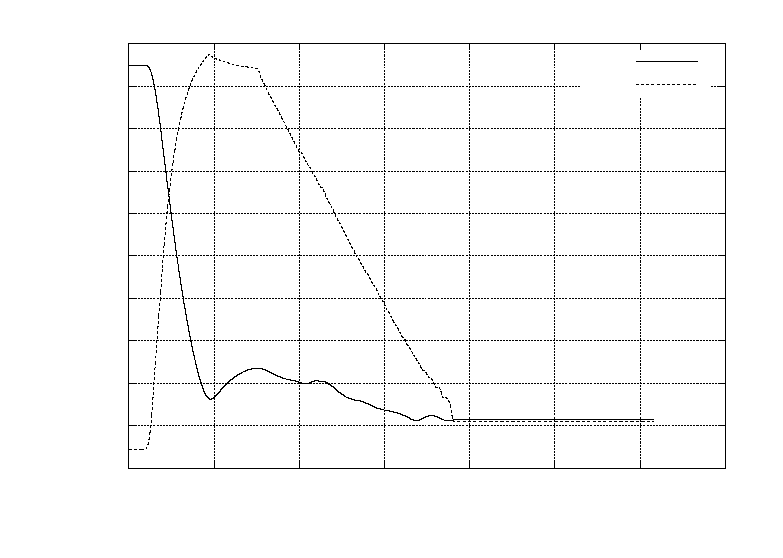
\includegraphics[width=0.49\textwidth]{static_smach_good_plot}}
        %\subfigure[Dynamic target interception.\label{f:fuz_dyn}]{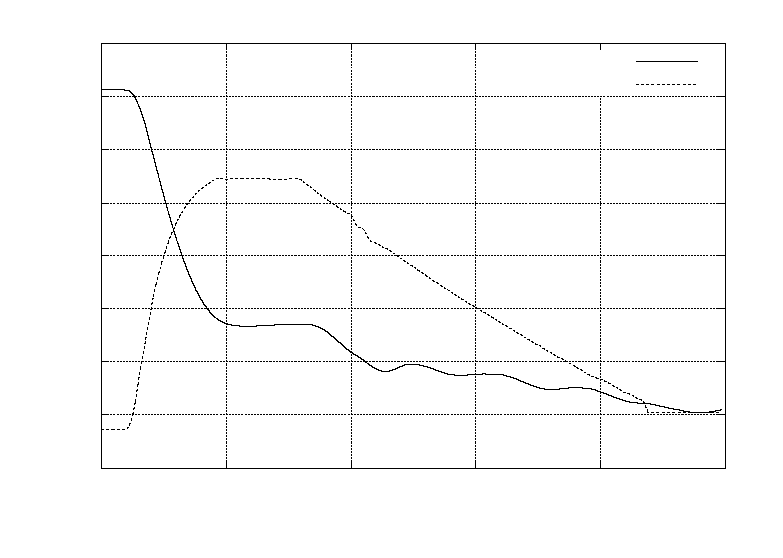
\includegraphics[width=0.49\textwidth]{moving_line_good_plot}}
    %\end{subfigmatrix}
    %\caption{Fuzzy controllers for static and dynamic landing}\label{f:fuzzy_lands}
%\end{figure}


\section{Conclusion}
It has been shown that a pure FLS controller is capable of controlling the position of a multirotor vehicle in
the task of precision landing on a small target. The small size of the platform presents a challenging
landing target; the FLS proved capable enough to overcome this challenge easily. The kalman filtering was an
integral component in providing the controller with a steady estimate of its error state. The components
chosen to accomplish this task are readily available in university laboratory environments and the physical
realization of this system was kept in the forefront of the design process. 

